% !TeX program = lualatex
% !TeX encoding = UTF-8
% ~~~~~~~~~~~~~~~~~~~~~~~~~~~~~~~~~~~~~~~~~~~~~~~~~~~~~~~~~~~~~~~~~~~~~~~~~~~~~~~~~~~~~~~~~~~~~~~~~~
% text font size setting
\PassOptionsToClass{
  fontsize=10pt,
  twocolumn,
  open=any, 
  titlepage=false, 
  chapterprefix=true
}{scrbook}

% =================== Kindle ===================================================
% \PassOptionsToPackage{
%     verbose=true,                  % displays the parameter results on the terminal
%     % a6paper,                     %
%     paperwidth = 260.0pt,          % 
%     paperheight = 364.0pt,         %
%     % landscape,                   %
%     includehead, includefoot,      % include the head and foot into total body
%     scale=1.0,                     %
%     nomarginpar,                   % shrinks spaces for marginal notes to 0pt,
%     left=3pt, right=3pt,           %
%     top=2pt, bottom=9pt,           %
%     headsep=2pt, headheight=10pt,  % 
%     showframe=false, nofoot,       %
%     % noheadfoot=true,             % 
%     heightrounded                  % better use it
%   }{geometry} 

% =================== ReMarkable 10,3" =========================================
% * h-part:(L,W,R)=(3.0pt, 443.55354pt, 3.0pt)
% * v-part:(T,H,B)=(2.0pt, 586.50787pt, 9.0pt)
% * \paperwidth=449.55354pt
% * \paperheight=597.50787pt

\PassOptionsToPackage{
    % showframe=true,
    verbose=true,                   % displays the parameter results on the terminal
    paperwidth  = 447pt,            % 158mm 
    paperheight = 595pt,            % 210mm 
    % landscape,                    %
    includehead, includefoot,       % include the head and foot into total body
    scale=1.0,                      %
    nomarginpar,                    % shrinks spaces for marginal notes to 0pt,
                                    % \marginparwidth=0pt and \marginparwidth=0pt
    left=3pt, right=3pt,            %
    top=2pt, bottom=11pt,           %
    headsep=2pt,                    %
    headheight=12pt,                % At least 11.0pt needed!! 
    showframe=true,                 %
    nofoot,                         % noheadfoot=true, 
    heightrounded,                  % better use it
  }{geometry} 
  
  
  % tyto příkazy se neprovedou protože jsou volány před \documentclass{}
  % Edit individual page dimension variables, using the \addtolength and \setlength commands: 
  % \setlength{\textwidth}{6.5in}
  % \addtolength{\voffset}{-5pt}
  
  % https://tex.stackexchange.com/questions/20965/one-inch-margins-and-the-geometry-package
  % \setlength{\oddsidemargin}{0pt}
  % \addtolength{\oddsidemargin}{-.875in}
  % \addtolength{\evensidemargin}{-.875in}
  % \addtolength{\topmargin}{-.875in}

\documentclass{scrbook}
  \usepackage{luadebug}
  \usepackage{luakoma}
  \usepackage{lualayout}
  \usepackage{luamath} 
  \usepackage{wikiWWWrefs}

\providecommand\DebugMode{true}
\providecommand\eBookMode{true}
%============================= L * U * A * K * I* N * G ============================================
% \listfiles
\setcounter{tocdepth}{\partnumdepth}      % depth of TOC

\begin{document}
% \shorthandoff{-}

\ifthenelse{\equal{\DebugMode}{true}}{
  % debug is true
  % !TeX encoding = UTF-8
% !TeX spellcheck = cs_CZ
% !TeX root = ../../tex/lauking.tex

%     Mathematical analysis
%---------------------------------------------------------------------------------------------------
% file MA.tex
% Notes>
% notes:
%~~~~~~~~~
% \label{mai:eq076}
% \label{mai:fig035}
% \label{mai:lemma003}
% \label{mai:exam034}
% \label{mai:tab}
% Mezery v matematickém režimu:
%~~~~~~~~~~~~~~~~~~~~~~~~~~~~~~
%\! záporná uzká mezera,   \; široká mezera,   \ mezislovní mezera,
%\, úzká mezera,   \: střední mezera,   \quad čtverčík,   \qquad dva čtverčíky
%---------------------------------------------------------------------------------------------------
\lstset{ %
  language=Matlab,                       % choose the language of the code
  basicstyle=\footnotesize,              % the size of the fonts that are used for the code
  backgroundcolor=\color{White},         % choose the background color.
  commentstyle=\color{help}\textit,
  keywordstyle=\color{keyword}\textbf,
  breaklines=true,                       % sets automatic line breaking
  breakatwhitespace=true,                % sets if automatic breaks should only happen at 
                                         % whitespace
  showspaces=false,                      % show spaces adding particular underscores
  showstringspaces=true,                 % underline spaces within strings
  showtabs=true,                         % show tabs within strings adding particular underscores
  frame=none,                            % adds a frame around the code - none, single
  tabsize=8,                             % sets default tabsize to 8 spaces
  captionpos=b,                          % sets the caption-position to bottom
  numbers=left,                          % where to put the line-numbers -none, left, right
  numberstyle=\footnotesize,             % the size of the fonts that are used for the line-numbers
  stepnumber=1,                          % the step between two line-numbers. If it's 1 each line
                                         % will be numbered
  xleftmargin=3em,                       % adjust left margin
}
%---------------------------------------------------------------------------------------------------
% Setting path to image 
  \graphicspath{{../src/MAI/img/}}
%---------------------------------------------------------------------------------------------------
\part{MA I}\label{part:MAI}
\parttoc

\ifthenelse{ \equal{\DebugMode}{true} }{
% Debug mode ON
% ~~~~~~~~~~~~~~~~~~~~~~~~~~~~~~~~~~~~~~~~~~~~~~~~

%  % !TeX spellcheck = cs_CZ
% Basis of Linear Algebra:
%{\tikzset{external/prefix={tikz/MAI/}}
% \tikzset{external/figure name/.add={ch02_}{}}
%---------------------------------------------------------------------------------------------------
% intro_linear_algebra.tex
%---------------------------------------------------------------------------------------------------
% ==================================================================================================
% In linear algebra, a basis is a set of linearly independent vectors that, in a
% linear combination, can represent every vector in a given vector space or free
% module, or, more simply put, which define a "coordinate system".[1] In more
% general terms, a basis is a linearly independent spanning set. 
% --------------------------------------------------------------------------------------------------
\chapter{Všemocná úměra aneb lineární algebra poprvé}\label{mai:IchapII}
\minitoc
  Tuto kapitolu bychom mohli opatřit podtitulem \emph{„To nejnutnější z lineární algebry“}. 
  Dovíme se v ní, co je třeba si představit pod pojmem \emph{„linearita“}, najdeme příklady 
  linearity v geometrii i v přírodovědě (fyzice, chemii, biologii) a formulujeme základní 
  poznatky týkající se řešení soustav lineárních rovnic. Do této oblasti patří i počítání s 
  vektory a maticemi - objekty, které jsou velmi vhodné k vyjádření fyzikálních veličin.
    
  \section{Lineární rovnice}\label{mai:IchapIIsecI}
    Co tedy znamená slovo \textbf{linearita}? Pochází z latiny, \emph{linea recta = přímka}, 
    česky bychom řekli \emph{přímá úměrnost} nebo jen jednoduše \emph{úměra}.
    
    Nejjednodušší příklady linearity patří do oblasti geometrie - vyjádření \emph{přímek} a 
    \emph{rovin}. Jistě si ze střední školy vzpomínáme, že body těchto útvarů popisujeme jejich 
    souřadnicemi na přímce \(\mathbb{R}\), v rovině \(\mathbb{R}^2\), v prostoru \(\mathbb{R}^3\). 
    Souřadnice bodu v rovině tedy tvoří \emph{uspořádanou dvojici} reálných čísel, v prostoru pak 
    \emph{uspořádanou trojici} reálných čísel. (Pozor, dvojice \([a, b]\) a \([b, a]\) představují 
    různé body.)

    %--Parametrické vyjádření přímky--------------------------------
      \input{../src/MAI/exam/exam001.tex}
    %---------------------------------------------------------------
    
    Vidíme, že kartézské souřadnice bodu na přímce se vůči souřadnicím bodu \(A\) mění přímo 
    úměrně v závislosti na hodnotě parametru \(t\), tj. závisí na jeho první mocnině. Příslušná 
    závislost se nazývá \textbf{lineární funkcí}.
    
    Obdobně zapíšeme parametrické vyjádření roviny v \(\mathbb{R}^3\):
    
    %--Parametrická vyjádření roviny--------------------------------
    \input{../src/MAI/exam/exam004.tex}
    %---------------------------------------------------------------
    
    Všimněme si nyní příkladů linearity z oblasti přírodovědy.
    
    %--Fyzika — Ohmův zákon-----------------------------------------
    \input{../src/MAI/exam/exam035.tex}
    %---------------------------------------------------------------

    %--Fyzika — speciální typy pohybů-------------------------------
    \input{../src/MAI/exam/exam036.tex}
    %---------------------------------------------------------------
    
  \subsection{Soustavy lineárních rovnic a jejich rychlé řešení}
    Příkladů linearity v přírodě bychom mohli nalézt bezpočet. Vraťme se však k matematice a k 
    problematice uvedené v názvu tohoto odstavce, k soustavám lineárních rovnic. Začněme 
    jednoduchou slovní úlohou ze základní školy:
    
    %--Jeníček a Mařenka kradli ježibabě perník---------------------
    \input{../src/MAI/exam/exam037.tex}
    %---------------------------------------------------------------
    
    O samotné řešení této jednoduché úlohy v tuto chvíli nejde. Pojmenujme si však vztahy, které 
    jsme pro neznámé hodnoty \(M\) a \(J\) ze zadání úlohy dostali. Neznámé vystupují v 
    rovnicích v první mocnině, tedy \emph{lineárně}. Máme \emph{soustavu dvou rovnic} o dvou 
    neznámých \(M\) a \(J\). Úvahu snadno zobecníme: Předpokládejme, že máme neznámé veličiny
    \begin{equation*}
      (x_1, x_2, \ldots, x_n)
    \end{equation*}
    a máme o nich \(m\) informací, které lze zapsat ve tvaru lineárních rovnic (neznámé budou v 
    těchto rovnicích vystupovat v první mocnině),
    \begin{align}
      a_{11}x_1 + a_{12}x_2 + \ldots + a_{1n}x_n &= b_1,     \nonumber           \\
      a_{21}x_1 + a_{22}x_2 + \ldots + a_{2n}x_n &= b_2,     \label{mai:eq002}   \\
      .......................................... &= \ldots   \nonumber           \\
      a_{m1}x_1 + a_{m2}x_2 + \ldots + a_{mn}x_n &= b_m,     \nonumber
    \end{align}
    Soustavu (\ref{mai:eq002}) nazýváme soustavou \(m\) lineárních rovnic o \(n\) neznámých. 
    Označme ji jako \(S\) a pod tímto označením se k ní budeme vracet. Soubory reálných čísel 
    \((a_{ij})\) a \((b_i)\), kde \(1 < i < m\), \(1 \leq j < n\), jsou zadány. Lze je uspořádat 
    do takzvaných \textbf{matic}:
    \begin{equation}\label{mai:eq003}
      \matr{A} =
        \begin{pmatrix}
          a_{11} & a_{12} & \ldots & a_{1n} \\
          a_{21} & a_{22} & \ldots & a_{2n} \\
          \ldots & \ldots & \ldots & \ldots \\
          a_{m1} & a_{m2} & \ldots & a_{mn}          
        \end{pmatrix},
        \overline{\matr{B}} =
        \begin{pmatrix}
          b_1     \\
          b_2     \\
          \ldots  \\
          b_m 
        \end{pmatrix}
    \end{equation}
    
    Matice \(\matr{A}\) je typu \(m/n\), má \(m\) řádků a \(n\) sloupců, \(i\) je řádkový index a 
    \(j\) je sloupcový index. Matice \(\overline{\matr{B}}\) je typu \(m/1\) (\(m\) řádků a jeden 
    sloupec), hovoříme také o sloupcové matici. Soustavu \(S\) můžeme zapsat zkráceně pomocí 
    maticového násobení (podrobněji viz později odstavec \ref{mai:IchapIIsecIII}):
    \begin{equation*}
      \matr{A} \cdot \matr{X} = \matr{B}, \qquad \text{nebo}
    \end{equation*}  
    \begin{equation}\label{mai:eq004}
        \begin{pmatrix}
          a_{11} & a_{12} & \ldots & a_{1n} \\
          a_{21} & a_{22} & \ldots & a_{2n} \\
          \ldots & \ldots & \ldots & \ldots \\
          a_{m1} & a_{m2} & \ldots & a_{mn}
        \end{pmatrix}
        \cdot
        \begin{pmatrix}
          x_1     \\
          x_2     \\
          \ldots  \\
          x_m 
       \end{pmatrix}
        =
       \begin{pmatrix}
            b_1     \\
            b_2     \\
            \ldots  \\
            b_m 
          \end{pmatrix}
    \end{equation}
    V tuto chvíli vysvětlíme podstatu maticového násobení jen technicky: Násobit mezi sebou  můžeme matici 
    \(\matr{A} = (a_{ij})\) typu \(m/n\) (levý činitel) a matici \(\matr{A} = (c_{jk})\) typu 
    \(n/p\) (pravý činitel, činitele nelze zaměňovat). Výsledkem je matice \(\matr{A} = (d_{ik})\) 
    typu \(m/p\), jejíž prvky se počítají podle předpisu
    \begin{equation}\label{mai:eq005}
      d_{ik} = \sum_{j=1}^{n} a_{ij}\cdot c_{jk}.
    \end{equation}
    
    Z tohoto obecného předpisu vidíme, že levé strany soustavy \(S\) lze interpretovat ve tvaru 
    součinu matice \(A\) typu \(m/n\) s maticí neznámých typu \((n/1)\), výsledkem je matice 
    pravých stran \(\overline{\matr{B}}\), která je typu \(m/1\). Matice \(\matr{A}\) se nazývá 
    \textbf{maticí soustavy}. Matice, která vznikne jejím \emph{rozšířením} o sloupec pravých 
    stran, tj.
    \begin{equation}\label{mai:eq006}
      \matr{B} = (\matr{A}|\overline{\matr{B}}) =
      \left(
        \begin{array}{cccc|c}
          a_{11} & a_{12} & \ldots & a_{1n} & b_1    \\
          a_{21} & a_{22} & \ldots & a_{2n} & b_2    \\
          \ldots & \ldots & \ldots & \ldots & \ldots \\
          a_{m1} & a_{m2} & \ldots & a_{mn} & b_m
        \end{array}
      \right)
    \end{equation}
    je pak \textbf{rozšířenou maticí soustavy}. Je-li sloupec pravých stran soustavy tvořen 
    samými nulami, nazývá se soustava \textbf{homogenní}, v opačném případě \textbf{nehomogenní}. 
    Řešením soustavy \(S\) nazýváme každou \(n\)-tici \((x_i, x_2,\ldots, x_n)\), která soustavu 
    \(S\) splňuje. Cílem je najít všechna řešení soustavy \(S\). Abychom řešení nalezli, musíme 
    soustavu upravovat, zjednodušovat. Prováděné úpravy mají vést k jednodušší, avšak 
    ekvivalentní soustavě rovnic, tj. takové, která má naprosto stejný soubor všech řešení jako 
    soustava původní. Takové úpravy nazýváme \textbf{ekvivalentními}. Dvě základní, pomocí nichž 
    lze uskutečnit všechny ostatní, jsou
    \begin{itemize}\addtolength{\itemsep}{-0.5\baselineskip}
      \item vynásobení libovolné, například \(i\)-té, rovnice libovolným \emph{nenulovým} číslem,
      \item přičtení \(i\)-té rovnice vynásobené libovolným číslem k \(l\)-té rovnici.
    \end{itemize} 
    V soustavě lze samozřejmě také měnit pořadí rovnic. Tato úprava je rovněž ekvivalentní. 
    Nevypisujeme ji však zvlášť proto, že ji lze realizovat pomocí vhodně zvolené posloupnosti 
    základních dvou úprav.
    
    Abychom nemuseli soustavu stále opisovat i s neznámými, provádíme obvykle ekvivalentní 
    úpravy jen s maticí \(\matr{B} = (\matr{A}|\overline{\matr{B}})\) (každý řádek této matice 
    představuje jednu rovnici soustavy \(S\)). Může se stát, že soustava má právě \emph{jedno 
    řešení}, jako tomu bylo v  úloze o Mařence a Jeníčkovi. Také nemusí mít \emph{řešení žádné}, 
    jako například soustava \(x + y = 0\), \(x + y = 1\) (součet dvou čísel nemůže nabývat současně 
    dvou různých hodnot). A třeba má také řešení \emph{nekonečně mnoho} (řešením soustavy jedné 
    rovnice o dvou neznámých \(x + y = 1\) jsou všechny dvojice tvaru \((x, 1 - x)\), kde \(x\) je 
    libovolné). A může mít soustava \(S\) třeba právě dvě řešení? Prostřednictvím následujícího 
    příkladu ukážeme metodu, která vede velmi rychle k nalezení všech řešení a umožňuje také 
    vyslovit obecné závěry o jejich vlastnostech a počtu. Jedná se o \textbf{Gaussovu eliminační 
    metodu}.

    %Gaussova eliminační metoda-------------------------------------
    \input{../src/MAI/exam/exam038.tex}
    %---------------------------------------------------------------

    Na základě výsledného tvaru matice soustavy a rozšířené matice soustavy získané ekvivalentními 
    úpravami soustavy \(S\) nyní formulujeme obecné kritérium pro to, aby soustava S měla
    vůbec nějaké řešení. Matice \(\matr{A}\) i \(\matr{B}\) se po provedení ekvivalentních úprav 
    dostaly do velmi jednoduchého tvaru, který připomíná schodiště obrácené „vzhůru nohama“, 
    odmyslíme-li si nuly v levé části jednotlivých řádků (následující zápis pouze usnadňuje 
    názornou představu, znak ekvivalence již psát nemůžeme):
    \begin{equation*}
      \matr{A} \ldots
      \left(
        \begin{array}{rrrrr}
                1 &  2 & -1 & 1      & -5     \\
                  &    &    & 1      & -1     \\
 
        \end{array}
      \right),
      \qquad
      \matr{B} \ldots
      \left(
        \begin{array}{rrrrr|r}
                1 &  2 & -1 & 1      & -5 &  0    \\
                  &    &    & 1      & -1 & -1    \\
        \end{array}
      \right).
    \end{equation*}
    
    Všimněme si, že „schodiště“ jsou nepravidelná, pokud jde o šířku schodů, výška všech schodů
    je však stejná - jeden řádek. Tímto způsobem je dán \emph{schodovitý tvar} matice \(\matr{A}\), 
    resp. \(\matr{B}\). Úzce s ním souvisí důležitá charakteristika matice, která je nezávislá jak 
    na provedených úpravách tak na výsledném schodovitém tvaru. Je to hodnost matice, definovaná 
    takto:
    
    \textbf{Hodnost} matice je počet nenulových řádků jejího schodovitého tvaru.
    
    V našem příkladu je hodnost matice \(A\) soustavy \(S\) rovna dvěma, hodnost matice rozšířené 
    \(\matr{B}\) je rovna třem. Píšeme
    \begin{equation*}
      h(\matr{A}) = 2,\qquad h(\matr{B}) = 3.
    \end{equation*}
    
    \begin{note}
      Lze získat schodovitý tvar různými posloupnostmi ekvivalentních úprav je zřejmé. Uvědomme si 
      však, že ani výsledný schodovitý tvar není určen jednoznačně - stačí třeba vynásobit některý 
      řádek dvěma a výsledná matice ekvivalentní s původní je rovněž schodovitá. Poněvadž má matice 
      \(\matr{B}\) o jeden sloupec více než matice \(\matr{A}\), platí vždy \(h(\matr{A}) < 
      h(\matr{B})\). V případě \(h(\matr{A}) < h(\matr{B})\) pak \(h(\matr{A}) = h(\matr{B}) - 1\). 
      Jak názorně ukazuje náš příklad, má pro \(h(\matr{A}) < h(\matr{B})\) některá z rovnic 
      ekvivalentní soustavy tvar \(0 = 1\), soustava tedy nemá řešení. Můžeme tak formulovat 
      kritérium (podmínku nutnou a postačující) řešitelnosti soustavy lineárních rovnic.
    \end{note}
    
    \begin{lemma}\label{mai:lemma001}
      (\textbf{Frobeniova}): Soustava lineárních rovnic má řešení právě tehdy, je-li hodnost její 
      matice rovna hodnosti matice rozšířené.
    \end{lemma}
    
    Ihned vidíme, že homogenní soustava má podle této věty řešení vždy, neboť poslední sloupec její 
    rozšířené matice je složen ze samých nul. Skutečně, jedním ze souboru řešení každé
    homogenní soustavy je \(n\)-tice
    \begin{equation*}
      (x_1, x_2, \ldots, x_n) = (0, 0, \ldots, 0),
    \end{equation*}
    zvaná \textbf{triviální řešení}.
    
    Nyní se vraťme k otázce, jak zjistit, kolik řešení má daná soustava, a jak je všechna popsat.
    Poslouží nám příklad \ref{mai:exam038} v mírné obměně spočívající v záměně koeficientu \(b_3\) 
    z hodnoty \num{6} na \num{-6}.
    
    %Ještě jednou Gaussova eliminační metoda------------------------
    \input{../src/MAI/exam/exam039.tex}
    %---------------------------------------------------------------
    
    Soubor řešení ve tvaru (\ref{mai:eq040}) se nazývá obecným řešením soustavy. Jeho jednotlivé 
    prvky, jednotlivá konkrétní řešení soustavy, jsou dány volbou volných neznámých \(x_2\), 
    \(x_3\) a \(x_5\). Také z příkladu \ref{mai:exam039} lze učinit obecný závěr:
    
    \begin{lemma}\label{mai:lemma002}
      Nechť pro soustavu \(m\) lineárních rovnic o \(n\) neznámých platí \(h(\matr{A}) = 
      h(\matr{B}) = h\). Pak její obecné řešení závisí (lineárně) na \(d = n - h\) volných 
      neznámých.
    \end{lemma}
    
    Číslo \(d\) se nazývá \textbf{dimenze prostoru řešení soustavy}. Tento pojem ještě podrobněji 
    vysvětlíme později.
    
    Nyní již snadno zodpovíme otázku, čím je dána mohutnost souboru řešení soustavy lineárních 
    rovnic, tj. kolik má taková soustava řešení. Možnosti jsou pouze:
    \begin{itemize}
      \item žádné řešení - pro \(h(\matr{A}) \neq h(\matr{B})\),
      \item právě jedno řešení - pro \(h = h(\matr{A}) = h(\matr{B})\) a současně \(h = n\), takže 
            nezbývá žádná volná neznámá,
      \item nekonečně mnoho řešení - pro \(h = h(\matr{A}) = h(\matr{B})\) a současně \(h < n\),  
            kdy máme k dispozici \(d = n - h\) volných neznámých.
    \end{itemize}    
    Že by tedy třeba měla soustava právě dvě, tři či osmnáct řešení není možné.
    
    Jakési zvláštní postavení můžeme přisoudit homogenním soustavám. Ty mají, jak jsme se
    již přesvědčili, řešení vždy, alespoň to triviální, složené ze samých nul. Zajímejme se o 
    situaci, kdy má homogenní soustava i jiná, netriviální, řešení. U homogenní soustavy je 
    hodnost její matice vždy shodná s hodností matice rozšířené, \(h = h(\matr{A}) = h(\matr{B})\). 
    Je-li navíc \(h = n\), má podle obecného tvrzení \ref{mai:lemma002} soustava právě jedno 
    řešení, jímž nutně je řešení triviální. V opačném případě, tj. pro \(h < n\), máme opět k 
    dispozici \(d = n - h\) volných neznámých, a tedy nekonečně mnoho netriviálních řešení. 
    Všimněme si ještě jedné zajímavosti u homogenní soustavy. Jsou-li dvě \(n\)-tice čísel \(X = 
    (x_1, x_2, \ldots, x_n)\) a \(\overline{X} = (\overline{x}_1, \overline{x}_2, \ldots, 
    \overline{x}_n)\) jejím řešením, pak také \(n\)-tice vytvořená jako jejich lineární kombinace
    \begin{equation*}
      \alpha\cdot X + \overline{\alpha}\cdot\overline{X} = 
        (\alpha x_1, \alpha x_2, \ldots, \alpha x_n) + 
        (\overline{\alpha}\,\overline{x}_1, 
        \overline{\alpha}\,\overline{x}_2, \ldots, 
        \overline{\alpha}\,\overline{x}_n)
    \end{equation*}
    kde \(\alpha\) a \(\overline{\alpha}\) jsou libovolná čísla, je \emph{řešením soustavy}. 
    Možnost tohoto „lineárního kombinování“ připadá samozřejmě v úvahu pro libovolný počet 
    libovolných řešení soustavy. Fyzik by řekl, že soustava vyhovuje principu superpozice. 
    Soustava nehomogenní tu to vlastnost nemá „vinou“ nenulového sloupce 
    pravých stran.
    
    \subsection{Přímky a roviny - lineární geometrické útvary}
      Vraťme se ještě na chvíli k linearitě v geometrii a všimněme si problematiky vzájemné polohy
      přímek a rovin. Procvičíme si na ní mimo jiné i řešení soustav lineárních rovnic. V odstavci 
      \ref{mai:IchapIIsecI} jsme odvodili parametrické vyjádření přímky a roviny v trojrozměrném 
      prostoru. Nyní se pokusíme z těchto vyjádření vyloučit parametry a získat obecné rovnice 
      přímky a roviny, které již budou obsahovat pouze kartézské souřadnice bodů ležících v 
      příslušné přímce či rovině. Začněme případem roviny.

      %--Obecná rovnice roviny----------------------------------------
      \input{../src/MAI/exam/exam040.tex}
      %---------------------------------------------------------------

      %--Obecná rovnice přímky----------------------------------------
      \input{../src/MAI/exam/exam041.tex}
      %---------------------------------------------------------------
      
      %--Vektor rovnoběžný s rovinou----------------------------------
      \input{../src/MAI/exam/exam042.tex}
      %---------------------------------------------------------------
  
      Máme připraveno vše pro řešení otázky vzájemné polohy přímek a rovin.

      %--Vzájemná poloha tří rovin------------------------------------
      \input{../src/MAI/exam/exam043.tex}
      %---------------------------------------------------------------

      %--Vzájemná poloha dvou přímek----------------------------------
      \input{../src/MAI/exam/exam044.tex}
      %---------------------------------------------------------------
      
      %--Vzájemná poloha přímky a roviny------------------------------
      \input{../src/MAI/exam/exam045.tex}
      %---------------------------------------------------------------
      
%--------------------------------------------------------------------------------------------------
  \section{Počítání s čísly}\label{mai:IchapIIsecII}
    Někdo se jistě pozastaví nad tím, že jej chceme učit počítání s čísly. To přece každý umí
    už od základní školy! Jenže základní a do značné míry i střední škola nás učí počítat jen
    s určitým typem čísel - s čísly reálnými. Pravidla pro počítání s nimi se pro „běžné uživatele“
    stala natolik rutinní záležitostí, že už o nich vůbec nepřemýšlejí, nehledají v nich 
    zákonitosti, a kdybychom se jich zeptali, kde se tato pravidla vzala, pravděpodobně budou s 
    odpovědí velmi váhat. Pravidla pro jakékoli početní operace totiž skutečně nelze z ničeho 
    odvodit, ta je třeba definovat, samozřejmě tak, aby měla rozumné praktické vlastnosti.
    
    \subsection{Reálná čísla}
      U reálných čísel se opravdu dlouho nezdržíme, s těmi snad opravdu každý umí počítat. Všimneme 
      si jen trochu podrobněji struktury množiny všech reálných čísel, \textbf{reálné osy} 
      \(\mathbb{R}\). Zobrazit  reálná čísla na reálné ose, tedy na přímce, umíme proto, že na 
      množině reálných čísel je definováno \textbf{úplné uspořádání} „< “:
      \begin{itemize}
        \item Je-li současně \(a ≤ b\) a \(b ≤ a\), pak \(a = b\) 
              pro všechna \(a, b\in\mathbb{R}\ldots\) \textbf{antisymetrie},
        \item je-li současně\( a ≤ b\) a \(b ≤ c\), pak \(a ≤ c\) 
              pro všechna \(a,b,c\in\mathbb{R}\ldots\) \textbf{tranzitivita},
        \item \(a ≤ a\) pro všechna \(a\in\mathbb{R}\ldots\) \textbf{reflexivita},
        \item platí \(a ≤ b\) nebo \(b ≤ a\) pro všechna \(a, b \in\mathbb{R}\ldots\) 
              \textbf{úplnost}.
      \end{itemize}
      Pro každá dvě čísla \(a\) a \(b\) tedy dokážeme rozhodnout, zda jsou shodná (\(a = b\)), nebo 
      zda \(a\) je menší (\(a < b\)) či větší (\(a > b\)) než \(b\). Platí:
      \begin{itemize}
        \item Je-li současně \(a < b\) a \(c < d\), pak \(a + c < b + d\),
        \item je-li současně \(a < b\) a \(c > 0\), pak \(ac < bc\),
        \item je-li současně \(a < b\) a \(c < 0\), pak \(ac > bc\).
      \end{itemize}
      
      Množina reálných čísel obsahuje tyto důležité podmnožiny:
      \begin{itemize}
        \item Množinu přirozených čísel \(\mathbb{N} = \{1, 2, \ldots, n, \ldots\}\). Platí princip 
              \textbf{úplné indukce}: Je-li \(\mathbb{M} \subseteq \mathbb{N}\) nějaká množina 
              přirozených čísel, která obsahuje číslo \num{1} a která současně s každým číslem 
              \(n\) obsahuje i \(n + 1\), pak \(\mathbb{M} = \mathbb{N}\).
        \item Množinu celých čísel \(\mathbb{Z} = \{\ldots, -n, \ldots, -2, -1, 0, 1, 2, \ldots, m, 
              \ldots\}\).
        \item Množinu racionálních čísel \(\mathbb{Q}\) (zlomky). Racionální čísla lze vyjádřit 
              konečnými desetinnými zlomky (například \(p/q = 1/4 = \num{0.25}\)), nebo nekonečnými 
              periodickými desetinnými zlomky (například \(p/q = 4/3 = 1,33\ldots33\ldots = 
              1,\overline{3}\), \(p/q = 24/11 = 2,1818\ldots1818\ldots = 2,\overline{18}\)).
        \item Množinu iracionálních čísel, tj. čísel, která nejsou racionální. Iracionálními čísly 
              jsou neracionální řešení algebraických rovnic, například \(x^2 - 2 = 0 \Rightarrow x 
              = \sqrt{2}\), nebo \(x = - \sqrt{2}\) (čísla algebraická), a čísla typu \(\pi\), 
              \(e\), atd. (čísla transcendentní). Iracionální čísla jsou vyjádřena       
              nekonečnými neperiodickými desetinnými zlomky, např. 
              \(e = \num{2.718281828459545}\ldots\). Mezi každými dvěma reálnými čísly leží 
              nekonečně mnoho čísel racionálních i nekonečně mnoho čísel iracionálních.
      \end{itemize}
      
      Pro počítání s reálnými čísly jsou zavedeny základní operace, s nimiž umíme pracovat na
      základě zkušenosti, sčítání \(a + b\), odčítání \(a - b\), násobení \(a \cdot b\), resp. 
      \(ab\) a dělení \(a : b\). Ve skutečnosti jsou potřeba jen dvě, neboť odčítání je odvozeno 
      pomocí sčítání a dělení pomocí násobení. Uvědomili jste si někdy základní vlastnosti těchto 
      operací? Možná ne, ale pracujeme s nimi zcela samozřejmě:
%      \begin{table}[ht!]
%        \centering
%%        \begin{tabular}{l>{\centering}m{5cm}} %{@{}ll@{}}
%%\begin{tabular}{| c | >{\centering}m{5cm} |}
%%        \toprule
%%          \(a + b = b + a\)            & komutativní zákon pro součet  \\ %\midrule
%%          \((a + b) + c = a + (b +c)\) & asociativní zákon pro součet  \\
%%          \(a + 0 = 0 + a = a\)        & existence univerzálního neutrálního prvku \num{0}  \\
%%          \(a + (—a) = (—a) + a = 0\)  & existence právě jednoho opačného prvku k číslu \(a\)   \\ 
%%          \(ab = ba\)                  & komutativní zákon pro součin \\
%%          \(a(bc) — (ab)c\)            & asociativní zákon pro součin \\
%%          \(a(b + c) = ab + ac\)       & 1. distributivní zákon  \\
%%          \((b+ c)a — ba + ca\)        & 2. distributivní zákon \\
%%          \(a \cdot 1 = 1 \cdot a\)    & existence univerzálního jednotkového prvku 1 \\
%%          \(aa^{-1} = a^{-1}a\)        & existence právě jednoho inverzního prvku k číslu \(a\), pokud 
%%                                         \(a\neq 0\)\\
%%          \(ab = 0 \Leftrightarrow a = 0\) nebo \(b = 0\)) & neexistence dělitelů nuly \\
%%         \bottomrule
%%        \end{tabular}
%%\begin{tabular}{| c | >{\centering}m{5cm} |}
%% Bcd & A long cell with text that wraps around and is centered
%%\end{tabular}
%      \end{table}
      Odčítání a dělení:
      \begin{equation*}
        a — b = a + (—b), a:b = ab^{-1}, \qquad\text{pokud } b\neq0.
      \end{equation*}
      
    \subsection{Komplexní čísla}
      Komplexními čísly rozumíme uspořádané dvojice \([x, y]\) čísel reálných, pro které zavedeme 
      určité operace. Uspořádaností dvojice zde myslíme to, že jedno z čísel (v našem zápisu \(x\)) 
      je umístěno na první pozici dvojice a představuje reálnou část čísla \(z\), \(x = 
      \operatorname{Re}(z)\), druhé (v našem zápisu \(y\)) je na druhé pozici a je imaginární částí 
      čísla \(z\), \(y = \operatorname{Im}(z)\). Je tedy obecně  \( [x, y] ≠ [y, x]\). Množinu
    \subsection{Cvičení}
%--------------------------------------------------------------------------------------------------
  \section{Počítání s maticemi}\label{mai:IchapIIsecIII}
    \subsection{Základní operace s maticemi a hodnost matic}\label{mai:IchapIIsecIIIsubI}
    \subsection{Hodnost matic}\label{mai:IchapIIsecIIIsubII}
    \subsection{Násobení  matic}\label{mai:IchapIIsecIIIsubIII}
    \subsection{Čtvercová matice}\label{mai:IchapIIsecIIIsubIV}
    Algebra matic, tedy počítání s nimi, je v praxi zase jen počítání s čísly, samozřejmě podle
    specifických pravidel. S maticemi jsme se již setkali v odstavci \ref{mai:IchapIIsecI}, kde 
    jsme jich využili jako vhodné „pomůcky“ při řešení soustav rovnic. Nyní posuneme naše 
    znalosti o nich na poněkud vyšší úroveň. Zavedeme na množině matic \emph{algebraickou 
    strukturu}, která nám umožní s nimi počítat nezávisle na jejich vztahu k nějakým praktickým 
    aplikacím. Víme již, že maticí typu \(m/n\) (též obdélníková matice) rozumíme soubor reálných, 
    popřípadě i komplexních čísel uspořádaných do \(m\) řádků a \(n\) sloupců:
    
    \begin{definition}\label{def_matice}
      Nechť \(m, n\) jsou přirozená čísla. Jestliže každé uspořádané dvojici \((m,n)\in 
      \{1,2,\ldots,m\}\times \{1,2,\ldots,m\}\) přiřadíme prvek \(a_{i,j}\in\mathbb{R}\) obdržíme 
      reálnou \href{http://cs.wikipedia.org/wiki/Matice}{matici} typu \(m,n\) nad \(\mathbb{R}\). 
      
      Matici zapisujeme jako
      \begin{equation}\label{matice_zapis}
        \matr{A} = \left(a_{ij}\right) =\left(
                                      \begin{array}{ccc}
                                        a_{11} & \ldots & a_{1n} \\
                                        \vdots & \ddots & \vdots \\
                                        a_{m1} & \ldots & a_{nn}
                                      \end{array}
                                 \right)
      \end{equation}
      která má právě \(mn\) prvků \((a_{ij})\) uspořádaných do \(m\) řádků a \(n\) sloupců. Stručně 
      píšeme \(\matr{A} = (a_{ij})\)
    \end{definition}

    Prvky matice jsou označeny indexy udávajícími \textbf{řádek} a \textbf{sloupec}, v nichž se 
    prvek nalézá. Prvek v \(i\)-tém řádku a \(j\)-tém sloupci matice \(\matr{A}\) se obvykle značí 
    \(a_{ij}\). Potom \(i\)-tý řádek matice  obsahuje vodorovnou \(n\)-tici prvků \(a_{i1}, 
    a_{i2}, \ldots,a_{in} \), kde \(i=  1,2,\ldots,m\) a \(j\)-tý sloupec matice obsahuje svislou 
    matici čísel \(a_{1j},a_{2j},\ldots,a_{mj}\), kde \(j = 1,2,\ldots,n\). Pro \(m = n\) se matice 
    nazývá čtvercová n-tého řádu. 
      
    %---------------------------------------------------------------
    \input{../src/MAI/exam/exam033.tex}
    %---------------------------------------------------------------

    V tabulce \ref{LA:tab_basic_matrix} jsou uvedeny nejčastější typy matic, které se v algebře 
    často vyskytují. Jsou to například matice řádkové, sloupcové, diagonální\footnote{Prvky 
    \(a_{ii}\) kde \(i=1,2,\ldots,\min(m,n)\) tvoří hlavní diagonálu. Matice \(\matr{D}\) je 
    typu \(m,m\), obecně může mít diagonální matice buď ještě další sloupce, v nichž budou samé 
    nuly, anebo další řádky, v nichž budou opět samé nuly.}, jednotkové\footnote{Jestliže \(m = 
    n\), pak mluvíme o čtvercové matici řádu \(m\).}, nulové, transponované a symetrické.

    \begin{table}[!ht]
        \centering
        \renewcommand{\arraystretch}{1.8}   % for the vertical padding
          \begin{tabular}{|l||c@{}|}              
            \hline 
            \textbf{Matice}                    & \textbf{Zápis} \\ \hline\hline
            \ttfamily řádková   \(\matr{A}\) &  \(a_1,a_2,\ldots,a_n \)\\
            \ttfamily sloupcová \(\matr{B}\) & 
              \(\begin{pmatrix}
                a_1     \\
                a_2     \\
                \vdots  \\
                a_n
              \end{pmatrix}\)                       \\
            \ttfamily diagonální \(\matr{C}\) & 
              \(\begin{pmatrix}
                 a_{11} &    0   & \ldots &   0     \\
                    0   & a_{22} & \ldots &   0     \\
                 \vdots & \vdots & \ddots & \vdots  \\
                    0   &   0    & \ldots & a_{mm}
              \end{pmatrix}\)                       \\
            \ttfamily jednotková \(\matr{I}\) &
              \(\begin{pmatrix}
                   1    &    0   & \ldots &   0    \\
                   0    &    1   & \ldots &   0    \\
                 \vdots & \vdots & \ddots & \vdots \\
                    0   &   0    & \ldots & 1
              \end{pmatrix}\)                      \\
            \ttfamily nulová \(\matr{0}\) & \((a_{ij}),\quad a_{ij} = 0\,\forall\,i, j\) \\
            \ttfamily transponovaná \(\matr{D^T}\) &
              \(\begin{pmatrix}
                a_{11} & a_{21} & \ldots &  a_{m1}\\
                a_{12} & a_{22} & \ldots &  a_{m2}\\
                \vdots & \vdots & \ddots & \vdots \\
                a_{1n} & a_{2n} & \ldots & a_{mn}
              \end{pmatrix}\)    \\
            \ttfamily symetrická \(\matr{S}\) 
            & \((a_{ij}),\quad a_{ij}= a_{ji}\,\forall\,i,j\) \\ \hline
          \end{tabular}
        \caption{Speciální typy matic}\label{LA:tab_basic_matrix}
    \end{table}
  
  
    Matice téhož typu \((m,n)\) nad \(\mathbb{R}\) budeme značit \(\mathbb{R}_{m,n}\).
      
    \subsection{Základní operace s maticemi a hodnost matic}
      
      
    \begin{definition} 
      Součinem matice \(A \in \mathbb{R}_{mn}\) a matice \(B \in \mathbb{R}_{np}\), v uvedeném
      pořadí, je matice \(C \in \mathbb{R}_{mp}\) pro kterou platí:
      \begin{align*}
             C &= AB; \quad C = (cij); \\
             \shortintertext{kde}
        c_{ij} &= \sum_n^{k=1}{a_{ik}b_{kj}};\quad
                   i = 1,\ldots,m; \, j = 1,\ldots,p.
      \end{align*} 
    \end{definition}
    Součin matic \(A\) a \(B\) je definován právě tehdy, když počet sloupců matice \(A\) je roven 
    počtu řádků matice \(B\). Obrázek \ref{LA:fig_LA001a} demonstruje jakým způsobem se 
    dostane prvek, který je ve výsledné matici třeba ve druhém řádku a druhém sloupci, násobením 
    druhého řádku levé matice s druhým sloupcem pravé ze zadaných matic. Stejným způsobem získáme 
    hodnotu prvku \(c_{ij}\) (viz \ref{LA:fig_LA001b}).
    %----------------------------------
    \begin{figure}[ht!]
      \centering  
      \begin{tabular}{cc}
        \subfloat[1. krok]{\label{LA:fig_LA001a}
          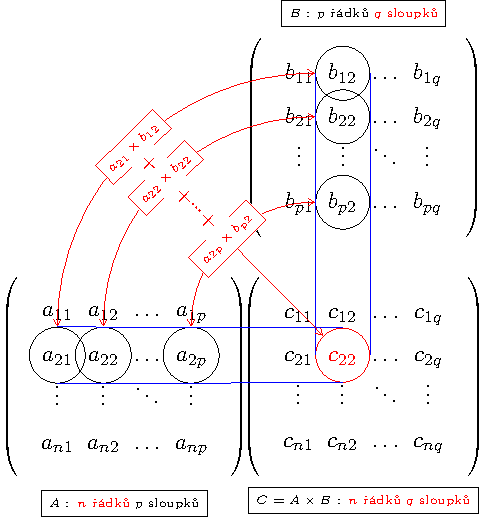
\includegraphics[width=0.45\linewidth]{mai_fig023a}}               &
        \subfloat[2. krok]{\label{LA:fig_LA001b}
          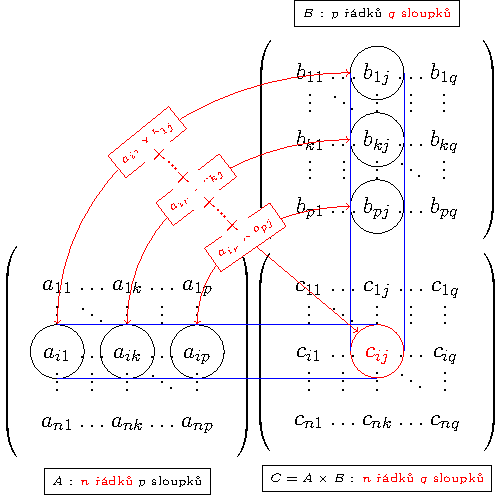
\includegraphics[width=0.45\linewidth]{mai_fig023b}} 
      \end{tabular}
      \caption{Postup při maticovém násobení}
    \end{figure}
  

      
      \begin{definition}\label{rovnost_matic}
       (Rovnost matic):  Matice \(\matr{A} = \left(a_{ij}\right)\) je rovna matici \(\matr{B}=
       \left(b_{kl}\right)\), jsou-li matice stejného typu a stejnolehlé prvky se sobě
       \textbf{rovnají}, tj. \(\matr{A} \in \mathbb{R}_{m,n}, \matr{B}\in\mathbb{R}_{m,n}, 
       a_{ij} = b_{ij}, \forall i\in\lbrace1,2,\ldots,m\rbrace, \forall j\in\lbrace1,2, \ldots 
       ,n\rbrace\).
      \end{definition}
      
%--------------------------------------------------------------------------------------------------
  \section{Počítání s vektory}\label{mai:IchapIIsecIV}
    \textbf{Vektory} budeme nazývat matice typu \(1/n\) a značit je
    \begin{equation*}
      \vec{u} = (u_1, u_2, \ldots, u_n).
    \end{equation*}
    Takže počítat s nimi již umíme! (V zápisu složek vektoru je vynechán řádkový index. V případě 
    matice s jedním řádkem, takzvané \emph{řádkové matice}, je totiž zbytečný.) Číslům \(u_1\) až 
    \(u_n\) budeme pro tuto chvíli říkat \emph{složky vektoru} \(\vec{u}\). Za chvíli tento pojem 
    ještě upřesníme. Celou řadu pojmů, s nimiž jsme se seznámili při počítání s maticemi, můžeme 
    pro vektory přímo použít. Namísto značení \(\mathcal{M} (1/n)\) budeme pro prostor vektorů 
    používat symbol \((\mathbb{R}^n)\) nebo \(\mathbb{C}^n\) (obvyklý symbol pro množinu 
    uspořádaných \(n\)-tic reálných nebo komplexních čísel).
    
    \subsection{Součiny vektorů}
      Kromě základních operací s vektory, tj. sčítání vektorů a násobení vektoru skalárem, se 
      často používají další operace, které obohacují \emph{strukturu vektorového prostoru}. 
      Zůstaneme u vektorů v trojrozměrném prostoru \(\mathbb{R}^3\) a definujeme si skalární, 
      vektorový a smíšený součin vektorů. Skalární součin vektorů definujeme prostřednictvím 
      geometrické definice jako zobrazení, které uspořádané dvojici vektorů (volných vektorů nebo 
      jejich libovolných umístění) přiřazuje reálný číslo podle předpisu
      \begin{equation}\label{mai:eq038}
        \vec{u}\vec{v} = \abs{\vec{u}}\cdot\abs{\vec{v}}\cos\varphi,
      \end{equation}
      kde \(\varphi = \sphericalangle(\vec{u},\vec{v})\) je velikost minimálního z obou úhlů mezi 
      vektory\(\vec{u},\vec{v}\).

    %---------------------------------------------------------------
    \input{../src/MAI/exam/exam034.tex}
    %---------------------------------------------------------------
    
    Shrneme nyní vlastnosti skalárního součinu. Dokázat bychom je mohli, i když by to mohlo být i 
    velmi pracné, užitím znalostí z goniometrie. Zkuste to alespoň pro jednu z nich! Třeba se    
    vám podaří zvolit si tu nejjednodušší.

%} % tikzset
%---------------------------------------------------------------------------------------------------
\printbibliography[title={Seznam literatury}, heading=subbibliography]
\addcontentsline{toc}{section}{Seznam literatury}
%  % !TeX spellcheck = cs_CZ
% Differential calculus
%{\tikzset{external/prefix={tikz/MAI/}}
% \tikzset{external/figure name/.add={ch03_}{}}
%---------------------------------------------------------------------------------------------------
% Limits_of_Functions.tex
%---------------------------------------------------------------------------------------------------
\chapter{Limita a spojitost funkce}\label{mai:IchapLimit}
\minitoc

  %================Podkapitola: Reálná funkce ======================================================
  \section{Reálná funkce}
    %-----------------------------------------------------------------------------------------------
    \small
    S funkcemi se setkáváme na každém kroku nejen ve fyzice a v ostatních přírodních vědách, ale i 
    v každodenním životě. Každá situace, kdy jsou nějaký jev či veličina jednoznačně a nevyhnutelně 
    určeny jinými jevy či veličinami, se dá popsat pomocí funkce\footnote{V matematice abstrahujeme 
    při zkoumání funkcionálních závislostí od konkrétní fyzikální povahy proměnných veličin a 
    chápeme je jako \uv{bezrozměrné veličiny}, tedy jako číselné proměnné. Někdy je jednoduché 
    takovou} funkci sestavit. Snadno například můžeme zjistit, jakou dráhu urazí automobil jedoucí 
    známou rychlostí v závislosti na tom, jak dlouho jede. Nebo dokážeme určit přírůstek našich 
    úspor ve spořitelně v závislosti na době spoření, pokud známe úrokovou míru a její změny. Jindy 
    je naopak skoro nemožné přijít na to, jak taková funkce vypadá, neboť nemáme dostatek informací 
    o parametrech, které do jejího zápisu vstupují. Třeba takovou závislost teploty ovzduší v daném 
    okamžiku na zeměpisné poloze a nadmořské výšce, kterou bychom si mohli představit jako jednu ze 
    samozřejmých součástí předpovědi počasí, bychom asi nesestavili. Popis jevů pomocí funkcí je v 
    každém případě velmi užitečný. Má však svá pravidla, s nimiž se v této kapitole seznámíme. 
    Závisí-li zkoumaný jev nebo veličina na jediné veličině, jejíž hodnoty jsou reálné a buď se 
    mění známým způsobem, nebo si je můžeme dokonce volit, hovoříme o \textbf{funkci jedné reálné 
    proměnné}. A lze-li zkoumaný jev nebo veličinu kvantifikovat rovněž pomocí reálných hodnot, 
    jedná se o \textbf{reálnou funkci jedné reálné proměnné}. Právě o takových funkcích bude v této 
    kapitole řeč. V aplikacích se budeme věnovat především funkcím, které mají význam ve fyzice a v 
    přírodních vědách. Velmi často půjde o funkce, kde reálnou proměnnou je čas. Jevy v přírodě 
    podléhají totiž principu příčinnosti, a tak lze velké množství veličin popisujících přírodní 
    jevy vyjádřit na základě znalosti přírodních zákonů jako funkce času. 
    \cite[s.~53]{Musilova2009MA1}
    \normalsize
    \subsection{Funkce a její graf}\label{MAI:section_002}
      V tomto odstavci se naučíme funkce zadávat, počítat s nimi a vyjádřit je velmi přehledným 
      způsobem — jejich \emph{grafem}. Zopakujme, že každou \textbf{reálnou funkci}, jejíž 
      definiční obor je podmnožina množiny \(\realset\), nazýváme \textbf{reálnou funkcí jedné 
      reálné proměnné}\footnote{Místo názvu \uv{reálná funkce jedné reálné proměnné} budeme pro 
      stručnost používat pouze název \uv{funkce}, pokud nebude řečeno něco jiného}.
      
      Protože \emph{funkce je speciální případ zobrazení}, můžeme všech\-ny pojmy a obecné 
      vlastnosti zobrazení přenést i na funkce. Některé z nich však vzhledem k důležitosti 
      zopakujme, případně doplníme. Na druhé straně budeme studovat také ty vlastnosti, které jsou 
      specifické pro tento speciální druh zobrazení.
      
      \begin{note}
        Je-li \(\mathcal{D}_f = \naturalset\), jedná se o \textbf{posloupnost}. (Speciálním 
        případem reálných funkcí jedné reálné proměnné jsou \emph{posloupnosti reálných čísel)}.
      \end{note}
      
      \subsection{Způsoby zadání funkce}\label{MAI:section_000}
        Nejprve funkci definujeme. Předpokládejme, že reálná proměnná, na níž bude záviset náš jev, 
        má dovoleno nabývat hodnot z určité předem stanovené podmnožiny \(D\subseteq\realset\) 
        reálných čísel. Předpokládejme dále, že podle určitého pravidla, předpisu, dokážeme pro 
        \emph{každou hodnotu} \(x\) množiny \(\mathcal{D}_f\), tj. \(x \in \mathcal{D}_f\), určit 
        \emph{právě jednu} reálnou hodnotu \(y\). Každé hodnotě \(x \in D\) tedy nějaké \(y\) 
        příslušet \emph{musí},  avšak žádné hodnotě \(x\) \emph{nesmíme} přiřadit více hodnot 
        \(y\). Tak vzniká funkce \(f\). Hodnoty \(x\) se nazývají hodnotami \emph{nezávisle 
        proměnné} (neboli \emph{argumentu}), hodnoty \(y\) hodnotami \emph{závisle proměnné} a 
        \(f\) symbolizuje \emph{funkční předpis}. Píšeme
        \begin{equation}\label{mai:eq000}
            f: x \in \mathcal{D}_f \rightarrow y=f(x)\in\realset
        \end{equation}
      Hodnoty proměnné \(x\) nazýváme též \emph{vzory}, odpovídající hodnoty \(y = f(x)\) 
      \emph{obrazy}. Množina  \(\mathcal{D}_f\) je \emph{definičním oborem} funkce \(f\). Zadání 
      definičního oboru je důležitou součástí zadání funkce. Množina \(H\) všech takových reálných 
      hodnot \(y\), které jsou obrazem nějakého vzoru, 
      \begin{equation}\label{mai:eq001}
          \mathcal{H}_f = 
              \left\lbrace 
                y\in\realset\text{ existuje } x\in \mathcal{D}_f, \text{ tak že } y = f(x)  
              \right\rbrace, 
      \end{equation}
      se nazývá \emph{obor hodnot} funkce \(f\). Hodnotu \(f(x)\) nazýváme také \emph{funkční 
      hodnotou} funkce \(f\) v bodě \(x\). 

      \begin{figure}[ht!] %\ref{mai:fig001}
        \centering
%        \input{../src/MAI/img/mai_fig001.tex}
        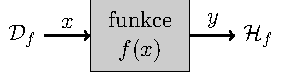
\includegraphics[width=0.45\linewidth]{mai_fig001.pdf}
        \caption{Funkce jako „černá skříňka“. \cite[s.~54]{Musilova2009MA1}}
        \label{mai:fig001}
      \end{figure}
      
      Funkci si podle obrázku \ref{mai:fig001} můžeme představit jako „černou skříňku“, do které 
      vstoupí hodnota (vzor) a vystoupí z ní hodnota \(y = f(x)\) (obraz). Množinu uspořádaných 
      dvojic čísel \([x, f(x)]\) nazveme \hyperref[MAI:section_001]{grafem funkce}.
      
      Jak zadat předpis \(f\)? Lze to udělat kterýmkoli z následujících způsobů, podle vhodnosti
      nebo snadnosti. Ukážeme jednotlivé možnosti na jednoduchém příkladu, kdy chceme hodnotám 
      proměnné \(x\) z množiny \(\mathcal{D}_f\) přiřadit jejich druhé mocniny. Zvolme pro náš 
      příklad definiční obor výčtem:
      \begin{equation*}
         \mathcal{D}_f = \lbrace-3,2,-1,0,1,2,3,4\rbrace,
      \end{equation*}
      a zadáme předpis
      \begin{itemize}\addtolength{\itemsep}{-0.5\baselineskip}
        \item \textbf{slovním popisem}: předpis \(f\) přiřazuje každé z hodnot \(x\in 
              \mathcal{D}_f\) její druhou mocninu,
        \item \textbf{vzorcem}: \(y = x^2\) pro \(x\in \mathcal{D}_f\) zadává zobrazení
              \begin{equation*}
                f: x\in \mathcal{D}_f \rightarrow f(x)= x^2\in\realset,
              \end{equation*}
        \item \textbf{tabulkou}: Hodnoty obrazů pro všechny vzory z \(\mathcal{D}_f\) vypíšeme do 
              tabulky:
              \begin{table}[h]
                \centering
                \begin{tabular}{c|rrrrrrrr}
                  \textbf{x} & -3 & -2 & -1 & 0 & 1 & 2 & 3 & 4  \\ \hline
                  \textbf{y} & 9  & 4  & 1  & 0 & 1 & 4 & 9 & 16
                \end{tabular}
                % \caption{ }
              \end{table}
              Proměnná $x$ se v tomto případě mění \uv{diskrétně}. Je zřejmé, že tímto způsobem 
              můžeme funkci definovat úplně jen tehdy, je-li definiční obor konečná množina. 
              Tabulku však používáme i v jiných případech, zejména chceme-li vyznačit pomocí ní, 
              některé hodnoty, které nás z nějakého důvodu přednostně zajímají. 
        \item Zadání \textbf{grafem}: 
          \begin{equation*}
            G_f = \left\lbrace\left[x,f(x)\right] |x\in D\right\rbrace
                = \left\lbrace\left[x,x^2 \right] |x\in D\right\rbrace
          \end{equation*}
          tak, že dvojice \([x, f(x)]\) znázorníme jako body v rovině (obr. \ref{MAI:fig_011}).
          \begin{figure}[ht!]
            \centering  
            \begin{tabular}{cc}
              \subfloat[ ]{\label{MAI:fig_011}
                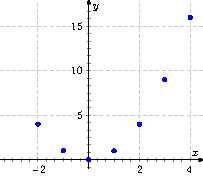
\includegraphics[width=0.4\linewidth]{mai_fig002.pdf}}              &
              \subfloat[ ]{\label{MAI:fig_010}
                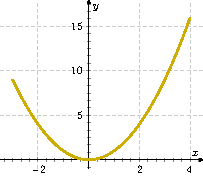
\includegraphics[width=0.4\linewidth]{mai_fig003.pdf}}              \\
            \end{tabular}
            \caption{Zadání funkce grafem}
          \end{figure}
          Z grafu můžeme ovšem funkční hodnoty určit pouze přibližně. Pro další matematické 
          zpracování je grafické zadání nejméně vhodné, i když jeho praktický význam například v 
          technických aplikacích nelze popřít.
        \item Zadání pomocí \textbf{rovnice}, jíž je funkce řešením: některé funkce nelze jednoduše 
              zapsat pomocí některého z předchozích způsobů, nebo to alespoň nejde přesně. Lze však 
              zapsat (diferenciální) rovnici, kterou tato funkce splňuje. Jedná se většinou o 
              speciální funkce, jimž se v tomto textu nebudeme věnovat. (Někdy může být taková 
              rovnice  představující zadání funkce i velmi jednoduchá. Například dosti známá funkce 
              \(\erf(x)\), \emph{error funkce}, velmi úzce souvisí s funkcí \(f(x) = 
              \frac{2}{\sqrt{x}}e^{-x^2}\). Nelze ji však zapsat vzorcem. Některé její hodnoty v 
              nejčastěji používaném rozsahu proměnné \(x\) můžeme najít v rozsáhlých tabulkách, 
              které byly sestaveny pomocí numerických metod.)
      \end{itemize}
      
      Již bylo zmíněno, že zadání definičního oboru je neopominutelnou součástí zadání funkce. 
      Kdybychom například zadali funkci opět předpisem \(y=x^2\), avšak za definiční obor stanovili 
      uzavřený interval \(D = \lbrace —3,4\rbrace\), dostali bychom graf na obrázku 
      \ref{MAI:fig_010}. Jde skutečně o jinou funkci než na obrázku \ref{MAI:fig_011}. Její úplnou 
      tabulku bychom nedokázali napsat vůbec.
      
%      Nejčastější způsob zadání funkce představuje \emph{vzorec}. Tabulku alespoň pro některé 
%      hodnoty z \(\mathcal{D}_f\) si pak dokážeme sestavit a schematický graf nakreslit. Někdy se 
%      objeví zadání funkce jen v podobě vzorce, například: „Je dána funkce \(y = f(x)\).“ Znamená 
%      to, že autor zapomněl zadat definiční obor? Nemusí tomu tak být. Tento způsob zadání chápeme 
%      tak, že si sami musíme stanovit „co největší“ definiční obor této funkce, tj. určit množinu 
%      všech takových \(x\), pro která lze do vzorce dosadit a hodnotu \(y\) určit.

      Zobrazovací předpis, kterým je funkce zadána, může být rozmanitý. Nejčastěji a pro účely 
      matematické analýzy nejvhodnější je \emph{analytické zadání vzorcem}, tj. rovnicí tvaru 
      $y=f(x)$ nebo několika takovými rovnicemi platnými pro různé části definičního oboru. Přitom 
      v rovnici $y=f(x)$ je na pravé straně nějaký správně definovaný výraz obsahující nejvýše 
      proměnnou $x$ a nabývající jednoznačné hodnoty pro danou hodnotu proměnné $x$.
      
%      Někdy však používáme (poněkud nedůsledně) termíny \uv{funkce \(f(x)\)} nebo \uv{funkce 
%      \(y=f(x)\)}. V tomto smyslu nepojímáme již \(x\) jako pevný prvek z definičního oboru, ale 
%      jako \uv{nezávisle proměnnou} neboli \emph{argument}, tj. symbol zastupující libovolný prvek 
%      z definičního oboru. V tomto případě pak písmeno \(y\) v rovnici \(y=f(x)\) nazýváme 
%      \emph{závisle proměnnou} a říkáme, že \uv{\(y\) závisí na \(x\)}. Tato frazeologie má své 
%      historické kořeny; tento způsob vyjádření funkce budeme využívat zřídka, zejména tam, kde 
%      nechceme pro označení příslušné funkce zavádět zvláštní symbol. Tak např. budeme mluvit o 
%      funkci \(e^x\) (ačkoliv se zavádí pro exponenciální funkci symbol exp) nebo o funkci \(\sin 
%      x\) (ačkoliv by bylo důslednější mluvit o funkci \(\sin\)) apod. \cite[s.~82]{Brabec1989} 

    %-------------------------------------
      \input{../src/MAI/exam/exam017.tex}
    %-----------------------------------------------------------------------------------------------
    \subsection{Graf funkce}\label{MAI:section_001}\hypertarget{MAI:section_001}
      Jinými slovy, v předchozím odstavci, bylo řečeno, že každé funkci můžeme přiřadit její graf, 
      a že \textbf{grafem funkce} $f:A\rightarrow\realset,\ A\subset\realset$, rozumíme množinu 
      všech bodů euklidovské roviny, jejíž souřadnice $x$, $y$ v dané kartézské soustavě souřadnic 
      vyhovuje rovnice 
      \begin{equation}\label{mai:eq026}
        y=f(x). 
      \end{equation}  
      
      Graf funkce může v jednodušších případech posloužit jako prostředek k získání názorné 
      \uv{představy}. Grafy některých funkcí jsou \uv{křivky}, (intuitivním smyslu tohoto slova). 
      Avšak u některých funkcí názorná představa grafu selhává. Vezmeme-li např. Dirichletovu 
      funkci, snadno zjistíme, že její graf nemůžeme sestrojit (obr. \ref{mai:fig005} tedy 
      není grafem funkce, ale pouze pokusem o názorné přiblížení Dirichletovi funkce)
      
      \begin{figure}[ht!] %\ref{mai:fig005}
        \centering
%       \input{../src/MAI/img/mai_fig005.tex}
        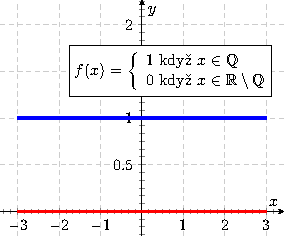
\includegraphics[width=0.5\linewidth]{mai_fig005.pdf}
        \caption{Pokus o zobrazení Dirichletovy funkce: \uv{dvě rovnoběžné přímky $y=0$ a $y=1$ s 
        nekonečným množstvím mezer}}
        \label{mai:fig005}
      \end{figure}      
      Z předchozí kapitoly také víme, že zadat funkci znamená udat její definiční obor a 
      \uv{zobrazovací předpis}, tj pravidlo (formulované slovně či v používaném matematickém 
      jazyku), podle něhož můžeme jednoznačným způsobem rozhodnout, jaká funkční hodnota odpovídá 
      libovolně zvolenému číslu z definičního oboru. Definičním oborem bývá často interval nebo 
      sjednocení intervalů. Není-li definiční obor udán, rozumíme jím množinu všech reálných čísel, 
      pro něž je příslušný předpis definován. Tuto množinu nazýváme \textbf{přirozeným} (též 
      maximálním) definičním oborem funkce. Je to tzv. \emph{existenční obor} výrazu, jímž je 
      funkce definována \cite[s.~84]{Brabec1989}.
      
      Například funkce $f: \realset\rightarrow\realset,\ f(x)=x^2$, můžeme vyjádřit bez udání 
      definičního oboru $\realset$ vztahem 
      \begin{equation*}
        f: y=x^2,
      \end{equation*}
      neboť předpis $y=x^2$ má smysl pro každé reálné číslo $x$. Avšak u funkce $g:\langle0, 
      1\rangle\rightarrow\realset,\ g(x)=x^2,$ je nutné v zápisu funkce definiční obor $\langle0, 
      1\rangle$ 
      uvést, píšeme tedy   
      \begin{equation*}
        g: y=x^2, \quad x\in\langle0,1\rangle.
      \end{equation*}
       
      %-------------------------------------
        \input{../src/MAI/exam/exam018.tex}
      %-------------------------------------
      
      %-------------------------------------
        \input{../src/MAI/exam/exam019.tex}
      %-------------------------------------
      
      Funkce může být analyticky zadána i jinak než vzorcem $y=f(x)$. Časté je \textbf{parametrické 
      vyjadřování}, tj. vyjádření dvojicí rovnic 
      \begin{equation}\label{mai:eq027}
        x=\varphi(t),\ y=\psi(t),\ t\in J,
      \end{equation}
      kde $\varphi, \psi$ jsou funkce definované na množině $J$ ($\ J$ bývá obvykle interval). 
      Proměnná $t$ se nazývá \emph{parametr}: má zde pomocný význam. Zajímá nás totiž vztah mezi 
      $x$ a $y$. Rovnice \ref{mai:eq027} definuje relaci 
      $f\subset\realset\times\realset=\realset^2$:
      \begin{equation*}
        f = \{(x,y)\in\realset^2; \text{ existuje } t\in J \text{ tak, že } x=\varphi(t),\ y=\psi(t)\}.
      \end{equation*}      
      Tato relace může být za \emph{určitých podmínek jednoznačná} tj. je funkcí z $\realset$ do 
      $\realset$. V tomto případě říkáme, že funkce $f$ je \emph{definována parametricky rovnicemi 
      \ref{mai:eq027}}
      
      %-------------------------------------
        \input{../src/MAI/exam/exam020.tex}
      %-------------------------------------
      
      Blíže se parametrickým zadáním funkce budeme zabývat v kapitole \ref{chap:Apl_dif_poc}
      (Aplikace diferenciálního počtu).
      
      Funkce může být někdy zadána též rovnicí tvaru 
      \begin{equation}\label{mai:eq028}
        F(x,y) = 0.
      \end{equation}
      Přitom $F$ je funkce dvou proměnných, tj. zobrazení z $\realset^2\rightarrow\realset$. Kromě 
      rovnice \ref{mai:eq028} může být dána ještě podmínka, aby bod $(x,y)$ patřil k některé 
      množině $M\subset\realset^2$. Rovnicí \ref{mai:eq028} je definována opět jakási relace 
      $f\subset\realset\times\realset$,
      \begin{equation}
        f = \{(x,y)\in\realset^2,\quad F(x,y)=0 \}
      \end{equation}
      (případně $f = \{(x,y)\in\realset^2,\ F(x,y)=0,\ (x,y)\in M \}$), zajímá nás, kdy tato relace 
      je funkcí z $\realset$ do $\realset$. Říkáme pak, že funkce $f$ je dána \textbf{implicitně} 
      uvedenou rovnicí \ref{mai:eq028} (příp. rovnicí \ref{mai:eq028} a podmínkou $(x,y)\in 
      M$). Naproti tomu zadání funkce ve tvaru $y=f(x)$ nazýváme \textbf{explicitním}.

      %-------------------------------------
        \input{../src/MAI/exam/exam022.tex}
      %-------------------------------------
      
      Vyšetřování podmínek, při nichž rovnice $F(x,y)=0$ je definována funkce $f$, se obvykle 
      provádí metodami matematické analýzy funkce více proměnných. 
          
    %---------------------------------------------------------------------------------------------- 
    \subsection{Vlastnosti funkcí}\label{MA1:subsec_vlastnosti_funkce}
      \subsubsection{Omezená funkce}
        \begin{definition}\label{MA1:def_lim01}
          Funkci $f$ nazýváme shora (zdola) omezenou na množině $A\subset D(f)$, je-li shora 
          (zdola) omezená množina funkčních hodnot $f(A)$. Je-li funkce $f$ omezená shora i zdola 
          na množině $A$, pak ji nazýváme omezenou na množině $A$. Je-li $A=D(f)$, nazýváme funkci 
          omezenou. Viz kniha \cite[s.~87]{Brabec1989}       
        \end{definition}
        Funkce \(f\) je omezená na množině \(A\), právě když existuje číslo \(K>0\) tak, že platí
        \begin{align*}
         |f(x)|      &\leq K \qquad \text{pro každé } x\in A   \\ 
         \shortintertext{neboli}
         -K\leq f(x) &\leq K \qquad \text{pro každé } x\in A. 
        \end{align*}

        %-------------------------------------
          \input{../src/MAI/exam/exam023.tex}
        %-------------------------------------

        \begin{itemize}\addtolength{\itemsep}{-0.5\baselineskip}
          \item Je-li funkce $f$ shora omezená na množině $A$, existuje konečné \emph{supremum}     
                $\sup f(A)$. Toto číslo nazýváme \emph{supremem funkce $f$ na množině $A$} a 
                označujeme je též $\sup_{x\in A}f(A)$ nebo $\sup\{f(x), x\in A\}$.
          \item Je-li funkce $f$ zdola omezená na množině $A$, existuje konečné \emph{infimum} 
                $\inf(A)$, které nazýváme \emph{infimum funkce $f$ na množině $A$} a označujeme je 
                též $\inf_{x\in A}f(A)$ nebo $\inf\{f(x), x\in A\}$. 
          \item Není-li funkce $f$ shora (zdola) omezená na množině $A$, pak je ovšem $\sup_{x\in A}
                f(x)=+\infty$ ($\sup_{x\in A} f(x)=-\infty$).
          \item Má-li množina $f(A)$ největší (nejmenší) prvek, pak toto číslo nazýváme největší 
                (nejmenší hodnotou funkce $f$  na množině $A$ (je-li $A = f(f)$, též absolutním 
                maximem, resp. absolutním minimem funkce $f$) a značíme je $\max_{x\in A} f(x)$ 
                ($\min_{x\in A} f(x)$). V tomto případě existuje takové číslo $x_0\in A$, že 
                $f(x_0)=\max_{x\in A}f(x)$ ($f(x_0)=\min_{x\in A}f(x)$). Pro všechna $x\in A$ tedy 
                platí $f(x)\leq f(x_0)$ ($f(x)\geq f(x_0)$). Je zřejmé, že největší (nejmenší) 
                hodnota funkce $f$ na množině $A$, pokud existuje je současně supremem (infimem) 
                funkce $f$ na $A$.
        \end{itemize}

      %-------------------------------------
        \input{../src/MAI/exam/exam021.tex}
      %-------------------------------------
       
      \subsubsection{Monotonní funkce}
        \begin{definition}\label{MA1:def_lim02}
          Funkci $f$ nazýváme \textbf{rostoucí (klesající)} na množině $A\subset D(f)$, jestliže 
          pro každé dva body $x_1, x_2\in A,\ x_1<x_2$, platí $f(x_1)<f(x_2)$ ($f(x_1)>f(x_2)$). 
          Funkci $f$ nazýváme \textbf{neklesající (nerostoucí)} na množině $A\subset D(f)$, 
          jestliže pro každé dvě body $x_1, x_2\in A,x_1<x_2$, platí $f(x_1)\leq f(x_2)$ 
          ($f(x_1)\geq f(x_2)$). Rostoucí a klesající funkce (na množině $A$) se nazývají 
          \textbf{ryze monotónní} (na množině $A$), neklesající a nerostoucí funkce (na množině 
          $A$) se nazývají monotónní (na množině $A$).    
        \end{definition}
            
        Z definice je zřejmé, že každá rostoucí funkce je zároveň neklesající a každá klesající 
        funkce je zároveň nerostoucí. Ryze monotónní funkce tvoří tedy podmnožinu množiny 
        monotónních funkcí. 
           
        \begin{example}
          Funkce $y=2x+1$ je \textbf{rostoucí} na intervalu $(-\infty, \infty)$. Platí totiž: $x_1<x_2\Rightarrow 2x_1<2x_2\Rightarrow2x_1+1<2x_2+1$.
        \end{example}
        \begin{example}
          Funkce y=[x] je \textbf{neklesající} na intervalu $(-\infty, \infty)$ (viz příklad **). 
        \end{example}
        \begin{example}
          Heavisideova funkce (viz příklad **) je \textbf{neklesající} na intervalu $(-\infty, \infty)$ (viz příklad **). 
        \end{example}       
        \begin{example}
          Funkce $y=|x|$ je \textbf{klesající} na intervalu $(-\infty, 0\rangle$ a rostoucí na intervalu $\langle0, \infty)$. 
        \end{example}  
            
        \begin{definition}\label{MA1:def_lim03}
          Funkci $f$ nazýváme \textbf{konstantní} na množině $A$, jestliže pro každé dva body $x_1, 
          x_2\in A$, platí $f(x_1)=f(x_2)$. V tom případě existuje reálné číslo $k$ takové, že pro 
          každé $x\in A$ je $f(x)=k$. Je-li $k=0$, mluvíme o nulové funkci na množině $A$. 
        \end{definition} 
          
        Výrok \uv{funkce $f$ je konstantní na množině $A$} zapisujeme též $f(x)=\text{konst na }A$. 
        Funkci konstantní na $\realset$ budeme stručně nazývat \textbf{konstantní funkcí} nebo 
        krátce \textbf{konstantou}. Z textu bude obvykle patrno, interpretujeme-li symbol $k$ jako 
        reálné číslo nebo jako konstantní funkci. Je zřejmé, že konstantní funkce na množině $A$ je 
        zároveň neklesající i nerostoucí na množině $A$. Toto tvrzení se dá obrátit. Lze snadno 
        dokázat i tuto větu:        
        \begin{lemma}\label{MA1:lem_lim01}
          Funkce $f$ je \textbf{rostoucí} na množině $A$, právě když je neklesající na množině $A$ a na žádné dvoubodové podmnožině $B\subset A$ není konstantní. 
        \end{lemma}
        Obdobná tvrzení platí i pro klesající funkce. 
               
      \subsubsection{Sudé a liché funkce}
        \begin{definition}\label{MA1:def_lim04}
          Funkce $f$ se nazývá \textbf{sudá} jestliže pro každé $x\in D(f)$ je též $-x\in D(f)$  a 
          platí $f(x)=f(-x)$.
          Funkce $f$ se nazývá \textbf{lichá} jestliže pro každé $x\in D(f)$ je též $-x\in D(f)$  a 
          platí $f(-x)=-f(x)$. 
        \end{definition}
        Graf sudé funkce je souměrný podle osy $y$ (osy funkčních hodnot), graf liché funkce je  
        souměrný podle počátku. 
 
       %-------------------------------------
         \input{../src/MAI/exam/exam024.tex}
       %-------------------------------------

        Daná funkce nemusí být ovšem ani sudá, ani lichá. Snadno se dokáže tvrzení:
        \begin{itemize}
          \item Je-li sudá funkce $f$ na množině $D(f)\cap\langle0,\infty)$ rostoucí (klesající),
                je na množině $D(f)\cap(-\infty,0\rangle$ klesající (rostoucí).
          \item Je-li lichá funkce na množině $D(f)\cap\langle0,\infty)$ rostoucí (klesající),
                je též na množině $D(f)\cap(-\infty,0\rangle$ klesající (rostoucí).                 
        \end{itemize}
      \subsubsection{Periodická funkce}

    \subsection{Operace s funkcemi. Uspořádání}
      Jak s funkcemi počítat? Definujeme základní operace s nimi — \emph{součet funkcí, součin 
      funkcí a násobení funkce reálným číslem}. Předpokládejme, že na definičním oboru 
      \(\mathcal{D}\) jsou zadány funkce \(f\) a \(g\) a reálné číslo \(\alpha\). Pak na tomtéž 
      definičním oboru lze zadat nové funkce
      \begin{align*}
        \mathcal{F} &: \mathcal{D}\ni x\,\rightarrow\,\mathcal{F}(x) = f(x)+g(x)  \in\realset   \\
        \mathcal{G} &: \mathcal{D}\ni x\,\rightarrow\,\mathcal{G}(x) = \alpha g(x)\in\realset   \\
        \mathcal{H} &: \mathcal{D}\ni x\,\rightarrow\,\mathcal{H}(x) = f(x) g(x)  \in\realset 
      \end{align*}
      Funkce \(\mathcal{F}\), \(\mathcal{G}\) a \(\mathcal{H}\) nazýváme postupně součtem funkcí 
      \(f\) a \(g\), \(\alpha\)-násobkem funkce \(f\) a součinem funkcí \(f\) a \(g\). Značíme
      \begin{equation*}
       \mathcal{F} = f + g, \qquad \mathcal{G} = \alpha f, \qquad \mathcal{H} = fg. 
      \end{equation*}
      
      Všimněme si nyní pravidel pro počítání s funkcemi zadanými na \(\mathcal{D}\) a zjistíme, 
      že se velmi podobají pravidlům pro počítání s reálnými čísly. Není divu, vždyť operace s 
      funkcemi jsou definovány prostřednictvím funkčních hodnot, a těmi jsou reálná čísla. Některé 
      důležité odlišnosti však přece jen najdeme. Napřed ale pravidla:
      
      \begin{itemize}\addtolength{\itemsep}{-0.5\baselineskip}
        \item komutativní zákon pro součet funkcí
          \begin{equation}\label{mai:eq012}
            f(x) + g(x) = g(x) + f(x)
          \end{equation}
        \item asociativní zákon pro součet funkcí  
          \begin{equation}\label{mai:eq013}
            (f(x) + g(x)) + h(x) = f(x) + (g(x) + h(x)
          \end{equation}
        \item existence univerzálního neutrálního  prvku \(O\) (nulová funkce \(O:\mathcal{D}\ni x 
          \rightarrow O(x)=0\))
          \begin{equation}\label{mai:eq014}
            f(x) + O = O + f(x) = f(x)
          \end{equation}
        \item existence právě jednoho opačného prvku k funkci \(f\), přičemž \((-f)(x) = -f(x)\)
          \begin{equation}\label{mai:eq015}
            f(x)+(-f(x))=(-f(x))+f(x)=O
          \end{equation}
        \item asociativní zákon pro násobení číslem 
         \begin{equation}\label{mai:eq016}
            (\alpha_1\alpha_2)f(x) = \alpha_1(\alpha_2f(x))
         \end{equation}
        \item  1. distributivní zákon pro násobení číslem
          \begin{equation}\label{mai:eq017}
            \alpha(f(x)+g(x) =\alpha f(x) + \alpha g(x)
          \end{equation}\label{mai:eq018}
        \item 2. distributivní zákon pro násobení číslem 
          \begin{equation}\label{mai:eq019}
            (\alpha_1+\alpha_2)f(x) =\alpha_1f(x)+\alpha_2f(x)
          \end{equation}
        \item násobení číslem \((—1)\) dává opačný prvek
          \begin{equation}\label{mai:eq020}
            (-1)f(x)=(-f(x))
          \end{equation}
        \item komutativní zákon pro součin funkcí
          \begin{equation}\label{mai:eq021}
            f(x)g(x)=g(x)f(x)
          \end{equation}
        \item asociativní zákon pro součin funkcí 
          \begin{equation}\label{mai:eq022}
            f(x)(g(x)h(x))=(f(x)g(x))h(x)
          \end{equation}
        \item distributivní zákon zprava pro součin funkcí
          \begin{equation}\label{mai:eq023}
            (f_1(x) + f_2(x))g(x) =f_1(x)g(x) + f_2(x)g(x)
          \end{equation}
        \item distributivní zákon zleva pro součin funkcí
          \begin{equation}\label{mai:eq024}
            f(x)(g_1(x) + g_2(x))=f(x)g_1(x)+f(x)g_2(x)
          \end{equation}
        \item násobení jednotkovou funkcí \(I: \mathcal{D}\ni x \rightarrow I(x) = 1\)  
          \begin{equation}\label{mai:eq025}
           f(x)I=If(x)
          \end{equation}
        \item existence právě jedné \emph{převrácené} funkce k funkci \(f\) pro \(f(x)\neq0\quad 
              (f)^{-1}: \bar{D}\ni x\rightarrow (f)^{-1}(x)=[f(x)]^{-1}\) kde \(\bar{\mathcal{D}} 
              = \mathcal{D} - \left\{x\in \mathcal{D}\,|\,f(x)=0\right\}\)
          \begin{equation}
            f(x)(f(x))^{-1}=(f(x))^{-1}f(x) = I
          \end{equation}
      \end{itemize}
      Všimněme si, že funkce \((f)^{-1}\) existuje obecně na užším definičním oboru 
      \(\bar{\mathcal{D}}\), než na kterém je definována funkce \(f\). Je totiž třeba vyloučit 
      všechny hodnoty \(x\), pro které \(f(x) = 0\) (zákaz dělení nulou). K funkci \(O\) tedy 
      převrácená funkce neexistuje vůbec!
      
      Existence opačné a převrácené funkce k \(f\) umožňuje definovat \emph{rozdíl} a \emph{podíl} 
      funkcí \(f-g=f+(-g)\) a \(\dfrac{f}{g}=f(g)^{-1}\), tj.
      \begin{align*}
        f-g         &: \mathcal{D}\ni x\,\rightarrow\, (f-g)(x)=f(x)+(-g)(x)= f(x)-g(x), \\
        \frac{f}{g} &: \bar{D}\ni x\,\rightarrow\, 
                       \left(\frac{f}{g}\right)(x) = f(g)^{-1}(x) = \frac{f(x)}{g(x)}, 
      \end{align*}
      kde \(\bar{D}=D-\left\{x\in D\,|\,g(x)=0 \right\}\) 
      
      \begin{note}
        Pamatujme si označení převrácené funkce jako \((f)^{-1}\), v němž je zápis symbolu \(f\) do 
        závorky podstatný. Jde o něco jiného než znamená symbol \(f^{-1}\) bez závorky, který 
        rezervujeme pro inverzní funkci v dalším výkladu.
      \end{note}
      \begin{note}
        Porovnáme-li nyní vlastnosti operací s funkcemi a pravidla pro počítání s reálným čísly, 
        komplexními čísly, maticemi a vektory, můžeme konstatovat, že množina funkcí s operací 
        sčítání funkcí a násobení funkce číslem je \textbf{vektorovým prostorem}. To je vlastnost, 
        která je s případem čísel, matic a vektorů společná. Vektorový prostor funkcí se však od 
        zmiňovaných vektorových prostorů výrazně liší svou dimenzí (rozměrem). Intuitivně dobře 
        chápeme, co znamená jednorozměrný, dvojrozměrný a trojrozměrný prostor (například 
        \(\realset^1\), \(\realset^2\), \(\realset^3\)). V odstav 1.4 jsme dokonce pracovali v 
        n-rozměrném vektorovém prostoru. Dimenze vektorového prostoru může být i nekonečná — třeba 
        zrovna u funkcí. Obecně jde o pojem poměrně obtížný a budeme se jím důkladně zabývat až v 
        kapitolách věnovaných algebře \cite[s.~58]{Musilova2009MA1}.
      \end{note}
      
      Operace s funkcemi jsme definovali a prodiskutovali pro případ, kdy definiční obory funkcí, 
      vstupujících do operace byly stejné. Co když tomu tak nebude? Znamená to, že pak nemůžeme 
      funkce sčítat, násobit, apod.? Předpokládejme, že definičním oborem funkce \(f\) je množina 
      \(\mathcal{D}_f\) definičním oborem funkce \(g\) množina \(D_g\). Pokud jsou tyto obory 
      disjunktní, tj. \(\mathcal{D}_f \cap \mathcal{D}_g = 0\), můžeme utvořit pouze 
      \(\alpha\)-násobek funkce \(f\) či \(g\). Sčítat ani násobit funkce \(f\) a \(g\) nemůžeme 
      neboť hodnota \(f(x) + g(x)\) ani \(f(x)g(x)\) neexistuje pro žádné \(x\). Pokud je průnik 
      \(D=d_f\cap D_g\) oborů \(\mathcal{D}_f\) a \(\mathcal{D}_g\) neprázdný, stává se definičním 
      oborem funkcí \(f+g\) a \(fg\). Platí stejná pravidla jako v předchozí tabulce, pouze s 
      omezením na obor \(\mathcal{D}_f\).
    
    \subsection{Skládání a inverze funkcí}
      \emph{Skládání} neboli kompozici funkcí si lze snadno představit opět pomocí „černých 
      skříněk“ (obr. \ref{mai:fig012}): Do první skřínky představující předpis \(g\), \emph{vnitřní 
      složku} složené funkce, vstupuje
      \begin{figure}[ht!] %\ref{mai:fig012}
        \centering
%        \input{../src/MAI/img/mai_fig012.tex}
        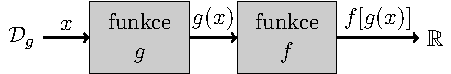
\includegraphics[width=0.45\linewidth]{mai_fig012.pdf}
        \caption{Skládání funkcí \cite[s.~59]{Musilova2009MA1}}
        \label{mai:fig012}
      \end{figure}
      hodnota \(x\) z definičního oboru \(\mathcal{D}_g\) funkce \(g\). Výstupem je číslo \(u = 
      g(x)\), funkční hodnota vnitřní složky v bodě \(x\). Toto číslo smí vstoupit do skříňky 
      představující předpis \(f\), \emph{vnější složku} složené funkce, právě tehdy, je-li prvkem 
      jejího definičního oboru \(\mathcal{D}_f\). V takovém případě najdeme na výstupu ze skříňky 
      \(f\) hodnotu \(y = f(u) = f[g(x)]\). (Jestliže \(g(x)\notin\mathcal{D}_f\), není výstup ze 
      skříňky \(f\) definován.) Vzniká nový předpis \(F\), kterým se některým bodům definičního 
      oboru \(\mathcal{D}_g\), ne všem, ale pouze těm, pro něž \(g(x)\in\mathcal{D}_f\), 
      přiřazují hodnoty \(f[g(x)]\). Definujme nyní složenou funkci přesněji: Předpokládejme, že 
      jsou zadány funkce
      \begin{align*}
        g  &: \mathcal{D}_g\ni x\,\rightarrow\, g(x) = u\in\realset, \\
        f  &: \mathcal{D}_f\ni u\,\rightarrow\, f(u) = y\in\realset. \\
        \shortintertext{označme}
        \mathcal{D} &= \{x|x\in\mathcal{D}_g \text{ a současně } g(x)\in\mathcal{D}_f\}.
      \end{align*}
      Pokud \(\mathcal{D} = \emptyset\), lze definovat funkci
      \begin{equation*}
        F: \mathcal{D}\ni x\rightarrow y = F(x) = f[g(x)]\in\realset, 
           \text{ značíme } F = f \circ g.
      \end{equation*}
      \(F\) se nazývá \emph{složením} neboli \emph{kompozicí} funkcí \(g\) a \(f\). Zápis \(f\circ 
      g\) čteme často také jako \emph{„f po g“}. Skládat lze i větší počet funkcí.

       %-------------------------------------
         \input{../src/MAI/exam/exam025.tex}
       %-------------------------------------
      
      Může vzniknout otázka, jak rozpoznáme vnitřní a vnější složku složené funkce. Rozlišit 
      vnitřní a vnější složku třeba u funkcí \(\cos(x^2)\) a \((cos x)^2\) není problém. Hned také 
      vidíme, že obecně \(f\circ g\neq g\circ f\), i když by definiční obory funkcí na pravé i levé 
      straně měly neprázdný průnik. Jsou však i případy na první pohled méně zřetelné, jak ukazuje 
      následující příklad.
      
      %-------------------------------------
        \input{../src/MAI/exam/exam026.tex}
      %-------------------------------------
       
      Funkce \(F\) a \(G\) mají různé definiční obory, ale na jejich průniku dávají stejné funkční 
      hodnoty. Ani zde však obecně nelze pořadí skládání funkcí zaměňovat.
      
      Nyní se pusťme do vybudování pojmu inverzní funkce k funkci \(f\). Představme si, že funkční
      hodnota \(y = f(x)\) zadané funkce
      \begin{equation*}
        f: \mathcal{D}_f\ni x \rightarrow f(x)\in\mathcal{H}_f
      \end{equation*}
      představuje „zakódovanou“ informaci o hodnotě \(x\). Položme si otázku, zda a za jakých 
      podmínek dokážeme sestavit „černou skříňku“, na jejímž výstupu by se při vstupu obrazu \(y = 
      f(x)\) objevila hodnota \(x\). Omezení takové možnosti je názorně vidět na obrázku 
      \ref{mai:fig014}. V případě funkce \(f(x)\) lze ke všem obrazům \(y \in \mathcal{H}_f\) najít 
      vzory, v případě funkce \(g(x)\) to možné není, neboť jeden a týž obraz lze získat z několika 
      vzorů. Pro který bychom se tedy měli rozhodnout?
      
      \begin{figure}[ht!] %\ref{mai:fig014}
        \centering
%        \input{../src/MAI/img/mai_fig014.tex}
        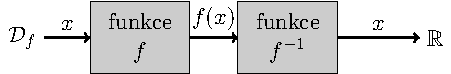
\includegraphics[width=0.45\linewidth]{mai_fig014.pdf}
        \caption{Skládání funkcí \cite[s.~61]{Musilova2009MA1}}
        \label{mai:fig014}
      \end{figure}
       Aby bylo možné vzor zpětně identifikovat na základě znalosti obrazu, je třeba, aby funkce 
       \(f\) byla \emph{prostá}, tj. aby předpis \(f\) přiřazoval každým dvěma různým vzorům \(X_1 
       \neq x_2\) dva různé obrazy \(f(x_1) \neq f(x_2)\). Často lze tohoto požadavku docílit tím, 
       že se místo funkce \(f\) s definičním oborem \(\mathcal{D}_f\) spokojíme s funkcí, která 
       vznikne omezením \emph{(restrikcí)} té původní na „menší“ definiční obor, zato však již bude 
       prostá. U funkce \(g\) na obrázku \ref{mai:fig016} by tak stačilo omezit definiční obor 
       například na množinu \(\mathcal{D}_g\). Než inverzní funkci definujeme, ukažme si způsob 
       jejího nalezení na známém příkladu.

       \begin{figure}[ht!]
         \centering  
         \begin{tabular}{cc}
           \subfloat[ ]{\label{mai:fig016a}
             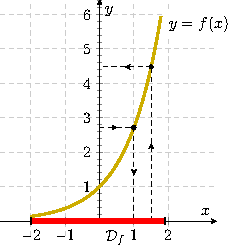
\includegraphics[width=0.45\linewidth]{mai_fig016a.pdf}}              &
           \subfloat[ ]{\label{mai:fig016b}
             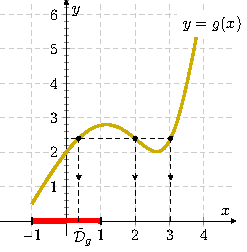
\includegraphics[width=0.45\linewidth]{mai_fig016b.pdf}}              \\
         \end{tabular}
         \caption{K pojmu inverzní funkce}
         \label{mai:fig016}
       \end{figure}
      
      %-------------------------------------
        \input{../src/MAI/exam/exam027.tex}
      %-------------------------------------
      
      Ze způsobu konstrukce funkce \(f^{-1}\) v předchozím příkladu je vidět, že 
      \(\mathcal{D}_{f^{-1}} = \mathcal{H}_f\), \(\mathcal{H}_{f^{-1}} = \mathcal{D}_f\) a graf 
      inverzní funkce je obrazem grafu prosté funkce \(f\) při osové symetrii v rovině 
      souřadnicových os vzhledem k ose prvního a třetího kvadrantu. Nyní již definujeme inverzní 
      funkci obecně. Předpokládejme, že funkce \(f : \mathcal{D}_f\ni x \rightarrow y = f(x)\ni 
      \mathcal{H}_f\) je prostá na svém definičním oboru. Pak existuje funkce \(f^{-1}\) definovaná 
      jako
      \begin{equation}\label{mai:eq029}
        f^{-1} :\mathcal{H}_f\ni x\rightarrow y = f^{-1}(x)\in\mathcal{D}_f\Leftrightarrow x = f(y).
      \end{equation}
      Funkci \(f^{-1}\) nazýváme \textbf{inverzní funkcí k funkci} \(f\). Ještě shrneme pravidla 
      pro skládání funkcí a pro inverzní funkce:

      \begin{itemize}\addtolength{\itemsep}{-0.5\baselineskip}
        \item asociativní zákon pro skládání funkcí
          \begin{equation}\label{mai:eq030}
            f(x)\circ(h(x)\circ g(x)) = f(x)\circ h(x) \circ g(x)
          \end{equation}
        \item distributivní zákon zleva 
          \begin{equation}\label{mai:eq031}
            f(x) \circ (h(x) + g(x)) = f(x) \circ h(x) + f(x) \circ g(x)
          \end{equation}
        \item existence univerzálního neutrálního  prvku \(O\) (nulová funkce \(O:\mathcal{D}\ni x 
          \rightarrow O(x)=0\))
          \begin{equation}\label{mai:eq032}
            f(x) + O = O + f(x) = f(x)
          \end{equation}
        \item existence právě jednoho opačného prvku k funkci \(f\), přičemž \((-f)(x) = -f(x)\)
          \begin{equation}\label{mai:eq033}
            f(x)+(-f(x))=(-f(x))+f(x)=O
          \end{equation}
        \item komutativní zákon pro součet funkcí
          \begin{equation}\label{mai:eq034}
            f(x) + g(x) = g(x) + f(x)
          \end{equation}
        \item asociativní zákon pro součet funkcí  
          \begin{equation}\label{mai:eq035}
            (f(x) + g(x)+h(x) = f(x) + (g(x) + h(x)
          \end{equation}
        \item existence univerzálního neutrálního  prvku \(O\) (nulová funkce \(O:\mathcal{D}\ni x 
          \rightarrow O(x)=0\))
          \begin{equation}\label{mai:eq036}
            f(x) + O = O + f(x) = f(x)
          \end{equation}        
      \end{itemize}   
      Předchozí vztahy platí na patřičně zúžených definičních oborech funkcí, které do nich 
      vstupují.
      
  %-------------------------------------------------------------------------------------------------
  \section{Elementární funkce}
      Základními elementárními funkcemi nazýváme \cite[s.~10]{PolakMA1}:
%      \begin{displaymath}
%        \xymatrix{
%        \mbox{mocninné} & *+[F]{\mbox{Elementární 
%        funkce}}\ar@{->}[l]\ar@{->}[dl]\ar@{->}[d]\ar@{->}[dr]\ar@{->}[r]&\mbox{exponenciální} \\
%        \mbox{goniometrické}       &   \mbox{logaritmické}      & \mbox{cyklometrické}
%        }
%      \end{displaymath}
    %------------- Goniometrické funkce ------------------------------------------------------------
    \input{../src/MAI/sections/fce_goniometricke.tex} 
    %-----------------------------------------------------------------------------------------------
    \subsection{Zobrazení v jiných strukturách}
    %-----------------------------------------------------------------------------------------------
    \subsection{Cvičení}
  %================ Podkapitola: Limita funkce =====================================================
  \section{Limity všeho druhu}  
    „Limes“ znamená latinsky příční cesta, mez, v přeneseném významu pak hranice, pomezí, atd. V 
    matematice představuje limita hodnotu, ke které se „neomezeně blíží hodnota funkce, jestliže se 
    hodnota proměnné neomezeně blíží zadanému číslu“. Poslední formulace musí být v uvozovkách, 
    protože je i přes svou dobrou názornost velice nepřesná. A takové nepřesnosti nejsou v 
    matematice dovoleny. K čemu vůbec úvaha o limitě je? Stačí přece do funkčního předpisu hodnotu 
    proměnné dosadit a získat funkční hodnotu. Tak jednoduché to ale není. Funkční hodnota pro 
    danou hodnotu proměnné \(x\) vůbec nemusí být definována, zato může být definována pro hodnoty 
    velmi blízké. Nebo definována je, ale pro hodnoty proměnné, které jsou k \(x\) velmi blízké, 
    jsou funkční hodnoty od \(f(x)\) velmi vzdálené. Potřebnost pojmu limita ukážeme na 
    geometrickém a fyzikálním příkladu.
    
    V matematické analýze hraje např. důležitou úlohu podíl \cite[s.~117]{Brabec1989}
    \begin{equation*}
      \dfrac{\varphi(x) - \varphi(a)}{x - a}
    \end{equation*}
    kde \(\varphi\) je daná funkce, \(a\) pevný bod. Tento podíl tzv. \emph{přírůstku funkce} 
    \(\varphi(x) — \varphi(a)\) k přírůstku argumentu \(x — a\) může značit např. \emph{průměrnou 
    rychlost pohybu bodu po přímce}, jehož zákon dráhy je dán vztahem \(y = \varphi(x)\), kde \(y\) 
    je dráha, kterou bod urazí za čas \(x\). Zajímá nás, jak se mění hodnota tohoto podílu — jinak 
    řečeno, jak se mění hodnota funkce \(f\) dané vztahem
    \begin{equation}\label{mai:eq037}
      f(x) = \dfrac{\varphi(x) - \varphi(a)}{x - a}
    \end{equation}
    když hodnoty argumentu \(x\) se blíží k číslu \(a\), což často značíme \(x\rightarrow a\). V 
    uvedeném fyzikálním významu daného podílu se ptáme, jak se mění průměrná rychlost pohybu, když 
    se časový úsek zkracuje. Je zřejmé, že musí být stále \(x \neq a\) a že jmenovatel se blíží k 
    nule; obvykle se blíží k nule i čitatel. Jakých hodnot však nabývá přitom podíl, tj. jaké jsou 
    hodnoty funkce \(f(x)\)? Než vyslovíme přesnou definici limity, uvedeme ještě pár jednoduchých 
    příkladů.

    %-------------------------------------
      \input{../src/MAI/exam/exam028.tex}
    %-------------------------------------

    Definičním oborem funkce z příkladu \ref{MAI:exam028} je tedy množina \(\mathcal{D} = \realset 
    — {1}\) (pro \(a = 1\) by ve jmenovateli zlomku byla nula). Grafem funkce je tedy přímka s 
    „vynechaným“ bodem \([1, 2]\) (obr. \ref{mai:fig017}). V bodě \(a = 1\) funkční hodnota není 
    definována. Pokud bychom chtěli rozšířit definiční obor funkce na celou reálnou osu, musíme 
    předepsat, jaké hodnoty má funkce nabývat v bodě \(a = 1\). Původní vzorec, jímž je funkce 
    zadána, výpočet hodnoty \(f(1)\) neumožňuje. Dodatečné zadání funkční hodnoty, její 
    \emph{dodefinování}, můžeme provést zcela libovolně. Zvolme například \(f(1) = 2\). Jiná 
    možnost, jak funkci dodefinovat, je například \(f(1) =-1\). Které číslo je ovšem limitou funkce 
    \(f(x)\) v bodě \(a = 1\)? Je to číslo \(2\), které je v případe \(f(x) = x+1\) její funkční 
    hodnotou? Nebo číslo \(-1\)? A nebo nějaká jiná hodnota? Intuice nám napovídá, že je to číslo 
    \(2\). Když dvojku použijeme pro dodefinování funkce, přetržený graf se „zacelí“. Vidíme, že 
    vezmeme-li dostatečně malý interval proměnné \(x\) v blízkosti bodu \(a=1\) můžeme docílit 
    toho, že všechny odpovídající funkční hodnoty \(f(x)\) budou ležet tak blízko hodnotě \(2\), 
    jak si předem určíme. Skutečně, zkusme docílit toho, aby hodnoty \(f(x)\) ležely v intervalu 
    \((\num{1.99}, \num{2.01})\), tj.
    \begin{equation*}
      \num{1.99} < x + 1 < \num{2.01} \Rightarrow \num{0.99} < x < \num{1.01},\qquad x\neq1.
    \end{equation*}
    Podařilo se. A kdybychom interval \(I(\varepsilon) = (2 - \varepsilon, 2 + \varepsilon)\) 
    funkčních hodnot kolem \(2\) ještě zmenšili, podařilo by se opět najít (o něco menší) interval 
    kolem bodu \(a = 1\) tak, aby pro všechny hodnoty \(x\) v něm (samozřejmě s případnou výjimkou 
    hodnoty \(a =2\)) platilo \(f(x)\in I(\varepsilon)\). A takto bychom mohli \(\varepsilon\) 
    stále zmenšovat. Jak by takový postup dopadl s hodnotou \(-1\), která, jak intuitivně cítíme, 
    limitou funkce v bodě \(a = 1\) není, protože je graf funkce od bodu \([-1,0]\) dost vzdálen? 
    Vezměme třeba interval (\num{-0.5}, \num{0.5}) a hledejme hodnoty \(x\) obdobně jako v 
    předchozím případě. Požadujeme
    \begin{equation*}
      \num{-0.5} < x + 1 < \num{0.5} \Rightarrow \num{-1.5} < x < \num{-0.5}.
    \end{equation*}
    Tento interval vůbec neobsahuje bod \(a = 1\). Dostali jsme se mimo blízkost bodu \(a = 1\).

    %-------------------------------------
      \input{../src/MAI/exam/exam029.tex}
    %-------------------------------------

    Je třeba říci, že při zkoumání limit funkcí nás nezajímají jen funkce „tvaru“ 
    (\ref{mai:eq037}), i když tento případ je v diferenciálním počtu velmi častý, jak poznáme v 
    kap. \ref{mai:IchapIV}. Někdy nás zajímá i chování funkcí v okolí nevlastních bodů \(-\infty\), 
    \(+\infty\) 

    %-------------------------------------
      \input{../src/MAI/exam/exam030.tex}
    %-------------------------------------
    
    %-------------------------------------
      \input{../src/MAI/exam/exam031.tex}
    %-------------------------------------
    
    V uvedených případech bychom mohli zkoumat i limity funkcí pro \(x \to - \infty\).  Všimněme si 
    ještě, že ve všech případech nebylo nutné, aby funkce \(f\) byla definována v bodě, ke kterému 
    se blíží hodnoty argumentu, ale bylo zapotřebí, aby funkce \(f\) byla definována v bodech 
    libovolně blízkých tomuto bodu. Tomuto požadavku bude vyhověno, jestliže daný bod, v němž 
    zkoumáme limitu, bude \emph{hromadným bodem definičního oboru}. Není ovšem nutné, aby funkce 
    byla definována v celém nějakém \emph{prstencovém okolí uvažovaného bodu}.
    
    Nechť \(a\) je bod, blízko kterého se pohybuje hodnota proměnné \(x\). Pro definici limity je 
    důležitý pojem \textbf{okolí bodu} \(a\) (obr. 2.16). Zvolme kladná čísla \(\delta_1\) a 
    \(\delta_2\). Nazýváme
    
    
      
  %================ Podkapitola: Spojitost funkce ==================================================
  \section{Spojitost funkce}
  
%} % tikzset
%~~~~~~~~~~~~~~~~~~~~~~~~~~~~~~~~~~~~~~~~~~~~~~~~~~~~~~~~~~~~~~~~~~~~~~~~~~~~~~~~~~~~~~~~~~~~~~~~~~
\printbibliography[title={Seznam literatury}, heading=subbibliography]
\addcontentsline{toc}{section}{Seznam literatury}          	
  % !TeX spellcheck = cs_CZ
%{\tikzset{external/prefix={tikz/MAI/}}
% \tikzset{external/figure name/.add={ch10_}{}}
%---------------------------------------------------------------------------------------------------
% file mai1ch03.tex
%---------------------------------------------------------------------------------------------------
\chapter{Kombinatorika, pravděpdobnost, statistika}\label{mai:IchapIII}
\minitoc
  \section{Kombinatorika}\label{mai:IchapIIIsecI}
    \textbf{Kombinatorika} se od všech matematických disciplín, v několika směrech liší. Zatímco v 
    geometrii má každá přímka nekonečnou délku a každý trojúhelník nekonečně mnoho bodů, zatímco v 
    algebře některé rovnice i nerovnice mají nekonečně mnoho řešení a zatímco matematická analýza 
    zkoumá limity posloupností a funkcí, roste-li příslušná proměnná do nekonečna, v kombinatorice 
    se s nekonečnem nesetkáme. Kombinatorika je součástí \textbf{finitní matematiky}, která studuje 
    konečné soubory (množiny a uspořádané \(k\)-tice, \(k\in \mathcal{N}\)). 
    
    Další odlišností je to, že často nemáme možnost ověřit si správnost výsledku, ke kterému jsme 
    při řešení kombinatorické úlohy dospěli, a jsme odkázáni jen na svůj vlastní úsudek. Proto v 
    kombinatorice v míře větší než jinde platí, že „cvičení dělá mistra“. 
    
    V této kapitole je probrána část kombinatoriky, která se zabývá vytvářením skupin z daných 
    prvků a určováním jejich počtu. Jde o klasickou problematiku, která byla řešena již v 17. a 18. 
    století a která je spojena se jmény \emph{B. Pascala}, \emph{P. Fermata}, \emph{J Bernoulliho}, 
    \emph{G. W. Leibnize}  a \emph{L. Eulera}. Dnes představuje kombinatorika rozsáhlou 
    matematickou disciplínu, některé její problémy byly již vyřešeny (problém čtyř barev) mnohé 
    další na své vyřešení čekají. 
    
    A závěrem ještě důležitá poznámka terminologická: přirozeným čísly se v této kapitole rozumějí 
    čísla celá kladná tj. čísla 1, 2, 3, 4, \(\ldots\), nula se tedy mezi přirozená čísla 
    nezahrunuje. \cite[s.~7]{calda2008matematika} 
    
    \subsection{Základní kombinatorická pravidla}
    
    
    \cite[s.~7]{polak1991matematika}
    
  \section{Pravděpodobnost}\label{mai:IchapIIIsecII}
    Slovo pravděpodobnost používáme velmi často. Jaký však je jeho přesný význam? Jsme přesvědčeni, 
    že pravděpodobnost výhry ve sportce je velmi malá. Ani pravděpodobnost, že se vyplní předpověď 
    počasí, nepovažujeme mnohdy za výraznou. Přesto je mezi oběma příklady obrovský kvantitativní 
    rozdíl. Zkusme význam pojmu pravděpodobnost ukázat pomocí konkrétních číselných příkladů.
  
    \begin{itemize}
      \item \textbf{Příklad se střelcem}: Sportovní střelec střílí na terč série \num{100} ran. 
            Předpokládejme, že podmínky při střelbě jsou stále stejné. Stejná je zbraň, terč, 
            vzdálenost, povětrnostní podmínky i momentální zdravotní stav střelce. Při hodnocení 
            střelcova „mistrovství“ někdo řekne, že střelec zasáhne terč s pravděpodobností 
            \num{92}\%. Jak tomu rozumět? Znamená to, že v souboru sérií výstřelů jsou velmi časté 
            ty, v nichž zasáhl střelec terč \num{92}-krát. Samozřejmě, není řídké, že se objeví i 
            série s \num{93} nebo \num{94} zásahy, ale také s \num{91} nebo \num{90}. Vyloučen není 
            ani případ s úspěšností \num{96} či \num{88}, a dokonce i stovku bychom mohli 
            zaznamenat. Situace výrazně odlišné od \num{92} zásahů však budou řídké, a to tím více, 
            čím více se úspěšnost série liší od \num{92} oběma směry.
      \item \textbf{Příklad se zmetky}: Koupíte si výrobek u firmy, o které je známo, že vyrábí 
            zmetky s pravděpodobností 0,16\%? Situaci lze posuzovat obdobně jako úspěšnost střelce. 
            Budeme-li například zkoumat série obsahující 1000 výrobků, bude každá z nich obsahovat 
            „v průměru“ 16\% zmetků. Z příkladu se střelcem již zhruba víme, jak posuzovat slovo v 
            průměru.
    \end{itemize}
    
    V této kapitole se budeme pravděpodobnostmi zabývat podrobněji. Zjistíme, že i když se týkají 
    náhodných jevů, platí i pro ně jisté zákonitosti. V úvodních příkladech jsme si vyložili, jak 
    intuitivně chápat pojem pravděpodobnost. Jednalo se v nich o posouzení průměrné úspěšnosti ve 
    velkém souboru operací či úkonů prováděných za stejných podmínek, šlo tedy o jakousi 
    „průměrnou“ pravděpodobnost. Nyní definujeme pravděpodobnost matematicky.
    
    \subsection{Co se pravdě podobá - definice pravděpodobnosti}
      Pro definici pravděpodobnosti použijeme pojmu \emph{náhodný pokus}, jehož význam si ukážeme 
      na příkladu. Dobrým příkladem náhodných pokusů je třeba házení mincí, hraní kostkou, výběr 
      karet z balíčku, vidíme-li pouze jejich rub, apod. Budeme třeba házet kostkou. Abychom si 
      situaci zbytečně nekomplikovali, budeme předpokládat, že všechny výsledky hodu kostkou 
      (náhodné pokusy) jsou stejně časté, žádný z nich není nijak preferován\footnote{Kostka by 
      tedy měla být homogenní, plocha, na kterou po hodu dopadne, vodorovná, kvalita povrchu všech 
      stěn kostky stejná (žádná stěna by třeba neměla být natřena lepidlem), apod.}. Počet možných 
      výsledků jednotlivého hodu je \(N = 6\) (kostka má \num{6} stěn, na každé je vyznačen odlišný 
      počet ok, tedy \num{1} až \num{6}). Jednotlivé situace, které mohou nastat, nazýváme 
      náhodnými jevy. Náhodným jevem \(A\) tak může být situace \emph{„padne číslo \num{2}“}, jiným 
      náhodným jevem \(B\) situace \emph{„padne číslo dělitelné třemi“}, apod. Počet situací, kdy 
      výsledek hodu lze hodnotit tak, že určitý jev nastal, označíme \(M\). Například pro jev \(A\) 
      \emph{„padne číslo \num{2}“} je \(M(A)= 1\), pro jev \(B\) \emph{„padne číslo dělitelné 
      třemi“} je \(M(B) = 2\) (počet ok \num{3} nebo \num{6}). Můžeme také definovat jev \(O\) 
      \emph{„nepadne žádné číslo“} (\(M(0) = 0\)) nebo jev \(J\) \emph{„padne jakékoli číslo“} 
      (\(M(J) = 6\)).
      
      \begin{definition}
        Pravděpodobností jevu rozumíme podíl
        \begin{equation}\label{mai:eq011}
          p = \frac{M}{N} = \frac{\text{počet případů příznivých}}{\text{počet případů možných}}.
        \end{equation}  
        Počtem případů možných jsme zkráceně nazvali počet všech možných výsledků náhodného 
        pokusu, počtem případů příznivých pak počet všech takových výsledků pokusu, při nichž daný 
        jev nastal.
      \end{definition}
      Je zřejmé, že hodnota pravděpodobnosti jakéhokoli jevu je nezáporná a může nabývat hodnoty 
      nejvýše \num{1}, tj. \(0 <p< 1\). Jev s \emph{nulovou pravděpodobností} se nazývá 
      \textbf{nemožný}, jev s \emph{jednotkovou pravděpodobností} je \textbf{jistý}. V našem 
      příkladu s kostkou tak dostáváme
      \begin{equation*}
        p(A) = \frac{1}{6}, \qquad p(B) = \frac{2}{6} = \frac{1}{3}, \qquad
        p(O) = 0, \qquad p(J) = 1.
      \end{equation*}  

      %--Barevné ponožky----------------------------------------------
      \input{../src/MAI/exam/exam006.tex}
      %---------------------------------------------------------------
    \subsection{Cifry, kostky, karty - kombinatorické opakování}
      Příklad s ponožkami byl velmi jednoduchý. Podařilo se nám vyjmenovat všechny případy možné i 
      všechny případy příznivé, neboť obojího bylo docela málo. Daleko běžnější jsou však situace, 
      kdy výčet případů není schůdný. A tehdy potřebujeme \textbf{kombinatoriku}.
      
      Nechť \(\mathcal{M}\) je \(n\)-prvková množina, z níž budeme provádět výběry \(k\) prvků 
      podle určitých pravidel. Prvky množiny \(\mathcal{M}\) nemusíme nijak konkretizovat. Abychom 
      si však o výběrech a pravidlech pro jejich tvorbu dokázali udělat nějakou názornou představu, 
      je taková konkretizace vhodná. Prvky množiny \(\mathcal{M}\): mohou být třeba žáci ve třídě, 
      barvy, hrací karty, apod. Výběry mohou představovat třeba družstva pro odbíjenou, signály 
      tvořené barevnými praporky, možnosti rozdání karet při mariáši, apod. Jednotlivé typy výběrů 
      získaly své názvy právě na základě pravidel stanovených pro jejich vytváření. Rozhodující 
      jsou dvě základní kritéria:
      \begin{itemize}\addtolength{\itemsep}{-0.5\baselineskip}
        \item Je pro tvorbu výběru podstatné pořadí prvků ve výběru či nikoliv?
        \item Mohou se prvky ve výběru opakovat či nikoliv?
      \end{itemize}
      
      Typy výběrů shrnuje následující diagram:
      \begin{figure}[ht!] %\ref{mai:fig021}
        \centering
        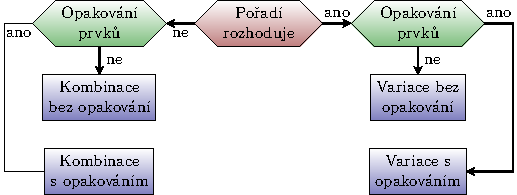
\includegraphics[width=0.7\linewidth]{mai_fig021.pdf}
        \caption{Typy výběrů. \cite[s.~201]{Musilova2009MA1}}
        \label{mai:fig021}
      \end{figure}

      Představuje-li daný výběr například volejbalové družstvo osmi děvčat (šest hráček a dvě 
      náhradnice), které bude reprezentovat v soutěži třídu osmou bé, do níž chodí \num{25} děvčat 
      a \num{18} chlapců, jedná se o výběr \(k - 8\) prvků z počtu \(n = 25\) prvků. Chlapce nelze 
      postavit do družstva volejbalistek. Každý výběr možného družstva bude představovat 
      \emph{kombinaci bez opakování}, neboť pořadí hráček nehraje roli a třeba Aničku Novákovou 
      máme ve třídě jen jednu. Budeme-li však chtít vytvářet z deseti cifer \(0, 1, \ldots, 9\) 
      trojciferná čísla, pak tyto výběry tří prvků z deseti (\(k = 3\), \(n = 10\)) jsou 
      \emph{variacemi s opakováním}. Čísla \num{125}, \num{512}, \num{251}, \num{215}, \num{521} a 
      \num{152} jsou totiž různá, a například \num{222} je také trojciferné číslo. Kombinace s 
      opakováním bychom mohli vytvářet třeba i při výběru různobarevných ponožek ze zásuvky a 
      konečně \emph{variacemi bez opakování} by mohly být dejme tomu trojbarevné signály (\(k = 
      3\)) tvořené trojicemi barevných hadříků vybíraných z \(n\) barev (pro \(n = 3\) třeba zrovna 
      z těch ponožek). Nyní bychom však rádi věděli, jak pro zadané hodnoty \(n\) a \(k\) určit 
      počet všech možných výběrů předepsaného typu. Ukážeme si to na příkladech.

      %--Šance milion-------------------------------------------------
      \input{../src/MAI/exam/exam007.tex}
      %---------------------------------------------------------------
      
      Zobecněním předchozího příkladu získáváme vzorec pro počet \textbf{variací s opakováním} 
      \emph{k}-té třídy z \(n\) prvků. Při tahu totiž záleží na pořadí bubnů a každý buben obsahuje 
      všechny cifry. Výsledky tahů z jednotlivých bubnů se tedy mohou opakovat. Pokud by bubnů bylo 
      \(k\) a v každém \(n\) různých cifer, dostali bychom pro \textbf{variace s opakováním 
      \(k\)-té třídy z \(n\) prvků} celkový počet
      \begin{equation}\label{mai:eq007}
        \boxed{V_k' = n^k}\, .
      \end{equation}

      %--Modifikovaná šance milion------------------------------------
      \input{../src/MAI/exam/exam008.tex}
      %---------------------------------------------------------------
      
      Uvážíme-li, že v předchozím příkladu je \(n = 10\) a \(k = 6\), dostáváme pro \textbf{počet 
      variací bez opakování \(k\)-té třídy z \(n\) prvků} obecný vztah
      \begin{align}
        V_k(n) &= n(n-1)(n-2)\cdots(n-k+1)  \nonumber \\
        \shortintertext{neboli}
        V_k(n) &= \frac{n!}{(n-k)!}\, .    \label{mai:eq008}
      \end{align}
      Poznamenejme, že \(n!\) značí \textbf{faktoriál}, \(n! = n(n - 1)\cdots 3 \cdot 2 \cdot 1\). 
      Pro nulu definujeme \(0! = 1\). Je zřejmé, že při vytváření variací bez opakování musí být 
      \(k\leqq n\). Variace bez opakování \(n\)-té třídy z \(n\) prvků se nazývají 
      \textbf{permutace}. Každá z nich představuje určité uspořádání těchto \(n\) prvků. Platí
      \begin{equation}\label{mai:eq009}
        \boxed{P(n) = V_n(n) = n!}\, .
      \end{equation}
      
      Nyní odvodíme vzorec pro počet \textbf{kombinací \(k\)-té třídy z \(n\) prvků bez opakování}. 
      Již jsme si řekli, že \emph{kombinací} rozumíme takový výběr z celkového počtu \(n\) prvků, 
      který obsahuje určitých \(k\) prvků nezávisle na jejich pořadí. Představme si, že máme k 
      dispozici všechny variace bez opakování \(k\)-té třídy ze zmíněných \(n\) prvků. Vezměme 
      kteroukoli z nich. Soubor všech variací \(k\)-té třídy z \(n\) prvků však obsahuje i další 
      variace, lišící se od té naší jen pořadím prvků. Celkem je takových variací (i s tou první) 
      \(k!\) a z hlediska kombinací představují totéž. Soubor variací se tak rozpadá na podsoubory, 
      z nichž každý obsahuje \(k!\) variací lišících se navzájem pouze pořadím prvků. Každý z 
      těchto podsouborů představuje však jedinou kombinaci. Počet kombinací \(k\)-té třídy z \(n\) 
      prvků bez opakování je tedy
      \begin{equation}\label{mai:eq010}
        \boxed{C(k) = \frac{V_k(n)}{P(k)} = \frac{n!}{(n-k)!\,k!} = 
               \begin{pmatrix}
                n \\
                k
               \end{pmatrix}}\, .
      \end{equation}
      
      Pro odvození vzorce pro \textbf{kombinace s opakováním} použijeme opět příkladu.
      %--Kuličky v přihrádkách----------------------------------------
      \input{../src/MAI/exam/exam009.tex}
      %---------------------------------------------------------------
      
      %--Obsazování kvantových stavů----------------------------------
      \input{../src/MAI/exam/exam010.tex}
      %---------------------------------------------------------------
      
      Získané kombinatorické vzorce nyní použijeme při řešení základních úloh o pravděpodobnostech. 
      V každé úloze bude důležité
      \begin{itemize}
        \item definovat jev \(A\), jehož pravděpodobnost počítáme,
        \item určit počet \(N\) případů možných, tj. počet všech možných výsledků pokusu, při 
              kterém sledujeme, zda jev \(A\) nastal či nenastal,
        \item určit počet \(M\) případů příznivých, tj. počet těch výsledků daného pokusu, při 
              kterých jev \(A\) nastal.
      \end{itemize}

      %--Výhra ve sportce---	----------------------------------------
      \input{../src/MAI/exam/exam052.tex}
      %---------------------------------------------------------------

      %--Losování karet-----------------------------------------------
      \input{../src/MAI/exam/exam053.tex}
      %---------------------------------------------------------------

      %--Sestavování čísel z cifer------------------------------------
      \input{../src/MAI/exam/exam054.tex}
      %---------------------------------------------------------------

    \subsection{Sčítání a násobení - základní počty s pravděpodobnostmi}
      Někdy je třeba určit pravděpodobnosti jevů, které jsou nějakým způsobem „složeny“ z jevů
      jednodušších. Uvažujme například o jevech \(A\) a \(B\), jejichž pravděpodobnosti známe a 
      označíme je \(p(A)\) a \(p(B)\). Definujme nové jevy \(C\) a \(D\) takto:
      \begin{equation*}
        C = A \text{ a } B, \qquad D = A \text{ nebo } B.
      \end{equation*}
      Vzniká přirozená otázka, zda můžeme na základě znalosti pravděpodobností \(p(A)\) a \(p(B)\) 
      určit pravděpodobnosti \(p(C)\) a \(p(D)\). Ukazuje se, že za jistých předpokladů ano. Jako 
      obvykle nám napoví příklady.

      %--Hody kostkou a mincí - jev \(C\)-----------------------------
      \input{../src/MAI/exam/exam055.tex}
      %---------------------------------------------------------------
      
      Z příkladu intuitivně chápeme, co jsou to nezávislé jevy, a usuzujeme, že obecně platí
      \begin{lemma}\label{mai:lemma003}
        \textbf{(Násobení pravděpodobností)}: Pravděpodobnost současného výskytu dvou nezávislých 
        jevů \(A\) a \(B\) (jev \(C\)) je rovna součinu jejich pravděpodobností, tj.
        \begin{equation}\label{mai:eq052}
           p(A \text{ a } B)= p(A)p(B)\qquad \text{pro } A \text{ a } B \text{ neslučitelné}
        \end{equation}
      \end{lemma}
      
      Pokusme se o přesnější definici nezávislých jevů a o odvození vztahu (\ref{mai:eq052}). 
      Označme jako \(N_A\) množinu všech možných výsledků pokusu, při němž může nastat jev \(A\), a 
      obdobně \(N_B\) množinu všech možných výsledků pokusu, při němž může nastat jev \(B\). V 
      předchozím příkladu je \(N_A = \{1, 2, 3, 4, 5, 6\}\) a \(N_B = \{\mathcal{A}, 
      \mathcal{B}\}\). Jako \(N_C\) označme množinu všech možných výsledků pokusu, při němž může 
      nastat současně jev \(A\) i jev \(B\). Jevy \(A\) a \(B\) nazveme nezávislé, jestliže
      platí \(N_C = N_A \times N_B\) (kartézský součin množin). Označíme-li obdobně \(M_A \subseteq 
      N_A\) a, \(M_B \subseteq N_B\) a \(M_C \subseteq N_C\) podmnožiny příznivých výsledků pro 
      jednotlivé jevy, je zřejmé, že také \(M_C = M_A \times M_B\). Počty prvků jednotlivých množin 
      označíme \(N(A)\), \(N(B)\), \(N(C)\) (počty možných případů) a \(M(A)\), \(M(B)\), \(M(C)\) 
      (počty příznivých případů). O konečných množinách víme, že mohutnost (počet prvků) 
      kartézského součinu množin je rovna součinu mohutností jednotlivých
      činitelů v tomto kartézském součinu. Proto
      \begin{align*}
        N(C) &= N(A)N(B),\qquad M(C) = M(A)M(B). \\
        \shortintertext{Odtud}
        p(C) &= \dfrac{M(C)}{N(C)} = \dfrac{M(A)M(B)}{N(A)N(B)} = p(A)p(B).
      \end{align*}
      Platnost tohoto vzorce lze zobecnit na nezávislé jevy \(A_1\), \(A_2\) až \(A_k\) s 
      pravděpodobnostmi \(p(A_1)\), \(p(A_2)\) až \(p(A_k)\). Pravděpodobnost jevu \(C = (A_1\text{ 
      a }A_2\text{ a }...\text{ a }A_K)\) pak je
      \begin{equation*}
        p(C) = p(A_1)p(A_2)\cdots p(A_k).
      \end{equation*}
 
      %--Hody kostkou trochu jinak - jev \(D\)------------------------
      \input{../src/MAI/exam/exam056.tex}
      %---------------------------------------------------------------
      
      Je vidět, že opět směřujeme k obecnému tvrzení:
      \begin{lemma}\label{mai:lemma004}
        \textbf{(Sčítání pravděpodobností)}: Pravděpodobnost jevů \(A\) nebo \(B\) (jev \(C\)) 
        pro neslučitelné (vylučující se) jevy \(A\) a \(B\) rovna součtu pravděpodobností jevů 
        \(A\) nebo \(B\).
        \begin{equation}\label{mai:eq053}
           p(A \text{ nebo } B)= p(A) + p(B)\qquad \text{pro } A \text{ a } B \text{ nezávislé}
        \end{equation}
      \end{lemma}
      
      Opět se pokusme o přesnější definici neslučitelných jevů a o odvození vztahu 
      (\ref{mai:eq053}). Označme, obdobně jako v předchozí úvaze o nezávislých jevech, množiny 
      \(N_A\), \(N_B\), \(N_D\) možných výsledků, při nichž mohou nastat jevy \(A\), \(B\), \(D\). 
      Předpokládejme, že \(N_A = N_B\). Pak \(N_A = N_B = N_D\), a tedy \(N(A) = N(B) = N(D) = N\). 
      Jako \(M_A\), resp. \(M_B\), resp. \(M_D\) označme podmnožiny výsledků, při nichž nastane jev 
      \(A\), resp. \(B\), resp. \(D\). Zřejmě \(M_D = M_A \cup M_B\). Pro počet prvků množiny 
      \(M_D\) platí 
      \begin{align*}
        M(D) &= M(A) + M(B) - M(A\text{ a }B).                                    \\
        \shortintertext{Pravděpodobnost jevu \(D\) je pak}
        p(D) &= \dfrac{M(D)}{N(D)} = \dfrac{M(A) + M(B) - M(A\text{ a }B)}{N} 
              = p(A) + p(B) - p(A\text{ a }B).
      \end{align*}
      
      Jevy \(A\) a \(B\) se nazývají \textbf{neslučitelné}, neboli \emph{vylučující se}, je-li 
      \(M_A \cap M_B = 0\). V takovém případě je ovšem \(M(A\text{ a }B) = 0\), a tedy
      \begin{equation*}
        p(A\text{ nebo }B) = p(A) + p(B).
      \end{equation*}
      Zobecněním na \(k\) jevů \(A_1\) až \(A_k\) po dvou neslučitelných dostáváme
      \begin{equation*}
        p(A_1\text{ nebo }\cdots\text{ nebo }A_k) = p(A_2) + p(A_2) + \cdots + p(A_k).
      \end{equation*}
      Mají-li po dvou neslučitelné jevy \(A_1\) až \(A_k\) tu vlastnost, že při daném pokusu musí 
      nastat právě jeden z nich, říkáme, že tvoří \textbf{úplný systém jevů}. Součet jejich 
      pravděpodobností je roven jedné.
      
      Jev \(\overline{A}\) se nazývá \textbf{opačný} k jevu \(A\), jestliže nastává právě tehdy, 
      když jev \(A\) nenastává. Z této definice je vidět, že jevy \(\overline{A}\) a \(A\) jsou 
      \emph{neslučitelné}. Na druhé straně je zřejmé, že jev (\(A\) nebo \(\overline{A}\)) je jevem 
      \textbf{jistým}, nastává vždy. Jeho pravděpodobnost je tedy \num{1}. Odtud
      \begin{equation}\label{mai:eq054}
        p(\overline{A}) = 1 - p(A).
      \end{equation}
      Jev \(A\) a jev \(\overline{A}\) k němu opačný tvoří úplný systém.
      
      Na závěr odstavce ještě jeden prakticky důležitý příklad.
      
      %--Bernoulliův pokus--------------------------------------------
      \input{../src/MAI/exam/exam057.tex}
      %---------------------------------------------------------------

    \subsection{Pravděpodobnější, než bychom čekali - podmíněná pravděpodobnost}
      Kdysi se objevila, jako nepříliš dobrý vtip, úvaha o pravděpodobnosti bomby na palubě letadla:
      Řekněme, že pravděpodobnost, že některý z pasažérů letadla má s sebou bombu, je jedna
      tisícina. Pravděpodobnost, že dva pasažéři nezávisle na sobě budou mít bombu, je pak pouze
      jedna milióntina (\(\num{e-3}\cdot\num{e-3}= \num{e-6}\)). Vezmu-li si tedy s sebou do 
      letadla svou vlastní bombu, kterou ovšem nehodlám uvést do chodu, snížím tím pravděpodobnost 
      druhé bomby na palubě na onu jednu milióntinu. Nezabývejme se nyní tím, že již první úvaha o 
      jedné milióntině je v podstatě nesprávná, i když pro případ, že pravděpodobnost \(p\), že 
      konkrétní pasažér bude mít bombu, je velmi malá, dává správný přibližný výsledek. Klíčová 
      chyba je v úvaze, že snížení pravděpodobnosti bomby na palubě můžeme napomoci vlastní bombou 
      v zavazadle. Tato úvaha nerespektuje totiž \textbf{pojem podmíněné pravděpodobnosti}, který 
      si nyní na příkladu vyložíme.
      
      %--Jak nekoupit zmetek------------------------------------------
      \input{../src/MAI/exam/exam058.tex}
      %---------------------------------------------------------------
      
      Nyní již snadno dokážeme přijít na chybu v úvaze o bombě v letadle, kterou jsme tento 
      odstavec uvedli. Pravděpodobnost další bomby v letadle za podmínky, že jsme tam jednu sami 
      donesli, je podmíněnou pravděpodobností. Proto je rovna podílu pravděpodobnosti, že v letadle 
      budou dvě bomby, a pravděpodobnosti, že tam bude jedna bomba, tj. \(\num{e-6}/\num{e-3} = 
      \num{e-3}\). Pocit bezpečí bychom si tedy vlastní bombou nezvýšili. Ještě abychom se báli, že 
      bouchne, zejména pokud by byla vyrobená ve Hvizdu.
      
      %--Kolika let se dožijeme?--------------------------------------
      \input{../src/MAI/exam/exam059.tex}
      %---------------------------------------------------------------
      
      %--Ještě jednou bomba v letadle---------------------------------
      \input{../src/MAI/exam/exam060.tex}
      %---------------------------------------------------------------
      
      Nakonec ještě odvodíme obecný případ takzvané Bayesovy formule. Předpokládejme, že při
      každém opakování jistého pokusu může nastat právě jeden z \(k\) různých výsledků. Jevy \(A_1,
      A_2,\cdots, A_k\), z nichž \(j\)-tý znamená, že při pokusu byl zaznamenán \(j\)-tý výsledek, 
      jsou po dvou neslučitelné a tvoří úplný systém. Platí tedy
      \begin{equation*}
        p(A_1) + p(A_2) + \ldots  + p(A_k) = 1.
      \end{equation*}
      Označme jako \(B\) libovolný jev, který popisuje celkový výsledek pokusu. Vzhledem k 
      neslučitelnosti jevů \(A_1\) až \(A_k\) jsou neslučitelné i jevy (\(A_1\) a \(B\)) až 
      (\(A_k\) a \(B\)). Zároveň je zřejmé, že jev \(B\) lze zapsat jako
     \begin{equation*}
       B = (A_1\text{ a }B) \quad\text{nebo}\quad (A_2\text{ a }B) \qquad\ldots
       \quad\text{nebo}\quad (A_k\text{ a }B),
     \end{equation*} 
      a tedy
      \begin{equation*}
        p(B) = \sum_{j=1}^{k}p(A_j\text{ a }B) = \sum_{j=1}^{k}p(A_j)\cdot p_{A_j}(B),
      \end{equation*}
      s využitím vztahu (\ref{mai:eq057}). Současně, podle téhož vztahu, platí 
      \begin{equation*}
        p(A_j\text{ a }B) = p(B)\cdot  p_B(A_j).
      \end{equation*}
      Pomocí dvou předchozích vztahů dostáváme:
      
      \adjustbox{minipage=[c]{\textwidth}}{%
        \begin{lemma}\label{mai:lemma005}
          \textbf{(Bayesova formule):}
          \begin{equation}\label{mai:eq058}
            p_B(A_j) = \dfrac{p(A_j\text{ a }B)}{\sum_{i=1}^{k}p(A_i)\cdot p_{A_i}(B)} 
                     = \dfrac{p(A_j)\cdot p_{A_j}(B)}{\sum_{i=1}^{k}p(A_i)\cdot p_{A_i}(B)} .
          \end{equation}
        \end{lemma}
      }
      
      Bayesova formule pro výpočet podmíněné pravděpodobnosti má řadu užitečných aplikací
      
      %--Potřebují lékaři pravděpodobnost?----------------------------
      \input{../src/MAI/exam/exam061.tex}
      %---------------------------------------------------------------
      
      A na závěr ještě hádanky:

      %--Pohádka o Honzovi--------------------------------------------
      \input{../src/MAI/exam/exam062.tex}
      %---------------------------------------------------------------
      
      %--Může se člověk živit sázením?--------------------------------
      \input{../src/MAI/exam/exam063.tex}
      %---------------------------------------------------------------
      
  \section{Náhodné veličiny}\label{mai:IchapIIIsecIII}
    Hodnota některých veličin je určena jednoznačně a „jednou provždy“. Kdykoli budeme její hodnotu 
    zjišťovat, tehdy dostaneme totéž - takže ji ani opakovaně zjišťovat nemusíme. Příkladem může 
    být skoro prázdná peněženka, ve které jsou třeba tři koruny. Dokud nebudeme pracovat a do 
    peněženky něco nepřidáme, bude hodnota veličiny \(X\) (počet korun v peněžence) stále rovna 
    \num{3}. Nemá smysl se do peněženky vůbec dívat. Pokud budeme do peněženky přidávat každý den 
    dvě koruny, také budeme vědět, jak se veličina \(X\) mění, aniž bychom se do peněženky dívali. 
    Po \(n\) dnech bude hodnota \(X = 3 + 2n\). Většina veličin, se kterými se setkáváme, se však 
    takto nechová. Jejich hodnoty se totiž často řídí náhodnými vlivy, takže při každém
    měření veličiny \(X\), tj. zjišťování její hodnoty, můžeme získat odlišný výsledek než při 
    měřeních předchozích. Uveďme některé příklady náhodných veličin.
    
    \begin{itemize}
      \item \textbf{Příklad s novorozenci}: Nechť jé veličinou \(X\) počet chlapců ve stovce 
            novorozených dětí. Zkušenost říká, že tento počet je v průměru o něco větší než 
            \num{50}, avšak pro různé skupiny po stovce novorozených dětí bude počet chlapců 
            kolísat. V jedné skupině bude \num{52}, v jiné \num{54}, někde třeba \num{60}, nebo 
            také \num{45}.
      \item \textbf{Příklad s meteoroidy a meteority}: Pro astronomy může být důležitou veličinou 
            \(X\) počet meteoroidů, které za rok dopadnou do zemské atmosféry. Jinou veličinou, 
            třeba \(K\), může být roční počet meteoritů, tj. těch meteoroidů, které v atmosféře 
            neshořely zcela, ale jejich část dopadla na povrch Země. Také tyto hodnoty budou pro 
            každý roční interval poněkud odlišné, neboť i počet dopadnuvších meteoroidů a 
            meteoritů podléhá vlivům, které se nedají přesně předvídat.
      \item \textbf{ Příklad s tlakoměrem}: Bude-li lékař měřit pacientovi tlak několikrát po 
            sobě, určitě také naměří několik různých hodnot. Krevní tlak je citlivý na náhodné 
            vlivy, třeba i na vnitřní rozrušení pacienta vyplývající ze strachu z bílého pláště.
      \item \textbf{Opakovaná měření fyzikální veličiny}: Chceme-li změřit třeba odpor elektrického
            vodiče (drátu), jedná se o měření nepřímé. Nemůžeme odpor změřit přímo, třeba jako      
            to můžeme udělat pro délku. Většinou měříme napětí \(U\) na vodiči a proud \(I\), který 
            jím protéká. Odpor pak zjišťujeme jako podíl \(R = U/I\). Změříme-li napětí i proud 
            jednou, dostaneme konkrétní hodnotu \(R\). Budeme-li měření napětí a proudu provádět 
            opakovaně, budeme dostávat poněkud odlišné hodnoty \(U\) a \(I\), a tedy i odlišné 
            hodnoty \(R\). Sledované veličiny se chovají jako náhodné. Je to způsobeno řadou 
            náhodných vlivů jak na veličiny samotné, tak na jejich měření (nepřesnost odečítání 
            údajů na stupnicích, apod.).
    \end{itemize}
  
    Při každém fyzikálním (a vlastně i nefyzikálním) experimentu máme co do činění s náhodnými 
    veličinami. Při chemických analýzách je náhodnou veličinou třeba koncentrace dané látky
    v roztoku, při experimentech biologických třeba počet uhynuvších rostlin ve stovce sazenic, 
    počet pozorovaných prvoků v zorném poli mikroskopu, výskyt vzácných ptáků ve sledované 
    lokalitě, apod. V následujících odstavcích definujeme náhodné veličiny přesněji a naučíme se s 
    nimi zacházet. Uvidíme, že zjištění určité hodnoty náhodné veličiny je otázkou jisté 
    pravděpodobnosti. Také lépe objasníme, co znamená vyjádření „v průměru“, které jsme občas v 
    předchozím textu použili a intuitivně mu jistě rozuměli.
  
    \subsection{Jak dobrý je to střelec - diskrétní rozdělení}
      Mimořádně vhodnou ukázkou náhodné veličiny je příklad se sportovním střelcem, kterým jsme
      uvedli celou kapitolu o pravděpodobnostech.
  
      %--Ještě jednou střelba, tentokrát přesněji---------------------
      \input{../src/MAI/exam/exam064.tex}
      %---------------------------------------------------------------
    
    Položme si ještě otázku, jak můžeme zjistit pravděpodobnosti, se kterými střelec dosáhne při
    jednom výstřelu daného počtu bodů. Prakticky to lze provést jedině tak, že střelec mnohokrát
    vystřelí na terč a jeho zásahy budou při tom zaznamenávány. Dejme tomu, že vystřelil \(n\)-krát 
    a že počet výstřelů, při nichž byl bodový zisk \(j\) bodů ( \(j = 0, 1, 2, 3\)), byl \(n_j\). 
    Pak pro pravděpodobnost bodového zisku \(j\) bodů při jednom výstřelu je \(p_j = n_j/n\). 
    Kdybychom provedli skutečný experiment se střelcem a počítali pravděpodobnosti \(p_j\) znovu a 
    znovu po každém dalším výstřelu, viděli bychom, že pro malé hodnoty \(n\) nejprve kolísají a 
    pro rostoucí \(n\) se začínají ustalovat a již kolísají velmi málo. Tímto postupem bychom je 
    mohli určit tak, aby byly pro náš účel rozumně přesné - třeba s přesností na dvě platná místa. 
    Rozumnou přesností je zde myšlena skutečnost, že nemá smysl chtít zjišťovat pravděpodobnost 
    třeba na šest platných míst. Vzhledem k principiální přítomnosti náhodných vlivů se kolísání 
    pravděpodobností nikdy nezbavíme, takže platná místa na pozicích, kde se kolísání trvale 
    projevuje již bez ohledu na zvyšující se \(n\), nemají smysl.
    
    V příkladu \ref{mai:exam064} jsme se již velmi těsně přiblížili důležitým charakteristikám, 
    které určují náhodnou veličinu a jsou přitom matematicky korektně definovány. Viděli jsme, že 
    známe-li jen hodnoty, kterých může náhodná veličina nabývat, nemůžeme o ní říci již nic 
    dalšího. Známe-li však ještě pravděpodobnosti, se kterými jednotlivých hodnot nabývá, můžeme o 
    ní získat již velmi mnoho informací.

    \adjustbox{minipage=[c]{\textwidth}}{%
      \textbf{Náhodnou veličinou s diskrétním rozdělením} nazýváme takovou veličinu \(X\), která
      může nabývat konečně mnoha různých hodnot \((x_1, x_2, \ldots, x_k)\) s pravděpodobnostní
      \((p_1, p_2, \ldots, p_k)\) popřípadě spočetně mnoha hodnot \((x_1, x_2, \ldots)\) s 
      pravděpodobnostmi \((p_1, p_2, \ldots)\).
      }

    Jevy \(A_j\) \uv{Veličina \(X\) nabývá hodnoty \(x_j\)}, jsou po dvou neslučitelné. Platí
    \begin{equation*}
      \sum_{j=1}^{k}p_j = 1, \qquad\text{resp.}\qquad \sum_{j=1}^{k=\infty}p_j = 1
    \end{equation*}
    Pokud jde o druhý z obou případů, nebudeme se jím prozatím zabývat. Soubor všech dvojic
    \begin{equation*}
      \left\lbrace(x_j, p_j)\right\rbrace,\qquad j = 1, 2, \ldots, k,
    \end{equation*}
    se nazývá \textbf{rozdělení} náhodné veličiny \(X\). Můžeme je znázornit i graficky.

    %--Bernoulliovo (binomické) rozdělení---------------------------
    \input{../src/MAI/exam/exam065.tex}
    %---------------------------------------------------------------
    
    Nyní definujeme další charakteristiky náhodné veličiny. Těmi základními jsou, kromě již 
    definované \emph{nejpravděpodobnější hodnoty}, ještě \textbf{střední hodnota}, \textbf{rozptyl} 
    (popřípadě jeho odmocnina, zvaná \textbf{střední kvadratická} nebo \textbf{směrodatná 
    odchylka}), \textbf{medián}, popřípadě \textbf{P-kvantil}. Pojem střední hodnoty jsme již v 
    podstatě vybudovali v příkladu se střelcem. Nyní postup zobecníme. Předpokládejme, že při 
    velkém počtu \(n\) měření náhodné veličiny \(X\) naměříme různé hodnoty \((x_1, x_2, \ldots, 
    x_k)\) tak, že hodnota \(x_1\) byla naměřena \(n_1\)-krát, hodnota \(x_2\) \(n_2\)-krát, atd., 
    až hodnota \(x_k\) \(n_k\)-krát. Je zřejmé, že součet četností \(n_1\), \(n_2\), až \(n_k\) 
    jednotlivých hodnot musí být roven celkovému počtu měření \(n\) a že podíly
    \begin{equation*}
      p_1 = \dfrac{n_1}{n}, \qquad p_2 = \dfrac{n_2}{n}, \qquad \ldots, \qquad p_k = \dfrac{n_k}{n},
    \end{equation*}
    představují pravděpodobnosti jednotlivých hodnot veličiny \(X\). Tím je zadáno její rozdělení,
    které ji plně charakterizuje. Položme si však otázku, zda by se veličina \(X\) přece jen nedala
    charakterizovat jedinou hodnotou, která by všechny různě pravděpodobné hodnoty v jistém
    smyslu „zastupovala“. Kdybychom třeba takto měřili délku stolu, jistě bychom na otázku „Kolik
    měří stůl?“ neodpovídali tím, že bychom tazateli předložili získané rozdělení, i když by taková
    odpověď byla nejvýstižnější. Určitě bychom uvedli jedinou hodnotu. Ale jakou? I laika napadne,
    že by takovou reprezentativní hodnotou mohl být aritmetický průměr naměřených hodnot \(x_1\) až
    \(x_k\). Bylo by ale správné vzít jen prostý aritmetický průměr těchto různých hodnot a nebrat 
    ohled na skutečnost, že některé byly naměřeny s větší a jiné s menší četností? Nikoliv. 
    Reprezentativní hodnota veličiny \(X\) nemá zastupovat jen naměřené hodnoty, ale celé 
    rozdělení. Určitá hodnota \(x_j\) bude mít tím větší vliv na reprezentativní hodnotu, s čím 
    větší četností byla naměřena. Protože byla naměřena \(n_j\)-krát, musíme ji také tolikrát do 
    aritmetického průměru započíst.Získáváme tak \textbf{vážený aritmetický průměr} naměřených 
    hodnot, neboli \emph{střední hodnotu}
    
    \adjustbox{minipage=[c]{\textwidth}}{%
      \begin{equation}\label{mai:eq059}
        \left\langle x \right\rangle = \dfrac{n_1x_1 + n_2x_2 + \cdots + n_kx_k}{n}
          = p_1x_1 + p_2x_2 + \cdots + p_kx_k 
          = \sum_{j=1}^{k}p_jx_j.
      \end{equation}
      }
      Součet všech pravděpodobností \(p_1 + p_2 + \cdots + p_k\) je pochopitelně \textbf{roven 
      jedné}.

    %--Střední hodnota Bernoulliova rozdělení-----------------------
    \input{../src/MAI/exam/exam066.tex}
    %---------------------------------------------------------------
    
    Posuďme nyní situaci, kdy náhodná veličina \(Y\) je funkcí náhodné veličiny \(X, Y = f(X)\).
    V takovém případě má rozdělení veličiny \(Y\) tvar
    \begin{equation*}
      \left\lbrace (f(x_j), p_j)\right\rbrace, \qquad j = 1, 2, \ldots, k.
    \end{equation*}
    Pravděpodobnost hodnoty \(f(x_j)\) je stejná jako pravděpodobnost hodnoty \(x_j\). Pro výpočet
    střední hodnoty veličiny \(Y\) pak platí
    \begin{equation}\label{mai:eq060}
      \left\langle y \right\rangle = \sum_{j=1}^{k}f(x_j)p_j.
    \end{equation}
    (V obecnější situaci může být náhodná veličina \(Y\) funkcí několika náhodných veličin \(X_1\), 
    \(X_2\), až \(X_s\)).
    
    Může vzniknout oprávněná otázka, zda při výpočtu \(\left\langle y \right\rangle\), popřípadě 
    dalších charakteristik veličiny \(Y\), nevznikne nějaký problém, nebude-li funkce \(f(X)\) 
    prostá. V takovém případě by totiž některé hodnoty veličiny \(Y\) splynuly i pro různá \(x_j\). 
    Například pro \(Y = f(X) = X^2\) by pro hodnoty \(x_r\) a \(x_s\) vázané vztahem \(x_r = -x_s\) 
    (pokud by veličina \(X\) směla takových hodnot nabývat) platilo \(y_{rs} = y_r = y_s\). 
    Pravděpodobnost této společné hodnoty by pak přece byla \((p_r + p_s)\). Tato úvaha je 
    samozřejmě správná, avšak ve výpočtu střední hodnoty veličiny Y
    podle vztahu (\ref{mai:eq060}) je již obsažena. Do součtu totiž vstupují sčítance \(y_rp_r\) i 
    \(y_sp_s\), jejichž součet je při rovnosti \(y_r = y_s\) roven \(y_{rs}(p_r +p_s)\) Společná 
    hodnota \(y_{rs}\) je tedy započtena se správnou vahou.
    
    Uvažujme nyní o tom, jak „směrodatná“, tj. do jaké míry opravdu „reprezentativní“, je
    střední hodnota náhodné veličiny. Intuitivně cítíme, že střední hodnota bude reprezentovat
    rozdělení náhodné veličiny tím lépe, čím méně se od ní budou jednotlivé hodnoty odchylovat na 
    obě strany. Význam slova „odchylovat“ musíme ovšem nějak kvantitativně zachytit.
    \emph{Odchylkou} hodnoty \(x_j\) veličiny \(X\) od střední hodnoty \(\left\langle x 
    \right\rangle\) budeme celkem přirozeně rozumět rozdíl \((x_j - \langle x\rangle)\). Vzniká tak 
    náhodná veličina \(\Sigma = X - \langle x \rangle\) s rozdělením \(\{(x_j - \langle x\rangle, 
    p_j)\}\), \(j = 1, 2, \ldots, k\) . Bude tou správnou charakteristikou odchýlení hodnot 
    veličiny \(X\) od střední hodnoty střední hodnota \(\langle\sigma\rangle\)? Vypočtěme ji 
    (odhadněte předem, co asi tak vyjde):
    \begin{equation*}
      \langle\sigma\rangle = \sum_{j=1}^{k}(x_j - \langle x\rangle)p_j
        = \sum_{j=1}^{k}x_jp_j - \langle x\rangle\sum_{j=1}^{k}p_j
        = \langle x\rangle - \langle x\rangle = 0.
    \end{equation*}
    Čekali jste to? Nepochybně ano. Veličina \(X - \langle x\rangle \) nedává tedy žádný obraz o 
    tom, jak jsou hodnoty \(x_j\) „rozptýleny“ okolo střední hodnoty \(\langle x\rangle\). Kladné 
    odchylky jsou to tiž kompenzovány těmi zápornými. Aby k takové kompenzaci nedošlo, stačí vzít 
    v úvahu absolutní hodnotu veličiny \(\Sigma\), popřípadě její kvadrát. Vezměme v úvahu druhý z 
    obou námětů a vypočtěme \(\langle \sigma^2\rangle\), takzvaný \textbf{rozptyl veličiny} \(X\):
    \begin{align}\label{mai:eq061}
      D(X) &= \langle \sigma\rangle = \sum_{j=1}^{k}(x_j - \langle x\rangle)^2p_j
            = \sum_{j=1}^{k}x_j^2p_j - 2\langle x\rangle\sum_{j=1}^{k}x_jp_j 
            + \langle x\rangle^2\sum_{j=1}^{k}p_j                                     \nonumber \\
           &= \langle x^2\rangle - 2\langle x\rangle^2 + \langle x\rangle^2 
            = \langle x^2\rangle - \langle x\rangle^2.
    \end{align}
    hodnota
    \adjustbox{minipage=[c]{\textwidth}}{%
      \begin{equation}\label{mai:eq062}
        \sigma(x) = \sqrt{\langle \sigma^2\rangle} = \sqrt{\langle x^2\rangle - \langle x\rangle^2}
      \end{equation}
    }
    se nazývá \textbf{směrodatná odchylka} (v některých terminologiích též \emph{střední 
    kvadratická odchylka}) veličiny \(X\). Podíl \(\sigma(x)/ \langle x\rangle\) se nazývá 
    \textbf{relativní směrodatná odchylka} (v některé terminologii též \emph{variační koeficient}).

    \adjustbox{minipage=[c]{\textwidth}}{%
      Důležitým pojmem je \textbf{distribuční funkce}. Je to funkce \(F\) jedné reálné proměnné 
      \(x\) definovaná ve vztahu k náhodné veličině \(X\) takto: Předpokládejme, že hodnoty \(x_1\)
      až \(x_k\), jichž může náhodná veličina \(X\) nabývat, jsou seřazeny vzestupně, tj. \(x_1 <
      < x_2 < \ldots < x_k\). Pak
      \begin{equation}\label{mai:eq063}
        F: \realset\ni x\longleftrightarrow 
        F(x) = \sum_{\mathclap{\substack{j=1\\ x_s \leq x \leq x_{s+1}}}}^{s}p_j
      \end{equation}
    }

    Přestože je veličina \(X\) diskrétní, je distribuční funkce funkcí spojité proměnné. Její 
    funkční hodnoty se však mění skokem. Vidíme to z následující tabulky a z grafu na obrázku 
    \ref{mai:fig045}, v němž je distribuční funkce znázorněna pro případ střelby (příklad 
    \ref{mai:exam064})

    \begin{table}[ht!]
      \centering
      \begin{tabular}{c|c}
        \textbf{interval proměnné} \(x\)  &  \textbf{distribuční funkce}             \\ \hline
            \(-\infty, x_1\)              &    \(F(x) = 0 \)                         \\
            \(\left[x_1, x_2\right)\)     &    \(F(x) = p_1 \)                       \\
            \(\left[x_2, x_3\right)\)     &    \(F(x) = p_1 + p_2 \)                 \\
                    \(\ldots\)            &       \(\ldots\)                         \\
            \(\left[x_j, x_{j+1}\right)\) &    \(F(x) = p_1 + p_2 + \cdots + p_j \)  \\
                   \(\ldots\)             &       \(\ldots\)                         \\
            \(\left[x_k, \infty\right)\)  &    \(F(x) = p_1 + \cdots + p_k =1 \)     \\ \hline
            \end{tabular}
      % \caption{ }
    \end{table}

    \begin{figure}[ht!] %\ref{mai:fig045}
      \centering
      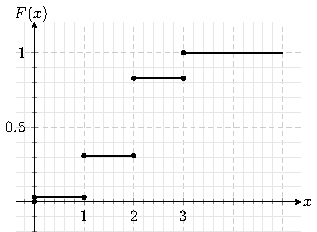
\includegraphics[width=0.5\linewidth]{mai_fig045.pdf}
      \caption{Distribuční funkce k příkladu \ref{mai:exam064}. \cite[s.~233]{Musilova2009MA1}}
      \label{mai:fig045}
    \end{figure}
    Zadáním distribuční funkce je naopak jednoznačně určeno rozdělení veličiny \(X\). Pro jednotlivé
    pravděpodobnosti totiž platí
    \begin{equation*}
      p_j = F(x_j) - F(x_{j-1})\qquad\text{pro}\qquad 2\leq j \leq k, \qquad p_1 = F(x_1).
    \end{equation*}
    
    Hledejme nyní hodnotu \(\overline{x}_P\) definovanou tak, že pravděpodobnost, že při náhodném 
    opakování pokusu nabude veličina \(X\) kterékoli z přípustných hodnot \(x_j \leq 
    \overline{x}_p\), je rovna \(P\). Znamená to, že pro \(x = \overline{x}_P\) má distribuční 
    funkce nabýt předepsané hodnoty \(P\). Abychom \(\overline{x}_P\), takzvaný 
    \(P\)\textbf{-kvantil}, určili, řešíme rovnici
    \begin{equation}\label{mai:eq064}
      \sum_{j=1}^{s}p_j = P
    \end{equation}
    vzhledem k neznámému počtu sčítanců \(s\). V případě veličiny s diskrétním rozdělením se ovšem
    může stát, že pro nevhodně zvolenou hodnotu \(P\) nebude mít rovnice řešení. To proto, že 
    veličina \(X\) může nabývat jen hodnot, které lze očíslovat přirozenými čísly, takže při každé 
    změně horní meze sumy \(s\) o jedničku se suma mění skokem. Vidíme to jak v předcházející 
    tabulce, tak v grafu na obrázku \ref{mai:fig045}. Pro \(P = \num{0.5}\) se \(P\)-kvantil 
    \(\overline{x}_p\), pokud je vůbec definován, nazývá \textbf{medián}. Značí se pouze 
    \(\overline{x}\).

    %--Ještě střelba------------------------------------------------
    \input{../src/MAI/exam/exam067.tex}
    %---------------------------------------------------------------
    
    Příklad \ref{mai:exam067} názorně vypovídá o významu směrodatné odchylky. Viděli jsme, že 
    intervalu o šířce \(2\sigma(y)\) s hodnotou \(\langle y \rangle\) uprostřed odpovídá vysoká 
    pravděpodobnost, že v něm bude ležet bodový zisk střelce při každé pětici výstřelů. Čím bude 
    tento interval užší, tím v průměru blíže budou jednotlivé hodnoty bodového zisku ležet v 
    blízkosti střední hodnoty. Mohli bychom říci, že střelec, jehož výsledky vykazují malou 
    směrodatnou odchylku resp. malý rozptyl, míří přesněji. Směrodatná odchylka je tedy v jistém 
    smyslu jedním z parametrů charakterizujících kvalitu střelby - střelba s malou hodnotou  
    \(\sigma(y)\) je přesnější než střelba s velkou hodnotou \(\sigma(y)\). Druhým parametrem 
    kvality střelby, který je pro její hodnocení z hlediska možnosti vyhrávat soutěže jistě 
    podstatně důležitější, je samozřejmě samotná střední hodnota bodového zisku. Čím je větší, tím 
    je střelcovo pořadí při závodech lepší. Pro interpretaci směrodatné odchylky to ovšem není 
    podstatné. Kdybychom porovnávali dva střelce, jejichž střední bodový zisk při
    pěti výstřelech je třeba \num{12} bodů a \num{3} body, avšak směrodatná odchylka je u obou 
    stejná, musíme konstatovat, že oba jsou stejně přesní. Jeden z nich však systematicky dělá 
    nějakou chybu a přesně střílí do nesprávného místa. Význam pojmu přesnost z hlediska hodnocení 
    náhodných veličin je tedy oproti jeho běžnému chápání poněkud posunut.
    
    Všimněme si ještě jedné důležité obecné věci: Tvar vzorce pro výpočet rozptylu resp. směrodatné 
    odchylky je stejný pro všechny typy rozdělení. Konkrétní pravděpodobnost, že hodnota
    veličiny padne do intervalu určeného směrodatnou odchylkou, tj. do intervalu \((\langle y 
    \rangle - \sigma(y), \langle y \rangle + \sigma(y))\), však pochopitelně na konkrétním 
    rozdělení závisí.

    %--Poissonovo rozdělení-----------------------------------------
    \input{../src/MAI/exam/exam068.tex}
    %---------------------------------------------------------------
    
    \subsection{Kolik rychlostí má molekula plynu - spojité rozdělení}
      Již nadpis napovídá, že veličina se spojitým rozdělením může zřejmě nabývat „spojitě 
      rozložených“ hodnot, tj. přípustným i hodnotami budou například právě všechna čísla \(x\) z 
      jistého intervalu, \(x\in[a, b]\). Jaká však bude pravděpodobnost \(p(x)\), že veličina \(X\) 
      nabývá právě hodnoty \(x\in[a, b]\)? Jestliže víme, že „součet“ všech \(p(x)\) musí být roven 
      jedné, vzniká problém.
      
      Hodnot \(x\) je totiž nekonečně (dokonce nespočetně) mnoho! Je jich tolik, jako je čísel na 
      celé reálné ose. A kdyby byla pravděpodobnost \(p(x)\) jakkoli malinkatá, nikdy nebude součet 
      všech \(p(x)\) konečný. Pravděpodobnost nabývání hodnoty \(x\) tedy musí být nulová. Vzniklou 
      překážku odstraníme snadno. Rozdělení náhodné veličiny \(X\) bude nutno charakterizovat 
      nikoli pravděpodobností, ale \textbf{hustotou pravděpodobnosti}. Je to obdobná situace jako 
      třeba při popisu rozložení hmotnosti nějakého tělesa, předpokládáme-li, že je ta to hmotnost 
      rozložena v objemu tělesa spojitě. Také nemá příliš smysl se ptát, jaká je hmotnost jednoho 
      bodu tohoto tělesa. I zde by byla odpověď, že nulová. Spíše si vždy klademe otázku, jaká je 
      hmotnost \(\Delta m(\vec{r})\) jistého malého objemu \(\Delta V\), například malého kvádříku, 
      umístěného třeba jedním z vrcholů v bodě o poloze \(\vec{r}\). Hustota \(\varrho(\vec{r})\) 
      tělesa v bodě \(\vec{r}\) je pak limitou podílu \(\Delta m(\vec{r})/\Delta V\) pro \(\Delta V 
      \longrightarrow 0\). Obdobně je tomu i s rozdělením spojité náhodné veličiny \(X\). 
      Zvolíme-li pro jistou hodnotu \(x\) interval \([a, x + \Delta x]\), má smysl otázka, jaké je 
      pravděpodobnost \(\Delta p(x)\), že veličina nabývá hodnoty (kterékoli) právě z tohoto 
      intervalu.

      \adjustbox{minipage=[c]{\textwidth}}{%
        Limitu
        \begin{equation}\label{mai:eq066}
          w(x) = \lim\limits_{\Delta\longrightarrow0}\dfrac{\Delta p(x)}{\Delta x}
        \end{equation}
        nazýváme \textbf{hustotou pravděpodobnosti} veličiny \(X\) v bodě \(x\) (pro \(x = a\), 
        resp. \(x = b\) se jedná o limitu zprava, resp. zleva).
      }
      
      Přímo tato funkce pak představuje ono spojité rozdělení náhodné veličiny \(X\). Určuje totiž
      hustotu pravděpodobnosti \(w\) pro hodnotu \(x\) náhodné veličiny \(X\), obdobně jako \(p_j\) 
      v případě diskrétního rozdělení určuje pravděpodobnost hodnoty \(x_j\). Předpokládejme, že je 
      funkce \(w(x)\) na intervalu \([a, b]\) spojitá.
  
      \adjustbox{minipage=[c]{\textwidth}}{%
        Pro \(x \in [a, b]\) definuje integrál jako funkce horní meze
        \begin{equation}\label{mai:eq067}
          F(x) = \int_a^xw(u)\dd{u}
        \end{equation}
        \textbf{distribuční funkci}.
      }
      Jeho hodnota pro dané \(x\) udává pravděpodobnost, že hodnota veličiny \(X\) padne do 
      intervalu \([a, x]\), opět v plné analogii s případem diskrétního rozdělení. Na \((a, b)\) je 
      tedy hustota pravděpodobnosti \(w(x)\) derivací distribuční funkce. Je zřejmé, že \(F(b) = 
      1\). Integrál z hustoty pravděpodobnosti v mezích \([a, b]\) udává totiž pravděpodobnost, že 
      hodnota veličiny \(X\) padne do intervalu přípustných hodnot, tedy pravděpodobnost jistého 
      jevu. V případě diskrétního rozdělení jsme však distribuční funkci definovali nejen pro 
      přípustné hodnoty náhodné veličiny, ale pro všechna x \in (-\infty, +\infty). Tento postup 
      budeme respektovat i nyní a definujeme
      \begin{equation*}
        F(x) = 0\text{ pro }x \in (-\infty,a)\text{ a }F(x) = 1\text{ pro }x \in (b , +\infty).
      \end{equation*}
      \adjustbox{minipage=[c]{\textwidth}}{%
        \begin{equation}\label{mai:eq068}
          \langle x \rangle = \int_a^bxw(x)\dd{x}, \qquad 
                       D(X) = \int_{a}^{b}(x - \langle x \rangle)^2w(x)\dd{x}.
        \end{equation}
      }
      \textbf{Relativní směrodatná odchylka} je opět podílem \(\sqrt{D(X)}/\langle x \rangle\), 
      nejpravděpodobnější hodnota neboli \textbf{modus} \(x_m\) je taková hodnota veličiny \(X\) , 
      pro kterou je hustota pravděpodobnosti maximální
      
      Daleko lépe než u veličin s diskrétním rozdělením vypadá možnost definovat \(P\)-kvantil 
      \(\tilde{x}_p\) a \textbf{medián} \(\tilde{x}\). Jsou jednoduše řešením rovnic
      \begin{equation*}
        F(\tilde{x}_P) = P, \qquad F(\tilde{x}) = \dfrac{1}{2}
      \end{equation*}
      (Mohli bychom mediánu třeba i říkat „půlkvantil“. To ale není zvykem.) \(P\)-kvantil je 
      definován pro jakoukoli hodnotu \(P\) zadanou v intervalu \((0, 1)\). Skutečně, hustota 
      pravděpodobnosti je nezápornou funkcí na intervalu \([a, b]\) (podle předpokladu i spojitou), 
      takže distribuční funkce je na \([a, b]\) \emph{spojitá} a \emph{rostoucí} a nabývá hodnot 
      \(0 = F(a) \leq F(x) \leq F(b) = 1\). Podle jedné z vět o spojitých funkcích (odstavec 
      2.1.7*) nabývá funkce spojitá na uzavřeném intervalu všech hodnot mezi svým minimem a 
      maximem. V intervalu \([a, b]\) tedy existuje alespoň jedna hodnota \(\tilde{x}_P\) , pro 
      kterou je \(F(\tilde{x}_P) = P\). Ze skutečnosti, že je \(F(x)\) navíc rostoucí, vyplývá, že 
      i \(\tilde{x}_P\) existuje jednoznačně.
  
      Tyto závěry zůstanou v platnosti, i kdyby veličina \(X\) nabývala svých hodnot v intervalu
      typu \(\left[0, \infty\right), \left(—\infty, b\right]\) nebo \((—\infty, \infty)\). Vzhledem 
      k požadavku
      \begin{equation*}
        \int_{a}^{b}w(x)\dd{x} = 1,
      \end{equation*}
      kde kterákoli z mezí \(a\), resp. \(b\) může být i nevlastní, je zřejmé, že funkce \(w(x)\) 
      musí být na svém definičním oboru \(D_f\) omezená. Navíc je na něm spojitá. Vybereme-li tedy 
      jakýkoli uzavřený podinterval oboru \(D_f\), můžeme předchozí argumentaci týkající se 
      \(P\)-kvantilu bez problémů použít.

      %--Normální rozdělení-------------------------------------------
      \input{../src/MAI/exam/exam069.tex}
      %---------------------------------------------------------------
  
      %--Kolik rychlostí má molekula plynu----------------------------
      \input{../src/MAI/exam/exam070.tex}
      %---------------------------------------------------------------
  
  \section{Náhoda a zpracování měření}\label{mai:IchapIIIsecIV}
    \subsection{Součet a součin náhodných veličin}
      Nyní vyřešíme ještě jeden důležitý problém. Víme již, že veličinu \(Y = f(X)\) lze popsat 
      stejnými pravděpodobnostmi jako veličinu \(X\). V řadě případů je však náhodná veličina \(Y\) 
      funkcí několika náhodných veličin \(X_1, X_2, \ldots, X_s\). Každá z nich má nějaké 
      rozdělení. Jaké potom bude rozdělení veličiny \(Y\)? Rozebereme jen dvě základní situace, z 
      nichž je ovšem možné „poskládat“ řadu případů složitějších. Půjde o situace, kdy náhodná 
      veličina bude součtem nebo součinem dvou náhodných veličin, pro jednoduchost značení 
      například \(U\) a \(V\), tedy \(Y = U + V\), \(Z = U \cdot V\). Předpokládejme nejprve, že 
      veličiny \(U\) a \(V\) jsou zcela nezávislé, tj. hodnoty veličiny \(U\) nejsou nijak 
      ovlivněny hodnotami veličiny \(V\) a naopak. Dejme tomu, že \(U\) a \(V\) mají rozdělení
      \begin{equation*}
        \left\lbrace (u_1, p_1), \ldots, (u_k, p_k) \right\rbrace, \qquad
        \left\lbrace (v_1, q_1), \ldots, (v_\ell, v_\ell) \right\rbrace
      \end{equation*}
      Veličiny \(Y = U + V\), resp. \(Z = U \cdot V\) tedy mohou nabývat hodnot \(\lbrace u_i + 
      v_\alpha\rbrace\), resp. \(\lbrace u_i v_\alpha\rbrace\) s pravděpodobnostmi \(p_iq_\alpha\). 
      Jevy \uv{Veličina \(U\) nabude hodnoty \(u_i\)} a \uv{veličina \(V\) nabude hodnoty 
      \(v_\alpha\)} jsou totiž nezávislé. Rozdělení veličin \(Y\) a \(Z\) je 
      \begin{equation*}
        \lbrace (u_i +v_\alpha, p_iq_\alpha)\rbrace,\, \text{resp.}\,
        \lbrace(u_iv_\alpha, p_iq_\alpha)\rbrace,\qquad 1\leq i\leq k,\quad 1\leq\alpha\leq\ell,
      \end{equation*}
      Pro jejich střední hodnoty dostáváme
      \begin{align*}
        \langle y \rangle 
          &= \sum_{i=1}^{k}\sum_{\alpha=1}^{\ell}(u_i + v_\alpha)p_iq_\alpha
           = \sum_{i=1}^{k}u_ip_i\left(\sum_{\alpha=1}^{\ell}q_\alpha\right) + 
             \sum_{\alpha=1}^{\ell}v_\alpha q_\alpha\left(\sum_{i=1}^{k}p_i\right)  \\
          &= \sum_{i=1}^{k}u_ip_i + \sum_{\alpha=1}^{\ell}v_\alpha q_\alpha         \\
        \langle z \rangle 
          &= \sum_{i=1}^{k}\sum_{\alpha=1}^{\ell}(u_i \cdot v_\alpha)p_iq_\alpha
           = \left(\sum_{i=1}^{k}u_ip_i\right)
             \left(\sum_{\alpha=1}^{\ell}v_\alpha q_\alpha\right) 
           = \langle u \rangle \langle v \rangle.
      \end{align*}
      Střední hodnota součtu, resp. součinu náhodných veličin je tedy součtem, resp. součinem jejich
      středních hodnot. Pro součet náhodných veličin platí tento výsledek i v případě, když nebudou
      nezávislé. V tak jednoduchý závěr jsme snad ani nedoufali! Hned uvidíme, jak jej lze využít.
      
      %--Jak číst výsledky studentské ankety aneb není průměr jako průměr----------
      \input{../src/MAI/exam/exam071.tex}
      %----------------------------------------------------------------------------
      
      Pro střední hodnotu součtu a součinu nezávislých náhodných veličin jsme získali velmi
      jednoduché výsledky:
      
      \adjustbox{minipage=[c]{\textwidth}}{%
        \begin{equation}\label{mai:eq070}
          \langle u + v \rangle = \langle u \rangle + \langle v \rangle\qquad
          \langle uv \rangle    = \langle u \rangle \langle v \rangle.
        \end{equation}
      }
      
      Dokážeme také určit rozptyl veličin \(Y = U + V\) a \(Z = U\cdot V\)? Pro rozptyl každé 
      náhodné veličiny platí obecný vztah (\ref{mai:eq061}). Použijeme jej pro naše konkrétní 
      případy:
      \begin{align*}
        D(U + V) &= \langle (u + v)^2 \rangle - \langle u + v \rangle^2 
                  = \langle u^2 + 2uv + v^2 \rangle - \left(\langle u \rangle^2 +
                    \langle 2uv \rangle + \langle v^2 \rangle\right)                        \\
                 &= \left(\langle u^2\rangle - \langle u \rangle^2\right)
                  + \left(\langle v^2\rangle - \langle v \rangle^2\right) = D(U) + D(V).
      \end{align*}
      Pro rozptyl náhodné veličiny \(Z = U \cdot V\) dostaneme
      \begin{align*}
        D(Z)  &= \langle z^2\rangle - \langle z \rangle^2 
               = \langle u^2\rangle\langle v^2\rangle - \langle u \rangle^2 \langle v \rangle^2  \\
              &= \left[D(U) + \langle u^2\rangle\right]\left[D(V) + \langle v^2\rangle\right]
               - \langle u \rangle^2 \langle v \rangle^2                                         \\
              &= D(U)D(V) + \langle u \rangle^2D(V) + \langle v \rangle^2D(U).
      \end{align*}
      Pak
      \adjustbox{minipage=[c]{\textwidth}}{%
        \begin{equation*}
          \dfrac{D(z)}{ \langle z \rangle^2} = \dfrac{D(U)}{ \langle u \rangle^2} \cdot
            \dfrac{D(V)}{ \langle v \rangle^2} + \dfrac{D(U)}{ \langle u \rangle^2} +
            \dfrac{D(v)}{ \langle v \rangle^2}.
        \end{equation*}
      }
      Při výpočtu jsme využili vztahu (\ref{mai:eq061}) a vztahů (\ref{mai:eq070}) pro střední 
      hodnotu součtu a součinu náhodných veličin. Pokud mají veličiny \(U\) a \(V\) shodný rozptyl 
      \(D(U) = D(V) = D\), pak je \(D(U + V) = 2D\). V případě součtu s veličin \(Y = X_1 + \cdots 
      + X_s\) se shodným rozptylem \(D\) resp. směrodatnou odchylkou \(\sigma\) dostáváme
      \begin{equation*}
        D(Y) = sD  \Rightarrow \sigma(y) = \sqrt{s}\sigma.
      \end{equation*}
      Znovu připomeňme, že všechny vztahy týkající se součtu a součinu náhodných veličin, které
      jsme zatím získali, platí za předpokladu, že výchozí veličiny, které sčítáme nebo násobíme, 
      jsou nezávislé.
      
      Aniž bychom se podrobněji zabývali vlastnostmi rozdělení závislých veličin, definujeme pro
      ně charakteristiky, které tuto závislost popisují. Nechť \(U\) a \(V\) jsou dvě libovolně 
      náhodné veličiny, ne nutně nezávislé. Míru jejich závislosti určují veličiny
      \begin{equation}\label{mai:eq071}
        \sigma_{uv} = \langle (u - \langle u \rangle) (v - \langle v \rangle) \rangle, \qquad
        \varrho_ {uv}=\dfrac{\sigma(u)}{\sqrt{D(U)D(V)}} = \dfrac{\sigma(u)}{\sigma{D(u)\sigma(v)}}
      \end{equation}
      zvané \textbf{kovariance} a \textbf{korelační koeficient} veličin \(U\) a \(V\). Platí 
      \(\varrho(uv) \leq 1\). Pro nezávislé veličiny vychází \(\sigma(uv) = 0\) a \(\varrho(uv) = 
      0\).
      
      %-- Rozptyl při Bernoulliově pokusu-----------------------------
      \input{../src/MAI/exam/exam072.tex}
      %---------------------------------------------------------------
      
      %-- Rozptyl aritmetického průměru-------------------------------
      \input{../src/MAI/exam/exam073.tex}
      %---------------------------------------------------------------
      
      Můžeme tedy říci, že aritmetický průměr všech výsledků měření dané fyzikální veličiny je
      \(\sqrt{n}\)-krát přesnější než jednotlivý výsledek měření. Jakkoli se toto konstatování zdá 
      intuitivně zřejmé, je třeba je používat s opatrností.
      
      Především je třeba mít na mysli, co toto konstatování znamená. Jeho charakter je totiž
      opět jen pravděpodobnostní. Jestliže jsou jednotlivá měření prováděna za stejných podmínek,
      jsou rozdělení veličin \(X_1\) až \(X_n\) funkcemi téhož typu. Tyto veličiny mají také 
      stejnou střední hodnotu \(\langle x \rangle\) a směrodatnou odchylku \(\sigma\). Také 
      pravděpodobnost, že při měření padne hodnota veličiny \(X_j\) do intervalu \((\langle x 
      \rangle - \sigma, \langle x \rangle + \sigma)\), je pro všechna \(j\) prakticky stejná. 
      Označme ji \(P_\sigma\).  Se stejnou pravděpodobností nabude aritmetický průměr \(\Xi\) 
      hodnoty v intervalu určeném svou směrodatnou odchylkou. Ta je však \(\sqrt{n}\)-krát menší. V 
      tomto smyslu jsou hodnoty aritmetického průměru \uv{\(\sqrt{n}\)-krát méně rozptýleny} kolem 
      střední hodnoty \(\langle\xi \rangle\) než hodnoty náhodných veličin \(X_j\) kolem svých 
      středních hodnot \(\langle x \rangle\).
      
      Dalším problémem může být splnění výchozích předpokladů, které vedly ke vztahu pro
      směrodatnou odchylku aritmetického průměru. Ukážeme to na následujícím příkladu.
      
      %-- Jak přesně lze změřit čínského císaře?----------------------
      \input{../src/MAI/exam/exam074.tex}
      %---------------------------------------------------------------
      
      %-- Záhada přijímací zkoušky aneb k čemu může posloužit distribuční funkce-----
      \input{../src/MAI/exam/exam075.tex}
      %------------------------------------------------------------------------------
      
    \subsection{Který výsledek je ten pravý?}
      První věc, kterou budete dělat ve fyzikálním praktiku, bude zjišťování průměrné hustoty 
      materiálu, z něhož je vyroben kovový váleček. Budete váleček vážit, abyste určili jeho 
      hmotnost,a měřit jeho výšku a průměr, abyste mohli vypočítat jeho objem. Hustotu stanovíte 
      jako podíl hmotnosti a objemu. Jedná se stále o jeden a týž váleček, jehož průměrná hustota 
      má za daných podmínek (stálá teplota, váleček se nedeformuje, apod.) stále stejnou „správnou“ 
      hodnotu, kterou však neznáme. (Nezná ji ani učitel v praktiku, i když se tak tváří.) Změří-li 
      hustotu válečku všichni studenti ve skupině, každý jen jednou, získá se řada různých hodnot. 
      Která z nich je ta správná? Není vyloučeno, a je to dokonce velmi pravděpodobné, že žádná. A 
      mohli bychom pomocí nich správnou hodnotu určit nebo se k ní alespoň přiblížit? Možné by to 
      bylo, pokud bychom zaručili, že všechny výsledky získané jednotlivými studenty jsou „stejně 
      hodnotné“. Znamenalo by to, že bychom museli vyloučit hrubé a systematické chyby, které by 
      vznikly třeba tak, že by někteří studenti vážili na vadných vahách, někteří by měli špatné 
      měřítko, popřípadě by odečítali údaj „zboku“, takže by byl zkreslený, nebo by se dokonce 
      zmýlili při odečítání údaje. Museli bychom také zaručit, že náhodné vlivy, které ovlivňují 
      měření, zatěžují je náhodnými chybami a v principu je nelze odstranit, byly při všech 
      měřeních stejné. U různých studentů si tím však nemůžeme být jisti (vzpomeňte si na měření 
      čínského císaře), proto budeme raději postupovat tak, že jeden pečlivý student provede větší 
      počet měření třeba výšky válečku, která je pro určení hustoty potřebná. Dejme tomu, že bude 
      měřit milimetrovým měřítkem a bude odhadovat s přesností na půl milimetru. Jeho údaje tedy 
      mohou mít tvar \SI{33.0}{\mm}, \SI{34.5}{\mm}, atd. Získá takto za stejných podmínek třeba 
      dvacet nebo i padesát hodnot, ale co teď s nimi? Jak určit hodnotu, která se bude nejvíce 
      blížit správné hodnotě výšky válečku? (Dalo by se jistě diskutovat i o tom, co je to správná 
      hodnota. Pro tuto chvíli však předpokládejme, že taková hodnota skutečně existuje, neboť 
      váleček je opravdu válcem, je vysoustružen pečlivě, přesněji, než jsme schopni jej měřit, při 
      měření se nemění teplota, váleček není dáván do lisu a deformován, ani upravován tak, že by 
      se měnila jeho hmotnost.) Předpokládejme, že správná hodnota výšky válečku je \(x\) a že 
      student naměřil hodnoty \(\lbrace x_1, X_2, \ldots, x_n\rbrace\), mezi nimiž mohou být 
      pochopitelně i některé hodnoty stejné. Odchylky jeho měření od správné hodnoty jsou
      \begin{equation*}
        \lbrace \varepsilon_1, \varepsilon_2, \ldots, \varepsilon_n\rbrace, \qquad
        \varepsilon_i = x_i - x, \qquad i = 1, 2, \ldots, n.
      \end{equation*}
      I kdybychom správnou hodnotu \(x\) znali, nedokázali bychom předpovědět, nakolik se od ní při
      jednotlivém měření odchýlíme. Můžeme, se však zajímat o to, jaká je pravděpodobnost, že
      hodnota, o kterou bude měření od správné hodnoty odkloněno, bude ležet v určitém intervalu.
      Odchylky \(\varepsilon_i\) lze totiž interpretovat jako hodnoty náhodné veličiny. Abychom 
      mohli požadované pravděpodobnosti určit, potřebujeme znát rozdělení této veličiny. Označme ji 
      \(\varepsilon\) a odpovídající hustotu pravděpodobnosti \(\mathcal{w}(\varepsilon)\). Toto 
      rozdělení je za určitých podmínek \textbf{rozdělením normálním}, splňuje tedy vztah 
      (\ref{mai:eq069}). Zkusme se o tom přesvědčit. Zvolme podmínky měření tak, aby byly ve hře 
      jen náhodné chyby způsobené \(m\) nezávislými vlivy. Každý z nich hodnotu měření
      odchýlí od \(x\) o stejně velkou hodnotu \(\alpha\), kladnou nebo zápornou, s 
      pravděpodobností \num{0.5}. Schéma této úvahy je na obrázku \ref{mai:fig050}. Výsledná 
      odchylka naměřené hodnoty \(x_i\) od hodnoty správné s jistotou leží v intervalu \((-m\alpha, 
      m\alpha)\) a může nabývat pouze hodnot celých násobků \(\alpha\). Při uplatnění jednotlivého 
      „chybového“ vlivu vzniká, jak jsme již řekli, kladná nebo záporná odchylka o velikosti 
      \(\alpha\). Vznik odchylky \(+\alpha\) nazveme zdarem, vznik odchylky \(-\alpha\) nezdarem.
      
      \begin{figure}[ht!] %\ref{mai:fig050}
        \centering
        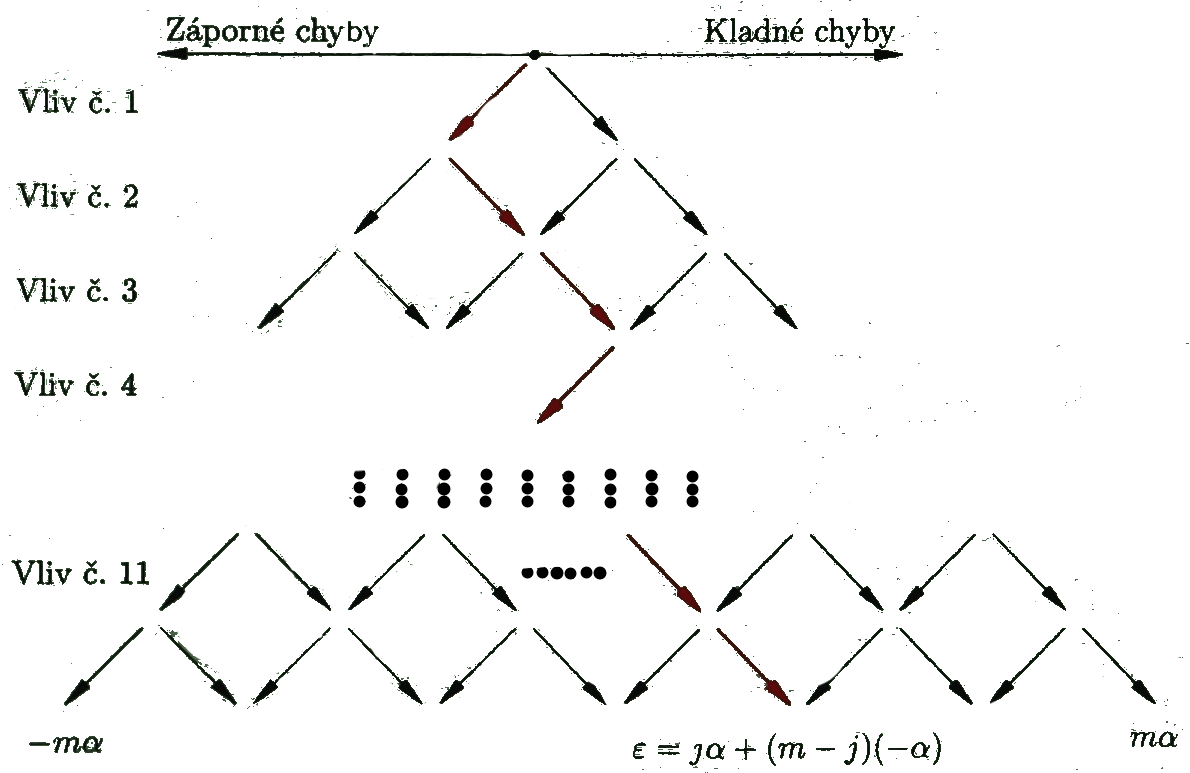
\includegraphics[width=0.6\linewidth]{mai_fig050.png}
        \caption{Vznik kladných a záporných odchylek při měření s \(m\) vlivy. 
        \cite[s.~255]{Musilova2009MA1}}
        \label{mai:fig050}
      \end{figure}
      
      Mohlo by tomu být i naopak, slova „zdar“ a „nezdar“ zde nemají svůj obvyklý význam, jde
      pouze o to, že díky nim můžeme hned uvidět souvislost s Bernoulliovým pokusem a tedy
      i s Bernoulliovým rozdělením. Při \(j\) kladných a \(m — j\) záporných odchylkách je měření od
      správné hodnoty odkloněno o
      \begin{equation*}
        j\alpha + (m - j)(-\alpha) = (2j - m)\alpha
      \end{equation*}
      s pravděpodobností
      \begin{equation*}
        p_j = \begin{pmatrix}m j\end{pmatrix}p^j(1 - p)^{m - j} = 2^{-m}.
      \end{equation*}
      Střední hodnota náhodné veličiny \(\varepsilon\) je nulová. Skutečně, v příkladu 
      \ref{mai:exam066} jsme zjistili, že střední hodnota veličiny \(Y\) nabývající hodnot \(y_j = 
      j\) s Bernoulliovým rozdělením je \(\langle y \rangle = mp\), střední hodnota veličiny \((2j 
      — m)\) a pak musí být \((2mp — m)\alpha\). Pro \(p = \num{0.5}\) je tato hodnota nulová.
      Pro velká \(m\) lze Bernoulliovo rozdělení nahradit rozdělením normálním (obr. 3.8), a proto 
      má náhodná veličina \(\varepsilon\) hustotu pravděpodobnosti tvaru (\ref{mai:eq069}), tj.
      \begin{equation*}
        \mathcal{w}(\varepsilon) = 
        \dfrac{1}{\sigma\sqrt{2\pi}}\exp\left(\dfrac{-\varepsilon^2}{2\sigma^2}\right).   
      \end{equation*}
      \begin{figure}[ht!] %\ref{mai:fig051}
        \centering
        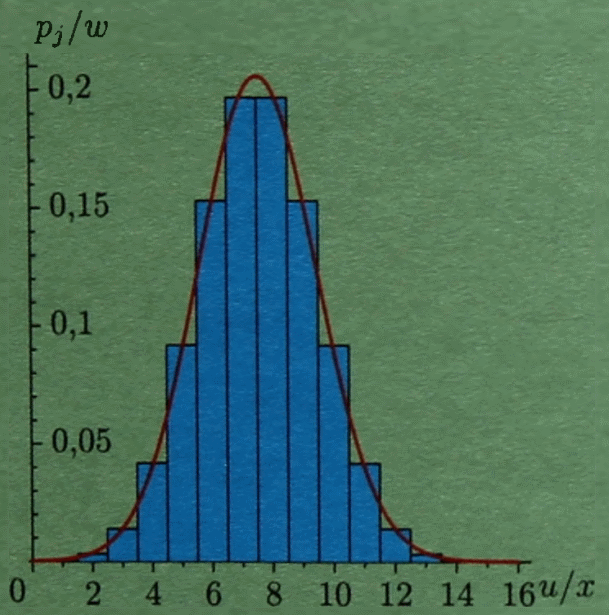
\includegraphics[width=0.4\linewidth]{mai_fig051.png}
        \caption{Normální rozdělení jako limitní případ Bernoulliova 
        \cite[s.~256]{Musilova2009MA1}}
        \label{mai:fig051}
      \end{figure}
      
      Vraťme se nyní k otázce zpracování naměřených hodnot \(\lbrace x_1, \ldots, x_n\rbrace\) 
      výšky válečku. Jejich odchylky od správné hodnoty jsou \(x_1 - x\) až \(x_n - x\). Na místě 
      neznámé správné hodnoty \(x\) si nyní představme nějakou proměnnou, označme ji 
      \(\varepsilon\). Budeme se snažit určit její hodnotu \(\varepsilon_0\) tak, aby 
      pravděpodobnost, že odchylky jednotlivých měřených hodnot od \(\varepsilon_0\) padnou 
      současně do intervalů
      \begin{equation*}
        \left(\varepsilon_1 - \dfrac{\dd{\varepsilon_1}}{2}, 
              \varepsilon_1 + \dfrac{\dd{\varepsilon_1}}{2}
        \right),
        \left(\varepsilon_2 - \dfrac{\dd{\varepsilon_2}}{2}, 
              \varepsilon_2 + \dfrac{\dd{\varepsilon_2}}{2}
        \right), \cdots,
        \left(\varepsilon_n - \dfrac{\dd{\varepsilon_n}}{2}, 
              \varepsilon_n + \dfrac{\dd{\varepsilon_n}}{2}
        \right),
      \end{equation*}
      byla maximální. Pro tuto pravděpodobnost v závislosti na \(\xi\) platí
      \begin{align}
        \dd{W} &= \dd{\mathcal{w}(\varepsilon_1)}\cdots\dd{\mathcal{w}(\varepsilon_n)}  \nonumber\\
               &= \dfrac{1}{\sigma\sqrt{2\pi}}
                  \exp\left(-\dfrac{(x_1 - \xi)^2 + \cdots + (x_n - \xi)^2}{2\sigma^2}
                      \right)\dd{\varepsilon_1}\cdots\dd{\varepsilon_n}.      \label{mai:eq072}
      \end{align}
      (Víte proč je ve vztahu (\ref{mai:eq072}) součin pravděpodobností?) Tato pravděpodobnost bude 
      maximální, bude-li hodnota exponentu minimální. Z podmínky
      \begin{equation*}
        (x_1 - \xi)^2 + \cdots + (x_n - \xi)^2 = \text{min}
      \end{equation*}
      dostáváme derivací podle \(\xi\) požadavek
      \begin{equation*}
        2(x_1 - \xi) + \cdots + 2(x_n - \xi) = 0 \Rightarrow \xi_0 = 
        \dfrac{1}{n}\sum_{i=1}^{n}x_j = \langle x \rangle.
      \end{equation*}
      Vidíme, že veličina, která charakterizuje míru odchýlení naměřených hodnot od \(\xi\), je 
      minimální, zvolíme-li za \(\xi\) aritmetický průměr naměřených hodnot. Pozor, zjištěný 
      výsledek znamená právě jen konstatovanou skutečnost: Při dosazení aritmetického průměru za 
      proměnnou \(\xi\) bude pravděpodobnost, že odchylky jednotlivých měření od \(\xi\) budou 
      ležet v uvažovaných intervalech, maximální. Neznamená to, že správnou hodnotou veličiny \(X\) 
      je aritmetický průměr měření \(x_1, X_2, \ldots, x_n\). Správnou hodnotu ze souboru měření 
      prostě nezjistíme, avšak aritmetický průměr je jí blízký s vysokou pravděpodobností. Jaká je 
      tato „blízkost“ a její pravděpodobnost konkrétně? Hned uvidíme. Správnou hodnotu výšky 
      válečku \(x\) sice neznáme, ale víme, že náhodná veličina \(\varepsilon\), jejíž hodnoty jsou 
      odchylkami výsledků měření od této (neznámé) správné hodnoty, se řídí normálním rozdělením s 
      nulovou střední hodnotou. Potřebujeme stanovit další důležitý parametr tohoto rozdělení, 
      směrodatnou odchylku \(\sigma\). Tu lze vyjádřit velmi jednoduše. Je totiž střední hodnotou 
      náhodné veličiny \(\varepsilon^2\), tedy aritmetickým průměrem čtverců odchylek 
      \(\varepsilon_i\): 
      \begin{equation*}
        \sigma^2 = D(\varepsilon) = \dfrac{1}{n}\sum_{i=1}^{n}\varepsilon_i^2.
      \end{equation*}
      Ať je však tento vzorec jakkoli jednoduchý, k čemu může sloužit, nedokážeme-li jej vyčíslit?
      Když přece neznáme správnou hodnotu \(x\), nemáme k dispozici ani hodnoty \(\varepsilon_i\). 
      Ani tato kaše však není tak horká, jak se zdá: Odchylku výsledku \(i\)-tého měření od 
      aritmetického průměru označme \(\delta_i = x_i - \langle x \rangle\), přičemž jsme již dříve 
      označili jako \(\varepsilon_i= x_i - x\) odchylku výsledku \(i\)-tého měření pd správné 
      hodnoty. Platí
      \begin{equation*}
        \sum_{i=1}^{n}\varepsilon_i = \sum_{i=1}^{n}(x_i - x) \Rightarrow 
        \sum_{i=1}^{n}x_i = \sum_{i=1}^{n}\varepsilon_i + nx, 
      \end{equation*}
      odkud 
      \begin{equation*}
        \langle x \rangle = x + \dfrac{1}{n}\sum_{i=1}^{n}\varepsilon_i.
      \end{equation*}
      Pak dostaneme
      \begin{equation*}
        \delta_i = (x_i - x) - \dfrac{1}{n}\sum_{i=1}^{n}\varepsilon_i 
                 = \varepsilon_i - \dfrac{1}{n}\sum_{j=1}^{n}\varepsilon_j.
      \end{equation*}
      Součet čtverců odchylek \(\delta_i\) je
      \begin{align*}
        \sum_{i=1}^{n}\delta_i^2 
          &= \sum_{i=1}^{n}\left(\varepsilon_i - 
             \dfrac{1}{n}\sum_{j=1}^{n}\varepsilon_j\right)^2 = \sum_{i=1}^{n}\varepsilon_i^2 - 
             \dfrac{2}{n}\sum_{i=1}^{n}\sum_{j=1}^{n}\varepsilon_i\varepsilon_j + 
             \dfrac{1}{n^2}\sum_{i=1}^{n}\left(\sum_{j=1}^{n}\varepsilon_j\right)^2     \\
          &= \sum_{i=1}^{n}\varepsilon_i^2 - 
             \dfrac{1}{n}\left(\sum_{j=1}^{n}\varepsilon_j\right)^2                     
             \doteq \left(1 - \dfrac{1}{n}\right)\sum_{i=1}^{n}\varepsilon_i^2.
      \end{align*}
      Při poslední úpravě jsme pro získání výsledného přibližného vyjádření součtu čtverců odchylek
      \(\delta_i\) použili následující úvahy:
      \begin{equation*}
        \left(\sum_{j=1}^{n}\varepsilon_j\right)^2 = \sum_{i=1}^{n}\varepsilon_i^2 + 
        2\sum_{i=1}^{n}\sum_{j>1}\varepsilon_i\varepsilon_j \doteq \sum_{i=1}^{n}\varepsilon_i^2,
      \end{equation*}
      neboť při rovnocenném zastoupení kladných a záporných odchylek je druhý sčítanec, obsahující
      součiny \(\varepsilon_i\varepsilon_j\), zanedbatelný proti prvnímu. Nakonec tedy dostáváme
      \begin{equation*}
        \sum_{i=1}^{n}\delta_i^2 \doteq \dfrac{n-1}{n}\sum_{i=1}^{n}\varepsilon_i^2 = (n-1)\sigma^2.
      \end{equation*}
      Protože odchylky \(\delta_i\) již z daného souboru měření určit můžeme (jsou to odchylky 
      jednotlivých měření od jejich aritmetického průměru), získali jsme alespoň přibližný vztah 
      pro směrodatnou odchylku rozdělení veličiny \(\varepsilon\), 
      \begin{equation}\label{mai:eq074}
        \sigma = \left(\dfrac{1}{n-1}\sum_{i=1}^{n}\delta_i^2\right)^{\dfrac{1}{2}}.
      \end{equation}
      Jaký význam má tato hodnota pro náš soubor měření? Vymezuje interval
      \begin{equation*}
        (x - \sigma, x + \sigma),
      \end{equation*}
      symetrický kolem (stále neznámé) správné hodnoty výšky válečku \(x\), do kterého padne 
      výsledek měření této výšky s pravděpodobností \SI{68.3}{\percent} (příklad 
      \ref{mai:exam069}). Neznámá správná hodnota je tedy naopak s toutéž pravděpodobností vzdálena 
      od výsledku jednotlivého měření o méně než \(\sigma\). A to už je docela slušná informace o 
      tom, kde správná hodnota může ležet. Polohu \(x\) však můžeme „omezit“ ještě lépe. Směrodatná 
      odchylka \(\overline{\sigma}\) rozdělení, které přísluší aritmetickému průměru, je
      totiž ještě \(\sqrt{n}\)-krát menší než \(\sigma\), tj. \(\overline{\sigma}= 
      \sigma/\sqrt{n}\). Správná hodnota \(x\) (navždy neznámá) je tedy od aritmetického průměru 
      výsledků měření \(\langle x \rangle\) vzdálena s pravděpodobností \SI{68.3}{\percent} o méně 
      než \(\overline{\sigma}\). Použijeme-li krajní chybu \(\overline{\kappa} = 
      3\overline{\sigma}\) (příklad \ref{mai:exam069}), můžeme říci, že správná hodnota \(x\) je od
      aritmetického průměru souboru měření \(\langle x \rangle\) vzdálena o méně než 
      \(\overline{\kappa}\) s pravděpodobností \SI{99.7}{\percent}. Více se o správné hodnotě výšky 
      válečku říci nedá. Ale i tak jsme ji lokalizovali docela úspěšně. Následující příklad 
      ukazuje vyhodnocení konkrétního souboru měření.

      %-- Měříme výšku válečku----------------------------------------
      \input{../src/MAI/exam/exam077.tex}
      %---------------------------------------------------------------
      Na závěr odstavce si všimneme ještě jedné důležité otázky. Formulujeme ji pro případ určení
      hustoty válečku. Změřili jsme výšku válečku \(x\) a jeho poloměr \(r\), vážením jsme určili 
      také jeho hmotnost \(m\). Získali jsme tak intervaly
      \begin{equation*}
        \left(\langle x \rangle - \overline{\sigma}(x), 
              \langle x \rangle + \overline{\sigma}(x)\right), \qquad
        \left(\langle r \rangle - \overline{\sigma}(r), 
              \langle r \rangle + \overline{\sigma}(r)\right), \qquad
        \left(\langle m \rangle - \overline{\sigma}(m), 
              \langle m \rangle + \overline{\sigma}(m)\right).
      \end{equation*}
      
      Směrodatná odchylka v případě každé z veličin \(x\), \(r\) a \(m\) určuje velikost intervalu 
      se středem daným aritmetickým průměrem všech měření této veličiny, v němž leží správná 
      hodnota s pravděpodobností \SI{68.3}{\percent}. Průměrná hustota válečku je dána vztahem
      \begin{equation*}
        \varrho = \dfrac{m}{V} = \dfrac{m}{\pi r^2x},
      \end{equation*}
      je tedy funkcí tří proměnných \(x\), \(r\), \(m\). Jak stanovíme interval, v němž leží 
      správná hodnota hustoty s pravděpodobností rovněž \SI{68.3}{\percent}? Hustotu totiž neměříme 
      přímo, ale vypočítáváme z přímo měřených veličin. Abychom mohli na tuto otázku odpovědět 
      matematicky korektně, potřebujeme základní znalosti o funkcích více proměnných. Závěr tohoto 
      odstavce lze tedy do důsledku pochopit po přečtení kapitoly o funkcích více proměnných. Proto 
      jej v tuto chvíli klidně přeskočte.
      
      Předpokládejme, že veličina \(z\) je pro jednoduchost pouze funkcí dvou nezávislých náhodných
      veličin \(x\) a \(y\), \(z = f(x,y)\). Jsou-li chyby \(\varepsilon_i(x)\), resp. 
      \(\varepsilon_i(y)\), kterých jsme se dopustili při \(i\)-tém měření veličiny \(x\), resp. 
      \(y\) velmi malé, můžeme pro vyjádření malé změny veličiny \(z\) způsobené chybami veličin 
      \(x\) a \(y\) použít úplného diferenciálu
      \begin{equation*}
        \dd{z} = \dd{f(x,y)} = \left(\pder{f(x,y)}{x}\right)\dd{x} + 
                               \left(\pder{f(x,y)}{y}\right)\dd{y}
      \end{equation*}
      Pro chybu veličiny \(z\) pak platí
      \begin{equation*}
        \varepsilon_i(z) = \left(\pder{f}{x}\right)\varepsilon_i(x) + 
                           \left(\pder{f}{y}\right)\varepsilon_i(y) \Rightarrow
      \end{equation*}
      \begin{equation*}
        \Rightarrow \sum_{i=1}^{n}\varepsilon_i^2(z) 
        =  \sum_{i=1}^{n}\left(\pder{f}{x}\right)^2\varepsilon_i^2(x) 
        +  \sum_{i=1}^{n}\left(\pder{f}{y}\right)^2\varepsilon_i^2(y)
        + 2\sum_{i=1}^{n}\left(\pder{f}{x}\right)^2\left(\pder{f}{y}\right)^2\varepsilon_i(x)
          \varepsilon_i(y).
      \end{equation*}
      Vzhledem k rovnocennému zastoupení kladných a záporných odchylek je součet obsahující
      součiny \(\varepsilon_i(x)\varepsilon_i(y)\) zanedbatelný proti zbytku výrazu. Pak
      \begin{equation*}
        \sum_{i=1}^{n}\varepsilon_i^2(z) \doteq \left(\pder{f}{x}\right)^2
        \sum_{i=1}^{n}\varepsilon_i^2(x) + 
                      \left(\pder{f}{y}\right)^2\sum_{i=1}^{n}\varepsilon_i^2(y) 
        = \left(\pder{f}{x}\right)^2 n\sigma^2(x) + \left(\pder{f}{y}\right)^2n\sigma^2(y).
      \end{equation*}
      Odtud, vzhledem k platnosti vztahu
      \begin{equation*}
        \sum_{i=1}^{n}\varepsilon_i^2 = n\sigma^2(z),
      \end{equation*}
      dostáváme
      \begin{equation}\label{mai:eq075}
        \sigma^2(z) = \left(\pder{f}{x}\right)^2\sigma^2(x)
                    + \left(\pder{f}{y}\right)^2\sigma^2(y).
      \end{equation}
      Parciální derivace funkce \(f(x, y)\) podle \(x\), resp. \(y\) je třeba vyčíslit dosazením 
      \(x = \langle x\rangle\) a \(y = \langle y \rangle\). Zobecnění tohoto vzorce na případ, kdy 
      hledaná veličina je funkcí více proměnných, je jednoduché.
      
    \subsection{Lineární závislost a metoda nejmenších čtverců}
      Tento poslední odstavec se zabývá zpracováním měření veličin, které jsou vázány lineárním
      vztahem (už zase ta linearita). Situaci si opět snadno představíme na jednoduchém příkladu
      Víme, že pro elektrické vodiče platí za jistých okolností \emph{Ohmův zákon}. Podle něj je 
      proud \(I\) protékající vodičem, třeba drátem, přímo úměrný napětí \(U\) mezi konci vodiče. 
      Konstanta úměrnosti ve vztahu
      \begin{equation*}
        U = R\cdot I
      \end{equation*}
      představuje \emph{elektrický odpor vodiče} \(R\). Změříme-li napětí a proud, můžeme určit 
      odpor vodiče, pokud Ohmův zákon opravdu platí. Mohli bychom tedy postupovat například tak, že 
      bychom při několika různých hodnotách napětí \(\lbrace U_1, U_2, \ldots, U_n \rbrace\) 
      (napětí bychom mohli například postupně zvyšovat) změřili proud protékající vodičem, tj. 
      \(\lbrace I_1, I_2, \ldots, I_n \rbrace\), a určili odpovídající hodnoty odporu \(R_1 = 
      U_1/I_1\), \(R_2 = U_2/I_2\), \(\ldots\), \(R_n = U_n/I_n\)  Protože by měřené hodnoty napětí 
      i proudu byly ovlivněny náhodnými vlivy a byly tak zatíženy chybami, byly by získané hodnoty 
      odporu obecně různé, i když blízké. Zpracovali bychom je podobně jako soubor \(\langle x_1, 
      x_2, \ldots, x_n \rangle\) při měření výšky válečku. Co když ale Ohmův zákon neplatí? Máme-li 
      k dispozici změřený soubor odpovídajících si hodnot napětí a proudu, můžeme Ohmův zákon pro 
      daný případ dokonce ověřit. Nebudeme však z jednotlivých údajů \(U_i\) a \(I_i\) počítat 
      hodnoty \(R_i\) a pak je průměrovat, ale zpracujeme celý soubor měření „najednou“. Představme 
      si dvojice \([U_i, I_i]\) jako body grafu. Kdyby měření napětí ani proudu nebyla zatížena 
      chybami a kdyby přesně platil Ohmův zákon, ležely by body grafu přesně na přímce. Odpor 
      vodiče bychom pak, s uvážením jednotek na osách, určili jako její směrnici (resp. v našem 
      případě, kdy na vodorovnou osu nanášíme napětí a na svislou osu proud, je směrnicí převrácená 
      hodnota odporu). Pro každou dvojici odpovídajících si hodnot napětí a proudu by mělo platit
      \begin{equation*}
        U_1 = R\cdot I_1, U_2 = R\cdot I_2, \ldots, U_n = R\cdot I_n.
      \end{equation*}
      Předchozí zápis můžeme chápat jako nehomogenní soustavu \(n\) lineárních rovnic pro jedinou
      neznámou \(R\). Rozšířená matice této soustavy je
      \begin{equation*}
        \overline{B} = (A|B) = 
          \left(
            \begin{array}{c|c}
              I_1    & U_1     \\
              I_2    & U_2     \\
              \cdots & \cdots  \\
              \cdots & \cdots  \\
              I_n    & U_n
            \end{array}
          \right).
      \end{equation*}
      Matice soustavy \(A\) má hodnost \(h(A) = 1\), matice \(\overline{B} = (A|B)\) však bude mít 
      vlivem chyb měření hodnost \(h(\overline{B}) = 2\). Soustava tedy obecně nemá řešení. Je 
      „přeučena“, neboť máme více nezávislých rovnic a jen jednu neznámou. Přímku, která by 
      procházela všemi body grafu, nenajdeme. Položíme si proto splnitelný úkol: Budeme hledat 
      přímku, která by se co „nejlépe přimykala“ k souboru bodů grafu. Tento požadavek je třeba 
      matematicky formulovat, jinak bude k nepotřebě. Označme hledanou hodnotu odporu \(R\). Pokud 
      by hodnoty \(\lbrace I_1, I_2, \ldots, I_n \rbrace\) byly bezchybné, odpovídaly by jim 
      hodnoty napětí \(\lbrace R_1\cdot I_1, R_2\cdot I_2, \ldots, R_n\cdot I_n \rbrace\). Odchylky 
      skutečně naměřených napětí \(\lbrace U_1, U_2, \ldots, U_n \rbrace\) od těchto „teoretických“ 
      jsou
      \begin{equation*}
        \lbrace U_1 - R_1\cdot I_1, U_2 - R_2\cdot I_2, \ldots, U_n - R_n\cdot I_n \rbrace.
      \end{equation*}
      Součet jejich čtverců je funkcí veličiny \(R\), kterou na chvíli považujme za proměnnou:
      \begin{equation*}
        D(R) = \sum_{i = 1}^{n}(U_i - R_i\cdot I_i)^2.
      \end{equation*}
      Řekneme, že se přímka o rovnici \(U = R\cdot I\) nejlépe přimyká k souboru bodů \(\lbrace[ 
      U_i, I_i]\rbrace\) právě tehdy, je-li \(R\) zvoleno tak, aby hodnota \(D(R)\) byla co 
      nejmenší. Nutnou podmínkou pro minimum funkce \(D(R)\) je nulovost její derivace,
      \begin{equation*}
        \der{D(R)}{R} = -2\sum_{i = 1}^{n}(U_i - R_i\cdot I_i)I_i = 0,
      \end{equation*}
      odkud
      \adjustbox{minipage=[c]{\textwidth}}{%
        \begin{equation}\label{mai:eq073}
          R=  \dfrac{\sum_{i = 1}^{n}U_i\cdot I_i}{\sum_{i = 1}^{n}I_i^2}.
        \end{equation}
      }
      Předchozím vztahem je určena hodnota odporu. Jejím dosazením do vzorce pro \(D(R)\) zjistíme
      odpovídající odchylku
      \adjustbox{minipage=[c]{\textwidth}}{%
        \begin{equation*}
          \sigma(R) = \sqrt{\dfrac{D(R)}{n-1}}.
        \end{equation*}
      }
      Velikost \(\sigma(R)\) dává informaci o tom, jak „dobře“ vyhovuje testovaný soubor měření 
      zvolenému fyzikálnímu modelu, v tomto případě lineární závislosti.

      %-- Ověření Ohmová zákona---------------------------------------
      \input{../src/MAI/exam/exam076.tex}
      %---------------------------------------------------------------
      
      Popsaný způsob nalezení hodnoty elektrického odporu vodiče se nazývá\textbf{ metodou 
      nejmenších čtverců} (minimalizuje součet čtverců odchylek prokládané závislosti od souboru 
      naměřených bodů), v případě použití lineárního modelu, jako tomu bylo u Ohmová zákona, pak 
      jde o \textbf{lineární regresi}
      
      Obdobně se postupuje, je-li některá z měřených veličin lineární funkcí veličin jiných s 
      neznámými koeficienty lineární kombinace. Nechť
      \begin{equation*}
        Z = f(X_1, X_2, \ldots, X_K) = A_1X_1 + A_2X_2 + \cdots + A_KX_K.
      \end{equation*}
      Předpokládejme, že veličiny \(X_1, X_2, \ldots, X_K\) a \(Z\) měříme \(n\)-krát a naměříme 
      hodnoty
      \begin{equation*}
        X_j = \lbrace x_{j1}, \ldots x_{jn} \rbrace, \qquad 1 \leq j \leq K, \qquad 
        Z = \lbrace z_{1}, \ldots z_{n} \rbrace
      \end{equation*}
      Součet čtverců odchylek teoretické závislosti od naměřených bodů je
      \begin{equation*}
        D(Z) = \sum_{i=1}^{n}\left(z_i - \sum_{j=1}^{K}A_jx_{ji}\right)^2.
      \end{equation*}
      Nutnou podmínkou pro minimum tohoto výrazu jakožto funkce proměnných \(A_x, A_2, \ldots, A_K\)
      je platnost souboru rovnic
      \begin{equation*}
        \pder{D(Z)}{A_p} = 0 \Rightarrow 
        \sum_{i=1}^{n}2\left(z_i - \sum_{j=1}^{K}A_jx_{ji}\right)\cdot x_{pi} = 0
      \end{equation*}
      pro \(1 \leq i \leq n, 1 \leq j \leq K\). Tyto podmínky představují nehomogenní soustavu 
      \(K\) rovnic pro \(K\) neznámých \(( A_1, A_2, \ldots, A_K)\). Rozšířená matice soustavy je
      \begin{equation*}
        \overline{B} = (A|B) = 
          \left(
            \begin{array}{cccc|c}
              \sum_{i=1}^{n}x_{1i}x_{1i} & \sum_{i=1}^{n}x_{1i}x_{2i} & \cdots & 
              \sum_{i=1}^{n}x_{1i}x_{Ki} & \sum_{i=1}^{n}z_{i}x_{1i}                    \\
              \sum_{i=1}^{n}x_{1i}x_{1i} & \sum_{i=1}^{n}x_{2i}x_{2i} & \cdots & 
              \sum_{i=1}^{n}x_{2i}x_{Ki} & \sum_{i=1}^{n}z_{i}x_{2i}                    \\
                        \cdots           & \cdots & \cdots & \cdots   & \cdots          \\
              \sum_{i=1}^{n}x_{Ki}x_{1i} & \sum_{i=1}^{n}x_{Ki}x_{2i} & \cdots & 
              \sum_{i=1}^{n}x_{Ki}x_{Ki} & \sum_{i=1}^{n}z_{i}x_{Ki}                    \\
            \end{array}
          \right),
      \end{equation*}
      \begin{equation*}
        \sigma(z) = \sqrt{\dfrac{D(z)}{n - K}}.
      \end{equation*}
      V dalších kapitolách věnovaných lineární algebře se k tomuto problému znovu vrátíme a 
      ukážeme, že jej lze elegantně řešit také jako úlohu algebraickou, konkrétně úlohu o 
      ortogonální projekci vektorů na podprostory.
      
%} %tikzset
%---------------------------------------------------------------------------------------------------
\printbibliography[heading=subbibliography]
\addcontentsline{toc}{section}{Seznam literatury}
%  % !TeX spellcheck = cs_CZ
%{\tikzset{external/prefix={tikz/MAI/}}
% \tikzset{external/figure name/.add={ch07_}{}}
%---------------------------------------------------------------------------------------------------
% file: chap_Int_rfce_1var.tex
%---------------------------------------------------------------------------------------------------
%===================================================================================================
% ------------------------------------------- Definite Integral -----------------------------------
\chapter{Určitý integrál}
\minitoc

\section{Motivace} 

  \begin{figure}
    \centering
    \animategraphics[controls,autoplay,loop]{2}{mai_fig022}{}{}
    \caption{text
             (\cite[s.~10000]{Feynman01})}
  \end{figure}

  \begin{figure}[ht!]  %\ref{mai:fig031}
    \centering
    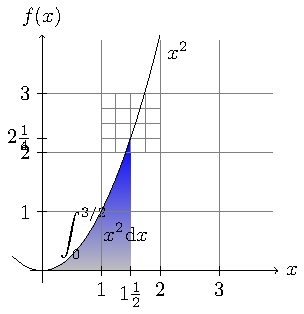
\includegraphics[width=0.7\linewidth]{mai_fig031.pdf}
    \caption{
            (\cite[s.~10000]{Feynman01})}
    \label{mai:fig031}
  \end{figure}

  \subsection{Výpočet integrálu}
      \begin{example}
        Spočítejme integrál $\displaystyle \int_1^{ln5}{(x+1)e^xdx}$  metodou per partes: 
        \begin{align*}
          \int{(x+1)e^xdx} &= \int{e^xdx}+\int{x\cdot e^xdx}
                            = e^x + (x-1)e^x = xe^x               \\
          \int_1^{ln5}{(x+1)e^xdx} &= [xe^x]_1^{ln5} = 5ln5-e     \\
        \end{align*}
        kde integrál
        \begin{equation*}
            \int{xe^xdx}=
              \left[\begin{array}{cc}
                u=x   & dv=e^x \\
                du=dx & v=e^x
              \end{array}\right]=
              xe^x-\int{e^xdx} = xe^x - e^x+C
        \end{equation*}
      \end{example}

\section{Vlastnosti určitého integrálu}
  V této kapitole mluvíme o spojitých funkcích $\Rightarrow$ příslušné integrály tedy vždy
  existují. Čerpáno z knih:
  \cite{Knichal}.

  \begin{lemma}
    \textbf{První věta o střední hodnotě integrálního počtu}: Je-li funkce $f(x)$ spojitá v
    intervalu $\langle a, b\rangle$, existuje alespoň jeden takový bod $c\in(a, b)$, že platí

    \begin{equation}\label{MA:eq_av1}
      \int_a^b f(x)dx = (b-a)f(c).
    \end{equation}
  \end{lemma}

  \begin{proof} Použitím Lagrangeovy věty napsané pro funkci $F(x)$, primitivní na intervalu
    $\langle a, b\rangle$ k dané funkci $f(x)$. Podmínky věty jsou zřejmě splněny: $F(x)$ je
    spojitá na intervalu $\langle a, b\rangle$ a má všude derivaci $F'(x)= f(x)$. Tedy existuje
    alespoň jeden bod $c\in(a, b)$,
    
    \begin{figure}[ht!]  %\ref{mai:fig029}
      \centering
      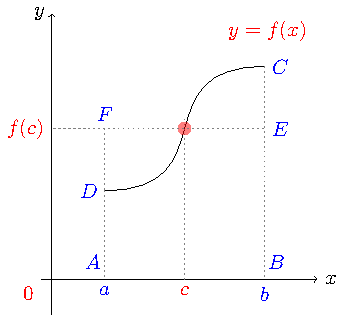
\includegraphics[width=0.7\linewidth]{mai_fig029.pdf}
      \caption{Vztah mezi silou tření a kolmou silou při smýkání
              (\cite[s.~173]{Feynman01})}
      \label{mai:fig029}
    \end{figure}

     že $$F(b)-F(a) = (b-a)F'(c),$$ čímž je věta dokázána, neboť $F(b)-F(a) = \int_a^bf(x)dx$ a
     $F'(c) = f(c)$. Funkční hodnotu $f(c)$, danou podle (\ref{MA:eq_av1}) rovnicí  
     \begin{equation}\label{MA:eq_av2}
        f(c) = \frac{1}{b-a}\int_a^b f(x)dx
     \end{equation}
     nazýváme \texttt{střední hodnotou}.
  \end{proof}

  Pro spojitou nezápornou funkci $f(x)$, lze větu o střední hodnotě jednoduše geometricky
  interpretovat dle (obr.\ref{mai:fig029}). Levá strana (\ref{MA:eq_av1}) určuje obsah
  křivočarého lichoběžníka $ABCD$, pravá strana obsah obdélníka $ABEF$. Podle této věty nabývá
  funkce $f(x)$ aspoň v jednom bodě intervalu $(a, b)$ takové hodnoty $f(c)$, že uvažovaný
  křivočarý lichoběžník má stejný obsah jako obdélník o základně $b-a$ a výšce $f(c)$ (str. 155
  knihy \cite{Knichal}).

      %---------------------------------------------------------------
      \input{../src/MAI/exam/exam032.tex}
      %---------------------------------------------------------------

  \begin{example} Efektivní hodnota $i_{ef}$ střídavého proudu $$i(t) = I_0\sin\omega t$$ (viz
    předchozí příklad) je definována jako odmocnina ze střední hodnoty funkce $i^2(t)$ v průběhu
    jedné periody $T = \frac{2\pi}{\omega}$. Tedy
    \begin{align*}
      i_{ef}^2 &= \frac{1}{T}\int_0^T I_0^2\sin^2\omega t\dd{t} = 
                  \frac{1}{T}\int_0^T \frac{I_0^2}{2}(1- \cos2\omega t)\dd{t}           \\
               &= \frac{I_0^2}{2T}
                  \left[
                    t-\frac{\sin2\omega t}{2\omega}
                  \right]_0^T = \frac{I_0^2}{2}
    \end{align*}
    neboť $\sin2\omega T=\sin4\pi = 0.$ Odtud $$i_{ef} = \frac{I_0}{\sqrt{2}}.$$ Střídavý proud
    $i(t) = I_0\sin\omega t$ má na témže odporu stejný výkon jako stejnosměrný proud o intenzitě
    $i = 0,707I_0$.
  \end{example}
  Následující věta může být využita k odhadu některých integrálů
  \begin{lemma}
    \textbf{Druhá věta o střední hodnotě integrálního počtu}: Jsou-li funkce $f(x)$ a $g(x)$
    spojité v intervalu $\langle a, b \rangle$ a je-li funkce $g(x)$ v $\langle a, b \rangle$
    nezáporná a nerostoucí, existuje alespoň jeden bod $c\in\langle a, b \rangle$ tak, že platí
    \begin{equation}\label{MA_eq_av3}
        \int_a^b f(x)g(x) = g(a)\int_a^c f(x)dx.
    \end{equation}
  \end{lemma}
  Zcela obdobnou větu lze vyslovit pro případ, že $g(x)$ je v intervalu $\langle a, b \rangle$
  nezáporná a neklesající, tj. na pravé straně \ref{MA_eq_av3} je pak integrál $g(b)\int_c^b
  f(x)dx$

  \begin{example} Odhadněte hodnotu integrálu
    \begin{equation}\label{MA_eq_sinx_x}
        \int_{100\pi}^{1000\pi}\frac{\sin x}{x}dx
    \end{equation}
    Řešení: Funkce $f(x) = \sin x$ a $g(x) = \frac{1}{x}$ jsou v uvažovaném intervalu $\langle
    100\pi, 1000\pi \rangle$ spojité a funkce $g(x)$ je kladná a nerostoucí.
    \begin{equation*}
      \int_{100\pi}^{1000\pi}\frac{\sin x}{x}dx = 
      \frac{1}{100\pi}\int_{100\pi}^c\sin xdx =\frac{1}{100\pi}\left(\cos100\pi - \cos c\right)
    \end{equation*}
    kde $c$ je kladné číslo z intervalu $\langle 100\pi, 1000\pi \rangle$. Dále pro všechna
    $c\in\langle 100\pi, 1000\pi \rangle$ platí $0\leq1-\cos c\leq2$, takže
    \begin{equation*}
        0\leq\int_{100\pi}^{1000\pi}\frac{\sin x}{x}dx\leq \frac{1}{50\pi}.
    \end{equation*}
  \end{example}   

%} %tikzset
%---------------------------------------------------------------------------------------------------
\printbibliography[heading=subbibliography]
\addcontentsline{toc}{section}{Seznam literatury}
%  % !TeX spellcheck = cs_CZ
%{\tikzset{external/prefix={tikz/MAI/}}
% \tikzset{external/figure name/.add={ch04_}{}}
%---------------------------------------------------------------------------------------------------
% file: Theory_of_Derivates.tex
%---------------------------------------------------------------------------------------------------
\chapter{Derivace funkce}\label{mai:IchapIV}
\minitoc

%============== Kapitola: Derivace funkce ==========================================================
  \section{Základní věty diferenciálního počtu}
    \subsection{Věta o největší (nejmenší) hodnotě funkce}
      V tomto článku uvedeme významné věty, zvané souhrně věty o \emph{střední hodnotě 
      diferenciálního počtu}, a dále pak ukázky jejich užití v matematické analýze.  Avšak dříve 
      než budeme tyto věty formulovat, uvedeme jedno důležité tvrzení, které sice bude mít v 
      dalších úvahách tohoto článku pomocnou úlohu, ale v teorii extrémů má i samostatný význam. 
      \cite[s.~186]{Brabec1989} 
      \begin{lemma}\label{MA1:lem_diff02}
        Nechť funkce $f:A\rightarrow\realset$ nabývá na množině $A$ své největší (nejmenší) hodnoty 
        na vnitřním bodě $c$ množiny $A$. Máli funkce $f$ v bodě $c$ derivaci, potom $f'(c)=0$.  
      \end{lemma}
      \begin{proof}
        Nechť např. $f(c)$ je největší hodnota funkce $f$ na množině $A$, takže $f(x)\leq f(c)$ pro $\forall x\in A$. Potom pro $x\in A, x<c$, je 
        $$\frac{f(x)-f(c)}{x-c}\geq 0$$
        a tedy
        $$f'_{-}(c)=\lim_{x\rightarrow c^-}\frac{f(x)-f(c)}{x-c}\geq0$$ 
        Dále pro $x\in A, x>c$, je
        $$\frac{f(x)-f(c)}{x-c}\leq 0$$ 
        a proto
        $$f'_{+}(c)=\lim_{x\rightarrow c^+}\frac{f(x)-f(c)}{x-c}\leq0$$
        Platí tedy
        $$f'_{+}(c)\leq f'_{-}(c)\geq f'_{-}(c).$$ 
        Avšak $f'_{+}(c)=f'_{-}(c)= f'(c)$. Odtud plyne $f'(c)=0$. 
      \end{proof}
      
    \subsection{Věty o střední hodnotě}
      \begin{lemma}\label{MA1:lem_diff03}
        \textbf{Rolleova věta}\footnote{Michel Rolle [Mišel Rol] (1652-1719) Francouzský matematik} Nechť funkce $f$ má tyto vlastnosti:
          \begin{enumerate}
            \item je spojitá na uzavřeném intervalu $\langle a,b\rangle$;
            \item má derivaci (vlastní či nevlastní) na otevřeném intervalu $(a,b)$;
            \item platí $f(a)=f(b)$.
          \end{enumerate}
        Potom v otevřeném intervalu $(a,b)$ existuje aspoň jeden bod $\xi$ takový, že $f'(\xi)=0$.   
      \end{lemma}
      \begin{proof}
        Protože je funkce $f$ je na uzavřeném intervalu $\langle a,b\rangle$ spojitá, nabývá v 
        tomto intervalu své největší hodnoty $M$,své nejmenší hodnoty $m$. Přitom ovšem platí:
        \begin{equation}\label{MA1:eq_diff02}
          m\leq f(x) \leq M, \qquad x\in\langle a,b\rangle.
        \end{equation}
        Nyní mohou nastat dva případy: 
        \begin{enumerate}
          \item funkce $f$ nabývá $M$ i $m$ právě v krajních bodech intervalu $\langle a,b\rangle$. Podle předpokladu 3 věty \ref{MA1:lem_diff03}
                však potom platí $f(a)=f(b)=m=M$. Vzhledem ke vztahu \ref{MA1:eq_diff02} odtud plyne, že funkce $f$ je konstantní na intervalu
                $\langle a,b\rangle$ a tedy $f'(x)=0$ dokonce v každém bodě $x\in(a,b)$
          \item Funkce $f$ nabývá apsoň jedné z hodnot $M$, $m$ v některém vnitřním bodě $\xi$ intervalu $\langle a,b\rangle$. Potom podle 
          věty \ref{MA1:lem_diff02} je $f'(\xi)=0$.         
        \end{enumerate}        
      \end{proof}
      \begin{note}
        Rolleova věta sama zaručuje jen existenci aspoň jednoho bodu $\xi\in(a,b)$, ve kterém je fe 
        $f'(\xi)=0$. Neumožňuje však ani určení tohoto bodu (nebo bodů), ani stanovení jejich počtu 
      \end{note}
      
      \begin{note}
        Na obr. \ref{MAI:fig_027} je ilustrován geometrický význam Rolleovy věty. Graf funkce na 
        tomto obrázku má v bodech $\xi_1$, $\xi_2$, v nichž je $f'(\xi_1)=f'(\xi_2)=0$ tečny 
        rovnoběžné s osou $x$. 
        \begin{figure}[ht!] %\ref{MAI:fig_027}
          \centering
          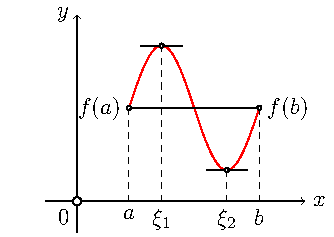
\includegraphics[width=0.7\linewidth]{mai_fig027.pdf}
          \caption{K výkladu Rolleovy věty}
          \label{MAI:fig_027}
        \end{figure}
      \end{note}
      
      Z Rolleovy věty plyne důležitá věta:
      
      \begin{lemma}\label{MA1:lem_diff04}
        (\textbf{Cauchyova věta}). Nechť funkce $f$ a $g$ mají tyto vlastnosti:
        \begin{enumerate}
          \item  Jsou spojité na uzavřeném intervalu $\langle a,b\rangle$,
          \item  v každém bodě $x\in(a,b)$ existuje derivace $f'(x)$ (vlastní či nevlastní) a vlastní derivace $g'(x)$,
          \item  $g'(x)\neq0$ na $(a,b)$
        \end{enumerate}
        Potom v otevřeném intervalu $(a,b)$ existuje aspoň jeden bod $\xi$, pro který platí
        \begin{equation}\label{MA1:eq_diff03}
          \frac{f(b)-f(a)}{g(b)-g(a)} = \frac{f'(\xi)}{g'(\xi)}.
        \end{equation} 
      \end{lemma} 
      
      \begin{proof}
        Poznamenejme především, že z předpokladu 3 $g'(x)\neq0$ pro $x\in(a,b)$ a z předpokladu 
        spojitosti funkce $g$ na uzavřeném intervalu $\langle a,b\rangle$ ihned vyplývá vztah 
        $g(b)- g(a)\neq 0$. Kdyby totiž bylo $g(b)=g(a)$, potom by podle \emph{Rolleovy věty} 
        \ref{MA1:lem_diff03} existoval aspoň jeden bod $\eta\in(a,b)$ takový že $g'(\eta)=0$. To 
        však by byl spor s předpokladem $g'(x)\neq0$ pro každý bod $x\in(a,b)$. Proto má smysl 
        podíl na levé straně rovnosti \ref{MA1:eq_diff03}
        
        K vlastnímu důkazu Cauchyovy věty zavedeme takovou pomocnou funkci $F$, aby splňovala podmínky Rolleovy věty. Definujme ji pro $x\in\langle a,b\rangle$ předpisem
        \begin{equation}\label{MA1:eq_diff04}
          F(x)=[f(b)-f(a)]\cdot[g(x)-g(a)]-[f(x)-f(a)]\cdot[g(b)-g(a)].
        \end{equation}
        Snadno ověříme, že tato funkce skutečně splňuje podmínky Rolleovy věty na intervalu $\langle a,b\rangle$:
        \begin{itemize}
          \item Je spojitá na intervalu $x\in\langle a,b\rangle$, což je důsledkem spojitosti  
                funkce $f$ a $g$ na intervalu $x\in\langle a,b\rangle$ ,
          \item má derivaci $F'$ na otevřeném intervalu $(a,b)$, což plyne z existence derivace  
                $f'$ a $g'$ funkce $f$ a $g$ na  intervalu $(a,b)$,
          \item $F(a)=F(b)=0$ 
        \end{itemize}
        Platí tedy i závěr Rolleovy věty pro funkci $F$, tj. na intervalu $(a,b)$ existuje aspoň 
        jeden bod $\xi$, pro který $F'(\xi)=0$. Zderivujeme-li funkci $F$, dostaneme (dosadíme-li 
        $x=\xi$): $$F'(\xi)=[f(b)-f(a)]g'(\xi)-f'(\xi)[g(b)-g(a)]=0$$ Odtud již plyne rovnost 
        \ref{MA1:eq_diff03}                  
      \end{proof}
      
      Významným zvláštním případem Cauchyovy věty je další věta, která se častěji používá.
      
      \begin{lemma}\label{MA1:lem_diff05}
        (\textbf{Lagrangeova věta})\footnote{Joseph Louis Lagrange [lagránž] (1736-1813), francouzský matematik}. Nechť funkce má tyto vlastnosti:
        \begin{itemize}
          \item Je spojitá na intervalu $\langle a,b\rangle$,
          \item má derivaci (vlastní či nevlastní) na otevřeném intervalu $(a,b)$. 
        \end{itemize} 
        Potom existuje v otevřeném intervalu $(a,b)$ aspoň jeden bod $\xi$, pro který platí 
        \begin{equation}\label{MA1:eq_diff05}
           \frac{f(b) - f(a)}{b - a} = f'(\xi),  
        \end{equation}  
        či-li
        \begin{equation}\label{MA1:eq_diff06}
           f(b) - f(a) = f'(\xi)(b-a),  
        \end{equation}           
      \end{lemma}
      
      \begin{proof}
        Tvrzení této věty je důsledkem tvrzení \emph{Cauchyovy věty}, a to pro případ $g(x)=x$. 
        Protože $g'(x)=1$ dokonce všude, jsou splněny všechny tři podmínky Cauchyovy věty. Proto 
        platí i závěr této věty, z něhož pro náš případ již plyne vzorec \ref{MA1:eq_diff05} a tedy 
        i vzorec \ref{MA1:eq_diff06}.  
      \end{proof}
      
      \begin{note}
        Podobně jako je Lagrangeova věta zvláštním případem věty Cauchyovy, je Rolleova věta zvláštním případem Lagrangeovy věty, a to přo případ, že $f(a)=f(b)$.
      \end{note}
      
      \begin{note}
        Lagrangeova věta se často nazývá \emph{větou o přírůstku funkce}, protože vzorcem \ref{MA1:eq_diff06} se vyjadřuje \emph{přírůstek funkce}, tj rozdíl $f(b)-f(a)$. 
        Všechny tři uvedené věty, tj. věta Rolleova, Cauchyova a Lagrangeova, se v literatuře nazývá souhrně \textbf{věty o střední hodnotě diferenciálního počtu}.
      \end{note}
      
      \begin{note}
        Na obr. ** je ilustrován geometrický význam Lagrangeovy věty. Podíl na levé straně rovnosti 
        \ref{MA1:eq_diff05}, tj. číslo $\frac{f(b) - f(a)}{b - a}$ je směrnice sečny $s$, spojující 
        body $A$, $B$ grafu funkce  $f$, které odpovídají krajním bodům intervalu $\langle 
        a,b\rangle$. Podle tvrzení Lagrangeovy věty existuje v otevřeném intervalu $(a,b)$ aspoň 
        jeden bod $\xi$ tak, že tečna grafu funkce $f$ v příslušném jeho bodě je rovnoběžná s 
        přímkou $s$.  
      \end{note}
      
      \begin{note}
        Z Lagrangeovy věty vyplývá toto tvrzení: Nechť funkce $f$ vyhovuje na intervalu $\langle a,b\rangle$ podmínkám Lagrangeovy věty a $x_1$, $x_2$ jsou dva libovolné různé body
        intervalu $\langle a,b\rangle$. Potom v otevřeném intervalu s krajnímy body $x_1$, $x_2$ existuje aspoň jeden bod $\xi$, pro který platí Lagrangeův vzorec:   
        \begin{align}
          f(x_2) - f(x_1)                  &= f'(\xi)(x_2-x_1) \label{MA1:eq_diff07} \\ 
          \frac{f(x_2) - f(x_1)}{x_2-x_1}  &= f'(\xi)          \label{MA1:eq_diff08}      
        \end{align}
        Potom bod $\xi$ lze vyjádřit takto:
        \begin{equation}\label{MA1:eq_diff09}  
          \xi = x_1 + \vartheta(x_2-x_1), \qquad \text{kde }\vartheta\in(0,1). 
        \end{equation}
        Označíme-li $x_2-x_1=h$, můžeme vzorec \ref{MA1:eq_diff07} napsat ve tvaru
        \begin{equation}
          f(x_1+h) - f(x_1)= f'(x_1 + \vartheta h)h, \qquad \text{kde }\vartheta\in(0,1). 
        \end{equation} 
      \end{note}       
          
    \subsection{Některé důsledky Lagrangeovy věty}
      Lagrangeova věta, má některé významné důsledky, které nyní uvedeme \cite[s.~189]{Brabec1989}:
      \begin{lemma}\label{MA1:lem_diff06} 
        Nechť funkce $f$ vyhovuje podmínkám Lagrangeovy věty a navíc nechť $f'(x)=0$ pro všechna 
        $x\in(a,b)$. Potom funkce $f$ je prostá na intervalu $\langle a,b \rangle$. 
      \end{lemma}
      \begin{proof}
        Necť $x_1, x_2$ jsou libovolné dva různé body intervalu $\langle a,b \rangle$. Potom podle 
        Lagrangeova vzorce \ref{MA1:eq_diff04} platí 
        \begin{equation}
          f(x_2) - f(x_1) = f'(\xi)(x_2-x_1) \neq0
        \end{equation}
        neboť $f'(\xi)\neq 0$ dle předpokladu.
      \end{proof}
      
      \begin{lemma}\label{MA1:lem_diff01}
        Funkce $f$ je konstantní na intervalu $(a,b)$, právě když má na tomto intervalu derivaci a platí $f'(x) = 0$ pro všechna $x\in(a,b)$. 
      \end{lemma}
      \begin{proof} Tedy
        \begin{itemize}
          \item Je-li funkce $f$ konstantní na intervalu $(a,b)$, pak je $f'(x) = 0$ pro všechna  
                $x\in(a,b)$, jak již víme.
          \item Nechť $f'(x) = 0$ pro všechna $x\in(a,b)$. Dokažme, že pro každé dva body $x_1, 
                x_2  \in(a,b)$, $x_1\neq x_2$, platí $f(x_1) = f(x_2)$. Z existence
                derivace vyplývá spojitost funkce a jsou tedy splněny podmínky Lagrangeovy věty na 
                každém intervalu $\langle x_1, x_2\rangle\subset(a,b)$. Podle vzorce 
                \ref{MA1:eq_diff04} tedy platí $f(x_2)-f(x_1)f'(\xi)(x_2-x_1)$, $\xi\in(x_1,x_2)$. 
                Protože podle předpokladu je $f'(x)=0$ pro $\forall x\in(a,b)$, platí $f(x_1) 
                -f(x_2)=0$, tj. $f(x_1)=f(x_2)$  
        \end{itemize}
      \end{proof}
      
%} % tikzset
%---------------------------------------------------------------------------------------------------
\printbibliography[heading=subbibliography]
\addcontentsline{toc}{section}{Seznam literatury}
%  % !TeX spellcheck = cs_CZ
%{\tikzset{external/prefix={tikz/MAI/}}
% \tikzset{external/figure name/.add={ch05_}{}}
%---------------------------------------------------------------------------------------------------
% file: Differential_Calculus_applications.tex
%---------------------------------------------------------------------------------------------------
\chapter{Aplikace diferenciálního počtu}\label{chap:Apl_dif_poc}
\minitoc

%================Kapitola: Aplikace diferenciálního počtu =========================================
Diferenciální počet má rozsáhlou oblast užití. V této kapitole ukážeme použití výsledků předchozích 
kapitol k vyšetřování průběhu funkce a vlastnosti rovinných křivek. 
  \section{Průběh funkce}
    Pomocí derivace můžeme studovat vlastnosti funkce, které usnadní vyšetřování jejího průběhu.  
    \subsection{Monotonie funkcí}
      Jednou z důležitých vlastností funkce je její \textquotedblleft monotonie\textquotedblright, 
      kterou jsme definovali již v odst. \ref{MA1:subsec_vlastnosti_funkce} kap. 
      \ref{mai:IchapLimit}. Proto je při vyšetřování průběhu funkce důležité určit množiny (často 
      jsou to intervaly), na nichž je funkce monotónní, jinak řečeno, najít \textquotedblleft 
      intervaly monotonie funkce\textquotedblright (viz \cite[s.~208]{Brabec1989}). 
    \begin{enumerate}
      \item Zjistíme \textbf{definiční obor funkce}, vyjádříme jej v intervalech a z nich poznáme,  
            kde je funkce \textbf{spojitá}. Funkce je spojitá v $(a,b)$ pro každý bod tohoto 
            intervalu, když$|f(x)-f(c)|<\varepsilon$, kde $\varepsilon>0$ je libovolně zvolené 
            číslo, a pro všechna $x$ z okolí bodu $c$ je $|x-c|<\delta$, kde $\delta>0$ je na 
            $\varepsilon$ nezávislé.
      \item Určíme, je-li funkce \textbf{lichá} $f(-x)=-f(x)$ nebo \textbf{sudá} $f(-x)=f(x)$.   
            Je-li funkce lichá, je souměrná podle středu souměrnosti (obyčejně to bývá počátek 
            souřadnic $xy$), je-li sudá, je souměrná podle osy $y$.
      \item Určíme \emph{průsečíky křivky s osami pravoúhlých souřadnic}. Body, ve kte\-rých 
            křivka  protíná osu $x$ spolu s body, ve kte\-rých není křivka spojitá, rozlišují 
            intervaly, v nichž je graf křivky nad osou $x$ od intervalů, ve kterých je graf křivky 
            pod osou $x$.
      \item V krajních bodech definičních intervalů, ve kterých je funkce spojitá, stano\-víme 
      \emph{limity funkce} a dále $$\lim_{x \to \pm \infty}f(x).$$
      \item Vypočítáme $f'(x)$ a $f''(x)$, abychom zjistily, kde je funkce \emph{rostoucí}     
            $f'(x)>0$, \emph{klesající} $f'(x)<0$ a kde jsou \emph{lokální extrémy}. Dostaneme-li 
            dosazením kořenů rovnice $f'(x)=0$ do $f''(x)$ hodnotu $f''(x)>0$, má funkce lokální 
            minimum, při $f''(x)<0$ má funkce lokální maximum. V intervalech, kde $f''(x)>0$, je 
            křivka \textbf{konvexní (vypuklá)}, kde $f''(x)<0$, je křivka \textbf{konkávní 
            (vydutá)}. Body, v nichž $f''(x)$ mění znaménko, jsou \textbf{inflexní body}. Najdeme 
            je tak, že stanovíme hodnoty $x$, pro které je $f''(x)=0$ nebo neexistuje. Číslo $c$ je 
            inflexní bod, když existuje takové okolí bodu $c$, že pro $x>c$ je oblouk křivky 
            konvexní a pro $x<c$ konkávní. Je nutné si uvědomit, že když má $f'(x)$ konečnou 
            derivaci, je inflexní bod $c$ taky nulovým bodem druhé derivace čili kořenem rovnice 
            $f''(x)=0$. Obrácená věta neplatí, tj. z $f''(x)=0$ nevyplývá, že v bodě $c$ má $f'(x)$ 
            extrém a že bod $c$ je inflexním bodem.
      \item \textbf{Asymptota} je tečna křivky $f(x)$, jejíž bod dotyku je v nekonečnu. Platí-li  
            $$\lim_{x \to a}f(x) =  \pm\infty,$$ je přímka $x=a$ její asymptotou. Jinak asymptoty 
            mají rovnici $y=kx+q$, kde $x$ a $y$ jsou souřadnice bodů na asymptotách. Existují-li 
            konečné limity $$\lim_{x \to \pm\infty}\frac{f(x)}{x}=k$$  a $$\lim_{x \to 
            \pm\infty}[f(x)-kx] =q$$ pak je asymptotou přímka $y=kx+q$. Můžeme-li rovnici křivky 
            rozložit (tj. rozložit její pravou stranu, oby\-čejně dělením čitatele jmenovatelem, 
            má-li tvar zlomku) na dvě části, z nichž jedna má tvar $kx+q$ a druhá zbytek 
            $\varphi(x)$, tj. $f(x)=kx+q+\varphi(x)$ a $\varphi(x)_{x\rightarrow 
            \pm\infty}\rightarrow 0$, je přímka $y=kx+q$ asymptotou.
      \item Zpřesnění grafu křivky provedeme sestavením tabulky souřadnic dalších bodů křivky,  
            tj. ke zvoleným hodnotám $x$ (z definičního oboru funkce) vypočítáme hodnoty $y$. Do 
            dalších řádků tabulky zapíšeme hodnoty  $f'(x)$ a $f''(x)$, ve kterých intervalech je 
            funkce \emph{rostoucí}, ve kterých \emph{klesá}, kde je \emph{vypuklá}, kde je 
            \emph{dutá}, kde jsou \emph{lokální extrémy}, \emph{inflexní body} apod., 
            případně sestavíme dílčí tabulky pro jednotlivé \emph{charakteristické vlastnosti} vyšetřované funkce.
    \end{enumerate}
    %-------------------- EXAM001 --------------------------------------
    \input{../src/MAI/exam/exam003.tex}
    %-------------------------------------------------------------------

%} %tikzset
%---------------------------------------------------------------------------------------------------
\printbibliography[heading=subbibliography]
\addcontentsline{toc}{section}{Seznam literatury} 
%  % !TeX spellcheck = cs_CZ
%{\tikzset{external/prefix={tikz/MAI/}}
% \tikzset{external/figure name/.add={ch06_}{}}
%---------------------------------------------------------------------------------------------------
% file: chap_PrimitiveFce.tex
%---------------------------------------------------------------------------------------------------
%============================ Primitivní funkce ====================================================
\chapter{Primitivní funkce}
\minitoc

  %----------------------------Neurčitý integrál----------------------------------------------------
  \section{Motivace}
    Problém \emph{neurčitého integrálu}, neboli \textbf{primitivní funkce}, lze vyložit velmi 
    jednoduše: Máme podezření, že zadaná funkce \(f(x)\) vznikla derivováním jisté, zatím neznámé, 
    funkce \(F(x)\). Dokážeme ji najít? 
  
    K danému problému můžeme přistupovat také fyzikálně: Zavedením pojmu derivace funkce jsme 
    motivovali důležitým požadavkem definovat okamžitou rychlost pohybu bodu po přímce. Existuje 
    přirozeně i požadavek opačný, tj. nalézt zákon dráhy pohybu bodu po přímce, je-li dána jeho 
    okamžitá rychlost jako funkce času \cite[s.~253]{Brabec1989}. Vše si ukážeme na následujícím 
    příkladu:  
   
    \begin{example}
      Je dána okamžitá rychlost $v$ pohybu bodu po přímce (ose) $x$ rovnicí $v(t) = 2t + 1$, 
      $t\in\langle -\infty,+\infty \rangle$. Najděte zákon dráhy pohybu, je-li známo, že v čase $t 
      = 0$ měl bod polohu $x = x_0$.
      \newline
      \textbf{řešení:}\newline
      Označíme-li $x(t)$ polohu bodu v okamžiku $t$, pak $v(t) = \frac{dx}{dt}$. Hledáme tedy 
      funkci $x = x(t)$, pro níž platí 
      \begin{align}
        \frac{dx}{dt} &= 2t + 1 \qquad x(0) = x_0.  \nonumber \\ 
        \shortintertext{Je ihned patrné, že první podmínce vyhovuje nekonečně mnoho funkcí}
        x(t)          &= t^2 + t + C,           \label{MA:int_ex_09}    \\ 
        \shortintertext{ kde $C$ je libovolná konstanta. Funkce, která splňuje i druhou podmínku 
          (říkáme ji též počáteční podmínka), najdeme z rovnice \ref{MA:int_ex_09} dosazením dané podmínky 
          $t = 0,\ x = x_0$. Dostaneme $x_0 = C$. Dosazením do \ref{MA:int_ex_09} za $C$ plyne hledaný 
          zákon dráhy}
        x(t)          &= t^2+t+x_0.                 \nonumber 
        \shortintertext{Jednoduchou zkouškou se přesvědčíme, že tato funkce splňuje obě dané podmínky a 
          zároveň vidíme, že hledaná primitivní funkce daných vlastností je jediná.}  \nonumber
      \end{align}
    \end{example} 
    Každé takové funkci, jejíž derivací je daná funkce, budeme říkat \emph{primitivní funkce} k 
    dané funkci. Na uvedeném příkladě je patrné, že k dané funkci může existovat nekonečně mnoho 
    primitivních funkcí. Množinu všech primitivních funkcí se často nazývá \textbf{neurčitým 
    integrálem}. Po tomto názorném uvedení do problému přejděme k přesné formulaci základních pojmů.
    
    \begin{definition} 
      Funkce $F: J\rightarrow \realset$, kde $J\subset \realset$ je interval, se nazývá primitivní 
      funkce k funkci \(f\) na intervalu \(J\) právě když, pro všechna $x\in J$ je $F'(x) = f(x)$ 
      (v krajních bodech intervalu \(J\), pokud k němu patří, jde o derivace jednostranné).
    \end{definition}
    
    \begin{example} 
      K funkci $\sin x$ je primitivní funkcí na libovolném intervalu $J\subset(-\infty,+\infty)$ 
      funkce $-\cos x$, protože $(-\cos x)' = \sin x$. Ale též funkce $3-\cos x$ je primitivní 
      funkcí k funkci $\sin x$, protože $(3 - \cos x)' = \sin x$ pro všechna $x\in(-\infty, 
      \infty)$.
    \end{example}
    
    Je vidět, že rozdíl dvou primitivních funkcí k téže funkci je konstanta. To není náhoda, jak 
    potvrzuje následující věta:
    
    \begin{lemma}
      \begin{enumerate}
        \item Je-li funkce $F$ primitivní funkcí k funkci \(f\) na intervalu \(J\) a \(c\) reálná  
              konstanta, pak i funkce $G = F + c$ je primitivní funkcí k funkci \(f\) na intervalu 
              \(J\).
        \item Jsou-li funkce $F$ a $G$ primitivní funkce k funkci \(f\) na intervalu \(J\), pak 
        funkce
              $F-G$ je na intervalu \(J\) konstantní.
      \end{enumerate} 
      \begin{proof}
        Tvrzení a) plyne z definice protože $G'(x) = [F(x) + c] = F'(x) = f(x)$ pro všechna $x\in
        J$. Tvrzení b) je důsledkem věty \ref{MA1:lem_diff01}.
      \end{proof}
    \end{lemma}
    Neurčitost vyplývá právě z toho, že primitivní funkce není dána jednoznačně, je určena až na 
    konstantu. Značíme
    \begin{equation*}
      \boxed{F(x) = \int f(x)\dx + C}
    \end{equation*}
        
    Jak ale primitivní funkce hledat? V jednoduchých příkladech poslouží tabulka derivací, již 
    čteme „zprava doleva“. (Je dobré si ji uložit do paměti.) Tabulka však pokryje jen velmi málo 
    případů, pouze elementární funkce. Je tedy třeba najít metody, jak při hledání primitivních 
    funkcí postupovat. Nejprve však uvedeme dvě základní pravidla pro primitivní funkce, která 
    plynou z pravidel pro derivování:
    \begin{align}
      \int[f(x)\pm g(x)]\dx &= \int[f(x)\pm g(x)]\dx + \int[f(x)\pm g(x)]\dx \label{MA1:eq_int10} \\
      \int cf(x)\dx         &= c \int f(x)\dx, \qquad \text{\(c\) je konstanta.} \label{MA1:eq_int11}
    \end{align}
  
  \section{Tabulka neurčitých integrálů}\label{MA:chap_tabINT}
    Pokud není nic uvedeno, platí vzorce pro všechna \(x\) a pro všechny hodnoty uvedených
    konstant. Místo platí pro \(x\) z intervalu \((-\infty,0),(0,+\infty)\) píšeme stručně
    \(x\neq0\) apod. Literatura: \cite[p.~396]{Rektorys1963}.
  
    \begin{flalign}
      & \int 0\dx = c                                        &         \label{MA:baseInt01}     \\
      & \int a\dx = ax+c                                     &         \label{MA:baseInt02}     \\
      & \int x^n\dx = \frac{x^{n+1}}{n+1}+c, \,              &         \label{MA:baseInt03}     \\
      & \qquad\text{kde}\begin{cases}
          \forall x\in\realset,\,n\in\naturalset, n>0,         \\
          \forall x\in\realset-\{0\},\,n\in\naturalset, n<-1,  \\
          \forall x>0,\,n\in\realset\,\,n\notin\naturalset
        \end{cases}                                          &         \nonumber               \\
      & \int\frac{1}{x}\dx = 
            \ln\abs{x}+c \hspace{1ex}\forall x\neq0          &         \label{MA:baseInt04}     \\
      & \int e^x \dx       = e^x+c                           &         \label{MA:baseInt05}     \\
      & \int\ln x\dx       = 
          x\ln x - x + c \hspace{1ex}\forall x>0             &         \label{MA:baseInt06}     \\
      & \int a^x \dx     =
          \frac{a^x}{\ln a}+c 
          \hspace{1ex}\forall a>0,\,a\neq1                   &         \label{MA:baseInt07}     \\
      & \int \sin x \dx  = -\cos x                           &         \label{MA:baseInt08}     \\
      & \int \cos x \dx  =  \sin x                           &         \label{MA:baseInt09}     \\
      & \int\frac{1}{\cos^2x}\dx =  \tan x+c 
           \hspace{1ex}\forall x\neq(2k+1)\pi,\,k\in\naturalset &      \label{MA:baseInt10}     \\ 
      & \int\frac{1}{\sin^2x}\dx     =  -\cotg x+c
         \hspace{1ex}\forall x\neq k\pi,\,k\in\naturalset    &         \label{MA:baseInt11}     \\
      & \int\frac{1}{\sqrt{1-x^2}}\dx =
          \begin{cases}
            +\arcsin x + c         \\
            -\arccos x + c
          \end{cases} 
          \forall x\in(-1,1)                                 &         \label{MA:baseInt12}     \\
      & \int\cosh\dx = \sinh x + c                           &         \label{MA:baseInt13}     \\
      & \int\sinh\dx = \cosh x + c                           &         \label{MA:baseInt14}     \\
      & \int\frac{1}{1+x^2}\dx = \arctan x + c               &         \label{MA:baseInt15}     \\
      & \int \frac{1}{\sqrt{x^2 + 1}}\dx =
          \begin{cases}
            \ln(x + \sqrt{x^2+1}) + c         \\
            \sinh^{-1}x + c 
          \end{cases}                                        &         \label{MA:baseInt16}     \\ 
      & \int \frac{1}{\sqrt{x^2 - 1}}\dx =
          \begin{cases}
            \ln(x + \sqrt{x^2-1}) + c         \\
            \cosh^{-1}x + c \hspace{4ex}x\in(1,+\infty) 
          \end{cases}                                        &         \label{MA:baseInt17}     \\
      & \int\frac{1}{\sqrt{x^2+a^2}}\dx 
        = \sinh^{-1} \frac{x}{a} = \ln (x+\sqrt{x^2+a^2})    &         \label{MA:baseInt18}     \\
      & \int \frac{1}{\sqrt{x^2-a^2}}\dx 
        = \cosh^{-1} \frac{x}{a} = \ln (x+\sqrt{x^2-a^2})    &         \label{MA:baseInt19}     \\
      & \int\frac{1}{\sqrt{x^2-1}}\dx 
        = \left\{ 
          \begin{array}{l l}
            \ln\abs{x+\sqrt{x^2-1}}+c      &  \abs{x}>1  \\
            \cosh^{-1}x+c                  &  \abs{x}<1
          \end{array} 
          \right.                                            &         \label{MA:baseInt20}     \\
      & \int\tan x \dx   = \ln |\sec x| + c                  &         \label{MA:baseInt21}     \\
      & \int\sec x \dx   = \ln |\sec x + \tan x| + c         &         \label{MA:baseInt22}     \\
      & \int\sec^2 x \dx = \tan x + c                        &         \label{MA:baseInt23}     \\
      & \int\sec x\tan x \dx = \sec x + c                    &         \label{MA:baseInt24}     \\
      & \int\frac{a}{a^2+x^2}\dx = \tan^{-1}\frac{x}{a}      &         \label{MA:baseInt25}     \\
      & \int\frac{a}{a^2-x^2}\dx = 
          \frac{1}{2}\ln\left|\frac{x+a}{x-a}\right|         &         \label{MA:baseInt26}     \\
      & \int\frac{1}{\sqrt{a^2-x^2}} \dx = 
          \sin^{-1} \frac{x}{a}                              &         \label{MA:baseInt27}     \\
      & \int\frac{a}{x\sqrt{x^2-a^2}}\dx = 
          \sec^{-1} \frac{x}{a}                              &         \label{MA:baseInt28}    
    \end{flalign}

  \section{Metody určení primitivní funkce}
    Procesu hledání primitivní funkce se často říká integrování nebo integrace (od slova 
    “integrál”), což z matematického hlediska znamená provést inverzní operaci k operaci 
    derivování. Smutnou zprávou je, že na rozdíl od derivování neexistuje obecný vzorec pro 
    integrování součinu či podílu, ani obecný vzorec pro integrování složených funkcí. Při 
    hledání integrálů složitějších funkcí se využívá např. \emph{linearita, metoda per partes, 
    substituční metoda}, popř. některé další speciální metody. Řešitel v mnoha případech musí 
    projevit důvtip a intuici, která mu pomůže nalézt primitivní funkci k dané funkci.
  
    % --------------------------Integrace po částech - per partes-----------------------------------
    \subsection{Integrace po částech - per partes}
      Metoda integrace \emph{per partes} neboli \emph{po částech} využívá vzorce pro derivaci 
      součinu funkcí. Připomeňme si jej: Pro derivaci součinu dvou funkcí \(u(x)\) a \(u(x)\) platí
      \cite[p.~137]{Musilova2009MA1}.
      \begin{align}
        [u(x)v(x)]' &= u(x)'v(x) + u(x)v'(x).  \label{MA:eq_Int29} \\
        \shortintertext{Primitivní funkcí levé strany je \(F(x) = u(x)v(x)\), a tedy}
        u(x)v(x)    &=  \int u'(x)v(x)\dx + \int u(x)v'(x)\dx \nonumber
      \end{align}  
      za předpokladu, že existují obě primitivní funkce na pravé straně. K čemu může tento 
      samozřejmý vzorec sloužit při hledání primitivní funkce? Dejme tomu, že zadaná funkce 
      \(f(x)\), k níž máme hledat funkci primitivní, je tvaru \(f(x) = u'(x)v(x)\), a my si s ní 
      nevíme rady. Je však možné, že bychom si docela dobře poradili s primitivní funkcí k funkci 
      \(g(x) = u(x)v(x)\). A předchozí vzorec umožňuje nahradit výpočet neurčitého integrálu z 
      funkce \(f(x)\) výpočtem neurčitého integrálu z funkce \(g(x)\), tedy
      \begin{equation}\label{ma:eq_perpartes}
        \int u'(x)v(x)\dx = u(x)v(x) - \int u(x)v'(x)\dx 
      \end{equation}
      \begin{example}
        Máme za úkol najít primitivní funkci k funkci \(f(x) = x\sin x\). Představíme-li si ji jako 
        součin \(f(x) = u'(x)v(x)\), kde \(u'(x) = \sin x\), tj. \(u(x) = —\cos x\), a \(v(x)= x\), 
        tj. \(v'(x) = 1\), dostaneme
        \begin{equation*}
          \int x\sin x\dx = -x\cos x + \int\cos x\dx = -x\cos x + \sin x + C.
        \end{equation*}          
      \end{example}
      Není vždy jednoduché rozpoznat, jak máme rozložit funkci \(f(x)\) na součin funkcí \(u'(x)\) 
      a \(v(x)\). Takový rozklad není určen jednoznačně a požadavek na něj bychom mohli (dosti 
      nepřesně) formulovat tak, aby funkce \(v'(x)\) byla jednodušší než v \(v(x)\) (například 
      derivováním polynomu se snižuje jeho stupeň) a funkce \(u'(x)\) a \(u(x)\) aby byly zhruba 
      „stejně složité“ (například \(u'(x) =e^x\), \(u(x) = e^x\), nebo \(u'(x) = \cos x\), \(u(x) = 
      \sin x\), apod.). Spolehlivě používat metodu per partes se však můžeme naučit pouze studiem 
      vyřešených příkladů z literatury a praktickým procvičováním \cite[p.~138]{Musilova2009MA1}.
      
      \begin{example}
        (\emph{Umělý rozklad na součin}): Někdy zadaná funkce \(f(x)\) jako součin vůbec nevypadá, 
        a přesto je použití metody per partes vhodné. Například pro elementární funkci \(f(x) = \ln 
        x\) sice najdeme primitivní funkci \ref{MA:baseInt06} v tabulce základních neurčitých 
        integrálů z odstavce \ref{MA:chap_tabINT}, ale je možné postupovat i jinak. Představme si 
        \(f(x)\) jako součin \(f(x) = 1\cdot\ln x\) a zvolme \[u'(x) = 1 ⇒ u(x) = x, \qquad v(x) = 
        lnx ⇒ v'(x) = \frac{1}{x}\] Pak \[\int \ln\dx = x\ln x - \int x\cdot\frac{1}{x}\dx = x\ln 
        x - x.\]
      \end{example}
  
    %--------------------------- Substituční metoda ----------------------------------------------
    \subsection{Substituční metoda I}
      Tato metoda \emph{substituce} neboli \emph{náhrady} spočívá v tom, že vhodně zvolenou funkci 
      obsaženou v předpisu \(f(x)\) označíme jako novou jednoduchou proměnnou. Čeho tím dosáhneme? 
      Předpokládejme například, že \[f(x)=\varphi'(x)g[\varphi(x)]\] a označme jako novou proměnnou 
      \(u = f(x)\). Že to vypadá, jako bychom se chystali použít vzorec pro derivaci složené 
      funkce? Správně! Dejme tomu, že známe primitivní funkci \(G(u)\) k funkci \(g(u)\). Pak platí
      \begin{align*}
       \left[G\left(\varphi(x)\right)\right]' 
          &= G'\left[\varphi(x)\right]\cdot\varphi'(x) =
             g\left[\varphi(x)\right]\cdot\varphi'(x),     \\
          \shortintertext{a tedy}
       \int \varphi'(x) g\left[\varphi(x)\right]\dx 
          &=  G\left[\varphi(x)\right]. 
      \end{align*}      
      Na základě těchto úvah formulujeme následující větu:
      \begin{lemma}
        Jestliže
        \begin{equation}\label{ma:eq_subst1}
          \int{f(u)du}=F(u)+c
        \end{equation}
        a $u=\varphi(x)$, pak
        \begin{equation}\label{ma:eq_subst2}
            \int{f[\varphi(x)]\varphi'(x)du}=F(\varphi(x))+c
        \end{equation}
      \end{lemma}
  
      Základem úspěchu při aplikací věty je správný výběr funkce $\varphi(x)$. Praxe je totiž
      taková, že výpočet konkrétních příkladů je schématicky veden od rov. \ref{ma:eq_subst2} ke
      vzorci rov. \ref{ma:eq_subst1}.
      
      \begin{example} Jak poznat kandidáta na substituční metodu I.\newline
        Počítejme neurčitý integrál \[\int \frac{x}{\sqrt{x^2+1}}.\]
        Vidíme, že čitatel funkce za integrálem je až na násobení konstantou derivací výrazu pod 
        odmocninou. Při označení \(u=\varphi(x) = x^2 + 1\) dostáváme \(\varphi'(x) = x\):
        \begin{align*}
          \int\frac{x}{\sqrt{x^2+1}}\dx 
            &= \frac{1}{2}\int\frac{2x}{\sqrt{x^2+1}}\dx 
             = \frac{1}{2}\int\frac{1}{\sqrt{u}}\dd{u}         \\
            &= \sqrt{u} + c = \sqrt{x^2 + 1} + c  
        \end{align*}
      \end{example}
      
      \begin{example}\label{ma:ex_sub_metoda}$\displaystyle\int{e^{x^{x^2}}dx}$
        \begin{equation*}
            \int{e^{x^{x^2}}dx}=
               \left[
                 \begin{array}{c}u=x^2 \\ du=2xdx\end{array}
               \right]=
               \frac{1}{2}\int{e^udu}=\frac{1}{2}e^u=\frac{1}{2}e^{x^2} + c.
        \end{equation*}
      \end{example}
      
      \begin{example}$\displaystyle\int{x^3e^{x^4}}dx \qquad x\in R$
        \begin{align*}
          \displaystyle\int{x^3e^{x^4}}dx
             &= 
             \left[
               \begin{array}{cc}
                  u=x^4   & du=4x^3dx \Rightarrow \displaystyle\frac{du}{4} = x^3dx  \\
               \end{array}
             \right]                                                                           \\
             &= \frac{1}{4}\int{e^u}du = \frac{e^u}{4} = \frac{e^{x^4}}{4} + c 
        \end{align*}
      \end{example}

    % -------------------Substituční metoda II------------------------------------------------------
    \subsection{Substituční metoda II}
      Druhý typ substituční metody spočívá naopak v tom, že na místo původní proměnné \(x\) 
      dosadíme vhodnou funkci \(x = \psi(t)\). Místo primitivní funkce k funkci \(f(x)\) pak 
      hledáme primitivní funkci k funkci \(g(t) = f[\psi(t)]\psi'(t)\). Skutečně, je-li \(F(x)\) 
      primitivní funkcí k \(f(x)\), pak derivací složené funkce \(G(t) = F[\psi(t)]\) dostaneme
      \begin{equation*}
       G'(t) = F'[\psi(t)]\psi'(t) = f[\psi(t)]\psi'(t) = g(t).
      \end{equation*}
      
      \begin{example} Náhrada proměnně \(x\) funkcí
        Typické jsou neurčité integrály, které vedou na goniometrické substituce, například
        \[\int\sqrt{1-x^2}\dx\]
        
        Označme \(x=\psi(t)=\sin(t)  \Rightarrow \psi'(t)=\cos(t)\) a můžeme psát
        \begin{align*}
          \int\sqrt{1-x^2}\dx 
            &= \int\sqrt{1-\sin^2t}\cos t\dd{t}                      \\
            &= \int\cos^2 t \dd{t} = \int\frac{1+\cos2t}{2}\dd{t}    \\
          = \frac{1}{2}t+\frac{\sin2t}{4}+C
            &= \frac{1}{2}\arcsin x + \frac{2\sin t\cos t}{4}        \\
            &= \frac{1}{2}\arcsin x + \frac{x\sqrt{1-x^2}}{2} + c.
        \end{align*}
        Správně bychom měli místo \(\sqrt{1 - \sin^2x}\) psát \(\abs{\cos x}\). Vzhledem k tomu, že 
        jde o neurčitý integrál, je možné hledat primitivní funkci na intervalu, kde platí \(\cos x 
        = \abs{\cos x}\).
      \end{example}
      Jistě nám neuniklo, že princip substitučních metod I a II je stejný. Jsou totiž obě založeny 
      na použití pravidla pro derivaci složené funkce.
  
    % ---------Integrování součtu, úprava integrandu a integrování rozkladem------------------------
    \subsection{Integrování součtu, úprava integrandu a integrování rozkladem}
      \begin{example}
        Zdroj \cite[s.~29]{Knichal}.
        \begin{equation}\label{MA:int_ex_01}
          \int{\frac{x^4+3x^3-3x^2+3x}{x^2+1}\dx}
        \end{equation}
        Dělením čitatele integrandu jmenovatelem  dostaneme rozklad integrandu na součet funkcí,
        jejich integrály najdeme snadno:
         \begin{equation*} 
           \polylongdiv[style=C,div=:]{x^4+3x^3-3x^2+3x}{x^2+1}
         \end{equation*}
         Tedy
         \begin{equation*}
           \frac{x^4+3x^3-3x^2+3x}{x^2+1} = x^2+3x-4+\frac{4}{x^2+1}  
         \end{equation*}
         Pro uvedený integrál dostaneme
         \begin{equation*}
           \int{x^2}\dx+\int{3x}\dx-4\int\dx+\int{\frac{4}{x^2+1}\dx} =
         \end{equation*}
         \begin{equation*} 
             \frac{x^3}{3}+\frac{3x^2}{2}-4x+4\arctan x + c.
         \end{equation*}
      \end{example}
      
      \begin{example}
        Zdroj \cite[s.~29]{Knichal}.
        \begin{equation}\label{MA:int_ex_02}
          \int\frac{3}{(1+x^2)x^2}\dx
        \end{equation}
        Integrand upravíme přičtením a odečtením výrazu $3x^2$ v čitateli zlomku takto:
        \begin{align*}
          \frac{3}{(1+x^2)x^2} 
            &= \frac{3+3x^2-3x^2}{(1+x^2)x^2} = \frac{3}{x^2}-\frac{3}{1+x^2}                      \\  
          \intertext{Tedy v každém otevřeném intervalu, který neobsahuje bod \(x=0\), platí}
          \int{\frac{3}{(1+x^2)x^2}\dx} 
            &= 3\int{\frac{1}{x^2}dx} - 3\int{\frac{1}{1+x^2}dx}                                   \\
            &= -\frac{3}{x}-3\arctan x + c. 
        \end{align*}
      \end{example}
      
      \begin{example}
        Zdroj \cite[s.~30]{Knichal}.
        \begin{equation}\label{MA:int_ex_04}
          \int{\sqrt{1+\cos2x}\dx}
        \end{equation}
        Funkci $\sqrt{1+\cos2x}$ upravíme na základě goniometrické identity \ref{MA1:eq_cos2x}:
        \(1+\cos2x = 1+\cos^2x-\sin^2x=2\cos^2x\) takto
        \begin{equation*}
          \sqrt{1+\cos2x} =\sqrt{2\cos^2x} = \sqrt{2}|\cos x| = \varepsilon\sqrt{2}\cos x, 
        \end{equation*}
        \begin{equation*}
          \text{kde}\,\varepsilon =
            \begin{cases} 
             +1, &  x\in \left(-\frac{\pi}{2}+2n\pi,\frac{\pi}{2}+2n\pi\right), \\
             -1, &  x\in \left(\frac{\pi}{2}+2n\pi,\frac{3\pi}{2}+2n\pi\right),
            \end{cases}
        \end{equation*}
        $n$ je přirozené číslo. Proto pro $x$ ležící v uvedených intervalech je
        \begin{equation*}
          \int\sqrt{1+\cos2x}\dx = \varepsilon\sqrt{2}\int\cos x\dx 
                                 = \varepsilon\sqrt{2}\sin x + c.
        \end{equation*}
      \end{example}
      
      \begin{example}Zdroj \cite[s.~30]{Knichal}.
        \begin{equation}\label{MA:int_ex_05}
          \int\cos^2\frac{x}{2}\dx
        \end{equation}
        Integrand upravíme na součet dvou tabulkových integrálů použitím vzorce
        \begin{align*}
          \cos^2\frac{x}{2} &= \frac{1}{2}(1+\cos x)     \\ 
          \shortintertext{takže}
          \int{\cos^2\frac{x}{2}}\dx 
                            &= \frac{1}{2}\int{(1+\cos x)}\dx = \frac{1}{2}(x+\sin x) + c.
        \end{align*}          
      \end{example}
      
      \begin{example}
        Zdroj \cite[s.~30]{Knichal}.
        \begin{equation}\label{MA:int_ex_06}
          \int{\tan^2x}\dx
        \end{equation}
        funkci napíšeme ve tvaru 
        \begin{align*}
          \tan^2x &= \frac{\sin^2x}{\cos^2x}=\frac{1-\cos^2x}{\cos^2x} = \frac{1}{\cos^2x}-1   \\
          \shortintertext{takže}
          \int{\tan^2x}dx &= \int{\left(\frac{1}{\cos^2x}-1\right)}\dx = \tan x - x + c.  
          \intertext{$\forall x\in\left(-\frac{\pi}{2}+k\pi, \frac{\pi}{2}+k\pi\right)$,
                     $k\in\naturalset$.}
        \end{align*}          
        
      \end{example}
      
      \begin{example}
        \begin{equation}\label{MA:int_ex_07} 
          \int\frac{\cos2x}{\cos^2x\cdot\sin^2x}\dx, 
        \end{equation} 
        Je-li \(\sin^2x\cos^2x\neq0;\, x\neq k\frac{\pi}{2};\, k\in Z\).
        Integrand upravíme pomocí vzorce pro dvojnásobný úhel \ref{MA1:eq_cosx2}:
        \begin{align*}
          \int\frac{\cos^2x-\sin^2x}{\cos^2x\cdot\sin^2x}\dx 
             &= \int\frac{1}{\sin^2x}\dx -\int\frac{1}{\cos^2x}\dx        \\
             &= -\cot x - \tan x + c. 
        \end{align*}
      \end{example}
      
      \begin{example}
       \begin{equation}\label{MA:int_ex_08}
         \int\frac{1}{\cos x\cdot\sin x}\dx, 
       \end{equation}
       \((\sin x\cos x\neq0; x\neq k\frac{\pi}{2}; k\in Z)\).
       Integrand rozšíříme o funkci $\displaystyle{\frac{1}{\cos^2x}}$
        \begin{equation*}
          \bigintss\dfrac{\dfrac{1}{\cos^2x}}{\dfrac{\sin x\cdot\cos x}{\cos^2x}} \dx = 
          \bigintss\dfrac{\dfrac{1}{\cos^2x}}{\tan x}\dx = \ln\abs{\tan x} + C.
        \end{equation*}            
      \end{example}
  
    %--------------------------- Integrace racionální funkce--------------------------------------
    \subsection{Integrace racionální funkce}
      Některé příklady v předchozím odstavci, (viz např. \ref{MA:int_ex_01} a 
      \ref{MA:int_ex_02}) jsme dělením čitatele integrandu jmenovatelem dostali rozklad
      integrandu na součet racionální funkce (polynomu) a ryze lomené racionální funkce.
      Integrování polynomu je snadné, neboť jde o součet integrálů tvaru $\int c_kx^k dx$, kde
      $k$ je celé nezáporné číslo. Omezíme se tedy na integrování \emph{ryze lomené racionální
      funkce},  tj. funkce ve tvaru $P(x)/Q(x)$, kde $P(x), Q(x)$ jsou polynomy, přičemž stupeň
      polynomu $P(x)$ je menší než stupeň polynomu $Q(x)$. Taková funkce může vzniknout součtem
      několika jednoduchých zlomků.
      
      \begin{example}
        Upravte
        \footnotesize\begin{equation*}
          \frac{1}{x-1}+\frac{x+2}{x^2+x+3} 
             = \frac{x^2+x+3+x^2+x-2}{(x-1)(x^2+x+3)}              
             = \frac{2x^2+2x+1}{x^3+2x-3}
        \end{equation*}          
      \end{example}
      
      Jsme tedy vedeni myšlenkou, zda naopak každá ryze lomená racionální funkce se dá rozložit
      na součet jednoduchých zlomků určitého tvaru - budeme jim říkat \texttt{parciální zlomky},
      které umíme integrovat. Tím se budeme zabývat v dalších odstavcích. 
            
      \begin{example}
        \begin{equation}
          \int\frac{1}{x^2 - x + 1}\dx, \qquad x\in R
        \end{equation}
        Kvadratický polynom ve jmenovateli upravíme na čtverec $f(x) = (x + m)^2 + n$:
        \begin{align*}
          \int\dfrac{1}{\left(x-\dfrac{1}{2}\right)^2+\dfrac{3}{4}}\dx   &=
            \dfrac{1}{\sqrt{1-\left(\dfrac{1}{2}\right)^2}}\arctan
            \dfrac{x-\dfrac{1}{2}}{\sqrt{1-\left(\dfrac{1}{2}\right)^2}}                       \\
          \dfrac{2}{\sqrt{3}}\arctan\dfrac{2x-1}{\sqrt{3}}               &=
            \dfrac{2\sqrt{3}}{3}\arctan\dfrac{\sqrt{3}(2x-1)}{3} + C
        \end{align*}
      \end{example}     
      
      \begin{definition} Parciální (částečným) zlomkem, budeme nazývat zlomek tvaru
         \begin{equation}
            \frac{A}{(x-\alpha)^k} \qquad\text{nebo}\qquad\frac{Mx + N}{x^2 + px +q}
         \end{equation}  
         $A,\ M,\ N,\ \alpha\ , p,\ q$ reálné $p^2-4q < 0$, $k$ celé nezáporné.         
      \end{definition}
      
      Integrál prvního zlomku, tj. $\displaystyle{\int\frac{A}{(x-\alpha)^k}\dx}$, vypočteme 
      substitucí $x-\alpha=t$, odtud plyne $dx = dt$,
      \begin{equation}\label{MA:int_ex_14}
        \int\frac{A}{(x-\alpha)^k}dx = \int\frac{A}{t^k}dt.
      \end{equation}
      Tento integrál se rovná
      \begin{equation}\label{MA:int_ex_16}
        -\frac{A}{k-1}\frac{1}{(x-\alpha)^{k-1}} + C.
      \end{equation}        
      je-li $k>1$, a rovná se $A\ln|x-\alpha| + C$, je-li $k = 1$. Výsledek platí na každém
      intervalu neobsahujícím bod $\alpha$.
      
       U integrál druhého zlomku uvedeme postup výpočtu pro $k = 1$. 
      \begin{align*}
         \intertext{\(\displaystyle\int{\frac{Mx + N}{x^2+px+q}dx}\)}
           \quad &=  \int{\frac{Mx}{x^2+px+q}dx} + \int{\frac{N}{x^2+px+q}dx}                     
           \\  
           \quad &=  \frac{M}{2}\int{\frac{(2x + p) - p}{x^2+px+q}dx} + 
                     N\int{\frac{1}{x^2+px+q}dx}                                                   \\ 
           \quad &=  \frac{M}{2}\int{\frac{2x + p}{x^2+px+q}dx} + 
                      \left(N-\frac{Mp}{2}\right)\int{\frac{1}{x^2+px+q}dx.}                   
      \end{align*}  
      
      Z naznačeného postupu je vidět hlavní myšlenka: upravit integrál na lineární kombinaci dvou 
      integrálů, z nichž první má v čitateli integrandu derivaci jmenovatele a je podle příkladu 
      *** roven $\ln|x^2+px+q|$ kde $x^2+px+q >0$ pro $x\in R$ a integrand druhého integrálu má 
      čitatel konstantní.
      
      Výpočet druhého integrálu probíhá takto: 
      \begin{equation}\label{MA:int_ex_10}
        \int\dfrac{1}{x^2+px+q}\dx = 
          \int\dfrac{1}{\left(x+\dfrac{p}{2}\right)^2 + q - \dfrac{p^2}{4}}\dx;
      \end{equation}
      substitucí $x+\dfrac{p}{2} = t\sqrt{q - \dfrac{p^2}{4}}$ dostáváme dále
      \begin{equation*}\label{MA:int_ex_11}
        \bigints{\frac{1}{\displaystyle{\left(x+\frac{p}{2}\right)^2 + q - \frac{p^2}{4}}}}dx 
          =\displaystyle{
            \bigints{
              \frac{\sqrt{q-\frac{p^2}{4}}}{\left(q-\frac{p^2}{4}\right)(t^2+1)}}dt
            }   
      \end{equation*}
      po úpravě dostaneme tabulkový integrál
      \begin{equation}\label{MA:int_ex_12}
        \frac{1}{\sqrt{q-\frac{p^2}{4}}}\int{\frac{dt}{t^2+1}},
      \end{equation}
      jehož řešení je  
      \begin{equation*}\label{MA:int_ex_13}
        \frac{1}{\sqrt{q-\frac{p^2}{4}}}\arctan{t} 
          = \sqrt{q-\frac{p^2}{4}}\arctan\frac{x+\frac{p}{2}}{\sqrt{q-\frac{p^2}{4}}}.     
      \end{equation*}   
      Z postupu je opět vidět hlavní myšlenka: úprava integrandu na tvar $\frac{1}{t^2+1}$.
      Jmenovatel $x^2+px+q$ jsme doplnili na úplný čtverec a užili uvedenou substituci (uvažme,
      že $q-\frac{p^2}{4}>0$, protože diskriminant $\frac{p^2}{4}-q$ trojčlenu $x^2+px+q$ je
      podle předpokladu záporný). Výsledek platí u obou integrálu v intervalu \((-\infty,
      +\infty)\).
      
      % -----------------------Funkce typu {f(x)=\sqrt{ax+b}} ------------------------------------
      \subsubsection*{Funkce typu $\boxed{f(x)=\sqrt{ax+b}}$ :}
         Funkci, jež je dána rovnicí, jež obsahuje polynomy proměnné x  ve výrazu $\sqrt{ax+b}$,
         v němž $ax+b>0$, $a>0$, integrujeme pomocí substituce:
         \begin{equation}\label{ma:eq_sub_fce1}
             u=\sqrt{ax+b},\quad du=\frac{1}{2}\frac{a}{u}dx,\quad dx=2\frac{u}{a}du
         \end{equation}
         Je-li potřeba dosadit do integrované funkce také za $x$, vyjádříme ze substituční
         rovnice $x=\frac{u^2-b}{a}$.
      % ----------------------Funkce typuf(x)=\frac{1}{\sqrt{x^2+a}}, a\neq0 -------------------- 
      \subsubsection*{Funkce typu $\boxed{f(x)=\frac{1}{\sqrt{x^2+a}}}, a\neq0$ :}
         \begin{example}\label{ma:ex_sub_metoda1}
           \(\int\frac{1}{\sqrt{x^2+a}}\dx\):\vskip0.5mm
           Užijeme \textbf{Eulerovu substituci}: \(u=x+\sqrt{x^2+a}\), a dostáváme
           \(du=\frac{u}{\sqrt{x^2+a}}dx\), \(\frac{du}{u}=\frac{dx}{\sqrt{x^2+a}}\).
           \begin{equation*}
             \int{\frac{1}{\sqrt{x^2+a}}dx}=\int{\frac{du}{u}}=\ln|u|=\ln|x+\sqrt{x^2+a}|+C
           \end{equation*}
         \end{example}
  
    % --------------------------Integrály goniometrických funkcí------------------------------------
    \subsubsection{Integrace goniometrických funkcí}
      
    % ---------------- Rozklad ryze lomené funkce v parciální zlomky -------------------------------
    \subsubsection{Rozklad ryze lomené funkce v parciální zlomky}
      Nechť je dána racionální funkce $R = \frac{P}{Q}$ s reálnými koeficienty. Můžeme
      předpokládat, že je \emph{ryze lomená}\footnote{tj. stupeň polynomu $P$ je menší než
      stupeň polynomu $Q$}. Pokud by tomu tak nebylo, dostaneme dělením čitatele jmenovatelem
      zlomku součet polynomu a ryze lomené racionální funkce.
      
      \begin{example}$\displaystyle\int{\frac{8x-31}{x^2-9x+14}}dx$\cite[s.~90]{Knichal}\newline
        Kořeny polynomu ve jmenovateli $\alpha_1 = 2$, $\alpha_2 = 7$ jsou jednoduché - každému z
        nich bude v rozkladu odpovídat jen jeden člen $$\frac{8x-31}{x^2-9x+14} = \frac{A}{x-2}
        + \frac{B}{x-7}.$$ Členy mnohočlenu na pravé straně seřadíme podle mocnin $x$ $$8x-31 =
         x(A+B)+(7A-2B).$$ Porovnáním odpovídajících si koeficientů dostaneme
        \begin{align*}
          8   &=   \; A + \, B \\
          -31 &= -7A - 2B
        \end{align*}
        Řešením této soustavy je $A = 3, B = 5$. Platí tedy (pro všechna $x \neq 2$ a $x \neq 7$)
        $$\frac{8x-31}{x^2-9x+14} = \frac{3}{x-2} + \frac{5}{x-7}.$$
        \begin{align*}
          \int{\frac{8x-31}{x^2-9x+14}}dx 
            &= \int{\frac{3}{x-2}}dx + \int{\frac{5}{x-7}}dx      \\
            &= 3\ln|x-2| + 3\ln|x-7| + C.
        \end{align*}
        Výsledek platí v každém intervalu, který neobsahuje body \(x = 2\), \(x = 7\).
      \end{example}
      
      \begin{example}\label{MA:eq_ex1}$\displaystyle\int{\frac{19x+15}{x^2-x-2}}dx \qquad 
      x\in
        R-\{1,2\} $ \newline Kořeny polynomu ve jmenovateli $\alpha_1 = -1$, $\alpha_2 = 2$ jsou
        jednoduché - každému z nich bude v rozkladu odpovídat jen jeden člen: 
        \begin{align*}
          \frac{19x+15}{x^2-x-2}     &= \frac{A}{x+1} + \frac{B}{x-2} \\
                           19x +15   &= A(x-2) + B(x+1)               \\
                           19x +15   &= x(A+B) - 2A + B               \\
                           19        &= A + B                         \\
                                15   &=        - 2A + B
        \end{align*}              
        Řešením této soustavy je $A = \frac{4}{3}$, $B = \frac{53}{3}$.
        \begin{equation*}
          = \frac{4}{3}\int{\frac{1}{x+1}}dx+\frac{53}{3}\int{\frac{1}{x-2}}dx 
          = \frac{4}{3}\ln|x+1| - \frac{53}{3}\ln|x-2| +  C
        \end{equation*}      
      \end{example}
  
      \begin{example}
        $\displaystyle\int{\frac{2x^2+34x+14}{x^3-4x^2-x-4}}dx$ \cite[s.~90]{Knichal}\newline
        Polynom $Q(x)=x^3-4x^2-x-4$ má kořeny $\alpha_{1,2}=\pm1$, $\alpha_{3}=-4$, které jsou
        jednoduché tj. $Q(x)=(x-1)(x+1)(x+4)$ $$\frac{2x^2+34x+14}{x^3-4x^2-x-4} =
        \frac{A}{x-1}+\frac{B}{x+1}+\frac{C}{x+4}$$ Vynásobíme-li tuto rovnici společným
        jmenovatelem zlomků pravé strany (polynomem $Q(x)$), dostaneme
        \footnotesize\begin{align*}
          2x^2+34x+14 &= A(x+1)(x+4)+B(x-1)(x+4)+C(x-1)(x+1) \\
          \shortintertext{čili}
          2x^2+34x+14 &= A(x^2+5x+4)+B(x^2+3x-4)+C(x^2-1) \\
          2x^2+34x+14 &= (A+B+C)x^2+(5A+3B)x + (4A-4B-C)
        \end{align*}\small
        Porovnáním odpovídajících si koeficientů u stejných mocnin $x$  dostaneme pro nez\-ná\-mé
        koeficienty $A, B, C$ soustavu rovnic
        \begin{align*}
        % \nonumber to remove numbering (before each equation)
           A+   B + C &= 2 \\
          5A + 3B     &= 34 \\
          4A - 4B - C &= 14
        \end{align*}
        Řešením této soustavy je $A = 5, B = 3, C = -6$ a tedy
        $$\frac{2x^2+34x+14}{x^3-4x^2-x-4} = \frac{5}{x-1}+\frac{3}{x+1}-\frac{6}{x+4}$$
        \begin{equation*}
          \int{\frac{2x^2+34x+14}{x^3-4x^2-x-4}}dx 
            = \int{\frac{5}{x-1}}dx + \int{\frac{3}{x+1}}dx + \int{\frac{6}{x+4}}dx            
        \end{equation*}
        \begin{equation*}
            = 5\ln|x-1| +  3\ln|x+1| - 6\ln|x+4| +c.
        \end{equation*}
      \end{example}

  % ---------------- Sbírka řešených příkladů ------------------------------------------------------
  \newpage
  \section{Sbírka řešených příkladů}
    Hledejme primitivní funkce \(F(x)\) k následujícím funkcím
    \input{../src/MAI/exam/exam016.tex}

%} % tikzset
%---------------------------------------------------------------------------------------------------
\printbibliography[heading=subbibliography]
\addcontentsline{toc}{section}{Seznam literatury}
%  % !TeX spellcheck = cs_CZ
%{\tikzset{external/prefix={tikz/MAI/}}
% \tikzset{external/figure name/.add={ch08_}{}}
%---------------------------------------------------------------------------------------------------
% file series.tex
%---------------------------------------------------------------------------------------------------
%==================================== Kapitola: Řady================================================
\chapter{Řady}
\minitoc

%} % tikzset
%---------------------------------------------------------------------------------------------------
%\printbibliography[title={Seznam literatury}, heading=subbibliography]
\addcontentsline{toc}{section}{Seznam literatury}  
%  % !TeX spellcheck = cs_CZ
%{\tikzset{external/prefix={tikz/MAI/}}
% \tikzset{external/figure name/.add={ch11_}{}}
%---------------------------------------------------------------------------------------------------
% file NM.tex
%---------------------------------------------------------------------------------------------------
\chapter{Numerické metody}
\minitoc

  \section{Úvodní slovo}
    Numerické metody jsou metody, které na rozdíl od metod analytických poskytujících spojité řešení
    na určité předem definované oblasti, dávají čísel\-né řešení v předem zvolených diskrétních
    bodech této oblasti. Na rozdíl od analytických metod toto řešení většinou nebývá přesné, ale
    představuje pouze jeho aproximaci, která je zatížena určitou chybou.
    
    Možnosti analytických metod se již asi třicet let pokládají prakticky za vyčerpané. Drtivá
    většina problémů (a to zdaleka nejen v oblasti technických věd), které bylo možno analyticky
    vyřešit, již tehdy byla vyřešena. Při vyčíslování výsledků ovšem v mnoha případech nastávaly
    značné problémy; spojité řešení bylo například popsáno kombinací vyšších funkcí (Besselovy,
    Legendrovy atd.) v podobě nekonečných řad, přičemž bylo třeba načítat dostatečný počet jejich
    členů k dosažení požadované přesnosti. A zde se již začaly uplatňovat různé numerické techniky,
    které ovšem bylo v té době možno realizovat jen na kalkulačkách nebo ze současného pohledu na
    primitivních počítačích.
  
    Ačkoli základy sofistikovaných numerických metod byly položeny již před více než šedesáti lety,
    jejich intenzivní a široký rozvoj je spojen teprve s vývojem a zdokonalováním výpočetní techniky
    v posledních asi čtyřiceti letech a lze říci, že v poslední době s řešením čím dál tím
    složitějších problémů ze všech vědních oblastí (nestacionární a nelineární úlohy ve 2D a 3D)
    stále nabývají na významu.
  
    Výsledkem aplikace převážné většiny numerických metod je sestavení velkého systému lineárních či
    nelineárních algebraických rovnic, který je nutno nějakým způsobem vyřešit existují ovšem
    numerické techniky i pro jiné účely, jako je například součet různých řad, výpočet určitých
    integrálů atd., jejich počet však není příliš velký). A v popředí zájmu jsou především dvě
    otázky:
    \begin{itemize}
      \item jak sestavit onen systém tak, aby počet zmíněných rovnic byl co nej\-men\-ší (přičemž 
            ale informace o rozložení hledané veličiny v oblasti je maximální a co nejpřesnější) a
      \item jak tento systém vyřešit co nejrychleji a s nejmenší možnou chybou.
    \end{itemize}
    Na tomto místě je nutno podotknout, že i malá vylepšení stávajících postupů mohou při řešení
    složitých úloh vedoucích na řešení soustav milionů či desítek milionů rovnic (aktuální stav)
    zajistit velmi výrazné časové úspory. Samotná realizace jakékoli numerické metody sestává z
    několika kroků:
    \begin{itemize}
      \item Sestavení matematického modelu dané úlohy. Tento krok je sám o sobě často nesmírně
            komplikovaný; reálný fyzikální problém musíme mnohdy zjednodušit tak, aby byl vůbec
            dostupnými prostředky řešitel\-ný, aniž by však vzniklé chyby přesáhly přijatelné 
            hodnoty. Takový matematický model zpravidla sestává z různých rovnic (algebraických,
            diferenciálních, integrálních, smíšených), neurčitých nebo určitých integrálů a podobně.
      \item Výběr konkrétní metodiky, jakou tento model budeme řešit. Uvedená me\-to\-di\-ka by měla
            být co nejvýhodnější z celé řady hledisek, jako je rychlost výpočtu, spolehlivost,
            robustnost, přesnost, konvergence, stabilita atd. O těchto pojmech jistě už většinou 
            máme jakousi intuitivní představu, v dalším textu však některé z nich upřesníme. Na 
            základě zvolené metody vypracujeme algoritmus, což je konečné množství instrukcí, které 
            musíme provést, aby se celý výpočet bezezbytku provedl.
      \item Navržený algoritmus musíme nyní naprogramovat. Přitom lze využít buď nějakého
            programovacího jazyka (FORTRAN, C++ a další), nebo nějakého prostředí s již
            předprogramovanými operacemi nebo celými bloky výpočtů (MatLab, Mathematica). V 
            některých případech lze využít i již existujících profesionálních programů, které 
            takový algoritmus
            obsahují (freeware tohoto typu je velmi řídké). Ty jsou ovšem velmi drahé a uživatel do
            nich zpravidla nemůže zasahovat za účelem například optimalizace výpočtu.
      \item Dalším krokem je realizace výpočtu. Zde je kromě provedení samotného výpočtu nutné
            ověřit, že výsledky jsou korektní. K tomu používáme buď experiment, nebo jinou metodu,
            která je již pro úlohu daného typu spolehlivě prověřená. Dále ověřujeme celou řadu
            aspektů, jako je například geometrická konvergence řešení (závislost výsledků na hustotě
            diskretizační sítě) a popřípadě jiná kritéria, o nichž se více dozvíme později.
      \item Posledním krokem je vyhodnocení a posouzení získaných výsledků, zpravidla na vizuálním
            základě, porovnáním, ale i jinak.
    \end{itemize}
  
  \section{Reprezentace čísel ve výpočetní technice}
    Při realizaci numerických algoritmů na počítači se lze setkat se dvojí reprezentací čísel, a to
    pomocí \textbf{pevné} nebo \textbf{plovoucí desetinné tečky}. Pevná desetinná tečka znamená vždy
    předem definovaný počet desetinných míst. Pracujeme-li se čtyřmi desetinnými místy, interpretují
    se následující čísla takto:
  
    \begin{table}[h]
      \centering
        \begin{tabular}{l r}
          \hline
          8675             & 8675.0000  \\
          \quad  3.24      &    3.2400  \\
          \quad -0.000006  &   -0.0000  \\
          \hline
        \end{tabular}
        \caption{Reprezentace čísel v pevné desetinné tečce}
    \end{table}
  
    Zatímco první dvě čísla jsou zobrazena přesně, třetí číslo nikoli, je zaokrouhleno. Proto je
    tento způsob nepraktický, při vědeckotechnických výpočtech se neužívá a v dalším textu se jím už
    nebudeme zabývat.
  
    Daleko pružnější je proto počítání s plovoucí desetinnou tečkou, kdy se v každém čísle 
    respektuje předepsaný počet prvních číslic. V tomto případě se uvedená čísla zobrazují takto:
  
    \begin{table}[h]
      \centering
        \begin{tabular}{l c c l}
           \hline
           8675             & +0.8675E+04 & nebo & +8.675E+03  \\
           \quad  3.24      & +0.3240E+01 & nebo & +3.240E+00  \\
           \quad -0.000006  & -0.6000E-05 & nebo & -6.000E-06  \\
           \hline
        \end{tabular}
        \caption{Reprezentace čísel v plovoucí desetinné tečce}
    \end{table}
  
    Každé nenulové číslo a lze reprezentovat jako $a= +m\cdot10^e$ , kde $0.1 < m <1$ a $e$ je celé
    číslo. Samozřejmě, číslo $m$ může obsahovat nekonečnou řadu číslic a celé číslo $e$ se může
    pohybovat od minus nekonečna do nekonečna. To ale v počítačové reprezentaci není možné; zde je
    číslo $m$ omezeno na konečný počet $n$ číslic a právě tak je omezen i exponent. Číslo $a$ je 
    tedy počítačem aproximováno jako $a= \pm m\cdot10^e$, kde $m=0.d1d2\ldots dn$. Toto číslo $m$ se
    nazývá \textbf{mantisa} a $e$ \textbf{exponent}.
  
    V jednoduché přesnosti má v počítačích e velikost $|e|< 38$, ve dvojité přesnosti $|e|<308$.
    Jsou-li tyto hodnoty překročeny, vzniká chyba známá jako \textbf{underflow} nebo
    \textbf{overflow}.
  
    \subsection{Zaokrouhlování}
      Čísla jsou v počítačové interpretaci často zaokrouhlována (mají-li v mantise velký počet
      číslic), poněvadž mantisa $m$ zde může těchto číslic obsahovat pouze $n$. Pravidla
      zaokrouhlování jsou jasná. Zopakujeme zde jen to, že čísla typu 7.65 nebo 7.75 (chceme-li
      zrušit jedno desetinné místo) zaokrouhlíme tak, že poslední číslice je sudá. Takže zatímco 
      7.65 zaokrouhlíme na 7.6, 7.75 zaokrouhlíme na 7.8.
  
      Chybu při zaokrouhlování můžeme určit jako ($n$ je počet číslic v mantise $m$)
      \begin{equation}\label{nm:eq_err_round}
        |\frac{m-\underline{m}}{m}|\leq\frac{0.5}{10^{n-1}}
      \end{equation}  
  
  %============ Kapitola: Chyby při numerických výpočtech =========================================
  \section{Chyby při numerických výpočtech}
    Protože základem numerických metod je získávání přibližných výsledků, je nutné mít vždy
    představu, jaký rozdíl může být mezi přesným řešením dané úlohy a řešením získaným použitou
    numerickou metodou.
    \subsection{Zdroje a typy chyb}
      Pomineme-li jako zdroj chyb člověka dopouštějícího se omylů, můžeme chyby rozdělit na několik
      základních druhů.
      \begin{itemize}
        \item \textbf{Chyby matematického modelu} - vznikají nahrazením reálné fyzikální situace
              matematickým modelem. Může se jednat například o popis nějakého fyzikálního děje 
              pomocí diferenciální rovnice.
        \item \textbf{Chyby vstupních dat} - jsou způsobeny nepřesnostmi při měření fyzikálních
              veličin
        \item \textbf{Chyby numerické metody} - vznikají při náhradě původní matematické úlohy
              jednodušší numerickou. Často se jedná o náhradu nekonečného procesu procesem konečným,
              např. při výpočtu hodnoty některé elementární funkce pomocí součtu několika prvních
              členů její nekonečné Taylorovy řady nebo při aproximaci určitého integrálu souč\-tem
              konečného počtu funkčních hodnot. Odhad této chyby je důležitou součástí řešení každé
              numerické úlohy.
        \item \textbf{Chyby zaokrouhlovací} - vznikají tím, že při výpočtech pracujeme s čísly
              zaokrouhlenými na určitý, relativně nevelký počet míst. Tyto chyby se při výpočtu 
              mohou kumulovat, nebo navzájem rušit. Při vel\-kém počtu operací je posouzení jejich 
              vlivu velmi náročné.
      \end{itemize}
      
    \subsection{Definice chyb, šíření chyb při výpočtu}
      \subsection{Absolutní a relativní chyba}
        Je-li hodnota $\underline{c}$ aproximace přesné hodnoty $c$, je \textbf{absolutní chyba}
        definována jako $\varepsilon=c-\underline{c}$ a \textbf{relativní chyba}
        $\varepsilon_r=\frac{\varepsilon}{c},c\neq0$. Tato definice se může zdát neužitečná, 
        poněvadž $c$ neznáme. Lze-li však říci, že pokud se aproximace $\underline{c}$ blíží k $c$, 
        můžeme psát $\varepsilon_r=\frac{\varepsilon}{\underline{c}},\underline{c}\neq0$. Bohužel, 
        většinou neznáme ani hodnotu $\varepsilon$. Někdy však její hodnotu můžeme odhadnout vztahem
        $|\varepsilon|\leq\sigma$ a podobně lze odhadnout pro relativní chybu 
        $|\varepsilon_r|\leq\sigma_r$.
      \subsubsection{Šíření chyb}
        \emph{Meze absolutních chyb při sčítání a odečítání se rovnají součtu pří\-sluš\-ných mezí.
        Meze relativních chyb při násobení a dělení se rovnají součtu mezí jednotlivých relativních
        chyb}.
        \begin{itemize}
          \item Nechť  $|x_i-\hat{x}_i|=|\varepsilon_i|\leq\sigma_i,\quad i=1,\cdots,n$. Pak je
               \begin{equation}\label{nm:eq_sireni_abs_err}
                 |\sum_{i=1}^n{x_i-\hat{x}_i}|=|\sum_{i=1}^n{\varepsilon_i}|\leq\sum_{i=1}^n{\sigma_i}
               \end{equation}
  
          \item Nechť dále $|\frac{x_i-\hat{x}_i}{x_i}|=|\varepsilon_{ri}|\leq\sigma_{ri},\quad
                i=1,\cdots,n$. Pak je
  
               \begin{align*}
                 |\frac{\prod_{i=1}^n{x_i}-\prod_{i=1}^n{\hat{x}_i}}{\prod_{i=1}^n{x_i}}|      &=
                             |\frac{\prod_{i=1}^n{x_i}-\prod_{i=1}^n{x_i-\varepsilon_i}}
                             {\prod_{i=1}^n{x_i}}|\doteq
                             \\  
                 |\frac{\sum_{i=1}^n{\varepsilon_i}\prod_{j=1,j\neq i}^n{x_j}}
                             {\prod_{i=1}^n{x_i}}|                                             &=
                             |\sum_{i=1}^n{\frac{\varepsilon_i}{x_i}}|
                             \\
                 |\sum_{i=1}^n{\varepsilon_{ri}}|                                              &\leq
                             |\sum_{i=1}^n{\sigma_{ri}}|
              \end{align*}
        \end{itemize}
        kde jsme ale při rozdílu součinů v druhém výrazu zanedbali všechny násobky různých
        absolutních chyb, tedy členy druhého a vyšších řádů.
  
      \subsubsection{Podmíněnost numerických úloh a numerická stabilita algoritmů}
        Při numerickém řešení různých úloh musíme zkoumat, jaký vliv na výsledek mají malé změny ve
        vstupních hodnotách a zaokrouhlování během výpočtu. Řešení numerických úloh můžeme považovat
        za postup, kterým přiřazujeme vstupním údajům výstupní data. Je-li toto přiřazení spojité
        zobrazení, pak říkáme, že numerická úloha je \textbf{korektní úloha}, v opačném případě se
        jedná o úlohu \textbf{nekorektní}.
  
        Pro tyto úlohy má zásadní význam relativní citlivost výsledku na malé změny ve vstupních
        parametrech úlohy. Korektní úloha je \textbf{dobře pod\-mí\-ně\-ná}, jestliže malým
        relativním změnám vstupních údajů odpovídají malé relativní změny výstupních údajů. Číslo
        \begin{equation}\label{nm:eq_podminenost}
          C_p=\frac{\texttt{relativní chyba výstupnich údajů}}{\texttt{relativní chyba vstupních
              údajů}},
        \end{equation}
        nazýváme \textbf{číslo podmíněnosti úlohy}. Pro dobře podmíněné úlohy je číslo $C_p$ blízké
        číslu $1$. Pokud malé relativní změny na vstupu způsobí velké relativní změny na výstupu, 
        pak  mluvíme o \emph{špatně podmíněné úloze}. Řešení špatně podmíněných úloh je nejlépe se
        vyhnout, protože výsledky jakéhokoliv algoritmu jsou velmi nespolehlivé. Podobně řekneme, že
        je algoritmus \emph{dobře pod\-mí\-ně\-ný}, je-li málo citlivý na poruchy ve vstupních
        datech. Kromě ne\-přes\-ností ve vstupních údajích ovlivňuje výsledek použitého algoritmu i
        zaokrouhlování čísel během výpočtu. Je-li vliv zaokrouhlovacích chyb na výsledek malý,
        mluvíme o \emph{numericky stabilním algoritmu}. \emph{Algoritmus dobře pod\-mí\-ně\-ný a
        numericky stabilní se nazývá stabilní}.
  
  %=============== Kapitola: Řešení nelineárních rovnic ============================================
  \section{Řešení nelineárních rovnic}
    \subsection{Motivace}
      Kořeny nelineárních rovnice $f(x)=0$ obecně neumíme vyjádřit explicitním vzorcem. K řešení
      nelineární rovnice proto používáme iterační metody: z jedné nebo několika počátečních
      aproximací hledaného kořene $\hat{x}$ generujeme posloupnost $x_0,x_1,x_2…$, která ke kořenu
      $\hat{x}$ konverguje. Pro některé metody stačí, když zadáme interval $\langle a,b\rangle$,
      který obsahuje hledaný kořen. Jiné metody vyžaduji, aby počáteční aproximace byla k hledanému
      kořenu dosti blízko; na oplatku takové metody konvergují mnohem rychleji. Často proto začínáme
      s \uv{hrubou}, avšak spolehlivou metodou, a teprve když jsme dostatečně blízko kořene, 
      přejdeme na \uv{jemnější}, rychleji konvergující metodu.
  
      Abychom naše úvahy zjednodušili, omezíme se na problém určení re\-ál\-né\-ho
      je\-dno\-du\-ché\-ho kořene $\hat{x}$ rovnice $f(x)=0$, tj. předpokládáme, že $f'(\hat{x})=0$.
      Budeme také automaticky předpokládat, z funkce $f(x)$ je spojitá a má tolik spojitých 
      derivací, kolik je jich v dané situaci zapotřebí.
  
      Počáteční aproximaci kořenů rovnice $f(x)=0$ můžeme zjistit z grafu funkce $f(x)$: ručně, nebo
      raději pomocí vhodného programu na počítači, vykreslíme funkci $f(x)$ a vyhledáme její
      průsečíky s osou $x$.
  
      Jinou možností je sestaveni tabulky $[x_i,f(x_i)]$ pro nějaké dělení:
      $$a=x_0<x_1<\cdots<x_{i-1}<x_i<\cdots<x_n=b$$.
      \begin{example} Získejme hrubý odhad kořenů rovnice $f(x) = 0$, kde $$f(x):y=4\sin x - x^3 - 
      1$$

          {\centering
           \captionsetup{type=figure}
           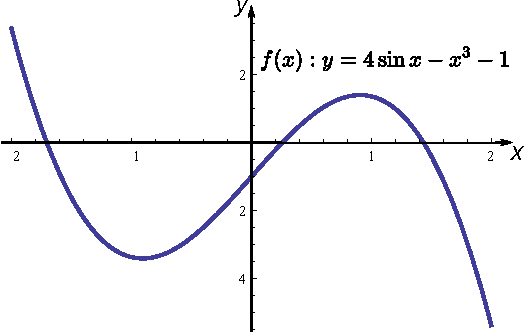
\includegraphics[scale=1]{mai_fig035.pdf}
           \captionof{figure}{Graf funkce $f(x):y=4\sin x - x^3 - 1$.}
           \label{mai:fig035}
           \par}
        Z obrázku \ref{mai:fig035} zjistíme, že existují tři kořeny: $x_1^*\in(-2,-1),
        x_2^*\in(-1, 0)$ a $x_3^*\in(1, 2)$.
      \end{example}
  
      Z obrázku zjistíme, že existují tři kořeny: $x_1^*\in(-2,-1),x_2^*\in(0,1),x_3^*\in(1,2)$.
      Zkusme najít kořeny v těchto intervalech pomocí numerických metod popsaných v následujících
      odstavcích
  
    \subsection{Metoda bisekce}
      Metoda známá také jako \textbf{metoda půlení intervalů}, je založena na principu
      zna\-mén\-ko\-vých změn. Předpokládejme, že funkce $f(x)$ má v koncových bodech intervalu
      $(a_0,b_0)$ opačná znaménka, tj. platí $f(a_0 )\cdot f(b_0 )<0$. Sestrojíme posloupnost
      intervalů $(a_1,b_1)\supset(a_2,b_2)\supset(a_3,b_3)\supset\cdots$, které obsahují kořen.
      Intervaly $(a_{k+1},b_{k+1}), k=0,1,\cdots$, určíme rekurzivně způsobem, který si nyní
      popíšeme.
  
      Střed intervalu $(a_k,b_k)$ je bod $x_{k+1}=\frac{1}{2}(a_k+b_k)$. Když $f(x_k)=0$, pak
      $x_{k+1}=x^*$ je kořen a dál nepokračujeme.

%} %tikzset
%---------------------------------------------------------------------------------------------------
\printbibliography[heading=subbibliography]
\addcontentsline{toc}{section}{Seznam literatury}
%  % !TeX spellcheck = cs_CZ
%     An overview of high school mathematics
%{\tikzset{external/prefix={tikz/MAI/}}
% \tikzset{external/figure name/.add={ch01_}{}}
%---------------------------------------------------------------------------------------------------
% history_MA.tex
%---------------------------------------------------------------------------------------------------
\setchaptertoc
\chapter{Historie matematické analýzy} %\label{mai:IchapI}

  Analýza jako nezávislý předmět byla vytvořena v 17. stol. během vědecké revoluce. Kepler, 
  Galilei, Descartes, Fermat, Huygens, Newton a Leibniz, když zmíníme jen několik důležitých jmen 
  těch, kteří přispěli k jejímu vzniku. Otázky z mechaniky, optiky a astronomie hráli roli v jejím 
  raném období, tak jako vnitřní problémy matematiky, jako výpočet obsahů, objemů a analýza 
  komplikovaných křivek. Pohyb po zakřivených drahách působením proměnných sil, které se staly 
  předmětem důkladného zájmu po studiu volně padajících těles Galilea, vedl k počátečnímu úspěchu. 
  Z velké rozmanitosti snah, které se objevily na konci 17. stol. v práci Newtona a Leibnize, se 
  zrodila nová matematická disciplína, jejíž některé poznatky jsou v těchto studijních zápiscích.
  
  Základní myšlenka použití diferenciálních rovnic k získání pohledu na globální chování proměnných
  kvantit z jejich (infinitezimálních) změn prokázala základní a plodné výsledky daleko za hranicemi
  matematiky a fyzika a formovala náš souhrnný vědecký pohled na svět, zvláště na představu o
  kauzalitě. Na konci 18. stol., vskutku, největší vědci došli ke shodě, že procesy v přírodě (a
  společnosti) jsou determinovány a podřízeny zákonům, které mohou být popsány v podobě
  diferenciálních rovnic. Laplace, tento mistr matematické fyziky, naznačil obraz nějaké fiktivní
  vševědoucí inteligence, užívající úplnou znalost zákonů a stavu světa v daný časový okamžik, by
  mohla předpovídat další vývoj světa navždy a hned. Myšlenka \emph{přírodních zákonů} byla kmotrem
  při vytvoření matematického pojmu funkce a naopak nebyla by to myšlenka nikdy tak vlivná, kdyby
  matematická analýza nevyvíjela úspěšné metody pro výzkum funkčních závislostí. 

%} % tikzset
%---------------------------------------------------------------------------------------------------              
}
{
% DEBUG was off
%---------------------Reálná a komplexní čísla-----------------------------------------------------
  % !TeX spellcheck = cs_CZ
% Basis of Linear Algebra:
%{\tikzset{external/prefix={tikz/MAI/}}
% \tikzset{external/figure name/.add={ch02_}{}}
%---------------------------------------------------------------------------------------------------
% intro_linear_algebra.tex
%---------------------------------------------------------------------------------------------------
% ==================================================================================================
% In linear algebra, a basis is a set of linearly independent vectors that, in a
% linear combination, can represent every vector in a given vector space or free
% module, or, more simply put, which define a "coordinate system".[1] In more
% general terms, a basis is a linearly independent spanning set. 
% --------------------------------------------------------------------------------------------------
\chapter{Všemocná úměra aneb lineární algebra poprvé}\label{mai:IchapII}
\minitoc
  Tuto kapitolu bychom mohli opatřit podtitulem \emph{„To nejnutnější z lineární algebry“}. 
  Dovíme se v ní, co je třeba si představit pod pojmem \emph{„linearita“}, najdeme příklady 
  linearity v geometrii i v přírodovědě (fyzice, chemii, biologii) a formulujeme základní 
  poznatky týkající se řešení soustav lineárních rovnic. Do této oblasti patří i počítání s 
  vektory a maticemi - objekty, které jsou velmi vhodné k vyjádření fyzikálních veličin.
    
  \section{Lineární rovnice}\label{mai:IchapIIsecI}
    Co tedy znamená slovo \textbf{linearita}? Pochází z latiny, \emph{linea recta = přímka}, 
    česky bychom řekli \emph{přímá úměrnost} nebo jen jednoduše \emph{úměra}.
    
    Nejjednodušší příklady linearity patří do oblasti geometrie - vyjádření \emph{přímek} a 
    \emph{rovin}. Jistě si ze střední školy vzpomínáme, že body těchto útvarů popisujeme jejich 
    souřadnicemi na přímce \(\mathbb{R}\), v rovině \(\mathbb{R}^2\), v prostoru \(\mathbb{R}^3\). 
    Souřadnice bodu v rovině tedy tvoří \emph{uspořádanou dvojici} reálných čísel, v prostoru pak 
    \emph{uspořádanou trojici} reálných čísel. (Pozor, dvojice \([a, b]\) a \([b, a]\) představují 
    různé body.)

    %--Parametrické vyjádření přímky--------------------------------
      \input{../src/MAI/exam/exam001.tex}
    %---------------------------------------------------------------
    
    Vidíme, že kartézské souřadnice bodu na přímce se vůči souřadnicím bodu \(A\) mění přímo 
    úměrně v závislosti na hodnotě parametru \(t\), tj. závisí na jeho první mocnině. Příslušná 
    závislost se nazývá \textbf{lineární funkcí}.
    
    Obdobně zapíšeme parametrické vyjádření roviny v \(\mathbb{R}^3\):
    
    %--Parametrická vyjádření roviny--------------------------------
    \input{../src/MAI/exam/exam004.tex}
    %---------------------------------------------------------------
    
    Všimněme si nyní příkladů linearity z oblasti přírodovědy.
    
    %--Fyzika — Ohmův zákon-----------------------------------------
    \input{../src/MAI/exam/exam035.tex}
    %---------------------------------------------------------------

    %--Fyzika — speciální typy pohybů-------------------------------
    \input{../src/MAI/exam/exam036.tex}
    %---------------------------------------------------------------
    
  \subsection{Soustavy lineárních rovnic a jejich rychlé řešení}
    Příkladů linearity v přírodě bychom mohli nalézt bezpočet. Vraťme se však k matematice a k 
    problematice uvedené v názvu tohoto odstavce, k soustavám lineárních rovnic. Začněme 
    jednoduchou slovní úlohou ze základní školy:
    
    %--Jeníček a Mařenka kradli ježibabě perník---------------------
    \input{../src/MAI/exam/exam037.tex}
    %---------------------------------------------------------------
    
    O samotné řešení této jednoduché úlohy v tuto chvíli nejde. Pojmenujme si však vztahy, které 
    jsme pro neznámé hodnoty \(M\) a \(J\) ze zadání úlohy dostali. Neznámé vystupují v 
    rovnicích v první mocnině, tedy \emph{lineárně}. Máme \emph{soustavu dvou rovnic} o dvou 
    neznámých \(M\) a \(J\). Úvahu snadno zobecníme: Předpokládejme, že máme neznámé veličiny
    \begin{equation*}
      (x_1, x_2, \ldots, x_n)
    \end{equation*}
    a máme o nich \(m\) informací, které lze zapsat ve tvaru lineárních rovnic (neznámé budou v 
    těchto rovnicích vystupovat v první mocnině),
    \begin{align}
      a_{11}x_1 + a_{12}x_2 + \ldots + a_{1n}x_n &= b_1,     \nonumber           \\
      a_{21}x_1 + a_{22}x_2 + \ldots + a_{2n}x_n &= b_2,     \label{mai:eq002}   \\
      .......................................... &= \ldots   \nonumber           \\
      a_{m1}x_1 + a_{m2}x_2 + \ldots + a_{mn}x_n &= b_m,     \nonumber
    \end{align}
    Soustavu (\ref{mai:eq002}) nazýváme soustavou \(m\) lineárních rovnic o \(n\) neznámých. 
    Označme ji jako \(S\) a pod tímto označením se k ní budeme vracet. Soubory reálných čísel 
    \((a_{ij})\) a \((b_i)\), kde \(1 < i < m\), \(1 \leq j < n\), jsou zadány. Lze je uspořádat 
    do takzvaných \textbf{matic}:
    \begin{equation}\label{mai:eq003}
      \matr{A} =
        \begin{pmatrix}
          a_{11} & a_{12} & \ldots & a_{1n} \\
          a_{21} & a_{22} & \ldots & a_{2n} \\
          \ldots & \ldots & \ldots & \ldots \\
          a_{m1} & a_{m2} & \ldots & a_{mn}          
        \end{pmatrix},
        \overline{\matr{B}} =
        \begin{pmatrix}
          b_1     \\
          b_2     \\
          \ldots  \\
          b_m 
        \end{pmatrix}
    \end{equation}
    
    Matice \(\matr{A}\) je typu \(m/n\), má \(m\) řádků a \(n\) sloupců, \(i\) je řádkový index a 
    \(j\) je sloupcový index. Matice \(\overline{\matr{B}}\) je typu \(m/1\) (\(m\) řádků a jeden 
    sloupec), hovoříme také o sloupcové matici. Soustavu \(S\) můžeme zapsat zkráceně pomocí 
    maticového násobení (podrobněji viz později odstavec \ref{mai:IchapIIsecIII}):
    \begin{equation*}
      \matr{A} \cdot \matr{X} = \matr{B}, \qquad \text{nebo}
    \end{equation*}  
    \begin{equation}\label{mai:eq004}
        \begin{pmatrix}
          a_{11} & a_{12} & \ldots & a_{1n} \\
          a_{21} & a_{22} & \ldots & a_{2n} \\
          \ldots & \ldots & \ldots & \ldots \\
          a_{m1} & a_{m2} & \ldots & a_{mn}
        \end{pmatrix}
        \cdot
        \begin{pmatrix}
          x_1     \\
          x_2     \\
          \ldots  \\
          x_m 
       \end{pmatrix}
        =
       \begin{pmatrix}
            b_1     \\
            b_2     \\
            \ldots  \\
            b_m 
          \end{pmatrix}
    \end{equation}
    V tuto chvíli vysvětlíme podstatu maticového násobení jen technicky: Násobit mezi sebou  můžeme matici 
    \(\matr{A} = (a_{ij})\) typu \(m/n\) (levý činitel) a matici \(\matr{A} = (c_{jk})\) typu 
    \(n/p\) (pravý činitel, činitele nelze zaměňovat). Výsledkem je matice \(\matr{A} = (d_{ik})\) 
    typu \(m/p\), jejíž prvky se počítají podle předpisu
    \begin{equation}\label{mai:eq005}
      d_{ik} = \sum_{j=1}^{n} a_{ij}\cdot c_{jk}.
    \end{equation}
    
    Z tohoto obecného předpisu vidíme, že levé strany soustavy \(S\) lze interpretovat ve tvaru 
    součinu matice \(A\) typu \(m/n\) s maticí neznámých typu \((n/1)\), výsledkem je matice 
    pravých stran \(\overline{\matr{B}}\), která je typu \(m/1\). Matice \(\matr{A}\) se nazývá 
    \textbf{maticí soustavy}. Matice, která vznikne jejím \emph{rozšířením} o sloupec pravých 
    stran, tj.
    \begin{equation}\label{mai:eq006}
      \matr{B} = (\matr{A}|\overline{\matr{B}}) =
      \left(
        \begin{array}{cccc|c}
          a_{11} & a_{12} & \ldots & a_{1n} & b_1    \\
          a_{21} & a_{22} & \ldots & a_{2n} & b_2    \\
          \ldots & \ldots & \ldots & \ldots & \ldots \\
          a_{m1} & a_{m2} & \ldots & a_{mn} & b_m
        \end{array}
      \right)
    \end{equation}
    je pak \textbf{rozšířenou maticí soustavy}. Je-li sloupec pravých stran soustavy tvořen 
    samými nulami, nazývá se soustava \textbf{homogenní}, v opačném případě \textbf{nehomogenní}. 
    Řešením soustavy \(S\) nazýváme každou \(n\)-tici \((x_i, x_2,\ldots, x_n)\), která soustavu 
    \(S\) splňuje. Cílem je najít všechna řešení soustavy \(S\). Abychom řešení nalezli, musíme 
    soustavu upravovat, zjednodušovat. Prováděné úpravy mají vést k jednodušší, avšak 
    ekvivalentní soustavě rovnic, tj. takové, která má naprosto stejný soubor všech řešení jako 
    soustava původní. Takové úpravy nazýváme \textbf{ekvivalentními}. Dvě základní, pomocí nichž 
    lze uskutečnit všechny ostatní, jsou
    \begin{itemize}\addtolength{\itemsep}{-0.5\baselineskip}
      \item vynásobení libovolné, například \(i\)-té, rovnice libovolným \emph{nenulovým} číslem,
      \item přičtení \(i\)-té rovnice vynásobené libovolným číslem k \(l\)-té rovnici.
    \end{itemize} 
    V soustavě lze samozřejmě také měnit pořadí rovnic. Tato úprava je rovněž ekvivalentní. 
    Nevypisujeme ji však zvlášť proto, že ji lze realizovat pomocí vhodně zvolené posloupnosti 
    základních dvou úprav.
    
    Abychom nemuseli soustavu stále opisovat i s neznámými, provádíme obvykle ekvivalentní 
    úpravy jen s maticí \(\matr{B} = (\matr{A}|\overline{\matr{B}})\) (každý řádek této matice 
    představuje jednu rovnici soustavy \(S\)). Může se stát, že soustava má právě \emph{jedno 
    řešení}, jako tomu bylo v  úloze o Mařence a Jeníčkovi. Také nemusí mít \emph{řešení žádné}, 
    jako například soustava \(x + y = 0\), \(x + y = 1\) (součet dvou čísel nemůže nabývat současně 
    dvou různých hodnot). A třeba má také řešení \emph{nekonečně mnoho} (řešením soustavy jedné 
    rovnice o dvou neznámých \(x + y = 1\) jsou všechny dvojice tvaru \((x, 1 - x)\), kde \(x\) je 
    libovolné). A může mít soustava \(S\) třeba právě dvě řešení? Prostřednictvím následujícího 
    příkladu ukážeme metodu, která vede velmi rychle k nalezení všech řešení a umožňuje také 
    vyslovit obecné závěry o jejich vlastnostech a počtu. Jedná se o \textbf{Gaussovu eliminační 
    metodu}.

    %Gaussova eliminační metoda-------------------------------------
    \input{../src/MAI/exam/exam038.tex}
    %---------------------------------------------------------------

    Na základě výsledného tvaru matice soustavy a rozšířené matice soustavy získané ekvivalentními 
    úpravami soustavy \(S\) nyní formulujeme obecné kritérium pro to, aby soustava S měla
    vůbec nějaké řešení. Matice \(\matr{A}\) i \(\matr{B}\) se po provedení ekvivalentních úprav 
    dostaly do velmi jednoduchého tvaru, který připomíná schodiště obrácené „vzhůru nohama“, 
    odmyslíme-li si nuly v levé části jednotlivých řádků (následující zápis pouze usnadňuje 
    názornou představu, znak ekvivalence již psát nemůžeme):
    \begin{equation*}
      \matr{A} \ldots
      \left(
        \begin{array}{rrrrr}
                1 &  2 & -1 & 1      & -5     \\
                  &    &    & 1      & -1     \\
 
        \end{array}
      \right),
      \qquad
      \matr{B} \ldots
      \left(
        \begin{array}{rrrrr|r}
                1 &  2 & -1 & 1      & -5 &  0    \\
                  &    &    & 1      & -1 & -1    \\
        \end{array}
      \right).
    \end{equation*}
    
    Všimněme si, že „schodiště“ jsou nepravidelná, pokud jde o šířku schodů, výška všech schodů
    je však stejná - jeden řádek. Tímto způsobem je dán \emph{schodovitý tvar} matice \(\matr{A}\), 
    resp. \(\matr{B}\). Úzce s ním souvisí důležitá charakteristika matice, která je nezávislá jak 
    na provedených úpravách tak na výsledném schodovitém tvaru. Je to hodnost matice, definovaná 
    takto:
    
    \textbf{Hodnost} matice je počet nenulových řádků jejího schodovitého tvaru.
    
    V našem příkladu je hodnost matice \(A\) soustavy \(S\) rovna dvěma, hodnost matice rozšířené 
    \(\matr{B}\) je rovna třem. Píšeme
    \begin{equation*}
      h(\matr{A}) = 2,\qquad h(\matr{B}) = 3.
    \end{equation*}
    
    \begin{note}
      Lze získat schodovitý tvar různými posloupnostmi ekvivalentních úprav je zřejmé. Uvědomme si 
      však, že ani výsledný schodovitý tvar není určen jednoznačně - stačí třeba vynásobit některý 
      řádek dvěma a výsledná matice ekvivalentní s původní je rovněž schodovitá. Poněvadž má matice 
      \(\matr{B}\) o jeden sloupec více než matice \(\matr{A}\), platí vždy \(h(\matr{A}) < 
      h(\matr{B})\). V případě \(h(\matr{A}) < h(\matr{B})\) pak \(h(\matr{A}) = h(\matr{B}) - 1\). 
      Jak názorně ukazuje náš příklad, má pro \(h(\matr{A}) < h(\matr{B})\) některá z rovnic 
      ekvivalentní soustavy tvar \(0 = 1\), soustava tedy nemá řešení. Můžeme tak formulovat 
      kritérium (podmínku nutnou a postačující) řešitelnosti soustavy lineárních rovnic.
    \end{note}
    
    \begin{lemma}\label{mai:lemma001}
      (\textbf{Frobeniova}): Soustava lineárních rovnic má řešení právě tehdy, je-li hodnost její 
      matice rovna hodnosti matice rozšířené.
    \end{lemma}
    
    Ihned vidíme, že homogenní soustava má podle této věty řešení vždy, neboť poslední sloupec její 
    rozšířené matice je složen ze samých nul. Skutečně, jedním ze souboru řešení každé
    homogenní soustavy je \(n\)-tice
    \begin{equation*}
      (x_1, x_2, \ldots, x_n) = (0, 0, \ldots, 0),
    \end{equation*}
    zvaná \textbf{triviální řešení}.
    
    Nyní se vraťme k otázce, jak zjistit, kolik řešení má daná soustava, a jak je všechna popsat.
    Poslouží nám příklad \ref{mai:exam038} v mírné obměně spočívající v záměně koeficientu \(b_3\) 
    z hodnoty \num{6} na \num{-6}.
    
    %Ještě jednou Gaussova eliminační metoda------------------------
    \input{../src/MAI/exam/exam039.tex}
    %---------------------------------------------------------------
    
    Soubor řešení ve tvaru (\ref{mai:eq040}) se nazývá obecným řešením soustavy. Jeho jednotlivé 
    prvky, jednotlivá konkrétní řešení soustavy, jsou dány volbou volných neznámých \(x_2\), 
    \(x_3\) a \(x_5\). Také z příkladu \ref{mai:exam039} lze učinit obecný závěr:
    
    \begin{lemma}\label{mai:lemma002}
      Nechť pro soustavu \(m\) lineárních rovnic o \(n\) neznámých platí \(h(\matr{A}) = 
      h(\matr{B}) = h\). Pak její obecné řešení závisí (lineárně) na \(d = n - h\) volných 
      neznámých.
    \end{lemma}
    
    Číslo \(d\) se nazývá \textbf{dimenze prostoru řešení soustavy}. Tento pojem ještě podrobněji 
    vysvětlíme později.
    
    Nyní již snadno zodpovíme otázku, čím je dána mohutnost souboru řešení soustavy lineárních 
    rovnic, tj. kolik má taková soustava řešení. Možnosti jsou pouze:
    \begin{itemize}
      \item žádné řešení - pro \(h(\matr{A}) \neq h(\matr{B})\),
      \item právě jedno řešení - pro \(h = h(\matr{A}) = h(\matr{B})\) a současně \(h = n\), takže 
            nezbývá žádná volná neznámá,
      \item nekonečně mnoho řešení - pro \(h = h(\matr{A}) = h(\matr{B})\) a současně \(h < n\),  
            kdy máme k dispozici \(d = n - h\) volných neznámých.
    \end{itemize}    
    Že by tedy třeba měla soustava právě dvě, tři či osmnáct řešení není možné.
    
    Jakési zvláštní postavení můžeme přisoudit homogenním soustavám. Ty mají, jak jsme se
    již přesvědčili, řešení vždy, alespoň to triviální, složené ze samých nul. Zajímejme se o 
    situaci, kdy má homogenní soustava i jiná, netriviální, řešení. U homogenní soustavy je 
    hodnost její matice vždy shodná s hodností matice rozšířené, \(h = h(\matr{A}) = h(\matr{B})\). 
    Je-li navíc \(h = n\), má podle obecného tvrzení \ref{mai:lemma002} soustava právě jedno 
    řešení, jímž nutně je řešení triviální. V opačném případě, tj. pro \(h < n\), máme opět k 
    dispozici \(d = n - h\) volných neznámých, a tedy nekonečně mnoho netriviálních řešení. 
    Všimněme si ještě jedné zajímavosti u homogenní soustavy. Jsou-li dvě \(n\)-tice čísel \(X = 
    (x_1, x_2, \ldots, x_n)\) a \(\overline{X} = (\overline{x}_1, \overline{x}_2, \ldots, 
    \overline{x}_n)\) jejím řešením, pak také \(n\)-tice vytvořená jako jejich lineární kombinace
    \begin{equation*}
      \alpha\cdot X + \overline{\alpha}\cdot\overline{X} = 
        (\alpha x_1, \alpha x_2, \ldots, \alpha x_n) + 
        (\overline{\alpha}\,\overline{x}_1, 
        \overline{\alpha}\,\overline{x}_2, \ldots, 
        \overline{\alpha}\,\overline{x}_n)
    \end{equation*}
    kde \(\alpha\) a \(\overline{\alpha}\) jsou libovolná čísla, je \emph{řešením soustavy}. 
    Možnost tohoto „lineárního kombinování“ připadá samozřejmě v úvahu pro libovolný počet 
    libovolných řešení soustavy. Fyzik by řekl, že soustava vyhovuje principu superpozice. 
    Soustava nehomogenní tu to vlastnost nemá „vinou“ nenulového sloupce 
    pravých stran.
    
    \subsection{Přímky a roviny - lineární geometrické útvary}
      Vraťme se ještě na chvíli k linearitě v geometrii a všimněme si problematiky vzájemné polohy
      přímek a rovin. Procvičíme si na ní mimo jiné i řešení soustav lineárních rovnic. V odstavci 
      \ref{mai:IchapIIsecI} jsme odvodili parametrické vyjádření přímky a roviny v trojrozměrném 
      prostoru. Nyní se pokusíme z těchto vyjádření vyloučit parametry a získat obecné rovnice 
      přímky a roviny, které již budou obsahovat pouze kartézské souřadnice bodů ležících v 
      příslušné přímce či rovině. Začněme případem roviny.

      %--Obecná rovnice roviny----------------------------------------
      \input{../src/MAI/exam/exam040.tex}
      %---------------------------------------------------------------

      %--Obecná rovnice přímky----------------------------------------
      \input{../src/MAI/exam/exam041.tex}
      %---------------------------------------------------------------
      
      %--Vektor rovnoběžný s rovinou----------------------------------
      \input{../src/MAI/exam/exam042.tex}
      %---------------------------------------------------------------
  
      Máme připraveno vše pro řešení otázky vzájemné polohy přímek a rovin.

      %--Vzájemná poloha tří rovin------------------------------------
      \input{../src/MAI/exam/exam043.tex}
      %---------------------------------------------------------------

      %--Vzájemná poloha dvou přímek----------------------------------
      \input{../src/MAI/exam/exam044.tex}
      %---------------------------------------------------------------
      
      %--Vzájemná poloha přímky a roviny------------------------------
      \input{../src/MAI/exam/exam045.tex}
      %---------------------------------------------------------------
      
%--------------------------------------------------------------------------------------------------
  \section{Počítání s čísly}\label{mai:IchapIIsecII}
    Někdo se jistě pozastaví nad tím, že jej chceme učit počítání s čísly. To přece každý umí
    už od základní školy! Jenže základní a do značné míry i střední škola nás učí počítat jen
    s určitým typem čísel - s čísly reálnými. Pravidla pro počítání s nimi se pro „běžné uživatele“
    stala natolik rutinní záležitostí, že už o nich vůbec nepřemýšlejí, nehledají v nich 
    zákonitosti, a kdybychom se jich zeptali, kde se tato pravidla vzala, pravděpodobně budou s 
    odpovědí velmi váhat. Pravidla pro jakékoli početní operace totiž skutečně nelze z ničeho 
    odvodit, ta je třeba definovat, samozřejmě tak, aby měla rozumné praktické vlastnosti.
    
    \subsection{Reálná čísla}
      U reálných čísel se opravdu dlouho nezdržíme, s těmi snad opravdu každý umí počítat. Všimneme 
      si jen trochu podrobněji struktury množiny všech reálných čísel, \textbf{reálné osy} 
      \(\mathbb{R}\). Zobrazit  reálná čísla na reálné ose, tedy na přímce, umíme proto, že na 
      množině reálných čísel je definováno \textbf{úplné uspořádání} „< “:
      \begin{itemize}
        \item Je-li současně \(a ≤ b\) a \(b ≤ a\), pak \(a = b\) 
              pro všechna \(a, b\in\mathbb{R}\ldots\) \textbf{antisymetrie},
        \item je-li současně\( a ≤ b\) a \(b ≤ c\), pak \(a ≤ c\) 
              pro všechna \(a,b,c\in\mathbb{R}\ldots\) \textbf{tranzitivita},
        \item \(a ≤ a\) pro všechna \(a\in\mathbb{R}\ldots\) \textbf{reflexivita},
        \item platí \(a ≤ b\) nebo \(b ≤ a\) pro všechna \(a, b \in\mathbb{R}\ldots\) 
              \textbf{úplnost}.
      \end{itemize}
      Pro každá dvě čísla \(a\) a \(b\) tedy dokážeme rozhodnout, zda jsou shodná (\(a = b\)), nebo 
      zda \(a\) je menší (\(a < b\)) či větší (\(a > b\)) než \(b\). Platí:
      \begin{itemize}
        \item Je-li současně \(a < b\) a \(c < d\), pak \(a + c < b + d\),
        \item je-li současně \(a < b\) a \(c > 0\), pak \(ac < bc\),
        \item je-li současně \(a < b\) a \(c < 0\), pak \(ac > bc\).
      \end{itemize}
      
      Množina reálných čísel obsahuje tyto důležité podmnožiny:
      \begin{itemize}
        \item Množinu přirozených čísel \(\mathbb{N} = \{1, 2, \ldots, n, \ldots\}\). Platí princip 
              \textbf{úplné indukce}: Je-li \(\mathbb{M} \subseteq \mathbb{N}\) nějaká množina 
              přirozených čísel, která obsahuje číslo \num{1} a která současně s každým číslem 
              \(n\) obsahuje i \(n + 1\), pak \(\mathbb{M} = \mathbb{N}\).
        \item Množinu celých čísel \(\mathbb{Z} = \{\ldots, -n, \ldots, -2, -1, 0, 1, 2, \ldots, m, 
              \ldots\}\).
        \item Množinu racionálních čísel \(\mathbb{Q}\) (zlomky). Racionální čísla lze vyjádřit 
              konečnými desetinnými zlomky (například \(p/q = 1/4 = \num{0.25}\)), nebo nekonečnými 
              periodickými desetinnými zlomky (například \(p/q = 4/3 = 1,33\ldots33\ldots = 
              1,\overline{3}\), \(p/q = 24/11 = 2,1818\ldots1818\ldots = 2,\overline{18}\)).
        \item Množinu iracionálních čísel, tj. čísel, která nejsou racionální. Iracionálními čísly 
              jsou neracionální řešení algebraických rovnic, například \(x^2 - 2 = 0 \Rightarrow x 
              = \sqrt{2}\), nebo \(x = - \sqrt{2}\) (čísla algebraická), a čísla typu \(\pi\), 
              \(e\), atd. (čísla transcendentní). Iracionální čísla jsou vyjádřena       
              nekonečnými neperiodickými desetinnými zlomky, např. 
              \(e = \num{2.718281828459545}\ldots\). Mezi každými dvěma reálnými čísly leží 
              nekonečně mnoho čísel racionálních i nekonečně mnoho čísel iracionálních.
      \end{itemize}
      
      Pro počítání s reálnými čísly jsou zavedeny základní operace, s nimiž umíme pracovat na
      základě zkušenosti, sčítání \(a + b\), odčítání \(a - b\), násobení \(a \cdot b\), resp. 
      \(ab\) a dělení \(a : b\). Ve skutečnosti jsou potřeba jen dvě, neboť odčítání je odvozeno 
      pomocí sčítání a dělení pomocí násobení. Uvědomili jste si někdy základní vlastnosti těchto 
      operací? Možná ne, ale pracujeme s nimi zcela samozřejmě:
%      \begin{table}[ht!]
%        \centering
%%        \begin{tabular}{l>{\centering}m{5cm}} %{@{}ll@{}}
%%\begin{tabular}{| c | >{\centering}m{5cm} |}
%%        \toprule
%%          \(a + b = b + a\)            & komutativní zákon pro součet  \\ %\midrule
%%          \((a + b) + c = a + (b +c)\) & asociativní zákon pro součet  \\
%%          \(a + 0 = 0 + a = a\)        & existence univerzálního neutrálního prvku \num{0}  \\
%%          \(a + (—a) = (—a) + a = 0\)  & existence právě jednoho opačného prvku k číslu \(a\)   \\ 
%%          \(ab = ba\)                  & komutativní zákon pro součin \\
%%          \(a(bc) — (ab)c\)            & asociativní zákon pro součin \\
%%          \(a(b + c) = ab + ac\)       & 1. distributivní zákon  \\
%%          \((b+ c)a — ba + ca\)        & 2. distributivní zákon \\
%%          \(a \cdot 1 = 1 \cdot a\)    & existence univerzálního jednotkového prvku 1 \\
%%          \(aa^{-1} = a^{-1}a\)        & existence právě jednoho inverzního prvku k číslu \(a\), pokud 
%%                                         \(a\neq 0\)\\
%%          \(ab = 0 \Leftrightarrow a = 0\) nebo \(b = 0\)) & neexistence dělitelů nuly \\
%%         \bottomrule
%%        \end{tabular}
%%\begin{tabular}{| c | >{\centering}m{5cm} |}
%% Bcd & A long cell with text that wraps around and is centered
%%\end{tabular}
%      \end{table}
      Odčítání a dělení:
      \begin{equation*}
        a — b = a + (—b), a:b = ab^{-1}, \qquad\text{pokud } b\neq0.
      \end{equation*}
      
    \subsection{Komplexní čísla}
      Komplexními čísly rozumíme uspořádané dvojice \([x, y]\) čísel reálných, pro které zavedeme 
      určité operace. Uspořádaností dvojice zde myslíme to, že jedno z čísel (v našem zápisu \(x\)) 
      je umístěno na první pozici dvojice a představuje reálnou část čísla \(z\), \(x = 
      \operatorname{Re}(z)\), druhé (v našem zápisu \(y\)) je na druhé pozici a je imaginární částí 
      čísla \(z\), \(y = \operatorname{Im}(z)\). Je tedy obecně  \( [x, y] ≠ [y, x]\). Množinu
    \subsection{Cvičení}
%--------------------------------------------------------------------------------------------------
  \section{Počítání s maticemi}\label{mai:IchapIIsecIII}
    \subsection{Základní operace s maticemi a hodnost matic}\label{mai:IchapIIsecIIIsubI}
    \subsection{Hodnost matic}\label{mai:IchapIIsecIIIsubII}
    \subsection{Násobení  matic}\label{mai:IchapIIsecIIIsubIII}
    \subsection{Čtvercová matice}\label{mai:IchapIIsecIIIsubIV}
    Algebra matic, tedy počítání s nimi, je v praxi zase jen počítání s čísly, samozřejmě podle
    specifických pravidel. S maticemi jsme se již setkali v odstavci \ref{mai:IchapIIsecI}, kde 
    jsme jich využili jako vhodné „pomůcky“ při řešení soustav rovnic. Nyní posuneme naše 
    znalosti o nich na poněkud vyšší úroveň. Zavedeme na množině matic \emph{algebraickou 
    strukturu}, která nám umožní s nimi počítat nezávisle na jejich vztahu k nějakým praktickým 
    aplikacím. Víme již, že maticí typu \(m/n\) (též obdélníková matice) rozumíme soubor reálných, 
    popřípadě i komplexních čísel uspořádaných do \(m\) řádků a \(n\) sloupců:
    
    \begin{definition}\label{def_matice}
      Nechť \(m, n\) jsou přirozená čísla. Jestliže každé uspořádané dvojici \((m,n)\in 
      \{1,2,\ldots,m\}\times \{1,2,\ldots,m\}\) přiřadíme prvek \(a_{i,j}\in\mathbb{R}\) obdržíme 
      reálnou \href{http://cs.wikipedia.org/wiki/Matice}{matici} typu \(m,n\) nad \(\mathbb{R}\). 
      
      Matici zapisujeme jako
      \begin{equation}\label{matice_zapis}
        \matr{A} = \left(a_{ij}\right) =\left(
                                      \begin{array}{ccc}
                                        a_{11} & \ldots & a_{1n} \\
                                        \vdots & \ddots & \vdots \\
                                        a_{m1} & \ldots & a_{nn}
                                      \end{array}
                                 \right)
      \end{equation}
      která má právě \(mn\) prvků \((a_{ij})\) uspořádaných do \(m\) řádků a \(n\) sloupců. Stručně 
      píšeme \(\matr{A} = (a_{ij})\)
    \end{definition}

    Prvky matice jsou označeny indexy udávajícími \textbf{řádek} a \textbf{sloupec}, v nichž se 
    prvek nalézá. Prvek v \(i\)-tém řádku a \(j\)-tém sloupci matice \(\matr{A}\) se obvykle značí 
    \(a_{ij}\). Potom \(i\)-tý řádek matice  obsahuje vodorovnou \(n\)-tici prvků \(a_{i1}, 
    a_{i2}, \ldots,a_{in} \), kde \(i=  1,2,\ldots,m\) a \(j\)-tý sloupec matice obsahuje svislou 
    matici čísel \(a_{1j},a_{2j},\ldots,a_{mj}\), kde \(j = 1,2,\ldots,n\). Pro \(m = n\) se matice 
    nazývá čtvercová n-tého řádu. 
      
    %---------------------------------------------------------------
    \input{../src/MAI/exam/exam033.tex}
    %---------------------------------------------------------------

    V tabulce \ref{LA:tab_basic_matrix} jsou uvedeny nejčastější typy matic, které se v algebře 
    často vyskytují. Jsou to například matice řádkové, sloupcové, diagonální\footnote{Prvky 
    \(a_{ii}\) kde \(i=1,2,\ldots,\min(m,n)\) tvoří hlavní diagonálu. Matice \(\matr{D}\) je 
    typu \(m,m\), obecně může mít diagonální matice buď ještě další sloupce, v nichž budou samé 
    nuly, anebo další řádky, v nichž budou opět samé nuly.}, jednotkové\footnote{Jestliže \(m = 
    n\), pak mluvíme o čtvercové matici řádu \(m\).}, nulové, transponované a symetrické.

    \begin{table}[!ht]
        \centering
        \renewcommand{\arraystretch}{1.8}   % for the vertical padding
          \begin{tabular}{|l||c@{}|}              
            \hline 
            \textbf{Matice}                    & \textbf{Zápis} \\ \hline\hline
            \ttfamily řádková   \(\matr{A}\) &  \(a_1,a_2,\ldots,a_n \)\\
            \ttfamily sloupcová \(\matr{B}\) & 
              \(\begin{pmatrix}
                a_1     \\
                a_2     \\
                \vdots  \\
                a_n
              \end{pmatrix}\)                       \\
            \ttfamily diagonální \(\matr{C}\) & 
              \(\begin{pmatrix}
                 a_{11} &    0   & \ldots &   0     \\
                    0   & a_{22} & \ldots &   0     \\
                 \vdots & \vdots & \ddots & \vdots  \\
                    0   &   0    & \ldots & a_{mm}
              \end{pmatrix}\)                       \\
            \ttfamily jednotková \(\matr{I}\) &
              \(\begin{pmatrix}
                   1    &    0   & \ldots &   0    \\
                   0    &    1   & \ldots &   0    \\
                 \vdots & \vdots & \ddots & \vdots \\
                    0   &   0    & \ldots & 1
              \end{pmatrix}\)                      \\
            \ttfamily nulová \(\matr{0}\) & \((a_{ij}),\quad a_{ij} = 0\,\forall\,i, j\) \\
            \ttfamily transponovaná \(\matr{D^T}\) &
              \(\begin{pmatrix}
                a_{11} & a_{21} & \ldots &  a_{m1}\\
                a_{12} & a_{22} & \ldots &  a_{m2}\\
                \vdots & \vdots & \ddots & \vdots \\
                a_{1n} & a_{2n} & \ldots & a_{mn}
              \end{pmatrix}\)    \\
            \ttfamily symetrická \(\matr{S}\) 
            & \((a_{ij}),\quad a_{ij}= a_{ji}\,\forall\,i,j\) \\ \hline
          \end{tabular}
        \caption{Speciální typy matic}\label{LA:tab_basic_matrix}
    \end{table}
  
  
    Matice téhož typu \((m,n)\) nad \(\mathbb{R}\) budeme značit \(\mathbb{R}_{m,n}\).
      
    \subsection{Základní operace s maticemi a hodnost matic}
      
      
    \begin{definition} 
      Součinem matice \(A \in \mathbb{R}_{mn}\) a matice \(B \in \mathbb{R}_{np}\), v uvedeném
      pořadí, je matice \(C \in \mathbb{R}_{mp}\) pro kterou platí:
      \begin{align*}
             C &= AB; \quad C = (cij); \\
             \shortintertext{kde}
        c_{ij} &= \sum_n^{k=1}{a_{ik}b_{kj}};\quad
                   i = 1,\ldots,m; \, j = 1,\ldots,p.
      \end{align*} 
    \end{definition}
    Součin matic \(A\) a \(B\) je definován právě tehdy, když počet sloupců matice \(A\) je roven 
    počtu řádků matice \(B\). Obrázek \ref{LA:fig_LA001a} demonstruje jakým způsobem se 
    dostane prvek, který je ve výsledné matici třeba ve druhém řádku a druhém sloupci, násobením 
    druhého řádku levé matice s druhým sloupcem pravé ze zadaných matic. Stejným způsobem získáme 
    hodnotu prvku \(c_{ij}\) (viz \ref{LA:fig_LA001b}).
    %----------------------------------
    \begin{figure}[ht!]
      \centering  
      \begin{tabular}{cc}
        \subfloat[1. krok]{\label{LA:fig_LA001a}
          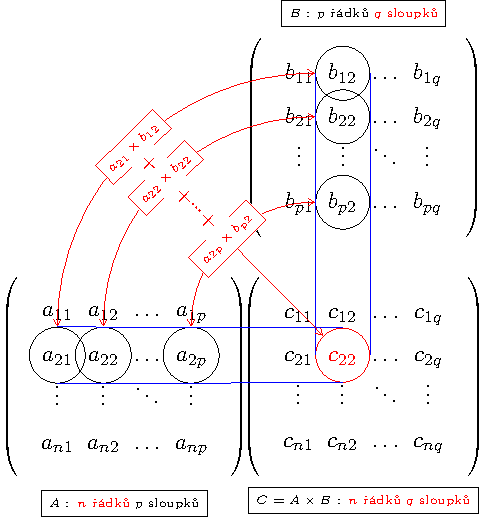
\includegraphics[width=0.45\linewidth]{mai_fig023a}}               &
        \subfloat[2. krok]{\label{LA:fig_LA001b}
          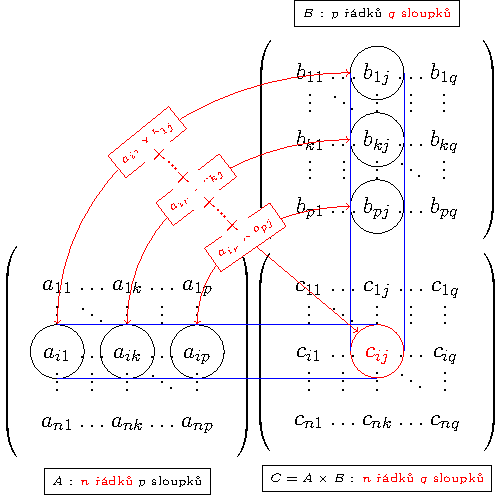
\includegraphics[width=0.45\linewidth]{mai_fig023b}} 
      \end{tabular}
      \caption{Postup při maticovém násobení}
    \end{figure}
  

      
      \begin{definition}\label{rovnost_matic}
       (Rovnost matic):  Matice \(\matr{A} = \left(a_{ij}\right)\) je rovna matici \(\matr{B}=
       \left(b_{kl}\right)\), jsou-li matice stejného typu a stejnolehlé prvky se sobě
       \textbf{rovnají}, tj. \(\matr{A} \in \mathbb{R}_{m,n}, \matr{B}\in\mathbb{R}_{m,n}, 
       a_{ij} = b_{ij}, \forall i\in\lbrace1,2,\ldots,m\rbrace, \forall j\in\lbrace1,2, \ldots 
       ,n\rbrace\).
      \end{definition}
      
%--------------------------------------------------------------------------------------------------
  \section{Počítání s vektory}\label{mai:IchapIIsecIV}
    \textbf{Vektory} budeme nazývat matice typu \(1/n\) a značit je
    \begin{equation*}
      \vec{u} = (u_1, u_2, \ldots, u_n).
    \end{equation*}
    Takže počítat s nimi již umíme! (V zápisu složek vektoru je vynechán řádkový index. V případě 
    matice s jedním řádkem, takzvané \emph{řádkové matice}, je totiž zbytečný.) Číslům \(u_1\) až 
    \(u_n\) budeme pro tuto chvíli říkat \emph{složky vektoru} \(\vec{u}\). Za chvíli tento pojem 
    ještě upřesníme. Celou řadu pojmů, s nimiž jsme se seznámili při počítání s maticemi, můžeme 
    pro vektory přímo použít. Namísto značení \(\mathcal{M} (1/n)\) budeme pro prostor vektorů 
    používat symbol \((\mathbb{R}^n)\) nebo \(\mathbb{C}^n\) (obvyklý symbol pro množinu 
    uspořádaných \(n\)-tic reálných nebo komplexních čísel).
    
    \subsection{Součiny vektorů}
      Kromě základních operací s vektory, tj. sčítání vektorů a násobení vektoru skalárem, se 
      často používají další operace, které obohacují \emph{strukturu vektorového prostoru}. 
      Zůstaneme u vektorů v trojrozměrném prostoru \(\mathbb{R}^3\) a definujeme si skalární, 
      vektorový a smíšený součin vektorů. Skalární součin vektorů definujeme prostřednictvím 
      geometrické definice jako zobrazení, které uspořádané dvojici vektorů (volných vektorů nebo 
      jejich libovolných umístění) přiřazuje reálný číslo podle předpisu
      \begin{equation}\label{mai:eq038}
        \vec{u}\vec{v} = \abs{\vec{u}}\cdot\abs{\vec{v}}\cos\varphi,
      \end{equation}
      kde \(\varphi = \sphericalangle(\vec{u},\vec{v})\) je velikost minimálního z obou úhlů mezi 
      vektory\(\vec{u},\vec{v}\).

    %---------------------------------------------------------------
    \input{../src/MAI/exam/exam034.tex}
    %---------------------------------------------------------------
    
    Shrneme nyní vlastnosti skalárního součinu. Dokázat bychom je mohli, i když by to mohlo být i 
    velmi pracné, užitím znalostí z goniometrie. Zkuste to alespoň pro jednu z nich! Třeba se    
    vám podaří zvolit si tu nejjednodušší.

%} % tikzset
%---------------------------------------------------------------------------------------------------
\printbibliography[title={Seznam literatury}, heading=subbibliography]
\addcontentsline{toc}{section}{Seznam literatury}
%------------------- Differential calculus --------------------------------------------------------
  % !TeX spellcheck = cs_CZ
% Differential calculus
%{\tikzset{external/prefix={tikz/MAI/}}
% \tikzset{external/figure name/.add={ch03_}{}}
%---------------------------------------------------------------------------------------------------
% Limits_of_Functions.tex
%---------------------------------------------------------------------------------------------------
\chapter{Limita a spojitost funkce}\label{mai:IchapLimit}
\minitoc

  %================Podkapitola: Reálná funkce ======================================================
  \section{Reálná funkce}
    %-----------------------------------------------------------------------------------------------
    \small
    S funkcemi se setkáváme na každém kroku nejen ve fyzice a v ostatních přírodních vědách, ale i 
    v každodenním životě. Každá situace, kdy jsou nějaký jev či veličina jednoznačně a nevyhnutelně 
    určeny jinými jevy či veličinami, se dá popsat pomocí funkce\footnote{V matematice abstrahujeme 
    při zkoumání funkcionálních závislostí od konkrétní fyzikální povahy proměnných veličin a 
    chápeme je jako \uv{bezrozměrné veličiny}, tedy jako číselné proměnné. Někdy je jednoduché 
    takovou} funkci sestavit. Snadno například můžeme zjistit, jakou dráhu urazí automobil jedoucí 
    známou rychlostí v závislosti na tom, jak dlouho jede. Nebo dokážeme určit přírůstek našich 
    úspor ve spořitelně v závislosti na době spoření, pokud známe úrokovou míru a její změny. Jindy 
    je naopak skoro nemožné přijít na to, jak taková funkce vypadá, neboť nemáme dostatek informací 
    o parametrech, které do jejího zápisu vstupují. Třeba takovou závislost teploty ovzduší v daném 
    okamžiku na zeměpisné poloze a nadmořské výšce, kterou bychom si mohli představit jako jednu ze 
    samozřejmých součástí předpovědi počasí, bychom asi nesestavili. Popis jevů pomocí funkcí je v 
    každém případě velmi užitečný. Má však svá pravidla, s nimiž se v této kapitole seznámíme. 
    Závisí-li zkoumaný jev nebo veličina na jediné veličině, jejíž hodnoty jsou reálné a buď se 
    mění známým způsobem, nebo si je můžeme dokonce volit, hovoříme o \textbf{funkci jedné reálné 
    proměnné}. A lze-li zkoumaný jev nebo veličinu kvantifikovat rovněž pomocí reálných hodnot, 
    jedná se o \textbf{reálnou funkci jedné reálné proměnné}. Právě o takových funkcích bude v této 
    kapitole řeč. V aplikacích se budeme věnovat především funkcím, které mají význam ve fyzice a v 
    přírodních vědách. Velmi často půjde o funkce, kde reálnou proměnnou je čas. Jevy v přírodě 
    podléhají totiž principu příčinnosti, a tak lze velké množství veličin popisujících přírodní 
    jevy vyjádřit na základě znalosti přírodních zákonů jako funkce času. 
    \cite[s.~53]{Musilova2009MA1}
    \normalsize
    \subsection{Funkce a její graf}\label{MAI:section_002}
      V tomto odstavci se naučíme funkce zadávat, počítat s nimi a vyjádřit je velmi přehledným 
      způsobem — jejich \emph{grafem}. Zopakujme, že každou \textbf{reálnou funkci}, jejíž 
      definiční obor je podmnožina množiny \(\realset\), nazýváme \textbf{reálnou funkcí jedné 
      reálné proměnné}\footnote{Místo názvu \uv{reálná funkce jedné reálné proměnné} budeme pro 
      stručnost používat pouze název \uv{funkce}, pokud nebude řečeno něco jiného}.
      
      Protože \emph{funkce je speciální případ zobrazení}, můžeme všech\-ny pojmy a obecné 
      vlastnosti zobrazení přenést i na funkce. Některé z nich však vzhledem k důležitosti 
      zopakujme, případně doplníme. Na druhé straně budeme studovat také ty vlastnosti, které jsou 
      specifické pro tento speciální druh zobrazení.
      
      \begin{note}
        Je-li \(\mathcal{D}_f = \naturalset\), jedná se o \textbf{posloupnost}. (Speciálním 
        případem reálných funkcí jedné reálné proměnné jsou \emph{posloupnosti reálných čísel)}.
      \end{note}
      
      \subsection{Způsoby zadání funkce}\label{MAI:section_000}
        Nejprve funkci definujeme. Předpokládejme, že reálná proměnná, na níž bude záviset náš jev, 
        má dovoleno nabývat hodnot z určité předem stanovené podmnožiny \(D\subseteq\realset\) 
        reálných čísel. Předpokládejme dále, že podle určitého pravidla, předpisu, dokážeme pro 
        \emph{každou hodnotu} \(x\) množiny \(\mathcal{D}_f\), tj. \(x \in \mathcal{D}_f\), určit 
        \emph{právě jednu} reálnou hodnotu \(y\). Každé hodnotě \(x \in D\) tedy nějaké \(y\) 
        příslušet \emph{musí},  avšak žádné hodnotě \(x\) \emph{nesmíme} přiřadit více hodnot 
        \(y\). Tak vzniká funkce \(f\). Hodnoty \(x\) se nazývají hodnotami \emph{nezávisle 
        proměnné} (neboli \emph{argumentu}), hodnoty \(y\) hodnotami \emph{závisle proměnné} a 
        \(f\) symbolizuje \emph{funkční předpis}. Píšeme
        \begin{equation}\label{mai:eq000}
            f: x \in \mathcal{D}_f \rightarrow y=f(x)\in\realset
        \end{equation}
      Hodnoty proměnné \(x\) nazýváme též \emph{vzory}, odpovídající hodnoty \(y = f(x)\) 
      \emph{obrazy}. Množina  \(\mathcal{D}_f\) je \emph{definičním oborem} funkce \(f\). Zadání 
      definičního oboru je důležitou součástí zadání funkce. Množina \(H\) všech takových reálných 
      hodnot \(y\), které jsou obrazem nějakého vzoru, 
      \begin{equation}\label{mai:eq001}
          \mathcal{H}_f = 
              \left\lbrace 
                y\in\realset\text{ existuje } x\in \mathcal{D}_f, \text{ tak že } y = f(x)  
              \right\rbrace, 
      \end{equation}
      se nazývá \emph{obor hodnot} funkce \(f\). Hodnotu \(f(x)\) nazýváme také \emph{funkční 
      hodnotou} funkce \(f\) v bodě \(x\). 

      \begin{figure}[ht!] %\ref{mai:fig001}
        \centering
%        \input{../src/MAI/img/mai_fig001.tex}
        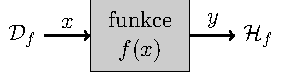
\includegraphics[width=0.45\linewidth]{mai_fig001.pdf}
        \caption{Funkce jako „černá skříňka“. \cite[s.~54]{Musilova2009MA1}}
        \label{mai:fig001}
      \end{figure}
      
      Funkci si podle obrázku \ref{mai:fig001} můžeme představit jako „černou skříňku“, do které 
      vstoupí hodnota (vzor) a vystoupí z ní hodnota \(y = f(x)\) (obraz). Množinu uspořádaných 
      dvojic čísel \([x, f(x)]\) nazveme \hyperref[MAI:section_001]{grafem funkce}.
      
      Jak zadat předpis \(f\)? Lze to udělat kterýmkoli z následujících způsobů, podle vhodnosti
      nebo snadnosti. Ukážeme jednotlivé možnosti na jednoduchém příkladu, kdy chceme hodnotám 
      proměnné \(x\) z množiny \(\mathcal{D}_f\) přiřadit jejich druhé mocniny. Zvolme pro náš 
      příklad definiční obor výčtem:
      \begin{equation*}
         \mathcal{D}_f = \lbrace-3,2,-1,0,1,2,3,4\rbrace,
      \end{equation*}
      a zadáme předpis
      \begin{itemize}\addtolength{\itemsep}{-0.5\baselineskip}
        \item \textbf{slovním popisem}: předpis \(f\) přiřazuje každé z hodnot \(x\in 
              \mathcal{D}_f\) její druhou mocninu,
        \item \textbf{vzorcem}: \(y = x^2\) pro \(x\in \mathcal{D}_f\) zadává zobrazení
              \begin{equation*}
                f: x\in \mathcal{D}_f \rightarrow f(x)= x^2\in\realset,
              \end{equation*}
        \item \textbf{tabulkou}: Hodnoty obrazů pro všechny vzory z \(\mathcal{D}_f\) vypíšeme do 
              tabulky:
              \begin{table}[h]
                \centering
                \begin{tabular}{c|rrrrrrrr}
                  \textbf{x} & -3 & -2 & -1 & 0 & 1 & 2 & 3 & 4  \\ \hline
                  \textbf{y} & 9  & 4  & 1  & 0 & 1 & 4 & 9 & 16
                \end{tabular}
                % \caption{ }
              \end{table}
              Proměnná $x$ se v tomto případě mění \uv{diskrétně}. Je zřejmé, že tímto způsobem 
              můžeme funkci definovat úplně jen tehdy, je-li definiční obor konečná množina. 
              Tabulku však používáme i v jiných případech, zejména chceme-li vyznačit pomocí ní, 
              některé hodnoty, které nás z nějakého důvodu přednostně zajímají. 
        \item Zadání \textbf{grafem}: 
          \begin{equation*}
            G_f = \left\lbrace\left[x,f(x)\right] |x\in D\right\rbrace
                = \left\lbrace\left[x,x^2 \right] |x\in D\right\rbrace
          \end{equation*}
          tak, že dvojice \([x, f(x)]\) znázorníme jako body v rovině (obr. \ref{MAI:fig_011}).
          \begin{figure}[ht!]
            \centering  
            \begin{tabular}{cc}
              \subfloat[ ]{\label{MAI:fig_011}
                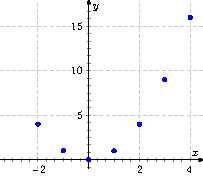
\includegraphics[width=0.4\linewidth]{mai_fig002.pdf}}              &
              \subfloat[ ]{\label{MAI:fig_010}
                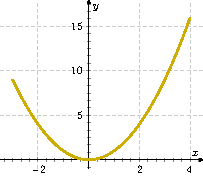
\includegraphics[width=0.4\linewidth]{mai_fig003.pdf}}              \\
            \end{tabular}
            \caption{Zadání funkce grafem}
          \end{figure}
          Z grafu můžeme ovšem funkční hodnoty určit pouze přibližně. Pro další matematické 
          zpracování je grafické zadání nejméně vhodné, i když jeho praktický význam například v 
          technických aplikacích nelze popřít.
        \item Zadání pomocí \textbf{rovnice}, jíž je funkce řešením: některé funkce nelze jednoduše 
              zapsat pomocí některého z předchozích způsobů, nebo to alespoň nejde přesně. Lze však 
              zapsat (diferenciální) rovnici, kterou tato funkce splňuje. Jedná se většinou o 
              speciální funkce, jimž se v tomto textu nebudeme věnovat. (Někdy může být taková 
              rovnice  představující zadání funkce i velmi jednoduchá. Například dosti známá funkce 
              \(\erf(x)\), \emph{error funkce}, velmi úzce souvisí s funkcí \(f(x) = 
              \frac{2}{\sqrt{x}}e^{-x^2}\). Nelze ji však zapsat vzorcem. Některé její hodnoty v 
              nejčastěji používaném rozsahu proměnné \(x\) můžeme najít v rozsáhlých tabulkách, 
              které byly sestaveny pomocí numerických metod.)
      \end{itemize}
      
      Již bylo zmíněno, že zadání definičního oboru je neopominutelnou součástí zadání funkce. 
      Kdybychom například zadali funkci opět předpisem \(y=x^2\), avšak za definiční obor stanovili 
      uzavřený interval \(D = \lbrace —3,4\rbrace\), dostali bychom graf na obrázku 
      \ref{MAI:fig_010}. Jde skutečně o jinou funkci než na obrázku \ref{MAI:fig_011}. Její úplnou 
      tabulku bychom nedokázali napsat vůbec.
      
%      Nejčastější způsob zadání funkce představuje \emph{vzorec}. Tabulku alespoň pro některé 
%      hodnoty z \(\mathcal{D}_f\) si pak dokážeme sestavit a schematický graf nakreslit. Někdy se 
%      objeví zadání funkce jen v podobě vzorce, například: „Je dána funkce \(y = f(x)\).“ Znamená 
%      to, že autor zapomněl zadat definiční obor? Nemusí tomu tak být. Tento způsob zadání chápeme 
%      tak, že si sami musíme stanovit „co největší“ definiční obor této funkce, tj. určit množinu 
%      všech takových \(x\), pro která lze do vzorce dosadit a hodnotu \(y\) určit.

      Zobrazovací předpis, kterým je funkce zadána, může být rozmanitý. Nejčastěji a pro účely 
      matematické analýzy nejvhodnější je \emph{analytické zadání vzorcem}, tj. rovnicí tvaru 
      $y=f(x)$ nebo několika takovými rovnicemi platnými pro různé části definičního oboru. Přitom 
      v rovnici $y=f(x)$ je na pravé straně nějaký správně definovaný výraz obsahující nejvýše 
      proměnnou $x$ a nabývající jednoznačné hodnoty pro danou hodnotu proměnné $x$.
      
%      Někdy však používáme (poněkud nedůsledně) termíny \uv{funkce \(f(x)\)} nebo \uv{funkce 
%      \(y=f(x)\)}. V tomto smyslu nepojímáme již \(x\) jako pevný prvek z definičního oboru, ale 
%      jako \uv{nezávisle proměnnou} neboli \emph{argument}, tj. symbol zastupující libovolný prvek 
%      z definičního oboru. V tomto případě pak písmeno \(y\) v rovnici \(y=f(x)\) nazýváme 
%      \emph{závisle proměnnou} a říkáme, že \uv{\(y\) závisí na \(x\)}. Tato frazeologie má své 
%      historické kořeny; tento způsob vyjádření funkce budeme využívat zřídka, zejména tam, kde 
%      nechceme pro označení příslušné funkce zavádět zvláštní symbol. Tak např. budeme mluvit o 
%      funkci \(e^x\) (ačkoliv se zavádí pro exponenciální funkci symbol exp) nebo o funkci \(\sin 
%      x\) (ačkoliv by bylo důslednější mluvit o funkci \(\sin\)) apod. \cite[s.~82]{Brabec1989} 

    %-------------------------------------
      \input{../src/MAI/exam/exam017.tex}
    %-----------------------------------------------------------------------------------------------
    \subsection{Graf funkce}\label{MAI:section_001}\hypertarget{MAI:section_001}
      Jinými slovy, v předchozím odstavci, bylo řečeno, že každé funkci můžeme přiřadit její graf, 
      a že \textbf{grafem funkce} $f:A\rightarrow\realset,\ A\subset\realset$, rozumíme množinu 
      všech bodů euklidovské roviny, jejíž souřadnice $x$, $y$ v dané kartézské soustavě souřadnic 
      vyhovuje rovnice 
      \begin{equation}\label{mai:eq026}
        y=f(x). 
      \end{equation}  
      
      Graf funkce může v jednodušších případech posloužit jako prostředek k získání názorné 
      \uv{představy}. Grafy některých funkcí jsou \uv{křivky}, (intuitivním smyslu tohoto slova). 
      Avšak u některých funkcí názorná představa grafu selhává. Vezmeme-li např. Dirichletovu 
      funkci, snadno zjistíme, že její graf nemůžeme sestrojit (obr. \ref{mai:fig005} tedy 
      není grafem funkce, ale pouze pokusem o názorné přiblížení Dirichletovi funkce)
      
      \begin{figure}[ht!] %\ref{mai:fig005}
        \centering
%       \input{../src/MAI/img/mai_fig005.tex}
        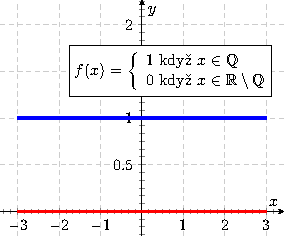
\includegraphics[width=0.5\linewidth]{mai_fig005.pdf}
        \caption{Pokus o zobrazení Dirichletovy funkce: \uv{dvě rovnoběžné přímky $y=0$ a $y=1$ s 
        nekonečným množstvím mezer}}
        \label{mai:fig005}
      \end{figure}      
      Z předchozí kapitoly také víme, že zadat funkci znamená udat její definiční obor a 
      \uv{zobrazovací předpis}, tj pravidlo (formulované slovně či v používaném matematickém 
      jazyku), podle něhož můžeme jednoznačným způsobem rozhodnout, jaká funkční hodnota odpovídá 
      libovolně zvolenému číslu z definičního oboru. Definičním oborem bývá často interval nebo 
      sjednocení intervalů. Není-li definiční obor udán, rozumíme jím množinu všech reálných čísel, 
      pro něž je příslušný předpis definován. Tuto množinu nazýváme \textbf{přirozeným} (též 
      maximálním) definičním oborem funkce. Je to tzv. \emph{existenční obor} výrazu, jímž je 
      funkce definována \cite[s.~84]{Brabec1989}.
      
      Například funkce $f: \realset\rightarrow\realset,\ f(x)=x^2$, můžeme vyjádřit bez udání 
      definičního oboru $\realset$ vztahem 
      \begin{equation*}
        f: y=x^2,
      \end{equation*}
      neboť předpis $y=x^2$ má smysl pro každé reálné číslo $x$. Avšak u funkce $g:\langle0, 
      1\rangle\rightarrow\realset,\ g(x)=x^2,$ je nutné v zápisu funkce definiční obor $\langle0, 
      1\rangle$ 
      uvést, píšeme tedy   
      \begin{equation*}
        g: y=x^2, \quad x\in\langle0,1\rangle.
      \end{equation*}
       
      %-------------------------------------
        \input{../src/MAI/exam/exam018.tex}
      %-------------------------------------
      
      %-------------------------------------
        \input{../src/MAI/exam/exam019.tex}
      %-------------------------------------
      
      Funkce může být analyticky zadána i jinak než vzorcem $y=f(x)$. Časté je \textbf{parametrické 
      vyjadřování}, tj. vyjádření dvojicí rovnic 
      \begin{equation}\label{mai:eq027}
        x=\varphi(t),\ y=\psi(t),\ t\in J,
      \end{equation}
      kde $\varphi, \psi$ jsou funkce definované na množině $J$ ($\ J$ bývá obvykle interval). 
      Proměnná $t$ se nazývá \emph{parametr}: má zde pomocný význam. Zajímá nás totiž vztah mezi 
      $x$ a $y$. Rovnice \ref{mai:eq027} definuje relaci 
      $f\subset\realset\times\realset=\realset^2$:
      \begin{equation*}
        f = \{(x,y)\in\realset^2; \text{ existuje } t\in J \text{ tak, že } x=\varphi(t),\ y=\psi(t)\}.
      \end{equation*}      
      Tato relace může být za \emph{určitých podmínek jednoznačná} tj. je funkcí z $\realset$ do 
      $\realset$. V tomto případě říkáme, že funkce $f$ je \emph{definována parametricky rovnicemi 
      \ref{mai:eq027}}
      
      %-------------------------------------
        \input{../src/MAI/exam/exam020.tex}
      %-------------------------------------
      
      Blíže se parametrickým zadáním funkce budeme zabývat v kapitole \ref{chap:Apl_dif_poc}
      (Aplikace diferenciálního počtu).
      
      Funkce může být někdy zadána též rovnicí tvaru 
      \begin{equation}\label{mai:eq028}
        F(x,y) = 0.
      \end{equation}
      Přitom $F$ je funkce dvou proměnných, tj. zobrazení z $\realset^2\rightarrow\realset$. Kromě 
      rovnice \ref{mai:eq028} může být dána ještě podmínka, aby bod $(x,y)$ patřil k některé 
      množině $M\subset\realset^2$. Rovnicí \ref{mai:eq028} je definována opět jakási relace 
      $f\subset\realset\times\realset$,
      \begin{equation}
        f = \{(x,y)\in\realset^2,\quad F(x,y)=0 \}
      \end{equation}
      (případně $f = \{(x,y)\in\realset^2,\ F(x,y)=0,\ (x,y)\in M \}$), zajímá nás, kdy tato relace 
      je funkcí z $\realset$ do $\realset$. Říkáme pak, že funkce $f$ je dána \textbf{implicitně} 
      uvedenou rovnicí \ref{mai:eq028} (příp. rovnicí \ref{mai:eq028} a podmínkou $(x,y)\in 
      M$). Naproti tomu zadání funkce ve tvaru $y=f(x)$ nazýváme \textbf{explicitním}.

      %-------------------------------------
        \input{../src/MAI/exam/exam022.tex}
      %-------------------------------------
      
      Vyšetřování podmínek, při nichž rovnice $F(x,y)=0$ je definována funkce $f$, se obvykle 
      provádí metodami matematické analýzy funkce více proměnných. 
          
    %---------------------------------------------------------------------------------------------- 
    \subsection{Vlastnosti funkcí}\label{MA1:subsec_vlastnosti_funkce}
      \subsubsection{Omezená funkce}
        \begin{definition}\label{MA1:def_lim01}
          Funkci $f$ nazýváme shora (zdola) omezenou na množině $A\subset D(f)$, je-li shora 
          (zdola) omezená množina funkčních hodnot $f(A)$. Je-li funkce $f$ omezená shora i zdola 
          na množině $A$, pak ji nazýváme omezenou na množině $A$. Je-li $A=D(f)$, nazýváme funkci 
          omezenou. Viz kniha \cite[s.~87]{Brabec1989}       
        \end{definition}
        Funkce \(f\) je omezená na množině \(A\), právě když existuje číslo \(K>0\) tak, že platí
        \begin{align*}
         |f(x)|      &\leq K \qquad \text{pro každé } x\in A   \\ 
         \shortintertext{neboli}
         -K\leq f(x) &\leq K \qquad \text{pro každé } x\in A. 
        \end{align*}

        %-------------------------------------
          \input{../src/MAI/exam/exam023.tex}
        %-------------------------------------

        \begin{itemize}\addtolength{\itemsep}{-0.5\baselineskip}
          \item Je-li funkce $f$ shora omezená na množině $A$, existuje konečné \emph{supremum}     
                $\sup f(A)$. Toto číslo nazýváme \emph{supremem funkce $f$ na množině $A$} a 
                označujeme je též $\sup_{x\in A}f(A)$ nebo $\sup\{f(x), x\in A\}$.
          \item Je-li funkce $f$ zdola omezená na množině $A$, existuje konečné \emph{infimum} 
                $\inf(A)$, které nazýváme \emph{infimum funkce $f$ na množině $A$} a označujeme je 
                též $\inf_{x\in A}f(A)$ nebo $\inf\{f(x), x\in A\}$. 
          \item Není-li funkce $f$ shora (zdola) omezená na množině $A$, pak je ovšem $\sup_{x\in A}
                f(x)=+\infty$ ($\sup_{x\in A} f(x)=-\infty$).
          \item Má-li množina $f(A)$ největší (nejmenší) prvek, pak toto číslo nazýváme největší 
                (nejmenší hodnotou funkce $f$  na množině $A$ (je-li $A = f(f)$, též absolutním 
                maximem, resp. absolutním minimem funkce $f$) a značíme je $\max_{x\in A} f(x)$ 
                ($\min_{x\in A} f(x)$). V tomto případě existuje takové číslo $x_0\in A$, že 
                $f(x_0)=\max_{x\in A}f(x)$ ($f(x_0)=\min_{x\in A}f(x)$). Pro všechna $x\in A$ tedy 
                platí $f(x)\leq f(x_0)$ ($f(x)\geq f(x_0)$). Je zřejmé, že největší (nejmenší) 
                hodnota funkce $f$ na množině $A$, pokud existuje je současně supremem (infimem) 
                funkce $f$ na $A$.
        \end{itemize}

      %-------------------------------------
        \input{../src/MAI/exam/exam021.tex}
      %-------------------------------------
       
      \subsubsection{Monotonní funkce}
        \begin{definition}\label{MA1:def_lim02}
          Funkci $f$ nazýváme \textbf{rostoucí (klesající)} na množině $A\subset D(f)$, jestliže 
          pro každé dva body $x_1, x_2\in A,\ x_1<x_2$, platí $f(x_1)<f(x_2)$ ($f(x_1)>f(x_2)$). 
          Funkci $f$ nazýváme \textbf{neklesající (nerostoucí)} na množině $A\subset D(f)$, 
          jestliže pro každé dvě body $x_1, x_2\in A,x_1<x_2$, platí $f(x_1)\leq f(x_2)$ 
          ($f(x_1)\geq f(x_2)$). Rostoucí a klesající funkce (na množině $A$) se nazývají 
          \textbf{ryze monotónní} (na množině $A$), neklesající a nerostoucí funkce (na množině 
          $A$) se nazývají monotónní (na množině $A$).    
        \end{definition}
            
        Z definice je zřejmé, že každá rostoucí funkce je zároveň neklesající a každá klesající 
        funkce je zároveň nerostoucí. Ryze monotónní funkce tvoří tedy podmnožinu množiny 
        monotónních funkcí. 
           
        \begin{example}
          Funkce $y=2x+1$ je \textbf{rostoucí} na intervalu $(-\infty, \infty)$. Platí totiž: $x_1<x_2\Rightarrow 2x_1<2x_2\Rightarrow2x_1+1<2x_2+1$.
        \end{example}
        \begin{example}
          Funkce y=[x] je \textbf{neklesající} na intervalu $(-\infty, \infty)$ (viz příklad **). 
        \end{example}
        \begin{example}
          Heavisideova funkce (viz příklad **) je \textbf{neklesající} na intervalu $(-\infty, \infty)$ (viz příklad **). 
        \end{example}       
        \begin{example}
          Funkce $y=|x|$ je \textbf{klesající} na intervalu $(-\infty, 0\rangle$ a rostoucí na intervalu $\langle0, \infty)$. 
        \end{example}  
            
        \begin{definition}\label{MA1:def_lim03}
          Funkci $f$ nazýváme \textbf{konstantní} na množině $A$, jestliže pro každé dva body $x_1, 
          x_2\in A$, platí $f(x_1)=f(x_2)$. V tom případě existuje reálné číslo $k$ takové, že pro 
          každé $x\in A$ je $f(x)=k$. Je-li $k=0$, mluvíme o nulové funkci na množině $A$. 
        \end{definition} 
          
        Výrok \uv{funkce $f$ je konstantní na množině $A$} zapisujeme též $f(x)=\text{konst na }A$. 
        Funkci konstantní na $\realset$ budeme stručně nazývat \textbf{konstantní funkcí} nebo 
        krátce \textbf{konstantou}. Z textu bude obvykle patrno, interpretujeme-li symbol $k$ jako 
        reálné číslo nebo jako konstantní funkci. Je zřejmé, že konstantní funkce na množině $A$ je 
        zároveň neklesající i nerostoucí na množině $A$. Toto tvrzení se dá obrátit. Lze snadno 
        dokázat i tuto větu:        
        \begin{lemma}\label{MA1:lem_lim01}
          Funkce $f$ je \textbf{rostoucí} na množině $A$, právě když je neklesající na množině $A$ a na žádné dvoubodové podmnožině $B\subset A$ není konstantní. 
        \end{lemma}
        Obdobná tvrzení platí i pro klesající funkce. 
               
      \subsubsection{Sudé a liché funkce}
        \begin{definition}\label{MA1:def_lim04}
          Funkce $f$ se nazývá \textbf{sudá} jestliže pro každé $x\in D(f)$ je též $-x\in D(f)$  a 
          platí $f(x)=f(-x)$.
          Funkce $f$ se nazývá \textbf{lichá} jestliže pro každé $x\in D(f)$ je též $-x\in D(f)$  a 
          platí $f(-x)=-f(x)$. 
        \end{definition}
        Graf sudé funkce je souměrný podle osy $y$ (osy funkčních hodnot), graf liché funkce je  
        souměrný podle počátku. 
 
       %-------------------------------------
         \input{../src/MAI/exam/exam024.tex}
       %-------------------------------------

        Daná funkce nemusí být ovšem ani sudá, ani lichá. Snadno se dokáže tvrzení:
        \begin{itemize}
          \item Je-li sudá funkce $f$ na množině $D(f)\cap\langle0,\infty)$ rostoucí (klesající),
                je na množině $D(f)\cap(-\infty,0\rangle$ klesající (rostoucí).
          \item Je-li lichá funkce na množině $D(f)\cap\langle0,\infty)$ rostoucí (klesající),
                je též na množině $D(f)\cap(-\infty,0\rangle$ klesající (rostoucí).                 
        \end{itemize}
      \subsubsection{Periodická funkce}

    \subsection{Operace s funkcemi. Uspořádání}
      Jak s funkcemi počítat? Definujeme základní operace s nimi — \emph{součet funkcí, součin 
      funkcí a násobení funkce reálným číslem}. Předpokládejme, že na definičním oboru 
      \(\mathcal{D}\) jsou zadány funkce \(f\) a \(g\) a reálné číslo \(\alpha\). Pak na tomtéž 
      definičním oboru lze zadat nové funkce
      \begin{align*}
        \mathcal{F} &: \mathcal{D}\ni x\,\rightarrow\,\mathcal{F}(x) = f(x)+g(x)  \in\realset   \\
        \mathcal{G} &: \mathcal{D}\ni x\,\rightarrow\,\mathcal{G}(x) = \alpha g(x)\in\realset   \\
        \mathcal{H} &: \mathcal{D}\ni x\,\rightarrow\,\mathcal{H}(x) = f(x) g(x)  \in\realset 
      \end{align*}
      Funkce \(\mathcal{F}\), \(\mathcal{G}\) a \(\mathcal{H}\) nazýváme postupně součtem funkcí 
      \(f\) a \(g\), \(\alpha\)-násobkem funkce \(f\) a součinem funkcí \(f\) a \(g\). Značíme
      \begin{equation*}
       \mathcal{F} = f + g, \qquad \mathcal{G} = \alpha f, \qquad \mathcal{H} = fg. 
      \end{equation*}
      
      Všimněme si nyní pravidel pro počítání s funkcemi zadanými na \(\mathcal{D}\) a zjistíme, 
      že se velmi podobají pravidlům pro počítání s reálnými čísly. Není divu, vždyť operace s 
      funkcemi jsou definovány prostřednictvím funkčních hodnot, a těmi jsou reálná čísla. Některé 
      důležité odlišnosti však přece jen najdeme. Napřed ale pravidla:
      
      \begin{itemize}\addtolength{\itemsep}{-0.5\baselineskip}
        \item komutativní zákon pro součet funkcí
          \begin{equation}\label{mai:eq012}
            f(x) + g(x) = g(x) + f(x)
          \end{equation}
        \item asociativní zákon pro součet funkcí  
          \begin{equation}\label{mai:eq013}
            (f(x) + g(x)) + h(x) = f(x) + (g(x) + h(x)
          \end{equation}
        \item existence univerzálního neutrálního  prvku \(O\) (nulová funkce \(O:\mathcal{D}\ni x 
          \rightarrow O(x)=0\))
          \begin{equation}\label{mai:eq014}
            f(x) + O = O + f(x) = f(x)
          \end{equation}
        \item existence právě jednoho opačného prvku k funkci \(f\), přičemž \((-f)(x) = -f(x)\)
          \begin{equation}\label{mai:eq015}
            f(x)+(-f(x))=(-f(x))+f(x)=O
          \end{equation}
        \item asociativní zákon pro násobení číslem 
         \begin{equation}\label{mai:eq016}
            (\alpha_1\alpha_2)f(x) = \alpha_1(\alpha_2f(x))
         \end{equation}
        \item  1. distributivní zákon pro násobení číslem
          \begin{equation}\label{mai:eq017}
            \alpha(f(x)+g(x) =\alpha f(x) + \alpha g(x)
          \end{equation}\label{mai:eq018}
        \item 2. distributivní zákon pro násobení číslem 
          \begin{equation}\label{mai:eq019}
            (\alpha_1+\alpha_2)f(x) =\alpha_1f(x)+\alpha_2f(x)
          \end{equation}
        \item násobení číslem \((—1)\) dává opačný prvek
          \begin{equation}\label{mai:eq020}
            (-1)f(x)=(-f(x))
          \end{equation}
        \item komutativní zákon pro součin funkcí
          \begin{equation}\label{mai:eq021}
            f(x)g(x)=g(x)f(x)
          \end{equation}
        \item asociativní zákon pro součin funkcí 
          \begin{equation}\label{mai:eq022}
            f(x)(g(x)h(x))=(f(x)g(x))h(x)
          \end{equation}
        \item distributivní zákon zprava pro součin funkcí
          \begin{equation}\label{mai:eq023}
            (f_1(x) + f_2(x))g(x) =f_1(x)g(x) + f_2(x)g(x)
          \end{equation}
        \item distributivní zákon zleva pro součin funkcí
          \begin{equation}\label{mai:eq024}
            f(x)(g_1(x) + g_2(x))=f(x)g_1(x)+f(x)g_2(x)
          \end{equation}
        \item násobení jednotkovou funkcí \(I: \mathcal{D}\ni x \rightarrow I(x) = 1\)  
          \begin{equation}\label{mai:eq025}
           f(x)I=If(x)
          \end{equation}
        \item existence právě jedné \emph{převrácené} funkce k funkci \(f\) pro \(f(x)\neq0\quad 
              (f)^{-1}: \bar{D}\ni x\rightarrow (f)^{-1}(x)=[f(x)]^{-1}\) kde \(\bar{\mathcal{D}} 
              = \mathcal{D} - \left\{x\in \mathcal{D}\,|\,f(x)=0\right\}\)
          \begin{equation}
            f(x)(f(x))^{-1}=(f(x))^{-1}f(x) = I
          \end{equation}
      \end{itemize}
      Všimněme si, že funkce \((f)^{-1}\) existuje obecně na užším definičním oboru 
      \(\bar{\mathcal{D}}\), než na kterém je definována funkce \(f\). Je totiž třeba vyloučit 
      všechny hodnoty \(x\), pro které \(f(x) = 0\) (zákaz dělení nulou). K funkci \(O\) tedy 
      převrácená funkce neexistuje vůbec!
      
      Existence opačné a převrácené funkce k \(f\) umožňuje definovat \emph{rozdíl} a \emph{podíl} 
      funkcí \(f-g=f+(-g)\) a \(\dfrac{f}{g}=f(g)^{-1}\), tj.
      \begin{align*}
        f-g         &: \mathcal{D}\ni x\,\rightarrow\, (f-g)(x)=f(x)+(-g)(x)= f(x)-g(x), \\
        \frac{f}{g} &: \bar{D}\ni x\,\rightarrow\, 
                       \left(\frac{f}{g}\right)(x) = f(g)^{-1}(x) = \frac{f(x)}{g(x)}, 
      \end{align*}
      kde \(\bar{D}=D-\left\{x\in D\,|\,g(x)=0 \right\}\) 
      
      \begin{note}
        Pamatujme si označení převrácené funkce jako \((f)^{-1}\), v němž je zápis symbolu \(f\) do 
        závorky podstatný. Jde o něco jiného než znamená symbol \(f^{-1}\) bez závorky, který 
        rezervujeme pro inverzní funkci v dalším výkladu.
      \end{note}
      \begin{note}
        Porovnáme-li nyní vlastnosti operací s funkcemi a pravidla pro počítání s reálným čísly, 
        komplexními čísly, maticemi a vektory, můžeme konstatovat, že množina funkcí s operací 
        sčítání funkcí a násobení funkce číslem je \textbf{vektorovým prostorem}. To je vlastnost, 
        která je s případem čísel, matic a vektorů společná. Vektorový prostor funkcí se však od 
        zmiňovaných vektorových prostorů výrazně liší svou dimenzí (rozměrem). Intuitivně dobře 
        chápeme, co znamená jednorozměrný, dvojrozměrný a trojrozměrný prostor (například 
        \(\realset^1\), \(\realset^2\), \(\realset^3\)). V odstav 1.4 jsme dokonce pracovali v 
        n-rozměrném vektorovém prostoru. Dimenze vektorového prostoru může být i nekonečná — třeba 
        zrovna u funkcí. Obecně jde o pojem poměrně obtížný a budeme se jím důkladně zabývat až v 
        kapitolách věnovaných algebře \cite[s.~58]{Musilova2009MA1}.
      \end{note}
      
      Operace s funkcemi jsme definovali a prodiskutovali pro případ, kdy definiční obory funkcí, 
      vstupujících do operace byly stejné. Co když tomu tak nebude? Znamená to, že pak nemůžeme 
      funkce sčítat, násobit, apod.? Předpokládejme, že definičním oborem funkce \(f\) je množina 
      \(\mathcal{D}_f\) definičním oborem funkce \(g\) množina \(D_g\). Pokud jsou tyto obory 
      disjunktní, tj. \(\mathcal{D}_f \cap \mathcal{D}_g = 0\), můžeme utvořit pouze 
      \(\alpha\)-násobek funkce \(f\) či \(g\). Sčítat ani násobit funkce \(f\) a \(g\) nemůžeme 
      neboť hodnota \(f(x) + g(x)\) ani \(f(x)g(x)\) neexistuje pro žádné \(x\). Pokud je průnik 
      \(D=d_f\cap D_g\) oborů \(\mathcal{D}_f\) a \(\mathcal{D}_g\) neprázdný, stává se definičním 
      oborem funkcí \(f+g\) a \(fg\). Platí stejná pravidla jako v předchozí tabulce, pouze s 
      omezením na obor \(\mathcal{D}_f\).
    
    \subsection{Skládání a inverze funkcí}
      \emph{Skládání} neboli kompozici funkcí si lze snadno představit opět pomocí „černých 
      skříněk“ (obr. \ref{mai:fig012}): Do první skřínky představující předpis \(g\), \emph{vnitřní 
      složku} složené funkce, vstupuje
      \begin{figure}[ht!] %\ref{mai:fig012}
        \centering
%        \input{../src/MAI/img/mai_fig012.tex}
        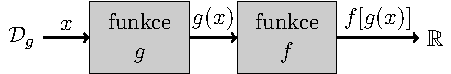
\includegraphics[width=0.45\linewidth]{mai_fig012.pdf}
        \caption{Skládání funkcí \cite[s.~59]{Musilova2009MA1}}
        \label{mai:fig012}
      \end{figure}
      hodnota \(x\) z definičního oboru \(\mathcal{D}_g\) funkce \(g\). Výstupem je číslo \(u = 
      g(x)\), funkční hodnota vnitřní složky v bodě \(x\). Toto číslo smí vstoupit do skříňky 
      představující předpis \(f\), \emph{vnější složku} složené funkce, právě tehdy, je-li prvkem 
      jejího definičního oboru \(\mathcal{D}_f\). V takovém případě najdeme na výstupu ze skříňky 
      \(f\) hodnotu \(y = f(u) = f[g(x)]\). (Jestliže \(g(x)\notin\mathcal{D}_f\), není výstup ze 
      skříňky \(f\) definován.) Vzniká nový předpis \(F\), kterým se některým bodům definičního 
      oboru \(\mathcal{D}_g\), ne všem, ale pouze těm, pro něž \(g(x)\in\mathcal{D}_f\), 
      přiřazují hodnoty \(f[g(x)]\). Definujme nyní složenou funkci přesněji: Předpokládejme, že 
      jsou zadány funkce
      \begin{align*}
        g  &: \mathcal{D}_g\ni x\,\rightarrow\, g(x) = u\in\realset, \\
        f  &: \mathcal{D}_f\ni u\,\rightarrow\, f(u) = y\in\realset. \\
        \shortintertext{označme}
        \mathcal{D} &= \{x|x\in\mathcal{D}_g \text{ a současně } g(x)\in\mathcal{D}_f\}.
      \end{align*}
      Pokud \(\mathcal{D} = \emptyset\), lze definovat funkci
      \begin{equation*}
        F: \mathcal{D}\ni x\rightarrow y = F(x) = f[g(x)]\in\realset, 
           \text{ značíme } F = f \circ g.
      \end{equation*}
      \(F\) se nazývá \emph{složením} neboli \emph{kompozicí} funkcí \(g\) a \(f\). Zápis \(f\circ 
      g\) čteme často také jako \emph{„f po g“}. Skládat lze i větší počet funkcí.

       %-------------------------------------
         \input{../src/MAI/exam/exam025.tex}
       %-------------------------------------
      
      Může vzniknout otázka, jak rozpoznáme vnitřní a vnější složku složené funkce. Rozlišit 
      vnitřní a vnější složku třeba u funkcí \(\cos(x^2)\) a \((cos x)^2\) není problém. Hned také 
      vidíme, že obecně \(f\circ g\neq g\circ f\), i když by definiční obory funkcí na pravé i levé 
      straně měly neprázdný průnik. Jsou však i případy na první pohled méně zřetelné, jak ukazuje 
      následující příklad.
      
      %-------------------------------------
        \input{../src/MAI/exam/exam026.tex}
      %-------------------------------------
       
      Funkce \(F\) a \(G\) mají různé definiční obory, ale na jejich průniku dávají stejné funkční 
      hodnoty. Ani zde však obecně nelze pořadí skládání funkcí zaměňovat.
      
      Nyní se pusťme do vybudování pojmu inverzní funkce k funkci \(f\). Představme si, že funkční
      hodnota \(y = f(x)\) zadané funkce
      \begin{equation*}
        f: \mathcal{D}_f\ni x \rightarrow f(x)\in\mathcal{H}_f
      \end{equation*}
      představuje „zakódovanou“ informaci o hodnotě \(x\). Položme si otázku, zda a za jakých 
      podmínek dokážeme sestavit „černou skříňku“, na jejímž výstupu by se při vstupu obrazu \(y = 
      f(x)\) objevila hodnota \(x\). Omezení takové možnosti je názorně vidět na obrázku 
      \ref{mai:fig014}. V případě funkce \(f(x)\) lze ke všem obrazům \(y \in \mathcal{H}_f\) najít 
      vzory, v případě funkce \(g(x)\) to možné není, neboť jeden a týž obraz lze získat z několika 
      vzorů. Pro který bychom se tedy měli rozhodnout?
      
      \begin{figure}[ht!] %\ref{mai:fig014}
        \centering
%        \input{../src/MAI/img/mai_fig014.tex}
        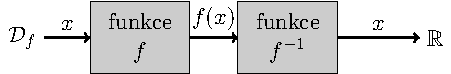
\includegraphics[width=0.45\linewidth]{mai_fig014.pdf}
        \caption{Skládání funkcí \cite[s.~61]{Musilova2009MA1}}
        \label{mai:fig014}
      \end{figure}
       Aby bylo možné vzor zpětně identifikovat na základě znalosti obrazu, je třeba, aby funkce 
       \(f\) byla \emph{prostá}, tj. aby předpis \(f\) přiřazoval každým dvěma různým vzorům \(X_1 
       \neq x_2\) dva různé obrazy \(f(x_1) \neq f(x_2)\). Často lze tohoto požadavku docílit tím, 
       že se místo funkce \(f\) s definičním oborem \(\mathcal{D}_f\) spokojíme s funkcí, která 
       vznikne omezením \emph{(restrikcí)} té původní na „menší“ definiční obor, zato však již bude 
       prostá. U funkce \(g\) na obrázku \ref{mai:fig016} by tak stačilo omezit definiční obor 
       například na množinu \(\mathcal{D}_g\). Než inverzní funkci definujeme, ukažme si způsob 
       jejího nalezení na známém příkladu.

       \begin{figure}[ht!]
         \centering  
         \begin{tabular}{cc}
           \subfloat[ ]{\label{mai:fig016a}
             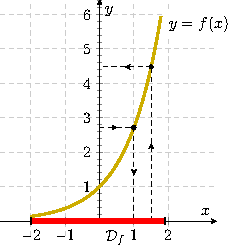
\includegraphics[width=0.45\linewidth]{mai_fig016a.pdf}}              &
           \subfloat[ ]{\label{mai:fig016b}
             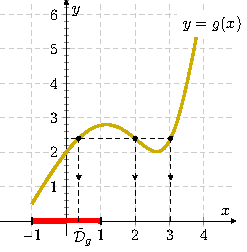
\includegraphics[width=0.45\linewidth]{mai_fig016b.pdf}}              \\
         \end{tabular}
         \caption{K pojmu inverzní funkce}
         \label{mai:fig016}
       \end{figure}
      
      %-------------------------------------
        \input{../src/MAI/exam/exam027.tex}
      %-------------------------------------
      
      Ze způsobu konstrukce funkce \(f^{-1}\) v předchozím příkladu je vidět, že 
      \(\mathcal{D}_{f^{-1}} = \mathcal{H}_f\), \(\mathcal{H}_{f^{-1}} = \mathcal{D}_f\) a graf 
      inverzní funkce je obrazem grafu prosté funkce \(f\) při osové symetrii v rovině 
      souřadnicových os vzhledem k ose prvního a třetího kvadrantu. Nyní již definujeme inverzní 
      funkci obecně. Předpokládejme, že funkce \(f : \mathcal{D}_f\ni x \rightarrow y = f(x)\ni 
      \mathcal{H}_f\) je prostá na svém definičním oboru. Pak existuje funkce \(f^{-1}\) definovaná 
      jako
      \begin{equation}\label{mai:eq029}
        f^{-1} :\mathcal{H}_f\ni x\rightarrow y = f^{-1}(x)\in\mathcal{D}_f\Leftrightarrow x = f(y).
      \end{equation}
      Funkci \(f^{-1}\) nazýváme \textbf{inverzní funkcí k funkci} \(f\). Ještě shrneme pravidla 
      pro skládání funkcí a pro inverzní funkce:

      \begin{itemize}\addtolength{\itemsep}{-0.5\baselineskip}
        \item asociativní zákon pro skládání funkcí
          \begin{equation}\label{mai:eq030}
            f(x)\circ(h(x)\circ g(x)) = f(x)\circ h(x) \circ g(x)
          \end{equation}
        \item distributivní zákon zleva 
          \begin{equation}\label{mai:eq031}
            f(x) \circ (h(x) + g(x)) = f(x) \circ h(x) + f(x) \circ g(x)
          \end{equation}
        \item existence univerzálního neutrálního  prvku \(O\) (nulová funkce \(O:\mathcal{D}\ni x 
          \rightarrow O(x)=0\))
          \begin{equation}\label{mai:eq032}
            f(x) + O = O + f(x) = f(x)
          \end{equation}
        \item existence právě jednoho opačného prvku k funkci \(f\), přičemž \((-f)(x) = -f(x)\)
          \begin{equation}\label{mai:eq033}
            f(x)+(-f(x))=(-f(x))+f(x)=O
          \end{equation}
        \item komutativní zákon pro součet funkcí
          \begin{equation}\label{mai:eq034}
            f(x) + g(x) = g(x) + f(x)
          \end{equation}
        \item asociativní zákon pro součet funkcí  
          \begin{equation}\label{mai:eq035}
            (f(x) + g(x)+h(x) = f(x) + (g(x) + h(x)
          \end{equation}
        \item existence univerzálního neutrálního  prvku \(O\) (nulová funkce \(O:\mathcal{D}\ni x 
          \rightarrow O(x)=0\))
          \begin{equation}\label{mai:eq036}
            f(x) + O = O + f(x) = f(x)
          \end{equation}        
      \end{itemize}   
      Předchozí vztahy platí na patřičně zúžených definičních oborech funkcí, které do nich 
      vstupují.
      
  %-------------------------------------------------------------------------------------------------
  \section{Elementární funkce}
      Základními elementárními funkcemi nazýváme \cite[s.~10]{PolakMA1}:
%      \begin{displaymath}
%        \xymatrix{
%        \mbox{mocninné} & *+[F]{\mbox{Elementární 
%        funkce}}\ar@{->}[l]\ar@{->}[dl]\ar@{->}[d]\ar@{->}[dr]\ar@{->}[r]&\mbox{exponenciální} \\
%        \mbox{goniometrické}       &   \mbox{logaritmické}      & \mbox{cyklometrické}
%        }
%      \end{displaymath}
    %------------- Goniometrické funkce ------------------------------------------------------------
    \input{../src/MAI/sections/fce_goniometricke.tex} 
    %-----------------------------------------------------------------------------------------------
    \subsection{Zobrazení v jiných strukturách}
    %-----------------------------------------------------------------------------------------------
    \subsection{Cvičení}
  %================ Podkapitola: Limita funkce =====================================================
  \section{Limity všeho druhu}  
    „Limes“ znamená latinsky příční cesta, mez, v přeneseném významu pak hranice, pomezí, atd. V 
    matematice představuje limita hodnotu, ke které se „neomezeně blíží hodnota funkce, jestliže se 
    hodnota proměnné neomezeně blíží zadanému číslu“. Poslední formulace musí být v uvozovkách, 
    protože je i přes svou dobrou názornost velice nepřesná. A takové nepřesnosti nejsou v 
    matematice dovoleny. K čemu vůbec úvaha o limitě je? Stačí přece do funkčního předpisu hodnotu 
    proměnné dosadit a získat funkční hodnotu. Tak jednoduché to ale není. Funkční hodnota pro 
    danou hodnotu proměnné \(x\) vůbec nemusí být definována, zato může být definována pro hodnoty 
    velmi blízké. Nebo definována je, ale pro hodnoty proměnné, které jsou k \(x\) velmi blízké, 
    jsou funkční hodnoty od \(f(x)\) velmi vzdálené. Potřebnost pojmu limita ukážeme na 
    geometrickém a fyzikálním příkladu.
    
    V matematické analýze hraje např. důležitou úlohu podíl \cite[s.~117]{Brabec1989}
    \begin{equation*}
      \dfrac{\varphi(x) - \varphi(a)}{x - a}
    \end{equation*}
    kde \(\varphi\) je daná funkce, \(a\) pevný bod. Tento podíl tzv. \emph{přírůstku funkce} 
    \(\varphi(x) — \varphi(a)\) k přírůstku argumentu \(x — a\) může značit např. \emph{průměrnou 
    rychlost pohybu bodu po přímce}, jehož zákon dráhy je dán vztahem \(y = \varphi(x)\), kde \(y\) 
    je dráha, kterou bod urazí za čas \(x\). Zajímá nás, jak se mění hodnota tohoto podílu — jinak 
    řečeno, jak se mění hodnota funkce \(f\) dané vztahem
    \begin{equation}\label{mai:eq037}
      f(x) = \dfrac{\varphi(x) - \varphi(a)}{x - a}
    \end{equation}
    když hodnoty argumentu \(x\) se blíží k číslu \(a\), což často značíme \(x\rightarrow a\). V 
    uvedeném fyzikálním významu daného podílu se ptáme, jak se mění průměrná rychlost pohybu, když 
    se časový úsek zkracuje. Je zřejmé, že musí být stále \(x \neq a\) a že jmenovatel se blíží k 
    nule; obvykle se blíží k nule i čitatel. Jakých hodnot však nabývá přitom podíl, tj. jaké jsou 
    hodnoty funkce \(f(x)\)? Než vyslovíme přesnou definici limity, uvedeme ještě pár jednoduchých 
    příkladů.

    %-------------------------------------
      \input{../src/MAI/exam/exam028.tex}
    %-------------------------------------

    Definičním oborem funkce z příkladu \ref{MAI:exam028} je tedy množina \(\mathcal{D} = \realset 
    — {1}\) (pro \(a = 1\) by ve jmenovateli zlomku byla nula). Grafem funkce je tedy přímka s 
    „vynechaným“ bodem \([1, 2]\) (obr. \ref{mai:fig017}). V bodě \(a = 1\) funkční hodnota není 
    definována. Pokud bychom chtěli rozšířit definiční obor funkce na celou reálnou osu, musíme 
    předepsat, jaké hodnoty má funkce nabývat v bodě \(a = 1\). Původní vzorec, jímž je funkce 
    zadána, výpočet hodnoty \(f(1)\) neumožňuje. Dodatečné zadání funkční hodnoty, její 
    \emph{dodefinování}, můžeme provést zcela libovolně. Zvolme například \(f(1) = 2\). Jiná 
    možnost, jak funkci dodefinovat, je například \(f(1) =-1\). Které číslo je ovšem limitou funkce 
    \(f(x)\) v bodě \(a = 1\)? Je to číslo \(2\), které je v případe \(f(x) = x+1\) její funkční 
    hodnotou? Nebo číslo \(-1\)? A nebo nějaká jiná hodnota? Intuice nám napovídá, že je to číslo 
    \(2\). Když dvojku použijeme pro dodefinování funkce, přetržený graf se „zacelí“. Vidíme, že 
    vezmeme-li dostatečně malý interval proměnné \(x\) v blízkosti bodu \(a=1\) můžeme docílit 
    toho, že všechny odpovídající funkční hodnoty \(f(x)\) budou ležet tak blízko hodnotě \(2\), 
    jak si předem určíme. Skutečně, zkusme docílit toho, aby hodnoty \(f(x)\) ležely v intervalu 
    \((\num{1.99}, \num{2.01})\), tj.
    \begin{equation*}
      \num{1.99} < x + 1 < \num{2.01} \Rightarrow \num{0.99} < x < \num{1.01},\qquad x\neq1.
    \end{equation*}
    Podařilo se. A kdybychom interval \(I(\varepsilon) = (2 - \varepsilon, 2 + \varepsilon)\) 
    funkčních hodnot kolem \(2\) ještě zmenšili, podařilo by se opět najít (o něco menší) interval 
    kolem bodu \(a = 1\) tak, aby pro všechny hodnoty \(x\) v něm (samozřejmě s případnou výjimkou 
    hodnoty \(a =2\)) platilo \(f(x)\in I(\varepsilon)\). A takto bychom mohli \(\varepsilon\) 
    stále zmenšovat. Jak by takový postup dopadl s hodnotou \(-1\), která, jak intuitivně cítíme, 
    limitou funkce v bodě \(a = 1\) není, protože je graf funkce od bodu \([-1,0]\) dost vzdálen? 
    Vezměme třeba interval (\num{-0.5}, \num{0.5}) a hledejme hodnoty \(x\) obdobně jako v 
    předchozím případě. Požadujeme
    \begin{equation*}
      \num{-0.5} < x + 1 < \num{0.5} \Rightarrow \num{-1.5} < x < \num{-0.5}.
    \end{equation*}
    Tento interval vůbec neobsahuje bod \(a = 1\). Dostali jsme se mimo blízkost bodu \(a = 1\).

    %-------------------------------------
      \input{../src/MAI/exam/exam029.tex}
    %-------------------------------------

    Je třeba říci, že při zkoumání limit funkcí nás nezajímají jen funkce „tvaru“ 
    (\ref{mai:eq037}), i když tento případ je v diferenciálním počtu velmi častý, jak poznáme v 
    kap. \ref{mai:IchapIV}. Někdy nás zajímá i chování funkcí v okolí nevlastních bodů \(-\infty\), 
    \(+\infty\) 

    %-------------------------------------
      \input{../src/MAI/exam/exam030.tex}
    %-------------------------------------
    
    %-------------------------------------
      \input{../src/MAI/exam/exam031.tex}
    %-------------------------------------
    
    V uvedených případech bychom mohli zkoumat i limity funkcí pro \(x \to - \infty\).  Všimněme si 
    ještě, že ve všech případech nebylo nutné, aby funkce \(f\) byla definována v bodě, ke kterému 
    se blíží hodnoty argumentu, ale bylo zapotřebí, aby funkce \(f\) byla definována v bodech 
    libovolně blízkých tomuto bodu. Tomuto požadavku bude vyhověno, jestliže daný bod, v němž 
    zkoumáme limitu, bude \emph{hromadným bodem definičního oboru}. Není ovšem nutné, aby funkce 
    byla definována v celém nějakém \emph{prstencovém okolí uvažovaného bodu}.
    
    Nechť \(a\) je bod, blízko kterého se pohybuje hodnota proměnné \(x\). Pro definici limity je 
    důležitý pojem \textbf{okolí bodu} \(a\) (obr. 2.16). Zvolme kladná čísla \(\delta_1\) a 
    \(\delta_2\). Nazýváme
    
    
      
  %================ Podkapitola: Spojitost funkce ==================================================
  \section{Spojitost funkce}
  
%} % tikzset
%~~~~~~~~~~~~~~~~~~~~~~~~~~~~~~~~~~~~~~~~~~~~~~~~~~~~~~~~~~~~~~~~~~~~~~~~~~~~~~~~~~~~~~~~~~~~~~~~~~
\printbibliography[title={Seznam literatury}, heading=subbibliography]
\addcontentsline{toc}{section}{Seznam literatury}          	
%---------------------Numerické metody ------------------------------------------------------------
  % !TeX spellcheck = cs_CZ
%{\tikzset{external/prefix={tikz/MAI/}}
% \tikzset{external/figure name/.add={ch10_}{}}
%---------------------------------------------------------------------------------------------------
% file mai1ch03.tex
%---------------------------------------------------------------------------------------------------
\chapter{Kombinatorika, pravděpdobnost, statistika}\label{mai:IchapIII}
\minitoc
  \section{Kombinatorika}\label{mai:IchapIIIsecI}
    \textbf{Kombinatorika} se od všech matematických disciplín, v několika směrech liší. Zatímco v 
    geometrii má každá přímka nekonečnou délku a každý trojúhelník nekonečně mnoho bodů, zatímco v 
    algebře některé rovnice i nerovnice mají nekonečně mnoho řešení a zatímco matematická analýza 
    zkoumá limity posloupností a funkcí, roste-li příslušná proměnná do nekonečna, v kombinatorice 
    se s nekonečnem nesetkáme. Kombinatorika je součástí \textbf{finitní matematiky}, která studuje 
    konečné soubory (množiny a uspořádané \(k\)-tice, \(k\in \mathcal{N}\)). 
    
    Další odlišností je to, že často nemáme možnost ověřit si správnost výsledku, ke kterému jsme 
    při řešení kombinatorické úlohy dospěli, a jsme odkázáni jen na svůj vlastní úsudek. Proto v 
    kombinatorice v míře větší než jinde platí, že „cvičení dělá mistra“. 
    
    V této kapitole je probrána část kombinatoriky, která se zabývá vytvářením skupin z daných 
    prvků a určováním jejich počtu. Jde o klasickou problematiku, která byla řešena již v 17. a 18. 
    století a která je spojena se jmény \emph{B. Pascala}, \emph{P. Fermata}, \emph{J Bernoulliho}, 
    \emph{G. W. Leibnize}  a \emph{L. Eulera}. Dnes představuje kombinatorika rozsáhlou 
    matematickou disciplínu, některé její problémy byly již vyřešeny (problém čtyř barev) mnohé 
    další na své vyřešení čekají. 
    
    A závěrem ještě důležitá poznámka terminologická: přirozeným čísly se v této kapitole rozumějí 
    čísla celá kladná tj. čísla 1, 2, 3, 4, \(\ldots\), nula se tedy mezi přirozená čísla 
    nezahrunuje. \cite[s.~7]{calda2008matematika} 
    
    \subsection{Základní kombinatorická pravidla}
    
    
    \cite[s.~7]{polak1991matematika}
    
  \section{Pravděpodobnost}\label{mai:IchapIIIsecII}
    Slovo pravděpodobnost používáme velmi často. Jaký však je jeho přesný význam? Jsme přesvědčeni, 
    že pravděpodobnost výhry ve sportce je velmi malá. Ani pravděpodobnost, že se vyplní předpověď 
    počasí, nepovažujeme mnohdy za výraznou. Přesto je mezi oběma příklady obrovský kvantitativní 
    rozdíl. Zkusme význam pojmu pravděpodobnost ukázat pomocí konkrétních číselných příkladů.
  
    \begin{itemize}
      \item \textbf{Příklad se střelcem}: Sportovní střelec střílí na terč série \num{100} ran. 
            Předpokládejme, že podmínky při střelbě jsou stále stejné. Stejná je zbraň, terč, 
            vzdálenost, povětrnostní podmínky i momentální zdravotní stav střelce. Při hodnocení 
            střelcova „mistrovství“ někdo řekne, že střelec zasáhne terč s pravděpodobností 
            \num{92}\%. Jak tomu rozumět? Znamená to, že v souboru sérií výstřelů jsou velmi časté 
            ty, v nichž zasáhl střelec terč \num{92}-krát. Samozřejmě, není řídké, že se objeví i 
            série s \num{93} nebo \num{94} zásahy, ale také s \num{91} nebo \num{90}. Vyloučen není 
            ani případ s úspěšností \num{96} či \num{88}, a dokonce i stovku bychom mohli 
            zaznamenat. Situace výrazně odlišné od \num{92} zásahů však budou řídké, a to tím více, 
            čím více se úspěšnost série liší od \num{92} oběma směry.
      \item \textbf{Příklad se zmetky}: Koupíte si výrobek u firmy, o které je známo, že vyrábí 
            zmetky s pravděpodobností 0,16\%? Situaci lze posuzovat obdobně jako úspěšnost střelce. 
            Budeme-li například zkoumat série obsahující 1000 výrobků, bude každá z nich obsahovat 
            „v průměru“ 16\% zmetků. Z příkladu se střelcem již zhruba víme, jak posuzovat slovo v 
            průměru.
    \end{itemize}
    
    V této kapitole se budeme pravděpodobnostmi zabývat podrobněji. Zjistíme, že i když se týkají 
    náhodných jevů, platí i pro ně jisté zákonitosti. V úvodních příkladech jsme si vyložili, jak 
    intuitivně chápat pojem pravděpodobnost. Jednalo se v nich o posouzení průměrné úspěšnosti ve 
    velkém souboru operací či úkonů prováděných za stejných podmínek, šlo tedy o jakousi 
    „průměrnou“ pravděpodobnost. Nyní definujeme pravděpodobnost matematicky.
    
    \subsection{Co se pravdě podobá - definice pravděpodobnosti}
      Pro definici pravděpodobnosti použijeme pojmu \emph{náhodný pokus}, jehož význam si ukážeme 
      na příkladu. Dobrým příkladem náhodných pokusů je třeba házení mincí, hraní kostkou, výběr 
      karet z balíčku, vidíme-li pouze jejich rub, apod. Budeme třeba házet kostkou. Abychom si 
      situaci zbytečně nekomplikovali, budeme předpokládat, že všechny výsledky hodu kostkou 
      (náhodné pokusy) jsou stejně časté, žádný z nich není nijak preferován\footnote{Kostka by 
      tedy měla být homogenní, plocha, na kterou po hodu dopadne, vodorovná, kvalita povrchu všech 
      stěn kostky stejná (žádná stěna by třeba neměla být natřena lepidlem), apod.}. Počet možných 
      výsledků jednotlivého hodu je \(N = 6\) (kostka má \num{6} stěn, na každé je vyznačen odlišný 
      počet ok, tedy \num{1} až \num{6}). Jednotlivé situace, které mohou nastat, nazýváme 
      náhodnými jevy. Náhodným jevem \(A\) tak může být situace \emph{„padne číslo \num{2}“}, jiným 
      náhodným jevem \(B\) situace \emph{„padne číslo dělitelné třemi“}, apod. Počet situací, kdy 
      výsledek hodu lze hodnotit tak, že určitý jev nastal, označíme \(M\). Například pro jev \(A\) 
      \emph{„padne číslo \num{2}“} je \(M(A)= 1\), pro jev \(B\) \emph{„padne číslo dělitelné 
      třemi“} je \(M(B) = 2\) (počet ok \num{3} nebo \num{6}). Můžeme také definovat jev \(O\) 
      \emph{„nepadne žádné číslo“} (\(M(0) = 0\)) nebo jev \(J\) \emph{„padne jakékoli číslo“} 
      (\(M(J) = 6\)).
      
      \begin{definition}
        Pravděpodobností jevu rozumíme podíl
        \begin{equation}\label{mai:eq011}
          p = \frac{M}{N} = \frac{\text{počet případů příznivých}}{\text{počet případů možných}}.
        \end{equation}  
        Počtem případů možných jsme zkráceně nazvali počet všech možných výsledků náhodného 
        pokusu, počtem případů příznivých pak počet všech takových výsledků pokusu, při nichž daný 
        jev nastal.
      \end{definition}
      Je zřejmé, že hodnota pravděpodobnosti jakéhokoli jevu je nezáporná a může nabývat hodnoty 
      nejvýše \num{1}, tj. \(0 <p< 1\). Jev s \emph{nulovou pravděpodobností} se nazývá 
      \textbf{nemožný}, jev s \emph{jednotkovou pravděpodobností} je \textbf{jistý}. V našem 
      příkladu s kostkou tak dostáváme
      \begin{equation*}
        p(A) = \frac{1}{6}, \qquad p(B) = \frac{2}{6} = \frac{1}{3}, \qquad
        p(O) = 0, \qquad p(J) = 1.
      \end{equation*}  

      %--Barevné ponožky----------------------------------------------
      \input{../src/MAI/exam/exam006.tex}
      %---------------------------------------------------------------
    \subsection{Cifry, kostky, karty - kombinatorické opakování}
      Příklad s ponožkami byl velmi jednoduchý. Podařilo se nám vyjmenovat všechny případy možné i 
      všechny případy příznivé, neboť obojího bylo docela málo. Daleko běžnější jsou však situace, 
      kdy výčet případů není schůdný. A tehdy potřebujeme \textbf{kombinatoriku}.
      
      Nechť \(\mathcal{M}\) je \(n\)-prvková množina, z níž budeme provádět výběry \(k\) prvků 
      podle určitých pravidel. Prvky množiny \(\mathcal{M}\) nemusíme nijak konkretizovat. Abychom 
      si však o výběrech a pravidlech pro jejich tvorbu dokázali udělat nějakou názornou představu, 
      je taková konkretizace vhodná. Prvky množiny \(\mathcal{M}\): mohou být třeba žáci ve třídě, 
      barvy, hrací karty, apod. Výběry mohou představovat třeba družstva pro odbíjenou, signály 
      tvořené barevnými praporky, možnosti rozdání karet při mariáši, apod. Jednotlivé typy výběrů 
      získaly své názvy právě na základě pravidel stanovených pro jejich vytváření. Rozhodující 
      jsou dvě základní kritéria:
      \begin{itemize}\addtolength{\itemsep}{-0.5\baselineskip}
        \item Je pro tvorbu výběru podstatné pořadí prvků ve výběru či nikoliv?
        \item Mohou se prvky ve výběru opakovat či nikoliv?
      \end{itemize}
      
      Typy výběrů shrnuje následující diagram:
      \begin{figure}[ht!] %\ref{mai:fig021}
        \centering
        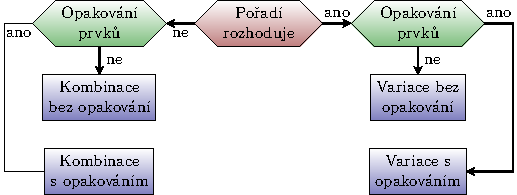
\includegraphics[width=0.7\linewidth]{mai_fig021.pdf}
        \caption{Typy výběrů. \cite[s.~201]{Musilova2009MA1}}
        \label{mai:fig021}
      \end{figure}

      Představuje-li daný výběr například volejbalové družstvo osmi děvčat (šest hráček a dvě 
      náhradnice), které bude reprezentovat v soutěži třídu osmou bé, do níž chodí \num{25} děvčat 
      a \num{18} chlapců, jedná se o výběr \(k - 8\) prvků z počtu \(n = 25\) prvků. Chlapce nelze 
      postavit do družstva volejbalistek. Každý výběr možného družstva bude představovat 
      \emph{kombinaci bez opakování}, neboť pořadí hráček nehraje roli a třeba Aničku Novákovou 
      máme ve třídě jen jednu. Budeme-li však chtít vytvářet z deseti cifer \(0, 1, \ldots, 9\) 
      trojciferná čísla, pak tyto výběry tří prvků z deseti (\(k = 3\), \(n = 10\)) jsou 
      \emph{variacemi s opakováním}. Čísla \num{125}, \num{512}, \num{251}, \num{215}, \num{521} a 
      \num{152} jsou totiž různá, a například \num{222} je také trojciferné číslo. Kombinace s 
      opakováním bychom mohli vytvářet třeba i při výběru různobarevných ponožek ze zásuvky a 
      konečně \emph{variacemi bez opakování} by mohly být dejme tomu trojbarevné signály (\(k = 
      3\)) tvořené trojicemi barevných hadříků vybíraných z \(n\) barev (pro \(n = 3\) třeba zrovna 
      z těch ponožek). Nyní bychom však rádi věděli, jak pro zadané hodnoty \(n\) a \(k\) určit 
      počet všech možných výběrů předepsaného typu. Ukážeme si to na příkladech.

      %--Šance milion-------------------------------------------------
      \input{../src/MAI/exam/exam007.tex}
      %---------------------------------------------------------------
      
      Zobecněním předchozího příkladu získáváme vzorec pro počet \textbf{variací s opakováním} 
      \emph{k}-té třídy z \(n\) prvků. Při tahu totiž záleží na pořadí bubnů a každý buben obsahuje 
      všechny cifry. Výsledky tahů z jednotlivých bubnů se tedy mohou opakovat. Pokud by bubnů bylo 
      \(k\) a v každém \(n\) různých cifer, dostali bychom pro \textbf{variace s opakováním 
      \(k\)-té třídy z \(n\) prvků} celkový počet
      \begin{equation}\label{mai:eq007}
        \boxed{V_k' = n^k}\, .
      \end{equation}

      %--Modifikovaná šance milion------------------------------------
      \input{../src/MAI/exam/exam008.tex}
      %---------------------------------------------------------------
      
      Uvážíme-li, že v předchozím příkladu je \(n = 10\) a \(k = 6\), dostáváme pro \textbf{počet 
      variací bez opakování \(k\)-té třídy z \(n\) prvků} obecný vztah
      \begin{align}
        V_k(n) &= n(n-1)(n-2)\cdots(n-k+1)  \nonumber \\
        \shortintertext{neboli}
        V_k(n) &= \frac{n!}{(n-k)!}\, .    \label{mai:eq008}
      \end{align}
      Poznamenejme, že \(n!\) značí \textbf{faktoriál}, \(n! = n(n - 1)\cdots 3 \cdot 2 \cdot 1\). 
      Pro nulu definujeme \(0! = 1\). Je zřejmé, že při vytváření variací bez opakování musí být 
      \(k\leqq n\). Variace bez opakování \(n\)-té třídy z \(n\) prvků se nazývají 
      \textbf{permutace}. Každá z nich představuje určité uspořádání těchto \(n\) prvků. Platí
      \begin{equation}\label{mai:eq009}
        \boxed{P(n) = V_n(n) = n!}\, .
      \end{equation}
      
      Nyní odvodíme vzorec pro počet \textbf{kombinací \(k\)-té třídy z \(n\) prvků bez opakování}. 
      Již jsme si řekli, že \emph{kombinací} rozumíme takový výběr z celkového počtu \(n\) prvků, 
      který obsahuje určitých \(k\) prvků nezávisle na jejich pořadí. Představme si, že máme k 
      dispozici všechny variace bez opakování \(k\)-té třídy ze zmíněných \(n\) prvků. Vezměme 
      kteroukoli z nich. Soubor všech variací \(k\)-té třídy z \(n\) prvků však obsahuje i další 
      variace, lišící se od té naší jen pořadím prvků. Celkem je takových variací (i s tou první) 
      \(k!\) a z hlediska kombinací představují totéž. Soubor variací se tak rozpadá na podsoubory, 
      z nichž každý obsahuje \(k!\) variací lišících se navzájem pouze pořadím prvků. Každý z 
      těchto podsouborů představuje však jedinou kombinaci. Počet kombinací \(k\)-té třídy z \(n\) 
      prvků bez opakování je tedy
      \begin{equation}\label{mai:eq010}
        \boxed{C(k) = \frac{V_k(n)}{P(k)} = \frac{n!}{(n-k)!\,k!} = 
               \begin{pmatrix}
                n \\
                k
               \end{pmatrix}}\, .
      \end{equation}
      
      Pro odvození vzorce pro \textbf{kombinace s opakováním} použijeme opět příkladu.
      %--Kuličky v přihrádkách----------------------------------------
      \input{../src/MAI/exam/exam009.tex}
      %---------------------------------------------------------------
      
      %--Obsazování kvantových stavů----------------------------------
      \input{../src/MAI/exam/exam010.tex}
      %---------------------------------------------------------------
      
      Získané kombinatorické vzorce nyní použijeme při řešení základních úloh o pravděpodobnostech. 
      V každé úloze bude důležité
      \begin{itemize}
        \item definovat jev \(A\), jehož pravděpodobnost počítáme,
        \item určit počet \(N\) případů možných, tj. počet všech možných výsledků pokusu, při 
              kterém sledujeme, zda jev \(A\) nastal či nenastal,
        \item určit počet \(M\) případů příznivých, tj. počet těch výsledků daného pokusu, při 
              kterých jev \(A\) nastal.
      \end{itemize}

      %--Výhra ve sportce---	----------------------------------------
      \input{../src/MAI/exam/exam052.tex}
      %---------------------------------------------------------------

      %--Losování karet-----------------------------------------------
      \input{../src/MAI/exam/exam053.tex}
      %---------------------------------------------------------------

      %--Sestavování čísel z cifer------------------------------------
      \input{../src/MAI/exam/exam054.tex}
      %---------------------------------------------------------------

    \subsection{Sčítání a násobení - základní počty s pravděpodobnostmi}
      Někdy je třeba určit pravděpodobnosti jevů, které jsou nějakým způsobem „složeny“ z jevů
      jednodušších. Uvažujme například o jevech \(A\) a \(B\), jejichž pravděpodobnosti známe a 
      označíme je \(p(A)\) a \(p(B)\). Definujme nové jevy \(C\) a \(D\) takto:
      \begin{equation*}
        C = A \text{ a } B, \qquad D = A \text{ nebo } B.
      \end{equation*}
      Vzniká přirozená otázka, zda můžeme na základě znalosti pravděpodobností \(p(A)\) a \(p(B)\) 
      určit pravděpodobnosti \(p(C)\) a \(p(D)\). Ukazuje se, že za jistých předpokladů ano. Jako 
      obvykle nám napoví příklady.

      %--Hody kostkou a mincí - jev \(C\)-----------------------------
      \input{../src/MAI/exam/exam055.tex}
      %---------------------------------------------------------------
      
      Z příkladu intuitivně chápeme, co jsou to nezávislé jevy, a usuzujeme, že obecně platí
      \begin{lemma}\label{mai:lemma003}
        \textbf{(Násobení pravděpodobností)}: Pravděpodobnost současného výskytu dvou nezávislých 
        jevů \(A\) a \(B\) (jev \(C\)) je rovna součinu jejich pravděpodobností, tj.
        \begin{equation}\label{mai:eq052}
           p(A \text{ a } B)= p(A)p(B)\qquad \text{pro } A \text{ a } B \text{ neslučitelné}
        \end{equation}
      \end{lemma}
      
      Pokusme se o přesnější definici nezávislých jevů a o odvození vztahu (\ref{mai:eq052}). 
      Označme jako \(N_A\) množinu všech možných výsledků pokusu, při němž může nastat jev \(A\), a 
      obdobně \(N_B\) množinu všech možných výsledků pokusu, při němž může nastat jev \(B\). V 
      předchozím příkladu je \(N_A = \{1, 2, 3, 4, 5, 6\}\) a \(N_B = \{\mathcal{A}, 
      \mathcal{B}\}\). Jako \(N_C\) označme množinu všech možných výsledků pokusu, při němž může 
      nastat současně jev \(A\) i jev \(B\). Jevy \(A\) a \(B\) nazveme nezávislé, jestliže
      platí \(N_C = N_A \times N_B\) (kartézský součin množin). Označíme-li obdobně \(M_A \subseteq 
      N_A\) a, \(M_B \subseteq N_B\) a \(M_C \subseteq N_C\) podmnožiny příznivých výsledků pro 
      jednotlivé jevy, je zřejmé, že také \(M_C = M_A \times M_B\). Počty prvků jednotlivých množin 
      označíme \(N(A)\), \(N(B)\), \(N(C)\) (počty možných případů) a \(M(A)\), \(M(B)\), \(M(C)\) 
      (počty příznivých případů). O konečných množinách víme, že mohutnost (počet prvků) 
      kartézského součinu množin je rovna součinu mohutností jednotlivých
      činitelů v tomto kartézském součinu. Proto
      \begin{align*}
        N(C) &= N(A)N(B),\qquad M(C) = M(A)M(B). \\
        \shortintertext{Odtud}
        p(C) &= \dfrac{M(C)}{N(C)} = \dfrac{M(A)M(B)}{N(A)N(B)} = p(A)p(B).
      \end{align*}
      Platnost tohoto vzorce lze zobecnit na nezávislé jevy \(A_1\), \(A_2\) až \(A_k\) s 
      pravděpodobnostmi \(p(A_1)\), \(p(A_2)\) až \(p(A_k)\). Pravděpodobnost jevu \(C = (A_1\text{ 
      a }A_2\text{ a }...\text{ a }A_K)\) pak je
      \begin{equation*}
        p(C) = p(A_1)p(A_2)\cdots p(A_k).
      \end{equation*}
 
      %--Hody kostkou trochu jinak - jev \(D\)------------------------
      \input{../src/MAI/exam/exam056.tex}
      %---------------------------------------------------------------
      
      Je vidět, že opět směřujeme k obecnému tvrzení:
      \begin{lemma}\label{mai:lemma004}
        \textbf{(Sčítání pravděpodobností)}: Pravděpodobnost jevů \(A\) nebo \(B\) (jev \(C\)) 
        pro neslučitelné (vylučující se) jevy \(A\) a \(B\) rovna součtu pravděpodobností jevů 
        \(A\) nebo \(B\).
        \begin{equation}\label{mai:eq053}
           p(A \text{ nebo } B)= p(A) + p(B)\qquad \text{pro } A \text{ a } B \text{ nezávislé}
        \end{equation}
      \end{lemma}
      
      Opět se pokusme o přesnější definici neslučitelných jevů a o odvození vztahu 
      (\ref{mai:eq053}). Označme, obdobně jako v předchozí úvaze o nezávislých jevech, množiny 
      \(N_A\), \(N_B\), \(N_D\) možných výsledků, při nichž mohou nastat jevy \(A\), \(B\), \(D\). 
      Předpokládejme, že \(N_A = N_B\). Pak \(N_A = N_B = N_D\), a tedy \(N(A) = N(B) = N(D) = N\). 
      Jako \(M_A\), resp. \(M_B\), resp. \(M_D\) označme podmnožiny výsledků, při nichž nastane jev 
      \(A\), resp. \(B\), resp. \(D\). Zřejmě \(M_D = M_A \cup M_B\). Pro počet prvků množiny 
      \(M_D\) platí 
      \begin{align*}
        M(D) &= M(A) + M(B) - M(A\text{ a }B).                                    \\
        \shortintertext{Pravděpodobnost jevu \(D\) je pak}
        p(D) &= \dfrac{M(D)}{N(D)} = \dfrac{M(A) + M(B) - M(A\text{ a }B)}{N} 
              = p(A) + p(B) - p(A\text{ a }B).
      \end{align*}
      
      Jevy \(A\) a \(B\) se nazývají \textbf{neslučitelné}, neboli \emph{vylučující se}, je-li 
      \(M_A \cap M_B = 0\). V takovém případě je ovšem \(M(A\text{ a }B) = 0\), a tedy
      \begin{equation*}
        p(A\text{ nebo }B) = p(A) + p(B).
      \end{equation*}
      Zobecněním na \(k\) jevů \(A_1\) až \(A_k\) po dvou neslučitelných dostáváme
      \begin{equation*}
        p(A_1\text{ nebo }\cdots\text{ nebo }A_k) = p(A_2) + p(A_2) + \cdots + p(A_k).
      \end{equation*}
      Mají-li po dvou neslučitelné jevy \(A_1\) až \(A_k\) tu vlastnost, že při daném pokusu musí 
      nastat právě jeden z nich, říkáme, že tvoří \textbf{úplný systém jevů}. Součet jejich 
      pravděpodobností je roven jedné.
      
      Jev \(\overline{A}\) se nazývá \textbf{opačný} k jevu \(A\), jestliže nastává právě tehdy, 
      když jev \(A\) nenastává. Z této definice je vidět, že jevy \(\overline{A}\) a \(A\) jsou 
      \emph{neslučitelné}. Na druhé straně je zřejmé, že jev (\(A\) nebo \(\overline{A}\)) je jevem 
      \textbf{jistým}, nastává vždy. Jeho pravděpodobnost je tedy \num{1}. Odtud
      \begin{equation}\label{mai:eq054}
        p(\overline{A}) = 1 - p(A).
      \end{equation}
      Jev \(A\) a jev \(\overline{A}\) k němu opačný tvoří úplný systém.
      
      Na závěr odstavce ještě jeden prakticky důležitý příklad.
      
      %--Bernoulliův pokus--------------------------------------------
      \input{../src/MAI/exam/exam057.tex}
      %---------------------------------------------------------------

    \subsection{Pravděpodobnější, než bychom čekali - podmíněná pravděpodobnost}
      Kdysi se objevila, jako nepříliš dobrý vtip, úvaha o pravděpodobnosti bomby na palubě letadla:
      Řekněme, že pravděpodobnost, že některý z pasažérů letadla má s sebou bombu, je jedna
      tisícina. Pravděpodobnost, že dva pasažéři nezávisle na sobě budou mít bombu, je pak pouze
      jedna milióntina (\(\num{e-3}\cdot\num{e-3}= \num{e-6}\)). Vezmu-li si tedy s sebou do 
      letadla svou vlastní bombu, kterou ovšem nehodlám uvést do chodu, snížím tím pravděpodobnost 
      druhé bomby na palubě na onu jednu milióntinu. Nezabývejme se nyní tím, že již první úvaha o 
      jedné milióntině je v podstatě nesprávná, i když pro případ, že pravděpodobnost \(p\), že 
      konkrétní pasažér bude mít bombu, je velmi malá, dává správný přibližný výsledek. Klíčová 
      chyba je v úvaze, že snížení pravděpodobnosti bomby na palubě můžeme napomoci vlastní bombou 
      v zavazadle. Tato úvaha nerespektuje totiž \textbf{pojem podmíněné pravděpodobnosti}, který 
      si nyní na příkladu vyložíme.
      
      %--Jak nekoupit zmetek------------------------------------------
      \input{../src/MAI/exam/exam058.tex}
      %---------------------------------------------------------------
      
      Nyní již snadno dokážeme přijít na chybu v úvaze o bombě v letadle, kterou jsme tento 
      odstavec uvedli. Pravděpodobnost další bomby v letadle za podmínky, že jsme tam jednu sami 
      donesli, je podmíněnou pravděpodobností. Proto je rovna podílu pravděpodobnosti, že v letadle 
      budou dvě bomby, a pravděpodobnosti, že tam bude jedna bomba, tj. \(\num{e-6}/\num{e-3} = 
      \num{e-3}\). Pocit bezpečí bychom si tedy vlastní bombou nezvýšili. Ještě abychom se báli, že 
      bouchne, zejména pokud by byla vyrobená ve Hvizdu.
      
      %--Kolika let se dožijeme?--------------------------------------
      \input{../src/MAI/exam/exam059.tex}
      %---------------------------------------------------------------
      
      %--Ještě jednou bomba v letadle---------------------------------
      \input{../src/MAI/exam/exam060.tex}
      %---------------------------------------------------------------
      
      Nakonec ještě odvodíme obecný případ takzvané Bayesovy formule. Předpokládejme, že při
      každém opakování jistého pokusu může nastat právě jeden z \(k\) různých výsledků. Jevy \(A_1,
      A_2,\cdots, A_k\), z nichž \(j\)-tý znamená, že při pokusu byl zaznamenán \(j\)-tý výsledek, 
      jsou po dvou neslučitelné a tvoří úplný systém. Platí tedy
      \begin{equation*}
        p(A_1) + p(A_2) + \ldots  + p(A_k) = 1.
      \end{equation*}
      Označme jako \(B\) libovolný jev, který popisuje celkový výsledek pokusu. Vzhledem k 
      neslučitelnosti jevů \(A_1\) až \(A_k\) jsou neslučitelné i jevy (\(A_1\) a \(B\)) až 
      (\(A_k\) a \(B\)). Zároveň je zřejmé, že jev \(B\) lze zapsat jako
     \begin{equation*}
       B = (A_1\text{ a }B) \quad\text{nebo}\quad (A_2\text{ a }B) \qquad\ldots
       \quad\text{nebo}\quad (A_k\text{ a }B),
     \end{equation*} 
      a tedy
      \begin{equation*}
        p(B) = \sum_{j=1}^{k}p(A_j\text{ a }B) = \sum_{j=1}^{k}p(A_j)\cdot p_{A_j}(B),
      \end{equation*}
      s využitím vztahu (\ref{mai:eq057}). Současně, podle téhož vztahu, platí 
      \begin{equation*}
        p(A_j\text{ a }B) = p(B)\cdot  p_B(A_j).
      \end{equation*}
      Pomocí dvou předchozích vztahů dostáváme:
      
      \adjustbox{minipage=[c]{\textwidth}}{%
        \begin{lemma}\label{mai:lemma005}
          \textbf{(Bayesova formule):}
          \begin{equation}\label{mai:eq058}
            p_B(A_j) = \dfrac{p(A_j\text{ a }B)}{\sum_{i=1}^{k}p(A_i)\cdot p_{A_i}(B)} 
                     = \dfrac{p(A_j)\cdot p_{A_j}(B)}{\sum_{i=1}^{k}p(A_i)\cdot p_{A_i}(B)} .
          \end{equation}
        \end{lemma}
      }
      
      Bayesova formule pro výpočet podmíněné pravděpodobnosti má řadu užitečných aplikací
      
      %--Potřebují lékaři pravděpodobnost?----------------------------
      \input{../src/MAI/exam/exam061.tex}
      %---------------------------------------------------------------
      
      A na závěr ještě hádanky:

      %--Pohádka o Honzovi--------------------------------------------
      \input{../src/MAI/exam/exam062.tex}
      %---------------------------------------------------------------
      
      %--Může se člověk živit sázením?--------------------------------
      \input{../src/MAI/exam/exam063.tex}
      %---------------------------------------------------------------
      
  \section{Náhodné veličiny}\label{mai:IchapIIIsecIII}
    Hodnota některých veličin je určena jednoznačně a „jednou provždy“. Kdykoli budeme její hodnotu 
    zjišťovat, tehdy dostaneme totéž - takže ji ani opakovaně zjišťovat nemusíme. Příkladem může 
    být skoro prázdná peněženka, ve které jsou třeba tři koruny. Dokud nebudeme pracovat a do 
    peněženky něco nepřidáme, bude hodnota veličiny \(X\) (počet korun v peněžence) stále rovna 
    \num{3}. Nemá smysl se do peněženky vůbec dívat. Pokud budeme do peněženky přidávat každý den 
    dvě koruny, také budeme vědět, jak se veličina \(X\) mění, aniž bychom se do peněženky dívali. 
    Po \(n\) dnech bude hodnota \(X = 3 + 2n\). Většina veličin, se kterými se setkáváme, se však 
    takto nechová. Jejich hodnoty se totiž často řídí náhodnými vlivy, takže při každém
    měření veličiny \(X\), tj. zjišťování její hodnoty, můžeme získat odlišný výsledek než při 
    měřeních předchozích. Uveďme některé příklady náhodných veličin.
    
    \begin{itemize}
      \item \textbf{Příklad s novorozenci}: Nechť jé veličinou \(X\) počet chlapců ve stovce 
            novorozených dětí. Zkušenost říká, že tento počet je v průměru o něco větší než 
            \num{50}, avšak pro různé skupiny po stovce novorozených dětí bude počet chlapců 
            kolísat. V jedné skupině bude \num{52}, v jiné \num{54}, někde třeba \num{60}, nebo 
            také \num{45}.
      \item \textbf{Příklad s meteoroidy a meteority}: Pro astronomy může být důležitou veličinou 
            \(X\) počet meteoroidů, které za rok dopadnou do zemské atmosféry. Jinou veličinou, 
            třeba \(K\), může být roční počet meteoritů, tj. těch meteoroidů, které v atmosféře 
            neshořely zcela, ale jejich část dopadla na povrch Země. Také tyto hodnoty budou pro 
            každý roční interval poněkud odlišné, neboť i počet dopadnuvších meteoroidů a 
            meteoritů podléhá vlivům, které se nedají přesně předvídat.
      \item \textbf{ Příklad s tlakoměrem}: Bude-li lékař měřit pacientovi tlak několikrát po 
            sobě, určitě také naměří několik různých hodnot. Krevní tlak je citlivý na náhodné 
            vlivy, třeba i na vnitřní rozrušení pacienta vyplývající ze strachu z bílého pláště.
      \item \textbf{Opakovaná měření fyzikální veličiny}: Chceme-li změřit třeba odpor elektrického
            vodiče (drátu), jedná se o měření nepřímé. Nemůžeme odpor změřit přímo, třeba jako      
            to můžeme udělat pro délku. Většinou měříme napětí \(U\) na vodiči a proud \(I\), který 
            jím protéká. Odpor pak zjišťujeme jako podíl \(R = U/I\). Změříme-li napětí i proud 
            jednou, dostaneme konkrétní hodnotu \(R\). Budeme-li měření napětí a proudu provádět 
            opakovaně, budeme dostávat poněkud odlišné hodnoty \(U\) a \(I\), a tedy i odlišné 
            hodnoty \(R\). Sledované veličiny se chovají jako náhodné. Je to způsobeno řadou 
            náhodných vlivů jak na veličiny samotné, tak na jejich měření (nepřesnost odečítání 
            údajů na stupnicích, apod.).
    \end{itemize}
  
    Při každém fyzikálním (a vlastně i nefyzikálním) experimentu máme co do činění s náhodnými 
    veličinami. Při chemických analýzách je náhodnou veličinou třeba koncentrace dané látky
    v roztoku, při experimentech biologických třeba počet uhynuvších rostlin ve stovce sazenic, 
    počet pozorovaných prvoků v zorném poli mikroskopu, výskyt vzácných ptáků ve sledované 
    lokalitě, apod. V následujících odstavcích definujeme náhodné veličiny přesněji a naučíme se s 
    nimi zacházet. Uvidíme, že zjištění určité hodnoty náhodné veličiny je otázkou jisté 
    pravděpodobnosti. Také lépe objasníme, co znamená vyjádření „v průměru“, které jsme občas v 
    předchozím textu použili a intuitivně mu jistě rozuměli.
  
    \subsection{Jak dobrý je to střelec - diskrétní rozdělení}
      Mimořádně vhodnou ukázkou náhodné veličiny je příklad se sportovním střelcem, kterým jsme
      uvedli celou kapitolu o pravděpodobnostech.
  
      %--Ještě jednou střelba, tentokrát přesněji---------------------
      \input{../src/MAI/exam/exam064.tex}
      %---------------------------------------------------------------
    
    Položme si ještě otázku, jak můžeme zjistit pravděpodobnosti, se kterými střelec dosáhne při
    jednom výstřelu daného počtu bodů. Prakticky to lze provést jedině tak, že střelec mnohokrát
    vystřelí na terč a jeho zásahy budou při tom zaznamenávány. Dejme tomu, že vystřelil \(n\)-krát 
    a že počet výstřelů, při nichž byl bodový zisk \(j\) bodů ( \(j = 0, 1, 2, 3\)), byl \(n_j\). 
    Pak pro pravděpodobnost bodového zisku \(j\) bodů při jednom výstřelu je \(p_j = n_j/n\). 
    Kdybychom provedli skutečný experiment se střelcem a počítali pravděpodobnosti \(p_j\) znovu a 
    znovu po každém dalším výstřelu, viděli bychom, že pro malé hodnoty \(n\) nejprve kolísají a 
    pro rostoucí \(n\) se začínají ustalovat a již kolísají velmi málo. Tímto postupem bychom je 
    mohli určit tak, aby byly pro náš účel rozumně přesné - třeba s přesností na dvě platná místa. 
    Rozumnou přesností je zde myšlena skutečnost, že nemá smysl chtít zjišťovat pravděpodobnost 
    třeba na šest platných míst. Vzhledem k principiální přítomnosti náhodných vlivů se kolísání 
    pravděpodobností nikdy nezbavíme, takže platná místa na pozicích, kde se kolísání trvale 
    projevuje již bez ohledu na zvyšující se \(n\), nemají smysl.
    
    V příkladu \ref{mai:exam064} jsme se již velmi těsně přiblížili důležitým charakteristikám, 
    které určují náhodnou veličinu a jsou přitom matematicky korektně definovány. Viděli jsme, že 
    známe-li jen hodnoty, kterých může náhodná veličina nabývat, nemůžeme o ní říci již nic 
    dalšího. Známe-li však ještě pravděpodobnosti, se kterými jednotlivých hodnot nabývá, můžeme o 
    ní získat již velmi mnoho informací.

    \adjustbox{minipage=[c]{\textwidth}}{%
      \textbf{Náhodnou veličinou s diskrétním rozdělením} nazýváme takovou veličinu \(X\), která
      může nabývat konečně mnoha různých hodnot \((x_1, x_2, \ldots, x_k)\) s pravděpodobnostní
      \((p_1, p_2, \ldots, p_k)\) popřípadě spočetně mnoha hodnot \((x_1, x_2, \ldots)\) s 
      pravděpodobnostmi \((p_1, p_2, \ldots)\).
      }

    Jevy \(A_j\) \uv{Veličina \(X\) nabývá hodnoty \(x_j\)}, jsou po dvou neslučitelné. Platí
    \begin{equation*}
      \sum_{j=1}^{k}p_j = 1, \qquad\text{resp.}\qquad \sum_{j=1}^{k=\infty}p_j = 1
    \end{equation*}
    Pokud jde o druhý z obou případů, nebudeme se jím prozatím zabývat. Soubor všech dvojic
    \begin{equation*}
      \left\lbrace(x_j, p_j)\right\rbrace,\qquad j = 1, 2, \ldots, k,
    \end{equation*}
    se nazývá \textbf{rozdělení} náhodné veličiny \(X\). Můžeme je znázornit i graficky.

    %--Bernoulliovo (binomické) rozdělení---------------------------
    \input{../src/MAI/exam/exam065.tex}
    %---------------------------------------------------------------
    
    Nyní definujeme další charakteristiky náhodné veličiny. Těmi základními jsou, kromě již 
    definované \emph{nejpravděpodobnější hodnoty}, ještě \textbf{střední hodnota}, \textbf{rozptyl} 
    (popřípadě jeho odmocnina, zvaná \textbf{střední kvadratická} nebo \textbf{směrodatná 
    odchylka}), \textbf{medián}, popřípadě \textbf{P-kvantil}. Pojem střední hodnoty jsme již v 
    podstatě vybudovali v příkladu se střelcem. Nyní postup zobecníme. Předpokládejme, že při 
    velkém počtu \(n\) měření náhodné veličiny \(X\) naměříme různé hodnoty \((x_1, x_2, \ldots, 
    x_k)\) tak, že hodnota \(x_1\) byla naměřena \(n_1\)-krát, hodnota \(x_2\) \(n_2\)-krát, atd., 
    až hodnota \(x_k\) \(n_k\)-krát. Je zřejmé, že součet četností \(n_1\), \(n_2\), až \(n_k\) 
    jednotlivých hodnot musí být roven celkovému počtu měření \(n\) a že podíly
    \begin{equation*}
      p_1 = \dfrac{n_1}{n}, \qquad p_2 = \dfrac{n_2}{n}, \qquad \ldots, \qquad p_k = \dfrac{n_k}{n},
    \end{equation*}
    představují pravděpodobnosti jednotlivých hodnot veličiny \(X\). Tím je zadáno její rozdělení,
    které ji plně charakterizuje. Položme si však otázku, zda by se veličina \(X\) přece jen nedala
    charakterizovat jedinou hodnotou, která by všechny různě pravděpodobné hodnoty v jistém
    smyslu „zastupovala“. Kdybychom třeba takto měřili délku stolu, jistě bychom na otázku „Kolik
    měří stůl?“ neodpovídali tím, že bychom tazateli předložili získané rozdělení, i když by taková
    odpověď byla nejvýstižnější. Určitě bychom uvedli jedinou hodnotu. Ale jakou? I laika napadne,
    že by takovou reprezentativní hodnotou mohl být aritmetický průměr naměřených hodnot \(x_1\) až
    \(x_k\). Bylo by ale správné vzít jen prostý aritmetický průměr těchto různých hodnot a nebrat 
    ohled na skutečnost, že některé byly naměřeny s větší a jiné s menší četností? Nikoliv. 
    Reprezentativní hodnota veličiny \(X\) nemá zastupovat jen naměřené hodnoty, ale celé 
    rozdělení. Určitá hodnota \(x_j\) bude mít tím větší vliv na reprezentativní hodnotu, s čím 
    větší četností byla naměřena. Protože byla naměřena \(n_j\)-krát, musíme ji také tolikrát do 
    aritmetického průměru započíst.Získáváme tak \textbf{vážený aritmetický průměr} naměřených 
    hodnot, neboli \emph{střední hodnotu}
    
    \adjustbox{minipage=[c]{\textwidth}}{%
      \begin{equation}\label{mai:eq059}
        \left\langle x \right\rangle = \dfrac{n_1x_1 + n_2x_2 + \cdots + n_kx_k}{n}
          = p_1x_1 + p_2x_2 + \cdots + p_kx_k 
          = \sum_{j=1}^{k}p_jx_j.
      \end{equation}
      }
      Součet všech pravděpodobností \(p_1 + p_2 + \cdots + p_k\) je pochopitelně \textbf{roven 
      jedné}.

    %--Střední hodnota Bernoulliova rozdělení-----------------------
    \input{../src/MAI/exam/exam066.tex}
    %---------------------------------------------------------------
    
    Posuďme nyní situaci, kdy náhodná veličina \(Y\) je funkcí náhodné veličiny \(X, Y = f(X)\).
    V takovém případě má rozdělení veličiny \(Y\) tvar
    \begin{equation*}
      \left\lbrace (f(x_j), p_j)\right\rbrace, \qquad j = 1, 2, \ldots, k.
    \end{equation*}
    Pravděpodobnost hodnoty \(f(x_j)\) je stejná jako pravděpodobnost hodnoty \(x_j\). Pro výpočet
    střední hodnoty veličiny \(Y\) pak platí
    \begin{equation}\label{mai:eq060}
      \left\langle y \right\rangle = \sum_{j=1}^{k}f(x_j)p_j.
    \end{equation}
    (V obecnější situaci může být náhodná veličina \(Y\) funkcí několika náhodných veličin \(X_1\), 
    \(X_2\), až \(X_s\)).
    
    Může vzniknout oprávněná otázka, zda při výpočtu \(\left\langle y \right\rangle\), popřípadě 
    dalších charakteristik veličiny \(Y\), nevznikne nějaký problém, nebude-li funkce \(f(X)\) 
    prostá. V takovém případě by totiž některé hodnoty veličiny \(Y\) splynuly i pro různá \(x_j\). 
    Například pro \(Y = f(X) = X^2\) by pro hodnoty \(x_r\) a \(x_s\) vázané vztahem \(x_r = -x_s\) 
    (pokud by veličina \(X\) směla takových hodnot nabývat) platilo \(y_{rs} = y_r = y_s\). 
    Pravděpodobnost této společné hodnoty by pak přece byla \((p_r + p_s)\). Tato úvaha je 
    samozřejmě správná, avšak ve výpočtu střední hodnoty veličiny Y
    podle vztahu (\ref{mai:eq060}) je již obsažena. Do součtu totiž vstupují sčítance \(y_rp_r\) i 
    \(y_sp_s\), jejichž součet je při rovnosti \(y_r = y_s\) roven \(y_{rs}(p_r +p_s)\) Společná 
    hodnota \(y_{rs}\) je tedy započtena se správnou vahou.
    
    Uvažujme nyní o tom, jak „směrodatná“, tj. do jaké míry opravdu „reprezentativní“, je
    střední hodnota náhodné veličiny. Intuitivně cítíme, že střední hodnota bude reprezentovat
    rozdělení náhodné veličiny tím lépe, čím méně se od ní budou jednotlivé hodnoty odchylovat na 
    obě strany. Význam slova „odchylovat“ musíme ovšem nějak kvantitativně zachytit.
    \emph{Odchylkou} hodnoty \(x_j\) veličiny \(X\) od střední hodnoty \(\left\langle x 
    \right\rangle\) budeme celkem přirozeně rozumět rozdíl \((x_j - \langle x\rangle)\). Vzniká tak 
    náhodná veličina \(\Sigma = X - \langle x \rangle\) s rozdělením \(\{(x_j - \langle x\rangle, 
    p_j)\}\), \(j = 1, 2, \ldots, k\) . Bude tou správnou charakteristikou odchýlení hodnot 
    veličiny \(X\) od střední hodnoty střední hodnota \(\langle\sigma\rangle\)? Vypočtěme ji 
    (odhadněte předem, co asi tak vyjde):
    \begin{equation*}
      \langle\sigma\rangle = \sum_{j=1}^{k}(x_j - \langle x\rangle)p_j
        = \sum_{j=1}^{k}x_jp_j - \langle x\rangle\sum_{j=1}^{k}p_j
        = \langle x\rangle - \langle x\rangle = 0.
    \end{equation*}
    Čekali jste to? Nepochybně ano. Veličina \(X - \langle x\rangle \) nedává tedy žádný obraz o 
    tom, jak jsou hodnoty \(x_j\) „rozptýleny“ okolo střední hodnoty \(\langle x\rangle\). Kladné 
    odchylky jsou to tiž kompenzovány těmi zápornými. Aby k takové kompenzaci nedošlo, stačí vzít 
    v úvahu absolutní hodnotu veličiny \(\Sigma\), popřípadě její kvadrát. Vezměme v úvahu druhý z 
    obou námětů a vypočtěme \(\langle \sigma^2\rangle\), takzvaný \textbf{rozptyl veličiny} \(X\):
    \begin{align}\label{mai:eq061}
      D(X) &= \langle \sigma\rangle = \sum_{j=1}^{k}(x_j - \langle x\rangle)^2p_j
            = \sum_{j=1}^{k}x_j^2p_j - 2\langle x\rangle\sum_{j=1}^{k}x_jp_j 
            + \langle x\rangle^2\sum_{j=1}^{k}p_j                                     \nonumber \\
           &= \langle x^2\rangle - 2\langle x\rangle^2 + \langle x\rangle^2 
            = \langle x^2\rangle - \langle x\rangle^2.
    \end{align}
    hodnota
    \adjustbox{minipage=[c]{\textwidth}}{%
      \begin{equation}\label{mai:eq062}
        \sigma(x) = \sqrt{\langle \sigma^2\rangle} = \sqrt{\langle x^2\rangle - \langle x\rangle^2}
      \end{equation}
    }
    se nazývá \textbf{směrodatná odchylka} (v některých terminologiích též \emph{střední 
    kvadratická odchylka}) veličiny \(X\). Podíl \(\sigma(x)/ \langle x\rangle\) se nazývá 
    \textbf{relativní směrodatná odchylka} (v některé terminologii též \emph{variační koeficient}).

    \adjustbox{minipage=[c]{\textwidth}}{%
      Důležitým pojmem je \textbf{distribuční funkce}. Je to funkce \(F\) jedné reálné proměnné 
      \(x\) definovaná ve vztahu k náhodné veličině \(X\) takto: Předpokládejme, že hodnoty \(x_1\)
      až \(x_k\), jichž může náhodná veličina \(X\) nabývat, jsou seřazeny vzestupně, tj. \(x_1 <
      < x_2 < \ldots < x_k\). Pak
      \begin{equation}\label{mai:eq063}
        F: \realset\ni x\longleftrightarrow 
        F(x) = \sum_{\mathclap{\substack{j=1\\ x_s \leq x \leq x_{s+1}}}}^{s}p_j
      \end{equation}
    }

    Přestože je veličina \(X\) diskrétní, je distribuční funkce funkcí spojité proměnné. Její 
    funkční hodnoty se však mění skokem. Vidíme to z následující tabulky a z grafu na obrázku 
    \ref{mai:fig045}, v němž je distribuční funkce znázorněna pro případ střelby (příklad 
    \ref{mai:exam064})

    \begin{table}[ht!]
      \centering
      \begin{tabular}{c|c}
        \textbf{interval proměnné} \(x\)  &  \textbf{distribuční funkce}             \\ \hline
            \(-\infty, x_1\)              &    \(F(x) = 0 \)                         \\
            \(\left[x_1, x_2\right)\)     &    \(F(x) = p_1 \)                       \\
            \(\left[x_2, x_3\right)\)     &    \(F(x) = p_1 + p_2 \)                 \\
                    \(\ldots\)            &       \(\ldots\)                         \\
            \(\left[x_j, x_{j+1}\right)\) &    \(F(x) = p_1 + p_2 + \cdots + p_j \)  \\
                   \(\ldots\)             &       \(\ldots\)                         \\
            \(\left[x_k, \infty\right)\)  &    \(F(x) = p_1 + \cdots + p_k =1 \)     \\ \hline
            \end{tabular}
      % \caption{ }
    \end{table}

    \begin{figure}[ht!] %\ref{mai:fig045}
      \centering
      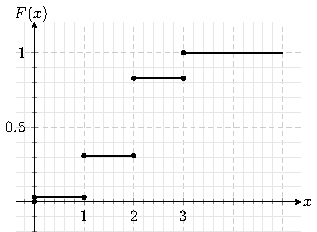
\includegraphics[width=0.5\linewidth]{mai_fig045.pdf}
      \caption{Distribuční funkce k příkladu \ref{mai:exam064}. \cite[s.~233]{Musilova2009MA1}}
      \label{mai:fig045}
    \end{figure}
    Zadáním distribuční funkce je naopak jednoznačně určeno rozdělení veličiny \(X\). Pro jednotlivé
    pravděpodobnosti totiž platí
    \begin{equation*}
      p_j = F(x_j) - F(x_{j-1})\qquad\text{pro}\qquad 2\leq j \leq k, \qquad p_1 = F(x_1).
    \end{equation*}
    
    Hledejme nyní hodnotu \(\overline{x}_P\) definovanou tak, že pravděpodobnost, že při náhodném 
    opakování pokusu nabude veličina \(X\) kterékoli z přípustných hodnot \(x_j \leq 
    \overline{x}_p\), je rovna \(P\). Znamená to, že pro \(x = \overline{x}_P\) má distribuční 
    funkce nabýt předepsané hodnoty \(P\). Abychom \(\overline{x}_P\), takzvaný 
    \(P\)\textbf{-kvantil}, určili, řešíme rovnici
    \begin{equation}\label{mai:eq064}
      \sum_{j=1}^{s}p_j = P
    \end{equation}
    vzhledem k neznámému počtu sčítanců \(s\). V případě veličiny s diskrétním rozdělením se ovšem
    může stát, že pro nevhodně zvolenou hodnotu \(P\) nebude mít rovnice řešení. To proto, že 
    veličina \(X\) může nabývat jen hodnot, které lze očíslovat přirozenými čísly, takže při každé 
    změně horní meze sumy \(s\) o jedničku se suma mění skokem. Vidíme to jak v předcházející 
    tabulce, tak v grafu na obrázku \ref{mai:fig045}. Pro \(P = \num{0.5}\) se \(P\)-kvantil 
    \(\overline{x}_p\), pokud je vůbec definován, nazývá \textbf{medián}. Značí se pouze 
    \(\overline{x}\).

    %--Ještě střelba------------------------------------------------
    \input{../src/MAI/exam/exam067.tex}
    %---------------------------------------------------------------
    
    Příklad \ref{mai:exam067} názorně vypovídá o významu směrodatné odchylky. Viděli jsme, že 
    intervalu o šířce \(2\sigma(y)\) s hodnotou \(\langle y \rangle\) uprostřed odpovídá vysoká 
    pravděpodobnost, že v něm bude ležet bodový zisk střelce při každé pětici výstřelů. Čím bude 
    tento interval užší, tím v průměru blíže budou jednotlivé hodnoty bodového zisku ležet v 
    blízkosti střední hodnoty. Mohli bychom říci, že střelec, jehož výsledky vykazují malou 
    směrodatnou odchylku resp. malý rozptyl, míří přesněji. Směrodatná odchylka je tedy v jistém 
    smyslu jedním z parametrů charakterizujících kvalitu střelby - střelba s malou hodnotou  
    \(\sigma(y)\) je přesnější než střelba s velkou hodnotou \(\sigma(y)\). Druhým parametrem 
    kvality střelby, který je pro její hodnocení z hlediska možnosti vyhrávat soutěže jistě 
    podstatně důležitější, je samozřejmě samotná střední hodnota bodového zisku. Čím je větší, tím 
    je střelcovo pořadí při závodech lepší. Pro interpretaci směrodatné odchylky to ovšem není 
    podstatné. Kdybychom porovnávali dva střelce, jejichž střední bodový zisk při
    pěti výstřelech je třeba \num{12} bodů a \num{3} body, avšak směrodatná odchylka je u obou 
    stejná, musíme konstatovat, že oba jsou stejně přesní. Jeden z nich však systematicky dělá 
    nějakou chybu a přesně střílí do nesprávného místa. Význam pojmu přesnost z hlediska hodnocení 
    náhodných veličin je tedy oproti jeho běžnému chápání poněkud posunut.
    
    Všimněme si ještě jedné důležité obecné věci: Tvar vzorce pro výpočet rozptylu resp. směrodatné 
    odchylky je stejný pro všechny typy rozdělení. Konkrétní pravděpodobnost, že hodnota
    veličiny padne do intervalu určeného směrodatnou odchylkou, tj. do intervalu \((\langle y 
    \rangle - \sigma(y), \langle y \rangle + \sigma(y))\), však pochopitelně na konkrétním 
    rozdělení závisí.

    %--Poissonovo rozdělení-----------------------------------------
    \input{../src/MAI/exam/exam068.tex}
    %---------------------------------------------------------------
    
    \subsection{Kolik rychlostí má molekula plynu - spojité rozdělení}
      Již nadpis napovídá, že veličina se spojitým rozdělením může zřejmě nabývat „spojitě 
      rozložených“ hodnot, tj. přípustným i hodnotami budou například právě všechna čísla \(x\) z 
      jistého intervalu, \(x\in[a, b]\). Jaká však bude pravděpodobnost \(p(x)\), že veličina \(X\) 
      nabývá právě hodnoty \(x\in[a, b]\)? Jestliže víme, že „součet“ všech \(p(x)\) musí být roven 
      jedné, vzniká problém.
      
      Hodnot \(x\) je totiž nekonečně (dokonce nespočetně) mnoho! Je jich tolik, jako je čísel na 
      celé reálné ose. A kdyby byla pravděpodobnost \(p(x)\) jakkoli malinkatá, nikdy nebude součet 
      všech \(p(x)\) konečný. Pravděpodobnost nabývání hodnoty \(x\) tedy musí být nulová. Vzniklou 
      překážku odstraníme snadno. Rozdělení náhodné veličiny \(X\) bude nutno charakterizovat 
      nikoli pravděpodobností, ale \textbf{hustotou pravděpodobnosti}. Je to obdobná situace jako 
      třeba při popisu rozložení hmotnosti nějakého tělesa, předpokládáme-li, že je ta to hmotnost 
      rozložena v objemu tělesa spojitě. Také nemá příliš smysl se ptát, jaká je hmotnost jednoho 
      bodu tohoto tělesa. I zde by byla odpověď, že nulová. Spíše si vždy klademe otázku, jaká je 
      hmotnost \(\Delta m(\vec{r})\) jistého malého objemu \(\Delta V\), například malého kvádříku, 
      umístěného třeba jedním z vrcholů v bodě o poloze \(\vec{r}\). Hustota \(\varrho(\vec{r})\) 
      tělesa v bodě \(\vec{r}\) je pak limitou podílu \(\Delta m(\vec{r})/\Delta V\) pro \(\Delta V 
      \longrightarrow 0\). Obdobně je tomu i s rozdělením spojité náhodné veličiny \(X\). 
      Zvolíme-li pro jistou hodnotu \(x\) interval \([a, x + \Delta x]\), má smysl otázka, jaké je 
      pravděpodobnost \(\Delta p(x)\), že veličina nabývá hodnoty (kterékoli) právě z tohoto 
      intervalu.

      \adjustbox{minipage=[c]{\textwidth}}{%
        Limitu
        \begin{equation}\label{mai:eq066}
          w(x) = \lim\limits_{\Delta\longrightarrow0}\dfrac{\Delta p(x)}{\Delta x}
        \end{equation}
        nazýváme \textbf{hustotou pravděpodobnosti} veličiny \(X\) v bodě \(x\) (pro \(x = a\), 
        resp. \(x = b\) se jedná o limitu zprava, resp. zleva).
      }
      
      Přímo tato funkce pak představuje ono spojité rozdělení náhodné veličiny \(X\). Určuje totiž
      hustotu pravděpodobnosti \(w\) pro hodnotu \(x\) náhodné veličiny \(X\), obdobně jako \(p_j\) 
      v případě diskrétního rozdělení určuje pravděpodobnost hodnoty \(x_j\). Předpokládejme, že je 
      funkce \(w(x)\) na intervalu \([a, b]\) spojitá.
  
      \adjustbox{minipage=[c]{\textwidth}}{%
        Pro \(x \in [a, b]\) definuje integrál jako funkce horní meze
        \begin{equation}\label{mai:eq067}
          F(x) = \int_a^xw(u)\dd{u}
        \end{equation}
        \textbf{distribuční funkci}.
      }
      Jeho hodnota pro dané \(x\) udává pravděpodobnost, že hodnota veličiny \(X\) padne do 
      intervalu \([a, x]\), opět v plné analogii s případem diskrétního rozdělení. Na \((a, b)\) je 
      tedy hustota pravděpodobnosti \(w(x)\) derivací distribuční funkce. Je zřejmé, že \(F(b) = 
      1\). Integrál z hustoty pravděpodobnosti v mezích \([a, b]\) udává totiž pravděpodobnost, že 
      hodnota veličiny \(X\) padne do intervalu přípustných hodnot, tedy pravděpodobnost jistého 
      jevu. V případě diskrétního rozdělení jsme však distribuční funkci definovali nejen pro 
      přípustné hodnoty náhodné veličiny, ale pro všechna x \in (-\infty, +\infty). Tento postup 
      budeme respektovat i nyní a definujeme
      \begin{equation*}
        F(x) = 0\text{ pro }x \in (-\infty,a)\text{ a }F(x) = 1\text{ pro }x \in (b , +\infty).
      \end{equation*}
      \adjustbox{minipage=[c]{\textwidth}}{%
        \begin{equation}\label{mai:eq068}
          \langle x \rangle = \int_a^bxw(x)\dd{x}, \qquad 
                       D(X) = \int_{a}^{b}(x - \langle x \rangle)^2w(x)\dd{x}.
        \end{equation}
      }
      \textbf{Relativní směrodatná odchylka} je opět podílem \(\sqrt{D(X)}/\langle x \rangle\), 
      nejpravděpodobnější hodnota neboli \textbf{modus} \(x_m\) je taková hodnota veličiny \(X\) , 
      pro kterou je hustota pravděpodobnosti maximální
      
      Daleko lépe než u veličin s diskrétním rozdělením vypadá možnost definovat \(P\)-kvantil 
      \(\tilde{x}_p\) a \textbf{medián} \(\tilde{x}\). Jsou jednoduše řešením rovnic
      \begin{equation*}
        F(\tilde{x}_P) = P, \qquad F(\tilde{x}) = \dfrac{1}{2}
      \end{equation*}
      (Mohli bychom mediánu třeba i říkat „půlkvantil“. To ale není zvykem.) \(P\)-kvantil je 
      definován pro jakoukoli hodnotu \(P\) zadanou v intervalu \((0, 1)\). Skutečně, hustota 
      pravděpodobnosti je nezápornou funkcí na intervalu \([a, b]\) (podle předpokladu i spojitou), 
      takže distribuční funkce je na \([a, b]\) \emph{spojitá} a \emph{rostoucí} a nabývá hodnot 
      \(0 = F(a) \leq F(x) \leq F(b) = 1\). Podle jedné z vět o spojitých funkcích (odstavec 
      2.1.7*) nabývá funkce spojitá na uzavřeném intervalu všech hodnot mezi svým minimem a 
      maximem. V intervalu \([a, b]\) tedy existuje alespoň jedna hodnota \(\tilde{x}_P\) , pro 
      kterou je \(F(\tilde{x}_P) = P\). Ze skutečnosti, že je \(F(x)\) navíc rostoucí, vyplývá, že 
      i \(\tilde{x}_P\) existuje jednoznačně.
  
      Tyto závěry zůstanou v platnosti, i kdyby veličina \(X\) nabývala svých hodnot v intervalu
      typu \(\left[0, \infty\right), \left(—\infty, b\right]\) nebo \((—\infty, \infty)\). Vzhledem 
      k požadavku
      \begin{equation*}
        \int_{a}^{b}w(x)\dd{x} = 1,
      \end{equation*}
      kde kterákoli z mezí \(a\), resp. \(b\) může být i nevlastní, je zřejmé, že funkce \(w(x)\) 
      musí být na svém definičním oboru \(D_f\) omezená. Navíc je na něm spojitá. Vybereme-li tedy 
      jakýkoli uzavřený podinterval oboru \(D_f\), můžeme předchozí argumentaci týkající se 
      \(P\)-kvantilu bez problémů použít.

      %--Normální rozdělení-------------------------------------------
      \input{../src/MAI/exam/exam069.tex}
      %---------------------------------------------------------------
  
      %--Kolik rychlostí má molekula plynu----------------------------
      \input{../src/MAI/exam/exam070.tex}
      %---------------------------------------------------------------
  
  \section{Náhoda a zpracování měření}\label{mai:IchapIIIsecIV}
    \subsection{Součet a součin náhodných veličin}
      Nyní vyřešíme ještě jeden důležitý problém. Víme již, že veličinu \(Y = f(X)\) lze popsat 
      stejnými pravděpodobnostmi jako veličinu \(X\). V řadě případů je však náhodná veličina \(Y\) 
      funkcí několika náhodných veličin \(X_1, X_2, \ldots, X_s\). Každá z nich má nějaké 
      rozdělení. Jaké potom bude rozdělení veličiny \(Y\)? Rozebereme jen dvě základní situace, z 
      nichž je ovšem možné „poskládat“ řadu případů složitějších. Půjde o situace, kdy náhodná 
      veličina bude součtem nebo součinem dvou náhodných veličin, pro jednoduchost značení 
      například \(U\) a \(V\), tedy \(Y = U + V\), \(Z = U \cdot V\). Předpokládejme nejprve, že 
      veličiny \(U\) a \(V\) jsou zcela nezávislé, tj. hodnoty veličiny \(U\) nejsou nijak 
      ovlivněny hodnotami veličiny \(V\) a naopak. Dejme tomu, že \(U\) a \(V\) mají rozdělení
      \begin{equation*}
        \left\lbrace (u_1, p_1), \ldots, (u_k, p_k) \right\rbrace, \qquad
        \left\lbrace (v_1, q_1), \ldots, (v_\ell, v_\ell) \right\rbrace
      \end{equation*}
      Veličiny \(Y = U + V\), resp. \(Z = U \cdot V\) tedy mohou nabývat hodnot \(\lbrace u_i + 
      v_\alpha\rbrace\), resp. \(\lbrace u_i v_\alpha\rbrace\) s pravděpodobnostmi \(p_iq_\alpha\). 
      Jevy \uv{Veličina \(U\) nabude hodnoty \(u_i\)} a \uv{veličina \(V\) nabude hodnoty 
      \(v_\alpha\)} jsou totiž nezávislé. Rozdělení veličin \(Y\) a \(Z\) je 
      \begin{equation*}
        \lbrace (u_i +v_\alpha, p_iq_\alpha)\rbrace,\, \text{resp.}\,
        \lbrace(u_iv_\alpha, p_iq_\alpha)\rbrace,\qquad 1\leq i\leq k,\quad 1\leq\alpha\leq\ell,
      \end{equation*}
      Pro jejich střední hodnoty dostáváme
      \begin{align*}
        \langle y \rangle 
          &= \sum_{i=1}^{k}\sum_{\alpha=1}^{\ell}(u_i + v_\alpha)p_iq_\alpha
           = \sum_{i=1}^{k}u_ip_i\left(\sum_{\alpha=1}^{\ell}q_\alpha\right) + 
             \sum_{\alpha=1}^{\ell}v_\alpha q_\alpha\left(\sum_{i=1}^{k}p_i\right)  \\
          &= \sum_{i=1}^{k}u_ip_i + \sum_{\alpha=1}^{\ell}v_\alpha q_\alpha         \\
        \langle z \rangle 
          &= \sum_{i=1}^{k}\sum_{\alpha=1}^{\ell}(u_i \cdot v_\alpha)p_iq_\alpha
           = \left(\sum_{i=1}^{k}u_ip_i\right)
             \left(\sum_{\alpha=1}^{\ell}v_\alpha q_\alpha\right) 
           = \langle u \rangle \langle v \rangle.
      \end{align*}
      Střední hodnota součtu, resp. součinu náhodných veličin je tedy součtem, resp. součinem jejich
      středních hodnot. Pro součet náhodných veličin platí tento výsledek i v případě, když nebudou
      nezávislé. V tak jednoduchý závěr jsme snad ani nedoufali! Hned uvidíme, jak jej lze využít.
      
      %--Jak číst výsledky studentské ankety aneb není průměr jako průměr----------
      \input{../src/MAI/exam/exam071.tex}
      %----------------------------------------------------------------------------
      
      Pro střední hodnotu součtu a součinu nezávislých náhodných veličin jsme získali velmi
      jednoduché výsledky:
      
      \adjustbox{minipage=[c]{\textwidth}}{%
        \begin{equation}\label{mai:eq070}
          \langle u + v \rangle = \langle u \rangle + \langle v \rangle\qquad
          \langle uv \rangle    = \langle u \rangle \langle v \rangle.
        \end{equation}
      }
      
      Dokážeme také určit rozptyl veličin \(Y = U + V\) a \(Z = U\cdot V\)? Pro rozptyl každé 
      náhodné veličiny platí obecný vztah (\ref{mai:eq061}). Použijeme jej pro naše konkrétní 
      případy:
      \begin{align*}
        D(U + V) &= \langle (u + v)^2 \rangle - \langle u + v \rangle^2 
                  = \langle u^2 + 2uv + v^2 \rangle - \left(\langle u \rangle^2 +
                    \langle 2uv \rangle + \langle v^2 \rangle\right)                        \\
                 &= \left(\langle u^2\rangle - \langle u \rangle^2\right)
                  + \left(\langle v^2\rangle - \langle v \rangle^2\right) = D(U) + D(V).
      \end{align*}
      Pro rozptyl náhodné veličiny \(Z = U \cdot V\) dostaneme
      \begin{align*}
        D(Z)  &= \langle z^2\rangle - \langle z \rangle^2 
               = \langle u^2\rangle\langle v^2\rangle - \langle u \rangle^2 \langle v \rangle^2  \\
              &= \left[D(U) + \langle u^2\rangle\right]\left[D(V) + \langle v^2\rangle\right]
               - \langle u \rangle^2 \langle v \rangle^2                                         \\
              &= D(U)D(V) + \langle u \rangle^2D(V) + \langle v \rangle^2D(U).
      \end{align*}
      Pak
      \adjustbox{minipage=[c]{\textwidth}}{%
        \begin{equation*}
          \dfrac{D(z)}{ \langle z \rangle^2} = \dfrac{D(U)}{ \langle u \rangle^2} \cdot
            \dfrac{D(V)}{ \langle v \rangle^2} + \dfrac{D(U)}{ \langle u \rangle^2} +
            \dfrac{D(v)}{ \langle v \rangle^2}.
        \end{equation*}
      }
      Při výpočtu jsme využili vztahu (\ref{mai:eq061}) a vztahů (\ref{mai:eq070}) pro střední 
      hodnotu součtu a součinu náhodných veličin. Pokud mají veličiny \(U\) a \(V\) shodný rozptyl 
      \(D(U) = D(V) = D\), pak je \(D(U + V) = 2D\). V případě součtu s veličin \(Y = X_1 + \cdots 
      + X_s\) se shodným rozptylem \(D\) resp. směrodatnou odchylkou \(\sigma\) dostáváme
      \begin{equation*}
        D(Y) = sD  \Rightarrow \sigma(y) = \sqrt{s}\sigma.
      \end{equation*}
      Znovu připomeňme, že všechny vztahy týkající se součtu a součinu náhodných veličin, které
      jsme zatím získali, platí za předpokladu, že výchozí veličiny, které sčítáme nebo násobíme, 
      jsou nezávislé.
      
      Aniž bychom se podrobněji zabývali vlastnostmi rozdělení závislých veličin, definujeme pro
      ně charakteristiky, které tuto závislost popisují. Nechť \(U\) a \(V\) jsou dvě libovolně 
      náhodné veličiny, ne nutně nezávislé. Míru jejich závislosti určují veličiny
      \begin{equation}\label{mai:eq071}
        \sigma_{uv} = \langle (u - \langle u \rangle) (v - \langle v \rangle) \rangle, \qquad
        \varrho_ {uv}=\dfrac{\sigma(u)}{\sqrt{D(U)D(V)}} = \dfrac{\sigma(u)}{\sigma{D(u)\sigma(v)}}
      \end{equation}
      zvané \textbf{kovariance} a \textbf{korelační koeficient} veličin \(U\) a \(V\). Platí 
      \(\varrho(uv) \leq 1\). Pro nezávislé veličiny vychází \(\sigma(uv) = 0\) a \(\varrho(uv) = 
      0\).
      
      %-- Rozptyl při Bernoulliově pokusu-----------------------------
      \input{../src/MAI/exam/exam072.tex}
      %---------------------------------------------------------------
      
      %-- Rozptyl aritmetického průměru-------------------------------
      \input{../src/MAI/exam/exam073.tex}
      %---------------------------------------------------------------
      
      Můžeme tedy říci, že aritmetický průměr všech výsledků měření dané fyzikální veličiny je
      \(\sqrt{n}\)-krát přesnější než jednotlivý výsledek měření. Jakkoli se toto konstatování zdá 
      intuitivně zřejmé, je třeba je používat s opatrností.
      
      Především je třeba mít na mysli, co toto konstatování znamená. Jeho charakter je totiž
      opět jen pravděpodobnostní. Jestliže jsou jednotlivá měření prováděna za stejných podmínek,
      jsou rozdělení veličin \(X_1\) až \(X_n\) funkcemi téhož typu. Tyto veličiny mají také 
      stejnou střední hodnotu \(\langle x \rangle\) a směrodatnou odchylku \(\sigma\). Také 
      pravděpodobnost, že při měření padne hodnota veličiny \(X_j\) do intervalu \((\langle x 
      \rangle - \sigma, \langle x \rangle + \sigma)\), je pro všechna \(j\) prakticky stejná. 
      Označme ji \(P_\sigma\).  Se stejnou pravděpodobností nabude aritmetický průměr \(\Xi\) 
      hodnoty v intervalu určeném svou směrodatnou odchylkou. Ta je však \(\sqrt{n}\)-krát menší. V 
      tomto smyslu jsou hodnoty aritmetického průměru \uv{\(\sqrt{n}\)-krát méně rozptýleny} kolem 
      střední hodnoty \(\langle\xi \rangle\) než hodnoty náhodných veličin \(X_j\) kolem svých 
      středních hodnot \(\langle x \rangle\).
      
      Dalším problémem může být splnění výchozích předpokladů, které vedly ke vztahu pro
      směrodatnou odchylku aritmetického průměru. Ukážeme to na následujícím příkladu.
      
      %-- Jak přesně lze změřit čínského císaře?----------------------
      \input{../src/MAI/exam/exam074.tex}
      %---------------------------------------------------------------
      
      %-- Záhada přijímací zkoušky aneb k čemu může posloužit distribuční funkce-----
      \input{../src/MAI/exam/exam075.tex}
      %------------------------------------------------------------------------------
      
    \subsection{Který výsledek je ten pravý?}
      První věc, kterou budete dělat ve fyzikálním praktiku, bude zjišťování průměrné hustoty 
      materiálu, z něhož je vyroben kovový váleček. Budete váleček vážit, abyste určili jeho 
      hmotnost,a měřit jeho výšku a průměr, abyste mohli vypočítat jeho objem. Hustotu stanovíte 
      jako podíl hmotnosti a objemu. Jedná se stále o jeden a týž váleček, jehož průměrná hustota 
      má za daných podmínek (stálá teplota, váleček se nedeformuje, apod.) stále stejnou „správnou“ 
      hodnotu, kterou však neznáme. (Nezná ji ani učitel v praktiku, i když se tak tváří.) Změří-li 
      hustotu válečku všichni studenti ve skupině, každý jen jednou, získá se řada různých hodnot. 
      Která z nich je ta správná? Není vyloučeno, a je to dokonce velmi pravděpodobné, že žádná. A 
      mohli bychom pomocí nich správnou hodnotu určit nebo se k ní alespoň přiblížit? Možné by to 
      bylo, pokud bychom zaručili, že všechny výsledky získané jednotlivými studenty jsou „stejně 
      hodnotné“. Znamenalo by to, že bychom museli vyloučit hrubé a systematické chyby, které by 
      vznikly třeba tak, že by někteří studenti vážili na vadných vahách, někteří by měli špatné 
      měřítko, popřípadě by odečítali údaj „zboku“, takže by byl zkreslený, nebo by se dokonce 
      zmýlili při odečítání údaje. Museli bychom také zaručit, že náhodné vlivy, které ovlivňují 
      měření, zatěžují je náhodnými chybami a v principu je nelze odstranit, byly při všech 
      měřeních stejné. U různých studentů si tím však nemůžeme být jisti (vzpomeňte si na měření 
      čínského císaře), proto budeme raději postupovat tak, že jeden pečlivý student provede větší 
      počet měření třeba výšky válečku, která je pro určení hustoty potřebná. Dejme tomu, že bude 
      měřit milimetrovým měřítkem a bude odhadovat s přesností na půl milimetru. Jeho údaje tedy 
      mohou mít tvar \SI{33.0}{\mm}, \SI{34.5}{\mm}, atd. Získá takto za stejných podmínek třeba 
      dvacet nebo i padesát hodnot, ale co teď s nimi? Jak určit hodnotu, která se bude nejvíce 
      blížit správné hodnotě výšky válečku? (Dalo by se jistě diskutovat i o tom, co je to správná 
      hodnota. Pro tuto chvíli však předpokládejme, že taková hodnota skutečně existuje, neboť 
      váleček je opravdu válcem, je vysoustružen pečlivě, přesněji, než jsme schopni jej měřit, při 
      měření se nemění teplota, váleček není dáván do lisu a deformován, ani upravován tak, že by 
      se měnila jeho hmotnost.) Předpokládejme, že správná hodnota výšky válečku je \(x\) a že 
      student naměřil hodnoty \(\lbrace x_1, X_2, \ldots, x_n\rbrace\), mezi nimiž mohou být 
      pochopitelně i některé hodnoty stejné. Odchylky jeho měření od správné hodnoty jsou
      \begin{equation*}
        \lbrace \varepsilon_1, \varepsilon_2, \ldots, \varepsilon_n\rbrace, \qquad
        \varepsilon_i = x_i - x, \qquad i = 1, 2, \ldots, n.
      \end{equation*}
      I kdybychom správnou hodnotu \(x\) znali, nedokázali bychom předpovědět, nakolik se od ní při
      jednotlivém měření odchýlíme. Můžeme, se však zajímat o to, jaká je pravděpodobnost, že
      hodnota, o kterou bude měření od správné hodnoty odkloněno, bude ležet v určitém intervalu.
      Odchylky \(\varepsilon_i\) lze totiž interpretovat jako hodnoty náhodné veličiny. Abychom 
      mohli požadované pravděpodobnosti určit, potřebujeme znát rozdělení této veličiny. Označme ji 
      \(\varepsilon\) a odpovídající hustotu pravděpodobnosti \(\mathcal{w}(\varepsilon)\). Toto 
      rozdělení je za určitých podmínek \textbf{rozdělením normálním}, splňuje tedy vztah 
      (\ref{mai:eq069}). Zkusme se o tom přesvědčit. Zvolme podmínky měření tak, aby byly ve hře 
      jen náhodné chyby způsobené \(m\) nezávislými vlivy. Každý z nich hodnotu měření
      odchýlí od \(x\) o stejně velkou hodnotu \(\alpha\), kladnou nebo zápornou, s 
      pravděpodobností \num{0.5}. Schéma této úvahy je na obrázku \ref{mai:fig050}. Výsledná 
      odchylka naměřené hodnoty \(x_i\) od hodnoty správné s jistotou leží v intervalu \((-m\alpha, 
      m\alpha)\) a může nabývat pouze hodnot celých násobků \(\alpha\). Při uplatnění jednotlivého 
      „chybového“ vlivu vzniká, jak jsme již řekli, kladná nebo záporná odchylka o velikosti 
      \(\alpha\). Vznik odchylky \(+\alpha\) nazveme zdarem, vznik odchylky \(-\alpha\) nezdarem.
      
      \begin{figure}[ht!] %\ref{mai:fig050}
        \centering
        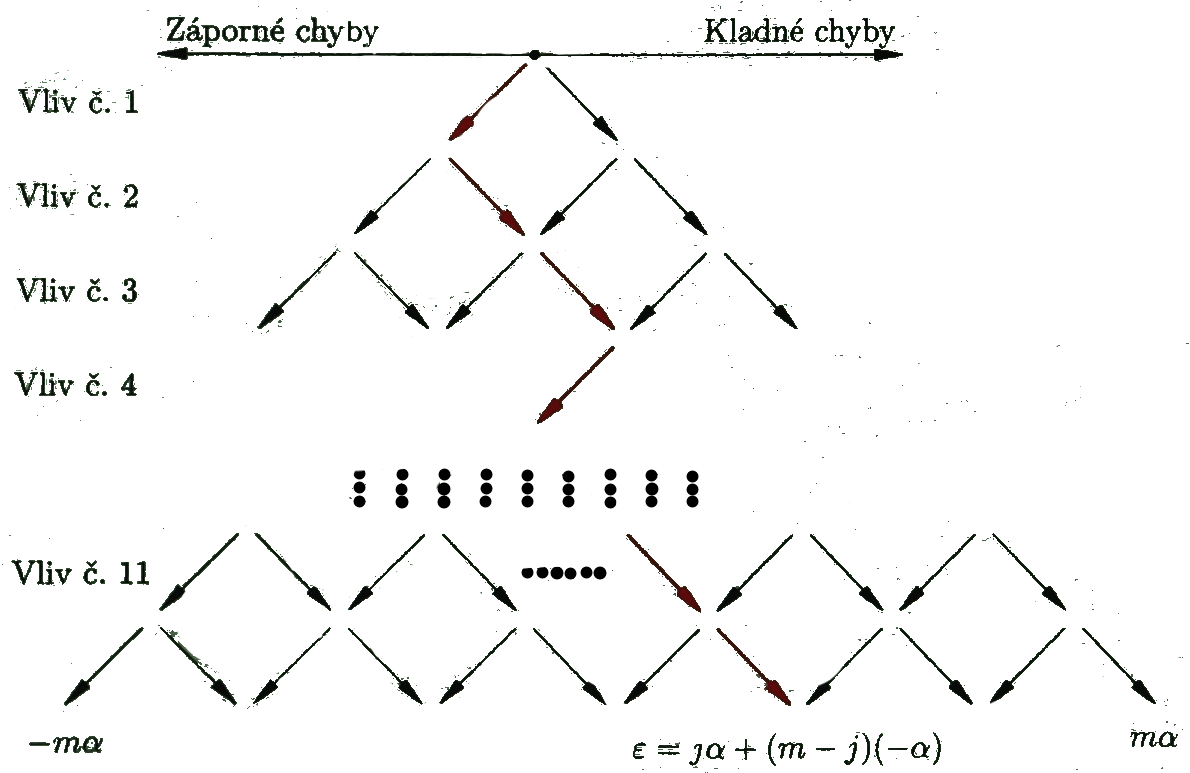
\includegraphics[width=0.6\linewidth]{mai_fig050.png}
        \caption{Vznik kladných a záporných odchylek při měření s \(m\) vlivy. 
        \cite[s.~255]{Musilova2009MA1}}
        \label{mai:fig050}
      \end{figure}
      
      Mohlo by tomu být i naopak, slova „zdar“ a „nezdar“ zde nemají svůj obvyklý význam, jde
      pouze o to, že díky nim můžeme hned uvidět souvislost s Bernoulliovým pokusem a tedy
      i s Bernoulliovým rozdělením. Při \(j\) kladných a \(m — j\) záporných odchylkách je měření od
      správné hodnoty odkloněno o
      \begin{equation*}
        j\alpha + (m - j)(-\alpha) = (2j - m)\alpha
      \end{equation*}
      s pravděpodobností
      \begin{equation*}
        p_j = \begin{pmatrix}m j\end{pmatrix}p^j(1 - p)^{m - j} = 2^{-m}.
      \end{equation*}
      Střední hodnota náhodné veličiny \(\varepsilon\) je nulová. Skutečně, v příkladu 
      \ref{mai:exam066} jsme zjistili, že střední hodnota veličiny \(Y\) nabývající hodnot \(y_j = 
      j\) s Bernoulliovým rozdělením je \(\langle y \rangle = mp\), střední hodnota veličiny \((2j 
      — m)\) a pak musí být \((2mp — m)\alpha\). Pro \(p = \num{0.5}\) je tato hodnota nulová.
      Pro velká \(m\) lze Bernoulliovo rozdělení nahradit rozdělením normálním (obr. 3.8), a proto 
      má náhodná veličina \(\varepsilon\) hustotu pravděpodobnosti tvaru (\ref{mai:eq069}), tj.
      \begin{equation*}
        \mathcal{w}(\varepsilon) = 
        \dfrac{1}{\sigma\sqrt{2\pi}}\exp\left(\dfrac{-\varepsilon^2}{2\sigma^2}\right).   
      \end{equation*}
      \begin{figure}[ht!] %\ref{mai:fig051}
        \centering
        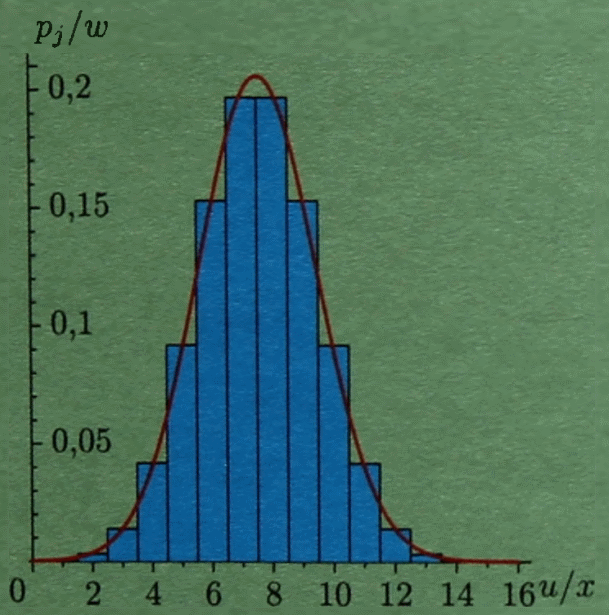
\includegraphics[width=0.4\linewidth]{mai_fig051.png}
        \caption{Normální rozdělení jako limitní případ Bernoulliova 
        \cite[s.~256]{Musilova2009MA1}}
        \label{mai:fig051}
      \end{figure}
      
      Vraťme se nyní k otázce zpracování naměřených hodnot \(\lbrace x_1, \ldots, x_n\rbrace\) 
      výšky válečku. Jejich odchylky od správné hodnoty jsou \(x_1 - x\) až \(x_n - x\). Na místě 
      neznámé správné hodnoty \(x\) si nyní představme nějakou proměnnou, označme ji 
      \(\varepsilon\). Budeme se snažit určit její hodnotu \(\varepsilon_0\) tak, aby 
      pravděpodobnost, že odchylky jednotlivých měřených hodnot od \(\varepsilon_0\) padnou 
      současně do intervalů
      \begin{equation*}
        \left(\varepsilon_1 - \dfrac{\dd{\varepsilon_1}}{2}, 
              \varepsilon_1 + \dfrac{\dd{\varepsilon_1}}{2}
        \right),
        \left(\varepsilon_2 - \dfrac{\dd{\varepsilon_2}}{2}, 
              \varepsilon_2 + \dfrac{\dd{\varepsilon_2}}{2}
        \right), \cdots,
        \left(\varepsilon_n - \dfrac{\dd{\varepsilon_n}}{2}, 
              \varepsilon_n + \dfrac{\dd{\varepsilon_n}}{2}
        \right),
      \end{equation*}
      byla maximální. Pro tuto pravděpodobnost v závislosti na \(\xi\) platí
      \begin{align}
        \dd{W} &= \dd{\mathcal{w}(\varepsilon_1)}\cdots\dd{\mathcal{w}(\varepsilon_n)}  \nonumber\\
               &= \dfrac{1}{\sigma\sqrt{2\pi}}
                  \exp\left(-\dfrac{(x_1 - \xi)^2 + \cdots + (x_n - \xi)^2}{2\sigma^2}
                      \right)\dd{\varepsilon_1}\cdots\dd{\varepsilon_n}.      \label{mai:eq072}
      \end{align}
      (Víte proč je ve vztahu (\ref{mai:eq072}) součin pravděpodobností?) Tato pravděpodobnost bude 
      maximální, bude-li hodnota exponentu minimální. Z podmínky
      \begin{equation*}
        (x_1 - \xi)^2 + \cdots + (x_n - \xi)^2 = \text{min}
      \end{equation*}
      dostáváme derivací podle \(\xi\) požadavek
      \begin{equation*}
        2(x_1 - \xi) + \cdots + 2(x_n - \xi) = 0 \Rightarrow \xi_0 = 
        \dfrac{1}{n}\sum_{i=1}^{n}x_j = \langle x \rangle.
      \end{equation*}
      Vidíme, že veličina, která charakterizuje míru odchýlení naměřených hodnot od \(\xi\), je 
      minimální, zvolíme-li za \(\xi\) aritmetický průměr naměřených hodnot. Pozor, zjištěný 
      výsledek znamená právě jen konstatovanou skutečnost: Při dosazení aritmetického průměru za 
      proměnnou \(\xi\) bude pravděpodobnost, že odchylky jednotlivých měření od \(\xi\) budou 
      ležet v uvažovaných intervalech, maximální. Neznamená to, že správnou hodnotou veličiny \(X\) 
      je aritmetický průměr měření \(x_1, X_2, \ldots, x_n\). Správnou hodnotu ze souboru měření 
      prostě nezjistíme, avšak aritmetický průměr je jí blízký s vysokou pravděpodobností. Jaká je 
      tato „blízkost“ a její pravděpodobnost konkrétně? Hned uvidíme. Správnou hodnotu výšky 
      válečku \(x\) sice neznáme, ale víme, že náhodná veličina \(\varepsilon\), jejíž hodnoty jsou 
      odchylkami výsledků měření od této (neznámé) správné hodnoty, se řídí normálním rozdělením s 
      nulovou střední hodnotou. Potřebujeme stanovit další důležitý parametr tohoto rozdělení, 
      směrodatnou odchylku \(\sigma\). Tu lze vyjádřit velmi jednoduše. Je totiž střední hodnotou 
      náhodné veličiny \(\varepsilon^2\), tedy aritmetickým průměrem čtverců odchylek 
      \(\varepsilon_i\): 
      \begin{equation*}
        \sigma^2 = D(\varepsilon) = \dfrac{1}{n}\sum_{i=1}^{n}\varepsilon_i^2.
      \end{equation*}
      Ať je však tento vzorec jakkoli jednoduchý, k čemu může sloužit, nedokážeme-li jej vyčíslit?
      Když přece neznáme správnou hodnotu \(x\), nemáme k dispozici ani hodnoty \(\varepsilon_i\). 
      Ani tato kaše však není tak horká, jak se zdá: Odchylku výsledku \(i\)-tého měření od 
      aritmetického průměru označme \(\delta_i = x_i - \langle x \rangle\), přičemž jsme již dříve 
      označili jako \(\varepsilon_i= x_i - x\) odchylku výsledku \(i\)-tého měření pd správné 
      hodnoty. Platí
      \begin{equation*}
        \sum_{i=1}^{n}\varepsilon_i = \sum_{i=1}^{n}(x_i - x) \Rightarrow 
        \sum_{i=1}^{n}x_i = \sum_{i=1}^{n}\varepsilon_i + nx, 
      \end{equation*}
      odkud 
      \begin{equation*}
        \langle x \rangle = x + \dfrac{1}{n}\sum_{i=1}^{n}\varepsilon_i.
      \end{equation*}
      Pak dostaneme
      \begin{equation*}
        \delta_i = (x_i - x) - \dfrac{1}{n}\sum_{i=1}^{n}\varepsilon_i 
                 = \varepsilon_i - \dfrac{1}{n}\sum_{j=1}^{n}\varepsilon_j.
      \end{equation*}
      Součet čtverců odchylek \(\delta_i\) je
      \begin{align*}
        \sum_{i=1}^{n}\delta_i^2 
          &= \sum_{i=1}^{n}\left(\varepsilon_i - 
             \dfrac{1}{n}\sum_{j=1}^{n}\varepsilon_j\right)^2 = \sum_{i=1}^{n}\varepsilon_i^2 - 
             \dfrac{2}{n}\sum_{i=1}^{n}\sum_{j=1}^{n}\varepsilon_i\varepsilon_j + 
             \dfrac{1}{n^2}\sum_{i=1}^{n}\left(\sum_{j=1}^{n}\varepsilon_j\right)^2     \\
          &= \sum_{i=1}^{n}\varepsilon_i^2 - 
             \dfrac{1}{n}\left(\sum_{j=1}^{n}\varepsilon_j\right)^2                     
             \doteq \left(1 - \dfrac{1}{n}\right)\sum_{i=1}^{n}\varepsilon_i^2.
      \end{align*}
      Při poslední úpravě jsme pro získání výsledného přibližného vyjádření součtu čtverců odchylek
      \(\delta_i\) použili následující úvahy:
      \begin{equation*}
        \left(\sum_{j=1}^{n}\varepsilon_j\right)^2 = \sum_{i=1}^{n}\varepsilon_i^2 + 
        2\sum_{i=1}^{n}\sum_{j>1}\varepsilon_i\varepsilon_j \doteq \sum_{i=1}^{n}\varepsilon_i^2,
      \end{equation*}
      neboť při rovnocenném zastoupení kladných a záporných odchylek je druhý sčítanec, obsahující
      součiny \(\varepsilon_i\varepsilon_j\), zanedbatelný proti prvnímu. Nakonec tedy dostáváme
      \begin{equation*}
        \sum_{i=1}^{n}\delta_i^2 \doteq \dfrac{n-1}{n}\sum_{i=1}^{n}\varepsilon_i^2 = (n-1)\sigma^2.
      \end{equation*}
      Protože odchylky \(\delta_i\) již z daného souboru měření určit můžeme (jsou to odchylky 
      jednotlivých měření od jejich aritmetického průměru), získali jsme alespoň přibližný vztah 
      pro směrodatnou odchylku rozdělení veličiny \(\varepsilon\), 
      \begin{equation}\label{mai:eq074}
        \sigma = \left(\dfrac{1}{n-1}\sum_{i=1}^{n}\delta_i^2\right)^{\dfrac{1}{2}}.
      \end{equation}
      Jaký význam má tato hodnota pro náš soubor měření? Vymezuje interval
      \begin{equation*}
        (x - \sigma, x + \sigma),
      \end{equation*}
      symetrický kolem (stále neznámé) správné hodnoty výšky válečku \(x\), do kterého padne 
      výsledek měření této výšky s pravděpodobností \SI{68.3}{\percent} (příklad 
      \ref{mai:exam069}). Neznámá správná hodnota je tedy naopak s toutéž pravděpodobností vzdálena 
      od výsledku jednotlivého měření o méně než \(\sigma\). A to už je docela slušná informace o 
      tom, kde správná hodnota může ležet. Polohu \(x\) však můžeme „omezit“ ještě lépe. Směrodatná 
      odchylka \(\overline{\sigma}\) rozdělení, které přísluší aritmetickému průměru, je
      totiž ještě \(\sqrt{n}\)-krát menší než \(\sigma\), tj. \(\overline{\sigma}= 
      \sigma/\sqrt{n}\). Správná hodnota \(x\) (navždy neznámá) je tedy od aritmetického průměru 
      výsledků měření \(\langle x \rangle\) vzdálena s pravděpodobností \SI{68.3}{\percent} o méně 
      než \(\overline{\sigma}\). Použijeme-li krajní chybu \(\overline{\kappa} = 
      3\overline{\sigma}\) (příklad \ref{mai:exam069}), můžeme říci, že správná hodnota \(x\) je od
      aritmetického průměru souboru měření \(\langle x \rangle\) vzdálena o méně než 
      \(\overline{\kappa}\) s pravděpodobností \SI{99.7}{\percent}. Více se o správné hodnotě výšky 
      válečku říci nedá. Ale i tak jsme ji lokalizovali docela úspěšně. Následující příklad 
      ukazuje vyhodnocení konkrétního souboru měření.

      %-- Měříme výšku válečku----------------------------------------
      \input{../src/MAI/exam/exam077.tex}
      %---------------------------------------------------------------
      Na závěr odstavce si všimneme ještě jedné důležité otázky. Formulujeme ji pro případ určení
      hustoty válečku. Změřili jsme výšku válečku \(x\) a jeho poloměr \(r\), vážením jsme určili 
      také jeho hmotnost \(m\). Získali jsme tak intervaly
      \begin{equation*}
        \left(\langle x \rangle - \overline{\sigma}(x), 
              \langle x \rangle + \overline{\sigma}(x)\right), \qquad
        \left(\langle r \rangle - \overline{\sigma}(r), 
              \langle r \rangle + \overline{\sigma}(r)\right), \qquad
        \left(\langle m \rangle - \overline{\sigma}(m), 
              \langle m \rangle + \overline{\sigma}(m)\right).
      \end{equation*}
      
      Směrodatná odchylka v případě každé z veličin \(x\), \(r\) a \(m\) určuje velikost intervalu 
      se středem daným aritmetickým průměrem všech měření této veličiny, v němž leží správná 
      hodnota s pravděpodobností \SI{68.3}{\percent}. Průměrná hustota válečku je dána vztahem
      \begin{equation*}
        \varrho = \dfrac{m}{V} = \dfrac{m}{\pi r^2x},
      \end{equation*}
      je tedy funkcí tří proměnných \(x\), \(r\), \(m\). Jak stanovíme interval, v němž leží 
      správná hodnota hustoty s pravděpodobností rovněž \SI{68.3}{\percent}? Hustotu totiž neměříme 
      přímo, ale vypočítáváme z přímo měřených veličin. Abychom mohli na tuto otázku odpovědět 
      matematicky korektně, potřebujeme základní znalosti o funkcích více proměnných. Závěr tohoto 
      odstavce lze tedy do důsledku pochopit po přečtení kapitoly o funkcích více proměnných. Proto 
      jej v tuto chvíli klidně přeskočte.
      
      Předpokládejme, že veličina \(z\) je pro jednoduchost pouze funkcí dvou nezávislých náhodných
      veličin \(x\) a \(y\), \(z = f(x,y)\). Jsou-li chyby \(\varepsilon_i(x)\), resp. 
      \(\varepsilon_i(y)\), kterých jsme se dopustili při \(i\)-tém měření veličiny \(x\), resp. 
      \(y\) velmi malé, můžeme pro vyjádření malé změny veličiny \(z\) způsobené chybami veličin 
      \(x\) a \(y\) použít úplného diferenciálu
      \begin{equation*}
        \dd{z} = \dd{f(x,y)} = \left(\pder{f(x,y)}{x}\right)\dd{x} + 
                               \left(\pder{f(x,y)}{y}\right)\dd{y}
      \end{equation*}
      Pro chybu veličiny \(z\) pak platí
      \begin{equation*}
        \varepsilon_i(z) = \left(\pder{f}{x}\right)\varepsilon_i(x) + 
                           \left(\pder{f}{y}\right)\varepsilon_i(y) \Rightarrow
      \end{equation*}
      \begin{equation*}
        \Rightarrow \sum_{i=1}^{n}\varepsilon_i^2(z) 
        =  \sum_{i=1}^{n}\left(\pder{f}{x}\right)^2\varepsilon_i^2(x) 
        +  \sum_{i=1}^{n}\left(\pder{f}{y}\right)^2\varepsilon_i^2(y)
        + 2\sum_{i=1}^{n}\left(\pder{f}{x}\right)^2\left(\pder{f}{y}\right)^2\varepsilon_i(x)
          \varepsilon_i(y).
      \end{equation*}
      Vzhledem k rovnocennému zastoupení kladných a záporných odchylek je součet obsahující
      součiny \(\varepsilon_i(x)\varepsilon_i(y)\) zanedbatelný proti zbytku výrazu. Pak
      \begin{equation*}
        \sum_{i=1}^{n}\varepsilon_i^2(z) \doteq \left(\pder{f}{x}\right)^2
        \sum_{i=1}^{n}\varepsilon_i^2(x) + 
                      \left(\pder{f}{y}\right)^2\sum_{i=1}^{n}\varepsilon_i^2(y) 
        = \left(\pder{f}{x}\right)^2 n\sigma^2(x) + \left(\pder{f}{y}\right)^2n\sigma^2(y).
      \end{equation*}
      Odtud, vzhledem k platnosti vztahu
      \begin{equation*}
        \sum_{i=1}^{n}\varepsilon_i^2 = n\sigma^2(z),
      \end{equation*}
      dostáváme
      \begin{equation}\label{mai:eq075}
        \sigma^2(z) = \left(\pder{f}{x}\right)^2\sigma^2(x)
                    + \left(\pder{f}{y}\right)^2\sigma^2(y).
      \end{equation}
      Parciální derivace funkce \(f(x, y)\) podle \(x\), resp. \(y\) je třeba vyčíslit dosazením 
      \(x = \langle x\rangle\) a \(y = \langle y \rangle\). Zobecnění tohoto vzorce na případ, kdy 
      hledaná veličina je funkcí více proměnných, je jednoduché.
      
    \subsection{Lineární závislost a metoda nejmenších čtverců}
      Tento poslední odstavec se zabývá zpracováním měření veličin, které jsou vázány lineárním
      vztahem (už zase ta linearita). Situaci si opět snadno představíme na jednoduchém příkladu
      Víme, že pro elektrické vodiče platí za jistých okolností \emph{Ohmův zákon}. Podle něj je 
      proud \(I\) protékající vodičem, třeba drátem, přímo úměrný napětí \(U\) mezi konci vodiče. 
      Konstanta úměrnosti ve vztahu
      \begin{equation*}
        U = R\cdot I
      \end{equation*}
      představuje \emph{elektrický odpor vodiče} \(R\). Změříme-li napětí a proud, můžeme určit 
      odpor vodiče, pokud Ohmův zákon opravdu platí. Mohli bychom tedy postupovat například tak, že 
      bychom při několika různých hodnotách napětí \(\lbrace U_1, U_2, \ldots, U_n \rbrace\) 
      (napětí bychom mohli například postupně zvyšovat) změřili proud protékající vodičem, tj. 
      \(\lbrace I_1, I_2, \ldots, I_n \rbrace\), a určili odpovídající hodnoty odporu \(R_1 = 
      U_1/I_1\), \(R_2 = U_2/I_2\), \(\ldots\), \(R_n = U_n/I_n\)  Protože by měřené hodnoty napětí 
      i proudu byly ovlivněny náhodnými vlivy a byly tak zatíženy chybami, byly by získané hodnoty 
      odporu obecně různé, i když blízké. Zpracovali bychom je podobně jako soubor \(\langle x_1, 
      x_2, \ldots, x_n \rangle\) při měření výšky válečku. Co když ale Ohmův zákon neplatí? Máme-li 
      k dispozici změřený soubor odpovídajících si hodnot napětí a proudu, můžeme Ohmův zákon pro 
      daný případ dokonce ověřit. Nebudeme však z jednotlivých údajů \(U_i\) a \(I_i\) počítat 
      hodnoty \(R_i\) a pak je průměrovat, ale zpracujeme celý soubor měření „najednou“. Představme 
      si dvojice \([U_i, I_i]\) jako body grafu. Kdyby měření napětí ani proudu nebyla zatížena 
      chybami a kdyby přesně platil Ohmův zákon, ležely by body grafu přesně na přímce. Odpor 
      vodiče bychom pak, s uvážením jednotek na osách, určili jako její směrnici (resp. v našem 
      případě, kdy na vodorovnou osu nanášíme napětí a na svislou osu proud, je směrnicí převrácená 
      hodnota odporu). Pro každou dvojici odpovídajících si hodnot napětí a proudu by mělo platit
      \begin{equation*}
        U_1 = R\cdot I_1, U_2 = R\cdot I_2, \ldots, U_n = R\cdot I_n.
      \end{equation*}
      Předchozí zápis můžeme chápat jako nehomogenní soustavu \(n\) lineárních rovnic pro jedinou
      neznámou \(R\). Rozšířená matice této soustavy je
      \begin{equation*}
        \overline{B} = (A|B) = 
          \left(
            \begin{array}{c|c}
              I_1    & U_1     \\
              I_2    & U_2     \\
              \cdots & \cdots  \\
              \cdots & \cdots  \\
              I_n    & U_n
            \end{array}
          \right).
      \end{equation*}
      Matice soustavy \(A\) má hodnost \(h(A) = 1\), matice \(\overline{B} = (A|B)\) však bude mít 
      vlivem chyb měření hodnost \(h(\overline{B}) = 2\). Soustava tedy obecně nemá řešení. Je 
      „přeučena“, neboť máme více nezávislých rovnic a jen jednu neznámou. Přímku, která by 
      procházela všemi body grafu, nenajdeme. Položíme si proto splnitelný úkol: Budeme hledat 
      přímku, která by se co „nejlépe přimykala“ k souboru bodů grafu. Tento požadavek je třeba 
      matematicky formulovat, jinak bude k nepotřebě. Označme hledanou hodnotu odporu \(R\). Pokud 
      by hodnoty \(\lbrace I_1, I_2, \ldots, I_n \rbrace\) byly bezchybné, odpovídaly by jim 
      hodnoty napětí \(\lbrace R_1\cdot I_1, R_2\cdot I_2, \ldots, R_n\cdot I_n \rbrace\). Odchylky 
      skutečně naměřených napětí \(\lbrace U_1, U_2, \ldots, U_n \rbrace\) od těchto „teoretických“ 
      jsou
      \begin{equation*}
        \lbrace U_1 - R_1\cdot I_1, U_2 - R_2\cdot I_2, \ldots, U_n - R_n\cdot I_n \rbrace.
      \end{equation*}
      Součet jejich čtverců je funkcí veličiny \(R\), kterou na chvíli považujme za proměnnou:
      \begin{equation*}
        D(R) = \sum_{i = 1}^{n}(U_i - R_i\cdot I_i)^2.
      \end{equation*}
      Řekneme, že se přímka o rovnici \(U = R\cdot I\) nejlépe přimyká k souboru bodů \(\lbrace[ 
      U_i, I_i]\rbrace\) právě tehdy, je-li \(R\) zvoleno tak, aby hodnota \(D(R)\) byla co 
      nejmenší. Nutnou podmínkou pro minimum funkce \(D(R)\) je nulovost její derivace,
      \begin{equation*}
        \der{D(R)}{R} = -2\sum_{i = 1}^{n}(U_i - R_i\cdot I_i)I_i = 0,
      \end{equation*}
      odkud
      \adjustbox{minipage=[c]{\textwidth}}{%
        \begin{equation}\label{mai:eq073}
          R=  \dfrac{\sum_{i = 1}^{n}U_i\cdot I_i}{\sum_{i = 1}^{n}I_i^2}.
        \end{equation}
      }
      Předchozím vztahem je určena hodnota odporu. Jejím dosazením do vzorce pro \(D(R)\) zjistíme
      odpovídající odchylku
      \adjustbox{minipage=[c]{\textwidth}}{%
        \begin{equation*}
          \sigma(R) = \sqrt{\dfrac{D(R)}{n-1}}.
        \end{equation*}
      }
      Velikost \(\sigma(R)\) dává informaci o tom, jak „dobře“ vyhovuje testovaný soubor měření 
      zvolenému fyzikálnímu modelu, v tomto případě lineární závislosti.

      %-- Ověření Ohmová zákona---------------------------------------
      \input{../src/MAI/exam/exam076.tex}
      %---------------------------------------------------------------
      
      Popsaný způsob nalezení hodnoty elektrického odporu vodiče se nazývá\textbf{ metodou 
      nejmenších čtverců} (minimalizuje součet čtverců odchylek prokládané závislosti od souboru 
      naměřených bodů), v případě použití lineárního modelu, jako tomu bylo u Ohmová zákona, pak 
      jde o \textbf{lineární regresi}
      
      Obdobně se postupuje, je-li některá z měřených veličin lineární funkcí veličin jiných s 
      neznámými koeficienty lineární kombinace. Nechť
      \begin{equation*}
        Z = f(X_1, X_2, \ldots, X_K) = A_1X_1 + A_2X_2 + \cdots + A_KX_K.
      \end{equation*}
      Předpokládejme, že veličiny \(X_1, X_2, \ldots, X_K\) a \(Z\) měříme \(n\)-krát a naměříme 
      hodnoty
      \begin{equation*}
        X_j = \lbrace x_{j1}, \ldots x_{jn} \rbrace, \qquad 1 \leq j \leq K, \qquad 
        Z = \lbrace z_{1}, \ldots z_{n} \rbrace
      \end{equation*}
      Součet čtverců odchylek teoretické závislosti od naměřených bodů je
      \begin{equation*}
        D(Z) = \sum_{i=1}^{n}\left(z_i - \sum_{j=1}^{K}A_jx_{ji}\right)^2.
      \end{equation*}
      Nutnou podmínkou pro minimum tohoto výrazu jakožto funkce proměnných \(A_x, A_2, \ldots, A_K\)
      je platnost souboru rovnic
      \begin{equation*}
        \pder{D(Z)}{A_p} = 0 \Rightarrow 
        \sum_{i=1}^{n}2\left(z_i - \sum_{j=1}^{K}A_jx_{ji}\right)\cdot x_{pi} = 0
      \end{equation*}
      pro \(1 \leq i \leq n, 1 \leq j \leq K\). Tyto podmínky představují nehomogenní soustavu 
      \(K\) rovnic pro \(K\) neznámých \(( A_1, A_2, \ldots, A_K)\). Rozšířená matice soustavy je
      \begin{equation*}
        \overline{B} = (A|B) = 
          \left(
            \begin{array}{cccc|c}
              \sum_{i=1}^{n}x_{1i}x_{1i} & \sum_{i=1}^{n}x_{1i}x_{2i} & \cdots & 
              \sum_{i=1}^{n}x_{1i}x_{Ki} & \sum_{i=1}^{n}z_{i}x_{1i}                    \\
              \sum_{i=1}^{n}x_{1i}x_{1i} & \sum_{i=1}^{n}x_{2i}x_{2i} & \cdots & 
              \sum_{i=1}^{n}x_{2i}x_{Ki} & \sum_{i=1}^{n}z_{i}x_{2i}                    \\
                        \cdots           & \cdots & \cdots & \cdots   & \cdots          \\
              \sum_{i=1}^{n}x_{Ki}x_{1i} & \sum_{i=1}^{n}x_{Ki}x_{2i} & \cdots & 
              \sum_{i=1}^{n}x_{Ki}x_{Ki} & \sum_{i=1}^{n}z_{i}x_{Ki}                    \\
            \end{array}
          \right),
      \end{equation*}
      \begin{equation*}
        \sigma(z) = \sqrt{\dfrac{D(z)}{n - K}}.
      \end{equation*}
      V dalších kapitolách věnovaných lineární algebře se k tomuto problému znovu vrátíme a 
      ukážeme, že jej lze elegantně řešit také jako úlohu algebraickou, konkrétně úlohu o 
      ortogonální projekci vektorů na podprostory.
      
%} %tikzset
%---------------------------------------------------------------------------------------------------
\printbibliography[heading=subbibliography]
\addcontentsline{toc}{section}{Seznam literatury}
%--------------------Primitive Functions ----------------------------------------------------------
  % !TeX spellcheck = cs_CZ
%{\tikzset{external/prefix={tikz/MAI/}}
% \tikzset{external/figure name/.add={ch06_}{}}
%---------------------------------------------------------------------------------------------------
% file: chap_PrimitiveFce.tex
%---------------------------------------------------------------------------------------------------
%============================ Primitivní funkce ====================================================
\chapter{Primitivní funkce}
\minitoc

  %----------------------------Neurčitý integrál----------------------------------------------------
  \section{Motivace}
    Problém \emph{neurčitého integrálu}, neboli \textbf{primitivní funkce}, lze vyložit velmi 
    jednoduše: Máme podezření, že zadaná funkce \(f(x)\) vznikla derivováním jisté, zatím neznámé, 
    funkce \(F(x)\). Dokážeme ji najít? 
  
    K danému problému můžeme přistupovat také fyzikálně: Zavedením pojmu derivace funkce jsme 
    motivovali důležitým požadavkem definovat okamžitou rychlost pohybu bodu po přímce. Existuje 
    přirozeně i požadavek opačný, tj. nalézt zákon dráhy pohybu bodu po přímce, je-li dána jeho 
    okamžitá rychlost jako funkce času \cite[s.~253]{Brabec1989}. Vše si ukážeme na následujícím 
    příkladu:  
   
    \begin{example}
      Je dána okamžitá rychlost $v$ pohybu bodu po přímce (ose) $x$ rovnicí $v(t) = 2t + 1$, 
      $t\in\langle -\infty,+\infty \rangle$. Najděte zákon dráhy pohybu, je-li známo, že v čase $t 
      = 0$ měl bod polohu $x = x_0$.
      \newline
      \textbf{řešení:}\newline
      Označíme-li $x(t)$ polohu bodu v okamžiku $t$, pak $v(t) = \frac{dx}{dt}$. Hledáme tedy 
      funkci $x = x(t)$, pro níž platí 
      \begin{align}
        \frac{dx}{dt} &= 2t + 1 \qquad x(0) = x_0.  \nonumber \\ 
        \shortintertext{Je ihned patrné, že první podmínce vyhovuje nekonečně mnoho funkcí}
        x(t)          &= t^2 + t + C,           \label{MA:int_ex_09}    \\ 
        \shortintertext{ kde $C$ je libovolná konstanta. Funkce, která splňuje i druhou podmínku 
          (říkáme ji též počáteční podmínka), najdeme z rovnice \ref{MA:int_ex_09} dosazením dané podmínky 
          $t = 0,\ x = x_0$. Dostaneme $x_0 = C$. Dosazením do \ref{MA:int_ex_09} za $C$ plyne hledaný 
          zákon dráhy}
        x(t)          &= t^2+t+x_0.                 \nonumber 
        \shortintertext{Jednoduchou zkouškou se přesvědčíme, že tato funkce splňuje obě dané podmínky a 
          zároveň vidíme, že hledaná primitivní funkce daných vlastností je jediná.}  \nonumber
      \end{align}
    \end{example} 
    Každé takové funkci, jejíž derivací je daná funkce, budeme říkat \emph{primitivní funkce} k 
    dané funkci. Na uvedeném příkladě je patrné, že k dané funkci může existovat nekonečně mnoho 
    primitivních funkcí. Množinu všech primitivních funkcí se často nazývá \textbf{neurčitým 
    integrálem}. Po tomto názorném uvedení do problému přejděme k přesné formulaci základních pojmů.
    
    \begin{definition} 
      Funkce $F: J\rightarrow \realset$, kde $J\subset \realset$ je interval, se nazývá primitivní 
      funkce k funkci \(f\) na intervalu \(J\) právě když, pro všechna $x\in J$ je $F'(x) = f(x)$ 
      (v krajních bodech intervalu \(J\), pokud k němu patří, jde o derivace jednostranné).
    \end{definition}
    
    \begin{example} 
      K funkci $\sin x$ je primitivní funkcí na libovolném intervalu $J\subset(-\infty,+\infty)$ 
      funkce $-\cos x$, protože $(-\cos x)' = \sin x$. Ale též funkce $3-\cos x$ je primitivní 
      funkcí k funkci $\sin x$, protože $(3 - \cos x)' = \sin x$ pro všechna $x\in(-\infty, 
      \infty)$.
    \end{example}
    
    Je vidět, že rozdíl dvou primitivních funkcí k téže funkci je konstanta. To není náhoda, jak 
    potvrzuje následující věta:
    
    \begin{lemma}
      \begin{enumerate}
        \item Je-li funkce $F$ primitivní funkcí k funkci \(f\) na intervalu \(J\) a \(c\) reálná  
              konstanta, pak i funkce $G = F + c$ je primitivní funkcí k funkci \(f\) na intervalu 
              \(J\).
        \item Jsou-li funkce $F$ a $G$ primitivní funkce k funkci \(f\) na intervalu \(J\), pak 
        funkce
              $F-G$ je na intervalu \(J\) konstantní.
      \end{enumerate} 
      \begin{proof}
        Tvrzení a) plyne z definice protože $G'(x) = [F(x) + c] = F'(x) = f(x)$ pro všechna $x\in
        J$. Tvrzení b) je důsledkem věty \ref{MA1:lem_diff01}.
      \end{proof}
    \end{lemma}
    Neurčitost vyplývá právě z toho, že primitivní funkce není dána jednoznačně, je určena až na 
    konstantu. Značíme
    \begin{equation*}
      \boxed{F(x) = \int f(x)\dx + C}
    \end{equation*}
        
    Jak ale primitivní funkce hledat? V jednoduchých příkladech poslouží tabulka derivací, již 
    čteme „zprava doleva“. (Je dobré si ji uložit do paměti.) Tabulka však pokryje jen velmi málo 
    případů, pouze elementární funkce. Je tedy třeba najít metody, jak při hledání primitivních 
    funkcí postupovat. Nejprve však uvedeme dvě základní pravidla pro primitivní funkce, která 
    plynou z pravidel pro derivování:
    \begin{align}
      \int[f(x)\pm g(x)]\dx &= \int[f(x)\pm g(x)]\dx + \int[f(x)\pm g(x)]\dx \label{MA1:eq_int10} \\
      \int cf(x)\dx         &= c \int f(x)\dx, \qquad \text{\(c\) je konstanta.} \label{MA1:eq_int11}
    \end{align}
  
  \section{Tabulka neurčitých integrálů}\label{MA:chap_tabINT}
    Pokud není nic uvedeno, platí vzorce pro všechna \(x\) a pro všechny hodnoty uvedených
    konstant. Místo platí pro \(x\) z intervalu \((-\infty,0),(0,+\infty)\) píšeme stručně
    \(x\neq0\) apod. Literatura: \cite[p.~396]{Rektorys1963}.
  
    \begin{flalign}
      & \int 0\dx = c                                        &         \label{MA:baseInt01}     \\
      & \int a\dx = ax+c                                     &         \label{MA:baseInt02}     \\
      & \int x^n\dx = \frac{x^{n+1}}{n+1}+c, \,              &         \label{MA:baseInt03}     \\
      & \qquad\text{kde}\begin{cases}
          \forall x\in\realset,\,n\in\naturalset, n>0,         \\
          \forall x\in\realset-\{0\},\,n\in\naturalset, n<-1,  \\
          \forall x>0,\,n\in\realset\,\,n\notin\naturalset
        \end{cases}                                          &         \nonumber               \\
      & \int\frac{1}{x}\dx = 
            \ln\abs{x}+c \hspace{1ex}\forall x\neq0          &         \label{MA:baseInt04}     \\
      & \int e^x \dx       = e^x+c                           &         \label{MA:baseInt05}     \\
      & \int\ln x\dx       = 
          x\ln x - x + c \hspace{1ex}\forall x>0             &         \label{MA:baseInt06}     \\
      & \int a^x \dx     =
          \frac{a^x}{\ln a}+c 
          \hspace{1ex}\forall a>0,\,a\neq1                   &         \label{MA:baseInt07}     \\
      & \int \sin x \dx  = -\cos x                           &         \label{MA:baseInt08}     \\
      & \int \cos x \dx  =  \sin x                           &         \label{MA:baseInt09}     \\
      & \int\frac{1}{\cos^2x}\dx =  \tan x+c 
           \hspace{1ex}\forall x\neq(2k+1)\pi,\,k\in\naturalset &      \label{MA:baseInt10}     \\ 
      & \int\frac{1}{\sin^2x}\dx     =  -\cotg x+c
         \hspace{1ex}\forall x\neq k\pi,\,k\in\naturalset    &         \label{MA:baseInt11}     \\
      & \int\frac{1}{\sqrt{1-x^2}}\dx =
          \begin{cases}
            +\arcsin x + c         \\
            -\arccos x + c
          \end{cases} 
          \forall x\in(-1,1)                                 &         \label{MA:baseInt12}     \\
      & \int\cosh\dx = \sinh x + c                           &         \label{MA:baseInt13}     \\
      & \int\sinh\dx = \cosh x + c                           &         \label{MA:baseInt14}     \\
      & \int\frac{1}{1+x^2}\dx = \arctan x + c               &         \label{MA:baseInt15}     \\
      & \int \frac{1}{\sqrt{x^2 + 1}}\dx =
          \begin{cases}
            \ln(x + \sqrt{x^2+1}) + c         \\
            \sinh^{-1}x + c 
          \end{cases}                                        &         \label{MA:baseInt16}     \\ 
      & \int \frac{1}{\sqrt{x^2 - 1}}\dx =
          \begin{cases}
            \ln(x + \sqrt{x^2-1}) + c         \\
            \cosh^{-1}x + c \hspace{4ex}x\in(1,+\infty) 
          \end{cases}                                        &         \label{MA:baseInt17}     \\
      & \int\frac{1}{\sqrt{x^2+a^2}}\dx 
        = \sinh^{-1} \frac{x}{a} = \ln (x+\sqrt{x^2+a^2})    &         \label{MA:baseInt18}     \\
      & \int \frac{1}{\sqrt{x^2-a^2}}\dx 
        = \cosh^{-1} \frac{x}{a} = \ln (x+\sqrt{x^2-a^2})    &         \label{MA:baseInt19}     \\
      & \int\frac{1}{\sqrt{x^2-1}}\dx 
        = \left\{ 
          \begin{array}{l l}
            \ln\abs{x+\sqrt{x^2-1}}+c      &  \abs{x}>1  \\
            \cosh^{-1}x+c                  &  \abs{x}<1
          \end{array} 
          \right.                                            &         \label{MA:baseInt20}     \\
      & \int\tan x \dx   = \ln |\sec x| + c                  &         \label{MA:baseInt21}     \\
      & \int\sec x \dx   = \ln |\sec x + \tan x| + c         &         \label{MA:baseInt22}     \\
      & \int\sec^2 x \dx = \tan x + c                        &         \label{MA:baseInt23}     \\
      & \int\sec x\tan x \dx = \sec x + c                    &         \label{MA:baseInt24}     \\
      & \int\frac{a}{a^2+x^2}\dx = \tan^{-1}\frac{x}{a}      &         \label{MA:baseInt25}     \\
      & \int\frac{a}{a^2-x^2}\dx = 
          \frac{1}{2}\ln\left|\frac{x+a}{x-a}\right|         &         \label{MA:baseInt26}     \\
      & \int\frac{1}{\sqrt{a^2-x^2}} \dx = 
          \sin^{-1} \frac{x}{a}                              &         \label{MA:baseInt27}     \\
      & \int\frac{a}{x\sqrt{x^2-a^2}}\dx = 
          \sec^{-1} \frac{x}{a}                              &         \label{MA:baseInt28}    
    \end{flalign}

  \section{Metody určení primitivní funkce}
    Procesu hledání primitivní funkce se často říká integrování nebo integrace (od slova 
    “integrál”), což z matematického hlediska znamená provést inverzní operaci k operaci 
    derivování. Smutnou zprávou je, že na rozdíl od derivování neexistuje obecný vzorec pro 
    integrování součinu či podílu, ani obecný vzorec pro integrování složených funkcí. Při 
    hledání integrálů složitějších funkcí se využívá např. \emph{linearita, metoda per partes, 
    substituční metoda}, popř. některé další speciální metody. Řešitel v mnoha případech musí 
    projevit důvtip a intuici, která mu pomůže nalézt primitivní funkci k dané funkci.
  
    % --------------------------Integrace po částech - per partes-----------------------------------
    \subsection{Integrace po částech - per partes}
      Metoda integrace \emph{per partes} neboli \emph{po částech} využívá vzorce pro derivaci 
      součinu funkcí. Připomeňme si jej: Pro derivaci součinu dvou funkcí \(u(x)\) a \(u(x)\) platí
      \cite[p.~137]{Musilova2009MA1}.
      \begin{align}
        [u(x)v(x)]' &= u(x)'v(x) + u(x)v'(x).  \label{MA:eq_Int29} \\
        \shortintertext{Primitivní funkcí levé strany je \(F(x) = u(x)v(x)\), a tedy}
        u(x)v(x)    &=  \int u'(x)v(x)\dx + \int u(x)v'(x)\dx \nonumber
      \end{align}  
      za předpokladu, že existují obě primitivní funkce na pravé straně. K čemu může tento 
      samozřejmý vzorec sloužit při hledání primitivní funkce? Dejme tomu, že zadaná funkce 
      \(f(x)\), k níž máme hledat funkci primitivní, je tvaru \(f(x) = u'(x)v(x)\), a my si s ní 
      nevíme rady. Je však možné, že bychom si docela dobře poradili s primitivní funkcí k funkci 
      \(g(x) = u(x)v(x)\). A předchozí vzorec umožňuje nahradit výpočet neurčitého integrálu z 
      funkce \(f(x)\) výpočtem neurčitého integrálu z funkce \(g(x)\), tedy
      \begin{equation}\label{ma:eq_perpartes}
        \int u'(x)v(x)\dx = u(x)v(x) - \int u(x)v'(x)\dx 
      \end{equation}
      \begin{example}
        Máme za úkol najít primitivní funkci k funkci \(f(x) = x\sin x\). Představíme-li si ji jako 
        součin \(f(x) = u'(x)v(x)\), kde \(u'(x) = \sin x\), tj. \(u(x) = —\cos x\), a \(v(x)= x\), 
        tj. \(v'(x) = 1\), dostaneme
        \begin{equation*}
          \int x\sin x\dx = -x\cos x + \int\cos x\dx = -x\cos x + \sin x + C.
        \end{equation*}          
      \end{example}
      Není vždy jednoduché rozpoznat, jak máme rozložit funkci \(f(x)\) na součin funkcí \(u'(x)\) 
      a \(v(x)\). Takový rozklad není určen jednoznačně a požadavek na něj bychom mohli (dosti 
      nepřesně) formulovat tak, aby funkce \(v'(x)\) byla jednodušší než v \(v(x)\) (například 
      derivováním polynomu se snižuje jeho stupeň) a funkce \(u'(x)\) a \(u(x)\) aby byly zhruba 
      „stejně složité“ (například \(u'(x) =e^x\), \(u(x) = e^x\), nebo \(u'(x) = \cos x\), \(u(x) = 
      \sin x\), apod.). Spolehlivě používat metodu per partes se však můžeme naučit pouze studiem 
      vyřešených příkladů z literatury a praktickým procvičováním \cite[p.~138]{Musilova2009MA1}.
      
      \begin{example}
        (\emph{Umělý rozklad na součin}): Někdy zadaná funkce \(f(x)\) jako součin vůbec nevypadá, 
        a přesto je použití metody per partes vhodné. Například pro elementární funkci \(f(x) = \ln 
        x\) sice najdeme primitivní funkci \ref{MA:baseInt06} v tabulce základních neurčitých 
        integrálů z odstavce \ref{MA:chap_tabINT}, ale je možné postupovat i jinak. Představme si 
        \(f(x)\) jako součin \(f(x) = 1\cdot\ln x\) a zvolme \[u'(x) = 1 ⇒ u(x) = x, \qquad v(x) = 
        lnx ⇒ v'(x) = \frac{1}{x}\] Pak \[\int \ln\dx = x\ln x - \int x\cdot\frac{1}{x}\dx = x\ln 
        x - x.\]
      \end{example}
  
    %--------------------------- Substituční metoda ----------------------------------------------
    \subsection{Substituční metoda I}
      Tato metoda \emph{substituce} neboli \emph{náhrady} spočívá v tom, že vhodně zvolenou funkci 
      obsaženou v předpisu \(f(x)\) označíme jako novou jednoduchou proměnnou. Čeho tím dosáhneme? 
      Předpokládejme například, že \[f(x)=\varphi'(x)g[\varphi(x)]\] a označme jako novou proměnnou 
      \(u = f(x)\). Že to vypadá, jako bychom se chystali použít vzorec pro derivaci složené 
      funkce? Správně! Dejme tomu, že známe primitivní funkci \(G(u)\) k funkci \(g(u)\). Pak platí
      \begin{align*}
       \left[G\left(\varphi(x)\right)\right]' 
          &= G'\left[\varphi(x)\right]\cdot\varphi'(x) =
             g\left[\varphi(x)\right]\cdot\varphi'(x),     \\
          \shortintertext{a tedy}
       \int \varphi'(x) g\left[\varphi(x)\right]\dx 
          &=  G\left[\varphi(x)\right]. 
      \end{align*}      
      Na základě těchto úvah formulujeme následující větu:
      \begin{lemma}
        Jestliže
        \begin{equation}\label{ma:eq_subst1}
          \int{f(u)du}=F(u)+c
        \end{equation}
        a $u=\varphi(x)$, pak
        \begin{equation}\label{ma:eq_subst2}
            \int{f[\varphi(x)]\varphi'(x)du}=F(\varphi(x))+c
        \end{equation}
      \end{lemma}
  
      Základem úspěchu při aplikací věty je správný výběr funkce $\varphi(x)$. Praxe je totiž
      taková, že výpočet konkrétních příkladů je schématicky veden od rov. \ref{ma:eq_subst2} ke
      vzorci rov. \ref{ma:eq_subst1}.
      
      \begin{example} Jak poznat kandidáta na substituční metodu I.\newline
        Počítejme neurčitý integrál \[\int \frac{x}{\sqrt{x^2+1}}.\]
        Vidíme, že čitatel funkce za integrálem je až na násobení konstantou derivací výrazu pod 
        odmocninou. Při označení \(u=\varphi(x) = x^2 + 1\) dostáváme \(\varphi'(x) = x\):
        \begin{align*}
          \int\frac{x}{\sqrt{x^2+1}}\dx 
            &= \frac{1}{2}\int\frac{2x}{\sqrt{x^2+1}}\dx 
             = \frac{1}{2}\int\frac{1}{\sqrt{u}}\dd{u}         \\
            &= \sqrt{u} + c = \sqrt{x^2 + 1} + c  
        \end{align*}
      \end{example}
      
      \begin{example}\label{ma:ex_sub_metoda}$\displaystyle\int{e^{x^{x^2}}dx}$
        \begin{equation*}
            \int{e^{x^{x^2}}dx}=
               \left[
                 \begin{array}{c}u=x^2 \\ du=2xdx\end{array}
               \right]=
               \frac{1}{2}\int{e^udu}=\frac{1}{2}e^u=\frac{1}{2}e^{x^2} + c.
        \end{equation*}
      \end{example}
      
      \begin{example}$\displaystyle\int{x^3e^{x^4}}dx \qquad x\in R$
        \begin{align*}
          \displaystyle\int{x^3e^{x^4}}dx
             &= 
             \left[
               \begin{array}{cc}
                  u=x^4   & du=4x^3dx \Rightarrow \displaystyle\frac{du}{4} = x^3dx  \\
               \end{array}
             \right]                                                                           \\
             &= \frac{1}{4}\int{e^u}du = \frac{e^u}{4} = \frac{e^{x^4}}{4} + c 
        \end{align*}
      \end{example}

    % -------------------Substituční metoda II------------------------------------------------------
    \subsection{Substituční metoda II}
      Druhý typ substituční metody spočívá naopak v tom, že na místo původní proměnné \(x\) 
      dosadíme vhodnou funkci \(x = \psi(t)\). Místo primitivní funkce k funkci \(f(x)\) pak 
      hledáme primitivní funkci k funkci \(g(t) = f[\psi(t)]\psi'(t)\). Skutečně, je-li \(F(x)\) 
      primitivní funkcí k \(f(x)\), pak derivací složené funkce \(G(t) = F[\psi(t)]\) dostaneme
      \begin{equation*}
       G'(t) = F'[\psi(t)]\psi'(t) = f[\psi(t)]\psi'(t) = g(t).
      \end{equation*}
      
      \begin{example} Náhrada proměnně \(x\) funkcí
        Typické jsou neurčité integrály, které vedou na goniometrické substituce, například
        \[\int\sqrt{1-x^2}\dx\]
        
        Označme \(x=\psi(t)=\sin(t)  \Rightarrow \psi'(t)=\cos(t)\) a můžeme psát
        \begin{align*}
          \int\sqrt{1-x^2}\dx 
            &= \int\sqrt{1-\sin^2t}\cos t\dd{t}                      \\
            &= \int\cos^2 t \dd{t} = \int\frac{1+\cos2t}{2}\dd{t}    \\
          = \frac{1}{2}t+\frac{\sin2t}{4}+C
            &= \frac{1}{2}\arcsin x + \frac{2\sin t\cos t}{4}        \\
            &= \frac{1}{2}\arcsin x + \frac{x\sqrt{1-x^2}}{2} + c.
        \end{align*}
        Správně bychom měli místo \(\sqrt{1 - \sin^2x}\) psát \(\abs{\cos x}\). Vzhledem k tomu, že 
        jde o neurčitý integrál, je možné hledat primitivní funkci na intervalu, kde platí \(\cos x 
        = \abs{\cos x}\).
      \end{example}
      Jistě nám neuniklo, že princip substitučních metod I a II je stejný. Jsou totiž obě založeny 
      na použití pravidla pro derivaci složené funkce.
  
    % ---------Integrování součtu, úprava integrandu a integrování rozkladem------------------------
    \subsection{Integrování součtu, úprava integrandu a integrování rozkladem}
      \begin{example}
        Zdroj \cite[s.~29]{Knichal}.
        \begin{equation}\label{MA:int_ex_01}
          \int{\frac{x^4+3x^3-3x^2+3x}{x^2+1}\dx}
        \end{equation}
        Dělením čitatele integrandu jmenovatelem  dostaneme rozklad integrandu na součet funkcí,
        jejich integrály najdeme snadno:
         \begin{equation*} 
           \polylongdiv[style=C,div=:]{x^4+3x^3-3x^2+3x}{x^2+1}
         \end{equation*}
         Tedy
         \begin{equation*}
           \frac{x^4+3x^3-3x^2+3x}{x^2+1} = x^2+3x-4+\frac{4}{x^2+1}  
         \end{equation*}
         Pro uvedený integrál dostaneme
         \begin{equation*}
           \int{x^2}\dx+\int{3x}\dx-4\int\dx+\int{\frac{4}{x^2+1}\dx} =
         \end{equation*}
         \begin{equation*} 
             \frac{x^3}{3}+\frac{3x^2}{2}-4x+4\arctan x + c.
         \end{equation*}
      \end{example}
      
      \begin{example}
        Zdroj \cite[s.~29]{Knichal}.
        \begin{equation}\label{MA:int_ex_02}
          \int\frac{3}{(1+x^2)x^2}\dx
        \end{equation}
        Integrand upravíme přičtením a odečtením výrazu $3x^2$ v čitateli zlomku takto:
        \begin{align*}
          \frac{3}{(1+x^2)x^2} 
            &= \frac{3+3x^2-3x^2}{(1+x^2)x^2} = \frac{3}{x^2}-\frac{3}{1+x^2}                      \\  
          \intertext{Tedy v každém otevřeném intervalu, který neobsahuje bod \(x=0\), platí}
          \int{\frac{3}{(1+x^2)x^2}\dx} 
            &= 3\int{\frac{1}{x^2}dx} - 3\int{\frac{1}{1+x^2}dx}                                   \\
            &= -\frac{3}{x}-3\arctan x + c. 
        \end{align*}
      \end{example}
      
      \begin{example}
        Zdroj \cite[s.~30]{Knichal}.
        \begin{equation}\label{MA:int_ex_04}
          \int{\sqrt{1+\cos2x}\dx}
        \end{equation}
        Funkci $\sqrt{1+\cos2x}$ upravíme na základě goniometrické identity \ref{MA1:eq_cos2x}:
        \(1+\cos2x = 1+\cos^2x-\sin^2x=2\cos^2x\) takto
        \begin{equation*}
          \sqrt{1+\cos2x} =\sqrt{2\cos^2x} = \sqrt{2}|\cos x| = \varepsilon\sqrt{2}\cos x, 
        \end{equation*}
        \begin{equation*}
          \text{kde}\,\varepsilon =
            \begin{cases} 
             +1, &  x\in \left(-\frac{\pi}{2}+2n\pi,\frac{\pi}{2}+2n\pi\right), \\
             -1, &  x\in \left(\frac{\pi}{2}+2n\pi,\frac{3\pi}{2}+2n\pi\right),
            \end{cases}
        \end{equation*}
        $n$ je přirozené číslo. Proto pro $x$ ležící v uvedených intervalech je
        \begin{equation*}
          \int\sqrt{1+\cos2x}\dx = \varepsilon\sqrt{2}\int\cos x\dx 
                                 = \varepsilon\sqrt{2}\sin x + c.
        \end{equation*}
      \end{example}
      
      \begin{example}Zdroj \cite[s.~30]{Knichal}.
        \begin{equation}\label{MA:int_ex_05}
          \int\cos^2\frac{x}{2}\dx
        \end{equation}
        Integrand upravíme na součet dvou tabulkových integrálů použitím vzorce
        \begin{align*}
          \cos^2\frac{x}{2} &= \frac{1}{2}(1+\cos x)     \\ 
          \shortintertext{takže}
          \int{\cos^2\frac{x}{2}}\dx 
                            &= \frac{1}{2}\int{(1+\cos x)}\dx = \frac{1}{2}(x+\sin x) + c.
        \end{align*}          
      \end{example}
      
      \begin{example}
        Zdroj \cite[s.~30]{Knichal}.
        \begin{equation}\label{MA:int_ex_06}
          \int{\tan^2x}\dx
        \end{equation}
        funkci napíšeme ve tvaru 
        \begin{align*}
          \tan^2x &= \frac{\sin^2x}{\cos^2x}=\frac{1-\cos^2x}{\cos^2x} = \frac{1}{\cos^2x}-1   \\
          \shortintertext{takže}
          \int{\tan^2x}dx &= \int{\left(\frac{1}{\cos^2x}-1\right)}\dx = \tan x - x + c.  
          \intertext{$\forall x\in\left(-\frac{\pi}{2}+k\pi, \frac{\pi}{2}+k\pi\right)$,
                     $k\in\naturalset$.}
        \end{align*}          
        
      \end{example}
      
      \begin{example}
        \begin{equation}\label{MA:int_ex_07} 
          \int\frac{\cos2x}{\cos^2x\cdot\sin^2x}\dx, 
        \end{equation} 
        Je-li \(\sin^2x\cos^2x\neq0;\, x\neq k\frac{\pi}{2};\, k\in Z\).
        Integrand upravíme pomocí vzorce pro dvojnásobný úhel \ref{MA1:eq_cosx2}:
        \begin{align*}
          \int\frac{\cos^2x-\sin^2x}{\cos^2x\cdot\sin^2x}\dx 
             &= \int\frac{1}{\sin^2x}\dx -\int\frac{1}{\cos^2x}\dx        \\
             &= -\cot x - \tan x + c. 
        \end{align*}
      \end{example}
      
      \begin{example}
       \begin{equation}\label{MA:int_ex_08}
         \int\frac{1}{\cos x\cdot\sin x}\dx, 
       \end{equation}
       \((\sin x\cos x\neq0; x\neq k\frac{\pi}{2}; k\in Z)\).
       Integrand rozšíříme o funkci $\displaystyle{\frac{1}{\cos^2x}}$
        \begin{equation*}
          \bigintss\dfrac{\dfrac{1}{\cos^2x}}{\dfrac{\sin x\cdot\cos x}{\cos^2x}} \dx = 
          \bigintss\dfrac{\dfrac{1}{\cos^2x}}{\tan x}\dx = \ln\abs{\tan x} + C.
        \end{equation*}            
      \end{example}
  
    %--------------------------- Integrace racionální funkce--------------------------------------
    \subsection{Integrace racionální funkce}
      Některé příklady v předchozím odstavci, (viz např. \ref{MA:int_ex_01} a 
      \ref{MA:int_ex_02}) jsme dělením čitatele integrandu jmenovatelem dostali rozklad
      integrandu na součet racionální funkce (polynomu) a ryze lomené racionální funkce.
      Integrování polynomu je snadné, neboť jde o součet integrálů tvaru $\int c_kx^k dx$, kde
      $k$ je celé nezáporné číslo. Omezíme se tedy na integrování \emph{ryze lomené racionální
      funkce},  tj. funkce ve tvaru $P(x)/Q(x)$, kde $P(x), Q(x)$ jsou polynomy, přičemž stupeň
      polynomu $P(x)$ je menší než stupeň polynomu $Q(x)$. Taková funkce může vzniknout součtem
      několika jednoduchých zlomků.
      
      \begin{example}
        Upravte
        \footnotesize\begin{equation*}
          \frac{1}{x-1}+\frac{x+2}{x^2+x+3} 
             = \frac{x^2+x+3+x^2+x-2}{(x-1)(x^2+x+3)}              
             = \frac{2x^2+2x+1}{x^3+2x-3}
        \end{equation*}          
      \end{example}
      
      Jsme tedy vedeni myšlenkou, zda naopak každá ryze lomená racionální funkce se dá rozložit
      na součet jednoduchých zlomků určitého tvaru - budeme jim říkat \texttt{parciální zlomky},
      které umíme integrovat. Tím se budeme zabývat v dalších odstavcích. 
            
      \begin{example}
        \begin{equation}
          \int\frac{1}{x^2 - x + 1}\dx, \qquad x\in R
        \end{equation}
        Kvadratický polynom ve jmenovateli upravíme na čtverec $f(x) = (x + m)^2 + n$:
        \begin{align*}
          \int\dfrac{1}{\left(x-\dfrac{1}{2}\right)^2+\dfrac{3}{4}}\dx   &=
            \dfrac{1}{\sqrt{1-\left(\dfrac{1}{2}\right)^2}}\arctan
            \dfrac{x-\dfrac{1}{2}}{\sqrt{1-\left(\dfrac{1}{2}\right)^2}}                       \\
          \dfrac{2}{\sqrt{3}}\arctan\dfrac{2x-1}{\sqrt{3}}               &=
            \dfrac{2\sqrt{3}}{3}\arctan\dfrac{\sqrt{3}(2x-1)}{3} + C
        \end{align*}
      \end{example}     
      
      \begin{definition} Parciální (částečným) zlomkem, budeme nazývat zlomek tvaru
         \begin{equation}
            \frac{A}{(x-\alpha)^k} \qquad\text{nebo}\qquad\frac{Mx + N}{x^2 + px +q}
         \end{equation}  
         $A,\ M,\ N,\ \alpha\ , p,\ q$ reálné $p^2-4q < 0$, $k$ celé nezáporné.         
      \end{definition}
      
      Integrál prvního zlomku, tj. $\displaystyle{\int\frac{A}{(x-\alpha)^k}\dx}$, vypočteme 
      substitucí $x-\alpha=t$, odtud plyne $dx = dt$,
      \begin{equation}\label{MA:int_ex_14}
        \int\frac{A}{(x-\alpha)^k}dx = \int\frac{A}{t^k}dt.
      \end{equation}
      Tento integrál se rovná
      \begin{equation}\label{MA:int_ex_16}
        -\frac{A}{k-1}\frac{1}{(x-\alpha)^{k-1}} + C.
      \end{equation}        
      je-li $k>1$, a rovná se $A\ln|x-\alpha| + C$, je-li $k = 1$. Výsledek platí na každém
      intervalu neobsahujícím bod $\alpha$.
      
       U integrál druhého zlomku uvedeme postup výpočtu pro $k = 1$. 
      \begin{align*}
         \intertext{\(\displaystyle\int{\frac{Mx + N}{x^2+px+q}dx}\)}
           \quad &=  \int{\frac{Mx}{x^2+px+q}dx} + \int{\frac{N}{x^2+px+q}dx}                     
           \\  
           \quad &=  \frac{M}{2}\int{\frac{(2x + p) - p}{x^2+px+q}dx} + 
                     N\int{\frac{1}{x^2+px+q}dx}                                                   \\ 
           \quad &=  \frac{M}{2}\int{\frac{2x + p}{x^2+px+q}dx} + 
                      \left(N-\frac{Mp}{2}\right)\int{\frac{1}{x^2+px+q}dx.}                   
      \end{align*}  
      
      Z naznačeného postupu je vidět hlavní myšlenka: upravit integrál na lineární kombinaci dvou 
      integrálů, z nichž první má v čitateli integrandu derivaci jmenovatele a je podle příkladu 
      *** roven $\ln|x^2+px+q|$ kde $x^2+px+q >0$ pro $x\in R$ a integrand druhého integrálu má 
      čitatel konstantní.
      
      Výpočet druhého integrálu probíhá takto: 
      \begin{equation}\label{MA:int_ex_10}
        \int\dfrac{1}{x^2+px+q}\dx = 
          \int\dfrac{1}{\left(x+\dfrac{p}{2}\right)^2 + q - \dfrac{p^2}{4}}\dx;
      \end{equation}
      substitucí $x+\dfrac{p}{2} = t\sqrt{q - \dfrac{p^2}{4}}$ dostáváme dále
      \begin{equation*}\label{MA:int_ex_11}
        \bigints{\frac{1}{\displaystyle{\left(x+\frac{p}{2}\right)^2 + q - \frac{p^2}{4}}}}dx 
          =\displaystyle{
            \bigints{
              \frac{\sqrt{q-\frac{p^2}{4}}}{\left(q-\frac{p^2}{4}\right)(t^2+1)}}dt
            }   
      \end{equation*}
      po úpravě dostaneme tabulkový integrál
      \begin{equation}\label{MA:int_ex_12}
        \frac{1}{\sqrt{q-\frac{p^2}{4}}}\int{\frac{dt}{t^2+1}},
      \end{equation}
      jehož řešení je  
      \begin{equation*}\label{MA:int_ex_13}
        \frac{1}{\sqrt{q-\frac{p^2}{4}}}\arctan{t} 
          = \sqrt{q-\frac{p^2}{4}}\arctan\frac{x+\frac{p}{2}}{\sqrt{q-\frac{p^2}{4}}}.     
      \end{equation*}   
      Z postupu je opět vidět hlavní myšlenka: úprava integrandu na tvar $\frac{1}{t^2+1}$.
      Jmenovatel $x^2+px+q$ jsme doplnili na úplný čtverec a užili uvedenou substituci (uvažme,
      že $q-\frac{p^2}{4}>0$, protože diskriminant $\frac{p^2}{4}-q$ trojčlenu $x^2+px+q$ je
      podle předpokladu záporný). Výsledek platí u obou integrálu v intervalu \((-\infty,
      +\infty)\).
      
      % -----------------------Funkce typu {f(x)=\sqrt{ax+b}} ------------------------------------
      \subsubsection*{Funkce typu $\boxed{f(x)=\sqrt{ax+b}}$ :}
         Funkci, jež je dána rovnicí, jež obsahuje polynomy proměnné x  ve výrazu $\sqrt{ax+b}$,
         v němž $ax+b>0$, $a>0$, integrujeme pomocí substituce:
         \begin{equation}\label{ma:eq_sub_fce1}
             u=\sqrt{ax+b},\quad du=\frac{1}{2}\frac{a}{u}dx,\quad dx=2\frac{u}{a}du
         \end{equation}
         Je-li potřeba dosadit do integrované funkce také za $x$, vyjádříme ze substituční
         rovnice $x=\frac{u^2-b}{a}$.
      % ----------------------Funkce typuf(x)=\frac{1}{\sqrt{x^2+a}}, a\neq0 -------------------- 
      \subsubsection*{Funkce typu $\boxed{f(x)=\frac{1}{\sqrt{x^2+a}}}, a\neq0$ :}
         \begin{example}\label{ma:ex_sub_metoda1}
           \(\int\frac{1}{\sqrt{x^2+a}}\dx\):\vskip0.5mm
           Užijeme \textbf{Eulerovu substituci}: \(u=x+\sqrt{x^2+a}\), a dostáváme
           \(du=\frac{u}{\sqrt{x^2+a}}dx\), \(\frac{du}{u}=\frac{dx}{\sqrt{x^2+a}}\).
           \begin{equation*}
             \int{\frac{1}{\sqrt{x^2+a}}dx}=\int{\frac{du}{u}}=\ln|u|=\ln|x+\sqrt{x^2+a}|+C
           \end{equation*}
         \end{example}
  
    % --------------------------Integrály goniometrických funkcí------------------------------------
    \subsubsection{Integrace goniometrických funkcí}
      
    % ---------------- Rozklad ryze lomené funkce v parciální zlomky -------------------------------
    \subsubsection{Rozklad ryze lomené funkce v parciální zlomky}
      Nechť je dána racionální funkce $R = \frac{P}{Q}$ s reálnými koeficienty. Můžeme
      předpokládat, že je \emph{ryze lomená}\footnote{tj. stupeň polynomu $P$ je menší než
      stupeň polynomu $Q$}. Pokud by tomu tak nebylo, dostaneme dělením čitatele jmenovatelem
      zlomku součet polynomu a ryze lomené racionální funkce.
      
      \begin{example}$\displaystyle\int{\frac{8x-31}{x^2-9x+14}}dx$\cite[s.~90]{Knichal}\newline
        Kořeny polynomu ve jmenovateli $\alpha_1 = 2$, $\alpha_2 = 7$ jsou jednoduché - každému z
        nich bude v rozkladu odpovídat jen jeden člen $$\frac{8x-31}{x^2-9x+14} = \frac{A}{x-2}
        + \frac{B}{x-7}.$$ Členy mnohočlenu na pravé straně seřadíme podle mocnin $x$ $$8x-31 =
         x(A+B)+(7A-2B).$$ Porovnáním odpovídajících si koeficientů dostaneme
        \begin{align*}
          8   &=   \; A + \, B \\
          -31 &= -7A - 2B
        \end{align*}
        Řešením této soustavy je $A = 3, B = 5$. Platí tedy (pro všechna $x \neq 2$ a $x \neq 7$)
        $$\frac{8x-31}{x^2-9x+14} = \frac{3}{x-2} + \frac{5}{x-7}.$$
        \begin{align*}
          \int{\frac{8x-31}{x^2-9x+14}}dx 
            &= \int{\frac{3}{x-2}}dx + \int{\frac{5}{x-7}}dx      \\
            &= 3\ln|x-2| + 3\ln|x-7| + C.
        \end{align*}
        Výsledek platí v každém intervalu, který neobsahuje body \(x = 2\), \(x = 7\).
      \end{example}
      
      \begin{example}\label{MA:eq_ex1}$\displaystyle\int{\frac{19x+15}{x^2-x-2}}dx \qquad 
      x\in
        R-\{1,2\} $ \newline Kořeny polynomu ve jmenovateli $\alpha_1 = -1$, $\alpha_2 = 2$ jsou
        jednoduché - každému z nich bude v rozkladu odpovídat jen jeden člen: 
        \begin{align*}
          \frac{19x+15}{x^2-x-2}     &= \frac{A}{x+1} + \frac{B}{x-2} \\
                           19x +15   &= A(x-2) + B(x+1)               \\
                           19x +15   &= x(A+B) - 2A + B               \\
                           19        &= A + B                         \\
                                15   &=        - 2A + B
        \end{align*}              
        Řešením této soustavy je $A = \frac{4}{3}$, $B = \frac{53}{3}$.
        \begin{equation*}
          = \frac{4}{3}\int{\frac{1}{x+1}}dx+\frac{53}{3}\int{\frac{1}{x-2}}dx 
          = \frac{4}{3}\ln|x+1| - \frac{53}{3}\ln|x-2| +  C
        \end{equation*}      
      \end{example}
  
      \begin{example}
        $\displaystyle\int{\frac{2x^2+34x+14}{x^3-4x^2-x-4}}dx$ \cite[s.~90]{Knichal}\newline
        Polynom $Q(x)=x^3-4x^2-x-4$ má kořeny $\alpha_{1,2}=\pm1$, $\alpha_{3}=-4$, které jsou
        jednoduché tj. $Q(x)=(x-1)(x+1)(x+4)$ $$\frac{2x^2+34x+14}{x^3-4x^2-x-4} =
        \frac{A}{x-1}+\frac{B}{x+1}+\frac{C}{x+4}$$ Vynásobíme-li tuto rovnici společným
        jmenovatelem zlomků pravé strany (polynomem $Q(x)$), dostaneme
        \footnotesize\begin{align*}
          2x^2+34x+14 &= A(x+1)(x+4)+B(x-1)(x+4)+C(x-1)(x+1) \\
          \shortintertext{čili}
          2x^2+34x+14 &= A(x^2+5x+4)+B(x^2+3x-4)+C(x^2-1) \\
          2x^2+34x+14 &= (A+B+C)x^2+(5A+3B)x + (4A-4B-C)
        \end{align*}\small
        Porovnáním odpovídajících si koeficientů u stejných mocnin $x$  dostaneme pro nez\-ná\-mé
        koeficienty $A, B, C$ soustavu rovnic
        \begin{align*}
        % \nonumber to remove numbering (before each equation)
           A+   B + C &= 2 \\
          5A + 3B     &= 34 \\
          4A - 4B - C &= 14
        \end{align*}
        Řešením této soustavy je $A = 5, B = 3, C = -6$ a tedy
        $$\frac{2x^2+34x+14}{x^3-4x^2-x-4} = \frac{5}{x-1}+\frac{3}{x+1}-\frac{6}{x+4}$$
        \begin{equation*}
          \int{\frac{2x^2+34x+14}{x^3-4x^2-x-4}}dx 
            = \int{\frac{5}{x-1}}dx + \int{\frac{3}{x+1}}dx + \int{\frac{6}{x+4}}dx            
        \end{equation*}
        \begin{equation*}
            = 5\ln|x-1| +  3\ln|x+1| - 6\ln|x+4| +c.
        \end{equation*}
      \end{example}

  % ---------------- Sbírka řešených příkladů ------------------------------------------------------
  \newpage
  \section{Sbírka řešených příkladů}
    Hledejme primitivní funkce \(F(x)\) k následujícím funkcím
    \input{../src/MAI/exam/exam016.tex}

%} % tikzset
%---------------------------------------------------------------------------------------------------
\printbibliography[heading=subbibliography]
\addcontentsline{toc}{section}{Seznam literatury}
%-------------------Introduction to mathematical analysis -----------------------------------------
  % !TeX spellcheck = cs_CZ
%     An overview of high school mathematics
%{\tikzset{external/prefix={tikz/MAI/}}
% \tikzset{external/figure name/.add={ch01_}{}}
%---------------------------------------------------------------------------------------------------
% history_MA.tex
%---------------------------------------------------------------------------------------------------
\setchaptertoc
\chapter{Historie matematické analýzy} %\label{mai:IchapI}

  Analýza jako nezávislý předmět byla vytvořena v 17. stol. během vědecké revoluce. Kepler, 
  Galilei, Descartes, Fermat, Huygens, Newton a Leibniz, když zmíníme jen několik důležitých jmen 
  těch, kteří přispěli k jejímu vzniku. Otázky z mechaniky, optiky a astronomie hráli roli v jejím 
  raném období, tak jako vnitřní problémy matematiky, jako výpočet obsahů, objemů a analýza 
  komplikovaných křivek. Pohyb po zakřivených drahách působením proměnných sil, které se staly 
  předmětem důkladného zájmu po studiu volně padajících těles Galilea, vedl k počátečnímu úspěchu. 
  Z velké rozmanitosti snah, které se objevily na konci 17. stol. v práci Newtona a Leibnize, se 
  zrodila nová matematická disciplína, jejíž některé poznatky jsou v těchto studijních zápiscích.
  
  Základní myšlenka použití diferenciálních rovnic k získání pohledu na globální chování proměnných
  kvantit z jejich (infinitezimálních) změn prokázala základní a plodné výsledky daleko za hranicemi
  matematiky a fyzika a formovala náš souhrnný vědecký pohled na svět, zvláště na představu o
  kauzalitě. Na konci 18. stol., vskutku, největší vědci došli ke shodě, že procesy v přírodě (a
  společnosti) jsou determinovány a podřízeny zákonům, které mohou být popsány v podobě
  diferenciálních rovnic. Laplace, tento mistr matematické fyziky, naznačil obraz nějaké fiktivní
  vševědoucí inteligence, užívající úplnou znalost zákonů a stavu světa v daný časový okamžik, by
  mohla předpovídat další vývoj světa navždy a hned. Myšlenka \emph{přírodních zákonů} byla kmotrem
  při vytvoření matematického pojmu funkce a naopak nebyla by to myšlenka nikdy tak vlivná, kdyby
  matematická analýza nevyvíjela úspěšné metody pro výzkum funkčních závislostí. 

%} % tikzset
%---------------------------------------------------------------------------------------------------              
%-------------------- Theory_of_Derivatives -------------------------------------------------------
  % !TeX spellcheck = cs_CZ
%{\tikzset{external/prefix={tikz/MAI/}}
% \tikzset{external/figure name/.add={ch04_}{}}
%---------------------------------------------------------------------------------------------------
% file: Theory_of_Derivates.tex
%---------------------------------------------------------------------------------------------------
\chapter{Derivace funkce}\label{mai:IchapIV}
\minitoc

%============== Kapitola: Derivace funkce ==========================================================
  \section{Základní věty diferenciálního počtu}
    \subsection{Věta o největší (nejmenší) hodnotě funkce}
      V tomto článku uvedeme významné věty, zvané souhrně věty o \emph{střední hodnotě 
      diferenciálního počtu}, a dále pak ukázky jejich užití v matematické analýze.  Avšak dříve 
      než budeme tyto věty formulovat, uvedeme jedno důležité tvrzení, které sice bude mít v 
      dalších úvahách tohoto článku pomocnou úlohu, ale v teorii extrémů má i samostatný význam. 
      \cite[s.~186]{Brabec1989} 
      \begin{lemma}\label{MA1:lem_diff02}
        Nechť funkce $f:A\rightarrow\realset$ nabývá na množině $A$ své největší (nejmenší) hodnoty 
        na vnitřním bodě $c$ množiny $A$. Máli funkce $f$ v bodě $c$ derivaci, potom $f'(c)=0$.  
      \end{lemma}
      \begin{proof}
        Nechť např. $f(c)$ je největší hodnota funkce $f$ na množině $A$, takže $f(x)\leq f(c)$ pro $\forall x\in A$. Potom pro $x\in A, x<c$, je 
        $$\frac{f(x)-f(c)}{x-c}\geq 0$$
        a tedy
        $$f'_{-}(c)=\lim_{x\rightarrow c^-}\frac{f(x)-f(c)}{x-c}\geq0$$ 
        Dále pro $x\in A, x>c$, je
        $$\frac{f(x)-f(c)}{x-c}\leq 0$$ 
        a proto
        $$f'_{+}(c)=\lim_{x\rightarrow c^+}\frac{f(x)-f(c)}{x-c}\leq0$$
        Platí tedy
        $$f'_{+}(c)\leq f'_{-}(c)\geq f'_{-}(c).$$ 
        Avšak $f'_{+}(c)=f'_{-}(c)= f'(c)$. Odtud plyne $f'(c)=0$. 
      \end{proof}
      
    \subsection{Věty o střední hodnotě}
      \begin{lemma}\label{MA1:lem_diff03}
        \textbf{Rolleova věta}\footnote{Michel Rolle [Mišel Rol] (1652-1719) Francouzský matematik} Nechť funkce $f$ má tyto vlastnosti:
          \begin{enumerate}
            \item je spojitá na uzavřeném intervalu $\langle a,b\rangle$;
            \item má derivaci (vlastní či nevlastní) na otevřeném intervalu $(a,b)$;
            \item platí $f(a)=f(b)$.
          \end{enumerate}
        Potom v otevřeném intervalu $(a,b)$ existuje aspoň jeden bod $\xi$ takový, že $f'(\xi)=0$.   
      \end{lemma}
      \begin{proof}
        Protože je funkce $f$ je na uzavřeném intervalu $\langle a,b\rangle$ spojitá, nabývá v 
        tomto intervalu své největší hodnoty $M$,své nejmenší hodnoty $m$. Přitom ovšem platí:
        \begin{equation}\label{MA1:eq_diff02}
          m\leq f(x) \leq M, \qquad x\in\langle a,b\rangle.
        \end{equation}
        Nyní mohou nastat dva případy: 
        \begin{enumerate}
          \item funkce $f$ nabývá $M$ i $m$ právě v krajních bodech intervalu $\langle a,b\rangle$. Podle předpokladu 3 věty \ref{MA1:lem_diff03}
                však potom platí $f(a)=f(b)=m=M$. Vzhledem ke vztahu \ref{MA1:eq_diff02} odtud plyne, že funkce $f$ je konstantní na intervalu
                $\langle a,b\rangle$ a tedy $f'(x)=0$ dokonce v každém bodě $x\in(a,b)$
          \item Funkce $f$ nabývá apsoň jedné z hodnot $M$, $m$ v některém vnitřním bodě $\xi$ intervalu $\langle a,b\rangle$. Potom podle 
          věty \ref{MA1:lem_diff02} je $f'(\xi)=0$.         
        \end{enumerate}        
      \end{proof}
      \begin{note}
        Rolleova věta sama zaručuje jen existenci aspoň jednoho bodu $\xi\in(a,b)$, ve kterém je fe 
        $f'(\xi)=0$. Neumožňuje však ani určení tohoto bodu (nebo bodů), ani stanovení jejich počtu 
      \end{note}
      
      \begin{note}
        Na obr. \ref{MAI:fig_027} je ilustrován geometrický význam Rolleovy věty. Graf funkce na 
        tomto obrázku má v bodech $\xi_1$, $\xi_2$, v nichž je $f'(\xi_1)=f'(\xi_2)=0$ tečny 
        rovnoběžné s osou $x$. 
        \begin{figure}[ht!] %\ref{MAI:fig_027}
          \centering
          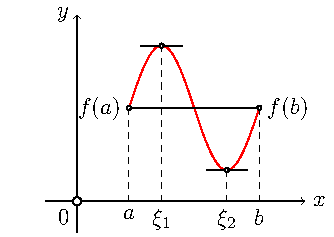
\includegraphics[width=0.7\linewidth]{mai_fig027.pdf}
          \caption{K výkladu Rolleovy věty}
          \label{MAI:fig_027}
        \end{figure}
      \end{note}
      
      Z Rolleovy věty plyne důležitá věta:
      
      \begin{lemma}\label{MA1:lem_diff04}
        (\textbf{Cauchyova věta}). Nechť funkce $f$ a $g$ mají tyto vlastnosti:
        \begin{enumerate}
          \item  Jsou spojité na uzavřeném intervalu $\langle a,b\rangle$,
          \item  v každém bodě $x\in(a,b)$ existuje derivace $f'(x)$ (vlastní či nevlastní) a vlastní derivace $g'(x)$,
          \item  $g'(x)\neq0$ na $(a,b)$
        \end{enumerate}
        Potom v otevřeném intervalu $(a,b)$ existuje aspoň jeden bod $\xi$, pro který platí
        \begin{equation}\label{MA1:eq_diff03}
          \frac{f(b)-f(a)}{g(b)-g(a)} = \frac{f'(\xi)}{g'(\xi)}.
        \end{equation} 
      \end{lemma} 
      
      \begin{proof}
        Poznamenejme především, že z předpokladu 3 $g'(x)\neq0$ pro $x\in(a,b)$ a z předpokladu 
        spojitosti funkce $g$ na uzavřeném intervalu $\langle a,b\rangle$ ihned vyplývá vztah 
        $g(b)- g(a)\neq 0$. Kdyby totiž bylo $g(b)=g(a)$, potom by podle \emph{Rolleovy věty} 
        \ref{MA1:lem_diff03} existoval aspoň jeden bod $\eta\in(a,b)$ takový že $g'(\eta)=0$. To 
        však by byl spor s předpokladem $g'(x)\neq0$ pro každý bod $x\in(a,b)$. Proto má smysl 
        podíl na levé straně rovnosti \ref{MA1:eq_diff03}
        
        K vlastnímu důkazu Cauchyovy věty zavedeme takovou pomocnou funkci $F$, aby splňovala podmínky Rolleovy věty. Definujme ji pro $x\in\langle a,b\rangle$ předpisem
        \begin{equation}\label{MA1:eq_diff04}
          F(x)=[f(b)-f(a)]\cdot[g(x)-g(a)]-[f(x)-f(a)]\cdot[g(b)-g(a)].
        \end{equation}
        Snadno ověříme, že tato funkce skutečně splňuje podmínky Rolleovy věty na intervalu $\langle a,b\rangle$:
        \begin{itemize}
          \item Je spojitá na intervalu $x\in\langle a,b\rangle$, což je důsledkem spojitosti  
                funkce $f$ a $g$ na intervalu $x\in\langle a,b\rangle$ ,
          \item má derivaci $F'$ na otevřeném intervalu $(a,b)$, což plyne z existence derivace  
                $f'$ a $g'$ funkce $f$ a $g$ na  intervalu $(a,b)$,
          \item $F(a)=F(b)=0$ 
        \end{itemize}
        Platí tedy i závěr Rolleovy věty pro funkci $F$, tj. na intervalu $(a,b)$ existuje aspoň 
        jeden bod $\xi$, pro který $F'(\xi)=0$. Zderivujeme-li funkci $F$, dostaneme (dosadíme-li 
        $x=\xi$): $$F'(\xi)=[f(b)-f(a)]g'(\xi)-f'(\xi)[g(b)-g(a)]=0$$ Odtud již plyne rovnost 
        \ref{MA1:eq_diff03}                  
      \end{proof}
      
      Významným zvláštním případem Cauchyovy věty je další věta, která se častěji používá.
      
      \begin{lemma}\label{MA1:lem_diff05}
        (\textbf{Lagrangeova věta})\footnote{Joseph Louis Lagrange [lagránž] (1736-1813), francouzský matematik}. Nechť funkce má tyto vlastnosti:
        \begin{itemize}
          \item Je spojitá na intervalu $\langle a,b\rangle$,
          \item má derivaci (vlastní či nevlastní) na otevřeném intervalu $(a,b)$. 
        \end{itemize} 
        Potom existuje v otevřeném intervalu $(a,b)$ aspoň jeden bod $\xi$, pro který platí 
        \begin{equation}\label{MA1:eq_diff05}
           \frac{f(b) - f(a)}{b - a} = f'(\xi),  
        \end{equation}  
        či-li
        \begin{equation}\label{MA1:eq_diff06}
           f(b) - f(a) = f'(\xi)(b-a),  
        \end{equation}           
      \end{lemma}
      
      \begin{proof}
        Tvrzení této věty je důsledkem tvrzení \emph{Cauchyovy věty}, a to pro případ $g(x)=x$. 
        Protože $g'(x)=1$ dokonce všude, jsou splněny všechny tři podmínky Cauchyovy věty. Proto 
        platí i závěr této věty, z něhož pro náš případ již plyne vzorec \ref{MA1:eq_diff05} a tedy 
        i vzorec \ref{MA1:eq_diff06}.  
      \end{proof}
      
      \begin{note}
        Podobně jako je Lagrangeova věta zvláštním případem věty Cauchyovy, je Rolleova věta zvláštním případem Lagrangeovy věty, a to přo případ, že $f(a)=f(b)$.
      \end{note}
      
      \begin{note}
        Lagrangeova věta se často nazývá \emph{větou o přírůstku funkce}, protože vzorcem \ref{MA1:eq_diff06} se vyjadřuje \emph{přírůstek funkce}, tj rozdíl $f(b)-f(a)$. 
        Všechny tři uvedené věty, tj. věta Rolleova, Cauchyova a Lagrangeova, se v literatuře nazývá souhrně \textbf{věty o střední hodnotě diferenciálního počtu}.
      \end{note}
      
      \begin{note}
        Na obr. ** je ilustrován geometrický význam Lagrangeovy věty. Podíl na levé straně rovnosti 
        \ref{MA1:eq_diff05}, tj. číslo $\frac{f(b) - f(a)}{b - a}$ je směrnice sečny $s$, spojující 
        body $A$, $B$ grafu funkce  $f$, které odpovídají krajním bodům intervalu $\langle 
        a,b\rangle$. Podle tvrzení Lagrangeovy věty existuje v otevřeném intervalu $(a,b)$ aspoň 
        jeden bod $\xi$ tak, že tečna grafu funkce $f$ v příslušném jeho bodě je rovnoběžná s 
        přímkou $s$.  
      \end{note}
      
      \begin{note}
        Z Lagrangeovy věty vyplývá toto tvrzení: Nechť funkce $f$ vyhovuje na intervalu $\langle a,b\rangle$ podmínkám Lagrangeovy věty a $x_1$, $x_2$ jsou dva libovolné různé body
        intervalu $\langle a,b\rangle$. Potom v otevřeném intervalu s krajnímy body $x_1$, $x_2$ existuje aspoň jeden bod $\xi$, pro který platí Lagrangeův vzorec:   
        \begin{align}
          f(x_2) - f(x_1)                  &= f'(\xi)(x_2-x_1) \label{MA1:eq_diff07} \\ 
          \frac{f(x_2) - f(x_1)}{x_2-x_1}  &= f'(\xi)          \label{MA1:eq_diff08}      
        \end{align}
        Potom bod $\xi$ lze vyjádřit takto:
        \begin{equation}\label{MA1:eq_diff09}  
          \xi = x_1 + \vartheta(x_2-x_1), \qquad \text{kde }\vartheta\in(0,1). 
        \end{equation}
        Označíme-li $x_2-x_1=h$, můžeme vzorec \ref{MA1:eq_diff07} napsat ve tvaru
        \begin{equation}
          f(x_1+h) - f(x_1)= f'(x_1 + \vartheta h)h, \qquad \text{kde }\vartheta\in(0,1). 
        \end{equation} 
      \end{note}       
          
    \subsection{Některé důsledky Lagrangeovy věty}
      Lagrangeova věta, má některé významné důsledky, které nyní uvedeme \cite[s.~189]{Brabec1989}:
      \begin{lemma}\label{MA1:lem_diff06} 
        Nechť funkce $f$ vyhovuje podmínkám Lagrangeovy věty a navíc nechť $f'(x)=0$ pro všechna 
        $x\in(a,b)$. Potom funkce $f$ je prostá na intervalu $\langle a,b \rangle$. 
      \end{lemma}
      \begin{proof}
        Necť $x_1, x_2$ jsou libovolné dva různé body intervalu $\langle a,b \rangle$. Potom podle 
        Lagrangeova vzorce \ref{MA1:eq_diff04} platí 
        \begin{equation}
          f(x_2) - f(x_1) = f'(\xi)(x_2-x_1) \neq0
        \end{equation}
        neboť $f'(\xi)\neq 0$ dle předpokladu.
      \end{proof}
      
      \begin{lemma}\label{MA1:lem_diff01}
        Funkce $f$ je konstantní na intervalu $(a,b)$, právě když má na tomto intervalu derivaci a platí $f'(x) = 0$ pro všechna $x\in(a,b)$. 
      \end{lemma}
      \begin{proof} Tedy
        \begin{itemize}
          \item Je-li funkce $f$ konstantní na intervalu $(a,b)$, pak je $f'(x) = 0$ pro všechna  
                $x\in(a,b)$, jak již víme.
          \item Nechť $f'(x) = 0$ pro všechna $x\in(a,b)$. Dokažme, že pro každé dva body $x_1, 
                x_2  \in(a,b)$, $x_1\neq x_2$, platí $f(x_1) = f(x_2)$. Z existence
                derivace vyplývá spojitost funkce a jsou tedy splněny podmínky Lagrangeovy věty na 
                každém intervalu $\langle x_1, x_2\rangle\subset(a,b)$. Podle vzorce 
                \ref{MA1:eq_diff04} tedy platí $f(x_2)-f(x_1)f'(\xi)(x_2-x_1)$, $\xi\in(x_1,x_2)$. 
                Protože podle předpokladu je $f'(x)=0$ pro $\forall x\in(a,b)$, platí $f(x_1) 
                -f(x_2)=0$, tj. $f(x_1)=f(x_2)$  
        \end{itemize}
      \end{proof}
      
%} % tikzset
%---------------------------------------------------------------------------------------------------
\printbibliography[heading=subbibliography]
\addcontentsline{toc}{section}{Seznam literatury}
%-------------------- Differential Calculus applications ------------------------------------------
  % !TeX spellcheck = cs_CZ
%{\tikzset{external/prefix={tikz/MAI/}}
% \tikzset{external/figure name/.add={ch05_}{}}
%---------------------------------------------------------------------------------------------------
% file: Differential_Calculus_applications.tex
%---------------------------------------------------------------------------------------------------
\chapter{Aplikace diferenciálního počtu}\label{chap:Apl_dif_poc}
\minitoc

%================Kapitola: Aplikace diferenciálního počtu =========================================
Diferenciální počet má rozsáhlou oblast užití. V této kapitole ukážeme použití výsledků předchozích 
kapitol k vyšetřování průběhu funkce a vlastnosti rovinných křivek. 
  \section{Průběh funkce}
    Pomocí derivace můžeme studovat vlastnosti funkce, které usnadní vyšetřování jejího průběhu.  
    \subsection{Monotonie funkcí}
      Jednou z důležitých vlastností funkce je její \textquotedblleft monotonie\textquotedblright, 
      kterou jsme definovali již v odst. \ref{MA1:subsec_vlastnosti_funkce} kap. 
      \ref{mai:IchapLimit}. Proto je při vyšetřování průběhu funkce důležité určit množiny (často 
      jsou to intervaly), na nichž je funkce monotónní, jinak řečeno, najít \textquotedblleft 
      intervaly monotonie funkce\textquotedblright (viz \cite[s.~208]{Brabec1989}). 
    \begin{enumerate}
      \item Zjistíme \textbf{definiční obor funkce}, vyjádříme jej v intervalech a z nich poznáme,  
            kde je funkce \textbf{spojitá}. Funkce je spojitá v $(a,b)$ pro každý bod tohoto 
            intervalu, když$|f(x)-f(c)|<\varepsilon$, kde $\varepsilon>0$ je libovolně zvolené 
            číslo, a pro všechna $x$ z okolí bodu $c$ je $|x-c|<\delta$, kde $\delta>0$ je na 
            $\varepsilon$ nezávislé.
      \item Určíme, je-li funkce \textbf{lichá} $f(-x)=-f(x)$ nebo \textbf{sudá} $f(-x)=f(x)$.   
            Je-li funkce lichá, je souměrná podle středu souměrnosti (obyčejně to bývá počátek 
            souřadnic $xy$), je-li sudá, je souměrná podle osy $y$.
      \item Určíme \emph{průsečíky křivky s osami pravoúhlých souřadnic}. Body, ve kte\-rých 
            křivka  protíná osu $x$ spolu s body, ve kte\-rých není křivka spojitá, rozlišují 
            intervaly, v nichž je graf křivky nad osou $x$ od intervalů, ve kterých je graf křivky 
            pod osou $x$.
      \item V krajních bodech definičních intervalů, ve kterých je funkce spojitá, stano\-víme 
      \emph{limity funkce} a dále $$\lim_{x \to \pm \infty}f(x).$$
      \item Vypočítáme $f'(x)$ a $f''(x)$, abychom zjistily, kde je funkce \emph{rostoucí}     
            $f'(x)>0$, \emph{klesající} $f'(x)<0$ a kde jsou \emph{lokální extrémy}. Dostaneme-li 
            dosazením kořenů rovnice $f'(x)=0$ do $f''(x)$ hodnotu $f''(x)>0$, má funkce lokální 
            minimum, při $f''(x)<0$ má funkce lokální maximum. V intervalech, kde $f''(x)>0$, je 
            křivka \textbf{konvexní (vypuklá)}, kde $f''(x)<0$, je křivka \textbf{konkávní 
            (vydutá)}. Body, v nichž $f''(x)$ mění znaménko, jsou \textbf{inflexní body}. Najdeme 
            je tak, že stanovíme hodnoty $x$, pro které je $f''(x)=0$ nebo neexistuje. Číslo $c$ je 
            inflexní bod, když existuje takové okolí bodu $c$, že pro $x>c$ je oblouk křivky 
            konvexní a pro $x<c$ konkávní. Je nutné si uvědomit, že když má $f'(x)$ konečnou 
            derivaci, je inflexní bod $c$ taky nulovým bodem druhé derivace čili kořenem rovnice 
            $f''(x)=0$. Obrácená věta neplatí, tj. z $f''(x)=0$ nevyplývá, že v bodě $c$ má $f'(x)$ 
            extrém a že bod $c$ je inflexním bodem.
      \item \textbf{Asymptota} je tečna křivky $f(x)$, jejíž bod dotyku je v nekonečnu. Platí-li  
            $$\lim_{x \to a}f(x) =  \pm\infty,$$ je přímka $x=a$ její asymptotou. Jinak asymptoty 
            mají rovnici $y=kx+q$, kde $x$ a $y$ jsou souřadnice bodů na asymptotách. Existují-li 
            konečné limity $$\lim_{x \to \pm\infty}\frac{f(x)}{x}=k$$  a $$\lim_{x \to 
            \pm\infty}[f(x)-kx] =q$$ pak je asymptotou přímka $y=kx+q$. Můžeme-li rovnici křivky 
            rozložit (tj. rozložit její pravou stranu, oby\-čejně dělením čitatele jmenovatelem, 
            má-li tvar zlomku) na dvě části, z nichž jedna má tvar $kx+q$ a druhá zbytek 
            $\varphi(x)$, tj. $f(x)=kx+q+\varphi(x)$ a $\varphi(x)_{x\rightarrow 
            \pm\infty}\rightarrow 0$, je přímka $y=kx+q$ asymptotou.
      \item Zpřesnění grafu křivky provedeme sestavením tabulky souřadnic dalších bodů křivky,  
            tj. ke zvoleným hodnotám $x$ (z definičního oboru funkce) vypočítáme hodnoty $y$. Do 
            dalších řádků tabulky zapíšeme hodnoty  $f'(x)$ a $f''(x)$, ve kterých intervalech je 
            funkce \emph{rostoucí}, ve kterých \emph{klesá}, kde je \emph{vypuklá}, kde je 
            \emph{dutá}, kde jsou \emph{lokální extrémy}, \emph{inflexní body} apod., 
            případně sestavíme dílčí tabulky pro jednotlivé \emph{charakteristické vlastnosti} vyšetřované funkce.
    \end{enumerate}
    %-------------------- EXAM001 --------------------------------------
    \input{../src/MAI/exam/exam003.tex}
    %-------------------------------------------------------------------

%} %tikzset
%---------------------------------------------------------------------------------------------------
\printbibliography[heading=subbibliography]
\addcontentsline{toc}{section}{Seznam literatury} 
%--------------------an Integrals of functions of one real variable -------------------------------
  % !TeX spellcheck = cs_CZ
%{\tikzset{external/prefix={tikz/MAI/}}
% \tikzset{external/figure name/.add={ch07_}{}}
%---------------------------------------------------------------------------------------------------
% file: chap_Int_rfce_1var.tex
%---------------------------------------------------------------------------------------------------
%===================================================================================================
% ------------------------------------------- Definite Integral -----------------------------------
\chapter{Určitý integrál}
\minitoc

\section{Motivace} 

  \begin{figure}
    \centering
    \animategraphics[controls,autoplay,loop]{2}{mai_fig022}{}{}
    \caption{text
             (\cite[s.~10000]{Feynman01})}
  \end{figure}

  \begin{figure}[ht!]  %\ref{mai:fig031}
    \centering
    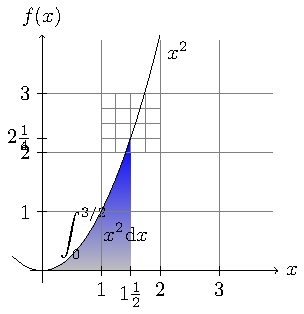
\includegraphics[width=0.7\linewidth]{mai_fig031.pdf}
    \caption{
            (\cite[s.~10000]{Feynman01})}
    \label{mai:fig031}
  \end{figure}

  \subsection{Výpočet integrálu}
      \begin{example}
        Spočítejme integrál $\displaystyle \int_1^{ln5}{(x+1)e^xdx}$  metodou per partes: 
        \begin{align*}
          \int{(x+1)e^xdx} &= \int{e^xdx}+\int{x\cdot e^xdx}
                            = e^x + (x-1)e^x = xe^x               \\
          \int_1^{ln5}{(x+1)e^xdx} &= [xe^x]_1^{ln5} = 5ln5-e     \\
        \end{align*}
        kde integrál
        \begin{equation*}
            \int{xe^xdx}=
              \left[\begin{array}{cc}
                u=x   & dv=e^x \\
                du=dx & v=e^x
              \end{array}\right]=
              xe^x-\int{e^xdx} = xe^x - e^x+C
        \end{equation*}
      \end{example}

\section{Vlastnosti určitého integrálu}
  V této kapitole mluvíme o spojitých funkcích $\Rightarrow$ příslušné integrály tedy vždy
  existují. Čerpáno z knih:
  \cite{Knichal}.

  \begin{lemma}
    \textbf{První věta o střední hodnotě integrálního počtu}: Je-li funkce $f(x)$ spojitá v
    intervalu $\langle a, b\rangle$, existuje alespoň jeden takový bod $c\in(a, b)$, že platí

    \begin{equation}\label{MA:eq_av1}
      \int_a^b f(x)dx = (b-a)f(c).
    \end{equation}
  \end{lemma}

  \begin{proof} Použitím Lagrangeovy věty napsané pro funkci $F(x)$, primitivní na intervalu
    $\langle a, b\rangle$ k dané funkci $f(x)$. Podmínky věty jsou zřejmě splněny: $F(x)$ je
    spojitá na intervalu $\langle a, b\rangle$ a má všude derivaci $F'(x)= f(x)$. Tedy existuje
    alespoň jeden bod $c\in(a, b)$,
    
    \begin{figure}[ht!]  %\ref{mai:fig029}
      \centering
      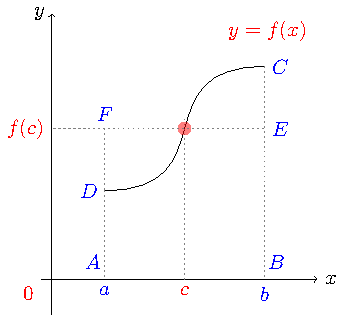
\includegraphics[width=0.7\linewidth]{mai_fig029.pdf}
      \caption{Vztah mezi silou tření a kolmou silou při smýkání
              (\cite[s.~173]{Feynman01})}
      \label{mai:fig029}
    \end{figure}

     že $$F(b)-F(a) = (b-a)F'(c),$$ čímž je věta dokázána, neboť $F(b)-F(a) = \int_a^bf(x)dx$ a
     $F'(c) = f(c)$. Funkční hodnotu $f(c)$, danou podle (\ref{MA:eq_av1}) rovnicí  
     \begin{equation}\label{MA:eq_av2}
        f(c) = \frac{1}{b-a}\int_a^b f(x)dx
     \end{equation}
     nazýváme \texttt{střední hodnotou}.
  \end{proof}

  Pro spojitou nezápornou funkci $f(x)$, lze větu o střední hodnotě jednoduše geometricky
  interpretovat dle (obr.\ref{mai:fig029}). Levá strana (\ref{MA:eq_av1}) určuje obsah
  křivočarého lichoběžníka $ABCD$, pravá strana obsah obdélníka $ABEF$. Podle této věty nabývá
  funkce $f(x)$ aspoň v jednom bodě intervalu $(a, b)$ takové hodnoty $f(c)$, že uvažovaný
  křivočarý lichoběžník má stejný obsah jako obdélník o základně $b-a$ a výšce $f(c)$ (str. 155
  knihy \cite{Knichal}).

      %---------------------------------------------------------------
      \input{../src/MAI/exam/exam032.tex}
      %---------------------------------------------------------------

  \begin{example} Efektivní hodnota $i_{ef}$ střídavého proudu $$i(t) = I_0\sin\omega t$$ (viz
    předchozí příklad) je definována jako odmocnina ze střední hodnoty funkce $i^2(t)$ v průběhu
    jedné periody $T = \frac{2\pi}{\omega}$. Tedy
    \begin{align*}
      i_{ef}^2 &= \frac{1}{T}\int_0^T I_0^2\sin^2\omega t\dd{t} = 
                  \frac{1}{T}\int_0^T \frac{I_0^2}{2}(1- \cos2\omega t)\dd{t}           \\
               &= \frac{I_0^2}{2T}
                  \left[
                    t-\frac{\sin2\omega t}{2\omega}
                  \right]_0^T = \frac{I_0^2}{2}
    \end{align*}
    neboť $\sin2\omega T=\sin4\pi = 0.$ Odtud $$i_{ef} = \frac{I_0}{\sqrt{2}}.$$ Střídavý proud
    $i(t) = I_0\sin\omega t$ má na témže odporu stejný výkon jako stejnosměrný proud o intenzitě
    $i = 0,707I_0$.
  \end{example}
  Následující věta může být využita k odhadu některých integrálů
  \begin{lemma}
    \textbf{Druhá věta o střední hodnotě integrálního počtu}: Jsou-li funkce $f(x)$ a $g(x)$
    spojité v intervalu $\langle a, b \rangle$ a je-li funkce $g(x)$ v $\langle a, b \rangle$
    nezáporná a nerostoucí, existuje alespoň jeden bod $c\in\langle a, b \rangle$ tak, že platí
    \begin{equation}\label{MA_eq_av3}
        \int_a^b f(x)g(x) = g(a)\int_a^c f(x)dx.
    \end{equation}
  \end{lemma}
  Zcela obdobnou větu lze vyslovit pro případ, že $g(x)$ je v intervalu $\langle a, b \rangle$
  nezáporná a neklesající, tj. na pravé straně \ref{MA_eq_av3} je pak integrál $g(b)\int_c^b
  f(x)dx$

  \begin{example} Odhadněte hodnotu integrálu
    \begin{equation}\label{MA_eq_sinx_x}
        \int_{100\pi}^{1000\pi}\frac{\sin x}{x}dx
    \end{equation}
    Řešení: Funkce $f(x) = \sin x$ a $g(x) = \frac{1}{x}$ jsou v uvažovaném intervalu $\langle
    100\pi, 1000\pi \rangle$ spojité a funkce $g(x)$ je kladná a nerostoucí.
    \begin{equation*}
      \int_{100\pi}^{1000\pi}\frac{\sin x}{x}dx = 
      \frac{1}{100\pi}\int_{100\pi}^c\sin xdx =\frac{1}{100\pi}\left(\cos100\pi - \cos c\right)
    \end{equation*}
    kde $c$ je kladné číslo z intervalu $\langle 100\pi, 1000\pi \rangle$. Dále pro všechna
    $c\in\langle 100\pi, 1000\pi \rangle$ platí $0\leq1-\cos c\leq2$, takže
    \begin{equation*}
        0\leq\int_{100\pi}^{1000\pi}\frac{\sin x}{x}dx\leq \frac{1}{50\pi}.
    \end{equation*}
  \end{example}   

%} %tikzset
%---------------------------------------------------------------------------------------------------
\printbibliography[heading=subbibliography]
\addcontentsline{toc}{section}{Seznam literatury}
%---------------------Řady-------------------------------------------------------------------------
  % !TeX spellcheck = cs_CZ
%{\tikzset{external/prefix={tikz/MAI/}}
% \tikzset{external/figure name/.add={ch08_}{}}
%---------------------------------------------------------------------------------------------------
% file series.tex
%---------------------------------------------------------------------------------------------------
%==================================== Kapitola: Řady================================================
\chapter{Řady}
\minitoc

%} % tikzset
%---------------------------------------------------------------------------------------------------
%\printbibliography[title={Seznam literatury}, heading=subbibliography]
\addcontentsline{toc}{section}{Seznam literatury}  
%---------------------Numerické metody ------------------------------------------------------------
  % !TeX spellcheck = cs_CZ
%{\tikzset{external/prefix={tikz/MAI/}}
% \tikzset{external/figure name/.add={ch11_}{}}
%---------------------------------------------------------------------------------------------------
% file NM.tex
%---------------------------------------------------------------------------------------------------
\chapter{Numerické metody}
\minitoc

  \section{Úvodní slovo}
    Numerické metody jsou metody, které na rozdíl od metod analytických poskytujících spojité řešení
    na určité předem definované oblasti, dávají čísel\-né řešení v předem zvolených diskrétních
    bodech této oblasti. Na rozdíl od analytických metod toto řešení většinou nebývá přesné, ale
    představuje pouze jeho aproximaci, která je zatížena určitou chybou.
    
    Možnosti analytických metod se již asi třicet let pokládají prakticky za vyčerpané. Drtivá
    většina problémů (a to zdaleka nejen v oblasti technických věd), které bylo možno analyticky
    vyřešit, již tehdy byla vyřešena. Při vyčíslování výsledků ovšem v mnoha případech nastávaly
    značné problémy; spojité řešení bylo například popsáno kombinací vyšších funkcí (Besselovy,
    Legendrovy atd.) v podobě nekonečných řad, přičemž bylo třeba načítat dostatečný počet jejich
    členů k dosažení požadované přesnosti. A zde se již začaly uplatňovat různé numerické techniky,
    které ovšem bylo v té době možno realizovat jen na kalkulačkách nebo ze současného pohledu na
    primitivních počítačích.
  
    Ačkoli základy sofistikovaných numerických metod byly položeny již před více než šedesáti lety,
    jejich intenzivní a široký rozvoj je spojen teprve s vývojem a zdokonalováním výpočetní techniky
    v posledních asi čtyřiceti letech a lze říci, že v poslední době s řešením čím dál tím
    složitějších problémů ze všech vědních oblastí (nestacionární a nelineární úlohy ve 2D a 3D)
    stále nabývají na významu.
  
    Výsledkem aplikace převážné většiny numerických metod je sestavení velkého systému lineárních či
    nelineárních algebraických rovnic, který je nutno nějakým způsobem vyřešit existují ovšem
    numerické techniky i pro jiné účely, jako je například součet různých řad, výpočet určitých
    integrálů atd., jejich počet však není příliš velký). A v popředí zájmu jsou především dvě
    otázky:
    \begin{itemize}
      \item jak sestavit onen systém tak, aby počet zmíněných rovnic byl co nej\-men\-ší (přičemž 
            ale informace o rozložení hledané veličiny v oblasti je maximální a co nejpřesnější) a
      \item jak tento systém vyřešit co nejrychleji a s nejmenší možnou chybou.
    \end{itemize}
    Na tomto místě je nutno podotknout, že i malá vylepšení stávajících postupů mohou při řešení
    složitých úloh vedoucích na řešení soustav milionů či desítek milionů rovnic (aktuální stav)
    zajistit velmi výrazné časové úspory. Samotná realizace jakékoli numerické metody sestává z
    několika kroků:
    \begin{itemize}
      \item Sestavení matematického modelu dané úlohy. Tento krok je sám o sobě často nesmírně
            komplikovaný; reálný fyzikální problém musíme mnohdy zjednodušit tak, aby byl vůbec
            dostupnými prostředky řešitel\-ný, aniž by však vzniklé chyby přesáhly přijatelné 
            hodnoty. Takový matematický model zpravidla sestává z různých rovnic (algebraických,
            diferenciálních, integrálních, smíšených), neurčitých nebo určitých integrálů a podobně.
      \item Výběr konkrétní metodiky, jakou tento model budeme řešit. Uvedená me\-to\-di\-ka by měla
            být co nejvýhodnější z celé řady hledisek, jako je rychlost výpočtu, spolehlivost,
            robustnost, přesnost, konvergence, stabilita atd. O těchto pojmech jistě už většinou 
            máme jakousi intuitivní představu, v dalším textu však některé z nich upřesníme. Na 
            základě zvolené metody vypracujeme algoritmus, což je konečné množství instrukcí, které 
            musíme provést, aby se celý výpočet bezezbytku provedl.
      \item Navržený algoritmus musíme nyní naprogramovat. Přitom lze využít buď nějakého
            programovacího jazyka (FORTRAN, C++ a další), nebo nějakého prostředí s již
            předprogramovanými operacemi nebo celými bloky výpočtů (MatLab, Mathematica). V 
            některých případech lze využít i již existujících profesionálních programů, které 
            takový algoritmus
            obsahují (freeware tohoto typu je velmi řídké). Ty jsou ovšem velmi drahé a uživatel do
            nich zpravidla nemůže zasahovat za účelem například optimalizace výpočtu.
      \item Dalším krokem je realizace výpočtu. Zde je kromě provedení samotného výpočtu nutné
            ověřit, že výsledky jsou korektní. K tomu používáme buď experiment, nebo jinou metodu,
            která je již pro úlohu daného typu spolehlivě prověřená. Dále ověřujeme celou řadu
            aspektů, jako je například geometrická konvergence řešení (závislost výsledků na hustotě
            diskretizační sítě) a popřípadě jiná kritéria, o nichž se více dozvíme později.
      \item Posledním krokem je vyhodnocení a posouzení získaných výsledků, zpravidla na vizuálním
            základě, porovnáním, ale i jinak.
    \end{itemize}
  
  \section{Reprezentace čísel ve výpočetní technice}
    Při realizaci numerických algoritmů na počítači se lze setkat se dvojí reprezentací čísel, a to
    pomocí \textbf{pevné} nebo \textbf{plovoucí desetinné tečky}. Pevná desetinná tečka znamená vždy
    předem definovaný počet desetinných míst. Pracujeme-li se čtyřmi desetinnými místy, interpretují
    se následující čísla takto:
  
    \begin{table}[h]
      \centering
        \begin{tabular}{l r}
          \hline
          8675             & 8675.0000  \\
          \quad  3.24      &    3.2400  \\
          \quad -0.000006  &   -0.0000  \\
          \hline
        \end{tabular}
        \caption{Reprezentace čísel v pevné desetinné tečce}
    \end{table}
  
    Zatímco první dvě čísla jsou zobrazena přesně, třetí číslo nikoli, je zaokrouhleno. Proto je
    tento způsob nepraktický, při vědeckotechnických výpočtech se neužívá a v dalším textu se jím už
    nebudeme zabývat.
  
    Daleko pružnější je proto počítání s plovoucí desetinnou tečkou, kdy se v každém čísle 
    respektuje předepsaný počet prvních číslic. V tomto případě se uvedená čísla zobrazují takto:
  
    \begin{table}[h]
      \centering
        \begin{tabular}{l c c l}
           \hline
           8675             & +0.8675E+04 & nebo & +8.675E+03  \\
           \quad  3.24      & +0.3240E+01 & nebo & +3.240E+00  \\
           \quad -0.000006  & -0.6000E-05 & nebo & -6.000E-06  \\
           \hline
        \end{tabular}
        \caption{Reprezentace čísel v plovoucí desetinné tečce}
    \end{table}
  
    Každé nenulové číslo a lze reprezentovat jako $a= +m\cdot10^e$ , kde $0.1 < m <1$ a $e$ je celé
    číslo. Samozřejmě, číslo $m$ může obsahovat nekonečnou řadu číslic a celé číslo $e$ se může
    pohybovat od minus nekonečna do nekonečna. To ale v počítačové reprezentaci není možné; zde je
    číslo $m$ omezeno na konečný počet $n$ číslic a právě tak je omezen i exponent. Číslo $a$ je 
    tedy počítačem aproximováno jako $a= \pm m\cdot10^e$, kde $m=0.d1d2\ldots dn$. Toto číslo $m$ se
    nazývá \textbf{mantisa} a $e$ \textbf{exponent}.
  
    V jednoduché přesnosti má v počítačích e velikost $|e|< 38$, ve dvojité přesnosti $|e|<308$.
    Jsou-li tyto hodnoty překročeny, vzniká chyba známá jako \textbf{underflow} nebo
    \textbf{overflow}.
  
    \subsection{Zaokrouhlování}
      Čísla jsou v počítačové interpretaci často zaokrouhlována (mají-li v mantise velký počet
      číslic), poněvadž mantisa $m$ zde může těchto číslic obsahovat pouze $n$. Pravidla
      zaokrouhlování jsou jasná. Zopakujeme zde jen to, že čísla typu 7.65 nebo 7.75 (chceme-li
      zrušit jedno desetinné místo) zaokrouhlíme tak, že poslední číslice je sudá. Takže zatímco 
      7.65 zaokrouhlíme na 7.6, 7.75 zaokrouhlíme na 7.8.
  
      Chybu při zaokrouhlování můžeme určit jako ($n$ je počet číslic v mantise $m$)
      \begin{equation}\label{nm:eq_err_round}
        |\frac{m-\underline{m}}{m}|\leq\frac{0.5}{10^{n-1}}
      \end{equation}  
  
  %============ Kapitola: Chyby při numerických výpočtech =========================================
  \section{Chyby při numerických výpočtech}
    Protože základem numerických metod je získávání přibližných výsledků, je nutné mít vždy
    představu, jaký rozdíl může být mezi přesným řešením dané úlohy a řešením získaným použitou
    numerickou metodou.
    \subsection{Zdroje a typy chyb}
      Pomineme-li jako zdroj chyb člověka dopouštějícího se omylů, můžeme chyby rozdělit na několik
      základních druhů.
      \begin{itemize}
        \item \textbf{Chyby matematického modelu} - vznikají nahrazením reálné fyzikální situace
              matematickým modelem. Může se jednat například o popis nějakého fyzikálního děje 
              pomocí diferenciální rovnice.
        \item \textbf{Chyby vstupních dat} - jsou způsobeny nepřesnostmi při měření fyzikálních
              veličin
        \item \textbf{Chyby numerické metody} - vznikají při náhradě původní matematické úlohy
              jednodušší numerickou. Často se jedná o náhradu nekonečného procesu procesem konečným,
              např. při výpočtu hodnoty některé elementární funkce pomocí součtu několika prvních
              členů její nekonečné Taylorovy řady nebo při aproximaci určitého integrálu souč\-tem
              konečného počtu funkčních hodnot. Odhad této chyby je důležitou součástí řešení každé
              numerické úlohy.
        \item \textbf{Chyby zaokrouhlovací} - vznikají tím, že při výpočtech pracujeme s čísly
              zaokrouhlenými na určitý, relativně nevelký počet míst. Tyto chyby se při výpočtu 
              mohou kumulovat, nebo navzájem rušit. Při vel\-kém počtu operací je posouzení jejich 
              vlivu velmi náročné.
      \end{itemize}
      
    \subsection{Definice chyb, šíření chyb při výpočtu}
      \subsection{Absolutní a relativní chyba}
        Je-li hodnota $\underline{c}$ aproximace přesné hodnoty $c$, je \textbf{absolutní chyba}
        definována jako $\varepsilon=c-\underline{c}$ a \textbf{relativní chyba}
        $\varepsilon_r=\frac{\varepsilon}{c},c\neq0$. Tato definice se může zdát neužitečná, 
        poněvadž $c$ neznáme. Lze-li však říci, že pokud se aproximace $\underline{c}$ blíží k $c$, 
        můžeme psát $\varepsilon_r=\frac{\varepsilon}{\underline{c}},\underline{c}\neq0$. Bohužel, 
        většinou neznáme ani hodnotu $\varepsilon$. Někdy však její hodnotu můžeme odhadnout vztahem
        $|\varepsilon|\leq\sigma$ a podobně lze odhadnout pro relativní chybu 
        $|\varepsilon_r|\leq\sigma_r$.
      \subsubsection{Šíření chyb}
        \emph{Meze absolutních chyb při sčítání a odečítání se rovnají součtu pří\-sluš\-ných mezí.
        Meze relativních chyb při násobení a dělení se rovnají součtu mezí jednotlivých relativních
        chyb}.
        \begin{itemize}
          \item Nechť  $|x_i-\hat{x}_i|=|\varepsilon_i|\leq\sigma_i,\quad i=1,\cdots,n$. Pak je
               \begin{equation}\label{nm:eq_sireni_abs_err}
                 |\sum_{i=1}^n{x_i-\hat{x}_i}|=|\sum_{i=1}^n{\varepsilon_i}|\leq\sum_{i=1}^n{\sigma_i}
               \end{equation}
  
          \item Nechť dále $|\frac{x_i-\hat{x}_i}{x_i}|=|\varepsilon_{ri}|\leq\sigma_{ri},\quad
                i=1,\cdots,n$. Pak je
  
               \begin{align*}
                 |\frac{\prod_{i=1}^n{x_i}-\prod_{i=1}^n{\hat{x}_i}}{\prod_{i=1}^n{x_i}}|      &=
                             |\frac{\prod_{i=1}^n{x_i}-\prod_{i=1}^n{x_i-\varepsilon_i}}
                             {\prod_{i=1}^n{x_i}}|\doteq
                             \\  
                 |\frac{\sum_{i=1}^n{\varepsilon_i}\prod_{j=1,j\neq i}^n{x_j}}
                             {\prod_{i=1}^n{x_i}}|                                             &=
                             |\sum_{i=1}^n{\frac{\varepsilon_i}{x_i}}|
                             \\
                 |\sum_{i=1}^n{\varepsilon_{ri}}|                                              &\leq
                             |\sum_{i=1}^n{\sigma_{ri}}|
              \end{align*}
        \end{itemize}
        kde jsme ale při rozdílu součinů v druhém výrazu zanedbali všechny násobky různých
        absolutních chyb, tedy členy druhého a vyšších řádů.
  
      \subsubsection{Podmíněnost numerických úloh a numerická stabilita algoritmů}
        Při numerickém řešení různých úloh musíme zkoumat, jaký vliv na výsledek mají malé změny ve
        vstupních hodnotách a zaokrouhlování během výpočtu. Řešení numerických úloh můžeme považovat
        za postup, kterým přiřazujeme vstupním údajům výstupní data. Je-li toto přiřazení spojité
        zobrazení, pak říkáme, že numerická úloha je \textbf{korektní úloha}, v opačném případě se
        jedná o úlohu \textbf{nekorektní}.
  
        Pro tyto úlohy má zásadní význam relativní citlivost výsledku na malé změny ve vstupních
        parametrech úlohy. Korektní úloha je \textbf{dobře pod\-mí\-ně\-ná}, jestliže malým
        relativním změnám vstupních údajů odpovídají malé relativní změny výstupních údajů. Číslo
        \begin{equation}\label{nm:eq_podminenost}
          C_p=\frac{\texttt{relativní chyba výstupnich údajů}}{\texttt{relativní chyba vstupních
              údajů}},
        \end{equation}
        nazýváme \textbf{číslo podmíněnosti úlohy}. Pro dobře podmíněné úlohy je číslo $C_p$ blízké
        číslu $1$. Pokud malé relativní změny na vstupu způsobí velké relativní změny na výstupu, 
        pak  mluvíme o \emph{špatně podmíněné úloze}. Řešení špatně podmíněných úloh je nejlépe se
        vyhnout, protože výsledky jakéhokoliv algoritmu jsou velmi nespolehlivé. Podobně řekneme, že
        je algoritmus \emph{dobře pod\-mí\-ně\-ný}, je-li málo citlivý na poruchy ve vstupních
        datech. Kromě ne\-přes\-ností ve vstupních údajích ovlivňuje výsledek použitého algoritmu i
        zaokrouhlování čísel během výpočtu. Je-li vliv zaokrouhlovacích chyb na výsledek malý,
        mluvíme o \emph{numericky stabilním algoritmu}. \emph{Algoritmus dobře pod\-mí\-ně\-ný a
        numericky stabilní se nazývá stabilní}.
  
  %=============== Kapitola: Řešení nelineárních rovnic ============================================
  \section{Řešení nelineárních rovnic}
    \subsection{Motivace}
      Kořeny nelineárních rovnice $f(x)=0$ obecně neumíme vyjádřit explicitním vzorcem. K řešení
      nelineární rovnice proto používáme iterační metody: z jedné nebo několika počátečních
      aproximací hledaného kořene $\hat{x}$ generujeme posloupnost $x_0,x_1,x_2…$, která ke kořenu
      $\hat{x}$ konverguje. Pro některé metody stačí, když zadáme interval $\langle a,b\rangle$,
      který obsahuje hledaný kořen. Jiné metody vyžaduji, aby počáteční aproximace byla k hledanému
      kořenu dosti blízko; na oplatku takové metody konvergují mnohem rychleji. Často proto začínáme
      s \uv{hrubou}, avšak spolehlivou metodou, a teprve když jsme dostatečně blízko kořene, 
      přejdeme na \uv{jemnější}, rychleji konvergující metodu.
  
      Abychom naše úvahy zjednodušili, omezíme se na problém určení re\-ál\-né\-ho
      je\-dno\-du\-ché\-ho kořene $\hat{x}$ rovnice $f(x)=0$, tj. předpokládáme, že $f'(\hat{x})=0$.
      Budeme také automaticky předpokládat, z funkce $f(x)$ je spojitá a má tolik spojitých 
      derivací, kolik je jich v dané situaci zapotřebí.
  
      Počáteční aproximaci kořenů rovnice $f(x)=0$ můžeme zjistit z grafu funkce $f(x)$: ručně, nebo
      raději pomocí vhodného programu na počítači, vykreslíme funkci $f(x)$ a vyhledáme její
      průsečíky s osou $x$.
  
      Jinou možností je sestaveni tabulky $[x_i,f(x_i)]$ pro nějaké dělení:
      $$a=x_0<x_1<\cdots<x_{i-1}<x_i<\cdots<x_n=b$$.
      \begin{example} Získejme hrubý odhad kořenů rovnice $f(x) = 0$, kde $$f(x):y=4\sin x - x^3 - 
      1$$

          {\centering
           \captionsetup{type=figure}
           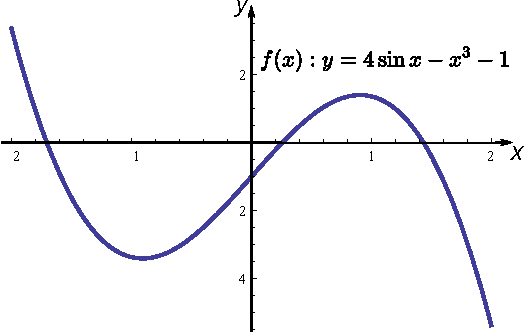
\includegraphics[scale=1]{mai_fig035.pdf}
           \captionof{figure}{Graf funkce $f(x):y=4\sin x - x^3 - 1$.}
           \label{mai:fig035}
           \par}
        Z obrázku \ref{mai:fig035} zjistíme, že existují tři kořeny: $x_1^*\in(-2,-1),
        x_2^*\in(-1, 0)$ a $x_3^*\in(1, 2)$.
      \end{example}
  
      Z obrázku zjistíme, že existují tři kořeny: $x_1^*\in(-2,-1),x_2^*\in(0,1),x_3^*\in(1,2)$.
      Zkusme najít kořeny v těchto intervalech pomocí numerických metod popsaných v následujících
      odstavcích
  
    \subsection{Metoda bisekce}
      Metoda známá také jako \textbf{metoda půlení intervalů}, je založena na principu
      zna\-mén\-ko\-vých změn. Předpokládejme, že funkce $f(x)$ má v koncových bodech intervalu
      $(a_0,b_0)$ opačná znaménka, tj. platí $f(a_0 )\cdot f(b_0 )<0$. Sestrojíme posloupnost
      intervalů $(a_1,b_1)\supset(a_2,b_2)\supset(a_3,b_3)\supset\cdots$, které obsahují kořen.
      Intervaly $(a_{k+1},b_{k+1}), k=0,1,\cdots$, určíme rekurzivně způsobem, který si nyní
      popíšeme.
  
      Střed intervalu $(a_k,b_k)$ je bod $x_{k+1}=\frac{1}{2}(a_k+b_k)$. Když $f(x_k)=0$, pak
      $x_{k+1}=x^*$ je kořen a dál nepokračujeme.

%} %tikzset
%---------------------------------------------------------------------------------------------------
\printbibliography[heading=subbibliography]
\addcontentsline{toc}{section}{Seznam literatury}
} % DEBUG was off

\part{MA II}\label{part:MAII}
\parttoc

\ifthenelse{ \equal{\DebugMode}{true} }{
% Debug mode ON
%  % !TeX spellcheck = cs_CZ
%---------------------------------------------------------------------------------------------------
% history_MA.tex
%---------------------------------------------------------------------------------------------------
\chapter{Vícerozměrná linearita aneb lineární algebra podruhé}\label{mai:IIchapI}
\minitoc
  V kapitole \ref{mai:IchapII} dílu \ref{part:MAI} jsme se seznámili s elegantní dámou lineární 
  algebrou. Pomocí jejích pravidel jsme nejen řešili soustavy lineárních rovnic, ale také počítali 
  s maticemi a vektory. Zatímco operace s maticemi, a koneckonců i řešení lineárních rovnic pomocí 
  matic bychom mohli chápat jako užitečnou ekvilibristiku s číselnými soubory, za počítáním s 
  vektory se zdálo být přece jen něco hlubšího a závažnějšího. Vázané vektory pro nás totiž byly 
  orientovanými úsečkami v trojrozměrném euklidovském prostoru, v němž bylo definováno měření délek 
  a úhlů. Volné vektory pak byly množinami stejně velkých a souhlasně rovnoběžných orientovaných 
  úseček. Jednalo se tedy o \emph{geometrické objekty}. Každý vektor byl určen svou velikostí a 
  směrem. Směr byl přitom zadán například pomocí úhlů mezi daným vektorem a vybranými směry, které 
  byly předem pevně zvoleny. Mohli jsme s vektory provádět základní algebraické operace, jimiž jsou 
  sčítání vektorů a násobení vektoru číslem, podle pravidel zavedených pro (v tomto případě 
  řádkové) matice. S vektory v trojrozměrném prostoru jsme mohli velmi pohodlně počítat jako s 
  trojicemi čísel. Na druhé straně jsme vektory vyjadřovali jako lineární kombinace jiných vektorů, 
  tvořících v prostoru všech vektorů \emph{bázi}. Koeficienty lineární kombinace, která 
  představovala zápis daného vektoru ve zvolené bázi, byly jeho \emph{složkami} v této bázi. Při 
  změně báze se změnily složky vektoru, vektor sám však nikoliv. Vektor je stále sám sebou, jen se 
  v různých bázích jinak tváří - projeví se jinou trojicí čísel. Protože se však při změně báze 
  změní složky vektoru přesně definovaným způsobem (vzpomeňte na transformační vztahy), dokážeme 
  jej vždy rozpoznat. Tuto vlastnost, \emph{invarianci vůči volbě báze}, mají všechny geometrické 
  objekty. A je to právě algebra, která nám umožňuje tyto objekty reprezentovat číselnými soubory a 
  také tak s nimi počítat. Jde-li navíc o objekty řídící se lineárními pravidly. jakými jsou 
  například distributivní zákony, je počítání s nimi, v rámci \emph{lineární algebry}, zvláště 
  jednoduché. Oceníme to zejména v prostorech vyšší dimenze, než je náš běžný euklidovský prostor. 
  Při počítání s vektory v trojrozměrném prostoru, kde umíme měřit délky a úhly a kde platí 
  trigonometrická pravidla, bychom se bez rutinních algebraických procedur ještě třeba obešli. Už 
  ale například ve čtyřrozměrném časoprostoru, v němž se odehrávají všechny přírodní jevy a v němž 
  je třeba formulovat fyzikální zákony, však pro měření délek a úhlů platí jiná pravidla, než jsou 
  obvyklá v běžném, tj. trojrozměrném euklidovském, prostoru. Například tam neplatí čtyřrozměrná 
  verze Pythagorovy věty. A někdy je příroda dokonce tak nepřívětivá, že nás nutí pracovat i s 
  prostory vícerozměrnými. Například jedna z velmi účinných teorií pro výklad chování elementárních 
  částic, teorie strum, je založena na geometrii prostoru jedenáctirozměrného. A v takových 
  dimenzích jsme už s jakkoli vynikající geometrickou představivostí v koncích. Tehdy se vděčně 
  obracíme k metodám algebry. V této kapitole, jak její název napovídá, půjde o algebru lineární
  
  \section{Prostory s vektory}
    V kapitole \ref{mai:IchapII} jsme pracovali s číselnými maticemi typu \(m/n\), tj. soubory 
    čísel uspořádaných v \(m\) řádcích a \(n\) sloupcích, a zavedli jsme pro ně operaci součtu a 
    násobení číslem. Zjistili jsme, že pro sčítání matic a násobení matice číslem platí určitá 
    pravidla. (Jejich souhrn je uveden v samém závěru odstavce \ref{mai:IchapIIsecIIIsubIII}. V 
    odstavci \ref{mai:IchapIIsecIV} jsme zase počítali s vektory. Ty měly jednou \emph{konkrétní 
    podobu} řádkových matic s pravidly pro jejich sčítání a násobení číslem, podruhé, v 
    trojrozměrném prostoru, naopak \emph{konkrétní podobu} orientovaných úseček, resp. množin, 
    které byly orientovanými úsečkami vytvořeny, generovány. Zavedli jsme tenkrát konkrétní způsob 
    sčítání vektorů a násobení vektoru číslem pomocí geometrických operací. Součet dvou vektorů 
    \(\vec{u}\) a \(\vec{v}\) znamenal, že jsme podle zcela určitého pravidla, pravidla 
    vektorového rovnoběžníka přiřadili uspořádané dvojici \([\vec{u},\vec{v}]\) třetí vektor 
    \(\vec{u} + \vec{v}\), násobek vektoru a čísla byl opět vektor \(\alpha\vec{u}\), který jsme 
    přiřadili dvojici \([\alpha,\vec{u}]\) tvořené číslem a vektorem. Uvedli jsem, že pravidla pro 
    tyto \emph{geometrické} operace jsou shodná s pravidly pro počítání s maticemi a lze je dokázat 
    i geometrickými postupy. Množinu volných vektorů generovaných orientovanými úsečkami spolu s 
    uvedenými dvěma operacemi jsme nazvali \textbf{vektorovým prostorem}. Šlo tedy o zcela odlišné 
    množiny základních objektů a zcela odlišným způsobem definované operace, pro které se však dala 
    dokázat tatáž pravidla. Nyní se podíváme na problém definice vektorového prostoru obecněji a 
    poněkud \uv{opačně}. Budeme pracovat s \emph{nosnou množinou} \(V\), a přitom nebude podstatné, 
    jak konkrétně vypadají její prvky. Ani je nebudeme označovat šipkami (u šipek ze zvyku 
    zůstaneme pouze v případě orientovaných úseček v \(\mathbb{R}^1\), \(\mathbb{R}^2\) a 
    \(\mathbb{R}^3\), nebo vektorů s fyzikálním významem). Dále přibereme do hry množinu všech 
    komplexních čísel \(\mathbb{C}\), popřípadě jen množinu všech reálných čísel \(\mathbb{R}\) a 
    definujeme dvě operace (\emph{zobrazení}):
    \begin{equation}\label{mai:eq046}
      V \times V \ni [a,b] \longrightarrow c\in V,\qquad 
      \mathbb{C}\times V\ni[\alpha,a] \longrightarrow d\in V.
    \end{equation}
    Prvek \(c\) nazýváme \emph{součet} prvků \(a\) a \(b\) a značíme jej \(c = a + b\) prvek \(d\) 
    je \(\alpha\)-\emph{násobek} prvku \(a\) a značíme \(d = \alpha a\). Zobrazení uvedená ve 
    vztazích (\ref{mai:eq046}) však nebudou moci být úplně libovolná. Budeme požadovat, aby měla 
    určité vlastnosti, konkrétně ty, které jsou uvedeny pro matice na konci odstavce 
    \ref{mai:IchapIIsecIIIsubIII}. Teprve pak řekneme, že množina \(V\) spolu s operacemi 
    (\ref{mai:eq046}) splňujícími potřebné požadavky je vektorovým prostorem. Vidíme, že takto naše 
    uvažování výrazně posuneme na abstraktní úroveň. Bude lhostejné, co jsou prvky nosné množiny, 
    bude nepodstatné, jak konkrétně jsou definovány operace sčítání prvků a násobení prvku číslem. 
    Důležité bude jen to, aby abstraktní operace s abstraktními prvky splňovaly konkrétní pravidla. 
    Než však k definici vektorového prostoru přistoupíme, všimneme si ještě některých jiných 
    struktur s jednou nebo dvěma operacemi, které samy do oblasti lineární algebry nepatří, ale 
    mohou být užitečné pro definici vektorového prostoru, popřípadě mají významné fyzikální 
    aplikace.
      
      \subsection{Algebraické struktury s jednou operací, hlavně grupy}
        Při zavádění operací s vektory jsme zcela automaticky využívali toho, že umíme počítat s 
        reálnými, popřípadě i s komplexními čísly. Skutečnost, že čísla umíme sčítat, násobit a 
        provádět s nimi řadu dalších operací, považujeme za tak přirozenou a samozřejmou, že nad ní 
        vůbec nepřemýšlíme. Již samotné operace sčítání a násobení vytvářejí na množině čísel velmi 
        bohatou \textbf{algebraickou strukturu}. Tento pojem si nyní přiblížíme. 
        
        Algebraickou strukturu s jednou operací získáme, vezmeme-li v úvahu první ze zobrazení 
        (\ref{mai:eq046}), nosnou množinu označíme tentokrát podle zvyku \(G\):
        \begin{equation}\label{mai:eq047}
          G \times G \ni [a,b] \longrightarrow a + b \in G, \qquad \text{nebo} \qquad
          G \times G \ni [a,b] \longrightarrow a \cdot b \in G.
        \end{equation}
        Pokud použijeme první možnosti označení této operace, hovoříme o operaci \emph{sčítání} a 
        \emph{aditivní} struktuře, v případě druhé možnosti o operaci \emph{násobení} a 
        \emph{multiplikativní} struktuře. Toto terminologické rozlišení nemá obecně žádný hlubší 
        význam. Je spíše otázkou zvyklosti a souvisí především s algebraickou strukturou číselných 
        množin, kterou běžně používáme, aniž o ní přemýšlíme (čísla sčítá a násobí školák, 
        obchodník i účetní a o nějaké abstraktní struktuře nic netuší).
        
        Zobrazení (\ref{mai:eq047}) samo o sobě, aniž na ně klademe další požadavky (podstatné je 
        pouze to, že dvěma prvkům nosné množiny přiřadí prvek \emph{téže množiny}), definuje 
        nejjednodušší algebraickou strukturu s jednou operací, zvanou \textbf{grupoid}. Grupoid 
        není pro fyzikální aplikace příliš užitečný, ale je základem pro konstrukci zajímavějších a 
        užitečnějších struktur. Přidáme-li k definici grupoidu požadavek \emph{asociativity} 
        zobrazení \(G \times G \ni [a, b] \longrightarrow a + b \in G\) (nebo \(G \times G \ni [a, 
        b] \longrightarrow a \cdot b \in G\))
        \begin{equation}\label{mai:eq048}
          (a+b) + c = a + (b + c),\qquad \text{nebo}\qquad (a\cdot b) \cdot c = a \cdot (b \cdot c)
        \end{equation}
        pro libovolné prvky \(a, b, c \in G\), stane se množina \(G\) spolu s operací „\(+\)“, nebo 
        „-“ \textbf{pologrupou}. I pologrupa je z hlediska fyzikálních aplikací poněkud chudá, 
        další požadavek na zobrazení (\ref{mai:eq047}) z ní však již učiní strukturu v matematice i 
        fyzice nepostradatelnou, grupu. Pologrupa, ve které existuje prvek \(0_G\in G\) a současně 
        ke každému prvku \(a \in G\) existuje prvek \((-a) \in G\) tak, že platí
        \begin{equation}\label{mai:eq049}
          a + 0_G = 0_G + a = a,\qquad a + (-a) = (-a) + a = 0_G,
        \end{equation}
        se nazývá \textbf{aditivní grupou}. Prvek \(0_G\) je univerzální pro celou grupu (žádný 
        jiný s touto vlastností v grupě \(G\) není) a nazývá se \emph{neutrální prvek grupy} neboli 
        \textbf{nula}, prvek \((-a)\) je \textbf{opačný} k prvku \(a\). Pro dané \(a\) je určen 
        jednoznačně. V případě operace násobení mají vlastnosti \ref{mai:eq049} tvar
        \begin{equation}\label{mai:eq050}
          a \cdot e_G = e_G \cdot a = a,\qquad a \cdot a^{-1} = a^{-1} \cdot a = e_G,
        \end{equation}
        a \(G\) se nazývá \textbf{multiplikativní grupou}. Prvek \(e_G\) je opět univerzální pro 
        celou grupu a nazývá se \textbf{neutrální} prvek grupy, neboli \emph{jednička}, prvek 
        \(a^{-1}\) je \textbf{inverzní} k prvku \(a\).
        
        Každá operace \ref{mai:eq047} v množině \(G\), která splňuje vztahy asociativity 
        \ref{mai:eq048} a vztahy specifikující nulu a opačný prvek, nebo jedničku a inverzní prvek 
        typu \ref{mai:eq049}, nebo \ref{mai:eq050}, představuje \emph{grupovou operaci} bez ohledu 
        na to, podobá-li se spíše sčítání, nebo spíše násobení, či dokonce něčemu jinému, například 
        skládání zobrazení. Má-li grupa konečný počet prvků, nazývá se tento počet jejím 
        \emph{řádem}.

        %---------------------------------------------------------------
        \input{../src/MAI/exam/exam046.tex}
        %---------------------------------------------------------------
        
        V úvodu odstavce jsme se zmínili o tom, že množiny reálných a komplexních čísel získají 
        zavedením běžných operací sčítání a násobení jistou algebraickou strukturu. Všimněme si 
        jich nyní podrobněji. 
        
        %---------------------------------------------------------------
        \input{../src/MAI/exam/exam047.tex}
        %---------------------------------------------------------------
        
        %---------------------------------------------------------------
        \input{../src/MAI/exam/exam048.tex}
        %---------------------------------------------------------------
        
        O podmnožině \(H \subset C\) grupy \(G\) s operací sčítání nebo násobení zúženou na \(H\), 
        která je sama grupou, hovoříme jako o \textbf{podgrupě} grupy \(G\). Například množina 
        reálných čísel zapsaných ve tvaru \(z = [a, 0]\) se sčítáním je podgrupou množiny 
        komplexních čísel. Koho grupy nebaví a chce se rychle prokousat k vektorovým prostorům, 
        které jsou koneckonců hlavní náplní našeho příběhu o lineární algebře, může zbytek tohoto 
        odstavce přeskočit. Ale byla by to škoda, grupy jsou opravdu zajímavé.

        %---------------------------------------------------------------
        \input{../src/MAI/exam/exam049.tex}
        %---------------------------------------------------------------
        
        %---------------------------------------------------------------
        \input{../src/MAI/exam/exam050.tex}
        %---------------------------------------------------------------

        %---------------------------------------------------------------
        \input{../src/MAI/exam/exam051.tex}
        %---------------------------------------------------------------
        
        Operace sčítání nebo násobení si umíme velmi dobře představit, provádíme-li je standardním 
        způsobem s čísly. Definice algebraických struktur jsou však obecné a zahrnují i jiné 
        možnosti. Představme si například krychli, se kterou provádíme \emph{operace symetrie}. 
        Jsou to všechna taková přemístění krychle z počáteční do koncové polohy, která \uv{se 
        nepoznají}. Znamená to, že krychle vypadá v koncové poloze stejně jako ve výchozí. Pokud
        bychom při přemísťování zavřeli oči, nepoznali bychom že někdo mezitím s krychlí hýbal. 
        Přemístění jsou několikerých typů a definují \textbf{prvky symetrie} krychle. Abychom si je 
        mohli názorně ukázat na obrázcích, označíme vrcholy, popřípadě jiné důležité body krychle 
        písmeny. V některých ukázkách také použijeme hrací kostku. Prvky symetrie krychle můžeme 
        roztřídit do následujících typů:
        \begin{itemize}
          \item \textbf{zrcadlení vzhledem k rovině symetrie} - existuje rovina, jejíž body 
                zůstávají při přemístění v klidu,
          \item \textbf{rotace kolem osy symetrie} - existuje přímka (osa), jejíž body zůstávají 
                při přemístění v klidu,
          \item \textbf{středová inverze} - existuje právě jeden bod (střed inverze), který při 
                přemístění zůstává v klidu,
          \item \textbf{identita} - přemístění do téže polohy, v klidu jsou všechny body krychle
        \end{itemize}
         

%---------------------------------------------------------------------------------------------------
\printbibliography[title={Seznam literatury}, heading=subbibliography]
\addcontentsline{toc}{section}{Seznam literatury} 
%  % !TeX spellcheck = cs_CZ
%---------------------------------------------------------------------------------------------------
% mai2ch02.tex
%---------------------------------------------------------------------------------------------------
\chapter{Souřadnicové soustavy obvyklejší i méně obvyklé}\label{mai:IIchapII}
\minitoc

%---------------------------------------------------------------------------------------------------
\printbibliography[title={Seznam literatury}, heading=subbibliography]
\addcontentsline{toc}{section}{Seznam literatury}
%  % !TeX spellcheck = cs_CZ
%---------------------------------------------------------------------------------------------------
% mai2ch03.tex
%---------------------------------------------------------------------------------------------------
\chapter{Linearita v aplikacích aneb lineární algebra do třetice}\label{mai:IIchapIII}
\minitoc

%---------------------------------------------------------------------------------------------------
\printbibliography[title={Seznam literatury}, heading=subbibliography]
\addcontentsline{toc}{section}{Seznam literatury}
%  % !TeX spellcheck = cs_CZ
%---------------------------------------------------------------------------------------------------
% mai2ch04.tex
%---------------------------------------------------------------------------------------------------
\setchaptertoc
\chapter{Obyčejné diferenciální rovnice}\label{mai:IIchapIV}

  V partii \ref{part:MAI} jsme se seznámili s funkcemi, o jejich užitečnosti nepochybujeme, neboť
  jsme se již přesvědčili, že se s nimi setkáváme takřka na každém kroku. Vyjadřují totiž
  jednoduchým způsobem vzájemnou souvislost veličin, a nejen fyzikálních. Známe-li například funkci
  vyjadřující závislost polohy tělesa na čase, můžeme zjistit, kde těleso v daném okamžiku bylo, je,
  nebo bude. Známe-li funkce, které popisuji časový vývoj cen a platů, můžeme snadno zjistit, zda za
  stejný peníz, za který dnes dostaneme deset housek, koupíme za rok dvacet, nebo jen dvě. Příroda,
  a ani ekonomika či politika, však nejsou natolik průhledné, aby nám takové závislosti předestřely
  přímo. Poskytují pouze informace o jejich změnách, a to ještě ukryté ve speciálních rovnicích,
  zvaných \emph{diferenciální}. Jde-li o neznámou reálnou funkci nebo soubor funkcí závislých na
  jedné reálné proměnné, třeba na čase, hovoříme o obyčejných diferenciálních rovnicích. Přesněji
  řečeno, diferenciální rovnice vyjadřuje matematickou formou zákon platný pro hledanou funkci a
  její derivace prvního nebo i vyšších řádů. Takovou funkcí času může být například i množství látky
  při chemických reakcích, mohutnost populace živočichů, kurz eura, cena akcií na burze, rychlost
  pohybu těles, teplota atd. Ve fyzice a chemii jsou diferenciální rovnice dány fyzikálními či
  chemickými zákony, v ekonomii nebo biologii se objevují v různých modelech, odpovídajících více či
  méně skutečnosti. Uveďme si několik příkladů, na nichž si vysvětlíme základní terminologii, která
  je s problematikou diferenciálních rovnic spojena.
  
  Doplňková literatura pro studium této partie je například: \cite[s.~217]{Musilova2012MA2} a 
  \cite[s.~426]{Brabec1989}. Pro procvičení elementárních metod řešení konkrétních rovnic je vhodná 
  sbírka řešených příkladů \cite[s.~348]{Jirasek1989}.
  
  %--Příklad s hlemýžděm------------------------------------------
    \input{../src/MAI/exam/exam084.tex}
  %---------------------------------------------------------------
  Ve většině příkladů, se kterými se setkáme, bude mít počáteční úloha právě jedno řešení, jak tomu
  je v případě hlemýždě. Jestliže je nějaká funkce, definovaná na intervalu \((a,b)\), řešením
  počáteční úlohy, pak každá funkce, kterou vytvoříme zúžením původního řešení na „menší“ interval,
  bude opět rovnici splňovat. My však máme \emph{„právě jedním řešením“} na mysli tzv. \textbf{úplné
  řešení}, tj. takové, které není zúžením žádného jiného, a tak řešení lišící se pouze definičním
  oborem nebudeme považovat za odlišná. Jak uvidíme později, vyskytnou se však také příklady, kdy
  počáteční úloha nemá žádné řešení, nebo jich má naopak nekonečně mnoho.

  %--Příklad s koupelnou------------------------------------------
    \input{../src/MAI/exam/exam085.tex}
  %---------------------------------------------------------------
  
  \begin{note}
    „Větrací“ rovnice, diskutovaná v předchozím případě, se ve fyzice objevuje poměrně často. Někdy
    je nazývána lineárním diferenciálním zákonem. Narazíme na ni vždy, když je rychlost změny nějaké
    veličiny (její první derivace) přímo úměrná veličině samotné. Tak například při rozpadu
    radioaktivních jader dospějeme k rovnici \(\der{N(t)}{t} = -\lambda N(t)\), kde \(N(t)\) je
    počet radioaktivních jader ve vzorku v okamžiku \(t\) a \(\lambda\) je \textbf{rozpadová
    konstanta}. Při zkoumání absorpce rentgenového záření v látce získáme rovnici \(\der{I(x)}{x} =
    -\mu I(x)\), kde \(I(x)\) je intenzita v hloubce \(x\) pod povrchem a \(\mu\) je lineární
    \textbf{koeficient absorpce}. S oběma příklady jsme se již setkali v partii \ref{part:MAI}.
    Zkusme si vzpomenout na další příklady lineárních diferenciálních zákonů.
  \end{note}

  %--Příklad o sáňkování------------------------------------------
    \input{../src/MAI/exam/exam086.tex}
  %---------------------------------------------------------------
  \begin{note}
    Zamysleme se také nad tím, jak jsme z vyjádření funkce \(v(t)\) pomocí exponenciálních funkcí 
    získali elegantnější výraz s hyperbolickou tangentou. Pro připomenutí hyperbolických funkcí se 
    můžeme vrátit k odstavci 2.1.8 partie \ref{part:MAI}.
  \end{note}
  
  Na uvedených příkladech jsme se mohli přesvědčit, že porozumění některým realistickým dějům
  vyžaduje umět sestavit a řešit diferenciální rovnice. Problémy, se kterými se v životě setkáváme,
  však obvykle vedou k rovnicím mnohem komplikovanějším. Proto často používáme aproximací a skutečný
  svět si poněkud „idealizujeme". Tak například v úloze s koupelnou jsme předpokládali, že vzduch v
  místnosti je vždy dokonale promíchán, v úloze o sáňkování jsme pro odporovou sílu použili pouze
  přibližný zákon a zanedbali třecí sílu. Často se setkáme s rovnicemi, které dokážeme řešit pouze
  numerickými metodami za pomoci počítačů. Aproximativní přístupy tedy mohou vstupovat do popisu
  vývoje reálných systémů pomocí diferenciálních rovnic dvojím způsobem. Poprvé již při samotném
  sestavení diferenciálních rovnic, podruhé při jejich řešení.
  
  V této kapitole se budeme věnovat některým typickým situacím, kdy je možné získat řešení
  diferenciálních rovnic analytickými metodami, zjednodušeně řečeno „tužkou na papíře“. Proč se
  omezujeme na některé typické situace“? Protože problematika diferenciálních rovnic obsahuje ještě
  další úskalí. Řečeno s mírnou nadsázkou, existuje totiž nepřeberné množství různých typů
  diferenciálních rovnic, dokonce už v případě rovnic prvního řádu, které při řešení vyžadují takřka
  \uv{individuální přístup}. I když samozřejmě v teorii diferenciálních rovnic existuje řada
  obecných výsledků společných určité širší skupině diferenciálních rovnic, není možné formulovat
  nějaký \uv{univerzální} postup, který by vedl k řešení kterékoli z nich. V praxi je proto třeba
  naučit se rozpoznat jednotlivé typy obyčejných diferenciálních rovnic a zvolit pro jejich řešení
  vhodnou metodu. Ne nadarmo se proto textům o diferenciálních rovnicích říká „kuchařky“, aniž by to
  mělo hanlivý nádech. (Vznešenější slovo pro „kuchařku“ je „příručka“. Pokud jde o problematiku
  obyčejných diferenciálních rovnic, je takovou moderní příručkou kniha \cite{PolyaninZaitsev},
  která na více než osmi stech stran obsahuje přes 6 200 rovnic s řešeními!
  
  \twocolumn[\section{Diferenicální rovnice vyskytující se kolem nás}\label{mai:IIchapIVsecI}]
    V tomto odstavci jsou zařazeny motivační příklady ukazující, že diferenciální rovnice se
    skutečně objevují v různých vědních oborech. Rovnice jsou většinou uvedeny bez řešení, ale jsou
    doplněny alespoň odkazy ve kterých lze najít mnohem více informací, které jdou za rámec této
    partie o obyčených diferenciálních rovnicích. Stejně jako v předchozích příklad, řada
    fyzikálních principů má tvar výroku, resp. vztahu mezi jistými veličinami (funkcemi) a jejich
    změnami, vztaženými ke zvoleným nezávisle proměnným (pa\-ra\-me\-trům) (\emph{čas, souřadnice}).
    Je to přirozené, neboť (\emph{okamžité}, či \emph{okální}) změny se nejlépe vystihují pomocí
    derivací. Takový zákon má pak charakter vztahu mezi uvažovanými veličinami a jejich derivacemi. 
    
    \begin{mdframed}[style=mdnote] 
      V matematických textech o obyčejných diferenciálních rovnicích se označuje nezávisle proměnná 
      obvykle symbolem \(x\), neznámá funkce \(y = y(x)\) nebo \(y = f(x)\) a její derivace 
      čárkami, tj. \(y'(x)\), \(y''(x)\) nebo \(y' = f'(x)\), \(y" = f''(x)\) atd. V mnoha 
      fyzikálních i jiných praktických situacích však bývá nezávisle proměnnou čas \(t\) a hledáme 
      závislost veličiny \(x = x(t)\) na čase. Tohoto značení budeme velmi často používat, přičemž 
      první, resp. druhou derivaci funkce \(x(t)\) budeme podle zvyklosti zavedené ve fyzice 
      vyznačovat pomocí tečky, resp. dvou teček nad symbolem \(x\),
      \begin{equation*}
        \dot{x}(t) = \der{x}{t}, \qquad \ddot{x}(t) = \dder{x}{t}.
      \end{equation*}
      Pro větší přehlednost zápisu budeme často vynechávat argument \(t\) v závorce, \(\dot{x} = 
      \dot{x}(t)\). Nebudeli řečeno jinak, předpokládáme, že všechny funkce jsou spojité, případně 
      i diferencovatelné na celém svém definičním oboru nebo alespoň na jistém oboru, který je jeho 
      podmnožinou. Při práci s podílem funkcí budeme automaticky předpokládat, že jmenovatelem je 
      funkce, která je nenulová ve všech bodech uvažovaného intervalu.      
    \end{mdframed}
    
    \subsection{Diferenciální rovnice v mechanice}
      \textbf{Druhý Newtonův pohybový} zákon pro hmotný bod, který nabývá tvaru
      \begin{equation*}
        m\vec{a} = \vec{F}
      \end{equation*}
      skrývá soustavou \emph{tří diferenciálních rovnic druhého řádu}. Složky zrychlení \(\vec{a}(t)
      = (a_x(t), a_y(t), a_z(t)) = (\ddot{x}(t), \ddot{y}(t), \ddot{z}(t))\) jsou totiž druhými
      derivacemi složek polohového vektoru \(\vec{r}(t) = (x(t), y(t), z(t))\) podle času, vektor
      výslednice sil působících na hmotný bod je obecně funkcí jeho polohy a rychlosti, a často také
      explicitní funkcí času. Platí tedy \(\vec{F} = \vec{F}(\vec{r},\vec{v},t)\). Rozepíšeme-li
      druhý Newtonův zákon do složek, dostaneme
      \begin{align*}
        m\ddot{x} & = F_x(x,y,z,\dot{x}, \dot{y}, \dot{z}, t),        \\
        m\ddot{y} & = F_y(x,y,z,\dot{x}, \dot{y}, \dot{z}, t),        \\
        m\ddot{z} & = F_z(x,y,z,\dot{x}, \dot{y}, \dot{z}, t)
      \end{align*}
      Řešením této soustavy je časová závislost \(\vec{r} = (x(t), y(t), z(t))\) polohového vektoru
      hmotného bodu. Je \emph{parametrickým vyjádřenim křivky}, po které se hmotný bod v prostoru
      pohybuje, nazývá se \emph{trajektorií} pohybu.Zadáním počáteční polohy \(\vec{r}_0 = (x(t_0),
      y(t_0), z(t_0))\) a počáteční rychlosti \(v_0 = (\dot{x}(t_0), \dot{y}(t_0), \dot{z}(t_0))\)
      například v okamžiku \(t_0 = 0\) ziskáme \textbf{počáteční úlohu}. (Soustava obsahuje druhé
      derivace neznámých funkci \(x(t)\), \(y(t)\) a \(z(t)\), proto potřebujeme dvě podminky pro
      každou z nich.) 
      
      Zapišme takový příklad konkrétní soustavy: Na planetu o hmotnosti \(m\) působí Slunce o
      hmotnosti \(M\) silou \(\vec{F}_g\) danou Newtonovým gravitačním zákonem. Tentokrát však jde o
      tzv. „silový zákon", který popisuje gravitační interakci planety a Slunce. Umístíme-li počátek
      soustavy souřadnic do hmotného bodu představujícího Slunce, platí
      \begin{equation*}
        \vec{F}_g = - \dfrac{\kappa mM\vec{r}}{r^3} 
                  = - \dfrac{\kappa mM}{(x^2+y^2+z^2)^{\frac{3}{2}}}(x, y, z)
      \end{equation*}
      kde \(\kappa =  \SI{6.67e-11}{\N\m^2\kg^{-2}}\) je jednou z univerzálních fyzikálních
      konstant, nazývanou gravitační konstanta. Za předpokladu, že zanedbáme pohyb Slunce a
      gravitační působení planet a ostatních těles, má soustava rovnic vyjadřující druhý Newtonův
      zákon pro planetu tvar 
      \begin{subequations}
        \begin{empheq}[box=\widefbox]{align*}
          m\ddot{x} & = - \kappa mM \dfrac{x}{(x^2+y^2+z^2)^{\frac{3}{2}}},        \\
          m\ddot{y} & = - \kappa mM \dfrac{y}{(x^2+y^2+z^2)^{\frac{3}{2}}},        \\
          m\ddot{z} & = - \kappa mM \dfrac{z}{(x^2+y^2+z^2)^{\frac{3}{2}}}
        \end{empheq}
      \end{subequations}

      Nalézt řešení této soustavy znamená „vydolovat" z ní, při daných počátečních podmínkách,
      konkrétní tvar funkcí \(x(t)\), \(y(t)\) a \(z(t)\). Zrovna tato úloha není příliš jednoduchá.
      Postup při jejím řešení, který lze usnadnit použitím fyzikálních „triků”, si ukážeme později. 

    \subsection{Diferenciální rovnice v chemii}
      Uvažujme o chemické reakci, při které se ze dvou látek \(A\) a \(B\) syntetizuje látka \(C\).
      Na jeden gram výsledné látky je zapotřebí \(p\) gramů látky \(A\) a \(1 - p\) gramů látky
      \(B\). Smícháme \(a\) gramů látky \(A\) s \(b\) gramy látky \(B\). Na počátku je hmotnost
      látky \(C\) nulová, její hodnotu v čase \(t\) označíme \(x(t)\). Rychlost chemické reakce, tj.
      změna hmotnosti látky \(C\) s časem, je v rámci nejjednoduššího modelu rovna veličině \((a -
      px) (b - (1 - p)x)\). Vidíme, že při zvětšujícím se množství výsledné látky bude rychlost
      reakce klesat. Ve výsledku se projeví i to, jaké množství výchozích látek smícháme, resp. jak
      se jejich poměr \(\dfrac{a}{b}\) bude lišit od „ideálního" poměru \(\dfrac{p}{1-p}\). Rovnice
      popisující reakci je diferenciální rovnicí prvního řádu pro časovou závislost \(x(t)\)
      hmotnosti látky \(C\)
      \begin{equation*}
        \boxed{\dot{x} = (a - px)(b - (1-p)x)}\, ,
      \end{equation*}
      s počáteční podmínkou \(x(0) = 0\). K této rovnici se ještě hodí poznamenat, že je příkladem
      (i když velmi speciálním) známé \textbf{Riccatiovy rovnice}, která má uplatnění i v
      praktických disciplínách, například v elektrotechnice nebo v oblasti automatického řízení.
      Přestože má nevinně vypadající obecný tvar \(x(t) = h(t) + f(t)x +g(t)x^2\), \(h(t) \neq 0\),
      \(g(t) \neq 0\), je tak trochu „zrádná“. Její řešení se totiž nemusí podařit zapsat pomocí
      elementárních funkcí. 
    
    \subsection{Diferenciální rovnice v biologii}
      Uvažujme o vlkovi a zajíci. Předpokládáme-li, že zajíc má vždycky co žrát (trávy je všude
      dost), bude nárůst počtu zajíců úměrný jejich okamžitému počtu (čím více je zajíců, tím více
      dalších se narodí). Zároveň jsou zajíci požíráni vlky a jejich úbytek je úměrný jak počtu
      vlků, tak počtu jich samých (čím více je zajíců, tím více jich každý věčně hladový vlk chytí a
      sežere, čím více je vlků, tím více zajíců sežerou). Co se vlků týče, ty nikdo nesežere, ale
      budou umírat hladem, jestliže nebude dostatek zajíců. Nárůst počtu vlků je tedy úměrný jak
      počtu vlků, tak počtu zajíců, kdežto úbytek je úměrný pouze počtu vlků. Získáváme soustavu
      dvou diferenciálních rovnic

      \begin{subequations}
        \begin{empheq}[box=\widefbox]{align*}
          \dot{z} &= \alpha z - \beta zv,     \\
          \dot{v} &= \gamma v + \delta zv,
        \end{empheq}
      \end{subequations}

      kde funkce \(z(t)\) resp. \(v(t)\) vyjadřují časovou závislost počtu zajíců, resp. vlků.
      Konstanty \(\alpha\), \(\beta\), \(\gamma\), \(\delta\) lze určit dlouhodobým pozorováním. 
      \begin{note}
        Pokud někoho napadlo, že zajíci i vlci se také rodí i umírají „přirozenou cestou“, má
        pravdu. Tato skutečnost je v našem jednoduchém modelu zahrnuta. Přirozený přírůstek či
        úbytek zajíců i vlků je také úměrný jejich okamžitému počtu, a je tedy respektován
        empirickými hodnotami \(\alpha\), \(\gamma\).
      \end{note}
      
      Tato soustava nelineárních diferenciálních rovnic se nazývá \textbf{Lotkova-Volterrova}. 
      Existence triviálního, tj. identicky nulového řešení, odpovídajícího situaci, kdy žádný zajíc 
      ani vlk neexistují je zřejmá na první pohled. Rovnice má však také netriviální řešení, které 
      si později ukážeme. 
      
      Obdobným příkladem z biologie je situace, kdy diferenciální rovnice popisuje časový průběh
      vývoje jedné populace. Řekněme, že jde o populaci bakterií, jejíž velikost v závislosti na
      čase je dána funkcí \(P(t)\). Při vývoji hrají roli dva nezávislé faktory, jeden způsobuje
      růst populace a druhý souvisí s omezeními danými prostředím. Představme si situaci tak, že bez
      omezujících vlivů prostředí by populace narůstala podle lineárního diferenciálního zákona, tj.
      derivace \(\dot{P}(t)\) hledané funkce \(P(t)\) by byla v každém okamžiku přímo úměrná hodnotě
      \(P(t)\), konstantu úměrnosti \(R\) nazvěme \emph{faktorem růstu}. Okolní prostředí však
      znemožňuje neomezené narůstání funkčních hodnot \(P(t)\). Růst je totiž modifikován tak, že se
      anuluje v okamžiku, kdy je dosaženo \uv{povolené} hodnoty \(P_{max} = K\), tj. když hodnota
      funkce \(P(t)\) dosáhne úrovně \emph{nosné kapacity} \(K\). Odpovídající diferenciální rovnice
      je opět nelineární a zní
      \begin{equation*}
        \boxed{\dot{P} = RP\left(1 - \dfrac{P}{K}\right)}
      \end{equation*}
      Nazýváme ji \textbf{logistickou rovnicí} a rovněž se ji naučíme vyřešit.
      
    \subsection{Diferenciální rovnice v ekonomii}
      V novinách se občas objeví zpráva, že míra inflace klesá. Od obyvatelstva se očekává, že to
      bude interpretovat jako pozitivní jev v naší ekonomice. Je tomu tak skutečně? Označme jako
      \(h(t)\) funkci popisující vhodným způsobem „kupní sílu“ koruny v závislosti na čase (název
      funkce \(h(t)\) jsme dali do uvozovek, neboť skutečná situace je z pohledu ekonomiky
      složitější a nezávisí pouze na inflaci). Její záporně vzatou derivaci \(\mu = -\der{h(t)}{t} =
      -h\) nazýváme mírou inflace. Proč znaménko minus? Pokud je funkce \(h(t)\) klesající, tj.
      kupní síla peněz se snižuje, je její derivace záporná. O míře inflace se však při znehodnocení
      kupní síly hovoří jako o kladné veličině. Jestliže míra inflace podle novinářů klesá, je její
      derivace \(\mu(t)\) záporná. Předpokládejme pro jednoduchost, že velikost této derivace je
      stálá. Druhá derivace neznámé funkce \(h(t)\) je tedy kladná konstantní hodnota, označme ji
      třeba \(A\), \(A > 0\). Dostáváme velmi jednoduchou diferenciální rovnici
      \begin{equation*}
        \ddot{h} = A.
      \end{equation*}
      kterou můžeme okamžitě vyřešit. Vyhovují jí všechny funkce tvaru
      \begin{align*}
        h(t) &= \dfrac{1}{2}At^2 -\mu_1(t) + h_0 \\
             &= \dfrac{A}{2}\left(t-\dfrac{\mu_1}{A}\right)^2+\left(h_0-\dfrac{\mu_1^2}{2A}\right), 
      \end{align*}
      přičemž význam konstant \(h_0\) a \(\mu_1\) je takový, že \(h_0 = h(0) > 0\) představuje
      počáteční kupní sílu peněz, \(\mu_1 = -\dot{h}(0) = \mu(0) > 0\) je počáteční míra inflace.
      Grafem řešení rovnice je parabola, která má konvexní průběh, neboť \(\ddot{h} = A > 0\). Její
      vrchol (minimum) odpovídá bodu \(t_0 = \mu_1/A\). V tomto okamžiku dosáhne míra inflace nulové
      hodnoty. V časovém intervalu \([0, t_0]\) tedy kupní síla našeho platu i přes optimisticky
      vypadající novinovou zprávu stále klesá, tento pokles se však postupně zmírňuje a v okamžiku
      \(t_0\) je nulový - od tohoto okamžiku již neplatí původní tvrzení, že míra inflace klesá
      (nemůže být totiž záporná, nešlo by o inflaci). Interval \([0, t_0]\) je tedy oborem, na
      kterém je řešení diferenciální rovnice pro daný případ relevantní, i když řešení rovnice
      existuje na celé reálné ose.
      
      Jiný ekonomický model může představovat ,spojité" úročení vkladu v bance. Předpokládejme, že
      úrok činí konstantní část \(k\), obvykle několik procent, okamžité výše vkladu. Je-li výše
      vkladu popsána funkcí \(x(t)\), pak
      \begin{equation*}
        \dot{x} = kx.
      \end{equation*}
      Počáteční podmínku můžeme zadat třeba ve tvaru \(x(0) = x_0\). Podobně jako v příkladu s 
      koupelnou je řešením této rovnice exponenciální funkce.
      
    \subsection{Diferenciální rovnice v kuchyni}
      Představme si právě uvařený čaj nebo kávu. Jakými pravidly se řídí jejich vychládání? Jistě
      bude velký rozdíl v tom, zda nalejeme čaj do hrnku, nebo do termosky. Podívejme se, jaká
      diferenciální rovnice bude popisovat jeho chladnutí v obou případech. Označme \(T_0\) teplotu
      okolí. V případě, že čaj bude mít možnost volně si vyměňovat energii s okolím, bude rychlost
      poklesu jeho teploty přímo úměrná rozdílu teploty čaje a okolí (příspěvek způsobený tepelným
      zářením můžeme zanedbat). Získáme tak diferenciální rovnici
      \begin{equation*}
        \dot{T} = c(T_0 - T)
      \end{equation*}
      pro časovou závislost teploty čaje \(T = T(t)\). V případě, kdy bude čaj nalit do dokonale
      izolující nádoby a nemá tak možnost si vyměňovat teplo s okolím, je jeho chladnutí způsobeno
      pouze přenosem energie prostřednictvím elektromagnetického záření. Energie přenášená tepelným
      zářením je úměrná čtvrté mocnině teploty. Chladnutí čaje bude popisovat diferenciální rovnice
      \begin{equation*}
        \dot{T} = k(T_0^4 - T^4)
      \end{equation*}
      Popsané situace jsou však značným zjednodušením skutečných procesů.
    
    \subsection{Diferenciální rovnice v technických aplikacích}
      Pokud přijmeme konstatování, že technika je, velmi zhruba řečeno, v podstatě aplikovaná fyzika
      (technická mechanika, elektrotechnika, apod.), je zřejmé, že o příklady použití
      diferenciálních rovnic nebude nouze. Vezměme například nejjednodušší kmitavý elektrický obvod
      s rezistorem o odporu \(R\), cívkou o indukčnosti \(L\) a kondenzátorem o kapacitě \(C\).
      Kondenzátor v okamžiku \(t = 0\) nabijeme na napětí \(U_0\), a necháme obvod „jeho osudu“. Co
      se bude dít? Kondenzátor se zjevně začne vybíjet, obvodem poteče proud. Jak bude záviset
      okamžité napětí \(u_C(t)\) na kondenzátoru na čase? Jak bude na čase záviset proud \(i(t)\) v
      obvodu? Odpověď na to dá diferenciální rovnice, kterou získáme z podmínky, že součet úbytků
      napětí na kondenzátoru, cívce a odporu musí být v každém okamžiku nulový, tj.
      \begin{equation*}
        u_c(t) + u_L(t) + u_R(t) = 0.
      \end{equation*}      
      Pro jednotlivé úbytky napětí platí
      \begin{gather*}
        u_C(t) = \dfrac{1}{C}\int i(t)\dd{t}, \quad  u_L(t) = \der{i(t)}{t} \quad u_R(t) = Ri(t),
      \end{gather*}
      kde \(Q(t)\) je funkce popisující časovou závislost náboje na kondenzátoru. Odtud pak 
      dostáváme tzv. \emph{integrodiferenciální rovnici} a jejím zderivováním získáme diferenciální 
      rovnici druhého řádu.
      \begin{equation*}
        \dfrac{1}{C}\int i(t)\dd{t} + L\der{i(t)}{t} + Ri(t) = 0 \Rightarrow
        \ddot{i} + \dfrac{R}{L}\dot{i} + \dfrac{1}{LC}i = 0.
      \end{equation*}
      Počáteční úloha je zadána podmínkami \(i(0) = 0\) a \(u_C(0) = U\). (Rovnice platí za 
      předpokladu, že elektromagnetické pole obvodu se mění dostatečně pomalu, je kvazistacionární.)
      
    \subsection{Diferenciální rovnice v přírodě}
      Touto ukázkou jsme možná měli naši pomyslnou „procházku“ použitím diferenciálních rovnic v
      životě začít. Předchozí příklady byly totiž zaměřené vždy speciálně - buď na konkrétní
      aplikaci, nebo trochu obecněji, na zákonitosti typické pro některý z dílčích fyzikálních oborů
      (například mechaniku). Pořadí příkladů jsme takto volili proto, abychom nejprve osvětlili
      jednodušší situace. Diferenciálními rovnicemi se však řídí osudy přírody samy o sobě. Výstižně
      to charakterizoval jeden z významných fyziků, nositel Nobelovy ceny Richard Feynman: „Zákony
      vesmíru mají samy o sobě povahu diferenciálních rovnic.“ Takové diferenciální rovnice, které
      popisují přírodní zákonitosti, budou jistě složitější než naše předchozí ukázky, přinejmenším
      v tom smyslu, že příroda se vyvíjí jednak v čase, jednak v prostoru. Fyzikální veličiny
      popisující takový vývoj budou tedy často záviset na tom, kdy a kde se daný jev odehrává. A to
      už máme čtyři nezávisle proměnné - čas a tři souřadnice polohy dané události. Veličina se mění
      jak s plynutím času, tak se změnou kterékoli souřadnice. Tyto změny popisujeme
      \textbf{parciálními derivacemi}, s nimiž jsme se již stručně seznámili v kapitole
      \ref{mai:IIchapVIII}. 
      
      Při popisu přírodních zákonitostí máme tedy často co do činění s parciálními diferenciálními
      rovnicemi. K nejznámějším z nich patří \emph{Maxwellovy rovnice elektrodynamiky}, které
      popisují časoprostorový vývoj základních veličin elektromagnetického pole
      \(\vec{E}(t,\vec{r})\) (\emph{elektrická intenzita}) a \(\vec{B}(t,\vec{r})\)
      (\emph{magnetická indukce}), nebo \emph{vlnová rovnice}, jejímž řešením jsou všechny vlnové
      děje. Také rovnice pro jeden z nejjednodušších objektů mikrosvěta, atom vodíku, je parciální
      diferenciální rovnicí, stejně jako obecná rovnice pro vývoj stavu kvantověmechanického
      objektu, tzv. \emph{časová Schrödingerova rovnice}. Poslední dva případy, ale i řada dalších,
      však mají své důležité specifikum, pro které má smysl hovořit o nich v kapitole o obyčejných
      diferenciálních rovnicích. Za jistých okolností či zjednodušujících předpokladů, a zejména z
      důvodů symetrie, která ve fyzice hraje důležitou roli, lze hledání jejich řešení převést na
      řešení soustavy rovnic obyčejných.  Je to v situacích, kdy lze závislost hledané funkce více
      proměnných převést na hledání několika funkcí jedné proměnné. Abychom toto obecné konstatování
      alespoň poněkud konkretizovali, všimněme si nejjednoduššího systému podléhajícího zákonům
      kvantové mechaniky, jehož stav je závislý na čase \(t\) a jedné souřadnici, například \(x\).
      Takovým systémem může být například volná částice vázaná na osu \(x\). Aniž bychom zabíhali do
      fyzikálních podrobností (naším úkolem je zabývat se matematickými záležitostmi), řekněme si
      pouze tolik, že stav takového systému lze charakterizovat funkcí \(\Psi(t,x)\), která se řídí
      časovou Schrödingerovou rovnicí
      
      \begin{equation*}
        \imath\hbar\pder{\Psi}{t} = -\dfrac{\hbar^2}{2m}\ppder{\Psi}{x},
      \end{equation*}
      kde \(\hbar = \dfrac{h}{2\pi}\), \(h = \SI{6.63e-34}{\J\cdot\s}\) je \emph{Planckova 
      konstanta}, \(m\) je \emph{hmotnost částice}. Značný význam mají taková řešení této rovnice, 
      která lze zapsat ve tvaru součinu dvou funkcí, z nichž každá závisí pouze na jedné proměnné, 
      tj. \(\Psi(t,x) = \chi(t)\varphi(x)\). Pro 
      takové funkce platí
      
      \begin{align*}
        \pder{\Psi(x,t)}{t}  &= \varphi(x)\der{\chi(t)}{t} = \varphi(x)\dot{\chi}(t), \\
        \ppder{\Psi(x,t)}{t} &= \chi(x)\dder{\varphi(x)}{x} = \chi(t)\varphi''(x)
      \end{align*}
      Dosazením do původní parciální rovnice a její úpravou dostáváme
      \begin{equation*}
        \imath\hbar\dfrac{\dot{\chi}(t)}{\chi(t)} = 
            -\dfrac{\hbar^2}{2m}\dfrac{\varphi''(x)}{\varphi(x)}.
      \end{equation*}
      Je vidět, že pravá strana takto upravené rovnice je jen funkcí souřadnice, zatímco levá závisí
      jen na čase. To však není možné splnit jinak, než že obě strany rovnice jsou rovny téže
      konstantě, řekněme \(E\). Problém nalezení řešení parciální diferenciální rovnice jsme
      převedli na problém nalezení řešení dvou rovnic obyčejných
      \begin{equation*}
        \dfrac{\varphi''(x)}{\varphi(x)} = -\dfrac{2mE}{\hbar^2}, \qquad
        \dfrac{\dot{\chi}(t)}{\chi(t)} = -\imath\dfrac{E}{\hbar}
      \end{equation*}
      Řešení těchto dvou rovnic, stejně jako další příklady převedení parciálních rovnic na
      obyčejné, si ukážeme později. V tuto chvíli však již vidíme, že řešením obyčejných
      diferenciálních rovnic má smysl se zabývat nejen z cvičných důvodů, popřípadě pro účely jejich
      použití ve speciálních aplikacích, ale i z obecnějších fyzikálních pohnutek. 
      \cite[s.~229]{Musilova2012MA2}
    
\section{Terminologie}\label{mai:IIchapIVsecII}
  V závěru odstavce ještě shrneme a doplníme obecnou terminologii týkající se diferenciálních
  rovnic, kterou jsme postupně zaváděli v komentářích k jednotlivým příkladům. 
  
  \begin{mdframed}[style=mdmathdef]
    \begin{definition}\label{mai:eq080}
      Obyčejnou diferenciální rovnicí \(n\)-tého řádu nazýváme rovnici tvaru 
      \begin{equation}\label{mai:eq091}
        F(t, x, \dot{x}, \ddot{x}, \ldots,x^{(n)}) = 0
      \end{equation}
      kde \(F(p_1, p_2, \ldots, p_{n+2})\) je funkce definovaná na jisté otevřené souvislé
      podmnožině \(\mathcal{D}\) \((n+2)\)-rozměrného euklidovského prostoru \(\realset^{n+2}\),
      \(\mathcal{D}\subset \realset^{n+2}\). Každá funkce \(x = x(t)\), která je definována na
      jistém intervalu \(\mathcal{I} \subset\realset\) i se svými derivacemi až do řádu \(n\)
      včetně, pro všechna  splňuje \(t\in\mathcal{I}\) podmínku \((t, x(t), \dot{x}(t), \ddot{x}(t),
      \ldots x^{(n)}) \in\mathbb{D}\) a vyhovuje rovnici (\ref{mai:eq080}), se nazývá
      \textbf{řešením rovnice}. Její graf na intervalu \(\mathcal{I}\) je \textbf{integrální
      křivka}. Jestliže jsou \(x_1(t)\), resp. \(x_2(t)\) dvě řešení rovnice definovaná na
      intervalech \(\mathcal{I}_1\), resp. \(\mathcal{I}_2 \subset \mathcal{I}_1\), která na
      intervalu \(\mathcal{I}_2\) splývají, nazývá se \(x_1(t)\) \textbf{prodloužením řešení}
      \(x_2(t)\) na interval \(\mathcal{I}_1\), a \(x_2(t)\) je \textbf{zúžením} neboli
      \textbf{restrikcí řešení} \(x_1(t)\) na interval \(\mathcal{I}_2\).
    \end{definition}
  \end{mdframed}
  
  \begin{mdframed}[style=mdnote]     
    Pojem \emph{otevřené souvislé podmnožiny}, tzv. oblasti, jsme sice přesně nezavedli, ale
    intuitivně jej dobře chápeme. Typickým příkladem oblasti v prostoru \(\realset^m\) je třeba
    \emph{kartézský součin} \(m\) otevřených intervalů \(\mathcal{D} = (a_1,b_1) \times\ldots\times
    (a_m, b_m)\), neboli \emph{otevřený kvádr}, nebo také \emph{otevřená koule}, definovaná jako
    množina všech bodů o souřadnicích \((p_1,\ldots, p_m)\) v \(\realset^Rm\), které splňují
    nerovnost 
    \begin{equation*}
      (p_1 - p_{01})^2 + \cdots + (p_m - p_{0m})^2 < r^2
    \end{equation*}
    pro jistý bod \((P_{0l}, P_{02}, \ldots, P_{0m})\) a jisté číslo \(r > 0\). Oblastí je také
    množina, jejíž body splňují nerovnosti
    \begin{gather*}
      r^2 < (p_1 - p_{01})^2 + \cdots + (p_m - p_{0m})^2 < R^2, \; 0 < r < R
    \end{gather*}
    Taková oblast již není, na rozdíl od kvádru nebo koule, jednoduše souvislá, neboť je
    \uv{děravá}. Pro \(m = 2\) a \(m = 3\) si ji snadno představíme. Pro \(m = 2\) je to
    \textbf{otevřené mezikruží} o poloměrech \(r\) a \(R\), pro \(m = 3\) pak otevřená
    \textbf{vrstva mezi kulovými plochami} o těchto poloměrech. Pro některá tvrzení je typ oblasti
    důležitý, jak později uvidíme. 
  \end{mdframed}

  \begin{mdframed}[style=mdnote]     
    Od funkce \(F(p_1, \ldots, p_m)\) také budeme požadovat jisté vlastnosti, zejména spojitost,
    popřípadě existenci a spojitost jejích parciálních derivací. Každopádně budeme předpokládat, že
    funkce, s nimiž budeme pracovat, mají všechny vlastnosti potřebné k tomu, aby pro ně byla
    zaručena platnost uváděných tvrzení.
  \end{mdframed}

  \begin{mdframed}[style=mdnote]     
    Je-li interval \(I\) uzavřený, popřípadě uzavřený zleva, nebo zprava, představují symboly pro
    derivace funkce \(x(t)\) v jeho krajních bodech jednostranné derivace.
  \end{mdframed}
        
  \twocolumn[\section{Rovnice prvního řádu rozřešené vzhledem k derivaci}\label{mai:IIchapIVsecIII}]
    Obecný tvar obyčejné diferenciální rovnice prvního řádu \(F(t, x, \dot{x}) = 0\) je dán vztahem
    (\ref{mai:eq091}) pro \(n = 1\). Jestliže lze z rovnice explicitně vyjádřit \(\dot{x}\) ve tvaru
    \begin{equation}\label{mai:eq092}
      \dot{x}(t) = f(t, x),
    \end{equation}
    pak o ní říkáme, že je \emph{rozřešená vzhledem k derivaci}. O funkci \(f(t, x)\) předpokládáme,
    že je definovaná a spojitá na otevřené souvislé množině. Jak jsme již dříve upozornili, tyto
    pojmy dosud nejsou přesně zavedeny, zatím je však můžeme chápat intuitivně a předpokládat, že
    funkce, se kterými se v praxi setkáme, budou potřebné podmínky splňovat. Rovnici
    (\ref{mai:eq092}) lze poměrně snadno geometricky interpretovat. Nechť funkce \(x = x(t)\) je
    nějaké její řešení. Hodnota funkce \(f(t, x)\) v libovolném bodě \((t, x)\) představuje
    \textbf{směrnici tečny k integrální křivce}, tedy tangentu úhlu, který svírá tečna k integrální
    křivce procházející tímto bodem s osou \(t\). Zobrazení \((t, x) \Rightarrow f(t, x)\), které
    každému bodu \((t, x) \in \mathcal{D}\) přiřazuje hodnotu směrnice \(\dot{x}(t) = f(t, x)\)
    funkce \(x(t)\), je \textbf{směrové pole} dané diferenciální rovnice. Směrové pole můžeme i
    graficky \uv{zviditelnit} pomocí krátkých úseček tečných k integrálním křivkám, tj. k řešením
    rovnice. Vyřešení rovnice (\ref{mai:eq092}) proto můžeme interpretovat i geometricky jako
    \emph{požadavek nalezení křivek, jež se v každém bodě \uv{přimykají} k danému směrovému poli}.
    Daným bodem může procházet více integrálních křivek (řešení). Všechny však v tomto bodě budou
    mít společnou tečnu. Množiny bodů, na nichž je funkce \(f\) konstantní, se nazývají
    \textbf{izokliny}. Název souvisí s tím, že v bodech téže izokliny určené konstantou \(f(t, x) =
    K\) svírá směrové pole s osou \(t\) úhel \(\alpha\), pro který platí \(\tan\alpha = K\). 

      %--Směrové pole-------------------------------------------------
      \input{../src/MAI/exam/exam098.tex}
      %---------------------------------------------------------------

      Sestrojením směrového pole diferenciální rovnice (\ref{mai:eq092}), které lze snadno provést
      již na základě samotného zadání rovnice, získáme sice o řešení názornou představu, ale stále
      ještě řešení nemáme. Bude tedy nutné zabývat se postupy hledání řešení. Praktičtější čtenář by
      se jistě spokojil s popisem takových procedur, které by mu umožnily řešení efektivně nacházet.
      Hloubavější student si však klade obecnější otázky: Lze na základě zadání rovnice předem
      zjistit, zda vůbec má řešení a kolik takových řešení je, popřípadě zda existují a jak vypadají
      řešení, na něž bychom předem kladli nějaké požadavky? Pokud by totiž odpověď na otázku
      existence řešení byla záporná, nemuseli bychom se nějakou procedurou vůbec zabývat. Budeme se
      nejprve chvíli věnovat obecným otázkám a poté samotným postupům hledání řešení rovnic.
      Netrpělivější praktický čtenář může rovnou přeskočit k odstavci \ref{mai:IIchapIVsecIIIssecI}.

      Abychom mohli tvrzení o existenci a jednoznačnosti řešení dobře formulovat, je třeba se nad
      těmito pojmy také dobře zamyslet a precizovat je. Co by to asi muselo být za funkci \(f(t,
      x)\), která by na jedné straně splňovala požadavky definice obyčejné diferenciální rovnice, a
      na druhé straně by pro ni rovnice (\ref{mai:eq092}) neměla vůbec žádné řešení, tj. žádná
      funkce \(x = x(t)\) by rovnici nevyhovovala? Uvědomme si také znovu skutečnost, kterou jsme si
      osvětlili již na motivačních příkladech v úvodu kapitoly - totiž, že rovnicí (\ref{mai:eq092})
      je v každém bodě určena pouze tečna k integrální křivce a křivek se společnou tečnou v daném
      bodě je obecně nekonečně mnoho (zkusme si k tomu sami nakreslit nějaký jednoduchý obrázek).
      Které z nich budou splňovat danou rovnici a kolik jich bude? Na tyto otázky postupně odpovíme
      ve větách \ref{mai:lemma006} a \ref{mai:lemma007}. Uvidíme, že neklademe-li na řešení žádné
      další podmínky než tu, že musí splňovat danou rovnici, bude mít rovnice nekonečně mnoho
      řešení. Tak třeba v příkladu \ref{mai:exam098} jsme měli nekonečně mnoho řešení dané rovnice
      (parabol), odlišených konstantou \(c\). Abychom získali konkrétní řešení, museli bychom
      „správnou“ konstantu \(c\) buď rovnou zadat, nebo ji nějak najít. Z obecného tvaru řešení
      \(x(t) = t^2 + c\) je vidět, že stačí zadat souřadnice bodu \((t_0, x_0)\), jímž má řešení
      procházet, a konstantu \(c\) určit z podmínky \(x_0 = t^2 + c \implies c = x_0 - t_0^2\).
      Vidíme, že pro každý bod \((t_0, x_0)\) vhodná konstanta \(c\) existuje, ale pouze jediná. V
      našem příkladu každým bodem nějaké řešení prochází, a to právě jedno.

      Pojem řešení tedy můžeme vázat k bodu, kterým toto řešení prochází, a zabývat se jednak
      otázkou \textbf{existence řešení}, tj. zda takové řešení vůbec existuje, jednak otázkou
      \textbf{jednoznačnosti}, tj. zda daným bodem prochází jedno, či více řešení. Jedná se o
      formulaci tzv. \textbf{počáteční úlohy}, o níž byla zmínka v motivačních příkladech.

      \begin{mdframed}[style=mdnote] 
        Předpokládejme, že \(f(t, x)\) je spojitá funkce na otevřené souvislé množině
        \(\mathcal{D}\) a platí \((t_0, x_0) \in \mathcal{D}\). Rovnici \(\dot{x} = f(t, x)\) spolu
        s podmínkou \(x(t_0) = x_0\) nazýváme \textbf{Cauchyovou počáteční úlohou}. Řešení \(x =
        x(t)\) rovnice \(\dot{x} = f(t, x)\), které prochází zadaným bodem \((t_0, x_0) \in
        \mathcal{D}\) a je definované na jistém intervalu \(I\) takovém, že pro každý jeho bod
        \(t\in I\) platí \((t, x(t)) \in \mathcal{D}\), se nazývá \textbf{řešením Cauchyovy
        počáteční úlohy}.
      \end{mdframed}






      \begin{mdframed}[style=mdmathdef]
        \begin{lemma}\label{mai:lemma006}
          \textbf{(Peanova)}: Předpokládejme, že funkce \(f(t, x)\) je spojitá na otevřené souvislé
          množině \(\mathcal{D} \subset \mathcal{R}^2\). Pak každým bodem \((t_0, x_0) \in
          \mathcal{D}\) prochází alespoň jedno řešení rovnice \(\dot{x} = f(t, x)\).
        \end{lemma}
      \end{mdframed} 




      \begin{mdframed}[style=mdmathdef]
        \begin{lemma}\label{mai:lemma007}
          \textbf{(Picardova - existence a jednoznačnost řešení počáteční úlohy)}: Předpokládejme,
          že funkce \(f(t, x)\) je spojitá na otevřené souvislé množině \(\mathcal{D}\) a že v
          každém bodě této množiny splňuje Lipschitzovu podmínku. Pak pro každý bod \((t_0, x_0) \in
          \mathcal{D}\) má počáteční úloha \(\dot{x} = f(t, x)\), \(x(t_0) = x_0\), právě jedno
          řešení.
        \end{lemma}
      \end{mdframed} 


      
      \subsection{Rovnice se separovatelnými proměnnými a 
                  rovnice na ně převoditelné}\label{mai:IIchapIVsecIIIssecI}
        
    
      
  \section{Diferenciální rovnice 1. řádu}

    \begin{itemize}
   	  \item Newtonůw zákon: okamžitá změna hybnosti $p(t) = m(t)\cdot v(t)$ pohybujícího se
            objektu je úměrná působící síle $F(t)$ v každém okamžiku $t$ zvoleného časového rozmezí
            $$\frac{d}{dt}\left(m(t)\cdot v(t)\right) = F(t)\quad t\in\langle\alpha, \beta\rangle$$
      \item Kirchhoffův zákon pro LR - obvod: v okamžiku $t$ je součet napětí na cívce s indukčnosti
            $L$ a na rezistoru o odporu $R$ roven napětí $U(t)$ na svorkách zdroje. Tuto rovnost pak
            zapisujeme ve tvaru (pro L,R = konst)
            \begin{equation}
              L\frac{di(t)}{dt}+Ri=u(t), 
            \end{equation}
            kde $i=i(t)\ldots$ funkce popisující závislost proudu na čase.
    \end{itemize}
    
    Chceme-li určit funkci $i=i(t)$ popisující průběh proudu v obvodu tak, aby byl splněn příslušný
    K.z. a současně, aby byl splněn požadavek na počáteční stav:
    \begin{equation}
        L\frac{di(t)}{dt}+Ri(t)=U,\quad i(0)=I_0,\quad t\in\langle 0,+\infty)
    \end{equation}
    Metodami uvedenými později stanovíme právě jednu funkci $i=i(t)$, která je řešením dané tzv.
    \textbf{počáteční úlohy}.
    \begin{equation}
      \begin{array}{c}
         i(t)=I_0\left(1-e^{-\frac{R}{L}t}\right),\quad t\in\langle 0,+\infty), \\
         lim_{t\rightarrow +\infty}i(t)=\frac{U_0}{R},\quad lim_{t\rightarrow +0}i(t)=I_0=i(0)
      \end{array}
    \end{equation}
    \begin{itemize}
      \item tedy obvykle formulujeme úlohu najít jistou funkci tak, aby zákon byl splněn tj.
            Kirchhoffův zákon užijeme k tomu, abychom nalezli funkci $i(t)$
      \item užijeme-li rovnosti vyjadřující takový zákon k tomu, abychom určili funkci, která v
            takovém vztahu vystupuje spolu s derivacemi, stává se tento požadavek úlohou, která má
            charakter rovnice s derivacemi, neboli diferenciální rovnice. Funkce, která požadavek
            splňuje, se pak nazývá řešení diferenciální rovnice.
    \end{itemize}
    
    \begin{figure}[ht!]
      \centering
      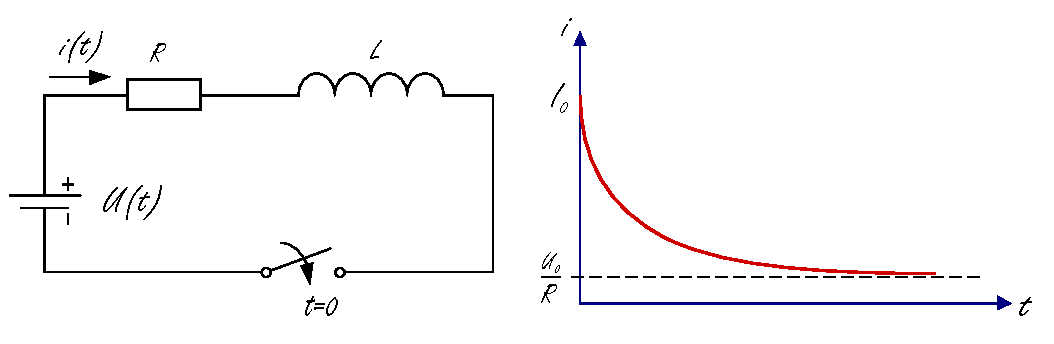
\includegraphics[width=\linewidth]{mai_fig032.pdf}
      \caption{Graf průběhu proudu $i(t)$ po sepnutí spínače v době $t=0$.}
      \label{mai:fig032}
    \end{figure}
%--------------------------------------------------------------------------------------------------- 
%  % !TeX spellcheck = cs_CZ
%---------------------------------------------------------------------------------------------------
% mai2ch05.tex
%---------------------------------------------------------------------------------------------------
\setchaptertoc
\chapter{Řady funkcí}\label{mai:IIchapV}
  Možná si po prolistování obsahu této kapitoly a klademe otázku, proč se máme ještě zabývat
  posloupnostmi a řadami, když jsme jim už popřáli docela dost pozornosti v partii \ref{part:MAI}.
  Cíl této kapitoly je Však trochu jiný, než studovat detaily vlastnosti konvergence či divergence
  číselných posloupnosti a řad. Půjde nám totiž, jak napovídá název kapitoly, o \emph{řady funkcí}.
  S takovým případem jsme se již také v prvním dílu setkali. Vzpomínáte na příklad 2.47. v odstavci
  \ref{mai:IchapIIIsecVIIssecIII} nazvaný \uv{Když diferenciál nestačí?} V něm jsme řešili problém
  přibližné náhrady funkce \(\cos\varphi\) pro malé hodnoty úhlu \(\varphi\) jinou funkcí, snadněji
  vyčíslitelnou. Zjistili jsme, že náhrada lineární funkcí, jaká byla možná v případě sinu, tj.
  \(\sin\varphi = \varphi\), u kosinu nefunguje, neboť diferenciál funkce \(\cos\varphi\) v bodě
  \(\varphi = 0\) je nulový. Poté jsme obecně dospěli k možnosti náhrady funkce \(f(x)\) v okolí
  bodu \(x=a\), Taylorovým polynornem \(n\)-tého stupně (vztah (227)), který představuje prvních \(n
  +1\) členů nekonečně Taylorovy řady
  \begin{strip}
    \begin{equation*}
      f(a)+f'(a)(x-a)+\frac{1}{2!}f''(a)(x-a)^2+\cdots+\frac{1}{n!}f^{(n)}(a)(x-a)^n+\cdots
    \end{equation*}
  \end{strip}
  Předchozí výraz je nekonečným součtem funkcí speciálního typu - mocnin proměnné \((x-a)\)
  násobených konstantami. Obecně bychom takový nekonečný součet mohli zapsat ve tvaru
  \begin{strip}
    \begin{equation*}
      s(x) = c_0 + c_1(x-a)+c_2(x-a)^2 + \cdots + c_n(x-a)^n + \cdots = \sum_{n=0}^\infty c_n(x-a)^n.
    \end{equation*}
  \end{strip}
  Nazýváme jej \emph{nekonečnou mocninnou řadou}. Taylorova řada je tedy speciálním případem
  mocninně řady. Praktický význam Taylorovy řady je nepochybný a vyložili jsme si jej již v odstavci
  \ref{mai:IchapIIIsecVIIssecIII} v partii \ref{part:MAI}. Obecně má nekonečná řada funkcí tvar

  \begin{equation*}
    f_1(x) + f_2(x) + \cdots f_n(x) + \cdots = \sum_{n=0}^\infty f_n(x).
  \end{equation*}

  Další řadu s praktickým významem může přiblížit následující příklad.

  \textbf{Příklad hudební}: Kdyby houslista zahrál na různých houslích stejný tón, mohli bychom si
  všimnout, že každý z nástrojů zní trochu jinak. Tón má stejnou výšku, ale jinou barvu. Čím to je?
  Výška tónu je z fyzikálního hlediska popsána frekvencí \(\nu\), resp. úhlovou frekvencí \(\omega
  = 2\pi f\) (například jednočárkované, komorní \uv{a} má frekvenci \SI{440}{\Hz}). Struna skutečně
  kmitá s touto frekvencí. Závislost výchylky jednotlivých jejích bodů na čase je periodickou funkcí
  času s touto frekvencí. Obecně Však není přesně harmonickým (například sinusovým) signálem, ale
  jeho mírnou modifikací. Z toho důvodu jsou v tónu slyšet i jiné frekvence, ne však jakékoli, ale
  celočíselné násobky původní frekvence, tj. \(2\nu\), \(3\nu\), atd. Barva tónu pak souvisí s
  amplitudami těchto \emph{vyšších harmonických frekvencí}. Matematický můžeme závislost výchylky
  bodu struny v obecnosti zapsat jako
  \begin{equation*}
    a_0 + \sum_{n=1}^\infty[a_n\cos(n\omega t) + b_n\sin(n\omega t)].
  \end{equation*}

  Tato nekonečná řada funkcí se nazývá \emph{Fourierova}. Její význam například ve fyzice,
  elektrotechnice či elektronice je nedozírný - umožňuje rozložit periodický signál na signály
  základní frekvence a vyšších harmonických.

  V souvislosti s Taylorovou řadou jsme si také kladli otázku, jak zjistit, zda takový nekonečný
  součet opravdu \uv{dospěje} k nějaké funkci \(s(x)\), tj. zda řada konverguje. Zmínili jsme se
  také o \uv{obyčejné} \emph{(bodové)} a o \emph{stejnosměrné} konvergenci. Pojem bodové a
  stejnoměrné konvergence má samozřejmě význam nejen pro Taylorovy či obecnější mocninné řady, ale i
  pro řady Fourierovy a jakékoli jiné řady funkcí. A právě o to v této kapitole převážně půjde.
  Abychom však vlastnosti řad funkcí mohli studovat po matematické stránce důkladněji, musíme se
  ještě na chvíli vrátit k posloupnostem a řadám číselným. V Závěru kapitoly si pak podrobněji
  všimneme právě řad mocninných a Fourierových a možností jejich aplikace.

  Vedle své užitečnosti praktické jsou řady docela zábavné a jsou užitečné i tím, že pomáhají tříbit
  matematické myšlení. Výrok Alexandra Ženíška  \uv{... zcela pochopit nekonečné řady znamená začít
  rozumět matematice ...} je možná určitou nadsázkou, ne však příliš velkou.

  \section{Posloupnosti a řady podruhé - čísla}\label{mai:IIchapVsecI}
    V tomto odstavci podrobněji probereme některé vlastnosti číselných posloupnosti a řad, které
    budeme pro zavedení pojmů souvisejících s řadami funkcí a studium jejich vlastností potřebovat.
    Nebudeme se tedy číselnými posloupnostmi a řadami zabývat „pro ně samotné“, ale s cílem jejich
    využití v úvahách o řadách funkcí.

    \subsection{Číselné posloupnosti a jejich konvergence}\label{mai:IIchapVsecIssecI}

%---------------------------------------------------------------------------------------------------
%  % !TeX spellcheck = cs_CZ
%---------------------------------------------------------------------------------------------------
% mai2ch06.tex
%---------------------------------------------------------------------------------------------------
\setchaptertoc
\chapter{Závislosti na více parametrech aneb funkce více proměnných}\label{mai:IIchapVI}
  Skalárními funkcemi jedné reálné proměnné jsme se zabývali velmi podrobně v \ref{part:MAI} dílu.
  Umíme počítat jejich limity v bodech \emph{vlastních} i \emph{nevlastních}, umíme je derivovat i
  integrovat. Totéž dokážeme provádět i s vektorovými funkcemi jedné proměnné. Každý vektor je totiž
  dán svými složkami, takže každá vektorová funkce je zadána tolika „obyčejnými“ skalárními
  funkcemi, kolik má daný vektor složek. S vektorovými funkcemi jedné proměnné jsme pracovali při
  zadávání trajektorií hmotných bodů a výpočtech jejich dalších charakteristik (rychlost, zrychlení,
  křivost trajektorie, apod). Tou jedinou proměnnou byl obvykle čas. Veličiny popisující objekty a
  děje v přírodě, ať již jsou tyto veličiny skaláry či vektory, však většinou závisí na více
  proměnných než jedné. Kromě času bývají typicky závislé na poloze. Vezměme třeba takové gravitační
  pole Země. Na čase sice nezávisí, zato však klesá s druhou mocninou vzdálenosti od středu Země.
  Veličina, která je charakterizuje, je buď vektorová, nebo skalární. Tou vektorovou je
  \emph{gravitační zrychlení} neboli \emph{intenzita} gravitačního pole Země, tou skalární je
  \emph{potenciál},
  \begin{equation*}
    \vec{g}(\vec{r}) = - \kappa\dfrac{M_Z}{r^2}\left(\dfrac{\vec{r}}{r}\right),\,
    V(\vec{r}) = -\kappa\dfrac{M_Z}{r}, \, r\geq R_Z.
  \end{equation*}
  V předchozích vztazích jsou \(M_Z\) a \(R_Z\) hmotnost a poloměr Země, \(\vec{r}\) je polohový
  vektor místa, v němž pole zjištujeme, vzhledem ke středu Země. Skalární i vektorové veličiny
  popisující elektrické a magnetické pole nábojů a proudů, rychlosti elementů proudící kapaliny nebo
  plynu a řada dalších fyzikálních veličin jsou nejen funkcemi času, ale také polohy bodu, v němž je
  počítáme nebo měříme. A stejně jako byly změny funkcí jedné proměnné vyjádřeny pomocí derivací,
  změny změn pomocí druhých derivací, atd., je třeba umět počítat i změny veličin závisejících na
  více proměnných. Mohou samozřejmě nastat situace, kdy se mění jen jedna z proměnných, zatímco
  ostatní zůstávají konstantní. Nejsnáze si takovou situaci představíme například tak, že měříme
  třeba elektrické pole stále ve stejném bodě prostoru, ale běží při tom čas. Pole se v daném bodě s
  časem mění. Nebo naopak v daném okamžiku sledujeme rozdílnost pole v bodech velmi blízkých danému
  bodu. Obecně se samozřejmě mění všechny proměnné a s nimi i hodnoty skalární funkce nebo složky
  vektorové funkce. Jak takové obecné změny co nejvýstižněji popsat, uvidíme právě v této kapitole.
  Setkáme se v ní s \textbf{parciální derivací}, která vystihuje, jak rychle se mění hodnota funkce
  se změnou jedné z proměnných. Dále poznáme obecnější, \textbf{směrovou derivaci}, která popisuje
  rychlost změny funkční hodnoty, mění-li se všechny proměnné, ale tak, že bod, který reprezentuje
  soubor jejich hodnot, se pohybuje v prostoru proměnných po libovolné přímce (nikoli jen po jedné
  souřadnicové ose, jako tomu je u parciálních derivací). A konečně zavedeme pojmy \textbf{úplného
  diferenciálu} a \textbf{Jacobiho zobrazení}, které popisují změnu hodnot skalární či vektorové
  funkce v lineární aproximaci, mění-li se hodnoty proměnných zcela obecně.

  Stejně jako u funkcí jedné proměnné je základem pro definici veličin popisujících rychlost změny
  funkce pojem \textbf{limity}, který úzce souvisí s pojmem \emph{okolí bodů} a obecně i s
  definičními obory funkcí. Pro případ funkcí více proměnných klade požadavek hlubšího pochopení
  pojmu limity větší nároky na soustředěnost a důkladné promýšlení různých situací, než tomu bylo u
  limit funkcí jedné proměnné. Proto se jím zabývá podstatná část poměrně rozsáhlého odstavce
  \ref{mai:IIchapVIsecII} poté, co je v odstavci \ref{mai:IIchapVIsecI} věnována značná pozornost
  různým typům definičních oborů funkcí. Čtenář, který se chce rychle propracovat k praktickým
  výpočtům a spokojí se zatím s intuitivním pochopením pojmu limity funkce více proměnných
  (založeným na dobré znalosti definice a vlastností limit funkcí jedné proměnné), může k nim v
  podstatě rovnou přejít s vědomím, že sice bude umět prakticky provádět různé standardní operace s
  funkcemi více proměnných, ale nebude si pravděpodobně vědět rady s netypickými případy. K
  důkladnému pročtení odstavců \ref{mai:IIchapVIsecI} a \ref{mai:IIchapVIsecII} se může samozřejmě
  vrátit kdykoli.

  \section{Podmonožiny euklidovských prostorů \(\mathcal{R}^n\)}\label{mai:IIchapVIsecI}  
    S definičními obory funkcí jedné proměnné to bylo docela jednoduché. Byly to Většinou intervaly
    - otevřené intervaly nebo jejich sjednocení, uzavřené intervaly, popřípadě intervaly uzavřené
    jen z jedné strany. Také zde figurovala okolí bodů, ať již ryzí, z nichž byl daný bod vyloučen,
    nebo taková, která daný bod obsahovala. Nic složitého tam nebylo. Aby bylo možné funkce
    derivovat, což byla nejčastější operace, kterou jsme prováděli s cílem zjistit, jak rychle se
    funkce mění, nemohly být definiční obory „moc divoké“. Vždy bylo třeba předpokládat, že bod, v
    němž jsme funkci nebo její změnu vyšetřovali, má okolí, ve kterém je funkce přinejmenším
    definována. Pro případ funkcí více proměnných je to podobné, ale bude třeba se definičním oborům
    věnovat trochu podrobněji. Dejme tomu, že nějaká fyzikální, nebo i nefyzikální veličina bude
    záviset na \(n\) proměnných. Každá z nich může nabývat nějakých hodnot. Funkční hodnota naší
    funkce bude tak jednoznačně určena souborem \(n\) hodnot jednotlivých proměnných. Tuto
    \(n\)-tici budeme považovat za bod v prostoru \(\mathcal{R}^n\). S \(n\)-ticemi jsme již
    pracovali v algebře, takže takový popis známe. V algebře jsme však s nimi prováděli algebraické
    operace, sčítání a násobení číslem. Měli jsme tedy v \(\mathcal{R}^n\) zavedenou
    \textbf{algebraickou strukturu}. Pro práci s funkcemi a pro sledování jejich změn \uv{bod od
    bodu} potřebujeme v \(\mathcal{R}^n\) ještě jinou strukturu. Ta je tvořena okolími, podobně jako
    tomu bylo u funkcí jedné proměnné. Taková struktura se nazývá \emph{topologická} a matematická
    disciplína, která se zabývá topologickými strukturami, se jmenuje \textbf{topologie}.

    Topologickými strukturami se nebudeme zabývat v celé obecnosti, i když je to velmi zajímavé.
    Budeme pracovat pouze se speciálním typem, takzvanou \textbf{euklidovskou topologií} v
    \(\mathcal{R}^n\).

    \subsection{Okolí bodů, otevřené a uzavřené množiny}
      S pojmem okolí bodu jsme se setkali hned v dílu \ref{part:MAI}}. Vzpomínáme? Šlo tehdy o okolí
      bodu \(a\) na reálné ose \(\mathcal{R}\). Okolím jsme rozuměli otevřený interval \((a -
      \delta_1,a + \delta_2)\), \(\delta_1, \delta_2 > 0\), ryzím okolím pak množinu \((a -
      \delta_1, a + \delta_2)\backslash{a}\), tj. sjednocení otevřených intervalů \((a - \delta_1,
      a) \cup (a, a + \delta_2)\). Sjednocení jakýchkoli otevřených intervalů jsme později nazývali
      otevřenou množinou, doplňky otevřených množin v \(\mathcal{R}\) byly uzavřené množiny.
      Vybudovali jsme tak na \(\mathcal{R}\) \emph{euklidovskou topologii} (dodatek F prvního dílu).
      Podobná bude situace i ve vícerozměrném případě, tedy v \(\mathcal{R}^n\).

  \section{Skalární funkce více proměnných}\label{mai:IIchapVIsecII}
    V předchozím odstavci jsme si vcelku důkladně připravili pojmy týkající se vhodných definičních
    oborů funkcí více proměnných. Nyní budeme tyto funkce definovat a studovat jejich vlastnosti.
    Obdobně jako u funkcí jedné proměnné půjde o limity, spojitost a derivace. Výhoda důkladné
    přípravy pojmů v předchozím odstavci se ukáže již při budování pojmu limity, zejména v
    nevlastním bodě. Samotnému pojmu limity a s ním úzce spjatého pojmu spojitosti bude věnována
    velká pozornost. Někdo se nad tím může pozastavit: Vždyť jak často se s potřebou výpočtu limit
    setkáváme v praktických příkladech? Málo. Potřebujeme spíše derivovat, integrovat, řešit
    diferenciální rovnice. S příklady na limity se setkáváme ponejvíce v matematických sbírkách, kde
    slouží k procvičení naučené látky. Taková úvaha by byla poněkud krátkozraká. Řada vlastností
    funkcí, a vůbec možnost s nimi rozumně operovat při běžných výpočtech, je založena na
    spojitosti. A spojitost je těsně spjata s pojmem limity. Opět by mohla vzniknout námitka, že
    spojitost přece intuitivně dobře chápeme - spojitá funkce nemá „zpřetrhaný“ graf. Umíme si však
    představit graf funkce tří proměnných? Není to dost dobře možné ani u funkce dvou proměnných,
    je-li složitější, nebo chová-li se v okolí některého bodu „podezřelé“. Limitě tedy potřebujeme
    porozumět, i když její výpočet v praktických příkladech skutečně nebude na „denním pořádku“.
    Abychom porozumění podpořili, budeme se vedle teoretických úvah věnovat i řadě praktických
    příkladů.




%---------------------------------------------------------------------------------------------------
%  % !TeX spellcheck = cs_CZ
%---------------------------------------------------------------------------------------------------
% mai2ch07.tex
%---------------------------------------------------------------------------------------------------
\chapter{Základy variačního počtu pro mechaniku}\label{mai:IIchapVII}
\minitoc

%---------------------------------------------------------------------------------------------------
\printbibliography[title={Seznam literatury}, heading=subbibliography]
\addcontentsline{toc}{section}{Seznam literatury}

}{
% Debug mode OFF
%======= Kapitola: Vícerozměrná algebra aneb lineární algebra podruhé =============================
  % !TeX spellcheck = cs_CZ
%---------------------------------------------------------------------------------------------------
% history_MA.tex
%---------------------------------------------------------------------------------------------------
\chapter{Vícerozměrná linearita aneb lineární algebra podruhé}\label{mai:IIchapI}
\minitoc
  V kapitole \ref{mai:IchapII} dílu \ref{part:MAI} jsme se seznámili s elegantní dámou lineární 
  algebrou. Pomocí jejích pravidel jsme nejen řešili soustavy lineárních rovnic, ale také počítali 
  s maticemi a vektory. Zatímco operace s maticemi, a koneckonců i řešení lineárních rovnic pomocí 
  matic bychom mohli chápat jako užitečnou ekvilibristiku s číselnými soubory, za počítáním s 
  vektory se zdálo být přece jen něco hlubšího a závažnějšího. Vázané vektory pro nás totiž byly 
  orientovanými úsečkami v trojrozměrném euklidovském prostoru, v němž bylo definováno měření délek 
  a úhlů. Volné vektory pak byly množinami stejně velkých a souhlasně rovnoběžných orientovaných 
  úseček. Jednalo se tedy o \emph{geometrické objekty}. Každý vektor byl určen svou velikostí a 
  směrem. Směr byl přitom zadán například pomocí úhlů mezi daným vektorem a vybranými směry, které 
  byly předem pevně zvoleny. Mohli jsme s vektory provádět základní algebraické operace, jimiž jsou 
  sčítání vektorů a násobení vektoru číslem, podle pravidel zavedených pro (v tomto případě 
  řádkové) matice. S vektory v trojrozměrném prostoru jsme mohli velmi pohodlně počítat jako s 
  trojicemi čísel. Na druhé straně jsme vektory vyjadřovali jako lineární kombinace jiných vektorů, 
  tvořících v prostoru všech vektorů \emph{bázi}. Koeficienty lineární kombinace, která 
  představovala zápis daného vektoru ve zvolené bázi, byly jeho \emph{složkami} v této bázi. Při 
  změně báze se změnily složky vektoru, vektor sám však nikoliv. Vektor je stále sám sebou, jen se 
  v různých bázích jinak tváří - projeví se jinou trojicí čísel. Protože se však při změně báze 
  změní složky vektoru přesně definovaným způsobem (vzpomeňte na transformační vztahy), dokážeme 
  jej vždy rozpoznat. Tuto vlastnost, \emph{invarianci vůči volbě báze}, mají všechny geometrické 
  objekty. A je to právě algebra, která nám umožňuje tyto objekty reprezentovat číselnými soubory a 
  také tak s nimi počítat. Jde-li navíc o objekty řídící se lineárními pravidly. jakými jsou 
  například distributivní zákony, je počítání s nimi, v rámci \emph{lineární algebry}, zvláště 
  jednoduché. Oceníme to zejména v prostorech vyšší dimenze, než je náš běžný euklidovský prostor. 
  Při počítání s vektory v trojrozměrném prostoru, kde umíme měřit délky a úhly a kde platí 
  trigonometrická pravidla, bychom se bez rutinních algebraických procedur ještě třeba obešli. Už 
  ale například ve čtyřrozměrném časoprostoru, v němž se odehrávají všechny přírodní jevy a v němž 
  je třeba formulovat fyzikální zákony, však pro měření délek a úhlů platí jiná pravidla, než jsou 
  obvyklá v běžném, tj. trojrozměrném euklidovském, prostoru. Například tam neplatí čtyřrozměrná 
  verze Pythagorovy věty. A někdy je příroda dokonce tak nepřívětivá, že nás nutí pracovat i s 
  prostory vícerozměrnými. Například jedna z velmi účinných teorií pro výklad chování elementárních 
  částic, teorie strum, je založena na geometrii prostoru jedenáctirozměrného. A v takových 
  dimenzích jsme už s jakkoli vynikající geometrickou představivostí v koncích. Tehdy se vděčně 
  obracíme k metodám algebry. V této kapitole, jak její název napovídá, půjde o algebru lineární
  
  \section{Prostory s vektory}
    V kapitole \ref{mai:IchapII} jsme pracovali s číselnými maticemi typu \(m/n\), tj. soubory 
    čísel uspořádaných v \(m\) řádcích a \(n\) sloupcích, a zavedli jsme pro ně operaci součtu a 
    násobení číslem. Zjistili jsme, že pro sčítání matic a násobení matice číslem platí určitá 
    pravidla. (Jejich souhrn je uveden v samém závěru odstavce \ref{mai:IchapIIsecIIIsubIII}. V 
    odstavci \ref{mai:IchapIIsecIV} jsme zase počítali s vektory. Ty měly jednou \emph{konkrétní 
    podobu} řádkových matic s pravidly pro jejich sčítání a násobení číslem, podruhé, v 
    trojrozměrném prostoru, naopak \emph{konkrétní podobu} orientovaných úseček, resp. množin, 
    které byly orientovanými úsečkami vytvořeny, generovány. Zavedli jsme tenkrát konkrétní způsob 
    sčítání vektorů a násobení vektoru číslem pomocí geometrických operací. Součet dvou vektorů 
    \(\vec{u}\) a \(\vec{v}\) znamenal, že jsme podle zcela určitého pravidla, pravidla 
    vektorového rovnoběžníka přiřadili uspořádané dvojici \([\vec{u},\vec{v}]\) třetí vektor 
    \(\vec{u} + \vec{v}\), násobek vektoru a čísla byl opět vektor \(\alpha\vec{u}\), který jsme 
    přiřadili dvojici \([\alpha,\vec{u}]\) tvořené číslem a vektorem. Uvedli jsem, že pravidla pro 
    tyto \emph{geometrické} operace jsou shodná s pravidly pro počítání s maticemi a lze je dokázat 
    i geometrickými postupy. Množinu volných vektorů generovaných orientovanými úsečkami spolu s 
    uvedenými dvěma operacemi jsme nazvali \textbf{vektorovým prostorem}. Šlo tedy o zcela odlišné 
    množiny základních objektů a zcela odlišným způsobem definované operace, pro které se však dala 
    dokázat tatáž pravidla. Nyní se podíváme na problém definice vektorového prostoru obecněji a 
    poněkud \uv{opačně}. Budeme pracovat s \emph{nosnou množinou} \(V\), a přitom nebude podstatné, 
    jak konkrétně vypadají její prvky. Ani je nebudeme označovat šipkami (u šipek ze zvyku 
    zůstaneme pouze v případě orientovaných úseček v \(\mathbb{R}^1\), \(\mathbb{R}^2\) a 
    \(\mathbb{R}^3\), nebo vektorů s fyzikálním významem). Dále přibereme do hry množinu všech 
    komplexních čísel \(\mathbb{C}\), popřípadě jen množinu všech reálných čísel \(\mathbb{R}\) a 
    definujeme dvě operace (\emph{zobrazení}):
    \begin{equation}\label{mai:eq046}
      V \times V \ni [a,b] \longrightarrow c\in V,\qquad 
      \mathbb{C}\times V\ni[\alpha,a] \longrightarrow d\in V.
    \end{equation}
    Prvek \(c\) nazýváme \emph{součet} prvků \(a\) a \(b\) a značíme jej \(c = a + b\) prvek \(d\) 
    je \(\alpha\)-\emph{násobek} prvku \(a\) a značíme \(d = \alpha a\). Zobrazení uvedená ve 
    vztazích (\ref{mai:eq046}) však nebudou moci být úplně libovolná. Budeme požadovat, aby měla 
    určité vlastnosti, konkrétně ty, které jsou uvedeny pro matice na konci odstavce 
    \ref{mai:IchapIIsecIIIsubIII}. Teprve pak řekneme, že množina \(V\) spolu s operacemi 
    (\ref{mai:eq046}) splňujícími potřebné požadavky je vektorovým prostorem. Vidíme, že takto naše 
    uvažování výrazně posuneme na abstraktní úroveň. Bude lhostejné, co jsou prvky nosné množiny, 
    bude nepodstatné, jak konkrétně jsou definovány operace sčítání prvků a násobení prvku číslem. 
    Důležité bude jen to, aby abstraktní operace s abstraktními prvky splňovaly konkrétní pravidla. 
    Než však k definici vektorového prostoru přistoupíme, všimneme si ještě některých jiných 
    struktur s jednou nebo dvěma operacemi, které samy do oblasti lineární algebry nepatří, ale 
    mohou být užitečné pro definici vektorového prostoru, popřípadě mají významné fyzikální 
    aplikace.
      
      \subsection{Algebraické struktury s jednou operací, hlavně grupy}
        Při zavádění operací s vektory jsme zcela automaticky využívali toho, že umíme počítat s 
        reálnými, popřípadě i s komplexními čísly. Skutečnost, že čísla umíme sčítat, násobit a 
        provádět s nimi řadu dalších operací, považujeme za tak přirozenou a samozřejmou, že nad ní 
        vůbec nepřemýšlíme. Již samotné operace sčítání a násobení vytvářejí na množině čísel velmi 
        bohatou \textbf{algebraickou strukturu}. Tento pojem si nyní přiblížíme. 
        
        Algebraickou strukturu s jednou operací získáme, vezmeme-li v úvahu první ze zobrazení 
        (\ref{mai:eq046}), nosnou množinu označíme tentokrát podle zvyku \(G\):
        \begin{equation}\label{mai:eq047}
          G \times G \ni [a,b] \longrightarrow a + b \in G, \qquad \text{nebo} \qquad
          G \times G \ni [a,b] \longrightarrow a \cdot b \in G.
        \end{equation}
        Pokud použijeme první možnosti označení této operace, hovoříme o operaci \emph{sčítání} a 
        \emph{aditivní} struktuře, v případě druhé možnosti o operaci \emph{násobení} a 
        \emph{multiplikativní} struktuře. Toto terminologické rozlišení nemá obecně žádný hlubší 
        význam. Je spíše otázkou zvyklosti a souvisí především s algebraickou strukturou číselných 
        množin, kterou běžně používáme, aniž o ní přemýšlíme (čísla sčítá a násobí školák, 
        obchodník i účetní a o nějaké abstraktní struktuře nic netuší).
        
        Zobrazení (\ref{mai:eq047}) samo o sobě, aniž na ně klademe další požadavky (podstatné je 
        pouze to, že dvěma prvkům nosné množiny přiřadí prvek \emph{téže množiny}), definuje 
        nejjednodušší algebraickou strukturu s jednou operací, zvanou \textbf{grupoid}. Grupoid 
        není pro fyzikální aplikace příliš užitečný, ale je základem pro konstrukci zajímavějších a 
        užitečnějších struktur. Přidáme-li k definici grupoidu požadavek \emph{asociativity} 
        zobrazení \(G \times G \ni [a, b] \longrightarrow a + b \in G\) (nebo \(G \times G \ni [a, 
        b] \longrightarrow a \cdot b \in G\))
        \begin{equation}\label{mai:eq048}
          (a+b) + c = a + (b + c),\qquad \text{nebo}\qquad (a\cdot b) \cdot c = a \cdot (b \cdot c)
        \end{equation}
        pro libovolné prvky \(a, b, c \in G\), stane se množina \(G\) spolu s operací „\(+\)“, nebo 
        „-“ \textbf{pologrupou}. I pologrupa je z hlediska fyzikálních aplikací poněkud chudá, 
        další požadavek na zobrazení (\ref{mai:eq047}) z ní však již učiní strukturu v matematice i 
        fyzice nepostradatelnou, grupu. Pologrupa, ve které existuje prvek \(0_G\in G\) a současně 
        ke každému prvku \(a \in G\) existuje prvek \((-a) \in G\) tak, že platí
        \begin{equation}\label{mai:eq049}
          a + 0_G = 0_G + a = a,\qquad a + (-a) = (-a) + a = 0_G,
        \end{equation}
        se nazývá \textbf{aditivní grupou}. Prvek \(0_G\) je univerzální pro celou grupu (žádný 
        jiný s touto vlastností v grupě \(G\) není) a nazývá se \emph{neutrální prvek grupy} neboli 
        \textbf{nula}, prvek \((-a)\) je \textbf{opačný} k prvku \(a\). Pro dané \(a\) je určen 
        jednoznačně. V případě operace násobení mají vlastnosti \ref{mai:eq049} tvar
        \begin{equation}\label{mai:eq050}
          a \cdot e_G = e_G \cdot a = a,\qquad a \cdot a^{-1} = a^{-1} \cdot a = e_G,
        \end{equation}
        a \(G\) se nazývá \textbf{multiplikativní grupou}. Prvek \(e_G\) je opět univerzální pro 
        celou grupu a nazývá se \textbf{neutrální} prvek grupy, neboli \emph{jednička}, prvek 
        \(a^{-1}\) je \textbf{inverzní} k prvku \(a\).
        
        Každá operace \ref{mai:eq047} v množině \(G\), která splňuje vztahy asociativity 
        \ref{mai:eq048} a vztahy specifikující nulu a opačný prvek, nebo jedničku a inverzní prvek 
        typu \ref{mai:eq049}, nebo \ref{mai:eq050}, představuje \emph{grupovou operaci} bez ohledu 
        na to, podobá-li se spíše sčítání, nebo spíše násobení, či dokonce něčemu jinému, například 
        skládání zobrazení. Má-li grupa konečný počet prvků, nazývá se tento počet jejím 
        \emph{řádem}.

        %---------------------------------------------------------------
        \input{../src/MAI/exam/exam046.tex}
        %---------------------------------------------------------------
        
        V úvodu odstavce jsme se zmínili o tom, že množiny reálných a komplexních čísel získají 
        zavedením běžných operací sčítání a násobení jistou algebraickou strukturu. Všimněme si 
        jich nyní podrobněji. 
        
        %---------------------------------------------------------------
        \input{../src/MAI/exam/exam047.tex}
        %---------------------------------------------------------------
        
        %---------------------------------------------------------------
        \input{../src/MAI/exam/exam048.tex}
        %---------------------------------------------------------------
        
        O podmnožině \(H \subset C\) grupy \(G\) s operací sčítání nebo násobení zúženou na \(H\), 
        která je sama grupou, hovoříme jako o \textbf{podgrupě} grupy \(G\). Například množina 
        reálných čísel zapsaných ve tvaru \(z = [a, 0]\) se sčítáním je podgrupou množiny 
        komplexních čísel. Koho grupy nebaví a chce se rychle prokousat k vektorovým prostorům, 
        které jsou koneckonců hlavní náplní našeho příběhu o lineární algebře, může zbytek tohoto 
        odstavce přeskočit. Ale byla by to škoda, grupy jsou opravdu zajímavé.

        %---------------------------------------------------------------
        \input{../src/MAI/exam/exam049.tex}
        %---------------------------------------------------------------
        
        %---------------------------------------------------------------
        \input{../src/MAI/exam/exam050.tex}
        %---------------------------------------------------------------

        %---------------------------------------------------------------
        \input{../src/MAI/exam/exam051.tex}
        %---------------------------------------------------------------
        
        Operace sčítání nebo násobení si umíme velmi dobře představit, provádíme-li je standardním 
        způsobem s čísly. Definice algebraických struktur jsou však obecné a zahrnují i jiné 
        možnosti. Představme si například krychli, se kterou provádíme \emph{operace symetrie}. 
        Jsou to všechna taková přemístění krychle z počáteční do koncové polohy, která \uv{se 
        nepoznají}. Znamená to, že krychle vypadá v koncové poloze stejně jako ve výchozí. Pokud
        bychom při přemísťování zavřeli oči, nepoznali bychom že někdo mezitím s krychlí hýbal. 
        Přemístění jsou několikerých typů a definují \textbf{prvky symetrie} krychle. Abychom si je 
        mohli názorně ukázat na obrázcích, označíme vrcholy, popřípadě jiné důležité body krychle 
        písmeny. V některých ukázkách také použijeme hrací kostku. Prvky symetrie krychle můžeme 
        roztřídit do následujících typů:
        \begin{itemize}
          \item \textbf{zrcadlení vzhledem k rovině symetrie} - existuje rovina, jejíž body 
                zůstávají při přemístění v klidu,
          \item \textbf{rotace kolem osy symetrie} - existuje přímka (osa), jejíž body zůstávají 
                při přemístění v klidu,
          \item \textbf{středová inverze} - existuje právě jeden bod (střed inverze), který při 
                přemístění zůstává v klidu,
          \item \textbf{identita} - přemístění do téže polohy, v klidu jsou všechny body krychle
        \end{itemize}
         

%---------------------------------------------------------------------------------------------------
\printbibliography[title={Seznam literatury}, heading=subbibliography]
\addcontentsline{toc}{section}{Seznam literatury}
%======= Kapitola: Souřadnicové soustavy obvyklejší i méně obvyklé ================================
  % !TeX spellcheck = cs_CZ
%---------------------------------------------------------------------------------------------------
% mai2ch02.tex
%---------------------------------------------------------------------------------------------------
\chapter{Souřadnicové soustavy obvyklejší i méně obvyklé}\label{mai:IIchapII}
\minitoc

%---------------------------------------------------------------------------------------------------
\printbibliography[title={Seznam literatury}, heading=subbibliography]
\addcontentsline{toc}{section}{Seznam literatury}
%======= Kapitola: Linearita v aplikacích aneb lineární algebra do třetice ========================
  % !TeX spellcheck = cs_CZ
%---------------------------------------------------------------------------------------------------
% mai2ch03.tex
%---------------------------------------------------------------------------------------------------
\chapter{Linearita v aplikacích aneb lineární algebra do třetice}\label{mai:IIchapIII}
\minitoc

%---------------------------------------------------------------------------------------------------
\printbibliography[title={Seznam literatury}, heading=subbibliography]
\addcontentsline{toc}{section}{Seznam literatury}
%======= Kapitola: Obyčejné diferenciální rovnice =================================================
  % !TeX spellcheck = cs_CZ
%---------------------------------------------------------------------------------------------------
% mai2ch04.tex
%---------------------------------------------------------------------------------------------------
\setchaptertoc
\chapter{Obyčejné diferenciální rovnice}\label{mai:IIchapIV}

  V partii \ref{part:MAI} jsme se seznámili s funkcemi, o jejich užitečnosti nepochybujeme, neboť
  jsme se již přesvědčili, že se s nimi setkáváme takřka na každém kroku. Vyjadřují totiž
  jednoduchým způsobem vzájemnou souvislost veličin, a nejen fyzikálních. Známe-li například funkci
  vyjadřující závislost polohy tělesa na čase, můžeme zjistit, kde těleso v daném okamžiku bylo, je,
  nebo bude. Známe-li funkce, které popisuji časový vývoj cen a platů, můžeme snadno zjistit, zda za
  stejný peníz, za který dnes dostaneme deset housek, koupíme za rok dvacet, nebo jen dvě. Příroda,
  a ani ekonomika či politika, však nejsou natolik průhledné, aby nám takové závislosti předestřely
  přímo. Poskytují pouze informace o jejich změnách, a to ještě ukryté ve speciálních rovnicích,
  zvaných \emph{diferenciální}. Jde-li o neznámou reálnou funkci nebo soubor funkcí závislých na
  jedné reálné proměnné, třeba na čase, hovoříme o obyčejných diferenciálních rovnicích. Přesněji
  řečeno, diferenciální rovnice vyjadřuje matematickou formou zákon platný pro hledanou funkci a
  její derivace prvního nebo i vyšších řádů. Takovou funkcí času může být například i množství látky
  při chemických reakcích, mohutnost populace živočichů, kurz eura, cena akcií na burze, rychlost
  pohybu těles, teplota atd. Ve fyzice a chemii jsou diferenciální rovnice dány fyzikálními či
  chemickými zákony, v ekonomii nebo biologii se objevují v různých modelech, odpovídajících více či
  méně skutečnosti. Uveďme si několik příkladů, na nichž si vysvětlíme základní terminologii, která
  je s problematikou diferenciálních rovnic spojena.
  
  Doplňková literatura pro studium této partie je například: \cite[s.~217]{Musilova2012MA2} a 
  \cite[s.~426]{Brabec1989}. Pro procvičení elementárních metod řešení konkrétních rovnic je vhodná 
  sbírka řešených příkladů \cite[s.~348]{Jirasek1989}.
  
  %--Příklad s hlemýžděm------------------------------------------
    \input{../src/MAI/exam/exam084.tex}
  %---------------------------------------------------------------
  Ve většině příkladů, se kterými se setkáme, bude mít počáteční úloha právě jedno řešení, jak tomu
  je v případě hlemýždě. Jestliže je nějaká funkce, definovaná na intervalu \((a,b)\), řešením
  počáteční úlohy, pak každá funkce, kterou vytvoříme zúžením původního řešení na „menší“ interval,
  bude opět rovnici splňovat. My však máme \emph{„právě jedním řešením“} na mysli tzv. \textbf{úplné
  řešení}, tj. takové, které není zúžením žádného jiného, a tak řešení lišící se pouze definičním
  oborem nebudeme považovat za odlišná. Jak uvidíme později, vyskytnou se však také příklady, kdy
  počáteční úloha nemá žádné řešení, nebo jich má naopak nekonečně mnoho.

  %--Příklad s koupelnou------------------------------------------
    \input{../src/MAI/exam/exam085.tex}
  %---------------------------------------------------------------
  
  \begin{note}
    „Větrací“ rovnice, diskutovaná v předchozím případě, se ve fyzice objevuje poměrně často. Někdy
    je nazývána lineárním diferenciálním zákonem. Narazíme na ni vždy, když je rychlost změny nějaké
    veličiny (její první derivace) přímo úměrná veličině samotné. Tak například při rozpadu
    radioaktivních jader dospějeme k rovnici \(\der{N(t)}{t} = -\lambda N(t)\), kde \(N(t)\) je
    počet radioaktivních jader ve vzorku v okamžiku \(t\) a \(\lambda\) je \textbf{rozpadová
    konstanta}. Při zkoumání absorpce rentgenového záření v látce získáme rovnici \(\der{I(x)}{x} =
    -\mu I(x)\), kde \(I(x)\) je intenzita v hloubce \(x\) pod povrchem a \(\mu\) je lineární
    \textbf{koeficient absorpce}. S oběma příklady jsme se již setkali v partii \ref{part:MAI}.
    Zkusme si vzpomenout na další příklady lineárních diferenciálních zákonů.
  \end{note}

  %--Příklad o sáňkování------------------------------------------
    \input{../src/MAI/exam/exam086.tex}
  %---------------------------------------------------------------
  \begin{note}
    Zamysleme se také nad tím, jak jsme z vyjádření funkce \(v(t)\) pomocí exponenciálních funkcí 
    získali elegantnější výraz s hyperbolickou tangentou. Pro připomenutí hyperbolických funkcí se 
    můžeme vrátit k odstavci 2.1.8 partie \ref{part:MAI}.
  \end{note}
  
  Na uvedených příkladech jsme se mohli přesvědčit, že porozumění některým realistickým dějům
  vyžaduje umět sestavit a řešit diferenciální rovnice. Problémy, se kterými se v životě setkáváme,
  však obvykle vedou k rovnicím mnohem komplikovanějším. Proto často používáme aproximací a skutečný
  svět si poněkud „idealizujeme". Tak například v úloze s koupelnou jsme předpokládali, že vzduch v
  místnosti je vždy dokonale promíchán, v úloze o sáňkování jsme pro odporovou sílu použili pouze
  přibližný zákon a zanedbali třecí sílu. Často se setkáme s rovnicemi, které dokážeme řešit pouze
  numerickými metodami za pomoci počítačů. Aproximativní přístupy tedy mohou vstupovat do popisu
  vývoje reálných systémů pomocí diferenciálních rovnic dvojím způsobem. Poprvé již při samotném
  sestavení diferenciálních rovnic, podruhé při jejich řešení.
  
  V této kapitole se budeme věnovat některým typickým situacím, kdy je možné získat řešení
  diferenciálních rovnic analytickými metodami, zjednodušeně řečeno „tužkou na papíře“. Proč se
  omezujeme na některé typické situace“? Protože problematika diferenciálních rovnic obsahuje ještě
  další úskalí. Řečeno s mírnou nadsázkou, existuje totiž nepřeberné množství různých typů
  diferenciálních rovnic, dokonce už v případě rovnic prvního řádu, které při řešení vyžadují takřka
  \uv{individuální přístup}. I když samozřejmě v teorii diferenciálních rovnic existuje řada
  obecných výsledků společných určité širší skupině diferenciálních rovnic, není možné formulovat
  nějaký \uv{univerzální} postup, který by vedl k řešení kterékoli z nich. V praxi je proto třeba
  naučit se rozpoznat jednotlivé typy obyčejných diferenciálních rovnic a zvolit pro jejich řešení
  vhodnou metodu. Ne nadarmo se proto textům o diferenciálních rovnicích říká „kuchařky“, aniž by to
  mělo hanlivý nádech. (Vznešenější slovo pro „kuchařku“ je „příručka“. Pokud jde o problematiku
  obyčejných diferenciálních rovnic, je takovou moderní příručkou kniha \cite{PolyaninZaitsev},
  která na více než osmi stech stran obsahuje přes 6 200 rovnic s řešeními!
  
  \twocolumn[\section{Diferenicální rovnice vyskytující se kolem nás}\label{mai:IIchapIVsecI}]
    V tomto odstavci jsou zařazeny motivační příklady ukazující, že diferenciální rovnice se
    skutečně objevují v různých vědních oborech. Rovnice jsou většinou uvedeny bez řešení, ale jsou
    doplněny alespoň odkazy ve kterých lze najít mnohem více informací, které jdou za rámec této
    partie o obyčených diferenciálních rovnicích. Stejně jako v předchozích příklad, řada
    fyzikálních principů má tvar výroku, resp. vztahu mezi jistými veličinami (funkcemi) a jejich
    změnami, vztaženými ke zvoleným nezávisle proměnným (pa\-ra\-me\-trům) (\emph{čas, souřadnice}).
    Je to přirozené, neboť (\emph{okamžité}, či \emph{okální}) změny se nejlépe vystihují pomocí
    derivací. Takový zákon má pak charakter vztahu mezi uvažovanými veličinami a jejich derivacemi. 
    
    \begin{mdframed}[style=mdnote] 
      V matematických textech o obyčejných diferenciálních rovnicích se označuje nezávisle proměnná 
      obvykle symbolem \(x\), neznámá funkce \(y = y(x)\) nebo \(y = f(x)\) a její derivace 
      čárkami, tj. \(y'(x)\), \(y''(x)\) nebo \(y' = f'(x)\), \(y" = f''(x)\) atd. V mnoha 
      fyzikálních i jiných praktických situacích však bývá nezávisle proměnnou čas \(t\) a hledáme 
      závislost veličiny \(x = x(t)\) na čase. Tohoto značení budeme velmi často používat, přičemž 
      první, resp. druhou derivaci funkce \(x(t)\) budeme podle zvyklosti zavedené ve fyzice 
      vyznačovat pomocí tečky, resp. dvou teček nad symbolem \(x\),
      \begin{equation*}
        \dot{x}(t) = \der{x}{t}, \qquad \ddot{x}(t) = \dder{x}{t}.
      \end{equation*}
      Pro větší přehlednost zápisu budeme často vynechávat argument \(t\) v závorce, \(\dot{x} = 
      \dot{x}(t)\). Nebudeli řečeno jinak, předpokládáme, že všechny funkce jsou spojité, případně 
      i diferencovatelné na celém svém definičním oboru nebo alespoň na jistém oboru, který je jeho 
      podmnožinou. Při práci s podílem funkcí budeme automaticky předpokládat, že jmenovatelem je 
      funkce, která je nenulová ve všech bodech uvažovaného intervalu.      
    \end{mdframed}
    
    \subsection{Diferenciální rovnice v mechanice}
      \textbf{Druhý Newtonův pohybový} zákon pro hmotný bod, který nabývá tvaru
      \begin{equation*}
        m\vec{a} = \vec{F}
      \end{equation*}
      skrývá soustavou \emph{tří diferenciálních rovnic druhého řádu}. Složky zrychlení \(\vec{a}(t)
      = (a_x(t), a_y(t), a_z(t)) = (\ddot{x}(t), \ddot{y}(t), \ddot{z}(t))\) jsou totiž druhými
      derivacemi složek polohového vektoru \(\vec{r}(t) = (x(t), y(t), z(t))\) podle času, vektor
      výslednice sil působících na hmotný bod je obecně funkcí jeho polohy a rychlosti, a často také
      explicitní funkcí času. Platí tedy \(\vec{F} = \vec{F}(\vec{r},\vec{v},t)\). Rozepíšeme-li
      druhý Newtonův zákon do složek, dostaneme
      \begin{align*}
        m\ddot{x} & = F_x(x,y,z,\dot{x}, \dot{y}, \dot{z}, t),        \\
        m\ddot{y} & = F_y(x,y,z,\dot{x}, \dot{y}, \dot{z}, t),        \\
        m\ddot{z} & = F_z(x,y,z,\dot{x}, \dot{y}, \dot{z}, t)
      \end{align*}
      Řešením této soustavy je časová závislost \(\vec{r} = (x(t), y(t), z(t))\) polohového vektoru
      hmotného bodu. Je \emph{parametrickým vyjádřenim křivky}, po které se hmotný bod v prostoru
      pohybuje, nazývá se \emph{trajektorií} pohybu.Zadáním počáteční polohy \(\vec{r}_0 = (x(t_0),
      y(t_0), z(t_0))\) a počáteční rychlosti \(v_0 = (\dot{x}(t_0), \dot{y}(t_0), \dot{z}(t_0))\)
      například v okamžiku \(t_0 = 0\) ziskáme \textbf{počáteční úlohu}. (Soustava obsahuje druhé
      derivace neznámých funkci \(x(t)\), \(y(t)\) a \(z(t)\), proto potřebujeme dvě podminky pro
      každou z nich.) 
      
      Zapišme takový příklad konkrétní soustavy: Na planetu o hmotnosti \(m\) působí Slunce o
      hmotnosti \(M\) silou \(\vec{F}_g\) danou Newtonovým gravitačním zákonem. Tentokrát však jde o
      tzv. „silový zákon", který popisuje gravitační interakci planety a Slunce. Umístíme-li počátek
      soustavy souřadnic do hmotného bodu představujícího Slunce, platí
      \begin{equation*}
        \vec{F}_g = - \dfrac{\kappa mM\vec{r}}{r^3} 
                  = - \dfrac{\kappa mM}{(x^2+y^2+z^2)^{\frac{3}{2}}}(x, y, z)
      \end{equation*}
      kde \(\kappa =  \SI{6.67e-11}{\N\m^2\kg^{-2}}\) je jednou z univerzálních fyzikálních
      konstant, nazývanou gravitační konstanta. Za předpokladu, že zanedbáme pohyb Slunce a
      gravitační působení planet a ostatních těles, má soustava rovnic vyjadřující druhý Newtonův
      zákon pro planetu tvar 
      \begin{subequations}
        \begin{empheq}[box=\widefbox]{align*}
          m\ddot{x} & = - \kappa mM \dfrac{x}{(x^2+y^2+z^2)^{\frac{3}{2}}},        \\
          m\ddot{y} & = - \kappa mM \dfrac{y}{(x^2+y^2+z^2)^{\frac{3}{2}}},        \\
          m\ddot{z} & = - \kappa mM \dfrac{z}{(x^2+y^2+z^2)^{\frac{3}{2}}}
        \end{empheq}
      \end{subequations}

      Nalézt řešení této soustavy znamená „vydolovat" z ní, při daných počátečních podmínkách,
      konkrétní tvar funkcí \(x(t)\), \(y(t)\) a \(z(t)\). Zrovna tato úloha není příliš jednoduchá.
      Postup při jejím řešení, který lze usnadnit použitím fyzikálních „triků”, si ukážeme později. 

    \subsection{Diferenciální rovnice v chemii}
      Uvažujme o chemické reakci, při které se ze dvou látek \(A\) a \(B\) syntetizuje látka \(C\).
      Na jeden gram výsledné látky je zapotřebí \(p\) gramů látky \(A\) a \(1 - p\) gramů látky
      \(B\). Smícháme \(a\) gramů látky \(A\) s \(b\) gramy látky \(B\). Na počátku je hmotnost
      látky \(C\) nulová, její hodnotu v čase \(t\) označíme \(x(t)\). Rychlost chemické reakce, tj.
      změna hmotnosti látky \(C\) s časem, je v rámci nejjednoduššího modelu rovna veličině \((a -
      px) (b - (1 - p)x)\). Vidíme, že při zvětšujícím se množství výsledné látky bude rychlost
      reakce klesat. Ve výsledku se projeví i to, jaké množství výchozích látek smícháme, resp. jak
      se jejich poměr \(\dfrac{a}{b}\) bude lišit od „ideálního" poměru \(\dfrac{p}{1-p}\). Rovnice
      popisující reakci je diferenciální rovnicí prvního řádu pro časovou závislost \(x(t)\)
      hmotnosti látky \(C\)
      \begin{equation*}
        \boxed{\dot{x} = (a - px)(b - (1-p)x)}\, ,
      \end{equation*}
      s počáteční podmínkou \(x(0) = 0\). K této rovnici se ještě hodí poznamenat, že je příkladem
      (i když velmi speciálním) známé \textbf{Riccatiovy rovnice}, která má uplatnění i v
      praktických disciplínách, například v elektrotechnice nebo v oblasti automatického řízení.
      Přestože má nevinně vypadající obecný tvar \(x(t) = h(t) + f(t)x +g(t)x^2\), \(h(t) \neq 0\),
      \(g(t) \neq 0\), je tak trochu „zrádná“. Její řešení se totiž nemusí podařit zapsat pomocí
      elementárních funkcí. 
    
    \subsection{Diferenciální rovnice v biologii}
      Uvažujme o vlkovi a zajíci. Předpokládáme-li, že zajíc má vždycky co žrát (trávy je všude
      dost), bude nárůst počtu zajíců úměrný jejich okamžitému počtu (čím více je zajíců, tím více
      dalších se narodí). Zároveň jsou zajíci požíráni vlky a jejich úbytek je úměrný jak počtu
      vlků, tak počtu jich samých (čím více je zajíců, tím více jich každý věčně hladový vlk chytí a
      sežere, čím více je vlků, tím více zajíců sežerou). Co se vlků týče, ty nikdo nesežere, ale
      budou umírat hladem, jestliže nebude dostatek zajíců. Nárůst počtu vlků je tedy úměrný jak
      počtu vlků, tak počtu zajíců, kdežto úbytek je úměrný pouze počtu vlků. Získáváme soustavu
      dvou diferenciálních rovnic

      \begin{subequations}
        \begin{empheq}[box=\widefbox]{align*}
          \dot{z} &= \alpha z - \beta zv,     \\
          \dot{v} &= \gamma v + \delta zv,
        \end{empheq}
      \end{subequations}

      kde funkce \(z(t)\) resp. \(v(t)\) vyjadřují časovou závislost počtu zajíců, resp. vlků.
      Konstanty \(\alpha\), \(\beta\), \(\gamma\), \(\delta\) lze určit dlouhodobým pozorováním. 
      \begin{note}
        Pokud někoho napadlo, že zajíci i vlci se také rodí i umírají „přirozenou cestou“, má
        pravdu. Tato skutečnost je v našem jednoduchém modelu zahrnuta. Přirozený přírůstek či
        úbytek zajíců i vlků je také úměrný jejich okamžitému počtu, a je tedy respektován
        empirickými hodnotami \(\alpha\), \(\gamma\).
      \end{note}
      
      Tato soustava nelineárních diferenciálních rovnic se nazývá \textbf{Lotkova-Volterrova}. 
      Existence triviálního, tj. identicky nulového řešení, odpovídajícího situaci, kdy žádný zajíc 
      ani vlk neexistují je zřejmá na první pohled. Rovnice má však také netriviální řešení, které 
      si později ukážeme. 
      
      Obdobným příkladem z biologie je situace, kdy diferenciální rovnice popisuje časový průběh
      vývoje jedné populace. Řekněme, že jde o populaci bakterií, jejíž velikost v závislosti na
      čase je dána funkcí \(P(t)\). Při vývoji hrají roli dva nezávislé faktory, jeden způsobuje
      růst populace a druhý souvisí s omezeními danými prostředím. Představme si situaci tak, že bez
      omezujících vlivů prostředí by populace narůstala podle lineárního diferenciálního zákona, tj.
      derivace \(\dot{P}(t)\) hledané funkce \(P(t)\) by byla v každém okamžiku přímo úměrná hodnotě
      \(P(t)\), konstantu úměrnosti \(R\) nazvěme \emph{faktorem růstu}. Okolní prostředí však
      znemožňuje neomezené narůstání funkčních hodnot \(P(t)\). Růst je totiž modifikován tak, že se
      anuluje v okamžiku, kdy je dosaženo \uv{povolené} hodnoty \(P_{max} = K\), tj. když hodnota
      funkce \(P(t)\) dosáhne úrovně \emph{nosné kapacity} \(K\). Odpovídající diferenciální rovnice
      je opět nelineární a zní
      \begin{equation*}
        \boxed{\dot{P} = RP\left(1 - \dfrac{P}{K}\right)}
      \end{equation*}
      Nazýváme ji \textbf{logistickou rovnicí} a rovněž se ji naučíme vyřešit.
      
    \subsection{Diferenciální rovnice v ekonomii}
      V novinách se občas objeví zpráva, že míra inflace klesá. Od obyvatelstva se očekává, že to
      bude interpretovat jako pozitivní jev v naší ekonomice. Je tomu tak skutečně? Označme jako
      \(h(t)\) funkci popisující vhodným způsobem „kupní sílu“ koruny v závislosti na čase (název
      funkce \(h(t)\) jsme dali do uvozovek, neboť skutečná situace je z pohledu ekonomiky
      složitější a nezávisí pouze na inflaci). Její záporně vzatou derivaci \(\mu = -\der{h(t)}{t} =
      -h\) nazýváme mírou inflace. Proč znaménko minus? Pokud je funkce \(h(t)\) klesající, tj.
      kupní síla peněz se snižuje, je její derivace záporná. O míře inflace se však při znehodnocení
      kupní síly hovoří jako o kladné veličině. Jestliže míra inflace podle novinářů klesá, je její
      derivace \(\mu(t)\) záporná. Předpokládejme pro jednoduchost, že velikost této derivace je
      stálá. Druhá derivace neznámé funkce \(h(t)\) je tedy kladná konstantní hodnota, označme ji
      třeba \(A\), \(A > 0\). Dostáváme velmi jednoduchou diferenciální rovnici
      \begin{equation*}
        \ddot{h} = A.
      \end{equation*}
      kterou můžeme okamžitě vyřešit. Vyhovují jí všechny funkce tvaru
      \begin{align*}
        h(t) &= \dfrac{1}{2}At^2 -\mu_1(t) + h_0 \\
             &= \dfrac{A}{2}\left(t-\dfrac{\mu_1}{A}\right)^2+\left(h_0-\dfrac{\mu_1^2}{2A}\right), 
      \end{align*}
      přičemž význam konstant \(h_0\) a \(\mu_1\) je takový, že \(h_0 = h(0) > 0\) představuje
      počáteční kupní sílu peněz, \(\mu_1 = -\dot{h}(0) = \mu(0) > 0\) je počáteční míra inflace.
      Grafem řešení rovnice je parabola, která má konvexní průběh, neboť \(\ddot{h} = A > 0\). Její
      vrchol (minimum) odpovídá bodu \(t_0 = \mu_1/A\). V tomto okamžiku dosáhne míra inflace nulové
      hodnoty. V časovém intervalu \([0, t_0]\) tedy kupní síla našeho platu i přes optimisticky
      vypadající novinovou zprávu stále klesá, tento pokles se však postupně zmírňuje a v okamžiku
      \(t_0\) je nulový - od tohoto okamžiku již neplatí původní tvrzení, že míra inflace klesá
      (nemůže být totiž záporná, nešlo by o inflaci). Interval \([0, t_0]\) je tedy oborem, na
      kterém je řešení diferenciální rovnice pro daný případ relevantní, i když řešení rovnice
      existuje na celé reálné ose.
      
      Jiný ekonomický model může představovat ,spojité" úročení vkladu v bance. Předpokládejme, že
      úrok činí konstantní část \(k\), obvykle několik procent, okamžité výše vkladu. Je-li výše
      vkladu popsána funkcí \(x(t)\), pak
      \begin{equation*}
        \dot{x} = kx.
      \end{equation*}
      Počáteční podmínku můžeme zadat třeba ve tvaru \(x(0) = x_0\). Podobně jako v příkladu s 
      koupelnou je řešením této rovnice exponenciální funkce.
      
    \subsection{Diferenciální rovnice v kuchyni}
      Představme si právě uvařený čaj nebo kávu. Jakými pravidly se řídí jejich vychládání? Jistě
      bude velký rozdíl v tom, zda nalejeme čaj do hrnku, nebo do termosky. Podívejme se, jaká
      diferenciální rovnice bude popisovat jeho chladnutí v obou případech. Označme \(T_0\) teplotu
      okolí. V případě, že čaj bude mít možnost volně si vyměňovat energii s okolím, bude rychlost
      poklesu jeho teploty přímo úměrná rozdílu teploty čaje a okolí (příspěvek způsobený tepelným
      zářením můžeme zanedbat). Získáme tak diferenciální rovnici
      \begin{equation*}
        \dot{T} = c(T_0 - T)
      \end{equation*}
      pro časovou závislost teploty čaje \(T = T(t)\). V případě, kdy bude čaj nalit do dokonale
      izolující nádoby a nemá tak možnost si vyměňovat teplo s okolím, je jeho chladnutí způsobeno
      pouze přenosem energie prostřednictvím elektromagnetického záření. Energie přenášená tepelným
      zářením je úměrná čtvrté mocnině teploty. Chladnutí čaje bude popisovat diferenciální rovnice
      \begin{equation*}
        \dot{T} = k(T_0^4 - T^4)
      \end{equation*}
      Popsané situace jsou však značným zjednodušením skutečných procesů.
    
    \subsection{Diferenciální rovnice v technických aplikacích}
      Pokud přijmeme konstatování, že technika je, velmi zhruba řečeno, v podstatě aplikovaná fyzika
      (technická mechanika, elektrotechnika, apod.), je zřejmé, že o příklady použití
      diferenciálních rovnic nebude nouze. Vezměme například nejjednodušší kmitavý elektrický obvod
      s rezistorem o odporu \(R\), cívkou o indukčnosti \(L\) a kondenzátorem o kapacitě \(C\).
      Kondenzátor v okamžiku \(t = 0\) nabijeme na napětí \(U_0\), a necháme obvod „jeho osudu“. Co
      se bude dít? Kondenzátor se zjevně začne vybíjet, obvodem poteče proud. Jak bude záviset
      okamžité napětí \(u_C(t)\) na kondenzátoru na čase? Jak bude na čase záviset proud \(i(t)\) v
      obvodu? Odpověď na to dá diferenciální rovnice, kterou získáme z podmínky, že součet úbytků
      napětí na kondenzátoru, cívce a odporu musí být v každém okamžiku nulový, tj.
      \begin{equation*}
        u_c(t) + u_L(t) + u_R(t) = 0.
      \end{equation*}      
      Pro jednotlivé úbytky napětí platí
      \begin{gather*}
        u_C(t) = \dfrac{1}{C}\int i(t)\dd{t}, \quad  u_L(t) = \der{i(t)}{t} \quad u_R(t) = Ri(t),
      \end{gather*}
      kde \(Q(t)\) je funkce popisující časovou závislost náboje na kondenzátoru. Odtud pak 
      dostáváme tzv. \emph{integrodiferenciální rovnici} a jejím zderivováním získáme diferenciální 
      rovnici druhého řádu.
      \begin{equation*}
        \dfrac{1}{C}\int i(t)\dd{t} + L\der{i(t)}{t} + Ri(t) = 0 \Rightarrow
        \ddot{i} + \dfrac{R}{L}\dot{i} + \dfrac{1}{LC}i = 0.
      \end{equation*}
      Počáteční úloha je zadána podmínkami \(i(0) = 0\) a \(u_C(0) = U\). (Rovnice platí za 
      předpokladu, že elektromagnetické pole obvodu se mění dostatečně pomalu, je kvazistacionární.)
      
    \subsection{Diferenciální rovnice v přírodě}
      Touto ukázkou jsme možná měli naši pomyslnou „procházku“ použitím diferenciálních rovnic v
      životě začít. Předchozí příklady byly totiž zaměřené vždy speciálně - buď na konkrétní
      aplikaci, nebo trochu obecněji, na zákonitosti typické pro některý z dílčích fyzikálních oborů
      (například mechaniku). Pořadí příkladů jsme takto volili proto, abychom nejprve osvětlili
      jednodušší situace. Diferenciálními rovnicemi se však řídí osudy přírody samy o sobě. Výstižně
      to charakterizoval jeden z významných fyziků, nositel Nobelovy ceny Richard Feynman: „Zákony
      vesmíru mají samy o sobě povahu diferenciálních rovnic.“ Takové diferenciální rovnice, které
      popisují přírodní zákonitosti, budou jistě složitější než naše předchozí ukázky, přinejmenším
      v tom smyslu, že příroda se vyvíjí jednak v čase, jednak v prostoru. Fyzikální veličiny
      popisující takový vývoj budou tedy často záviset na tom, kdy a kde se daný jev odehrává. A to
      už máme čtyři nezávisle proměnné - čas a tři souřadnice polohy dané události. Veličina se mění
      jak s plynutím času, tak se změnou kterékoli souřadnice. Tyto změny popisujeme
      \textbf{parciálními derivacemi}, s nimiž jsme se již stručně seznámili v kapitole
      \ref{mai:IIchapVIII}. 
      
      Při popisu přírodních zákonitostí máme tedy často co do činění s parciálními diferenciálními
      rovnicemi. K nejznámějším z nich patří \emph{Maxwellovy rovnice elektrodynamiky}, které
      popisují časoprostorový vývoj základních veličin elektromagnetického pole
      \(\vec{E}(t,\vec{r})\) (\emph{elektrická intenzita}) a \(\vec{B}(t,\vec{r})\)
      (\emph{magnetická indukce}), nebo \emph{vlnová rovnice}, jejímž řešením jsou všechny vlnové
      děje. Také rovnice pro jeden z nejjednodušších objektů mikrosvěta, atom vodíku, je parciální
      diferenciální rovnicí, stejně jako obecná rovnice pro vývoj stavu kvantověmechanického
      objektu, tzv. \emph{časová Schrödingerova rovnice}. Poslední dva případy, ale i řada dalších,
      však mají své důležité specifikum, pro které má smysl hovořit o nich v kapitole o obyčejných
      diferenciálních rovnicích. Za jistých okolností či zjednodušujících předpokladů, a zejména z
      důvodů symetrie, která ve fyzice hraje důležitou roli, lze hledání jejich řešení převést na
      řešení soustavy rovnic obyčejných.  Je to v situacích, kdy lze závislost hledané funkce více
      proměnných převést na hledání několika funkcí jedné proměnné. Abychom toto obecné konstatování
      alespoň poněkud konkretizovali, všimněme si nejjednoduššího systému podléhajícího zákonům
      kvantové mechaniky, jehož stav je závislý na čase \(t\) a jedné souřadnici, například \(x\).
      Takovým systémem může být například volná částice vázaná na osu \(x\). Aniž bychom zabíhali do
      fyzikálních podrobností (naším úkolem je zabývat se matematickými záležitostmi), řekněme si
      pouze tolik, že stav takového systému lze charakterizovat funkcí \(\Psi(t,x)\), která se řídí
      časovou Schrödingerovou rovnicí
      
      \begin{equation*}
        \imath\hbar\pder{\Psi}{t} = -\dfrac{\hbar^2}{2m}\ppder{\Psi}{x},
      \end{equation*}
      kde \(\hbar = \dfrac{h}{2\pi}\), \(h = \SI{6.63e-34}{\J\cdot\s}\) je \emph{Planckova 
      konstanta}, \(m\) je \emph{hmotnost částice}. Značný význam mají taková řešení této rovnice, 
      která lze zapsat ve tvaru součinu dvou funkcí, z nichž každá závisí pouze na jedné proměnné, 
      tj. \(\Psi(t,x) = \chi(t)\varphi(x)\). Pro 
      takové funkce platí
      
      \begin{align*}
        \pder{\Psi(x,t)}{t}  &= \varphi(x)\der{\chi(t)}{t} = \varphi(x)\dot{\chi}(t), \\
        \ppder{\Psi(x,t)}{t} &= \chi(x)\dder{\varphi(x)}{x} = \chi(t)\varphi''(x)
      \end{align*}
      Dosazením do původní parciální rovnice a její úpravou dostáváme
      \begin{equation*}
        \imath\hbar\dfrac{\dot{\chi}(t)}{\chi(t)} = 
            -\dfrac{\hbar^2}{2m}\dfrac{\varphi''(x)}{\varphi(x)}.
      \end{equation*}
      Je vidět, že pravá strana takto upravené rovnice je jen funkcí souřadnice, zatímco levá závisí
      jen na čase. To však není možné splnit jinak, než že obě strany rovnice jsou rovny téže
      konstantě, řekněme \(E\). Problém nalezení řešení parciální diferenciální rovnice jsme
      převedli na problém nalezení řešení dvou rovnic obyčejných
      \begin{equation*}
        \dfrac{\varphi''(x)}{\varphi(x)} = -\dfrac{2mE}{\hbar^2}, \qquad
        \dfrac{\dot{\chi}(t)}{\chi(t)} = -\imath\dfrac{E}{\hbar}
      \end{equation*}
      Řešení těchto dvou rovnic, stejně jako další příklady převedení parciálních rovnic na
      obyčejné, si ukážeme později. V tuto chvíli však již vidíme, že řešením obyčejných
      diferenciálních rovnic má smysl se zabývat nejen z cvičných důvodů, popřípadě pro účely jejich
      použití ve speciálních aplikacích, ale i z obecnějších fyzikálních pohnutek. 
      \cite[s.~229]{Musilova2012MA2}
    
\section{Terminologie}\label{mai:IIchapIVsecII}
  V závěru odstavce ještě shrneme a doplníme obecnou terminologii týkající se diferenciálních
  rovnic, kterou jsme postupně zaváděli v komentářích k jednotlivým příkladům. 
  
  \begin{mdframed}[style=mdmathdef]
    \begin{definition}\label{mai:eq080}
      Obyčejnou diferenciální rovnicí \(n\)-tého řádu nazýváme rovnici tvaru 
      \begin{equation}\label{mai:eq091}
        F(t, x, \dot{x}, \ddot{x}, \ldots,x^{(n)}) = 0
      \end{equation}
      kde \(F(p_1, p_2, \ldots, p_{n+2})\) je funkce definovaná na jisté otevřené souvislé
      podmnožině \(\mathcal{D}\) \((n+2)\)-rozměrného euklidovského prostoru \(\realset^{n+2}\),
      \(\mathcal{D}\subset \realset^{n+2}\). Každá funkce \(x = x(t)\), která je definována na
      jistém intervalu \(\mathcal{I} \subset\realset\) i se svými derivacemi až do řádu \(n\)
      včetně, pro všechna  splňuje \(t\in\mathcal{I}\) podmínku \((t, x(t), \dot{x}(t), \ddot{x}(t),
      \ldots x^{(n)}) \in\mathbb{D}\) a vyhovuje rovnici (\ref{mai:eq080}), se nazývá
      \textbf{řešením rovnice}. Její graf na intervalu \(\mathcal{I}\) je \textbf{integrální
      křivka}. Jestliže jsou \(x_1(t)\), resp. \(x_2(t)\) dvě řešení rovnice definovaná na
      intervalech \(\mathcal{I}_1\), resp. \(\mathcal{I}_2 \subset \mathcal{I}_1\), která na
      intervalu \(\mathcal{I}_2\) splývají, nazývá se \(x_1(t)\) \textbf{prodloužením řešení}
      \(x_2(t)\) na interval \(\mathcal{I}_1\), a \(x_2(t)\) je \textbf{zúžením} neboli
      \textbf{restrikcí řešení} \(x_1(t)\) na interval \(\mathcal{I}_2\).
    \end{definition}
  \end{mdframed}
  
  \begin{mdframed}[style=mdnote]     
    Pojem \emph{otevřené souvislé podmnožiny}, tzv. oblasti, jsme sice přesně nezavedli, ale
    intuitivně jej dobře chápeme. Typickým příkladem oblasti v prostoru \(\realset^m\) je třeba
    \emph{kartézský součin} \(m\) otevřených intervalů \(\mathcal{D} = (a_1,b_1) \times\ldots\times
    (a_m, b_m)\), neboli \emph{otevřený kvádr}, nebo také \emph{otevřená koule}, definovaná jako
    množina všech bodů o souřadnicích \((p_1,\ldots, p_m)\) v \(\realset^Rm\), které splňují
    nerovnost 
    \begin{equation*}
      (p_1 - p_{01})^2 + \cdots + (p_m - p_{0m})^2 < r^2
    \end{equation*}
    pro jistý bod \((P_{0l}, P_{02}, \ldots, P_{0m})\) a jisté číslo \(r > 0\). Oblastí je také
    množina, jejíž body splňují nerovnosti
    \begin{gather*}
      r^2 < (p_1 - p_{01})^2 + \cdots + (p_m - p_{0m})^2 < R^2, \; 0 < r < R
    \end{gather*}
    Taková oblast již není, na rozdíl od kvádru nebo koule, jednoduše souvislá, neboť je
    \uv{děravá}. Pro \(m = 2\) a \(m = 3\) si ji snadno představíme. Pro \(m = 2\) je to
    \textbf{otevřené mezikruží} o poloměrech \(r\) a \(R\), pro \(m = 3\) pak otevřená
    \textbf{vrstva mezi kulovými plochami} o těchto poloměrech. Pro některá tvrzení je typ oblasti
    důležitý, jak později uvidíme. 
  \end{mdframed}

  \begin{mdframed}[style=mdnote]     
    Od funkce \(F(p_1, \ldots, p_m)\) také budeme požadovat jisté vlastnosti, zejména spojitost,
    popřípadě existenci a spojitost jejích parciálních derivací. Každopádně budeme předpokládat, že
    funkce, s nimiž budeme pracovat, mají všechny vlastnosti potřebné k tomu, aby pro ně byla
    zaručena platnost uváděných tvrzení.
  \end{mdframed}

  \begin{mdframed}[style=mdnote]     
    Je-li interval \(I\) uzavřený, popřípadě uzavřený zleva, nebo zprava, představují symboly pro
    derivace funkce \(x(t)\) v jeho krajních bodech jednostranné derivace.
  \end{mdframed}
        
  \twocolumn[\section{Rovnice prvního řádu rozřešené vzhledem k derivaci}\label{mai:IIchapIVsecIII}]
    Obecný tvar obyčejné diferenciální rovnice prvního řádu \(F(t, x, \dot{x}) = 0\) je dán vztahem
    (\ref{mai:eq091}) pro \(n = 1\). Jestliže lze z rovnice explicitně vyjádřit \(\dot{x}\) ve tvaru
    \begin{equation}\label{mai:eq092}
      \dot{x}(t) = f(t, x),
    \end{equation}
    pak o ní říkáme, že je \emph{rozřešená vzhledem k derivaci}. O funkci \(f(t, x)\) předpokládáme,
    že je definovaná a spojitá na otevřené souvislé množině. Jak jsme již dříve upozornili, tyto
    pojmy dosud nejsou přesně zavedeny, zatím je však můžeme chápat intuitivně a předpokládat, že
    funkce, se kterými se v praxi setkáme, budou potřebné podmínky splňovat. Rovnici
    (\ref{mai:eq092}) lze poměrně snadno geometricky interpretovat. Nechť funkce \(x = x(t)\) je
    nějaké její řešení. Hodnota funkce \(f(t, x)\) v libovolném bodě \((t, x)\) představuje
    \textbf{směrnici tečny k integrální křivce}, tedy tangentu úhlu, který svírá tečna k integrální
    křivce procházející tímto bodem s osou \(t\). Zobrazení \((t, x) \Rightarrow f(t, x)\), které
    každému bodu \((t, x) \in \mathcal{D}\) přiřazuje hodnotu směrnice \(\dot{x}(t) = f(t, x)\)
    funkce \(x(t)\), je \textbf{směrové pole} dané diferenciální rovnice. Směrové pole můžeme i
    graficky \uv{zviditelnit} pomocí krátkých úseček tečných k integrálním křivkám, tj. k řešením
    rovnice. Vyřešení rovnice (\ref{mai:eq092}) proto můžeme interpretovat i geometricky jako
    \emph{požadavek nalezení křivek, jež se v každém bodě \uv{přimykají} k danému směrovému poli}.
    Daným bodem může procházet více integrálních křivek (řešení). Všechny však v tomto bodě budou
    mít společnou tečnu. Množiny bodů, na nichž je funkce \(f\) konstantní, se nazývají
    \textbf{izokliny}. Název souvisí s tím, že v bodech téže izokliny určené konstantou \(f(t, x) =
    K\) svírá směrové pole s osou \(t\) úhel \(\alpha\), pro který platí \(\tan\alpha = K\). 

      %--Směrové pole-------------------------------------------------
      \input{../src/MAI/exam/exam098.tex}
      %---------------------------------------------------------------

      Sestrojením směrového pole diferenciální rovnice (\ref{mai:eq092}), které lze snadno provést
      již na základě samotného zadání rovnice, získáme sice o řešení názornou představu, ale stále
      ještě řešení nemáme. Bude tedy nutné zabývat se postupy hledání řešení. Praktičtější čtenář by
      se jistě spokojil s popisem takových procedur, které by mu umožnily řešení efektivně nacházet.
      Hloubavější student si však klade obecnější otázky: Lze na základě zadání rovnice předem
      zjistit, zda vůbec má řešení a kolik takových řešení je, popřípadě zda existují a jak vypadají
      řešení, na něž bychom předem kladli nějaké požadavky? Pokud by totiž odpověď na otázku
      existence řešení byla záporná, nemuseli bychom se nějakou procedurou vůbec zabývat. Budeme se
      nejprve chvíli věnovat obecným otázkám a poté samotným postupům hledání řešení rovnic.
      Netrpělivější praktický čtenář může rovnou přeskočit k odstavci \ref{mai:IIchapIVsecIIIssecI}.

      Abychom mohli tvrzení o existenci a jednoznačnosti řešení dobře formulovat, je třeba se nad
      těmito pojmy také dobře zamyslet a precizovat je. Co by to asi muselo být za funkci \(f(t,
      x)\), která by na jedné straně splňovala požadavky definice obyčejné diferenciální rovnice, a
      na druhé straně by pro ni rovnice (\ref{mai:eq092}) neměla vůbec žádné řešení, tj. žádná
      funkce \(x = x(t)\) by rovnici nevyhovovala? Uvědomme si také znovu skutečnost, kterou jsme si
      osvětlili již na motivačních příkladech v úvodu kapitoly - totiž, že rovnicí (\ref{mai:eq092})
      je v každém bodě určena pouze tečna k integrální křivce a křivek se společnou tečnou v daném
      bodě je obecně nekonečně mnoho (zkusme si k tomu sami nakreslit nějaký jednoduchý obrázek).
      Které z nich budou splňovat danou rovnici a kolik jich bude? Na tyto otázky postupně odpovíme
      ve větách \ref{mai:lemma006} a \ref{mai:lemma007}. Uvidíme, že neklademe-li na řešení žádné
      další podmínky než tu, že musí splňovat danou rovnici, bude mít rovnice nekonečně mnoho
      řešení. Tak třeba v příkladu \ref{mai:exam098} jsme měli nekonečně mnoho řešení dané rovnice
      (parabol), odlišených konstantou \(c\). Abychom získali konkrétní řešení, museli bychom
      „správnou“ konstantu \(c\) buď rovnou zadat, nebo ji nějak najít. Z obecného tvaru řešení
      \(x(t) = t^2 + c\) je vidět, že stačí zadat souřadnice bodu \((t_0, x_0)\), jímž má řešení
      procházet, a konstantu \(c\) určit z podmínky \(x_0 = t^2 + c \implies c = x_0 - t_0^2\).
      Vidíme, že pro každý bod \((t_0, x_0)\) vhodná konstanta \(c\) existuje, ale pouze jediná. V
      našem příkladu každým bodem nějaké řešení prochází, a to právě jedno.

      Pojem řešení tedy můžeme vázat k bodu, kterým toto řešení prochází, a zabývat se jednak
      otázkou \textbf{existence řešení}, tj. zda takové řešení vůbec existuje, jednak otázkou
      \textbf{jednoznačnosti}, tj. zda daným bodem prochází jedno, či více řešení. Jedná se o
      formulaci tzv. \textbf{počáteční úlohy}, o níž byla zmínka v motivačních příkladech.

      \begin{mdframed}[style=mdnote] 
        Předpokládejme, že \(f(t, x)\) je spojitá funkce na otevřené souvislé množině
        \(\mathcal{D}\) a platí \((t_0, x_0) \in \mathcal{D}\). Rovnici \(\dot{x} = f(t, x)\) spolu
        s podmínkou \(x(t_0) = x_0\) nazýváme \textbf{Cauchyovou počáteční úlohou}. Řešení \(x =
        x(t)\) rovnice \(\dot{x} = f(t, x)\), které prochází zadaným bodem \((t_0, x_0) \in
        \mathcal{D}\) a je definované na jistém intervalu \(I\) takovém, že pro každý jeho bod
        \(t\in I\) platí \((t, x(t)) \in \mathcal{D}\), se nazývá \textbf{řešením Cauchyovy
        počáteční úlohy}.
      \end{mdframed}






      \begin{mdframed}[style=mdmathdef]
        \begin{lemma}\label{mai:lemma006}
          \textbf{(Peanova)}: Předpokládejme, že funkce \(f(t, x)\) je spojitá na otevřené souvislé
          množině \(\mathcal{D} \subset \mathcal{R}^2\). Pak každým bodem \((t_0, x_0) \in
          \mathcal{D}\) prochází alespoň jedno řešení rovnice \(\dot{x} = f(t, x)\).
        \end{lemma}
      \end{mdframed} 




      \begin{mdframed}[style=mdmathdef]
        \begin{lemma}\label{mai:lemma007}
          \textbf{(Picardova - existence a jednoznačnost řešení počáteční úlohy)}: Předpokládejme,
          že funkce \(f(t, x)\) je spojitá na otevřené souvislé množině \(\mathcal{D}\) a že v
          každém bodě této množiny splňuje Lipschitzovu podmínku. Pak pro každý bod \((t_0, x_0) \in
          \mathcal{D}\) má počáteční úloha \(\dot{x} = f(t, x)\), \(x(t_0) = x_0\), právě jedno
          řešení.
        \end{lemma}
      \end{mdframed} 


      
      \subsection{Rovnice se separovatelnými proměnnými a 
                  rovnice na ně převoditelné}\label{mai:IIchapIVsecIIIssecI}
        
    
      
  \section{Diferenciální rovnice 1. řádu}

    \begin{itemize}
   	  \item Newtonůw zákon: okamžitá změna hybnosti $p(t) = m(t)\cdot v(t)$ pohybujícího se
            objektu je úměrná působící síle $F(t)$ v každém okamžiku $t$ zvoleného časového rozmezí
            $$\frac{d}{dt}\left(m(t)\cdot v(t)\right) = F(t)\quad t\in\langle\alpha, \beta\rangle$$
      \item Kirchhoffův zákon pro LR - obvod: v okamžiku $t$ je součet napětí na cívce s indukčnosti
            $L$ a na rezistoru o odporu $R$ roven napětí $U(t)$ na svorkách zdroje. Tuto rovnost pak
            zapisujeme ve tvaru (pro L,R = konst)
            \begin{equation}
              L\frac{di(t)}{dt}+Ri=u(t), 
            \end{equation}
            kde $i=i(t)\ldots$ funkce popisující závislost proudu na čase.
    \end{itemize}
    
    Chceme-li určit funkci $i=i(t)$ popisující průběh proudu v obvodu tak, aby byl splněn příslušný
    K.z. a současně, aby byl splněn požadavek na počáteční stav:
    \begin{equation}
        L\frac{di(t)}{dt}+Ri(t)=U,\quad i(0)=I_0,\quad t\in\langle 0,+\infty)
    \end{equation}
    Metodami uvedenými později stanovíme právě jednu funkci $i=i(t)$, která je řešením dané tzv.
    \textbf{počáteční úlohy}.
    \begin{equation}
      \begin{array}{c}
         i(t)=I_0\left(1-e^{-\frac{R}{L}t}\right),\quad t\in\langle 0,+\infty), \\
         lim_{t\rightarrow +\infty}i(t)=\frac{U_0}{R},\quad lim_{t\rightarrow +0}i(t)=I_0=i(0)
      \end{array}
    \end{equation}
    \begin{itemize}
      \item tedy obvykle formulujeme úlohu najít jistou funkci tak, aby zákon byl splněn tj.
            Kirchhoffův zákon užijeme k tomu, abychom nalezli funkci $i(t)$
      \item užijeme-li rovnosti vyjadřující takový zákon k tomu, abychom určili funkci, která v
            takovém vztahu vystupuje spolu s derivacemi, stává se tento požadavek úlohou, která má
            charakter rovnice s derivacemi, neboli diferenciální rovnice. Funkce, která požadavek
            splňuje, se pak nazývá řešení diferenciální rovnice.
    \end{itemize}
    
    \begin{figure}[ht!]
      \centering
      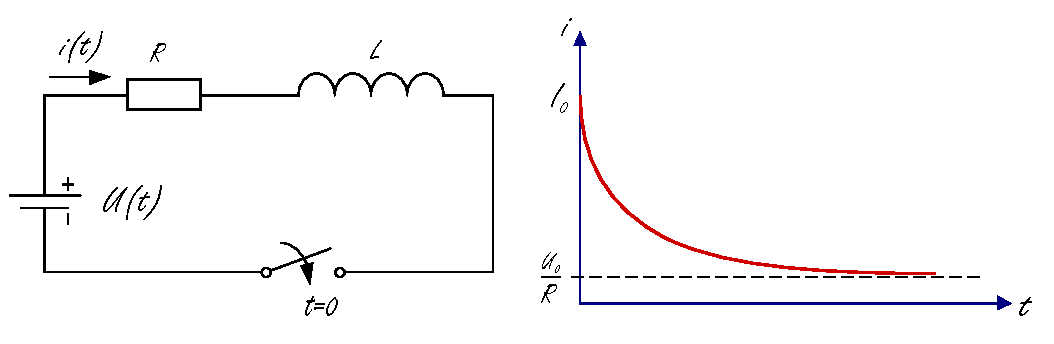
\includegraphics[width=\linewidth]{mai_fig032.pdf}
      \caption{Graf průběhu proudu $i(t)$ po sepnutí spínače v době $t=0$.}
      \label{mai:fig032}
    \end{figure}
%--------------------------------------------------------------------------------------------------- 
%======= Kapitola: Řady funkcí ====================================================================
  % !TeX spellcheck = cs_CZ
%---------------------------------------------------------------------------------------------------
% mai2ch05.tex
%---------------------------------------------------------------------------------------------------
\setchaptertoc
\chapter{Řady funkcí}\label{mai:IIchapV}
  Možná si po prolistování obsahu této kapitoly a klademe otázku, proč se máme ještě zabývat
  posloupnostmi a řadami, když jsme jim už popřáli docela dost pozornosti v partii \ref{part:MAI}.
  Cíl této kapitoly je Však trochu jiný, než studovat detaily vlastnosti konvergence či divergence
  číselných posloupnosti a řad. Půjde nám totiž, jak napovídá název kapitoly, o \emph{řady funkcí}.
  S takovým případem jsme se již také v prvním dílu setkali. Vzpomínáte na příklad 2.47. v odstavci
  \ref{mai:IchapIIIsecVIIssecIII} nazvaný \uv{Když diferenciál nestačí?} V něm jsme řešili problém
  přibližné náhrady funkce \(\cos\varphi\) pro malé hodnoty úhlu \(\varphi\) jinou funkcí, snadněji
  vyčíslitelnou. Zjistili jsme, že náhrada lineární funkcí, jaká byla možná v případě sinu, tj.
  \(\sin\varphi = \varphi\), u kosinu nefunguje, neboť diferenciál funkce \(\cos\varphi\) v bodě
  \(\varphi = 0\) je nulový. Poté jsme obecně dospěli k možnosti náhrady funkce \(f(x)\) v okolí
  bodu \(x=a\), Taylorovým polynornem \(n\)-tého stupně (vztah (227)), který představuje prvních \(n
  +1\) členů nekonečně Taylorovy řady
  \begin{strip}
    \begin{equation*}
      f(a)+f'(a)(x-a)+\frac{1}{2!}f''(a)(x-a)^2+\cdots+\frac{1}{n!}f^{(n)}(a)(x-a)^n+\cdots
    \end{equation*}
  \end{strip}
  Předchozí výraz je nekonečným součtem funkcí speciálního typu - mocnin proměnné \((x-a)\)
  násobených konstantami. Obecně bychom takový nekonečný součet mohli zapsat ve tvaru
  \begin{strip}
    \begin{equation*}
      s(x) = c_0 + c_1(x-a)+c_2(x-a)^2 + \cdots + c_n(x-a)^n + \cdots = \sum_{n=0}^\infty c_n(x-a)^n.
    \end{equation*}
  \end{strip}
  Nazýváme jej \emph{nekonečnou mocninnou řadou}. Taylorova řada je tedy speciálním případem
  mocninně řady. Praktický význam Taylorovy řady je nepochybný a vyložili jsme si jej již v odstavci
  \ref{mai:IchapIIIsecVIIssecIII} v partii \ref{part:MAI}. Obecně má nekonečná řada funkcí tvar

  \begin{equation*}
    f_1(x) + f_2(x) + \cdots f_n(x) + \cdots = \sum_{n=0}^\infty f_n(x).
  \end{equation*}

  Další řadu s praktickým významem může přiblížit následující příklad.

  \textbf{Příklad hudební}: Kdyby houslista zahrál na různých houslích stejný tón, mohli bychom si
  všimnout, že každý z nástrojů zní trochu jinak. Tón má stejnou výšku, ale jinou barvu. Čím to je?
  Výška tónu je z fyzikálního hlediska popsána frekvencí \(\nu\), resp. úhlovou frekvencí \(\omega
  = 2\pi f\) (například jednočárkované, komorní \uv{a} má frekvenci \SI{440}{\Hz}). Struna skutečně
  kmitá s touto frekvencí. Závislost výchylky jednotlivých jejích bodů na čase je periodickou funkcí
  času s touto frekvencí. Obecně Však není přesně harmonickým (například sinusovým) signálem, ale
  jeho mírnou modifikací. Z toho důvodu jsou v tónu slyšet i jiné frekvence, ne však jakékoli, ale
  celočíselné násobky původní frekvence, tj. \(2\nu\), \(3\nu\), atd. Barva tónu pak souvisí s
  amplitudami těchto \emph{vyšších harmonických frekvencí}. Matematický můžeme závislost výchylky
  bodu struny v obecnosti zapsat jako
  \begin{equation*}
    a_0 + \sum_{n=1}^\infty[a_n\cos(n\omega t) + b_n\sin(n\omega t)].
  \end{equation*}

  Tato nekonečná řada funkcí se nazývá \emph{Fourierova}. Její význam například ve fyzice,
  elektrotechnice či elektronice je nedozírný - umožňuje rozložit periodický signál na signály
  základní frekvence a vyšších harmonických.

  V souvislosti s Taylorovou řadou jsme si také kladli otázku, jak zjistit, zda takový nekonečný
  součet opravdu \uv{dospěje} k nějaké funkci \(s(x)\), tj. zda řada konverguje. Zmínili jsme se
  také o \uv{obyčejné} \emph{(bodové)} a o \emph{stejnosměrné} konvergenci. Pojem bodové a
  stejnoměrné konvergence má samozřejmě význam nejen pro Taylorovy či obecnější mocninné řady, ale i
  pro řady Fourierovy a jakékoli jiné řady funkcí. A právě o to v této kapitole převážně půjde.
  Abychom však vlastnosti řad funkcí mohli studovat po matematické stránce důkladněji, musíme se
  ještě na chvíli vrátit k posloupnostem a řadám číselným. V Závěru kapitoly si pak podrobněji
  všimneme právě řad mocninných a Fourierových a možností jejich aplikace.

  Vedle své užitečnosti praktické jsou řady docela zábavné a jsou užitečné i tím, že pomáhají tříbit
  matematické myšlení. Výrok Alexandra Ženíška  \uv{... zcela pochopit nekonečné řady znamená začít
  rozumět matematice ...} je možná určitou nadsázkou, ne však příliš velkou.

  \section{Posloupnosti a řady podruhé - čísla}\label{mai:IIchapVsecI}
    V tomto odstavci podrobněji probereme některé vlastnosti číselných posloupnosti a řad, které
    budeme pro zavedení pojmů souvisejících s řadami funkcí a studium jejich vlastností potřebovat.
    Nebudeme se tedy číselnými posloupnostmi a řadami zabývat „pro ně samotné“, ale s cílem jejich
    využití v úvahách o řadách funkcí.

    \subsection{Číselné posloupnosti a jejich konvergence}\label{mai:IIchapVsecIssecI}

%---------------------------------------------------------------------------------------------------
%======= Kapitola: Závislosti na více parametrech aneb funkce více proměnných =====================
  % !TeX spellcheck = cs_CZ
%---------------------------------------------------------------------------------------------------
% mai2ch06.tex
%---------------------------------------------------------------------------------------------------
\setchaptertoc
\chapter{Závislosti na více parametrech aneb funkce více proměnných}\label{mai:IIchapVI}
  Skalárními funkcemi jedné reálné proměnné jsme se zabývali velmi podrobně v \ref{part:MAI} dílu.
  Umíme počítat jejich limity v bodech \emph{vlastních} i \emph{nevlastních}, umíme je derivovat i
  integrovat. Totéž dokážeme provádět i s vektorovými funkcemi jedné proměnné. Každý vektor je totiž
  dán svými složkami, takže každá vektorová funkce je zadána tolika „obyčejnými“ skalárními
  funkcemi, kolik má daný vektor složek. S vektorovými funkcemi jedné proměnné jsme pracovali při
  zadávání trajektorií hmotných bodů a výpočtech jejich dalších charakteristik (rychlost, zrychlení,
  křivost trajektorie, apod). Tou jedinou proměnnou byl obvykle čas. Veličiny popisující objekty a
  děje v přírodě, ať již jsou tyto veličiny skaláry či vektory, však většinou závisí na více
  proměnných než jedné. Kromě času bývají typicky závislé na poloze. Vezměme třeba takové gravitační
  pole Země. Na čase sice nezávisí, zato však klesá s druhou mocninou vzdálenosti od středu Země.
  Veličina, která je charakterizuje, je buď vektorová, nebo skalární. Tou vektorovou je
  \emph{gravitační zrychlení} neboli \emph{intenzita} gravitačního pole Země, tou skalární je
  \emph{potenciál},
  \begin{equation*}
    \vec{g}(\vec{r}) = - \kappa\dfrac{M_Z}{r^2}\left(\dfrac{\vec{r}}{r}\right),\,
    V(\vec{r}) = -\kappa\dfrac{M_Z}{r}, \, r\geq R_Z.
  \end{equation*}
  V předchozích vztazích jsou \(M_Z\) a \(R_Z\) hmotnost a poloměr Země, \(\vec{r}\) je polohový
  vektor místa, v němž pole zjištujeme, vzhledem ke středu Země. Skalární i vektorové veličiny
  popisující elektrické a magnetické pole nábojů a proudů, rychlosti elementů proudící kapaliny nebo
  plynu a řada dalších fyzikálních veličin jsou nejen funkcemi času, ale také polohy bodu, v němž je
  počítáme nebo měříme. A stejně jako byly změny funkcí jedné proměnné vyjádřeny pomocí derivací,
  změny změn pomocí druhých derivací, atd., je třeba umět počítat i změny veličin závisejících na
  více proměnných. Mohou samozřejmě nastat situace, kdy se mění jen jedna z proměnných, zatímco
  ostatní zůstávají konstantní. Nejsnáze si takovou situaci představíme například tak, že měříme
  třeba elektrické pole stále ve stejném bodě prostoru, ale běží při tom čas. Pole se v daném bodě s
  časem mění. Nebo naopak v daném okamžiku sledujeme rozdílnost pole v bodech velmi blízkých danému
  bodu. Obecně se samozřejmě mění všechny proměnné a s nimi i hodnoty skalární funkce nebo složky
  vektorové funkce. Jak takové obecné změny co nejvýstižněji popsat, uvidíme právě v této kapitole.
  Setkáme se v ní s \textbf{parciální derivací}, která vystihuje, jak rychle se mění hodnota funkce
  se změnou jedné z proměnných. Dále poznáme obecnější, \textbf{směrovou derivaci}, která popisuje
  rychlost změny funkční hodnoty, mění-li se všechny proměnné, ale tak, že bod, který reprezentuje
  soubor jejich hodnot, se pohybuje v prostoru proměnných po libovolné přímce (nikoli jen po jedné
  souřadnicové ose, jako tomu je u parciálních derivací). A konečně zavedeme pojmy \textbf{úplného
  diferenciálu} a \textbf{Jacobiho zobrazení}, které popisují změnu hodnot skalární či vektorové
  funkce v lineární aproximaci, mění-li se hodnoty proměnných zcela obecně.

  Stejně jako u funkcí jedné proměnné je základem pro definici veličin popisujících rychlost změny
  funkce pojem \textbf{limity}, který úzce souvisí s pojmem \emph{okolí bodů} a obecně i s
  definičními obory funkcí. Pro případ funkcí více proměnných klade požadavek hlubšího pochopení
  pojmu limity větší nároky na soustředěnost a důkladné promýšlení různých situací, než tomu bylo u
  limit funkcí jedné proměnné. Proto se jím zabývá podstatná část poměrně rozsáhlého odstavce
  \ref{mai:IIchapVIsecII} poté, co je v odstavci \ref{mai:IIchapVIsecI} věnována značná pozornost
  různým typům definičních oborů funkcí. Čtenář, který se chce rychle propracovat k praktickým
  výpočtům a spokojí se zatím s intuitivním pochopením pojmu limity funkce více proměnných
  (založeným na dobré znalosti definice a vlastností limit funkcí jedné proměnné), může k nim v
  podstatě rovnou přejít s vědomím, že sice bude umět prakticky provádět různé standardní operace s
  funkcemi více proměnných, ale nebude si pravděpodobně vědět rady s netypickými případy. K
  důkladnému pročtení odstavců \ref{mai:IIchapVIsecI} a \ref{mai:IIchapVIsecII} se může samozřejmě
  vrátit kdykoli.

  \section{Podmonožiny euklidovských prostorů \(\mathcal{R}^n\)}\label{mai:IIchapVIsecI}  
    S definičními obory funkcí jedné proměnné to bylo docela jednoduché. Byly to Většinou intervaly
    - otevřené intervaly nebo jejich sjednocení, uzavřené intervaly, popřípadě intervaly uzavřené
    jen z jedné strany. Také zde figurovala okolí bodů, ať již ryzí, z nichž byl daný bod vyloučen,
    nebo taková, která daný bod obsahovala. Nic složitého tam nebylo. Aby bylo možné funkce
    derivovat, což byla nejčastější operace, kterou jsme prováděli s cílem zjistit, jak rychle se
    funkce mění, nemohly být definiční obory „moc divoké“. Vždy bylo třeba předpokládat, že bod, v
    němž jsme funkci nebo její změnu vyšetřovali, má okolí, ve kterém je funkce přinejmenším
    definována. Pro případ funkcí více proměnných je to podobné, ale bude třeba se definičním oborům
    věnovat trochu podrobněji. Dejme tomu, že nějaká fyzikální, nebo i nefyzikální veličina bude
    záviset na \(n\) proměnných. Každá z nich může nabývat nějakých hodnot. Funkční hodnota naší
    funkce bude tak jednoznačně určena souborem \(n\) hodnot jednotlivých proměnných. Tuto
    \(n\)-tici budeme považovat za bod v prostoru \(\mathcal{R}^n\). S \(n\)-ticemi jsme již
    pracovali v algebře, takže takový popis známe. V algebře jsme však s nimi prováděli algebraické
    operace, sčítání a násobení číslem. Měli jsme tedy v \(\mathcal{R}^n\) zavedenou
    \textbf{algebraickou strukturu}. Pro práci s funkcemi a pro sledování jejich změn \uv{bod od
    bodu} potřebujeme v \(\mathcal{R}^n\) ještě jinou strukturu. Ta je tvořena okolími, podobně jako
    tomu bylo u funkcí jedné proměnné. Taková struktura se nazývá \emph{topologická} a matematická
    disciplína, která se zabývá topologickými strukturami, se jmenuje \textbf{topologie}.

    Topologickými strukturami se nebudeme zabývat v celé obecnosti, i když je to velmi zajímavé.
    Budeme pracovat pouze se speciálním typem, takzvanou \textbf{euklidovskou topologií} v
    \(\mathcal{R}^n\).

    \subsection{Okolí bodů, otevřené a uzavřené množiny}
      S pojmem okolí bodu jsme se setkali hned v dílu \ref{part:MAI}}. Vzpomínáme? Šlo tehdy o okolí
      bodu \(a\) na reálné ose \(\mathcal{R}\). Okolím jsme rozuměli otevřený interval \((a -
      \delta_1,a + \delta_2)\), \(\delta_1, \delta_2 > 0\), ryzím okolím pak množinu \((a -
      \delta_1, a + \delta_2)\backslash{a}\), tj. sjednocení otevřených intervalů \((a - \delta_1,
      a) \cup (a, a + \delta_2)\). Sjednocení jakýchkoli otevřených intervalů jsme později nazývali
      otevřenou množinou, doplňky otevřených množin v \(\mathcal{R}\) byly uzavřené množiny.
      Vybudovali jsme tak na \(\mathcal{R}\) \emph{euklidovskou topologii} (dodatek F prvního dílu).
      Podobná bude situace i ve vícerozměrném případě, tedy v \(\mathcal{R}^n\).

  \section{Skalární funkce více proměnných}\label{mai:IIchapVIsecII}
    V předchozím odstavci jsme si vcelku důkladně připravili pojmy týkající se vhodných definičních
    oborů funkcí více proměnných. Nyní budeme tyto funkce definovat a studovat jejich vlastnosti.
    Obdobně jako u funkcí jedné proměnné půjde o limity, spojitost a derivace. Výhoda důkladné
    přípravy pojmů v předchozím odstavci se ukáže již při budování pojmu limity, zejména v
    nevlastním bodě. Samotnému pojmu limity a s ním úzce spjatého pojmu spojitosti bude věnována
    velká pozornost. Někdo se nad tím může pozastavit: Vždyť jak často se s potřebou výpočtu limit
    setkáváme v praktických příkladech? Málo. Potřebujeme spíše derivovat, integrovat, řešit
    diferenciální rovnice. S příklady na limity se setkáváme ponejvíce v matematických sbírkách, kde
    slouží k procvičení naučené látky. Taková úvaha by byla poněkud krátkozraká. Řada vlastností
    funkcí, a vůbec možnost s nimi rozumně operovat při běžných výpočtech, je založena na
    spojitosti. A spojitost je těsně spjata s pojmem limity. Opět by mohla vzniknout námitka, že
    spojitost přece intuitivně dobře chápeme - spojitá funkce nemá „zpřetrhaný“ graf. Umíme si však
    představit graf funkce tří proměnných? Není to dost dobře možné ani u funkce dvou proměnných,
    je-li složitější, nebo chová-li se v okolí některého bodu „podezřelé“. Limitě tedy potřebujeme
    porozumět, i když její výpočet v praktických příkladech skutečně nebude na „denním pořádku“.
    Abychom porozumění podpořili, budeme se vedle teoretických úvah věnovat i řadě praktických
    příkladů.




%---------------------------------------------------------------------------------------------------
%======= Kapitola: Základy variačního počtu pro mechaniku =========================================
  % !TeX spellcheck = cs_CZ
%---------------------------------------------------------------------------------------------------
% mai2ch07.tex
%---------------------------------------------------------------------------------------------------
\chapter{Základy variačního počtu pro mechaniku}\label{mai:IIchapVII}
\minitoc

%---------------------------------------------------------------------------------------------------
\printbibliography[title={Seznam literatury}, heading=subbibliography]
\addcontentsline{toc}{section}{Seznam literatury}
}
  % %===================================================================================================
% Physics
% Fyz1.tex
%===================================================================================================
% notes:
%~~~~~~~~~
% \label{fyz:eq569}
% \label{fyz:fig543}
% \label{fyz:exam010}
% \label{fyz:tab009}
%---------------------------------------------------------------------------------------------------
% Setting path to image 
  \graphicspath{{../src/FYZ/img/}}
  \makeatletter
    \@addtoreset{chapter}{part}
  \makeatother
%---------------------------------------------------------------------------------------------------
\lstset{ %
  language=Matlab,                       % choose the language of the code
  basicstyle=\footnotesize,              % the size of the fonts that are used for the code
%  backgroundcolor=\color{White},        % choose the background color.
  commentstyle=\color{help}\textit,
  keywordstyle=\color{keyword}\textbf,
  breaklines=true,                       % sets automatic line breaking
  breakatwhitespace=true,                % sets if automatic breaks should only happen at whitespace
  showspaces=false,                      % show spaces adding particular underscores
  showstringspaces=true,                 % underline spaces within strings
  showtabs=true,                         % show tabs within strings adding particular underscores
  frame=none,                            % adds a frame around the code - none, single
  tabsize=8,                             % sets default tabsize to 8 spaces
  captionpos=b,                          % sets the caption-position to bottom
  numbers=left,                          % where to put the line-numbers -none, left, right
  numberstyle=\footnotesize,             % the size of the fonts that are used for the line-numbers
  stepnumber=1,                          % the step between two line-numbers. If it's 1 each line
                                         % will be numbered
  xleftmargin=3em,                       % adjust left margin
}

\part{FYZ I}\label{part:FYZI}
\parttoc

\ifthenelse{ \equal{\DebugMode}{true} }{
% Debug mode ON
% ~~~~~~~~~~~~~~~~~~~~~~~~~~~~~~~~~~~~~~~~~~~~~~~~
  % !TeX program = lualatex
% !TeX root = luaking.tex
% !TeX encoding = UTF-8
% !TeX spellcheck = cs_CZ
%---------------------------------------------------------------------------------------------------
% file fey1ch01_02_03.tex
%---------------------------------------------------------------------------------------------------
%===================== Kapitola: Základy fyziky ====================================================
\setchaptertoc
\chapter{Základy fyziky}\label{fyz:IchapI}
\epigraph{\emph{Fyzika je jako sex, může přinést praktické výsledky, ale to není důvod, proč to 
  děláme.}}{Richard P. Feynmann}

  \begin{figure}[ht!]  % \ref{fyz:fig067}
    \centering
    \luafigure[0.6]{fyz_fig067.jpg}
    \caption{\wikiFeynman \textasteriskcentered 11. května 1918 - \textdagger 15. února 1988, 
             americký fyzik, který patřil k největším fyzikům 20. století}
    \label{fyz:fig067}
  \end{figure} 

    Možná se zeptáte, zda není možné při vyučování fyziky na první straně uvést základní zákony a 
    potom ukázat, co z nich vyplývá v nejrůznějších situacích. Tak se postupuje v euklidovské 
    geometrii, kde se postulují axiomy, ze kterých se odvodí všechny možné závěry. (Protože se vám 
    nelíbí pětileté studium fyziky, chtěli byste seji naučit za pět minut?) Takovýmto způsobem však 
    nemůžeme postupovat ze dvou důvodů. Především, zatím neznáme všechny základní zákony - oblast 
    toho, co bychom ještě měli poznat, se nám stále zvětšuje. Dále, přesná formulace fyzikálních 
    zákonů zahrnuje mnoho neobvyklých myšlenek, jejichž vyjádření si vyžaduje vyšší matematiku. 
    Proto je nutná značná předběžná příprava jen k tomu, abychom rozuměli, co znamenají slova. Není 
    tedy možné postupovat tímto způsobem. \emph{Učit se můžeme pouze postupně, kousek po kousku}.

  \section{Jak studovat fyziku}\label{fyz:IchapIsecI}
    Každý kousek nebo část celku, který představuje příroda, je vždy jen přiblížením k úplné 
    pravdě; přesněji k úplné pravdě, pokud ji známe. Ve skutečnosti vše, co víme, je jen určitým 
    druhem aproximace, protože víme, ze ještě neznáme všechny zákony. Proto se věci musíme učit jen 
    proto, abychom se je znovu odnaučili, nebo, což je pravděpodobnější, abychom si naše znalosti o 
    nich opravovali.
    
    Princip vědy, téměř její definice, je následující: Prověrkou všech našich vědomostí je 
    experiment. Experiment je jediné kritérium vědecké „pravdy“. Jenže co je zdrojem našich 
    vědomostí? Odkud pocházejí zákony, které prověřujeme? Samotný experiment nám pomáhá odvozovat 
    zákony v tom smyslu, že nám poskytuje náznaky, pokyny. Navíc je však potřebná představivost, 
    aby z těchto náznaků mohla vzniknout velká zobecnění - abychom v nich odhadli nádherný, 
    jednoduchý, ale neobyčejný obraz a potom experimentem prověřili správnost našeho odhadu. Tento 
    proces představivosti je tak těžký, že si fyzici rozdělili práci - teoretičtí fyzici 
    představivostí, dedukcí a odhadem odvozují nové zákony, ale neexperimentují; experimentální 
    fyzici dělají pokusy a přitom také uplatňují představivost, dedukci a odhad.
    
    Řekli jsme, že přírodní zákony jsou přibližné: že nejdříve nacházíme „nesprávné“ a až potom 
    „správné“. Jak však může být experiment „nesprávný“? Především z velmi jednoduchého důvodu - 
    náš přístroj není v pořádku a my jsme to nezpozorovali. Takové chyby se však zjišťují lehce. 
    Odhlédneme-li od těchto drobností, jak může být výsledek experimentu nesprávný? Jen v důsledku 
    nepřesnosti. Například, hmotnost předmětu se zdá být neměnná; rotující káča má stejnou hmotnost 
    jako káča v klidu. Tak byl objeven „zákon“: hmotnost je konstantní, nezávislá na rychlosti. O 
    tomto „zákonu“ se zjistilo, že je nesprávný. Ukázalo se, že hmotnost roste s rychlostí, ale k 
    značnému růstu jsou potřebné rychlosti blízké rychlosti světla. Správný zákon zní: je-li 
    rychlost tělesa menší než \SI{100}{\km\per\second}, je hmotnost konstantní s přesností na jednu 
    milióntinu. V takové aproximativní podobě je tento zákon správný. Někdo by si mohl myslet, že 
    prakticky není rozdíl mezi starým a novým zákonem. To je i není pravda. Pro běžné rychlosti je 
    jistě možné zapomenout na to, o čem jsme mluvili a používat jednoduchý zákon konstantní 
    hmotnosti jako dobré přiblížení. Při velkých rychlostech se však dopustíme chyby, a to tím 
    větší, čím větší je rychlost

    \begin{figure}[ht!]  %\ref{fyz:fig891}
      \centering
      \luafigure[0.8]{fyz_fig891.jpg}
      \caption{Vodní kapka dopadající na hladinu. Kredit: Wikipedia}
      \label{fyz:fig891}
    \end{figure} 
    
    Ostatně, nejzajímavější je to, že z filozofického hlediska je tento aproximativní zákon zcela 
    nesprávný. Náš celkový obraz o světě musíme změnit, i kdyby se hmotnost měnila jen nepatrně. 
    Toto je svérázný znak filozofie nebo myšlenek stojících v pozadí zákonů. Někdy i velmi malý 
    efekt vyžaduje hlubokou změnu našich názorů.
    
    Čemu tedy máme dát přednost? Máme podat správné, ale nezvyklé zákony s jejich cizím a obtížným 
    pojetím jako je například teorie relativity, čtyřrozměrný prostoročas a podobně? Nebo máme 
    nejdříve vysvětlit jednoduchý zákon „konstantní hmotnosti“, který je pouze přibližný, ale 
    nevyžaduje náročné představy? První způsob je více vzrušující, nádhernější a zábavnější, ale s 
    druhým se jednodušeji začíná a představuje první krok ke skutečnému porozumění správného 
    zákona. Tento problém se vždy znovu objevuje při vyučování fyziky. V různých etapách ho musíme 
    řešit různými způsoby, ale vždy je vhodné se zajímat, do jaké míry je přesné to, co teď víme, 
    jak to souvisí s dalším a jak se to může změnit, budeme-li vědět víc.
    
    Nyní přejděme k náčrtu nebo k všeobecné mapě našeho chápání současné vědy (zejména fyziky, ale 
    i jiných věd, které s ní souvisejí). Když se později soustředíme na konkrétní problém, budeme 
    mít představu o jeho pozadí, o tom, proč je zajímavý a jak zapadá do celkové struktury. Jaký je 
    tedy náš celkový obraz světa? \cite[s.~16]{Feynman01}
    
    \subsection{Látka se stává z atomů}
      Kdyby při nějaké katastrofě zanikly všechny vědecké poznatky a dalším generacím by měla 
      zůstat jen jediná věta, které tvrzení by při nejmenším počtu slov obsahovalo nejbohatší 
      informaci? Takovým kandidátem je \textbf{atomová hypotéza} - tj. že \emph{všechny věci se 
      skládají z atomů malých částic, jež jsou v neustálém pohybu,  a vzájemně se přitahují, když 
      jsou od sebe trochu vzdálené, ale odpuzují se, když jsou těsně u sebe.} V této jediné větě, 
      jak uvidíme, je obsaženo nesmírné množství informací o světě. Je k tomu třeba jen trochu 
      představivosti a uvažování.

      \begin{figure}[ht!]  %\ref{fyz:fig007}
        \centering
        \luafigure[0.6]{fyz_fig007.pdf}
        \caption{Vodní kapka z obrázku \ref{fyz:fig891} zvětšená miliardkrát \cite[s.~17]{Feynman01}}
        \label{fyz:fig007}
      \end{figure} 

      Abychom ilustrovali sílu myšlenky o atomu, představme si podobnou kapku vody jako na obrázku
      \ref{fyz:fig891} o rozměru \SI{0.5}{\cm}. Podí\-váme-li se na ni zblízka, neuvidíme nic
      jiného, než vodu - klidnou, souvislou vodu. I když kapku zvětšíme tím nejlepším optickým
      mikroskopem, přibližně dvoutisíckrát, a kapka bude měřit deset metrů, tedy stejně jako velká
      místnost, i tehdy budeme stále vidět relativně klidnou vodu. Jen tu a tam v ní budou plavat
      jakési malé fotbalové míče. Tyto velmi zajímavé objekty na obrázku \ref{fyz:fig890} jsou
      trepky. Tady se můžeme zastavit a zajímat se o trepky, o jejich třepotající se řasičky, o
      jejich kroutící se těla a nepokračovat ve zvětšování. Nebo můžeme zvětšit trepky tak, abychom
      viděli i do nich). 

      \begin{figure}[ht!]  %\ref{fyz:fig890}
        % http://www.photomacrography.net/forum/viewtopic.php?t=18166
        \centering
        \luafigure[1]{fyz_fig890a.jpg}
        \caption{ Trepka velká \emph{(Paramecium caudatum)} je nálevník běžně se vyskytující v 
                  organicky znečištěných vodách po celém světě. Kredit: Wikipedia}
        \label{fyz:fig890}
      \end{figure} 

      Trepky jsou však předmětem biologie. Proto si jich teď nebudeme všímat, ale zahledíme se ještě
      pozorněji na vodu při dalším dvoutisícinásobném zvětšení. Teď měří kapka vody dvacet kilometrů
      a při pozorném sledování je vidět jakési hemžení - cosi, co už nevypadá klidně, ale připomíná
      dav na fotbalové tribuně při pohledu z velké vzdálenosti. Abychom zjistili, co je to za
      hemžení, zvětšíme kapku ještě 250krát a potom uvidíme něco podobného jako na obr.
      \ref{fyz:fig007}. Tento obrázek představuje vodu při zvětšení miliardkrát, je však v několika
      směrech idealizovaný. Především částice jsou zakreslené zjednodušeně - s ostrými okraji, což
      neodpovídá skutečnosti. Dále kvůli jednoduchosti jsou částice zakreslené v dvojrozměrném
      uspořádání, ačkoli se ve skutečnosti pohybují ve všech třech směrech. Všimněme si, že jsou tam
      dva druhy částic znázorněných kroužky, které představují atomy kyslíku (černé) a vodíku (bílé)
      a že na každý atom kyslíku se vážou dva atomy vodíku. Každá skupinka skládající se z atomu
      kyslíku a dvou atomů vodíku se nazývá \textbf{molekulou}. Obrázek je zjednodušený i v tom, že
      skutečné částice v přírodě se ustavičně kolébají a poskakují, obracejí se a točí jedna okolo
      druhé. Je třeba si to představit spíše jako \emph{dynamický a né jako statický obrázek}. Další
      věcí, kterou není možné vystihnout na obrázku, je skutečnost, že částice „drží pohromadě“ -
      přitahují se, jedna za sebou táhne druhou atd. Je možné říci, že jsou jakoby „slepené
      dohromady“. Na druhé straně se částice netlačí jedna přes druhou. Kdybychom se pokusili
      přitlačit dvě z nich příliš těsně k sobě, odpudily by se.

      Atomy mají poloměr \SI{1e-10}{\m} až \SI{2e-10}{\m}. Jejich velikost si můžeme pamatovat i 
      jinak: zvětšíme-li jablko na velikost Země, budou atomy v jablku tak velké, jak bylo původně 
      jablko.

      Představme si teď tuto velkou kapku vody s jejími hemžícími se částicemi, jež přilnuly k sobě 
      a honí jedna druhou. Voda udržuje svůj objem; nerozpadne se na části díky vzájemné 
      přitažlivosti molekul. Je-li tato kapka na šikmé ploše, kde se může hýbat z místa na místo, 
      voda poteče. Nestane se však, že by jednoduše zmizela. Věci se nerozpadají na části právě 
      díky přitažlivosti molekul. \emph{Hemživý pohyb částic je to, co chápeme jako teplo}: 
      zvýšíme-li teplotu, zvětšíme pohyb. Zahříváme-li vodu, pohyb roste a roste i vzdálenost mezi 
      částicemi, až nastane okamžik, kdy přitažlivost mezi molekulami je už nestačí udržet 
      pohromadě. Částice přestanou být vzájemně svázané a rozlétají se od sebe. Zvyšováním teploty 
      tak získáváme \emph{vodní páru}.  
      
      \begin{figure}[ht!]
        \centering
        \luafigure[0.6]{fyz_fig008.pdf}
        \caption{Pára \cite[s.~18]{Feynman01}}
        \label{fyz:fig008}
      \end{figure}

      Na obr. \ref{fyz:fig008} vidíme páru. V jednom směru tento obrázek páry selhává: při našem 
      zvětšení za normálního atmosférického tlaku připadá jen velmi málo molekul na celý pokoj, 
      takže na tak malém obrázku určitě nebudou tři molekuly. Většina plošek této velikosti nebude 
      obsahovat žádnou molekulu - na našem obrázku jsou náhodou dvě a část z třetí molekuly 
      (abychom tam neměli prázdné místo). V případě páry vidíme podobu molekul jasněji než v 
      případě vody. Pro jednoduchost jsou molekuly zakresleny tak, že atomy vodíku svírají úhel 
      \SI{120}{\degree}. Ve skutečnosti má tento úhel hodnotu \ang[arc-separator = \,]{105;3;} a 
      vzdálenost mezi středem vodíku a středem kyslíku je \SI{9.57e-11}{\m}. Tuto molekulu tedy 
      velmi dobře známe.

      Všimněme si jedné vlastnosti vodní páry nebo jiných plynů. Molekuly budou tím, že se vzdálily 
      jedna od druhé, narážet na stěny. Představme si místnost s určitým počtem (tak kolem sta) 
      neustále poskakujících tenisových míčků. Když míčky narážejí na stěnu, odtlačují ji a stěnu 
      proto musíme upevnit. Plyn působí přerušovanou silou, kterou naše nedokonalé smysly (jejich 
      citlivost nevzrostla miliardkrát) vnímají jako \emph{stálý tlak}. Abychom plyn udrželi, 
      musíme na něj působit tlakem z opačné strany. Obr. \ref{fyz:fig009} znázorňuje běžnou nádobu 
      na udržování plynu, kterou najdeme v každé učebnici: \textbf{válec s pístem}. Teď nám 
      nezáleží na tom, jaký je ve skutečností tvar molekul vody, a proto je kvůli jednoduchostí 
      znázorníme jako tenisové míčky nebo body. Jsou v neustálém pohybu a pohybují se na všechny 
      strany. Na spodek \emph{pístu} jich neustále naráží tolik, že na něj musíme působit určitou 
      silou dolů, aby ho molekuly nevytlačily z válce. Tuto \emph{sílu} nazýváme \textbf{tlakem} 
      (přesněji, \emph{tlak násobený plochou dává sílu}). Je jasné, že síla je úměrná ploše pístu, 
      protože zvětšíme-li plochu a přitom nezměníme počet molekul v kubickém centimetru, pak 
      vzroste počet srážek s pístem tolikrát, kolikrát se zvětšila jeho plocha.

      \begin{figure}[ht!]
        \centering
        \luafigure[0.4]{fyz_fig009.pdf}
        \caption{Píst \cite[s.~18]{Feynman01}}
        \label{fyz:fig009}
      \end{figure}

      Nyní \emph{zdvojnásobme} v této nádobě počet molekul, takže se zdvojnásobí jejich hustota, 
      ale ponechme jim stejnou rychlost, tj. \emph{stejnou teplotu}. Pak můžeme dost přesně říci, 
      že se zdvojnásobil počet srážek a jelikož je každá právě tak \uv{energická} jako dříve, tlak 
      je úměrný hustotě. Uvážíme-li skutečnou povahu meziatomových sil, můžeme očekávat mírný 
      pokles tlaku jako projev zvýšené přitažlivosti mezi atomy a mírný vzrůst související s 
      objemem, který zaujímají. Přesto však, pokud je hustota dostatečně nízká, tj. atomů není 
      příliš mnoho, můžeme s dostatečnou přesností říci, že \emph{tlak je úměrný hustotě}.
      
      Snadno pochopíme i něco jiného. \emph{Zvyšujeme-li teplotu} bez změny hustoty plynu, tj. když 
      zvětšujeme rychlost atomů, co se stane s tlakem? Atomy narážejí do pístu \emph{silněji}, 
      neboť se pohybují rychleji a navíc, narážejí častěji. Proto tlak vzrůstá. Vidíme, jak 
      jednoduché jsou myšlenky atomové teorie.
      
      Podívejme se na jinou situaci. Předpokládejme, že se píst \emph{pohybuje dovnitř}, takže 
      atomy jsou pomalu stlačovány do menšího prostoru. Co se stane, narazí-li atom do pohybujícího 
      se pístu? Je jasné, že při takové srážce \emph{získá rychlost}. Můžeme si to vyzkoušet na 
      ping-pongovém míčku: po úderu pálkou míček odletí od pálky rychleji, než k ní přiletěl. Ve 
      zvláštním případě, není-li atom v pohybu a píst na něj narazí, atom se začne určitě 
      pohybovat. Atomy jsou při návratu od pístu \uv{teplejší}, než byly před nárazem na píst. 
      Proto všechny atomy, které jsou v nádobě, získají na rychlosti. To znamená, že při pomalém 
      \emph{stlačení plynu jeho teplota vzrůstá}. Když plyn pomalu \emph{stlačujeme}, jeho teplota 
      \emph{vzrůstá} a když plyn pomalu \emph{rozpínáme}, jeho teplota \emph{klesá}.
      
      \begin{figure}[ht!]  % \ref{fyz:fig010}
        \centering
        \luafigure[0.6]{fyz_fig010.pdf}
        \caption{Led \cite[s.~19]{Feynman01}}
        \label{fyz:fig010}
      \end{figure}

      Vraťme se k naší kapce vody a podívejme se na ni z jiného pohledu. Snižme teplotu naší kapky.
      Předpokládejme, že hemžení molekul vody postupně slábne. Víme, že mezi atomy působí přitažlivé
      síly, které způsobí, že molekuly už nebudou moci tak snadno pohybovat. Obr. \ref{fyz:fig010}
      znázorňuje, co se stane při velmi nízkých teplotách: molekuly jsou vázány v nové struktuře,
      vytváří se \textbf{led}. Takové schematické znázornění ledu není správné, neboť je
      dvojrozměrné. Situaci však vystihuje kvalitativně. Je pozoruhodné, že každý atom má v této
      látce určité místo. Rozmístíme-li atomy na jednom konci kapky podle určitého pravidla, pak v
      důsledku pevné struktury meziatomových vazeb vznikne určité uspořádání atomů i na druhém konci
      kapky, vzdáleném (v našem měřítku) několik kilometrů. Proto, držíme-li ledový rampouch za
      jeden konec, jeho druhý konec bude při lámání klást odpor, chová se jinak než voda, ve které
      je pravidelná struktura rozrušena intenzívním pohybem atomů v rozličných směrech. Rozdíl mezi
      pevnými látkami a kapalinami spočívá v tom, že atomy pevné látky jsou \emph{uspořádány}
      zvláštním způsobem. Toto uspořádání se nazývá \textbf{krystalická struktura}. I tehdy, kdy jde
      o velmi vzdálené atomy, nepozorujeme nic náhodného v jejich polohách. Poloha atomu na jednom
      konci krystalu je určena polohou atomu na druhém konci, i když se mezi nimi nacházejí miliony
      jiných atomů. Obr. \ref{fyz:fig010} znázorňuje vymyšlené uspořádání ledu a ačkoli správně
      vystihuje mnohé vlastnosti ledu, neodpovídá skutečnému uspořádání. Jedním ze správných rysů je
      existence části \emph{hexagonální symetrie}. Můžeme se o tom přesvědčit: otočíme-li obrázek o
      \SI{120}{\degree}, dostaneme stejné seskupení. Taková symetrie ledu je příčinou šestihranného
      tvaru sněhových vloček. Další informací, kterou je možné vytušit z obrázku \ref{fyz:fig010},
      je \emph{zmenšování objemu ledu při tání}. Znázorněná struktura ledu, stejně tak jako
      skutečná, obsahuje \emph{mnoho dutin}. Když se struktura rozpadne, tyto dutiny mohou být
      \emph{zaplněny} molekulami. \emph{Většina jednoduchých látek, s výjimkou vody a
      liteřiny\footnote{Liteřina či písmovina je slitina používaná v písmolijectví. Její přibližné
      složení je: \SIrange{50}{86}{\percent} olova, \SIrange{3}{20}{\percent} cínu a
      \SIrange{11}{30}{\percent} antimonu. Liteřinu vyvinul v 15. století zakladatel knihtisku
      Johannes Gutenberg pro odlévání tiskařských liter.}, zvětšují při tání svůj objem, neboť atomy
      jsou v pevných krystalech těsně seskupeny a při tání potřebují více prostoru na kmitání}.
      Otevřené struktury se však při tání zhroutí - podobně jako led.
      
      I když má led pevnou krystalickou strukturu, jeho teplota se může měnit - v ledu je zásoba 
      tepla. Chceme-li, můžeme toto množství tepla změnit. Jaké je teplo, které se nachází v ledu? 
      Atomy ledu \emph{nejsou} v klidu, poskakují a kmitají. Ačkoli v krystalu existuje určité 
      uspořádání - struktura - všechny atomy kmitají, „na místě“. Zvyšujeme-li teplotu, budou 
      kmitat se stále větší amplitudou, až opustí svá místa. Tento jev nazýváme \textbf{táním}. 
      Snižujeme-li teplotu, kmity slábnou a při teplotě \emph{absolutní nuly} jsou 
      \emph{nejslabší}, ne však nulové. Toto nejmenší množství pohybu, který přísluší atomům, 
      nestačí na roztání látky - až na jednu výjimku: \emph{hélium}. V héliu se při ochlazování 
      také zpomaluje pohyb atomů na nejmenší možnou míru, ale i při teplotě absolutní nuly brání 
      tento pohyb zmrznutí hélia. Hélium nezmrzne, pokud nevytvoříme tak veliký tlak, abychom atomy 
      stlačili k sobě. Při velkém tlaku můžeme dosáhnout toho, že hélium ztuhne.
    
    \subsection{Atomové procesy}
      Dosud jsme si všímali stavby pevných látek, kapalin a plynů z atomového hlediska. Jenže 
      atomová hypotéza charakterizuje i procesy, a proto si všimněme některých procesů z atomového 
      hlediska. Nejdříve budeme hovořit o procesech, které se odehrávají na povrchu vody. Co se 
      vlastně děje na vodním povrchu? Úlohu si zkomplikujeme - bude tak blíže skutečnosti
      - předpokladem, že nad vodním povrchem se nachází vzduch. Obr. \ref{fyz:fig011} takovou 
      situaci znázorňuje. Tak jako předtím vidíme molekuly vody, které tvoří kapalinu, ale vidíme i 
      povrch vody. Nad povrchem vidíme různé molekuly. Jsou tam především \emph{molekuly vody} v 
      podobě vodní páry, kterou je možné pozorovat vždy nad kapalnou vodou (pára a voda jsou v 
      rovnováze, o které pohovoříme později). Dále tam nalezneme jiné molekuly, dvojice atomů 
      kyslíku tvořící \emph{molekulu kyslíku} a dvojice atomů dusíku tvořící \emph{molekulu 
      dusíku}. Vzduch se skládá téměř výhradně z dusíku, kyslíku, vodní páry a menšího množství 
      oxidu uhličitého, argonu a jiných příměsí. Nad povrchem vody se nachází vzduch - plyn 
      obsahující jisté množství vodní páry. Nyní si všimněme, co se odehrává na obrázku. Molekuly 
      vody se neustále pohybují. Občas některá z molekul, nacházejících se v blízkosti povrchu, 
      naráží na jinou molekulu trochu silněji než obvykle a vyskočí nad povrch. Na obrázku takovýto 
      děj \emph{přímo} neuvidíme, neboť vše je na něm nehybné. Můžeme si však představit, že jedna 
      molekula za druhou v důsledku srážek opouštějí vodu - voda mizí, \emph{vypařuje} se. Když 
      nádobu \emph{přikryjeme}, objevíme po nějakém čase velké množství molekul vody mezi 
      molekulami vzduchu. Čas od času některá z těchto molekul vody vletí zpět do vody a zůstává v 
      ní. To, co jsme považovali za mrtvé a nezajímavé - přikrytý pohár vody, který snad dvacet let 
      stál na jednom místě - v sobě skrývá stále probíhající zajímavý \textbf{dynamický proces}. 
      Náš nedokonalý zrak nepozoruje žádnou změnu, ale při miliardovém zvětšení bychom viděli, jak 
      se vše mění: jedny molekuly opouštějí povrch a druhé se vracejí.
      
      \begin{figure}[ht!]   % \ref{fyz:fig011}
        \centering
        \luafigure[0.7]{fyz_fig011.pdf}
        \caption{Voda vypařující se do vzduchu \cite[s.~21]{Feynman01}.}
        \label{fyz:fig011}
      \end{figure}

      Proč nepozorujeme tyto změny my? Protože do vody se vrací právě tolik molekul, kolik z ní 
      odešlo. Navenek se „nic neděje“. Když odkryjeme nádobu, odfoukneme vlhký vzduch pryč a 
      nahradíme ho suchým vzduchem, nezmění se počet z vody vylétajících molekul (neboť závisí 
      pouze na pohybu ve vodě), ale velmi se změní počet molekul do vody se vracejících, protože 
      nad vodou je mnohem méně molekul. Molekul, které opouštějí vodu, je víc než molekul, které se 
      do ní vracejí; voda se vypařuje. Chceme-li tedy, aby se voda vypařovala, zapneme ventilátor!
      
      Zůstává ještě otázka: Které molekuly opouštějí vodu? Molekula opustí vodu, když náhodně získá 
      malé množství dodatečné energie, kterou potřebuje na to, aby překonala přitažlivé působení 
      svých sousedů. Protože ty molekuly, které opouštějí vodu, mají větší než průměrnou energii, 
      budou se molekuly, které ve vodě zůstávají, v průměru pohybovat méně. Při vypařování se tedy 
      kapalina postupně \emph{ochlazuje}. Je samozřejmé, že když molekula páry sestoupí ze vzduchu 
      do vody, objeví se silné přitahování, když molekula dosahuje povrchu vody. Důsledkem toho je 
      zrychlení přicházející molekuly a s tím spojený vznik tepla. \emph{Můžeme tedy říci, že s 
      odchodem molekul odchází a s příchodem molekul přichází teplo.} Když jsou oba procesy 
      vyrovnány, voda svou teplotu nemění. Foukáme-li na vodu, aby odpařování převládalo nad 
      zkapalňováním, voda se ochlazuje. Proto, chcete-li ochladit polévku, foukejte na ni!
      
      \begin{figure}[ht!]    % \ref{fyz:fig012}
        \centering
        \luafigure[0.7]{fyz_fig012.pdf}
        \caption{Voda vypařující se do vzduchu \cite[s.~21]{Feynman01}.}
        \label{fyz:fig012}
      \end{figure}

      Musíme si však uvědomit, že procesy, o kterých jsme hovořili, probíhají ve skutečnosti 
      složitěji. Při unikání vody do vzduchu čas od času některá z molekul kyslíku nebo dusíku 
      vnikne do vody a \uv{ztratí se} mezi jejími molekulami. Vzduch se tedy rozpouští ve vodě. 
      Molekuly kyslíku a dusíku pronikají do vody, která pak obsahuje vzduch. Když z nádoby náhle 
      odstraníme vzduch, budou molekuly vzduchu unikat z vody rychleji, než do ní vnikají, což 
      způsobí vystupování bublinek. Tato skutečnost je velmi nepříjemná pro potápěče.
    
      Nyní si všimněme dalšího procesu. Obr. \ref{fyz:fig012} znázorňuje, jak se podle atomové 
      představy rozpouští pevná látka ve vodě. Co se stane, vložíme-li krystal soli do vody? Sůl je 
      pevná látka, krystal, organizované seskupení „atomů soli“. Na obr. \ref{fyz:fig013} je 
      znázorněna trojrozměrná struktura kuchyňské soli, chloridu sodného. Máme-li být přesní, 
      musíme říct, že krystal není tvořen atomy, ale ionty. Iont je atom, který má několik 
      elektronů navíc, nebo několik elektronů ztratil. V krystalu soli nalézáme \emph{ionty chlóru} 
      (atomy chlóru s přebytečným elektronem) a \emph{ionty sodíku} (atomy sodíku zbavené jednoho 
      elektronu). Ionty jsou v krystalu vzájemně vázány elektrickou přitažlivostí, ale ve vodě se 
      některé z nich pod vlivem přitažlivosti záporného kyslíku a kladného vodíku začnou uvolňovat. 
      Na obrázku \ref{fyz:fig012} vidíme uvolňující se iont chlóru a jiné atomy plavající ve vodě 
      ve formě iontů. Tento obrázek je pečlivě zakreslený. Všimněme si například, že vodíkové konce 
      molekul vody obvykle obklopují iont chlóru a u iontu sodíku zpravidla nalézáme kyslíkový 
      konec, neboť sodík je kladný a kyslíkový konec molekuly vody je záporný a tyto se elektricky 
      přitahují. Můžeme podle tohoto obrázku říci, jestli se sůl \emph{rozpouští} ve vodě, nebo 
      \emph{krystalizuje} z vody? Samozřejmě, že \emph{nemůžeme}, neboť zatím co jedny atomy 
      opouštějí krystal, jiné se k němu připojují. Takovýto proces je - podobně jako vypařování - 
      \emph{dynamický} všechno závisí na tom, je-li ve vodě více nebo méně soli, než je třeba k 
      rovnováze. Rovnováhou rozumíme takovou situaci, kdy počet atomů opouštějících krystal je 
      roven počtu atomů do krystalu se vracejících. Když sůl ve vodě téměř není, vstupuje do vody 
      více atomů, než vystupuje a sůl se rozpouští. Když je, naopak, „atomů soli“ příliš mnoho, do 
      krystalu se vrací více atomů, než ho opouští a sůl krystalizuje.
 
      \begin{figure}[hbt!]  % \ref{fyz:fig013}
        \centering
          \subcaptionbox{\label{fyz:fig013a}}{\luafigure[0.4]{fyz_fig013a.pdf}}   \newline                                   
          \subcaptionbox{\label{fyz:fig013b}}{\luafigure[0.8]{fyz_fig013b.pdf}}
        \caption{Vzdálenost nejbližších sousedů \(d = \dfrac{a}{2}\) \cite[s.~22]{Feynman01}}
        \label{fyz:fig013}
      \end{figure}
      
      Zmínili jsme se o tom, že představa \emph{molekuly} látky je pouze přibližná a je 
      opodstatněná jen pro určitou třídu látek. Je jasné, že v případě vody jsou její tři atomy 
      skutečně svázané, ale v případě pevného chloridu sodného už to tak jasné není. V takovém 
      případě jde o uspořádání sodíkových a chlorových iontů do krychlové mřížky a neexistuje 
      přirozený způsob jejich uspořádání do „molekul soli“.
      
      Vraťme se ještě k naší diskuzi o \emph{rozpouštění a srážení}. Zvýšíme-li teplotu roztoku 
      soli, vzroste počet atomů, které sůl opouštějí a vzroste i počet atomů, které se do soli 
      vracejí. Ukazuje se, že obecně je velmi těžké předpovědět, jak se ten proces realizuje, 
      proběhne-li rozpouštění rychleji nebo pomaleji. S rostoucí teplotou se většina látek 
      rozpouští lépe, ale některé látky se rozpouštějí hůře.
      
    \subsection{Chemické reakce}
      Ve všech procesech, o nichž jsem dosud hovořili, neměnily atomy a ionty své partnery. Za 
      určitých okolností však může dojít ke změně atomových kombinací, vytvoří se nové molekuly. 
      Taková situace je znázorněna na obr. \ref{fyz:fig014}.
      
      \begin{figure}[hbt!]   % \ref{fyz:fig014}
        \centering
        \luafigure[0.7]{fyz_fig014.pdf}
        \caption{Uhlík hořící v kyslíku \cite[s.~23]{Feynman01}}
        \label{fyz:fig014}
      \end{figure}

      Proces, ve kterém dochází k přeskupení atomových partnerů, nazýváme \textbf{chemickou 
      reakcí}. Ostatní dosud uvažované procesy nazýváme \textbf{fyzikálními procesy}. Mezi 
      uvedenými dvěma druhy, procesů však neexistuje ostrá hranice. Příroda se nestará o naše 
      názvosloví a pokračuje i nadále ve svém díle. Uvedený obrázek má znázornit hoření uhlíku v 
      kyslíku. Kyslík se vyznačuje tím, že jeho dva atomy jsou velmi pevně svázány. (Proč nejsou 
      svázány \emph{tři} nebo dokonce \emph{čtyři} atomy? Toto je jedna ze zvláštností atomových 
      procesů. Atomy jsou velmi svérázné: upřednostňují určité partnery, určité směry apod. Úlohou 
      fyziky je analyzovat, proč chtějí právě to, co chtějí. V každém případě dva atomy kyslíku, 
      nasycené a šťastné, tvoří molekulu.)
      
      Předpokládejme, že atomy uhlíku vytvářejí pevný krystal - grafit nebo diamant (diamant může 
      shořet ve vzduchu). Uvažujme situaci, kdy se molekula kyslíku dostane k uhlíku, Každý její 
      atom zachytí atom uhlíku a odletí v novém seskupení - „uhlík-kyslík“. Toto seskupení 
      představuje molekulu plynu nazývaného \emph{oxid uhelnatý}. Jeho chemické označení je 
      \ce{CO}. Je to velmi jednoduché: písmena „CO“ jsou vlastně obrazem jeho molekuly. Jenže 
      uhlík váže kyslík o mnoho silněji než kyslík váže kyslík nebo uhlík váže uhlík. Proto v tomto 
      procesu může kyslík přicházet s malou energií, ale kyslík a uhlík se spojí velmi „energicky“ 
      a uvolněnou energii pohltí okolní atomy. Tak se vytváří velké množství pohybové, kinetické 
      energie. Myslíme tím samozřejmě \textbf{hoření}; spojením uhlíku a kyslíku získáváme 
      \emph{teplo}. Teplo se obvykle projevuje formou pohybu molekul horkého plynu, ale za určitých 
      okolností ho může být tak mnoho, že způsobuje světlo. Tak vzniká \textbf{plamen}.
      
      \begin{figure}[hbt!]    % \ref{fyz:fig015}
        \centering
        \luafigure[0.7]{fyz_fig015.pdf}
        \caption{Vůně fialek \cite[s.~24]{Feynman01}}
        \label{fyz:fig015}
      \end{figure}

      Kromě toho, \emph{oxid uhelnatý} není zcela uspokojen. Je možné, aby k sobě připoutal další 
      atom kyslíku a tak dostaneme mnohem složitější reakci, ve které se kyslík spojuje s uhlíkem a 
      současně dochází ke srážce s molekulou oxidu uhelnatého. Kyslíkový atom se připojí k \ce{CO} 
      a v konečném důsledku vytvoří molekulu složenou z jednoho uhlíku a dvou kyslíků. Tato 
      molekula má označení \ce{CO2} a nazývá se \emph{oxid uhličitý}. Spalujeme-li uhlík ve velmi 
      malém množství kyslíku a reakce probíhá velmi rychle (např. v motoru automobilu, kde je 
      výbuch tak rychlý, že se nestačí vytvořit oxid uhličitý), vzniká velké množství oxidu 
      uhelnatého. V mnoha takových přeskupeních atomů se uvolňuje velké množství energie, vznikají 
      výbuchy, plamen apod., podle druhu reakce. Chemici studovali takové seskupení atomů a 
      zjistili, že každá látka představuje určitý druh \emph{uspořádání atomů}.

      K objasnění této myšlenky si zvolme jiný příklad. Ocitneme-li se na louce rozkvetlé fialkami, 
      víme, co je to za „vůni“. Je to určitý druh molekul nebo seskupení atomů, které se dostalo do 
      našeho nosu. Jak se nám to stalo? To je dost jednoduché! Jestliže vůně je jistý druh molekul, 
      tím nejrozmanitějším způsobem poletujících a srážejících se ve vzduchu, pak se může náhodou 
      dostat i do nosu. Tyto molekuly se určitě nesnažily dostat právě do našeho nosu. Jsou jen 
      bezmocnou částí strkajícího se zástupu molekul, jehož kousek se na svém bezcílném putování 
      dostal do našeho nosu.      
      
      Chemici mohou i takové zvláštní molekuly, jako je vůně fialek, podrobit analýze a říci nám 
      \emph{přesné uspořádání} jejich atomů v prostoru. Víme, že molekula oxidu uhličitého je 
      \emph{přímá a symetrická}: \ce{O\bond{-}C\bond{-}O} (lze to snadno zjistit i fyzikálními 
      metodami). I pro mnohem složitější seskupení atomů, jako jsou ty, se kterými pracuje chemie, 
      můžeme zdlouhavým, pozoruhodným procesem, připomínajícím práci detektiva, zjistit tvar 
      seskupení. Obr. \ref{fyz:fig015} znázorňuje vzduch v blízkosti fialky: ve vzduchu opět 
      nalézáme dusík, kyslík a vodní páru. (Odkud se vzala vodní pára? Fialka je vlhká, protože 
      všechny rostliny odpařují vodu.) Vidíme však i \uv{monstrum} složené z uhlíkových, vodíkových 
      a kyslíkových atomů, které vytvořily zcela určité, zvláštní seskupení. Je to mnohem 
      složitější seskupení než v případě oxidu uhličitého. Naneštěstí do obrázku nemůžeme zakreslit 
      všechno, co o něm po chemické stránce víme, neboť seskupení všech atomů je trojrozměrné, 
      zatímco náš obrázek je pouze dvojrozměrný. Šest uhlíků vytváří ne plochý, ale \uv{zvrásněný} 
      prstenec. Všechny úhly a vzdálenosti známe. Chemický vzorec je jen obrázkem takové molekuly. 
      Když chemik napíše vzorec na tabuli, snaží se \uv{nakreslit} dvojrozměrný obraz molekuly. 
      Například, vidíme \uv{prstenec} šesti uhlíků a na jednom konci visící \uv{řetěz} uhlíků, na 
      něm kyslík druhý od konce, tři vodíky vázané na tento uhlík, dva uhlíky a tři vodíky vázané 
      nahoře atd.

      \begin{figure}[hbt!]    % \ref{fyz:fig016}
        \centering
        \luafigure[0.9]{fyz_fig016.pdf}
        \caption{Strukturní vzorec vůně fialky (\(\alpha\)-iron) \cite[s.~24]{Feynman01}}
        \label{fyz:fig016}
      \end{figure}

      Jak chemik zjistí, o jaké uspořádání jde? Smíchá obsah dvou lahviček a když se směs zbarví 
      červeně, ví, že látka obsahuje jeden vodík a dva uhlíky vázané na určité místo molekuly. 
      Zbarví-li se směs modře, je to úplně jinak. To je organická chemie - jeden z 
      nejfantastičtějších kousků detektivní práce. Aby objevil uspořádání atomů v neobyčejně 
      komplikovaných útvarech, chemik sleduje, co se děje při smíchání dvou rozdílných látek. Fyzik 
      by nikdy zcela neuvěřil, že chemik ví, o čem mluví při popisu uspořádání atomů. Jenže asi 
      před dvaceti lety se objevila fyzikální metoda umožňující v některých případech pozorovat 
      molekuly (ne tak složité, jako je molekula vůně fialky, ale takové, které obsahují části této 
      molekuly). Touto metodou je možné lokalizovat každý atom, a to ne sledováním zbarvení směsi, 
      ale měřením skutečné polohy atomů. A světe, div se! Ukázalo se, že chemici měli téměř vždy 
      pravdu. Zjistilo se, že vůně fialky obsahuje tři málo se lišící molekuly, jejichž rozdílnost 
      spočívá pouze v jiném uspořádání vodíkových atomů. 
      
      Jedním z problémů chemie je tvorba chemického názvosloví. Každé molekule musíme najít jméno! 
      Toto jméno musí ukazovat nejen její tvar, ale musí vyjadřovat i to, že tu je kyslíkový atom, 
      tam vodíkový - musí říkat, kde přesně ten který atom je. Takto pochopíme, že chemické názvy 
      musí být složité, aby byly-úplné. Název fialkové vůně má v podobě prozrazující strukturu 
      následující znění: 4-(2,2,3,6 tetrametyl-5-cyklohexa\-nyl)-3-buten-2-on. Teď chápeme obtíže, 
      se kterými chemici zápolí a rovněž chápeme příčinu tak dlouhých názvů. Není to proto, že by 
      chemici chtěli být záhadnými, ale je to proto, že bojují s velmi obtížným problémem popisu 
      molekuly slovy.
      
      \emph{Jak víme, že atomy existují?} Používáme k tomu trik, o kterém jsme se již zmínili:
      \emph{předpokládáme} jejich existenci a všechny výsledky, jeden po druhém, vycházejí tak, jak
      by měly, kdyby se látka skládala z atomů. Existují i přímější důkazy. Příkladem takového
      důkazu je následující skutečnost. Atomy jsou tak malé, že je nemůžeme vidět pomocí
      \emph{světelného mikroskopu} - dokonce ani pomocí \emph{elektronového mikroskopu}. (Světelným
      mikroskopem je možné vidět jen věci mnohonásobně větší.) Atomy jsou však v neustálém pohybu a
      když vložíme do vody nějaký míček, který je mnohem větší než atomy, bude poskakovat. Bude se
      chovat podobně, jak se chová velký míč postrkovaný při hře velkého množství lidí. Lidé
      postrkují míč různými směry a ten se pohybuje po hřišti nepravidelně. Právě tak se bude
      pohybovat \uv{velký míč} ve vodě, neboť v různých okamžicích na něj budou z různých stran
      dopadat nestejné údery. Proto při sledování velmi malých částeček (koloidů) ve vodě pomocí
      výborného mikroskopu (obr. \ref{fyz:fig892}) pozorujeme jejich neustálé poskakování jako
      následek toho, že jsou bombardovány atomy. Tento jev se nazývá \textbf{Brounův pohyb}.

      \begin{figure}[hbt!]    % \ref{fyz:fig892}
        \centering
        \luafigure[0.9]{fyz_fig892.pdf}
        \caption{ V knize \emph{Les Atomes} z roku 1916, kterou napsal nobelista Jean Baptiste
                  Perrin, jsou publikovány tři stopy pohybu koloidních částic o poloměru
                  \SI{0.53}{\um}, pozorovaných pod mikroskopem. Postupné pozice jsou každých 30 sekund
                  spojeny přímými segmenty (velikost ok síťe je \SI{3.2}{\um}.
                  \cite[s.~115]{Perrin1914}}
        \label{fyz:fig892}
      \end{figure}
      
      Další důkaz existence atomů můžeme vidět ve \emph{struktuře krystalů}. V mnoha případech 
      souhlasí struktury odvozené na základě rentgenové analýzy svými prostorovými „tvary“ s 
      formami samotných přírodních krystalů. Úhly mezi různými krystalickými „stěnami“ souhlasí s 
      přesností na úhlové vteřiny s úhly určenými za předpokladu, že krystal je tvořen mnoha 
      „vrstvami“ atomů.
      
      \textbf{Vše se skládá z atomů}. To je klíčová hypotéza. Například v celé biologii je 
      nejdůležitější hypotézou to, že vše, co dělají živočichové, dělají atomy. Jinými slovy, v 
      živých věcech není nic, co by nemohlo být pochopeno z pohledu, že se skládají z atomů 
      podléhajících fyzikálním zákonům. To nebylo vždy známo: k formulování této hypotézy bylo 
      třeba mnoha experimentů i teoretických úvah. Dnes je tato hypotéza uznávána a je 
      nejužitečnější teorií pro vytváření nových myšlenek v oblasti biologie.
      
      Jestliže kousek oceli nebo kousek soli skládající se z uspořádaných atomů může mít tak 
      zajímavé vlastnosti, jestliže voda - která není ničím jiným než těmi malými kapkami stejnými 
      na celé Zemi - může tvořit vlny a pěnu, hučet příbojem a vytvářet podivné tvary omýváním 
      břehů, jestliže toto všechno, celý život vodního proudu nemůže být ničím jiným než hromada 
      atomů, co víc je ještě možné? Jestliže namísto uspořádání atomů podle určitého, stále 
      opakovaného vzoru, nebo jestliže namísto tvorby malých, ale složitých shluků, jako je vůně 
      fialky, seskupíme atomy v každém místě jinak, různé druhy atomů seskupíme různými způsoby 
      tak, aby se nic neopakovalo, o co úžasněji se může takováto věc chovat? Je možné, že „věci“, 
      které se před vámi procházejí a baví se s vámi, jsou velké shluky těchto atomů velmi složitým 
      způsobem seskupené, takže pouhá naše představivost nestačí předpovědět jejich chování? 
      Jestliže říkáme, že jsme shlukem atomů, nemyslíme tím, že jsme jen shlukem atomů, protože 
      takový shluk atomů, který se nikdy neopakuje, může vypadat právě tak jako to, co vidíme v 
      zrcadle.
  \section{Fyzikální veličiny}\label{fyz:IchapIsecIX}
    Při popisu dějů používáme fyzikální veličiny (elektrický proud, hustota, délka). Každá fyzikální
    veličina se skládá z číselné hodnoty a rozměru. Vzdálenost \num{3} centimetry je jiná než
    vzdálenost \num{3} stopy. Rozměry fyzikálních veličin jsou nesmírně důležité a nesmíme na ně
    nikdy zapomínat. Rozměr veličiny značíme hranatými závorkami. Například zápis 
    \begin{equation*}
      [I] = \si{A}
    \end{equation*}
    znamená, že rozměrem elektrického proudu (\emph{I}) je ampér (A). Povšimněte si, že proměnné
    značíme šikmým řezem písma (kurzíva) a jednotky svislým řezem písma (základní písmo). Ke
    správnému zápisu vztahů se ještě vrátíme. 
    %---- Zdánlivě nevinný výpočet rychlosti -----------------------
    \input{../src/FYZ/exam/exam023.tex}
    %---------------------------------------------------------------
    Zapamatujme si:
    \begin{itemize}[noitemsep]
      \item Každá fyzikální veličina se skládá z hodnoty a rozměru. Rozměry nikdy nesmíme
            vynechávat, jsou stejně důležité jako číslo samotné.
      \item Rozměry fyzikálních veličin v sobě nesou důležité informace a mnohdy určují možný tvar
            fyzikálních zákonů.
      \item Veškeré matematické funkce musí mít bezrozměrné argumenty, například \(\sin(ωt)\),
            \(\log(I/I_0)\) atd.
    \end{itemize}
 
    %---- Rozměrová analýza matematického kyvadla-------------------
    \input{../src/FYZ/exam/exam024.tex}
    %---------------------------------------------------------------

    \subsection{Co jsou to Planckovy škály?}\label{fyz:IchapIsecIXssecI}
      Na počátku 20. století ukázal \textsc{Max Planck}, že tři fundamentální konstanty \(c\), \(G\)
      a \(h\) lze jednoznačným způsobem (až na násobící číselný faktor) zkombinovat tak, abychom
      získali veličinu, která má rozměr času. Obdobně lze vytvořit jednoznačné kombinace, které mají
      rozměr délky, hmotnosti a energie. Těmto veličinám se říká \textbf{Planckovy škály}. Výsledné
      hodnoty jsou více než zarážející. Planckova délka, Planckův čas, Planckova hmotnost a energie
      by měly být jakýmisi přirozenými jednotkami v našem vesmíru. Pak se ale musíme ptát: "Proč je
      náš vesmír tak veliký, tak starý a tak hmotný? Jaký je význam Planckových škál?"

      Zdá se, že na některé otázky dávají odpověď dnešní kosmologické modely založené na
      sjednocovacích teoriích gravitace s ostatními interakcemi. \textbf{Planckův čas} zde
      koresponduje s okamžikem oddělení gravitační interakce od ostatních interakcí. Teprve od doby
      \SI{e-43}{\s} zde začíná fungovat samostatná gravitační interakce a pro popis vesmíru je možné
      použít obecnou relativitu. V časech dřívějších musíme uvažovat i ostatní interakce.
      \textbf{Planckova energie} je potom typickou energií částic v Planckově čase, tedy v době
      oddělení gravitační interakce. \textbf{Planckova hmotnost} je jen hmotnostní ekvivalent
      Planckovy energie (hmotnost a energie souvisí vztahem \(E = mc^2\)).
      
      \emph{Kvantová teorie} popisuje úspěšně slabou, silnou a elektromagnetickou interakci. K
      základním axiomům patří \emph{nekomutativnost teorie} (k popisu přírody využívá nekomutující
      operace). \emph{Gravitační interakce} je popsána obecnou relativitou, kde k základním axiomům
      patří zakřivení časoprostoru hmotnými objekty. Spojení obou teorií je těžko řešitelný oříšek.
      Nejnadějnější se zdá \emph{teorie strun}, ve které jsou elementární částice jednorozměrné
      útvary ve vícerozměrném vesmíru. Nejčastěji používaný počet dimenzí vesmíru je v těchto
      teoriích deset. Desetirozměrný svět, ve kterém jsou čtyři pozorovatelné dimenze (čas a
      prostor) a šest je nějakým způsobem zavinutých (tzv. \emph{kompaktifikovaných}) tak, že nejsou
      viditelné. Představme si chomáč vaty, na který se díváme z dálky – vypadá jako třírozměrné
      těleso. Když se podíváme zblízka, uvidíme jednotlivá vlákénka. I náš svět vypadá jinak při
      našem pohledu a jinak na úrovni malých rozměrů. Někdy se používá pojem \emph{kvantová pěna}. V
      každém případě by Planckova délka měla odpovídat nejmenším strukturám na této úrovni, ať už
      jakýmsi vlákénkům či pěně.
      
      Přicházíme tak k zajímavému poznání. V hodnotách fundamentálních konstant jsou zakódovány
      informace z nejranějších fází existence tohoto světa. A při poznání, že měřením rychlosti
      světla, gravitační a Planckovy konstanty se dozvídáme poselství 14 miliard let staré, až
      zamrazí.

      %---- Planckovy škály-------------------------------------------
      \input{../src/FYZ/exam/exam025.tex}
      %---------------------------------------------------------------

  \section{Nejzákladnější myšlenky fyziky}\label{fyz:IchapIsecII}
    V této kapitole jsou zachyceny \emph{nejzákladnější myšlenky}, s nimiž se ve fyzice setkáváme - 
    bude pojednáváno o tom, jaká je v současnosti představa o povaze věcí. Nebude však hovořeno o 
    tom, jak se poznala správnost těchto představ - o těchto detailech bude pojednáváno později, až 
    přijde ten pravý čas.

    Věci, o něž se ve fyzice zajímáme, se ukazují množstvím projevů a atributů. Stojíme-li 
    například na břehu a hledíme na moře, vidíme vodu, na vodě pěnu, nad mořem oblaka, slunce, 
    modrou oblohu a vůbec světlo, slyšíme zvuk, nárazy vln, svištění větru, cítíme vzduch. Na břehu 
    je písek a skály, a každá má jinou tvrdost a pevnost, barvu a složení. Jsou tam zvířata a vodní 
    tráva, je tam hlad i nemoc a na břehu je pozorovatel se svými myšlenkami a snad i štěstím. 
    Každé jiné místo v přírodě se vyznačuje podobnou pestrostí věcí a vlivů, podobnou složitostí. 
    Naše zvědavost nás nutí klást otázky, hledat souvislosti a chápat mnohotvárnost věcí jako 
    následek snad relativně malého počtu nejjednodušších věcí a sil působících nekonečně rozmanitě.
    
    Klademe si otázku: Je písek jiný než skály? Není snad písek nic jiného, než velký počet velmi 
    malých kamínků? Je Měsíc velká skála? Kdybychom porozuměli tomu, co jsou skály, znamená to, že 
    bychom pochopili i podstatu písku a Měsíce? Co je to vítr? Jsou to nárazy vzduchu podobné 
    nárazům vody na břeh? Jaké společné rysy mají rozličné druhy pohybu? Co mají společného různé 
    druhy zvuku? Kolik různých barev existuje? A tak dále. Takovým způsobem se snažíme postupně 
    analyzovat všechny věci. Dáváme do souvislostí věci, které na první pohled vzájemně nesouvisí. 
    Děláme to s nadějí, že se nám podaří redukovat počet rozličných věcí a tak je lépe poznat.
    
    Před několika sty lety vznikla metoda hledání částečných odpovědí na uvedené otázky. 
    \emph{Pozorování, usuzování a experiment} vytvářejí to, co nazýváme \emph{vědeckou metodou}. 
    Budeme se muset omezit jen na holý popis našich představ o tom, co se nazývá \emph{základní 
    fyzikou} nebo základními myšlenkami, které vznikly aplikováním vědecké metody.
    
    Co to znamená něco „pochopit“? Můžeme si představit, že to složité nahromadění pohybujících se 
    věcí, které vytvářejí „svět“, je šachová hra bohů a my vystupujeme jako diváci, kteří neznají 
    pravidla hry, ale je jim dovoleno hru \emph{pozorovat}. Samozřejmě, pozorujeme-li dostatečně 
    dlouho, můžeme nakonec pochytit několik pravidel. \emph{Pravidla hry} představují to, co 
    chápeme jako \emph{základní fyziku}. I  kdybychom znali všechna pravidla, nemuseli bychom ještě 
    rozumět každému kroku hry, protože je příliš složitá a možnosti našeho rozumu omezené. 
    Hrajete-li šachy, jistě víte, že je jednoduché naučit se všechna pravidla, ale i tak je velmi 
    těžké zvolit ten správný tah nebo pochopit záměry protihráče. Stejné je to i s přírodou, jen 
    mnohem těžší. Máme však možnost najít alespoň všechna pravidla. Zatím je všechna neznáme. 
    (Každou chvíli se objevuje něco takového jako rošáda, kterou ještě neznáme.) Nejen, že neznáme 
    všechna pravidla, ale pomocí těch, která známe, umíme jen velmi málo vysvětlit. Je tomu tak 
    proto, že téměř všechny situace jsou ohromně složité a známá pravidla nám neumožní sledovat 
    všechny obraty hry, nemluvě o předvídání dalších kroků. Musíme se proto omezit na základnější 
    otázku pravidel hry. Naučíme-li se pravidla, budeme to považovat za „pochopení“ světa.
    
    Jak můžeme rozhodnout, zda pravidla, která vlastně jen „odhadujeme“, jsou skutečně správná, 
    když nemůžeme dokonale analyzovat hru? Existují zhruba tři způsoby. Především nám příroda může 
    poskytnout (nebo my si od přírody vynutíme) jednoduché situace skládající se z malého počtu 
    částí, umožňující přesnou předpověď budoucího dění, a tím i zkoušku pravidel. (V rohu 
    šachovnice zůstalo jen málo figurek, jejichž tahy již umíme přesně určit)
    
    Druhý způsob zkoušky pravidel spočívá v jejich použití k odvození obecnějších pravidel. 
    Například, střelec se na šachovnici pohybuje úhlopříčně. Odtud je možné usuzovat na skutečnost, 
    že určitý střelec bude vždy na bílém poli. Odhlédneme-li od podrobností, můžeme prověřovat naše 
    pravidlo o pohybu uvedeného střelce tak, že sledujeme, jestli se vždy nachází na bílém poli. Po 
    dlouhém čase se samozřejmě může stát, že se náhle objeví na černém poli (v průběhu hry byl 
    vzat, ale jeden pěšec došel na konec šachovnice a proměnil se na střelce na černém poli). Tak 
    to bývá i ve fyzice. Dlouho používáme pravidlo, které ve všech směrech dobře vyhovuje, ačkoliv 
    neznáme detaily, a potom najednou objevíme \emph{nové pravidlo}. Z hlediska základů fyziky 
    probíhají nejzajímavější jevy na nových místech, na místech, kde pravidla neplatí a ne tam, kde 
    pravidla \emph{platí}. To je způsob, jakým objevujeme nová pravidla.
    
    Třetí ze způsobů, kterými se můžeme přesvědčit o správnosti našich myšlenek, je poměrně hrubý, 
    ale snad nejúčinnější. Je to způsob přibližného odhadu. Ačkoliv nejsme schopni říci, proč 
    Aljechin \emph{táhl právě tou figurkou}, můžeme v \emph{hrubých rysech} chápat, že seskupuje 
    figurky okolo krále, aby ho chránil, protože za daných okolností je to nejrozumnější. Podobně 
    je to i s naším chápáním přírody. Často ji více či méně chápeme, aniž bychom byli schopni znát 
    význam tahu \emph{každé jednotlivé figurky}.
    
    Zpočátku se přírodní jevy hrubě rozdělovaly do tříd jako teplo, elektřina, mechanika, 
    magnetizmus, vlastnosti látek, chemické děje, světlo nebo optika, rentgenové paprsky, jaderná 
    fyzika, gravitace, mezonové jevy atd. Cílem je však pochopení \emph{celé přírody} jako různých 
    aspektů \emph{jednoho souboru} jevů. Úkolem základní teoretické fyziky dneška je \emph{nalezení 
    zákonů stojících za experimentem a sjednocení uvedených tříd}. Historicky se nám vždy podařilo 
    sloučit je, ale postupem času se objevovaly nové věci. Když jsme si již vytvořili ucelenou 
    představu, objevily se najednou rentgenové paprsky. Když se i tento jev dostal do jednotného 
    schématu, objevily se mezony. Proto v každém stádiu hry vypadá situace dost chaoticky. Mnohé se 
    objasnilo z jednotného hlediska, ale ještě stále je mnoho volných konců nitek, o nichž nevíme, 
    kam patří. Takový je dnes stav věcí a my se ho pokusíme popsat.
    
    Všimněme si v historii několika příkladů uvedeného sjednocování. Uvažujme nejdříve \emph{teplo 
    a mechaniku}. Jsou-li atomy v pohybu, obsahuje systém tím více tepla, čím více pohybu v něm je, 
    takže \emph{teplo a všechny tepelné efekty je možné vyjádřit pomocí zákonů mechaniky}. Dalším 
    úžasným sjednocením bylo objevení souvislosti mezi \emph{elektřinou, magnetizmem} a světlem, o 
    nichž se zjistilo, že jsou různými aspekty stejné věci, kterou dnes nazýváme 
    \emph{elektromagnetické pole}. Dále chemické děje, rozmanité vlastnosti různých látek a chování 
    atomových částic byly sjednoceny do \emph{kvantové chemie}.
    
    Zůstává zde však otázka, zda bude možné vše sjednotit tak, abychom mohli prohlásit, že svět 
    představuje rozmanité aspekty jediné věci? To nikdo neví. Víme pouze, že na naší cestě vpřed se 
    nám daří spojovat fragmenty, přičemž vždy nalézáme cosi, co nezapadá do obecného obrazu, a 
    proto se opět pokoušíme doplnit skládačku. Nevíme, zda tato skládačka má konečný počet částí a 
    zda má tato hra vůbec hranice. Dozvíme se to až tehdy, když složíme výsledný obraz, jestli ho 
    vůbec kdy složíme. Chtěli bychom však ukázat, kam až tento proces sjednocování pokročil a jaká 
    je dnešní situace při objasňování základních jevů pomocí co nejmenšího počtu principů. 
    Jednodušeji řečeno: \textbf{z čeho jsou složeny věci a kolik je těch stavebních prvků?} 
    \cite[s.~27]{Feynman02}
    
  \section{Hlavní etapy vývoje}\label{fyz:IchapIsecIII}
    Fyzika prošla dlouhým historickým vývojem a znalost tohoto vývoje pomáhá lépe pochopit logiku 
    soustavy fyzikálních poznatků a dokonce do\-cházet k poznatkům novým. V krátkosti dějiny 
    fyziky můžeme rozdělit na tři hlavní etapy:
    \begin{itemize}[noitemsep]
     	\item \textbf{Stará fyzika}: od starověku do počátku 17. století (orientačně do roku 1600).
      \item \textbf{Klasická fyzika}: 1600 - 1900.
      \item \textbf{Moderní fyzika}: 1900 - dosud.
    \end{itemize}
    Starou fyziku nemůžeme považovat za vědu ve vlastním smyslu, i když se dobrala celé řady 
    významných vědeckých poznatku. První z nich znali již staří Sumerové, Babyloňané, Egypťané a 
    Číňané. Šlo zejména o  poznatky astronomické a geometrické (Pythagorova veta) a také o metody 
    měření některých fyzikálních veličin (délka, hmotnost, čas). Fyzika ve starém Řecku byla jako 
    součást filosofie převážně spekulativní a tento charakter si pod vlivem aristotelismu udržela, 
    až do počátku novověku. Skutečný fyzikální výzkum prováděli až helenističtí Řekové, kdy se 
    centrem vědy a kultury antického světa stala Alexandrie. 
    
    \begin{figure}[ht!]  % \ref{fyz:fig894}
      \centering
      \luafigure[1]{fyz_fig894.jpg}
      \caption{ \wikiAlexLib byla největší a nejslavnější knihovna starověku. Byla součástí
                věhlasného múseia v Alexandrii, vybudovaného z podnětu Ptolemaia I. Byla považována
                za hlavní centrum vzdělanosti od 3. století př. n. l. až do roku 48 př. n. l., kdy
                za války mezi Caesarem a Pompeiem zčásti vyhořela. Starověké zdroje pojednávají o
                ničení knihovny, o tom, kdo je zodpovědný za ničení a kdy k němu došlo, se liší.}
      \label{fyz:fig894}
    \end{figure} 

    V Alexandrii studoval největší fyzik starověku Archimédes, který dospěl k důležitým poznatkům o
    statické rovnováze těles a plování těles a v matematice se těsně přiblížil objevu
    diferenciálního a integrálního počtu. Alexandrijští Řekové znali také zákon odrazu světla
    (nikoli lomu) a prováděli první měření teploty. Poznatky antiky byly středověké Evropě
    zprostředkovány Araby, kteří se též intenzivně zabývali optikou (Alhazen) a určováním měrné
    hmotnosti látek. Zatímco ve středověku byly hlavní přírodovědné poznatky čerpány z Euklidových ”
    Základu” (geometrie), ”Almagestu” Klaudia Ptolemaia (geocentrický výklad astronomie sluneční
    soustavy) a spisu Aristotelových (mj.”Fysika”), vešly práce Archimédovy v Evropě ve známost až
    teprve začátkem novověku. Ve starověku a středověku však fyzika neprováděla systematické
    experimenty, nevyužívala matematický aparát k popisu přírodních jevu a neměla ani přesně
    definovány základní pojmy (rychlost, zrychlení, síla apod.) Zrod fyziky jako vědy se datuje
    začátkem 17. století. Na základě astronomických výzkumu Keplerových (1571-1630) a pozemských
    mechanických experimentů Galileových (1564-1642) mohl Isaac Newton (1643-1727) vytvořit první
    fyzikální teorii, klasickou mechaniku, využívající matematický aparát diferenciálního a
    integrálního poctu. Newton přišel s koncepcí všeobecné gravitace a ukázal, že není přehrady mezi
    nebeskou a pozemskou fyzikou, že síla, která udržuje planety na jejich drahách kolem Slunce je
    táž jako síla, která nutí jablko padat k zemi. Základní Newtonovo dílo z r. l687 nese název ”
    Matematické základy přírodní filosofie” (”Philosophiae naturalis principia mathematica”) a
    představuje pravděpodobně nejvýznamnější vědeckou knihu, která byla kdy napsána. Newton se
    zabýval též optikou a rozpracoval teorii rozkladu bílého světla do spektra. V té době byl již
    zásluhou Snellovou a Descartovou znám i zákon lomu světla. Z roku 1600 pochází první vědecký
    spis o elektřině a magnetismu od anglického lékaře a fyzika Gilberta. Výzkumem  těchto jevu se v
    následujících stoletích zabývala celá řada fyziků (Coulomb, Volta, Oersted, Amp\`{e}re a další).
    Tento výzkum pak završil Faraday (1791-1867) svým objevem zákona elektromagnetické indukce a
    svou koncepcí siločár elektromagnetického pole. Úlohu Newtona elektromagnetismu pak sehrál James
    Clerk Maxwell (1831-1879), který ve svém ”Traktátě o elektřině a magnetismu” z r. 1873 sestavil
    slavné Maxwellovy rovnice popisující vlastnosti elektromagnetického pole. Maxwell zároveň
    teoreticky zdůvodnil elektromagnetickou povahu světla a ukázal, že jevy spojené s vlastnostmi
    elektrického náboje (”elektřina”), elektrického proudu (”galvanismus”), magnetického pole a
    světla (optika), jsou jedné a téže elektromagnetické povahy. V devatenáctém století byl tak
    dovršen výzkum mechanických jevů a elektromagnetismu a klasická fyzika tím za\-vršena. V přírodě
    tedy existovaly pouze dvě síly, dva způsoby vzájemné interakce mezi částicemi: gravitační a
    elektromagnetická. Mezi nimi se však projevoval určitý rozpor. Jak Newtonovy tak Maxwellovy
    rovnice platí v libovolné inerciální vztažné soustavě. Při přechodu od jedné inerciální soustavy
    k druhé se však Newtonovy rovnice transformují pomocí tzv. Galileiho transformací a Maxwellovy
    rovnice pomocí Lorentzových transformací. Fyzika se tak rozdvojila, mechanické a
    elektromagnetické děje se zdály být neslučitelné. Kromě toho existovaly některé experimenty,
    jejichž výsledek nedokázala klasická fyzika vysvětlit: průběh spektra rovnovážného
    elektromagnetického záření (tzv. záření absolutně černého tělesa) a pokus Michelsonův, který
    svědčil o neexistenci světelného éteru. Tyto zdánlivě nepodstatné rozpory vyústily ve 20.
    století ve vznik moderní fyziky, tj. fyziky kvantové a relativistické. Právě koncem roku 1900
    vyslovil Planck tzv. kvantovou hypotézu, jíž vysvětlil záření absolutně černého tělesa, a v r.
    1905 publikoval Einstein práci o speciální teorii relativity. V ní překlenul rozpor mezi
    Newtonovou a Maxwellovou fyzikou a fyziku opět sjednotil. Předpoklad o existenci světelného
    éteru se teorií relativity stal zbytečným. V roce 1916 vytvořil Einstein i obecnou teorii
    relativity jako moderní teorii gravitace. Gravitační síly podle této teorie souvisejí se
    zakřivením prostoročasu. Jak speciální, tak obecná teorie relativity přecházejí při rychlostech
    objektu podstatně menších než je rychlost světla ve vakuu a při slabých gravitačních polích v
    teorii Newtonovu. Přelom 19. a 20. století je též poznamenán objevem radioaktivity a vznikem
    jaderné fyziky, která tak významným způsobem zasáhla do života celého lidstva. V jaderné fyzice
    se uplatní další dvě přírodní síly - tzv. silná, která udržuje nukleony v atomových jádrech a
    slabá, která se projevuje při radioaktivní přeměně beta za vzniku neutrin. Moderní fyzika
    odhalila v kosmickém záření a pomocí urychlovačů obrovské množství částic, jejichž vlastnosti
    studuje a snaží se je utřídit a vysvětlit. Mezi všemi těmito částicemi působí čtyři základní
    síly přírody: gravitační, elektromagnetická, silná a slabá. V nedávné době se podařilo prokázat,
    že i elektromagnetická a slabá interakce jsou téže podstaty a tvoří jedinou sílu elektroslabou.
    V průběhu historie fyziky od Newtona a Maxwella k dnešku tak probíhá úsilí o sjednocování
    interakcí, které pokračuje i dnes. Fyzika se pokouší prokázat, že i silná a elektroslabá
    interakce jsou téže povahy, a že k nim konečně přistupuje i síla gravitační. Tím by vznikla idea
    jediné přírodní síly sjednocující všechny přírodní jevy a děje. Fyzika ovšem nemůže k takovému
    závěru dojít pouhým uvažováním, musí matematicky vypracovat a zdůvodnit příslušnou teorii a její
    závěry experimentálně ověřit. To vede ke snaze budovat stále větší a větší urychlovače a také k
    intenzivnímu výzkumu jevů v kosmu. Sjednocování interakcí má totiž těsnou návaznost na vývoj
    vesmíru podle hypotézy o tzv. ”velkém třesku”. Právě v počátcích vývoje vesmíru by se měly
    všechny čtyři (resp. tři) interakce uplatňovat rovnocenným způsobem a teprve v průběhu dalšího
    vývoje a rozpínání vesmíru se postupně oddělovat. Tak jako počátky vzniku vědecké fyziky v 17.
    století jsou spjaty s astronomickými pozorováními sluneční soustavy, je i dnes fyzika stále více
    propojena s astrofyzikou. Vesmír zůstává největší fyzikální laboratoří.
  
  \section{Fyzika před rokem 1920}\label{fyz:IchapIsecIV}
    Je dost těžké začít hned se současnými představami, a proto se podívejme, jak se jevil svět v 
    roce 1920 a potom na tomto obrázku něco změníme. Naše představa světa byla před rokem 
    \textbf{1920} následující: „Scénou“, na které vystupuje vesmír, je \emph{trojrozměrný 
    geometrický prostor} popsaný ještě Eukleidem a věci se mění v prostředí, které nazýváme časem. 
    Prvky vystupující na scéně jsou \emph{částice}, například atomy, které mají určité vlastnosti. 
    Především vlastnost setrvačnosti: pohybuje-li se částice, zachová si pohyb v původním směru, 
    pokud na ni nepůsobí \emph{síly}. Druhým prvkem jsou tedy síly, o nichž se tehdy  
    předpokládalo, že jsou dvojího druhu. K prvnímu, velmi složitému druhu, patřila síla vzájemného 
    působení, která udržovala atomy v jejich různých kombinacích komplikovaným způsobem a byla 
    zodpovědná za to, jestli se sůl při zvyšování teploty rozpouští rychleji nebo pomaleji. Druhou 
    známou silou byla interakce dalekého dosahu - hladké a klidné přitahování. Tato síla, měnící se 
    nepřímo úměrně čtverci vzdálenosti, byla nazvána \emph{gravitací}. Její zákon byl známý a byl 
    velmi jednoduchý. Proč věci zůstávají v pohybu, když se už začaly pohybovat, nebo proč existuje 
    gravitační zákon, bylo, samozřejmě, neznámé.
    
    Zabýváme se popisem přírody. Z tohoto hlediska je plyn a právě tak všechna hmota myriádou 
    pohybujících se částic. Takto se dostávají do souvislosti mnohé věci, které jsme viděli na 
    mořském břehu. \emph{Tlak} pochází od \emph{srážek atomů} se stěnami nebo s čímkoliv jiným; 
    atomy pohybující se převážně jedním směrem vytvářejí vítr; \emph{chaotické vnitřní pohyby} 
    představují \emph{teplo}. Známe vlny zvýšené hustoty, kde se shromáždilo příliš mnoho částic, 
    které při rozletu stlačují další shluky částic a pohyb se tak předává dál. Tyto vlny vyšší 
    hustoty představují \emph{zvuk}. Pochopení tolika věcí je možno považovat za úžasný úspěch. O 
    některých z těchto věcí jsme hovořili v předcházející kapitole.
    
    Jaké druhy částic existují? Tehdy předpokládali, že je jich 92. Nakonec bylo objeveno 92 
    různých druhů atomů. Měly různá jména podle svých chemických vlastností.
    
    Byl tu ještě problém \emph{povahy sil krátkého dosahu}. Proč uhlík přitahuje jeden kyslík, 
    případně dva, ale ne víc? Jaký je mechanizmus vzájemného působení mezi atomy? Je to gravitace? 
    Na tuto otázku musíme odpovědět záporně, protože gravitace je na to příliš slabá. Představme si 
    však sílu podobnou gravitaci, měnící se nepřímo úměrně čtverci vzdálenosti, ale mnohem silnější 
    a odlišnou ještě v jednom směru. V případě \emph{gravitace jde vždy o přitahování}. Představme 
    si však, že existují dva druhy „věcí“ a tato nová síla  (samozřejmě elektrické povahy) má tu 
    vlastnost, že věci stejného druhu se odpuzují a věci různého druhu se přitahují. „Předmět“, 
    jenž je nositelem tohoto silného vzájemného působení, se nazývá \emph{náboj}.  
    
    K čemu jsme došli? Předpokládejme, že máme dvě věci různého druhu, jež se vzájemně  
    přitahují (plus a minus) a které drží těsně u sebe. Předpokládejme, že v určité vzdálenosti od 
    uvedené dvojice máme další náboj. Bude tento náboj pociťovat přitažlivost? Mají-li první dva 
    náboje stejnou velikost, neměl by pocítit \emph{prakticky žádnou přitažlivost}, protože 
    přitahování jedním nábojem a odpuzování druhým nábojem se vykompenzují. Ve velkých 
    vzdálenostech je tedy síla velmi malá. Když třetí náboj \emph{hodně přiblížíme} k prvním dvěma, 
    objeví se přitahování, protože odpuzování stejných nábojů a přitahování různých se snaží 
    oddálit stejné náboje a přiblížit různé. Odpuzování bude nakonec \emph{slabší} než přitahování. 
    To je příčina, proč atomy, které se skládají z kladných a záporných elektrických nábojů, na 
    sebe téměř nepůsobí (zanedbáme-li gravitaci), jsou-li od sebe dost vzdáleny. Když se ale 
    přiblíží, mohou „\emph{vidět jeden do druhého}“, přeskupit své náboje a velmi silně vzájemně 
    působit. Podstatou interakce mezi atomy je \emph{elektrické} působení. Tato síla je tak veliká, 
    že všechny plusy a minusy se obvykle dostávají do tak těsné kombinace, jak je to jen možné. 
    Všechny věci, včetně nás samotných, se skládají z drobných, velmi silně interagujících kladných 
    a záporných částic, které jsou velmi přesně vyvážené. Na okamžik je možné náhodou odstranit 
    několik minusů nebo plusů (obvykle je jednodušší odstranit minusy), v tu chvíli jsou elektrické 
    síly \emph{nevyvážené} a můžeme pozorovat působení elektrické přitažlivosti.
    
    Abychom si vytvořili představu o tom, o kolik je elektrické působení silnější než gravitace, 
    představme si dvě zrnka písku, která mají jeden milimetr v průměru a jsou vzdálená třicet 
    metrů. Kdyby elektrické síly mezi nimi nebyly vyvážené, kdyby nebylo odpuzování a vše se 
    navzájem přitahovalo a nic se nekompenzovalo, jakou silou by se zrnka přitahovala? Byla by to 
    síla tří miliónů tun. Jistě chápete, že pro vytvoření značného elektrického působení stačí 
    velmi malý přebytek nebo nedostatek záporných nebo kladných nábojů. Proto není vidět rozdíl 
    mezi elektricky nabitým a nenabitým předmětem - pro nabití předmětu je třeba tak málo částic, 
    že se téměř neprojeví na jeho hmotnosti, či rozměru.
    
    S těmito poznatky bylo jednodušší pochopit atomy. Předpokládalo se, že mají uprostřed 
    „\emph{jádro}“, které je kladně elektricky nabité a velmi těžké, a toto jádro je obklopeno 
    určitým počtem „elektronů“, jež jsou velmi lehké a záporně nabité. Teď trochu pokročíme v našem 
    výkladu a poznamenáme, že v samotných jádrech byly objeveny dva druhy částic - \emph{protony} a 
    \emph{neutrony}, které mají téměř stejnou, velmi velkou hmotnost. Protony jsou elektricky 
    nabité a neutrony jsou neutrální. Máme-li atom se šesti protony v jádře, které je obklopeno 
    šesti elektrony (záporné částice obyčejného světa jsou všechno elektrony a ty jsou velmi lehké 
    v porovnání s protony a neutrony, které tvoří jádra), půjde o atom číslo šest v chemické 
    tabulce a tento atom se nazývá uhlík. Atom číslo osm se nazývá kyslík atd. Chemické     
    vlastnosti závisí na vnějších elektronech, ve skutečnosti jen na tom, kolik má atom elektronů. 
    \emph{Chemické vlastnosti} látek tedy závisí na jediném čísle, na \emph{počtu elektronů}. 
    (Seznam prvků sestavený chemiky by se mohl nahradit očíslováním 1, 2, 3, 4, 5 atd. Místo toho, 
    abychom říkali „uhlík“, stačilo by říci „prvek číslo šest“, což by znamenalo, že prvek má šest 
    elektronů. Při objevování prvků však tato skutečnost nebyla známa a dále, při číslování by vše 
    vypadalo velmi složitě. Proto je lepší ponechat prvkům názvy i symboly a nedožadovat se pouhého 
    očíslování.)

    \begin{figure*}[ht!] %\ref{fyz:fig006}
      \centering
      \luafigure[1]{fyz_fig006.pdf}
      \caption{Elektromagnetické spektrum (někdy zvané Maxwellova duha) zahrnuje elektromagnetické 
               záření všech možných vlnových délek. Srovnání délek elektromagnetických vln s 
               běžnými předměty a odpovídající teplotní stupnice umožňuje lépe získat představu o 
               jejich rozměrech a energiích.}
      \label{fyz:fig006}
    \end{figure*}
    
    O elektrické síle bylo získáno mnoho dalších poznatků. Bylo by přirozené předpokládat, že 
    elektrická interakce je jednoduché přitahování dvou předmětů: kladného a záporného. Zjistilo se 
    však, že toto není úplně vhodná představa. Situaci lépe vystihuje představa, že existence 
    kladného náboje v prostoru způsobuje jeho jisté \emph{zakřivení}, vytváří v něm určitou 
    „podmínku“, aby záporný náboj vložený do tohoto prostoru cítil působení síly. Tato možnost 
    vzniku síly se nazývá \emph{elektrické pole}. Dostane-li se elektron do elektrického pole, je 
    jakoby „tažen“. Přitom platí dvě pravidla: a) \emph{náboje vytvářejí pole}, b) \emph{v poli 
    působí na náboje síly a náboje se pohybují}. Příčina takového chování se stane jasnější, 
    jakmile rozebereme následující jev: Nabijeme-li těleso elektricky, například hřeben, a do 
    určité vzdálenosti položíme nabitý ústřižek papíru, přičemž začneme hřebenem pohybovat sem a 
    tam, bude se papír natáčet směrem k hřebenu. Zrychlíme-li pohyb hřebenu, zjistíme, že papír 
    zaostává, působení se opožďuje. (V prvním stádiu, když pohybujeme hřebenem poměrně 
    pomalu, zkomplikuje nám situaci \emph{magnetizmus}. Magnetické vlivy se projevují, když jsou 
    \emph{náboje v relativním pohybu}, takže magnetické a elektrické síly je možné skutečně připsat 
    jedinému poli jako dvě stránky jedné věci. Měnící se elektrické pole nemůže existovat bez 
    magnetizmu.) Oddálíme-li nabitý papír, zpoždění je větší. V tu chvíli pozorujeme zajímavou věc. 
    Ačkoliv se síly působící mezi dvěma nabitými předměty mění nepřímo úměrně čtverci vzdálenosti, 
    při kmitání náboje zjišťujeme, že jeho působení se rozprostírá mnohem dále, než by se dalo 
    očekávat. Pokles tohoto působení je mnohem pomalejší než při nepřímé úměrnosti čtverci 
    vzdálenosti.
    
    S analogickou situací se setkáváme, když na vodě plave splávek a my ho uvedeme do pohybu 
    „přímo“ tím, že způsobíme pohyb vody jiným splávkem. Kdybychom se dívali jen na dva splávky, 
    pozorovali bychom pouze to, že jeden se dává do pohybu jako odezva na pohyb druhého, že mezi 
    nimi existuje určitá „  interakce“. Ve skutečnosti jsme ale rozčeřili vodu a voda posunula 
    druhý splávek. Mohli bychom zformulovat „zákon“, že i při slabém zčeření vody se na vodě budou 
    pohybovat předměty nacházející se blízko zdroje zčeření. Kdyby byl druhý splávek dost daleko, 
    sotva by se dal do pohybu, neboť jsme uvedli vodu do pohybu jen v jednom místě. Bude-li však 
    druhý splávek pravidelně kmitat, vznikne nový úkaz, při kterém se pohyb vody přenáší dál, 
    vzniká \emph{vlnění} a vliv poskakujícího splávku již nemůžeme chápat jako přímé působení mezi 
    splávky. Myšlenku přímé interakce tedy musíme nahradit předpokladem o existenci vody nebo v 
    případě elektrických nábojů tím, co nazýváme \emph{elektromagnetickým polem}.
    
    Elektromagnetické pole může přenášet vlny. Některé z těchto vln jsou světlo jak je znázorněno 
    na obrázku \ref{fyz:fig006}, jiné se používají při rádiovém vysílání, ale obecně se 
    nazývají \emph{elektromagnetickými vlnami}. Tyto vlny mohou mít rozmanité \emph{frekvence}. 
    Jediné, čím se jedna vlna liší od druhé, je právě frekvence vlnění. Kdybychom pohybovali 
    nábojem sem a tam a dělali bychom to stále rychleji a rychleji, objevovala by se celá řada 
    různých jevů, které je možné systematizovat udáním čísla vyjadřujícího počet kmitů za sekundu. 
    Frekvence, s nimiž přicházíme do styku prostřednictvím běžných rozvodových elektrických sítí v 
    domech, jsou řádově sto kmitů za sekundu. Zvýšíme-li frekvenci na \SI{500}{\kHz} nebo 
    \SI{1000}{\kHz} (\SI{1}{\kHz} = 1000 kmitů za sekundu), dostáváme se z domů ven, „na 
    vzduch“, neboť máme co činit s frekvencemi používanými při rozhlasovém vysílání. (Se vzduchem 
    to ale nemá co dělat! Rádiové vlny se mohou šířit i v prostoru, v němž není vzduch.) 
    Zvyšujeme-li frekvenci, dostáváme se do oblasti \emph{VKV} a televizního vysílání. Při ještě 
    vyšších frekvencích máme velmi krátké vlny, které se využívají např. v \emph{radiolokaci}. 
    Kdybychom šli ještě výše, nepotřebovali bychom už zařízení na registraci takových vln, protože 
    bychom je viděli naším zrakem. Kdybychom dokázali pohybovat nabitým hřebenem tak rychle, aby 
    kmital s frekvencemi od \SI{5e14}{\Hz} do \SI{5e15}{\Hz}, viděli bychom toto kmitání jako 
    červené, modré nebo fialové světlo v závislosti na frekvenci. Frekvence pod touto oblastí 
    nazýváme \emph{infračervenými} a nad touto oblastí \emph{ultrafialovými}. Skutečnost, 
    že naše vidění je omezeno na určitou frekvenční oblast, nedělá tuto oblast elektromagnetického 
    spektra z fyzikálního hlediska důležitější než jiné oblasti, avšak z lidského hlediska je tato 
    oblast přece jen zajímavější. Kdybychom frekvenci ještě zvýšili, dostali bychom 
    \emph{rentgenové paprsky}. Tyto paprsky nejsou nic jiného, než světlo s velmi vysokou 
    frekvencí. Ještě vyšším frekvencím odpovídá \emph{záření gama}. Výrazy rentgenové paprsky a 
    záření gama jsou téměř synonyma. Zářením gama nazýváme obvykle elektromagnetické vlny 
    pocházející z jader a rentgenovými paprsky vlny pocházející z atomů; při shodě jejich frekvencí 
    jsou však fyzikálně nerozlišitelné, bez zřetele na jejich původ. Vlny ještě vyšších 
    frekvencí, řekněme \SI{10e24}{\Hz}, lze získat uměle, například na \emph{synchrotronu} v 
    Caltechu. Elektromagnetické vlny úžasně vysokých frekvencí (až tisíckrát vyšších) je možné 
    najít ve vlnách \emph{kosmického záření}. Tyto vlny však neumíme ovládat. 
    \cite[s.~29]{Feynman02}
  
  \section{Kvantová Fyzika}\label{fyz:IchapIsecV}
    Když jsme načrtli představu elektromagnetického pole, v němž se mohou šířit vlny, brzy 
    zjistíme, že tyto vlny se chovají nezvykle, jako kdyby to ani vlny nebyly. Při vyšších 
    frekvencích se více podobají \emph{částicím}! Jejich neobvyklé chování vysvětluje 
    \emph{kvantová mechanika}, jejíž vznik je spojován s obdobím těsně po roce 1920. Před rokem 
    1920 pozměnil Einstein obraz trojrozměrného prostoru a nezávislého času nejdříve na kombinaci, 
    kterou nazýváme \emph{prostoročasem} a potom na \emph{zakřivený} prostoročas, aby vystihl 
    gravitaci. „Scéna“ se změnila na prostoročas a o gravitaci předpokládáme, že je modifikací 
    prostoročasu. Zjistilo se dokonce, že zákony pro pohyb částic jsou nepřesné. Mechanické zákony 
    „setrvačnosti“ a „síly“ jsou \emph{nesprávné} - Newtonovy zákony neplatí ve světě atomů. 
    Zjistilo se, že věci se v malém měřítku chovají úplně jinak než věci ve velkém měřítku. To dělá 
    fyziku obtížnou, ale velmi zajímavou. Obtížnou proto, že chování věcí malých rozměrů je pro nás 
    „nepřirozené“, nemáme v tomto směru přímé zkušenosti. Věci se tu chovají úplně jinak, než jsme 
    zvyklí, a proto není možné popsat jejich chování jinak, než analyticky. Takový popis je těžký a 
    vyžaduje mnoho představivosti.
    
    Kvantová mechanika má mnoho zvláštností. Především vylučuje předpoklad, že částice má určitou 
    polohu a určitou rychlost. Abychom ukázali, do jaké míry je klasická fyzika správná, uvedeme 
    pravidlo kvantové mechaniky, které říká, že není možné současně vědět, kde se něco nachází a 
    jak rychle se to pohybuje. Neurčitost v hybnosti a neurčitost v poloze jsou 
    \emph{komplementární} a jejich součin je konstantní. Můžeme to zapsat následujícím způsobem: 
    \(\Delta x \Delta p \frac{\si{\planckbar}}{2\pi}\). Podrobněji bude o tomto principu mluveno 
    později. Vysvětluje se tím velmi záhadný paradox: jsou-li atomy složeny z kladných a záporných 
    nábojů, proč se záporný náboj prostě neusadí na kladném náboji (tyto náboje se přitahují) a to 
    tak těsně, že by ho úplně vyrušil? \emph{Proč jsou atomy tak velké}? Proč je jádro uprostřed a 
    elektrony okolo něho? Zpočátku se myslelo, že příčinou je velký rozměr jádra; jenže jádro je 
    velmi malé. Atom má průměr okolo \SI{10e-10}{\meter}. Jádro má průměr asi \SI{10e-15}{\meter}. 
    Kdybychom měli atom a chtěli bychom vidět jeho jádro, museli bychom ho zvětšit tak, aby dosáhl 
    velikosti místnosti a i potom by bylo jádro malé jako skvrnka, kterou sotva spatříte okem, ale 
    téměř \emph{všechna hmotnost} atomu připadá na toto nepatrné jádro. Co brání elektronu prostě 
    spadnout na jádro? Právě uvedený princip. Kdyby elektrony byly v jádru, znali bychom přesně 
    jejich polohu a princip neurčitosti by si potom vyžadoval, aby měly velmi velkou (ale 
    \emph{neurčitou}) hybnost, tj. velmi velkou \emph{kinetickou energii}. S takovou energií by se 
    odtrhly od jádra. Dochází proto ke kompromisu: elektrony si ponechají jakýsi prostor pro tuto 
    neurčitost a potom se ve shodě s tímto pravidlem pohybují s jistým minimálním množstvím pohybu. 
    (Vzpomeňte si, že atomy krystalu při ochlazení na absolutní nulu neustaly ve svém pohybu, ale 
    přece jen kmitaly. Proč? Kdyby se přestaly pohybovat, věděli bychom, kde se nacházejí a že mají 
    nulový pohyb a to by bylo v rozporu s principem neurčitosti. Nemůžeme vědět, kde jsou a jak 
    rychle se pohybují; proto atomy musí neustále kmitat!)
    
    Jinou, velmi zajímavou změnou v ideách a filozofii vědy, kterou přinesla kvantová mechanika, je 
    nemožnost přesně předpovědět, co se za jakýchkoli daných okolností odehraje. Například, je 
    možné připravit atom, který bude emitovat světlo, a můžeme zjistit, kdy k této emisi došlo tím, 
    že zachytíme foton (o tomto si brzy řekneme více). Nemůžeme však dopředu předpovědět, kdy se 
    uskuteční emise světla, nebo v případě více atomů, který z nich bude emitovat světlo. Možná se 
    domníváte, že je to proto, že v atomu se nacházejí jakási vnitřní „kolečka“, která jsme ještě 
    nerozeznali. Ne, taková vnitřní kolečka neexistují! Příroda, tak jak ji dnes chápeme, se chová 
    tak, že je principiálně nemožné přesně předpovědět, co se skutečně stane v daném experimentu. 
    
    Opět se vrátíme ke kvantové mechanice a základní fyzice, ale nebudeme zabíhat do podrobností 
    kvantově mechanických principů, protože jsou dost těžké k pochopení. Budeme prostě předpokládat 
    jejich existenci a ukážeme, k jakým následkům vedou. Jedním z následků je, že věci, které jsme 
    považovali za vlny, se chovají jako částice a částice zase jako vlny; ve skutečnosti se tedy 
    všechno chová stejně. Není rozdíl mezi vlnou a částicí. \textbf{Kvantová mechanika sjednocuje 
    myšlenku pole, jeho vln a částic vjedno.} Při nízkých frekvencích je aspekt pole více zřejmý, 
    resp. užitečnější pro přibližný popis vyjádřený řečí naší každodenní zkušenosti. Se vzrůstem 
    frekvence však zařízení, které obvykle používáme v experimentu, poskytuje spíše důkazy o 
    částicích. I když mluvíme o vysokých frekvencích, musíme přiznat, že v oblasti frekvencí nad 
    \SI{10e12}{\Hz} nebyl zatím zjištěn žádný jev přímo související s frekvencí. K existenci 
    vyšších frekvencí docházíme pouze úvahou vycházející z energie částic a předpokladu správnosti 
    \emph{vlnově-korpuskulární představy kvantové mechaniky}.
    
    Takto docházíme i k novému pohledu na \emph{elektromagnetickou interakci}. Kromě elektronu, 
    protonu a neutronu existuje nový druh částice. Tuto částici nazýváme foton. Nový pohled na 
    interakci elektronů a protonů, tj. \emph{elektromagnetickou teorii}, která zároveň 
    \emph{splňuje} zákonitosti \emph{kvantové mechaniky}, nazýváme \emph{kvantovou 
    elektrodynamikou}. Tato základní teorie \emph{interakce světla a hmoty}, nebo 
    \emph{elektrického pole a nábojů}, je dosud největším úspěchem fyziky. V této jediné teorii 
    máme základní zákony, jimiž se řídí všechny známé jevy s výjimkou gravitace a jaderných 
    procesů. Pomocí kvantové elektrodynamiky můžeme vysvětlit všechny známé zákony mechaniky, 
    elektřiny a chemie. Plynou, zní zákony srážek kulečníkových koulí, pohyb vodičů v magnetickém 
    poli i tepelná kapacita oxidu uhelnatého, barva neonových reklam, hustota soli, reakce vodíku a 
    kyslíku při vzniku vody - to vše jsou následky jediného zákona. Všechny tyto detaily je možné 
    získat, je-li situace dost jednoduchá na to, abychom ji mohli přibližně popsat. To sice není 
    splněno téměř nikdy, často však můžeme pochopit více či méně, co se vlastně děje. Dosud se 
    neobjevily žádné výjimky ze zákonů kvantové elektrodynamiky, až na atomová jádra. O jádrech 
    však nemůžeme říci, jestli jde v jejich případě o výjimku, protože vlastně nevíme, jaké procesy 
    v nich probíhají. Při budování teorie jádra musíme překonat tři hlavní problémy:
    \begin{enumerate}[noitemsep]
     \item Není znám přesný tvar sil působících mezi nukleony v jádře,
     \item rovnice popisující pohyb nukleonů v jádře jsou velmi komplikované - problém  
           matematického popisu,
     \item jádro má zároveň příliš mnoho nukleonů (nedá se popsat pohyb každé jeho částice) i    
           příliš málo (nedá se popsat jako makroskopické spojité prostředí).   
    \end{enumerate}
    Proto se musíme spokojit pouze s modely atomového jádra. 
    
    V podstatě je kvantová elektrodynamika teorií celé chemie a všech životních procesů, je-li 
    možné život v konečném důsledku redukovat na chemii, nebo vlastně na fyziku, protože chemie 
    vede k fyzice (a ta část fyziky, která se uplatňuje v chemii, je již dobře známá). Navíc, 
    kvantová elektrodynamika - ta úžasná vědní disciplína - předpověděla mnoho nových věcí. 
    Především mluví o vlastnostech fotonů velmi velkých energií, paprscích gama apod. Předpověděla 
    i jinou, velmi pozoruhodnou věc: kromě elektronu musí existovat jiná částice se stejnou 
    hmotností, ale s opačným nábojem, tzv. \emph{pozitron} a elektron s pozitronem mohou při srážce 
    anihilovat, přičemž se vyzáří světlo nebo paprsky gama (což je vlastně totéž, neboť světlo i 
    záření gama se liší polohou ve frekvenční škále elektromagnetických vln). Zobecnění poznatku, 
    že ke každé částici existuje antičástice, se ukazuje být pravdivým. V případě elektronů má 
    antičástice jiné jméno - nazývá se pozitronem, ale u většiny jiných částic mluvíme o anti-tom a 
    tom, např. o antiprotonu nebo antineutronu. Do kvantové elektrodynamiky se vkládají \emph{dvě 
    čísla} a o většině ostatních čísel ve světě se předpokládá, že jsou následkem těchto dvou. Tato 
    dvě vkládaná čísla nazýváme hmotností a nábojem elektronu. Ve skutečnosti to však není úplně 
    tak, neboť máme celý soubor chemických čísel, která hovoří o tom, jak těžká jsou jádra. To nás 
    přivádí k další kapitole.
  
  \section{Jádra a Částice}\label{fyz:IchapIsecVI}
    \emph{Z čeho jsou jádra a jak drží pohromadě}? Zjistilo se, že jádra jsou udržována obrovskými 
    silami. Při uvolnění těchto sil se uvolňuje energie, která je obrovská v porovnání s chemickou 
    energií, tak jak je obrovský výbuch atomové bomby v porovnání s výbuchem trinitrotoluenu. U 
    atomové bomby jde totiž o změny uvnitř jádra, zatímco výbuch trinitrotoluenu souvisí se změnami 
    elektronového obalu atomů. Proto si klademe otázku: co jsou to za síly, které udržují protony a 
    neutrony v jádře pohromadě? Tak, jako je možné elektrické působení přisoudit částici - fotonu, 
    předpokládal Yukawa, že i síly mezi neutrony a protony mají svá pole a kmity tohoto pole se 
    chovají jako částice. Kromě neutronů a protonů by proto měly existovat jiné částice a Yukawa 
    odvodil vlastnosti těchto částic z již známých charakteristik jaderných sil. Například, 
    předpověděl, že by měly mít hmotnost dvěstě až třistakrát větší než elektron; a div se 
    světe - v kosmickém záření byly objeveny částice s takovouto hmotností! Později se ukázalo, že 
    to nebyla ta správná částice. Tuto částici nazvali \(\mu\text{-mezon}\) neboli \emph{mion}.

    \begin{figure}[hbt!]  % \ref{fyz:fig895}
      \centering
      \luafigure[0.8]{fyz_fig895.pdf}
      \caption{ \wikiAtomJadro: Stylizovaný model atomu helia. Atomové jádro je vnitřní kladně
                nabitá část atomu a tvoří jeho hmotnostní i prostorové centrum. Atomové jádro
                představuje \SI{99.9}{\percent} hmotnosti atomu. Průměr jádra činí přibližně
                \SIrange{10}{15}{\m}, což je přibližně \(\num{100 000}\times\) méně než průměr
                celého atomu. Existence atomového jádra byla poprvé pozorována v Rutherfordově
                experimentu, na jehož základě vznikl tzv. planetární model atomu.}
      \label{fyz:fig895}
    \end{figure} 
    
    Trochu později, v roce 1947 nebo 1948, byla objevena jiná částice, \(\pi\text{-mezon}\) neboli 
    \emph{pion}, která vyhovovala Yukawovu kritériu. Abychom získali jaderné síly, musíme k protonu 
    a neutronu přidat pion. A teď si řeknete: „Och, jak velkolepé! - pomocí této teorie vybudujeme 
    nukleodynamiku, ve které budou mít piony takovou úlohu, jakou jim přisoudil Yukawa a všechno 
    bude vysvětleno“. Ta věc má však háček! Ukázalo se, že výpočty v této teorii jsou tak složité, 
    že se dodnes nikomu nepodařilo odvodit všechny důsledky této teorie, nebo ji porovnat s 
    experimentem; a to se už táhne spoustu let!
    
    Máme tedy teorii, ale nevíme, jestli je správná nebo nesprávná. Víme však už, že je trochu 
    chybná, nebo aspoň neúplná. Zatím co jsme marnili čas teorií a snažili se odvodit její 
    důsledky, experimentátoři některé věci objevili. Například, objevili \(\mu\text{-mezon}\) 
    neboli mion a my ani nevíme, jaká je jeho úloha. V kosmickém záření se našel velký počet 
    dalších „přebytečných“ částic. Dnes máme přibližně třista takových částic a je velmi těžké 
    porozumět vztahům mezi těmito částicemi a pochopit, na co je příroda potřebuje, nebo která z 
    nich na které závisí. Dnes tyto různé částice nechápeme jako různé aspekty téže věci a 
    skutečnost, že máme tak mnoho nesouvisejících částic, je odrazem toho, že máme tak mnoho 
    nesouvisejících informací bez dobré teorie. Po ohromném úspěchu kvantové elektrodynamiky máme 
    jisté znalosti z jaderné fyziky, ale jen hrubé znalosti, částečně experimentální a částečně 
    teoretické. Vycházíme přitom z charakteru sil působících mezi protony a neutrony a sledujeme, 
    co z toho vyplyne, ale v podstatě nechápeme, odkud ty síly pocházejí. Kromě toho nebylo 
    dosaženo téměř žádného pokroku. Objevili jsme velký počet chemických prvků. Mezi těmito prvky 
    se najednou objevila souvislost, neočekávaná souvislost zakotvená v Mendělejevově periodické 
    tabulce prvků. Například, sodík a draslík jsou téměř shodné ve svých chemických vlastnostech a 
    v Mendělejevově tabulce se nacházejí ve stejném sloupci. Hledala se tabulka Mendělejevova typu 
    pro nové částice. Taková tabulka nových částic byla sestavena nezávisle Gell-Mannem v USA a 
    Nishijimou v Japonsku. Základem jejich klasifikace je nové číslo, jež je možno, podobně jako 
    elektrický náboj, přiřadit každé částici a které se nazývá její „podivností“ S (od anglického 
    slova strangeness). Toto číslo se, podobně jako elektrický náboj, zachovává v reakcích 
    vyvolávaných jadernými silami.  
  
  \section{Vědecká revoluce 17. století}\label{fyz:IchapIsecVII}
    \textbf{Klasická fyzika}, jak ji popsal Richard Feynnman v předchozích kapitolách, tedy jako
    věda vycházející z měření a experimentů a opírající se o matematickou teorii, věda, která nám
    podává ucelený obraz přírody a světa a svými výsledky slouží technickému pokroku, vznikla v
    Evropě v průběhu sedmnáctého století. Tento dějinný převrat, který předznamenal naši dnešní
    civilizaci, nazýváme \textbf{obdobím vědecké revoluce}. Nebyla to ovšem nějaká náhlá událost a
    lidé si tehdy ani neuvědomili, jakou vlastně prožívají dobu a co přinese budoucím pokolením.
    Vědecká revoluce nastala za zvláštních podmínek evropského vývoje, které se v jiných částech
    světa nevytvořily.

    \begin{mdframed}[style=mdnote]
      \begin{note}
        \textbf{Kuhnovo pojetí vývoje vědy}: \textsc{Thomas Samuel Kuhn} přinesl argumenty o tom, že
        pokrok vědeckého poznání není přímočarý, ale že je čas od času přerušován zásadními
        zvraty-vědeckými revolucemi. Při těchto vědeckých revolucích dochází k přehodnocení
        samotných základů dosavadního vědění. Vědecké poznání tedy nesměřuje k nějaké jediné pravdě
        o světě, netýká se žádné „objektivní reality“ - nezávislé skutečnosti, všem společné, vždy
        zde již jsoucí. Věda, tak jako každá lidská činnost, má svůj kulturní, dějinný, instituční,
        sociální a psychologický rozměr. I vědecké poznatky jsou proto historicky podmíněné:
        vyjadřují ducha dané epochy, mění se s dobou i s okolnostmi.

        {\centering
        \captionsetup{type=figure} 
        \luafigure[0.5]{fyz_fig893.jpg}
        \captionof{figure}{\wikiKuhn (\textasteriskcentered 18. 7. 1922 - \textdagger 17. 6. 1996)
                  byl americký filosof, fyzik, teoretik vědy a vědeckého poznání, zabýval se
                  dějinami vědy, astronomií, kvantovou teorií a její prehistorií.}
        \label{fyz:fig893}
      \par}
      \end{note}
    \end{mdframed}

    Příčin, které vyvolaly tuto vědeckou revoluci, bylo mnoho a nemůžeme je zde podrobně zkoumat.
    Především to byly nové politické a hospodářské podmínky, potřeby výroby, obchodu a podnikání,
    které vyzvedly do popředí nové společenské síly, především měšťanské. Vzrůstající produktivita
    práce a vznik prvních kolektivních dílen, manufaktur, potřebovaly nové způsoby silového pohonu.
    Zásobování surovinami a vývoz hotových výrobků si vyžádal rozvoj mořeplavby a námořní navigace.
    Evropské války, jak už to bývá, také podnítily zdokonalování vojenské techniky a nepřímo i
    rozvoj přírodních věd \cite[s.~137]{Stoll2009}.

    Důležitou úlohu sehrála reformace, odklon řady zemí v západní a severní Evropě od katolické
    církve a papežství a vznik nových, protestantských církví. Protestantismus usiloval o bližší
    kontakt jednotlivého člověka s Bohem, bez prostřednictví církevní hierarchie, o návrat k podobě
    bible v jejich původních jazycích (hebrejském a řeckém) a podnítil vznik překladů biblických
    textů do národních evropských jazyků. Tím na jedné straně vyvolal potřebu studia klasických
    jazyků a umožnil také zpřístupnění výsledků vědy starověkého Řecka a na druhé straně podpořil
    rozvoj národních jazyků (připomeňme si jen krásnou češtinu naší Kralické bible). Latina, ve
    středověku univerzální jazyk vzdělanců, začala ztrácet své výsadní postavení.

    S rostoucím vědomím užitečnosti a nutnosti vědeckého poznání bez vměšování teologického
    dogmatismu přenášejí protestanti těžiště náboženského cítění do oblasti morální, jako vodítko
    při hledání smyslu lidského života, a ponechávají přírodním vědám zkoumání a využívání
    přírodních zákonů. Odmítají víru v Boží zázraky, která vlastně znemožňuje existenci vědy. Takový
    přístup, kdy Bůh je chápán jen jako stvořitel a první zákonodárce, který se však do dalšího
    chodu přírody už nevměšuje, nazýváme \textbf{deismus}, na rozdíl od katolického teismu, podle
    něhož Bůh do běhu světa stále zasahuje a bez jehož vůle, ani vlas z hlavy nespadne“. Protože
    nositeli idejí protestantismu byly především měšťanské a hospodářsky aktivní vrstvy společností,
    rozvíjí se věda a vědecká revoluce zejména v protestantských zemích západní Evropy v Holandsku,
    Anglii, Švýcarsku, Dánsku, částečně ve Francii a Německu. Také příznačný podnikatelský duch
    Ameriky má své kořeny v anglosaském protestantismu prvních přistěhovalců. Katolická Itálie,
    která renesanci vědy zahájila, nakonec odsoudila svého Galilea, katolické Španělsko a
    Portugalsko, které zbohatly při zámořské kolonizaci, postupně svou moc ztrácejí a k vědecké
    revoluci v Evropě nepřispívají.

    Evropa nebyla nikdy soběstačná v některých druzích výrobků, ať už šlo o tropické plody, rostliny
    (bavlna, cukrová třtina) a koření, drahé kovy, ale třeba i hedvábí, vzácné kožešiny a jiné
    výnosné luxusní předměty. Obchodní cesty k jejich získávání vedly odedávna přes Středozemí,
    Blízký a Střední Východ a na tomto obchodu bohatly zejména italské městské státy jako Benátky
    nebo Janov. Když postupující turecká expanze tyto přístupové cesty znesnadnila a ohrozila,
    hledaly státy západní a jihozápadní Evropy přístup na východní trhy obeplutím Afriky a po
    úspěšných výpravach Kolumbovych západním směrem do Ameriky.

    Španělsko a Portugalsko začaly z těchto nových cest a výbojů těžit jako první, jejich karavely a
    galeony, obtížené kořením, stříbrem a zlatem, přivážely toto zboží na evropské trhy, pokud
    neskončilo na mořském dně nebo v rukou pirátů. Obě tyto námořní mocnosti si známými smlouvami z
    Tordesillas (1494) a Zaragozy (1529) dokonce rozdělily celý svět na dvě poloviny a uskutečnily
    tak první globalizaci světového obchodu a kolonizace ve znamení katolicizmu.

    Nedokázaly však své nové hospodářské zdroje produktivně využít. Jejich pozice zaujala postupně
    Anglie, Francie, a zejména malé protestantské Holandsko, které se začátkem 17. století
    osvobodilo od španělské nadvlády a vytvořilo republiku pod vládou místodržitelů z rodu
    Oranžskeho je téměř neuvěřitelné, že Holandsko, počtem obyvatel srovnatelné s tehdejším českým
    královstvím, vytvořilo jeden čas největší koloniální říši světa a disponovalo flotilou 16 000
    lodi, počtem trojnásobně převyšujícím flotilu všech ostatních západoevropských států dohromady.
    Hospodářsky se postupně vzmáhala i Anglie, kde společenské napětí vyvrcholilo občanskou válkou a
    revoluci, která přivedla v roce 1649 krále Karla I. na popraviště. Všechny tyto společenské
    otřesy a změny v západní Evropě postupně vytvářely nové impulzy k rychlému vědeckému a
    technickému pokroku.

    Koloniální výboje vyvolaly potřebu mapovat nová území, dokonce mapovat zeměkouli jako celek,
    především přesně měřit zeměpisnou šířku a délku, ale i hloubku moří, teplotu a slanost mořské
    vody, rychlost a směr mořských proudů a magnetickou deklinaci, odchylku směru udávaného kompasem
    od pravého severu. To ovšem vyžadovalo prozkoumat přesný geometrický tvar zeměkoule a vytvořit
    nové fyzikální a astronomické měřicí metody a přístroje.

    Největší problém činilo určování zeměpisné délky. Dokud se Evropané ve starověku a středověku
    plavili v útulném Středomoří, kde bylo možno z každého místa doplout za jeden den k nejbližšímu
    pobřeží, nebo když Vikingové provozovali pobřežní plavbu podél západoevropských břehů, nebyla
    tato otázka příliš naléhavá. Jakmile se ovšem Kolumbus vydal na neprobádanou cestu na západ
    Atlantickým oceánem a začal překračovat další a další poledníky, mohl určovat svou polohu jen
    podle rychlosti lodi, měřené nedokonalým plavboměrem, a porovnávat místní čas s časem ve
    výchozím přístavu, odměřovaným přesýpacími hodinami. Ty měl plavčík za úkol každou čtvrthodinu
    převracet, a záleželo tak i na jeho problematické svědomitosti. Kolumbus ostatně údaje o
    zeměpisné délce sám upravoval, aby posádka neměla představu, jak daleko na západ už dopluli.
    Dost na tom, že námořníci byli vyděšeni tím, že jim střelka kompasu přestala ukazovat na
    Polárku.

    Když si však někdo chce dělit zeměkouli napůl, musí být schopen určovat zeměpisnou délku přesně.
    Potřebuje k tomu dalekohled, sextant, astronomické znalosti a přesné lodní hodiny - chronometr.
    To si uvědomil dokonce i anglický král Karel II., když se na něj v roce 1675 obrátil astronom
    \textsc{John Flamsteed} (1646-1719) s návrhem na zřízení státní, tedy královské hvězdárny. V
    královském rozhodnutí se založení hvězdárny výslovně zdůvodňuje \emph{„aby bylo možno zjišťovat
    zeměpisnou délku míst ke zdokonalení navigace a astronomie."} Král se dokonce vzdal svého
    honebního revíru na stráni v Greenwichi na pravém břehu Temže (byla stejně holá a málo
    zvěřinatá) a souhlasil s tím, aby tam byla z použitého stavebního materiálu vybudována
    observatoř. Zároveň zavedl novou funkci a jmenoval Flamsteeda ,,královským astronomem". Ten
    musel investovat do vybavení hvězdárny své vlastní finanční prostředky a v podstatě živořil.
    Současně vznikla ve Francii i královská pařížská observatoř, kam byl z Itálie povolán astronom
    \textsc{Giovanni Domenico Cassini} (1625-1712), jehož potomci ho následovali v této funkci v
    několika generacích.

    Vědecká revoluce v Evropě byla tedy vyvolána naléhavými praktickými potřebami, ale měla
    připraveno i myšlenkové, filozofické zázemí. Postupně se prosazoval světový názor založený na
    Koperníkově modelu sluneční soustavy a astronomická měření ho stále přesvědčivěji potvrzovala.
    Vědecká metoda zkoumání se mohla opřít o výsledky práce myslitelů, kteří stoji u počátků
    novověké evropské filozofie. věku evropské filozofie. V Anglii to byl \textsc{Francis Bacon}
    (1561-l626) \textsc{René Descartes} (1596-1650). Oba představuji poněkud odlišné, ale vzájemně
    se doplňující přístupy ke zkoumání přírody a charakterizují různé směry, jimiž se ubírala
    vzájemně soupeřící anglická a francouzská fyzika té doby. 
    
    Bacon zastával v Anglii vysoké státní funkce. Zdůrazňoval význam vědění, které dává člověku
    obrovskou moc, a zabýval se myšlenkami \uv{velkého obnovení věd}, které by přinášelo lidem
    užitek a přispělo i k lepší organizaci lidské společnosti. Ve svém spise \uv{Nové organon} z
    roku 1620 reaguje na Aristotelovo dílo ,,Organon", odmítá čistě spekulativní, scholastickou
    aristotelovskou logiku a vychází z empirického, smyslového poznání, pozorování a pokusů. Je
    zakladatelem vědecké indukce, tedy metody, která logicky analyzuje a třídí zkušenosti, fakta a
    dospívá k obecným zákonitostem. Přitom se vědec musí oprostit od předsudků a vžitých představ,
    které Bacon nazývá  \uv{idoly}. Ve svém zaujetí pro pokusy šel Bacon tak daleko, že zemřel na
    zápal plic právě když zkoumal dlouhodobý vliv chladu na živý organismus. Bacon je představitelem
    anglického empirismu, který zapůsobil i na anglické fyziky včetně Newtona.  
    
    Ve Francii ovlivnil filozofické myšlení především Descartes (latinsky Kartesius). Pocházel z
    aristokratického katolického rodu, od dětství byl chabého zdraví a prošel složitým myšlenkovým
    vývojem. Navštěvoval jezuitskou kolej, studium ho však neuspokojilo, a naopak v něm rozvířilo
    mnoho pochyb. Studoval práva i medicínu, jako dobrovolník v holandském a pak v bavorském vojsku
    prošel Evropou i Čechami a někdy se uvádí, že se účastnil i bitvy na Bílé hoře.  Na dlouhých
    dvacet let pak zakotvil v Holandsku, kde se v červenci 1642 sešel i s Janem Amosem Komenským, i
    když se s ním filozoficky nepohodl. Descartovy názory narážely na odpor a vyvolávaly útoky ze
    strany jak katolických, tak protestantských kruhů a tyto útoky poněkud plachého Descarta
    deprimovaly. Descartes byl zastáncem Koperníkova názoru na sluneční soustavu, ale po Galileově
    odsouzení se zalekl a byl ve formulaci svých názorů vysloveně opatrný. Aby si zajistil větší
    klid k práci, často dokonce měnil místo svého pobytu. Jeho vědecké dílo mělo i řadu stoupenců a
    vzbudilo nakonec zájem švédské královny Kristýny. Pozvala Descarta do Stockholmu a ten ji musel
    vyučovat filozofii třikrát týdně od pěti hodin ráno. Descartes, který byl zvyklý vstávat až k
    poledni, takový režim, znásobený drsným severským podnebím, ovšem dlouho nepřežil. V únoru 1650
    zemřel na zápal plic a v r. 1666 byly jeho ostatky převezeny do Paříže. Dnes je pohřben ve
    starobylém kostele Saint Germain-des-Prés, jeho lebka, která byla při převozu ostatků zcizena,
    odděleně v Museu člověka v Paříži. 
    
    Descartes je zakladatelem francouzského racionalismu. Je znám jeho výrok \uv{Cogito erg sum},
    \uv{Myslím, tedy jsem} a na základě rozumových úvah také založil svou vědeckou metodu. Ve svém
    slavném spise \uv{Rozprava o metodě} stanoví pravidla správného vědeckého uvažování. Jako první
    krok požaduje zpochybnit všechny dosavadní názory a tvrzení, pokud nejsou nade vší pochybnosti
    Descartes je zakladatelem francouzského \emph{racionalizmu}. Je znám jeho v rok \uv{Cogito ergo
    sum}, \uv{Myslím, tedy jsem} a na základě rozumových úvah také založil svou vědeckou metodu. Ve
    svém slavném spise \uv{Rozprava o metodě} stanoví pravidla správného vědeckého uvažování. Jako
    první krok požaduje zpochybnit všechny dosavadní názory a tvrzení, pokud nejsou nade vší
    pochybnost dokázány. Jeho \uv{De omnibus dubitandum}, \uv{O všem pochybovat}, znamená začínat
    zkoumání s čistou a nepředpojatou myslí. Dále požaduje rozdělit každou zkoumanou otázku na
    části, které by bylo možno lépe řešit. Při zkoumání je třeba postupovat od předmětů
    jednodušších, které lze snáze poznávat, ke složitějším. A konečně za čtvrté je třeba uspořádávat
    zjištěná fakta do výčtů a přehledů, aby nic nebylo opomenuto. Tato Descartova doporučení jsou
    jakýmsi základem vědecké metody rozumového zkoumání; týmž způsobem musí ostatně postupovat i
    detektiv při řešení složitého kriminálního případu. Descartes je tak zakladatelem analytické
    deduktivní metody, která vychází z několika málo obecných principů a zákonů a postupuje podle
    pravidel rozumového uvažování.

    Descartova filozofie, karteziánství, ovlivnila celou řadu pozdějších filozofů a myslitelů.
    Patřil k nim např. \textsc{Benedikt (Baruch) Spinoza} (1632-1677), holandský filozof
    portugalsko-židovského původu, ale i Leibniz, Pascal a další. Spinoza se pokusil pomocí
    Descartovy racionalistické filozofie a axiomatické metody geometrie vyložit i taková témata,
    jako je politika, etika nebo teologie. Dochází k závěru, že existuje jen jedna jediná substance,
    jíž je Bůh ztotožněný s přírodou. Takový názor, podle něhož se nic a nikdo do přírody zvnějšku
    nevměšuje se nazývá \emph{panteizmem}. Zmiňujeme se o něm proto, že je blízký chápání velkých
    fyziků. Ti byli uchváceni krásou a řádem přírody, a ta jim splývala s božstvím v jedno. Ke
    Spinozově panteizmu se hlásil např. i Einstein \cite[s.~141]{Stoll2009}.    
    
  \section{Integrační tendence ve fyzice}\label{fyz:IchapIsecVIII}
    Není to tak dávno, co se fyzikové dělili na dvě velké skupiny – experimentátory a teoretiky.
    Příslušník každé skupiny věděl, že se bez členů druhé skupiny neobejde. Výsledkem byla plodná
    spolupráce plná zdánlivé řevnivosti a úsměvných historek. S nástupem výpočetní techniky se vše
    změnilo. Postupně vznikala skupina třetí, která se zabývá numerickými simulacemi. Bez nich si
    dnes fyziku nedovedeme představit. Numerické simulace umožňují první ověření výsledků nových
    teorií bez nákladných experimentů. Při zpracování experimentálních dat pomáhají hledat procesy,
    které se za naměřenými údaji skrývají. V současnosti má fyzika tři nedílné celky: teorii,
    experiment a numerické simulace. Tato učebnice je věnována, jak její název říká, vybraným
    kapitolám z teoretické fyziky. Je úvodem do teoretické mechaniky, kvantové teorie a statistické
    fyziky. 
    
    Fyzika zaznamenává v průběhu staletí dvě základní tendence. První z nich je postupné členění na
    další a další podobory. Tento vývoj souvisí s prohlubujícím se poznáním a je přirozenou cestou v
    každé vědní disciplíně. Postupně vznikají specialisté na stále užší a užší obory, vytvářejí si
    svůj vlastní vědecký jazyk a schopnost komunikace odborníků z dříve blízkých oblastí fyziky se
    stále zhoršuje. Na druhé straně dochází k hlubšímu pochopení souvislostí mezi jednotlivými
    částmi fyziky a k jejich postupnému sjednocování do univerzálnějších teorií. Možná se jednou
    podaří sjednotit fyzikální pohled na všechny základní přírodní interakce do jedné jediné teorie,
    kterou dnes nazýváme Teorie všeho (anglicky TOE, Theory Of Everything). Tyto integrační tendence
    ve fyzice jsou znázorněny na obrázku 1. 

    \luagraphic[1]{fyz_fig924.pdf}{Integrační tendence ve fyzice.
    (\cite[s.~12]{Kulhanek2019})}{fyz:fig924}
    
    Mechanika jakožto vědecká fyzikální disciplína vznikala od 17. století. První známější vědecké
    experimenty prováděl \textsc{Galileo Galilei} (1564–1642). Teoretickou konstrukci klasické
    mechaniky, jakožto nástroje pro předpověď pohybu těles v daném silovém poli, navrhnul
    \textsc{Isaac Newton} (1642–1727) ve svých \emph{Principiích (Philosophiæ Naturalis Principia
    Mathematica)} z roku 1687. V 18. století dovršil konstrukci klasické mechaniky \textsc{Joseph
    Louis Lagrange} (1736–1813), který mechanické úlohy formuloval nezávisle na volbě souřadnicové
    soustavy za pomoci variačního počtu.
    
    V 19. století se úspěšně dařilo poznávat a postupně chápat elektrické a magnetické děje. Na
    experimentech se podílela celá řada významných fyziků, například \textsc{Hans Oersted}
    (1777–1881), \textsc{André Ampère} (1775–1836), \textsc{ichael Faraday} (1791–1867),
    \textsc{Heinrich Hertz} (1857–1894), \textsc{Oliver Heaviside} (1850–1925) a další. Celé toto
    údobí vyvrcholilo poznáním, že jevy elektrické a magnetické mají shodnou povahu a společný
    původ. V roce 1873 publikoval \textsc{James Clerk Maxwell} (1831–1879) pojednání \uv{A Treatise
    on Electricity and Magnetism}, které obsahovalo rovnice, jež završily klasickou elektrodynamiku
    do jednoho jediného celku obsahujícího jak děje elektrické, tak magnetické. 
    
    Na konci 19. století podlehlo mnoho fyziků iluzi, že fyzika jako věda je dokončena. Byly známy
    zákony mechaniky na jedné straně a zákony elektřiny a magnetizmu na straně druhé. Na první
    pohled se zdálo, že veškeré přírodní děje jsou důsledkem těchto dvou vědních disciplin a
    budoucnost fyziky je pouze v aplikaci známých zákonů na neznámé situace. Šlo samozřejmě o krutý
    omyl, který se rychle projevil na počátku dvacátého století, kdy nebylo možné tehdejšími
    znalostmi vysvětlit řadu fyzikálních dějů. 

    Ukázalo se, že jak klasická mechanika, tak klasická elektrodynamika nedokáží uspokojivě popsat
    svět na úrovni atomů. Důsledkem toho byla neschopnost objasnit chování elektronu v atomárním
    obalu, vysvětlit záření absolutně černého tělesa, pochopit fotoelektrický jev a smířit se s
    projevy objektů mikrosvěta, které vykazovaly někdy částicové a jindy vlnové vlastnosti. Zrodila
    se kvantová mechanika, ve které neplatí \(ab = ba\), a nekomutativnost se stala nově objeveným
    rysem přírody na mikroskopické úrovni. Kvantová mechanika s sebou přinesla celou řadu těžko
    představitelných jevů – kvantování energie a momentu hybnosti, dualismus vln a částic, relace
    neurčitosti, nejednoznačnost aktu měření a pravděpodobnostní interpretaci výsledků vedoucí na
    nedeterminizmus kvantové fyziky.

    A to byl teprve začátek. Spin elementárních částic objevený v roce 1925 znamenal další výrazný
    posun lidstva v chápání přírody. Je důsledkem relativistické fyziky, která se od počátku 20.
    století rozvíjela paralelně s kvantovou mechanikou. Spojení kvantové mechaniky se speciální
    relativitou vedlo na Diracovu rovnici, která se stala základem kvantového popisu pohybu
    elektronu. \textsc{Paul Adrien Maurice Dirac} (1902–1984) navrhnul svou rovnici v roce 1928 a
    téhož roku z ní odvodil existenci pozitronu, antičástice k elektronu. Pozitron byl
    experimentálně objeven až o 4 roky později \textsc{Carlem Andersonem} (1905–1991). Za svou práci
    získal Dirac Nobelovu cenu za fyziku pro rok 1933. V letech 1946 až 1949 byla dokončena první
    kvantově polní teorie – \emph{kvantová teorie elektromagnetického pole}, které dnes říkáme
    \textbf{kvantová elektrodynamika} (\emph{QED, Quantum Electro-Dynamics}). Za její formulaci
    získali Nobelovu cenu za fyziku pro rok 1965 \textsc{Richard Feynman} (1918–1988),
    \textsc{Shin-Itiro Tomonaga} (1906–1979) a \textsc{Julian Schwinger} (1918–1994). Kvantová
    elektrodynamika je kvantovou analogií Maxwellových rovnic. Elektromagnetická interakce je
    způsobena polními částicemi, v tomto případě fotony, které si mezi sebou posílají nabité
    částice. Klasický pojem síly ztrácí svůj smysl. Feynmanovi se podařilo složité rovnice
    interpretovat za pomoci názorných grafů, kterým dnes říkáme \emph{Feynmanovy diagramy}. Na
    obdobném základě byla později vytvořena také současná \textbf{kvantová teorie slabé a silné
    interakce}. Základním rysem těchto teorií jsou tzv. \emph{kalibrační symetrie}, které předurčují
    způsob působení dané interakce na elementární částice.

    Od počátku 60. let probíhaly snahy o spojení elektromagnetické a slabé interakce do jednoho
    jediného celku. Podařilo se to \textsc{Stevenu Weinbergovi} (1933), \textsc{Abdusu Salamovi}
    (1926–1996) a \textsc{Sheldonu Glashowovi} (1932). Za svou práci získali Nobelovu cenu za fyziku
    pro rok 1979. Jimi předpovězené polní částice slabé interakce \(W^+\), \(W^–\) a \(Z^0\) byly
    objeveny na přelomu let 1983 a 1984 v evropském středisku jaderného výzkumu CERN. Jejich
    objevitelé, \textsc{Carlo Rubbia} (1934) a \textsc{Simon van der Meer} (1925–2011) získali
    Nobelovu cenu ještě téhož roku (1984).

    K pochopení silné interakce přispěl již ve 30. letech japonský fyzik \textsc{Hideki Yuakawa}
    (1907–1981). Za svou práci získal Nobelovu cenu za fyziku pro rok 1949. Současná kvantově polní
    teorie silné interakce se nazývá \textbf{kvantová chromodynamika} (\emph{QCD, Quantum
    Chromo-Dynamics}) a za její formulaci a zejména za objev asymptotické volnosti silné interakce
    kvarků a gluonů získali Nobelovu cenu za fyziku pro rok 2004 \textsc{Frank Wilczek} (1951),
    \textsc{David Gross} (1941) a \textsc{David Politzer} (1949).
    
    Kvantová mechanika slavila v průběhu 20. století mimořádné úspěchy. Jednoduchá teorie popisující
    mechanické děje postupně přerostla v polní kvantovou teorii schopnou úspěšně popsat hned tři ze
    čtyř základních přírodních interakcí. Tato cesta se samozřejmě neobešla bez potíží a problémů,
    nicméně vyústila v dnešní \textbf{standardní model elementárních částic a interakcí}. Bez
    kvantové teorie a hlubokého pochopení zákonitostí mikrosvěta bychom dnes neměli ani počítače ani
    jinou elektroniku. 

    Na počátku 20. století ale vznikala ještě jedna, neméně úspěšná teorie – obecná relativita. Z
    Maxwellovy elektrodynamiky plynulo, že rychlost světla by ve vakuu měla být univerzální
    konstantou a že by se neměla sčítat s rychlostí zdroje elektromagnetického vlnění. Tento
    výsledek byl na první pohled v rozporu s klasickou mechanikou, ve které se rychlost zdroje s
    rychlostí signálu sčítá. Řada experimentů potvrdila správnost elektrodynamiky. Bylo tedy třeba
    přeformulovat mechaniku tak, aby byla v souladu s Maxwellovou elektrodynamikou. To se v roce
    1905 podařilo Albertu Einsteinovi v rámci tzv. \textbf{speciální teorie relativity}. Daň za
    sjednocení obou teorií byla veliká. Čas spolu s prostorem přestaly být absolutní. Délka letící
    tyče a časový úsek mezi dvěma událostmi ve skutečnosti závisejí na volbě souřadnicové soustavy
    pozorovatele.
    
    Einsteinovy snahy o zobecnění speciální relativity na neinerciální souřadnicové soustavy vedly v
    roce 1915 ke vzniku obecné relativity – zcela nové teorie gravitace, která popisuje tuto
    interakci za pomoci zakřiveného času a prostoru. Za základ nové teorie lze chápat dvě myšlenky:
    \begin{itemize}[noitemsep]
      \item každé těleso svou přítomností zakřivuje časoprostor kolem sebe;
      \item každé těleso se v tomto zakřiveném časoprostoru pohybuje po nejrovnějších možných
            drahách – tzv. \emph{geodetikách}.
    \end{itemize}

    Nové chápání času a prostoru bylo zcela revoluční. Samotná tělesa se podílejí na vytváření času
    a prostoru, bez nich by čas a prostor neexistoval. Otázka, jak by vypadal vesmír bez přítomnosti
    těles, přestává mít smysl.
    
    Fyzika dvacátého století se tak stala v jistém smyslu poněkud schizofrenní. Tři ze čtyř
    interakcí jsou popsány za pomoci výměnných (polních) částic v rámci kvantové teorie pole. A
    jedna interakce, gravitační, je popsána za pomoci pokřiveného světa obecné teorie relativity.
    Vyřešení mnoha fyzikálních hádanek s sebou přineslo ještě větší záhady. Existuje jednotná teorie
    všech čtyř interakcí? Je možné spojit kvantovou teorii a obecnou relativitu do jedné jediné
    teorie? Odpověď na tyto otázky zatím neznáme. Velké úspěchy slaví různé strunové teorie, ve
    kterých jsou částice chápány jako jednorozměrné kmitající útvary ve vícerozměrném světě, ale zda
    jde o krok správným směrem či nikoli, není v tuto chvíli jasné. V roce 2010 se objevila hypotéza
    holandského fyzika Erika Verlindeho, podle které by gravitace nemusela být skutečnou silou, ale
    jen statistickým projevem růstu entropie v mikrosvětě. Těžko odhadnout, zda tato odvážná
    myšlenka najde podporu v dalších experimentech, nebo jde o slepou uličku.
    
    Pokud vás zajímají základní vlastnosti přírody a jejich teoretický popis, je třeba v první řadě
    začít se studiem klasické mechaniky, na kterou úzce navazuje mechanika kvantová. Další studium
    polních problémů zase není možné bez znalosti statistické fyziky \cite[s.~14]{Kulhanek2019}. 
%  % !TeX spellcheck = cs_CZ
%{\tikzset{external/prefix={tikz/FYZI/}}
% \tikzset{external/figure name/.add={ch02_}{}}
%---------------------------------------------------------------------------------------------------
% file fey1ch04.tex
%---------------------------------------------------------------------------------------------------
%================= Kapitola: Zachování energie =====================================================
\setchaptertoc
\chapter{Zachování energie}\label{fyz:IchapII}

  \section{Co je to energie}
    Skončili jsme s obecným popisem věcí, a proto v této kapitole začneme podrobněji studovat různé 
    aspekty fyziky. Pro ilustraci myšlenek a způsobů argumentace používaných v teoretické fyzice 
    budeme zkoumat jeden z nejzákladnějších zákonů fyziky, \textbf{zákon zachování energie}.
    
    Existuje skutečnost nebo chceme-li \emph{zákon}, kterým se řídí všechny přírodní jevy. Pokud 
    víme, tento zákon je přesný a neexistuje z něho žádná výjimka. Je to \emph{zákon zachování 
    energie}. Říká, že existuje veličina nazývaná energií, která se nemění v průběhu mnoha změn, 
    jež podstupuje příroda. To je velmi abstraktní myšlenka, vždyť jde o matematický princip; 
    hovoří o existenci číselné veličiny, která se v průběhu procesů nemění. Není to popis 
    mechanizmu, ani něčeho konkrétního; je to jen podivuhodná skutečnost, když spočítáme nějakou 
    veličinu, pak pozorujeme, jak příroda provádí své kousky, nakonec provedeme výpočet znovu a 
    dostaneme totéž Číslo. (Něco jako střelec na černém poli, který po určitém počtu kroků - které 
    detailně neznáme - se stále nachází na černém poli. To je zákon této hry.) Protože jde o 
    abstraktní myšlenku, ilustrujme její smysl pomocí analogie.
    
    Představme si dítě, například nějakého Cipíska, který má kostky. Jsou nezničitelné, nelze je 
    rozdělit na části a všechny jsou stejné. Předpokládejme, že Cipísek má \num{28} kostek. Matka 
    ho ráno nechá i s \num{28} kostkami v pokoji a každý večer ze zvědavosti starostlivě spočítá 
    všechny kostky. Tak objeví fenomenální zákonitost - bez ohledu na to, co chlapec s kostkami 
    dělal, zůstane vždy \num{28} kostek. Takováto situace se opakuje několik dní, až jednou zůstane 
    jen \num{27} kostek. Krátké hledání však ukáže, že jedna kostka je pod kobercem, že se počet 
    kostek nezměnil. Jednoho dne se však počet kostek změnil - zůstalo jich jen \num{26}. Pečlivý 
    průzkum, který matka provedla, však ukázal, že bylo otevřené okno a tím se dostaly dvě kostky 
    ven. Jednoho dne však napočítala \num{30} kostek, což vyvolalo značné překvapení. Potom si však 
    matka uvědomila, že Cipísek měl na návštěvě kamaráda, který si s sebou přinesl své kostky a 
    několik jich u Cipíska zapomněl. Když matka vrátila přebytečné kostky, zavřela okno a nepustila 
    kamarády, všechno bylo zase v pořádku, až jednou při počítání zjistila, že je jen \num{25} 
    kostek. V pokoji byla krabice na hračky a když se matka do ní chtěla podívat, chlapec to 
    nechtěl dovolit a dal se do křiku. Matka však byla velmi zvědavá a dost vynalézavá, a proto si 
    vymyslela trik. Věděla, že každá kostka váží \SI{100}{\gram}, a tak zvážila krabici, když bylo 
    všech \num{28} kostek venku. Zjistila, že váží \SI{500}{\gram}, a proto při další kontrole 
    kostek zvážila opět krabici, odečetla \SI{500}{\gram} a dělila stem. Tak objevila zákonitost
    \begin{equation*}
      \resizebox{0.8\hsize}{!}{%
      \(\renewcommand{\arraystretch}{0.8}
        \begin{pmatrix} 
          \text{\footnotesize{počet}}   \\
          \text{\footnotesize{kostek}}  \\
          \text{\footnotesize{venku}}
        \end{pmatrix}   +
      \frac{
        \begin{pmatrix}
          \text{\footnotesize{hmotnost}}  \\
          \text{\footnotesize{krabice}}
        \end{pmatrix}
        - \SI{500}{\gram}}{ \SI{100}{\gram}} = 
      \text{konst.}\)
      }
    \end{equation*}
    
    Později se objevily nové odchylky, ale ukázalo se, že špinavá voda ve vaně změnila svou 
    hladinu. Dítě házelo kostky do vody a matka je tam nemohla vidět, neboť voda byla špinavá. 
    Přidáním dalšího členu do vzorce však zjistila, kolik kostek je ve vodě. Protože původní výška 
    vody byla \SI{15}{\cm} a každá kostka zvedala hladinu o \SI{0.5}{\cm}, nový vzorec má tvar
    \begin{gather*}
      \renewcommand{\arraystretch}{0.8}
        \begin{pmatrix} 
          \text{\footnotesize{počet}}   \\
          \text{\footnotesize{kostek}}  \\
          \text{\footnotesize{venku}}
        \end{pmatrix}
       +
      \frac{
            \begin{pmatrix}
              \text{\footnotesize{hmotnost}}  \\
              \text{\footnotesize{krabice}}
            \end{pmatrix}
        - \SI{500}{\gram}}{ \SI{100}{\gram}} +
      \frac{
            \begin{pmatrix}
              \text{\footnotesize{výška}}  \\
              \text{\footnotesize{hladiny}}
            \end{pmatrix}
        - \SI{15}{\cm}}{ \SI{0.5}{\cm}} = 
      \text{konst.}
    \end{gather*}
    Při postupném narůstání složitosti svého světa našla matka celou řadu členů odpovídajících 
    počtu kostek nacházejících se na místech, do nichž nesměla nahlédnout. Tak našla komplexní 
    vzorec pro veličinu, kterou je třeba vypočítat a která v podmínkách jejího světa zůstává stálá.
    
    Čím je tento příklad podobný zákonu zachování energie? Musíme udělat jednu důležitou abstrakci 
    musíme si \emph{odmyslet kostky}. Odstraníme-li první členy v obou rovnicích, zjistíme, že 
    počítáme víceméně abstraktní věci. Podobnost spočívá především v tom, že počítáme-li energii, 
    dostáváme se do situace, že někdy část energie odchází ze systému a někdy zase do systému 
    přichází. Abychom ověřili zákon zachování energie, musíme dávat pozor, aby nic nepřišlo ani 
    neodešlo. Dále, energie má mnoho různých forem a pro každou z nich máme zvláštní vzorec. Jsou 
    to: \emph{gravitační energie}, \emph{kinetická energie}, \emph{tepelná energie}, 
    \emph{elastická energie}, \emph{elektrická energie}, \emph{chemická energie}, \emph{radiační 
    energie}, \emph{jaderná energie}, \emph{energie vázaná na hmotnost}. Když sčítáme příspěvky od 
    jednotlivých energií, součet se nezmění, nebude-li nějaká energie dodána nebo odebrána.
    
    Je důležité si uvědomit, že současná fyzika vlastně neví, co je to energie. Nepředstavujeme si, 
    že by se energie vyskytovala v určitém počtu malých kapiček. Tak to není. Existují však vztahy 
    pro výpočet určité číselné veličiny a při sčítání všech příspěvků dostáváme „\num{28}“ - vždy 
    stejné číslo. Je to abstraktní věc v tom smyslu, že to neříká nic o mechanizmu nebo 
    \emph{příčinách} jednotlivých vztahů.
    
  \section{Gravitační potenciální energie}
    O zákonu zachování energie můžeme mluvit až poté, co budeme znát vyjádření všech forem energie. 
    Nejdříve se budeme zajímat o vyjádření gravitační energie v blízkosti zemského povrchu a vztah 
    pro tuto energii odvodíme způsobem, který nemá nic společného s historií, ale byl vymyšlen 
    speciálně pro tuto kapitolu, abychom zdůraznili tu pozoruhodnou skutečnost, že důkladným 
    uvažováním můžeme o přírodě mnoho poznat i z malého množství faktů. Tento postup je ilustrací 
    práce teoretických fyziků. Za vzor slouží vynikající argumentace Carnota o účinnosti parních 
    strojů. Naším cílem není ani tak výsledek (\ref{fyz:eq056}), který již znáte, ale možnost jeho 
    získání teoretickým uvažováním.

    \begin{figure}[ht!]  %\ref{fyz:fig048}
      \centering
      \luafigure[0.8]{fyz_fig048.pdf}
      \caption{Jednoduchý stroj na zvedání (\cite[s.~52]{Feynman01})}
      \label{fyz:fig048}
    \end{figure}
    Mějme zařízení na zvedání, jež má tu vlastnost, že zvedá jedno závaží spouštěním druhého. 
    Přitom předpokládejme, že v případě tohoto zařízení neexistuje něco takového jako je 
    \emph{neustálý pohyb}. (Fakt, že vůbec neexistuje neustálý pohyb, je obecným tvrzením zákona 
    zachování energie.) Při definování neustálého pohybu musíme být opatrní. Udělejme to nejdříve 
    pro zvedací zařízení. Jestliže jsme při zvedání a spouštění množství závaží dostali zařízení do 
    původního stavu a zjistíme, že čistým výsledkem je \emph{zvednutí určité hmotnosti}, pak máme 
    zařízení na stálý pohyb, protože tuto zvednutou hmotnost můžeme použít jako pohon něčeho 
    jiného. Přitom musí být splněna podmínka, že zařízení zvedající závaží se přivádí přesně do 
    původního stavu a dále, že zařízení je úplně uzavřené, že nezískává energii na zvedání závaží z 
    nějakého vnějšího zdroje - tak jak to bylo v případě, kdy Cipískovi nechal v pokoji kostky jeho 
    přítel.
    
    Velmi jednoduché zařízení na zvedání je znázorněno na obr. \ref{fyz:fig048}. Toto zařízení 
    zvedá závaží sestávající ze tří jednotek. Tři jednotky položíme na jednu misku a jednu jednotku 
    na druhou. Abychom zařízení skutečně uvedli do činnosti, musíme z levé misky odebrat část 
    závaží. Naopak, můžeme zvedat jednotkové závaží spouštěním závaží sestávajícího ze tří jednotek 
    takovým trikem, že z jednotkového závaží trochu ubereme. Uvědomujeme si, samozřejmě, že v 
    případě \emph{skutečných} vah musíme něco dodat, abychom je uvedli do činnosti. To budeme 
    \emph{dočasné} ignorovat. Ideální zařízení, která však neexistují, si nevyžadují nic 
    dodatečného. Zařízení, které skutečně používáme, může být v určitém smyslu \emph{téměř} vratné: 
    tj. zvedne-li hmotnost tří jednotek tím, že nechá klesnout hmotnost jedné jednotky, pak také 
    stejně zvedne hmotnost jedné jednotky tím, že nechá klesnout hmotnost tří jednotek.
    
    Představme si, že existují dva druhy strojů. Takové, které \emph{nejsou} vratné (k nim patří 
    všechny skutečné stroje) a také takové, které \emph{jsou} vratné (samozřejmě nedosažitelné bez 
    zřetele na pečlivost, jíž věnujeme návrhu jejich ložisek, pák atd.). Předpokládejme však, že 
    existuje takové zařízení - vratný stroj - které spouští jednotkové závaží (kilogramu nebo jiné 
    jednotky) o jednotkovou vzdálenost a současně zvedá tři jednotková závaží. Nazveme ho vratným 
    strojem, strojem \texttt{A}. Předpokládejme, Že tento speciální vratný stroj zvedá tři 
    jednotková závaží o výšku \emph{X}. Dále předpokládejme, že máme jiné zařízení, stroj 
    \texttt{B}, který nemusí být vratný, a ten rovněž nechá klesnout jednotkové závaží o 
    jednotkovou vzdálenost, ale zvedne tři jednotková závaží o výšku \emph{Y}. Lze dokázat, že 
    \emph{Y} není větší než \emph{X} tj. že není možné sestrojit zařízení, které by zvedalo závaží 
    výše než ho zvedá vratný stroj. Řekněme si proč. Předpokládejme, že \emph{Y} je větší než 
    \emph{X}. Vezměme jednotkové závaží a nechme ho klesnout o jednotkovou výšku na stroji 
    \texttt{B}, což způsobí zvednutí tří jednotkových závaží o výšku \emph{Y}. Potom můžeme závaží 
    spustit z výšky \emph{Y} do výšky \emph{X}, získat tak výkon „zadarmo“ a použít vratný stroj 
    \texttt{A} při zpětném chodu ke spuštění tří jednotkových závaží o výšku \emph{X} a zvednutí 
    jednotkového závaží o jednotkovou výšku. To vrátí jednotkové závaží do původního stavu a oba 
    stroje budou připraveny k opětovnému použití! Kdyby bylo \emph{Y} větší než \emph{X}, dostali 
    bychom neustálý pohyb, ale ten považujeme za nemožný. Z toho usuzujeme, že \emph{Y} \emph{není 
    větší než} \emph{X} takže ze všech strojů je nejlepší vratný stroj.
    
    Je vidět, že všechny vratné stroje musejí zvedat \emph{přesně do stejné výšky}. Předpokládejme, 
    že i stroj \texttt{B} by byl skutečně vratný. Tvrzení, že \emph{Y} není větší než \emph{X}, 
    zůstává, samozřejmě, v platnosti, ale tvrzení můžeme obrátit, použijeme-li stroje v opačném 
    pořadí a dokážeme, že \emph{X} není větší než \emph{Y}. To je zajímavý poznatek, neboť umožňuje 
    zkoumat výšku, do níž různé stroje zvednou závaží, bez ohledu na jejich vnitřní mechanizmus. 
    Ihned víme, že velmi složitá soustava pák, která zvedá tři jednotková závaží do určité výšky za 
    současného poklesu jednotkového závaží o jednotkovou výšku, nebude lepší, spíše horší než 
    jednoduchá páka konající totéž, když je v podstatě vratná. Je-li složitá soustava vratná, víme 
    přesně do jaké výšky zvedá závaží. Závěrem je možné říci, že každý vratný stroj, bez ohledu na 
    způsob jeho činnosti, který spouští jeden kilogram o jeden metr a zvedá tři kilogramy, zvedá 
    tuto hmotnost vždy o stejnou výšku \emph{X}. To je obecný zákon, který má široké užití. Další 
    otázkou samozřejmě je, jak velké je \emph{X}?

    \begin{figure}[ht!]  % \ref{fyz:fig049}
      \centering
      \subcaptionbox{\label{fyz:fig049a}}{\luafigure[0.4]{fyz_fig049a.pdf}}\hspace{1em}                                                       
      \subcaptionbox{\label{fyz:fig049c}}{\luafigure[0.4]{fyz_fig049c.pdf}}\hspace{1em}                                                       
      \subcaptionbox{\label{fyz:fig049b}}{\luafigure[0.4]{fyz_fig049b.pdf}}\\     
      \subcaptionbox{\label{fyz:fig049d}}{\luafigure[0.4]{fyz_fig049d.pdf}}\\                  
      \subcaptionbox{\label{fyz:fig049e}}{\luafigure[0.4]{fyz_fig049e.pdf}}\hspace{1em}                                                       
      \subcaptionbox{\label{fyz:fig049f}}{\luafigure[0.4]{fyz_fig049f.pdf}}
      \caption{Vratný stroj: a) počáteční poloha; b) nakládáni míčků; c) 1 kg zvedá 3 kg do výšky 
              \emph{X}; e) přeskupení  d) vykládáni míčků; e) konečná poloha 
              \cite[s.~53]{Feynman01}}
      \label{fyz:fig049}
    \end{figure}
    
    Předpokládejme, že máme vratný stroj, který zprostředkuje zvednutí tří jednotkových závaží do 
    výšky \emph{X} pomocí jednotkového závaží. Tři míčky umístíme do pevných polic tak, jak 
    znázorňuje obr. \ref{fyz:fig049}. Jeden míček stojí na stojanu ve výšce jednoho metru nad zemí. 
    Zařízení může zvednout tři míčky tím, že jeden míček klesne o jeden metr. Uspořádání pokusu je 
    takové, že police, ve kterých jsou míčky, jsou ve vertikálním směru vzájemně vzdálené o 
    \emph{X} a plošina, která bude míčky zvedat, má také vertikálně uspořádané přihrádky vzájemně 
    vzdálené o \emph{X} (a). Nejdříve překutálíme míčky horizontálně z polic do přihrádek (b), 
    přičemž nepředpokládáme změnu energie, neboť se nemění výška.

    Pak se uvede do činností vratný stroj: spustí jeden míček až k podlaze a zvedne plošinu o 
    vzdálenost \emph{X} (c). Zvedací plošinu jsme navrhli tak důmyslně, že její přihrádky stojí 
    opět proti policím. Míčky pak odkutálíme do polic (d). Po odkutálení míčků můžeme stroj vrátit 
    do jeho původního stavu (e). Tak jsme dostali tři míčky do horních polic a jeden na podlahu. 
    Zvláštností je, že jsme vlastně dva z nich vůbec nezvedali, neboť v policích 2 a 3 byly i 
    předtím. Výsledný efekt tedy je, že se zvedl \emph{jeden míček} do výšky \emph{3X} Kdyby 
    \emph{3X} přesahovalo jeden metr, mohli bychom dát míček níže, aby se stroj dostal do původního 
    stavu (f), a mohl znovu začít činnost. Proto \emph{3X} nemůže přesáhnout jeden metr, neboť v 
    opačném případě bychom měli perpetuum mobile. Podobným způsobem můžeme dokázat, že \emph{jeden 
    metr nemůže převýšit 3X}, stačí, když necháme stroj pracovat naopak, jde-li o vratný stroj. 
    \emph{3X} tedy není ani více, ani méně než jeden metr a tímto zdůvodněním jsme zjistili, že 
    \(X= 1/3\) metru. Zobecnění je jasné: klesne-li při činnosti vratného stroje jednokilogramové 
    závaží o určitou vzdálenost, zvedne stroj \emph{p-}kilogramové závaží o vzdálenost \(1/p\). 
    Jiný způsob vyjádření výsledku je následující: tři kilogramy vynásobené výškou zdvihu, v našem 
    případě \emph{X}, jsou rovny jednomu kilogramu vynásobenému velikostí poklesu, v našem případě 
    jedním metrem. Vezmeme-li tíhy všech těles a vynásobíme je výškami, v nichž se nacházejí, pak 
    necháme pracovat stroj a násobíme opět všechny tíhy výškami, \emph{nenastane změna}. (Musíme 
    zobecnit příklad, v němž jsme pohybovali jen jedním závažím na případ, kdy snížením jednoho 
    zvedáme několik různých závaží - ale to je jednoduché).
    
    Součet tíh násobených výškami nazýváme \emph{gravitační potenciální energií}- energií, kterou 
    má objekt díky své poloze v prostoru vzhledem k Zemi. Vyjádření gravitační energie, nejsme-li 
    příliš vzdáleni od Země (síla slábne se vzrůstající výškou), je následující:
    \begin{equation}\label{fyz:eq056}
      \renewcommand{\arraystretch}{0.8}
      \left(
        \begin{array}{c}
          \text{gravitační potenciální}  \\
          \text{energie objektu}
        \end{array}
      \right) =
      \text{tíha} \cdot \text{výška}.
    \end{equation}

    Je to krásný způsob důkazu. Zůstává však otázka, zda není nepravdivý. (Nakonec, příroda se 
    nemusí chovat podle našeho důkazu.) Co kdyby perpetuum mobile přece jen existovalo? Některé z 
    našich předpokladů mohou být nesprávné, nebo jsme se mohli dopustit chyby při argumentaci, 
    takže je vždy potřebná zkouška. Experiment však ukazuje, že tento zákon je správný.
    
    Obecný název pro energii, která souvisí s polohou vůči něčemu jinému, je potenciální energie. V 
    našem speciálním případě ji nazýváme gravitační potenciální energií. Máme-li místo gravitačních 
    sil co činit s elektrickými silami, proti nimž konáme práci oddalováním jedněch nábojů od 
    druhých soustavou pák, mluvíme o elektrické potenciální energii. Obecným principem je, že změna 
    energie je vyjádřena součinem síly a vzdálenosti, na které tato síla působí - to platí pro 
    změnu energie obecně:
    \begin{equation}\label{fyz:eq057}
      \resizebox{0.8\hsize}{!}{%
      \(\renewcommand{\arraystretch}{0.8}
        \text{změna energie} = 
        \text{síla} \cdot
        \left(
          \begin{array}{c}
            \text{vzdálenost na}  \\
            \text{kterou síla působí}
          \end{array}
        \right)
     \)
      }
    \end{equation}

    \begin{figure}[ht!] %\ref{fyz:fig051}
      \centering
      \luafigure[0.5]{fyz_fig051.pdf}
      \caption{Stevinův epitaf (\cite[s.~55]{Feynman01})}
      \label{fyz:fig051}
    \end{figure}
    V průběhu tohoto kurzu se vrátíme k mnoha z jiných druhů energie.

    Princip zachování energie nám v řadě případů velmi pomáhá při úvahách o tom, co se se systémem 
    stane. Na střední škole jsme se učili mnoho zákonů o kladkách a pákách použitých různými 
    způsoby. Teď vidíme, že tyto „zákony“ představují \emph{vlastně jediný zákon} a není proto 
    třeba pamatovat si \num{75} pravidel k jeho vyjádření. Jednoduchým příkladem je \emph{hladká 
    nakloněná rovina}, pro kterou jsme šťastně zvolili trojúhelník s poměrem stran 
    \num{3}:\num{4}:\num{5} (obr. \ref{fyz:fig049}). Na nakloněnou rovinu s kladkou zavěsíme závaží 
    jednoho kilogramu a na druhou stranu kladky těleso o hmotnosti \(m\). Zajímá nás, jak velké 
    musí být \(m\), aby vyvážilo jeden kilogram na nakloněné rovině. Jak to můžeme vypočítat? 
    Říkáme-li, že soustava je právě vyvážená, pak je vratná, a proto se může pohybovat nahoru a 
    dolů. Můžeme si představit následující situaci. V počátečním stavu (a) je kilogramové závaží 
    dole a těleso o hmotnosti \(m\) nahoře. Sklouzlo-li \(m\) vratným způsobem dolů, je kilogramové 
    závaží nahoře a těleso se šikmo vzdálilo o pět metrů od roviny, v níž bylo původně (b). Zvedli 
    jsme kilogramové závaží jen o tři metry a těleso o hmotnosti \(m\) klesalo po dráze pěti metrů; 
    proto \(m = 3/5\) kilogramu. Všimněte si, že v naší úvaze jsme použili jen zákon zachování 
    energie a nebrali jsme v úvahu složky sil. Naše šikovnost je však jen relativní. Dedukci je 
    možné provést ještě důmyslnějším způsobem, na který přišel \emph{Stevinus} a který je vyrytý na 
    jeho náhrobním kameni. Obr. \ref{fyz:fig050} vysvětluje, že to musí být 3/5 kilogramu, neboť 
    řetěz se nebude

    \begin{figure}[ht!]  %\ref{fyz:fig050}
      \centering
      \subcaptionbox{\label{fyz:fig050a}}{\luafigure[0.5]{fyz_fig050a.pdf}}   \\
      \subcaptionbox{\label{fyz:fig050b}}{\luafigure[0.5]{fyz_fig050b.pdf}}
      \caption{Nakloněná rovina (\cite[s.~55]{Feynman01})}
      \label{fyz:fig050}
    \end{figure}
      
    Ilustrujme nyní energetický princip na složitějším problému, na \textbf{šroubovém zvedáku} 
    znázorněném na obr. \ref{fyz:fig052}. K otáčení šroubu slouží rukojeť dlouhá \SI{1}{\m} a šroub 
    má \num{4} závity na \num{1} centimetr. Zajímá nás, jakou silou musíme působit na rukojeť, 
    abychom zvedli břemeno o hmotnosti \num{1} tuny. Chceme-li zvednout tunu o jeden centimetr, 
    musíme otočit rukojeť čtyřikrát. Při jednom okružním pohybu opíše konec rukojeti dráhu 
    přibližně \SI{628}{\cm}. Rukojeť tedy musí projít \SI{2512}{\cm}. Použijeme-li různé kladky 
    apod., budeme zvedat jednu tunu neznámým malým závažím o hmotnosti \(m\) působícím na konec 
    rukojeti. Tak zjistíme, že \(m\) je asi \SI{4}{\kg}. Takový je následek zákona zachování 
    energie.

    \begin{figure}[ht!]  %\ref{fyz:fig052}
      \centering
      \luafigure[0.7]{fyz_fig052.pdf}
      \caption{Hever (\cite[s.~55]{Feynman01})}
      \label{fyz:fig052}
    \end{figure}

    Vezměme si teď ještě složitější příklad znázorněný na obr. \ref{fyz:fig053}. Tyč dlouhá 
    \SI{2}{\m} je upevněna na jednom konci. Uprostřed tyče je \num{30} kilogramové a ve vzdálenosti 
    \SI{0.5}{\m} od opory je \num{50} kilogramové závaží. Jak velkou silou musíme zvedat konec 
    tyče, aby byla vyvážená, neuvažujeme-li její vlastní hmotnost?
      
    Předpokládejme, že na jeden konec jsme dali kladku, na níž visí závaží. Jak velkou hmotnost 
    \(m\) má mít závaží, aby nastala rovnováha? Představme si, že závaží klesne o libovolnou 
    vzdálenost. Abychom si situaci zjednodušili, předpokládejme, že klesne o \SI{10}{cm}. Ptáme se, 
    jak se zvednou uvedená závaží. Střed tyče se zvedne o \SI{5}{\cm} a bod, který je ve čtvrtině 
    vzdálenosti od opory se zvedne o \SI{2.5}{\cm}. Potom princip, že součet součinů výšek a 
    hmotností těles se nemění, říká: hmotnost \(m\) krát \SI{10}{\cm} dolů, plus \SI{30}{\kg} krát 
    \SI{5}{\cm} nahoru, plus \SI{50}{\kg} krát \SI{2.5}{\cm} nahoru je roven nule
    
    \begin{equation*}
       -\SI{10}{\m} + \num{5}\times\num{30} + \num{2.5}\times\num{50} = \num{0}, 
       \quad m = \SI{27.5}{\kg}.
    \end{equation*}
    \begin{figure}[ht!]  %\ref{fyz:fig053}
      \centering
      \luafigure[0.9]{fyz_fig053.pdf}
      \caption{Zatížená tyč podepřená na jednom konci (\cite[s.~56]{Feynman01})}
      \label{fyz:fig053}
    \end{figure}
    K vyvážení tyče je tedy třeba závaží o hmotnosti \SI{27.5}{\kg}. Takovým způsobem můžeme 
    produkovat zákony „rovnováhy“ - statiku složitých mostních konstrukcí apod. Tento přístup se 
    nazývá \textbf{princip virtuální práce}, neboť v úvahách jsme si museli \emph{představit}, že 
    systém se trochu pohybuje - ačkoli se ve \emph{skutečnosti} nepohybuje, nebo je dokonce 
    \emph{nepohyblivý}. Tento nepatrný neskutečný pohyb jsme použili proto, abychom mohli aplikovat 
    princip zachování energie.

  \section{Kinetická energie}
    Pro objasnění jiného druhu energie uvažujme kyvadlo (obr. \ref{fyz:fig054}). Když kuličku 
    vychýlíme a pak uvolníme, bude se kývat z jedné strany na druhou. Po dobu svého pohybu z krajní 
    polohy do středu ztrácí výšku. Kam se poděje potenciální energie? Gravitační energie mizí v 
    dolní poloze, ale těleso opět stoupá vzhůru. Gravitační energie musela přejít do jiné podoby. 
    Je zřejmé, že příčinou opětovného vzestupu je \emph{pohyb} a tak se gravitační energie 
    přeměnila v dolním bodě na nějakou jinou formu.
    
    \begin{figure}[ht!] %\ref{fyz:fig054}
      \centering
      \luafigure[0.7]{fyz_fig054.pdf}
      \caption{Kyvadlo (\cite[s.~56]{Feynman01})}
      \label{fyz:fig054}
    \end{figure}
    Musíme odvodit vztah pro energii pohybu. Připomeneme-li si naše úvahy o vratných strojích, je 
    nám jasné, že při pohybu v nejnižším bodě musí být množství energie, které umožňuje kuličce 
    kyvadla dosahovat určité výšky a které nezávisí na \emph{mechanizmu}, jímž se vzestup 
    uskuteční, ani na \emph{dráze}, po níž bude kulička stoupat. Tak dostáváme vztah ekvivalence, 
    podobný vztahu, který jsme odvodili pro dětské kostky. Jednoduchým způsobem najdeme jiný vztah 
    pro vyjádření energie. Kinetická energie dole je rovna součinu tíhy \(G\) a výšky \(h\), jíž 
    může kulička v závislosti na rychlosti dosáhnout: \(W_k=G\cdot h\). Co potřebujeme, je vztah, 
    který by určil výšku pomocí pravidla souvisejícího s pohybem předmětů. Uvedeme-li nějaké těleso 
    do pohybu určitou rychlostí, směřující řekněme přímo nahoru, pak dosáhne určité výšky; zatím 
    nevíme jaké, ale tato výška závisí na rychlosti a lze ji vypočítat. Abychom našli vztah pro 
    kinetickou energii předmětu, který se pohybuje rychlostí \(v\), musíme vypočítat výšku, jíž 
    může dosáhnout a násobit ji tíhou tělesa. Brzy zjistíme, že vztah můžeme zapsat takto:
    \begin{equation}\label{fyz:eq058}
      W_k = \frac{Gv^2}{2g},
    \end{equation}
    kde \(g\) je tíhové zrychlení.
    
    Skutečnost, že pohyb má energii, nemá samozřejmě nic společného s tím, že jsme v gravitačním 
    poli. Vůbec nezáleží na tom, odkud pohyb pochází. Toto je obecný vztah pro různé rychlosti. 
    (\ref{fyz:eq056}) i (\ref{fyz:eq058}) jsou přibližné vztahy. První proto, že je nesprávný při 
    velkých výškách, takových, že přitažlivost slábne. Druhý proto, že při velkých rychlostech se 
    uplatňují relativistické korekce. Kdybychom však nakonec získali přesný vztah pro energii, 
    potvrdila by se platnost zákona zachování energie.

  \section{Jiné formy energie}
    Abychom ukázali existenci jiných forem energie, můžeme pokračovat tak jako v předcházejících 
    případech. Uvažujme nejprve \emph{energii pružnosti}. Stlačíme-li pružinu, konáme určitou práci 
    a stlačenou pružinou můžeme zvednout těleso určité hmotnosti. Stlačená pružina má tedy 
    schopnost konat práci. Kdybychom sčítali součiny hmotností těles a jejich výšek, nevycházelo by 
    nám to. Něco musíme přidat, abychom vystihli skutečnost, že pružina je napnutá. Vyjádříme to 
    slovy: Napnutá pružina má energii pružnosti. Jak velká je tato energie? Když pružinu uvolníme, 
    energie pružnosti se při průchodu rovnovážnou polohou mění na kinetickou energii. Energie 
    pružnosti roste nebo klesá v závislosti na stlačení (roztažení) pružiny na jedné straně a 
    kinetické energii tělesa na straně druhé. (Bylo by třeba vzít v úvahu i gravitační energii, 
    stačí však, když experiment provedeme ve vodorovném směru).
    
    Pohyb pružiny by neustal, kdyby nebylo ztrát! Dosud jsme se vždy dopouštěli malého podvodu tím, 
    že jsme přidávali malý impulz, abychom zařízení uvedli do pohybu, nebo jsme hovořili o vratných 
    strojích, nebo o jejich stálém pohybu. My však víme, že pohyb nakonec ustane. Kam se poděje 
    energie, když pružina přestane kmitat? Tak docházíme k další formě energie, k \emph{tepelné 
    energii}.
    
    V pružině nebo páce jsou krystaly sestávající z ohromného množství atomů. Jednotlivé části 
    našich zařízení se pokoušíme sestavit s velkou přesností tak, aby při valivém pohybu částí 
    nedocházelo k rozkmitání atomů. To by si však vyžadovalo úžasnou pečlivost. Při valivém pohybu 
    dochází obvykle k nárazům v důsledku nepravidelností materiálu a atomy se v materiálu 
    rozkmitají. Tak se nám ztrácí stopa této energie; zjišťujeme jenom, že atomy v materiálu se při 
    zpomalování pohybu zařízení dostávají do neuspořádaného, zmateného pohybu. Je pravda, že 
    zůstává kinetická energie, ale již ne ve formě viditelného pohybu. Je to vůbec skutečnost? Jak 
    víme, že atomy mají kinetickou energii? Teploměrem je možné zjistit, že pružina nebo páka jsou 
    \emph{teplejší}, a kinetická energie tedy skutečně vzrostla o určitou hodnotu. Tento druh 
    energie nazýváme \emph{tepelnou energií}, jenže to není nový druh energie, je to jen 
    \emph{kinetická energie vnitřního pohybu}. Při experimentech, které provádíme, máme co činit s 
    velkými hmotami a tak nemůžeme demonstrovat zachování energie a sestrojit vratné stroje, neboť 
    při pohybu velkých celků nezůstávají atomy v klidu a určité množství náhodného pohybu vždy 
    přechází na atomární systém. Tento pohyb není možné vidět, ale je možné ho měřit teploměry apod.
    
    Existuje mnoho dalších forem energie, které teď samozřejmě nemůžeme podrobně popsat. Známe 
    \emph{elektrickou energii}, u níž jde o přitahování a odpuzování elektrických nábojů. Známe 
    zářivou energii, světelnou energii, o níž víme, že je formou elektrické energie, neboť světlo 
    jsou vlastně kmity elektromagnetického pole. Existuje \emph{chemická energie}, energie, která 
    se uvolňuje při chemických reakcích. Energie pružnosti je vlastně do jisté míry podobná 
    chemické energii, neboť chemická energie je energií vzájemného přitahování atomů a tak je tomu 
    i v případě energie pružnosti. Naše moderní chápání je následující: chemická energie má dvě 
    části - kinetickou energii elektronů uvnitř atomů, neboli část chemické energie je kinetická a 
    dále elektrickou energii interakce elektronů a protonů - zbytkem je tedy elektrická energie. 
    Dále docházíme k \emph{jaderné energii}, která souvisí s uspořádáním částic uvnitř jádra a 
    ačkoli známe její vyjádření, neznáme její základní zákony. Víme, že není elektrická ani 
    gravitační ani čistě chemická, ale nevíme, jaká vlastně je. Zdá se, že jde o další formu 
    energie. Nakonec, v souvislosti s teorií relativity, se objevuje modifikace zákonů kinetické 
    energie (ať už to nazveme jakkoliv), a tak je kinetická energie kombinována s tzv. 
    \emph{energií vázanou na hmotnost}. Předmět má energii v důsledku své samotné existence. 
    Kdybych měl pozitron a elektron, které by klidně stály a nic nedělaly - odhlédněme od gravitace 
    a čehokoli jiného - a potom by se srazily a zmizely, uvolnila by se zářivá energie v určitém 
    množství, které je možné spočítat. K výpočtu potřebujeme znát jen hmotnost předmětu. Nezáleží 
    na tom, o jaký předmět jde, - stačí, když necháme zaniknout dvě věci a získáme určité množství 
    energie. Příslušný vztah jako první zformuloval \textbf{Einstein} a zní: \(E = mc^2\).
    
    Z naší diskuze je zřejmé, že zákon zachování energie je velmi užitečný, když provádíme analýzu; 
    ilustrovali jsme to na několika příkladech, aniž bychom znali všechny vztahy. Kdybychom poznali 
    všechny vztahy pro všechny druhy energie, mohli bychom analyzovat (bez zacházení do 
    podrobností), které procesy budou probíhat a které ne. Zákony zachování jsou proto velmi 
    zajímavé. Vzniká otázka, jaké jiné zákony zachování existují ve fyzice. Známe další dva zákony 
    zachování, které jsou podobné zachování energie. Jeden se nazývá \emph{zákon zachování 
    hybnosti} a druhý \emph{zákon zachování momentu hybnosti}. Později si o těchto zákonech řekneme 
    více. Naše poslední úvahy neposkytovaly hlubší pohled na zákony zachování. Nerozumíme úplně 
    zachování energie. Energii totiž nechápeme jako určitý počet malých množství. Už jste možná 
    slyšeli, že fotony přicházejí v takovýchto množstvích - \emph{kvantech} a energie fotonu je 
    součinem \emph{Planckovy konstanty a frekvence záření}. To je sice pravda, ale protože 
    frekvence záření může být jakákoli, neexistuje zákon, který by říkal, že energie musí být 
    určitým množstvím. Na rozdíl od Cipískových kostek můžeme mít libovolné množství energie, 
    alespoň ve světle současného chápání. Energii tedy nechápeme jako součet něčeho v daném 
    okamžiku, ale jako matematickou veličinu, jež je abstraktním a více méně svérázným faktem. V 
    kvantové mechanice se ukazuje, že zachování energie úzce souvisí s jinou důležitou vlastností 
    světa, v jejímž smyslu \emph{věci nezávisí na absolutním čase}. Experiment provedený v daném 
    časovém okamžiku bude mít stejný výsledek jako stejný experiment uskutečněný později. Je-li 
    nebo není toto tvrzení zcela pravdivé, to nevíme. Předpokládáme-li však, že je pravdivé a 
    použijeme principy kvantové mechaniky, dospějeme k zákonu zachování energie. Je to důvtipná a 
    zajímavá věc a není snadné ji vysvětlit. Také ostatní zákony zachování mají podobné 
    souvislosti. Zachování hybnosti je v kvantové mechanice výsledkem předpokladu, že nezávisle na 
    tom, \emph{kde} provádíte experiment, jeho výsledek bude vždy stejný. Tak jako nezávislost na 
    místě souvisí se zákonem zachování hybnosti, nezávislost na čase se zákonem zachování energie, 
    tak \emph{otočení} naše ho zařízení nemění nic na výsledku experimentu a invariance světa vůči 
    orientaci souřadné soustavy souvisí se zachováním \emph{momentu hybnosti}. Kromě těchto 
    zákonů zachování existují tři další, o nichž můžeme v dnešním chápání světa říci, že jsou 
    přesné, a které jsou na pochopení mnohem jednodušší, neboť mají podobnou povahu jako zákony při 
    počítání kostek.
    
    Prvním z nich je \emph{zákon zachování náboje} a znamená jen to, že když sečtete kladné a 
    odečtete záporné náboje, dostanete číslo, které se nemění. Kladné náboje se mohou zrušit 
    zápornými, ale nevytvoříte žádný čistý přebytek kladných nábojů nad zápornými. Dva další zákony 
    jsou podobné. Jeden z nich se nazývá \emph{zákon zachování baryonů}. Existuje řada zvláštních 
    částic, jež se nazývají baryony (neutron a proton jsou jejich příklady). V jakékoli reakci 
    libovolného druhu je počet baryonů vstupujících do procesu roven počtu baryonů vystupujících z 
    procesu (antibaryon počítáme jako -1 baryon). Dalším zákonem je \emph{zákon zachování leptonů}. 
    Za leptony považujeme následující částice: \emph{elektron}, \emph{mezon} a 
    \emph{neutrino}\footnote{Později byl objeven další, těžký lepton zvaný \emph{tauon}.}. Existuje 
    \emph{antielektron}, jímž je \emph{pozitron}, a ten je -1 lepton. Při počítání celkového počtu 
    leptonů v reakcích zjišťujeme, že počet vstupujících a vystupujících leptonů se nemění, aspoň 
    podle našich současných znalostí.
    
    Hovořili jsme o šesti zákonech zachování. Tři z nich byly rafinované a týkaly se prostoru a 
    času a další tři jednoduché v tom smyslu, že šlo o sčítání něčeho.
    
    V souvislosti se zachováním energie musíme poznamenat, že otázka přístupné energie je něco 
    zcela jiného. V mořské vodě je mnoho chaotického pohybu atomů, neboť moře má určitou teplotu, 
    ale je nemožné usměrnit pohyb těchto atomů, aniž bychom použili nějakou další energii odjinud. 
    I když víme, že energie se zachovává, energie, kterou chce člověk využít, se nezachovává tak 
    snadno. Zákony hovořící o tom, jaké množství energie je \emph{využitelné}, nazýváme 
    \textbf{zákony termodynamiky}. Tyto zákony zahrnují pojem \emph{entropie} popisu 
    \emph{nevratných} termodynamických procesů.
    
    Závěrem můžeme odpovědět na otázku, jaké jsou naše dnešní zdroje energie. Pocházejí ze Slunce, 
    vody, uhlí, uranu a vodíku. Slunce způsobuje déšť a ovlivnilo i vznik uhlí, takže i tyto zdroje 
    pocházejí ze Slunce. Ačkoli se energie zachovává, přírodu to příliš nezajímá; uvolňuje množství 
    energie ze Slunce, ale jen jedna část ze dvou miliard se dostane na Zemi. Příroda má zákon 
    zachování energie, ale málo se o něj stará; plýtvá energií ve všech směrech. Už jsme získali 
    energii z uranu a můžeme získat energii i z vodíku, zatím jen nebezpečnou cestou výbuchu. Kdyby 
    se podařila řízená termonukleární reakce, mohlo by se z tekoucí vody o průtoku \num{12} litrů 
    za sekundu získávat tolik energie, kolik dnes vyrábějí všechny elektrárny v USA. Je proto 
    úkolem fyziků, aby vymysleli způsob, jak nás osvobodit od energetické krize. A to lze udělat.

  \section{Příklady a cvičení}
    Následující úlohy řešte pomocí zákona zachování energie a virtuálního posunutí:
        %---------------------------------------------------------------
         \input{../src/FYZ/exam/exam010.tex}
        %---------------------------------------------------------------
        
%} %tikzset
%---------------------------------------------------------------------------------------------------
%  % !TeX spellcheck = cs_CZ
{\tikzset{external/prefix={tikz/FYZI/}}
 \tikzset{external/figure name/.add={ch03_}{}}
%---------------------------------------------------------------------------------------------------
% file fey1ch05.tex
%---------------------------------------------------------------------------------------------------
%================= Kapitola: Čas a vzdálenost =====================================================
\chapter{Čas a vzdálenost}\label{chap:fey_cas}
\minitoc
  \section{Pohyb}
    V této kapitole si všimneme některých představ o čase a vzdálenosti Již jsme zdůraznili, že 
    fyzika - právě tak jako další vědy - závisí na pozorování. Je možné říci, že vývoj fyzikálních 
    věd do jejich dnešní podoby závisel do značné míry na důrazu, který se kladl na kvantitativní 
    pozorování. Jen pomocí kvantitativních pozorování je možné dospět ke kvantitativním vztahům, 
    jež jsou srdcem fyziky.
    
    Podle názoru mnohých se začátky fyziky datují od výzkumů Galileových před 350 lety, a Galileo 
    je vlastně považován za prvního fyzika. Do té doby mělo studium pohybu jen filozofický 
    charakter a spočívalo na argumentech, k nimž bylo možno dospět pouhým uvažováním. Většina 
    argumentů pocházela od Aristotela a jiných řeckých filozofů a tyto argumenty byly považovány za 
    \uv{dokázané}. Galileo však byl v tomto směru skeptický a pustil se do následujícího 
    experimentu při zkoumání pohybu: Nechal kuličku koulet po nakloněné rovině a pozoroval pohyb. 
    Nejen že se díval, ale i měřil, jak daleko kulička za jaký čas dojde.
    
    \begin{figure}[ht!]  %\ref{fyz:fig064}
      \centering
      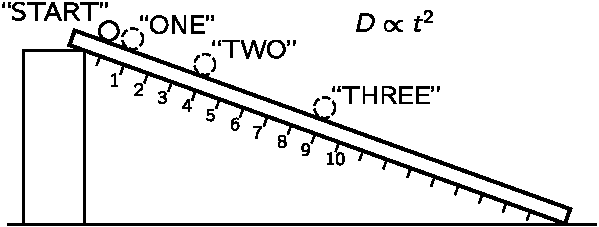
\includegraphics[width=0.8\linewidth]{fyz_fig064.pdf}
      \caption{Zatížená tyč podepřená na jednom konci (\cite[s.~64]{Feynman01})}
      \label{fyz:fig064}
    \end{figure}
    
    Způsob měření vzdálenosti byl dobře znám dávno před Galileem, neexistovaly však přesné způsoby 
    měření času, zejména krátkých časů. Ačkoli sám později vynalezl spolehlivější hodiny (ne však 
    takové, jaké známe dnes), prováděl Galileo své první experimenty tak, že pomocí vlastního 
    pulzu určoval stejné časové intervaly. Udělejme nyní totéž:
    
    Počítejme údery tepu po dobu pohybu kuličky: „raz... dva... tři... čtyři... pět... šest... 
    sedm... osm...“. Požádejme kolegu, aby označil polohu kuličky při každém tepu. Tak můžeme 
    \emph{změřit vzdálenost}, kterou kulička urazila od vypuštění za jeden, dva, tři atd. stejné 
    intervaly času. Galileo vyjádřil výsledek svých pozorování následujícím způsobem: Když si 
    polohu kuličky značíme po \num{1}, \num{2}, \num{3}, \num{4} ... jednotkách času od jejího 
    vypuštění, pak jsou tyto značky vzdáleny od počátečního bodu úměrně číslům \num{1}, \num{4}, 
    \num{9}, \num{16} ... Dnes bychom řekli, že vzdálenost je úměrná druhé mocnině času
    \begin{equation*}
      s \sim t^2.
    \end{equation*}
    
    Studium \emph{pohybu}, které je základem všech fyzikálních disciplín, se zabývá dvěma otázkami: 
    kde? a kdy?
    
  \section{Čas}
    Nejprve se zamysleme nad tím, co chápeme jako \emph{čas}. Co \emph{je} čas? Bylo by krásné, 
    kdyby se nám podařilo najít dobrou definici času. Ve slovnících nacházíme „čas“ definovaný jako 
    „období“ a „období“ zase jako „čas“, což se nezdá být příliš použitelné. Snad bychom mohli 
    říci: „Čas je to, co se děje, když se nic jiného neděje.“ To nás však nedovede příliš daleko. 
    Je snad právě tak dobré, když si přiznáme, že čas je jedna z těch věcí, kterou pravděpodobně 
    nemůžeme definovat (v slovníkovém smyslu), a říkat o něm jen to, co už víme: Čas je to, jak 
    dlouho čekáme!
    
    Skutečně důležité však není to, jak čas \emph{definujeme}, ale jak ho \emph{měříme}. Jedním ze 
    způsobů měření časuje využití něčeho, co se neustále děje, a to pravidelným způsobem - něčeho, 
    co je \emph{periodické}. Například den. Den, ten se stále opakuje. Když však o tom uvažujeme, 
    můžeme si položit otázku: .Jsou dny periodické, jsou pravidelné? Mají všechny dny stejnou 
    délku?“ Určitě máme dojem, že letní dny jsou delší než zimní. Ovšem, když se moc nudíme, 
    připadají nám i některé zimní dny velmi dlouhé. Již jsme určitě slyšeli někoho zvolat: „Ach, to 
    byl dnes dlouhý den!“
    
    Zdá se však, že dny jsou v \emph{průměru} téměř stejně dlouhé. Existuje způsob, jak prověřit, 
    jsou-li dny stejně dlouhé, buď dva za sebou následující nebo alespoň v průměru? Jedním ze 
    způsobů je porovnání s jiným periodickým jevem. Všimněme si, jak je možné takové porovnání 
    provést pomocí přesýpacích hodin. Pomocí přesýpacích hodin „vytvoříme“ periodičnost, budeme-li 
    je ve dne v noci překlápět, jakmile se přesype poslední zrnko písku.
    
    Potom nám stačí spočítat počet překlopení hodin od jednoho do druhého rána. Tak zjistíme, že 
    počet „hodin“, tj. překlopení, není každý „den“ stejný! Mohli bychom podezřívat Slunce nebo 
    přesýpací hodiny nebo oboje. Po jistých úvahách by nás mohlo napadnout, že „hodiny“ je třeba 
    počítat od poledne do poledne. (Poledne tu \emph{nedefinujeme} jako 12.00 hodin, ale jako 
    okamžik, kdy Slunce vrcholí.) Tentokrát bychom zjistili, že každý den má stejný počet „hodin“. 
    Získali jsme jakousi důvěru, že jak „hodina“, tak „den“ se pravidelně opakují, tj. vyznačují po 
    sobě následující stejné časové intervaly, ačkoli jsme \emph{nedokázali}, že jsou „skutečně“ 
    periodické. Je možné si položit otázku, zda by nemohla jakási zázračná bytost zpomalovat pohyb 
    písku v noci a urychlovat ho ve dne. Náš experiment na takovouto otázku odpověď nedává. Můžeme 
    říci jen tolik, že jsme zjistili, že pravidelnost jednoho druhu je ve shodě s pravidelností 
    jiného druhu. Můžeme říci, že naše definice času spočívá v opakování se určité zřejmě  
    periodické události.
    
  \section{Krátké časy}
    Měli bychom si uvědomit, že při zkoušce opakování dne jsme získali i další důležitý poznatek. 
    Našli jsme způsob přesnějšího měření \emph{částí} dne. Našli jsme způsob měření kratších 
    časových úseků. Můžeme v tomto postupu pokračovat a tak měřit ještě kratší časové intervaly?
    Galileo zjistil, že kyvadlo vykoná každý kyv za stejnou dobu, zůstává-li velikost rozkyvu malá. 
    Potvrzuje to test určující počet kyvů kyvadla za jednu „hodinu“. Takto můžeme vytvořit značky 
    zlomků hodiny. Použijeme-li mechanické zařízení na počítání kyvů a na udržení chodu kyvadla - 
    získáme kyvadlové hodiny našich dědečků.
    
    Dohodněme se, že jestliže naše kyvadlo kmitá \num{3600}-krát za hodinu (a je-li takových hodin 
    \num{24} za den), nazveme periodu kyvadla jednou „sekundou“. Tak jsme naši původní časovou 
    jednotku rozdělili přibližně na \num{10e5} částí. Stejně můžeme sekundu rozdělit na menší a 
    menší intervaly. Zjistíme, že není praktické konstruovat mechanická kyvadla, která kývají 
    libovolně rychle, ale můžeme konstruovat \emph{elektrická} kyvadla, nazývaná 
    \textbf{oscilátory}, která nám poskytnou periodicitu s velmi krátkými periodami kmitů. V 
    takových elektronických oscilátorech je to elektrický proud, který kmitá podobným způsobem jako 
    kyvadlo.
    
    Můžeme sestrojit celou řadu takových elektronických oscilátorů, každý s periodou desetkrát 
    kratší, než má předcházející. Každý oscilátor můžeme „kalibrovat“ vůči sousednímu pomalejšímu 
    oscilátoru určením počtu kmitů,jež vykoná za dobu jednoho kmitu pomalejšího oscilátoru. Je-li 
    perioda kmitů našich hodin kratší než zlomek sekundy, nemůžeme určovat kmity bez pomocného 
    zařízení, které rozšiřuje naši pozorovací schopnost. Jedním z takových zařízení je 
    \emph{osciloskop} s elektronovým paprskem, jenž pracuje jako jakýsi mikroskop pro krátké časy. 
    Toto zařízení zakresluje na fluorescenční stínítko graf elektrického proudu (nebo napětí) v 
    závislosti na čase. Připojíme-li osciloskop ke dvěma sousedním oscilátorům z naší posloupnosti 
    tak, že nejprve zakresluje proud jednoho a potom proud druhého oscilátoru, dostáváme dva grafy 
    podobné těm, které jsou znázorněny na obr. \ref{fyz:fig065}. Tak můžeme pohotově určit počet 
    period rychlejšího oscilátoru po dobu jedné periody pomalejšího oscilátoru. Obr. 
    \ref{fyz:fig065} Dva pohledy na obrazovku osciloskopu
    \begin{figure}[ht!]  %\ref{fyz:fig065}
      \centering
      \begin{tabular}{cc}
        \subfloat[ ]{\label{fyz:fig065a}
          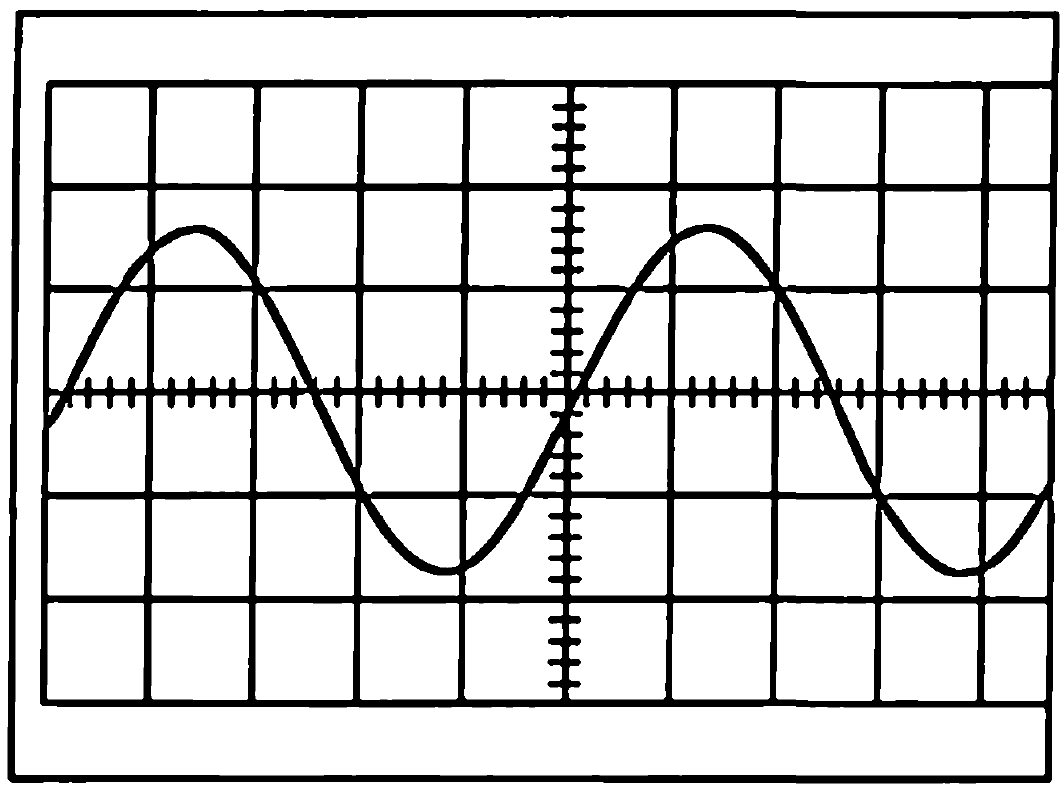
\includegraphics[width=0.2\textwidth]{fyz_fig065a.png}}
        \hspace{0.1\linewidth}                                                       &
        \subfloat[ ]{\label{fyz:fig065b}
          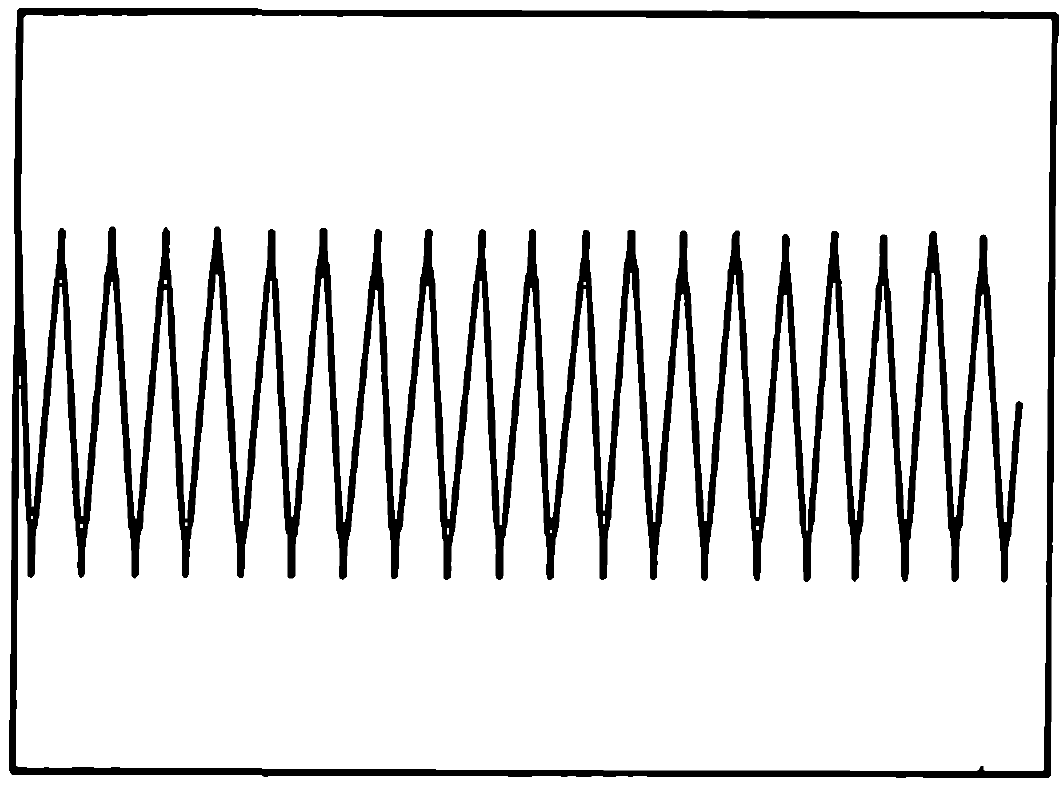
\includegraphics[width=0.2\textwidth]{fyz_fig065b.png}}
      \end{tabular}
      \caption{a) osciloskop je připojen k jednomu oscilátoru. b) osciloskop je připojen k 
               oscilátoru, jehož perioda je desetinou periody předcházejí oscilátoru 	
               (\cite[s.~66]{Feynman01})}
      \label{fyz:fig065}
    \end{figure}
    
    Pomocí moderních elektronických metod byly zkonstruovány oscilátory s periodou krátkou kolem 
    \num{10e12} sekund a byly kalibrovány (porovnávacími metodami podobnými metodě, kterou
    jsme popsali) v naší standardní časové jednotce - sekundě. Vynalezení a zdokonalení „laseru“ 
    neboli zesilovače světla umožnilo v nedávných letech konstrukci oscilátorů s ještě kratšími 
    periodami než \num{10e-12} sekundy, ale zatím je nebylo možné kalibrovat popsaným způsobem, 
    ačkoli i k tomu nepochybně dojde.
    
    Časy kratší než \num{10e-12} sekundy byly měřeny, ale jinými způsoby. Ve skutečnosti byla 
    použita jiná \emph{definice} „času“. Jedním ze způsobů bylo pozorování mezi dvěma událostmi, 
    jež se stanou s pohybujícím se předmětem. Jestliže například zapneme a pak vypneme reflektory 
    pohybujícího se auta, můžeme určit, jak \emph{dlouho} byla světla zapnutá, jestliže víme, 
    \emph{kde} byla zapnuta a vypnuta a jakou rychlostí se auto pohybovalo. Čas určíme tak, že 
    vzdálenost, po kterou byla světla zapnutá, dělíme rychlostí.
    
    Nedávno byla taková metoda použita pro měření doby života \(\pi^0\) mezonu. Mikroskopickým 
    pozorováním drobných stop zanechaných ve fotografické emulzi, v níž byl mezon vytvořen, se 
    zjistilo, že \(\pi^0\) mezon (pohybující se rychlostí téměř rovnou rychlostí světla) urazil v 
    průměru vzdálenost \num{10e-7} metrů dříve, než se rozpadl. Žil jen přibližně \num{10e-16} 
    sekundy. Je třeba však zdůraznit, že jsme použili trochu jinou definici „času“ než předtím. 
    Dokud však není rozpor v našem chápání, věříme, že tyto definice jsou dostatečně rovnocenné.
    
    Dalším rozšířením našich metod - a je-li to nevyhnutelné i našich definicí - můžeme určit 
    trvání ještě rychlejších fyzikálních jevů. Můžeme hovořit o periodě jaderných kmitů. Můžeme 
    hovořit o délce života nově objevených podivných rezonancí (částic). Jejich celková délka 
    života je pouze \num{10e-24} sekundy, což je přibližně doba, kterou potřebuje světlo 
    (pohybující se největší ze známých rychlostí) k průchodu jádrem vodíku (což je 
    nejmenší známý předmět).
    
    Co je možné říci o ještě kratších časech? Existuje čas v ještě menším měřítku? Má vůbec smysl 
    hovořit o ještě kratších časech, když neumíme měřit - nebo dokonce si rozumně představit - 
    něco, co se odehrává v kratším čase? Snad ne. Toto jsou některé otevřené otázky, které si 
    budeme klást a na které snad nalezneme odpověď za dalších dvacet nebo třicet let.
    
  \section{Dlouhé časy}
    Nyní uvažujme časy delší než jeden den. Měření dlouhých časů je jednoduché; budeme prostě 
    počítat dny - dokud bude existovat někdo, kdo to bude moci dělat. Tak docházíme k další 
    přirozené periodicitě: roku, který má přibližně \num{365} dní. Zjišťujeme i to, příroda nám 
    někdy poskytuje počítadlo let, a to v podobě letokruhů stromů nebo říčních naplavenin. V 
    některých případech můžeme využít těchto přírodních časových značek k určení času, který 
    uplynul od nějaké dávné události.
    
    Nemůžeme-li při měření dlouhých časů počítat roky, musíme hledat jiný způsob měření. Jedním z 
    nejúspěšnějších je použití \emph{radioaktivního materiálu} jako „hodin“. V tomto případě nemáme 
    periodický proces tak jako v případě dne nebo kyvadla, ale máme nový druh „pravidelností“. 
    Zjišťujeme, že radioaktivita jistého vzorku materiálu klesá o stejné \emph{procento},    
    jestliže ji určujeme ve dvou stejných po sobě jdoucích přírůstcích jeho věku. Nakreslíme-li 
    graf radioaktivity v závislostí na čase (měřeného např. ve dnech), dostaneme křivku jako na 
    obr. \ref{fyz:fig066}. Vidíme, že v případě poklesu radioaktivity na jednu polovinu za \(T\) 
    dní (\(T\) nazýváme „poločasem rozpadu“) dochází k poklesu na jednu čtvrtinu za dalších \(T\) 
    dní atd. V libovolném časovém intervalu \(t\) je obsaženo \(t/T\) „poločasů rozpadu“ a podíl 
    aktivity, která zbývá po čase \(t\) je roven \((l/2)^{\frac{t}{T}}\).

    \begin{figure}[ht!]  %\ref{fyz:fig066}
      \centering
      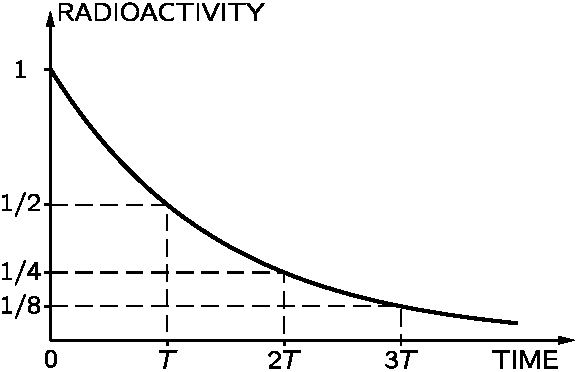
\includegraphics[width=0.6\linewidth]{fyz_fig066.pdf}
      \caption{Pokles radioaktivity s časem; aktivita klesne o polovinu za dobu \uv{poločasu 
      rozpadu} (\cite[s.~68]{Feynman01})}
      \label{fyz:fig066}
    \end{figure}    
    Víme-li, že kousek materiálu, například dřeva, obsahoval při svém vzniku množství \(A\) 
    radioaktivního materiálu a přímým měřením zjistíme, že nyní obsahuje množství \(B\), můžeme 
    vypočítat věk předmětu \(t\) řešením rovnice
    \begin{equation}\label{FYZ:eq065}
      \left(\dfrac{1}{2}\right)^{\dfrac{t}{T}} = \dfrac{B}{A}
    \end{equation}
    
    Naštěstí existují případy, v nichž známe množství radioaktivity přítomné při vzniku předmětu. 
    Víme například, že oxid uhličitý ve vzduchu obsahuje malý zlomek radioaktivního izotopu uhlíku 
    \ce{^{14}C} (neustále doplňovaný působením kosmického záření). Když měříme \emph{celkový} obsah 
    uhlíku v předmětu, víme, že určitý zlomek tohoto množství byl původně radioaktivní \ce{^{14}C}, 
    a proto známe počáteční množství \(A\) vystupující v uvedeném vztahu. Uhlík \ce{^{14}C} má 
    poločas rozpadu \num{5000} let. Pečlivým měřením můžeme zjistit množství, které zůstalo po 
    \num{20} poločasech rozpadu nebo jiném podobném čase a můžeme proto stanovit stáří předmětů z 
    organických látek, které rostly už před \num{100000} lety.
    
    Zajímá nás však i věk ještě starších věcí a zdá se, že ho umíme určit. Mnohé z našich poznatků 
    jsou založeny na měření jiných radioaktivních izotopů, jež mají různé poločasy rozpadu. 
    Použijeme-li izotop, jenž má delší poločas rozpadu, můžeme měřit delší časy. Například uran má 
    izotop, jehož poločas rozpadu je asi \num{10e9} let, takže když nějaký materiál při svém 
    vytvoření před \num{10e9} lety obsahoval uran, zůstane dnes z tohoto uranu jen polovina. Uran 
    se při rozpadu mění na olovo. Uvažujme kousek horniny, jenž vznikl před mnoha lety nějakým 
    chemickým procesem. Olovo, jež se chemicky liší od uranu, by mělo být v jedné části horniny a 
    uran v jiné části horniny. Uran a olovo jsou tedy při vzniku horniny odděleny. Jestliže však 
    tentýž kousek horniny zkoumáme dnes, pak na místě, kde byl původně uran, najdeme určitou část 
    uranu a určitou část olova. Porovnáním těchto částí můžeme určit, kolik procent uranu zaniklo a 
    přeměnilo se na olovo. Touto metodou bylo stáří některých hornin určeno na několik miliard let. 
    Zobecněním této metody, kdy místo v horninách byly uran a olovo sledovány v mořích a byly 
    uvažovány celosvětové průměry, se podařilo (v průběhu nedávných let) určit stáří Země na 
    přibližně \num{5.5} miliardy let.
    
    Povzbuzující je zjištění, že podle uranové metody je Země stejně stará jako meteority, které na 
    ni dopadají. Vypadá to tedy tak, že Země byla vytvořena z kusů skal létajících prostorem a 
    meteority jsou pravděpodobně zbytky tohoto materiálu. Někdy před více než pěti miliardami let 
    měl vesmír svůj počátek. Dnes se domníváme, že alespoň část vesmíru měla počátek před deseti 
    nebo dvanácti miliardami let. Nevíme, co se stalo předtím. Mohli bychom se vlastně ptát: „Má 
    taková otázka smysl? Má dávno minulý čas vůbec nějaký smysl?“
    
    \begin{figure}[ht!]  %\ref{fyz:fig075}
      \centering
      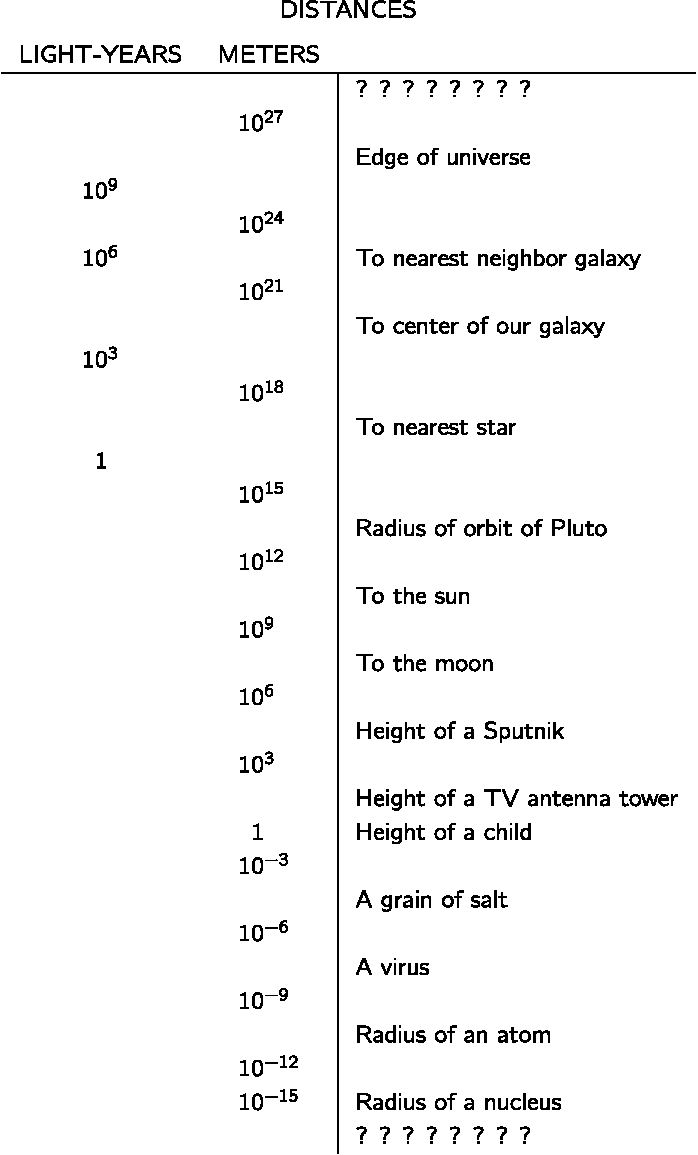
\includegraphics[width=0.7\linewidth]{fyz_fig075.pdf}
      \caption{Tabulka časů (\cite[s.~69]{Feynman01})}
      \label{fyz:fig075}
    \end{figure}

  \section{Jednotky a standardy času}
    Již jsme naznačili, že je vhodné vycházet z nějaké standardní časové jednotky a ostatní časy 
    vztahovat k jejím násobkům nebo zlomkům. Co máme vzít jako základní standard času? Máme za něho 
    zvolit tep lidského srdce? Porovnáme-li tepy, zjistíme, že se značně liší. Porovnáním dvou 
    hodin zjistíme, že se jejich údaje tak mnoho neliší. Proto by bylo možné vzít za standard 
    hodiny. Jenže čí hodiny. Existuje pohádka o švýcarském chlapci, který chtěl, aby všechny hodiny 
    v jeho městě zvonily poledne ve stejnou chvíli. Tak se vydal na cestu, aby přesvědčil lidi o 
    užitečnosti této myšlenky. Každý vlastník hodin považoval tuto myšlenku za vynikající, ale jen 
    v případě, kdy by se všechny ostatní hodiny přizpůsobily jeho hodinám. Je dost těžké 
    rozhodnout, které hodiny je třeba vzít za standard. Naštěstí všichni uznáváme jedny hodiny - 
    Zemi. Perioda otáčení Země byla dlouho považována za časový standard. Když však byla měření 
    stále přesnější, zjistilo se, že rotace Země není dokonale periodická, měříme-li ji 
    nejpřesnějšími hodinami. Těmi „nejpřesnějšími“ hodinami jsou ty, jejichž přesnosti důvěřujeme 
    proto, že jejich údaje navzájem souhlasí. Dnes víme, že z různých důvodů jsou některé dny 
    kratší, jiné delší a v průměru se s postupem času perioda otáčení Země trochu prodlužuje.
    
    Až donedávna jsme nenašli nic lepšího, než periodu zemské rotace, takže všechny hodiny se 
    vztahovaly k délce dne a sekunda byla definována jako \(\frac{1}{\num{86400}}\) středního 
    slunečního dne. Nedávno jsme však získali zkušenosti s některými přírodními oscilátory, o nichž 
    dnes předpokládáme, že poskytují stálejší časový normál než Země a jsou také založeny na 
    přírodním jevu přístupném všem. Jsou to tzv. „atomové hodiny“. Jejich základní vnitřní periodou 
    je perioda atomových kmitů, jež téměř nezávisí na teplotě a jiných vnějších vlivech. Tyto 
    hodiny měří čas s přesností lepší než \num{10e-9}.
    
    Protože se podařilo sestrojit hodiny, udávající čas mnohem přesněji než astronomické metody, 
    je dnes sekunda definována Jako doba trvání \num{9192631770} period záření, které odpovídá 
    přechodu mezí dvěma hladinami velmi jemné struktury základního stavu atomu cesia \num{133}.
    
  \section{Velké vzdálenosti}
    Nyní věnujme pozornost otázce \emph{vzdáleností}. Jak vzdálené, nebo jak velké jsou věci? Každý 
    ví, že při měření vzdáleností vezmeme tyč, postupně ji přikládáme a počítáme. Nebo si pomůžeme 
    palcem a počítáme. Začneme tedy s jednotkou a počítáme. Jak se však měří menší věci? Jak 
    rozdělujeme vzdálenosti? Stejně tak jako jsme rozdělovali čas: Vezmeme menší jednotku a 
    počítáme, kolik takových jednotek vytvoří větší jednotku. Tak můžeme měřit menší a ještě menší 
    délky.

    \begin{figure}[ht!]  %\ref{fyz:fig068}
      \centering
      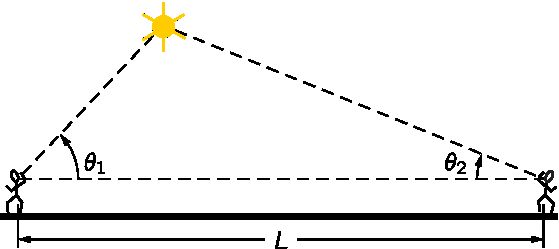
\includegraphics[width=0.6\linewidth]{fyz_fig068.pdf}
      \caption{Výška družice určená triangulací (\cite[s.~70]{Feynman01})}
      \label{fyz:fig068}
    \end{figure}
    
    Vzdáleností však nerozumíme vždy to, co můžeme měřit metrovou tyčí. Bylo by těžké měřit 
    horizontální vzdálenost mezi dvěma vrcholy hor jen pomocí dřevěného metru. Ze zkušeností víme, 
    že vzdálenost je možné měřit i jiným způsobem - \textbf{triangulací}. To sice znamená použít 
    jinou definici vzdálenosti, ale v případech, kdy jsou obě dvě definice použitelné, dávají 
    shodný výsledek. Prostor je více méně tím, za co ho považoval Euklides, a proto jsou uvedené 
    definice shodné. Protože jsou shodné na Zemi, máme k triangulaci určitou důvěru i při použití 
    pro ještě větší vzdálenosti. Například pomocí triangulace jsme mohli změřit výšku první umělé 
    družice. Zjistili jsme, že byla asi \num{5e5} metrů vysoko. Při pečlivém měření můžeme podobně 
    změřit vzdálenost k Měsíci. Dva teleskopy na různých místech Země nám poskytnou dva úhly, které 
    potřebujeme. Takto se zjistilo, že Měsíc je od Země vzdálen \num{4e8} metrů.
    
    Tímto způsobem však nemůžeme měřit vzdálenost ke Slunci, nebo alespoň dosud se to ještě nikomu 
    nepodařilo. Přesnost zaostření na daný bod na Slunci a měření uhlů není dostatečná pro určení 
    vzdálenosti ke Slunci. Jak tedy můžeme měřit vzdálenost ke Slunci? Musíme vymyslet zobecnění 
    myšlenky triangulace. Měříme relativní vzdálenosti všech planet astronomickými pozorováními 
    míst, kde planety vidíme, a tak dostáváme obraz sluneční soustavy se správnými 
    \emph{relativními} vzdálenostmi, ale bez \emph{absolutní} vzdálenosti. Potom potřebujeme jedno 
    absolutní měření, což lze provést různými způsoby. Jedním ze způsobů, o němž se až donedávna 
    předpokládalo, že je nejpřesnější, je měření vzdálenosti od Země k Erosu, jedné z malých 
    planetek, jež se čas od času pohybují v blízkosti Země. Triangulací na tento malý objekt je 
    možné získat požadované cejchovací měření. Známe-li ostatní relativní vzdálenosti, můžeme určit 
    například vzdálenost od Země ke Slunci nebo od Země k Plutu.
    
    \begin{figure}[ht!]  %\ref{fyz:fig069}
      \centering
      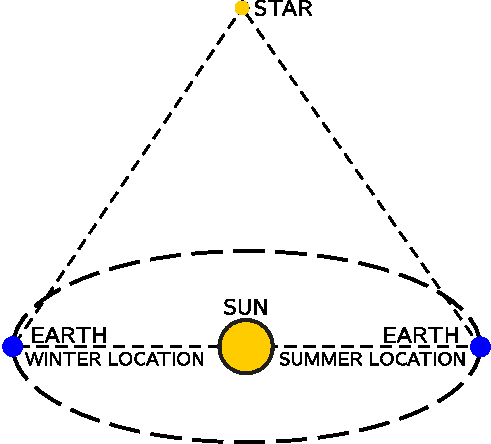
\includegraphics[width=0.7\linewidth]{fyz_fig069.pdf}
      \caption{Vzdálenost blízkých hvězd je možné změřit triangulací, když se jako základny použije 
               průměr zemské oběžné dráhy. (\cite[s.~71]{Feynman01})}
      \label{fyz:fig069}
    \end{figure}     
    V posledních letech se velmi zdokonalily naše poznatky o rozměrech sluneční soustavy. V 
    laboratořích firmy Jet Propulsion byla přesně změřena vzdálenost od Země k Venuši přímým 
    radarovým pozorováním. To je, samozřejmě, další způsob určování vzdáleností. Známe rychlost, 
    jakou se šíří světlo (a tedy i radarové vlny) a předpokládáme, že ta rychlost je stejná všude 
    mezi Zemí a Venuší. Vyšleme rádiovou vlnu a měříme čas, dokud se odražená vlna nevrátí zpět. Z 
    \emph{času} odvodíme \emph{vzdálenost} za předpokladu, že známe rychlost. Máme tedy skutečně 
    jinou definici měření vzdálenosti.
    
    Jak měříme vzdálenost k hvězdě, která je mnohem dále? Naštěstí se můžeme vrátit k triangulační 
    metodě, neboť Země nám při svém pohybu kolem Slunce poskytuje velkou základnu pro měření 
    předmětů mimo sluneční soustavu. Zaostříme-li teleskop na hvězdu v létě a v zimě, máme naději 
    určit dva potřebné úhly dostatečně přesně a můžeme změřit vzdálenost k hvězdě.
   
    Co je však možné dělat tehdy, když jsou hvězdy příliš vzdáleny pro použití triangulace? 
    Astronomové vždy objevují nové způsoby měření vzdáleností. Zjistili například, že je možné 
    odhadnout velikost a jasnost\footnote{V astronomii se pozorovaná jasnost hvězdy udává jako její 
    hvězdná velikost (magnituda).} hvězdy pomocí její barvy. Byly měřeny barva a jasnost mnoha 
    blízkých hvězd - jejichž vzdálenosti známe pomocí triangulace - a bylo zjištěno, že existuje 
    jednoznačný vztah mezi barvou a vlastní jasností hvězd (ve většině případů). Změříme-li barvu 
    vzdálené hvězdy, můžeme využít tohoto vztahu a určit vlastní jasnost hvězdy. Měřením jasnosti 
    hvězdy, kterou \emph{pozorujeme} na Zemi (mohli bychom říci, jak tmavá se nám hvězda jeví), 
    můžeme vypočítat, jak je hvězda vzdálená. (Při dané vlastní jasnosti klesá pozorovaná jasnost 
    se čtvercem vzdálenosti.) Pěkným potvrzením správnosti této metody měření hvězdných vzdáleností 
    jsou výsledky získané pro skupinu hvězd známých jako kulové hvězdokupy. Fotografie takové 
    skupiny je znázorněna na obr. \ref{fyz:fig070}. Hned při prvním pohledu na fotografuje člověk 
    přesvědčen, že tyto hvězdy jsou pohromadě. Tentýž výsledek je možné získat i z měření 
    vzdáleností pomocí metody jasnost-barva.

    \begin{figure}[ht!]  %\ref{fyz:fig070}
      \centering
      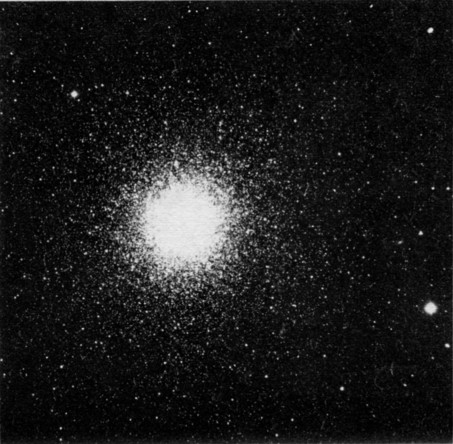
\includegraphics[width=0.6\linewidth]{fyz_fig070.jpg}
      \caption{Hvězdokupa v blízkosti centra naší galaxie. Tyto hvězdy jsou od Země vzdáleny 
               \num{30000} světelných let, tedy asi \SI{3e20}{\m}. (\cite[s.~72]{Feynman01})}
      \label{fyz:fig070}
    \end{figure}
    
    Studium mnoha kulových hvězdokup poskytuje další důležitou informaci. Bylo zjištěno, že v 
    určité části oblohy je vysoká koncentrace takových shluků a většina z nich je od náš téměř 
    stejné vzdálena. Spojením této informace s jinými důkazy docházíme k závěru, že tato 
    koncentrace hvězdokup označuje střed naší galaxie. Tak víme, že vzdálenost do středu galaxie je 
    asi \num{e20} metrů. 
    

    \begin{figure}[ht!]  %\ref{fyz:fig071}
      \centering
      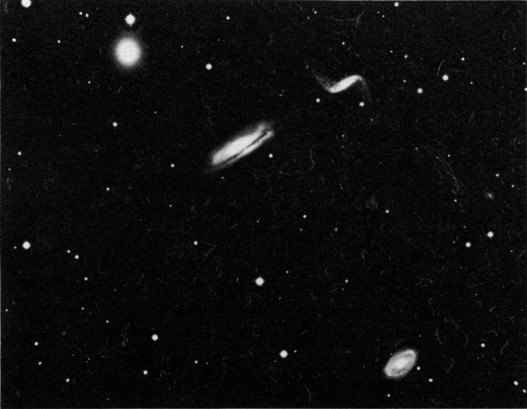
\includegraphics[width=0.6\linewidth]{fyz_fig071.jpg}
      \caption{Spirální galaxie podobná naší. Za předpokladu, že její průměr je stejný jako průměr 
               naší galaxie, můžeme z její zdánlivé velikosti určit její vzdálenost. Od Země je 
               vzdálena \num{30} milionů světelných roků (\(\SI{3e23}{\m}\)). 
               (\cite[s.~72]{Feynman01})}
      \label{fyz:fig071}
    \end{figure}

    Poznání velikosti naší vlastní galaxie nám dalo do ruky klíč k měření ještě větších vzdáleností 
    - vzdáleností k jiným galaxiím. Obr. \ref{fyz:fig071} je fotografie galaxie, jež má tvar velmi 
    podobný naší galaxii. Pravděpodobně je i stejně velká. (Jiné důkazy hovoří ve prospěch 
    myšlenky, že všechny galaxie jsou přibližně stejně velké.) Je-li stejně velká jako naše 
    Galaxie, pak můžeme určit její vzdálenost. Změříme úhel, který vytíná na obloze a když zjistíme 
    její průměr, vypočteme její vzdálenost opět triangulací.

    \begin{figure}[ht!]  %\ref{fyz:fig072}
      \centering
      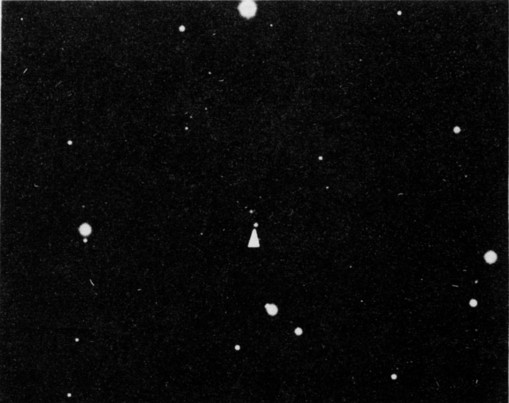
\includegraphics[width=0.6\linewidth]{fyz_fig072.jpg}
      \caption{Od nás nejvzdálenější objekt 3C295 v souhvězdí pastýře (označený šipkou), jenž byl v 
               roce \num{1960} změřen \num{5} metrovým teleskopem (\cite[s.~73]{Feynman01})}
      \label{fyz:fig072}
    \end{figure}
    
    Pomocí obrovského teleskopu na Mt. Palomar byly nedávno získány fotografie velmi vzdálených 
    galaxií. Jedna z nich je na obr. \ref{fyz:fig072}. Dnes se domníváme, že některé z těchto 
    galaxií jsou v přibližně poloviční vzdálenosti k hranicím vesmíru - vzdáleny \num{e26} metrů, 
    což je největší vzdálenost, kterou můžeme uvažovat!
    
  \section{Malé vzdálenosti}
    Uvažujme nyní menší vzdálenosti. Dělení metru na části je jednoduché. Bez větších problémů 
    můžeme vyznačit tisíc stejných částí, které dohromady dávají jeden metr. S trochu většími 
    obtížemi, ale podobným způsobem (pomocí dobrého mikroskopu), můžeme vyznačit tisíc stejných 
    částí milimetru a vytvořit tak stupnici mikrometrů (miliontin metru). Je těžké pokračovat k 
    menším stupnicím, protože nemůžeme \uv{vidět} předměty, jež jsou menší než vlnová délka 
    viditelného světla (kolem \num{5e-7} metru).

    \begin{figure}[ht!]  %\ref{fyz:fig073}
      \centering
      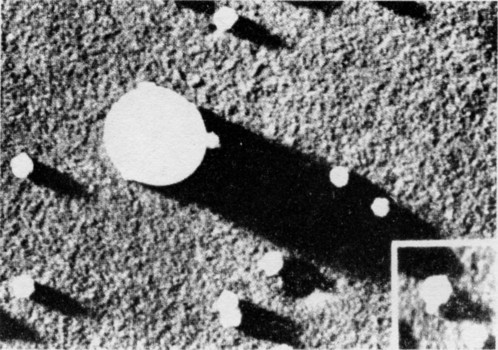
\includegraphics[width=0.6\linewidth]{fyz_fig073.jpg}
      \caption{Fotografie virových molekul zhotovená pomocí elektronového mikroskopu. \uv{Velká} 
               koule slouží ke kalibraci a má průměr \SI{2e-7}{\m}  (\cite[s.~74]{Feynman01})}
      \label{fyz:fig073}
    \end{figure}
    
    Omezovat se jen a to, co můžeme vidět, však není  nevyhnutelné. Pomocí elektronového mikroskopu 
    můžeme pokračovat v našem postupu a můžeme získat fotografie v ještě menším měřítku, asi tak 
    \num{e-8} metru  (\ref{fyz:fig073}). Nepřímými měřeními - jistým druhem triangulace v 
    mikroskopických rozměrech - můžeme pokračovat v měření menších a menších předmětů. Především ze 
    způsobu odrazu světla krátkých vlnových délek (rentgenových paprsků) na systému bodů se známými 
    rozestupy určíme vlnovou délku světelného vlnění. Potom z rozptylových obrazců téhož světla na 
    krystalu můžeme určit relativní polohy atomů v krystalu. Tak získáme výsledky, jež souhlasí s 
    rozložením atomů určeným chemickými prostředky. Tímto způsobem zjistíme, že atom má průměr asi 
    \num{e-10} metru. 

    Mezi typickým atomovým rozměrem \num{e-10} metru a jadernými rozměry \num{e-15} metru řádově 
    \num{e5}-krát menšími je velká \uv{mezera} ve fyzikálních rozměrech. Pro jaderné rozměry se 
    stává výhodným jiný způsob měření velikosti. Měříme \emph{zdánlivou} plochu \(\sigma\) 
    nazývanou \emph{účinným průřezem}. Chceme-li zjistit poloměr, získáme ho ze vztahu \(\sigma = 
    \pi r^2\), neboť jádro je téměř kulové. 

    Jaderný průřez je možné měřit při dopadu svazku vysokoenergetických částic na tenkou vrstvu 
    materiálu sledováním počtu částic jež jsou odchýleny. Tyto vysokoenergetické částice  proniknou 
    řídkým oblakem elektronů a zastaví se nebo se vychýlí jen tehdy, narazí-li na soustředěnou 
    hmotu jádra. Předpokládejme, že máme kousek materiálu, který je \SI{1}{\cm} tlustý. V takovém 
    kousku bude asi \num{e8} atomových vrstev. Jádra jsou však tak malá, že je málo pravděpodobné, 
    že se dvě jádra ocitnou za sebou. Můžeme si tedy \emph{představit} že velmi zvětšený pohled na 
    situaci - hledíme-li ve směru svazku částic - vypadá tak jako na obr. \ref{fyz:fig076}. 

    \begin{figure}[ht!]  %\ref{fyz:fig076}
      \centering
      
\includegraphics[width=0.7\linewidth]{fyz_fig076.pdf}
      \caption{Vzdálenost blízkých hvězd je možné změřit triangulací, když se jako základny použije 
               průměr zemské oběžné dráhy. (\cite[s.~71]{Feynman01})}
      \label{fyz:fig076}
    \end{figure}   
    Pravděpodobnost, že velmi malá částice se na své cestě destičkou srazí s jádrem, je dána 
    podílem celkové plochu jader a celkové plochy vzorku. Předpokládejme, že na ploše \(A\) našeho 
    kousku materiálu se nachází \(N\) atomů (samozřejmě, každý s jedním jádrem). Pak celková plocha 
    \uv{pokrytá} jádry je rovna \(N\sigma\). Nechť je počet částic svazku, jež dopadají na kousek 
    materiálu roven \(n_1\) a počet částic, jež na druhé straně z materiálu vycházejí, roven 
    \(n_2\). Zlomek těch, které neprojdou materiálem, je \(\frac{n_1-n_2}{n_1}\) a měl by být roven 
    poměru \(N\frac{\sigma}{A}\) plochy pokryté jádry a původní plochy \(A\). Poloměr jádra můžeme 
    dostat z rovnice
    \begin{equation}\label{FYZ:eq066}
      \pi r^2 = \sigma = \frac{A}{N}\cdot\frac{n_1-n_2}{n_1}.
    \end{equation}
    (Tato rovnice je správná jen tehdy, když je plocha pokrytá jádry jen malou částí celkové 
    plochy, tj. když \(\frac{n_1-n_2}{n_1}\) je mnohem menší než \num{1}. V opačném případě je 
    potřebná korekce, která bere v úvahu skutečnost, že některé jádra budou částečně zastíněna 
    jádry stojícími před nimi.) Podobnými experimenty se podařilo zjistit, že poloměr jádra je od 
    \SI{1e-15}{\m} do \SI{6e-15}{\m}. Na počest Enrica Fermiho (1901 - 1958) byla délková jednotka 
    \SI{e-15}{\m} nazvána \emph{fermi}. Dnes se však již tato jednotka nepoužívá. Byla nahrazena 
    \emph{femtometrem}, s níž má shodnou alespoň značku.
    
    \begin{figure}[ht!]  %\ref{fyz:fig074}
      \centering
      \includegraphics[width=0.8\linewidth]{fyz_fig074.pdf}
      \caption{Tabulka vzdáleností (\cite[s.~75]{Feynman01})}
      \label{fyz:fig074}
    \end{figure}
    
    Co zjišťujeme, jdeme-li k ještě menším vzdálenostem? Můžeme menší vzdálenosti měřit? Na tuto 
    otázku zatím není možné dát odpověď. Existuje hypotéza, podle níž je zatím nevyřešenou záhadu 
    jaderných sil možno odhalit jen jakousi modifikací naší představy o prostoru nebo o měření tak 
    malých vzdáleností.
    
    Zdálo by se rozumné použít za jednotku délky nějakou přirozenou délku - řekněme poloměr Země 
    nebo jeho zlomek. Metr byl původně navržen takovýmto způsobem a byl definován jako 
    \(\frac{\pi}{2}\cdot\num{e-7}\) násobek zemského poloměru. Takové určení délkové jednotky není 
    příliš výhodné ani příliš přesné. Dlouho byla obecně uznávána definice metru jako vzdálenosti 
    mezi dvěmi vrypy na tyči nacházející se ve speciální laboratoři ve Francii. Nedávno se však 
    zjistilo, že ani taková definice není dostatečně přesná, stálá a univerzální. Proto byla v r. 
    1983 přijata nová definice metru jako délka dráhy, kterou proběhne světlo ve vakuu za dobu 
    \(\frac{\num{1}}{\num{299792458}}\) sekundy.
    
    Měření vzdálenosti a času poskytují výsledky, které závisí na pozorovateli. Dva pozorovatelé, 
    kteří se vzájemně pohybují, nezměří stejné vzdálenosti a časy při měření toho, co se jeví jako 
    stejná věc. Vzdálenosti a časové intervaly mají různé velikosti v závislosti na vztažné 
    soustavě použité při měření. Tuto otázku budeme podrobněji studovat později.
    
    Zcela přesné měření vzdáleností a časů nedovoluje ani povaha přírody. Už dříve jsme řekli, že 
    chyba v měření polohy předmětu musí být přinejmenším
    \begin{equation}\label{FYZ:eq067}
      \Delta x = \frac{h}{\Delta p},
    \end{equation}
    kde \(h\) je malá veličina nazývaná \textbf{Planckova konstanta} a \(\Delta p\) je nepřesnost 
    našeho poznání hybnosti (hmotnosti násobené rychlostí) předmětu, jehož polohu měříme. Zmínili 
    jsme se i o tom, že neurčitost v měření polohy souvisí s vlnovou povahou částic.
    
    Relativnost prostoru a času znamená, že i měření času mají minimální chybu danou vztahem
    \begin{equation}\label{FYZ:eq068}
      \Delta t = \frac{h}{\Delta E},
    \end{equation}
    přičemž \(\Delta E\) je nepřesnost našeho poznání energie procesu, jehož časovou periodu 
    měříme. Chceme-li přesněji zjistit, kdy se něco uskutečnilo, musíme vědět méně o tom, co se 
    uskutečnilo, neboť budeme méně vědět o energii takového procesu. I Časová neurčitost souvisí s 
    vlnovou povahou hmoty.
    
} %tikzset
%---------------------------------------------------------------------------------------------------
\printbibliography[heading=subbibliography]
\addcontentsline{toc}{section}{Seznam literatury}
%  % !TeX program = lualatex
% !TeX root = luaking.tex
% !TeX encoding = UTF-8
% !TeX spellcheck = cs_CZ
%---------------------------------------------------------------------------------------------------
% file fey1ch06.tex
\graphicspath{{../src/FYZ/img/}}
%---------------------------------------------------------------------------------------------------
%================= Kapitola: Pravděpodobnost =======================================================
\setchaptertoc
\chapter{Feynmanova přednáška o pravděpodobnosti}\label{chap:fey_ppst}
\epigraph{\emph{The true logic of this world is in the calculus of probabilities.}}{James Clerk 
Maxwell}
  \section{Možnost a pravděpodobnost}
    Možnost je slovo, které se často používá v každodenním životě. V rozhlasovém zpravodajství o 
    zítřejším počasí můžeme slyšet: „Zítra odpoledne předpovídáme možnost bouřek.“ Můžeme si říci: 
    „Mám jen malou možnost dožít se sta let.“ I vědci používají slovo možnost. Seismologové si 
    kladou otázku: Jaká je možnost, že v příštím roce bude v jižní Kalifornii zemětřesení určité 
    intenzity?“ Fyzik si může položit otázku: Jaká je možnost, že určitý Geigerův počítač 
    zaregistruje v příštích \num{10} sekundách \num{20} částic?“ Politika nebo státníka může 
    zajímat otázka: Jaká je možnost, že v průběhu následujících deseti let dojde k jaderné válce?“ 
    Vás může zajímat, jakou máte možnost se něco naučit z této kapitoly.
    
    \emph{Možností} rozumíme něco jako odhad. Proč odhadujeme? Odhady děláme tehdy, když chceme 
    něco posoudit, ale máme neúplné informace nebo nespolehlivé znalosti. Chceme uhádnout, jaké 
    věci jsou, nebo co se stane. Často také děláme odhad před nějakým rozhodnutím. Například: Mám 
    si vzít zítra plášť do deště? S jakým pohybem půdy bych měl počítat při návrhu nové stavby? Mám 
    si vybudovat protiatomový kryt? Mám změnit své stanovisko při mezinárodních jednáních? Mám dnes 
    jít do školy?
    
    Někdy děláme odhad proto, že se svými omezenými znalostmi chceme co nejvíce říci o určité 
    situaci. V odhadu je skutečně velké zobecnění. Jakákoli fyzikální teorie je jistým druhem 
    odhadu. Existují dobré a špatné odhady. Teorie pravděpodobnosti představuje systém pro     
    vytváření co nejlepších odhadů. Řeč pravděpodobnosti nám dovoluje hovořit kvantitativně o 
    určitých situacích, jež mohou být velmi proměnlivé, ale které mají určité stálé průměrné 
    chování.
    
    Uvažujme házení mincí. Jsou-li samotný hod i mince „poctivé“, nemůžeme vědět, jaký bude 
    výsledek určitého jednotlivého hodu. Přece však cítíme, že při velkém počtu hodů budou 
    přibližně stejně zastoupeny hlavy i znaky. Proto říkáme: „Pravděpodobnost, že padne hlava, je 
    \num{0.5}.“
    
    O pravděpodobnosti hovoříme jen při takových pozorováních, o nichž předpokládáme, že se 
    uskuteční v budoucnosti. \emph{„Pravděpodobnosti“ určitého výsledku pozorováni rozumíme náš 
    odhad toho, jaká část z velkého počtu provedených pozorováni nejspíše dá tento očekávaný 
    výsledek}. Představíme-li si, že pozorování - takové jako pohled na právě hozenou minci - se 
    opakuje \(N\)- krát a označíme-li \(N_A\) \emph{náš odhad} počtu těch pozorování, která dávají 
    určitý výsledek \(A\) (řekněme hlavu), pak pravděpodobností \(P (A)\) pozorování \(A\) rozumíme
    \begin{equation}\label{fyz:eq069}
      P(A) = \frac{N_A}{N}.
    \end{equation}
    
    Naše definice si vyžaduje několik poznámek. O pravděpodobnosti nějaké události můžeme hovořit 
    jen tehdy, je-li tato možným výsledkem nějakého \emph{opakovatelného} pozorování. Není jasné, 
    má-li smysl se ptát: Jaká je pravděpodobnost toho, že v tomto domě straší?“
    
    Mohli bychom namítat, že žádná situace není přesně opakovatelná. To je pravda. Každé další 
    pozorování provádíme přinejmenším v jiném čase nebo na jiném místě. Můžeme říci jen tolik, že 
    „opakovaná“ pozorování by se měla v souladu s naším záměrem \emph{jevit jako ekvivalentní}. 
    Měli bychom předpokládat alespoň to, že každé pozorování se provádělo ve stejně připravené 
    situaci a zejména se stejným stupněm nevědomosti na počátku. (Jestliže se nám podaří nahlédnout 
    do soupeřových karet, bude odhad naděje našeho vítězství jiný než v případě, kdy jsme soupeřovy 
    karty neviděli!)
    
    Je třeba zdůraznit, že \(N\) a \(N_A\) ve vztahu (\ref{fyz:eq069}) \emph{nechápeme} jako čísla 
    založená na skutečných pozorováních. \(N_A\) je náš nejlepší \emph{odhad} toho, co \emph{by 
    mělo} nastat při \(N\) \emph{myšlených} pozorováních. Pravděpodobnost proto závisí na našich 
    znalostech a na naší schopnosti odhadovat. Závisí na našem úsudku! Lidé naštěstí uvažují o 
    mnoha věcech do určité míry stejně, a tak i jejich odhad bude stejný. Pravděpodobnosti však 
    nemusejí být „absolutními“ čísly. Protože závisí na naší nevědomosti, mohou se změnit se změnou 
    našich poznatků.
    
    Možná jsme si všimli jiného, dost „subjektivního“ aspektu naší definice pravděpodobnosti. 
    Hovořili jsme o \(N_A\) jako o „našem odhadu toho, jaká část pozorování nejspíše povede...“. 
    Nerozumíme tím, že budeme pozorovat přesně hodnotu \(N_A\), ale že očekáváme číslo blízké 
    \(N_A\), a že to číslo \(N_A\) je \emph{pravděpodobnější} než jiná čísla v sousedství. 
    Hodíme-li minci \num{30}-krát, neočekáváme, že počet hlav bude přesně \num{15}, ale že to bude 
    spíše nějaké jiné číslo blízké \num{15}, např. \num{12}, \num{13}, \num{14}, \num{15}, \num{16} 
    nebo \num{17}. Jestliže se však musíme pro nějaké číslo rozhodnout, pak si zvolíme \num{15} 
    jako nejpravděpodobnější počet hlav. Můžeme psát \(P(hlava) = \num{0.5}\).
    
    Proč jsme se rozhodli pro \num{15} jako pro nejpravděpodobnější Číslo? V duchu jsme měli 
    následující důvody: Když z celkového počtu hodů \(N\) je \(N_H\) nejpravděpodobnější počet 
    hlav, pak nejpravděpodobnější počet znaků je \((N - N_H)\). (Předpokládáme, že každý hod dá 
    buď hlavu \emph{nebo} znak a jiná možnost neexistuje!) Je-li však mince „poctivá“, není důvodu 
    pro upřednostnění hlav před znaky. Pokud není důvod pro předpoklad nepoctivosti mince (nebo 
    hodu), musíme výskyt hlavy považovat za stejně pravděpodobný jako výskyt znaku. Musíme tedy 
    položit \(N_Z = N_H\). Pak platí
    \begin{equation}\label{fyz:eq070}
      N_Z = N_H = \frac{1}{2} \quad \text{nebo}\quad P(H) = P(Z) = \num{0.5}.
    \end{equation}
    
    Naši argumentaci můžeme zobecnit na \emph{jakoukoli} situaci, v níž existuje \(m\) různých, ale 
    ekvivalentních, tj. stejně možných výsledků pozorování. Může-li pozorování vést k \(m\) různým 
    výsledkům a máme důvod věřit, že každý z nich je stejně možný jako jiný, pak pravděpodobnost 
    \emph{příslušného} výsledku \(A\) je
    \begin{equation}\label{fyz:eq071}
      P(A) = \frac{1}{m}.
    \end{equation}
    
    Je-li v neprůhledné krabici sedm kuliček různých barev a jednu náhodně vybereme (aniž bychom se 
    na ně podívali), je pravděpodobnost vytažení určité barvy \num{1/7}. Pravděpodobnost, že ze 
    zamíchané hromady \num{52} karet „naslepo“ vytáhneme právě srdcové eso je rovna \num{1/52}. 
    Pravděpodobnost hodu dvojnásobné jednotky při hře v kostky je \num{1/36}.
    
    V kapitole \ref{fyz:IchapV} jsme popisovali velikost jádra pomocí jeho zdánlivé plochy neboli 
    „průřezu“. Přitom jsme vlastně hovořili o pravděpodobnostech. Když ostřelujeme tenkou vrstvu 
    materiálu vysokoenergetickými částicemi, existuje jistá naděje, že částice projde materiálem a 
    jistá naděje, že narazí na jádro. (Protože jádro je tak malé, že ho nemůžeme vidět, nemůžeme na 
    něj přímo mířit. Musíme střílet „naslepo“.) Je-li v naší vrstvě materiálu \(n\) atomů a jádro 
    každého atomu má plochu průřezu \(\sigma\), pak celková plocha „zastíněná“ jádry je 
    \(n\sigma\). Při velkém počtu \(N\) náhodných střel očekáváme, že počet nárazů \(N_C\) do 
    \emph{některého} jádra bude v takovém poměru k \(N\), jaký je poměr zastíněné plochy k celkové 
    ploše vrstvy
    \begin{equation}\label{fyz:eq072}
      \frac{N_C}{N} = \frac{n\sigma}{A}.
    \end{equation}
    Je proto možné říci, že pravděpodobnost srážky letící částice při průchodu vrstvou je
    \begin{equation}\label{fyz:eq073}
      P_C = \frac{n}{A}\sigma.
    \end{equation}
    kde \(\frac{n}{A}\) je počet atomů v jednotkové ploše vrstvy.
    
  \section{Fluktuace}
    Nyní si na základě našich poznatků o pravděpodobnosti podrobněji všimneme otázky: „Kolikrát 
    skutečně očekávám, že padne hlava, budu-li házet minci \(N\)- krát?“ Dříve než odpovíme na tuto 
    otázku, podívejme se, co se vlastně děje při takovém „experimentu“. Obr. \ref{fyz:fig077} 
    obsahuje výsledky získané v prvních třech „kolech“ takového experimentu, když \(N= 30\). 
    Posloupnosti hlav a znaků jsou znázorněny tak, jak byly získány. První hra dala \num{11} hlav, 
    druhá také \num{11}, třetí \num{16}.
    
    \begin{figure}[ht!]  %\ref{fyz:fig077}
      \centering
      \includegraphics[width=0.8\linewidth]{fyz_fig077.pdf}
      \caption{Pozorované posloupnosti hlava znaků ve třech hrách po třiceti hodech 
              (\cite[s.~79]{Feynman01})}
      \label{fyz:fig077}
    \end{figure}
    Ve třech pokusech jsme ani jednou nedostali \num{15} hlav. Je to snad vinou mince? Nebo jsme se 
    zmýlili v úvaze vedoucí k závěru, že nejpravděpodobnější počet hlav v takové hře je \num{15}? 
    Abychom získali \num{100} experimentů, každý po \num{30} hodech, uskutečnili jsme dalších 
    \num{97} \uv{kol}. Výsledek experimentu ukazuje tab. \ref{fyz:fig079}\footnote{Po prvních třech 
    hrách jsme experiment ve skutečnosti provedli tak, že jsme silně zatřásli krabicí, v níž bylo 
    \num{30} mincí a pak jsme spočetli všechny hlavy.}.
    
    Prohlédneme-li si čísla v tab. \ref{fyz:fig079}, zjistíme, že většina výsledků je blízko čísla 
    \num{15} v tom smyslu, že se nacházejí mezi čísly \num{12} a \num{18}. K získání lepšího citu 
    pro chápání detailů těchto výsledků je vhodné zakreslit graf \emph{rozložení} výsledků. Určíme 
    počet her, v nichž jsme získali \(k\) hlav a znázorníme si je pro každé \(k\). Takový graf je 
    znázorněn na obr. \ref{fyz:fig078}. \num{15} hlav jsme získali ve \num{13} hrách. \num{14} 
    hlav jsme získali \num{13}-krát. \num{16} i \num{17} hlav jsme získali dokonce více než 
    \num{13}-krát.

    \begin{figure}[ht!]  %\ref{fyz:fig079}
      \centering
      \includegraphics[width=1\linewidth]{fyz_fig079.png}
      \caption{Tabulka počtu hlav v posloupnosti \num{30} hodů mincí (\cite[s.~80]{Feynman01})}
      \label{fyz:fig079}
    \end{figure}
    Je možné z toho odvodit, že jde o jakousi zaujatost ve prospěch hlav? Nebyl náš „nejlepší 
    odhad“ dostatečně dobrý? Můžeme říci, že nejpravděpodobnější počet hlav pro jednu hru 
    sestávající z \num{30} hodů je \num{16}? Musíme být opatrní! Ve všech hrách se dohromady 
    uskutečnilo \num{3000} hodů. Hlav padlo celkem \num{1492}. Poměr počtu hlav k celkovému počtu 
    je tedy \num{0.497}, což je sice jen o málo, ale přece jen méně než polovina. Určitě tedy 
    nemůžeme předpokládat, že pravděpodobnost padnutí hlavy je větší než \num{0.5}! Skutečnost, že 
    v \emph{určité} sérii pozorování padne hlava nejčastěji \num{16}-krát, představuje 
    \emph{fluktuaci}. Jsme stále přesvědčeni, že \emph{nejpravděpodobnějším} počtem hlav je 
    \num{15}.
    
    Je možné položit otázku: Jaká pravděpodobnost, že hra s \num{30} hody dá \num{15}, \num{16} 
    nebo nějaký jiný počet hlav?“ Již jsme řekli, že při jednom hodu je pravděpodobnost pádu 
    \emph{jedné} hlavy \num{0.5} a i pravděpodobnost, že nepadne hlava, je \num{0.5}. Ve hře 
    sestávající ze dvou hodů máme \emph{čtyři} možné výsledky: \texttt{HH}, \texttt{HZ}, 
    \texttt{ZH}, \texttt{ZZ}. Protože každá z těchto posloupností je stejně pravděpodobná, můžeme 
    prohlásit, že
    \begin{enumerate}[noitemsep]
      \item pravděpodobnost padnutí dvou hlav je \num{1/4}, 
      \item pravděpodobnost padnutí jedné hlavy je \num{2/4}, 
      \item pravděpodobnost, že nepadne hlava je \num{1/4}. 
    \end{enumerate}
    Existují dva způsoby získávání jedné hlavy, ale jen jeden způsob získávání dvou hlav nebo žádné 
    hlavy.
    
    \begin{figure}[ht!]  %\ref{fyz:fig078}
      \centering
      \includegraphics[width=1\linewidth]{fyz_fig078.pdf}
      \caption{Souhrn výsledků l00 her po 30pokusech. Vertikální čáry ukazuj počty her,v nichž 
              padlo \(k\) hlav. Přerušovaná čára ukazuje očekávaný počet her, v nichž padne \(k\) 
              hlav, získaný výpočtem pravděpodobnosti (\cite[s.~80]{Feynman01})}
      \label{fyz:fig078}
    \end{figure}
    
    Uvažujme nyní hru sestávající ze tří hodů. Pro třetí hod je stejně pravděpodobné, že padne 
    hlava nebo znak. Existuje jen jeden způsob získání tří hlav: v prvních dvou hodech 
    \emph{musely} padnout dvě hlavy a potom hlava i po třetím hodu. Existují však \emph{tři} 
    způsoby získání dvou hlav. Může padnout znak po padnutí dvou hlav (jeden způsob), nebo může 
    padnout hlava po padnutí jen jednoho znaku v prvních dvou hodech (dva způsoby). Tak pro možnosti
    \num{3}, \num{2}, \num{1}, \num{0} hlav existují \num{1}, \num{3}, \num{3}, \num{1} stejně 
    pravděpodobné způsoby představující celkově \num{8} různých posloupností. Příslušné 
    pravděpodobnosti jsou \num{1/8}, \num{3/8}, \num{3/8}, \num{1/8}.

    \begin{figure}[ht!]  %\ref{fyz:fig081}
      \centering
      \includegraphics[width=1\linewidth]{fyz_fig081.pdf}
      \caption{Diagram znázorňující počet různých způsobů padnutí \num{0}, \num{1}, \num{2} nebo 
              \num{3} hlav ve hře sestávající ze tří hodů (\cite[s.~81]{Feynman01})}
      \label{fyz:fig081}
    \end{figure}
    
    To, co jsme řekli, je možno vyjádřit diagramem na obr. \ref{fyz:fig081}. Je jasné, že takové 
    diagramy lze sestrojit i pro hry s vyšším počtem hodů. Obr. \ref{fyz:fig080} znázorňuje takový 
    diagram pro hru se šesti hody. Počet způsobů odpovídajících libovolnému bodu diagramu je 
    vlastně počet různých cest (posloupností hlav a znaků), po nichž lze vyjít z počátečního bodu. 
    Počet úseků šikmo vzhůru udává počet vržených hlav. Soubor čísel, které se objevují v takovém 
    diagramu, je znám jako \textbf{Pascalův trojúhelník}. Čísla jsou známá i pod názvem 
    \emph{binomické koeficienty}, neboť se objevují i v rozvoji \((a + b)^n\). Označíme-li počet 
    hodů \(n\) a počet vržených hlav \(k\), pak se čísla vystupující v diagramu označují symbolem  
    \(\binom{n}{k}\). Bude vhodné připomenout, že binomické koeficienty 
    lze vypočítat ze vztahu
    \begin{equation}\label{fyz:eq074}
      \binom{n}{k} = \frac{n!}{k!(n-k)!}.
    \end{equation}
    kde \(n!\), nazývaný „n-faktoriál“, představuje součin \(n(n- 1)(n-2)\cdots (3)(2)(1)\).
    
    \begin{figure}[ht!]  %\ref{fyz:fig080}
      \centering
      \includegraphics[width=1\linewidth]{fyz_fig080.pdf}
      \caption{Diagram jako na obr. \ref{fyz:fig081}, ale pro hru sestávající ze \num{6} hodů
               (\cite[s.~82]{Feynman01})}
      \label{fyz:fig080}
    \end{figure}
    
    Nyní již můžeme počítat pravděpodobnosti \(P(k, n)\) toho, že při \(n\) hodech padne hlava,
    pomocí definice (\ref{fyz:eq069}). Celkový počet možných posloupností je \(2^n\) (neboť každý
    hod připouští 2 výsledky) a počet způsobů získání \(k\) hlav je \(\binom{n}{k}\), přičemž
    všechny jsou stejně pravděpodobné. Proto máme
    \begin{equation}\label{fyz:eq075}
      P(k,n) = 
      \frac{\binom{n}{k}}{2^n}.
    \end{equation}
    
    Protože \(P(k, n)\) je podíl her, při nichž očekáváme, že padne \(k\) hlav, lze pak očekávat, 
    že při \num{100} hrách padne \(k\) hlav \(100\cdot P(k, n)\) krát. Přerušovaná čára na obr. 
    \ref{fyz:fig078} prochází body vypočítanými ze vztahu \(100\cdot P(k, 30)\). Vidíme, že padnutí 
    \num{15} hlav jsme \emph{očekávali ve} \num{14} nebo \num{15} hrách, zatímco tato událost byla 
    pozorována ve \num{13} hrách. Padnutí \num{16} hlav jsme \emph{očekávali ve} \num{13} nebo 
    \num{14} hrách, ale \num{16} hlav padlo v \num{16} hrách. Takové fluktuace jsou „součástí hry“.
    
    Použitou metodu je možné aplikovat i na tu nejobecnější situaci, v níž jsou jen dva možné 
    výsledky jednoho pozorování. Označme tyto dva výsledky \(V\) („výhra“) a \(P\) („prohra“). V 
    obecném případě pravděpodobnosti výsledku \(V\) nebo \(P\) u jedné události nemusí být stejné. 
    Označme \(p\) pravděpodobnost výhry \(V\). Potom \(q\), pravděpodobnost prohry, musí být nutně 
    \((1 - p)\). V souboru \(n\) pokusů je pravděpodobnost \(P(k, n)\) toho, že vyhrajeme 
    \(k\)-krát rovna
    \begin{equation}\label{fyz:eq076}
      \boxed{P(k,n) = \binom{n}{k}p^kq^{n-k}}\,.
    \end{equation}
    Tato pravděpodobnostní funkce se nazývá \textbf{Bernoulliho} nebo i \textbf{binomickou 
    pravděpodobností}.
    
  \section{Náhodná procházka}
    Existuje další zajímavý problém, v němž vystupuje myšlenka pravděpodobnosti. Je to problém 
    \emph{„náhodné procházky“}. Jako nejjednodušší verzi této úlohy si představme „hru“, v níž 
    „hráč“ startuje v bodě \(x = 0\) a při každém tahu má udělat krok \emph{buď} dopředu (směrem 
    \(k + x\)) nebo dozadu (směrem \(k - x\)). Volba se má uskutečnit náhodně, například pomocí 
    hodu mincí. Jak popíšeme výsledný pohyb? Ve své obecné formě se problém vztahuje na pohyb atomů 
    (nebo jiných částic) v plynech - jde o \textbf{Brownův pohyb} - a i na kombinaci chyb při 
    měřeních. Uvidíme, že problém náhodné procházky úzce souvisí s problémem házení mincí, o němž 
    jsme již hovořili.

    \begin{figure}[ht!]  %\ref{fyz:fig082}
      \centering
      \includegraphics[width=1\linewidth]{fyz_fig082.pdf}
      \caption{Postup náhodné procházky. Horizontální souřadnice \(N\) představuje celkový počet 
               kroků: vertikální souřadnice \(D(N)\) představuje vzdálenost, do níž se chodec 
               dostal z počátečního bodu. (\cite[s.~83]{Feynman01})}
      \label{fyz:fig082}
    \end{figure}
    
    Nejprve si všimněme několika příkladů náhodné procházky. Postup chodce můžeme charakterizovat 
    čistou vzdáleností \(D_N\) ušlou v \(N\) krocích. Na obr. \ref{fyz:fig082} jsou vidět tři 
    příklady dráhy náhodného chodce. (Jako náhodné posloupnosti volby kroků jsme použili výsledky 
    házení mincí z obr. \ref{fyz:fig077}.)
    
    Co je možné říci o takovém pohybu? Především se můžeme ptát: Jak daleko se chodec v průměru 
    dostane?“ Musíme \emph{očekávat}, že jeho průměrný postup bude nulový, protože se stejně 
    pravděpodobně dostává dopředu nebo dozadu. Máme však takový pocit, že čím více \(N\) roste, tím 
    je pravděpodobnější, že chodec zabloudí dále od počátku. Proto se můžeme ptát, jaká je jeho 
    průměrná ušlá vzdálenost v \emph{absolutní hodnotě}, tj. jaký je průměr z \(\abs{D}\). Je však 
    výhodnější pracovat s jinou mírou „postupu“, se čtvercem vzdálenosti: \(D^2\) je kladné pro 
    kladný i záporný pohyb, a je proto vhodnou \emph{mírou} takového náhodného putování.
    
    Je možné dokázat, že očekávaná hodnota \(D_N^2\) je právě \(N\), tedy počet absolvovaných 
    kroků. „Očekávanou hodnotou“ rozumíme pravděpodobnou hodnotu (náš nejlepší odhad), kterou 
    můžeme považovat za \emph{očekávané} průměrné chování v mnoha opakovaných posloupnostech. 
    Takovou očekávanou hodnotu označujeme i \(\left\langle D_N^2\right\rangle\) a nazýváme ji i 
    \textbf{střední hodnotou čtverce vzdálenosti}. Po jednom kroku je \(D^2\) určitě rovno \(+1\), 
    máme tedy určitě \(\left\langle D_1^2\right\rangle = 1\). (Všechny vzdálenosti budou měřeny 
    tak, aby krok představoval jednotku. Jednotky vzdálenosti už nebudeme psát).

    Očekávanou hodnotu  \(\left\langle D_N^2\right\rangle\) pro \(N>1\) lze získat z \(D_{N-1}\). 
    Jestliže po \(N - 1\) krocích máme \(D_{N-1}\), pak po \(N\) krocích máme \(D_N = D_{N-1} + 1\) 
    nebo \(D_N = D_{N-1} - 1\). Pro druhé mocniny platí
    
    \begin{equation}\label{fyz:eq077}
      D_N^2 = 
        \begin{cases}
          D^2_{N-1} + 2D_{N-1} + 1 \\
          \quad\text{nebo}        \\
          D^2_{N-1} - 2D_{N-1} + 1
        \end{cases}
    \end{equation}
    Máme-li řadu nezávislých posloupností, očekáváme, že každá z těchto hodnot se objeví v polovině 
    případů, tedy naše průměrné očekávání je právě průměr ze dvou možných hodnot. Očekávaná hodnota 
    \(D_N\) je tedy \(D^2_{N-1} + 1\). Obecně můžeme očekávat pro \(D^2_{N-1}\) „očekávanou 
    hodnotu“  \(\left\langle D_{N-1}^2\right\rangle\) (podle definice !). Proto máme
    \begin{equation}\label{fyz:eq078}
      \left\langle D_N^2\right\rangle = \left\langle D_{N-1}^2\right\rangle + 1.
    \end{equation}
    Již jsme viděli, že \(\left\langle D_1^2\right\rangle = 1\) a proto musí být
    \begin{equation}\label{fyz:eq079}
      \left\langle D_N^2\right\rangle = N.
    \end{equation}
    Dostali jsme tedy velmi jednoduchý výsledek!
    
    Kdybychom při náhodné procházce chtěli „postup od začátku“ charakterizovat vzdáleností a ne 
    čtvercem vzdálenosti, museli bychom použít „střední kvadratickou vzdálenost“ \(D_{\text{stř}}\)
    \begin{equation}\label{fyz:eq080}
      D_{\text{stř}} = \sqrt{\left\langle D^2\right\rangle} = \sqrt{N}.
    \end{equation}
    
    Již jsme řekli, že náhodná procházka je z matematického hlediska velmi podobná hře házení 
    mincí, kterou jsme uvažovali na začátku kapitoly. Uvědomíme-li si, že směr každého kroku je v 
    souladu s padnutím hlavy nebo znaku ve hře s mincí, pak \(D\) je právě \(N_H - N_Z\), tedy 
    rozdíl počtu hlav a znaků. Protože je \(N_H + N_Z = N,\) kde \(N\) je celkový počet kroků (a 
    tedy i hodů), pak máme \(D = 2 N_H - N\). Již dříve jsme odvodili výraz pro očekávané rozdělení 
    \(N_H\) (nazývané i \(k\)) a dostali jsme výsledek (\ref{fyz:eq075}). Protože \(N\) je 
    konstanta, máme vlastně rozdělení odpovídající \(D\). (Protože pro každou hlavu navíc proti 
    \(N/2\) „chybí“ znak, máme faktor \(2\) mezi \(N_H\) a \(D\)). Grafy na obr. \ref{fyz:fig078} 
    představují rozdělení vzdáleností, jichž můžeme dosáhnout třiceti náhodnými kroky (kde \(k = 
    15\) znamená \(D = 0\), \(k= 16\), \(D = 2\) atd.).
    
    Odchylka \(N_H\) od očekávané hodnoty \(N/2\) je
    \begin{equation}\label{fyz:eq081}
      N_H - \frac{N}{2} = \frac{D}{2}
    \end{equation}
    a dále pro střední kvadratickou odchylku máme
    \begin{equation}\label{fyz:eq082}
      \left(N_H - \frac{N}{2}\right)_\text{stř} = \frac{1}{2}\sqrt{N}.
    \end{equation}
    
    V souladu s výsledky, které jsme získali pro \(D_{\text{stř}}\), očekáváme, že „typická“ 
    vzdálenost při třiceti krocích by měla být \(\sqrt{30} = \num{5.5}\), tedy typické \(k\) by 
    mělo být přibližně \(\num{5.5}/2 = \num{2.8}\) jednotek z \num{15}. Vidíme, že „šířka“ křivky 
    na obr. \ref{fyz:fig078} měřená od středu je přibližně \num{3} jednotky, což souhlasí s tímto 
    výsledkem.
    
    Dostali jsme se už tak daleko, že se můžeme zabývat otázkou, které jsme se dosud vyhýbali. Jak 
    můžeme rozhodnout, je-li mince „poctivá“ nebo „falešná“? Nyní můžeme na tuto otázku odpovědět 
    alespoň částečně. V případě poctivé mince očekáváme, že hlava se objeví v polovině případů, tj.
    \begin{equation}\label{fyz:eq083}
      \frac{\left\langle N_H\right\rangle}{N} = \num{0.5}.
    \end{equation}
    Očekáváme také, že skutečné \(N_H\) se bude lišit od \(N/2\) přibližně o \(\sqrt{N/2}\), nebo, 
    že podíl se bude lišit o
    \begin{equation}\label{fyz:eq084}
      \frac{1}{N}\cdot\frac{\sqrt{N}}{2} = \frac{1}{2\sqrt{N}}.
    \end{equation}
    Čím je \(N\) větší, tím blíže k jedné polovině bude podle našeho očekávání podíl \(N_H/N\).
    
    Na obr. \ref{fyz:fig083} je vynesen podíl \(N_H/N\) pro výše uvedenou hru s mincí. Z obrázku je 
    zřejmá snaha tohoto podílu dosáhnout hodnoty \num{0.5} při velkých \(N\). Naneštěstí pro žádnou 
    konkrétní hru nebo kombinaci her neexistuje \emph{záruka}, že pozorovaná odchylka bude alespoň 
    \emph{blízko očekávané odchylky}. Vždy existuje konečná možnost, že velká fluktuace - dlouhá 
    řada hlav nebo znaků způsobí libovolně velkou odchylku. Můžeme říci jen to, že v případě 
    odchylky, která se jen málo liší od hodnoty \(1/2\sqrt{N}\) (řekněme v rozsahu faktoru \num{2} 
    nebo \num{3}), nemáme důvod podezřívat minci z nepoctivosti. Je-li odchylka mnohem větší, může 
    vzniknout nedokazatelné podezření, že mince je upravena (nebo že hráč je příliš šikovný!).
    
    \begin{figure}[ht!]  %\ref{fyz:fig083}
      \centering
      \includegraphics[width=1\linewidth]{fyz_fig083.pdf}
      \caption{Podíl hodů, v nichž padla hlava v určité posloupnosti \(N\) hodů mincí  
               (\cite[s.~85]{Feynman01})}
      \label{fyz:fig083}
    \end{figure}
    
    Nehovořili jsme ani o tom, co dělat v tom případě, kdy máme vážný důvod předpokládat, že 
    „mince“ nebo podobný jiný „náhodně“ se chovající předmět (například plochý kámen, který může 
    dopadnout jen na jednu nebo druhou stranu) \emph{budou mít} různé pravděpodobnosti, že padne 
    hlava nebo znak. Definovali jsme \(P(H) =\left\langle N_H\right\rangle/N\). Jak se dozvíme, co 
    je možné \emph{očekávat} pro \(N_H\). To nejlepší, co je možné v některých případech udělat, je 
    pozorovat počty hlav, které padnou při velkém počtu hodů. Z nedostatku lepší možnosti, musíme 
    položit \(\left\langle N_H\right\rangle = N_H\) (pozorované). (Co jiného je možné očekávat?) 
    Musíme si však uvědomit, že v takovém případě různé experimenty nebo různí pozorovatelé mohou 
    stanovit jinou hodnotu \(P(H)\). Je však možné \emph{očekávat}, že tyto hodnoty by se měly 
    lišit nejvýše odchylkou \(1/2\sqrt{N_H}\), je-li \(P(H)\) blízko \num{0.5}. Experimentální 
    fyzik říká, že „experimentálně určená“ pravděpodobnost má „chybu“ a píše
    \begin{equation}\label{fyz:eq085}
      P(H) = \frac{N_H}{N}\pm\frac{1}{2\sqrt{N}}.
    \end{equation}
    
    U takového výrazu se předpokládá, že \emph{existuje} „pravdivá“ nebo „správná“ pravděpodobnost, 
    kterou by bylo možné vypočítat, kdybychom toho dost věděli, a že pozorování mohou být zatížena 
    „chybou“ následkem fluktuace. Takovýto předpoklad však není možné logicky zdůvodnit. Je snad 
    lepší si uvědomit, že pojem pravděpodobnosti je svým způsobem subjektivní, že je vždy založen 
    na nejistých poznatcích a že jeho kvantitativní vyjádření podléhá změnám při získávání dalších 
    informací.
        
  \section{Rozložení pravděpodobnosti}
    Vraťme se opět k náhodné procházce a uvažujme o její obměně. Předpokládejme, že kromě náhodné 
    volby \emph{směru} (+ nebo -) každého kroku se mění i \emph{délka} kroku nějakým 
    nepředvídatelným způsobem, přičemž jedinou podmínkou je to, že v \emph{průměru} je délka kroku 
    jednotková. Takovýto případ lépe vystihuje něco takového, jako je tepelný pohyb molekul v 
    plynu. Je-li \(S\) délka kroku, pak \(S\) může dosáhnout jakékoli hodnoty, ale nejčastěji bude 
    \uv{blízko} \num{1}. Konkrétně budiž \(\left\langle S^2\right\rangle = 1\), nebo, což je totéž 
    \(S_{\text{stř}} = 1\). Při odvozování \(\left\langle D^2\right\rangle\) budeme postupovat jako 
    předtím, s tím rozdílem, že rovnice (\ref{fyz:eq078}) se nyní změní na
    \begin{equation}\label{fyz:eq086}
      \left\langle D_N^2\right\rangle 
        = \left\langle D_{N-1}^2\right\rangle + \left\langle s^2\right\rangle
        = \left\langle D_{N-1}^2\right\rangle + 1.
    \end{equation}
    Stejně jako předtím, i nyní dostaneme
    \begin{equation}\label{fyz:eq087}
      \left\langle D_N^2\right\rangle = N.
    \end{equation}
    Jaké bude nyní rozložení vzdáleností \(D\). Jaká je například pravděpodobnost toho, že \(D = 
    0\) po \num{30} krocích? Taková pravděpodobnost je nulová! Pravděpodobnost, že \(D\) bude 
    \emph{libovolná daná} hodnota, je nulová, neboť je zcela nepravděpodobné, že by součet všech 
    zpětných kroků (různých délek) byl přesně stejný jako součet kroků vpřed. Nemůžeme sestrojit 
    takový graf jako na obr. \ref{fyz:fig078}.
    
    Podobné znázornění jako na obr. \ref{fyz:fig078} je však možné, neptáme-li se na 
    pravděpodobnost \(D\) rovného přesně \num{0.1} nebo \num{2}, ale jestliže se zajímáme o 
    pravděpodobnost \(D\) \emph{v blízkosti} \num{0.1} nebo \num{2}. Definujme \(P(x, \Delta x)\) 
    jako pravděpodobnost toho, že \(D\) bude ležet v intervalu šířky \(\Delta x\) v okolí bodu 
    \(x\) (například od \(x\) po \(x + \Delta x\)). Očekáváme, že pro malé \(\Delta x\) je 
    pravděpodobnost toho, že \(D\) bude ležet v tomto intervalu, úměrná \(\Delta x\), tj. šířce 
    intervalu. Můžeme proto psát
    \begin{equation}\label{fyz:eq088}
      P(x,\Delta x) = p(x)\Delta x.
    \end{equation}
    Funkci \(p(x)\) nazýváme \textbf{hustotou pravděpodobnosti}.
    
    Tvar \(p(x)\) závisí na počtu kroků \(N\) i na rozdělení jednotlivých délek kroků. Nemůžeme to 
    zde dokazovat, ale pro velké \(N\) je hustota \(p(x)\) stejná pro všechna rozumná rozdělení 
    jednotlivých délek kroků a závisí jen na \(N\). Na obr. \ref{fyz:fig084} je znázorněno \(p(x)\) 
    pro tři hodnoty \(N\). Všimněte si, že pološířky těchto křivek (jejich rozšíření na úrovni 
    poloviny maximální výšky) jsou \(\sqrt{N})\) v souladu s našimi předcházejícími úvahami.
    
    Dále si můžeme všimnout, že hodnota \(p(x)\) v blízkosti nuly je nepřímo úměrná \(\sqrt{N}\). 
    Je tomu tak proto, že všechny křivky mají podobný tvar a plochy pod křivkami musí být stejné. 
    Protože \(p(x)\Delta x\) je pravděpodobnost nalezení \(D\) v \(\Delta x\) při malých hodnotách 
    \(\Delta x\), můžeme určit pravděpodobnost toho, že \(D\) se nachází někde uvnitř libovolného 
    intervalu ohraničeného body \(x_1\), \(x_2\) tak, že tento interval rozdělíme na malé části 
    \(\Delta x\) a vypočteme součet členů \(p(x)\Delta x\) pro každou takovou část.     
    Pravděpodobnost, že \(D\) se nachází někde mezi \(x_1\) a \(x_2\), což můžeme zapsat \(P(x_1 < 
    D < x_2)\), je rovna obsahu vyšrafované oblasti na obr. \ref{fyz:fig085}. Čím menší jsou 
    přírůstky \(\Delta x\), tím přesnější bude výsledek. Proto můžeme napsat, že
    \begin{equation}\label{fyz:eq089}
      P(x_1 < D < x_2) = \sum p(x)\Delta x = \int_{x_1}^{x_2}p(x)dx.
    \end{equation}
    Obsah plochy pod celou křivkou je pravděpodobnost, že \(D\) se někde nachází (tj. má nějakou 
    hodnotu mezi \(x=-\infty\) a  \(x= +\infty\)).

    \luagraphic[1]{fyz_fig084.pdf}{Hustota pravděpodobnosti dosažení vzdálenosti \(D\) od počátku
    při náhodné procházce sestávající z \(N\) kroků (\(D\) se měří v jednotkách střední kvadratické
    délky kroku) (\cite[s.~87]{Feynman01})}{fyz:fig084}
      
    Tato pravděpodobnost je rovna \(1\). Musí tedy být
    \begin{equation}\label{fyz:eq090}
      \int_{-\infty}^{\infty}p(x)dx = 1.
    \end{equation}
    
    Protože křivky na obr. \ref{fyz:fig084} se rozšiřují úměrně \(\sqrt{N}\), musí být jejich výška 
    úměrná \(1\sqrt{N}\), aby se zachoval celkový obsah plochy rovný \num{1}.

    \begin{figure}[ht!]  %\ref{fyz:fig084}
      \centering
      \includegraphics[width=1\linewidth]{fyz_fig085.pdf}
      \caption{Pravděpodobnost, že při náhodné procházce se ušlá vzdálenost \(D\) nachází mezi 
                body  \(x_1\) a \(x_2\), je dána obsahem plochy pod křivkou \(p(x)\) mezi \(x_1\) a 
                \(x_2\).
                \cite[s.~87]{Feynman01}}
       \label{fyz:fig085}
    \end{figure}
    
    S hustotou pravděpodobnosti, o níž jsme právě hovořili, se setkáváme nejčastěji. Je známá jako 
    \textbf{normální} nebo \textbf{Gaussova hustota pravděpodobnosti}. Její matematický zápis je
    \begin{equation}\label{fyz:eq091}
      p(x) = \frac{1}{\sigma\sqrt{2\pi}}e^{-\frac{x^2}{2\sigma^2}},	
    \end{equation}    
    přičemž veličina \(\sigma\) se nazývá \emph{standardní odchylkou}. V našem případě je \(\sigma 
    = \sqrt{N}\), nebo je-li střední kvadratická délka kroku různá od \num{1}, je 
    \(\sigma=\sqrt{N}S_\text{stř}\).
    
    Již jsme uvedli, že pohyb molekuly nebo každé jiné částice v plynu je podobný náhodné 
    procházce. Předpokládejme, že otevřeme láhev s organickou sloučeninou a necháme část její páry 
    uniknout do vzduchu. Existuje-li proudění vzduchu, tak že vzduch cirkuluje, budou unášeny i 
    uvedené páry. Jenže i v dokonale klidném vzduchu se budou páry postupně rozptylovat - 
    difundovat - dokud neproniknou do celé místnosti. Můžeme je registrovat podle jejich barvy nebo 
    zápachu. Jednotlivé molekuly organických par se šíří i v klidném vzduchu v důsledku 
    molekulárního pohybu způsobovaného srážkami s jinými molekulami. Známe-li délku „kroku“ a počet 
    kroků za sekundu, můžeme zjistit pravděpodobnost, v jaké vzdálenosti od svého původního místa 
    se ocitne po určitém čase jedna nebo několik molekul. Postupem času počet kroků roste a plyn se 
    rozplývá tak, jak je znázorněno křivkami na obr. \ref{fyz:fig084}. V jedné z dalších kapitol 
    určíme, jak závisí délka a frekvence kroků na teplotě a tlaku plynu.
    
    Již jsme hovořili o tom, že tak plynu je následkem srážek molekul se stěnami nádoby. Až později 
    přejdeme ke kvantitativnímu popisu tohoto jevu, musíme znát rychlost molekul narážejících na 
    stěnu, protože síla jejich nárazu závisí na rychlosti. Nemůžeme však hovořit o \emph{určité} 
    rychlosti molekul. Tento děj můžeme popsat jen pomocí pravděpodobností. Molekula může mít 
    jakoukoli rychlost, ale některé rychlosti jsou pravděpodobnější než jiné. Procesy probíhající v 
    plynu můžeme popsat pomocí pravděpodobnosti \(p(v)\Delta v\), že daná molekula má rychlost z 
    intervalu \(v, v+ \Delta v\). Hustota pravděpodobnosti \(p(v)\) je přitom funkcí rychlosti 
    \(v\). Později se dozvíte, jak Maxwell využitím zdravého rozumu a myšlenek teorie 
    pravděpodobnosti našel matematické vyjádření funkce \(p(v)\). Tvar\footnote{Maxwellův výraz je 
    \(p(v) = Cv^2e^{-av^2}\), kde \(a\) je konstanta související s teplotou a \(C\) je zvoleno tak, 
    aby celková pravděpodobnost byla rovna jedné.} funkce \(p(v)\) je znázorněn na obr. 
    \ref{fyz:fig086}. Rychlost může dosáhnout libovolné hodnoty, ale s největší pravděpodobností 
    bude blízká nejpravděpodobnější nebo očekávané hodnotě \(\langle v\rangle\)).
    
    \begin{figure}[ht!]  %\ref{fyz:fig086}
      \centering
      \includegraphics[width=1\linewidth]{fyz_fig086.pdf}
      \caption{Rozložení rychlosti molekul plynu  (\cite[s.~88]{Feynman01})}
      \label{fyz:fig086}
    \end{figure}
    
    O křivce znázorněné na obr, \ref{fyz:fig086} často uvažujeme trochu jinak. Máme-li molekuly 
    plynu uzavřené v typické nádobě (která má objem např. \SI{1}{\litre}), jde vlastně o velmi 
    velké množství \(N\) molekul (\(N\approx\num{e22}\)). Protože \(p(v)\Delta v\) je 
    pravděpodobnost toho, že \emph{jedna} molekula bude mít rychlost z intervalu \(\Delta v\), pak 
    podle naší definice pravděpodobnosti bude \emph{očekávaný} počet molekul \(\langle N\rangle\) s 
    rychlostmi z intervalu \(\Delta v\)
    \begin{equation}\label{fyz:eq092}
      \langle N\rangle = Np(v)\Delta v.
    \end{equation}
    Veličinu \(Np(v)\) proto nazýváme „\emph{rozdělením molekul podle rychlosti}“. Plocha pod 
    křivkou mezi dvěma hodnotami rychlosti \(v_1\) a \(v_2\), např. vyšrafovaná plocha na obr. 
    \ref{fyz:fig086}, představuje (v případě křivky \(Np(v)\)) očekávaný počet molekul s rychlostmi 
    mezi \(v_1\) a \(v_2\). Protože v případě plynu máme obvykle co činit s velkým počtem molekul, 
    předpokládáme malé odchylky od očekávaných hodnot (jako \(1/\sqrt{N}\)), a proto často 
    vynecháváme slovo „očekávaný“ a říkáme: „Počet molekul s rychlostmi mezi \(v_1\) a \(v_2\) 
    odpovídá obsahu příslušné plochy pod křivkou.“ Nesmíme však zapomenout, že takové výroky se 
    vždy týkají \emph{pravděpodobných} počtů.
    
  \section{Princip neurčitosti}
    Myšlenky pravděpodobnosti jsou jisté užitečné při popisu chování řádově \num{e22} molekul v 
    plynu, protože již samotný pokus o určení polohy nebo rychlosti každé molekuly by byl úžasně 
    nepraktický. Když se poprvé na takový problém aplikovala teorie pravděpodobnosti, chápalo se to 
    jako \emph{vhodný} způsob popisu tak složitých situací. Dnes jsme však toho názoru, že idea 
    pravděpodobnosti je při popisu atomových dějů \emph{nevyhnutelná}. Podle kvantové mechaniky, 
    matematické teorie částic, existuje vždy jistá nepřesnost při \emph{určení} poloh a rychlostí. 
    V nejlepším případě můžeme říci, že existuje jistá pravděpodobnost toho, že částice se bude 
    nacházet v blízkosti určitého bodu \(x\).
    
    Hustotu pravděpodobnosti \(p_1(x)\) udáme tak, že \(p_1(x)\Delta x\) představuje 
    pravděpodobnost výskytu částice mezi \(x\) a \(x+ \Delta x\). Je-li částice dostatečně dobře 
    lokalizovaná, např. v blízkosti \(x_1\), bude mít funkce \(p_1(x)\) průběh podobný grafu na 
    obr. \ref{fyz:fig087a}. Podobně musíme určit rychlost částice pomocí hustoty pravděpodobnosti 
    \(p_2(v)\), přičemž \(p_2(v)\Delta v\) je pravděpodobnost toho, že rychlost je v intervalu mezi 
    \(v\) a \(v+\Delta v\).
    
    \begin{figure}[ht!]  %\ref{fyz:fig087}
      \centering
      \subcaptionbox{\label{fyz:fig087a}}{\luafigure[0.70]{fyz_fig087a.pdf}}              \\
      \subcaptionbox{\label{fyz:fig087b}}{\luafigure[0.70]{fyz_fig087b.pdf}}
      \caption{Hustota pravděpodobnosti pozorování polohy a rychlosti částice  
               (\cite[s.~89]{Feynman01})}
      \label{fyz:fig087}
    \end{figure}
    
    Jeden ze základních výsledků kvantové mechaniky spočívá v tom, že funkce \(p_1(x)\) a 
    \(p_2(v)\) není možné vybrat nezávisle, zejména nemohou být obě dvě libovolně úzké. Označíme-li 
    charakteristickou „šířku“ křivky \(p_1(x)[\Delta x]\) a křivky \(p_2(v)\) zase \([\Delta v]\), 
    jak je ukázáno na obrázku, potom příroda vyžaduje, aby \emph{součin} těchto šířek nebyl menší 
    než číslo \(h/m\), kde \(m\) je hmotnost částice a \(h\) je základní fyzikální konstanta zvaná 
    \textbf{Planckova konstanta}. Tento základní vztah je možné zapsat ve tvaru
    \begin{equation}\label{fyz:eq093}
      [\Delta x][\Delta v]\geq\frac{h}{m}.
    \end{equation}
    Tato rovnice je matematickým vyjádřením \textbf{Heisenbergova principu neurčitosti}, o němž 
    jsme se již zmínili.
    
    Protože pravá strana rovnice (\ref{fyz:eq093}) je konstantní, pak, „přinutíme-li“ částici 
    zaujmout určité místo, skončí to tím, že velmi vzroste její rychlost. Nebo přinutíme-li částici 
    pohybovat se velmi pomalu, nebo velmi přesnou rychlostí, „rozplyne se“, takže nebudeme umět 
    říci, kde se přesně nachází. Částice se chovají velmi podivně!
    
    Princip neurčitosti vyjadřuje přirozenou nejasnost, která musí existovat při každém pokusu 
    popsat přírodu. Náš nejpřesnější popis přírody musí byt v řeči \emph{pravděpodobnosti}.Jsou 
    však lidé, kteří se neumějí smířit s takovýmto popisem přírody. Domnívají se, že kdybychom 
    věděli, co se s částicí  \emph{skutečně} děje, mohli bychom znát současně její přesnou rychlost 
    a polohu. Na začátku rozvoje kvantové mechaniky tento problém velmi znepokojoval Einsteina. 
    Často potřásal hlavou a říkal \uv{Vždyť bůh neháže kostkou, aby rozhodl, jak se má pohybovat 
    elektron!} Dlouho se trápil s tímto problémem a pravděpodobně se nikdy nesmířil se skutečnosti, 
    že je to ten nejlepší popis přírody, který dokážeme udělat. Několik málo fyziků se ještě stále 
    zabývá tímto problémem doufajíce, že svět je možné popsat nějak jinak a vyloučit neurčitost v 
    chování částic. Zatím však v tomto směru nikdo nebyl úspěšný. 
    
    Nevyhnutelná neurčitost při určování polohy částice nabývá významu tehdy, když chceme popsat 
    strukturu atomů. V atomu vodíku, jenž má jádro skládající se z jednoho protonu a mimo jádro má 
    jeden elektron, je neurčitost v poloze elektronu tak velká jako atom samotný! Proto nemůžeme 
    dost dobře hovořit o elektronu pohybujícím se po určité dráze kolem protonu. Nanejvýš můžeme 
    říci, že existuje určitá pravděpodobnost \(p(r)\Delta V\) pozorování elektronu v elementu 
    objemu \(\Delta V\) ve vzdálenosti \(r\) od protonu. Hustota pravděpodobnosti \(p(r)\) udává 
    kvantová mechanika. Pro neporušený vodíkový atom je \(p(r) = Ae^{-\frac{r^2}{a^2}}\), což 
    představuje funkci se zvonovitým grafem podobnou funkci na obr. \ref{fyz:fig085}. Číslo \(a\) 
    představuje \uv{charakteristický} poloměr, za nímž funkce rychle klesá. Protože je malá 
    pravděpodobnost výskytu elektronu ve větších vzdálenostech od jádra než \(a\), můžeme \(a\) 
    považovat za \uv{poloměr atomu}, což je asi \num{e-10} metru. 

    \begin{figure}[ht!]  %\ref{fyz:fig088}
      \centering
      \includegraphics[width=0.8\linewidth]{fyz_fig088.jpg}
      \caption{Způsob znázornění atomu vodíku. Hustota (bělost) oblaku představuje hustotu 
               pravděpodobnosti výskytu elektronu. 
               (\cite[s.~90]{Feynman01})}
      \label{fyz:fig088}
    \end{figure}
    Představu o atomu vodíku můžeme získat, znázorníme-li si oblak, jehož hustota je úměrná hustotě 
    pravděpodobnosti výskytu elektronu. Příklad takového oblaku je na obr. \ref{fyz:fig088}. Naší 
    nejlepší \uv{představou} vodíkového atomu je tedy jádro obklopené \uv{elektronovým oblakem} (ve 
    skutečnosti však máme na mysli \uv{oblak pravděpdobnosti}). Elektron je někde tam, ale příroda 
    nám dovoluje poznat jen \emph{pravděpodobnost} jeho výskytu na určitém místě.
    
    Ve svém úsilí po co nejúplnějším poznání přírody dospěla moderní fyzika poznání, že jisté věci 
    není možné \uv{poznat} s jistotou. Mnohé z našich poznatků vždy zůstanou nejisté. Nanejvýš 
    můžeme znát jejich pravděpodobnosti. 
    
  \section{Příklady a cvičení}
  
%} %tikzset
%---------------------------------------------------------------------------------------------------
%  % !TeX spellcheck = cs_CZ
{\tikzset{external/prefix={tikz/FYZI/}}
 \tikzset{external/figure name/.add={ch05_}{}}
%---------------------------------------------------------------------------------------------------
% file fey1ch07.tex
%---------------------------------------------------------------------------------------------------
\sisetup{quotient-mode = fraction}
%================ Kapitola: Teorie gravitace =======================================================
\chapter{Teorie gravitace}\label{fyz:chap_fey_gravity}
\minitoc
  \section{Pohyb planet}
    V této kapitole budeme hovořit o jednom z nejdalekosáhlejších zobecnění, které lidská mysl 
    uskutečnila. Zatímco obdivujeme lidskou mysl, měli bychom však postát s úctou před přírodou, 
    která tak dokonale splňuje skvělý a jednoduchý princip, jakým je gravitační zákon. Co to je, 
    ten gravitační zákon? Vyjadřuje skutečnost, že každý předmět ve vesmíru přitahuje kterýkoli 
    jiný předmět silou, která je pro libovolná dvě tělesa úměrná hmotnosti každého z nich a mění se 
    nepřímo úměrně čtverci vzdálenosti mezi nimi. Tento výrok lze matematicky vyjádřit vztahem
    \begin{equation}\label{FYZ:eq096}
      F = \kappa\frac{m_1m_2}{r^2}
    \end{equation}
    Uvedeme-li navíc skutečnost, že předmět reaguje na sílu zrychlením ve směru působení síly a 
    velikost zrychlení je nepřímo úměrná hmotnosti předmětu, poskytli jsme všechny potřebné 
    informace a dostatečně nadaný matematik je schopen odvodit všechny důsledky těchto dvou 
    principů.
    
    Zatím však nejsme dostatečně pokročilí, a proto budeme o důsledcích hovořit podrobněji a 
    nezůstaneme jen u samotných principů. Stručně připomeneme historii objevu gravitačního zákona a 
    pohovoříme o některých jeho důsledcích, jeho vlivu na historii, o záhadách, které se za tímto 
    zákonem skrývají a o tom, jak ho upřesnil Einstein. Budeme hovořit i o jeho vztahu k jiným 
    fyzikálním zákonům. Všechno však není možné stihnout v jedné kapitole, proto uvedeným problémům 
    věnujeme i následující kapitoly.
    
    Historie začíná u našich dávných předků, kteří pozorovali pohyb planet mezi hvězdami a nakonec 
    usoudili, že planety se pohybují kolem Slunce, což později znovu objevil Koperník. Trochu více 
    úsilí si vyžadovalo poznání toho, jak se planety kolem Slunce pohybují, jak jejich pohyb přesně 
    probíhá. Například smyčkovitý pohyb Marsu, znázorněný na obr. \ref{fyz:fig299}, byl obzvláště 
    matoucí.
    
    Na začátku patnáctého století se hodně diskutovalo o tom, jestli se planety opravdu pohybují 
    kolem Slunce nebo ne. Tycho Brahe (1546–1601) přišel se zcela novou myšlenkou. Spočívala v tom, 
    že tyto diskuse mohou vyřešit jen dostatečně přesná měření poloh planet na obloze. Ukáží-li 
    měření přesně, jak se planety pohybují, pak snad bude možné rozhodnout se pro jedno nebo druhé 
    stanovisko. Byla to úžasná myšlenka - že něco je lépe poznávat cestou pečlivých experimentů než 
    pokračováním v hlubokých filozofických úvahách. Při uskutečňování této myšlenky sledoval Tycho 
    Brahe ve své observatoři na ostrově Hven u Kodaně po dlouhá léta pohyby planet. Vyhotovil 
    rozsáhlé tabulky, které po jeho smrti studoval matematik \emph{Johannes Kepler} (1571–1630). 
    Kepler na základě těchto údajů objevil některé krásné, pozoruhodné a přitom jednoduché zákony 
    planetárního pohybu. Později ukázal Newton (1642–1727), že z jeho gravitačního zákona lze 
    Keplerovy empirické zákony odvodit i teoreticky.

    \begin{figure}[ht!]  %\ref{fyz:fig299}
      \centering
      \includegraphics[width=0.8\linewidth]{fyz_fig299.pdf}
      \caption{Dráha planety Mars, po níž se pohybovala na pozadí souhvězdí Kozoroha během roku 
               1971. Na obrázku je znázorněna jeho poloha ve čtyřech různých dnech.Planety Marsi 
               Země se obě pohybují po oběžných drahách kolem Slunce; zde vidíme polohu Marsu 
               vzhledem k Zemi.Díky tomu pozorujeme na dráze Marsu zdánlivé smyčky. 
               (\cite[s.~366]{Halliday2001})}
      \label{fyz:fig299}
    \end{figure}
    
  \section{Keplerovy zákony}
    Kepler především zjistil, že každá planeta obíhá kolem Slunce po křivce nazývané 
    \textbf{elipsa}, přičemž Slunce se nachází v ohnisku elipsy. To je obsah \textbf{prvního 
    Keplerova} zákona. Elipsa není prostý ovál, ale představuje velmi svéráznou, přesné definovanou 
    křivku, kterou je možné získat tak, že tužkou napínáme nit upevněnou na dvou špendlíčkách 
    umístěných v ohniscích. Kdybychom se chtěli vyjádřit matematicky, museli bychom říci, že jde o 
    \emph{geometrické místo bodů, které mají stálý součet vzdáleností od dvou pevných bodů 
    (ohnisek)}. Nebo jestli se nám to líbí, je to kružnice, na kterou se díváme ze strany (obr. 
    \ref{fyz:fig062}).
    
    \begin{figure}[ht!]  %\ref{fyz:fig062}
      \centering
      \includegraphics[width=0.5\linewidth]{fyz_fig062.pdf}
      \caption{Elipsa (\cite[s.~93]{Feynman01})}
      \label{fyz:fig062}
    \end{figure}
    \textbf{Druhým Keplerovým} poznatkem bylo zjištění, že planety neobíhají kolem Slunce stálou 
    rychlostí. Když jsou ke Slunci blíže, pohybují se rychleji, a když jsou od něho vzdálenější, 
    pohybují se pomaleji. Přesně můžeme tento pohyb popsat následujícím způsobem. Předpokládejme, 
    že pozorujeme planetu ve dvou po sobě jdoucích časových okamžicích, například časově vzdálených 
    o týden, a zakreslujeme průvodiče\footnote{Průvodič je úsečka spojující Slunce s kterýmkoliv 
    bodem na planetární dráze.} planety pro každou pozorovanou polohu. Přesně můžeme tento pohyb 
    popsat následujícím způsobem. Dráhový oblouk, který planeta prošla po týdnu a dva průvodiče 
    vymezují určitou plochu. Tato plocha představuje vyšrafovanou oblast na obr. \ref{fyz:fig063}. 
    Uskuteční-li se i druhé takové týdenní pozorování, a to tehdy, kdy je planeta dále od Slunce (a 
    má tedy menší rychlost), podobným způsobem vymezená plocha je přesné stejná, jako v 
    předcházejícím případě. \emph{Druhý Keplerův zákon tedy říká, že každá planeta obíhá kolem 
    Slunce takovou rychlostí, že plochy opsané průvodičem za stejnou dobu jsou stejné!}
    
    \begin{figure}[ht!]  %\ref{fyz:fig063}
      \centering
      \includegraphics[width=0.5\linewidth]{fyz_fig063.pdf}
      \caption{Keplerův zákon ploch (\cite[s.~94]{Feynman01})}
      \label{fyz:fig063}
    \end{figure}
    \textbf{Třetí zákon} Kepler objevil mnohem později a patří do jiné kategorie než první dva, 
    neboť nehovoří jen o jedné planetě, ale dává do souvislosti jednotlivé planety. Tento zákon 
    porovnává periody (oběžné doby) a rozměry drah jednotlivých planet a říká, že periody jsou 
    úměrné \num{3/2} mocnině rozměrů drah. Periodou rozumíme dobu, který planeta potřebuje k oběhu 
    celé dráhy a rozměr se určuje délkou největšího průměru eliptické dráhy, známého jako 
    \emph{hlavní osa}. Kdyby se planety pohybovaly po kružnicích (a tato představa je dost blízko 
    skutečnosti), čas potřebný k opsání kružnice by byl úměrný \num{3/2} mocnině průměru (nebo 
    poloměru) kružnice. \textbf{Keplerovy zákony} tedy zní:
    
    \begin{enumerate}
      \item Každá planeta se pohybuje kolem Slunce po elipse, přičemž Slunce je v jednom z ohnisek.
      \item Průvodič spojující Slunce s planetou opisuje stejné plochy za stejné časové intervaly.
      \item Druhé mocniny period libovolných dvou planet jsou úměrné třetím mocninám velkých poloos 
            jejich drah \(T\approx a^\frac{3}{2}\).
    \end{enumerate}
    
  \section{Rozvoj Dynamiky}
    V době, kdy Kepler objevoval tyto zákony, Galileo se zajímal o zákony pohybu. Bylo třeba 
    objasnit, co nutí planety se pohybovat. (V té době jedna z „teorií“ planetárního pohybu 
    předpokládala, že příčinou pohybu planet jsou neviditelní andělé, kteří máváním svých křídel 
    tlačí planety dopředu v oběhu. Uvidíte, že dnes je již tato teorie pozměněná! Ukazuje se, že k 
    udržení planet musí neviditelní andělé působit na planety v jiném směru a nemají křídla. V 
    ostatním jsou však obě teorie podobné!) Galileo objevil pozoruhodnou vlastnost pohybu, jež byla 
    podstatnou pro pochopení těchto zákonů. Jde o \textbf{princip setrvačnosti} - jestliže se něco 
    pohybuje tak, že není s ničím ve styku a nic ho neruší, pak se bude pohybovat nepřetržitě podél 
    přímky a jeho rychlost bude \emph{konstantní}. (Proč pohyb neustane, to nevíme. Víme však, že 
    je to tak.)
    
    Newton upravil tuto myšlenku, když říkal, že jediným způsobem jak změnit pohyb tělesa je použít 
    \textbf{sílu}. Když se pohyb tělesa zrychluje, musela síla působit ve směru pohybu. Na druhé 
    straně, jestliže se změnil směr pohybu tělesa, síla působila ze strany. Newton tedy doplnil 
    tuto myšlenku o poznatek, že síla je potřebná ke změně velikosti rychlosti nebo směru pohybu 
    tělesa. Například, upevníme-li kámen na provaz a roztáčíme ho po kruhové dráze, potřebujeme 
    sílu, abychom ho na této dráze udrželi. Musíme tahat za provaz. Zákon ve skutečnosti říká, že 
    zrychlení vyvolávané silou je nepřímo úměrné hmotnosti tělesa, nebo, že síla je úměrná součinu 
    hmotnosti a zrychlení. Čím je těleso hmotnější, tím větší síla je potřebná k dosažení daného 
    zrychlení tělesa. (Hmotnost je možné měřit tak, že na konec stejného provazu upevňujeme různé 
    kameny a nutíme je pohybovat se po stejné kruhové dráze stejnou rychlostí. Tak zjistíme, že k 
    tomu je třeba větší nebo menší síly. Předměty vyžadující větší sílu, mají větší hmotnost.)
    
    Z těchto úvah vyplývá velkolepá myšlenka, že k udržení planet na jejich drahách nejsou potřebné 
    \emph{tangenciální síly} (andělé nemusí letět ve směru tečny), protože planeta i tak poletí v 
    daném směru. Kdyby planetu nic nerušilo, odletěla by \emph{přímočaře}. Skutečný pohyb se však 
    odchyluje od přímky, po níž by se těleso pohybovalo v nepřítomnosti sil, a tato odchylka je 
    \emph{kolmá} ke směru pohybu - tedy ne ve směru jeho pohybu. Jinými slovy: v důsledku principu 
    setrvačnosti není síla potřebná k udržení pohybu planet \emph{kolem} Slunce silou směřující 
    kolem Slunce, ale silou směřující ke Slunci. (Existuje-li tu síla směřující ke Slunci, může být 
    Slunce, samozřejmě, oním andělem!)
    
  \section{Newtonův gravitační zákon}
    Newton dokonaleji pochopil teorii pohybu a tak dospěl k přesvědčení, že \emph{právě Slunce} by 
    mohlo být místem nebo původcem sil, jež ovládají pohyb planet. Podařilo se mu dokázat (možná, 
    že to brzy dokážeme i my), že opisování stejných ploch za stejnou dobu znamená, že všechna 
    odchýlení od přímočarého pohybu jsou přesně \emph{radiální} - že zákon je přímým následkem 
    toho, že všechny síly \emph{směřují ke Slunci}
    
    Dále je možné analýzou třetího Keplerova zákona dokázat, že čím dále je planeta od Slunce, tím 
    jsou síly menší. Porovnáme-li dvě planety, různě vzdálené od Slunce, zjistíme, že síly jsou 
    nepřímo úměrné druhé mocnině odpovídajících vzdáleností. Kombinováním těchto dvou zákonů 
    usoudil Newton, že existuje síla, která je nepřímo úměrná druhé mocnině vzdálenosti a směřuje 
    po přímce, jež prochází dvěma na sebe působícími objekty.
    
    Newton, jenž měl značný smysl pro zobecnění, samozřejmě předpokládal, že tento vztah neplatí 
    jen pro Slunce přitahující planety. Tehdy se již například vědělo, že planeta Jupiter má 
    měsíce, které ji obíhají tak, jako zemský Měsíc obíhá Zemi a Newton si byl jistý, že každá 
    planeta přidržuje silou svůj měsíc ve své blízkosti. Newton již znal sílu, jež nás přidržuje na 
    Zemi, a tak předpokládal, že jde o \emph{univerzální} sílu - \emph{že vše je přitahováno vším}.
    
    Dále ho zajímalo, zda Země přitahuje stejnou silou lidi i Měsíc, tj. silou, jež je nepřímo 
    úměrná druhé mocnině vzdálenosti. Padá-li předmět na zemském povrchu \SI{5}{\m} za první 
    sekundu po vypuštění, o jakou vzdálenost spadne Měsíc za stejnou dobu? Je možné namítnout, že 
    Měsíc vůbec nepadá. Kdyby však na Měsíc nepůsobila síla, odletěl by po přímce, zatímco se 
    pohybuje po kružnici, takže skutečně padá z místa, na kterém by byl, kdyby na něj nepůsobily 
    síly. Protože známe poloměr jeho oběžné dráhy (asi \SI{380000}{\km}) a dobu oběhu Měsíce kolem 
    Země (přibližně \num{29} dní), můžeme vypočítat, jakou vzdálenost urazí Měsíc za \num{1} 
    sekundu a pak, o kolik za tuto dobu klesne\footnote{Tj. jak se kružnice oběžné dráhy Měsíce 
    odkloní od své tečny na úseku, který Měsíc urazí za 1 sekundu.}. Tato vzdálenost je přibližně 
    rovna \SI{1.4}{\mm} za sekundu. To zcela souhlasí se \emph{zákonem reciprokých čtverců}, neboť 
    zemský poloměr je roven \SI{6380}{\km} a padá-li v této vzdálenosti těleso o \SI{5}{\m} za 
    první sekundu, pak ve vzdálenosti \SI{380000}{\km}, tedy \num{60}-krát větší, by mělo spadnout 
    jen \num{1/3600} z \SI{5}{\m}, což je zhruba \SI{1.4}{\mm}. Podobnými výpočty Newton prověřoval 
    svou gravitační teorii. Výpočty provedl velmi pečlivě a zjistil tak velké odchylky, že 
    považoval teorii za protiřečící faktům a své výsledky nepublikoval. Po šesti letech byla 
    provedena nová měření zemských rozměrů, která ukázala, že astronomové používali nesprávnou 
    vzdálenost k Měsíci. Jakmile se o tom Newton doslechl, provedl své výpočty s opravenými údaji a 
    dospěl k překrásné shodě. Tj. jak se kružnice oběžné dráhy Měsíce odkloní od své tečny na 
    úseku, který Měsíc urazí za \num{1} sekundu.
    
    Myšlenka, že Měsíc „padá“, vyvolává rozpaky, neboť jak vidíme, Měsíc se k nám nepřibližuje. 
    Tato myšlenka je tak zajímavá, že si zasluhuje další vysvětlení: Měsíc padá v tom smyslu, že se 
    \emph{odklání od přímky, po níž by se pohyboval v nepřítomnosti sil}. Všimněme si příkladu ze 
    zemského povrchu. Předmět vypuštěný v blízkosti zemského povrchu padá \SI{5}{\m} za první 
    sekundu. I předmět vystřelený horizontálně spadne \SI{5}{\m}; ačkoli se pohybuje 
    \emph{horizontálně}, přece spadne za stejný čas o \SI{5}{\m}. Na obr. \ref{fyz:fig058} je 
    znázorněno zařízení na ověření této skutečnosti. Na horizontálním žlábku je míček, který se 
    bude pohybovat dopředu. Ve stejné výšce je míček, který bude padat vertikálně, přičemž 
    elektrický spínač je nastaven tak, že v okamžiku, kdy první míček opouští žlábek, uvolňuje se 
    druhý míček. Důkazem toho, že za stejnou dobu spadnou stejně hluboko, je jejich srážka ve 
    vzduchu.
    
    \begin{figure}[ht!]  %\ref{fyz:fig058}
      \centering
      \includegraphics[width=0.7\linewidth]{fyz_fig058.pdf}
      \caption{Zařízení na demonstraci nezávislosti horizontálního a vertikálního pohybu 
               (\cite[s.~96]{Feynman01})}
      \label{fyz:fig058}
    \end{figure}
    Kulka vystřelená horizontálně, může za \num{1} sekundu proletět velkou vzdálenost - snad půl 
    kilometru - ale za ten čas spadne vždy o \SI{5}{\m}, byla-li vystřelená skutečně horizontálně. 
    Co se bude dít, budeme-li kulku vystřelovat rychleji a rychleji? Nesmíme zapomenout, že zemský 
    povrch je zakřivený. Vystřelíme-li kulku dostatečně rychle, může se stát, že ačkoli spadne o 
    \SI{5}{\m}, zůstane ve stejné výšce nad zemí, jako byla předtím. Jak je to možné? Ačkoli kulka 
    padá, Země se zakřivuje a tak se stává, že kulka padá \uv{kolem} Země. Je však třeba odpovědět 
    na otázku, jak daleko se musí dostat kulka za jednu sekundu, aby země byla \SI{5}{\m} pod 
    horizontem. Na obr. \ref{fyz:fig059} je znázorněna Země s jejím \SI{6380}{\km} dlouhým 
    poloměrem a tečna - přímka, po níž by se kulka pohybovala v nepřítomnosti sil. Použijeme-li 
    jednu z nádherných geometrických pouček, která říká, že naše tečna je geometrický průměr dvou 
    částí průměru vyťatých stejně dlouhou tětivou, zjistíme, že horizontální vzdálenost, kterou 
    kulka urazí, je geometrický průměr z \SI{5}{\m} pádu a \SI{12760}{\km} zemského průměru. Druhá 
    odmocnina z (\(\num{0.005}\times\num{12760}\)) vychází přibližně \SI{7.9}{\km}. Pohybuje-li se 
    tedy kulka rychlostí \SI{7.9}{\km} za sekundu, bude padat k Zemi každou sekundu o \SI{5}{\m}, 
    ale nikdy se k Zemi nepřiblíží, neboť Země je zakřivená. Tak to bylo i s Gagarinem, který 
    obíhal Zemi rychlostí přibližně \SI{8}{\km/\sec} po \SI{40000}{\km} dlouhé oběžné dráze. (Ve 
    skutečnosti trochu více, neboť letěl výše.)

    \begin{figure}[ht!]  %\ref{fyz:fig089}
      \centering
      \includegraphics[width=0.5\linewidth]{fyz_fig059.pdf}
      \caption{Dostředivé zrychlení při kruhové dráze. Z podobnosti trojúhelníku: \(\frac{x}{s} = 
               \frac{(2R - s)}{x} \approx \frac{2R}{x}\) kde \(R\) je poloměr Země             
               (\SI{6380}{\km}), \(x\) je vzdálenost „prošlá horizontálně a za jednu sekundu a 
               \(s\) je vzdálenost \uv{padání} za jednu sekundu (přibližně \SI{5}{\m}) 
               \cite[s.~97]{Feynman01}}
       \label{fyz:fig059}
    \end{figure}
    
    Každý objev nového zákona je užitečný jen tehdy, když je z něho možné získat více, než bylo do 
    něho vloženo. Newton použil druhý a třetí Keplerův zákon k odvození svého gravitačního zákona. 
    Co předpověděl? Nejdříve to byla jeho analýza pohybu Měsíce, neboť dávala do souvislosti padání 
    předmětů na Zemi s \uv{padáním} Měsíce. Druhou předpovědí byla odpověď na otázku, zda jsou 
    dráhy planet elipsy. Později uvidíme, jak je možno přesně vypočítat tento pohyb a dokázat, že 
    planety se skutečně pohybují po elipsách. Takže žádná jiná fakta k důkazu prvního Keplerova 
    zákona nepotřebujeme. Tak Newton uskutečnil svou první velkou předpověď.

    Gravitační zákon vysvětluje mnoho dříve nepochopených jevů, například do té doby záhadný jev 
    \textbf{slapových pohybů} - \emph{přílivu a odlivu} - způsobovaných měsíční přitažlivostí. Lidé 
    se i předtím domnívali, že Měsíc přitahuje vodu pod sebou a způsobuje příliv, ale nebyli tak 
    bystří jako Newton, a proto si mysleli, že by měl být jen jeden příliv za den. Předpokládalo 
    se, že Měsíc přitahuje vodu a vyvolává tak příliv a odliv a protože se Země otáčí, měl by v 
    každém místě nastat příliv a odliv za \num{24} hodin. Skutečnost je však taková, že příliv a 
    odliv nastávají každých \num{12} hodin. Podle jiných představ měl zase příliv nastat na opačné 
    straně Země, neboť Měsíc odtahuje Zemi od vody! Obě dvě tyto teorie jsou nesprávné. Proces 
    probíhá následujícím způsobem: měsíční přitažlivost Země i vody je ve středu Země, v průměru 
    vyvážená. Avšak voda, která je blíže k Měsíci, je přitahována více než je průměrná 
    přitažlivost, zatímco voda na vzdálenější straně je přitahována méně než je průměrná 
    přitažlivost. Navíc, voda může téct, zatímco pevná Země ne. To, co skutečně pozorujeme, je pak 
    kombinace těchto dvou úkazů.

    \begin{figure}[ht!]  %\ref{fyz:fig060}
      \centering
      \includegraphics[width=0.7\linewidth]{fyz_fig060.pdf}
      \caption{Slapové pohyby v soustavě Země - Měsíc (\cite[s.~97]{Feynman01})}
      \label{fyz:fig060}
    \end{figure}
    Co chápeme pod slovem „vyvážený“? Co je vyvážené? Přitahuje-li Měsíc celou Zemi, proč ta 
    nespadne „nahoru“ na Měsíc? Ze stejné příčiny, ze které Měsíc nespadne na Zemi. Země obíhá 
    kolem bodu, jenž leží v jejím nitru, ale není v jejím středu. Měsíc neobíhá jen kolem Země, ale 
    Země i Měsíc obíhají kolem centrální polohy a obě tělesa padají na toto společné centrum, jak 
    je to znázorněno na obr. \ref{fyz:fig060}. Tento pohyb kolem společného centra je tím, co 
    vyvažuje pád každého z těchto těles. Ani Země se tedy nepohybuje po přímce, ale po kružnici. 
    Voda na vzdálenější straně je „nevyvážená“, neboť vjejím místě je měsíční přitažlivost slabší 
    než ve středu Země, kde vyvažuje „odstředivou“ sílu. Výsledkem této nevyváženosti je, že voda 
    se zvedá směrem od středu Země. Na bližší straně je měsíční přitažlivost silnější a 
    nevyváženost má opačný směr v prostoru, ale opět směřuje pryč od středu Země. Výsledkem je 
    existence dvou přílivových vzdutí.
    
  \section{Všeobecná gravitace}
    Co ještě můžeme pochopit, známe-li gravitaci? Každý ví, že Země je kulatá. Proč je Země kulatá? 
    To je jednoduché; následkem gravitace. Země je kulatá proto, že všechno se navzájem přitahuje a 
    tak se to, z čeho Země vznikla, přitahovalo, dokud to bylo možné! Chceme-li být přesnější, Země 
    není přesná koule, neboť rotuje a tato rotace vede k odstředivému působení, jež zmenšuje 
    gravitační působení v blízkosti rovníku. Země by tedy měla být elipsoidem, jehož přesný tvar 
    dokonce umíme určit. Z gravitačního zákona tedy můžeme usoudit, že Slunce, Měsíc i Země by měly 
    mít (přibližně) kulový tvar.
    
    Co ještě můžeme určit z gravitačního zákona? Podíváme-li se na měsíce Jupitera, pochopíme vše o 
    způsobu jejich pohybu kolem této planety. Mimochodem, jednou byl problém právě s měsíci 
    Jupitera a nebude od věci něco si o tom říci. Tyto měsíce velmi podrobně studoval Roemer a 
    všiml si, že někdy předbíhají \uv{letový řáď} a někdy se zase opožďují. (Jejich \uv{letový řáď} 
    je možné sestavit po velmi dlouhém pozorování zjištěním průměrné doby obletu.) Měsíce 
    předbíhaly řád, když byl Jupiter obzvláště blízko k Zemi a opožďovaly se, když byl Jupiter 
    vzdálený od Země. Je to velmi těžké vysvětlit podle gravitačního zákona - dokonce by to mohlo 
    pohřbít tuto nádhernou teorii, kdyby neexistovalo jiné vysvětlení. Kdyby totiž zákon 
    nevyhovoval třeba jen v jednom případě, v němž by měl platit, byl by nesprávný. Tento rozpor se 
    však dal vysvětlit velmi jednoduše a krásně: K tomu, abychom pozorovali měsíce Jupitera, je 
    potřebný určitý čas, za který světlo urazí vzdálenost od Jupitera k Zemi. Je-li Jupiter 
    \emph{blíže} k Zemi, čas je \emph{kratší} a je-li Jupiter \emph{dále}, čas je \emph{delší}. 
    Proto se měsíce zdánlivě jednou předbíhají a jindy opožďují za letovým řádem, podle toho, zda 
    jsou blíže nebo dále od Země. Tento úkaz, který svědčí o tom, že světlo se nešíří okamžitě, 
    poskytl první odhad rychlosti šíření světla. Bylo to roku 1656.
    
    Při\-ta\-hují-li se vzájemně všechny planety, pak síla, která ovládá například Jupiter na jeho 
    cestě kolem Slunce, nepochází jen od Slunce; pochází například i od Saturnu. Ačkoli tato síla 
    není velká, neboť Slunce má mnohem větší hmotnost než Saturn, přece to je jen určitá síla a 
    dráha Jupitera by neměla být - a ani není - dokonalou elipsou; je trochu vychýlená a 
    \uv{kolísá} kolem skutečně eliptické dráhy. Takový pohyb je trochu komplikovanější. Byly 
    uskutečněny pokusy o analýzu pohybu Jupitera, Saturnu a Uranu na základě gravitačního zákona. 
    Započítaly se vlivy jednotlivých planet, aby se zjistilo, jestli tento zákon vysvětluje drobné 
    odchylky a nepravidelností v jejich pohybu. A hle - v případě Jupitera a Saturnu bylo vše v 
    pořádku, ale Uran se choval velmi podivně. Nepostupoval po přesné elipse, jenže to se dalo 
    pochopit jako následek přitažlivosti Jupitera a Saturnu. Když se však započítaly i tyto 
    přitažlivosti, Uran se \emph{stále} pohyboval nepravidelně a hrozilo, že gravitační zákon není 
    správný. Adams v Anglii a Leverrier ve Francii přišli nezávisle na sobě na jinou možnost: možná 
    že existuje jiná planeta, tmavá a neviditelná, kterou lidé zatím neobjevili. Tato planeta N by 
    měla přitahovat Uran. Vypočítali, kde by se měla taková planeta nacházet, aby způsobovala 
    pozorované odchylky. Pak zaslali zprávy příslušným observatořím, aby namířily dalekohledy na 
    vypočtené místo, kde je možné vidět novou planetu. Aby vás brali vážně, to často závisí na tom, 
    s kým pracujete. Leverriera brali vážně, podívali se na určené místo a planetu N skutečně 
    našli! Za krátkou dobu i další observatoř našla tuto planetu.

    \begin{figure}[ht!]  %\ref{fyz:fig089}
      \centering
      \includegraphics[width=0.8\linewidth]{fyz_fig089.jpg}
      \caption{Systém dvojhvězdy (\cite[s.~99]{Feynman01})}
      \label{fyz:fig089}
    \end{figure}
    
    Tento objev potvrzuje, že Newtonovy zákony jsou zcela správné v sluneční soustavě, ale zůstává 
    otázka, zda jsou správné i při větších vzdálenostech, než jsou relativně malé vzdáleností 
    nejbližších planet. Nejprve si můžeme položit otázku: Přitahují se hvězdy vzájemně také tak 
    jako planety? Přesvědčivý důkaz takové přitažlivostí máme v případě dvojhvězd Na obr. 
    \ref{fyz:fig089} je vidět dvojhvězdu - dvě hvězdy, jež jsou velmi blízko u sebe (je tam i třetí 
    hvězda, a proto se můžeme přesvědčit, zda fotografie nebyla otočená). Obrázek nám ukazuje i 
    konfiguraci hvězd po několika letech. Je vidět, že vzhledem k \uv{pevné} hvězdě se osa páru 
    pootočila, tj. hvězdy obíhají jedna kolem druhé. Obíhají podle Newtonových zákonů? Pečlivá 
    měření relativních poloh jedné takové dvojhvězdy jsou zakreslena na obr. \ref{fyz:fig090}. 
    Měření, která se uskutečnila mezi roky \num{1862} a \num{1904} (do dnešních dnů se musel 
    uskutečnit už i další oběh), dávají krásnou elipsu. Vše souhlasí s Newtonovými zákony, až na to 
    že hvězda Sírius A \emph{není v ohnisku}.  

    \begin{figure}[ht!]  %\ref{fyz:fig090}
      \centering
      \includegraphics[width=0.8\linewidth]{fyz_fig090.pdf}
      \caption{Dráha Síra B vzhledem k Síriu A (\cite[s.~99]{Feynman01})}
      \label{fyz:fig090}
    \end{figure}
    
    Proč dochází k něčemu takovému? Protože rovina elipsy není v \uv{rovině oblohy}. Na rovinu 
    dráhy se nedíváme pod pravým úhlem a když hledíme na nakloněnou elipsu, zůstane stále elipsou, 
    ale ohnisko nezůstane na původním místě. Tak můžeme relativní pohyb dvojhvězd analyzovat v 
    souladu s požadavky gravitačního zákona. 
    
    Pravdivost gravitačního zákona i na větších vzdálenostech potvrzuje obr. \ref{fyz:fig092}. Jen 
    člověk bez představivosti na něm nevidí působení gravitace. Tento obrázek znázorňuje jednu z 
    nejkrásnějších věcí na obloze - kulovou hvězdokupu. Každá tečka je hvězda. Ačkoli hvězdy 
    vypadají, jako by byly pevně natlačeny k centru, jde pouze o nedokonalost našich přístrojů. Ve 
    skutečnosti jsou i vzdálenosti mezi středovými hvězdami velmi velké a jen velmi zřídka tu 
    dochází ke srážkám. Nejvíce hvězd je ve středu a se vzdalováním se od středu počet hvězd klesá. 
    Je zřejmé, že mezi těmito hvězdami existuje přitažlivost. 
    
    \begin{figure}[ht!]  %\ref{fyz:fig092}
      \centering
      \includegraphics[width=0.8\linewidth]{fyz_fig092.jpg}
      \caption{Kulová hvězdokupa (\cite[s.~100]{Feynman01})}
      \label{fyz:fig092}
    \end{figure}
    Je jasné, že na těchto ohromných vzdálenostech, \num{100000}-krát větších než je sluneční 
    soustava, existuje gravitační síla. Pojďme však dále a podívejme se na \emph{celou galaxii} 
    znázorněnou na obr. \ref{fyz:fig093}. Tvar této galaxie svědčí o zjevné snaze její hmoty 
    aglomerovat. Samozřejmě nemůžeme dokázat, že tu jde přesně nepřímou úměrnost druhé mocnině 
    vzdálenosti, ale jen to, že i na těchto ohromných vzdálenostech je to přitažlivost, která drží 
    věci pohromadě. Je možné namítnout, že je to sice všechno pěkné, ale proč nemá galaxie kulový 
    tvar? Protože rotuje a má moment hybnosti, jehož se nemůže vzdát při smrštění; musí tedy být 
    smrštěna převážně v rovině. (Mimochodem, hledáme-li zajímavý problém, tak zatím nevíme, jak se 
    tvoří spirální ramena galaxie a co určuje tvar galaxií.) Je ale jasné, že tvar galaxie je určen 
    gravitací, i když složitost jeho struktury nám zatím brání úplně ho analyzovat. Rozměry galaxií 
    jsou asi od \num{50000} do \num{100000} světelných let. Jak velké jsou to vzdálenosti si 
    uvědomíme až tehdy, když uvážíme, že vzdálenost Země od Slunce je  \(8\tfrac{1}{3}\) světelných 
    minut. 
    
    \begin{figure}[ht!]  %\ref{fyz:fig093}
      \centering
      \includegraphics[width=0.8\linewidth]{fyz_fig093.jpg}
      \caption{Galaxie (\cite[s.~99]{Feynman01})}
      \label{fyz:fig093}
    \end{figure}
    
    Zdá se, že přitažlivost existuje i ve větších vzdálenostech. Obr. \ref{fyz:fig094} znázorňuje 
    shluk mnoha \uv{drobných} útvarů. Je to kupa \emph{galaxií}, podobná hvězdokupě. Galaxie se 
    tedy v takových vzdálenostech přitahují, a proto aglomerují do větších celků.

    \begin{figure}[ht!]  %\ref{fyz:fig094}
      \centering
      \includegraphics[width=0.8\linewidth]{fyz_fig094.jpg}
      \caption{Kupa galaxií (\cite[s.~100]{Feynman01})}
      \label{fyz:fig094}
    \end{figure}
    
    Gravitace snad existuje i ve vzdálenostech \emph{desítek miliónů} světelných let. Podle našich 
    dosavadních znalostí je gravitační síla všude nepřímo úměrná mocnině vzdálenosti. 

    \begin{figure}[ht!]  %\ref{fyz:fig095}
      \centering
      \includegraphics[width=0.8\linewidth]{fyz_fig095.jpg}
      \caption{Mezihvězdný prachový oblak (\cite[s.~101]{Feynman01})}
      \label{fyz:fig095}
    \end{figure}
    
    Gravitační zákon nám dovoluje pochopit nejen povahu mlhovin, ale poskytuje nám i určité 
    představy o původu hvězd. Máme-li velký oblak prachu a plynu podobný tomu, jenž je je znázorněn 
    na obr. \ref{fyz:fig095}, vzájemná přitažlivost prachových částic může vyvolat jejich seskupení 
    do malých hrudek. Na obrázku slabě viditelné \uv{malé} černé skvrnky mohou být začátkem 
    akumulace prachu a plynů, které díky své přitažlivosti začínají tvořit hvězdy. Je diskutabilní, 
    zda jsme vůbec někdy viděli zrod hvězdy. Na obr. \ref{fyz:fig096} je možná důkaz toho, že ano. 
    Na levé straně je obrázek oblasti plynu s několika hvězdami. Tento snímek pochází z roku 
    \num{1947}. Na pravé straně je obrázek o sem let mladší. Na něm jsou vidět dvě nové jasné 
    skvrny. Akumuloval se plyn a gravitace vyvolal jeho soustředění do dostatečně velké koule,takže 
    začala hvězdná jaderná reakce a přeměnila ho na hvězdu? Možná ano, možná ne. Je však 
    nepravděpodobné, že za pouhých sedm let bychom měli štěstí vidět přeměnu hvězdy do viditelné 
    podoby a ještě méně pravděpodobné je vidět takové přeměny hned dvě!

    \begin{figure}[ht!]  %\ref{fyz:fig096}
      \centering
      \includegraphics[width=0.8\linewidth]{fyz_fig096.jpg}
      \caption{Vznik nových hvězd? (\cite[s.~101]{Feynman01})}
      \label{fyz:fig096}
    \end{figure}
    
  \section{Cavendishův experiment}
    Gravitace tedy působí na obrovských vzdálenostech. Existuje-li však síla mezi 
    \emph{libovolnými} dvěma předměty, pak musí existovat možnost změřit tuto sílu působící mezi 
    předměty v našem okolí. Nemohli bychom namísto pozorování pohybu hvězd vzít olověnou a 
    mramorovou kuličku a pozorovat jak se bude pohybovat mramorová kulička k olověné? Obtížnost tak 
    jednoduchého experimentu spočívá v tom, že tato síla je sama velmi malá, jemná. Pokus je třeba 
    provádět s mimořádnou pečlivostí, což znamená vyčerpat vzduch z aparatury, vyloučit přítomnost 
    elektrických nábojů apod., a až potom je možné tu sílu měřit. Poprvé provedl takovéto měření 
    Cavendish na zařízení, které je schématicky znázorněno na obr. 7.13. Tímto pokusem se poprvé 
    dokazovala přímá síla mezi dvěma velkými pevnými olověnými koulemi a dvěma menšími olověnými 
    koulemi umístěnými na koncích vahadla upevněného na velmi jemném, tzv. torzním, vlákně. Měřením 
    zkroucení vlákna je možné měřit velikost síly a přesvědčit se, že je nepřímo úměrná druhé 
    mocnině vzdálenosti. Takto je možné přesně určit koeficient \(\kappa\) ve vztahu
    \begin{equation}\label{FYZ:eq094}
      F = \kappa\frac{m_1m_2}{r^2}.
    \end{equation}
    
    \begin{figure}[ht!]  %\ref{fyz:fig091}
      \centering
      \includegraphics[width=0.5\linewidth]{fyz_fig091.pdf}
      \caption{Zjednodušené schéma zařízení, pomocí něhož Cavendish ověřoval gravitační zákon v 
               případě malých objektů a měřil gravitační konstantu \(\kappa\)
               (\cite[s.~102]{Feynman01})}
      \label{fyz:fig091}
    \end{figure}
    Všechny hmotnosti a vzdálenosti známe. Možná namítnete, že jsme je znali i v případě Země. Ano, 
    znali jsme vše, až na \emph{hmotnost Země}. Určením \(\kappa\) z tohoto experimentu a poznáním 
    zemské přitažlivosti můžeme nepřímo určit hmotnost Země! Tento experiment byl nazván „vážením 
    Země“. Cavendish tvrdil, že vážil Zemi, ale to, co skutečně měřil, byl koeficient \(\kappa\) 
    gravitačního zákona. To je jediný způsob jak je možné určit hmotnost Země.
    
    Koeficient \(\kappa\) je roven 
    \begin{equation}\label{FYZ:eq095}
      \kappa = \SI{6.670e-11}{\N\square\meter\per\square\kg}.
    \end{equation}
    
    Je těžké přecenit důležitost vlivu velkého úspěchu gravitační teorie na historii vědy. Stačí 
    porovnat tehdejší zmatek, neúplné poznatky, nedůvěru, nekonečné debaty a paradoxy s jasností a 
    jednoduchostí tohoto zákona; s tím, že všechny měsíce, planety a hvězdy jsou \emph{ovládány tak 
    jednoduchým pravidlem}, kterému člověk \emph{rozumí} a umí z něho odvodit, jak se planety musí 
    pohybovat! V tom je třeba vidět příčinu úspěchu věd v následujících letech. Tento poznatek dal 
    lidem naději, že i jiné jevy mohou mít tak krásně jednoduché zákony.
    
  \section{Co je to gravitace?}
    Je to však skutečně tak jednoduchý zákon? Co je možné říci o jeho příčině? Dosud jsme jen 
    popisovali, \emph{jak} se Země pohybuje kolem Slunce, ale nehovořili jsme o tom, co 
    \emph{vyvolává tento pohyb}. Newton se vědomě nezabýval tímto problémem; nevymýšlel si 
    hypotézy. Uspokojil se s poznáním toho, co se odehrává, bez poznání mechanizmu. \emph{Dosud 
    však nikdo takový mechanizmus neobjevil}. Fyzikální zákony se vyznačují právě takovýmto 
    abstraktním charakterem. Zákon zachování energie je tvrzení týkající se veličin, jež je třeba 
    vypočítat a sčítat, a není v něm zmínky o mechanizmu. Podobně je to i s velkými zákony 
    mechaniky, které jsou kvantitativními matematickými zákony, jejichž vnitřní mechanizmus 
    neznáme. Proč k popisu přírody můžeme používat matematiku, aniž bychom věděli, jaký mechanizmus 
    se za tím skrývá? To neví nikdo. Musíme to dělat i nadále, neboť tak se můžeme více dozvědět.
    
    Bylo navrženo mnoho mechanizmů gravitace. Bude zajímavé si všimnout jednoho z nich, k němuž se 
    lidé čas od času vracejí. Zpočátku každý, kdo takovýto mechanizmus „objeví“, je vzrušený a 
    šťastný, ale brzy zjistí, že mechanizmus není správný. Poprvé byl objeven kolem roku 
    \num{1750}. Představte si, že v prostoru je velké množství částic, jež se pohybují velkou 
    rychlostí ve všech směrech a při průchodu hmotou jsou jen velmi málo absorbovány. Když jsou 
    absorbovány Zemí, ode vzdávají jí hybnost. Protože je těch, které letí jedním směrem, stejně 
    mnoho jako těch, které letí opačným směrem, hybnosti jsou vyvážené. Když se však přiblíží 
    Slunce, jsou částice přicházející na Zemi skrz Slunce částečně absorbovány a ve směru od Slunce 
    přichází méně částic než z opačné strany. Země proto získá hybnost směřující ke Slunci a nedá 
    mnoho práce zjistit, že síla bude nepřímo úměrná druhé mocnině vzdálenosti - tak se totiž se 
    vzdáleností mění prostorový úhel, pod nímž vidíme Slunce. Co je na tomto mechanizmu špatně? 
    Zahrnuje některé nové důsledky, které \emph{nejsou správné}. Taková myšlenka totiž vede k 
    následujícímu problému: Země by při svém pohybu kolem Slunce narážela na více částic zepředu 
    než zezadu. (Když běžíte v dešti, je déšť do tváře silnější než déšť do týla!). Země by proto 
    měla dostávat více hybnosti zepředu a měla by proto pociťovat \emph{odpor} a zpomalovat se. Je 
    možné spočítat, jaký čas by potřebovala Země k zastavení v důsledku takovéhoto odporu; ukazuje 
    se, že Země by se už měla pomalu zastavit, takže tento mechanizmus selhává. Zatím se nenašel 
    žádný mechanizmus, jenž by vysvětloval „gravitaci“ bez předpovězení jiných jevů, které však 
    \emph{neexistují}.
    
    Všimněme si ještě možného vztahu gravitace k jiným silám. Zatím neexistuje vysvětlení gravitace 
    pomocí jiných sil. Gravitace není projevem elektřiny nebo něčeho podobného, takže vysvětlení 
    nemáme. Gravitace je však jiným silám velmi podobná a je zajímavé blíže si všimnout této 
    podobnosti. Například elektrická síla mezi dvěma nabitými předměty připomíná gravitační zákon: 
    je rovna záporné konstantní veličině násobené součinem nábojů a mění se nepřímo úměrně s druhou 
    mocninou jejich vzdálenosti. Působí na opačnou stranu - způsobuje odpuzování. Není přece jen 
    velmi pozoruhodné, že tyto dva zákony obsahují stejnou funkci vzdálenosti? Možná, že mezi 
    gravitací a elektřinou je mnohem větší souvislost než si myslíme. Bylo uskutečněno mnoho pokusů 
    o sjednocení elektřiny a gravitace, takzvaná jednotná teorie pole je pouze velmi elegantním 
    pokusem zkombinovat elektřinu a gravitaci. Při porovnávání gravitace a elektřiny je 
    nejzajímavější \emph{relativní velikost} sil. Každá teorie, která je obsahuje obě dvě, musí 
    objasnit i velikost gravitace.
    
    Určíme-li v nějakých přirozených jednotkách odpuzování dvou elektronů (univerzální náboj 
    přírody) způsobené elektrickými silami a přitažlivost těchto elektronů způsobenou jejich 
    hmotnostmi, můžeme určit poměr elektrického odpuzování a gravitačního přitahování. Tento poměr 
    nezávisí na vzdálenosti a je základní konstantou přírody. Je znázorněn na obr. 
    \ref{fyz:fig097}. Poměr gravitační přitažlivosti a elektrického odpuzování dvou elektronů je 
    \num{1 /4.17e42}! Kde se vzalo tak velké číslo? Určitě není výsledkem náhody - vždyť nejde o 
    poměr velikosti Země a blechy. Uvažovali jsme dvě přirozené vlastnosti stejné věci - elektronu. 
    Toto fantastické číslo je přirozenou konstantou; skrývá v sobě jakési tajemství přírody. Jak se 
    mohlo tak ohromné číslo objevit? Jsou lidé, kteří tvrdí, že jednou objevíme „univerzální 
    rovnici“ a jedním z jejích kořenů bude právě toto číslo. Je však velmi těžké najít rovnici, 
    jejímž přirozeným kořenem by bylo tak fantastické číslo. Uvažovalo se i o jiných možnostech a 
    jedna z nich dává uvedené číslo do souvislosti s věkem vesmíru. Prostě musíme někde najít jiné 
    tak velké číslo. Ale máme na mysli věk vesmíru vyjádřený v rokách? Ne, protože roky nejsou 
    „přirozené“; ty vymyslel člověk. Jako příklad něčeho přirozeného uvažujme čas, za který světlo 
    projde protonem, tj. \SI{e-24}{\s}. Porovnáme-li tento čas s \textbf{věkem vesmíru}, který je 
    \num{2e10} let, dostaneme \num{e-42}. Protože má toto číslo přibližně stejný počet nul, byla 
    gravitační konstantě přisouzena souvislost s věkem vesmíru. Je-li to pravda, pak se gravitační 
    konstanta musí měnit s časem, neboť jak vesmír stárne, postupně roste poměr mezi jeho věkem a 
    časem, který potřebuje světlo k průchodu protonem. Je možné, že gravitační konstanta se 
    \emph{mění} s časem? Je jasné, že změny by byly tak malé, že přesvědčit se o nich by bylo velmi 
    obtížné.
    
    \begin{figure}[ht!]  %\ref{fyz:fig097}
      \centering
      \includegraphics[width=0.7\linewidth]{fyz_fig097.pdf}
      \caption{Relativní síla elektrické a gravitační interakce mezi dvěma elektrony
               (\cite[s.~104]{Feynman01})}
      \label{fyz:fig097}
    \end{figure}
    Jedním ze způsobů ověření je zjistit, jaký vliv by měla změna gravitační konstanty v průběhu 
    posledních \num{e9} let, což představuje přibližně období od začátku života na Zemi až dodnes 
    nebo jednu desetinu stáří vesmíru. Za toto období by měla gravitační konstanta vzrůst asi o 
    10\%. Kdybychom uvažovali strukturu Slunce - rovnováhu mezi jeho hmotností a rychlostí, kterou 
    je v něm generována zářivá energie - dospěli bychom k závěru, že při gravitaci o 10\% větší by 
    mělo být Slunce mnohem více než o 10\% jasnější -jeho jas by měl růst se \emph{šestou mocninou} 
    gravitační konstanty! Kdybychom počítali, co se stane se zemskou orbitální dráhou při změně 
    gravitace, zjistili bychom, že Země by se k Slunci přiblížila. Výsledkem by byla teplota Země 
    asi o \SI{100} {\degreeCelsius} vyšší, takže voda by nebyla v mořích, ale ve formě vodních par 
    ve vzduchu, a v mořích by se nemohl vyvinout život. Proto dnes \emph{nevěříme}, že se 
    gravitační konstanta mění s věkem vesmíru. Ale naše argumentace není zcela přesvědčivá, a proto 
    není tento problém definitivně vyřešen.
    
    Skutečnost je taková, že síla gravitace je úměrná \emph{hmotnosti}, veličině, která je základní 
    mírou setrvačnosti - nebo mírou toho, jak těžké je udržet těleso pohybující se po kruhové 
    dráze. Proto dva předměty, jeden těžký a druhý lehký, obíhající kolem většího předmětu po 
    stejné kružnici stejnou rychlostí pod vlivem gravitace zůstanou stále spolu, protože pohyb po 
    kružnici si \emph{vyžaduje} pro větší hmotnost větší sílu. Jinak řečeno, gravitace je při větší 
    hmotnosti \emph{úměrněvě} větší, takže dva předměty se budou pohybovat spolu. Kdyby byl jeden 
    předmět uvnitř druhého, zůstal by tam; rovnováha je dokonalá. Proto Gagarin a Titov pozorovali 
    \uv{beztížnost} věcí uvnitř kosmické lodě; kdyby například vypustili kousek křídy, pohyboval by 
    se kolem Země stejným způsobem jako celá kosmická loď a jevil by se jim, jako kdyby visel před 
    nimi v prostoru. Je velmi zajímavé, že tato síla je	\emph{přesně} úměrná hmotnosti, protože v 
    opačném případě by musely existovat jevy, při nichž by se setrvačná a gravitační síla lišily. 
    Takový jev neexistuje, prověřil to s velkou přesností nejprve v roce \num{1909} E\"{o}tv\"{o}s 
    a později Dicke. Tyto pokusy vedly u všech použitých látek k úměrnosti hmotností a tíhy s 
    přesností \num{1/1 000 000 000} nebo ještě lepší. Je to skutečně pozoruhodný experiment.
    
    
    
  \section{Gravitace a relativita}
    Další problém, který si zasluhuje pozornost, je Einsteinova modifikace Newtonova gravitačního 
    zákona. Navzdory nadšení, které Newtonův gravitační zákon vyvolal, není tento zákon správný! 
    Einstein ho pozměnil tak, aby vyhovoval požadavkům teorie relativity. Podle Newtona je 
    gravitační působení okamžité, tj. pohneme-li hmotností, měli bychom okamžitě pociťovat změnu 
    síly v důsledku změněné polohy této hmotnosti. Takovýmto způsobem by bylo možné posílat signály 
    nekonečnou rychlostí. Einstein předložil důvody, proč \emph{nemůžeme posílat signály větší 
    rychlostí než je rychlost světla}, takže gravitační zákon musí být chybný. Opravíme-li tento 
    zákon tak, že vezmeme v úvahu opožďování signálu, dostaneme nový zákon - nazývaný 
    \textbf{Einsteinův gravitační zákon}. Jedním snadno pochopitelným rysem tohoto nového zákona je 
    následující skutečnost. V Einsteinově teorii relativity vše co má \emph{energii}, má hmotnost - 
    hmotnost v tom smyslu, že je gravitačně přitahováno. Proto i světlo, které má energii, má 
    \uv{hmotnost}. Když světelný paprsek mající energii prochází kolem Slunce, působí na něho 
    přitažlivost Slunce. Světlo se proto nešíří přímo, ale ohýbá se. Například po dobu slunečních 
    zatmění se hvězdy, které jsou kolem Slunce, zdají posunuty z míst, kde by byly, kdyby Slunce 
    nebylo. To bylo skutečně pozorováno.
    
    Nakonec porovnejme gravitaci s jinými teoriemi. V posledních letech se zjistilo, že každá hmota 
    se skládá z nepatrných částic a že existují různé druhy interakcí, jako jaderné síly apod. 
    Žádná z těchto jaderných nebo elektrických sil však zatím nevysvětluje gravitaci.     
    Kvantově-mechanické aspekty přírody ještě nebyly rozšířeny na gravitaci. U velmi malých 
    rozměrů, kde dochází ke kvantovým jevům, je gravitační působení tak slabé, že zatím nevznikla 
    potřeba vytvořit kvantovou teorii gravitace. Kvůli důslednosti našich fyzikálních teorií by 
    však bylo důležité vědět, zda Newtonův zákon modifikovaný na Einsteinův zákon je možno dále 
    upravit tak, aby byl slučitelný s principem neurčitosti. Tato poslední úprava \emph{nebyla} 
    zatím dokončena.
  
  \section{Příklady a cvičení}

} %tikzset
%---------------------------------------------------------------------------------------------------
\printbibliography[heading=subbibliography]
\addcontentsline{toc}{section}{Seznam literatury}
%  % !TeX spellcheck = cs_CZ
{\tikzset{external/prefix={tikz/FYZI/}}
 \tikzset{external/figure name/.add={ch06_}{}}
%---------------------------------------------------------------------------------------------------
% file fey1ch08.tex
%---------------------------------------------------------------------------------------------------
%================= Kapitola: Pohyb =================================================================
\chapter{Pohyb}\label{chap:fey_move}
\minitoc
  \section{Popis pohybu}
    Abychom našli zákony, podle nichž probíhají změny s tělesy v průběhu času, musíme umět 
    \emph{popsat} tyto změny a nějakým způsobem je zaznamenat. Nejjednodušší změna, již je možno 
    pozorovat v případě tělesa, je zjevná změna jeho polohy s časem, a tu nazýváme pohybem. 
    Uvažujme nějaký tuhý předmět se stálou značkou, kterou nazveme bodem a kterou můžeme pozorovat. 
    Budeme si všímat pohybu této malé značky, jíž může být ozdoba na kapotě automobilu nebo střed 
    padající kuličky, a budeme se snažit popsat tu skutečnost, že se pohybuje a jakým způsobem se 
    to děje.

    \begin{wraptable}[23]{r}{4cm}      %\ref{fyz:tab002}
      \centering
      \renewcommand{\arraystretch}{1.4}
      \begin{tabular}{>{\centering\arraybackslash}p{3em}|>{\centering\arraybackslash}p{3em}}
         \hline \(t\)     & \(s\)          \\
         \([\text{min}]\) & \([\text{m}]\) \\
         \hline   \num{0} & \num{0}        \\
                  \num{1} & \num{360}      \\
                  \num{2} & \num{1200}     \\
                  \num{3} & \num{2700}     \\
                  \num{4} & \num{2850}     \\
                  \num{5} & \num{2880}     \\
                  \num{6} & \num{3900}     \\
                  \num{7} & \num{5400}     \\
                  \num{8} & \num{7050}     \\
                  \num{9} & \num{7200}     \\
         \hline 
      \end{tabular}
      \caption{Záznam automobilem ujeté vzdálenosti (\cite[s.~109]{Feynman01})}
      \label{fyz:tab002}
    \end{wraptable}
    Tyto příklady se možná zdají příliš jednoduché, ale popis změny zahrnuje mnoho detailů. Některé 
    změny jsou obtížněji popsatelné než pohyb bodu na tuhém tělese. Takovými jsou například pohyb 
    mraku, který nejenže pomalu postupuje, ale rychle mění svůj tvar, nebo se odpařuje a takové 
    jsou i vrtochy ženské mysli. Neznáme jednoduchý způsob analýzy změn mysli, ale mrak si můžeme 
    představit jako množství molekul, a tak snad v principu můžeme popsat pohyb mraku pomocí pohybu 
    jednotlivých molekul. Možná i změny v mysli jsou odrazem změn atomů v mozku, ale zatím o tom 
    nic nevíme.

    Začneme proto pozorovat pohyb bodů; můžeme je považovat za atomy, ale snad bude lepší, 
    budeme-li zpočátku méně přesní a budeme je považovat za nějaké malé předměty - malé v porovnání 
    se vzdálenostmi, na nichž se uskutečňuje pohyb. Například při popisu pohybu automobilu, který 
    ujel \SI{100}{\km}, nemusíme rozlišovat, jestli jde o přední nebo zadní nárazník. Máme-li být 
    přesní, jsou v tom drobné rozdíly, ale pro běžné účely stačí hovořit o „automobilu“ a nevadí 
    nám, že naše body nejsou skutečnými body - pro naše účely nemusíme být až tak přesní. Při 
    prvním pohledu na náš předmět zapomeneme i na trojrozměrnost světa. Soustředíme se jen na pohyb 
    v jednom směru, jako když jede automobil po silnici. Budeme-li vědět, jak popisovat 
    jednorozměrný pohyb, vrátíme se k trojrozměrnému prostoru. Jak je možné popsat takový 
    jednorozměrný pohyb - například pohyb auta? Nic nemůže být jednodušší. Z mnoha možných způsobů 
    vybereme následující. Abychom určili polohu auta v různých časových okamžicích, budeme měřit 
    jeho vzdálenost od počátečního bodu a zaznamenávat všechna pozorování. V tab. \ref{fyz:tab002} 
    představuje \(s\) vzdálenost auta od počátečního bodu v metrech a \(t\) představuje čas v 
    minutách.

    První řádek představuje nulovou vzdálenost a nulový čas - auto ještě neodstartovalo. Za jednu 
    minutu od startu ujelo \num{360} metrů.

    Po dvou minutách od startu se dostalo ještě dále - všimněte si, že větší vzdálenost ujelo v 
    druhé minutě-jeho pohyb se zrychlil. Mezi třetí a čtvrtou minutou se však něco stalo a v páté 
    minutě auto snad i zastavilo na červenou. Potom se jeho pohyb opět zrychlil a dostalo se do 
    vzdálenosti \num{3900} metrů na konci šesté minuty, do vzdálenosti \num{5400} metrů na konci 
    sedmé minuty, do vzdálenosti \num{7050} metrů na konci osmé minuty a v deváté minutě se dostalo 
    jen do vzdálenosti \num{7200} metrů, neboť ho zastavil policista.

    \begin{wraptable}[14]{r}{4cm}      %\ref{fyz:tab003}
      \centering
      \begin{tabular}{>{\centering\arraybackslash}p{2em}|>{\centering\arraybackslash}p{3em}}
        \hline  \(t\)    & \(s\)          \\
        \([\text{s}]\)   & \([\text{m}]\)   \\
         \hline  \num{0} & \num{0}          \\
                 \num{1} & \num{5}          \\
                 \num{2} & \num{20}         \\
                 \num{3} & \num{45}         \\
                 \num{4} & \num{80}         \\
                 \num{5} & \num{125}        \\
                 \num{6} & \num{180}        \\
        \hline 
      \end{tabular}
      \caption{Dráha padajícího míčku (\cite[s.~110]{Feynman01})}
      \label{fyz:tab003}
    \end{wraptable}
    To je jeden způsob popisu pohybu. Druhým způsobem je popis pomocí grafu. Nanášíme-li čas 
    horizontálně a vzdálenost vertikálně, dostaneme křivku jako na obr. \ref{fyz:fig098a}. S 
    rostoucím časem roste i vzdálenost, zpočátku velmi pomalu, potom rychleji a ve čtvrté minutě 
    opět velmi pomalu; potom několik minut roste a nakonec v deváté minutě přestane růst. Tyto 
    údaje je možno vyčíst z grafu bez použití tabulky. K úplnému popisu bychom samozřejmě 
    potřebovali i údaje o poloze auta při půlminutových značkách, ale zakreslujeme-li graf jako 
    spojitou křivku, děláme to proto, že předpokládáme, že auto i v mezičasech musí mít nějakou 
    polohu.
    
    Pohyb auta je složitý. Proto si za další příklad vybereme něco, co se pohybuje jednodušeji, co 
    vyhovuje jednodušším pohybovým zákonům - vybereme si padající míček. V tab. \ref{fyz:tab003} je 
    pro padající těleso čas vyjádřený v sekundách a vzdálenost v metrech. V nulté sekundě míček 
    začíná padat z nulové vzdálenosti a na konci první sekundy se dostal do vzdálenosti \num{5} 
    metrů. Na konci druhé sekundy je \num{20} metrů pod úrovní začátku, na konci třetí sekundy 
    \num{45} metrů atd. Vyneseme-li čísla z tabulky do grafu, získáme krásnou parabolu znázorněnou 
    na obr. \ref{fyz:fig098b}, kterou je možné vyjádřit vztahem
    
    \begin{equation}\label{FYZ:eq111}
      s = 5t^2.
    \end{equation}
  
    \begin{figure}[ht!]  %\ref{fyz:fig098}
      \centering
      \begin{tabular}{c}
        \subfloat[ ]{\label{fyz:fig098a}
          \includegraphics[width=0.3\textwidth]{fyz_fig098a.pdf}}
        \hspace{0.1\linewidth}                                                       \\
        \subfloat[ ]{\label{fyz:fig098b}
          \includegraphics[width=0.3\textwidth]{fyz_fig098b.pdf}}
      \end{tabular}
      \caption{a) Graf závislosti autem ujeté vzdálenosti na čase b) Časová závislost vzdálenosti 
               padajícího tělesa  
               (\cite[s.~109]{Feynman01})}
      \label{fyz:fig098}
    \end{figure}


    Tento vztah nám umožňuje vypočítat vzdálenost v kterémkoli časovém okamžiku. Snad namítneme, že 
    by měl existovat vztah i pro první graf. Takový vztah je možné zapsat obecně ve tvaru
    \begin{equation}\label{FYZ:eq112}
      s = f(t),
    \end{equation}
    což znamená, že \(s\) je veličinou, která závisí na \(t\), nebo v matematickém jazyku je \(s\) 
    funkcí \(t\). Protože nevíme, jaká ta funkce je, nemůžeme ji vyjádřit v konkrétním algebraickém 
    tvaru.

    Poznali jsme dva příklady pohybu jež byly popsány velmi jednoduchým způsobem bez zvláštní 
    důmyslnosti. Avšak tyto příklady v sobě přece jen skrývají několik jemností. Především, co 
    rozumíme časem a prostorem? Ukazuje se, že jde o hluboké filozofické otázky, jež si ve fyzice 
    vyžadují důkladnou analýzu a ta nebývá snadná. Teorie relativity ukazuje, že představy prostoru 
    a času nejsou tak jednoduché, jak by se zdály na první pohled. Jenže zatím v našich prvních 
    úvahách nemusíme být příliš úzkostliví při definování těchto pojmů. Některým z nás se to bude 
    zdát divné, neboť jsme se učili, že ve vědě je třeba \emph{vše} přesně definovat. Jenže 
    \emph{vše} přesně definovat nemůžeme! Kdybychom se o to pokusili, dostali bychom se do podobné 
    situace jako ti dva filozofové, kteří v diskusi říkají jeden druhému: „Sám nevíte, o čem 
    hovoříte!“ Druhý odpovídá; ,A co to znamená \emph{vědět}? Co znamená \emph{hovořit}? Co znamená 
    \emph{sáni}?“ Abychom mohli hovořit konstruktivně, musíme se dohodnout, že mluvíme zhruba o 
    stejné věci. O čase už víme vše, co teď potřebujeme. Musíme si však být vědomi toho, že 
    existuje řada detailů, jež bude třeba prodiskutovat, ale to uděláme až později.
    
    Jednou z takových diskutabilních věcí je již uvedený fakt, že pozorovaný pohybující se bod se 
    vždy nachází na nějakém místě. (Samozřejmě, když na něj hledíme, je tam, ale bude tam i tehdy, 
    kdy se na něj nedíváme?) Ukazuje se, že v případě pohybujících se atomů není možné takto 
    uvažovat - na atomu si nemůžeme zvolit značku a pozorovat její pohyb. S tímto problémem se 
    setkáme v kvantové mechanice. Nejprve se však budeme zajímat o problémy, v nichž ještě 
    neuvažujeme takové komplikace, a až \emph{později} provedeme korekce, které si vynucují 
    nejnovější poznatky. Uspokojíme se proto s jednoduchým pohledem na čas a prostor. Víme, co tyto 
    pojmy v hrubých rysech představují a ti, kteří již řídili auto, vědí, co znamená rychlost.
    
  \section{Rychlost}
    Ačkoli zhruba víme, co „rychlost“ znamená, přece tu existují určité rafinované záludnosti; 
    vždyť jen uvažme, že učení Řekové nebyli schopni přiměřeně popsat problémy související s 
    rychlostí. Taková záludnost se objeví, když se snažíme přesně pochopit, co je třeba rozumět pod 
    „rychlostí“. Řekové z toho byli velmi zmateni a muselo být objeveno nové odvětví matematiky 
    (vedle geometrie a algebry Řeků, Arabů a Babylóňanů). Pro ilustraci problémů se pokusme řešit 
    tento problém jednoduchou algebrou: Balón nafukujeme tak, že jeho objem roste rychlostí 
    \SI{100}{\cubic\cm} za sekundu; jakou rychlostí roste jeho poloměr, když má balón 
    \SI{1000}{\cubic\cm}? Řeky jaksi zmátl takovýto problém zejména zásluhou některých úmyslně 
    matoucích Řeků. Aby poukázal na těžkosti související se studiem rychlosti, Zenon uvedl několik 
    paradoxů, ze kterých uvedeme jeden pro ilustraci problémů, jež se vyskytly při zkoumání pohybu. 
    V tomto paradoxu Zenon říká, že Achilles, ačkoli běží l0krát rychleji než želva, přece ji nikdy 
    nedoběhne. Argumentuje následujícím způsobem: „Předpokládáme-li, že na začátku běhu má želva 
    stometrový náskok, pak než Achilles uběhne \num{100} metrů a dostane se na místo, kde byla 
    původně želva, bude želva, která leze desetkrát pomaleji, \num{10} metrů před ním. Achilles 
    proto musí běžet dalších \num{10} metrů, aby želvu chytil, ale po deseti metrech zjistí, že 
    želva je \num{1} metr před ním. Když uběhne i ten metr, najde želvu \SI{10}{\cm} před sebou a 
    tak to půjde \emph{donekonečna}. Proto je v kterémkoli okamžiku želva před Achillem a ten ji 
    nikdy nedoběhne“. Co je na této argumentaci nesprávné? Je to skutečnost, že konečný čas se dělí 
    na nekonečně mnoho částí, právě tak jako konečná délka se dá rozdělit na nekonečně mnoho částí 
    opakovaným dělením dvěma. A tak, ačkoli (při této argumentaci) máme nekonečný počet kroků k 
    bodu, v němž Achilles dostihne želvu, neznamená to, že jde o nekonečně dlouhý \emph{časový} 
    interval. Na tomto příkladu je vidět, že při studiu rychlosti je možné narazit na problémy.
    
    Abychom si mohli ještě jasněji představit tyto problémy, připomeňme vtip o autě, které zastavil 
    policista. Nyní si představme, že v tomto autě sedí dáma a policista ji napomíná: „Paní, jela 
    jste rychlostí \num{90} km za hodinu!“ Dáma odpovídá: „To přece není možné, vždyť cestuji jen 
    sedm minut! Je to směšné -jak mohu jet rychlostí \num{90} km za hodinu, když jsem hodinu 
    nejela?“ Jak bychom odpověděli, kdybychom byli policistou? Samozřejmě, kdybychom skutečně byli 
    policistou, vše by bylo bez problémů. Prostě bychom té dámě řekli, že svoje argumenty může 
    přednést u soudu. Vyloučíme-li však takové řešení a uspokojíme se s poctivým intelektuálním 
    přístupem k tomuto problému, v němž chceme této dámě vysvětlit, co znamená jet rychlostí 
    \num{90} km za hodinu, co musíme udělat? Té dámě bychom vysvětlili, že kdyby pokračovala v 
    cestě a jela stále stejnou rychlostí, ujela by za hodinu \num{90} kilometrů. Mohla by však 
    namítnout: „Dala jsem nohu z plynu a auto zpomalovalo, a proto bych neujela \num{90} km, 
    kdybych takto pokračovala.“ Nebo uvažujme padající míček a předpokládejme, že bychom chtěli 
    znát jeho rychlost za dobu tří sekund, kdyby se dále pohyboval tak, jak se pohybuje nyní. 
    Znamenalo by to snad, že si udržuje \emph{zrychlení} a pohybuje se stále rychleji? Ne, 
    znamenalo by to, že si udržuje stejnou \emph{rychlost}. A to právě chceme definovat! Kdyby 
    totiž míček setrvával v původním pohybu, pohyboval by se tak, jak se pohybuje. Rychlost proto 
    musíme lépe definovat. Co se má vlastně zachovat? Ta dáma by také mohla argumentovat 
    následujícím způsobem: „Kdybych pokračovala v pohybu bez změny další hodinu, narazila bych do 
    zdi na konci ulice!“ Není tedy tak jednoduché říci, co vlastně máme na mysli.
    
    Mnozí fyzici zastávají názor, že měření je jedinou definicí kterékoli veličiny. Pak bychom, 
    samozřejmě, použili zařízení na měření rychlosti - \textbf{tachometr} - a upozornili bychom 
    dámu, že její tachometr ukazuje \num{90}. Dáma by však opět mohla namítat, že její tachometr je 
    pokažený a vůbec neukazuje. Znamená to ale, že se auto nepohybuje? Jsme přesvědčeni, že 
    existuje něco, čím je možné změřit rychlost dříve, než zkonstruujeme tachometr. Jen tehdy je 
    možné říci například: „Tachometr nepracuje správně“ nebo „tachometr je rozbitý“. Kdyby nebylo 
    možné měřit rychlost jinak než tachometrem, byla by tato věta nesmyslem. Máme tedy na mysli 
    něco, co je nezávislé na tachometru a tachometr slouží jen k měření této myšlenky. Uvažme, zda 
    je možné lépe definovat rychlost. Jako policista bychom řekli: „Milá paní, kdybyste jela 
    hodinu, narazila byste na zeď, ale kdybyste jela jednu sekundu, ujela byste \num{25} metrů. 
    Jela jste tedy rychlostí \num{25} metrů za sekundu a další sekundu byste ujela dalších \num{25} 
    metrů a ta zeď je mnohem dále.“ Dáma však namítá: „Neexistuje ale takový zákon, který by říkal, 
    že není dovoleno jet \num{25} metrů za sekundu! Zákon zakazuje jet \num{90} km za hodinu.“ Vy 
    potom řeknete, že je to přece totéž. Je-li to však totéž, pak by asi nedošlo k takové tahanici 
    o \num{25} metrů za sekundu. Padající míček se ve skutečnosti nemůže pohybovat stejně v průběhu 
    ani jedné sekundy, protože stále mění rychlost, a tak budeme muset rychlost nějak definovat.
    
    Zdá se, že se dostáváme na správnou stopu. Kdyby dáma pokračovala v cestě další tisícinu 
    hodiny, ujela by tisícinu z \num{90} km. Jinými slovy: nemusela by jet celou hodinu, důležité 
    je, že v \emph{daném okamžiku} jede takovou rychlostí. To znamená, že kdyby jela jen o nepatrný 
    okamžik déle, ujela by navíc takový úsek, jaký by ujelo auto jedoucí \emph{stálou} rychlostí 
    \num{90} km za hodinu. Myšlenka o \num{25} metrech za sekunduje možná správná; sledujeme, kolik 
    auto ujelo za poslední sekundu, dělíme to \num{25} metry a když dostaneme \num{1}, rychlost 
    byla \num{90} km za hodinu. Jinými slovy, rychlost můžeme zjistit tímto způsobem: zjistíme, jak 
    daleko dojdeme ve velmi krátkém čase, pak tuto vzdálenost dělíme časem, a tak dostaneme 
    rychlost. Čas je však třeba zvolit co nejkratší, neboť v průběhu tohoto času by se mohla stát 
    nějaká změna. Kdybychom v případě padajícího tělesa zvolili za takový časový interval hodinu, 
    bylo by to absurdní. Kdybychom zvolili jednu sekundu, dostali bychom docela dobrý výsledek v 
    případě auta, kdy je změna rychlosti malá, ale taková volba by nebyla dostatečná pro padající 
    těleso. Chceme-li zjistit rychlost co nejpřesněji, musíme zvolit časový interval co nejkratší. 
    Měli bychom tedy zvolit milióntinu sekundy a vzdálenost ujetou za tento čas dělit tou 
    milióntinou sekundy. Tak bychom dostali vzdálenost za sekundu, neboli to, co rozumíme jako 
    rychlost a takovýmto způsobem vlastně definujeme rychlost. Takto by bylo třeba odpovědět dámě v 
    automobilu, taková je definice, kterou budeme používat.
    
    Definice rychlosti obsahuje novou myšlenku, jež ve své obe\-cné podobě nebyla dostupná starým 
    Řekům. Tato myšlenka spočívá v tom, že uvažujeme \emph{nekonečné malou vzdálenost} a 
    odpovídající \emph{nekonečné malý čas}, uvedeme je do poměru a sledujeme chování tohoto poměru 
    při zmenšování časového intervalu. Jinak řečeno, zajímáme se o \textbf{limitu} ujeté 
    vzdálenosti dělenou odpovídajícím časem při \emph{nekonečném} zmenšování tohoto času. Na tuto 
    myšlenku přišli nezávisle na sobě Newton a Leibniz a představovala zrod nové matematické 
    disciplíny nazývané \textbf{diferenciální počet}. Tento počet vznikl v souvislosti s popisem 
    pohybu a jeho první aplikací byl vlastně náš problém související s otázkou: Co znamená jet 
    \uv{90 km/hod}?

    Pokusme se definovat rychlost trochu přesněji. Předpokládejme, že za krátkou dobu 
    \(\varepsilon\) urazí auto nebo jiné těleso krátkou vzdálenost \(x\). Pak definujeme rychlost 
    \(v\) jako
    \begin{equation}\label{FYZ:eq113}
      v = \frac{x}{\varepsilon}.
    \end{equation}
    přičemž přesnost bude tím větší, čím bude \(\varepsilon\) menší. Chceme-li to vyjádřit 
    matematicky, můžeme říci, že rychlost je limita podílu \(x/\varepsilon\) při \(\varepsilon\) 
    blížícím se k nule, tj.
    \begin{equation}\label{FYZ:eq114}
      v = \lim_{\varepsilon\to 0}{\frac{x}{\varepsilon}}.
    \end{equation}
    
    V případě dámy s autem nemůžeme provést totéž, neboť naše tabulka je neúplná. Víme jen to, kde 
    se dáma nachází na hranicích minutových intervalů. Proto si můžeme vytvořit jen přibližný obraz 
    o její rychlosti z toho, že například po dobu sedmé minuty ujela \num{1500} metrů, ale nevíme, 
    jaká byla její rychlost přesně na začátku sedmé minuty. Nevíme, zda zrychlovala a na začátku 
    šesté minuty měla rychlost \SI{1400}{\m/\min} a nyní má rychlost \SI{1600}{\m/\min}, nebo zda 
    pohyb probíhal jinak. Nevíme to proto, že nám chybí údaje uvnitř intervalu. Z takové tabulky 
    bychom mohli vypočítat rychlost jen tehdy, kdyby obsahovala nekonečně mnoho údajů. Máme-li však 
    matematický vztah úplný - takovým je v případě padajícího tělesa rovnice (\ref{FYZ:eq111}) - 
    můžeme vypočítat takovouto rychlost, neboť umíme určit polohu tělesa v kterémkoli časovém 
    okamžiku.
    
    Jako příklad si určíme rychlost padajícího tělesa v páté sekundě pádu. Jedním ze způsobů jak to 
    provést by mohlo být zkoumání \emph{tabulky} \ref{fyz:tab003}, z níž je vidět, že v páté 
    sekundě urazilo těleso \(125 - 80 = \SI{45}{\m}\). Proto by se zdálo, že těleso padalo 
    rychlostí \SI{45}{\m/\s}. To však není pravda, neboť rychlost se mění a ačkoli v tomto časovém 
    intervalu je to \emph{y průměru \SI{45}{\m/\s}}, těleso se zrychluje a na konci páté sekundy 
    padá rychleji než \SI{45}{\m/\s}. Chceme \emph{přesné určit jeho rychlost}. Je možné to udělat 
    následujícím způsobem: Víme, kde se těleso nacházelo v páté sekundě. V \SI{5.1}{\s} je podle 
    vztahu (\ref{FYZ:eq111}) vzdálenost, kterou těleso urazilo, rovna \(5\cdot5,1^2 = \SI{130.05} 
    {\m}\). V páté sekundě bylo těleso ve vzdálenosti \SI{125}{\m} a za další desetinu sekundy 
    urazilo \(\num{130.05} - \num{125} = \SI{5.05}{\m}\). Protože \SI{5.05}{\m} za \SI{0.1}{\s} je 
    totéž jako \SI{5.05}{\m\per\s}, zjistili jsme vlastně rychlost, ale ne zcela přesně. Nevíme, 
    je-li to rychlost v páté sekundě, v \SI{5.1}{\s} nebo \SI{5.05}{\s}, nebo někde mezi těmito 
    hodnotami. Měli jsme určit rychlost v \SI{5}{\s} a jestliže se nám to zcela nepodařilo, 
    zpřesníme náš postup. Vezmeme jednu tisícinu sekundy a vypočítáme, kam se až dostalo těleso. 
    Přidáme-li ještě tento čas k páté sekundě, dostaneme tedy v \SI{5.001}{\s}
    \begin{equation}\label{FYZ:eq115}
      s = 5\cdot5,001^2 = 5\cdot25,010001 = \SI{125.050005}{\m}.
    \end{equation}
    
    V poslední tisícině sekundy spadlo těleso \SI{0.050005}{\m} a dělíme-li toto číslo 
    \SI{0.001}{\s}, dostaneme rychlost \SI{50.005}{\m/\s}. Tento údaj je již přesnější, již je 
    docela blízký skutečnosti, ale přece jen není zcela přesný. Je však vidět, co musíme udělat, 
    chceme-li rychlost určit přesně. Bude užitečné formulovat úlohu trochu abstraktněji: Hledáme 
    rychlost v časovém okamžiku \(t_0\) Jenž v našem původním problému představoval \SI{5}{\s}. 
    Vzdálenost, do níž se dostalo těleso v čase \(t_0\) a kterou budeme označovat \(s_0\), je rovna 
    \(5t_0^2\) , tedy \SI{125}{\m} v našem případě. Při hledání rychlosti si klademe otázku: 
    \uv{Kde je těleso v čase \(t_{0+}\) (malý přírůstek) nebo \(t_0 + \varepsilon\)?} Nová poloha 
    je \(5(t_0 + \varepsilon)^2 = 5t_0^2 + 10t_0\varepsilon + 5\varepsilon^2\). Těleso je teď dále 
    než předtím, neboť nejprve bylo vzdáleno jen \(5t_0^2\) . Ta dodatečná vzdálenost je \(s_{0+}\) 
    (malý přírůstek) nebo \(s_0 + x\) (kde \(x\) je ten přírůstek). Odečteme-li od vzdálenosti 
    v čase \(t_0 + \varepsilon\) vzdálenost v \(ť_0\), dostaneme \(x\) - přírůstek vzdálenosti jako 
    \(x = 10t_0\varepsilon +5\varepsilon^2\). V prvním přiblížení bude rychlost rovna
    \begin{equation}\label{FYZ:eq116}
      v = \frac{x}{\varepsilon} = 10t_0 +5\varepsilon.
    \end{equation}
    
    Skutečná rychlost je hodnota tohoto poměru \(x/\varepsilon\) při nepatrném \(\varepsilon\). 
    Jinými slovy, po vytvoření poměru bereme \(\varepsilon\) vždy menší a menší, tj. blížící se k 
    nule. Rovnice pak přejde do tvaru \(v\)(v čase \(t_0\)) = \(10t_0\). V našem případě bylo \(t_0 
    = \SI{5}{\s}\), a proto \(v = 10\cdot5 = \SI{50}{\m/\s}\). Předtím, když jsme uvažovali 
    \(\varepsilon\) nejprve \SI{0.1}{\s} a podruhé \SI{0.001}{\s}, byla hodnota \(v\) trochu větší. 
    Nyní však vidíme, že skutečná rychlost je přesně \SI{50}{\m/\s}.
    
  \section{Rychlost jako derivace}
    Výpočet, který jsme právě provedli, je v matematice velmi častý a pro veličiny \(\varepsilon\) 
    a \(x\) se proto zavedlo speciální značení: Namísto \(\varepsilon\) se setkáme s \(\Delta t\) a 
    namísto \(x\) s \(\Delta s\). Pod \(\Delta t\) rozumíme \uv{malý přírůstek \(t\)}, který je 
    možné vždy zmenšovat. Přítomnost znaku \(\Delta\) neznamená násobení, právě tak jako 
    \(\sin\vartheta\) neznamená \(s\cdot i \cdot n \cdot \vartheta\). Jde prostě o časový přírůstek 
    a znak \(\Delta\) zvýrazňuje jeho zvláštní charakter. Podobnou vlastnost má \(\Delta s\), 
    rozdíl je jen v tom, že tentokrát jde o vzdálenost \(s\). Protože \(\Delta\) není součinitel, 
    nevykrátí se v poměru \(\Delta s/\Delta t\) a nedostaneme \(s/t\), právě tak, jako bychom 
    nedostali \(1/2\) z výrazu \(\sin \vartheta/\sin2\vartheta\). Při takovémto značení je 
    \emph{rychlost rovna limitě podílu \(\Delta s/\Delta t\) při \(\Delta t\) blížícím se k nule}, 
    tedy
    \begin{equation}\label{FYZ:eq117}
      \boxed{v = \lim_{\Delta t\to 0}{\frac{\Delta s}{\Delta t}}}\,.
    \end{equation}
    Tento výraz je stejný, jako vztah (\ref{FYZ:eq114}) s \(\varepsilon\) a \(x\), ale má tu 
    výhodu, že poukazuje na změnu určitých veličin a ukazuje co a jak se mění.
    
    Existuje ještě jeden zákon, který platí s dostatečnou přesností. Ten zákon říká, že vzdálenost 
    pohybujícího se bodu je možné vyjádřit jako součin rychlosti a časového intervalu, tj. \(\Delta 
    s = v\Delta t\). Tento zákon je správný tehdy, když se v průběhu uvažovaného časového intervalu 
    rychlost nemění, ale to obecně platí jen tehdy, kdy je \(\Delta t\) dostatečně malé. Fyzici 
    jsou zvyklí psát \(\dd{s} = v\dd{t}\), přičemž pod \(\dd{t}\) rozumějí \(\Delta t\) za 
    podmínek, v nichž je velmi malé. Při takovémto chápání je uvedený zákon dostatečně přesný. 
    Kdyby \(\Delta t\) bylo velké, mohla by se rychlost v průběhu tohoto intervalu měnit a přesnost 
    zákona by se zmenšila. Při \(\dd{t}\) blížícím se k nule je výraz \(\dd{s} = v\dd{t}\) zcela 
    přesný. Pomocí nově zavedených symbolů můžeme vztah (\ref{FYZ:eq117}) přepsat do tvaru
    \begin{equation}\label{FYZ:eq118}
      v = \lim_{\Delta t\to 0}{\frac{\Delta s}{\Delta t}} = \der{s}{t}.
    \end{equation}
    
    Veličina \(ds/dt\) se v tomto vztahu nazývá \uv{derivace s podle \(t\)} (takový název nám 
    připomíná, co se vlastně mění) a složitý proces hledání derivace se nazývá derivováním. 
    Objevují-li se \(ds\), \(dt\) samostatně, nazývají se \textbf{diferenciály}. Aby se nám stala 
    nová řeč bližší, připomeňme si, že již dříve jsme počítali derivaci funkce \(5t^2\), o níž jsme 
    zjistili, že je rovna \(10t\). Zvykneme-li si na novou řeč, budeme snadněji chápat mnohé 
    myšlenky. Abychom se pocvičili, vypočítáme derivaci složitější fimkce. Uvažujme vztah \(s = 
    At^3 + Bt+ C\), jenž by mohl popisovat pohyb bodu. Písmena \(A\), \(B\), \(C\), podobně jako ve 
    známém obecném tvaru kvadratické rovnice, představují konstantní čísla. Naším úkolem je najít 
    rychlost v kterémkoli okamžiku na základě tohoto vztahu. Abychom to provedli co nejelegantněji, 
    změníme \(t\) na \(t + \Delta t\), přičemž se změní \(s\) na \(s + \Delta s\) a \(\Delta s\) 
    vyjádříme pomocí \(\Delta t\) Tak dostaneme
    \begin{align}\label{FYZ:eq119}
     s + \Delta s &= A(t + \Delta t)^3 + B(t + \Delta t) + C    \nonumber \\
                  &= At^3 + Bt + C + 3At^2\Delta t + B\Delta t  \nonumber \\
                  &+ 3At(\Delta t)^2 + A(\Delta t)^3.
    \end{align}
    Protože \(s = At^3 + Bt + C\), můžeme psát
    \begin{equation}\label{FYZ:eq120}
         \Delta s = 3At^2\Delta t + B\Delta t + 3At(\Delta t)^2 + A(\Delta t)^3.
    \end{equation}

    \begin{table}      %\ref{fyz:tab005}
      \noindent\begin{tabular*}{\columnwidth}{@{\extracolsep{\stretch{1}}}*{2}{l}@{}}
        \toprule
        \small Funkce & \small Derivace \\
        \midrule
        \(s = t^n\)             & \(\der{s}{t} = nt^{n-1}\)                                      \\
        \(s=cu\)                & \(\der{s}{t} = c\der{u}{t}\)                                   \\
        \(s = u+v+w+\ldots\)    & \(\der{s}{t} = \der{u}{t} + \der{v}{t} + \der{w}{t} + \ldots\) \\
        \(s = c\)               & \(\der{s}{t} = 0\)                                             \\
        \(s = u^av^bw^c\ldots\) & \(\der{s}{t} = s\left(\frac{a}{u}\der{u}{t} + 
                                  \frac{b}{v}\der{v}{t} + \frac{c}{w}\der{w}{t} +\ldots\right)\) \\
        \bottomrule 
      \end{tabular*}
      \caption{Stručný přehled derivací: \(s\), \(u\), \(v\), \(w\) jsou libovolné funkce; \(t\), 
               \(a\), \(b\), \(c\), \(n\) jsou libovolné konstanty  
               (\cite[s.~114]{Feynman01})}
      \label{fyz:tab005}
    \end{table}
    
    Jenže my nepotřebujeme \(\Delta s\), ale \(\Delta s\) dělené \(\Delta t\). Proto předcházející 
    rovnici dělíme \(\Delta t\) a dostáváme
    \begin{equation}\label{FYZ:eq121}
       \frac{\Delta s}{\Delta t} = 3At^2 + B + 3At(\Delta t) + A(\Delta t)^2.
    \end{equation}
    Jde-li \(\Delta t\) k nule, je \(\frac{\Delta s}{\Delta t}\) rovno \(\der{s}{t}\) a platí
    \begin{equation}\label{FYZ:eq122}
       \frac{\Delta s}{\Delta t} = 3At^2 + B.
    \end{equation}
    
    To je základ derivování funkcí. Tento proces je ve skutečnosti ještě jednodušší, než by se na 
    první pohled zdálo. Všimněme si, že členy obsahující druhou nebo vyšší mocniny \(\Delta t\) je 
    možné zanedbat, neboť v limitě konvergují k nule.
    
    Po krátkém cvičení se celý proces pro nás stane ještě jednodušším, neboť budeme vědět, co je 
    třeba zanedbat. Existuje velmi mnoho pravidel derivování různých druhů funkcí. Tato pravidla je 
    možné si pamatovat, nebo je možné je vyhledat v tabulkách. Stručný seznam pravidel je uveden v 
    tab. \ref{fyz:tab005}.
  
  \newpage
  \section{Vzdálenost jako integrál}

    \begin{wraptable}[13]{r}{3.5cm}      %\ref{fyz:tab004}
      \centering
      \begin{tabular}{>{\centering\arraybackslash}p{2em}|>{\centering\arraybackslash}p{3em}}
        \hline  \(t\)    & \(v\)          \\
                 \si{\s} & \si{\m\per\s}  \\
         \hline  \num{0} & \num{0}        \\
                 \num{1} & \num{10}       \\
                 \num{2} & \num{20}       \\
                 \num{3} & \num{30}       \\
                 \num{4} & \num{40}       \\
        \hline 
      \end{tabular}
      \caption{Rychlost padajícího tělesa (\cite[s.~115]{Feynman01})}
      \label{fyz:tab004}
    \end{wraptable}
    Ještě nám zbývá analyzovat obrácenou úlohu. Předpokládejme, že místo tabulky vzdáleností máme 
    tabulku rychlostí v různých časech počínaje nulou. Pro padající kuličku jsou tyto rychlosti a 
    časy znázorněny v tab. \ref{fyz:tab004}. Podobnou tabulku je možné sestavit pro auto, 
    zaznamenáváme-li údaje tachometru každou minutu nebo každou půlminutu. Víme-li v každém časovém 
    okamžiku, jak rychle se auto pohybuje, můžeme určit, jak daleko se dostane? Tato úloha je 
    opakem úlohy, kterou jsme již vyřešili; je dána rychlost a chceme určit vzdálenost. Jak je 
    možné určit vzdálenost, známe-li rychlost? Není-li rychlost auta konstantní a dáma se chvíli 
    pohybuje rychlostí \SI{90}{\km\per\hour}, pak zpomalí, opět zrychlí atd., jak můžeme určit, kam 
    se až dostala? Je to jednoduché. Použijeme stejnou myšlenku jako v předcházejícím případě a 
    vyjádříme vzdálenost pomocí nekonečně malých částí. Jestliže mělo auto v první sekundě určitou 
    rychlost, můžeme ze vztahu \(\Delta s = v\Delta t\) vypočítat, kam až se auto při dané 
    rychlosti v první sekundě dostalo. V další sekundě se rychlost auta liší o málo; kam se auto 
    dostalo, vypočítáme tak, že vynásobíme novou rychlost časem. Takto dostáváme jistý počet malých 
    vzdáleností a celková vzdálenost bude součtem těchto malých vzdáleností. To znamená, že 
    vzdálenost bude součtem součinů rychlostí a časů, tedy \(s=\sum v\Delta t\), kde řecké písmeno 
    \(\sum\) (sigma) označuje součet. Pro přesnost je třeba poznamenat, že v součtu vystupují 
    rychlosti v určitém okamžiku, např. \(i\)-tém časovém okamžiku a jsou násobeny \(\Delta t\), tj.
    \begin{equation}\label{FYZ:eq123}
      s = \sum_{i}v(t_i)\Delta t.
    \end{equation}
    Tyto časové okamžiky vyhovují následující podmínce: \(t_{i+1} = t_i + \Delta t\). Ani takovémto 
    způsobem určovaná vzdálenost nebude přesná, neboť v průběhu časového intervalu \(\Delta t\) se 
    může rychlost měnit. K zabezpečení přesnosti musíme časové intervaly brát co nejkratší. 
    Skutečné \(s\) je
    \begin{equation}\label{FYZ:eq124}
      s = \lim_{\Delta t\to0}\sum_{i}v(t_i)\Delta t.
    \end{equation}
    Pro takovouto limitu zavedli matematici speciální symbol analogický symbolu pro diferenciál.    
    \(\Delta\) přechází v \(d\) a zvýrazňuje tak skutečnost, že čas je co nejmenší, o rychlosti 
    hovoříme jako o \(v\) v čase \(t\) a součet píšeme s trochu deformovaným velkým „S“ \(\int\) 
    (podle latinského slova \emph{summa}), kterému se dnes říká bohužel jen znak integrálu. Máme 
    tedy
    \begin{equation}\label{FYZ:eq125}
      \boxed{s = \int\sum_{i}v(t_i)\Delta t}\,.
    \end{equation}
    
    Proces sčítání takových výrazů se nazývá \textbf{integrování} a představuje \emph{opak} 
    derivování. Derivace tohoto integrálu je \(v\), takže jeden operátor (\(d\)) ruší druhý 
    (\(\int\)). Vzorce pro integrování je možné získat ze vzorců pro derivování jejich obrácením, 
    neboť jsou vzájemně inverzní. Každý si může sestavit svou tabulku integrálů, bude-li derivovat 
    všechny druhy funkcí. Z každého diferenciálního vzorce dostaneme integrální, když ho obrátíme.
    
    Každou funkci je možné derivovat analyticky, tj. operace probíhá algebraicky a vede k určité 
    funkci. S integrálem je to však jinak a není možné napsat analytický tvar pro libovolný 
    integrál. Je sice možné ho vypočítat, například tak, že nejprve provedeme uvedenou sumaci, a 
    zjemníme-li dostatečně interval \(\Delta t\), dostaneme výsledek téměř přesně. Máme-li však 
    danou určitou funkci, nemůžeme obecně nalézt analytický výraz pro její integrál. Vždy se můžeme 
    pokusit najít funkci, která nám po zderivování dá požadovanou funkci. Jenomže taková funkce 
    nemusí existovat v tom smyslu, že by se dala vyjádřit pomocí funkcí, které již dostaly nějaké 
    pojmenování.
    
  \section{Zrychlení}
    Dalším krokem na cestě k pohybovým rovnicím je zavedení veličiny, která přesahuje pojem 
    rychlosti a souvisí se \emph{změnou} rychlosti pohybu. K takovéto veličině přicházíme, když si 
    klademe otázku, jak se \emph{mění} rychlost. V předcházejících kapitolách jsme hovořili o 
    případech, v nichž síly způsobovaly změny rychlosti. Určitě jsme již slyšeli vzrušující zprávy 
    o autech, která za \num{10} sekund dosáhnou z klidu rychlosti \SI{100}{km\per\hour}. Na 
    takovémto příkladu je vidět, jak se mění rychlost - ale jen v průměru. V dalším stádiu se 
    budeme zabývat složitějším problémem - rychlostí změny rychlosti. Jinými slovy, o kolik metrů 
    za sekundu se změní rychlost v průběhu sekundy, tj. o kolik metrů za sekundu za sekundu. Již 
    dříve jsme odvodili vztah pro rychlost padajícího tělesa v podobě \(v= 10 t\), který je 
    zaznamenán v tab. \ref{fyz:tab004}, a nyní bychom chtěli zjistit, jak se rychlost mění za 
    sekundu. Veličinu vyjadřující tuto změnu nazýváme \textbf{zrychlením}.
    
    Zrychlení je definováno jako časová změna rychlosti. Z předcházející diskuze již víme dost k 
    tomu, abychom mohli zapsat zrychlení jako derivaci \(\der{v}{t}\), podobně, jako rychlost byla 
    časovou derivací vzdálenosti. Derivujeme-li vztah \(v= 10t\), dostaneme zrychlení padajícího 
    tělesa
    \begin{equation}\label{FYZ:eq101}
      a = \der{v}{t} = 10.
    \end{equation}
    
    (Při derivování výrazu \(10t\)l jsme využili výsledek získaný v předcházející úloze, kde jsme 
    zjistili, že derivace \(Bt\) je prostě \(B\) tedy konstanta. Položením \(B=10\) dostaneme 
    okamžitě výsledek, že derivace \(10t\) je \num{10}) To znamená, že rychlost padajícího tělesa 
    roste každou sekundu o \SI{10}{\m\per\s}. Tato skutečnost je zřejmá i z tab. 8.4. Tento příklad 
    je velmi jednoduchý, ale zrychlení obecně nebývají konstantní. Příčinou konstantního zrychlení 
    v případě padajícího tělesa je skutečnost, že na něj působí konstantní síla a podle Newtonova 
    zákona je zrychlení úměrné síle.
    
    Jako další příklad si všimněme zrychlení v úloze, kterou jsme již vyřešili, když jsme se 
    zabývali rychlostí. Když jsme vycházeli ze vztahu \(s = At^3 + Bt + C\), dostali jsme pro 
    \(v=\der{s}{t}\) vyjádření
    \begin{equation}\label{FYZ:eq102}
      v = 3At^2 + B.
    \end{equation}
    
    Protože zrychlení je časová derivace rychlosti, musíme poslední výraz derivovat. Připomeňme si 
    pravidlo, podle něhož je derivace dvojčlenu rovna součtu derivací jednotlivých členů. Abychom 
    při derivování prvního členu nemuseli opakovat celý základní proces, připomeňme si, že 
    kvadratický člen jsme již derivovali při derivování funkce a výsledek byl takový, že koeficient 
    se zdvojnásobil a t2 se změnilo na t. Proto budeme předpokládat, že totéž se děje i v tomto 
    případě. Derivace \(3At^2\) proto bude \(6At\). Dále musíme derivovat \(B\), tedy konstantní 
    člen. Podle předcházejícího pravidla je však derivace \(B\) rovna nule, a tak tento člen 
    nepřispívá ke zrychlení. Konečný výsledek je proto \(a=\der{v}{t}= 6At\).
    
    Uveďme ještě dva užitečné vztahy, jež je možné získat integrací. Pohybuje-li se těleso 
    vycházející z klidu s konstantním zrychlením \(g\), jeho rychlost v libovolném čase \(t\) je
    \begin{equation}\label{FYZ:eq103}
      v = gt.
    \end{equation}
    Vzdálenost, kterou těleso až do tohoto okamžiku urazí, je
    \begin{equation}\label{FYZ:eq104}
      v = \frac{1}{2}gt^2.
    \end{equation}
    
    Pro zápis derivace se používají různá matematická značení. Protože rychlost je \(ds/dt\) a 
    zrychlení je časová derivace rychlosti, můžeme psát i
    \begin{equation}\label{FYZ:eq105}
      a = \der{ }{t}\left(\der{s}{t}\right) = \dder{s}{t},
    \end{equation}
    což představuje běžný zápis druhé derivace.
    
    Existuje i jiný zákon, podle něhož je rychlost rovna integrálu zrychlení. To je právě opakem 
    vztahu \(a = \der{v}{t}\). Protože jsme již zjistili, že vzdálenost je integrálem rychlosti, 
    můžeme vzdálenost najít \emph{dvojnásobnou integrací zrychlení}.
    
    \begin{figure}[ht!]  %\ref{fyz:fig099}
      \centering
      \includegraphics[width=0.7\linewidth]{fyz_fig099.pdf}
      \caption{Popis pohybu tělesa v rovině a výpočet jeho rychlosti
               (\cite[s.~118]{Feynman01})}
      \label{fyz:fig099}
    \end{figure}
    Předcházející diskuze se zabývala jen jednorozměrným pohybem a nedostatek místa nám dovoluje 
    jen velmi stručnou analýzu trojrozměrného pohybu. Uvažujme částici P, která se pohybuje 
    libovolně v trojrozměrném prostoru. Na začátku této kapitoly jsme jednorozměrný pohyb 
    ilustrovali pohybem auta a sledovali jsme vzdálenost, kterou auto ujede za různou dobu od 
    počátečního bodu. Pak jsme hovořili o rychlosti jako o časové změně ujeté vzdálenosti a o 
    zrychlení jako o časové změně rychlosti. Podobně je možné zkoumat trojrozměrný pohyb. 
    Jednodušší však bude znázornit si pohyb nejprve na dvojrozměrném grafu a výsledky pak zobecnit 
    na trojrozměrný případ. Zvolme si dvojici navzájem kolmých souřadnicových os a polohu částice v 
    kterémkoli časovém okamžiku určíme odměřením jeho vzdálenosti od každé ze souřadnicových os. 
    Každá poloha je tedy určena \(x\)-ovou a \(y\)-ovou vzdáleností a pohyb je možné popsat pomocí 
    tabulky, v níž jsou tyto vzdálenosti zapsány jako funkce času. (Rozšíření tohoto procesu na 
    trojrozměrný případ si vyžaduje jen zavedení další osy, kolmé na předcházející osy, a měření 
    třetí, \(z\)-ové, vzdálenosti. Vzdálenosti se potom neměří od souřadnicových os, ale od 
    souřadnicových \emph{rovin}.)
    
    Jak můžeme určit rychlost, máme-li sestavenou tabulku s \(x\)-ovými a \(y\)-ovými vzdálenostmi? 
    Nejprve najdeme složky rychlosti v jednotlivých směrech. Horizontální složka rychlosti, tj. 
    \(x\)-ová složka, je časovou derivací \(x\)-ové vzdálenosti, tedy
    \begin{equation}\label{FYZ:eq106}
      v_x = \der{x}{t}.
    \end{equation}
    Podobně vertikální složka rychlosti, tj. \(y\)-ová složka je
    \begin{equation}\label{FYZ:eq108}
      v_y = \der{y}{t}.
    \end{equation}
    V trojrozměrném případě máme ještě
    \begin{equation}\label{FYZ:eq107}
      v_z = \der{z}{t}.
    \end{equation}
    
    Jak můžeme určit rychlost podle skutečné dráhy pohybu, známe-li složky rychlosti? V 
    dvojrozměrném případě uvažujme dvě následující polohy částice lišící se o krátkou vzdálenost 
    \(\Delta s\) a krátký časový interval \(t_2- t_1 = \Delta t\). V čase \(\Delta t\) urazí 
    částice horizontálně vzdálenost \(\Delta x \approx  v_x\Delta t\) a vertikálně vzdálenost 
    \(\Delta y \approx  v_y\Delta t\) (Symbol \uv{\(\approx\)} znamená „přibližně“.) Skutečná 
    uražená vzdálenost je podle obr. \ref{fyz:fig099} rovna přibližně
    \begin{equation}\label{FYZ:eq109}
      \Delta s = \sqrt{(\Delta x)^2 + (\Delta y)^2}.
    \end{equation}
    Přibližnou rychlost v průběhu časového intervalu získáme dělením tohoto výrazu \(\Delta t\). 
    Přibližuje-li se \(\Delta t\), podobně jako na začátku kapitoly, k nule, získáme pro rychlost 
    vyjádření
    \begin{equation}\label{FYZ:eq110}
      v = \der{s}{t} = \sqrt{(\der{x}{t})^2 + (\der{y}{t})^2} = \sqrt{v_x^2 + v_y^2}
    \end{equation}
    a v trojrozměrném případě
    \begin{equation}\label{FYZ:eq097}
      v = \sqrt{v_x^2 + v_y^2 + v_z^2}.
    \end{equation}

    Podobně, jako jsme definovali rychlosti, můžeme definovat zrychlení: \(x\)-ová složka zrychlení 
    \(a_x\) je derivací \(v_x\)-ové složky rychlosti (tj. \(a_x = \dder{x}{t}\) je druhou derivací 
    \(x\) podle času) a analogicky definujeme ostatní složky zrychlení.

    Uvažujme jeden pěkný příklad složeného pohybu v rovině. Nechť se kulička pohybuje horizontálně 
    konstantní rychlostí \(u\) a nechť současně vertikálně padá s konstantním zrychlením \(-g\). 
    Jaký je to vlastně pohyb? Víme, že \(\der{x}{t} = v_x = u\). Protože rychlost \(v\) je 
    konstantní
    \begin{equation}\label{FYZ:eq100}
      x = ut,
    \end{equation}

    \begin{wrapfigure}[12]{r}{5cm}  %\ref{fyz:fig100}
      \centering
      \includegraphics[width=0.7\linewidth]{fyz_fig100.pdf}
      \caption{Parabola, již opisuje padající těleso, které má počáteční horizontální rychlost
               (\cite[s.~119]{Feynman01})}
      \label{fyz:fig100}
    \end{wrapfigure}
    a protože při pohybu dolů je zrychlení \(-g\) konstantní, je možné vzdálenost \(y\) padajícího 
    předmětu zapsat ve tvaru
    \begin{equation}\label{FYZ:eq098}
      y = -\frac{1}{2}gt^2.
    \end{equation}
    
    Jak vypadá křivka takovéhoto pohybu, tj. jaký je vztah mezi \(y\) a \(x\)? Z rovnice 
    (\ref{FYZ:eq098}) můžeme vyloučit čas, neboť \(t= x/u\). Po této substituci dostaneme
    \begin{equation}\label{FYZ:eq099}
      y = -\frac{g}{2u^2}x^2.
    \end{equation}
    Tento vztah mezi \(x\) a \(y\) je možné považovat za rovnici trajektorie pohybující se kuličky. 
    Vyneseme-li závislost do grafu, získáme křivku, jež se nazývá \textbf{parabola} (obr. 
    \ref{fyz:fig100}). Jakékoli padající těleso vystřelené v libovolném směru se bude pohybovat po 
    parabole. 
  
  \newpage
  \section{Příklady a cvičení}
    %---------------------------------------------------------------
      \input{../src/FYZ/exam/exam003.tex}
    %---------------------------------------------------------------

} %tikzset
%---------------------------------------------------------------------------------------------------
\printbibliography[heading=subbibliography]
\addcontentsline{toc}{section}{Seznam literatury}
%  % !TeX spellcheck = cs_CZ
%{\tikzset{external/prefix={tikz/FYZI/}}
% \tikzset{external/figure name/.add={ch07_}{}}
%---------------------------------------------------------------------------------------------------
% file fey1ch09.tex
%---------------------------------------------------------------------------------------------------
%================ Kapitola: Newtonovy zákony dynamiky =============================================
\setchaptertoc
\chapter{Newtonovy zákony dynamiky}\label{fyz:IchapIX}

  \section{Hybnost a síla}\label{fyz:IchapIXsecI}
    Objev zákonů dynamiky neboli zákonů pohybu, byl dramatickým momentem v historii vědy. Ještě 
    před Newtonem byly pohyby takových objektů, jako jsou planety, záhadou, ale po Newtonovi se 
    stalo vše pochopitelným. Dokonce bylo možné spočítat i malé odchylky od Keplerových zákonů 
    podmiňované působením jiných planet. Po Newtonově objevu bylo možné plně analyzovat pohyb 
    kyvadla, kmity závaží zavěšeného na pružině a jiné jevy. Tak je to i s touto kapitolou: před ní 
    jsme neuměli vypočítat, jak se pohybuje závaží upevněné na pružině a tím méně vypočítat vliv 
    Jupiteru a Saturnu na pohyb Uranu. Po této kapitole budeme schopni vypočítat nejen pohyb 
    kmitajícího závaží, ale i poruchy pohybu Uranu způsobované Jupiterem a Saturnem!
    
    Galileo udělal veliký krok na cestě za pochopením pohybu svým objevem \textbf{principu 
    setrvačnosti}: \emph{Je-li předmět ponechán sám sobě bez vnějších vlivů, pokračuje v přímočarém 
    pohybu konstantní rychlostí, jak se původně pohyboval, nebo zůstává nehybný, jak původně stál.} 
    Taková situace se samozřejmě nikdy neobjevuje v přírodě a postrčíme-li předmět na stole, 
    zastaví se. Zastaví se proto, že nebyl ponechán sám sobě - tře se totiž o stůl. Nalezení tohoto 
    zákona vyžadovalo značnou představivost a tu měl právě Galileo.
    
    Abychom se však dostali dále, musíme znát zákon, podle něhož předměty \emph{mění} svou 
    rychlost, jestliže \emph{jsou} něčím ovlivňovány. To udělal Newton. Newton zformuloval tři 
    zákony. První zákon byl jen opakováním uvedeného Galileova principu setrvačnosti. Druhý zákon 
    určuje, jak se mění rychlost v důsledku různých vlivů nazývaných \textbf{silami}. Třetí zákon 
    do určité míry popisuje síly, ale o tomto zákoně budeme hovořit jindy. Nyní si budeme všímat 
    Newtonova druhého pohybového zákona, který udává, jak síla ovlivňuje pohyb nějakého objektu a 
    říká, že \emph{změna veličiny zvané hybnost za jednotku času je úměrná síle}. Později toto 
    tvrzení stručné matematicky zapíšeme, ale nejprve vysvětlíme jeho podstatu.
    
    \textbf{Hybnost} není totéž, co rychlost Ve fyzice používáme mnoho slov a každé z nich má 
    přesný význam, ačkoli v každodenní běžné řeči se takováto přesnost nevyžaduje. Nyní se 
    zamysleme nad definicí hybnosti. Zatlačíme-li rukou na nějaký lehký předmět, snadno ho uvedeme 
    do pohybu. Zatlačíme-li stejně na mnohem těžší předmět, bude se pohybovat mnohem pomaleji. 
    Namísto slov „lehký“ a „těžký“ však musíme používat výrazy s \emph{menší hmotností} a 
    \emph{větší hmotnosti} neboť mezi tíhou a setrvačností předmětu je rozdíl, který musíme brát v 
    úvahu. (Jak těžké je uvést předmět do pohybu a jakou má tíhu, to jsou dvě rozdílné věci.) Tíha 
    a setrvačnost jsou \emph{úměrné} a na zemském povrchu je často považujeme za číselně stejné, a 
    právě to vyvolává u některých studentů rozpaky. \emph{Na Marsu by se tíha předmětů lišila od 
    jejich tíhy na Zemi, ale množství síly potřebné na překonání setrvačnosti by se nezměnilo}.
    
    Termín \textbf{hmotnost} používáme jako \textbf{kvantitativní míru setrvačnosti}. Hmotnost 
    můžeme měřit například tak, že zavěšeným předmětem budeme kroužit určitou rychlostí a budeme 
    měřit sílu, která je potřebná k jeho udržení v otáčivém pohybu. Takovýmto způsobem můžeme 
    každému předmětu přisoudit určitou hmotnost. \emph{Hybnost} předmětu je součinem dvou faktorů: 
    jeho \emph{hmotnosti} a jeho \emph{rychlosti}. Druhý Newtonův zákon je proto možné zapsat v 
    matematickém tvaru
    \begin{equation}\label{fyz:eq052}
      \vec{F} = \der{}{t}(m\vec{v}).
    \end{equation}
    
    K tomu je třeba uvést několik poznámek. Při zápisu takového zákona se opíráme o mnoho 
    intuitivních myšlenek, náznaků a předpokladů, jež v prvním stádiu zkombinujeme přibližně do 
    našeho „zákona“. Později se můžeme vrátit zpět a detailně zvážit význam každého členu. 
    Pokusíme-li se však o to příliš brzy, můžeme se dostat do rozpaků. Proto budeme pro začátek 
    považovat některé věci za samozřejmé. Budeme předpokládat, že hmotnost předmětu je 
    \emph{konstantní}. Hmotnost ve skutečnosti konstantní není, ale začneme s Newtonovou aproximací 
    konstantní, po celou dobu neměnné hmotnosti a dále budeme předpokládat, že předmět vytvořený 
    složením dvou předmětů má hmotnost rovnou součtu jejich hmotností. Newton při sestavování své 
    rovnice z těchto předpokladů vycházel, vždyť jinak by jeho rovnice neměla smysl. Představme si 
    třeba, že hmotnost se mění nepřímo úměrně rychlosti. Pak by se hybnost za \emph{žádných 
    okolností neměnila}. Zákon má smysl jen tehdy, když víme, jak se hmotnost mění s rychlostí. 
    Proto zatím předpokládáme, že hmotnost se \emph{nemění}.
    
    Dále si musíme podrobněji všimnout \emph{síly}. V hrubé představě ji považujeme za zatlačení 
    nebo zatáhnutí, které provedou naše svaly, ale když máme k dispozici pohybový zákon, můžeme 
    sílu definovat přesněji. Nejdůležitější co si musíme uvědomit, je skutečnost, že tento zákon 
    nezahrnuje jen změny velikosti hybnosti nebo rychlosti, ale i změny jejich \emph{směru}. Je-li 
    hmotnost konstantní, rovnici (\ref{fyz:eq052}) je možné napsat ve tvaru
    \begin{equation}\label{fyz:eq053}
      \boxed{
        \vec{F} = m\der{\vec{v}}{t} = m\vec{a}.
       }
    \end{equation}
    
    \textbf{Zrychlení} a představuje změnu rychlosti za jednotku času a Newtonův druhý pohybový 
    zákon říká více než to, že účinek síly se mění nepřímo úměrně hmotnosti. Říká i, že směr změny 
    rychlosti a směr síly jsou shodné. Proto si musíme uvědomit, že změna rychlosti, neboli 
    zrychlení, má širší význam než v hovorové řeči. Rychlost pohybujícího se předmětu se může měnit 
    tak, že se jeho pohyb zrychluje, zpomaluje, nebo se mění směr pohybu. Zrychlení kolmé na směr 
    rychlosti jsme uvažovali v kapitole \ref{fyz:chap_fey_gravity}. Tam jsme viděli, že předmět 
    pohybující se po kružnici s poloměrem \(R\) rychlostí \(v\) se vychyluje od přímočaré dráhy o 
    vzdálenost \(\frac{1}{2}\frac{v^2}{R}t\), je-li \(t\) velmi malé. Proto vztah pro zrychlení 
    kolmé na směr pohybuje
    \begin{equation}\label{fyz:eq059}
      a = \frac{v^2}{R}.
    \end{equation}
    
    Síla působící ve směru kolmém k rychlosti vyvolá proto pohyb předmětu po zakřivené dráze, jejíž 
    poloměr křivosti můžeme získat tak, že sílu dělíme hmotností předmětu (tak dostaneme zrychlení) 
    a pak použijeme vztah (\ref{fyz:eq059}).
    
  \section{Směr a velikost rychlosti}\label{fyz:IchapIXsecII}
    Abychom upřesnili náš jazyk, musíme se hlouběji zamyslet nad pojmem rychlost V hovorové řeči se 
    se slovem rychlost setkáváme často. Takto používaný pojem má však chudší obsah než pojem 
    \emph{rychlost} používaný ve fyzice.

    \begin{figure}[ht!]  %\ref{fyz:fig056}
      \centering
      \includegraphics[width=0.6\linewidth]{fyz_fig056.pdf}
      \caption{Malé posunutí předmětu (\cite[s.~124]{Feynman01})}
      \label{fyz:fig056}
    \end{figure}
    
    Rychlost jako fyzikální veličina znamená určitou velikost, tj. jistý počet metrů za sekundu, 
    ale i směr, v němž se uskutečňuje pohyb, zatímco v hovorové řeči znamená jen velikost. 
    Matematicky můžeme vystihnout velikost i směr rychlosti, určíme-li, jak se souřadnice \emph{x, 
    y, z} daného předmětu mění s časem. Nechť se například v určitém časovém okamžiku předmět 
    pohybuje tak, jak je znázorněno na obr. \ref{fyz:fig056}. V malém časovém intervalu \(\Delta 
    t\) urazí jistou vzdálenost \(\Delta x\) ve směru osy \(x\), \(\Delta y\) ve směru \(y\) a 
    \(\Delta z\) ve směru osy \(z\). Výsledkem těchto tří změn souřadnic je posunutí \(\Delta s\) 
    podél úhlopříčky rovnoběžnostěnu se stranami \(\Delta x\), \(\Delta y\), \(\Delta z\). Posunutí 
    \(\Delta x\) je součin x-ové složky rychlosti a intervalu \(\Delta t\) a podobné vztahy platí 
    pro \(\Delta y\), \(\Delta z\)
    \begin{equation}\label{fyz:eq060}
      \Delta x = v_x\Delta t,\quad \Delta y = v_y\Delta t,\quad \Delta z = v_z\Delta t.
    \end{equation}
    
  \section{Složky rychlosti, zrychlení a síly}\label{fyz:IchapIXsecIII}
    Vztah (\ref{fyz:eq060}) představuje rozklad rychlostí na složky, které nám udávají, jak rychle 
    se předmět pohybuje ve směru osy \(x\), \(y\), a \(z\). Velikost i směr rychlosti budou plně 
    určeny, udáme-li číselné hodnoty jejich tří kolmých složek
    \begin{equation}\label{fyz:eq061}
      v_x = \der{x}{t}, v_y = \der{y}{t}, v_z = \der{z}{t}
    \end{equation}

    \begin{figure}[ht!]  %\ref{fyz:fig057}
      \centering
      \includegraphics[width=0.5\linewidth]{fyz_fig057.pdf}
      \caption{Změna rychlosti, při níž se mění její velikost i směr (\cite[s.~125]{Feynman01})}
      \label{fyz:fig057}
    \end{figure}
    
    Přitom velikost rychlosti předmětu je
    \begin{equation}\label{fyz:eq062}
      \der{s}{t} = \abs{v} = \sqrt{v^2_x + v^2_y + v^2_z}. 
    \end{equation}
    
    Nyní předpokládejme, že působením síly mění rychlost svůj směr a velikost tak, jak je to 
    znázorněno na obr. \ref{fyz:fig057}. Tuto zdánlivě složitou situaci vyřešíme poměrně snadno, 
    určíme-li změny složek rychlosti. Změna složky rychlosti ve směru osy \(x\) za čas \(\Delta t\) 
    je \(\Delta v_x = a_x\Delta t\), přičemž \(a_x\) je x-ová složka zrychlení. Podobně je \(\Delta 
    v_y = a_y\Delta t\), \(\Delta v_z = a_z\Delta t\). Vidíme, že Newtonův druhý pohybový 
    zákon tím, že hovoří o shodnosti směru síly a zrychlení, představuje vlastně tři zákony. Každá 
    ze složek síly ve směrech \(x, y, z\) je totiž rovna součinu hmotnosti a časové změny 
    odpovídající složky rychlosti.
    \begin{subequations}\label{fyz:eq063}
      \begin{align}
        F_x &= m\der{v_x}{t} = m\dder{x}{t} = ma_x, \\
        F_y &= m\der{v_y}{t} = m\dder{y}{t} = ma_y, \\
        F_z &= m\der{v_z}{t} = m\dder{z}{t} = ma_z. 
      \end{align}
    \end{subequations}
    
    Podobně jako rychlost a zrychlení je možné i sílu rozložit na složky promítnutím úsečky rovné 
    absolutní hodnotě síly a ukazující směr působení síly na souřadnicové osy \(x, y, z\):
    \begin{subequations}\label{fyz:eq064}
      \begin{align}
        F_x &= F\cos(x,F),\\
        F_y &= F\cos(y,F),\\
        F_z &= F\cos(z,F).
      \end{align}
    \end{subequations}

    Pod \(F\) rozumíme velikost síly a \((x, F)\) představuje úhel, jenž svírá osa \(x\) se směrem 
    síly atd.
    
    Rovnice (\ref{fyz:eq063}) představují úplnou podobu Newtonova druhého pohybového zákona. 
    Známe-li síly působící na předmět a rozložíme je na jednotlivé složky, můžeme z těchto rovnic 
    určit pohyb předmětu. Uvažujme jednoduchý příklad. Nechť ve směrech \(y\) a \(z\) nepůsobí 
    síly. Jediná síla nechť působí například vertikálně ve směru osy \(x\). Vztah (\ref{fyz:eq063}) 
    říká, že rychlost se bude měnit jen ve vertikálním směru a v horizontálním směru bude zůstávat 
    stálá. To jsme již viděli v případě speciálního zařízení z kapitoly \ref{fyz:chap_fey_gravity} 
    (obr. \ref{fyz:fig058}). Padající těleso se pohybuje tak, že jeho horizontální pohyb se nemění 
    a ve vertikálním směru se pohyb uskutečňuje tak, jako kdyby horizontální pohyb neexistoval. 
    Jinak řečeno, pohyby ve směrech \(x\), \(y\), \(z\) jsou nezávislé, jsou-li složky sil vzájemně 
    nezávislé.
    
  \section{Co je to síla?}\label{fyz:IchapIXsecIV}
    Chceme-li využít Newtonovy zákony, musíme znát matematické vyjádření síly; Newtonovy zákony 
    totiž takříkajíc \emph{zaměřují naši pozornost na síly}. Pohybuje-li se předmět zrychleně, musí 
    na něj něco působit a my musíme toto působení odhalit. Naším budoucím programem v dynamice bude 
    \emph{hledání zákonů platných pro síly}. Sám Newton nám poskytl několik příkladů. Objevil zákon 
    síly všeobecné gravitace. V případě jiných sil nám poskytl alespoň částečnou informaci 
    prostřednictvím svého třetího zákona, který budeme studovat v další kapitole a který hovoří o 
    rovnosti akce a reakce.
    
    Rozšiřme náš předcházející příklad a zajímejme se o síly působící na předmět v blízkosti 
    zemského povrchu. U Země je síla ve vertikálním směru, způsobovaná přitažlivostí, úměrná 
    hmotnosti předmětu a je téměř nezávislá na výšce, jde-li o výšky malé ve srovnání se zemským 
    poloměrem \(R\). Tato síla je rovna \(F= \kappa mM/R^2 = mg\), kde \(g = \kappa M/R^2\) se 
    nazývá \textbf{gravitační zrychlení}. Gravitační zákon nám tedy říká, že tíha je úměrná 
    hmotnosti; tato síla má vertikální směr a je rovna součinu hmotnosti a gravitačního zrychlení. 
    Opět zjišťujeme, že v horizontálním směru jde o pohyb s konstantní rychlostí. Zajímavým pohybem 
    je právě pohyb ve vertikálním směru a pro tento pohyb vyplývá z druhého Newtonova zákona
    \begin{equation}\label{fyz:eq126}
      mg=\left(\dder{x}{t}\right).
    \end{equation}
    
    \luagraphic[0.8]{fyz_fig101.pdf}{Závaží na pružině (\cite[s.~127]{Feynman01})}{fyz:fig101}

    Vykrátíme-li \(m\), zjistíme, že zrychlení ve směru \(x\) je konstantní a je rovno \(g\). To je 
    známý zákon volného pádu pod vlivem gravitace, který vyjadřují rovnice
    \begin{align}
      v_x &= v_0 + gt                       \nonumber \\
        x &= x_0 + v_0t + \frac{1}{2}gt^2.  \label{fyz:eq127}
    \end{align}
    
    Nyní si všimněme dalšího příkladu. Předpokládejme, že jsme sami schopni zkonstruovat zařízení na
    obr. \ref{fyz:fig101}, jež vyvolává sílu úměrnou výchylce od rovnováhy a směřující proti této 
    výchylce. Takovým zařízením je \emph{pružina}. Nebudeme si všímat gravitace, jež je 
    vykompenzována počátečním napnutím pružiny, ale budeme se zajímat jen o \emph{nadbytečné} síly. 
    Pak zjistíme, že taháme-li závaží směrem dolů, pružina ho zvedá, a tlačíme-li závaží nahoru, 
    pružina ho tlačí dolů. Zařízení bylo pečlivě navrženo tak, aby síla byla tím větší, čím více 
    stlačíme závaží nahoru, a to přesně přímo úměrně výchylce od rovnovážné polohy, a podobně 
    nahoru působící síla je úměrná našemu vychýlení závaží směrem dolů. Při sledování dynamiky 
    tohoto zařízení vidíme zajímavý pohyb: nahoru, dolů, nahoru, dolů... Vzniká otázka, zda 
    Newtonovy rovnice popisují tento pohyb správně. Zkusme přesně vypočítat takovýto periodický 
    pohyb pomocí Newtonova zákona (\ref{fyz:eq063}). V našem případě máme
    \begin{equation}\label{fyz:eq128}
      -kx = m\left(\der{v_x}{t}\right).
    \end{equation}
    Jde o situaci, kdy se rychlost ve směru osy \(x\) mění úměrně výchylce \(x\). Nemá smysl teď 
    pracovat s tolika konstantami, a tak si situaci zjednodušíme předpokladem, že se buď změnilo 
    časové měřítko, nebo se změnily jiné jednotky, takže shodou okolností \(k/m = 1\). Pak dostaneme
    \begin{equation}\label{fyz:eq129}
      \der{v_x}{t} = -x.
    \end{equation}
    Abychom mohli pokračovat, musíme zjistit, co je to \(v_x\); jenže my už víme, že je to rychlost 
    změny polohy v čase.
    
  \section{Smysl dynamických rovnic}\label{fyz:IchapIXsecV}
    Pokusme se nyní zjistit, co znamená rovnice (\ref{fyz:eq129}). Nechť v daném časovém okamžiku 
    \(t\) má předmět určitou rychlost \(v\) a polohu \(x\). Jaká bude jeho rychlost a poloha v 
    trochu pozdějším okamžiku \(t+\varepsilon\)? Dokážeme-li odpovědět na tuto otázku, vyřešíme náš 
    problém, neboť vycházíme-li z daných počátečních podmínek, dokážeme určit změny v prvním 
    okamžiku, pak v dalším a dalším a postupně určíme celý vývoj pohybu. Kvůli konkrétnosti 
    předpokládejme, že v čase \(t = 0\) je \(x= 1\) a \(v_x = 0\). Proč se předmět vůbec pohybuje? 
    Protože na něj v kterékoli poloze s výjimkou \(x=0\) působí síla. Je-li \(x > 0\), působí síla 
    směrem nahoru. Proto rychlost, která byla zpočátku nulová, se bude v souladu s pohybovým 
    zákonem měnit. Jakmile začne rychlost růst, předmět se začíná pohybovat nahoru. V libovolném 
    časovém okamžiku \(t\) můžeme při velmi malém \(\varepsilon\) vyjádřit polohu v čase \(t + 
    \varepsilon\) pomocí polohy a rychlosti v čase \(t\) s dostatečnou přesností následujícím 
    způsobem
    \begin{equation}\label{fyz:eq130}
      x(t+\varepsilon) = x(t) + \varepsilon v_x(t).
    \end{equation}
    
    Čím je \(\varepsilon\) menší, tím přesnější je tento výraz, ale i tehdy, kdy \(\varepsilon\) 
    není zanedbatelně malé, je tento výraz ještě přijatelně přesný. Co je možné nyní říci o 
    rychlosti? Abychom mohli stanovit rychlost v čase \(t + \varepsilon\) musíme zjistit, jak se 
    rychlost mění, tj. musíme zjistit \emph{zrychlení}. Jak najdeme zrychlení? V tom nám pomohou 
    zákony dynamiky. Podle nich je zrychlení v naší úloze rovno \(-x\)\footnote{V námi zvolených 
    jednotkách.}. Proto
    \begin{subequations}
      \label{fyz:eq131} 
      \begin{align}
        v_x(t+\varepsilon) &= v_x(t) + \varepsilon a_x(t)  \label{fyz:eq131a}        \\
                           &= v_x(t) - \varepsilon x(t)    \label{fyz:eq131b}
      \end{align}
    \end{subequations} 
    
    Rovnice (\ref{fyz:eq131a}) je jen \emph{kinematická} a říká, že rychlost se mění v důsledku 
    přítomnosti zrychlení. Rovnice (\ref{fyz:eq131b}) je však \emph{dynamická}, neboť dává do 
    souvislosti zrychlení a sílu. Poukazuje na to, že v daném časovém okamžiku můžeme v naší 
    konkrétní úloze nahradit zrychlení výrazem \(-x(t)\). Známe-li tedy v daném čase \(x\) i \(v\), 
    známe i zrychlení, jež nám umožní určit novou rychlost a novou polohu. Takto pracuje 
    \emph{dynamický mechanizmus}. Rychlost se trochu změní v důsledku působení síly a i poloha se 
    trochu změní v důsledku rychlosti.
     
  \section{Numerické řešení rovnic}\label{fyz:IchapIXsecVI}
    Pusťme se nyní do skutečného řešení naší úlohy. Zvolíme třeba \(\varepsilon = \num{0.100}\) 
    sekundy. Provedeme-li všechny výpočty a uvidíme, že \(\varepsilon\) nebylo dost malé, můžeme se 
    vrátit a výpočty provádět s \(\varepsilon = \SI{0.010}{\s}\). Ptáme se, jaké je 
    \(x(\num{0.1})\), vycházíme-li z počáteční hodnoty \(x(0) = \num{1.00}\). Bude rovno původní 
    poloze \(x(0)\) zvětšené o rychlost (která je nulová) násobenou \SI{0.10}{\s}. Proto je 
    \(x(0,1)\) stále rovno \num{1.00}, neboť pohyb ještě nezačal. Nová rychlost v čase 
    \SI{0.10}{\s} bude rovna původní rychlosti \(v(0) = 0\) zvětšené o součin \(\varepsilon\) a 
    zrychlení. Zrychlení je \(-x(0) = \num{-1.00}\). Je tedy
    \begin{align*}
      v(\num{0.1}) &= \num{0.00} - \num{0.10}\cdot\num{1.00} = -\num{0.10}. \\ 
      \shortintertext{V čase \SI{0.20}{\s} máme}
      x(\num{0.2}) &= x(0,1) + \varepsilon v(0,1)   \\
                   &= \num{1.00} - \num{0.10}\cdot\num{0.10} = \num{0.99}   \\
      \shortintertext{a dále}
      v(\num{0.2}) &= v(0,1) + \varepsilon a(0,1)   \\
                   &= -\num{0.10} - \num{0.10}\cdot\num{1.00} = -\num{0.20}
    \end{align*}
    V tomto procesu můžeme pokračovat, a tak vypočítat celý pohyb, což je naším úkolem. V praxi 
    však používáme určité triky, které nám umožní zvětšit přesnost. Kdybychom pokračovali v začatém 
    postupu, získali bychom jen přibližný obraz o pohybu, neboť \(\varepsilon= \SI{0.100}{\s}\) je 
    jen velmi hrubý krok. Pro zvýšení přesnosti bychom museli zvolit velmi malý interval, např. 
    \num{0.01}. Abychom tak prošli dostatečné dlouhý časový interval, museli bychom provést velké 
    množství početních cyklů. Práci si proto zorganizujeme tak, abychom zvýšili přesnost výpočtu 
    při původním intervalu \(\varepsilon= \SI{0.10}{\s}\). Toho lze dosáhnout rafinovaným zlepšením 
    metody analýzy.

    Všimněme si, že nová poloha je vlastně stará poloha zvětšená o součin intervalu a rychlosti. 
    \emph{Jakému časovému okamžiku} však přísluší tato rychlost? Na začátku a na konci časového 
    intervalu máme jiné rychlosti. Naše zlepšení bude spočívat v tom, že vezmeme rychlost \emph{ze 
    středu intervalu}. Známe-li původní rychlost, jež se mění, pak nemůžeme dostat správnou 
    odpověď, když počítáme jen s původní rychlostí. Musíme proto použít jakousi střední rychlost 
    mezi začátkem a koncem intervalu. Stejné úvahy platí i pro rychlost: Abychom určili změny 
    rychlosti, musíme použít zrychlení v čase odpovídajícím středu mezi dvěma časovými okamžiky, v 
    nichž rychlost určujeme. Proto rovnice, které budeme používat, budou následující: Pozdější 
    poloha je rovna předcházející poloze zvětšené o \(\varepsilon\)-násobek rychlosti \emph{v čase, 
    jenž leží ve středu intervalu}. Podobně rychlost v tomto středním bodě je rychlost v čase o 
    \(\varepsilon\) menším (to je střed předcházejícího intervalu) zvětšená o 
    \(\varepsilon\)-násobek zrychlení v čase \(t\).
    
    Používáme tedy rovnice
    \begin{subequations}
      \label{fyz:eq132} 
      \begin{align}
      x(t+\varepsilon) 
           &= x(t) + \varepsilon v\left(t+\frac{\varepsilon}{2}\right), \label{fyz:eq132a} \\
      v(t+\frac{\varepsilon}{2}) 
           &= v\left(t-\frac{\varepsilon}{2}\right) + \varepsilon a(t), \label{fyz:eq132b} \\
      a(t) &= -x(t).                                                    \label{fyz:eq132c}
      \end{align}
    \end{subequations}
    
    Zbývá již jen jeden malý problém: co je \(v(\frac{\varepsilon}{2})\)? Na začátku jsme měli 
    \(v(0)\) a ne \(v(-\frac{\varepsilon}{2})\). Abychom mohli zahájit výpočet, použijeme 
    doplňující rovnici \(v(\frac{\varepsilon}{2}) = v(0) + (\frac{\varepsilon}{2})a(0)\).
    
    Teď již máme k výpočtu vše připraveno. Je vhodné použít zápis výpočtu v podobě tabulky se 
    sloupci pro čas, polohu, rychlost a zrychlení, s posunutými řádky pro rychlost, jak to 
    znázorňuje tab. \ref{fyz:tab006}. Taková tabulka je samozřejmě, jedním z vhodných způsobů 
    zápisu výsledků z  rovnic (\ref{fyz:eq132}) a tyto rovnice vlastně zcela nahrazuje. Zaplňujme 
    postupně její jednotlivá místa údaji.
    
    
    \begin{figure}[ht!]  %\ref{fyz:fig102}
      \centering
      \includegraphics[width=0.6\linewidth]{fyz_fig102.pdf}
      \caption{Graf pohybu závaží na pružině (\cite[s.~129]{Feynman01})}
      \label{fyz:fig102}
    \end{figure}
    
    Tabulka nám poskytuje velmi dobrou představu o pohybu: Pohyb začíná z klidu, pak závaží získává 
    malou rychlost směrem nahoru (zápornou) a zmenšuje se vzdálenost od rovnovážné polohy. 
    Zrychlení je pak sice trochu menší, ale ještě stále se zvyšuje rychlost. Rychlost se však 
    zvyšuje stále méně a méně, až při přechodu bodem \(x = 0\) přibližně v čase \(t = 
    \SI{1.5}{\s}\) dojde k opačnému pohybu: poloha \(x\) bude záporná a zrychlení tedy kladné. 
    Rychlost se zmenšuje. Bude zajímavé porovnat údaje v tabulce s funkcí \(x = \cos t\). Takové 
    porovnání najdeme na obr. \ref{fyz:fig102}. Je vidět shoda s našimi výpočty s přesností na tři 
    platné číslice! Později uvidíme, že \(x = \cos t\) je přesné matematické řešení naší pohybové 
    rovnice. Uvedený postup ukazuje sílu numerické analýzy, která takovým jednoduchým výpočtem 
    poskytla přesné výsledky.
    
    \begin{table}[ht!]      %\ref{fyz:tab006}
      \centering
      \scalebox{0.8}{
      \begin{tabular}{|>{\centering\arraybackslash}p{3em}|>{\centering\arraybackslash}p{4em}
                      |>{\centering\arraybackslash}p{4em}|>{\centering\arraybackslash}p{4em}|}
        \hline  
         \(t\) & \(x\) & \(v_x\)  & \(a_x\)     \\
        \hline
           \num{0.0} &  \num{1.000} & \multirow{2}{*}{\num{-0.050}} & \num{-1.000} \\ 
           \num{0.1} &  \num{0.995} & \multirow{2}{*}{\num{-0.150}} & \num{-0.995} \\
           \num{0.2} &  \num{0.980} & \multirow{2}{*}{\num{-0.248}} & \num{-0.980} \\
           \num{0.3} &  \num{0.955} & \multirow{2}{*}{\num{-0.343}} & \num{-0.955} \\
           \num{0.4} &  \num{0.921} & \multirow{2}{*}{\num{-0.435}} & \num{-0.921} \\
           \num{0.5} &  \num{0.877} & \multirow{2}{*}{\num{-0.523}} & \num{-0.877} \\
           \num{0.6} &  \num{0.825} & \multirow{2}{*}{\num{-0.605}} & \num{-0.825} \\
           \num{0.7} &  \num{0.764} & \multirow{2}{*}{\num{-0.682}} & \num{-0.764} \\
           \num{0.8} &  \num{0.696} & \multirow{2}{*}{\num{-0.751}} & \num{-0.695} \\
           \num{0.9} &  \num{0.621} & \multirow{2}{*}{\num{-0.814}} & \num{-0.621} \\
           \num{1.0} &  \num{0.540} & \multirow{2}{*}{\num{-0.868}} & \num{-0.540} \\
           \num{1.1} &  \num{0.453} & \multirow{2}{*}{\num{-0.913}} & \num{-0.453} \\
           \num{1.2} &  \num{0.362} & \multirow{2}{*}{\num{-0.949}} & \num{-0.362} \\
           \num{1.3} &  \num{0.267} & \multirow{2}{*}{\num{-0.976}} & \num{-0.267} \\
           \num{1.4} &  \num{0.169} & \multirow{2}{*}{\num{-0.993}} & \num{-0.169} \\
           \num{1.5} &  \num{0.070} & \multirow{2}{*}{\num{-1.000}} & \num{-0.070} \\
           \num{1.6} & \num{-0.030} &                               & \num{-0.030} \\
        \hline 
      \end{tabular}}
      \caption{Řešení rovnice \(\der{v_x}{t} = -x\), interval \(\varepsilon = \SI{0.1}{\s}\)  
               (\cite[s.~130]{Feynman01})}
      \label{fyz:tab006}
     \end{table}

  \section{Pohyb planet}\label{fyz:IchapIXsecVII}
    Předcházející analýza je velmi vhodná k popisu kmitající stru\-ny. Nás však zajímá, zda je 
    takto 
    možné analyzovat i pohyb planet kolem Slunce. Zjistíme, je-li možné v jistém přiblížení dospět 
    k eliptické oběžné dráze. Budeme předpokládat, že Slunce je nekonečně těžké v tom smyslu, že 
    nemusíme uvažovat jeho pohyb. Dále předpokládejme, že planeta začala svůj pohyb na určitém 
    místě a pohybuje se určitou rychlostí kolem Slunce po nějaké křivce. Pomocí Newtonových 
    pohybových zákonů a gravitačního zákona se pokusíme zjistit, jaká je to křivka. Jak to 
    provedeme? V daném okamžiku je planeta v určitém bodě v prostoru. Označíme-li \(r\) radiální 
    vzdálenost od Slunce k tomuto bodu, pak víme, že na planetu působí síla směřující ke Slunci, 
    která je podle gravitačního zákona rovna konstantě násobené součinem hmotností Slunce a planety 
    a dělené druhou mocninou jejich vzdálenosti. K dalším úvahám potřebujeme vědět, jaké zrychlení 
    vyvolává tato síla. Potřebujeme znát složky zrychlení ve dvou směrech, jimiž vedeme osy \(x\) a 
    \(y\) (počátek umístíme v Slunci). Poloha planety v daném okamžiku je určena souřadnicemi \(x\) 
    a \(y\) (o souřadnici \(z\) předpokládáme, že je stále nulová, neboť v tom směru nepůsobí žádná 
    síla, a jestliže počáteční rychlost \(v_z\) byla nulová, není důvod, aby se souřadnice 
    změnila). Gravitační síla směřuje podél spojnice planety a Slunce, jak je vidět na obr. 
    \ref{fyz:fig103}.

    \luagraphic[0.8]{fyz_fig103.pdf}{Gravitační síla působící na planetu 
    (\cite[s.~131]{Feynman01})}{fyz:fig103}

    Z uvedeného obrázku je vidět, že horizontální složka síly souvisí s celkovou silou stejným 
    způsobem, jakým horizontální souřadnice \(x\) souvisí s celkovou délkou přepony \(r\), neboť 
    příslušné trojúhelníky jsou podobné. Dále, je-li \(x\) kladné, bude \(F_x\) záporné. Je \(F_x = 
    -\abs{F}x/r\), tedy \(F_x = -\abs{F}x/r = -\kappa Mmx/r^3\). Využijme nyní dynamického zákona 
    (\ref{fyz:eq063}), z něhož vyplývá, že \(x\)-ová nebo \(y\)-ová složka zrychlení násobená 
    hmotností planety je rovna \(x\)-ové resp. \(y\)-ové složce síly. Tak dostaneme rovnice
    \begin{subequations}\label{fyz:eq133}
      \begin{align} 
        m\left(\der{v_x}{t}\right) &= -\frac{\kappa Mmx}{r^3}, \label{fyz:eq133a}   \\
        m\left(\der{v_y}{t}\right) &= -\frac{\kappa Mmy}{r^3}, \label{fyz:eq133b}   \\
                                r &= \sqrt{x^2+y^2}.          \label{fyz:eq133c} 
      \end{align}
    \end{subequations}
    
    Tuto soustavu rovnic musíme řešit. Abychom si zjednodušili numerický výpočet, budeme opět 
    předpokládat, že jednotka času nebo hmotnost Slunce jsou vybrány tak (nebo máme takové štěstí), 
    že \(\kappa M = 1\). V našem případě budeme předpokládat, že počáteční poloha planety je \(x= 
    0,500\), \(y = 0,000\) a počáteční rychlost je ve směru osy \(y\) a je rovna \num{1.6300}. Jak 
    provedeme výpočet? Opět si sestavíme tabulku se sloupci pro čas, \(x\)-ovou souřadnici, 
    \(x\)-ovou složku rychlosti \(v\) a \(x\)-ovou složku zrychlení \(a_x\); pak následují tři 
    sloupce oddělené dvojitou čarou pro souřadnici, rychlost a zrychlení v \(y\)-ovém směru. K 
    získání zrychlení budeme potřebovat rovnice (9.17), z nichž zjistíme, že zrychlení má složky 
    \(-x/r^3\) a \(-y/r^3\), přičemž \(r=\sqrt{x^2 + y^2}\). Známe-li tedy hodnoty \(x\) a \(y\), 
    musíme někde stranou provést malý výpočet, tj. najít odmocninu ze součtu druhých mocnin, tak 
    najít \(r\) a pak počítat příslušná zrychlení. Je užitečné určit i \(1/r^3\). Takovýto výpočet 
    je poměrně jednoduchý - stačí použít tabulku druhých a třetích mocnin a převrácených hodnot; 
    pak už potřebujeme jen \(x\) násobit \(1/r^3\).
    
    Postup našeho výpočtu je pak následující: Zvolíme si časový interval \(\varepsilon = 
    \num{0.100}\). Počáteční hodnoty v čase \(t = 0\) jsou
    \begin{align*}
      x(0)    &= \num{0.500}  \quad y(0) = \num{0.000}                                \\
      v_x(0)  &= \num{0.000}  \quad v_y(0) = \num{1.630}                              \\
      \shortintertext{Odtud najdeme}
      r(0)    &= \num{0.500}  \quad \frac{1}{r^3}(0) = \num{8.000}                    \\
      a_x     &= \num{-4.000} \quad a_y = \num{0.000}
      \shortintertext{Pak můžeme vypočítat složky 
                      rychlosti \(v_x(\num{0.05}\) a \(v_x(\num{0.05})\)}              
      v_x(\num{0.05}) &= 0,000 - 4,000\cdot0,050 = \num{-0.200}                        \\
      v_y(\num{0.05}) &= 1,630 + 0,000\cdot0,050 = \num{1.630}                         \\
      \shortintertext{Nyní začíná náš hlavní výpočet}
      x(0,1) &= \num{0.500} - \num{0.20}\cdot\num{0.1} = \num{0.480}                   \\
      y(0,1) &= \num{0.0}   - \num{1.63}\cdot\num{0.1} = \num{0.163}                   \\
          r  &= \sqrt{\num{0.480}^2 + \num{0.163}^2} = \num{0.507}                     \\
      \frac{1}{r^3}   &= \num{7.67}                                                    \\
      a_x(0,1)  &= \num{-0.480}\cdot\num{7.67} = \num{-3.68}                           \\
      a_y(0,1)  &= \num{-0.163}\cdot\num{7.67} = \num{-1.256}                          \\
      v_x(0,15) &= \num{-0.200} \num{-3.68}\cdot\num{0.1} = \num{-0.568}               \\
      v_y(0,15) &= \num{1.630} \num{-1.26}\cdot\num{0.1} = \num{-1.505}                \\
      x(0,2)    &= \num{0.480} \num{-0.568}\cdot\num{0.1} = \num{0.423}                \\
      y(0,2)    &= \num{0.163} \num{1.50}  \cdot\num{0.1} = \num{0.313} \quad\text{atd.}    
    \end{align*}
    
    
    Takovým způsobem získáme hodnoty uvedené v tab. \ref{fyz:tab001} a přibližné ve dvaceti krokách 
    vystopujeme polovinu dráhy planety kolem Slunce. Na obr. \ref{fyz:fig103} jsou zakresleny 
    \(x\)-ové a \(y\)-ové souřadnice z tab. \ref{fyz:tab001}. Tečky představují polohy v 
    posloupnosti časů vzdálených o desetinu zvolené časové jednotky. Je vidět, že na počátku se 
    planeta pohybuje rychleji, na konci pomaleji a je zřejmý i tvar křivky. Vidíme tedy, že opravdu 
    umíme počítat pohyb planet!

    
    \begin{table*}[ht!]      %\ref{fyz:tab001}
      \centering
      \scalebox{0.7}{
      \begin{tabular}{ |>{\centering\arraybackslash}p{3em}||>{\centering\arraybackslash}p{4em}
                        |>{\centering\arraybackslash}p{4em}|>{\centering\arraybackslash}p{4em}
                        ||>{\centering\arraybackslash}p{4em}|>{\centering\arraybackslash}p{4em}
                        |>{\centering\arraybackslash}p{4em}||>{\centering\arraybackslash}p{4em}
                        |>{\centering\arraybackslash}p{4em}|}
        \hline 
        \(t\)  & \(x\) & \(v_x\) & \(a_x\) & \(y\) & \(v_y\) &  \(a_y\) & \(r\) & \(1/r^3\) \\ 
        \hline      
        \num{0.0} & \num{+0.500} & \multirow{2}{*}{\num{-0.200}} & \num{-4.000} & \num{+0.000} & 
        \multirow{2}{*}{\num{+1.630}} & \num{+0.00} & \num{0.500} & \num{8.500} \\  
        \num{0.1} & \num{+0.480} & \multirow{2}{*}{\num{-0.568}} & \num{-3.680} & \num{+0.163} & 
        \multirow{2}{*}{\num{+1.505}} & \num{-1.25} & \num{0.507} & \num{7.675} \\  
        \num{0.2} & \num{+0.423} & \multirow{2}{*}{\num{-0.859}} & \num{-2.910} & \num{+0.313} & 
        \multirow{2}{*}{\num{+1.290}} & \num{-2.15} & \num{0.526} & \num{6.873} \\  
        \num{0.3} & \num{+0.337} & \multirow{2}{*}{\num{-1.055}} & \num{-1.960} & \num{+0.442} & 
        \multirow{2}{*}{\num{+1.033}} & \num{-2.57} & \num{0.556} & \num{5.824} \\  
        \num{0.4} & \num{+0.232} & \multirow{2}{*}{\num{-1.116}} & \num{-1.110} & \num{+0.545} & 
        \multirow{2}{*}{\num{+0.771}} & \num{-2.62} & \num{0.592} & \num{4.810} \\  
        \num{0.5} & \num{+0.115} & \multirow{2}{*}{\num{-1.211}} & \num{-0.453} & \num{+0.622} & 
        \multirow{2}{*}{\num{+0.526}} & \num{-2.45} & \num{0.633} & \num{3.942} \\  
        \num{0.6} & \num{-0.006} & \multirow{2}{*}{\num{-1.209}} & \num{+0.020} & \num{+0.675} & 
        \multirow{2}{*}{\num{+0.306}} & \num{-2.20} & \num{0.675} & \num{3.252} \\  
        \num{0.7} & \num{-0.127} & \multirow{2}{*}{\num{-1.175}} & \num{+0.344} & \num{+0.706} & 
        \multirow{2}{*}{\num{+0.115}} & \num{-1.91} & \num{0.717} & \num{2.712} \\  
        \num{0.8} & \num{-0.245} & \multirow{2}{*}{\num{-1.119}} & \num{+0.562} & \num{+0.718} & 
        \multirow{2}{*}{\num{-0.049}} & \num{-1.64} & \num{0.758} & \num{2.296} \\  
        \num{0.9} & \num{-0.357} & \multirow{2}{*}{\num{-1.048}} & \num{+0.705} & \num{+0.713} & 
        \multirow{2}{*}{\num{-0.190}} & \num{-1.41} & \num{0.797} & \num{1.975} \\  
        \num{1.0} & \num{-0.462} & \multirow{2}{*}{\num{-0.968}} & \num{+0.796} & \num{+0.694} & 
        \multirow{2}{*}{\num{-0.310}} & \num{-1.20} & \num{0.834} & \num{1.723} \\  
        \num{1.1} & \num{-0.559} & \multirow{2}{*}{\num{-0.882}} & \num{+0.858} & \num{+0.663} & 
        \multirow{2}{*}{\num{-0.412}} & \num{-1.02} & \num{0.867} & \num{1.535} \\  
        \num{1.2} & \num{-0.647} & \multirow{2}{*}{\num{-0.792}} & \num{+0.900} & \num{+0.622} & 
        \multirow{2}{*}{\num{-0.499}} & \num{-0.86} & \num{0.897} & \num{1.385} \\  
        \num{1.3} & \num{-0.726} & \multirow{2}{*}{\num{-0.700}} & \num{+0.920} & \num{+0.572} & 
        \multirow{2}{*}{\num{-0.570}} & \num{-0.72} & \num{0.924} & \num{1.267} \\  
        \num{1.4} & \num{-0.796} & \multirow{2}{*}{\num{-0.607}} & \num{+0.930} & \num{+0.515} & 
        \multirow{2}{*}{\num{-0.630}} & \num{-0.60} & \num{0.948} & \num{1.173} \\  
        \num{1.5} & \num{-0.857} & \multirow{2}{*}{\num{-0.513}} & \num{+0.940} & \num{+0.452} & 
        \multirow{2}{*}{\num{-0.680}} & \num{-0.50} & \num{0.969} & \num{1.099} \\  
        \num{1.6} & \num{-0.908} & \multirow{2}{*}{\num{-0.418}} & \num{+0.950} & \num{+0.384} & 
        \multirow{2}{*}{\num{-0.720}} & \num{-0.40} & \num{0.986} & \num{1.043} \\  
        \num{1.7} & \num{-0.950} & \multirow{2}{*}{\num{-0.323}} & \num{+0.950} & \num{+0.312} & 
        \multirow{2}{*}{\num{-0.751}} & \num{-0.31} & \num{1.000} & \num{1.000} \\  
        \num{1.8} & \num{-0.982} & \multirow{2}{*}{\num{-0.288}} & \num{+0.950} & \num{+0.237} & 
        \multirow{2}{*}{\num{-0.773}} & \num{-0.23} & \num{1.010} & \num{0.970} \\  
        \num{1.9} & \num{-1.005} & \multirow{2}{*}{\num{-0.113}} & \num{+0.950} & \num{+0.160} & 
        \multirow{2}{*}{\num{-0.778}} & \num{-0.15} & \num{1.018} & \num{0.948} \\  
        \num{2.0} & \num{-1.018} & \multirow{2}{*}{\num{-0.037}} & \num{+0.960} & \num{+0.081} & 
        \multirow{2}{*}{\num{-0.796}} & \num{-0.08} & \num{1.021} & \num{0.939} \\  
        \num{2.1} & \num{-1.022} & \multirow{2}{*}{\num{0.058}}  & \num{+0.950} & \num{+0.001} & 
        \multirow{2}{*}{\num{-0.796}} & \num{-0.00} & \num{1.022} & \num{0.936} \\  
        \num{2.2} & \num{-1.016} &                               & \num{+0.960} & \num{-0.079} & 
        \multirow{2}{*}{\num{-0.789}} & \num{-0.07} & \num{1.019} & \num{0.945} \\  
        \num{2.3} &              &                               &              &              
        &                               &             &             &             \\  
        \hline 
      \end{tabular}}
      \caption{Řešení soustavy rovnic \(\der{v_x}{t} = -\frac{x}{r^3}\); \(\der{v_y}{t} = 
               -\frac{y}{r^3}\); \(r = \sqrt{x^2 + y^2}\); interval: \(\varepsilon = \num{0.100}\); 
               Orbita \(v_y = \num{1.63}\), \(v_x = \num{0}\), \(x = \num{0.5}\), \(y = \num{0}\) v 
               okamžiku \(t = 0\)}
      \label{fyz:tab001}
    \end{table*}
   
    Trajektorie protíná osu \(x\) v okamžiku \(t = \SI{2.101}{\s}\); perioda oběhu je 
    \SI{4.20}{\s}; \(v_x = 0\) v okamžiku \(t = \SI{2.086}{\s}\). Trajektorie vytíná na ose \(x\) 
    úsek \(x= \num{1.022}\); délka hlavní poloosy je rovna \((\num{1.022} + \num{0.500})/2 = 
    \num{0.761}\); \(v_y = \num{0,796}\). Předpovídaná doba polovičního oběhu 
    \(\pi(\num{0.761})^{3/2} = \pi(\num{0.663}) = \num{2.082}\).
    
    Nyní si ukážeme, jak je možné vypočítat pohyb Neptunu, Jupiteru, Uranu nebo kterékoli jiné 
    planety. Je možno provést výpočty pro velké množství planet, bereme-li v úvahu i pohyb Slunce? 
    Samozřejmě, že ano. Vypočítáme sílu působící na zvolenou planetu, např. na \(i\)-tou planetu, 
    jež má polohu \(x_i, y_i, z_i\) (\(i = 1\) může představovat Slunce, \(i = 2\) Merkur, \(i = 
    3\) Venuši atd.). Musíme znát polohy všech planet. Síla působící na jednu planetu je výsledkem 
    vlivu všech ostatních těles, která se nacházejí v polohách \(x_j, y_j, z_j\) .Tak získáme 
    rovnice.
    \begin{subequations}
      \label{fyz:eq134}
      \begin{align}
        m_i\der{v_{ix}}{t} 
          &= \sum_{j=1}^N - \frac{\kappa M_im_j(x_i - x_j)}{r_{ij}^3}  \label{fyz:eq134a}  \\
        m_i\der{v_{iy}}{t} 
          &= \sum_{j=1}^N - \frac{\kappa M_im_j(y_i - y_j)}{r_{ij}^3}  \label{fyz:eq134b}  \\
        m_i\der{v_{iz}}{t} 
          &= \sum_{j=1}^N - \frac{\kappa M_im_j(z_i - z_j)}{r_{ij}^3}  \label{fyz:eq134c}  
      \end{align}
    \end{subequations}
    Pod \(r_{ij}\) rozumíme vzdálenost mezi dvěma planetami \(i\) a \(j\)
    \begin{equation}\label{fyz:eq135}
      r_{ij} = \sqrt{(x_i-x_j)^2 + (y_i-y_j)^2 + (z_i-z_j)^2}
    \end{equation}
    
    Symbol \(\sum\) označuje součet přes všechny hodnoty \(j\)-všechna ostatní tělesa, samozřejmě 
    kromě \(j = i\). Všechno, co musíme udělat, je vytvořit \emph{mnohem} více sloupců. Potřebujeme 
    devět sloupců pro pohyb Jupiteru, devět pro pohyb Saturnu atd. Jsou-li dány všechny počáteční 
    polohy a rychlosti, můžeme z rovnic (\ref{fyz:eq134}) vypočítat všechna zrychlení, přičemž 
    nejdříve pomocí vztahu (\ref{fyz:eq135}) vypočteme všechny vzdálenosti. Jak dlouho nám takový 
    výpočet potrvá? Budeme-li ho provádět doma, zabere velmi mnoho času. Dnes však máme stroje, jež 
    to provedou velmi rychle.
    
    \begin{figure}[ht!]  %\ref{fyz:fig104}
      \centering
      \includegraphics[width=0.7\linewidth]{fyz_fig104.pdf}
      \caption{Vypočítaný pohyb planety kolem Slunce (\cite[s.~134]{Feynman01})}
      \label{fyz:fig104}
    \end{figure}
    
    Kdyby počítači trvalo sčítání \SI{1}{\us}, násobení asi \SI{10}{\us}. Bude-li v 
    jednom výpočetním cyklu nějaké úlohy například \num{30} násobení, pak takový cyklus potrvá 
    \SI{300}{\us}. Pak můžeme za jednu sekundu provést \num{3000} výpočetních cyklů. Kdybychom 
    chtěli pracovat s přesností na jednu miliardtinu, potřebovali bychom \num{4e5} cyklů k pokrytí 
    jednoho oběhu planety kolem Slunce. To odpovídá výpočetnímu času 130 sekund, tedy asi dvěma 
    minutám. Touto metodou tedy můžeme vypočítat pohyb Jupiteru kolem Slunce s přesností na 
    jednu miliardtinu při uvážení vlivu všech ostatních planet za pouhé dvě minuty! (Ukazuje se, že 
    chyba ve výpočtech je přibližně úměrná druhé mocnině intervalů \(\varepsilon\). Zmenšíme-li 
    interval na tisícinu, zvětší se přesnost miliónkrát. Pro zajištění námi požadované přesnosti 
    musíme vzít interval \num{10000}-krát menší.)
    
    Na začátku této kapitoly jsme nevěděli ani to, jak vypočítat pohyb závaží na pružině. Nyní, 
    vyzbrojeni takovým úžasným pomocníkem, jakým jsou Newtonovy zákony, dokážeme vypočítat nejen 
    tak jednoduchý pohyb, ale pomocí počítače, který za nás provede aritmetické výpočty, i velmi 
    složité pohyby planet s takovým stupněm přesnosti, jaký požadujeme.
    
  \section{Příklady a cvičení}
      %---------------------------------------------------------------
        \input{../src/FYZ/exam/exam002.tex}
      %---------------------------------------------------------------

%} %tikzset
%---------------------------------------------------------------------------------------------------
%  % !TeX spellcheck = cs_CZ
%{\tikzset{external/prefix={tikz/FYZI/}}
% \tikzset{external/figure name/.add={ch08_}{}}
%---------------------------------------------------------------------------------------------------
% file fey1ch10.tex
%---------------------------------------------------------------------------------------------------
%================= Kapitola: Zachování hybnosti ====================================================
\setchaptertoc
\chapter{Zachování hybnosti}\label{chap:fey_hybnost}

  \section{Třetí Newtonův zákon}
    Pomocí druhého Newtonova zákona, jenž dává do souvislosti zrychlení tělesa se silou na ně 
    působící, můžeme principiálně vyřešit jakýkoli problém mechaniky. Například k určení pohybu 
    několika částic můžeme použít numerickou metodu navrženou v předcházející kapitole. Existuje 
    však řada příčin dalšího studia Newtonových zákonů. Především známe zcela jednoduché případy 
    pohybu, jež je možné řešit nejen numericky, ale i přímými metodami matematické analýzy. I když 
    například víme, že zrychlení padajícího tělesa je \SI{10}{\m\per\square\s} a tento poznatek nám 
    umožňuje počítat pohyb numerickými metodami, je mnohem jednodušší a uspokojivější najít pomocí 
    matematické analýzy obecné řešení \(s = s_0 + v_0t + 5t^2\). Stejně tak v případě harmonického 
    oscilátoru jsme dokázali určit polohu numerickou metodou, ale analytickou cestou lze ukázat, že 
    obecným řešením je jednoduchá kosinová funkce času, a nemusíme proto podstoupit všechny 
    aritmetické obtíže, neboť existuje jednoduchý a přesnější způsob získání výsledku. Pohyb 
    jednoho tělesa kolem Slunce, podmiňovaný existencí gravitace, jsme v kapitole \ref{fyz:IchapIX} 
    počítali bod po bodu numerickým způsobem a získali jsme tak tvar trajektorie. Přesnou 
    analytickou metodou bychom zjistili, že tato trajektorie je dokonalou elipsou.
    
    Naneštěstí existuje jen velmi málo úloh, které lze přesně vyřešit analytickou metodou. Není-li 
    síla pružiny v případě harmonického oscilátoru úměrná výchylce, ale je složitější, musíme se 
    vrátit k numerickému řešení. Máme-li dvě tělesa pohybující se kolem Slunce, tedy celkem tři 
    tělesa, nepodaří se nám získat analytický vztah pro pohyb a takovou úlohu musíme řešit 
    numericky. Je to známý problém tří těles, s níž lidský rozum tak dlouho zápasil, až je 
    zarážející, jak dlouho trvalo, než se přišlo na to, že možnosti matematické analýzy jsou 
    omezeny a někdy je nutno použít numerické metody. Dnes se numerickými metodami řeší velké 
    množství problémů, jež není možné řešit analyticky, a problém tří těles, jenž se zdál být tak 
    těžký, se řeší zcela běžně způsobem popsaným v předcházející kapitole, tj. pomocí velkého počtu 
    aritmetických úkonů. Existují však případy, kdy analytická i numerická metoda selhávají. 
    Jednoduché úlohy umíme řešit analyticky, složitější numerickými, aritmetickými metodami, ale 
    velmi složité problémy neumíme řešit ani jedním z uvedených způsobů. Složitou úlohou je 
    například srážka dvou automobilů nebo dokonce pohyb molekul plynu. V krychlovém milimetru 
    plynu je ohromné množství částic a bylo by směšné pokoušet se o výpočty s takovým množstvím 
    proměnných (kolem \num{e17}, tj. sto miliónů miliard). Problémy, jakými jsou pohyby molekul či 
    atomů plynu nebo kousku železa, pohyby miliónů hvězd v kulových hvězdokupách a nejen dvou či 
    tří planet kolem Slunce - takové problémy nemůžeme řešit přímo a k jejich řešení musíme najít 
    jiné metody.
    
    Není-li možné zkoumat podrobnosti, zajímáme se o některé obecné vlastnosti, tj. o obecné věty 
    a principy, jež vyplývají z Newtonových zákonů. Jedním z takových principů je \textbf{zákon 
    zachování energie}, o němž se hovořilo v kapitole \ref{fyz:IchapIV}. Dalším je \textbf{zákon 
    zachování hybnosti}, jenže tématem této kapitoly. Jedním z důvodů dalšího studia mechaniky je 
    existence některých obecných vlastností pohybu, které se opakují v rozmanitých podmínkách, a 
    proto je užitečné prozkoumat tyto vlastnosti v některém speciálním případě. Budeme například 
    pozorovat srážky a zjistíme, že různé druhy srážek mají velmi mnoho společného. Uvažujeme-li 
    proudění kapaliny, není tak důležité, o kterou kapalinu jde - zákony proudění jsou podobné. 
    Další problémy, jimiž se budeme zabývat, jsou kmity a chvění a zejména zvláštní úkazy 
    mechanického vlnění - zvuk, chvění tyčí apod.
    
    Když jsme hovořili o Newtonových zákonech, zdůraznili jsme, že tyto zákony jsou jistým druhem 
    programu, který lze vyjádřit heslem „Věnujte pozornost silám“, přičemž samotný Newton nám o 
    povaze sil řekl jen dvě věci. V případě gravitace nám zanechal úplný zákon síly. V případě 
    velmi složitých sil mezi atomy Newton neznal jejich zákony, ale objevil jedno pravidlo, jednu 
    obecnou vlastnost sil, kterou vystihuje jeho třetí zákon. To je všechno, co Newton věděl o 
    povaze sil - gravitační zákon, uvedený princip a už nic víc.
    
    Jeho princip je možno vyjádřit tvrzením, že \textbf{akce je rovna reakci}. Vysvětlíme si, jak 
    chápat toto tvrzení. Předpokládejme, že máme dvě malá tělíska, např. částice, z nichž první 
    působí na druhou silou tak, že ji odtlačuje. Pak, podle třetího Newtonova zákona, druhá částice 
    působí na první stejnou silou v opačném směru; navíc, tyto síly budou působit podél stejné 
    přímky. Tato hypotéza nebo zákon vyslovený Newtonem se ukazuje být správnou, ačkoli není zcela 
    přesná (o chybách budeme hovořit později). Zatím budeme předpokládat, že akce je skutečně rovna 
    reakci. Máme-li však třetí částici, která neleží na stejné přímce jako druhé dvě, pak celková 
    síla působící na první částici není rovna celkové síle působící na druhou částici, protože na 
    obě tyto částice působí ještě částice třetí. Výsledek je takový, že celková síla působící na 
    první částici nebude ani rovna, ani opačně orientována než celková síla působící na druhou 
    částici. Celkovou sílu působící na každou z částic je však možné rozložit na části odpovídající 
    interakcím s jednotlivými částicemi. Tyto složky síly jsou pro každou dvojici vzájemně 
    působících částic stejné velikosti a opačného směru.
    
  \section{Zákon zachování hybnosti}
    Nyní si všimněme zajímavých důsledků třetího Newtonova zákona. Pro jednoduchost předpokládejme, 
    že máme jen dvě interagující částice různých hmotností, které očíslujeme jako 1 a 2. Síly 
    působící mezi nimi jsou stejné, opačně orientované a nás zajímají důsledky této skutečnosti. 
    Podle druhého Newtonova zákona je síla rovna rychlosti změny hybnosti s časem, a proto rychlost 
    změny hybnosti \(p_1\)  částice 1 je rovna záporně vzaté rychlosti změny hybnosti \(p_2\), 
    částice 2, tedy
    \begin{equation}\label{fyz:eq136}
      \der{p_1}{t} = - \der{p_2}{t}.
    \end{equation}
    
    Je-li tedy \emph{rychlost} změny vždy stejná a opačná, pak \emph{celková změna} hybnosti 
    částice 1 je stejná a opačná než celková změna hybnosti částice 2. To znamená, že při sčítání 
    hybnosti částic 1 a 2 bude rychlost změny tohoto součtu, podmíněná vzájemnými silami mezi 
    částicemi (tzv. vnitřními silami), nulová, tedy
    \begin{equation}\label{fyz:eq137}
      \der{p_1+p_2}{t} = 0.
    \end{equation}
    Je třeba zdůraznit, že v této úloze předpokládáme nepřítomnost jiných sil než vnitřních. Je-li 
    rychlost změny tohoto součtu vždy nulová, znamená to, že veličina \((p_1 + p_2)\) se nemění. 
    (Tuto veličinu píšeme i ve tvaru \(m_1v_1 + m_2v_2\) a nazýváme ji \textbf{celkovou hybností} 
    dvou částic.) Zjistili jsme tedy, že celková hybnost dvou částic se nemění, působí-li jen 
    vnitřní síly. Toto konstatování je vyjádřením zákona zachování hybnosti v uvažovaném případě. 
    Jestliže mezi dvěma částicemi působí jakkoli komplikovaná síla a změříme, nebo vypočítáme 
    \(m_1v_1 + m_2v_2\) (tedy součet hybností dvou částic) před působením a po působení této síly, 
    musíme dostat stejný výsledek, tj. \emph{celková hybnost je konstantní}.
    
    Kdybychom naše úvahy rozšířili na tři nebo více interagujících částic ve složitých podmínkách, 
    opět bychom zjistili, že při působení jen vnitřních sil zůstává celková hybnost všech částic 
    konstantní. Nárůst hybnosti jedné částice působením druhé je totiž přesně kompenzován poklesem 
    hybnosti druhé částice působením první částice. Všechny vnitřní síly budou vyvážené, a proto 
    nemohou změnit celkovou hybnost, která proto zůstává konstantní.
    
    Ještě se musíme zmínit o situaci, k níž dochází v přítomnosti sil \emph{nepocházejících} ze 
    vzájemného působení uvažovaných částic. Předpokládejme, že jsme izolovali systém interagujících 
    částic. Kdyby mezi nimi působily pouze vzájemné síly, nesměla by se jejich celková hybnost 
    měnit bez ohledu na složitost sil. Předpokládejme však, že existují síly pocházející od částic 
    nacházejících se mimo tuto izolovanou soustavu. Takovéto síly, při nichž vnější tělesa působí 
    na vnitřní, nazýváme \textbf{vnějšími silami}. Později ukážeme, že \emph{součet všech vnějších 
    sil je roven rychlosti změny celkové hybnosti všech vnitřních částic}. Je to velmi užitečná 
    věta.
    
    Zákon zachování celkové hybnosti určitého počtu interagujících částic je možné vyjádřit ve tvaru
    \begin{equation}\label{fyz:eq138}
      m_1v_1 + m_2v_2 + m_3v_3 + \ldots = \text{konst},
    \end{equation}
    jestliže nepůsobí vnější síly. Hmotnostem a rychlostem jednotlivých částic jsme přisoudili 
    indexy \(1, 2, 3, \ldots\). Pro každou z těchto částic musí být splněn druhý Newtonův zákon
    \begin{equation}\label{fyz:eq139}
      f = \der{ }{t}(mv),
    \end{equation}
    jenž platí pro každou složku síly a hybnosti v kterémkoli daném směru, a tedy \(x\)-ová složka 
    síly působící na částici je rovna rychlosti změny \(x\)-ové složky hybnosti částice
    \begin{equation}\label{fyz:eq140}
      f_x = \der{ }{t}(mv_x).
    \end{equation}
    Podobné vztahy je možno psát pro \(y\)-ovou a \(z\)-ovou složku. Rovnice (\ref{fyz:eq138}) tedy 
    ve skutečnosti představuje tři rovnice, po jedné pro každou složku.
    
    Kromě zákona zachování hybnosti existuje další zajímavý důsledek druhého Newtonova zákona. 
    Zatím ho jenom uvedeme a dokážeme ho později. Je to \emph{princip, který říká, že fyzikální 
    zákony vypadají stejně, setrváváme-li v klidu, nebo se pohybujeme rovnoměrně přímočaře}. 
    Například, jestliže si dítě hraje v letícím letadle, pozoruje, že míček skáče stejně jako na 
    zemi. I když se letadlo pohybuje velmi rychle, ale svou rychlost nemění, míček se chová stejně, 
    jako kdyby letadlo stálo na letišti. Tuto skutečnost nazýváme \textbf{principem relativity}. V 
    podobě, kterou jsme právě uvedli, nazýváme tento princip \textbf{Galileův princip relativity}, 
    abychom ho odlišili o hlubší analýzy pocházející od Einsteina, o níž budeme hovořit později.
    
    Z Newtonových zákonů jsme odvodili zákon zachování hybnosti a nyní bychom měli zkoumat, jaké 
    speciální zákony platí pro srážky. Z důvodu pestrosti, i proto, abychom ukázali jiný postup, 
    jenž se neopírá o Newtonovy zákony, budeme srážky zkoumat z úplně jiného hlediska. Naše úvahy 
    budou spočívat v uvedeném Galileově principu relativity a dopracujeme se k zákonu zachování 
    hybnosti.
    
    Začneme předpokladem, že příroda musí vypadat stejně, jestliže ji pozorujeme při přímočarém 
    rovnoměrném pohybu, nebo setrváváme-li v klidu. Dříve než budeme zkoumat procesy, v nichž se 
    dvě tělesa srážejí a spojují, nebo se při srážce od sebe odrazí, všimněme si také dvou těles, 
    jež drží pohromadě pružina nebo jiné zařízení a jež jsou náhle pružinou nebo malou explozí 
    odmrštěna. Přitom budeme uvažovat jen pohyb v jednom směru. Nejprve předpokládejme, že jde o 
    stejné, pěkně symetrické objekty, mezi nimiž došlo k malé explozi. Po explozi se bude jedno 
    těleso pohybovat vpravo rychlostí \(v\). Je rozumné předpokládat, že druhé těleso se bude 
    pohybovat vlevo rychlostí \(v\), neboť jsou-li objekty zcela stejné, není důvod dávat přednost 
    pravému nebo levému směru, a tak se bude s tělesy dít něco symetrického. To je příklad úvahy, 
    která je v mnohých úlohách velmi užitečná, ale k níž bychom nedospěli, kdybychom vycházeli jen 
    ze vzorců.
    
    Prvním výsledkem našeho experimentuje, že stejné objekty mají stejnou rychlost. Předpokládejme 
    však, že tělesa jsou vytvořena z různých materiálů, například z mědi a hliníku, ale mají stejné 
    \emph{hmotnosti}. Budeme předpokládat, že v experimentu, kdy jsou hmotnosti obou těles stejné, 
    budou jejich rychlosti stejné i tehdy, kdy tělesa stejná nejsou. Můžeme však namítnout: \uv{Je 
    možné postupovat i naopak a není třeba se opírat o takovýto předpoklad. Stačí \emph{definovat} 
    stejné hmotnosti tak, že při nich v našem experimentu dosahují tělesa stejnou rychlost.} 
    Přijmeme tento návrh a vyvoláme malou explozi mezi kouskem mědi a velmi velkým kusem hliníku, 
    který je tak těžký, že se téměř nepohne, zatímco měď odletí daleko. Hliníku je příliš mnoho, a 
    proto z něho ubereme, dokud nezůstane jen malý kousek. Když potom vyvoláme explozi, hliník 
    odletí, zatímco měď se téměř nepohne. Nyní je málo hliníku. Existuje zřejmě jakési správné 
    množství, jež lze postupně najít a při němž budou rychlosti odlétávání stejné. Podívejme se na 
    situaci jinak a prohlasme hmotnosti za stejné, jsou-li stejné rychlosti. Toto je ovšem jen 
    definice a je pozoruhodné, že fyzikální zákony můžeme transformovat do pouhých definicí. Nechť 
    je jakkoli, přece jde o následek jakýchsi fyzikálních zákonů, a jestliže přijmeme uvedenou 
    definici stejných hmotností, můžeme okamžitě najít jeden z těchto zákonů následujícím způsobem.
    
    Nechť z předcházejícího experimentu víme, že dva kousky hmoty, \(A\) a \(B\) (měď a hliník), 
    mají stejné hmotnosti. Stejným způsobem můžeme porovnat třetí těleso, například kousek zlata s 
    kouskem mědi, a ujistit se o rovnosti jejich hmotností. Provedeme-li experiment s hliníkem a 
    zlatem, nemáme žádné logické důvody k tomu, abychom \emph{jejich hmotnosti} prohlásili za 
    stejné. \emph{Experiment} nás však o tom přesvědčí. Pomocí experimentu jsme našli nový zákon. 
    Tento zákon je možné formulovat následujícím způsobem: Jestliže každá ze dvou hmotností je 
    rovna třetí hmotnosti (což se určuje rovností rychlostí v našem experimentu), pak jsou tyto dvě 
    hmotnosti stejné. (Toto tvrzení vůbec \emph{nevyplývá z} podobného tvrzení používaného jako 
    postulát v \emph{matematice}.) Na tomto příkladu je vidět, jak snadno můžeme vyslovit 
    nepodložené závěry, nejsme-li dostatečně opatrní. Tvrzení, že hmotnosti jsou stejné, jsou-li 
    stejné rychlosti, není jen definicí, neboť řekneme-li, že hmotnosti jsou stejné, znamená to, že 
    mlčky používáme matematické zákony rovnosti, což zase zpětně vede k předpovědi o experimentu.
    
    Uvažujme ještě jeden případ. Předpokládejme, že experimentem s určitou silou exploze se 
    zjistilo, že \(A\) a \(B\) jsou stejné. Ptáme se, zda při silnější explozi zůstanou rychlosti 
    stejné? Logickou cestou není možné rozhodnout tuto otázku, ale experiment ukazuje, že rychlosti 
    zůstanou stejné. Máme tedy další zákon, který říká: Zjistíme-li měřením rychlostí dvou těles, 
    že mají stejné hmotnosti, pak tato rovnost zůstane v platnosti i v měřeních při jiných 
    rychlostech. Z těchto příkladů je vidět, že to, co se zdálo být jen definicí, ve skutečnosti 
    zahrnuje určité fyzikální zákony.
    
    V dalších úvahách budeme předpokládat, že stejné hmotnosti se rozletí na opačné strany se 
    stejnými rychlostmi, jestliže mezi nimi dojde k explozi. V obrácené úloze uděláme další 
    předpoklad. Zajímáme se o to, jak se po srážce budou pohybovat dva identické objekty, které 
    letěly proti sobě stejnými rychlostmi a při srážce se pomocí nějakého lepu spojily. Opět máme 
    symetrickou situaci bez přednosti mezi pravou a levou stranou, a proto předpokládáme, že 
    utvořené těleso zůstane nehybné. Budeme předpokládat i to, že dva libovolné, stejně rychlé 
    proti sobě letící předměty stejných hmotností, i když jsou z různých materiálů, po srážce a 
    splynutí zůstanou nehybné.
        
  \section{Hybnost se zachovává}
    
    \begin{figure}[ht!]  %\ref{fyz:fig0105}
      \centering
      \includegraphics[width=0.5\linewidth]{fyz_fig0105.pdf}
      \caption{Příčný řez vzduchovou dráhou: 1 - klouzající předmět; 2 - malé otvory(trysky); 3 -  
               přívod stlačeného vzduchu (\cite[s.~143]{Feynman01})}
      \label{fyz:fig0105}
    \end{figure}
    Naše předpoklady o tom, že dva původně nehybné předměty stejných hmotností oddělené explozí 
    odletí na opačné strany stejnými rychlostmi a že dva předměty stejných hmotností stejně rychle 
    proti sobě letící po srážce a splynutí zůstanou nehybné, lze experimentálně prověřit. To je 
    možné provést pozoruhodným zařízením nazývaným vzduchová dráha\footnote{H. V. Neher a R. B. 
    Leighton, Amer. Jour. Of Phys. 31,255 (1963.)}. Toto zařízení nás zbavuje tření, toho tření, 
    které tak trápilo Galilea (obr. \ref{fyz:fig0105}). Galileo nemohl provádět experimenty s 
    klouzajícími předměty, neboť neklouzaly dost volně, ale uvedené zařízení nám takové experimenty 
    umožní.

    \begin{figure}[ht!]  %\ref{fyz:fig00106}
      \centering
      \includegraphics[width=0.7\linewidth]{fyz_fig0106.pdf}
      \caption{Podélný řez skluznými bloky spojenými výbušnou náloží: 1 - pružinový amortizátor; 2 - kapsle 
               z dětské pistole; 3 - jiskrová elektroda; 4 - válec; 5 - píst      
                \cite[s.~144]{Feynman01}}
       \label{fyz:fig0106}     
    \end{figure}

    \begin{figure}[ht!]  %\ref{fyz:fig0107}
      \centering
      \includegraphics[width=0.7\linewidth]{fyz_fig0107.pdf}
      \caption{Schéma experimentu k demonstrace akce a reakce se stejnými hmotnostmi  
               (\cite[s.~144]{Feynman01})}
      \label{fyz:fig0107}
    \end{figure}
    Naše předměty budou bez problémů klouzat a ve shodě s Galileovou předpovědí budou mít 
    konstantní rychlost. Dosáhneme toho tak, že předměty se budou pohybovat na vzduchovém polštáři. 
    Protože tření o vzduch je velmi malé, předměty kloužou prakticky konstantní rychlostí, jestliže 
    na ně nepůsobí síla. Nejprve vezmeme dva pečlivě připravené skluzné bloky stejné tíhy a 
    hmotnosti (bloky byly jen zváženy, ale víme, že tíha je úměrná hmotnosti). Mezi tyto bloky 
    vložíme do uzavřeného válce malou výbušnou nálož (obr. \ref{fyz:fig0106}). Takto připravené 
    bloky umístíme do středu žlabu a odpálíme nálož elektrickou jiskrou. Co se stane? Jsou-li 
    rychlosti bloků po výbuchu stejné, dosáhnou bloky konce žlabu za stejnou dobu. Po dosažení 
    konců žlabu se bloky odrazí, vrátí se prakticky stejně velkými, ale opačnými rychlostmi 
    do bodu, odkud vycházely a tam se zastaví. To je zajímavý pokus a jeho výsledek je právě 
    takový, jak jsme říkali (obr. \ref{fyz:fig0107}).

    \begin{figure}[ht!]  %\ref{fyz:fig0108}
      \centering
      \includegraphics[width=0.7\linewidth]{fyz_fig0108.pdf}
      \caption{Dva pohledy na nepružné srážky mezi stejnými hmotnostmi: a) - pohled z těžiště, b) 
               -  pohled z jedoucího auta (rychlost auta \(= -v\))
              (\cite[s.~145]{Feynman01})}
      \label{fyz:fig0108}
    \end{figure}
    Dále bychom chtěli ukázat, co se stane ve složitější situaci. Mějme dvě stejné hmotnosti, z 
    nichž jedna se pohybuje rychlostí \(v\) a druhá stojí na místě. Co se s nimi stane, když se 
    srazí a splynou? Po ukončení srážky máme jedno těleso o hmotnosti \(2m\), jež se pohybuje 
    neznámou rychlostí. Zajímáme se o to, jakou. Abychom to zjistili, budeme předpokládat, že se 
    pohybujeme v automobilu podél jejich dráhy. Fyzikální zákony přitom zůstanou stejné, jako 
    kdybychom stáli. Naše úvahy zahájíme poznatkem, že dvě stejné hmotnosti letící proti sobě 
    stejnou rychlostí \(v\) zůstanou po srážce nehybné. Předpokládejme, že po dobu této události 
    jedeme automobilem rychlostí - \(v\). Jak potom vypadá situace? Protože se pohybujeme souběžně 
    s jednou z hmotností, jeví se nám tato tak, jakoby se nepohybovala. Druhá hmotnost, ta, jež se 
    pohybuje rychlostí \(v\) opačným směrem než my, se nám bude jevit tak, jakoby se pohybovala 
    proti nám rychlostí \(2v\) (obr. \ref{fyz:fig0108}). Po srážce se spojená hmotnost bude jevit 
    tak, jakoby procházela rychlostí \(v\), nebo, což je matematicky totéž, předmět s rychlostí 
    \(v\) po srážce a splynutí se stejným, původně nehybným předmětem, vytvoří předmět pohybující 
    se rychlostí \(v/2\). Všimněte si, že součet součinů hmotností a rychlostí před srážkou, tj. 
    \(mv + 0\), je stejný jako součet odpovídajících součinů po srážce, tj. \(2mv/2\). Taková je 
    tedy situace, když se těleso letící rychlostí \(v\) srazí s nehybným tělesem.

    Stejným způsobem je možné zjistit, co se stane, když se srazí stejné předměty letící 
    \emph{libovolnými} rychlostmi.

    \begin{figure}[ht!]  %\ref{fyz:fig0109}
      \centering
      \includegraphics[width=0.7\linewidth]{fyz_fig0109.pdf}
      \caption{Dva pohledy na jinou nepružnou srážku mezi dvěma stejnými hmotnostmi: a) - pohled z 
               laboratorního systému, b)- pohled z auta
              (\cite[s.~145]{Feynman01})}
      \label{fyz:fig0109}
    \end{figure}
    Předpokládejme, že se srazí a splynou dvě stejná tělesa letící rychlostmi \(v_1\) a \(v_2\). 
    Jaká bude jejich rychlost po srážce? Pojeďme opět automobilem, a to rychlostí \(v_2\), takže 
    jedno z těles se nám bude jevit jako nehybné. Druhé se nám bude jevit tak, jakoby se pohybovalo 
    rychlostí \(v_1 - v_2\) a máme úlohu podobnou té, kterou jsme již uvažovali. Víme, že po srážce 
    se budou tělesa pohybovat rychlostí \(1/2 (v_1 - v_2)\) vzhledem k automobilu. Jaká bude 
    skutečná rychlost těles na zemi? Bude následující: \(v= 1/2(v_1-v_2) + v_2\), tedy \(1/2 (v_1 
    +v_2\) (obr. \ref{fyz:fig0108}). Všimněte si, že opět platí
     \begin{equation}\label{fyz:eq141}
      m_1v_1 + m_2v_2 = \frac{2m(v_1 + v_2)}{2}.
    \end{equation}
    
    Použitím tohoto principu můžeme analyzovat libovolnou srážku, při níž se dvě tělesa mající 
    stejné hmotnosti srazí a splynou. Ačkoli jsme ve skutečnosti pracovali jen v jednom rozměru, 
    můžeme se mnoho dozvědět o mnohem složitějších srážkách, když si představíme, že jedeme 
    automobilem v nějakém odkloněném směru. Princip zůstává stejný, jen detaily jsou složitější.

    \begin{figure}[ht!]  %\ref{fyz:fig0110}
      \centering
      \includegraphics[width=0.7\linewidth]{fyz_fig0110.pdf}
      \caption{Experiment k prověření skutečnosti, že hmotnost \(m\) narážející rychlostí \(v\) na hmotnost 
               \(m\) vytváří útvar o hmotnosti \(2m\) a rychlostí \(v/2\)
              (\cite[s.~146]{Feynman01})}
      \label{fyz:fig0110}
    \end{figure}
    Abychom experimentálně ověřili, zda předmět letící rychlostí \(v\) vytvoří po srážce se stejným 
    nehybným předmětem předmět pohybující se rychlostí \(v/2\), provedeme na vzduchové dráze 
    následující pokus. Do žlabu umístíme tři předměty se stejnou hmotností, z nichž jsou dva na 
    začátku spojeny již uvedeným explozivním válcem a třetí je sice velmi blízko, ale přece jen 
    oddělený a je na něm přilnavý nárazník, takže se přilepí k předmětu, jenž do něho narazí. V 
    prvním okamžiku po explozi máme dva předměty s hmotností \(m\), které se pohybují v opačném 
    směru stejnými rychlostmi v. V dalším okamžiku se jeden z těchto předmětů sráží s třetím 
    předmětem a vytváří předmět s hmotností \(2m\), jenž by se podle očekávání měl pohybovat 
    rychlostí \(v/2\). Jak se přesvědčíme o tom, že se pohybuje skutečně rychlostí \(v/2\)? 
    Pomůžeme si tak, že počáteční polohy předmětů ve žlabu nastavíme tak, aby vzdálenosti od konců 
    nebyly stejné, ale v poměru \(2:1\). Náš první předmět, který pokračuje v pohybu rychlostí 
    \(v\), by měl projít v dané době dvakrát takovou vzdálenost jako dva předměty, které se spojily 
    (započítáme i malou vzdálenost, již urazí druhý předmět před srážkou s třetím). Hmotnosti \(m\) 
    a \(2m\) by měly dosáhnout konce žlabu současně, a jestliže pokus uskutečníme, zjistíme, že 
    naše očekávání je správné (obr. \ref{fyz:fig0109}).

    Dále se budeme zabývat situací, kdy máme dva předměty s různými hmotnostmi. Vezměme hmotnosti 
    \(m\) a \(2m\) a nechme mezi nimi působit naši explozi. Co se pak stane? Jakou rychlostí se 
    pohybuje předmět o hmotnosti \(2m\), jestliže se předmět o hmotnosti \(m\) pohybuje v důsledku 
    exploze rychlostí \(v\)? Experiment, který jsme provedli, můžeme uskutečnit tak, že mezera mezi 
    druhým a třetím předmětem bude nulová a takový pokus nám dá stejný výsledek, tj. hmotnosti 
    \(m\) a \(2m\) dosáhnou rychlosti \(-v\) a \(v/2\). Přímá reakce mezi \(m\) a \(2m\) dává 
    stejný výsledek jako symetrická reakce mezi \(m\) a \(m\), po níž následuje srážka a spojení 
    \(m\) s třetí hmotností \(m\). Dále zjistíme, že hmotnosti \(m\) a \(2m\) se po návratu od 
    konců žlabu s téměř přesně opačnými rychlostmi zastaví, jestliže se spojí.

    Dále se můžeme ptát, co se stane, jestliže předmět o hmotnosti \(m\) letící rychlostí \(v\) 
    narazí na nehybný předmět o hmotnosti \(2m\) a spojí se s ním. Na tuto otázku můžeme odpovědět 
    velmi jednoduše, použijeme-li Galileův princip relativity a srážku, o níž jsme hovořili, 
    pozorujeme z automobilu pohybujícího se rychlostí \(-v/2\) (obr. \ref{fyz:fig0111}).

    \begin{figure}[ht!]  %\ref{fyz:fig0111}
      \centering
      \includegraphics[width=0.7\linewidth]{fyz_fig0111.pdf}
      \caption{Dva pohledy na nepružnou srážku mezi hmotnostmi \(m\) a\(2m\): a) - pohled z těžiště 
              systému, b) - pohled z auta)
              (\cite[s.~146]{Feynman01})}
      \label{fyz:fig0111}
    \end{figure}
    Při pohledu z automobilu budou rychlosti
    \begin{align*}
      v_1' &= v_1 - v_{\text{auta}} = v + \frac{v}{2} = \frac{3v}{2}   \\
      \shortintertext{a}
      v_2' &= -\frac{v}{2} - v_{\text{auta}} = - \frac{v}{2} + \frac{v}{2} = 0
    \end{align*}
    Po srážce vidíme hmotnost \(3m\) pohybovat se rychlostí \(v/2\). Takto jsme našli odpověď na 
    položenou otázku, tj. poměr rychlostí před srážkou a po srážce je \(3:1\). Sráží-li se předmět 
    o hmotnosti \(m\) s nehybným předmětem o hmotnosti \(2m\) a spojí se s ním, pak se takto 
    vytvořené těleso pohybuje rychlostí, jež je třetinou původní rychlosti. Obecné pravidlo nám 
    opět říká, že součet součinů hmotností a rychlostí zůstává stálý: \(mv + 0\) je rovno \(3m\) 
    krát \(v/3\), a tak kousek po kousku sestavujeme zákon zachování hybnosti.
    
    Zkoumali jsme srážky jednoho tělesa s dvěma tělesy. Použitím stejných argumentů můžeme 
    předpovědět výsledky srážek jednoho tělesa s třemi tělesy, dvou těles s třemi tělesy atd. Obr. 
    \ref{fyz:fig0112} znázorňuje případ srážek dvou těles s třemi tělesy a začíná situací, kdy 
    tělesa byla v klidu.
    
    \begin{figure}[ht!]  %\ref{fyz:fig0112}
      \centering
      \includegraphics[width=0.6\linewidth]{fyz_fig0112.pdf}
      \caption{Akce a reakce mezi tělesy o hmotnostech \(2m\) a \(3m\)
              (\cite[s.~147]{Feynman01})}
      \label{fyz:fig0112}
    \end{figure}
    V každém z uvedených případů zjišťujeme, že součin hmotnosti a rychlosti prvního tělesa plus 
    součin hmotnosti a rychlosti druhého tělesa je roven součinu celkové hmotnosti výsledného 
    tělesa a jeho rychlosti. Vše jsou to tedy příklady na zákon zachování hybnosti. Vycházeli jsme 
    z jednoduchých, symetrických případů a poukázali na platnost tohoto zákona v složitějších 
    případech. Tak lze postupovat v případě libovolného racionálního poměru hmotností, a protože 
    každé číslo lze s libovolnou přesností vyjádřit pomocí racionálního čísla, náš postup bude 
    možno uplatnit libovolně přesně pro jakýkoli poměr hmotností.
     
  \section{Hybnost a energie}
    Všechny předcházející příklady byly jednoduché v tom smyslu, že dvě tělesa se po srážce 
    spojila, nebo byla spojena a později oddělena explozí. Existují však případy, kdy se tělesa 
    nespojí, jako např. dvě tělesa se stejnými hmotnostmi, jež vstupují do srážky se stejnými 
    absolutními hodnotami rychlostí a po srážce se rozletí na různé strany. V kratičkém okamžiku 
    jsou v kontaktu a obě se stlačí. V okamžiku největšího stlačení mají obě dvě nulovou rychlost a 
    energie je uchována v těchto pružných tělesech tak jako ve stlačené pružině. Tato energie 
    pochází z kinetické energie, již měla tělesa před srážkou, a jež se stává nulovou, je-li 
    rychlost nulová. Ztráta kinetické energie však trvá jen okamžik. Stlačení se podobá náloži, 
    která uvolňuje energii při explozi. Ihned nastává dekomprese podobná explozi a tělesa se 
    opět rozletí. Tento případ však již známe - tělesa odletí stejnými rychlostmi. Obecně je však 
    rychlost po  odrazu menší než počáteční rychlost, neboť ne všechna energie se využije k odrazu. 
    Záleží na materiálu, jaká část energie se využije k odrazu. Je-li materiál plastický, neuvolní 
    se žádná kinetická energie, ale je-li materiál pružný, určitá část kinetické energie se uvolní. 
    Při srážce se zbytek kinetické energie přemění v tepelnou a kmitavou energii - tělesa se 
    zahřejí a kmitají. Později se i energie kmitů přemění v teplo. Srážející se tělesa je možno 
    konstruovat z velmi pružného materiálu, jakým je například ocel, a při pečlivé volbě 
    pružinových nárazníků je možné dosáhnout toho, že při srážce vzniká jen velmi málo tepla a 
    kmitů. V takovýchto podmínkách jsou rychlosti odrazu prakticky rovné počátečním rychlostem a 
    takové srážky nazýváme \textbf{pružnými}.
    
    Skutečnost, že rychlosti \emph{před} pružnou srážkou a po ní jsou stejné, není důsledkem zákona 
    zachování hybnosti, ale důsledkem zachování \emph{kinetické energie}. To, že rychlosti těles 
    odrážejících se po symetrické srážce \emph{jsou stejné}, je však důsledkem zákona zachování 
    hybnosti.
    
    Podobným způsobem můžeme analyzovat srážky mezi tělesy, která mají různé hmotnosti, počáteční 
    rychlosti i stupně pružnosti, a určit výsledné rychlosti a ztrátu kinetické energie, ale těmito 
    podrobnostmi se již nebudeme zabývat.
    
    Pružné srážky jsou zvlášť zajímavé v systémech, které nemají vnitřní „kolečka, ozubená kola 
    nebo jiné části“. V takových systémech nemá energie při srážkách kam unikat, neboť odrážející 
    se objekty se nacházejí ve stejných podmínkách jako před srážkou. Proto se mezi elementárními 
    objekty uskutečňují pružné nebo téměř pružné srážky. Například srážky mezi atomy nebo 
    molekulami plynu jsou považovány za dokonale pružné. Ačkoli tu jde o výbornou aproximaci, ani v 
    takovémto případě nejsou srážky \emph{dokonale} pružné - jinak si nemůžeme vysvětit, odkud bere 
    plyn energii na světelné a tepelné záření. Občas se při srážkách v plynu emituje 
    nízkoenergetické infračervené záření. Jeho výskyt je však velmi ojedinělý a emitovaná energie 
    je velmi malá. Srážky molekul v plynech je proto většinou možno považovat za dokonale pružné.
    
    Všimněme si zajímavého příkladu \emph{pružných} srážek mezi dvěma tělesy se \emph{stejnými 
    hmotnostmi}. Přibližují-li se takováto tělesa k sobě stejně velkými rychlostmi, pak se z důvodů 
    symetrie budou od sebe vzdalovat stejnými rychlostmi. Podívejme se však na tento proces v jiné 
    situaci, kdy jedno z nich se pohybuje rychlostí \(v\) a druhé je v klidu. Co se stane? S něčím 
    podobným jsme se již setkali. Symetrickou srážku budeme pozorovat z auta pohybujícího se 
    souběžně s jedním z těles a zjistíme, že pohybující se těleso při pružné srážce s nehybným 
    tělesem stejné hmotnosti zastaví, a to, které bylo v klidu, se bude pohybovat stejnou rychlostí 
    jako první těleso. Tělesa si prostě vymění rychlosti\footnote{Tento výsledek poprvé publikoval 
    český fyzik Jan Marek Marci v roce 1639.}. Takové chování lze snadno ověřit vhodným srážkovým 
    zařízením. Obecně, pohybují-li se obě tělesa proti sobě různými rychlostmi, prostě si při 
    srážce rychlosti vymění. Jiným příkladem téměř pružných interakcí je magnetizmus. Umístíme-li 
    dvojici podkovovitých magnetů na naše kluzné bloky tak, že se vzájemně odpuzují, pak při 
    opatrném posunutí jednoho směrem k druhému dojde k odtlačení druhého magnetu, první magnet se 
    úplně zastaví a druhý se pak bude bez tření pohybovat.
    
    Zákon zachování hybnosti je velmi užitečný a umožňuje nám vyřešit mnoho problémů bez jejich 
    podrobného zkoumání. Neznali jsme detailně pohyb plynu při výbuchu nálože, a přece jsme 
    například dokázali předpovědět rychlosti, s jakými se tělesa odrazí. Dalším zajímavým příkladem 
    je raketový motor. Raketa s velkou hmotností \(M\) vymršťuje malé množství plynů hmotnosti 
    \(m\), ale obrovskou rychlostí \(V\) vzhledem k samotné raketě. Původně nehybná raketa se proto 
    začne pohybovat malou rychlostí \(v\). Pomocí zákona zachování hybnosti můžeme tuto rychlost 
    vypočítat, a tak dostaneme
    \begin{equation}\label{fyz:eq142}
      v = \frac{m}{M}\cdot V.
    \end{equation}
    Pokud je plyn vymršťován, raketa nabírá rychlost. Raketový pohon je v podstatě totéž, co zpětný 
    náraz pušky; nepotřebuje vzduch k tomu, aby se od něho odrážel.
    
  \section{Relativistická hybnost}
    Není to tak dávno, co zákon zachování hybnosti postihly určité změny. Samotný zákon sice stále 
    platí, ale změny nastaly v definici. V \emph{teorii relativity} se ukazuje, že zákon zachování 
    hybnosti platí. Částice mají hmotnost, a hybnost je definována opět jako součin hmotnosti a 
    rychlosti, tj. \(mv\), jenže hmotnost se v závislosti na rychlosti mění, a proto se bude měnit 
    i hybnost. Změna hmotnosti podléhá zákonu
    \begin{equation}\label{fyz:eq143}
      m = \dfrac{m_0}{\sqrt{1 - \dfrac{v^2}{c^2}}}.
    \end{equation}
    kde \(m_0\) je hmotnost tělesa v \emph{klidu}, \(c\) je rychlost světla. Z tohoto vztahuje 
    zřejmé, že \(m\) se jen nepatrně liší od \(m_0\), pokud v není velmi velká, a tak pro běžné 
    rychlosti je možné vyjádřit hybnost starým vztahem.
    
    Složky hybností jedné částice lze zapsat ve tvaru
    \begin{equation}\label{fyz:eq144}
      p_x = \dfrac{m_0v_x}{\sqrt{1 - \dfrac{v^2}{c^2}}}, \quad
      p_y = \dfrac{m_0v_y}{\sqrt{1 - \dfrac{v^2}{c^2}}}, \quad
      p_z = \dfrac{m_0v_z}{\sqrt{1 - \dfrac{v^2}{c^2}}},
    \end{equation}
    přičemž \(v^2 = v_x^2 + v_y^2 + v_z^2\). Sečteme-li \(x\)-ové složky všech interagujících 
    částic nejprve před srážkou a pak po srážce, zjistíme, že tyto součty jsou stejné, tj. hybnost 
    ve směru osy \(x\) se zachovává. Totéž platí v libovolném směru.
    
    V kapitole \ref{fyz:IchapIV} jsme viděli, že zákon zachování energie neplatí, nepřipustíme-li 
    existenci různých forem energie: elektrické, mechanické, tepelné, zářivé apod. V některých z 
    těchto případů (např. u tepelné energie) je možno říci, že energie se vyskytuje v „skryté“ 
    formě. Tento příklad nás může inspirovat k otázce: „Existují i skryté formy hybnosti - 
    například tepelná hybnost?“  Odpověď na tuto otázku je, že hybnost se dá velmi obtížně skrýt, a 
    to z následujících důvodů.
    
    Součet druhých mocnin rychlostí neuspořádaně se pohybujících atomů tělesa představuje míru 
    tepelné energie. Jako výsledek dostaneme kladnou veličinu bez směrového charakteru. Teplo 
    existuje bez ohledu na to, zda se těleso jako celek pohybuje, nebo zda je nehybné, a zachování 
    energie v podobě tepla není přímo zřejmé. Dostaneme-li však při sčítání \emph{rychlostí}, které 
    mají směr, výsledek různý od nuly, znamená to, že existuje pohyb samotného tělesa v jistém 
    směru, a ten již můžeme viditelně pozorovat. Neexistuje tedy náhodná, uvnitř utajená hybnost; 
    těleso má nenulovou hybnost jen tehdy, když se pohybuje jako celek. Proto lze hybnost jako 
    mechanickou veličinu těžko skrýt. Hybnost je však přece jenom \emph{možné} skrýt - např. v 
    elektromagnetickém poli. To je další zvláštnost teorie relativity.
    
    Newton předpokládal, že vzájemné působení se bez ohledu na vzdálenost uskutečňuje okamžitě. 
    Tento předpoklad se ukázal být nesprávným. Uvažujeme-li například i elektrické síly a v určitém 
    místě uvedeme do pohybu elektrický náboj, pak se jeho vliv na jiný náboj v jiném místě 
    neprojeví okamžitě - existuje malé zpoždění. V takovéto situaci i při rovnosti sil akce a 
    reakce se hybnosti nebudou kompenzovat; bude existovat krátký časový interval, v jehož průběhu 
    nastanou problémy. V této době pocítí první náboj určitou sílu reakce a získá určitou hybnost, 
    zatímco druhý náboj ještě nepocítil nic a jeho hybnost se nezměnila. Vzájemné působení 
    potřebuje k překlenutí vzdálenosti určitou dobu, takovou, jako kdyby se šířilo rychlostí 
    \SI{300000}{\km\per\s}. V průběhu takovéhoto kraťoučkého intervalu se hybnost částic 
    nezachovává. Pocítí-li však druhý náboj působení prvního náboje a vše se ustálí, zákon 
    zachování hybnosti bude opět platit; nezachovává se tedy jen po krátkou dobu. Záhadný je tedy 
    jen ten krátký časový interval. Situaci si představujeme tak, že v tomto intervalu existuje i 
    jiná hybnost, než je hybnost částic \(mv\). Jde o hybnost elektromagnetického pole. Přidáme-li 
    tuto hybnost pole k hybnosti částic, pak se hybnost zachovává v kterémkoli okamžiku. To, že 
    elektromagnetické pole může mít hybnost a energii, ho činí skutečné reálným, a tak původní 
    myšlenku o existenci sil mezi částicemi je třeba pozměnit v tom smyslu, že částice vytváří pole 
    a pole působí na jinou částici. Samotné pole má dobře známé vlastnosti jako jsou energie a 
    hybnost, vlastnosti, které mají částice. Jako další příklad si všimněme elektromagnetického 
    pole, v němž existují vlny nazývané světlem. Ukazuje se, že světlo má i hybnost, a proto při 
    dopadu na předmět přináší i určité množství hybnost. To je ale rovnocenné působení síly, neboť 
    získává-li osvětlený předmět určité množství hybností za sekundu, jeho hybnost se mění a 
    situace je stejná, jako kdyby na něj působila síla. Při dopadu na předmět vyvolává světlo tlak. 
    Tento tlak je velmi malý, ale dostatečně citlivými zařízeními ho můžeme změřit.
   
    V kvantové mechanice se ukazuje, že hybnost je něco jiného - už to není \(mv\). Je těžké přesně 
    definovat, co je to rychlost částice, ale hybnost přece existuje. V kvantové mechanice je 
    rozdíl v tom, že když se částice chovají jako částice, je hybnost \(mv\), ale když se chovají 
    jako vlny, měří se hybnost počtem vln najeden metr: Čím větší je počet vln, tím větší je 
    hybnost. Bez ohledu na tyto rozdíly platí zákon zachování hybnosti i v kvantové mechanice. 
    Ačkoli zákon \(f= ma\) v kvantové mechanice neplatí a Newtonovo odvození zákona zachování 
    hybností je nesprávné, přece jen v kvantové mechanice samotný zákon zachování hybnosti platí!
    
    
  \section{Příklady a cvičení}
  
%} %tikzset
%---------------------------------------------------------------------------------------------------
%  % !TeX program = lualatex
% !TeX root = luaking.tex
% !TeX encoding = UTF-8
% !TeX spellcheck = cs_CZ
%---------------------------------------------------------------------------------------------------
% file fey1ch11.tex
%---------------------------------------------------------------------------------------------------
%================= Kapitola: Vektory ===============================================================
\setchaptertoc
\chapter{Vektory}\label{fyz:IchapXI}
  \section{Symetrie ve fyzice}
    V této kapitole zavedeme pojem, jenž je ve fyzice známý jako \emph{symetrie fyzikálních 
    zákonů}. Slovo \uv{symetrie} tu používáme ve zvláštním smyslu, a proto bude třeba ho definovat. 
    Je-li nějaká věc symetrická - jak to můžeme definovat? Říkáme-li, že obraz je symetrický, 
    rozumíme tím, že jeho jedna strana je nějak stejná jako druhá. Profesor Hermann Weyl definoval 
    symetrii takto: Předmět je symetrický, můžeme-li ho podrobit určité operaci a po ní bude stejný 
    jako původně. Například, podíváme-li se na vázu, jež má pravo-levou symetrii, pak otočením o 
    \SI{180}{\degree} kolem vertikální osy bude vypadat opět stejně. Přijmeme Weylovu obecnější 
    definici symetrie a na jejím základě budeme hovořit o symetrii fyzikálních zákonů.
    
    Předpokládejme, že na určitém místě jsme postavili složité zařízení s množstvím interakcí, se
    srážejícími se kuličkami, mezi nimiž působí síly atd. Dále předpokládejme, že na jiném místě
    jsme vybudovali přesně stejné zařízení, jehož všechny části jsou shodné se stejnými rozměry a
    stejnou orientací - vše je stejné, jen je to posunuto o určitou vzdálenost. Ptáme se, zda se
    budou tato zařízení chovat úplně stejně, jestliže je, uvedeme do činnost za stejných počátečních
    podmínek? Budou všechny pohyby paralelní? Odpověď může být samozřejmě záporná, neboť místo pro
    druhé zařízení může být nevhodně zvoleno. Zvolíme-li toto místo někde u stěny, druhé zařízení
    nebude moci vůbec pracovat, neboť stěna při některých pohybech překáží.
    
    Naše fyzikální úvahy vyžadují určitý zdravý smysl při jejich aplikaci, vždyť to nejsou čistě 
    matematické nebo abstraktní myšlenky. Musíme vědět, co to znamená, když hovoříme, že při 
    přesunu zařízení na nové místo pozorujeme stejné jevy. Znamená to, že přemisťujeme vše, co může 
    mít na pohyb vliv. Nepozorujeme-li stejný jev, pak jsme něco důležitého nepřemístili a budeme 
    muset zjistit, co to je. Nezjistíme-li to nikdy, pak můžeme prohlásit, že fyzikální zákony 
    nemají takovou symetrii. Mají-li však fyzikální zákony takovou symetrii, pak příčinu neshody 
    můžeme najít - a my doufáme, že ji najdeme. Například, jestliže se pozorně rozhlédneme, můžeme 
    zjistit, že stěna působí na naše zařízení. Základní otázkou je, zda při dostatečně dobře 
    definovaných poměrech, při započtení všech podstatných sil a přesunu všech důležitých částí na 
    jiné místo budou zákony stejné. Bude zařízení pracovat stejně?
    
    Je jasné, že chceme přesunout celé zařízení a všechny \emph{podstatné} vlivy, ale ne 
    \emph{všechno} na světě - planety, hvězdy a všechno ostatní. Kdybychom totiž přesunuli všechno, 
    měli bychom stejný jev jako původně z toho prostého důvodu, že bychom se ocitli na stejném 
    místě. \emph{Všechno} tedy nemůžeme přesunout. V praxi se ukazuje, že při rozumném výběru 
    přesouvaných věcí bude zařízení pracovat stejně. Jinými slovy, nenarazíme-li na stěnu, 
    budeme-li znát původ vnějších sil a zabezpečíme i jejich přesun, pak bude zařízení pracovat na 
    obou místech stejně.
    
  \section{Translace}\label{fyz:IchapXIsecI}
    V našich úvahách se omezíme na mechaniku, o níž toho víme již dost. V předcházející kapitole
    jsme poznali, že zákony mechaniky je možné shrnout do tří rovnic pro každou částici
    \begin{equation}\label{fyz:eq145}
      m\dder{x}{t} = F_x, \;
      m\dder{y}{t} = F_y, \;
      m\dder{z}{t} = F_z.
    \end{equation}

    \begin{figure}[ht!]  %\ref{fyz:fig0113}
      \centering
      \includegraphics[width=0.8\linewidth]{fyz_fig0113.pdf}
      \caption{Dvě paralelní soustavy souřadnic (\cite[s.~154]{Feynman01})}
      \label{fyz:fig0113}
    \end{figure}
    To znamená, že existuje způsob měření vzdáleností \(x, y, z\) na třech navzájem kolmých osách i
    sil podél těchto směrů, a při takovém měření jsou rovnice (\ref{fyz:eq145}) pravdivé. Měření
    musí být realizována od nějakého počátku a my se ptáme, \emph{kde má být tento počátek}. Newton
    by nám řekl jen tolik, že takové místo, ze kterého je možné začít měřit, existuje - snad je to
    střed vesmíru - a při takovém měření jsou uvedené zákony správné. Snadno však nahlédneme, že
    takový střed nikdy nenajdeme, protože nic by se nezměnilo, kdybychom si zvolili jiný počátek.
    Předpokládejme, že existují dva lidé - Petr, který si zvolil počátek na jednom místě, a Pavel,
    který má paralelní soustavu s počátkem na jiném místě (obr. \ref{fyz:fig0113}). Při měření polohy
    bodu v prostoru zjistí Petr, že má souřadnice \(x\), \(y\) a \(z\) (obvykle budeme vynechávat
    \(z\), abychom se vyhnuli komplikacím při kreslení obrázků). Když měří polohu stejného bodu
    Pavel, zjistí, že má hodnotu \(x\) (pro rozlišení ji budeme označovat \(x'\)) a obecně jinou
    hodnotu \(y\), ačkoli v našem příkladu jsou tyto hodnoty číselně stejné. Máme tedy
    \begin{equation}\label{fyz:eq146}
      x' = x - a, \quad y' = y, \quad z' = z.
    \end{equation}
    Aby byla naše analýza úplná, musíme vědět, jaké síly naměří Pavel. Síla působí podél nějaké 
    přímky a silou ve směru osy \(x\) rozumíme tu část z celkové síly, jež působí podél osy \(x\) a 
    získáme ji tak, že násobíme velikost síly kosinem úhlu, který svírá s osou \(x\). Tak 
    zjišťujeme, že Pavel bude mít stejné průměty jako Petr a máme proto soustavu rovnic
    \begin{equation}\label{fyz:eq147}
      F_{x'} = F_x, \quad F_{y'} = F_y, \quad F_{z'} = F_z.
    \end{equation}
    Tyto rovnice představují vztahy mezi veličinami, které vidí Petr a Pavel.
    
    Položme si otázku: Zná-li Petr Newtonovy zákony a snaží-li se Pavel objevit zákony pohybu, 
    budou tyto jeho zákony shodné s Newtonovými? Projeví se nějak změněná volba počátku? Jinak 
    řečeno, jsou-li rovnice (\ref{fyz:eq145}) správné a rovnice (\ref{fyz:eq146}) a 
    (\ref{fyz:eq147}) představují vztahy mezi měřenými veličinami, platí, nebo neplatí následující 
    vztahy?
    \begin{flalign}\label{fyz:eq148}
      m\dder{x'}{t} = F_{x'}, \;
      m\dder{y'}{t} = F_{y'}, \;
      m\dder{z'}{t} = F_{z'}. &&
    \end{flalign}
    Abychom tyto rovnice prověřili, derivujeme dvakrát vztah pro \(x'\). Nejprve dostaneme
    \begin{equation*}
      \der{x'}{t} =\der{ }{t}(x-a) = \der{x}{t} - \der{a}{t}.
    \end{equation*}
    Budeme předpokládat, že Pavlův počátek je pevný, nepohybuje se vzhledem k Petrovu počátku. 
    Proto je \(a\) konstanta a \(da/dt=0\), takže máme
    \begin{equation*}
      \der{x'}{t} = \der{x}{t} \quad\text{a dále}\quad \dder{x'}{t} = \dder{x}{t}.
    \end{equation*}
    Protože předpokládáme, že hmotnosti měřené Petrem a Pavlem jsou stejné, získá rovnice 
    (\ref{fyz:eq148}) pro osu \(x\) tvar
    \begin{equation*}
      m\dder{x}{t} = F_{x'}.
    \end{equation*}
    Součin hmotnosti a zrychlení je tedy u obou pozorovatelů stejný. Získali jsme i vztah pro 
    \(F_{x'}\), neboť po dosazení do rovnice (\ref{fyz:eq145}) zjistíme, že
    \begin{equation*}
      F_{x'} = F_{x}.
    \end{equation*}
    
    Zákony, jež odvodí Pavel, vypadají tedy stejně jako Petrovy. I pro něho platí Newtonovy zákony, 
    i když s jinými souřadnicemi. To znamená, že neexistuje střed vesmíru a pohybové zákony budou 
    stejné bez ohledu na místo, z něhož pozorujeme.
    
    Platí i následující tvrzení: Je-li na určitém místě zařízení obsahující jistý mechanizmus, pak
    stejné zařízení bude na jiném místě pracovat stejné. Proč? Protože zařízení analyzované Pavlem
    vyhovuje stejným rovnicím jako zařízení analyzované Petrem. Protože jsou rovnice stejné, budou
    stejné i jevy. Důkaz toho, že zařízení se na novém místě chová stejně jako na původním, je
    stejný jako důkaz toho, že rovnice přenesené na jiné místo prostoru se reprodukují. Můžeme tedy
    prohlásit, že \textbf{fyzikální zákony jsou symetrické vzhledem k translaci v prostoru},
    symetrické v tom smyslu, že zákony se nemění při translaci soustavy souřadnic. Že je to pravda,
    je celkem zřejmé intuitivně, ale je zajímavé a zábavné se zabývat matematickou stránkou této
    záležitosti. K problému se ještě vrátíme v kapitole \ref{fyz:IchapXVsecIII}, ve které se budeme
    zabývat \textbf{principem relativity}. 
    
  \section{Rotace}\label{fyz:IchapXIsecII}
    Předcházející část byla věnována první z řady stále komplikovanějších tvrzení týkajících se 
    symetrie fyzikálních zákonů. Další tvrzení praví, že nezáleží na tom, v jakém \emph{směru} 
    zvolíme souřadnicové osy. Jinými slovy, postavíme-li někde jedno zařízení a v sousedství 
    stejné zařízení, ale pootočíme ho o určitý úhel vzhledem k prvnímu zařízení, ptáme se, zda 
    budou obě dvě zařízení pracovat stejně. Určitě nebudou, jsou-li takovým zařízením, například, 
    dědečkovy kyvadlové hodiny! Je-li kyvadlo ve svislé poloze, hodiny spolehlivě pracují, ale 
    nakloníme-li hodiny, kyvadlo narazí na stěnu pouzdra a hodiny se zastaví. V případě kyvadlových 
    hodin je naše tvrzení nesprávné, pokud do zařízení nezahrneme i Zemi, jež působí na pohyb 
    kyvadla. Věříme-li, že fyzikální zákony jsou symetrické vzhledem k rotaci, musíme připustit, že 
    na chod kyvadlových hodin má vliv i něco jiného než kyvadlový stroj, něco mimo hodiny, a my to 
    musíme najít. Ještě můžeme předpovědět, že kyvadlové hodiny nebudou pracovat stejně, budou-li 
    umístěny na různých místech, vzhledem k tomu záhadnému zdroji asymetrie, jímž je snad Země. 
    Skutečně, kyvadlové hodiny umístěné například na umělé družici Země, nepůjdou, neboť tam není 
    efektivní síla a na Marsu by zase měly jinou rychlost. Kyvadlové hodiny \emph{představují} něco 
    více než jednoduchý mechanizmus v jejich vnitřku, zahrnují i něco, co je mimo ně. Známe-li 
    tento faktor, pochopíme, že bychom museli společně s celým zařízením pootočit i Zemi. Nemusíme 
    si však dělat starosti s pootočením Země, stačí chvíli počkat a Země se pootočí sama; pak 
    půjdou kyvadlové hodiny v nové poloze stejně jako předtím. Zatímco rotujeme v prostoru, mění se 
    absolutně i naše úhly; tyto změny nás však příliš neznepokojují, neboť v nové poloze se cítíme 
    stejně dobře jako ve staré. Taková situace nás může zmýlit. V nové pootočené poloze jsou sice 
    zákony stejné jako před pootočením, \emph{není však pravda}, že by \emph{po dobu otáčení} věci 
    podléhaly stejným zákonům, jako když se neotáčejí. Uskutečníme-li dostatečně přesné 
    experimenty, můžeme zjistit, zda Země \emph{rotuje}, ale nemůžeme zjistit, zda Země 
    \emph{rotovala}. Jinými slovy, takto nemůžeme zjistit její orientaci, ale jen skutečnost, že 
    tato orientace se mění.

    \begin{figure}[ht!]  %\ref{fyz:fig0114}
      \centering
      \includegraphics[width=0.8\linewidth]{fyz_fig0114.pdf}
      \caption{Dvě soustavy souřadnic s různou úhlovou orientací
              (\cite[s.~156]{Feynman01})}
      \label{fyz:fig0114}
    \end{figure}
    Nyní uvažujme vliv úhlové orientace na fyzikální zákony. Zjistíme, jak to bude nyní s Petrem a 
    Pavlem. Abychom vyloučili zbytečné komplikace, budeme předpokládat, že Petr i Pavel vycházejí 
    ze společného počátku (již jsme ukázali, že jejich souřadnicové systémy se mohou translací 
    přesunout na jiné místo). Předpokládejme, že Pavlovy osy se pootočily vzhledem k Petrovým osám 
    o úhel \(\vartheta\). Omezíme-li se na dvojrozměrný prostor, můžeme dvě takové soustavy 
    souřadnic znázornit jako na obr. \ref{fyz:fig0114}. Uvažujme nějaký bod \(P\), jež má v Petrově 
    soustavě souřadnice \((x, y)\) a v Pavlově soustavě souřadnice \((x' y')\). Podobně jako v 
    předcházejícím případě, začneme tím, že vyjádříme souřadnice \(x', y'\) pomocí \(x, y\) a 
    \(\vartheta\). Abychom to mohli realizovat, vedeme nejprve kolmice z \(P\) ke všem čtyřem osám 
    a nakreslíme \(AB\) kolmo k \(PQ\). Z obrázku je vidět, že \(x'\) lze vyjádřit jako součet dvou 
    úseček podél osy \(x'\) a \(y'\) zase jako rozdíl dvou úseček podél \(AB\). Délky těchto úseček 
    jsou vyjádřeny pomocí \(x, y\) a rovnicích (\ref{fyz:eq149}), k nimž připojíme rovnici pro 
    třetí rozměr

    \begin{subequations}\label{fyz:eq149}
      \begin{align}
        x' &= x\cos\vartheta + y\cos\vartheta, \label{fyz:eq149a} \\
        y' &= y\cos\vartheta - x\sin\vartheta, \label{fyz:eq149b} \\
        z' &= z.
      \end{align}
    \end{subequations}

    Dalším krokem je analýza vztahů mezi silami naměřenými dvěma pozorovateli, kterou provedeme 
    podobně jako v předchozím případě. Předpokládejme, že síla \(F\), kterou jsme již analyzovali, 
    má složky \(F_x\) a \(F_y\) (při Petrově pozorování) a působí na částici o hmotnosti \(m\), 
    nacházející se v bodě \(P\) (obr. \ref{fyz:fig0114}). Pro zjednodušení posuňme obě souřadnicové 
    soustavy tak, že počátek bude v bodě \(P\) (obr. \ref{fyz:fig0115}).
    
    \begin{figure}[ht!]  %\ref{fyz:fig0115}
      \centering
      \includegraphics[width=0.8\linewidth]{fyz_fig0115.pdf}
      \caption{Složky síly ve dvou soustavách
              (\cite[s.~157]{Feynman01})}
      \label{fyz:fig0115}
    \end{figure}

    Pavel pozoruje podél svých os složky síly \(F_{x'}\), a \(F_{y'}\). \(F_{x}\) má složky ve 
    směrech \(x'\) a \(y'\) a právě tak i \(F_y\). Abychom vyjádřili \(F_{x'}\), pomocí \(F_x\) a 
    \(F_y\), sčítáme složky těchto sil podél osy \(x'\). Podobně můžeme vyjádřit \(F_{y'}\), pomocí 
    \(F_x\) a \(F_y\). Tak dostaneme
    \begin{subequations}\label{fyz:eq155}
      \begin{align}
        F_{x'} &= F_x\cos\vartheta + F_y\sin\vartheta, \label{fyz:eq155a}\\
        F_{y'} &= F_y\cos\vartheta - F_x\sin\vartheta, \label{fyz:eq155b}\\
        F_{z'} &= F_z.                                 \label{fyz:eq155c}
      \end{align}
    \end{subequations}
    Je třeba si všimnout, že vztahy (\ref{fyz:eq149}) a (\ref{fyz:eq155}) pro souřadnice \(P\) a 
    složky \(F\) \emph{mají shodný tvar}. Tato náhodná shoda má velký význam.
    
    Tak jako v přecházejícím případě, předpokládejme, že v Petrově soustavě platí Newtonovy zákony, 
    jež jsou vyjádřeny rovnicemi (\ref{fyz:eq145}). Opět se ptáme, zda Pavel může použít Newtonovy 
    zákony - zda dostane správné výsledky ve své soustavě s pootočenými osami? Jinými slovy, 
    předpokládáme-li, že rovnice (\ref{fyz:eq149}) a (\ref{fyz:eq155}) vyjadřují souvislost mezi 
    měřeními, budou, nebo nebudou správné následující vztahy?
    
    \begin{subequations}\label{fyz:eq156}
      \begin{align}
        m\dder{x'}{t} &= F_{x}, \label{fyz:eq156a}  \\
        m\dder{y'}{t} &= F_{y}, \label{fyz:eq156b}  \\
        m\dder{z'}{t} &= F_{z}. \label{fyz:eq156c}
      \end{align}
    \end{subequations}
    
    Zkoušku správnosti provedeme tak, že nezávisle vypočteme jejich levé i pravé strany a porovnáme 
    výsledky. Výpočet levých stran provádíme tak, že rovnice (\ref{fyz:eq149}) násobíme \(m\) a za 
    předpokladu, že úhel \(\vartheta\) je konstantní, dvakrát derivujeme podle času. Takovýmto 
    způsobem dostaneme
    \begin{subequations}
      \label{fyz:eq157}
      \begin{align}
        m\dder{x'}{t} &= 
          m\dder{x}{t}\cos\vartheta + m\dder{y}{t}\sin\vartheta, \label{fyz:eq157a}\\
        m\dder{y'}{t} &= 
          m\dder{y}{t}\cos\vartheta - m\dder{x}{t}\sin\vartheta, \label{fyz:eq157b}\\
        m\dder{z'}{t} &= 
          m\dder{z}{t}.                                          \label{fyz:eq157c}
      \end{align}
    \end{subequations}
    Pravé strany rovnic (\ref{fyz:eq156}) vypočteme tak, že rovnice (\ref{fyz:eq148}) dosadíme do 
    rovnic (\ref{fyz:eq155}). Tak dostaneme
    \begin{subequations}
      \label{fyz:eq158}
      \begin{align}
        F_{x'} &= m\dder{x}{t}\cos\vartheta + m\dder{y}{t}\sin\vartheta, \label{fyz:eq158a}\\
        F_{y'} &= m\dder{y}{t}\cos\vartheta - m\dder{x}{t}\sin\vartheta, \label{fyz:eq158b}\\
        F_{z'} &= m\dder{z}{t}.                                          \label{fyz:eq158c}
      \end{align}
    \end{subequations}
    
    Vida! Pravé strany rovnic (\ref{fyz:eq157}) a (\ref{fyz:eq158}) jsou shodné, a proto jsou-li
    Newtonovy zákony správné v jedné soustavě souřadnic, jsou správné i v druhé souřadnicové
    soustavě. Tento výsledek, platný pro translaci i rotaci os, má jisté důsledky. Především, nikdo
    nemůže tvrdit, že jím zvolené souřadnicové osy jsou jediné, ačkoli mohou být \emph{nejvhodnější}
    pro určitý problém. Například, je vhodné zvolit souřadnicovou soustavu tak, aby gravitační síla
    působila ve směru jedné osy, ale není to fyzikálně nezbytné. Dalším důsledkem je skutečnost, že
    každé zařízení, zcela soběstačné v tom smyslu, že obsahuje vše, co na něho silově působí, bude
    pracovat stejně při jakémkoli pootočení.
    
  \section{Vektory}\label{fyz:IchapXIsecIII}
    Nejen Newtonovy, ale pokud dnes víme i ostatní zákony fyziky mají dvě vlastnosti, jež nazýváme 
    \textbf{invariancí} (nebo symetrií) vzhledem k translaci a rotaci souřadnicových os. Tyto 
    vlastnosti jsou tak důležité, že k jejich využití při studiu fyzikálních zákonů vznikla 
    speciální matematická metoda.
    
    Předchozí analýza vyžadovala dosti pracné matematické výpočty. Aby při řešení těchto otázek 
    bylo možno omezit detailní výpočty na minimum, byl vytvořen velmi účinný matematický aparát. 
    Nazývá se \textbf{vektorová analýza} a je vlastně obsahem této kapitoly; přesně vzato však naše 
    kapitola pojednává o symetrii fyzikálních zákonů. Předcházející metody nám umožňovaly získat 
    všechny požadované výsledky, ale v praxi bychom je chtěli získat jednodušeji a rychleji, a 
    proto zavedeme vektorovou metodu.
    
    Začneme tím, že si všimneme některých rysů dvou druhů veličin, jež jsou ve fyzice důležité. (Ve 
    skutečnosti je takových druhů více, ale začneme jen se dvěma.) První druh veličin je takový, 
    jako počet brambor v pytli a tyto veličiny nazýváme obyčejnými nebo nesměřovanými čísly neboli 
    \textbf{skaláry}. Takovou veličinou je například teplota. Jiné ve fyzice důležité veličiny mají 
    směr. Je to například rychlost: Nestačí znát jen velikost rychlosti přemisťování tělesa, ale 
    musíme znát i dráhu, po níž se těleso pohybuje. I hybnost a síla mají směr, právě tak jako 
    posunutí. Když se někdo pohne z jednoho místa na druhé, můžeme zjistit, jakou dráhu urazil. 
    Chceme-li však vědět, kam šel, musíme určit směr jeho pohybu.
    
    Všechny veličiny, které mají směr (podobně jako posunutí v prostoru), nazýváme \textbf{vektory}.
    Vektor je trojice čísel. Abychom vyjádřili posunutí v prostoru, například z počátku pohybu do
    bodu \(P\), jenž má souřadnice \((x, y, z)\), skutečně potřebujeme tři čísla, ale my zavedeme
    jediný matematický symbol \(\vec{r}\), jenž se liší od dosud používaných matematických symbolů.
    \emph{Není to} jediné číslo, představuje trojici čísel: \(x, y, z\). Tento symbol představuje
    tři čísla, ale ve skutečnosti nejen \emph{tato} tři čísla, neboť při změně souřadnicové soustavy
    se ta tři čísla změní na \(x', y', z'\). Chceme však, aby naše matematika byla jednoduchá, a
    proto k označení trojice čísel \((x, y, z)\) a \((x', y', z')\) použijeme stejný znak. Použijeme
    vlastně stejný znak k vyjádření první trojice čísel v jedné souřadnicové soustavě nebo druhé
    trojice čísel v jiné souřadnicové soustavě. Tento způsob má tu výhodu, že při změně
    souřadnicového systému nemusíme měnit písmena v našich rovnicích. Zapíšeme-li rovnici pomocí
    \(x, y, z\) a pak použijeme jiný systém, musíme přejít k \(x', y', z'\), ale my budeme psát
    prostě \(\vec{r}\) a dohodneme se, že to představuje \(x, y, z\) v jednom souřadnicovém systému
    nebo \(x', y', z'\) v druhém souřadnicovém systému. Tři čísla, která popisují veličinu v dané
    souřadnicové soustavě, nazýváme \textbf{složkami} vektoru v směrech souřadnicových os
    uvažovaného systému. Používáme tedy stejný symbol pro tři písmena, která odpovídají
    \emph{stejnému předmětu v pohledu z různých os}. Skutečnost, že říkáme „stejný předmět“ se
    zakládá na fyzikální intuici o tom, že krok v prostoru nezávisí na tom, jakými složkami ho
    popisujeme. Symbol \(\vec{r}\) bude tedy představovat stejnou věc nezávisle na tom, jak otočíme
    osy.
    
    Dále předpokládejme, že existuje nějaká jiná fyzikální veličina, jež má směr, a proto je možné 
    ji určit trojicí čísel, přičemž tato tři čísla se podle určitého matematického pravidla změní 
    na tři jiná čísla při změně \((x, y, z)\) na \((x', y', z')\). Jinak řečeno, každá fyzikální 
    veličina určená trojicí čísel, jež se transformují jako složky kroku v prostoru, je vektor. 
    Rovnice typu
    \begin{equation*}
     \vec{F} = \vec{r}
    \end{equation*}
    bude správná v \emph{jakékoli} souřadnicové soustavě, je-li správná v jedné souřadnicové 
    soustavě. Tato rovnice představuje, samozřejmě, tři rovnice
    \begin{align*}
      F_x = x,     \quad F_y = y,     \quad F_z = z       \\
      \shortintertext{nebo}
      F_{x'} = x', \quad F_{y'} = y', \quad F_{z'} = z'   \\
    \end{align*}
    Skutečnost, že fyzikální závislost je možno vyjádřit pomocí vektorové rovnice, je znakem toho, 
    že závislost se nezmění otočením souřadnicové soustavy, a proto jsou vektory ve fyzice tak 
    užitečné.
    
    Nyní si všimněme některých vlastností vektorů. Jako příklady vektorů můžeme uvést rychlost, 
    hybnost, sílu a zrychlení. Často bývá vhodné znázornit vektorovou veličinu pomocí šipky, která 
    ukazuje směr jejího působení. Proč však můžeme znázornit sílu šipkou? Protože se transformuje 
    stejně jako posunutí v prostoru. Proto kreslíme sílu tak, jakoby byla posunutím a používáme 
    takové měřítko, aby jednotce síly, například jednomu newtonu, odpovídala určitá vhodná délka. 
    Jestliže jsme zavedli takovéto přiřazení, můžeme velikost všech sil vyjádřit pomocí úseček, 
    neboť rovnice typu
    \begin{equation*}
     \vec{F} = k\vec{r}
    \end{equation*}
    kde \(k\) je nějaká konstanta, je přípustná. Znázornění sil pomocí šipek je velmi výhodné, 
    neboť pak se již nemusíme starat o souřadnice. Přitom můžeme snadno vypočítat, jak se budou 
    měnit složky síly při otočení os, protože jde o geometrický problém.
    
  \section{Vektorová algebra}\label{fyz:IchapXIsecIV}
    Nyní musíme popsat zákony nebo pravidla pro různé kombinace vektorů. První takovou kombinací je 
    sčítání dvou vektorů. Nechť vektor \(\vec{a}\) má v určitém souřadnicovém systému složky \(a_x, 
    a_y, a_z\) a vektor \(\vec{b}\) složky \(b_x, b_y, b_z\). Sestavme nyní trojici nových čísel 
    \(a_x + b_x, a_y + b_y, a_z + b_z\) a zeptejme se, zda tato trojice tvoří vektor. Je možné 
    říci, že jde o trojici čísel a každá trojice čísel tvoří vektor. Pozor, ne každá tři čísla 
    tvoří vektor! Aby to byl vektor, musí jít nejen o tři čísla, ale tato čísla musí souviset se 
    souřadnicovým systémem tak, aby se při jeho otočení vzájemné „pootočila“ a „promíchala“ podle 
    zákona, o němž jsme již hovořili. Ptáme se proto, co se při takovém otočení souřadnicového 
    systému, kdy \(a_x, a_y, a_z\) přechází v \(a_{x'}, a_{y'}, a_{z'}\) a \(b_x, b_y, b_z\) v 
    \(b_{x'}, b_{y'}, b_{z'}\), stane s \(a_x + b_x, a_y + b_y, a_z + a_z\). Dostaneme pak \(a_{x'} 
    + b_{x'}, a_{y'} + b_{y'}, a_{z'} + b_{z'}\)? Odpověď na tuto otázku je kladná, protože 
    základní rovnice (\ref{fyz:eq149}) vytvářejí tzv. \emph{lineární transformaci}. Aplikujeme-li 
    takovéto transformace na \(a_x\) a \(b_x\) a vypočteme \(a_{x'} + b_{x'}\), zjistíme, že 
    transformované \(a_x + b_x\) je stejné jako \(a_{x'} + b_{x'}\). Jestliže \(\vec{a}\) a 
    \(\vec{b}\) takto „sčítáme“, dostaneme vektor \(\vec{c}\). Můžeme to zapsat takto
    \begin{equation*}
     \vec{c} = \vec{a} + \vec{b}.
    \end{equation*}
    Ze složek vektoru \(\vec{c}\), okamžitě vyplývá zajímavá vlastnost \(\vec{c} = \vec{b} + 
    \vec{a}\). Rovněž platí \(\vec{a} + (\vec{b} + \vec{c}) = (\vec{a} + \vec{b}) + \vec{c}\). 
    Vektory tedy můžeme sčítat v libovolném pořadí.
    
    \begin{figure}[ht!]  %\ref{fyz:fig0116}
      \centering
      \includegraphics[width=0.8\linewidth]{fyz_fig0116.pdf}
      \caption{Sčítání vektorů
              (\cite[s.~160]{Feynman01})}
      \label{fyz:fig0116}
    \end{figure}
    Jaký je geometrický význam \(\vec{a} + \vec{b}\)? Jak bude vypadat vektor \(\vec{c}\), 
    nakreslíme-li vektory \(\vec{a}\) a \(\vec{b}\) pomocí šipek? Je to znázorněno na obr. 
    \ref{fyz:fig0116}. Vidíme, že složky vektoru \(\vec{b}\) a vektoru \(\vec{a}\) je možné 
    nejvhodněji sčítat tak, že obdélník představující složky vektoru \(\vec{b}\) přiložíme tak, jak 
    je vidět na obrázku, k obdélníku představujícímu složky vektoru \(\vec{a}\). Protože 
    \(\vec{b}\) i \(\vec{a}\) dobře „zapadnou“ do svých obdélníků, můžeme součet chápat jako 
    přiložení „chvostu“ vektoru \(\vec{b}\) k „hlavě“ vektoru \(\vec{a}\), přičemž šipka od 
    „chvostu“ vektoru \(\vec{a}\) k „hlavě“ vektoru \(\vec{b}\) je vektor \(\vec{c}\). Kdybychom 
    postupovali jinak a přiložili „chvost“ vektoru \(\vec{a}\) k „hlavě“ vektoru \(\vec{b}\), 
    dostali bychom ve shodě s geometrickými vlastnostmi obdélníků stejný výsledek pro \(\vec{c}\). 
    Všimněme si, že takovýmto způsobem sčítáme vektory bez užití souřadnicových os.
    
    Násobme vektor číslem \(\alpha\) a zkoumejme, co to znamená. Dohodněme se, že jde o nový 
    vektor, jenž má složky \(\alpha a_x, \alpha a_y, \alpha a_z\). Důkaz, že je to skutečně vektor, 
    je velmi jednoduchý.
    
    Uvažujme nyní odečítání vektorů. Odečítání můžeme definovat podobně jako sčítání, ale místo 
    sčítání složky odečítáme. Můžeme postupovat i tak, že definujeme odečítání pomocí záporného 
    vektoru \(-\vec{b}\), jenž je vlastně roven \((-1)\vec{b}\) a pak sčítání složky. Dostaneme 
    totéž. Výsledek je znázorněn na obr. \ref{fyz:fig0117}. Obrázek představuje \(\vec{d} = \vec{a} 
    - \vec{b} = \vec{a} + (-\vec{b})\). Všimněme si, že známe-li vektory \(\vec{a}\) a \(\vec{b}\), 
    můžeme snadno určit rozdíl \(\vec{a} - \vec{b}\) z ekvivalentního vztahu \(\vec{a} = \vec{b} + 
    \vec{d}\). Rozdíl se proto hledá snadněji než součet: stačí nakreslit vektor od \(\vec{b}\) k 
    \(\vec{a}\) a máme vektor \(\vec{a} - \vec{b}\)!
    

    \begin{figure}[ht!]  %\ref{fyz:fig0117}
      \centering
      \includegraphics[width=0.7\linewidth]{fyz_fig0117.pdf}
      \caption{Odečítání vektorů
              (\cite[s.~161]{Feynman01})}
      \label{fyz:fig0117}
    \end{figure}
    Dále si všimněme rychlosti. Proč je rychlost vektor? Je-li poloha dána trojicí souřadnic 
    \((x,y, z)\), co je potom rychlost? Rychlost je určena výrazy \(dx/dt, dy/dt\) a \(dz/dt\). Je 
    to vektor, nebo není? Derivováním výrazů rovnice (\ref{fyz:eq149}) můžeme zjistit, zda se 
    \(dx'/dt\) transformuje požadovaným způsobem. Je vidět, že složky \(dx/dt\) a \(dy/dt\) se 
    transformují podle stejného zákona jako \(x\) a \(y\), i proto je časová derivace vektor. 
    Rychlost je tedy vektor. Rychlost můžeme vyjádřit zajímavým způsobem
    \begin{equation*}
      \vec{v} = \der{\vec{r}}{t}.
    \end{equation*}    
    Co je rychlost, a proč je vektor, lze také ukázat názorněji. Jak daleko se částice posune za 
    krátkou dobu \(\Delta t\)? Posune se o \(\Delta\vec{r}\), takže je-li částice v jednom okamžiku 
    „zde“ a v dalším „tam“ vektorový rozdíl poloh \(\Delta\vec{r} = \vec{r}_2 - \vec{r}_1\), jenž 
    leží ve směru pohybu (obr. \ref{fyz:fig0118}), dá po dělení časovým intervalem \(\Delta t = t_2 
    - t_1\), vektor „průměrné rychlosti“.

    \begin{figure}[ht!]  %\ref{fyz:fig0118}
      \centering
      \includegraphics[width=0.8\linewidth]{fyz_fig0118.pdf}
      \caption{Posunutí částice za krátkou dobu \(\Delta t = t_2 - t_1\)
              (\cite[s.~162]{Feynman01})}
      \label{fyz:fig0118}
    \end{figure}
    Jinak řečeno, vektorem rychlostí rozumíme limitu z rozdílu polohových vektorů v okamžicích \(t 
    + \Delta t\) a \(t\) děleného \(\Delta t\), jde-li \(\Delta t\) k nule,
    \begin{equation}\label{fyz:eq154}
      \vec{v} = \lim\limits_{\Delta t\to0} = \frac{\Delta\vec{r}}{\Delta t}
              = \der{\vec{r}}{t}.
    \end{equation}
    Rychlost je tedy vektor, neboť je rozdílem dvou vektorů. Tato definice rychlostí je správná, 
    neboť složky rychlostí jsou pak \(dx/dt\), \(dy/dt\) a \(dz/dt\). Tento důkaz nám vlastně říká, 
    že derivováním libovolného vektoru podle času dostaneme nový vektor. Tak jsme poznali více 
    způsobů tvorby vektorů: (1) násobením vektoru konstantou, (2) derivováním vektoru podle času, 
    (3) sčítáním i odečítáním dvou vektorů. 

    \begin{mdframed}[style=mdnote]       
      Zapamatujme si:
      \begin{itemize}[noitemsep]
        \item Vektorem rozumíme uspořádanou trojici čísel, jejíž hodnoty závisí na volbě
              souřadnicové soustavy, tj. v různých soustavách jsou hodnoty různé.
        \item Vektor si můžeme představit jako orientovanou úsečku, kterou lze libovolně posouvat.  
        \item Vektory umíme natahovat a skládat. Obě operace provádíme po složkách. Výsledkem obou
              operací je opět vektor. 
        \item Rozdíl dvou vektorů je vektor spojující jejich koncové body. 
      \end{itemize}
    \end{mdframed}

    \subsection{Stupně abstrakce}
      V průběhu svého vývoje prošlo lidstvo třemi stupni abstrakce:
      \begin{enumerate}[leftmargin=1cm,rightmargin=.1cm, label=\emph{\alph*}),noitemsep]
        \item \textbf{oddělení čísla od předmětů.} Malé dítě počítá různé předměty: tři hrušky, dva
              domy, pět lidí. Číslo je vždy spojeno s nějakým předmětem a čtyři domy jsou něco
              jiného než čtyři limonády. V určitém věku začne ale dítě chápat číslo 4 samostatně.
              Ukáže ho na prstech a ví, že jde o čtyři výskyty jakéhokoli předmětu a netrvá již na
              tom, aby byl dotyčný předmět jmenován. V tuto chvíli si každý z nás prodělal první
              stupeň abstrakce - oddělení čísla od pojmu. Číslo nahradilo předměty.
        \item \textbf{zavedení zástupných symbolů.} Tento stupeň abstrakce jste pravděpodobně zažili
              na základní škole při počítání obsahu obdélníka. Nejprve paní učitelka kreslila různě
              veliké obdélníky na čtvercové síti a počítali jste jejich obsah podle počtu čtverečků.
              Po určité době jste se dopracovali ke vztahu S = ab. Čísla zmizela. Zůstaly zástupné
              symboly a, b pro velikost stran obdélníka a písmenko S označující jeho plochu. Čísla
              byla nahrazena proměnnými.
        \item \textbf{oddělení vlastností od matematických objektů.} Před malou chvílí jsme se
              zabývali vektory. Představili jsme si je jako tyče, které jsme se naučili natahovat a
              skládat. Ve skutečnosti jde ale o jednoduché operace s trojicemi čísel. Tyto operace
              mají zajímavé vlastnosti, které jste si mohli vyzkoušet v příkladech. Například
              složit dvě tyče a poté je natáhnout je totéž jako natáhnout každou z nich zvlášť a
              poté je složit. Ve třetím stupni abstrakce se přestaneme zabývat konkrétními
              matematickými objekty, jako byly naše pokusné tyče. Zajímat nás budou jen vlastnosti
              těchto objektů. Bude nám jedno, zda jde o tyče, jablka, matice, funkce či cokoli
              jiného. Ať je objektem cokoli, naučíme se ho natahovat a skládat s jiným podobným
              objektem tak, aby tyto operace měly stejné vlastnosti jako u tyčí, na kterých jsme si
              to vyzkoušeli.
      \end{enumerate} 

      Při třetím stupni abstrakce mizí matematické objekty a zůstávají jen vlastnosti. Hovoříme o
      zavedení tzv. \emph{lineárního vektorového prostoru}. Takovým prostorem rozumíme jakékoli
      matematické objekty (vektory, matice, funkce, řešení diferenciálních rovnic), které umíme
      natahovat a skládat tak, jako jsme to dělali s původními tyčemi. Projít si tímto stupněm
      abstrakce bude jedním z nejdůležitějších úkolů na počátku vašeho studia a bude to proces velmi
      bolestný, co se přemýšlení týče. Některým se to podaří, jiným nikoli. Těm prvním se otevře
      zcela nový svět, ve kterém budou schopni do hloubky porozumět Fourierově frekvenční analýze,
      pochopí jak hledat řešení soustav diferenciálních rovnic, jak zjednodušovat složité úlohy za
      pomoci linearizace a naučí se mnoho dalších dovedností. Ti druzí budou pasivně počítat různé
      úlohy, aniž by někdy porozuměli jejich podstatě. Pevně věřím, že u většiny z vás zvítězí touha
      po poznání nad pasivitou a probojujete se do první skupiny \cite[s.~7]{Kulhanek2020}. 
    
    \subsection{Inerciální souřadnicová soustava}
      Souřadnicová soustava, to není několik neumělých čar na tabuli. Pokud chceme opravdu měřit
      polohu těles, musíme zkonstruovat skutečnou souřadnicovou soustavu. Vezmeme si dostatečně tuhé
      tyče opatřené měřícími ryskami a svaříme z nich tři navzájem kolmé měřící osy. Už toto je
      nadlidský úkol. Tyče by se neměly prohýbat, neměly by vibrovat ani podléhat jiným deformacím.
      Zkrátka měly by to být ideálně tuhé tyče. Takové tyče ale neexistují. Pokud bychom udeřili do
      jednoho konce ideálně tuhé tyče, druhý konec by se okamžitě posunul. Informace z jednoho konce
      na druhý by se šířila nekonečnou rychlostí. A to samozřejmě není možné. Ideálně tuhé tyče tedy
      neexistují a musíme se smířit s tyčemi konečné tuhosti. Samozřejmě vybereme to nejlepší, co
      máme k dispozici, a svaříme k sobě základní trojici měřících tyčí.

      Kam ji ale umístíme? Na stůl v posluchárně. Získáme tak souřadnicovou soustavu, která bude
      sice fungovat, ale k dokonalosti bude mít daleko. Vržený předmět se v ní bude pohybovat
      nerovnoměrně a po křivce. Příčinou je naše Země, její přitažlivost a rotace. Abychom získali
      ideální soustavu, museli bychom ji umístit velmi daleko od všech těles. Tak bychom získali
      ideální soustavu, tzv. \textbf{inerciální soustavu}, ve které se tělesa budou pohybovat
      konstantní rychlostí po přímkách.

      Takový ideál ale neexistuje. Nikdy nemůžeme být dostatečně daleko od všech těles, neboť všude
      ve vesmíru nějaká tělesa jsou. Pokud se s námi v mrakodrapu utrhne výtah a poletíte volným
      pádem k zemi, nezoufejme. Na malou chvíli zažijeme skutečný inerciální systém. Pokud nám v
      údivu vypadne z ruky cokoli, daný předmět buď zůstane nehybně stát vedle nás (samozřejmě, že
      bude spolu s námi vzhledem k Zemi padat volným pádem) nebo se bude vůči nám pohybovat
      konstantní rychlostí po přímce. Volně padající klec je tedy oním ideálním inerciálním
      souřadnicovým systémem. Hovoříme o tzv. \emph{volně gravitující kleci} neboli \texttt{LIS}
      (\textbf{lokálně inerciální soustavě}). Může to být například vesmírná sonda, které došlo
      palivo. Naše souřadnicová soustava musí být ale lokální („malá“) v prostoru i v čase. Pokud by
      náš padající výtah byl veliký miliony kilometrů, vešla by se do něho Země i s Měsícem a kouzlo
      inerciální soustavy by pominulo.

      \luagraphic[1]{fyz_fig0926.png}{Experiment Harolda Waaga ukazuje jednoduchou realizaci lokální
      inerciální soustavy. (\cite[s.~8]{Kulhanek2020})}{fyz:fig0926}

      Nejlépe snad lze zavedení LIS pochopit v experimentu Harolda Waaga. Představme si tři
      propojené rovnoběžné desky s otvory na přímce. K první desce je připojeno zařízení vrhající
      kuličku, k poslední pytel, který ji zachytí. Je-li zařízení v klidu vzhledem k povrchu Země
      (stojí na Zemi, visí na laně), kulička díky tíhovému poli neproletí do pytle na pravé straně.
      Je to tím, že systém není inerciální a tělesa se nepohybují rovnoměrně přímočaře.
      Přestřihnemeli závěs a zařízení bude padat volným pádem, stává se lokálním inerciálním
      systémem (LIS), tělesa se pohybují po přímkách a kulička dopadne do záchytného pytle vpravo. 

  \twocolumn[\section{Newtonovy zákony ve vektorovém tvaru}\label{fyz:IchapXIsecV}]
    Abychom mohli zapsat Newtonovy zákony ve vektorovém tvaru, musíme provést ještě jeden malý krok 
    - definovat vektor zrychlení. Tento vektor je časovou derivací vektoru rychlosti a snadno lze 
    ukázat, že jeho složky jsou druhé derivace \(x, y\) a \(z\) podle \(t\)
    \begin{equation}\label{fyz:eq150}
      \vec{a} = \der{\vec{v}}{t} = \der{ }{t}\der{\vec{r}}{t} = \dder{\vec{r}}{t}
    \end{equation}
    \begin{align*}                   % \label{fyz:eq151}
      a_x &= \der{v_x}{t} = \dder{x}{t}, \\
      a_y &= \der{v_y}{t} = \dder{y}{t}, \\
      a_z &= \der{v_z}{t} = \dder{z}{t}.
    \end{align*}
     Pomocí této definice lze Newtonovy zákony zapsat následujícím způsobem
    \begin{equation}\label{fyz:eq152}
      \boxed{m\vec{a} = \vec{F}} \quad\text{nebo}\quad  \boxed{m\dder{\vec{r}}{t} = \vec{F}}\,.
    \end{equation}
     
     Máme dokázat, že Newtonovy zákony jsou invariantní vzhledem k otočení souřadnic. Proto musíme 
     dokázat, že \(\vec{a}\) je vektor a \(\vec{F}\) je vektor. Již jsme však dokázali, že 
     \(\vec{a}\) je vektor a o \(\vec{F}\) to budeme předpokládat. Jsou-li tedy síla i zrychlení 
     vektory, bude rovnice (\ref{fyz:eq152}) stejná ve všech souřadnicových systémech. Její zápis 
     ve tvaru, jenž explicitně neobsahuje \(x, y\) a \(z\), je výhodný proto, že chceme-li zapsat 
     Newtonovy rovnice, nebo jiné fyzikální zákony, nemusíme psát \emph{trojici} zákonů. Píšeme 
     něco, co vypadá jako jeden zákon, ale ve skutečnosti jde o tři zákony pro každý souřadnicový 
     systém, neboť každá vektorová rovnice obsahuje výrok o \emph{rovnosti jednotlivých složek}. 
     
    \begin{figure}[ht!]  %\ref{fyz:fig0119}
      \centering
      \includegraphics[width=0.9\linewidth]{fyz_fig0119.pdf}
      \caption{Křivočará trajektorie (\cite[s.~163]{Feynman01})}
      \label{fyz:fig0119}
    \end{figure}
    Skutečnost, že zrychlení je rychlost změny vektoru rychlosti, nám pomůže vypočítat zrychlení i 
    ve složitých situacích. Předpokládejme například, že částice se pohybuje po nějaké složité 
    křivce (obr. \ref{fyz:fig0119}) a v daném časovém okamžiku \(t\) má určitou rychlost 
    \(\vec{v}_1\) a v pozdějším čase jinou rychlost \(\vec{v}_2\). Jaké je zrychlení? Odpověď: 
    Zrychlení je rozdíl rychlostí dělený malým časovým intervalem. Potřebujeme tedy znát rozdíl 
    dvou rychlostí. Jak ho získáme? Kdybychom odečetli tyto dva vektory tak, že konce vektorů 
    \(\vec{v}_2\) a \(\vec{v}_1\) spojíme vektorem \(\Delta \vec{v}\), bylo by možné takto získaný 
    vektor považovat za rozdíl \(\vec{v}_2 - \vec{v}_1\)? \textbf{Ne!} Takovýmto rozdílem by byl 
    jen tehdy, kdyby počátky vektorů byly ve stejném místě. Nemá smysl takto odečítat vektory, jež 
    vycházejí z různých bodů. K jejich odečítání musíme nakreslit jiný obrázek. Na obrázku 
    \ref{fyz:fig0120} jsou \(\vec{v}_1\) a \(\vec{v}_2\) rovnoběžné a stejně velké s jimi 
    odpovídajícími vektory na obrázku \ref{fyz:fig0119}. V takovémto případě je již možné hovořit o 
    zrychlení. Zrychlení je, samozřejmě, prostě rovno \(\Delta\vec{v}/\Delta t\). Je zajímavé si 
    všimnout, že rozdíl rychlostí je možné rozložit na dvě části; je možné si představit, že 
    zrychlení má \emph{dva složkové vektory}, \(\Delta\vec{v}_1\) ve směru tečny k trajektorii a 
    \(\Delta\vec{v}_\perp\) kolmo k trajektorii (obr. \ref{fyz:fig0120}). Zrychlení, které je tečné 
    k trajektorii, vyjadřuje změnu \emph{délky} vektoru, tj. změnu \emph{velikosti rychlosti \(v\)}
    \begin{equation}\label{fyz:eq153}
      a_\parallel = \der{v}{t}.
    \end{equation}

    \begin{figure}[ht!]  %\ref{fyz:fig0120}
      \centering
      \includegraphics[width=0.8\linewidth]{fyz_fig0120.pdf}
      \caption{Diagram pro výpočet zrychlení
              (\cite[s.~163]{Feynman01})}
      \label{fyz:fig0120}
    \end{figure}
    Druhou složku zrychlení, ve směru kolmém k trajektorii je možno snadno vypočítat z obrázků
    \ref{fyz:fig0119} a \ref{fyz:fig0120}. Nechť se v krátké době \(\Delta t\) změní úhel mezi 
    \(\vec{v}_1\) a \(\vec{v}_2\) o malou hodnotu \(\Delta\vartheta\). Je-li velikost rychlosti 
    \(v\), pak je samozřejmě.    
    \begin{equation*}
      \Delta v_\perp = v\Delta\vartheta, \quad\text{a zrychlení}\quad
      a_\perp = v\frac{\Delta\vartheta}{\Delta t}.
    \end{equation*}
    Potřebujeme znát \(\Delta\vartheta/\Delta t\). Tuto veličinu je však možno najít následujícím 
    způsobem: Je-li v daném okamžiku křivka aproximována kružnicí s určitým poloměrem \(R\), pak je 
    v okamžiku \(\Delta t\) vzdálenost \(s\) rovna \(v\Delta t\), kde \(v\) je velikost rychlosti. 
    Tedy
    \begin{equation*}
      \Delta\vartheta = v\frac{\Delta t}{R}, \quad\text{neboli}\quad
      \frac{\Delta\vartheta}{\Delta t} = \frac{v}{R}.
    \end{equation*}
    Proto dostaneme vztah
    \begin{equation}\label{fyz:eq159}
      \boxed{a_\perp = \frac{v^2}{R}}\,.
    \end{equation}
    s nímž jsme se již setkali.
    
  \section{Skalární součin vektorů}\label{fyz:IchapXIsecVI}
    Skalární součin dvou vektorů \(\vec{u}\) a \(\vec{v}\) je definován jednoduchým vztahem: 
    \begin{equation*}
      \vec{u}\cdot\vec{v} \equiv u_1v_1 + u_2v_2 + u_3v_3
    \end{equation*}
    Prostě jen sečteme součiny obou prvních složek, obou druhých složek a obou třetích složek. Tři
    čárky namísto rovnítka znamenají definiční vztah. Tečka uprostřed mezi proměnnými znamená
    skalární součin. Pokud bychom tečku neuvedli, výraz by význam tenzorového součinu.

    Všimněme si ještě některých vlastností vektorů. Snadno zjistíme, že \emph{délka} posunutí v 
    prostoru je stejná v každém souřadnicovém systému. Jestliže tedy určitému posunutí \(\vec{r}\) 
    přísluší v jednom souřadnicovém systému souřadnice \(x, y, z\) a v druhém souřadnice \(x', y', 
    z'\), pak vzdálenost \(r = \abs{\vec{r}}\) musí být v obou systémech stejná. Pak
    \begin{equation*}
      r  = \sqrt{x^2+y^2+z^2}, \,\text{a}\,
      r' = \sqrt{{x'}^2+{y'}^2+{z'}^2}.
    \end{equation*}
    Chceme si ověřit, jsou-li si tyto dvě veličiny rovny. Abychom se nemuseli trápit s odmocninou, 
    uvažujme druhou mocninu vzdálenosti. Pak musíme zjistit, zda skutečně platí rovnost
    \begin{equation}\label{fyz:eq160}
      x^2+y^2+z^2 = {x'}^2+{y'}^2+{z'}^2.
    \end{equation}
    Dosadíme-li za \(x', y', z'\) vztahy (\ref{fyz:eq149}), zjistíme, že tato rovnost je splněna. 
    Takto jsme poznali jiný druh rovnic, které platí v libovolných dvou souřadnicových systémech.
    
    Setkáváme se s čím si novým. Můžeme vytvořit novou veličinu, funkci \(x, y\) a \(z\), nazvanou 
    \emph{skalární funkcí}, veličinu, která nemá směr, ale je stejná v obou systémech. Z vektoru 
    můžeme vytvořit skalár a my chceme pro tuto operaci zformulovat obecné pravidlo. Je jasné, jaké 
    bude pravidlo pro právě uvažovaný případ: je třeba sečíst druhé mocniny složek. Definujme nyní 
    novou veličinu a označme ji \(\vec{a}\cdot\vec{ a}\). Tato veličina není vektor, ale 
    \textbf{skalár}; je to číslo, které je stejné v každé souřadnicové soustavě a je definováno 
    jako součet druhých mocnin tří složek vektoru
    \begin{equation}\label{fyz:eq161}
      \vec{a}\cdot\vec{a} = {a_x}^2+{a_y}^2+{a_z}^2.
    \end{equation}
    Můžeme se zeptat: A jak je to se souřadnicovými osami? Číslo však nezávisí na volbě os, a proto 
    tento vztah platí v \emph{každé} soustavě souřadnic. Získali jsme nový \emph{druh} veličiny, 
    nový \emph{invariant} neboli skalár „umocněním“ jednoho vektoru. Definujeme-li tedy nyní pro 
    dva vektory \(\vec{a}, \vec{b}\) následující veličinu
    \begin{equation}\label{fyz:eq162}
      \vec{a}\cdot\vec{b} = a_xb_x+a_yb_y+a_zb_z.
    \end{equation}
    zjistíme, že zůstává stejná v čárkované i nečárkované soustavě souřadnic. Při důkazu tohoto 
    tvrzení můžeme využít skutečnosti, že platí pro \(\vec{a}\cdot\vec{a}\), 
    \(\vec{b}\cdot\vec{b}\) a \(\vec{c}\cdot\vec{c}\), kde \(\vec{c}=\vec{a} + \vec{b}\). Proto 
    musí být součet druhých mocnin \((a_x + b_x)^2 + (a_y + b_y)^2 + (a_z + b_z)^2\) invariantem, 
    tj.
    \begin{equation*}  %\label{fyz:eq163}
      \begin{multlined}
        (a_x + b_x)^2       + (a_y + b_x)^2       + (a_z + b_z)^2       =    \\   
        (a_{x'} + b_{x'})^2 + (a_{y'} + b_{y'})^2 + (a_{z'} + b_{z'})^2.
      \end{multlined}
    \end{equation*}
    Rozvineme-li obě dvě strany této rovnice, dostaneme takové křížové součiny jako ve vztahu 
    (\ref{fyz:eq161}) a kromě nich součty druhých mocnin složek \(\vec{a}\) a \(\vec{b}\). Protože 
    členy typu (\ref{fyz:eq161}) jsou invariantní, budou invariantní i křížové součiny typu 
    (\ref{fyz:eq162}).
    
    Veličina \(\vec{a}\cdot\vec{b}\) se nazývá skalárním součinem dvou vektorů \(\vec{a}\) a 
    \(\vec{b}\) a má mnoho zajímavých a užitečných vlastností. Například lze snadno dokázat, že
    \begin{equation}\label{fyz:eq164}
      \vec{a}\cdot(\vec{b} + \vec{c}) =  \vec{a}\cdot\vec{b} + \vec{a}\cdot\vec{c}.
    \end{equation}

    \luagraphic[1]{fyz_fig0927.pdf}{Geometrický způsob výpočtu \(\vec{a}\cdot\vec{b}\)
    (\cite[s.~9]{Kulhanek2020})}{fyz:fig0927}

    Existuje i jednoduchý geometrický způsob výpočtu \(\vec{a}\cdot\vec{b}\), při němž není třeba
    určovat složky vektorů \(\vec{a}\) a \(\vec{b}\): \(\vec{a}\cdot\vec{b}\) je součin délek
    \(\vec{a}\) a \(\vec{b}\) násobený kosinem úhlu, jež svírají vektory \(\vec{a}\) a \(\vec{b}\)
    (\ref{fyz:fig0927}). Proč? Zvolme soustavu souřadnic tak, aby její osa \(x\) ležela ve směru
    vektoru \(\vec{a}\); pak jedinou složkou \(\vec{a}\) je \(a_x=a\) a tato složka představuje i
    délku vektoru \(\vec{a}\). V takovém případě se rovnice (\ref{fyz:eq162}) redukuje na
    \(\vec{a}\cdot\vec{b} = a_x\cdot b_x\), což představuje součin délky \(\vec{a}\) a složky
    \(\vec{b}\) ve směru \(\vec{a}\), tedy \(b\cos\vartheta\).
    \begin{equation}
      \begin{aligned}\label{fyz:eq753}
        \vec{a} &= (a_x, a_y, a_z) = (a, 0, 0)  \\
        \vec{b} &= (b_x, b_y, b_z) = (b\cos\vartheta, b\sin\vartheta, 0)
      \end{aligned}
    \end{equation}
    Snadno nyní nalezneme skalární součin obou vektorů podle definice: 
    \begin{equation*}
      \vec{a}\cdot\vec{b} = (a_xb_x + a_yb_y + a_zb_z) = ab\cos\vartheta.
    \end{equation*}
    Ukázali jsme, že v takto zvolené soustavě souřadnic je \(\vec{a}\cdot\vec{b}\) součinem délek 
    \(\vec{a}\) a \(\vec{b}\) násobených \(\cos\vartheta\). \emph{Platí-li to však v jedné 
    souřadnicové soustavě, platí to ve všech souřadnicových soustavách}, neboť 
    \(\vec{a}\cdot\vec{b}\) nezávisí na volbě soustavy souřadnic.
    
    %---- Velikost a vzájemný úhel vektorů -------------------------
    \input{../src/FYZ/exam/exam026.tex}
    %---------------------------------------------------------------

    Je skalární součin skutečně tak užitečná veličina? Existují ve fyzice takové případy, kdy ho 
    opravdu potřebujeme? Ano, neustále ho potřebujeme. Například v kapitole \ref{fyz:IchapIV} jsme 
    nazvali kinetickou energií veličinu \(1/2 mv^2\), ale jestliže se předmět pohybuje v prostoru, 
    musíme samostatně umocnit jednotlivé složky rychlosti, takže kinetickou energii ve shodě s 
    vektorovou analýzou vyjádříme
    \begin{equation}\label{fyz:eq165}
      W_k = \frac{1}{2}m(\vec{v}\cdot\vec{v}) = \frac{1}{2}m(v_x^2 + v_y^2 + v_z^2).
    \end{equation}
    Energie nemá směr. Hybnost má směr; je to vektor představující součin hmotnosti a vektoru
    rychlosti.
    
    Jiným příkladem skalárního součinu je práce konaná silou při přemisťování předmětu z jednoho 
    místa na druhé. Zatím jsme ještě práci nedefinovali, ale je ekvivalentní změně energie při 
    zvedání závaží, když síla \(\vec{F}\) působí podél vzdálenosti \(\vec{s}\). Práce
    \begin{equation}\label{fyz:eq166}
      \vec{A} = \vec{F}\cdot\vec{s}.
    \end{equation}
    Někdy je účelné hovořit o složkách vektoru v určitém směru (například ve vertikálním směru, 
    neboť je to směr působení gravitace). V takovém případě je vhodné zavést \emph{jednotkový 
    vektor} v uvažovaném směru. Jednotkovým vektorem rozumíme takový vektor, který skalárně 
    násobený sebou samým je roven jedné. Označíme-li tento vektor \(\vec{i}\), pak platí 
    \(\vec{i}\cdot\vec{i} = 1\). Skalární součin \(\vec{a}\cdot\vec{i}\) je roven 
    \(a\cos\vartheta\), neboli složka vektoru \(\vec{a}\) ve směru \(\vec{i}\). To je výhodný 
    způsob získávání složek vektoru. Takovýmto způsobem můžeme najít všechny složky a získat dost 
    zábavný vztah. Zaveďme v daném souřadnicovém systému \(x, y, z\) tři vektory: 
    \(i\)-jednotkový vektor ve směru osy \(x\), \(j\)-jednotkový vektor ve směru osy \(y\) a 
    \(k\)-jednotkový vektor ve směru osy \(z\). Víme, že \(\vec{i}\cdot\vec{i} = 1\). Ptáme se, 
    jaké je \(\vec{i}\cdot\vec{j}\). Svírají-li dva vektory pravý úhel, jejich skalární součin je 
    roven nule. Proto
    \begin{align}
      \vec{i}\cdot\vec{i} &= 1                                      \nonumber    \\
      \vec{i}\cdot\vec{j} &= 0 \quad \vec{j}\cdot\vec{j} = 1       \label{fyz:eq167} \\
      \vec{i}\cdot\vec{k} &= 0 \quad \vec{j}\cdot\vec{k} = 0 
                               \quad \vec{k}\cdot\vec{k} = 1       \nonumber
    \end{align}
    Libovolný vektor lze tedy dá zapsat ve tvaru
    \begin{equation}\label{fyz:eq168}
      \vec{a} = a_x\vec{i} + a_y\vec{j} + a_z\vec{k}.
    \end{equation}
    Takovým způsobem můžeme přejít od složek vektoru k samotnému vektoru.
    
    Tyto úvahy o vektorech zdaleka nejsou úplné. Raději, než abychom se podrobněji zabývali touto
    problematikou, naučíme se používat některé z diskutovaných myšlenek ve fyzice. Pak, když 
    zvládneme základní materiál, bude pro nás jednodušší proniknout hlouběji do problematiky a 
    nebudeme dělat zbytečné chyby. Později poznáme, že je užitečné definovat jiný druh součinu dvou 
    vektorů, nazývaný \emph{vektorovým součinem} a označovaný symbolem \(\vec{a}\times\vec{b}\). O 
    tom však budeme hovořit až v další kapitole.
  
  \section{Vektorový součin vektorů}\label{fyz:IchapXIsecVII} 
    \emph{Vektorový součin} je operace definovaná ve vektorovém prostoru dimenze 3, do které
    vstupují dva vektory (tj. binární operace) a jejímž výsledkem je vektor na tyto dva vektory
    kolmý (viz Obr. \ref{fyz:fig0930}).

    \luagraphic[0.8]{fyz_fig0930.pdf}{Vektorový součin \(\vec{a}\times\vec{b}\)}{fyz:fig0930}

    Vektorový součin vektorů \(\vec{a}\) a \(\vec{b}\) značíme \(\vec{a}\times\vec{b}\). Výsledkem
    je vektor \(\vec{c}\), který je kolmý k \(\vec{a}\) i \(\vec{b}\). Na rozdíl od skalárního
    součinu je pořadí činitelů při vektorovém násobení důležité. Vektor \(\vec{c}\) má složky: 
    \begin{subequations}\label{fyz:eq752}
      \begin{align}
        c_1 =a_2b_3−a_3b_2,    \label{fyz:eq752a}  \\
        c_2 =a_3b_1−a_1b_3,    \label{fyz:eq752b}  \\
        c_3 =a_1b_2−a_2b_1.    \label{fyz:eq752c}
      \end{align}
    \end{subequations}
    Na první pohled vypadá tato definice možná poněkud děsivě, ale ve skutečnosti je jednoduchá.
    Stačí si zapamatovat vztah pro první složku. Po jedničce na levé straně jdou indexy dva a tři na
    pravé straně (minus obráceně). Pokud si zapamatujeme tento vztah, máme vyhráno. Vše ostatní
    dostaneme cyklickou záměnou: po jedničce jde dvojka, po dvojce trojka a po trojce zase jednička.
    Nebo po \(x\) jde \(y\), poté \(z\) a po něm zase \(x\): 

    \luagraphic[0.7]{fyz_fig0928.pdf}{Mnemotechnická pomůcka pro určení indexů složek vektorového
    součinu \(\vec{a}\times\vec{b}\) (\cite[s.~11]{Kulhanek2020})}{fyz:fig0928}

    Vektorový součin značíme křížkem, jeho výsledkem je opět trojice čísel, která má velmi podobné
    vlastnosti vektorům. Někdy tomuto útvaru říkáme \textbf{pseudovektor}. Budeme se jím ještě
    mnohokrát abývat, například až budeme probírat rotace v prostoru (kapitola \ref{fyz:IchapXX}).

    Zobecněním vektorového součinu pro prostory dimenze \(n\) je tzv. \textbf{ortogonální doplněk}
    \(n-1\) vektorů, operace, do níž vstupuje \(n − 1\) vektorů a jejímž výsledkem je jeden vektor
    na všechny tyto vektory kolmý.

    %---- Vektorový součin -----------------------------------------
    \input{../src/FYZ/exam/exam027.tex}
    %---------------------------------------------------------------
    
    Jsou-li vektory \(\vec{a}\) a \(\vec{b}\) rovnoběžné, ať již souhlasně či nesouhlasně, je
    \(\vec{a}\times\vec{b} = 0\). Velikost vektoru \(\vec{a}\times\vec{b}\) (píšeme
    \(\abs{\vec{a}\times\vec{b}}\)) nabývá největší možné hodnoty, jsou-li vektory \(\vec{a}\) a
    \(\vec{b}\) \emph{kolmé}.

    \begin{figure}[ht!]  %\ref{fyz:fig0929}
      \centering
      \subcaptionbox{\label{fyz:fig0929a}}{\luafigure[0.45]{fyz_fig0929a.pdf}}
      \subcaptionbox{\label{fyz:fig0929b}}{\luafigure[0.45]{fyz_fig0929b.pdf}}
      \caption{Pravidlo pravé ruky pro vektorový součin. (a) Natočme pravou ruku
              tak, aby vektor \(\vec{a}\) byl ve směru ukazováčku a \(\vec{b}\) ve směru
              prostředníku. Pak palec ukazuje směr \(\vec{c} = \vec{a}\times\vec{b}\). (b) Vidíme,
              že \((\vec{a}\times\vec{b}) = -(\vec{a}\times\vec{b})\).(\cite[s.~50]{Halliday2001})}
      \label{fyz:fig0929}
    \end{figure}

    Obr. \ref{fyz:fig0929b} ukazuje použití pravidla pravé ruky při určení směru vektoru \(\vec{c}' =
    \vec{a}\times\vec{b}\). Prsty nyní směřují od \(\vec{b}\) k \(\vec{a}\) a palec ukazuje opačným
    směrem, než na obr. \ref{fyz:fig0929a}. Vektor \(\vec{c}'\) je tedy opačný k vektoru \(\vec{c}\),
    \(\vec{c}' = −\vec{c}\). Platí tedy 
    \begin{equation}\label{fyz:eq755}
      \vec{b}\times\vec{a} = −(\vec{a}\times\vec{b}).
    \end{equation}
    Pro vektorový součin \emph{neplatí komutativní zákon}.  

    Nalezněme nyní význam vektorového součinu. K tomu použijeme stejnou souřadnicovou soustavu, jako
    tomu bylo u skalárního součinu, tj. vektory budou mít složky (\ref{fyz:eq753}). Pro vektorový
    součin potom podle definice (\ref{fyz:eq752}) vyjde \((0\cdot0−0\cdot b\sin\vartheta,
    0\cdot b\sin\vartheta−a\cdot0, ab\sin\vartheta−0\cdot b\sin\vartheta)\) pouze \(z\)-ová
    souřadnice nenulová:
    \begin{equation}\label{fyz:eq754}
      \vec{a}\times\vec{b} = (0,0,ab\sin\vartheta) 
    \end{equation}
    Vektorový součin má složku jen v ose \(z\), tedy míří kolmo na oba původní vektory (obr.
    \ref{fyz:fig0930}). Jeho velikost je rovna \(ab\sinα\), tj. ploše rovnoběžníku „nataženého“ na
    oba vektory. 

    \begin{mdframed}[style=mdnote]       
      Určení směru vektorového součinu \(\vec{a}\times\vec{b}\) můžeme také použít vývrtky na špunty
      (obr. \ref{fyz:fig0931}). Pokud otočíme vektorem \(\vect{a}\) směrem k \(\vect{b}\) po
      nejkratší dráze, šroub se zavrtává proti směru hodinových ručiček, tj. v kladném směru osy
      \(z\). Myšlený pohyb provádíme vždy s vektorem, který je uveden jako první.

      {\centering
        \captionsetup{type=figure} 
        \luafigure[1]{fyz_fig0931.pdf}
        \captionof{figure}{Pravidlo pravé ruky a vývrtky}
        \label{fyz:fig0931}
      \par}
    \end{mdframed}

  \section{Příklady a cvičení}\label{fyz:IchapXIsecVIII}
    %---------------------------------------------------------------
      \input{../src/FYZ/exam/exam012.tex}
    %---------------------------------------------------------------
    %---------------------------------------------------------------
      \input{../src/FYZ/exam/exam011.tex}
    %---------------------------------------------------------------
%---------------------------------------------------------------------------------------------------
%  % !TeX spellcheck = cs_CZ
%{\tikzset{external/prefix={tikz/FYZI/}}
% \tikzset{external/figure name/.add={ch10_}{}}
%---------------------------------------------------------------------------------------------------
% file fey1ch12.tex
%---------------------------------------------------------------------------------------------------
%================ Kapitola 12: Charakteristiky síly ================================================
\setchaptertoc
\chapter{Charakteristiky síly}\label{fyz:IchapXII}

  \section{Co je to síla?}\label{fyz:IchapXIIsecI}
    I když je studium fyzikálních zákonů zajímavé a vyplatí se už prostě proto, že nám pomáhá 
    chápat a využívat přírodu, je třeba se čas od času zastavit a položit si otázku \uv{Jaký je 
    jejich skutečný smysl?} Hledání smyslu jakéhokoli výroku je od nepaměti předmětem zájmu 
    filozofů a hledání smyslu fyzikálních zákonů je ještě zajímavější, neboť obecně se věří, že 
    tyto zákony reprezentují určitý druh reálného poznání. Význam poznání je hluboký filozofický 
    problém a ptát se „Co to znamená?“, je vždy důležité.
    
    Zeptejme se: „Co znamená Newtonův zákon, který píšeme jako \(\vec{F}=m \vec{a}\,\)? Jaký smysl 
    má síla, hmotnost a zrychlení?“ Smysl hmotnosti jsme schopni intuitivně chápat a zrychlení 
    dokážeme \emph{definovat}, jestliže chápeme smysl polohy a času. Těmto věcem se nebudeme 
    věnovat, ale soustředíme se na to, co je to síla. Odpověď je stejně jednoduchá: „Když těleso 
    zrychluje, působí na něho nějaká síla“. To nám říká Newtonův zákon, takže nejpřesnější a 
    nejkrásnější definicí síly může být prostě to, že řekneme, že síla je hmotnost tělesa násobená 
    zrychlením. Předpokládejme, že je-li součet všech vnějších sil roven nule, platí zákon 
    zachování hybnosti. Pak vzniká otázka: „Co to \emph{znamená}, že součet všech vnějších sil je 
    roven nule“. Tady nemůže být něco v pořádku, neboť tento výrok neříká nic nového. Jestliže jsme 
    objevili základní zákon, podle něhož je síla rovna součinu hmotností a zrychlení, a pak 
    definujeme sílu jako hmotnost krát zrychlení, neobjevili jsme nic nového. Sílu bychom mohli 
    \emph{definovat} i tak, že nepůsobí-li na těleso žádná síla, těleso se nadále pohybuje po 
    přímce s konstantní rychlostí. Jestliže pak zpozorujeme, že těleso se \emph{nepohybuje} po 
    přímce s konstantní rychlostí, můžeme říci, že na něj působí síla. Takováto tvrzení nemohou 
    tvořit obsah fyziky, neboť jsou to definice v kruhu. Uvedená newtonovská definice se zdá být 
    takovou nejpřesnější definicí síly, která apeluje na matematiky, přesto je zcela neužitečná, 
    neboť z takovéto definice nelze získat vůbec žádnou předpověď. Mohli bychom celý den sedět v 
    křesle a vytvářet si definice podle libovůle, ale zjistit, co se stane, když se srazí dvě 
    koule, nebo když se závaží zavěsí na strunu, je zcela jiná věc, neboť \emph{chování} těles 
    nelze vyjádřit žádnými definicemi.
    
    Například, těleso odkázané samo na sebe si zachovává svou polohu a nepohybuje se. Když pak 
    uvidíme, že se něco pohybuje, můžeme si vymyslet nové slovo a říct, že to způsobuje třeba 
    „zíla\footnote{V originále slovní hříčka force-gorce.}“. „Zíla“ je rychlost změny polohy. Máme 
    tedy pěkný zákon - vše setrvává v klidu, kromě případu, kdy působí nějaká „zíla“. Vidíme, že by 
    to byla analogická definice k uvedené definici síly a neobsahovala by žádnou informaci. 
    Skutečný obsah Newtonových zákonů je, že navíc k zákonu \(\vec{F}= m\vec{a}\) by měla mít síla 
    ještě nějaké \emph{nezávislé vlastnosti}, ale tyto \emph{specifické} nezávislé vlastnosti síly 
    nebyly zcela popsány Newtonem, ani nikým jiným, a proto je fyzikální zákon \(\vec{F}= 
    m\vec{a}\) neúplný. Z toho vyplývá, že studujeme-li součin hmotnosti a zrychlení, přičemž ho 
    nazveme silou, tj. studujeme charakteristiky síly jako předmět našeho zájmu, zjistíme, že síly 
    se vyznačují určitou jednoduchostí; zákon tvoří dobrý program pro analýzu přírody, je náznakem 
    toho, že síly budou jednoduché.
    
    Prvním příkladem takovýchto sil byl úplný Newtonův gravitační zákon a při formulování tohoto 
    zákona odpovídal Newton na otázku „Co je to síla?“. Kdyby neexistovalo nic jiného než 
    gravitace, tvořila by kombinace tohoto zákona se zákonem síly (druhým pohybovým zákonem) úplnou 
    teorii. Kromě gravitace však existuje mnoho jiného a my chceme použít Newtonovy zákony v mnoha 
    různých situacích. Proto, abychom se dostali dále, musíme něco říci o vlastnostech síly.
    
    Například, hovoříme-li o síle, vždy se mlčky předpokládá, že nejsou-li přítomna fyzikální 
    tělesa, je síla vždy rovna nule. Najdeme-li nenulovou sílu, najdeme někde nablízku ještě něco, 
    co je zdrojem této síly. Tento předpoklad se zcela liší od případu již výše uvedené „zíly“. 
    Jednou z nejdůležitějších charakteristik síly je její materiální původ a to \emph{není} jen 
    definice.
    
    Newton měl ještě jedno pravidlo týkající se sil: síly mezi interagujícími tělesy jsou stejně 
    velké a opačné - akce je rovna reakci. Ukazuje se, že toto pravidlo neplatí zcela přesně. Ani 
    zákon \(\vec{F}= m\vec{a}\) neplatí zcela přesně; kdyby byl definicí, museli bychom říci, že 
    \emph{vždy} platí zcela přesně, ale není tomu tak.
    
    Můžete namítnout: „Tato nepřesnost se mi nelíbí, měl bych rád všechno exaktně definováno; v 
    některých knihách se říká, že jen taková věda je exaktní vědou, v níž je vše předefinováno“. 
    Trváme-li na přesné definici síly, nikdy ji nedostaneme! Za prvé, protože Newtonův druhý zákon 
    neplatí přesně, za druhé, k pochopení fyzikálních zákonů je třeba pochopit i to, že všechny 
    jsou určitou aproximací.
    
    Každá jednoduchá idea je přiblížením. Pro ilustraci si vezměme nějaký předmět... Co je to 
    předmět? Filozofové vždy řeknou: „No, například křeslo“. V okamžiku, kdy to řeknou, je jasné, 
    že nevědí o čem hovoří. Co jeto křeslo? Křeslo je určitá věc tamto… Určitá?, jak určitá? Čas od 
    Času se z něj vypařují atomy - ne mnoho, několik - padá na ně prach a rozpouští se v nátěru; 
    takže podat přesnou definici křesla, přesně říci, které atomy jsou křesla a které jsou vzduch 
    nebo které atomy jsou prach, které atomy jsou nátěr křesla - to je nemožné. Takže hmotnost 
    křesla lze definovat jen přibližně. Stejně tak není možné definovat hmotnost jednotlivého 
    předmětu, neboť ve světě neexistují žádné jednotlivé, osamocené předměty - každý je smíšeninou 
    mnoha věcí, takže vždy máme co činit s řadou přiblížení a idealizací.
    
    Celý trik spočívá v idealizaci. Ve velmi dobrém přiblížení (snad 1 ku \num{e10}) se počet atomů 
    křesla za minutu nezmění a nejsme-li příliš přesní, můžeme si křeslo zidealizovat jako určitou 
    věc. Stejně tak můžeme pomocí idealizace poznávat charakteristiky síly, nejsme-li příliš 
    přesní. Můžeme být nespokojeni s přibližným pohledem na přírodu, o nějž se pokouší fyzika (vždy 
    se snaží o zvýšení přesnosti dané aproximace) a můžeme dát přednost matematické definici, ale 
    matematické definice nemohou nikdy fungovat v reálném světě. Matematická definice bude dobrá 
    pro matematiky, kde lze sledovat celou logiku, ale fyzikální svět je složitý. To jsme naznačili 
    na více příkladech, jako byly vlny v oceánu nebo pohár vína. Jestliže se pokoušíme tento svět 
    dělit na izolované části, například víno a pohár, a jestliže se snažíme hovořit o hmotnosti 
    jedné z nich, jak můžeme vědět, co je co, když jedno se rozpouští v druhém? Již síly, působící 
    na jednotlivé věci, obsahují přiblížení a jakýkoli systém názorů na reálný svět, aspoň dnes, 
    musí obsahovat nějaké přiblížení.
    
    Tento systém se zcela liší od systému matematiky, kde lze všechno definovat a pak 
    \emph{nevíme}, o čem je vlastně řeč. Skutečně, sláva matematiky spočívá v tom, že v ní 
    \emph{nemusíme říci, o čem hovoříme}. Její sláva spočívá v tom, že její zákony, důkazy a logika 
    jsou nezávislé na tom, co „to“ je. Kdybychom měli jakoukoli jinou množinu předmětů, jež 
    vyhovuje axiomům euklidovské geometrie, když vytvoříme nové definice a použijeme správnou 
    logiku, budou správné i všechny důsledky, bez ohledu na to, jaké to byly předměty. 
    Nakreslíme-li však v přírodě přímku, nebo jí vytvoříme pomocí světelného paprsku a teodolitu, 
    jak se to dělá při mapování, je to přímka v euklidovském smyslu? Ne, děláme určitou aproximaci; 
    nitkový kříž má určitou šířku, ale geometrická přímka nemá žádnou šířku, takže otázka, zda je, 
    nebo není euklidovská geometrie vhodná k mapování, to je fyzikální a ne matematická otázka! 
    Avšak z experimentálního hlediska, ne z hlediska matematiky, potřebujeme vědět, zda se 
    Euklidovy zákony vztahují na takovou geometrii, kterou používáme při mapování; vyslovíme proto 
    hypotézu, že ano, což celkem dobře souhlasí. Není to však přesné, neboť naše mapovací přímky 
    nejsou skutečnými matematickými přímkami. Zda euklidovské přímky, jež jsou ve skutečnosti 
    abstraktní, souvisí s přímkami, které používáme, to je otázka zkušeností a nelze ji zodpovědět 
    pouhým uvažováním.
    
    Podobně, \(\vec{F}= m\vec{a}\) nemůžeme prostě nazvat definicí síly, dedukovat všechno čistě 
    matematicky, a z mechaniky udělat matematickou teorii, když mechanika popisuje přírodu. Pomocí 
    vhodných postulátů lze vždy sestrojit matematický systém, jak to provedl Euklidés, ale nemůžeme 
    vytvořit matematiku přírody, neboť dříve či později, musíme zjistit, zda naše axiomy platí pro 
    reálné přírodní objekty. Takto se bezprostředně dostáváme ke komplikovaným a „špinavým“ 
    přírodním objektům, ale pomocí stále se zpřesňujících aproximací.
    
  \section{Tření}\label{fyz:IchapXIIsecII}
    Předcházející úvahy ukazují, že ke skutečnému pochopení Newtonových zákonů je třeba diskuze o 
    silách. Cílem této kapitoly je uvést takovou diskuzi jako určité dovršení Newtonových zákonů. 
    Definici zrychlení a toho, co s ní souvisí, jsme již probrali; nyní je třeba se věnovat studiu 
    vlastností síly. Tato kapitola, na rozdíl od předcházející, nebude řešit problémy příliš 
    detailně, neboť síly jsou dost složité.
    
    Abychom začali s konkrétní silou, vezměme sílu, jež brzdí letadlo při letu vzduchem. Jaký je 
    zákon této síly? Pro každou sílu určitě existuje zákon, takže nějaký \emph{musíme najít}. 
    Člověk by si těžko pomyslel, že by zákon takové síly byl jednoduchý. Představme si, co brzdí 
    letadlo při jeho letu  vzduchem - vzduch obtékající křídla, víření za letadlem, změny proudění 
    vzduchu podél trupu i mnohé jiné komplikace a vidíme, že to nebude jednoduchý zákon. Na druhé 
    straně je pozoruhodný fakt, že síla brzdící letadlo je přibližně rovna konstantě násobené 
    rychlostí umocněnou na druhou, tedy \(F\sim cv^2\).
    
    Jaké postavení má takovýto zákon? Není analogický s \(\vec{F}= m\vec{a}\)? Vůbec ne, neboť 
    tento zákon je v první řadě empirickou záležitostí, získanou zhruba pomocí zkoušek v 
    aerodynamickém tunelu. Řekněme: „Dobře, ale \(F=ma\) může být i empirický zákon.“ To není 
    důvod, proč by mezi nimi neměl být rozdíl. Tento rozdíl nespočívá v tom, že je to empirický 
    zákon, ale v tom, jak chápeme přírodu - tento zákon je výsledným projevem celého komplexu jevů 
    a ne v podstatě jedné věci. Čím více ho budeme zkoumat, čím přesněji budeme měřit, tím bude 
    \emph{komplikovanější} a nikoli jednodušší. Jinými slovy, stále podrobnějším studiem zákona 
    brzdění letadla zjistíme, že je „chybnější" a „chybnější", a čím hlouběji se jím zabýváme, čím 
    přesněji měříme, tím se pravda stává komplikovanější - takže v tom smyslu ho nepovažujeme za 
    výsledek jednoduchého fundamentálního procesu, což souhlasí s naším původním předpokladem. 
    Například, při velmi malé rychlosti, tak malé, že letadlo neletí, ale je třeba pomalu taženo 
    vzduchem, změní se zákon brzdění a brzdné tření závisí na rychlosti spíše lineárně. Dalším 
    příkladem je brzdné tření při pomalém pohybu kuličky, bubliny nebo čehokoli jiného, ve viskózní 
    kapalině jako je med, kde je tření úměrné rychlosti, ale při rychlém pohybu, kdy za tělesem 
    vznikají víry (med nevíří, ale voda a vzduch ano), se stává přímo úměrným druhé mocnině 
    rychlosti (\(F=cv^2\)) a při dalším zvyšování rychlosti začíná selhávat i tento zákon. Ti, co 
    řeknou, že dochází k malé změně koeficientu úměrnosti, se chtějí vyhnout problému. Jsou tu však 
    ještě další velké komplikace, jež souvisí s tím, zda sílu působící na letadlo lze rozdělit na 
    sílu působící na křídla, sílu působící na přední část letadla atd. Ano, toto lze skutečně 
    provést, jestliže se zajímáme o napětí jednotlivých částí, ale pak musíme dostat speciální 
    zákony pro sílu na křídlech a podobně. Je zajímavé, že síla působící na jedno křídlo, závisí na 
    přítomnosti druhého křídla, tedy, kdybychom letadlo rozebrali a ve vzduchu nechali jen jedno 
    křídlo, nebude tato síla stejná, jako když je letadlo celé. Je to způsobeno tím, že část větru, 
    která naráží na přední část, se dostává až ke křídlům a změní sílu, jež na ně působí. Zdá se, 
    že je to zázrak, že tu platí tak jednoduchý, přibližný, empirický zákon, použitelný při 
    konstrukci letadel. Tento zákon však není toho druhu jako \emph{základní zákony} fyziky a čím 
    více ho studujeme, tím je komplikovanější. Studium závislosti koeficientu \(c\) na tvaru přední 
    části letadla je, mírně řečeno, beznadějné. Jednoduchý zákon k určení tohoto koeficientu v 
    závislosti na tvaru letadla ani neexistuje. Naopak, zákon gravitace je jednoduchý a jeho další 
    studium jen potvrzuje jeho skutečnou jednoduchost.
    
    Dosud jsme hovořili o dvou druzích tření: o tření, jež vzniká při rychlém pohybu ve vzduchu a 
    při pomalém pohybu v medu. Existuje i jiný druh tření, tzv. suché nebo \textbf{smykové tření}, 
    jež vzniká při smýkání jednoho tuhého tělesa po druhém. K udržení pohybuje v tomto případě 
    potřebná síla. Původ síly smykového tření - i to je velmi komplikovaná záležitost. Obě styčné 
    plochy jsou na úrovni atomů nepravidelné. Existuje mnoho styčných bodů, kde se atomy jakoby 
    silně navzájem přidržují a pak při smyku se od sebe odtrhnou, čímž vznikají vibrace. Tak nějak 
    to musí probíhat.
    
    \begin{figure}[ht!]  %\ref{fyz:fig121}
      \centering
      \includegraphics[width=0.7\linewidth]{fyz_fig121.pdf}
      \caption{Vztah mezi silou tření a kolmou silou při smýkání
              (\cite[s.~173]{Feynman01})}
      \label{fyz:fig121}
    \end{figure}
    Dříve se předpokládalo, že mechanizmus tohoto tření je velmi jednoduchý - že plochy obsahují 
    plno nerovností a že původ tření spočívá v překonávání takovýchto hrbolů. To však není možné, 
    neboť při takovém procesu by nedocházelo ke ztrátám energie. Ve skutečnosti však dochází ke 
    spotřebě energie. Mechanizmus ztráty energie je takový, že při smýkání po hrbolech se tyto 
    deformují, čímž v obou tělesech vzniknou kmity, pohyby atomů a po chvíli teplo. Opět je 
    pozoruhodné to, že toto tření lze empiricky popsat jednoduchým zákonem. Tento zákon říká, že 
    síla, potřebná k překonání tření při smýkání jednoho tělesa po druhém, závisí na síle kolmé k 
    povrchu, v němž se obě tělesa dotýkají. Opravdu, ve velmi dobrém přiblížení platí, že síla 
    tření je úměrná kolmé síle se skoro konstantním koeficientem. Platí
    \begin{equation}\label{fyz:eq169}
      \boxed{F = \mu N}\,.
    \end{equation}
    kde \(\mu\) je \textbf{koeficient smykového tření} (obr. \ref{fyz:fig121}). Ačkoli tento 
    koeficient není roven přesně konstantě, je to dobrý empirický vztah, jenž slouží k přibližnému 
    určení síly tření pro potřeby inženýrské praxe. Pro příliš velkou kolmou sílu nebo příliš 
    velkou rychlost tento zákon selhává v důsledku nadměrného množství vytvářeného tepla. Je 
    důležité si uvědomit, že každý z těchto empirických zákonů má svá omezení, mimo nichž přestává 
    platit.
    
    Přibližnou správnost vztahu \(F = \mu N\) lze ukázat pomocí jednoduchého experimentu. Máme 
    například rovinu nakloněnou pod malým úhlem \(\vartheta\)? a položíme na ni kvádr s tíhou \(W\) 
    Potom zvětšujeme úhel nakloněné roviny, dokud se kvádr vlivem vlastní tíhy nezačne smýkat. 
    Složka síly směrem dolů podél roviny je \(W\sin\vartheta\). Ta se v případě, že se kvádr 
    pohybuje rovnoměrně, musí rovnat síle tření \(F\). Složka kolmá k rovině je \(W\cos\vartheta\), 
    což je kolmá síla \(N\). Pro tyto hodnoty platí vztah \(W\sin\vartheta = \mu W\cos\vartheta\), 
    odkud máme \(\mu = \sin\vartheta/\cos\vartheta = \tan\vartheta\). Kdyby tento zákon platil 
    přesně, těleso by se začalo smýkat při určitém úhlu. Zatížíme-li kvádr zvláštním závažím, pak 
    ačkoli se \(W\) zvětší, všechny síly vystupující v našem vztahu se zvětší v témž poměru a tíha 
    \(W\) se vykrátí. Je-li \(\mu\) konstantní, zatížený kvádr se začne pohybovat při stejném 
    sklonu. Při zkusmém určování úhlu \(\vartheta\) s původním zatížením zjistíme, že při zvětšení 
    závaží se kvádr začne smýkat opět při stejném sklonu. To platí i tehdy, kdy se závaží v 
    porovnání s původním závažím mnohonásobně zvětší. Z toho vyplývá, že koeficient tření nezávisí 
    na hmotnosti tělesa.
    
    V tomto experimentuje pozoruhodné, že je-li sklon roviny přibližně roven správnému úhlu 
    \(\vartheta\), nesmýká se kvádr rovnoměrně, ale zastavuje se. Na jednom místě se může zastavit 
    a na jiném se může pohybovat zrychleně. Takový pohyb nasvědčuje tomu, že koeficient tření je 
    jen přibližně konstantní a na rovině se mění od místa k místu. Takový pohyb nastane bez ohledu 
    na to, zda je kvádr zatížen nebo ne. Tyto změny jsou způsobeny různým stupněm drsnosti roviny 
    nebo snad špínou, rzí nebo cizími tělísky. Tabulky hodnot \(\mu\) pro „ocel na oceli“, „měď na 
    mědi“ apod. jsou všechny špatné, neboť ignorují faktory, o nichž jsme se právě zmiňovali, a jež 
    jsou pro správné určení \(\mu\) rozhodující. Tření „měď na měď“ je vlastně třením nečistot na 
    povrchu mědi.
    
    V experimentech popsaného typu tření téměř nezávisí na rychlosti. Mnozí věří, že tření, jež je 
    třeba překonat, abychom předmět uvedli do pohybu (statické tření), je mnohem větší než síla, 
    potřebná k udržení pohybu (smykové tření), ale jsou-li kovy suché, je velmi obtížné určit 
    nějaký rozdíl. Takový názor vznikl pravděpodobně na základě zkušeností s třením za přítomnosti 
    oleje nebo mazadla, nebo například, když byla tělesa přidržována pružinami nebo nějakými 
    pružnými podpěrkami, takže vznikla vazba.
    
    Provést přesné kvantitativní experimenty s třením je dost obtížné a zákony tření stále nejsou 
    zcela dobře prozkoumány navzdory mimořádné technické hodnotě takové přesné analýzy. Ačkoli 
    zákon \(F= \mu N\) platí dost přesně pro povrchy se standardní úpravou, důvod proč má zákon 
    právě takovouto formu, není zcela znám. Abychom ukázali, že koeficient y téměř nezávisí na 
    rychlosti, je třeba jemného experimentování, neboť zdánlivé tření se silně zmenší, jestliže 
    spodní povrch velmi rychle vibruje. V experimentech při velmi vysokých rychlostech je třeba 
    dbát, aby tělesa navzájem nevibrovala, neboť při velkých rychlostech se tření často zdánlivě 
    zmenší právě v důsledku vibrací. Zákon tření je rozhodně další z poloempirických zákonů, které 
    důkladně neznáme a je překvapující, bereme-li v úvahu všechnu vynaloženou námahu, že jsme 
    nedokázali tento jev lépe pochopit. V současnosti je opravdu takový stav, že teoretickou úvahou 
    neumíme koeficient tření mezi dvěma látkami ani odhadnout.
    
    Již jsme uvedli, že pokusy změřit \(\mu\) pomocí tření čistých látek, jako mědi po mědi, dají 
    falešné výsledky, neboť dotykové plochy nejsou z čisté mědi, ale obsahují různé oxidy a jiné 
    nečistoty. Když se pokusíme získat absolutně čistou měď, když vyčistíme a vyleštíme dotykové 
    plochy, necháme materiál odplynovat ve vakuu a provedeme všechna možná bezpečnostní opatření, 
    která nás jen napadnou, stále nedostaneme \(\mu\), neboť nakloníme-li zařízení třeba do 
    vertikální polohy, vrchní kvádr neodpadne - oba kusy mědi zcela přilnou! Koeficient \(\mu\), 
    jenž je menší než jedna pro poměrně tvrdé povrchy, se zvětší na několik jednotek! Důvodem 
    takovéhoto neočekávaného chování je, že všechny stýkající se atomy jsou stejného druhu a 
    nemohou rozeznat, že patří různým kusům mědi. Jsou-li mezi kovy jiné atomy, atomy oxidů, 
    mazadel a složitějších kontaminovaných povrchových vrstev, atomy „vědí“, že nepatří do stejného 
    tělesa. Když si uvědomíme, že jsou to právě síly působící mezi atomy, jež drží měď pohromadě 
    jako tuhé těleso, mělo by nám být jasné, že najít správný koeficient tření pro čisté kovy je 
    nemožné.
    
    Stejný úkaz můžeme pozorovat, když provedeme jednoduchý domácí experiment se skleněnou deskou a 
    skleněným pohárem. Pohár postavíme na sklo a posunujeme ho pomocí smyčky vlákna. Smýká se 
    poměrně dobře a lze cítit koeficient tření. Je nepravidelný, ale přece je to koeficient. Když 
    desku i spodek poháru navlhčíme, zjistíme, že se lepí, a když se dobře podíváme, najdeme na 
    skle škrábance, protože voda dokáže odstranit mastnotu i jiné nečistoty, takže potom máme 
    skutečně kontakt sklo na sklo. Tento kontakt je dobrý, pevně drží a klade rozdělení takový 
    odpor, že se sklo vytrhává, vznikají škrábance.
    
    
  \section{Molekulové síly}\label{fyz:IchapXIIsecIII}
    Dále se budeme zabývat charakteristikami molekulových sil. Jsou to síly mezi atomy a jsou 
    základním zdrojem tření. Na základě klasické fyziky nebyly molekulové síly nikdy uspokojivě 
    vysvětleny. K jejich plnému pochopení je třeba kvantové mechaniky. Empiricky zjištěná síla mezi 
    dvěma atomy je schematicky ilustrována na obr. \ref{fyz:fig122}, kde je znázorněna jako funkce 
    vzdálenosti \(r\) mezi nimi. Existují různé případy: například, v molekule vody jsou záporné 
    náboje posunuty k atomu kyslíku a střední polohy záporných a kladných nábojů nejsou ve stejném 
    bodě. Na jinou blízkou molekulu vody tak působí relativně velká síla, které se říká 
    \textbf{dipól} - \emph{dipólová síla}. Mnohé jiné systémy však mají náboje mnohem lépe 
    vyváženy, například molekuly kyslíku jsou plně symetrické. V tom případě, i když jsou záporné a 
    kladné náboje rozloženy po celé molekule, středy rozložení kladných a záporných nábojů jsou 
    totožné. Molekula, v níž nejsou tyto středy totožné, se nazývá \textbf{polární molekulou} a 
    součin náboje a vzdálenosti mezi těmito středy se nazývá \textbf{dipólový moment}. 
    \textbf{Nepolární molekulou} je taková molekula, pro níž jsou středy rozložení nábojů totožné. 
    Ukazuje se však, že u nepolárních molekul, v nichž jsou všechny elektrické síly neutralizovány, 
    na ně při velkých vzdálenostech působí přitažlivá síla, která se mění nepřímo úměrně sedmé 
    mocnině vzdálenosti, tedy \(F=k/r^7\), kde konstanta \(k\) závisí na druhu molekul. Proč je 
    tomu tak, to se dozvíme až při studiu kvantové mechaniky. Jde-li o dipóly, jsou síly větší. 
    Když se atomy nebo molekuly příliš přiblíží, odpuzují se velikou silou. Tato síla způsobuje, že 
    nepropadneme podlahou!
    
    \begin{figure}[ht!]  %\ref{fyz:fig122}
      \centering
      \includegraphics[width=0.7\linewidth]{fyz_fig122.pdf}
      \caption{Síla působící mezi dvěma atomy jako funkce jejich vzdálenosti 
              (\cite[s.~174]{Feynman01})}
      \label{fyz:fig122}
    \end{figure}
    Molekulové síly lze poměrně snadno demonstrovat; jedním způsobem je experiment s třením 
    skleněného poháru; jiným jsou dva zabroušené, velmi přesně rovné povrchy, které lze velmi těsně 
    přiblížit. Příkladem takových povrchů jsou Johanssonovy měrky, jež se používají ve 
    strojírenství jako standardy přesného měření délky. Jestliže opatrně posuneme jednu po druhé a 
    pak vrchní nadzdvihneme, druhá k ní přilne a také se zdvihne působením molekulových sil, což 
    přímo znázorňuje přitažlivost mezi atomy obou povrchů.
    
    Přitom molekulové přitažlivé síly nejsou fundamentálními v tom smyslu jako gravitace; jsou 
    výsledkem ohromného komplexu interakcí elektronů a jader v jedné molekule s elektrony a jádry 
    druhé molekuly. Kterýkoli jednoduše vypadající vztah, který dostáváme, představuje součet 
    složitých působení, takže ještě nemáme fundamentální jevy.
    
    Protože molekulové síly jsou přitažlivé při velkých vzdálenostech a odpudivé při malých 
    vzdálenostech, jak je to vidět na obr. \ref{fyz:fig122}, můžeme vytvořit pevné látky, v nichž 
    jsou všechny atomy vzájemně přidržovány jejich přitažlivostí a oddalovány jejich odpudivostí, 
    která se projeví, když se k sobě příliš přiblíží. Při určité vzdálenosti \(d\) (kde graf na 
    obr. \ref{fyz:fig122} protíná osu) jsou síly nulové, což znamená, že všechny jsou v rovnováze, 
    takže molekuly si od sebe udržují tuto vzdálenost. Jsou-li molekuly stlačeny na vzdálenost 
    kratší než \(d\), projeví se odpudivé síly, jimž odpovídá část grafu nad osou \(r\). K 
    přiblížení molekul jen trochu blíže k sobě je třeba velké síly, neboť molekulová odpudivost se 
    při vzdálenostech menších než \(d\) rapidně zvětšuje. Jestliže se molekuly trochu oddálí, 
    působí na ně slabá přitažlivost, jež se zvětšuje se vzdáleností. Je-li síla, která je vzdaluje, 
    dostatečně velká, oddělí se natrvalo - vazba se zruší.
    
    Při sblížení molekul jen o \emph{velmi malou} vzdálenost nebo při oddálení jen o \emph{velmi 
    malou vzdálenost} než je \(d\), je odpovídající délka křivky na obr. \ref{fyz:fig122} také 
    velmi malá a lze ji proto aproximovat přímkou. Proto za mnohých okolností, není-li posunutí 
    příliš velké, \emph{je síla úměrná posunutí}. Tento princip je znám jako \textbf{Hookův zákon} 
    nebo \emph{zákon pružnosti}, jenž říká, že síla v tělese, která ho vrací do jeho původního 
    stavu, jestliže bylo deformováno, je úměrná deformaci. Tento zákon samozřejmě platí jen pro 
    relativně malé deformace. Je-li deformace příliš velká, těleso se roztrhne nebo rozdrtí podle 
    druhu deformace. Velikost síly, pro niž platí Hookův zákon, závisí na materiálu. Například pro 
    těsto nebo kyt je tato síla velmi malá, ale pro ocel je relativně velká. Hookův zákon lze pěkně 
    demonstrovat pomocí dlouhé ocelové pružiny upevněné svisle. Vhodné závaží, zavěšené na dolním 
    konci pružiny, způsobí mírné zkroucení dlátu, což se projeví jako malé vertikální výchylky 
    každého závitu, které se sčítají, a když je závitů mnoho, dají velkou výchylku. Změříme-li 
    celkové prodloužení, způsobené řekněme \SI{100}{\g} závažím, zjistíme, že dalších \SI{100}{\g} 
    způsobí dodatečné prodloužení, jež se téměř rovná výchylce způsobené prvním \SI{100}{\g} 
    závažím. Tento konstantní poměr sil a posunutí se začne měnit, když se pružina přetíží, tj. 
    Hookův zákon již dále neplatí.
    
  \section{Fundamentální síly, pole}\label{fyz:IchapXIIsecIV}
    Nyní se chceme věnovat pouze zbývajícím fundamentálním silám. Nazýváme je fundamentálními v tom 
    smyslu, že jejich zákony jsou fundamentálně jednoduché. Nejprve si vezmeme elektrickou sílu. 
    Tělesa obsahují elektrické náboje, které jsou neseny pouze elektrony a protony. Mezi 
    kterýmikoli dvěma elektricky nabitými tělesy působí elektrická síla, jestliže velikosti nábojů 
    jsou \(q_1\) a \(q_2\), pak tato síla se mění nepřímo úměrně druhé mocnině vzdálenosti nábojů, 
    \(F=\text{konst}\cdot q_1\cdot q_2/r^2\). Pro náboje různého znamení je to stejný zákon jako 
    zákon gravitace, ale pro náboje stejného znamení je síla odpudivá a změní své znamení (směr). 
    Náboje \(q_1\) a \(q_2\) mohou být kladné nebo záporné a při konkrétní aplikaci vyjde znamení 
    správně, jestliže nábojům správně připíšeme kladné nebo záporné znamení. Síla má směr podél 
    přímky mezi oběma náboji. Konstanta v tomto vztahu závisí na tom, v jakých jednotkách se měří 
    síla, náboj a vzdálenost. V běžné praxi měříme náboj v coulombech, vzdálenost v metrech a sílu 
    v newtonech. Abychom pak dostali sílu správně v newtonech, konstanta (která se z historických 
    důvodů píše jako \(1/4\pi\varepsilon_0\)) má numerickou hodnotu
    \begin{subequations}
    \label{fyz:eq170}
      \begin{align}
        \varepsilon_0 
          &= \SI{8.854e-12}{\square\coulomb\per\newton\per\square\m}          \label{fyz:eq170a} \\
        \shortintertext{neboli}
        \frac{1}{4\pi\varepsilon_0} 
          &= \SI{8.99e9}{\square\coulomb\per\newton\square\m\per\coulomb}.    \label{fyz:eq170b}
      \end{align}
    \end{subequations}
    Zákon síly pro statické náboje tedy zní
    \begin{equation}\label{fyz:eq171}
      \boxed{\vec{F} = \frac{1}{4\pi\varepsilon_0}\frac{q_1q_2\vec{r}}{r^3}}\,. 
    \end{equation}
    
    Nejdůležitějším nábojem v přírodě je náboj elektronu, jenž má velikost \num{1.60e-19} coulombu. 
    Při práci s elektrickými silami, jež působí mezi elementárními částicemi a ne mezi 
    makroskopickými náboji, dává mnoho lidí přednost kombinaci \(q_{el}/4\pi\varepsilon_0\), kde 
    \(q_{el}\) je definováno jako náboj elektronu. Tato kombinace se vyskytuje často a pro 
    zjednodušení výpočtů byla označena symbolem \(e^2\).Její numerická hodnota je v soustavě SI 
    rovna (\(\num{1.52e-14}^2\)). Výhodou užití této konstanty je, že sílu mezi dvěma elektrony v 
    newtonech lze zapsat jako \(e^2/r^2\) (\(r\) udáváme v metrech), bez jednotlivých konstant. 
    Elektrické síly jsou mnohem komplikovanější než naznačuje tento vztah, neboť tento vztah dává 
    sílu mezi dvěma náboji, jen jsou-li v klidu. Později si všimneme i obecnějšího případu.
  
    Při analýze fundamentálnějších druhů sil (ne takových jako je tření, ale elektrických nebo 
    gravitačních) vznikla zajímavá a velmi důležitá koncepce. Protože na první pohled jsou tyto 
    síly mnohem složitější, než by vyplývalo z nepřímé úměrnosti druhé mocniny vzdálenosti, jež 
    platí jen pro interagující tělesa nacházející se v klidu, pro zvládnutí komplikovanějších sil, 
    které vznikají při složitém pohybu těles, byla potřebná nějaká lepší metoda. Zkušenost ukázala, 
    že pro analýzu sil tohoto typu je velmi užitečná koncepce „pole“. Abychom ilustrovali tuto 
    ideu, řekněme, pro elektrické síly, předpokládejme, že máme dva elektrické náboje \(q_1\) a 
    \(q_2\) umístěné v bodech \(P\) a \(R\). Síla mezi těmito náboji je opět dána rovnicí 
    \ref{fyz:eq171}
    
    Při analýze této síly pomocí koncepce pole říkáme, že náboj \(q_1\) v bodě \(P\) vytváří takový 
    „stav“ v bodě \(R\), že když se do \(R\) dostane náboj \(q_2\), „cítí“ tuto sílu. Je to jeden, 
    snad trochu podivný, způsob popisu síly. Říkáme, že sílu \(\vec{F}\) působící na \(q_2\) lze 
    napsat ve tvaru dvou částí - jako \(q_2\) vynásobené veličinou \(\vec{E}\), jež existuje bez 
    ohledu na to, zda tam je \(q_2\) nebo není (za předpokladu, že všechny ostatní náboje zůstanou 
    na svých místech). Říkáme, že  \(\vec{E}\) je „stav“ způsobený nábojem \(q_1\) a \(\vec{F}\) je 
    reakce \(q_2\) na \(\vec{E}\). \(\vec{E}\) se nazývá \textbf{intenzitou elektrického pole} a je 
    to vektor. Vztah pro intenzitu elektrického pole \(\vec{E}\) v bodě \(R\) vyvolaného nábojem 
    \(q_1\) v bodě \(P\), je: náboj \(q_1\), násobený konstantou \(1/4\pi\varepsilon_0\) děleno 
    \(r^2\) (\(r\) je vzdálenost z \(P\) do \(R\)) a má směr polohového vektoru (polohový vektor 
    \(\vec{r}\) dělený svou vlastní délkou).
    \begin{align}
      \shortintertext{Vztah pro \(\vec{E}\) je tedy}
      \vec{E} = \frac{1}{4\pi\varepsilon_0}\frac{q_1\vec{r}}{r^3}   \label{fyz:eq172} \\
      \shortintertext{Pak}
      \vec{F} = q_2\vec{E}                                          \label{fyz:eq173}
    \end{align}
    vyjadřuje vztah mezi silou, polem a elektrickým nábojem v tomto poli. Co je účelem tohoto 
    všeho? Účelem je rozdělit analýzu na dvě části. Jedna část říká, že cosi \emph{vytváří} pole. 
    Druhá část říká, že toto pole na něco \emph{působí}. Takovéto rozdělení analýzy na dvě 
    nezávislé části v mnoha případech zjednodušuje výpočet daného problému. Jde-li o mnoho nábojů, 
    najdeme později celkové elektrické pole v bodě \(R\) od všech nábojů, a pak, když známe náboj v 
    bodě \(R\) najdeme sílu, jež na něj působí.
    
    V případě gravitace můžeme provést přesně totéž. V tomto případě, kdy síla \(\vec{F} = - \kappa 
    (m_1m_2)\vec{r}/r^3\), můžeme provést analogickou analýzu takto: Síla, působící na těleso, je 
    rovna hmotnosti tělesa krát pole \(\vec{K}\). Síla působící na \(m_2\) je rovna hmotnosti krát 
    pole \(\vec{K}\) vytvořené tělesem o hmotnosti \(m_1\), ( tj. \(\vec{F}=m_2\vec{K}\). Pole 
    \(\vec{K}\), vytvořené tělesem o hmotnosti \(m_1\), je \(\vec{K}= -\kappa m_1\vec{r}/r^3\), 
    přičemž má \emph{radiální směr}, podobně jako v případě elektrického pole.
    
    Oddělení jedné části od druhé není trivialita, navzdory tomu, že se takovou může zdát: Kdyby 
    zákony síly byly jednoduché, bylo by to triviální rozdělení; jen jiný způsob zápisu stejné 
    věci. Zákony síly jsou však tak složité, že jak se ukazuje, pole mají svou \emph{reálnou} 
    opodstatněnost, \emph{téměř nezávislou na objektech, jež je vytvářejí}. Je možné dělat něco 
    takového jako kmitat nábojem a vytvářet tak pole ve vzdálených místech. Jestliže se pak pohyb 
    náboje zastaví, pole bude ovlivněno tím, co se dělo v minulosti, neboť interakce dvou částic 
    není okamžitá. Je žádoucí mít nějaký způsob, jak si zapamatovat, co se stalo předtím. Jestliže 
    síla, působící na nějaký náboj, závisí na tom, kde se jiný náboj nacházel včera, což je 
    skutečně tak, pak potřebujeme mít možnost zaznamenat to, co se stalo včera - a takovouto 
    vlastnost má pole. Tedy, čím jsou síly složitější, tím se pole stává reálnějším a tato technika 
    rozdělení je čím dále, tím méně umělá.
    
    Při analýze sil pomocí užití polí potřebujeme dva druhy zákonů platných pro pole. První - to je 
    \emph{reakce na pole}. Odtud dostáváme \textbf{pohybové rovnice}. Například, zákon pro chování 
    tělesa v gravitačním poli určuje, že síla je rovna součinu hmotnosti a intenzity gravitačního 
    pole nebo, je-li těleso i elektricky nabité, pak reakce elektrického náboje na elektrické pole 
    je rovno náboji krát intenzita elektrického pole. Druhou částí analýzy přírody v těchto 
    podmínkách je formulace zákonů určujících velikost pole a to, jak vzniká. Tyto zákony někdy 
    nazýváme \textbf{polní rovnice}. Později se o nich dovíme více než teď.
    
    První nejpozoruhodnější skutečnost, která platí exaktně a kterou lze snadno pochopit, je ta, že 
    celkové elektrické pole, vytvořené několika zdroji, je rovno vektorovému součtu elektrických 
    polí způsobených prvním zdrojem, druhým zdrojem atd. Máme-li tedy množství nábojů vytvářejících 
    pole a vytvořil-li první z nich sám od sebe pole intenzity \(\vec{E}_1\), druhý intenzity pole 
    \(\vec{E}_2\) atd., pak celkové pole dostaneme jednoduše sečtením těchto vektorů. Tento princip 
    lze vyjádřit jako
    \begin{align}
      \vec{E} &= \vec{E}_1 + \vec{E}_2 + \vec{E}_3 + \ldots.                  \label{fyz:eq0174} \\
      \shortintertext{nebo s ohledem na uvedenou definici}
      \vec{E} &= \sum_i\frac{q_i\vec{r}_i}{4\pi\varepsilon_0r_i^3}.           \label{fyz:eq0175}
    \end{align}
    Lze tuto metodu použít i pro gravitaci? Síla působící mezi dvěma tělesy o hmotnostech \(m_1\) a 
    \(M_2\) je dána Newtonovým zákonem \(\vec{F} = -\kappa m_1m_2\vec{r}/r^3\). Podle koncepce pole 
    můžeme však říci, že \(m_1\), vytváří v celém obklopujícím prostoru takové pole \(\vec{K}\), že 
    síla působící na je
    \begin{align}
      \vec{F} &= m_2\vec{K}.                                                \label{fyz:eq0176}  \\
      \shortintertext{V plné analogii s elektrickým polem}
      \vec{K} &= \sum_i-\kappa\frac{m_i\vec{r}_i}{r_i^3}.                   \label{fyz:eq0177}  \\
      \shortintertext{a gravitační pole vytvořené několika tělesy je}
      \vec{K} &= \vec{K}_1 + \vec{K}_2 + \vec{K}_3 + \ldots.                \label{fyz:eq010}
    \end{align}
    V kapitole \ref{fyz:chap_fey_gravity} jsme v podstatě použili tento princip při výpočtu 
    planetárního pohybu. Abychom dostali výslednou sílu působící na planetu, prostě jsme sečetli 
    všechny vektory sil. Jestliže z ní vyčleníme hmotnost uvažované planety, dostaneme rovnici 
    (\ref{fyz:eq010}).
    
    Rovnice (\ref{fyz:eq0174}) a (\ref{fyz:eq010}) vyjadřují to, co je známo jako \textbf{princip 
    superpozice} polí. Podle tohoto principu je celkové pole od všech zdrojů rovna součtu polí od 
    každého zdroje. Podle dosavad-ních poznatků pro elektřinu tento zákon zaručeně platí, dokonce i 
    tehdy, kdy se zákon síly zkomplikuje v důsledku pohybu nábojů. Vyskytla se i zdánlivá porušení 
    tohoto zákona, ale podrobná analýza vždy odhalila, že šlo o přehlédnutí určitých pohybujících 
    se nábojů. Ačkoli však pro elektrické síly platí zákon superpozice přesně, neplatí přesně pro 
    gravitační pole, je-li toto pole příliš silné a Newtonova rovnice (\ref{fyz:eq010}) podle 
    Einsteinovy teorie gravitace je jen přibližná.
    
    S elektrickou silou je úzce spjatý jiný druh síly - magnetická síla, jež lze také analyzovat 
    pomocí polí. Některé kvalitativní vztahy mezi elektrickou a magnetickou silou lze ilustrovat 
    pomocí experimentu s obrazovkou (obr. \ref{fyz:fig123}). Na jednom konci obrazovky je zdroj, 
    který emituje elektrony. V obrazovce jsou zařízení k urychlení elektronů na velkou rychlost a 
    na jejich usměrnění do tvaru paprsku na fluorescenční stínítko na druhém konci obrazovky. Na 
    stínítku vznikají na místě dopadu elektronů světlé skvrny, což nám umožňuje sledovat dráhu 
    elektronů. Na cestě ke stínítku prochází elektronový paprsek úzkým prostorem podél dvou 
    paralelních kovových destiček umístěných, dejme tomu, horizontálně. Desky je možné připojit k 
    elektrickému napětí, takže libovolná deska může být, chceme-li, záporná, je-li na deskách 
    napětí, je mezi nimi elektrické pole.
    
    \begin{figure}[ht!]  %\ref{fyz:fig123}
      \centering
      \includegraphics[width=0.8\linewidth]{fyz_fig123.pdf}
      \caption{Obrazovka: 1 - elektronové dělo; 2 - žhavé vlákno - zdroj elektronů; 3 - 
               fluorescenční stínítko 
              (\cite[s.~179]{Feynman01})}
      \label{fyz:fig123}
    \end{figure}
    
    V první částí experimentuje záporné napětí na spodní desce, což znamená, že se na ni přivede 
    více elektronů. Protože souhlasné náboje se odpuzují, světelný bod na stínítku se okamžitě 
    posune nahoru. (Mohli bychom dokonce říci, že elektrony reagovaly na pole tím, že uhnuly směrem 
    nahoru.) Dále změníme napětí, takže zápornou bude \emph{horní} deska. Světelný bod na obrazovce 
    poskočí dolů jako důsledek odpuzování mezi elektrony paprsku a elektrony na horní desce. (Znovu 
    jsme mohli říci, že elektrony zareagovaly na pole, které má nyní opačný směr.)
    
    
    V	druhé části experimentu odpojíme napětí z desek a budeme zkoumat vliv magnetického pole na 
    paprsek elektronů. Použijeme k tomu podkovovitý magnet s dostatečně vzdálenými póly, aby se 
    obrazovka vešla mezi ně. Předpokládejme, že magnet držíme pod obrazovkou v poloze písmena 
    \(U\), s póly směrem nahoru a s částí obrazovky mezi nimi. Vidíme, že jak se od spodu 
    přibližujeme s magnetem, světelný bod se posouvá, řekněme směrem nahoru. Zdá se, že magnet 
    odpuzuje elektronový paprsek. Není to však tak jednoduché, neboť když magnet obrátíme, aniž 
    bychom vyměnili vzájemnou polohu pólů, a k obrazovce se přibližujeme tentokrát shora, světelný 
    bod se posune \emph{nahoru}, takže elektronový paprsek \emph{není} odpuzován, ale naopak, je 
    přitahován. Vraťme magnet do jeho původní polohy \(U\) níže od obrazovky a začněme znovu. Ano, 
    bod je stále posunutý směrem nahoru, nyní však otočme magnet o \SI{180}{\degree} kolem svislé 
    osy, takže bude stále v poloze \(U\), ale póly budou vzájemně vyměněny. Hle, bod nyní poskočí 
    dolů a v této poloze bude i tehdy, kdy magnet převrátíme a přisuneme k obrazovce shora jako 
    předtím.
    
    Abychom pochopili toto divné chování, musíme mít nějakou novou kombinaci sil. Vysvětíme to 
    takto: mezi póly magnetu je \textbf{magnetické pole}. Směr tohoto pole je vždy od jednoho pólu 
    (který si můžeme označit) k druhému. Obrácením magnetu se směr pole nezměnil, ale výměnou pólů 
    se jeho směr změnil. Například, jestliže se elektrony pohybovaly vodorovně ve směru osy \(x\) a 
    i magnetické pole bylo vodorovné ve směru osy \(y\), magnetická síla, působící \emph{na 
    pohybující se elektrony}, měla směr osy \(z\), tj. nahoru nebo dolů, podle toho, zda mělo pole 
    směr kladné nebo záporné osy \(y\).
    
    I když ještě nemůžeme uvést přesný zákon síly mezi navzájem se libovolně pohybujícími náboji, 
    neboť je příliš komplikovaný, uvedeme ho jen v jednom případě: \emph{jsou-li známa pole}. Síla,
    působící na nabité těleso, závisí na jeho pohybu. Je-li těleso v klidu a působí na něho nějaká 
    síla, tato síla je úměrná náboji a koeficient úměrnosti je to, čemu říkáme \emph{intenzita 
    elektrického pole}. Jestliže se těleso pohybuje, síla se může změnit a její korekce, nová 
    přídavná síla, je přesně \emph{lineárně závislá na rychlosti}, působí však pod \emph{pravými 
    úhly} k \(v\) a k druhé veličině, kterou nazýváme \emph{magnetická indukce} \(\vec{B}\). 
    Jestliže složky intenzity elektrického pole \(\vec{E}\) jsou (\(E_x, E_y, E_z\)) a složky 
    magnetické indukce \(\vec{B}\) jsou (\(B_x, B_y, B_z\)) a jestliže složky rychlosti jsou 
    (\(v_x, v_y, v_z\)), pak celková elektrická a magnetická síla působící na pohybující se náboj 
    má tyto složky
    \begin{align}\label{fyz:eq011}
      F_x &= q(E_x + v_yB_z - v_zB_y)   \nonumber \\ 
      F_y &= q(E_y + v_zB_x - v_xB_z)   \nonumber \\
      F_z &= q(E_z + v_xB_y - v_yB_x)
    \end{align}
    Například, kdyby mělo magnetické pole jen složku \(B_x\) a kdyby byla jedinou složkou rychlosti 
    \(v_x\), pak by měla magnetická síla složku ve směru osy \(z\), pod pravými úhly k \(\vec{B}\) 
    i k \(\vec{v}\).
    
  \section{Nepravé síly}\label{fyz:IchapXIIsecVI}
    Další druh síly, o němž budeme diskutovat, by bylo možné nazvat \textbf{nepravou sílou}; říká 
    se jim též \textbf{síly setrvačné}. V kapitole \ref{fyz:IchapXI} jsme hovořili o dvou 
    lidech, Petrovi a Pavlovi, kteří používali různé souřadnicové soustavy. Nechť polohy částice, 
    které naměří Petr a Pavel jsou \(x\) a \(x'\). Mezi nimi platí
    \begin{equation}\label{fyz:eq0178}
      x = x' + s, \quad y=y', \quad z=z',
    \end{equation}
    kde \(s\) je vzájemné posunutí soustav. Předpokládáme-li, že zákony pohybu platí pro soustavu, 
    v níž se nachází Petr, jak budou vypadat pro soustavu, v níž je Pavel? Nejprve máme
    \begin{equation}\label{fyz:eq0179}
      \der{x}{t} = \der{x'}{t} + \der{s}{t}.
    \end{equation}
    
    Dříve jsme uvažovali o případu, kdy \(s\) bylo konstantní a zjistili jsme, že \(s\) vůbec 
    neovlivňovalo zákony pohybu, neboť \(ds/dt = 0\). Proto byly v konečném důsledku fyzikální 
    zákony v obou soustavách stejné. Můžeme si však vzít jiný příklad, kdy \(s=ut\), kde \(u\) je 
    rovnoměrná přímočará rychlost. Pak \(s\) není konstanta a \(ds/dt\) není nula, ale je rovno 
    konstantě \(u\). Ale zrychlení \(d^2x/d^2t\) je stále stejné jako \(d^2x'/d^2t\), neboť 
    \(du/dt=0\). To je důkaz principu, který jsme použili v kapitole \ref{chap:fey_hybnost}, že 
    pohybujeme-li se rovnoměrně přímočaře, jsou fyzikální zákony stejné, jako kdybychom byli v 
    klidu. To je Galileova transformace. My si však chceme probrat zajímavý případ, kdy \(s\) je 
    ještě komplikovanější, řekněme, že \(s=at^2/2\). Pak \(ds/dt=at\) a \(d^2s/d^2t = a\), což je 
    \emph{rovnoměrně zrychlený pohyb}. V ještě komplikovanějším případě může být \(a\) obecnou 
    funkcí času. Znamená to, že i když z hlediska Petra budou mít zákony síly tvar
    \begin{align}
      m\dder{x}{t}  &= F_x,        \label{fyz:eq0180} \\
      \shortintertext{z Pavlova hlediska budou tedy ve tvaru} 
      m\dder{x'}{t} &= F_x - ma,   \label{fyz:eq0181}
    \end{align}
    
    Protože Pavlova soustava souřadnic se zrychluje s ohledem na Petrův systém, Pavel si bude muset 
    svou sílu opravit o hodnotu \(ma\), jestliže chce, aby byl Newtonův zákon splněn. Jinými slovy, 
    vyskytuje se zde nová tajemná síla neznámého původu, která vzniká z toho důvodu, že Pavel má 
    špatnou soustavu souřadnic. Je to příklad nepravé síly. Další příklady se vyskytují v 
    \emph{rotujících} souřadnicových soustavách.
    
    Jedním z nich je tzv. „odstředivá síla“. Pozorovatel, nacházející se v rotující souřadnicové 
    soustavě, například v otáčející se kabině, objeví tajemnou sílu (kterou nelze vysvětlit na 
    základě žádného známého zdroje síly), jež vrhá předměty směrem ven, ke stěnám. Takové síly 
    existují prostě proto, že pozorovatel se nenachází v newtonovské souřadnicové soustavě, jež je 
    nejjednodušší souřadnicovou soustavou.
    
    Nepravou sílu lze ilustrovat pomocí zajímavého experimentu, při němž po stole posouváme se 
    zrychlením pohár s vodou. Na vodu působí tíha směrem dolů, ale v důsledku horizontálního 
    zrychlení působí na ni i horizontální nepravá síla ve směru opačném ke zrychlení. Výslednice 
    gravitační síly a nepravé síly svírá s vertikálou určitý úhel. Po dobu zrychlování bude povrch 
    vody k této výslednici kolmý. Hladina bude svírat s povrchem stolu stejný úhel, přičemž voda na 
    zadní straně poháru bude vyšší. Když přestaneme posunovat pohár, a ten se v důsledku tření 
    začne zpomalovat, nepravá síla změní svůj směr a voda bude sahat výše na předním okraji poháru 
    (obr. \ref{fyz:fig124}).
    
    \begin{figure}[ht!]  %\ref{fyz:fig124}
      \centering
      \includegraphics[width=0.7\linewidth]{fyz_fig124.pdf}
      \caption{Ilustrace nepravé síly
              (\cite[s.~181]{Feynman01})}
      \label{fyz:fig124}
    \end{figure}
    Velmi zajímavou vlastností nepravých sil je, že jsou vždy úměrné hmotnostem; totéž platí pro 
    gravitaci. Existuje proto možnost, že i \emph{sama gravitace je nepravou silou}. Není snad 
    možné, aby gravitace existovala prostě proto, že nemáme správnou souřadnicovou soustavu? Konec 
    konců, sílu úměrnou hmotnosti můžeme dostat vždy, když si představíme, že těleso se zrychluje. 
    Například člověk, nacházející se v uzavřené kabině klidně ležící na Zemi, zjišťuje, že je 
    přitahován k podlaze silou úměrnou své hmotnosti. Kdyby ale nebylo Země a kabina by byla v 
    klidu, člověk by se v ní vznášel v prostoru. Na druhé straně, kdyby nebylo Země a kdyby něco se 
    zrychlením \(g\) \emph{zvedalo} kabinu, člověk v kabině by při fyzikální analýze zjistil 
    nepravou sílu, která ho přitlačuje k podlaze, právě tak jako to dělá gravitace.
    
    Einstein vyslovil známou hypotézu, že zrychlení imitují gravitaci, že síly v důsledku zrychlení 
    (tj. nepravé síly) \emph{není možné rozlišit} od gravitačních sil; nelze říci, jakou část z 
    dané síly tvoří gravitace a jakou část tvoří nepravá síla.
    
    Považovat gravitaci za nepravou sílu a říci, že dolů nás přitahuje proto, že jsme urychlováni 
    nahoru, se může zdát správné, ale co potom s lidmi v Austrálii, na druhé straně Země - ti jsou 
    také urychlováni? Einstein objevil, že gravitační sílu lze považovat za nepravou sílu současně 
    jen v jednom bodě a svými úvahami dospěl k názoru, že \emph{geometrie světa je} složitější, 
    než obyčejná euklidovská geometrie. Naše diskuse o problému gravitace je jen kvalitativní a 
    neklade si za cíl nic více, než náčrt základních myšlenek. Abychom aspoň přibližně znázornili, 
    jak může být gravitace výsledkem nepravých sil, uvedeme čistě geometrickou ilustraci, jež 
    neodpovídá reálné situaci. Předpokládejme, že žijeme v dvojrozměrném světě a nic nevíme o 
    existenci třetího rozměru. My si myslíme, že žijeme na rovině, ale nechť to je ve skutečnosti 
    povrch koule. Dále předpokládejme, že podél povrchu vystřelíme nějaké těleso, na které nepůsobí 
    žádné síly. Kam poletí? Bude se zdát, že letí po přímce, ale protože musí zůstat na povrchu 
    koule, kde nejkratší vzdáleností mezi dvěma body je oblouk, hlavní kružnice poletí po tomto 
    oblouku. Vystřelíme-li podobně jiné těleso, ale v jiném směru, poletí podél jiné hlavní 
    kružnice. Protože si myslíme, že žijeme na rovině, budeme očekávat, že dráhy těchto dvou těles 
    se budou od sebe s rostoucím časem lineárně vzdalovat, ale přesným pozorováním zjistíme, že po 
    průletu dost velké vzdálenosti se začnou znovu k sobě přibližovat, jako kdyby se vzájemně 
    přitahovala. Ona se však navzájem nepřitahují - jen geometrie je jaksi „divná“. Tato ilustrace 
    nepopisuje korektně co je „divné“ na euklidovské geometrii, znázorňuje jen to, že když 
    dostatečně pozměníme geometrii, je možné, že celá gravitace nějak souvisí s nepravými silami; a 
    to je základní myšlenka \textbf{Einsteinovy teorie gravitace}.
    
  \section{Jaderné síly}\label{fyz:IchapXIIsecVII}
    Tuto kapitolu uzavřeme krátkou diskuzí o jediných dalších známých silách - \textbf{jaderných 
    silách}. Působí v jádrech atomů, a ačkoli se o nich hodně hovoří, nikdo nikdy ještě nevypočítal 
    sílu působící mezi dvěma jádry. Zákon jaderných sil není v současnosti znám. Tyto síly mají 
    velmi krátký dosah, přibližně takový, jako je rozměr jádra, asi \SI{e-15}{\m}. Pro tak malé 
    částice a na tak malých vzdálenostech platí jen zákony kvantové mechaniky, ne zákony 
    newtonovské. Při analýze atomových jader nepracujeme s představou sil; pojem síly můžeme 
    nahradit pojmem \emph{energie interakce dvou částic}, o čemž si pohovoříme později. Každý 
    vztah, který lze napsat pro jaderné síly, je jen velmi hrubou aproximací, jež zanedbává 
    množství komplikací. Jedním takovým vztahem může být tento: síly v jádře se nemění nepřímo 
    úměrně druhé mocnině vzdálenosti, ale zanikají exponenciálně s \(r\), jak to vyjadřuje vztah
    \begin{equation}\label{fyz:eq0182}
      F = \frac{1}{r^2}\exp\left(-\frac{r}{r_0}\right),
    \end{equation}
    kde \(r_0\) je rovno vzdálenosti řádu \num {e-15} metru. Tedy síly zmizí, jakmile se částice 
    vzdálí na větší vzdálenost, ačkoli v dosahu \SI{e-15}{\m} jsou velmi silné. Podle současného 
    chápání jsou zákony jaderných sil velmi složité; neznáme jednoduchý způsob, jak je pochopit a 
    celý problém analýzy fundamentálních procesů, jež za nimi stojí, není vyřešen. Pokusy najít 
    řešení vedly k objevům mnoha neobyčejných částic, jako například \(\pi\)-mezonů, ale podstata 
    těchto sil zůstává nejasná\footnote{Právě Feynmanovou zásluhou úsilí o pochopení jaderných sil 
    značně pokročilo; přivedlo například k představě o kvarkovém modelu jaderných částic.}. 
    
%} %tikzset
%---------------------------------------------------------------------------------------------------
%  % !TeX spellcheck = cs_CZ
%{\tikzset{external/prefix={tikz/FYZI/}}
% \tikzset{external/figure name/.add={ch11_}{}}
%---------------------------------------------------------------------------------------------------
% file fey1ch13_14.tex
%---------------------------------------------------------------------------------------------------
%================ Kapitola: Práce a potenciální energie ============================================
\setchaptertoc
\chapter{Práce a potenciální energie}\label{fyz:chap_fey_work}

  \section{Energie padajícího tělesa}
    V kapitole \ref{fyz:IchapII} jsme se zabývali zachováním energie. Přitom jsme nepoužili 
    Newtonovy zákony, přestože je velmi zajímavé pozorovat, jak se energie podle těchto zákonů 
    zachovává. Pro přehlednost začneme s nejjednodušším možným příkladem a postupně přejdeme k 
    složitějším příkladům.
    
    Nejjednodušším příkladem zachování energie je \emph{těleso padající svisle dolů}, pohybující se 
    ve vertikálním směru. Těleso, jež mění svoji výšku jen na základě gravitace, má při svém pohybu 
    během pádu kinetickou energii \(T\) (nebo \(W_k\)) a potenciální energii \(mgh\), označenou 
    \(U\) (nebo \(W_p\)), jejichž součet se nemění:
    \begin{equation}\label{fyz:eq025}
      \frac{1}{2}mv^2 + mgh = \text{konst,}
    \end{equation}
    \begin{equation*}
      W_k + W_p = \text{konst} \quad \text{nebo} \quad T + U = \text{konst}.
    \end{equation*}
    Nyní bychom chtěli dokázat, že toto tvrzení je správné. Co tím myslíme, že dokážeme správnost? 
    Z druhého Newtonova zákona lze snadno určit pohyb tělesa a zjistit, jak se mění jeho rychlost v 
    závislostí na čase, tj. že roste úměrně s časem a výška tělesa se mění s druhou mocninou času. 
    Když tedy měříme výšku od bodu, kde bylo těleso v klidu, není nic zvláštního na tom, že výška 
    je rovna druhé mocnině času vynásobené několika konstantami. Ale podívejme se na to trochu 
    blíže.
    
    Derivováním kinetické energie podle času a použitím Newtonových zákonů vypočítáme přímo z 
    druhého Newtonova zákona, jak by se měla měnit kinetická energie. Derivováním 
    \(\frac{1}{2}mv^2\) podle času dostáváme
    \begin{equation}\label{fyz:eq026}
      \der{T}{t} = \der{ }{t}\left(\frac{1}{2}mv^2\right) = \frac{1}{2}m2v\der{v}{t} 
                 = mv\der{v}{t},
    \end{equation}
    neboť \(m\) považujeme za konstantu. Z druhého Newtonova zákona vyplývá, že \(m\der{v}{t} = 
    F\), takže
    \begin{equation}\label{fyz:eq027}
      \der{T}{t} =Fv
    \end{equation}
    Obecně dostáváme \(\vec{F}\cdot\vec{v}\), ale v našem jednorozměrném případě můžeme ponechat 
    součin velikosti síly a rychlosti. 
    
    V tomto našem jednoduchém příkladě je síla konstantní, je rovna \(- mg\), má vertikální směr 
    (znaménko minus znamená, že působí směrem dolů) a rychlost je samozřejmě dána změnou vertikální 
    polohy nebo výšky \(h\) s časem. To znamená, že míra změny kinetické energie je \(- 
    mg\der{h}{t}\), což není kupodivu nic jiného, než rychlost změny veličiny \(mgh\). Proto s 
    rostoucím časem jsou si změna kinetické energie a změna veličiny \(mgh\) rovny, až na znaménko, 
    takže součet obou veličin zůstává konstantní.

    \luagraphic[1]{fyz_fig023.pdf}{Těleso pohybující se bez tření po zakřivené trajektorii pod
    vlivem gravitační síly (\cite[s.~186]{Feynman01})}{fyz:fig023}
    
    Na základě druhého Newtonova zákona jsme ukázali, že pro konstantní síly se energie zachovává, 
    jestliže ke kinetické energii \(\frac{1}{2}mv^2\) přičteme potenciální energii \(mgh\). 
    Zkoumejme dále tento poznatek, zda ho lze zobecnit a zda může dále prohloubit naše chápání. 
    Platí jen pro volně padající těleso nebo i obecně? Na základě naší diskuze o zachování energie 
    očekáváme, že by měl platit pro libovolné těleso, jež se pod vlivem gravitace pohybuje bez 
    tření po trajektorii z jednoho bodu do druhého (obr. \ref{fyz:fig023}). Dostane-li se těleso z 
    původní výšky \(H\) do výšky \(h\), měl by znovu platit stejný vztah, ačkoli nyní není směr 
    rychlosti vertikální. Rádi bychom věděli, proč zákon zachování energie ještě platí.
    
    Proveďme stejnou analýzu. Najděme změnu kinetické energie v závislosti na čase. Opět bude    
    rovna \(mv\der{v}{t}\), ale \(m\der{v}{t}\) je rovno \textbf{změně hybnosti}, tj. \emph{síle ve 
    směru pohybu} - tečné síle \(F_t\). Tedy
    \begin{equation}\label{fyz:eq028}
      \der{T}{t} = mv\der{v}{t} = F_tv.
    \end{equation}
    Velikost rychlosti je tedy dána změnou vzdálenosti podél křivky, \(\der{s}{t}\) a tečná síla 
    \(F_t\) není rovna \(mg\), ale je slabší v poměru vzdálenosti \(ds\) podél křivky k vertikální 
    vzdálenosti \(dh\). To znamená
    \begin{align}
      F_t &= -mg\sin\vartheta = -mg\der{h}{s},  \nonumber \\
      \shortintertext{tedy}
      F_t\der{s}{t} = mg\der{h}{s}\der{s}{t}.   \label{fyz:eq029}
    \end{align}
    neboť \(ds\) se vykrátí. Tak, jako v předchozím případě, i nyní jsme dostali veličinu \(- 
    mg\der{h}{t}\), jež je rovna změně \(mgh\).
    
    Aby bylo zcela jasné, jak se zákon zachování energie uplatňuje v mechanice obecně, uvedeme    
    několik pojmů, jež nám pomohou při jeho analýze.
    
    Nejdříve se budeme zabývat změnou kinetické energie v obecném trojrozměrném případě.
    
    V případě pohybu v trojrozměrném prostoru je kinetická energie
    \begin{equation}\label{fyz:eq030}
      T = \frac{1}{2}m(v_x^2 + v_y^2 + v_z^2) \quad\quad 
      T = \frac{1}{2}m\vec{v}\cdot\vec{v}.
    \end{equation}
    Derivováním podle času dostaneme tři hrozivě vypadající členy
    \begin{equation}\label{fyz:eq031}
      \der{T}{t} = m(v_x\der{v_x}{t} + v_y\der{v_y}{t} + v_z\der{v_z}{t}).
    \end{equation}
    Ale \(m\der{v_x}{t}\) je složka síly \(F_x\), jež působí na těleso ve směru osy \(x\), takže 
    pravá strana rovnice \ref{fyz:eq031} je rovna \(F_xv_x + F_yv_y + F_zv_z\) . Podle 
    \emph{vektorové analýzy} je to rovno \(\vec{F}\cdot\vec{v}\), a proto
    \begin{equation}\label{fyz:eq032}
      \der{T}{t} = \vec{F}\cdot\vec{v}.
    \end{equation}
    Tento výsledek lze rychleji odvodit takto: jesdiže \(\vec{a}\) a \(\vec{b}\) jsou dva vektory, 
    které mohou záviset na čase, pak derivace \(\vec{a}\cdot\vec{b}\) je rovna
    \begin{equation}\label{fyz:eq033}
      \der{\vec{a}\cdot\vec{b}}{t} = \vec{a}\cdot\der{\vec{a}}{t} + \vec{b}\cdot\der{\vec{b}}{t}.
    \end{equation}
    Použijeme-li tento vztah pro \(\vec{a}=\vec{b}=\vec{v}\), dostaneme
    \begin{equation}\label{fyz:eq034}
      \der{\left(\frac{1}{2}mv^2\right)}{t} = 
      \der{\left(\frac{1}{2}m\vec{v}\cdot\vec{v}\right)}{t} = 
      m\der{\vec{v}}{t}\cdot\vec{v} = 
      \vec{F}\cdot\vec{v} = 
      \vec{F}\der{\vec{s}}{t}.
    \end{equation}
    Protože pojem kinetické energie a energie vůbec je tak důležitý, dostaly důležité členy v 
    těchto rovnicích své názvy. Jak víme, \(\frac{1}{2}mv^2\) se nazývá \emph{kinetická energie}, 
    \(\vec{F}\cdot\vec{v}\) je \emph{výkon}, síla působící na těleso vynásobená rychlostí tělesa 
    (skalární součin) je výkon dodaný tělesu silou. Takže máme velkolepou větu: \textbf{rychlost 
    změny kinetické energie tělesa je rovna výkonu vynaloženému silami působícími na těleso}.
    
    Abychom dobře prostudovali zákon zachování energie, musíme jít s analýzou ještě dál. Určíme 
    změnu kinetické energie za velmi krátkou dobu \(\dd{t}\)! Vynásobíme-li obě strany rovnice 
    (\ref{fyz:eq034}) \(\dd{t}\), zjistíme, že \emph{diferenciální změna} kinetické energie je 
    rovna skalárnímu součinu síly a diferenciálu dráhy
    \begin{align}
      \dd{T}    &= \vec{F}\cdot\dd{\vec{s}}              \label{fyz:eq035} \\
      \shortintertext{Jestliže tento výraz integrujeme, dostaneme}
      \Delta T  &= \int_{1}^{2}\vec{F}\cdot\dd{\vec{s}}  \label{fyz:eq036}
    \end{align}
    Co to znamená? Znamená to, že pohybuje-li se těleso pod vlivem síly libovolně z jednoho bodu do 
    druhého, je změna kinetické energie rovna integrálu složky síly podél dráhy, vynásobené 
    diferenciálem posunutí \(\dd{s}\), přičemž se integruje od prvního bodu k druhému. Tento 
    integrál má svůj název; je to \textbf{práce vykonaná silou působící na těleso}. Z toho je hned 
    zřejmé, že \textbf{výkon je roven práci vykonané za jednotku času}. Vidíme také, že k vykonané 
    práci přispívá jen složka síly ve směru pohybu. V našem jednoduchém příkladě byly pouze 
    vertikální síly s jedinou složkou, řekněme \(F_z\) , rovnající se \(- mg\). Při těchto 
    podmínkách nezáleží na tom, jak se těleso pohybuje. Například při pádu po parabole nezůstane z 
    výrazu \(\vec{F}\cdot\dd{\vec{s}}\), což můžeme zapsat jako \(F_x\dd{x} + F_y\dd{y} + 
    F_z\dd{z}\), nic kromě \(F_z\dd{z}=-mg\dd{z}\), neboť ostatní složky síly jsou nulové. Proto v 
    našem případě
    \begin{align}
      \int_{1}^{2}\vec{F}\cdot\dd{\vec{s}} = 
      \int_{z_1}^{z_2}-mg\dd{z} = 
      -mg(z_2 - z_1). \label{fyz:eq037}
    \end{align}
    Opět vidíme, že potenciální energie závisí jen na vertikální výšce, z níž těleso padá.
    
    Několik slov o jednotkách. Chceme-li vypočítat práci, násobíme sílu vzdáleností. Protože síla 
    se měří v \emph{newtonech} a vzdálenost v \emph{metrech}, měří se práce v jednotkách 
    \emph{newton krát metr} (\si{\newton\meter}). Lidé neradi používají \emph{newtonmetr}, raději 
    říkají joule [\si{\joule}]. \textbf{Práce se měří v joulech}. Výkon je potom joule za sekundu, 
    což označujeme jako \emph{watt} [\si{\watt}]. Vynásobíme-li výkon časem, dostaneme vykonanou 
    práci. Práce vykonaná elektrickým proudem je rovna wattu vynásobenému časem. Z toho pocházejí 
    názvy jako \emph{kilowatthodina}, což je \num{1000} wattů krát \num{3600} sekund, nebo 
    \num{3.6e6} joulů.
    
    Nyní si vezměme jiný příklad zákona zachování energie. Uvažujme těleso, jež má na počátku 
    kinetickou energii, pohybuje se velmi rychle a třením se smýká po podložce. Zastaví se. 
    Kinetická energie na počátku \emph{není} nulová, ale na konci \emph{je}. Síly konají práci, 
    neboť kdekoli se vyskytuje tření, je vždy složka síly v opačném směru než pohyb a energie se 
    postupně ztrácí. Uvažujme nyní těleso upevněné na \emph{kyvadle} (obr. \ref{fyz:fig029}), které 
    bez tření kmitá v gravitačním poli ve vertikální rovině. To je jiný případ, neboť pohybuje-li 
    se těleso nahoru, síla směřuje dolů, a pohybuje-li se těleso směrem dolů, i síla směřuje dolů, 
    takže \(\vec{F}\cdot\dd{s}\) má určité znaménko při pohybu nahoru a opačné při pohybu dolů. 
    Každému bodu z části dráhy směřující dolů odpovídá bod části dráhy směřující nahoru, v němž má 
    součin \(\vec{F}\cdot\dd{s}\) hodnotu, co do velikosti, přesně stejnou, ale co do znaménka, 
    opačnou, takže celkový výsledek integrace bude v tomto případě nulový. Kinetická energie, s níž 
    se těleso vrací do nejnižšího bodu, je tedy stejná, jako když ho opouštělo. To je princip 
    zachování energie. (Všimněme si, že když působí síly tření, na první pohled se zdá, že energie 
    se nezachovává. Znamená to, že je třeba najít jinou \emph{formu} energie. Ve skutečnosti se v 
    tělese, jež se pohybuje s třením po jiném tělese, vyvíjí \emph{teplo}, ale zatím předpokládáme, 
    že to nevíme.)
    \begin{figure}[ht!]  %\ref{fyz:fig029}
      \centering
      \includegraphics[width=0.9\linewidth]{fyz_fig029.pdf}
      \caption{ (Kyvadlo, jehož hmotnost je soustředěna v kuličce upevněné na konci vlákna, koná 
                 kmitavý pohyb. Obrázek zachycuje jednu periodu tohoto pohybu. Během periody se 
                 hodnoty kinetické i potenciální energie soustavy kyvadlo + Země spojitě mění, ale 
                 její celková mechanická energie zůstává zachována. Pro názornost můžeme použít i 
                 takovou představu, že se celková energie \(E\) spojitě „přelévá“ z jedné formy v 
                 druhou (potenciální v kinetickou a naopak). Ve stavech (a) a (e) je celková  
                 energie dána pouze energií kinetickou. Kulička je v nejnižším bodě a má největší 
                 rychlost. Ve stavech (c) a (g) je naopak celková energie rovna energii 
                 potenciální, neboť kulička je v nejvyšším bodě a její rychlost je v tom okamžiku  
                 nulová. V případech (b), (d), (f) a (h) tvoří jak kinetická, tak potenciální    
                 energie právě polovinu energie celkové. Pokud by se při kmitech kyvadla 
                 uplatňovaly třecí síly v závěsu nebo odporová síla vzduchu, energie \(E\) by se 
                 nezachovávala a kyvadlo by se nakonec zastavilo.\cite[s.~177]{Halliday2001})}
      \label{fyz:fig029}
    \end{figure}
    
  \section{Práce vykonaná gravitací}
    Další problém, jímž se budeme zabývat, je mnohem těžší. Týká se případu, kdy síly nejsou stálé 
    a svislé, jako byly předtím. Budeme například zkoumat pohyb planety kolem Slunce nebo družice 
    kolem Země.
    
    Nejdříve vezmeme v úvahu pohyb tělesa, které je v nějakém počátečním bodě \(1\) a řekněme, že 
    padá \emph{přímo} na Slunce nebo na Zemi (obr. \ref{fyz:fig024}). Bude za těchto okolností 
    platit zákon zachování energie? Jediný rozdíl proti předcházejícímu případu je ten, že nyní 
    není síla konstantní, ale mění se podél dráhy\footnote{ve správném názvosloví se v uvedeném 
    smyslu nepoužívá termín dráha, ale trajektorie (pod dráhou se rozumí délka trajektorie).}. Jak 
    víme, síla je rovna součinu \(\kappa\frac{M}{r^2}\) a hmotnosti \(m\) pohybujícího se tělesa. 
    Samozřejmě, když těleso padá na Zemi, narůstá se zvětšující se dráhou jeho kinetická energie, 
    právě tak jako v případě, kdy jsme změnu síly s výškou neuvažovali. Je otázkou, zda lze najít 
    jiné vyjádření pro potenciální energii (odlišné od \(mgh\)), takovou funkci vzdálenosti od 
    Země, že zákon zachování energie bude stále splněn.
    
    \luagraphic[0.9]{fyz_fig024.pdf}{Těleso o malé hmotnosti \(m\) padá pod vlivem gravitace na 
    těleso o velké hmotností \(M\) (\cite[s.~188]{Feynman01})}{fyz:fig024}

    Tento jednorozměrný případ lze snadno zvládnout, neboť víme, že změna kinetické energie je 
    rovna integrálu od jednoho konce dráhy k druhému z  \(-\kappa\frac{Mm}{r^2}\) vynásobeného 
    změnou polohy \(\dd{r}\)
    \begin{equation}\label{fyz:eq038}
      T_2 - T_1 = -\int_{1}^{2}\kappa\,M\,m\frac{\dd{r}}{r^2}.
    \end{equation}
    tomto případě nevystupuje ve vztahu žádný kosinus, neboť síla i změna polohy mají stejný směr. 
    Integrál z \(\frac{dr}{r^2}\) není těžké vypočítat, je roven \(-\frac{1}{r}\), takže
    \begin{equation}\label{fyz:eq039}
      T_2 - T_1 = +\kappa\,M\,m\left(\dfrac{1}{r_2} - \dfrac{1}{r_1}\right).
    \end{equation}
    Tak jsme dostali nové vyjádření pro potenciální energii. Vztah (\ref{fyz:eq039}) říká, že 
    veličina \(\frac{1}{2}mv^2 - \kappa\frac{Mm}{r}\) vypočítaná v bodě \(1\) nebo \(2\) nebo v 
    kterémkoli jiném místě, má konstantní hodnotu.
    
    Nyní máme vztah pro výpočet potenciální energie při vertikálním pohybu v gravitačním poli. 
    Objevuje se zajímavý problém. Lze v gravitačním poli dosáhnout \emph{věčného pohybu}? 
    Gravitační pole se mění, na různých místech má různý směr a různou sílu. Lze najít pevnou dráhu 
    bez tření, po níž bychom těleso zvedli z nějakého bodu do jiného bodu, pak ho přenesli po 
    oblouku do dalšího bodu, spustili ho o určitou vzdálenost, dále jím pohnuli pod určitým sklonem 
    nějakým jiným směrem atd. tak, aby po návratu do výchozího bodu vykonala gravitační síla 
    určitou práci a kinetická energie tělesa se zvětšila? Lze vyznačit takovou dráhu, po níž se 
    těleso po návratu bude pohybovat o něco rychleji než předtím, takže vytvoří věčný pohyb? 
    Protože perpetuum mobile není možné, mělo by jít dokázat, že ani toto není možné. Měli bychom 
    dokázat tvrzení: Neexistuje-li tření, těleso by se nemělo vrátit ani větší ani menší rychlostí 
    - mělo by být schopné pohybovat se jen dokola po této uzavřené dráze. Vyjádřeno jinak: 
    \emph{Celková práce vykonaná gravitačními silami po dráze celého cyklu, musí být rovna nule}, 
    neboť kdyby nebyla rovna nule, bylo by možné takovýmto kruhovým pohybem získávat energii. 
    (Ukáže-li se, že tato práce je menší než nula, že by se tedy po proběhnutí jednoho cyklu 
    rychlost zmenšila, stačí, abychom prostě změnili směr pohybu na opačný, neboť síly závisí jen 
    na poloze, ne na směru pohybu. Bude-li v jednom směru práce kladná, v opačném směru záporná, 
    tedy půjdeme-li tím či oním směrem, bude nenulová hodnota znamenat věčný pohyb.)
    
    Skutečně je tato práce rovna nule? Pokusme se ukázat, že ano. Nejprve více či méně objasníme, 
    proč je rovna nule a pak to trochu podrobněji prozkoumáme matematicky. Předpokládejme, že 
    použijeme jednoduchou dráhu, jako je dráha na obr, \ref{fyz:fig025}, kde se malé těleso 
    pohybuje z bodu \(1\) do bodu \(2\), pak po oblouku do bodu \(3\), dále do bodu \(4\), potom do 
    bodů \(5\), \(6\), \(7\), \(8\)  a nakonec zpět do bodu \(1\). Všechny úseky dráhy jsou buď 
    radiální nebo jsou to oblouky kružnic se středem v hmotnosti \(M\), Jaká práce se vykoná při 
    pohybu tělesa podél této dráhy? Mezi body \(1\) a \(2\) je to \(\kappa Mm\) vynásobeno rozdílem 
    \(\frac{1}{r}\) mezi těmito body
    \begin{equation*}
      W_{12} = \int_{1}^{2}\vec{F}\cdot\dd{\vec{s}} = 
             - \int_{1}^{2}\kappa Mm\frac{\dd{r}}{r^2}
             = \kappa\,M\,m\left(\dfrac{1}{r_2} - \dfrac{1}{r_1}\right).
    \end{equation*} 
    Z bodu \(2\) do bodu \(3\) svírá síla s dráhou přesně pravé úhly, takže \(W_{23} = 0\). Práce z 
    bodu \(3\) do bodu \(4\) je
    \begin{equation*}
      W_{34} = \int_{3}^{2}\vec{F}\cdot\dd{\vec{s}}
             = \kappa\,M\,m\left(\dfrac{1}{r_4} - \dfrac{1}{r_3}\right).
    \end{equation*} 
    Podobně \(W_{45} = 0\), \(W_{56} = \kappa Mm\left(\dfrac{1}{r_6} - \dfrac{1}{r_5}\right)\),
    \(W_{67}=0\), \(W_{78} = \kappa Mm\left(\dfrac{1}{r_8} - \dfrac{1}{r_7}\right)\). Tedy
    \begin{equation*}
      W = \kappa\,M\,m\left(-\dfrac{1}{r_1} + \dfrac{1}{r_2} 
                            -\dfrac{1}{r_3} + \dfrac{1}{r_4}
                            -\dfrac{1}{r_5} + \dfrac{1}{r_6}
                            -\dfrac{1}{r_7} + \dfrac{1}{r_8}\right).
    \end{equation*} 
    Všimněme si však, že \(r_2 = r_3, r_4 = r_5, r_6 = r_7, r_8 = r_1\). Proto \(W = 0\)
    
    \begin{figure}[ht!]  %\ref{fyz:fig025}
      \centering
      \includegraphics[width=0.8\linewidth]{fyz_fig025.pdf}
      \caption{Uzavřená dráha v gravitačním poli (\cite[s.~190]{Feynman01})}
      \label{fyz:fig025}
    \end{figure}
    Samozřejmě bychom mohli namítnout, zda to není příliš jednoduchá křivka. Co se stane, 
    použijeme-li nějakou reálnou křivku? Zkusme to s takovouto křivkou. Především bychom rádi 
    poznamenali, že jakoukoli křivku lze dostatečně dobře napodobit pomocí sledu pilových zubů 
    (obr. \ref{fyz:fig025}), a tak bychom mohli naše tvrzení dokázat, avšak bez určité analýzy není 
    ihned jasné, že práce vykonaná při pohybu podél trojúhelníka, ač malého, je rovna nule. 
    Zvětšíme jeden z trojúhelníků, jako na obr. \ref{fyz:fig026}. Je práce vykonaná při přechodu po 
    obvodu trojúhelníka z \(A\) do \(B\) a do \(C\) rovna práci vykonané při přímém přechodu z 
    \(A\) do \(C\)? Předpokládejme, že síla působí v určitém směru. Vyberme si například takový 
    trojúhelník, jehož strana \(BC\) leží v tomto směru. Předpokládáme, že trojúhelník je tak malý, 
    že síla po celém trojúhelníku je v podstatě, konstantní. Jaká práce se vykoná při přechodu z 
    \(A\) do \(C\)? Je to
    \begin{equation*}
      W_{AC} = \int_A^C\vec{F}\cdot\dd{\vec{s}} = FS\cos\vartheta,
    \end{equation*} 
    neboť síla je konstantní. Nyní vypočítejme, jaká práce se vykoná při přechodu podél dalších 
    dvou stran trojúhelníka. Na vertikální straně \(AB\) je síla kolmá k \(\dd{s}\), takže zde je 
    práce rovna nule. Na horizontální straně \(BC\) je
    \begin{equation}\label{fyz:eq044}
      W_{BC} = \int_B^C\vec{F}\cdot\dd{\vec{s}} = Fx.
    \end{equation} 

    Vidíme, že práce, která se koná při přechodu po odvěsnách malého trojúhelníka je rovna práci 
    při přechodu po přeponě, neboť \(s\cos\vartheta\) je rovno \(x\). Předtím jsme si ukázali, že 
    výsledek je roven nule pro jakoukoli dráhu složenou z řady malých schodů, jako na obr. 
    \ref{fyz:fig025}, a nyní vidíme, že vykonáme stejnou práci, když si cestu zkrátíme napříč, 
    místo toho, abychom šli po schůdcích (pokud jsou to schůdky dostatečně jemné a na takové je 
    vždy můžeme upravit), proto \textbf{práce vykonaná podél jakékoli uzavřené dráhy v gravitačním 
    poli je rovna nule}.
    
    To je velmi pozoruhodný výsledek. Říká o planetárním pohybu něco, co jsme předtím nevěděli. 
    Tvrdí, že jestliže se planeta pohybuje kolem Slunce (aniž by nablízku byla jiná tělesa, tj. za 
    nepřítomnosti jiných sil), pohybuje se takovým způsobem, že když od druhé mocniny rychlosti v 
    kterémkoli bodě dráhy odečteme nějaké konstanty vydělené průvodičem \(r\) v tomto bodě, 
    dostaneme pro každý bod oběžné dráhy stejnou hodnotu. Například, čím blíže ke Slunci je 
    planeta, tím rychleji se pohybuje. O kolik rychleji? O takovouto hodnotu: Kdybychom při pohybu 
    kolem Slunce změnili směr její rychlosti (nikoli však velikost této rychlosti) tak, aby se 
    planeta pohybovala radiálně a nechali bychom ji spadnout z určité vzdálenosti až na požadovanou 
    délku průvodiče, její nová rychlost by byla taková, jakou má planeta na této oběžné dráze, 
    protože jde jen o jiný případ komplikované dráhy. Kdyby se planeta vrátila do původní 
    vzdálenosti, její kinetická energie by byla stejná jako předtím. Ať už planeta doletí do 
    nějakého bodu po nenarušené dráze nebo směr jejího pohybu byl změněn prostřednictvím vazeb bez 
    tření, její kinetická energie v tomto bodě bude stejná.

    \begin{figure}[ht!]  %\ref{fyz:fig026}
      \centering
      \includegraphics[width=0.7\linewidth]{fyz_fig026.pdf}
      \caption{„Hladká“ uzavřená dráha: zvětšenina části dráhy aproximované posloupností radiálních 
      a obvodových kroků a pohled na jeden zvětšený schod (\cite[s.~191]{Feynman01})}
      \label{fyz:fig026}
    \end{figure}
    Proto, když provádíme numerickou analýzu pohybu planety po oběžné dráze, jak jsme již dělali, 
    můžeme se krok za krokem přesvědčit výpočtem energie, zda jsme neudělali chybu. Energie by se 
    neměla měnit. Pro oběžnou dráhu podle tab. \ref{fyz:tab001} se však energie\footnote{v 
    jednotkách \ref{fyz:tab001} je energie rovna \(\frac{1}{2}(v_x^2+v_y^2)-\frac{1}{r}\).} mění 
    podél dráhy přibližně o \num{1.5}\%. Proč? Buď proto, že jsme při numerické metodě použili 
    konečné intervaly, nebo proto, že jsme udělali chybu někde v aritmetice.
    
    Sledujme, co se děje s energií v jiném případě - v případě tělesa zavěšeného na pružině. 
    Vychýlíme-li těleso z jeho rovnovážné polohy, je síla, která ho chce vrátit zpět, úměrná 
    velikosti výchylky. Lze najít zákon zachování energie při těchto podmínkách? Ano, neboť práce 
    vykonaná takovouto silou je rovna
    \begin{equation}\label{fyz:eq045}
      W = \int_0^x\vec{F}\cdot\dd{\vec{x}} = \int_0^x(-kx)\dd{x} = -\frac{1}{2}kx^2,
    \end{equation}
    tedy pro těleso na pružině platí, že součet kinetické energie oscilujícího tělesa a 
    \(\frac{1}{2}kx^2\) je roven konstantě. Podívejme se, jak to probíhá. Těleso potáhneme směrem 
    dolů; je v klidu, takže jeho rychlost je rovna nule. Ale \(x\) není rovno nule, je maximální, 
    je tu tedy nějaká energie, zřejmě potenciální. Když uvolníme těleso, nastane kmitání, které 
    nebudeme podrobně rozebírat. \emph{V každém okamžiku však musí být součet kinetické a 
    potenciální energie konstantní.} Například, když těleso prochází rovnovážným bodem, je rovno 
    nule, tehdy je \(v^2\) největší. Čím je větší \(x^2\), tím je menší \(v^2\) atd., takže při 
    kmitání se udržuje rovnováha mezi \(x^2\)a \(v^2\). Tak jsme dostali další pravidlo: Je-li síla 
    rovna \(-kx\), je potenciální energie pružiny rovna \(\frac{1}{2}kx^2\).
    
  \section{Sčítání energií}
    Nyní přejdeme k obecnějším úvahám o tom, co se stane, máme-li velké množství těles. 
    Předpokládejme, že máme komplikovaný problém mnoha těles, označených indexy \(i= 1, 2, 3, 
    \ldots\). Jež na sebe všechna gravitačně působí. Co se bude dít? Dokážeme, že když sečteme 
    kinetické energie všech částic a k tomu přičteme součet z jejich vzájemné gravitační 
    potenciální energie \(-\kappa\frac{Mm}{r_{ij}}\), vypočtenou přes všechny páry částic, 
    dostaneme tento celkový součet rovnající se konstantě
    \begin{equation}\label{fyz:eq024}
      \frac{1}{2}\sum_im_iv_i^2 + 
      \sum_{\substack{\text{páry } ij}}\left(\frac{\kappa\,m_i\,m_j}{r_{ij}}\right)= \text{konst.}
    \end{equation}
    
    Jak to dokážeme? Budeme diferencovat obě strany podle času a přesvědčíme se, že dostaneme nulu. 
    Diferencováním \(\frac{1}{2}m_iv_i^2\) dojdeme k derivacím rychlostí, což jsou vlastně síly, 
    jako v rovnici (\ref{fyz:eq027}). Za tyto síly dosadíme jejich vyjádření známé z 
    \emph{Newtonova gravitačního zákona} a všimneme si, že to, co zůstane, je právě časová derivace 
    výrazu
    \begin{equation*}
      \frac{1}{2}\sum_im_iv_i^2 + 
      \sum_{\substack{\text{páry } ij}}\left(-\frac{\kappa\,m_im_j}{r_{ij}}\right).
    \end{equation*}
    Derivace kinetické energie podle času je
    \begin{align}
      \der{ }{t}\sum_{\substack{i}}\frac{1}{2}m_iv_i^2 &=
                \sum_{\substack{i}}m_i\vec{v}_i\cdot\left(\der{\vec{v}_i}{t}\right)  
              = \sum_{\substack{i}}\vec{F}_i\cdot\vec{v}_i                           \nonumber \\
             &= \sum_{\substack{i}}\left(\sum_{\substack{i}}
               -\frac{\kappa\,m_i\,m_j\vec{r}_{ij}}{r_{ij}^3}\right)\cdot\vec{v}_i.  
                \label{fyz:eq040}
    \end{align}
    Derivace potenciální energie podle času je
    \begin{equation}\label{fyz:eq041}
      \der{ }{t}\sum_{\substack{\text{páry}} ij}\left(-\frac{\kappa\,m_i\,m_j}{r_{ij}}\right) =
                \sum_{\substack{\text{páry}}}\left(+\frac{\kappa\,m_i\,m_j}{r_{ij}}\right)
                     \left(\der{r_{ij}}{t}\right).
    \end{equation}
    Ale
    \begin{equation}\label{fyz:eq042}
      r_{ij} = \sqrt{(x_i - x_j)^2 + (y_i - y_j)^2 + (z_i - z_j)^2},
    \end{equation}
    a tedy
    \begin{align*}
      \der{r_{ij}}{t} 
        &= \frac{1}{2r_{ij}}
        \Big[\Big.
           (x_i - x_j)\left(\der{x_i}{t} - \der{x_j}{t}\right) +   \\ 
        &+ (y_i - y_j)\left(\der{y_i}{t} - \der{y_j}{t}\right) +   \\
        &+ (z_i - z_j)\left(\der{z_i}{t} - \der{z_j}{t}\right)    
        \Big.\Big]                                                 \\
        &= \vec{r}_{ij}\cdot\frac{v_i - v_j}{r_{ij}} 
         = \vec{r}_{ij}\cdot\frac{v_i}{r_{ij}} + \vec{r}_{ji}\cdot\frac{v_j}{r_{ji}},
    \end{align*}
    protože \(\vec{r}_{ij} = - \vec{r}_{ji}\) zatímco \(r_{ij} = r_{ji}\).
    
    Tedy pro sumu \(\der{ }{t}\sum_{\substack{\text{páry}}}
    \left(-\frac{\kappa\,m_i\,m_j}{r_{ij}}\right)\) dostaneme
    \begin{equation}\label{fyz:eq043}
    %  \der{ }{t}\sum_{\substack{\text{páry}}}\left(-\frac{\kappa\,m_i\,m_j}{r_{ij}}\right) =
     =  \sum_{\substack{\text{páry}}}
              \left[
                \frac{\kappa\,m_i\,m_j\vec{r}_{ij}}{r_{ij}^3}\cdot\vec{v}_i +
                \frac{\kappa\,m_i\,m_j\vec{r}_{ji}}{r_{ji}^3}\cdot\vec{v}_j 
              \right].
    \end{equation}
    Nyní si musíme pozorně všimnout, co znamenají symboly \(\sum_i\left(\sum_j\right)\) a 
    \(\sum_{\substack{\text{páry}}}\). V rovnici \ref{fyz:eq041} \(\sum_i\left(\sum_j\right)\) 
    znamená, že \(i\) nabývá postupně všech hodnot \(i = 1, 2, 3 \ldots\) a pro každou hodnotu 
    \(i\) nabývá index \(j\) všech hodnot kromě \(i\). Takže je-li \(i = 3\), pak \(j\) nabývá 
    hodnot \(1, 2, 4, \ldots\)
    
    Na druhé straně symbol \(\sum_{\substack{\text{páry}}}\)  v rovnici (\ref{fyz:eq043}) znamená, 
    že daná dvojice \(i\) a \(j\) se v sumě vyskytuje jen jednou, takže pár částic \num{1} a 
    \num{3} přispívá do sumy jen jedním členem. V souladu s tím můžeme připustit, aby index \(i\) 
    nabýval postupně všech hodnot \(1, 2, 3, \ldots\) a pro každé \(i\) nechť \(j\) nabývá jen 
    hodnot větších než \(i\). Tedy jestliže \(i = 3\), \(j\) může nabývat hodnot \(4, 5, 6, 
    \ldots\). Všimněme si však, že pro každou hodnotu indexů \(i\), \(j\) se v sumě nacházejí 
    příspěvky od dvou členů, v jednom je \(v_i\) a v druhém je \(v_j\), a že tyto členy jsou 
    podobné členům ve vztahu  (\ref{fyz:eq041}), kde jsou v sumě zahrnuty všechny hodnoty \(i\) a 
    \(j\) (kromě \(i=j\)). Proto, porovnáme-li příslušné výrazy člen po členu, vidíme, že rovnice  
    (\ref{fyz:eq043}) a  (\ref{fyz:eq041}) jsou si přesně rovny, pouze mají opačné znaménko, takže 
    derivace podle času ze součtu kinetické a potenciální energie je skutečně rovna nule. Z toho 
    vyplývá, že pro systém mnoha těles je \emph{kinetická energie dána součtem příspěvků od 
    jednotlivých těles a potenciální energie je také dána prostě součtem potenciálních energií 
    všech párů}. Proč zde vystupuje energie každého páru, můžeme pochopit takto: Předpokládejme, že 
    chceme vypočítat celkovou práci, kterou je třeba vynaložit, abychom tělesa dostali na určité 
    vzdálenosti od sebe. Toho můžeme dosáhnout pomocí více kroků tím, že je po jednom přeneseme z 
    nekonečna, kde na sebe silově nepůsobí. Nejprve přeneseme první těleso, k čemuž není potřeba 
    žádné práce, neboť nejsou přítomna žádná tělesa, která by na něho mohla silově působit Dále 
    přeneseme druhé těleso, což si vyžádá určitou práci, jmenovitě \(W_{1,2} = - 
    \frac{\kappa\,m_1\,m_2}{r_{12}}\). Nyní, a to je důležité, předpokládejme, že přeneseme další 
    těleso do třetí polohy. Síla, která působí na třetí těleso je v každém okamžiku rovna součtu 
    dvou sil - sil vyvolaných prvním a druhým tělesem. Proto \emph{vykonaná práce je rovna součtu 
    prací vykonaných každou silou zvlášť} neboť lze-li \(\vec{F}_3\) rozložit na součet dvou sil
    \begin{align*}
     \vec{F}_3 &= \vec{F}_{13} + \vec{F}_{23},        \\
      \shortintertext{pak práce je rovna}
      \int\vec{F}_3\cdot\dd{\vec{s}} 
                &=  \int\vec{F}_{13}\cdot\dd{\vec{s}} + 
                    \int\vec{F}_{23}\cdot\dd{\vec{s}}
                 = W_{13} + W_{23}. 
    \end{align*}
    Znamená to, že vykonaná práce je rovna součtu prací vykonaných proti první a druhé síle, jako 
    by každá síla působila nezávisle. Pokračujeme-li takovýmto způsobem dále, vidíme, že celková 
    práce potřebná k vytvoření dané konfigurace těles, je přesné rovna hodnotě, uvedené ve vztahu 
    (\ref{fyz:eq024}) jako potenciální energie. Potenciální energii můžeme psát ve tvaru součtu 
    přes všechny dvojice částic, neboť pro gravitaci platí \textbf{princip superpozice sil}.
    
   
  \section{Gravitační pole velkých těles}
    Nyní vypočítáme pole, s nimiž se ve fyzice setkáváme za takových okolností, které souvisejí s 
    \emph{rozložením hmoty}. Dosud jsme brali v úvahu jen částice a neuvažovali jsme o rozložení 
    hmoty, ale je zajímavé provést i výpočet sil způsobených ne jen jednou, ale více částicemi. 
    Nejprve vypočteme gravitační sílu způsobenou nekonečnou hmotnou rovinou. Síla způsobená touto 
    hmotnou plochou působící na jednotkovou hmotnost v daném bodě \(P\) (obr. \ref{fyz:fig027}), 
    bude samozřejmě směřovat k ploše. Nechť je vzdálenost bodu od roviny \(a\) a na jednotkovou 
    plochu této roviny připadá hmotnost \(\mu\). Budeme předpokládat, že \(\mu\) je konstanta, tj. 
    že jde o homogenní vrstvu materiálu. Jak velké pole \(\dd{\vec{K}}\) vytvoří hmotnost 
    \(\dd{m}\), jež se nachází ve vzdálenosti mezi \(\varrho\) a \(\varrho +d\varrho\) od bodu 
    \(0\), jenž je nejbližším bodem roviny k bodu \(P\)? Bude to pole \(\dd{K} = 
    \kappa(d\,m\frac{\vec{r}}{r^3})\). Toto pole má směr \(r\), ale víme, že když sečteme malé 
    vektory \(\dd{\vec{K}}\), abychom dostali \(\vec{K}\), zůstane z něho jen \(x\)-ová složka. 
    Zřejmě \(x\)-ová složka \(\dd{\vec{K}}\) je rovna
    \begin{equation}\label{fyz:eq046}
      \dd{K_x} = \kappa\frac{d\,mr_x}{r^3} = \kappa\frac{d\,ma}{r^3}.
    \end{equation}
    Všechny hmotnosti \(dm\), jež jsou stejné vzdáleny od bodu \(P\), dávají stejné \(dK_x\), proto 
    hned můžeme místo \(dm\) psát celkovou hmotnost prstence mezi \(\varrho +d\varrho\), tj. 
    \(dm=\mu2\pi\varrho\,d\varrho\) ( \(2\pi\varrho\,d\varrho\) je plocha prstence s poloměrem 
    \(\varrho\) šířkou \(d\varrho\), jestliže platí \(d\varrho \ll \varrho\)). To znamená, že
    \begin{equation}\label{fyz:eq047}
      \dd{K_x} = \kappa\mu2\pi\varrho\frac{d\,\varrho a}{r^3}.
    \end{equation}
    Ale \(\varrho\,d\,\varrho = r\,d\,r\) neboť \(r^2 = \varrho^2 + a^2\). Proto
    \begin{equation}\label{fyz:eq048}
      K_x = 2\pi\kappa\mu\,a\int_a^\infty\frac{d\,r}{r^2}
          = 2\pi\kappa\mu\,a\left(\frac{1}{a} - \frac{1}{\infty}\right) = 2\pi\kappa\mu.
    \end{equation}

    \begin{figure}[ht!]  %\ref{fyz:fig027}
      \centering
      \includegraphics[width=0.7\linewidth]{fyz_fig027.pdf}
      \caption{Gravitační síla způsobí \(\vec{F}\) na hmotný bod vyvolaná hmotností nekonečné 
               rovinné desky (\cite[s.~195]{Feynman01})}
      \label{fyz:fig027}
    \end{figure}
    Síla nezávisí na \(a\)! Proč? Nezmýlili jsme se? Zdálo by se, že čím je vzdálenost větší, tím 
    je síla slabší. Nikoli! Při malé vzdálenosti se přitažlivost většiny hmoty projevuje pod 
    nepříznivým úhlem a při velké vzdálenosti má větší část hmoty příznivější polohu k tomu, aby 
    způsobovala přitažlivost směrem k rovině. Při jakékoli vzdálenosti leží hmota, která se nejvíce 
    uplatňuje, v určitém kuželi. Se vzrůstající vzdáleností se síla zmenšuje nepřímo úměrně druhé 
    mocnině vzdálenosti, ale v tomtéž kuželi, pod stejným úhlem, bude \emph{mnohem víc} hmoty, 
    úměrné druhé mocnině vzdálenosti! Tuto analýzu lze provést přesně, stačí, když si všimneme, že 
    diferenciální příspěvek v kterémkoli daném kuželi skutečně nezávisí na vzdálenosti, neboť s 
    měnící se vzdáleností se velikost síly dané hmoty a množství hmoty v kuželi mění recipročně. 
    Samozřejmě, síla ve skutečnosti není konstantní, neboť na druhé straně roviny má opačné 
    znaménko.
    
   Tak jsme v podstatě vyřešili i problém z elektřiny: máme-li elektricky nabitou desku s nábojem 
    \(\sigma\) na jednotku plochy, pak je elektrické pole v daném bodě mimo desku rovno 
    \(\frac{\sigma}{2\varepsilon_0}\) a směřuje od desky, jestliže je tato nabita kladně, a k ní, 
    je-li nabita záporně. K důkazu nám stačí, všimneme-li si, že \(\kappa\) má v gravitaci stejnou 
    úlohu jako \(\frac{1}{4\pi\varepsilon_0}\) v elektrostatice.
    
    Předpokládejme nyní, že máme dvě desky; jednu s kladnou hustotou náboje \(+\sigma\) a druhou se 
    zápornou hustotou náboje \(-\sigma\) ve vzdálenosti \(D\) od první. Jaké je jejich pole? Z 
    vnější strany desek je rovno nule. Proč? Protože jedna deska přitahuje a druhá odpuzuje. 
    \emph{Síla nezávisí} na vzdálenosti, proto se jejich účinky ruší! Mezi deskami je síla dvakrát 
    větší než síla jedné desky, tj. \(E = \frac{\sigma}{\varepsilon_0}\) a směřuje od kladné k 
    záporné desce.
    
    Nyní se dostáváme k nejzajímavějšímu a nejdůležitějšímu problému, jehož řešení jsme celou dobu 
    předpokládali. Síla, kterou Země působí na hmotný bod na svém povrchu nebo mimo něj, je taková, 
    jako kdyby \emph{hmotnost celé Země byla soustředěna v jejím středu}. Platnost tohoto 
    předpokladu není zřejmá, neboť těsně u zemského povrchu je část hmotnosti velmi blízko, část je 
    dále atd. Zdá se být div, že po sečtení všech těchto sil by výsledná síla měla být stejná jako 
    ta, kterou bychom dostali, kdybychom hmotnost celé Země stlačili do jejího středu!
    
    \begin{figure}[ht!]  %\ref{fyz:fig028}
      \centering
      \includegraphics[width=0.6\linewidth]{fyz_fig028.pdf}
      \caption{Tenká sférická slupka hmoty nebo náboje (\cite[s.~195]{Feynman01})}
      \label{fyz:fig028}
    \end{figure}
    Dokážeme správnost tohoto zázraku. Za tím účelem nahraďme představu celé Země tenkou homogenní 
    kulovou slupkou. Nechť \(m\) je její celková hmotnost. Vypočtěme potenciální energii části o 
    hmotnosti \(m'\) ve vzdálenosti \(R\) od středu koule (obr. \ref{fyz:fig028}) a objasníme si, 
    že potenciální energie je stejná, jako kdyby hmotnost \(m\) byla soustředěna v jednom bodě ve 
    středu koule. (S potenciální energií se nám pracuje snadněji než s intenzitou pole, neboť 
    nemusíme brát v úvahu úhly, prostě sečteme potenciální energie všech částí hmotnosti.) 
    Označíme-li vzdálenost určitého rovinného řezu od středu \(x\), pak celá hmotnost ve vrstvě 
    \(dx\) má stejnou vzdálenost \(r\) od \(P\) a potenciální energie vyvolaná tímto kulovým pásem 
    je \(-\frac{\kappa\,m'dm}{r}\). Jakou hmotnost má vrstva \(dx\)? Je rovna
    \begin{equation}\label{fyz:eq049}
      dm = 2\pi\,y\mu ds = \frac{2\pi y\mu dx}{\sin\vartheta} 
         = \frac{2\pi y\mu dxa}{y} = 2\pi a\mu dx.
    \end{equation}
    kde \(\mu = \frac{m}{4\pi a^2}\) je plošná hustota hmotnosti kulové slupky. (Je obecným 
    pravidlem, že povrch kulového pásu je úměrný jeho výšce). Proto potenciální energie způsobená 
    hmotností dm je rovna
    \begin{equation}\label{fyz:eq050}
      dU = -\frac{\kappa\,m'\,dm}{r} = -\frac{\kappa\,m'\,2\pi a\mu dx}{r}.
    \end{equation}
    Vidíme však, že
    \begin{align*}
      r^2  &= y^2 + (R-x)^2 = y^2 + x^2 R^2 - 2Rx = a^2 + R^2 - 2Rx,           \\
      \shortintertext{tedy}
      2rdr &= -2Rdx \quad \text{neboli} \quad \frac{dx}{r} = - \frac{dr}{R}. \\
      \shortintertext{proto}
      dU   &= - \frac{\kappa\,m'2\pi a\mu dr}{R},
    \end{align*}
    a tak
    \begin{equation}
      U  =   \frac{\kappa\,m'2\pi a\mu}{R}\int_{R-a}^{R+a}dr              
         = - \frac{\kappa\,m'2\pi a\mu}{R}2a                                
         = - \frac{\kappa m'(4\pi a^2\mu)}{R} = -\frac{\kappa m'\,m}{R}.    \label{fyz:eq051}
    \end{equation}    
    Pro tenkou kulovou slupku tedy má hmotnost \(m'\) takovou potenciální energii, jako kdyby 
    hmotnost slupky byla zkoncentrována v jejím středu. Zemi si můžeme představit rozdělenou na 
    celou řadu sférických slupek, jejichž příspěvky k potenciální energii závisí jen na jejich 
    hmotnostech a na vzdálenosti od středu. Když je sečteme, dostaneme \emph{celkovou hmotnost}. 
    Proto působí Země tak, jakoby celá její hmotnost byla v jejím středu!
    
    Všimněme si, co se stane, bude-li bod P uvnitř slupky. Provedeme-li stejný výpočet pro \(P\) 
    uvnitř, opět dostaneme rozdíl dvou \(r\), ale nyní ve formě \((a + R) - (a - R) =2R\), tj. 
    dvojnásobek vzdálenosti od středu, jinými slovy, potenciální energie je rovna \(U = - 
    \frac{\kappa m'\,m}{a}\), což je \emph{nezávislé} na \(R\) a na poloze, tj. \emph{kdekoli} 
    uvnitř bude energie stejná. Proto k pohybu uvnitř není potřebná síla, ani se nekoná práce. 
    Je-li potenciální energie stejná, bez ohledu na to, kde se v kulové slupce těleso nachází, 
    nemůže na něj působit žádná síla. Uvnitř tedy síla nepůsobí, jen mimo kouli, a tato síla je 
    taková, jakoby celá hmotnost kulové slupky byla soustředěna v jejím středu.

  \section{Práce}
    Při studiu kteréhokoli technického předmětu, k jehož pochopení je důležitá matematika, stojíme 
    před úlohou porozumět a zapamatovat si množství fakt a myšlenek. Ty jsou navzájem spjaty 
    určitými vztahy, jejichž existenci lze \uv{dokázat} nebo \uv{ukázat}. Snadno se splete důkaz se 
    vztahem, který ustanovuje. Samozřejmě, co je důležité naučit se a zapamatovat si, to je samotný 
    vztah a ne jeho důkaz. Pak v jakékoli situaci můžeme buď říci \uv{lze ukázat, že to a to je 
    pravda}, nebo to můžeme ukázat sami. Použitý důkaz je téměř ve všech případech tak přizpůsoben, 
    aby se především dal snadno provést na tabuli nebo na papíře, a aby byl i co možná 
    nejuhlazenější. Důkaz se v důsledku toho může omylem zdát jednoduchým, zatímco ve skutečnosti 
    mohl autor zkoušet vypočítat tutéž věc různými způsoby a možná na něm pracoval celé hodiny, než 
    našel nejvhodnější cestu - tu, která vede k výsledku za nejkratší dobu! Když před sebou máme 
    důkaz, je důležité uvědomit si ne samotný důkaz, ale fakt, že to a to lze dokázat. Samozřejmě, 
    jestliže důkaz obsahuje nějaký nový matematický postup nebo \uv{trik}, který jsme ještě 
    neznali, je třeba mu věnovat pozornost - ne však samotnému triku, ale použité matematické 
    myšlence.

    První myšlenka, s níž bude třeba si trochu pohrát, je ta, že \textbf{síla koná práci}. 
    Fyzikální význam slova \emph{práce} se liší od běžného významu tohoto slova. Fyzikální práci 
    lze vyjádřit ve tvaru \(\int\vec{F}\cdot\dd{\vec{s}}\), což je \emph{křivkový integrál} ze 
    skalárního součinu \(\vec{F}\) a \(\dd{s}\). To například znamená, že působí-li síla na objekt 
    v jednom směru a objekt sám se posune v jiném směru, pak práci koná jen \emph{složka síly ve 
    směru posunutí}. Kdyby byla například síla konstantní a posunutí by bylo jen o malou vzdálenost 
    \(\Delta s\), pak by práce vykonaná konstantní silou na této dráze byla rovna jen složce síly 
    podél \(\Delta s\) vynásobené \(\Delta s\). Pravidlo zní „síla krát dráha“, ale myslíme tím jen 
    složku síly ve směru posunutí krát \(\Delta s\) nebo složku posunutí ve směru síly krát 
    \(F\), což je \emph{ekvivalentní}. Je jasné, že síla, která svírá s posunutím pravý úhel, 
    nekoná žádnou práci.
    
    Rozložíme-li vektor posunutí \(\Delta\vec{s}\) dále na složky, nebo jinými slovy, chceme-li se 
    na skutečné posunutí \(\Delta\vec{s}\) dívat jako na posunutí \(\Delta x\) ve směru osy \(x\), 
    \(\Delta y\) ve směru osy \(y\) a \(\Delta z\) ve směru osy \(z\), pak práci, která se koná 
    posunutím tělesa z jednoho místa na druhé, lze vypočítat ze tří částí: vypočtením práce 
    vykonané ve směru osy \(x\), ve směru osy \(y\) a ve směru osy \(z\). K určení práce 
    vykonané ve směru osy \(x\) je třeba znát složku síly ve směru osy \(x\), tj. \(F_x\) atd., 
    takže práce je rovna \(F_x\Delta x + F_y\Delta y + F_z\Delta z\). V případě, že síla není 
    konstantní a jde o komplikovaný křivočarý pohyb, musíme celou dráhu rozdělit na množství malých 
    posunutí \(\Delta s\), sečíst práci vykonanou pohybem tělesa podél všech \(\Delta s\) a určit 
    limitu pro \(\Delta s\) jdoucí k nule. To je význam pojmu \uv{\textbf{křivkový integrál}}.
    
    Vše, co jsme dosud řekli, je obsaženo ve vztahu \(W=\vec{F}\cdot\dd\vec{s}\). Můžeme říci, že 
    je to nádherný vztah, ale něco zcela jiného je pochopit ho i v jeho důsledcích.
    
    Ve fyzice má slovo práce tak odlišný význam od běžného smyslu, že je třeba si dobře uvědomit, 
    za jakých okolností se navzájem liší. Například, podle fyzikální definice práce, jestliže 
    chvíli držíme zvednuté padesátikilové závaží, nekonáme práci. Naproti tomu je jasné, že se 
    začneme potit, třást se a těžko dýchat, jako bychom běželi nahoru po schodech. Ale při běhu 
    nahoru po schodech se práce koná, při běhu dolů po schodech se podle fyziky práce získává, 
    zatímco držením tělesa v pevné poloze, se práce nekoná. Tedy fyzikální definice práce se liší 
    od fyziologické definice z důvodů, které stručně prozkoumáme.
    
    Zůstává faktem, že drží-li někdo závaží, koná „fyziologickou“ práci. Proč se potí? Proč se 
    potřebuje najíst, aby udržel závaží? Jaké procesy probíhají v jeho těle, které se namáhá na 
    plné obrátky, jen aby udrželo závaží? Vždyť závaží lze bez námahy udržet, když ho položíme na 
    stůl. Stůl ho tiše a pokojně udrží ve stejné výšce, aniž bychom museli nějak dodávat energii! 
    Fyziologie nám dává toto vysvětlení. Člověk i jiné druhy živočichů mají dva druhy svalů. Jsou 
    to \emph{příčně pruhované} nebo \emph{kosterní} svaly (například na rukách), které lze vědomě 
    ovládat a \emph{hladké svaly} (například svaly střev nebo velký sval měkkýšů, který zavírá 
    lasturu). Hladké svaly jsou pomalé, ale mohou se „zatnout“, což znamená, že jestliže chce 
    měkkýš zavřít lasturu v určité poloze, udrží ji v ní i proti značně velké síle, jež by mu v tom 
    chtěla zabránit. Navzdory zátěži si udrží danou polohu celé hodiny, aniž by se unavil, podobně 
    jako stůl, na kterém je závaží. Sval se zatne, jeho molekuly dočasně fixují svou polohu, nekoná 
    se práce a měkkýš nemusí vynakládat žádnou námahu. Skutečnost, že když chceme udržet závaží, 
    musíme vynaložit úsilí, souvisí s konstrukcí příčně pruhovaných svalů. Když svalové vlákno 
    dostane nervový impulz, na okamžik se stáhne a znovu se uvolní. Když něco držíme, do svalu 
    přichází obrovské množství nervových impulzů, tíha tělesa se vyrovnává stahy mnoha svalových 
    vláken, zatímco jiná vlákna odpočívají. Důkazem je fakt, že když držíme těžké závaží a unavíme 
    se, začnou se svaly třást. Třesou se proto, že přívaly nervových signálů nejsou pravidelné, 
    sval je unaven a nereaguje dostatečně rychle. Proč jsou svaly zkonstruovány tak neefektivně? To 
    přesně nevíme, ale v přírodě neexistují rychlé hladké svaly. K držení závaží by bylo možné 
    využít hladkých svalů efektivněji, protože by se prostě zatnuly. Práce by se nekonala a nebylo 
    by třeba energie. Tyto svaly mají však svou nevýhodu - jsou velmi pomalé.
    
    Ale vraťme se k fyzice a položme si otázku: Proč potřebujeme znát vykonanou práci? Je to i 
    zajímavé i užitečné, neboť \textbf{práce, kterou dodá částici výslednice všech sil, jež na ni 
    působí, se přesně rovná změně kinetické energie částice}. Znamená to, že jestliže na těleso 
    působí síla, a těleso nabírá rychlost, platí
    \begin{equation}\label{fyz:eq018}
      \Delta(v^2) = \frac{2}{m}\vec{F}\cdot\Delta\vec{s}.
    \end{equation}
  
  \section{Vázaný pohyb}
    Síly a práce mají ještě další zajímavou vlastnost. Mějme \emph{nakloněnou nebo zakřivenou 
    cestu} a částici, jež se bude po ní pohybovat bez tření. Nebo uvažujme kyvadlo - \emph{závaží 
    na vlákně}. Vlákno \emph{omezuje} pohyb závaží na pohyb po kružnici kolem bodu závěsu. Bod 
    závěsu lze změnit, necháme-li vlákno narazit na kolík. Pak se dráha závaží bude skládat ze dvou 
    kružnic s různými poloměry. To jsou příklady tzv. \textbf{tuhé vazby bez tření}
    
    Při pohybu s tuhou vazbou bez tření nekoná vazba žádnou práci, neboť síly vazby svírají s 
    dráhou pohybu pravý úhel. \textbf{Vazbovými silami rozumíme síly, jež působí na těleso pod 
    vlivem samotné vazby - reakce podložky nebo napětí vlákna.}
    
    Síly, které působí na pohyb částice pod vlivem gravitace po nakloněné dráze jsou dost složité. 
    Je tu síla vazby, gravitační síla atd. Když však při výpočtu pohybu vyjdeme ze \emph{zachování 
    energie} a jen samotné gravitační sily, dostaneme správný výsledek. Zdá se to být divné, neboť 
    to není ten správný postup - měli bychom počítat s \textbf{výslednicí sil}. Nicméně se ukáže, 
    že je to práce \emph{vykonaná} gravitační silou, která je rovna změně kinetické energie, 
    protože práce vykonaná vazbovou složkou síly je \emph{rovna} nule (obr. \ref{fyz:fig021}).
  
    \begin{figure}[ht!]  %\ref{fyz:fig021}
      \centering
      \includegraphics[width=0.7\linewidth]{fyz_fig021.pdf}
      \caption{Síly působící na těleso, které klouže bez tření (\cite[s.~201]{Feynman01})}
      \label{fyz:fig021}
    \end{figure}
    Důležitá je tu ta vlastnost, že lze-li sílu rozložit na součet dvou nebo více „částí“, pak 
    práce, vykonaná výslednou silou při pohybu po určité dráze je rovna součtu prací vykonaných 
    různými „složkami“ síly, na něž byla výsledná síla rozložena. Rozložíme-li sílu na vektorový 
    součet více sil (gravitační síly, vazbové síly atd. nebo \(x\)-ovou složku všech sil, 
    \(y\)-ovou složku všech sil nebo jakýmkoli jiným způsobem), pak se práce vykonávaná celkovou 
    silou rovná součtu prací vykonaných všemi složkami, na něž jsme celkovou sílu rozložili.
  
  \section{Konzervativní síly}
    V přírodě se vyskytují určité síly (například gravitační síla), které se vyznačují velmi 
    pozoruhodnou vlastností - \emph{jsou konzervativní} (nejde o žádné politické ideje, je to jen 
    jeden z těch \uv{šílených} názvů).  Vypočítáme-li práci vykonanou silou při přemístění tělesa z 
    jednoho bodu do druhého podél nějaké zakřivené dráhy, \emph{závisí} tato práce obecně na 
    \emph{dráze}, ale ve zvláštních případech na ní nezávisí. \textbf{Nezávisí-li práce na dráze, 
    říkáme, že síla je konzervativní}. Jinak řečeno, jestliže se integrál síly vynásobené 
    přírůstkem vzdálenosti při přechodu z bodu \(1\) do bodu \(2\) na obr. \ref{fyz:fig020} spočítá 
    nejprve podél křivky \emph{A} a pak podél křivky \emph{B}, jestliže přitom dostaneme stejné 
    množství joulů, jestliže dále toto platí pro \emph{každou dráhu}, na níž leží body \(1\) a 
    \(2\), a jestliže toto tvrzení platí \emph{nezávisle na tom, které dva body bereme v úvahu}, 
    pak říkáme, že síla je konzervativní. Za takových okolností lze \emph{integrál práce} mezi body 
    \(1\) a \(2\) vypočítat jednoduchým způsobem a můžeme uvést výsledný vzorec. Obecně to není tak 
    jednoduché, neboť musíme specifikovat i dráhu, ale v případě, že práce nezávisí na tvaru dráhy, 
    je samozřejmé, že závisí jen na polohách \(1\) a \(2\).
    
    \luagraphic[0.7]{fyz_fig020.pdf}{Možné dráhy mezi dvěma body v silovém poli 
    (\cite[s.~202]{Feynman01})}{fyz:fig020}

    Abychom dokázali platnost těchto závěrů, vezměme si pevný bod \(P\) v libovolné poloze (obr. 
    \ref{fyz:fig020}). Pak lze dráhový integrál práce z bodu \(1\) do bodu \(2\) vypočítat jako 
    práce vykonaná po dráze z bodu \(1\) do \(P\) plus práce po dráze z \(P\) do \(2\), neboť síly 
    jsou konzervativní a vykonaná práce nezávisí na tvaru dráhy. Práce, která se koná při pohybu z 
    bodu \(P\) do určitého bodu v prostoru, je funkcí polohy tohoto bodu. Samozřejmě, že závisí i 
    na bodu \(P\), ale v naší analýze ho považujeme za pevný. Za tohoto předpokladu práce, vykonaná 
    při pohybu z bodu \(P\) do bodu \(2\), je funkcí konečné polohy bodu \(2\). Závisí na tom, kde 
    se bod \(2\) nachází; přemístíme-li těleso do nějakého jiného bodu, dostaneme jiný výsledek.

    Tuto funkci polohy budeme značit - \(U(x, y, z)\), a jestliže půjde o bod \(2\), jehož 
    souřadnice jsou \((x_2, y_2, z_2)\), budeme jako zkratku pro \(U(x_2, y_2, z_2)\) psát prostě 
    \(U(2)\). Práci, vykonanou při posunutí tělesa z bodu \(1\) do bodu \(P\), lze napsat jako 
    práci vykonanou při \emph{opačném posunutí}, přičemž je třeba změnit znaménka všech \(\dd{s}\). 
    To znamená, práce vykonaná při posunutí z bodu \(1\) do bodu \(P\) je rovna práci vykonané při 
    posunutí z bodu \(P\) do bodu \(1\) se \emph{znaménkem} \(-\)
    \begin{equation}\label{fyz:eq016}
      \int_1^P\vec{F}\cdot\dd{s} = \int_1^P\vec{F}\cdot(-\dd{s}) = \int_P^1\vec{F}\cdot\dd{s}
    \end{equation}
    Takže práce při posunutí z bodu \(P\) do bodu \(1\) je rovna \(-U(1)\) a z bodu \(P\) do bodu 
    \(2\) je rovna \(- U(2)\). Proto integrál od \(1\) do \(2\) je roven \(- U(2)\) plus \(- U(l)\) 
    zpětným směrem, tj. \(+ U(l) - U(2)\):
    \begin{align}
      U(1) &= - \int_P^1\vec{F}\cdot\dd{\vec{s}},  \nonumber\\
      U(2) &= - \int_P^2\vec{F}\cdot\dd{\vec{s}},  \nonumber\\
      \int_1^2\vec{F}\cdot\dd{\vec{s}} &= U(1) - U(2). \label{fyz:eq017}
    \end{align}
    Veličina \(U(l) - U(2)\) se nazývá změna potenciální energie a \(U\) nazýváme potenciální 
    energií. Říkáme, že těleso má potenciální energii \(U(2)\), jestliže se nachází v poloze \(2\) 
    a v poloze \(1\) má potenciální energii \(U(l)\). Nachází-li se v bodě \(P\), má nulovou 
    potenciální energii.
    
    Kdybychom místo bodu \(P\) použili kterýkoli jiný bod, řekněme bod \(Q\) vyšlo by, že 
    \emph{potenciální energie se mění jen o aditivní konstantu}. Protože zachování energie závisí 
    na \emph{změnách} energie, nic se nezmění, když k potenciální energii přičteme takovou 
    konstantu. Proto bod \(P\) je libovolný. Máme tedy dvě tvrzení:
    \begin{itemize}
      \item \textbf{Práce vykonaná silou je rovna změně kinetické energie.}
      \item Matematicky pro konzervativní sílu platí, že \textbf{vykonaná práce je rovna záporné   
            změně funkce \(U\) nazvané potenciální energií.}
    \end{itemize}
    Z těchto dvou tvrzení vyplývá, že \textbf{působí-li jen konzervativní síly, součet energie 
    \(U\) zůstává konstantní:}
    \begin{equation}\label{fyz:eq015}
      T + U = \text{konst}.
    \end{equation}
    Podívejme se na vztahy pro výpočet potenciální energie v několika konkrétních případech. V 
    případě homogenního gravitačního pole, nebudeme-li se pohybovat ve výškách srovnatelných s 
    poloměrem Země, je síla stálá a směřuje vertikálně. Vykonaná práce je prostě rovna síle
    vynásobené vzdáleností. Tedy
    \begin{equation}\label{fyz:eq019}
      U(z) = mgz.
    \end{equation}
    a bod \(P\), jenž odpovídá \emph{nulové} potenciální energii, bude kdekoli v rovině \(z=0\). 
    Kdybychom chtěli, můžeme říci, že potenciální energie bude například \(mg(z - 6)\) a všechny 
    výsledky našeho rozboru by zůstaly stejné, jen hodnota potenciální energie pro \(z=0\) by byla 
    \(- 6 mg\)\footnote{Samozřejmě s fyzikálním rozměrem energie.}. Na tom však nezáleží, neboť v 
    úvahu se berou jen změny potenciální energie.
    
    Energie potřebná k stlačení lineární pružiny o vzdálenost \(x\)  z rovnovážné polohy je rovna
    \begin{equation}\label{fyz:eq020}
      U(x) = \frac{1}{2}kx^2
    \end{equation}
     a potenciální energie je rovna nule v bodě \(x = 0\), tj. v rovnovážné poloze. Znovu bychom 
     mohli přidat libovolnou konstantu.
    
    Gravitační potenciální energie pro bodové hmotnosti \(M\) a \(m\) vzdálené od sebe na 
    vzdálenost \(r\) je rovna
    \begin{equation}\label{fyz:eq021}
      U(r) = - \kappa\frac{Mm}{r}. 
    \end{equation}
    V tomto případě byla konstanta zvolena tak, aby se potenciál \emph{ztratil v nekonečnu}. Stejný 
    vztah samozřejmě platí i pro elektrické náboje, neboť pro ně platí stejný zákon.
    \begin{equation}\label{fyz:eq022}
      U(r) = - \frac{1}{4\pi\varepsilon_0}\frac{q_1q_2}{r}. 
    \end{equation}
    Vezměme si nyní jeden z těchto vztahů, abychom se přesvědčili, zda mu rozumíme.
    
    \emph{Otázka}: Jakou rychlost musí mít raketa, aby se odpoutala od Země?
    
    \emph{Řešení}: Součet kinetické a potenciální energie musí být konstantní. Odpoutat se znamená 
    vzdálit se na milióny kilometrů. Má-li raketa dostatek energie k odpoutání se, můžeme 
    předpokládat, že v takové vzdálenosti bude její rychlost rovna nule, raketa bude téměř stát. 
    Nechť \(a\) je \emph{poloměr Země} a \(M\) je její hmotnost. Součet kinetické a potenciální 
    energie je na začátku roven \(\frac{1}{2}mv^2 - \kappa\frac{Mm}{a}\) a musí být roven celkové 
    energii na konci pohybu. Kinetickou energii na konci pohybu budeme považovat za nulovou, neboť 
    raketa by se měla vzdalovat již v podstatě s nulovou rychlostí a potenciální energie je rovna 
    \(\kappa Mm\) děleno nekonečnem, což je nula. Takže na jedné straně rovnice je nula, z čehož 
    vyplývá, že druhá mocnina rychlosti musí být rovna \(2\kappa\frac{M}{a}\) . Ale 
    \(2\kappa\frac{M}{a^2}\) je veličina, kterou nazýváme \textbf{gravitačním zrychlením} \(g\). 
    Takže
    \begin{equation}\label{fyz:eq023}
      v^2 = 2ga. 
    \end{equation}
    
    Jakou rychlostí se musí pohybovat družice, aby stále obíhala kolem Země? To jsme již dříve 
    vypočítali a zjistili jsme, že \(v^2=\kappa\frac{M}{a}\). K odpoutání se od Země tedy potřebuje 
    rychlost rovnou \(\sqrt{2}\) násobku rychlosti, kterou potřebujeme k tomu, abychom právě 
    obíhali kolem Země u jejího povrchu. K odpoutání se od Země tedy potřebujeme dvakrát tolik 
    energie (neboť energie závisí na druhé mocnině rychlosti) než k jejímu oblétnutí. Proto 
    historicky prvním krokem bylo dostat družici na oběžnou dráhu kolem Země, k čemuž je potřebná 
    rychlost kolem \SI{7.8}{\km\per\s}. Druhým krokem bylo vyslat kosmickou loď tak, aby se nikdy 
    nevrátila na Zemi; k tomu bylo třeba dvakrát tolik energie neboli rychlost kolem 
    \SI{11.2}{\km\per\s}.
    
    V naší další diskuzi o potenciální energii uvažujme interakci dvou molekul nebo atomů, 
    například dvou atomů kyslíku. Když jsou od sebe velmi vzdálené, síla je přitažlivá a mění se 
    jako převrácená hodnota sedmé mocniny vzdálenosti, a když jsou velmi blízko, interakce je silně 
    odpudivá. Integrováním minus sedmé mocniny vzdálenosti (abychom našli potřebnou práci) 
    zjistíme, že potenciální energie \(U\), jež je funkcí vzájemné vzdálenosti dvou kyslíkových 
    atomů, se při velkých vzdálenostech mění jako minus šestá mocnina vzdálenosti.
    
    Jestliže nakreslíme závislost potenciální energie \(U(r)\) (obr. \ref{fyz:fig022}), pro velké 
    hodnoty \(r\) se chová jako \(r^{-6}\), když se však dostatečně přiblížíme, dostaneme se do 
    bodu \(d\), kde je minimum potenciální energie. Minimum potenciální energie pro \(r=d\) 
    znamená, že vychýlíme-li se z bodu \(d\) o malou vzdálenost, vykonaná práce, která je rovna 
    změně potenciální energie při této výchylce, je přibližně rovna nule, neboť v minimu křivky se 
    potenciální energie mění jen velmi málo. V tomto bodě nepůsobí síla, což znamená, že je 
    rovnovážným bodem. Jiný způsob jak je možné se přesvědčit, zda je to bod rovnovážný, je ten, že 
    k vychýlení z bodu \(d\) kterýmkoli směrem je potřebná energie. Když se dva atomy kyslíku 
    ustálí v poloze, kde již silou, jež je mezi nimi, nelze uvolnit více energie, nacházejí se v 
    nejnižším energetickém stavu a jejich vzdálenost bude \(d\). Takto vypadá kyslíková molekula za 
    studená. Když ji zahřejeme, atomy se rozkmitají a vzdálí se, až je můžeme zcela oddělit. 
    Potřebujeme k tomu určitou práci či energii, jež je rovna rozdílu potenciálních energií mezi 
    \(r = d\) a \(r=\infty\). Pokusíme-li se atomy k sobě velmi těsně přiblížit, energie prudce 
    vzrůstá, neboť se navzájem odpuzují.    
    
    \begin{figure}[ht!]  %\ref{fyz:fig022}
      \centering
      \includegraphics[width=0.8\linewidth]{fyz_fig022.pdf}
      \caption{Potenciální energie mezi dvěma atomy jako funkce jejich vzájemné vzdálenosti 
               (\cite[s.~202]{Feynman01})}
      \label{fyz:fig022}
    \end{figure}
    Tyto věci připomínáme proto, že koncepce síly není zvlášť vhodná pro kvantovou mechaniku, kde 
    je přirozenější koncepce energie. Zatímco pojmy síly a rychlosti se „vytratí“ při studiu 
    složitějších sil v jádře, mezi molekulami apod., \emph{koncepce energie zůstává}. Proto v 
    učebnicích kvantové mechaniky najdeme grafy potenciální energie, ale velmi zřídka, jestliže 
    vůbec někdy, najdeme grafické znázornění síly působící mezi dvěma molekulami, neboť lidé, kteří 
    studují tyto jevy, myslí spíše v pojmech energie než síly.
    
    Dále si všimněme, že jestliže na těleso působí více konzervativních sil současně, je 
    \textbf{potenciální energie tělesa rovna součtu potenciálních energií od každé síly zvlášť}. Je 
    to stejné tvrzení, jako jsme měli předtím, neboť dá-li se síla vyjádřit jako vektorový součet 
    více sil, pak práce vykonaná výslednou silou je rovna součtu prací vykonaných jednotlivými 
    silami a lze ji vyjádřit jako změny potenciální energie odděleně pro každou sílu. Takže 
    \emph{celková potenciální energie je rovna součtu jednotlivých příspěvků}.
    
    Lze provést zobecnění i pro systém navzájem interagujících těles, jako jsou Jupiter, Saturn, 
    Uran atd. nebo kyslíku, dusíku, uhlíku atd., jež navzájem interagují v párech prostřednictvím 
    sil, které jsou všechny konzervativní. V takovém případě je kinetická energie celé soustavy 
    prostě rovna součtu kinetických energií všech atomů, planet nebo čehokoli a potenciální energie 
    soustavy je rovna součtu potenciálních energií vzájemných interakcí každého páru samostatně, 
    jakoby tam další ani nebyly. (To ve skutečnosti přesně neplatí pro molekulární síly a vztah je 
    o něco komplikovanější; určitě to však platí pro newtonovskou gravitaci a pro molekulární síly 
    je vztah vhodný jen přibližně. V případě molekulárních sil je možné hovořit o potenciální 
    energii, ale ta je o něco složitější funkcí poloh atomů než prostý součet příspěvků od párů.) 
    Proto speciálně v případě gravitace je potenciální energie rovna součtu ze \(- \kappa 
    \frac{m_im_j}{r_{ij}}.\) pro všechny páry \(i\) a \(j\), jak jsme ukázali ve vztahu 
    (\ref{fyz:eq024}). Rovnice (\ref{fyz:eq024}) je matematickým vyjádřením tvrzení, že součet 
    celkové kinetické energie a celkové potenciální energie se s časem nemění. Vypočítáme-li 
    celkovou kinetickou a potenciální energii planet, i když jakkoli obíhají, točí se a vrtí, 
    zjistíme, že tento součet zůstává konstantní.
    
  \section{Nekonzervativní síly}
    Dost času jsme se věnovali diskuzi o konzervativních silách, ale jak je to se silami, které 
    nejsou konzervativní? V této kapitole zaujmeme hlubší stanovisko než je obvyklé a řekneme, že 
    nekonzervativní síly neexistují! Skutečně, všechny základní síly v přírodě jsou konzervativní. 
    Není to důsledkem Newtonových zákonů. Co se týče samotného Newtona, věděl, že síly mohou být i 
    nekonzervativní, jako například tření, jež se zdá být nekonzervativním. Když říkáme, že se zdá, 
    přijímáme moderní názor, podle něhož bylo zjištěno, že všechny základní síly, síly interakcí 
    mezi částicemi na nejfundamentálnější úrovni, jsou konzervativní.
    
    Kdybychom například provedli analýzu systému, jako je kulová hvězdokupa (jejíž obrázek jsme již 
    viděli), v níž jsou tisíce interagujících hvězd, dostali bychom vzorec pro celkovou potenciální 
    energii jako prostý součet jednotlivých členů, přičemž se sčítá přes všechny hvězdné páry a 
    kinetická energie je rovna součtu kinetických energií všech jednotlivých hvězd. Hvězdokupa se 
    však pohybuje v prostoru i jako celek, a kdybychom od ní byli dostatečně vzdáleni, že bychom 
    neviděli detaily, mohli bychom si myslet, že je to jeden objekt. Kdybychom na ni nechali 
    působit síly, některé by ji poháněly jako celek a střed hvězdokupy by se pohyboval. Na druhé 
    straně se může stát, že část sil by se „vyplýtvala“ na zvětšení kinetické a potenciální energie 
    těles, která jsou uvnitř. Předpokládejme například, že působením těchto sil celá hvězdokupa 
    expanduje a že hvězdy se budou pohybovat rychleji. Celková energie systému se skutečně 
    zachovává, ale při pohledu zvenku našima nedokonalýma očima, kterýma nepostřehneme složitost 
    pohybu uvnitř, a uvažujíce kinetickou energii celého objektu jako by to byla energie jednoho 
    tělesa, by se nám zdálo, že energie se nezachovává, ale je to jen následek toho, že jsme 
    nepostřehli všechny detaily. Ukazuje se, že věci se mají takto: při detailním pohledu je 
    celková energie tohoto vesmírného objektu, kinetická plus potenciální, rovna konstantě.
    
    Při studiu látek v těch nejjednodušších detailech na úrovni atomů není vždy snadné rozdělit 
    celkovou energii na dvě složky - kinetickou a potenciální a takové rozdělení není vždy nutné. 
    Lze to však provést \emph{téměř} vždy, a proto můžeme říci, že to je možné a že součet 
    potenciální a kinetické energie světa je konstantní. Takže celkový součet potenciální a 
    kinetické energie v celém světě je konstantní a je-li „světem“ kousek izolovaného materiálu, 
    energie je konstantní, nepůsobí-li vnější síly. Jak jsme však dokázali, část kinetické energie 
    a potenciální energie objektu může být vnitřní energií, například energie vnitřních 
    molekulových pohybů, vnitřních v tom smyslu, že je nevidíme. Víme, že v poháru vody všechno 
    kmitá, všechny části se stále pohybují, uvnitř je tedy určitá kinetická energie, jíž si obvykle 
    ani nevšimneme. Pohyb atomů, jenž se projevuje jako teplo, nevidíme, proto ho nenazýváme 
    kinetickou energií, ale teplo je v první řadě kinetickou energií. Vnitřní potenciální energie 
    může existovat například ve formě chemické energie: spalováním benzínu se uvolňuje energie, 
    neboť potenciální energie atomů v jejich novém uspořádání je nižší, než byla původně. Přesněji, 
    teplo není jen čistou kinetickou energií, ale částečně i potenciální energií a obrácené tvrzení 
    platí o chemické energii, takže obě formy energie spojujeme dohromady a říkáme, že celková 
    kinetická a potenciální energie uvnitř objektu existuje z části ve formě tepla, z části ve 
    formě chemické energie a tak dále. Jinak ovšem všechny tyto formy energie považujeme za 
    „ztracenou“ energii, v uvedeném smyslu; ujasníme si to při studiu termodynamiky.
    
    Dalším příkladem bude tření. Není pravda, že kinetická energie se ztrácí za přítomnosti tření, 
    i když se smýkající těleso zastaví a zdá se, že kinetická energie se ztratila. Kinetická 
    energie se samozřejmě neztratila, neboť atomy uvnitř kmitají s větší kinetickou energií než 
    předtím a ačkoli to nevidíme, můžeme to zjistit měřením teploty. Samozřejmě, nevezmeme-li v 
    úvahu tepelnou energii, pak věta o zachování energie se bude jevit neplatnou.
    
    Jiný příklad, při němž se zdá, že zachování energie neplatí, vzniká, když se zajímáme jen o 
    část systému. Je zcela přirozené, že věta o zachování energie se bude zdát neplatnou, 
    zanedbáme-li tu část interakce, jež probíhá s nějakým vnějším objektem.
    
    V klasické fyzice se do potenciální energie zahrnuje jen gravitace a elektřina, ale dnes známe 
    jadernou energii i jiné druhy energie. Například světlo by v klasické teorii představovalo 
    novou formu energie, ale chceme-li, můžeme si představit, že světelná energie je kinetická 
    energie fotonu, takže náš vztah (\ref{fyz:eq015}) bude stále platit.
    
  \section{Potenciály a pole}
    Nyní rozebereme některé myšlenky spojené s potenciální energií a s koncepcí \textbf{pole}. 
    Předpokládejme, že máme dvě velká tělesa \(A\), \(B\) a třetí velmi malé těleso, na které 
    působí gravitační přitažlivost prvních dvou těles s výslednou silou \(\vec{F}\). Již v kapitole 
    \ref{fyz:IchapXII} jsme si všimli, že gravitační sílu, působící na částice, lze napsat 
    jako součin její hmotnosti \(m\) a vektoru \(\vec{K}\) který závisí jen na poloze 
    částice \cite[s.~204]{Feynman01}:
    \begin{equation}\label{fyz:eq001}
      \vec{F} = m \vec{K}
    \end{equation}
    
    Gravitaci lze tedy analyzovat,jestliže si představíme, že v každém bodě prostoru je dán vektor 
    \(\vec{K}\), jenž „působí“ na těleso, které tam můžeme vložit, ale který tam je sám, ať už tam 
    těleso, na které působí, vložíme nebo ne. Vektor \(\vec{K}\) má tři složky, z nichž každá je 
    funkcí \((x, y, z)\), tj. \emph{funkcí polohy v prostoru}. Takovouto veličinu nazýváme 
    \emph{polem} a říkáme, že tělesa \(A\) a \(B\) vytvářejí pole, tj. \uv{dělají} vektor 
    \(\vec{K}\). Vložíme-li těleso do pole, je síla, která na něho působí, rovna součinu jeho 
    hmotnosti a hodnoty vektoru pole v bodě, kde se těleso nachází.
    
    Totéž je možné provést s \textbf{potenciální energií}. Potenciální energii - integrál z výrazu 
    \((\text{\textbf{síla}})\cdot(\dd{\vec{s}})\) - můžeme napsat jako \(m\) krát integrál z 
    \((\text{\textbf{pole}})\cdot(\dd{\vec{s}})\), čímž se změní jen škála, takže potenciální 
    energii \(U(x, y, z)\) tělesa v bodě prostoru \((x, y, z)\) lze napsat jako \(m\) krát jiná 
    funkce, kterou můžeme nazvat \emph{potenciálem} \(\Psi\). Integrál \(\int\vec{K}\cdot\dd{s}= 
    -\Psi\) podobně jako \(\int\vec{F}\cdot\dd{s}= -U\) liší se navzájem škálovým faktorem:
    \begin{equation}\label{fyz:eq002}
      U = -\int\vec{F}\dd{\vec{s}} = -m\int\vec{K}\dd{\vec{s}} = m\Psi.
    \end{equation}
    Známe-li funkci \(\Psi(x, y, z)\), můžeme bezprostředně vypočítat potenciální energii tělesa v 
    každém bodě prostoru, jmenovitě \(U(x, y, z) = m\Psi(x, y, z)\), což se zdá být zcela triviální 
    záležitostí, ale ve skutečnosti to není triviální věc, protože někdy je mnohem výhodnější 
    popsat pole zadáním hodnoty \(\Psi\) celém prostoru než zadáním \(\vec{K}\). Místo tří 
    komplikovaných složek vektorové funkce je jednodušší zadat skalární funkci \(\Psi\). Navíc, 
    je-li pole vyvoláno více tělesy, mnohem snadněji lze vypočítat \(\Psi\) kteroukoli složku 
    \(\vec{K}\), neboť potenciály jsou skaláry a můžeme je tedy prostě sčítat, aniž bychom se 
    museli starat o směr. Dále, jak ihned uvidíme, pole \(\vec{K}\) lze snadno určit, známe-li 
    \(\Psi\).
    
    Předpokládejme, že v bodech \(1, 2 \ldots\) se nacházejí hmotné body o hmotnostech \(m_1, m_2, 
    \ldots\) a chceme znát potenciál \(\Psi\) v nějakém libovolném bodě \(P\). Je to prostě součet 
    potenciálů jednotlivých těles v bodě \(P\).
    \begin{equation}\label{fyz:eq003}
      \Psi(P) = \sum-\frac{\kappa m_i}{r_{ip}}, \quad i = 1, 2 \ldots
    \end{equation}
    
    Vztah, že potenciál je roven součtu potenciálů jednotlivých těles, jsme použili v předcházející 
    kapitole, k výpočtu potenciálu vytvořeného kulovou slupkou, sečtením příspěvků k 
    potenciálu v daném bodě od všech částí slupky. Výsledek výpočtu je graficky znázorněn na obr. 
    \ref{fyz:fig018}. Potenciál je záporný, pro \(r=\infty\) nabývá nulovou hodnotu, mění se jako 
    \(1/r\) pokud mění rovno \(a\) a uvnitř slupky je konstantní. Venku je potenciál roven 
    \(-\frac{\kappa\cdot m}{r}\), kde \(m\) je hmotnost slupky, což je stejný výsledek, jako kdyby 
    byla všechna látka soustředěna ve středu. To neplatí všude, uvnitř kulové slupky je potenciál 
    roven \(-\frac{\kappa\cdot m}{a}\) a je konstantní! \textbf{Kde je potenciál konstantní, tam 
    není pole}, je-li potenciální energie konstantní, neexistuje žádná síla, protože 
    přemisťujeme-li těleso z místa na místo v prostoru uvnitř slupky, je vykonaná práce přesně 
    rovna nule. Proč je tomu tak? Protože práce vykonaná při pohybu tělesa je rovna změně 
    potenciální energie vzaté záporně (nebo odpovídající integrál pole je roven změně potenciálu). 
    Ale potenciální energie je stejná v kterýchkoli dvou vnitřních bodech, takže změna potenciální 
    energie je rovna nule a při pohybu mezi dvěma vnitřními body se nekoná práce. Jediná možnost, 
    jak může být práce rovna nule při pohybu ve všech směrech, je ta, že nepůsobí vůbec žádná síla.
    
    \begin{figure}[ht!]  %\ref{fyz:fig018}
      \centering
      \includegraphics[width=0.8\linewidth]{fyz_fig018.pdf}
      \caption{Potenciál vyvolaný dutou koulí o poloměru \(a\) (\cite[s.~205]{Feynman01})}
      \label{fyz:fig018}
    \end{figure}    
    Zde můžeme najít klíč k řešení problému určení síly nebo pole, známe-li potenciální energii. 
    Předpokládejme, že známe potenciální energii tělesa, které je v bodě \((x, y, z)\) a chceme 
    vědět, jaká síla na něj působí. Jak uvidíme, se znalostí potenciálu v tomto jednom bodě problém 
    nevyřešíme. Potřebujeme znát hodnotu potenciálu i v okolních bodech. Proč? Jak lze vypočítat 
    složku síly \(x\)? (Dokážeme-li to, podobně najdeme i složku \(y\) a složku \(z\) a tím budeme 
    znát vlastně celou sílu.) Kdybychom tělesem pohnuli o malou vzdálenost \(\Delta x\), práce, 
    kterou vykoná síla, by byla rovna součinu \(x\)-ové složky síly a \(\Delta x\) (za předpokladu, 
    že \(\Delta x\) je dostatečně malé) a to by byla změna potenciální energie při přechodu z 
    jednoho bodu do druhého:
    \begin{equation}\label{fyz:eq004}
      \Delta W = - \Delta U = - F_x\Delta x.
    \end{equation}
    Pouze jsme zde využili vztah \(\int\vec{F}\cdot\dd{\vec{s}}\) pro \emph{velmi krátkou dráhu}. 
    Vydělením \(\Delta x\) dostáváme, že síla je rovna
    \begin{equation}\label{fyz:eq005}
      F_x = -\frac{\Delta U}{\Delta x}.
    \end{equation}
    
    Samozřejmě, tento výsledek není zcela přesný. Co chceme skutečně vypočítat, je limita 
    (\ref{fyz:eq005}) pro \(\Delta x\) stále menší a menší, protože výpočet platí \emph{přesně} 
    jen pro infinitezimální \(\Delta x\). Pak je to vlastně derivace \(U\) podle \(x\) a můžeme 
    psát \(-\der{U}{x}\). Ale \(U\) závisí na \(x, y, z\) a matematici vynalezli jiný symbol, jenž 
    nám má připomínat, že při diferencování takové funkce musíme být velmi opatrní a mít na paměti, 
    že uvažujeme jen změnu \(x\), zatímco \(y\) a \(z\) se nemění. Místo \(d\) píšou prostě 
    obrácenou šestku nebo \(\partial\). (V diferenciálním počtu se to mělo zavést již od začátku, 
    neboť \(d\) se chce člověku vykrátit, ale \(\partial\) ne!) Takže píšou \(\pder{U}{x}\) a 
    navíc, chtějí-li být mimořádně důslední a opatrní, napíšou vedle svislou čáru s malým \(yz\) 
    dole  \((\pder{U}{x})_{yz}\) což znamená: „Zderivuj \(U\) podle \(x\), zatímco \(y\) a \(z\) 
    nech konstantní.“ Znak toho, které proměnné se mají nechat konstantní, se obvykle vynechává, 
    neboť je to jasné z kontextu.Zato \emph{vždy} budeme psát \(\partial\) místo \(d\), aby bylo 
    jasné, že je to derivace, při níž některé další proměnné jsou konstantní. Nazývá se 
    \textbf{parciální derivací} a je to derivace v níž měníme jen část proměnných, v tomto případě 
    proměnnou \(x\).
    
    Máme tedy výsledek, že síla ve směru osy \(x\)je rovna záporně vzaté parciální derivaci \(U\) 
    podle \(x\)
    \begin{equation}\label{fyz:eq006}
      F_x = -\pder{U}{x}.
    \end{equation}
    Podobným způsobem diferencováním \(U\) podle \(y\) při konstantním \(x\) a \(z\) lze najít sílu 
    ve směru souřadnice \(y\). Třetí složka se vypočítá derivováním podle \(z\) při konstantním 
    \(x\) a \(y\):
    \begin{equation}\label{fyz:eq007}
      F_y = -\pder{U}{y}, \quad  F_z = -\pder{U}{z}.
    \end{equation}
    Tak lze vypočítat sílu z potenciální energie. Pole lze získat z potenciálu přesně stejným 
    způsobem
    \begin{equation}\label{fyz:eq008}
      K_x = - \pder{\Psi}{x},\quad K_y = - \pder{\Psi}{y},\quad K_z = - \pder{\Psi}{z}.
    \end{equation}
    Připomeňme ještě další označení, které zatím ještě nějakou dobu nebudeme potřebovat. Protože 
    \(\vec{K}\) je vektor se složkami \(x, y, z\) a získáváme ho pomocí symbolů \(\pder{ }{x}\), 
    \(\pder{ }{y}\) a \(\pder{ }{z}\) připomínají tyto symboly složky vektoru. Matematici vynalezli 
    nový symbol \(\nabla\), zvaný \uv{grad} nebo „gradient“, jenž není veličinou, ale je to 
    \textbf{operátor}, který ze \emph{skaláru udělá vektor}. Má tyto „složky“: složka \(x\) je 
    \(\pder{ }{x}\), složka \(y\) je \(\pder{ }{y}\), složka \(z\) je \(\pder{ }{z}\), a proto s 
    potěšením můžeme přepsat naše vztahy v elegantním tvaru
    \begin{equation}\label{fyz:eq009}
      \vec{F} = -\nabla U, \quad  \vec{K} = -\nabla\Psi.
    \end{equation}
    Používáme-li zápis s \(\nabla\), ihned vidíme, zda máme před sebou vektorové rovnice nebo ne. 
    Ve skutečnosti (\ref{fyz:eq009}) znamená přesně totéž jako rovnice (\ref{fyz:eq006}) a 
    (\ref{fyz:eq007}). Je to jen způsob jejich zápisu a protože se nám vždy nechce psát tři 
    rovnice, píšeme místo nich prostě \(\nabla U\).
    
    Ještě jeden příklad polí a potenciálů z elektřiny. V tomto případě je síla působící na 
    stacionární náboj rovna součinu náboje a elektrického pole: \(\vec{F}= q\vec{E}\). (Obecně 
    \(x\)-ová složka síly má i část, jež závisí na magnetickém poli. Z rovnice (\ref{fyz:eq011}) 
    lze snadno ukázat, že \emph{síla}, jež působí na částici díky \emph{magnetickému poli}, svírá 
    vždy \emph{pravý} úhel s rychlostí částice i s magnetickým polem. Protože síla magnetického 
    pole působí na pohybující se náboj pod pravým úhlem k směru rychlosti, \textbf{magnetické pole} 
    v tomto případě \textbf{nekoná práci}. Při výpočtech kinetické energie v elektrickém a 
    magnetickém poli nemusíme brát v úvahu příspěvek od magnetického pole, neboť toto pole nemění 
    kinetickou energii nebo vykonanou práci jako při gravitaci a můžeme vypočítat veličinu 
    \(\varphi\), jež je rovna \emph{zápornému dráhovému integrálu} z \(\vec{E}\cdot\dd{\vec{s}}\), 
    z libovolného pevného bodu do bodu, v němž potenciál počítáme. \emph{Potenciální energie v 
    elektrickém poli je pak právě rovna součinu náboje \(q\) a potenciálu \(\varphi\)}
    \begin{equation}\label{fyz:eq012}
      \varphi(r) = -\int\vec{E}\cdot\dd{\vec{s}}, \quad U = q\varphi.
    \end{equation}
    
    \begin{figure}[ht!]  %\ref{fyz:fig019}
      \centering
      \includegraphics[width=0.6\linewidth]{fyz_fig019.pdf}
      \caption{Pole mezi rovnoběžnými deskami (\cite[s.~207]{Feynman01})}
      \label{fyz:fig019}
    \end{figure}   
    Vezměme jako příklad dvě paralelní kovové desky, každou s povrchovým nábojem \(\sigma\) na 
    jednotkové ploše, tzv. \textbf{rovinný kondenzátor}. Již dříve jsme vypočítali, že mimo 
    kondenzátor je síla nulová a že mezi deskami je konstantní elektrické pole ve směru od \(+\) k 
    \(-\) velikosti \(\frac{\sigma}{\varepsilon_0}\) (obr. \ref{fyz:fig019}). Chtěli bychom 
    zjistit, jaká práce se vykoná přenesením náboje z jedné desky na druhou. Práce bude rovna 
    integrálu z výrazu \((\text{\textbf{síla}})\cdot(\dd{\vec{s}})\), jenž lze napsat jako součin 
    náboje a potenciálu na první desce mínus tatáž veličina na druhé desce:
    \begin{equation}\label{fyz:eq013}
      W = \int_1^2\vec{F}\cdot\dd{\vec{s}} = q(\varphi_1 -\varphi_2).
    \end{equation}

    Tento integrál lze snadno vypočítat, neboť síla je konstantní a označíme-li vzdálenost desek 
    jako \(d\), dostáváme
    \begin{equation}\label{fyz:eq014}
      \int\vec{F}\cdot\dd{\vec{s}} = \frac{q\sigma}{\varepsilon_0}\int_1^2\dd{x} 
                                   = \frac{q\sigma d}{\varepsilon_0}.
    \end{equation}
    
    Rozdíl potenciálu \(\Delta\varphi = \dfrac{\sigma d}{\varepsilon_0}\) se nazývá \textbf{napětí} 
    a \(\varphi\) se měří ve \textbf{voltech}. Říkáme-li, že desky jsou nabité na určité napětí, 
    znamená to, že rozdíl potenciálů těchto desek je tolik a tolik voltů. Pro kondenzátor ze dvou 
    paralelních desek s plošnou hustotou náboje \(\pm\sigma\) je napětí nebo rozdíl potenciálů 
    desek roven \(\dfrac{\sigma d}{\varepsilon_0}\).
    
  \section{Přehled}
    \mbox{\textbf{Konzervativní síly}}: Síla působící na částici je \emph{konzervativní}, je-li 
    celková práce, kterou vykoná při pohybu částice po libovolné uzavřené trajektorii, nulová. 
    Ekvivalentní vyjádření: Síla působící na částici je konzervativní, jestliže práce, kterou 
    vykoná při přemístění částice mezi dvěma zadanými body, nezávisí na trajektorii, po které se
    částice pohybovala. Tíhová síla a pružná síla jsou konzervativní. Dynamická třecí síla je 
    \emph{nekonzervativní}.
    
  \section{Příklady a cvičení}  
    %-Dělová koule o hmotnosti $m = 24\,kg$ opustila hlaveň---------
    \input{../src/FYZ/exam/exam004.tex}
    %---------------------------------------------------------------
%} %tikzset
%---------------------------------------------------------------------------------------------------
%  % !TeX spellcheck = cs_CZ
%{\tikzset{external/prefix={tikz/FYZI/}}
% \tikzset{external/figure name/.add={ch12_}{}}
%---------------------------------------------------------------------------------------------------
% file fey1ch15.tex
%---------------------------------------------------------------------------------------------------
%============================= Kapitola: Speciální teorie relativity ===============================
\setchaptertoc
\chapter{Speciální teorie relativity}\label{fyz:IchapXV}
  \section{Co všechno patří k relativitě}\label{fyz:IchapXVsecI}
    Více než \num{200} let se věřilo, že Newtonovy rovnice správně popisují přírodu. Když se v nich
    poprvé našla chyba, našel se i způsob, jak jej odstranit. Oboje, chybu i korekci, objevil
    \textbf{Einstein} v roce \num{1905}. Povedenou online přednášku lze shlédnout na Youtube kanálu
    \cite{LLionTVESR}
    
    V druhém Newtonově zákoně, daném vztahem 
    \begin{equation*}
      F = \der{(mv)}{t}
    \end{equation*}
    se mlčky předpokládalo, že \(m\) je konstantní veličina. Ale nyní víme, že to není pravda a že 
    hmotnost tělesa roste, zvyšuje-li se jeho rychlost. V Einsteinově opraveném vztahu má \(m\) 
    hodnotu
    \begin{equation}\label{fyz:eq182}
      m = \frac{m_0}{\sqrt{1-\frac{v^2}{c^2}}}
    \end{equation}  
    kde \(m_0\) je \emph{klidová hmotnost} (hmotnost tělesa, jež se nepohybuje) a $c$ je 
    \emph{rychlost světla}, která je přibližně rovna $3\cdot10^5\, km\cdot s^{-1}$.
    
    Ze vztahu je vidět, že za normálních okolností je přírůstek hmotnosti velmi malý. Dokonce i pro 
    družici Země, jež se pohybuje rychlostí \SI{9.0}{\km\per\s} je \(v/c = \num{3e-5}\) a po 
    dosazení do uvedeného vztahu dostaneme korekci hmotnosti ne větší než dvě až tři miliardtiny, 
    což téměř nelze pozorovat. Platnost vztahu však byla dostatečně potvrzena pozorováním mnoha 
    druhů částic, jejichž rychlosti dosahují prakticky až rychlosti světla. Za normálních okolností 
    je tento efekt velmi malý a proto je pozoruhodné, že byl objeven nejprve teoreticky a až potom 
    experimentálně. Proto je zajímavé sledovat, jaké kombinace experimentů a fyzikálních úvah vedla 
    k odhalení tak jemné modifikace zákona. Přispělo k tomu nemálo lidí, přičemž konečným výsledkem 
    byl Einsteinův objev.
    
    Existují dvě Einsteinovy teorie relativity. Tato kapitola hovoří o \emph{speciální teorii 
    relativity} z roku \num{1905}. V roce \num{1915} uveřejnil Einstein dodatečnou teorii nazvanou 
    \emph{Obecná teorie relativity}. Ta je zobecněním speciální teorie relativity pro případ 
    \emph{gravitace}.

    \subsection{Trocha historie}
      Na konci 19. století se fyzika dostala do nezáviděníhodné situace \cite{Semerak2012},
      \cite{Beiser1975}, \cite{Stoll2009} a \cite{Semerak2005}. Podle klasické mechaniky, jejíž
      počátky se datují do doby \textsc{Galilea}, má platit princip skládání rychlostí. Naopak, z
      rovnic elektromagnetického pole (Maxwellových rovnic) plynulo, že se světlo má šířit stále
      stejnou rychlostí, bez ohledu na zvolený souřadnicový systém. Tento fakt souvisí s
      transformačními vlastnostmi Maxwellových rovnic, které poprvé studoval \textsc{Hendrik Antoon
      Lorentz}.

      \luagraphic[1]{fyz_fig0907.jpg}{Klíčové osobnosti speciální relativity. Horní řada: Michelson,
        Morley, Einstein; dolní řada: Lorentz, Minkowski, Poincaré.
        (kredit:\aldebaranSTR)}{fyz:fig0907}

      Celou řadou experimentů bylo prokázáno, že správný je výsledek plynoucí z Maxwellových rovnic
      (viz problém neexistence éteru v kapitole \ref{vol02:fyz:IchapIIsecIVssecIsssecIV}). Světlo
      se ve všech souřadnicových systémech pohybuje stejnou rychlostí nezávisle na pohybu zdroje.
      První z experimentů tohoto druhu byl slavný experiment \textsc{Alberta Abrahama Michelsona} a
      \textsc{Edwarda Morleye}, v němž interferometricky měřili změnu rychlosti pohybu světla napříč
      a podél pohybu Země kolem Slunce (podrobněji viz kapitola 1.1 \cite[s.~17]{Beiser1975}).
      Výsledek experimentu byl záporný, žádná závislost rychlosti světla na pohybu zdroje nebyla
      pozorována. Experiment byl proveden v roce 1887 a publikován v renomovaném časopise
      \emph{American Jurnal of Scienece} \cite[s.~22]{MichelMorl1887}. \textsc{Michelson} za jeho
      přípravu a provedení získal \wikiNobelPriceList v roce 1907. Experimentem se budeme také
      zabývat v kapitole \ref{fyz:IchapXVsecV}. 

      Bylo tedy třeba přehodnotit klasickou mechaniku a postavit ji na jiných principech, než je
      prosté skládání rychlostí. To ale nutně vedlo k tomu, že prostor a čas přestaly být absolutní,
      události současné z hlediska jednoho souřadnicového systému nemusí být současné z hlediska
      jiného souřadnicového systému. Stejně tak pojem časového intervalu a vzdálenosti dvou událostí
      závisí na zvoleném souřadnicovém systému. Nová teorie platící jen pro inerciální souřadnicové
      systémy byla vypracována \textsc{Albertem Einsteinem}. Ten získal \wikiNobelPriceList v roce
      1921, nikoli však jako tvůrce speciální a obecné relativity, ale paradoxně za vysvětlení
      fotoelektrického jevu. Matematickou podstatou Lorentzovy transformace a symetrií s ní
      spojených se zabýval \textsc{Jules Henri Poincaré}. Vlastnosti časoprostoru ve speciální
      relativitě zkoumal \textsc{Hermann Minkowski}.

      \subsection{Co všechno patří k relativitě}
        Relativita se zabývá měřením událostí (něčeho, co se stalo nebo stane): kde a kdy se staly a
        jak jsou libovolné dvě události vzdáleny v prostoru a v čase. Dále se relativita stará o to,
        jak transformovat výsledky takových měření mezi vztažnými soustavami, které se vzájemně
        pohybují. (Odtud název relativita.) O takových věcech jsme diskutovali v kapitole
        \ref{vol02:fyz:IchapVIII}.

        Transformacím a pohybům vztažných soustav fyzikové roku 1905 dobře rozuměli a byla to pro ně
        vpodstatě rutinní záležitost. Tehdy \textsc{Albert Einstein} uveřejnil svou speciální teorii
        relativity. Přívlastek speciální znamená, teorie se zabývá pouze \textbf{inerciálními
        vztažnými soustavami}; ty se navzájem pohybují konstantními rychlostmi. (Einsteinova obecná
        reorie relativity se zabývá složitější situací, kdy se vztažné soustavy pohybují zrychleně;
        v této kapitole se výraz relativita vztahuje pouze k inerciálním vztažným soustavám.)
        
        Einstein ohromil vědecký svět, když vyšel ze dvou drtivě prostých postulátů a ukázal, že
        dosavadní představy o relativitě byly mylné, ačkoli si na ně každý natolik zvykl, že
        působily jako nepochybný požadavek zdravého rozumu. Tento údajný zdravý rozum však byl
        odvozen ze zkušenosti, která se týkala pouze věcí, jež se pohybují dosti pomalu. Einsteinova
        relativita, která se ukázala být správná pro všechny možné rychlosti, předpověděla mnoho
        jevů, jež působily na první pohled bizarně, protože je nikdo nezakusil.

        Einstein zejména ukázal,že prostor a čas jsou vzájemně provázány, že tedy čas dělící dvě
        události závisí na tom, jak daleko od sebe proběhly,a naopak. A toto provázání je různé pro
        různé pozorovatele, kteří se vzájemně pohybují. Jedním z důsledků je, že čas neběží jediným
        daným tempem, jako by s mechanickou pravidelností odtikával na nějakých perfektních
        dědečkových hodinkách, jimiž se řídí celý vesmír. Čas lze vlastně v jistém smyslu regulovat:
        relativní pohyb dokáže změnit tempo, jímž čas běží. Před rokem 1905 by si na to troufalo
        pomyslet snad jen několik snílků. Dnes jsou si tím jisti inženýři a vědci, protože jejich
        zkušenost se speciální relativitou nově zformovala jejich zdravý rozum.
      
      \subsection{Relativistické postuláty}
        Nyní probereme dva relativistické postuláty \ref{fyz:post001} a \ref{fyz:post002}, na nichž
        je Einsteinova teorie založena.

        \begin{fyzpostulate}{Postulát relativity}{post001}
          Fyzikální zákony jsou stejné pro pozorovatele ve všech inerciálních vztažných soustavách.
          Žádná soustava není preferována.
        \end{fyzpostulate}

        Galilei předpokládal, že zákony \emph{mechaniky} jsou stejné ve všech inerciálních vztažných
        soustavách. (Newtonův první pohybový zákon ve své historické formulaci je jedním z
        důležitých důsledků.) Einstein rozšířil tuto myšlenku, aby obsahovala \emph{všechny}
        fyzikální zákony, zejména zákony elektromagnetismu a optiky. Postulát \emph{neříká}, že
        měřené hodnoty všech fyzikálních veličin jsou stejné pro všechny inerciální pozorovatele;
        většinou tomu ani tak není. Stejné jsou \emph{fyzikální zákony}, jimiž jsou výsledky měření
        vázány.

        \begin{fyzpostulate}{Postulát rychlosti světla}{post002}        
          Rychlost světla ve vakuu má stejnou velikost \(c\) ve všech směrech a ve všech
          inerciálních vztažných soustavách, nezávislou na rychlosti zdroje.
        \end{fyzpostulate}

        Tento postulát můžeme formulovat také tak, že v přírodě existuje \emph{mezní rychlost}
        \(c\), jež je stejně velká ve všech směrech a ve všech inerciálních soustavách. Světlo se
        pohybuje touto mezní rychlostí stejně jako všechny částice o nulové hmotnosti. Dále žádná
        částice, která má nenulovou hmotnost, nemůže rychlosti \(c\) nikdy dosáhnout, i kdyby byla
        urychlována jakkoli dlouho. Ba ani žádná informace, ať už je přenášená jakkoli a čímkoli,
        nemůže letět rychleji než světlo. Pokud se něco pohybuje rychleji než světlo - třeba stín
        nebo světelná stopa na stínítku - pak na to nikdy nelze „zavěsit“ nějakou informaci a poslat
        ji tak dál.

        Oba postuláty byly vyčerpávajícím způsobem ověřovány a nebyly nalezeny žádné výjimky z
        jejich platnosti.
      
      \subsection{Mezní rychlost}
        To, že opravdu existuje mez pro rychlost urychlovaných elektronů, ukázal roku 1964
        experiment \emph{W. Bertozziho}. Elektrony v něm byly urychlovány na různé měřené rychlosti
        (obr. 38.2) a byla také - nezávislou metodou - měřena jejich kinetická energie. Bertozzi
        zjistil, že když síla působící na velmi rychlý elektron roste, pak i měřená kinetická
        energie roste na velmi vysoké hodnoty, ale rychlost elektronu již podstatně nevzrůstá.
        Elektrony byly urychlovány nejméně na \num{0.999 999 999 95} rychlosti světla - tak blízko
        této rychlosti, jak jen bylo možné - ale pořád to byla rychlost menší než mezní rychlost.

        \luagraphic[1]{fyz_fig0909.pdf}{Data Bertozziho experimentu ukazují úzkou shodu se speciální
          relativitou. Kinetická energie pěti elektronů probíhá: \num{0.5}, \num{1}, \num{1.5},
          \num{4.5}, \protect\SI{15}{\protect\mega\protect\electronvolt} (nebo \num{1}, \num{2},
          \num{3}, \num{9}, \num{30} v \(mc^2\)). Rychlost: \num{0.752}, \num{0.828}, \num{0.922},
          \num{0.974}, \num{1.0} v \(c^2\) (nebo \num{0.867}, \num{0.910}, \num{0.960}, \num{0.987},
          \num{1} v \(c\)). Kredit:Wikipedia, \cite[s.~3]{Beiser1975} kapitola 35}{fyz:fig0909} 

      \subsection{Testování postulátu rychlosti světla}  
        Je-li rychlost světla stejná ve všech inerciálních vztažných soustavách, znamená to, že
        rychlost světla emitovaného pohybujícím se zdrojem by měla být stejná jako rychlost světla,
        které emituje týž zdroj v klidu vzhledem k dané laboratoři. Tento požadavek byl přímo
        ověřován v experimentu, který se vyznačoval vysokou přesností. „Zdrojem světla“ byl
        \textbf{neutrální pion} \(\pi^0\), nestabilní částice s krátkou dobou života, která může
        vzniknout v důsledku srážek v urychlovači částic. Rozpadá se na dva \(\gamma\)-paprsky v
        procesu
        \begin{equation*}
          \pi^0 \rightarrow \gamma + \gamma
        \end{equation*}
        Paprsky \(\gamma\) jsou součástí elektromagnetického spektra a splňují postulát rychlosti
        světla stejně jako viditelné světlo.

        V experimentu z roku 1964 fyzikové z CERNu, laboratoře částicové fyziky poblíž Ženevy,
        vytvořili svazek pionů pohybující se rychlostí \(\num{0.999 75}c\) vzhledem k laboratoři.
        Pak experimentátoři měřili rychlost \(\gamma\)-paprsků emitovaných těmito velmi rychle se
        pohybujícími zdroji. Zjistili, že rychlost světla emitovaného piony je stejně velká, jako
        byla v případě, kdy byly piony v laboratoři v klidu.

        %--Člun na řece světlice----------------------------------------
          \input{../src/FYZ/exam/exam019.tex}
        %---------------------------------------------------------------

  \section{Měření událostí}
    Událost je něco, co se stalo nebo stane a čemu pozorovatel může připsat tři prostorové
    souřadnice \((x, y, z\) a jednu souřadnici časovou \((t)\). Z ohromného počtu možných událostí
    uveďme (1) rozsvícení a zhasnutí malé žárovky, (2) srážku dvou částic, (3) průchod světelného
    pulzu vyznačeným bodem, (4) výbuch, (5) průchod hodinové ručičky přes rysku na obvodu hodin.
    Pozorovatel, který je vázán na jistou inerciální vztažnou soustavu, může události \(A\) připsat
    následující souřadnice:

    \begin{table}[ht!]
      \centering
      \renewcommand{\arraystretch}{1.0}  
      \begin{tabular}{@{}cl@{}}
        \toprule
        \multicolumn{2}{c}{\textbf{Záznam události A}} \\ \midrule
        Souřadnice    & \multicolumn{1}{c}{Hodnota}    \\ \midrule
        x             & \(\SI{3.58}{\m}\)              \\
        y             & \(\SI{1.29}{\m}\)              \\
        z             & \(\SI{0}{\m}\)                 \\
        t             & \(\SI{34.8}{\sec}\)           
      \end{tabular}
    \end{table}

    Protože v relativitě jsou prostor a čas vzájemně provázány, nazýváme tyto souřadnice společným
    názvem \textbf{prostoročasové souřadnice}. Souřadnicová soustava je dána v rámci vztažné
    soustavy pozorovatele.

    Daná událost může být zaznamenána libovolným počtem pozorovatelů, kteří jsou spojeni s různými
    inerciálními vztažnými soustavami. Obecně vzato, různí pozorovatelé připíší téže události
    různé prostoročasové souřadnice. Upozorněme, že v žádném slova smyslu nelze říci, že událost
    „patří“ do určité vztažné inerciální soustavy. Událost je prostě něco, co se událo nebo udá, a
    kdokoli se na ni může v kterékoli vztažné soustavě dívat a připisovat jí prostoročasové
    souřadnice.

    Takové připsání může ovšem narazit na praktickou potíž. Dejme tomu, že například \SI{1}{\km} od
    nás napravo praskne balon a \SI{2}{\km} od nás nalevo je odpálena raketa, přičemž obojí se stane
    v 9:00 dopoledne. My ale nezaznamenáme obě události přesně v 9:00 dopoledne, protože v tu dobu
    nás světlo od nich se šířící ještě nedostihlo. Protože světlo z odpálení rakety má delší cestu,
    dospěje k našim očím později než světlo z prasknutí balonu, a tak se nám bude zdát, že k
    odpálení došlo později než k prasknutí. Chceme-li se dostat ke skutečnému času a připsat oběma
    událostem čas 9:00 dopoledne, musíme vypočítat doby putování světla a odečíst je od časů
    příchodu.

    V složitějších případech může být tento postup velmi pracný a potřebovali bychom prostší metodu,
    která by automaticky vyloučila jakoukoli potřebu starat se o dobu cesty od události k
    pozorovateli. K tomu stačí si představit myšlenou mříž z měřicích tyčí osazenou hodinami a
    prostupující pozorovatelovu inerciální soustavu (mříž se pohybuje s pozorovatelem, jako by
    byla tuhým tělesem). Taková konstrukce může vypadat uměle, ale ušetří nás mnoha zmatků a
    výpočtů a dovolí nám nalézt prostorové souřadnice, časovou souřadnici a tím prostoročasové
    souřadnice, jak dále vyložíme.

    \luagraphic[1]{fyz_fig0910.pdf}{Řez trojrozměrným polem hodin a měřicích tyčí, kterými
    pozorovatel může přiřadit události její prostoročasové souřadnice. Záblesk světla (bod A) má
    souřadnice zhruba \(x = \num{3.7}\) tyčí, \(y = \num{1.2}\) tyčí, \(z = 0\). Časovou souřadnici
    udávají ty hodiny,které jsou v daném okamžiku v těsné blízkosti události A.
    (\cite[s.~1009]{Halliday2001})}{fyz:fig0910}

    \begin{enumerate}[noitemsep]
      \item \textbf{Prostorové souřadnice}. Představme si, že pozorovatelova souřadnicová soustava
            je prostoupena hustou trojrozměrnou mříží z měřicích tyčí, v níž každý soubor tyčí je
            rovnoběžný s jednou ze tří souřadnicových os. Tyto tyče umožňují určit souřadnice ve
            směru os. Je-li měřenou událostí například zapnutí malé žárovky, pak pozorovateli pro
            označení polohy této události stačí zaznamenat tři prostorové souřadnice v místě
            vzplanutí žárovky.
      \item \textbf{Časová souřadnice}. Pro určení časové souřadnice si představme, že každý
            průsečík mříže měřicích tyčí je vybaven malými hodinami, na nichž může pozorovatel
            odečítat údaj ve chvíli, kdy byly osvětleny danou událostí. Obr. \ref{fyz:fig0910}
            zviditelňuje „prolézačku“ hodin a měřicích tyčí, jak jsme ji popsali.
    \end{enumerate}

    Soubor hodin musí být správně synchronizován. Nestačí připravit soubor stejných hodin, nastavit
    na nich stejný čas a pak je roznést na určená místa. Nevíme například, zda pohybující se hodiny
    nezmění tempo svého chodu. (Ve skutečnosti je změní.) Musíme hodiny nejprve rozmístit a potom je
    synchronizovat.

    Kdybychom znali způsob, jak posílat signály nekonečnou rychlostí, byla by synchronizace
    jednoduchá. Neznáme však signál, který by měl tuto vlastnost. Užijeme proto k našim
    synchronizujícím signálům světlo (které chápeme šíře tak, že zahrnuje celé elektromagnetické
    spektrum), protože víme, že ve vakuu se světlo šíří největší možnou rychlostí, mezní rychlostí
    \(c\).

    Uvedeme jeden z mnoha způsobů, jímž lze synchronizovat soubor hodin pomocí světelných signálů.
    Pozorovateli pomáhá velký počet spolupracovníků, z nichž každý se stará o jedny hodiny.
    Pozorovatel stojí v bodě, který byl zvolen jako počátek, a posílá světelný pulz v okamžiku, kdy
    na hodinách v počátku je údaj \(t = 0\). Když světelný pulz dospěje ke kterémukoli pomocníkovi,
    ten nastaví na svých hodinách údaj \(t = r/c\), kde \(r\) je vzdálenost mezi ním a počátkem. Tím
    jsou hodiny synchronizovány.

    \begin{enumerate}[noitemsep]
      \setcounter{enumi}{2}
      \item \textbf{Prostoročasové souřadnice}. Pozorovatel nyní může připsat každé události
            prostoročasové souřadnice, když prostě zaznamená čas na hodinách u dané události a
            polohu, jak ji udávají nejbližší měřicí tyče. Jde-li o dvě události, pozorovatel vypočte
            jejich časový rozdíl jako rozdíl časů na hodinách u daných událostí, a rozdílnost jejich
            poloh v prostoru určí pomocí rozdílů souřadnic na tyčích u těchto událostí. Tak se
            vyhneme nesnázím, které by v praxi přineslo čekání, až k pozorovateli dospějí signály
            od událostí, a následné počítání dob, po které tyto signály putovaly.
    \end{enumerate}
  
  \section{Relativita současnosti}
    Předpokládejme, že jeden pozorovatel (Slávek) zjišťuje, že dvě nezávislé události (Rudá a Modrá)
    nastávají ve stejném čase. Dejme tomu, že další pozorovatel (Sylva), která se pohybuje
    konstantní rychlostí \(\vec{v}\) vzhledem ke Slávkovi, zaznamenává tytéž události. Zjistí i
    Sylva, že události nastaly ve stejném čase?

    Odpověď je v obecném případě záporná.
    \begin{fyzdef}{Relativita současnosti}{def005}          
      Pokud se dva pozorovatelé vzájemně pohybují, pak se nebudou obecně shodovat v tom, které
      události jsou současné. Když je jeden pozorovatel označí za současné, pro druhého obecně
      současné nebudou, a opačně.
    \end{fyzdef}

    Nemůžeme říci, že jeden pozorovatel má pravdu a druhý se mýlí. Jejich pozorování mají stejnou
    platnost a není důvodu dávat některému z nich přednost.

    Konstatování, že dva protichůdné výroky o téže věci mohou být správné, se zdá být podivným
    důsledkem Einsteinovy teorie. V kap. \ref{vol02:fyz:IchapXLVII} je probírán jiný případ, kdy
    pohyb může ovlivnit měření, aniž to vede k rozporným výsledkům: u Dopplerova jevu závisí
    frekvence zvukové vlny na relativním pohybu pozorovatele a zdroje. Dva pozorovatelé, kteří se
    navzájem pohybují, mohou tedy naměřit rozdílné frekvence pro tutéž vlnu. A obě měření jsou
    správná.

    Uzavřeme:
    \begin{fyzdef}{Relativita současnosti závisí na vztažné soustavě}{def006}          
      Současnost není absolutním pojmem, ale pojmem relativním, který závisí na vztažné soustavě,
      v níž pozorovatel stojí.
    \end{fyzdef}

    Je-li relativní rychlost pozorovatele mnohem menší než rychlost světla, pak měřené rozdíly
    současnosti pro různé pozorovatele jsou příliš malé, než abychom je zaznamenali. Tak je tomu ve
    všech zkušenostech z našeho běžného života, a proto působí relativita současnosti tak neobvykle.

    \subsection{Bližší pohled na současnost}
      Objasněme relativitu současnosti na příkladu, který je založen na postulátu relativity a
      netýká se přímo hodin či měřicích tyčí. Obr. \ref{fyz:fig0911} ukazuje dvě dlouhé kosmické
      lodě (KL Sylva a KL Slávek), které mohou sloužit jako inerciální vztažné soustavy pro
      pozorovatele Sylvu a Slávka. Oba pozorovatelé stojí uprostřed svých lodí. Lodě jsou situovány
      podél společné osy \(x\), relativní rychlost Sylvy vůči Slávkovi je \(\vec{v}\). Obr.
      \ref{fyz:fig0911a} ukazuje lodě se dvěma pozorovateli, kteří se právě míjejí.

      \begin{figure}[ht!]  %\ref{fyz:fig0911}
        \centering
        \subcaptionbox{Rudá událost nastává v místech \(R\), \(R'\) a Modrá v místech \(M\), \(M'\).
          Každá z nich vysílá svou světelnou vlnu. \label{fyz:fig0911a}}
          {\includegraphics[width=1\linewidth]{fyz_fig0911a.pdf}}                                 \\    
        \subcaptionbox{Sylva zjišťuje vlnu od Rudé události. \label{fyz:fig0911b}}
          {\includegraphics[width=1\linewidth]{fyz_fig0911b.pdf}}                                 \\   
        \subcaptionbox{ Slávek zjišťuje vlny od obou událostí současně. \label{fyz:fig0911c}}
          {\includegraphics[width=1\linewidth]{fyz_fig0911c.pdf}} \\
        \subcaptionbox{Sylva zjišťuje vlnu od Modré události.\label{fyz:fig0911d}}
          {\includegraphics[width=1\linewidth]{fyz_fig0911d.pdf}}
        \caption{Kosmické lodi Sylvy a Slávka a události ze Slávkova pohledu. Sylvina loď letí 
          napravo rychlostí \(\vec{v}\). \hfill\cite[s.~1010]{Halliday2001}
        }
        \label{fyz:fig0911}
      \end{figure}
      
      Do lodí narazí dva velké meteority, jeden z nich vyvolá červenou záři (událost Rudá) a druhý
      modrou záři (událost Modrá). Tyto události nebudou nutně současné. Každá událost zanechá
      trvalou stopu na obou lodích v místech \(R\), \(R′\) a \(M\), \(M′\).

      \begin{description}[leftmargin=2em,labelindent=1em, style=nextline]
       \item [SLÁVEK řekne:] Světlo z události Rudá a světlo z události Modrá mě dostihlo ve stejném
             čase. Ze stop na své lodi jsem zjistil, že jsem stál uprostřed mezi oběma místy, z
             nichž světlo vyšlo. Události Rudá a Modrá jsou tedy současnými událostmi. 
      \end{description}
      
      Jak ale ukazuje zamyšlení nad obr. \ref{fyz:fig0911b}, rozšiřující se čelo vlny z události Rudá
      dostihne Sylvu dříve než rozšiřující se čelo vlny z události Modrá. 
      
      \begin{description}[leftmargin=2em,labelindent=1em, style=nextline]
        \item [SYLVA řekne:] Světlo z události Rudá mě dostihlo dříve než světlo z události Modrá.
              Ze stop na své lodi jsem zjistila, že i já jsem stála uprostřed mezi oběma zdroji
              světla. Události tedy nebyly současné, událost Rudá předcházela události Modrá. 
      \end{description}
        
      Tato hlášení spolu nesouhlasí. Přesto oba pozorovatelé mluví pravdu. Dobře si povšimněme, že
      je pouze jedno čelo vlny, které se šíří z místa každé události, a že toto čelo vlny se
      pohybuje stejnou rychlostí c v obou vztažných soustavách, přesně tak, jak si to žádá postulát
      rychlosti světla.

      Mohlo by se stát, že meteority by narazily do lodí takovým způsobem, že obě vzplanutí by pro
      Sylvu nastala současně. Kdyby tomu tak bylo, Slávek by je prohlásil za nesoučasná. Zkušenosti
      obou pozorovatelů jsou naprosto symetrické.
  
  \section{Relativita času}
    Jestliže pozorovatelé, kteří se vzájemně pohybují, měří časový interval (čili \emph{časovou
    odlehlost}) mezi dvěma událostmi, dojdou obecně k rozdílným výsledkům. Proč? Protože prostorová
    odlehlost událostí může ovlivnit časový interval, který pozorovatelé měří.  
    
    \begin{fyzdef}{Relativita času}{def007}
      Časový interval mezi dvěma událostmi závisí na tom, jak jsou od sebe prostorově vzdáleny, tj.
      jejich prostorové a časové odlehlosti jsou provázány.
    \end{fyzdef}

    \begin{figure}[ht!]  %\ref{fyz:fig0912}
      \centering
        \subcaptionbox{Sylva, sedící ve vlaku, měří dobu \(\Delta t_0\) mezi událostmi \(1\) a \(2\)
          jedinými hodinami \(C\) ve vlaku. Údaj hodin je ukázán dvakrát: nejprve pro událost \(1\),
          pak pro \(2\).  \label{fyz:fig0912a}}
          {\includegraphics[width=1\linewidth]{fyz_fig0912a.pdf}}                                 \\    
        \subcaptionbox{Slávek, pozorující děj ze stanice, potřebuje dvoje synchronizované hodiny -
          \(C_1\) pro událost \(1\) a \(C_2\) pro událost \(2\). Naměří jimi dobu \(\Delta t\).
          \label{fyz:fig0912b}} 
          {\includegraphics[width=1\linewidth]{fyz_fig0912b.pdf}}        
      \caption{Relativita času. Převzato z \cite[s.~1011]{Halliday2001}}
      \label{fyz:fig0912}
    \end{figure}

    V tomto odstavci diskutujeme uvedenou provázanost na speciálním příkladu, kdy pro jednoho z obou
    pozorovatelů jsou obě události soumístné, tj. nastávají ve stejném místě. Obecnějšími příklady
    se budeme později.

    Obr. \ref{fyz:fig0912a} ukazuje podstatu experimentu, který provádí Sylva, jež se svým vybavením
    jede vlakem konstantní rychlostí \(\vec{v}\) vzhledem k nádraží. Světelný pulz opouští světelný
    zdroj B (událost 1), pohybuje se svisle vzhůru, zrcadlo jej odráží svisle dolů a nakonec je pulz
    opět zachycen u zdroje (událost 2). Sylva naměří určitý časový interval \(\Delta t_0\) mezi
    dvěma událostmi, který je spojen se vzdáleností \(D\) od zdroje k zrcadlu vztahem
    \begin{equation}\label{fyz:eq578}
      \Delta t_0 = \frac{2D}{c} \quad \text{(Sylva)}
    \end{equation}

    V Sylvině vztažné soustavě dochází k těmto událostem v témže místě a ona potřebuje jen jedny
    hodiny \(C\) v tomto místě, aby změřila časový interval. Na obr.\ref{fyz:fig0912a} jsou hodiny
    \(C\) nakresleny dvakrát, na počátku a na konci časového intervalu.

    Uvažme nyní, jak tytéž události měří Slávek, který během průjezdu vlaku stojí na nádražním
    nástupišti. Protože Sylvino vybavení se během světelného pulzu pohybuje spolu s vlakem, Slávek
    vidí dráhu světla tak, jak je ukázána na obr. \ref{fyz:fig0912b}. Pro něho dochází k oběma
    událostem v různých místech jeho vztažné soustavy. Chce-li tedy Slávek změřit časový interval
    mezi událostmi, musí užít dvojích synchronizovaných hodin, \(C_1\) a \(C_2\), z nichž každé jsou
    na místě jedné z událostí. Podle Einsteinova postulátu rychlosti světla se světlo šířilo stejnou
    rychlostí \(c\) pro Slávka i pro Sylvu. Pro Slávka však světlo urazilo vzdálenost \(2L\) mezi
    událostmi 1 a 2. Časový interval, který Slávek mezi oběma událostmi naměřil, je
    \begin{equation}\label{fyz:eq579}
      \Delta t = \frac{2L}{c} \quad \text{(Slávek)}
    \end{equation}
    kde
    \begin{equation}\label{fyz:eq580}
      L = \sqrt{(\frac{1}{2}v\Delta t)^2 + D^2}
    \end{equation}
    Podle rov. (\ref{fyz:eq578}) můžeme \(L\) přepsat jako
    \begin{equation}\label{fyz:eq581}
      L = \sqrt{(\frac{1}{2}v\Delta t)^2 + (\frac{1}{2}c\Delta t_0)^2}
    \end{equation}
    Vyloučíme-li \(L\) z rov. (\ref{fyz:eq579}) a (\ref{fyz:eq581}) a vypočteme-li \(\Delta t\),
    dostáváme
    \begin{equation}\label{fyz:eq582}
      \boxed{\Delta t = \dfrac{\Delta t_0}{\sqrt{1  - \left(\dfrac{v}{c}\right)^2}}}
    \end{equation}

    Rov. (\ref{fyz:eq582}) nám umožňuje porovnat časové hodnoty \(\Delta t\) a \(\Delta t_0\), jak
    je změřili Slávek a Sylva. Protože \(v\) musí být menší než \(c\), musí být jmenovatel v rov.
    (\ref{fyz:eq582}) menší než jedna. Proto  \(\Delta t\) musí být větší než  \(\Delta t_0\):
    Slávek naměří větší časový interval mezi dvěma událostmi než Sylva. Slávek a Sylva změřili
    časový interval mezi týmiž dvěma událostmi, ale jejich vzájemný pohyb způsobil, že šlo o různá
    měření. Uzavíráme, že relativní pohyb může změnit tempo průběhu času mezi dvěma událostmi;
    klíčem k tomuto jevu je fakt, že rychlost světla je pro oba pozorovatele stejná.

    Rozdíl mezi Slávkovým a Sylviným měřením vyjádříme užitím následující terminologie:
    \begin{fyzdef}{Vlastní časový interval}{def004} 
      Nastávají-li dvě události na stejném místě v jisté inerciální vztažné soustavě, pak časový
      interval mezi nimi měřený v této soustavě se nazývá \textbf{vlastním časovým intervalem} nebo
      \textbf{vlastní dobou}. Měření odpovídajícího časového intervalu v jiné inerciální vztažné
      soustavě dá vždy výsledek, který je větší.
    \end{fyzdef}

    Sylva tedy měří vlastní časový interval a Slávek měří časový interval, který je větší. (Termín
    vlastní nesmíme chápat tak, že jiné měření dává nesprávný či nereálný výsledek.) Zvětšení
    časového intervalu mezi dvěma událostmi oproti vlastnímu intervalu nazýváme \textbf{dilatací
    času}\footnote{Dilatace znamená prodloužení neboli roztažení; tudíž časový interval se
    prodlužuje neboli roztahuje.}.

    Bezrozměrový podíl \(v/c\) v rov. (\ref{fyz:eq582}) značíme zpravidla jako \(\beta\cdots\)
    \textbf{rychlostním parametrem}. Je to tedy rychlost vyjádřená jako zlomek rychlosti světla.
    Bezrozměrovou převrácenou hodnotu odmocniny v rov. (\ref{fyz:eq582}) značíme často jako
    \(\gamma\) a nazýváme \textbf{Lorentzovým faktorem}.
    \begin{equation}\label{fyz:eq583}
      \boxed{\gamma = \dfrac{1}{\sqrt{1-\beta^2}}}
    \end{equation}
    S těmito označeními můžeme přepsat rov. (\ref{fyz:eq582}) jako
    \begin{equation}\label{fyz:eq584}
      \boxed{\Delta t = \gamma \delta t_0} \quad\text{dilatace času}
    \end{equation}

    Rychlostní parametr \(\beta\) je vždy menší než jedna, a pokud \(v\) není rovno nule, je
    \(\gamma\) vždy větší než jedna. Rozdíl mezi \(\gamma\) a \(1\) však není výrazný, dokud neplatí
    \(v > \num{0.1}c\). Takže \emph{„stará relativita“} je docela dobře použitelná pro \(v <
    \num{0.1}c\), ale pro větší hodnoty v musíme užít speciální relativity. Jak ukazuje obr.
    \ref{fyz:fig0913}, velikost γ prudce roste, když se \(\beta\) blíží jedné (čili \(v\) se blíží k
    \(c\)). Čím je tedy větší relativní rychlost mezi Sylvou a Slávkem, tím větší je časový interval
    měřený Slávkem, až pro dostatečně velkou rychlost se prodlouží téměř ve věčnost.

    Můžeme se ptát, co řekne Sylva na to, že Slávek naměřil větší časový interval, než jaký naměřila
    ona. Nebude to pro ni žádným překvapením, protože podle ní Slávek nesynchronizoval své hodiny
    \(C_1\) a \(C_2\), ačkoli tvrdí, že to učinil. Připomeňme, že pozorovatelé pohybující se vůči
    sobě se neshodují v tom, co je současné. Slávek tedy tvrdí, že obojí jeho hodiny ukazovaly
    současně stejný čas v době, kdy nastala událost 1. Podle Sylvy však byly Slávkovy hodiny \(C_2\)
    nesprávně nastaveny. Když tedy na nich Slávek odečítal čas události 2, zaznamenal podle Sylvy
    příliš velký čas, a proto připsal oběma událostem větší časový interval než Sylva.

    \luagraphic[1]{fyz_fig0913.pdf}{Lorentzův faktor \(\gamma\) jako funkce rychlostního parametru 
    \(\beta = v/c\). (\cite[s.~1013]{Halliday2001})}{fyz:fig0913}

    \subsection{Dva testy dilatace času}
      \textbf{Mikroskopické hodiny}: Subatomární částice zvané miony jsou nestabilní. To znamená, že
      \emph{mion} se v krátké době po svém vzniku \emph{rozpadne}\footnote{přemění na částice jiných
      typů}. \emph{Doba života} mionu je časový interval mezi jeho vznikem (událost 1) a jeho
      rozpadem (událost 2). Jsou-li miony v klidu a jejich doby života jsou měřeny nehybnými
      hodinami (např. v laboratoři), pak jejich průměrná doba života je \SI{2 200}{\micro\sec}. Je
      to vlastní časový interval, protože pro každý mion nastávají události 1 a 2 v témže místě ve
      vztažné soustavě mionu. Tento vlastní časový interval označíme \(\Delta t_0\) a vztažnou
      soustavu, v níž bylo provedeno měření, nazveme klidovou soustavou mionu. Pokud se však miony
      pohybují (např. vůči laboratoři), pak měření jejich dob života provedené laboratorními
      hodinami povede k větší (dilatované) průměrné době života. Pro potvrzení tohoto závěru byla
      provedena měření průměrné doby života mionů pohybujících se rychlostí \(num{0.999 4}c\)
      vzhledem k laboratorním hodinám. Z rov. (\ref{fyz:eq583}) s \(\beta = \num{0.999 4}\) lze
      obdržet pro tuto rychlost Lorentzův faktor
      \begin{equation*}
        \gamma = \dfrac{1}{\sqrt{1-\beta^2}} = \dfrac{1}{\sqrt{1-\num{0.999 4}^2}} = \num{28.87},
      \end{equation*}
      což je podstatně větší než jedna. Rov. (\ref{fyz:eq584}) pak dává pro průměrnou dilatovanou
      dobu života
      \begin{equation*}
        \Delta t = \gamma\Delta t_0=\num{28.87}\cdot\SI{2 200}{\micro\sec}=\SI{63.5}{\micro\sec},
      \end{equation*}
      Skutečně pozorovaná hodnota potvrdila tento výsledek v mezích pozorovacích chyb.

      \textbf{Makroskopické hodiny}: V říjnu 1977 Joseph Hafele a Richard Keating uskutečnili
      vskutku ohromující experiment. Nechali čtvery přenosné atomové hodiny dvakrát obletět kolem
      světa na komerčních leteckých linkách; každé z nich v jiném směru. Cílem bylo \emph{„testovat
      Einsteinovu teorii relativity pomocí makroskopických hodin“}. Jak jsme právě viděli, předpověď
      časové dilatace podle Einsteinovy teorie byla potvrzena v mikroskopickém měřítku, ale něco
      docela jiného je vidět potvrzení na skutečných hodinách. Taková makroskopická měření byla
      umožněna pouze velmi vysokou přesností moderních atomových hodin. Hafele a Keating ověřili
      předpovědi teorie s přesností 10 \%. (Einsteinova obecná teorie relativity, která předpovídá,
      že tempo chodu hodin je ovlivněno gravitací, hraje v daném experimentu rovněž roli.) 
      
      O několik let později fyzikové z univerzity v Marylandu provedli podobný experiment se
      zvýšenou přesností. Oblétali s atomovými hodinami Chesapeakskou zátoku stále dokola po dobu 15
      h a podařilo se jim potvrdit předpověď časové dilatace s přesností lepší než 1 \%. Když se
      dnes atomové hodiny přenášejí z jednoho místa na druhé kvůli kalibraci či z jiných důvodů,
      bere se vždy ohled na časovou dilataci způsobenou jejich pohybem.

      %--relativistický nákladní vagon řítící se kolem nás------------
      \input{../src/FYZ/exam/exam020.tex}
      %---------------------------------------------------------------

      %--hvězdolet míjí Zemi relativní rychlostí 0,999 0c-------------
      \input{../src/FYZ/exam/exam021.tex}
      %---------------------------------------------------------------

      %--doba života kaonu--------------------------------------------
      \input{../src/FYZ/exam/exam022.tex}
      %---------------------------------------------------------------
  
  \section{Relativita délky}\label{fyz:IchapXVsecII}     
    Chceme-li měřit délku tyče, která je vůči nám v klidu, můžeme zaznamenat polohy jejich konců na
    dlouhém nehybném měřítku a oba údaje odečíst. Pokud se ale tyč pohybuje, musíme zaznamenat
    polohy koncových bodů současně (v naší vztažné soustavě). Jinak by se naše měření nemohlo
    nazývat měřením délky. Obr. 38.7 naznačuje potíže, na něž narážíme, když chceme změřit délku
    pohybujícího se tučňáka zaznamenáním polohy jeho hrudi a zad v rozdílných časech. Protože
    současnost je relativní a ovlivňuje měření délky, je i délka relativní veličinou.  

  \section{Princip relativity}\label{fyz:IchapXVsecIII}     
    Newton byl první, kdo vyslovil \emph{princip relativity} jako jeden z důsledků pohybových
    zákonů: Vzájemné pohyby těles, nacházejících se v daném prostoru, jsou stejné ať je prostor v
    klidu, nebo se pohybuje rovnoměrně přímočaře vpřed. To například znamená, že jestliže se
    kosmická loď pohybuje rovnoměrnou rychlostí, všechny experimenty a všechny jevy v lodi budou
    probíhat tak, jakoby se loď nepohybovala (samozřejmě za předpokladu, že se nikdo nebude dívat
    ven). To je smyslem principu relativity. Myšlenka je jednoduchá, jedinou otázkou je, zda je
    pravda, že ve všech experimentech provedených v pohybující se soustavě budou všechny fyzikální
    zákony stejné, jako v soustavě, která je v klidu. Nejprve zjistíme, zda v pohybující se soustavě
    mají Newtonovy zákony stejný tvar.

    \luagraphic[0.8]{fyz_fig0005.pdf}{Dvě souřadnicové soustavy v rovnoměrném relativním pohybu podél
    svých x-ových os. (\cite[s.~211]{Feynman01})}{fyz:fig0005}
  
    Předpokládejme, že se Pavel pohybuje konstantní rychlostí \(u\) ve směru osy \(x\), přičemž měří
    polohu určitého budu (obr. \ref{fyz:fig0005}). Ve své souřadnicové soustavě si značí souřadnici
    ve směru osy \(x\) jako \(x'\). Petr je v klidu, přičemž měří polohu téhož bodu. Souřadnici ve
    směru osy \(x\) ve své souřadnicové soustavě značí jako \(x\). Počátek souřadnicové soustavy, v
    níž je Pavel, se posune za čas \(t\) o vzdálenost \(ut\), a jestliže soustavy z počátku
    splývaly, máme
    \begin{equation}\label{fyz:eq183}
      x' = x - ut, \quad y' = y, \quad z' = z, \quad t' = t. 
    \end{equation}
    Dosadíme-li tuto transformaci do Newtonových zákonů, zjistíme, že se přetransformovaly do
    stejných zákonů v čárkované soustavě. To znamená, že Newtonovy zákony mají stejný tvar v
    pohybující se soustavě jako v stacionární soustavě, a proto na základě mechanických experimentů
    není možné říci, zda se soustava pohybuje či nikoliv (což jsme ukázali v kapitole
    \ref{vol02:fyz:IchapXIsecI}). 
    
    Zájem o tento princip vzrostl v minulém století v důsledku výzkumu elektrických, magnetických a
    světelných jevů, jež vyústilo v \emph{Maxwellovu teorii elektromagnetického pole}, která
    jednotně popisuje elektřinu, magnetizmus a světlo. Zdálo se však, že Maxwellovy rovnice
    nevyhovovaly \emph{principu relativity}, neboť přetransformujeme-li Maxwellovy rovnice pomocí
    rovnic \ref{fyz:eq183}, nebudou mít stejný tvar. Proto by se elektrické a optické jevy v letící
    kosmické lodi měli lišit od jevů v nehybné lodi. Těmito jevy by pak bylo možné určit rychlost
    lodi, a ve speciálním případě pomocí vhodných optických nebo elektrických měření by bylo možné
    určit i absolutní rychlost lodi. Jedním z důsledků Maxwellových rovnic je, že dojde-li k určité
    poruše pole, při níž vniká světlo, toto elektromagnetické vlnění se šíří všemi směry stejnou
    rychlostí \(c = \SI{3e5}{\km\per}\). Dalším důsledkem těchto rovnic je, že pohybuje-li se zdroj
    poruchy, šíří se vyzářené světlo prostorem stejnou rychlostí \(c\). Tato nezávislost pohybu
    vlnění na pohybu zdroje vede k zajímavému problému:
    
    Předpokládejme, že sedíme v autě, jež jede rychlostí \(u\) a že světlo z reflektorů auta za 
    námi nás míjí rychlostí \(c\). Zdiferencováním první rovnice \ref{fyz:eq183} máme
    \begin{equation}\label{fyz:eq184}
      \der{x'}{t} =\der{x}{t} - u, 
    \end{equation}       
    což znamená, že podle \emph{Galileovy transformace} by zdánlivá rychlost světla měřená z auta
    nemohla být \(c\), ale \(c-u\). Tato představa byla v souladu s \textbf{vlnovou teorií světla},
    podle které světlo bylo chápáno jako vlnění všudypřítomného média - \emph{etheru}.  O začlenění
    etheru do přírodních věd se postarali v sedmnáctém století Rene Descartes a Ch. Huyghens se svou
    vlnovou teorií světla, ale jejich názory byly dočasně převáženy autoritou Isaaka Newtona, který
    prezentoval světlo jako proud částic (fotonů), šířících se prázdným prostorem. Od počátku 19.
    století byla vlnová povaha světla jednoznačně prokázána difrakčními jevy a díky tomu se ve vědě
    znovu rozšířila myšlenka tzv. světlonosného éteru, které dala formální rámec Maxwellova teorie
    světla a elektromagnetického pole.  
    
    \begin{tcnote}        
      Vznik a zdokonalení vlnové teorie světla se datuje o několik desítek let dříve, než byla
      prokázána elektromagnetická podstata světelných vln. Pro pionýry optiky bylo přirozené
      uvažovat světelné vlny jako vlnění všudypřítomného pružného prostředí, zvaného ether, a díky
      úspěšnému vysvětlení difrakčních a interferenčních jevů pomocí etherových vln se stal pojem
      etheru běžný a jeho existence nepochybná. Maxwellova elektromagnetická teorie světla z roku
      1864 a její experimentální potvrzení Hertzem v roce 1887 zbavilo ether většiny jeho
      vlastností, avšak nikdo v té době ještě nebyl patrně ochoten zavrhnout základní myšlenku,
      reprezentovanou etherem, totiž že světlo se šíří vzhledem k nějaké univerzální vztažné
      soustavě. Ukažme si na příkladu pomocí jednoduché analogie, co tato myšlenka ve svých
      důsledcích znamená.
    \end{tcnote}

    Na myšlence, že se světlo šíří různou rychlostí, bylo založeno mnoho experimentů k určení
    rychlosti Země, ale všechny selhaly - nedávaly vůbec žádné rychlosti. Ukázalo se, že někde
    \emph{byla} chyba, a sice něco nebylo v pořádku s fyzikálními rovnicemi. Co to asi mohlo být?

    \subsection{Problém volby vztažné soustavy}
      Zmínili jsme se již o úloze etheru jako o univerzální vztažné soustavě, vůči níž se měly
      světelné vlny šířit. Kdykoli mluvíme o \emph{„pohybu"}, máme samozřejmě vždy na mysli
      \emph{„pohyb vůči vztažné soustavě"}. Vztažnou soustavou může být silnice, zemský povrch,
      Slunce, střed naší galaxie, avšak v každém případě ji musíme specifikovat. Kameny padají na
      Bermudách i v australském Perthu „dolů" a přesto se pohybují vzájemně právě opačnými směry
      vzhledem ke středu Zeme. Jak v této situaci volit správnou vztažnou soustavu? Spojit ji s
      povrchem Zeme nebo s jejím středem? Odpověď zní, že jsou správné všechny vztažné soustavy, i
      když v konkrétním případě může být jedna z nich vhodnější k popisu než ostatní. Kdyby
      existoval klidný ether vyplňující celý prostor, mohli bychom k němu vztahovat každý pohyb a
      obyvatelé Bermud a Perthu by se nemuseli divit. Z neexistence etheru však plyne, že
      \textbf{neexistuje ani žádná univerzální vztažná soustava}, takže existuje pohyb výhradně jen
      vůči pozorovateli nebo jeho přístroji. Když se díváme z koše volného balónu, vznášejícího se
      nad souvislou oblačnou pokrývkou, na jiný volný balón, jak mění vůči nám polohu, nemůžeme
      nijak zjistit, který balón se „skutečně" pohybuje (obr. \ref{fyz:fig0905}). Kdybychom byli
      izolováni ve vesmíru, nemohli bychom žádným způsobem zjistit, pohybujeme-li se či ne, neboť
      bez vztažné soustavy ztrácí pojem pohybu smysl.

      \luagraphic[1]{fyz_fig0905.png}{Každý pohyb je relativní vzhledem k pozorovateli. 
      (\cite[s.~24]{Beiser1975})}{fyz:fig0905}

      Teorie relativity vznikla z rozboru fyzikálních důsledků neexistence univerzální vztažné
      soustavy. Speciální teorie relativity, formulovaná Albertem Einsteinem v roce 1905, se zabývá
      \textbf{inerciálními vztažnými soustavami}, což jsou vztažné soustavy pohybující se navzájem
      konstantní rychlostí\footnote{Konstantní rychlostí se zde i všude v dalším textu míní
      konstantní rychlost jako vektor, tj. u pohybu s konstantní rychlostí jde o pohyb rovnoměrný
      přímočarý.}. Obecná teorie relativity, předložená Einsteinem o deset let později, zahrnuje i
      problémy vztažných soustav pohybujících se navzájem se zrychlením. Pozorovatel, uzavřený v
      izolované laboratoři, může zjistit zrychlení; to z vlastní zkušenosti potvrdí každý, kdo jel
      výtahem nebo na kolotoči. Speciální teorie relativity měla hluboký vliv na celou fyziku a
      budeme se jí zabývat v této kapitole, dříve než přikročíme ke stručnému nástinu obecné teorie
      relativity.

      Speciální teorie relativity spočívá na dvou postulátech. První z nich tvrdí: 
      \begin{fyzdef}{První postulát STR}{def008}
        Všechny fyzikální zákony lze vyjádřit rovnicemi, jež mají stejný tvar ve všech vztažných
        soustavách pohybujících se navzájem konstantní rychlostí. 
      \end{fyzdef}
      Tento postulát vyjadřuje neexistenci univerzální vztažné soustavy. Kdyby měly fyzikální zákony
      různý tvar pro různé, navzájem se pohybující pozorovatele, bylo by možné z těchto rozdílů
      určit, které objekty v prostoru \emph{„stojí"} a které se \emph{„pohybují"}. Protože však
      žádná univerzální vztažná soustava neexistuje, neexistuje v přírodě ani možnost takového
      rozlišení; proto uvedený postulát.

      Druhý postulát speciální teorie relativity říká:
      \begin{fyzdef}{Druhý postulát STR}{def009}
        Rychlost světla ve vakuu má pro všechny pozorovatele stejnou hodnotu, bez ohledu na jejich 
        pohybový stav. 
      \end{fyzdef}
      Tento postulát plyne přímo z výsledku Michelsonova-Morleyova pokusu (kapitola
      \ref{fyz:IchapXVsecV}) a dalších experimentů.

      Na první pohled tyto postuláty nevypadají nijak převratně. Ve skutečnosti boří téměř všechny
      intuitivní pojmy prostoru a času, které si vytváříme z každodenní zkušenosti. Pro ilustraci
      jednoduchý příklad. 
      %--Člun na řece světlice----------------------------------------
      \input{../src/FYZ/exam/exam017.tex}
      %---------------------------------------------------------------

    
  %----------------------- Lorentzova transformace -------------------------------------------------
  \section{Lorentzova transformace}\label{fyz:IchapXVsecIV}
    Když se zjistilo, že s rovnicemi v uvedeném případě není vše v pořádku, nejprve padlo podezření 
    na Maxwellovy rovnice elektrodynamiky, jež byly tehdy známy jen dvacet let. Zdálo se být téměř 
    samozřejmé, že tyto rovnice musí byt nesprávné a proto byla snaha je změnit tak, aby při 
    Galileiho transformaci zachovávaly princip relativity. Přitom bylo třeba do těchto rovnic 
    zavést nové členy, jež vedly k předpovědi nových elektrických jevů, jejichž existence se 
    experimentálně nepotvrdila. Proto bylo třeba tuto cestu opustit. Postupně se pak stalo zřejmým, 
    že Maxwellovy zákony elektrodynamiky jsou správné a zdroj problému je třeba hledat někde 
    jinde.  
    
    Mezitím si \emph{H. A. Lorentz} všiml pozoruhodné věci, když použil v Maxwellových rovnicích
    substituci
    \begin{gather}\label{fyz:eq185}
      x' = \frac{x - ut}{\sqrt{1-\dfrac{u^2}{c^2}}}, \;
      \begin{array}{c}      
        y' = y, \\ z' = z,                         
      \end{array}\;
      t' = \frac{t-\dfrac{u}{c^2}x}{\sqrt{1-\dfrac{u^2}{c^2}}}. 
    \end{gather} 
    tvar rovnic se nezměnil. Rovnice \ref{fyz:eq185} jsou známé jako \emph{Lorentzovy 
    transformace}. Einstein sledoval původní \emph{Poincarého} myšlenku a pak navrhl, že všechny 
    fyzikální zákony, by měly být takové, aby se při Lorentzově transformaci neměnily. Jinými 
    slovy, měly bychom změnit ne zákony elektrodynamiky, ale zákony mechaniky. Jak se ukázalo 
    jediné co je třeba, je změnit hmotnost \(m\) v Newtonových rovnicích podle vztahu 
    \ref{fyz:eq182}. Po této změně budou Newtonovy zákony v souladu se zákony elektrodynamiky. Když 
    k porovnání Pavlových a Petrových měření použijeme Lorentzovu transformaci, nikdy nebudeme 
    schopni zjistit, zda se jeden nebo druhý pohybuje, neboť tvary všech rovnic budou v obou 
    souřadnicových soustavách stejné. 
    
    Pro pochopení smyslu této nové transformace nestačí studovat jen zákony mechaniky, ale podobně 
    jako Einstein, musíme provést analýzu našeho chápání prostoru a času. 

    Ukažme si na příkladu pomocí jednoduché analogie, co tato myšlenka ve svých důsledcích znamená.
    %--Člun na řece-------------------------------------------------
    \input{../src/FYZ/exam/exam015.tex}
    %---------------------------------------------------------------

    Podobných úvah lze použít při analogickém problému průchodu světelných vln etherem. Je-li
    prostor vyplněn etherem, pohybujeme se jím spolu se zeměkoulí kolem Slunce rychlostí nejméně
    \SI{3e4}{\metre\per\second}; pohybuje-li se i Slunce, je naše rychlost vůči etheru ještě větší
    (obr. \ref{fyz:fig0900}). Z hlediska pozemského pozorovatele se pohybuje ether vzhledem k
    zeměkouli. Ke zjištění takového pohybu můžeme namísto dvou člunů použít dvojice světelných
    paprsků vytvářených polopropustným zrcadlem (obr. \ref{fyz:fig0901}). Jeden z těchto světelných
    paprsků dopadá na zrcadlo ve směru kolmém k proudu etheru, kdežto druhý ve směru rovnoběžném s
    proudem etheru. Optický přístroj je uspořádán tak, aby se oba paprsky vrátily na totéž stínítko
    pozorovatele. Průhledná skleněná destička má zajišťovat, aby oba paprsky procházely stejně
    silnou vrstvou vzduchu i skla.

    \luagraphic[1]{fyz_fig0900.png}{Pohyb Země hypotetickýmm etherem. 
    (\cite[s.~20]{Beiser1975})}{fyz:fig0900}

    Jsou-li dráhy obou paprsků přesně stejné, dopadnou na stínítko ve fázi, budou se interferencí
    zesilovat a zorné pole bude jasné. Proud etheru v naznačeném směru však způsobí, že paprsky
    budou mít různou dobu průchodu od polopropustného zrcadla ke stínítku, takže již nebudou na
    stínítko dopadat ve fázi, ale budou se interferencí zeslabovat. To je v principu proslulý pokus,
    provedený v roce 1887 americkými fyziky Michelsonem a Morleyem.

    \luagraphic[1]{fyz_fig0901.png}{Michelsonův-Morleyův pokus. 
    (\cite[s.~21]{Beiser1975})}{fyz:fig0901}
  
  \section{Michelson-Morleyův experiment}\label{fyz:IchapXVsecV}
    Jak jsme již zmínili, prováděly se pokusy určit absolutní rychlost Země v hypotetickém „éteru“, 
    o němž se předpokládalo, že je jím prostoupen celý prostor. Nejznámější z těchto experimentů je 
    experiment, jež provedli \emph{Michelson} a \emph{Morley} v roce \num{1887}. Bylo to o \num{18} 
    let dříve, než se konečně Einsteinovi podařilo podat vysvětlení negativních výsledků tohoto 
    pokusu.

    Michelsonův-Morleyho experiment byl proveden pomocí přístroje, jehož schéma je na obr. 
    \ref{fyz:fig0004}. Přístroj se skládal ze zdroje světla \(A\), polopropustného postříbřeného 
    zrcadla \(B\) a dvou zrcadel \(C\) a \(E\), vše namontováno na pevné základně. Zrcadla jsou 
    vzdálena od \(B\) ve stejných vzdálenostech \(L\). Dopadající paprsek světla se na 
    polopropustném zrcadle \(B\) rozdvojí a takto rozdvojené paprsky letí k zrcadlům po navzájem 
    kolmých dráhách, odkud se odrážejí zpět k bodu \(B\). Po dopadu na \(B\) se paprsky opět spojí 
    jako superpozice dvou paprsků \(D\) a \(F\). Proletí-li světlo z \(B\) do \(E\) a zpět za 
    stejnou dobu jako z \(B\) do \(C\) a zpět, budou vyletující paprsky \(F\) a \(D\) ve fázi a 
    navzájem se zesílí, ale jestliže se tyto dvě doby trochu liší, nebudou paprsky ve fázi a 
    vznikne interference. Nachází-li se přístroj vzhledem k éteru v „klidu“, doby letu paprsků by 
    se měly navzájem přesně rovnat, ale pohybuje-li se vpravo rychlostí \(u\), měly by být doby 
    rozdílné. Podívejme se proč.
    
    Nejprve vypočtěme dobu, kterou potřebuje světlo k letu z \(B\) do \(E\) a zpět. Budeme
    postupovat analogicky, jako v příkladu \ref{fyz:fey_exam015}, ve kterém jsme uvažovali loďku
    unášenou říčním proudem. Řekněme, že doba letu od polopropustného zrcadla \(B\) k zrcadlu \(E\)
    je \(t_1\) a čas letu zpět je \(t_2\). Zatímco světlo letí z \(B\) do \(E\) přístroj se posune o
    vzdálenost \(ut_1\), takže světlo muselo proletět rychlostí \(c\) vzdálenost \(L + ut_1\). Tuto
    vzdálenost lze vyjádřit jako \(ct_1\), takže máme    
    \begin{equation*}
      ct_1 = L + ut_1, \quad\text{tj.}\quad t_1 = \frac{L}{c - u}.
    \end{equation*}
    I tento výsledek je zřejmý, neboť relativní rychlost světla vzhledem k přístroji je \(c - u\), 
    takže doba je rovna vzdálenosti \(L\) dělené rychlostí \(c- u\). Podobně můžeme vypočítat dobu 
    \(t_2\). O tuto dobu se zrcadlo \(B\) posune o vzdálenost \(ut_2\) a zpáteční dráha světlaje 
    rovna \(L- ut_2\). Takže máme
    \begin{equation*}
      ct_2 = L - ut_2, \quad\text{tj.}\quad t_2 = \frac{L}{c + u}.
    \end{equation*}
    
    \luagraphic[1]{fyz_fig0004.pdf}{chématický náčrt Michelsonova-Morleyova experimentu. 
    (\cite[s.~214]{Feynman01})}{fyz:fig0004}
    
    \begin{align}
      \shortintertext{Celková doba je pak}
        t_B = t_1 + t_2 &= \frac{2L}{c^2 - u^2},                            \nonumber\\
      \shortintertext{což je vhodné zapsat ve tvaru}
        t_B = t_1 + t_2 &= \frac{2L/c}{1- \frac{u^2}{c^2}}.          \label{fyz:eq186}
    \end{align}
    
    Nyní vypočteme dobu \(t_3\), během níž proletí světlo vzdálenost od zrcadla \(B\) k zrcadlu 
    \(C\) Podobně jako předtím za dobu \(t_3\) se bude zrcadlo \(C\) pohybovat vpravo na vzdálenost 
    \(ut_3\) do bodu \(C\). Současně s tím projde světlo vzdálenost \(ct_3\) podél přepony 
    trojúhelníka, kterou tvoří \(BC'\). Pro tento pravoúhlý trojúhelník platí
    \begin{align*}
      (ct_3)^2&=L^2+(ut_3)^2   \\ 
      \shortintertext{neboli} 
           L^2&=c^2t_3^2−u^2t_3^2=(c^2−u^2)t_3^2,
      \shortintertext{odkud máme}
           t_3&=\frac{L}{\sqrt{c^2−u^2}}.
    \end{align*}
    Na zpáteční cestě proletí světlo stejnou vzdálenost, což je vidět ze symetrie nákresu, takže i 
    doba návratu je stejná a celková doba je rovna \(2t_3\). Po malých úpravách můžeme psát
    \begin{equation}\label{fyz:eq187}
      t_A = 2t_3=\frac{2L}{c^2−u^2} = \frac{2L/c}{\sqrt{1−\dfrac{u^2}{c^2}}}
    \end{equation}
    Nyní můžeme porovnat doby obou paprsků. Čitatele ve výrazech (\ref{fyz:eq186}) a 
    (\ref{fyz:eq187}) jsou stejné a představují dobu letu paprsků, kdyby byl přístroj v klidu. Ve 
    jmenovateli bude člen \(u^2/c^2\) malý, s výjimkou případů, kdy \(u\) je srovnatelné s \(c\). 
    Jmenovatele reprezentují modifikaci dob způsobenou pohybem přístroje. A hle, tyto modifikace 
    \emph{nejsou stejné}! Čas k překonání dráhy do \(C\) a zpět je o něco menší než do \(E\) z 
    zpět, i navzdory tomu, že zrcadla jsou ve stejné vzdálenosti od \(B\) a jediné, co je třeba 
    provést, je změřit přesně tento rozdíl.
    
    Zde vzniká menší technický problém - co když dvě vzdálenosti \(L\) nejsou přesně stejné? Vždyť 
    zcela přesně stejné je přece nedokážeme udělat. V takovém případě přístroj prostě otočíme o 
    \SI{90}{\degree}, takže \(BC\) leží ve směru pohybu a \(BE\) je na něho kolmé. Malý rozdíl 
    délek se tak stane nepodstatným - budeme sledovat \emph{posun} interferenčních proužků při 
    pootočení přístroje.
    
    Během pokusu nastavili Michelson a Morley přístroj tak, aby rameno \(BE\) bylo téměř rovnoběžné
    se směrem pohybu Země po její oběžné dráze (v určitém čase ve dne a v noci). Oběžná rychlost
    Země je přibližně \SI{30}{\km\per\s} a nějaký posun vůči éteru by měl být aspoň takový v určitém
    čase dne nebo noci a v určitém čase roku (příklad \ref{fyz:fey_exam016}). Přístroj byl
    dostatečně citlivý k pozorování takového jevu, ale žádný rozdíl časů se nezjistil - rychlost
    pohybu Země v éteru nebylo možno určit. \emph{Výsledek experimentu byl nulový}.
    
    Výsledek Michelsonova-Morleyho experimentu byl velmi záhadný a vzrušující. První užitečný 
    nápad, jak se dostat ze slepé uličky, patřil Lorentzovi. Podle něho dochází při pohybu hmotných 
    těles k jejich kontrakci, přičemž toto zkrácení je jen ve směru jejich pohybu. Má-li těleso v 
    klidu délku \(L_0\), pak při pohybu rychlostí \(u\) ve směru této délky je nová délka, kterou 
    označíme \(L_\parallel\), (L - rovnoběžné) dána vztahem
    \begin{equation}\label{fyz:eq188}
      \boxed{L_\parallel = L_0\sqrt{1 - \frac{u^2}{c^2}}}\,.
    \end{equation}
    Použitím této modifikace se v Michelsonově-Morleyho přístroji vzdálenost \(BC\) nemění, ale 
    vzdálenost z \(B\) do \(E\) se zkrátí na \(L\sqrt{1 - u^2/c^2}\). Vztah (\ref{fyz:eq187}) se 
    proto nemění, ale ve vztahu (\ref{fyz:eq186}) musíme zaměnit \(L\) podle vztahu 
    (\ref{fyz:eq188}), a tak máme 
    \begin{equation}\label{fyz:eq189}
      t_1 + t_2 = \frac{\dfrac{2L}{c}\sqrt{1- \dfrac{u^2}{c^2}}}{1- \dfrac{u^2}{c^2}}
                = \frac{\dfrac{2L}{c}}{\sqrt{1- \dfrac{u^2}{c^2}}}.
    \end{equation}
    Porovnáním se vztahem (\ref{fyz:eq187}) vidíme, že \(t_1 + t_2 = 2t_3\). Zkracuje-li se 
    přístroj právě popsaným způsobem, umíme vysvětlit, že při Michelsonově-Morleyho experimentu 
    nenastává žádný posuv interferenčních proužků. Ačkoli bylo možné hypotézou kontrakce vysvětlit 
    negativní výsledek experimentu, bylo možné proti ní namítat, že byla narychlo vymyšlena za 
    účelem vysvětlení tohoto problému a že je příliš nepřirozená. V mnoha dalších experimentech, 
    jimiž se měl objevit éterový vítr, však vznikly podobné obtíže, až to nakonec vypadalo tak, 
    jakoby se příroda spikla proti člověku tím, že vždy zavádí nějaký nový jev, aby znemožnila 
    vysvětlení každého jevu, o kterém si člověk myslel, že mu umožní změřit rychlost \(u\).
    
    Nakonec se uznalo (ukázal na to Poincaré), že \emph{dokonalé spiknutí je samo o sobě zákonem 
    přírody}! Poincaré vyslovil domněnku, že v přírodě \emph{existuje} takový zákon, že objevení 
    éterového větru \emph{jakýmkoli} experimentem je nemožné, tj. neexistuje způsob, jak určit 
    absolutní rychlost.
    
    %--Člun na řece-------------------------------------------------
    \input{../src/FYZ/exam/exam016.tex}
    %---------------------------------------------------------------
%---------------------------------------------------------------------------------------------------
  \section{Transformace času}\label{fyz:IchapXVsecVI}
    Při kontrole toho, zda myšlenka kontrakce délky je v souladu s ostatními experimenty, se 
    ukázalo, že vše by bylo v pořádku za předpokladu, že \emph{i čas se mění}, jak je vyjádřeno ve 
    čtvrté z rovnic (\ref{fyz:eq185}). Je to způsobeno tím, že čas, potřebný k cestě z \(B\) do 
    \(C\) a zpět, není stejný, když ho počítá experimentátor v pohybující se kosmické lodi, jako 
    když ho počítá stacionární pozorovatel sledující kosmickou loď. Pro člověka v kosmické lodi je 
    tento čas roven \(2L/c\), ale pro druhého pozorovatele je roven \(2L/c\sqrt{1 - u^2/c^2}\) 
    (\ref{fyz:eq187}). Tedy, když vnější pozorovatel vidí, jak si pozorovatel v kosmické lodi 
    zapaluje cigaretu, všechno se mu zdá být pomalejší než normálně, zatímco pro pozorovatele 
    uvnitř lodě má všechno normální rychlost. Proto se musí nejen zkracovat délka, ale musí se též 
    zjevně zpomalovat chod hodin. To znamená, že když hodiny v kosmické lodi zaznamenávají podle 
    pozorování kosmonauta uplynutí jedné sekundy, pro vnějšího pozorovatele to bude \(1/\sqrt{1 - 
    u^2/c^2}\) sekund.
    
    Zpomalování hodin v pohybujícím se systému je velmi zvláštní jev a zaslouží si vysvětlení. 
    Abychom ho pochopili, musíme se podívat na práci hodinového strojku a na to, co se s ním děje, 
    když se pohybuje. Protože je to dost obtížné, vezměme si úplně jednoduché hodiny. Ty, co si 
    vybereme, jsou trochu výstřední, ale v principu jdou: je to metrová tyč se zrcadly na obou 
    koncích. Když mezi zrcadla vpustíme světelný signál, světlo se bude mezi nimi odrážet nahoru a 
    dolů, přičemž nechť se vždy, kdy světlo přijde dolů, ozve tiknutí, jako u normálních hodin. 
    Sestrojíme si dvoje takové hodiny s přesně stejnou délkou a sesynchronizujeme je tak, že je 
    pustíme najednou - potom budou ukazovat čas stejně, neboť délka dráhy světla je stejná a 
    rychlost světla je vždy \(c\). Jedny z těchto hodin dáme kosmonautovi do kosmické lodě. Ten si 
    je upevní tak, že tyč bude kolmá ke směru pohybu - pak se délka tyče nezmění. Odkud víme, že se 
    délky v kolmém směru nemění? Pozorovatel a kosmonaut se mohou dohodnout, že v okamžiku, kdy se 
    budou navzájem míjet, udělají si jeden druhému značku na tyči ve směru osy \(y\) ve stejné 
    výšce. Ze symetrie vyplývá, že obě značky musí být na stejných souřadnicích \(y\) a \(y'\), 
    neboť v opačném případě, když se potkají, aby si porovnali výsledky, jedna značka by byla výše 
    nebo níže než druhá, takže bychom mohli říci, kdo z nich se skutečně pohyboval.
    
    Teď se podívejme, co se děje s pohybujícími se hodinami. Dříve než si je vzal kosmonaut s sebou 
    na palubu, přesvědčil se, že jsou to pěkné standardní hodiny, ba ani po dobu letu nezjistí nic 
    zvláštního. Kdyby něco zjistil, kdyby se něco za pohybu změnilo, poznal by, že se pohybuje. Ale 
    podle principu relativity je to nemožné v soustavě, která se pohybuje rovnoměrně přímočaře, a 
    proto se nic nezmění. Na druhé straně, když se na letící hodiny podívá vnější pozorovatel, 
    vidí, že světlo na své cestě od zrcadla k zrcadlu koná ve skutečnosti cikcakovou dráhu, protože 
    tyč se pohybuje v bočním směru. Takový cikcakový pohyb jsme již analyzovali v souvislosti s 
    Michelsonovým - Morleyovým experimentem. Posune-li se tyč o vzdálenost úměrnou \(u\) na obr. 
    \ref{fyz:fig0003}, pak vzdálenost, kterou za stejný čas urazí světlo, je úměrná \(c\) a 
    vertikální vzdálenost je proto úměrná \(\sqrt{c^2 - u^2}\).
    
    To znamená, že v pohybujících se hodinách trvá světlu let od zrcadla k zrcadlu \emph{déle} než 
    ve stacionárních hodinách. Proto doba mezi dvěma tiknutími hodin je zjevně delší pro pohybující 
    se hodiny v poměru přepony trojúhelníka k odvěsně (odtud pocházejí druhé odmocniny v našich 
    vztazích). Z obrázku je ještě vidět, že čím je větší \(u\) tím pomalejšími se jeví pohybující 
    se hodiny. Pomaleji jdou nejen hodiny této konstrukce, ale jestliže platí teorie relativity, 
    pak jakékoli jiné hodiny, založené na jakémkoli principu se také zpomalují, a to ve stejném 
    poměru. To můžeme tvrdit i bez další analýzy. Proč?
    
    Abychom odpověděli na tuto otázku, předpokládejme, že máme dvoje další hodiny, zcela stejné 
    konstrukce s kolečky a převody nebo hodiny založené na principu radioaktivního rozpadu nebo na 
    nějakém jiném principu. Nastavíme je tak, aby byly přesně seřízeny s prvními dvěma hodinami. 
    Zatímco u prvních hodin poletí světlo nahoru a zpět a svůj příchod oznámí tiknutím, i v nové 
    dvojici hodin se uskuteční nějaký cyklus, což se projeví dvěma současnými záblesky, údery nebo 
    jinými signály. Jedny hodiny dáme společně s prvním typem hodin do kosmické lodě. Třeba tyto 
    hodiny nepůjdou pomaleji, ale budou měřit čas stejně jako jejich nehybný dvojník a budou se 
    rozcházet s druhými pohybujícími se hodinami. Ba ne! Kdyby tomu tak bylo, mohl by kosmonaut 
    využít tohoto rozdílu vchodu obou svých hodin k určení rychlosti kosmické lodě, o čemž jsme 
    předpokládali, že je to nemožné. O \emph{mechanizmu} nových hodin \emph{nemusíme nic vědět}, 
    jednoduše víme, že ať je příčina jakákoli, půjdou pomaleji podobně jako první hodiny.
    
    Jestliže \emph{všechny} pohybující se hodiny jdou pomaleji, jestliže žádný způsob měření času 
    nám nedá nic jiného, než zpomalený chod, budeme muset v jistém smyslu říci, že \emph{sám čas} 
    se v kosmické lodi zpomaluje. Všechny jevy - rychlost kosmonautova pulsu, rychlost jeho 
    myšlení, doba, kterou potřebuje, aby si zapálil cigaretu, doba dospívání a stárnutí - všechny 
    tyto děje musí být ve stejné míře zpomaleny, neboť jinak by mohl zjistit, že se pohybuje. 
    Biologové a lékaři občas říkávají, že si nejsou zcela jisti, zda doba růstu rakovinového nádoru 
    bude v kosmické lodi delší, ale z hlediska moderní fyziky je to téměř jisté; v opačném případě 
    by se totiž rychlost růstu nádoru dala použít k určení pohybu kosmické lodi!
    
    \begin{figure}[ht!]  %\ref{fyz:fig0003}
      \centering
      \subcaptionbox{\label{fyz:fig0003a}}{\luafigure[0.4]{fyz_fig0003a.pdf}}     \hspace{1em}
      \subcaptionbox{\label{fyz:fig0003b}}{\luafigure[0.2]{fyz_fig0003c.pdf}}     \\
      \subcaptionbox{\label{fyz:fig0003c}}{\luafigure[0.9]{fyz_fig0003b.pdf}}
      \caption{a) Světelné hodiny v klidu v soustavě \(S'\), b) Stejné hodiny v pohybující se 
               soustavě \(S\), c) Znázornění úhlopříčné dráhy světelného paprsku v pohybujících se
               světelných \uv{hodinách} (\cite[s.~217]{Feynman01})}
      \label{fyz:fig0003}
    \end{figure}
    
    Velmi zajímavý příklad zpomalování času při pohybu poskytují \(\mu\) mezony (\emph{miony}). 
    Jsou to částice, které se spontánně rozpadají s průměrnou dobou života \SI{2.2e-6}{\s}. Na Zemi 
    se dostávají v kosmických paprscích a lze je i uměle vyrobit v laboratoři. Část z nich se 
    rozpadá ještě ve vzduchu, ale zbytek se rozpadne, jen co narazí na nějakou překážku a zastaví 
    se. Z krátké doby života mionu je jasné, že nemůže urazit dráhu mnohem delší než \num{600} 
    metrů, dokonce ani při rychlosti světla. Ale ačkoli miony vznikají ve vrchních vrstvách 
    atmosféry, asi ve výšce \num{10} kilometrů, přece je lze nalézt v kosmických paprscích v 
    pozemských laboratořích. Jak je to možné? Odpověď je taková, že různé miony se pohybují různou 
    rychlostí, některé z nich rychlostí blížící se rychlosti světla. Z jejich hlediska je doba 
    jejich života jen \num{2} mikrosekundy z našeho hlediska žijí podstatně déle - dostatečně 
    dlouho k tomu, aby se dostaly na povrch Země. Koeficient narůstání času jsme již uvedli a je 
    roven \(1/\sqrt{1 - u^2/c^2}\). Průměrná doba života mionů s různými rychlostmi byla dost 
    přesně změřena, přičemž výsledky jsou v dobrém souladu s tímto vztahem.
    
    Příčinu rozpadu mezonů neznáme, neznáme mechanizmus rozpadu, ale víme, že jejich chování je v 
    souladu s principem relativity. V tom spočívá užitečnost principu relativity - dovoluje nám 
    dělat předpovědi dokonce i o věcech, o kterých jinak mnoho nevíme. Například dříve, než bychom 
    vůbec věděli něco o tom, co způsobuje rozpad mezonů, můžeme předpovědět, že pohybuje-li se 
    rychlostí rovnou devíti desetinám rychlosti světla, pak zdánlivá doba jeho života
    je \(\num{2.2e-6}/\sqrt{1 - 9^2/10^2} = \SI{5.047e-6}{\s}\). Naše předpověď je správná - to je 
    to, co je na celé věci dobré.
    
  \section{Lorentzovská kontrakce}\label{fyz:IchapXVsecVII}
    Vraťme se nyní k Lorentzově transformaci (\ref{fyz:eq185}) a pokusme se lépe pochopit vztah 
    mezi souřadnicovými soustavami \((x,y, z, t)\) a \((x', y', z', t')\), které nazveme \(S\) a 
    \(S'\) nebo systémem Petra a Pavla. Již jsme si všimli, že první rovnice se zakládá na 
    Lorentzově návrhu kontrakce ve směru osy \(x\). Jak lze dokázat, že kontrakce skutečně nastává? 
    Nyní již chápeme, že podle principu relativity nemůže příčné rameno \(BC\) v 
    Michelsonově-Morleyově experimentu změnit svou délku; a přece nulový výsledek tohoto 
    experimentu vyžaduje rovnost časů. Aby měl experiment takovýto výsledek, podélné rameno \(BE\) 
    musí být kratší o faktor \(\sqrt{1 - u^2/c^2}\). Jak se projeví tato kontrakce v měřeních Petra 
    a Pavla? Předpokládejme, že Pavel se pohybuje v soustavě \(S'\) ve směru osy \(x\) a měří 
    metrovým pravítkem souřadnici \(x'\) nějakého bodu. Pravítko přiloží \(x'\)-krát, proto si 
    myslí, že měřená vzdálenost je \(x'\) metrů. Avšak z hlediska Petra, jenž je v soustavě \(S\), 
    se Pavlovo pravítko zkrátilo, takže skutečná vzdálenost je \(x'\sqrt{1 - u^2/c^2}\) metrů. 
    Jestliže se soustava \(S'\) vzdálila od soustavy \(s\) o vzdálenost \(ut\), pak pozorovatel v 
    soustavě \(S\) řekne, že v jeho souřadnicích má měřený bod vzdálenost \(x = x'\sqrt{1 - 
    u^2/c^2} + ut\), neboli
    \begin{equation*}
      x'= \frac{x-ut}{\sqrt{1 - \dfrac{u^2}{c^2}}}
    \end{equation*}
    což je vlastně první rovnice v Lorentzově transformaci.
    
  \section{Současnost}\label{fyz:IchapXVsecVIII}
    Analogicky, z důvodů v rozdílnosti časové škály, má čtvrtá rovnice Lorentzovy transformace ve 
    jmenovateli stejný výraz. Nejzajímavější je v této rovnici člen \(ux/c^2\) v čitateli, neboť je 
    nový a neočekávaný. Jaký má smysl? Podíváme-li se pozorně na celou věc, zjistíme, že události, 
    které podle pozorování Pavla v soustavě \(S'\) nastanou současně na dvou různých místech, 
    \emph{nenastanou současně} podle Petrova pozorování v soustavě \(S\). Jestliže k jedné události 
    dojde v bodě \(x_1\), v okamžiku \(t_0\) a k druhé v bodě \(x_2\) a okamžiku \(t_0\) (tedy 
    současně), zjistíme, že dva odpovídající časy \(t_1'\) a \(t_2'\) se liší o
    \begin{equation*}
      t_1' - t_2'= \dfrac{\dfrac{u(x_1 - x_2)}{c^2}}{\sqrt{1 - \dfrac{u^2}{c^2}}}
    \end{equation*}
    Tento jev se nazývá „narušení současnosti nesoumístných událostí“. Abychom si ho objasnili, 
    uvažujme následující experiment.
    
    Předpokládejme, že kosmonaut si umístil hodiny na obou koncích kosmické lodi (soustava \(S'\)) 
    a chce se přesvědčit o tom, zda jsou hodiny navzájem synchronizovány. Jak lze hodiny 
    synchronizovat? Existuje k tomu mnoho způsobů. Jedním z nich, velmi nenáročným na výpočty, by 
    bylo nejprve určit bod přesně uprostřed mezi hodinami. Pak z něho vyslat světelný signál, který 
    se bude šířit oběma směry stejně rychle, takže obou hodin dosáhne současně. Tento současný 
    příchod obou signálů lze použít k synchronizování hodin. Předpokládejme, že hodiny v soustavě 
    \(S'\) budou sesynchronizovány touto metodou. Podívejme se, zda pozorovatel v systému \(S\) 
    bude souhlasit, že oboje hodiny jsou synchronizovány. Kosmonaut v soustavě \(S'\) má právo 
    věřit, že jsou synchronizovány, neboť neví, že se pohybuje. Ale pozorovatel v soustavě \(S\) 
    tvrdí, že protože se loď pohybovala, přední hodiny ubíhaly před signálem, a světlo tedy muselo 
    urazit větší dráhu, než je poloviční vzdálenost mezi hodinami a zadní hodiny se pohybovaly 
    naproti signálu, takže tato vzdálenost byla kratší. Proto signál dosáhl zadních hodin dříve, 
    ačkoli si kosmonaut myslel, že oba signály došly současně. Vidíme tedy, že jestliže si 
    kosmonaut myslí, že události na dvou různých místech jsou současné, musí \emph{stejným} 
    hodnotám času \(t'\) v jeho souřadnicové soustavě odpovídat dvě \emph{různé} hodnoty \(t\) v 
    druhé souřadnicové soustavě!
    
  \section{Čtyřvektory}\label{fyz:IchapXVsecIX}
    Podívejme se, co ještě můžeme objevit v Lorentzově transformaci. Je zajímavé, že transformace
    \(x\) a \(t\) má podobný tvar jako transformace \(x\) a \(y\) při rotaci souřadnic v kapitole
    \ref{vol02:fyz:IchapXI}. Tam jsme měli
    \begin{align}
       x' &= x\cos\vartheta + y\sin\vartheta             \nonumber \\
       y' &= y\cos\vartheta - x\sin\vartheta             \label{fyz:eq190}
    \end{align}
    tj., nové \(x'\) je kombinací starého \(x\) a \(y\) a stejně tak nové \(y'\) je kombinací 
    starého \(x\) a \(y\). Podobně tomu je v Lorentzově transformaci, kde nové \(x'\) vzniká 
    zkombinováním \(x\) a \(t\) a nové \(t'\) je kombinací \(t\) a \(x\). Takže Lorentzova 
    transformace je analogická rotaci, pouze je to „rotace“ v \emph{prostoru a čase}, což se zdá 
    být podivné. Tuto analogii lze prověřit, vypočteme-li veličinu
    \begin{equation}\label{fyz:eq191}
      x'^2 + y'^2 + z'^2 -c^2t'^2 = x^2 + y^2 + z^2 - c^2t^2.
    \end{equation}
    První tři členy na každé straně této rovnice dávají v trojrozměrné geometrii \emph{druhou 
    mocninu vzdálenosti bodu od počátku (povrch koule)}, jenž se nemění (je invariantní) vzhledem k 
    rotaci souřadnicových os. Podobné z rovnice (\ref{fyz:eq191}) vyplývá, že existuje taková 
    kombinace souřadnic, včetně času, která je invariantní vzhledem k Lorentzové transformaci. To 
    znamená, že analogie s rotacemi je úplná a je takového druhu, že vektory, tj. veličiny 
    sestávající ze „složek“, které se transformují podobné jako souřadnice a čas, jsou užitečné i 
    ve spojení s relativitou.
    
    Tak se dostáváme k rozšíření pojmu vektor, jenž měl doposud jen prostorové složky, a to tak, že 
    mu přidáme časovou složku. To znamená, že předpokládáme existenci vektorů se čtyřmi slož¬kami, 
    z nichž tři jsou jako složky obyčejného vektoru, k nimž je připojena čtvrtá složka - analog 
    času.
    
    V následujících kapitolách provedeme hlubší analýzu této koncepce. Zjistíme, že aplikujeme-li 
    myšlenky tohoto paragrafu na hybnost, příslušná transformace bude mít tři prostorové části - 
    podobné složkám obyčejné hybnosti a čtvrtou - časovou složku, jíž je \emph{energie}.
     
  \section{Relativistická dynamika}\label{fyz:IchapXVsecX}
    Nyní jsme připraveni, abychom z obecnějšího hlediska přezkoumali, jaký tvar mají zákony 
    mechaniky při Lorentzové transformaci. (Zatím jsme si vysvětlili, jak se mění délka a čas, ale 
    ještě jsme si nevysvětili, jak dostáváme modifikovaný vztah pro \(m\), rovnici 
    (\ref{fyz:eq182}). Vysvětlíme si to v další kapitole.) Abychom viděli, jaké jsou důsledky 
    Einsteinovy úpravy \(m\) v Newtonově mechanice, vezměme si nejdříve Newtonův zákon, že síla je 
    rovna změně hybností
    \begin{equation}\label{fyz:eq192}
      \vec{F} = \der{m\vec{v}}{t}.
    \end{equation}
    Hybnost je rovna \(m\vec{v}\) jako předtím, ale pro nové \(m\) platí
    \begin{equation}\label{fyz:eq193}
      \vec{p} = m\vec{v} = \frac{m_0\vec{v}}{\sqrt{1-\dfrac{v^2}{c^2}}}.
    \end{equation}
    
    To je Einsteinova úprava Newtonových zákonů. Při této úpravě, jsou-li si akce a reakce stále 
    rovny (což nemusí platit v každé chvíli, ale v dlouhodobém průměru to platí), bude se hybnost 
    zachovávat podobně jako předtím, ale veličina, která se zachovává, není \(m\vec{v}\) s 
    konstantní hmotností, ale je to veličina ze vztahu (\ref{fyz:eq193}) s modifikovanou hmotností. 
    Jestliže ve vztahu pro hybnost provedeme tuto záměnu, bude se hybnost stále zachovávat.
    
    Nyní si všimněme, jak se mění hybnost v závislostí na rychlosti. V Newtonově mechanice je 
    úměrná rychlosti a podle (\ref{fyz:eq193}) to platí i v relativistické mechanice v poměrně 
    velkém rozsahu rychlostí, jež jsou malé ve srovnání s \(c\), neboť výraz s odmocninou se liší 
    od \(1\) jen velmi málo. Ale pro \(v\) téměř rovno \(c\) se výraz s odmocninou blíží k nule a 
    hybnost proto narůstá do nekonečná. 
    
    Co se bude dít, jestliže po dlouhou dobu bude na těleso působit konstantní síla? V newtonovské 
    mechanice nabírá těleso rychlost a jeho rychlost narůstá i po dosažení rychlosti světla. V 
    relativistické mechanice to není možné. V teorii relativity nabývá těleso stále větší hybnosti, 
    ne rychlosti. Jeho hybnost může spojitě narůstat, neboť narůstá jeho hmotnost. Po nějakém čase 
    se pohyb tělesa prakticky nezrychluje, ale jeho hybnost se dále zvětšuje. Jestliže se pod 
    vlivem síly změní rychlost nějakého tělesa velmi málo, z toho přirozeně vyplývá, že těleso má 
    velkou setrvačnou hmotnost. Ale přesně to potvrzuje náš vztah pro výpočet relativistické 
    hmotnosti (podívejte se na vztah \ref{fyz:eq193}) - tvrdí, že hmotnost je velmi velká pro \(v\) 
    přibližně stejné jako \(c\). Uveďme příklad. K vychýlení rychle letících elektronů v 
    synchrotronu Kalifornského technického institutu potřebujeme \num{2000}-krát silnější 
    magnetické pole, než by se dalo očekávat na základě Newtonových zákonů. To znamená, že hmotnost 
    elektronů v synchrotronu je \num{2000}-krát větší než jejich normální hmotnost a je rovna 
    hmotnosti protonu! Aby \(m\) bylo \num{2000}-krát větší než \(m_0\), musí být \(1 - v^2/c^2\) 
    rovno \num{1/4 000 000}, což znamená, že \(v^2/c^2\) se liší od \num{1} jen o \num{1/4 000 
    000}, nebo že v se liší od \(c\) jen o \num{1/8 000 000}, a tak se rychlost elektronů blíží 
    rychlosti světla. Kdyby elektrony a světlo vyletěly současně ze synchrotronu, co by doletělo 
    dříve do Bridge Lab (vzdálenost asi \num{230} metrů)? Samozřejmě, že světlo, neboť světlo je 
    vždy rychlejší\footnote{Závody s viditelným světlem by ve skutečnosti vyhrály elektrony díky 
    indexu lomu vzduchu. Paprsky \(\gamma\) by si však vedly lépe.}. O kolik dříve? O jakou dobu 
    dříve, to lze říci velmi obtížně, můžeme ale říci, o jakou vzdálenost předběhne světlo 
    elektrony. Je to asi \SI{1/40}{\mm}, nebo \num{1/4} tloušťky papíru! Elektrony pohybující se 
    takovou rychlostí mají obrovskou hmotnost, ale jejich rychlost nemůže převýšit rychlost světla.
    
    Podívejme se nyní na další důsledky relativistické změny hmotnosti. Představme si pohyb molekul 
    plynu v uzavřené nádobě. Zahříváním plynu se zvyšuje rychlost pohybu molekul, a tedy i jejich 
    hmotnost, a plyn je těžší. Přibližný vzorec k vyjádření přírůstku hmotnosti můžeme pro případ 
    malých rychlostí najít pomocí rozvoje
    \begin{equation*}
      \frac{m_0}{\sqrt{1-\frac{v^2}{c^2}}} = m_0\left(1-\frac{v^2}{c^2}\right)
    \end{equation*}
    do mocninné řady použitím \emph{Newtonova binomického rozvoje}.
    Dostáváme
    \begin{equation*}
      m_0\left(1-\frac{v^2}{c^2}\right) 
        = m_0\left(1 + \frac{1}{2}\frac{v^2}{c^2} + 
                       \frac{3}{8}\frac{v^4}{c^4} + \ldots \right)
    \end{equation*}
    Odtud je jasně vidět, že pro malá \(v\) řada velmi rychle konverguje, a další členy následující 
    za druhým nebo třetím členem jsou zanedbatelně malé. Proto můžeme psát, kde druhý člen na pravé 
    straně vyjadřuje přírůstek hmotnosti způsobený rychlostmi molekul. 
    \begin{equation}\label{fyz:eq194}
      m = m_0 + \frac{1}{2}m_0v^2\left(\frac{1}{c^2}\right),
    \end{equation}
    kde druhý člen na pravé straně vyjadřuje přírůstek hmotnosti způsobený rychlostmi molekul. Se 
    stoupající teplotou úměrně narůstá \(v^2\). Lze tedy říci, že přírůstek hmotnosti je úměrný 
    přírůstku teploty. Protože \(1/2m_0v^2\) je ve starém Newtonově smyslu kinetická energie, 
    můžeme říci, že přírůstek hmotnosti plynu je roven přírůstku kinetické energie dělenému 
    \(c^2\), nebo že \(\Delta m = \Delta(W_k)/c^2\).
    
  \section{Ekvivalence hmotnosti a energie}\label{fyz:IchapXVsecXI}
    Uvedená skutečnost vedla Einsteina k nápadu, že jestliže hmotnost tělesa je rovna celkové 
    energii dělené \(c^2\), pak hmotnost tělesa lze vyjádřit jednodušším vztahem, než je 
    (\ref{fyz:eq182}). Když (\ref{fyz:eq194}) vynásobíme \(c^2\), máme
    \begin{equation}\label{fyz:eq195}
      mc^2 = m_0c^2 + \frac{1}{2}m_0v^2 + \ldots,
    \end{equation}
    Výraz na levé straně vyjadřuje celkovou energii tělesa a v posledním členu poznáváme obyčejnou 
    kinetickou energii. Velký konstantní výraz \(m_0c^2\) Einstein interpretoval jako část celkové 
    energie tělesa, jako vnitřní energii známou pod názvem \emph{„klidová energie“}.
    
    Zjistíme, jaké jsou důsledky toho, když spolu s Einsteinem předpokládáme, že \emph{energie
    tělesa je vždy rovna \(mc^2\)}. Jako zajímavý důsledek odvodíme vztah ((\ref{fyz:eq182}))
    závislosti hmotnosti na rychlosti, který jsme doposud jen předpokládali. Nechť je těleso
    zpočátku v klidu. Jeho energie je \(m_0^c2\). Pak necháme na těleso působit sílu, jež ho uvede
    do ohybu a dodá mu kinetickou energii. Protože se zvýšila jeho energie, zvýšila se i jeho
    hmotnost - to vyplývá z původního předpokladu. Dokud působí síla, tak oboje, energie i hmotnost,
    stále rostou. V kapitole \ref{vol02:fyz:IchapXIII} jsme uvedli, že změna energie s časem je
    rovna součinu síly a rychlosti, tedy
    \begin{equation}\label{fyz:eq196}
      \der{E}{t} = \vec{F}\cdot\vec{v}
    \end{equation}
    Kromě toho \(F=\der{(mv)}{t}\) (kapitola \ref{vol02:fyz:IchapIX}, vztah \ref{vol02:fyz:eq052}).
    Spojíme-li tyto vztahy s definicí \(E\), máme z \ref{fyz:eq196}
    \begin{equation}\label{fyz:eq197}
      \der{(mc^2)}{t} = \vec{v}\cdot\der{(m\vec{v})}{t}
    \end{equation}
    Tuto rovnici chceme řešit vzhledem k \(m\). Nejprve vynásobíme obě strany \(2m\), čímž se 
    rovnice změní na
    \begin{equation}\label{fyz:eq198}
      c^2(2m)\der{m}{t} = 2m\vec{v}\cdot\der{(m\vec{v})}{t}
    \end{equation}
    Nyní se potřebujeme zbavit derivací, čehož dosáhneme integrací obou stran. Veličina \((2m) 
    dm/dt\) je derivací \(m^2\) podle času a \((2m\vec{v})\cdot d(m\vec{v})/dt\) je derivací 
    \((mv^2)\) podle Času. Takže rovnice (\ref{fyz:eq198}) je stejná jako rovnice 
    \begin{equation}\label{fyz:eq199}
      c^2\der{m^2}{t} = \der{(m^2v^2)}{t}
    \end{equation}
    Když jsou si derivace dvou veličin rovny, pak se tyto veličiny liší nanejvýš o konstantu. 
    Označme ji \(C\). Můžeme proto psát
    \begin{equation}\label{fyz:eq200}
      m^2c^2 = m^2v^2 + C.
    \end{equation}
    Konstantu \(C\) potřebujeme určit přesněji. Protože (\ref{fyz:eq200}) platí pro všechny 
    rychlosti, můžeme zvolit případ \(v = 0\) a odpovídající hmotnost označit \(m_0\). Dosazením 
    těchto hodnot do (\ref{fyz:eq200}) máme
    \begin{equation}\label{fyz:eq201}
      m_0^2c^2 = 0 + C.
    \end{equation}
    Tuto hodnotu \(C\) můžeme nyní dosadit do rovnice (\ref{fyz:eq200}), která bude mít tvar
    \begin{equation}\label{fyz:eq202}
      m^2c^2 = m^2v^2 + m_0^2c^2.
    \end{equation}
    Dělením \(c^2\) a úpravou dostaneme
    \begin{equation*}
      m^2\left(1-\dfrac{v^2}{c^2}\right) = m_0^2,
    \end{equation*}
    odkud máme
    \begin{equation}\label{fyz:eq203}
      \boxed{m = \dfrac{m_0}{\sqrt{1-\dfrac{v^2}{c^2}}}}\,.
    \end{equation}
    To je vztah (\ref{fyz:eq182}) a vyjadřuje přesně to, co je třeba aby v rovnici 
    (\ref{fyz:eq195}) souhlasila hmotnost a energie.
    
    Za obvyklých podmínek představují změny energie jen velmi malé změny hmotnosti. Je to dáno tím, 
    že většinou nedokážeme uvolnit mnoho energie z daného materiálu, ale například u atomové bomby 
    s explozivní silou ekvivalentní dvaceti kilotunám TNT lze ukázat, že při uvolnění energie jsou 
    zplodiny po výbuchu o \num{1} gram lehčí, než počáteční hmotnost reagující látky, tj. uvolněná 
    energie má podle vztahu \(\Delta E=\Delta(mc^2)\) hmotnost \num{1} gram. Teorie ekvivalence 
    hmotnosti a energie byla nádherně ověřena experimenty, při nichž látka anihilovala - přeměnila 
    se úplně na energii. Při nich elektron a jeho částice, pozitron, interagují v klidu, přičemž 
    každý z nich má klidovou hmotnost. Jakmile se přiblíží, obě částice zmizí a vzniknou dva gama 
    paprsky, každý s energií \(m_0c^2\). Tento experiment nám umožňuje přímo určit energii spojenou 
    s existencí klidové hmotnosti částice.
    
    
  \section{Příklady a cvičení}\label{fyz:IchapXVsecXII}
    \subsection{Skládání rychlostí}
      %--Závod dvou částic--------------------------------------------
      \input{../src/FYZ/exam/exam018.tex}
      %---------------------------------------------------------------

%} %tikzset
%---------------------------------------------------------------------------------------------------
%  % !TeX program = lualatex
% !TeX root = luaking.tex
% !TeX encoding = UTF-8
% !TeX spellcheck = cs_CZ
%---------------------------------------------------------------------------------------------------
% file fey1ch16.tex
%---------------------------------------------------------------------------------------------------
%=========================== Kapitola: Relativistická energie a hybnost ===========================
\setchaptertoc
\chapter{Relativistická energie a hybnost}\label{fyz:IchapXVI}

  \section{Relativita a filozofové}\label{fyz:IchapXVIsecI}
    V této kapitole budeme pokračovat v diskuzi o Einsteinově a Poincaréově principu relativity, 
    jeho vlivech na názory fyziků a na jiná odvětví lidského myšlení.
    
    Poincaré formuloval své poznatky následujícím způsobem: „Podle principu relativity musí být 
    zákony fyzikálních jevů stejné pro pozorovatele, který se nepohybuje, i pro toho, který je 
    vzhledem k němu v rovnoměrném pohybu, takže nemáme, a pravděpodobně ani nemůžeme mít, žádné 
    prostředky k rozpoznání toho, zda se nacházíme v takovémto pohybu nebo ne.“
    
    Když se objevila tato myšlenka, způsobila mezi filozofy velký rozruch, zejména mezi „filozofy z 
    koktejlových večírků“. Konstatovali: „Ó, to je velmi jednoduché, Einsteinova teorie říká, že 
    všechno je relativní!“ Skutečně, až překvapivě mnoho filozofů, a nejen těch z koktejlových 
    večírků (ale abychom je neurazili, budeme hovořit pouze o „filozofech z koktejlových večírků“), 
    říká: „To, že vše je relativní, vyplývá z Einsteinovy teorie a má to mimořádný vliv na naše 
    myšlení.“ Jako dodatek říkají: „Ve fyzice bylo dokázáno, že jevy závisejí na naší vztažné 
    soustavě.“ Často to slýcháme, ale těžko lze zjistit, co se tím myslí. Pravděpodobně se pod 
    vztažnými soustavami, na něž se tak originálně odvolávají, myslí souřadnicové soustavy, jež 
    používáme v teorii relativity. Proto skutečnost, že „věci závisejí na naší vztažné soustavě“, 
    by měl mít údajně ten velký vliv na současné myšlení. Je možné se podivit proč, neboť 
    koneckonců, že se věci různě jeví v závislosti na hledisku, které zaujmeme, je myšlenka tak 
    jednoduchá, že k jejímu objevení určitě nebylo třeba podstoupit všechny těžkosti, abychom 
    objevili fyzikální teorii relativity. Každý jistě ví, že to, co vidí, závisí na jeho vztažné 
    soustavě, neboť přicházejícího chodce vidí nejprve zepředu, potom zezadu. Velká část filozofie, 
    která údajně pochází z teorie relativity, neobsahuje nic hlubšího, než to, že „osoba vypadá 
    jinak zepředu a jinak zezadu“. Známý příběh o tom, jak více slepců popsalo slona, přitom každý 
    jinak, je snad dalším příkladem teorie relativity z hlediska filozofie.
    
    Ale v teorii relativity určitě musí být něco hlubšího než jednoduchá poznámka, že „člověk 
    vypadá jinak zepředu a jinak zezadu“. Relativita je něco víc, neboť \emph{pomocí ní můžeme 
    učinit jisté předpovědi}. Bylo by velmi pozoruhodné, kdybychom pouze na základě tak 
    jednoduchého poznatku mohli předpovídat přírodní jevy.
    
    Existuje jiná škola filozofů, jímž se zdá být teorie relativity, podle níž nemůžeme určit naši 
    absolutní rychlost, aniž bychom se dívali ven, nepohodlná. Říkají: \uv{Je samozřejmé, že 
    nemůžeme měřit naši rychlost, aniž bychom se podívali ven. Je jasné, že hovořit o rychlosti, 
    aniž bychom se podívali ven, \emph{nemá smysl}}; fyzici jsou dost hloupí, když si mysleli opak, 
    ale nyní se jim ujasnilo, že je to tak. „Kdybychom si my, filozofové, byli uvědomili, jaké 
    problémy mají fyzici, mohli jsme už dávno pomocí rozumové úvahy rozhodnout, že je nemožné říci, 
    jak rychle se někdo pohybuje, aniž by se díval kolem sebe. Mohli jsme vykonat obrovský kus 
    práce ve fyzice.“ Takovéto filozofy, bojující na periférii a pokoušející se nám něco říci, máme 
    vždy kolem sebe, ale ti nikdy nepochopili složitost a hloubku problému.
    
    Naše neschopnost určit absolutní pohyb vyplývá z \emph{experimentu} a není výsledkem pouhého 
    myšlení, což můžeme snadno ilustrovat. Za prvé, Newton věřil, že nelze určit rychlost pohybu, 
    pohybujeme-li se rovnoměrně po přímce. Skutečně, Newton jako první zformuloval princip 
    relativity. Proč nenadělali filozofové takový rozruch, že „vše je relativní“ (nebo nějak 
    podobně) ještě v době Newtona? Protože až do doby vzniku Maxwellovy teorie nebyly známy takové 
    fyzikální zákony, na jejichž základě by se zdálo, že \emph{lze} určit rychlost pohybu bez 
    pohledu ven. \emph{Experimentálně} se brzy zjistilo, že to \emph{není možné}.
    
    Je z filozofického hlediska absolutně a definitivně nevyhnutelné, aby nebylo možné zjistit 
    rychlost pohybu bez pohledu ven? Jedním z důsledku relativity byl vznik filozofie, podle které: 
    „Definovat lze jen to, co lze měřit!“ Protože je zřejmé, že rychlost nelze měřit, aniž bychom 
    neviděli vzhledem k čemu ji měříme, proto je jasné, že absolutní rychlost \emph{nemá smysl}. 
    Fyzici by si měli uvědomit, že mohou hovořit pouze o tom, co mohou měřit.“ Ale \emph{to je celý 
    problém}: Zda \emph{lze definovat} absolutní rychlost, nebo ne, je tatáž otázka, jako zda lze 
    nebo nelze \emph{experimentálně zjistit} pohyb bez pohledu ven. Jinak řečeno, zda něco lze nebo 
    nelze měřit, není možné rozhodnout a priori pouhým myšlením; rozhodnout lze jen pomocí 
    experimentu. Našli bychom málo filozofů, kteří by při vědomí, že rychlost světla je \SI{300 
    000}{\km\per\s}, klidně prohlásili, že jestliže světlo letí vzhledem k autu rychlostí \SI{300 
    000}{\km\per\s}  a auto má rychlost \SI{200 000}{\km\per\s}, že toto světlo proletí kolem 
    stojícího pozorovatele také rychlostí \SI{300 000}{\km\per\s}. To je pro ně šokujícím faktem. 
    Právě ti, pro něž je relativita tak samozřejmá, zjistí, když přijde na konkrétní fakt, že to 
    není tak docela jasné.
    
    Nakonec, existuje dokonce filozofie, která tvrdí, že bez pohledu ven nelze určit žádný pohyb. 
    Ve fyzice to prostě neplatí. Pravda, \emph{rovnoměrný přímočarý} pohyb nemůžeme zaregistrovat. 
    Kdyby se celý pokoj \emph{otáčel} určitě bychom to věděli, neboť by to každého hodilo na stěnu 
    - uplatnily by se všechny odstředivé efekty. Otáčení Země kolem osy lze určit bez pohledu na 
    hvězdy, například pomocí tzv. \textbf{Foucaultova kyvadla}. Proto není pravda, že „vše je 
    relativní“ - je to jen pohyb \emph{rovnoměrnou rychlostí}, který nelze zjistit bez pohledu ven. 
    Rovnoměrné \emph{otáčení} kolem pevné osy zjistit lze. Jestliže to řekneme nějakému filozofovi, 
    je velmi zklamán, že věc skutečně nechápe, neboť jemu se zdá být nemožné určit rotaci kolem osy 
    bez pohledu ven. Je-li někdo docela dobrý filozof, po nějaké době se může vrátit a říci: 
    „Rozumím - něco jako absolutní otáčivý pohyb skutečně nemáme; ve skutečnosti se otáčíme 
    \emph{vzhledem ke hvězdám}. Takže odstředivá síla musí být způsobena vlivem hvězd na objekty.“
    
    Podle toho, co víme, je to pravda. Dnes neumíme říci, jestli by byla odstředivá síla, kdyby 
    nebyly kolem hvězdy a mlhoviny. Nejsme schopni provést experiment, při němž bychom odstranili 
    všechny mlhoviny a pak změřili naši rotaci, proto o tom prostě neumíme nic říci. Musíme 
    připustit, že filozof může mít pravdu. Přijde proto nadšený zpět a řekne: „Je to naprosto 
    nutné, aby svět byl uspořádán tímto způsobem. \emph{Absolutní} otáčení nemá smysl, otáčení je 
    pouze relativní \emph{vzhledem} k mlhovinám.“ My mu pak odpovíme: „Příteli, je tedy nebo není 
    zřejmé, že rovnoměrná rychlost po přímce, relativní \emph{vzhledem k mlhovinám} se neprojeví 
    žádným účinkem uvnitř auta?“ Nyní, kdy pohyb není absolutní, aleje pohybem \emph{relativním k 
    mlhovinám} je toto základní otázka a zároveň taková, na niž lze odpovědět jen pomocí 
    experimentu.
    
    Jaké jsou tedy filozofické vlivy teorie relativity? Omezíme-li se na vlivy v tom smyslu, 
    \emph{jaké nové myšlenky a podněty} vyplývají pro fyziku z principu relativity, mohli bychom je 
    popsat následujícím způsobem: První objev je v podstatě to, že dokonce i ty ideje, které byly 
    velmi dlouho uznávány, a které byly velmi přesně ověřeny, mohou být mylné. To, že jsou 
    Newtonovy zákony chybné, byl po mnoha letech, kdy se zdály být přesné, samozřejmě šokující 
    objev. Je jasné, že příčinou nejsou špatné experimenty. Byly však provedeny pouze v omezeném 
    rozsahu rychlosti, v tak malém, že relativistické efekty se neprojevily. Nicméně, dnes 
    zaujímáme mnohem pokornější stanovisko k našim fyzikálním zákonům - všechno \emph{může} být 
    špatně!
    
    Za druhé, máme-li systém „podivných“ idejí jako třeba, že čas běží pomaleji pro toho, kdo se 
    pohybuje, není podstatné, zda se nám \emph{líbí}, nebo ne. Jediné, co je třeba respektovat, je 
    zda se tyto ideje shodují s výsledkem experimentu. Stačí, jsou-li „podivné ideje“ potvrzeny 
    \emph{experimentem} a jediným důvodem proč jsme museli rozebírat chod hodin apod., bylo 
    dokázat, že ačkoli je představa dilatace času divná, je v \emph{souladu} s tím, jak měříme čas.
    
    Konečně, je tu třetí podnět, který je trochu techničtější, ale jak se ukázalo, je mimořádně 
    užitečný při studiu ostatních fyzikálních zákonů. Přikazuje \emph{dívat se na symetrii těchto 
    zákonů}, nebo přesněji, hledat způsoby, jak lze tyto zákony transformovat tak, aby zůstaly 
    nezměněny. V teorii vektorů jsme si všimli, že základní pohybové zákony se nemění, otočíme-li 
    souřadnicovou soustavu. Nyní jsme zjistili, že se nemění, když určitým způsobem pomocí 
    Lorentzovy transformace změníme prostorové a časové proměnné. Takže myšlenka studovat strukturu 
    operací, při \emph{níž} se fyzikální zákony nemění, se ukázala být velmi prospěšnou.
    
  \section{Paradox dvojčat}\label{fyz:IchapXVIsecII}
    V pokračování naší diskuze o Lorentzově transformaci a relativistických efektech se budeme 
    zabývat známým tzv. paradoxem Petra a Pavla. Předpokládáme, že jsou to dvojčata, tedy, že se 
    narodili ve stejném okamžiku. Když vyrostli natolik, aby mohli řídit kosmickou loď, odletěl 
    Pavel do vesmíru velkou rychlostí a Petr zůstal na Zemi. Uvědomuje si, že se Pavel pohybuje 
    úžasnou rychlostí. Zdá se mu, že Pavlovy hodinky se opožďují, že i jeho srdce bije pomaleji, 
    jeho myšlenky plynou pomaleji, vůbec vše z Petrova hlediska jde pomaleji. Pavel si samozřejmě 
    ničeho neobvyklého nevšimne, ale když se po nějaké době vrátí zpět, bude mladší než Petr, který 
    zůstal na Zemi! Je to skutečně tak. Je to jeden z důsledků teorie relativity, který byl přesně 
    dokázán. Tak, jako miony žijí déle, když se pohybují, bude i Pavel žít déle, bude-li se 
    pohybovat. Je to „paradox“ jen pro lidi, kteří věří, že \emph{každý pohyb} je relativní. 
    Říkají: „Ha, ha, ha, cožpak nemůžeme říci, že z Pavlova hlediska se pohyboval Petr, a proto by 
    měl stárnou pomaleji? Podle symetrie je jediný možný výsledek ten, že když se setkají, musí být 
    stejně staří.“ Ale k tomu, aby se setkali a porovnali, se Pavel musí na konci cesty zastavit a 
    porovnat hodinky s Petrovými, nebo jednodušeji, musí se vrátit zpět. Zpět se musí vrátit ten, 
    kdo se pohyboval a on to ví, neboť se musí obrátit. Když se obracel, staly se v jeho kosmické 
    lodi všelijaké neobyčejné věci - raketová motory se zapnuly, předměty byly přitlačeny na jednu 
    stěnu a tak dále - zatímco Petr necítil nic. Pravidlo lze zformulovat tak, že člověk, 
    \emph{který pocítil zrychlení}, který viděl věci padat na stěnu apod., je ten, který bude 
    mladší; takový je rozdíl mezi nimi v „absolutním“ smyslu a je to určitě správně. Když jsme 
    říkali, že pohybující se miony žijí déle, použili jsme jako příklad jejich přímočarý pohyb v 
    atmosféře. Dnes už miony můžeme vyrobit i laboratorně a pomocí magnetu je můžeme donutit, aby 
    se pohybovaly po zakřivené dráze, a dokonce i při tomto zrychleném pohybu žijí přesně o tolik, 
    déle, jako když se pohybují po přímce. I když nikdo zatím neprovedl experiment, aby prověřil 
    paradox dvojčat, mohli bychom porovnat stacionární mion s mionem, který oběhl po kružnici a 
    určitě by se zjistilo, že ten, který provedl celý oběh, žil déle. Ve skutečnosti nebyl v 
    experimentu použit celý oběh, což ani není potřeba, neboť vše navzájem velmi dobře souhlasí. 
    Možná, že to neuspokojí ty, kteří trvají na tom, aby každý jednotlivý fakt byl přímo ověřen, 
    ale my s důvěrou předpovídáme výsledek experimentu, v němž Pavel letí po uzavřené kružnici.
    
  \section{Transformace rychlostí}\label{fyz:IchapXVIsecIII}
    Hlavní rozdíl mezi Einsteinovou a Newtonovou relativitou je, že zákony transformace mezi 
    souřadnicemi a časy vzájemně se pohybujících soustav jsou odlišné. Správný Lorentzův zákon 
    transformace je
    \begin{equation}\label{fyz:eq204}
      x' = \frac{x - ut}{\sqrt{1-\dfrac{u^2}{c^2}}}, \quad
      y' = y,                                        \quad
      z' = z,                                        \quad
      t' = \frac{t-\dfrac{u}{c^2}x}{\sqrt{1-\dfrac{u^2}{c^2}}}. 
    \end{equation}
    Tyto rovnice odpovídají poměrně jednoduchému případu, kdy jde o vzájemný pohyb dvou 
    pozorovatelů podél jejich společné osy x. Samozřejmě, že i jiné směry pohybu jsou možné, ale 
    obecná Lorentzova transformace je dost komplikovaná, všechny čtyři veličiny jsou v ní navzájem 
    pomíchány. My budeme používat tento zjednodušený tvar, neboť obsahuje všechny podstatné rysy 
    relativity.
    
    Probereme si další důsledky Lorentzovy transformace. Je zajímavé najít obrácená řešení rovnic. 
    Máme soustavu čtyř lineárních rovnic se čtyřmi neznámými, pro které lze najít obrácené řešení, 
    kde \(x, y, z, t\) jsou vyjádřeny pomocí \(x', y', z', t'\). Tento výsledek je velmi zajímavý, 
    neboť hovoří o tom, jak se jeví souřadnicová soustava „v klidu“ z hlediska systému, jenž se 
    „pohybuje“. Protože pohyb je relativní a jde o rovnoměrný pohyb a pozorovatel, který se 
    pohybuje, si může říci, že je vlastně v klidu, a pohybuje se ten druhý. Protože směr jeho 
    pohybuje opačný, měl by dostat tutéž transformaci, jen s opačným znaménkem rychlosti. Přesně 
    totéž bychom dostali matematickými úpravami, takže je to v pořádku! Kdyby výsledek nevyšel 
    stejný, byl by to vážný důvod, jenž by nám nadělal starosti!
    \begin{equation}\label{fyz:eq205}
      x = \frac{x' + ut'}{\sqrt{1-\dfrac{u^2}{c^2}}}, \quad
      y = y',                                         \quad
      z = z',                                         \quad
      t = \frac{t'+\dfrac{u}{c^2}x'}{\sqrt{1-\dfrac{u^2}{c^2}}}. 
    \end{equation}
    
    Dále se budeme zabývat zajímavým problémem skládání rychlostí v relativitě. Vzpomeňme si, že to 
    byla jedna z původních záhad, podle níž světlo letí rychlostí \SI{300 000}{\km\per\s} ve všech 
    systémech, dokonce i když se nacházejí ve vzájemném pohybu. Je to zvláštní případ obecnějšího 
    problému, který si dále ozřejmíme. Předpokládejme, že se v kosmické lodi pohybuje těleso 
    rychlostí \SI{200 000}{\km\per\s} a že samotná loď má rychlost \SI{200 000}{\km\per\s}. Jak 
    rychle se pohybuje těleso v kosmické lodi z hlediska vnějšího pozorovatele? Chtělo by se nám 
    říci, že rychlostí \SI{400 000}{\km\per\s}, což je větší rychlost než je rychlost světla. 
    Rozčiluje nás to, neboť rychlost tělesa by neměla být větší než rychlost světla.
    
    Obecný problém je následující: Předpokládejme, že těleso se uvnitř lodi pohybuje rychlostí 
    \(v\), z hlediska vnitřního pozorovatele a že vzhledem k Zemi se samotná kosmická loď pohybuje 
    rychlostí \(u\). Chceme zjistit, jakou rychlostí \(v_x\) se tento předmět pohybuje z hlediska 
    pozorovatele na Zemi. Máme stále speciální případ, kdy jde o pohyb ve směru osy \(x\). Existuje 
    i transformace rychlostí v \(y\)-ovém směru nebo pod libovolným úhlem. Tuto transformaci lze 
    podle potřeby odvodit. Uvnitř kosmické lodi má těleso rychlost \(v_{x'}\), což znamená, že 
    posunutí \(x'\) je rovno součinu rychlosti a času.
    \begin{equation}\label{fyz:eq206}
      x' = v_{x'}t'. 
    \end{equation}
    Nyní stačí vypočítat polohu a čas tělesa z hlediska vnějšího pozorovatele, když mezi \(x'\) a 
    \(t'\) platí vztahy (\ref{fyz:eq183}). Takže do (\ref{fyz:eq205}) prostě dosadíme 
    (\ref{fyz:eq206}) a dostaneme
    \begin{equation}\label{fyz:eq207}
      x = \frac{v_{x'}t' + ut'}{\sqrt{1-\dfrac{u^2}{c^2}}},
    \end{equation}
    Zde však máme \(x\) vyjádřeno pomocí \(t'\). Abychom dostali rychlost z hlediska vnějšího 
    pozorovatele, musíme vydělit jeho \emph{vzdálenost jeho časem a nikoli časem, druhého 
    pozorovatele}. Takže musíme vypočítat i \emph{čas}, jak se jeví zvenku.
    \begin{equation}\label{fyz:eq208}
      t = \frac{t'+\dfrac{u}{c^2}(v_{x'}t')}{\sqrt{1-\dfrac{u^2}{c^2}}}. 
    \end{equation}
    Nyní musíme určit podíl \(x\) a \(t\), což je
    \begin{equation}\label{fyz:eq209}
      v_x = \frac{x}{t} = \frac{u+v_{x'}}{1+\dfrac{uv_{x'}}{c^2}},
    \end{equation}
    přičemž se odmocniny vykrátily. To je zákon, který hledáme: výsledná rychlost, „součet“ obou 
    rychlostí, není roven pouze algebraickému součtu obou rychlostí (víme, že ani nemůže být, neboť 
    jinak bychom se dostali do obtíží), ale je „korigován“ faktorem \((1 + uv/c^2)\).
    
    Nyní se podívejme, co se bude dít. Předpokládejme, že uvnitř kosmické lodi se pohybujeme 
    rychlostí rovnou poloviční rychlosti světla a sama kosmická loď se pohybuje poloviční rychlostí 
    světla. Tedy \(u= 1/2c\), \(v= 1/2c\), ale ve jmenovateli je \(uv\) rovno jedné čtvrtině 
    \(c^2\), takže
    \begin{equation*}
      v_x = \frac{\dfrac{1}{2}c + \dfrac{1}{2}c}{1+\dfrac{1}{4}} = \dfrac{4}{5}c.
    \end{equation*}
    Takže v relativitě „polovina“ a „polovina“ není jedna celá“, ale pouze „\num{4/5}“. Malé 
    rychlosti lze samozřejmě skládat známým způsobem, neboť pokud jsou rychlosti malé ve srovnání s 
    rychlostí světla, můžeme na faktor \((1 + uv/c^2)\) zapomenout, ale při velkých rychlostech 
    jsou věci zcela jiné a docela zajímavé.
    
    Vezměme si extrémní příklad. Jen tak pro zábavu předpokládejme, že člověk v kosmické lodi 
    pozoruje samotné světlo. Tj. \(v = c\), a přitom se loď pohybuje. Jak se to bude jevit 
    pozorovateli na Zemi? Odpověď bude
    \begin{equation*}
      v_x = \dfrac{u + c}{1+\dfrac{uc}{c^2}} = c\dfrac{u+c}{u+c} = c.
    \end{equation*}
    Proto, pohybuje-li se něco rychlosti světla v kosmické lodi, bude se i z hlediska pozorovatele 
    na Zemi jevit, že se pohybuje rychlosti světla. To je dobrý výsledek, vždyť Einsteinova teorie 
    relativity byla vybudována v první řadě tak, aby dávala tento výsledek.
    
    Přirozeně existují případy, kdy se těleso nepohybuje stejným směrem jako kosmická loď. 
    Například: předmět se pohybuje směrem „nahoru“ rychlosti \(v_y'\), vzhledem k lodi, která se 
    pohybuje „horizontálně“. Stejnými úpravami, zaměníme-li \(x'\) za \(y'\), dostáváme
    \begin{equation*}
      v_x = \dfrac{u + c}{1+\dfrac{uc}{c^2}} = c\dfrac{u+c}{u+c} = c.
    \end{equation*}
    \begin{align}
      y &= y'= v_{y'}t'                                     \nonumber \\
      \shortintertext{takže když \(v_{x'} = 0\),} 
      v_y = \frac{y}{t} = v_{y'}\sqrt{1-\dfrac{u^2}{c^2}}   \label{fyz:eq210}
    \end{align}
    Proto boční rychlost tělesa už není \(v_{y'}\), ale \(v_{y'}\sqrt{1 - u^2/c^2}\). Tento 
    výsledek jsme získali pomocí transformačních vztahů, ale stejný výsledek vyplývá i přímo z 
    principu relativity, a to z následujících příčin (vždy je dobré se znovu přesvědčit, zda 
    dokážeme najít příčinu). Již dříve jsme diskutovali o tom, jak pracují hodiny, když jsou v 
    pohybu - z hlediska soustavy, jež je v klidu, se světlo pohybuje rychlosti \(c\) pod nějakým 
    úhlem, zatímco v pohybující se soustavě se pohybuje stejnou rychlostí vertikálně. 

    \begin{figure}[ht!]  %\ref{fyz:fig002}
      \centering
      \includegraphics[width=0.7\linewidth]{fyz_fig002.pdf}
      \caption{Trajektorie opisované světelným paprskem a částicí v pohybujících se hodinách
               (\cite[s.~231]{Feynman01})}
      \label{fyz:fig002}
    \end{figure}
    Zjistili jsme, že v soustavě, která je v klidu, je \emph{vertikální složka} rychlosti menší než 
    rychlost světla násobena faktorem \(\sqrt{1 - v^2/c^2}\) (rovnice \ref{fyz:eq204}). Nyní však 
    předpokládejme, že ve stejných „hodinách“ necháme pohybovat nahoru a dolů nějakou hmotnou 
    částici rychlosti rovnou \(1 /n\) rychlosti světla (obr. \ref{fyz:fig002}). Pokud částice urazí 
    dráhu tam a zpět, urazí světlo tuto dráhu přesně \(n\)-krát. Znamená to, že každé tiknutí 
    „hodin s částicí“ se bude shodovat s \(n\)-tým tiknutím světelných hodin. \emph{To musí platit 
    i tehdy, kdy se celá soustava pohybuje}, neboť fyzikální jev koincidence bude koincidencí v 
    jakékoli soustavě. Protože však rychlost je menší než rychlost světla, musí být i rychlost 
    částice \(v\) menší než odpovídající rychlost ve stejném poměru (s druhou odmocninou)! To je 
    důvod, proč se odmocnina objevuje v každém výrazu pro vertikální rychlost.
    
  \section{Relativistická hmotnost}\label{fyz:IchapXVIsecIV}
    V předcházející kapitole jsme se dověděli, že hmotnost tělesa se zvětšuje se zvyšováním jeho 
    rychlosti. Neuvedli jsme si však žádný důkaz v tom smyslu, že bychom uvažovali podobné 
    argumenty, jako ty o chodu hodin. \emph{Můžeme však} ukázat, že v důsledku relativity a 
    několika dalších rozumných předpokladů, se musí hmotnost měnit právě takto. (Musíme hovořit o 
    „několika dalších předpokladech“, neboť chceme-li provést rozumnou dedukci, nemůžeme nic 
    dokázat, nemáme-li nějaké zákony, o nichž již předpokládáme, že jsou správné.) Abychom se 
    vyhnuli studiu zákonů transformace síly, budeme analyzovat \textbf{srážky}. V tomto případě 
    nepotřebujeme vědět nic o zákonech síly, pouze budeme předpokládat zachování hybnosti a 
    energie. Dále budeme předpokládat, že hybnost pohybující se částice je vektor, který má směr 
    vždy ve směru rychlosti. Nebudeme však předpokládat, že hybnost je rovna násobku nějaké 
    konstanty a rychlosti, jak předpokládal Newton, ale pouze to, že je nějakou funkcí rychlosti. 
    Vektor hybnosti pak napíšeme jako součin určitého koeficientu a rychlosti
    \begin{equation}\label{fyz:eq211}
      \vec{p} = m_v\vec{v}
    \end{equation}
    Ke koeficientu píšeme index \(v\), abychom si uvědomili, že je funkcí rychlosti a domluvme se, 
    že ho budeme nazývat \uv{hmotností}. Je jasné, že při malých rychlostech to bude tatáž 
    hmotnost, kterou jsme si zvykli měřit. Nyní se pomocí tvrzení, že podle principu relativity 
    musí být fyzikální zákony stejné ve všech souřadnicových soustavách, pokusíme dokázat, že 
    \(m_v\) musí mít tvar \(m_0/(1 - v^2/c^2)\).
    
    \begin{figure}[ht!]  %\ref{fyz:fig001}
      \centering
      \subcaptionbox{\label{fyz:fig001a}}{\luafigure[0.45]{fyz_fig001a.pdf}}
      \subcaptionbox{\label{fyz:fig001b}}{\luafigure[0.45]{fyz_fig001b.pdf}}
      \caption{Dva pohledy na pružnou srážku dvou stejných těles pohybujících se stejnou rychlostí 
               v opačných směrech (\cite[s.~232]{Feynman01})}
      \label{fyz:fig001}
    \end{figure}
    
    Předpokládejme, že máme dvě částice například dva protony, jež jsou naprosto stejné a jež se 
    pohybují proti sobě přesně stejnou rychlostí. Jejich celková hybnost je rovna nule. Co se s 
    nimi stane? Po srážce musí být směry jejich pohybu navzájem přesně opačné, neboť kdyby tomu tak 
    nebylo, byla by celková hybnost nenulová a hybnost by se nezachovávala. Musí mít stejné i 
    rychlosti, neboť jsou to přesně stejné částice. Musí mít stejnou rychlost jako před srážkou, 
    neboť předpokládáme, že energie se při těchto srážkách zachovává. Takže diagram pružné 
    (reversibilní) srážky bude vypadat jako na obr. \ref{fyz:fig001a}. všechny šipky mají stejnou 
    velikost, všechny rychlosti jsou stejné. Budeme předpokládat, že při takových srážkách se může 
    vyskytnout jakýkoli úhel \(\theta\) a rychlosti si při takové srážce můžeme vybrat 
    libovolně. Dále si všimněme, že otočíme-li souřadnicové osy, může tatáž srážka vypadat jinak. 
    Je výhodné otočit osy tak, že horizontála souměrně rozpůlí diagram (obr. \ref{fyz:fig001b}) .Je 
    to překreslená stejná srážka jako na obr. \ref{fyz:fig001a}, pouze souřadnicové osy jsou 
    pootočené. 

    Nyní docházíme k jádru věci: podívejme se na tuto srážku z hlediska někoho, kdo jede v autě, 
    jehož rychlost je rovna horizontální složce rychlostí první z částic. Jak se mu bude srážka 
    jevit? Bude se mu zdát, že částice 1 se pohybuje přímo nahoru (její horizontální složka 
    zmizela) a pak znovu přímo dolů ze stejného důvodu, tj. bude se jevit jako srážka na obr. 
    \ref{fyz:fig000a}. Avšak částice 2 se pohybovala jinak. Při pohledu z jedoucího auta se bude 
    zdát, že prolétává velkou rychlostí pod menším úhlem (ale úhly před srážkou a po srážce jsou 
    \emph{stejné}). Horizontální složku rychlosti částice 2 označme jako u a vertikální složku 
    rychlostí částice 1 označme jako \(w\).
    
    \begin{figure}[ht!]  %\ref{fyz:fig000}
      \centering
      \subcaptionbox{\label{fyz:fig000a}}{\luafigure[0.45]{fyz_fig000a.pdf}}
      \subcaptionbox{\label{fyz:fig000b}}{\luafigure[0.45]{fyz_fig000b.pdf}}
      \caption{Další dva pohledy na srážku z pohybujících se automobilů (\cite[s.~232]{Feynman01})}
      \label{fyz:fig000}
    \end{figure}
    
    Ptáme se, jaká je vertikální rychlost \(u\tan\alpha\)? Kdybychom to věděli, mohli bychom pomocí 
    zákona zachování hybností ve vertikálním směru zjistit hybnost. Je jasné, že horizontální 
    složka hybností se zachovává - před srážkou i po ní, je stejná pro obě částice, přičemž pro 
    částici 1 je nulová. Zákon zachování použijeme proto jen u svislé rychlostí \(u\tan\alpha\). Tu 
    však \emph{můžeme} snadno určit, podíváme-li se na srážku jiným způsobem! Kdybychom srážku 
    pozorovali z auta, které se pohybuje směrem doleva rychlostí \(w\), viděli bychom tutéž srážku, 
    pouze obrácenou naopak, jak je znázorněno na obr. \ref{fyz:fig000b}. Nyní je to částice 2, 
    která letí dolů a nahoru rychlostí \(w\), a částice 1 získala horizontální rychlost \(u\). Teď 
    už víme, jaká je rychlost \(u\tan\alpha\). Je rovna \(w/(1 - u^2/c^2)\) (viz rovnice 
    \ref{fyz:eq210}). Víme, že změna hybností částice, jež se pohybuje vertikálně, je
    \begin{equation}\label{fyz:eq212}
      \Delta p = 2m_ww
    \end{equation}
    (proto 2-krát, že máme pohyb nahoru a zpět dolů). Šikmo letící částice má určitou rychlost 
    \(v\), jejíž složky jsou, jak jsme zjistili \(u\) a \(w/(1 - u^2/c^2)\) a jejíž hmotnost je 
    \(m_v\).
    
    \begin{figure}[ht!]  %\ref{fyz:fig125}
      \centering
      \includegraphics[width=0.7\linewidth]{fyz_fig125.pdf}
      \caption{Dva pohledy na nepružnou srážku dvou těles stejné hmotnosti
               (\cite[s.~233]{Feynman01})}
      \label{fyz:fig125}
    \end{figure}
    
    Změna \emph{vertikální} složky hybností této částice je tedy \(\Delta p' =2m_vw\sqrt{1 - 
    u^2/c^2}\), neboť podle zákona \ref{fyz:eq211}, je složka hybnosti vždy rovna součinu hmotnosti 
    (odpovídající velikosti rychlosti, jíž se částice pohybuje) a složky rychlosti v daném směru. 
    Tedy, aby byla celková hybnost nulová, musí se vertikální složky hybnosti vyrušit a poměr 
    hmotností částic pohybujících se rychlostí \(v\) a \(w\) musí být proto
    \begin{equation}\label{fyz:eq213}
      \frac{m_w}{m_v} = \sqrt{1 - \dfrac{u^2}{c^2}}.
    \end{equation}
    
    Vezměme si limitní případ, kdy \(w\) je infinitezimálně malé. Je-li \(w\) skutečně velmi malé, 
    je jasné, že \(v\) a \(w\) jsou prakticky stejné. V tomto případě \(m_w \rightarrow m_0\)  
    \(m_v \rightarrow m_u\). Konečný výsledek je
    \begin{equation}\label{fyz:eq214}
      m_u = \frac{m_0}{\sqrt{1 - \dfrac{u^2}{c^2}}}.
    \end{equation}
    Bylo by zajímavé provést nyní zkoušku, zda (\ref{fyz:eq213}) platí pro libovolné hodnoty \(w\), 
    za předpokladu, že (\ref{fyz:eq214}) je správný vztah pro hmotnost. Všimněme si, že rychlost 
    \(v\), kterou potřebujeme ve vztahu (\ref{fyz:eq213}) lze vypočítat z pravoúhlého trojúhelníka
    \begin{equation}\label{fyz:eq215}
      v^2 = u^2 + w^2\left(1 - \dfrac{u^2}{c^2}\right).
    \end{equation}
    Zkouška vychází automaticky, ačkoli jsme (\ref{fyz:eq214}) odvodili pouze v limitě pro malé 
    \(w\).
    
    Souhlasme nyní s tím, že hybnost se zachovává a že hmotnost závisí na rychlosti podle vztahu 
    (\ref{fyz:eq214}). Podívejme se, co z toho dále vyplývá. Vezměme \textbf{nepružnou srážku}. Pro 
    jednoduchost předpokládejme, že dvě stejná tělesa, jež se pohybují proti sobě rychlostí \(w\), 
    se srazí, při srážce se spojí a vytvoří nové nehybné těleso (obr. \ref{fyz:fig125} vlevo). 
    Hmotnost každého tělesa odpovídající rychlosti \(w\) je, jak víme, \(m_0\sqrt{1 - w^2/c^2}\) Z 
    předpokladu zachování hybnosti a z principu relativity můžeme dokázat zajímavý fakt týkající se 
    hmotnosti nově vytvořeného tělesa. Představme si nekonečně malou rychlost \(u\) pod pravým 
    úhlem k \(w\) (mohli bychom vzít v úvahu i konečné hodnoty \(u\), ale pomocí nekonečně malých 
    hodnot celou věc snadněji pochopíme) a podívejme se na tuto srážku pohybujíce se ve výtahu 
    rychlostí - \(u\). Co vidíme, je znázorněno na obrázku \ref{fyz:fig125} vpravo. Složené těleso 
    má neznámou hmotnost \(M\). Těleso 1, stejně tak i těleso 2, má svislou složku rychlosti \(u\) 
    a horizontální složku rychlosti, jež je prakticky rovna \(w\). Po srážce se těleso o 
    hmotnosti \(M\) pohybuje nahoru rychlostí \(u\), o níž předpokládáme, že je velmi malá ve 
    srovnání s rychlostí světla i ve srovnání s \(w\). Hybnost se musí zachovávat, proto určíme 
    hybnosti před a po srážce ve svislém směru. Před srážkou máme \(p \sim 2m_wu\) a po srážce je 
    hybnost zřejmě rovna \(p' \sim M_uu\), ale protože \(u\) je tak malé, \(M_u\) je v podstatě 
    rovna \(M_0\). Tyto hybnosti si musí být rovny vzhledem k zachování hybnosti, a proto
    \begin{equation}\label{fyz:eq216}
      M_0 = 2m_w.
    \end{equation}
    \emph{Hmotnost tělesa vzniklého srážkou dvou stejných těles musí být rovna dvojnásobku 
    hmotností srážejících se těles}. Snad si řeknete: „Ano, je to jasné, to je zachování hmotností. 
    “Jen se neukvapujte říkat „ano, je to jasné“, neboť \emph{hmotnosti těles se zvětšily nad 
    hodnoty hmotnosti, které byly v klidu}, a tak přispívají celkovému \(M\) nejen hmotností, 
    kterou by měly v klidu, ale hmotností větší. Zdá se to být překvapující, ale aby při srážce 
    dvou těles platil zákon zachování hybností, musí být hmotnost výsledného tělesa větší, než jsou 
    klidové hmotnosti obou těles, ačkoli po srážce jsou tato tělesa v klidu!
    
  \section{Relativistická energie}\label{fyz:IchapXVIsecV}
    V poslední kapitole jsme dokázali, že v důsledku závislosti hmotnosti na rychlosti a v důsledku 
    Newtonových zákonů vychází, že změna kinetické energie způsobená celkovou prací sil je vždy
    \begin{equation}\label{fyz:eq217}
      \Delta T = (m_u - m_0)c^2 = \frac{m_0c^2}{\sqrt{1 - \dfrac{u^2}{c^2}}} - m_0c^2.
    \end{equation}
    Šli jsme dokonce i dále a zjistili jsme, že celková energie je rovna „celkové hmotnosti krát 
    \(c^2\)“. Nyní budeme v diskuzi pokračovat.
    
    Předpokládejme, že uvnitř tělesa \(M\) můžeme stále vidět naše dvě tělesa o stejných 
    hmotnostech, která se srazila. Například proton a neutron se „spojily“, ale stále se ještě 
    pohybují uvnitř \(M\). I když by se zpočátku zdálo, že hmotnost  \(M\) bude rovna \(2m_0\), 
    zjistili jsme, že je rovna \(2m_w\) a ne \(2m_0\). Protože vstupní hmotnost je \(2m_w\) a 
    klidová hmotnost vnitřních částic je \(2m_0\), je \emph{přebytečná} hmotnost složené částice 
    rovna dodané kinetické energii. To znamená, že energie má setrvačnou hmotnost. V předcházející 
    kapitole jsme hovořili o zahřívání plynu. Molekuly plynu se pohybují a pohybující se tělesa 
    jsou těžší, proto dodáváme-li plynu energii, pohybují se jeho molekuly rychleji a plyn se stává 
    těžším. Tento argument je ve skutečnosti úplně obecný a z naší diskuze o nepružném rozptylu 
    vyplývá, že dodatečná hmotnost existuje, ať už je, nebo není \emph{kinetickou} energií. Jinými 
    slovy, jestliže se dvě částice spojí a získají potenciální energii nebo jakýkoli jiný druh 
    energie, jestliže se zpomalí tím, že se budou pohybovat do kopce, prací proti vnitřním silám 
    nebo čímkoli jiným, platí stále, že hmotnost odpovídá celkové dodané energii. Vidíme, že 
    odvozené zachování hmotnosti je ekvivalentní zachování energie, a proto v teorii relativity 
    není místo pro čistě nepružné srážky, jak tomu bylo v Newtonově mechanice. Podle Newtonovy 
    mechaniky se dvě částice mohou srazit, přičemž vznikne částice s hmotností \(2 m_0\), která se 
    vůbec neliší od částice, jež by vznikla, kdyby se původní částice spojily velmi pomalu. 
    Samozřejmě, ze zákona zachování energie víme, že uvnitř bude větší kinetická energie, ale podle 
    Newtonových zákonů to neovlivňuje hmotnost. Nyní však víme, že to není možné - výsledná částice 
    bude \emph{těžší} díky kinetické energii srážky, a proto to bude \emph{jiná} částice. 
    Spojíme-li částice jemně, vznikne něco s hmotností \(2m_0\) a spojíme-li je násilně, vznikne 
    částice s větší hmotností. Tuto změnu hmotnosti umíme \emph{zjistit}. A tak nutně proto v 
    teorii relativity musí jít zachování energie ruku v ruce se zachováním hybností.
    
    Z toho vyplývají zajímavé důsledky. Předpokládejme například, že máme těleso s naměřenou 
    hmotností \(M\) a cosi způsobí, že se rozletí na dvě stejné části pohybující se rychlostí \(w\) 
    tak, že každá má hmotnost \(m_w\). Dále předpokládejme, že tyto části budou mít v cestě 
    dostatek materiálu, který je zpomalí, až se zastaví. Jejich hmotnost bude \(m_0\). Jak velkou 
    energii odevzdaly materiálu, když se zastavily? Podle výše dokázané teorie bude příspěvek každé 
    části \((m_w - m_0)c^2\). Takové množství energie zůstává v materiálu ve formě tepla, 
    potenciální energie atd. Protože \(2m_w = M\), uvolněná energie \(E = (M - 2m_0)c^2\). Podle 
    této rovnice se například odhadlo, kolik energie by se uvolnilo při štěpení jader v atomové 
    bombě. (Ačkoli úlomky štěpení nejsou přesně stejné, lze je za takové zhruba považovat.) 
    Hmotnost atomů uranu byla známa (byla změřena dávno předtím) a také z hmotnosti atomů, na které 
    se rozpadávají (jodu, xenonu atd.), byly známé. Hmotností nerozumíme hmotnost po dobu pohybu, 
    ale hmotnosti atomů, když jsou v \emph{klidu}. Obě veličiny \(M\) i \(m_0\) jsou tedy známé. 
    Odečtením těchto dvou čísel lze vypočítat, jaká energie se uvolní, když se \(M\) rozštěpí na 
    dvě „poloviny“. Toto byl důvod, proč ve všech novinách nazývali starého dobráka Einsteina 
    „otcem“ atomové bomby. Ve skutečnosti tím bylo myšleno, že kdybychom mu oznámili, o jaký proces 
    půjde, mohl by nám již před časem říci, jaká energie by se uvolnila. Energie, která by se mohla 
    uvolnit při rozštěpení atomu uranu, byla určena asi šest měsíců před prvním přímým pokusem. 
    Jakmile se tato energie uvolnila, kdosi ji změřil přímo (a i kdyby Einsteinův vzorec nebyl 
    správný, i tak by ji byli každopádně změřili). A od okamžiku, kdy ji změřili, vzorec už dále 
    nepotřebovali. Samozřejmě, tím nechceme snižovat Einsteinovy zásluhy, spíše chceme kritizovat 
    noviny a populární líčení rozvoje fyziky a techniky. Problém, jak docílit toho, aby proces 
    uvolnění energie probíhal efektivně a rychle, nemá se vzorcem nic společného.
    
    Tento výsledek je stejně významný i pro chemii. Kdybychom například zvážili molekulu oxidu 
    uhličitého a porovnali ji s hmotností uhlíku a kyslíku, mohli bychom zjistit, jaká energie by 
    se uvolnila při vzniku oxidu uhličitého z kyslíku a uhlíku. Jediným problémem je, že rozdíly 
    hmotností jsou tak malé, že po technické stránce je měření velmi obtížně uskutečnitelné.
    
    Vraťme se ještě k otázce, zda bychom mohli přidávat \(m_0c^2\) ke kinetické energii a od této 
    chvíle říkat, že celková energie tělesa je \(mc^2\) Za prvé, kdybychom mohli uvnitř \(M\) stále 
    \emph{vidět} složky s klidovou hmotností, mohli bychom říci, že hmotnost \(M\) složeného tělesa 
    se zčásti skládá z klidové energie hmotnosti příslušných složek, zčásti z kinetické energie 
    těchto složek a zčásti z jejich potenciální energie. V přírodě jsme však objevili různé 
    částice, které podléhají právě takovým reakcím, o jakých jsme již hovořili a v nichž navzdory 
    všemu studiu \emph{nemůžeme vidět vnitřní části} Například \(K\) mezon se rozpadá na dva piony 
    podle zákona (\ref{fyz:eq216}), ale říci, že se skládá ze dvou pionů, je nevhodné, neboť někdy 
    se rozpadá na tři piony!
    
    Proto máme \emph{novou ideu}: Nemusíme vědět, jak vypadají částice zvnitřku. Nemůžeme, a ani 
    nepotřebujeme, zjišťovat uvnitř částice, jaká část energie je klidová energie částí, na něž se 
    částice chystá rozpadnout. Není vhodné, a často ani možné, rozdělit celkovou energii tělesa 
    \(mc^2\) na klidovou energii vnitřních částic, jejich kinetickou a potenciální energii. Místo 
    toho prostě hovoříme o \emph{celkově energii} částice. Přidáváním konstanty \(m_0c^2\) ke všemu 
    „posouváme odečet“ energie a říkáme, že celková energie částice je rovna součinu hmotnosti v 
    pohybu a \(c^2\). Je-li těleso v klidu, je energie rovna součinu klidové hmotnosti a \(c^2\).
    
    Nakonec si ukážeme, že rychlost \(v\), hybnost \(p\) a celková energie \(E\) navzájem souvisejí 
    jednoduchým způsobem. Skutečnost, že hmotnost při rychlosti \(v\) je rovna hmotnosti \(m\) 
    dělené \(\sqrt{ 1 - v^2/c^2}\) se používá překvapivě zřídka. Místo toho lze snadno dokázat tyto 
    vztahy
    \begin{align}
      E^2 - p^2c^2 = m_0^2c^4   \label{fyz:eq218}  \\
      \shortintertext{a}
      pc = E\frac{v}{c},        \label{fyz:eq219}
    \end{align}
    jež jsou velmi užitečné a používají se častěji. 
    
  \section{Příklady a cvičení}\label{fyz:IchapXVIsecVI}

%} %tikzset
%---------------------------------------------------------------------------------------------------
%  % !TeX program = lualatex
% !TeX root = luaking.tex
% !TeX encoding = UTF-8
% !TeX spellcheck = cs_CZ
%---------------------------------------------------------------------------------------------------
% file fey1ch17.tex
%---------------------------------------------------------------------------------------------------
%=========================== Kapitola: Prostoročas ================================================
\setchaptertoc
\chapter{Prostoročas}\label{fyz:IchapXVII}

  \section{Geometrie prostoročasu}\label{fyz:IchapXVIIsecI}
    Teorie relativity nám ukazuje, že vzájemné vztahy mezi naměřenými polohami a okamžiky ve dvou 
    různých souřadnicových soustavách nejsou takové, jaké bychom očekávali na základě našich 
    intuitivních představ. Je velmi důležité, abychom důkladně porozuměli vztahům mezi prostorem a 
    časem, jež vyplývají z Lorentzovy transformace, a proto se jim budeme v této kapitole věnovat 
    podrobněji.
    
    Lorentzova transformace mezi souřadnicemi a časem \((x, y, z, t)\) naměřenými pozorovatelem v
    „klidu“ a jim odpovídajícími souřadnicemi a časem \((x', y, z', t')\) naměřenými uvnitř kosmické
    lodě, která se „pohybuje“ rychlostí \(u\) je
    \begin{equation}\label{fyz:eq220}
      x' = \frac{x - ut}{\sqrt{1-\dfrac{u^2}{c^2}}}, \,
      \begin{array}{c}
        y' = y \\ 
        z' = z
      \end{array}\!,                         \quad
      t' = \frac{t-\dfrac{u}{c^2}x}{\sqrt{1-\dfrac{u^2}{c^2}}}. 
    \end{equation} 
    Porovnejme tyto rovnice s rovnicemi (\ref{fyz:eq149}), které rovněž spojují měření ve dvou 
    soustavách, přičemž jedna z nich je \emph{pootočena} vzhledem k druhé:
    \begin{equation}\label{fyz:eq221}
      \begin{array}{c}
        x' = x\cos\vartheta + y\cos\vartheta \\
        y' = y\cos\vartheta - x\sin\vartheta 
      \end{array},\quad
        z' = z.
    \end{equation}
    V tomto konkrétním případě jsou souřadnicová osa \(x'\), kterou používá Pavel a souřadnicová 
    osa \(x\), kterou používá Petr pootočeny o úhel \(\vartheta\). Všimněme si, že v obou případech 
    jsou čárkované veličiny kombinací nečárkovaných: nové \(x'\) je kombinací \(x\) a \(y\) a nové 
    \(y'\) je kombinací \(x\) a \(y\).
    
    Zde je užitečná tato analogie: Díváme-li se na předmět, přirozeně u něho rozlišujeme to, co
    můžeme nazvat „zdánlivá šířka“ i hloubka. Tyto dvě charakteristiky, šířka a hloubka, nejsou
    \emph{základními} vlastnostmi předmětu, neboť když od něj odstoupíme a podíváme se na něj z
    jiného úhlu, vidíme jinou šířku a jinou hloubku a mohli bychom si odvodit vzorce pro výpočet
    nových charakteristik pomocí starých a pomocí úhlu pootočení. Těmito vzorci jsou rovnice
    (\ref{fyz:eq221}). Mohli bychom říci, že daná hloubka je určitou kombinací všech hloubek a všech
    šířek. Kdybychom se vůbec nemohli pohybovat, daný předmět bychom vždy viděli ze stejného místa a
    takové kombinování šířky a hloubky by nemělo smysl, neboť vždy bychom viděli tu „pravou“ šířku a
    „pravou“ hloubku a zdálo by se nám, že to jsou zcela různé veličiny, neboť jedna souvisí s
    úhlem, pod kterým vidíme předmět a druhá vyžaduje zaostření očí nebo dokonce intuici. Zdálo by
    se, že jsou to dvě velmi odlišné věci a nikdy by se vzájemně nemíchaly. Jen proto, že můžeme
    předmět obejít, si uvědomujeme, že hloubka a šířka jsou vlastně dvě různé stránky téže věci.
     
    \emph{Nemůžeme se podobně podívat na Lorentzovu transformaci?} I tady se vyskytuje kombinace - 
    polohy a času. Z rozdílu mezi prostorovým a časovým měřením můžeme určit novou souřadnici 
    polohy. Jinak řečeno, v měřeních prostoru provedených jedním pozorovatelem je z hlediska jiného 
    pozorovatele malá složka času. Naše analogie nám dovoluje vyslovit tuto myšlenku: „realita“ 
    předmětu, na který se díváme, je o něco více (řečeno nepřesně a intuitivně) než jeho „šířka“ a 
    „hloubka“, neboť ty \emph{závisí} na tom, jak se na předmět díváme. Když přejdeme na nové 
    místo, náš mozek ihned přepočítává hloubku a šířku. Ale když se budeme pohybovat velkou 
    rychlostí, náš mozek nebude ihned přepočítávat souřadnice a čas. Nemáme praktickou zkušenost z 
    pohybu rychlostmi blízkými rychlosti světla, abychom si uvědomili fakt, že čas a prostor mají 
    stejnou podstatu. Je to něco podobného, jako kdybychom byli připoutáni na takové místo, ze 
    kterého bychom viděli jen šířku něčeho a nebyli schopni pootočit hlavu na jednu nebo druhou 
    stranu. Nyní chápeme, že kdybychom měli takovou možnost, mohli bychom vidět něco z času druhého 
    člověka - viděli bychom takříkajíc trošku „dozadu“.

    \begin{figure}[ht!]  %\ref{fyz:fig0126}
      \centering
      \includegraphics[width=0.7\linewidth]{fyz_fig0126.pdf}
      \caption{Tři trajektorie částice v prostoročase: a) částice v klidu v bodě \(x = x_0\)
               b) částice, která vychází z bodu \(x = x_0\) a pohybuje se konstantní rychlostí
               c) částice, která letí zpočátku rychle a pak se přibrzdí d) trajektorie světla 
               \cite[s.~238]{Feynman01}}
      \label{fyz:fig0126}
    \end{figure}
    
    Pokusme se tedy představit si předměty v novém světě. Prostor a čas jsou v něm vzájemně 
    kombinovány ve stejném smyslu, jak se na reálné předměty našeho obyčejného prostorového světa 
    můžeme dívat z různých směrů. Budeme si představovat, že předměty, nacházející se v prostoru, 
    které existují po určitou dobu, tvoří v novém světě jakési „hrudky“, a když se pohybujeme 
    různou rychlostí, vidíme takovou „hrudku“ z různých hledisek. Tento nový svět, tuto 
    geometrickou entitu, v níž existují „hrudky“ nacházející se na nějakém místě v určitém čase, 
    nazýváme \textbf{prostoročasem} (\emph{space-time}). Daný bod \((x, y, z, t)\) v prostoročase 
    se nazývá \textbf{událostí} (\emph{event}). Představme si například, že osu \(x\) znázorníme 
    graficky horizontálně, osy \(y\) a \(z\) ve dvou dalších směrech navzájem kolmých a kolmých i k 
    rovině papíru (!), a časovou osu vertikálně. Jak se na takovém grafu znázorní pohyb částice? 
    Jestliže se částice nepohybuje, má určitou souřadnici \(x\), a jak plyne čas, \(x\) se nemění, 
    takže její „trajektorie“ je čára rovnoběžná s osou \(t\) (obr. \ref{fyz:fig0126}a). Na druhé 
    straně, jestliže se částice vzdaluje, pak \(x\) s rostoucím časem roste (obr. 
    \ref{fyz:fig0126}b). Takže například pohyb částice, která se začne vzdalovat a pak se zpomaluje, 
    by se znázornil podobně jako na obr. \ref{fyz:fig0126}c. To znamená, že částice, která je 
    stabilní a nerozpadá se, se v prostoročase zobrazí pomocí čáry. Částice, která se rozpadá, by 
    se zobrazila pomocí \emph{vidlice}, neboť se rozpadá na dvě další částice vycházející z jednoho 
    bodu.
    
    A co světlo? Světlo se šíří rychlostí \(c\), což se zobrazí přímkou s určitým konstantním 
    sklonem (obr. \ref{fyz:fig0126}d).
    
    \begin{figure}[ht!]  %\ref{fyz:fig0127}
      \centering
      \subcaptionbox{nesprávně \label{fyz:fig0127a}}{\luafigure[0.45]{fyz_fig0127a.pdf}}
      \subcaptionbox{správně   \label{fyz:fig0127b}}{\luafigure[0.45]{fyz_fig0127b.pdf}}
      \caption{Dva pohledy na rozpadající se částici (\cite[s.~239]{Feynman01})}
      \label{fyz:fig0127}
    \end{figure}
    
    Má-li tato představa vůbec smysl, očekávali bychom podle ní, že nastane-li s částicí nějaká 
    událost, například když se částice najednou rozpadne v daném bodě prostoročasu \((x, t)\) na 
    dvě nové částice letící po nových trajektoriích, stačí nám vzít novou dvojici souřadnicových 
    os, pootočit je a dostaneme nové \(t\) a nové \(x\) v novém systému, jak je to na obrázku 
    \ref{fyz:fig0127a}. Ale to není pravda, neboť transformace (\ref{fyz:fig0126}) není přesně 
    stejnou transformací jako (\ref{fyz:fig0127}). Všimněme si například rozdílu v znameních a 
    skutečnosti, že jedna transformace obsahuje \(\cos\vartheta\) a \(\sin\vartheta\), zatímco 
    druhá obsahuje algebraické výrazy. (Samozřejmě není vyloučeno, že by se algebraické výrazy 
    nedaly vyjádřit pomocí funkce \(\cos\) a \(\sin\), ale v tomto případě to skutečně nejde.) 
    Přesto si však jsou obě transformace velmi podobné. Jak uvidíme, v důsledku rozdílnosti znamení 
    není geometrie v prostoročase obyčejnou reálnou geometrií. Opravdu, ačkoli jsme to 
    nezdůraznili, Ukazuje se, že pohybující se pozorovatel musí používat osy, které svírají stejný 
    úhel s prostoročasovou trajektorií světelného paprsku, přičemž své \(x'\) a \(t'\) určí pomocí 
    paralelní projekce do os \(x'\) a \(t'\), jak to je znázorněno na obr. \ref{fyz:fig0127b}. Touto 
    geometrií se nebudeme zabývat, neboť by nám příliš nepomohla; snadněji se pracuje přímo s 
    rovnicemi.
    
  \section{Prostoročasové intervaly}\label{fyz:IchapXVIIsecII}
    Ačkoli geometrie prostoročasu není euklidovskou geometrií, přece je jí velmi podobná, až na 
    jisté zvláštnosti. Je-li tato koncepce geometrie správná, měly by existovat takové funkce 
    souřadnic a času, které nezávisí na souřadnicové soustavě. Například, vezmeme-li při obyčejných 
    rotacích dva body (pro jednoduchost nechť je jeden v počátku a druhý někde jinde) a obě 
    soustavy budou mít společný počátek, vzdálenost od počátku k druhému bodu bude v obou 
    soustavách stejná. Je to vlastnost, jež nezávisí na tom, ve které soustavě měříme. Druhá 
    mocnina vzdálenosti je \(x^2+y^2+z^2\). Jak je to s prostoročasem? Není těžké dokázat, že i 
    zde máme něco, co se nemění. Je to kombinace \(c^2t^2 - x^2 - y^2 - z^2\), která je stejná před 
    transformací i po ní:
    \begin{equation}\label{fyz:eq222}
      c^2t'^2 - x'^2 - y'^2 - z'^2 = c^2t^2 - x^2 - y^2 - z^2.
    \end{equation}
    Tato veličina je proto něco, co podobně jako vzdálenost, je v jistém smyslu \uv{reálné}. Nazývá 
    se \textbf{intervalem} mezi dvěma prostoročasovými body, z nichž jeden je v tomto případě v 
    počátku. (Jde vlastně o druhou mocninu intervalu, podobně jako \(x^2 + y^2 + z^2\) je druhá 
    mocnina vzdálenosti.) Jiný název používáme proto, že jde o jinou geometrii, ale zajímavé je 
    jenom to, že některá znaménka jsou opačná a je tam \(c\).
    
    Zbavme se \(c\)! Chceme-li mít báječný prostor, kde \(x\) a \(y\) je možné vzájemně zaměnit, je
    \(c\) absurdní. Vzniká tím zmatek, jako kdyby někdo nezkušený chtěl měřit šířku v zorných úhlech
    a hloubku podle napětí při zaostřování očních svalů a nakonec by vycházela třeba hloubka ve
    stopách a šířka v metrech\footnote{Jednou z příčin neúspěchu americké sondy k Marsu v r.
    \num{1999} bylo to, že část odborníků měřila ve stopách a část v metrech.}. Transformace, jako
    je např. (\ref{fyz:eq221}), vyjde pak nesmírně komplikovaně a celá jednoduchost a jasnost se
    ztratí z prosté technické příčiny, že stejná věc se měřila ve dvou různých jednotkách. V
    rovnicích (\ref{fyz:eq220}) a (\ref{fyz:eq222}) nám příroda říká, že \textbf{čas a prostor jsou
    ekvivalentní} - čas se stává prostorem. \emph{Měly by se proto měřit ve stejných jednotkách}.
    Jaká vzdálenost je „sekunda“? Ze (\ref{fyz:eq222}) to lze snadno zjistit. Je to \num{3e8} metrů,
    tj. \emph{vzdálenost, kterou urazí světlo za jednu sekundu}. Kdybychom všechny vzdálenosti a
    časy měřili ve stejných jednotkách - sekundách, jednotkou vzdálenosti by pak bylo \num{3e8}
    metrů a rovnice by byly jednodušší. Jiný způsob, jak sjednotit jednotky je měřit čas v metrech.
    Co je to metr času? Metr časuje doba, kterou potřebuje světlo, aby uletělo vzdálenost jeden
    metr, je tedy roven \SI{1/3e-8}{\s} nebo \num{3.3} miliardtiny sekundy! Jinými slovy, rádi
    bychom naše rovnice napsali v takové soustavě jednotek, kde \(c = 1\). Měří-li se čas a prostor
    v týchž jednotkách (jak to navrhujeme), pak je zřejmé, že rovnice se velmi zjednodušší:
    \begin{equation}\label{fyz:eq223}
      x' = \frac{x - ut}{\sqrt{1-u^2}},              \quad
      \begin{array}{c}
        y' = y \\ 
        z' = z
      \end{array}\!,                                 \quad
        t' = \frac{t-ux}{\sqrt{1-u^2}} 
    \end{equation}
    \begin{equation}\label{fyz:eq224}
      t'^2 - x'^2 - y'^2 - z'^2 = t^2 - x^2 - y^2 - z^2.
    \end{equation}
    Nemáme-li jistotu, nebo se obáváme, že tím, že zavedeme soustavu jednotek s \(c= 1\), už nikdy 
    nebudeme umět napsat naše rovnice správně, odpověď je zcela opačná. Rovnice se mnohem snadněji 
    zapamatují, když v nich nevystupuje \(c\), které lze vždy snadno dosadit zpět, podíváme-li se 
    na fyzikální rozměr. Tak například víme, že ve výrazu \(\sqrt{1 - u^2}\) nemůžeme odečítat 
    druhou mocninu rychlosti, která má svůj rozměr, od bezrozměrné jednotky. Proto \(u^2\) musíme 
    vydělit \(c^2\), abychom ho udělali bezrozměrným. Tak se to obecně dělá.
    
    Velmi zajímavý je rozdíl mezi prostoročasem a obyčejným prostorem, mezi intervalem a 
    vzdáleností. Podle vztahu (\ref{fyz:eq224}), máme-li bod, jenž měl v dané souřadnicové soustavě 
    nulovou časovou souřadnici a má jen prostorové souřadnice, pak druhá mocnina intervalu bude 
    záporná a interval bude imaginární - druhá odmocnina ze záporného čísla. Intervaly mohou být 
    buď reálné, nebo imaginární. Na rozdíl od vzdálenosti, jejíž druhá mocnina je vždy kladná, může 
    být druhá mocnina intervalu kladná i záporná. Je-li interval imaginární, říkáme, že mezi dvěma 
    body je \textbf{prostoropodobný interval}, neboť se více podobá prostoru než času. Na druhé 
    straně, jsou-li dva body na stejném místě v dané souřadnicové soustavě a liší se jen časem, pak 
    druhá mocnina času je kladná, vzdálenosti jsou nulové a druhá mocnina intervalu je kladná - jde 
    o \textbf{časopodobný interval}. Náš prostoročasový diagram bude tedy vypadat takto: jsou na 
    něm dvě přímky pod úhlem \SI{45}{\degree} (jež jsou ve čtyřrozměrném prostoru vlastně kužely) a 
    všechny body na těchto přímkách mají nulový interval od počátku. Jak vidíme z rovnice 
    (\ref{fyz:eq224}), místa, kterými prochází světlo vyslané z daného bodu, jsou od toho bodu 
    vzdálena o nulový interval. Shodou okolností jsme právě dokázali, že šíří-li se světlo 
    rychlostí \(c\) v jedné soustavě, šíří se jí i v druhé soustavě, neboť je-li interval v obou 
    soustavách stejný, tj. v obou nulový, pak výpověď, že rychlost šíření světla je invariantní, je 
    stejná, jako když řekneme, že interval je roven nule.
    
  \section{Minulost, přítomnost a budoucnost}\label{fyz:IchapXVIIsecIII}
    Prostoročas v okolí daného prostoročasového bodu lze rozdělit na tři oblasti znázorněné na obr. 
    \ref{fyz:fig0128}. V jedné oblasti máme prostoropodobné intervaly a ve dvou oblastech 
    časopodobné intervaly. Co se týká fyziky, pak tyto tři oblasti, na něž je rozdělen prostoročas 
    v okolí daného bodu, k němu mají zajímavý fyzikální vztah. Fyzické těleso nebo signál se může 
    dostat z bodu v oblasti \(2\) do události \(O\), pohybuje-li se pomaleji než rychlostí světla.

    \begin{figure}[ht!] %\ref{fyz:fig0128}
      \centering
      \includegraphics[width=0.7\linewidth]{fyz_fig0128.pdf}
      \caption{Část prostoročasu v okolí počátku
               (\cite[s.~241]{Feynman01})}
      \label{fyz:fig0128}
    \end{figure}
    
    Proto události v této oblasti mohou ovlivnit bod \(O\), mohou ho ovlivnit z minulosti. Událost 
    v bodě \(P\) na záporné ose \(t\) je přesně v „minulosti“ vzhledem k \(O\). Je to stejný 
    prostorový bod, jen o něco dříve. Co se tam událo tehdy, ovlivňuje \(O\) nyní. (Bohužel, takový 
    je už život). Jiný předmět v bodě \(Q\) se může dostat do \(O\), pohybuje-li se určitou 
    rychlostí menší než \(c\). Jestliže tento předmět byl v kosmické lodi a pohyboval se, může 
    představovat minulost bodu \(O\), tj. v jiné souřadnicové soustavě může jít časová osa body 
    \(O\) a \(Q\). Všechny body v oblasti \(2\) jsou v „minulosti“ vzhledem k \(O\) a cokoli se 
    stane v této oblasti, \emph{může} bod \(O\) ovlivnit. Proto se někdy oblast \(2\) nazývá 
    \emph{oblastí ovlivňující minulost}. Je to oblast událostí, jež mohou nějak ovlivnit bod \(O\).
    
    Na druhé straně, oblast \(3\) je taková, že ji můžeme ovlivnit z bodu \(O\). Vystřelením kulek 
    rychlostí menší než \(c\), můžeme zasáhnout předměty nacházející se v ní. Takže je to část 
    světa, jehož budoucnost můžeme ovlivnit, a proto ji můžeme nazvat \emph{oblastí ovlivnitelné 
    budoucnosti}. Co zajímavého můžeme říci o zbývající částí prostoročasu, tj. oblasti \(1\)? To, 
    že ji nemůžeme ovlivnit z bodu \(O\), ani ona nemůže ovlivnit nás v bodě \(O\), neboť nic se 
    nemůže pohybovat rychleji než světlo. Samozřejmě, co se stane v \(R\), \emph{může} nás ovlivnit 
    později. Kdyby Slunce explodovalo „právě teď“, trvalo by to osm minut, než bychom se to 
    dozvěděli, a v žádném případě by nás to nemohlo ovlivnit dříve.
    
    Co myslíme pojmem „právě teď“, je záhadná věc, kterou nemůžeme definovat ani ovlivnit. Ale 
    později může ovlivnit nás, nebo bychom ji byli mohli ovlivnit, kdybychom byli provedli něco 
    dostatečně dávno v minulosti. Když se díváme na hvězdu Alfa Centauri, vidíme, jak vypadala před 
    čtyřmi roky, a můžeme se jen dohadovat, jak vypadá „teď“. „Teď“ - znamená ve stejném okamžiku 
    v naší speciální souřadnicové soustavě. Alfa Centauri můžeme vidět jenom ve světle, jež k nám 
    přichází z minulosti před čtyřmi lety, ale nevíme, co se tam děje „teď“. Trvá to čtyři roky, 
    než to, co se tam děje teď, nás ovlivní. Alfa Centauri „teď“ je čistě námi vymyšlená idea, 
    pojem. Není to něco, co by se dalo momentálně fyzikálně definovat, neboť abychom to mohli 
    pozorovat, musíme počkat. Navíc „teď“ závisí na souřadnicové soustavě. Kdyby se například Alfa 
    Centauri pohybovala, pozorovatel, který by byl na ní, by s námi nesouhlasil, neboť jeho 
    souřadnice by s našimi svíraly nějaký úhel a jeho „teď“ by byl \emph{jiný} okamžik. O tom, že 
    současnost není nic jednoznačného, jsme již hovořili.
    
  \section{Podrobnosti o čtyřvektorech}\label{fyz:IchapXVIIsecIV}
    Vraťme se k naší úvaze o analogii mezi Lorentzovou transformací a rotacemi prostorových os. Při 
    konstrukci vektorů, směrovaných úseček, jsme poznali užitečnost hledání veličin, jež mají 
    stejné transformační vlastnosti jako souřadnice. V případě obyčejných rotací existuje mnoho 
    veličin, jež se transformují jako \(x\), \(y\), a \(z\). Například rychlost má tři složky 
    \(x\), \(y\) a \(z\); když ji popisujeme v nové souřadnicové soustavě, ani jedna ze složek není 
    stejná, ale všechny se přetransformují na nové hodnoty. Ale tak, či onak, sama rychlost je 
    jaksi reálnější než její jednotlivé složky a znázorňujeme ji směrovanou úsečkou.
    
    Proto se ptáme: Existují také veličiny, které se v pohybující se a klidové soustavě 
    transformují stejně jako \(x\), \(y\), \(z\) a \(t\)? Na základě naší zkušenosti s vektory 
    víme, že tři z těchto veličin, podobně jako \(x\), \(y\), \(z\), budou tvořit složky obyčejného 
    prostorového vektoru. Čtvrtá veličina se však bude při prostorových rotacích jevit jako 
    obyčejný skalár, protože se nemění, dokud nepřejdeme k pohybující se soustavě. Lze tedy k našim 
    známým „trojvektorům“ přiřadit čtvrtou veličinu (nazvali bychom ji „časovou složkou“) takovým 
    způsobem, že by čtyři veličiny „rotovaly“ tak jako poloha a čas v prostoročase? Nyní si ukažme, 
    že skutečně aspoň jedna takováto čtveřice existuje (ve skutečnosti jich je mnoho): \emph{tři 
    složky hybnosti a energie jako časová složka se spolu transformují} tak, že vytvářejí to, čemu 
    říkáme „čtyřvektor“. Protože je dost nepohodlné všude psát \(c\), použijeme na jednotky 
    energie, hmotnosti a hybnosti stejný trik, jaký jsme použili v rovnici (\ref{fyz:eq223}). 
    Energie a hmotnost se například liší jen faktorem \(c^2\), což je pouze otázka jednotek, takže 
    můžeme říci, že energie je hmotnost. Místo toho, abychom psali \(c^2\), položíme \(E = m\), a 
    pak, kdyby byly nějaké potíže, můžeme do výsledné rovnice dodat potřebné množství \(c\), 
    abychom získali správné jednotky, ale v průběžných výpočtech je vynecháme. Tak dostaneme 
    rovnice pro energii a hybnost:
    \begin{equation}\label{fyz:eq225}
      E = m = \dfrac{m_0}{\sqrt{1 - v^2}}, \quad
      \vec{p} = m\vec{v} = \dfrac{m_0\vec{v}}{\sqrt{1 - v^2}}
    \end{equation}
    V těchto jednotkách máme i
    \begin{equation}\label{fyz:eq226}
      E^2 - p^2 = m_0^2.
    \end{equation}
    
    Například, když měříme energii v elektronvoltech, jaká bude hmotnost jednoho elektronvoltu? Je 
    to hmotnost, jejíž klidová energie je \num{1} elektronvolt, tj. \(m_0c^2\) je jeden 
    elektronvolt. Například klidová hmotnost elektronu je \SI{0.511e6}{\electronvolt}.
    
    Jak bude vypadat energie a hybnost v nové souřadnicové soustavě? Abychom to zjistili, musíme 
    provést transformaci rovnice (\ref{fyz:eq225}), což je možné, neboť víme, jak se transformuje 
    rychlost. Předpokládejme, že těleso má rychlost \(v\), ale my se na něj díváme z kosmické lodě, 
    jež se sama pohybuje rychlostí \(u\) a v této soustavě označujeme veličiny jako čárkované. 
    Abychom věc zjednodušili, uvažujme případ, kdy rychlost \(v\) má směr \(u\) (později můžeme 
    řešit obecnější případ). Jaké je \(v'\), tj. rychlost z hlediska kosmické lodě? Je to složená 
    rychlost, „rozdíl“ mezi \(v\) a \(u\). Podle zákona, který jsme odvodili dříve,
    \begin{equation}\label{fyz:eq227}
      v' = \frac{v-u}{1-uv}.
    \end{equation}
    Dále vypočtěme novou energii \(E'\), tj. energii, jak ji určí pozorovatel v kosmické lodi! 
    Použije stejnou klidovou hmotnost, což je samozřejmé, ale pro rychlost použije \(v'\). 
    Potřebujeme umocnit \(v'\) na druhou, odečíst ji od jedné, odmocnit a vzít převrácenou hodnotu
    \begin{gather*}
      \begin{aligned}
            {v'}^2 &= \frac{v^2 - 2uv + u^2}{1 - 2uv + u^2v^2}, \\
        1 - {v'}^2 &= \frac{1 - 2uv + u^2v^2 - v^2 + 2uv - u^2}{1 - 2uv + u^2v^2}  \\
                   &= \frac{1 - v^2 - u^2 + u^2v^2}{1 - 2uv + u^2v^2}             
                    = \frac{(1-u^2)(1-v^2)}{(1 - uv)^2}.
      \end{aligned}  
    \end{gather*}
    Tedy
    \begin{equation}\label{fyz:eq228}
      \frac{1}{\sqrt{1 - {v'}^2}} = \frac{1-uv}{\sqrt{1-v^2}\sqrt{1-u^2}}
    \end{equation}

    Energie \(E'\) je prostě \(m_0\)-krát tento výraz. Energii však chceme vyjádřit pomocí
    nečárkované energie a hybnosti, a proto píšeme
    \begin{align*}
      E' &= \frac{m_0−m_0uv}{\sqrt{1−v^2}\sqrt{1−u^2}}  \\
         &= \frac{(m_0/\sqrt{1−v^2}) - (m_0v/\sqrt{1-v^2})u}{\sqrt{1-u^2}}
    \end{align*}
    neboli
    \begin{equation}\label{fyz:eq640}
      E' = \frac{E−up_x}{\sqrt{1-u^2}},
    \end{equation}
    a vidíme, že má přesně stejný tvar jako
    \begin{equation*}
      t' = \frac{t−ux}{\sqrt{1-u^2}}.
    \end{equation*}
    Dále musíme najít novou hybnost \(p_x'\). Je to prostě energie \(E'\) krát \(v'\), což lze také
    snadno vyjádřit pomocí \(E\) a \(p\)
    \begin{align*}
      p_x' = E'v' &= \frac{m_0(1−uv)}{\sqrt{1-v^2}\sqrt{1-u^2}}\cdot \frac{v−u}{(1−uv)}  \\
                  &= \frac{m_0v−m_0u}{\sqrt{1-v^2}\sqrt{1-u^2}}.
    \end{align*}   
    Tedy
    \begin{equation}\label{fyz:eq641}
      p_x' = \frac{p_x - uE}{\sqrt{1-u^2}},
    \end{equation}
    a vidíme, že má přesně stejný tvar jako
    \begin{equation*}
      x' = \frac{x - ut}{\sqrt{1-u^2}}.
    \end{equation*}

    Takže transformace pro novou energii a hybnost pomocí staré energie a hybnosti jsou přesně
    stejné jako transformace pro \(t'\) pomocí \(t\) a \(x\) a \(x'\) pomocí \(x\) a \(t\): jediné,
    co je třeba provést, je že v (\ref{fyz:eq223}) za \(t\) vždy dosadíme \(E\) a za \(x\) dosadíme
    \(p_x\). Rovnice (\ref{fyz:eq223}) budou pak stejné jako rovnice (\ref{fyz:eq640}) a
    (\ref{fyz:eq641}). Je-li vše správně, pak tyto rovnice implikují dodatečná pravidla, že
    \(p′_y=p_y\) a \(p′_z=p_z\). Důkaz by si vyžádal, abychom se vrátili zpět a studovali pohyb
    nahoru a dolů. Takový pohyb jsme studovali v předcházející kapitole. Provedli jsme analýzu
    komplikované srážky a všimli jsme si, že příčná složka hybnosti se ve skutečnosti nemění,
    podíváme-li se na ni z pohybující se soustavy; takže jsme si již ověřili, že \(p′_y=p_y\) a
    \(p′_z=p_z\). Úplná transformace je pak
    \begin{subequations}\label{fyz:eq642}
      \begin{align}
        p'_x &=\frac{p_x - uE}{\sqrt{1-u^2}}, \label{fyz:eq642a}   \\
        p'_y &=p_z,                           \label{fyz:eq642b}   \\
        p'_z &=p_z,                           \label{fyz:eq642c}   \\
        E'   &= \frac{E−up_x}{\sqrt{1-u^2}}.  \label{fyz:eq642d}
      \end{align}
    \end{subequations} 

    \begin{figure}[ht!]  %\ref{fyz:fig0129}
      \centering
      \includegraphics[width=0.5\linewidth]{fyz_fig0129.pdf}
      \caption{Čtyřvektor hybnosti částice (\cite[s.~244]{Feynman01})}
      \label{fyz:fig0129}
    \end{figure}

    V těchto transformacích jsme tedy objevili čtyři veličiny, které se transformují jako \(x\),
    \(y\), za \(t\), a které nazýváme \textbf{čtyřvektor hybnosti} \emph{(čtyřhybnost)}. Tento
    čtyřvektor si můžeme představit na prostoročasovém diagramu pohybující se částice jako „šipku“
    tvořící tečnu k trajektorii (obr. \ref{fyz:fig0129}). Časová složka této šipky je rovna energii a
    její prostorové složky představují trojvektor hybnosti; tato šipka má „reálnější charakter“ než
    sama energie nebo hybnost, neboť ty závisí na tom, jak se na diagram díváme.
    
  \section{Čtyřvektorová algebra}\label{fyz:IchapXVIIsecV}
    Zápis čtyřvektorů je jiný než zápis vektorů. Kdybychom hovořili o obyčejném trojvektoru hybnosti,
    napsali bychom ho jako \(\vr{p}\). Kdybychom chtěli být přesnější, mohli bychom říci, že má tři
    složky \(p_x\), \(p_y\) a \(p_z\), nebo bychom mohli složky označit jako \(p_i\), kde \(i\) může
    být \(x\), \(y\) nebo \(z\), tj. že \(i\) určuje, o který ze tří směrů \(x\), \(y\) a \(z\) jde.
    Označení, které používáme pro čtyřvektory, je analogické: čtyřvektor píšeme jako \(p_\mu\) kde
    \(\mu\) značí čtyři možné směry \(t\), \(x\), \(y\) nebo \(z\).

    Samozřejmě bychom mohli použít libovolného zápisu. Nesmějte se různým zápisům, ale vymýšlejte
    je, neboť jsou účinné. Matematika je opravdu do značné míry hledání lepších zápisů. Celá
    myšlenka čtyřvektorů je vlastně vylepšení zápisu, takže transformace si lze snadno zapamatovat.
    \(A_\mu\) značí obecně čtyřvektor, ale pro zvláštní případ čtyřvektoru hybnosti \(p_i\) je
    energie, \(p_x\) je hybnost ve směru osy \(x\), \(p_y\) ve směru osy \(y\) a \(p_z\) ve směru
    osy \(z\). Při sčítání čtyřvektorů sčítáme odpovídající si složky.

    Platí-li pro čtyřvektory nějaká rovnice, pak platí pro každou složku. Například, má-li při
    srážkách částic platit zákon zachování trojvektoru hybnosti, tj. součet hybnosti velkého
    množství interagujících částic má být konstantní, musí to znamenat, že součet všech hybností ve
    směru osy \(x\), ve směru osy \(y\) a ve směru osy \(z\) pro všechny částice musí být
    konstantní. Takovýto zákon by byl sám v teorii relativity nemožný, neboť není úplný. Je to, jako
    kdybychom hovořili jen o dvou složkách trojvektoru. Není úplný, neboť otočíme-li osy,
    zkombinujeme různé složky, a proto v našem zákonu musí být zahrnuty všechny tři složky. V
    relativitě musíme doplnit zákon zachování hybnosti i o čtvrtou - časovou složku. Je
    \emph{absolutně nevyhnutelné}, aby doplnila ostatní tři složky, neboť jinak neplatí
    relativistická invariantnost. Zachování energie je čtvrtou rovnicí, jež doprovází zachování
    hybnosti, aby platil čtyřvektorový vztah v geometrii prostoru a času. V čtyřrozměrném zápise je
    proto zákon zachování energie a hybnosti
    \begin{equation}\label{fyz:eq643}
      \sum_{\substack{ \text{vstupující}\\\text{částice}}}\!\!\!\! p_\mu = 
      \sum_{\substack{\text{vystupující}\\\text{částice}}}\!\!\!\!\!\! p_\mu,
    \end{equation}
    nebo v trochu odlišném zápisu
    \begin{equation}\label{fyz:eq644}
      \sum_ip_{i\mu} = \sum_jp_{j\mu}
    \end{equation}
    kde \(i = 1, 2, \ldots\) se vztahuje k částicím vstupujícím do srážky, \(j= 1, 2, \ldots\) se
    vztahuje k částicím vystupujícím ze srážky a \(\mu = x, y, z\), nebo \(t\). Řeknete: „V kterých
    osách?“ Na tom nezáleží. Zákon platí pro každou složku v kterýchkoli osách.

    Ve vektorové analýze jsme zkoumali jinou věc - skalární součin dvou vektorů. Nyní si vezměme
    odpovídající součin v prostoročase. Při obyčejných rotacích jsme zjistili, že existuje veličina,
    která se nemění: \(x^2 + y^2 + z^2\). Ve čtyřrozměrném případě je odpovídající veličinou \(t^2 -
    x^2 - y^2 - z^2\) viz rovnice (\ref {fyz:eq222}). Jak to můžeme zapsat?  Jeden způsob by byl
    nějaký čtyřrozměrný zápis třeba jako \(A_\mu \circ A_\mu\). Jedno z označení, jež se skutečně
    používá, je
    \begin{equation}\label{fyz:eq645}
      \sideset{}{'}\sum_\mu\!A_\mu A_\mu = A^2_t−A^2_x−A^2_y−A^2_z
    \end{equation}

    Čárka nad \(\sum\) znamená, že první člen, „časový“, je kladný, ale další tři členy mají záporné
    znaménko. Tato veličina se nemění v žádné souřadnicové soustavě a můžeme ji nazvat druhou
    mocninou délky čtyřvektoru. Například, jaká je druhá mocnina délky čtyřvektoru hybnosti nějaké
    částice? Bude rovna \(p^2_t-p^2_x−p^2_y−p^2_z\) nebo jinak zapsáno \(E^2 – p^2\), neboť víme, že
    \(p_t\) je \(E\). Co je \(E^2 – p^2\)? Musí to být něco, co se nemění v žádné souřadnicové
    soustavě. Konkrétně, musí to být stejná veličina i v souřadnicové soustavě, jež se pohybuje
    společně s částicí, v níž je částice v klidu. Je-li částice v klidu, pak nemá hybnost. Proto v
    této souřadnicové soustavě to bude čistě její energie, která je stejná jako její klidová
    hmotnost. Vidíme, že druhá mocnina délky tohoto vektoru, čtyřvektoru hybnosti, je rovna
    \(m_0^2\).

    Od druhé mocniny vektoru můžeme přejít ke skalárnímu součinu: jestliže \(a_\mu\) je jeden
    čtyřvektor a \(b_\mu\) druhý čtyřvektor, pak skalární součin je
    \begin{equation}\label{fyz:eq646}
      \sideset{}{'}\sum_\mu\!a_\mu b_\mu = a_tb_t−a_xb_x−a_yb_y−a_zb_z.
    \end{equation}
    je stejný ve všech souřadnicových soustavách.

    Nakonec se zmíníme o určitých objektech, jejichž klidová hmotnost je nulová. Například foton
    světla. Foton je jako částice, neboť má energii a hybnost. Energie fotonu je rovna Planckově
    konstantě vynásobené frekvencí fotonu: \( E=hν\). Foton má i hybnost, jež je rovna \(h\)
    dělenému vlnovou délkou: \( p=h/λ\). (Platí to i pro jakoukoli jinou částici.) Ale pro foton
    platí určitý vztah mezi frekvencí a vlnovou délkou: \( ν=c/λ\). Počet vln za sekundu vynásobený
    vlnovou délkou je vzdálenost, kterou světlo urazí za sekundu, což je samozřejmě rovno \(c\).
    Takže hned vidíme, že energie fotonu musí být rovna hybnosti násobené \(c\), nebo jestliže
    \(c=1\), \emph{energie a hybnost jsou si rovny}. To znamená, že klidová hmotnost je nulová.
    Podívejme se na věc znovu, je to velmi zajímavé. Co se stane, když se zastaví částice s nulovou
    klidovou hmotností? \emph{Nikdy se nezastaví!} Vždy se pohybuje rychlostí \(c\). Běžný vztah pro
    energii je \(m_0/\sqrt{1-v^2}\). Můžeme říci, že \(m_0 = 0\) a \(v = 1\), takže energie je rovna
    0? Nemůžeme říci, že je nulová; foton skutečně může mít (a má) energii, ačkoli nemá klidovou
    hmotnost, ale má ji jen tím, že neustále letí rychlostí světla!

    Víme, že hybnost částice je rovna celkové energii vynásobené rychlostí. jestliže, \(c=1\), \(p =
    vE\) nebo v obyčejných jednotkách \( p=vE/c^2\). Pro každou částici, která letí rychlostí
    světla, je \(p=E\), je-li \(c=1\). Vztahy pro energii fotonu z hlediska pohybující se soustavy
    jsou samozřejmě dány rovnicí (\ref {fyz:eq642}), ale za hybnost musíme dosadit energii
    vynásobenou \(c\) (nebo \num{1} v případě, že \(c=1\)). Různé energie po transformaci znamenají,
    že jde o různé frekvence. Je to jev, jenž se nazývá Dopplerův, a lze ho snadno vypočítat ze
    (\ref {fyz:eq642}) použitím \(E=p\) a \(E=hν\).

    Jak řekl Minkowski: „Prostor sám o sobě a čas sám o sobě se utopí ve stínech – zůstane jen jistý
    druh jejich jednoty.“

  \section{Příklady a cvičení}\label{fyz:IchapXVIIsecVI}
%---------------------------------------------------------------------------------------------------
%  % !TeX program = lualatex
% !TeX root = luaking.tex
% !TeX encoding = UTF-8
% !TeX spellcheck = cs_CZ
%---------------------------------------------------------------------------------------------------
% file fey1ch18.tex
%---------------------------------------------------------------------------------------------------
%=========================== Kapitola: Dvojrozměrná rotace =========================================
\setchaptertoc
\chapter{Dvojrozměrná rotace}\label{fyz:IchapXVIII}
  \section{Hmotný střed}\label{fyz:IchapXVIIIsecI}
    V předcházejících kapitolách jsme studovali mechaniku hmotných bodů, malých částic, Jejichž
    vnitřní struktura nás nezajímá. V několika dalších kapitolách budeme aplikovat Newtonovy Zákony
    na komplikovanější objekty. Když se příroda, díky novým poznatkům stává pro člověka
    komplikovanější, Stává se i zajímavější a uvidíme, že jevy, týkající se mechaniky komplexnějších
    objektů, než jsou hmotné body, jsou docela překvapující. Samozřejmě, v těchto jevech se
    neprojevuje nic jiného než kombinace Newtonových zákonů, ale někdy je těžké uvěřit, že přitom
    uplatňuje jen \(F= ma\).
    
    Komplikovanější objekty, jimiž se budeme zabývat, mohou být různé: proudění vody, otáčení
    galaxií apod. Začneme s analýzou nejjednoduššího „komplikovaného“ objektu, jenž nazýváme tuhým
    tělesem - je to pevný předmět, jenž se při svém pohybu otáčí. Avšak i pohyb takovéhoto
    jednoduchého objektu může být velmi složitý. Proto se nejdříve budeme Zabývat nejjednoduššími
    stránkami takového pohybu - když těleso rotuje kolem pevně osy. V takovém tělese se pak daný bod
    pohybuje v rovině kolmé k této ose. Taková rotace tělesa kolem pevné osy se nazývá rovinnou nebo
    dvojrozměrnou rotaci. Získané výsledky zobecníme i na trojrozměrné rotace, ale přitom zjistíme,
    že na rozdíl od obyčejné mechaniky částice, jsou rotace „rafinovanější“ a těžko pochopitelné,
    nepochopíme-li je dostatečně v dvojrozměrném případě.

    K prvnímu zajímavému poznatku můžeme dojít, když do vzduchu hodíme objekt, skládající se z
    množství kvádrů a tyčí, jež jsou navzájem spojeny vlákny. Samozřejmě víme, že se bude pohybovat
    po parabole, neboť jsme to zjistili při studiu pohybu jedné částice. Nyní naše těleso není
    jednou částicí a ačkoli rotuje, poskakuje apod., lze vidět, že se pohybuje po parabole. Co se
    vlastně pohybuje po parabole? Určitě ne bod v rohu kvádru, neboť ten poskakuje sem a tam, ani
    bod na konci dřevěné tyče nebo v jejím středu či ve středu kvádru. Něco se však po parabole
    pohybuje, jakýsi zdánlivý střed. Naše první věta, týkající se komplikovaných objektů říká, že
    existuje nějaký „střed“, který lze matematicky definovat. Pohybuje se po parabole a nemusí to být
    bod v samotném tělese. Je to věta o hmotném středu a její důkaz nyní následuje.

    Každé těleso se skládá z množství malých částic - atomů, mezi nimiž působí různé síly. Označme
    si jednu z částic indexem \(i\). (jsou jich miliony, takže \(I\) nabývá např. hodnoty do
    \num{e23}). Síla, jež působí na \(i\)-tou částici, je pak rovna hmotnosti částice vynásobené
    jejím zrychlením
    \begin{equation}\label{fyz:eq649}
      \vr{F}_i=m_i\dder{\vr{r}_i}{t}.
    \end{equation}
   
    V několika následujících kapitolách budeme hovořit o pohybu, při němž rychlosti pohybu těles a
    jejich částic jsou mnohem menší, než je rychlost světla, a všechny veličiny budeme používat v
    nerelativistickém přiblížení. Za těchto okolností je hmotnost konstantní, takže
    \begin{equation}\label{fyz:eq650}
      \vr{F}_i=\dder{(m_i\vr{r}_i)}{t}.
    \end{equation}
    Sečteme-li síly působící na všechny částice, tj. když najdeme součet všech \(\vr{F}_i\) pro
    všechny možné indexy, dostaneme výslednou sílu \(\vr{F}\). Na druhé straně rovnice dostaneme
    totéž, jako kdybychom nejprve sčítali a pak diferencovali:
    \begin{equation}\label{fyz:eq651}
      \sum_i\vr{F}_i=\vr{F}=\dder{\left(\sum_im_i\vr{r}_i\right)}{t}.
    \end{equation}
    Výsledná síla je proto rovna druhé derivaci součtu součìnů hmotností a jejich poloh.

    Výsledná síla, působící na všechny částice je vlastně stejná, jako vnější síla. Proč? Ačkoli na
    částice působí různé síly (tah vláken, nárazy, atomové síly a kdoví co ještě) a to všechno
    musíme sečíst dohromady. Naštěstí nás Zachraňuje třetí Newtonův zákon. Akce a reakce mezi
    libovolnými dvěma částicemi je stejná, takže sečteme-li všechny rovnice, vyruší se v součtu síly
    mezi kterýmikoli dvěma částicemi a konečný výsledek představuje ty Síly, jež jsou způsobeny
    jinými částicemi, ne těmi, jež tvoří těleso. Takže jestliže rovnice (\ref {fyz:eq651}) je
    součtem přes určitý počet částic, jež spolu tvoří „dané těleso“, pak \emph{vnější} síla, která
    působí na celé těleso, je rovna součtu všech sil působících na všechny částice tělesa.

    Bylo by nyní hezké, kdybychom mohli rovnici (\ref {fyz:eq651}) napsat jako součin celkové
    hmotnosti a nějakého zrychlení, což také můžeme provést. Řekněme, že \(M\) je celková hmotnost,
    tj. součet hmotností všech částic. Definujeme-li vektor \(R\) tak, aby
    \begin{equation}\label{fyz:eq652}
      \vr{R}=\frac{\sum_im_i\vr{r}_i}{M}.
    \end{equation}
    pak rovnice (\ref {fyz:eq651}) bude prostě
    \begin{equation}\label{fyz:eq653}
      \vr{F}=\dder{(M\vr{R})}{t}=M\dder{\vr{R}}{t},
    \end{equation}
    protože \(M\) je konstanta. Zjistili jsme, že vnější síla je rovna celkové hmomosti násobené
    zrychlením nějakého pomyslného bodu, jehož poloha je R. Tento bod se nazývá \textbf{hmotný střed
    tělesa}\footnote{Ve fyzice se často místo termínu „hmotný střed“ nebo také \uv{střed hmotnosti}
    používá kratšího termínu „těžiště“. I když přesně vzato, oba termíny neoznačují totéž (těžiště
    lze určovat jen v homogenním tíhovém poli, zpravidla taková záměna názvů nepůsobí potíže. }. Je
    to bod někde „uprostřed“ tělesa, určité průměrné \(\vr{r}\), přičemž důležitost jednotlivých
    vektorů \(\vr{r}_i\) je úměrná jejich hmotnostem. 

    Význam této věty probereme podrobněji v některé další kapitole. Nyní se omezíme na dvě poznámky:
    Za prvé, jsou-li vnější síly nulové a vznáší-li se těleso v prázdném prostoru, může se otáčet,
    vrtět a dělat různé pohyby, ale \emph{hmotný střed}, tato uměle vytvořená vypočítaná poloha
    někde uprostřed tělesa, \emph{se bude pohybovat konstantní rychlostí}. Ve zvláštním případě,
    byl-li původně v klidu, zůstane v klidu. Máme-li tedy nějakou krabici nebo kosmickou loď s
    lidmi, vypočítáme její hmotný střed a zjistíme, že je v klidu, pak jestliže na kosmickou loď
    nepůsobí vnější síly, hmotný střed bude nadále setrvávat v klidu. Samozřejmě, kosmická loď se
    přitom může mírně pohybovat v prostoru, ale jen proto, že lidé uvnitř chodí sem a tam. Když
    někdo půjde dopředu, loď se posune dozadu tak, aby střední poloha všech hmot zůstávala na témž
    místě. Je proto pohon rakety absolutně nemožný, když nemůžeme zevnitř pohnout hmotným středem?
    Ne, ale vyplývá z toho, že když chceme pohnout tou částí rakety, kterou potřebujeme, musíme její
    nepotřebnou část odstranit. jinými slovy, má-li raketa na začátku nulovou rychlost a
    vymrštíme-li ven nějaký plyn, tento malý obláček plynu se bude pohybovat jedním směrem a raketa
    opačným, ale hmotný střed zůstane přesně tam, kde byl předtím. Takže potřebná část rakety se
    pohybuje opačně než nepotřebná.

    Druhá poznámka týkající se hmotného středu a důvod, proč jsme v naší souvislosti tento pojem
    zavedli, je ta, že pohyb hmotného středu je možno uvažovat odděleně od „vnitřních“pohybů tělesa,
    a proto se jím v naší diskuzi o rotacích nemusíme zabývat.
  
  \section{Rotace tuhého tělese}\label{fyz:IchapXVIIIsecII}
    Nyní pojďme studovat rotace. Obyčejné těleso samozřejmě nevykonává jen jednoduchý rotační pohyb,
    ale ohýbá se, chvěje se a deformuje. Proto, abychom si věci zjednodušili, budeme hovořit o
    pohybu neexistujícího ideálního tělesa, které nazýváme tuhým tělesem. Je to takové těleso, v
    němž jsou síly mezi atomy tak silné a mají takový charakter, že slabé síly, potřebné k jeho
    uvedení do pohybu, ho nezdeformují. Při pohybu si tuhé těleso zachovává v podstatě stejný tvar.
    Chceme-li studovat pohyb takového tělesa a přitom ignorovat pohyb hmotného středu, zůstává jen
    jedna věc, kterou ještě můžeme studovat - a to je \textbf{rotace}. Jak ji máme popsat.
    Předpokládejme, že v tělese je dána nějaká přímka, která může procházet hmotným středem, ale
    nemusí, a těleso rotuje kolem této přímky jako kolem osy. jak definujeme rotaci? To je dost
    jednoduché, neboť když si kdekoli v tělese označíme bod (mimo osu) a když víme, kam se tento bod
    posunul, můžeme vždy přesně říci, kde se těleso nachází. Jediné, co potřebujeme znát, abychom
    popsali polohu tohoto bodu, je nějaký \emph{úhel}. Studium rotace je proto studiem změn tohoto
    úhlu s časem.

    Když studujeme rotaci, pozorujeme, o jaký úhel se těleso otočilo. Nejde nám přitom o jakýkoli
    úhel \emph{uvnitř} tělesa, nejde o to, abychom měřili nějaký úhel na tělese. Jde nám o
    \emph{úhlovou změnu polohy} celého tělesa za nějakou dobu.

    Nejdříve budeme studovat kinematiku rotací. Úhel se bude měnit v závislosti na čase a právě tak,
    jak jsme hovořili o poloze a rychlosti v jednorozměrném případě, můžeme hovořit o úhlové poloze
    a úhlové rychlosti v případě rovinné rotace. Mezi dvojrozměrnými rotacemi a jednorozměrným
    pohybem skutečně existuje velmi zajímavý vztah, v němž téměř každá veličina má svou analogii.
    Známe úhel \(\varTheta\), který určuje, jak se těleso \emph{otočilo}; ten nahrazuje vzdálenost
    \(y\), která určuje, jak daleko se těleso posunulo. Podobně známe rychlost otáčení \(\omega=
    \der{\varTheta}{t}\), která říká, jak se změní úhel za sekundu, podobně jako \(v = \der{s}{t}\)
    popisuje rychlost pohybu tělesa nebo velikost posunutí za sekundu. Jestliže se úhel měří v
    radiánech, bude úhlová rychlost \(\omega\) tolik a tolik radiánů za sekundu. Čím je úhlová
    rychlost větší, tím rychleji se těleso otáčí a tím rychleji se mění úhel. Můžeme pokračovat:
    úhlovou rychlost můžeme derivovat podle času a \(\varepsilon = \der{\omega}{t} =
    \dder{\varTheta}{t}\) můžeme nazvat úhlovým zrychlením. To by byla analogie obyčejného
    zrychlení.

    \begin{figure}[ht!] %\ref{fyz:fig398}
      \centering
      \includegraphics[width=0.9\linewidth]{fyz_fig398.pdf}
      \caption{Kinematika dvojrozměrné rotace (\cite[s.~251]{Feynman01})}
      \label{fyz:fig398}
    \end{figure}
    
    Nyní budeme muset dát do souvislosti dynamiku rotace s dynamickými zákony částic tvořících
    těleso. K tomu potřebujeme zjistit, jak se pohybuje určitá částice, když má danou úhlovou
    rychlost. Proto si vybereme částici, jež se nachází ve vzdálenosti \(r\) od osy, a řekněme, že v
    daném okamžiku má určitou polohu \(P( x, y)\) (obr. \ref{fyz:fig398}). Pootočil-li se za dobu
    \(\Delta t\)  úhel celého tělesa o \(\Delta\varTheta\), posunula se s ním i částice. Nachází se
    ve stejné vzdálenosti od \(\varTheta\) jako předtím, jen se dostala do bodu \(Q\). První, co nás
    zajímá je, oč se změní vzdálenost \(x\) a vzdálenost \(y\). Označíme-li \(OP\) jako \(r\), pak
    vzdálenost \(PQ\) je \(r\Delta\varTheta\), neboť tak je definován úhel. Změna \(x\) je prostě
    projekcí \(r\Delta\varTheta\) do směru osy \(x\):
    \begin{equation}\label{fyz:eq654}
      Δx=−PQ\sin\varTheta =−rΔ\varTheta\cdot\frac{y}{r}=−yΔ\varTheta.
    \end{equation}
    Podobně
    \begin{equation}\label{fyz:eq655}
      Δy=−x\Delta\varTheta.
    \end{equation}
    Otáčí-li se těleso s danou úhlovou rychlostí \(\omega\), pak dělením obou stran rovnic
    (\ref{fyz:eq654}) a (\ref{fyz:eq655}) \(\Delta t\) najdeme, že rychlost částice je
    \begin{equation}\label{fyz:eq656}
      v_x=−ωy \qquad\text{a}\qquad v_y=+ωx.
    \end{equation}
    Chceme-li zjistit velikost rychlosti, musíme napsat
    \begin{align}
      v&=\sqrt{v^2_x+v^2_y}=\sqrt{ω^2y^2+ω^2x^2} \nonumber\\
       &=ω\sqrt{x^2+y^2}=ωr.                     \label{fyz:eq657}
    \end{align}
    Nemělo by se zdát divné, že velikost .této rychlosti je \(\omega r\). Vlastně by to mělo být
    samozřejmé, neboť vzdálenost, o jakou se bod posunul, je  \(rΔ\varTheta\) a vzdálenost, o niž se
    posune za sekundu, je \(rΔ\varTheta/Δt\) neboli \(r\omega\).

    Pojďme dále a podívejme se na dynamiku rotace. Musíme zavést novou veličinu - sílu. Ptáme se,
    zda můžeme vynalézt něco, co budeme nazývat torzní silou (z latinského slova torquere; česky
    točit, kroutit) nebo \textbf{momentem síly}, což by mělo stejný vztah k rotaci, jako má síla k
    posuvnému pohybu. Tak jako síla vyvolává posuvný pohyb, moment síly je něco, co vyvolává rotaci.
    Kvalitativně představuje moment síly rotaci, ale jak ho vyjádřit kvantitativně? Kvantitativní
    vyjádření momentu síly dostaneme, když budeme zkoumat \emph{práci} vykonanou při otočení tělesa.
    Vždyť jeden velmi pěkný způsob, jak definovat sílu, je vyjádřit práci, kterou vykoná, když
    způsobí nějaké posunutí. Analogií mezi veličinami posuvného a rotačního pohybu se pokusíme
    zachovat tak, že práci, vykonanou při rotaci, položíme rovnu součinu \emph{momentu síly a úhlu},
    o který se těleso pootočilo. Jinak řečeno, definice momentu síly bude taková, že věta o práci
    bude mít svou analogii: síla krát vzdálenost je práce, a i moment síly krát úhel bude rovněž
    práce. To nám říká, co je to moment síly. Na chvíli si představme nějaké tuhé těleso, na něž
    působí různé síly, a nějakou osu kolem níž se těleso otáčí. Nejdříve se soustřeďme na jednu sílu
    a předpokládejme, že působí v bodě \((x, y)\). Jaká práce by se vykonala, kdybychom těleso
    pootočili o velmi malý úhel? Zcela snadno určíme, že vykonaná práce je
    \begin{equation}\label{fyz:eq658}
      ΔW=F_xΔx+F_yΔy.
    \end{equation}
    Stačí dosadit za \(Δx\) a \(Δy\) z rovnice (\ref{fyz:eq654}) a (\ref{fyz:eq655}) a dostaneme
    \begin{equation}\label{fyz:eq659}
      ΔW=(xF_y−yF_x)Δ\varTheta.
    \end{equation}
    Vykonaná práce je proto ve skutečnosti rovna úhlu, o který jsme těleso pootočili, vynásobenému
    podivnou kombinací složek síly a vzdálenosti, již nazýváme momentem síly. Definice práce při
    malém pootočení jako součinu momentu síly a úhlu, určuje i vzorec pro vyjádření momentu síly
    pomocí síly. (Je jasné, že moment síly nepředstavuje zcela novou myšlenku, nezávislou na
    Newtonově mechanice - proto se musí moment síly definovat pomocí síly.)

    Působí-li na těleso více sil, pak vykonaná práce \(\Delta W\) je samozřejmě rovna součtu prací
    vykonaných všemi silami, z nichž \emph{každá práce je úměrná} \(\Delta \varTheta\). Proto můžeme
    \(\Delta \varTheta\) vytknout ze součtu a lze říci, že malá práce je rovna součtu všech momentů
    sil (jež existují díky všem různým silám působícím na těleso) vynásobenému \(\Delta \varTheta\).
    Tento součet můžeme nazvat celkovým momentem síly \(N\). Takže momenty sil se sčítají podle
    běžných pravidel algebry, ale později uvidíme, že jen proto, že pracujeme v rovině. Je to jako v
    jednorozměrné kinematice, kde se všechny síly sčítají algebraicky, ale jen proto, že mají
    všechny stejný směr. Ve třech rozměrech je to komplikovanější. Takže v dvojrozměrné rotaci platí
    \begin{equation}\label{fyz:eq660}
      τ_i=x_iF_{y_i}−y_iF_{x_i}
    \end{equation}
    a 
    \begin{equation}\label{fyz:eq661}
      τ=∑τ_i.
    \end{equation}
    Musíme zdůraznit, že jde o moment síly vzhledem k dane ose. Kdybychom zvolili jinou osu, takže
    všechna \(x_i\) a \(y-i\) by se změnily, pak by se změnila (obyčejně) i velikost momentu síly.

    Nyní si krátce všimneme, že takto pomocí práce zavedený moment síly nám poskytuje velmi
    důležitý výsledek pro tělesa v rovnováze: jsou-li všechny síly, jež působí na těleso, v
    rovnováze, z hlediska translace i rotace, pak je nulová nejen výsledná síla, ale i součet všech
    \emph{momentů sil} Nachází-li se totiž těleso v rovnovážném stavu, pak při malém posunutí
    nevykonávají síly žádnou práci. Proto když platí \(ΔW=τΔθ=0\), musí být součet všech momentů sil
    nulový. Na rovnovážný stav se vztahují dvě podmínky: výslednice sil je rovna nule a výslednice
    momentů sil je rovna nule. 

    \begin{figure}[ht!] %\ref{fyz:fig399}
      \centering
      \includegraphics[width=0.9\linewidth]{fyz_fig399.pdf}
      \caption{K momentu síly (\cite[s.~253]{Feynman01})}
      \label{fyz:fig399}
    \end{figure}

    Nyní si představme jedinou sílu a pokusme se znázornit si geometricky, co to je ten zvláštní
    výraz \( xF_y−yF_x\). Síla \(\vr{F}\) působící v bodě \(\vr{r}\) je znázorněn na obr.
    \ref{fyz:fig399}. Práce vykonaná při pootočení tělesa o malý úhel \( Δθ\) je rovna součinu
    složky síly ve směru posunutí a tohoto posunutí. Jinými slovy, uplatňuje se pouze tangenciální
    složka síly a tu je třeba násobit vzdáleností \( rΔθ\). Proto je i moment síly roven
    tangenciální složce síly (kolmé na poloměr) násobené poloměrem. To souhlasí s naší původní
    koncepcí momentu síly, neboť kdyby síla byla zcela radiální, nemohla by těleso vůbec otočit. je
    jasné, že kroutící efekt by měl být způsoben jen tou částí síly, jež nepůsobí směrem od osy, to
    znamená její tangenciální složkou. Dále je jasné, že daná síla je účinnější na dlouhém rameni
    než blízko u osy. Skutečně, kdybychom působili přímo na osu, těleso vůbec neotočíme! Takže je
    zcela rozumné, když řekneme, že velikost momentu síly je úměrná radiální vzdálenosti a
    tangenciální složce síly.

    Existuje ještě třetí velmi zajímavý vztah pro moment síly. Právě jsme viděli, že moment síly
    je síla krát poloměr krát sinus úhlu \(\alpha\) (obr. \ref{fyz:fig399}). Když ale prodloužíme
    přímku, po níž působí síla, a kolmo k této přímce nakreslíme úsečku OS (\textbf{rameno síly}),
    uvidíme, že toto rameno síly je kratší než \(r\) právě v takovém poměru, v jakém je tangenciální
    složka síly menší než celá síla. Proto můžeme moment síly vyjádřit i jako velikost síly
    násobenou ramenem síly.

    Původ názvu momentu síly je nejasný, ale je možná odvozen z latinského \emph{movimentum}, pohyb
    a schopnost síly pohnout tělesem (působením na páku nebo sochor) je tím větší, čím je delší
    rameno síly. V matematice „moment“ znamená váhový faktor vyjadřující vzdálenost od osy.    

  \section{Moment hybnosti}\label{fyz:IchapXVIIIsecIII}
    Ačkoli jsme zatím brali v úvahu jen speciální případ tuhého tělesa, jsou vlastností momentů sil
    a jejich matematických vztahů zajímavé dokonce i tehdy, kdy tělesa nejsou tuhá. Skutečně, lze
    dokázat velmi zajímavou větu: Právě tak, jako vnější síla je dána rychlostí změny veličiny
    \(p\), již nazýváme celkovou hybností skupiny částic, tak i vnější moment síly je dán rychlostí
    změny veličiny \(L\), již nazýváme \textbf{momentem hybnosti} skupiny částic.
  
    \begin{figure}[ht!] %\ref{fyz:fig400}
      \centering
      \includegraphics[width=0.9\linewidth]{fyz_fig400.pdf}
      \caption{Částice pohybující se kolem osy \(O\) (\cite[s.~254]{Feynman01})}
      \label{fyz:fig400}
    \end{figure}

    Abychom to dokázali, budeme předpokládat, že máme částice, na něž působí nějaké síly, a
    zjistíme, co se s nimi bude dít pod vlivem momentů těchto sil. Samozřejmě, nejdříve bychom měli
    uvažovat jen jednu částici. Na obr. \ref{fyz:fig400} je znázorněna částice o hmotnosti \(m\) a
    osa \(O\). Není nutné, aby se částice pohybovala kolem \(O\) po kružnici, může se pohybovat po
    elipse jako planeta kolem Slunce nebo po jiné dráze. Částice se nějak pohybuje, působí na ni
    síly, které ji zrychlují podle obvyklého vztahu: složka síly ve směru osy \(x\) je rovna
    hmotnost krát složka zrychlení ve směru \(x\) atd. Ale podívejme se, co způsobí moment síly.
    Moment síly je roven \( xF_y−yF_x\) a síla ve směru osy \(x\) nebo \(y\) je hmotnost krát
    zrychlení ve směru osy \(x\) nebo \(y\)
    \begin{equation}\label{fyz:eq662}
      τ = xF_y−yF_x = xm\cdot\dder{y}{t}−ym\cdot\dder{x}{t}. 
    \end{equation}
    I když se nezdá, že by to byla derivace nějaké jednoduché veličiny, je to derivace rozdílu
    \(xm\left(\der{y}{t}\right) - ym\left(\der{x}{t}\right)\). Ukažme to:
    \begin{equation}
      \begin{split}
        \der{}{t}
          &\left[xm\left(\der{y}{t}\right)- ym\left(\der{x}{t}\right)\right]               \\                                       \\
          &= xm\left(\dder{y}{t}\right) + \left(\der{x}{t}\right)m\left(\der{y}{t}\right)  \\
          &- ym\left(\dder{x}{t}\right) - \left(\der{y}{t}\right)m\left(\der{x}{t}\right)  \\
          &= xm\left(\dder{y}{t}\right) - ym\left(\dder{x}{t}\right)      \label{fyz:eq663} 
      \end{split}
    \end{equation}

    Je tedy pravda, že moment síly je roven rychlosti změny něčeho v závislosti na čase. Všimněme
    si toho „něčeho“ a dejme tomu jméno: \textbf{moment hybnosti} \(L\):
    \begin{equation}\label{fyz:eq664}
      L=xm\der{y}{t} − ym\der{x}{t} = xp_y−yp_x.
    \end{equation}

    Ačkoli tato naše úvaha není relativistická, druhý výraz v této rovnici platí i v teorii
    relativity. Zjistili jsme tedy, že existuje rotační analogie i pro hybnost a tato analogie -
    moment hybnosti - je určena prostřednictvím složek hybnosti, podobně jako je dán moment síly
    určený složkami síly! Proto chceme-li znát moment hybnosti částice vzhledem k nějaké ose, pak
    stačí, když tangenciální složku hybnosti vynásobíme poloměrem.  Jinak řečeno, k momentu hybnosti
    přispívá nikoli to, jak moc se částice vzdaluje od počátku, ale jak se pohybuje \emph{kolem}
    počátku. Jen tangenciální složka hybnosti přispívá k momentu hybnosti. Navíc, čím dále je přímka
    vektoru hybnosti od osy, tím je větší moment hybnosti. Protože geometrické uspořádání je stejné,
    ať hovoříme o \(p\) nebo o \(F\), existuje rameno hybnosti (\emph{není to totéž} jako rameno
    síly působící na částici!), jež je určeno kolmou vzdáleností přímky vektoru hybnosti od osy
    otáčení. Moment hybnosti je tedy velikost hybnosti krát rameno hybnosti. Pro moment hybnosti
    tedy známe tři vzorce stejně jako jsme měli tři vzorce pro moment síly
    \begin{equation}\label{fyz:eq665}
      L=xp_y−yp_x = rp_{tang} = p\cdot\text{rameno hybnosti}.
    \end{equation}
    Podobně jako moment síly, i moment hybnosti závisí na poloze osy, vzhledem k níž se počítá.

    Dříve, než se budeme zabývat více než jednou částicí, aplikujme získané výsledky na pohyb
    planety kolem Slunce. V kterém směru působí síla? Síla působí směrem ke Slunci. Jaký je potom
    moment síly? Samozřejmě, to závisí na tom, kde si zvolíme osu, ale když ji zvolíme v samotném
    Slunci, dostaneme velmi jednoduchý výsledek, neboť moment síly je roven síla krát rameno síly
    nebo složka síly kolmá na \(r\) krát \(r\). Ale tangenciální síla tady není, takže není ani
    žádný moment síly vzhledem k ose ve Slunci! Proto moment hybnosti planety pohybující se kolem
    Slunce, musí být konstantní! Co to znamená? Tangenciální složka rychlosti krát hmotnost krát
    poloměr bude konstanta, neboť je to moment hybnosti a změna momentu hybnosti je moment síly a v
    tomto případě je moment síly roven nule. Protože i hmotnost je konstantní, znamená to, že
    tangenciální rychlost krát poloměr je konstanta. Ale to jsme již o pohybu planety věděli.
    Předpokládejme malou změnu času \(\Delta t\) jak daleko se dostane planeta při pohybu z \(P\) do
    \(Q\) (obr. 18.3). Jak velkou \emph{plochu} přitom její průvodič „zamete“? Zanedbáme-li malou
    plošku \(QQ'P\) ve srovnání s mnohem větší plochou \(OPQ\), je to prostě polovina základny
    \(PQ\) krát výška \(OR\). Jinak řečeno plocha opsaná průvodičem za jednotku času bude rovna
    rychlosti krát rameno rychlosti (krát 1/2). Takže plošná rychlost je úměrná momentu hybnosti,
    jenž je konstantní. Takže Keplerův zákon o stejných plochách za stejnou dobu je jen popis zákona
    zachování momentu hybnosti, kdy síla nemá žádný moment.

  \section{Zachování momentu hybnosti}\label{fyz:IchapXVIIIsecIV}
    Nyní se budeme zabývat případem, kdy máme velký počet částic, tj. kdy se dané těleso skládá z
    mnoha částí, na něž působí různé síly, vnitřní i vnější. Víme již, že máme-li danou osu, pak
    moment síly působící na i-tou částici (což je síla působící na \(i\)-tou částici krát rameno
    této síly) je rovna změně momentu hybnosti této částice, a že moment hybnosti \(i\)-té částice
    je její hybnost krát její rameno hybnosti. Dále předpokládejme, že sečteme momenty sil
    \(\tau_i\) všech částic a výsledek nazveme celkovým momentem síly \(\tau\). Ten je pak roven
    rychlosti změny součtu momentů hybností všech částic \(L_i\). Tím máme definovánu novou
    veličinu, kterou nazýváme celkovým momentem hybnosti \(L\). Tak jako je celková hybnost tělesa
    rovna součtu hybnosti všech jeho částí, právě tak je i moment hybnosti roven součtu momentů
    všech částí. Pak je rychlost změny celkového \(L\) rovna celkovému momentu síly.
    \begin{equation}\label{fyz:eq666}
      τ=∑τ_i=∑\der{L_i}{t}=\der{L}{t}.
    \end{equation}
    Může se zdát, že celkový moment síly je komplikovaná věc, neboť je třeba vzít v úvahu všechny
    vnitřní a všechny vnější síly. Když ale respektujeme Newtonův zákon akce a reakce, který říká
    nejen to, že síly akce a reakce jsou si rovny, ale i to, že \emph{směřují opačně podél stejné
    přímky} (Newton to mohl, ale i nemusel takto říci, mlčky to však předpokládal), pak dva momenty
    síly, působící na dva navzájem reagující objekty, budou stejné a opačného směru, neboť ramena
    sil jsou stejná pro libovolnou osu. Proto pro každý pár částic se momenty vnitřních sil vyruší a
    platí pozoruhodná věta, že \emph{rychlost změny celkového momentu hybnosti vzhledem ke kterékoli
    ose je rovna celkovému momentu vnějších sil vzhledem k téže ose!}
    \begin{equation}\label{fyz:eq667}
      τ=∑τ_i=τ_{ext}=\der{L}{t}.
    \end{equation}
    Tak máme velmi silnou větu, týkající se pohybu velké skupiny částic, která nám dovoluje studovat
    celkový pohyb, aniž bychom se museli zajímat, co se děje uvnitř mezi jednotlivými částicemi.
    Tato věta platí pro jakoukoli skupinu částic, bez ohledu na to, zda tvoří nebo netvoří tuhé
    těleso.

    Jedním mimořádně důležitým případem této věty je \textbf{zákon zachování momentu hybnosti}:
    jestliže na systém částic nepůsobí vnější momenty sil, zůstává moment hybnosti konstantní.

    Zvlášť důležitým případem je rotace pevného tělesa, tj. objektu, který má určitý tvar.
    Představme si těleso s pevnými geometrickými rozměry, jež se otáčí kolem pevné osy. Různé části
    tělesa mají v každém okamžiku stejnou vzájemnou vzdálenost. Pokusme se nyní najít celkový moment
    hybnosti tohoto tělesa. Jestliže hmotnost jedné z částic tělesa je \(m_i\), a její poloha je
    \((x_i, y_i)\), pak je třeba najít moment hybnosti této částice, neboť celkový moment je roven
    součtu momentů hybností všech částic tělesa. Pro částici pohybující se po kružnici je moment
    hybnosti roven součinu hmotnosti, rychlosti a vzdálenosti od osy otáčení. Rychlost je přitom
    rovna součinu úhlové rychlosti a vzdálenosti od osy:
    \begin{equation}\label{fyz:eq668}
      L_i=m_iv_ir_i=m_ir^2_iω,
    \end{equation}
    nebo sečtením přes všechny částice \(i\) máme
    \begin{equation}\label{fyz:eq669}
      L=Iω,
    \end{equation}
    kde 
    \begin{equation}\label{fyz:eq670}
      I=∑_im_ir^2_i.
    \end{equation}   

    \begin{figure}[ht!] %\ref{fyz:fig401}
      \centering
      \includegraphics[width=0.9\linewidth]{fyz_fig401.pdf}
      \caption{\uv{Setrvačnost vůči rotaci} závisí na délce příslušných ramen
              (\cite[s.~10000]{Feynman01})}
      \label{fyz:fig401}
    \end{figure}  

    To je analogie zákona o tom, že hybnost je hmotnost krát rychlost. Místo rychlosti je tu úhlová
    rychlost a vidíme, že místo hmotnosti tu vystupuje něco nového, co nazýváme \textbf{momentem
    setrvačnosti} \(I\) - je to analogie hmotnosti. Rovnice (\ref{fyz:eq669}) a (\ref{fyz:eq670})
    vyjadřují, že rotující těleso má setrvačné vlastnosti, které závisí nejen na hmotnostech částic,
    ale i na jejich vzdálenostech od osy. Takže máme-li dvě tělesa stejné hmotnosti a posuneme-lij e
    dál od osy, jejich rotační setrvačnost se zvětší. Lze to snadno ukázat na zařízení, jež je
    znázorněno na obr. \ref{fyz:fig401}, kde rychlému pádu závaží \(M\) brání dlouhé vahadlo, jímž
    se musí otáčet. Nejdříve jsou závaží \(m\) umístěna blízko osy a \(M\) padá s určitým
    zrychlením. Když však změníme moment setrvačnosti tím, že závaží m posuneme dále od osy, vidíme,
    že \(M\) má mnohem menší zrychlení než předtím, neboť těleso má mnohem větší setrvačnost vůči
    rotaci. Moment setrvačnosti je projevem této setrvačnosti proti otáčení. Je roven součtu
    příspěvků všech hmotností vynásobených druhou mocninou jejich vzdáleností od osy otáčení.

    Mezi hmotností a momentem setrvačnosti je jeden „dramatický“ rozdíl. Hmotnost tělesa se nemění,
    ale jeho moment setrvačnosti se může změnit. Kdybychom se postavili na podstavec otáčející se
    bez tření a v roztažených rukách bychom drželi závaží, přičemž bychom se pomalu otáčeli, mohli
    bychom přitažením rukou změnit moment setrvačnosti, aniž by se naše hmotnost změnila. Jakmile to
    uděláme, začnou se dít v důsledku zákona o zachování momentu hybnosti podivuhodné věci. Je-li
    vnější moment sil roven nule, zůstává moment hybnosti (moment setrvačnosti krát omega)
    konstantní. Nejdříve jsme se otáčeli s velkým momentem setrvačnosti \(I_1\) a malou úhlovou
    rychlostí \(ω_1\), a moment hybnosti byl \(I_1ω_1\). Pak jsme přitažením rukou změnili moment
    setrvačnosti, řekněme na menší hodnotu \(I_2\). Součin \(Iω\), jenž musí zůstat nezměněn (neboť
    moment hybnosti musí zůstat stejný), je pak roven \(I_2ω_2\). Takže \(I_1ω_1=I_2ω_2\). Z toho
    vyplývá, že když se zmenší moment setrvačnosti, musí se zvětšit úhlová rychlost.


  \section{Příklady a cvičení}\label{fyz:IchapXVIIIsecVI}
%---------------------------------------------------------------------------------------------------
%  % !TeX program = lualatex
% !TeX root = luaking.tex
% !TeX encoding = UTF-8
% !TeX spellcheck = cs_CZ
%---------------------------------------------------------------------------------------------------
% file fey1ch19.tex
%---------------------------------------------------------------------------------------------------
%=========================== Kapitola: Hmotný střed; Moment setrvačnosti ==========================
\setchaptertoc
\chapter{Hmotný střed; Moment setrvačnosti}\label{fyz:IchapXIX}
  \section{Vlastnosti hmotného středu}\label{fyz:IchapXIXsecI}
    V přecházející kapitole jsme zjistili, že, působí-li velmi mnoho sil na složitou soustavu
    částic, ať už jde o tuhé těleso, pružné těleso, hvězdný oblak nebo něco jiného, a sečteme-li
    všechny tyto síly (jsou to samozřejmě vnější síly, neboť vnitřní síly se vzájemně vyrušily) a
    díváme se na celý soubor částic jako na jedno těleso s celkovou hmotností \(M\), pak „uvnitř“
    existuje takový bod - hmotný střed (\emph{těžiště}) -, že výslednice vnějších sil působí taková
    zrychlení tohoto bodu, jakoby v něm byla soustředěna celá hmotnost souboru. Zabývejme se nyní
    hmotným středem trochu podrobněji.
    
    Poloha hmotného středu (ve zkratce \(T\)) je určena rovnicí
    \begin{equation}\label{fyz:eq739}
      \vec{R}_{CM}=\frac{∑m_ir_i}{∑m_i}.
    \end{equation}
    To je, jak je vidět, vektorová rovnice, která ve skutečnosti představuje tři rovnice (jednu pro
    každou ze tří souřadnic). Budeme se zabývat jen jednou, \(x\)-ovou souřadnicí, neboť
    porozumíme-li vztahům pro jednu souřadnicí, snadno je přeneseme na další dvě. Co znamená výraz
    \begin{equation}\label{fyz:eq740}
      X_{CM}=\frac{∑m_ix_i}{∑m_i}
    \end{equation}
    Předpokládejme, že těleso je rozděleno na malé části, z nichž každá má stejnou hmotnost \(m\).
    Celková hmotnost je pak rovna počtu částí \(N\) násobenému hmotností jednotlivé části. Tato
    rovnice pak znamená, že máme sčítat všechny polohy \(x_i\) a vydělit je počtem částí
    \begin{equation}\label{fyz:eq743}
      X_{CM} =  \frac{m∑x_i}{mN}= \frac{∑xi}{N}.
    \end{equation}
    
    \begin{figure}[ht!] %\ref{fyz:fig0402}
      \centering
      \includegraphics[width=0.8\linewidth]{fyz_fig0402.pdf}
      \caption{Hmotný střed složeného tělesa leží na přímce spojující hmotné středy obou částí
              (\cite[s.~260]{Feynman01})}
      \label{fyz:fig0402}
    \end{figure}

    Takže \(X_{CM}\) je střední hodnota všech \(x_i\) jsou-li všechny hmotnosti \(m_i\) stejné.
    Předpokládejme však, že některá část by byla dvakrát těžší než ostatní, pak by se příslušné
    \(x\) vyskytlo v součtu dvakrát To lze snadno pochopit, neboť tuto část s dvojnásobnou hmotností
    si můžeme představit rozdělenou na dvě poloviny, které jsou stejně těžké jako ostatní části. Při
    počítání průměru musíme příslušné \(x\) započítat dvakrát, neboť tam jsou takové části dvě.
    Takže \(X\) je průměrná poloha všech částí ve směru osy \(x\), přičemž poloha každé části se
    musí započítat úměrně ke své hmotnosti. Z toho lze snadno dokázat, že \(X\) musí ležet někde
    mezi největším a nejmenším \(x\), a proto leží uvnitř obalu ohraničujícího celé těleso. Nemusí
    se nacházet uvnitř materiálu samotného tělesa, neboť těleso může mít například tvar kružnice,
    jako prsten, kde hmotný střed je ve středu prstenu, a ne v samotném prstenu.

    Je-li těleso symetrické, například obdélník a má nějakou rovinu symetrie, pak hmotný střed leží
    někde v této rovině. V případě obdélníka existují dvě takové roviny, čímž je poloha hmotného
    středu určena jednoznačně. Jde-li o libovolné symetrické těleso, pak jeho hmotný střed leží
    někde na ose symetrie, neboť v takovém případě existuje stejný počet kladných i záporných \(x\).

    Všimněme si i dalšího zajímavého případu. Předpokládejme, že máme těleso složené ze dvou částí
    \(A\) a \(B\) (obr. \ref{fyz:fig0402}). Hmotný střed celého tělesa pak lze vypočítat takovýmto
    způsobem: Nejdříve najdeme hmotný střed části \(A\), potom části \(B\) a zjistíme i hmotnost
    každé části \(M_A\) a \(M_B\). Pak budeme uvažovat nový problém, kdy hmota o hmotnosti \(M_A\)
    je soustředěna v bodě, jenž je hmotným středem \(A\), a hmota o hmotnosti \(M_B\) v bodě, jímž
    je hmotný střed tělesa \(B\). Hmotný střed těchto dvou hmotných bodů je pak hmotným středem
    celého tělesa. Jinak řečeno, jestliže jsme našli hmotný střed různých částí tělesa, nemusíme při
    výpočtu hmotného středu celého tělesa začínat úplně znova; stačí, když spojíme jednotlivé části,
    přičemž každou považujeme za hmotný bod umístěný v hmotném středu příslušné části. Podívejme se,
    proč je tomu tak. Předpokládejme, že chceme vypočítat hmotný střed celého tělesa, jehož dvě
    části patří k tělesu \(A\) a některé k tělesu \(B\). Celkovou sumu \(∑m_ix_i\) pak lze rozdělit
    na dvě části - sumu \(∑_Am_ix_i\) týkající se pouze tělesa \(A\) a sumu \(∑_Bm_ix_i\) vztahující
    se pouze k tělesu \(B\). Kdybychom počítali hmotný střed pouze tělesa \(A\), použili bychom
    první sumu, přičemž víme, že ta je rovna \(M_AX_A\) (celková hmotnost částí tělesa \(A\) krát
    poloha hmotného středu tělesa \(A\)) podle věty o hmotném středu aplikované na objekt \(A\).
    Rovněž pro těleso \(B\) máme \(M_BX_B\) a samozřejmě, že sečtením obou máme
    \begin{equation}\label{fyz:eq741}
      MX_{CM}=∑_Am_ix_i+∑_Bm_ix_i=M_AX_A+M_BX_B.
    \end{equation}

    Protože je jasné, že \(M\) je rovno součtu \(M_A\) a \(M_B\), vidíme, že rovnici
    (\ref{fyz:eq741}) lze interpretovat jako zvláštní případ vztahu pro výpočet hmotného středu dvou
    bodových těles, jednoho s hmotností \(M_A\) umístěného v bodě \(X_A\) a druhého s hmotností
    \(M_B\) v bodě \(X_B\).

    Věta o pohybu hmotného středu je velmi zajímavá a měla důležitou úlohu v rozvoji našeho chápání
    fyziky. Předpokládejme, že Newtonův zákon platí pro malé části mnohem většího tělesa. Pak podle
    této věty platí Newtonův zákon i pro větší těleso, ačkoli těleso neznáme detailně. Známe jen
    celkovou sílu, jež na něj působí a jeho hmotnost. Jinými slovy, Newtonův zákon má tu zvláštní
    vlastnost, že platí-li v určitém malém měřítku, bude platit i ve větším měřítku. Nebudeme-li
    míček považovat za velmi složitou věc skládající se z miliard interagujících částic a všimneme
    si pouze pohybu těžiště a vnějších sil působících na míček, zjistíme, že \(\vec{F}= m\vec{a}\),
    kde \(\vec{F}\) je vnější síla působící na míček, \(m\) je jeho hmotnost a \(\vec{a}\) je
    zrychlení jeho těžiště. Takže \(\vec{F}= m\vec{a}\) je zákon, který reprodukuje sám sebe ve
    větším měřítku. (Mělo by existovat slovo, možná řecké, k pojmenování zákona, který reprodukuje
    sám sebe ve větším měřítku.)

    Samozřejmě lze předpokládat, že zákony objevené jako první budou takové, jež se reprodukují ve
    větším měřítku. Proč? Protože měřítko základních „setrvačníků a koleček“ vesmíru má rozměry
    atomu, což je mnohem jemnější měřítko než nesrovnatelně větší měřítko našich běžných pozorování.
    Proto bychom jako první měli objevit zákony týkající se objektů, jejichž vlastnosti nejsou
    vázány na atomová měřítka. Kdyby se zákony platné pro malá tělesa nereprodukovaly ve větším
    měřítku, neobjevili bychom je tak snadno. Jak by to vypadalo, kdyby to bylo obráceně? Musí být
    zákony platné v malém měřítku stejné, jako zákony platné ve větším měřítku? V přírodě samozřejmě
    není nutné, aby zákony na úrovni atomových měřítek musely být stejné, jako zákony na úrovni
    větších měřítek. Předpokládejme, že by pravé zákony pohybu atomů byly dány nějakou podivnou
    rovnicí, která nemá vlastnost, že přejdeme-li k větším měřítkům, zreprodukuje se stejný zákon.
    Ale místo toho má tu vlastnost, že ve větších měřítkách ji lze aproximovat určitým výrazem,
    který když ho rozšíříme dál a dál, bude reprodukovat sám sebe ve větším a větším měřítku. To je
    možné a ve skutečnosti je tomu tak. Newtonovy zákony jsou „chvostem“ atomových zákonů
    extrapolovaných na velmi velké rozměry. Zákony pohybu částic v tom nejjemnějším měřítku jsou
    velmi zvláštní, ale když si vezmeme velké množství částic a složíme je, dostaneme přibližně ale
    jen přibližně, Newtonovy zákony. Newtonovy zákony nám pak umožňují, že můžeme přecházet k větším
    a větším měřítkům, přičemž se zdá, že platí stále stejný zákon. Ve skutečnosti dokonce, jak se
    měřítko zvětšuje, stává se zákon stále přesnějším a přesnějším. Samoreprodukční faktor
    Newtonových rovnic není sice základní vlastností přírody, je však důležitý po historické
    stránce. Základní zákony atomových částic bychom nikdy neobjevili při prvním pozorování, neboť
    první pozorování jsou příliš hrubá. Opravdu se ukazuje, že základní atomové zákony, jež nazýváme
    kvantovou mechanikou, se zcela liší od Newtonových zákonů. Lze je těžko pochopit, neboť všechny
    naše přímé zkušenosti máme s objekty velkých měřítek a chování atomů je zcela jiné než to, co
    vidíme ve velkých měřítkách. Proto nemůžeme říct: „Elektron v atomu je jako planeta obíhající
    kolem Slunce“ nebo něco podobného. Není to jako nic, co známe, protože nic se mu nepodobá. Když
    aplikujeme kvantovou mechaniku na stále větší a větší tělesa, zákony chování mnoha atomů se
    nezreprodukují, ale dostaneme z nich nové zákony - Newtonovy zákony. Ty se potom reprodukují
    počínaje řekněme měřítkem milióntiny mikrogramu, což již představuje miliardy a miliardy atomů,
    až k rozměrům Země a dále. 
    
    Nyní se vraťme k hmotnému středu. Často se nazývá i těžištěm, a to proto, že ve většině případů
    je gravitační pole stejnorodé. Předpokládejme, že máme dostatečně malé rozměry, takže gravitační
    síla není jen úměrná hmotnosti, ale všude je i rovnoběžná s daným směrem. Mějme těleso, na jehož
    všechny části hmoty působí gravitační síly. Nechť mí je hmotnost jedné části. Gravitační síla
    působící na tuto část je pak \(m_i\) krát \(g\). Zůstává otázkou, v kterém bodě máme působit
    jedinou silou tak, abychom vyvážili gravitační sílu působící na těleso a aby se celý objekt
    (jde-li o tuhé těleso) neotáčel? Odpověď je, že síla musí procházet hmotným středem. Dokážeme
    to: Aby se těleso neotáčelo, musí se součet momentů všech sil rovnat nule, neboť kde je moment
    síly, tam je i změna momentu hybnosti, tedy rotace. Proto musíme spočítat momenty sil působící
    na všechny částice a zjistit, jak velký je výsledný moment síly vzhledem k nějaké ose (když osa
    prochází hmotným středem, měl by být nulový). Když budeme \(x\) měřit horizontálně a \(y\)
    vertikálně, budou momenty sil rovny velikostem sil ve směru \(y\), jež vynásobíme velikostí
    příslušného ramene ve směru \(x\) (podle pravidla síla krát rameno síly vzhledem k ose, vůči níž
    určujeme moment síly). Celkový moment síly je roven součtu
    \begin{equation}\label{fyz:eq742}
      τ=∑m_igx_i=g∑m_ix_i,
    \end{equation}
    Proto má-li být celkový moment síly roven nule, musí být součet \(∑m_ix_i\) roven nule. Ale
    \(∑m_ix_i=MX_{CM}\), tj. celková hmotnost krát vzdálenost hmotného středu od osy otáčení, proto
    \(x\)-ová vzdálenost hmotného středu od osy otáčení je rovna nule.

    Zkontrolovali jsme výsledek jen pro vzdálenosti ve směru osy \(x\), ale kdybychom použili
    skutečný hmotný střed, bylo by těleso v rovnováze v jakékoli poloze, neboť otočíme-li ho o
    \ang{90}, dostaneme místo \(x\)-ových \(y\)-ové vzdálenosti. Jinými slovy, je-li těleso
    podepřeno v hmotném středu, nepůsobí na něj moment síly, neboť gravitační pole je homogenní. V
    případě, že těleso je tak velké, že se projeví nerovnoběžnost gravitačních sil, pak určit bod, v
    němž je třeba působit rovnovážnou silou, není jednoduché a jeho poloha se trochu vysune z
    hmotného středu. To je důvodem, proč je třeba rozlišovat mezi hmotným středem a těžištěm. Fakt,
    že těleso podepřené přesně v hmotném středu je v rovnováze ve všech polohách, má další zajímavý
    důsledek. Máme-li místo gravitace nepravou sílu vzniklou zrychlením, můžeme přesně stejným
    matematickým postupem najít polohu bodu k upevnění tělesa, aby setrvačná síla způsobená
    zrychlením nepůsobila žádným momentem síly. Předpokládejme, že těleso je nějak upevněno v
    krabici, která se zrychleně pohybuje se vším, co v ní je. Víme, že z hlediska toho, kdo je
    vzhledem ke krabici v relativním klidu, bude v ní působit efektivní síla setrvačnosti. To
    znamená, že aby se nějaké těleso pohybovalo spolu s krabicí, musíme na něj působit silou, aby se
    zrychlovalo. Tato síla je vyvažována „silou setrvačnosti“, jež je nepravou silou a je rovna
    součinu hmotnosti a zrychlení krabice. Pro člověka v krabici je to stejná situace, jako by se
    krabice nacházela v homogenním gravitačním poli, jehož hodnota „\(g\)“ je rovna zrychlení \(a\).
    Proto setrvačná síla způsobená zrychlením tělesa nepůsobí momentem síly vzhledem k hmotnému
    středu.

    Tato skutečnost má velmi zajímavé důsledky. V inerciální soustavě, jež se nezrychluje, je moment
    síly vždy roven rychlosti změny momentu hybnosti, ale vzhledem k ose, která prochází hmotným
    středem tělesa i když se těleso zrychluje, \emph{stále platí}, že moment síly je roven rychlosti
    změny momentu hybnosti. Dokonce i když se hmotný střed zrychluje, můžeme stále zvolit takovou
    osu, konkrétně tu, která jím prochází, aby platila rovnost momentu síly a rychlosti změny
    momentu hybnosti vzhledem k této ose. Proto věta, že moment síly je roven rychlosti změny
    momentu hybnosti, platí ve dvou obecných případech:

    \begin{enumerate}[noitemsep]
      \item pro pevnou osu v inerciálním systému,
      \item pro osu procházející těžištěm - dokonce i když se těleso pohybuje zrychleně.      
    \end{enumerate}

  \section{Poloha hmotného bodu}\label{fyz:IchapXIXsecII}
    Matematická technika výpočtu hmotného středu těles spadá do kurzu matematiky a takovéto problémy
    jsou vhodnými cvičeními v integrálním počtu. I když známe integrální počet, je dobré znát určité
    triky, jež se k výpočtu polohy hmotného středu dají použít. jeden takový trik využívá tzv.
    \textbf{Pappovy věty}. Zní takto: Vezmeme-li si libovolnou uzavřenou plochu v rovině a pohybem
    této plochy v prostoru vytvoříme těleso tak, aby se každý bod plochy pohyboval kolmo k rovině
    plochy, pak objem tohoto tělesa je roven součinu obsahu plochy průřezu tělesa a vzdáleností,
    kterou urazil hmotný střed! Určitě to platí, budeme-li plochou pohybovat přímo, kolmo k rovině
    plochy; ale budeme-li jí pohybovat po kružnici nebo po jiné křivce mohou vznikat velmi zvláštní
    tělesa. V případě zakřivené dráhy se vzdálenější strana posune víc a bližší méně, takže tyto
    efekty se vzájemně vyrovnají. Proto, chceme-li určit polohu hmotného středu rovinné desky
    rovnoměrné hustoty, můžeme si zapamatovat, že objem vytvořený její rotací kolem nějaké osy je
    roven součinu dráhy, kterou projde hmotný střed a obsahu plochy této desky.

    Chceme-li určit hmotný střed pravoúhlého trojúhelníka se základnou \(D\) a výškou \(H\) (obr.
    \ref{fyz:fig0403}), můžeme postupovat následujícím způsobem. Představme si osu podél \(H\) a
    otočme kolem ní trojúhelník o \num{360} stupňů. Tím se vytvoří kužel. Hmotný střed o souřadnici
    \(x\) opsal dráhu \(2\pi x\). Plocha, která se pohybovala, je plocha trojúhelníka a má obsah
    \(\frac{1}{2}HD\). Takže dráha hmotného středu krát obsah plochy trojúhelníka je rovna rotačnímu
    objemu, který je \(\frac{1}{3}\pi D^2H\). Takže \((2\pi x) (\frac{1}{2}HD) =\frac{1}{3}\pi
    D^2H\) neboli \(x=D/3\). Podobným způsobem, rotací kolem druhé osy nebo pomocí argumentu
    symetrie, bychom našli \(y=H/3\). Skutečně, těžiště jakéhokoli homogenního trojúhelníka je v
    průsečíku těžnic (spojnic vrcholů se středy protilehlých stran). Nachází se v \(1/3\) délky
    každé těžnice. Rozřežeme-li trojúhelník na množství pásků rovnoběžných se základnou vidíme, že
    těžnice rozpůlí každý pásek, a proto musí těžiště ležet na těžnici!  

    \begin{figure}[ht!] %\ref{fyz:fig0403}
      \centering
      \includegraphics[width=0.8\linewidth]{fyz_fig0403.pdf}
      \caption{Pravoúhlý trojúhelník a přímý rotační kužel vytvořený rotujícím trojúhelníkem 
              (\cite[s.~263]{Feynman01})}
      \label{fyz:fig0403}
    \end{figure}

    Nyní zkusme komplikovanější příklad. Hledejme hmotný střed homogenního půlkruhového kotouče -
    kotouče rozříznutého na polovinu. Kde se nachází hmotný střed? Hmotný střed celého kotouče je ve
    středu, to je jednoduché, ale pro poloviční, kotouč je situace obtížnější. Nechť \(r\) je
    poloměr a \(x\) nechť je vzdálenost hmotného středu od rovné hrany kotouče. Zatočme jím kolem
    této hrany jako kolem osy a vytvořme kouli. Těžiště se přitom posunulo o \(2\pi x\), obsah
    plochy je \(1/2\pi r^2\) (neboť je to půlkruh). Vytvořený objem je roven \(4/3\pi r^3\), odkud
    máme že
    \begin{align*}
      (2πx)(\frac{1}{2}πr^2)&=\frac{4}{3}πr^3,
      \shortintertext{nebo}
                           x&=\frac{4}{3}rπ.
    \end{align*}

    Existuje další Pappova věta, která je zvláštním případem předcházející věty, takže je rovněž
    pravdivá. Předpokládejme, že místo půlkruhového kotouče bychom měli půlkružnicový drát, v němž
    chceme najít hmotný střed. V tomto případě není hmota ve vnitřní oblasti, pouze v drátu. Ukazuje
    se, že \emph{plocha} vytvořená rotací rovinné křivky je rovna vzdálenosti, o níž se posune
    hmotný střed, vynásobené \emph{délkou} křivky. (Křivku si můžeme představit jako velmi úzkou
    plochu a můžeme použít předcházející větu.)

  \section{Určení momentu setrvačnosti}\label{fyz:IchapXIXsecIII}
    Nyní se věnujme problému určení \textbf{momentu setrvačnosti} různých těles. Vzorec pro výpočet
    momentu setrvačnosti kolem osy \(z\) je 
    \begin{align}
      I&=∑m_i(x^2i+y^2i)  \nonumber \\
      \shortintertext{nebo}
      I&=∫(x^2+y^2)\dl m = ∫(x^2+y^2)ρ\dl V. \label{fyz:eq744}
    \end{align}
    To znamená, že musíme sečíst hmotnosti, z nichž každá je vynásobena druhou mocninou své
    vzdálenosti od osy. Všimněme si, že tu nevystupuje trojrozměrná vzdálenost, ale druhá mocnina
    dvojrozměrné vzdálenosti, ačkoli jde o trojrozměrné těleso. Většinou se omezíme na dvojrozměrné
    objekty, ale vzorec pro rotaci kolem osy \(z\) je stejný jako v trojrozměrném případě.

    \begin{figure}[ht!] %\ref{fyz:fig0404}
      \centering
      \includegraphics[width=0.8\linewidth]{fyz_fig0404.pdf}
      \caption{Přímá tyč \(L\) rotující kolem osy procházející jedním koncem
              (\cite[s.~264]{Feynman01})}
      \label{fyz:fig0404}
    \end{figure}

    Jako jednoduchý příklad si představme tyč rotující kolem kolmé osy procházející jejím jedním
    koncem  (obr. \ref{fyz:fig0404}). Je třeba sečíst všechny hmotnosti vynásobené druhou mocninou
    \(x\)-ové vzdálenosti (všechny vzdálenosti \(y\) jsou v tomto případě rovny nule). „Součtem“
    máme samozřejmě na mysli integrál z \(x^2\) krát malé elementy hmotnosti. Rozdělíme-li tyč na
    malé elementy délky \(\dl x\), a je-li délka celé tyče \(L\) a její hmotnost \(M\), pak
    \begin{equation*}
      \dl m =\frac{M}{L}\dl x 
    \end{equation*}
    a také
    \begin{equation}\label{fyz:eq745}
      I =∫^L_0x^2\frac{M}{L}\dl x = \frac{M}{L}∫^L_0x^2\dl x=\frac{ML^2}{3}. 
    \end{equation}

    Rozměry momentu setrvačnosti jsou vždy hmotnost krát druhá mocnina délky, takže všechno, co jsme
    skutečně potřebovali zjistit, byl koeficient \(1/3\).

    Čemu je rovno \(I\), prochází-li osa rotace středem tyče? Znovu bychom mohli počítat tento
    integrál, přičemž \(x\) by se měnilo od \(- 1/2 L\) do \(+ 1/2 L\). Všimněme si však několika
    vlastností momentu setrvačnosti. Celou tyč si můžeme představit jako by byla složena ze dvou
    tyčí, každé o hmotnosti \(M/2\) a délce \(L/2\). Momenty setrvačnosti těchto dvou malých tyčí
    jsou stejné a oba jsou dány vzorcem. Proto moment setrvačnosti celé tyče je
    \begin{equation}\label{fyz:eq747}
      I=\dfrac{2\left(\dfrac{M}{2}\right)\left(\dfrac{L}{2}\right)^2}{3} = \dfrac{ML^2}{12}.
    \end{equation}
    Takže je mnohem snadnější točit tyč kolem jejího středu než kolem jejího konce.
    
    Mohli bychom pokračovat ve výpočtech momentu setrvačnosti pro různá jiná zajímavá tělesa. I když
    takové výpočty tvoří část důležitých cvičení v integrálním počtu, nejsou pro nás v podstatě
    zajímavé. Existuje však zajímavá věta, která je velmi užitečná. Předpokládejme, že máme nějaké
    těleso a chceme vypočítat jeho moment setrvačnosti vzhledem k nějaké ose. To znamená, že chceme
    určit setrvačnost, kterou musíme překonat při rotaci kolem této osy. Upevníme-li těleso v
    těžišti na čepu tak, aby se při oběhu kolem osy samo neotáčelo (setrvačně síly nebudou vyvolávat
    žádný moment síly), pak síly potřebné k jeho oběhu jsou takové, jako by celá hmotnost tělesa
    byla soustředěna v hmotném středu a moment setrvačnosti bude prostě \( I_1=MR^2_{CM}\), kde
    \(R_{CM}\) je vzdálenost hmotného středu tělesa od osy otáčení. To zřejmě ale není správný
    vzorec pro výpočet momentu setrvačnosti tělesa, které ještě navíc rotuje, neboť nejen že jeho
    hmotný střed se pohybuje po kružnici (to je příspěvek \(I_1\) k momentu setrvačnosti), ale ještě
    se při každém oběhu jednou otočí kolem vlastního hmotného středu. Proto není nerozumné přidat k
    \(I_1\) ještě moment setrvačnosti \(I_T\) vzhledem k ose procházející hmotným středem. Správnou
    odpovědí je, že celkový moment setrvačnosti kolem jakékoli osy je roven
    \begin{equation}\label{fyz:eq746}
      I=I_T+MR^2_{CM}.
    \end{equation}

    Tato věta se někdy nazývá \textbf{větou o rovnoběžných osách}\footnote{Steinerova nebo
    Huygensova-Steinerova věta. } a lze ji snadno dokázat. Moment setrvačnosti vzhledem k jakékoli
    ose je \( I=∑(x^2_i+y^2_i)m_i\). Soustředíme se na \(x\)-ové souřadnice, ale samozřejmě stejně
    se počítá se souřadnicemi \(y\). Vzdálenost určitého hmotného bodu od počátku si označme \(x\).
    Podívejme se, čemu bude rovna, budeme-li měřit \(x'\) od hmotného středu místo od počátku.
    Můžeme napsat
    \begin{align*}
      x_i&=x′_i + X_{CM}. \\
      \shortintertext{a druhá mocnina bude}
      x^2_i&=x′^2_i+2X_{CM}x′_i+X^2_{CM}.
    \end{align*}
    Co se stane, vynásobíme-li výraz \(m_i\) a sečteme přes všechna \(i\)? Vytkneme-li všechny
    konstanty před sumační znaménka, máme
    \begin{equation*}
      I_x=∑m_ix′^2_i+2X_{CM}∑m_ix′_i+X^2_{CM}∑m_i.
    \end{equation*}
    Třetí suma je jednoduchá, je to \(M_{CM}\). V druhé sumě jsou dva činitelé. Jeden z nich je
    \(∑m_ix′_i\), ale tento činitel je roven nule, neboť \(x'\) se měří od hmotného středu a v této
    souřadnicové soustavě je střední poloha všech částic s váhou rovnou hmotnostem rovna nule. První
    suma je \(x\)-ová část \(I_T\). Takže máme rovnici (\ref{fyz:eq746}), přesně jak jsme
    předpokládali.

    Prověřme si vztah (\ref{fyz:eq746}) na příkladu. Zjistíme, zda platí i v případě tyče.
    Vypočítali jsme, že pro osu jdoucí jedním koncem je moment setrvačnosti roven \( ML^2/3\).
    Hmotný střed tyče se nachází v jejím středu, ve vzdálenosti \(L/2\). Proto by mělo platit, že
    \(ML^2/3=ML^2/12+M(L/2)^2\). Protože jedna dvanáctina plus jedna čtvrtina je rovna jedné
    třetině, neudělali jsme žádnou podstatnou chybu.

    Ve skutečnosti jsme ani nepotřebovali počítat integrál, abychom určili moment setrvačnosti
    (\ref{fyz:eq744}). Kdybychom prostě předpokládali, že je roven \(ML^2\) krát nějaký neznámý
    koeficient \(\gamma\), a pak použili argument o dvou polovinách, abychom dostali \((1/4\gamma)\)
    pro (\ref{fyz:eq745}), pak podle naší věty o posunutí osy musí platit
    \(γ=\frac{1}{4}γ+\frac{1}{4}\) takže \(γ=\frac{1}{3}\). Vždy lze najít ještě nějaký další
    způsob.
    
    Při použití věty o rovnoběžných osách, je důležité mít na paměti, že osa pro \(I_T\) \emph{musí
    být rovnoběžná} s osou, vzhledem k níž se počítá moment setrvačnosti.
    
    Za zmínku stojí i jedna další vlastnost momentu setrvačnosti, neboť ji lze použít při hledání
    momentu setrvačnosti určitých těles. Máme-li nějaký rovinný obrazec a souřadnicovou soustavu s
    počátkem v této rovině a se \(z\)-ovou osou kolmou k této rovině, pak moment setrvačnosti
    obrazce vzhledem k ose \(z\) je roven součtu momentů setrvačnosti vzhledem k osám \(y\) a \(x\).
    Lze to snadno dokázat, když si všimneme, že
    \begin{align*}
        x&=∑m_i(y^2_i+z^2_i)=∑m_iy^2_i            \\
      \shortintertext{neboť \(z_i=0\)). Podobně,}
      I_y&=∑m_i(x^2_i+z^2_i)=∑m_ix^2_i,           \\
      \shortintertext{ale}
      I_z&=∑m_i(x^2_i+y^2_i)=∑m_ix^2_i+∑m_iy^2_i  \\
         &=I_x + I_y.
    \end{align*} 
    Jako příklad vypočítejme moment setrvačnosti homogenní pravoúhlé desky o hmotnosti \(M\), šířky
    \(a\) a délky \(b\), vzhledem k ose kolmé na desku a procházející jejím středem). Je
    \begin{equation*}
      I=\dfrac{M}{12}(a^2+b^2),
    \end{equation*}
    neboť vzhledem k ose ležící v rovině desky rovnoběžné s délkou, je moment setrvačnosti
    \(Ma^2/12\), tj. jako pro tyč délky \(a\) a moment setrvačnosti vzhledem k druhé ose v rovině
    obdélníka je \( Mb^2/12\), jako pro tyč délky \(b\).
    
    Abychom to shrnuli, moment setrvačnosti tělesa vzhledem k dané ose (kterou budeme nazývat osou
    \(z\)) má tyto vlastnosti:
    \begin{enumerate}[noitemsep]
      \item Moment setrvačnosti je
            \begin{equation*}
              I_z=∑_im_i(x^2_i+y^2_i)=∫(x^2+y^2)\dl m.
            \end{equation*}
      \item Skládá-li se těleso z více částí, přičemž moment setrvačnosti každé z nich známe, je
            celkový moment setrvačnosti roven součtu momentů setrvačnosti jednotlivých částí.
      \item Moment setrvačnosti vzhledem ke kterékoli ose je roven součtu momentu setrvačnosti
            vzhledem k rovnoběžné ose procházející hmotným středem a součinu celkové hmotnosti a
            druhé mocniny vzdálenosti osy od hmotného středu.
      \item Má-li těleso tvar rovinného obrazce, je moment setrvačnosti vzhledem k ose kolmé na jeho
            rovinu roven součtu momentů setrvačnosti kolem kterýchkoli dvou navzájem kolmých os
            ležících v rovině a protínajících se na kolmé ose.
    \end{enumerate}

    Momenty setrvačnosti homogenních těles několika základních tvarů jsou v tab. \ref{fyz:tab014}. V
    tab. 19.2 jsou momenty setrvačnosti některých dalších těles, které lze určit z tab.
    \ref{fyz:tab014} pomocí uvedených vlastností momentů setrvačnosti.

    \begin{table*}
      \centering
      \setlength{\tabcolsep}{2pt}
      \begin{tabular}{|l|l|l|}
        \hline
        \rowcolor{CornflowerBlue}{těleso} & {Osa \(z\)} & \(I_z\)                  \\
        \hline
        Tenká tyč délky \(L\) 
          & \(\bot\) na tyč ve středu & \(\dfrac{1}{12}ML^2\)                      \\
        \hline 
        Tenký prstenec s poloměry \(r_1\) a \(r_2\)  
          & \(\bot\) na prstenec ve středu & \(\dfrac{1}{2}M(r_1^2 + r_2^2)\)      \\
        \hline 
        Koule s poloměrem \(r\) 
          & středem & \(\dfrac{2}{5}Mr^2\)                                         \\
        \hline 
      \end{tabular}
      \caption{Momenty setrvačnosti homogenních těles několika základních tvarů}\label{fyz:tab014}
    \end{table*}

    \begin{table*}
      \centering
      \setlength{\tabcolsep}{2pt}
      \begin{tabular}{|l|l|l|}
        \hline
        \rowcolor{CornflowerBlue}{těleso} & {Osa \(z\)} & \(I_z\)                  \\
        \hline
        Pravoúhelníková deska, strany \(a\), \(b\)
          & \(\parallel\) s \(b\), středem & \(\dfrac{1}{12}Ma^2\)                 \\
        \hline 
        Pravoúhelníková deska, strany \(a\), \(b\)  
          & \(\bot\) na desku, středem & \(\dfrac{1}{12}M(a^2 + b^2)\)             \\
        \hline 
        Tenký koncentrický prstenec s poloměry \(r_1\) a \(r_2\)  
          &  kterýkoli průměr  & \(\dfrac{1}{4}M(r_1^2 + r_2^2)\)                  \\
        \hline 
        Pravoúhlý rovnoběžnostěn, strany \(a\), \(b\), \(c\)  
          & \(\parallel\) s \(c\), středem & \(\dfrac{1}{12}M(a^2 + b^2)\)         \\
        \hline 
        Přímý rotační válec, poloměr \(r\), délka \(L\) 
          & \(\parallel\) s \(L\), středem & \(\dfrac{1}{12}Mr^2\)                 \\
        \hline
        Přímý rotační válec, poloměr \(r\), délka \(L\) 
          & \(\bot\) s \(L\), středem & \(M\left(\dfrac{r^2}{4} + \dfrac{L^2}{12}\right)\)                                          \\
        \hline 
      \end{tabular}
      \caption{Pokračování předchozí tabulky}\label{fyz:tab015}
    \end{table*}

  \section{Rotační kinetická energie}\label{fyz:IchapXIXsecIV}
    Zabývejme se dále dynamikou. V analogii mezi posuvným a rotačním pohybem v kapitole
    \ref{fyz:IchapXVIII} jsme využili větu o práci, ale nehovořili jsme o kinetické energii. jakou
    kinetickou energii má tuhé těleso, když rotuje kolem určité osy úhlovou rychlostí \(\omega\)?
    Pomocí našich analogii můžeme ihned odhadnout správnou odpověď. Moment setrvačnosti odpovídá
    hmotnosti, úhlová rychlost odpovídá rychlosti, takže kinetická energie by měla být rovna
    \(\frac{1}{2}Iω^2\), a také je, jak ihned ukážeme. Předpokládejme, že těleso rotuje kolem nějaké
    osy, takže každému bodu odpovídá rychlost \(ωr_i\), kde \(r_i\) je vzdálenost od daného bodu k
    ose. je-li hmotnost tohoto bodu \(m_i\), je kinetická energie celého tělesa rovna součtu
    kinetických energií všech malých částí:
    \begin{equation*}
      T=\frac{1}{2}∑m_iv^2_i=\frac{1}{2}∑m_i(r_iω)^2.
    \end{equation*}
    \(ω^2\) je konstanta, stejná pro všechny body, takže
    \begin{equation}
      T=\frac{1}{2}ω^2∑m_ir^2_i=\frac{1}{2}Iω^2.
    \end{equation}

    V závěru kapitoly \ref{fyz:IchapXVIII} jsme si ukázali, že existují některé zajímavé úkazy
    spojené s tělesem, které není tuhé, ale které může přejít z jednoho tuhého stavu s určitým
    momentem setrvačnosti do druhého tuhého stavu. V našem příkladu s otáčivým stolkem jsme měli s
    roztaženýma rukama určitý moment setrvačnosti \(I_1\) a úhlovou rychlost \(\omega_1\). Když jsme
    ruce přitáhli k sobě, měli jsme jiný moment setrvačnosti \(I_2\) a jinou úhlovou rychlost
    \(\omega_2\), ale znovu jsme byli „tuhým tělesem“. Moment hybnosti zůstal konstantní, neboť
    vzhledem k svislé ose otáčivého stolku nepůsobil žádný moment síly. To znamená,
    že\(I_1ω_1=I_2ω_2\). Ale co s energií? To je zajímavá otázka. S přitaženýma rukama se otáčíme
    rychleji, ale náš moment setrvačnosti je menší, a zdálo by se, že by se energie mohly rovnat.
    Ale energie si nejsou rovny, neboť se \emph{vyrovnává} \(I\omega\) a ne \(I\omega^2\). Proto
    když porovnáme kinetickou energii předtím a potom, kinetická energie předtím je
    \(=\frac{1}{2}I_1ω^2_1=\frac{1}{2}Lω_1\); kde \(L=I_1ω_1= I_2ω_2\) je moment hybnosti
    \emph{angular momentum}. Potom máme, \(T=\frac{1}{2}Lω^2\), a protože \(ω_2>ω_1\), je kinetická
    energie větší než předtím. Takže, když jsme měli roztažené ruce, měli jsme určitou energii a
    když jsme je přitáhli, otáčeli jsme se rychleji a měli jsme větší kinetickou energii. Co se
    stalo s větou o zachování kinetické energie? Někdo tady musel vykonat určitou práci. Vykonali
    jsme ji my! Kdy? Když pohybujeme závažím horizontálním směrem, nekonáme přece žádnou práci. Ale
    to platí tehdy, když se neotáčíme! Když se \emph{otáčíme}, působí na závaží odstředivá síla.
    Závaží by chtěla uletět, proto když se otáčíme, musíme závaží přitahovat proti směru odstředivé
    síly. Práce, kterou vykonáme proti odstředivé síle, musí být v souladu s rozdílem rotační
    energie a samozřejmě tomu tak je. Odtud pochází dodatečná kinetická energie.
    
    Existuje ještě jiná zajímavá vlastnost, o níž se zmíníme jen popisně jako o obecně zajímavé
    záležitosti. Tato vlastnost je trochu složitější, ale stojí za to se o ní zmínit, neboť je sama
    poměrně zvláštní a způsobuje i mnoho zajímavých jevů.    

    Vraťme se znovu k experimentu s otáčivou podložkou. Všimněme si zvlášť těla a zvlášť ruky z
    hlediska člověka, který se otáčí. Po přitažení rukou se závažími se celý otáčí rychleji.
    \emph{Trup těla se nezměnil}, a přece se otáčí rychleji než předtím. Kdybychom kolem trupu
    nakreslili kružnici a dále uvažovali pouze o předmětech uvnitř kružnice, pak by se jejich moment
    hybnosti \emph{změnil}, pohybuji se rychleji. Proto při přitažení rukou musí na tělo působit
    moment síly. Odstředivá síla nemůže působit žádným momentem, neboť je to radiální síla. To
    znamená, že odstředivá síla není jedinou silou, jež vzniká v rotujícím systému, \emph{je tu
    ještě jiná síla}. Tato jiná síla se nazývá \textbf{Coriolisova} a má velmi podivnou vlastnost.
    Když totiž něčím pohybujeme v rotujícím systému, vzniká síla působící do strany. Podobně jako
    odstředivá síla, je to nepravá síla. Nacházíme-li se v rotujícím systému a pohybujeme předmětem
    v radiálním směru, zjistíme, že k tomu, aby se skutečně pohyboval radiálně, musíme na něj
    působiti do strany. Právě tento boční tah roztočil náš trup.

    \begin{figure}[ht!] %\ref{fyz:fig0405}
      \centering
      \includegraphics[width=0.8\linewidth]{fyz_fig0405.pdf}
      \caption{Tři postupné pohledy na radiálně se pohybující bod na otáčející se podložce
              (\cite[s.~269]{Feynman01})}
      \label{fyz:fig0405}
    \end{figure}

    Odvoďme vzorec pro Coriolisovu sílu, abychom viděli, jak skutečně působí. Předpokládejme, že
    Pavel sedí na rotující desce, která se mu zdá být nehybnou. Ale z hlediska Petra, který stojí na
    Zemi a zná správné zákony mechaniky, se deska otáčí. Předpokládejme, že jsme na desku nakreslili
    nějakou radiální přímku a že Pavel podél ní posouvá nějaké těleso. Chtěli bychom ukázat, že k
    tomu je potřebná boční síla. Podaří se nám to tak, když si všimneme momentu hybnosti tělesa.
    Těleso se točí se stálou úhlovou rychlostí \(\omega\), takže moment hybnosti je
    \begin{equation*}
      L=mv_{tang}r=mωr⋅r=mωr^2.
    \end{equation*}
    je-li tedy těleso blízko osy, má relativně malý moment hybnosti. Přesuneme-li ho do nové,
    vzdálenější polohy, zvětšíme \(r\), má těleso větší moment hybnosti. Má-li se pohybovat podél
    poloměru, musí na něj \emph{působit moment síly}. (Při chůzi podél poloměru po rotující desce je
    třeba se naklonit, působit silou na stranu. Někdy si to zkuste.) Potřebný moment síly je roven
    rychlosti změny \(L\) podle času, jak se těleso pohybuje podél poloměru. Jestliže se těleso
    pohybuje jen podél poloměru, \(\omega\) zůstává konstantní, takže moment síly je roven    
    \begin{equation*}
      τ=F_cr=\diff{L}{t}=\diff{(mωr^2)}{t}=2mωr\diff{r}{t},
    \end{equation*}
    kde \(F_c\) je \textbf{Coriolisova síla}. Chceme vědět, jakou boční sílu musí Pavel vynaložit,
    aby se těleso pohybovalo rychlostí \(v_r=\diff{r}{t}\). Je to síla \(F_c =\frac{N}{r}=2m\omega
    v_r\).
    
    Teď, když už máme vzorec pro Coriolisovu Sílu, se podívejme na celou situaci trochu podrobněji,
    abychom viděli, zda můžeme pochopit původ této síly z elementárnějšího hlediska. Všimněme si, že
    Coriolisova síla je stejná pro každý poloměr a je tedy přítomna dokonce i v počátku na ose
    otáčení! Ale vznik této síly v počátku lze zvlášť snadno pochopit, podíváme-li se na to, co se
    děje, z inerciální soustavy Petra, který stojí na zemi. Obr. \ref{fyz:fig0405} znázorňuje tři
    postupné pohledy na pohyb bodu \(m\) procházejícího počátkem. Vidíme, že v důsledku rotace se
    bod nepohybuje po přímce, ale po \emph{zakřivené čáře}, jež se dotýká průměru desky v bodě
    \(r=0\). Aby se bod pohyboval po křivce, musí na něj působit síla, která mu dodává zrychlení v
    absolutním prostoru. To je Coriolisova síla.
    
    Coriolisova síla se objevuje i v jiných situacích. Můžeme ukázat, že i při pohybu tělesa
    konstantní rychlostí po obvodu kruhu na něj působí Coriolisova síla. Proč? Pavel vidí, že těleso
    se pohybuje po kružnici rychlostí \(v'\), z druhé strany Petr pozoruje rychlost \(v = v' + ωr\),
    neboť bod \(m\) je unášen deskou. Proto víme, čemu je síla skutečně rovna, konkrétně celkové
    odstředivé síle v důsledku rychlosti v, tj. \(mv^2/r\). Z Pavlova hlediska má odstředivá síla
    tři části. Můžeme je napsat následujícím způsobem
    

    
  \section{Příklady a cvičení}\label{fyz:IchapXIXsecV}

%---------------------------------------------------------------------------------------------------
%  % !TeX spellcheck = cs_CZ
%{\tikzset{external/prefix={tikz/FYZI/}}
% \tikzset{external/figure name/.add={ch20_}{}}
%---------------------------------------------------------------------------------------------------
% file fey1ch20.tex
%---------------------------------------------------------------------------------------------------
%=========================== Kapitola: Rotace v prostoru ===========================================
\chapter{Rotace v prostoru}\label{fyz:IchapXX}
\minitoc
  \section{Momenty sil v prostoru}\label{fyz:IchapXXsecI}
  \section{Rovnice rotace a vektorový součin}\label{fyz:IchapXXsecII}
  \section{Setrvačník}\label{fyz:IchapXXsecIII}
  \section{Moment hybnosti tuhého tělesa}\label{fyz:IchapXXsecIV}
  \section{Příklady a cvičení}\label{fyz:IchapXXsecV}  

  \begin{figure}[ht!] %\ref{fyz:fig406}
    \centering
    \begin{tabular}{cc}
     \subfloat[ ]{\label{fyz:fig406a}
       \includegraphics[width=0.45\linewidth]{fyz_fig406a.pdf}} 
     \subfloat[ ]{\label{fyz:fig406b}
       \includegraphics[width=0.45\linewidth]{fyz_fig406b.pdf}}
    \end{tabular}
    \caption{a) osa má horizontální směr; moment hybnosti vzhledem k vertikální ose je roven nule 
             b) osa má vertikální směr; moment hybnosti vzhledem k vertikální ose je stále roven 
             nule; člověk a žídle se otáčejí v opačném směru než kolo
             (\cite[s.~278]{Feynman01}).}
    \label{fyz:fig406}
  \end{figure}

  \begin{figure}[ht!] %\ref{fyz_fig407}
    \centering
    \includegraphics[width=0.3\linewidth]{fyz_fig407.pdf}
    \caption{Setrvačník
             (\cite[s.~279]{Feynman01})}
    \label{fyz_fig407}
  \end{figure}

  \begin{figure}[ht!] %\ref{fyz_fig408}
    \centering
    \includegraphics[width=0.3\linewidth]{fyz_fig408.pdf}
    \caption{Rychle se otáčející káča. Směr vektoru momentu síly je směrem precese 
             (\cite[s.~280]{Feynman01})}
    \label{fyz_fig408}
  \end{figure}

  \begin{figure}[ht!] %\ref{fyz_fig409}
    \centering
    \includegraphics[width=0.3\linewidth]{fyz_fig409.pdf}
    \caption{Při otáčení osy vykonávají částice rotujícího kola (obr. \ref{fyz_fig407}) pohyb, 
             který se děje po zakřivených trajektoriích 
             (\cite[s.~280]{Feynman01})}
    \label{fyz_fig409}
  \end{figure}

  \begin{figure}[ht!] %\ref{fyz_fig410}
    \centering
    \includegraphics[width=0.3\linewidth]{fyz_fig410.pdf}
    \caption{Skutečný pohyb konce setrvačníku pod vlivem tíhy ihned po uvolnění předtím uchycené osy
             (\cite[s.~281]{Feynman01})}
    \label{fyz_fig410}
  \end{figure}

  \begin{figure}[ht!] %\ref{fyz_fig411}
    \centering
    \includegraphics[width=0.3\linewidth]{fyz_fig411.pdf}
    \caption{Moment hybnosti rotujícího tělesa není nutně rovnoběný s úhlovou rychlostí
             (\cite[s.~282]{Feynman01})}
    \label{fyz_fig411}
  \end{figure}

  \begin{figure}[ht!] %\ref{fyz_fig412}
    \centering
    \includegraphics[width=0.3\linewidth]{fyz_fig412.pdf}
    \caption{Úhlová rychlost a moment hybnosti tuhého tělesa (\(A>B>C\))
             (\cite[s.~283]{Feynman01})}
    \label{fyz_fig412}
  \end{figure}
  
%} %tikzset
%---------------------------------------------------------------------------------------------------
\printbibliography[title={Seznam literatury}, heading=subbibliography]
\addcontentsline{toc}{section}{Seznam literatury}
%  % !TeX program = lualatex
% !TeX root = luaking.tex
% !TeX encoding = UTF-8
% !TeX spellcheck = cs_CZ
%---------------------------------------------------------------------------------------------------
% file fey1ch21.tex
%---------------------------------------------------------------------------------------------------
%=========================== Kapitola: Harmonický oscilátor ========================================
\setchaptertoc
\chapter{Harmonický oscilátor}\label{fyz:IchapXXI}
  \section{Lineární diferenciální rovnice}\label{fyz:IchapXXIsecI}
    Kurz studia fyziky se obvykle dělí na tématické části jako například mechanika, elektřina,
    optika atd., přičemž se studují jedna za druhou. Například v našem kurzu jsme se zatím většinou
    zabývali mechanikou. Znovu a znovu se však stává podivná věc: rovnice, jež se objevují v různých
    odvětvích fyziky, a dokonce i v jiných vědách, jsou často téměř stejné. Mnohé jevy mají proto
    své analogie v těchto různých odvětvích. Jako jednoduchý příklad uveďme, že šíření zvukových vln
    je v mnohém podobné šíření světelných vln. Při podrobném studiu akustiky zjistíme, že studujeme
    téměř totéž, jako kdybychom se podrobně zabývali studiem optiky. Studium nějakého jevu v jedné
    oblasti tak může rozšířit naše vědomosti v jiné oblasti. Nejlépe bude, když si od začátku
    uvědomíme, že takováto rozšíření jsou možná, neboť jinak by možná někdo neviděl důvod, proč
    ztrácet čas a energii s něčím, co se zdá být jen malou částí mechaniky.
    
    Harmonický oscilátor, který se chystáme studovat, má blízké analogie v mnoha jiných odvětvích.
    Ať už začneme s příkladem závaží na pružině, kyvadla s malou výchylkou nebo jiných mechanických
    zařízení, studujeme ve skutečnosti určitou \textbf{diferenciální rovnici}. Tato rovnice se ve
    fyzice i v jiných vědách objevuje vždy znovu a znovu. Ve skutečnosti je částí tolika jevů, že
    její studium si zaslouží naši pozornost. Některé jevy, které popisuje tato rovnice, jsou
    oscilace tělesa na pružině, oscilace náboje v elektrickém obvodu, oscilace ladičky vytvářející
    zvukové vlny, vibrace elektronů v atomu vytvářející světelné vlny, rovnice činnosti takového
    servosystému, jakým je termostat regulující teplotu, komplikované interakce v chemických
    reakcích, růst kolonie bakterií interagujících s dodávanou potravou a otravnými látkami, které
    bakterie produkují, lišky, požírající králíky žeroucí trávu atd. Všechny tyto jevy probíhají
    podle rovnic, jež jsou si velmi podobné, a to je důvod, proč se tak podrobně zabýváme
    mechanickým oscilátorem. Tyto rovnice jsou \textbf{lineárními diferenciálními rovnicemi s
    konstantními koeficienty}. Lineární diferenciální rovnice s konstantními koeficienty je rovnice,
    která se skládá ze součtu více členů, přičemž každý člen je derivací závisle proměnné podle
    nezávisle proměnné vynásobený nějakou konstantou. Takže
    \begin{equation}\label{fyz:eq727}
      a_n\diff[n]xt +a_{n−1}\diff[n-1]xt +\cdots+a_1\diff{x}{t}+a_0x = f(t)
    \end{equation}
    se nazývá lineární diferenciální rovnicí \(n\)-tého řádu s konstantními koeficienty (každé
    \(a_i\) je konstanta). Podrobně se obyčejným diferenciálním rovnicím věnuje kapitola
    \ref{vol01:mai:IIchapIV}. 

  \section{Harmonický oscilátor}\label{fyz:IchapXXIsecII}
    Snad nejjednodušším mechanickým systémem, který se při svém pohybu řídí lineární diferenciální
    rovnicí s konstantními koeficienty, je těleso zavěšené na pružině. Pružina se nejdříve napne,
    aby vyvážila tíhu tělesa. Když nastane rovnováha, zajímáme se o vertikální výchylky tělesa z
    rovnovážné polohy (obr. \ref{fyz:fig0246}). Posunutí směrem nahoru označíme \(x\) a budeme
    předpokládat, že pružina je dokonale lineární. V takovém případě síla, jíž působí pružina, když
    ji natáhneme, je přímo úměrná výchylce, tj. síla je rovna \(-kx\) (se znaménkem mínus, neboť
    síla působí opačným směrem než posunutí). Takže hmotnost tělesa krát jeho zrychlení je rovno
    \(-kx\)
    \begin{equation}\label{fyz:eq728}
      m\diff[2]xt = -kx
    \end{equation}
    Pro jednoduchost předpokládejme (nebo můžeme vhodně změnit jednotky času), že podíl
    \(k/m =1\). Nejdříve se budeme zabývat rovnicí
    \begin{equation}\label{fyz:eq729}
      \diff[2]xt = -x,
    \end{equation}
    ale později se vrátíme k rovnici (\ref{fyz:eq728}) s explicitně zapsanými \(k\) a \(m\).
    \begin{figure}[ht!] %\ref{fyz:fig0246}
      \centering
      \includegraphics[width=0.3\linewidth]{fyz_fig0246.pdf}
      \caption{Těleso upevněné na pružině - jednoduchý příklad harmonického oscilátoru
               (\cite[s.~287]{Feynman01})}
      \label{fyz:fig0246}
    \end{figure}
    Numerickou analýzu rovnice (\ref{fyz:eq729}) jsme provedli již tehdy, kdy jsme se poprvé začali
    zabývat mechanikou. Tuto rovnici (\ref{fyz:eq129}) jsme řešili, abychom našli pohyb. Pomocí
    numerické integrace jsme dostali křivku (obr. \ref{fyz:fig0102}), podle níž, bylo-li \(m\) na
    začátku vychýleno, ale jinak v klidu, se začne pohybovat směrem dolů a projde nulovou polohou.
    Dále jsme jeho pohyb nesledovali, ale samozřejmě víme, že se pohybuje směrem nahoru a dolů - že
    \emph{osciluje}. Při numerických výpočtech jsme zjistili, že rovnovážnou polohou prošla křivka v
    bodě \(t= \num{1.570}\). Délka celého cyklu je čtyřikrát větší, \(T_0 =\SI{6.28}{\s}\) „s“ (v
    našich časových jednotkách). To jsme zjistili numericky, dokud jsme ještě neznali infinitezimální
    počet. Předpokládáme, že mezi tím nás na v kurzu \ref{vol01:mai:IchapV} z matematiké analýzy
    seznámili s funkcí, která se po dvojnásobném derivování zreprodukuje se znaménkem mínus.
    (Samozřejmě, existují způsoby, jak tuto funkci najít přímo, ale ty jsou složitější, než když
    řešení jednoduše přijmeme.) jde o \(x=\cos t\). Zderivujeme-li ji, najdeme \(\diff{x}{t} = -\sin
    t\) a \(\diff[2]xt=-\cos t=-x\). Funkce \(x=\cos t\) má v bodě \(t= 0\) počáteční hodnotu
    \num{1} a počáteční rychlost je rovna nule. S takovými počátečními podmínkami jsme začínali naši
    numerickou analýzu. Nyní, když víme, že \(x=\cos t\), můžeme vypočítat přesnou hodnotu času, za
    který projde bodem \(x=0\). Odpověď je: \(t=\frac{\pi}{2}\) nebo \num{1.57108}. V důsledku chyb
    při numerické analýze jsme se zmýlili v poslední číslici, ale byla to velmi blízká hodnota!

    Abychom se dostali dále při řešení problémů, vrátíme se s jednotkami času ke skutečným sekundám.
    Jaké je potom řešení? Na začátku se můžeme domnívat, že konstanty \(k\) a \(m\) se nám podaří
    zahrnout, jestliže \(\cos t\) něčím vynásobíme. Zkusme tedy \(x=A\cos t\). Potom \(\diff{x}{t}=
    -A\sin t\) a \(\diff[2]xt = -A\cos t= - x\).

    K našemu překvapení vidíme, že jsme neuspěli v řešení rovnice (\ref{fyz:eq728}), ale znovu jsme
    dostali rovnici (\ref{fyz:eq729})! Tato skutečnost je ilustrací jedné z nejdůležitějších
    vlastností lineárních rovnic: \emph{Vynásobíme-li nějaké řešení libovolnou konstantou, dostaneme
    znovu řešení téže rovnice.} Matematický důvod je jasný. Je-li \(x\) řešením a vynásobíme-li obě
    strany rovnice \(A\), pak všechny derivace jsou vynásobeny \(A\), a proto \(Ax\) je právě tak
    dobré řešení, jako bylo \(x\). Fyzikální důvod je takový: Stáhneme-li závaží zavěšené na pružině
    dolů dvakrát tak daleko než dříve, síla je dvojnásobná, výsledné zrychlení je dvojnásobné,
    rychlost získaná za danou dobu je dvojnásobná a vzdálenost prošlá za danou dobu je dvojnásobná.
    Ale těleso \emph{musí} projít dvojnásobnou vzdálenost, aby se dostalo zpět do počátku, protože
    jsme ho na začátku vychýlili dvakrát tak daleko. Takže do počátku se vrátí za stejnou dobu, bez
    ohledu na velikost počáteční výchylky. Jinými slovy: Pohyb popsaný lineární rovnicí má stejný
    \emph{časový průběh} bez ohledu na to, jak velkou silou byl vyvolán.

    Neprovedli jsme správnou úpravu – jen jsme se poučili, že řešení můžeme vynásobit jakoukoli
    konstantou a bude vyhovovat stejné rovnici, avšak ne jiné rovnici. Po takovýchto pokusech s
    násobením \(x\) nějakou konstantou zjišťujeme, že musíme změnit časově měřítko. Jinak řečeno,
    rovnice (\ref{fyz:eq728}) má řešení ve tvaru
    \begin{equation}\label{fyz:eq730}
      x=\cosω_0t.
    \end{equation}
    (Je důležité si uvědomit, že v tomto případě \(\omega_0\) není úhlovou rychlostí rotujícího
    tělesa, ale kdybychom nesměli použít stejné písmeno k označení více než jedné věci, neměli
    bychom dost písmen.) Důvod, proč jsme označili \(\omega\) indexem nula je ten, že za chvíli
    budeme mít více symbolů \(\omega\). Zapamatujme si, že \(\omega_0\) odpovídá přirozenému pohybu
    oscilátoru. Nyní zkusme dosadit do rovnice (\ref{fyz:eq730}). Jsme na tom lépe, neboť
    \(\diff{x}{t}=−ω_0\sinω_0t\) a
    \begin{equation*}
      \diff[2]xt = −ω^2_0\cosω_0t = −ω^2_0x
    \end{equation*}
    Takže na konec jsme přece jen vyřešili rovnici, kterou jsme chtěli řešit. Rovnice \(\diff[2]xt =
    −ω^2_0x\) je stejná jako rovnice (\ref{fyz:eq727}), jestliže \(\omega_0^2 = k/m\).

    Dále musíme prozkoumat fyzikální význam \(ω_0\). Víme, že funkce kosinus se opakuje s periodou
    \(2\pi\). Takže \( x=\cosω_0t\) bude opakovat stejný pohyb (projde celým cyklem), změní-li se
    „úhel“ o \(2\pi\). Veličina \(ω_0t\) se často nazývá \textbf{fází pohybu}. Abychom změnili
    \(ω_0t\) o \(2π\), musí se čas změnit o hodnotu \(T_0\), která se nazývá \textbf{periodou} jedné
    úplné oscilace. Samozřejmě musí platit, že \(\omega_0T_0 = 2\pi\), tj. \(\omega_0T_0\) musí
    odpovídat jednomu cyklu úhlové proměnné a všechno se zopakuje, zvětšíme-li \(t\) o \(T_0\) a
    fázi o \(2\pi\). Takže
    \begin{equation}\label{fyz:eq731}
      t_0=\frac{2π}{ω_0}=2π\sqrt{\frac{m}{k}}
    \end{equation}  
    Budeme-li mít těžší závaží, budou oscilace pružiny trvat déle. Je to proto, že závaží má větší
    setrvačnou hmotnost a protože síly jsou stejné, potrvá déle, než se závaží rozhýbe. Bude-li
    pružina silnější, bude pohyb rychlejší, a to souhlasí: Je-li pružina silnější, perioda se
    zkracuje.

    Všimněme si, že perioda kmitu závaží na pružině nezávisí na tom, jak pohyb začal, jak daleko
    pružinu vychýlíme. \emph{Perioda} oscilací je určena rovnicí pohybu (\ref{fyz:eq728}), ale není
    jí určena amplituda. Ta je určena tím, jak pohyb začneme, tím čemu říkáme \textbf{počáteční
    podmínky}.

    Ve skutečnosti jsme ještě nenašli nejobecnější možné řešení rovnice (\ref{fyz:eq727}). Existují
    i jiná řešení. Je jasné proč - všechny případy popsané \(x = a \cos\omega_0 t\) začínají s
    počátečním posunutím a nulovou počáteční rychlostí. Ale pohyb například může začít, když je
    \(x=0\) a tělesu dodáme úderem rychlost v čase \(t= 0\). Takový pohyb není popsán kosinem, ale
    sinem. Jinak lze problém formulovat i takto: Je-li \(x = \cos\omega_0 t\) řešením, pak není
    zřejmé, zda bude pohyb stejný i tehdy, kdy náhodou vejdeme do místnosti v nějakém okamžiku
    (který nazveme „\(t= 0\)“) a uvidíme těleso jak právě prochází polohou \(x= 0\). Proto \(x =
    \cos\omega_0 t\) nemůže být nejobecnějším řešením, musí být možné posunout začátek času. Jako
    příklad můžeme řešení napsat takto: \(x = a \cos\omega_0(t - t_1)\), kde \(t_1\) je nějaká
    konstanta. To odpovídá posunutí začátku času do nějakého jiného okamžiku. Dále můžeme psát
    \begin{equation*}
      \cos(ω_0t+Δ) = \cosω_0t\cosΔ−\sinω_0t\sinΔ,
    \end{equation*}
    a
    \begin{equation*}
      x = A\cosω_0t+B\sinω_0t,
    \end{equation*}
    kde \(A=a\cosΔ\) a \(B=−a\sinΔ\). Libovolný z těchto tvarů lze použít k zápisu obecného řešení
    rovnice (\ref{fyz:eq727}), tj. každé řešení diferenciální rovnice \(\diff[2]xt=−ω^2_0x\), které
    existuje, lze napsat jako
    \begin{subequations}\label{fyz:eq732}
      \begin{align}
        x=a\cosω_0(t−t_1),        \label{fyz:eq732a}\\
        x=a\cos(ω_0t+Δ),          \label{fyz:eq732b}\\
        x=A\cosω_0t+B\sinω_0t.    \label{fyz:eq732c}
      \end{align}
    \end{subequations}

    Některé veličiny v (\ref{fyz:eq732}) mají svůj název: \(\omega_0\) se nazývá \textbf{úhlovou
    frekvencí}; je to počet radiánů, o které se fáze změní za sekundu. Je určena diferenciální
    rovnicí. Ostatní konstanty nejsou určeny diferenciální rovnicí, ale počátečními podmínkami. Z
    těchto konstant udává \(a\) maximální dosaženou výchylku a nazývá se \textbf{amplitudou kmitů}.
    Konstantě \(A\) se někdy říká \textbf{fáze} oscilací, ale to je nedorozumění, neboť jinak se
    fází nazývá \(\omega_0t + \Delta\) , přičemž se fáze mění v závislosti na čase. \(\Delta\)
    můžeme nazvat \textbf{fázovým posunem} od nějaké definované nulové fáze. Řekněme to jinak – různá
    \(\Delta\) odpovídají pohybům v různých fázích. Tak je to správně, ale jestli si můžeme nebo
    nemůžeme dovolit nazvat \(\Delta\) fází, to je jiná otázka.

  \twocolumn[\section{Harmonický pohyb a pohyb po kružnici}\label{fyz:IchapXXIsecIII}]
    Skutečnost, že řešení rovnice (\ref{fyz:eq728}) obsahuje kosinus, svědčí o tom, že tu může být
    nějaká souvislost s kružnicemi. Samozřejmě, je to umělá souvislost, neboť v lineárním pohybu se
    kružnice nevyskytují - je to prostě pohyb sem a tam. Mohli bychom poukázat na to, že tuto
    diferenciální rovnici jsme vlastně již vyřešili při studiu mechaniky pohybu po kružnici.
    Vykonává-li částice pohyb po kružnici konstantní rychlostí \(v\), otáčí se polohový vektor
    spojující střed kružnice s částicí o úhel, jehož velikost se zvětšuje úměrně s časem. Nazveme-li
    tento úhel \(θ=vt/R\) (obr. \ref{fyz:fig0247}), pak \(\diff{θ}{t}=ω_0= v/R\). Přitom působí
    dostředivé zrychlení \(a=v^2/R= ω^2_0R\). V jakémkoli okamžiku je souřadnice \(x\) rovna
    poloměru krát \(\cosθ\) a souřadnice \(y\) je rovna součinu poloměru a \(\sinθ\):
    \begin{equation*}
      x=R\cosθ,\qquad y=R\sinθ.
    \end{equation*}
    \begin{figure}[ht!] %\ref{fyz:fig0247}
      \centering
      \includegraphics[width=0.8\linewidth]{fyz_fig0247_ver1.jpg}
      \caption{Částice pohybující se po kruhové dráze konstantní rychlostí
              (\cite[s.~290]{Feynman01})}
      \label{fyz:fig0247}
    \end{figure}
    A co se zrychlením? Čemu je rovna \(x\)-ová složka zrychlení \(\diff[2]xt=\)? Geometricky jsme
    si již odvodili, že je rovna velikostí zrychlení vynásobené kosinem prošlého úhlu se záporným
    znaménkem, neboť směřuje do středu
    \begin{equation}\label{fyz:eq733}
      a_x=−a\cosθ=−ω^2_0R\cosθ=−ω^2_0x.
    \end{equation}

    Jinak řečeno, koná-li částice pohyb po kružnici, má horizontální složka pohybu zrychlení, jež je
    úměrné horizontální vzdálenosti od středu. Samozřejmě známe i řešení pohybu po kružnici:
    \(x=R\cosω_0t\). Rovnice (\ref {fyz:eq733}) nezávisí na poloměru kružnice, proto pro jakoukoli
    kružnici máme stejné řešení při daném \( ω_0\). Na základě různých důvodů můžeme očekávat, že
    velikost výchylky závaží na pružině bude úměrná \(\cosω_0t\) a bude to představovat stejný
    pohyb, jaký bychom viděli, kdybychom se dívali na \(x\)-ovou složku polohy tělesa obíhajícího po
    kružnici úhlovou rychlostí \( ω_0\).  Jako důkaz lze experimentálně ověřit, že pohyb závaží
    zavěšeného na pružině směrem nahoru a dolů je při pohledu ze strany stejný jako pohyb po
    kružnici. Na obr. \ref{fyz:fig0248} se stíny knoflíku na klice kola a závaží svisle kmitajícího na
    pružině pohybují souběžně. Rozkmitáme-li závaží ve správném okamžiku ze správné polohy a jsou-li
    obrátky kola nastaveny tak, aby frekvence obou pohybů souhlasily, pak se budou oba stíny
    pohybovat současně. Stejně lze porovnat numerické řešení, které jsme našli předtím s funkcí
    kosinus a přesvědčit se, zda souhlasí.

    \begin{figure}[ht!] %\ref{fyz:fig0248}
      \centering
      \includegraphics[width=0.8\linewidth]{fyz_fig0248_ver1.jpg}
      \caption{Demonstrace ekvivalence jednoduchého harmonického pohybu a rovnoměrného pohybu po 
              krunici
              (\cite[s.~290]{Feynman01})}
      \label{fyz:fig0248}
    \end{figure}

    Na tomto místě můžeme poznamenat, že když je rovnoměrný pohyb po kružnici tak úzce spjat s
    kmitavým pohybem, můžeme kmitavý pohyb popsat jednodušeji jako projekci pohybu hmotného bodu po
    kružnici. Jinak řečeno, i když vzdálenost \(y\) v případě oscilátoru nemá význam, můžeme rovnici
    (\ref{fyz:eq728}) napsat i pro \(y\) a obě rovnice spojit. To nám umožní provést analýzu našeho
    jednorozměrného oscilátoru pomocí znalostí pohybů po kružnici, což je mnohem snadnější, než
    kdybychom museli řešit příslušnou diferenciální rovnici. To lze provést použitím komplexních
    čísel, což si ukážeme v následující kapitole.

  \section{Počáteční podmínky}\label{fyz:IchapXXIsecIV}
    Nyní se zamysleme nad tím, co určuje konstanty \(A\) a \(B\) nebo \(a\) a \(\Delta\). Tyto
    konstanty jsou určeny tím, jak začne pohyb. Uvedeme-li závaží do pohybu tak, že ho trochu
    vychýlíme, máme jeden druh oscilací. Vychýlíme-li ho nejdříve a při pouštění postrčíme,
    dostaneme zase jiný pohyb. Konstanty \(A\) a \(B\) nebo \(a\) a \(\Delta\) jsou určeny tím, jak
    pohyb začal a ničím jiným, tj. takzvanými \textbf{počátečními podmínkami}. Ukážeme si, jak
    počáteční podmínky souvisí s těmito konstantami. Ačkoli bychom k tomu mohli použít jakýkoli z
    tvarů (\ref{fyz:eq732}), nejsnadnější to je s tvarem (\ref{fyz:eq732c}). Předpokládejme, že v
    čase \(t=0\) jsme pohyb začali s počáteční výchylkou \(x_0\) a rychlostí \(v_0\). To je
    nejobecnější způsob, jak může pohyb začít. (Počáteční \emph{zrychlení} nemůžeme zadat, neboť to
    je dáno vlastností pružiny, jakmile známe \(x_0\)). Nyní vypočítejme \(A\) a \(B\). Začneme s
    rovnicí pro \(x\)
    \begin{equation*}
      x=A\cosω_0t+B\sinω_0t.
    \end{equation*}
    Protože později budeme potřebovat i rychlost, zderivujeme \(x\) a dostaneme
    \begin{equation*}
      v=−ω_0A\sinω_0t+ω_0B\cosω_0t.
    \end{equation*}
    Tyto vztahy platí pro každé \(t\), ale my známe \(x\) a \(v\) v okamžiku \(t=0\). Dosadíme-li do
    těchto rovnic \(t=0\), na levé straně budeme mít \(x_0\) a \(v_0\), tj. hodnoty pro \(x\) a
    \(v\) v okamžiku \(t=0\). Víme, že kosinus nuly je jedna a sinus nuly je nula, a tak
    \begin{equation*}
      x_0=A⋅1+B⋅0=A
    \end{equation*}
    a
    \begin{equation*}
      v_0=−ω_0A⋅0+ω_0B⋅1=ω_0B.
    \end{equation*}
    takže pro tento zvláštní případ platí
    \begin{equation*}
      A=x_0,\qquad B=v_0/ω_0.
    \end{equation*}
    Z hodnot \(A\) a \(B\) můžeme vypočítat \(a\) a \(\Delta\), chceme-li.

    Tím máme problém vyřešen, ale je tu ještě jedna fyzikálně zajímavá věc, kterou bychom měli
    ověřit, a to zachování energie. Protože nedochází ke ztrátám třením, energie by se měla
    zachovávat. Použijeme vztahy
    \begin{align*}
      x&=a\cos(ω_0t+Δ);   \\
      \shortintertext{pak}
      v&=−ω_0a\sin(ω_0t+Δ).
    \end{align*}
    Vypočítejme kinetickou \(T\) a potenciální energii \(U\). Potenciální energie v kterémkoli
    okamžiku je \(1/2kx^2\), kde \(x\) je výchylka a \(k\) tuhost pružiny. Dosadíme-li za \(x\),
    máme
    \begin{equation*}
      U=\frac{1}{2}kx^2=\frac{1}{2}ka^2\cos^2(ω_0t+Δ).
    \end{equation*}
    je vidět, že potenciální energie není konstantní. Nikdy není záporná, což je přirozené, neboť
    v pružině je vždy nějaká energie, ale její velikost se mění s \(x\). Na druhé straně, kinetická
    energie je rovna \(\frac{1}{2}mv^2\) a dosazením za \(v\) máme
    \begin{equation*}
      T=\frac{1}{2}mv^2=\frac{1}{2}mω^2_0a^2\sin^2(ω_0t+Δ).
    \end{equation*}
    Pro maximální \(x\) je kinetická energie rovna nule, neboť rychlost je nulová, a v okamžiku, kdy
    \(x\) prochází nulou, je kinetická energie maximální, neboť tehdy je pohyb nejrychlejší. Tyto
    změny kinetické energie jsou právě opačné než změny potenciální energie, ale celková energie
    musí být konstantní. Když si všimneme, že \(k= m\omega^2_0\), vidíme, že
    \begin{align*}
      T+U&=\frac{1}{2}mω^2_0a^2[\cos^2(ω_0t+Δ)+\sin^2(ω_0t+Δ)]      \\
         &=\frac{1}{2}mω^2_0a^2.
    \end{align*}
    Energie je úměrná druhé mocnině amplitudy. Zdvojnásobí-li se amplituda, zvětší se energie
    čtyřnásobně. Střední potenciální energie je rovna polovině celkové energie a střední kinetická
    energie je podobně rovna polovině celkové energie.

  \section{Nucené kmity}\label{fyz:IchapXXIsecV}
    V dalším textu se budeme zabývat \emph{harmonickým oscilátorem s nucenými kmity}, tj. takovým,
    na který působí vnější budicí síla. Rovnice takového oscilátoru je
    \begin{equation}\label{fyz:eq734}
      m\diff[2]xt=−kx+F(t).
    \end{equation}
    Rádi bychom zjistili, co se bude dít za takových okolností. Vnější budicí síla může mít různé
    závislosti na čase. První závislost, jíž se budeme zabývat, je velmi jednoduchá - budeme
    předpokládat, že síla se mění harmonicky
    \begin{equation}\label{fyz:eq735}
      F(t)=F_0\cosωt.
    \end{equation}
    Všimněme si však, že toto \(\omega\) se nemusí rovnat \(\omega_0\): máme pod svou kontrolou -
    buzení může mít různé frekvence. Rovnici (\ref{fyz:eq734}) se pokusíme vyřešit pro zvláštní sílu
    (\ref{fyz:eq735}). Jaké řešení má rovnice (\ref{fyz:eq734})? Jedním partikulárním řešením
    (obecnější případ si probereme později) je
    \begin{equation}\label{fyz:eq736}
      x=C\cosωt,
    \end{equation}
    kde je třeba určit \(C\) jinak řečeno, můžeme předpokládat, že nutí-li vnější síla těleso
    pohybovat se sem a tam, pak těleso sleduje působení síly. Ať už je to jakkoli, můžeme to zkusit.
    Dosadíme (\ref{fyz:eq736}) do (\ref{fyz:eq734}) a máme
    \begin{equation*}
      −mω^2C\cosωt=−mω^2_0C\cosωt+F_0\cosωt.
    \end{equation*}
    Dosadili jsme i \(k=mω^2_0\), abychom této rovnici nakonec lépe porozuměli. Protože v každém
    členu je \(\cos\omega t\), můžeme jím rovnici vydělit a vidíme, že (\ref{fyz:eq736}) je skutečně
    řešením, za předpokladu, že \(C\) zvolíme Správně. \(C\) musí být rovno
    \begin{equation}\label{fyz:eq738}
      C=\frac{F_0}{m(ω^2_0−ω^2)}.
    \end{equation}
    tj. částice \(m\) kmitá se stejnou frekvencí jako síla, ale s amplitudou, která závisí na
    frekvenci budicí síly a na vlastní frekvenci oscilátoru. Za prvé to znamená, že je-li \(\omega\)
    velmi malé ve srovnání s \(\omega_0\), pak posunutí a síla mají stejný směr. Na druhé straně,
    když budeme závaží nutit kmitat velmi rychle, pak (\ref {fyz:eq738}) nám říká, že \(C\) je
    záporné pro \(\omega\) větší než vlastní frekvence oscilátoru \(\omega_0\) (\(\omega_0\) budeme
    nazývat vlastní frekvencí harmonického oscilátoru a \(\omega\) budící frekvencí). Při velmi
    vysoké frekvenci může být jmenovatel velmi velký a amplituda je potom velmi malá.

    Samozřejmě, řešení, které jsme našli, je vyhovujícím řešením, jen od určitého časového počátku,
    neboť jinak existuje i takové řešení, které se po chvíli utlumí. Toto druhé řešení se nazývá
    \textbf{přechodovou odezvou} na \(F(t)\), zatímco (\ref{fyz:eq736}) a (\ref{fyz:eq738}) se
    nazývají \textbf{ustálenou odezvou}.

    Podle našeho vztahu (\ref{fyz:eq738}) by se měl vyskytovat pozoruhodný jev: Je-li \(\omega\)
    téměř stejné jako \(\omega_0\), blíží se \(C\) k nekonečnu. Proto nastavíme-li frekvenci vnější
    síly tak, aby byla v souladu s vlastní frekvencí, měli bychom dostat mimořádně velké výchylky.
    To ví dobře každý, kdo houpal dítě na houpačce. Nešlo by nám to, kdybychom zavřeli oči a
    houpačku rozhoupávali libovolně určitou frekvencí. Podaří-li se nám najít správný rytmus, létá
    houpačka velmi vysoko, máme-li však špatný rytmus, můžeme někdy tlačit, kdybychom správně měli
    táhnout a podobně - prostě to nejde.

    Nastavíme-li \(\omega\) tak, aby bylo přesně rovno \(\omega_0\), měla by být amplituda
    oscilátoru nekonečná, což je nemožné. Příčinou je to, že naše rovnice tehdy přestane platit.
    Projeví se dodatečné členy, které odpovídají tření a dalším silám, jež nejsou v rovnici
    (\ref{fyz:eq734}) zahrnuty, ale které se vyskytují v reálném světě. Proto se amplituda nezvětší
    z nějakého důvodu do nekonečna. Například proto, že pružina praskne!

  \section{Příklady a cvičení}\label{fyz:IchapXXIsecVI}

%---------------------------------------------------------------------------------------------------
%  % !TeX spellcheck = cs_CZ
%=========================== Kapitola: Algebra =====================================================
\setchaptertoc
\chapter{Algebra}\label{fyz:IchapXXII}
  \section{Sčítání a násobení}\label{fyz:IchapXXIIsecI}
    Při studiu kmitavých soustav budeme mít příležitost použít jednoho z nejpozoruhodnějších, přímo
    překvapujících vzorců celé matematiky. Z hlediska fyziky by nám stačilo, abychom tento vzorec
    během dvou minut uvedli a mohli bychom být spokojeni. Vědu však máme stejně tak pro
    intelektuální potěšení, jako pro praktické využití, takže místo toho, abychom tomuto vzácnému
    skvostu věnovali jen několik minut, vložíme ho přiměřeně do velkolepého rámce té části
    matematiky, jež se nazývá elementární algebrou.
    
    Možná si klademe otázku: „Co dělá matematika na přednáškách z fyziky?“ Máme k tomu několik
    možných zdůvodnění: Za prvé, je jasné, že \emph{matematika je důležitým nástrojem}, ale to by
    byl důvod jen k uvedení zmíněného vzorce ve dvou minutách. Na druhé straně, v teoretické fyzice
    objevujeme, že všechny fyzikální zákony lze napsat v matematické formě, a pociťujeme, že v tom
    je určitá jednoduchost, a proto i krása. Nakonec, abychom uměli chápat přírodu, může být
    nevyhnutelné, abychom lépe chápali matematické vztahy. Skutečný důvod je však ten, že je to
    předmět, který se nám líbí, a ačkoli si my lidé dělíme přírodu různými způsoby a na různých
    katedrách studujeme různé předměty, takovéto dělení je ve skutečnosti umělé a měli bychom se
    věnovat tomu, co nás intelektuálně těší, ať to najdeme kdekoli.
    
    Další důvod, proč se nyní chceme podrobněji věnovat algebře, ačkoli většina z nás ji studovala
    na školách nižšího stupně, je ten, že tehdy jsme ji studovali poprvé; všechny vzorce nám byly
    neznámé a byla to těžká práce. Taková, jakou máme nyní s fyzikou. Častokrát je nám potěšením
    podívat se zpět, jakou část předmětu jsme již zvládli a jak vypadá mapa nebo plán studia
    předmětu jako celku. Snad jednou někdo z katedry matematiky bude přednášet mechaniku takovým
    způsobem, aby ukázal, co jsme se snažili naučit na přednáškách z fyziky!
    
    Nebudeme se exaktně věnovat algebře z hlediska matematiky, neboť matematici se zajímají zejména
    o to, jak dokazovat různá matematická tvrzení, kolik předpokladů je absolutně nevyhnutelných a
    co není potřebné. O výsledky toho, co dokázali, se už tak nezajímají. Například Pythagorova
    věta, že součet čtverců nad odvěsnami pravoúhlého trojúhelníka je rovna čtverci nad přeponou, se
    nám může zdát docela zajímavá; je to zajímavý fakt, neobvykle jednoduchá věc, kterou můžeme
    ocenit, aniž bychom se zabývali problémem jejího důkazu nebo tím, jaké jsou k tomu třeba axiomy.
    Proto v tomto duchu, můžeme-li to tak říci, kvalitativně popíšeme systém \emph{elementární
    algebry}. Hovoříme o elementární algebře, neboť existuje takové odvětví matematiky, které se
    nazývá moderní algebra, kde neplatí některá pravidla (například \(ab = ba\)). Tou se však
    nebudeme zabývat.
    
    Diskuzi tohoto předmětu začneme od prostředka. Předpokládáme, že už víme, co jsou přirozená
    čísla, co je nula a co znamená zvětšit nějaké číslo o jednotku. Třeba si řekneme: „To není
    prostředek, to jsou začátky!“ Ale z matematického hlediska to je „prostředek“, neboť bychom se
    mohli vrátit ještě dále nazpět k teorii množin a odvodit některé z těchto vlastností přirozených
    čísel. My však nepůjdeme tímto směrem, směrem matematické filozofie a matematické logiky, ale
    vyjdeme z předpokladu, že víme, co jsou to přirozená čísla, a že s nimi umíme počítat.
    Vyjdeme-li z určitého čísla \(a\) a postupně k němu \(b\)-krát přičteme jednotku, číslo, které
    dostaneme, nazýváme \(a + b\) a tak se definuje \textbf{sčítání přirozených čísel}.
    
    Když už máme definici součtu, můžeme uvažovat takto: Začneme-li z ničeho a přičítáme k tomu
    \(b\)-krát za sebou \(a\), výsledek nazýváme \textbf{násobením přirozených čísel}; \(a\) krát
    \(b\).
    
    Dále můžeme mít i posloupnost násobení. Začneme-li s 1 a násobíme ji \(a\) \(b\)-krát za sebou,
    nazýváme to \textbf{umocňováním \(a\) na mocnitel \(b\)} tedy \(a^b\).
    
    Lze snadno dokázat, že jako výsledek těchto definic platí:
    \begin{subequations}\label{fyz:eq647}
      \begin{align}
        a+b       &=   b+a          \label{fyz:eq647a}\\
        a+(b + c) &=  (a+b)+c       \label{fyz:eq647b}\\
        ab        &=    ba          \label{fyz:eq647c}\\
        a(b + c)  &=  ab + ac       \label{fyz:eq647d}\\
        (ab)c     &=  a(bc)         \label{fyz:eq647e}\\
        (ab)^c    &= a^cb^c         \label{fyz:eq647f}\\
        a^ba^c    &= a^{(b+c)}      \label{fyz:eq647g}\\
        {(a^b)}^c &= a^{(bc)}       \label{fyz:eq647h}\\
        a + 0     &=    a           \label{fyz:eq647i}\\
        a\cdot1   &=    a           \label{fyz:eq647j}\\
        a^1       &=    a           \label{fyz:eq647k}
      \end{align}
    \end{subequations}
    Tyto vztahy jsou nám všechny dobře známé, proto je jen uvádíme. Vidíme, že \num{1} a \num{0}
    mají zvláštní vlastnosti. Například \(a + 0\) je \(a\), \(a\)-krát \num{1} = \(a\) a \(a^1\) je
    \(a\).
    
    V naší diskuzi musíme předpokládat několik dalších vlastností jako spojitost a uspořádanost, jež
    lze těžko definovat - to přenecháme rigorózní teorii. Je třeba přiznat, že jsme tu uvedli příliš
    mnoho „pravidel“. Některá z nich lze odvodit z ostatních, ale tím se nebudeme znepokojovat.
  
  \section{Inverzní operace}\label{fyz:IchapXXIIsecII}
    K těmto přímým operacím sčítání, násobení a umocňování existují i inverzní operace, jež jsou
    definovány takto: Předpokládejme, že máme dáno \(a\) a \(c\). Chceme najít hodnoty \(b\), jež
    vyhovují takovým rovnicím jako \(a + b = c\), \(ab = c\), \(b^a = c\). Je-li \(a + b = c\), pak
    \(b\) je definováno jako \(c - a\), což se nazývá \textbf{odečítání}. Operace, kterou nazýváme
    dělení, je rovněž jasná: je-li \(ab = c\), pak \(b = c/a\) definuje \textbf{dělení} - „obrácené
    “ řešení rovnice \(ab = c\). Nyní máme mocninu \(b^a = c\) a klademe si otázku: „Čemu je rovno
    \(b\)?“ Přece \(a\)-té odmocnině z \(c\), tj. \(b = \sqrt[a]{c}\). Položíme-li si například
    takovouto otázku: „Třetí mocnina kterého čísla je rovna 8?“, odpověď zní- „Třetí odmocnina z 8
    je 2.“ Protože \(b^a\) a \(a^b\) si nejsou rovny, jsou s umocňováním spojeny dva inverzní
    problémy. Druhý inverzní problém je: „Na kterou mocninu musíme umocnit 2, abychom dostali 8?
    “Tomu se říká hledání \textbf{logaritmu}. je-li \(a^b = c\), pak píšeme \(b=\log_ac\). Fakt, že
    tento zápis je komplikovanější než ostatní neznamená, že je méně elementární (alespoň v případě,
    kdy jde o celá čísla). Ačkoli se logaritmy v algebře vyučují později, ve skutečnosti jsou stejně
    jednoduché jako odmocniny; představují prostě druh řešení algebraické rovnice. Přímé a inverzní
    operace lze shrnout následujícím způsobem:

    \begin{equation}\label{fyz:eq648}
      \begin{aligned}[c]
        a + b &= c  \\[0.5em]
        ab    &= c  \\[0.5em]
        b^a   &= c  \\
        a^b   &= c  
      \end{aligned}
        \qquad\Longleftrightarrow\qquad
      \begin{aligned}[c]
            b &= c -a         \\
            b &= \frac{c}{a}  \\
            b &= \sqrt[a]{c}  \\
            b &= \log_ac.  
      \end{aligned}
    \end{equation}
   
    Zde jsme u jádra věci. Tyto vztahy nebo pravidla platí pro přirozená čísla, neboť vyplývají z
    definic sčítání, násobení a umocňování. Chceme zjistit, zda \emph{můžeme nebo nemůžeme rozšířit
    třídu objektů, jež představují \(a\), \(b\), a \(c\), aby pro neplatila stejná pravidla}, ačkoli
    procesy sčítání \(a + b\) atd. už nebude možno definovat například ve smyslu přímého přičítání 1
    nebo postupného násobení přirozenými čísly.
  
  \section{Abstrakce a zobecnění}\label{fyz:IchapXXIIsecIII}
    Při řešení algebraických rovnic použitím všech těchto definic brzy objevíme neřešitelné problémy,
    takové, jako je tento: Předpokládejme, že chceme vyřešit rovnici \(b= 3-5\). Znamená to, že
    podle naší definice odčítání musíme najít číslo, které, když ho přičteme k \num{5}, dává \num{3}.
    Přirozeně, takové číslo neexistuje, neboť v úvahu bereme jen přirozená čísla - je to neřešitelný
    problém. Východiskem je však zajímavý plán, velkolepá myšlenka: abstrakce a zobecnění. Z celé
    struktury algebry (pravidla plus přirozená čísla) abstrahujeme původní definice sčítání a
    násobení, ale ponecháváme si pravidla (\ref{fyz:eq647}) a (\ref{fyz:eq648}), o nichž budeme
    předpokládat, že platí pro širší třídu čísel, i když byly původně odvozeny pro užší třídu čísel.
    Tedy místo toho, abychom použili přirozená čísla k definování pravidel, použijeme tato pravidla k
    definici symbolů, jež představují nějaký obecnější druh čísel. Například použitím jen samotných
    pravidel můžeme dokázat, že \(3-5=0-2\). Skutečně můžeme dokázat, že všechna odčítání lze
    provést, definujeme-li celou množinu nových čísel: \(0-1\), \(0-2\), \(0-3\), \(0-4\) atd., tzv.
    \textbf{záporná celá čísla} (\emph{negative integers}). Pak můžeme uvažovat o všech dalších
    pravidlech jako \(a(b+a)=ab+ac\) a podobně a zjišťovat, jak tato pravidla vypadají pro záporná
    čísla. Zjistíme, že všechna pravidla jsou platná pro záporná i pro kladná celá čísla.
    
    Takže rozsah objektů, pro něž platí pravidla, jsme zvětšili, ale změnil se význam symbolů.

    Nelze například říci, že \num{-2} krát \num{5} znamená \num{-2} krát přičíst \num{5}. To nemá
    smysl, ale přesto bude všechno vycházet podle pravidel.

    Zajímavý problém vzniká při umocňování. Předpokládejme, že chceme zjistit, co znamená
    \(a^{(3-5)}\). Víme jen, že \(3-5\) je řešením úlohy \((3-5)+5=3\). Odtud víme, že
    \(a^{(3-5)}a^5 = a^3\). Proto podle definice dělení \(a^{(3-5)} = \frac{a^3}{a^5}\). Dáme-li si
    trochu práce, dostaneme výsledek ve tvaru \(\frac{1}{a^2}\), takže vidíme, že záporné mocniny
    jsou reciproké ke kladným mocninám, ale symbol \(\frac{1}{a^2}\) zatím nemá smysl, neboť, ať už
    je a kladné nebo záporné, jeho druhá mocnina je číslo větší než \num{1} a ještě nevíme, co se
    myslí tím, když 1 dělíme číslem větším než \num{1}!

    Pojďme dále. Naším plánem je pokračovat v procesu zobecňování. Vždy, když najdeme další problém,
    který nemůžeme vyřešit, rozšíříme náš \textbf{číselný obor}. Vezměme si dělení: Nemůžeme najít
    takové celé číslo, dokonce ani záporné celé číslo, jež by bylo výsledkem dělení \(3:5\).
    Předpokládáme-li však, že i všechny \textbf{zlomky} splňují daná pravidla, můžeme hovořit o
    násobení a sčítání zlomků a vše vychází stejně dobře jako předtím.

    Vezměme si další příklad s mocninami: Co je \(a^\frac{3}{5}\)? Víme jen, že \(\frac{3}{5}5=3\),
    neboť to byla definice \(\frac{3}{5}\). Takže také víme, že \(a^{\frac{3}{5}5}=a^3\), neboť to je
    jedno z pravidel. Z toho pomocí definice odmocniny zjistíme, že \(a^\frac{3}{5}=\sqrt[5]{a^3}\).
    
    Tak můžeme definovat, co znamenají zlomky v různých výrazech - samotná pravidla nám pomáhají
    určit definice, není v tom libovůle. Je to pozoruhodný fakt, že všechna pravidla stále platí jak
    pro kladná a záporná celá čísla, tak i pro zlomky!

    Pokračujme v procesu zobecňování. Existují nějaké další rovnice, které neumíme vyřešit? Ano,
    existují. Například nelze vyřešit rovnici \(b=2^\frac{1}{2} =\sqrt{2}\). Není možné najít takové
    racionální číslo (zlomek), jehož druhá mocnina je rovna 2. V moderní době je na tuto otázku
    velmi snadná odpověď'. Známe desetinný systém, takže nám nedělají problémy nekonečná desetinná
    čísla jako způsob aproximace druhé odmocniny ze 2. Historicky to však byl velký problém pro
    staré Řeky. Skutečně přesná definice toho, o co tu jde, vyžaduje znát něco z podstaty spojitosti
    a uspořádanosti, a to je na tomto místě právě nejtěžší krok v procesu zobecňování. Formálně a
    velmi přesně to provedl \RichardDedekind. Avšak, bez obav o matematickou přesnost, můžeme snadno
    pochopit, co zamýšlíme provést, tj. aproximovat takové číslo celou posloupností desetinných
    zlomků (neboť každé konečné desetinné číslo je racionální číslo), která se stále více a více
    přibližuje k hledanému výsledku. To nám pro naše účely postačí, umožní nám to manipulovat s
    iracionálními čísly i jejich výpočet (jako například čísla \(\sqrt{2}\)) s libovolnou přesností.

  \section{Aproximace iracionálních čísel}\label{fyz:IchapXXIIsecIV}
    Další problém se objeví u iracionálních mocnitelů. Chceme například vědět, čemu je rovno
    \(10^{\sqrt{2}}\). Odpověď je v podstatě jednoduchá. Aproximujeme-li \(\sqrt{2}\) desetinným
    číslem s určitým počtem desetinných míst, pak mocnitel je racionální číslo a předcházející
    metodou můžeme vypočítat aproximaci čísla \(10^{\sqrt{2}}\). Dále můžeme desetinné číslo
    prodloužit o několik desetinných míst (znovu to bude racionální číslo), vypočítat příslušnou
    odmocninu (tentokrát mnohem vyšší, neboť jmenovatel zlomku je nyní mnohem větší) a dostaneme
    lepší přiblížení. Samozřejmě odmocniny, které se tu vyskytnou, budou mít vysoké odmocnitele a
    výpočet bude dost obtížný. Jak se můžeme vypořádat s tímto problémem?
  
    K výpočtu druhé odmocniny, třetí odmocniny a jiných odmocnin nižšího řádu existuje aritmetický
    postup, pomocí něhož můžeme vypočítat jedno desetinné místo za druhým. Ale námaha, již je třeba
    vynaložit při počítání iracionálních mocnin a s nimi spojených logaritmů (inverzní problém), je
    příliš velká, neboť neexistuje jednoduchý aritmetický předpis, který bychom mohli použít. Proto
    byly sestaveny tabulky, jež nám umožňují počítat takovéto mocniny. Nazývají se \textbf{tabulky
    logaritmů} nebo \textbf{tabulky mocnin} podle toho, jak jsou sestaveny. Je to jen otázka úspory
    času. Když máme umocnit nějaké číslo na iracionální mocninu, můžeme si výsledek místo počítání
    vyhledat. Příslušný výpočet je, samozřejmě, jen technickým problémem, ale je to zajímavý problém
    s dlouhou historií. V první řadě, nejen že máme problém jak vyřešit \(x=10^{\sqrt{2}}\), ale i
    to, jak vyřešit \(10^x=2\) neboli \(x= \log_{10}2\). Není to problém toho typu, kdy jsme museli
    zavádět nějaký nový druh čísel; je to čistě počtářský problém. Výsledkem je iracionální číslo s
    nekonečným počtem desetinných míst a ne nějaký nový druh čísla.

    Nyní se zabývejme otázkou řešení takových rovnic. Základní myšlenka je skutečně velmi
    jednoduchá. Vypočítáme-li \(10^1\), \(10^{4/10}\), \(10^{1/100}\), \(10^{4/1000}\) atd. a
    vynásobíme-li je navzájem, dostaneme \(10^{1.414\ldots}\), tj. \(10^{\sqrt{2}}\). To je
    základní myšlenka výpočtu. Místo počítání \(10^{1/10}\), atd. však budeme počítat \(10^{1/2}\),
    \(10^{1/2}\) atd. Předtím si však vysvětlíme, proč používáme číslo \num{10} a ne nějaké jiné
    číslo. Víme, že logaritmické tabulky jsou velmi užitečné pro praxi, neboť, odhlédneme-li od
    matematického problému výpočtu odmocnin, platí pro každý základ
    \begin{equation}\label{fyz:eq693}
      \log_b(ac)=\log_ba+log_bc.
    \end{equation}
  
    \begin{table}[ht!]
      \centering
      \resizebox{1\linewidth}{!}{
      \renewcommand{\arraystretch}{1.2}
      \begin{tabular}{@{}llll@{}}
        \toprule
        Mocnitel s  & \(1024s\) & \multicolumn{1}{c}{\(10^s\)}   & \((10^s−1)/s\)  \\\midrule
        1           & 1024      & \num{10.00000 }   & \(\num{9.00  }    \)         \\
        1/2         & 512       & \num{3.16228  }   & \(\num{4.32  }    \)         \\
        1/4         & 256       & \num{1.77828  }   & \(\num{3.113 }    \)         \\
        1/8         & 128       & \num{1.33352  }   & \(\num{2.668 }    \)         \\
        1/16        & 64        & \num{1.15478  }   & \(\num{2.476 }    \)         \\
        1/32        & 32        & \num{1.074607 }   & \(\num{2.3874}    \)         \\
        1/64        & 16        & \num{1.036633 }   & \(\num{2.3445}    \)         \\
        1/128       & 8         & \num{1.018152 }   & \(\num{2.3234}^{211}\)       \\
        1/256       & 4         & \num{1.0090350}   & \(\num{2.3130}^{104}\)       \\
        1/512       & 2         & \num{1.0045073}   & \(\num{2.3077}^{53} \)       \\
        1/1024      & 1         & \num{1.0022511}   & \(\num{2.3051}^{26} \)       \\
                    &           &                   & \multicolumn{1}{c}{\(\downarrow^{26}\)}    \\
        \(Δ\)/1024  & \(Δ\)     & 1+0.0022486 \(Δ\) & \(\num{2.3025}\)            \\
        (\(Δ\rightarrow0\)) &   &                   &                             \\\bottomrule   
      \end{tabular}
      }
      \caption{Postupně druhé odmocniny čísla \num{10}}
      \label{fyz:tab011}
    \end{table}

    Všichni víme, že tento vztah lze výhodně použít při výpočtu součinů použitím logaritmických
    tabulek. Jedinou otázkou je, s jakým základem \(b\) máme počítat? Na tom nezáleží, vždyť tento
    vztah stále platí a použijeme-li logaritmy s nějakým základem, můžeme logaritmy pro jakýkoli
    jiný základ najít jednoduše změnou škály - vynásobením nějakým faktorem. Vynásobíme-li rovnici
    (\ref{fyz:eq693}) číslem \num{61}, pak bude platit stejně; proto výsledek bude stejný, ať
    použijeme tabulky logaritmů pro základ \(b\) nebo tabulky, kdy všechny logaritmy byly vynásobeny
    číslem \num{61}. Předpokládejme, že známe logaritmy se základem \(b\) pro všechna čísla, tj. že
    známe řešení rovnice \(b^a = c\) pro jakékoli \(c\). Čemu je roven logaritmus stejného čísla při
    jiném základu, řekněme při základu \(x\)? Odpověď najdeme řešením rovnice \(x^{a'} = c\), což
    provedeme snadno, neboť vždy můžeme psát \(x = b^t\). Tento vztah nám definuje \(t\) při známém
    \(x\) a \(b\) takto: \(t= \log_bx\). Dosadíme-li \(b^t\) za \(x\), máme \((b^t)^{a'}=b^{ta'} =
    c\), jinými slovy, \(ta'\) je logaritmus \(c\) s bází \(b\), a proto \(a' =a/t\). Takže
    logaritmy se základem \(x\) jsou rovny logaritmům se základem b, jež vynásobíme konstantou
    \(1/t\). Libovolné dvě tabulky logaritmů jsou ekvivalentní, vynásobíme-li jednu z nich
    konstantou \(1/\log_bx\). To nám umožňuje zvolit si libovolný základ. Z praktických důvodů
    bereme za základ číslo 10. (Může vzniknout otázka, zda neexistuje nějaký přirozený základ, pro
    který se věci zjednoduší. Odpověď na tuto otázku se pokusíme najít později. Prozatím budeme
    používat jako základ číslo 10.)

    Podívejme se, jak se počítají logaritmy. Začneme výpočtem postupných odmocnin čísla \num{10}.
    Výsledky jsou v tab. \ref{fyz:tab011}. Mocnitele čísla \num{10} jsou v prvním sloupci a mocniny
    \(10^s\) jsou ve třetím sloupci. Máme \(10^1 = 10\). Deset na jednu polovinu můžeme snadno
    vypočítat, neboť to je druhá odmocnina z \num{10} a druhou odmocninu jakéhokoli čísla lze snadno
    vypočítat\footnote{ Existuje k tomu určitý aritmetický algoritmus, ale nejjednodušší způsob, jak
    najit druhou odmocninu jakéhokoli čísla \(N\), je vzít si její přibližnou hodnotu \(a\), najít
    \(N/a\), udělat průměr \(a' =\frac{(a + N/a)}{2}\) a toto \(a'\) si vzít jako novou hodnotu pro
    \(a\). Konvergence je velmi rychlá - počet platných desetinných míst se vždy zdvojnásobí.}

    Hledaná odmocninaje \num{3.16228}. K čemu je to dobré? Již tento výsledek nám něco říká; známe
    už alespoň jeden logaritmus; kdybychom potřebovali logaritmus \num{3.162278}, pak víme, že
    výsledek je velmi blízko k \num{0.500 00}. Potřebujeme se však dostat dále; potřebujeme více
    informací. Proto najdeme znovu druhou odmocninu, čímž dostaneme \(10^{1/4}\), což je
    \num{1.77828}. Nyní známe logaritmus více čísel: \num{1.250} je logaritmus \num{17.78} a shodou
    okolností, chce-li někdo vědět čemu je rovno \num{10e0.75}, můžeme to vypočítat, neboť to je
    \(10^{(0.5+0.25)}\) , a tedy je to součin druhého a třetího čísla v tabulce \ref{fyz:tab011}.
    Budeme-li mít ve sloupci mocnitelů dostatečně mnoho čísel, abychom z nich mohli zkombinovat
    téměř každé číslo, můžeme vynásobením příslušných čísel ve třetím sloupci najít libovolnou
    mocninu 10, a o to nám jde. Najdeme tedy deset opakovaných druhých odmocnin 10 a to je hlavní
    část našeho výpočtu.

    Proč nepokračujeme dále ve zvyšování přesnosti tabulky? Protože jsme si něčeho všimli.
    Umocníme-li \num{10} na velmi malou mocninu, dostaneme 1 plus malé číslo. Proč je to tak, je
    jasné, neboť chceme-li z \(10^{1/1000}\) dostat znovu \num{10}, musíme najít tisící mocninu,
    takže je lépe nezačínat s příliš velkými čísly. Odmocniny s příliš velkými odmocniteli budou
    blízké jedné. Vidíme, že malá čísla, která jsou přičtena k 1, se začínají zmenšovat, jako
    kdybychom je vždy vydělili 2. Vidíme, že \num{1815} přejde na \num{903}, potom na \num{450},
    \num{225} atd. Vypočteme-li tedy další odmocninu, dostaneme \num{1.00112} ve výborném přiblížení
    a místo výpočtu všech dalších odmocnin odhadneme konečnou limitu. Čemu bude rovno 10 umocněno na
    malou část \(\Delta\) z \num{1024}, když se \(\Delta\) blíží k nule? Bude to nějaké malé číslo,
    blízké \num{0.0022511} \(\Delta\). Nebude to přesně tato hodnota, ale přesnější hodnotu můžeme
    určit takovýmto trikem: Od \(10^s\) odečteme 1 a vydělíme mocnitelem \(s\). Tím se všechny malé
    odchylky od 1 budou blížit ke stejnému číslu. Vidíme, že jsou si velmi blízké. Na začátku
    čtvrtého sloupce tabulky si sice nejsou rovny, ale jak postupujeme dolů, rozdíly se zmenšují,
    vždy přibližně na polovinu předcházejícího rozdílu: \num{211}, \num{104}, \num{53}, \num{26}.
    Kdybychom pokračovali, byly by \num{13}, \num{7}, \num{3}, \num{2} a \num{1} nebo dohromady
    \num{26}. Takže do konečné správné hodnoty nám chybí \num{26} a ta je proto \num{2.3025}.
    (Později se přesvědčíme, že přesná hodnota má být \num{2.3026}, ale protože jsme realisté,
    nebudeme na našem výpočtu nic měnit.) Pomocí této tabulky nyní můžeme určit jakoukoli mocninu
    čísla 10, jestliže exponent vyjádříme jako násobky \(1/1024\).

    \begin{strip}
      \begin{align}\label{fyz:eq694}
                     2&÷\num{1.77828} =\num{1.124682}                                    \nonumber\\
        \num{1.124682}&÷\num{1.074607}=\num{1.046598}                 \qquad\text{atd.}  \nonumber\\
                  ∴  2&=(\num{1.77828})\cdot(\num{1.074607})\cdot
                       (\num{1.036633})\cdot(\num{1.0090350})\cdot(\num{1.000573})       \nonumber\\
                      &=10^{\left[\dfrac{1}{1024}(256+32+16+4+\num{0.254})\right]}
                       =10^{\left[\dfrac{308.254}{1024}\right]}                          \nonumber\\
                      &=10^{\num{0.30103}}\qquad\left(\frac{573}{2249}=\num{0.254}\right)\nonumber\\
          ∴ \log_{10}2&=\num{0.30103}    \qquad\rightarrow\text{výpočet logaritmu}                                       
      \end{align}
    \end{strip}

    Proveďme nyní výpočet logaritmu. Použijme postup, pomocí něhož se skutečně sestavovaly
    logaritmické tabulky. Tento postup je znázorněn v algoritmu \ref{fyz:eq694} a číselné hodnoty
    jsou vzaty z druhého a třetího sloupce tab. \ref{fyz:tab011}.

    Předpokládejme, že chceme vypočítat logaritmus čísla \num{2}, tj. chceme vědět, na jaký mocnitel
    musíme umocnit \num{10}, abychom dostali \num{2}. Můžeme umocnit \num{10} na \(1/2\)? Ne, to je
    číslo mnohem větší, než \num{2}. Vidíme tedy, že hledaný mocnitel bude větší než \(1/4\) a menší
    než \(1/2\). Vydělíme \num{2} číslem \(10^{1/4} = \num{1.778}\ldots\) a dostaneme
    \(\num{1.124}\ldots\). Tím jsme z logaritmu oddělili část rovnou \num{0.250000}. Nyní hledáme
    logaritmus čísla \(\num{1.124}\ldots\) a když ho budeme mít, přičteme k němu \(1/4\) neboli
    \(256/1024\). Dále najdeme v tabulce nejbližší číslo \(\num{1.124}\ldots\), což je číslo
    \num{1.074607}. Jím budeme dělit a dostaneme \num{1.046598}. Tak zjistíme, že \num{2} lze napsat
    jako součin těchto čísel z tab. \ref{fyz:tab011}:
    \begin{align*}
      \num{1.77828}\cdot\num{1.074607} &= \num{1.91095}                                        \\
      \num{1.91095}\cdot\num{1.036633} &= \num{1.98095}                                        \\
      \num{1.98095}\cdot\num{1.009035} &= \num{1.99885}                                        \\
      \num{1.99885}\cdot\num{1.000578} &= \num{2}.
    \end{align*}

    Poslední číslo \num{1.000573} je již mimo rozsah naší tabulky. K určení logaritmu tohoto čísla
    použijeme výsledek, že \(10^{\Delta/1024} = 1 +\num{2.3025} \Delta/1024\). Odtud máme
    \(\Delta=\num{0.254}\). Proto je třeba 10 umocnit na tuto mocninu: \((\num{256} + \num{32} +
    \num{16} + \num{4} + \num{0.254})/1024\). Sečtením dostáváme \(\num{308.254}/1024\) a po dělení
    máme \num{0.30103}, takže \(\log_{10}2 = \num{0.30103}\), což je výsledek přesný na \num{5}
    desetinných míst!

    Tímto způsobem poprvé počítal logaritmy pan Briggs z Halifaxu v r. 1620, který řekl: „Postupně
    jsem vypočítal \num{54} druhých odmocnin z čísla \num{10}“. Víme, že ve skutečností počítal jen
    prvních \num{27} odmocnin, neboť ostatní lze vypočítat pomocí našeho triku s \(\Delta\). Druhou
    odmocninu z \num{10} počítal postupně \num{27}-krát, což je o sedmnáct odmocnin víc, než jsme
    počítali my, ale dalo mu to mnohem více práce, neboť počítal až na \num{16} desetinných míst, a
    když tabulky uveřejnil, zaokrouhlil výsledky na 14 desetinných míst, proto byly bez
    zaokrouhlovacích chyb. Touto metodou vypočítal logaritmy na \num{14} desetinných míst, což bylo
    dost namáhavé, ale všechny logaritmické tabulky, jež byly vydány v průběhu dalších třista let,
    byly vypůjčeny z Briggsových tabulek, přičemž byl zredukován počet desetinných míst. Jen nedávno
    byly počítači vypočteny nové tabulky. Dnes existují mnohem efektivnější metody výpočtu logaritmů
    pomocí rozvojů do nekonečných řad.

    V předcházejících výpočtech jsme objevili velmi zajímavou věc, a to, že pro velmi malé mocniny
    \(\varepsilon\) můžeme \(10^\varepsilon\) vypočítat velmi snadno. Čistě numerickou analýzou jsme
    zjistili, že \(10^\varepsilon=1 + \num{2.3025}\varepsilon\). Samozřejmě, z toho vyplývá, že pro
    velmi malé \(n\) je \(10^{n/\num{2.3025}} =1 + n\). Také víme, že logaritmy vzhledem k
    jakémukoli jinému základu jsou násobky logaritmů se základem \num{10}. Číslo \num{10} jsme
    zvolili jako základ jen proto, že máme \num{10} prstů a snadněji se nám počítá v desítkové
    soustavě. Chceme-li však najít matematicky přirozený základ, jenž nemá nic společného s počtem
    prstů lidských bytostí, můžeme se pokusit vhodně změnit naši škálu logaritmů. Lze to provést
    tak, že logaritmy se základem \num{10} se vynásobí \(\num{2.3025}\ldots\). To odpovídá novému
    základu logaritmů, jenž se nazývá přirozeným základem a označuje se \(e\). Všimněme si, že
    \(\log_e(1 + n) = n\) neboli \(e^n \approx 1+n\) pro \(n\rightarrow0\).

    Snadno se zjistí, čemu je \(e\) rovno: \(e=10^{1/\num{2.3025}}\) neboli
    \(10^{\num{0.434294}\ldots}\), je to tedy iracionální mocnina. Naši tabulku postupných druhých
    odmocnin z \num{10} můžeme použít nejen k výpočtu logaritmů, ale i libovolných mocnin čísla
    \num{10}. Vypočtěme tedy, čemu je roven tento přirozený základ \(e\). Nejdříve přepíšeme číslo
    \(\num{0.434294}\ldots\) jako \num{444.73}/\num{1024}. Vidíme, že \(\num{444.73} =\num{256} +
    \num{128} + \num{32} + \num{16} + \num{2} + \num{0.73}\). Protože máme sumu v exponentu, bude
    \(e\) součinem čísel
    \begin{align*}
      \num{1.77828}\cdot\num{1.333520} &=\num{2.37137}        \\
      \num{2.37137}\cdot\num{1.074607} &=\num{2.54829}        \\
      \num{2.54829}\cdot\num{1.036633} &=\num{2.64164}        \\
      \num{2.64164}\cdot\num{1.018152} &=\num{2.68959}        \\
      \num{2.68959}\cdot\num{1.009035} &=\num{2.71389}        \\
      \num{2.71389}\cdot\num{1.001643} &=\num{2.71834}.
    \end{align*}
      (Jediné číslo, které není v tabulce, je \num{0.73}, ale víme, že je-li \(\Delta\) dostatečně
      malé je výsledek roven \(1+\num{2.3025}\Delta\)). Po vynásobení všech čísel máme
      \num{2.71834}. (Mělo by to být \num{2.71828}, ale i tento výsledek je dost přesný.)
      Iracionální mocniny a logaritmy se tedy počítají z takovýchto tabulek.  Tak jsme vyřídili
      iracionální čísla.\footnote{V dnešní době počítačů a kalkulaček ztratily Logaritmické tabulky
      jako nástroj] numerických výpočtů svůj význam. Feynmanovo líčení nám však dává krásnou
      představu o historické úloze logaritmů a obrovském úsilí, jež museli vynaložit vědci v
      minulých stoletích při numerických výpočtech. Feynman sám však dokázal právě popsanými
      metodami a „triky“ nacházet a odhadovat numerické výsledky zpaměti tak, že mohl dokonce
      soutěžit s tzv. \uv{zázračnými počtáři}.}

  \section{Komplexní čísla}\label{fyz:IchapXXIIsecV}     
    Navzdory dosavadní námaze stále neumíme vyřešit všechny rovnice. Například čemu je rovna druhá
    odmocnina \(z-1\)? Předpokládejme, že máme řešit rovnici \(x^2 =-1\) . Druhá mocnina žádného
    racionálního, ani iracionálního čísla, ba ani ničeho, co zatím známe, není rovna \num{-1}. Naše
    čísla musíme znovu zobecnit a jejich třídu dále rozšířit. Předpokládejme, že řešením rovnice
    \(x^2 = -1\) je něco, co nazveme \(\imath\). Toto „\(\imath\)“ má definitoricky tu vlastnost, že
    jeho druhá mocnina je rovna \num{-1}. Je to tak všechno, co o něm můžeme říci. Rovnice \(x^2 =
    -1\) má však více než jeden kořen. Někdo může řešení napsat jako \(\imath\), ale někdo jiný může
    říci: \uv{Já s tím nesouhlasím, dávám přednost \(-\imath\). Moje \(\imath\) je minus vaše
    \(\imath\)}. Také \(-\imath\) je právě tak dobré řešení; neboť jediná definice \(\imath\) je, že
    \(\imath^2 = -1\), pak musí platit, že každá rovnice, kterou napíšeme, je stejně správná,
    jestliže se v ní všude změní znaménko u \(\imath\). Tomu se říká komplexní sdružení. Pomocí
    sčítání čísel \(\imath\), jejich násobením čísly, přičítáním dalších čísel apod. podle našich
    pravidel můžeme vytvořit nová čísla. Tak zjistíme, že čísla lze zapsat ve tvaru \(p + \imath
    q\), kde \(p\) a \(q\) nazýváme reálná čísla, tj. čísla, která jsme si definovali dříve. Číslo
    \(\imath\) se nazývá imaginární jednotkou. Každý reálný násobek čísla i se nazývá \textbf{ryze
    imaginární číslo}. Nejobecnější číslo a má tvar \(p + \imath q\) a nazývá se komplexní číslo.
    Vynásobíme-li například dvě taková čísla, řekněme \((r + \imath s)(p + \imath q)\), pak se nic
    hrozného nestane. Podle našich pravidel dostaneme
    \begin{align}\label{fyz:eq697}
      (r+\imath s)(p+\imath q)&=rp+r(\imath q)+(\imath s)p+(\imath s)(\imath q)   \nonumber \\
                              &=rp+\imath(rq)+\imath(sp)+(\imath\imath)(sq)       \nonumber \\
                              &=(rp−sq)+\imath(rq+sp),
    \end{align}
    protože \(\imath\imath = \imath^2 = -1\). Proto všechna čísla, která vyhovují pravidlům
    (\ref{fyz:eq647}), mají takovýto matematický tvar.

    Třeba řeknete: „Tak bychom mohli pokračovat do nekonečna! Definovali jsme mocniny imaginárních
    čísel a to, co s tím souvisí, a když už jsme hotovi, někdo přijde s další rovnicí, kterou nelze
    řešit, jako například \(x^6 + 3x^2 = -2\), a musíme dělat další zobecnění!“ Ukazuje se však, že
    s tímto jediným dalším zobecněním (\(\imath^2 = -1)\) lze vyřešit všechny algebraické rovnice!
    Je to fantastický fakt, jehož důkaz přenecháme matematikům. Důkazy jsou velmi pěkné a zajímavé,
    ale určitě ne samozřejmě. Opravdu nejsamozřejmější by bylo předpokládat, že budeme muset
    vymýšlet stále nová čísla, ale největším překvapením je, že to není třeba. To je poslední objev
    a po zavedení komplexních čísel se můžeme přesvědčit, že původní pravidla stále platí i pro
    komplexní čísla a již nepotřebujeme vymýšlet nová čísla. Umíme vypočítat komplexní mocninu
    jakéhokoli komplexního čísla; umíme vyřešit jakoukoli algebraickou rovnici a to všechno pomocí
    konečného počtu takovýchto symbolů. Nenacházíme žádná nová čísla. Například druhá odmocnina z
    \(\imath\) má přesný význam, není to něco nového. I mocnina \(\imath^\imath\) je definována. Nyní
    se na to podíváme.

    Již jsme ukázali, jak se násobí. Sčítání je též snadné. Sčítáme-li dvě komplexní čísla \((p +
    \imath q)(r + \imath s)\), výsledek je \((p + r) + \imath(q + s)\). Již víme, jak se čísla
    sčítají a násobí, ale problémem zůstává, jak vypočítat komplexní mocniny komplexních čísel.
    Ukazuje se, že to není o nic složitější než počítání komplexních mocnin reálných čísel.
    Podívejme se proto, jak lze vypočítat komplexní mocninu čísla \num{10} (nejen iracionální
    mocninu, ale \(10^{r+\imath s}\)). Samozřejmě, stále se musíme přidržovat našich pravidel
    (\ref{fyz:eq647}) a (\ref{fyz:eq648}). Máme
    \begin{equation}\label{fyz:eq698}
      10^{(r+\imath s)}=10^r10^{\imath s}.
    \end{equation}
    Již víme, jak vypočítat \(10^r\), násobit něco něčím rovněž dokážeme, proto jediný problém je,
    jak vypočítat \(10^{\imath s}\). Nechť je \(10^{\imath s}\) rovno komplexnímu číslu \(x + \imath
    y\). Problém vypadá takto: je třeba najít \(x\) a \(y\) při daném \(s\). Jestliže
    \begin{equation*}
      10^{\imath s} = x + \imath y,
    \end{equation*}
    pak musí platit \(\imath\) komplexně sdružená rovnice
    \begin{equation*}
      10^{-\imath s} = x - \imath y,
    \end{equation*}
    (Vidíme, že použitím našich pravidel můžeme odvodit množství výsledků, aniž bychom něco
    počítali.) Vynásobením odvodíme další zajímavý výsledek
    \begin{align}
      10^{\imath s}10^{−\imath s} &=10^0=1                                     \nonumber\\
                                  &=(x+\imath y)(x−\imath y)=x^2+y^2.          \label{fyz:eq699}
    \end{align}
    Najdeme-li tedy \(x\), budeme znát i \(y\).

    Problémem zůstává, jak vypočítat imaginární mocninu čísla \num{10}. Existuje k tomu nějaký klíč?
    Můžeme si pomoci našimi pravidly a dále se nedostaneme; ale existuje tu jeden rozumný nápad.
    Budeme-li to umět pro nějaké \(s\), pak to snadno určíme pro všechna ostatní \(s\). (Známe-li
    například \(10^{\imath s}\) pro nějaké \(s\) a pak chceme znát takovouto mocninu pro dvojnásobné
    \(s\), uděláme z toho druhou mocninu a podobně.) Ale jak najít \(10^{\imath s}\), i když jen pro
    jedinou hodnotu \(s\)? Uděláme proto dodatečný předpoklad, jenž nepatří zcela do kategorie
    našich ostatních pravidel, ale jenž vede k rozumným výsledkům a umožní nám postup: je-li
    mocnitel \(\imath s\) malý, budeme předpokládat, že platí \(10^\varepsilon = 1 +
    \num{2.3025}\varepsilon\) nejen pro malá reálná \(\varepsilon\), ale i pro komplexní
    \(\varepsilon\). Vyjdeme proto z předpokladu, že obecně platí \(10^\varepsilon = 1 +
    \num{2.3025}\cdot\imath s\) pro \(s\rightarrow0\). Pak, je-li s velmi malé (řekněme \(1/1024\)),
    máme docela dobrou aproximaci čísla \(10^{\imath s}\).

    Nyní sestavíme tabulku, podle níž můžeme vypočítat všechny imaginární mocniny čísla \num{10},
    tj. příslušné \(x\) a \(y\). Začneme tím, že jako první mocnitel vezmeme \(1/1024\), o němž
    předpokládáme, že je velmi přesně roven \(1 + \num{2.3025i}/1024\), tedy 
    \begin{equation}\label{fyz:eq700}
      10^{i/1024}=\num{1.00000+0.0022486i},
    \end{equation}
  
    \begin{table}[ht!]
      \centering
      \renewcommand{\arraystretch}{1.2}
      \begin{tabular}{@{}l|lr@{}}
        \toprule
        mocnitel \(s\)   & \(\num{1024} s\)  & \multicolumn{1}{c}{\(10^{\imath s}\)}  \\ \hline
        \(\imath/1024\) & \num{1   }        &  *\(\num{+1.00000+0.00225i}\)               \\
        \(\imath/512 \) & \num{2   }        &   \(\num{+1.00000+0.00450i}\)               \\
        \(\imath/256 \) & \num{4   }        &   \(\num{+0.99996+0.00900i}\)               \\
        \(\imath/128 \) & \num{8   }        &   \(\num{+0.99984+0.01800i}\)               \\
        \(\imath/64  \) & \num{16  }        &   \(\num{+0.99936+0.03599i}\)               \\
        \(\imath/32  \) & \num{32  }        &   \(\num{+0.99742+0.07193i}\)               \\
        \(\imath/16  \) & \num{64  }        &   \(\num{+0.98967+0.14349i}\)               \\
        \(\imath/8   \) & \num{128 }        &   \(\num{+0.95885+0.28402i}\)               \\
        \(\imath/4   \) & \num{256 }        &   \(\num{+0.83872+0.54467i}\)               \\
        \(\imath/2   \) & \num{512 }        &   \(\num{+0.40679+0.91365i}\)               \\
        \(\imath/1   \) & \num{1024}        &   \(\num{-0.66928+0.74332i}\)               \\ 
                        & \multicolumn{2}{l}{* Má být \num{0.0022486i}}               \\\bottomrule
      \end{tabular}
      \caption{Postupné druhé mocniny čísla \(10^{\imath/1024}=\num{1+0.0022486i}\)}
      \label{fyz:tab012}
    \end{table}

    Dalším násobením čísla sebou samým můžeme najít vyšší imaginární mocniny. Proceduru z počítání
    tabulky pro logaritmy můžeme prostě obrátit a počítáním druhé, čtvrté, osmé atd. mocniny
    (\ref{fyz:eq700}) najdeme čísla sestavená v tabulce \ref{fyz:tab012}. Všimněme si zajímavé věci,
    že hodnoty \(x\) jsou zpočátku kladné a pak záporné. Za malou chvíli se na tuto změnu Znaménka
    podíváme podrobněji, ale nejdříve budeme zvědavi, pro jakou hodnotu \(s\) je reálná část
    \(10^{\imath s}\) rovna nule. Přitom podle (\ref{fyz:eq699}) bude mít \(y\) hodnotu \(\imath\),
    proto bude platit \(10^{\imath s} =\imath\) nebo \(\imath s=\log_{10}\imath\). Podobně, jako
    jsme počítali \(log_{10}2\), použijme nyní tabulku \ref{fyz:tab012} a vypočítejme, čemu je rovno
    \(\log_{10}\imath\)!

    Která čísla z tabulky \ref{fyz:tab012} musíme navzájem vynásobit, abychom dostali ryze
    imaginární číslo? Po několika pokusech zjistíme, že \(x\) bude nejmenší, když vynásobíme
    „\num{512}“ a „\num{128}“. To nám dává \num{0.13056+0.99144i}. Dále zjistíme, že toto číslo
    musíme vynásobit číslem, jehož imaginární část je přibližně rovna reálné části, kterou chceme
    odstranit. Proto zvolíme „\num{64}“,jehož imaginární část je \num{0.14349}, neboť toto číslo je
    nejblíže k \num{0.13056}. Dostáváme \num{-0.01350+0.99993i}. To jsme přestřelili, proto musíme
    dělit \num{0.99996+0.00900i}. jak se to dělá? Změnou znaménka u \(\imath\) a vynásobením
    \num{0.99996-0.00900i} (což nám pomůže, protože \(x^2 + y^2 =1\)).Budeme-li takto pokračovat,
    zjistíme, že mocnitel, na který je třeba umocnit \num{10}, abychom dostali \(\imath\), je
    (\(\num{512}+\num{128}+\num{64}-\num{4}-\num{2}+\num{0.20})\imath/1024\) neboli
    \(\num{698.20i}/1024\). Umocníme-li \num{10} na tento mocnitel, dostaneme \(\imath\). Proto
    \(\log_{10}\imath = \num{0.68226i}\).

  \section{Imaginární exponenty}\label{fyz:IchapXXIIsecVI}
    K dalšímu studiu umocňování na komplexní mocnitele se podívejme na postupné mocnin) čísla
    \num{10} (máme na mysli zvětšení mocnitele po každém kroku o jednotku a ne jeho zdvojnásobení).
    Tak se dostaneme dále s tab. \ref {fyz:tab012} a uvidíme, co se bude dít se zápornými znaménky.
    Vezmeme si \(10^{\imath/8}\) a vyšší mocniny, jak je uvedeno v tabulce \ref {fyz:tab013}.
    Vidíme, že \(x\) klesá, projde nulou až téměř k hodnotě \num{-1} (kdybychom měli hodnoty pro
    \(p\) mezi \num{10} a \num{11}, zřejmě by se \(x\) dostalo na hodnotu \num{-1}) a vrací se zpět.
    Podobně se mění i hodnota pro \(y\).

    \begin{table}[ht!]
      \centering
      \renewcommand{\arraystretch}{1.2}
      \begin{tabular}{cr}
        \toprule
        \(p\)        & \multicolumn{1}{c}{\(10^{\imath \frac{p}{8}}\)}  \\ \hline
        0            & \(\num{+1.00000+0.00000i}\)                          \\
        1            & \(\num{+0.95882+0.28402i}\)                          \\
        2            & \(\num{+0.83867+0.54465i}\)                          \\
        3            & \(\num{+0.64944+0.76042i}\)                          \\
        4            & \(\num{+0.40672+0.91356i}\)                          \\
        5            & \(\num{+0.13050+0.99146i}\)                          \\
        6            & \(\num{-0.15647+0.98770i}\)                          \\
        7            & \(\num{-0.43055+0.90260i}\)                          \\
        8            & \(\num{-0.66917+0.74315i}\)                          \\
        9            & \(\num{-0.85268+0.52249i}\)                          \\
        10           & \(\num{-0.96596+0.25880i}\)                          \\
        11           & \(\num{-0.99969-0.02620i}\)                          \\
        12           & \(\num{-0.95104-0.30905i}\)                          \\
        14           & \(\num{-0.62928-0.77717i}\)                          \\
        16           & \(\num{-0.10447-0.99453i}\)                          \\
        18           & \(\num{+0.45454-0.89098i}\)                          \\
        20           & \(\num{+0.86648-0.49967i}\)                          \\
        22           & \(\num{+0.99884+0.05287i}\)                          \\
        24           & \(\num{+0.80890+0.58836i}\)                          \\ \bottomrule
      \end{tabular}
      \caption{Postupné mocniny čísla \(10^{\imath/8}\)}
      \label{fyz:tab013}
    \end{table}

    Tečky na obr \ref{fyz:fig0414} představují hodnoty z tab. \ref{fyz:tab013}. Pro lepší představu
    jsou spojeny čárami. Vidíme, že hodnoty \(x\) a \(y\) oscilují. \(10^{\imath s}\) je veličina,
    která se periodicky opakuje, což lze snadno vysvětlit. Je-li určitá mocnina rovna \(\imath\),
    pak čtvrtá mocnina tohoto čísla bude rovna druhé mocnině \(\imath^2\), tj. \(+1\). Protože
    \(10^{\num{0.68}\imath} =\imath\), dostaneme umocněním na čtvrtou \(10^{\num{2.72}\imath} =
    +1\). Proto, kdybychom chtěli vypočítat například \(10^{\num{3.00}\imath}\), můžeme to psát jako
    \(10^{\num{2.72}\imath}\), krát  \(10^{\num{0.28}\imath}\). Jinak řečeno, \(10^{\imath s}\)  má
    určitou periodu, po níž se opakuje. Samozřejmě, že hned poznáváme, čemu jsou podobné křivky na
    obr. \ref{fyz:fig0414}. Jsou podobné sinu a kosinu, a proto jim budeme na chvíli říkat
    algebraický sinus a algebraický kosinus. Místo používání čísla \num{10} jako základu přejdeme k
    přirozenému základu, což změní jen horizontální měřítko. Označíme \(\num{2.3025}s\) jako \(t\) a
    máme \(10^{\imath s}=e^{\imath t}\), kde \(t\) je reálné číslo. Nyní máme \(e^{\imath t} = x +
    \imath y\), což zapíšeme jako algebraický kosinus \(t\) plus algebraický sinus \(t\)
    \begin{equation}\label{fyz:eq695}
      e^{\imath θ}=\cos t + \imath\sin t.
    \end{equation}
    Jaké vlastnosti mají funkce \(\cos t\) a \(\sin t\)? Víme například, že \(x^2 + y^2\) musí být
    rovno \num{1}. Dokázali jsme to předtím a platí to stejně pro základ \(e\) i pro základ
    \num{10}. Proto \(\cos^2 t + \sin^2 t= 1\). Rovněž víme, že pro malá \(t\) je \(e^{\imath t} = 1
    + \imath t\), a proto \(\cos t\) je přibližně \num{1} a  \(\sin t\) je přibližně \(t\), takže
    všechny \emph{vlastnosti těchto pozoruhodných funkcí, které jsme získali při počítání
    imaginárních mocnin, jsou stejně jako vlastnosti trigonometrického sinu a kosinu}.

    \begin{figure}[ht!] %\ref{fyz:fig0413}
      \centering
      \includegraphics[width=1\linewidth]{fyz_fig0413.pdf}
      \caption{ (\cite[s.~306]{Feynman01})}
      \label{fyz:fig0413}
    \end{figure}

    Tuto kapitolu shrneme nejpozoruhodnějším vztahem matematiky
    \begin{equation}\label{fyz:eq696}
      e^{\imath θ}=\cosθ+\imath\sinθ.
    \end{equation}
    To je náš slibovaný skvost.

    Geometrii můžeme spojit s algebrou tak, že znázorníme komplexní čísla v rovině. Vodorovná poloha
    bodu je \(x\), svislá poloha je \(y\) (obr. \ref{fyz:fig0414}). Tak můžeme zobrazit každé
    komplexní číslo \(x + \imath y\). Nazveme-li radiální vzdálenost bodu \(r\) a úhel
    \(\varTheta\), platí algebraický zákon, že \(x + \imath y\) lze napsat jako re
    \(re^{\imath\varTheta}\), přičemž geometrické vztahy mezi \(x\), \(y\), \(r\) a \(\varTheta\)
    jsou znázorněny na obrázku. Tak vypadá sjednocení algebry a geometrie.

    Je i perioda stejná? Vypočítejme, na jakou mocninu je třeba umocnit \(e\), abychom dostali
    \(i\)? Jaký je logaritmus \(i\) při základu \(e\)? Pro základ \num{10} jsme to již počítali.
    Bylo by to \num{0.68226i}. Když přejdeme k základu \(e\), musíme to vynásobit \num{2.3025}, což
    je \num{1.5709}. Tuto hodnotu budeme nazývat „algebraickým \(\pi/2\)“. Vidíme však, že od
    správné hodnoty \(\pi/2\) se liší jen na posledním desetinném místě, což je způsobeno chybami v
    našich výpočtech! Nejdříve jsme tedy sestrojili čistě algebraickou cestou dvě nové funkce, sinus
    a kosinus, jež patří do algebry a jen do algebry. Nakonec jsme v nich však objevili právě ty
    funkce, s nimiž pracujeme v geometrii, takže mezi algebrou a geometrií zcela určitě existuje
    spojení.

    \begin{figure}[ht!] %\ref{fyz:fig0414}
      \centering
      \includegraphics[width=0.9\linewidth]{fyz_fig0414.pdf}
      \caption{Grafické znázornění rovnice \(x + y = re^\imath\) (\cite[s.~306]{Feynman01})}
      \label{fyz:fig0414}
    \end{figure}

    Na začátku této kapitoly, když jsme byli vyzbrojeni jen Základními poznatky o přirozených
    číslech a tím, jak s nimi počítat, neuvědomovali jsme si sílu metody abstrakce a zobecnění.
    Použitím soustavy algebraických „zákonů“ nebo vlastností čísel (\ref{fyz:eq647}) a použitím
    definic inverzních operací (\ref{fyz:eq648}) jsme si sami dokázali vytvořit nejen nové druhy
    čísel, ale rovněž praktické věci, jako jsou tabulky logaritmů, mocnin a trigonometrických funkcí
    (což jsou vlastně imaginární mocniny reálných čísel), a to vše z deseti postupných druhých
    odmocnin desítky.

  \section{Komplexní čísla v Matlabu}\label{fyz:IchapXXIIsecVII}
    Jedna ze zajímavých vlastností Matlabu je možnost práce s komplexními čísly bez další potřebných
    knihoven. Komplexní čísla můžeme zadávat ve složkovém i exponenciálním tvaru. Imaginární
    jednotku zapíšeme jako \(\imath = \jmath = \sqrt{-1}\). Následující výpis obsahuje několik
    příkladů zadání komplexních čísel (\cite[s.~30]{Karban2006}).
    \begin{mdframed}[style=mdmsdos]
      \begin{lstlisting}[style=luaMatlabText,gobble=8]
        % slozkovy tvar - i
        >> c1 = 1-2i 
           c1 = 1.0000 - 2.0000i
        % slozkovy tvar - j
        >> c2 = 2-3j   
           c2 = 2.0000 - 3.0000i
        % exponenciální tvar
        >> c3 = 10*exp(pi/2*i)      
           c3 = 0.0000 + 10.0000i
      \end{lstlisting}
    \end{mdframed} 

    Pro vyjádření imaginární části komplexních čísel lze kromě \(\imath\) použít také \(\jmath\).
    Při počítání s komplexními čísly se také hodí následující funkce:
    \begin{description}
      \item[\texttt{real(c)}]    reálná část.
      \item[\texttt{imag(c)}]    imaginární část
      \item[\texttt{conj(c)}]    komplexní doplněk
      \item[\texttt{abs(c)}]     absolutní hodnota
      \item[\texttt{angle(c)}]   úhel \(\Theta\) v radiánech (obr. \ref{fyz:fig0414}) 
    \end{description}  

    Příkaz \texttt{compass} zobrazí vektory jako šipky směřující od středu souřadnice systému v
    Gaussově rovině:
    \begin{mdframed}[style=mdmsdos]
      \begin{lstlisting}[style=luaMatlabText,gobble=8]
        >> x = [1+0i, -1+0.5i, -0.3-0.4i]
           x = 1.0000 + 0.0000i  -1.0000 + 0.5000i  -0.3000 - 0.4000i
        >> compass(x)
      \end{lstlisting}
    \end{mdframed} 

    \luagraphic[1]{fyz_fig0932.pdf}{Kompasový graf vektorů jako šipek z počátku souřadnic 
      (\cite[s.~91]{Karban2006}}{fyz:fig0932}

  \section{Příklady a cvičení}\label{fyz:IchapXXIIsecVIII}
%---------------------------------------------------------------------------------------------------
%  % !TeX spellcheck = cs_CZ
%{\tikzset{external/prefix={tikz/FYZI/}}
% \tikzset{external/figure name/.add={ch23_}{}}
%=========================== Kapitola: Rezonance ==================================================
\setchaptertoc
\chapter{Rezonance}\label{fyz:IchapXXIII}
  \section{Komplexní čísla a harmonický pohyb}\label{fyz:IchapXXIIIsecI}
    V této kapitole budeme pokračovat v diskuzi o harmonickém oscilátoru, zejména o harmonickém
    oscilátoru s nucenými kmity, přičemž v další analýze použijeme novou techniku. V předchozí
    kapitole jsme zavedli komplexní čísla s reálnou a imaginární částí, která lze znázomit graficky,
    přičemž na vodorovnou osu se vynáší reálná část a na svislou osu imaginární část. Komplexní
    číslo a můžeme zapsat jako \(a= a_r + \imath a_i\), kde index \(r\) znamená reálnou část \(a\) a
    index \(\imath\) znamená imaginární část \(a\). Víme, že komplexní číslo \(a = x + \imath y\)
    můžeme napsat i ve tvaru \(x + \imath y = r e^{\imath\vartheta}\), kde \(r^2 = x^2 + y^2 = (x +
    \imath y)(x - \imath y) = aa^*\) (obr. \ref{fyz:fig0415}). (Komplexně sdružené číslo \(a^*\) k
    číslu \(a\) dostaneme, když v \(a\) změníme znaménko u \(\imath\).) Komplexní číslo můžeme
    zapsat v libovolném z těchto dvou tvarů - udáním reálné a imaginární části nebo pomocí modulu
    \(r\) a fáze \(\vartheta\). Známe-li \(r\) a \(\vartheta\), jsou \(x\) a \(y\) rovny
    \(r\cos\vartheta\) a \(r\sin\vartheta\), nebo naopak, známe-li komplexní číslo ve tvaru \(x +
    \imath y\), je \(r= \sqrt{x^2 + y^2}\) a \(\tan\vartheta=\sfrac{y}{x}\) (tj. podíl imaginární a
    reálné části.)

    \begin{figure}[ht!] %\ref{fyz:fig0415}
      \centering
      \includegraphics[width=0.3\linewidth]{fyz_fig0415.pdf}
      \caption{Komplexní číslo lze znázornit bodem v \uv{komplexní rovině}
               (\cite[s.~309]{Feynman01})}
      \label{fyz:fig0415}
    \end{figure}

    Použití komplexních čísel k analýze fyzikálních jevů nám umožní následující trik. Uváděli jsme
    příklady oscilátorů, buzených vnější silou, která je rovna - součinu konstanty \(F_0\) a
    \(\cos\omega \). Takovou sílu lze zapsat jako reálnou část komplexního čísla
    \(F_0\exp{\imath\omega t}\), neboť \(\exp{\imath\omega t} = \cos\omega t + \imath\sin\omega t\).
    Důvod, proč si ji zapíšeme v takovém tvaru, je ten, že s exponenciální funkcí se nám počítá
    snadněji než s kosinem. Celý trik tedy spočívá v tom, že naše oscilační funkce vyjádříme jako
    reálné části určitých komplexních funkcí. Takto definovaná komplexní veličina \(F\) není rovna
    skutečné fyzikální síle, neboť žádná fyzikální síla není komplexní. Skutečné síly nemají
    imaginární část, jen reálnou část. Dále však budeme \(F_0\exp{\imath\omega t}\) nazývat „silou“,
    i když je síla ve skutečnosti rovna reálné části tohoto výrazu.

    Uvedeme další příklad. Představme si, že takto chceme zapsat sílu s kosinovým průběhem a s
    fázovým zpožděním \(\Delta\). Bude to reálná část z \(F_0\exp{\imath(\omega t-\Delta)}\), ale
    exponenciály můžeme napsat jako \(\exp{\imath\omega t}\exp{-\imath\Delta}\). Vidíme, že s
    exponenciálními funkcemi se počítá podstatně snadněji než s funkcemi sinus a kosinus, a to je
    důvodem, proč jsme se rozhodli použít komplexní čísla. Často budeme psát
    \begin{equation}\label{fyz:eq989}
      F=F_0\exp{-\imath\Delta}\exp{\imath\omega t}=\hat{F}\exp{\imath\omega t}.
    \end{equation}
    Malá stříška nad \(F\) nám má připomínat, že jde o komplexní veličinu. V tomto případě
    \begin{equation*}
      \hat{F} = F_0\exp{-\imath\Delta}.
    \end{equation*}

    Použijme komplexní čísla k vyřešení nějaké rovnice, abychom se přesvědčili, zda jich lze využít
    v praktických situacích. Například zkusme vyřešit rovnici
    \begin{equation}\label{fyz:eq990}
      \diff[2]{x}{t}+\frac{kx}{m}=\frac{F}{m}=\frac{F_0}{m}\cos\omega t,
    \end{equation}
    kde \(F\) je budicí síla oscilátoru a \(x\) jeho výchylka. Ačkoli se to může zdát absurdní,
    předpokládejme čistě z matematického hlediska, že \(x\) a \(F\) jsou komplexní čísla, tj., že
    \(x\) má reálnou a imaginámí část, a podobně i \(F\). Rovnice \eqref{fyz:eq990} pak bude mít
    tvar
    \begin{align*}
      \diff[2]{(x_r+\imath x_i)}{t}+\frac{k(x_r+\imath x_i)}{m} 
        &= \frac{F_r+\imath F_i}{m}   \\
      \shortintertext{neboli}
      \diff[2]{x_r}{t}+\frac{kx_r}{m}+\imath\left(\diff[2]{x_i}{t}+\frac{kx_i}{m}\right) 
        &= \frac{F_r}{m}+\frac{\imath F_i}{m}.
    \end{align*}

    Protože dvě komplexní čísla jsou si rovna pouze tehdy, jsou-li si rovny jejich reálné a
    imaginární části, vyplývá z toho, že \emph{reálná část \(x\) splňuje rovnici s reálnou částí
    síly}. Musíme zdůraznit, že takové rozdělení na reálnou a imaginární část \emph{neplatí} obecně,
    ale jen pro \emph{lineární} rovnice, tj. rovnice, kde se \(x\) vyskytuje jen v první nebo nulté
    mocnině. Kdyby se tam například vyskytoval člen \(\lambda x^2\), pak bychom po dosazení \(x_r +
    \imath x_i\). dostali \(\lambda(x_r + \imath x_i)^2\) a po rozdělení na reálnou a imaginární
    část bychom dostali \(\lambda(x_r^2 - x_i^2)\) pro reálnou část a \(2\imath\lambda x_rx_i\) pro
    imaginámí část. V reálné části by se pak nenacházel jen člen \(\lambda x_r^2\), ale \(-\lambda
    x_i^2\). V takovém případě bychom dostali jinou rovnici, než je ta, kterou chceme řešit.
    Rovnici, v níž by bylo přimícháno i \(x_i\), veličina, kterou jsme do našich úvah zavedli úplně
    uměle.

    Zkusme podle naší nové metody najít řešení, které již známe. Jde o stejnou rovnici
    \eqref{fyz:eq990}, ale nyní ji zapíšeme jako
    \begin{equation}\label{fyz:eq996}
      \diff[2]{x}{t}+\frac{kx}{m}=\frac{\hat{F}\exp{\imath\omega t}}{m},
    \end{equation}

  \section{Tlumené nucené kmity}\label{fyz:IchapXXIIIsecII}

    \begin{figure}[ht!] %\ref{fyz:fig0416}
      \centering
      \includegraphics[width=0.7\linewidth]{fyz_fig0416.pdf}
      \caption{Graf \(\varrho^2\) v závislosti na \(\omega\)
              (\cite[s.~313]{Feynman01})}
      \label{fyz:fig0416}
    \end{figure}

    \begin{figure}[ht!] %\ref{fyz:fig0417}
      \centering
      \includegraphics[width=0.7\linewidth]{fyz_fig0417.pdf}
      \caption{Graf \(\vartheta\) v závislosti na \(\omega\)
               (\cite[s.~314]{Feynman01})}
      \label{fyz:fig0417}
    \end{figure}

  \section{Rezonance v elektrických obvodech}\label{fyz:IchapXXIIIsecIII}

    \begin{figure}[ht!] %\ref{fyz:fig0418}
      \centering
      \includegraphics[width=0.5\linewidth]{fyz_fig0418.pdf}
      \caption{Tři pasivní prvky elektrických obvodů
              (\cite[s.~315]{Feynman01})}
      \label{fyz:fig0418}
    \end{figure}

    \begin{figure}[ht!] %\ref{fyz:fig0419}
      \centering
      \includegraphics[width=0.3\linewidth]{fyz_fig0419.pdf}
      \caption{Elektrický oscilační obvod s odporem, cívkou a kondenzátorem
               (\cite[s.~316]{Feynman01})}
      \label{fyz:fig0419}
    \end{figure}

  \section{Rezonance v přírodě}\label{fyz:IchapXXIIIsecIV}

    \begin{figure}[ht!] %\ref{fyz:fig0420}
      \centering
      \includegraphics[width=0.7\linewidth]{fyz_fig0420.pdf}
      \caption{Reakce atmosféry na vnější excitace. Křivka \(a\) zobrazuje očekávanou reakci na
              atmosférický příliv a odliv typu \(S_2\) způsobený gravitací Měsíce: zvětšení v maximu
              je \(100:1\). Křivka \(b\) představuje průběh odvozený z pozorovaného zvětšení a fáze
              přílivu a odlivu typu \(M_2\). (\cite[s.~318]{Feynman01})}
      \label{fyz:fig0420}
    \end{figure}

    \begin{figure}[ht!] %\ref{fyz:fig0421}
      \centering
      \includegraphics[width=0.7\linewidth]{fyz_fig0421.pdf}
      \caption{Koeficient průchodu infračerveného záření tenkou (\qty{0.17}{\micro\m}) vrstvou
               chloridu sodného (\cite[s.~319]{Feynman01})}
      \label{fyz:fig0421}
    \end{figure}
  
    \begin{figure}[ht!] %\ref{fyz:fig0422}
      \centering
      \includegraphics[width=0.7\linewidth]{fyz_fig0422.pdf}
      \caption{Ztráta energie v paramagnetické organické sloučenině v závislosti na intenzitě
               vnějšího magnetického pole (1 oersted = \qty{0.25\pi e3}{\ampere\per\meter})
               (\cite[s.~320]{Feynman01})}
      \label{fyz:fig0422}
    \end{figure}
  
    \begin{figure}[ht!] %\ref{fyz:fig0423}
      \centering
      \includegraphics[width=0.7\linewidth]{fyz_fig0423.pdf}
      \caption{Intenzita gama záření lithia jako funkce energie bombardující protonů. Přerušovaná 
               čára představuje teoretický výpočet pro protony s momentem hybnosti \(l=0\)
               (\cite[s.~320]{Feynman01})}
      \label{fyz:fig0423}
    \end{figure}
  
    \begin{figure}[ht!] %\ref{fyz:fig0424}
      \centering
      \includegraphics[width=0.7\linewidth]{fyz_fig0424.pdf}
      \caption{S laskavostí Dr. R. M\"{o}ssbauera
               (\cite[s.~321]{Feynman01})}
      \label{fyz:fig0424}
    \end{figure}
  
    \begin{figure}[ht!] %\ref{fyz:fig0425}
      \centering
      \includegraphics[width=0.6\linewidth]{fyz_fig0425.pdf}
      \caption{Závislost účinného průřezu na hybnosti reakce: a) \(K^+ + p \rightarrow \Lambda + \pi
              + \pi^-\) b) \(K^- + p \rightarrow K^o + n\); Dolní křivky \(a\) i \(b\) představují
              předpokládané pozadí bez rezonance, zatímco horní křivky obsahují ještě navíc
              superponovanou rezonanci; srážkový průřez je v 1 mb = \qty{e-25}{\m\squared}
              (\cite[s.~321]{Feynman01})}
      \label{fyz:fig0425}
    \end{figure}

  \section{Příklady a cvičení}\label{fyz:IchapXXIIIsecV}
%---------------------------------------------------------------------------------------------------
%  % !TeX spellcheck = cs_CZ
%{\tikzset{external/prefix={tikz/FYZI/}}
% \tikzset{external/figure name/.add={ch24_}{}}
%=========================== Kapitola: Přechodové jevy ============================================
\setchaptertoc
\chapter{Přechodové jevy}\label{fyz:IchapXXIV}

  \section{Energie oscilátoru}\label{fyz:IchapXXIVsecI}
  \section{Tlumené kmity}\label{fyz:IchapXXIVsecII}
  \section{Přechodové jevy v elektrických obvodech}\label{fyz:IchapXXVIVsecIII}
  \section{Příklady a cvičení}\label{fyz:IchapXXIVsecIV}

    \begin{figure}[ht!] %\ref{fyz:fig300}
      \centering
      \includegraphics[width=0.7\linewidth]{fyz_fig300.pdf}
      \caption{Tlumené kosinové oscilace 
               (\cite[s.~326]{Feynman01})}
      \label{fyz:fig300}
    \end{figure}

    \begin{figure}[ht!] %\ref{fyz:fig301}
      \centering
      \includegraphics[width=0.7\linewidth]{fyz_fig301.pdf}
      \caption{Demonstrace přechodových jevů na elektrickém obvodu 
               (\cite[s.~328]{Feynman01})}
      \label{fyz:fig301}
    \end{figure}
    

    \begin{figure}[ht!]      %\ref{fyz:fig302}
      \centering
      \subcaptionbox{\label{fyz:fig302a}}{\luafigure[0.45]{fyz_fig302a.pdf}}
      \subcaptionbox{\label{fyz:fig302b}}{\luafigure[0.45]{fyz_fig302b.pdf}}         \newline
      \subcaptionbox{\label{fyz:fig302c}}{\luafigure[0.45]{fyz_fig302a.pdf}}
      \subcaptionbox{\label{fyz:fig302d}}{\luafigure[0.45]{fyz_fig302b.pdf}}         
      \caption{Příklady tlumených oscilací vyfotografovaných z obrazovky osciloskopu
               \cite[s.~329]{Feynman01}}
      \label{fyz:fig302}
    \end{figure}

    \todo[inline]{Kapitola fey1ch24 je zcela prázdná, pouze obrázky}  
%} %tikzset
%---------------------------------------------------------------------------------------------------
%  % !TeX spellcheck = cs_CZ
%{\tikzset{external/prefix={tikz/FYZI/}}
% \tikzset{external/figure name/.add={ch25_}{}}
%=========================== Kapitola: Lineární systémy. Přehled ==================================
\setchaptertoc
\chapter{Lineární systémy. Přehled}\label{fyz:IchapXXV}

  \section{Lineární diferenciální rovnice}\label{fyz:IchapXXVsecI}
    V této kapitole se budeme zabývat určitými aspekty oscilačních soustav, jež platí jaksi 
    obecněji a nejen ve zvláštních systémech, o nichž jsme hovořili. Pro náš konkrétní systém jsme 
    řešili 
    diferenciální rovnici
    \begin{equation}\label{fyz:eq338}
      m\dder{x}{t} + \gamma m\der{x}{t} + m\omega^2_0x = F(t).
    \end{equation}
    
    Tato konkrétní kombinace „operací“ působících na proměnnou \(x\) má zajímavou vlastnost. Když 
    za \(x\) dosadíme \((x + y)\), dostaneme součet stejných operací působících na \(x\) a na 
    \(y\); všude vynásobíme-li \(x\) konstantou \(a\), dostaneme stejnou kombinaci operací 
    \(a\)-krát. Lze to snadno dokázat. Aby nás psaní všech těchto písmen v (\ref{fyz:eq338}) 
    neunavovalo, použijeme místo toho symbol \(\mathcal{L}(x)\). Když ho někde uvidíme, je třeba si 
    místo něho představit levou stranu (\ref{fyz:eq338}). \(\mathscr{L}(x + y)\) bude při takovém 
    způsobu psaní znamenat
    \begin{equation}\label{fyz:eq339}
      \mathscr{L}(x + y) = m\dder{(x + y)}{t} + \gamma m\der{(x + y)}{t} + m\omega^2_0(x + y).
    \end{equation}
    \(\mathscr{L}\) někdy nazýváme operátorem, ale na pojmenování nezáleží, je to prostě „zkratka“. 
    Naše první tvrzení bylo, že
    \begin{equation}\label{fyz:eq340}
      \mathscr{L}(x + y) = \mathscr{L}(x) + \mathscr{L}(y),
    \end{equation}
    což samozřejmě vyplývá z faktu, že \(a(x + y) = ax + ay\), \(\der{(x + y)}{t} = \der{x}{t} + 
    \der{y}{t}\), atd. 
    
    Naše druhé tvrzení se týkalo konstanty \(a\)
    \begin{equation}\label{fyz:eq341}
      \mathscr{L}(ax) = a\mathscr{L}(x).
    \end{equation}
    Vztahy (\ref{fyz:eq340}) a (\ref{fyz:eq341}) spolu velmi těsně souvisí, neboť kdybychom do 
    (\ref{fyz:eq339}) dosadili \(x + x\), měli bychom totéž, jako když v (\ref{fyz:eq341}) bude \(a 
    = 2\) apod.
    
    V komplikovanějších problémech se může vyskytnout více derivací a \(\mathscr{L}\) může obsahovat
    více členů. Je zajímavé vědět, zda obě rovnice (\ref{fyz:eq340}) a (\ref{fyz:eq341}) zůstanou v
    platnosti nebo ne. Jestliže ano, nazýváme takový problém \textbf{lineárním}. Abychom lépe
    ocenili obecnost některých výsledků, jež jsme dostali při analýze naší konkrétní rovnice, budeme
    se v této kapitole věnovat některým vlastnostem lineárních systémů.
    
    Začneme studiem některých vlastností lineárních diferenciálních rovnic, když už jsme je 
    ilustrovali na konkrétní rovnici (\ref{fyz:eq338}), jíž jsme se tak podrobně zabývali. První 
    zajímavá vlastnost je tato. Předpokládejme, že máme vyřešit diferenciální rovnici pro 
    přechodový jev - vlastní kmity bez budicí síly. Chceme tedy řešit rovnici
    \begin{equation}\label{fyz:eq342}
      \mathscr{L}(x) = 0.
    \end{equation}
    
    Předpokládejme, že nějakým způsobem jsme našli určité řešení a označme ho \(x_1\), tj. máme 
    \(x_1\), pro které \(\mathscr{L}(x_1) = 0\). Vidíme, že i \(ax_1\) je řešením této rovnice. 
    Naše částečné řešení můžeme vynásobit jakoukoli konstantou a dostaneme nové řešení. Jinými 
    slovy, máme-li pohyb určité „velikosti“, je dvojnásobně „velký“ pohyb opět řešením. Plyne to 
    okamžitě z toho, že \(\mathscr{L}(ax) = a\mathscr{L}(x) = a \cdot 0 = 0\).
    
    Dále předpokládejme, že jsme nějak našli nejen jedno řešení \(x_1\), ale i druhé řešení \(x_2\).
    (Vzpomeňme si, že když jsme při hledání přechodových jevů dosadili \(x =\exp{\imath\alpha t}\),
    našli jsme dvě hodnoty pro \(\alpha\), tj. dvě řešení \(x_1\) a \(x_2\)) Nyní ukažme, že i
    kombinace \((x_1 + x_2)\) je řešením rovnice. Jinými slovy, položíme-li \(x = x_1 + x_2\), je
    \(x\) znovu řešením rovnice. Proč? Protože je-li \(\mathscr{L}(x_1) = 0\) a \(\mathscr{L}(x_2) =
    0\), pak \(\mathscr{L}(x_1 + x_2) = \mathscr{L}(x_1) + \mathscr{L}(x_2) = 0 + 0 = 0\). Takže,
    máme-li několik řešení popisujících pohyb lineární soustavy, můžeme je sčítat. 
    
    
    Zkombinujeme-li tyto dvě vlastnosti, vidíme, že můžeme sčítat třeba šest prvních řešení a dvě 
    druhá řešení; je-li \(x_1\) řešení, pak i \(\alpha x_1\) je řešení. Proto součet takovýchto 
    dvou řešení, jako například \((\alpha x_1 + \beta x_2 )\), je rovněž řešením. Stane-li se, že 
    najdeme tři řešení, pak jakákoli kombinace těchto tří řešení znovu řešením atd. Ukazuje se, že 
    naše úloha o oscilátoru má jen dvě tzv. nezávislá řešení\footnote{Nezávislými se nazývají ta 
    řešení, jež nelze navzájem vyjádřit jako lineární kombinace.}. Počet nezávislých řešení obecně 
    závisí na tom, čemu říkáme \emph{stupně volnosti}. Nebudeme to nyní podrobně rozebírat, ale 
    máme-li diferenciální rovnici druhého řádu, existují jen dvě nezávislá řešení. My jsme našli 
    obě dvě, takže máme to nejobecnější řešení. Věnujme se dalšímu tvrzení, jež se vztahuje na 
    situaci, kdy na soustavu působí vnější síla. Předpokládejme, že příslušná nehomogenní rovnice 
    má tvar
    \begin{equation}\label{fyz:eq343}
      \mathscr{L}(x) = F(t),
    \end{equation}
    a předpokládejme, že jsme našli její partikulární řešení. Petrovo řešení nechť je \(x_P\) a 
    platí \(\mathscr{L}(x_P) = F(t)\). Předpokládejme, že chceme najít ještě jiné řešení, a že k 
    Petrovu řešení přidáme jedno z řešení homogenní rovnice pro vlastní kmity (\ref{fyz:eq342}) 
    (tj. s nulou na pravé straně), řekněme \(x_1\). Pak podle (\ref{fyz:eq340}) vidíme, že
    \begin{equation}\label{fyz:eq344}
      \mathscr{L}(x_P + x_1) = \mathscr{L}(x_P) + \mathscr{L}(x_1) = F(t) + 0 = F(t),
    \end{equation}
    
    Proto když „vynucenému“ řešení nehomogenní rovnice přidáme jakékoli „volné“ řešení homogenní 
    rovnice, opět dostaneme řešení, jež vyhovuje nehomogenní rovnici. Volné řešení pro vlastní 
    kmity se nazývá i přechodovým řešením. 
    
    Nepůsobí-li na soustavu síla, a najednou začne působit, nedostaneme ihned ustálené řešení ve 
    tvaru sinusové vlny, ale na nějaký čas se projeví přechodový jev, jenž se dříve nebo později 
    utlumí. Vynucené řešení se neutlumí, neboť je udržováno v chodu vnější silou. Nakonec za 
    dlouhou dobu zůstane jen jedno řešení, ale zpočátku se za různých okolností projeví různé 
    pohyby v závislosti na počátečních podmínkách.
    
  \section{Superpozice řešení}\label{fyz:IchapXXVsecII}
    Dostáváme se k dalšímu zajímavému tvrzení. Předpokládejme, že máme nějakou budicí sílu \(F_a\) 
    (řekněme, že osciluje s \(\omega = \omega_a\), ale naše závěry budou platit pro jakoukoli 
    funkci \(F_a\)), a že jsme našli její odpovídající vynucené řešení (nezáleží na tom, zda s 
    přechodovými řešeními nebo bez nich). Předpokládejme dále, že máme nějakou sílu \(F_b\) a znovu 
    vyřešíme celou úlohu pro tuto novou sílu. Někdo pak může přijít a říci: „Mám pro vás novou 
    úlohu k řešení. Já mám sílu \(F_a + F_b\)“ Známe řešení? Samozřejmě, že známe, neboť řešení je 
    dáno součtem dvou řešení \(x_a\), a \(x_b\), když síly působily každá zvlášť. To je skutečně 
    pozoruhodná věc. Na základě (\ref{fyz:eq340}) máme
    \begin{equation}\label{fyz:eq345}
      \mathscr{L}(x_a + x_b) = \mathscr{L}(x_a) + \mathscr{L}(x_b) = F_a(t) + F_b(t).
    \end{equation}
    
    To je příklad tzv.\textbf{ principu superpozice} pro lineární soustavy a je velmi důležitý. 
    Znamená, že máme-li složitou sílu, kterou lze vhodně rozložit na součet jednotlivých částí, z 
    nichž každá je jednoduchá v tom smyslu, že pro každou z nich, umíme vyřešit pohybovou rovnici, 
    známe řešení pro celou sílu, neboť můžeme prostě složit jednotlivá řešení stejným způsobem, 
    jakým se celková síla skládá z jednotlivých složek (obr. \ref{fyz:fig0293}).

    \begin{figure}[ht!] %\ref{fyz:fig0293}
      \centering
      \includegraphics[width=0.7\linewidth]{fyz_fig0293.pdf}
      \caption{Příklad principu superpozice pro lineární soustavy
               (\cite[s.~334]{Feynman01})}
      \label{fyz:fig0293}
    \end{figure}
    
    Uveďme další příklad na princip superpozice. V kap. \ref{fyz:IchapXII} jsme uvedli, že jedním 
    významným faktem zákonů elektřiny je, že máme-li nějaké rozdělení nábojů \(q_a\), a vypočítáme 
    intenzitu elektrického pole \(\vec{E}_a\), v bodě \(P\) a na druhé straně máme jinou soustavu 
    nábojů \(q_b\) a vypočítáme pole \(\vec{E}_b\), v témž bodě, pak jsou-li obě soustavy nábojů 
    přítomny současně, intenzita pole \(\vec{E}\) v bodě \(P\) je rovna součtu \(\vec{E}_a\) od 
    jedné soustavy nábojů plus \(\vec{E}_b\), od druhé soustavy nábojů. Jinak řečeno, známe-li pole 
    vyvolané jedním nábojem, je pole vyvolané mnoha náboji rovno vektorovému součtu polí od 
    jednotlivých nábojů. To je přesná analogie tvrzení, že známe-li výsledek pro dvě dané síly 
    samostatně, je řešení pro sílu rovnou součtu těchto dvou sil rovno součtu jednotlivých řešení.
    
    Důvod, proč to platí v elektřině, je ten, že základní zákony elektřiny - \emph{Maxwellovy 
    rovnice} určující elektrické pole, jsou diferenciálními rovnicemi, jež jsou lineární, tj. mají 
    vlastnost (\ref{fyz:eq340}). Síle odpovídají náboje vytvářející elektrické pole a rovnice pro 
    výpočet pole z náboje je lineární. 

    \begin{figure}[ht!] %\ref{fyz:fig0294}
      \centering
      \includegraphics[width=0.6\linewidth]{fyz_fig0294.pdf}
      \caption{Princip superpozice v elektrostatice
               (\cite[s.~335]{Feynman01})}
      \label{fyz:fig0294}
    \end{figure}
    
    Jako další příklad si položme otázku, jak je možné v rádiu naladit stanici, když současně 
    vysílá mnoho jiných stanic. Radiovysílač v podstatě vysílá oscilující elektrické pole velmi 
    vysoké frekvence, které působí na anténu našeho rádia. Je pravda, že amplituda oscilace pole se 
    mění, je modulována hlasovým signálem, ale tyto změny jsou velmi pomalé a nebudeme se jimi 
    znepokojovat Když slyšíme: „Tato stanice vysílá na frekvenci 780 kilocyklů“, znamená to, že 
    frekvence oscilací elektrického pole vysílací antény je 780 000 oscilací za sekundu a toto pole 
    vyvolává kmity elektronů v naší anténě s touto frekvencí. Ve stejném okamžiku může ve stejném 
    městě vysílat jiná radiostanice frekvencí, řekněme, 550 kilocyklů za sekundu a elektrony v naší 
    anténě budou kmitat i touto frekvencí. Je otázka, jak lze oddělit signály dopadající na jedno 
    rádio s frekvencí 780 kilocyklů od signálů s frekvencí 550 kilocyklů? Určitě neslyšíme obě 
    stanice současně. 
    
    \begin{figure}[ht!] %\ref{fyz:fig0295}
      \centering
      \includegraphics[width=0.7\linewidth]{fyz_fig0295.pdf}
      \caption{Ostře vyladěná rezonanční křivka
               (\cite[s.~335]{Feynman01})}
      \label{fyz:fig0295}
    \end{figure}
    
    Podle principu superpozice vznikne v rádiu, jehož první část tvoří lineární obvod, pod vlivem 
    elektrického pole \(F_a + F_b\) proud \(x_a + x_b\). Zdálo by se, že jednotlivá řešení nikdy 
    nerozlišíme. Právě podle principu superpozice se zdá, že se nikdy nevyhneme tomu, aby byla 
    přítomna obě současně. Ale vzpomeňme si, že pro rezonanční obvod má křivka závislosti \(x\) 
    (připadajícího na jednotku \(F\)) na frekvenci tvar jako na obr. \ref{fyz:fig0295}. Má-li 
    vstupní obvod velmi vysoké \(Q\), bude mít křivka ostré maximum. Předpokládejme, že obě stanice 
    jsou srovnatelně silné; obě síly mají stejnou amplitudu. Výsledný signál je roven součtu 
    \(x_a\) a \(x_b\), Ale \(x_a\), na obr. \ref{fyz:fig0295} je obrovské, zatímco \(x_b\) je malé. 
    Takže navzdory tomu, že oba signály mají zpočátku stejnou intenzitu, po průchodu kvalitním 
    rezonačním obvodem v rádiu naladěném na \(\omega_a\), (tj. frekvenci jedné ze stanic) je signál 
    této stanice mnohem silnější než druhý signál. Při působení obou vysílačů se proto výsledný 
    signál skládá téměř výlučně z \(\omega_a\) - vyladili jsme požadovanou stanici.
    
    Jak se vlastně stanice naladí? Ladí se tak, že změnou \(L\) nebo \(C\) v obvodu měníme 
    \(\omega_0\) jež závisí na \(L\) a \(C\). Většina rádií je zkonstruována tak, že se mění 
    kapacita. Když přeladíme rádio, bude ukazatel stanic v nové poloze. Tím dosáhneme toho, že 
    rezonanční frekvence obvodu se posune například do \(\omega_c\). V tom případě neslyšíme ani 
    jednu stanici: je ticho, samozřejmě za předpokladu, že žádná jiná stanice nevysílá na frekvenci 
    \(\omega_c\). Měníme-li dále kapacitu, až se rezonanční křivka dostane do \(\omega_b\) uslyšíme 
    druhou stanici. Toto je princip ladění rádia - využívá se přitom princip \emph{superpozice a 
    rezonance}\footnote{V modemích superheterodynových přijímačích je ladění složitější. Všechny 
    stupně jsou naladěny na konstantní frekvenci (tzv. mezifrekvenci MF) a vstupní signál se 
    směšuje v nelineámím obvodu s frekvencí laditelného oscilátoru, čímž vzniká nová frekvence 
    (rozdíl frekvencí vstupního signálu a laditelného oscilátoru), jež je rovna mezifrekvenci, a ta 
    se pak zesiluje. Budeme se tím zabývat v kap. \ref{fyz:IchapL}.}.
    
    Na závěr popišme kvalitativně, co se stane, je-li budicí síla velmi komplikovaná. Z množství 
    možných způsobů existují dva, zvlášť užitečné, obecné způsoby řešení takovéhoto problému. Jeden 
    je tento: Předpokládejme, že problém umíme vyřešit pro určité známé síly, jako jsou například 
    síly s funkcí sinus ideálním průběhem různých frekvencí. Víme, že najít řešení pro sinové vlny 
    je „dětská hračka“. Máme tedy tzv. „dětské“ případy. Otázkou je, zda by nebylo možné naši 
    komplikovanou sílu vyjádřit jako součet dvou nebo více takových „dětských“ sil. Na obr. 
    \ref{fyz:fig0294} jsme měli již dost komplikovanou křivku a mohli bychom ji udělat ještě 
    složitější, kdybychom přidali další sinové vlny. Takže zcela určitě lze takto získat velmi 
    komplikované křivky. Stejně platí i opačné tvrzení: Prakticky každou křivku lze získat složením 
    \emph{nekonečného počtu} sinových vln rozličných délek (nebo frekvencí), přičemž pro každou z 
    nich známe řešení. Potřebujeme vědět jen to, kolik musíme vzít z každé sinové vlny, abychom 
    dostali dané \(F\), takže pak se řešení \(x\) skládá ze součtu sinových vln, přičemž každá je 
    vynásobena příslušným efektivním poměrem \(x\)k  \(F\). Tato metoda řešení se nazývá 
    \textbf{metodou Fourierových transformací} nebo \textbf{Fourierova analýza}. Tuto analýzu teď 
    nebudeme provádět, chtěli jsme jen naznačit její princip.
    
    Druhý, velmi zajímavý způsob, jak lze řešit náš problém, je následující. Předpokládejme, že po 
    těžké duševní námaze by se nám podařilo vyřešit náš případ pro speciální sílu ve tvaru krátkého 
    impulzu - síla se rychle zapne a zase vypne, a to je všechno. Stačí najít řešení jen pro impulz 
    nějaké jednotkové velikosti a pro všechny jiné impulzy ho dostaneme, když ho vynásobíme 
    příslušným faktorem. Víme, že řešením \(x\) pro nějaký impulz jsou tlumené kmity. Co umíme říci 
    o řešení pro nějakou sílu, jaká je například na obr. \ref{fyz:fig0296}?

    \begin{figure}[ht!] %\ref{fyz:fig0296}
      \centering
      \includegraphics[width=0.7\linewidth]{fyz_fig0296.pdf}
      \caption{Na složitou sílu se lze dívat jako na sled ostrých pulzů
               (\cite[s.~337]{Feynman01})}
      \label{fyz:fig0296}
    \end{figure}
    
    Takovou sílu lze přirovnat k celé řadě úderů kladivem. Nejdříve síla není, pak najednou působí 
    stálá síla - impulz, impulz, impulz, impulz, ... a pak přestane. Spojitou sílu si tedy 
    představíme jako sérii impulzů následujících těsně za sebou. Výsledek pro jeden impulz známe, 
    takže pro celou sérii impulzů dostaneme výsledek jako celou sérii tlumených oscilací. Bude to 
    křivka odpovídající prvnímu impulzu, pak (o něco později) k ní přičteme křivku druhého impulzu, 
    pak třetího atd. Tak umíme matematicky vyjádřit úplné řešení pro libovolné funkce, známe-li 
    řešení pro nějaký impulz. Řešení pro libovolnou sílu dostaneme prostě integrací. Je to tzv. 
    \textbf{metoda Greenových funkcí}. Greenova funkce je řešením pro impulz a metoda analýzy 
    pomocí skládání řešení pro impulzy se nazývá metodou Greenových funkcí.
    
    Fyzikální principy obsažené v obou těchto schématech jsou jednoduché - jde jen o lineární 
    rovnice - lze je snadno pochopit. Ale matematické problémy s tím spojené (komplikované 
    integrace apod.) jsou pro nás zatím dost obtížné, abychom se jim nyní věnovali. Vrátíte se k 
    nim nejpravděpodobněji poté, co budete lépe ovládat matematiku. Ale podstata je tu skutečně 
    velmi jednoduchá.
    
    Nakonec ještě několik poznámek o tom, proč jsou lineární systémy tak důležité. Odpověď 
    jejednoduchá: Protože je umíme řešit! Proto většinou řešíme lineární problémy. Jak se ukazuje, 
    je druhý a nejdůležitější důvod ten, že základní fyzikální zákony jsou často lineární. 
    Například Maxwellovy rovnice zákonů elektřiny jsou lineární. Velké zákony kvantové mechaniky, 
    jak se zatím ukazuje, jsou vyjádřeny rovněž lineárními rovnicemi. Proto jsme věnovali tolik 
    času lineárním rovnicím. Rozumíme-li lineárním rovnicím, můžeme v zásadě pochopit mnoho věcí.
    
    Zmíníme se ještě o jedné situaci, kdy se rovněž setkáváme s lineárními rovnicemi. Při malých 
    výchylkách lze mnohé funkce lineárně aproximovat. Například, přesná pohybová rovnice obyčejného 
    kyvadla je
    
    \begin{equation}\label{fyz:eq346}
      \dder{\vartheta}{t} = - \left(\dfrac{g}{L}\right)\sin\vartheta
    \end{equation}
    
    Tuto rovnici lze řešit pomocí \emph{eliptických funkcí}, ale nejsnadněji ji vyřešíme numericky, 
    jak jsme to uvedli v kap. \ref{fyz:IchapIX} u \emph{Newtonových zákonů pohybu}. Nelineární 
    rovnici nelze obvykle řešit jinak, než numericky. Pro malé \(\vartheta\) je \(sin\vartheta\) 
    prakticky rovno \(\vartheta\), takže pak máme lineární rovnici. Ukazuje se, že malé efekty jsou 
    často lineární - například pohyb kyvadla při malých úhlech. Jako další příklad vzpomeňme 
    pružinu. Jestliže ji mírně natahujeme, je síla úměrná jejímu prodloužení. Zatáhneme-li za ni 
    silně, přetrhne se a síla je zcela jinou funkcí vzdálenosti! Lineární rovnice jsou důležité. Ve 
    skutečnosti jsou tak důležité, že snad padesát procent času ve fyzice a v technice věnujeme 
    řešení lineárních rovnic.
    
  \twocolumn[\section{Oscilace v lineárních systémech}\label{fyz:IchapXXVsecIII}]
    Nyní shrňme to, o čem jsme hovořili v několika posledních kapitolách. Fyziku kmitavých pohybů 
    lze velmi snadno zastínit matematikou. Je to velmi jednoduchá fyzika, a zapomeneme-li na chvíli 
    na matematiku, uvidíme, že dokážeme pochopit téměř všechno, co se děje v kmitavých soustavách. 
    Zaprvé, máme-li pružinu se závažím, velmi snadno lze pochopit, proč systém kmitá - je to 
    následek setrvačnosti. My stáhneme závaží dolů a pružina ho vytáhne zpět nahoru; když prochází 
    nulou, svou rovnovážnou polohou, nemůže se najednou zastavit; protože má určitou hybnost, 
    pokračuje v pohybu až se vychýlí na druhou stranu, a tak se pohybuje sem a tam, takže kdyby 
    neexistovalo tření, mohli bychom očekávat kmitavý pohyb, jenž skutečně také nastává. 
    Existuje-li však sebemenší tření, nebude výchylka na zpáteční dráze tak velká, jako na začátku.
    
    Co se děje v cyklech následujících za sebou? Závisí to na druhu tření a na velikosti tření. 
    Předpokládejme, že vymyslíme takové tření, jež se při změně amplitudy mění ve stejném poměru k 
    ostatním silám, setrvačné síle a síle pružiny. Jinak řečeno, pro malé kmity by mělo být tření 
    slabší než pro velké kmity. Obyčejné tření nemá tuto vlastnost, takže by muselo jít o nějaký 
    nový druh tření, které by bylo úměrné výchylce, proto pro velké kmity by bylo silnější a pro 
    malé kmity slabší. Kdybychom měli tření takového druhu, nacházel by se systém po každém 
    následujícím cyklu ve stejném stavu, jako byl na začátku, jenže o něco menším. Všechny síly se 
    zmenšily ve stejném poměru: síla pružiny je slabší, vliv setrvačnosti je menší, neboť zrychlení 
    jsou menší a tření je samozřejmě rovněž menší. Zjistíme, že při takovém druhu tření je každý 
    kmit přesně stejný jako byl první kmit, jenomže má menší amplitudu. Jestliže za dobu prvního 
    cyklu klesla amplituda, řekněme, na 90\% toho, jaká byla na začátku, pak za dobu dalšího cyklu 
    klesne na 90\% z 90\% atd. \emph{- velikosti kmitů se po každém cyklu zmenší ve stejném 
    poměru}. Tomuto průběhu vyhovuje exponenciála. Za stejný časový interval se změní ve stejném 
    poměru. Znamená to, že je-li poměr amplitudy k amplitudě v předcházejícím cyklu \(a\), bude 
    následující amplituda dána poměrem \(a^2\), ještě delší \(a^3\). Takže amplituda je rovna 
    nějaké konstantě umocněné na počet prošlých cyklů:
    \begin{equation}\label{fyz:eq347}
      A = A_0a^n.
    \end{equation}

    \begin{figure}[ht!] %\ref{fyz:fig0297}
      \centering
      \includegraphics[width=0.7\linewidth]{fyz_fig0297.pdf}
      \caption{Rezonančí křivky za přítomnosti různých velikostí tření 
               (\cite[s.~427]{Feynman01})}
      \label{fyz:fig0297}
    \end{figure}
    
    Ale samozřejmě, že \(n\) je úměrné \(t\), takže je zcela jasné, že obecným řešením budou nějaké 
    oscilace (sinus nebo kosinus \(\omega t\)) krát amplituda, která se mění víceméně jako \(b^t\), 
    ale \(b\) lze napsat jako \(e^{-c}\) pro \(b\) kladné a menší než \(1\). Takže to je důvod, 
    proč má řešení tvar \(e^{-ct}\cos\omega t\). Je to velmi prosté.
    
    Co se stane, když tření nebude tak umělé; například obyčejné tření o stůl, takže tření je 
    konstantní a nezávislé na velikosti oscilací, jež mění svůj směr po každém polocyklu? V tom 
    případě už rovnice není lineární, těžko ji lze řešit, a proto je třeba ji řešit numerickou 
    metodou uvedenou v kap. \ref{fyz:IchapIX} nebo zvlášť pro každý polocyklus. Numerická metoda je 
    nejúčinnější ze všech. Umožňuje vyřešit jakoukoli rovnici. Matematickou analýzu můžeme použít 
    jen u jednoduchých problémů.
    
    Matematická analýza není tak ohromný nástroj, jak se často říká; řeší jen nejednodušší možné 
    rovnice. Jakmile se rovnice stávají jen o trochu komplikovanějšími, nelze je řešit analyticky. 
    Numerická metoda, s níž jsme se seznámili na začátku přednášek, dokáže vyřešit jakoukoli 
    fyzikálně zajímavou rovnici.
    
    Co lze říci o rezonanční křivce? Proč existuje rezonance? Představme si na okamžik, že není 
    tření, a že máme nějaké kyvadlo, jež může kývat samo od sebe. Ťukneme-li do kyvadla vždy v 
    pravou chvíli, můžeme ho dostat do prudkých oscilací. Co se však stane, zavřeme-li oči a budeme 
    do něho ťukat v libovolných pravidelných intervalech? Stane se, že někdy do něho ťukneme právě 
    tehdy, kdy jde špatným směrem. Když se nám podaří najít správný rytmus, každé ťuknutí se 
    uskuteční v pravý okamžik a kmity budou větší a větší. Takže za nepřítomnosti tření dostaneme 
    závislost na frekvenci, která je podobná plné čáře na obr. \ref{fyz:fig0297}. Kvalitativně jsme 
    pochopili rezonanční křivku; abychom dostali její přesný tvar, je třeba si pomoci matematikou. 
    Křivka stoupá do nekonečna pro \(\omega\rightarrow\omega_0\). kde \(\omega_0\) je \emph{vlastní 
    frekvence oscilátoru}.
    
    Nyní předpokládejme, že na oscilátor působí slabé tření. Při malých výchylkách se jeho vliv 
    příliš neprojeví. Rezonanční křivka je stejná, vyjma oblasti blízko rezonance. Místo toho, aby 
    v blízkosti rezonance stoupala do nekonečna, stoupne tak, že práce, kterou vykonáme při každém 
    ťuknutí, kompenzuje ztráty v důsledku tření při každém cyklu. Vrchol křivky je proto zaoblený - 
    nejde do nekonečna. Při větším tření se vrchol křivky zaoblí ještě více. Někdo může říci: 
    „Myslel jsem si, že šířky křivek závisí na velikosti tření.“ Je to proto, že obvykle se tyto 
    křivky kreslí tak, že se bere jako jednotková jejich výška. Jejich matematické vyjádření lze 
    snadněji pochopit, jestliže se všechny nakreslí ve stejném měřítku - jediné, co tření způsobí 
    je, že se sníží jejich maxima! Je-li tření menší, vrcholek se poněkud zvedne a křivka se stane 
    užší.
    
    Nakonec si vezmeme případ, kdy je tření velmi velké. Je-li tření příliš velké, systém vůbec 
    neosciluje. Energie pružiny sotva stačí k překonání tření, takže systém se pomalu vrátí do 
    rovnovážné polohy.
    
  \section{Analogie ve fyzice}\label{fyz:IchapXXVsecIV}
    V tomto přehledu chceme ještě poukázat na to, že závaží a pružiny nejsou jedinými lineárními 
    systémy, ale že existují i jiné lineární systémy. Tak například existují určité elektrické 
    systémy, tzv. \emph{lineární obvody}, které tvoří úplnou analogii mechanických systémů. Zatím 
    jsme přesně nevysvětlili, proč se jednotlivé prvky v elektrickém obvodu chovají tak, jak se 
    chovají - v tuto chvíli nás to nezajímá. Že se chovají tak, jak jsme uvedli, je experimentálně 
    ověřitelný fakt.
    
    Vezměme nejjednodušší možný příklad. Mějme kousek drátu, což je vlastně nějaký odpor, a 
    připojme ho na nějaký rozdíl potenciálů \(U\). Smysl \(U\) je tento: přeneseme-li náboj \(q\) z 
    jednoho konce drátu na druhý konec, je vykonaná práce rovna \(qU\). Čím je vyšší napětí, tím 
    větší práce se vykonala při přechodu nábojů z konce drátu s vysokým potenciálem na konec s 
    nízkým potenciálem. Takže náboje při přechodu z jednoho konce na druhý uvolňují energii. Náboje 
    však prostě neproběhnou z jednoho konce drátu na druhý; atomy v drátu představují pro proud 
    určitý odpor, přičemž téměř pro všechny běžné látky platí zákon: proud \(I\), tj. určité 
    množství nábojů, jež projde vodičem za jednotku času, je úměrné tomu, jaká síla na ně 
    působí - jinými slovy, je úměrné velikosti přiloženého napětí
    \begin{equation}\label{fyz:eq348}
      U = IR = R\der{q}{t}.
    \end{equation}
    
    Koeficient \(R\) se nazývá \emph{odpor} a uvedená rovnice \emph{Ohmův zákon}. Jednotkou 
    odporuje jeden \emph{ohm}; je roven jednomu \emph{voltu na ampér}. V mechanice lze takovou sílu 
    tření úměrnou rychlosti těžko realizovat; ale v elektrických obvodech je to velmi snadné a pro 
    většinu kovů platí Ohmův zákon mimořádně přesně. 
    
    Často potřebujeme znát práci vykonanou za sekundu, neboli výkon, nebo energii uvolněnou náboji 
    postupujícím podél drátu. Přenesením náboje \(q\) napětím \(U\) se vykoná práce \(qU\), takže 
    práce vykonaná za sekundu pak bude \(Udq/dt\), což je totéž jako \(U\cdot I\) neboli \(IR\cdot 
    I=I^2R\). To je tzv. \emph{tepelný výkon} - množství tepla, jež se podle zákona zachování 
    energie uvolnilo v odporu za sekundu. Je to například teplo, které způsobuje žhavení vlákna v 
    obyčejné žárovce.
    
    Mechanické systémy mají i jiné zajímavé vlastnosti, například setrvačnou hmotnost, a ukazuje 
    se, že existuje i její elektrická analogie. Lze vyrobit takovou elektrickou součástku, tzv. 
    indukční cívku, jejíž významná vlastnost se nazývá indukčnost. Když v ní vznikne proud, nechce 
    se zastavit. K jeho změně je třeba napětí! Je-li proud stálý, na cívce napětí nevzniká, a proto 
    pro stejnosměrný proud indukčnost jakoby neexistuje. Začíná se projevovat jen při změnách 
    proudu. Platí pro ni rovnice
    \begin{equation}\label{fyz:eq349}
      U = L\der{I}{t} = L\dder{q}{t}.
    \end{equation}
    a jednotka indukčnosti je \emph{jeden henry}. Tato jednotka je definována tak, že napětí 
    jednoho voltu způsobí v cívce s indukčností jednoho henry změnu proudu jednoho ampéru za 
    sekundu. Rovnici (\ref{fyz:eq349}) můžeme považovat za analogii Newtonova zákona pro elektřinu; 
    \(U\) odpovídá \(F\). \(L\) odpovídá \(m\) a \(I\) odpovídá rychlosti! V obou systémech, v 
    mechanickém i v elektrickém, se stejně odvodí všechny další rovnice, neboť jedny z druhých 
    můžeme dostat jednoduchou záměnou odpovídajících symbolů. Vše, co odvodíme v jednom systému, 
    bude platit pro oba systémy.
    
    Co z elektřiny odpovídá mechanické pružině, pro niž se síla zvětšovala úměrně prodloužení? 
    Vyjdeme-li z rovnice \(F=kx\) a zaměníme \(F \rightarrow U\) a \(x \rightarrow q\), dostaneme 
    \(U = \alpha q\). Taková součástka existuje a je jediná ze tří prvků elektrického obvodu, 
    kterou umíme skutečně pochopit, neboť soustavu dvou paralelních desek jsme již studovali. 
    Zjistili jsme, že jestliže na deskách byly stejné náboje opačných znamének, byla intenzita 
    elektrického pole mezi nimi úměrná velikosti nábojů. Práce vykonaná přenesením jednotkového 
    náboje z jedné desky na druhou je přesně úměrná náboji na deskách. Tato práce je definicí 
    rozdílů potenciálů a je rovna dráhovému integrálu intenzity elektrického pole z jedné desky na 
    druhou. Konstanta úměrnosti se z historických důvodů neoznačuje \(C\), ale \(1/C\). Bylo by 
    dobré ji označit \(C\), ale nestalo se tak. Takže máme
    \begin{equation}\label{fyz:eq350}
      U = \frac{q}{C}.
    \end{equation}
    Jednotkou kapacity \(C\) je \emph{farad}. Náboj velikosti jednoho coulombu na každé z desek 
    jednofaradového kondenzátoru vyvolá napětí jednoho voltu.
    
    To jsou naše analogie a rovnici odpovídající rezonančnímu obvodu dostaneme přímo dosazením 
    \(L\) za \(m\), \(q\) za \(x\) atd.
    \begin{subequations}\label{fyz:eq351}
      \begin{align}
        m\dder{x}{t} + \gamma m\der{x}{t} + kx   &= F,   \label{fyz:eq351a}   \\
        L\dder{q}{t} + R\der{q}{t} + \frac{q}{C} &= U.   \label{fyz:eq351b}
      \end{align}
    \end{subequations}
    
    Vše, co jsme zjistili o (\ref{fyz:eq351a}), lze přetransformovat a aplikovat na 
    (\ref{fyz:eq351b}). Každý následek je stejný do té míry, že můžeme provést jednu skvělou věc. 
    Předpokládejme, že máme dost komplikovaný mechanický systém, nejen závaží na pružině, ale 
    několik závaží na několika pružinách, vše vzájemně propojeno. Co uděláme? Budeme řešit rovnice? 
    Lze postupovat i tak, ale můžeme sestrojit elektrický obvod, pro který budou platit stejné 
    rovnice jako pro mechanický systém! Chceme-li například analyzovat pohyb závaží na pružině, 
    proč bychom nesestrojili takový elektrický obvod, v němž použijeme indukčnost úměrnou hmotnosti 
    závaží, odpor úměrný \(m\gamma\) a \(1/C\) úměrné \(k\), vše ve stejném poměru? Takový 
    elektrický obvod bude přesnou analogií mechanického kmitavého systému v tom smyslu, že přesně 
    tak, jak se mění \(q\) v závislosti na \(U\) (přičemž \(U\) je zvoleno tak, aby mělo stejný 
    průběh jako má mechanická síla), bude se měnit \(x\) v závislosti na síle! Proto máme-li 
    komplikovaný systém s množstvím vzájemně spojených součástek, můžeme ho imitovat použitím 
    množství vzájemně spojených odporů, indukčních cívek a kondenzátorů. Jakou to má výhodu? Jeden 
    problém je přesně tak obtížný (nebo snadný) jako druhý, neboť jsou zcela ekvivalentní. Výhodou 
    není to, že by \emph{matematické rovnice} pro elektrický obvod bylo možné řešit snadněji, ale 
    to, že elektrický obvod lze snadněji \emph{sestrojit} a snadněji v něm lze něco \emph{změnit}.
    
    Předpokládejme, že jsme zkonstruovali automobil a chceme zjistit, jak se bude chvět při jízdě 
    po nějaké hrbolaté cestě. Sestavíme elektrický obvod s indukčnostmi představujícími setrvačnost 
    kol, tuhost pružin nahradíme kapacitami představujícími odpružení kol, odpory budou 
    představovat tlumiče. Ještě potřebujeme hrbolatou cestu. Tu nahradí generátor, jehož napětí 
    bude tvarováno tak, aby odpovídalo některým hrbolům na cestě, a pak můžeme sledovat, jak 
    nadskakuje levé kolo, tím, že měříme náboj na příslušném kondenzátoru. Dejme tomu, že měřením 
    (jež je velmi jednoduché) zjistíme, že kolo příliš kmitá. Potřebujeme silnější nebo slabší 
    tlumiče? Rozmontujeme takovou komplikovanou věc jako je auto, vyměníme v něm tlumiče a zkusíme 
    to znovu? Ne! Prostě otočíme knoflíkem a nastavíme na stupnici jinou hodnotu odporu; číslo 10 
    na stupnici odpovídá tlumiči č. 3, a tak zvětšíme tlumení. Kmitání se zhoršilo - v pořádku, 
    zkusíme tlumení zmenšovat. Kmitání je ještě horší; změníme tuhost pružiny (nastavením čísla 17) 
    a takto elektricky nastavíme všechny parametry obyčejným otáčením knoflíků. 
    
    Tomu se říká \emph{analogový počítač}. Je to zařízení, s jehož pomocí se systém, který chceme 
    zkoumat, modeluje jiným systémem popsaným stejnými rovnicemi. Takovéto zařízení lze snadněji 
    postavit, měřit, přizpůsobovat a zlikvidovat!
    
  \section{Sériové a paralelní impedance}\label{fyz:IchapXXVsecV}
    Nakonec tu máme ještě jeden důležitý bod, který tak úplně nepatří k tématu tohoto přehledu. 
    Týká se elektrických obvodů s více než jedním prvkem. Vidíme například, že v obvodu obsahujícím 
    indukční cívku, odpor a kondenzátor (např. na obr \ref{fyz:fig0301}) prochází náboj všemi třemi 
    prvky, takže proud v takto jedinečně propojené soustavě je stejný ve všech bodech obvodu. 
    Protože proud je v každém prvku stejný, napětí na \(R\) je \(IR\), napětí na \(L\) je 
    \(LdI/dt\) atd., takže celkový úbytek napětí je roven součtu jednotlivých napětí, což vede k 
    rovnici (\ref{fyz:eq351b}). Metodou komplexních čísel jsme našli ustálené řešení pro pohyb 
    vybuzený sinusoidální silou. Tak jsme zjistili, že \(\hat{U}=\hat{Z}\hat{I}\), kde \(\hat{Z}\) 
    je \textbf{impedance} tohoto obvodu. Znamená to, že při zapojení sinusoidálního napětí 
    \(\hat{U}\) dostaneme proud \(\hat{I}\).
    
    Nyní předpokládejme, že máme složitější obvod, skládající se ze dvou částí, jež samy mají 
    nějaké impedance \(\hat{Z}_1\) a \(\hat{Z}_2\). Zapojme je do \emph{série} a zapněme napětí 
    \(\hat{U}\) (obr. \ref{fyz:fig0298a}). Co se stane? Nyní je to o něco složitější, ale jestliže 
    proud procházející \(\hat{Z}_1\) je \(\hat{I}\), bude napětí na \(\hat{Z}_1\) rovno 
    \(\hat{U}_1=\hat{Z}_1\hat{I}\), a podobně, napětí na \(\hat{Z}_2\) bude 
    \(\hat{U}_2=\hat{Z}_2\hat{I}\). Oběma částmi teče stejný proud. Celkové napětí je pak rovno 
    součtu napětí na jednotlivých částech a máme \(\hat{U} = \hat{U}_1 + \hat{U}_2 = (\hat{Z}_1 + 
    \hat{Z}_2)\hat{I}\).

    \begin{figure}[ht!]      %\ref{fyz:fig0298}
      \centering
      \subcaptionbox{\label{fyz:fig0298a}}{\luafigure[0.45]{fyz_fig0298a.pdf}}
      \subcaptionbox{\label{fyz:fig0298b}}{\luafigure[0.45]{fyz_fig0298b.pdf}}
      \caption{Sériové a paralelní zapojení dvou impedancí \cite[s.~342]{Feynman01}}
      \label{fyz:fig0298}
    \end{figure}

    To znamená, že celkové napětí na obvodu lze napsat jako \(\hat{U}=\hat{Z}\hat{I}\), kde  
    \(\hat{Z}\) \emph{celková impedance sériového obvodu} a je rovna součtu impedancí jednotlivých 
    částí:
    \begin{equation}\label{fyz:eq352}
      \hat{Z} = \hat{Z}_1 + \hat{Z}_2.
    \end{equation}
    To není jediný způsob, jak lze zapojovat součástky. Můžeme je zapojit i \emph{paralelně} (obr. 
    \ref{fyz:fig0298b}). Vidíme, že jsou-li spojovací vodiče dokonale vodivé, je na obě impedance 
    připojeno stejné napětí, což nezávisle způsobí proud v každé z nich. Proto proud tekoucí 
    \(\hat{Z}_1\) je roven \(\hat{I}_1=\frac{\hat{U}}{\hat{Z_1}}\). Proud tekoucí \(\hat{Z}_2\), je 
    \(\hat{I}_2=\frac{\hat{U}}{\hat{Z_2}}\). \emph{Napětí je stejné}. Celkový napájecí proud je 
    roven součtu proudů v jednotlivých částech: \(\hat{I}=\frac{\hat{U}}{\hat{Z_1}} + 
    \frac{\hat{U}}{\hat{Z_2}}\), což lze napsat jako
    \begin{equation}\label{fyz:eq353}
      \hat{U} = \frac{\hat{I}}{\frac{1}{\hat{Z}_1} + \frac{1}{\hat{Z}_2}}.
    \end{equation}
    takže
    \begin{equation}\label{fyz:eq354}
      \frac{1}{\hat{Z}} = \frac{\hat{I}}{\frac{1}{\hat{Z}_1} + \frac{1}{\hat{Z}_2}}.
    \end{equation}
    Složitější obvody lze někdy zjednodušit tím, že se rozdělí na jednotlivé části, najdou se 
    jejich impedance, jež se pak postupně kombinují podle uvedených pravidel. Pro obvody s mnoha 
    impedancemi navzájem různě pospojovanými a obsahujícími zdroje ve formě malých generátorů bez 
    impedancí (při průchodu náboje generátorem mu generátor dodá energii \(qU\)) platí tato 
    pravidla: 
    \begin{enumerate}[noitemsep]
      \item V každém uzlu je součet proudů roven nule (tj. všechen přitékající proud musí i 
            odtékat). 
      \item Při přenesení náboje podél kterékoli uzavřené smyčky je vykonaná práce rovna nule. 
    \end{enumerate}
    Toto jsou tzv. \textbf{Kirchhoffovy zákony pro elektrické obvody}. Jejich systematickou 
    aplikací lze často zjednodušit analýzu složitých obvodů. Uvádíme je ve spojení s rovnicemi 
    (\ref{fyz:eq353}) a (\ref{fyz:eq354}) pro případ, že bychom potřebovali analyzovat složité 
    obvody v laboratorních cvičeních.
    
  \section{Příklady a cvičení}\label{fyz:IchapXXVsecVI}
    
%} %tikzset
%---------------------------------------------------------------------------------------------------
%  % !TeX spellcheck = cs_CZ
%{\tikzset{external/prefix={tikz/FYZI/}}
% \tikzset{external/figure name/.add={ch26_}{}}
%=========================== Kapitola: Optika: Princip nejkratšího času ===========================
\setchaptertoc
\chapter{Optika: Princip nejkratšího času}\label{fyz:IchapXXVI}

  \section{Světlo}\label{fyz:IchapXXVIsecI}
    Začínáme první z několika kapitol na téma \emph{elektromagnetické záření}. Světlo, pomocí něhož 
    vidíme, je jen jednou nepatrnou součástí rozsáhlého spektra jevů stejného druhu. Různé části 
    tohoto spektra se liší různými hodnotami určité proměnné veličiny. Tuto veličinu můžeme nazvat 
    \emph{vlnová délka}. Podle její změny ve viditelném spektru mění světlo svou barvu od červené 
    po fialovou. Zkoumáme-li spektrum systematicky směrem od dlouhých vlnových délek ke kratším, 
    začneme tím, čemu obyčejně říkáme rádiové vlny. Rádiové vlny jsou technicky dostupné v širokém 
    rozsahu vlnových délek a některé jsou dokonce delší než ty, jež se používají při běžném 
    vysílání; běžné vysílače používají vlnovou délku kolem 500 metrů. Dále existují krátké vlny, 
    radarové vlny, pak milimetrové vlny atd. Skutečné hranice mezi jedním rozsahem vlnových délek a 
    druhým rozsahem neexistují, protože příroda nás neobdařuje ostrými rozhraními. Číselné údaje 
    přiřazené jednotlivým názvům vln jsou jenom přibližné a to samozřejmě platí i o názvech, které 
    dáváme různým vlnovým rozsahům. 
    
    Daleko pod milimetrovými vlnami nacházíme \emph{infračervené} vlny a potom viditelné spektrum. 
    Ještě dál se dostaneme do oblasti, jíž říkáme \emph{ultrafialová}. Tam, kde tato oblast končí, 
    začínají rentgenové paprsky, ale kde to přesně je, nemůžeme definovat; je to asi při 
    \SI{e-8}{\m} neboli \SI{e-2}{\micro\m}. To jsou měkké rentgenové paprsky; dále jsou tam 
    normální rentgenové paprsky a velmi tvrdé rentgenové paprsky; dále paprsky gama, a tak můžeme 
    postupovat ke stále menším a menším hodnotám veličiny nazvané vlnová délka.
    
    V tomto obrovském rozsahu vlnových délek se nacházejí tři nebo i více oblastí aproximací, jež 
    jsou zvlášť zajímavé. V jedné z nich platí podmínka, že příslušné vlnové délky jsou velmi malé 
    ve srovnání s rozměry zařízení, jež se používají pro jejich studium; dále, že energie fotonů, 
    použijeme-li kvantovou teorii, jsou malé ve srovnání s energetickou citlivostí zařízení. Za 
    těchto podmínek můžeme udělat první aproximaci pomocí \textbf{geometrické optiky}. Na druhé 
    straně, jsou-li vlnové délky srovnatelné s rozměry zařízení (čehož lze obtížně dosáhnout s 
    viditelným světlem, ale lépe s radiovlnami) a jsou-li energie fotonů stále zanedbatelně malé, 
    lze použít velmi užitečnou aproximaci \textbf{vlnové optiky}, bez přihlédnutí ke kvantové 
    mechanice. Tato metoda se zakládá na klasické teorii elektromagnetického záření, kterou si 
    probereme v některé další kapitole. Přejdeme-li k velmi krátkým vlnám, kde si nemusíme všímat 
    vlnových vlastností a kde fotony mají velkou energii ve srovnání s citlivostí zařízení, celá 
    věc se opět zjednoduší. To je jednoduchá \textbf{fotonová představa}, kterou si popíšeme jen 
    přibližně. Celkový obraz, který všechno spojuje do jednoho modelu, nebudeme mít ještě dlouho k 
    dispozici.
    
    V této kapitole se omezíme na oblast geometrické optiky, v níž zapomeneme na vlnovou délku a na 
    fotonový charakter světla, jímž se budeme zabývat později. Nedáme si dokonce ani tu námahu, 
    abychom řekli, co to je světlo, pouze zjistíme, jak se chová v oblastech mnohem větších než je 
    vlnová délka. Toto všechno je třeba říct, abychom zdůraznili skutečnost, že to, o čem budeme 
    mluvit, je jen hrubá aproximace; je to jedna z kapitol, kterou se budeme muset zase „odnaučit“. 
    Uděláme to však velmi rychle, neboť téměř ihned přejdeme k metodě, jež je přesnější.
    
    I když geometrická optika je jen aproximací, je důležitá pro techniku a historicky je velmi 
    zajímavá. Proto ji budeme prezentovat více historicky, než jiné předměty, abychom si udělali 
    představu o rozvoji fyzikální teorie, fyzikálního názoru.
    
    Světlo je, samozřejmě, každému známé, a tak to bylo od nepaměti. Jedna otázka zní, jak vlastně 
    světlo vidíme. O této problematice existovalo mnoho teorií, které se nakonec shodly na jednom, 
    že totiž existuje něco, co vchází do oka - a vytváří v něm obraz předmětů. Toto vysvětlení jsme 
    slyšeli tak dávno, že ho přijímáme a téměř si nemůžeme představit, že skutečně inteligentní 
    lidé mohli předložit opačné teorie - např. že něco vychází z oka, co „ohmatává“ předměty. Z 
    některých dalších důležitých pozorování vyplývá, že jak světlo letí z místa na místo, pohybuje 
    se přímočaře (pokud mu nic nestojí v cestě) a že světelné paprsky navzájem neinterferují. To 
    znamená, že světlo v místnosti prochází všemi směry, ale světlo, které křižuje směr našeho 
    vidění, neovlivní to světlo, které k nám přichází od nějakého předmětu. To byl kdysi 
    nejsilnější argument proti korpuskulární teorii světla, jejž použil Huygens. Kdyby bylo světlo 
    množstvím souběžně letících šípů, jak by jiné šípy mohly jím tak hladce proniknout? Takové 
    filozofické argumenty však nemají velkou váhu. Můžeme stejně tak tvrdit, že světlo se skládá z 
    šípů, jež se mohou vzájemně pronikat!
    
  \section{Odraz a lom}\label{fyz:IchapXXVIsecII}
    Předcházející diskuze nám dala základní představu o geometrické optice: nyní musíme jít trochu 
    dále ke kvantitativním vlastnostem. Dosud máme jen světlo letící po přímkách mezi dvěma body. 
    Nyní studujme vlastnosti světla, když naráží na různé materiály. Nejednodušším objektem je 
    zrcadlo. Platí pro něj zákon, že narazí-li světlo na zrcadlo, nepokračuje dále po přímce, ale 
    odráží se od zrcadla ve směru jiné přímky, která se mění, měníme-li sklon zrcadla. Otázkou pro 
    lidi ve starověku bylo, jaký je vztah mezi dvěma úhly, jež charakterizují takový odraz. Je to 
    velmi jednoduchý vztah, jenž byl objeven dávno. Světlo dopadající na zrcadlo se odráží takovým 
    způsobem, že oba úhly mezi každým paprskem a zrcadlem jsou stejné. Z nějakých důvodů je zvykem 
    měřit úhly od kolmice k povrchu zrcadla. Vztah nazývaný \textbf{zákon odrazu} má tvar
    \begin{equation}\label{fyz:eq336}
      \alpha_1 = \alpha_1'
    \end{equation}

    \begin{table}[ht!]      %\ref{fyz:tab007}
      \centering
      \renewcommand{\arraystretch}{1.0}
      \begin{tabular}{>{\centering\arraybackslash}p{3em}|>{\centering\arraybackslash}p{3em}}
         \hline \(\sphericalangle\) & \(\sphericalangle\)     \\
                    vzduch & voda         \\
         \hline   \ang{10} & \ang{8}      \\
                  \ang{20} & \ang{15.5}   \\
                  \ang{30} & \ang{22.5}   \\
                  \ang{40} & \ang{29}     \\
                  \ang{50} & \ang{35}     \\
                  \ang{60} & \ang{40.5}   \\
                  \ang{70} & \ang{45.5}   \\
                  \ang{80} & \ang{50}     \\
         \hline 
      \end{tabular}
      \caption{Ptolemaiovy hodnoty pro lom světla vzduch - voda 
               (\cite[s.~347]{Feynman01})}
      \label{fyz:tab007}
    \end{table}
    To je dostatečně jednoduchá poučka. S větším problémem se však setkáváme při přechodu světla z 
    jednoho prostředí do druhého, například při přechodu ze vzduchu do vody; zde také vidíme, že 
    světlo nepokračuje v pohybu po téže přímce. Ve vodě je paprsek odkloněn od směru své dráhy, 
    kterou měl ve vzduchu. Změníme-li úhel \(\alpha_1\) tak, že paprsek dopadá téměř kolmo, úhel 
    lomu není tak velký, ale když paprsek dopadá pod velkým úhlem, úhel odklonu je velmi velký. 
    Otázkou je, jaký vztah platí mezi těmito úhly? To také dlouho znepokojovalo lidi ve starověku a 
    nikdy na to nenašli odpověď! Klaudios Ptolemaios však sestavil seznam úhlů ve vodě pro různé 
    úhly ve vzduchu. Je to jedno z mála míst z celé řecké fyziky, kde lze najít nějaké 
    experimentální výsledky. V tabulce \ref{fyz:tab007} jsou uvedeny úhly pro vzduch (ve stupních) 
    a jim odpovídající úhly naměřené pro vodu. (Říká se, že řečtí vědci nikdy neprováděli žádné 
    experimenty, ale získat takovou tabulku hodnot bez znalosti správného zákona je možné pouze 
    experimentálně. Je však třeba si všimnout, že tyto hodnoty nepředstavují výsledky nezávislých 
    měření pro každý úhel, ale jen čísla získaná interpolací z několika měření, neboť všechny leží 
    přesně na parabole.)
    \begin{figure}[ht!] 
      \centering
      \subcaptionbox{\label{fyz:fig279}}{\luafigure[0.45]{fyz_fig279.pdf}}                               
      \subcaptionbox{\label{fyz:fig280}}{\luafigure[0.45]{fyz_fig280.pdf}}
      \caption{a) Úhel dopadu je roven úhlu odrazu; b) Světelný paprsek se láme při přechodu z
              jednoho prostředí do druhého (\cite[s.~346]{Feynman01})}
    \end{figure}
   
    To je tedy jeden z důležitých stupňů ve vývoji fyzikálního zákona: Nejdřív pozorujeme nějaký 
    jev, dále ho měříme a sestavíme si tabulku a potom se pokoušíme najít pravidlo, pomocí něhož
    lze spojit jeden poznatek s druhým. Tabulka \ref{fyz:tab007} byla sestavena v roce 140 n. l., 
    avšak až r. 1621 bylo nalezeno pravidlo spojující tyto dva úhly. Toto pravidlo, objevené 
    holandským matematikem Willebrordem Snellem, zní: \emph{Je-li úhel ve vzduchu \(\alpha_1\) a 
    úhel ve vodě \(\alpha_2\), sinus \(\alpha_1\) je roven néjakému konstantnímu násobku sinu 
    \(\alpha_2\)}
    \begin{equation}\label{fyz:eq337}
      \sin\alpha_1 = n\cdot\sin\alpha_2
    \end{equation}
    
    Číslo \(n\) je pro vodu přibližně \num{1.33}. Rovnice (\ref{fyz:eq337}) se nazývá 
    \textbf{Snellův zákon}. Dovoluje nám předpovědět, jak se světlo láme při přechodu ze vzduchu do 
    vody. Tabulka \ref{fyz:tab008} uvádí úhly ve vzduchu a ve vodě podle Snellova zákona. Všimněte 
    si pozoruhodné shody s Ptolemaiovými hodnotami.

    \begin{table}[ht!]     %\ref{fyz:tab008}
      \centering
      \renewcommand{\arraystretch}{1.0}
      \begin{tabular}{>{\centering\arraybackslash}p{3em}|>{\centering\arraybackslash}p{3em}}
         \hline \(\sphericalangle\) & \(\sphericalangle\)     \\
                    vzduch & voda         \\
         \hline   \ang{10} & \ang{7.5}    \\
                  \ang{20} & \ang{15}     \\
                  \ang{30} & \ang{22}     \\
                  \ang{40} & \ang{29}     \\
                  \ang{50} & \ang{35}     \\
                  \ang{60} & \ang{40.5}   \\
                  \ang{70} & \ang{45}     \\
                  \ang{80} & \ang{48}     \\
         \hline 
      \end{tabular}
      \caption{Úhly ve vzduchu a ve vodě podle Snellova zákona lomu.
               (\cite[s.~347]{Feynman01})}
      \label{fyz:tab008}
    \end{table}
    
  \section{Fermatův princip nekratšího času}\label{fyz:IchapXXVIsecIII}
    Při dalším rozvíjení vědy chceme víc než jen matematickou formuli. Nejdříve máme pozorování, 
    pak čísla, jež jsme naměřili, potom máme zákon, jenž sumarizuje všechna tato čísla. Velkou 
    předností vědy je však to, že jsme schopni najít takový způsob uvažování, kdy se zákon stává 
    zřejmým. 
    
    První způsob uvažování, ze kterého zákon šíření světla vyplynul jako zřejmý, objevil Fermat 
    kolem r. 1650 a nazývá se \emph{princip nejkratšího času} nebo \textbf{Fermatův princip}. 
    Spočívá v tom, že ze všech možných drah, kterými se lze dostat z jednoho bodu do druhého, si 
    světlo vybírá takovou, která vyžaduje nejkratší čas. 

    \begin{figure}[ht!] %\ref{fyz:fig281}
      \centering
      \includegraphics[width=0.7\linewidth]{fyz_fig281.pdf}
      \caption{Znázornění principu nejkratšího času
               (\cite[s.~348]{Feynman01})}
      \label{fyz:fig281}
    \end{figure}
    
    Nejprve si ukážeme platnost principu pro zrcadlo. Zjistíme, že tento jednoduchý princip 
    obsahuje oboje - zákon přímočarého šíření i zákon pro zrcadlo. (Naše chápání se prohlubuje!) 
    Pokusme se najít řešení následujícího problému. Na obrázku \ref{fyz:fig281} jsou znázorněny 
    body \(A\) a \(B\) a rovinné zrcadlo \(MM'\). Jakou cestou je možné se dostat z \(A\) do \(B\) 
    za nejkratší čas? Odpověď: přímo z \(A\) do \(B\)! Když ale přidáme další podmínku, že světlo 
    se musí odrazit od zrcadla a vrátit se zpět za co nejkratší dobu, odpověď není tak snadná. 
    Jeden způsob by byl, co nejdříve dorazit k zrcadlu a pak do bodu \(B\) - po dráze \(ADB\). 
    Potom máme samozřejmě dráhu \(DB\) dlouhou. Přesuneme-li se o málo doprava do bodu E zvětšíme 
    si o něco první vzdálenost, ale druhou si velmi zkrátíme, takže celková délka dráhy, a tedy i 
    čas potřebný k jejímu překonání jsou kratší. Jak lze najít bod \(C\), pro nějž je čas 
    nejkratší? Velmi jednoduše ho můžeme najít pomocí geometrického triku.
    
    Na druhé straně roviny \(MM'\) sestrojíme pomocný bod \(B'\), jenž se nachází stejně daleko pod 
    rovinou \(MM'\) jako bod \(B\) nad touto rovinou a nakreslíme úsečku \(EB'\). Protože úhel 
    \(BFM\) je pravý a \(BF = FB'\), i \(EB\) je rovno \(EB'\). Součet vzdáleností \(AE + EB\), 
    úměrný času, který vyžaduje světlo pohybující se konstantní rychlostí, bude roven součtu 
    vzdáleností \(AE + EB'\). Otázkou tedy je, kdy je součet těchto dvou vzdáleností nejmenší. 
    Odpověd je jednoduchá: Tehdy, když čára prochází bodem \(C\) jako přímka z \(A\) do \(B'\)! 
    Jinými slovy, je třeba najít bod, přes nějž se dostaneme do pomocného bodu \(B'\), a to bude 
    ten správný bod. Je-li \(ACB'\) přímka, pak úhel \(BCF\) je roven úhlu \(B'CF\) a tedy i úhlu 
    \(ACM\). Výrok, že úhel dopadu je roven úhlu odrazu, je tedy ekvivalentní výroku, že světlo 
    dopadá na zrcadlo tak, že do bodu \(B\) se vrací za \emph{nejkratší možný čas}. Autorem 
    původního výroku, že světlo se šíří tak, že k zrcadlu a pak k jinému bodu jde po nejkratší 
    možné dráze, je Heron Alexandrijský, není to tedy moderní teorie. Inspirovala však Fermata k 
    myšlence, že i lom světla probíhá na témž základě. Ale při lomu světla je jasné, že světlo 
    nejde po nejkratší vzdálenosti, proto Fermat přišel na myšlenku, že to bude za \emph{nejkratší 
    čas}.
    
    \begin{figure}[ht!] %\ref{fyz:fig282}
      \centering
      \includegraphics[width=0.7\linewidth]{fyz_fig282.pdf}
      \caption{Znázornění Fermatova principu pro lom světla
               (\cite[s.~348]{Feynman01})}
      \label{fyz:fig282}
    \end{figure}

    Dříve, než se pustíme do analýzy lomu světla, měli bychom udělat ještě jednu poznámku o 
    zrcadle. Máme-li v bodě \(B\) zdroj, jenž vysílá světlo směrem k zrcadlu, vidíme, že světlo, 
    přichází z bodu \(B\) do bodu \(A\) přesně tak, jakoby vycházelo z bodu \(B'\) a neměli bychom 
    žádné zrcadlo. Samozřejmě, oko registruje jen to světlo, které do něho vnikne, takže, máme-li 
    nějaký předmět v bodě \(B\) a zrcadlo, jež způsobuje, že světlo nám vnikne do oka přesně 
    stejně, jako by vnikalo do oka, kdyby byl předmět v bodě \(B'\), systém oko - mozek to 
    interpretuje tak (za předpokladu, že o tom mnoho neví), že předmět je v bodě \(B'\). Dojem, že 
    předmět se nachází za zrcadlem, vzniká jenom proto, že světlo, jež vniká do oka, vniká do něho 
    fyzikálně přesně stejně, jako by vnikalo z předmětu umístěného za zrcadlem (odhlédneme-li od 
    nečistoty na zrcadle, od toho, že víme o existenci zrcadla atd., což se v mozku koriguje).
    
    Nyní ukažme, že z principu nejkratšího času vyplývá Snellův zákon lomu. Musíme však formulovat 
    předpoklad o rychlosti světla ve vodě. Budeme předpokládat, že rychlost světla ve vodě je 
    \(n\)-krát menší než rychlost světla ve vzduchu.
    
    Na obrázku \ref{fyz:fig282} máme opět problém, jak se dostat z \(A\) do \(B\) za nejkratší čas. 
    Abychom ukázali, že nejlepší, co lze udělat, není postupovat po přímce, představme si, že v 
    bodě \(B\) vypadlo z člunu do vody pěkné děvče a volá o pomoc. Čára označená jako \(x\) je 
    břeh. My se nacházíme v bodě \(A\) na zemi, vidíme, co se stalo a umíme běhat i plavat, ale 
    běhat umíme rychleji než plavat. Co uděláme? Půjdeme přímo? (Ano, bez pochyb!) Avšak, při troše 
    větší inteligence, bychom si uvědomili, že by bylo výhodné projít o něco více po zemi, abychom 
    si zkrátili vzdálenost po vodě, neboť pohyb ve vodě je mnohem pomalejší. Podle tohoto způsobu 
    uvažování bychom řekli, že nejsprávnější by bylo napřed přesně vypočítat, jak máme běžet. V 
    každém případě se pokusme ukázat, že konečným řešením problému je dráha \(ACB\), jíž odpovídá 
    nejkratší možný čas. Z toho, že je to nejkratší čas, vyplývá, že zvolíme-li si jakoukoliv jinou 
    dráhu, čas na její absolvování bude delší. Kdybychom si tedy graficky znázornili potřebný čas v 
    závislosti na poloze bodu \(X\), dostali bychom křivku podobnou křivce na obr. 
    \ref{fyz:fig283}, kde bod \(C\) odpovídá nejkratšímu ze všech možných časů. Vidíme, že když 
    posuneme bod \(X\) k bodům ležícím blízko \(C\), čas se v první aproximaci příliš nezmění, 
    neboť křivka má dole nulový sklon.
    \begin{figure}[ht!] %\ref{fyz:fig283}
      \centering
      \includegraphics[width=0.6\linewidth]{fyz_fig283.pdf}
      \caption{Nejkratší čas odpovídá bodu \(C\)ale přilehlé body odpovídají přibližně stejnému času
               (\cite[s.~349]{Feynman01})}
      \label{fyz:fig283}
    \end{figure}
    Náš způsob, jak najít hledaný zákon, bude takový, že budeme uvažovat velmi malou změnu polohy a 
    budeme požadovat, aby se čas v podstatě neměnil. (Samozřejmě infinitezimální změna druhého řádu 
    tam bude; měli bychom mít kladný přírůstek času pro posunutí v obou směrech od \(C\)) Vezmeme 
    si tedy blízký bod \(X\) a vypočítáme, jak dlouhý čas bude potřebný na cestu z \(A\) do \(B\) 
    po obou drahách a porovnáme novou dráhu se starou. To lze provést velmi snadno. Chceme, 
    samozřejmě, aby rozdíl byl téměř nulový, když vzdálenost \(XC\) je krátká. Podívejme se nejprve 
    na dráhu, která vede po zemi. Nakreslíme-li si kolmici \(XE\) vidíme, že tato dráha je kratší o 
    délku \(EC\). Řekněme, že tím získáváme, neboť nemusíme běžet tuto vzdálenost. Na druhé straně, 
    nakreslíme-li si odpovídající kolmici \(CF\), vidíme, že ve vodě musíme překonat vzdálenost 
    \(XF\), a to je to, co ztrácíme. Nebo, co se týká času, získáme čas potřebný k překonání 
    vzdálenosti \(EC\), ale ztratíme čas, jenž byl potřebný na překonání vzdálenosti \(XF\). Tyto 
    dva časy si musí být rovny, neboť v prvním přiblížení se čas nesmí měnit. Za předpokladu, že 
    rychlost ve vodě je \(\frac{1}{n}\)-krát tak velká jako rychlost ve vzduchu, musíme mít
    \begin{equation}\label{fyz:eq355}
      EC = n\cdot XF.
    \end{equation}
    Vidíme, že máme-li správný bod, pak
    \begin{equation*}
      XC\sin EXC = n\cdot XC\sin XCF.
    \end{equation*}
    Dělíme-li obě strany společnou délkou přepony \(XC\) a všimneme-li si, že
    \begin{equation*}
      EXC = ECN = \alpha_1 \quad \text{a} \quad XCF = BCN' = \alpha_2,
    \end{equation*}
    máme
    \begin{equation}\label{fyz:eq356}
      \sin\alpha_1 = n\cdot\sin\alpha_2.
    \end{equation}
    
    Zjistili jsme, že k tomu, aby bylo možné se dostat z jednoho bodu do druhého za nejkratší dobu, 
    musí světlo dopadat pod takovým úhlem, aby poměr sinů úhlů \(\alpha_1\) a \(\alpha_2\), byl 
    roven poměru rychlostí v obou prostředích rovnému \(n\).

  \section{Použití Fermatova principu}\label{fyz:IchapXXVIsecIV}
    Nyní uvažujme o některých zajímavých důsledcích principu nejkratšího času. Prvním z nich je 
    \textbf{princip reciprocity} (princip obrácení světelného paprsku). Když jsme pro přechod z 
    \(A\) do \(B\) našli dráhu s nejmenším časem, pak pro přechod v opačném směru (za předpokladu, 
    že se světlo šíří stejnou rychlostí v každém směru) bude nejmenšímu času odpovídat táž dráha. 
    Proto, když lze světlo vyslat po jedné dráze jedním směrem, lze je po ní poslat i opačným 
    směrem.
    
    \begin{figure}[ht!] %\ref{fyz:fig284}
      \centering
      \includegraphics[width=0.7\linewidth]{fyz_fig284.pdf}
      \caption{Posunutí světelného paprsku při průchodu průhlednou destičkou
               (\cite[s.~350]{Feynman01})}
      \label{fyz:fig284}
    \end{figure}

    Zajímavým příkladem je skleněný kvádr s rovinnými rovnoběžnými stěnami, postaveny do cesty 
    světelnému paprsku pod nějakým úhlem. Světlo při průchodu kvádrem z bodu \(A\) do bodu \(B\) 
    (obr. \ref{fyz:fig284}) neprochází po přímce, ale zkracuje čas potřebný k průchodu kvádrem tím, 
    že si zmenšuje úhel náklonu v kvádru, i když tím něco ztrácí ve vzduchu. Paprsek se prostě 
    paralelně posune, neboť úhly, pod kterými světlo vniká dovnitř a zase vychází ven, jsou stejné.
    
    \begin{figure}[ht!] %\ref{fyz:fig285}
      \centering
      \includegraphics[width=0.7\linewidth]{fyz_fig285.pdf}
      \caption{U obzoru se Slunce zdá o 1/2stupně výž než skutečně je 
               (\cite[s.~350]{Feynman01})}
      \label{fyz:fig285}
    \end{figure}
    
    Třetím zajímavým jevem je skutečnost, že když vidíme Slunce zapadat, je vlastně už pod obzorem! 
    Není to tak, že by se zdálo být pod obzorem, ale skutečně pod ním je (obr. \ref{fyz:fig285}). 
    Zemská atmosféra je nahoře řídká a dole hustá. Sluneční světlo letí vzduchem pomaleji než ve 
    vakuu, a proto se může do bodu \(S\) za obzorem dostat rychleji, když se místo toho, aby letělo 
    po přímce, vyhne hustým oblastem, a pak je proletí pod strmějším úhlem. Když se zdá, že Slunce 
    teprve zapadá pod obzor, ve skutečnosti je už dost hluboko pod ním. Jiným příkladem tohoto jevu 
    je zrcadlení, které lze často vidět při pohybu na sluncem rozpálených silnicích. Na silnici je 
    vidět „voda“, ale když se k tomu místu dostaneme, silnice je suchá jako poušť! Tento jev 
    nastává takto: To, co ve skutečnosti vidíme, je obloha „zrcadlící“ se na silnici - světlo z 
    oblohy dopadající na silnici může skončit v našem oku, jak je to znázorněno na obr. 
    \ref{fyz:fig286}. Proč? Vzduch těsně nad silnicí je velmi horký, ale výš je chladnější. Horký 
    vzduch se více rozpíná než studený, je řidší a rychlost světla je v něm méně zpomalena. Lze 
    říci, že světlo se šíří rychleji v teplých oblastech než ve studených. Proto světlo místo toho, 
    aby se rozhodlo proletět po přímé dráze, volí dráhu s nejkratším časem. Po ní se pohybuje po 
    určitou dobu v řidším vzduchu rychleji, aby ušetřilo čas. Může tedy letět po křivočaré dráze.
    
    \begin{figure}[ht!] %\ref{fyz:fig286}
      \centering
      \includegraphics[width=0.9\linewidth]{fyz_fig286.pdf}
      \caption{Fata morgána
               (\cite[s.~351]{Feynman01})}
      \label{fyz:fig286}
    \end{figure}

    Jako další důležitý příklad principu nejkratšího času předpokládejme, že chceme připravit 
    situaci, aby se všechno světlo, jež vychází z jednoho bodu \(P\), znovu soustředilo v bodě 
    \(P'\) (obr. \ref{fyz:fig287}). To samozřejmě znamená, že světlo může jít z \(P\) do \(P'\) po 
    přímce. Dobře, to je v pořádku. Ale jak můžeme zabezpečit, aby nejen světlo, které jde po 
    přímce, ale i světlo vycházející z \(P\) směrem do \(Q\) také skončilo v \(P'\)? Chceme 
    soustředit všechno světlo v bodě, který nazýváme \textbf{ohniskem}. Jak? Jde-li světlo vždy po 
    dráze s nejkratším časem, určitě nebude chtít jít po všech ostatních dráhách. Jediný způsob, 
    jak se může světlo dokonale uspokojit s tím, že půjde po více sousedních dráhách, je, že jejich 
    časy si budou rovny! Jinak si vybere tu s nejkratším časem. Proto problém sestrojit takové 
    soustřeďující zařízení spočívá pouze v tom, jak zařídit, aby časy pro všechny různé dráhy byly 
    stejné!
    
    \begin{figure}[ht!] %\ref{fyz:fig287}
      \centering
      \includegraphics[width=0.7\linewidth]{fyz_fig287.pdf}
      \caption{Optická \uv{černá skříňka}
               (\cite[s.~351]{Feynman01})}
      \label{fyz:fig287}
    \end{figure}

    To lze snadno provést. Předpokládejme, že máme kus skla, jímž světlo prochází pomaleji než 
    vzduchem (obr. \ref{fyz:fig288}). Nyní si vezmeme paprsek, jenž letí vzduchem po dráze 
    \(PQP'\). Je to delší dráha než z \(P\) přímo do \(P'\) a bezpochyby jí náleží delší čas. 
    Kdybychom ale paprsku vložili do cesty kousek skla potřebné tloušťky (později si ukážeme jaké), 
    může se tak přesně vykompenzovat zbývající čas, o který se na své cestě zpozdí světlo letící 
    pod nějakým úhlem! Tak můžeme zařídit, aby čas potřebný pro světlo letící po přímce byl stejný 
    jako čas potřebný pro světlo letící po dráze \(PQP'\). Podobně, dráha paprsku \(PRR'P'\), jenž 
    je částečně odkloněn, není sice tak dlouhá jako \(PQP'\) a nepotřebujeme kompenzovat tolik času 
    jako pro paprsek letící po přímce, ale přece je třeba něco vykompenzovat. Nakonec skončíme s 
    kouskem skla, jež má tvar jako na obr. \ref{fyz:fig288}. Při takovém tvaru všechno světlo, jež 
    vychází z \(P\) dojde do \(P'\)! Samozřejmě, to dobře známe a takové zařízení nazýváme 
    \textbf{spojnou čočkou}. V další kapitole si vypočítáme, jaký tvar musí mít čočka, aby dokonale 
    soustřeďovala paprsky.

    \begin{figure}[ht!] %\ref{fyz:fig288}
      \centering
      \includegraphics[width=0.7\linewidth]{fyz_fig288.pdf}
      \caption{Zaosřující optická soustava
               (\cite[s.~351]{Feynman01})}
      \label{fyz:fig288}
    \end{figure}

    Vezmeme si další příklad: předpokládejme, že chceme sestavit zrcadla tak, aby světlo z bodu 
    \(P\) šlo vždy do bodu \(P'\) (obr. \ref{fyz:fig289}). Kdyby světlo letělo z bodu \(P\) k 
    zrcadlu a odrazilo se do bodu \(P'\) po jakékoliv dráze, všechny časy, odpovídající různým 
    dráhám, musí být stejné. Světlo tady vždy prochází vzduchem, takže čas a vzdálenost jsou si 
    úměrné. Proto výrok, že všechny časy jsou stejné, znamená totéž jako výrok, že celková 
    vzdálenost je stejná. Součet dvou vzdáleností \(r_1\) a \(r_2\), musí být tedy konstantní. 
    \textbf{Elipsa} je křivka, která má tu vlastnost, že součet vzdáleností každého jejího bodu od 
    dvou daných bodů je konstantní, takže si můžeme být jisti, že se světlo z jednoho ohniska 
    dostane do druhého.
    
    \begin{figure}[ht!] %\ref{fyz:fig289}
      \centering
      \includegraphics[width=0.5\linewidth]{fyz_fig289.pdf}
      \caption{Eliptické zrcadlo
               (\cite[s.~351]{Feynman01})}
      \label{fyz:fig289}
    \end{figure}

    Stejný princip se uplatňuje při zachycování světla hvězdy. Velký pětimetrový teleskop v 
    observatoři na Mt. Palomar je založen na tomto principu: Představme si hvězdu vzdálenou 
    miliardy kilometrů. Chceme způsobit, aby se všechno světlo, které z ní přichází, soustředilo do 
    jednoho bodu. Samozřejmě, že si nemůžeme nakreslit dráhy paprsků až po hvězdu, ale přece se 
    chceme přesvědčit, zda jsou časy stejné. Samozřejmě víme, že když různé paprsky přiletěly na 
    nějakou rovinu \(KK'\), na ně kolmou, jsou v této rovině všechny časy stejné (obr. 
    \ref{fyz:fig290}). Proto musí paprsky letět dále k zrcadlu a pokračovat v cestě do \(P'\) za 
    stejný čas, tj. musíme najít takovou křivku, pro niž součet vzdáleností \(XX' + X'P'\) je 
    konstanta, bez ohledu na to, kde zvolíme \(X\). Snadný způsob, jak to lze najít, spočívá v 
    prodloužení čáry \(XX'\) po rovinu \(LL'\). Sestrojíme-li nyní takovou křivku, že \(A'A" = 
    A'P'\), \(B'B" = B'P'\), \(C'C" = C'P'\) atd., bude to hledaná křivka. Samozřejmě platí, že 
    \(AA' + A'P' = AA' + A'A"\), a to bude konstanta. Naše křivka je tedy množinou všech bodů 
    \emph{ekvidistantních} od dané přímky a daného bodu. Takovou křivku nazýváme parabola, zrcadlo 
    má tvar \textbf{paraboly}.

    \begin{figure}[ht!] %\ref{fyz:fig290}
      \centering
      \includegraphics[width=0.7\linewidth]{fyz_fig290.pdf}
      \caption{Parabolické zrcadlo
               (\cite[s.~352]{Feynman01})}
      \label{fyz:fig290}
    \end{figure}

    Uvedené příklady slouží pro ilustraci principu, podle něhož lze projektovat optická zařízení. 
    Přesné křivky lze vypočítat pomocí principu, že k vytvoření dokonalého ohniska musí být časy 
    potřebné k průletu dráhy rovny pro všechny paprsky, a musí být zároveň kratší než časy pro 
    jakoukoliv jinou blízkou dráhu.
    
    Tato ohnisková optická zařízení budeme probírat v následující kapitole; nyní si proveďme 
    diskuzi dalšího rozvoje teorie. Rozpracuje-li se nový teoretický princip, jako je princip 
    nejkratšího času, může nás to zpočátku svádět k tomu, abychom řekli: \uv{Dobře, to je velmi 
    pěkné,je to úžasné, ale otázkou je, zda nám to vůbec pomohlo v našem chápání fyziky.} Někdo nám 
    může říct: \uv{Ano, podívejte se, kolik věcí umíme nyní pochopit!} Jiný může namítnout: \uv{Ale 
    já také rozumím principu zrcadla. Potřebuji takovou křivku, aby každá tečná rovina vytvářela s 
    dvěma paprsky stejné úhly. Umím si také vypočítat čočku, neboť každý paprsek, jenž jí prochází, 
    se odklání o úhel daný Snellovým zákonem.} Je jasné, že výrok o nejkratším čase a výrok, že 
    úhly jsou si při odrazu rovny a siny úhlů při lomu jsou si úměrné, jsou rovnocenné výroky. Je 
    to tedy jen pouhá filozofická otázka nebo otázka krásy? Argumenty mohou potvrzovat obojí. 
    
    Avšak důležitost účinného principu spočívá v tom, že \emph{předpovídá nové věci}. 
    
    Snadno lze ukázat, že existuje řada věcí, na něž můžeme usuzovat z Fermatova principu. Nejprve 
    předpokládejme, že máme tři prostředí - sklo, vodu a vzduch; provádíme experiment s lomem 
    světla a měříme index \(n\) pro přechod z jednoho média do druhého. Index lomu na rozhraní mezi 
    vzduchem (1) a vodou (2) označíme \(n_{12}\); index lomu na rozhraní mezi vzduchem (1) a sklem 
    (3) označíme \(n_{13}\). Kdybychom měřili index lomu mezi vodou a sklem, našli bychom další 
    index lomu, který označíme \(n_{23}\). A priori však není žádný důvod, proč by mezi \(n_{12}\), 
    \(n_{13}\) a \(n_{23}\) měla být jakákoliv souvislost. Na druhé straně podle myšlenky 
    nejkratšího času existuje mezi nimi určitý vztah. Index \(n_{12}\) je roven poměru dvou veličin 
    - rychlosti světla ve vzduchu a rychlosti světla ve vodě; \(n_{13}\) je roven poměru rychlostí 
    ve vzduchu a ve skle, \(n_{23}\) je roven poměru rychlostí ve vodě a skle. Proto rozšíříme 
    zlomek rychlostí ve vzduchu v a dostaneme
    \begin{equation}\label{fyz:eq357}
      n_{23} = \frac{v_2}{v_3} = \dfrac{\dfrac{v_1}{v_3}}{\dfrac{v_1}{v_2}} = \frac{n_{13}}{n_{12}}.
    \end{equation}
    
    Jinými slovy, předpovídáme, že index pro nový pár materiálů lze získat z indexů pro jednotlivé 
    materiály vzhledem ke vzduchu nebo k vakuu. Takže, změříme-li rychlost světla ve všech 
    materiálech, jmenovitě jejich indexy vzhledem k vakuu, označené jako \(n_i\), (\(n_1\) je poměr 
    rychlosti ve vzduchu a ve vakuu atd.), dostaneme jednoduchý vzorec. Index lomu pro jakékoliv 
    dva materiály \(i\) a \(j\) je
    \begin{equation}\label{fyz:eq358}
      n_{ij} = \frac{v_i}{v_j} = \frac{n_j}{n_i}.
    \end{equation}
    
    Předpověď takového druhu bychom nebyli schopni udělat, kdybychom vycházeli jen ze Snellova 
    zákona\footnote{Takovou předpověď lze provést pomocí Snellova zákona, uděláme-li dodatečný 
    předpoklad, že položením vrstvy jedné látky na povrch druhé látky se úhel lomu v druhé látce 
    nezmění.}. Ale tato předpověď je pravdivá.
    
    Vztah (\ref{fyz:eq357}) byl znám velmi dávno a byl silným argumentem pro princip nejkratšího 
    času.
    
    Dalším argumentem pro princip nejkratšího času a další předpovědí je, že změříme-li rychlost 
    světla ve vodě, bude menší než ve vzduchu. Toto je předpověď zcela jiného typu. Je přímo 
    skvělá, neboť dosud jsme měřili pouze úhly. Máme zde teoretickou předpověď, která se velmi liší 
    od pozorování, z nichž Fermat vydedukoval myšlenku nejkratšího času. Ukazuje se, že rychlost ve 
    vodě je skutečně menší než rychlost ve vzduchu právě o tolik, kolik je potřebné k tomu, abychom 
    dostali správný index lomu!
    
  \section{Přesnější formulace Fermatova principu}\label{fyz:IchapXXVIsecV}
    Princip nejkratšího času musíme formulovat o něco přesněji než jsme zatím uvedli. Dosud jsme ho 
    formulovali nesprávně. Nesprávně se mu říká princip nejkratšího času, i my jsme ho tak nazývali 
    pro pohodlnost, ale nyní si musíme uvést jeho přesné znění. Předpokládejme, že máme zrcadlo, 
    jaké je na obr. \ref{fyz:fig281}. Co způsobí, že světlo „ví“, že má jít k zrcadlu? Dráha 
    nejkratšího času je \(AB\), to je jasné. Někdo by mohl říct: „někdy je to nejdelší čas.“ 
    Nejdelší čas to určitě není, neboť zakřivené dráze náleží ještě delší čas! Správné tvrzení je 
    takové: Paprsek jdoucí po určité dráze má tu vlastnost, že uděláme-li malou změnu (např. 
    posunutí o jedno procento) paprsku jakýmkoliv způsobem, řekněme v místě, v němž dopadá na 
    zrcadlo, nebo v tvaru křivky nebo jakoukoli jinou, v prvním přiblížení se čas nezmění; čas se 
    změní jen v přiblížení druhého řádu. Jinými slovy, princip spočívá v tom, že světlo jde po 
    dráze tak, že v blízkosti je mnoho jiných drah, po nichž mu cesta trvá téměř stejnou dobu.
    
    Další problém s principem nejkratšího času neumí nikdy strávit lidé, kteří nemají rádi takový 
    druh teorie. Pomocí Snellovy teorie umíme světlo „chápat“. Světlo se šíří, vidí povrch, změní 
    směr, neboť se s ním na povrchu něco stane. Myšlenku příčinnosti, postup od bodu k bodu, lze 
    snadno pochopit, ale princip nejkratšího časuje zcela jiný filozofický princip o tom, jak 
    pracuje příroda. Místo toho, aby říkal, že je to kauzální záležitost, že když něco uděláme, 
    něco dalšího se stane atd., říká toto: my aranžujeme situaci a světlo se rozhoduje, který čas 
    je nejkratší nebo extrémní a podle toho si vybere dráhu. Ale jak to dělá, jak jí najde? Cožpak 
    „cítí“ blízké dráhy a vzájemně je porovnává?
    
    \begin{figure}[ht!] %\ref{fyz:fig291}
      \centering
      \includegraphics[width=0.7\linewidth]{fyz_fig291.pdf}
      \caption{Průchod rádiových vln úzkou štěrbinou
               (\cite[s.~354]{Feynman01})}
      \label{fyz:fig291}
    \end{figure}
    
    Odpověď zní v jistém smyslu ano. Je to vlastnost světla, která není známá v geometrické optice 
    a která spočívá v myšlence \emph{vlnové délky}, vlnová délka nám přibližně řekne, jak daleko 
    musí světlo „očichat“ dráhu, aby si ji zkontrolovalo. Při velkých rozměrech zařízení lze tento 
    efekt velmi obtížně ukázat pomocí světla, neboť jeho vlnové délky jsou hrozně krátké, ale u 
    rádiových vln, řekněme 3centimetrových, jsou vzdálenosti, jež rádiové vlny kontrolují, větší. 
    Máme-li zdroj rádiových vln, detektor a štěrbinu, jako na obr. \ref{fyz:fig291}, je samozřejmé, 
    že paprsky jdou z \(S\) do \(D\), neboť to je přímka a přivřeme-li štěrbinu - ještě stále skrz 
    ní procházejí, což je v pořádku. Přemístíme-li však nyní detektor na stranu do \(D'\), vlny 
    nepůjdou z \(S\) do \(D'\) širokou štěrbinou, neboť si zkontrolují několik přilehlých drah a 
    řeknou si: „Ne, příteli, ty všechny odpovídají různým časům.“ Když ale \emph{znemožníme} záření 
    kontrolovat dráhy tím, že štěrbinu přivřeme až na úplně úzkou mezeru, zůstane volná pouze jedna 
    dráha a záření ji použije! U úzké štěrbiny dopadne na \(D'\) víc záření než u široké!
    
    Totéž lze provésti se světlem, ale obtížně to lze ukázat u velkých rozměrů. Tento efekt lze 
    pozorovat za velmi jednoduchých podmínek: Najděte ostré světlo, řekněme velmi vzdálenou 
    pouliční lampu s čirou žárovkou nebo odraz slunce na zaobleném nárazníku auta. Pak si dejme dva 
    prsty před jedno oko tak, abychom viděli štěrbinou mezi nimi a štěrbinu pomalu opatrně 
    zmenšujeme. Uvidíme, že obraz lampy, který byl předtím malou tečku, se začne prodlužovat a 
    dokonce se roztáhne do dlouhé čáry. Důvodem je, že prsty jsou velmi blízko sebe a světlo, jež 
    by mělo přicházet po přímce, se rozšíří na celý úhel, takže vchází do oka z různých směrů. 
    Pokud jste velmi pozorní, uvidíte možná vedlejší maxima a množství proužků při okrajích. Navíc, 
    celý obraz je zbarvený. To vše si časem vysvětlíme, ale nyní je to ukázka toho, že světlo se ne 
    vždy šíří přímočaře, a přitom snadno proveditelná.
    
  \section{Jak tomu rozumět}\label{fyz:IchapXXVIsecVI}
    Nakonec uvedeme velmi hrubý pohled na to, co se skutečně děje, jak celá věc probíhá podle toho, 
    o čem dnes věříme, že je správné, kvantově-dynamicky přesné hledisko, ale samozřejmě, popsané 
    jen kvalitativně. Sledujeme-li světlo z \(A\) do \(B\) na obr. \ref{fyz:fig281}, zjistíme, že 
    se nezdá, že by mělo podobu vln. Spíš se zdá, že se paprsky skládají z fotonů a ty skutečně 
    způsobují cvaknutí ve fotočítači, pokud ho použijeme. Jasnost světla je úměrná průměrnému 
    množství fotonů přicházejících za sekundu a to, co počítáme, je pravděpodobnost, že se foton 
    dostane z bodu \(A\) do bodu \(B\) řekněme tím, že narazí na zrcadlo. Zákon pro takovou 
    pravděpodobnost je následující a velmi podivný. Vezmeme si kteroukoliv dráhu a zjistíme k ní 
    náležící čas. Pak utvoříme komplexní číslo nebo nakreslíme vektor \(\varrho e^{i\vartheta}\), 
    kde úhel \(\vartheta\) je úměrný zjištěnému času. Počet obrátek za sekundu je frekvence 
    světla. Nyní vezmeme jinou dráhu, jíž náleží jiný čas, takže její vektor se otáčí s jiným 
    úhlem, jenž je stále úměrný času. Vezměme si všechny možné dráhy a sčítejme jejich všechny malé 
    vektory. Odpověď zní: Pravděpodobnost příchodu fotonu je úměrná druhé mocnině délky výsledného 
    vektoru od začátku do konce!
    
    Ukažme si, jak z toho vyplývá princip nejkratšího času pro zrcadlo. Uvažujme všechny paprsky, 
    všechny možné dráhy \(ADB\), \(AEB\), \(ACB\) atd. zobrazené na obr. \ref{fyz:fig292}. Dráha 
    \(ADB\) vytvoří určitý příspěvek, ale další dráze \(AEB\) přísluší zcela jiný čas, takže úhel 
    úje zcela jiný. Řekněme, že bodu \(C\) odpovídá minimální čas, a změníme-li malinko dráhu, čas 
    se nezmění. Chvíli se tedy časy mění a pak, když se blížíme k bodu \(C\), se začínají časy 
    měnit méně a méně (obr. \ref{fyz:fig292}). Takže šipky, jež máme sčítat, mají v okolí \(C\) 
    téměř stejný úhel a pak se čas začne znovu postupně zvětšovat a fáze se začnou točit na druhou 
    stranu. Nakonec máme docela hustý uzel. Celková pravděpodobnost je rovna druhé mocnině celkové 
    vzdálenosti od jednoho konce do druhého. \emph{Téměř všechna nahromaděná pravděpodobnost se 
    nachází v oblasti, kde mají všechny šipky stejný směr} (nebo stejnou fázi). Všechny příspěvky 
    od drah, jež mají velmi odlišné časy při změně dráhy, se navzájem ruší, neboť příslušné vektory 
    mají různé směry. To je důvod, proč zrcadlo odráží téměř stejně, zakryjeme-li jeho vzdálené 
    části, neboť všechno, co jsme tím udělali, je, že jsme odstranili části diagramu uvnitř 
    spirálových konců a to způsobí jen velmi malou změnu světla. To je tedy vztah mezi fotonovým 
    obrazem s pravděpodobností dopadu závisející na nahromadění šipek a mezi principem nejkratšího 
    času.
    
    \begin{figure}[ht!] %\ref{fyz:fig292}
      \centering
      \includegraphics[width=0.7\linewidth]{fyz_fig292.pdf}
      \caption{Sčítání amplitud pravděpodobností pro mnoho sousedních drah
               (\cite[s.~355]{Feynman01})}
      \label{fyz:fig292}
    \end{figure}

  \section{Příklady a cvičení}\label{fyz:IchapXXVIsecVII}
  
%} %tikzset
%---------------------------------------------------------------------------------------------------
%  % !TeX spellcheck = cs_CZ
%{\tikzset{external/prefix={tikz/FYZI/}}
% \tikzset{external/figure name/.add={ch27_}{}}
%---------------------------------------------------------------------------------------------------
% file fey1ch27.tex
%---------------------------------------------------------------------------------------------------
%========================= Geometrická optika ======================================================
\setchaptertoc
\chapter{Geometrická optika}\label{fyz:IchapXXVII}


  \section{Úvod}\label{fyz:IchapXXVIIsecI}
    Na několika přístrojích předvedeme aproximaci nazvanou \emph{geometrická optika}. Je to
    nejužitečnější aproximace pro praktickou konstrukci mnoha optických systémů a přístrojů.
    Geometrická optika je buď velmi jednoduchá nebo velmi komplikovaná.
    
    Abychom mohli pokračovat potřebujeme jeden geometrický vztah a to: máme-li trojúhelník s malou
    výškou $h$ a velkou základnou $d$, pak přepona $s$ je delší než základna (viz obr.
    \ref{fyz:fig0156}).  
    
    Tedy 
    \begin{equation}\label{fyz:eq_triangle}
     \Delta \approx \frac{h^2}{2s}.
    \end{equation}
    To je celá geometrie, kterou je třeba znát, aby bylo možné diskutovat vznik obrazů pomocí
    zakřivených ploch.
    
    \begin{figure}[ht!] %\ref{fyz:fig0156}
      \centering
      \includegraphics[width=0.6\linewidth]{fyz_fig0156.pdf}
      \caption{Trojúhelník s malou výškou a velkou základnou
               \cite[s.~358]{Feynman01}}
      \label{fyz:fig0156}  
    \end{figure}

  \section{Ohnisková vzdálenost kulové čočky}\label{fyz:IchapXXVIIsecII}
    První a nejjednodušší situace pro diskuzi je jediná plocha oddělující dvě prostředí s různými 
    indexy lomu (obr. \ref{fyz:fig0303}). Případem libovolných indexů se nyní zabývat nebudeme, 
    neboť důležitější jsou vždy ideje, než určité konkrétní situace, a tento příklad je dost 
    jednoduchý, aby ho bylo možné vyřešit v kterémkoliv případě. Budeme předpokládat, že nalevo od 
    plochy je rychlost světla rovna \num{1} a napravo \(1/n\), kde \(n\) je \emph{index lomu}. Ve 
    skle se světlo šíří \(n\)-krát pomaleji.

    \begin{figure}[ht!] %\ref{fyz:fig0303}
      \centering
      \includegraphics[width=0.6\linewidth]{fyz_fig0303.pdf}
      \caption{Zaostření jedinou lámavou plochou
               \cite[s.~358]{Feynman01}}
      \label{fyz:fig0303}  
    \end{figure}
    
    Nyní předpokládejme, že ve vzdálenosti \(s\) od nějakého bodu na povrchu skla máme bod \(O\) a 
    ve vzdálenosti \(s'\) máme jiný bod \(0'\) uvnitř skla a že zakřivený povrch skla chceme 
    upravit tak, aby každý paprsek vycházející z \(O\), jenž dopadne na povrch skla v kterémkoli 
    bodě \(P\) se lomil tak, že bude pokračovat do bodu \(O'\). Proto musíme dát povrchu takový 
    tvar, aby se doba, za niž projde paprsek zbodu \(O\) do bodu \(P\), tj. vzdálenost \(OP\) 
    dělená rychlostí světla (zde je jeho rychlost rovna jedné) plus \(n\)-krát \(O'P\), což je 
    doba, za niž projde z \(P\) do \(O'\), rovnala konstantě nezávislé na poloze \(P\). Z této 
    podmínky dostaneme rovnici k určení tvaru povrchu. Výsledek je takový, že povrch je dán velmi 
    komplikovanou křivkou čtvrtého stupně a může se bavit pokusem vypočítat ji pomocí analytické 
    geometrie. Jednodušší je pokusit se ji vypočítat pro zvláštní případ, kdy 
    \(s\rightarrow\infty\), neboť tehdy je to křivka druhého stupně a lze ji snadněji poznat. 
    Zajímavé je porovnání této křivky s \emph{parabolou}, kterou jsme našli pro zrcadlo 
    soustředující paprsky přicházející znekonečna do jednoho bodu.
    
    Takže přiměřený povrch nelze snadno připravit - soustředit světlo vycházející z jednoho bodu v 
    jiném bodě vyžaduje dost komplikovanou plochu. V praxi se obvykle nesnažíme vytvořit tak 
    komplikované povrchy, ale děláme kompromis. Místo toho, abychom se snažili dostat do ohniska 
    všechny paprsky, provádíme to tak, že do ohniska jdou pouze paprsky dost blízké k ose \(00'\). 
    Vzdálenější paprsky se mohou odchylovat, chtějí-li, neboť ideální povrch je složitý a místo něj 
    používáme kulovou plochu se správným poloměrem křivosti na ose. Výroba kulové plochy je mnohem 
    snadnější než výroba jiných povrchů, proto je pro nás užitečné, abychom zjistili, co se stane s 
    paprsky dopadajícími na kulový povrch za předpokladu, že pouze paprsky dostatečně blízké k ose 
    budou přesně soustředěny do ohniska. Paprsky \emph{blízké} ose se někdy nazývají 
    \textbf{paraxiální paprsky} a to, co analyzujeme, jsou podmínky k soustředění paraxiálních 
    paprsků do ohniska. Diskuzi o chybách, jež vznikají proto, že ne všechny paprsky jsou vždy 
    blízko osy, provedeme později.
    
    Za předpokladu, že \(P\) se nachází blízko osy, spustíme kolmici \(PQ\) tak, aby byla výška 
    \(PQ\) rovna \(h\). Na okamžik si představme, že povrch skla tvoří rovinu procházející bodem 
    \(P\). V takovém případě by čas potřebný na cestu z bodu \(O\) do \(P\) byl delší než čas z 
    \(O\) do \(Q\), a také čas z \(P\) do \(0'\) by byl delší než čas z \(Q\) do \(O'\). Ale to je 
    právě důvod, proč musí být povrch skla zakřiven, neboť celkový nadbytečný čas se musí 
    vykompenzovat zpožděním světla při cestě z \(V\) do \(Q\). Nadbytečný čas po dráze \(OP\) je 
    roven \(h^2/2s\) a nadbytečný čas po další části dráhy je roven \(h^2/2s'\). Tento nadbytečný 
    čas, jenž se musí přizpůsobit zpoždění podél dráhy \(VQ\), se liší od času, jenž by platil pro 
    vakuum, neboť je zde jiné optické prostředí. Jinými slovy, čas, který světlo potřebuje na cestu 
    z \(V\) do \(Q\), je jiný v tomto prostředí než ve vzduchu, světlo je pomalejší o faktor \(n\), 
    takže zpoždění na této vzdálenosti je pak \((n-1)VQ\). Otázkou je, jak velké je \(VQ\). Je-li 
    střed koule v bodě \(C\) a její poloměr je \(R\), vidíme, na základě téhož vzorce, že 
    vzdálenost \(VQ\) je rovna \(h^2/2R\). Tak jsme objevili zákon dávající do souvislosti 
    vzdálenosti \(s\) a \(s'\), jenž určuje hledaný poloměr křivosti \(R\). Tento zákon je
    \begin{subequations}\label{fyz:eq360}
      \begin{align}
        \frac{h^2}{2s} + n\frac{h^2}{2s'} &= (n-1)\frac{h^2}{2R} \label{fyz:eq360a} \\
        \shortintertext{neboli}
        \frac{1}{s} + n\frac{1}{s'}       &= \frac{n-1}{R}.      \label{fyz:eq360b}
      \end{align}    
    \end{subequations}

    Je-li dána poloha bodu \(O\) a druhého bodu \(O'\) a chceme světlo z \(O\) soustředit do 
    \(O'\), můžeme si požadovaný poloměr křivosti povrchu pomocí tohoto vzorce vypočítat.
    
    Z toho vidíme také zajímavý fakt, že stejná čočka se stejným poloměrem křivosti \(R\) bude 
    soustřeďovat paprsky i pro jiné vzdálenosti, konkrétně, pro jakýkoliv pár vzdáleností, pro něž 
    platí, že součet jejich převrácených hodnot, z nichž jedna je vynásobena \(n\), je rovna 
    konstantě. Takže daná čočka (omezíme-li se na paraxiální paprsky) bude soustřeďovat paprsky 
    nejen z bodu \(O\) do \(O'\), ale pro nekonečně mnoho jiných párů bodů, platí-li pro tyto páry 
    vztah, že \(\frac{1}{s} + \frac{n}{s'}\) je rovno konstantě charakteristické pro danou čočku.
    
    Zvláštní zajímavý případ je pro \(s\rightarrow\infty\). Ze vztahu je vidět, že když se jedno 
    \(s\) zvětšuje, druhé se zmenšuje. Jinak řečeno, vzdaluje-li se bod \(O\) do nekonečna, bod 
    \(0'\) se pohybuje uvnitř materiálu, dokud nedosáhne určité vzdálenosti, nazvané 
    \textbf{ohnisková vzdálenost} \(f'\). Přicházející rovnoběžné paprsky protnou osu ve 
    vzdálenosti \(f'\). Podobný proces si můžeme představit i z druhé strany. (Pamatujme na 
    pravidlo reciprocity: Půjde-li světlo z bodu \(O\) do \(O'\), půjde také z \(O'\) do \(O\)) 
    Kdyby byl zdroj světla uvnitř skla, mohli bychom se ptát, kde bude ohnisko. Ve zvláštním 
    případě, bude-li zdroj světla ve skle nekonečně daleko (týž problém), kde by se na venkovní 
    straně světlo soustředilo? Tato vzdálenost se nazývá \(f\). Samozřejmě můžeme se na věc dívat i 
    opačně. Kdyby byl zdroj světla ve vzdálenosti \(f\) a světlo by proniklo povrchem skla, šířilo 
    by se dál jako rovnoběžný svazek. Hodnoty \(f\) a \(f'\) můžeme snadno najít:
    \begin{subequations}\label{fyz:eq361}
      \begin{align}
        \frac{n}{f'}&=\frac{n-1}{R} \quad\text{neboli}\quad f'=\frac{Rn}{n-1}, \label{fyz:eq361a} \\
        \frac{1}{f} &=\frac{n-1}{R} \quad\text{neboli}\quad f=\frac{R}{n-1}, \label{fyz:eq361b} 
      \end{align}
    \end{subequations}

    Vidíme zajímavou věc: Vydělíme-li každou ohniskovou vzdálenost příslušným indexem lomu, 
    dostaneme stejný výsledek! Tento teorém je skutečně obecný. Platí pro jakýkoliv systém čoček, 
    bez ohledu na to, jak je komplikovaný, takže stojí za to si jej zapamatovat. Zde jsme 
    nedokázali jeho obecnost -jen jsme si všimli, že platí projediný povrch. Ukazuje se však, že 
    obecně platí, že dvě ohniskové vzdálenosti nějakého systému takto navzájem souvisí. Rovnice 
    (\ref{fyz:eq360}) se někdy píše ve tvaru
    \begin{equation}\label{fyz:eq362}
        \frac{1}{s} + \frac{n}{s'} = \frac{1}{f}.
    \end{equation}
    To je užitečnější vztah než vztah (\ref{fyz:eq360}), neboť \(f\) můžeme změřit mnohem snadněji 
    než poloměr křivosti a index lomu čočky. Nezajímáme-li se o to, jak zkonstruovat čočku, nebo o 
    to, jak byla zkonstruována, ale prostě ji sundáme z poličky a použijeme, pak je pro nás 
    zajímavé pouze \(f\) a nikoli \(n\), nebo \(R\)!

    \begin{figure}[ht!] %\ref{fyz:fig0304}
      \centering
      \includegraphics[width=0.7\linewidth]{fyz_fig0304.pdf}
      \caption{Zdánlivý obraz
               (\cite[s.~361]{Feynman01})}
      \label{fyz:fig0304}
    \end{figure}
    
    Zajímavá situace nastane, je-li \(s\) menší než \(f\) Co se stane? Když \(s<f\), \(1/s>1/f\), a 
    proto \(s'\) je záporné. Vzorec nám říká, že světlo se soustředí jen v bodě se zápornou 
    hodnotou \(s'\), ať už to znamená cokoliv. Znamená to něco velmi zajímavého a velmi užitečného. 
    Jinak řečeno, je to užitečný vzorec dokonce i tehdy, když čísla v něm jsou záporná. Situace je 
    znázorněna na obr. \ref{fyz:fig0304}. Nakreslíme-li si paprsky rozcházející se z bodu \(O\), 
    budou se na povrchu lámata nesoustředí se už do jednoho bodu, neboť \(O\) je tak blízko, že už 
    jsou „za rovnoběžností“. Rozcházejí se však, jakoby vycházely z bodu \(O'\) mimo sklo. To je 
    \emph{zdánlivý obraz}, někdy nazývaný \emph{virtuální obraz}.  Obraz \(O'\) na obr. 
    \ref{fyz:fig0303} se nazývá \emph{skutečný obraz}. Přichází-li světlo opravdu do nějakého bodu, 
    jde o skutečný obraz, ale zdá-li se, že světlo vychází z nějakého bodu, odlišného od původního 
    bodu, je to zdánlivý obraz. Takže vychází-li \(s'\) záporné, znamená to že \(O'\) se nachází na 
    opačné straně povrchu a vše je v pořádku.
    

    \begin{figure}[ht!] %\ref{fyz:fig0305}
      \centering
      \includegraphics[width=0.7\linewidth]{fyz_fig0305.pdf}
      \caption{Zdánlivý posun bodu ze zdroje \(O'\) do \(O\) při rovinném povrchu
               (\cite[s.~361]{Feynman01})}
      \label{fyz:fig0305}
    \end{figure}
    
    Vezměme si zajímavý případ, kdy \(R\) je rovno nekonečnu. Pak máme \(1/s + n/s' = 0\). Jinými 
    slovy \(s' = -ns\). To znamená, že díváme-li se z hustého prostředí do řídkého a vidíme v něm 
    nějaký bod, zdá se být hlouběji o násobek \(n\). Podobně můžeme použít tutéž rovnici obráceně. 
    Díváme-li se rovinným povrchem na předmět, jenž se v hustém prostředí nachází v určité 
    vzdálenosti, bude se zdát, jakoby světlo nepřicházelo až z takové dálky (obr. 
    \ref{fyz:fig0305}). Díváme-li se z hora na dno bazénu, nezdá se nám tak hluboký,jaký skutečně 
    je. Zdá se, že má jen \num{3/4} skutečné hloubky, přičemž \num{3/4} je převrácená hodnota 
    indexu lomu vody.
    
    Samozřejmě bychom mohli pokračovat a prodiskutovat problematiku kulového zrcadla. Odvození 
    rovnice pro kulové zrcadlo ponecháváme na čtenáři, ale zmíníme se, že je užitečné přijmout 
    určité konvence, týkající se vzdáleností: 
    \begin{enumerate}[noitemsep]
      \item Předmětová vzdálenost sjekladná, nachází-li se bod \(O\) vlevo od povrchu.
      \item Obrazová vzdálenost \(s'\) je kladná, nachází-lise bod \(O\) vpravo od povrchu.
      \item Poloměr křivosti povrchuje kladný, nachází-li se střed křivosti vpravo od povrchu.
    \end{enumerate}

    Na obrázku \ref{fyz:fig0303} jsou například \(s\), \(s'\) a \(R\) kladné; na obr. 
    \ref{fyz:fig0304} jsou \(s\) a \(R\) kladné, ale \(s'\) je záporné. Kdybychom použili 
    \emph{konkávní povrch}, vzorec (\ref{fyz:eq360b}) by stále platil, pouze \(R\) by byla záporná 
    veličina. Při odvozování příslušného vzorce pro zrcadlo (s použitím uvedených konvencí) 
    zjistíme, že správný vzorec pro zrcadlo dostanete tak, že v rovnici (\ref{fyz:eq360b}) položíme 
    \(n = -1\) (jakoby index lomu materiálu za zrcadlem byl \num{-1})! I když odvození 
    rovnice (\ref{fyz:eq360b}) s použitím \emph{principu nejkratšího času} je snadné a elegantní, 
    tutéž rovnici lze samozřejmě odvodit pomocí Snellova zákona, máme-li na paměti, že úhly jsou 
    tak malé, že jejich siny lze nahradit příslušnými úhly.
    
    
  \section{Ohnisková vzdálenost čočky}\label{fyz:IchapXXVIIsecIII}
    Nyní uvažujme o jiné situaci, a to situaci velmi praktické. Většina čoček, které používáme, má 
    dva povrchy, nikoli pouze jeden. Jak se to projeví? Předpokládejme, že máme dva povrchy s 
    různými poloměry křivosti a prostor mezi nimi je vyplněn sklem (obr. \ref{fyz:fig0306}). Chceme 
    studovat problém soustředění paprsků z bodu \(O\) do bodu \(O'\). Jak to lze provést? Odpověď 
    zní: Nejdříve použijeme vztah (\ref{fyz:eq360b}) pro první povrch a zapomeneme na ten druhý. 
    Zjistíme, že světlo, které vycházelo z \(O\), se bude sbíhat nebo rozbíhat (podle znaménka) z 
    nějakého jiného bodu, řekněme \(O'\). Nyní přejdeme k novému problému. Mezi sklema vzduchem  
    máme nový povrch, na nějž dopadají paprsky směřující do nějakého bodu \(O'\). Kde se budou 
    skutečně sbíhat? Znovu použijeme týž vztah! Zjistíme, že paprsky se sbíhají do bodu \(0"\). 
    Takto, je-li třeba, můžeme pro jít \num{75} povrchů s použitím jednoho vztahu a přecházet od 
    jednoho povrchu k druhému!
   
    \begin{figure}[ht!] %\ref{fyz:fig0306}
      \centering
      \includegraphics[width=0.7\linewidth]{fyz_fig0306.pdf}
      \caption{Vznik obrazu pomocí dvoupovrchové čočky
               (\cite[s.~355]{Feynman01})}
      \label{fyz:fig0306}
    \end{figure}
    
    Existují některé prvotřídní vzorce, které by nám v životě několikrát ušetřily značnou námahu 
    vynaloženou na sledování cesty světla skrz pět povrchů. Když se však setkáme s takovým 
    problémem, je jednodušší sledovat jeho cestu skrz pět povrchů, než se učit zpaměti množství 
    vzorců, které možná nikdy nebudeme potřebovat.
    
    V každém případě je princip takový, že projdeme-li jedním povrchem, najdeme polohu nového 
    ohniska, a tu vezmeme jako výchozí pro další povrch atd. Abychom to mohli skutečně provést, 
    potřebujeme zobecnit vztah (\ref{fyz:eq360b}) pro případ dvou různých indexů \(n_1\), \(n_2\) a 
    nejen pro jedno \(n\). U druhého povrchu totiž přecházíme od 	\(n\) k \(1\). místo od \(1\) k 
    \(n\) a navíc u mnoha systémů je více druhů skla s indexy \(n_1\), \(n_2\), ... atd. Není těžké 
    dokázat, že obecný tvar vztahu (\ref{fyz:eq360b}) je
    \begin{equation}  \label{fyz:eq364}
      \frac{n_1}{s} + \frac{n_2}{s'} = \frac{n_2-n_1}{R}.    
    \end{equation}
    
    Obzvlášť jednoduchý je speciální případ, kdy jsou dva povrchy velmi blízko sebe - tak blízko, 
    že můžeme zanedbat malé chyby související s tloušťkou čočky. Nakreslíme-li si čočku, jaká je na 
    obr. \ref{fyz:fig0307}, můžeme si položit otázku: Jak musí být čočka zkonstruována, aby 
    soustředovala světlo z bodu \(O\) do bodu \(O'\)? Předpokládejme, že světlo dopadá přesně na 
    kraj čočky do bodu \(P\). Pak zpoždění z bodu \(O\) do \(O'\) ve srovnání s přímou cestou 
    (zanedbáme-li zatím tloušťku čočky \(T\) s indexem lomu \(n_2\)) je
    \begin{equation}  \label{fyz:eq365}
      \frac{n_1h^2}{2s} + \frac{n_1h^2}{2s'}.
    \end{equation}
    
    \begin{figure}[ht!] %\ref{fyz:fig0307}
       \centering
       \includegraphics[width=0.7\linewidth]{fyz_fig0307.pdf}
       \caption{Tenká čočka se dvěma kladnými poloměry
               (\cite[s.~355]{Feynman01})}
       \label{fyz:fig0307}
    \end{figure}
    
    Aby byl čas pro přímou dráhu roven času pro dráhu \(OPO'\), musíme použít kousek skla, jehož 
    tloušťka \(T\) ve středu je taková, že zpoždění, jehož dosáhne při průchodu touto tloušťkou, 
    bude rovno zpoždění na dráze \(OPO'\). Proto tloušťka čočky v jejím středu musí být dána vztahem
    \begin{equation}  \label{fyz:eq366}
      \frac{n_1h^2}{2s} + \frac{n_1h^2}{2s'} = (n_2 - n_1)T.
    \end{equation}
    
    \(T\) můžeme vyjádřit i pomocí poloměrů křivosti \(R_1\) a \(R_2\), obou povrchů. Majíce na 
    zřeteli konvenci (3), najdeme pro \(R_1<R_2\), (konvexní čočka) vztah
      
    \begin{subequations}\label{fyz:eq367}
      \begin{align}
       T  &= \frac{h^2}{2R_1} - \frac{h^2}{2R_2}.                        \label{fyz:eq367a} \\
        \shortintertext{Proto nakonec dostáváme}
       \frac{n_1}{s} + \frac{n_1}{s'} 
          &= (n_2 - n_1)\left(\frac{1}{R_1} - \frac{1}{R_2}\right).      \label{fyz:eq367b}
      \end{align}    
    \end{subequations}
    
    Opět si všimneme, že je-li jeden z bodů v nekonečnu, druhý se bude nacházet ve vzdálenosti, 
    kterou nazveme ohnisková vzdálenost \(f\). Ohnisková vzdálenost \(f\) je dána vztahem
    \begin{equation}  \label{fyz:eq368}
      \frac{1}{f} = (n - 1)\left(\frac{1}{R_1} - \frac{1}{R_2}\right), \quad\text{kde }
      n = \frac{n_2}{n_1}.
    \end{equation}
    
    Vezmeme-li si opačný případ, kde \(s\) jde do nekonečna, vidíme, že \(s'\) se nachází v 
    ohniskové vzdálenosti \(f'\). Tentokrát jsou si ohniskové vzdálenosti rovny. (To je další, 
    speciální případ obecně platného pravidla, že poměr dvou ohniskových vzdáleností je roven 
    poměru indexů lomu dvou prostředí, v nichž se paprsky sbíhají do ohnisek. U tohoto optického 
    systému jsou počáteční a konečný index lomu stejné, takže i dvě ohniskové vzdálenosti jsou 
    stejné.)
    
    Představme si, že jsme si koupili někým zkonstruovanou čočku s určitými poloměry křivosti a s 
    určitým indexem lomu a zapomeňme na chvíli vzorec pro výpočet ohniskové vzdálenosti. Ohniskovou 
    vzdálenost bychom mohli změřit, řekněme tak, že bychom našli místo, kde se zobrazí nekonečně 
    vzdálený bod. Kdybychom už jednou znali ohniskovou vzdálenost, bylo by pro nás lepší přepsat 
    náš vzorec přímo pomocí ohniskové vzdálenosti. Dostane tvar 
    \begin{equation}  \label{fyz:eq369}
      \frac{1}{s} + \frac{1}{s'} = \frac{1}{f}
    \end{equation}
    
    Podívejme se, jak se tento vztah uplatňuje a co z něho vyplývá za různých okolností. Nejdříve 
    to, že když jedna z veličin \(s\) a \(s'\) je nekonečná, druhá je rovna \(f\). Znamená to, že 
    rovnoběžné paprsky se soustředí ve vzdálenosti \(f\) a to je vlastně definice \(f\). Další 
    zajímavostí, kterou nám říká tento vztah, je, že oba body se pohybují stejným směrem. Když se 
    jeden pohybuje směrem doprava, druhý také. Pozoruhodné je i to, že \(s\) a \(s'\) jsou si 
    rovny, rovnají-li se \(2f\). Jinými slovy zjistíme, že symetrická situace nastane, budou-li oba 
    body ve vzdálenosti \(2f\).
    
  \section{Zvětšení}\label{fyz:IchapXXVIIsecIV}
    Dosud jsme se zabývali jen zobrazováním bodů ležících na ose. Abychom pochopili vlastnosti 
    zvětšení, zabývejme se zobrazováním předmětů, jež neleží na ose, ale jsou blízko ní. Kdybychom 
    použili čočku k soustředění světla z malého vlákna do „bodu“ na stínítku, všimli bychom si, že 
    na stínítku dostáváme „obraz“ téhož vlákna, ale pouze větších nebo menších rozměrů než je 
    skutečné vlákno. To musí znamenat, že do ohniska přichází světlo z každého bodu vlákna. Abychom 
    to trochu lépe pochopili, analyzujme systém tenké čočky, schematicky znázorněný na obr. 
    \ref{fyz:fig0308}. Známe tato fakta:

    \begin{figure}[ht!] %\ref{fyz:fig0308}
      \centering
      \includegraphics[width=0.7\linewidth]{fyz_fig0308.pdf}
      \caption{Geometrie zobrazování pomocí tenké čočky
               (\cite[s.~355]{Feynman01})}
      \label{fyz:fig0308}
    \end{figure}

    \begin{enumerate}[noitemsep]
      \item  Kterýkoliv paprsek přicházející rovnoběžně s osou z jedné strany prochází na druhé 
             straně bodem nazvanŷm ohniskove vzdâlenosti \(f\) od čočky.
      \item  Kterýkoliv paprsek dopadající na čočku z ohniska na jedné straně vychází na druhé 
             straně rovnoběžně s osou.
    \end{enumerate}

    To je všechno, co potřebujeme ke geometrickému vyjádření vztahu (\ref{fyz:eq369}): 
    Předpokládejme, že vně jaké vzdálenosti \(x\) od ohniska máme předmět výšky \(y\). Víme, že 
    jeden z paprsků, konkrétně \(PQ\), se bude lámat tak, že bude procházet ohniskem \(R\) na druhé 
    straně. Když čočka vůbec zobrazí bod \(P\) můžeme zjistit, kde to bude, najdeme-li, kudy půjde 
    alespoň jeden další paprsek; bude to tam, kde se tyto dva paprsky opět protnou. Abychom našli 
    směr dalšího paprsku, stačí nám použít jen svůj důvtip. Víme, že rovnoběžný paprsek bude 
    procházet ohniskem - paprsek procházející ohniskem vyjde rovnoběžně s osou! Proto nakreslíme 
    paprsek \(PT\) procházející \(U\). (Ve skutečnosti budou paprsky tvořící zobrazení mnohem blíž 
    k ose než ty, které jsme si nakreslili, ale ty lze hůře nakreslit, takže budeme věřit, že 
    můžeme použít námi zobrazený paprsek.) Protože bude vycházet rovnoběžně, nakreslíme \(TS\) 
    rovnoběžně s \(XW\). Průsečík \(S\) je bod, který potřebujeme. Určí nám správnou vzdálenost i 
    správnou výšku. Výšku nazveme \(y'\) a vzdálenost od ohniska \(x'\). Nyní můžeme odvodit 
    rovnici čočky. Použitím podobných trojúhelníků \(PVU\) a \(TXU\) najdeme
    \begin{subequations}\label{fyz:eq370}
      \begin{align}
       \frac{y'}{f}  &= \frac{y}{x}.                                     \label{fyz:eq370a}  \\
        \shortintertext{Podobně z trojúhelníků \(SWR\) a \(QXR\) dostáváme}
       \frac{y'}{x'} &= \frac{y}{f}.                                     \label{fyz:eq370b}  \\
        \shortintertext{Porovnáním podílů \(\frac{y'}{y}\) z každé rovnice najdeme, že}
        \frac{y'}{y} &= \frac{x'}{f} = \frac{f}{x}.                      \label{fyz:eq370c}
      \end{align}    
    \end{subequations}
    
    Rovnice (\ref{fyz:eq370c}) je známá rovnice čočky (\emph{zobrazovací rovnice}). V ní je vše, co 
    potřebujeme o čočkách vědět: Udává nám zvětšení \(y'/y\) pomocí vzdáleností a ohniskových 
    vzdáleností. Rovněž dává do souvislosti obě vzdálenosti \(x\) a \(x'\) s \(f\)
    \begin{equation}  \label{fyz:eq371}
      xx' = f^2,
    \end{equation}
    což je vztah, s nímž se pracuje mnohem snadněji než s rovnicí (\ref{fyz:eq369}). Označíme-li 
    \(s = x + f\) a \(s' = x' + f\), uvidíme, že rovnice (\ref{fyz:eq369}) je stejná jako rovnice 
    (\ref{fyz:eq371}).
    
  \section{Složené čočky}\label{fyz:IchapXXVIIsecV}
    Bez odvozování uvedeme obecný výsledek pro řadu čoček. Jak lze analyzovat soustavu složenou z 
    několika čoček? To je snadné. Začneme nějakým předmětem a pomocí vztahu (\ref{fyz:eq371}) nebo 
    (\ref{fyz:eq369}) nebo pomocí kteréhokoliv rovnocenného vztahu nebo grafiky najdeme zobrazení 
    první čočkou. Máme tedy nějaký obraz. Pak budeme tento obraz považovat za zdroj pro další čočku 
    a ať už je její ohnisková vzdálenost jakákoliv, najdeme jí vytvořený obraz. Takto jednoduše 
    projdeme celou posloupnost čoček. To je celé umění. V principu nejde o nic nového, takže to 
    nebudeme rozebírat. Existuje však velmi zajímavý celkový výsledek působení jakékoliv řady čoček 
    na světlo, jež vzniká i končí v tomtéž prostředí, řekněme ve vzduchu. Kterýkoliv optický 
    přístroj - teleskop nebo mikroskop s jakýmkoliv množstvím čoček a zrcadel - má následující 
    vlastnost. Existují dvě roviny nazývané \emph{hlavními rovinami} soustavy (často jsou velmi 
    blízko k prvnímu povrchu první čočky a k poslednímu povrchu poslední čočky), jež mají tyto 
    vlastnosti: 
    \begin{enumerate}[noitemsep]
      \item Když světlo dopadá rovnoběžně na soustavu z první strany, bude ven vycházet tak, že 
             se soustředí v určitém ohnisku vzdáleném od druhé hlavní roviny o ohniskovou 
             vzdálenost právě tak, jakoby soustavu tvořila tenká čočka umístěná v této rovině.
      \item Když rovnoběžné světlo přichází z druhé strany, soustředí se ve stejné vzdálenosti 
            \(f\) od první hlavní roviny, opět, jakoby tam byla umístěna tenká čočka (viz obr. 
            \ref{fyz:fig0309}). 
    \end{enumerate}
    
    \begin{figure}[ht!] %\ref{fyz:fig0309}
      \centering
      \includegraphics[width=0.7\linewidth]{fyz_fig0309.pdf}
      \caption{Znázornění hlavních rovin optické soustavy
               (\cite[s.~355]{Feynman01})}
      \label{fyz:fig0309}
    \end{figure}
    
    Samozřejmě, když odměříme vzdálenost \(x\) a \(x'\), \(y\) a \(y'\) jako předtím, rovnice 
    (\ref{fyz:eq371}), kterou jsme napsali pro tenkou čočku, platí zcela obecně za předpokladu, že 
    ohniskovou vzdálenost měříme od hlavních rovina ne od středu čočky. Pro tenkou čočku vychází, 
    že hlavní roviny jsou totožné. Vypadá to právě tak, jako kdybychom vzali tenkou čočku, rozřízli 
    ji podélně středem, rozdělili ji a ani si nevšimli, že je rozdělená. Každý dopadající paprsek 
    ihned vychází na vnější straně druhé roviny z téhož bodu jako dopadal na první rovinu! Hlavní 
    roviny a ohniskovou délku lze zjistit experimentálně nebo výpočtem a tím jsou určeny všechny 
    vlastnosti optické soustavy. Velmi zajímavé je, že když se takto vypořádáme s velkou složitou 
    optickou soustavou, dostaneme jednoduchý výsledek.
    
  \section{Aberace}\label{fyz:IchapXXVIIsecVI}
    Dříve než bychom se příliš nadchli tím, jak jsou čočky báječné, musíme si pospíšit dodat, že 
    jsou zde vážné nedostatky, vyplývající z toho, že jsme se omezili pouze na paraxiální paprsky, 
    tj. na paprsky blízko optické osy. U reálné čočky s konečnými rozměry se projeví 
    \textbf{aberace}. Například paprsek ležící na ose prochází ohniskem; paprsek, jenž je velmi 
    blízko osy, bude ještě stále docela dobře procházet ohniskem, ale jakmile se začneme vzdalovat, 
    paprsky se začnou odchylovat od ohniska, dejme tomu, že blíž k čočce a paprsek letící v 
    blízkosti horního okraje čočky se odchýlí od ohniska o dost velkou vzdálenost. Takže místo 
    toho, abychom získali bodový obraz, dostaneme jakousi skvrnu. Tento jev se nazývá 
    \textbf{sférická aberace}, neboť je to vlastnost sférických povrchů, jež používáme místo 
    správného tvaru. Lze ji odstranit pro jakoukoliv určitou předmětovou vzdálenost pomocí změny 
    tvaru povrchu čočky nebo případným použitím více čoček tak, že aberace od jednotlivých čoček 
    mají tendenci se navzájem vyrušit. Čočky mají i jinou vadu: Světlo různé barvy má různou 
    rychlost, a tedy různý index lomu ve skle, a proto ohnisková vzdálenost dané čočky je různá pro 
    různé barvy. Zobrazíme-li bílý bod, jeho obraz bude barevný, neboť zaostříme-li na červenou, 
    bude modrá mimo ohnisko nebo naopak. Tato vlastnost se nazývá \textbf{chromatická aberace}. 
    Existují ještě další vady. Nachází-li se předmět dost daleko od optické osy, jeho obraz 
    skutečně nelze pořádně zaostřit. Nejednodušší způsob, jak to lze ověřit, je zaostřit obraz a 
    pak vychýlit čočku, takže paprsky na ni budou dopadat pod velkým úhlem vzhledem k ose. Obraz, 
    který se vytvoří, bude obvykle velmi rozmazaný a takové místo, kde by byl ostrý, nemusí 
    existovat. Takže čočky mají více druhů vad, které se konstruktér optik snaží odstranit tím, že 
    použije mnoho čoček, aby se jejich vady navzájem vyloučily. Jak pečlivě se musíme snažit 
    vyloučit aberace? Lze vytvořit absolutně dokonalou optickou soustavu? Předpokládejme, že jsme 
    sestrojili takovou optickou soustavu, jež by měla zaostřit světlo přesně do bodu. Můžeme nyní z 
    hlediska principu nejkratšího času najít podmínku pro dokonalost soustavy? Soustava bude mít 
    nějaký vstupní otvor pro světlo. Vezmeme-li paprsek nejvzdálenější od osy, jenž může projít 
    ohniskem, jsou časy pro všechny ostatní paprsky přesně stejné (samozřejmě, je-li soustava 
    dokonalá). Nic však není dokonalé, takže otázkou je, nakolik špatný může být čas pro tento 
    paprsek, aby nestálo zato ho korigovat? Záleží to na tom, jak dokonalý chceme vytvořit obraz! 
    Předpokládejme, že obraz chceme mít tak dokonalý, jak je to jen možné. Pak máme samozřejmě 
    dojem, že to musíme zařídit tak, aby všechny paprsky měly co nejpřesněji stejné časy. Ukazuje 
    se však, že to tak není a že za určitou hranicí se pokoušíme udělat něco, co je příliš jemné, 
    neboť teorie geometrické optiky tam neplatí. 
    
    Vzpomeňme si, že princip nejkratšího času, na rozdíl od principu zachování energie nebo 
    principu zachování hybnosti, není přesně formulován. Princip nejkratšího času je jen přibližný 
    a je zajímavé, jaká může být největší dovolená chyba, aby se navenek ještě neprojevila. Odpověď 
    zní, že podařilo-li se nám dosáhnout toho, aby rozdíl časů mezi maximálním paprskem (paprskem, 
    jenž je nejhorší, nejvzdálenější) a centrálním paprskem byl menší než je perioda kmitů světla, 
    nemá smysl se pokoušet o další zdokonalování soustavy. Světlo jsou kmity s danou frekvencí, 
    která souvisí s vlnovou délkou a když jsme dosáhli toho, že rozdíl časů pro různé paprsky je 
    menší než je přibližně jedna perioda, je další námaha zbytečná.
  
  \section{Rozlišovací schopnost}\label{fyz:IchapXXVIIsecVII}
    Další zajímavou otázkou, týkající se všech optických přístrojů, jejejich rozlišovací schopnost. 
    Tato problematika je zajímavá hlavně z technického hlediska. Když konstruujeme mikroskop, 
    chceme jím vidět sledované objekty. Znamená to, že když sledujeme bakterii s tečkami na obou 
    koncích, po zvětšení chceme tyto tečky vidět. Někdo by si myslel, že stačí dosáhnout 
    dostatečného zvětšení. Vždycky můžeme přidat další čočku a zvětšovat dál a dál. Šikovností 
    konstruktérů lze vzájemně kompenzovat všechny sférické a chromatické aberace, takže není 
    důvodu, proč bychom obraz nemohli stále zvětšovat. Omezení mikroskopu nespočívají v nemožnosti 
    sestrojit čočky zvětšující více než \num{2000}krát. Mohli bychom sestrojit soustavu čoček, 
    která zvětšuje \num{10 000}krát, ale stále bychom neviděli dva blízké body kvůli omezení danému 
    geometrickou optikou, proto, že nejkratší čas není přesné kritérium.
    
    \begin{figure}[ht!] %\ref{fyz:fig0310}
      \centering
      \includegraphics[width=0.7\linewidth]{fyz_fig0310.pdf}
      \caption{Rozlišovací schopnost optické soustavy
               (\cite[s.~355]{Feynman01})}
      \label{fyz:fig0310}
    \end{figure}
    
    Pravidlo určující, jak daleko od sebe musí být dva body, aby se jejich obrazy jevily odděleně, 
    lze velmi krásně formulovat způsobem souvisejícím s časy potřebnými pro různé paprsky. 
    Předpokládejme, že nyní aberace nebereme v úvahu a představme si, že pro určitý bod \(P\) (obr. 
    \ref{fyz:fig0310}) projdou všechny paprsky od předmětu po jeho obraz \(T\) za stejný čas. (To 
    není pravda, neboť soustava není dokonalá, ale to je jiný problém.) Nyní si vezměme jiný blízký 
    bod \(P'\) o a položme si otázku, zda jeho obraz bude odlišný od \(T\). Jinými slovy, zda je 
    můžeme rozlišit. Samozřejmě, podle geometrické optiky by měly existovat dva bodové obrazy, ale 
    to, co skutečně uvidíme, může být dost rozmazané a nemusíme být schopni usoudit, že jsou tam 
    dva body. Podmínkou k tomu, aby druhý bod byl zaostřen na odlišitelně jiném místě než první, 
    je, že časy pro okrajové paprsky \(P'ST\) a \(P'RT\) na stranách čoček si pro oba body nesmí 
    být rovny, a to po drahách od obou možných předmětových bodů po daný obrazový bod. Proč? 
    Protože, kdyby si byly tyto časy rovny, je samozřejmé, že oba body by se zobrazily v témž 
    místě. Takže časy si nebudou rovny. O kolik se však musí lišit, abychom mohli říct, že se 
    nezobrazí v společném bodě a že jejich obrazy můžeme odlišit? Obecné pravidlo pro rozlišení, 
    platné pro jakoukoli optickou soustavu, je takové: Dva rozdílné bodové zdroje lze rozlišit jen 
    tehdy, když jeden zdroj se zobrazí do takového bodu, že časy potřebné pro okrajové paprsky 
    vycházející z druhého zdroje do toho bodu se v porovnání s jeho skutečným obrazovým bodem liší 
    o víc než o jednu periodu. Je třeba, aby časový rozdíl mezi horním a spodním paprskem do 
    nepravého bodu obrazu byl větší než určitá hodnota, konkrétně, aby byla přibližně rovna periodě 
    kmitů světla
    \begin{equation}\label{fyz:eq363}
       t_2 - t_1 = \frac{1}{\nu},
    \end{equation}    
    kde \(\nu\) je frekvence světla (počet kmitů za sekundu; též rychlost dělená vlnovou délkou). 
    Je-li vzdálenost mezi body rovna \(D\) a je-li úhel rozevření čočky \(\varTheta\), lze dokázat, 
    že podmínka (\ref{fyz:eq363}) je zcela rovnocenná výroku, že \(D\) musí být větší než \(\lambda 
    sin\varTheta/n\), kde \(n\) je \emph{index} v bodě \(P\) a \(\lambda\) je \emph{vlnová délka}. 
    Nejmenší věci, které tedy můžeme vidět, mají přibližně velikost vlnové délky světla. Podobný 
    vztah platí pro teleskopy; říká nám, jaký je nejmenší úhel mezi dvěma hvězdami, které lze ještě 
    rozlišit\footnote{Tento úhel je přibližně roven \(\lambda/D\), kde \(D\) je průměr čočky.}
    
  \section{Příklady a cvičení}\label{fyz:IchapXXVIIsecVIII}


%} %tikzset
%~~~~~~~~~~~~~~~~~~~~~~~~~~~~~~~~~~~~~~~~~~~~~~~~~~~~~~~~~~~~~~~~~~~~~~~~~~~~~~~~~~~~~~~~~~~~~~~~~~
%  % !TeX spellcheck = cs_CZ
{\tikzset{external/prefix={tikz/FYZI/}}
 \tikzset{external/figure name/.add={ch28_}{}}
%=========================== Kapitola: Elektromagnetické záření ===================================
\chapter{Elektromagnetické záření}\label{fyz:IchapXXVIII}
\minitoc
  \section{Elektromagnetizmus}\label{fyz:IchapXXVIIIsecI}
    Nejdramatičtější okamžiky rozvoje fyziky jsou ty, v nichž dochází k velkým syntézám, kdy se 
    přijde na to, že jevy, které se předtím zdály být rozdílné, jsou jen různými stránkami stejné 
    věci. Historie fyziky je historií takových syntéz a základ úspěchu fyzikální vědy spočívá v 
    tom, že jsme schopni dělat syntézy.
   
    Snad nejdramatičtější okamžik v rozvoji fyziky v 19. století zažil \emph{J. C. Maxwell} jednoho 
    dne v roce 1860, když zkombinoval zákony elektřiny a magnetizmu se zákony chování světla. Jako 
    důsledek se podařilo zčásti rozuzlit vlastnosti světla - dávné a jemné substance, tak důležité 
    a tajemné, že při psaní knihy Genesis jí byl vyhrazen zvláštní akt stvoření. Když Maxwell 
    dokončil svůj objev, mohl říci: „Budiž elektřina a magnetizmus, a je světlo!“
    
    Tento kulminační okamžik se dlouho připravoval v postupném objevování a odhalování zákonů 
    elektřiny a magnetizmu. Stručně to bylo asi takto: Postupným objevováním vlastností elektřiny a 
    magnetizmu, elektrických přitažlivých a odpudivých sil a magnetických sil se ukázalo, že 
    ačkoliv jsou všechny tyto síly dost složité, všechny se zmenšují jako převrácená hodnota druhé 
    mocniny vzdálenosti. Příkladem může být známý Coulombův zákon elektrostatických sil mezi 
    nehybnými náboji. V důsledku toho při dostatečně velkých vzdálenostech jeden systém nábojů jen 
    velmi málo ovlivní druhý systém nábojů. Když se Maxwell pokoušel shrnout všechny rovnice nebo 
    zákony, jež byly do té doby objeveny, všiml si, že jsou vzájemně nekonzistentní a k tomu, aby 
    se celý systém stal konzistentním, musel ke svým rovnicím přidat další člen. S tímto novým 
    členem dostal překvapující předpověď, že část elektrického a magnetického pole by se měla 
    zmenšovat mnohem pomaleji v závislosti na vzdálenosti než převrácená hodnota její druhé 
    mocniny, a to jako převrácená hodnota první mocniny vzdálenosti! Tak si uvědomil, že elektrické 
    proudy na jednom místě mohou ovlivnit jiné velmi vzdálené náboje a předpověděl nám dnes dobře 
    známé základní jevy - přenos rádiových vln, radar apod.
    
    Zdá se, že je to zázrak, když někoho, kdo mluví v Evropě, můžeme slyšet jen pomocí pouhých 
    elektrických vlivů tisíce kilometrů daleko v Los Angeles. Jak je to možné? Je to tím, že pole 
    se nemění s převrácenou hodnotou druhé mocniny, ale jen s převrácenou hodnotou první mocniny 
    vzdálenosti. Nakonec se zjistilo, že samotné světlo jsou elektrické a magnetické vlivy šířící 
    se na ohromné vzdálenosti, vytvořené téměř neuvěřitelně rychlými oscilacemi elektronů v 
    atomech. Všechny tyto jevy zahrnujeme pod název záření, přesněji elektromagnetické záření, 
    neboť existuje ještě jeden nebo dva další druhy záření. Slovo záření téměř vždy znamená 
    elektromagnetické záření.
    
    A tak je celý vesmír propojen. Atomové pohyby ve vzdálených hvězdách mají na tak velkou 
    vzdálenost dostatečný vliv na to, aby uvedly do pohybu elektrony v našem oku - a tak víme o 
    tom, že jsou hvězdy. Kdyby tento zákon neplatil, byli bychom, pokud jde o vnější svět, v 
    naprosté temnotě! Elektrické vlnobití v galaxii vzdálené mnoho miliard světelných let, může 
    ještě významně a pozorovatelně ovlivnit proudy ve velkém „talíři“ před naším radioteleskopem. 
    Proto vidíme hvězdy a galaxie. 
    
    Tento pozoruhodný jev bude předmětem naší diskuze v této kapitole. Na začátku tohoto kurzu 
    fyziky jsme si načrtli hrubý obraz světa, ale nyní jsme lépe připraveni na to, abychom 
    pochopili některé jeho stránky. A tak si projdeme některé jeho části podrobněji. Začneme 
    popisem postavení fyziky na konci 19. století. Vše, co bylo tehdy známo o fyzikálních zákonech, 
    lze shrnout takto: 
    
    Byly zde nejprve zákony sil; jedním z nich byl gravitační zákon, který jsme si napsali 
    několikrát. Síla působící na objekt o hmotnosti \(m\), způsobená jiným objektem \(M\), je dána 
    vztahem
    \begin{equation}\label{fyz:eq296}
      \vec{F} = \kappa\dfrac{m\cdot M}{r^2}\vec{r}_0,
    \end{equation}
    
    kde \(\vec{r}_0\) je jednotkový vektor ve směru od \(m\) k \(M\) a \(r\) je vzdálenost mezi 
    nimi.
    
    Dále tady byly zákony elektřiny a magnetizmu, jak byly známy na konci 19. století. Jsou to tyto 
    zákony: Elektrické síly působící na náboj \(q\) lze popsat pomocí dvou polí označených jako 
    \(\vec{E}\) a \(\vec{B}\) a rychlosti \(\vec{v}\) náboje \(q\) podle rovnice
    \begin{equation}\label{fyz:eq297}
      \vec{F} = q (\vec{E} + \vec{v}\times\vec{B}). 
    \end{equation}
    Pro úplnost musíme dodat, jak jsou vyjádřena \(\vec{E}\) a \(\vec{B}\) za daných okolností. Za 
    přítomnosti více nábojů jsou \(\vec{E}\) a \(\vec{B}\) rovny součtu příspěvků od jednotlivých 
    nábojů. Takže, umíme-li najít \(\vec{E}\) a \(\vec{B}\) způsobené jedním nábojem, potřebujeme k 
    určení celkového \(\vec{E}\) a \(\vec{B}\) pouze sečíst účinky všech nábojů ve vesmíru! To je 
    princip \textbf{superpozice}.
    
    Jaký je vztah pro elektrické a magnetické pole vytvořené jedním nábojem? Ukazuje se, že je to 
    velmi komplikovaný vztah a k jeho pochopení je třeba hodně studovat a přemýšlet. O to tu ale 
    nejde. Nyní si uvedeme tento zákon, jen tak, abychom na čtenáře zapůsobili krásou přírody, tj. 
    abychom ukázali, že je možné shrnout všechny základní poznatky na jednu stranu textu a to 
    pomocí notace, s níž je už teď obeznámen. Zákon určující pole jednotlivého náboje je, pokud 
    víme, úplný a přesný (kromě kvantové mechaniky), vypadá však dost komplikovaně. Nebudeme 
    studovat jeho jednotlivé části, jen si ho napíšeme, abychom ukázali, že jej lze napsat a 
    abychom už napřed viděli, jak vypadá. Vlastně, nejlepší způsob zápisu zákonů elektrického a 
    magnetického pole není ten, který nyní použijeme, ale zahrnuje tzv. \emph{rovnice pole}, jimiž 
    se budeme zabývat později. Matematická symbolika těchto rovnic je odlišná a nová. Proto si 
    tento zákon zapíšeme ve formě, jež sice není vhodná pro výpočty, ale pomocí symboliky, kterou 
    známe. 
    
    Intenzita elektrického pole \(\vec{E}\) je dána vztahem
    \begin{equation}\label{fyz:eq298}
      \vec{E} = -\frac{q}{4\pi\varepsilon_0}\left[
                 \frac{\vec{r}_0}{r'^2} + 
                 \frac{r'}{c}\der{ }{t}\left(\frac{\vec{r}_0}{r'^2}\right) +
                 \frac{1}{c^2}\dder{ }{t}\vec{r}_0
                 \right].
    \end{equation}
    Co nám říkají jednotlivé členy? Vezměme si první výraz
    \begin{equation*}
      \vec{E} = -\frac{q}{4\pi\varepsilon_0}\frac{\vec{r}_0}{r'^2}. 
    \end{equation*}
    což je, samozřejmě, \emph{Coulombův zákon}, který už známe. Zde \(q\) je náboj vytvářející 
    pole, \(\vec{r}_0\) je \emph{jednotkový vektor} ve směru od bodu \(P\), v němž měříme pole, 
    \(r\) je \emph{vzdálenost} z \(P\) do \(q\). Coulombův zákon však není správný. Objevy 19. 
    století ukázaly, že působení se nemohou šířit rychleji, než je určitá základní rychlost \(c\), 
    kterou nyní nazýváme \emph{rychlost světla}. Není správné tvrdit, že první člen je Coulombův 
    zákon a nejen proto, že nemůžeme vědět, kde se nyní náboj nachází a jak je vzdálený, ale také 
    proto, že jediné, co může ovlivnit pole na daném místě v daném okamžiku je chování nábojů v 
    minulosti. V jak dávné minulosti? Toto zpoždění času (\emph{retardace času}) je rovno času 
    potřebnému k překonání vzdálenosti od náboje do bodu \(P\) rychlostí \(c\). Zpoždění je rovno 
    \(r'/c\). 
    
    Abychom vzali v úvahu zpoždění času, přidáváme k \(r\) malou čárku, což označuje vzdálenost, 
    jež existovala mezi \(P\) a \(q\) v čase, kdy informace, jež právě dorazila k \(P\) opustila 
    \(q\). Na chvíli předpokládejme, že náboj svítil a že toto světlo mohlo dojít k \(P\) pouze 
    rychlostí \(c\). Pak bychom při pohledu na \(q\) neviděli, kde se nyní nachází, ale kde byl 
    před nějakou dobou. Veličina, jež v našem vzorci vystupuje, je zdánlivý směr \(\vartheta_{r'}\) 
    - směr, kde byl náboj předtím - tj. \emph{retardovaný směr} a \(r'\) je \emph{retardovaná 
    vzdálenost}. To by již bylo možné pochopit, ale ani to není správné. Celá věc je mnohem 
    komplikovanější. 
    
    Ve vzorci je více členů. Další člen jakoby svědčilo tom, že příroda bere v úvahu retardační 
    efekt, velmi hrubě řečeno. Ukazuje na to, že bychom měli vypočítat zpožděné coulombovské pole a 
    přičíst k němu opravu rovnou rychlosti změny pole násobené zpožděním času. Zdá se, že příroda 
    se pokouší odhadnout, čemu se v současnosti bude pole rovnat, a to pomocí rychlosti změny 
    vynásobené časovým zpožděním. Stále však nejsme na konci. Je zde ještě třetí člen - druhá 
    derivace podle \(t\) jednotkového vektoru ve směru náboje. Vzorec je nyní hotov, a to je vše, 
    co se týká intenzity elektrického pole libovolně se pohybujícího 
    náboje\footnote{Nerelativistickými rychlostmi.}.
    
    Magnetické pole je dáno vztahem
    \begin{equation}\label{fyz:eq299}
      \vec{B} = -\vec{r}_0\times\frac{\vec{E}}{c}
    \end{equation}
    Tyto vzorce jsme si uvedli proto, abychom ukázali krásu přírody nebo určitým způsobem, sílu 
    matematiky. Nečiníme si nárok na pochopení, proč je možné tak mnoho napsat na tak malém 
    prostoru, ale vztahy (\ref{fyz:eq298}) a (\ref{fyz:eq299}) obsahují podstatu elektrických 
    generátorů, světla a všech jevů elektřiny a magnetizmu. Samozřejmě, aby věc byla úplná, musíme 
    také něco vědět o chování materiálů - o vlastnostech hmoty, jež nejsou pomocí (\ref{fyz:eq298}) 
    přiměřeně popsány.
    
    Abychom dokončili náš popis světa 19. století, musíme se zmínit ještě o jedné velké syntéze, 
    kníž v tomto století došlo a jež se také týkala do značné míry Maxwella, a to syntézy tepelných 
    jevů a mechaniky. Tento předmět budeme brzy studovat.
   
    Ve 20. století bylo dále zjištěno, že všechny Newtonovy dynamické zákony jsou chybné a k jejich 
    opravě bylo třeba zavést kvantovou mechaniku. Newtony zákony platí přibližně pro jevy a věci, 
    jež mají dostatečně velké rozměry. Zákony kvantové mechaniky byly zkombinovány se zákony 
    elektřiny teprve nedávno a tak vznikla řada zákonů nazvaných \emph{kvantová elektrodynamika} 
    Navíc bylo objeveno mnoho nových jevů, prvním byla radioaktivita, objevená Becquerelem r. 1898 
    těsně na konci 19. století. Studium radioaktivity přineslo poznatky o jádrech a o nových 
    druzích sil, jež nejsou ani gravitační ani elektrické, ale působí mezi novými částicemi s 
    různými interakcemi, a tyto jevy nebyly ještě dostatečně prozkoumány.
    
    Pro ty puntičkáře, kteří toho vědí víc (profesorům, kteří snad budou číst tento text), bychom 
    měli dodat, že označujeme-li (\ref{fyz:eq298}) za úplné vyjádření poznatků elektrodynamiky, 
    nejsme zcela přesní. Existoval problém, jež nebyl koncem 19. století zcela vyřešen. Pokusíme-li 
    se vypočítat pole působící na náboj od všech nábojů, včetně náboje samotného, dostaneme se do 
    těžkostí například při určování vzdálenosti náboje od sebe samého a při dělení touto veličinou 
    rovnou nule. Dodnes není vyřešen problém zacházení s tou částí pole, jež je vytvořena samotným 
    nábojem, na nějž chceme, aby pole působilo. Takže to necháme stranou; neznáme ještě úplné 
    řešení této hádanky, proto se jí budeme vyhýbat, jak jen to bude možné.
    
  \section{Záření}\label{fyz:IchapXXVIIIsecII}
    Udělali jsme souhrn obrazu světa. Nyní ho použijeme při probírání jevu nazvaného záření. 
    Abychom mohli tento jev zkoumat, musíme vybrat z rovnice (\ref{fyz:eq298}) tu část, která se 
    mění nepřímo úměrně vzdálenosti a ne druhé mocnině vzdálenosti. Ukázalo se, že tato část 
    rovnice má tak jednoduchý tvar, že jsme oprávněni studovat optiku a elektrodynamiku 
    elementárním způsobem na základě tohoto „zákona“ pro elektrické pole vytvořené pohybujícím se 
    vzdáleným elektrickým nábojem. Dočasně si ho vezmeme jako daný zákon.
   
    První z členů, jež vystupují v (\ref{fyz:eq298}), závisí celkem jasně na převrácené hodnotě 
    druhé mocniny vzdálenosti a druhý je jen korekcí zpoždění, takže lze snadno ukázat, že oba se 
    mění s převrácenou hodnotou druhé mocniny vzdálenosti. Všechny jevy, o něž se zajímáme, 
    pocházejí z třetího členu, který není koneckonců příliš komplikovaný. Říká toto: Podívej se 
    směrem k náboji a všimni si směru jednotkového vektoru (jeho konec můžeme promítnout na povrch 
    jednotkové koule). Při pohybu náboje jednotkový vektor mění směr a zrychlení tohoto 
    \emph{jednotkového vektoru je to, co hledáme}. To je vše. Takže:
    \begin{equation}\label{fyz:eq300}
      \vec{E} = -\frac{q}{4\pi\varepsilon_0c^2}\dder{\vec{r}_0}{t}.
    \end{equation}
    vyjadřuje zákon záření, neboť když se dostatečně vzdálíme, je to jediný důležitý člen, který se 
    mění nepřímo úměrně vzdálenosti. (Ty části, jež závisí na druhé mocnině vzdálenosti, se natolik 
    zmenšily, že se o ně nezajímáme.) 
    
    Nyní můžeme vztah (\ref{fyz:eq300}) studovat trochu podrobněji, abychom zjistili, co znamená. 
    Předpokládejme, že náboj se nějakým způsobem pohybuje a m yho pozorujeme z určité vzdálenosti. 
    Na chvíli si představme, že náboj „svítí“ (přestože je to právě světlo, co chceme vysvětlit). 
    Představme si ho jako malou bílou tečku, takže uvidíme, jak se tato tečka pohybuje kolem 
    dokola. Nevidíme však přesně jak se pohybuje právě ted, a to pro zpoždění, o němž jsme mluvili 
    Záleží na tom, jak se pohybovala dříve. Jednotkový vektor \(\vec{r}_0\) míří směrem zdánlivé 
    polohy náboje. Pohybuje-li se \(\vec{r}_0\) po mírné křivce, jeho zrychlení má dvě složky. 
    Jednou z nich je příčná složka, neboť konec \(\vec{r}_0\) se pohybuje nahoru a dolů a druhou je 
    podélná složka, neboť konec \(\vec{r}_0\) zůstává na kulové ploše. Snadno lze ukázat, že druhá 
    složka je mnohem menší a že se mění převráceně s druhou mocninou \(\vec{r}\), je-li \(\vec{r}\) 
    velmi velké. Snadno si to uvědomíme, když si představíme, že daný zdroj vzdalujeme více a více. 
    Potom se chvění \(\vec{r}_0\) zdá být stále menší a menší úměrně převrácené hodnotě 
    vzdálenosti, ale podélná složka zrychlení se mění mnohem rychleji než převrácená hodnota 
    vzdálenosti. Pro praktické účely nám stačí udělat projekci pohybu na rovinu v jednotkové 
    vzdálenosti. Nalézáme toto pravidlo: Představme si, že se díváme na pohybující se náboj a vše, 
    co vidíme je zpožděné - jako malíř, který se pokouší malovat scénu na plátno v jednotkové 
    vzdálenosti. Samozřejmě, že skutečný malíř nebere v úvahu, že se světlo šíří určitou rychlostí, 
    ale maluje svět, jak ho vidí. Chceme vidět, jak vypadá jeho obraz. Vidíme tečku, znázorňující 
    náboj, pohybující se po obraze. Zrychlení tohoto bodu je úměrné intenzitě elektrického pole. To 
    je vše, co potřebujeme.
    
    Rovnice (\ref{fyz:eq300}) je tedy úplným a správným vztahem pro záření; dokonce obsahuje 
    všechny relativistické efekty. Často ji však chceme aplikovat na ještě jednodušší situaci, v 
    níž se pohybují náboje pouze na krátké vzdálenosti poměrně malou rychlostí. Pohybují-li se 
    pomalu, nedostanou se příliš daleko, takže časové zpoždění je prakticky konstantní. Náš zákon 
    je potom ještě jednodušší, neboť zpoždění je fixováno. Představujme si proto, že náboj koná 
    velmi malý pohyb v efektivně neměnné vzdálenosti. Zpoždění při vzdálenosti \(r\) je ](r/c). 
    Pravidlo je pak takové: vykonává-li nabitý předmět malý pohyb do strany na vzdálenost \(x(t)\), 
    potom úhel, o nějž se posune jednotkový vektor \(\vec{r}_0\), je roven \(x/r\), a protože \(r\) 
    je prakticky konstantní, je \(x\)-ová složka \(\dder{\vec{r}_0}{t}\) rovna prostě zrychlení 
    \(x\) v nějakém dřívějším čase, takže nakonec dostáváme zákon, který jsme chtěli
    \begin{equation}\label{fyz:eq301}
      E_x(t) = -\frac{q}{4\pi\varepsilon_0c^2r}a_x\left(t-\frac{r}{c}\right).
    \end{equation}
    Důležitá je jen složka \(a_x\) kolmá na směr pohledu. Podívejme se, proč tomu tak je. Je jasné, 
    že když se náboj pohybuje ve směru k nám sem a tam, jednotkový vektor ve směru náboje se
    vůbec nemění a nezrychluje. Takže důležitý je pouze příčný pohyb, pouze zrychlení, které vidíme 
    promítnuté na stínítko.
    
  \section{Dipólový zářič}\label{fyz:IchapXXVIIIsecIII}
    Za náš základní „zákon“ pro elektromagnetické záření budeme považovat vztah (\ref{fyz:eq301}), 
    o němž budeme předpokládat, že je přesný, tj. že elektrické pole vytvořené zrychleným 
    nerelativistickým pohybem náboje lze popsat na velmi velkých vzdálenostech \(r\) tímto vztahem. 
    Elektrické pole se mění nepřímo úměrně \(r\) a je úměrné zrychlení náboje promítnutému do 
    „roviny pohledu“, přičemž toto zrychlení není dnešním zrychlením, ale zrychlením, jímž se náboj 
    pohyboval v dřívějším čase a čas zpoždění je roven \(r/c\). Ve zbývající části této kapitoly si 
    prodiskutujeme tento zákon, abychom mu lépe fyzikálně rozuměli, neboť ho chceme použít při 
    výkladu všech jevů týkajících se šíření světla a rádiových vln jako jsou odraz, lom, 
    interference, ohyb a rozptyl. Je to ústřední zákon a je to vše, co potřebujeme. Celý zbytek 
    rovnice (\ref{fyz:eq298}) jsme si uvedli jen pro celkový rámec, abychom pochopili, kam 
    (\ref{fyz:eq301}) zapadá a odkud pochází. 

    \begin{figure}[ht!] %\ref{fyz:fig228}
      \centering
      \includegraphics[width=0.5\linewidth]{fyz_fig228.pdf}
      \caption{Generátor vysokofrekvenčního signálu pohybuje náboji ve dvou drátech nahoru a dolů
               (\cite[s.~375]{Feynman01})}
      \label{fyz:fig228}
    \end{figure}
    
    O vztahu (\ref{fyz:eq298}) budeme diskutovat později. Zatím ho přijmeme za správný a to nejen 
    teoreticky. K ilustraci tohoto zákona bychom mohli navrhnout řadu experimentů. Potřebujeme k 
    tomu zrychlující se náboj. Měl by to být jeden náboj, ale pokud můžeme dosáhnout současného 
    pohybu velkého množství nábojů, nic se nestane, neboť víme, že pole bude dáno součtem účinků 
    jednotlivých nábojů - prostě je sečteme. Jako příklad si vezmeme dva kusy drátu spojené s 
    generátorem, jak je znázorněno na obr. \ref{fyz:fig228}. Generátor vytváří rozdíl potenciálů 
    nebo pole, které v jednom okamžiku odtahuje elektrony pryč z kousku \(A\) a odvádí je do kousku 
    \(B\) a potom o infinitezimální čas později se změní jeho účinek a elektrony se pohybují zpět 
    do \(A\)! V těchto drátech jsou v jednom okamžiku náboje urychlovány, dejme tomu směrem nahoru 
    a v dalším okamžiku jsou v drátech \(A\) i \(B\) urychlovány směrem dolů. Skutečnost, že 
    potřebujeme dva dráty a generátor, souvisí s tím, že tak se to provádí v praxi. Konečný 
    výsledek je takový, že náboj se urychluje nahoru a dolů, jakoby \(A\) a \(B\) tvořily jediný 
    drát. Drát, který je velmi krátký v porovnání se vzdáleností, kterou světlo projde za jednu 
    periodu, se nazývá \textbf{elektrický dipólový oscilátor}. Tím jsou tedy splněny podmínky, 
    abychom mohli použít náš zákon, který říká, že takový náboj vytváří elektrické pole. Ještě 
    potřebujeme přístroj na detekci tohoto elektrického pole. Přístroj, který k tomu použijeme, je 
    stejný - je to pár drátů jako \(A\) a \(B\) Působí-li na takové zařízení elektrické pole, 
    vyvolá sílu, jež bude v obou drátech pohybovat elektrony nahoru nebo dolů. Takový signál lze 
    detekovat pomocí usměrňovače zapojeného mezi \(A\) a \(B\) a pomocí drátku se tato informace 
    přenáší na zesilovač, kde se natolik zesílí, že můžeme slyšet tón o zvukové frekvenci, jímž je 
    radiofrekvence modulována. Pocítí-li tento snímač elektrické pole, začne z reproduktoru znít 
    silný zvuk a není-li zde elektrické pole, zvuk nevznikne.

    Protože v místnosti, kde měříme vlny, jsou umístěny i jiné objekty, naše elektrické pole 
    rozkmitá elektrony i v těchto objektech. Elektrické pole způsobí, že tyto další náboje budou 
    kmitat a tím budou také působit na náš snímač. Proto, aby experiment byl úspěšný, musí obě 
    zařízení být blízko sebe, aby vlivy od stěna nás samotných - odražené vlny - byly relativně 
    malé. Proto se ukáže, že zkoumaný jev není v přesném dokonalém souladu srovnicí 
    ((\ref{fyz:eq301})), ale soulad bude dostatečně dobrý, abychom mohli ocenit platnost tohoto 
    zákona.
    
    \begin{figure}[ht!] %\ref{fyz:fig229}
      \centering
      \includegraphics[width=0.5\linewidth]{fyz_fig229.pdf}
      \caption{Okamžité elektrické pole na kulové ploše, která má ve středu lineárně oscilující 
               náboj (\cite[s.~376]{Feynman01})}
      \label{fyz:fig229}
    \end{figure}

    Při zapnutí generátoru \(G\) slyšíme zvukový signál. Je-li detektor \(D\) rovnoběžný s \(G\), v 
    bodě \(1\) zaznamená silné elektrické pole (obr. \ref{fyz:fig229}). Pod jakýmkoliv azimutálním 
    úhlem vzhledem k ose \(G\) zjistíme stejné pole, neboť \(G\) nemá směrové účinky. Na druhé 
    straně, pro detektor v poloze \(3\) je pole nulové. To je zcela v pořádku, neboť náš vztah 
    říká, že pole bude úměrné průmětu zrychlení náboje kolmému ke směru pohledu. Proto, když se 
    díváme dolů na \(G\), náboj se pohybuje dopředu a dozadu od \(D\), takže nevzniká žádný efekt. 
    Tím je ověřeno první pravidlo: Když se náboj pohybuje ve směru přímo k nám, nevyvolává žádný 
    účinek. Za druhé, náš vztah říká, že elektrické pole má být v rovině, v níž leží \(G\) a \(r\), 
    kolmé na \(r\); takže, umístíme-li \(D\) do bodu \(1\), ale otočíme ho o \ang{90}, nedostaneme 
    žádný signál. Tak zjišťujeme, že elektrické pole je skutečně vertikální a ne horizontální. 
    Přemístíme-li \(D\) do nějaké střední polohy \(2\), zjistíme, že nejsilnější signál je tehdy, 
    když \(D\) je orientováno jako na obr. \ref{fyz:fig229}. I když \(G\) je vertikální,
    nevyvolává pole, které by s ním bylo prostě rovnoběžné - to, co se projevuje, je kolmý průmět 
    zrychlení do směru pohledu. Právě proto je v bodě \(2\) signál slabší než v bodě \(1\).
    
  \section{Interference}\label{fyz:IchapXXVIIIsecIV}
    Dále si můžeme ověřit, co se stane, máme-li vedle sebe dva zdroje vzdálené několik centimetrů 
    (obr. \ref{fyz:fig230}). Zákon říká, že účinky dvou zdrojů se mají sčítat v bodě \(1\), jsou-li 
    oba zdroje napájeny ze stejného generátoru a jsou-li pohyby nábojů nahoru a dolů v obou 
    současné, takže celkové elektrické pole je rovno součtu obou polí a je dvakrát silnější než 
    předtím.
    
    \begin{figure}[ht!] %\ref{fyz:fig230}
      \centering
      \includegraphics[width=0.5\linewidth]{fyz_fig230.pdf}
      \caption{Znázornění interference zdrojů
               (\cite[s.~377]{Feynman01})}
      \label{fyz:fig230}
    \end{figure}
    
    Nyní vzniká zajímavá možnost. Předpokládejme, že náboje v \(S_1\) a \(S_2\) se zrychlují směrem 
    nahoru a dolů, ale že \(S_2\), se zpožďuje za \(S_1\), takže jsou fázově posunuty o \ang{180}. 
    Pole vytvořené zdrojem \(S_1\) pak bude mít jeden směr a pole vytvořené zdrojem \(S_2\) opačný 
    směr, a proto bychom v bodě \(1\) neměli naměřit žádné účinky. Fázi oscilací lze snadno měnit 
    pomocí přívodu, jenž přivádí signál na \(S_2\). Změnou délky tohoto přívodu změníme dobu, 
    kterou potřebuje signál, aby se dostal na \(S_2\), a tím změníme fázi oscilací. Nastavením této 
    délky můžeme skutečně najít takové místo, kde přesto, že \(S_1\) a \(S_2\) pracují, není žádný 
    signál. To, že oba zdroje pracují, lze snadno zjistit, neboť, když odpojíme jeden z nich, druhý 
    můžeme slyšet. Takže oba zdroje mohou mít nulové účinky, je-li všechno správně nastaveno.
    
    Velmi zajímavé je ukázat, že skládání dvou polí je skutečně vektorovým součtem. Přesvědčili 
    jsme se o tom již při pohybu vertikálním, ale ověřme si dva nerovnoběžné směry. Nejdříve 
    vrátíme \(S_1\) a \(S_2\) do původní situace, tj. aby byly ve fázi, takže oba systémy se 
    pohybují současně. Nyní ale otočíme \(S_1\) o \ang{90}, jak je znázorněno na obr. 
    \ref{fyz:fig231}. V bodě \(1\) bychom měli mít součet dvou účinků, z nichž jeden je vertikální 
    a druhý horizontální. Elektrické pole je vektorovým součtem těchto dvou signálů, jež jsou ve 
    fázi - oba jsou současně silné a současně nulové. Celkové pole by mělo tvořit signál \(R\) pod 
    úhlem \ang{45}. Pootočíme-li \(D\) tak, abychom dostali maximální signál, mělo by to být v úhlu 
    kolem \ang{45}, a ne vertikálně. Pootočíme-li \(D\) do pravých úhlů s tímto směrem, měli bychom 
    dostat nulový signál, což lze snadno změřit. Skutečně, právě takové chování zjistíme!
    
    \begin{figure}[ht!] %\ref{fyz:fig231}
      \centering
      \includegraphics[width=0.5\linewidth]{fyz_fig231.pdf}
      \caption{Znázornění vektorového skládání polí
               (\cite[s.~377]{Feynman01})}
      \label{fyz:fig231}
    \end{figure}
    
    Jak se nyní projeví retardace? Jak můžeme ukázat, že signál je retardovaný? Pomocí složitého 
    zařízení bychom mohli měřit čas, za který přijde signál, ale existuje ještě jiný velmi 
    jednoduchý způsob. Vraťme s k obr. \ref{fyz:fig230} a předpokládejme, že \(S_1\) a \(S_2\) jsou 
    ve fázi. Oba zdroje kmitají současně a v bodě \(1\) vytvářejí stejné elektrické pole. 
    Předpokládejme však, že přejdeme do určitého bodu \(2\), který je blíž k \(S_2\) a dál od 
    \(S_1\). Pak podle principu, že zrychlení mají být retardována o čas \(r/c\), pokud nejsou tato 
    zpoždění stejná, signály už nebudou ve fázi. Proto by mělo být možné najít takovou polohu, pro 
    niž se vzdálenosti \(D\) od \(S_1\) a od \(S_2\) liší o nějakou hodnotu \(\Delta\) takovou, že 
    výsledný signál je nulový. Vzdálenost \(\Delta\) má být tedy rovna vzdálenosti, kterou světlo 
    proletí za poloviční periodu oscilace generátoru. Můžeme se posunout ještě dál a najít bod, v 
    němž tento rozdíl odpovídá celé periodě, tj. signál z první antény dosáhne bodu \(3\) s časovým 
    zpožděním, jež je větší než časové zpoždění od druhé antény, a to právě o dobu, za niž     
    proběhne jeden kmit elektrického proudu. Proto jsou obě elektrická pole vytvořená v bodě \(3\) 
    znovu ve fázi a signál je opět silný.
    
    Tím končí naše diskuze o experimentálním ověření některých důležitých stránek rovnice 
    (\ref{fyz:eq300}). Samozřejmě, neověřili jsme si závislost \(1/r\) intenzity elektrického pole 
    nebo skutečnost, že společně s elektrickým polem se šíří i magnetické pole. To by si vyžadovalo 
    použití dost komplikovaných zařízení a v tomto bodě by nám to sotva pomohlo k lepšímu pochopení 
    věci. Ale ověřili jsme si ty vlastnosti jež jsou nejdůležitější pro naše další aplikace a ke 
    studiu dalších vlastností elektromagnetických vln se ještě vrátíme.
    
  \section{Příklady a cvičení}\label{fyz:IchapXXVIIIsecV}

} %tikzset
%---------------------------------------------------------------------------------------------------
\printbibliography[title={Seznam literatury}, heading=subbibliography]
\addcontentsline{toc}{section}{Seznam literatury}
%  % !TeX spellcheck = cs_CZ
%{\tikzset{external/prefix={tikz/FYZI/}}
% \tikzset{external/figure name/.add={ch29_}{}}
%=========================== Kapitola: Interference ===============================================
\setchaptertoc
\chapter{Interference}\label{fyz:IchapXXIX}

  \section{Elektromagnetické vlny}\label{fyz:IchapXXIXsecI}
    V této kapitole si probereme matematicky důkladněji problematiku předcházející kapitoly. Pomocí 
    kvalitativních argumentů jsme si ukázali, že v radiačním poli dvou zdrojů jsou maxima a minima. 
    Nyní stojíme před problémem nejen kvalitativního, ale i detailního matematického popisu pole.
    
    \begin{figure}[ht!] %\ref{fyz:fig0232}
      \centering
      \includegraphics[width=0.7\linewidth]{fyz_fig0232.pdf}
      \caption{Intenzita elektrického pole \(\vec{E}\) vyvolaného kladným nábojem, jehož 
               retardované zrychlení je \(\vec{a'}\)
               (\cite[s.~379]{Feynman01})}
      \label{fyz:fig0232}
    \end{figure}
    
    Již jsme provedli dosti uspokojivou fyzikální analýzu vztahu (\ref{fyz:eq301}), ale zůstává zde 
    několik  bodů týkajících se matematiky. V první řadě, pohybuje-li se náboj zrychleně podél 
    přímky nahoru a dolů s velmi malou amplitudou, intenzita pole v nějakém bodě ve směru 
    svírajícím s osou pohybu úhel \(\vartheta\) bude kolmá ke směru pohledu a leží v rovině, v níž 
    leží i zrychlení, i směr pohledu (obr. \ref{fyz:fig0232}). Označíme-li vzdálenost \(r\), bude 
    mít intenzita elektrického pole v čase \(t\) velikost
    \begin{equation}\label{fyz:eq302}
      E(t) = -\frac{q}{4\pi\varepsilon_0c^2r}a\left(t-\frac{r}{c}\right)\sin\vartheta,
    \end{equation}
    kde \(a\left(t-\frac{r}{c}\right)\) je zrychlení v čase \(\left(t-\frac{r}{c}\right)\), tedy 
    retardované zrychlení.
    
    Bylo by zajímavé nakreslit obraz pole v různých situacích. Zajímavý je faktor \(a(t-r/c)\). 
    Abychom ho pochopili, vezměme si nejednodušší případ, kdy \(\vartheta=\ang{90}\) a pole 
    znázorněme graficky. Předtím jsme uvažovali, že se nacházíme najednom místě a ptáme se, jak se 
    v něm mění pole v závislosti na čase. Místo toho se nyní podíváme, jak pole vypadá v různých 
    místech prostoru v daném okamžiku. To, co chceme, je tedy „momentka“ znázorňující, jaké pole je 
    na různých místech. Samozřejmě, že to záleží na zrychlení náboje. Nejdříve předpokládejme, že 
    se náboj pohyboval určitým způsobem: zpočátku byl v klidu a najednou se začal nějak zrychlovat, 
    jak je ukázáno na obr. \ref{fyz:fig0233} a pak se zastavil. Potom, o něco později, změříme 
    intenzitu pole na různých místech. Můžeme tvrdit, že pole bude mít tvar znázorněný na obr. 
    \ref{fyz:fig0234}. V každém bodě je pole určeno zrychlením náboje v nějakém předcházejícím čase, 
    přičemž zpoždění je rovno \(r/c\). Pole ve vzdálenějších bodech je určeno zrychlením v 
    dřívějším a dřívějším čase. Takže křivka na obr. \ref{fyz:fig0234} je v jistém smyslu 
    „obráceným“ průběhem zrychlení jako funkce času. Vzdálenost souvisí s časem prostřednictvím 
    konstantního škálovacího faktoru \(c\), který často uvažujeme rovný jedné. Snadno to můžeme 
    zjistit, podíváme-li se na matematické vlastnosti zrychlení a \((t-r/c)\). Když přidáme k \(t\) 
    malý čas \(\Delta t\), pro \(a(t - r/c)\) dostaneme stejnou hodnotu, jako kdybychom od \(r\) 
    odečítali malou vzdálenost: \(\Delta r = -c\Delta t\).
    
    \begin{figure}[ht!] %\ref{fyz:fig0233}
      \centering
      \includegraphics[width=0.7\linewidth]{fyz_fig0233.pdf}
      \caption{Zrychlení náboje jako funkce času
               (\cite[s.~380]{Feynman01})}
      \label{fyz:fig0233}
    \end{figure}

    \begin{figure}[ht!] %\ref{fyz:fig0234}
      \centering
      \includegraphics[width=0.7\linewidth]{fyz_fig0234.pdf}
      \caption{Elektrické pole v pozdějším čase jako funkce polohy (změna \(1/r\) je zanedbána)
               (\cite[s.~380]{Feynman01})}
      \label{fyz:fig0234}
    \end{figure}
    
    Vyjádřeno jinými slovy: Když přidáme malý čas \(\Delta t\), původní hodnotu \(a(t - r/c)\) 
    můžeme získat tak, že vzdálenost zvětšíme o \(\Delta r = c\Delta t\). To znamená, že s 
    rostoucím časem se pole pohybuje od zdroje jako vlna. To je důvod, proč někdy říkáme, že světlo 
    se šíří jako vlny. Je to ekvivalentní tomu, že pole se zpožduje nebo tomu, že elektrické pole 
    se s rostoucím časem šíří směrem ven do prostoru. 
    
    Zajímavým případem je, když se náboj \(q\) pohybuje nahoru a dolů jako oscilátor. Situace, 
    kterou jsme experimentálně studovali v předcházející kapitole byla taková, že posunutí \(x\) v 
    kterémkoli okamžiku bylo rovno určité konstantě \(x_0\) (amplitudě oscilací) násobené \(\cos 
    \omega t\), Zrychlení je pak
    \begin{equation}\label{fyz:eq303}
      a = -\omega^2x_0\cos\omega t = a_0\cos\omega t,
    \end{equation}
    kde \(a_0\) je maximální zrychlení \(-\omega^2x_0\). Dosazením do vztahu (\ref{fyz:eq302}) 
    najdeme

    \begin{equation}\label{fyz:eq304}
      E = -q\sin\vartheta\frac{a_0\cos\omega\left(t-\frac{r}{c}\right)}{4\pi\varepsilon_0rc^2}.
    \end{equation}
    
    Ponechme stranou úhel \(\vartheta\) i konstantní členy a podívejme se, jaká je funkce polohy a 
    času.
    
  \section{Energie záření}\label{fyz:IchapXXIXsecII}
    Nejdříve si uvědomme, že v kterémkoliv čase nebo na kterémkoliv místě se pole mění jako 
    převrácená hodnota vzdálenosti \(r\), jak jsme se zmínili již dříve. Nyní musíme upozornit, že 
    energetický obsah vlny nebo energetické účinky, jež může mít takové elektrické pole, jsou 
    úměrné druhé mocnině intenzity pole. Máme-li například nějaký náboj nebo oscilátor v 
    elektrickém poli a na tento oscilátor necháme působit pole, náboj se začne pohybovat. Je-li to 
    lineární oscilátor, zrychlení, rychlost a posunutí vyvolané působením elektrického pole na 
    tento náboj, budou všechny úměrné intenzitě pole. Proto kinetická energie, kterou získá náboj, 
    je úměrná druhé mocnině pole. Takže akceptujeme, že energie, kterou může pole dodat nějakému 
    systému, je nějak úměrná druhé mocnině intenzity pole.

    \begin{figure}[ht!] %\ref{fyz:fig0235}
      \centering
      \includegraphics[width=0.5\linewidth]{fyz_fig0235.pdf}
      \caption{Energie proudící v jehlanu \(OABCD\) nezávisi na vzdálenosti \(r\)
               (\cite[s.~381]{Feynman01})}
      \label{fyz:fig0235}
    \end{figure}
    
    To znamená, že energie, kterou může zdroj dodat, se bude při vzdalování stále zmenšovat 
    Skutečně, mění se nepřímo úměrně druhé mocnině vzdálenosti; ale to lze velmi snadno vysvětlit. 
    Kdybychom chtěli zachytit všechnu energii vlny v nějakém kuželi ve vzdálenosti \(r\) (obr. 
    \ref{fyz:fig0235}) a totéž bychom udělali ve vzdálenosti, zjistili bychom, že množství energie 
    připadající na jednotkovou plochu v jakémkoliv místě závisí nepřímo úměrně na druhé mocnině 
    \(r\), ale velikost plochy protínající kužel závisí přímo úměrně na druhé mocnině \(r\). Takže 
    energie, kterou můžeme získat z vlny v nějakém daném prostorovém úhlu, je stále stejná, bez 
    ohledu na to, jak jsme daleko! Konkrétně, celková energie, již bychom mohli získat z celé vlny 
    tím, že bychom dokola umístili absorbující oscilátory, představuje určitou neměnnou hodnotu. 
    Proto skutečnost, že amplituda \(E\) se mění jako \(1/r\), představuje totéž, jako kdybychom 
    řekli, že existuje tok energie, jenž se neztrácí, stále proudí a rozšiřuje se na stále větší a 
    větší oblast. Tím, že náboj osciloval, ztratil určitou energii, jíž nemůže nikdy znova nabýt, 
    energie se neustále šíří dál a dál, aniž by se nějak zmenšovala. Tedy, jsme-li dostatečně 
    vzdáleni tak, aby naše základní aproximace byla dostatečně dobrá, náboj nemůže získat zpět 
    energii,jež byla vyzářena, Samozřejmě, tato energie stále někde existuje a lze ji zachytit 
    pomocí jiných systémů. Tuto „ztrátu“ energie budeme studovat dále ve kapitole 
    \ref{fyz:IchapXXXII}.
    
    Nyní se pojďme podrobněji zabývat tím, jak se mění vlna (\ref{fyz:eq304}) jako funkce času v 
    daném místě a jako funkce polohy v daném čase. Opět zanedbáme závislost na \(1/r\) a konstantě.
    
  \section{Sinusoidální vlny}\label{fyz:IchapXXIXsecIII}
    Nejdříve zafixujeme polohu \(r\) a sledujme pole jako funkci času. Pole osciluje s úlohovou 
    frekvencí \(\omega\). \textbf{Úhlovou frekvenci} \(\omega\) lze definovat jako \emph{rychlost 
    změny fáze s časem} (radiány za sekundu). Něco takového jsme již studovali, proto by nám měla 
    být problematika dost známá. Vypočítali jsme, čemu je rovna \emph{perioda} - to je doba 
    potřebná k jedné oscilaci, jednomu úplnému cyklu. Je rovna \(2\pi/\omega\), neboť \(\omega\) 
    násobené periodou je rovna jednomu cyklu funkce kosinus.
    
    Nyní si zavedeme novou veličinu, která se ve fyzice často používá. Souvisí s opačnou situací, 
    kdy \(t\) zafixujeme a na vlnu se díváme jako na funkci vzdálenosti \(r\). Vidíme, že vlna jako 
    funkce \(r\) (\ref{fyz:eq304}) také osciluje. Odhlédneme-li od závislosti \(1/r\), vidíme, že 
    \(E\) osciluje se změnou polohy. Takže analogicky s \(\omega\) můžeme definovat veličinu 
    nazvanou \textbf{vlnové číslo} a označenou jako \(k\). Je definována jako \emph{rychlost změny 
    fáze se vzdáleností} (radiány na metr). Fáze se tedy mění, pohybujeme-li se v prostoru, při 
    neměnném čase.
    
    Existuje další veličina, jež odpovídá periodě a již bychom mohli nazvat periodou v prostoru, 
    ale obvykle se nazývá \textbf{vlnová délka} a označuje se \(\lambda\). Vlnová délka představuje 
    \emph{vzdálenost, na níž se rozprostírá jeden úplný cyklus}. Pak lze snadno vidět, že vlnová 
    délka je rovna \(2\pi/k\), protože \(k\) násobené vlnovou délkou je rovna počtu radiánů, o něž 
    se změnila fáze (když je to součin změny radiánů na metr a počtu metrů) a projeden cyklus musí 
    být rovna \(2\pi\). Takže \(k\lambda=2\pi\) je analogie vztahu \(\omega T= 2\pi\).
    
    Pro naši konkrétní vlnu platil mezi frekvencí a vlnovou délkou určitý vztah, ale uvedené 
    definice \(k\) a \(\omega\) platí zcela obecně a za jiných fyzikálních podmínek mezi vlnovou 
    délkou a frekvencí může být jiná souvislost. Avšak v našem případě lze snadno určit rychlost 
    změny fáze se vzdáleností, neboť, když označíme fázi \(\varphi=\omega(t-r/c)\) a vyjádříme její 
    parciální derivaci podle \(r\), pro rychlost změny \(\pder{\varphi}{r}\) platí
    
    \begin{equation}\label{fyz:eq305}
      \abs{\pder{\varphi}{r}} = k = \frac{\omega}{c}.
    \end{equation}
    
    Existuje více způsobů, jak vyjádřit tento vztah. Například
    \begin{subequations}\label{fyz:eq306}
      \begin{align}
        \lambda        &= cT      \label{fyz:eq306a}  \\
        \omega         &= ck      \label{fyz:eq306b}  \\
        \lambda f      &= c       \label{fyz:eq306c}  \\
        \omega\lambda  &= 2\pi c  \label{fyz:eq306d}  
      \end{align}
    \end{subequations}
    
    Proč je vlnová délka rovna součinu \(c\) a periody? To je velmi snadné - protože, když sedíme 
    nehybně a čekáme, až kolem nás proběhne jedna perioda, přesunou se vlny šířící se rychlostí 
    \(c\) o vzdálenost \(cT\) a samozřejmě projdou právě jednu vlnovou délku.
    
    Za jiné fyzikální situace odlišné od případu světla nemusí \(k\) tak jednoduše souviset s 
    \(\omega\). Označíme-li vzdálenost podél osy \(x\), vztah pro kosinovou vlnu s vlnovým číslem 
    \(k\) a úhlovou frekvencí \(\omega\) šířící se ve směru \(x\) se zapíše obecně jako 
    \(\cos(\omega t-kx)\).
    
    Když jsme si určili pojem vlnové délky, můžeme si říct něco o podmínkách, za kterých platí 
    (\ref{fyz:eq304}). Vzpomínáme si, že pole se skládá z více složek; jedna z nich se mění jako 
    \(1/r\), druhá jako \(1/r^2\) a jiné dokonce rychleji. Stálo by za to zjistit, zajakých 
    okolností je složka pole \(1/r\) nejdůležitější a ostatní poměrně malé. Přirozenou odpovědí je: 
    Jdeme-li dostatečně daleko, neboť členy, jež se mění nepřímo úměrně druhé mocnině, se 
    nevyhnutně stávají zanedbatelnými v porovnání s členem \(1/r\). Jak daleko je „dostatečně 
    daleko“? Kvalitativně řečeno je to tak daleko, že ostatní členy jsou řádově o \(\lambda/r\) 
    menší než člen \(1/r\). Jakmile jsme dále než je vzdálenost několika vlnových délek, je 
    (\ref{fyz:eq304}) pro pole vynikající aproximací. Někdy se oblast za vzdáleností několika 
    vlnových délek nazývá \emph{„vlnová zóna“}.
    
  \section{Dva dipólové zářiče}\label{fyz:IchapXXIXsecIV}
    Dále se věnujme matematice, která se týká skládání účinků od dvou oscilátorů při hledání 
    výsledného pole v daném bodě. V několika případech, o nichž jsme již uvažovali v předcházející 
    kapitole, je to velmi snadné. Nejdříve provedeme kvalitativní a později více kvantitativní 
    popis. Vezměme si jednoduchý případ, kdy jsou středy oscilátorů umístěny ve stejné horizontální 
    rovině jako detektor a směr vibrací je vertikální.

    \begin{figure}[ht!]      %\ref{fyz:fig0236}
      \centering
      \subcaptionbox{\label{fyz:fig0236a}}{\luafigure[0.45]{fyz_fig0236a.pdf}}
      \subcaptionbox{\label{fyz:fig0236b}}{\luafigure[0.45]{fyz_fig0236b.pdf}}
      \caption{Intenzita pole v různých směrech od dvou dipólových oscilátorů vzdálených od sebe  o 
               polovinu vlnové délky. Vlevo:ve fázi, když \(\alpha = 0\).Vpravo: v protifázi, když 
               \(\alpha = \pi\) \cite[s.~383]{Feynman01}}
      \label{fyz:fig0236}
    \end{figure}

    Na obr. \ref{fyz:fig0236a} je pohled shora na takové dva oscilátory a v tomto konkrétním případě 
    jsou od sebe vzdáleny o polovinu vlnové délky ve směru sever-jih. Oscilují současně se stejnou 
    fází, již nazveme nulovou. Rádi bychom našli intenzitu záření v různých směrech. Intenzitou 
    záření rozumíme množství energie nesené polem za sekundu, úměrné druhé mocnině časové střední 
    hodnoty intenzity elektrického pole. Takže to, co máme hledat, chceme-li vědět, jak je světlo 
    jasné, je druhá mocnina intenzity elektrického pole, nikoli samotná intenzita pole. Intenzita 
    elektrického pole nám udává velikost síly působící na stacionární náboj, ale množství energie 
    letící za sekundu kolem (ve wattech na čtvereční metr) je úměrné druhé mocnině intenzity 
    elektrického pole. Konstantu úměrnosti odvodíme v další kapitole. Při pohledu ze západní strany 
    přispívají oba oscilátory stejně a ve fázi, takže elektrické pole je dvakrát tak silné než by 
    bylo, kdyby tam byl jen jeden oscilátor. Proto intenzita záření je čtyřikrát silnější než by 
    byla, kdyby tam byl jen jeden oscilátor (Čísla na obr. \ref{fyz:fig0236} znázorňují, jaká bude 
    intenzita pole v porovnání s tím, že by tam byl jen jeden oscilátor s jednotkovou silou.) Při 
    pozorování ze severní nebo jižní strany je účinek jednoho oscilátoru fázově posunut vzhledem k 
    účinku druhého oscilátoru přesně o půl kmitu, neboť jsou od sebe vzdáleny o polovinu vlnové 
    délky, a jejich pole navzájem ruší. Pod určitým úhlem (přesně \ang{30}) je intenzita rovna 
    \(2\), takže intenzita klesá jako \(4\), \(2\), \(0\) atd. Potřebujeme se naučit, jak tato 
    čísla najít pro jiné úhly. Je to otázka skládání dvou oscilací s různými fázemi.
    
    Podívejme se zběžně na některé jiné zajímavé případy. Opět předpokládejme, že oscilátory jsou 
    vzdáleny o polovinu vlnové délky, ale fáze \(\alpha\) jednoho se opožduje o půl periody za fází 
    druhého (obr. \ref{fyz:fig0236b}). Intenzita v západním směru je nyní rovna nule, neboť jeden 
    oscilátor„tlačí“, když druhý „tahá“. V severním směru přichází signál od bližšího oscilátoru za 
    určitý čas a od druhého o půlperiody později. Ten však byl původně o půl periody posunut, je 
    proto nyní přesně v časovém souladu s prvním a intenzita v tomto směruje rovna \(4\) jednotkám. 
    Intenzita ve směru pod úhlem \ang{30} je stále rovna \(2\), jak dále uvidíme. Dostáváme se k 
    zajímavému případu, jenž se vyznačuje užitečnými vlastnostmi. Poznamenejme, že jeden z důvodů, 
    proč jsou tyto souvislosti mezi oscilátory zajímavé,je směrování radiových vysílačů. Například, 
    když stavíme anténový systém a chceme vysílat signál, řekněme na Havaj, sestavíme antény, jako 
    na obr. \ref{fyz:fig0236a}, a vysíláme s našimi dvěma anténami ve fázi, neboť Havaj se od nás 
    nachází na západ. Potom se rozhodneme, že zítra budeme vysílat směrem do Alberty v Kanadě. 
    Protože je od nás na sever a ne na západ, jediné, co stačí udělat, je obrátit fázi jedné z 
    našich anténa můžeme vysílat na sever. Anténové systémy můžeme sestavit různě. Náš systém je 
    ten nejednodušší možný. Můžeme však sestavit mnohem složitější systémy. Změnou fáze v různých 
    anténách můžeme paprsky směřovat do různých směrů a největší výkon vysílat v žádaném směru aniž 
    bychom s anténou pohnulil V obou předcházejících případech ztrácíme mnoho výkonu unikajícího na 
    opačnou stranu. Při vysílání směrem k Albertě jde stejný výkon i na Velikonoční ostrov, a bylo 
    by zajímavé si položit otázku, zda by bylo možné vysílat jen jedním směrem. Na první pohled se 
    nám může zdát, že s takovým párem antén bude výsledek vždy symetrický. Abychom ukázali i 
    takovou možnost, podívejme se na případ, jenž není symetrický. Co se stane, budou-li antény od 
    sebe vzdáleny o čtvrtvlnové délky a když ta, která je severněji (\(S\)), se bude zpožďovat o 
    čtvrt periody za tou, která je jižněji (\(J\))? (Obr. \ref{fyz:fig0237}) V západním směru, jak 
    později uvidíme, dostaneme \(2\). V jižním směru dostaneme nulu, neboť signál z \(J\) přijde za 
    určitý čas, ale signál z \(S\) přijde o čtvrt periody později, ale protože je sám o čtvrt 
    periody opožděn, bude výsledné zpoždění rovno půl periodě a výsledný efekt bude nulový. Na 
    druhé straně, v severním směru přichází signál o čtvrt periody dříve než z \(J\), neboť je blíž 
    o čtvrt vlnové délky, avšak jeho fáze se opožďuje o čtvrt periody, což se právě kompenzuje s 
    časovým zpožděním, tak že oba signály jsou ve fázi, intenzita pole je dvakrát tak velká a 
    energie čtyřikrát tak velká.

    \begin{figure}[ht!] %\ref{fyz:fig0237}
      \centering
      \includegraphics[width=0.4\linewidth]{fyz_fig0237.pdf}
      \caption{Pár dipólových antén vyzařující maximální výkon vj ednom směru
               (\cite[s.~384]{Feynman01})}
      \label{fyz:fig0237}
    \end{figure}
    
    Pomocí určité šikovnosti při rozmisťování anténa při nastavení jejich fází tedy můžeme vyslat 
    celý výkon v jednom směru. Energie je však ještě stále rozložena ve velkém prostorovém úhlu. 
    Můžeme zařídit, aby výkon byl ostřeji nasměrován v jednom směru? Opět vezměme případ vysílání 
    na Havaj, kde vysíláme vlny na západ a na východ, přičemž se šíří v dost velkém úhlu, neboť 
    dokonce při \ang{30} máme stále poloviční intenzitu - zbytečně ztrácíme výkon. Můžeme udělat 
    něco lepšího? Mějme situaci, v níž je vzdálenost mezi anténami rovna deseti vlnovým délkám 
    (obr. \ref{fyz:fig0238}), což je víc podobné naší experimentální situaci z předešlé kapitoly s 
    rozestupem antén rovnajícím se několika vlnovým délkám a ne malému zlomku vlnové délky. Zde 
    máme zcela jiný obraz.
    
    \begin{figure}[ht!] %\ref{fyz:fig0238}
      \centering
      \includegraphics[width=0.7\linewidth]{fyz_fig0238.pdf}
      \caption{ Obraz rozložení intenzity pro dva dipóly vzdálené od sebe o \(10\lambda\)
               (\cite[s.~385]{Feynman01})}
      \label{fyz:fig0238}
    \end{figure}
    
    Je-li rozestup mezi anténami roven deseti vlnovým délkám (pro jednoduchost bereme případ se 
    stejnými fázemi), ve směru východ-západ jsou antény ve fázi a dostáváme velkou intenzitu, 
    čtyřikrát větší než bychom měli pouze při jedné anténě. Na druhé straně, při směru odlišném jen 
    o velmi malý úhel, odpovídají rozdíly v časech polovině periody a intenzita je rovna nule. 
    Přesněji, když vyznačíme směr od každého z oscilátorů do vzdáleného bodu a když je rozdíl 
    \(\Delta\) těchto dvou vzdáleností roven \(\lambda/2\) (polovina kmitu), budou kmity v 
    protifázi a vyskytne se první nula. (Části obrázku nejsou nakresleny ve stejném měřítku, je to 
    jen hrubý náčrt.) To znamená, že v žádaném směru máme velmi ostrý paprsek, neboť, když se jen o 
    málo odchýlíme, ztratíme celou intenzitu. Bohužel, pro praktické účely konstrukce vysílacích 
    soustav, zdvojnásobí-li se vzdálenost \(\Delta\), posunou se fáze o celou periodu, což je 
    přesně totéž, jako kdyby byly znovu ve fázi! Takže máme mnoho po sobě jdoucích maxim a minim, 
    podobných těm, jež jsme našli v kapitole \ref{fyz:IchapXXVIII} při vzdálenosti antén rovnajícím 
    se dvěma půlvlnovým délkám.
    
   \begin{figure}[ht!] %\ref{fyz:fig0239}
      \centering
      \includegraphics[width=0.7\linewidth]{fyz_fig0239.pdf}
      \caption{Šestidipólová anténová souprava a část rozložení její intenzity. 
               (\cite[s.~385]{Feynman01})}
      \label{fyz:fig0239}
    \end{figure}
    
    Jak se můžeme zbavit všech těchto nadbytečných maxim nebo, jak se jim říká, \emph{„laloků“}? 
    Můžeme se jich zbavit velmi zajímavým způsobem. Předpokládejme, že bychom mezi dvě antény 
    umístili další sadu antén, takže vnější by byly stále vzdáleny o \(10\lambda\), ale mezi ně 
    bychom, řekněme ve vzdálenosti každé \(2\lambda\), umístili další anténu všechny ve fázi. Nyní 
    budeme mít šest antén a je samozřejmé, že ve směru východ-západ bude intenzita mnohem větší než 
    při jedné anténě. Intenzita pole bude šestkrát větší a intenzita záření třicet šestkrát větší 
    (rovna druhé mocnině intenzity pole). V tomto směru budeme mít \(36\) jednotek. Podíváme-li se 
    nyní na okolní body, nulu opět najdeme přibližně jako předtím, ale jdeme-li dál, tam, kde jsme 
    měli velký „hrb“, najdeme nyní „hrb“ mnohem menší. Pokusme se ukázat proč.
    
    Důvod je třeba hledat v tom, že při vzdálenosti \(\Delta\) rovnající se vlnové délce bychom 
    sice mohli očekávat „hrb“, neboť dipóly \(1\) a \(6\) jsou tehdy ve fázi a vzájemně se 
    podporují při vytváření pole v tomto směru, ale dipóly \(3\) a \(4\) jsou přibližně o půl vlny 
    fázově posunuty vzhledem k \(1\) a \(6\), a i když \(1\) a \(6\) pracují spolu, \(3\) a \(4\) 
    také pracují spolu, ale s opačnou fází. Proto je intenzita v tomto směru velmi malá, ale 
    nenulová, protože účinky se úplně neruší. Takový jev nastává při ostatních maximech - dostáváme 
    velmi malé „hrby“, přičemž paprsek je v žádaném směru velmi silný. V tomto konkrétním případě 
    nastane i něco jiného - jsou-li vzdálenosti mezi sousedními dipóly \(2\lambda\), lze najít 
    takový úhel, při kterém jsou rozdíly vzdálenosti do \(\delta\) sousedních dipólů rovny přesně 
    jedné vlnové délce, takže účinky všech dipólů jsou opět ve fázi. Fáze každého dipólu je 
    vzhledem k následující fázi posunuta o celý cyklus, takže všechny jsou opět ve fázi a v tomto 
    směru máme další silný paprsek! V praxi je možné se tomu vyhnout, neboť dipóly se k sobě mohou 
    přiblížit těsněji než je vzdálenost jedné vlnové délky. Přidáme-li další antény s rozestupem 
    menším než jedna vlnová délka, nemůže takové maximum vzniknout. Avšak fakt, že při určitých 
    úhlech vzniknout může jsou-li vzdálenosti mezi anténami větší než jedna vlnová délka, je velmi 
    zajímavý a je to užitečný jev pro jiné aplikace - nikoli pro šíření rádiových vln, ale pro 
    \emph{difrakční mřížky}.
    
  \section{Matematika interference}\label{fyz:IchapXXIXsecV}
    Skončili jsme kvalitativní rozbor jevů souvisejících s dipólovými zářiči a je třeba se naučit, 
    jak je analyzovat kvantitativně. Chceme-li najít účinek od dvou zdrojů pod nějakým úhlem v 
    nejobecnějším případě, když mezi oscilátory je nějaký vzájemný fázový posun a a amplitudy 
    \(A_1\) a \(A_2\), nejsou stejné, zjistíme, že musíme sčítat dva kosiny se stejnými 
    frekvencemi, ale s rozdílnými fázemi. Tento rozdíl fází lze snadno najít; skládá se ze zpoždění 
    způsobeného rozdílem vzdáleností a vlastním, zabudovaným, fázovým posunem oscilátorů. 
    Matematicky musíme najít součet \(R\) dvou vln: \(R = A_1\cos(\omega t + \varphi_1) + 
    A_2\cos(\omega t + \varphi_2)\). Jak se to dělá? 
    
    Je to skutečně velmi snadné a předpokládáme, že to už umíme udělat. Přesto však naznačíme, jak 
    se to dělá. Ovládáme-li dobře matematiku a dost toho víme o kosinu a sinu, můžeme to snadno 
    vypočítat přímo. Nejjednodušší případ je, když \(A_1\) a \(A_2\), jsou stejné, řekněme, že jsou 
    obě rovny \(A\). V takovém případě (takovou metodu můžeme nazvat \emph{trigonometrickou metodou 
    řešení}) máme
    \begin{equation}\label{fyz:eq311}
      R = A\left[\cos(\omega t + \varphi_1) + \cos(\omega t + \varphi_2)\right]. 
    \end{equation}
    Na hodinách trigonometrie jsme se snad naučili pravidlo
    \begin{equation}\label{fyz:eq309}
      \cos A + \cos B =2\cos\frac{1}{2}(A + B)\cos\frac{1}{2}(A - B)
    \end{equation}
    Známe-li ho, můžeme ihned napsat
    \begin{equation}\label{fyz:eq310}
      R = 2A\cos\frac{1}{2}(\varphi_1 - \varphi_2)
            \cos\left(\omega t + \frac{1}{2}\varphi_1 + \frac{1}{2}\varphi_2\right)
    \end{equation}
    vidíme tedy, že máme řešení ve tvaru vlny s novou fází a s novou amplitudou. Obecně je 
    výsledkem vlna s novou amplitudou \(A_R\) (můžeme ji nazvat výslednou amplitudou), oscilující 
    se stejnou frekvencí, ale s různou fází \(\varphi_R\) nazvanou výsledná fáze. V našem 
    konkrétním případě jevysledná amplituda
    \begin{equation}\label{fyz:eq312}
      A_R = 2A\cos\frac{1}{2}(\varphi_1 - \varphi_2)
    \end{equation}
    a výsledná fáze je rovna průměru z obou fází. Náš problém je vyřešen.
    
    Nyní předpokládejme, že si nepamatujeme, že součet dvou kosinů je roven dvojnásobku součinu 
    kosinů polovičního součtu a kosinu polovičního rozdílu. Pak můžeme použít jiný způsob analýzy, 
    jenž je víc geometrický. Každou funkci kosinus \(\omega t\) si můžeme představit jako 
    horizontální projekci rotujícího vektoru. Předpokládejme, že vektor \(\vec{A}_1\), délky 
    \(A_1\), rotuje v čase, takže úhel, který svírá s horizontální osou je \(\omega t + 
    \varphi_1\). Na chvíli vynecháme \(\omega t\) a uvidíme, že se nic nestane. Předpokládejme, že 
    v čase \(t=0\) uděláme momentku, i když ve skutečnosti obraz rotuje s úhlovou rychlostí 
    \(\omega\) (obr. \ref{fyz:fig0240}). Průmět \(\vec{A}_1\), na horizontální osuje přesně 
    \(A_1\cos(\omega t + \varphi_1)\). Nyní, pro \(t = 0\), můžeme znázornit druhou vlnu jako 
    nějaký jiný, také rotující vektor \(\vec{A}_2\), délky \(A_2\), a pod úhlem \(\varphi_2\). Oba 
    vektory rotují se stejnou úhlovou rychlostí, proto se jejich vzájemná poloha nemění. Systém se 
    otáčí jako tuhé těleso. Horizontální průmět \(\vec{A}_2\) je \(A_2\cos(\omega t + \varphi_2)\). 
    Z vektorového počtu však víme, že sčítáme-li dva vektory (pomocí běžného pravidla rovnoběžníka) 
    a nakreslíme výsledný vektor \(\vec{A}_R\), \(x\)-ová složka výslednice je rovna součtu 
    \(x\)-ových složek jednotlivých vektorů. To je řešení našeho problému. Snadno se můžeme 
    přesvědčit, že pro speciální případ \(A_1 = A_2 = A\), jímž jsme se již zabývali, dostaneme 
    správný výsledek. Z obr. \ref{fyz:fig0240} vidíme, že v tomto případě leží \(\vec{A}_R\) 
    uprostřed mezi \(\vec{A}_1\) a \(\vec{A}_2\) a s každým z nich svírá úhel \(1/2(\varphi_2 - 
    \varphi_1)\). Proto vidíme, že jako předtím \(A_R = 2A\cos\frac{1}{2}(\varphi_2 - \varphi_1)\). 
    Z trojúhelníku je také zřejmé, že otáčí-li se \(\vec{A}_R\) dokola, jeho fáze je rovna průměru 
    úhlů příslušejících \(\vec{A}_1\) a \(\vec{A}_2\), v případě, že amplitudy jsou stejné. Je
    jasné, že stejně jednoduše můžeme najít řešení i pro případ, kdy amplitudy nejsou stejné. To 
    můžeme nazvat geometrickým způsobem řešení problému.
    
    \begin{figure}[ht!] %\ref{fyz:fig0240}
      \centering
      \includegraphics[width=0.8\linewidth]{fyz_fig0240.pdf}
      \caption{Geometrický způsob skládání dvou kosinových vln. Celý diagram rotuje proti směru 
               hodinových ručiček úhlovou rychlostí \(\omega\).
               (\cite[s.~387]{Feynman01})}
      \label{fyz:fig0240}
    \end{figure}
    
    Existuje ještě další způsob řešení tohoto problému a to analytický. Znamená tolik, že místo 
    toho, abychom museli kreslit obrázky (jako obr. \ref{fyz:fig0240}), můžeme napsat něco, co říká 
    totéž co obrázek: místo kreslení vektorů píšeme komplexní čísla jako reprezentaci vektorů. 
    Reálné části komplexních čísel jsou skutečné fyzikální veličiny. V našem případě mohou být vlny 
    zapsány takto: \(A_1\exp{i(\omega t + \varphi_1)}\) (reálná částje \(A_1\cos(\omega t + 
    \varphi_1)\)) a \(A_2\exp{i(\omega t + \varphi_2)}\). Nyní je můžeme sčítat
    \begin{align}
      R &= A_1e^{i(\omega t + \varphi_1)} + A_2e^{i(\omega t + \varphi_2)} \nonumber       \\
        &= \left(A_1e^{i\varphi_1} + A_2e^{i\varphi_2}\right)e^{i\omega t} \label{fyz:eq308}
     \shortintertext{nebo pro komplexní amplitudu}
     \hat{R} &= A_1e^{i\varphi_1} + A_2e^{i\varphi_2} = A_Re^{i\varphi_R}
    \end{align}    
    To je řešení daného problému, neboť výsledek má tvar komplexního čísla s velikostí \(A_R\). a 
    fází \(\varphi_R\).
    
    Abychom viděli, jak se tato metoda používá, najděme amplitudu \(A_R\), což je „délka“ 
    \(\hat{R}\). Abychom našli „délku“ komplexní veličiny, vynásobíme ji vždy veličinou    
    komplexně sdruženou, a dostaneme druhou mocninu délky. Komplexně sdružená veličina - to je 
    tentýž výraz, jen znaménka u \(i\) jsou opačná. Máme
    \begin{equation}\label{fyz:eq313}
      A_R^2 = \left( A_1e^{i\varphi_1} + A_2e^{i\varphi_2}\right)
              \left( A_1e^{-i\varphi_1} + A_2e^{-i\varphi_2}\right)
    \end{equation}
    Násobením dostáváme \(A_1^2+A_2^2\) (zde se exponenciály ruší) a pro smíšený člen platí:
    \begin{equation}\label{fyz:eq314}
      A_1A_2\left(e^{i\varphi_1-\varphi_2} + e^{i\varphi_2-\varphi_1}\right)
    \end{equation}
    Protože
    \begin{align*}
      e^{i\vartheta} - e^{-i\vartheta} 
        &= \cos\vartheta + i\sin\vartheta + \cos\vartheta - i\sin\vartheta  \\
      \shortintertext{to je}
      e^{i\vartheta} + e^{-i\vartheta}
        &= 2\cos\vartheta
    \end{align*}
    dostáváme konečný výsledek
    \begin{equation}\label{fyz:eq307}
      A_R^2 = A_1^2 + A_2^2 +2A_1A_2\cos(\varphi_2-\varphi_1)
    \end{equation}
    
    Jak vidíme, je to v souladu s délkou \(A_R\) na obr. \ref{fyz:fig0240}, kdybychom ji počítali 
    použitím pravidel trigonometrie. 
    
    Intenzita součtu dvou účinků je rovna \(A_1^2\). (což bychom dostali, kdybychom měli jen jeden 
    z nich) plus intenzita \(A_2^2\). (což bychom dostali, kdybychom měli jen druhý z nich) plus 
    nějaká korekce. Tuto korekci \emph{vyvolává interference}. Vlastně je to pouze rozdíl mezi tím, 
    co bychom získali jednoduchým sčítáním intenzit záření a tím, jaká je skutečnost. Nazýváme to 
    interferencí, ať už je pozitivní nebo negativní. (Interference v angličtině obvykle znamená 
    protivenství nebo překážku, ale ve fyzice jazyk často používáme v jiném než běžném významu) 
    Je-li interferenční člen kladný, mluvíme o konstruktivní interferenci, i když to může znít 
    hrozně každému, kdo není fyzik! V opačném případě mluvíme o destruktivní interferenci. 
    
    Nyní se podívejme, jak je třeba aplikovat náš obecný vztah (\ref{fyz:eq307}) na případ dvou 
    oscilátorů v situaci, kterou jsme kvalitativně prodiskutovali. Abychom mohli použít tento 
    obecný vztah, stačí určit rozdíl fází \(\varphi_1-\varphi_2\), mezi dopadajícími signály v 
    daném bodě. (Samozřejmě, interference závisí pouze na rozdílu fází, nikoli na samotných 
    fázích.) Proto uvažujme případ dvou oscilátorů se stejnou amplitudou vzdálených od sebe o 
    vzdálenost \(d\) s daným fázovým rozdílem. (Když je fáze jednoho rovna \(0\), fáze druhého je 
    rovna \(\alpha\).) Ptáme se, jaká bude intenzita v nějakém azimutálním směru,jenž tvoří se 
    směrem východ-západ úhel \(\vartheta\)? (Všimněme si, že to není \(\vartheta\), který se 
    vyskytuje v (\ref{fyz:eq302}). Jsme na rozpacích, zda použít nekonvenční symbol, např. 
    \(\bcancel{U}\) nebo běžný symbol \(\vartheta\) (obr. \ref{fyz:fig0241}).) Vztah, který platí 
    mezi fázemi, lze určit, všimneme-li si, že rozdíl vzdáleností \(P\) pro oba oscilátory je 
    \(d\sin\vartheta\), takže příspěvek k rozdílu fází je roven počtu vlnových délek v 
    \(d\sin\vartheta\) vynásobených \(2\pi\). (Kdo chce spekulovat, ten bude chtít násobit vlnové 
    číslo \(k\), což je rychlost změny fáze v závislosti na vzdálenosti, \(d\sin\vartheta\), což dá 
    stejný výsledek.) Rozdíl fází způsobený rozdílem vzdáleností je tedy 
    \((2\pi/\lambda)d\sin\vartheta\), ale je zde ještě fáze \(\alpha\), v důsledku časového 
    nastavení oscilátorů. Rozdíl fází bude
    \begin{equation}\label{fyz:eq315}
      \varphi_2-\varphi_1 = \alpha  + \frac{2\pi d}{\lambda}\sin\vartheta
    \end{equation}
    
    \begin{figure}[ht!] %\ref{fyz:fig0241}
      \centering
      \includegraphics[width=0.9\linewidth]{fyz_fig0241.pdf}
      \caption{ Dva oscilátory sestejnou amplitudou fázově posunuté o úhel \(\alpha\)
               (\cite[s.~389]{Feynman01})}
      \label{fyz:fig0241}
    \end{figure}
    
    Zde jsou zahrnuty všechny případy. Zbývá nám dosadit tento výraz do (\ref{fyz:eq307}) pro 
    případ, že \(A_1 = A_2\), a můžeme vypočítat všechny výsledky pro dvě antény se stejnou 
    intenzitou.
    
    Podívejme se, co se stane v různých případech. Například důvod, proč je při \ang{30} na obr. 
    \ref{fyz:fig0236} intenzita rovna \(2\), je tento: dva oscilátory jsou od sebe vzdáleny 
    \(\lambda/2\), takže při \ang{30} \(d\sin\vartheta= \lambda/4\). Proto \(\varphi_2 - \varphi_1 
    = 2\pi\lambda/4\lambda = 1/2\) a interferenční člen je roven nule. (Sčítáme dva vektory 
    svírající \ang{90;;}) Výsledkem je přepona rovnoramenného pravoúhlého trojúhelníka, rovná 
    \(\sqrt{2}\) násobené jednotkovou amplitudou. Umocníme-li ji na druhou, dostáváme intenzitu 
    dvojnásobně větší než v případě jednoho oscilátoru. Podobným způsobem lze vypočítat všechny 
    ostatní případy.
    
  \section{Příklady a cvičení}\label{fyz:IchapXXIXsecVI}

%} %tikzset
%---------------------------------------------------------------------------------------------------
%  % !TeX spellcheck = cs_CZ
{\tikzset{external/prefix={tikz/FYZI/}}
 \tikzset{external/figure name/.add={ch30_}{}}
%=========================== Kapitola: Difrakce ===================================================
\chapter{Difrakce}\label{fyz:IchapXXX}
\minitoc
  \section{Výsledná amplituda n stejných oscilátorů}\label{fyz:IchapXXXsecI}
    Tato kapitola je přímým pokračováním kapitoly předcházející, i když název se změnil z 
    „interference“ na „difrakci“. Zatím se nikomu nepodařilo uspokojivě definovat rozdíl mezi 
    interferencí a difrakcí. Je to otázka konvence, není mezi nimi nějaký důležitý fyzikální 
    rozdíl. Zhruba je můžeme rozlišit tak, že interferuje-li jen několik zdrojů, například dva, 
    výsledek nazýváme interferencí a je-li zdrojů mnoho, častěji se používá výraz \emph{difrakce}. 
    Nebudeme se proto znepokojovat, zda jde o interferenci nebo difrakci, ale ihned budeme 
    pokračovat v tématu předešlé kapitoly.
    
    Budeme se zabývat \(n\) stejně od sebe vzdálenými oscilátory se stejnými amplitudami, ale 
    různými fázemi, a to buď proto, že kmitají s různými fázemi nebo proto, že na ně hledíme pod 
    takovým úhlem, že sdochází k časovému zpoždění. Z jednoho nebo druhého důvodu musíme sčítat 
    něco jako
    \begin{align}\label{fyz:eq316}
      R = A\big[\cos\omega t &+ \cos(\omega t +  \varphi) +
                              + \cos(\omega t + 2\varphi) + \ldots \nonumber  \\
                      \ldots &+ \cos(\omega t + (n-1)\varphi)\big]
    \end{align}
    kde \(\varphi\) je \emph{fázový rozdíl mezi sousedními oscilátory při pohledu z daného směru}. 
    Přitom platí \(\varphi = \alpha + 2\pi d\sin\vartheta/\lambda\).

    \begin{figure}[ht!] %\ref{fyz:fig249}
      \centering
      \includegraphics[width=0.8\linewidth]{fyz_fig249.pdf}
      \caption{Výsledná amplituda pro \(n = 6\) rovnoměrně od sebe vzdálených oscilátorů s fázovým 
               rozdílem \(\varphi\) mezi sousednimi oscilátory
               (\cite[s.~392]{Feynman01})}
      \label{fyz:fig249}
    \end{figure}
    
    Nyní musíme sečíst všechny členy. Uděláme to geometricky. První má délku \(A\) a má nulovou 
    fázi. Druhý má také délku \(A\), ale fázi má \(\varphi\). Další má opět délku \(A\) a fázi
    \(2\varphi\) atd. Je jasně vidět, že jde jakoby o pohyb podél \(n\) stran pravidelného 
    mnohoúhelníka (obr. \ref{fyz:fig249}). Jeho vrcholy leží ovšem na kružnici a výslednou 
    amplitudu snadno najdeme, určíme-li poloměr této kružnice.
    
    Předpokládejme, že bod \(Q\) je středem kružnice. Pak úhel \(OQS\) je roven fázi \(\varphi\). 
    (To proto, že poloměr \(QS\) svírá s \(A_2\), stejný úhel jako svírá poloměr \(QO\) s \(A_1\).) 
    Pro poloměr \(r\) pak musí platit
    \begin{equation}\label{fyz:eq317}
      A = 2r\sin\frac{\varphi}{2},
    \end{equation}
    z čehož lze určit \(r\). Velký úhel \(OQT\) je roven \(n\varphi\), takže platí
    \begin{equation}\label{fyz:eq318}
      A_R = 2r\sin\frac{n\varphi}{2}.
    \end{equation}
    Z těchto dvou vztahů vyloučíme \(r\) a dostaneme 
    \begin{equation}\label{fyz:eq319}
      A_R = A\dfrac{\sin\frac{n\varphi}{2}}{\sin\frac{\varphi}{2}}.
    \end{equation}
    Výsledná intenzita je proto
    \begin{equation}\label{fyz:eq320}
      I = I_0\dfrac{\sin^2\frac{n\varphi}{2}}{\sin2\frac{\varphi}{2}}.
    \end{equation}
    Proveďme analýzu tohoto výrazu a podívejme se na některé jeho důsledky. Začneme zkouškou pro 
    \(n = 1\) a správně dostaneme \(I = I_0\). Pro \(n = 2\) můžeme napsat 
    \begin{equation*}
      \sin\varphi = -2\sin\frac{\varphi}{2}\cos\frac{\varphi}{2}
    \end{equation*}
    a máme
    \begin{equation*}
      A_R = 2A\cos\frac{\pi}{2}.
    \end{equation*}
    což souhlasí s (\ref{fyz:eq312}).
    
    Původní myšlenka, proč jsme začali skládat více zdrojů, byla ta, že v jednom směru snad získáme 
    větší intenzitu než v ostatních směrech, že přilehlá maxima, jež bychom měli při dvou zdrojích, 
    budou potlačena. Abychom viděli tento efekt, nakreslíme graf křivky, kterou dostaneme z 
    (\ref{fyz:fig251}) pro velmi velké \(n\) v oblasti blízko (\(\varphi = 0\). Pro \(\varphi\) 
    rovnající se \(0\), máme \(0/0\), ale pro \(\varphi\) infinitezimálně malé je poměr druhých 
    mocnin sinů roven prostě \(n^2\), neboť sinus úhlu je tehdy roven přibližně samotnému úhlu. 
    Intenzita v maximu křivky je proto rovna \(n^2\)-násobku intenzity jednoho oscilátoru.
     
    To lze snadno pochopit, neboť jsou-li všechny oscilátory ve fázi, jejich fázové rozdíly vymizí 
    a všech \(n\) oscilátorů přispívá k výsledné amplitudě stejně, takže amplitudaje \(n\)-krát 
    větší a intenzita je \(n^2\)-krát silnější.
    
    S narůstáním fáze \(\varphi\) se poměr obou sinů začíná zmenšovat a poprvé dosáhne nuly, když 
    \(n\varphi/2 = \pi\), neboť \(\sin\pi = 0\). Jinak řečeno \(\varphi = 2\pi/n\) odpovídá prvnímu 
    minimu křivky (obr. \ref{fyz:fig250}). Chceme-li to vyjádřit pomocí šipek jako na obr. 
    \ref{fyz:fig249}, první minimum se vyskytne tehdy, když se šipky vrátí do počátečního bodu. 
    Znamená to, že celkový úhel složený z příspěvků pootočení jednotlivých šipek, celkový rozdíl 
    fází mezi prvním a posledním oscilátorem, musí být roven \(2\pi\), aby se kružnice uzavřela.

    \begin{figure}[ht!] %\ref{fyz:fig250}
      \centering
      \includegraphics[width=0.8\linewidth]{fyz_fig250.pdf}
      \caption{Intenzita velkého počtu stejně silných oscilátorů jako funkce fázového rozdílu
               (\cite[s.~393]{Feynman01})}
      \label{fyz:fig250}
    \end{figure}
    
    Nyní přejděme k dalšímu maximu, o němž se chceme přesvědčit, zda je opravdu mnohem menší než 
    první maximum, jak doufáme. Nepůjdeme přesně do maxima, neboť jak čitatel tak i jmenovatel 
    (\ref{fyz:eq320}) se mění, avšak \(\sin\varphi/2\) se mění dost pomalu ve srovnání se \(\sin 
    n\varphi/2\) pro velké \(n\), takže když \(\sin n\varphi/2 = 1\), budeme velmi blízko maxima. 
    Toto další maximum nastane, když \(n(\varphi/2) = 3/2\pi\) nebo \(\varphi = 3\pi/n\). To 
    odpovídá tomu, že šipky oběhnou jednu a půl kružnice. Dosazením za \(\varphi = 3\pi/2n\) do 
    našeho vztahu pro velikost druhého maxima máme v čitateli \(\sin^23\pi/2 = 1\) (tak jsme 
    vybrali úhel \(\varphi\)) a ve jmenovateli máme \(\sin^23\pi/2n\). Pro dostatečně velké \(n\) 
    je to velmi malý úhel a sinus je pak roven argumentu, takže pro všechny praktické výpočty 
    můžeme položit \(\sin3\pi/2n = 3\pi/2n\). Zjistili jsme, že intenzita tohoto maxima je \(I = 
    I_04η^2/9\pi^2\). Maximální intenzita byla rovna \(n2I_0\), takže máme \(4/9\pi^2\) násobek 
    intenzity, což je \num{0.047}, tedy méně než 5 \% z maximální intenzity! Samozřejmě, že 
    dál se nacházejí další klesající maxima, takže máme velmi ostré centrální maximum s velmi 
    slabými vedlejšími maximy po stranách. Lze dokázat, že plocha ohraničená křivkou včetně malých 
    maxim je rovna \(2\pi nI_0\), neboli dvojnásobku plochy čárkovaného obdélníku na obr. 
    \ref{fyz:fig250}.

    \begin{figure}[ht!] %\ref{fyz:fig251}
      \centering
      \includegraphics[width=0.9\linewidth]{fyz_fig251.pdf}
      \caption{\(n\) stejných lineárně uspořádaných oscilátorů s fázemi \(\alpha_s = s\alpha\)
               (\cite[s.~394]{Feynman01})}
      \label{fyz:fig251}
    \end{figure}

    Dále se věnujme úvaze o možných aplikacích rovnice (\ref{fyz:eq320}) za různých podmínek a 
    pokusme se pochopit, oč tu jde. Nechť jsou všechny naše zdroje na přímce, jak je to znázorněno 
    na obr. \ref{fyz:fig251}. Dohromady jejich \(n\), všechny jsou od sebe ve vzdálenosti \(d\) a 
    předpokládejme, že relativní fáze mezi sousedními oscilátory je \(\alpha\). Pozorujeme-li je ve 
    směru vytvářejícím s kolmicí úhel \(\vartheta\), je zde ještě dodatečný fázový rozdíl 
    \((2\pi/\lambda)d\sin\vartheta\), způsobený časovým zpožděním mezi sousedy, jak jsme již 
    říkali. Takže:
    \begin{equation}\label{fyz:eq321}
      \varphi = \alpha + \frac{2\pi d}{\lambda}\sin\vartheta = \alpha + kd\sin\vartheta.
    \end{equation}
    
    Nejprve se podíváme na situaci, kdy \(\alpha = 0\), tj. když jsou všechny oscilátory ve fázi a 
    chceme vědět, jak se mění intenzita jako funkce úhlu \(\vartheta\). Stačí nám prostě dosadit 
    \(\varphi = kd\sin\vartheta\) do vztahu (\ref{fyz:eq320}) a podívat se, co se stane. Máme zde 
    především maximum pro \(\varphi=0\). Znamená to, žejsou-li všechny oscilátory ve fázi, ve směru 
    \(\vartheta = 0\) je velká intenzita. Zajímavá je také otázka, kde je první minimum? Nastane 
    pro \(\varphi = 2\pi/n\), takže první minimum má křivka, když platí 
    \begin{align}
      \frac{2\pi d}{\lambda}\sin\vartheta = \frac{2\pi}{n}. \nonumber \\
      \shortintertext{úpravě máme}  
      nd\sin\vartheta = \lambda.                            \label{fyz:eq322}
    \end{align}

    Pokusme se fyzikálně pochopit, proč dostáváme minimum v tomto směru. Součin \(nd\) je celková 
    délka řetězce \(L\). Z pohledu na obr. \ref{fyz:fig251} vidíme, že platí \(nd\sin\vartheta = L 
    \sin\vartheta = \Delta\).
    
    Vztah (\ref{fyz:eq322}) říká, že když je \(\Delta\) rovno \emph{jedné vlnové délce}, dostaneme 
    minimum. Proč nastane minimum, když platí \(\Delta = \lambda\)? Proto, že fáze příspěvků od 
    různých oscilátorů jsou rozděleny rovnoměrně v intervalu od \ang{0} do \ang{360}. Šipky na obr. 
    \ref{fyz:fig249} vytvářejí úplnou kružnici - sčítáme stejné vektory směřující na všechny strany 
    a takový součet je roven nule. Takže, když máme úhel, pro který \(\Delta = \lambda\), máme 
    minimum. To je první minimum.
    
    Vztah (\ref{fyz:eq320}) se vyznačuje další zajímavou vlastností a to tou, že se vůbec nezmění, 
    když se \(\varphi\) zvětší o jakýkoliv násobek \(2\pi\). Takže pro (\(\varphi = 2\pi, 4\pi, 
    6\pi\) atd. dostaneme další silná maxima. Při každém velkém maximu se opakuje průběh znázorněný 
    na obr. \ref{fyz:fig250}. Můžeme si klást otázku, jaké geometrické uspořádání dává další 
    maxima? Podmínkouje, aby \(\varphi=2\pi m\), kde \(m\)e celé číslo, tj. aby platilo
    \begin{align}
      \frac{2\pi d}{\lambda}\sin\vartheta = 2\pi m.         \nonumber \\
      \shortintertext{ Odtud po dělení \(2\pi\) dostaneme}  
      d\sin\vartheta = m\lambda.                            \label{fyz:eq323}
    \end{align}

    To vypadá jako další vztah (\ref{fyz:eq322}). Ale není to tak, ten byl 
    \begin{equation*}
      nd\sin\vartheta = \lambda.
    \end{equation*}
    
    Rozdíl je v tom, že tady se musíme dívat na \emph{jednotlivé zdroje} a když platí 
    \(d\sin\vartheta = m\lambda\), znamená to, že úhel \(\vartheta\) je takový, že \(\delta= 
    m\lambda\) (viz obr. \ref{fyz:fig251}). Jinak řečeno, každý zdroj nyní přispívá určitým dílem a 
    následující zdroje jsou fázově posunuty o celý násobek \ang{360}, a proto přispívají 
    \emph{ve fázi}, fázový posun o \ang{360} znamená totéž jako být ve fázi. Všechny zdroje 
    přispívají stejnou fází a vytvářejí stejně dobré maximum, jaké bylo pro \(m = 0\), o němž jsme 
    mluvili předtím. Vedlejší maxima a celkový průběh intenzity mají stejný průběh, jako to bylo v 
    blízkosti \(\varphi = 0\), s týmiž minimy po obou stranách atd. Proto takový řetězec zdrojů 
    vysílá paprsky v různých směrech a každý z nich má silné centrální maximum a určitý počet 
    slabých „vedlejších laloků“. Silným paprskům se také říká paprsky nultého řádu, paprsek prvního 
    řádu atd. a to podle hodnoty \(m\), která se nazývá \(řád\) paprsku.
    
    Je třeba upozornit na skutečnost, že je-li \(d\) menší než \(\lambda\), nemůže mít rovnice 
    (\ref{fyz:eq323}) jiné řešení, než pro \(m = 0\), takže když je vzdálenost mezi sousedními 
    zdroji velmi malá, existuje jen jeden paprsek - paprsek nultého řádu soustředěný ve směru 
    \(\vartheta = 0\); a samozřejmě i v opačném směru. Abychom dostali dodatečná velká maxima, musí 
    být vzdálenost \(d\) větší než jedna vlnová délka.
    
  \section{Difrakční mřížka}\label{fyz:IchapXXXsecII}
    V technické praxi s anténami a dráty lze vše upravit tak, že fáze všech malých oscilátorů nebo 
    antén jsou stejné. Otázkou je, zda a jak toho můžeme dosáhnout se světlem. Dnes ještě 
    nedokážeme zkonstruovat malé radiostanice s optickou frekvencí, pospojovat je nekonečně malými 
    drátky a budit je všechny se stejnou fází. Ale lze toho dosáhnout jinak.
    
    Předpokládejme, že bychom měli mnoho rovnoběžných drátů rovnoměrně rozložených se vzdáleností 
    \(d\) a nějaký velmi vzdálený zdroj kmitající s rádiovou frekvencí a budící elektromagnetické 
    pole, jež dopadá na všechny dráty se stejnou fází (tj. tak daleko, že časové zpoždění je pro 
    všechny dráty stejné). Bylo by možné vymyslet případ, kdy jsou dráty na zakřivené ploše, ale 
    mluvme jen o rovině. Vnější elektrické pole bude nutit elektrony v každém drátu, aby kmitaly 
    nahoru a dolů. Takže pole, přicházející od původního zdroje, bude pohánět elektrony nahoru a 
    dolů, a tak vzniknou nové generátory. Tomuto jevu se říká \emph{rozptyl}: světelná vlna z 
    nějakého zdroje může indukovat pohyb elektronů v nějakém materiálu a tyto pohyby generují své 
    vlastní vlny. Je tedy třeba rozložit mnoho stejně vzdálených drátů, vybudit je vzdáleným 
    zdrojem elektromagnetického pole a máme, co jsme chtěli, vše bez mnoha speciálních zapojení. 
    Je-li dopadající vlna ve směru normály, všechny fáze budou stejné a budeme mít přesně to, o čem 
    jsme mluvili. Takže, jsou-li vzdálenosti mezi dráty větší než vlnová délka, dostaneme velkou 
    intenzitu rozptylu ve směru normály a v dalších směrech daných vztahem (\ref{fyz:eq323}).
    
    \emph{Obdobně to můžeme provést i se světlem}. Místo drátů použijeme kousek plochého skla a 
    uděláme do něho vrypy, takové, že každý vryp rozptyluje světlo trochu jinak než zbytek skla. 
    Posvítíme-li potom na sklo, každý vryp bude představovat nějaký zdroj, a budou-li velmi blízko 
    vedle sebe, ne však blíže než vlnová délka (což je i technicky téměř nemožné), budeme očekávat 
    zázračný jev: Světlo nejen, že bude procházet sklem, ale vznikne i silný paprsek pod určitým 
    úhlem, v závislosti na vzdálenosti mezi vrypy. Takové objekty byly skutečně vyrobeny a běžně se 
    používají - nazývají se \textbf{difrakční mřížky}.
    
    Jedna z forem takové difrakční mřížky není opravdu nic jiného než jednoduchá rovinná tabulka 
    průhledného a bezbarvého skla, do níž jsou vyryty vrypy. Na jednom milimetru bývá často i 
    několik set rovnoměrně rozložených vrypů velmi pečlivě uspořádaných ve stejných vzdálenostech. 
    Účinek takové mřížky je možné dobře vidět pomocí projektoru, jenž na plátno vrhá úzký 
    vertikální proužek světla (obraz nějaké úzké štěrbiny). Vložíme-li do takového paprsku 
    difrakční mřížku s vrypy otočenými vertikálně, vidíme, že proužek světla na plátně zůstal a 
    navíc máme pokaždé straně další výraznou světelnou stopu, která je \emph{barevná}. Odpovídá 
    obrazu štěrbiny roztaženému ve velkém rozsahu úhlů, neboť úhel \(\vartheta\) ve vztahu 
    (\ref{fyz:eq323}) závisí navlnové délce \(\lambda\) a jak víme, světlu různých barev přísluší 
    různé frekvence, a tedy i různé vlnové délky.
    
    Největší viditelná vlnová délka odpovídá červené barvě a protože \(dsin\vartheta= \lambda\) je 
    \(\vartheta\) pro červenou barvu největší. Na plátně opravdu vidíme, že červená je posunuta od 
    středu o největší úhel! Na druhé straně by se také měl nacházet takový paprsek a opravdu ho i 
    vidíme. Dále, vztah (\ref{fyz:eq323}) může mít i další řešení pro \(m = 2\). Skutečně neurčitě 
    vidíme, že tam něco je - velmi slabý paprsek - a za ním jsou dokonce vidět i další paprsky.
    
    Právě jsme dokazovali, že všechny tyto paprsky mají mít stejnou intenzitu, ale zjistili jsme, 
    že ji nemají a dokonce ani první paprsek vpravo a vlevoji nemají stejnou! Důvodem je to, že 
    mřížka byla pečlivě vyrobena, aby se chovala právě tak. Kdyby se mřížka skládala z velmi 
    jemných vrypů nepatrné šířky, rozložených rovnoměrně, intenzity všech paprsků by byly skutečně 
    stejné. Ale i v nejjednodušším případě bychom mohli uvažovat uspořádání dvojic antén, z nichž 
    každá má určitou intenzitu a nějakou relativní fázi. V takovém případě můžeme získat paprsky, 
    které se v různých řádech liší intenzitou. Mřížka se často nezískává z malých symetrických 
    vrypů, ale pomocí rýh, jež mají pilovitý profil. Důmyslným uspořádáním těchto zubů lze 
    dosáhnout toho, že víc světla jde do paprsků jednoho daného řádu spektra než do ostatních. V 
    praxi je výhodné, když mřížka dává paprsky s maximální intenzitou v některém řádu. Může se 
    zdát, že je to příliš komplikovaný případ, abychom zde o něm mluvili, ale je to opravdu velmi 
    důmyslná věc, neboť mřížka se tak stává užitečnější.
    
    \begin{figure}[ht!] %\ref{fyz:fig252}
      \centering
      \includegraphics[width=0.8\linewidth]{fyz_fig252.pdf}
      \caption{Dráhový rozdíl paprsků rozptylovaných sousedními rýhami difrakční mřížky je 
               \(d\sin\vartheta_2 - d\sin\vartheta_1\)
               (\cite[s.~396]{Feynman01})}
      \label{fyz:fig252}
    \end{figure}
    
    Dosud jsme se zabývali případem, kdy všechny zdroje byly ve fázi. Máme však vztah pro úhel 
    \(\varphi\) pro případ, liší-li se sousední fáze o úhel \(\alpha\). Vyžaduje to takové zapojení 
    antén, aby mezi nimi byl malý fázový posun. Můžeme toho dosáhnout i u světla? Ano, a to velmi 
    snadno. Předpokládejme, že světlo přichází z nekonečně vzdáleného zdroje pod určitým úhlem 
    \(\vartheta_1\) a řekněme, že se zajímáme o rozptýlené světlo, jež vychází pod úhlem 
    \(\vartheta_2\). Úhel \(\vartheta_2\), je tentýž úhel \(\vartheta\), který jsme měli předtím 
    a \(\vartheta_1\), sloužíjen k tomu, aby zdroje byly uspořádány s různými fázemi. Světlo 
    přicházející ze vzdáleného budicího zdroje nejprve dosáhne první rýhy, pak další a další atd. s 
    fázovým posunem mezi rýhami, jenž jak vidíme je roven
    
    \begin{equation*}
      \alpha = - \frac{d\sin\vartheta_1}{\lambda}
    \end{equation*}
    Tak máme vztah pro fázový úhel mřížky, u níž světlo dopadá pod různými úhly:
    \begin{equation}\label{fyz:eq324}
      \varphi = \frac{2\pi d}{\lambda}\sin\vartheta_2 - 
                \frac{2\pi d}{\lambda}\sin\vartheta_1.               
    \end{equation}
    
    Pokusme se zjistit, kde za těchto okolností dostaneme silnou intenzitu. Podmínkou pro silné 
    intenzity je, že \(\varphi\) má být rovno celému násobku \(2\pi\). Je tu několik zajímavostí, 
    jichž si musíme všimnout.
    
    Jeden velmi zajímavý případ odpovídá hodnotě \(m = 0\); pro \(d\) menší než \(\lambda\) je to 
    fakticky jediné řešení. Vidíme, že v tomto případě \(\sin\vartheta_2 = \sin\vartheta_1\), což 
    znamená, že vycházející světlo má stejný směr jako světlo, které vybudilo difrakční mřížku. 
    Mohli bychom si myslet, že světlo mřížkou přímo prochází. Ale pozor, my zde mluvíme o 
    \emph{jiném světle}. Světlo, jež prochází přímo, je světlo z původního zdroje. Světlo, o němž 
    mluvíme, je nové světlo vybuzené rozptylem. Vychází nám, že rozptýlené světlo letí ve stejném 
    směru jako původní a může s ním interferovat - jev, jímž se budeme zabývat později.
    
    V tomto případě existuje ještě další možnost. Pro dané \(\vartheta_1\) může být 
    \(\vartheta_2\), rovno \(\pi-\vartheta_1\). A tak nejenže dostáváme paprsek ve stejném směru 
    jako dopadající paprsek, ale i v dalším směru,jenž je takový (uvážíme-li to pozorně), že 
    \emph{úhel dopadu je roven úhlu rozptylu} - tento paprsek nazýváme \emph{odražený paprsek}.
    
    Tak začínáme chápat základní mechanizmus odrazu světla: Dopadající světlo vyvolává pohyby atomů 
    v odražeči a ten vytváří \emph{novou vlnu}. Jedno z řešení pro směr rozptylu (je to jediné 
    řešení pro případ, že vzdálenost rozptylových center je velmi malá v porovnání s vlnovou délkou 
    světla) je, že úhel, pod kterým světlo vychází, je roven úhlu, pod kterým dopadá!
    
    Nyní se podívejme na zvláštní případ, kdy \(d\rightarrow 0\). Mějme kousek skla konečných 
    rozměrů a požadujme, aby se fázový rozdíl mezi sousedními rozptylovými centry blížil k nule. 
    Jinak řečeno, mezi existující „antény“ vkládáme další, takže rozdíly fází se zmenší, přičemž se 
    však celkový fázový rozdíl mezi začátkem a koncem řady nezmění. Podívejme se, co se stane s 
    (\ref{fyz:eq320}), zachováme-li rozdíl fází mezi první a poslední anténou konstantní. (Řekněme, 
    že je roven \(n\varphi = \Phi\)), počet antén necháme narůstat do nekonečna a fázový posun 
    (\(\Phi_2\) každé antény se bude blížit k nule. Nyní pro malé \(\varphi\) platí 
    \(\sin\varphi=\varphi\) a když si vzpomeneme, že \(n^2I_0\) je \(I_m\), maximální intenzita ve 
    středu paprsku, zjistíme, že
    \begin{equation}\label{fyz:eq325}
      I = \frac{4I_m\sin^2\dfrac{\Phi}{2}}{\Phi^2}.
    \end{equation}
    Tento limitní případ je znázorněn na obr. \ref{fyz:fig249}
    
    Za těchto okolností dostáváme stejný obecný obraz jako pro případ konečně vzdálených antén s 
    \(d > \lambda\); všechny vedlejší laloky jsou prakticky stejné, chybějí pouze maxima vyšších 
    řádů. Pro všechna rozptylová centra ve fázi dostáváme maximum ve směru \(\vartheta_2 = 0\) a 
    minimum, je-li vzdálenost \(\Delta\) rovna \(\lambda\) jako v případě konečného \(d\) a \(n\). 
    Takže můžeme analyzovat dokonce i spojité rozdělení rozptylových center nebo oscilátorů, 
    použijeme-li místo sum integrály.
    
    Pro ilustraci si představme dlouhý řetězec oscilátorů s náboji oscilujícími ve směru řetězce 
    jako na obr. \ref{fyz:fig253}. Největší intenzita od takto seřazených antén je ve směru kolmém 
    na směr řetězce. Ve směru nad a pod rovníkovou rovinou je také rozložena část intenzity, ale 
    velmi slabá. Pomocí tohoto výsledku můžeme řešit i složitější situace. Představme si, že máme 
    několik takových řetězců, z nichž každý vytváří paprsek jen v rovině na něho kolmé. Najít, jaká 
    je intenzita paprsků v různých směrech od série dlouhých drátů místo od infinitezimálně 
    krátkých drátů, je týž problém, dokud jsme ve střední rovině kolmé na dráty - příspěvky od 
    jednotlivých vodičů prostě sčítáme. To je důvod, proč jsme naši analýzu malých antén mohli 
    použít i pro mřížku s dlouhými úzkými rýhami. Učinek každé z těchto rýh se projeví jen ve směru 
    na ní kolmém (nikoli ve směru šikmo nahoru nebo dolů), ale protože jsou všechny uspořádány 
    vodorovně, tímto způsobem interferují.

    \begin{figure}[ht!] %\ref{fyz:fig253}
      \centering
      \includegraphics[width=0.9\linewidth]{fyz_fig253.pdf}
      \caption{Průběh intenzity oscilátorů spojitě rozložených na přímce má jedno silné maximum a 
               mnoho slabých bočních,„laloků“
               (\cite[s.~398]{Feynman01})}
      \label{fyz:fig253}
    \end{figure}
    
    Takto bychom mohli vytvořit i složitější situace - rozložením různých rozptylových center podél 
    přímek v rovinách nebo v prostoru. Nejdřív jsme provedli analýzu pro rozptylová centra 
    rozložená na přímce a pak jsme ji rozšířili pro rovnoběžné pásky. To lze provést prostým 
    sčítáním příspěvků jednotlivých oscilátorů. Princip je vždy stejný.
    
  \section{Rozlišovací schopnost mřížky}\label{fyz:IchapXXXsecIII}
    Dostali jsme se tak daleko, že můžeme pochopit celou řadu zajímavých jevů. Například jak by 
    bylo možné využít difrakční mřížku k odlišení vlnových délek. Všimli jsme si, že na plátně bylo 
    rozprostřeno celé spektrum barev, takže difrakční mřížku lze použít jako nástroj k rozložení 
    světla na jeho různé vlnové délky.Jednou ze zajímavých otázek je: Předpokládejme, že máme dva 
    zdroje, jejichž frekvence nebo vlnové délky se liší jen málo; jak malý musí být rozdíl jejich 
    vlnových délek, aby pomocí difrakční mřížky nebylo možné zjistit, že jde o dvě různé vlnové 
    délky? Červenou a modrou vlnovou délku bylo možné jasně rozlišit, ale jak malý by musel být 
    rozdíl vlnových délek, kdyby jedna vlnová délka byla červená a druhá jen trochu červenější? To 
    je vlastnost, jež se nazývá \emph{rozlišovací schopnost} mřížky a jeden možný způsob, jak ji 
    určit, je následující. Předpokládejme, že maximum rozptýleného světla nějaké barvy máme pro 
    paprsek vycházející pod určitým úhlem. Se změnou vlnové délky měníme i fázi \(2\pi 
    d\sin\vartheta/\lambda\), takže maximum nastane pod jiným úhlem. To je důvod, proč červená a 
    modrá jsou odděleny. Jak velká musí být tato změna úhlu, abychom tento rozdíl postřehli? 
    Překrývají-li se obě maxima, je pochopitelné, že je nerozlišíme. Je-li jedno maximum dostatečně 
    daleko od druhého, budeme ho pozorovat jako dvojité. K rozlišení takových dvou blízkých maxim 
    se používá \textbf{Rayleighovo kritérium} (obr. \ref{fyz:fig254}): první minimum od jednoho 
    zdroje musí ležet na maximu od druhého zdroje. Nyní, leží-li jedno minimum na druhém maximu, 
    lze snadno vypočítat, jaký musí být příslušný rozdíl vlnových délek. Nejlépe je to provést 
    geometricky.
    
    \begin{figure}[ht!] %\ref{fyz:fig254}
      \centering
      \includegraphics[width=0.7\linewidth]{fyz_fig254.pdf}
      \caption{Znázornění Rayleighova kritéria. Maximum od jednoho zdroje leží na prvním minimu od 
               druhého zdroje.
               (\cite[s.~399]{Feynman01})}
      \label{fyz:fig254}
    \end{figure}
    
    Abychom měli maximum provlnovou délku \(\lambda'\), musí být vzdálenost \(\Delta\) (obr. 
    \ref{fyz:fig251}) rovna \(n\lambda'\) a jde-li o paprsek \(m\)-tého řádu, tak \(mn\lambda'\). 
    Takže
    \begin{equation*}
      \dfrac{2\pi d}{\lambda'}\sin\vartheta =2\pi m 
    \end{equation*}
    
    a \(\Delta\) rovné \(nd\sin\vartheta\), je vlastně \(\lambda‘\) krát \(n\) nebo \(mn\). Chceme, 
    aby druhý paprsek s vlnovou délkou \(\lambda\) měl přitom to úhlu své minimum. To znamená, že 
    chceme, aby \(\Delta\) bylo přesně ojednu vlnovou délku větší než \(mn\lambda\):
    \begin{equation*}
      \Delta = mn\lambda + \lambda = mn\lambda'.
    \end{equation*}
    Když \(\lambda' = \lambda + \Delta\lambda\), platí
    \begin{equation}\label{fyz:eq326}
      \frac{\Delta\lambda}{\lambda} = \frac{1}{mn}.
    \end{equation}
    
    Poměr \(\lambda/\Delta\lambda\) se nazývá rozlišovací schopnost mřížky. Vidíme, že je rovna 
    součinu celkového počtu vrypů mřížky \(n\) a řádu \(m\). Není těžké ukázat, že tento vztah je 
    ekvivalentní vztahu, podle něhož je změna frekvence rovna převrácené hodnotě rozdílu časů 
    náležících dvěma extrémním dráhám, po nichž se pohybují interferující paprsky\footnote{v našem 
    případě \(T=\frac{\Delta}{c} = \frac{mn\lambda}{c}\), kde \(c\) je rychlost světla. Frekvence 
    \(f = \frac{c}{\lambda}\), takže \(\Delta f = \frac{c\Delta\lambda}{\lambda^2}\).}
    \begin{equation*}
      \Delta f =\frac{1}{T}.
    \end{equation*}
    
    Nejlépe je zapamatovat si tento vztah, neboť platí obecně, nejen pro mřížky, ale pro jakýkoliv 
    přístroj, zatímco vztah (\ref{fyz:eq326}) vyjadřuje fakt, že jde o mřížku.
    
  \section{Parabolická anténa}\label{fyz:IchapXXXsecIV}
    Podívejme se na jiný problém spojený s rozlišovací schopností. Souvisí s radioteleskopickou 
    anténou, jaká se používá při určování polohy zdrojů rádiových vln na obloze a jejich úhlové 
    velikosti. Samozřejmě, kdybychom vzali jakoukoli z dříve používaných antén a zachytili signál, 
    nevěděli bychom, odkud přichází. My však chceme vědět, jestli se zdroj nachází na tom nebo na 
    onom místě. Jeden způsob, jak to zjistit, je rozložit celou sérii rovnoměrně vzdálených 
    dipólových antén, například po území Austrálie. Pak zapojíme přívody těchto antén do téhož 
    přijímače a to tak, aby časový posun byl ve všech napájecích linkách stejný. Přijímač tedy 
    přijímá signály od všech dipólů ve fázi a všechny vlny ve fázi sčítá. Co se stane? Nachází-li 
    se zdroj přímo nad anténami v téměř nekonečné vzdálenosti, dopadající rádiové vlny vybudí 
    všechny antény ve fázi, všechny společně napájejí přijímač. 
    
    Dále předpokládejme, že se radiovysílač nachází ve směru, jenž se od svislého směru odchyluje o 
    nějaký malý úhel \(\vartheta\). Různé antény pak přijímají signály s malými fázovými rozdíly, V 
    přijímači se tyto nesfázované signály sčítají a je-li úhel \(\vartheta\) příliš velký, nic 
    neslyšíme. Jak velký může být úhel \(\vartheta\)? Nulový signál dostaneme, když úhel \(\Delta/L 
    =\vartheta\) (obr. \ref{fyz:fig251}) odpovídá fázovému posunu \(2\pi\), tj., když je \(\Delta\) 
    rovno vlnové délce \(\lambda\). Tehdy vektorové příspěvky vytvářejí uzavřený mnohoúhelník s 
    nulovou výslednicí. Nejmenší úhel, který může rozlišit anténa délky \(L\), je \(\vartheta = 
    \lambda/L\). Všimněme si, že směrová citlivost antény je stejná, jak by bylo rozložení 
    intenzity jí vysílaných signálů, kdybychom přijímač vyměnili za vysílač. Máme příklad toho, 
    čemu se říká princip reciprocity. Pro jakékoli seskupení antén, pro jakékoli úhly a podobně 
    obecně platí, že zjistíme-li nejdříve relativní intenzity signálů v různých směrech, při 
    zapojení antény na vysílač, relativní směrová citlivost přijímače se stejně zapojeným systémem 
    antén je stejná jako byla relativní intenzita vysílaných vln. 
    
    Některé rádiové antény jsou zkonstruovány jinak. Místo mnoha dipólů seřazených podél dlouhé 
    přímky a pospojovaných s přijímačem množstvím drátů mohou být seřazeny do tvaru vhodné křivky s 
    přijímačem umístěným na vhodném místě, kde může zachycovat rozptýlené vlny. Tvar takové křivky 
    je možné navrhnout tak, že když rádiové vlny přicházejí přesně shora, rozptýlené vlny dopadnou 
    na přijímač současně (obr. \ref{fyz:fig290}). Takovou křivkou je parabola a nacházíli se zdroj 
    přesně v její ose, dostaneme v jejím ohnisku signál velké intenzity. Rozlišovací schopnost 
    takového přístroje je jasná. Rozestavení antén po parabolické křivce zde není podstatné. Je to 
    jen vhodný způsob, jak dostat všechny signály do jednoho bodu současně a bez připojovacích 
    kabelů. Rozlišovací úhel takového zařízení je stále  \(\vartheta =  \lambda/L\), kde \(L\) je 
    vzdálenost mezi krajními anténami. Tento úhel nezávisí na velikosti mezer mezi anténami, jež 
    mohou býti těsně vedle sebe nebo dokonce mohou tvořit jeden kus kovu. Řeč je samozřejmě o 
    teleskopickém zrcadle a vlastně jsme určili rozlišovací schopnost zrcadlového dalekohledu! 
    Někdy se uvádí, že rozlišovací schopnost je \(\vartheta = \num{1.22}\lambda/L\), kde \(L\) je 
    průměr teleskopu. Důvod, proč to není přesně \(\lambda/L\) je tento: Při odvozování výsledku 
    \(\vartheta = \lambda/L\) jsme předpokládali, že všechny dipóly jsou stejně výkonné, ale 
    teleskop je obyčejně kruhovitý, a proto z jeho okrajů nepřichází tak silný signál, jaký by 
    přicházel od rovinné desky, na níž by byla všude stejná intenzita. Na okrajích využíváme 
    teleskop jen částečně, takže celková intenzita je o něco menší. Chápeme proto, že efektivní 
    průměr je o něco menší než skutečný průměr a to je vyjádřeno faktorem \(1,22\). V každém 
    případě, takové přesné vyjádření vztahu pro rozlišovací schopnost se zdá být příliš 
    přehnané\footnote{ Je to v především proto, že Rayleighovo kritérium je jen hrubý odhad. Říká 
    nám, kdy začíná být obtížné rozlišit obrazy dvou blízkých hvězd. Ve skutečnosti, je-li možno 
    provést dostatečně přesné měření rozložení intenzity v oblasti světelné skvrny vzniklé 
    difrakcí, lze oba zdroje rozlišit i pro to \(\vartheta\) menší než \(\lambda/L\).}.
    
  \section{Barvy tenkých vrstev; krystaly}\label{fyz:IchapXXXsecV}
    Uvedli jsme některé interferenční jevy, které vznikají skládáním různých vln. Existuje však 
    mnoho dalších příkladů interference, a i když zatím ještě nerozumíme podstatě jejího mechanizmu 
    víme už nyní jak k interferenci dochází. Například při dopadu světelné vlny na povrch látky s 
    indexem lomu \(n\), řekněme pod pravým úhlem, se část světla odrazí. Důvod, proč nastává odraz, 
    si rozebereme později. Předpokládejme však, že víme, že část světla se odrazí jak při vstupu 
    tak i výstupu z odrazivého prostředí. Podíváme-li se na odraz světla na tenké vrstvě, vidíme 
    součet dvou vln. Je-li tloušťka vrstvy dostatečně malá, dojde k interferenci těchto dvou vln, 
    konstruktivní nebo destruktivní, v závislosti na znaménkách fází. Může se například stát, že 
    pro červenou barvu dostaneme zesílený odraz, ale pro modrou, jež má jinou vlnovou délku, 
    dostaneme zeslabený odraz v důsledku destruktivní interference, takže vidíme jasný červený 
    odraz. Změníme-li tloušťku, tj. podíváme-li se na jiné místo, kde je vrstva tlustší, může to 
    být naopak - červená se zeslabí, ale ne modrá, takže obraz zdroje je jasně modrý nebo     
    zelený nebo žlutý nebo jiný. Proto při pohledu na tenké vrstvy vidíme barvy a ty se mění, 
    díváme-li se z různých úhlů, neboť již víme, že fázové rozdíly jsou různé pro různé úhly. Tak 
    umíme pochopit mnoho dalších případů, když při různých úhlech vidíme barvy na olejových 
    vrstvách, mýdlových bublinách apod. Princip je však vždy stejný - sčítají se vlny s rozdílnými 
    fázemi. Vzpomeneme i další důležitou aplikaci difrakce. U mřížky jsme viděli na plátně 
    difrakční obrazec. Kdybychom použili monochromatické světlo, nacházelo by se maximum na určitém 
    místě. Byla by tam i další maxima vyšších řádů. Z polohy difrakčních obrazců bychom mohli určit 
    vzdálenost rýh na mřížce, kdybychom znali vlnovou délku světla. Z rozdílů v intenzitě mezi 
    jednotlivými obrazci bychom mohli zjistit profil rýh tvořících mřížku - ať jsou to drátky, 
    pilovité rýhy nebo něco jiného, a to \emph{aniž bychom mřížku viděli} Stejný princip se používá 
    při identifikaci polohy \emph{atomů v krystalech}. Jedinou těžkostí je, že krystal je 
    trojrozměrný útvar - opakující se trojrozměrné uspořádání atomů. K tomu nemůžeme použít 
    obyčejné světlo, ale něco, co má vlnovou délku menší než je vzdálenost mezi atomy, neboť jinak 
    nedostaneme interferenci. Musíme proto použít záření s velmi krátkou vlnovou délkou, tj. 
    rentgenové záření. Osvětlíme-li krystal rentgenovým zářením a všimneme si intenzity odrazu v 
    různých řádech, můžeme určit, jak jsou uspořádány atomy v krystalu, aniž bychom je viděli okem. 
    Tak poznáme uspořádání atomů v různých látkách a to nám umožnilo nakreslit v kapitole 
    \ref{fyz:IchapI} rozložení atomů v krystalu kuchyňské soli apod. Později se k tomu ještě 
    vrátíme, abychom si toto velmi zajímavé téma probrali mnohem podrobněji; zatím se spokojíme s 
    tímto stručným výkladem.
  
  \section{Difrakce na neprůzračné cloně}\label{fyz:IchapXXXsecVI}
    Nyní se dostáváme k velmi pozoruhodné situaci. Předpokládejme, že na jedné straně máme 
    nepropustnou desku s otvory a vedle ní zdroj světla. Chceme zjistit, jaká je intenzita světla 
    na druhé straně. Většina lidí řekne, že světlo svítí otvory a osvětluje druhou stranu. Ukazuje 
    se, že správnou odpověď ve velmi dobrém přiblížení dostaneme, budeme-li předpokládat, že zdroje 
    světla jsou rovnoměrně rozloženy v jednotlivých otvorech a jejich fáze jsou takové jako kdyby 
    tam nepropustná deska nebyla. Samozřejmě, ve skutečnosti v otvorech nejsou žádné zdroje, v 
    tomto případě jsou to vlastně jediná místa, kde zcela určitě nejsou zdroje. Přesto správný 
    difrakční obrazec dostaneme za předpokladu, že otvory jsou jediná místa, kde zdroje jsou - to 
    je dost divné. Vysvětlíme si to později, zatím předpokládejme, že je to tak.
    
    V teorii difrakce se vyskytuje další druh difrakce, který si stručně probereme. V základním 
    kurzu se o něm obvykle nemluví už tak brzy, jak to děláme my, a to jen proto, že ke sčítání 
    malých vektorových příspěvků je třeba použít o něco složitější matematické vzorce. Jinak je to 
    úplně stejné jako to, co jsme dělali dosud. Všechny interferenční jevy jsou stejné, nejde v 
    podstatě o nic náročnějšího, jen situace je tady složitější a zmiňované vektory lze hůře 
    spočítat.

    \begin{figure}[ht!] %\ref{fyz:fig255}
      \centering
      \includegraphics[width=0.8\linewidth]{fyz_fig255.pdf}
      \caption{Vzdálený zdroj světla vrhá na stínítko stín neprůhledného předmětu.
               (\cite[s.~402]{Feynman01})}
      \label{fyz:fig255}
    \end{figure}
    
    Předpokládejme, že světlo letící z nekonečna vrhá stín nějakého předmětu. Obr. \ref{fyz:fig255} 
    znázorňuje stínítko, na které dopadá stín od předmětu \(AB\), přičemž zdroj světla je velmi 
    daleko v porovnání s vlnovou délkou světla. Dalo by se očekávat, že mimo stín bude osvětlení 
    všude jasné a ve stínu bude všude tma. Kdybychom si však znázornili intenzitu jako funkci 
    polohy v blízkosti okraje stínu, viděli bychom, že zpočátku stoupá, pak překročí vrchol a kmitá 
    velmi zvláštním způsobem v blízkosti okraje (obr. 30.9). Podívejme se, proč tomu tak je. 
    Použijeme-li větu, kterou jsme ještě nedokázali, můžeme skutečnou situaci nahradit sérií 
    zdánlivých zdrojů rozložených rovnoměrně v prostoru za objektem AB.


    \begin{figure}[ht!] %\ref{fyz:fig256}
      \centering
      \includegraphics[width=0.8\linewidth]{fyz_fig256.pdf}
      \caption{Skládání amplitud mnoha oscilátorů kmitajících ve fázi, jejichž fázový posun se mění 
              jako druhá mocnina vzdálenosti od bodu \(D\) na předcházejícím obrázku.
               (\cite[s.~389]{Feynman01})}
      \label{fyz:fig256}
    \end{figure}
    
    Představme si tam velké množství antén, jednu těsně vedle druhé. Zajímá nás intenzita v bodě 
    \(P\). Podobá se to tomu, co jsme už dělali, ale ne zcela, neboť naše stínítko nyní není v 
    nekonečnu, Nechceme vědět, jaká je intenzita v nekonečnu, ale v konečném bodě. Při výpočtu 
    intenzity v daném místě musíme sčítat příspěvky od všech antén. Nejprve je zde anténa v bodě 
    \(D\), přesně proti bodu \(P\). Kdybychom se posunuli o málo výš, řekněme o vzdálenost \(h\), 
    časové zpoždění se zvětší. (Změní se i amplituda, neboť se změní vzdálenost, ale je to jen 
    velmi malý efekt, jsme-li od zdroje dost daleko a je mnohem méně významný než změna ve fázích.) 
    Dráhový rozdíl \(EP - DP\) je \(h^2/2s\), takže rozdíl fází se zvětšuje s druhou mocninou 
    vzdálenosti, o niž se posuneme od bodu \(D\), zatímco předtím jsme mívali \(s\) nekonečné a 
    fázový rozdíl byl \emph{přímo úměrný} \(h\). Jsou-li fáze přímo úměrné, každý vektor se sčítá 
    pootočen o konstantní úhel proti předcházejícímu. Nyní však potřebujeme křivku, jež vznikne 
    sčítáním mnoha infinitezimálně malých vektorů za podmínky, že úhel, který svírají, se 
    nezvětšuje lineárně, ale s \emph{druhou mocninou} délky křivky. Ke konstrukci takové křivky je 
    třeba trochu složitější matematiky, ale vždy jí můžeme zkonstruovat přímo nanášením vektorů a 
    měřením úhlů. V každém případě dostaneme nádhernou křivku (\emph{Cornuovo spirálu}) znázorněnou 
    na obr. \ref{fyz:fig257}. Jak ji nyní využijeme?

    \begin{figure}[ht!] %\ref{fyz:fig257}
      \centering
      \includegraphics[width=0.7\linewidth]{fyz_fig257.pdf}
      \caption{Průběh intenzity na hranici stíu. Geometrická hranice stínu je v bodě \(x_0\).
               (\cite[s.~403]{Feynman01})}
      \label{fyz:fig257}
    \end{figure}

    Chceme-li vědět, jaká je intenzita světla například v bodě \(P\). sčítáme příspěvky, jež mají 
    různé fáze, od bodu \(D\) nahoru do nekonečna a od bodu \(D\) dolů jen po bod \(BP\)) z něhož 
    vynášíme postupně celou sérii šipek se stále se zvětšujícími úhly. Celkový příspěvek od bodu 
    \(B\) nahoru proto sleduje spirálovitou křivku. Kdyby se měla integrace v některém bodě 
    zastavit, celková amplituda by byla dána vektorem spojujícím \(B\) s tímto bodem; v tomto 
    případě jdeme až do nekonečna, takže celkový příspěvek je roven vektoru \(B\). Inflexní bod 
    \(D\) vždy odpovídá poloze bodu \(P\) a proto poloha bodu \(B\), na křivce se mění podle toho, 
    kde se bod \(P\) nachází. Proto počáteční bod výsledného vektoru bude ležet v různých místech 
    dolní levé části křivky podle toho, jak daleko nad bodem \(B\) se nachází bod \(P\). Výsledný 
    vektor \(B\) bude mít mnoho maxim a minim (obr. \ref{fyz:fig257}).
    
    
    V opačném případě, když jsme v bodě \(Q\), na opačné straně od bodu \(P\), použijeme jen jeden 
    konec spirálové křivky a ne i druhý. To znamená, že začátek se dostane jen do bodu \(B\), takže 
    výsledná intenzita osvětlení se postupně zmenšuje, jak se bod \(Q\) posunuje hlouběji do stínu.
    
    Abychom si ověřili, že jsme opravdu pochopili, můžeme ihned snadno vypočítat intenzitu světla v 
    bodě přesně proti hraně. Intenzita je zde rovna \num{1/4} intenzity dopadajícího světla. V 
    tomto případě je začátek výsledného vektoru v bodě \(D\) na obr. \ref{fyz:fig256} a z celkové 
    křivky nám zůstane jen polovina v porovnání s tím, co bychom měli, kdybychom byli hluboko v 
    osvětlené zóně. Je-li bod \(R\) hluboko v osvětlené zóně, máme celou křivku od jednoho jejího 
    konce až po druhý, tj. celý jednotkový vektor. Nacházíme-li se však na hranici stínu, máme jen 
    poloviční amplitudu, což odpovídá \num{1/4} intenzity záření.
    
    V této kapitole jsme hledali výslednou intenzitu v různých směrech od různě rozložených zdrojů. 
    V následujícím článku odvodíme vztah, který budeme potřebovat v další kapitole v teorii indexu 
    lomu. Dosud jsme vystačili s relativními intenzitami, ale tentokrát odvodíme úplný vztah pro 
    výpočet pole v konkrétní situaci.
    
  \section{Pole nábojů kmitajících v rovině}\label{fyz:IchapXXXsecVII}
    Předpokládejme, že máme mnoho zdrojů rozložených v rovině, jež současně kmitají, přičemž se 
    pohybují v rovině a mají stejnou amplitudu a stejnou fázi. Jaké bude pole v konečné, ale přitom 
    dostatečně velké vzdálenosti od roviny? (Nemůžeme se příliš přiblížit, neboť nemáme správné 
    vzorce v blízkosti zdrojů) Označíme-li rovinu nábojů \(XY\), chceme vědět, jaké pole je v bodě 
    \(P\) daleko na ose \(Z\) (obr. \ref{fyz:fig258}). Předpokládejme, že na jednotce plochy roviny 
    se nachází \(\eta\) nábojů a že každý z nich má náboj \(q\). Všechny náboje se pohybují 
    jednoduchým harmonickým pohybem se stejným směrem pohybu, amplitudou a fází. Nechť pohyb 
    každého náboje \emph{vzhledem k jeho rovnovážné poloze} je \(x_0\cos\omega t\). Pomocí 
    komplexního zápisu může být tento pohyb popsán jako \(x_0e^{i\omega t}\), přičemž máme na 
    paměti, že skutečný pohyb popisuje reálná část. 
    
    Intenzitu pole v bodě \(P\) od všech nábojů dostaneme tak, že zjistíme intenzitu od každého 
    náboje \(q\) a pak sčítáme příspěvky od všech nábojů. Víme, že radiační pole je úměrné 
    zrychlení náboje, jež je \(-\omega^2x_0e^{i\omega t}\) a je stejné pro každý náboj. Hledaná 
    intenzita elektrického pole v bodě \(P\), způsobená nábojem v bodě \(Q\), je úměrná zrychlení 
    náboje \(q\), ale musíme mít na zřeteli, že v bodě \(P\) v čase \(t\) je dáno zrychlením náboje 
    v dřívějším čase \(t' = t - r/c\), kde \(r/c\) je čas, který potřebují vlny pole, aby prošly 
    vzdálenost \(r\) od \(Q\) do \(P\). Proto je pole v bodě \(P\) úměrné
    \begin{equation}\label{fyz:eq327}
      - \omega^2x_0e^{i\omega(t-r/c)}.
    \end{equation}
    
    \begin{figure}[ht!] %\ref{fyz:fig258}
      \centering
      \includegraphics[width=0.8\linewidth]{fyz_fig258.pdf}
      \caption{Radiační pole nábojů oscilujících v rovině
               (\cite[s.~404]{Feynman01})}
      \label{fyz:fig258}
    \end{figure}
    
    Dosadíme-li toto zrychlení do našeho vztahu pro intenzitu elektrického pole ve velkých  
    vzdálenostech od vyzařujícího náboje, dostaneme inteznitu pole v \(P\) od náboje v 
    \begin{equation*}
      \left(\begin{matrix}
         \text{Intenzita pole v P}  \\
         \text{od náboje v Q}
      \end{matrix}\right) \approx 
      \frac{q}{4\pi\varepsilon_0c^2}
      \frac{\omega^2x_0e^{i\omega(t-r/c)}}{r}\text{ (přibližně)}.
    \end{equation*}
    
    Tento vztah není zcela přesný, neboť jsme neměli použít zrychlení náboje, ale jeho 
    \emph{složku} kolmou na přímku \(QP\). Budeme však předpokládat, že bod \(P\) je tak daleko v 
    porovnání se vzdáleností bodu \(Q\) od osy (vzdálenost \(\varrho\) na obr. \ref{fyz:fig258}), 
    že při změnách, jež budeme brát v úvahu, můžeme kosinový faktor (jenž by byli tak roven 
    přibližně \num{1}) vynechat.
    
    Abychom dostali celkovou intenzitu pole v \(P\), sčítáme vlivy od všech nábojů, jež jsou v 
    rovině. Samozřejmě, měli bychom udělat vektorový součet, ale protože směr intenzity pole je 
    téměř stejný pro všechny náboje, můžeme, v rámci již uvedené aproximace, prostě sčítat 
    velikosti intenzit. V naší aproximaci závisí intenzita pole v bodě \(P\) jen na vzdálenosti 
    \(r\), takže všechny náboje vzdálené o stejné \(r\) vytvářejí stejná pole. Proto nejdříve 
    sčítáme pole od nábojů rozložených na prstenci šířky \(\dd{\varrho}\) s poloměrem \(\varrho\). 
    Potom integrací přes všechna \(\varrho\) dostaneme celkové pole.
    
    Počet nábojů na prstenci se rovná součinu velikosti plochy prstence \(2\pi\varrho\dd{\varrho}\) 
    počtu nábojů na jednotkové ploše \(\eta\). Takže máme výsledné pole v bodě \(P\)
    \begin{equation}\label{fyz:eq333}
      \int\frac{q}{4\pi\varepsilon_0c^2}
      \frac{\omega^2x_0e^{i\omega(t-r/c)}}{r}
      \cdot\eta2\pi\varrho\dd{\varrho}.
    \end{equation}
    
    Tento integrál chceme vypočítat pro \(\varrho\) od \(\varrho = 0\) do \(\varrho = \infty\). 
    Proměnná \(t\) je po dobu integrace konstantní, takže proměnnými veličinami jsou jen 
    \(\varrho\) a \(r\). Vynecháme-li na chvíli všechny konstantní faktory, včetně faktoru 
    \(e^{i\omega t}\), žádaný integrál má tvar
    \begin{equation}\label{fyz:eq328}
      \int_{\varrho=0}^{\varrho=\infty}\frac{e^{-i\omega(r/c)}}{r}\varrho\dd{\varrho}.
    \end{equation}
    Kjeho výpočtu potřebujeme použít vztah mezi \(r\) a \(\varrho\) 
    \begin{equation}\label{fyz:eq329}
      r^2 = \varrho^2 + z^2.
    \end{equation}
    Protože \(z\) nezávisí na \(\varrho\), diferencováním máme 
    \begin{equation*}
      2r\dd{r} = 2\varrho\dd{\varrho},
    \end{equation*}
    což je výhodné, neboť v integrálu můžeme zaměnit \(\varrho\dd{\varrho}\) za \(r\dd{r}\) a \(r\) 
    se vyruší s \(r\) ve jmenovateli. Hledaný integrál má pak jednodušší tvar
    \begin{equation}\label{fyz:eq330}
      \int_{r=0}^{r=z}e^{-i\omega(r/c)}\dd{r}.
    \end{equation}
    Integrace exponenciální funkce je velmi snadná. Funkci dělíme koeficientem, jenž je v exponentu 
    u \(r\) a exponenciálu vyčíslíme v integračních mezích; ale integrační meze pro \(r\) nejsou 
    stejné jako pro \(\varrho\). Pro \(\varrho = 0\) máme \(r = z\), takže integrujeme pro \(r\) od 
    \(z\) do nekonečna. Dostáváme výsledek
    \begin{equation}\label{fyz:eq331}
      -\frac{c}{i\omega}\left[e^{-i\infty} - e^{-(i\omega/c)z}\right],
    \end{equation}
    kde za \(\omega r/c\) v nekonečnu jsme napsali \(\infty\), neboť oba zápisy označují velmi 
    velké číslo!
    
    Přitom \(e^{-i\infty}\) je záhadná veličina. Její reálná část je například rovna 
    \(\cos(-\infty)\), co je matematicky řečeno, úplně neurčitá veličina (i když bychom očekávali, 
    že to bude hodnota někde nebo všude mezi \num{+1} a \num{-1}!) Ve \emph{fyzikální} situaci to 
    však může označovat něco docela rozumného a obvykle to lze považovat za nulu. Abychom si 
    ozřejmili, že je to tak i v našem případě, vraťme se k původnímu integrálu (\ref{fyz:eq330}).
    
    \begin{figure}[ht!] %\ref{fyz:fig259}
      \centering
      \includegraphics[width=0.8\linewidth]{fyz_fig259.pdf}
      \caption{Grafické řešení integrálu \(\int_z^\infty e^{-i\omega r/c}\dd{r}\)
               (\cite[s.~406]{Feynman01})}
      \label{fyz:fig259}
    \end{figure}
    
    Integrál (\ref{fyz:eq330}) můžeme chápat jako součet mnoha malých komplexních čísel, přičemž 
    každé má v komplexní rovině velikost \(\Delta r\) a směrový úhel \(\varphi = - \omega r/c\). 
    Tento součet se můžeme pokusit vypočítat graficky. Na obr. \ref{fyz:fig259} máme nakreslených 
    prvních pět členů součtu. Každý úsek má délku \(\Delta r\) a s předcházejícím svírá úhel 
    \(\Delta\varphi = -= - \omega\Delta r/c\). Součet těchto prvních pěti členů je znázorněn šipkou 
    od počátku ke konci pátého úseku. Přidáváním dalších členů bychom sledovali mnohoúhelník, až 
    bychom se dostali nazpět do počátku (přibližně) a začali opět dokola. Přidáváním dalších členů 
    bychom se točili stále dokola v blízkosti kružnice, o níž lze snadno ukázat, že její poloměr je 
    roven \(c/\omega\). Vidíme, proč integrál nedává určitou hodnotu. 
    
    Nyní se však musíme vrátit zpět k fyzice, jaká je v naší situaci. V žádné reálné situaci nemůže 
    být rovina nábojů nekonečně rozsáhlá, ale musí někde končit. Kdyby končila najednou a měla 
    přesně kruhový tvar, náš integrál by měl nějakou hodnotu na kružnici na obr. \ref{fyz:fig259}. 
    Připustíme-li, aby počet nábojů v rovině postupně klesal v nějaké velké vzdálenosti od středu 
    (nebo končil náhle, ale nepravidelně, takže pro velké \(\varrho\) nebude přispívat celý 
    prstenec šířky \(\dd{\varrho}\)), koeficient bude v přesném integrálu klesat k nule. Vzhledem k 
    tomu, že budeme sčítat klesající členy, ale stále se odchylující o stejný úhel, grafem našeho 
    integrálu bude křivka ve tvaru spirály, Spirála nakonec skončí ve středu našeho původního 
    kruhu, jak je to nakresleno na obr. \ref{fyz:fig260}. \emph{Fyzikálně} správný integrál dává 
    komplexní číslo\( A\) znázorněné na obrázku šipkou od počátku do středu kruhu, což je právě 
    rovno
    \begin{equation}\label{fyz:eq332}
      \frac{c}{i\omega}e^{-i\omega z/c},
    \end{equation}
    jak se můžeme sami přesvědčit. Stejný výsledek bychom dostali z rovnice (\ref{fyz:eq331}), 
    kdybychom položili \(e^{-i\infty} = 0\). (Je zde ještě další důvod, proč se příspěvek k 
    integrálu pro velké hodnoty \(r\) zmenšuje; musíme totiž brát projekci vektoru zrychlení do 
    roviny kolmé na spojnici \(PQ\), což jsme zanedbávali.)
    
    \begin{figure}[ht!] %\ref{fyz:fig260}
      \centering
      \includegraphics[width=0.8\linewidth]{fyz_fig260.pdf}
      \caption{Grafické řešení integrálu \(\int_z^\infty\eta e^{-i\omega r/c}\dd{r}\)
               (\cite[s.~406]{Feynman01})}
      \label{fyz:fig260}
    \end{figure}
    
    Nás zajímají jen fyzikálně reálné situace, proto zvolíme \(e^{-i\infty} = 0\) rovno nule. 
    Vrátíme-li se ke vztahu pro výsledné pole (\ref{fyz:eq333}) se všemi činiteli, jež jsou v 
    integrálu, máme výsledné pole v \(P\)
    \begin{equation}\label{fyz:eq334}
      -\frac{\eta q}{2\varepsilon_0c}i\omega x_0e^{-i\omega(t - z/c)},
    \end{equation}
    (mějme na zřeteli, že \(1/i = -i\)). Je zajímavé si všimnout, že (\(i\omega x_0e^{-i\omega 
    t}\)) je rovnoprávě rychlosti pohybu nábojů, takže rovnici pro výpočet výsledného pole v \(P\) 
    můžeme napsat také jako
    \begin{equation}\label{fyz:eq335}
      -\frac{\eta q}{2\varepsilon_0c}(\text{rychlost nábojů v čase }t - z/c).
    \end{equation}
    Je to trochu překvapující, protože časové zpoždění je dáno právě vzdáleností \(z\), což je 
    nejkratší vzdálenost od \(P\) do roviny nábojů. Ale naštěstí vychází právě takový jednoduchý 
    výsledek. (Mimochodem můžeme dodat, že i když bylo naše odvození platné jen pro dostatečně 
    velké vzdálenosti od roviny oscilujících nábojů, ukazuje se, že vztah (\ref{fyz:eq334}) nebo 
    (\ref{fyz:eq335}) platí pro libovolnou vzdálenost \(z\), dokonce i pro \(z<\lambda\)).
    
  \section{Příklady a cvičení}\label{fyz:IchapXXXsecVIII}


} %tikzset
%---------------------------------------------------------------------------------------------------
\printbibliography[title={Seznam literatury}, heading=subbibliography]
\addcontentsline{toc}{section}{Seznam literatury}
%  % !TeX spellcheck = cs_CZ
%{\tikzset{external/prefix={tikz/FYZI/}}
% \tikzset{external/figure name/.add={ch31_}{}}
%=========================== Kapitola: Původ indexu lomu ==========================================
\setchaptertoc
\chapter{Původ indexu lomu}\label{fyz:IchapXXXI}

  \section{Index lomu}\label{fyz:IchapXXXIsecI}
  \section{Pole v látce}\label{fyz:IchapXXXIsecII}
  \section{Disperze}\label{fyz:IchapXXXIsecIII}
  \section{Absorpce}\label{fyz:IchapXXXIsecIV}
  \section{Energie přenášená elektrickou vlnou}\label{fyz:IchapXXXIsecV}
  \section{Difrakce světla na cloně}\label{fyz:IchapXXXIsecVI}
  \section{Příklady a cvičení}\label{fyz:IchapXXXIsecVII}

    \begin{figure}[ht!] %\ref{fyz:fig261}
      \centering
      \includegraphics[width=0.9\linewidth]{fyz_fig261.pdf}
      \caption{Elektromagnetická vlna při průchodu vrstvou průhledné látky
               (\cite[s.~411]{Feynman01})}
      \label{fyz:fig261}
    \end{figure}

    \begin{figure}[ht!] %\ref{fyz:fig262}
      \centering
      \includegraphics[width=0.9\linewidth]{fyz_fig262.pdf}
      \caption{Vztah mezi lomem vln a změnou jejich rychlosti
               (\cite[s.~412]{Feynman01})}
      \label{fyz:fig262}
    \end{figure}

    \begin{figure}[ht!] %\ref{fyz:fig263}
      \centering
      \includegraphics[width=0.9\linewidth]{fyz_fig263.pdf}
      \caption{Graf k určení prošlé vlny pro dané \(t\) a \(z\)
               (\cite[s.~413]{Feynman01})}
      \label{fyz:fig263}
    \end{figure}
    
    \begin{figure}[ht!] %\ref{fyz:fig264}
      \centering
      \includegraphics[width=0.9\linewidth]{fyz_fig264.pdf}
      \caption{Vlnové signály
               (\cite[s.~418]{Feynman01})}
      \label{fyz:fig264}
    \end{figure}

    \begin{figure}[ht!] %\ref{fyz:fig265}
      \centering
      \includegraphics[width=0.9\linewidth]{fyz_fig265.pdf}
      \caption{Index lomu jako funkce frekvence
               (\cite[s.~419]{Feynman01})}
      \label{fyz:fig265}
    \end{figure}
    

    \begin{figure}[ht!]  %\ref{fyz:fig266}
      \centering
      \subcaptionbox{\label{fyz:fig266a}}{\luafigure[0.8]{fyz_fig266a.pdf}}               \\
      \subcaptionbox{\label{fyz:fig266b}}{\luafigure[0.8]{fyz_fig266b.pdf}}               \\
      \subcaptionbox{\label{fyz:fig266c}}{\luafigure[0.8]{fyz_fig266c.pdf}}
      \caption{Difrakce na stínítku
               (\cite[s.~422]{Feynman01})}
      \label{fyz:fig266}
    \end{figure}

%} %tikzset
%---------------------------------------------------------------------------------------------------
%  % !TeX spellcheck = cs_CZ
%{\tikzset{external/prefix={tikz/FYZI/}}
% \tikzset{external/figure name/.add={ch32_}{}}
%=========================== Kapitola: Radiační útlum. Rozptyl světla =============================
\chapter{Radiační útlum. Rozptyl světla}\label{fyz:IchapXXXII}
\minitoc
  \section{Radiační odpor}\label{fyz:IchapXXXIIsecI}
  \section{Radiační výkon}\label{fyz:IchapXXXIIsecII}
  \section{Radiační útlum}\label{fyz:IchapXXXIIsecIII}
  \section{Nezávislé zdroje}\label{fyz:IchapXXXIIsecIV}
  \section{Rozptyl světla}\label{fyz:IchapXXXIIsecV}
  \section{Příklady a cvičení}\label{fyz:IchapXXXIIsecVI}

    \begin{figure}[ht!] %\ref{fyz:fig267}
      \centering
      \includegraphics[width=0.7\linewidth]{fyz_fig267.pdf}
      \caption{Plocha kulového pásu je \(2\pi r\sin\vartheta\cdot r\dd{\vartheta}\) 
               (\cite[s.~427]{Feynman01})}
      \label{fyz:fig267}
    \end{figure}

    \begin{figure}[ht!] %\ref{fyz:fig268}
      \centering
      \includegraphics[width=0.9\linewidth]{fyz_fig268.pdf}
      \caption{Svazek záření dopadá na atom a uvádí do pohybu náboje (elektrony), které jsou v něm. 
               Pohybující se elektrony vzápětí vyzařují v různých směrech
               (\cite[s.~432]{Feynman01})}
      \label{fyz:fig268}
    \end{figure}

    \begin{figure}[ht!] %\ref{fyz:fig269}
      \centering
      \includegraphics[width=0.9\linewidth]{fyz_fig269.pdf}
      \caption{Znázornění vzniku polarizace záření rozptýleného pod pravým úhlem k původnímu svazku
               (\cite[s.~435]{Feynman01})}
      \label{fyz:fig269}
    \end{figure}
    
%} %tikzset
%---------------------------------------------------------------------------------------------------
\printbibliography[title={Seznam literatury}, heading=subbibliography]
\addcontentsline{toc}{section}{Seznam literatury}
%  % !TeX program = lualatex
% !TeX root = luaking.tex
% !TeX encoding = UTF-8
% !TeX spellcheck = cs_CZ
%---------------------------------------------------------------------------------------------------
% file fey1ch33.tex
%---------------------------------------------------------------------------------------------------
%=========================== Kapitola: Polarizace =================================================
\setchaptertoc
\chapter{Polarizace}\label{fyz:IchapXXXIII}
  \section{Elektrický vektor světla}\label{fyz:IchapXXXIIIsecI}
    V této kapitole se budeme zabývat jevy, jež souvisí s tím, že intenzita elektrického pole
    popisujícího světlo je vektor. V předcházejících kapitolách jsme se nezajímali o směr oscilací
    intenzity elektrického pole; pouze jsme poznamenali, že vektor intenzity elektrického pole leží
    v rovině kolmé ke směru šíření světla. Konkrétní směr, který v této rovině má, nás už nezajímal.
    Nyní si probereme jevy, jejichž hlavním rysem je právě konkrétní směr oscilací elektrického
    pole.

    V ideálním monochromatickém světle musí elektrické pole oscilovat s přesnou frekvencí, ale
    protože složka \(x\) a složka \(y\) oscilují nezávisle, musíme se podívat, co vznikne skládáním
    dvou nezávislých vzájemně kolmých oscilací. jaké pole vznikne, kmitají-li složka \(x\) i \(y\)
    se stejnou frekvencí? Probíhá-li kmitání ve směru osy \(x\) a k němu se přidá další kmitavý
    pohyb se stejnou fází ve směru osy \(y\), budou výsledné kmity probíhat v novém směru v rovině
    \(xy\). Na obr. \ref{fyz:fig0270} jsou znázorněny superpozice pro různé amplitudy kmitů \(x\) a
    \(y\). Výsledky znázorněné na obr. \ref{fyz:fig0270} nejsou jediné možné. Ve všech těchto
    případech jsme předpokládali, že kmity \(x\) a \(y\) jsou ve fázi, ale nemusí tomu tak být. Může
    se však stát, že kmity \(x\) a \(y\) nejsou ve fázi.

    Nejsou-li kmity \(x\) a \(y\) ve fázi, opisuje konec vektoru intenzity elektrického pole elipsu.
    Lze to znázornit známým způsobem. Zavěsíme-li kuličku na dlouhé vlákno tak, že se může volně
    kývat v horizontální rovině, bude vykonávat sinusoidální oscilace. Když umístíme počátek
    souřadnic \(x\) a \(y\) v klidové poloze kuličky, může kulička kmitat ve směru \(x\) nebo ve
    směru \(y\) se stejnou frekvencí kyvadla. Výběrem vhodné počáteční polohy a rychlosti můžeme
    docílit toho, že kulička kmitá buď podél osy \(x\) nebo podél osy \(y\) nebo podél libovolné
    přímky v rovině \(xy\) procházející počátkem. Tyto pohyby kuličky jsou analogické s oscilacemi
    vektoru intenzity elektrického pole znázorněnými na obr. \ref{fyz:fig0270}. Protože kmity \(x\) a
    \(y\) nabývají současně svá maxima a minima, jsou obě oscilace v každém okamžiku ve fázi. Víme
    však, že nejobecnější pohyb kuličky je pohyb po elipse; to odpovídá oscilacím, kdy pohyby \(x\)
    a \(y\) nejsou ve fázi. Superpozice kmitů \(x\) a \(y\), jež nejsou ve fázi, je znázorněna pro
    různé úhly mezi fázemi těchto kmitů na obr. \ref{fyz:fig0271}. Obecný výsledekje takový, že
    vektor intenzity elektrického pole opisuje elipsu. Pohyb po přímce je zvláštním případem pohybu
    po elipse, jenž odpovídá nulovému fázovému rozdílu (nebo celočíselnému násobku \(\pi\). Pohyb po
    kružnici odpovídá stejným amplitudám s fázovým rozdílem \ang{90} (nebo lichým celočíselným
    násobkům \(\pi/2\)).

    \begin{figure}[ht!]  %\ref{fyz:fig0270}
      \centering
      \subcaptionbox{\(E_y = 1\;  E_x = 0\)           \label{fyz:fig0270a}}
        {\luafigure[0.4]{fyz_fig0270a.pdf}}               
      \subcaptionbox{\(E_y = 1\;  E_x = \frac{1}{2}\) \label{fyz:fig0270b}}
        {\luafigure[0.4]{fyz_fig0270b.pdf}}                                                 \\
      \subcaptionbox{\(E_y = 1\;  E_x = 1\)           \label{fyz:fig0270c}}
        {\luafigure[0.4]{fyz_fig0270c.pdf}}                         
      \subcaptionbox{\(E_y = 0\;  E_x = 1\)           \label{fyz:fig0270d}}
        {\luafigure[0.4]{fyz_fig0270d.pdf}}                                                 \\         
      \subcaptionbox{\(E_y = 1\;  E_x = -1\)          \label{fyz:fig0270e}}
        {\luafigure[0.4]{fyz_fig0270e.pdf}}                         
      \subcaptionbox{\(E_y = -1\; E_x = 1\)           \label{fyz:fig0270f}}
        {\luafigure[0.4]{fyz_fig0270f.pdf}}
      \caption{Skládání kmitů ve směru os \(x\) a \(y\) ve fázi (\cite[s.~437]{Feynman01})}
      \label{fyz:fig0270}
    \end{figure}

    Na obr. \ref{fyz:fig0271} jsme označili vektory intenzity elektrického pole ve směrech \(x\) a
    \(y\) komplexními čísly, jež jsou vhodným způsobem pro vyjádření fázového rozdílu. Nezaměňujme
    přitom v tomto zápisu reálnou a imaginární složku komplexního elektrického vektoru se složkami
    pole \(x\) a \(y\). Složky \(x\) a \(y\) znázorněné na obr. \ref{fyz:fig0270} a obr.
    \ref{fyz:fig0271} jsou skutečná elektrická pole, která můžeme měřit. Reálná a imaginární složka
    komplexního vektoru intenzity elektrického pole jsou pouze vhodným matematickým vyjádřením a
    nemají fyzikální význam.

    Nyní trochu terminologie. Říkáme, že světlo je \textbf{lineárně polarizované} (někdy též rovinně
    polarizované), osciluje-li vektor intenzity elektrického pole podél přímky. Obrázek
    \ref{fyz:fig0270} znázorňuje lineární polarizaci. Pohybuje-li se konec vektoru intenzity
    elektrického pole po elipse, je světlo \textbf{elipticky polarizované}. Pohybuje-li se konec
    vektoru intenzity elektrického pole po kružnici, máme \textbf{kruhovou polarizaci}. Letí-li
    světlo přímo proti nám a konec vektoru elektrického pole se otáčí proti směru hodinových
    ručiček, jde o pravotočivou polarizaci. Obrázek \ref{fyz:fig0271g} znázorňuje
    \textbf{pravotočivou kruhovou polarizaci} a obrázek \ref{fyz:fig0271c}. Znázorňuje
    \textbf{levotočivou kruhovou polarizaci}. V obou případech světlo vychází kolmo ven z papíru.
    Naše konvence označování levotočivé a pravotočivé kruhové polarizace je konzistentní s
    označováním, které se dnes používá ve fyzice pro všechny další částice, jež projevují polarizaci
    (například elektrony). V některých knihách o optice se však používá opačná konvence, takže je
    třeba jisté opatrnosti.

    \begin{figure*}[ht!]  %\ref{fyz:fig0271}
      \centering
      \subcaptionbox{\(E_x=\cos\omega t; 1\\ E_y=\cos\omega t; 1\)\label{fyz:fig0271a}}
        {\luafigure[0.2]{fyz_fig0271a.pdf}}               
      \subcaptionbox{\(\cos\omega t; 1\\ 
         \cos(\omega t + \frac{\pi}{4}); e^{\imath\frac{\pi}{4}}\)\label{fyz:fig0271b}}
        {\luafigure[0.2]{fyz_fig0271b.pdf}}                             
      \subcaptionbox{\(cos\omega t; 1 \\ -\sin\omega t; \imath\)\label{fyz:fig0271c}}
        {\luafigure[0.2]{fyz_fig0271c.pdf}}                                                  
      \subcaptionbox{\(\cos\omega t; 1\\ \cos(\omega t + \frac{3\pi}{4}); 
        e^{\imath\frac{3\pi}{4}}\)\label{fyz:fig0271d}}
        {\luafigure[0.2]{fyz_fig0271d.pdf}}                                                  \\           
      \subcaptionbox{\(\cos\omega t; 1\\ -\cos\omega t; -1\)\label{fyz:fig0271e}}
        {\luafigure[0.2]{fyz_fig0271e.pdf}}               
      \subcaptionbox{\(\cos\omega t; 1\\ -\cos(\omega t + \frac{\pi}{4}); 
        -e^{\imath\frac{\pi}{4}}\)\label{fyz:fig0271f}}
        {\luafigure[0.2]{fyz_fig0271f.pdf}}   
      \subcaptionbox{\(\cos\omega t; 1\\ \sin\omega t; -\imath\)\label{fyz:fig0271g}}
        {\luafigure[0.2]{fyz_fig0271g.pdf}}               
      \subcaptionbox{\(\cos\omega t; 1\\ -\cos(\omega t + \frac{3\pi}{4}); 
        -e^{\imath\frac{3\pi}{4}}\)\label{fyz:fig0271h}}{\luafigure[0.2]{fyz_fig0271h.pdf}}   \\              
      \subcaptionbox{\(\cos\omega t; 1\\ \cos\omega t; 1\)\label{fyz:fig0271i}}
        {\luafigure[0.2]{fyz_fig0271i.pdf}}               
      \caption{Skládání kmitů ve směru os \(x\) a \(y\) se stejnými amplitudami, ale s různými
               relativními fázemi. Složky \(E_X\) a \(E_y\) jsou vyjádřeny v reálném i komplexním
               tvaru (\cite[s.~437]{Feynman01})}
      \label{fyz:fig0271}
    \end{figure*}

    Uvažovali jsme světlo polarizované lineárně, kruhově a elipticky, čímž jsme vyčerpali vše kromě
    případu \emph{nepolarizovaného} světla. Jak může být světlo nepolarizované, když víme, že musí
    kmitat po některé elipse? Není-li světlo dokonale monochromatické nebo když poměr fází \(x\) a
    \(y\) není dokonale ustálený, takže vektor intenzity elektrického pole zpočátku kmitá v jednom
    směru a pak v druhém, tehdy se polarizace neustále mění. Vzpomeňme si, že jeden atom vyzařuje po
    dobu \num{e-8} sekundy, a vyzařuje-li jeden atom světlo s určitou polarizací a pak další atom
    vyzařuje zase s jinou polarizací, polarizace se bude měnit každých \num{e-8} sekundy. Mění-li se
    polarizace rychleji, než jsme schopni ji detekovat, nazýváme světlo nepolarizovaným, neboť
    všechny jevy polarizace se v průměru ruší. U nepolarizovaného světla se žádný polarizační
    interferenční jev neprojevuje. Jak je však vidět z definice, je světlo nepolarizované jen tehdy,
    když my nejsme schopni zjistit, zda je polarizované nebo ne.

  \section{Polarizace rozptýleného světla}\label{fyz:IchapXXXIIIsecII}
    První příklad jevu polarizace, který jsme uvedli, je \textbf{rozptyl světla}. Představme si
    svazek světla, například slunečního, dopadající na vrstvu vzduchu. Elektrické pole způsobí
    oscilace nábojů ve vzduchu a jejich pohyb vyvolá vyzařování světla s největší intenzitou v
    rovině kolmé ke směru oscilací nábojů. Světelný paprsek je nepolarizovaný, takže směr polarizace
    se neustále mění a také se neustále mění směr oscilací nábojů ve vzduchu. Všimneme-li si světla
    rozptýleného pod úhlem \ang{90}, vysílají kmitající náboje světlo k pozorovateli pouze tehdy,
    jsou-li kmity kolmé ke směru, jímž se dívá pozorovatel a tehdy bude světlo polarizované podél
    směru kmitů. Takže rozptyl je jedním z příkladů, jak lze získat polarizaci.
  
  \section{Dvojlom}\label{fyz:IchapXXXIIIsecIII}
    Dalším zajímavým jevem sousedícím s polarizací je fakt, že existují látky, jež mají jiný index
    lomu pro světlo lineárně polarizované vjednom směru a jiný pro světlo lineárně polarizované v
    druhém směru. Představme si, že bychom měli látku skládající se z dlouhých, nesférických
    molekul, jejichž podélná osa by byla značně delší než příčná, a jež by byly v látce uloženy
    rovnoběžně. Co se stane, prochází-li oscilující elektrické pole takovou látkou? Předpokládejme,
    že vzhledem ke struktuře molekul se elektrony, které jsou v látce, rozkmitají pod vlivem
    elektrického pole snáze ve směru podélné osy molekul než ve směru příčném. Pak můžeme očekávat
    rozdílné chování látky vůči světlu polarizovanému podél směru molekul a světlu polarizovanému
    příčně. Nazvěme směr podélné osy molekul \emph{optickou osou}. Pro světlo polarizované ve směru
    optické osy je jiný index lomu než pro světlo polarizované pod pravým úhlem k optické ose.
    Taková látka se nazývá \textbf{dvojlomnou}, tj. má dva indexy lomu, závisící na směru polarizace
    uvnitř látky. jaká látka může být dvojlomná? V dvojlomné látce musí být nějakým způsobem
    seřazeny nesymetrické molekuly. Krystal, který má krychlovou symetrii, určitě nemůže být
    dvojlomný, ale dlouhé krystaly v podobě jehlic nepochybně obsahují nesymetrické molekuly a lze u
    nich pozorovat výrazný dvojlom.

    \begin{figure}[ht!] %\ref{fyz:fig0272}
      \centering
      \includegraphics[width=1\linewidth]{fyz_fig0272.pdf}
      \caption{Experimentální demonstrace dvojlomu celofánu. Vektory intenzity elektrického pole
               světla jsou znázorněny čárkovaně. Směr propustnosti polaroidů a optická osa celofánu
               jsou naznačeny šipkami. Dopadající paprsek není polarizovaný.
               (\cite[s.~427]{Feynman01})}
      \label{fyz:fig0272}
    \end{figure}

    Podívejme se, co můžeme očekávat, prosvítíme-li desku z dvojlomné látky polarizovaným světlem.
    Je-li světlo polarizováno podél optické osy, projde deskou určitou rychlostí; je-li polarizováno
    kolmo, přenáší se jinou rychlostí. Zajímavá situace nastane, je-li světlo polarizováno pod úhlem
    \ang{45} k optické ose. Před chvílí jsme si řekli, že polarizace pod úhlem \ang{45} znamená
    superpozici polarizací \(x\) a \(y\) se stejnou amplitudou a fází, jak je na obr.
    \ref{fyz:fig0271a}. Protože polarizace \(x\) a \(y\) se v látce šíří různou rychlostí, jejich
    fáze se při průchodu látkou mění nestejně. Takže, i když jsou oscilace \(x\) a \(y\) na začátku
    ve fázi, v látce je fázový rozdíl mezi nimi úměrný tloušťce vrstvy. S postupem světla látkou se
    mění jeho polarizace, jak je znázorněno na sérii obrázků (obr. \ref{fyz:fig0271}). Je-li tloušťka
    desky taková, že mezi polarizacemi \(x\) a \(y\) vznikne fázový rozdíl \ang{90} jako na obr.
    \ref{fyz:fig0271c}, vyjde světlo jako kruhově polarizované. Taková destička se nazývá
    čtvrtvlnová, protože posune polarizace \(x\) a \(y\) fázově o čtvrtinu periody. Projde-li
    lineárně polarizované světlo čtvrtvlnovými destičkami, vyjde opět jako lineárně polarizované,
    ale pod pravým úhlem k původnímu směru, jak je vidět z obr. \ref{fyz:fig0271e}.

    Tento jev lze snadno znázornit kouskem celofánu. Celofán se skládá z dlouhých vláknitých molekul
    a není izotropní, neboť vlákna leží většinou vjednom směru. K demonstraci dvojlomu potřebujeme
    svazek lineárně polarizovaného světla; můžeme ho získat tak, že necháme procházet nepolarizované
    světlo vrstvou polaroidu. Polaroid (podrobně si ho probereme později) má tu užitečnou vlastnost,
    že propouští světlo lineárně polarizované podél osy polaroidu, zatímco světlo polarizované ve
    směru kolmém na osu polaroidu silně absorbuje. Propustíme-li polaroidem nepolarizované světlo,
    projde jím pouze ta část nepolarizovaného svazku, která osciluje rovnoběžně s osou polaroidu,
    takže propuštěný svazek je lineárně polarizován. Tato vlastnost polaroidu je vhodná i k detekci
    směru polarizace lineárně polarizovaného svazku nebo také k určení toho, zdaje svazek lineárně
    polarizován nebo ne. Světlo necháme prostě procházet polaroidem, přičemž jím otáčíme v rovině
    kolmé ke svazku. Je-li svazek lineárně polarizován, neprojde destičkou polaroidu, pokud je jeho
    osa kolmá ke směru polarizace. Otočíme-li polaroid o \ang{90}, projde svazek jen málo oslaben.
    Nezávisí-li intenzita procházeného světla na orientaci polaroidu, znamená to, že svazek není
    lineárně polarizován.

    K demonstraci dvojlomu celofánu použijeme dva polaroidy, jak je znázorněno na obr.
    \ref{fyz:fig0272}. První polaroid nám dává lineárně polarizovaný svazek, jenž prochází celofánem
    a pak druhým polaroidem, který nám ukáže, jak celofán ovlivnil jím procházející polarizované
    světlo. Nastavíme-li osy obou polaroidů zpočátku vzájemně kolmo a celofán odstraníme, neprojde
    druhým polaroidem žádné světlo. Vložíme-li nyní mezi polaroidy celofán a začneme jím otáčet
    kolem osy svazku, zjistíme, že část světla druhým polaroidem prochází. Existují však dva
    navzájem kolmé směry orientace celofánu, kdy druhým polaroidem neprojde žádné světlo. Tyto
    směry, při nichž celofán neovlivní jím procházející lineárně polarizované světlo, musí být
    rovnoběžně a kolmé na optickou osu celofánu.

    Předpokládáme, že při těchto dvou orientacích celofánu má světlo různou rychlost, ale směr jeho
    polarizace se nezmění. Po pootočení celofánu do střední polohy mezi těmito dvěma směry, jak je
    ukázáno na obr. \ref{fyz:fig0272}, vidíme, že druhým polaroidem prochází jasné světlo.

    Shodou okolností má celofán, jenž se běžně používá k balení, tloušťku, která je přibližně
    rovna polovině vlnové délky pro většinu barev bílého světla. Svírá-li dopadající lineárně
    polarizované světlo s optickou osou úhel \ang{45}, otočí takový celofán jeho polarizaci o
    \ang{90} a svazek vyletující z celofánu pak kmitá ve správném směru, aby mohl projít druhým
    polaroidem.

    Provedeme-li pokus s bílým světlem, bude mít celofán správnou půlvlnovou tloušťku jen pro
    některou složku bílého světla a vyletující svazek bude mít barvu této složky. Barva světla bude
    záviset na tloušťce celofánu, jíž světlo prošlo. Tuto tloušťku můžeme snadno měnit jeho
    nakláněním, takže světlo celofánem prochází šikmo, a tedy podél delší dráhy. S náklonem celofánu
    se mění barva procházejícího světla. Pomocí celofánu různých tlouštěk lze zkonstruovat filtry,
    které propouštějí různé barvy. Tyto filtry mají zajímavou vlastnost, že jsou-li osy polaroidů na
    sebe kolmé, propouštějí jednu barvu a jsou-li navzájem rovnoběžné, propouštějí doplňkovou barvu.

    Také další využití látek s uspořádanými molekulami má praktický význam. Některé plastické hmoty
    se skládají z velmi dlouhých, komplikovaných a navzájem propletených molekul. Nechá-li se
    plastická hmota opatrně ztvrdnout, uspořádají se všechny molekuly tak, že vjednom i druhém směru
    jejich stejný počet a plastická hmota není příliš dvojlomná. Při tvrdnutí působí na hmotu
    Obyčejně tlaky a mechanická napětí, takže materiál není zcela homogenní. Působíme-li na takovou
    plastickou hmotu mechanickým napětím, jako bychom tahali celou spleť vláken a ve směru
    působícího napětí bude uspořádáno více vláken než v jiných směrech. Proto, když se na určité
    plastické látky působí tlakem, stávají se dvojlomnými, jak můžeme zjistit, když je prosvítíme
    polarizovaným světlem. Při pozorování světla polaroidem je vidět soustava tmavých a světlých
    proužků, (barevných, když jsme použili bílé světlo). Při změně mechanického napětí se soustava
    proužků mění a z jejich tvaru a hustoty lze určit, jak je vzorek namáhán. V inženýrské praxi se
    ten- to jev používá k určování namáhání součástek složitých tvarů, jež by bylo možné těžko
    vypočítat.

    Jiná zajímavá možnost, jak vyvolat dvojlom je použití tekutých látek. Mějme tekutinu složenou z
    dlouhých asymetrických molekul, které mají na koncích kladný nebo záporný náboj, takže se
    chovají jako elektrické dipóly. Za normálních Okolností jsou molekuly v důsledku srážek
    orientovány náhodně a se stejným počtem molekul natočených tím nebo jiným směrem. Přiložíme-li
    elektrické pole, budou mít molekuly tendenci se uspořádat a v tom okamžiku se tekutina stane
    dvojlomnou. Se dvěma polaroidy a s průhlednou nádobkou Obsahující takovou polarizovanou tekutinu
    můžeme sestrojit zařízení, které bude propouštět světlo jen tehdy, bude-li zapnuto elektrické
    pole. Získáme tak elektrickou uzávěrku světla, jíž se také říká \textbf{Kerrův článek}.  Jev, že
    elektrické pole může v určitých tekutinách vyvolat dvojlom, se nazývá \textbf{Kerrův jev}.
  
  \section{Polarizátory}\label{fyz:IchapXXXIIIsecIV}
    Zatím jsme uvažovali látky, jež mají rozdílné indexy lomu pro světlo polarizované v různých
    směrech. Velký praktický význam mají také krystaly a jiné látky, jež mají nejen rozdílné indexy
    lomu pro světlo polarizované v různých směrech, ale i koeficienty absorpce. Na základě stejných
    důvodů, které jsme uvedli u dvojlomu, je pochopitelné, že v anizotropní látce se i absorpce může
    měnit podle směru, v němž jsou náboje nuceny kmitat. Dávno známým příkladem je turmalín a dalším
    je polaroid. Polaroid je tvořen tenkou vrstvou malých, rovnoběžně uložených krystalků
    \emph{herapathitu} (\emph{jodosulfátu chininu}). Tyto krystaly absorbují světlo oscilující v
    jednom směru a téměř neabsorbují světlo oscilující v druhém směru.
  
    \begin{figure}[ht!] %\ref{fyz:fig0273}
      \centering
      \includegraphics[width=1\linewidth]{fyz_fig0273.pdf}
      \caption{Odraz lineárně polarizovaného světla pod Brewsterovým úhlem. Směr polarizace je
               naznačen pomocí čárkovaných šipek. Kroužky znázorňují polarizaci kolmou na směr
               papíru (\cite[s.~427]{Feynman01})}
      \label{fyz:fig0273}
    \end{figure}

    Předpokládejme, že polaroid osvětlíme světlem lineárně polarizovaným pod úhlem \(\varTheta\) k
    propustnému směru. Jaká bude intenzita světla, které jde polaroidem? Dopadající světlo lze
    rozložit na složku kolmou k propustnému směru, úměrnou \(\sin\varTheta\) a na složku rovnoběžnou
    s propustným směrem, úměrnou \(\cos\varTheta\). Polaroidem pro jde jen složka amplitudy
    \(\cos\varTheta\); složka \(\sin\varTheta\) se absorbuje. Amplituda světla, jež prošlo
    polaroidem, je menší než amplituda dopadajícího světla o faktor \(\cos\varTheta\). Energie, tj.
    intenzita světla, je úměrná druhé mocnině \(\cos\varTheta\). Tedy intenzita propuštěného světla,
    je-li dopadající světlo polarizováno pod úhlem \(\varTheta\), je úměrná \(\cos^2\varTheta\).
    Intenzita absorbovaného světlaje, samozřejmě úměrná \(\sin^2\varTheta\).

    Zajímavý paradox nastane za takovéto situace: Víme, že dvěma zkříženými polaroidy, jejichž osy
    svírají pravý úhel, svazek světla neprochází. Vsuneme-li však \emph{mezi} oba polaroidy destičku
    třetího polaroidu s osou propustnosti pod úhlem \ang{45} k osám zkřížených polaroidů, nějaké
    světlo projde. Víme, že polaroid světlo nevytváří, ale absorbuje ho. Přesto přidání třetího
    polaroidu pod úhlem \ang{45} umožní nějakému světlu proletět. Analýzu tohoto jevu ponecháme
    čtenáři jako cvičení.

    Jeden z nejzajímavějších příkladů polarizace nenastává u komplikovaných krystalů nebo složitých
    látek, ale při jednom z nejznámějších a nejjednodušších jevů - při odrazu světla od povrchu.
    Věřte nebo ne, světlo odražené od povrchu skla může být polarizované a lze to velmi snadno
    fyzikálně vysvětlit. Brewster experimentálně zjistil, že světlo odražené od povrchu je úplně
    polarizované, svírají-li odražený a lomený paprsek v látce pravý úhel. Tato situace je
    znázorněna na obr. \ref{fyz:fig0273}. Je-li dopadající paprsek polarizován v rovině dopadu, odraz
    vůbec nenastane. Paprsek se odrazí pouze tehdy, je-li dopadající paprsek polarizován kolmo k
    rovině dopadu. Důvod lze velmi snadno pochopit. V látce je světlo polarizováno příčně a víme, že
    jsou to právě pohyby nábojů, jež generují vynořující se paprsek, který nazýváme odraženým.
    Zdrojem tohoto odraženého světla není prostě odraz dopadajícího paprsku. Hlubší analýza tohoto
    jevu nám říká, že dopadající paprsek rozkmitá v látce náboje, které pak generují odražený
    paprsek. Z obr. \ref{fyz:fig0273} je jasné, že jen kmity kolmé na rovinu papíru mohou vyzařovat
    ve směru odrazu a proto odražený paprsek bude polarizován kolmo na rovinu dopadu. Je-li
    dopadající paprsek polarizován v rovině dopadu, žádné světlo se neodrazí.

    Tento jev lze jasně ukázat na odrazu lineárně polarizovaného světla dopadajícího na kousek
    plochého skla. Nastavením skla pod různými úhly dopadu pro polarizovaný paprsek je možné Zjistit
    náhlý pokles intenzity odraženého světla právě při dopadu pod \textbf{Brewsterovým úhlem}. Tento
    pokles je vidět jen tehdy, leží-li rovina polarizace v rovině dopadu.je-li kolmá k rovině
    dopadu, pozorujeme obvyklou intenzitu odraženého světla ve všech směrech.

  \section{Optická aktivita}\label{fyz:IchapXXXIIIsecV}
    Další velmi zajímavý polarizační jev můžeme pozorovat v látkách složených z molekul bez
    zrcadlové symetrie: u molekul ve tvaru vývrtky nebo ve tvaru rukavice či jakéhokoliv jiného
    tvaru, který se v zrcadle zobrazuje tak, jako když levá rukavice přechází v pravou.
    Předpokládejme, že všechny molekuly v látce jsou stejného typu, tj. žádná není zrcadlovým
    obrazem druhé. U takové látky se může projevovat zvláštní jev, nazvaný \emph{optická aktivita},
    kdy lineárně polarizované světlo, které touto látkou prochází, stáčí směr polarizace kolem osy
    paprsku.
  
    \begin{figure}[ht!] %\ref{fyz:fig0274}
      \centering
      \includegraphics[width=1\linewidth]{fyz_fig0274.pdf}
      \caption{Tvar molekuly, která nemá zrcadlovou symetrii. Na molekulu dopadá světelný paprsek
              lineárně polarizovaný ve směru osy \(y\). (\cite[s.~427]{Feynman01})}
      \label{fyz:fig0274}
    \end{figure}

    K pochopení optické aktivity jsou potřebné určité výpočty, ale i bez nich můžeme kvalitativně
    ukázat, jak tento jev vzniká. Vezměme asymetrickou molekulu spirálovitého tvaru, jaká je
    Znázorněna na obr. \ref{fyz:fig0274}. K tomu, aby se u látky projevila optická aktivita, není
    nutné, aby její molekuly měly tvar vývrtky, ale tento jednoduchý tvar si vezmeme jako typický
    příklad pro molekuly bez zrcadlové symetrie. Dopadá-li na molekulu světlo lineárně polarizované
    ve směru osy \(y\), jeho elektrické pole rozkmitá náboje podél závitů spirály, čímž vytvoří
    proud ve směru osy \(y\) a náboje budou vyzařovat elektrické pole \(E_y\), polarizované v ose
    \(y\). Jsou-li elektrony při kmitání nuceny se pohybovat podél spirály, musí se pohybovat také
    ve směru osy \(x\). Proud procházející podél spirály vtéká v bodě \(z=z_1\) do roviny papíru a v
    bodě \(z=z_1 + A\) ven z papíru (\(A\) je průměr naší spirálové molekuly). Lze předpokládat, že
    proud ve směru osy \(x\) nevyvolá žádné výsledné záření, neboť na protilehlých stranách spirály
    teče opačným směrem. Vezmeme-li však složku pole \(x\) v bodě \(z=z_2\), vidíme, že pole
    vyzářené proudem z bodu \(z=z_1 + A\) a pole z bodu \(z=z_1\) se dostanou do bodu \(z_2\) s
    časovým rozdílem \(A/c\), takže jejich fázový posun je \(\pi + \omega A/c\). Protože tento
    fázový rozdíl není roven přesně \(\pi\), tato dvě pole se úplně neruší a zůstane nám malá složka
    \(x\) elektrického pole vytvořeného pohybem elektronů v molekule, zatímco budící elektrické pole
    mělo jen složku \(y\). Součet této malé složky \(x\) a velké složky \(y\) vytváří výsledné pole,
    jež je mírně skloněno vzhledem k ose \(y\), tj. k původnímu směru polarizace, jak světlo
    postupuje látkou, směr jeho polarizace se otáčí kolem osy paprsku. Pomocí několika dalších
    příkladů a analýzou proudů indukovaných dopadajícím elektrickým polem lze ukázat, že existence
    optické aktivity a znaménko rotace jsou nezávislé na orientaci molekul.

    Běžnou látkou, jež se vyznačuje optickou aktivitou, je glukosa. Lze to snadno ukázat pomocí
    polaroidové destičky, která vytvoří lineárně polarizovaný paprsek, průhledné nádobky obsahující
    glukosu a druhé destičky, jíž se zjistí pootočení směru polarizace při průchodu světla glukosou.

  \section{Intenzita odraženého světla}\label{fyz:IchapXXXIIIsecVI}
    Nyní se podívejme na koeficient Odrazu jako na funkci úhlu. Obrázek \ref{fyz:fig0275a}. znázorňuje
    dopad světelného paprsku na povrch skla, kde se částečně odráží a částečně láme směrem do skla.
    Nechť je dopadající paprsek jednotkové amplitudy lineárně polarizovaný kolmo na rovinu papíru.
    Amplitudu odraženého světla označíme \(b\) a amplitudu lomeného paprsku \(a\). Samozřejmě, že
    odražený i lomený paprsek budou lineárně polarizované a vektory intenzit elektrického pole
    dopadající, budou odražené a lomené vlny navzájem rovnoběžné. Obrázek \ref{fyz:fig0275b}
    znázorňuje stejnou situaci, ale teď' předpokládáme, že dopadající vlna jednotkové amplitudy je
    polarizována v rovině papíru. Amplitudy odražené a lomené vlny si nyní označme jako \(A\) a
    \(B\).
  
    \begin{figure}[ht!]  %\ref{fyz:fig0275}
      \centering
      \subcaptionbox{\label{fyz:fig0275a}}{\luafigure[0.45]{fyz_fig0275a.pdf}}
      \subcaptionbox{\label{fyz:fig0275b}}{\luafigure[0.45]{fyz_fig0275b.pdf}}
      \caption{Odraz a lom vlny s jednotkovou amplitudou dopadající na povrch skla. a) Dopadající
              vlna je lineárně polarizovaná kolmo na rovinu papíru. b) Dopadající vlna je lineárně
              polarizovaná ve směru znázorněném čárkovaným vektorem intenzity elektrického pole.      
              (\cite[s.~437]{Feynman01})}
      \label{fyz:fig0275}
    \end{figure}

  \section{Anomální lom světla}\label{fyz:IchapXXXIIIsecVIII}

    \begin{figure}[ht!]  %\ref{fyz:fig0276}
      \centering
      \subcaptionbox{\label{fyz:fig0276a}}{\luafigure[0.8]{fyz_fig0276a.pdf}} \\
      \subcaptionbox{\label{fyz:fig0276b}}{\luafigure[0.8]{fyz_fig0276b.pdf}}
      \caption{Obrázek vlevo znázorňuje dráhu řádného paprsku při průchodu dvojlomným krystalem.
              Mimořádný paprsek je znázorněn na obrázku vpravo. Optická osa leží v rovině papíru.
              (\cite[s.~437]{Feynman01})}
      \label{fyz:fig0276}
    \end{figure}

    
    \begin{figure}[ht!] %\ref{fyz:fig0277}
      \centering
      \includegraphics[width=0.6\linewidth]{fyz_fig0277.pdf}
      \caption{Součet dvou vektorů se stejnou amplitudou rotujících v opačných směrech dává vektor
               oscilující podél pevně přímky. (\cite[s.~427]{Feynman01})}
      \label{fyz:fig0277}
    \end{figure}
    
    \begin{figure}[ht!] %\ref{fyz:fig0278}
      \centering
      \includegraphics[width=0.6\linewidth]{fyz_fig0278.pdf}
      \caption{Pohyb náboje po kružnici vyvolaný kruhově polarizovaným světlem.
               (\cite[s.~427]{Feynman01})}
      \label{fyz:fig0278}
    \end{figure}

  \section{Příklady a cvičení}\label{fyz:IchapXXXIIIsecIX}

%---------------------------------------------------------------------------------------------------
%  % !TeX spellcheck = cs_CZ
%{\tikzset{external/prefix={tikz/FYZI/}}
% \tikzset{external/figure name/.add={ch34_}{}}
%=========================== Kapitola: Relativistické jevy a záření ===============================
\setchaptertoc
\chapter{Relativistické jevy a záření}\label{fyz:IchapXXXIV}

  \section{Pohybující se zdroje}\label{fyz:IchappXXXIVsecI}
  \section{\uv{Zdánlivý} pohyb}\label{fyz:IchappXXXIVsecII}
  \section{Synchrotronové záření}\label{fyz:IchappXXXIVsecIII}
  \section{Kosmické synchrotronové záření}\label{fyz:IchappXXXIVsecIV}
  \section{Brzdné záření}\label{fyz:IchappXXXIVsecV}
  \section{Dopplerův jev}\label{fyz:IchappXXXIVsecVI}
    V případě světla víme, že \(k_0 = \omega_0/c\), takže máme
    \begin{equation}\label{fyz:eq531}
      \omega = \omega_0\dfrac{1+\dfrac{v}{c}}{\sqrt{1-\dfrac{v^2}{c^2}}},
    \end{equation}
  \section{Vlnový čtyřvektor}\label{fyz:IchappXXXIVsecVII}
  \section{Aberace}\label{fyz:IchappXXXIVsecVIII}
  \section{Hybnost světla}\label{fyz:IchappXXXIVsecIX}
  \section{Příklady a cvičení}\label{fyz:IchappXXXIVsecX}

  \begin{figure}[ht!] %\ref{fyz:fig0503}
    \centering
    \includegraphics[width=0.9\linewidth]{fyz_fig0503.pdf}
    \caption{
             (\cite[s.~697]{Feynman01})}
    \label{fyz:fig0503}
  \end{figure}

  \begin{figure}[ht!] %\ref{fyz:fig0504}
    \centering
    \includegraphics[width=1\linewidth]{fyz_fig0504.pdf}
    \caption{
             (\cite[s.~697]{Feynman01})}
    \label{fyz:fig0504}
  \end{figure}

  \begin{figure}[ht!] %\ref{fyz:fig0505}
    \centering
    \includegraphics[width=1\linewidth]{fyz_fig0505.pdf}
    \caption{
             (\cite[s.~697]{Feynman01})}
    \label{fyz:fig0505}
  \end{figure}
  
  \begin{figure}[ht!] %\ref{fyz:fig0506}
    \centering
    \includegraphics[width=0.9\linewidth]{fyz_fig0506.pdf}
    \caption{
             (\cite[s.~697]{Feynman01})}
    \label{fyz:fig0506}
  \end{figure}

  \begin{figure}[ht!] %\ref{fyz:fig0507}
    \centering
    \includegraphics[width=0.9\linewidth]{fyz_fig0507.pdf}
    \caption{
             (\cite[s.~697]{Feynman01})}
    \label{fyz:fig0507}
  \end{figure}

  \begin{figure}[hb!] %\ref{fyz:fig0508}
    \centering
    \subcaptionbox{\label{fyz:fig0508a}}{\luafigure[0.8]{fyz_fig0508a.pdf}}
    \subcaptionbox{\label{fyz:fig0508b}}{\luafigure[0.8]{fyz_fig0508b.pdf}}
    \caption{
             (\cite[s.~601]{Feynman01}).}
    \label{fyz:fig0508}
  \end{figure}

  \begin{figure}[ht!] %\ref{fyz:fig0509}
    \centering
    \includegraphics[width=0.6\linewidth]{fyz_fig0509.jpg}
    \caption{
             (\cite[s.~697]{Feynman01})}
    \label{fyz:fig0509}
  \end{figure}

  \begin{figure}[hb!] %\ref{fyz:fig0510}
    \centering
    \subcaptionbox{\label{fyz:fig0510a}}{\luafigure[0.8]{fyz_fig0510a.jpg}} \\
    \subcaptionbox{\label{fyz:fig0510b}}{\luafigure[0.8]{fyz_fig0510b.jpg}}  
    \caption{
             (\cite[s.~601]{Feynman01}).}
    \label{fyz:fig0510}
  \end{figure}

  \begin{figure}[hb!] %\ref{fyz:fig0511}
    \centering
    \subcaptionbox{\label{fyz:fig0511a}}{\luafigure[0.8]{fyz_fig0511a.pdf}} \\
    \subcaptionbox{\label{fyz:fig0511b}}{\luafigure[0.8]{fyz_fig0511b.pdf}}  
    \caption{
             (\cite[s.~601]{Feynman01}).}
    \label{fyz:fig0511}
  \end{figure}

  \begin{figure}[hb!] %\ref{fyz:fig0512}
    \centering
    \subcaptionbox{\label{fyz:fig0512a}}{\luafigure[0.8]{fyz_fig0512a.pdf}} \\
    \subcaptionbox{\label{fyz:fig0512b}}{\luafigure[0.8]{fyz_fig0512b.pdf}}  
    \caption{
             (\cite[s.~601]{Feynman01}).}
    \label{fyz:fig0512}
  \end{figure}

  \begin{figure}[ht!] %\ref{fyz:fig0513}
    \centering
    \includegraphics[width=0.8\linewidth]{fyz_fig0513.pdf}
    \caption{
             (\cite[s.~697]{Feynman01})}
    \label{fyz:fig0513}
  \end{figure}

  \begin{figure}[ht!] %\ref{fyz:fig0514}
    \centering
    \includegraphics[width=0.7\linewidth]{fyz_fig0514.pdf}
    \caption{
             (\cite[s.~697]{Feynman01})}
    \label{fyz:fig0514}
  \end{figure}

  \begin{figure}[ht!] %\ref{fyz:fig0515}
    \centering
    \includegraphics[width=0.6\linewidth]{fyz_fig0515.pdf}
    \caption{
             (\cite[s.~697]{Feynman01})}
    \label{fyz:fig0515}
  \end{figure}
 
  \todo[inline]{Kapitola fey1ch34 je zcela prázdná, pouze obrázky}    
%} %tikzset
%---------------------------------------------------------------------------------------------------
%  % !TeX program = lualatex
% !TeX root = luaking.tex
% !TeX encoding = UTF-8
% !TeX spellcheck = cs_CZ
%---------------------------------------------------------------------------------------------------
% file fey1ch35.tex
%---------------------------------------------------------------------------------------------------
%=========================== Kapitola: Barevné vidění =============================================
\setchaptertoc
\chapter{Barevné vidění}\label{fyz:IchapXXXV}

  \section{Lidské oko}\label{fyz:IchapXXXVsecI}
    Existence barev závisí zčásti na fyzikálním světě. O barvách mýdlových bublin a podobných jevech
    mluvíme jako o výsledku interference. Existence barev, samozřejmé, závisí na oku a na tom, co se
    děje za okem, v mozku. Fyzika charakterizuje světlo vstupující do oka, ale dále jsou naše vjemy
    výsledkem fotochemicko-neurologických procesů a psychologické odezvy.
    
    Je mnoho zajímavých jevů spojených s viděním, jež zahrnují směs fyzikálních jevů a
    fyziologických procesů a jejich úplné pochopení musí sahat za hranice fyziky v obvyklém smyslu.
    Nechceme se omlouvat za takové odbočení do jiných oblastí poznání, neboť rozdělení do různých
    oblastí je pouhá lidská konvence a nepřirozená věc. Přírodu nezajímá naše dělení a mnoho
    zajímavých jevů překlenuje mezery mezi různými oblastmi.
   
    Třetí kapitolu jsme věnovali obecným vztahům mezi fyzikou a jinými vědními obory a nyní se 
    podrobněji podíváme na jednu oblast, v níž mají fyzika a jiné vědy k sobě velice, velice 
    blízko. Tato oblast se týká \emph{vidění}. Přesněji, budeme mluvit o \emph{barevném vidění}. V 
    této kapitole se soustředíme hlavně na pozorovatelné jevy lidského vidění a v následující 
    kapitole na fyziologické aspekty vidění jak u člověka, tak u jiných živočichů.
    
    Vše začíná \textbf{okem}, což nejlépe vystihuje makrofotografie \ref{fyz:fig0920}. Abychom
    pochopili vidění, potřebujeme jisté znalosti o oku. V další kapitole se budeme zabývat tím, jak
    pracují jednotlivé části oka a jak jsou navzájem propojeny s nervovým systémem. Teď si jen
    stručně popíšeme funkci lidského oka jehož průřez je na obr. \ref{fyz:fig0130a}.

    \luagraphic[1]{fyz_fig0130a.pdf}{Oko: Rohovka \emph{(cornea)}, duhovka (iris), čočka
      \emph{(lens)}, řasnatá vlákna, bělmo \emph{(sclera)}, spojivka, kruhový sval \emph{(ciliari
      muscle)}, sklivec \emph{(vitreous)}, sítnice \emph{(retina)}, cévnatka \emph{(choroid)}, oční
      svaly, žlůtá skvrna \emph{(macula lutea)}, zrakový nerv \emph{(optic nerve)};
      (\cite[s.~468]{Feynman01})}{fyz:fig0130a}

    Světlo vstupuje do oka \textbf{rohovkou}, pak přední oční komorou, vyplněnou průhledným mokem,
    poté skrz čočku vstupuje do zadní oční komory, vyplněné taktéž průhledným, rosolovitým sklivcem
    a nakonec dopadá na její zadní část, jenž je pokrytá sítnicí. Tento proces lze poměrně
    spolehlivě fyzikálně modelovat - je to podobný princip jako u fotoaparátu. Zornice, která je
    umístěná mezi přední oční komorou a čočkou, reguluje množství vstupujícího světla, hraje úlohu
    \emph{clony}, přední komora a čočka slouží jako \emph{objektiv}. Závěsný vaz, na kterém je čočka
    uchycená (tzv. \textbf{řasnaté tělísko}), dokáže pružnou čočku napínat a zplošťovat - dovoluje
    tak zaostřit na různé vzdálenosti.
    
    \textbf[{Sítnice} obsahuje světločivné buňky, jenž jsou citlivé na elektromagnetické vlny o
    vlnové délce zhruba \SIrange{400}{700}{\nm}. Sítnice není úplně stejnorodá. Existuje na ní
    místo, jež se nazývá \textbf{žlutá skvrna}. Leží ve středu zorného pole, kde vidíme nejostřeji a
    používáme ji, když si chceme něco důkladně prohlédnout. Z naší zrakové zkušeností dobře víme, že
    pro rozeznání detailů jsou okrajové části oka podstatně méně účinné než jeho střed. Na sítnici
    je také místo, odkud vycházejí nervy přenášející zrakové informace; je to \textbf{slepá skvrna}.
    Na ní se nenacházejí žádné citlivé částí sítnice. Můžeme se o ní přesvědčit například tak, že
    když zavřeme levé oko díváme se přímo na nějaký předmět a pak začneme posouvat prst nebo nějaký
    jiný malý předmět ven ze zorného pole, najednou ho v jisté poloze neuvidíme.
    
    \luagraphic[1]{fyz_fig0131.jpg}{Pohled na strukturu lidské \WebvisionRetina. Složitě
      zapojené neurony v sítnici umožňují velké množství obrazových sestav v samotném oku. V tomto
      řezu světlo vstupuje do oka zdola. Fotony procházejí sklovitou tekutinou oční bulvy a
      pronikají celou sítnicí, která je asi půl milimetru tlustá, než dosáhnou fotoreceptorů -
      tyčinky a číplu, které reagují na světlo (barevné a černé buňky připojené k epitelu nahoře).
      Signály pak procházejí z fotoreceptorů řadou nervových spojení k povrchu sítnice, kde vrstva
      nervových vláken gangliových buněk předává zpracované informace optickému nervu a do mozku.
      (\cite[s.~468]{Feynman01}, \cite{Webvision})}{fyz:fig0131}

    Na obrázku \ref{fyz:fig0131} je ve zvětšeném měřítku schematicky znázorněn průřez sítnicí. V
    různých částech má sítnice různou strukturu. Na okraji sítnice je nejvíc buněk, jež se nazývají
    \textbf{tyčinky}. V blízkosti žluté skvrny najdeme u tyčinek i podlouhlé buňky \textbf{čípky}.
    Takže už z tohoto hlediska je obraz na sítnici vnímán nestejně. Jejich strukturu si popíšeme
    později. 
    
    \luagraphic[1]{fyz_fig0919a.pdf}{Buňky v sítnici jsou uspořádány do diskrétních vrstev.
    \emph{Fotoreceptory} jsou na vrcholu obrázku, v blízkosti pigmentového epitelu. Těla
    \emph{horizontálních} buněk a \emph{bipolárních} buněk tvoří vnitřní jadernou vrstvu.
    \emph{Amakrinní buňky} leží blízko \emph{gangliových buněk} poblíž povrchu sítnice. Neurální
    spojení axon-dendrit tvoří \emph{plexiformní vrstvy} oddělující řady buněčných těl.
    \cite{Webvision})}{fyz:fig0919a} 
    
    Sítnice oka člověka a primátů obsahuje asi šest až osm milionů čípků citlivých na tři barvy a až
    150 milionů tyčinek citlivých na jas, resp. na intenzitu od černé po bílou. Jiní živočichové
    mohou mít čtyři (ptáci, plazi) nebo jen dva typy čípků. Skot je naproti tomu barvoslepý a vnímá
    pohyb. Je překvapivé, že pasoucí se kůň nemá čípky citlivé na zelenou barvu.

    O buňkách, které sítnici tvoří, se už ledacos ví, proces, ke kterému v nich dochází, je do velké
    míry stále spíš jen předmětem teorií. Doposud neexistuje žádný uspokojivý komplexní model práce
    tohoto systému, který by funkci sítnice s dostatečnou přesností popsal a vysvětlil, jak přesně
    dochází ke všem možným jevům pozorovaným při experimentech.
    
    \begin{figure*}[ht!] %\ref{fyz:fig0920}
      \centering
      \luafigure[1]{fyz_fig0920a.pdf}
      \caption{Makrofotografie a další techniky zvětšení zobrazení vždy odkrývaly člověku nový
              pohled na věc. Fotografie ženského oka pochází z projektu \HumanEye fotografa Jakuba
              Štěpána.}
      \label{fyz:fig0920}
    \end{figure*}

    Čím blíže k žluté skvrně, tím je větší počet čípků a v samotné žluté skvrně jsou už jen tyto
    buňky. Jsou tam tak nahuštěny, že jsou mnohem jemnější nebo tenčí než kdekoliv jinde na sítnici.
    Znamená to, že ve středu zorného pole vidíme pomocí čípků, ale směrem k okraji jsou rozloženy
    tyčinky. 
    
    Zajímavé je, že každá buňka sítnice, citlivá ke světlu není spojena vláknem přímo s optickým
    nervem, ale je spojena s mnoha jinými buňkami, jež jsou tak navzájem propojeny. Sítnice sama je
    tak současně i složitým procesorem, obsahujucí komplikovaný systém navzájem různě spojených
    nervových buněk. Její funkcí není jen světlo zachytit a přímočarým způsobem ho převést na
    nervové impulsy, které by byly rovnou prostřednictvím zrakového nervu předávané ke zpracování do
    mozku, ale sítnice sama signály svých světločivných buněk složitým způsobem zpracovává, než je
    vyšle dál. 
    
    Na obrázku \ref{fyz:fig0919a} je další řez sítnicí bez, přičemž spíše představuje hrubý
    schematický nákres systému buněk aktivně se podílejících na její práci, bez podpůrných struktur.
    Světlo do sítnice proniká skrz svrchní membránu a vlákna spojující gangliové buňky s optickým
    nervem, pokračuje přes samotnou vrstvu jader gangliových buněk, dále pak přes vrstvu výběžků
    těchto buněk a vláken spojujících je s další vrstvou nervových buněk, obsahující různé druhy
    bipolárních, ale také amakarinové a horizontální buňky, až k vlastním světločivným buňkám -
    tyčinkám a čípkům. Tyto buňky mají protáhlý tvar a můžeme si je představit jako světelná vlákna,
    která vedou světlo. Světlo musí nejprve projít vrstvou synaptických kontaktů spojujícími je s
    výše jmenovanými vrstvami, vrstvou tvořenou jádry tyčinek a čípků a podpůrnou membránou sítnice,
    až se úplně nakonec dostane do jejich vnějších segmentů, které obsahují fotocitlivé pigmenty.
    Fotochemickou reakcí s nimi je světlo převáděno na elektrické signály. Za tyčinkami a čípky se
    pak nachází ještě jedna vrstva, epitel obsahující tmavý nefotoaktivní pigment \textbf{melanin},
    do nějž jsou vnější segmenty světločivných buněk obsahující aktivní pigmenty zanořené. Tento
    pigment pohlcuje světlo a tím zaručuje jednak to, že světlo do oka vstupuje pouze zornicí, a
    také to, že se od zadní strany oka neodráží zpět a necestuje napříč mezi fotoreceptory, neboli
    zabraňuje vzniku reflexů (podobně jako černý vnitřek fotoaparátu).

    Signály vznikající ve vnějších segmentech tyčinek a čípků putují sítnicí opačným směrem a jsou
    postupně nervovými buňkami cestou zpracovávány, až se nakonec výsledné signály dostanou do
    zrakového nervu a odtud jsou předány až do mozku (konkrétně do jeho týlního laloku) k dalšímu
    zpracování. Na schématu nervové struktury sítnice na obr. 6 vidíme, že nejenže jsou spolu
    propojené skupiny sousedících tyčinek i čípků (a to nejen každý typ buněk zvlášť, ale i oba
    vzájemně dohromady), ale také to, že v obou synaptických vrstvách existuje i síť dlouhých,
    napříč běžících spojení, která umožňují kombinování signálů ze vzdálenějších buněk. Délka těchto
    vláken dosahuje až 1 mm, což je v měřítku sítnice, kde v její nejcitlivější oblasti je na 1 mm2
    natěsnáno i více než 150 000 fotoreceptorů, gigantická vzdálenost.

    Klíčovou součástí tyčinek a čípků jsou již zmíněné fotoaktivní pigmenty. Molekula pigmentu se
    při dopadu světla rozpadne („vybělí“), přitom vznikne elektrický impuls, který je pak dále
    předáván a zpracováván nervovou sítí. Současně s tím, jak se některé molekuly rozpadají, jsou
    jiné naopak zpětně regenerovány. Součástí tohoto chemického procesu je vitamín A - proto je pro
    náš zrak tak podstatný. Jde tu o dynamický systém, jehož stav se neustále mění. Citlivost buněk
    je úměrná tomu, kolik nevyběleného pigmentu v daném okamžiku obsahují. Množství nevyběleného
    pigmentu buněk přímo odpovídá intenzitě dopadajícího světla. Této samoregulaci vděčíme nejen za
    schopnost zraku přizpůsobit se obrovskému rozsahu různých úrovní osvětlení (která daleko
    přesahuje jen prostou regulaci množství světla dopadajícího na sítnici prostřednictvím změny
    velikosti zornice), ale také za automatickou barevnou adaptaci zraku. Na této úrovni probíhající
    barevná adaptace je zcela nezávislá jednak na obsahu scény (tj. rozpoznání objektů, jejichž
    barvu za normálního, denního světla si pamatujeme - což při vnímání barev také hraje roli), tak
    i na naší vůli (nemůžeme ji z vlastní vůle vypnout). Adaptace zraku na náhlou změnu podmínek
    probíhá zpočátku velmi rychle, ale postupně výrazně zpomaluje, k maximální možné adaptaci dojde
    až po poměrně dlouhé době, např. úplné adaptace na tmu dosáhne oko asi až po 40 minutách.
    Posvítíme-li si ovšem ve tmě třeba i jen na chvíli baterkou, zrak velmi rychle zareaguje a pak
    musíme znovu dlouho čekat, než se váš zrak zase znovu plně adaptuje.

    
  \section{Barva závisí na intenzitě}\label{fyz:IchapXXXVsecII}
    Jednou z nejpřekvapivějších vlastností vidění je adaptace oka na tmu. Když vyjdeme z 
    rozsvíceného pokoje do tmy, vidíme chvíli velmi špatně, ale postupně lépe a lépe, až nakonec 
    vidíme předměty, které jsme předtím vůbec neviděli. Při velmi malé intenzitě osvětlení, věci, 
    které vidíme, nemají barvu. Je známo, že vidění přizpůsobené tmě je téměř zcela zprostředkováno 
    tyčinkami, zatímco vidění v jasném světle je zprostředkováno čípky. Tak tedy můžeme pochopit 
    mnohé jevy jako důsledek přechodu od společné funkce tyčinek a čípků k samotné funkci tyčinek.
    
    \begin{figure}[ht!]  %\ref{fyz:fig0132}
      \centering
      \includegraphics[width=0.95\linewidth]{fyz_fig0132.pdf}
      \caption{Spektrální citlivost oka. Přerušovaná čára odpovídá tyčinkám, plná čára odpovídá 
               čípkům
               (\cite[s.~470]{Feynman01})}
      \label{fyz:fig0132}
    \end{figure}
    V mnoha případech, kdyby intenzita světla byla větší, bychom viděli barvy a zjistili bychom, že 
    věci, které vidíme, jsou krásné. Například při pohledu teleskopem vidíme obrazy nejasných 
    mlhovin jako černobílé. W. C. Miller v observatořích na Mt Wilsonu a Mt Palomaru měl dostatek 
    trpělivosti, aby získal barevné snímky takových objektů. Nikdo nikdy okem tyto barvy neviděl, 
    ale nejsou to umělé barvy, je to prostě dáno tím, že intenzita světla není dostatečná k tomu, 
    abychom ho viděli čípky v našem oku. Mezi nejokázalejší objekty tohoto druhu patří Prstencová 
    mlhovina a Krabí mlhovina. První má vnitřní část krásně modrou s jasně červeným vnějším kolem a 
    druhá má modrý opar prostoupený jasně červeno - oranžovými vlákny.
    
    V jasném světle mají tyčinky velmi malou citlivost, ale ve tmě se časem jejich schopnost vidět
    světlo zvětšuje. Změny intenzity světla, na které je možno se adaptovat, jsou ve větším poměru
    než milión ku jedné. Tato adaptace se v přírodě neděje jen pomocí buněk jednoho druhu, ale
    funkce vidění se posouvá od buněk citlivých na jasné světlo, vidících barvy, tj. čípků, k
    tyčinkám - buňkám citlivým k malým intenzitám a přizpůsobivým šeru. Mezi zajímavé důsledky
    tohoto posunu patří, za prvé, že se vytratí barva a za druhé, že \emph{různě zbarvené předměty
    mají různý relativní jas}. Ukazuje se, že tyčinky vidí lépe než čípky směrem k modré barvě a
    čípky vidí například červené světlo, zatímco pro tyčinky to je absolutně nemožné. Proto je
    červené světlo pro tyčinky černé. Dva barevné papíry, řekněme modrý a červený, přičemž červená
    barva může být na dobrém světle jasnější než modrá, se budou v přítmí, co se týká jasnosti,
    jevit zcela naopak. Je to velmi překvapující jev. Když si v tmavé místnosti prohlédneme barevný
    časopis nebo jiný barevný předmět, můžeme posoudit, které plochy jsou světlejší, a které jsou
    tmavší, a když ho pak vyneseme na světlo, uvidíme, jak zajímavě se mění jasnost toho, co se
    zdálo být nejjasnější, a co se nezdálo být tak jasné. Tento jev se nazývá \emph{Purkyňův efekt}
    
    Na obrázku \ref{fyz:fig0132} máme křivky citlivosti oka v přítmí; přerušovaná čára odpovídá 
    situaci, kdy používáme tyčinky, zatímco plná čára znázorňuje citlivost oka za světla. Vidíme, 
    že tyčinky jsou nejcitlivější pro zelenou oblast a čípky pro žlutou oblast. Červeně zabarvený 
    papír (\SI{650}{\nm}) vidíme, když je dobře osvětlený, ale ve tmě ho skoro nevidíme.
    
    Dalším projevem toho, že v přítmí přebírají funkci vidění tyčinky, a že ty nejsou ve žluté 
    skvrně, je fakt, že díváme-li se v přítmí přímo na nějaký předmět, nevidíme ho tak ostře, jako 
    když se na něj podíváme trochu z boku. Nejasnou hvězdu nebo mlhovinu můžeme někdy lépe vidět, 
    když se na ni podíváme mírně ze strany, než když se na ní díváme přímo, protože ve středu žluté 
    skvrny nemáme citlivé tyčinky.
    
    Jiným zajímavým důsledkem toho, že směrem k okraji zorného pole počet čípků klesá, je 
    skutečnost, že dokonce jasně zbarvené předměty přitom ztrácejí svou barvu. Přesvědčit se o tom 
    je možné tak, že se díváme v určitém neměnném směru a necháme, aby se někdo, kdo drží v ruce 
    nějaký barevný předmět, přibližoval do směru našeho pohledu ze strany. Dříve než se dostane 
    přímo před nás, snažme se rozhodnout, jakou barvu má daný předmět. Zjistíme, že předmět vidíme 
    mnohem dřív, než jsme schopni určit jeho barvu. Doporučuje se vstupovat do zorného pole z 
    opačné strany než je slepá skvrna, neboť jinak vzniká zmatek; nejdříve už téměř vidíme barvu, 
    pak najednou nevidíme nic a pak opět vidíme barvu.
    
    Další zajímavostí je, že okrajové části sítnice jsou velmi citlivé k pohybu. I když koutkem oka 
    dobře nevidíme, když se na kraji našeho zorného pole pohne nějaký malý brouček, o němž ani 
    nevíme, že tam je, ihned to zaregistrujeme. Všichni jsme stvořeni tak, že ostražitě vnímáme, 
    když se něco pohne na okraji našeho zorného pole.
    
  \section{Měření barevného vjemu}\label{fyz:IchapXXXVsecIII}
    Nyní přejdeme k vidění za jasného světla, k vidění pomocí čípků a k otázce barvy, jež je pro 
    toto vidění nejcharakterističtější. Jak víme, bílé světlo je možné rozložit pomocí hranolu na 
    celé spektrum vlnových délek, které vnímáme jako různé barvy. Barvy, to jsou naše vjemy. 
    Libovolný zdroj světla lze analyzovat pomocí difrakční mřížky nebo pomocí hranolu a lze určit 
    jeho spektrální složení, tj. „množství“ světla každé vlnové délky. Některé světlo může 
    obsahovat mnoho modré barvy, dost červené, málo žluté atd. Fyzikálně lze vše určit velmi 
    přesně, otázkou však je, jakou barvu budeme vnímat. Je samozřejmé, že různé barvy nějak závisí 
    na spektrálním složení světla, problém je v tom, jaké spektrální charakteristiky způsobí různé 
    barevné vjemy. Například, co je třeba udělat, abychom viděli zelenou barvu? Všichni víme, že 
    prostě stačí vzít si zelenou část spektra. Je to však jediný způsob, jak lze získat zelenou 
    nebo jakoukoliv jinou barvu?
    
    Existuje více spektrálních rozložení, jež způsobí stejný vizuální efekt? Určitě ano. Jak brzy 
    uvidíme, počet základních vizuálních efektů je velmi omezen, fakticky jsou jen tři, ale 
    existuje nekonečné množství různých spektrálních křivek, jež můžeme nakreslit pro světlo 
    přicházející z různých zdrojů. Potřebujeme vyřešit tuto otázku: Za jakých podmínek se různé 
    rozložení světla jeví oku jako stejná barva?
    
    Nejúčinnější psychofyzikální technikou k určení barev je ta, když se oko používá jako nulový 
    přístroj. Přitom se nesnažíme definovat, co způsobuje, že barvu vnímáme jako zelenou, nebo za 
    jakých okolností k tomu dochází. To by bylo příliš složité. Místo toho studujeme, za jakých 
    podmínek jsou dva vizuální podněty nerozlišitelné. Pak nemusíme rozhodovat, zda dva lidé vidí 
    stejné vjemy za různých okolností, ale spíš jen to, zda budou dva vjemy stejné pro jednu osobu 
    stejné i pro osobu jinou. Nemusíme rozhodnout, zda to, co někdo cítí, když vidí něco zeleného, 
    je stejné jako to, co cítí jiný při pohledu na stejnou věc. O tom stejně nic nevíme.
    
    Pro ilustraci těchto možností můžeme použít čtyři projektory s filtry, jejich jas lze spojitě 
    měnit v širokém rozmezí. Jeden má červený filtr a na plátně vytvoří červenou skvrnu, druhý má 
    zelený filtr a vytváří zelenou skvrnu, třetí má modrý filtr a čtvrtý vytváří bílý kruh s černou 
    skvrnou uprostřed. Zapneme-li nyní červené světlo a dále zelené, vidíme, že část, kde se barvy 
    překrývají, v nás vyvolá vjem, který nenazýváme červeno - zelenou barvou, ale nové, v tomto 
    případě žluté barvy. Změnou proporcí červené a zelené můžeme projít různými odstíny oranžové 
    atd. Nastavíme-li filtry na určitý odstín žluté, můžeme tentýž odstín získat, dostat ne 
    smísením těchto dvou barev, ale smísením některých jiných barev, například žlutého filtru a 
    bílého světla nebo něčeho podobného, co vytváří stejný vjem. Takže různé barvy lze vytvářet 
    nejen jedním způsobem, ale více způsoby, míšením barev z různých filtrů.
    
    Tento náš objev lze vyjádřit analyticky. Například určitou žlutou barvu lze vyjádřit jako 
    nějaký symbol \(Y\), jenž je součtem určitého množství světla z červeného filtru (\(R\)) a ze 
    zeleného filtru (\(G\)). Když k popisu jasu světla (\(R\)) a (\(G\)) použijeme písmena \(r\) a  
    \(g\), máme pro žluté světlo
    \begin{equation}\label{fyz:eq234}
      Y = rR + gG.
    \end{equation}
    Jak můžeme získat všechny různé barvy smísením dvou nebo tří světel různých pevně zvolených 
    barev? Podívejme se, co lze v této souvislosti udělat. Všechny barvy určitě nezískáme jen 
    smísením červené a zelené, neboť tato kombinace například nikdy nedá modrou. Když k nim přidáme 
    modrou, střední část, kde se všechny tři barvy prolínají, lze zbarvit tak, že je skoro bílá. 
    Sledováním střední částí při míšení těchto různých barev zjistíme, že změnou jejich proporcí 
    můžeme získat pozoruhodné spektrum barev a není vyloučeno, že smísením těchto tří barev je 
    možné vytvořit všechny barvy. Povíme si, do jaké míry je to pravda; v podstatě je to tak a brzy 
    uvidíme, jak lépe definovat jejich proporce.
    
    Abychom to lépe objasnili, nastavíme projektory tak, aby se všechny skvrny vzájemně překrývaly, 
    a pak se pokusíme smísením dostat barvu, kterou bude mít vnější prstenec při zapnutí čtvrté 
    lampy. To, co jsme považovali za bílou barvu čtvrtého projektoru, se teď jeví nažloutlé. 
    Vhodnými změnami intenzity červené, zelené a modré barvy můžeme po několika pokusech najít 
    barvu, která se velmi blíží k tomuto odstínu „krémové“, jakou má prstenec. Proto není těžké 
    uvěřit, že můžeme vytvořit všechny barvy. Za chvíli se pokusíme udělat žlutou barvu, ale 
    nejdřív si řekneme, že existuje barva, jejíž vytvoření může být velmi obtížné. Lidé, kteří 
    přednášejí o barvách, vytvářejí všechny možné barvy, ale nikdy ne \emph{hnědou} a je dost těžké 
    si vzpomenout, zda jsme vůbec někdy viděli hnědé světlo. Co se toho týká, tato barva se nikdy 
    nepoužívá při vytváření světelných efektů na jevištích, takže se zdá, že vytvořit hnědé světlo 
    může být nemožné. Abychom zjistili, zda lze hnědé světlo vytvořit, poznamenáme, že hnědé světlo 
    je něco, co nejsme zvyklí vidět bez příslušného pozadí. Fakticky ho můžeme sestavit smísením 
    červené a žluté. Na důkaz toho, že se díváme na hnědé světlo, prostě zvýšíme jas pozadí, proti 
    kterému se na světlo díváme a zjistíme, že je to skutečně to, co nazýváme hnědou! Hnědá, to je 
    vždy tmavá barva na světlejším pozadí. Hnědou barvu můžeme snadno měnit. Když dáme například 
    pryč trochu zelené, dostaneme červenohnědou jako je barva čokolády, a když přidáme trochu 
    zelené, dostaneme tu strašnou barvu, jakou mají uniformy americké armády, ale světlo této barvy 
    není tak strašné samo o sobě; když ho vidíme proti světlému pozadí, je žlutavě zelené.
    
    Nyní dejme na čtvrtou lampu žlutý filtr a pokusme se takovou barvu namísit. (Samozřejmě, že 
    intenzita musí být v rozsahu jednotlivých lamp. Nemůžeme namísit příliš jasnou barvu, neboť 
    lampy nemusí mít dostatečný výkon.) Žlutou však namísit můžeme. Použijeme směs zelené a červené 
    a k tomu přidáme špetku modré, aby to bylo perfektní. Snad jsme ochotni věřit, že při dobrých 
    podmínkách můžeme dokonale namísit jakoukoliv danou barvu.
    
    Nyní si proberme zákony míšení barev. V první řadě jsme zjistili, že různá spektrální složení 
    mohou vytvářet stejnou barvu. Dále jsme zjistili, že „libovolnou“ barvu lze vytvořit smísením 
    tří barev - červené, modré a zelené. Nejzajímavější rys míšení barev je tento: Máme-li nějaké 
    barevné světlo, řekněme \(X\), které je pro oko nerozlišitelné od světla \(Y\) (může mít jiné 
    spektrální složení, ale \emph{jeví} se jako nerozlišitelné), nazýváme tato světla „stejnými“ v 
    tom smyslu, že oko je; vnímá jako stejná a píšeme
    \begin{equation}\label{fyz:eq229}
      X = Y.
    \end{equation}
    Zde máme jeden z velkých zákonů barev: Jsou-li dvě spektrální složení nerozlišitelná a 
    přidáme-li ke každému z nich, řekněme, světlo \(Z\) (zápis \(X+ Z\) znamená, že obě světla 
    svítí na stejné místo) a pak vezmeme \(Y\) a přidáme k němu stejné množství stejného světla 
    \(Z\), nové směsi jsou též navzájem nerozlišitelné
    \begin{equation}\label{fyz:eq230}
      X + Z = Y + Z.
    \end{equation}
    Před chvílí jsme namísili žlutou barvu, aby odpovídala předloze. Osvítíme-li ji spolu s 
    předlohou růžovým světlem, nové barvy si budou opět odpovídat. Takže přidání jakéhokoliv světla 
    k barvám, které již jsou stejné, zanechá opět stejné barvy. Mohli bychom to shrnout tak, že 
    máme-li jednou světla, která se barevně rovnají, když je vidíme vedle sebe a za stejných 
    podmínek, jejich rovnost se zachová a jedno světlo můžeme zaměnit druhým při libovolném míšení 
    barev. Fakticky se ukazuje, a je to velmi důležité a zajímavé, že tato rovnost barev světla 
    nezávisí na charakteristikách oka v době pozorování. Víme, že když se dlouho díváme na jasnou 
    červenou plochu nebo do jasného červeného světla, a pak se podíváme na bílý papír, zdá se být 
    zelenkavý a i ostatní barvy vidíme pozměněny. Když však máme nyní dvě stejná, řekněme, žlutá 
    světla, jež skutečně vnímáme jako stejná, pak se nadlouho zahledíme na jasnou červenou plochu, 
    a opět se podíváme zpět na naše žluté barvy, už nebudou vypadat jako žluté. Nevím, jak budou 
    vypadat, ale přesto se budou jevit stále stejné. Proto, když se oko přizpůsobuje různé 
    intenzitě světla, rovnost barev stále platí se zřejmou výjimkou, když se dostaneme do oblasti, 
    kde je intenzita světla tak malá, že vidění se přesouvá z čípků na tyčinky. Pak už rovnost 
    barev neplatí, neboť používáme jiný systém.
    
    Druhý princip týkající se míšení barev je tento: Jakoukoliv barvu lze vytvořit ze tří různých 
    barev, v našem případě z červené, zelené a modré. Jejich míšením ve vhodném poměru můžeme 
    vytvořit barvu, jakou chceme, jak jsme si ukázali na našich dvou příkladech. Tyto zákony jsou 
    velmi zajímavé i matematicky. Předpokládejme, že vezmeme naše tři barvy, červenou, zelenou a 
    modrou, označíme je jako \(A\), \(B\), \(C\) a budeme je nazývat našimi \emph{primárními 
    barvami}. Každou barvu pak lze vytvořit smísením těchto tří barev v určitých množstvích; 
    například množství \(a\) barvy \(A\) plus množství \(b\) barvy \(B\) a množství \(c\) barvy 
    \(C\) dává barvu \(X\)
    \begin{align}
      X &= aA + bB + cC.     \label{fyz:eq231}     \\
      \shortintertext{Předpokládejme, že jinou barvu lze vytvořit ze stejných barev.}
      Y &= a'A + b'B + c'C.  \label{fyz:eq232}
    \end{align}
    Pak se ukazuje, že smísením těchto dvou světel se získá světlo, jež lze vytvořit tak, že 
    sčítáme složky \(X\) a \(Y\) (je to jeden z důsledků zákonů, o nichž jsme právě mluvili):
    \begin{equation}\label{fyz:eq233}
      Z = X + Y = (a+a')A + (b+b')B + (c+c')C.
    \end{equation}
    Vypadá to jako matematika sčítání vektorů, kde \((a, b, c)\) jsou souřadnice jednoho vektoru a 
    \((a‘, b‘ c')\) jsou souřadnice druhého vektoru, přičemž nové světlo \(Z\) je „součtem“ těchto 
    vektorů. To je předmět, který vždy přitahoval fyziky i matematiky. Například Schr{\"o}dinger 
    napsal o barevném vidění nádherný článek, v němž rozvinul tuto teorii vektorů k analýze míšení 
    barev.
    
    Vzniká otázka, které primární barvy jsou správné. Něco takového jako správné primární barvy k 
    míšení světla neexistuje. Z praktického hlediska mohou existovat tři barevné pigmenty, z nichž 
    lze namíchat víc barevných odstínů a jež jsou užitečnější než jiné tři, ale to nás nyní 
    nezajímá. Libovolná tři různě barevná světla\footnote{ Samozřejmě s výjimkou případu, kdy barva 
    jednoho z nich vznikne smísením barev druhých dvou. } lze vždy smísit ve správném poměru a 
    vznikne jakákoliv jiná barva. Můžeme předvést tento fantastický fakt? Místo červené, zelené a 
    modré použijeme v našich projektech červenou, modrou a žlutou. Můžeme použít červenou, modrou a 
    žlutou k vytvoření dejme tomu zelené?
    
    Míšením těchto tří barev v různých poměrech dostáváme různé barvy v rozsahu téměř celého 
    spektra, ale přes mnohé pokusy zjistíme, že nic z toho se nepodobá zelené. Otázka zní: „Můžeme 
    vytvořit zelenou?“ Ano, ale jak? Když do zelené přimícháme trochu červené, vznikne barva, 
    kterou můžeme vytvořit pomocí určitého poměru žluté a modré! Takže nakonec jsme dosáhli 
    rovnosti barev, jenomže jsme museli udělat malý podvod tím, že jsme přidali červenou na druhou 
    stranu. Protože však máme určitou matematickou představu, chápeme, že jsme vlastně dokázali 
    nikoliv to, že \(X\) lze vždy vytvořit, dejme tomu, z červené, modré a žluté, ale přidáním 
    červené na druhou stranu jsme zjistili, že červená plus \(X\) se dá vytvořit z modré a žluté. 
    Převedení červené na druhou stranu rovnice, můžeme interpretovat jako záporný příspěvek, takže 
    dovolíme-li, aby koeficienty v rovnici, jako je (\ref{fyz:eq231}), byly jak kladné tak i 
    záporné, a interpretujeme-li záporný příspěvek tak, že znamená přidání dané barvy na druhou 
    stranu, můžeme tvrdit, že jakoukoliv barvu lze vytvořit libovolnými třemi barvami a něco 
    takového jako fundamentální primární barvy neexistuje.
    
    Můžeme se zeptat, zda existují takové tři barvy, z nichž lze získat všechny ostatní jen pomocí 
    kladných příspěvků. Odpověď je, že neexistují. Každá sada tří primárních barev vyžaduje pro 
    některé barvy záporné příspěvky, a proto neexistuje jediný způsob, jak definovat primární barvy.
    V základních učebnicích se říká, že jsou to červená, zelená a modrá, ale to je dáno jen tím, že 
    z těchto barev lze získat větší spektrum barev jen pomocí kladných příspěvků než pro některé 
    jiné kombinace.
    
  \section{Diagram barevnosti}\label{fyz:IchapXXXVsecIV}
    Nyní se podívejme na kombinace barev na úrovni matematiky v geometrickém vyjádření. Je-li možné 
    každou barvu reprezentovat rovnicí (\ref{fyz:eq231}), můžeme ji znázornit jako vektor v 
    prostoru, kde na osy barevných souřadnic nanášíme hodnoty \(a\), \(b\) a \(c\) a určité barvě 
    odpovídá určitý bod. Odpovídají-li jiné barvě jiné hodnoty \((a‘, b‘, d‘,)\), odpovídá jí jiný 
    bod. Smísením těchto dvou barev vznikne barva, kterou získáme sčítáním těchto dvou vektorů. 
    Tento diagram lze do roviny zjednodušit na následujícím základě: zdvojnásobíme-li pro nějakou 
    barvu \(a\), \(b\) a \(c\), tj. když je všechny zvětšíme ve stejném poměru, dostaneme stejnou 
    barvu jen jasnější.
    
    \begin{figure}[ht!]  %\ref{fyz:fig0133}
      \centering
      \includegraphics[width=0.95\linewidth]{fyz_fig0133_ver1.pdf}
      \caption{Standardní diagram barevnosti (chromatický diagram \textbf{CIE
       1931}\protect\footnotemark[5]) (\cite[s.~468]{Feynman01})}
      \label{fyz:fig0133}
    \end{figure}
    \footnotetext[5]{Je jeden z prvních matematicky definovaných standardů}
    Proto, rozhodneme-li se všechno zredukovat na stejnou světelnou intenzitu, můžeme použít 
    projekce na rovinu, je to provedeno na obr. \ref{fyz:fig0133}. A z toho vyplývá, že libovolná 
    barva, kterou lze získat smísením dvou barev v libovolném poměru, se bude nacházet někde na 
    čáře spojující tyto dva body. Například pro stejný poměr barev bude výsledná barva ležet ve 
    středu mezi nimi a pro \num{1/4} jedné a \num{3/4} druhé bude ležet ve čtvrtině vzdálenosti od 
    první k druhé. Vezmeme-li za primární barvy modrou, zelenou a červenou, vidíme, že všechny 
    barvy, jež z nich můžeme vytvořit pomocí kladných koeficientů, leží uvnitř čárkovaného 
    trojúhelníka, jež obsahuje skoro všechny běžné barvy. Všechny možné viditelné barvy jsou totiž 
    ohraničeny zakřivenou čárou ohraničující divně tvarovanou plochu. Odkud pochází tato plocha? 
    Kdosi jednou velmi pozorně sladil všechny viditelné barvy pomocí tří speciálních barev. 
    Nemusíme ale kontrolovat všechny viditelné barvy, stačí, když si zkontrolujeme čisté spektrální 
    barvy, spektrální čáry. Libovolné světlo můžeme považovat za součet různých kladných příspěvků 
    různých čistých spektrálních barev - čistých z fyzikálního hlediska. Dané světlo bude obsahovat 
    určité množství spektrálních barev - červené, žluté, modré atd. Proto, když víme, kolik je 
    třeba každé naší primární barvy k vytvoření těchto čistých složek, můžeme vypočítat, kolik je 
    jí třeba k vytvoření dané barvy. Najdeme-li tedy barevné koeficienty všech spektrálních barev 
    pro libovolné dané tři primární barvy, můžeme sestavit celou tabulku míšení barev.

    \begin{figure}[ht!]  %\ref{fyz:fig0134}
      \centering
      \includegraphics[width=0.9\linewidth]{fyz_fig0134.pdf}
      \caption{Barevné koeficienty pro čisté spektrální barvy vyjádřené pomocí určité sady
               primárních barev. (R - červená, G - zelená, B - modrá)
              (\cite[s.~475]{Feynman01})}
      \label{fyz:fig0134}
    \end{figure}
    Příklad takového experimentálního míšení barev je na obr. \ref{fyz:fig0134}. Je na něm vidět, 
    jaké množství každé ze tří různých primárních barev, červené, zelené a modré, je třeba k 
    vytvoření všech spektrálních barev. Na levém konci spektra je červená, vedle je žlutá a tak až 
    po modrou. Všimněme si, že v některých bodech jsou nutná záporná znamení. Na základě takových 
    údajů je pak možné najít polohy všech barev na náčrtku, na němž jsou osy \(x\) a \(y\) dány do 
    souvislosti s množstvím různých použitých primárních barev. Takovým způsobem byly nalezeny 
    zakřivené hraniční čáry. Jsou to polohy čistých spektrálních čar. Každou libovolnou barvu lze 
    vytvořit pomocí sčítání spektrálních čar, proto vše, co lze vytvořit spojením jedné části 
    hraniční čáry s její druhou částí, odpovídá barvám přítomným v přírodě. Přímá čára spojuje 
    krajní fialový bod s krajním červeným bodem spektra. Je to poloha purpurové. Uvnitř hraničních 
    čar jsou barvy, jež lze vytvořit pomocí světel a vně barvy, jež nelze pomocí světel vytvořit, a 
    které nikdo nikdy neviděl (snad jen v halucinacích).
    
  \section{Mechanizmus barevného vidění}\label{fyz:IchapXXXVsecV}

    Další stránka problému souvisí s otázkou, proč se barvy tak chovají. Podle nejjednodušší 
    teorie, kterou navrhl Young a Helmholtz, se předpokládá, že v oku jsou tři různé pigmenty 
    citlivé na světlo, jež mají různá absorpční spektra, takže jeden pigment silně absorbuje, dejme 
    tomu, červené světlo, druhý modré a třetí zelené světlo. Když je osvítíme, nastane v těchto 
    třech oblastech různá absorpce a tyto tři části informace se v mozku nebo v oku, případně někde 
    jinde zpracovávají na výsledný barevný vjem. Snadno lze ukázat, že z těchto předpokladů by 
    vyplývala všechna pravidla míšení barev. O celé věci se mnoho debatovalo, další problém je 
    samozřejmě určit absorpční charakteristiky každého z těchto tří pigmentů. Bohužel se ukazuje, 
    že vzhledem k tomu, že barevné souřadnice lze libovolně transformovat, můžeme při experimentech 
    s míšením barev najít jen všechny možné lineární kombinace absorpčních křivek, ale ne křivky 
    pro jednotlivé pigmenty. 
    
    \begin{figure}[ht!]   %\ref{fyz:fig0135}
      \centering
      \includegraphics[width=0.9\linewidth]{fyz_fig0135.pdf}
      \caption{Polohy barev zaměňovaných deuteranopy
              (\cite[s.~476]{Feynman01})}
      \label{fyz:fig0135}
    \end{figure}
    Lidé se snažili různými způsoby získat určitou křivku, jež by popsala 
    nějakou fyzikální vlastnost oka. Jedna z nich se nazývá křivka jasu a je na obr. 
    \ref{fyz:fig0132}. Jsou tam dvě křivky, jedna pro vidění za šera, druhá pro vidění za světla - 
    ta je křivkou jasu pro čípky. Měří se tak, že se zjišťuje, jaké je nejslabší barevné světlo, 
    jež jsme ještě schopni zaregistrovat. Určuje míru citlivosti oka v různých spektrálních 
    oblastech. Tu lze změřit i jiným zajímavým způsobem. Vezmeme-li dvě barvy, jimiž budeme 
    střídavě osvětlovat nějakou plochu a bude-li frekvence střídání barev dost nízká, budeme 
    pozorovat blikání. Budeme-li barvy střídat rychleji, při určité frekvenci, jež závisí na jasu 
    světla, blikání ustane. Může to být třeba při \num{16} opakováních za sekundu. Nyní nastavíme 
    jas nebo intenzitu obou barev tak, aby při \num{16} cyklech blikání ustalo. Abychom s takto 
    nastavenou intenzitou světla opět pozorovali blikání barev, musíme frekvenci hodně snížit. 
    Takže při vyšších frekvencích vzniká blikání jasu a při nižších frekvencích blikání barev. 
    Pomocí techniky blikání lze nastavit dvě barvy na „stejný jas“. Výsledek je téměř stejný jako 
    výsledky měření prahové citlivosti oka na vidění světla pomocí čípků. Většina pracovníků 
    používá k definici křivky jasu tuto metodu.

    \begin{figure}[ht!]  %\ref{fyz:fig0136}
      \centering
      \includegraphics[width=0.9\linewidth]{fyz_fig0136.pdf}
      \caption{Polohy barev zaměňovaných protanopy
              (\cite[s.~477]{Feynman01})}
      \label{fyz:fig0136}
    \end{figure}
    Nacházejí-li se v oku tři pigmenty citlivé na barvy, je třeba pro každý z nich určit tvar 
    absorpčního spektra. Jak? Víme, že jsou lidé, kteří jsou barvoslepí - osm procent mužů a půl 
    procenta žen. Většina barvoslepých lidí nebo lidí s abnormálním barevným viděním mají jinou 
    míru citlivostí k různým barvám, ale k vytvoření dané barvy stále potřebují tři různé barvy. 
    Jsou však i tací, jež se nazývají dichromati a kteří získávají libovolný barevný vjem jen 
    pomocí dvou primárních barev. Vnucuje se tady myšlenka, že jim chybí jeden ze tří pigmentů. 
    Kdybychom našli tři druhy barvoslepých dichromatů, kteří mají různá pravidla míšení barev, 
    jedněm by měla chybět červená, druhým zelená a třetím modrá pigmentace. Měřením těchto tří typů 
    bychom mohli určit tři hledané křivky! Tři druhy barvoslepých dichromatů skutečně existují. Dva 
    z nich jsou dost běžné a třetí je dost vzácný. Pomocí nich se podařila určit absorpční spektra 
    pigmentů.

    \begin{figure}[ht!]  %\ref{fyz:fig0137}
      \centering
      \includegraphics[width=0.9\linewidth]{fyz_fig0137.pdf}
      \caption{Spektrální citlivost receptorů normálního trichromata
              (\cite[s.~477]{Feynman01})}
      \label{fyz:fig0137}
    \end{figure}
    Na obr. \ref{fyz:fig0135} je znázorněno míšení barev pro určitý druh barvoslepých osob, tzv. 
    deuteranopů. Pro ně nejsou polohy konstantních barev body, ale určité přímky, podél nichž se 
    jim barva jeví jako stejná. Pokud je teorie, že jim chybí jedna ze tří informací, správná, 
    všechny takové přímky by se měly protínat v jednom bodě. Když tento graf pozorně změříme, 
    zjistíme, že se dokonale protínají. Ovšem, je to proto, že graf byl sestrojen matematikem a 
    nepředstavuje skutečné údaje! Je pravda, podíváme-li se na nejnovější článek se skutečnými 
    údaji, na grafu, jako na obr. \ref{fyz:fig0135}, není průsečík všech přímek na správném místě. 
    Pomocí přímek na uvedeném obrázku nemůžeme určit rozumné spektrum; potřebovali bychom negativní 
    i pozitivní absorpci pro různé oblasti. Pomocí nových údajů výzkumů Justové vychází každá z 
    absorpčních křivek všude kladná. 

    Na obr. \ref{fyz:fig0136} je znázorněn jiný typ barvosleposti, tzv. protanopický typ, jenž má 
    ohnisko v blízkosti červeného konce hraniční křivky. To přibližné odpovídá i údajům Justové. 
    Pomocí tří typů barvosleposti byly nakonec definitivně určeny tři křivky citlivosti pigmentů, 
    jak jsou znázorněny na obr. \ref{fyz:fig0137}.
    
  \section{Fyziochemie barevného vidění}\label{fyz:IchapXXXVsecVI}
    A což tak zkontrolovat, zda tyto křivky platí pro skutečné pigmenty v oku? Pigmenty, jež lze 
    získat ze sítnice, se většinou skládají z pigmentu nazvaného \textbf{rhodopsin} (oční purpur). 
    Jeho nejzajímavější vlastností je za prvé, že se nachází téměř u všech obratlovců a za druhé, 
    že jeho křivka citlivosti se krásně shoduje s citlivostí oka, jak vidíme na obr. 
    \ref{fyz:fig0138}. Jsou tam naneseny ve stejném měřítku citlivosti rhodopsinu a oka adaptovaného 
    na tmu. Je jasné, že to je pigment, pomocí kterého vidíme za šera; oční purpur je pigment 
    tyčinek a nemá nic společného s barevným viděním. Tento fakt byl zjištěn v roce \num{1877}. V 
    roce 1958 bylo možné tvrdit, že barevné pigmenty nikdy nikdo neviděl. Od té doby \emph{Rushton} 
    pomocí jednoduchého a krásného experimentu dva z nich detekoval.

    \begin{figure}[ht!]  %\ref{fyz:fig0138}
      \centering
      \includegraphics[width=0.8\linewidth]{fyz_fig0138.pdf}
      \caption{Citlivost oka přizpůsobeného tmě v porovnání s absorpční křivkou rhodopsinu
              (\cite[s.~478]{Feynman01})}
      \label{fyz:fig0138}
    \end{figure} 

    Těžkosti zřejmě spočívají v tom, že když je oko tak málo citlivé na jasné světlo ve srovnání s 
    citlivostí na nízké intenzity, potřebuje k vidění mnoho rhodopsinu, ale nepotřebuje tolik 
    barevných pigmentů k vidění barev. Rushtonova myšlenka byla ponechat pigmenty v oku a nějak je 
    změřit Provedl to následovně. Existuje přístroj nazvaný oftalmoskop, jímž se pomocí čoček vyšle 
    světlo do oka a odražené světlo přicházející zpět se soustředí do ohniska. Pomocí tohoto 
    přístroje lze zjistit, kolik světla se odrazilo zpět. Tak lze měřit koeficient odrazu světla, 
    které prošlo pigmentem dvakrát (světlo se na očním pozadí odráží a znovu prochází pigmentem 
    při návratu zpět). Příroda není vždy tak krásné organizovaná. Čípky jsou zkonstruovány tak 
    zajímavě, že světlo, které vstupuje do čípku, se odráží od stěn a postupuje dolů k malým 
    citlivým bodům ve vrcholu. Světlo jde až k citlivému bodu, odráží se a vrací zpět a opět vylétá 
    ven, takže na své cestě prochází kolem velkého množství tohoto pigmentu. Při pohledu na žlutou 
    skvrnu, kde nejsou tyčinky, nám rhodopsin situaci nekomplikuje. Ale barva sítnice byla 
    pozorována již dávno, je oranžovo - růžová, jsou v ní také krevní cévy a materiál zadní stěny 
    oka, jenž má také svou barvu. Jak víme, že se díváme na pigment? Odpověď je tato: Za prvé, 
    vezmeme si barvoslepou osobu, která má méně pigmentu a pro kterou je proto možné snadněji 
    provést analýzu. Za druhé, různé pigmenty, jako rhodopsin, mění svou intenzitu, když je 
    vyběluje světlo; při osvětlení mění svou koncentraci. Proto při sledování absorpčního spektra 
    oka osvětlil Rushton celé oko dalším světlem, které měnilo koncentraci pigmentu a měřil změnu, 
    která nastala ve spektru. Samozřejmě, že tento rozdíl nemá nic společného s množstvím krve nebo 
    s barvou odrazových vrstev apod., ale závisí jen na pigmentu. Tak Rushton získal křivku pro 
    protanopické oko, která je na obr. \ref{fyz:fig0139}.

    \begin{figure}[ht!]  %\ref{fyz:fig0139}
      \centering
      \includegraphics[width=0.8\linewidth]{fyz_fig0139.pdf}
      \caption{Absorpční spektrum barevného pigmentu barvoslepého protanopa (čtverce) a normálního 
               oka (tečky)
              (\cite[s.~479]{Feynman01})}
      \label{fyz:fig0139}
    \end{figure} 
    
    Druhá křivka na obr. \ref{fyz:fig0139} je křivka získaná pro normální oko. Tato křivka vznikla
    měřením normálního oka. Známe-li vlastnost jednoho pigmentu, můžeme vybělit druhý pigment
    červeným světlem, na nějž není první pigment citlivý. Červené světlo nemá na protanopické oko
    vliv, ale ovlivňuje normální oko, takže tak můžeme získat křivku pro chybějící pigment. Tvar
    jedné křivky se shoduje se zelenou křivkou Justové, ale červená křivka je o něco posunuta. Snad
    se dostáváme na správnou stopu, ale je možné, že ne, neboť poslední výzkumy s deuteranopy
    neukazují na to, že by nějaký pigment chyběl.
    
    Otázka barvy není jen otázkou fyziky světla. Barva je vjem a \textbf{vjem} barvy se v různých 
    situacích mění. Například máme-li růžové světlo vytvořené překrýváním bílého a červeného světla 
    (růžová je jediná barva, kterou můžeme vytvořit pomocí bílé a červené), můžeme ukázat, že bílá 
    se bude zdát modrá. Postavíme-li do cesty paprskům nějaký předmět, dostaneme od něho dva stíny 
    - jeden osvětlený pouze bílým světlem a druhý pouze červeným světlem. Většině lidí se zdá, že 
    „bílý“ stín je modrý, ale když ho zvětšujeme, až pokryje celé plátno, najednou vidíme, že je 
    bílý a ne modrý! Další podobné efekty můžeme získat smísením červeného, žlutého a bílého 
    světla. Červená, žlutá a bílá mohou vytvořit pouze oranžovožluté barvy, tedy když je smísíme v 
    přibližně stejném poměru, dostaneme jen oranžové světlo. Navzdory tomu, když z těchto světel 
    vytvoříme stíny s různě překrývajícími se barvami, dostaneme celou sérii nádherných barev, 
    které tam vlastně nejsou (světlo je jen oranžové), ale jsou v našich vjemech. Jasně vidíme 
    mnoho různých barev, které jsou zcela jiné než „fyzikální“ barvy v paprsku. Velmi důležité je, 
    abychom si uvědomili, že již sítnice o světle „přemýšlí“; porovnává to, co vidí v jedné oblasti 
    s tím, co vidí v druhé, i když si to neuvědomuje. O našich poznatcích, jak to sítnice dělá, se 
    zabývá kapitola \ref{fyz:IchapXXXVI}. 
    

%} %tikzset
%---------------------------------------------------------------------------------------------------
%  % !TeX program = lualatex
% !TeX root = luaking.tex
% !TeX encoding = UTF-8
% !TeX spellcheck = cs_CZ
%---------------------------------------------------------------------------------------------------
% file fey1ch36.tex
%---------------------------------------------------------------------------------------------------
%=========================== Kapitola: Mechanizmus vidění ==========================================
\setchaptertoc
\chapter{Mechanizmus vidění}\label{fyz:IchapXXXVI}
  \section{Barevný vjem}\label{fyz:IchapXXXVIsecI}
    Při studiu pocitu vidění si musíme uvědomit, že nevidíme náhodné barevné nebo světelné skvrny
    (mimo galerie moderního umění)! Když se na něco díváme, vidíme člověka nebo věc jinými slovy
    mozek interpretuje, co vidíme. Jak to dělá, nikdo neví a je třeba dodat, že to dělá na velmi
    vysoké úrovni. I když k tomu, abychom rozeznali člověka, potřebujeme dlouhou zkušenost, má
    vidění mnoho stránek, které jsou mnohem elementárnější, ale které také zahrnují kombinování
    informací z různých částí toho, co vidíme. Abychom pochopili vytváření celkového obrazu, stojí
    za to prostudovat první stupně skládání informací z různých buněk sítnice. V této kapitole se
    soustředíme hlavně na tento aspekt vidění, i když se vedle toho zmíníme i o dalších problémech,
    jež s tím souvisejí.

    \begin{figure}[ht!] %\ref{fyz:fig0489}
      \centering
      \includegraphics[width=0.6\linewidth]{fyz_fig0489.pdf}
      \caption{Při rotaci kotouče se na jednom z tmavých prstenců objeví barvy. Když se změní směr
        rotace kotouče, barvy se objeví na druhém prstenci. (\cite[s.~697]{Feynman01})}
      \label{fyz:fig0489}
    \end{figure}

    Příkladem akumulace současných informací z různých částí oka na velmi elementární úrovni, aniž
    bychom si to uvědomovali nebo mohli vůlí ovládat, byl modrý stín vytvořený bílým světlem při
    současném osvětlení plátna bílým a červeným světlem. Tento efekt zahrnuje přinejmenším naši
    znalost o tom, že pozadí plátna je růžové, i když se díváme jen na modrý stín, z něhož do našeho
    oka přichází jen bílé světlo. Někde došlo ke spojení různých částí informací. Čím známější a
    úplnější je kontext toho, co vidíme, tím udělá oko větší korekce všech zvláštností. Edwin H.
    Land skutečně ukázal, že smísíme-li tuto zdánlivou modrou s červenou v různých poměrech pomocí
    dvou průhledných fotografických desek, které různě absorbují červené a bílé světlo, pak lze
    dosáhnout celkem věrného znázornění reálné scény s reálnými předměty. V tomto případě dostaneme
    také mnoho intermediálních zdánlivých barev analogických tomu, co bychom dostali smísením
    červené a modro-zelené; zdá se to být téměř úplný systém barev, ale podíváme-li se na ně velmi
    pozorně, vidíme, že nejsou příliš dobré. I tak je překvapující, jak mnoho můžeme získat pouze z
    červené a bílé. Čím víc je scéna podobná reálné situaci, tím více jsme schopni vykompenzovat
    skutečnost, že světlo není ve skutečnosti žádné jiné, jen růžové! Dalším příkladem je vznik
    „barev“ na černobílém rotujícím kotouči, jehož černé a bílé plochy jsou znázorněny na obr. 36.1.
    Při rotaci kotouče jsou změny světlé a tmavé stejné pro jakýkoliv poloměr, rozdíl je jen v
    pozadí pro dva druhy „proužků“. A přece, jeden z prstenců se jeví zbarvený jednou barvou a druhý
    druhou\footnote{Barvy závisí na rychlosti otáčení, intenzitě osvětlení a do určité míry na tom,
    kdo se dívá, a jak soustředěně se na ně dívá.}. Proč je tyto barvy vidět, to zatím ještě nikdo
    neví, ale je jasné, že dochází ke skládání informací na velmi elementární úrovni,
    nejpravděpodobněji v samotném oku

    Dnešní teorie barevného vidění se shodují v tom, že v čípcích oka jsou jen tři druhy pigmentů, a
    že k barevnému vjemu dochází v podstatě díky spektrální absorpci v těchto třech pigmentech. Ale
    výsledný vjem, který je spojen s absorpčními charakteristikami těchto pigmentů, není roven nutně
    součtu jednotlivých vjemů. Všichni souhlasíme s tím, že žlutá prostě nevypadá jako červeno -
    zelená; objev, že světlo je ve skutečnosti směsí barev, může být pro mnoho lidí obrovským
    překvapením. je zřejmé, že vnímání světla souvisí s jiným procesem než s pouhým mísením. Hudební
    akord je tvořen například třemi tóny, jež jsou stále přítomny a když se dobře zaposloucháme,
    můžeme je slyšet každý zvlášť. Nemůžeme se však dobře zadívat a uvidět červenou a zelenou
    zvlášť. 
    
    Starší teorie vidění tvrdily, že existují tři pigmenty a tři druhy čípků, každý obsahující jeden
    pigment, a že nervy spojují každý čípek s mozkem, takže do mozku se přenáší trojí informace a
    tam už se s ní může dít cokoli. To je samozřejmě neúplná představa. Objev, že informace se
    přenáší do mozku optickým nervem, nic neznamená, protože to není ani jen začátek řešení našeho
    problému. Musíme si položit základnější otázky: Záleží na tom, kde se informace spojují, vyplývá
    z toho nějaký rozdíl? Je důležité to, že se informace přenášejí do mozku optickým nervem nebo
    může předtím provést sítnice nějakou analýzu? Na obrázku jsme viděli, že sítnice je velmi
    komplikovaná s množstvím propojení (obr. \ref {fyz:fig0131}), a že by mohla vykonávat nějakou
    analýzu.
    
    Lidé studující anatomii a vývoj oka ukázali, že sítnice je ve skutečnosti součástí mozku. Po
    dobu embryonálního vývoje se část mozku vysune dopředu, přičemž se vyvinou dlouhá vlákna, která
    potom spojují oko s mozkem. Sítnice je vnitřně organizována stejně jako mozek a kdosi to
    výstižně vyjádřil takto: „Mozek si našel způsob, jak se dívat na svět.“ Oko je část mozku, která
    se takříkajíc dotýká vnějšího světla. Není proto nepravděpodobné, že už v samotné sítnici
    nastává určitá analýza barev.

    \begin{figure}[ht!] %\ref{fyz:fig0490}
      \centering
      \includegraphics[width=0.6\linewidth]{fyz_fig0490.pdf}
      \caption{Nervovéspoje podle \uv{oponentní} teorie barevného vidění (\cite[s.~697]{Feynman01})}
      \label{fyz:fig0490}
    \end{figure}

    Tím se nám nabízí zajímavá možnost. U žádného jiného smyslu, který umožňuje nějaká měření,
    nedochází před vstupem do nervu k tak velkému množství procesů, jež by bylo možné nazvat
    výpočty. Pro všechny ostatní smysly probíhají výpočty v samotném mozku, kde je tolik vzájemných
    spojů, že dostat se na určité místo a provést tam měření, je téměř nemožné. U zrakového smyslu
    máme světlo, tři vrstvy buněk vykonávajících výpočty a výsledek se přenáší zrakovým nervem. Máme
    proto první možnost fyziologicky pozorovat, jak asi pracují první vrstvy mozku při svých
    krocích. Je to dvojnásob zajímavé, nejen z hlediska vidění, ale i z hlediska celkové fyziologie.

    Skutečnost, že existují tři pigmenty neznamená, že musí být tři druhy vjemů. Jiná teorie
    barevného vidění má zcela protikladná schémata uspořádání barev (obr. \ref{fyz:fig0490}). Podle
    ní jedno z nervových vláken přenáší hodně impulsů, když oko vidí žlutou barvu a málo impulsů,
    když vidí modrou. Další nervové vlákno přenáší stejným způsobem zelenou a červenou informaci a
    další bílou a černou. Jinak řečeno, někdo se již pokusil odhadnout způsob připojení a metodu
    výpočtu.

    Problémy, jež bychom rádi vyřešili odhadem těchto výpočtů, souvisí s otázkou zdánlivých barev,
    které vidíme na růžovém podkladě, tím, co se stane, když se oko adaptuje na různé barvy a
    otázkou tzv. psychologických jevů. Psychologickými jevy jsou například takové jevy, jako že
    bílou „necítíme „jako červenou, žlutou a modrou. Tato teorie barevného vidění dále pokročila,
    protože psychologové tvrdí, že existují čtyři zdánlivé čisté barvy: „Existují čtyři stimuly, jež
    mají pozoruhodnou schopnost vyvolat psychologicky jednoduché barvy: modrou, žlutou, zelenou a
    červenou. Na rozdíl od žlutohnědé, červenohnědé, purpurové nebo od většiny odlišitelných barev
    jsou tyto jednoduché barvy nesmísené v tom smyslu, že žádná z nich se nezúčastňuje na podstatě
    druhé; přesněji modrá není nažloutlá, načervenalá nebo nazelenalá atd.; jsou to psychologicky
    primární barvy.“ To nazýváme psychologickým faktem. Abychom zjistili, na základě, čeho se došlo
    k tomuto konstatování, musíme opravdu těžko hledat v celé odborné literatuře. Vše, co o tom
    najdeme v moderní literatuře, je opakování toho, co jsme citovali. Případně bývá citován jistý
    německý psycholog, pro nějž je uznávanou autoritou Leonardo da Vinci, který, jak všichni dobře
    víme, byl velký umělec. Říká: „Leonardo si myslel, že existuje pět barev.“ Hledáme-li dál, v
    ještě starší knize najdeme takový důkaz: „Purpurová je červeno - modrá, oranžová je červeno -
    žlutá, ale můžeme vidět červenou jako purpurovo - oranžovou? Není červená a modrá jednodušší než
    purpurová nebo oranžová? Průměrná osoba, které se zeptáte, jaké jsou jednoduché barvy, vám
    vyjmenuje červenou, žlutou a modrou, tyto tři a někteří pozorovatelé dodají ještě čtvrtou,
    zelenou. Psychologové si zvykli považovat tyto čtyři za významné barvy.“ Taková je tedy situace
    v psychologické analýze věci. Když každý říká, že jsou tři, tak jsou tři, a když někdo řekne, že
    jsou čtyři a oni chtějí, aby byly čtyři, tak budou čtyři. Na tom jsou vidět těžkosti
    psychologického výzkumu. Je jasné, že máme takové pocity, ale informace o nich lze získat jen
    velmi těžko.

    Druhým směrem, kterým se můžeme ubírat, je směr fyziologický, to je experimentálně zjistit, co
    se ve skutečnosti děje v mozku, v oku, v sítnici nebo kdekoliv a můžeme objevit, že se po
    určitých nervových vláknech přenášejí určité kombinace impulzů z různých buněk. Mimochodem,
    primární pigmenty se nemusí nacházet v oddělených buňkách; mohou být buňky, jež obsahují směsi
    různých pigmentů, buňky s červeným a zeleným pigmentem, buňky, kde jsou všechny tři pigmenty
    (informace od všech tří je pak informace o bílé barvě) atd. Existuje mnoho způsobů, jak lze celý
    systém poskládat a na nás je, abychom objevili, jak je to v přírodě. Nakonec, můžeme mít naději,
    že pochopíme-li fyziologické souvislosti, potom aspoň zčásti pochopíme psychologické aspekty, o
    nichž jsme mluvili. Proto se podíváme tímto směrem.

  \section{Fyziologie oka}\label{fyz:IchapXXXVIsecII}
    Abychom si připomněli propojení uvnitř sítnice, znázorněné na obr. \ref {fyz:fig0131}, nebudeme
    mluvit jen o barevném vidění, ale o vidění obecně. Sítnice je ve skutečnosti jako povrch mozku.
    I když skutečný obraz, jak ho vidíme mikroskopem, je o něco komplikovanější než tento
    schématický náčrt, můžeme při pozorné analýze vidět všechna vzájemná spojení. Nejsou
    pochybnosti, že jedna část povrchu sítnice je spojena s druhými částmi a že informace, jež se
    šíří v dlouhých axonech k nervovým buňkám, jsou kombinace informací z mnoha buněk. Jsou zde tři
    vrstvy buněk s navazujícími funkcemi: buňky sítnice, jež jsou ovlivňovány světlem, intermediální
    buňky, které přebírají informace od jednotlivých nebo od několika buněk sítnice a odevzdávají je
    buňkám v třetí vrstvě, odkud se přenášejí do mozku. Buňky v těchto vrstvách jsou křížově
    propojeny všemi možnými směry.
    
    \begin{figure}[ht!] %\ref{fyz:fig0491}
      \centering
      \includegraphics[width=0.8\linewidth]{fyz_fig0491.pdf}
      \caption{Nervové mezispojení pro mechanické ovládání očí (\cite[s.~697]{Feynman01})}
      \label{fyz:fig0491}
    \end{figure}

    Nyní přejdeme k některým stránkám struktury a činnosti oka (viz obr. \ref {fyz:fig0130a}).
    Zaostřování světla se uskutečňuje hlavně rohovkou, díky jejímu zakřivenému povrchu, na němž se
    paprsky lámou. Proto nevidíme dobře pod vodou, neboť ve vodě nemáme dostatečný rozdíl mezi
    indexy lomu rohovky, který je roven \num{1.37} a vody, jenž je \num{1.33}. Za rohovkou je
    tekutina s indexem lomu téměř \num{1.33} a pak čočka, která má velmi zajímavou strukturu: skládá
    se ze série vrstev jako cibule, jenomže je celá průhledná. Uprostřed má index lomu \num{1.40} a
    na krajích \num{1.38}. (Bylo by dobré, kdybychom uměli vyrobit optické sklo s proměnlivým
    indexem lomu. Pak bychom nemuseli zakřivovat povrch čoček, jako to musíme dělat při konstantním
    indexu.) Navíc rohovka nemá tvar kulové plochy. U sférické čočky se projevuje určitá sférická
    aberace. Rohovka je na okrajích „plošší“ než kulová čočka, takže má menší sférickou aberaci.
    Pomocí systému rohovka -čočka se světlo zaostřuje na sítnici. Při pohledu na blízké a
    vzdálenější předměty se čočka napíná nebo uvolňuje, čímž přizpůsobuje ohnisko různým
    vzdálenostem. K přizpůsobení oka celkovému množství světla slouží duhovka, podle níž udáváme
    barvu očí jednotlivých osob - hnědou, modrou apod. Když se množství světla zvětšuje nebo
    zmenšuje, duhovka se stahuje nebo rozšiřuje. 
    
    Podívejme se na nervový systém, jenž řídí akomodaci čočky, pohyby oka, svaly, jež pohybují okem
    a duhovkou a který je schematicky znázorněn na obr. \ref{fyz:fig0491}. Největší část informace,
    jež vychází z oka po optickém nervu A, se rozdělí do dvou svazků (o nichž ještě bude řeč) a tak
    jde do mozku. Několik vláken, které nás nyní zajímají, však nejde přímo do vizuálního centra v
    mozku, kde „vidíme“ obrazy, ale místo toho jdou do mezimozku (H). Jimi se měří osvětlení a
    nastavuje se clona duhovky, když je obraz rozmazaný, snaží se zkorigovat čočky, nebo když je
    obraz rozdvojený, snaží se nastavit oči na binokulámí vidění. Procházejí mezimozkem a zpětně se
    napojují na oko. K jsou svaly, jež ovládají akomodaci čoček a L jsou další svaly, jež jsou
    napojeny na duhovku. Duhovka má dva systémy svalů. Jeden tvoří kruhový sval L, který při
    podráždění duhovku stahuje a uzavírá. Jeho činnost je velmi rychlá a je přímo spojen s mozkem
    prostřednictvím krátkých axonů. Druhý, opačně působící systém, tvoří radiální svaly, takže, když
    se setmí a kruhový sval se uvolní, radiální svaly duhovku rozevřou. Zde se setkáváme, jako na
    mnoha jiných místech v těle, s několika svaly, jež působí v opačných směrech. V každém takovém
    případě je nervový systém ovládající svaly velmi jemně vyvážen, takže, když se vyšle signál, aby
    se jeden sval stáhnul, automaticky se vysílá i signál k uvolnění druhého svalu. Duhovka je v tom
    vzácnou výjimkou: nervy, jež způsobují stažení duhovky, jsme si již popsali, ale o nervech,
    které způsobují její roztažení, nikdo neví, odkud přesně přicházejí. Vedou někam dolů do míchy v
    hrudní části páteře, z míchy vedou vzhůru krčními gangliemi zpět do hlavy, aby nakonec ovládly
    zpětný pohyb duhovky. Vskutku, tento signál prochází zcela jiným nervovým systémem, vůbec ne
    centrálním, ale sympatickým nervovým systémem. Je to velmi divný způsob zabezpečení správné
    funkce.
    
    \begin{figure}[ht!] %\ref{fyz:fig0492}
      \centering
      \includegraphics[width=1\linewidth]{fyz_fig0492.png}
      \caption{Nervové spojení očí se zrakovým centrem (\cite[s.~697]{Feynman01})}
      \label{fyz:fig0492}
    \end{figure}

    Další zvláštní věc týkající se oka jsme si již jednou zdůraznili. Jde o to, že buňky citlivé na
    světlo jsou na opačné straně, takže světlo musí projít několika vrstvami jiných buněk, než se
    dostane k receptorům - vnitřní strana je obrácena směrem ven! Vidíme, že některé vlastnosti oka
    jsou podivuhodné a některé jsou zdánlivě hloupé.

    Obrázek \ref{fyz:fig0492} znázorňuje spojení mezi očima a částí mozku, která má přímý vztah k
    procesu vidění. Ihned za bodem D vnikají vlákna zrakových nervů do určité zóny nazvané
    \emph{geniculatum laterale}, odkud jdou do části mozku nazvané kůrové zrakové centrum. Všimněme
    si, že část vláken jde z každého oka do opačné části mozku, takže vytvořený obraz je neúplný.
    Zrakové nervy z levé části pravého oka procházejí optickým křížem (chiasma opticum) B a
    přidávají se k nim nervy z levé části levého oka. Takže levá část mozku dostává všechny
    informace přicházející z levé části každého oka, tj. z pravé části vizuálního pole, zatímco
    pravá strana mozku vidí levou část vizuálního pole. Tak se skládají informace z každého oka k
    určení vzdálenosti objektů. V tom spočívá binokulární systém vidění.

    Spojení mezi sítnicí a zrakovým centrem jsou velmi zajímavá. Poškodí-li se část sítnice, celé
    nervové vlákno odumře a podle toho můžeme zjistit, kde bylo připojeno. Ukazuje se, že v principu
    jde o spojení jedna k jedné - každému bodu na sítnici odpovídá jeden bod v zrakovém centru a
    body, jež jsou velmi blízko sebe na sítnici, jsou blízko sebe i v zrakovém centru. Zrakové
    centrum tak ještě stále odpovídá prostorovému seskupení tyčinek a čípků, i když už značně
    zdeformovanému. Body, jež jsou ve středu pole, a jsou na sítnici soustředěny na velmi malé
    ploše, jsou v zrakovém centru rozloženy na velmi mnoho buněk. Je vhodné, když věci, které jsou
    původně těsně vedle sebe, zůstanou vedle sebe i nadále. Nejzajímavější stránka celé věci je však
    tato: Místo, kde se zdá, že je nejdůležitější, aby věci zůstaly těsně vedle sebe, by bylo přesně
    ve středu vizuálního pole. I když se to zdá neuvěřitelné, svislá čára jdoucí středem našeho
    zrakového pole je taková, že informace z bodů ležících napravo od ní jdou do levé části mozku a
    informace z bodů ležících od ní nalevo jdou do pravé strany mozku. A tato střední oblast je
    rozdělena svislým řezem přímo uprostřed, takže věci, které jsou si ve středu velmi blízké, jsou
    od sebe v mozku velmi vzdálené! Takže informace z jedné části mozku se musí nějak dostávat do
    druhé části, což je dost překvapující.

    Velmi zajímavá je otázka, jak je celá tato síť propojena. Zde je starý problém, týkající se
    toho, co je již propojeno a co se teprve spojí učením, zkušeností. Někdy dříve se učilo, že
    přesné spojení ani není potřebné, stačí, když existují hrubé spoje a pak na základě zkušeností
    se malé dítě naučí, že když se věc nachází „tam“, vyvolá to určité pocity v mozku. (Lékaři nám
    vždy rádi říkají, co dítě „cítí“, ale jak vědí, co cítí dítě, když je mu jeden rok?) Lze
    předpokládat, že roční dítě vidí nějaký předmět „tam“, má určité pocity a učí se sáhnout „tam“,
    protože, když sáhne „sem“, předmět nenahmatá. Takový přístup pravděpodobně není správný, protože
    vidíme, že v mnoha případech již existují hotová detailní spojení. Mnohem více světla vrhají na
    věc některé pozoruhodné experimenty s mloky. (Shodou okolností mlok má přímé křížové spojení bez
    optického kříže, protože oči, které má každé na jedné straně hlavy, nemají společnou část
    zorného pole. Mlok nemá binokulární vidění.) Lze provést následující experiment. Přetneme-li
    mlokovi zrakový nerv, nerv z očí opět naroste. Tisíce a tisíce buněk vláken se tak opět spojí. U
    zrakového nervu nezůstávají vlákna jedno u druhého - je to jako velký spletený telefonní kabel,
    kde se všechna vlákna kroutí a překrývají, ale když se dostanou do mozku, všechna se opět
    uspořádají. Vzniká otázka: Když se mlokovi protne zrakový nerv, napojí se vůbec někdy správně?
    Odpověď je pozoruhodná: Ano. Protneme-li mlokovi nerv a ten opět naroste, má mlok opět dobrou
    zrakovou ostrost. Protneme-li však zrakový nerv, oko obrátíme vzhůru nohama a necháme opět
    přirůst, má mlok znovu dobrý ostrý zrak, ale je tady jedna osudná chyba: Když mlok vidí mouchu
    „tam nahoře“, skočí za ní „tam dolů“ a nikdy se to správně nenaučí. Jde tu proto o jakýsi
    záhadný způsob, kterým si tisíce vláken v mozku najdou své správné místo.

    Otázka počtu daných a získávaných spojů je důležitá pro teorii vývoje živočichů. Odpověď není
    známa, ale problematika se intenzivně zkoumá.
    
    Stejný experiment provedený s karasem zlatým ukazuje, že na místě, kde jsme nerv přesekli,
    vznikne nepěkný uzel jako velká jizva, ale přesto všechna vlákna srostou tak, že spojují správná
    místa mozku.
    
    Aby se to mohlo uskutečnit, jak rostou nová vlákna ve starých kanálech zrakového nervu, musí se
    nějak rozhodovat, kterým směrem mají růst. Jak to dělají? Zdá se, že záhada rozdílného růstu
    různých vláken je chemické povahy. Představme si obrovské množství rostoucích vláken, z nichž
    každé se něčím liší od svých sousedů, a přitom roste tak, že si najde své jediné správné místo
    pro konečné spojení s mozkem! Přitom zřejmě reaguje individuálním způsobem na nějaký neznámý
    chemický podnět. To je velmi zajímavá, přímo fantastická věc. Je to jeden z největších nedávných
    objevů biologie a nepochybně souvisí s mnoha dávnými nevyřešenými problémy růstu, organizace a
    vývoje organizmů a hlavně embryí.

    Další zajímavý jev souvisí s pohyby očí. Oči se musí pohybovat tak, aby jejich dva obrazy za
    různých okolností splývaly. Tyto pohyby jsou různého druhu. Jeden spočívá ve sledování něčeho,
    co si vyžaduje, aby se oči současně pohybovaly ve stejném směru, vpravo nebo vlevo, další pohyb
    je směřuje na stejné místo při různých vzdálenostech od očí, což vyžaduje protiběžné pohyby očí.
    Nervy ovládající oční svaly jsou propojeny tak, že jsou k těmto pohybům přizpůsobeny. Jeden druh
    nervů způsobuje stahy svalů na vnitřní straně jednoho oka a na vnější straně druhého oka a
    současně uvolní svaly na opačných stranách, takže oči se pohybují současně. Vzruch z dalšího
    centra způsobí, že oči se vychýlí z rovnoběžného směru směrem k sobě. Každé oko se může otočit k
    vnějšímu koutku, když se druhé oko pohybuje k nosu, ale je nemožné, ať už vědomě nebo nevědomě,
    otočit obě oči současně k vnějším koutkům. Ne proto, že by na očích nebyly takové svaly, ale
    proto, že neexistuje způsob, jak vyslat signál, že se mají obě oči otočit směrem ven. Výjimkou
    může být úraz nebo porušený nerv. I když svaly jednoho oka jím mohou volně pohybovat, ani jogín
    nedokáže vytočit současně obě oči směrem ven, neboť, jak se zdá, nejsme k tomu přizpůsobení.
    Naše nervová spojení jsou do jisté míry zafixována. To je důležitý fakt, protože většina starších
    knih o anatomii a psychologii neuznává nebo nezdůrazňuje skutečnost, že naše nervová spojení
    jsou do takové míry zafixována - tvrdí, že vše je jen naučené.

  \section{Tyčinky}\label{fyz:IchapXXXVIsecIII}
    Podívejme se pozorněji, co se děje v tyčinkách. Obr. \ref{fyz:fig0493} znázorňuje střed tyčinkové
    buňky při pohledu elektronovým mikroskopem (tyčinka vyčnívá ze zorného pole). Mnoho vrstev je
    složeno z rovinných útvarů, zvětšeně je vidíme vpravo. Obsahují látku rhodopsin, barvu nebo
    pigment, jenž vyvolává zrakový efekt v tyčinkách. Pigment rhodopsin je protein obsahující
    zvláštní skupinu  nazvanou retinal, kterou můžeme oddělit od proteinu, a která je nepochybně
    hlavní příčinou absorpce světla. Důvod existence rovinných útvarů neznáme, ale je velmi
    pravděpodobné, že existuje nějaký důvod, proč musí být rhodopsinové molekuly uloženy rovnoběžně.
    Po chemické stránce je tato problematika dobře rozpracována, ale může se tu uplatnit i fyzika je
    možné, že všechny molekuly jsou seřazeny do jakési řady, takže, je-li některá z nich vypuzena,
    elektron, jenž se při tom uvolní, proletí celou řadou až dolů, aby signál vyšel ven, případně
    něco podobného. To je velmi důležitý, zatím však nevyřešený problém. Uplatnit se zde může
    biochemie i fyzika pevných látek.

    \begin{figure}[ht!] %\ref{fyz:fig0493}
      \centering
      \includegraphics[width=1\linewidth]{fyz_fig0493.png}
      \caption{Elektronová mikrografie tyčinkových buněk (\cite[s.~697]{Feynman01})}
      \label{fyz:fig0493}
    \end{figure}

    Takovou vrstevnatou strukturu můžeme najít i jinde, kde je důležité světlo, například u
    chloroplastu v rostlinách, kde světlo způsobuje fotosyntézu. Při zvětšení tam najdeme téměř
    stejné vrstvy, jen v rostlinách je místo retinalu chlorofyl. Chemická struktura retinalu je
    znázorněna na obr. \ref{fyz:fig0494}. V bočním řetězci obsahuje sérii střídajících se dvojných
    vazeb, což je charakteristické pro téměř všechny silně absorbující organické látky jako je
    chlorofyl, krev atd.je to látka, kterou si člověk nedokáže vytvořit ve svých vlastních buňkách -
    musíme ji přijímat potravou. Proto ji jíme ve formě zvláštní látky, jež je skoro stejná jako
    retinal, jen na pravém konci má ještě připojen vodík - je to vitamin A.je-li přísun tohoto
    vitamínu nedostatečný, máme málo retinalu a může se to projevit jako šeroslepost. Tehdy není v
    rhodopsinu dostatek pigmentu, abychom viděli v šeru pomocí tyčinek.

    \begin{figure}[ht!] %\ref{fyz:fig0494}
      \centering
      \includegraphics[width=1\linewidth]{fyz_fig0494.pdf}
      \caption{Struktura retinalu (\cite[s.~697]{Feynman01})}
      \label{fyz:fig0494}
    \end{figure}

    Důvod, proč takový řetězec dvojných vazeb silně absorbuje světlo, je také znám. Můžeme ho
    naznačit. Řada střídavých vazeb se nazývá konjugovanou dvojnou vazbou; dvojná vazba znamená, že
    tam je jeden elektron navíc a tento elektron se může velmi snadno přesunout doprava nebo doleva.
    Když na takovou molekulu dopadne světlo, elektrony v každé dvojné vazbě se posunou o jeden krok.
    Posunou se všechny elektrony v celém řetězci, jako když padají kostky domina postavené do řady,
    a i když se každá posune jen o kousek (očekáváme, že vjednom atomu se může elektron posunout
    pouze o malou vzdálenost), ale výsledný efekt je stejný, jakoby se elektron posunul z jednoho
    konce až na druhý konec! Je to totéž, jako by se jeden elektron pohyboval sem a tam po celém
    řetězci. Proto vlivem elektrického pole vzniká mnohem silnější absorpce, než kdybychom mohli
    posunout elektron jen o vzdálenost odpovídající jednomu atomu. Retinin velmi silně absorbuje
    světlo, neboť elektrony tak lze snadno posouvat. Takový je tady fyzikálněchemický mechanizmus.

  \section{Složené oko hmyzu}\label{fyz:IchapXXXVIsecIV}
    Vraťme se nyní do biologie. Lidské oko není jediným druhem oka. Téměř všichni obratlovci mají
    oči podobné lidským. Nižší živočichové však mají mnoho jiných druhů očí: oční skvrny, různé oční
    pohárky a jiné méně citlivé orgány, o nichž nemáme čas hovořit. Mezi bezobratlými však existuje
    jeden druh vysoce vyvinutého oka, a to je \textbf{složené oko hmyzu}. (Většina hmyzu má vedle
    velkých složených očí ještě i různé dodatečné, jednodušší oči.) Velmi podrobně se zkoumal zrak
    včely. Vlastnosti včelího zraku lze snadno studovat, protože včely přitahuje med a lze připravit
    experimenty, kde se med odliší tak, že se položí na modrý nebo na červený papír a sleduje se, ke
    kterému včely přiletí. Takovou metodou se podařilo objevit několik velmi zajímavých věcí
    týkajících se vidění včel.

    \begin{figure*}[ht!] %\ref{fyz:fig0495}
      \centering
      \includegraphics[width=1\linewidth]{fyz_fig0495a.jpg}
      \caption{Struktura ommatidia (jednoduché buňky složeného oka) (\cite[s.~697]{Feynman01})}
      \label{fyz:fig0495}
    \end{figure*}

    V první řadě musíme poznamenat, že při pokusech měřit, jak vidí včely rozdíl v barvě mezi dvěma
    „bílými“ papíry, zjistili někteří výzkumníci, že včely to příliš dobře neumí a jiní zjistili, že
    jsou v tom fantastické. I když byly dva kousky bílého papíru téměř úplně stejné, včely stále
    mohly poznat rozdíl mezi nimi. Experimentátoři použili na jednom papíru zinkovou bělobu a na
    druhém olověnou bělobu, a i když jsou obě barvy pro nás úplně stejné, včely je mohly stále
    rozeznat, neboť tyto barvy různě odrážejí světlo v ultrafialové oblasti (obr. \ref{fyz:fig0921}).
    Tak se zjistilo, že včelí oko je citlivé v širším rozsahu spektra, než je náš rozsah. Naše oko
    vidí od \qty{700}{\nm} do \qty{400}{\nm}, od červené po fialovou, ale včelí oko vidí až do
    \qty{300}{\nm}, tj. po ultrafialovou oblast! Na základě toho vzniká mnoho zajímavých jevů. Za
    prvé, včely mohou rozlišit mnoho květů, které se nám zdají stejné. Samozřejmě, musíme si
    uvědomit, že barvy květů nejsou určeny pro naše oči, ale pro včelí - jsou to signály, které
    přitahují včely k určitým květům. Všichni víme, že existuje mnoho „bílých“ květů. Bílá barva
    není zřejmě pro včely příliš zajímavá, neboť se ukazuje, že všechny bílé květy různě odrážejí
    ultrafialové světlo. Neodrážejí ho na sto procent, jak by ho měla odrážet skutečná bílá. Ne
    všechno světlo se odráží zpět, ultrafialové chybí, to znamená, že vzniká nějaká barva, právě tak
    jako pro nás, když chybí modrá, světlo je žluté. Proto jsou pro včely všechny květy barevné. Ale
    také se zjistilo se, že včely nevidí červenou. Proto bychom mohli očekávat, že všechny červené
    květy jsou pro včelu černé, ale není tomu tak. Při podrobném studiu červených květů dokonce i
    naším okem můžeme postřehnout, že většina z nich má mírně namodralý nádech, protože dodatečně
    odrážejí ještě i modrou barvu, kterou včela vidí. Experimenty dále ukazují, že květy se liší i v
    tom, jak různé části jejich okvětních lístků odrážejí ultrafialové světlo atd. Kdybychom tedy
    mohli vidět květy tak, jak je vidí včely, byly by ještě krásnější a různorodější.

    \begin{figure}[ht!] %\ref{fyz:fig0921}
      \centering
      \includegraphics[width=1\linewidth]{fyz_fig0921.jpg}
      \caption{Květina fotografovaná pod bílým a UV světlem.}
      \label{fyz:fig0921}
    \end{figure}
    
    Bylo zjištěno, že existují takové červené květy, které neodrážejí modré nebo ultrafialové
    světlo, takže včelám se budou zdát černé! To velmi zaujalo odborníky zabývající se těmito věcmi,
    protože černá barva se zdá být nezajímavá, neboť je těžko odlišitelná od špinavého stínu.
    Skutečně se ukázalo, že se včely těmto květům vyhýbají, ale „navštěvují“ je kolibříci a ti
    červenou vidí!

    Další zajímavou stránkou zraku včel je, že při pohledu na kousek modrého nebe umí včela určit
    směr ke Slunci, aniž by ho viděla. My to tak snadno nedokážeme. Když se podíváme z okna na nebe
    a vidíme, že je modré, kterým směrem se nachází Slunce? Včela to pozná, protože je dost citlivá
    k polarizaci světla a rozptýlené světlo oblohy je polarizované.
    
    Říká se také, že včela postřehne blikání až do frekvence 200 cyklů za sekundu, zatímco my jen do
    20. Pohyby včel v úlu jsou velmi rychlé. Včely pohybují nohama a vibrují křídly, ale tyto pohyby
    lze velmi těžko postřehnout naším okem. Kdybychom však viděli mnohem rychleji, tyto pohyby
    bychom pozorovali. Pro včelu je asi velmi důležité, aby její oko mělo tak rychlý postřeh. 
    
    Podívejme se, jakou ostrost vidění můžeme předpokládat u včely. její oko je složené, vytvořené z
    velkého množství zvláštních buněk nazvaných ommatidia. Jsou uspořádána kuželovitě na kulové
    ploše na vnější části hlavy včely. Jedno omatidium je na obr. \ref{fyz:fig0495}.  Nahoře se
    nachází průhledná část, druh jakési „čočky“, ale ve skutečnosti je to spíš filtr nebo světelná
    trubice, která přivádí světlo podél tenkého vlákna, kde pravděpodobně dochází k absorpci. Z
    druhého konce vychází nervové vlákno. Centrální vlákno je obklopeno šesti buňkami, které ho
    kryjí. Takový popis pro naše účely stačí. Hlavní je, že omatidium je kuželovitý útvar a že se
    jich vejde na povrchu včelího oka vedle sebe velmi mnoho.

    \begin{figure}[ht!] %\ref{fyz:fig0496}
      \centering
      \includegraphics[width=1\linewidth]{fyz_fig0496.pdf}
      \caption{Schéma umístění ommatidií v oku včely (\cite[s.~697]{Feynman01})}
      \label{fyz:fig0496}
    \end{figure}

    Nyní se podívejme na rozlišovací schopnost včelího oka. Nakreslíme-li čáry znázorňující
    ommatidia na povrchu koule s poloměrem \(r\) (0b. \ref{fyz:fig0496}), můžeme vypočítat šířky
    každého ommatidia. Použijeme k tomu náš rozum a budeme předpokládat, že vývoj je stejně chytrý
    jako my je-li ommatidium velmi velké, rozlišovací schopnost bude malá. Jedna buňka získá
    informaci z jednoho směru a vedlejší buňka z nějakého jiného směru atd., a co je mezi tím, to
    včela dobře neuvidí. Takže neurčitost zrakové ostrosti oka bude určitě souviset s nějakým úhlem
    - s úhlem příslušejícím jednomu ommatidiu - mezi krajním směrem ommatidia a směrem ke středu
    křivosti oka. (Zrakové buňky jsou, samozřejmě, pouze na povrchu koule, uvnitř je hlava včely.)
    Tento úhel od jednoho ommatidia k druhému je roven poměru průměru ommatidia a poloměru oka

    \begin{equation}\label{fyz:eq682}
      \Delta\alpha_g = \frac{\delta}{r}
    \end{equation}

    Takže bychom mohli říct, „čím bude \(\delta\) menší, tím bude lepší zraková ostrost oka. Proč
    potom nemá včela velmi tenoučká ommatidia?“ Odpověď je následující. Z fyziky již víme dost k
    tomu, abychom si uvědomili, že chceme-li světlo dostat do úzké štěrbiny, uplatní se ohybové jevy
    a v daném směru nebudeme dobře vidět. Vzhledem k difrakci tam může vnikat světlo z různých směrů
    z celkového úhlu \(\alpha_d\) takového, že
    
    \begin{equation}\label{fyz:eq587}
      \Delta\alpha_d = \frac{\lambda}{\delta}
    \end{equation}    

    \begin{figure}[ht!] %\ref{fyz:fig0497}
      \centering
      \includegraphics[width=1\linewidth]{fyz_fig0497.pdf}
      \caption{Optimální velikost ommatidia je \(\delta_m\) (\cite[s.~697]{Feynman01})}
      \label{fyz:fig0497}
    \end{figure}

    Nyní vidíme, že bude-li \(\delta\) příliš malé, nebude vzhledem k difrakci každé ommatidium
    vidět jen v jednom směru. Budou-li ommatidia příliš velká, uvidí každé v určitém směru, ale
    nebude jich dost k tomu, aby vytvořily dobrý obraz dané scény. Proto vzdálenost \(\delta\)
    nastavíme tak, abychom optimalizovali vliv obou účinků. Sečteme-li je a najdeme minimum tohoto
    součtu (obr. \ref{fyz:fig0495}), máme
    \begin{equation}\label{fyz:eq588}
      \frac{d(\Delta\alpha_g + \Delta\alpha_d}{\delta} = 0 = \frac{1}{r} - \frac{\delta}{\lambda^2}.
    \end{equation}     
    odtud plyne vzdálenost
    \begin{equation}\label{fyz:eq589}
      \delta = \sqrt{\lambda\cdot r}.
    \end{equation} 
    Odhadneme-li, že \(r\) je kolem 3 milimetrů a za vlnovou délku světla, které vidí včela, vezmeme
    \qty{400}{\nm}, máme
    \begin{equation}\label{fyz:eq590}
      \delta = \sqrt{\num{3e-3}\cdot\num{4e-7}}\unit{\m} = \qty{3.5e-5}{\m} = \qty{35}{\micro\m}.
    \end{equation} 

    Podle literatury je to \qty{30}{\micro\m}, což je v dobrém souhlasu s naším odhadem, a tedy
    chápeme, čím je určena velikost včelího oka! Lze postupovat i opačně, vycházet z tohoto čísla a
    zjistit, jaká je rozlišovací schopnost včelího oka. Ve srovnání s naší je velmi slabá. Ve
    porovnání se včelou jsme schopni uvidět předměty, jejichž zdánlivá velikost je třicetkrát menší.
    Ve srovnání s námi vidí včela dost rozmazaně a neostře. Přesto je to v pořádku a je to nejlepší,
    co může být. Můžeme se zeptat, proč nemá včela dobré oči jako my s čočkou atd. Je k tomu několik
    zajímavých důvodů. Za prvé, včela je příliš malá, a kdyby měla takové oko jako my, ale v měřítku
    svých rozměrů, otvor oka by měl kolem \qty{30}{\micro\m} a difrakce by se projevovala tak silně,
    že by jím i stejně neviděla dobře. Oko není dobré, je-li příliš malé. Za druhé, kdyby bylo tak
    velké jako včelí hlava, byla by celá hlava obsazena okem. Krása složeného oka je v tom, že
    nepotřebuje prostor, je to jen velmi tenká vrstva na povrchu včely. Takže, když tvrdíme, že ho
    mají mít takové jako my, musíme si připomenout, že i včely mají své vlastní problémy!

  \section{Jiné oči}\label{fyz:IchapXXXVIsecV}
    Kromě včel vidí barvu i mnozí jiní živočichové. Ryby, motýli, ptáci a plazi mohou vidět barvu,
    ale předpokládá se, že většina savců ji vidět nemůže. Primáti ji mohou vidět. Ptáci barvu určitě
    vidí a to souvisí i se zbarvením ptáků. Bylo by zbytečné, aby samečkové byli tak krásně
    zbarvení, kdyby to samičky nemohly ocenit! Takže vývoj pohlavního nebo jiného vybavení, které
    mají ptáci, je výsledkem toho, že samičky jsou schopny vidět barvy. Až se příště podíváme na
    páva a zamyslíme se nad bohatstvím a jemností jeho zbarvení, měli bychom vzdát hold ne pávovi,
    ale pávici za její zrakovou ostrost a estetický smysl, neboť ten inspiroval takovou nádhernou
    podívanou!

    \begin{figure}[ht!] %\ref{fyz:fig0498}
      \centering
      \includegraphics[width=0.8\linewidth]{fyz_fig0498.png}
      \caption{Oko chobotnice (\cite[s.~697]{Feynman01})}
      \label{fyz:fig0498}
    \end{figure}

    Všichni bezobratlí mají slabě vyvinuté oči nebo složené oči, ale všichni obratlovci mají oči
    podobné našim, až na jednu výjimku. Když myslíme na nejvyšší formu živočichů, obvykle říkáme: To
    jsme my, ale když přistoupíme na méně předpojaté hledisko a omezíme se jen na bezobratlé, k nimž
    nepatříme a zeptáme se, který z nich je nejvyšší živočich, většina zoologů bude souhlasit s tím,
    že je to chobotnice! Velmi zajímavé je to, že kromě vyvinutého mozku a reakcí, jež jsou pro
    bezobratlé velmi dobré, má ještě i samostatně vyvinuté oko. Není to složené oko nebo oční skvrna
    - má rohovku, víčko, duhovku, má čočku, má dvě oblasti naplněné tekutinou a vzadu má sítnici. V
    podstatě je to stejné jako u obratlovců! Je to zajímavý příklad koincidence v evoluci, kde
    příroda našla dvakrát totéž řešení problému, jen s malým vylepšením. Překvapivě se ukazuje, že
    sítnice chobotnice je také částí mozku, jež se oddělila v embryonálním vývoji od mozku stejně
    jako u obratlovců, ale odlišné a zajímavé je to, že buňky citlivé na světlo jsou na vnitřní
    straně a buňky, které „dělají výpočty“, jsou za nimi, opačně než u našeho oka. Tak aspoň vidíme,
    že pro otočení naší sítnice vnitřkem ven není nějaký vážný důvod. (Viz obr. \ref{fyz:fig0494})
    Krakatice obrovská má největší oči na světě. Našli se už i takové oči, které měly průměr až 38
    cm!
  
  \section{Neurologie zraku}\label{fyz:IchapXXXVIsecVI}
    Jeden z hlavních bodů našeho předmětu je otázka propojení informací z jedné části oka s druhou
    částí. Podívejme se na složené oko ostrorepa amerického, s nímž byly provedeny pozoruhodné
    experimenty. Nejdříve si musíme uvědomit, jaké informace se mohou přenášet prostřednictvím
    nervů. Nerv přenáší určitý vzruch, jenž má elektrické účinky a je snadné je detekovat je to
    vzruch podobný vlně, která se šíří podél nervu a vyvolává nějaké účinky na jeho druhém konci.
    Informace se šíří podél dlouhé části nervové buňky, nazvané axon, ve formě určitého hrotovitého
    pulzu. Šíří-li se po nervu jeden pulz, nemůže hned po něm následovat další. Všechny pulzy mají
    stejnou velikost, takže při větším dráždění nedostaneme větší pulzy, ale za sekundu jejich víc.
    Velikost pulzuje určena nervovým vláknem. To je důležité si uvědomit, abychom viděli, co se děje
    dále. 
    
    Na obrázku \ref {fyz:fig0499a} je složené oko ostrorepa amerického. Oku se moc nepodobá, má jen
    kolem tisíce ommatidií. Na obrázku \ref {fyz:fig0499b}  je průřez oka. Jsou tam vidět ommatidia s
    nervovými vlákny, které z nich vycházejí do mozku. Všimněme si, že dokonce i u ostrorepa je málo
    mezispojů. Jsou mnohem jednodušší než v lidském oku, a to nám umožňuje studovat jednodušší
    případ.

    \begin{figure}[hb!] %\ref{fyz:fig0499}
      \centering
      \subcaptionbox{normální pohled \label{fyz:fig0499a}}{\luafigure[0.9]{fyz_fig0499a.jpg}} \\
      \subcaptionbox{průřez \label{fyz:fig0499b}}{\luafigure[0.9]{fyz_fig0499b.jpg}}
      \caption{Složené oko ostrorepa amerického (\cite[s.~601]{Feynman01}).}
      \label{fyz:fig0499}
    \end{figure}

    Nyní se podívejme na experimenty, jež byly provedeny pomocí jemných elektrod napojených na
    optické nervy ostrorepa při osvětlení pouze jednoho ommatidia, což lze snadno realizovat pomocí
    čoček. Zapneme-li v nějakém čase \(t_0\) světlo a měříme vycházející elektrické signály,
    zjistíme, že nejprve je krátká pauza a za ní následuje série pulzů, které se postupně ustálí, a
    následují v pravidelných intervalech jak je to na obr. \ref {fyz:fig0500a}. Když světlo vypneme,
    signály se ztratí. Zajímavé je, že necháme-li zesilovač napojen na týž nerv a osvítíme jiné
    ommatidium, nic se nestane, nevzniknou žádné signály.

    \begin{figure}[hb!] %\ref{fyz:fig0500}
      \centering
      \subcaptionbox{\label{fyz:fig0500a}}{\luafigure[1]{fyz_fig0500a.pdf}}  \\
      \subcaptionbox{\label{fyz:fig0500b}}{\luafigure[1]{fyz_fig0500b.pdf}}  
      \caption{Reakce nervových vláken oka ostrorepa amerického na světlo (\cite[s.~601]{Feynman01}).}
      \label{fyz:fig0500}
    \end{figure}

    Nyní provedeme jiný experiment. Osvítíme původní ommatidium a dostaneme to, co předtím. Když
    však nyní osvítíme i jiné blízké ommatidium, pulzy se na chvíli přeruší a pak pokračují v mnohem
    pomalejším rytmu (obr. \ref{fyz:fig0500b}). Rytmus jednoho je zpomalen pulzy, které přicházejí z
    druhého! Každý nerv tedy přenáší signály z jednoho ommatidia, ale jejich množství je ovlivněno
    signály z ostatních ommatidií. Když je tedy celé oko téměř rovnoměrně osvětleno, bude informace
    přicházející z jednoho ommatidia relativně slabá, neboť je brzděna ostatními. Toto přibrzdění je
    aditivní. Neboť osvítíme-li mnoho blízkých omatidií, bude zbrzdění velké. Pro blízká ommatidia
    je tedy přibrzdění velké a pro ta, jež jsou dost daleko, je prakticky nulové. Takže je aditivní
    a závisí na vzdálenosti. To je první příklad toho, jak se kombinují informace z různých částí
    oka už v samotném oku. Když o tom trochu přemýšlíme, vidíme, že je to asi zařízení k zesílení
    kontrastu na obrysech předmětů, neboť, je-li část obrazu světlá a část černá, dávají ommatidia v
    osvětlené části pulzy zeslabované okolním světlem, takže jsou relativně slabé. Zato ommatidium,
    jež je zaměřeno na okraj předmětu, a ještě dostává světlo, je přibrzďováno okolními, ale těch
    není mnoho, neboť některá z nich jsou tmavá. Výsledný signál je proto silnější. Výsledek bude
    dán křivkou na obr. \ref{fyz:fig0501}. Ostrorep bude vidět zvýrazněný obrys předmětu.
    
    Fakt, že dochází k zvýraznění obrysů, je znám již dávno. Je to zajímavý jev, který psychologové
    mnohokrát komentovali. Abychom nakreslili předmět, stačí, když nakreslíme jeho obrysy. Jak jsme
    zvyklí se dívat na obrázky, které mají jen obrysy! Co jsou to obrysy? Obrys je jen rozdíl na
    okraji mezi světlem a tmou nebo mezi dvěma barvami. Není to nic určitého. Třeba se zdá
    neuvěřitelné, ale vůbec to neznamená, že každý předmět má kolem sebe čáru! Taková čára
    neexistuje. Existuje jen v našem psychologickém založení - začínáme rozumět tomu, proč stačí
    čára, abychom dostali klíč k celé věci. Lze předpokládat, že naše oči pracují podobným způsobem
    - mnohem komplikovanějším, ale podobným.

    \begin{figure}[ht!] %\ref{fyz:fig0501}
      \centering
      \includegraphics[width=0.6\linewidth]{fyz_fig0501.pdf}
      \caption{
              (\cite[s.~697]{Feynman01})}
      \label{fyz:fig0501}
    \end{figure}

    Nakonec stručně popíšeme pěkný, rozsáhlejší a pokročilejší výzkum, který se prováděl se žábami.
    Pomocí velmi jemných elektrod zasunutých do optických nervů žáby můžeme získat signály, které
    postupují jen daným axonem, podobně jako tomu bylo u ostrorepa. Na základě analogického
    experimentu zjistíme, že tato informace nezávisí jen na jednom místě v oku, ale je součtem
    informací z více míst.
    
    Poslední experimenty studující funkci žabího oka jsou následující. Můžeme najít čtyři druhy
    nervových vláken odpovídajících čtyřem druhům reakcí. Tyto experimenty se neprovádějí zapínáním
    a vypínáním světelných pulzů, protože to žába nevidí. Žába si prostě sedí a její oči se vůbec
    nehýbají, pokud se nepohne list leknínu a v tom případě kývá očima přesně tak, že obraz se
    nemění. Jinak žába oči neotáčí. Když se něco pohybuje v jejím zorném poli, například malý
    brouček (musí být schopna vidět něco malého pohybujícího se na pevném pozadí), ukáže se, že má
    čtyři druhy vláken, které přenášejí informaci. Jejich vlastnosti jsou shrnuty v tabulce 36.1.
    Udržovaná detekce rozhraní (nevymazatelná) znamená, že posuneme-li do zorného pole žáby předmět
    s okrajem v tomto vlákně, vznikne mnoho pulzů, které trvají, dokud Se předmět pohybuje, ale
    klesnou na udržovanou hodnotu, když je okraj už v zorném poli, i když se nepohybuje. Vypneme-li
    světlo, pulzy zmizí. Když ho opět zapneme, dokud je okraj ještě v zorném poli, opět se obnoví.
    Další druh vlákna je velmi podobný, ale nereaguje, je-li okraj přímý. Musí být vypouklý s tmavým
    pozadím! Jak komplikovaný musí být systém mezispojení v sítnici žabího oka, aby rozeznal, že do
    zorného pole vstoupil vypouklý předmět! Dále, i když toto vlákno částečně udržuje signály, není
    to tak dlouho jako u prvního vlákna a při vypnutí a Opětovném zapnutí světla se signály už
    neobnoví. Závisí na pohybu vypouklého předmětu v zorném poli. Oko ho vidí vstupovat dovnitř a
    pamatuje si, že tam je, ale stačí, když na chvíli vypneme světlo, zapomene na něj a už ho
    nevidí.

    \begin{table*}[hb!]
      \begin{tabular}{@{}lll@{}}
      \toprule
        \textbf{Typ}                                  & \textbf{Rychlost}            & \textbf{Úhlové pole} \\ \midrule
        1. Udržovaná detekce rozhraní (nevymazatelná) & \SIrange{0.2}{0.5}{\m\per\s} & \ang{1}              \\
        2. Detekce vypouklého rozhraní (vymazatelná)  & \qty{0.5}{\m\per\s}           & \ang{2} - \ang{3}    \\
        3. Detekce změny kontrastu                    & \SIrange{1}{2}{\m\per\s}     & \ang{7} - \ang{10}   \\
        4. Detekce stmívání                           & do \qty{12}{\m\per\s}         & do \ang{15}          \\
        5. Detekce tmy                                & ?                            & velmi velké          \\ \bottomrule
      \end{tabular}
      \caption{Typy reakcí optických vláken žáby}
    \end{table*}

    Další příklad se týká detekce změny kontrastu. Pohybuje-li se rozhraní dovnitř nebo ven,
    vznikají pulzy, ale když se nehýbe, žádné pulzy nevznikají. 
    
    Dále se v oku žáby nachází detektor stmívání. Klesá-li intenzita světla, generuje signály; když
    se však intenzita ustálí, signály přestanou. Detektor působí jen při stmívání.

    Nakonec je tam několik vláken, které slouží jako detektory tmy. Nejpřekvapivější na nich je, že
    neustále vyrábějí signály. Zvětšíme-li Osvětlení, následují signály řidčeji, ale neustanou. Když
    osvětlení zmenšíme, signály jsou častější. Ve tmě divoce kmitají a neustále říkají: \uv{Je tma!
    je tma! Je tma!}

    \begin{figure}[ht!] %\ref{fyz:fig0502}
      \centering
      \includegraphics[width=1\linewidth]{fyz_fig0502.png}
      \caption{Tectum žáby (\cite[s.~697]{Feynman01})}
      \label{fyz:fig0502}
    \end{figure}

    Tyto reakce se zdají být dosti komplikované na to, aby bylo možné je klasifikovat a můžeme i
    pochybovat zda se experimenty správně interpretují. Proto je velice zajímavý poznatek, že takové
    čtyři druhy vláken je u žáby možno jasně anatomicky rozeznat! Po klasifikaci těchto reakcí byly
    realizovány jiné experimenty (je důležité, že až po provedení klasifikace), při nichž se
    zjistilo, že v různých vláknech není rychlost šíření signálů stejná, což umožňuje další
    nezávislou kontrolu toho, o které vlákno jde!
    
    Další zajímavou otázkou je, z jak veliké oblasti sbírá určité vlákno informaci. Zjistilo se, že
    tato oblast je různá pro různá vlákna.
    
    Obr. \ref{fyz:fig0502} znázorňuje povrch nazvaný tectum žáby, kde vstupují vlákna zrakového nervu
    do mozku. Všechna nervová vlákna vytvářejí spojení v různých vrstvách tecta. Tato vrstvovitá
    struktura je podobná sítnici, a to je z části důvod, proč víme, že sítnice a mozek jsou si
    navzájem podobné. Vezmeme-li elektrodu a procházíme jí postupně různými vrstvami, můžeme
    zjistit, kde příslušná vlákna končí a dostaneme nádherný výsledek, že různé druhy vláken končí v
    různých vrstvách! První druh vlákna končí ve vrstvě prvního typu, druhý ve vrstvě druhého typu,
    třetí a pátý končí na stejném místě a nejhlouběji ze všech končí čtvrtý druh. (Jaká shoda
    okolností, že je očíslovali téměř ve správném pořadí? Není to tak, protože právě kvůli tomu je
    přečíslovali; v prvním článku byly očíslovány jinak!)
    
    Můžeme stručně shrnout, co jsme se naučili: Pravděpodobně existují tři pigmenty. Mohou existovat
    různé druhy receptorových buněk obsahujících tyto tři pigmenty v různých poměrech, ale existuje
    mnoho mezispojení, která dovolují sčítání a odčítání barev sčítáním a zesilováním signálů v
    nervovém systému. Takže dříve, než pochopíme barevné vidění, budeme muset pochopit výsledný
    vjem. je to stále otevřený problém, ale výzkumy pomocí mikroelektrod a podobných zařízení nám
    snad poskytnou víc informací o tom, jak vidíme barvy.

%---------------------------------------------------------------------------------------------------
%  % !TeX spellcheck = cs_CZ
{\tikzset{external/prefix={tikz/FYZI/}}
 \tikzset{external/figure name/.add={ch37_}{}}
%=========================== Kapitola: Kvantové chování ===========================================
\chapter{Kvantové chování}\label{fyz:IchapXXXVII}
\minitoc
\section{Mechanika atomů}\label{fyz:IchapXXXVIIsecI}
\section{Experiment s kulkami}\label{fyz:IchapXXXVIIsecII}
\section{Experiment s vlnami}\label{fyz:IchapXXXVIIsecIII}
\section{Experiment s elektrony}\label{fyz:IchapXXXVIIsecIV}
\section{Interference elektronových vln}\label{fyz:IchapXXXVIIsecV}
\section{Sledování elektronů}\label{fyz:IchapXXXVIIsecVI}
\section{Základní principy kvantové mechaniky}\label{fyz:IchapXXXVIIsecVII}
\section{Princip neurčitosti}\label{fyz:IchapXXXVIIsecVIII}
\section{Příklady a cvičení}\label{fyz:IchapXXXVIIsecIX}

  \begin{figure}[ht!] %\ref{fyz:fig426}
    \centering
    \includegraphics[width=0.6\linewidth]{fyz_fig426.pdf}
    \caption{
             (\cite[s.~697]{Feynman01})}
    \label{fyz:fig426}
  \end{figure}

  \begin{figure}[ht!] %\ref{fyz:fig427}
    \centering
    \includegraphics[width=0.6\linewidth]{fyz_fig427.pdf}
    \caption{
             (\cite[s.~697]{Feynman01})}
    \label{fyz:fig427}
  \end{figure}
  
  \begin{figure}[ht!] %\ref{fyz:fig428}
    \centering
    \includegraphics[width=0.6\linewidth]{fyz_fig428.pdf}
    \caption{
             (\cite[s.~697]{Feynman01})}
    \label{fyz:fig428}
  \end{figure}

  \begin{figure}[ht!] %\ref{fyz:fig429}
    \centering
    \includegraphics[width=0.6\linewidth]{fyz_fig429.pdf}
    \caption{
             (\cite[s.~697]{Feynman01})}
    \label{fyz:fig429}
  \end{figure}

  \begin{figure}[ht!] %\ref{fyz:fig430}
    \centering
    \includegraphics[width=0.6\linewidth]{fyz_fig430.pdf}
    \caption{
             (\cite[s.~697]{Feynman01})}
    \label{fyz:fig430}
  \end{figure}

  \begin{figure}[ht!] %\ref{fyz:fig431}
    \centering
    \includegraphics[width=0.6\linewidth]{fyz_fig431.pdf}
    \caption{
             (\cite[s.~697]{Feynman01})}
    \label{fyz:fig431}
  \end{figure}
  
  
} %tikzset
%~~~~~~~~~~~~~~~~~~~~~~~~~~~~~~~~~~~~~~~~~~~~~~~~~~~~~~~~~~~~~~~~~~~~~~~~~~~~~~~~~~~~~~~~~~~~~~~~~~
\printbibliography[title={Seznam literatury}, heading=subbibliography]
\addcontentsline{toc}{section}{Seznam literatury}
%  % !TeX spellcheck = cs_CZ
%{\tikzset{external/prefix={tikz/FYZI/}}
% \tikzset{external/figure name/.add={ch38_}{}}
%=========================== Kapitola: Souvislost mezi vlnovým a korpuskulárním hlediskem =========
\setchaptertoc
\chapter{Souvislost mezi vlnovým a korpuskulárním hlediskem}\label{fyz:IchapXXXVIII}
  \section{Amplitudy vln pravděpodobnosti}\label{fyz:IchapXXXVIIIsecI}
    V této kapitole se zamyslíme nad vztahem mezi vlnovým a korpuskulárním hlediskem. Z poslední
    kapitoly už víme, že ani vlnové, ani korpuskulární hledisko není správné. Obvykle jsme se
    snažili vše podávat přesně nebo alespoň tak přesně, že se to nemuselo měnit, když se naše
    vědomosti dostaly dále - mohli jsme je rozšířit, ale nikdy jsme je nemuseli měnit! Pokusíme-li
    se mluvit o vlnovém nebo korpuskulárním obraze, oba jsou přibližné a oba se budou muset změnit.
    Proto ani to, co se v této kapitole dozvíme, nebude v určitém smyslu přesné; bude to
    polointuitivní argumentace, která se později upřesní, ale některé věci se změní, budeme-li je
    interpretovat kvantově - mechanicky správně. Důvod, proč to tak uděláme, je ten, že se nehodláme
    zabývat přímo kvantovou mechanikou, ale chceme získat aspoň určitou představu o jevech, s nimiž
    se setkáme. Navíc, protože se všechny naše zkušenosti týkají vln a částic, abychom pochopili, oč
    tu jde, dřív než zvládneme celou matematiku kvantově -mechanických amplitud, je velmi výhodné
    použít vlnové a korpuskulární představy. Přitom se budeme snažit ilustrovat nejslabší místa, ale
    většinou budeme téměř zcela korektní - je to zcela věc interpretace.

    Především víme, že nový způsob reprezentace světa v kvantové mechanice - nový rámec - spočívá v
    tom, že každé možné události přísluší amplituda. Týká-li se událost dopadu jedné částice, můžeme
    určit amplitudu pravděpodobnosti, že se částice najde v různých časech na různých místech.
    Pravděpodobnost nalezení částice je pak úměrná druhé mocnině absolutní hodnoty amplitudy. Obecně
    se amplituda pravděpodobnosti, že najdeme částici na různých místech v různých časech, mění s
    polohou a časem. 

    Ve zvláštním případě se amplituda mění v prostoru a čase sinusoidálně jako \(e^{\imath(\omega
    t−\vr{k}\cdot\vr{r})}\) (nezapomínejme, že tyto amplitudy jsou komplexní a ne reálné) a
    zahrnuje určitou frekvenci \(\omega\) vlnový vektor \(\vr{k}\). Ukazuje se, že v klasické
    limitě to odpovídá situaci, kde jsme si představovali, že máme částici se známou energií \(E\),
    jež souvisí s frekvencí vztahem
    \begin{equation}\label{fyz:eq598}
      E = \hbar\omega        % E=ℏω,
    \end{equation}
    a známou hybností \(\vect{p}\), která souvisí s vlnovým vektorem vztahem
    \begin{equation}\label{fyz:eq599}
      \vr{p} = \hbar\vr{k}    % p=ℏk
    \end{equation}

    \begin{figure}[ht!] %\ref{fyz:fig0432}
      \centering
      \includegraphics[width=0.8\linewidth]{fyz_fig0432.pdf}
      \caption{Vlnový balík délky \(\Delta x\) (\cite[s.~510]{Feynman01})}
      \label{fyz:fig0432}
    \end{figure}

    To znamená, že představa částice je omezená. Představa částice - její polohy, hybností atd. -
    kterou tak často používáme, je určitým způsobem neuspokojivá. Například, je-li amplituda
    pravděpodobnosti toho, že najdeme částici na různých místech, dána funkcí \(e^{\imath(\omega
    t−\vr{k}\cdot\vr{r})}\), jejíž druhá mocnina absolutní hodnoty je konstantní, bude to znamenat,
    že pravděpodobnost nalezení částice je pro všechny body stejná. Pak nevíme, kde se částice
    nachází; částice může být kdekoliv a její poloha je velmi neurčitá.
    
    Na druhé straně, je-li poloha částice více méně dobře známá a umíme ji předpovědět dost přesně,
    pravděpodobnost toho, že se najde na různých místech, musí být omezena na oblast délky \(\Delta
    x\). Mimo tuto oblast je pravděpodobnost nulová. Tato pravděpodobnost je rovna druhé mocnině
    absolutní hodnoty amplitudy, proto, je-li druhá mocnina absolutní hodnoty rovna nule, bude rovna
    nule i amplituda. Dostáváme vlnový impulz o délce \(\Delta x\) (obr. \ref{fyz:fig0432}) a jeho
    vlnová délka (vzdálenost mezi nulovými hodnotami) je to, co odpovídá hybnosti částice.

    Zde se setkáváme s podivnou vlastností vln. Je to velmi snadná věc, která nijak nesouvisí s
    kvantovou mechanikou. Něco, co zná každý, kdo se zabývá vlněním, i když nezná kvantovou
    mechaniku: \emph{Pro krátký vlnový impulz nemůžeme jednoznačně definovat vlnovou délku}. Vlnové
    číslo je neurčité, souvisí s konečnou délkou impulzu, a proto je neurčitá i hybnost částice.

  \section{Měření polohy a hybnosti}\label{fyz:IchapXXXVIIIsecII}
    Podívejme se na dva příklady, abychom si ozřejmili, proč musí podle kvantové mechaniky existovat
    neurčitost v poloze nebo v hybnosti. Už dříve jsme viděli, že kdyby něco takového neexistovalo -
    kdyby bylo možné současně měřit polohu i hybnost - byl by to paradox. To naštěstí nenastává a
    skutečnost, že taková neurčitost vyplývá z vlnového obrazu svědčí o tom, že vše je vzájemně
    konzistentní.

    \begin{figure}[ht!] %\ref{fyz:fig0433}
      \centering
      \includegraphics[width=0.8\linewidth]{fyz_fig0433.pdf}
      \caption{Difrakce částic procházejících štěrbinou (\cite[s.~511]{Feynman01})}
      \label{fyz:fig0433}
    \end{figure}

    Uvedeme příklad, na němž lze snadno pochopit, jaký je vztah mezi polohou a hybností.
    Předpokládejme, že máme štěrbinu a částice s určitou energií, jež přilétají velmi zdaleka, takže
    v podstatě všechny letí vodorovně (obr. 38.2). Budeme se zajímat o svislou složku hybnosti.
    Všechny částice mají, v klasickém smyslu, určitou horizontální hybnost \(p_0\), takže, v
    klasickém smyslu, známe vertikální hybnost \(p_y\) každé částice předtím, než proletí štěrbinou.
    Částice neletí ani směrem vzhůru, ani dolů, neboť přilétá od velmi vzdáleného zdroje -a proto je
    její vertikální hybnost rovna nule. Předpokládejme, že dále letí částice štěrbinou vertikální
    šířky \(B\). Po průletu štěrbinou známe vertikální polohu - souřadnici \(y\) a to s pozoruhodnou
    přesností \(\pm B\). Neurčitost polohy \(\Delta y\) je tedy rovna řádově \(B\). Mohlo by se
    zdát, vzhledem k tomu, že hybnost částice má čistě horizontální směr, bude \(\Delta p_y\) rovno
    nule, ale není tomu tak. Věděli jsme, že hybnost je horizontální, ale už to nevíme. Dříve, než
    částice proletěly otvorem, neznali jsme jejich vertikální polohy a nyní, tím, že jsme je nechali
    proletět otvorem, jsme ztratili informaci o jejich vertikální hybnosti! Proč? Podle vlnové
    teorie při průchodu vln štěrbinou dochází k jejich rozmazání nebo difrakci, podobně jako u
    světla. Proto existuje určitá pravděpodobnost, že částice nevyletují ze štěrbiny úplně přímo.
    Difrakční efekt rozmaže obraz jejich rozmístění a úhel, který můžeme definovat jako úhel prvního
    minima, je mírou neurčitosti konečného úhlu.

    Jak dochází k rozmazání obrazu? Řekneme-li, že je rozmazaný, znamená to, že existuje určitá
    pravděpodobnost, že částice se vychýlí nahoru nebo dolů, tj. že bude mít složku hybnosti ve
    směru nahoru nebo dolů. Mluvíme o pravděpodobnosti a o částici, protože difrakční obraz můžeme
    proměnit pomocí počítače částic, který, když zachytí částici, dejme tomu v bodě C na obr.
    \ref{fyz:fig0433}, zachytí celou částici, takže v klasickém smyslu, aby se částice dostala od
    štěrbiny do C, musí mít nějakou vertikální hybnost.

    Abychom dostali aspoň přibližnou představu o rozmazání hybnosti \(p_y\), uvědomme si, že
    rozmazání vertikální hybnosti je rovno \(p_0Δθ\), kde \(p_0\) je horizontální hybnost. Jak velké
    je \(\Delta \Theta\) v difrakčním obraze? Víme, že první minimum nastává při takovém úhlu
    \(Δθ\), při němž je dráha vln od jednoho okraje štěrbiny delší o vlnovou délku než dráha vln od
    druhého okraje štěrbiny - zdůvodnili jsme si to už dříve (v kapitole 30). Proto Δθ je λ/B, takže
    \(Δp_y\) je v tomto experimentu \(p_0λ/B\). Vidíme, že čím víc zmenšíme \(B\) a přesněji určíme
    polohu, tím bude difrakční obraz širší. Vzpomeňme si, že čím víc jsme uzavřeli štěrbinu v našem
    experimentu s mikrovlnami, tím větší byla intenzita ve vzdálených polohách. Takže, čím užší bude
    štěrbina, tím víc se celý obraz roztáhne a tím je větší pravděpodobnost, že naměříme příčnou
    složku hybnosti částice. Neurčitost vertikální hybnosti je tedy nepřímo úměrná neurčitosti
    \(y\). Vidíme, že jejich součin je roven p0λ. Ale λ je vlnová délka, \(p_0\) je hybnost a podle
    kvantové mechaniky součin vlnové délky a hybnosti dává Planckovu konstantu \(h\). Dostali jsme
    tak pravidlo, že součin neurčitosti vertikální hybnosti a neurčitosti vertikální polohy je
    řádově roven \(h\):
    \begin{equation}\label{fyz:eq597}
      \boxed{ΔyΔp_y ≥ \hbar/2}
    \end{equation}
    Nemůžeme sestrojit zařízení, jež by umožnilo ze známé vertikální polohy částice předpovědět i
    její vertikální pohyb s větší přesností, než je dána pomocí (\ref{fyz:eq597}). Neurčitost
    vertikální hybnosti musí být větší než \(\hbar/2Δy\), kde \(Δy\) je neurčitost, s níž známe
    polohu.

    Lidé občas říkají, že celá kvantová mechanika je pochybená. Když částice přilétávala zleva, měla
    nulovou vertikální hybnost a nyní, když prošla štěrbinou a dopadla na detektor, je její poloha
    známa. Zdá se, že jak poloha, tak i hybnost jsou známé s libovolnou přesností je to tak, po
    dopadu částice můžeme určit její polohu a hybnost, kterou musela mít, aby dopadla na dané místo.
    Je to pravda, ale netýká se to relace neurčitosti (\ref{fyz:eq597}). Rovnice (\ref{fyz:eq597})
    se vztahuje k možnosti předpovědět situaci na základě znalostí z minulosti. Co máme z toho, když
    řekneme: „Věděl jsem, jaká byla hybnost před průchodem štěrbinou a nyní znám polohu", když teď
    nevím nic o hybnosti. Skutečnost, že částice proletěla štěrbinou, nám nedovoluje předpovědět
    její vertikální hybnost. Mluvíme o prediktivní teorii, nejen o měřeních z minulosti. Musíme
    mluvit o tom, co dokážeme předpovědět.

    \begin{figure}[ht!] %\ref{fyz:fig0434}
      \centering
      \includegraphics[width=0.7\linewidth]{fyz_fig0434.pdf}
      \caption{Určení hybnosti pomocí difrakční mřížky (\cite[s.~513]{Feynman01})}
      \label{fyz:fig0434}
    \end{figure}

    Nyní pojďme na celou věc z opačného konce. Proveďme si podrobnější kvantitativní analýzu dalšího
    příkladu téhož jevu. V předcházejícím příkladě jsme měřili hybnost klasickou metodou - uvažovali
    jsme o směru, rychlosti, úhlech atd., takže hybnost jsme určovali klasicky. Ale protože hybnost
    souvisí s vlnovým číslem, existuje další možnost, jak změřit hybnost částice (fotonu nebo
    podobně), jež nemá klasický analog, neboť je založena na rovnici (\ref{fyz:eq599}). Spočívá v
    měření vlnové délky. Pokusme se hybnost změřit tímto způsobem.
    
    Předpokládejme, že máme difrakční mřížku s velkým počtem vrypů (obr. \ref{fyz:fig0434}) a že na
    ni nasměrujeme svazek částic. O tomto problému jsme mluvili často. Mají-li částice určitou
    hybnost, v určitém směru dostáváme, díky interferenci, ostré maximum. Mluvili jsme i o tom, jak
    přesně umíme určit hybnost, tj. jaká je rozlišovací schopnost této mřížky. Místo toho, abychom
    to znovu odvozovali, můžeme se odvolat na kapitolu \ref {fyz:IchapXXX}, kde vidíme, že relativní
    neurčitost při měření vlnové délky pomocí dané mřížky je \(1/Nm\), kde \(N\) je počet vrypů na
    mřížce a \(m\) je řád na difrakčním obraze. Takže
    \begin{equation}\label{fyz:eq600}
      \frac{Δλ}{λ}=\frac{1}{Nm}.
    \end{equation}
    Vztah (\ref{fyz:eq600}) lze napsat jako
    \begin{equation}\label{fyz:eq601}
      \frac{Δλ}{λ^2} = \frac{1}{Nmλ} = \frac{1}{L},
    \end{equation} 
    kde \(L\) je vzdálenost znázorněná na obr. \ref{fyz:fig0434}. Je to rozdíl vzdáleností, jež musí
    projít vlna nebo cokoliv, když se odrazí od horního okraje mřížky a když se odrazí od dolního
    okraje. Vlny, které vytvářejí difrakční obraz, přicházejí od různých částí mřížky. První přiletí
    ta, která přichází od dolního okraje mřížky ze začátku vlnového signálu, další pocházejí od
    pozdějších částí vlnového signálu a odrážejí se od různých částí mřížky, až nakonec přiletí
    poslední, jež odpovídá bodu vzdálenému ve vlnovém signálu o vzdálenosti \(L\) od začátku. Proto,
    abychom dostali v našem spektru ostrou čáru, jež odpovídá pevné dané hybnosti s neurčitostí
    podle (\ref{fyz:eq600}) , musíme mít vlnový balík aspoň o délce \(L\) je-li balík kratší,
    nevyužijeme celou mřížku. Vlny vytvářející spektrum se odrážejí od velmi malé části mřížky a
    mřížka nepracuje, jak by měla - dostaneme velké úhlové rozložení. Aby bylo rozložení užší,
    musíme použít celou mřížku, aby se aspoň v některém okamžiku odrážel celý vlnový balík současně
    od různých částí mřížky. Proto, chceme-li, aby neurčitost vlnové délky byla menší, než udává
    vztah (\ref{fyz:eq601}), délka balíku musí být \(L\) Platí   
    \begin{equation*}
      \frac{Δλ}{λ^2} = Δ\left(\frac{1}{λ}\right)=\frac{Δk}{2π}.
    \end{equation*} 
    Proto
    \begin{equation}\label{fyz:eq602}
      Δk=\frac{2π}{L}.
    \end{equation} 
    kde \(L\) je délka vlnového balíku.

    To znamená, že máme-li vlnový balík, který je kratší než \(L\), musí být neurčitost ve vlnovém
    čísle větší než \(2π/L\) nebo že součin neurčitosti vlnového čísla a délky balíku - kterou si
    označíme jako \(\Delta x\) - bude větší než \(2π\). Jako \(\Delta x\)  ji značíme proto,
    protože je to neurčitost v poloze částice. Má-li vlnový balík jen omezenou délku, určuje nám
    místo, kde můžeme najít částice s nepřesností \(\Delta x\). Vlastnost vln, že délka vlnového
    balíku násobená neurčitostí vlnového čísla je rovna nejméně \(2π\), je známa každému, kdo se
    vlnami zabývá. Nemá nic společného s kvantovou mechanikou. Znamená to jen to, že máme-li konečný
    vlnový balík, nemůžeme v něm přesně určit počet vln. Pokusme se to pochopit z jiného hlediska.

    Předpokládejme, že máme konečný vlnový signál délky \(L\). Protože na koncích musí zanikat, jak
    je to na obr. \ref{fyz:fig0432}, neurčitost v počtu vln na délce \(L\) je přibližně \(\pm1\).
    Počet vln na délce \(L\) je \(kL/2π\). Proto \(k\) je neurčité a opět dostáváme výsledek
    (\ref{fyz:eq602}); je to jen obyčejná vlastnost vln. Totéž platí o vlnách v prostoru, kde \(k\)
    je počet radiánů na centimetr a \(L\) je délka balíku, i o vlnách v čase, kde \(\omega\)je počet
    oscilací za sekundu a \(T\) je „délka“ času trvání signálu. Máme-li tedy vlnový signál, který
    trvá jenom určitý omezený čas \(T\), je neurčitost frekvence dána vztahem
    \begin{equation}\label{fyz:eq603}
      Δω = \frac{2π}{T}
    \end{equation} 
    Snažili jsme se zdůraznit, že to jsou vlastnosti jen samotných vln, jež jsou dobře známé
    například v teorii zvuku.

    Důležité je to, že v kvantové mechanice interpretujeme vlnové číslo jako míru hybnosti částice
    podle pravidla \(p=ℏk\), takže ze vztahu (\ref{fyz:eq602}) vyplývá \(Δp≈h/Δx\). Tak je
    omezena klasická představa hybnosti. (je zcela přirozené, že musí být nějak omezena, chceme-li
    částice reprezentovat vlnami!) Podařilo se nám najít jakési pravidlo, které nám pomáhá rozlišit,
    kde začínají selhávat klasické představy.

  \section{Difrakce na krystalech}\label{fyz:IchapXXXVIIIsecIII}
    Dále si představme odraz vln na krystalu. Krystal je objemné těleso skládající se z množství
    pěkně seřazených podobných atomů - některé komplikace zahrneme později. Otázka zní, jak je máme
    nastavit světlu (rentgenovým paprskům), elektronům, neutronům aj., abychom dostali po odrazu
    výrazné maximum v daném směru. Abychom dostali silný odraz, musí být na všech atomech rozptyl ve
    fázi. Nemůže jich být stejný počet ve fázi a v protifázi, neboť by se vlny vyrušily. Lze toho
    dosáhnout tak, že najdeme oblasti konstantní fáze, jak jsme již vysvětlovali; jsou to roviny,
    jež svírají s počátečním i konečným směrem stejné úhly (obr. \ref{fyz:fig0435}). 
    
    \begin{figure}[ht!] %\ref{fyz:fig0435}
      \centering
      \includegraphics[width=1\linewidth]{fyz_fig0435.pdf}
      \caption{Rozptyl vln na krystalových rovinách (\cite[s.~514]{Feynman01})}
      \label{fyz:fig0435}
    \end{figure}

    Vezmeme-li dvě rovnoběžné roviny, jako na obr. \ref{fyz:fig0435}, vlny, které se od nich
    odrazily, budou ve fázi za předpokladu, že rozdíl vzdáleností, které překonají čela vln, je
    roven celému násobku vlnových délek. Je vidět, že tento rozdíl je \(2d\sinθ\), kde \(d\) je
    kolmá vzdálenost mezi rovinami. Takže podmínkou pro koherentní odraz je, aby 
    \begin{equation}\label{fyz:eq604} 
      2d\sinθ = nλ \qquad(n=1,2,…).
    \end{equation}

    Máme-li například krystal, jehož roviny splňují podmínku (\ref{fyz:eq604}) pro \(n = 1\), bude
    odraz silný. Na druhé straně, jsou-li v polovině vzdáleností mezi rovinami další atomy (se
    stejnou hustotou), tyto intermediální roviny budou také způsobovat stejně silný rozptyl a
    interference způsobí, že výsledný efekt bude nulový. Proto se \(d\) musí vztahovat na přilehlé
    roviny; vztah (\ref{fyz:eq604}) nemůžeme použít pro roviny vzdálené o pět vrstev! 
    
    Pro zajímavost: Krystaly nejsou ve skutečnosti tak, jednoduché, aby se v nich určitým způsobem
    opakoval stejný druh atomů. Kdybychom chtěli provést jejich dvourozměrné analýzy, velmi by se
    podobal tapetě, na níž se pravidelně opakuje nějaký vzor. Vzorem v případě atomů rozumíme nějaké
    jejich seskupení: například pro uhličitan vápenatý atom vápníku, atom uhlíku a tři atomy
    kyslíku - kde může být relativně velký počet atomů. Ať je vzor jakýkoliv, vždy se opakuje. Tento
    základní vzorek se nazývá \emph{jednotkovou buňkou}. 
    
    Různé druhy opakování vzorků definují to, čemu říkáme \textbf{typ mřížky}. Typ mřížky lze poznat
    ihned podle toho, jaké symetrické obrazce vytváří odražené světlo. Podle míst, kde dochází k
    odrazům, určíme typ mřížky, ale abychom zjistili, co je uvnitř každé buňky, musíme vzít v úvahu
    intenzitu rozptylu v různých směrech. Směr, v němž dochází k rozptylu, závisí na druhu mřížky,
    ale jak silný je rozptyl v příslušném směru, je určeno tím, co je v každé jednotkové buňce.
    Tímto způsobem se zjišťuje struktura krystalů. 
    
    \begin{figure}[ht!]
      \centering  
      \subcaptionbox{Kamenná sůl\label{fyz:fig0436}}{\luafigure[0.45]{fyz_fig0436.jpg}}
      \subcaptionbox{Myoglobin\label{fyz:fig0437}}{\luafigure[0.44]{fyz_fig0437.jpg}}
      \caption{Fotografie vzorků pomocí rentgenové difrakce (\cite[s.~515]{Feynman01})}
    \end{figure}

    Na Obrázcích \ref{fyz:fig0436} a \ref{fyz:fig0437} jsou dvě fotografie vzorků pomocí rentgenové
    difrakce. Znázorňují rozptyl na kamenné soli a na myoglobinu (červené barvivo svalu).  
    
    Zajímavá situace nastává, jsou-li sousední krystalové roviny od sebe vzdáleny o méně než
    \(λ/2\). V tom případě podmínka (\ref{fyz:eq604}) nemůže být splněna. Proto je-li \(\lambda\)
    větší než dvojnásobek vzdálenosti mezi sousedními rovinami, nevzniká žádný difrakční vzor a
    světlo (nebo cokoliv) projde materiálem, aniž by se odráželo nebo ztrácelo. Je-li \(\lambda\) v
    případě světla mnohem větší než vzdálenost mezi rovinami, prochází světlo krystalem, aniž by
    docházelo k jeho odrazu od rovin krystalu.  
    
    \begin{figure}[ht!] %\ref{fyz:fig0438}
      \centering
      \includegraphics[width=0.9\linewidth]{fyz_fig0438.pdf}
      \caption{Difúze neutronů z reaktoru grafitovým blokem (\cite[s.~515]{Feynman01})}
      \label{fyz:fig0438}
    \end{figure}

    To má zajímavý důsledek pro neutrony z reaktoru (jsou to zřejmě částice za všechny peníze!).
    Postavíme-li jim do cesty blok z grafitu, neutrony difundují a razí si jím cestu (obr.
    \ref{fyz:fig0438}). Difundují, neboť se srážejí s atomy, ale přesně řečeno podle vlnové teorie,
    odrážejí se, neboť dochází k jejich difrakci na krystalových rovinách. Neutrony, jež vylétají z
    velmi velkého kusu grafitu na druhém konci, mají všechny velkou vlnovou délku! Když si graficky
    znázorníme jejich intenzitu jako funkci vlnové délky, vidíme, že je různá od nuly jen pro vlnové
    délky větší než určitá minimální délka (obr. \ref{fyz:fig0439}). Znamená to, že tak můžeme získat
    velmi pomalé neutrony. Grafitem proletí jen ty nejpomalejší neutrony, které se na krystalových
    rovinách nedifragují nebo nerozptylují, ale letí přímo skrz jako světlo sklem a nerozptylují se
    do stran. Je mnoho jiných důkazů existence neutronových vln a vln jiných částic.

    \begin{figure}[ht!] %\ref{fyz:fig0439}
      \centering
      \includegraphics[width=0.8\linewidth]{fyz_fig0439.pdf}
      \caption{Intenzita neutronů vyletujících z grafitového bloku jako funkce vlnové délky
              (\cite[s.~516]{Feynman01})}
      \label{fyz:fig0439}
    \end{figure}

  \section{Velikost atomu}\label{fyz:IchapXXXVIIIsecIV}
    Nyní se zamyslíme nad jinou aplikací principu neurčitosti vyjádřeného rovnicí (\ref{fyz:eq597}).
    Tuto aplikaci nesmíme brát příliš vážně. Myšlenka je správná, ale naše analýza nebude moc
    přesná. Týká se demonstrace rozměrů atomů a toho, že podle klasické teorie by měly elektrony
    vyzařovat světlo a obíhat po spirále, dokud nespadnou na jádro. To však nemůže být v souladu s
    kvantovou mechanikou, kde nemůžeme vědět, kde byl každý elektron a jak rychle se pohyboval. 

    Představme si, že chceme určit polohu elektronu ve vodíkovém atomu. Je nemožné, abychom přesně
    určili jeho polohu, neboť pak by byla neurčitost jeho hybnosti nekonečná. Kdykoliv se na
    elektron podíváme, někde se nachází; má však určitou amplitudu pravděpodobnosti, vyskytovat se
    na různých místech. Tato místa se nemohou nacházet všechna v jádře; budeme předpokládat, že jsou
    rozložena ve vzdálenosti a od jádra, tj. že vzdálenost elektronu od jádra je obvykle řádově
    rovna \(a\). Minimalizací celkové energie atomu určíme \(a\). 
    
    Ze vztahu neurčitosti vyplývá, že neurčitost hybnosti je \(ℏ/a\), takže kdybychom chtěli nějak
    změřit hybnost elektronu, například pomocí rozptylu rentgenových paprsků na elektronu a
    sledováním Dopplerova jevu na pohybujícím se rozptylovém centru, očekávali bychom, že
    nedostaneme vždy nulu - elektron nebude stát na místě - ale jeho hybnost musí být řádově
    \(p≈ℏ/a\). Kinetická energie je přibližně  \(\frac{1}{2}mv^2=\frac{p^2}{2m}=\frac{ℏ^2}{2ma^2}\).
    (V určitém smyslu provádíme jistý druh rozměrové analýzy, jak závisí kinetická energie na
    Planckově konstantě, na \(m\) a rozměrech atomu. Naší odpovědi můžeme důvěřovat s přesností na
    faktory jako 2, \(\pi\) atd. Dokonce ani \(a\) jsme nedefinovali moc přesně.) Potenciální energie
    je rovna \(e^2\) dělenému vzdáleností od středu, \(-\frac{e^2}{a}\), kde \(e^2\) (jak si
    pamatujeme) je rovna druhé mocnině náboje elektronu dělené \(4\pi\varepsilon_0\). Vtip je nyní v
    tom, že potenciální energie klesá, když se \(a\) zmenšuje, ale čím je menší \(a\), tím je podle
    principu neurčitosti větší hybnost a tedy i kinetická energie. Celková energie je 
    \begin{equation}\label{fyz:eq605}
      E=\frac{ℏ^2}{2ma^2} - \frac{e^2}{a}.
    \end{equation}    
    Nevíme, čemu je rovno \(a\), ale víme, že atom se uspořádá tak, aby došlo k určitému kompromisu
    a aby jeho energie byla tak malá, jak jen může být. Abychom našli minimum \(E\), zderivujeme ji
    podle \(a\), položíme derivaci rovnu nule a z této rovnice najdeme \(a\). Derivace \(E\) je
    rovna 
    \begin{equation}\label{fyz:eq606}
      \der{E}{a}=-\frac{ℏ^2}{ma^3} + \frac{e^2}{a^2},
    \end{equation}    
    a když ji položíme rovnu nule, dostaneme pro hodnotu \(a\) 
    \begin{equation}\label{fyz:eq607}
      a_0=\frac{ℏ^2}{me^2} = \SI{0.528e-10}{\m}.
    \end{equation}    
    Tato vzdálenost se nazývá \textbf{Bohrův poloměr} a tak jsme se dozvěděli, že rozměry atomů jsou
    řádově \SI{10e-10}{\m} , což je pravda. To je krásné - je to úžasné, neboť do této doby jsme
    neměli žádnou bázi, na jejímž základě bychom mohli odhadnout rozměry atomů! Přitom z klasického
    hlediska atomy vlastně nemohou existovat, neboť elektrony by měly spadnout po spirále na jádro. 
    
    Dosadíme-li hodnotu pro \(a_0\) z (\ref{fyz:eq607}) do vztahu pro energii (\ref{fyz:eq605}),
    dostáváme 
    \begin{equation}\label{fyz:eq608}
      E_0 = −\frac{e^2}{2a_0} = −\frac{me^4}{2ℏ^2} = \SI{-13.6}{\eV}.
    \end{equation}
    
    Co znamená záporná energie? Znamená, že elektron má v atomu menší energii, než když je volný.
    Znamená to, že je vázaný. Znamená to, že k uvolnění elektronu je třeba energie. K ionizaci
    vodíkového atomu musíme dodat energii \SI{13.6}{\eV}. Nemáme důvod, abychom si nemysleli, že má
    být dvakrát nebo třikrát větší než tato energie - nebo poloviční nebo \(1/\pi\) násobek, když
    naše argumentace byla taková ledabylá. My jsme však trochu podváděli, použili jsme takové
    konstanty, aby nám vyšlo správné číslo! Hodnota \num{13.6} elektronvoltů se nazývá
    \textbf{Rydbergova energie}. Je to ionizační energie vodíkového atomu. 
    
    Ted' alespoň chápeme, proč se nepropadneme podlahou. Když jdeme, naše boty tlačí svými atomy na
    atomy podlahy. Kdybychom stlačili atomy blíže k sobě, musely by elektrony zabírat menší prostor
    a podle principu neurčitosti by se musely v průměru zvýšit jejich hybnosti, což by znamenalo
    vyšší energii. Odpor při stlačování atomů je kvantově-mechanický efekt a ne klasický efekt.
    Klasicky bychom předpokládali, že kdybychom k sobě přiblížili všechny elektrony a protony,
    energie by se stále zmenšovala. Nejvýhodnější seskupení kladných a záporných atomů v klasické
    fyzice je, když jsou všechny těsně u sebe. V klasické fyzice to bylo dobře známé a existence
    atomů byla záhadou. Samozřejmě, vědci tehdy objevili několik způsobů, jak se dostat z těžkostí,
    ale teprve my jsme našli ten správný způsob! (Snad.) 
    
    I když nemáme předpoklady, abychom tomu na naší úrovni porozuměli, zmíníme se o tom, že tam, kde
    je mnoho elektronů, snaží se být od sebe co nejdále. Obsadí-li jeden elektron určitý prostor,
    druhý elektron ho neobsadí. Přesněji řečeno existují dva případy spinu, takže dva elektrony
    mohou ještě „sedět“ jeden na druhém, přičemž mají opačné spiny, ale víc jich tam už nemůžeme
    dát. Ostatní musíme dát na jiná místa, a to je skutečný důvod, proč má hmota pevnost. Když
    bychom mohli umístit všechny elektrony na stejné místo, hmota by se zkondenzovala ještě víc než
    nyní. Právě této skutečnosti, že všechny elektrony se nemohou shluknout v jednom místě, vděčíme
    za to, že stoly a jiné věci jsou pevné. 
    
    K pochopení vlastností hmoty budeme muset zřejmě použít kvantovou mechaniku a nemůžeme se
    spokojit s klasickou mechanikou.
  
  \section{Energetické hladiny}\label{fyz:IchapXXXVIIIsecV}
    Mluvili jsme o atomu v nejnižším možném energetickém stavu, ale jak je vidět, elektron dokáže i
    jiné věci. Může se vrtět a kmitat mnohem energičtěji, takže v atomu existuje mnoho různých
    pohybů. Podle kvantové mechaniky může mít atom určitou energii jen ve stacionárním stavu. Na
    obrázku \ref{fyz:fig0440} máme diagram, kde nanášíme energii na svislou osu a pro každou
    dovolenou energii máme nakreslenou vodorovnou čáru. Je-li elektron volný, tj. je-li jeho energie
    kladná, jeho energie může být libovolná, může se tedy pohybovat libovolnou rychlostí. Energie
    vázaného elektronu však nejsou libovolné. Atomy musí mít některou z dovolených hodnot energie,
    jako jsou ty na obr. \ref{fyz:fig0440}.
    \begin{figure}[ht!] %\ref{fyz:fig0440}
      \centering
      \includegraphics[width=0.7\linewidth]{fyz_fig0440.pdf}
      \caption{Energetické schéma atomu znázorňující několik možných přechodů
              (\cite[s.~518]{Feynman01})}
      \label{fyz:fig0440}
    \end{figure}

    Označme dovolené hladiny energie \(E_0\), \(E_l\), \(E_2\), \(E_3\). Nachází-li se atom v
    některém z excitovaných vzbuzených stavů \(E_l\), \(E_2\) atd., nezůstane v něm navždy. Dříve
    nebo později klesne do nižšího stavu a vyzáří energii ve formě světla. Frekvencí emitovaného
    světla lze určit pomocí zákona zachování energie a kvantově-mechanického chápání toho, že
    frekvence světla souvisí s jeho energií podle (\ref{fyz:eq598}). Proto frekvence světla, jež se
    uvolní při přechodu od energie \(E_3\) k energii \(E_l\) (například), je
    \begin{equation}\label{fyz:eq609}
      ω_{31} = \frac{(E_3−E_1)}{ℏ}.
    \end{equation}
    To je pak charakteristická frekvence atomu a definuje jeho spektrální emisní čáru. Další možný
    přechod by byl od \(E_3\) k \(E_0\). Ten bude odpovídat frekvenci
    \begin{equation}\label{fyz:eq610}
      ω_{30} = \frac{(E_3−E_0)}{ℏ}.
    \end{equation}
    Další možnost je ta, že když byl atom vzbuzen do stavu \(E_1\), může spadnout do základního
    stavu \(E_0\), přičemž vyzáří foton s frekvencí
    \begin{equation}\label{fyz:eq611}
      ω_{10} = \frac{(E_1−E_0)}{ℏ}.
    \end{equation}
    Tyto tři přechody jsme vybrali proto, abychom mohli ukázat na zajímavý vztah. Z
    (\ref{fyz:eq609}), (\ref{fyz:eq610}) a (\ref{fyz:eq611}) je snadno vidět, Že
    \begin{equation}\label{fyz:eq612}
      ω_{30} = ω_{31} + ω_{10}.
    \end{equation}

    Obecně platí, že najdeme-li dvě spektrální čáry, můžeme očekávat, že další najdeme na součtu
    jejich frekvencí (nebo na rozdílu jejich frekvencí). Tyto čáry můžeme objasnit pomocí série
    hladin tak, že každá čára odpovídá rozdílu energií nějakého páru energetických hladin. Tato
    pozoruhodná shoda spektrálních frekvencí byla objevena dříve, než kvantová mechanika a nazývá se
    \textbf{Ritzův kombinační princip}. Z hlediska klasické mechaniky je to opět záhada. Nemusíme se
    dále snažit zdůrazňovat, že klasická fyzika selhává v oblasti atomů, zdá se, že jsme to dokázali
    dostatečně jasně.

    Již jsme si řekli, že kvantová mechanika je reprezentována pomocí amplitud, jež se chovají jako
    vlny s určitými frekvencemi a vlnovými čísly. Podívejme se, jak plyne z hlediska amplitud, že
    atom má určité energetické stavy. Je to něco, co nemůžeme pochopit z toho, co jsme si dosud
    řekli, ale všichni víme, že stojaté vlny mají určité frekvence. Například zvuk uzavřený ve
    varhanní píšťale však může vibrovat více způsoby, přičemž každému z nich přísluší určitá
    frekvence. Proto má objekt, v němž jsou vlny uzavřené, určité rezonanční frekvence. To, že
    vlnění může existovat jen při určitých frekvencích, je vlastnost vln v uzavřeném prostoru. O tom
    budeme mluvit podrobně včetně vzorců až později. A protože mezi frekvencemi amplitud a energií
    existuje obecný vztah, nejsme překvapení, že s elektrony vázanými v atomech souvisí jen určité
    energie.

  \section{Filozofické důsledky}\label{fyz:IchapXXXVIIIsecVI}
    Proberme si stručně některé filozofické důsledky vyplývající z kvantové mechaniky. Jako vždy má
    tento problém dvě stránky: jednou jsou filozofické důsledky pro fyziku a druhou jejich extrapolace
    do jiných oblastí. Když se filozofické myšlenky, spojené s přírodní vědou, přenášejí do jiných
    oblastí, obvykle se zcela překroutí. Proto naše poznámky omezíme, pokud to bude možné, jen na
    fyziku. 
    
    Nejzajímavějším aspektem je především myšlenka principu neurčitosti; pozorování nějakého jevu
    ovlivňuje samotný jev. Vždy bylo známo, že pozorováním nějakého jevu se tento jev ovlivňuje, ale
    jde tady o to, že toto ovlivňování nelze zanedbat, minimalizovat nebo libovolně zmenšovat pomocí
    vhodného uspořádání aparatury. Sledujeme-li nějaký jev, nemůžeme si pomoci, ale musíme ho aspoň
    minimálním způsobem narušit \emph{a toto narušení je nevyhnutné pro konzistentnost našeho
    chápání}. V předkvantové fyzice byl někdy pozorovatel důležitý, ale jen v triviálním smyslu. Byl
    nastolen takový problém: Když v lese padne strom a není tam nikdo, kdo by to slyšel, vzniká
    přitom zvuk? Přirozeně, pádem skutečného stromu ve skutečném lese vzniká zvuk, i kdyby tam nikdo
    nebyl. I když tam nikdo není, kdo by to slyšel, zůstanou i jiné stopy. Zvuk rozechvěje listy a
    kdybychom byli dostatečně pozorní, snad bychom zjistili, že se někde nějaký trn otřel o list a
    jemně ho poškrábal, což nelze vysvětlit bez předpokladu, že se list rozechvěl. Takže v určitém
    smyslu musíme přiznat, že při tom vzniká zvuk. Můžeme se zeptat: Došlo přitom k pocitu zvuku?
    Ne, pociťování zřejmě Souvisí s vědomím. A zda si to uvědomili mravenci, zda byli nějací
    mravenci v lese nebo zda si to uvědomil strom, to nevíme. Nechme tento problém tak, jak je. 
    
    Další věc, kterou lidé zdůrazňovali před kvantovou mechanikou, je myšlenka, že bychom neměli
    mluvit o věcech, jež nemůžeme měřit. (Skutečně to tvrdila i teorie relativity.) Nemůžeme-li něco
    určit měřením, nemá to v teorii co hledat. Protože přesnou hodnotu hybnosti lokalizované částice
    nelze měřením určit, nemá v teorii místo. Představa, že tak to bylo v klasické teorii, je
    falešná. je důsledkem nedbalé analýzy situace. Nemožnost přesného měření polohy a hybnosti ještě
    \emph{a priori} neznamená, že o nich nemůžeme mluvit. Znamená to jen tolik, že o nich nemusíme
    mluvit. Ve vědě je taková situace: Pojem nebo představa, kterou nelze měřit nebo nelze přímo
    odvodit z experimentu, může být, ale nemusí být užitečná. Nemusí existovat v teorii. jinými
    slovy, předpokládejme, že porovnáme klasickou teorii světa s kvantovou teorií a předpokládejme,
    že experimentálně platí fakt, že jak polohu, tak i hybnost můžeme měřit jen nepřesně. Vzniká
    otázka, zda představa přesné polohy částice a představa přesné hybnosti částice platí nebo ne.
    Klasická teorie tyto představy připouští, kvantová teorie nepřipouští. To samo o sobě ještě
    neznamená, že klasická fyzika je chybná. Když byla objevena kvantová mechanika, klasici (to byli
    všichni kromě Heisenberga, Schrödingera a Borna) říkali: „Podívejte se, vaše teorie nestojí za
    nic, protože neumíte dát odpovědi na určité otázky jako například: jaká je přesná poloha
    částice? Kterým otvorem prošla? atd.“ Heisenbergova odpověď' zněla: „Nepotřebujeme odpovědi na
    tyto otázky, protože vy je nemůžete experimentálně ověřit.“ Vtip je v tom, že nemusíme. Vezměme
    si dvě teorie: \(a\) a \(b\). Teorie a obsahuje představu, kterou nelze přímo ověřit, ale která
    se používá při analýze a teorie b tuto představu neobsahuje. Když se teorie ve svých
    předpovědích neshodnou, nelze tvrdit, že b je špatná, protože neumí vysvětlit představu, kterou
    používá a, neboť je to představa, jež patří mezi ty, co nelze přímo ověřit. je vždy dobré, když
    víme, které představy nelze přímo ověřit, ale ne vždy je nutné je všechny odstranit. Není
    pravda, že vědu můžeme posunout dále jen pomocí koncepcí, jež přímo souvisí s experimentem. 
    
    Kvantová mechanika obsahuje amplitudu vlnové funkce, potenciál a mnoho dalších konstrukcí, jež
    nelze přímo měřit. Podstata vědy spočívá v její schopnosti \emph{předpovídat}. Předpovídat
    znamená říci, co se stane v experimentu, který ještě nikdo nikdy neudělal, jak to můžeme vědět?
    Nezávisle na experimentu předpokládáme, že víme, co při něm probíhá. Musíme extrapolovat
    experimenty do oblasti, kde se ještě nedělaly. Musíme své představy rozšířit na situace, v nichž
    je ještě nikdo neprověřil. Když to neuděláme, nemáme předpověď'. Proto se klasickým fyzikům
    zdálo rozumné předpokládat, že poloha - jež má jasný smysl v bejsbolu - bude mít smysl i pro
    elektron. Nebyl to projev hlouposti. Byl to rozumný proces. Dnes říkáme, že Zákon relativity
    platí pro všechny energie, ale jednou může někdo přijít a říci, jací jsme byli hloupí. V čem
    jsme „hloupí“, nevíme, dokud „nevystrčíme hlavu ven“. Celá idea spočívá v tom, abychom vystrčili
    ven hlavu. jediný způsob, jak můžeme zjistit, že se mýlíme, je ten, že se podíváme, jaké jsou
    naše předpovědi je nutné, abychom vymýšleli nové konstrukce. Už jsme udělali několik poznámek o
    neurčitosti kvantové mechaniky. O tom, že nejsme schopni předpovědět, co se fyzikálně stane za
    daných fyzikálních podmínek, jež jsou uspořádány tak pečlivě, jak jen lze. Máme-li atom, který
    je v excitovaném stavu a který se chystá vyzářit foton, nemůžeme říci, kdy ho vyzáří. V každém
    okamžiku má určitou amplitudu, že foton vyzáří a my umíme předpovědět jen pravděpodobnost emise;
    nemůžeme předpovědět budoucnost přesně. To dalo podnět ke vzniku všelijakých nesmyslů, k otázkám
    o smyslu svobodné vůle a k myšlence, že svět je neurčitý. 
    
    Musíme zdůraznit, že klasická fyzika je také v určitém smyslu indeterministická. Obyčejně se má
    za to, že tato vlastnost, tj. že nemůžeme předpovědět budoucnost, je důležitá kvantové -
    mechanická vlastnost a tím by se mělo vysvětlovat myšlení, city, vůle atd. Kdyby svět byl
    klasický - kdyby byly jen klasické zákony mechaniky - není vůbec zřejmé, že mysl by nepracovala
    více méně stejně. je pravda, že kdybychom klasicky znali polohu a rychlost každé částice ve
    světě nebo v krabici s plynem, mohli bychom exaktně předpovědět, co bude. Proto je klasický svět
    deterministický. Předpokládejme však, že máme konečnou přesnost a že známe polohu každého atomu
    dejme tomu s přesností jedné miliardtiny. Pak tento atom narazí do dalšího atomu a když jsme
    jeho polohu neznali přesněji než na jednu miliardtinu, bude po srážce nepřesnost v jeho poloze
    ještě větší. Další srážkou se chyba ještě zvětší, takže, když začneme třeba jen s malými
    chybami, ty rychle narostou na velmi velkou neurčitost. Uvedeme příklad. Voda se při pádu z
    přehrady tříští a stojíme-li někde blízko, tu a tam nám na nose přistane kapka. Zdá se to být
    zcela náhodné, a přece by se to dalo předpovědět pomocí klasických zákonů. Přesné polohy kapek
    závisí na proudění vody dřív, než protéká přes přehradu. Jak? Nejmenší nahodilosti se ve
    vodopádu zesilují, takže dostáváme úplnou nahodilost. Je jasné, že polohy kapek nemůžeme reálně
    předpovědět, když neznáme pohyb vody \emph{naprosto přesně}. 
    
    Přesněji řečeno, při libovolné přesnosti lze najít dostatečně vzdálený čas, pro který nemůžeme
    udělat platné předpovědi. Vtip je v tom, že tento čas není ani příliš vzdálený. Věc se nemá tak,
    že by přesnosti na jednu miliardtinu odpovídal čas miliónů roků. Čas se fakticky mění jen
    logaritmicky ve srovnání s chybou a ukazuje se, že už za velmi krátký čas ztrácíme celou
    informaci. Je-li přesnost dána na jednu miliardtinu z miliardtiny (můžeme vzít miliardtin kolik
    chceme, jen když se někde zastavíme), zjistíme, že čas, po němž už nemůžeme předpovědět, co se
    Stane, je kratší, než byl čas, Za který jsme si stanovili původní přesnost! Není proto čestné
    říkat, že na základě zdánlivé svobody a indeterminizmu lidské myslí jsme si měli uvědomit, že
    klasická „deterministická“ fyzika si nikdy nemohla dělat naději, že to pochopí a vítat kvantovou
    mechaniku jako osvobození od „úplně mechanistického“ vesmíru, neboť z praktického hlediska už
    existoval indeterminizmus v klasické mechanice.
  
  \section{Příklady a cvičení}\label{fyz:IchapXXXVIIIsecVII}
%~~~~~~~~~~~~~~~~~~~~~~~~~~~~~~~~~~~~~~~~~~~~~~~~~~~~~~~~~~~~~~~~~~~~~~~~~~~~~~~~~~~~~~~~~~~~~~~~~~
%  % !TeX spellcheck = cs_CZ
%{\tikzset{external/prefix={tikz/FYZI/}}
% \tikzset{external/figure name/.add={ch39_}{}}
%=========================== Kapitola: Kinetická teorie plynů =====================================
\setchaptertoc
\chapter{Kinetická teorie plynů}\label{fyz:IchapIXL}  
  \section{Vlastnosti látek}\label{fyz:IchapIXLsecI}
    Touto kapitolou začneme nový předmět, jemuž se budeme poměrně dlouho věnovat. Na začátku našich
    úvah o vlastnostech látek z fyzikálního hlediska si uvědomíme, že látky se skládají z velkého
    množství atomů nebo částic, které na sebe působí elektrickými silami a chovají se podle zákonů
    mechaniky a budeme se snažit pochopit proč se různá seskupení atomů chovají právě určitým
    způsobem.
    
    Je to bezpochyby těžká úloha a snad bude dobré, když si hned na začátku řekneme, že je to
    mimořádně těžký předmět a budeme k němu muset přistupovat jinak, než jsme přistupovali k
    problémům, které jsme řešili do této doby. V případě mechaniky a nauky o světle jsme mohli
    vycházet z přesné formulace některých zákonů jako například Newtonových zákonů nebo vztahu pro
    pole vytvářené urychlovaným nábojem. Pomocí nich jsme mohli vysvětlit mnoho jevů a staly se pro
    nás základem pro chápání mechaniky a optiky. S jejich využitím můžeme ve studiu pokračovat, ale
    už se nenaučíme novou fyziku, jenom se seznámíme s dokonalejšími matematickými metodami řešení
    jednotlivých problémů.
    
    Takový postup však není vhodný ke studiu vlastností látek. O vlastnostech látek můžeme uvažovat
    jen velmi elementárním způsobem. Kdybychom naši analýzu začali základními zákony, kterými jsou
    vlastně zákony mechaniky a elektřiny, byla by příliš složitá. Od těchto zákonů je totiž příliš
    daleko k vlastnostem, které nás zajímají. Je třeba udělat mnoho kroků, než se od Newtonových
    zákonů dostaneme k vlastnostem látek a samotné tyto kroky jsou dost složité. My sice nastoupíme
    tuto cestu a uděláme některé z těchto kroků, ale i když některé z našich analýz budou dost
    přesné, bude tato přesnost postupně ubývat. Získáme tak jen velmi hrubou představu o
    vlastnostech látek.
    
    Jednou z příčin, proč budeme v naší analýze tak nedokonalí, je skutečnost, že vyžaduje hluboké
    vědomosti z teorie pravděpodobnosti. Nebudeme se zajímat o to, jak se každý atom pohybuje, ale
    spíše o to, jaký je střední počet atomů pohybujících se v tom či onom směru a jaké jsou
    pravděpodobnosti různých jevů. Tento předmět si tedy vyžaduje poznání teorie pravděpodobnosti,
    ale naše vědomosti z matematiky nám zatím nestačí a my nechceme své síly přepínat.
    
    Druhou příčinou - z fyzikálního hlediska důležitější - je skutečnost, že atomy se nechovají
    podle klasické mechaniky, ale podle kvantové, takže tento problém správně pochopíme až tehdy,
    když budeme znát kvantovou mechaniku. Na rozdíl od kulečníkových koulí a automobilů je nyní
    rozdíl mezi zákony klasické a kvantové mechaniky velmi důležitý a výrazný, a proto mnohé z věcí,
    jež odvodíme pomocí klasické fyziky, budou principiálně nesprávné. Některé věci nám proto
    zůstanou částečně nepochopené, ale na každou nepřesnost upozorníme, takže budeme vědět, kde
    jsou hranice našeho výkladu. Jedna z příčin, proč jsme v předcházejících kapitolách mluvili o
    kvantové mechanice, spočívá v tom, že musíme vědět, proč je klasická mechanika v některých
    směrech nesprávná.    
    
    Proč se tímto předmětem nyní vůbec zabýváme? Proč půl roku nebo rok nepočkáme, než budeme lépe
    znát teorii pravděpodobnosti a něco z kvantové mechaniky, a tak se jednodušeji dostaneme k
    vlastnostem látek? Proto, že je to těžký předmět a nejlepší způsob, jak se ho naučit, je učit se
    pomalu! Nejprve musíme získat jakousi představu o tom, co by se mělo stát za různých okolností a
    později, když budeme lépe znát základní zákony, zformulujeme vše přesněji.
    
    Kdo by chtěl analyzovat vlastnosti látek v nějakém konkrétním případě, začal by možná tak, že by
    zapsal základní rovnice a pak by se je pokusil matematicky řešit. Existují lidé, kteří se
    pokoušejí postupovat takovým způsobem, ale nejsou úspěšní. Úspěchu dosáhnou ti, kteří začnou
    problém řešit z fyzikálního hlediska, kteří mají hrubou představu o tom, kam směřovat, a pak
    používají správné aproximace, vědí, co je v dané složité situaci malé a co je velké. Tyto
    problémy jsou tak složité, že stojí za to dopracovat se i k jejich elementárnímu chápání, i když
    je nepřesné a neúplné. K takovým problémům se znovu a znovu vracíme a vždy je poznáváme přesněji
    a přesněji, a tak budeme postupovat i v tomto kurzu fyziky.
    
    Další příčina, proč se touto problematikou budeme zabývat už nyní, spočívá v tom, že s mnoha
    takovými myšlenkami jsme se už setkali například v chemii a o některých jste slyšeli už i na
    střední škole. Bude zajímavé poznat fyzikální podstatu těchto věcí.
    
    Jako zajímavý příklad vzpomeňme, že stejné objemy plynů obsahují při stejném tlaku a teplotě
    stejný počet molekul. Zákon násobných poměrů, který říká, že dva plyny, které se slučují v
    chemické reakci, mají objemy v poměru malých celých čísel, pochopil Avogadro jako zákon
    vyjadřující skutečnost, že stejné objemy mají stejné počty atomů. Proč je ve stejných objemech
    stejný počet atomů? Vyplývá něco takového z Newtonových zákonů? Otázkám takového charakteru bude
    věnována tato kapitola. V dalších kapitolách budeme mluvit i o různých jiných jevech
    zahrnujících \textbf{tlak}, \textbf{objem}, \textbf{teplotu} a \textbf{teplo}. 
    
    Zjistíme, že k tomuto předmětu je možné přistupovat nejen z atomistického hlediska, a že
    existuje mnoho vzájemných vztahů mezi vlastnostmi látek. Například, když nějakou látku stlačíme,
    ohřeje se; když ji ohřejeme, zvětší svůj objem. Mezi těmito dvěma skutečnostmi existuje vztah,
    který můžeme odvodit, aniž bychom pochopili vnitřní mechanizmus. Odborná disciplína, jež se
    zabývá takovými vztahy, se nazývá \textbf{termodynamika}. Hluboké pochopení termodynamiky však
    pochází z pochopení vnitřního mechanizmu a tím se právě budeme zabývat. Budeme předpokládat, že
    látky mají atomovou povahu a na základě toho se budeme snažit pochopit jejich různé vlastnosti a
    zákony termodynamiky.
    
    Začneme tedy zkoumat plyny, a to tak, že budeme vycházet z Newtonových zákonů mechaniky.
    
  \section{Tlak plynu}\label{fyz:IchapIXLsecII}
    Víme, že plyn vyvolává \emph{tlak} a naší úlohou bude vysvětlit příčinu tohoto jevu. Kdyby byl
    náš sluch několikrát citlivější, slyšeli bychom stálý rušivý šum. V průběhu vývoje však ucho
    nedosáhlo takové citlivosti, protože by to bylo zbytečné - slyšeli bychom totiž stálý hluk.
    Příčina spočívá v tom, že ušní bubínek je ve styku se vzduchem a vzduch je ohromné množství
    neustále se pohybujících molekul, které na ušní bubínek narážejí. Tyto nárazy molekul vytvářejí
    jakési nepravidelné bubnování, ale my ho neslyšíme, neboť atomy jsou příliš malé a naše ucho
    není dostatečně citlivé. Výsledkem takového neustálého bombardování by mělo být odtlačení
    bubínku, ale protože i na jeho opačné straně dochází k takovému bombardování, je výsledná síla
    nulová. Kdybychom z jedné strany odstranili vzduch nebo kdybychom změnili relativní množství
    vzduchu na stranách bubínku, došlo by k posunutí bubínku na jednu nebo na druhou stranu, protože
    bombardování z jedné strany by bylo větší než bombardování z druhé strany. Tento nepříjemný jev
    pociťujeme tehdy, když stoupáme příliš rychle výtahem nebo letadlem a hlavně, když máme silnou
    rýmu (při rýmě dojde k ucpání trubice, která spojuje vzduch uvnitř bubínku s dutinou ústní s
    vnějším vzduchem a jejich tlaky se nemohou vyrovnat).

    \begin{figure}[ht!] %\ref{fyz:fig242}
      \centering
      \includegraphics[width=0.7\linewidth]{fyz_fig242.pdf}
      \caption{Atomy plynu v nádobě s pístem, jež se pohybuje bez tření (\cite[s.~525]{Feynman01})}
      \label{fyz:fig242}
    \end{figure}

    Abychom mohli kvantitativně analyzovat tuto situaci, představme si, že se plyn nachází v nádobě
    a na jedné straně nádoby je pohyblivý píst (obr. \ref{fyz:fig242}). Zajímá nás, jaká síla působí
    na píst v důsledku toho, že v nádobě jsou atomy. Atomy se pohybují v nádobě s objemem \(V\)
    všemi možnými rychlostmi a narážejí na píst. Předpokládejme, že na druhé straně pístu není nic,
    jen vakuum. Co se bude dít? Kdyby byl píst ponechán sám sobě a nikdo by ho nepřidržoval, po
    nárazu atomu by vždy získal nepatrnou hybnost a postupně by se vysouval ven z nádoby. Kdybychom
    chtěli zabránit jeho vysouvání, museli bychom ho přidržovat silou \(F\). Zajímá nás, jak velká
    je tato síla. Jeden ze způsobů jak vyjádřit sílu, je udat její velikost připadající na
    jednotkovou plochu. Je-li \(A\) plocha pístu, pak sílu působící na píst můžeme zapsat jako
    součin nějakého čísla a plochy. Tímto způsobem definujeme \textbf{tlak} jako sílu působící na
    píst dělenou plochou pístu
    \begin{mdframed}[style=mdeq] 
      \begin{equation}\label{fyz:eq613}
        p = \frac{F}{S}.
      \end{equation}
    \end{mdframed}

    Abychom lépe pochopili tuto myšlenku (později ji použijeme i k jinému účelu), stanovme
    infinitezimální práci \(\dif W\) konanou při stlačení plynu pístem, který se posunul o
    infinitezimální vzdálenost - \(\dif x\). Tato práce bude rovna součinu síly a posunutí, takže
    podle vztahu (\ref{fyz:eq613}) součinu tlaku, plochy a posunutí. To je záporně vzatý součin
    tlaku a změny objemu
    \begin{equation}\label{fyz:eq680}
      dW=F(−\dif x)= −pS\dif x=−p\dif V.
    \end{equation}

    (Součin plochy \(S\) a vzdáleností \(\dif x\) je změna objemu.) \emph{Záporné znaménko označuje
    skutečnost, že při stlačování se objem zmenšuje; taková volba znaménka vede k tomu, že ke
    stlačení plynu je třeba vykonat práci.}

    Jakou silou musíme tlačit na píst, abychom vykompenzovali nárazy molekul? Píst získává při každé
    srážce hybnost. Každou sekundu dostává píst určitou hybnost a začíná se pohybovat. Abychom
    tomuto pohybu zabránili, musí naše síla odevzdat pístu za sekundu stejně velkou hybnost opačného
    směru. Síla představuje hybnost odevzdanou pístu za sekundu. Můžeme to říci i jinak: Když pístu
    nebudeme bránit v pohybu, získá v důsledku nárazu molekul rychlost; každá další srážka
    představuje malý přírůstek rychlosti, takže píst se bude pohybovat se zrychlením. Zrychlení
    pístu je úměrné síle, jež na něj působí. Síla, o níž jsme říkali, že je \emph{součinem tlaku a
    plochy, je tedy rovna hybnosti odevzdané za sekundu pístu narážejícími molekulami}. Vypočítat
    hybnost za sekundu je snadné - můžeme to udělat ve dvou krocích: Nejprve najdeme hybnost, kterou
    pístu odevzdá při srážce jeden atom a pak tuto hybnost musíme násobit počtem srážek atomu s
    pístem za sekundu. Síla bude právě součin těchto dvou faktorů. Všimneme si těchto dvou faktorů
    blíže. Především předpokládáme, že píst je dokonalým „odrážečem“ atomů. Kdyby nebyl, celá teorie
    by byla chybná, neboť píst by se začal ohřívat a situace by se změnila. Kdyby se však nakonec
    dosáhlo rovnováhy, výsledek by byl takový, že srážky by byly efektivně pružné. V průměru by si
    každá dopadající částice zachovala svou energii. Můžeme si proto představit, že plyn je v
    ustáleném stavu a pístu neodevzdáme žádnou energii, protože píst je v klidu. Když za těchto
    podmínek dopadá částice s určitou rychlostí, odráží se stejnou rychlostí a ovšem se stejnou
    hmotností.

    Je-li \(v\) rychlost atomu a \(v_x\) velikost \(x\)-ové složky \(v\), bude \(mv_x\) velikost
    složky hybnosti ve směru \(x\). Protože tato složka při odrazu od pístu změní směr na opačný a
    zachová si svou velikost, bude celková hybnost dodaná pístu částicí při jedné srážce rovna
    \(2mv_x\).

    Nyní potřebujeme zjistit počet srážek atomů s pístem za sekundu nebo za určitý časový interval
    \(\dif t\) a pak ho dělit intervalem \(\dif t\). Kolik atomů naráží na píst? Předpokládejme, že
    v objemu \(V\) se nachází \(N\) atomů, tedy \(n = N/V\) v každém jednotkovém objemu. Abychom
    určili, kolik atomů narazí na píst, musíme si uvědomit, že za dobu \(t\) nedosáhnou pístu
    všechny částice, které se proti němu pohybují určitou rychlostí, ale jen ty, které jsou dost
    blízko. Jsou-li příliš daleko, projdou za dobu \(t\) jen část cesty k pístu, ale nedosáhnou ho.
    Je jasné, že za dobu \(t\) narazí na píst jen ty částice, které od něho nebudou ve větší
    vzdálenosti než \(v_xt\). Proto je počet srážek za čas \(t\) roven počtu atomů nacházejících se
    ve vzdálenosti ne větší než \(v_xt\) a je-li plocha pístu \(S\), budou atomy, jež narazí na
    píst, zaujímat \emph{objem} \(v_xtS\). Počet atomů, jež narazí na píst, získáme násobením tohoto
    objemu počtem atomů nacházejících se v jednotkovém objemu tedy \(nv_xtS\). My však nechceme
    počet atomů, které narazí za dobu \(t\); zajímá nás počet atomů, které narazí za sekundu a ten
    získáme vydělením tohoto výrazu časem \(t\), dostaneme tedy \(nv_xS\). (Dobu \(t\) můžeme zvolit
    velmi malou, pro eleganci ji můžeme označit \(\dif t\) a pak derivovat. Ale to je vlastně totéž,
    co jsme dělali.)

    Pro sílu tak dostáváme vztah
    \begin{equation}\label{fyz:eq614}
      F=nv_xS\cdot2mv_x.
    \end{equation}
    Všimněte si, že síla je úměrná ploše, je-li při změně plochy hustota částic stálá. Pro tlak
    potom platí vztah
    \begin{equation}\label{fyz:eq615}
      p=2nmv^2_x.
    \end{equation}
   
    Nyní si všimneme některých těžkostí, jež vznikají při takové analýze. Především ne každý atom má
    stejnou rychlost a ne každý se pohybuje týmž směrem. Veličiny \(v_x^2\) jsou tedy pro každý atom
    různé! Každý atom přispívá jinak, a proto musíme vzít \textbf{střední hodnotu} z \(v_x^2\).
    Musíme vzít druhou mocninu z \(v_x\) a zprůměrovat ji přes všechny atomy:
    \begin{equation}\label{fyz:eq616}
      p=nm\langle v^2_x\rangle.
    \end{equation}

    Nezapomněli jsme na koeficient 2? Ne, neboť ze všech atomů směřuje k pístu jen polovina. Ta
    druhá polovina se pohybuje na opačnou stranu, a když bereme \(\langle v^2_x\rangle\),
    průměrujeme druhé mocniny \emph{záporných} i \emph{kladných} \(v_x\). Vezmeme-li tedy prostě
    \(\langle v^2_x\rangle\) a nerozlišujeme kladné a záporné \(v_x\), dostaneme dvakrát tolik, než
    kolik potřebujeme. Střední hodnota z \(v_x^2\), je pro kladná \(v_x\) rovna polovině střední
    hodnoty z \(v_x^2\) pro všechna \(v_x\).

    „Směr osy \(x\)“ není nijak zvlášť charakteristický a atomy narážejí stejně i v ostatních
    směrech. Atomy se stejně dobře pohybují nahoru i dolů, dopředu i dozadu, dovnitř i ven. Proto
    \(\langle v^2_x\rangle\) bude rovna odpovídajícím středním hodnotám v ostatních dvou směrech,
    tedy
    \begin{equation}\label{fyz:eq617}
      \langle v^2_x \rangle = \langle v^2_y \rangle = \langle v^2_z\rangle.
    \end{equation}

    Použitím jednoduchého matematického triku bychom zjistili, že tyto střední hodnoty jsou rovny
    třetině jejich součtu, což je samozřejmě střední hodnota druhé mocniny z rychlosti
    \begin{equation}\label{fyz:eq618}
      \langle v^2_x\rangle = \frac{1}{3}\langle v^2_x+v^2_y+v^2_z\rangle 
                          = \frac{\langle v^2\rangle}{3}
    \end{equation}

    Výhodou takového zápisu je, že se nemusíme starat o nějaký speciální směr a naše formule pro
    tlak získá tvar
    \begin{equation}\label{fyz:eq619}
      p = \frac{2}{3}n\left\langle\frac{mv^2}{2}\right\rangle.
    \end{equation}

    Poslední činitel zapisujeme ve tvaru \(\left\langle\frac{mv^2}{2}\right\rangle\) proto, že
    taková je kinetická energie pohybu těžiště molekuly. Tak jsme vlastně dospěli k vztahu
    \begin{equation}\label{fyz:eq620}
      pV = N\frac{2}{3}\left\langle\frac{mv^2}{2}\right\rangle.
    \end{equation}
    Budeme-li znát rychlosti molekul, můžeme pomocí této rovnice vypočítat tlak.

    Jako jednoduchý příklad uveďme takové plyny jako je helium, argon, rtuťové páry nebo draslíkové
    páry při dost vysoké teplotě, které jsou jednoatomovými plyny a můžeme o nich předpokládat, že
    nemají vnitřní stupně volnosti. Kdybychom měli složitou molekulu, mohl by v ní existovat vnitřní
    pohyb, různé kmity apod. Předpokládejme, že to vše můžeme ignorovat - ve skutečnosti je to vážný
    problém a budeme se k němu muset vrátit, ale v našem případě je takové zanedbání možné. Budeme
    tedy předpokládat, že není třeba uvažovat vnitřní pohyb atomů, a proto pro náš účel kinetická
    energie pohybu molekuly jako celku představuje úplnou energii. V případě jednoatomového plynu je
    kinetická energie celkovou energií. Obecně budeme celkovou energii označovat symbolem \(U\)
    (někdy se nazývá i celkovou vnitřní energií - kdoví proč, vždyť plyn nemá vnější energii), tj.
    půjde o celkovou energii všech molekul plynu nebo jakéhokoliv jiného objektu.

    V případě jednoatomového plynu budeme předpokládat, že celková energie \(U\) je rovna součinu
    počtu atomů a střední kinetické energii každého z nich, neboť neuvažujeme možnost excitace nebo
    vnitřního pohybu atomů. Za těchto okolností můžeme psát
    \begin{equation}\label{fyz:eq621}
      pV = \frac{2}{3}U.
    \end{equation}

    Mimochodem, zde se můžeme na chvíli zastavit a zodpovědět následující otázku: Předpokládejme, že
    máme určité množství plynu a ten pomalu stlačujeme; jaký tlak potřebujeme ke stlačení tohoto
    plynu na určitý objem? je to možno snadno určit, neboť tlak představuje \num{2/3} z energie
    dělené objemem. Při stlačování plynu konáme práci a zvětšujeme energii \(U\). Dostaneme proto
    jakousi diferenciální rovnici: Začneme-li za určitých podmínek, s určitou energií a určitým
    objemem, známe tlak. Začneme-li plyn stlačovat, energie \(U\) poroste a objem \(V\) se bude
    zmenšovat a nás zajímá, jak vzrostl tlak.

    K tomu musíme vyřešit diferenciální rovnici a ihned to provedeme. Je však třeba zdůraznit, že
    předpokládáme, že při stlačování plynu jde všechna práce na zvětšení energie atomů plynu. Můžeme
    se zeptat: \uv{Je vůbec nutné o tom mluvit? Vždyť kam jinam by mohla práce přejít?} Ukazuje se
    však, že práce by mohla přejít i jinam. Existuje tzv. únik tepla stěnami. Horké (tj. rychle se
    pohybující) atomy narážejí na stěny a ohřívají je a tak uniká energie. Zatím budeme
    předpokládat, že k takovým procesům nedochází.

    Náš postup trochu zobecníme, i když stále půjde jen o velmi speciální případ, a místo \(pV=
    \frac{2}{3}U\) budeme psát
    \begin{equation}\label{fyz:eq622}
      pV=(γ−1)U.
    \end{equation}

    Koeficientem \((γ−1)\) násobíme \(U\) proto, protože v budoucnosti budeme pracovat s případy, kdy
    před \(U\) nebudou \num{2/3}, ale nějaké jiné číslo. Označení \((γ−1)\) zvolíme proto, protože
    už téměř sto let používají takové označení fyzici. V našem případě, pro jednoatomový plyn, jako
    například hélium, je \(y\) rovno \num{5/3}, protože tehdy platí \((γ−1) = \num{2/3}\).

    Už jsme si všimli, že při stlačení plynu se koná práce \(-p\dif V\). Stlačení, při němž se
    nedodává a neodvádí tepelná energie, se nazývá \textbf{adiabatické stlačení}. Slovo adiabatický
    pochází z řečtiny: a (ne) + dia (přes) + bainein (jít). (To slovo se používá ve fyzice v různých
    významech a někdy je dost těžké říct, co mají společné.) Při adiabatickém stlačení přechází
    všechna vynaložená práce na změnu vnitřní energie. Podstata tedy spočívá v tom, že nedochází k
    jiným ztrátám energie, a proto máme \(p\dif V = -\dif U\). Platí-li však \(U=pV/(γ−1)\), můžeme
    psát
    \begin{equation}\label{fyz:eq623}
      \dif U = \frac{(p\dif V + V\dif p)}{(γ−1)}.
    \end{equation}
    Máme tedy \(P\dif V= \frac{(p\dif V + V\dif p)}{(γ−1)}\) nebo po přeskupení členů \(γp\dif
    V=−V\dif p\), tedy
    \begin{equation}\label{fyz:eq624}
      \left(\frac{γ\dif V}{V}\right)+\left(\frac{\dif p}{p}\right)=0.
    \end{equation}
    Předpokládáme-li, že \(γ\) je konstanta, což je v případech jednoatomových plynů naštěstí
    oprávněné, můžeme tuto rovnici integrovat a dostaneme \(γ\ln{V}+\ln{P}=\ln{C}\), kde \(\ln{C}\)
    je integrační konstanta. Přejdeme-li k exponenciálám, dostaneme zákon. 
    \begin{equation}\label{fyz:eq625}
      pV^γ=C\qquad \text{(a constant)}.
    \end{equation}
    
    Tento zákon říká, že v adiabatických podmínkách, když se teplo neodvádí a teplota při stlačení
    vzrůstá, je součin tlaku a \num{5/3} mocniny objemu pro jednoatomový plyn konstantní. Ačkoli
    jsme tento zákon odvodili teoreticky, experimenty potvrzují, že jednoatomové plyny se opravdu
    tak chovají.

  \section{Stlačitelnost záření}\label{fyz:IchapIXLsecIII}
    Uvedeme ještě příklad z kinetické teorie plynů, který se v chemii často nepoužívá, ale setkáme
    se s ním v astronomii. Mějme v nádobě ohřáté na velmi vysokou teplotu velký počet fotonů. (Musí
    to být plyn nějaké velmi horké hvězdy. Slunce nemá z tohoto hlediska dost vysokou teplotu; je v
    něm příliš mnoho atomů. Hvězdy mají také mnoho atomů, ale kdyby šlo o velmi horkou hvězdu, bylo
    by možné atomy zanedbat a předpokládat, že máme pouze fotony.) Foton má určitou hybnost
    \(\vr{p}\). (V kinetické teorii máme vždy problém s označováním: \(p\) je tlak, ale \(p\) je
    hybnost; \(V\) je objem, ale \(v\) je rychlost; \(T\) je teplota, ale je to i kinetická energie
    nebo čas nebo moment síly a na to je třeba dávat pozor!) Nyní představuje symbol \(\vr{p}\)
    vektorovou veličinu - hybnost. Analýzu provedeme stejně jako předtím. Za nárazy fotonů bude
    zodpovědná \(x\)-ová složka vektoru \(\vr{p}\)  a dvojnásobek vektoru \(\vr{p}\)  představuje
    hybnost odevzdanou při srážce. Místo \(2mv_x\) máme tedy \(2p_x\) a při výpočtu počtu srážek je
    třeba dosadit tak jako předtím \(v_x\). Takovým způsobem nakonec dostaneme jiné vyjádření vztahu
    (\ref{fyz:eq615}) pro tlak
    \begin{equation}\label{fyz:eq626}
      p = 2np_xv_x.
    \end{equation}
    Po zprůměrování dostaneme \(n\)-násobek střední hodnoty \(p_xv_x\) (o koeficientu 2 jsme již
    mluvili) uvážíme-li i další dva směry, dostaneme
    \begin{equation}\label{fyz:eq681}
      pV=N\langle \frac{\vr{p}\cdot\vr{v}\rangle}{3}.
    \end{equation}  
    To souhlasí se vztahem (\ref{fyz:eq620}), neboť hybnost je rovna \(mv\); je to jen trochu
    obecnější vztah. Součin tlaku a objemu je roven celkovému počtu atomů násobenému střední
    hodnotou z \(\frac{1}{3}(\vr{p}\cdot\vr{v})\).

    Čemu je rovno \(\vr{p}\cdot\vr{v}\) v případě fotonů? Hybnost a rychlost mají stejný směr a
    rychlost je rovna rychlosti světla, takže jde o hybnost fotonu násobenou rychlostí světla.
    Součin hybnosti a rychlosti světla představuje u každého fotonu jeho energii: \(E= pc\) takže
    tyto výrazy jsou energie jednotlivých fotonů a my musíme vzít střední hodnotu energie násobenou
    počtem fotonů. Dostaneme tak \num{1/3} vnitřní energie plynu
    \begin{equation}\label{fyz:eq627}
      pV=\frac{U}{3}\qquad \text{(fotonového plynu)}.
    \end{equation} 
    Stojí-li před \(U\) faktor \num{1/3}, bude v případě fotonů \((γ−1)\) ze vztahu
    (\ref{fyz:eq622}) rovno \num{1/3}, takže \(γ=\num{4/3}\), a proto musí záření v nádobě vyhovovat
    vztahu
    \begin{equation}\label{fyz:eq628}
      pV^{\frac{4}{3}}=C.
    \end{equation}
    Tak jsme se dozvěděli, jaká je stlačitelnost záření! Tento vztah se používá, když se zajímáme o
    to, jak ve hvězdě přispívá záření k tlaku. Nyní vidíme, jak se tento příspěvek počítá a jak se
    mění při stlačení hvězdy. jaké úžasné věci už dokážeme!

  \section{Teplota a kinetická energie}\label{fyz:IchapIXLsecIV}
    Zatím jsme nepřišli do styku s teplotou; zcela úmyslně jsme se tomuto pojmu vyhýbali. Víme, že
    při stlačení plynu energie molekul vzroste a říkáme, že plyn se přitom ohřívá. Bude třeba
    vysvětlit, jak to souvisí s teplotou. Zajímá nás, co je třeba dělat, aby proces neprobíhal
    adiabaticky, ale aby se uskutečnil při konstantní teplotě. Kdybychom k sobě přiložili dvě nádoby
    s plynem a ponechali je tak dostatečně dlouho, měly by obě nakonec stejnou teplotu, i když
    původně to, co nazýváme teplotou, bylo v nádobách různé. Co to znamená? To, že se dostaly do
    situace, v níž by se octly, kdyby byly dostatečně dlouho ponechány samy sobě! Pod rovností
    teplot rozumíme právě to, že se dosáhl konečného stavu, kdy jsou už objekty dost dlouho ve
    vzájemné interakci.
    \begin{figure}[ht!] %\ref{fyz:fig243}
      \centering
      \includegraphics[width=0.7\linewidth]{fyz_fig243.pdf}
      \caption{Atomy dvou různých jednoatomových plynů oddělených pohyblivým pístem
              (\cite[s.~530]{Feynman01})}
      \label{fyz:fig243}
    \end{figure}
    
    Všimněme si, co se stane, když máme dva plyny v nádobě rozdělené pohyblivým pístem (situaci
    znázorňuje obr. \ref{fyz:fig243} a pro jednoduchost předpokládáme, že jde o jednoatomové plyny,
    například helium a neon). V části (1) mají atomy hmotnost \(m_1\), rychlost \(v_1\) a v objemové
    jednotce je jich \(n_1\) a v druhé části mají atomy hmotnost \(m_2\), rychlost \(v_2\) a v
    objemové jednotce je jich \(n_2\). Jaké jsou podmínky rovnováhy?
    
    Je zřejmé, že nárazy zleva způsobují pohyb pístu doprava a stlačování druhého plynu, dokud
    nevzroste jeho tlak a nenastane opačný pohyb pístu, a takový kyvadlový pohyb pístu neustane do
    té doby, dokud se nevyrovnají tlaky na obou stranách. Tak lze zařídit rovnost tlaků; znamená to,
    že vnitřní energie na jednotkový objem jsou si rovny nebo že součin čísla n a střední kinetické
    energie je na obou stranách stejný. My však chceme nakonec ukázat, že i samotné počty \(n_1\) a
    \(n_2\) jsou stejné. Zatím však víme jen to, že součiny takových čísel a kinetických energií
    jsou stejné:    
    \begin{equation*}
      n_1\left\langle\frac{m_1v^2_1}{2}\right\rangle=n_2\left\langle\frac{m_2v^2_2}{2}\right\rangle,
    \end{equation*}
    
    To vyplývá ze vztahu (\ref{fyz:eq619}), neboť tlaky jsou stejné. Musíme si uvědomit, že to z
    dlouhodobého hlediska není jediná podmínka, ale že musí probíhat i nějaký další, pomalejší
    proces, než se ustaví úplná rovnováha se stejnými teplotami.
    
    Abychom lépe pochopili oč jde, předpokládejme, že tlak na levé straně je vyvolán velkou
    hustotou, ale malými rychlostmi atomů. Při velkém \(n\) a malém \(v\) můžeme dosáhnout stejného
    tlaku jako při malém \(n\) a velkém \(v\). Atomy se mohou pohybovat pomalu a být víc nahuštěny
    nebo jich může být méně, ale mohou narážet na píst prudčeji. Zůstane to tak trvale? Na první
    pohled by se zdálo, že ano, ale když se vážně zamyslíme, zjistíme, že jsme zanedbali jednu velmi
    důležitou věc. Neuvědomili jsme si, že přehrazovací píst není vystaven trvalému tlaku, ale
    chvěje se tak jako ušní bubínek, o němž jsme již mluvili. K tomuto chvění dochází proto, že
    nárazy nejsou zcela pravidelné. Nemáme co dělat s konstantním tlakem, ale s jakýmsi vytrvalým
    bubnováním - tlak se neustále mění a proto píst poskakuje. Předpokládejme, že atomy na pravé
    straně narážejí na píst dosti pravidelně, ale atomy na levé straně, i když jejich méně a jejich
    nárazy jsou řidší, mají velkou energii. Proto dostane píst čas od času silný impulz zleva, pohne
    se proti pomalým atomům na pravé straně a zrychlí je. (Při srážce s pístem každý atom získá nebo
    ztratí energii podle toho, na kterou stranu se pohybuje píst při srážce s atomem.) V důsledku
    srážek tedy píst poskakuje a poskakuje a rozechvívá i ostatní plyn - tak odevzdává energii jiným
    atomům a jejích pohyb se zrychluje, dokud nenastane rovnováha. K určité rovnováze dojde tehdy,
    když se píst bude pohybovat takovou střední kvadratickou rychlostí, že bude stejně rychle
    odebírat energii atomům, jako jim odevzdávat. Píst tedy získává jakousi nepravidelnost rychlosti
    a my ji musíme určit. Když se nám to podaří, budeme blíž k vyřešení problému, protože plyny
    budou měnit rychlosti svých atomů do té doby, dokud nenastane taková situace, že každý plyn bude
    prostřednictvím pístu získávat tolik energie, kolik ztrácí.
    
    Je velmi obtížné určit pohyb uvažovaného pístu ve všech jeho detailech. I když se tyto věci
    velmi snadno chápou, dost těžko se analyzují. Dřív, než se do takové analýzy pustíme, všimněme
    si jiného problému. Uvažujme nádobu s plynem, který je tvořen dvěma druhy molekul s hmotnostmi
    \(m_l\) a \(m_2\), rychlostmi \(v_1\) a \(v_2\) atd. Proti předcházejícímu případu máme nyní
    mnohem těsnější kontakt dvou částí. Kdyby molekuly druhého druhu byly v klidu, netrvalo by to
    dlouho, protože by do nich narážely molekuly prvního druhu a udělily by jim rychlost. I kdyby se
    molekuly druhého druhu pohybovaly mnohem rychleji než molekuly prvního druhu, nebyl by tento
    stav trvalý a nakonec by tyto molekuly odevzdaly molekulám prvního druhu část své energie. Naší
    úlohou je najít pravidlo, které by určovalo relativní rychlosti molekul takových dvou plynů
    nacházejících se v jedné nádobě.
    
    I tato úloha je velmi obtížná, ale vyřešíme ji následujícím způsobem. Nejprve se budeme zabývat
    jedním částečným problémem (opět jde o případ, kdy dostaneme snadno zapamatovatelný výsledek,
    ale odvození si vyžaduje hodně důvtipu.) Předpokládejme, že se srazí dvě molekuly, které mají
    různé hmotnosti a že tuto srážku pozorujeme z těžiště těchto dvou molekul, abychom se vyhnuli
    komplikacím. Ze zákonů pružných srážek při zachování celkové hybnosti a energie už víme, že se
    molekuly mohou po srážkách pohybovat pouze tak, že každá si zachová velikost své původní
    rychlosti a změní se jen směr jejich pohybu. Takovou typickou srážku znázorňuje obrázek
    \ref{fyz:fig244}. Na chvíli předpokládejme, že pozorujeme všechny srážky v podmínkách, kdy
    těžiště je v klidu. Dále si představme, že se všechny molekuly pohybují zpočátku horizontálně.
    Po první srážce se samozřejmě některé z molekul odchýlí o určitý úhel. Jinými slovy, i když se
    původně všechny pohybovaly horizontálně, budou se později aspoň některé pohybovat vertikálně. Po
    dalších srážkách se opět změní směr jejich pohybu a budou se pohybovat pod jiným úhlem. I kdyby
    zpočátku byly dokonale organizovány, rozletí se do různých směrů a tak to půjde dále. Ptáme se k
    čemu to nakonec povede. Odpověď je taková: \emph{Každá dvojice atomů se bude se stejnou
    pravděpodobností pohybovat v každém směru prostoru.} Pak už další srážky nemohou změnit
    rozdělení.
    
    \begin{figure}[ht!] %\ref{fyz:fig244}
      \centering
      \includegraphics[width=0.6\linewidth]{fyz_fig244.pdf}
      \caption{Srážka dvou různých molekul v těžišťové vztažné soustavě (center-of-mass (CM) system)
              \(u_1=\abs{\vec{v}_1−\vec{v}_{CM}}\), \(u_2=\abs{\vec{v}_2−\vec{v}_{CM}}\)
              (\cite[s.~531]{Feynman01})}
      \label{fyz:fig244}
    \end{figure}
    
    Co máme rozumět tím, že v každém směru se budou molekuly pohybovat se stejnou pravděpodobností?
    \emph{Nemůžeme} samozřejmě mluvit o pravděpodobnosti pohybu v určitém směru, neboť směr je něco
    velmi úzkého a my musíme vztahovat pravděpodobnost k jednotce „něčeho“. Naši myšlenku však
    můžeme vyjádřit tak, že danou částí kulové plochy, která má střed v bodě srážky, prochází stejně
    množství molekul jako kteroukoliv jinou stejně velkou částí této plochy. Výsledek srážek je pak
    takové rozdělení molekul podle směrů, při kterém stejným částem kulové plochy odpovídá stejná
    pravděpodobnost.
    
    Mimochodem, kdybychom porovnávali původní směr se směrem odkloněným o úhel \(\vartheta\), přišli
    bychom na zajímavou vlastnost: elementární ploška na kouli s jednotkovým poloměrem je rovna
    \(2\pi\)-násobku výrazu \(\sin\vartheta\dif\vartheta\), ale to je stejný výraz jako diferenciál
    \(\cos\vartheta\). To znamená, že kosinus úhlu \(\vartheta\) mezi dvěma směry se stejnou
    pravděpodobností nabývá libovolné hodnoty z intervalu od \num{-1} do \num{+1}.

    Nyní musíme věnovat pozornost té skutečnosti, že srážky neprobíhají v těžišťové soustavě, ale
    atomy mají před srážkou rychlosti \(v_1\) a \(v_2\). Srážku s takovými rychlostmi můžeme pak
    analyzovat následujícím způsobem. Těžiště soustavy dvou atomů se pohybuje „střední“ rychlostí s
    váhami úměrnými hmotnostem, takže pro rychlost těžiště \(v_T\) platí: 
    \begin{equation*}
      v_{CM} = \frac{m_1v_1 + m_2v_2}{m_1 + m_2}
    \end{equation*}
    Pozorujeme-li srážku v těžišťové soustavě, vypadá tak, jako na obr. \ref{fyz:fig244}, kdy se
    atomy srážejí určitou relativní rychlostí \(w\). Tou relativní rychlostí je právě \(v_1-v_2\).
    Situace je pak taková, že soustava spojená s těžištěm se pohybuje a v této soustavě se molekuly
    přibližují relativní rychlostí \(w\), srazí se a pohybují se v nových směrech. Zatímco se to
    odehrává, těžiště se pohybuje nerušeně dál.

    Jaké je rozdělení molekul, jež získáme takovým způsobem? Argumenty, které jsme uvedli, vedou k
    závěru: \emph{V rovnováze jsou stejně pravděpodobně všechny směry \(w\) vzhledem ke směru pohybu
    těžiště.\footnote{Taková argumentace, kterou kdysi použil Maxwell, má hlubší pozadí. I když je
    závěr správný, bezprostředně nevyplývá z úvah o symetrii, o které jsme se předtím opírali. Při
    přechodu ke vztažně soustavě pohybující se plynem by mohlo dojit k narušení rozdělení rychlosti.
    Jednoduchý důkaz našeho výsledku se nám nepodařilo najít.}} Mezi směrem relativní rychlosti a
    směrem pohybu těžiště nebude nakonec žádná korelace. I kdyby byla, srážky by ji narušovaly,
    takže by vymizela. Proto je střední hodnota kosinu úhlu mezi \(w\) a \(W_T\) rovna nule. Platí
    tedy
    \begin{equation}\label{fyz:eq629}
      \left\langle\vec{w}\cdot\vec{v}_{CM}\right\rangle = 0
    \end{equation}
    Jenže \(\vec{w}\cdot\vec{v}_{CM}\) můžeme vyjádřit pomocí \(\vec{v}_1\) a \(\vec{v}_2\)
    \begin{align}
      \vec{w}\cdot\vec{v}_{CM} 
        &= \frac{(\vec{v}_1−\vec{v}_2)\cdot(m_1\vec{v}_1+m_2\vec{v}_2)}{m_1+m_2} \nonumber \\
        &= \frac{(m_1v^2_1−m_2v^2_2)+(m_2−m_1)(v_1\cdot v_2)}{m_1+m_2} \label{fyz:eq630}
    \end{align}

    Nejprve si všimněme \(\vec{v}_1\cdot\vec{v}_2\) a zeptejme se, jaká bude střední hodnota
    \(\vec{v}_1\cdot\vec{v}_2\). Zajímáme se tedy o to, jaká bude střední složka rychlosti jedné
    molekuly ve směru pohybu druhé molekuly. Je jasné, že molekula se bude stejně pravděpodobně
    pohybovat na jednu stranu i na stranu k ní opačnou. \emph{Střední hodnota rychlostí
    \(\vec{v}_2\) je v libovolném směru nulová}. Proto je i ve směru \()\vec{v}_1\) střední hodnota
    \(\vec{v}_2\) nulová. Střední hodnota \(\vec{v}_1\cdot\vec{v}_2\) je tedy rovna nule! Tak jsme
    dospěli k tvrzení, že podle (\ref{fyz:eq630}) musí být střední hodnota \(m_1v^2_1\) rovna
    střední hodnotě \(m_2v^2_2\). To ale znamená, že \emph{střední kinetické energie obou molekul
    musí být stejné}
    \begin{equation}\label{fyz:eq631}
      \left\langle\frac{1}{2}m_1v^2_1\right\rangle = \left\langle\frac{1}{2}m_2v^2_2\right\rangle.
    \end{equation}

    Kdyby se plyn skládal ze dvou druhů atomů, bylo by možné ukázat (předpokládáme, že se nám
    to podařilo ukázat), že střední hodnota kinetické energie jednoho druhu atomů je stejná jako
    střední hodnota kinetické energie druhého druhu atomů, pokud se oba druhy atomů nacházejí v
    jedné nádobě a jsou v rovnováze. To znamená, že těžší atomy se pohybují pomaleji než lehčí.
    Snadno se o tom můžeme přesvědčit pomocí experimentu S „atomy“ různých hmotností na vzduchové
    dráze.

    Dále se budeme zajímat o dva různé plyny oddělené v nádobě a ukážeme, že i takové plyny mají po
    dosažení rovnováhy stejné střední hodnoty kinetické energie, a to i tehdy, když nejsou v téže
    části nádoby. Důkaz můžeme provést různými způsoby. Jeden ze způsobů předpokládá pevnou
    přihrádku mezi plyny, v níž je tak nepatrný otvor (obr. \ref{fyz:fig245}), že jím jeden plyn
    může procházet, ale druhý ne, protože má příliš velké molekuly. Nastane-li rovnováha, pak se v
    té části, kde je směs molekul, střední hodnoty energie molekul obou druhů vyrovnají. Menší
    molekuly však procházejí otvorem beze ztráty kinetické energie, takže střední hodnoty kinetické
    energie v čistém plynu a směsi musí být stejné. Tento důkaz není dost uspokojivý, neboť takový
    druh otvoru separující jednotlivé druhy molekul nemusí existovat.

    \begin{figure}[ht!] %\ref{fyz:fig245}
      \centering
      \includegraphics[width=0.7\linewidth]{fyz_fig245.pdf}
      \caption{Dva plyny v nádobě s polopropustnou membránou (\cite[s.~533]{Feynman01})}
      \label{fyz:fig245}
    \end{figure}

    Vraťme se proto k naší úloze s pístem. Můžeme ukázat, že kinetická energie pístu musí být také
    rovna ¨\(\frac{1}{2}m_2v^2_2\). Ve skutečnosti jde o kinetickou energii čistě horizontálního
    pohybu pístu, a proto, když odhlédneme od jeho vertikálního pohybu, dostaneme vlastně
    \(\frac{1}{2}m_2v^2_{2_x}\). Budeme-li vycházet z rovnováhy na druhé straně, můžeme stejným
    způsobem dokázat, že kinetická energie pístu je rovna \(\frac{1}{2}m_1v^2_{1_x}\). I když píst
    není uprostřed plynu, ale na jedné jeho straně, můžeme opět tvrdit, že střední kinetická energie
    pístu a molekul plynu jsou v důsledku srážek stejné, i když takový důkaz je trochu obtížnější.

    Kdyby nás ani takový postup neuspokojil, můžeme si vymyslet příklad, v němž by se zabezpečovala
    rovnováha zařízením, na které naráží molekuly každého plynu ze všech stran. Předpokládejme, že
    máme krátkou tyč, která prochází pístem a na každém konci má kouli. Tato tyč se může pohybovat
    ložiskem v pístu bez tření. Každá z koulí je vlastně jakoby velká molekula a molekuly plynu na
    ni mohou narážet ze všech stran. Celý takový objekt má určitou hmotnost \(m\) a opět máme
    molekuly plynu s hmotnostmi \(m_l\), \(m_2\). Stejnou analýzou srážek jako dříve bychom
    zjistili, že kinetická energie objektu s hmotností \(m\) musí být v důsledku nárazů molekul z
    jedné strany v průměru rovna \(\frac{1}{2}m_1v^2_1\). Podobně v důsledku srážek s molekulami na
    druhé straně musí být střední kinetická energie rovnat \(\frac{1}{2}m_2v^2_2\). Obě strany proto
    musí mít stejnou kinetickou energii, jsou-li v tepelné rovnováze. Výsledek získaný v případě
    směsi plynů lze takovým způsobem zobecnit na případ dvou různých, oddělených plynů při stejné
    teplotě.

    \emph{Máme-li tedy dva plyny se stejnou teplotou, budou střední kinetické energie molekul těchto
    plynů v těžišťové soustavě stejné.}

    Střední kinetická energie molekul je vlastností pouze „teploty“. Protože závisí na „teplotě“, a
    ne na samotném plynu, můžeme ji využít k definování teploty. Střední kinetická energie molekuly
    je tedy určitou funkcí teploty. Jakou stupnici však máme použít k určování teploty? Mohli bychom
    svévolně definovat teplotní stupnici tak, aby střední energie byla přímo úměrná teplotě. Nejlépe
    by bylo udělat to tak, že bychom samotnou střední energii nazvali „teplotou“. To by byla
    nejjednodušší funkce. Bohužel teplotní stupnice byla zvolena jinak a místo toho, abychom střední
    energii nazvali přímo teplotou, používáme konstantní koeficient, který dává do souvislosti
    střední energii molekuly a stupeň absolutní teploty, který nazýváme \textbf{kelvin}. Konstanta
    úměrnosti\footnote{Celsiova stupnice je vlastně Kelvinova stupnice, v níž považujeme za nulu
    \num{273.15} stupně, takže platí: \(T = \num{273.15} +\) Celsiova teplota.} je \(k =
    \SI{1.38e-23}{\joule\per\kelvin}\). Při absolutní teplotě \(T\) je střední kinetická energie
    molekuly rovna \(\frac{3}{2}kT\). (Koeficient \num{3/2} jsme zavedli jen z praktických důvodů,
    abychom se zbavili číselných koeficientů v jiných vztazích.) Je třeba poznamenat, že kinetická
    energie připadající na jednu složku pohybu v kterémkoliv směru je rovna jen \(\frac{1}{2}kT\).
    Tři nezávislé směry pohybu vedou k hodnotě \(\frac{3}{2}kT\).

  \section{Zákon ideálního plynu}\label{fyz:IchapIXLsecV}
    Nyní můžeme aplikovat naši definici teploty v rovnici (\ref{fyz:eq620}) a tak najít zákon
    závislosti tlaku plynu na teplotě, který zní: Součin tlaku a objemu je roven součinu celkového
    počtu atomů, univerzální konstanty \(k\) a teploty \(T\).
    \begin{equation}\label{fyz:eq632}
      \boxed{pV=NkT}.
    \end{equation}

    Navíc při daných hodnotách teploty, tlaku a objemu je počet atomů přesně určen a také
    představuje univerzální konstantu! Stejné objemy různých plynů proto mají při stejném tlaku a
    stejné teplotě stejný počet molekul a to je důsledek Newtonových zákonů. Je to opravdu
    překvapující důsledek!

    V praxi, když máme pracovat s molekulami, musíme používat velmi velká čísla, a proto chemici
    vybrali jedno velmi velké číslo a dali mu speciální název, a to \textbf{mol}. Molem je tedy
    třeba chápat určité praktické číslo. Zůstává historickou otázkou, proč nevybrali kulaté číslo
    např. \num{10e24}. Za počet objektů, který slouží jako standard, bylo vybráno číslo \(N_0 =
    \num{6.02e23}\), a toto číslo dostalo název mol. Místo měření počtu molekul v jednotkách se měří
    tento počet v molech\footnote{To, co chemici nazvali molekulární váhou, je vlastně hmotnost molu
    molekul v gramech. Mol je definován tak, že hmotnost molu atomů izotopu uhlíku 12 (jeho jádra se
    skládají ze 6 protonů a 6 neutronů) je rovna přesně \num{12} gramů.}.  Pomocí \(N_0\) můžeme
    vyjádřit počet molů, násobit ho počtem atomů v molu a dále násobit veličinou \(kT\). Počet atomů
    v molu násobený veličinou \(k\) je vlastně molární hodnota \(k\) a používá se pro ni speciální
    označení \(R\). Molární hodnota \(k\) je rovna \num{8.317} joulu: \(R = N_0k =
    \SI{8.317}{\joule\per\mol\kelvin}\). Zákon ideálního plynu tedy můžeme zapsat ve tvaru
    obsahujícím součin počtu molů (označujeme ho také písmenem \(N\)\footnote{ V češtině se tento
    základní zákon nazývá stavová rovnice Ideálního plynu a zapisuje se ve tvaru \(pV=nRT\), kde
    počet molů (látkové množství) je označeno písmenem \(n\).} a veličiny \(RT\) nebo součin počtu
    atomů a veličiny \(kT\).
    \begin{equation}\label{fyz:eq633}
      \boxed{pV=NRT}.
    \end{equation}

    Je to stejný zákon, ale vyjádřený v jiných jednotkách. My používáme jako jednotku číslo \num{1},
    ale chemici číslo \num{6e23}.

    Ještě se zmíníme o zákonu ideálního plynu v případě, kdy máme co dělat s objekty, jež jsou
    odlišné od jednoatomových molekul. Do této doby jsme se zabývali pohybem atomů jednoatomového
    plynu v soustavě spojené s těžištěm. Ptáme se, co se stane, když se přidají i síly. Nejprve si
    všimneme případu, kdy je píst udržován horizontální pružinou, takže na něj působí síly. Pohyb
    vyvolávající nárazy mezi atomy a pístem nezávisí v žádném časovém okamžiku na tom, kde se právě
    píst nachází. Rovnovážné podmínky zůstávají stejné. Rychlost pohybu pístu bude nezávisle na jeho
    poloze právě taková, aby předával molekulám energii jako dříve. Nezáleží tedy na pružině.
    Rychlost, s níž se musí pohybovat píst, je v průměru stejná. Naše poučka, že střední hodnota
    kinetické energie vjednom směruje rovna \(\frac{1}{2}kT\), \emph{zůstává v platností bez ohledu na to
    zda působí či nepůsobí síly}.

    Uvažujme jako příklad dvouatomovou molekulu složenou z atomů o hmotnostech \(m_A\) a \(m_B\).
    Dokázali jsme, že pohyb částí \(A\) a \(B\) v těžišťové soustavě je takový, že
    \(\left\langle\frac{1}{2}m_Av^2_A\right\rangle=\left\langle\frac{1}{2}m_Bv^2_B\right\rangle =
    \frac{3}{2}kT\). Jak je to ale možné, když jsou tyto části vzájemně spojeny? I když jsou
    spojeny, výměna energie při vzájemné rotaci a vibraci, při srážkách s jinými molekulami závisí
    pouze na tom, jak rychle se pohybují. Právě to určuje rychlost výměny energie při srážkách. V
    daném časovém okamžiku není síla rozhodující. Proto platí stejný princip i tehdy, působí-li
    síly.

    Nakonec bychom měli dokázat, že zákon ideálního plynuje správný i tehdy, zanedbáme-li vnitřní
    pohyb molekul. Do této doby jsme vlastně s vnitřním pohybem nepočítali, protože jsme zkoumali
    jednoatomový plyn. Nyní však ukážeme, že rychlost těžiště libovolného objektu, který můžeme
    považovat za těleso o hmotnosti \(M\), je taková, že platí
    \begin{equation}\label{fyz:eq634}
      \left\langle\frac{1}{2}Mv^2_{CM}\right\rangle = \frac{3}{2}kT.
    \end{equation}
    Jinak řečeno, můžeme sledovat buď jednotlivé části nebo těleso jako celek! Podívejme se, proč
    tomu tak je: Hmotnost dvouatomové molekul je \(M = m_A + m_B\) a pro rychlost těžiště \(v_{CM}\)
    platí \(v_{CM} = (m_Av_A + m_Bv_B)/M\). Potřebujeme znát \(⟨v^2_{CM}⟩\). Umocníme-li \(v_{CM}\),
    dostaneme
    \begin{equation}\label{fyz:eq635}
      v^2_{CM} = \frac{m^2_Av^2_A+2m_Am_B(\vec{v}_A\cdot\vec{v}_B)+m^2_Bv^2_B}{M^2}
    \end{equation}
    Násobíme-li tento výraz veličinou \(\frac{1}{2}M\) a najdeme střední hodnotu pro
    \(\left\langle\frac{1}{2}Mv^2_{CM}\right\rangle\), dostaneme
    \begin{align}
      &= \frac{m_A\frac{3}{2}kT + m_Am_B⟨\vec{v}_A\cdot\vec{v}_B⟩ + m_B\frac{3}{2}kT}{M}\nonumber\\
      &= \frac{3}{2}kT + \frac{m_Am_B⟨\vec{v}_A\cdot\vec{v}_B⟩}{M}                \label{fyz:eq636}
    \end{align}
    (Využili jsme skutečnost, že \((m_A + m_B)/M=1\).) Čemu je rovna  \(⟨\vec{v}_A\cdot\vec{v}_B⟩\)?
    (Nejlepší by bylo, kdyby byla rovna 0!) Abychom to zjistili, použijeme náš předpoklad, že
    relativní rychlost \(\vec{w} = \vec{v}_A-\vec{v}_B\) má v každém směru stejnou pravděpodobnost,
    takže střední hodnota její složky do kteréhokoliv směru je rovna nule. Budeme tedy předpokládat,
    že
    \begin{equation}\label{fyz:eq638}
      ⟨\vec{w}\cdot\vec{v}_{CM}⟩=0.
    \end{equation}
    Co však představuje \(\vec{w}\cdot\vec{v}_{CM}\)? Je to
    \begin{align}
        &= \frac{(\vec{v}_A−\vec{v}_B)⋅(m_A\vec{v}_A+m_B\vec{v}_B)}{M}                   \nonumber\\
        &= \frac{m_Av^2_A+(m_B−m_A)(\vec{v}_A\cdot\vec{v}_B)−m_Bv^2_B}{M}          \label{fyz:eq637}
    \end{align}
    Protože \(⟨m_Av^2_A⟩=⟨m_Bv^2_B⟩\), vyruší se ve střední hodnotě první a poslední člen a zůstane
    nám
    \begin{equation}\label{fyz:eq639}
      (m_B−m_A)⟨\vec{v}_A\cdot\vec{v}_B⟩=0.
    \end{equation}
    Je-li \(m_A≠m_B\), bude \(⟨\vec{v}_A\cdot\vec{v}_B⟩=0\), a proto pohyb celé molekuly jako tělesa
    o hmotnosti \(M\) má kinetickou energii, v průměru rovnou \(\frac{3}{2}kT\).

    Současně jsme ukázali, že střední kinetická energie \emph{vnítřního} pohybu dvouatomové
    molekuly, neuvažujeme-li pohyb těžiště, je rovna \(\frac{3}{2}kT\). Vždyť celková kinetická
    energie částí molekuly je \(\frac{1}{2}m_Av^2_A+\frac{1}{2}m_Bv^2_B\) a její střední hodnota je
    rovna \(\frac{3}{2}kT + \frac{3}{2}kT\), tedy \(3kT\). Kinetická energie pohybu těžiště je rovna
    \(\frac{3}{2}kT\), a proto střední kinetická energie rotačního a vibračního pohybu dvou atomů v
    molekule, kterou dostaneme z rozdílu těchto energií, musí být rovna \(\frac{3}{2}kT\).

    Věta o střední energii pohybu těžiště má obecný charakter: V případě libovolného objektu, který
    zkoumáme jako celek v přítomnosti nebo nepřítomnosti sil, je střední kinetická energie každého
    nezávislého pohybu rovna \(\frac{1}{2}kT\). Takové „nezávislé směry pohybu“ nazýváme
    \emph{stupně volnosti systému}. Počet stupňů volnosti molekuly složené z \(r\) atomů je roven
    \(3r\), neboť k určení polohy každého atomu potřebujeme tři souřadnice. Celkovou kinetickou
    energii molekuly lze vyjádřit bud' jako součet kinetických energií jednotlivých atomů nebo jako
    součet kinetické energie pohybu těžiště a kinetické energie vnitřního pohybu. Vnitřní pohyb je
    někdy možné vyjádřit jako součet rotační a vibrační energie molekuly, ale takové vyjádření je
    jen určitou aproximací. Aplikujeme-li naše tvrzení na \(r\)-atomovou molekulu, zjistíme, že
    molekula má v průměru \(\frac{3rkT}{2}\) joulů kinetické energie, z čehož \(\frac{3}{2}kT\)
    joulů připadá na kinetickou energii těžiště celé molekuly a zbytek, tj. \(\frac{3}{2}(r-1)kT\)
    Joulů, připadá na vnitřní vibrační a rotační kinetickou energii.

  \section{Příklady a cvičení}\label{fyz:IchapIXLsecVI}

%} %tikzset
%---------------------------------------------------------------------------------------------------
%  % !TeX spellcheck = cs_CZ
%{\tikzset{external/prefix={tikz/FYZI/}}
% \tikzset{external/figure name/.add={ch40_}{}}
%=========================== Kapitola: Principy statistické mechaniky =============================
\setchaptertoc
\chapter{Principy statistické mechaniky}\label{fyz:IchapXL}

  \section{Exponenciální atmosféra}\label{fyz:IchapXLsecI}

    \begin{figure}[ht!] %\ref{fyz:fig344}
      \centering
      \includegraphics[width=0.7\linewidth]{fyz_fig344.pdf}
      \caption{Tlak ve výšce \(h\) musí převyšovat tlak ve výšce \(h+\dd{h}\) o tíhu plynu 
               nacházejícího se v takto ohraničené vrstvě
               (\cite[s.~540]{Feynman01})}
      \label{fyz:fig344}
    \end{figure}

    \begin{figure}[ht!] %\ref{fyz:fig345}
      \centering
      \includegraphics[width=0.7\linewidth]{fyz_fig345.pdf}
      \caption{Normovaná hustota jako funkce výšky v gravitačním poli Země - pro kyslík a vodík při 
               konstantní teplotě
               (\cite[s.~541]{Feynman01})}
      \label{fyz:fig345}
    \end{figure}
    
  \section{Boltzmannův zákon}\label{fyz:IchapXLsecII}
  \section{Vypařování kapaliny}\label{fyz:IchapXLsecIII}
  \section{Rozdělení molekul podle rychlosti}\label{fyz:IchapXLsecIV}
    \begin{equation}\label{fyz:eq572}
      \int_u^\infty uf(u)\dd{u} = \text{konst}\cdot e^{-mu^2/2kT},
    \end{equation}
  \section{Měrná tepelná kapacita plynů}\label{fyz:IchapXLsecV}
  \section{Selhání klasické fyziky}\label{fyz:IchapXLsecVI}
  \section{Příklady a cvičení}\label{fyz:IchapXLsecVII}
  
    \begin{figure}[ht!] %\ref{fyz:fig346}
      \centering
      \includegraphics[width=0.7\linewidth]{fyz_fig346.pdf}
      \caption{Graf závislosti potenciální energie dvou molekul na jejich vzdálenosti
               (\cite[s.~543]{Feynman01})}
      \label{fyz:fig346}
    \end{figure}

    \begin{figure}[ht!] %\ref{fyz:fig347}
      \centering
      \includegraphics[width=0.7\linewidth]{fyz_fig347.pdf}
      \caption{Výšky \(h\) dosahují jen ty molekuly, které se ve výšce \(h=0\) pohybovaly 
               dostatečně rychle
               (\cite[s.~545]{Feynman01})}
      \label{fyz:fig347}
    \end{figure}

    \begin{figure}[ht!] %\ref{fyz:fig348}
      \centering
      \includegraphics[width=0.7\linewidth]{fyz_fig348.pdf}
      \caption{Distribuční (rozdělovací) funkce rychlostí. Vyšrafovaná plocha představuje 
               \(f(u)\dd{u}\), tj. relativní počet částic s rychlostmi z intervalu šířky \(\dd{u}\) 
               v okolí \(u\)
               (\cite[s.~525]{Feynman01})}
      \label{fyz:fig348}
    \end{figure}

    \begin{figure}[ht!] %\ref{fyz:fig349}
      \centering
      \includegraphics[width=0.7\linewidth]{fyz_fig349.pdf}
      \caption{Experimentální hodnoty \(\gamma\) jako funkce teploty pro vodík a kyslík. Klasciká 
               teorie předopovídá \(\gamma =\num{1.286}\) nezávisle na teplotě. 
               (\cite[s.~525]{Feynman01})}
      \label{fyz:fig349}
    \end{figure}
    \todo[inline]{Kapitola fey1c40 je zcela prázdná, pouze obrázky} 
%} %tikzset
%---------------------------------------------------------------------------------------------------
%  % !TeX spellcheck = cs_CZ
%{\tikzset{external/prefix={tikz/FYZI/}}
% \tikzset{external/figure name/.add={ch41_}{}}
%=========================== Kapitola: Brownův pohyb ==============================================
\chapter{Brownův pohyb}\label{fyz:IchapXLI}
\minitoc
  \section{Ekvipartičnost energie}\label{fyz:IchapXLIsecI}
  \section{Tepelná rovnováha záření}\label{fyz:IchapXLIsecII}
  \section{Ekvipartičnost a kvantový oscilátor}\label{fyz:IchapXLIsecIII}
  \section{Náhodná procházka}\label{fyz:IchapXLIsecIV}
  \section{Příklady a cvičení}\label{fyz:IchapXLIsecV}

  \begin{figure}[hb!] %\ref{fyz:fig483}
    \centering
    \begin{tabular}{c}
     \subfloat[ ]{\label{fyz:fig483a}
       \includegraphics[width=0.7\linewidth]{fyz_fig483a.pdf}}  \\
     \subfloat[ ]{\label{fyz:fig483b}
       \includegraphics[width=0.6\linewidth]{fyz_fig483b.pdf}}  
    \end{tabular}
    \caption{
             (\cite[s.~601]{Feynman01}).}
    \label{fyz:fig483}
  \end{figure}

  \begin{figure}[hb!] %\ref{fyz:fig484}
    \centering
    \begin{tabular}{cc}
     \subfloat[ ]{\label{fyz:fig484a}
       \includegraphics[width=0.4\linewidth]{fyz_fig484a.pdf}}  &
     \subfloat[ ]{\label{fyz:fig484b}
       \includegraphics[width=0.4\linewidth]{fyz_fig484b.pdf}}
    \end{tabular}
    \caption{
             (\cite[s.~601]{Feynman01}).}
    \label{fyz:fig484}
  \end{figure}

    \begin{figure}[ht!] %\ref{fyz_fig485}
      \centering
      \includegraphics[width=0.7\linewidth]{fyz_fig485.pdf}
      \caption{ 
               (\cite[s.~707]{Feynman01})}
      \label{fyz_fig485}
    \end{figure}

    \begin{figure}[ht!] %\ref{fyz_fig486}
      \centering
      \includegraphics[width=0.7\linewidth]{fyz_fig486.pdf}
      \caption{ 
               (\cite[s.~707]{Feynman01})}
      \label{fyz_fig486}
    \end{figure}

    \begin{figure}[ht!] %\ref{fyz_fig487}
      \centering
      \includegraphics[width=0.7\linewidth]{fyz_fig487.pdf}
      \caption{ 
               (\cite[s.~707]{Feynman01})}
      \label{fyz_fig487}
    \end{figure}

    \begin{figure}[ht!] %\ref{fyz_fig488}
      \centering
      \includegraphics[width=0.7\linewidth]{fyz_fig488.pdf}
      \caption{ 
               (\cite[s.~707]{Feynman01})}
      \label{fyz_fig488}
    \end{figure}
    
    
%} %tikzset
%---------------------------------------------------------------------------------------------------
\printbibliography[title={Seznam literatury}, heading=subbibliography]
\addcontentsline{toc}{section}{Seznam literatury} 
%  % !TeX spellcheck = cs_CZ
%{\tikzset{external/prefix={tikz/FYZI/}}
% \tikzset{external/figure name/.add={ch42_}{}}
%=========================== Kapitola: Aplikace kinetické teorie ==================================
\chapter{Aplikace kinetické teorie}\label{fyz:IchapXLII}
\minitoc
  \section{Vypařování}\label{fyz:IchapXLIIsecI}
  \section{Termoemise}\label{fyz:IchapXLIIsecII}
  \section{Termoionizace}\label{fyz:IchapXLIIsecIII}
  \section{Chemická kinetika}\label{fyz:IchapXLIIsecIV}
  \section{Einsteinovy zákony záření}\label{fyz:IchapXLIIsecV}
  \section{Příklady a cvičení}\label{fyz:IchapXVLIIsecVI}

    \begin{figure}[ht!] %\ref{fyz_fig480}
      \centering
      \includegraphics[width=0.7\linewidth]{fyz_fig480.pdf}
      \caption{ 
               (\cite[s.~707]{Feynman01})}
      \label{fyz_fig480}
    \end{figure}

    \begin{figure}[ht!] %\ref{fyz_fig481}
      \centering
      \includegraphics[width=0.9\linewidth]{fyz_fig481.pdf}
      \caption{ 
               (\cite[s.~707]{Feynman01})}
      \label{fyz_fig481}
    \end{figure}

    \begin{figure}[ht!] %\ref{fyz_fig482}
      \centering
      \includegraphics[width=0.7\linewidth]{fyz_fig482.pdf}
      \caption{ 
               (\cite[s.~707]{Feynman01})}
      \label{fyz_fig482}
    \end{figure}
  
%} %tikzset
%---------------------------------------------------------------------------------------------------
\printbibliography[title={Seznam literatury}, heading=subbibliography]
\addcontentsline{toc}{section}{Seznam literatury} 
%  % !TeX spellcheck = cs_CZ
{\tikzset{external/prefix={tikz/FYZI/}}
 \tikzset{external/figure name/.add={ch43_}{}}
%=========================== Kapitola: Difuze =====================================================
\chapter{Difuze}\label{fyz:IchapXLIII}
\minitoc
  \section{Srážky molekul}\label{fyz:IchapXLIIIsecI}
  \section{Střední volná dráha}\label{fyz:IchapXLIIIsecII}
  \section{Driftová rychlost}\label{fyz:IchapXLIIIsecIII}
  \section{Iontová vodivost}\label{fyz:IchapXLIIIsecIV}
  \section{Molekulová difuze}\label{fyz:IchapXLIIIsecV}
  \section{Tepelná vodivost}\label{fyz:IchapXLIIIsecVI}
  \section{Příklady a cvičení}\label{fyz:IchapXLIIIsecVII}

  \begin{figure}[hb!] %\ref{fyz:fig478}
    \centering
    \begin{tabular}{c}
     \subfloat[ ]{\label{fyz:fig478a}
       \includegraphics[width=0.4\linewidth]{fyz_fig478a.pdf}}  \\
     \subfloat[ ]{\label{fyz:fig478b}
       \includegraphics[width=0.6\linewidth]{fyz_fig478b.pdf}}  
    \end{tabular}
    \caption{
             (\cite[s.~601]{Feynman01}).}
    \label{fyz:fig478}
  \end{figure}

    \begin{figure}[ht!] %\ref{fyz_fig479}
      \centering
      \includegraphics[width=0.7\linewidth]{fyz_fig479.pdf}
      \caption{ 
               (\cite[s.~707]{Feynman01})}
      \label{fyz_fig479}
    \end{figure}
  
} %tikzset
%---------------------------------------------------------------------------------------------------
\printbibliography[title={Seznam literatury}, heading=subbibliography]
\addcontentsline{toc}{section}{Seznam literatury}
%  % !TeX program = lualatex
% !TeX root = luaking.tex
% !TeX encoding = UTF-8
% !TeX spellcheck = cs_CZ
%=========================== Kapitola: Zákony termodynamiky =======================================
\setchaptertoc
\chapter{Zákony termodynamiky}\label{fyz:IchapXLIV}

  \section{Tepelné stroje; první zákon}\label{fyz:IchapXLIVsecI}
    Dosud jsme mluvili o vlastnostech hmoty z atomového hlediska a snažili jsme se aspoň zhruba
    pochopit, co se bude dít, předpokládáme-li, že hmota se skládá z atomů podléhajících určitým
    zákonům. Existuje však mnoho vztahů mezi vlastnostmi látek, k nimž můžeme dospět bez podrobné
    znalosti jejich struktury. Určování vztahů mezi různými vlastnostmi látek, bez poznání jejich
    vnitřní struktury je předmětem \textbf{termodynamiky}. Termodynamika vznikla dříve, než byla
    známa vnitřní struktura hmoty.
    
    Uveďme příklad: Z kinetické teorie víme, že tlak plynu je způsobován nárazy molekul a víme i to,
    že když plyn zahřejeme, nárazy molekul zesílí, a proto musí tlak vzrůst. Naopak, pohybuje-li se
    píst v nádobě s plynem proti síle těchto nárazů, energie molekul narážejících na píst vzroste, a
    proto vzroste i teplota. Zvýšíme-li tedy při daném objemu teplotu, zvýšíme tlak. Na druhé
    straně, stlačíme-li plyn, zjistíme, že jeho teplota vzrostla. Z kinetické teorie můžeme odvodit
    kvantitativní vztah mezi těmito dvěma jevy, ale instinktivně tušíme, že mezi nimi musí existovat
    nějaká souvislost, která nezávisí na konkrétním průběhu srážek. 
    
    Všimněme si jiného příkladu - zajímavé vlastnost gumy: Když roztáhneme pásek gumy, zahřeje se.
    Vložíme-li si takový pásek mezi rty a natáhneme ho, pocítíme, že se zahřál a toto zahřátí je
    vratné v tom smyslu, že při rychlém uvolnění pásku pocítíme na rtech ochlazení. To znamená, že
    při napínání pásek gumy hřeje a při uvolňování pásek chladí. Náš instinkt nám napoví, že zahřátá
    guma může tahat: skutečnost, že při napnutí se pásek zahřál, nás přivede k závěru, že zahřátí
    pásku vyvolá jeho smrštění. A skutečně, ohřejeme-li plynovým kahanem pásek gumy držící závaží,
    zpozorujeme, že se pásek náhle stáhl (obr. \ref{fyz:fig0467}). Je tedy pravda, že při zahřívání
    se guma smršťuje a tato skutečnost je ve shodě s tím, že při uvolňování jejího napětí guma
    chladne.

    \begin{figure}[ht!] %\ref{fyz:fig0467}
      \centering
      \includegraphics[width=0.7\linewidth]{fyz_fig0467.pdf}
      \caption{ Zahřátý pásek gumy (\cite[s.~596]{Feynman01})}
      \label{fyz:fig0467}
    \end{figure}

    Vnitřní mechanizmus gumy způsobující tyto jevy je velmi složitý. Popíšeme ho do určité míry z
    molekulového hlediska, i když hlavním cílem této kapitoly je pochopit vztahy mezi takovými jevy
    nezávisle na molekulovém modelu. Na základě molekulového modelu můžeme ukázat, že tyto jevy úzce
    souvisí. Jeden ze způsobů, jak můžeme pochopit chování gumy, spočívá v představě, že guma se
    skládá z ohromného svazku dlouhých molekulových řetězců, jakýchsi „molekulových špaget“ s
    jednou dodatečnou komplikací: řetězce jsou vzájemně propojeny - jakoby se některé křížem
    procházející špagety svařily a vytvořily tak velké klubko. Natahujeme-li takové klubko, některé
    z řetězců se snaží seřadit do směru tahu. Řetězce jsou zároveň v tepelném pohybu a neustále do
    sebe narážejí. Řetězec nezůstane sám od sebe natažen, neboť ze stran do něho narážejí jiné
    řetězce a jiné molekuly a přinutí ho opět se stáhnout. Skutečná příčina toho, že gumový pásek se
    snaží smrštit, spočívá v následujícím: když ho natáhneme, řetězce se prodlouží, ale tepelné
    působení molekul ze stran se snaží řetězce zkroutit, a tak je zkrátit. K příznivé situaci
    dochází tehdy, když jsou řetězce napnuty  a zvýšíme teplotu; tehdy zesílí i bombardování řetězců
    ze stran, řetězce mají snahu se stáhnout a jsou proto při zahřátí schopny zdvihnout těžší
    závaží. Dovolíme-li pásku gumy po určitém čase napnutí se uvolnit, stane se každý řetězec měkčím
    a molekuly narážející do uvolněných řetězců ztrácejí energii. Proto teplota klesá.

    Viděli jsme, jak kinetická teorie uvádí do souvislosti tyto dva procesy, smrštění při zahřívání
    a ochlazení během uvolňování, ale bylo by úžasně složité určit přesný vztah mezi nimi z teorie.
    Museli bychom znát počet srážek za sekundu a tvar řetězců a vzít v úvahu všechny možné
    komplikace. Podrobnosti mechanizmu jsou tak složité, že pomocí kinetické teorie opravdu
    nemůžeme přesně určit, co se odehrává; můžeme však odvodit určité vztahy mezi těmito
    pozorovanými jevy aniž bychom něco věděli o vnitřním mechanizmu.

    Celá termodynamika spočívá na úvahách následujícího druhu: protože pásek gumy je při vysokých
    teplotách „silnější“ než při nízkých, mělo by být možné zdvíhat závaží a přemisťovat je a konat
    tak práci pomocí tepla. Už jsme se vlastně experimentálně přesvědčili, že zahřátý pásek gumy
    může zdvíhat závaží. \emph{Rozvoj termodynarniky začal studiem toho, jak můžeme pomocí tepla
    konat práci.} Můžeme sestrojit zařízení, jež by ke konání práce využívalo vliv tepla na gumový
    pásek? Ano, takové zařízení můžeme sestrojit, i když bude vypadat hloupě. Skládá se z kola
    bicyklu, které má místo drátů gumové pásky (obr. \ref{fyz:fig0468}). Zahříváme-li gumové pásky na
    jedné straně kola dvojicí výhřevných lamp, stanou se „silnější“ než gumové pásky na druhé straně
    kola. Těžiště kola se posune na stranu, mimo ložisko, a kolo se pootočí. Tak se chladné gumové
    pásky dostanou k teplu, teplé se vzdálí a ochladí a kolo se bude pomalu otáčet, dokud budou
    lampy hřát.

    \begin{figure}[ht!] %\ref{fyz:fig0468}
      \centering
      \includegraphics[width=0.7\linewidth]{fyz_fig0468.pdf}
      \caption{ Tepelný stroj s pásky gumy (\cite[s.~707]{Feynman01})}
      \label{fyz:fig0468}
    \end{figure}

    Účinnost takového stroje je mimořádně nízká. Výkon 400 wattů potřebný k ohřívání lamp stačí
    právě tak na zdvihnutí mouchy! Nabízí se proto zajímavá otázka, zda teplo může konat práci s
    podstatně vyšší účinností.

    Zrod termodynamiky se vlastně váže na analýzu slavného inženýra Sadi Carnota, kterého zaujal
    problém konstrukce nejlepšího a nejúčinnějšího stroje. Byl to jeden z mála pozoruhodných
    případů, kdy technika přispěla podstatným způsobem k fyzikální teorii. Jiným případem, je
    analýza informační teorie podaná Claudem Shannonem. Mimochodem, tyto problémy spolu úzce
    souvisí.

    Parní stroj pracuje obvykle tak, že teplo ohně uvádí do varu vodu, a takto vytvořená pára se
    rozpíná, tlačí na píst a ten uvádí do chodu kolo. Takže pára zatlačí píst - a co potom s ní?
    Načatou činnost je třeba dokončit a bylo by hloupé skončit cyklus tím, že necháme páru
    uniknout do vzduchu, vždyť bychom museli stále dodávat vodu. Je levnější - účinnější - nechat
    proudit páru do jiné nádrže, kde ji zkondenzujeme studenou vodou a pak ji opět přečerpáme
    do kotle a zajistíme tak nepřetržitý oběh. Stroji tedy dodáváme teplo a to se přeměňuje na práci.
    Nebylo by lepší místo vody použít alkohol? Jakou vlastnost by mělo mít pracovní médium, aby
    se získal ten nejlepší stroj? Takovou otázku si položil Carnot a jedním z výsledků jeho bádání
    bylo objevení vztahů, o nichž jsme již mluvili.

    Výsledky termodynamiky můžeme shrnout do určitých jednoduše vypadajících tvrzení, která nazýváme
    \textbf{termodynamické zákony}. Když žil Carnot, nebyl znám první zákon termodynamiky - zákon
    zachování energie. Carnot však své argumenty formuloval tak pečlivě, že jsou správné i přesto,
    že v jeho době nebyl první zákon znám! O něco později podal Clausius jednodušší odvození, jež
    bylo možné pochopit snáze než velmi precizní, Carnotova argumentace. Clausius nepředpokládal
    obecně platnost zákona zachování energie, ale zákon zachování tepla podle teorie kalorika, která
    se později ukázala jako nesprávná. Proto Se často Carnotovo uvažování pokládalo za nesprávné.
    Jeho logika však byla naprosto v pořádku, jen Clausiova zjednodušená verze, kterou každý četl,
    byla špatná.

    Takzvaný druhý zákon termodynamiky byl tedy objeven Carnotem dříve než první zákon! Bylo by
    určitě zajímavé použít Carnotovy argumenty a neopírat se o první termodynamický zákon, ale nás
    zajímá především fyzika a ne historie, a proto budeme postupovat jinak. Hned zpočátku využijeme
    první zákon přesto, že mnoho by bylo možno udělat bez něho.

    Začneme tím, že zformulujeme první zákon, zákon zachování energie: Máme-li nějaký systém,
    dodáváme mu teplo a konáme na něm práci, pak jeho energie vzroste o dodané teplo av ynaloženou
    práci. Můžeme to zapsat takto: teplo \(Q\) dodané systému plus vynaložená práce \(W\) zvyšují
    energii systému \(U\) (tuto energii často nazýváme vnitřní energií)
    \begin{equation}\label{fyz:eq575}
      \Delta U = Q + W
    \end{equation}
    Změnu \(U\) můžeme vyjádřit jako dodání malého množství tepla \(\Delta Q\) a malého množství
    práce \(\Delta W\)
    \begin{equation}\label{fyz:eq576}
      \Delta U = \Delta Q + \Delta W
    \end{equation}
    což je diferenciální forma tohoto zákona. To však velmi dobře víme z předcházející kapitoly.


  \section{Druhý zákon}\label{fyz:IchapXLIVsecII}
    Co říká druhý termodynamický zákon? Víme, že když konáme práci například proti tření, bude
    práce, kterou takto ztrácíme, rovna vytvořenému teplu. Konáme-li práci v místnosti s teplotou
    \(T\) a konáme ji dostatečně pomalu, teplota místnosti se příliš nezmění a nám se podařilo
    přeměnit práci v teplo při dané teplotě. Je možný i obrácený proces? Můžeme zpátky přeměnit
    teplo v práci při dané teplotě? Druhý zákon termodynamiky nás ubezpečuje, že to není možné! Bylo
    by velmi výhodné, kdyby se dalo teplo přeměnit v práci pouhým obrácením takového procesu, jakým
    je tření. Kdybychom uvažovali jen zákon zachování energie, mohli bychom si myslet, že tepelná
    energie - taková jakou představují kmitavé pohyby molekul - by mohla být dobrým zdrojem užitečné
    energie. Carnot však vycházel z toho, že není možné získat energii z tepla při konstantní
    teplotě. ]inak řečeno, kdyby měl celý svět stejnou teplotu, nemohli bychom vůbec využít jeho
    tepelnou energii ke konání práce: proces proměny práce v teplo se může uskutečniti při
    konstantní teplotě, avšak tento proces nemůžeme obrátit tak, abychom nazpět získali práci.
    Carnot konkrétně předpokládal, že při určité teplotě nemůžeme odebrat teplo a přeměnit ho v
    práci \emph{bez nějaké jiné změny} v systému nebo v okolí.

    Poslední výrok je velmi důležitý. Předpokládejme, že při určité teplotě máme v nádobě stlačený
    vzduch a ten necháme expandovat. Takový vzduch může konat práci; může například uvést do chodu
    sbíječku. Při expanzi se trochu ochladí, ale kdybychom měli velmi velký tepelný rezervoár s
    danou teplotou, třeba oceán, mohli bychom vzduch opět zahřát. Tak by se stalo, že z oceánu
    odebereme teplo a konáme práci se stlačeným vzduchem. Jenže Carnot se nedopustil chyby,
    \emph{vždyť my jsme neponechali všechno vpůvodním stavu}. Kdybychom znovu stlačili expandovaný
    vzduch, zjistili bychom, že konáme práci navíc, a po ukončení bychom pochopili, že jsme nejen
    nezískali žádnou práci ze systému při teplotě \(T\), ale do systému jsme museli určitou práci
    vložit. Musíme mluvit jen o takových případech, kdy čistým výsledkem celého procesu je odebrání
    tepla a jeho přeměna v práci, tak jako při překonávání tření je \emph{čistým výsledkem} přeměna
    práce v teplo. Kdybychom se pohybovali v kruhu, dostali bychom systém opět do výchozího stavu,
    ale s čistým výsledkem, že naše práce proti silám tření se přeměnila v teplo. Můžeme takový
    proces obrátit? Zkusme otočit vypínačem tak, aby vše probíhalo naopak a tření konalo práci proti
    nám a ochlazovalo oceán.

    Podle Carnota to není možné! Tak tedy předpokládejme, že to není možné. Kdyby to bylo možné,
    znamenalo by to mezi jiným, že bychom mohli prostě odebrat teplo z chladného tělesa a beze všeho
    ho předat teplému tělesu. My však víme, že teplá tělesa ohřívají studená tělesa; kdybychom jen
    přiložili teplé těleso ke studenému a nic jiného bychom nezměnili, ze zkušenosti víme, že teplé
    těleso se nestane teplejším a chladné chladnějším! Kdybychom však mohli konat práci odebráním
    tepla oceánu nebo něčeho jiného při konstantní teplotě, tuto práci bychom mohli přeměnit v teplo
    pomocí tření při nějakéjiné teplotě. Například, druhé rameno našeho stroje by se třelo o něco,
    co už je teplé. Čistým výsledkem by byl zisk tepla z chladného tělesa, oceánu, a jeho odevzdání
    teplému tělesu. Carnotovu hypotézu, druhý zákon termodynamiky, můžeme formulovat i následovně:
    teplo samo od sebe nemůže přecházet z chladného na teplý předmět. Přesvědčili jsme se, že taková
    dvě tvrzení jsou ekvivalentní: První, že nemůžeme uskutečnit proces, jehož jediným výsledkem by
    byla přeměna tepla v práci při konstantní teplotě a druhé, že teplo nemůže samo od sebe přejít z
    chladnějšího na teplejší místo. Nejčastěji budeme používat první tvrzení.

    \begin{figure}[ht!] %\ref{fyz:fig0469}
      \centering
      \includegraphics[width=0.8\linewidth]{fyz_fig0469.pdf}
      \caption{Tepelný stroj (\cite[s.~707]{Feynman01})}
      \label{fyz:fig0469}
    \end{figure}

    Carnotova analýza tepelných strojů se docela podobá argumentaci, kterou jsme používali u
    zdvižných zařízení ve kapitole \ref{fyz:IchapIV} o zákonu zachování energie. Tehdy jsme vlastně
    postupovali podle Carnotova vzoru, a proto nám další úvahy budou velmi blízké.

    Předpokládejme, že jsme sestrojili tepelný stroj, jehož kotel má teplotu \(T_1\). Z kotle
    odebíráme určité teplo \(Q_1\), parní stroj vykoná určitou práci \(W\) a pára odvede určité
    teplo \(Q_2\) do chladiče s teplotou \(T_2\) (obr. \ref{fyz:fig0469}). Carnot neřekl, jaké je to
    teplo, neboť neznal první zákon termodynamiky, ale ani netvrdil, že \(Q_2\) je rovno \(Q_1\),
    protože tomu nevěřil. I když ti, kteří byli ovlivnění teorií kalorika, předpokládali, že tepla
    \(Q_1\) a \(Q_2\) jsou stejná, Carnot to netvrdil a i v tom byla bystrost jeho argumentace.
    Použitím prvního termodynamického zákona bychom zjistili, že odevzdané teplo \(Q_2\) je rovno
    dodanému teplu \(Q_1\), od něhož musíme odečíst vykonanou práci \(W\):
    \begin{equation}\label{fyz:eq577}
      Q_2 = Q_1 - W
    \end{equation}
    (Kdybychom měli nějaký cyklický proces, v němž by byla zkondenzovaná voda přečerpána zpět do
    kotle, řekli bychom, že během každého cyklu bylo absorbováno teplo \(Q_1\) a vykonána práce
    \(W\) pro dané množství vody zúčastňující se cyklu.)

    Sestrojme nyní jiný stroj a zkoumej me, zda můžeme vykonat více práce při stejném dodaném teple
    při teplotě \(T_1\) a s chladičem při teplotě \(T_2\). Budeme využívat stejné množství tepla
    \(Q_1\) z kotle a pokusíme se vykonat víc práce než v případě parního stroje, třeba tak, že
    použijeme jinou kapalinu, například alkohol.

  \section{Vratné stroje}\label{fyz:IchapXLIVsecIII}
    Nyní budeme analyzovat naše stroje. Jedno je jasné, obsahuje-li stroj části, v nichž dochází ke
    tření, nevyhneme se ztrátám. Proto se uchýlíme ke stejné idealizaci jako v případě úvah o zákonu
    zachování energie - budeme předpokládat, že ve stroji vůbec nedochází ke tření.
  
    \begin{figure}[ht!] %\ref{fyz:fig0470}
      \centering
      \includegraphics[width=0.9\linewidth]{fyz_fig0470.pdf}
      \caption{Vratný přenos tepla (\cite[s.~707]{Feynman01})}
      \label{fyz:fig0470}
    \end{figure}

    Musíme se zabývat i obdobou pohybu bez tření, kterou je tepelný přenos „bez tření“. Přiložíme-li
    horký předmět při vysoké teplotě ke studenému a vznikne tok tepla, pak není možné směr tohoto
    toku obrátit jen malou změnou teploty těchto předmětů. Máme-li však stroj bez tření a zapůsobíme
    na něj nepatrnou silou jedním směrem, bude se tím směrem pohybovat, a když na něj zapůsobíme
    nepatrnou silou v opačném směru, bude se pohybovat opačným směrem. Potřebujeme najít obdobu
    pohybu bez tření: přenos tepla, jehož směr můžeme obrátit i nepatrnou změnou. Je-li rozdíl
    teplot konečný, není to možné. Kdybychom však uskutečnili tepelný tok mezi dvěma předměty, které
    mají prakticky stejné teploty lišící se jen o infinitezimální hodnotu zabezpečující tok v
    požadovaném směru, mohli bychom mluvit o vratném toku (obr. \ref{fyz:fig0470}). Zahřejeme-li
    mírně levou polovinu předmětu, poteče teplo doprava; když ji mírně ochladíme poteče teplo
    doleva. Zjistili jsme tedy, že ideálním strojem je vratný stroj, v němž je každý proces vratný v
    tom smyslu, že nepatrnými infinitezimálními změnami přinutíme stroj jít opačným směrem. Znamená
    to, že nikde ve stroji nesmí být tření ani takové místo, kde by teplo rezervoáru nebo plamene
    kotle bylo v přímém styku s něčím podstatně chladnějším nebo teplejším.

    \begin{figure}[hb!] %\ref{fyz:fig0471}
      \centering
      \subcaptionbox{\label{fyz:fig0471a}}{\luafigure[0.9]{fyz_fig0471a.pdf}}  \\
      \subcaptionbox{\label{fyz:fig0471b}}{\luafigure[0.9]{fyz_fig0471b.pdf}}  \\
      \subcaptionbox{\label{fyz:fig0471c}}{\luafigure[0.9]{fyz_fig0471c.pdf}}  \\
      \subcaptionbox{\label{fyz:fig0471d}}{\luafigure[0.9]{fyz_fig0471b.pdf}}
      \caption{Kroky Carnotova cyklu (\cite[s.~601]{Feynman01}).}
      \label{fyz:fig0471}
    \end{figure}

    Zabývejme se nyní idealizovaným strojem, v němž jsou všechny procesy vratné. Abychom ukázali, že
    takový idealizovaný stroj je v principu možný, uvedeme příklad strojového cyklu, který může, ale
    nemusí být praktický, ale který je vratný ve smyslu Carnotovy představy. Předpokládejme, že se
    ve válci s pístem pohybujícím se bez tření nachází plyn, který nemusí být ideálním plynem.
    Nemusel by to dokonce ani být plyn, ale pro konkrétnost předpokládejme, že máme ideální plyn.
    Předpokládáme také, že máme dva tepelné polštáře, \(T_1\) a \(T_2\) - velká tělesa s určitými
    teplotami \(T_1\) a \(T_2\) (obr. \ref{fyz:fig0471}). Nechť třeba \(T_1\) je vyšší než \(T_2\).
    Nejprve ohřejeme plyn za současné expanze a necháme ho ve styku s tepelným polštářem \(T_1\).
    Zatímco probíhá přívod tepla do plynu, musíme velmi pomalu zvedat píst, abychom zabezpečili, že
    teplota plynu se nikdy příliš neodchýlí od \(T_1\). Kdybychom vytahovali píst příliš rychle,
    teplota plynu by silně klesla pod \(T_1\) a proces by nebyl úplně vratný. Pohybujeme-li pístem
    dostatečně pomalu, teplota plynu se nikdy příliš neodchýlí od \(T_1\). Vrátíme-li pak píst
    pomalu zpět, teplota bude jen nepatrně vyšší než \(T_1\) a teplo poteče obráceným směrem. Je
    tedy vidět, že takové \textbf{izotermické rozpínání} (tj. probíhající při stálé teplotě), je-li
    prováděno dostatečně pomalu a jemně, je vratný proces.

    \begin{figure}[ht!] %\ref{fyz:fig0472}
      \centering
      \includegraphics[width=1\linewidth]{fyz_fig0472.pdf}
      \caption{Carnotův cyklus (\cite[s.~707]{Feynman01})}
      \label{fyz:fig0472}
    \end{figure}

    Abychom lépe pochopili, co se děje, nakreslíme graf závislosti tlaku plynu na jeho objemu (obr.
    \ref{fyz:fig0472}). Když se plyn rozpíná, tlak klesá. Křivka označená symbolem (1) nám ukazuje,
    jak se mění objem a tlak, když se teplota udržuje na hodnotě \(T_1\). V případě ideálního plynu
    by tato křivka vyjadřovala rovnici \(pV= NkT_1\). Po dobu izotermické expanze tlak se vzrůstem
    objemu klesá, dokud se nedostaneme do bodu \(b\). Současně musíme do plynu přivádět z rezervoáru
    určité teplo \(Q_1\), neboť, jak už víme, jinak by se plyn rozpínáním ochlazoval. Když jsme
    dokončili izotermickou expanzi a dostali se do bodu b, přerušíme kontakt válce s rezervoárem a
    budeme pokračovat v expanzi. Tentokrát znemožníme jakýkoliv přísun tepla k válci. Expanzi budeme
    provádět pomalu, a opět předpokládáme nepřítomnost tření, takže nebude důvod, proč bychom proces
    nemohli obrátit. Plyn pokračuje v rozpínání a teplota klesá, neboť do válce už nepřichází teplo.

    Nechme plyn rozpínat podle křivky označené (2), dokud teplota neklesne na hodnotu \(T_2\) v bodě
    označeném \(c\). Tento druh expanze bez dodání tepla se nazývá \textbf{adiabatická expanze}. Už
    víme, že v případě ideálního plynu má křivka (2) tvar \(pV^\gamma =\text{konst.}\), kde
    \(\gamma\) je konstanta větší než 1, takže adiabatická křivka má rychlejší spád než izotermická
    křivka. Plyn ve válci dosáhl teploty \(T_2\), takže když ho uvedeme do kontaktu s tepelným
    polštářem s teplotou \(T_2\), nenastanou nevratné změny. Nyní plyn pomalu stlačíme, přičemž ho
    ponecháváme ve styku s rezervoárem při teplotě  \(T_2\); toto stlačování proběhne podle křivky
    označené (3). Protože válec je ve styku s rezervoárem, teplota nevzroste, ale teplo \(Q_2\)
    proteče z válce do rezervoáru při teplotě  \(T_2\). Po izotermickém stlačení plynu podle křivky
    (3) až k bodu \(d\) odvedeme válec z tepelného polštáře s teplotou  \(T_2\) a budeme ho dále
    stlačovat, přičemž nedovolíme teplu uniknout. Teplota vzroste a tlak se bude měnit podle křivky
    označené (4). Kdybychom provedli každý krok pečlivě, vrátíme se do bodu \(a\) při teplotě
    \(T_1\), z něhož jsme vyšli a celý cyklus můžeme zopakovat znovu.

    Podle diagramu vykonal plyn úplný cyklus, v jehož průběhu jsme dodali teplo \(Q_1\) při teplotě
    \(T_1\) a odebrali teplo \(Q_2\) při teplotě \(T_2\). Důležité je, že cyklus je vratný, takže
    všechny kroky můžeme provést opačným směrem. Mohli bychom jít nazpět a ne dopředu: mohli bychom
    začít v bodě \(a\) při teplotě \(T_1\), nechat expandovat plyn podle křivky (4), dál expandovat
    při teplotě \(T_2\), absorbovat teplo \(Q_2\), atd., tedy uskutečnit Obrácený cyklus. Probíhá-li
    cyklus jedním směrem, musíme vykonat práci, probíhá-li cyklus opačně, koná práci plyn.

    Mimochodem, celkovou práci lze snadno vypočítat, protože po dobu jakékoliv expanze je práce
    rovna součinu tlaku a změny objemu, tj. \(\int p\dd{V}\). Na našem diagramu jsme vynášeli na
    svislou osu \(p\) a na vodorovnou osu \(V\). Označíme-li vertikální vzdálenost \(y\) a
    horizontální \(x\) dostaneme \(\int y\dd{x}\), tedy plochu pod křivkou. Proto plocha pod každou
    z očíslovaných křivek je mírou práce vykonané plynem nebo námi v odpovídajícím kroku. Snadno lze
    zjistit, že čistá výsledná práce je rovna obsahu vyšrafované plochy na obrázku.

    \begin{figure}[ht!] %\ref{fyz:fig0473}
      \centering
      \includegraphics[width=0.8\linewidth]{fyz_fig0473.pdf}
      \caption{Vratný stroj \(A\) poháněný zpětně strojem \(B\) (\cite[s.~707]{Feynman01})}
      \label{fyz:fig0473}
    \end{figure}

    Nyní, když jsme ukázali jednoduchý příklad vratného stroje, budeme předpokládat, že existují i
    jiné takové stroje. Předpokládejme, že máme vratný stroj \(A\), který odebírá teplo \(Q_1\) při
    \(T_1\), koná práci \(W\) a odevzdává určité teplo při teplotě \(T_2\). Dále předpokládejme, že
    máme nějaký jiný, člověkem zkonstruovaný, stroj \(B\), už existující nebo ještě nevynalezený,
    využívající gumové pásy, páru nebo cokoliv jiného, vratný nebo nevratný, který je navržen tak,
    že odebírá stejné množství tepla \(Q_1\) při \(T_1\) a odevzdává teplo při nižší teplotě \(T_2\)
    (obr. \ref{fyz:fig0473}). Předpokládejme, že stroj \(B\) koná práci \(W'\). Ukážeme, že práce \(W
    '\) není větší než \(W\) - že žádný stroj nevykonává víc práce než vratný stroj. Proč je tomu
    tak? Předpokládejme, že by \(W'\) bylo větší než \(W\). Pak můžeme vzít teplo \(Q_1\) z
    rezervoáru při teplotě \(T_1\) a pomocí stroje \(B\) konat práci \(W'\) a určité teplo odevzdat
    rezervoáru při teplotě \(T_2\): nezajímá nás, jaké teplo. Když to uděláme, můžeme ušetřit
    určitou část práce \(W'\), o níž předpokládáme, že je větší než \(W\). Odebereme jen její část
    \(W\) a zbytek \(W'-W\) využijeme k užitečné práci. S prací \(W\) necháme stroj \(A\) běžet
    opačně, protože je to \textbf{vratný stroj}. Tento stroj spotřebuje určité teplo z rezervoáru
    při \(T_2\) a odevzdá rezervoáru \(Q_1\) při \(T_1\). Při tomto dvojitém cyklu bude čistý
    výsledek takový, že se vše vrátí do původního stavu a vykonala se práce navíc, konkrétně \(W
    '-W\). Při tom vše, jsme udělali, bylo odebrání energie z rezervoáru při teplotě \(T_2\)! Teplo
    \(Q_1\) jsme pečlivě vrátili rezervoáru při teplotě \(T_1\). Proto může být rezervoár malý a
    může být uvnitř našeho složeného stroje \(A + B\), který nedělá nic jiného, než že odebírá
    množství tepla odpovídající \(W'-W\) rezervoáru při teplotě \(T_2\) a mění ho v práci. Jenže
    získání užitečné práce z rezervoáru při konstantní teplotě \emph{bez jiných změn} je podle
    Carnotova postulátu nemožné. Proto nemůže existovat stroj, který by odebíral určité množství
    tepla při vyšší teplotě \(T_1\), odevzdával jeho část při teplotě \(T_2\) a konal větší práci
    než vratný stroj pracující při stejných teplotních podmínkách.

    Nyní předpokládejme, že stroj \(B\) je také vratný. Potom, samozřejmě, nejenže \(W'\) nesmí být
    větší než \(W\), ale důkaz můžeme obrátit a ukázat, že \(W\) nemůže být větší než \(W'\).
    Jsou-li oba stroje vratné, musí konat stejnou práci a přicházíme k vynikajícímu Carnotovu
    závěru: je-li stroj vratný, nezáleží na tom, jak konkrétně je zkonstruován a práce, kterou stroj
    vykoná, absorbuje-li určité množství tepla při teplotě \(T_1\) a odevzdá určité teplo při
    teplotě \(T_2\), je \emph{u všech takových strojů stejná}. Jde o vlastnost našeho světa, a ne o
    vlastnost konkrétního stroje.

    Kdyby se nám podařilo najít zákon určující, kolik práce získáme absorbováním tepla \(Q_1\) při
    teplotě \(T_1\) a odevzdáním určitého tepla při \(T_2\) , našli bychom univerzální veličinu
    nezávislou na vlastnostech látky. Kdybychom však znali vlastnosti konkrétní látky, mohli bychom
    je využít k určení takové veličiny a pak by všechny ostatní látky musely dávat ve vratném stroji
    stejné množství práce. To je klíčová myšlenka, návod, pomocí něhož můžeme určit například
    smrštění gumy, když ji ohříváme a ochlazení gumy, když jí dovolíme smrštit se. Představme si, že
    pracovní látkou vratného stroje bude gumový pás a stroj necháme projít celým vratným cyklem.
    Čistý výsledek, celková vykonaná práce, je univerzální funkcí, úžasnou funkcí, nezávislou na
    vlastnostech látky. Tak přicházíme k přesvědčení, že existuje určité omezení vlastností látek;
    nemůžeme sestrojit, co se nám zachce, neboť jinak bychom byli schopni vymyslet látku, která by
    poskytovala víc než maximum možné práce ve vratném cyklu. Tento princip, toto omezení je jediným
    skutečným pravidlem vyplývajícím z termodynamiky.

  \section{Účinnost ideálního stroje}\label{fyz:IchapXLIVsecIV}
    Nyní se pokusíme najít zákon určující práci \(W\) jako funkci \(Q_1\), \(T_1\) a \(T_2\). Je
    jasné, že \(W\) je úměrné \(Q_1\) , neboť uvažujeme-li dva vratné stroje pracující paralelně,
    pak takový zdvojený stroj je také vratný. Absorbuje-li každý teplo \(Q_1\), pak dva spřažené
    stroje spotřebují teplo \(2Q_1\) a vykonají práci \(2W\) atd. Je proto rozumné předpokládat, že
    práce \(W\) je úměrná \(Q_1\).

    Dalším důležitým krokem bude nalezení tohoto univerzálního zákona. Budeme ho moci odvodit, když
    prozkoumáme vratný stroj s pracovní látkou, jejíž zákony známe. Takovou látkou je ideální plyn.
    K tomuto univerzálnímu zákonu bychom mohli dospět i čistě logickým uvažováním, bez použití
    nějaké konkrétní látky. Je to překrásná ukázka fyzikálního myšlení a bylo by škoda, kdybychom ji
    nemohli přednést, takže pro ty, kteří by takový důkaz rádi poznali, se o něm ještě zmíníme. Teď
    však použijeme méně abstraktní a jednodušší metodu přímého výpočtu v případě ideálního plynu.

    Potřebujeme znát pouze vztahy pro \(Q_1\) a \(Q_2\) (neboť \(W\) je \(Q_1 - Q_2\) ), tedy pro
    tepla, která si stroj vyměňuje s rezervoáry po dobu izotermického rozpínání nebo stlačování.
    Například, kolik tepla \(Q_1\) se absorbuje z rezervoáru při teplotě \(T_1\) po dobu
    izotermického rozpínání (křivka (1) na obr. \ref{fyz:fig0472}) z bodu \(a\) při tlaku \(p_a\),
    objemu \(V_a\), teplotě \(T_1\) do bodu \(b\) s tlakem \(p_b\), objemem \(V_b\) a stejnou
    teplotou \(T_1\)? V případě ideálního plynu má každá molekula energii, jež závisí jen na
    teplotě, a protože jsou teplota i počet molekul stejné v \(a\) i \(b\), bude vnitřní energie
    stejná. \emph{Energie \(U\) se nemění}; práce, kterou koná plyn po dobu expanze 
    \begin{equation*}
      W=∫^b_ap\dd{V},
    \end{equation*}
    je rovna energii \(Q_1\) odebrané z rezervoáru. Po dobu rozpínání \(pV= NkT_1\), neboli
    \begin{equation}\label{fyz:eq671}
      p=\frac{NkT_1}{V}
    \end{equation}
    nebo
    \begin{equation}\label{fyz:eq672}
      Q_1=∫^b_ap\dd{V}=∫^b_aNkT_1\frac{\dd{V}}{V}
    \end{equation}
    nebo
    \begin{equation}\label{fyz:eq673}
      Q_1=NkT_1\ln\frac{V_b}{V_a}.
    \end{equation}
    Tento výraz představuje teplo odebrané z rezervoáru při teplotě \(T_1\). Stejným způsobem můžeme
    určit teplo odevzdané při teplotě \(T_2\) (křivka (3) obr. \ref{fyz:fig0472}) rezervoáru po dobu
    stlačování. Tak dostaneme
    \begin{equation}\label{fyz:eq674}
      Q_2=NkT_2\ln\frac{V_c}{V_d}.
    \end{equation}
    K ukončení našeho rozboru potřebujeme ještě najít vztah mezi \(V_c/V_d\) a \(V_b/V_a\). Tento
    vztah najdeme, když si uvědomíme, že (2) představuje adiabatické rozpínání z \(b\) do \(c\), po
    dobu kterého je \(pV^\gamma\) konstantní. Když \(pV= NkT\), můžeme psát \((pV)\cdot V^{\gamma
    -1} = \text{konst}\) nebo to vyjádřit pomocí \(T\) a \(V\) ve tvaru \(TV^{\gamma - 1} =
    \text{konst.}\), tedy
    \begin{equation}\label{fyz:eq675}
      T_1V^{γ−1}_b=T_2V^{γ−1}_c.
    \end{equation}
    Podobně (4) také představuje adiabatické rozpínání, a to z \(d\) do \(a\), takže můžeme psát
    \begin{equation}\label{fyz:eq676}
      T_1V^{γ−1}_a=T_2V^{γ−1}_d.
    \end{equation}
    Vydělíme-li tuto rovnici předcházející, dostaneme rovnost výrazů \(V_b/V_a\) a \(V_c/V_d\).
    Proto logaritmy v (\ref{fyz:eq673}) a (\ref{fyz:eq673}) musí být stejné a máme
    \begin{equation}\label{fyz:eq677}
      \frac{Q_1}{T_1}=\frac{Q_2}{T_2}.
    \end{equation}
    To je vztah, který jsme hledali. I když jsme ho dokázali pouze pro stroj pracující s ideálním
    plynem, musí být správný \emph{pro jakýkoliv matný stroj}.

    \begin{figure}[ht!] %\ref{fyz:fig0474}
      \centering
      \includegraphics[width=0.9\linewidth]{fyz_fig0474.pdf}
      \caption{Spojení strojů 1 a 2 je ekvivalentní stroji 3 (\cite[s.~707]{Feynman01})}
      \label{fyz:fig0474}
    \end{figure}

    Nyní ukážeme, jak můžeme k tomuto univerzálnímu zákonu dospět logickou cestou bez znalosti
    vlastností nějaké konkrétní látky. Předpokládejme, že máme tři stroje a tři teploty, např.
    \(T_1\), \(T_2\) a \(T_3\). Nechť jeden stroj absorbuje teplo \(Q_1\) při teplotě \(T_1\),
    vykoná určité množství práce \(W_{13}\) a odevzdá teplo \(Q_3\) při teplotě \(T_3\) (obr.
    \ref{fyz:fig0474}). Nechť druhý stroj pracuje opačným způsobem mezi teplotami \(T_2\) a \(T_3\).
    Předpokládejme, že tento druhý stroj je tak velký, že absorbuje právě teplo \(Q_3\) a odevzdá
    teplo \(Q_2\). Musíme na něj vynaložit určité množství práce \(W_{32}\) - tato práce bude
    záporná, neboť stroj pracuje v obráceném cyklu. Když první stroj ukončí cyklus, absorbuje teplo
    \(Q_1\) a odevzdá teplo \(Q_3\) při teplotě \(T_3\); druhý stroj odebere stejné teplo \(Q_3\)
    při teplotě \(T_3\); z rezervoáru a odevzdá ho rezervoáru při teplotě \(T_2\). Proto čistý
    výsledek takových spřažených strojů je odebrání tepla \(Q_1\) při teplotě \(T_1\) a odevzdání
    tepla \(Q_2\) při teplotě \(T_2\). Tyto dva stroje jsou proto ekvivalentní třetímu, který
    absorbuje \(Q_1\) při teplotě \(T_1\), koná práci \(W_{12}\) a odevzdává teplo \(Q_2\) při
    \(T_2\). Přitom \(W_{12} = W_{13} - W_{32}\), jak vyplývá z prvního zákona
    \begin{align}
      W_{13}−W_{32}&=(Q_1-Q_3)-(Q_2-Q_3) \nonumber \\
                   &=Q_1-Q_2=W_{12}.     \label{fyz:eq678}
    \end{align}
    Nyní můžeme získat zákony dávající do vzájemného vztahu účinnosti strojů; vždyť je jasné, že
    musí existovat určitý druh závislosti mezi účinnostmi strojů pracujících mezi teplotami \(T_1\)
    a \(T_3\), mezi \(T_2\) a \(T_3\) a mezi \(T_1\) a \(T_2\).

    Naše argumenty budou velmi jasné, budeme-li postupovat následujícím způsobem: Zjistili jsme, že
    teplo absorbované při \(T_1\) můžeme vždy dát do souvislosti s teplem odevzdaným při \(T_2\),
    určíme-li teplo odevzdané při nějaké jiné teplotě \(T_3\). Proto budeme moci popsat všechny
    vlastnosti stroje, zavedeme-li určitou standardní teplotu a naši analýzu provedeme právě při
    této standardní teplotě. Jinak řečeno, známe-li účinnost stroje pracujícího mezi určitou
    teplotou \(T\) a jakousi standardní teplotou, budeme moci vypočítat účinnost pro jakýkoliv jiný
    rozdíl teplot. Protože předpokládáme pouze použití vratných strojů můžeme přejít od počáteční
    teploty dolů ke standardní teplotě a pak přejít zpět k výsledné teplotě. Standardní teplotu
    můžeme vybrat libovolně a zvolíme za ni \emph{jeden stupeň}. Pro teplo, jež se odevzdává při
    této standardní teplotě, zavedeme zvláštní symbol \(Q_S\). Jinými slovy: absorbuje-li vratný
    stroj při teplotě \(T\) teplo \(Q\), pak při jednotkové teplotě odevzdá teplo \(Q_S\).
    \emph{Odevzdá-li nějaký stroj absorbující teplo \(Q_S\) při teplotě \(T_1\) teplo \(Q_1\) při
    teplotě jednoho stupně a odevzdá-li druhý stroj absorbující teplo \(Q_2\) při teplotě \(T_2\)
    také teplo \(Q_S\) při teplotě jednoho stupně, pak podle našeho důkazu týkajícího se strojů
    pracujících mezi třemi teplotami musí stroj, který absorbuje teplo \(Q_1\) při teplotě \(T_1\),
    odevzdat teplo \(Q_2\), pracuje-li mezi teplotami \(T_1\) a \(T_2\)}. Už nám zbývá jen najít,
    kolik tepla \(Q_S\) musíme dodat při teplotě \(T_1\), abychom odevzdali určité množství tepla
    \(Q_1\) při jednotkové teplotě. Jakmile to zjistíme, máme vyhráno. Samozřejmě teplo \(Q\) je
    funkcí teploty \(T\). Snadno se zjistí, že se vzrůstem teploty musí vzrůstati teplo, protože
    víme, že na zpětný chod stroje a odevzdání tepla při vyšší teplotě se spotřebuje práce. Není
    těžké pochopit, že teplo \(Q_1\) musí být úměrné \(Q_S\). Potom náš velký zákon musí vypadat
    takto: Danému množství tepla \(Q_S\) odevzdanému při jednom stupni odpovídá množství tepla \(Q\)
    absorbované strojem při teplotě \(T\) a toto množství je rovno součinu \(Q_S\) a určité rostoucí
    funkce teploty:
    \begin{equation}\label{fyz:eq679}
      Q=Q_Sf(T).
    \end{equation}

  \section{Termodynamická teplota}\label{fyz:IchapXLIVsecV}
    Zatím se nepokusíme najít vztah pro zmíněnou rostoucí funkci teploty vyjádřenou pomocí stupnice
    známého rtuťového teploměru, ale místo toho \emph{definujeme novou teplotní stupnicí}. Kdysi byla
    „teplota“ definována libovolně rozdělením objemu vody roztahující se teplem na stejné stupně
    určité velikosti. Když se však teplota měřila rtuťovým teploměrem, zjistilo se, že stupňům už
    neodpovídají stejné vzdálenosti na stupnici. Nyní \emph{však můžeme definovat teplotu, která
    nezávisí na vlastnostech látky}. Můžeme k tomu využít uvedenou funkci \(f(T)\), která nezávisí
    na použitém zařízení, protože účinnost vratných strojů nezávisí na jejich pracovních látkách.
    Protože tato funkce s růstem teploty roste, můžeme ji \emph{samotnou} považovat za teplotu
    měřenou v standardních jednotkách takto:
    \begin{equation}\label{fyz:eq691}
      Q=ST,
    \end{equation}
    kde
    \begin{equation}\label{fyz:eq692}
      Q_S=S\cdot\SI{1}{\celsius},
    \end{equation}

    \begin{figure}[ht!] %\ref{fyz:fig0475}
      \centering
      \includegraphics[width=0.9\linewidth]{fyz_fig0475.pdf}
      \caption{Absolutní termodynamická teplota (\cite[s.~707]{Feynman01})}
      \label{fyz:fig0475}
    \end{figure}

    To znamená, že teplotu tělesa určíme tak, že zjistíme, kolik tepla absorboval vratný stroj
    pracující mezi teplotou tělesa a jednotkovou teplotou (obr. \ref{fyz:fig0475}). Když se z kotle
    odebere sedmkrát víc tepla, než se odevzdá jednostupňovému chladiči, říkáme, že tento kotel má
    teplotu sedm stupňů atd. \footnote{Termodynamickou teplotu dnes udáváme v jednotkách zvaných
    kelvin} Měřením množství tepla absorbovaného při různých teplotách určujeme teplotu. Takto
    definovanou teplotu nazýváme \textbf{absolutní termodynamickou teplotou} a tato teplota nezávisí
    na pracovní látce. Dále budeme výlučně používat tuto definici teploty\footnote{Předtím jsme naši
    teplotní stupnici definovali jiným způsobem, konkrétně tak, že jsme střední kinetickou energii
    molekuly ideálního plynu považovali za úměrou teplotě, tedy ve shodě se zákonem ideálního plynu
    jsme považovali \(pV\) úměrně \(T\). Je taková definice ekvivalentní naší nové definici? Na tuto
    otázku můžeme odpovědět kladně, neboť konečný výsledek (\ref{fyz:eq677}), odvozený ze zákona
    ideálního plynu, je stejný jako zde odvozený výsledek. V další kapitole se ještě k tomuto
    problému vrátíme.}.

    Nyní je nám jasné, že v případě dvou strojů, z nichž jeden pracuje mezi \(T_1\) a jedním stupněm
    druhý mezi \(T_2\) a jedním stupněm a oba odevzdávají stejné teplo při jednotkové teplotě, musí
    pro absorbovaná tepla platit vztah
    \begin{equation}\label{fyz:eq701}
      \frac{Q_1}{T_1} = S = \frac{Q_2}{T_2}. 
    \end{equation}
    Kdybychom tedy měli jednoduchý stroj pracující mezi \(T_1\) a \(T_2\), pak by výsledek naší
    analýzy, to velké finále, spočíval v tom, že poměr \(Q_1/T_1\) je stejný jako poměr \(Q_2/T_2\),
    absorbuje-li stroj energii \(Q_1\) při teplotě \(T_1\) a odevzdá teplo \(Q_2\) při teplotě
    \(T_2\). Tento vztah musí platit pro libovolný vratný stroj. K tomu je třeba dodat už jen tolik,
    že jde o nejdůležitější výrok celé termodynamiky.

    Představuje-li však toto vlastně celou termodynamiku, proč bývá považována za náročný předmět?
    Máte-li danou hmotnost látky, můžete stav této látky v kterémkoliv okamžiku popsat udáním její
    teploty a objemu. Známe-li teplotu a objem látky a víme, že tlak je určitou funkcí teploty a
    objemu, budeme znát vnitřní energii. jenže někdo si řekne: \uv{Já to tak nebudu dělat! Řekněte
    mi, jaká je teplota a jaký je tlak a já vám řeknu, jaký je objem. objem můžu považovat za funkci
    teploty a tlaku a vnitřní energii za funkci teploty a tlaku atd.} Příčina náročnosti
    termodynamiky spočívá právě v tom, že každý používá jiný přístup. Kdybychom se však uměli
    dohodnout na našich proměnných a tuto dohodu i dodržovali, termodynamika by byla docela snadná.

    Nyní se pustíme do dedukování. Tak jako \(F = ma\) představovalo ústřední rovnici celé mechaniky
    a vše jsme z ní odvozovali, bude právě nalezený princip představovat základ celé termodynamiky.
    A my se ptáme, jaké závěry z něho můžeme udělat.

    Abychom mohli udělat první závěr, zkombinujeme oba zákony - zákon zachování energie a zákon
    dávající do souvislosti tepla \(Q_2\) a \(Q_1\) a dospějeme k \emph{účinností vratného stroje}.
    Z prvního zákona máme \(W= Q_1 - Q_2\). Podle našeho nového principu
    \begin{equation*}
      Q_2=\frac{T_2}{T_1}Q_1,
    \end{equation*}
    a pro práci dostáváme vztah
    \begin{equation}\label{fyz:eq702}
      W=Q_1\left(1−\frac{T_2}{T_1}\right)=Q_1\frac{T_1−T_2}{T_1},
    \end{equation}   
    který určuje účinnost stroje - říká, kolik práce získáme z určitého množství tepla. Účinnost
    stroje je úměrná rozdílu teplot, mezi nimiž stroj pracuje, dělenému vyšší teplotou
    \begin{equation}\label{fyz:eq703}
      \text{účinnost} = \frac{W}{Q_1}=\frac{T_1−T_2}{T_1}.
    \end{equation} 
    Účinnost nemůže být větší než jedna a absolutní teplota nemůže být menší než nula, absolutní
    nula. Protože \(T_2\) musí být kladné, účinnost je vždy menší než jedna. To je náš první
    výsledek.

  \section{Entropie}\label{fyz:IchapXLIVsecVI}
    Rovnici (\ref{fyz:eq677}) nebo (\ref{fyz:eq701}) můžeme interpretovat zvláštním způsobem.
    Pracujeme-li s vratnými stroji, je teplo \(Q_1\) při teplotě \(T_1\) „ekvivalentní“ \(Q_2\) při
    \(T_2\) neboli \(\frac{Q_1}{ T_1} = \frac{Q_2}{T_2}\) v tom smyslu, že je-li jedno z tepel
    absorbováno, je druhé odevzdáno. Kdybychom tedy nějak nazvali veličinu \(\frac{Q}{T}\), mohli
    bychom prohlásit: ve vratných procesech je absorbováno tolik \(\frac{Q}{T}\), kolik je uvolněno;
    \(\frac{Q}{T}\) se ani nezískává, ani neztrácí. Poměr \(\frac{Q}{T}\) nazýváme \textbf{entropie}
    a říkáme, že „ve vratném cyklu je změna entropie nulová“. Když \(T\) je \SI{1}{\celsius}, pak je
    entropie \(\frac{Q}{\SI{1}{\celsius}}\), nebo, jak jsme již označili,
    \(\frac{Q}{\SI{1}{\celsius}} = S\). Opravdu \(S\) je písmeno, které nejčastěji používáme pro
    entropii a ta je číselně rovna teplu (které jsme označili \(Q_S\)) dodanému rezervoáru při
    jednotkové teplotě (samotná entropie není teplo, ale představuje teplo dělené teplotou a měří se
    v joulech na stupeň)\footnote{joulech na kelvin}.
    
    Je zajímavé, že kromě tlaku, který je funkcí teploty, objemu a vnitřní energie, jež je také
    funkcí teploty a objemu, jsme našli jinou veličinu, která je funkcí stavu a tou je entropie
    látky. Pokusme se vysvětlit, jak se tato veličina počítá a co rozumíme tím, když říkáme, že je
    „funkcí stavu“. Uvažujme systém ve dvou různých stavech, například takových, jaké jsme měli v
    experimentu s adiabatickou a izotermickou expanzí. (Mimochodem, stroj nemusí mít nezbytně dva
    rezervoáry; můžou být tři nebo čtyři různé teploty, při nichž odebírá a odevzdává teplo.) Můžeme
    se pohybovat po celém \(pV\)-diagramu a přecházet z jednoho stavu do druhého. Jinak řečeno, plyn
    můžeme převádět z určitého stavu \(a\) do jiného stavu \(b\) a přitom požadovat, aby tento
    přechod z \(a\) do \(b\) byl vratný. Nyní předpokládejme, že podél dráhy z \(a\) do \(b\) máme
    malé rezervoáry s různými teplotami, takže teplo odebrané látce při každém drobném kroku je
    odevzdáno každému rezervoáru při teplotě odpovídající příslušnému bodu dráhy. Pak připojme
    všechny tyto rezervoáry vratnými tepelnými stroji k jednomu rezervoáru při jednotkové teplotě.
    Když ukončíme převod látky z \(a\) do \(b\), vraťme všechny rezervoáry do jejich původního
    stavu. Každé teplo \(\dl Q\), které bylo odebráno látce při teplotě \(T\), jsme takto přeměnili
    vratným strojem a při jednotkové teplotě bylo odevzdáno určité množství entropie \(\dl S\),
    jmenovitě
    \begin{equation}\label{fyz:eq704}
      \dl S=\frac{\dl Q}{T}.
    \end{equation}

    Vypočítejme celkové množství odevzdané entropie. Rozdíl entropií neboli entropie potřebná k
    přechodu z \(a\) do \(b\) při takové vratné transformaci představuje celkovou entropii -
    celkovou entropii odebranou z malých rezervoárů a odevzdanou při jednotkové teplotě:
    \begin{equation}\label{fyz:eq705}
      S_b−S_a=∫^b_a\frac{\dl Q}{T}.
    \end{equation}

    \begin{figure}[ht!] %\ref{fyz:fig0476}
      \centering
      \includegraphics[width=0.9\linewidth]{fyz_fig0476.pdf}
      \caption{Změna entropie při vratném přechodu (\cite[s.~707]{Feynman01})}
      \label{fyz:fig0476}
    \end{figure}

    Nyní se ptáme, zda rozdíl entropií závisí na zvolené dráze. Existuje totiž víc způsobů, jak se
    dostat z \(a\) do \(b\). Vzpomeňme si, že při Carnotově cyklu jsme podle obr. \ref{fyz:fig0472}
    mohli přejít z \(a\) do \(c\) nejprve izotermickou expanzí a pak adiabaticky nebo nejprve
    adiabatickou expanzí a pak izotermicky. Zajímá nás proto, zda je změna entropie, která nastává,
    když přecházíme z \(a\) do \(b\) podle obr. \ref{fyz:fig0476}, pro každou dráhu stejná. Musí být
    stejná, neboť kdybychom završili celý cyklus jednou dráhou tam a druhou zpět, měli bychom vratný
    stroj a nemohly by nastat ztráty tepla do rezervoáru při jednotkové teplotě. Ve zcela vratném
    cyklu nesmí být odebráno žádné teplo z rezervoáru při jednotkové teplotě, a tak je entropie
    potřebná k přechodu z \(a\) do \(b\) pro kteroukoliv dráhu stejná. \emph{Nezávisí na samotné
    dráze}, závisí jen na koncových bodech. Proto můžeme tvrdit, že existuje určitá funkce, kterou
    nazýváme entropie látky a která závisí pouze na stavu, tj. jen na objemu a teplotě.

    Můžeme najít funkci \(S(V,T)\), jež má tu vlastnost, že při vratných změnách látky má změna
    entropie vyjádřená pomocí tepla odevzdaného při jednotkové teplotě následující tvar
    \begin{equation}\label{fyz:eq706}
      ΔS=∫\frac{\dl Q}{T},
    \end{equation}
    kde \(\dl Q\) teplo odebrané látce při teplotě \(T\). Tato celková změna entropie je rozdíl
    entropie vypočítané v koncovém a počátečním bodě dráhy
    \begin{equation}\label{fyz:eq707}
      ΔS=S(V_b,T_b)−S(V_a,T_a)=∫^b_a\frac{\dl Q}{T}.
    \end{equation}
    Tento výraz nedefinuje entropii úplně. Definuje vlastně jen rozdíl entropie ve dvou různých
    stavech. Jen tehdy, když umíme vypočítat entropii jednoho konkrétního stavu, můžeme definovat
    entropii \(S\) absolutně.

    Dlouho se předpokládalo, že absolutní entropie neznamená nic a že je možné definovat pouze
    rozdíly entropie. Nakonec však přišel Nernst s velmi jednoduchým tvrzením, které nazval „věta o
    teple“ a kterému dnes říkáme \textbf{třetí zákon termodynamiky}. Povíme si, co tento zákon říká,
    ale nebudeme vysvětlovat, proč platí. Nernstův postulát prostě tvrdí, že každý objekt má při
    absolutní nule nulovou entropii. Nyní už víme, při kterém \(T\) a \(V\) je \(S\) nulové
    (konkrétně při \(T=0\)), a proto můžeme entropii určit v libovolném jiném bodě.

    \begin{figure}[ht!] %\ref{fyz:fig0477}
      \centering
      \includegraphics[width=0.9\linewidth]{fyz_fig0477.pdf}
      \caption{Změna entropie při úplném vratném cyklu (\cite[s.~707]{Feynman01})}
      \label{fyz:fig0477}
    \end{figure}

    Abychom ilustrovali tyto myšlenky, vypočítejme entropii ideálního plynu. Při izotermické (a tedy
    i vratné) expanzi je \(∫\dl Q/T\) rovno \(\frac{Q}{T}\), protože \(T\) je konstanta. Proto (v
    souhlase se vztahem \ref {fyz:eq673}) platí pro změnu entropie
    \begin{equation*}
      S(V_a,T)−S(V_b,T)=Nk\ln\frac{V_a}{V_b},
    \end{equation*}
    takže \(S(V, T) = Nk\ln V\) plus nějaká funkce jen teploty \(T\). Jak S závisí na \(T\)? Víme,
    že v případě vratné adiabatické expanze \emph{nedochází k výměně tepla}. Proto se entropie
    nemění, i když se mění \(V\), ale aby platilo \( TV^{γ−1}=\text{konst}\), musí se měnit i
    teplota \(T\). Chápeme, že musí být
    \begin{equation*}
      S(V,T)=Nk\left[\ln V + \frac{1}{γ−1}\ln T\right] + a,
    \end{equation*}
    kde \(a\) je nějaká konstanta, která nezávisí na \(V\), ani na \(T\)? (Konstanta \(a\) se nazývá
    chemická konstanta. Závisí na zkoumaném plynu a můžeme ji experimentálně určit z Nernstovy věty
    měřením tepla uvolňovaného při ochlazování a kondenzaci plynu až po jeho přeměnu na tuhou látku
    (v případě hélia kapalnou) při nulové teplotě; přitom je třeba vypočítat integrál \(∫\frac{\dl
    Q}{T}\). Konstantu \(a\) můžeme určit i teoreticky pomocí Planckovy konstanty a kvantové
    mechaniky, ale v tomto kurzu se tím nebudeme zabývat.)

    Nyní si všimněme některých vlastností entropie. Vzpomeňme si, že na úseku vratného cyklu od
    \(a\) do \(b\) se entropie látky mění o \(S_b - S_a\). Dále si vzpomeňme, že při takovém
    postupu entropie - teplo odevzdané při jednotkové teplotě - vzrůstá podle Zákona \(\dl S =
    \frac{\dl Q}{T}\), kde \(\dl Q\) je teplo, které odebereme látce při teplotě \(T\).

    Už víme, že při vratném cyklu se celková entropie všeho nemění, neboť teplo \(Q_1\) absorbované
    při \(T_1\) a teplo \(Q_2\) odevzdané při \(T_2\) odpovídají stejně velkým, ale opačným změnám
    entropie, takže výsledná změna entropie je nulová. Proto se při vratném cyklu nemění entropie
    žádné části, ani rezervoárů. Toto pravidlo se podobá zákonu zachování energie, ale tím není;
    platí totiž pouze pro vratné cykly. Kdybychom uvažovali i nevratné cykly, žádný zákon zachování
    entropie neplatí.

    Uvedeme dva příklady. Nejprve předpokládáme, že nevratnou práci koná objekt, v němž existuje
    tření a který produkuje teplo \(Q\) při teplotě \(T\). Entropie vzroste o \(\frac{Q}{T}\). Teplo
    \(Q\) je rovno práci, a proto, když konáme nějakou práci třením předmětu, jehož teplota je
    \(T\), vzrůstá entropie o \(\frac{W}{T}\).

    Další příklad nevratnosti spočívá v následujícím: Spojíme-li dva předměty s různými teplotami
    \(T_1\) a \(T_2\), přejde určité množství tepla samovolně z jednoho předmětu na druhý. Například
    předpokládejme, že jsme do studené vody vložili horký kámen. Jak se změní entropie horkého
    kamene, když odevzdá teplo \( ΔQ\) z \(T_1\) na \(T_2\)? Poklesne o \(\frac{ΔQ}{T_1}\). Jak se
    změní entropie vody? Vzroste o \(\frac{ΔQ}{T_2}\). Teplo však poteče jen od vyšší teploty
    \(T_1\) k nižší teplotě \(T_2\), takže \( ΔQ\)  je kladné, je-li teplota \(T_1\) je vyšší než
    teplota \(T_2\). Proto je změna entropie celého světa kladná a je rovna se rozdílu dvou zlomků
    \begin{equation}\label{fyz:eq708}
      ΔS=\frac{ΔQ}{T_2}−\frac{ΔQ}{T_1}.
    \end{equation}

    Platí tedy toto tvrzení: V každém nevratném procesu entropie všeho na světě vzrůstá.]en ve
    vratných procesech zůstává entropie konstantní. Protože však žádný proces není absolutně vratný,
    entropie vždy aspoň o málo vzroste; vratný proces je idealizace s minimálním přírůstkem
    entropie.

    Bohužel, v termodynamice nepůjdeme do hloubky. Naším cílem je jen ilustrace základních
    myšlenek a vysvětlení používané argumentace, ale termodynamikou se příliš zabývat nebudeme.
    Termodynamiku velmi často používají technici a hlavně chemici, proto musíme učit termodynamiku v
    chemické nebo technické praxi. Není vhodné všechno opakovat, omezujeme se pouze na diskuzi o
    povaze této teorie a nevěnujeme se detailům speciálních aplikací.

    Dva zákony termodynamiky jsou často formulovány takto:
    \begin{itemize}[noitemsep]
      \item \emph{První zákon}: energie vesmíru je vždy konstantní.
      \item \emph{Druhý zákon}: entropie vesmíru vždy vzrůstá.
    \end{itemize}

    Formulace druhého zákona není právě nejvhodnější, protože například nevyjadřuje, že ve vratném
    cyklu se entropie nemění a přesně neříká, co vlastně entropie je. Je to jen způsob vhodný k
    zapamatování těchto zákonů, ale ve skutečnosti nám přesně neříká, na čem jsme. Zákony
    diskutované v této kapitole jsou shrnuty v tabulce 44.1. V další kapitole využijeme tyto zákony
    k získání vztahu mezi teplem generovaným při rozpínání pásku gumy a dodatečným vnitřním napětím
    při jeho zahřívání.

    \begin{tcnote}Shrnutí termodynamických zákonů:
      \begin{itemize}[noitemsep]
        \item \textbf{První zákon}: teplo dodané systému + práce konaná na systému = vzrůst vnitřní
              energie systému 
              \begin{equation*}
                \dl Q + \dl W=\dl U.
              \end{equation*}
        \item \textbf{Druhý zákon}: Proces, jehož jediným čistým výsledkem by bylo odebrání tepla z
              rezervoáru a jeho přeměna na práci je nemožná. Žádný tepelný stroj odebírající teplo
              \(Q_1\) při \(T_1\) a odevzdávající teplo \(Q_2\) při \(T_2\) nemůže vykonat víc práce
              než vratný stroj, pro nějž platí
              \begin{equation*}
                W=Q_1−Q_2=Q_1\left(\frac{T_1−T_2}{T_1}\right).
              \end{equation*}
        \item \textbf{Definice entropie systému}:
              \begin{itemize}
                \item je-li teplo \( ΔQ\) vratně dodáno systému při teplotě \(T\), vzroste entropie
                      systému o \(ΔS=\frac{ΔQ}{T}\)
                \item Při \(T=0\), \(S=0\) (třetí zákon).
              \end{itemize}  
              Při \emph{vratně změně} se celková entropie všech částí systému (včetně rezervoárů)
              nemění.
              
              Při \emph{nevratné změně} celková entropie systému vždy vzrůstá.  
      \end{itemize}
    \end{tcnote}
  
  \section{Příklady a cvičení}\label{fyz:IchapXLIVsecVII}
%--------------------------------------------------------------------------------------------------- 
%  % !TeX program = lualatex
% !TeX root = luaking.tex
% !TeX encoding = UTF-8
% !TeX spellcheck = cs_CZ
%---------------------------------------------------------------------------------------------------
% file fey1ch45.tex
%---------------------------------------------------------------------------------------------------
%=========================== Kapitola: Ilustrace termodynamiky ====================================
\setchaptertoc
\chapter{Ilustrace termodynamiky}\label{fyz:IchapXLV}
  \section{Vnitřní energie}\label{fyz:IchapXLVsecI}
    Termodynamika je poměrně těžká a složitá ve svých aplikacích a bylo by nepřiměřené, kdybychom se
    v tomto kurzu pouštěli při těchto aplikacích příliš do hloubky. je velmi důležitá pro inženýry a
    chemiky, Zájemci se o ní mohou poučit ve fyzikální chemii nebo inženýrské termodynamice.
    Existuje mnoho dobrých příruček, jako např. Zemanskyho „Teplo a termodynamika“, 
    \begin{itemize}[noitemsep]
      \item Úvod do fyziky v řešených příkladech - (\cite{Havrankova1995}).
      \item Fyzika - Vysokoškolská učebnice obecné fyziky - (\cite{Halliday2001}).
      \item Úvod do fyziky v řešených příkladech - (\cite{Havrankova1995}).
      \item Fundamentals of Thermodynamic - (\cite{Borgnakke2012}).
    \end{itemize}
    v nichž se o termodynamice dozvíme hodně. 

    Termodynamika je tak složitá, protože jednu věc můžeme popsat mnoha způsoby. Chceme-li popsat
    chování plynu, můžeme vycházet z toho, že tlak závisí na teplotě a na objemu nebo z toho, že
    objem závisí na teplotě a tlaku. Zajímáme-li se o vnitřní energii \(U\), můžeme vycházet z toho,
    že závisí na teplotě a objemu, ale proměnné si můžeme zvolit i jinak a pak můžeme vycházet z
    toho, že závisí na teplotě a tlaku nebo na tlaku a objemu apod. V poslední kapitole jsme mluvili
    i jiné funkci teploty a objemu, kterou jsme nazývali entropie a můžeme sestrojit ještě mnoho
    jiných funkcí těchto proměnných: například \(U - TS\) je funkcí teploty a objemu. Máme tedy
    mnoho různých veličin, jež mohou být funkcemi rozmanitých kombinací proměnných. Abychom
    nekomplikovali situaci, budeme v této kapitole uvažovat jako nezávisle proměnné teplotu a objem.
    Chemici používají jako nezávislé proměnné teplotu a tlak, protože se snáze měří a ovládají v
    chemických experimentech, ale my budeme v celé kapitole používat teplotu a objem až na jednu
    výjimku, když budeme vysvětlovat, jak se uskutečňuje transformace na chemický systém proměnných.
    
    Budeme tedy uvažovat jen jeden systém nezávislých proměnných: teplotu a objem. Dalším
    omezením bude to, že se budeme zajímat jen o dvě závislé funkce: o vnitřní energii a tlak. O
    ostatních funkcích nebudeme mluvit, neboť je lze odvodit z uvedených dvou funkcí. I přes tato
    omezení je termodynamika stále dost obtížný předmět, i když už ne tolik.

    Nejdříve si zopakujeme něco z matematiky. Je-li veličina funkcí dvou proměnných, musíme být
    opatrnější při jejím derivování než v případě jedné proměnné. Co rozumíme derivací tlaku podle
    teploty? Změny tlaku provázející teplotní změny částečně závisí na tom, co se děje s objemem,
    když se mění teplota \(T\). Dříve než pojem derivace podle \(T\) nabude přesný smysl, musíme
    říci něco o změnách objemu. Například se můžeme ptát, jaká je rychlost změny \(p\) vzhledem k
    \(T\), je-li \(V\) konstantní. Tato rychlost je právě obyčejnou derivací, kterou jsme zvyklí
    psát jako \(\diff{p}{T}\). Abychom si připomněli skutečnost, že \(p\) kromě toho, že závisí na
    \(T\), závisí i na jiné proměnné a tuto proměnnou považujeme za konstantu \(V\), obvykle
    používáme speciální symbol \(\diffp pT[]\). Na upozornění, že druhá proměnná se nemění,
    používáme nejen symbol \(\partial\), ale i index označující proměnnou, kterou považujeme za
    konstantu, tedy píšeme \(\diffp pV[V]\). Máme-li jen dvě proměnné, je takové
    označení zbytečné, ale pomůže nám lépe se orientovat v džungli parciálních derivací
    termodynamiky.

    Předpokládejme, že funkce \(f(x, y)\) závisí na dvou nezávislých proměnných \(x\) a \(y\). Pod
    \(\diffp fx[y]\) rozumíme obyčejnou derivací získanou obvyklým způsobem, považujeme-li \(y\) za
    konstantu:
    \begin{align*}
      \left(\pder{f}{x}\right)_y = \lim_{\Delta x \rightarrow0} 
                                   \dfrac{f(x+\Delta x,y) - f(x,y)}{\Delta x}   \\
      \shortintertext{Podobně definujeme}
      \left(\pder{f}{y}\right)_x = \lim_{\Delta y \rightarrow0} 
                                   \dfrac{f(x,y +\Delta y) - f(x,y)}{\Delta y}  
    \end{align*}

    Například, je-li \(f(x, y) =x^2 + yx\), pak \(\diffp fx[y] = 2x + y\) a \(\diffp fy[x] = x\).
    Tuto myšlenku můžeme zobecnit i na vyšší derivace: \(\diffp[2]f/y\) nebo \(\diffp f{x,y}\).
    Poslední symbol znamená, že nejdříve derivujeme \(f\) podle \(x\) a přitom považujeme \(y\) za
    konstantu a pak derivujeme výsledek podle \(y\) a považujeme \(x\) za konstantu. Skutečné pořadí
    derivování není podstatné: \(\diffp f{x,y} = \diffp f{y,x}\).

    Budeme potřebovat vypočítat změnu \(\Delta f\) funkce \(f(x, y)\), když \(x\) se mění na \(x +
    \Delta x\) a \(y\) se mění na \(y + \Delta y\). Předpokládejme, že \(\Delta x\) a \(\Delta y\)
    jsou infinitezimálně malé
    \begin{align}
      \Delta f &= f(x+\Delta x, y+\Delta y) =                                \nonumber  \\
               &= \underbrace{f(x+Δx,y+Δy)−f(x,y+Δy)}_{\Delta x\diffp fx[y]} \nonumber  \\
               &+ \underbrace{f(x,y+Δy)−f(x,y)}_{\Delta y\diffp fy[x]}       \nonumber  \\
               &= \Delta x\diffp fx[y] + \Delta y\diffp fy[x]                \label{fyz:eq779}
    \end{align}
    Poslední rovnice je základním vztahem, jenž vyjadřuje \(\Delta f\) pomocí \(\Delta x\) a
    \(\Delta y\).

    Jako příklad použití tohoto vztahu vypočítejme změnu vnitřní energie \(U(T, V)\) při změně
    teploty z \(T\) na \(T + \Delta T\) a změně objemu z \(V\) na \(V+ \Delta V\). Použijeme-li
    rovnici (\ref{fyz:eq779}), můžeme psát
    \begin{equation}\label{fyz:eq780}
      ΔU=ΔT\diffp UT[V]+ΔV\diffp UV[T].
    \end{equation}
    V předcházející kapitole jsme našli jiné vyjádření změny \(\Delta U\) vnitřní energie při dodání
    tepla \(\Delta Q\) plynu
    \begin{equation}\label{fyz:eq781}
      ΔU=ΔQ−pΔV.
    \end{equation}

    \begin{figure}[ht!] %\ref{fyz:fig463}
      \centering
      \includegraphics[width=0.7\linewidth]{fyz_fig463.pdf}
      \caption{\(p-V\) diagram Carnotova cyklu. Křivky označené \(T\) a \(\Delta T\) jsou izotermy,
               strmější křivky jsou adiabaty. A \(V\) je objemová změna plynu, jemuž bylo při
               konstantní teplotě dodáno teplo \(\Delta Q\). \(\Delta p\) je změna tlaku plynu, když
               se při konstantním objemu změnila teplota z hodnoty \(T\) na hodnotu \(T - \Delta
               T\). (\cite[s.~615]{Feynman01})}
      \label{fyz:fig463}
    \end{figure}

    Porovnání rovnic (\ref{fyz:eq780}) a (\ref{fyz:eq781}) by nás mohlo přivést na myšlenku, že \(p
    = \diffp UV[T]\), jenže taková představa není správná. Abychom získali správný vztah, nejdříve
    předpokládejme, že plynu dodáme teplo \(\Delta Q\), zatímco objem zůstane stejný, tedy \(\Delta
    V= 0\). Když \(\Delta  V = 0\), rovnice (\ref{fyz:eq781}) nám říká, že \(\Delta U=\Delta Q\) a
    z rovnice (\ref{fyz:eq780}) dostaneme \(ΔU=\diffp UT[V]ΔT\), takže \(\diffp UT[V]=ΔQ/ΔT\). Poměr
    \(ΔQ/ΔT\) představuje množství tepla, které musíme dodat látce, aby se při konstantním objemu
    změnila její teplota o jeden stupeň, nazývá se \textbf{měrná tepelná kapacita při konstantním
    objemu} a označuje se symbolem \(C_V\). Takovým způsobem jsme ukázali, že
    \begin{equation}\label{fyz:eq783}
      \diffp UT[V] = C_V.
    \end{equation}

    Nyní dodejme plynu opět množství tepla \(\Delta Q\), ale při stálé teplotě \(T\) a objem ať se
    změní o \(\Delta V\). V takovém případě je analýza složitější, ale \(\Delta U\) můžeme počítat s
    použitím Carnotových argumentů a k tomu nám poslouží Camotův cyklus, o němž jsme mluvili v
    předcházející kapitole.

    Diagram tlak - objem pro Carnotův cyklus je znázoměn na obr. \ref{fyz:fig463}. Už dříve jsme
    ukázali, že celkové množství práce konané plynem při vratném cyklu je rovno \(ΔQ(ΔT/T)\), kde
    \(ΔQ\) je množství tepelné energie dodané plynu při izotermìcké expanzi při teplotě \(T\) z
    objemu \(V\) na \(V+ΔV\) a \(T−ΔT\) je výsledná teplota, které plyn dosáhne při adiabatické
    expanzi v druhé části cyklu. Nyní ukážeme, že tato vykonaná práce je rovna vyšrafované ploše na
    obr. \ref{fyz:fig463}. Práce plynu je rovna ve všech případech \(\int p\dd{V}\) a je kladná,
    když se plyn rozpíná a záporná, když je stlačován. Nakreslíme-li \(p\) v závislosti na \(V\),
    pak změny \(p\) a vvystihuje křivka, která každé hodnotě \(V\) přiřazuje určitou hodnotu \(p\).
    Mění-li se objem z jedné hodnoty na druhou, práce konaná plynem, tedy integrál \(\int p\dd{V}\),
    je plocha pod křivkou spojující počáteční a konečnou hodnotu \(V\). Aplikujeme-li tuto
    myšlenku na Camotův cyklus a dáme pozor na znaménko práce plynu, opravdu zjistíme, že čistá
    práce plynu je právě vyšrafovaná plocha na obr. \ref{fyz:fig463}.

    \begin{figure}[ht!] %\ref{fyz:fig464}
      \centering
      \includegraphics[width=0.7\linewidth]{fyz_fig464.pdf}
      \caption{Vyšrafovaná plocha = plocha ohraničená přerušovanými čárami = plocha pravoúhelníku =
               \(\Delta p \Delta V\) (\cite[s.~616]{Feynman01})}
      \label{fyz:fig464}
    \end{figure}

  \section{Aplikace}\label{fyz:IchapXLVsecII}
  \section{Clasiova-Clapeyronova rovnice}\label{fyz:IchapXLVsecIII}
  
    \begin{figure}[ht!] %\ref{fyz:fig465}
      \centering
      \includegraphics[width=0.7\linewidth]{fyz_fig465.pdf}
      \caption{ 
              (\cite[s.~707]{Feynman01})}
      \label{fyz:fig465}
    \end{figure}

    \begin{figure}[ht!] %\ref{fyz:fig466}
      \centering
      \includegraphics[width=0.7\linewidth]{fyz_fig466.pdf}
      \caption{ 
              (\cite[s.~707]{Feynman01})}
      \label{fyz:fig466}
    \end{figure}
  \section{Příklady a cvičení}\label{fyz:IchapXLVsecIV}
    \subsection{Výhřevnost paliva}\label{fyz:IchapXLVsecIVssecI}
      Výhřevnost \(H\) [\si{\joule\per\kg}] je vlastnost paliva, která udává, kolik energie se
      uvolní úplným spálením jedné jednotky (obvykle \SI{1}{\kg}). Proti spalnému teplu není v
      hodnotě zahrnuto měrné skupenské teplo páry, obsažené ve spalinách. Předpokládá se, že její
      teplo je nevyužitelné a uniká v plynném stavu se spalinami.

      Výhřevnost je dána vztahem
      \begin{equation*}
        H=\dfrac{Q}{m}
      \end{equation*}
      kde \(Q\) je uvolněné teplo a \(m\) je hmotnost paliva. 

      %-Palivo potřebné k letu----------------------------------------
      \input{../src/FYZ/exam/exam028.tex}
      %---------------------------------------------------------------
      %-Množství petroleje na ohřátí vody-----------------------------
      \input{../src/FYZ/exam/exam029.tex}
      %---------------------------------------------------------------
      %-Množství střelného prachu v nábojnici-------------------------
      \input{../src/FYZ/exam/exam030.tex}
      %---------------------------------------------------------------
      %-Automobil-----------------------------------------------------
      \input{../src/FYZ/exam/exam031.tex}
      %---------------------------------------------------------------
    
    \subsection{Kalorimetrická rovnice}\label{fyz:IchapXLVsecIVssecII}
      %-Hmotnost vaříí vody-------------------------------------------
      \input{../src/FYZ/exam/exam032.tex}
      %--------------------------------------------------------------- 
      %-Teplota pece--------------------------------------------------
      \input{../src/FYZ/exam/exam033.tex}
      %---------------------------------------------------------------  
    
    \todo[inline]{Kapitola fey1ch45 je zcela prázdná, pouze obrázky} 
%---------------------------------------------------------------------------------------------------
%  % !TeX spellcheck = cs_CZ
%{\tikzset{external/prefix={tikz/FYZI/}}
% \tikzset{external/figure name/.add={ch46_}{}}
%=========================== Kapitola: Rohatka se západkou ========================================
\chapter{Rohatka se západkou}\label{fyz:IchapXLVI}
\minitoc
  \section{Jak pracuje rohatka}\label{fyz:IchapXLVIsecI}
  \section{Rohatka jako stroj}\label{fyz:IchapXLVIsecII}
  \section{Vratnost v mechanice}\label{fyz:IchapXLVIsecIII}
  \section{Nevratnost}\label{fyz:IchapXLVIsecIV}
  \section{Uspořádání a entropie}\label{fyz:IchapXLVIsecV}
  \section{Příklady a cvičení}\label{fyz:IchapXLVIsecVI}

    \begin{figure}[ht!] %\ref{fyz_fig461}
      \centering
      \includegraphics[width=0.7\linewidth]{fyz_fig461.pdf}
      \caption{ 
               (\cite[s.~707]{Feynman01})}
      \label{fyz_fig461}
    \end{figure}

    \begin{figure}[ht!] %\ref{fyz_fig462}
      \centering
      \includegraphics[width=0.7\linewidth]{fyz_fig462.pdf}
      \caption{ 
               (\cite[s.~707]{Feynman01})}
      \label{fyz_fig462}
    \end{figure}
    
%} %tikzset
%---------------------------------------------------------------------------------------------------
\printbibliography[title={Seznam literatury}, heading=subbibliography]
\addcontentsline{toc}{section}{Seznam literatury}
%  % !TeX spellcheck = cs_CZ
%{\tikzset{external/prefix={tikz/FYZI/}}
% \tikzset{external/figure name/.add={ch47_}{}}
%=========================== Kapitola: Zvuk. Vlnová rovnice =======================================
\setchaptertoc
\chapter{Zvuk. Vlnová rovnice}\label{fyz:IchapXLVII}

  \section{Vlny}\label{fyz:IchapXLVIIsecI}
  \section{Šíření zvuku}\label{fyz:IchapXLVIIsecII}
  \section{Vlnová rovnice}\label{fyz:IchapXLVIIsecIII}
  \section{Řešení vlnové rovnice}\label{fyz:IchapXLVIIsecIV}
  \section{Rychlost zvuku}\label{fyz:IchapXLVIIsecV}
  \section{Příklady a cvičení}\label{fyz:IchapXLVIIsecVI}

    \begin{figure}[ht!] %\ref{fyz:fig457}
      \centering
      \includegraphics[width=0.7\linewidth]{fyz_fig457.pdf}
      \caption{ 
               (\cite[s.~707]{Feynman01})}
      \label{fyz:fig457}
    \end{figure}

    \begin{figure}[ht!] %\ref{fyz:fig458}
      \centering
      \includegraphics[width=0.7\linewidth]{fyz_fig458.pdf}
      \caption{ 
               (\cite[s.~707]{Feynman01})}
      \label{fyz:fig458}
    \end{figure}

    \begin{figure}[ht!] %\ref{fyz:fig459}
      \centering
      \includegraphics[width=0.7\linewidth]{fyz_fig459.pdf}
      \caption{ 
               (\cite[s.~707]{Feynman01})}
      \label{fyz:fig459}
    \end{figure}

    \begin{figure}[ht!] %\ref{fyz:fig460}
      \centering
      \includegraphics[width=0.7\linewidth]{fyz_fig460.pdf}
      \caption{ 
               (\cite[s.~707]{Feynman01})}
      \label{fyz:fig460}
    \end{figure}
    
    \todo[inline]{Kapitola fey1ch47 je zcela prázdná, pouze obrázky} 
%} %tikzset
%---------------------------------------------------------------------------------------------------
%  % !TeX spellcheck = cs_CZ
%{\tikzset{external/prefix={tikz/FYZI/}}
% \tikzset{external/figure name/.add={ch48_}{}}
%=========================== Kapitola: Rázy =======================================================
\setchaptertoc
\chapter{Rázy}\label{fyz:IchapXLVIII}

  \section{Skládání dvou vln}\label{fyz:IchapXLVIIIsecI}
  \section{Záznějové tóny a modulace}\label{fyz:IchapXLVIIIsecII}
  \section{Postranní pásy}\label{fyz:IchapXLVIIIsecIII}
  \section{Lokalizované vlnové balíky}\label{fyz:IchapXLVIIIsecIV}
  \section{Amplitudy pravděpodobnosti pro částice}\label{fyz:IchapXLVIIIsecV}
  \section{Vlny v trojrozměrném prostoru}\label{fyz:IchapXLVIIIsecVI}
  \section{Normální kmity}\label{fyz:IchapXLVIIIsecVII}
  \section{Příklady a cvičení}\label{fyz:IchapXLVIIIsecVIII}

    \begin{figure}[ht!] %\ref{fyz:fig451}
      \centering
      \includegraphics[width=0.7\linewidth]{fyz_fig451.pdf}
      \caption{ 
               (\cite[s.~707]{Feynman01})}
      \label{fyz:fig451}
    \end{figure}
    
    \begin{figure}[ht!] %\ref{fyz:fig452}
      \centering
      \includegraphics[width=0.7\linewidth]{fyz_fig452.pdf}
      \caption{ 
               (\cite[s.~707]{Feynman01})}
      \label{fyz:fig452}
    \end{figure}
    
    \begin{figure}[ht!] %\ref{fyz:fig453}
      \centering
      \includegraphics[width=0.7\linewidth]{fyz_fig453.pdf}
      \caption{ 
               (\cite[s.~707]{Feynman01})}
      \label{fyz:fig453}
    \end{figure}
    
    \begin{figure}[ht!] %\ref{fyz:fig454}
      \centering
      \includegraphics[width=0.7\linewidth]{fyz_fig454.pdf}
      \caption{ 
               (\cite[s.~707]{Feynman01})}
      \label{fyz:fig454}
    \end{figure}
    
    \begin{figure}[ht!] %\ref{fyz:fig455}
      \centering
      \includegraphics[width=0.7\linewidth]{fyz_fig455.pdf}
      \caption{ 
               (\cite[s.~707]{Feynman01})}
      \label{fyz:fig455}
    \end{figure}
    
    \begin{figure}[ht!] %\ref{fyz:fig456}
      \centering
      \includegraphics[width=0.7\linewidth]{fyz_fig456.pdf}
      \caption{ 
               (\cite[s.~707]{Feynman01})}
      \label{fyz:fig456}
    \end{figure}

    \todo[inline]{Kapitola fey1ch48 je zcela prázdná, pouze obrázky}     
%} %tikzset
%--------------------------------------------------------------------------------------------------- 
%  % !TeX spellcheck = cs_CZ
%=========================== Kapitola: Mody =======================================================
\chapter{Mody}\label{fyz:IchapIL}
\minitoc
  \section{Odraz vln}\label{fyz:IchapILsecI}
  \section{Vlny v ohraničené oblasti, vlastní frekvence}\label{fyz:IchapILsecII}
  \section{Dvojrozměrné mody}\label{fyz:IchapILsecIII}
  \section{Vázaná kyvadla}\label{fyz:IchapILsecIV}
  \section{Lineární soustavy}\label{fyz:IchapILsecV}
  \section{Příklady a cvičení}\label{fyz:IchapILsecVI}

    \begin{figure}[ht!] %\ref{fyz_fig446}
      \centering
      \includegraphics[width=0.7\linewidth]{fyz_fig446.pdf}
      \caption{ 
               (\cite[s.~707]{Feynman01})}
      \label{fyz_fig446}
    \end{figure}

    \begin{figure}[ht!] %\ref{fyz_fig447}
      \centering
      \includegraphics[width=0.7\linewidth]{fyz_fig447.pdf}
      \caption{ 
               (\cite[s.~707]{Feynman01})}
      \label{fyz_fig447}
    \end{figure}

    \begin{figure}[ht!] %\ref{fyz_fig448}
      \centering
      \includegraphics[width=0.7\linewidth]{fyz_fig448.pdf}
      \caption{ 
               (\cite[s.~707]{Feynman01})}
      \label{fyz_fig448}
    \end{figure}

    \begin{figure}[ht!] %\ref{fyz_fig449}
      \centering
      \includegraphics[width=0.7\linewidth]{fyz_fig449.pdf}
      \caption{ 
               (\cite[s.~707]{Feynman01})}
      \label{fyz_fig449}
    \end{figure}

    \begin{figure}[ht!] %\ref{fyz_fig450}
      \centering
      \includegraphics[width=0.7\linewidth]{fyz_fig450.pdf}
      \caption{ 
               (\cite[s.~707]{Feynman01})}
      \label{fyz_fig450}
    \end{figure}

%---------------------------------------------------------------------------------------------------
\printbibliography[title={Seznam literatury}, heading=subbibliography]
\addcontentsline{toc}{section}{Seznam literatury} 
%  % !TeX spellcheck = cs_CZ
%{\tikzset{external/prefix={tikz/FYZI/}}
% \tikzset{external/figure name/.add={ch50_}{}}
%---------------------------------------------------------------------------------------------------
% file fey1ch50.tex
%---------------------------------------------------------------------------------------------------
%=========================== Kapitola: Harmonické kmity ============================================
\chapter{Harmonické kmity}\label{fyz:IchapL}
\minitoc
\section{Hudební tóny}\label{fyz:IchapLsecI}
  Říká se, že to byl Pythagoras, kdo objevil tento jev. Pro ucho je libozvučné současné znění 
  dvou stejných a stejně napjatých strun s různými délkami, jsou-li délky těchto strun v poměru 
  malých celých čísel. Je-li poměr délek jedna ku dvěma, odpovídá to v hudbě oktávě. Je-li poměr 
  dva ku třem, odpovídá to intervalu mezi C a G, který se nazývá kvintou. Takové intervaly jsou 
  obecně považovány za „libozvučné“ akordy. 
  
  Pythagoras byl tak unesen tímto objevem, že na něm založil celou školu - nazývala se 
  \emph{pythagorejská} – která mysticky věřila ve velkou moc čísel. Panovalo přesvědčení, že něco 
  podobného se zjistí i pro planety - resp. „sféry“. Proto  se říká „hudba sfér“. Základní 
  myšlenka této teorie spočívala v existenci číselných vztahů mezi orbitami planet nebo mezi 
  jinými objekty v přírodě. Lidé to obvykle považují za projev pověrčivosti Řeků. Položme si však 
  otázku, zda je to tak příliš odlišné od našeho vědeckého zájmu o kvantitativní vztahy. 
  Pythagorův objev byl kromě geometrie prvním příkladem numerického vztahu v přírodě. Muselo to 
  být úžasně překvapující najednou objevit v přírodě fakt vyjádřený jednoduchým číselným vztahem. 
  Jednoduchá měření délky poskytla předpověď o něčem, co zjevně nesouviselo s geometrií,   
  předpověď o tvorbě příjemných zvuků. Tento objev vedl k myšlence, že snad aritmetika a   
  numerická analýza budou vhodnými nástroji pro pochopení přírody. Výsledky moderní vědy 
  potvrzují toto stanovisko.
   
  Pythagorovi se podařilo učinit svůj objev jen díky experimentálnímu pozorování. Přesto na něho, 
  jak se zdá, tento důležitý aspekt nezapůsobil. V opačném případě by totiž rozvoj fyziky začal 
  mnohem dříve. (Snadno se mluví o tom, co někdo kdysi udělal, jak to měl udělat!) 
    
  Všimněme si třetího aspektu tohoto velmi zajímavého objevu: máme co činit se dvěma tóny, které 
  pro ucho příjemně znějí. Můžeme si položit otázku, zda jsme na tom lépe než Pythagoras v 
  poznání, proč jsou našemu uchu příjemné určité tóny. Obecná teorie estetiky od dob Pythagora 
  téměř vůbec nepokročila. V tomto jediném objevu Řeků jsou vlastně tři aspekty: experiment, 
  matematické vztahy a estetika. Fyzici byli úspěšní jen v prvních dvou oblastech. Tato kapitola 
  se bude zabývat současným chápáním Pythagorova objevu. 
    
  Mezi zvuky, které slyšíme, je určitý druh, který nazýváme \textbf{šumem}. Šumu odpovídají 
  jakési nepravidelné kmity ušního bubínku vyvolané nepravidelným kmitáním nějakého blízkého 
  objektu. Kdybychom nakreslili graf závislosti tlaku vzduchu na bubínek (a tedy i posunutí 
  bubínku) na čase, zjistili bychom, že je podobný grafu na obr. \ref{fyz:fig381a}. Takový šum 
  odpovídá zhruba dupotu nohou. Hudební tón má jiný charakter. Hudbu můžeme charakterizovat 
  přítomností více méně setrvávajících tónů - nebo hudebních „not“. (Hudební nástroje však dokážou 
  vytvářet i šum!). Tón může trvat relativně krátkou dobu, jako když stlačíme klávesu klavíru nebo 
  může trvat velmi dlouho, jako v případě flétnisty, který píská dlouhý tón. 
    
  V čem spočívá zvláštnost hudebního tónu z hlediska tlaku vzduchu? Hudební tón se liší od šumu v 
  tom, že jeho graf je periodický. Existuje určitý nepravidelný průběh změny tlaku vzduchu v 
  určitém časovém intervalu, ale tento průběh se pak periodicky opakuje. Příklad závislosti tlaku 
  na čase odpovídající hudebnímu tónu je vidět na obr. \ref{fyz:fig381b}.

  \begin{figure}[ht!] %\ref{fyz:fig381}
    \centering
    \begin{tabular}{c}
     \subfloat[ ]{\label{fyz:fig381a}
       \includegraphics[width=0.6\linewidth]{fyz_fig381a.pdf}} \\
     \subfloat[ ]{\label{fyz:fig381b}
       \includegraphics[width=0.6\linewidth]{fyz_fig381b.pdf}}
    \end{tabular}
    \caption{Tlak jako funkce času a) v případě šumu b) v případě hudebního tónu
             (\cite[s.~673]{Feynman01}).}
    \label{fyz:fig381}
  \end{figure}
  
  Hudebníci obvykle charakterizují hudební tón hlasitostí (silou), výškou a kvalitou. Hlasitost 
  odpovídá velikosti tlakových změn. Výška odpovídá časové periodě opakování základní tlakové 
  funkce. (Nízké tóny mají delší periody než vysoké tóny) Kvalita tónu je charakterizována rozdíly, 
  které slyšíme při znění dvou tónů stejné hlasitosti a výšky. Hoboj, housle nebo soprán rozeznáme 
  i tehdy, když vytvářejí tón stejné výšky. Kvalita souvisí se strukturou periodicky se opakujícího 
  obrazce.
  
  Na chvíli předpokládejme, že zvuk vzniká kmitáním struny. Rozezvučíme-li strunu tak, že ji 
  uprostřed vychýlíme a pustíme, bude její další pohyb určován vlnami, které jsme vybudili. Víme, 
  že takové vlny se budou šířit oběma směry a na koncích se odrazí. Pak budou dlouhou dobu putovat 
  z jednoho konce na druhý. Vlna se bude bez ohledu na to, jak je složitá, periodicky opakovat. 
  Perioda opakování je právě doba \(T\) potřebná k tomu, aby vlna proběhla dvě délky celé struny. 
  Je to doba, kterou potřebuje jakákoliv vybuzená vlna k odrazu od každého konce, návratu do 
  původní polohy a pokračování v původním směru. Doba je stejná pro vlny postupující v jednom nebo 
  druhém směru. Každý bod struny se vrátí do své počáteční polohy po jedné periodě a pak znovu po 
  další periodě atd. Vybuzená zvuková vlna se musí opakovat stejně. Tak můžeme vysvětlit vznik 
  hudebního tónu brnknutím o strunu.
  
\section{Fourierovy řady}\label{fyz:IchapLsecII}
  V předcházející kapitole jsme se seznámili s jiným pohledem na kmitající soustavu. Poznali jsme, 
  že struna má různé mody a každou určitou vibraci podmíněnou počátečními podmínkami můžeme 
  považovat za vhodnou kombinaci několika modů, které kmitají současně. V případě struny jsme 
  zjistili, že normální mody mají frekvence \(\omega_0\), \(2\omega_0\) a \(3\omega_0\), 
  \(\ldots\). Nejobecnější pohyb rozkmitané struny je proto složen ze sinusoidálních kmitů se 
  základní frekvencí \(\omega_0\) dále s druhou harmonickou frekvencí \(2\omega_0\) a dále s třetí 
  harmonickou \(3\omega_0\) a atd. Základní mod se opakuje po každé periodě \(T=2\pi/\omega_0\). 
  Druhý harmonický mod se opakuje pokaždé periodě \(T=2\pi/2\omega_0\). Opakuje se však i po 
  \(T_2=2T_1\), tedy po dvou svých periodách. Podobně se třetí harmonický kmit opakuje po časovém 
  intervalu \(T_1\), který představuje jeho tři periody. Tak vidíme, že struna, kterou jsme 
  rozkmitali, opakuje obrazec svého pohybu s periodou \(T_1\). Tím vytváří hudební tón. 
  
  Dosud jsme mluvili o pohybu struny. Ale zvuk, který je pohybem vzduchu, je vyvolán pohybem 
  struny, a proto i jeho kmity se musí skládat ze stejných harmonických kmitů – i když nemůžeme 
  mluvit o vlastních kmitech vzduchu. I relativní velikost harmonických kmitů může být ve vzduchu 
  jiná než ve struně, hlavně tehdy, je-li struna „vázána“ se vzduchem prostřednictvím ozvučnice. 
  Účinnost této vazby se vzduchem je totiž různá pro různé harmonické kmity. 
  
  Vyjadřuje-li funkce \(f(t)\) časovou závislost tlaku vzduchu v případě hudebního tónu (např. 
  takovou jaká je na obr. \ref{fyz:fig381b}), pak můžeme očekávat, že \(f(t)\) lze vyjádřit jako 
  součet určitého počtu jednoduchých harmonických funkcí času - takových jako je \(\cos\omega t\) 	
  - pro každou z různých harmonických frekvencí. Je-li perioda kmitů \(T\), bude základní úhlová 
  frekvence \(\omega = 2\pi/T\) a harmonické frekvence budou \(2\omega\), \(3\omega\) atd.

  Je to však trochu složitější. Nemůžeme totiž očekávat, že počáteční fáze budou pro všechny 
  frekvence stejné. Musíme proto pracovat s funkcemi typu \(\cos(\omega t + \varphi)\). Je však 
  jednodušší používat pro každou frekvenci sinus i kosinus. Vzpomeňme si, že
  \begin{equation}\label{fyz:eq503}
    \cos(\omega t + \varphi) = \cos\varphi\cos\omega t - \sin\varphi\sin\omega t.
  \end{equation}
   a protože \(\varphi\) je konstanta, můžeme \emph{každý} sinusoidální kmit s frekvencí \(\omega\) 
   vyjádřit jako součet takového členu, který obsahuje \(\cos\omega t\) takového, který obsahuje 
   \(\sin\omega t\).
   
   Tak přicházíme k závěru, že každou funkci \(f(t)\), která je periodická s periodou \(T\) můžeme 
   matematicky vyjádřit ve tvaru
   \begin{alignat}{2}
     f(t) &=a_0                &&                    \nonumber  \\
          &+ a_1\cos\omega t  &&+ b_1\sin\omega t   \nonumber  \\
          &+ a_2\cos2\omega t &&+ b_2\sin2\omega t  \nonumber  \\
          &+ a_3\cos3\omega t &&+ b_2\sin3\omega t  \nonumber  \\
          &+ \quad\ldots      &&+\quad\ldots        \label{fyz:eq504}
   \end{alignat}
   kde \(\omega = 2\pi/T\) a \(a_i\) a \(b_i\) jsou číselné konstanty, které nám říkají s jakou 
   váhou je každá složka kmitů přítomna v kmitu \(f(t)\). Přidali jsme i člen a s nulovou 
   frekvencí, a tak náš vztah je zcela obecný, i když v hudebním tónu je tento člen obvykle nulový. 
   Tento člen představuje posun střední hodnoty zvukového tlaku (tj. posun „nulové“ hladiny). S 
   tímto členem můžeme náš vztah použít pro libovolný případ. Rovnice (\ref{fyz:eq504}) je 
   schematicky znázorněna na obr. \ref{fyz:fig382}. (Amplitudy \(a_n\), \(b_n\), harmonických 
   funkcí musí být vhodně vybrány. Na obrázku jsou jen schématicky znázorněny bez dodržení 
   měřítka.) Řada (\ref{fyz:eq504}) se nazývá \textbf{Fourierova řada} pro \(f(t)\).
   
  \begin{figure}[ht!] %\ref{fyz:fig382}
    \centering
    \includegraphics[width=0.8\linewidth]{fyz_fig382.pdf}
    \caption{Libovolná periodická funkce \(f(t)\) je rovna součtu jednoduchých harmonických funkcí
             (\cite[s.~675]{Feynman01})}
    \label{fyz:fig382}
  \end{figure}
  
  Uvedli jsme, že každou periodickou funkci lze takovým způsobem vyjádřit. Toto tvrzení musíme 
  opravit v tom smyslu, že platí pro zvukové vlny nebo pro všechny ty funkce, s nimiž se setkáváme 
  ve fyzice. Matematici však dokážou vymyslet funkce, které nemůžeme složit z jednoduchých 
  harmonických funkcí. Takovým příkladem je funkce, která se „stáčí zpět“, takže má pro některá 
  \(t\) dvě hodnoty. Takové funkce nás však nyní nemusí znepokojovat.
  
\section{Kvalita a libozvučnost}\label{fyz:IchapLsecIII}
  Nyní už můžeme říci, co určuje „kvalitu“ hudebního tónu. Je to relativní množství jednotlivých 
  harmonických, tedy hodnoty koeficientů \(a\) a \(b\), Tón, který obsahuje jen první harmonickou, 
  je „čistý“ tón. Tón, který obsahuje mnoho silných harmonických, je „bohatý“ tón. Housle dávají 
  jiný poměr harmonických tónů než hoboj.
  
  Různé hudební tóny můžeme vytvořit tak, že připojíme k reproduktoru různé oscilátory. (Oscilátor 
  obvykle vytváří téměř čistou jednoduchou harmonickou funkci.) Frekvence oscilátorů můžeme vybrat 
  tak, aby byly \(\omega\), \(2\omega\), \(3\omega\) atd. Pak můžeme nastavením síly každého 
  oscilátoru skládat požadovaná množství jednotlivých harmonických - tak vytvoříme tóny různé 
  kvality. Na tomto principu spočívá činnost elektronického syntezátoru zvuku. Klávesami volíme 
  frekvenci základního oscilátoru a pomocí jezdců ovládáme relativní poměry harmonických. Tak 
  dosáhneme toho, že zvuk varhan zní jako zvuk flétny, hoboje nebo houslí.
  
  Není bez zajímavosti, že k vytvoření takových „umělých“ tónů potřebujeme jen jeden oscilátor pro 
  každou frekvenci - nepotřebujeme oddělené oscilátory pro sinovou a kosinovou složku. Naše ucho 
  totiž není příliš citlivé na relativní fáze harmonických a zaměřuje se hlavně na \emph{celkovou} 
  sinovou a kosinovou část každé frekvence. Naše analýza je tedy přesnější než analýza potřebná 
  k vysvětlení \emph{subjektivního} aspektu hudby. Reakce mikrofonu nebo jiných fyzikálních 
  zařízení však závisí na fázích a naše úplná analýza je pak nezbytná. 
  
  „Kvalita“ řeči je určována zvuky samohlásek, které rozeznáváme v hovoru. Tvar úst určuje 
  frekvenci přirozených modů zvukových vibrací vzduchu v ústní dutině. Některé z těchto modů se 
  vybudí zvukovou vlnou od hlasivek. Takovým způsobem amplitudy některých harmonických zvuků 
  vzrostou proti druhým harmonickým. Změníme-li tvar úst, budou upřednostněny harmonické jiných 
  frekvencí. Tak se vytváří rozdíl mezi zvukem \(e - e - e\) a zvukem \(a - a - a\). 
  
  Všichni dobře víme, že určitá samohláska - řekněme \(e - e - e\) - zůstává stále tou samohláskou, 
  i když ji vyslovujeme (nebo zpíváme) s vyšší nebo nižší frekvencí. Z mechanizmu, který jsme 
  popsali, by se dalo čekat, že při zformování úst pro vyslovení \(e - e - e\) se zdůrazní určité 
  frekvence, které se nesmí změnit při změně výšky našeho hlasu. Pak se však se změnou výšky hlasu 
  musí změnit poměr důležitých harmonických k základní harmonické, musí se tedy změnit kvalita. Je 
  zjevné, že mechanizmus rozeznávání řeči se nezakládá na poměru jednotlivých harmonických. 
  
  Co můžeme nyní říci o Pythagorově objevu? Víme, že dvě podobné struny, jejichž délky jsou v 
  poměru \num{2} ku \num{3}, budou mít základní frekvence v poměru \num{3} ku \num{2}. Proč by ale 
  měly společně příjemně znít? Klíčem k tomuto problému snad budou frekvence vyšších harmonických. 
  Druhá harmonická kratší struny bude mít stejnou frekvenci jako třetí harmonická delší struny. 
  Snadno se ukáže - nebo tomu prostě uvěříme - že brnknutím o strunu vybudíme několik silných 
  nejnižších harmonických. 
  
  Snad bychom mohli zformulovat tato pravidla. Tóny znějí libozvučně, mají-li harmonické se 
  stejnými frekvencemi. Tóny znějí nelibozvučně, mají-li vyšší harmonické málo se lišící frekvence, 
  ale přece jen jsou dost odlišné k tomu, aby mezi nimi vznikly rychlé zázněje. Neumíme popsat, ani 
  definovat, proč zázněje neznějí příjemně, ale souzvuk vyšších harmonických zní příjemně. Na 
  základě našich poznatků neumíme říci, co zní dobře nebo co by mělo například dobře \emph{vonět}. 
  Jinými slovy, naše chápání tohoto jevu není obecnější než pouhé tvrzení, že když znějí tóny 
  unisono, znějí dobře. Nemůžeme z toho však dedukovat nic víc než vlastnosti souladu v hudbě. 
  
  Harmonické vztahy, které jsme popsali, můžeme snadno prověřit jednoduchými experimenty s 
  klavírem. Označme tři po sobě jdoucí noty \(C\) někde ze středu klaviatury symboly \(C\), \(C'\), 
  \(C"\) a tři bezprostředně vyšší noty \(G\) označme symboly \(G\), \(G'\), \(G"\). Základní 
  harmonické budou pak mít následující relativní frekvence:
  \begin{alignat*}{2}
    C  &-2 \qquad G  &&-3    \\
    C' &-4 \qquad G' &&-6    \\
    C" &-8 \qquad G" &&-12.  
  \end{alignat*}
  Tyto harmonické vztahy můžeme demonstrovat takto: \emph{Pomalu} stlačme klávesu \(C'\), takže 
  nezvučí, ale tlumící pedál zdvihneme. Rozezvučíme-li pak \(C\), ozve se základní harmonická i 
  druhá harmonická. Druhá harmonická vybudí kmity struny \(C'\). Uvolníme-li \(C\) (ale \(C'\) 
  ponecháme stlačené), tlumící pedál zastaví kmity struny \(C\) a my slyšíme (měkce) notu \(C'\), 
  jak zaniká. Podobným způsobem může třetí harmonická \(C\) způsobit kmity \(G'\) nebo šestá 
  harmonická \(C\) (která je mnohem slabší) může vybudit kmity základní harmonické \(G"\). 
  
  Poněkud odlišný výsledek dostaneme tehdy, stlačíme-li jemně \(G\) a pak silně \(C'\). Třetí 
  harmonická \(C'\) odpovídá čtvrté harmonické \(G\), takže se vybudí jen čtvrtá harmonická 
  \(G\). Nasloucháme-li pozorně, můžeme slyšet tón \(G"\), který je o dvě oktávy vyšší než \(G\), 
  které jsme stlačili! Není těžké vymyslet mnoho jiných kombinací této hry. Bude na místě 
  poznamenat, že durovou stupnici můžeme definovat právě podmínkou, že každý ze tří durových akordů 
  \((F-A-C)\), \((C-E-G)\) a \((G-B-D)\) představuje posloupnost tónů s frekvenčním poměrem \((4: 
  5:6)\). Tyto poměry - spolu se skutečností, že v oktávě (\(C-C'\), \(B-B'\) atd.) jsou frekvence 
  v poměru \(1:2\) - určují celou stupnici „ideálního“ případu, resp. to, co nazýváme přirozené 
  ladění. Klávesnicové nástroje nebo klavír \emph{nejsou} obvykle laděné tímto způsobem, ale při 
  jejich ladění se dopouštíme malého podvodu, takže frekvence jsou jen přibližně věrné pro všechny 
  možné počáteční tóny. Pro takové ladění, nazývané „temperované“, je oktáva (poměr frekvencí 
  zůstává \(1:2\)) rozdělena na \num{12} stejných intervalů, které mají frekvenční poměr 
  \((2)^{1/12}\). Kvinta už nemá frekvenční poměr \(3/2\), ale \((2)^{7/12} = \num{1.499}\), takže 
  většina lidí tento rozdíl sluchem nepostřehne.
  
  Pomocí shody harmonických frekvencí jsme zformulovali pravidla libozvučnosti v hudbě. Je tato 
  shoda skutečnou \emph{příčinou} libozvučnosti dvou tónů? Jeden vědec tvrdil, že dva čisté tóny - 
  tóny zbavené vyšších harmonických - nevytvoří pocit libozvučnosti nebo nelibozvučnosti, je-li 
  poměr jejich frekvencí přesně nebo přibližně takový jako očekávaný poměr. (Takové experimenty je 
  však těžké uskutečnit, protože je těžké vytvořit čisté tóny z důvodů, o nichž si povíme později.) 
  Nemůžeme s určitostí tvrdit, zda ucho porovnává harmonické nebo používá aritmetiku, když se 
  rozhoduje, zda se nám zvuk líbí.
  
\section{Fourierorvy koeficienty}\label{fyz:IchapLsecIV}
  Vraťme se nyní k myšlence, že každý tón - tj. \emph{periodický} zvuk - můžeme vyjádřit jako 
  vhodnou kombinaci harmonických frekvencí. Chtěli bychom ukázat, v jaké míře jsou jednotlivé 
  harmonické zastoupeny. Jsou-li dány všechny koeficienty \(a\), \(b\), je jednoduché vypočítat 
  \(f(t)\) pomocí rovnice (\ref{fyz:eq504}). Nás však zajímá, jaké jsou pro dané \(f(t)\) 
  koeficienty u jednotlivých harmonických členů. (Je jednoduché upéct koláč podle receptu, ale 
  dokážeme napsat recept, když nám někdo dá ochutnat upečený koláč?)
  
  Fourier přišel na to, že to není příliš složité. Člen \(a_0\) je určitě jednoduchý. Už jsme 
  uvedli, že je to právě střední hodnota \(f(t)\) za jednu periodu (od \(t= 0\) po \(t = T\)). 
  Snadno se o tom můžeme přesvědčit. Střední hodnota sinové nebo kosinové za jednu periodu je 
  nulová. Za dvě nebo tři periody nebo celočíselný násobek periody je také nulová. Proto je střední 
  hodnota všech členů pravé strany rovnice (\ref{fyz:eq504}) nulová kromě členu \(a_0\). (Vzpomeňme 
  si, že musíme zvolit \(\omega = 2\pi/T\))
  
  Střední hodnota součtu je rovna součtu středních hodnot. Proto je střední hodnotou \(f(t)\) právě 
  střední hodnota z \(a_0\). Jenže \(a_0\) je konstanta a její střední hodnota je jí právě rovna. 
  Připomeneme-li si definici střední hodnoty, můžeme psát
  \begin{equation}\label{fyz:eq505}
    a_0 = \frac{1}{T}\int_0^Tf(t)\dd{t}.
  \end{equation}
  Určit ostatní koeficienty není o moc těžší. K jejich určení použijeme trik objevený Fourierem. 
  Násobme obě strany rovnice (\ref{fyz:eq504}) nějakou harmonickou funkcí, řekněme \(\cos7\omega 
  t\). Tak dostaneme
   \begin{alignat}{2}
     f(t)\cdot\cos 7\omega t
         &=a_0\cdot\cos 7\omega t               &&                                      \nonumber \\
         &+ a_1\cos\omega  t\cdot\cos 7\omega t &&+ b_1\sin \omega t\cdot\cos 7\omega t \nonumber \\
         &+ a_2\cos2\omega t\cdot\cos 7\omega t &&+ b_2\sin2\omega t\cdot\cos 7\omega t \nonumber \\
         &+ \quad\ldots                         &&+\quad\ldots                          \nonumber \\
         &+ a_7\cos7\omega t\cdot\cos 7\omega t &&+ b_7\sin7\omega t\cdot\cos 7\omega t \nonumber \\
         &+ \quad\ldots                         &&+\quad\ldots                   \label{fyz:eq506}
   \end{alignat}
  Dále najdeme střední hodnoty obou stran. Střední hodnota \(a_0\cos 7\omega t\) za dobu \(T\) je 
  úměrná střední hodnotě kosinu za \num{7} celých period. Jenže ta je rovna nule. Střední hodnota 
  \emph{téměř všech} ostatních členů je \emph{také} rovna nule. Podívejme se na člen s \(a_1\). 
  Víme, že obecně platí vztah
  \begin{equation}\label{fyz:eq507}
    \cos A\cos B = \frac{1}{2}\cos(A+B) + \frac{1}{2}\cos(A-B).
  \end{equation}
  Člen s \(a_1\) proto lze vyjádřit ve tvaru
  \begin{equation}\label{fyz:eq508}
    \frac{1}{2}a_1(\cos 8\omega t + \cos 6\omega t).
  \end{equation}
  Máme tedy dva kosinové členy, z nichž má jeden osm úplných period \(T\) a druhý šest. 
  \emph{Střední hodnoty obou těchto členů jsou nulové}. Proto je i střední hodnota členu s \(a_1\) 
  nulová. 
  
  Pro člen s \(a_2\) bychom dostali \(a_2\cos9\omega t\) a \(a_2\cos5\omega t\) a střední hodnota 
  každého z těchto členů je nulová. Pro člen s \(a_9\), bychom dostali \(\cos16\omega t\) a 
  \(\cos(-16\omega t)\) je stejný jako \(\cos2\omega t\) a tak střední hodnoty obou těchto členů 
  jsou nulové. Je jasné, že všechny členy s koeficienty \(a\) budou mít nulové střední hodnoty až 
  na jediný člen, který je právě člen s \(a_7\). Pro tento člen dostaneme
  \begin{equation}\label{fyz:eq509}
    \frac{1}{2}a_7(\cos 14\omega t + \cos0).
  \end{equation}
  Kosinus nuly je jedna a taková je i jeho střední hodnota. Přicházíme tak k výsledku, že střední 
  hodnota všech členů rovnice (\ref{fyz:eq506}), které obsahují koeficienty a je rovna \(1/2 a_7\).
  
  Členy s koeficienty \(b\) jsou ještě jednodušší. Násobíme-li je kosinovým výrazem, jako je např.
  \(\cos n\omega t\), stejným způsobem jako předtím, můžeme dokázat, že jejich střední hodnoty budou
  nulové. Je vidět, že Fourierův „trik“ působil jako síto. Při násobení \(\cos 7\omega t\) a 
  zprůměrování, všechny členy vypadly, kromě členu s \(a_7\), a platilo 
  \begin{equation}\label{fyz:eq510}
    \text{Střední hodnota }[f(t)\cdot\cos 7\omega t] = a_7/2,
  \end{equation}
  tedy
  \begin{equation}\label{fyz:eq511}
    a_7 = \frac{2}{T}\int_0^Tf(t)\cdot\cos7\omega t \dd{t}.
  \end{equation}
   Není těžké dokázat, že koeficient \(b_7\), můžeme získat násobením rovnice (\ref{fyz:eq504}) 
   výrazem \(\sin 7\omega t\) a vyjádřením střední hodnoty obou stran rovnice. Tak získáme výsledek
  \begin{equation}\label{fyz:eq512}
    b_7 = \frac{2}{T}\int_0^Tf(t)\cdot\sin7\omega t \dd{t}.
  \end{equation}
  To, co platí pro číslo \num{7}, zřejmě platí pro libovolné celé číslo. Výsledek našeho důkazu 
  můžeme shrnout do následujícího elegantnějšího matematického tvaru. Jsou-li \(m\) a \(n\) celá 
  čísla různá od nuly a je-li \(\omega = 2\pi/T\), pak
  \begin{equation}\label{fyz:eq513}
    \int_{0}^{T}\sin n\omega t\cos m\omega t\dd{t} = 0
  \end{equation}
  \begin{equation}\label{fyz:eq514}
    \left.\begin{aligned}
           \int_{0}^{T}\cos n\omega t\cos m\omega t\dd{t} &= \\
           \int_{0}^{T}\sin n\omega t\sin m\omega t\dd{t} &=
          \end{aligned}
    \right\}
    \begin{cases} 
       0             & \text{pro } n \neq m \\
       \dfrac{T}{2}  & \text{pro } n = m
    \end{cases}
  \end{equation}
  \begin{equation}\label{fyz:eq515}
    f(t) = a_0 + \sum_{n=1}^\infty a_n\cos n\omega t + \sum_{n=1}^\infty b_n\sin n\omega t
  \end{equation}
  \begin{subequations}\label{fyz:eq516}
    \begin{align}
      a_0 &= \dfrac{1}{T}\int_{0}^{T}f(t)\dd{t}  \\
      a_n &= \dfrac{1}{T}\int_{0}^{T}f(t)\cos n\omega t\dd{t}   \\
      b_n &= \dfrac{1}{T}\int_{0}^{T}f(t)\sin n\omega t\dd{t}. 
    \end{align}
  \end{subequations}
  V předcházejících kapitolách bylo výhodné popisovat jednoduchý harmonický pohyb pomocí 
  exponenciální funkce. Místo \(\cos\omega t\) jsme psali \(e^{i\omega t}\), tedy reálnou část 
  exponenciální funkce. V této kapitole jsme pracovali se sinem a kosinem, protože tak se stal náš 
  důkaz trochu přehlednější. Náš konečný výsledek, rovnice (\ref{fyz:eq515}), však lze vyjádřit v 
  kompaktnější formě
  \begin{equation}\label{fyz:eq517}
    f(t) = Re\sum_{n=0}^{\infty}\hat{a}_n e^{in\omega t}
  \end{equation}
  kde \(\hat{a}\) je komplexní číslo \(a_n - ib_n\), (přičemž \(b_0 = 0\)). Kdybychom chtěli takový 
  zápis používat důsledně, museli bychom psát
  kompaktnější formě
  \begin{equation}\label{fyz:eq518}
    \hat{a}_n = \dfrac{1}{T}\int_{n=0}^{T}f(t) e^{-in\omega t}\dd(t)\qquad (n\geq1)
  \end{equation}
  Nyní už umíme rozložit periodickou vlnu na její harmonické složky. Takový postup se nazývá rozvoj 
  do \textbf{Fourierovy řady} a jednotlivé členy se nazývají \emph{Fourierovými složkami}. 
  Neukázali jsme však, že určením všech Fourierových složek a jejich sčítáním se dostaneme opravdu 
  zpět k naší funkci \(f(t)\). Matematici dokázali pro širokou třídu funkcí, vlastně pro všechny 
  ty, které zajímají fyziky, že umíme-li vypočítat požadované integrály, dostaneme se nazpět k 
  \(f(t)\). Je zde však jedna malá výjimka. Je-li funkce \(f(x)\) nespojitá, tj. když najednou 
  skočí z jedné hodnoty na druhou, Fourierův součet dá v bodě nespojitosti hodnotu, která leží 
  uprostřed mezi dolní a horní hodnotou skutečné funkce v tomto bodě. Kdybychom tedy měli takovou 
  zvláštní funkci: \(f(t) = 0, 0 \leq t<t_0\) a \(f(t) = 1 pro t_0 \leq t \leq T\), Fourierova řada 
  by dala správnou hodnotu všude kromě bodu \(t_0\), kde by dala hodnotu \num{1/2} místo \num{1}. 
  Je však dost nefyzikální požadovat, aby funkce byla nulová až po \(t_0\) a jednotková 
  \emph{právě} v \(t_0\).  Snad by bylo přece jen dobré pro fyziky formulovat „pravidlo“ tak, že 
  každá nespojitá funkce (která může být jen zjednodušením skutečné fyzikální funkce) musí nabývat 
  v bodě nespojitosti hodnotu, která leží uprostřed hodnot, jež má funkce zleva a zprava. Pak každá 
  taková funkce - s libovolným počtem skoků - bude stejně jako ostatní fyzikálně zajímavé funkce 
  správně určována Fourierovou řadou.
    
  \begin{figure}[ht!] %\ref{fyz:fig383}
    \centering
    \includegraphics[width=0.6\linewidth]{fyz_fig383.pdf}
    \caption{Skoková funkce
             (\cite[s.~680]{Feynman01})}
    \label{fyz:fig383}
  \end{figure}
  
  Jako cvičení můžeme určit Fourierovu řadu pro případ funkce znázorněné na obr. \ref{fyz:fig383} 
  Vzhledem k tomu, že funkci nemůžeme vyjádřit v explicitním algebraickém tvaru, nebude možné 
  počítat integrály od \num{0} po \(T\) obvyklým způsobem. Integrály jsou však jednoduché, 
  rozdělíme-li je na dvě části: integrál od \num{0} po \(T/2\) (kde je \(f(t) = 1\)) a na integrál 
  od \(T/2\) do \(T\) (kde je \(f(t) = - 1\)). Tak musíme dostat
  
  \begin{equation}\label{fyz:eq519}
    f(t) = \dfrac{4}{\pi}
             \left(
                \sin\omega t + \dfrac{1}{3}\sin3\omega t + \dfrac{1}{5}\sin5\omega t + \ldots
             \right),
  \end{equation}
  kde \(\omega = 2\pi/T\). Pravoúhelníková vlna (se speciálně zvolenou fází) má tedy jen liché 
  harmonické a jejich amplitudy jsou nepřímo úměrné jejich frekvencím. 
  
  Prověřme, zda nás rovnice (\ref{fyz:eq519}) skutečně přivedla nazpět k funkci \(f(t)\) pro 
  některou hodnotu \(t\). Zvolme \(t = T/4\), tedy \(\omega t = \pi/2\). Tehdy máme
  \begin{align}\label{fyz:eq520}
    f(t) &= \dfrac{4}{\pi}
              \left(
                \sin\dfrac{\pi}{2} + \dfrac{1}{3}\sin\dfrac{3\pi}{2} + 
                \dfrac{1}{5}\sin\dfrac{5\pi}{2} + \ldots
              \right),                \nonumber \\
         &= \dfrac{4}{\pi}
              \left(
                1 - \dfrac{1}{3} + \dfrac{1}{5} - \dfrac{1}{7} + \ldots
              \right)
  \end{align}
  Součet takové řady je však znám\footnote{Součet této řady můžeme vypočítat následujícím způsobem. 
  Nejprve si uvědomme, že \(\int_0^x[\dd{x}/(1+x^2)]=\arctg x\). Dále rozložme podintegrální výraz 
  do 
  řady \(1/(1+x^2) = 1 - x^2 + x^4 - x^6 + \ldots\). Integrujeme-li tuto řadu tak, že integrujeme 
  každý člen zvlášť (v intervalu od \num{0} po \(x\)), dostaneme \(\arctg x = 1 - x^3/3 + x^5/5 - 
  x^7/7\). Položíme-li \(x = 1\), dostaneme hledaný vztah, neboť \(\arctg 1 = \pi/4\).} a je roven 
  \(\pi/4\), takže bude \(f(t) = 1\)
  
\section{Věta o energii}\label{fyz:IchapLsecV}
  Energie vlny je úměrná druhé mocnině její amplitudy. V případě vlny složitého tvaru je energie za 
  jednu periodu úměrná \(\int_0^Tf^2(t)\dd{t}\). Tuto energii můžeme dát do souvislosti s 
  Fourierovými koeficienty. Můžeme psát
  \begin{equation*}
    \int\limits_0^Tf^2(t)\dd{t} = \int\limits_0^T
      \left[a_0 + \sum_{n=1}^\infty a_n\cos n\omega t +
                  \sum_{n=1}^\infty b_n\sin n\omega t
      \right]^2\dd{t}.
  \end{equation*}
  Vyjádříme-li druhou mocninu výrazu v závorce, dostaneme všechny možné křížové členy. Jeden z nich 
  je například člen \(a_5\cos5\omega t\cdot b_7\sin7\omega t\). Ukázali jsme však už dříve (rovnice 
  (\ref{fyz:eq513}) a (\ref{fyz:eq514})), že integrály všech takových členů přes jednu periodu 
  dávají nulu. Zůstávají nám jen kvadratické členy typu \(a_5^2\cos^2\omega t\). Integrál z druhé 
  mocniny libovolného kosinu nebo sinu přes jednu periodu je rovem \(T/2\), a proto máme
  \begin{align}
    \int\limits_0^Tf^2(t)\dd{t} 
      &= Ta_0^2 + \frac{T}{2}(a_1^2 + a_2^2 + \ldots + b_1^2 + b_2^2 + \ldots)   \nonumber \\
      &= Ta_0^2 + \frac{T}{2}\sum_{n=1}(a_n^2 + b_n^2)                           \label{fyz:eq521}
  \end{align}
  Tato rovnice se nazývá „věta o energii“ a říká, že celková energie vlny je rovna součtu energií 
  všech Fourierových složek. Kdybychom například tuto větu aplikovali na řadu (\ref{fyz:eq519}) a 
  uvážili, že \([f(t)]^2 = 1\), dostali bychom
  \begin{equation}\label{fyz:eq522}
    T = \frac{T}{2}\left(\dfrac{4}{\pi}\right)^2
        \left(1 + \frac{1}{3^2} + \frac{1}{5^2} + \frac{1}{7^2} + \ldots\right),
  \end{equation}
  a tak bychom se dozvěděli, že součet reciprokých druhých mocnin lichých celých čísel je roven 
  \(\pi^2/8\). Kdybychom zapsali podobným způsobem nejprve Fourierovu řadu pro funkci a pak použili 
  větu o energii, mohli bychom dokázat, že \(1 + 1/2^4 + 1/3^4 + \ldots\) je rovno \(\pi^4/90\); 
  tento výsledek jsme potřebovali v \ref{fyz:IchapXLV}. kapitole.
  
\section{Nelineární odezvy}\label{fyz:IchapLsecVI}
  V harmonické teorii je ještě jeden důležitý prvek, na který je třeba upozornit pro jeho praktický 
  význam, a tím jsou nelineární efekty. Ve všech soustavách, které jsme dosud uvažovali, jsme 
  předpokládali linearitu, tedy odezvy na síly, např. výchylky nebo zrychlení byly vždy úměrné 
  silám. Proudy v obvodech byly úměrné napětím apod. Nyní budeme uvažovat takové případy, kde tato 
  přísná úměrnost není. Na chvíli uvažujme nějaký přístroj, v němž odezva - označíme ji \(x_{od}\) 
  - bude v okamžiku \(t\) určována vstupní veličinou \(x_{vs}\), ve stejném okamžiku. Veličinou 
  \(x_{vs}\) může například být síla a \(x_{od}\) může být výchylka nebo \(x_{vs}\) může být proud 
  a \(x_{od}\) napětí. Je-li přístroj lineární, bude
  \begin{equation}\label{fyz:eq523}
    x_{od}(t) = Kx_{vs}(t), 
  \end{equation}
  kde \(K\) je konstanta nezávislá na \(t\) a \(x_{vs}\). Předpokládejme však, že přístroj není 
  přesně lineární, ale jen přibližně, takže můžeme psát  
  \begin{equation}\label{fyz:eq525}
    x_{od}(t) = K[x_{vs}(t) + \varepsilon x_{vs}^2(t)], 
  \end{equation}
  kde \(\varepsilon\) je malé vzhledem k jedné.Takové lineární a nelineární odezvy jsou znázorněné 
  na grafech obrázku \ref{fyz:fig384}.
  
  \begin{figure}[ht!] %\ref{fyz:fig384}
    \centering
    \begin{tabular}{cc}
     \subfloat[Lineární: \newline\(x_{out} = Kx_{in}\) ]{\label{fyz:fig384a}
       \includegraphics[width=0.4\linewidth]{fyz_fig384a.pdf}}
     \hspace{1cm}
     \subfloat[Nelineární: \newline\(x_{out}=K(x_{in}+\varepsilon x^2_{in})\)]{\label{fyz:fig384b}
       \includegraphics[width=0.4\linewidth]{fyz_fig384b.pdf}}
    \end{tabular}
    \caption{Lineární a nelineární odezva
             (\cite[s.~682]{Feynman01}).}
    \label{fyz:fig384}
  \end{figure}
  
  Nelineární odezvy mají některé důležité praktické důsledky a o některých z nich si povíme. 
  Nejprve si všimneme, co se stane, připojíme-li na vstup čistý tón. Ať \(x_{vs} = \cos\omega t\). 
  Nakreslíme-li \(x_{od}\) jako funkci času, dostaneme plnou čáru na obr. \ref{fyz:fig385}. 
  Přerušovaná čára je pro porovnání a představuje odezvu lineární soustavy. Je vidět, že na výstupu 
  už nedostáváme kosinovou funkci. Tato funkce je nahoře ostřejší a dole plošší. Říkáme, že 
  výstupní signál je zkreslený. Taková vlna už není čistým tónem a bude obsahovat vyšší harmonické. 
  Zjistíme, které to budou. Dosadíme-li \(x_{vs} = \cos\omega t\) do rovnice (\ref{fyz:eq525}), 
  dostaneme
  \begin{equation}\label{fyz:eq524}
    x_{od} = K[\cos\omega t + \varepsilon\cos^2\omega t ]. 
  \end{equation}
  Využijeme-li známý vztah \(\cos^2\vartheta = \frac{1}{2}(1 - \cos2\vartheta)\), dostaneme 
  \begin{equation}\label{fyz:eq526}
    x_{od} = K\left(\cos\omega t+\frac{\varepsilon}{2}-\frac{\varepsilon}{2}\cos2\omega t\right). 
  \end{equation}
  Výstupní signál má tedy nejen složku základní frekvence, kterou měli vstupní signál, ale má i 
  určitou část druhé harmonické. Na výstupu se objevuje i konstantní člen \(K(\varepsilon/2)\), 
  který odpovídá posunu střední hodnoty znázorněnému na obr. \ref{fyz:fig385}. Proces vytvoření 
  posunu střední hodnoty se nazývá \emph{usměrnění}
  
  \begin{figure}[ht!] %\ref{fyz:fig385}
    \centering
    \includegraphics[width=0.6\linewidth]{fyz_fig385.pdf}
    \caption{Odezva nelineárního přístroje na vstupní signál \(\cos\omega t\). Pro porovnání je 
             znázorněna i lineární odezva.
             (\cite[s.~682]{Feynman01})}
    \label{fyz:fig385}
  \end{figure}
  
  Nelineární systém tedy usměrňuje a vytváří vyšší harmonické frekvencí přivedených na vstup, I 
  když nelinearita, kterou jsme uvažovali, vytvářela jenom druhou harmonickou, nelinearity vyššího 
  řádu - například takové, které obsahují členy jako \(x^3\), \(x^4\) - budou vytvářet vyšší 
  harmonické než druhou.
  
  Dalším důsledkem nelineární odezvy je \textbf{modulace}. Obsa\-huje-li náš vstupní signál dva 
  čisté tóny (nebo i více), nedostaneme na výstupu jen jejich harmonické, ale i jiné frekvenční 
  složky. Nechť \(x_{vs} = A\cos\omega_1 t + B\cos\omega_2 t\), přičemž \(\omega_1\) a \(\omega_2\) 
  nejsou v harmonickém vztahu. Kromě lineárního členu (který je \(K\)-násobkem vstupního signálu) 
  dostaneme na výstupu tyto složky
  \begin{align*}
    x_{od} 
      &= K\varepsilon(A\cos\omega_1 t + B\cos\omega_2 t)^2     \\
      &= K\varepsilon(A^2\cos^2\omega_1 t + B^2\cos^2\omega_2 t 
                                          + 2AB\cos\omega_1 t \cdot\cos\omega_2 t )
  \end{align*}
  První dva členy v závorce rovnice představují právě ty členy, které daly v našich předcházejících 
  výpočtech konstantní členy a druhé harmonické. Poslední člen je nový.
  
  Tento nový \emph{„křížový člen“} \(AB\cos\omega_1 t\cdot\cos\omega_2 t\) můžeme chápat dvojím 
  způsobem. Liší-li se podstatně tyto dvě frekvence (je-li například a mnohem větší než a), můžeme 
  považovat tento křížový člen za kosinové oscilace s proměnnou amplitudou. Můžeme si ho představit 
  zapsaný následujícím způsobem
  \begin{equation*}
    AB\cos\omega_1 t\cdot\cos\omega_2 t = C(t)\cos\omega_1 t,
  \end{equation*}
  kde
  \begin{equation*}
    C(t) = AB\cos\omega_2 t.
  \end{equation*}
  Říkáme, že amplituda kmitů \(\cos\omega_1t\) je \emph{modulovaná} frekvencí \(\omega_2\). 
  
  Tento nový člen se však může zapsat i v takovémto tvaru:
  \begin{equation*}
    AB\cos\omega_1 t\cdot\cos\omega_2 t 
     = \frac{AB}{2}[\cos(\omega_1 + \omega_2)t + \cos(\omega_1 - \omega_2)t ]
  \end{equation*}
  Z tohoto zápisu je vidět, že se vytvořily dvě nové složky, jedna se \emph{součtovou} frekvencí 
  \((\omega_1 + \omega_2)\) a druhá s rozdílovou frekvencí \((\omega_1 - \omega_2)\). 
  
  Máme tedy dva různé, ale ekvivalentní pohledy na jeden výsledek. Ve speciálním případě, kdy 
  \((\omega_1 \gg \omega_2)\) můžeme dát tyto různé pohledy do souvislosti, uvědomíme-li si, že 
  \((\omega_1 + \omega_2)\)  a \((\omega_1 - \omega_2)\)  se jen málo liší, a proto zpozorujeme 
  \emph{zázněje}. Jenže tyto zázněje způsobí \emph{modulaci} amplitudy střední frekvence 
  \(\omega_1\) polovinou rozdílu frekvencí \(2\omega_2\). Nyní vidíme, proč jsou tyto dva popisy 
  ekvivalentní.
  
  Máme-li shrnout, co jsme zjistili, můžeme říci, že nelineární odezvou vzniká několik jevů: 
  usměrnění, tvorba vyšších harmonických a modulace nebo tvorba složek se součtem a rozdílem 
  frekvencí. 
  
  Všimněme si, že všechny tyto jevy jsou úměrné nejen koeficientu nelinearity \(\varepsilon\), ale 
  i součinu dvou amplitud - buď \(A^2\) nebo \(B^2\) nebo \(AB\). Proto lze čekat, že tyto jevy 
  budou mnohem důležitější v případě \emph{silných} než slabých signálů. 
  
  Popsané jevy mají mnoho praktických aplikací. Co se týká zvuku, předpokládá se, že ucho je 
  nelineární soustavou. Podkladem pro takový předpoklad je skutečnost, že při silných zvucích máme 
  pocit, že slyšíme vyšší harmonické a součtové a rozdílové frekvence, i když zvuková vlna obsahuje 
  pouze čisté tóny.
  
  Prvky používané v zařízeních reprodukujících zvuk - zesilovače, reproduktory apod. - obsahují 
  vždy nějaké nelinearity. Zkreslují zvuk - vytvářejí vyšší harmonické apod. - tedy zvuky, které v 
  původním signálu nebyly. Tyto nové složky ucho slyší a překážejí mu. Proto jsou hi-fi zařízení 
  konstruována tak, aby byla co nejlineárnější. (Není však jasné, proč nám stejným způsobem 
  „nepřekáží“ nelinearita \emph{ucha} nebo odkud vlastně víme, že nelinearita je v 
  \emph{reproduktoru}, a ne v našem uchu!)
  
  Nelinearity jsou však potřebné a v některých částech rádiových vysílačů a přijímačů jsou úmyslně 
  zabudovány velké nelinearity. Ve vysílači s amplitudovou modulací je hlasový signál (s frekvencí 
  několika kHz) kombinován s „nosným“ signálem (s frekvencí několika MHz) v nelineárním obvodu 
  nazývaným \textbf{modulátor}, a tak se vytvářejí modulované vlny, které potom vysílač vysílá. V 
  přijímači se složky přijatého signálu dostanou na nelineární obvod, který zkombinuje součtové a 
  rozdílové frekvence modulovaného nosného signálu a opět vytvoří hlasový signál.
  
  Když jsme mluvili o průchodu světla látkou, předpokládali jsme, že indukované oscilace nábojů 
  jsou úměrné elektrickému poli světla - že odezva je lineární. Byla to opravdu velmi dobrá 
  aproximace. Ale byly už zkonstruovány zdroje světla (lasery), které produkují tak intenzivní 
  světlo, že můžeme pozorovat nelineární efekty. Dnes je už možné generovat harmonické světelných 
  frekvencí. Prochází-li intenzivní červené světlo kouskem skla, vychází ze skla i trochu modrého 
  světla - to je druhá harmonická!
  
%\section{Příklady a cvičení}\label{fyz:IchapLsecVII}

%} %tikzset
%~~~~~~~~~~~~~~~~~~~~~~~~~~~~~~~~~~~~~~~~~~~~~~~~~~~~~~~~~~~~~~~~~~~~~~~~~~~~~~~~~~~~~~~~~~~~~~~~~~
\printbibliography[title={Seznam literatury}, heading=subbibliography]
\addcontentsline{toc}{section}{Seznam literatury}
%  % !TeX spellcheck = cs_CZ
%{\tikzset{external/prefix={tikz/FYZI/}}
% \tikzset{external/figure name/.add={ch51_}{}}
%---------------------------------------------------------------------------------------------------
% file fey1ch51.tex
%---------------------------------------------------------------------------------------------------
%=========================== Kapitola: Vlny ========================================================
\setchaptertoc
\chapter{Vlny}\label{fyz:IchapLI}

\section{Kuželové vlny}\label{fyz:IchapLIsecI}
  I když jsme už skončili kvantitativní analýzu vln, věnujeme tuto doplňkovou kapitolu 
  kvalitativnímu posouzení některých jevů souvisejících s vlnami, které jsou příliš složité na to, 
  abychom je mohli v těchto přednáškách podrobně prozkoumat.
  
  Protože jsme už několik kapitol věnovali vlnám, bylo by přiměřenější nazvat tuto kapitolu 
  kapitolou o „některých složitějších jevech souvisejících s vlnami“.
  
  \begin{figure}[ht!] %\ref{fyz:fig0386}
    \centering
    \includegraphics[width=0.6\linewidth]{fyz_fig0386.pdf}
    \caption{Čelo rázové vlny vytváří kužel s vrcholem ve zdroji a s polovičním úhlem rozevření
             \(\alpha =\arcsin(v/c_v)\)
             (\cite[s.~686]{Feynman01})}
    \label{fyz:fig0386}
  \end{figure}

  Prvním předmětem našich úvah bude jev, který vzniká tehdy, když se zdroj vln pohybuje větší 
  rychlostí, než je rychlost vlny nebo fázová rychlost. Uvažujme nejprve vlny jako zvuk nebo 
  světlo, které mají určitou konstantní rychlost. Je-li rychlost pohybu zdroje zvuku větší než 
  rychlost zvuku, nastává následující jev. Předpokládejme, že v daném okamžiku je zvuková vlna 
  vybuzena zdrojem v bodě \(x_1\) (viz obr. \ref{fyz:fig0386}). Potom v dalším okamžiku, kdy se 
  zdroj dostane do bodu \(x_2\), se vlna rozšíří z bodu \(x_1\) na kulovou plochu poloměru \(r_1\), 
  který je menší než vzdálenost, jíž prošel zdroj. Z bodu \(x_2\), se ovšem začne šířit další vlna. 
  Dostal-li se zvukový zdroj ještě dále, až do bodu \(x_3\) a z tohoto bodu vychází další vlna, 
  vlna z \(x_2\) se rozšířila na kulovou plochu poloměru \(r_2\) a vlna z \(x_1\) poloměru \(r_3\). 
  Děje se to samozřejmě spojitě, a ne skoky, a proto máme celou řadu takových kulových vlnoploch 
  dotýkajících se pláště kužele s vrcholem v místě zdroje. Místo toho, aby zdroj vytvářel kulové 
  vlny, jako v případě, kdyby se nepohyboval, vytváří pohybující se zdroj vlny, jejichž čelo je v 
  trojrozměrném prostoru kužel a v dvojrozměrném prostoru dvojice přímek. Vrcholový úhel tohoto 
  kužele lze snadno určit. V určitém časovém intervalu projde zdroj vzdálenost např. \(x_3 - x_1\), 
  která je úměrná rychlosti vlny \(c_v\). Je jasné, že sinus polovičního úhlu rozevření kužele je 
  roven poměru rychlosti vlny k rychlosti zdroje a to je možné jen tehdy, když \(c_v\) menší než 
  \(v\), tedy když se předmět pohybuje rychleji než vlna. Proto
  \begin{equation}\label{fyz:eq527}
    \sin\theta = \dfrac{c_v}{v}
  \end{equation}
  
  \begin{figure}[ht!] %\ref{fyz:fig0387}
    \centering
    \includegraphics[width=0.6\linewidth]{fyz_fig0387.jpg}
    \caption{Rázová vlna vyvolaná v plynu projektilem pohybujícím se rychleji než zvuk
             (\cite[s.~687]{Feynman01})}
    \label{fyz:fig0387}
  \end{figure}
  
  I když jsme zdůraznili, že máme \emph{zdroj} zvuku, ukazuje se - a to je velmi zajímavé - že 
  předmět už tím, že se pohybuje rychlostí větší než je rychlost zvuku, \emph{vytváří} zvuk. To 
  znamená, že on sám nemusí kmitat. Jakýkoliv objekt pohybující se prostředím větší rychlostí než 
  je rychlost, kterou se v tom prostředí šíří vlny, bude vytvářet automaticky vlny právě v důsledku 
  svého rychlého pohybu. Tak je to v případě zvuku, ale stejný jev nastává i v případě světla. Na 
  první pohled by se zdálo, že se nic nemůže pohybovat rychlostí větší než je rychlost světla. 
  Jenže světlo má ve skle menší fázovou rychlost, než je rychlost světla ve vakuu a sklem můžeme 
  propustit nabitou částici s velmi vysokou energií, takže rychlost částice bude blízká rychlosti 
  světla ve vakuu, zatímco rychlost světla ve skle může být rovna jen 2/3 rychlosti světla ve 
  vakuu. Částice pohybující se rychleji než světlo v daném prostředí vytvoří kuželovou světelnou 
  vlnu s vrcholem ve zdroji, která se podobá vlně vznikající na vodě za lodí (jde vlastně o stejný 
  jev). Změřením úhlu u vrcholu kužele můžeme určit rychlost částice. Takový postup se používá v 
  praxi k měření rychlosti částic jako jedna z metod určování jejich energie ve vysokoenergetické 
  oblasti. Jediné, co je třeba měřit, je směr šíření světla. 
  
  Tento jev se nazývá podle Čerenkova, který jej poprvé pozoroval. Intenzitu tohoto záření 
  teoreticky analyzovali Frank a Tamm. Za tento výzkum dostali tito tři vědci společně Nobelovu 
  cenu za fyziku v roce 1958.
  
  Na obrázku \ref{fyz:fig0387} můžete vidět, jaká je situace v případě zvuku. Je to fotografie 
  předmětu pohybujícího se v plynu rychlostí, která je větší než rychlost zvuku. Změny tlaku 
  způsobují změny indexu lomu, takže vhodnou optickou soustavou můžeme okraj vln zviditelnit. Tak 
  vidíme, že předmět pohybující se rychlostí, která je větší než je rychlost zvuku, opravdu vytváří 
  kuželovou vlnu. Podrobnější zkoumání nás přesvědčí o tom, že její povrch je vlastně zakřivený. V 
  asymptotické oblasti není zakřivení, ale u vrcholu zakřivení existuje a my bychom si nyní měli 
  promluvit o příčině tohoto zakřivení. To nás přivádí k druhému tématu této kapitoly.
  
\section{Rázové vlny}\label{fyz:IchapLIsecII}
  Rychlost vlny často závisí na její amplitudě a v případě zvuku má tato závislost následující 
  charakter. Předmět, který se pohybuje ve vzduchu, musí odstraňovat vzduch ze své dráhy, a tak 
  vytváří poruchu ve formě určitého tlakového skoku. Tlak za čelem vlny je vyšší než tlak v 
  neporušené oblasti, do níž se vlna pohybující se normální rychlostí ještě nedostala. Avšak 
  vzduch, který zůstal za vlnou, byl adiabaticky stlačen, a proto jeho teplota bude vyšší. Rychlost 
  zvuku však s teplotou roste, a proto je rychlost v oblasti za skokem větší než ve vzduchu před 
  skokem. To znamená, že jakákoliv další porucha za tímto skokem, vyvolaná třeba stálým tlakem 
  tělesa nebo jinak, se bude šířit rychleji než čelo vlny a s růstem tlaku tato rychlost poroste. 
  Obr. \ref{fyz:fig0388} charakterizuje takovou situaci a hrboly na křivce tlaku slouží větší 
  názornosti. Je vidět, že původní zadní oblasti vyššího tlaku postupem času dobíhají čelo vlny, 
  dokud tlaková vlna nevytvoří strmé čelo.Je-li síla vlny velmi velká, stane se to ihned; je-li 
  malá, může to trvat dlouho. Ve skutečnosti se však může stát, že zvuk se rozšíří a zanikne dříve, 
  než k takovému jevu dojde.
  \begin{figure}[ht!] %\ref{fyz:fig0388}
    \centering
    \includegraphics[width=0.9\linewidth]{fyz_fig0388.pdf}
    \caption{\uv{Momentky} čela vlny v následujících časových okamžicích
             (\cite[s.~688]{Feynman01})}
    \label{fyz:fig0388}
  \end{figure}
  
  Zvuky naší řeči jsou nesmírně slabé vzhledem k atmosferickému tlaku - je to asi jedna milióntina. 
  Ale pro tlakové změny řádově jedné atmosféry vzroste rychlost vlny asi o dvacet procent a strmost 
  čela vlny naroste úměrně rychleji. V přírodě se však nic neděje \emph{nekonečně} rychle, a to, co 
  nazýváme strmým čelem, má ve skutečnosti přece jen jakousi tloušťku, není to nekonečně strmé. 
  Vzdálenost, na níž se čelo mění, je řádově rovna střední volné dráze, ale na takové vzdálenosti 
  vlnová rovnice neplatí, neboť neuvažujeme strukturu plynu.
  
  Podíváme-li se opět na obrázek \ref{fyz:fig0387}, zjistíme, že zakřivení můžeme vysvětlit tím, že 
  v blízkosti vrcholu jsou vyšší tlaky než ve větší vzdálenosti od něho, a proto je tam úhel 
  \(\theta\) větší. Zakřivení vzniklo v důsledku toho, že rychlost závisí na síle vlny. Proto se 
  vlna pocházející od výbuchu atomové bomby šíří po určitou dobu mnohem větší rychlostí, než je 
  rychlost zvuku, dokud při šíření natolik nezeslábne, že tlakový náraz je malý ve srovnání s 
  atmosférickým tlakem. Rychlost tlakového nárazu se pak přiblíží rychlosti zvuku v plynu, v němž 
  se šíří. (Ukazuje se, že rychlost rázové vlny je vždy vyšší než rychlost zvuku v plynu před ní, 
  ale nižší než rychlost zvuku v plynu za ní. Impulzy přicházející zezadu doběhnou čelo, ale čelo 
  se noří do prostředí před sebou rychleji, než je normální rychlost šíření signálů v něm. Proto 
  jen podle zvuku nemůžeme říci, že přichází rázová vlna, dokud není příliš pozdě. Světlo výbuchu 
  bomby přichází nejdříve, ale že přichází rázová vlna, nemůže nikdo říci, dokud vlna opravdu 
  nedorazí, protože ji nepředchází žádný zvukový signál.)
  
  \begin{figure}[ht!] %\ref{fyz:fig0389}
    \centering
    \includegraphics[width=0.6\linewidth]{fyz_fig0389.jpg}
    \caption{
             (\cite[s.~689]{Feynman01})}
    \label{fyz:fig0389}
  \end{figure}
  
  Takové nahromadění vln je velmi zajímavý jev a jeho hlavní příčinou je to, že po příchodu jedné 
  vlny musí rychlost po ní následující vlny vzrůstat. Uvedeme ještě jiný příklad téhož jevu. 
  Představme si, že dlouhým kanálem konečné šířky a hloubky teče voda. Pohybuje-li se podél 
  takového kanálu dostatečně rychle píst nebo příčná stěna, dojde k takovému nakupení vody jako v 
  případě sněhu před sněžným pluhem. Nechť tedy nastává taková situace, jakou zobrazuje obrázek 
  \ref{fyz:fig0389}, kdy se někde v kanálu objevuje náhlý skok vodní hladiny. Lze ukázat, že v 
  kanálu se dlouhé vlny pohybují v hluboké vodě rychleji než v mělké. Proto každý nový náraz nebo 
  nepravidelnost v přísunu energie od pístu postoupí dopředu a nahromadí se na čele. Teoretický 
  nakonec opět dostaneme vodu se strmým čelem. Obrázek \ref{fyz:fig0389} však ukazuje na některé 
  komplikace. Znázorněná vlna prochází na obrázku kanálem tak, že píst je kdesi daleko na levé 
  straně. Zpočátku mohla situace připomínat dobře se chovající vlnu, ale na cestě podél kanálu se 
  vlna stávala strmější a strmější, až došlo ke stavu znázorněnému na obrázku. Na hladině dochází k 
  silnému víření vody a kapky vody padají dolů. ale podstatně je, že okraj vlny je velmi ostrý a 
  před vlnou není voda porušena.  
  
  Ve skutečnosti je vlna na vodě mnohem složitější než zvuk. Pro ilustraci se však pokusíme 
  analyzovat rychlost přílivové vlny v kanálu. Neděláme to proto, že by to pro nás mělo 
  principiální význam - nepředstavuje to totiž velké zobecnění - děláme to jenom proto, abychom 
  ukázali, že zákony mechaniky, které už známe, nám umožní tento jev vysvětlit. 
  
  \begin{figure}[ht!] %\ref{fyz:fig0390}
    \centering
    \includegraphics[width=0.6\linewidth]{fyz_fig0390.pdf}
    \caption{Dva průřezy vysokého přílivu v kanálu, kde b) je obraz situace o \(\Delta t\)
                 pozdější než a)
             (\cite[s.~689]{Feynman01})}
    \label{fyz:fig0390}
  \end{figure}
  
  Představme si, že voda vypadá tak, jako znázorňuje obrázek \ref{fyz:fig0390}a na horní hladině ve 
  výšce \(h_2\) se pohybuje rychlostí \(v\) a čelo se posouvá rychlostí \(u\) na neporušenou vodu, 
  jejíž hladina je ve výšce \(h_1\). Chceme určit rychlost, kterou postupuje čelo. Za dobu \(\Delta 
  t\) se vertikální rovina, která byla původně v \(x_1\), posune o vzdálenost \(v\Delta t\) do 
  \(x_2\), zatímco čelo vlny projde vzdálenost \(u\Delta t\).
  
  Nyní použijeme zákony zachování hmotnosti a hybnosti. Začneme prvním z nich. Je vidět že na 
  jednotku šířky kanálu je množství vody \(h_2v\Delta t\), které prošlo \(x_1\) (vyšrafovaná 
  oblast), kompenzováno druhou vyšrafovanou oblastí, jež představuje množství \((h_2-h_1)u\Delta 
  t\). Dělíme-li veličinou \(\Delta t\), dostaneme \(vh_2=u(h_2-h_1)\) To nám ještě nestačí, 
  protože i když známe \(h_2\) a \(h_1\), neznáme ani \(u\) ani \(v\) a obě tyto veličiny chceme 
  najít. 
  
  Dalším krokem je použití zákona zachování hybnosti. Nezabývali jsme se ještě otázkou vodního 
  tlaku a nemluvili jsme o hydrodynamice, ale je jasné, že tlak vody musí v dané hloubce právě 
  stačit k udržení vodního sloupce nad touto hloubkou. Proto je tlak vody roven součinu hustoty 
  vody \(\varrho\), gravitačního zrychlení \(g\) a hloubky pod povrchem. Protože tlak roste 
  lineárně s hloubkou, střední tlak v rovině \(x_1\) je právě \(1/2\varrho gh_2\). To je také 
  střední síla na jednotku šířky a jednotku výšky tlačící rovinu směrem k \(x_2\). Abychom dostali 
  celkovou sílu působící na vodu zleva, musíme získaný výraz znovu násobit \(h_2\). Na vodu však 
  působí i tlak zprava a vyvolává sílu, která na uvažovanou oblast působí v opačném směru. Podobnou 
  úvahou jako v předcházejícím případě můžeme vypočítat její velikost: \(1/2\varrho gh_1^2\). Nyní 
  musíme tyto síly porovnat s rychlostí změny hybnosti pohybu. Musíme zjistit, o kolik je větší 
  hybnost odpovídající situaci (b) na obr. \ref{fyz:fig0390} proti hybnosti odpovídající situaci 
  (a). Vidíme, že dodatečná hmotnost, která získala rychlost \(v\) je rovna právě \(\varrho 
  h_2u\Delta t - \varrho h_2v\Delta t\) (na jednotku šířky) a násobíme-li ji \(v\), dostaneme 
  dodatečnou hybnost, která musí být rovna impulzu \(F\Delta t\)
  \begin{equation*}
    (\varrho h_2u\Delta t - \varrho h_2v\Delta t) v
      = \left(\dfrac{1}{2}\varrho g h_2^2 - \dfrac{1}{2}\varrho g h_1^2\right)\Delta t.
  \end{equation*}
  Dosazením už známého vztahu \(vh_2 = u(h_2 - h_1)\) vyloučíme z této rovnice \(v\), a když ji 
  ještě zjednodušíme, dostaneme nakonec: \(u^2 = gh_2(h_1 + h_2)-gh (h+h)/2 h_1\).
  
  Je-li rozdíl výšek velmi malý, takže \(h_1\), a \(h_2\) jsou téměř stejné, rychlost bude rovna 
  \(\sqrt{gh}\). Později uvidíme, že to platí jen tehdy, je-li vlnová délka vlny větší než hloubka 
  kanálu.
  
  Obdobně můžeme postupovat i v případě rázových vln, ale je třeba uvažovat zachování vnitřní 
  energie, a ne entropie, protože rázová vlna představuje nevratný děj. Opravdu, kdybychom 
  ověřovali platnost zákona zachování energie v případě přílivové vlny, zjistili bychom, že tento 
  zákon není splněn. Jsou-li výškové rozdíly malé, je jeho narušení zanedbatelné, ale v případě 
  velkých výškových rozdílů jsou značné energetické ztráty. Projevuje se to pádem vody a zpěněním 
  znázorněným na obr. \ref{fyz:fig0389}.
  
  
  I v případě rázových vln se z hlediska adiabatických procesů také vyskytují ztráty energie. 
  Energie zvukové vlny za čelem po průchodu vlny zahřívá plyn, což odpovídá zpěnění vody při 
  přílivu. Ukazuje se, že v případě zvuku je třeba řešit tři rovnice, a jak jsme viděli, teplota za 
  rázovou vlnou je jiná než teplota před ní.
  
  Kdybychom se pokusili vytvořit převrácenou přílivovou vlnu, kdy h<h, zjistili bychom, že 
  energetické ztráty musí být záporné. Protože energie není odnikud k dispozici, takový typ přílivu 
  se nemůže sám udržet je nestabilní. Kdybychom začali tvořit vlnu takového typu, zploštila by se, 
  protože závislost rychlosti na výšce, která vytvářela v předcházejícím případě strmé čelo, bude 
  nyní právě opačná.

\section{Vlny v pevných látkách}\label{fyz:IchapLIsecIII}
  Dalším složitějším typem vln, o nichž budeme mluvit, jsou vlny v pevných látkách. Už jsme mluvili 
  o zvukových vlnách v plynu a kapalině a tyto vlny mají analogii ve vlnách šířících se v pevných 
  látkách. Při nárazu na pevné těleso dojde k jeho stlačení. Pevná látka se však tomuto stlačení 
  brání a tak vznikne vlna podobná zvuku. V pevné látce však může existovat i takový druh vln, 
  který neexistuje v tekutinách. Zdeformujeme-li pevné těleso tečnými silami, smykem, bude se 
  snažit vrátit do původního stavu. Právě tím se liší podle definice pevná látka od kapaliny. 
  Narušíme-li kapalinu (vnitřně), chvíli ji necháme, aby se uklidnila a pak na ni přestaneme 
  působit, zůstane v nově nabytém stavu. Vezmeme-li pevné těleso a roztřeseme ho jako kus želé, 
  začne se v něm šířit příčná vlna postupující tělesem podobně jako vlna stlačení. Rychlost příčné 
  vlny je však vždy menší než rychlost podélné vlny - vlny stlačení. Příčné vlny se víc podobají, 
  alespoň pokud jde o jejich polarizaci, světelným vlnám. Zvuk nemá žádnou polarizaci, je to prostě 
  tlaková vlna. Světlo má charakteristickou orientaci kolmou ke směru šíření. 
  
  V pevné látce existují oba druhy vln. Je tam především vlna stlačení, analogická zvuku, která se 
  šíří jednou rychlostí. Není-li pevná látka krystal, šíří se v ní charakteristickou rychlostí 
  libovolným směrem polarizovaná příčná vlna. (Všechny pevné látky jsou krystalické, ale máme-li 
  kousek skládající se z mikrokrystalů všech orientací, krystalová anizotropie se vykompenzuje.) 
  
  \begin{figure}[ht!] %\ref{fyz:fig0391}
    \centering
    \includegraphics[width=0.9\linewidth]{fyz_fig0391.pdf}
    \caption{Schématické znázornění Země, na kterém jsou vidět dráhy podélných a příčných zvukových 
             vln
             (\cite[s.~690]{Feynman01})}
    \label{fyz:fig0391}
  \end{figure}
  
  V souvislosti se zvukovou vlnou si můžeme položit zajímavou otázku: Co se stane, když budeme 
  vlnovou délku v pevné látce stále zmenšovat? Kam až ji můžeme zkracovat? Je zajímavé, že nemůže 
  být kratší než vzdálenost mezi atomy. Předpokládáme-li totiž existenci vlny, v níž jeden bod se 
  pohybuje nahoru, druhý dolů atd., je nám jasné, že nejkratší možná vlnová délka je rovna 
  vzdálenosti mezi atomy. Mody můžeme klasifikovat, a tak známe podélné a příčné mody, dlouhovlnné 
  a krátkovlnné mody. Uvažujeme-li vlnové délky porovnatelné s meziatomovou vzdáleností, nejsou už 
  rychlosti konstantní; vzniká disperzní jev, kdy rychlost závisí na vlnovém čísle. Ale nejvyšším 
  modem příčných vln bude nakonec ten, při němž se každý atom chová opačně než s ním bezprostředně 
  sousedící atomy. 

  \begin{figure*} %\ref{fyz:fig0392}
    \centering
    \includegraphics[width=1\linewidth]{fyz_fig0392.pdf}
    \caption{Závislost výkonu na frekvenci zaznamenaná seizmografy v Ñaña (Peru) a Isabella 
             (Kalifornie). Koherence udává míru vazby mezi oběma stanicemi. 
             (\cite[s.~693]{Feynman01})}
    \label{fyz:fig0392}
  \end{figure*}
  Z atomárního hlediska připomíná situace dvě vázaná kyvadla, o nichž jsme už mluvili a které mají 
  dva typy modů; v jednom případě se pohybují souhlasně, v druhém se pohybují proti sobě. Kmity v 
  pevných látkách můžeme tedy zkoumat i jinak, jako soustavu vázaných harmonických oscilátorů, jako 
  ohromné množství vázaných kyvadel, přičemž nejvyšší harmonická odpovídá situaci, kdy kmitají 
  proti sobě a nižší harmonické odpovídají jiným z fázováním. 
  
  Nejkratší vlnové délky jsou tak krátké, že nejsou obvykle technicky dosažitelné. Mají však velký 
  význam, neboť v termodynamické teorii pevných látek můžeme analyzovat tepelné vlastnosti látek 
  například jejich tepelné kapacity pomocí vlastností krátkých zvukových vln. Přechod k extrémně 
  krátkým vlnovým délkám zvukových vln nezbytně vede k individuálním pohybům atomů; tyto dvě věci 
  jsou v konečném důsledku totožné. 

  Velmi zajímavým příkladem zvukových vln v pevném tělese, podélných i příčných,jsou vlny, které se 
  šíří uvnitř Země. Nevíme, kdo vytváří tyto zvuky, ale uvnitř Země se čas od času projeví 
  zemětřesení - jedna hornina sklouzne po druhé. Je to jako slabý zvuk. Z takového zdroje se potom 
  začne šířit vlna podobná zvukové vlně. I když její vlnová délka je mnohem větší než vlnová délka 
  obyčejného zvuku, jsou to přece jen zvukové vlny a šíří se Zemí. Země však není homogenní a tlak, 
  hustota, stlačitelnost a jiné vlastnosti se mění s hloubkou, takže se mění s hloubkou i rychlost 
  vlny. Vlny proto nepostupují přímo - vzniká jistý druh indexu lomu a vlny se šíří křivočaře. 
  Podélné a příčné vlny mají jiné rychlosti a pro různé rychlosti máme různá řešení vlnové rovnice. 
  Umístíme-li někde \emph{seizmograf} a pozorujeme pohyb jehly po zemětřesení, které vzniklo na 
  některém jiném místě, neuvidíme jen nepravidelné chvění. Můžeme registrovat kmitání a ustálení a 
  další kmitání, a všechno, co se děje, závisí na poloze. Kdyby zemětřesení bylo velmi blízko, 
  nejprve by dorazily podélné vlny a o chvíli později příčné, protože postupují pomaleji. Měřením 
  časového rozdílu mezi těmito dvěma událostmi bychom zjistili vzdálenost ohniska zemětřesení, 
  pokud bychom dost věděli o rychlostech těchto vln a skladbě vnitřních částí Země.
  
  Na obrázku \ref{fyz:fig0391} je schematicky znázorněno chování vln uvnitř Země. Dva druhy vln jsou 
  označeny různými symboly. Kdyby v místě označeném jako zdroj došlo k zemětřesení, příčné a 
  podélné vlny, jdoucí k pozorovací stanici přímo, by dorazily v různých okamžicích a v důsledku 
  odrazu na nespojitostech by se objevily i jiné než přímé dráhy, a tedy i jiné okamžiky příchodu 
  vln. Ukazuje se, že v Zemi existuje jádro, které nevede příčné vlny. Je-li pozorovací stanice 
  proti zdroji, dojdou k ní příčné vlny, ale nesprávně načasované. Dochází totiž k tomu, že když 
  příčná vlna přichází na své cestě k jádru k šikmému povrchu mezi dvěma materiály, vznikají nové 
  vlny: jedna příčná a jedna podélná. V zemském jádře se však příčná vlna nešíří (aspoň na to 
  nemáme na rozdíl od podélných vln důkaz). Na druhé straně jádra podélná vlna opět vybudí vlny dvě 
  a ty přicházejí k pozorovací stanici.
  
  Právě z povahy vln vyvolaných zemětřesením se zjistilo, že příčné vlny se nemohou šířit v kulovém 
  objemu ve středu Země. To znamená, že střed Země je kapalný v tom smyslu, že nevede příčné vlny. 
  Jediným způsobem, kterým se dovídáme, co je uvnitř Země, je studium zemětřesení. Velkým počtem 
  pozorování mnoha zemětřesení v různých pozorovacích stanicích byly zjištěny všechny podrobnosti - 
  nyní už známe rychlosti vln, jejich dráhy, atd. Víme, jakými rychlostmi se šíří různé druhy vln v 
  libovolné hloubce. Když už známe rychlost šíření zvukových vln, můžeme vypočítat, jaké jsou 
  vibrační mody Země. Jinými slovy: známe elastické vlastnosti obou druhů vln v libovolné hloubce. 
  Předpokládejme, že se Země zdeformovala do tvaru elipsoidu a v této podobě zůstala. Abychom 
  určili periodu a tvar volného modu, stačí superponovat vlny šířící se elipsoidem. Už jsme 
  zjistili, že v případě poruchy se objeví množství modů, od nejnižšího, který je elipsoidální k 
  vyšším modům se složitější strukturou.
  
  Zemětřesení v Chile v květnu 1960 vyvolalo tak silný „šum“, že jeho signály mnohokrát obešly 
  Zemi. V této době už byly nainstalovány nové, velmi citlivé seizmografy, pomocí nichž bylo možno 
  určit základní mody Země a porovnat je s hodnotami vypočítanými z teorie zvuku pomocí rychlostí 
  změřených při jiných, nezávislých zemětřeseních. Výsledek takového experimentu je ilustrován na 
  obr. \ref{fyz:fig0392} ve formě závislosti síly signálu na jeho frekvenci (Fourierova analýza). Na 
  některých z přijímaných frekvencí jsou signály podstatně silnější, jsou tam určitá maxima. Ta 
  odpovídají vlastním frekvencím Země, jsou to hlavní frekvence, na nichž Země může kmitat. Je-li 
  celkový pohyb Země složen z modů mnoha frekvencí, můžeme pro každou stanici očekávat, že 
  nepravidelné výkyvy jsou superpozicí signálů mnoha frekvencí. Z jejich frekvenční analýzy bychom 
  mohli určit charakteristické frekvence Země. Svislé plné čáry na obrázku jsou vypočtené frekvence 
  a zjišťujeme pozoruhodnou shodu, která svědčí o tom, že teorie zvuku uvnitř Země platí.
  
  Velmi zajímavou skutečnost odhaluje obrázek \ref{fyz:fig0393}, na němž jsou znázorněny výsledky 
  velmi přesného měření s lepším rozlišením nejnižšího - elipsoidálního modu Země. Všimněme si, že 
  nejde o jednoduché, ale o zdvojené maximum, jehož vrcholy v \num{54.7} min. a \num{53.1} min. 
  jsou trochu posunuty. Příčina těchto dvou různých frekvencí nebyla v době jejich měření známá, 
  ale dnes už se na ni možná přišlo. Existují přinejmenším alespoň dvě možná vysvětlení. První z 
  nich vychází z možné asymetrie v rozložení zemské hmoty a ta by způsobila existenci dvou 
  podobných modů. Jiné, ještě zajímavější vysvětlení spočívá v následujícím. Představme si vlny, 
  které postupují od zdroje kolem Země ve dvou směrech. Jejich rychlosti nebudou stejné, neboť v 
  pohybových rovnicích figuruje otáčení Země, s nímž jsme dosud v analýzách nepočítali. Pohyb v 
  rotující soustavě je modifikován \emph{Coriolisovou silou} a to může způsobit pozorované 
  rozštěpení.

  \begin{figure}[ht!] %\ref{fyz:fig0393}
    \centering
    \includegraphics[width=0.6\linewidth]{fyz_fig0393.pdf}
    \caption{Analýza jednoho seizmografického záznamu s vysokým rozlišením ukazuje spektrální 
             dublet.
             (\cite[s.~694]{Feynman01})}
    \label{fyz:fig0393}
  \end{figure}
  
  Řekněme si ještě pár slovo metodě registrace takových otřesů. To, co zapisuje seizmograf, není 
  závislost amplitudy na frekvenci, ale závislost posunutí na čase, což zanechává velmi 
  nepravidelnou stopu. My, však už víme, co musíme udělat, abychom dostali podíl jednotlivých 
  sinových vln pro všechny frekvence. Získaný údaj musíme násobit sinovou vlnou dané frekvence a 
  integrovat, tj. vystředovat ji. Při tomto postupu ostatní frekvence vymizí. Na obrázcích jsou 
  vlastně znázorněny křivky integrálů z údajů násobených sinovými vlnami s různým počtem period za 
  minutu.
  
\section{Povrchové vlny}\label{fyz:IchapLIsecIV}
  Dalším zajímavým typem vln jsou vlny na vodě, které každý z nás určitě viděl a které bývají často 
  používány jako příklad vln v základních kursech. Jak brzy uvidíme, je to ten nejhorší příklad, 
  neboť tyto vlny vůbec nepřipomínají zvuk nebo světlo a vyznačují se všemi komplikacemi, které 
  vlny mohou mít. Uvažujme nejprve dlouhé vlny na hluboké vodě. Považujeme-li oceán za nekonečně 
  hluboký a na jeho povrchu vznikne rozruch, objeví se vlny. Vzniknou všechny druhy nepravidelných 
  pohybů, ale sinusoidální pohyb s velmi malou výchylkou může připomínat obyčejné hladké mořské 
  vlny postupující k pobřeží. V případě takových vln zůstává voda v průměru na místě a pohybuje se 
  pouze vlna. Položme si otázku: Jde o příčný nebo o podélný pohyb? Nemůže to být ani příčný, ani 
  podélný pohyb! I když v daném místě je voda střídavě v brázdě a na hřebenu, nemůže jít o 
  jednoduchý pohyb nahoru a dolů v důsledku zákona zachování množství vody. Kam by se totiž poděla 
  voda po klesání, když je nestlačitelná? Rychlost vln stlačení - tedy zvuku ve vodě - je mnohem, 
  mnohem větší a nebudeme nyní o nich mluvit. Vodu budeme považovat za nestlačitelnou a proto při 
  sestupování hřebene musí voda z této oblasti odcházet do stran. Ve skutečnosti dochází k tomu, že 
  vodní částice se v blízkosti hladiny pohybují přibližně po kružnicích. Člověk vznášející se 
  na gumovém kole by po příchodu hladkých vln zpozoroval kruhový pohyb okolních předmětů. Aby náš 
  zmatek byl dokonalý, máme co činit se směsí příčných a podélných vln. Ve větších hloubkách 
  probíhá pohyb po menších kružnicích a dostatečně hluboko už pohyb zaniká (obr. \ref{fyz:fig0394}).
  
  \begin{figure}[ht!] %\ref{fyz:fig0394}
    \centering
    \includegraphics[width=0.95\linewidth]{fyz_fig0394.pdf}
    \caption{Vlny na hluboké vodě vznikají při pohybu částic po kružnicích. Všimněme si 
             systematického fázového posunu od jedné kružnice k druhé. Jak by se pohyboval 
             plavající předmět?
             (\cite[s.~695]{Feynman01})}
    \label{fyz:fig0394}
  \end{figure}

  Bude velmi zajímavé najít rychlost takových vln. Musí to být nějaká kombinace hustoty vody, 
  gravitačního zrychlení (gravitace je v tomto případě obnovující silou, která vytváří vlny) a 
  možná vlnové délky a hloubky. Ať už bude vztah pro fázovou rychlost vln jakýkoliv, musí to být 
  taková kombinace uvedených faktorů, která dá správný fyzikální rozměr. Budeme-li se o takovou 
  kombinaci pokoušet různými způsoby, jen jedním z nich bychom zkombinovali hustotu, \(g\) a 
  \(\lambda\) tak, abychom dostali rychlost a to je právě veličina \(\sqrt{g\lambda}\), která 
  hustotu vůbec neobsahuje. Tento výraz pro fázovou rychlost není vlastně zcela správný ale úplná 
  analýza dynamiky, kterou však nebudeme provádět, by nám poskytla vztah, který se od našeho liší o 
  bezrozměrný koeficient \(\sqrt{2\pi}\), takže
  \begin{equation*}
    v_{phase} = \sqrt{\dfrac{q\lambda}{2\pi}} \quad\text{(pro gravitační vlny)}.
  \end{equation*}
  Je zajímavé, že dlouhé vlny postupují rychleji než krátké. Vytvoří-li někde v dálce sportovní 
  motorový člun vlny, dorazí ke břehu nejprve vlny v podobě ojedinělých nárazů a pak budou tyto 
  nárazy častější a rychlejší, neboť jako první dorazily dlouhé vlny. Postupem času přicházejí 
  kratší a kratší vlny, neboť rychlost se chová jako druhá odmocnina z vlnové délky.
  
  Nyní možná namítneme, že k takovým úvahám potřebujeme znát grupovou rychlost. Budeme mít 
  samozřejmě pravdu. Vztah pro fázovou rychlost nám neřekne, co dorazí první; k tomu potřebujeme 
  znát grupovou rychlost. Musíme tedy určit grupovou rychlost a snadno si vypočítáme, že je rovna 
  polovině fázové rychlosti za předpokladu, že tato rychlost se chová jako druhá odmocnina z vlnové 
  délky. Grupová rychlost se také chová jako odmocnina z vlnové délky. Jak je možné, že grupová 
  rychlost je dvakrát menší než fázová rychlost? Všimněme si skupiny vln vytvářených člunem 
  plujícím vedle. Budeme-li sledovat některý hřeben zjistíme, že se pohybuje ve skupině vln kupředu 
  a postupně slábne až na čele úplně zanikne. V zadní části se nějak mysticky a tajuplně objevuje 
  malá vlnka, dere se dopředu a postupně sílí. Krátce řečeno, ve skupině se pohybují vlny, ale 
  samotná skupina vln se pohybuje jen poloviční rychlostí než je rychlost jednotlivých vln.
  
  \begin{figure}[ht!] %\ref{fyz:fig0395}
    \centering
    \includegraphics[width=0.6\linewidth]{fyz_fig0395.jpg}
    \caption{Brázda za člunem
             (\cite[s.~696]{Feynman01})}
    \label{fyz:fig0395}
  \end{figure}
  
  Protože grupová a fázová rychlost jsou rozdílné, nebudou vlny vytvářené pohybujícím se předmětem 
  kuželové, ale budou mít podstatně zajímavější tvar. Jaký tvar to bude je možné vidět z obrázku 
  \ref{fyz:fig0395}, který znázorňuje vlny vytvořené předmětem, pohybujícím se po vodě. Všimněme si, 
  že vlny vypadají zcela jinak než v případě zvuku, kdy rychlost nezávisí na vlnové délce. Ve 
  vzduchu byla čela vln jen podél kužele postupujícího do stran. Místo toho máme vlny vzadu, jejich 
  čela postupují souběžně s pohybem člunu a kromě nich máme vlnky po stranách postupující pod 
  jinými úhly. Tento složitý obrazec vln můžeme důvtipně analyzovat, jen když víme, že fázová 
  rychlost je úměrná druhé odmocnině z vlnové délky. Celý vtip spočívá v tom, že tento obraz vln je 
  stacionární vzhledem k člunu (pohybující se konstantní rychlostí). Jakýkoliv jiný obrazec vln při 
  pohybu člunu zmizí.
  
  Dosud jsme uvažovali dlouhé vlny, jejich obnovující silou byla gravitace. Jde-li však o velmi 
  krátké vlny ve vodě, jejich hlavní příčinou bude kapilární přitahování, tj. energie povrchového 
  napětí. Ukazuje se, že pro fázovou rychlost vln povrchového platí vztah
  \begin{equation*}
    v_{phase} = \sqrt{\dfrac{2\pi\sigma}{\lambda\varrho}}\quad\text{(pro vlnky)},
  \end{equation*}
  v němž \(\sigma\) označuje povrchové napětí a \(\varrho\) hustotu. Nyní máme opačnou situaci: 
  je-li vlnová délka malá, pak čím je vlnová délka kratší, tím je fázová rychlost \emph{větší}. 
  Máme-li i gravitaci i kapilární působení- což je vlastně běžné - musíme je zkombinovat a dostaneme
  \begin{equation*}
    v_{phase} = \sqrt{\dfrac{\sigma k}{\varrho} + \dfrac{g}{k}},
  \end{equation*}
  kde \(k = 2\pi/\lambda\) je vlnové číslo. Je vidět, že rychlost vln na vodě je opravdu složitá 
  věc.

  \begin{figure}[ht!] %\ref{fyz:fig0396}
    \centering
    \includegraphics[width=0.6\linewidth]{fyz_fig0396.pdf}
    \caption{Závislost fázové rychlosti vlny na vodě na vlnové délce
             (\cite[s.~697]{Feynman01})}
    \label{fyz:fig0396}
  \end{figure}
  Obrázek \ref{fyz:fig0396} představuje fázovou rychlost jako funkci vlnové délky; pro velmi krátké
  i velmi dlouhé vlny je velká a mezi těmito oblastmi existuje minimální rychlost šíření vln.
  Kdybychom vycházeli z tohoto vztahu, mohli bychom určit i grupovou rychlost; v případě vlnek je
  rovna \sfrac{3}{2} fázové rychlosti a v případě gravitačních vln \sfrac{1}{2} fázové rychlosti.
  Vlevo od minima je grupová rychlost větší  než fázová, vpravo je tomu naopak. S těmito
  skutečnostmi souvisí několik zajímavých jevů. Protože grupová rychlost roste velmi rychle s
  poklesem vlnové délky, pak kdybychom vyvolali určitý rozruch, vznikly by vlny příslušné délky,
  šířící se minimální rychlostí a před nimi by postupovaly rychlejší krátké a velmi dlouhé vlny. Ve
  vodní nádrži snadno zpozorujeme krátké vln, ale jen těžko uvidíme dlouhé vlny. 
  
  Dozvěděli jsme se, že vlnky, které se tak často používají k ilustraci jednoduchých vln, jsou 
  vlastně složité a velmi zajímavé. Vůbec nemají strmá čela jako zvukové a světelné vlny. Kromě 
  hlavní vlny jsou zde vlny, které vybíhají dopředu. Ostrý rozruch ve vodě nevyvolává ostrou vlnu 
  právě v důsledku disperze. Nejprve přicházejí velmi drobné vlnky. Pohybuje-li se předmět ve vodě 
  určitou rychlostí, vzniká složitý obrazec, neboť různé vlny se pohybují různými rychlostmi. Na 
  tácku s vodou můžeme ukázat, že nejrychlejší jsou drobné kapilární vlny a vzadu postupují ty 
  nejpomalejší. Nakloníme-li dno, zjistíme, že tam, kde je malá hloubka vody, je menší i rychlost 
  vln. Postupuje-li vlna pod určitým úhlem vzhledem k přímce maximálního sklonu, ohýbá se směrem k 
  této přímce a má tendenci se pohybovat podél ní. Takovým způsobem se můžeme přesvědčit o mnoha 
  zvláštnostech vln na vodě a dojít k poznatku, že jsou mnohem složitější než vlny ve vzduchu. 


  \begin{figure}[ht!] %\ref{fyz:fig0397}
    \centering
    \includegraphics[width=0.6\linewidth]{fyz_fig0397a.jpg}
    \caption{Vlna na vodě
             (\cite[s.~697]{Feynman01})}
    \label{fyz:fig0397}
  \end{figure}
  
  Rychlost dlouhých vodních vln s cirkulačním pohybem je menší při menší hloubce a větší při větší 
  hloubce vody. Proto se vlna zpomalí, když se přiblíží k pobřeží, kde je mělčí voda. V hlubší vodě 
  se vlna pohybuje rychleji, a proto se objeví mechanizmus rázové vlny. Tentokrát, protože vlna 
  není tak jednoduchá, rázová vlna je deformovaná a hřeben vlny se láme známým způsobem zobrazeným 
  na obrázku \ref{fyz:fig0397} S takovou situací se setkáváme, když vlna dorazí ke břehu a poodhalí 
  ohromnou složitost přírody. Tvar vln se určí snadno, když jsou malé, ale když vzrostou a lámou 
  se, je to velice složité. 
  
  Zajímavou vlastnost kapilárních vln můžeme pozorovat, je-li vodní hladina porušena pohybujícím se 
  předmětem. Z hlediska samotného předmětu proudí voda kolem něho a vlny, které v konečném důsledku 
  zůstanou s ním, jsou vždy ty, které mají pravě takovou rychlost, aby se vzhledem k předmětu 
  nepohybovaly. Podobně budou vlny v okolí nehybného předmětu obtékaného proudem vytvářet 
  stacionární obrazec a budou to ty vlny, které mají stejnou rychlost jako obtékající voda. Je-li 
  však grupová rychlost menší než fázová, porucha postupuje v proudu nazpět, protože grupová 
  rychlost ji nestačí udržet v proudu. Je-li grupová rychlost větší než fázová, objeví se vlnový 
  obrazec před předmětem. Když se pozorně zahledíme na předmět v proudu, zpozorujeme drobné vlnky 
  před ním a dlouhé vzadu. 
  
  Jiný zajímavý jev podobného druhu je možno pozorovat při lití kapalin. Vyléváme-li například z 
  láhve dostatečně rychle mléko, zpozorujeme veliké množství čar křižujících se ve vytékajícím 
  proudu. Jsou to vlny vyvolané poruchou na okrajích a velice se podobají vlnám, pocházejícím od 
  předmětu nacházejícího se v proudu. Teď však jev vzniká po obou stranách, a tak se tvoří 
  křižující se čáry. 
  
  Seznámili jsme se s některými zajímavými vlastnostmi vln, s komplikacemi, které vznikají jako 
  důsledek toho, že fázová rychlost závisí na vlnové délce, rychlost vln na hloubce vody atd., a 
  které dělají přírodní jevy skutečně komplexními, a proto i zajímavými.
  
\section{Příklady a cvičení}\label{fyz:IchapLIsecVI}
  
  
%} %tikzset
%~~~~~~~~~~~~~~~~~~~~~~~~~~~~~~~~~~~~~~~~~~~~~~~~~~~~~~~~~~~~~~~~~~~~~~~~~~~~~~~~~~~~~~~~~~~~~~~~~~
%  % !TeX program = lualatex
% !TeX root = luaking.tex
% !TeX encoding = UTF-8
% !TeX spellcheck = cs_CZ
%=========================== Kapitola: Symetrie fyzikálních zákonů ================================
\setchaptertoc
\chapter{Symetrie fyzikálních zákonů}\label{fyz:IchapLII}
  \section{Symetrické operace}\label{fyz:IchapLIIsecI}
    Předmětem této kapitoly bude to, co můžeme nazvat \emph{symetrie fyzikálních zákonů}. O
    některých rysech symetrie fyzikálních Zákonů jsme již mluvili v souvislostí s vektorovou
    analýzou (kapitola \hyperref[fyz:IchapXVI]{\ref*{fyz:IchapXVI} Relativistická energie a
    hybnost}) a rotacemi (kapitola \hyperref[fyz:IchapXX]{\ref*{fyz:IchapXX} Rotace v prostoru}).

    Proč nás symetrie tak zajímá? Především proto, že symetrie přímo fascinuje lidskou mysl a každý
    má rád předměty nebo obrazce, jež jsou určitým způsobem symetrické. Je zajímavé, že v předmětech
    okolního světa příroda často projevuje určité druhy symetrie. Snad nejsymetričtější objekt, jaký
    si umíme představit, je koule a příroda jejich plná - jsou to hvězdy, planety, vodní kapky v
    mracích. Krystaly, které najdeme v horninách, vykazují množství různých druhů symetrie a jejich
    studiem se dozvídáme mnoho zajímavého o struktuře pevných látek. Dokonce i zvířata a rostlinná
    říše vykazují určitý stupeň symetrie, i když symetrie květu nebo včelí plástve není tak dokonalá
    a nemá tak základní význam jako symetrie krystalu. My se však nyní nebudeme zabývat tím, že v
    přírodě jsou \emph{předměty} často symetrické. Budeme se zabývat ještě pozoruhodnější symetrií
    Vesmíru - symetrií, která je v \emph{samotných základních zákonech}, jimž podléhají procesy
    fyzikálního světa.
    
    Položme si nejprve otázku: Co je to symetrie? jak může být fyzikální zákon „symetrický“? Problém
    definování symetrie je zajímavý a už jsme uváděli velmi dobrou Weylovu definici, která v podstatě
    říká, že předmět je symetrický, když s ním můžeme něco udělat a i potom bude vypadat stejně jako
    předtím. Například symetrická je váza, kterou můžeme zobrazit v zrcadlo nebo pootočit a bude
    vypadat stejně jako dříve. Nás bude zajímat, co můžeme udělat v experimentu s fyzikálním jevem
    nebo fyzikální situací, abychom dostali opět původní výsledek. Seznam známých operací, při nichž
    se nemění různé fyzikální jevy
    \begin{itemize}[noitemsep]
      \item  Translace v prostoru
      \item  Translace v čase
      \item  Rotace O pevný úhel
      \item  Pohyb po přímce konstantní rychlostí (Lorentzova transformace)
      \item  Inverze času
      \item  Zrcadlové zobrazení
      \item  Výměna stejných atomů nebo stejných částic
      \item  Změna kvantověmechanické fáze
      \item  Záměna hmoty antihmotou (nábojové sdružení)
    \end{itemize}

  \section{Symetrie v prostoru a čse}\label{fyz:IchapLIIsecII}
    První věc, o kterou se například můžeme pokusit, je \textbf{posunutí} (translace) jevů v
    prostoru. Provádíme-li experiment na určitém místě a stejnou aparaturu pak postavíme na jiném
    místě prostoru (nebo tam přemístíme původní aparaturu), vše, co se stalo v určitém časovém sledu
    s první aparaturou, se stane i s druhou, pokud zabezpečíme na obou místech stejné podmínky.
    Přitom musíme dbát na to, abychom dodrželi již zmíněnou podmínku, že budou umístěny i všechny ty
    prvky okolí aparatury, jež by mohly způsobit její odlišné chování. O tom, co vše je třeba
    přemístit a co ne, jsme už mluvili a nebudeme to v podrobnostech opakovat.
    
    Podobně jsme přesvědčení, že posunutí v čase neovlivní fyzikální zákony. (je třeba mít na
    zřeteli, že to, o čem mluvíme, se týká \emph{současného stavu poznání}, a bude proto dobře, když
    si náš výrok doplníte tvrzením: \emph{pokud je nám známo!}) Postavíme-li tedy nějakou aparaturu
    a spustíme ji v určitém okamžiku, např. ve čtvrtek v 10 hodin a pak postavíme stejnou aparaturu
    a spustíme ji za stejných podmínek např. o tři dny později, tyto aparatury budou vykonávat
    činnosti, které jsou stejnými funkcemi času bez ohledu na to, kdy začaly, pokud se podstatné
    vlastnosti okolí v obou případech stejně přizpůsobují času. Z hlediska této symetrie je stejnou
    událostí, zda jste si koupili akcie General Motors před třemi měsíci nebo dnes.
    
    Musíme však uvážit i zeměpisné rozdíly, neboť některé charakteristiky se mění se změnou polohy
    na Zemi. Když například v určité oblasti měříme magnetické pole a aparaturu pak přemístíme do
    jiné oblasti, nemusí pracovat přesně stejně, neboť tam bude jiné magnetické pole, ale tato
    odchylka bude způsobena zemským magnetickým polem. Kdybychom si však představili, že jsme
    přemístili aparaturu spolu se Zemí, rozdíl se v činnosti aparatury neprojeví.

    Další věcí, kterou jsme už podrobně prozkoumali, je rotace v prostoru. Otočíme-li aparaturu
    o nějaký úhel, bude pracovat nezměněně za předpokladu, že jsme spolu s aparaturou otočili vše,
    co je v této situaci podstatné. Problém symetrie při otáčení v prostoru jsme podrobně studovali
    v kapitole \hyperref[fyz:IchapXI]{\ref*{fyz:IchapXI} Vektory} a tam jsme zavedli
    \textbf{vektorovou analýzu} - matematický aparát umožňující velmi elegantní způsob popisu
    rotační symetrie.

    Na pokročilejším stupni se setkáváme s dalším druhem symetrie - se symetrií při rovnoměrném
    přímočarém pohybu. Je to vlastně pozoruhodný jev, že umístěním naší aparatury do rovnoměrně a
    přímočaře se pohybujícího vozidla (spolu se vším, co je pro práci aparatury podstatné) se
    nezmění chod aparatury. Jevy ve vozidle probíhají stejně, jako když vozidlo stálo, tj. všechny
    fyzikální zákony vypadají stejně. Už víme i to, jak se tato symetrie vyjádří matematický.
    Matematické rovnice fyzikálních zákonů se nesmí měnit při \emph{Lorentzově transformaci}. Bylo
    to vlastně studium problémů teorie relativity, které soustředilo zájem fyziků na symetrii
    fyzikálních zákonů.

    Uvedené symetrie měly geometrickou povahu, přičemž čas a prostor měly přibližně stejnou úlohu.
    Existují však i jiné druhý symetrií. Příkladem jiného druhu symetrie je symetrie vystihující
    skutečnost, že jeden atom můžeme nahradit jiným atomem stejného druhu. Jinak řečeno, existují
    \emph{stejné atomy}. Můžeme najít takové skupiny atomů, v nichž vzájemná záměna dvou libovolných
    atomů nezpůsobí žádnou změnu - atomy jsou identické. Vše, co může udělat jeden atom kyslíku
    určitého druhu, může udělat i jiný atom kyslíku stejného druhu. Můžete namítnout: „To je směšné,
    to je prostě \emph{definice} stejného druhu atomů.“

    Mohla by to být pouhá definice, ale pak bychom stále ještě nevěděli, zda vůbec existují atomy
    „stejného druhu“. Skutečností však je, že existuje ohromné množství atomů stejného druhu. Takže
    tvrzení, že nezáleží na tom, zda nahradíme jeden atom jiným atomem stejného druhu, skutečně něco
    znamená. Takzvané elementární částice, z nichž se skládají atomy, jsou také identickými
    částicemi v uvedeném smyslu - všechny elektrony jsou stejné, všechny protony jsou stejné,
    všechny kladné piony jsou stejné atd.

    Když jsme vyjmenovali tolik věcí, které můžeme dělat, aniž by se změnily fyzikální jevy, zdálo
    by se, že můžeme dělat prakticky všechno. Abychom ukázali, že to není pravda, všimněme si
    několika příkladů. Ptejme se:  \uv{Jsou fyzikální zákony symetrické vzhledem ke změně měřítka?}
    Předpokládejme, že jsme postavili určitý přístroj a také jiný přístroj, který má každou
    součástku pětkrát větší, a jsme zvědavi, zda tyto přístroje budou pracovat stejně. Ne, nebudou!
    Například vlnová délka světla emitovaného atomy sodíku nacházejícího se uvnitř jedné nádoby a
    vlnová délka světla emitovaného plynem sodíkových atomů v pětkrát větší nádobě budou stejné a
    nebudou v poměru jedna ku pěti. Poměr vlnové délky k velikosti zářiče se změní.

    Vezměme jiný příklad: každou chvíli vídáme v novinách obrázky modelů velkých katedrál ze zápalek
    - jsou to úžasná umělecká díla vytvořená obvykle penzisty, kteří mají čas a trpělivost k takové
    práci. Tato díla jsou ještě pečlivěji provedena a jsou úžasnější než skutečné katedrály. A nyní
    si představte, že tato dřevěná katedrála, by byla postavena ve skutečném měřítku katedrály.
    Jistě víme, co by se stalo; zřítila by se, protože zvětšené zápalky by nebyly dost silné. Někdo
    z vás by však mohl namítat, že v souladu se zvětšením měřítka by bylo třeba změnit i vnější
    vlivy. Máme na mysli schopnost předmětu odolávat gravitaci. Nejprve bychom tedy měli vzít model
    katedrály ze skutečných zápalek a skutečnou Zemi (v tom případě je katedrála stabilní) a pak
    vzít větší katedrálu a větší Zemi. To by však bylo ještě horší, neboť gravitace by ještě
    vzrostla!

    Dnes už víme, že závislost jevů na rozměrech je dána atomovým složením látky a kdyby se nám
    podařilo sestrojit tak malé zařízení, které by se skládalo jen z pěti atomů, nemohli bychom ho
    už libovolně zvětšovat nebo zmenšovat. Rozměr jednotlivého atomu není vůbec libovolný, je dán.

    Skutečnost, že fyzikální zákony nejsou neměnné při změně měřítka objevil Galilleo.  Uvědomil si,
    že pevnost materiálů není přesně úměrná jejich velikosti, a to, co jsme říkali v souvislosti s
    modelem katedrály, ilustroval na příkladu dvou kostí. Nakreslil obyčejnou kost psa v takovém
    rozměru, jaký je potřebný k udržení jeho váhy, a potom nakreslil takovou myšlenou kost, která by
    udržela „super psa“ deset nebo stokrát většího. Ta druhá kost byla velká a pevná a měla jiný
    poměr rozměrů než první kost. Nevíme, zda Galileo dospěl až k takovému závěru, že přírodní
    zákony musí mít určité měřítko. Víme však, že musel být ohromen tímto objevem a považoval ho za
    tak důležitý jako pohybové zákony, neboť je uveřejnil ve stejném díle nazvaném „O dvou nových
    vědách“.

    Uveďme další známý příklad nesymetrie zákonů. V soustavě rotující konstantní úhlovou rychlostí
    budou fyzikální zákony vypadat zcela jinak než v soustavě, která se neotáčí. Kdybychom provedli
    nějaký experiment a pak celé zařízení bychom umístili do kosmické lodi rotující v
    meziplanetárním prostoru konstantní úhlovou rychlostí, zařízení by pracovalo jinak. Víme totiž,
    že v takovém případě budou předměty uvnitř lodi vrhány ven, bude působit odstředivá síla,
    Coriolisova síla atd. Vždyť o tom, že Země rotuje, se můžeme přesvědčit pomocí Foucaultova
    kyvadla aniž bychom se dívali na hvězdy.

    Ještě se zmíníme o velmi zajímavé symetrii, která je zřejmě falešná, a tou je inverze času.
    Fyzikální zákony nemohou být zjevně obráceny v čase, neboť víme, že všechny jevy jsou ve velkém
    měřítku (tj. v našich běžných rozměrech) nevratné. Říká se: „Ruka píše, a když napsala,
    přemísťuje se dál.“ Pokud víme, tuto nevratnost způsobuje ohromné množství částic zúčastňujících
    se fyzikálních jevů, ale kdybychom rozlišili jednotlivé molekuly, nemohli bychom říci, zda
    mechanizmus pracuje tím nebo opačným směrem. Vysvětlíme to podrobněji. Mějme drobné zařízení, o
    němž víme, jak pracují jednotlivé atomy, protože můžeme pozorovat jejich pohyby. Sestrojme
    stejné zařízení, které se začne pohybovat tak, že počáteční rychlosti v novém zařízení budou
    rovny konečným rychlostem ve starém zařízení vzatým s opačnými znaménky. (v (začátek v novém) =
    - v (konec ve starém)). \emph{Toto zařízení bude konat stejné pohyby, ale přesně v opačném
    směru}. Jinak řečeno, kdybychom tedy nafilmovali se všemi podrobnostmi vnitřní pohyby v nějakém
    kusu materiálu a promítli ji na plátno v obráceném sledu, žádný z fyziků by nemohl říci: „To je
    proti fyzikálním zákonům, ten děj neprobíhá správně!“ Pokud nevidíme všechny podrobnosti,
    situace je zcela jiná. Vidíme-li, jak se vejce rozbilo na chodníku, rozbila se skořápka a
    vnitřek vytekl, určitě řekneme: „Tento děj je nevratný, neboť při opačném chodu filmu by se
    žloutek a bílek spojily, skořápka scelila, a to všechno by bylo absurdní!“ Hledíme-li však jen
    na jednotlivé atomy, zákony vypadají vratně. Odhalit tuto symetrii nebylo snadné, ale faktem je,
    že základní fyzikální zákony jsou na mikroskopické úrovni zcela vratné v čase!
  
  \section{Symetrie a zákony zachování}\label{fyz:IchapLIIsecIII}
    Už i na této úrovni jsou různé druhy symetrie fyzikálních zákonů velmi zajímavé, avšak později v
    kvantové mechanice uvidíme, jak jsou vzrušující. Ve výkladu jsme ještě nepokročili dost daleko,
    abych vám mohl říct, proč většina fyziků stále považuje za udivující a krásnou skutečnost, že v
    kvantové mechanice \textbf{každému z pravidel symetrie odpovídá určitý zákon zachování}.
    Existuje zcela určitá souvislost mezi zákony zachování a symetrií fyzikálních zákonů. My to nyní
    můžeme konstatovat, aniž bychom se to pokusili vysvětlit.
    
    Ukazuje se například, že zákony symetrie pro \emph{translaci v prostoru} vedou spolu s principy
    kvantové mechaniky k \emph{zachování hybností}.

    Zákony symetrie pro \emph{časovou translaci} vedou v kvantové mechanice k \emph{zachování
    energie}. Invariantnost vůči rotaci o pevný úhel v prostoru odpovídá \emph{zachování momentu
    hybnosti}. Tyto vztahy jsou skutečně velmi zajímavé a patří k těm nejkrásnějším a nejhlubším
    myšlenkám ve fyzice. V kvantové mechanice existují i takové symetrie, které nemají klasický
    analog a nemůžeme je popsat metodami klasické fyziky. Jedna z nich spočívá v následujícím:
    Představuje-li \(\Psi\) amplitudu nějakého procesu, pak druhá mocnina absolutní hodnoty \(\Psi\)
    představuje pravděpodobnost, že takový proces se uskuteční. Kdyby někdo jiný počítal ne s
    veličinou \(\Psi\), ale s veličinou \(\Psi‘\), která se od \(\Psi\) liší jen ve fázi (je-li
    \(\Delta\) nějaká konstanta a \(\Psi‘\) se od \(\Psi\) liší faktorem \(e^{\imath\Delta}\),
    dostal by pro druhou mocninu absolutní hodnoty \(\Psi‘\)  (to je pravděpodobnost události)
    stejnou hodnotu jako pro druhou mocninu absolutní hodnoty \(\Psi\)

    \begin{equation}\label{fyz:eq709}
      ψ′=ψe^{\imathΔ};\qquad \abs{ψ′}^2=\abs{ψ}^2.
    \end{equation}

    Fyzikální zákony se tedy nezmění, posune-li se fáze vlnové funkce o libovolnou konstantu. To je
    další druh symetrie. Fyzikální zákony musí mít takovou povahu, že se na nich posun
    kvantověmechanické fáze neprojeví. Jak už jsme uvedli, v kvantové mechanice odpovídá každé
    symetrii určitý zákon zachování. Zdá se, že \emph{zákon zachování elektrického náboje} je
    zákonem zachování souvisejícím s \emph{kvantověmechanickou fází}. To je další velmi významný
    poznatek!
  
  \section{Zrcadlový obraz}\label{fyz:IchapLIIsecIV}
    Dalším problémem, kterým se budeme zabývat téměř v celém zbytku této kapitoly, je problém
    symetrie při zrcadlovém \emph{odrazu v prostoru}. Mohli bychom se zeptat: jsou fyzikální zákony
    symetrické vzhledem k odrazu? Tuto otázku bychom mohli formulovati takto: Předpokládejme, že
    jsme sestrojili nějaké zařízení, například hodiny, a ty mají mnoho koleček, ručiček, číslic i
    pružinu, tikají a pracují. Podívejme se na tyto hodiny v zrcadle. Nezajímá nás jejich
    \emph{vzhled} v zrcadle. \emph{Sestrojíme} ale jiné hodiny, které jsou navlas stejné jako
    vypadají první hodiny v zrcadle - všude tam, kde byl šroubek s pravotočivým závitem, bude nyní
    šroubek s levotočivým Závitem; kde byl znak „2“, bude nyní znak „\reflectbox{2}“; kde byla
    doleva stočená pružina, bude doprava stočená pružina. Když to všechno uskutečníme, budeme mít
    dvoje hodiny, oboje fyzikální a přitom budou v takovém vztahu jako předmět a jeho zrcadlový
    obraz, jenže nyní to budou dva skutečné, materiální předměty. Ptáme se: Začnou-li tyto hodiny
    jít za stejných podmínek, jejich pružiny budou stejně natažené, půjdou hodiny vždy jako
    zrcadlové obrazy? (Je to fyzikální, ne filozofická otázka.) Na tuto otázku nám naše fyzikální
    intuice odpovídá kladně, tyto hodiny by \emph{měly tak jít}.

    Máme podezření, že aspoň v případě těchto hodin je zrcadlení jednou ze symetrií fyzikálních
    zákonů, tedy když vše změníme z „levého“ na „pravé“ a vše ostatní necháme nezměněné, nezjistíme
    rozdíl. Na chvíli předpokládejme, že je to skutečně pravda. Je-li to pravda, bude nemožné
    rozlišit „pravé“ od „levého“ pomocí nějakého fyzikálního jevu právě tak, jako je například
    nemožné určit pomocí fyzikálního jevu absolutní rychlost. Pomocí fyzikálních experimentů by tedy
    nebylo možné absolutně určit, co je třeba rozumět „pravým“ v opaku k „levému“, neboť fyzikální
    zákony by byly symetrické.

    Svět samozřejmě nemusí být symetrický. V zeměpise například pojem „pravý“ můžeme zavést.
    Například, stojíme-li v New Orleanse a díváme se směrem k Chicagu, je Florida vpravo (stojíme-li
    nohama na zemi!). „Pravé“ a „levé“ tedy můžeme definovat pomocí zeměpisu. Je jen samozřejmé, že v
    libovolném systému nemusí mít skutečná situace tu symetrii, o níž mluvíme; jde však o to, zda
    jsou symetrické zákony. Jinak řečeno, zda by bylo\emph{proti fyzikálním zákonům}, kdyby
    existovala taková koule jako Země s „levostranným povrchem“ a s lidmi, kteří by se nám podobali,
    ale při pohledu z města New Orleans na město jako Chicago by viděli Floridu na opačné straně. To
    se vůbec nezdá být nemožné; záměna všeho levého na pravé není v rozporu s fyzikálními zákony.

    \begin{figure}[ht!] %\ref{fyz:fig0441}
      \centering
      \includegraphics[width=1\linewidth]{fyz_fig0441.jpg}
      \caption{Modely alaninové molekuly.Vlevo: \emph{L}-alanin,vpravo: \emph{D}-alanin
               (\cite[s.~704]{Feynman01})}
      \label{fyz:fig0441}
    \end{figure}

    Dále musíme žádat, aby naše definice „pravého“ nezávisela na historii. Snadno bychom rozlišili
    pravé od levého, kdybychom si v železářství koupili náhodně vybraný šroubek. Tento šroubek bude
    mít pravotočivý závit - není to sice úplně jisté, ale je to velmi pravděpodobné. Příčina je v
    historii, v zavedené konvenci, ale ne v základních zákonech. Kdokoliv totiž mohl začít vyrábět
    šroubky s levotočivým závitem! 

    Musíme proto hledat takový jev, v kterém by „pravé“ vystupovalo principiálně. Další možnost, o
    níž budeme mluvit, spočívá ve skutečnosti, že polarizované světlo stáčí rovinu polarizace
    například při průchodu roztokem cukru. V kapitole
    \hyperref[fyz:IchapXXXIII]{\ref{fyz:IchapXXXIII} {Polarizace}} jsme už poznali, že rovina
    polarizace se stáčí v určitém cukrovém roztoku doprava... Tak máme způsob, jak definovat pravou
    stranu, protože nám stačí rozpustit cukr ve vodě a směr stáčení polarizační roviny nám určí
    pravou stranu. Ale cukr pochází ze živých organizmů a kdybychom ho vyrobili uměle, zjistili
    bychom, že \emph{nestáčí} rovinu polarizace! Kdybychom do uměle vyrobeného a polarizační rovinu
    nestáčejícího cukru nasadili bakterie (které se živí cukrem) a pak bakterie odfiltrovali,
    zjistili bychom, že zůstala část cukru (téměř polovina původního množství), a tento cukr stáčí
    rovinu polarizace na \emph{opačnou stranu}! I když to vypadá zamotaně, lze to snadno vysvětlit.

    Všimněme si jiného příkladu: Jednou z látek společných všem živým organizmům a nezbytných pro
    život je bílkovina. Bílkoviny se skládají z aminokyselinových řetězců. Na obrázku
    \ref{fyz:fig0441} je vidět model aminokyseliny, kterou můžeme získat z bílkoviny. Tato
    aminokyselina se nazývá alanin a její molekulární uspořádání ukazuje obr. \ref{fyz:fig0441}
    vlevo, pochází-li z bílkoviny živého organizmu. Na druhé straně, kdybychom vyrobili alanin z
    oxidu uhličitého, etanu a čpavku (a to umíme, neboť nejde o složitou molekulu), zjistili bychom,
    že vznikají stejná množství zmíněných molekul a molekul znázorněných na \ref{fyz:fig0441}
    vpravo. První molekula, ta která vzniká v živých organizmech, se nazývá \emph{L}-alanin. Druhá
    molekula, nazývaná \emph{D}-alanin, která je chemicky stejná v tom smyslu, že má stejné druhy a
    stejné vazby atomů, je „pravostrannou“ molekulou ve srovnání s „levostranným“
    \emph{L}-alaninem. Je zajímavé, že při laboratorní výrobě alaninu z jednoduchých plynů dostáváme
    ve směsi stejná množství obou druhů. Živé organizmy však používají jen \emph{L}-alanin. (Není to
    úplně pravda. Občas živé organizmy používají ke speciálním účelům i \emph{D}-alanin. Děje se to
    však velmi řídce a bílkoviny používají výlučně \emph{L}-alanin.) Vyrobíme-li oba druhy alaninu a
    touto směsí krmíme nějaké organismy, které „jedí“ nebo vychytávají alanin, spotřebují
    \emph{L}-alanin, neboť \emph{D}-alanin je pro ně nepoužitelný. Stane se tedy to, co se stalo v
    případě cukru, kdy bakterie „snědly“ jim vyhovující cukr a „špatný“ cukr nechaly! (Levotočivý
    cukr má sladkou chuť, ale jinou než pravotočivý cukr.)

    Vypadá to tak, jako by životní procesy dovolovaly rozlišit „pravé“ od „levého“, neboť takové dvě
    Molekuly jsou chemicky jiné. Jenže ve skutečnosti tomu tak není! Můžeme-li provést fyzikální
    měření takových veličin jako je energie, rychlost chemické reakce atd., dávají obě molekuly
    stejné výsledky, pokud bylo i vše ostatní zrcadlově převráceno. Jsou-li molekuly ve stejném
    množství rozpouštědla, jedny stáčejí světlo napravo a druhé stejnou mírou nalevo. Z fyzikálního
    hlediska stejně dobře vyhoví kterákoliv z těchto aminokyselin. Naše současné chápání problému je
    takové, že už v samotné Schrödingerově rovnici je zakotveno, že tyto dvě molekuly se budou
    chovat stejně až na to, že jedna se bude orientovat napravo a druhá nalevo. V životě se však
    setkáváme jen s jednou orientací.

    Předpokládá se, že příčina takové situace spočívá v následujícím. Představme si, že v určitém
    okamžiku vznikly takové podmínky pro život, že všechny bílkoviny v určitých organizmech
    obsahovaly levotočivé aminokyseliny. Když se trávicí enzymy pokoušely změnit chemické látky v
    potravě z jednoho druhu na druhý druh, jedna látka se enzymu hodila, ale druhá ne. Bylo to jako
    s Popelčiným střevíčkem, až na to, že v našem případě jde o levou nožku, na níž zkoušíme
    střevíček. Pokud víme, bylo by možné aspoň v principu vytvořit např. žábu, která by měla všechny
    molekuly převrácené. Byla by jako levostranný zrcadlový obraz skutečné žáby. Kdybychom měli
    takovou levostrannou žábu, bylo by vše v pořádku až na to, že by nenašla nic k jídlu. Kdyby
    spolkla mouchu, její enzymy by ji nemohly strávit. Moucha má totiž nevhodný druh aminokyselin
    (pokud bychom žábě nenabídli levostrannou mouchu). Vypadá to tedy tak, že kdyby bylo vše
    zrcadlově převráceno, pokračovaly by chemické a životní procesy stejným způsobem.

    Je-li život čistě fyzikální a chemický jev, pak skutečnost, že všechny bílkoviny jsou stočeny
    jedním směrem, lze pochopit jen tak, že na samém počátku náhodně zvítězil určitý druh molekul.
    Kdysi se jednou jedna organická molekula určitým způsobem zkroutila a tato událost způsobila, že
    se pravé rozrostlo v našem živém světě. Určitá historická událost byla jednostranná a od té doby
    je vše živé jednostranné. Když se dospělo do dnešního stavu, bude to už tak stále pokračovat -
    všechny enzymy tráví a produkují jen pravotočivé látky. Dostanou-li se oxid uhličitý, vodní páry
    a jiné látky do listů rostlin, enzymy produkující cukr z nich vyrobí pravostranné látky, neboť i
    tyto enzymy jsou pravostranné. Kdyby vznikl nový druh viru nebo nějaký živý organizmus, přežil
    by jen tehdy, kdyby dokázal „jíst“ ten druh živé hmoty, který už existuje. Musel by tedy být
    stejného druhu.

    Počet pravotočivých molekul se nezachovává. Tento počet může stále narůstat. Usuzujeme tedy, že
    životní jevy nemluví o tom, že by fyzikálním zákonům chyběla určitá symetrie, ale o tom, že
    všechny živé organizmy na Zemi měly společný prapůvodní počátek v uvedeném smyslu.

  \section{Polární a axiální vektory}\label{fyz:IchapLIIsecV}
    Budeme pokračovat. Ve fyzice je mnoho případů, kdy se využívají pravidla „pravé“ a „levé“ruky.
    Když jsme mluvili o vektorové analýze, uváděli jsme pravidlo pravé ruky, pomocí něhož se určuje
    správný směr momentu hybnosti, momentu síly, magnetického pole atd. Síla působící na náboj
    pohybující se v magnetickém poli je například rovna \(\vec{F} = q \vec{v}\times\vec{B}\). Není
    tato rovnice postačující k tomu, abychom v dané situaci, když známe \(\vec{F}\), \(\vec{v}\) a
    \(\vec{B}\), definovali pravou stranu? Vrátíme-li se nazpět a uvědomíme si, jak byly vektory
    zavedeny, víme, že „pravidlo pravé ruky“ bylo pouhou dohodou, jen jakýmsi trikem. Původní
    veličiny jako moment hybnosti, úhlová rychlost a ostatní podobné veličiny nebyly vůbec vektory!
    Všechny jsou nějakým způsobem spojeny s určitou rovinou a jen proto, že náš prostor je
    trojrozměrný, můžeme tyto veličiny vázat na směr kolmý k této rovině. Ze dvou možných směrů jsme
    si zvolili „pravý“.

    \begin{figure}[ht!] %\ref{fyz:fig0442}
      \centering
      \includegraphics[width=1\linewidth]{fyz_fig0442.pdf}
      \caption{Posunutí v prostoru a jeho zrcadlový obraz (\cite[s.~706]{Feynman01})}
      \label{fyz:fig0442}
    \end{figure}

    Jsou-li fyzikální zákony symetrické, nic by se nezměnilo, kdyby se do každé fyzikální laboratoře
    vkradl jakýsi démon a v každé knize, kde vystupuje „pravidlo pravé ruky“, nahradil slovo „pravý
    “ slovem „levý“, takže by všude bylo „pravidlo levé ruky“. Ukažme to na příkladu. Existují dva
    druhy vektorů. Existují „správné“ vektory, tak jako je například posunutí \(\Delta r\) v
    prostoru. Máme-li v našem zařízení něco tady a něco jiného tam, budou tyto věci i v zrcadlovém
    zařízení, a spojíme-li původní dvě věci vektorem a podobně i zrcadlově vektorem, bude jeden
    vektor zrcadlovým obrazem druhého (obr. \ref{fyz:fig0442}). Vektor podobně jako celý prostor, se
    převrací a takový vektor nazýváme \textbf{polární vektor}.

    \begin{figure}[ht!] %\ref{fyz:fig0443}
      \centering
      \includegraphics[width=1\linewidth]{fyz_fig0443.pdf}
      \caption{Rotující kolo a jeho zrcadlový obraz. Všimněme si že směr \uv{vektoru} úhlové 
               rychlosti se nezměnil (\cite[s.~706]{Feynman01})}
      \label{fyz:fig0443}
    \end{figure}

    S jiným druhem vektorů se setkáváme při otáčení. Představte si, že v trojrozměrném prostoru
    rotuje něco tak, jak to znázorňuje obrázek \ref{fyz:fig0443}. Na obrázku je zakreslena i rotace,
    kterou vidíme při pohledu do zrcadla; je to zrcadlový obraz původní rotace. Dohodneme se, že
    zrcadlovou rotaci popíšeme pomocí stejného pravidla jako původní rotaci; tak dostaneme „vektor“,
    který na rozdíl od polárního vektoru při odrazu nemění směr a vzhledem k polárním vektorům a
    geometrii prostoru je obrácený. Takový vektor nazýváme \textbf{axiální vektor}.

    Platí-li ve fyzice zákon symetrie při odrazu, musí být rovnice sestaveny tak, že při záměně
    znaménka každého axiálního vektoru a každého vektorového součinu, jak to odpovídá zrcadlovému
    odrazu, se nic nestane. Například, zapíšeme-li vztah pro moment hybnosti \(\vec{L} =
    \vec{r}\times \vec{p}\), bude vše v pořádku, neboť při přechodu k levé souřadnicové soustavě se
    změní znaménko \(\vec{L}\), ale \(\vec{p}\) a \(\vec{r}\) se nezmění. Znaménko vektorového
    součinu se musí změnit, musíme přejít od pravidla pravé ruky k pravidlu levé ruky. Uveďme další
    příklad. Víme, že pro sílu působící na náboj pohybující se v magnetickém poli platí vztah
    \(\vec{F} = q \vec{v}\times\vec{B}\) a vektory \(\vec{F}\) a \(\vec{v}\) jsou polární.
    Přejdeme-li od pravé soustavy k levé, musí se změna znaménka vektorového součinu kompenzovat
    změnou znaménka \(\vec{B}\), tedy \(\vec{B}\) musí být axiální vektor. Jinak řečeno při takovém
    zrcadlení musí \(\vec{B}\) přejít na \(-\vec{B}\). Změníme-li tedy souřadnice z pravých na levé,
    musíme změnit severní pól magnetu na jižní.

    \begin{figure}[ht!] %\ref{fyz:fig0444}
      \centering
      \includegraphics[width=1\linewidth]{fyz_fig0444.pdf}
      \caption{Magnet a jeho zrcadlový obraz (\cite[s.~707]{Feynman01})}
      \label{fyz:fig0444}
    \end{figure}

    Na příkladu si všimněme, jak se to stane. Mějme dva takové magnety jako na obr.
    \ref{fyz:fig0444}. První magnet má cívku navinutou určitým způsobem a teče jím proud určitým
    směrem. Druhý magnet je jako zrcadlový obraz prvního - cívku má navinutou opačně než první
    magnet a vše v ní probíhá opačně než v cívce prvního magnetu; směr proudu je zakreslen na
    obrázku. Směr magnetického pole můžeme určit ze zákonů magnetizmu, které jsme se v tomto kurzu
    ještě neučili, ale které už známe ze střední školy. Tento směr je v obou případech znázorněn na
    obrázku. V jednom případě jde o jižní magnetický pól, zatímco v druhém magnetu teče proud opačně
    a magnetické pole je obrácené - jde o severní magnetický pól. Je tedy vidět, že při přechodu od
    pravé soustavy k levé se musí změnit sever na jih!

    Záměna severu jihem ještě mnoho neříká, neboť tyto pojmy jsou dány dohodou. Musíme si proto
    všimnout samotného jevu. Předpokládejme, že v jednom poli se elektron pohybuje tak, že letí
    směrem do roviny stránky knihy. Použijeme-li vztah vyjadřující sílu, \(\vec{v} \times \vec{B}\)
    (pamatujte, že elektron nese záporný náboj), zjistíme, že ve shodě s tímto fyzikálním zákonem se
    elektron vychýlí v znázorněném směru. Jev tedy spočívá v tom, že při proudu tekoucím cívkou v
    určitém smyslu se elektron vychyluje určitým směrem. Pro fyziku není podstatné označení pólů,
    ale tento jev.

    Uskutečněme stejný experiment se zrcadlovým magnetem: poletí-li elektron uvedeným směrem, bude
    síla obrácená, pokud ji vypočítáme pomocí stejného pravidla. To je však v pořádku, neboť
    odpovídající pohyb bude zrcadlovým odrazem.

  \section{Která ruka je pravá?}\label{fyz:IchapLIIsecVI}
    Situace je taková, že při studiu jakýchkoliv jevů se setkáme s pravidlem pravé ruky dvakrát nebo
    je-li to vícekrát, je tento počet sudý. Tak se stává, že výsledný jev vypadá vždy symetricky.
    Krátce řečeno: nemůžeme-li se rozhodnout, zda jde o severní nebo jižní pól, nemůžeme rozhodnout
    ani to, zda jde o pravé nebo levé. Může se zdát, že umíme určit, který pól magnetu je severní.
    Například severní pól magnetky je ten, který směřuje na sever. jenže to je lokální vlastnost a
    máme co dělat s geografií Země; je to stejné, jako kdybychom se zeptali, kterým směrem leží
    Chicago, a to není dobrá otázka. Kdybychom si všímali magnetky, zjistili bychom, že je í severní
    konec je natřený modravou barvou. To však je už práce člověka. Jde tedy o lokální, konvenční
    kritéria.
    
    Kdyby měl magnet tu vlastnost, že při pozorném sledování by bylo na severním pólu vidět vyrůstat
    jakési chloupky, zatímco na jižním by nic takového nebylo, a to by bylo obecným pravidlem, nebo
    by existoval \emph{nějaký} jiný jednoznačný způsob rozlišení severního pólu magnetu od jižního,
    \emph{byl by to konec zákona symetrie při zrcadlení}.

    Pro lepší ilustraci celého problému si představte, že máme telefonický rozhovor s Marťanem
    nebo někým hodně vzdáleným. Přitom mu nesmíme poslat žádný vzorek k prozkoumání. Kdybychom mu
    například mohli poslat světlo, mohlo by to být světlo pravotočivě kruhově polarizované a pak by
    stačilo říci: „Všimni si, jak je světlo polarizované; takovou polarizaci nazveme pravostrannou“
    My mu však nesmíme nic poslat, smíme s ním jen mluvit a on je přitom někde velmi daleko, na
    neznámém místě a nemůže vidět nic z toho, co vidíme my. Nemůžeme mu například říct: „Podívej se
    na Velký vůz a všimni si, jak jsou rozmístěny jeho hvězdy \uv{pravou stranou rozumíme …}. My mu
    smíme jen telefonovat.

    Chtěli bychom mu o nás všechno povědět. Samozřejmě bychom začali s definováním čísel, a to tak,
    že bychom řekli: „Tik, tik - dva, tik, tik, tik - tři...“, takže by mohl postupně pochopit
    několik slov, a tak bychom pokračovali dále. Časem bychom se s ním natolik seznámili, že by se
    nás zeptal: \uv{Jak vy vlastně vypadáte?} A my bychom mu začali popisovat náš vzhled. \uv{Jsme
    \SI{175}{\cm} vysocí.} On by nás přerušil: „Moment, co to vlastně znamená - 175 centimetrů?
    “Mohli bychom mu to vysvětlit? Zcela určitě! Stačilo by říci: „Znáš průměr vodíkového atomu a
    naše výška je stejně velká jako \num{17 000 000 000} průměrů vodíkového atomu.“ Takový postup je
    možný, neboť fyzikální zákony se nezmění při změně měřítka, a tak můžeme definovat absolutní
    délku. Takovým způsobem určíme velikost našeho těla, povíme mu o tvaru našeho těla, že máme
    končetiny s pěti výrůstky na konci atd. a on pravděpodobně bez obtíží pochopí, jak navenek
    vypadáme. Dokonce si udělá podle našeho popisu model našeho těla a řekne nám: „Zvenku jste
    celkem pěkní, ale jak vypadáte zevnitř“ Pak se pustíme do popisu našich vnitřních orgánů,
    dostaneme se až k srdci, podrobně ho seznámíme s tvarem našeho srdce a řekneme mu: „Srdce máme
    na levé straně.“ Od něho dostaneme odpověď: „Hm - na levé straně?“ Bude v rozpacích, a proto mu
    musíme popsat, kde vlastně máme srdce, ale on přitom nikdy neviděl to, co vidíme my a nikdy od
    nás nedostal vzorek, podle něhož by bylo jasné, co je to pravá strana. Dokážeme to?
  
  \section{Parita se nezachovává}\label{fyz:IchapLIIsecVII}
    Ukazuje se, že zákony gravitace, elektřiny a magnetizmu i jaderných sil vyhovují principu
    zrcadlové symetrie, takže závěry z nich odvozené nám v naší úloze nepomohou. Ale v přírodě
    existuje mnoho částic, které vykazují jev nazývaný \emph{rozpad \(\beta\)} nebo \emph{slabý}
    rozpad. Jeden z případů slabého rozpadu souvisící s částicí, jež byla objevena kolem roku 1954,
    postavil před fyziky hlavolam. Vyskytla se taková nabitá částice, která se rozpadla na tři
    \(\pi\)-mezony podle schématu znázorněného na obr. \ref{fyz:fig0445}. Na určitou dobu nazvali
    tuto částici \(\varTheta\)-mezon. Na obr. \ref{fyz:fig0445b} je vidět i jiná částice, která se
    rozpadá na \emph{dva} mezony; ze zákona zachování náboje vyplývá, že jeden z nich musí být
    neutrální. Tuto částici nazvali \(\varTheta\)-mezonem. Na jedné straně tedy máme částici
    nazývanou \(\tau\), jež se rozpadá na tři \(\pi\)-mezony a na druhé částici \(\varTheta\), jež
    se rozpadá na dva \(\pi\)-mezony. Zjistilo se, že \(\tau\) a \(\varTheta\) mají téměř stejné
    hmotnosti; v rámci experimentální chyby jsou vlastně stejné. I o časech potřebných k rozpadu na
    tři \(\pi\)-mezony a na dva \(\pi\)-mezony se zjistilo, že jsou téměř zcela stejné; obě částice
    žijí stejně dlouho. Kdykoliv byly vytvořeny, vždy to bylo ve stejném poměru, řekněme
    \SI{14}{\percent} \(\tau\) ku \SI{86}{\percent} \(\varTheta\).  
  
    \begin{figure}[ht!]      %\ref{fyz:fig0445}
      \centering
      \subcaptionbox{\label{fyz:fig0445a}}{\luafigure[0.48]{fyz_fig0445a.pdf}}
      \subcaptionbox{\label{fyz:fig0445b}}{\luafigure[0.48]{fyz_fig0445b.pdf}}
      \caption{Schématický diagram rozpadu \(\tau^+\) a \(\Theta^+\) \cite[s.~708]{Feynman01}}
      \label{fyz:fig0445}
    \end{figure}

    Každý s trochou důvtipu okamžitě pochopí, že to musí být stejná částice, a ne dvě rozdílné
    částice, že vlastně vytváříme objekt, který se rozpadá dvojím způsobem. Tento objekt, který se
    může rozpadnout dvojím způsobem, má proto stejnou dobu života a stejné procentuální Zastoupení
    (jde vlastně o poměr pravděpodobností uvedených rozpadů)\footnote{Dnes této částici říkáme \(K\)
    \(mezon\) nebo \(kaon\), což je skupina čtyř mezonů, které mohou nést kvantové číslo nazvané
    „podivnost“ (angl. strangeness). V kvarkovém modelu obsahují jeden podivný kvark nebo antikvark.
    Existují \(K^+ = us\), \(K^0 = ds/sd\) a \(K^-=su\). Mají hmotnost \SI{493.667\pm0.013}{\MeV}
    (\(K^\pm\)) a \SI{497.648\pm0.022}{\MeV} (\(K^0\)). Kredit: Wikipedia}.

    V kvantové mechanice můžeme pomocí principu zrcadlově symetrie dokázat (na tomto místě
    si však nemůžeme říci jak), že je \emph{nemožné}, aby oba vzniklé produkty pocházely ze stejně
    částice - stejná částice by se \emph{nemohla} rozpadnout oběma způsoby. Zákon zachování
    odpovídající principu symetrie při zrcadlení představuje něco, co nemá klasický analog a toto
    kvantověmechanickě zachování bylo nazváno \textbf{zachování parity}. jako důsledek zachování
    parity nebo přesněji ze symetrie kvantověmechanických rovnic slabých rozpadů vůči zrcadlení by
    vyplynulo, že jedna a táž částice se nemůže rozpadnout oběma způsoby. Muselo by tedy jít o
    jakousi shodu hmotností, dob života apod. Čím víc však byl tento problém zkoumán, tím byla shoda
    pozoruhodnější a nastalo podezření, že zákon symetrie přírody vůči zrcadlení nemusí platit.

    Podezření na neplatnost tohoto zákona vedlo dva fyziky Leeho a Yanga k návrhu jiných experimentů
    s příbuznými rozpady, aby se ověřila platnost zákona i na jiných případech. První takový
    experiment provedla slečna Wu z Kolumbijskě university následujícím způsobem. Velmi silným
    magnetem při velmi nízkých teplotách působila na určitý izotop kobaltu, který se rozpadá za
    emise elektronů. Je magnetický a při dostatečně nízké teplotě tepelně pohyby příliš nerozkmitají
    atomové magnetické momenty, takže ty se uspořádají podél magnetického pole. Proto budou všechny
    atomy kobaltu tímto silným polem uspořádány rovnoběžně. Pak se rozpadnou, vyzáří elektron a
    zjistilo se, že v případě atomů uspořádaných polem, jehož vektor \(\vec{B}\) směřuje nahoru,
    bude většina emitovaných elektronů letět dolů.

    Ten, kdo není dost vnímavým pozorovatelem, nebude této poznámce připisovat velký význam, ale
    ten, kdo má smysl pro tajemství přírody, bude považovat tuto poznámku za dramatický objev.
    Vložíme-li atomy kobaltu do velmi silného magnetického pole, poletí více elektronů, které
    vznikly při rozpadu dolů a měně nahoru. Kdybychom provedli „zrcadlový“ experiment, v němž jsou
    atomy kobaltu seřazeny opačně, emitované elektrony by letěly převážně nahoru, a ne dolů; je to
    tedy \emph{nesymetrický} děj. Nyní bychom už mohli obrazně říci, že \emph{magnetu narostly ty
    chloupky}, které jsme na něm předtím marně hledali. Jižním pólem magnetu je ten pól, od něhož se
    elektrony vzniklé při \(\beta\)-rozpadu vzdalují. Tak můžeme fyzikálním způsobem odlišit severní
    pól magnetu od jižního pólu.

    Pak následovalo mnoho jiných experimentů: rozpad \(\pi\)-mezonu na \(\mu\) a \(\nu\); rozpad
    \(\mu\)-mezonu na elektron a dvě neutrina, rozpad \(\Lambda\)-částice na proton a \(\pi\)-mezon,
    rozpad \(\Sigma\)-částic a mnoho dalších rozpadů. Téměř ve všech předpokládaných případech se
    potvrdila \emph{neplatnost} principu zrcadlové symetrie. Zákon zrcadlově symetrie je tedy na
    této úrovni fyziky principiálně nesprávný.

    Stručně řečeno, nyní už můžeme Marťanovi oznámit, na které straně máme srdce. Můžeme
    mu dát následující návod: „Sestroj magnet, cívkou pusť proud, vezmi kobalt a sniž teplotu.
    Experimentální zařízení orientuj tak, aby elektrony letěly od nohou k hlavě a pak směr, jímž
    prochází proud cívkou, je směr zleva doprava.“ Pomocí takového experimentu už můžeme definovat
    pravou a levou stranu.

    Bylo předpovězeno mnoho jiných jevů. Ukázalo se, že spin, moment hybnosti kobaltového jádra,
    představuje před rozpadem pět jednotek \(\hbar\) a po rozpadu 4 jednotky. Elektron tedy odnáší
    spinový moment a úlohu přitom hraje i neutrino. Není těžké si představit, že elektron musí nést
    svůj spinový moment hybnosti orientovaný ve směru svého pohybu a podobně i neutrino. Elektron by
    se tedy měl jakoby otáčet zprava doleva, to se opravdu zjistilo. Na Kalifornském technickém
    institutu dokázali Boehm a Wapstra, že spin elektronu je orientován levotočivě. (O experimentech
    dokazujících opak se ukázalo, že jsou nesprávně!)

    Další úlohou bylo najít zákon o nezachování parity. Jaké pravidlo nám říká, kdy se parita
    nezachovává? Takové pravidlo existuje a říká, že selhání se vyskytuje jen ve velmi pomalých
    reakcích nazývaných slabé rozpady a dojde-li k narušení zachování parity, pak částice se spinem,
    jako je elektron nebo neutrino apod., vychází převážně se spinem orientovaným levotočivě. Je to
    jakési pravidlo jednostrannosti; dává do souvislosti polární vektor rychlosti a axiální vektor
    momentu hybnosti a říká, že moment hybnosti směřuje s větší pravděpodobností proti vektoru
    rychlosti než souhlasně s tímto vektorem.

    Takové je pravidlo, ale dodnes vlastně neznáme jeho příčiny. Proč platí právě toto pravidlo,
    jakou má hlavní příčinu a jak to souvisí s ostatním? Takovou nesymetrií jsme byli velmi
    překvapení a dosud jsme se z toho neprobrali, takže jsme ještě nepochopili, co znamená tato
    nesymetrie z hlediska všech ostatních pravidel. Víme však, že je to zajímavý, moderní a dosud
    nerozřešený problém, takže bude vhodné, promluvíme-li si o některých s ním souvisejících
    otázkách.

  \section{Antihmota}\label{fyz:IchapLIIsecVIII}
    Když se ztratí jedna ze symetrií, první věcí, kterou musíme udělat, je vrátit se k seznamu
    známých nebo předpokládaných symetrií a ptát se, zda některá z nich nezanikla. Ještě jsme se
    nezmínili o jedné operaci z naší tabulky, kterou nemůžeme nechat nepovšimnutou -její vztah mezi
    hmotou a antihmotou. Dirac předpověděl, že vedle elektronu musí existovat ještě jiná částice
    (nazval ji pozitron a objevil ji Anderson z Kalifornského technického institutu), která s
    elektronem úzce souvisí. Vlastnosti těchto částic jsou v určitém vztahu, splňují určitá pravidla
    korespondence: jejich energie jsou stejné, hmotnosti jsou stejné, náboje jsou opačné, ale co je
    nejdůležitější, když se tyto dvě částice setkají, anihilují se a celá jejich hmotnost přejde na
    energii, např. \(\gamma\)-záření. Pozitron nazýváme \textbf{antičásticí} elektronu a uvedené
    vlastnosti jsou pro částici a antičástici charakteristické. Z Diracovy argumentace bylo jasné,
    že i ostatní částice musí mít odpovídající antičástice. Například k protonu musí existovat
    antiproton, který označujeme symbolem \(\bar{p}\) a jenž má záporný elektrický náboj, stejnou
    hmotnost jako proton atd. Nejdůležitější vlastností však je, že proton a antiproton mohou při
    setkání anihilovat. Tuto vlastnost zdůrazňujeme, neboť lidé dost dobře nechápou, že může
    existovat neutron a antineutron a říkají: „Neutron je neutrální a jak může mít tedy antineutron
    opačný náboj?“ To, že říkáme „anti-“, neznamená, že jde právě o opačný náboj, ale jde o celý
    soubor vlastností, z nichž mnohé jsou právě opačné. Antineutron se od neutronu liší v
    následujícím. Kdybychom dali dohromady dva neutrony, zůstaly by dvěma neutrony, ale kdybychom
    dali dohromady neutron a antineutron, navzájem by anihilovaly za současného uvolnění velkého
    množství energie v podobě \(\pi\)-mezonů, \(\gamma\)-záření apod.

    Máme-li antineutrony, antiprotony a antielektrony, můžeme v principu vytvářet antiatomy.
    A to se skutečně povedlo v roce 1996 na urychlovači v CERNu, kde bylo vyrobeno 11 prvních atomů
    antivodíku. Žily jen 30 millardtin sekundy a za tu dobu uletěly \SI{10}{\m}. V roce 1997 byl
    antivodík také připraven v americkém Fermilabu. Jeden z principů symetrie ve fyzice, který
    vyplývá z rovnic, je ten, že sestrojíme-li jedny hodiny z látky a druhé z antilátky, oboje
    půjdou stejně. (Kdybychom však takové hodiny přiložili k sobě, navzájem by anihilovaly, ale to
    už je jiná záležitost.) Nyní nás může napadnout následující otázka. Z hmoty můžeme sestrojit
    dvoje hodiny-jedny „levostranné“ a druhé „pravostranné“. Můžeme například sestrojit ne obyčejné
    hodiny, ale hodiny s kobaltem a magnety a detektory elektronů, které zaznamenávají přítomnost
    elektronů vzniklých \(\beta\)-rozpadem a počítají je. Je-li zaregistrován elektron, pohne se
    sekundová ručička. Zrcadlové hodiny, které napočítají méně elektronů, půjdou jinou rychlostí.
    Zřejmě tedy můžeme sestrojit takovou dvojici hodin, v níž levostranné hodiny jdou jinak než
    pravostranné. Nyní sestrojme z hmoty hodiny, které nazveme standardní nebo pravostranné. Dále
    sestrojme z hmoty také hodiny, které nazveme levostrannými. Konstatovali jsme, že obecně
    \emph{nepůjdou} tyto hodiny stejně, ale až do tohoto významného objevu se předpokládalo, že obě
    tyto hodiny by měly jít stejně. Předpokládalo se i to, že hmota a antihmota jsou ekvivalentní,
    tedy že kdybychom sestrojili pravostranné hodiny z antihmoty stejného tvaru jako pravostranné
    hodiny z hmoty, oboje by šly stejně a totéž by platilo o levostranných hodinách z hmoty a
    antihmoty. Jinými slovy: zpočátku se předpokládalo, že \emph{všechny tyto čtvery} hodiny půjdou
    stejně. Nyní už však víme, že pravostranné a levostranné hodiny z hmoty nejsou stejné. Proto
    můžeme předpokládat, že ani pravostranné a levostranné hodiny z antihmoty nebudou stejné.

    Vzniká tedy přirozená otázka, půjdou vůbec některé hodiny stejně, a které? jinými slovy: chová
    se pravostranná hmota jako pravostranná antihmota nebo se pravostranná hmota chová jako
    levostranná antihmota? Experimenty s \(\beta\)-rozpadem, v nichž místo elektronu vystupují
    pozitrony, naznačují, „pravá“ hmota se chová jako „levá“ antihmota.

    Nakonec se tedy ukázalo, že pravolevá symetrie přece jen existuje! Kdybychom sestrojili
    levostranné hodiny ne z hmoty, ale z antihmoty, šly by stejně jako pravostranné hodiny z hmoty.
    Místo dvou nezávislých pravidel v naší tabulce symetrií by zůstalo jedno nové, kombinované
    pravidlo, mluvící o tom, že pravostranná hmota je symetrická s levostrannou antihmotou. Kdyby
    ovšem Feynmann psal své přednášky o několik let později, určitě by tuto kapitolu dále rozvinul.
    Další pokusy s kaony ukázaly, že ani kombinované pravidlo s „pravostrannou hmotou“ a
    „levostrannou antihmotou“ vždy neplatí. U některých procesů je navíc třeba obrátit i znaménko
    času (CPT teorém). 

    Kdyby byl náš Marťan z antihmoty, dopadly by naše instrukce o „pravostranném“ modelu našeho těla
    opačně. Co by se stalo, kdybychom se po dlouhé konverzaci rozhodli zkonstruovat kosmické lodě a
    setkat se někde v půli cesty ve vesmíru? Určitě bychom si řekli o našich zvyklostech při
    setkávání a chtěli bychom si potřást rukama. Museli bychom se však mít na pozoru, kdyby nám náš
    kosmický přítel chtěl podat levou ruku!
  
  \section{Porušení symetrie}\label{fyz:IchapLIIsecIX}
    Je přirozené ptát se, co s takovými zákony, které jsou jen \emph{přibližně} symetrické? Co
    nejvíc udivuje, je skutečnost, že v široké oblasti důležitých jevů, jako jsou jaderné síly,
    elektrické jevy a dokonce i tak slabé interakce jako je gravitace, ve velmi rozsáhlé oblasti
    fyziky se tyto zákony ukazují být symetrické. Na druhé straně existuje jeden nepatrný jev a ten
    nám říká: „Ne, zákony nejsou symetrické!“ Jak je to možné, že příroda je téměř symetrická, ale
    přece jen symetrickou není? Co s tím máme dělat? Nejdříve si všimněme, zda neznáme nějaké jiné
    příklady tohoto druhu. Několik takových příkladů opravdu existuje. Například jaderné části sil
    mezi protonem a protonem, mezi neutronem a neutronem a mezi neutronem a protonem jsou přesně
    stejné -existuje symetrie jaderných sil, nová symetrie, která dovoluje záměnu neutronu a
    protonu. Je zřejmé, že nejde o obecnou symetrii, neboť mezi neutrony neexistuje elektrické
    odpuzování, ale existuje mezi dvěma protony. Obecně tedy neplatí, že proton můžeme nahradit
    neutronem, ale je to dobrá aproximace. Ptáte se proč \emph{dobrá}? Protože jaderné síly jsou
    mnohem silnější než elektrické. I v tomto případě jde tedy o „přibližnou“ symetrii. Vidíme, že
    existují i jiné příklady.
    
    jsme zvyklí přijímat symetrii jako projev dokonalosti. Tento náš zvyk připomíná starou představu
    Řeků o dokonalosti kruhů. V důsledku této utkvělé představy bylo přímo hrozné uvěřit, že dráhy
    planet nejsou přesně kruhové, ale jen přibližně kruhové. Rozdíl mezi kružnicí a něčím, co je
    téměř kruhové, není vůbec malý a z hlediska myšlení jde o principiální rozdíl. Kružnice nese
    znak dokonalosti a symetrie a je-li porušena, tyto momenty se ztrácejí - symetrie mizí. Samotná
    odpověď na otázku, proč jsou dráhy jen \emph{přibližně} kruhové, je příliš složitá. Skutečné
    dráhy planet jsou obecně eliptické, ale v průběhu věků pod vlivem slapových sil a podobně se
    staly téměř symetrické. Podobá se tento problém našemu problému? jde-li o kružnice, pak kdyby
    byly dokonalé, nebylo by co vysvětlovat, ale když dokonalé nejsou, je vysvětlování příliš mnoho
    a ve skutečnosti jde o složitý dynamický problém. Měli bychom vysvětlit, proč jsou dráhy planet
    přibližně symetrické z hlediska slapových sil apod.
    
    Měli bychom tedy vysvětlit, odkud symetrie pochází. Proč je příroda přibližně symetrická? To
    však dodnes nikdo neví. jediné, co můžeme navrhnout, je asi toto. V japonském městě Neiko
    existuje brána, kterou mnozí Japonci nazývají nejkrásnější v Japonsku. Byla postavena v době,
    kdy japonskou kulturu silně ovlivňovalo čínské umění.je velmi umělecky vyrobena s množstvím
    štítů, sloupů, dračích hlav, princů a nádherných rytin. Při pozorném pohledu však můžeme
    spatřit, že na jednom ze sloupů je ve složitém komplexu znaků jeden z dekoračních prvků vyrytý
    převráceně. Jinak je vše úplně symetrické. O této bráně koluje pověst, že převrácený prvek je
    tam proto, aby bohové nežárlili na dokonalost člověka. Tvůrce této brány udělal schválně chybu,
    aby zabránil hněvu bohů, který by pramenil ze žárlivosti.
    
    Proč bychom tuto myšlenku neobrátili a nepodali následující vysvětlení přibližné symetrie
    přírody? Bůh stvořil zákony jen přibližně symetrické, aby lidé nežárlili na jeho dokonalost!

%---------------------------------------------------------------------------------------------------
%  % !TeX spellcheck = cs_CZ
{\tikzset{external/prefix={tikz/FYZI/}}
 \tikzset{external/figure name/.add={ch53_}{}}
%---------------------------------------------------------------------------------------------------
% file kinematika.tex
%---------------------------------------------------------------------------------------------------
\chapter{Kinematika částice}
\minitoc
  Nejjednodušší fyzikální soustava je jeden hmotný bod, který se pohybuje v prostoru a čase. Pojem
  hmotný bod je ovšem abstrakce, model, kterým nahrazujeme reálnou částici. Vyjadřujeme jím, že
  odhlížíme od tvaru a rozměru částice, považujeme ji za bodovou, a kromě její geometrické polohy v
  daném okamžiku jí připisujeme pouze jedinou fyzikální vlastnost, hmotnost. V tomto smyslu budeme
  v mechanice často místo hmotného bodu hovořit prostě o částici.
  %----------------- Kinematický popis pohybu částice --------------------------------------------- 
  \section{Kinematický popis pohybu částice}
    V kinematice se zajímáme pouze o průběh pohybu částice v prostoru a čase a nepátráme po
    příčinách tohoto pohybu a jeho změn. Předpokládáme, že částice se pohybuje po spojité křivce,
    trajektorii, a snažíme se určit jednak tvar této trajektorie a zákon pohybu po ní, tj. polohu
    částice na trajektorii v závislosti na čase\footnote{Představa o pohybu částice po trajektorii
    jako po spojité křivce vyplývá z naší smyslové zkušenosti. Ukazuje se, že v mikrosvětě tato
    představa neodpovídá skutečnosti a pojem trajektorie tam ztrácí smysl. Částice se v mikrosvětě
    pohybuje podle zákonu kvantové mechaniky a v daném okamžiku není možné současné přesně stanovit
    její polohu a rychlost}. Spojitá křivka má v každém bodě tečnu a můžeme zavést pojem okamžité
    rychlosti částice mířící ve směru této tečny.
  
    \begin{figure}[ht!]
      \centering
      \includegraphics[width=\linewidth]{fyz_fig227.pdf}
      \caption{Příklad trajektorie částice a zavedení kartézské soustavy souřadnic}
      \label{fyz:fig227}
    \end{figure}
  
    Předpokládejme nejprve, že trajektorie částice je zadána. Pak můžeme od zvoleného bodu na
    trajektorii a zvoleného okamžiku měřit dráhu částice $s(t)$, tedy délku křivky, kterou částice
    za určitou dobu prošla (obr. \ref{fyz:fig227}). V okamžiku $t$ je částice v bodě daném
    prošlou dráhou $s$, v okamžiku $t + \Delta t$ v bodě $s + \Delta s$. Dráha $s$ tu vlastně
    představuje parametr udávající polohu bodu na křivce; tímto způsobem popisujeme například pohyb
    automobilu na dálnici a udáváme na kterém je právě kilometru.
  
    Přitom můžeme zavést \textbf{střední rychlost částice} v intervalu $\Delta t$
    \begin{equation}\label{mech:eq_stredni_rychlost}
      \langle v\rangle=\frac{\Delta s}{\Delta t},
    \end{equation}
    \textbf{okamžitou rychlost částice} v okamžiku $t$
    \begin{equation}\label{mech:eq_okamzita_rychlost}
      v(t)=\lim_{\Delta t\rightarrow0}\frac{\Delta s}{\Delta t}=\frac{ds}{dt}=\dot{s}
    \end{equation}
    a \textbf{okamžité zrychlení}
    \begin{equation}\label{mech:eq_okamzite_zrychleni}
      a(t)=\lim_{\Delta t\rightarrow0}\frac{\Delta v}{\Delta t}
          =\frac{dv}{dt}=\lim_{\Delta t\rightarrow0}\frac{d^2s}{dt^2}=\dot{v}=\ddot{s}
    \end{equation}
    Takto zavedené rychlost a zrychlení jsou skalární funkce času a udávají pouze jak se mění dráha
    a rychlost při pohybu po zadané trajektorii, ve směru tečny k této trajektorii.
  
    Obecně však musíme udat polohu částice v prostoru vzhledem k nějaké vztažné soustavě. Tato
    soustava, například kartézská, je spojena s nějakým tuhým tělesem a doplněna hodinami
    umístěnými   například v počátku. V místnosti mohou jako kartézské osy sloužit průsečnice stěn
    a podlahy. Potom udáváme tři kartézské souřadnice částice jako funkce času:
    \begin{equation}\label{mech:eq_xyz}
      x=x(t),\quad y=y(t),\quad z=z(t)
    \end{equation}
    Soustava tří rovnic (rov. \ref{mech:eq_xyz}) představuje parametrické vyjádření tvaru
    trajektorie. Rovnici trajektorie v kartézských souřadnicích dostaneme, vyloučíme-li z rov.
    \ref{mech:eq_xyz} čas. Parametrem pohybu může být ovšem i dráha:
    \begin{equation}\label{mech:eq_draha}
      x = x(s),\quad y = y(s),\quad z = z(s).
    \end{equation}
    Přitom $s = s[x(t), y(t), z(t)]$ vystupuje jako složená funkce času. Výše zavedená skalární
    rychlost bude
  
    %-------------------------- Základní pohyby a jejich skládání-----------------------------------
    \subsection{Základní pohyby a jejich skládání}
      Uvedeme nyní některé základní typy pohybu částice.
      \subsubsection{Pohyb přímočarý}
          Nechť přímočarý pohyb probíhá podél osy x s počátečními podmínkami $x = x_0,v_x =
          \dot{x}=v_{0_x}$ při $t = t_0$. Pak rozlišujeme
          \begin{itemize}
            \item \emph{Pohyb rovnoměrný} s konstantní rychlostí $v_{0_x}$ a nulovým zrychlením
                  $a_x=0$. Integrací a použitím počátečních podmínek dostáváme zákon pohybu:
                  \begin{equation}\label{mech:eq_primocar_rovnomer}
                    x=x_0+v_{0_x}(t-t_0)
                  \end{equation}
            \item \emph{Pohyb rovnoměrně zrychlený} s konstantním zrychlením $a_{0_x}$ kladným nebo
                  záporným. Integrací a použitím počátečních podmínek dostáváme zákon ry\-chlo\-sti a
                  zákon pohybu:
                  \begin{align}
                    v &= v_0x+a_0x(t-t_0), \\
                    x &= x_0+v_{0_x}(t-t_0)+\frac{1}{2}a_{0_x}(t-t_0)^2 \label{mech:eq_const_acc}.
                  \end{align}
                  Je-li při $t = 0 x = 0, v = 0$ dostaneme známé vztahy $$v=a_{0_x}t,\quad
                  x=\frac{1}{2}a_{0_x}t$$
            \item \emph{Pohyb nerovnoměrný} se zrychlením obecně závislým na čase $a(t)$. Pak
                  do\-sta\-ne\-me zákon rychlosti a zákon pohybu integrováním
                  \begin{align}
                    v &= v_{0_x}+\int_{t_0}^{t}{a(t)dt} \\
                    x &= x_0+v_{0_x}(t-t_0)+\int_{t_0}^{t}{v(t)dt}
                  \end{align}
          \end{itemize}
      \subsubsection{Pohyb kruhový}
      \subsubsection{Pohyb harmonický}
        Pohyb harmonický dostaneme jako projekci rovnoměrného kruhového pohybu kolem počátku do
        jedné z kartézských os. Například v ose $y$ pak máme
        \begin{equation}\label{mech:eq_p_harmon}
          y(t)=A\sin(\omega t+\varphi_0)
        \end{equation}
        kde 
        \begin{labeling}{$\omega t+\varphi_0$}
          \setlength{\itemindent}{2cm}
          \item[\(y\)]                     \(\ldots\) \emph{výchylka (elongace)}, 
          \item[\(A\)]                     \(\ldots\) \emph{amplituda}, 
          \item[\(\omega\)]                \(\ldots\) \emph{úhlová rychlost} $[rad\cdot s^{-1}]$,
          \item[\(T=\frac{2\pi}{\omega}\)] \(\ldots\) \emph{perioda} $[s]$, 
          \item[\(f=\frac{1}{T}\)]         \(\ldots\) \emph{frekvence} $[Hz]$, 
          \item[\(\omega t+\varphi_0\)]    \(\ldots\) \emph{fáze}, 
          \item[\(\varphi_0\)]             \(\ldots\) \emph{počáteční fáze při} $t=0$ neboli
                                                      \emph{fázová konstanta}.
        \end{labeling}
  
        Souřadnice vektorů rychlosti a zrychlení při harmonickém pohybu jsou
        \begin{subequations}
          \label{mech:eq_harm} 
          \begin{align}
            v_y = \dot{y} 
              & = \omega A\cos(\omega t+\varphi_0 )               \nonumber \\
              & = \omega A\sin(\omega t+\varphi_0+\frac{\pi}{2}), \label{mech:eq_harm_vy}         \\
            a_y = \ddot{y} 
              &= -\omega^2A\sin(\omega t+\varphi_0 )              \nonumber \\
              &=  \omega^2A\sin(\omega t+\varphi_0+\pi).          \label{mech:eq_harm_ay}
          \end{align}
        \end{subequations}  
        Z těchto vztahů je vidět, že při harmonickém pohybu rychlost předbíhá výchylku o
        $\frac{\pi}{2}$ a zrychlení o $\pi$ (je v protifázi).

    %----------------- Skládání pohybů -------------------------------------------------------------
    \subsection{Skládání pohybů}
      Ačkoliv částice může konat současně několik pohybů, lze je vektorově skládat. Tento 
      netriviální poznatek usnadňuje studium mechanických pohybů. Ukážeme nyní některé zajímavé 
      případy skládání pohybu.
  
    \subsubsection{Skládání kolmých přímočarých pohybů}
      Se skládáním kolmých přímočarých pohybů se setkáváme při \emph{vrhu těles v homogenním 
      tíhovém poli ve vakuu}. Uvažujme rovinný pohyb v rovině $x, z,$ při čemž v záporném směru osy 
      $z$ má pohyb zrychlení velikosti $g$.

    \subsubsection{Skládání harmonických pohybů v kolmých směrech}
      Zmíníme se ještě o skládání \textbf{harmonických pohybů v kolmých smě\-rech}. Sklá\-dá\-me-li 
      dva takové pohyby o stejné úhlové frekvenci, bude výsledný pohyb probíhat po trajektorii dané 
      parametrický jako
      \begin{equation}\label{mech:eq_lissaujous1}
          x=A\sin(\omega t+\varphi_{01}),\qquad y=B\sin(\omega t +\varphi_{02})
      \end{equation}
      Výsledný pohyb vytváří zajímavé geometrické tvary známé pod názvem Lissajousovy obrazce. 
      Jejich vzhled závisí na poměru frekvencí a na fázovém úhlu \cite{Okrouhlik}.

      Označíme fázi kmitů ve směru $x$ jako $\omega t+\varphi_{01} = \varphi$, rozdíl fází obou 
      kmitů jako $\varphi_{02}-\varphi_{01} =\delta$. Dále vyloučíme z parametrických rovnic čas. K 
      tomu cíli vyjádříme $sin\varphi$ a $cos\varphi$ pomocí veličin na čase nezávisejících a 
      použijeme známý vztah $sin^2\varphi + cos^2\varphi = 1$. Máme
      \begin{equation}\label{mech:eq_lissajous2}
          \sin\varphi=\frac{x}{A}, \qquad 
          \sin(\varphi+\delta)=\sin\varphi\cos\delta+\cos\varphi\sin\delta=\frac{y}{B}
      \end{equation}
      odkud
      \begin{equation}\label{mech:eq_lissajous3}
          \cos\varphi=\frac{1}{\sin\delta}\left(\frac{y}{B}-\frac{x}{A}\cos\delta\right)
      \end{equation}
      Sečteme-li nyní $sin^2\varphi$ a $cos^2\varphi$, dostaneme rovnici trajektorie
      \begin{equation}\label{mech:eq_lissajous4}
          \frac{x^2}{A^2}+\frac{y^2}{B^2}-\frac{2xy}{AB}\cos\delta=\sin^2\delta
      \end{equation}
      V závislosti na $\delta$ může tato rovnice odpovídat rovnici \emph{úsečky}, nebo 
      \emph{elipsy}. Je-li $\delta = n\pi$, probíhají kmity po úsečce, jejíž přímka má směrnici $k 
      = \pm\frac{B}{A}$, je-li $\delta = \left(n + \frac{1}{2}\right)\pi$, je trajektorií
      elipsa
      \begin{equation}\label{mech:eq_lissajous5}
          \frac{x^2}{A^2}+\frac{y^2}{B^2}=1
      \end{equation}

      Jsou-li amplitudy obou pohybů částice stejné, přejde pro \(\delta =  
      \left(n+\frac{1}{2}\right)\pi\) elipsa v kružnici. S uvedeným skládáním dvou kolmých pohybů o 
      stejných frekvencích se setkáváme nejen v mechanice, ale například i v elektromagnetismu a 
      optice při studiu polarizace světla. Výsledné trajektorie získané pomocí počítače jsou na 
      obr. \ref{fyz:fig226a} a obr. \ref{fyz:fig226b} \cite{Stoll}.

      \begin{figure}
        \centering
          \begin{tabular}{c}
          \subfloat[$A=B$ a $\omega_1=\omega_2$.]{\label{fyz:fig226a}
             \includegraphics[width=0.3\textwidth]{fyz_fig226a.pdf}}                             \\
          \subfloat[$A=B$ a $\frac{\omega_1}{\omega_2}=\frac{2}{3}$.]{\label{fyz:fig226b}
             \includegraphics[width=0.3\textwidth]{fyz_fig226b.pdf}}
        \end{tabular}
        \caption[Skládání harm. pohybů v kolmých směrech]{Trajektorie harmonických pohybů
                 $x=A\sin(\omega_1 t)$ a $y=B\sin(\omega_2 t+\varphi)$ v kolmých směrech}
        \label{fyz:fig226}
      \end{figure}

      Jsou-li úhlové frekvence kolmých pohybů různé, vznikají složité tzv. \textbf{Lissajousovy 
      obrazce} viz \ref{fyz:fig226b}. Program ukazuje, jak se projevuje změna fázového 
      úhlu při daném poměru frekvencí obou pohybů.

      %---------------------------------------------------------------
        \lstinputlisting{../src/FYZ/matlab/Lissajous.m}
        \begin{lstlisting}[caption=\texttt{Lissajous.m} vykreslí skládání harmonických pohybů v 
          kolmých směrech.]
        \end{lstlisting}
      %---------------------------------------------------------------

} %tikzset
%---------------------------------------------------------------------------------------------------
\printbibliography[title={Seznam literatury},heading=subbibliography]
\addcontentsline{toc}{section}{Seznam literatury}
%  % !TeX spellcheck = cs_CZ
{\tikzset{external/prefix={tikz/FYZI/}}
 \tikzset{external/figure name/.add={ch54_}{}}
%---------------------------------------------------------------------------------------------------
% file history_AFYZ.tex
%---------------------------------------------------------------------------------------------------
%=============================== Kapitola: Astrofyzika =============================================
\chapter{Úvod}
\minitoc

  \wikiAstrofyzika  je vědní obor ležící na rozhraní \emph{fyziky} a \emph{astronomie}. Zabývá se 
  fyzikou vesmíru, včetně fyzikálních vlastností (svítivost, hustota, teplota, chemické složení) 
  astronomických objektů jako jsou hvězdy, galaxie a mezihvězdná hmota, jakož i jejich vzájemné 
  působení.
  
  Podle metod výzkumu těchto objektů se dělí na \emph{fotometrii}, \emph{spektroskopii},
  \emph{radioastronomii}, \emph{astrofyziku rentgenovou}, \emph{infračervenou}, 
  \emph{ultrafialovou} a \emph{neutrinovou}. Každý z těchto podoborů se dále dělí na praktickou a 
  teoretickou část. Praktická získává potřebná data. Teoretická s pomocí fyzikálních zákonů 
  vysvětluje pozorované cho\-vá\-ní vesmírných těles.
  
  \section{Historie astrofyziky}
  
  \section{Základní vztahy}
    \begin{itemize}
      \item \wikiAU - \emph{astronomická jednotka}: průměrná vzdálenost Země od Slunce, 
      $\SI{150e6}{\km}$. Vzájemné vzdálenosti planet či jiných objektů sluneční soustavy 
      vy\-já\-dře\-né v AU poskytují relativně názorné měřítko vzdáleností těchto objektů od sebe. 
      Přesná hodnota je
      \begin{equation*}
        \sisetup{separate-uncertainty}
        1 AU = \SI[multi-part-units = single]{149597870691(6)}{\m}
      \end{equation*}
      Kvůli vyšší přesnosti \emph{Mezinárodní astronomická unie} (International Astronomical 
      Union, IAU) přijala novou de\-fi\-ni\-ci, podle které je AU délka poloměru nerušené oběžné 
      kruhové dráhy tělesa se zanedbatelnou hmotností, pohybujícího se okolo Slunce rychlostí 
      \newline \(\num{0,017202098950}\) radiánů za den (\(\SI{86400}{\second}\)). 
        \begin{itemize}
          \item Vzdálenost Země od Slunce je \SI{1.00(2)}{\AU}.
          \item Měsíc obíhá kolem Země ve vzdálenosti\newline \SI{0,0026(1)}{\AU}.
          \item Mars je od Slunce vzdálen \SI{1.52(14)}{\AU}.
          \item Jupiter je od Slunce vzdálen \SI{5.20(5)}{\AU}.
          \item Nejvzdálenější člověkem vyrobené těleso, sonda \newline Voyager 1, bylo 31.
                prosince 2007 ve vzdálenosti \SI{104.93}{\AU} od Slunce.
          \item Průměr sluneční soustavy bez \emph{Oortova oblaku} je přibližně \SI{105}{\AU}.
          \item Průměr sluneční soustavy s Oortovým oblakem se odhaduje na \SI{50000}{\AU} až    
                \SI{100000}{\AU}.
          \item Nejbližší hvězda (po Slunci), \emph{Proxima Centauri}, se nachází přibližně ve 
                vzdálenosti \SI{268000}{\AU}.
          \item Průměr hvězdy Betelgeuze je \SI{2.57}{\AU}.
          \item Vzdálenost Slunce od středu Galaxie je přibližně \SI{1.7e9}{\AU}.
          \item Velikost viditelného vesmíru je asi \SI{8.66e14}{\AU}.
        \end{itemize}
      \item \textbf{\si{\lightyear}} - \emph{světelný rok}: vzdálenost, kterou světlo ulétna za    
            jeden rok, \SI{9.46e12}{\km},
      \item \textbf{\si{\parsec}} - \emph{parsek, paralaktická sekunda}: vzdálenost, ze které by  
            poloměr oběžné dráhy Země byl kolmo k zornému paprsku vidět pod úhlem 
            \SI{1}{\arcsecond}, 
            \SI{30.9e12}{\km}. 
    \end{itemize}
    
    %---------------------------------------------------------------
    \input{../src/FYZ/exam/exam005.tex}
    %---------------------------------------------------------------
    Další jednotkou, kterou se v astrofyzice měří vzdálenost dvou vesmírných těles, je 
    \emph{paralaxa}. Pozorovací místa musí být od sebe výrazně vzdálena, aby například při měření 
    vzdálenosti naší nejbližší hvězdy - \emph{Proxima Centauri} byla paralaxa vůbec měřitelná. 
    Vzdálenost této hvězdy je \num{4.2} světelných let (nebo \SI{270000}{\AU}) od Země.
     
    %---------------------------------------------------------------
    \input{../src/FYZ/exam/exam006.tex}
    %---------------------------------------------------------------

} %tikzset
%---------------------------------------------------------------------------------------------------
\printbibliography[title={Seznam literatury},heading=subbibliography]
\addcontentsline{toc}{section}{Seznam literatury}
}
{
% DEBUG was off
%=========================== Kapitola: Hlavní etapy vývoje fyziky =================================
  % !TeX program = lualatex
% !TeX root = luaking.tex
% !TeX encoding = UTF-8
% !TeX spellcheck = cs_CZ
%---------------------------------------------------------------------------------------------------
% file fey1ch01_02_03.tex
%---------------------------------------------------------------------------------------------------
%===================== Kapitola: Základy fyziky ====================================================
\setchaptertoc
\chapter{Základy fyziky}\label{fyz:IchapI}
\epigraph{\emph{Fyzika je jako sex, může přinést praktické výsledky, ale to není důvod, proč to 
  děláme.}}{Richard P. Feynmann}

  \begin{figure}[ht!]  % \ref{fyz:fig067}
    \centering
    \luafigure[0.6]{fyz_fig067.jpg}
    \caption{\wikiFeynman \textasteriskcentered 11. května 1918 - \textdagger 15. února 1988, 
             americký fyzik, který patřil k největším fyzikům 20. století}
    \label{fyz:fig067}
  \end{figure} 

    Možná se zeptáte, zda není možné při vyučování fyziky na první straně uvést základní zákony a 
    potom ukázat, co z nich vyplývá v nejrůznějších situacích. Tak se postupuje v euklidovské 
    geometrii, kde se postulují axiomy, ze kterých se odvodí všechny možné závěry. (Protože se vám 
    nelíbí pětileté studium fyziky, chtěli byste seji naučit za pět minut?) Takovýmto způsobem však 
    nemůžeme postupovat ze dvou důvodů. Především, zatím neznáme všechny základní zákony - oblast 
    toho, co bychom ještě měli poznat, se nám stále zvětšuje. Dále, přesná formulace fyzikálních 
    zákonů zahrnuje mnoho neobvyklých myšlenek, jejichž vyjádření si vyžaduje vyšší matematiku. 
    Proto je nutná značná předběžná příprava jen k tomu, abychom rozuměli, co znamenají slova. Není 
    tedy možné postupovat tímto způsobem. \emph{Učit se můžeme pouze postupně, kousek po kousku}.

  \section{Jak studovat fyziku}\label{fyz:IchapIsecI}
    Každý kousek nebo část celku, který představuje příroda, je vždy jen přiblížením k úplné 
    pravdě; přesněji k úplné pravdě, pokud ji známe. Ve skutečnosti vše, co víme, je jen určitým 
    druhem aproximace, protože víme, ze ještě neznáme všechny zákony. Proto se věci musíme učit jen 
    proto, abychom se je znovu odnaučili, nebo, což je pravděpodobnější, abychom si naše znalosti o 
    nich opravovali.
    
    Princip vědy, téměř její definice, je následující: Prověrkou všech našich vědomostí je 
    experiment. Experiment je jediné kritérium vědecké „pravdy“. Jenže co je zdrojem našich 
    vědomostí? Odkud pocházejí zákony, které prověřujeme? Samotný experiment nám pomáhá odvozovat 
    zákony v tom smyslu, že nám poskytuje náznaky, pokyny. Navíc je však potřebná představivost, 
    aby z těchto náznaků mohla vzniknout velká zobecnění - abychom v nich odhadli nádherný, 
    jednoduchý, ale neobyčejný obraz a potom experimentem prověřili správnost našeho odhadu. Tento 
    proces představivosti je tak těžký, že si fyzici rozdělili práci - teoretičtí fyzici 
    představivostí, dedukcí a odhadem odvozují nové zákony, ale neexperimentují; experimentální 
    fyzici dělají pokusy a přitom také uplatňují představivost, dedukci a odhad.
    
    Řekli jsme, že přírodní zákony jsou přibližné: že nejdříve nacházíme „nesprávné“ a až potom 
    „správné“. Jak však může být experiment „nesprávný“? Především z velmi jednoduchého důvodu - 
    náš přístroj není v pořádku a my jsme to nezpozorovali. Takové chyby se však zjišťují lehce. 
    Odhlédneme-li od těchto drobností, jak může být výsledek experimentu nesprávný? Jen v důsledku 
    nepřesnosti. Například, hmotnost předmětu se zdá být neměnná; rotující káča má stejnou hmotnost 
    jako káča v klidu. Tak byl objeven „zákon“: hmotnost je konstantní, nezávislá na rychlosti. O 
    tomto „zákonu“ se zjistilo, že je nesprávný. Ukázalo se, že hmotnost roste s rychlostí, ale k 
    značnému růstu jsou potřebné rychlosti blízké rychlosti světla. Správný zákon zní: je-li 
    rychlost tělesa menší než \SI{100}{\km\per\second}, je hmotnost konstantní s přesností na jednu 
    milióntinu. V takové aproximativní podobě je tento zákon správný. Někdo by si mohl myslet, že 
    prakticky není rozdíl mezi starým a novým zákonem. To je i není pravda. Pro běžné rychlosti je 
    jistě možné zapomenout na to, o čem jsme mluvili a používat jednoduchý zákon konstantní 
    hmotnosti jako dobré přiblížení. Při velkých rychlostech se však dopustíme chyby, a to tím 
    větší, čím větší je rychlost

    \begin{figure}[ht!]  %\ref{fyz:fig891}
      \centering
      \luafigure[0.8]{fyz_fig891.jpg}
      \caption{Vodní kapka dopadající na hladinu. Kredit: Wikipedia}
      \label{fyz:fig891}
    \end{figure} 
    
    Ostatně, nejzajímavější je to, že z filozofického hlediska je tento aproximativní zákon zcela 
    nesprávný. Náš celkový obraz o světě musíme změnit, i kdyby se hmotnost měnila jen nepatrně. 
    Toto je svérázný znak filozofie nebo myšlenek stojících v pozadí zákonů. Někdy i velmi malý 
    efekt vyžaduje hlubokou změnu našich názorů.
    
    Čemu tedy máme dát přednost? Máme podat správné, ale nezvyklé zákony s jejich cizím a obtížným 
    pojetím jako je například teorie relativity, čtyřrozměrný prostoročas a podobně? Nebo máme 
    nejdříve vysvětlit jednoduchý zákon „konstantní hmotnosti“, který je pouze přibližný, ale 
    nevyžaduje náročné představy? První způsob je více vzrušující, nádhernější a zábavnější, ale s 
    druhým se jednodušeji začíná a představuje první krok ke skutečnému porozumění správného 
    zákona. Tento problém se vždy znovu objevuje při vyučování fyziky. V různých etapách ho musíme 
    řešit různými způsoby, ale vždy je vhodné se zajímat, do jaké míry je přesné to, co teď víme, 
    jak to souvisí s dalším a jak se to může změnit, budeme-li vědět víc.
    
    Nyní přejděme k náčrtu nebo k všeobecné mapě našeho chápání současné vědy (zejména fyziky, ale 
    i jiných věd, které s ní souvisejí). Když se později soustředíme na konkrétní problém, budeme 
    mít představu o jeho pozadí, o tom, proč je zajímavý a jak zapadá do celkové struktury. Jaký je 
    tedy náš celkový obraz světa? \cite[s.~16]{Feynman01}
    
    \subsection{Látka se stává z atomů}
      Kdyby při nějaké katastrofě zanikly všechny vědecké poznatky a dalším generacím by měla 
      zůstat jen jediná věta, které tvrzení by při nejmenším počtu slov obsahovalo nejbohatší 
      informaci? Takovým kandidátem je \textbf{atomová hypotéza} - tj. že \emph{všechny věci se 
      skládají z atomů malých částic, jež jsou v neustálém pohybu,  a vzájemně se přitahují, když 
      jsou od sebe trochu vzdálené, ale odpuzují se, když jsou těsně u sebe.} V této jediné větě, 
      jak uvidíme, je obsaženo nesmírné množství informací o světě. Je k tomu třeba jen trochu 
      představivosti a uvažování.

      \begin{figure}[ht!]  %\ref{fyz:fig007}
        \centering
        \luafigure[0.6]{fyz_fig007.pdf}
        \caption{Vodní kapka z obrázku \ref{fyz:fig891} zvětšená miliardkrát \cite[s.~17]{Feynman01}}
        \label{fyz:fig007}
      \end{figure} 

      Abychom ilustrovali sílu myšlenky o atomu, představme si podobnou kapku vody jako na obrázku
      \ref{fyz:fig891} o rozměru \SI{0.5}{\cm}. Podí\-váme-li se na ni zblízka, neuvidíme nic
      jiného, než vodu - klidnou, souvislou vodu. I když kapku zvětšíme tím nejlepším optickým
      mikroskopem, přibližně dvoutisíckrát, a kapka bude měřit deset metrů, tedy stejně jako velká
      místnost, i tehdy budeme stále vidět relativně klidnou vodu. Jen tu a tam v ní budou plavat
      jakési malé fotbalové míče. Tyto velmi zajímavé objekty na obrázku \ref{fyz:fig890} jsou
      trepky. Tady se můžeme zastavit a zajímat se o trepky, o jejich třepotající se řasičky, o
      jejich kroutící se těla a nepokračovat ve zvětšování. Nebo můžeme zvětšit trepky tak, abychom
      viděli i do nich). 

      \begin{figure}[ht!]  %\ref{fyz:fig890}
        % http://www.photomacrography.net/forum/viewtopic.php?t=18166
        \centering
        \luafigure[1]{fyz_fig890a.jpg}
        \caption{ Trepka velká \emph{(Paramecium caudatum)} je nálevník běžně se vyskytující v 
                  organicky znečištěných vodách po celém světě. Kredit: Wikipedia}
        \label{fyz:fig890}
      \end{figure} 

      Trepky jsou však předmětem biologie. Proto si jich teď nebudeme všímat, ale zahledíme se ještě
      pozorněji na vodu při dalším dvoutisícinásobném zvětšení. Teď měří kapka vody dvacet kilometrů
      a při pozorném sledování je vidět jakési hemžení - cosi, co už nevypadá klidně, ale připomíná
      dav na fotbalové tribuně při pohledu z velké vzdálenosti. Abychom zjistili, co je to za
      hemžení, zvětšíme kapku ještě 250krát a potom uvidíme něco podobného jako na obr.
      \ref{fyz:fig007}. Tento obrázek představuje vodu při zvětšení miliardkrát, je však v několika
      směrech idealizovaný. Především částice jsou zakreslené zjednodušeně - s ostrými okraji, což
      neodpovídá skutečnosti. Dále kvůli jednoduchosti jsou částice zakreslené v dvojrozměrném
      uspořádání, ačkoli se ve skutečnosti pohybují ve všech třech směrech. Všimněme si, že jsou tam
      dva druhy částic znázorněných kroužky, které představují atomy kyslíku (černé) a vodíku (bílé)
      a že na každý atom kyslíku se vážou dva atomy vodíku. Každá skupinka skládající se z atomu
      kyslíku a dvou atomů vodíku se nazývá \textbf{molekulou}. Obrázek je zjednodušený i v tom, že
      skutečné částice v přírodě se ustavičně kolébají a poskakují, obracejí se a točí jedna okolo
      druhé. Je třeba si to představit spíše jako \emph{dynamický a né jako statický obrázek}. Další
      věcí, kterou není možné vystihnout na obrázku, je skutečnost, že částice „drží pohromadě“ -
      přitahují se, jedna za sebou táhne druhou atd. Je možné říci, že jsou jakoby „slepené
      dohromady“. Na druhé straně se částice netlačí jedna přes druhou. Kdybychom se pokusili
      přitlačit dvě z nich příliš těsně k sobě, odpudily by se.

      Atomy mají poloměr \SI{1e-10}{\m} až \SI{2e-10}{\m}. Jejich velikost si můžeme pamatovat i 
      jinak: zvětšíme-li jablko na velikost Země, budou atomy v jablku tak velké, jak bylo původně 
      jablko.

      Představme si teď tuto velkou kapku vody s jejími hemžícími se částicemi, jež přilnuly k sobě 
      a honí jedna druhou. Voda udržuje svůj objem; nerozpadne se na části díky vzájemné 
      přitažlivosti molekul. Je-li tato kapka na šikmé ploše, kde se může hýbat z místa na místo, 
      voda poteče. Nestane se však, že by jednoduše zmizela. Věci se nerozpadají na části právě 
      díky přitažlivosti molekul. \emph{Hemživý pohyb částic je to, co chápeme jako teplo}: 
      zvýšíme-li teplotu, zvětšíme pohyb. Zahříváme-li vodu, pohyb roste a roste i vzdálenost mezi 
      částicemi, až nastane okamžik, kdy přitažlivost mezi molekulami je už nestačí udržet 
      pohromadě. Částice přestanou být vzájemně svázané a rozlétají se od sebe. Zvyšováním teploty 
      tak získáváme \emph{vodní páru}.  
      
      \begin{figure}[ht!]
        \centering
        \luafigure[0.6]{fyz_fig008.pdf}
        \caption{Pára \cite[s.~18]{Feynman01}}
        \label{fyz:fig008}
      \end{figure}

      Na obr. \ref{fyz:fig008} vidíme páru. V jednom směru tento obrázek páry selhává: při našem 
      zvětšení za normálního atmosférického tlaku připadá jen velmi málo molekul na celý pokoj, 
      takže na tak malém obrázku určitě nebudou tři molekuly. Většina plošek této velikosti nebude 
      obsahovat žádnou molekulu - na našem obrázku jsou náhodou dvě a část z třetí molekuly 
      (abychom tam neměli prázdné místo). V případě páry vidíme podobu molekul jasněji než v 
      případě vody. Pro jednoduchost jsou molekuly zakresleny tak, že atomy vodíku svírají úhel 
      \SI{120}{\degree}. Ve skutečnosti má tento úhel hodnotu \ang[arc-separator = \,]{105;3;} a 
      vzdálenost mezi středem vodíku a středem kyslíku je \SI{9.57e-11}{\m}. Tuto molekulu tedy 
      velmi dobře známe.

      Všimněme si jedné vlastnosti vodní páry nebo jiných plynů. Molekuly budou tím, že se vzdálily 
      jedna od druhé, narážet na stěny. Představme si místnost s určitým počtem (tak kolem sta) 
      neustále poskakujících tenisových míčků. Když míčky narážejí na stěnu, odtlačují ji a stěnu 
      proto musíme upevnit. Plyn působí přerušovanou silou, kterou naše nedokonalé smysly (jejich 
      citlivost nevzrostla miliardkrát) vnímají jako \emph{stálý tlak}. Abychom plyn udrželi, 
      musíme na něj působit tlakem z opačné strany. Obr. \ref{fyz:fig009} znázorňuje běžnou nádobu 
      na udržování plynu, kterou najdeme v každé učebnici: \textbf{válec s pístem}. Teď nám 
      nezáleží na tom, jaký je ve skutečností tvar molekul vody, a proto je kvůli jednoduchostí 
      znázorníme jako tenisové míčky nebo body. Jsou v neustálém pohybu a pohybují se na všechny 
      strany. Na spodek \emph{pístu} jich neustále naráží tolik, že na něj musíme působit určitou 
      silou dolů, aby ho molekuly nevytlačily z válce. Tuto \emph{sílu} nazýváme \textbf{tlakem} 
      (přesněji, \emph{tlak násobený plochou dává sílu}). Je jasné, že síla je úměrná ploše pístu, 
      protože zvětšíme-li plochu a přitom nezměníme počet molekul v kubickém centimetru, pak 
      vzroste počet srážek s pístem tolikrát, kolikrát se zvětšila jeho plocha.

      \begin{figure}[ht!]
        \centering
        \luafigure[0.4]{fyz_fig009.pdf}
        \caption{Píst \cite[s.~18]{Feynman01}}
        \label{fyz:fig009}
      \end{figure}

      Nyní \emph{zdvojnásobme} v této nádobě počet molekul, takže se zdvojnásobí jejich hustota, 
      ale ponechme jim stejnou rychlost, tj. \emph{stejnou teplotu}. Pak můžeme dost přesně říci, 
      že se zdvojnásobil počet srážek a jelikož je každá právě tak \uv{energická} jako dříve, tlak 
      je úměrný hustotě. Uvážíme-li skutečnou povahu meziatomových sil, můžeme očekávat mírný 
      pokles tlaku jako projev zvýšené přitažlivosti mezi atomy a mírný vzrůst související s 
      objemem, který zaujímají. Přesto však, pokud je hustota dostatečně nízká, tj. atomů není 
      příliš mnoho, můžeme s dostatečnou přesností říci, že \emph{tlak je úměrný hustotě}.
      
      Snadno pochopíme i něco jiného. \emph{Zvyšujeme-li teplotu} bez změny hustoty plynu, tj. když 
      zvětšujeme rychlost atomů, co se stane s tlakem? Atomy narážejí do pístu \emph{silněji}, 
      neboť se pohybují rychleji a navíc, narážejí častěji. Proto tlak vzrůstá. Vidíme, jak 
      jednoduché jsou myšlenky atomové teorie.
      
      Podívejme se na jinou situaci. Předpokládejme, že se píst \emph{pohybuje dovnitř}, takže 
      atomy jsou pomalu stlačovány do menšího prostoru. Co se stane, narazí-li atom do pohybujícího 
      se pístu? Je jasné, že při takové srážce \emph{získá rychlost}. Můžeme si to vyzkoušet na 
      ping-pongovém míčku: po úderu pálkou míček odletí od pálky rychleji, než k ní přiletěl. Ve 
      zvláštním případě, není-li atom v pohybu a píst na něj narazí, atom se začne určitě 
      pohybovat. Atomy jsou při návratu od pístu \uv{teplejší}, než byly před nárazem na píst. 
      Proto všechny atomy, které jsou v nádobě, získají na rychlosti. To znamená, že při pomalém 
      \emph{stlačení plynu jeho teplota vzrůstá}. Když plyn pomalu \emph{stlačujeme}, jeho teplota 
      \emph{vzrůstá} a když plyn pomalu \emph{rozpínáme}, jeho teplota \emph{klesá}.
      
      \begin{figure}[ht!]  % \ref{fyz:fig010}
        \centering
        \luafigure[0.6]{fyz_fig010.pdf}
        \caption{Led \cite[s.~19]{Feynman01}}
        \label{fyz:fig010}
      \end{figure}

      Vraťme se k naší kapce vody a podívejme se na ni z jiného pohledu. Snižme teplotu naší kapky.
      Předpokládejme, že hemžení molekul vody postupně slábne. Víme, že mezi atomy působí přitažlivé
      síly, které způsobí, že molekuly už nebudou moci tak snadno pohybovat. Obr. \ref{fyz:fig010}
      znázorňuje, co se stane při velmi nízkých teplotách: molekuly jsou vázány v nové struktuře,
      vytváří se \textbf{led}. Takové schematické znázornění ledu není správné, neboť je
      dvojrozměrné. Situaci však vystihuje kvalitativně. Je pozoruhodné, že každý atom má v této
      látce určité místo. Rozmístíme-li atomy na jednom konci kapky podle určitého pravidla, pak v
      důsledku pevné struktury meziatomových vazeb vznikne určité uspořádání atomů i na druhém konci
      kapky, vzdáleném (v našem měřítku) několik kilometrů. Proto, držíme-li ledový rampouch za
      jeden konec, jeho druhý konec bude při lámání klást odpor, chová se jinak než voda, ve které
      je pravidelná struktura rozrušena intenzívním pohybem atomů v rozličných směrech. Rozdíl mezi
      pevnými látkami a kapalinami spočívá v tom, že atomy pevné látky jsou \emph{uspořádány}
      zvláštním způsobem. Toto uspořádání se nazývá \textbf{krystalická struktura}. I tehdy, kdy jde
      o velmi vzdálené atomy, nepozorujeme nic náhodného v jejich polohách. Poloha atomu na jednom
      konci krystalu je určena polohou atomu na druhém konci, i když se mezi nimi nacházejí miliony
      jiných atomů. Obr. \ref{fyz:fig010} znázorňuje vymyšlené uspořádání ledu a ačkoli správně
      vystihuje mnohé vlastnosti ledu, neodpovídá skutečnému uspořádání. Jedním ze správných rysů je
      existence části \emph{hexagonální symetrie}. Můžeme se o tom přesvědčit: otočíme-li obrázek o
      \SI{120}{\degree}, dostaneme stejné seskupení. Taková symetrie ledu je příčinou šestihranného
      tvaru sněhových vloček. Další informací, kterou je možné vytušit z obrázku \ref{fyz:fig010},
      je \emph{zmenšování objemu ledu při tání}. Znázorněná struktura ledu, stejně tak jako
      skutečná, obsahuje \emph{mnoho dutin}. Když se struktura rozpadne, tyto dutiny mohou být
      \emph{zaplněny} molekulami. \emph{Většina jednoduchých látek, s výjimkou vody a
      liteřiny\footnote{Liteřina či písmovina je slitina používaná v písmolijectví. Její přibližné
      složení je: \SIrange{50}{86}{\percent} olova, \SIrange{3}{20}{\percent} cínu a
      \SIrange{11}{30}{\percent} antimonu. Liteřinu vyvinul v 15. století zakladatel knihtisku
      Johannes Gutenberg pro odlévání tiskařských liter.}, zvětšují při tání svůj objem, neboť atomy
      jsou v pevných krystalech těsně seskupeny a při tání potřebují více prostoru na kmitání}.
      Otevřené struktury se však při tání zhroutí - podobně jako led.
      
      I když má led pevnou krystalickou strukturu, jeho teplota se může měnit - v ledu je zásoba 
      tepla. Chceme-li, můžeme toto množství tepla změnit. Jaké je teplo, které se nachází v ledu? 
      Atomy ledu \emph{nejsou} v klidu, poskakují a kmitají. Ačkoli v krystalu existuje určité 
      uspořádání - struktura - všechny atomy kmitají, „na místě“. Zvyšujeme-li teplotu, budou 
      kmitat se stále větší amplitudou, až opustí svá místa. Tento jev nazýváme \textbf{táním}. 
      Snižujeme-li teplotu, kmity slábnou a při teplotě \emph{absolutní nuly} jsou 
      \emph{nejslabší}, ne však nulové. Toto nejmenší množství pohybu, který přísluší atomům, 
      nestačí na roztání látky - až na jednu výjimku: \emph{hélium}. V héliu se při ochlazování 
      také zpomaluje pohyb atomů na nejmenší možnou míru, ale i při teplotě absolutní nuly brání 
      tento pohyb zmrznutí hélia. Hélium nezmrzne, pokud nevytvoříme tak veliký tlak, abychom atomy 
      stlačili k sobě. Při velkém tlaku můžeme dosáhnout toho, že hélium ztuhne.
    
    \subsection{Atomové procesy}
      Dosud jsme si všímali stavby pevných látek, kapalin a plynů z atomového hlediska. Jenže 
      atomová hypotéza charakterizuje i procesy, a proto si všimněme některých procesů z atomového 
      hlediska. Nejdříve budeme hovořit o procesech, které se odehrávají na povrchu vody. Co se 
      vlastně děje na vodním povrchu? Úlohu si zkomplikujeme - bude tak blíže skutečnosti
      - předpokladem, že nad vodním povrchem se nachází vzduch. Obr. \ref{fyz:fig011} takovou 
      situaci znázorňuje. Tak jako předtím vidíme molekuly vody, které tvoří kapalinu, ale vidíme i 
      povrch vody. Nad povrchem vidíme různé molekuly. Jsou tam především \emph{molekuly vody} v 
      podobě vodní páry, kterou je možné pozorovat vždy nad kapalnou vodou (pára a voda jsou v 
      rovnováze, o které pohovoříme později). Dále tam nalezneme jiné molekuly, dvojice atomů 
      kyslíku tvořící \emph{molekulu kyslíku} a dvojice atomů dusíku tvořící \emph{molekulu 
      dusíku}. Vzduch se skládá téměř výhradně z dusíku, kyslíku, vodní páry a menšího množství 
      oxidu uhličitého, argonu a jiných příměsí. Nad povrchem vody se nachází vzduch - plyn 
      obsahující jisté množství vodní páry. Nyní si všimněme, co se odehrává na obrázku. Molekuly 
      vody se neustále pohybují. Občas některá z molekul, nacházejících se v blízkosti povrchu, 
      naráží na jinou molekulu trochu silněji než obvykle a vyskočí nad povrch. Na obrázku takovýto 
      děj \emph{přímo} neuvidíme, neboť vše je na něm nehybné. Můžeme si však představit, že jedna 
      molekula za druhou v důsledku srážek opouštějí vodu - voda mizí, \emph{vypařuje} se. Když 
      nádobu \emph{přikryjeme}, objevíme po nějakém čase velké množství molekul vody mezi 
      molekulami vzduchu. Čas od času některá z těchto molekul vody vletí zpět do vody a zůstává v 
      ní. To, co jsme považovali za mrtvé a nezajímavé - přikrytý pohár vody, který snad dvacet let 
      stál na jednom místě - v sobě skrývá stále probíhající zajímavý \textbf{dynamický proces}. 
      Náš nedokonalý zrak nepozoruje žádnou změnu, ale při miliardovém zvětšení bychom viděli, jak 
      se vše mění: jedny molekuly opouštějí povrch a druhé se vracejí.
      
      \begin{figure}[ht!]   % \ref{fyz:fig011}
        \centering
        \luafigure[0.7]{fyz_fig011.pdf}
        \caption{Voda vypařující se do vzduchu \cite[s.~21]{Feynman01}.}
        \label{fyz:fig011}
      \end{figure}

      Proč nepozorujeme tyto změny my? Protože do vody se vrací právě tolik molekul, kolik z ní 
      odešlo. Navenek se „nic neděje“. Když odkryjeme nádobu, odfoukneme vlhký vzduch pryč a 
      nahradíme ho suchým vzduchem, nezmění se počet z vody vylétajících molekul (neboť závisí 
      pouze na pohybu ve vodě), ale velmi se změní počet molekul do vody se vracejících, protože 
      nad vodou je mnohem méně molekul. Molekul, které opouštějí vodu, je víc než molekul, které se 
      do ní vracejí; voda se vypařuje. Chceme-li tedy, aby se voda vypařovala, zapneme ventilátor!
      
      Zůstává ještě otázka: Které molekuly opouštějí vodu? Molekula opustí vodu, když náhodně získá 
      malé množství dodatečné energie, kterou potřebuje na to, aby překonala přitažlivé působení 
      svých sousedů. Protože ty molekuly, které opouštějí vodu, mají větší než průměrnou energii, 
      budou se molekuly, které ve vodě zůstávají, v průměru pohybovat méně. Při vypařování se tedy 
      kapalina postupně \emph{ochlazuje}. Je samozřejmé, že když molekula páry sestoupí ze vzduchu 
      do vody, objeví se silné přitahování, když molekula dosahuje povrchu vody. Důsledkem toho je 
      zrychlení přicházející molekuly a s tím spojený vznik tepla. \emph{Můžeme tedy říci, že s 
      odchodem molekul odchází a s příchodem molekul přichází teplo.} Když jsou oba procesy 
      vyrovnány, voda svou teplotu nemění. Foukáme-li na vodu, aby odpařování převládalo nad 
      zkapalňováním, voda se ochlazuje. Proto, chcete-li ochladit polévku, foukejte na ni!
      
      \begin{figure}[ht!]    % \ref{fyz:fig012}
        \centering
        \luafigure[0.7]{fyz_fig012.pdf}
        \caption{Voda vypařující se do vzduchu \cite[s.~21]{Feynman01}.}
        \label{fyz:fig012}
      \end{figure}

      Musíme si však uvědomit, že procesy, o kterých jsme hovořili, probíhají ve skutečnosti 
      složitěji. Při unikání vody do vzduchu čas od času některá z molekul kyslíku nebo dusíku 
      vnikne do vody a \uv{ztratí se} mezi jejími molekulami. Vzduch se tedy rozpouští ve vodě. 
      Molekuly kyslíku a dusíku pronikají do vody, která pak obsahuje vzduch. Když z nádoby náhle 
      odstraníme vzduch, budou molekuly vzduchu unikat z vody rychleji, než do ní vnikají, což 
      způsobí vystupování bublinek. Tato skutečnost je velmi nepříjemná pro potápěče.
    
      Nyní si všimněme dalšího procesu. Obr. \ref{fyz:fig012} znázorňuje, jak se podle atomové 
      představy rozpouští pevná látka ve vodě. Co se stane, vložíme-li krystal soli do vody? Sůl je 
      pevná látka, krystal, organizované seskupení „atomů soli“. Na obr. \ref{fyz:fig013} je 
      znázorněna trojrozměrná struktura kuchyňské soli, chloridu sodného. Máme-li být přesní, 
      musíme říct, že krystal není tvořen atomy, ale ionty. Iont je atom, který má několik 
      elektronů navíc, nebo několik elektronů ztratil. V krystalu soli nalézáme \emph{ionty chlóru} 
      (atomy chlóru s přebytečným elektronem) a \emph{ionty sodíku} (atomy sodíku zbavené jednoho 
      elektronu). Ionty jsou v krystalu vzájemně vázány elektrickou přitažlivostí, ale ve vodě se 
      některé z nich pod vlivem přitažlivosti záporného kyslíku a kladného vodíku začnou uvolňovat. 
      Na obrázku \ref{fyz:fig012} vidíme uvolňující se iont chlóru a jiné atomy plavající ve vodě 
      ve formě iontů. Tento obrázek je pečlivě zakreslený. Všimněme si například, že vodíkové konce 
      molekul vody obvykle obklopují iont chlóru a u iontu sodíku zpravidla nalézáme kyslíkový 
      konec, neboť sodík je kladný a kyslíkový konec molekuly vody je záporný a tyto se elektricky 
      přitahují. Můžeme podle tohoto obrázku říci, jestli se sůl \emph{rozpouští} ve vodě, nebo 
      \emph{krystalizuje} z vody? Samozřejmě, že \emph{nemůžeme}, neboť zatím co jedny atomy 
      opouštějí krystal, jiné se k němu připojují. Takovýto proces je - podobně jako vypařování - 
      \emph{dynamický} všechno závisí na tom, je-li ve vodě více nebo méně soli, než je třeba k 
      rovnováze. Rovnováhou rozumíme takovou situaci, kdy počet atomů opouštějících krystal je 
      roven počtu atomů do krystalu se vracejících. Když sůl ve vodě téměř není, vstupuje do vody 
      více atomů, než vystupuje a sůl se rozpouští. Když je, naopak, „atomů soli“ příliš mnoho, do 
      krystalu se vrací více atomů, než ho opouští a sůl krystalizuje.
 
      \begin{figure}[hbt!]  % \ref{fyz:fig013}
        \centering
          \subcaptionbox{\label{fyz:fig013a}}{\luafigure[0.4]{fyz_fig013a.pdf}}   \newline                                   
          \subcaptionbox{\label{fyz:fig013b}}{\luafigure[0.8]{fyz_fig013b.pdf}}
        \caption{Vzdálenost nejbližších sousedů \(d = \dfrac{a}{2}\) \cite[s.~22]{Feynman01}}
        \label{fyz:fig013}
      \end{figure}
      
      Zmínili jsme se o tom, že představa \emph{molekuly} látky je pouze přibližná a je 
      opodstatněná jen pro určitou třídu látek. Je jasné, že v případě vody jsou její tři atomy 
      skutečně svázané, ale v případě pevného chloridu sodného už to tak jasné není. V takovém 
      případě jde o uspořádání sodíkových a chlorových iontů do krychlové mřížky a neexistuje 
      přirozený způsob jejich uspořádání do „molekul soli“.
      
      Vraťme se ještě k naší diskuzi o \emph{rozpouštění a srážení}. Zvýšíme-li teplotu roztoku 
      soli, vzroste počet atomů, které sůl opouštějí a vzroste i počet atomů, které se do soli 
      vracejí. Ukazuje se, že obecně je velmi těžké předpovědět, jak se ten proces realizuje, 
      proběhne-li rozpouštění rychleji nebo pomaleji. S rostoucí teplotou se většina látek 
      rozpouští lépe, ale některé látky se rozpouštějí hůře.
      
    \subsection{Chemické reakce}
      Ve všech procesech, o nichž jsem dosud hovořili, neměnily atomy a ionty své partnery. Za 
      určitých okolností však může dojít ke změně atomových kombinací, vytvoří se nové molekuly. 
      Taková situace je znázorněna na obr. \ref{fyz:fig014}.
      
      \begin{figure}[hbt!]   % \ref{fyz:fig014}
        \centering
        \luafigure[0.7]{fyz_fig014.pdf}
        \caption{Uhlík hořící v kyslíku \cite[s.~23]{Feynman01}}
        \label{fyz:fig014}
      \end{figure}

      Proces, ve kterém dochází k přeskupení atomových partnerů, nazýváme \textbf{chemickou 
      reakcí}. Ostatní dosud uvažované procesy nazýváme \textbf{fyzikálními procesy}. Mezi 
      uvedenými dvěma druhy, procesů však neexistuje ostrá hranice. Příroda se nestará o naše 
      názvosloví a pokračuje i nadále ve svém díle. Uvedený obrázek má znázornit hoření uhlíku v 
      kyslíku. Kyslík se vyznačuje tím, že jeho dva atomy jsou velmi pevně svázány. (Proč nejsou 
      svázány \emph{tři} nebo dokonce \emph{čtyři} atomy? Toto je jedna ze zvláštností atomových 
      procesů. Atomy jsou velmi svérázné: upřednostňují určité partnery, určité směry apod. Úlohou 
      fyziky je analyzovat, proč chtějí právě to, co chtějí. V každém případě dva atomy kyslíku, 
      nasycené a šťastné, tvoří molekulu.)
      
      Předpokládejme, že atomy uhlíku vytvářejí pevný krystal - grafit nebo diamant (diamant může 
      shořet ve vzduchu). Uvažujme situaci, kdy se molekula kyslíku dostane k uhlíku, Každý její 
      atom zachytí atom uhlíku a odletí v novém seskupení - „uhlík-kyslík“. Toto seskupení 
      představuje molekulu plynu nazývaného \emph{oxid uhelnatý}. Jeho chemické označení je 
      \ce{CO}. Je to velmi jednoduché: písmena „CO“ jsou vlastně obrazem jeho molekuly. Jenže 
      uhlík váže kyslík o mnoho silněji než kyslík váže kyslík nebo uhlík váže uhlík. Proto v tomto 
      procesu může kyslík přicházet s malou energií, ale kyslík a uhlík se spojí velmi „energicky“ 
      a uvolněnou energii pohltí okolní atomy. Tak se vytváří velké množství pohybové, kinetické 
      energie. Myslíme tím samozřejmě \textbf{hoření}; spojením uhlíku a kyslíku získáváme 
      \emph{teplo}. Teplo se obvykle projevuje formou pohybu molekul horkého plynu, ale za určitých 
      okolností ho může být tak mnoho, že způsobuje světlo. Tak vzniká \textbf{plamen}.
      
      \begin{figure}[hbt!]    % \ref{fyz:fig015}
        \centering
        \luafigure[0.7]{fyz_fig015.pdf}
        \caption{Vůně fialek \cite[s.~24]{Feynman01}}
        \label{fyz:fig015}
      \end{figure}

      Kromě toho, \emph{oxid uhelnatý} není zcela uspokojen. Je možné, aby k sobě připoutal další 
      atom kyslíku a tak dostaneme mnohem složitější reakci, ve které se kyslík spojuje s uhlíkem a 
      současně dochází ke srážce s molekulou oxidu uhelnatého. Kyslíkový atom se připojí k \ce{CO} 
      a v konečném důsledku vytvoří molekulu složenou z jednoho uhlíku a dvou kyslíků. Tato 
      molekula má označení \ce{CO2} a nazývá se \emph{oxid uhličitý}. Spalujeme-li uhlík ve velmi 
      malém množství kyslíku a reakce probíhá velmi rychle (např. v motoru automobilu, kde je 
      výbuch tak rychlý, že se nestačí vytvořit oxid uhličitý), vzniká velké množství oxidu 
      uhelnatého. V mnoha takových přeskupeních atomů se uvolňuje velké množství energie, vznikají 
      výbuchy, plamen apod., podle druhu reakce. Chemici studovali takové seskupení atomů a 
      zjistili, že každá látka představuje určitý druh \emph{uspořádání atomů}.

      K objasnění této myšlenky si zvolme jiný příklad. Ocitneme-li se na louce rozkvetlé fialkami, 
      víme, co je to za „vůni“. Je to určitý druh molekul nebo seskupení atomů, které se dostalo do 
      našeho nosu. Jak se nám to stalo? To je dost jednoduché! Jestliže vůně je jistý druh molekul, 
      tím nejrozmanitějším způsobem poletujících a srážejících se ve vzduchu, pak se může náhodou 
      dostat i do nosu. Tyto molekuly se určitě nesnažily dostat právě do našeho nosu. Jsou jen 
      bezmocnou částí strkajícího se zástupu molekul, jehož kousek se na svém bezcílném putování 
      dostal do našeho nosu.      
      
      Chemici mohou i takové zvláštní molekuly, jako je vůně fialek, podrobit analýze a říci nám 
      \emph{přesné uspořádání} jejich atomů v prostoru. Víme, že molekula oxidu uhličitého je 
      \emph{přímá a symetrická}: \ce{O\bond{-}C\bond{-}O} (lze to snadno zjistit i fyzikálními 
      metodami). I pro mnohem složitější seskupení atomů, jako jsou ty, se kterými pracuje chemie, 
      můžeme zdlouhavým, pozoruhodným procesem, připomínajícím práci detektiva, zjistit tvar 
      seskupení. Obr. \ref{fyz:fig015} znázorňuje vzduch v blízkosti fialky: ve vzduchu opět 
      nalézáme dusík, kyslík a vodní páru. (Odkud se vzala vodní pára? Fialka je vlhká, protože 
      všechny rostliny odpařují vodu.) Vidíme však i \uv{monstrum} složené z uhlíkových, vodíkových 
      a kyslíkových atomů, které vytvořily zcela určité, zvláštní seskupení. Je to mnohem 
      složitější seskupení než v případě oxidu uhličitého. Naneštěstí do obrázku nemůžeme zakreslit 
      všechno, co o něm po chemické stránce víme, neboť seskupení všech atomů je trojrozměrné, 
      zatímco náš obrázek je pouze dvojrozměrný. Šest uhlíků vytváří ne plochý, ale \uv{zvrásněný} 
      prstenec. Všechny úhly a vzdálenosti známe. Chemický vzorec je jen obrázkem takové molekuly. 
      Když chemik napíše vzorec na tabuli, snaží se \uv{nakreslit} dvojrozměrný obraz molekuly. 
      Například, vidíme \uv{prstenec} šesti uhlíků a na jednom konci visící \uv{řetěz} uhlíků, na 
      něm kyslík druhý od konce, tři vodíky vázané na tento uhlík, dva uhlíky a tři vodíky vázané 
      nahoře atd.

      \begin{figure}[hbt!]    % \ref{fyz:fig016}
        \centering
        \luafigure[0.9]{fyz_fig016.pdf}
        \caption{Strukturní vzorec vůně fialky (\(\alpha\)-iron) \cite[s.~24]{Feynman01}}
        \label{fyz:fig016}
      \end{figure}

      Jak chemik zjistí, o jaké uspořádání jde? Smíchá obsah dvou lahviček a když se směs zbarví 
      červeně, ví, že látka obsahuje jeden vodík a dva uhlíky vázané na určité místo molekuly. 
      Zbarví-li se směs modře, je to úplně jinak. To je organická chemie - jeden z 
      nejfantastičtějších kousků detektivní práce. Aby objevil uspořádání atomů v neobyčejně 
      komplikovaných útvarech, chemik sleduje, co se děje při smíchání dvou rozdílných látek. Fyzik 
      by nikdy zcela neuvěřil, že chemik ví, o čem mluví při popisu uspořádání atomů. Jenže asi 
      před dvaceti lety se objevila fyzikální metoda umožňující v některých případech pozorovat 
      molekuly (ne tak složité, jako je molekula vůně fialky, ale takové, které obsahují části této 
      molekuly). Touto metodou je možné lokalizovat každý atom, a to ne sledováním zbarvení směsi, 
      ale měřením skutečné polohy atomů. A světe, div se! Ukázalo se, že chemici měli téměř vždy 
      pravdu. Zjistilo se, že vůně fialky obsahuje tři málo se lišící molekuly, jejichž rozdílnost 
      spočívá pouze v jiném uspořádání vodíkových atomů. 
      
      Jedním z problémů chemie je tvorba chemického názvosloví. Každé molekule musíme najít jméno! 
      Toto jméno musí ukazovat nejen její tvar, ale musí vyjadřovat i to, že tu je kyslíkový atom, 
      tam vodíkový - musí říkat, kde přesně ten který atom je. Takto pochopíme, že chemické názvy 
      musí být složité, aby byly-úplné. Název fialkové vůně má v podobě prozrazující strukturu 
      následující znění: 4-(2,2,3,6 tetrametyl-5-cyklohexa\-nyl)-3-buten-2-on. Teď chápeme obtíže, 
      se kterými chemici zápolí a rovněž chápeme příčinu tak dlouhých názvů. Není to proto, že by 
      chemici chtěli být záhadnými, ale je to proto, že bojují s velmi obtížným problémem popisu 
      molekuly slovy.
      
      \emph{Jak víme, že atomy existují?} Používáme k tomu trik, o kterém jsme se již zmínili:
      \emph{předpokládáme} jejich existenci a všechny výsledky, jeden po druhém, vycházejí tak, jak
      by měly, kdyby se látka skládala z atomů. Existují i přímější důkazy. Příkladem takového
      důkazu je následující skutečnost. Atomy jsou tak malé, že je nemůžeme vidět pomocí
      \emph{světelného mikroskopu} - dokonce ani pomocí \emph{elektronového mikroskopu}. (Světelným
      mikroskopem je možné vidět jen věci mnohonásobně větší.) Atomy jsou však v neustálém pohybu a
      když vložíme do vody nějaký míček, který je mnohem větší než atomy, bude poskakovat. Bude se
      chovat podobně, jak se chová velký míč postrkovaný při hře velkého množství lidí. Lidé
      postrkují míč různými směry a ten se pohybuje po hřišti nepravidelně. Právě tak se bude
      pohybovat \uv{velký míč} ve vodě, neboť v různých okamžicích na něj budou z různých stran
      dopadat nestejné údery. Proto při sledování velmi malých částeček (koloidů) ve vodě pomocí
      výborného mikroskopu (obr. \ref{fyz:fig892}) pozorujeme jejich neustálé poskakování jako
      následek toho, že jsou bombardovány atomy. Tento jev se nazývá \textbf{Brounův pohyb}.

      \begin{figure}[hbt!]    % \ref{fyz:fig892}
        \centering
        \luafigure[0.9]{fyz_fig892.pdf}
        \caption{ V knize \emph{Les Atomes} z roku 1916, kterou napsal nobelista Jean Baptiste
                  Perrin, jsou publikovány tři stopy pohybu koloidních částic o poloměru
                  \SI{0.53}{\um}, pozorovaných pod mikroskopem. Postupné pozice jsou každých 30 sekund
                  spojeny přímými segmenty (velikost ok síťe je \SI{3.2}{\um}.
                  \cite[s.~115]{Perrin1914}}
        \label{fyz:fig892}
      \end{figure}
      
      Další důkaz existence atomů můžeme vidět ve \emph{struktuře krystalů}. V mnoha případech 
      souhlasí struktury odvozené na základě rentgenové analýzy svými prostorovými „tvary“ s 
      formami samotných přírodních krystalů. Úhly mezi různými krystalickými „stěnami“ souhlasí s 
      přesností na úhlové vteřiny s úhly určenými za předpokladu, že krystal je tvořen mnoha 
      „vrstvami“ atomů.
      
      \textbf{Vše se skládá z atomů}. To je klíčová hypotéza. Například v celé biologii je 
      nejdůležitější hypotézou to, že vše, co dělají živočichové, dělají atomy. Jinými slovy, v 
      živých věcech není nic, co by nemohlo být pochopeno z pohledu, že se skládají z atomů 
      podléhajících fyzikálním zákonům. To nebylo vždy známo: k formulování této hypotézy bylo 
      třeba mnoha experimentů i teoretických úvah. Dnes je tato hypotéza uznávána a je 
      nejužitečnější teorií pro vytváření nových myšlenek v oblasti biologie.
      
      Jestliže kousek oceli nebo kousek soli skládající se z uspořádaných atomů může mít tak 
      zajímavé vlastnosti, jestliže voda - která není ničím jiným než těmi malými kapkami stejnými 
      na celé Zemi - může tvořit vlny a pěnu, hučet příbojem a vytvářet podivné tvary omýváním 
      břehů, jestliže toto všechno, celý život vodního proudu nemůže být ničím jiným než hromada 
      atomů, co víc je ještě možné? Jestliže namísto uspořádání atomů podle určitého, stále 
      opakovaného vzoru, nebo jestliže namísto tvorby malých, ale složitých shluků, jako je vůně 
      fialky, seskupíme atomy v každém místě jinak, různé druhy atomů seskupíme různými způsoby 
      tak, aby se nic neopakovalo, o co úžasněji se může takováto věc chovat? Je možné, že „věci“, 
      které se před vámi procházejí a baví se s vámi, jsou velké shluky těchto atomů velmi složitým 
      způsobem seskupené, takže pouhá naše představivost nestačí předpovědět jejich chování? 
      Jestliže říkáme, že jsme shlukem atomů, nemyslíme tím, že jsme jen shlukem atomů, protože 
      takový shluk atomů, který se nikdy neopakuje, může vypadat právě tak jako to, co vidíme v 
      zrcadle.
  \section{Fyzikální veličiny}\label{fyz:IchapIsecIX}
    Při popisu dějů používáme fyzikální veličiny (elektrický proud, hustota, délka). Každá fyzikální
    veličina se skládá z číselné hodnoty a rozměru. Vzdálenost \num{3} centimetry je jiná než
    vzdálenost \num{3} stopy. Rozměry fyzikálních veličin jsou nesmírně důležité a nesmíme na ně
    nikdy zapomínat. Rozměr veličiny značíme hranatými závorkami. Například zápis 
    \begin{equation*}
      [I] = \si{A}
    \end{equation*}
    znamená, že rozměrem elektrického proudu (\emph{I}) je ampér (A). Povšimněte si, že proměnné
    značíme šikmým řezem písma (kurzíva) a jednotky svislým řezem písma (základní písmo). Ke
    správnému zápisu vztahů se ještě vrátíme. 
    %---- Zdánlivě nevinný výpočet rychlosti -----------------------
    \input{../src/FYZ/exam/exam023.tex}
    %---------------------------------------------------------------
    Zapamatujme si:
    \begin{itemize}[noitemsep]
      \item Každá fyzikální veličina se skládá z hodnoty a rozměru. Rozměry nikdy nesmíme
            vynechávat, jsou stejně důležité jako číslo samotné.
      \item Rozměry fyzikálních veličin v sobě nesou důležité informace a mnohdy určují možný tvar
            fyzikálních zákonů.
      \item Veškeré matematické funkce musí mít bezrozměrné argumenty, například \(\sin(ωt)\),
            \(\log(I/I_0)\) atd.
    \end{itemize}
 
    %---- Rozměrová analýza matematického kyvadla-------------------
    \input{../src/FYZ/exam/exam024.tex}
    %---------------------------------------------------------------

    \subsection{Co jsou to Planckovy škály?}\label{fyz:IchapIsecIXssecI}
      Na počátku 20. století ukázal \textsc{Max Planck}, že tři fundamentální konstanty \(c\), \(G\)
      a \(h\) lze jednoznačným způsobem (až na násobící číselný faktor) zkombinovat tak, abychom
      získali veličinu, která má rozměr času. Obdobně lze vytvořit jednoznačné kombinace, které mají
      rozměr délky, hmotnosti a energie. Těmto veličinám se říká \textbf{Planckovy škály}. Výsledné
      hodnoty jsou více než zarážející. Planckova délka, Planckův čas, Planckova hmotnost a energie
      by měly být jakýmisi přirozenými jednotkami v našem vesmíru. Pak se ale musíme ptát: "Proč je
      náš vesmír tak veliký, tak starý a tak hmotný? Jaký je význam Planckových škál?"

      Zdá se, že na některé otázky dávají odpověď dnešní kosmologické modely založené na
      sjednocovacích teoriích gravitace s ostatními interakcemi. \textbf{Planckův čas} zde
      koresponduje s okamžikem oddělení gravitační interakce od ostatních interakcí. Teprve od doby
      \SI{e-43}{\s} zde začíná fungovat samostatná gravitační interakce a pro popis vesmíru je možné
      použít obecnou relativitu. V časech dřívějších musíme uvažovat i ostatní interakce.
      \textbf{Planckova energie} je potom typickou energií částic v Planckově čase, tedy v době
      oddělení gravitační interakce. \textbf{Planckova hmotnost} je jen hmotnostní ekvivalent
      Planckovy energie (hmotnost a energie souvisí vztahem \(E = mc^2\)).
      
      \emph{Kvantová teorie} popisuje úspěšně slabou, silnou a elektromagnetickou interakci. K
      základním axiomům patří \emph{nekomutativnost teorie} (k popisu přírody využívá nekomutující
      operace). \emph{Gravitační interakce} je popsána obecnou relativitou, kde k základním axiomům
      patří zakřivení časoprostoru hmotnými objekty. Spojení obou teorií je těžko řešitelný oříšek.
      Nejnadějnější se zdá \emph{teorie strun}, ve které jsou elementární částice jednorozměrné
      útvary ve vícerozměrném vesmíru. Nejčastěji používaný počet dimenzí vesmíru je v těchto
      teoriích deset. Desetirozměrný svět, ve kterém jsou čtyři pozorovatelné dimenze (čas a
      prostor) a šest je nějakým způsobem zavinutých (tzv. \emph{kompaktifikovaných}) tak, že nejsou
      viditelné. Představme si chomáč vaty, na který se díváme z dálky – vypadá jako třírozměrné
      těleso. Když se podíváme zblízka, uvidíme jednotlivá vlákénka. I náš svět vypadá jinak při
      našem pohledu a jinak na úrovni malých rozměrů. Někdy se používá pojem \emph{kvantová pěna}. V
      každém případě by Planckova délka měla odpovídat nejmenším strukturám na této úrovni, ať už
      jakýmsi vlákénkům či pěně.
      
      Přicházíme tak k zajímavému poznání. V hodnotách fundamentálních konstant jsou zakódovány
      informace z nejranějších fází existence tohoto světa. A při poznání, že měřením rychlosti
      světla, gravitační a Planckovy konstanty se dozvídáme poselství 14 miliard let staré, až
      zamrazí.

      %---- Planckovy škály-------------------------------------------
      \input{../src/FYZ/exam/exam025.tex}
      %---------------------------------------------------------------

  \section{Nejzákladnější myšlenky fyziky}\label{fyz:IchapIsecII}
    V této kapitole jsou zachyceny \emph{nejzákladnější myšlenky}, s nimiž se ve fyzice setkáváme - 
    bude pojednáváno o tom, jaká je v současnosti představa o povaze věcí. Nebude však hovořeno o 
    tom, jak se poznala správnost těchto představ - o těchto detailech bude pojednáváno později, až 
    přijde ten pravý čas.

    Věci, o něž se ve fyzice zajímáme, se ukazují množstvím projevů a atributů. Stojíme-li 
    například na břehu a hledíme na moře, vidíme vodu, na vodě pěnu, nad mořem oblaka, slunce, 
    modrou oblohu a vůbec světlo, slyšíme zvuk, nárazy vln, svištění větru, cítíme vzduch. Na břehu 
    je písek a skály, a každá má jinou tvrdost a pevnost, barvu a složení. Jsou tam zvířata a vodní 
    tráva, je tam hlad i nemoc a na břehu je pozorovatel se svými myšlenkami a snad i štěstím. 
    Každé jiné místo v přírodě se vyznačuje podobnou pestrostí věcí a vlivů, podobnou složitostí. 
    Naše zvědavost nás nutí klást otázky, hledat souvislosti a chápat mnohotvárnost věcí jako 
    následek snad relativně malého počtu nejjednodušších věcí a sil působících nekonečně rozmanitě.
    
    Klademe si otázku: Je písek jiný než skály? Není snad písek nic jiného, než velký počet velmi 
    malých kamínků? Je Měsíc velká skála? Kdybychom porozuměli tomu, co jsou skály, znamená to, že 
    bychom pochopili i podstatu písku a Měsíce? Co je to vítr? Jsou to nárazy vzduchu podobné 
    nárazům vody na břeh? Jaké společné rysy mají rozličné druhy pohybu? Co mají společného různé 
    druhy zvuku? Kolik různých barev existuje? A tak dále. Takovým způsobem se snažíme postupně 
    analyzovat všechny věci. Dáváme do souvislostí věci, které na první pohled vzájemně nesouvisí. 
    Děláme to s nadějí, že se nám podaří redukovat počet rozličných věcí a tak je lépe poznat.
    
    Před několika sty lety vznikla metoda hledání částečných odpovědí na uvedené otázky. 
    \emph{Pozorování, usuzování a experiment} vytvářejí to, co nazýváme \emph{vědeckou metodou}. 
    Budeme se muset omezit jen na holý popis našich představ o tom, co se nazývá \emph{základní 
    fyzikou} nebo základními myšlenkami, které vznikly aplikováním vědecké metody.
    
    Co to znamená něco „pochopit“? Můžeme si představit, že to složité nahromadění pohybujících se 
    věcí, které vytvářejí „svět“, je šachová hra bohů a my vystupujeme jako diváci, kteří neznají 
    pravidla hry, ale je jim dovoleno hru \emph{pozorovat}. Samozřejmě, pozorujeme-li dostatečně 
    dlouho, můžeme nakonec pochytit několik pravidel. \emph{Pravidla hry} představují to, co 
    chápeme jako \emph{základní fyziku}. I  kdybychom znali všechna pravidla, nemuseli bychom ještě 
    rozumět každému kroku hry, protože je příliš složitá a možnosti našeho rozumu omezené. 
    Hrajete-li šachy, jistě víte, že je jednoduché naučit se všechna pravidla, ale i tak je velmi 
    těžké zvolit ten správný tah nebo pochopit záměry protihráče. Stejné je to i s přírodou, jen 
    mnohem těžší. Máme však možnost najít alespoň všechna pravidla. Zatím je všechna neznáme. 
    (Každou chvíli se objevuje něco takového jako rošáda, kterou ještě neznáme.) Nejen, že neznáme 
    všechna pravidla, ale pomocí těch, která známe, umíme jen velmi málo vysvětlit. Je tomu tak 
    proto, že téměř všechny situace jsou ohromně složité a známá pravidla nám neumožní sledovat 
    všechny obraty hry, nemluvě o předvídání dalších kroků. Musíme se proto omezit na základnější 
    otázku pravidel hry. Naučíme-li se pravidla, budeme to považovat za „pochopení“ světa.
    
    Jak můžeme rozhodnout, zda pravidla, která vlastně jen „odhadujeme“, jsou skutečně správná, 
    když nemůžeme dokonale analyzovat hru? Existují zhruba tři způsoby. Především nám příroda může 
    poskytnout (nebo my si od přírody vynutíme) jednoduché situace skládající se z malého počtu 
    částí, umožňující přesnou předpověď budoucího dění, a tím i zkoušku pravidel. (V rohu 
    šachovnice zůstalo jen málo figurek, jejichž tahy již umíme přesně určit)
    
    Druhý způsob zkoušky pravidel spočívá v jejich použití k odvození obecnějších pravidel. 
    Například, střelec se na šachovnici pohybuje úhlopříčně. Odtud je možné usuzovat na skutečnost, 
    že určitý střelec bude vždy na bílém poli. Odhlédneme-li od podrobností, můžeme prověřovat naše 
    pravidlo o pohybu uvedeného střelce tak, že sledujeme, jestli se vždy nachází na bílém poli. Po 
    dlouhém čase se samozřejmě může stát, že se náhle objeví na černém poli (v průběhu hry byl 
    vzat, ale jeden pěšec došel na konec šachovnice a proměnil se na střelce na černém poli). Tak 
    to bývá i ve fyzice. Dlouho používáme pravidlo, které ve všech směrech dobře vyhovuje, ačkoliv 
    neznáme detaily, a potom najednou objevíme \emph{nové pravidlo}. Z hlediska základů fyziky 
    probíhají nejzajímavější jevy na nových místech, na místech, kde pravidla neplatí a ne tam, kde 
    pravidla \emph{platí}. To je způsob, jakým objevujeme nová pravidla.
    
    Třetí ze způsobů, kterými se můžeme přesvědčit o správnosti našich myšlenek, je poměrně hrubý, 
    ale snad nejúčinnější. Je to způsob přibližného odhadu. Ačkoliv nejsme schopni říci, proč 
    Aljechin \emph{táhl právě tou figurkou}, můžeme v \emph{hrubých rysech} chápat, že seskupuje 
    figurky okolo krále, aby ho chránil, protože za daných okolností je to nejrozumnější. Podobně 
    je to i s naším chápáním přírody. Často ji více či méně chápeme, aniž bychom byli schopni znát 
    význam tahu \emph{každé jednotlivé figurky}.
    
    Zpočátku se přírodní jevy hrubě rozdělovaly do tříd jako teplo, elektřina, mechanika, 
    magnetizmus, vlastnosti látek, chemické děje, světlo nebo optika, rentgenové paprsky, jaderná 
    fyzika, gravitace, mezonové jevy atd. Cílem je však pochopení \emph{celé přírody} jako různých 
    aspektů \emph{jednoho souboru} jevů. Úkolem základní teoretické fyziky dneška je \emph{nalezení 
    zákonů stojících za experimentem a sjednocení uvedených tříd}. Historicky se nám vždy podařilo 
    sloučit je, ale postupem času se objevovaly nové věci. Když jsme si již vytvořili ucelenou 
    představu, objevily se najednou rentgenové paprsky. Když se i tento jev dostal do jednotného 
    schématu, objevily se mezony. Proto v každém stádiu hry vypadá situace dost chaoticky. Mnohé se 
    objasnilo z jednotného hlediska, ale ještě stále je mnoho volných konců nitek, o nichž nevíme, 
    kam patří. Takový je dnes stav věcí a my se ho pokusíme popsat.
    
    Všimněme si v historii několika příkladů uvedeného sjednocování. Uvažujme nejdříve \emph{teplo 
    a mechaniku}. Jsou-li atomy v pohybu, obsahuje systém tím více tepla, čím více pohybu v něm je, 
    takže \emph{teplo a všechny tepelné efekty je možné vyjádřit pomocí zákonů mechaniky}. Dalším 
    úžasným sjednocením bylo objevení souvislosti mezi \emph{elektřinou, magnetizmem} a světlem, o 
    nichž se zjistilo, že jsou různými aspekty stejné věci, kterou dnes nazýváme 
    \emph{elektromagnetické pole}. Dále chemické děje, rozmanité vlastnosti různých látek a chování 
    atomových částic byly sjednoceny do \emph{kvantové chemie}.
    
    Zůstává zde však otázka, zda bude možné vše sjednotit tak, abychom mohli prohlásit, že svět 
    představuje rozmanité aspekty jediné věci? To nikdo neví. Víme pouze, že na naší cestě vpřed se 
    nám daří spojovat fragmenty, přičemž vždy nalézáme cosi, co nezapadá do obecného obrazu, a 
    proto se opět pokoušíme doplnit skládačku. Nevíme, zda tato skládačka má konečný počet částí a 
    zda má tato hra vůbec hranice. Dozvíme se to až tehdy, když složíme výsledný obraz, jestli ho 
    vůbec kdy složíme. Chtěli bychom však ukázat, kam až tento proces sjednocování pokročil a jaká 
    je dnešní situace při objasňování základních jevů pomocí co nejmenšího počtu principů. 
    Jednodušeji řečeno: \textbf{z čeho jsou složeny věci a kolik je těch stavebních prvků?} 
    \cite[s.~27]{Feynman02}
    
  \section{Hlavní etapy vývoje}\label{fyz:IchapIsecIII}
    Fyzika prošla dlouhým historickým vývojem a znalost tohoto vývoje pomáhá lépe pochopit logiku 
    soustavy fyzikálních poznatků a dokonce do\-cházet k poznatkům novým. V krátkosti dějiny 
    fyziky můžeme rozdělit na tři hlavní etapy:
    \begin{itemize}[noitemsep]
     	\item \textbf{Stará fyzika}: od starověku do počátku 17. století (orientačně do roku 1600).
      \item \textbf{Klasická fyzika}: 1600 - 1900.
      \item \textbf{Moderní fyzika}: 1900 - dosud.
    \end{itemize}
    Starou fyziku nemůžeme považovat za vědu ve vlastním smyslu, i když se dobrala celé řady 
    významných vědeckých poznatku. První z nich znali již staří Sumerové, Babyloňané, Egypťané a 
    Číňané. Šlo zejména o  poznatky astronomické a geometrické (Pythagorova veta) a také o metody 
    měření některých fyzikálních veličin (délka, hmotnost, čas). Fyzika ve starém Řecku byla jako 
    součást filosofie převážně spekulativní a tento charakter si pod vlivem aristotelismu udržela, 
    až do počátku novověku. Skutečný fyzikální výzkum prováděli až helenističtí Řekové, kdy se 
    centrem vědy a kultury antického světa stala Alexandrie. 
    
    \begin{figure}[ht!]  % \ref{fyz:fig894}
      \centering
      \luafigure[1]{fyz_fig894.jpg}
      \caption{ \wikiAlexLib byla největší a nejslavnější knihovna starověku. Byla součástí
                věhlasného múseia v Alexandrii, vybudovaného z podnětu Ptolemaia I. Byla považována
                za hlavní centrum vzdělanosti od 3. století př. n. l. až do roku 48 př. n. l., kdy
                za války mezi Caesarem a Pompeiem zčásti vyhořela. Starověké zdroje pojednávají o
                ničení knihovny, o tom, kdo je zodpovědný za ničení a kdy k němu došlo, se liší.}
      \label{fyz:fig894}
    \end{figure} 

    V Alexandrii studoval největší fyzik starověku Archimédes, který dospěl k důležitým poznatkům o
    statické rovnováze těles a plování těles a v matematice se těsně přiblížil objevu
    diferenciálního a integrálního počtu. Alexandrijští Řekové znali také zákon odrazu světla
    (nikoli lomu) a prováděli první měření teploty. Poznatky antiky byly středověké Evropě
    zprostředkovány Araby, kteří se též intenzivně zabývali optikou (Alhazen) a určováním měrné
    hmotnosti látek. Zatímco ve středověku byly hlavní přírodovědné poznatky čerpány z Euklidových ”
    Základu” (geometrie), ”Almagestu” Klaudia Ptolemaia (geocentrický výklad astronomie sluneční
    soustavy) a spisu Aristotelových (mj.”Fysika”), vešly práce Archimédovy v Evropě ve známost až
    teprve začátkem novověku. Ve starověku a středověku však fyzika neprováděla systematické
    experimenty, nevyužívala matematický aparát k popisu přírodních jevu a neměla ani přesně
    definovány základní pojmy (rychlost, zrychlení, síla apod.) Zrod fyziky jako vědy se datuje
    začátkem 17. století. Na základě astronomických výzkumu Keplerových (1571-1630) a pozemských
    mechanických experimentů Galileových (1564-1642) mohl Isaac Newton (1643-1727) vytvořit první
    fyzikální teorii, klasickou mechaniku, využívající matematický aparát diferenciálního a
    integrálního poctu. Newton přišel s koncepcí všeobecné gravitace a ukázal, že není přehrady mezi
    nebeskou a pozemskou fyzikou, že síla, která udržuje planety na jejich drahách kolem Slunce je
    táž jako síla, která nutí jablko padat k zemi. Základní Newtonovo dílo z r. l687 nese název ”
    Matematické základy přírodní filosofie” (”Philosophiae naturalis principia mathematica”) a
    představuje pravděpodobně nejvýznamnější vědeckou knihu, která byla kdy napsána. Newton se
    zabýval též optikou a rozpracoval teorii rozkladu bílého světla do spektra. V té době byl již
    zásluhou Snellovou a Descartovou znám i zákon lomu světla. Z roku 1600 pochází první vědecký
    spis o elektřině a magnetismu od anglického lékaře a fyzika Gilberta. Výzkumem  těchto jevu se v
    následujících stoletích zabývala celá řada fyziků (Coulomb, Volta, Oersted, Amp\`{e}re a další).
    Tento výzkum pak završil Faraday (1791-1867) svým objevem zákona elektromagnetické indukce a
    svou koncepcí siločár elektromagnetického pole. Úlohu Newtona elektromagnetismu pak sehrál James
    Clerk Maxwell (1831-1879), který ve svém ”Traktátě o elektřině a magnetismu” z r. 1873 sestavil
    slavné Maxwellovy rovnice popisující vlastnosti elektromagnetického pole. Maxwell zároveň
    teoreticky zdůvodnil elektromagnetickou povahu světla a ukázal, že jevy spojené s vlastnostmi
    elektrického náboje (”elektřina”), elektrického proudu (”galvanismus”), magnetického pole a
    světla (optika), jsou jedné a téže elektromagnetické povahy. V devatenáctém století byl tak
    dovršen výzkum mechanických jevů a elektromagnetismu a klasická fyzika tím za\-vršena. V přírodě
    tedy existovaly pouze dvě síly, dva způsoby vzájemné interakce mezi částicemi: gravitační a
    elektromagnetická. Mezi nimi se však projevoval určitý rozpor. Jak Newtonovy tak Maxwellovy
    rovnice platí v libovolné inerciální vztažné soustavě. Při přechodu od jedné inerciální soustavy
    k druhé se však Newtonovy rovnice transformují pomocí tzv. Galileiho transformací a Maxwellovy
    rovnice pomocí Lorentzových transformací. Fyzika se tak rozdvojila, mechanické a
    elektromagnetické děje se zdály být neslučitelné. Kromě toho existovaly některé experimenty,
    jejichž výsledek nedokázala klasická fyzika vysvětlit: průběh spektra rovnovážného
    elektromagnetického záření (tzv. záření absolutně černého tělesa) a pokus Michelsonův, který
    svědčil o neexistenci světelného éteru. Tyto zdánlivě nepodstatné rozpory vyústily ve 20.
    století ve vznik moderní fyziky, tj. fyziky kvantové a relativistické. Právě koncem roku 1900
    vyslovil Planck tzv. kvantovou hypotézu, jíž vysvětlil záření absolutně černého tělesa, a v r.
    1905 publikoval Einstein práci o speciální teorii relativity. V ní překlenul rozpor mezi
    Newtonovou a Maxwellovou fyzikou a fyziku opět sjednotil. Předpoklad o existenci světelného
    éteru se teorií relativity stal zbytečným. V roce 1916 vytvořil Einstein i obecnou teorii
    relativity jako moderní teorii gravitace. Gravitační síly podle této teorie souvisejí se
    zakřivením prostoročasu. Jak speciální, tak obecná teorie relativity přecházejí při rychlostech
    objektu podstatně menších než je rychlost světla ve vakuu a při slabých gravitačních polích v
    teorii Newtonovu. Přelom 19. a 20. století je též poznamenán objevem radioaktivity a vznikem
    jaderné fyziky, která tak významným způsobem zasáhla do života celého lidstva. V jaderné fyzice
    se uplatní další dvě přírodní síly - tzv. silná, která udržuje nukleony v atomových jádrech a
    slabá, která se projevuje při radioaktivní přeměně beta za vzniku neutrin. Moderní fyzika
    odhalila v kosmickém záření a pomocí urychlovačů obrovské množství částic, jejichž vlastnosti
    studuje a snaží se je utřídit a vysvětlit. Mezi všemi těmito částicemi působí čtyři základní
    síly přírody: gravitační, elektromagnetická, silná a slabá. V nedávné době se podařilo prokázat,
    že i elektromagnetická a slabá interakce jsou téže podstaty a tvoří jedinou sílu elektroslabou.
    V průběhu historie fyziky od Newtona a Maxwella k dnešku tak probíhá úsilí o sjednocování
    interakcí, které pokračuje i dnes. Fyzika se pokouší prokázat, že i silná a elektroslabá
    interakce jsou téže povahy, a že k nim konečně přistupuje i síla gravitační. Tím by vznikla idea
    jediné přírodní síly sjednocující všechny přírodní jevy a děje. Fyzika ovšem nemůže k takovému
    závěru dojít pouhým uvažováním, musí matematicky vypracovat a zdůvodnit příslušnou teorii a její
    závěry experimentálně ověřit. To vede ke snaze budovat stále větší a větší urychlovače a také k
    intenzivnímu výzkumu jevů v kosmu. Sjednocování interakcí má totiž těsnou návaznost na vývoj
    vesmíru podle hypotézy o tzv. ”velkém třesku”. Právě v počátcích vývoje vesmíru by se měly
    všechny čtyři (resp. tři) interakce uplatňovat rovnocenným způsobem a teprve v průběhu dalšího
    vývoje a rozpínání vesmíru se postupně oddělovat. Tak jako počátky vzniku vědecké fyziky v 17.
    století jsou spjaty s astronomickými pozorováními sluneční soustavy, je i dnes fyzika stále více
    propojena s astrofyzikou. Vesmír zůstává největší fyzikální laboratoří.
  
  \section{Fyzika před rokem 1920}\label{fyz:IchapIsecIV}
    Je dost těžké začít hned se současnými představami, a proto se podívejme, jak se jevil svět v 
    roce 1920 a potom na tomto obrázku něco změníme. Naše představa světa byla před rokem 
    \textbf{1920} následující: „Scénou“, na které vystupuje vesmír, je \emph{trojrozměrný 
    geometrický prostor} popsaný ještě Eukleidem a věci se mění v prostředí, které nazýváme časem. 
    Prvky vystupující na scéně jsou \emph{částice}, například atomy, které mají určité vlastnosti. 
    Především vlastnost setrvačnosti: pohybuje-li se částice, zachová si pohyb v původním směru, 
    pokud na ni nepůsobí \emph{síly}. Druhým prvkem jsou tedy síly, o nichž se tehdy  
    předpokládalo, že jsou dvojího druhu. K prvnímu, velmi složitému druhu, patřila síla vzájemného 
    působení, která udržovala atomy v jejich různých kombinacích komplikovaným způsobem a byla 
    zodpovědná za to, jestli se sůl při zvyšování teploty rozpouští rychleji nebo pomaleji. Druhou 
    známou silou byla interakce dalekého dosahu - hladké a klidné přitahování. Tato síla, měnící se 
    nepřímo úměrně čtverci vzdálenosti, byla nazvána \emph{gravitací}. Její zákon byl známý a byl 
    velmi jednoduchý. Proč věci zůstávají v pohybu, když se už začaly pohybovat, nebo proč existuje 
    gravitační zákon, bylo, samozřejmě, neznámé.
    
    Zabýváme se popisem přírody. Z tohoto hlediska je plyn a právě tak všechna hmota myriádou 
    pohybujících se částic. Takto se dostávají do souvislosti mnohé věci, které jsme viděli na 
    mořském břehu. \emph{Tlak} pochází od \emph{srážek atomů} se stěnami nebo s čímkoliv jiným; 
    atomy pohybující se převážně jedním směrem vytvářejí vítr; \emph{chaotické vnitřní pohyby} 
    představují \emph{teplo}. Známe vlny zvýšené hustoty, kde se shromáždilo příliš mnoho částic, 
    které při rozletu stlačují další shluky částic a pohyb se tak předává dál. Tyto vlny vyšší 
    hustoty představují \emph{zvuk}. Pochopení tolika věcí je možno považovat za úžasný úspěch. O 
    některých z těchto věcí jsme hovořili v předcházející kapitole.
    
    Jaké druhy částic existují? Tehdy předpokládali, že je jich 92. Nakonec bylo objeveno 92 
    různých druhů atomů. Měly různá jména podle svých chemických vlastností.
    
    Byl tu ještě problém \emph{povahy sil krátkého dosahu}. Proč uhlík přitahuje jeden kyslík, 
    případně dva, ale ne víc? Jaký je mechanizmus vzájemného působení mezi atomy? Je to gravitace? 
    Na tuto otázku musíme odpovědět záporně, protože gravitace je na to příliš slabá. Představme si 
    však sílu podobnou gravitaci, měnící se nepřímo úměrně čtverci vzdálenosti, ale mnohem silnější 
    a odlišnou ještě v jednom směru. V případě \emph{gravitace jde vždy o přitahování}. Představme 
    si však, že existují dva druhy „věcí“ a tato nová síla  (samozřejmě elektrické povahy) má tu 
    vlastnost, že věci stejného druhu se odpuzují a věci různého druhu se přitahují. „Předmět“, 
    jenž je nositelem tohoto silného vzájemného působení, se nazývá \emph{náboj}.  
    
    K čemu jsme došli? Předpokládejme, že máme dvě věci různého druhu, jež se vzájemně  
    přitahují (plus a minus) a které drží těsně u sebe. Předpokládejme, že v určité vzdálenosti od 
    uvedené dvojice máme další náboj. Bude tento náboj pociťovat přitažlivost? Mají-li první dva 
    náboje stejnou velikost, neměl by pocítit \emph{prakticky žádnou přitažlivost}, protože 
    přitahování jedním nábojem a odpuzování druhým nábojem se vykompenzují. Ve velkých 
    vzdálenostech je tedy síla velmi malá. Když třetí náboj \emph{hodně přiblížíme} k prvním dvěma, 
    objeví se přitahování, protože odpuzování stejných nábojů a přitahování různých se snaží 
    oddálit stejné náboje a přiblížit různé. Odpuzování bude nakonec \emph{slabší} než přitahování. 
    To je příčina, proč atomy, které se skládají z kladných a záporných elektrických nábojů, na 
    sebe téměř nepůsobí (zanedbáme-li gravitaci), jsou-li od sebe dost vzdáleny. Když se ale 
    přiblíží, mohou „\emph{vidět jeden do druhého}“, přeskupit své náboje a velmi silně vzájemně 
    působit. Podstatou interakce mezi atomy je \emph{elektrické} působení. Tato síla je tak veliká, 
    že všechny plusy a minusy se obvykle dostávají do tak těsné kombinace, jak je to jen možné. 
    Všechny věci, včetně nás samotných, se skládají z drobných, velmi silně interagujících kladných 
    a záporných částic, které jsou velmi přesně vyvážené. Na okamžik je možné náhodou odstranit 
    několik minusů nebo plusů (obvykle je jednodušší odstranit minusy), v tu chvíli jsou elektrické 
    síly \emph{nevyvážené} a můžeme pozorovat působení elektrické přitažlivosti.
    
    Abychom si vytvořili představu o tom, o kolik je elektrické působení silnější než gravitace, 
    představme si dvě zrnka písku, která mají jeden milimetr v průměru a jsou vzdálená třicet 
    metrů. Kdyby elektrické síly mezi nimi nebyly vyvážené, kdyby nebylo odpuzování a vše se 
    navzájem přitahovalo a nic se nekompenzovalo, jakou silou by se zrnka přitahovala? Byla by to 
    síla tří miliónů tun. Jistě chápete, že pro vytvoření značného elektrického působení stačí 
    velmi malý přebytek nebo nedostatek záporných nebo kladných nábojů. Proto není vidět rozdíl 
    mezi elektricky nabitým a nenabitým předmětem - pro nabití předmětu je třeba tak málo částic, 
    že se téměř neprojeví na jeho hmotnosti, či rozměru.
    
    S těmito poznatky bylo jednodušší pochopit atomy. Předpokládalo se, že mají uprostřed 
    „\emph{jádro}“, které je kladně elektricky nabité a velmi těžké, a toto jádro je obklopeno 
    určitým počtem „elektronů“, jež jsou velmi lehké a záporně nabité. Teď trochu pokročíme v našem 
    výkladu a poznamenáme, že v samotných jádrech byly objeveny dva druhy částic - \emph{protony} a 
    \emph{neutrony}, které mají téměř stejnou, velmi velkou hmotnost. Protony jsou elektricky 
    nabité a neutrony jsou neutrální. Máme-li atom se šesti protony v jádře, které je obklopeno 
    šesti elektrony (záporné částice obyčejného světa jsou všechno elektrony a ty jsou velmi lehké 
    v porovnání s protony a neutrony, které tvoří jádra), půjde o atom číslo šest v chemické 
    tabulce a tento atom se nazývá uhlík. Atom číslo osm se nazývá kyslík atd. Chemické     
    vlastnosti závisí na vnějších elektronech, ve skutečnosti jen na tom, kolik má atom elektronů. 
    \emph{Chemické vlastnosti} látek tedy závisí na jediném čísle, na \emph{počtu elektronů}. 
    (Seznam prvků sestavený chemiky by se mohl nahradit očíslováním 1, 2, 3, 4, 5 atd. Místo toho, 
    abychom říkali „uhlík“, stačilo by říci „prvek číslo šest“, což by znamenalo, že prvek má šest 
    elektronů. Při objevování prvků však tato skutečnost nebyla známa a dále, při číslování by vše 
    vypadalo velmi složitě. Proto je lepší ponechat prvkům názvy i symboly a nedožadovat se pouhého 
    očíslování.)

    \begin{figure*}[ht!] %\ref{fyz:fig006}
      \centering
      \luafigure[1]{fyz_fig006.pdf}
      \caption{Elektromagnetické spektrum (někdy zvané Maxwellova duha) zahrnuje elektromagnetické 
               záření všech možných vlnových délek. Srovnání délek elektromagnetických vln s 
               běžnými předměty a odpovídající teplotní stupnice umožňuje lépe získat představu o 
               jejich rozměrech a energiích.}
      \label{fyz:fig006}
    \end{figure*}
    
    O elektrické síle bylo získáno mnoho dalších poznatků. Bylo by přirozené předpokládat, že 
    elektrická interakce je jednoduché přitahování dvou předmětů: kladného a záporného. Zjistilo se 
    však, že toto není úplně vhodná představa. Situaci lépe vystihuje představa, že existence 
    kladného náboje v prostoru způsobuje jeho jisté \emph{zakřivení}, vytváří v něm určitou 
    „podmínku“, aby záporný náboj vložený do tohoto prostoru cítil působení síly. Tato možnost 
    vzniku síly se nazývá \emph{elektrické pole}. Dostane-li se elektron do elektrického pole, je 
    jakoby „tažen“. Přitom platí dvě pravidla: a) \emph{náboje vytvářejí pole}, b) \emph{v poli 
    působí na náboje síly a náboje se pohybují}. Příčina takového chování se stane jasnější, 
    jakmile rozebereme následující jev: Nabijeme-li těleso elektricky, například hřeben, a do 
    určité vzdálenosti položíme nabitý ústřižek papíru, přičemž začneme hřebenem pohybovat sem a 
    tam, bude se papír natáčet směrem k hřebenu. Zrychlíme-li pohyb hřebenu, zjistíme, že papír 
    zaostává, působení se opožďuje. (V prvním stádiu, když pohybujeme hřebenem poměrně 
    pomalu, zkomplikuje nám situaci \emph{magnetizmus}. Magnetické vlivy se projevují, když jsou 
    \emph{náboje v relativním pohybu}, takže magnetické a elektrické síly je možné skutečně připsat 
    jedinému poli jako dvě stránky jedné věci. Měnící se elektrické pole nemůže existovat bez 
    magnetizmu.) Oddálíme-li nabitý papír, zpoždění je větší. V tu chvíli pozorujeme zajímavou věc. 
    Ačkoliv se síly působící mezi dvěma nabitými předměty mění nepřímo úměrně čtverci vzdálenosti, 
    při kmitání náboje zjišťujeme, že jeho působení se rozprostírá mnohem dále, než by se dalo 
    očekávat. Pokles tohoto působení je mnohem pomalejší než při nepřímé úměrnosti čtverci 
    vzdálenosti.
    
    S analogickou situací se setkáváme, když na vodě plave splávek a my ho uvedeme do pohybu 
    „přímo“ tím, že způsobíme pohyb vody jiným splávkem. Kdybychom se dívali jen na dva splávky, 
    pozorovali bychom pouze to, že jeden se dává do pohybu jako odezva na pohyb druhého, že mezi 
    nimi existuje určitá „  interakce“. Ve skutečnosti jsme ale rozčeřili vodu a voda posunula 
    druhý splávek. Mohli bychom zformulovat „zákon“, že i při slabém zčeření vody se na vodě budou 
    pohybovat předměty nacházející se blízko zdroje zčeření. Kdyby byl druhý splávek dost daleko, 
    sotva by se dal do pohybu, neboť jsme uvedli vodu do pohybu jen v jednom místě. Bude-li však 
    druhý splávek pravidelně kmitat, vznikne nový úkaz, při kterém se pohyb vody přenáší dál, 
    vzniká \emph{vlnění} a vliv poskakujícího splávku již nemůžeme chápat jako přímé působení mezi 
    splávky. Myšlenku přímé interakce tedy musíme nahradit předpokladem o existenci vody nebo v 
    případě elektrických nábojů tím, co nazýváme \emph{elektromagnetickým polem}.
    
    Elektromagnetické pole může přenášet vlny. Některé z těchto vln jsou světlo jak je znázorněno 
    na obrázku \ref{fyz:fig006}, jiné se používají při rádiovém vysílání, ale obecně se 
    nazývají \emph{elektromagnetickými vlnami}. Tyto vlny mohou mít rozmanité \emph{frekvence}. 
    Jediné, čím se jedna vlna liší od druhé, je právě frekvence vlnění. Kdybychom pohybovali 
    nábojem sem a tam a dělali bychom to stále rychleji a rychleji, objevovala by se celá řada 
    různých jevů, které je možné systematizovat udáním čísla vyjadřujícího počet kmitů za sekundu. 
    Frekvence, s nimiž přicházíme do styku prostřednictvím běžných rozvodových elektrických sítí v 
    domech, jsou řádově sto kmitů za sekundu. Zvýšíme-li frekvenci na \SI{500}{\kHz} nebo 
    \SI{1000}{\kHz} (\SI{1}{\kHz} = 1000 kmitů za sekundu), dostáváme se z domů ven, „na 
    vzduch“, neboť máme co činit s frekvencemi používanými při rozhlasovém vysílání. (Se vzduchem 
    to ale nemá co dělat! Rádiové vlny se mohou šířit i v prostoru, v němž není vzduch.) 
    Zvyšujeme-li frekvenci, dostáváme se do oblasti \emph{VKV} a televizního vysílání. Při ještě 
    vyšších frekvencích máme velmi krátké vlny, které se využívají např. v \emph{radiolokaci}. 
    Kdybychom šli ještě výše, nepotřebovali bychom už zařízení na registraci takových vln, protože 
    bychom je viděli naším zrakem. Kdybychom dokázali pohybovat nabitým hřebenem tak rychle, aby 
    kmital s frekvencemi od \SI{5e14}{\Hz} do \SI{5e15}{\Hz}, viděli bychom toto kmitání jako 
    červené, modré nebo fialové světlo v závislosti na frekvenci. Frekvence pod touto oblastí 
    nazýváme \emph{infračervenými} a nad touto oblastí \emph{ultrafialovými}. Skutečnost, 
    že naše vidění je omezeno na určitou frekvenční oblast, nedělá tuto oblast elektromagnetického 
    spektra z fyzikálního hlediska důležitější než jiné oblasti, avšak z lidského hlediska je tato 
    oblast přece jen zajímavější. Kdybychom frekvenci ještě zvýšili, dostali bychom 
    \emph{rentgenové paprsky}. Tyto paprsky nejsou nic jiného, než světlo s velmi vysokou 
    frekvencí. Ještě vyšším frekvencím odpovídá \emph{záření gama}. Výrazy rentgenové paprsky a 
    záření gama jsou téměř synonyma. Zářením gama nazýváme obvykle elektromagnetické vlny 
    pocházející z jader a rentgenovými paprsky vlny pocházející z atomů; při shodě jejich frekvencí 
    jsou však fyzikálně nerozlišitelné, bez zřetele na jejich původ. Vlny ještě vyšších 
    frekvencí, řekněme \SI{10e24}{\Hz}, lze získat uměle, například na \emph{synchrotronu} v 
    Caltechu. Elektromagnetické vlny úžasně vysokých frekvencí (až tisíckrát vyšších) je možné 
    najít ve vlnách \emph{kosmického záření}. Tyto vlny však neumíme ovládat. 
    \cite[s.~29]{Feynman02}
  
  \section{Kvantová Fyzika}\label{fyz:IchapIsecV}
    Když jsme načrtli představu elektromagnetického pole, v němž se mohou šířit vlny, brzy 
    zjistíme, že tyto vlny se chovají nezvykle, jako kdyby to ani vlny nebyly. Při vyšších 
    frekvencích se více podobají \emph{částicím}! Jejich neobvyklé chování vysvětluje 
    \emph{kvantová mechanika}, jejíž vznik je spojován s obdobím těsně po roce 1920. Před rokem 
    1920 pozměnil Einstein obraz trojrozměrného prostoru a nezávislého času nejdříve na kombinaci, 
    kterou nazýváme \emph{prostoročasem} a potom na \emph{zakřivený} prostoročas, aby vystihl 
    gravitaci. „Scéna“ se změnila na prostoročas a o gravitaci předpokládáme, že je modifikací 
    prostoročasu. Zjistilo se dokonce, že zákony pro pohyb částic jsou nepřesné. Mechanické zákony 
    „setrvačnosti“ a „síly“ jsou \emph{nesprávné} - Newtonovy zákony neplatí ve světě atomů. 
    Zjistilo se, že věci se v malém měřítku chovají úplně jinak než věci ve velkém měřítku. To dělá 
    fyziku obtížnou, ale velmi zajímavou. Obtížnou proto, že chování věcí malých rozměrů je pro nás 
    „nepřirozené“, nemáme v tomto směru přímé zkušenosti. Věci se tu chovají úplně jinak, než jsme 
    zvyklí, a proto není možné popsat jejich chování jinak, než analyticky. Takový popis je těžký a 
    vyžaduje mnoho představivosti.
    
    Kvantová mechanika má mnoho zvláštností. Především vylučuje předpoklad, že částice má určitou 
    polohu a určitou rychlost. Abychom ukázali, do jaké míry je klasická fyzika správná, uvedeme 
    pravidlo kvantové mechaniky, které říká, že není možné současně vědět, kde se něco nachází a 
    jak rychle se to pohybuje. Neurčitost v hybnosti a neurčitost v poloze jsou 
    \emph{komplementární} a jejich součin je konstantní. Můžeme to zapsat následujícím způsobem: 
    \(\Delta x \Delta p \frac{\si{\planckbar}}{2\pi}\). Podrobněji bude o tomto principu mluveno 
    později. Vysvětluje se tím velmi záhadný paradox: jsou-li atomy složeny z kladných a záporných 
    nábojů, proč se záporný náboj prostě neusadí na kladném náboji (tyto náboje se přitahují) a to 
    tak těsně, že by ho úplně vyrušil? \emph{Proč jsou atomy tak velké}? Proč je jádro uprostřed a 
    elektrony okolo něho? Zpočátku se myslelo, že příčinou je velký rozměr jádra; jenže jádro je 
    velmi malé. Atom má průměr okolo \SI{10e-10}{\meter}. Jádro má průměr asi \SI{10e-15}{\meter}. 
    Kdybychom měli atom a chtěli bychom vidět jeho jádro, museli bychom ho zvětšit tak, aby dosáhl 
    velikosti místnosti a i potom by bylo jádro malé jako skvrnka, kterou sotva spatříte okem, ale 
    téměř \emph{všechna hmotnost} atomu připadá na toto nepatrné jádro. Co brání elektronu prostě 
    spadnout na jádro? Právě uvedený princip. Kdyby elektrony byly v jádru, znali bychom přesně 
    jejich polohu a princip neurčitosti by si potom vyžadoval, aby měly velmi velkou (ale 
    \emph{neurčitou}) hybnost, tj. velmi velkou \emph{kinetickou energii}. S takovou energií by se 
    odtrhly od jádra. Dochází proto ke kompromisu: elektrony si ponechají jakýsi prostor pro tuto 
    neurčitost a potom se ve shodě s tímto pravidlem pohybují s jistým minimálním množstvím pohybu. 
    (Vzpomeňte si, že atomy krystalu při ochlazení na absolutní nulu neustaly ve svém pohybu, ale 
    přece jen kmitaly. Proč? Kdyby se přestaly pohybovat, věděli bychom, kde se nacházejí a že mají 
    nulový pohyb a to by bylo v rozporu s principem neurčitosti. Nemůžeme vědět, kde jsou a jak 
    rychle se pohybují; proto atomy musí neustále kmitat!)
    
    Jinou, velmi zajímavou změnou v ideách a filozofii vědy, kterou přinesla kvantová mechanika, je 
    nemožnost přesně předpovědět, co se za jakýchkoli daných okolností odehraje. Například, je 
    možné připravit atom, který bude emitovat světlo, a můžeme zjistit, kdy k této emisi došlo tím, 
    že zachytíme foton (o tomto si brzy řekneme více). Nemůžeme však dopředu předpovědět, kdy se 
    uskuteční emise světla, nebo v případě více atomů, který z nich bude emitovat světlo. Možná se 
    domníváte, že je to proto, že v atomu se nacházejí jakási vnitřní „kolečka“, která jsme ještě 
    nerozeznali. Ne, taková vnitřní kolečka neexistují! Příroda, tak jak ji dnes chápeme, se chová 
    tak, že je principiálně nemožné přesně předpovědět, co se skutečně stane v daném experimentu. 
    
    Opět se vrátíme ke kvantové mechanice a základní fyzice, ale nebudeme zabíhat do podrobností 
    kvantově mechanických principů, protože jsou dost těžké k pochopení. Budeme prostě předpokládat 
    jejich existenci a ukážeme, k jakým následkům vedou. Jedním z následků je, že věci, které jsme 
    považovali za vlny, se chovají jako částice a částice zase jako vlny; ve skutečnosti se tedy 
    všechno chová stejně. Není rozdíl mezi vlnou a částicí. \textbf{Kvantová mechanika sjednocuje 
    myšlenku pole, jeho vln a částic vjedno.} Při nízkých frekvencích je aspekt pole více zřejmý, 
    resp. užitečnější pro přibližný popis vyjádřený řečí naší každodenní zkušenosti. Se vzrůstem 
    frekvence však zařízení, které obvykle používáme v experimentu, poskytuje spíše důkazy o 
    částicích. I když mluvíme o vysokých frekvencích, musíme přiznat, že v oblasti frekvencí nad 
    \SI{10e12}{\Hz} nebyl zatím zjištěn žádný jev přímo související s frekvencí. K existenci 
    vyšších frekvencí docházíme pouze úvahou vycházející z energie částic a předpokladu správnosti 
    \emph{vlnově-korpuskulární představy kvantové mechaniky}.
    
    Takto docházíme i k novému pohledu na \emph{elektromagnetickou interakci}. Kromě elektronu, 
    protonu a neutronu existuje nový druh částice. Tuto částici nazýváme foton. Nový pohled na 
    interakci elektronů a protonů, tj. \emph{elektromagnetickou teorii}, která zároveň 
    \emph{splňuje} zákonitosti \emph{kvantové mechaniky}, nazýváme \emph{kvantovou 
    elektrodynamikou}. Tato základní teorie \emph{interakce světla a hmoty}, nebo 
    \emph{elektrického pole a nábojů}, je dosud největším úspěchem fyziky. V této jediné teorii 
    máme základní zákony, jimiž se řídí všechny známé jevy s výjimkou gravitace a jaderných 
    procesů. Pomocí kvantové elektrodynamiky můžeme vysvětlit všechny známé zákony mechaniky, 
    elektřiny a chemie. Plynou, zní zákony srážek kulečníkových koulí, pohyb vodičů v magnetickém 
    poli i tepelná kapacita oxidu uhelnatého, barva neonových reklam, hustota soli, reakce vodíku a 
    kyslíku při vzniku vody - to vše jsou následky jediného zákona. Všechny tyto detaily je možné 
    získat, je-li situace dost jednoduchá na to, abychom ji mohli přibližně popsat. To sice není 
    splněno téměř nikdy, často však můžeme pochopit více či méně, co se vlastně děje. Dosud se 
    neobjevily žádné výjimky ze zákonů kvantové elektrodynamiky, až na atomová jádra. O jádrech 
    však nemůžeme říci, jestli jde v jejich případě o výjimku, protože vlastně nevíme, jaké procesy 
    v nich probíhají. Při budování teorie jádra musíme překonat tři hlavní problémy:
    \begin{enumerate}[noitemsep]
     \item Není znám přesný tvar sil působících mezi nukleony v jádře,
     \item rovnice popisující pohyb nukleonů v jádře jsou velmi komplikované - problém  
           matematického popisu,
     \item jádro má zároveň příliš mnoho nukleonů (nedá se popsat pohyb každé jeho částice) i    
           příliš málo (nedá se popsat jako makroskopické spojité prostředí).   
    \end{enumerate}
    Proto se musíme spokojit pouze s modely atomového jádra. 
    
    V podstatě je kvantová elektrodynamika teorií celé chemie a všech životních procesů, je-li 
    možné život v konečném důsledku redukovat na chemii, nebo vlastně na fyziku, protože chemie 
    vede k fyzice (a ta část fyziky, která se uplatňuje v chemii, je již dobře známá). Navíc, 
    kvantová elektrodynamika - ta úžasná vědní disciplína - předpověděla mnoho nových věcí. 
    Především mluví o vlastnostech fotonů velmi velkých energií, paprscích gama apod. Předpověděla 
    i jinou, velmi pozoruhodnou věc: kromě elektronu musí existovat jiná částice se stejnou 
    hmotností, ale s opačným nábojem, tzv. \emph{pozitron} a elektron s pozitronem mohou při srážce 
    anihilovat, přičemž se vyzáří světlo nebo paprsky gama (což je vlastně totéž, neboť světlo i 
    záření gama se liší polohou ve frekvenční škále elektromagnetických vln). Zobecnění poznatku, 
    že ke každé částici existuje antičástice, se ukazuje být pravdivým. V případě elektronů má 
    antičástice jiné jméno - nazývá se pozitronem, ale u většiny jiných částic mluvíme o anti-tom a 
    tom, např. o antiprotonu nebo antineutronu. Do kvantové elektrodynamiky se vkládají \emph{dvě 
    čísla} a o většině ostatních čísel ve světě se předpokládá, že jsou následkem těchto dvou. Tato 
    dvě vkládaná čísla nazýváme hmotností a nábojem elektronu. Ve skutečnosti to však není úplně 
    tak, neboť máme celý soubor chemických čísel, která hovoří o tom, jak těžká jsou jádra. To nás 
    přivádí k další kapitole.
  
  \section{Jádra a Částice}\label{fyz:IchapIsecVI}
    \emph{Z čeho jsou jádra a jak drží pohromadě}? Zjistilo se, že jádra jsou udržována obrovskými 
    silami. Při uvolnění těchto sil se uvolňuje energie, která je obrovská v porovnání s chemickou 
    energií, tak jak je obrovský výbuch atomové bomby v porovnání s výbuchem trinitrotoluenu. U 
    atomové bomby jde totiž o změny uvnitř jádra, zatímco výbuch trinitrotoluenu souvisí se změnami 
    elektronového obalu atomů. Proto si klademe otázku: co jsou to za síly, které udržují protony a 
    neutrony v jádře pohromadě? Tak, jako je možné elektrické působení přisoudit částici - fotonu, 
    předpokládal Yukawa, že i síly mezi neutrony a protony mají svá pole a kmity tohoto pole se 
    chovají jako částice. Kromě neutronů a protonů by proto měly existovat jiné částice a Yukawa 
    odvodil vlastnosti těchto částic z již známých charakteristik jaderných sil. Například, 
    předpověděl, že by měly mít hmotnost dvěstě až třistakrát větší než elektron; a div se 
    světe - v kosmickém záření byly objeveny částice s takovouto hmotností! Později se ukázalo, že 
    to nebyla ta správná částice. Tuto částici nazvali \(\mu\text{-mezon}\) neboli \emph{mion}.

    \begin{figure}[hbt!]  % \ref{fyz:fig895}
      \centering
      \luafigure[0.8]{fyz_fig895.pdf}
      \caption{ \wikiAtomJadro: Stylizovaný model atomu helia. Atomové jádro je vnitřní kladně
                nabitá část atomu a tvoří jeho hmotnostní i prostorové centrum. Atomové jádro
                představuje \SI{99.9}{\percent} hmotnosti atomu. Průměr jádra činí přibližně
                \SIrange{10}{15}{\m}, což je přibližně \(\num{100 000}\times\) méně než průměr
                celého atomu. Existence atomového jádra byla poprvé pozorována v Rutherfordově
                experimentu, na jehož základě vznikl tzv. planetární model atomu.}
      \label{fyz:fig895}
    \end{figure} 
    
    Trochu později, v roce 1947 nebo 1948, byla objevena jiná částice, \(\pi\text{-mezon}\) neboli 
    \emph{pion}, která vyhovovala Yukawovu kritériu. Abychom získali jaderné síly, musíme k protonu 
    a neutronu přidat pion. A teď si řeknete: „Och, jak velkolepé! - pomocí této teorie vybudujeme 
    nukleodynamiku, ve které budou mít piony takovou úlohu, jakou jim přisoudil Yukawa a všechno 
    bude vysvětleno“. Ta věc má však háček! Ukázalo se, že výpočty v této teorii jsou tak složité, 
    že se dodnes nikomu nepodařilo odvodit všechny důsledky této teorie, nebo ji porovnat s 
    experimentem; a to se už táhne spoustu let!
    
    Máme tedy teorii, ale nevíme, jestli je správná nebo nesprávná. Víme však už, že je trochu 
    chybná, nebo aspoň neúplná. Zatím co jsme marnili čas teorií a snažili se odvodit její 
    důsledky, experimentátoři některé věci objevili. Například, objevili \(\mu\text{-mezon}\) 
    neboli mion a my ani nevíme, jaká je jeho úloha. V kosmickém záření se našel velký počet 
    dalších „přebytečných“ částic. Dnes máme přibližně třista takových částic a je velmi těžké 
    porozumět vztahům mezi těmito částicemi a pochopit, na co je příroda potřebuje, nebo která z 
    nich na které závisí. Dnes tyto různé částice nechápeme jako různé aspekty téže věci a 
    skutečnost, že máme tak mnoho nesouvisejících částic, je odrazem toho, že máme tak mnoho 
    nesouvisejících informací bez dobré teorie. Po ohromném úspěchu kvantové elektrodynamiky máme 
    jisté znalosti z jaderné fyziky, ale jen hrubé znalosti, částečně experimentální a částečně 
    teoretické. Vycházíme přitom z charakteru sil působících mezi protony a neutrony a sledujeme, 
    co z toho vyplyne, ale v podstatě nechápeme, odkud ty síly pocházejí. Kromě toho nebylo 
    dosaženo téměř žádného pokroku. Objevili jsme velký počet chemických prvků. Mezi těmito prvky 
    se najednou objevila souvislost, neočekávaná souvislost zakotvená v Mendělejevově periodické 
    tabulce prvků. Například, sodík a draslík jsou téměř shodné ve svých chemických vlastnostech a 
    v Mendělejevově tabulce se nacházejí ve stejném sloupci. Hledala se tabulka Mendělejevova typu 
    pro nové částice. Taková tabulka nových částic byla sestavena nezávisle Gell-Mannem v USA a 
    Nishijimou v Japonsku. Základem jejich klasifikace je nové číslo, jež je možno, podobně jako 
    elektrický náboj, přiřadit každé částici a které se nazývá její „podivností“ S (od anglického 
    slova strangeness). Toto číslo se, podobně jako elektrický náboj, zachovává v reakcích 
    vyvolávaných jadernými silami.  
  
  \section{Vědecká revoluce 17. století}\label{fyz:IchapIsecVII}
    \textbf{Klasická fyzika}, jak ji popsal Richard Feynnman v předchozích kapitolách, tedy jako
    věda vycházející z měření a experimentů a opírající se o matematickou teorii, věda, která nám
    podává ucelený obraz přírody a světa a svými výsledky slouží technickému pokroku, vznikla v
    Evropě v průběhu sedmnáctého století. Tento dějinný převrat, který předznamenal naši dnešní
    civilizaci, nazýváme \textbf{obdobím vědecké revoluce}. Nebyla to ovšem nějaká náhlá událost a
    lidé si tehdy ani neuvědomili, jakou vlastně prožívají dobu a co přinese budoucím pokolením.
    Vědecká revoluce nastala za zvláštních podmínek evropského vývoje, které se v jiných částech
    světa nevytvořily.

    \begin{mdframed}[style=mdnote]
      \begin{note}
        \textbf{Kuhnovo pojetí vývoje vědy}: \textsc{Thomas Samuel Kuhn} přinesl argumenty o tom, že
        pokrok vědeckého poznání není přímočarý, ale že je čas od času přerušován zásadními
        zvraty-vědeckými revolucemi. Při těchto vědeckých revolucích dochází k přehodnocení
        samotných základů dosavadního vědění. Vědecké poznání tedy nesměřuje k nějaké jediné pravdě
        o světě, netýká se žádné „objektivní reality“ - nezávislé skutečnosti, všem společné, vždy
        zde již jsoucí. Věda, tak jako každá lidská činnost, má svůj kulturní, dějinný, instituční,
        sociální a psychologický rozměr. I vědecké poznatky jsou proto historicky podmíněné:
        vyjadřují ducha dané epochy, mění se s dobou i s okolnostmi.

        {\centering
        \captionsetup{type=figure} 
        \luafigure[0.5]{fyz_fig893.jpg}
        \captionof{figure}{\wikiKuhn (\textasteriskcentered 18. 7. 1922 - \textdagger 17. 6. 1996)
                  byl americký filosof, fyzik, teoretik vědy a vědeckého poznání, zabýval se
                  dějinami vědy, astronomií, kvantovou teorií a její prehistorií.}
        \label{fyz:fig893}
      \par}
      \end{note}
    \end{mdframed}

    Příčin, které vyvolaly tuto vědeckou revoluci, bylo mnoho a nemůžeme je zde podrobně zkoumat.
    Především to byly nové politické a hospodářské podmínky, potřeby výroby, obchodu a podnikání,
    které vyzvedly do popředí nové společenské síly, především měšťanské. Vzrůstající produktivita
    práce a vznik prvních kolektivních dílen, manufaktur, potřebovaly nové způsoby silového pohonu.
    Zásobování surovinami a vývoz hotových výrobků si vyžádal rozvoj mořeplavby a námořní navigace.
    Evropské války, jak už to bývá, také podnítily zdokonalování vojenské techniky a nepřímo i
    rozvoj přírodních věd \cite[s.~137]{Stoll2009}.

    Důležitou úlohu sehrála reformace, odklon řady zemí v západní a severní Evropě od katolické
    církve a papežství a vznik nových, protestantských církví. Protestantismus usiloval o bližší
    kontakt jednotlivého člověka s Bohem, bez prostřednictví církevní hierarchie, o návrat k podobě
    bible v jejich původních jazycích (hebrejském a řeckém) a podnítil vznik překladů biblických
    textů do národních evropských jazyků. Tím na jedné straně vyvolal potřebu studia klasických
    jazyků a umožnil také zpřístupnění výsledků vědy starověkého Řecka a na druhé straně podpořil
    rozvoj národních jazyků (připomeňme si jen krásnou češtinu naší Kralické bible). Latina, ve
    středověku univerzální jazyk vzdělanců, začala ztrácet své výsadní postavení.

    S rostoucím vědomím užitečnosti a nutnosti vědeckého poznání bez vměšování teologického
    dogmatismu přenášejí protestanti těžiště náboženského cítění do oblasti morální, jako vodítko
    při hledání smyslu lidského života, a ponechávají přírodním vědám zkoumání a využívání
    přírodních zákonů. Odmítají víru v Boží zázraky, která vlastně znemožňuje existenci vědy. Takový
    přístup, kdy Bůh je chápán jen jako stvořitel a první zákonodárce, který se však do dalšího
    chodu přírody už nevměšuje, nazýváme \textbf{deismus}, na rozdíl od katolického teismu, podle
    něhož Bůh do běhu světa stále zasahuje a bez jehož vůle, ani vlas z hlavy nespadne“. Protože
    nositeli idejí protestantismu byly především měšťanské a hospodářsky aktivní vrstvy společností,
    rozvíjí se věda a vědecká revoluce zejména v protestantských zemích západní Evropy v Holandsku,
    Anglii, Švýcarsku, Dánsku, částečně ve Francii a Německu. Také příznačný podnikatelský duch
    Ameriky má své kořeny v anglosaském protestantismu prvních přistěhovalců. Katolická Itálie,
    která renesanci vědy zahájila, nakonec odsoudila svého Galilea, katolické Španělsko a
    Portugalsko, které zbohatly při zámořské kolonizaci, postupně svou moc ztrácejí a k vědecké
    revoluci v Evropě nepřispívají.

    Evropa nebyla nikdy soběstačná v některých druzích výrobků, ať už šlo o tropické plody, rostliny
    (bavlna, cukrová třtina) a koření, drahé kovy, ale třeba i hedvábí, vzácné kožešiny a jiné
    výnosné luxusní předměty. Obchodní cesty k jejich získávání vedly odedávna přes Středozemí,
    Blízký a Střední Východ a na tomto obchodu bohatly zejména italské městské státy jako Benátky
    nebo Janov. Když postupující turecká expanze tyto přístupové cesty znesnadnila a ohrozila,
    hledaly státy západní a jihozápadní Evropy přístup na východní trhy obeplutím Afriky a po
    úspěšných výpravach Kolumbovych západním směrem do Ameriky.

    Španělsko a Portugalsko začaly z těchto nových cest a výbojů těžit jako první, jejich karavely a
    galeony, obtížené kořením, stříbrem a zlatem, přivážely toto zboží na evropské trhy, pokud
    neskončilo na mořském dně nebo v rukou pirátů. Obě tyto námořní mocnosti si známými smlouvami z
    Tordesillas (1494) a Zaragozy (1529) dokonce rozdělily celý svět na dvě poloviny a uskutečnily
    tak první globalizaci světového obchodu a kolonizace ve znamení katolicizmu.

    Nedokázaly však své nové hospodářské zdroje produktivně využít. Jejich pozice zaujala postupně
    Anglie, Francie, a zejména malé protestantské Holandsko, které se začátkem 17. století
    osvobodilo od španělské nadvlády a vytvořilo republiku pod vládou místodržitelů z rodu
    Oranžskeho je téměř neuvěřitelné, že Holandsko, počtem obyvatel srovnatelné s tehdejším českým
    královstvím, vytvořilo jeden čas největší koloniální říši světa a disponovalo flotilou 16 000
    lodi, počtem trojnásobně převyšujícím flotilu všech ostatních západoevropských států dohromady.
    Hospodářsky se postupně vzmáhala i Anglie, kde společenské napětí vyvrcholilo občanskou válkou a
    revoluci, která přivedla v roce 1649 krále Karla I. na popraviště. Všechny tyto společenské
    otřesy a změny v západní Evropě postupně vytvářely nové impulzy k rychlému vědeckému a
    technickému pokroku.

    Koloniální výboje vyvolaly potřebu mapovat nová území, dokonce mapovat zeměkouli jako celek,
    především přesně měřit zeměpisnou šířku a délku, ale i hloubku moří, teplotu a slanost mořské
    vody, rychlost a směr mořských proudů a magnetickou deklinaci, odchylku směru udávaného kompasem
    od pravého severu. To ovšem vyžadovalo prozkoumat přesný geometrický tvar zeměkoule a vytvořit
    nové fyzikální a astronomické měřicí metody a přístroje.

    Největší problém činilo určování zeměpisné délky. Dokud se Evropané ve starověku a středověku
    plavili v útulném Středomoří, kde bylo možno z každého místa doplout za jeden den k nejbližšímu
    pobřeží, nebo když Vikingové provozovali pobřežní plavbu podél západoevropských břehů, nebyla
    tato otázka příliš naléhavá. Jakmile se ovšem Kolumbus vydal na neprobádanou cestu na západ
    Atlantickým oceánem a začal překračovat další a další poledníky, mohl určovat svou polohu jen
    podle rychlosti lodi, měřené nedokonalým plavboměrem, a porovnávat místní čas s časem ve
    výchozím přístavu, odměřovaným přesýpacími hodinami. Ty měl plavčík za úkol každou čtvrthodinu
    převracet, a záleželo tak i na jeho problematické svědomitosti. Kolumbus ostatně údaje o
    zeměpisné délce sám upravoval, aby posádka neměla představu, jak daleko na západ už dopluli.
    Dost na tom, že námořníci byli vyděšeni tím, že jim střelka kompasu přestala ukazovat na
    Polárku.

    Když si však někdo chce dělit zeměkouli napůl, musí být schopen určovat zeměpisnou délku přesně.
    Potřebuje k tomu dalekohled, sextant, astronomické znalosti a přesné lodní hodiny - chronometr.
    To si uvědomil dokonce i anglický král Karel II., když se na něj v roce 1675 obrátil astronom
    \textsc{John Flamsteed} (1646-1719) s návrhem na zřízení státní, tedy královské hvězdárny. V
    královském rozhodnutí se založení hvězdárny výslovně zdůvodňuje \emph{„aby bylo možno zjišťovat
    zeměpisnou délku míst ke zdokonalení navigace a astronomie."} Král se dokonce vzdal svého
    honebního revíru na stráni v Greenwichi na pravém břehu Temže (byla stejně holá a málo
    zvěřinatá) a souhlasil s tím, aby tam byla z použitého stavebního materiálu vybudována
    observatoř. Zároveň zavedl novou funkci a jmenoval Flamsteeda ,,královským astronomem". Ten
    musel investovat do vybavení hvězdárny své vlastní finanční prostředky a v podstatě živořil.
    Současně vznikla ve Francii i královská pařížská observatoř, kam byl z Itálie povolán astronom
    \textsc{Giovanni Domenico Cassini} (1625-1712), jehož potomci ho následovali v této funkci v
    několika generacích.

    Vědecká revoluce v Evropě byla tedy vyvolána naléhavými praktickými potřebami, ale měla
    připraveno i myšlenkové, filozofické zázemí. Postupně se prosazoval světový názor založený na
    Koperníkově modelu sluneční soustavy a astronomická měření ho stále přesvědčivěji potvrzovala.
    Vědecká metoda zkoumání se mohla opřít o výsledky práce myslitelů, kteří stoji u počátků
    novověké evropské filozofie. věku evropské filozofie. V Anglii to byl \textsc{Francis Bacon}
    (1561-l626) \textsc{René Descartes} (1596-1650). Oba představuji poněkud odlišné, ale vzájemně
    se doplňující přístupy ke zkoumání přírody a charakterizují různé směry, jimiž se ubírala
    vzájemně soupeřící anglická a francouzská fyzika té doby. 
    
    Bacon zastával v Anglii vysoké státní funkce. Zdůrazňoval význam vědění, které dává člověku
    obrovskou moc, a zabýval se myšlenkami \uv{velkého obnovení věd}, které by přinášelo lidem
    užitek a přispělo i k lepší organizaci lidské společnosti. Ve svém spise \uv{Nové organon} z
    roku 1620 reaguje na Aristotelovo dílo ,,Organon", odmítá čistě spekulativní, scholastickou
    aristotelovskou logiku a vychází z empirického, smyslového poznání, pozorování a pokusů. Je
    zakladatelem vědecké indukce, tedy metody, která logicky analyzuje a třídí zkušenosti, fakta a
    dospívá k obecným zákonitostem. Přitom se vědec musí oprostit od předsudků a vžitých představ,
    které Bacon nazývá  \uv{idoly}. Ve svém zaujetí pro pokusy šel Bacon tak daleko, že zemřel na
    zápal plic právě když zkoumal dlouhodobý vliv chladu na živý organismus. Bacon je představitelem
    anglického empirismu, který zapůsobil i na anglické fyziky včetně Newtona.  
    
    Ve Francii ovlivnil filozofické myšlení především Descartes (latinsky Kartesius). Pocházel z
    aristokratického katolického rodu, od dětství byl chabého zdraví a prošel složitým myšlenkovým
    vývojem. Navštěvoval jezuitskou kolej, studium ho však neuspokojilo, a naopak v něm rozvířilo
    mnoho pochyb. Studoval práva i medicínu, jako dobrovolník v holandském a pak v bavorském vojsku
    prošel Evropou i Čechami a někdy se uvádí, že se účastnil i bitvy na Bílé hoře.  Na dlouhých
    dvacet let pak zakotvil v Holandsku, kde se v červenci 1642 sešel i s Janem Amosem Komenským, i
    když se s ním filozoficky nepohodl. Descartovy názory narážely na odpor a vyvolávaly útoky ze
    strany jak katolických, tak protestantských kruhů a tyto útoky poněkud plachého Descarta
    deprimovaly. Descartes byl zastáncem Koperníkova názoru na sluneční soustavu, ale po Galileově
    odsouzení se zalekl a byl ve formulaci svých názorů vysloveně opatrný. Aby si zajistil větší
    klid k práci, často dokonce měnil místo svého pobytu. Jeho vědecké dílo mělo i řadu stoupenců a
    vzbudilo nakonec zájem švédské královny Kristýny. Pozvala Descarta do Stockholmu a ten ji musel
    vyučovat filozofii třikrát týdně od pěti hodin ráno. Descartes, který byl zvyklý vstávat až k
    poledni, takový režim, znásobený drsným severským podnebím, ovšem dlouho nepřežil. V únoru 1650
    zemřel na zápal plic a v r. 1666 byly jeho ostatky převezeny do Paříže. Dnes je pohřben ve
    starobylém kostele Saint Germain-des-Prés, jeho lebka, která byla při převozu ostatků zcizena,
    odděleně v Museu člověka v Paříži. 
    
    Descartes je zakladatelem francouzského racionalismu. Je znám jeho výrok \uv{Cogito erg sum},
    \uv{Myslím, tedy jsem} a na základě rozumových úvah také založil svou vědeckou metodu. Ve svém
    slavném spise \uv{Rozprava o metodě} stanoví pravidla správného vědeckého uvažování. Jako první
    krok požaduje zpochybnit všechny dosavadní názory a tvrzení, pokud nejsou nade vší pochybnosti
    Descartes je zakladatelem francouzského \emph{racionalizmu}. Je znám jeho v rok \uv{Cogito ergo
    sum}, \uv{Myslím, tedy jsem} a na základě rozumových úvah také založil svou vědeckou metodu. Ve
    svém slavném spise \uv{Rozprava o metodě} stanoví pravidla správného vědeckého uvažování. Jako
    první krok požaduje zpochybnit všechny dosavadní názory a tvrzení, pokud nejsou nade vší
    pochybnost dokázány. Jeho \uv{De omnibus dubitandum}, \uv{O všem pochybovat}, znamená začínat
    zkoumání s čistou a nepředpojatou myslí. Dále požaduje rozdělit každou zkoumanou otázku na
    části, které by bylo možno lépe řešit. Při zkoumání je třeba postupovat od předmětů
    jednodušších, které lze snáze poznávat, ke složitějším. A konečně za čtvrté je třeba uspořádávat
    zjištěná fakta do výčtů a přehledů, aby nic nebylo opomenuto. Tato Descartova doporučení jsou
    jakýmsi základem vědecké metody rozumového zkoumání; týmž způsobem musí ostatně postupovat i
    detektiv při řešení složitého kriminálního případu. Descartes je tak zakladatelem analytické
    deduktivní metody, která vychází z několika málo obecných principů a zákonů a postupuje podle
    pravidel rozumového uvažování.

    Descartova filozofie, karteziánství, ovlivnila celou řadu pozdějších filozofů a myslitelů.
    Patřil k nim např. \textsc{Benedikt (Baruch) Spinoza} (1632-1677), holandský filozof
    portugalsko-židovského původu, ale i Leibniz, Pascal a další. Spinoza se pokusil pomocí
    Descartovy racionalistické filozofie a axiomatické metody geometrie vyložit i taková témata,
    jako je politika, etika nebo teologie. Dochází k závěru, že existuje jen jedna jediná substance,
    jíž je Bůh ztotožněný s přírodou. Takový názor, podle něhož se nic a nikdo do přírody zvnějšku
    nevměšuje se nazývá \emph{panteizmem}. Zmiňujeme se o něm proto, že je blízký chápání velkých
    fyziků. Ti byli uchváceni krásou a řádem přírody, a ta jim splývala s božstvím v jedno. Ke
    Spinozově panteizmu se hlásil např. i Einstein \cite[s.~141]{Stoll2009}.    
    
  \section{Integrační tendence ve fyzice}\label{fyz:IchapIsecVIII}
    Není to tak dávno, co se fyzikové dělili na dvě velké skupiny – experimentátory a teoretiky.
    Příslušník každé skupiny věděl, že se bez členů druhé skupiny neobejde. Výsledkem byla plodná
    spolupráce plná zdánlivé řevnivosti a úsměvných historek. S nástupem výpočetní techniky se vše
    změnilo. Postupně vznikala skupina třetí, která se zabývá numerickými simulacemi. Bez nich si
    dnes fyziku nedovedeme představit. Numerické simulace umožňují první ověření výsledků nových
    teorií bez nákladných experimentů. Při zpracování experimentálních dat pomáhají hledat procesy,
    které se za naměřenými údaji skrývají. V současnosti má fyzika tři nedílné celky: teorii,
    experiment a numerické simulace. Tato učebnice je věnována, jak její název říká, vybraným
    kapitolám z teoretické fyziky. Je úvodem do teoretické mechaniky, kvantové teorie a statistické
    fyziky. 
    
    Fyzika zaznamenává v průběhu staletí dvě základní tendence. První z nich je postupné členění na
    další a další podobory. Tento vývoj souvisí s prohlubujícím se poznáním a je přirozenou cestou v
    každé vědní disciplíně. Postupně vznikají specialisté na stále užší a užší obory, vytvářejí si
    svůj vlastní vědecký jazyk a schopnost komunikace odborníků z dříve blízkých oblastí fyziky se
    stále zhoršuje. Na druhé straně dochází k hlubšímu pochopení souvislostí mezi jednotlivými
    částmi fyziky a k jejich postupnému sjednocování do univerzálnějších teorií. Možná se jednou
    podaří sjednotit fyzikální pohled na všechny základní přírodní interakce do jedné jediné teorie,
    kterou dnes nazýváme Teorie všeho (anglicky TOE, Theory Of Everything). Tyto integrační tendence
    ve fyzice jsou znázorněny na obrázku 1. 

    \luagraphic[1]{fyz_fig924.pdf}{Integrační tendence ve fyzice.
    (\cite[s.~12]{Kulhanek2019})}{fyz:fig924}
    
    Mechanika jakožto vědecká fyzikální disciplína vznikala od 17. století. První známější vědecké
    experimenty prováděl \textsc{Galileo Galilei} (1564–1642). Teoretickou konstrukci klasické
    mechaniky, jakožto nástroje pro předpověď pohybu těles v daném silovém poli, navrhnul
    \textsc{Isaac Newton} (1642–1727) ve svých \emph{Principiích (Philosophiæ Naturalis Principia
    Mathematica)} z roku 1687. V 18. století dovršil konstrukci klasické mechaniky \textsc{Joseph
    Louis Lagrange} (1736–1813), který mechanické úlohy formuloval nezávisle na volbě souřadnicové
    soustavy za pomoci variačního počtu.
    
    V 19. století se úspěšně dařilo poznávat a postupně chápat elektrické a magnetické děje. Na
    experimentech se podílela celá řada významných fyziků, například \textsc{Hans Oersted}
    (1777–1881), \textsc{André Ampère} (1775–1836), \textsc{ichael Faraday} (1791–1867),
    \textsc{Heinrich Hertz} (1857–1894), \textsc{Oliver Heaviside} (1850–1925) a další. Celé toto
    údobí vyvrcholilo poznáním, že jevy elektrické a magnetické mají shodnou povahu a společný
    původ. V roce 1873 publikoval \textsc{James Clerk Maxwell} (1831–1879) pojednání \uv{A Treatise
    on Electricity and Magnetism}, které obsahovalo rovnice, jež završily klasickou elektrodynamiku
    do jednoho jediného celku obsahujícího jak děje elektrické, tak magnetické. 
    
    Na konci 19. století podlehlo mnoho fyziků iluzi, že fyzika jako věda je dokončena. Byly známy
    zákony mechaniky na jedné straně a zákony elektřiny a magnetizmu na straně druhé. Na první
    pohled se zdálo, že veškeré přírodní děje jsou důsledkem těchto dvou vědních disciplin a
    budoucnost fyziky je pouze v aplikaci známých zákonů na neznámé situace. Šlo samozřejmě o krutý
    omyl, který se rychle projevil na počátku dvacátého století, kdy nebylo možné tehdejšími
    znalostmi vysvětlit řadu fyzikálních dějů. 

    Ukázalo se, že jak klasická mechanika, tak klasická elektrodynamika nedokáží uspokojivě popsat
    svět na úrovni atomů. Důsledkem toho byla neschopnost objasnit chování elektronu v atomárním
    obalu, vysvětlit záření absolutně černého tělesa, pochopit fotoelektrický jev a smířit se s
    projevy objektů mikrosvěta, které vykazovaly někdy částicové a jindy vlnové vlastnosti. Zrodila
    se kvantová mechanika, ve které neplatí \(ab = ba\), a nekomutativnost se stala nově objeveným
    rysem přírody na mikroskopické úrovni. Kvantová mechanika s sebou přinesla celou řadu těžko
    představitelných jevů – kvantování energie a momentu hybnosti, dualismus vln a částic, relace
    neurčitosti, nejednoznačnost aktu měření a pravděpodobnostní interpretaci výsledků vedoucí na
    nedeterminizmus kvantové fyziky.

    A to byl teprve začátek. Spin elementárních částic objevený v roce 1925 znamenal další výrazný
    posun lidstva v chápání přírody. Je důsledkem relativistické fyziky, která se od počátku 20.
    století rozvíjela paralelně s kvantovou mechanikou. Spojení kvantové mechaniky se speciální
    relativitou vedlo na Diracovu rovnici, která se stala základem kvantového popisu pohybu
    elektronu. \textsc{Paul Adrien Maurice Dirac} (1902–1984) navrhnul svou rovnici v roce 1928 a
    téhož roku z ní odvodil existenci pozitronu, antičástice k elektronu. Pozitron byl
    experimentálně objeven až o 4 roky později \textsc{Carlem Andersonem} (1905–1991). Za svou práci
    získal Dirac Nobelovu cenu za fyziku pro rok 1933. V letech 1946 až 1949 byla dokončena první
    kvantově polní teorie – \emph{kvantová teorie elektromagnetického pole}, které dnes říkáme
    \textbf{kvantová elektrodynamika} (\emph{QED, Quantum Electro-Dynamics}). Za její formulaci
    získali Nobelovu cenu za fyziku pro rok 1965 \textsc{Richard Feynman} (1918–1988),
    \textsc{Shin-Itiro Tomonaga} (1906–1979) a \textsc{Julian Schwinger} (1918–1994). Kvantová
    elektrodynamika je kvantovou analogií Maxwellových rovnic. Elektromagnetická interakce je
    způsobena polními částicemi, v tomto případě fotony, které si mezi sebou posílají nabité
    částice. Klasický pojem síly ztrácí svůj smysl. Feynmanovi se podařilo složité rovnice
    interpretovat za pomoci názorných grafů, kterým dnes říkáme \emph{Feynmanovy diagramy}. Na
    obdobném základě byla později vytvořena také současná \textbf{kvantová teorie slabé a silné
    interakce}. Základním rysem těchto teorií jsou tzv. \emph{kalibrační symetrie}, které předurčují
    způsob působení dané interakce na elementární částice.

    Od počátku 60. let probíhaly snahy o spojení elektromagnetické a slabé interakce do jednoho
    jediného celku. Podařilo se to \textsc{Stevenu Weinbergovi} (1933), \textsc{Abdusu Salamovi}
    (1926–1996) a \textsc{Sheldonu Glashowovi} (1932). Za svou práci získali Nobelovu cenu za fyziku
    pro rok 1979. Jimi předpovězené polní částice slabé interakce \(W^+\), \(W^–\) a \(Z^0\) byly
    objeveny na přelomu let 1983 a 1984 v evropském středisku jaderného výzkumu CERN. Jejich
    objevitelé, \textsc{Carlo Rubbia} (1934) a \textsc{Simon van der Meer} (1925–2011) získali
    Nobelovu cenu ještě téhož roku (1984).

    K pochopení silné interakce přispěl již ve 30. letech japonský fyzik \textsc{Hideki Yuakawa}
    (1907–1981). Za svou práci získal Nobelovu cenu za fyziku pro rok 1949. Současná kvantově polní
    teorie silné interakce se nazývá \textbf{kvantová chromodynamika} (\emph{QCD, Quantum
    Chromo-Dynamics}) a za její formulaci a zejména za objev asymptotické volnosti silné interakce
    kvarků a gluonů získali Nobelovu cenu za fyziku pro rok 2004 \textsc{Frank Wilczek} (1951),
    \textsc{David Gross} (1941) a \textsc{David Politzer} (1949).
    
    Kvantová mechanika slavila v průběhu 20. století mimořádné úspěchy. Jednoduchá teorie popisující
    mechanické děje postupně přerostla v polní kvantovou teorii schopnou úspěšně popsat hned tři ze
    čtyř základních přírodních interakcí. Tato cesta se samozřejmě neobešla bez potíží a problémů,
    nicméně vyústila v dnešní \textbf{standardní model elementárních částic a interakcí}. Bez
    kvantové teorie a hlubokého pochopení zákonitostí mikrosvěta bychom dnes neměli ani počítače ani
    jinou elektroniku. 

    Na počátku 20. století ale vznikala ještě jedna, neméně úspěšná teorie – obecná relativita. Z
    Maxwellovy elektrodynamiky plynulo, že rychlost světla by ve vakuu měla být univerzální
    konstantou a že by se neměla sčítat s rychlostí zdroje elektromagnetického vlnění. Tento
    výsledek byl na první pohled v rozporu s klasickou mechanikou, ve které se rychlost zdroje s
    rychlostí signálu sčítá. Řada experimentů potvrdila správnost elektrodynamiky. Bylo tedy třeba
    přeformulovat mechaniku tak, aby byla v souladu s Maxwellovou elektrodynamikou. To se v roce
    1905 podařilo Albertu Einsteinovi v rámci tzv. \textbf{speciální teorie relativity}. Daň za
    sjednocení obou teorií byla veliká. Čas spolu s prostorem přestaly být absolutní. Délka letící
    tyče a časový úsek mezi dvěma událostmi ve skutečnosti závisejí na volbě souřadnicové soustavy
    pozorovatele.
    
    Einsteinovy snahy o zobecnění speciální relativity na neinerciální souřadnicové soustavy vedly v
    roce 1915 ke vzniku obecné relativity – zcela nové teorie gravitace, která popisuje tuto
    interakci za pomoci zakřiveného času a prostoru. Za základ nové teorie lze chápat dvě myšlenky:
    \begin{itemize}[noitemsep]
      \item každé těleso svou přítomností zakřivuje časoprostor kolem sebe;
      \item každé těleso se v tomto zakřiveném časoprostoru pohybuje po nejrovnějších možných
            drahách – tzv. \emph{geodetikách}.
    \end{itemize}

    Nové chápání času a prostoru bylo zcela revoluční. Samotná tělesa se podílejí na vytváření času
    a prostoru, bez nich by čas a prostor neexistoval. Otázka, jak by vypadal vesmír bez přítomnosti
    těles, přestává mít smysl.
    
    Fyzika dvacátého století se tak stala v jistém smyslu poněkud schizofrenní. Tři ze čtyř
    interakcí jsou popsány za pomoci výměnných (polních) částic v rámci kvantové teorie pole. A
    jedna interakce, gravitační, je popsána za pomoci pokřiveného světa obecné teorie relativity.
    Vyřešení mnoha fyzikálních hádanek s sebou přineslo ještě větší záhady. Existuje jednotná teorie
    všech čtyř interakcí? Je možné spojit kvantovou teorii a obecnou relativitu do jedné jediné
    teorie? Odpověď na tyto otázky zatím neznáme. Velké úspěchy slaví různé strunové teorie, ve
    kterých jsou částice chápány jako jednorozměrné kmitající útvary ve vícerozměrném světě, ale zda
    jde o krok správným směrem či nikoli, není v tuto chvíli jasné. V roce 2010 se objevila hypotéza
    holandského fyzika Erika Verlindeho, podle které by gravitace nemusela být skutečnou silou, ale
    jen statistickým projevem růstu entropie v mikrosvětě. Těžko odhadnout, zda tato odvážná
    myšlenka najde podporu v dalších experimentech, nebo jde o slepou uličku.
    
    Pokud vás zajímají základní vlastnosti přírody a jejich teoretický popis, je třeba v první řadě
    začít se studiem klasické mechaniky, na kterou úzce navazuje mechanika kvantová. Další studium
    polních problémů zase není možné bez znalosti statistické fyziky \cite[s.~14]{Kulhanek2019}. 
%=========================== Kapitola: Zachování energie ==========================================
  % !TeX spellcheck = cs_CZ
%{\tikzset{external/prefix={tikz/FYZI/}}
% \tikzset{external/figure name/.add={ch02_}{}}
%---------------------------------------------------------------------------------------------------
% file fey1ch04.tex
%---------------------------------------------------------------------------------------------------
%================= Kapitola: Zachování energie =====================================================
\setchaptertoc
\chapter{Zachování energie}\label{fyz:IchapII}

  \section{Co je to energie}
    Skončili jsme s obecným popisem věcí, a proto v této kapitole začneme podrobněji studovat různé 
    aspekty fyziky. Pro ilustraci myšlenek a způsobů argumentace používaných v teoretické fyzice 
    budeme zkoumat jeden z nejzákladnějších zákonů fyziky, \textbf{zákon zachování energie}.
    
    Existuje skutečnost nebo chceme-li \emph{zákon}, kterým se řídí všechny přírodní jevy. Pokud 
    víme, tento zákon je přesný a neexistuje z něho žádná výjimka. Je to \emph{zákon zachování 
    energie}. Říká, že existuje veličina nazývaná energií, která se nemění v průběhu mnoha změn, 
    jež podstupuje příroda. To je velmi abstraktní myšlenka, vždyť jde o matematický princip; 
    hovoří o existenci číselné veličiny, která se v průběhu procesů nemění. Není to popis 
    mechanizmu, ani něčeho konkrétního; je to jen podivuhodná skutečnost, když spočítáme nějakou 
    veličinu, pak pozorujeme, jak příroda provádí své kousky, nakonec provedeme výpočet znovu a 
    dostaneme totéž Číslo. (Něco jako střelec na černém poli, který po určitém počtu kroků - které 
    detailně neznáme - se stále nachází na černém poli. To je zákon této hry.) Protože jde o 
    abstraktní myšlenku, ilustrujme její smysl pomocí analogie.
    
    Představme si dítě, například nějakého Cipíska, který má kostky. Jsou nezničitelné, nelze je 
    rozdělit na části a všechny jsou stejné. Předpokládejme, že Cipísek má \num{28} kostek. Matka 
    ho ráno nechá i s \num{28} kostkami v pokoji a každý večer ze zvědavosti starostlivě spočítá 
    všechny kostky. Tak objeví fenomenální zákonitost - bez ohledu na to, co chlapec s kostkami 
    dělal, zůstane vždy \num{28} kostek. Takováto situace se opakuje několik dní, až jednou zůstane 
    jen \num{27} kostek. Krátké hledání však ukáže, že jedna kostka je pod kobercem, že se počet 
    kostek nezměnil. Jednoho dne se však počet kostek změnil - zůstalo jich jen \num{26}. Pečlivý 
    průzkum, který matka provedla, však ukázal, že bylo otevřené okno a tím se dostaly dvě kostky 
    ven. Jednoho dne však napočítala \num{30} kostek, což vyvolalo značné překvapení. Potom si však 
    matka uvědomila, že Cipísek měl na návštěvě kamaráda, který si s sebou přinesl své kostky a 
    několik jich u Cipíska zapomněl. Když matka vrátila přebytečné kostky, zavřela okno a nepustila 
    kamarády, všechno bylo zase v pořádku, až jednou při počítání zjistila, že je jen \num{25} 
    kostek. V pokoji byla krabice na hračky a když se matka do ní chtěla podívat, chlapec to 
    nechtěl dovolit a dal se do křiku. Matka však byla velmi zvědavá a dost vynalézavá, a proto si 
    vymyslela trik. Věděla, že každá kostka váží \SI{100}{\gram}, a tak zvážila krabici, když bylo 
    všech \num{28} kostek venku. Zjistila, že váží \SI{500}{\gram}, a proto při další kontrole 
    kostek zvážila opět krabici, odečetla \SI{500}{\gram} a dělila stem. Tak objevila zákonitost
    \begin{equation*}
      \resizebox{0.8\hsize}{!}{%
      \(\renewcommand{\arraystretch}{0.8}
        \begin{pmatrix} 
          \text{\footnotesize{počet}}   \\
          \text{\footnotesize{kostek}}  \\
          \text{\footnotesize{venku}}
        \end{pmatrix}   +
      \frac{
        \begin{pmatrix}
          \text{\footnotesize{hmotnost}}  \\
          \text{\footnotesize{krabice}}
        \end{pmatrix}
        - \SI{500}{\gram}}{ \SI{100}{\gram}} = 
      \text{konst.}\)
      }
    \end{equation*}
    
    Později se objevily nové odchylky, ale ukázalo se, že špinavá voda ve vaně změnila svou 
    hladinu. Dítě házelo kostky do vody a matka je tam nemohla vidět, neboť voda byla špinavá. 
    Přidáním dalšího členu do vzorce však zjistila, kolik kostek je ve vodě. Protože původní výška 
    vody byla \SI{15}{\cm} a každá kostka zvedala hladinu o \SI{0.5}{\cm}, nový vzorec má tvar
    \begin{gather*}
      \renewcommand{\arraystretch}{0.8}
        \begin{pmatrix} 
          \text{\footnotesize{počet}}   \\
          \text{\footnotesize{kostek}}  \\
          \text{\footnotesize{venku}}
        \end{pmatrix}
       +
      \frac{
            \begin{pmatrix}
              \text{\footnotesize{hmotnost}}  \\
              \text{\footnotesize{krabice}}
            \end{pmatrix}
        - \SI{500}{\gram}}{ \SI{100}{\gram}} +
      \frac{
            \begin{pmatrix}
              \text{\footnotesize{výška}}  \\
              \text{\footnotesize{hladiny}}
            \end{pmatrix}
        - \SI{15}{\cm}}{ \SI{0.5}{\cm}} = 
      \text{konst.}
    \end{gather*}
    Při postupném narůstání složitosti svého světa našla matka celou řadu členů odpovídajících 
    počtu kostek nacházejících se na místech, do nichž nesměla nahlédnout. Tak našla komplexní 
    vzorec pro veličinu, kterou je třeba vypočítat a která v podmínkách jejího světa zůstává stálá.
    
    Čím je tento příklad podobný zákonu zachování energie? Musíme udělat jednu důležitou abstrakci 
    musíme si \emph{odmyslet kostky}. Odstraníme-li první členy v obou rovnicích, zjistíme, že 
    počítáme víceméně abstraktní věci. Podobnost spočívá především v tom, že počítáme-li energii, 
    dostáváme se do situace, že někdy část energie odchází ze systému a někdy zase do systému 
    přichází. Abychom ověřili zákon zachování energie, musíme dávat pozor, aby nic nepřišlo ani 
    neodešlo. Dále, energie má mnoho různých forem a pro každou z nich máme zvláštní vzorec. Jsou 
    to: \emph{gravitační energie}, \emph{kinetická energie}, \emph{tepelná energie}, 
    \emph{elastická energie}, \emph{elektrická energie}, \emph{chemická energie}, \emph{radiační 
    energie}, \emph{jaderná energie}, \emph{energie vázaná na hmotnost}. Když sčítáme příspěvky od 
    jednotlivých energií, součet se nezmění, nebude-li nějaká energie dodána nebo odebrána.
    
    Je důležité si uvědomit, že současná fyzika vlastně neví, co je to energie. Nepředstavujeme si, 
    že by se energie vyskytovala v určitém počtu malých kapiček. Tak to není. Existují však vztahy 
    pro výpočet určité číselné veličiny a při sčítání všech příspěvků dostáváme „\num{28}“ - vždy 
    stejné číslo. Je to abstraktní věc v tom smyslu, že to neříká nic o mechanizmu nebo 
    \emph{příčinách} jednotlivých vztahů.
    
  \section{Gravitační potenciální energie}
    O zákonu zachování energie můžeme mluvit až poté, co budeme znát vyjádření všech forem energie. 
    Nejdříve se budeme zajímat o vyjádření gravitační energie v blízkosti zemského povrchu a vztah 
    pro tuto energii odvodíme způsobem, který nemá nic společného s historií, ale byl vymyšlen 
    speciálně pro tuto kapitolu, abychom zdůraznili tu pozoruhodnou skutečnost, že důkladným 
    uvažováním můžeme o přírodě mnoho poznat i z malého množství faktů. Tento postup je ilustrací 
    práce teoretických fyziků. Za vzor slouží vynikající argumentace Carnota o účinnosti parních 
    strojů. Naším cílem není ani tak výsledek (\ref{fyz:eq056}), který již znáte, ale možnost jeho 
    získání teoretickým uvažováním.

    \begin{figure}[ht!]  %\ref{fyz:fig048}
      \centering
      \luafigure[0.8]{fyz_fig048.pdf}
      \caption{Jednoduchý stroj na zvedání (\cite[s.~52]{Feynman01})}
      \label{fyz:fig048}
    \end{figure}
    Mějme zařízení na zvedání, jež má tu vlastnost, že zvedá jedno závaží spouštěním druhého. 
    Přitom předpokládejme, že v případě tohoto zařízení neexistuje něco takového jako je 
    \emph{neustálý pohyb}. (Fakt, že vůbec neexistuje neustálý pohyb, je obecným tvrzením zákona 
    zachování energie.) Při definování neustálého pohybu musíme být opatrní. Udělejme to nejdříve 
    pro zvedací zařízení. Jestliže jsme při zvedání a spouštění množství závaží dostali zařízení do 
    původního stavu a zjistíme, že čistým výsledkem je \emph{zvednutí určité hmotnosti}, pak máme 
    zařízení na stálý pohyb, protože tuto zvednutou hmotnost můžeme použít jako pohon něčeho 
    jiného. Přitom musí být splněna podmínka, že zařízení zvedající závaží se přivádí přesně do 
    původního stavu a dále, že zařízení je úplně uzavřené, že nezískává energii na zvedání závaží z 
    nějakého vnějšího zdroje - tak jak to bylo v případě, kdy Cipískovi nechal v pokoji kostky jeho 
    přítel.
    
    Velmi jednoduché zařízení na zvedání je znázorněno na obr. \ref{fyz:fig048}. Toto zařízení 
    zvedá závaží sestávající ze tří jednotek. Tři jednotky položíme na jednu misku a jednu jednotku 
    na druhou. Abychom zařízení skutečně uvedli do činnosti, musíme z levé misky odebrat část 
    závaží. Naopak, můžeme zvedat jednotkové závaží spouštěním závaží sestávajícího ze tří jednotek 
    takovým trikem, že z jednotkového závaží trochu ubereme. Uvědomujeme si, samozřejmě, že v 
    případě \emph{skutečných} vah musíme něco dodat, abychom je uvedli do činnosti. To budeme 
    \emph{dočasné} ignorovat. Ideální zařízení, která však neexistují, si nevyžadují nic 
    dodatečného. Zařízení, které skutečně používáme, může být v určitém smyslu \emph{téměř} vratné: 
    tj. zvedne-li hmotnost tří jednotek tím, že nechá klesnout hmotnost jedné jednotky, pak také 
    stejně zvedne hmotnost jedné jednotky tím, že nechá klesnout hmotnost tří jednotek.
    
    Představme si, že existují dva druhy strojů. Takové, které \emph{nejsou} vratné (k nim patří 
    všechny skutečné stroje) a také takové, které \emph{jsou} vratné (samozřejmě nedosažitelné bez 
    zřetele na pečlivost, jíž věnujeme návrhu jejich ložisek, pák atd.). Předpokládejme však, že 
    existuje takové zařízení - vratný stroj - které spouští jednotkové závaží (kilogramu nebo jiné 
    jednotky) o jednotkovou vzdálenost a současně zvedá tři jednotková závaží. Nazveme ho vratným 
    strojem, strojem \texttt{A}. Předpokládejme, Že tento speciální vratný stroj zvedá tři 
    jednotková závaží o výšku \emph{X}. Dále předpokládejme, že máme jiné zařízení, stroj 
    \texttt{B}, který nemusí být vratný, a ten rovněž nechá klesnout jednotkové závaží o 
    jednotkovou vzdálenost, ale zvedne tři jednotková závaží o výšku \emph{Y}. Lze dokázat, že 
    \emph{Y} není větší než \emph{X} tj. že není možné sestrojit zařízení, které by zvedalo závaží 
    výše než ho zvedá vratný stroj. Řekněme si proč. Předpokládejme, že \emph{Y} je větší než 
    \emph{X}. Vezměme jednotkové závaží a nechme ho klesnout o jednotkovou výšku na stroji 
    \texttt{B}, což způsobí zvednutí tří jednotkových závaží o výšku \emph{Y}. Potom můžeme závaží 
    spustit z výšky \emph{Y} do výšky \emph{X}, získat tak výkon „zadarmo“ a použít vratný stroj 
    \texttt{A} při zpětném chodu ke spuštění tří jednotkových závaží o výšku \emph{X} a zvednutí 
    jednotkového závaží o jednotkovou výšku. To vrátí jednotkové závaží do původního stavu a oba 
    stroje budou připraveny k opětovnému použití! Kdyby bylo \emph{Y} větší než \emph{X}, dostali 
    bychom neustálý pohyb, ale ten považujeme za nemožný. Z toho usuzujeme, že \emph{Y} \emph{není 
    větší než} \emph{X} takže ze všech strojů je nejlepší vratný stroj.
    
    Je vidět, že všechny vratné stroje musejí zvedat \emph{přesně do stejné výšky}. Předpokládejme, 
    že i stroj \texttt{B} by byl skutečně vratný. Tvrzení, že \emph{Y} není větší než \emph{X}, 
    zůstává, samozřejmě, v platnosti, ale tvrzení můžeme obrátit, použijeme-li stroje v opačném 
    pořadí a dokážeme, že \emph{X} není větší než \emph{Y}. To je zajímavý poznatek, neboť umožňuje 
    zkoumat výšku, do níž různé stroje zvednou závaží, bez ohledu na jejich vnitřní mechanizmus. 
    Ihned víme, že velmi složitá soustava pák, která zvedá tři jednotková závaží do určité výšky za 
    současného poklesu jednotkového závaží o jednotkovou výšku, nebude lepší, spíše horší než 
    jednoduchá páka konající totéž, když je v podstatě vratná. Je-li složitá soustava vratná, víme 
    přesně do jaké výšky zvedá závaží. Závěrem je možné říci, že každý vratný stroj, bez ohledu na 
    způsob jeho činnosti, který spouští jeden kilogram o jeden metr a zvedá tři kilogramy, zvedá 
    tuto hmotnost vždy o stejnou výšku \emph{X}. To je obecný zákon, který má široké užití. Další 
    otázkou samozřejmě je, jak velké je \emph{X}?

    \begin{figure}[ht!]  % \ref{fyz:fig049}
      \centering
      \subcaptionbox{\label{fyz:fig049a}}{\luafigure[0.4]{fyz_fig049a.pdf}}\hspace{1em}                                                       
      \subcaptionbox{\label{fyz:fig049c}}{\luafigure[0.4]{fyz_fig049c.pdf}}\hspace{1em}                                                       
      \subcaptionbox{\label{fyz:fig049b}}{\luafigure[0.4]{fyz_fig049b.pdf}}\\     
      \subcaptionbox{\label{fyz:fig049d}}{\luafigure[0.4]{fyz_fig049d.pdf}}\\                  
      \subcaptionbox{\label{fyz:fig049e}}{\luafigure[0.4]{fyz_fig049e.pdf}}\hspace{1em}                                                       
      \subcaptionbox{\label{fyz:fig049f}}{\luafigure[0.4]{fyz_fig049f.pdf}}
      \caption{Vratný stroj: a) počáteční poloha; b) nakládáni míčků; c) 1 kg zvedá 3 kg do výšky 
              \emph{X}; e) přeskupení  d) vykládáni míčků; e) konečná poloha 
              \cite[s.~53]{Feynman01}}
      \label{fyz:fig049}
    \end{figure}
    
    Předpokládejme, že máme vratný stroj, který zprostředkuje zvednutí tří jednotkových závaží do 
    výšky \emph{X} pomocí jednotkového závaží. Tři míčky umístíme do pevných polic tak, jak 
    znázorňuje obr. \ref{fyz:fig049}. Jeden míček stojí na stojanu ve výšce jednoho metru nad zemí. 
    Zařízení může zvednout tři míčky tím, že jeden míček klesne o jeden metr. Uspořádání pokusu je 
    takové, že police, ve kterých jsou míčky, jsou ve vertikálním směru vzájemně vzdálené o 
    \emph{X} a plošina, která bude míčky zvedat, má také vertikálně uspořádané přihrádky vzájemně 
    vzdálené o \emph{X} (a). Nejdříve překutálíme míčky horizontálně z polic do přihrádek (b), 
    přičemž nepředpokládáme změnu energie, neboť se nemění výška.

    Pak se uvede do činností vratný stroj: spustí jeden míček až k podlaze a zvedne plošinu o 
    vzdálenost \emph{X} (c). Zvedací plošinu jsme navrhli tak důmyslně, že její přihrádky stojí 
    opět proti policím. Míčky pak odkutálíme do polic (d). Po odkutálení míčků můžeme stroj vrátit 
    do jeho původního stavu (e). Tak jsme dostali tři míčky do horních polic a jeden na podlahu. 
    Zvláštností je, že jsme vlastně dva z nich vůbec nezvedali, neboť v policích 2 a 3 byly i 
    předtím. Výsledný efekt tedy je, že se zvedl \emph{jeden míček} do výšky \emph{3X} Kdyby 
    \emph{3X} přesahovalo jeden metr, mohli bychom dát míček níže, aby se stroj dostal do původního 
    stavu (f), a mohl znovu začít činnost. Proto \emph{3X} nemůže přesáhnout jeden metr, neboť v 
    opačném případě bychom měli perpetuum mobile. Podobným způsobem můžeme dokázat, že \emph{jeden 
    metr nemůže převýšit 3X}, stačí, když necháme stroj pracovat naopak, jde-li o vratný stroj. 
    \emph{3X} tedy není ani více, ani méně než jeden metr a tímto zdůvodněním jsme zjistili, že 
    \(X= 1/3\) metru. Zobecnění je jasné: klesne-li při činnosti vratného stroje jednokilogramové 
    závaží o určitou vzdálenost, zvedne stroj \emph{p-}kilogramové závaží o vzdálenost \(1/p\). 
    Jiný způsob vyjádření výsledku je následující: tři kilogramy vynásobené výškou zdvihu, v našem 
    případě \emph{X}, jsou rovny jednomu kilogramu vynásobenému velikostí poklesu, v našem případě 
    jedním metrem. Vezmeme-li tíhy všech těles a vynásobíme je výškami, v nichž se nacházejí, pak 
    necháme pracovat stroj a násobíme opět všechny tíhy výškami, \emph{nenastane změna}. (Musíme 
    zobecnit příklad, v němž jsme pohybovali jen jedním závažím na případ, kdy snížením jednoho 
    zvedáme několik různých závaží - ale to je jednoduché).
    
    Součet tíh násobených výškami nazýváme \emph{gravitační potenciální energií}- energií, kterou 
    má objekt díky své poloze v prostoru vzhledem k Zemi. Vyjádření gravitační energie, nejsme-li 
    příliš vzdáleni od Země (síla slábne se vzrůstající výškou), je následující:
    \begin{equation}\label{fyz:eq056}
      \renewcommand{\arraystretch}{0.8}
      \left(
        \begin{array}{c}
          \text{gravitační potenciální}  \\
          \text{energie objektu}
        \end{array}
      \right) =
      \text{tíha} \cdot \text{výška}.
    \end{equation}

    Je to krásný způsob důkazu. Zůstává však otázka, zda není nepravdivý. (Nakonec, příroda se 
    nemusí chovat podle našeho důkazu.) Co kdyby perpetuum mobile přece jen existovalo? Některé z 
    našich předpokladů mohou být nesprávné, nebo jsme se mohli dopustit chyby při argumentaci, 
    takže je vždy potřebná zkouška. Experiment však ukazuje, že tento zákon je správný.
    
    Obecný název pro energii, která souvisí s polohou vůči něčemu jinému, je potenciální energie. V 
    našem speciálním případě ji nazýváme gravitační potenciální energií. Máme-li místo gravitačních 
    sil co činit s elektrickými silami, proti nimž konáme práci oddalováním jedněch nábojů od 
    druhých soustavou pák, mluvíme o elektrické potenciální energii. Obecným principem je, že změna 
    energie je vyjádřena součinem síly a vzdálenosti, na které tato síla působí - to platí pro 
    změnu energie obecně:
    \begin{equation}\label{fyz:eq057}
      \resizebox{0.8\hsize}{!}{%
      \(\renewcommand{\arraystretch}{0.8}
        \text{změna energie} = 
        \text{síla} \cdot
        \left(
          \begin{array}{c}
            \text{vzdálenost na}  \\
            \text{kterou síla působí}
          \end{array}
        \right)
     \)
      }
    \end{equation}

    \begin{figure}[ht!] %\ref{fyz:fig051}
      \centering
      \luafigure[0.5]{fyz_fig051.pdf}
      \caption{Stevinův epitaf (\cite[s.~55]{Feynman01})}
      \label{fyz:fig051}
    \end{figure}
    V průběhu tohoto kurzu se vrátíme k mnoha z jiných druhů energie.

    Princip zachování energie nám v řadě případů velmi pomáhá při úvahách o tom, co se se systémem 
    stane. Na střední škole jsme se učili mnoho zákonů o kladkách a pákách použitých různými 
    způsoby. Teď vidíme, že tyto „zákony“ představují \emph{vlastně jediný zákon} a není proto 
    třeba pamatovat si \num{75} pravidel k jeho vyjádření. Jednoduchým příkladem je \emph{hladká 
    nakloněná rovina}, pro kterou jsme šťastně zvolili trojúhelník s poměrem stran 
    \num{3}:\num{4}:\num{5} (obr. \ref{fyz:fig049}). Na nakloněnou rovinu s kladkou zavěsíme závaží 
    jednoho kilogramu a na druhou stranu kladky těleso o hmotnosti \(m\). Zajímá nás, jak velké 
    musí být \(m\), aby vyvážilo jeden kilogram na nakloněné rovině. Jak to můžeme vypočítat? 
    Říkáme-li, že soustava je právě vyvážená, pak je vratná, a proto se může pohybovat nahoru a 
    dolů. Můžeme si představit následující situaci. V počátečním stavu (a) je kilogramové závaží 
    dole a těleso o hmotnosti \(m\) nahoře. Sklouzlo-li \(m\) vratným způsobem dolů, je kilogramové 
    závaží nahoře a těleso se šikmo vzdálilo o pět metrů od roviny, v níž bylo původně (b). Zvedli 
    jsme kilogramové závaží jen o tři metry a těleso o hmotnosti \(m\) klesalo po dráze pěti metrů; 
    proto \(m = 3/5\) kilogramu. Všimněte si, že v naší úvaze jsme použili jen zákon zachování 
    energie a nebrali jsme v úvahu složky sil. Naše šikovnost je však jen relativní. Dedukci je 
    možné provést ještě důmyslnějším způsobem, na který přišel \emph{Stevinus} a který je vyrytý na 
    jeho náhrobním kameni. Obr. \ref{fyz:fig050} vysvětluje, že to musí být 3/5 kilogramu, neboť 
    řetěz se nebude

    \begin{figure}[ht!]  %\ref{fyz:fig050}
      \centering
      \subcaptionbox{\label{fyz:fig050a}}{\luafigure[0.5]{fyz_fig050a.pdf}}   \\
      \subcaptionbox{\label{fyz:fig050b}}{\luafigure[0.5]{fyz_fig050b.pdf}}
      \caption{Nakloněná rovina (\cite[s.~55]{Feynman01})}
      \label{fyz:fig050}
    \end{figure}
      
    Ilustrujme nyní energetický princip na složitějším problému, na \textbf{šroubovém zvedáku} 
    znázorněném na obr. \ref{fyz:fig052}. K otáčení šroubu slouží rukojeť dlouhá \SI{1}{\m} a šroub 
    má \num{4} závity na \num{1} centimetr. Zajímá nás, jakou silou musíme působit na rukojeť, 
    abychom zvedli břemeno o hmotnosti \num{1} tuny. Chceme-li zvednout tunu o jeden centimetr, 
    musíme otočit rukojeť čtyřikrát. Při jednom okružním pohybu opíše konec rukojeti dráhu 
    přibližně \SI{628}{\cm}. Rukojeť tedy musí projít \SI{2512}{\cm}. Použijeme-li různé kladky 
    apod., budeme zvedat jednu tunu neznámým malým závažím o hmotnosti \(m\) působícím na konec 
    rukojeti. Tak zjistíme, že \(m\) je asi \SI{4}{\kg}. Takový je následek zákona zachování 
    energie.

    \begin{figure}[ht!]  %\ref{fyz:fig052}
      \centering
      \luafigure[0.7]{fyz_fig052.pdf}
      \caption{Hever (\cite[s.~55]{Feynman01})}
      \label{fyz:fig052}
    \end{figure}

    Vezměme si teď ještě složitější příklad znázorněný na obr. \ref{fyz:fig053}. Tyč dlouhá 
    \SI{2}{\m} je upevněna na jednom konci. Uprostřed tyče je \num{30} kilogramové a ve vzdálenosti 
    \SI{0.5}{\m} od opory je \num{50} kilogramové závaží. Jak velkou silou musíme zvedat konec 
    tyče, aby byla vyvážená, neuvažujeme-li její vlastní hmotnost?
      
    Předpokládejme, že na jeden konec jsme dali kladku, na níž visí závaží. Jak velkou hmotnost 
    \(m\) má mít závaží, aby nastala rovnováha? Představme si, že závaží klesne o libovolnou 
    vzdálenost. Abychom si situaci zjednodušili, předpokládejme, že klesne o \SI{10}{cm}. Ptáme se, 
    jak se zvednou uvedená závaží. Střed tyče se zvedne o \SI{5}{\cm} a bod, který je ve čtvrtině 
    vzdálenosti od opory se zvedne o \SI{2.5}{\cm}. Potom princip, že součet součinů výšek a 
    hmotností těles se nemění, říká: hmotnost \(m\) krát \SI{10}{\cm} dolů, plus \SI{30}{\kg} krát 
    \SI{5}{\cm} nahoru, plus \SI{50}{\kg} krát \SI{2.5}{\cm} nahoru je roven nule
    
    \begin{equation*}
       -\SI{10}{\m} + \num{5}\times\num{30} + \num{2.5}\times\num{50} = \num{0}, 
       \quad m = \SI{27.5}{\kg}.
    \end{equation*}
    \begin{figure}[ht!]  %\ref{fyz:fig053}
      \centering
      \luafigure[0.9]{fyz_fig053.pdf}
      \caption{Zatížená tyč podepřená na jednom konci (\cite[s.~56]{Feynman01})}
      \label{fyz:fig053}
    \end{figure}
    K vyvážení tyče je tedy třeba závaží o hmotnosti \SI{27.5}{\kg}. Takovým způsobem můžeme 
    produkovat zákony „rovnováhy“ - statiku složitých mostních konstrukcí apod. Tento přístup se 
    nazývá \textbf{princip virtuální práce}, neboť v úvahách jsme si museli \emph{představit}, že 
    systém se trochu pohybuje - ačkoli se ve \emph{skutečnosti} nepohybuje, nebo je dokonce 
    \emph{nepohyblivý}. Tento nepatrný neskutečný pohyb jsme použili proto, abychom mohli aplikovat 
    princip zachování energie.

  \section{Kinetická energie}
    Pro objasnění jiného druhu energie uvažujme kyvadlo (obr. \ref{fyz:fig054}). Když kuličku 
    vychýlíme a pak uvolníme, bude se kývat z jedné strany na druhou. Po dobu svého pohybu z krajní 
    polohy do středu ztrácí výšku. Kam se poděje potenciální energie? Gravitační energie mizí v 
    dolní poloze, ale těleso opět stoupá vzhůru. Gravitační energie musela přejít do jiné podoby. 
    Je zřejmé, že příčinou opětovného vzestupu je \emph{pohyb} a tak se gravitační energie 
    přeměnila v dolním bodě na nějakou jinou formu.
    
    \begin{figure}[ht!] %\ref{fyz:fig054}
      \centering
      \luafigure[0.7]{fyz_fig054.pdf}
      \caption{Kyvadlo (\cite[s.~56]{Feynman01})}
      \label{fyz:fig054}
    \end{figure}
    Musíme odvodit vztah pro energii pohybu. Připomeneme-li si naše úvahy o vratných strojích, je 
    nám jasné, že při pohybu v nejnižším bodě musí být množství energie, které umožňuje kuličce 
    kyvadla dosahovat určité výšky a které nezávisí na \emph{mechanizmu}, jímž se vzestup 
    uskuteční, ani na \emph{dráze}, po níž bude kulička stoupat. Tak dostáváme vztah ekvivalence, 
    podobný vztahu, který jsme odvodili pro dětské kostky. Jednoduchým způsobem najdeme jiný vztah 
    pro vyjádření energie. Kinetická energie dole je rovna součinu tíhy \(G\) a výšky \(h\), jíž 
    může kulička v závislosti na rychlosti dosáhnout: \(W_k=G\cdot h\). Co potřebujeme, je vztah, 
    který by určil výšku pomocí pravidla souvisejícího s pohybem předmětů. Uvedeme-li nějaké těleso 
    do pohybu určitou rychlostí, směřující řekněme přímo nahoru, pak dosáhne určité výšky; zatím 
    nevíme jaké, ale tato výška závisí na rychlosti a lze ji vypočítat. Abychom našli vztah pro 
    kinetickou energii předmětu, který se pohybuje rychlostí \(v\), musíme vypočítat výšku, jíž 
    může dosáhnout a násobit ji tíhou tělesa. Brzy zjistíme, že vztah můžeme zapsat takto:
    \begin{equation}\label{fyz:eq058}
      W_k = \frac{Gv^2}{2g},
    \end{equation}
    kde \(g\) je tíhové zrychlení.
    
    Skutečnost, že pohyb má energii, nemá samozřejmě nic společného s tím, že jsme v gravitačním 
    poli. Vůbec nezáleží na tom, odkud pohyb pochází. Toto je obecný vztah pro různé rychlosti. 
    (\ref{fyz:eq056}) i (\ref{fyz:eq058}) jsou přibližné vztahy. První proto, že je nesprávný při 
    velkých výškách, takových, že přitažlivost slábne. Druhý proto, že při velkých rychlostech se 
    uplatňují relativistické korekce. Kdybychom však nakonec získali přesný vztah pro energii, 
    potvrdila by se platnost zákona zachování energie.

  \section{Jiné formy energie}
    Abychom ukázali existenci jiných forem energie, můžeme pokračovat tak jako v předcházejících 
    případech. Uvažujme nejprve \emph{energii pružnosti}. Stlačíme-li pružinu, konáme určitou práci 
    a stlačenou pružinou můžeme zvednout těleso určité hmotnosti. Stlačená pružina má tedy 
    schopnost konat práci. Kdybychom sčítali součiny hmotností těles a jejich výšek, nevycházelo by 
    nám to. Něco musíme přidat, abychom vystihli skutečnost, že pružina je napnutá. Vyjádříme to 
    slovy: Napnutá pružina má energii pružnosti. Jak velká je tato energie? Když pružinu uvolníme, 
    energie pružnosti se při průchodu rovnovážnou polohou mění na kinetickou energii. Energie 
    pružnosti roste nebo klesá v závislosti na stlačení (roztažení) pružiny na jedné straně a 
    kinetické energii tělesa na straně druhé. (Bylo by třeba vzít v úvahu i gravitační energii, 
    stačí však, když experiment provedeme ve vodorovném směru).
    
    Pohyb pružiny by neustal, kdyby nebylo ztrát! Dosud jsme se vždy dopouštěli malého podvodu tím, 
    že jsme přidávali malý impulz, abychom zařízení uvedli do pohybu, nebo jsme hovořili o vratných 
    strojích, nebo o jejich stálém pohybu. My však víme, že pohyb nakonec ustane. Kam se poděje 
    energie, když pružina přestane kmitat? Tak docházíme k další formě energie, k \emph{tepelné 
    energii}.
    
    V pružině nebo páce jsou krystaly sestávající z ohromného množství atomů. Jednotlivé části 
    našich zařízení se pokoušíme sestavit s velkou přesností tak, aby při valivém pohybu částí 
    nedocházelo k rozkmitání atomů. To by si však vyžadovalo úžasnou pečlivost. Při valivém pohybu 
    dochází obvykle k nárazům v důsledku nepravidelností materiálu a atomy se v materiálu 
    rozkmitají. Tak se nám ztrácí stopa této energie; zjišťujeme jenom, že atomy v materiálu se při 
    zpomalování pohybu zařízení dostávají do neuspořádaného, zmateného pohybu. Je pravda, že 
    zůstává kinetická energie, ale již ne ve formě viditelného pohybu. Je to vůbec skutečnost? Jak 
    víme, že atomy mají kinetickou energii? Teploměrem je možné zjistit, že pružina nebo páka jsou 
    \emph{teplejší}, a kinetická energie tedy skutečně vzrostla o určitou hodnotu. Tento druh 
    energie nazýváme \emph{tepelnou energií}, jenže to není nový druh energie, je to jen 
    \emph{kinetická energie vnitřního pohybu}. Při experimentech, které provádíme, máme co činit s 
    velkými hmotami a tak nemůžeme demonstrovat zachování energie a sestrojit vratné stroje, neboť 
    při pohybu velkých celků nezůstávají atomy v klidu a určité množství náhodného pohybu vždy 
    přechází na atomární systém. Tento pohyb není možné vidět, ale je možné ho měřit teploměry apod.
    
    Existuje mnoho dalších forem energie, které teď samozřejmě nemůžeme podrobně popsat. Známe 
    \emph{elektrickou energii}, u níž jde o přitahování a odpuzování elektrických nábojů. Známe 
    zářivou energii, světelnou energii, o níž víme, že je formou elektrické energie, neboť světlo 
    jsou vlastně kmity elektromagnetického pole. Existuje \emph{chemická energie}, energie, která 
    se uvolňuje při chemických reakcích. Energie pružnosti je vlastně do jisté míry podobná 
    chemické energii, neboť chemická energie je energií vzájemného přitahování atomů a tak je tomu 
    i v případě energie pružnosti. Naše moderní chápání je následující: chemická energie má dvě 
    části - kinetickou energii elektronů uvnitř atomů, neboli část chemické energie je kinetická a 
    dále elektrickou energii interakce elektronů a protonů - zbytkem je tedy elektrická energie. 
    Dále docházíme k \emph{jaderné energii}, která souvisí s uspořádáním částic uvnitř jádra a 
    ačkoli známe její vyjádření, neznáme její základní zákony. Víme, že není elektrická ani 
    gravitační ani čistě chemická, ale nevíme, jaká vlastně je. Zdá se, že jde o další formu 
    energie. Nakonec, v souvislosti s teorií relativity, se objevuje modifikace zákonů kinetické 
    energie (ať už to nazveme jakkoliv), a tak je kinetická energie kombinována s tzv. 
    \emph{energií vázanou na hmotnost}. Předmět má energii v důsledku své samotné existence. 
    Kdybych měl pozitron a elektron, které by klidně stály a nic nedělaly - odhlédněme od gravitace 
    a čehokoli jiného - a potom by se srazily a zmizely, uvolnila by se zářivá energie v určitém 
    množství, které je možné spočítat. K výpočtu potřebujeme znát jen hmotnost předmětu. Nezáleží 
    na tom, o jaký předmět jde, - stačí, když necháme zaniknout dvě věci a získáme určité množství 
    energie. Příslušný vztah jako první zformuloval \textbf{Einstein} a zní: \(E = mc^2\).
    
    Z naší diskuze je zřejmé, že zákon zachování energie je velmi užitečný, když provádíme analýzu; 
    ilustrovali jsme to na několika příkladech, aniž bychom znali všechny vztahy. Kdybychom poznali 
    všechny vztahy pro všechny druhy energie, mohli bychom analyzovat (bez zacházení do 
    podrobností), které procesy budou probíhat a které ne. Zákony zachování jsou proto velmi 
    zajímavé. Vzniká otázka, jaké jiné zákony zachování existují ve fyzice. Známe další dva zákony 
    zachování, které jsou podobné zachování energie. Jeden se nazývá \emph{zákon zachování 
    hybnosti} a druhý \emph{zákon zachování momentu hybnosti}. Později si o těchto zákonech řekneme 
    více. Naše poslední úvahy neposkytovaly hlubší pohled na zákony zachování. Nerozumíme úplně 
    zachování energie. Energii totiž nechápeme jako určitý počet malých množství. Už jste možná 
    slyšeli, že fotony přicházejí v takovýchto množstvích - \emph{kvantech} a energie fotonu je 
    součinem \emph{Planckovy konstanty a frekvence záření}. To je sice pravda, ale protože 
    frekvence záření může být jakákoli, neexistuje zákon, který by říkal, že energie musí být 
    určitým množstvím. Na rozdíl od Cipískových kostek můžeme mít libovolné množství energie, 
    alespoň ve světle současného chápání. Energii tedy nechápeme jako součet něčeho v daném 
    okamžiku, ale jako matematickou veličinu, jež je abstraktním a více méně svérázným faktem. V 
    kvantové mechanice se ukazuje, že zachování energie úzce souvisí s jinou důležitou vlastností 
    světa, v jejímž smyslu \emph{věci nezávisí na absolutním čase}. Experiment provedený v daném 
    časovém okamžiku bude mít stejný výsledek jako stejný experiment uskutečněný později. Je-li 
    nebo není toto tvrzení zcela pravdivé, to nevíme. Předpokládáme-li však, že je pravdivé a 
    použijeme principy kvantové mechaniky, dospějeme k zákonu zachování energie. Je to důvtipná a 
    zajímavá věc a není snadné ji vysvětlit. Také ostatní zákony zachování mají podobné 
    souvislosti. Zachování hybnosti je v kvantové mechanice výsledkem předpokladu, že nezávisle na 
    tom, \emph{kde} provádíte experiment, jeho výsledek bude vždy stejný. Tak jako nezávislost na 
    místě souvisí se zákonem zachování hybnosti, nezávislost na čase se zákonem zachování energie, 
    tak \emph{otočení} naše ho zařízení nemění nic na výsledku experimentu a invariance světa vůči 
    orientaci souřadné soustavy souvisí se zachováním \emph{momentu hybnosti}. Kromě těchto 
    zákonů zachování existují tři další, o nichž můžeme v dnešním chápání světa říci, že jsou 
    přesné, a které jsou na pochopení mnohem jednodušší, neboť mají podobnou povahu jako zákony při 
    počítání kostek.
    
    Prvním z nich je \emph{zákon zachování náboje} a znamená jen to, že když sečtete kladné a 
    odečtete záporné náboje, dostanete číslo, které se nemění. Kladné náboje se mohou zrušit 
    zápornými, ale nevytvoříte žádný čistý přebytek kladných nábojů nad zápornými. Dva další zákony 
    jsou podobné. Jeden z nich se nazývá \emph{zákon zachování baryonů}. Existuje řada zvláštních 
    částic, jež se nazývají baryony (neutron a proton jsou jejich příklady). V jakékoli reakci 
    libovolného druhu je počet baryonů vstupujících do procesu roven počtu baryonů vystupujících z 
    procesu (antibaryon počítáme jako -1 baryon). Dalším zákonem je \emph{zákon zachování leptonů}. 
    Za leptony považujeme následující částice: \emph{elektron}, \emph{mezon} a 
    \emph{neutrino}\footnote{Později byl objeven další, těžký lepton zvaný \emph{tauon}.}. Existuje 
    \emph{antielektron}, jímž je \emph{pozitron}, a ten je -1 lepton. Při počítání celkového počtu 
    leptonů v reakcích zjišťujeme, že počet vstupujících a vystupujících leptonů se nemění, aspoň 
    podle našich současných znalostí.
    
    Hovořili jsme o šesti zákonech zachování. Tři z nich byly rafinované a týkaly se prostoru a 
    času a další tři jednoduché v tom smyslu, že šlo o sčítání něčeho.
    
    V souvislosti se zachováním energie musíme poznamenat, že otázka přístupné energie je něco 
    zcela jiného. V mořské vodě je mnoho chaotického pohybu atomů, neboť moře má určitou teplotu, 
    ale je nemožné usměrnit pohyb těchto atomů, aniž bychom použili nějakou další energii odjinud. 
    I když víme, že energie se zachovává, energie, kterou chce člověk využít, se nezachovává tak 
    snadno. Zákony hovořící o tom, jaké množství energie je \emph{využitelné}, nazýváme 
    \textbf{zákony termodynamiky}. Tyto zákony zahrnují pojem \emph{entropie} popisu 
    \emph{nevratných} termodynamických procesů.
    
    Závěrem můžeme odpovědět na otázku, jaké jsou naše dnešní zdroje energie. Pocházejí ze Slunce, 
    vody, uhlí, uranu a vodíku. Slunce způsobuje déšť a ovlivnilo i vznik uhlí, takže i tyto zdroje 
    pocházejí ze Slunce. Ačkoli se energie zachovává, přírodu to příliš nezajímá; uvolňuje množství 
    energie ze Slunce, ale jen jedna část ze dvou miliard se dostane na Zemi. Příroda má zákon 
    zachování energie, ale málo se o něj stará; plýtvá energií ve všech směrech. Už jsme získali 
    energii z uranu a můžeme získat energii i z vodíku, zatím jen nebezpečnou cestou výbuchu. Kdyby 
    se podařila řízená termonukleární reakce, mohlo by se z tekoucí vody o průtoku \num{12} litrů 
    za sekundu získávat tolik energie, kolik dnes vyrábějí všechny elektrárny v USA. Je proto 
    úkolem fyziků, aby vymysleli způsob, jak nás osvobodit od energetické krize. A to lze udělat.

  \section{Příklady a cvičení}
    Následující úlohy řešte pomocí zákona zachování energie a virtuálního posunutí:
        %---------------------------------------------------------------
         \input{../src/FYZ/exam/exam010.tex}
        %---------------------------------------------------------------
        
%} %tikzset
%--------------------------------------------------------------------------------------------------- 
%=========================== Kapitola: Čas a vzdálenost ===========================================
  % !TeX spellcheck = cs_CZ
{\tikzset{external/prefix={tikz/FYZI/}}
 \tikzset{external/figure name/.add={ch03_}{}}
%---------------------------------------------------------------------------------------------------
% file fey1ch05.tex
%---------------------------------------------------------------------------------------------------
%================= Kapitola: Čas a vzdálenost =====================================================
\chapter{Čas a vzdálenost}\label{chap:fey_cas}
\minitoc
  \section{Pohyb}
    V této kapitole si všimneme některých představ o čase a vzdálenosti Již jsme zdůraznili, že 
    fyzika - právě tak jako další vědy - závisí na pozorování. Je možné říci, že vývoj fyzikálních 
    věd do jejich dnešní podoby závisel do značné míry na důrazu, který se kladl na kvantitativní 
    pozorování. Jen pomocí kvantitativních pozorování je možné dospět ke kvantitativním vztahům, 
    jež jsou srdcem fyziky.
    
    Podle názoru mnohých se začátky fyziky datují od výzkumů Galileových před 350 lety, a Galileo 
    je vlastně považován za prvního fyzika. Do té doby mělo studium pohybu jen filozofický 
    charakter a spočívalo na argumentech, k nimž bylo možno dospět pouhým uvažováním. Většina 
    argumentů pocházela od Aristotela a jiných řeckých filozofů a tyto argumenty byly považovány za 
    \uv{dokázané}. Galileo však byl v tomto směru skeptický a pustil se do následujícího 
    experimentu při zkoumání pohybu: Nechal kuličku koulet po nakloněné rovině a pozoroval pohyb. 
    Nejen že se díval, ale i měřil, jak daleko kulička za jaký čas dojde.
    
    \begin{figure}[ht!]  %\ref{fyz:fig064}
      \centering
      \includegraphics[width=0.8\linewidth]{fyz_fig064.pdf}
      \caption{Zatížená tyč podepřená na jednom konci (\cite[s.~64]{Feynman01})}
      \label{fyz:fig064}
    \end{figure}
    
    Způsob měření vzdálenosti byl dobře znám dávno před Galileem, neexistovaly však přesné způsoby 
    měření času, zejména krátkých časů. Ačkoli sám později vynalezl spolehlivější hodiny (ne však 
    takové, jaké známe dnes), prováděl Galileo své první experimenty tak, že pomocí vlastního 
    pulzu určoval stejné časové intervaly. Udělejme nyní totéž:
    
    Počítejme údery tepu po dobu pohybu kuličky: „raz... dva... tři... čtyři... pět... šest... 
    sedm... osm...“. Požádejme kolegu, aby označil polohu kuličky při každém tepu. Tak můžeme 
    \emph{změřit vzdálenost}, kterou kulička urazila od vypuštění za jeden, dva, tři atd. stejné 
    intervaly času. Galileo vyjádřil výsledek svých pozorování následujícím způsobem: Když si 
    polohu kuličky značíme po \num{1}, \num{2}, \num{3}, \num{4} ... jednotkách času od jejího 
    vypuštění, pak jsou tyto značky vzdáleny od počátečního bodu úměrně číslům \num{1}, \num{4}, 
    \num{9}, \num{16} ... Dnes bychom řekli, že vzdálenost je úměrná druhé mocnině času
    \begin{equation*}
      s \sim t^2.
    \end{equation*}
    
    Studium \emph{pohybu}, které je základem všech fyzikálních disciplín, se zabývá dvěma otázkami: 
    kde? a kdy?
    
  \section{Čas}
    Nejprve se zamysleme nad tím, co chápeme jako \emph{čas}. Co \emph{je} čas? Bylo by krásné, 
    kdyby se nám podařilo najít dobrou definici času. Ve slovnících nacházíme „čas“ definovaný jako 
    „období“ a „období“ zase jako „čas“, což se nezdá být příliš použitelné. Snad bychom mohli 
    říci: „Čas je to, co se děje, když se nic jiného neděje.“ To nás však nedovede příliš daleko. 
    Je snad právě tak dobré, když si přiznáme, že čas je jedna z těch věcí, kterou pravděpodobně 
    nemůžeme definovat (v slovníkovém smyslu), a říkat o něm jen to, co už víme: Čas je to, jak 
    dlouho čekáme!
    
    Skutečně důležité však není to, jak čas \emph{definujeme}, ale jak ho \emph{měříme}. Jedním ze 
    způsobů měření časuje využití něčeho, co se neustále děje, a to pravidelným způsobem - něčeho, 
    co je \emph{periodické}. Například den. Den, ten se stále opakuje. Když však o tom uvažujeme, 
    můžeme si položit otázku: .Jsou dny periodické, jsou pravidelné? Mají všechny dny stejnou 
    délku?“ Určitě máme dojem, že letní dny jsou delší než zimní. Ovšem, když se moc nudíme, 
    připadají nám i některé zimní dny velmi dlouhé. Již jsme určitě slyšeli někoho zvolat: „Ach, to 
    byl dnes dlouhý den!“
    
    Zdá se však, že dny jsou v \emph{průměru} téměř stejně dlouhé. Existuje způsob, jak prověřit, 
    jsou-li dny stejně dlouhé, buď dva za sebou následující nebo alespoň v průměru? Jedním ze 
    způsobů je porovnání s jiným periodickým jevem. Všimněme si, jak je možné takové porovnání 
    provést pomocí přesýpacích hodin. Pomocí přesýpacích hodin „vytvoříme“ periodičnost, budeme-li 
    je ve dne v noci překlápět, jakmile se přesype poslední zrnko písku.
    
    Potom nám stačí spočítat počet překlopení hodin od jednoho do druhého rána. Tak zjistíme, že 
    počet „hodin“, tj. překlopení, není každý „den“ stejný! Mohli bychom podezřívat Slunce nebo 
    přesýpací hodiny nebo oboje. Po jistých úvahách by nás mohlo napadnout, že „hodiny“ je třeba 
    počítat od poledne do poledne. (Poledne tu \emph{nedefinujeme} jako 12.00 hodin, ale jako 
    okamžik, kdy Slunce vrcholí.) Tentokrát bychom zjistili, že každý den má stejný počet „hodin“. 
    Získali jsme jakousi důvěru, že jak „hodina“, tak „den“ se pravidelně opakují, tj. vyznačují po 
    sobě následující stejné časové intervaly, ačkoli jsme \emph{nedokázali}, že jsou „skutečně“ 
    periodické. Je možné si položit otázku, zda by nemohla jakási zázračná bytost zpomalovat pohyb 
    písku v noci a urychlovat ho ve dne. Náš experiment na takovouto otázku odpověď nedává. Můžeme 
    říci jen tolik, že jsme zjistili, že pravidelnost jednoho druhu je ve shodě s pravidelností 
    jiného druhu. Můžeme říci, že naše definice času spočívá v opakování se určité zřejmě  
    periodické události.
    
  \section{Krátké časy}
    Měli bychom si uvědomit, že při zkoušce opakování dne jsme získali i další důležitý poznatek. 
    Našli jsme způsob přesnějšího měření \emph{částí} dne. Našli jsme způsob měření kratších 
    časových úseků. Můžeme v tomto postupu pokračovat a tak měřit ještě kratší časové intervaly?
    Galileo zjistil, že kyvadlo vykoná každý kyv za stejnou dobu, zůstává-li velikost rozkyvu malá. 
    Potvrzuje to test určující počet kyvů kyvadla za jednu „hodinu“. Takto můžeme vytvořit značky 
    zlomků hodiny. Použijeme-li mechanické zařízení na počítání kyvů a na udržení chodu kyvadla - 
    získáme kyvadlové hodiny našich dědečků.
    
    Dohodněme se, že jestliže naše kyvadlo kmitá \num{3600}-krát za hodinu (a je-li takových hodin 
    \num{24} za den), nazveme periodu kyvadla jednou „sekundou“. Tak jsme naši původní časovou 
    jednotku rozdělili přibližně na \num{10e5} částí. Stejně můžeme sekundu rozdělit na menší a 
    menší intervaly. Zjistíme, že není praktické konstruovat mechanická kyvadla, která kývají 
    libovolně rychle, ale můžeme konstruovat \emph{elektrická} kyvadla, nazývaná 
    \textbf{oscilátory}, která nám poskytnou periodicitu s velmi krátkými periodami kmitů. V 
    takových elektronických oscilátorech je to elektrický proud, který kmitá podobným způsobem jako 
    kyvadlo.
    
    Můžeme sestrojit celou řadu takových elektronických oscilátorů, každý s periodou desetkrát 
    kratší, než má předcházející. Každý oscilátor můžeme „kalibrovat“ vůči sousednímu pomalejšímu 
    oscilátoru určením počtu kmitů,jež vykoná za dobu jednoho kmitu pomalejšího oscilátoru. Je-li 
    perioda kmitů našich hodin kratší než zlomek sekundy, nemůžeme určovat kmity bez pomocného 
    zařízení, které rozšiřuje naši pozorovací schopnost. Jedním z takových zařízení je 
    \emph{osciloskop} s elektronovým paprskem, jenž pracuje jako jakýsi mikroskop pro krátké časy. 
    Toto zařízení zakresluje na fluorescenční stínítko graf elektrického proudu (nebo napětí) v 
    závislosti na čase. Připojíme-li osciloskop ke dvěma sousedním oscilátorům z naší posloupnosti 
    tak, že nejprve zakresluje proud jednoho a potom proud druhého oscilátoru, dostáváme dva grafy 
    podobné těm, které jsou znázorněny na obr. \ref{fyz:fig065}. Tak můžeme pohotově určit počet 
    period rychlejšího oscilátoru po dobu jedné periody pomalejšího oscilátoru. Obr. 
    \ref{fyz:fig065} Dva pohledy na obrazovku osciloskopu
    \begin{figure}[ht!]  %\ref{fyz:fig065}
      \centering
      \begin{tabular}{cc}
        \subfloat[ ]{\label{fyz:fig065a}
          \includegraphics[width=0.2\textwidth]{fyz_fig065a.png}}
        \hspace{0.1\linewidth}                                                       &
        \subfloat[ ]{\label{fyz:fig065b}
          \includegraphics[width=0.2\textwidth]{fyz_fig065b.png}}
      \end{tabular}
      \caption{a) osciloskop je připojen k jednomu oscilátoru. b) osciloskop je připojen k 
               oscilátoru, jehož perioda je desetinou periody předcházejí oscilátoru 	
               (\cite[s.~66]{Feynman01})}
      \label{fyz:fig065}
    \end{figure}
    
    Pomocí moderních elektronických metod byly zkonstruovány oscilátory s periodou krátkou kolem 
    \num{10e12} sekund a byly kalibrovány (porovnávacími metodami podobnými metodě, kterou
    jsme popsali) v naší standardní časové jednotce - sekundě. Vynalezení a zdokonalení „laseru“ 
    neboli zesilovače světla umožnilo v nedávných letech konstrukci oscilátorů s ještě kratšími 
    periodami než \num{10e-12} sekundy, ale zatím je nebylo možné kalibrovat popsaným způsobem, 
    ačkoli i k tomu nepochybně dojde.
    
    Časy kratší než \num{10e-12} sekundy byly měřeny, ale jinými způsoby. Ve skutečnosti byla 
    použita jiná \emph{definice} „času“. Jedním ze způsobů bylo pozorování mezi dvěma událostmi, 
    jež se stanou s pohybujícím se předmětem. Jestliže například zapneme a pak vypneme reflektory 
    pohybujícího se auta, můžeme určit, jak \emph{dlouho} byla světla zapnutá, jestliže víme, 
    \emph{kde} byla zapnuta a vypnuta a jakou rychlostí se auto pohybovalo. Čas určíme tak, že 
    vzdálenost, po kterou byla světla zapnutá, dělíme rychlostí.
    
    Nedávno byla taková metoda použita pro měření doby života \(\pi^0\) mezonu. Mikroskopickým 
    pozorováním drobných stop zanechaných ve fotografické emulzi, v níž byl mezon vytvořen, se 
    zjistilo, že \(\pi^0\) mezon (pohybující se rychlostí téměř rovnou rychlostí světla) urazil v 
    průměru vzdálenost \num{10e-7} metrů dříve, než se rozpadl. Žil jen přibližně \num{10e-16} 
    sekundy. Je třeba však zdůraznit, že jsme použili trochu jinou definici „času“ než předtím. 
    Dokud však není rozpor v našem chápání, věříme, že tyto definice jsou dostatečně rovnocenné.
    
    Dalším rozšířením našich metod - a je-li to nevyhnutelné i našich definicí - můžeme určit 
    trvání ještě rychlejších fyzikálních jevů. Můžeme hovořit o periodě jaderných kmitů. Můžeme 
    hovořit o délce života nově objevených podivných rezonancí (částic). Jejich celková délka 
    života je pouze \num{10e-24} sekundy, což je přibližně doba, kterou potřebuje světlo 
    (pohybující se největší ze známých rychlostí) k průchodu jádrem vodíku (což je 
    nejmenší známý předmět).
    
    Co je možné říci o ještě kratších časech? Existuje čas v ještě menším měřítku? Má vůbec smysl 
    hovořit o ještě kratších časech, když neumíme měřit - nebo dokonce si rozumně představit - 
    něco, co se odehrává v kratším čase? Snad ne. Toto jsou některé otevřené otázky, které si 
    budeme klást a na které snad nalezneme odpověď za dalších dvacet nebo třicet let.
    
  \section{Dlouhé časy}
    Nyní uvažujme časy delší než jeden den. Měření dlouhých časů je jednoduché; budeme prostě 
    počítat dny - dokud bude existovat někdo, kdo to bude moci dělat. Tak docházíme k další 
    přirozené periodicitě: roku, který má přibližně \num{365} dní. Zjišťujeme i to, příroda nám 
    někdy poskytuje počítadlo let, a to v podobě letokruhů stromů nebo říčních naplavenin. V 
    některých případech můžeme využít těchto přírodních časových značek k určení času, který 
    uplynul od nějaké dávné události.
    
    Nemůžeme-li při měření dlouhých časů počítat roky, musíme hledat jiný způsob měření. Jedním z 
    nejúspěšnějších je použití \emph{radioaktivního materiálu} jako „hodin“. V tomto případě nemáme 
    periodický proces tak jako v případě dne nebo kyvadla, ale máme nový druh „pravidelností“. 
    Zjišťujeme, že radioaktivita jistého vzorku materiálu klesá o stejné \emph{procento},    
    jestliže ji určujeme ve dvou stejných po sobě jdoucích přírůstcích jeho věku. Nakreslíme-li 
    graf radioaktivity v závislostí na čase (měřeného např. ve dnech), dostaneme křivku jako na 
    obr. \ref{fyz:fig066}. Vidíme, že v případě poklesu radioaktivity na jednu polovinu za \(T\) 
    dní (\(T\) nazýváme „poločasem rozpadu“) dochází k poklesu na jednu čtvrtinu za dalších \(T\) 
    dní atd. V libovolném časovém intervalu \(t\) je obsaženo \(t/T\) „poločasů rozpadu“ a podíl 
    aktivity, která zbývá po čase \(t\) je roven \((l/2)^{\frac{t}{T}}\).

    \begin{figure}[ht!]  %\ref{fyz:fig066}
      \centering
      \includegraphics[width=0.6\linewidth]{fyz_fig066.pdf}
      \caption{Pokles radioaktivity s časem; aktivita klesne o polovinu za dobu \uv{poločasu 
      rozpadu} (\cite[s.~68]{Feynman01})}
      \label{fyz:fig066}
    \end{figure}    
    Víme-li, že kousek materiálu, například dřeva, obsahoval při svém vzniku množství \(A\) 
    radioaktivního materiálu a přímým měřením zjistíme, že nyní obsahuje množství \(B\), můžeme 
    vypočítat věk předmětu \(t\) řešením rovnice
    \begin{equation}\label{FYZ:eq065}
      \left(\dfrac{1}{2}\right)^{\dfrac{t}{T}} = \dfrac{B}{A}
    \end{equation}
    
    Naštěstí existují případy, v nichž známe množství radioaktivity přítomné při vzniku předmětu. 
    Víme například, že oxid uhličitý ve vzduchu obsahuje malý zlomek radioaktivního izotopu uhlíku 
    \ce{^{14}C} (neustále doplňovaný působením kosmického záření). Když měříme \emph{celkový} obsah 
    uhlíku v předmětu, víme, že určitý zlomek tohoto množství byl původně radioaktivní \ce{^{14}C}, 
    a proto známe počáteční množství \(A\) vystupující v uvedeném vztahu. Uhlík \ce{^{14}C} má 
    poločas rozpadu \num{5000} let. Pečlivým měřením můžeme zjistit množství, které zůstalo po 
    \num{20} poločasech rozpadu nebo jiném podobném čase a můžeme proto stanovit stáří předmětů z 
    organických látek, které rostly už před \num{100000} lety.
    
    Zajímá nás však i věk ještě starších věcí a zdá se, že ho umíme určit. Mnohé z našich poznatků 
    jsou založeny na měření jiných radioaktivních izotopů, jež mají různé poločasy rozpadu. 
    Použijeme-li izotop, jenž má delší poločas rozpadu, můžeme měřit delší časy. Například uran má 
    izotop, jehož poločas rozpadu je asi \num{10e9} let, takže když nějaký materiál při svém 
    vytvoření před \num{10e9} lety obsahoval uran, zůstane dnes z tohoto uranu jen polovina. Uran 
    se při rozpadu mění na olovo. Uvažujme kousek horniny, jenž vznikl před mnoha lety nějakým 
    chemickým procesem. Olovo, jež se chemicky liší od uranu, by mělo být v jedné části horniny a 
    uran v jiné části horniny. Uran a olovo jsou tedy při vzniku horniny odděleny. Jestliže však 
    tentýž kousek horniny zkoumáme dnes, pak na místě, kde byl původně uran, najdeme určitou část 
    uranu a určitou část olova. Porovnáním těchto částí můžeme určit, kolik procent uranu zaniklo a 
    přeměnilo se na olovo. Touto metodou bylo stáří některých hornin určeno na několik miliard let. 
    Zobecněním této metody, kdy místo v horninách byly uran a olovo sledovány v mořích a byly 
    uvažovány celosvětové průměry, se podařilo (v průběhu nedávných let) určit stáří Země na 
    přibližně \num{5.5} miliardy let.
    
    Povzbuzující je zjištění, že podle uranové metody je Země stejně stará jako meteority, které na 
    ni dopadají. Vypadá to tedy tak, že Země byla vytvořena z kusů skal létajících prostorem a 
    meteority jsou pravděpodobně zbytky tohoto materiálu. Někdy před více než pěti miliardami let 
    měl vesmír svůj počátek. Dnes se domníváme, že alespoň část vesmíru měla počátek před deseti 
    nebo dvanácti miliardami let. Nevíme, co se stalo předtím. Mohli bychom se vlastně ptát: „Má 
    taková otázka smysl? Má dávno minulý čas vůbec nějaký smysl?“
    
    \begin{figure}[ht!]  %\ref{fyz:fig075}
      \centering
      \includegraphics[width=0.7\linewidth]{fyz_fig075.pdf}
      \caption{Tabulka časů (\cite[s.~69]{Feynman01})}
      \label{fyz:fig075}
    \end{figure}

  \section{Jednotky a standardy času}
    Již jsme naznačili, že je vhodné vycházet z nějaké standardní časové jednotky a ostatní časy 
    vztahovat k jejím násobkům nebo zlomkům. Co máme vzít jako základní standard času? Máme za něho 
    zvolit tep lidského srdce? Porovnáme-li tepy, zjistíme, že se značně liší. Porovnáním dvou 
    hodin zjistíme, že se jejich údaje tak mnoho neliší. Proto by bylo možné vzít za standard 
    hodiny. Jenže čí hodiny. Existuje pohádka o švýcarském chlapci, který chtěl, aby všechny hodiny 
    v jeho městě zvonily poledne ve stejnou chvíli. Tak se vydal na cestu, aby přesvědčil lidi o 
    užitečnosti této myšlenky. Každý vlastník hodin považoval tuto myšlenku za vynikající, ale jen 
    v případě, kdy by se všechny ostatní hodiny přizpůsobily jeho hodinám. Je dost těžké 
    rozhodnout, které hodiny je třeba vzít za standard. Naštěstí všichni uznáváme jedny hodiny - 
    Zemi. Perioda otáčení Země byla dlouho považována za časový standard. Když však byla měření 
    stále přesnější, zjistilo se, že rotace Země není dokonale periodická, měříme-li ji 
    nejpřesnějšími hodinami. Těmi „nejpřesnějšími“ hodinami jsou ty, jejichž přesnosti důvěřujeme 
    proto, že jejich údaje navzájem souhlasí. Dnes víme, že z různých důvodů jsou některé dny 
    kratší, jiné delší a v průměru se s postupem času perioda otáčení Země trochu prodlužuje.
    
    Až donedávna jsme nenašli nic lepšího, než periodu zemské rotace, takže všechny hodiny se 
    vztahovaly k délce dne a sekunda byla definována jako \(\frac{1}{\num{86400}}\) středního 
    slunečního dne. Nedávno jsme však získali zkušenosti s některými přírodními oscilátory, o nichž 
    dnes předpokládáme, že poskytují stálejší časový normál než Země a jsou také založeny na 
    přírodním jevu přístupném všem. Jsou to tzv. „atomové hodiny“. Jejich základní vnitřní periodou 
    je perioda atomových kmitů, jež téměř nezávisí na teplotě a jiných vnějších vlivech. Tyto 
    hodiny měří čas s přesností lepší než \num{10e-9}.
    
    Protože se podařilo sestrojit hodiny, udávající čas mnohem přesněji než astronomické metody, 
    je dnes sekunda definována Jako doba trvání \num{9192631770} period záření, které odpovídá 
    přechodu mezí dvěma hladinami velmi jemné struktury základního stavu atomu cesia \num{133}.
    
  \section{Velké vzdálenosti}
    Nyní věnujme pozornost otázce \emph{vzdáleností}. Jak vzdálené, nebo jak velké jsou věci? Každý 
    ví, že při měření vzdáleností vezmeme tyč, postupně ji přikládáme a počítáme. Nebo si pomůžeme 
    palcem a počítáme. Začneme tedy s jednotkou a počítáme. Jak se však měří menší věci? Jak 
    rozdělujeme vzdálenosti? Stejně tak jako jsme rozdělovali čas: Vezmeme menší jednotku a 
    počítáme, kolik takových jednotek vytvoří větší jednotku. Tak můžeme měřit menší a ještě menší 
    délky.

    \begin{figure}[ht!]  %\ref{fyz:fig068}
      \centering
      \includegraphics[width=0.6\linewidth]{fyz_fig068.pdf}
      \caption{Výška družice určená triangulací (\cite[s.~70]{Feynman01})}
      \label{fyz:fig068}
    \end{figure}
    
    Vzdáleností však nerozumíme vždy to, co můžeme měřit metrovou tyčí. Bylo by těžké měřit 
    horizontální vzdálenost mezi dvěma vrcholy hor jen pomocí dřevěného metru. Ze zkušeností víme, 
    že vzdálenost je možné měřit i jiným způsobem - \textbf{triangulací}. To sice znamená použít 
    jinou definici vzdálenosti, ale v případech, kdy jsou obě dvě definice použitelné, dávají 
    shodný výsledek. Prostor je více méně tím, za co ho považoval Euklides, a proto jsou uvedené 
    definice shodné. Protože jsou shodné na Zemi, máme k triangulaci určitou důvěru i při použití 
    pro ještě větší vzdálenosti. Například pomocí triangulace jsme mohli změřit výšku první umělé 
    družice. Zjistili jsme, že byla asi \num{5e5} metrů vysoko. Při pečlivém měření můžeme podobně 
    změřit vzdálenost k Měsíci. Dva teleskopy na různých místech Země nám poskytnou dva úhly, které 
    potřebujeme. Takto se zjistilo, že Měsíc je od Země vzdálen \num{4e8} metrů.
    
    Tímto způsobem však nemůžeme měřit vzdálenost ke Slunci, nebo alespoň dosud se to ještě nikomu 
    nepodařilo. Přesnost zaostření na daný bod na Slunci a měření uhlů není dostatečná pro určení 
    vzdálenosti ke Slunci. Jak tedy můžeme měřit vzdálenost ke Slunci? Musíme vymyslet zobecnění 
    myšlenky triangulace. Měříme relativní vzdálenosti všech planet astronomickými pozorováními 
    míst, kde planety vidíme, a tak dostáváme obraz sluneční soustavy se správnými 
    \emph{relativními} vzdálenostmi, ale bez \emph{absolutní} vzdálenosti. Potom potřebujeme jedno 
    absolutní měření, což lze provést různými způsoby. Jedním ze způsobů, o němž se až donedávna 
    předpokládalo, že je nejpřesnější, je měření vzdálenosti od Země k Erosu, jedné z malých 
    planetek, jež se čas od času pohybují v blízkosti Země. Triangulací na tento malý objekt je 
    možné získat požadované cejchovací měření. Známe-li ostatní relativní vzdálenosti, můžeme určit 
    například vzdálenost od Země ke Slunci nebo od Země k Plutu.
    
    \begin{figure}[ht!]  %\ref{fyz:fig069}
      \centering
      \includegraphics[width=0.7\linewidth]{fyz_fig069.pdf}
      \caption{Vzdálenost blízkých hvězd je možné změřit triangulací, když se jako základny použije 
               průměr zemské oběžné dráhy. (\cite[s.~71]{Feynman01})}
      \label{fyz:fig069}
    \end{figure}     
    V posledních letech se velmi zdokonalily naše poznatky o rozměrech sluneční soustavy. V 
    laboratořích firmy Jet Propulsion byla přesně změřena vzdálenost od Země k Venuši přímým 
    radarovým pozorováním. To je, samozřejmě, další způsob určování vzdáleností. Známe rychlost, 
    jakou se šíří světlo (a tedy i radarové vlny) a předpokládáme, že ta rychlost je stejná všude 
    mezi Zemí a Venuší. Vyšleme rádiovou vlnu a měříme čas, dokud se odražená vlna nevrátí zpět. Z 
    \emph{času} odvodíme \emph{vzdálenost} za předpokladu, že známe rychlost. Máme tedy skutečně 
    jinou definici měření vzdálenosti.
    
    Jak měříme vzdálenost k hvězdě, která je mnohem dále? Naštěstí se můžeme vrátit k triangulační 
    metodě, neboť Země nám při svém pohybu kolem Slunce poskytuje velkou základnu pro měření 
    předmětů mimo sluneční soustavu. Zaostříme-li teleskop na hvězdu v létě a v zimě, máme naději 
    určit dva potřebné úhly dostatečně přesně a můžeme změřit vzdálenost k hvězdě.
   
    Co je však možné dělat tehdy, když jsou hvězdy příliš vzdáleny pro použití triangulace? 
    Astronomové vždy objevují nové způsoby měření vzdáleností. Zjistili například, že je možné 
    odhadnout velikost a jasnost\footnote{V astronomii se pozorovaná jasnost hvězdy udává jako její 
    hvězdná velikost (magnituda).} hvězdy pomocí její barvy. Byly měřeny barva a jasnost mnoha 
    blízkých hvězd - jejichž vzdálenosti známe pomocí triangulace - a bylo zjištěno, že existuje 
    jednoznačný vztah mezi barvou a vlastní jasností hvězd (ve většině případů). Změříme-li barvu 
    vzdálené hvězdy, můžeme využít tohoto vztahu a určit vlastní jasnost hvězdy. Měřením jasnosti 
    hvězdy, kterou \emph{pozorujeme} na Zemi (mohli bychom říci, jak tmavá se nám hvězda jeví), 
    můžeme vypočítat, jak je hvězda vzdálená. (Při dané vlastní jasnosti klesá pozorovaná jasnost 
    se čtvercem vzdálenosti.) Pěkným potvrzením správnosti této metody měření hvězdných vzdáleností 
    jsou výsledky získané pro skupinu hvězd známých jako kulové hvězdokupy. Fotografie takové 
    skupiny je znázorněna na obr. \ref{fyz:fig070}. Hned při prvním pohledu na fotografuje člověk 
    přesvědčen, že tyto hvězdy jsou pohromadě. Tentýž výsledek je možné získat i z měření 
    vzdáleností pomocí metody jasnost-barva.

    \begin{figure}[ht!]  %\ref{fyz:fig070}
      \centering
      \includegraphics[width=0.6\linewidth]{fyz_fig070.jpg}
      \caption{Hvězdokupa v blízkosti centra naší galaxie. Tyto hvězdy jsou od Země vzdáleny 
               \num{30000} světelných let, tedy asi \SI{3e20}{\m}. (\cite[s.~72]{Feynman01})}
      \label{fyz:fig070}
    \end{figure}
    
    Studium mnoha kulových hvězdokup poskytuje další důležitou informaci. Bylo zjištěno, že v 
    určité části oblohy je vysoká koncentrace takových shluků a většina z nich je od náš téměř 
    stejné vzdálena. Spojením této informace s jinými důkazy docházíme k závěru, že tato 
    koncentrace hvězdokup označuje střed naší galaxie. Tak víme, že vzdálenost do středu galaxie je 
    asi \num{e20} metrů. 
    

    \begin{figure}[ht!]  %\ref{fyz:fig071}
      \centering
      \includegraphics[width=0.6\linewidth]{fyz_fig071.jpg}
      \caption{Spirální galaxie podobná naší. Za předpokladu, že její průměr je stejný jako průměr 
               naší galaxie, můžeme z její zdánlivé velikosti určit její vzdálenost. Od Země je 
               vzdálena \num{30} milionů světelných roků (\(\SI{3e23}{\m}\)). 
               (\cite[s.~72]{Feynman01})}
      \label{fyz:fig071}
    \end{figure}

    Poznání velikosti naší vlastní galaxie nám dalo do ruky klíč k měření ještě větších vzdáleností 
    - vzdáleností k jiným galaxiím. Obr. \ref{fyz:fig071} je fotografie galaxie, jež má tvar velmi 
    podobný naší galaxii. Pravděpodobně je i stejně velká. (Jiné důkazy hovoří ve prospěch 
    myšlenky, že všechny galaxie jsou přibližně stejně velké.) Je-li stejně velká jako naše 
    Galaxie, pak můžeme určit její vzdálenost. Změříme úhel, který vytíná na obloze a když zjistíme 
    její průměr, vypočteme její vzdálenost opět triangulací.

    \begin{figure}[ht!]  %\ref{fyz:fig072}
      \centering
      \includegraphics[width=0.6\linewidth]{fyz_fig072.jpg}
      \caption{Od nás nejvzdálenější objekt 3C295 v souhvězdí pastýře (označený šipkou), jenž byl v 
               roce \num{1960} změřen \num{5} metrovým teleskopem (\cite[s.~73]{Feynman01})}
      \label{fyz:fig072}
    \end{figure}
    
    Pomocí obrovského teleskopu na Mt. Palomar byly nedávno získány fotografie velmi vzdálených 
    galaxií. Jedna z nich je na obr. \ref{fyz:fig072}. Dnes se domníváme, že některé z těchto 
    galaxií jsou v přibližně poloviční vzdálenosti k hranicím vesmíru - vzdáleny \num{e26} metrů, 
    což je největší vzdálenost, kterou můžeme uvažovat!
    
  \section{Malé vzdálenosti}
    Uvažujme nyní menší vzdálenosti. Dělení metru na části je jednoduché. Bez větších problémů 
    můžeme vyznačit tisíc stejných částí, které dohromady dávají jeden metr. S trochu většími 
    obtížemi, ale podobným způsobem (pomocí dobrého mikroskopu), můžeme vyznačit tisíc stejných 
    částí milimetru a vytvořit tak stupnici mikrometrů (miliontin metru). Je těžké pokračovat k 
    menším stupnicím, protože nemůžeme \uv{vidět} předměty, jež jsou menší než vlnová délka 
    viditelného světla (kolem \num{5e-7} metru).

    \begin{figure}[ht!]  %\ref{fyz:fig073}
      \centering
      \includegraphics[width=0.6\linewidth]{fyz_fig073.jpg}
      \caption{Fotografie virových molekul zhotovená pomocí elektronového mikroskopu. \uv{Velká} 
               koule slouží ke kalibraci a má průměr \SI{2e-7}{\m}  (\cite[s.~74]{Feynman01})}
      \label{fyz:fig073}
    \end{figure}
    
    Omezovat se jen a to, co můžeme vidět, však není  nevyhnutelné. Pomocí elektronového mikroskopu 
    můžeme pokračovat v našem postupu a můžeme získat fotografie v ještě menším měřítku, asi tak 
    \num{e-8} metru  (\ref{fyz:fig073}). Nepřímými měřeními - jistým druhem triangulace v 
    mikroskopických rozměrech - můžeme pokračovat v měření menších a menších předmětů. Především ze 
    způsobu odrazu světla krátkých vlnových délek (rentgenových paprsků) na systému bodů se známými 
    rozestupy určíme vlnovou délku světelného vlnění. Potom z rozptylových obrazců téhož světla na 
    krystalu můžeme určit relativní polohy atomů v krystalu. Tak získáme výsledky, jež souhlasí s 
    rozložením atomů určeným chemickými prostředky. Tímto způsobem zjistíme, že atom má průměr asi 
    \num{e-10} metru. 

    Mezi typickým atomovým rozměrem \num{e-10} metru a jadernými rozměry \num{e-15} metru řádově 
    \num{e5}-krát menšími je velká \uv{mezera} ve fyzikálních rozměrech. Pro jaderné rozměry se 
    stává výhodným jiný způsob měření velikosti. Měříme \emph{zdánlivou} plochu \(\sigma\) 
    nazývanou \emph{účinným průřezem}. Chceme-li zjistit poloměr, získáme ho ze vztahu \(\sigma = 
    \pi r^2\), neboť jádro je téměř kulové. 

    Jaderný průřez je možné měřit při dopadu svazku vysokoenergetických částic na tenkou vrstvu 
    materiálu sledováním počtu částic jež jsou odchýleny. Tyto vysokoenergetické částice  proniknou 
    řídkým oblakem elektronů a zastaví se nebo se vychýlí jen tehdy, narazí-li na soustředěnou 
    hmotu jádra. Předpokládejme, že máme kousek materiálu, který je \SI{1}{\cm} tlustý. V takovém 
    kousku bude asi \num{e8} atomových vrstev. Jádra jsou však tak malá, že je málo pravděpodobné, 
    že se dvě jádra ocitnou za sebou. Můžeme si tedy \emph{představit} že velmi zvětšený pohled na 
    situaci - hledíme-li ve směru svazku částic - vypadá tak jako na obr. \ref{fyz:fig076}. 

    \begin{figure}[ht!]  %\ref{fyz:fig076}
      \centering
      \includegraphics[width=0.7\linewidth]{fyz_fig076.pdf}
      \caption{Vzdálenost blízkých hvězd je možné změřit triangulací, když se jako základny použije 
               průměr zemské oběžné dráhy. (\cite[s.~71]{Feynman01})}
      \label{fyz:fig076}
    \end{figure}   
    Pravděpodobnost, že velmi malá částice se na své cestě destičkou srazí s jádrem, je dána 
    podílem celkové plochu jader a celkové plochy vzorku. Předpokládejme, že na ploše \(A\) našeho 
    kousku materiálu se nachází \(N\) atomů (samozřejmě, každý s jedním jádrem). Pak celková plocha 
    \uv{pokrytá} jádry je rovna \(N\sigma\). Nechť je počet částic svazku, jež dopadají na kousek 
    materiálu roven \(n_1\) a počet částic, jež na druhé straně z materiálu vycházejí, roven 
    \(n_2\). Zlomek těch, které neprojdou materiálem, je \(\frac{n_1-n_2}{n_1}\) a měl by být roven 
    poměru \(N\frac{\sigma}{A}\) plochy pokryté jádry a původní plochy \(A\). Poloměr jádra můžeme 
    dostat z rovnice
    \begin{equation}\label{FYZ:eq066}
      \pi r^2 = \sigma = \frac{A}{N}\cdot\frac{n_1-n_2}{n_1}.
    \end{equation}
    (Tato rovnice je správná jen tehdy, když je plocha pokrytá jádry jen malou částí celkové 
    plochy, tj. když \(\frac{n_1-n_2}{n_1}\) je mnohem menší než \num{1}. V opačném případě je 
    potřebná korekce, která bere v úvahu skutečnost, že některé jádra budou částečně zastíněna 
    jádry stojícími před nimi.) Podobnými experimenty se podařilo zjistit, že poloměr jádra je od 
    \SI{1e-15}{\m} do \SI{6e-15}{\m}. Na počest Enrica Fermiho (1901 - 1958) byla délková jednotka 
    \SI{e-15}{\m} nazvána \emph{fermi}. Dnes se však již tato jednotka nepoužívá. Byla nahrazena 
    \emph{femtometrem}, s níž má shodnou alespoň značku.
    
    \begin{figure}[ht!]  %\ref{fyz:fig074}
      \centering
      \includegraphics[width=0.8\linewidth]{fyz_fig074.pdf}
      \caption{Tabulka vzdáleností (\cite[s.~75]{Feynman01})}
      \label{fyz:fig074}
    \end{figure}
    
    Co zjišťujeme, jdeme-li k ještě menším vzdálenostem? Můžeme menší vzdálenosti měřit? Na tuto 
    otázku zatím není možné dát odpověď. Existuje hypotéza, podle níž je zatím nevyřešenou záhadu 
    jaderných sil možno odhalit jen jakousi modifikací naší představy o prostoru nebo o měření tak 
    malých vzdáleností.
    
    Zdálo by se rozumné použít za jednotku délky nějakou přirozenou délku - řekněme poloměr Země 
    nebo jeho zlomek. Metr byl původně navržen takovýmto způsobem a byl definován jako 
    \(\frac{\pi}{2}\cdot\num{e-7}\) násobek zemského poloměru. Takové určení délkové jednotky není 
    příliš výhodné ani příliš přesné. Dlouho byla obecně uznávána definice metru jako vzdálenosti 
    mezi dvěmi vrypy na tyči nacházející se ve speciální laboratoři ve Francii. Nedávno se však 
    zjistilo, že ani taková definice není dostatečně přesná, stálá a univerzální. Proto byla v r. 
    1983 přijata nová definice metru jako délka dráhy, kterou proběhne světlo ve vakuu za dobu 
    \(\frac{\num{1}}{\num{299792458}}\) sekundy.
    
    Měření vzdálenosti a času poskytují výsledky, které závisí na pozorovateli. Dva pozorovatelé, 
    kteří se vzájemně pohybují, nezměří stejné vzdálenosti a časy při měření toho, co se jeví jako 
    stejná věc. Vzdálenosti a časové intervaly mají různé velikosti v závislosti na vztažné 
    soustavě použité při měření. Tuto otázku budeme podrobněji studovat později.
    
    Zcela přesné měření vzdáleností a časů nedovoluje ani povaha přírody. Už dříve jsme řekli, že 
    chyba v měření polohy předmětu musí být přinejmenším
    \begin{equation}\label{FYZ:eq067}
      \Delta x = \frac{h}{\Delta p},
    \end{equation}
    kde \(h\) je malá veličina nazývaná \textbf{Planckova konstanta} a \(\Delta p\) je nepřesnost 
    našeho poznání hybnosti (hmotnosti násobené rychlostí) předmětu, jehož polohu měříme. Zmínili 
    jsme se i o tom, že neurčitost v měření polohy souvisí s vlnovou povahou částic.
    
    Relativnost prostoru a času znamená, že i měření času mají minimální chybu danou vztahem
    \begin{equation}\label{FYZ:eq068}
      \Delta t = \frac{h}{\Delta E},
    \end{equation}
    přičemž \(\Delta E\) je nepřesnost našeho poznání energie procesu, jehož časovou periodu 
    měříme. Chceme-li přesněji zjistit, kdy se něco uskutečnilo, musíme vědět méně o tom, co se 
    uskutečnilo, neboť budeme méně vědět o energii takového procesu. I Časová neurčitost souvisí s 
    vlnovou povahou hmoty.
    
} %tikzset
%---------------------------------------------------------------------------------------------------
\printbibliography[heading=subbibliography]
\addcontentsline{toc}{section}{Seznam literatury} 
%=========================== Kapitola: Pravděpodobnost ============================================
  % !TeX program = lualatex
% !TeX root = luaking.tex
% !TeX encoding = UTF-8
% !TeX spellcheck = cs_CZ
%---------------------------------------------------------------------------------------------------
% file fey1ch06.tex
\graphicspath{{../src/FYZ/img/}}
%---------------------------------------------------------------------------------------------------
%================= Kapitola: Pravděpodobnost =======================================================
\setchaptertoc
\chapter{Feynmanova přednáška o pravděpodobnosti}\label{chap:fey_ppst}
\epigraph{\emph{The true logic of this world is in the calculus of probabilities.}}{James Clerk 
Maxwell}
  \section{Možnost a pravděpodobnost}
    Možnost je slovo, které se často používá v každodenním životě. V rozhlasovém zpravodajství o 
    zítřejším počasí můžeme slyšet: „Zítra odpoledne předpovídáme možnost bouřek.“ Můžeme si říci: 
    „Mám jen malou možnost dožít se sta let.“ I vědci používají slovo možnost. Seismologové si 
    kladou otázku: Jaká je možnost, že v příštím roce bude v jižní Kalifornii zemětřesení určité 
    intenzity?“ Fyzik si může položit otázku: Jaká je možnost, že určitý Geigerův počítač 
    zaregistruje v příštích \num{10} sekundách \num{20} částic?“ Politika nebo státníka může 
    zajímat otázka: Jaká je možnost, že v průběhu následujících deseti let dojde k jaderné válce?“ 
    Vás může zajímat, jakou máte možnost se něco naučit z této kapitoly.
    
    \emph{Možností} rozumíme něco jako odhad. Proč odhadujeme? Odhady děláme tehdy, když chceme 
    něco posoudit, ale máme neúplné informace nebo nespolehlivé znalosti. Chceme uhádnout, jaké 
    věci jsou, nebo co se stane. Často také děláme odhad před nějakým rozhodnutím. Například: Mám 
    si vzít zítra plášť do deště? S jakým pohybem půdy bych měl počítat při návrhu nové stavby? Mám 
    si vybudovat protiatomový kryt? Mám změnit své stanovisko při mezinárodních jednáních? Mám dnes 
    jít do školy?
    
    Někdy děláme odhad proto, že se svými omezenými znalostmi chceme co nejvíce říci o určité 
    situaci. V odhadu je skutečně velké zobecnění. Jakákoli fyzikální teorie je jistým druhem 
    odhadu. Existují dobré a špatné odhady. Teorie pravděpodobnosti představuje systém pro     
    vytváření co nejlepších odhadů. Řeč pravděpodobnosti nám dovoluje hovořit kvantitativně o 
    určitých situacích, jež mohou být velmi proměnlivé, ale které mají určité stálé průměrné 
    chování.
    
    Uvažujme házení mincí. Jsou-li samotný hod i mince „poctivé“, nemůžeme vědět, jaký bude 
    výsledek určitého jednotlivého hodu. Přece však cítíme, že při velkém počtu hodů budou 
    přibližně stejně zastoupeny hlavy i znaky. Proto říkáme: „Pravděpodobnost, že padne hlava, je 
    \num{0.5}.“
    
    O pravděpodobnosti hovoříme jen při takových pozorováních, o nichž předpokládáme, že se 
    uskuteční v budoucnosti. \emph{„Pravděpodobnosti“ určitého výsledku pozorováni rozumíme náš 
    odhad toho, jaká část z velkého počtu provedených pozorováni nejspíše dá tento očekávaný 
    výsledek}. Představíme-li si, že pozorování - takové jako pohled na právě hozenou minci - se 
    opakuje \(N\)- krát a označíme-li \(N_A\) \emph{náš odhad} počtu těch pozorování, která dávají 
    určitý výsledek \(A\) (řekněme hlavu), pak pravděpodobností \(P (A)\) pozorování \(A\) rozumíme
    \begin{equation}\label{fyz:eq069}
      P(A) = \frac{N_A}{N}.
    \end{equation}
    
    Naše definice si vyžaduje několik poznámek. O pravděpodobnosti nějaké události můžeme hovořit 
    jen tehdy, je-li tato možným výsledkem nějakého \emph{opakovatelného} pozorování. Není jasné, 
    má-li smysl se ptát: Jaká je pravděpodobnost toho, že v tomto domě straší?“
    
    Mohli bychom namítat, že žádná situace není přesně opakovatelná. To je pravda. Každé další 
    pozorování provádíme přinejmenším v jiném čase nebo na jiném místě. Můžeme říci jen tolik, že 
    „opakovaná“ pozorování by se měla v souladu s naším záměrem \emph{jevit jako ekvivalentní}. 
    Měli bychom předpokládat alespoň to, že každé pozorování se provádělo ve stejně připravené 
    situaci a zejména se stejným stupněm nevědomosti na počátku. (Jestliže se nám podaří nahlédnout 
    do soupeřových karet, bude odhad naděje našeho vítězství jiný než v případě, kdy jsme soupeřovy 
    karty neviděli!)
    
    Je třeba zdůraznit, že \(N\) a \(N_A\) ve vztahu (\ref{fyz:eq069}) \emph{nechápeme} jako čísla 
    založená na skutečných pozorováních. \(N_A\) je náš nejlepší \emph{odhad} toho, co \emph{by 
    mělo} nastat při \(N\) \emph{myšlených} pozorováních. Pravděpodobnost proto závisí na našich 
    znalostech a na naší schopnosti odhadovat. Závisí na našem úsudku! Lidé naštěstí uvažují o 
    mnoha věcech do určité míry stejně, a tak i jejich odhad bude stejný. Pravděpodobnosti však 
    nemusejí být „absolutními“ čísly. Protože závisí na naší nevědomosti, mohou se změnit se změnou 
    našich poznatků.
    
    Možná jsme si všimli jiného, dost „subjektivního“ aspektu naší definice pravděpodobnosti. 
    Hovořili jsme o \(N_A\) jako o „našem odhadu toho, jaká část pozorování nejspíše povede...“. 
    Nerozumíme tím, že budeme pozorovat přesně hodnotu \(N_A\), ale že očekáváme číslo blízké 
    \(N_A\), a že to číslo \(N_A\) je \emph{pravděpodobnější} než jiná čísla v sousedství. 
    Hodíme-li minci \num{30}-krát, neočekáváme, že počet hlav bude přesně \num{15}, ale že to bude 
    spíše nějaké jiné číslo blízké \num{15}, např. \num{12}, \num{13}, \num{14}, \num{15}, \num{16} 
    nebo \num{17}. Jestliže se však musíme pro nějaké číslo rozhodnout, pak si zvolíme \num{15} 
    jako nejpravděpodobnější počet hlav. Můžeme psát \(P(hlava) = \num{0.5}\).
    
    Proč jsme se rozhodli pro \num{15} jako pro nejpravděpodobnější Číslo? V duchu jsme měli 
    následující důvody: Když z celkového počtu hodů \(N\) je \(N_H\) nejpravděpodobnější počet 
    hlav, pak nejpravděpodobnější počet znaků je \((N - N_H)\). (Předpokládáme, že každý hod dá 
    buď hlavu \emph{nebo} znak a jiná možnost neexistuje!) Je-li však mince „poctivá“, není důvodu 
    pro upřednostnění hlav před znaky. Pokud není důvod pro předpoklad nepoctivosti mince (nebo 
    hodu), musíme výskyt hlavy považovat za stejně pravděpodobný jako výskyt znaku. Musíme tedy 
    položit \(N_Z = N_H\). Pak platí
    \begin{equation}\label{fyz:eq070}
      N_Z = N_H = \frac{1}{2} \quad \text{nebo}\quad P(H) = P(Z) = \num{0.5}.
    \end{equation}
    
    Naši argumentaci můžeme zobecnit na \emph{jakoukoli} situaci, v níž existuje \(m\) různých, ale 
    ekvivalentních, tj. stejně možných výsledků pozorování. Může-li pozorování vést k \(m\) různým 
    výsledkům a máme důvod věřit, že každý z nich je stejně možný jako jiný, pak pravděpodobnost 
    \emph{příslušného} výsledku \(A\) je
    \begin{equation}\label{fyz:eq071}
      P(A) = \frac{1}{m}.
    \end{equation}
    
    Je-li v neprůhledné krabici sedm kuliček různých barev a jednu náhodně vybereme (aniž bychom se 
    na ně podívali), je pravděpodobnost vytažení určité barvy \num{1/7}. Pravděpodobnost, že ze 
    zamíchané hromady \num{52} karet „naslepo“ vytáhneme právě srdcové eso je rovna \num{1/52}. 
    Pravděpodobnost hodu dvojnásobné jednotky při hře v kostky je \num{1/36}.
    
    V kapitole \ref{fyz:IchapV} jsme popisovali velikost jádra pomocí jeho zdánlivé plochy neboli 
    „průřezu“. Přitom jsme vlastně hovořili o pravděpodobnostech. Když ostřelujeme tenkou vrstvu 
    materiálu vysokoenergetickými částicemi, existuje jistá naděje, že částice projde materiálem a 
    jistá naděje, že narazí na jádro. (Protože jádro je tak malé, že ho nemůžeme vidět, nemůžeme na 
    něj přímo mířit. Musíme střílet „naslepo“.) Je-li v naší vrstvě materiálu \(n\) atomů a jádro 
    každého atomu má plochu průřezu \(\sigma\), pak celková plocha „zastíněná“ jádry je 
    \(n\sigma\). Při velkém počtu \(N\) náhodných střel očekáváme, že počet nárazů \(N_C\) do 
    \emph{některého} jádra bude v takovém poměru k \(N\), jaký je poměr zastíněné plochy k celkové 
    ploše vrstvy
    \begin{equation}\label{fyz:eq072}
      \frac{N_C}{N} = \frac{n\sigma}{A}.
    \end{equation}
    Je proto možné říci, že pravděpodobnost srážky letící částice při průchodu vrstvou je
    \begin{equation}\label{fyz:eq073}
      P_C = \frac{n}{A}\sigma.
    \end{equation}
    kde \(\frac{n}{A}\) je počet atomů v jednotkové ploše vrstvy.
    
  \section{Fluktuace}
    Nyní si na základě našich poznatků o pravděpodobnosti podrobněji všimneme otázky: „Kolikrát 
    skutečně očekávám, že padne hlava, budu-li házet minci \(N\)- krát?“ Dříve než odpovíme na tuto 
    otázku, podívejme se, co se vlastně děje při takovém „experimentu“. Obr. \ref{fyz:fig077} 
    obsahuje výsledky získané v prvních třech „kolech“ takového experimentu, když \(N= 30\). 
    Posloupnosti hlav a znaků jsou znázorněny tak, jak byly získány. První hra dala \num{11} hlav, 
    druhá také \num{11}, třetí \num{16}.
    
    \begin{figure}[ht!]  %\ref{fyz:fig077}
      \centering
      \includegraphics[width=0.8\linewidth]{fyz_fig077.pdf}
      \caption{Pozorované posloupnosti hlava znaků ve třech hrách po třiceti hodech 
              (\cite[s.~79]{Feynman01})}
      \label{fyz:fig077}
    \end{figure}
    Ve třech pokusech jsme ani jednou nedostali \num{15} hlav. Je to snad vinou mince? Nebo jsme se 
    zmýlili v úvaze vedoucí k závěru, že nejpravděpodobnější počet hlav v takové hře je \num{15}? 
    Abychom získali \num{100} experimentů, každý po \num{30} hodech, uskutečnili jsme dalších 
    \num{97} \uv{kol}. Výsledek experimentu ukazuje tab. \ref{fyz:fig079}\footnote{Po prvních třech 
    hrách jsme experiment ve skutečnosti provedli tak, že jsme silně zatřásli krabicí, v níž bylo 
    \num{30} mincí a pak jsme spočetli všechny hlavy.}.
    
    Prohlédneme-li si čísla v tab. \ref{fyz:fig079}, zjistíme, že většina výsledků je blízko čísla 
    \num{15} v tom smyslu, že se nacházejí mezi čísly \num{12} a \num{18}. K získání lepšího citu 
    pro chápání detailů těchto výsledků je vhodné zakreslit graf \emph{rozložení} výsledků. Určíme 
    počet her, v nichž jsme získali \(k\) hlav a znázorníme si je pro každé \(k\). Takový graf je 
    znázorněn na obr. \ref{fyz:fig078}. \num{15} hlav jsme získali ve \num{13} hrách. \num{14} 
    hlav jsme získali \num{13}-krát. \num{16} i \num{17} hlav jsme získali dokonce více než 
    \num{13}-krát.

    \begin{figure}[ht!]  %\ref{fyz:fig079}
      \centering
      \includegraphics[width=1\linewidth]{fyz_fig079.png}
      \caption{Tabulka počtu hlav v posloupnosti \num{30} hodů mincí (\cite[s.~80]{Feynman01})}
      \label{fyz:fig079}
    \end{figure}
    Je možné z toho odvodit, že jde o jakousi zaujatost ve prospěch hlav? Nebyl náš „nejlepší 
    odhad“ dostatečně dobrý? Můžeme říci, že nejpravděpodobnější počet hlav pro jednu hru 
    sestávající z \num{30} hodů je \num{16}? Musíme být opatrní! Ve všech hrách se dohromady 
    uskutečnilo \num{3000} hodů. Hlav padlo celkem \num{1492}. Poměr počtu hlav k celkovému počtu 
    je tedy \num{0.497}, což je sice jen o málo, ale přece jen méně než polovina. Určitě tedy 
    nemůžeme předpokládat, že pravděpodobnost padnutí hlavy je větší než \num{0.5}! Skutečnost, že 
    v \emph{určité} sérii pozorování padne hlava nejčastěji \num{16}-krát, představuje 
    \emph{fluktuaci}. Jsme stále přesvědčeni, že \emph{nejpravděpodobnějším} počtem hlav je 
    \num{15}.
    
    Je možné položit otázku: Jaká pravděpodobnost, že hra s \num{30} hody dá \num{15}, \num{16} 
    nebo nějaký jiný počet hlav?“ Již jsme řekli, že při jednom hodu je pravděpodobnost pádu 
    \emph{jedné} hlavy \num{0.5} a i pravděpodobnost, že nepadne hlava, je \num{0.5}. Ve hře 
    sestávající ze dvou hodů máme \emph{čtyři} možné výsledky: \texttt{HH}, \texttt{HZ}, 
    \texttt{ZH}, \texttt{ZZ}. Protože každá z těchto posloupností je stejně pravděpodobná, můžeme 
    prohlásit, že
    \begin{enumerate}[noitemsep]
      \item pravděpodobnost padnutí dvou hlav je \num{1/4}, 
      \item pravděpodobnost padnutí jedné hlavy je \num{2/4}, 
      \item pravděpodobnost, že nepadne hlava je \num{1/4}. 
    \end{enumerate}
    Existují dva způsoby získávání jedné hlavy, ale jen jeden způsob získávání dvou hlav nebo žádné 
    hlavy.
    
    \begin{figure}[ht!]  %\ref{fyz:fig078}
      \centering
      \includegraphics[width=1\linewidth]{fyz_fig078.pdf}
      \caption{Souhrn výsledků l00 her po 30pokusech. Vertikální čáry ukazuj počty her,v nichž 
              padlo \(k\) hlav. Přerušovaná čára ukazuje očekávaný počet her, v nichž padne \(k\) 
              hlav, získaný výpočtem pravděpodobnosti (\cite[s.~80]{Feynman01})}
      \label{fyz:fig078}
    \end{figure}
    
    Uvažujme nyní hru sestávající ze tří hodů. Pro třetí hod je stejně pravděpodobné, že padne 
    hlava nebo znak. Existuje jen jeden způsob získání tří hlav: v prvních dvou hodech 
    \emph{musely} padnout dvě hlavy a potom hlava i po třetím hodu. Existují však \emph{tři} 
    způsoby získání dvou hlav. Může padnout znak po padnutí dvou hlav (jeden způsob), nebo může 
    padnout hlava po padnutí jen jednoho znaku v prvních dvou hodech (dva způsoby). Tak pro možnosti
    \num{3}, \num{2}, \num{1}, \num{0} hlav existují \num{1}, \num{3}, \num{3}, \num{1} stejně 
    pravděpodobné způsoby představující celkově \num{8} různých posloupností. Příslušné 
    pravděpodobnosti jsou \num{1/8}, \num{3/8}, \num{3/8}, \num{1/8}.

    \begin{figure}[ht!]  %\ref{fyz:fig081}
      \centering
      \includegraphics[width=1\linewidth]{fyz_fig081.pdf}
      \caption{Diagram znázorňující počet různých způsobů padnutí \num{0}, \num{1}, \num{2} nebo 
              \num{3} hlav ve hře sestávající ze tří hodů (\cite[s.~81]{Feynman01})}
      \label{fyz:fig081}
    \end{figure}
    
    To, co jsme řekli, je možno vyjádřit diagramem na obr. \ref{fyz:fig081}. Je jasné, že takové 
    diagramy lze sestrojit i pro hry s vyšším počtem hodů. Obr. \ref{fyz:fig080} znázorňuje takový 
    diagram pro hru se šesti hody. Počet způsobů odpovídajících libovolnému bodu diagramu je 
    vlastně počet různých cest (posloupností hlav a znaků), po nichž lze vyjít z počátečního bodu. 
    Počet úseků šikmo vzhůru udává počet vržených hlav. Soubor čísel, které se objevují v takovém 
    diagramu, je znám jako \textbf{Pascalův trojúhelník}. Čísla jsou známá i pod názvem 
    \emph{binomické koeficienty}, neboť se objevují i v rozvoji \((a + b)^n\). Označíme-li počet 
    hodů \(n\) a počet vržených hlav \(k\), pak se čísla vystupující v diagramu označují symbolem  
    \(\binom{n}{k}\). Bude vhodné připomenout, že binomické koeficienty 
    lze vypočítat ze vztahu
    \begin{equation}\label{fyz:eq074}
      \binom{n}{k} = \frac{n!}{k!(n-k)!}.
    \end{equation}
    kde \(n!\), nazývaný „n-faktoriál“, představuje součin \(n(n- 1)(n-2)\cdots (3)(2)(1)\).
    
    \begin{figure}[ht!]  %\ref{fyz:fig080}
      \centering
      \includegraphics[width=1\linewidth]{fyz_fig080.pdf}
      \caption{Diagram jako na obr. \ref{fyz:fig081}, ale pro hru sestávající ze \num{6} hodů
               (\cite[s.~82]{Feynman01})}
      \label{fyz:fig080}
    \end{figure}
    
    Nyní již můžeme počítat pravděpodobnosti \(P(k, n)\) toho, že při \(n\) hodech padne hlava,
    pomocí definice (\ref{fyz:eq069}). Celkový počet možných posloupností je \(2^n\) (neboť každý
    hod připouští 2 výsledky) a počet způsobů získání \(k\) hlav je \(\binom{n}{k}\), přičemž
    všechny jsou stejně pravděpodobné. Proto máme
    \begin{equation}\label{fyz:eq075}
      P(k,n) = 
      \frac{\binom{n}{k}}{2^n}.
    \end{equation}
    
    Protože \(P(k, n)\) je podíl her, při nichž očekáváme, že padne \(k\) hlav, lze pak očekávat, 
    že při \num{100} hrách padne \(k\) hlav \(100\cdot P(k, n)\) krát. Přerušovaná čára na obr. 
    \ref{fyz:fig078} prochází body vypočítanými ze vztahu \(100\cdot P(k, 30)\). Vidíme, že padnutí 
    \num{15} hlav jsme \emph{očekávali ve} \num{14} nebo \num{15} hrách, zatímco tato událost byla 
    pozorována ve \num{13} hrách. Padnutí \num{16} hlav jsme \emph{očekávali ve} \num{13} nebo 
    \num{14} hrách, ale \num{16} hlav padlo v \num{16} hrách. Takové fluktuace jsou „součástí hry“.
    
    Použitou metodu je možné aplikovat i na tu nejobecnější situaci, v níž jsou jen dva možné 
    výsledky jednoho pozorování. Označme tyto dva výsledky \(V\) („výhra“) a \(P\) („prohra“). V 
    obecném případě pravděpodobnosti výsledku \(V\) nebo \(P\) u jedné události nemusí být stejné. 
    Označme \(p\) pravděpodobnost výhry \(V\). Potom \(q\), pravděpodobnost prohry, musí být nutně 
    \((1 - p)\). V souboru \(n\) pokusů je pravděpodobnost \(P(k, n)\) toho, že vyhrajeme 
    \(k\)-krát rovna
    \begin{equation}\label{fyz:eq076}
      \boxed{P(k,n) = \binom{n}{k}p^kq^{n-k}}\,.
    \end{equation}
    Tato pravděpodobnostní funkce se nazývá \textbf{Bernoulliho} nebo i \textbf{binomickou 
    pravděpodobností}.
    
  \section{Náhodná procházka}
    Existuje další zajímavý problém, v němž vystupuje myšlenka pravděpodobnosti. Je to problém 
    \emph{„náhodné procházky“}. Jako nejjednodušší verzi této úlohy si představme „hru“, v níž 
    „hráč“ startuje v bodě \(x = 0\) a při každém tahu má udělat krok \emph{buď} dopředu (směrem 
    \(k + x\)) nebo dozadu (směrem \(k - x\)). Volba se má uskutečnit náhodně, například pomocí 
    hodu mincí. Jak popíšeme výsledný pohyb? Ve své obecné formě se problém vztahuje na pohyb atomů 
    (nebo jiných částic) v plynech - jde o \textbf{Brownův pohyb} - a i na kombinaci chyb při 
    měřeních. Uvidíme, že problém náhodné procházky úzce souvisí s problémem házení mincí, o němž 
    jsme již hovořili.

    \begin{figure}[ht!]  %\ref{fyz:fig082}
      \centering
      \includegraphics[width=1\linewidth]{fyz_fig082.pdf}
      \caption{Postup náhodné procházky. Horizontální souřadnice \(N\) představuje celkový počet 
               kroků: vertikální souřadnice \(D(N)\) představuje vzdálenost, do níž se chodec 
               dostal z počátečního bodu. (\cite[s.~83]{Feynman01})}
      \label{fyz:fig082}
    \end{figure}
    
    Nejprve si všimněme několika příkladů náhodné procházky. Postup chodce můžeme charakterizovat 
    čistou vzdáleností \(D_N\) ušlou v \(N\) krocích. Na obr. \ref{fyz:fig082} jsou vidět tři 
    příklady dráhy náhodného chodce. (Jako náhodné posloupnosti volby kroků jsme použili výsledky 
    házení mincí z obr. \ref{fyz:fig077}.)
    
    Co je možné říci o takovém pohybu? Především se můžeme ptát: Jak daleko se chodec v průměru 
    dostane?“ Musíme \emph{očekávat}, že jeho průměrný postup bude nulový, protože se stejně 
    pravděpodobně dostává dopředu nebo dozadu. Máme však takový pocit, že čím více \(N\) roste, tím 
    je pravděpodobnější, že chodec zabloudí dále od počátku. Proto se můžeme ptát, jaká je jeho 
    průměrná ušlá vzdálenost v \emph{absolutní hodnotě}, tj. jaký je průměr z \(\abs{D}\). Je však 
    výhodnější pracovat s jinou mírou „postupu“, se čtvercem vzdálenosti: \(D^2\) je kladné pro 
    kladný i záporný pohyb, a je proto vhodnou \emph{mírou} takového náhodného putování.
    
    Je možné dokázat, že očekávaná hodnota \(D_N^2\) je právě \(N\), tedy počet absolvovaných 
    kroků. „Očekávanou hodnotou“ rozumíme pravděpodobnou hodnotu (náš nejlepší odhad), kterou 
    můžeme považovat za \emph{očekávané} průměrné chování v mnoha opakovaných posloupnostech. 
    Takovou očekávanou hodnotu označujeme i \(\left\langle D_N^2\right\rangle\) a nazýváme ji i 
    \textbf{střední hodnotou čtverce vzdálenosti}. Po jednom kroku je \(D^2\) určitě rovno \(+1\), 
    máme tedy určitě \(\left\langle D_1^2\right\rangle = 1\). (Všechny vzdálenosti budou měřeny 
    tak, aby krok představoval jednotku. Jednotky vzdálenosti už nebudeme psát).

    Očekávanou hodnotu  \(\left\langle D_N^2\right\rangle\) pro \(N>1\) lze získat z \(D_{N-1}\). 
    Jestliže po \(N - 1\) krocích máme \(D_{N-1}\), pak po \(N\) krocích máme \(D_N = D_{N-1} + 1\) 
    nebo \(D_N = D_{N-1} - 1\). Pro druhé mocniny platí
    
    \begin{equation}\label{fyz:eq077}
      D_N^2 = 
        \begin{cases}
          D^2_{N-1} + 2D_{N-1} + 1 \\
          \quad\text{nebo}        \\
          D^2_{N-1} - 2D_{N-1} + 1
        \end{cases}
    \end{equation}
    Máme-li řadu nezávislých posloupností, očekáváme, že každá z těchto hodnot se objeví v polovině 
    případů, tedy naše průměrné očekávání je právě průměr ze dvou možných hodnot. Očekávaná hodnota 
    \(D_N\) je tedy \(D^2_{N-1} + 1\). Obecně můžeme očekávat pro \(D^2_{N-1}\) „očekávanou 
    hodnotu“  \(\left\langle D_{N-1}^2\right\rangle\) (podle definice !). Proto máme
    \begin{equation}\label{fyz:eq078}
      \left\langle D_N^2\right\rangle = \left\langle D_{N-1}^2\right\rangle + 1.
    \end{equation}
    Již jsme viděli, že \(\left\langle D_1^2\right\rangle = 1\) a proto musí být
    \begin{equation}\label{fyz:eq079}
      \left\langle D_N^2\right\rangle = N.
    \end{equation}
    Dostali jsme tedy velmi jednoduchý výsledek!
    
    Kdybychom při náhodné procházce chtěli „postup od začátku“ charakterizovat vzdáleností a ne 
    čtvercem vzdálenosti, museli bychom použít „střední kvadratickou vzdálenost“ \(D_{\text{stř}}\)
    \begin{equation}\label{fyz:eq080}
      D_{\text{stř}} = \sqrt{\left\langle D^2\right\rangle} = \sqrt{N}.
    \end{equation}
    
    Již jsme řekli, že náhodná procházka je z matematického hlediska velmi podobná hře házení 
    mincí, kterou jsme uvažovali na začátku kapitoly. Uvědomíme-li si, že směr každého kroku je v 
    souladu s padnutím hlavy nebo znaku ve hře s mincí, pak \(D\) je právě \(N_H - N_Z\), tedy 
    rozdíl počtu hlav a znaků. Protože je \(N_H + N_Z = N,\) kde \(N\) je celkový počet kroků (a 
    tedy i hodů), pak máme \(D = 2 N_H - N\). Již dříve jsme odvodili výraz pro očekávané rozdělení 
    \(N_H\) (nazývané i \(k\)) a dostali jsme výsledek (\ref{fyz:eq075}). Protože \(N\) je 
    konstanta, máme vlastně rozdělení odpovídající \(D\). (Protože pro každou hlavu navíc proti 
    \(N/2\) „chybí“ znak, máme faktor \(2\) mezi \(N_H\) a \(D\)). Grafy na obr. \ref{fyz:fig078} 
    představují rozdělení vzdáleností, jichž můžeme dosáhnout třiceti náhodnými kroky (kde \(k = 
    15\) znamená \(D = 0\), \(k= 16\), \(D = 2\) atd.).
    
    Odchylka \(N_H\) od očekávané hodnoty \(N/2\) je
    \begin{equation}\label{fyz:eq081}
      N_H - \frac{N}{2} = \frac{D}{2}
    \end{equation}
    a dále pro střední kvadratickou odchylku máme
    \begin{equation}\label{fyz:eq082}
      \left(N_H - \frac{N}{2}\right)_\text{stř} = \frac{1}{2}\sqrt{N}.
    \end{equation}
    
    V souladu s výsledky, které jsme získali pro \(D_{\text{stř}}\), očekáváme, že „typická“ 
    vzdálenost při třiceti krocích by měla být \(\sqrt{30} = \num{5.5}\), tedy typické \(k\) by 
    mělo být přibližně \(\num{5.5}/2 = \num{2.8}\) jednotek z \num{15}. Vidíme, že „šířka“ křivky 
    na obr. \ref{fyz:fig078} měřená od středu je přibližně \num{3} jednotky, což souhlasí s tímto 
    výsledkem.
    
    Dostali jsme se už tak daleko, že se můžeme zabývat otázkou, které jsme se dosud vyhýbali. Jak 
    můžeme rozhodnout, je-li mince „poctivá“ nebo „falešná“? Nyní můžeme na tuto otázku odpovědět 
    alespoň částečně. V případě poctivé mince očekáváme, že hlava se objeví v polovině případů, tj.
    \begin{equation}\label{fyz:eq083}
      \frac{\left\langle N_H\right\rangle}{N} = \num{0.5}.
    \end{equation}
    Očekáváme také, že skutečné \(N_H\) se bude lišit od \(N/2\) přibližně o \(\sqrt{N/2}\), nebo, 
    že podíl se bude lišit o
    \begin{equation}\label{fyz:eq084}
      \frac{1}{N}\cdot\frac{\sqrt{N}}{2} = \frac{1}{2\sqrt{N}}.
    \end{equation}
    Čím je \(N\) větší, tím blíže k jedné polovině bude podle našeho očekávání podíl \(N_H/N\).
    
    Na obr. \ref{fyz:fig083} je vynesen podíl \(N_H/N\) pro výše uvedenou hru s mincí. Z obrázku je 
    zřejmá snaha tohoto podílu dosáhnout hodnoty \num{0.5} při velkých \(N\). Naneštěstí pro žádnou 
    konkrétní hru nebo kombinaci her neexistuje \emph{záruka}, že pozorovaná odchylka bude alespoň 
    \emph{blízko očekávané odchylky}. Vždy existuje konečná možnost, že velká fluktuace - dlouhá 
    řada hlav nebo znaků způsobí libovolně velkou odchylku. Můžeme říci jen to, že v případě 
    odchylky, která se jen málo liší od hodnoty \(1/2\sqrt{N}\) (řekněme v rozsahu faktoru \num{2} 
    nebo \num{3}), nemáme důvod podezřívat minci z nepoctivosti. Je-li odchylka mnohem větší, může 
    vzniknout nedokazatelné podezření, že mince je upravena (nebo že hráč je příliš šikovný!).
    
    \begin{figure}[ht!]  %\ref{fyz:fig083}
      \centering
      \includegraphics[width=1\linewidth]{fyz_fig083.pdf}
      \caption{Podíl hodů, v nichž padla hlava v určité posloupnosti \(N\) hodů mincí  
               (\cite[s.~85]{Feynman01})}
      \label{fyz:fig083}
    \end{figure}
    
    Nehovořili jsme ani o tom, co dělat v tom případě, kdy máme vážný důvod předpokládat, že 
    „mince“ nebo podobný jiný „náhodně“ se chovající předmět (například plochý kámen, který může 
    dopadnout jen na jednu nebo druhou stranu) \emph{budou mít} různé pravděpodobnosti, že padne 
    hlava nebo znak. Definovali jsme \(P(H) =\left\langle N_H\right\rangle/N\). Jak se dozvíme, co 
    je možné \emph{očekávat} pro \(N_H\). To nejlepší, co je možné v některých případech udělat, je 
    pozorovat počty hlav, které padnou při velkém počtu hodů. Z nedostatku lepší možnosti, musíme 
    položit \(\left\langle N_H\right\rangle = N_H\) (pozorované). (Co jiného je možné očekávat?) 
    Musíme si však uvědomit, že v takovém případě různé experimenty nebo různí pozorovatelé mohou 
    stanovit jinou hodnotu \(P(H)\). Je však možné \emph{očekávat}, že tyto hodnoty by se měly 
    lišit nejvýše odchylkou \(1/2\sqrt{N_H}\), je-li \(P(H)\) blízko \num{0.5}. Experimentální 
    fyzik říká, že „experimentálně určená“ pravděpodobnost má „chybu“ a píše
    \begin{equation}\label{fyz:eq085}
      P(H) = \frac{N_H}{N}\pm\frac{1}{2\sqrt{N}}.
    \end{equation}
    
    U takového výrazu se předpokládá, že \emph{existuje} „pravdivá“ nebo „správná“ pravděpodobnost, 
    kterou by bylo možné vypočítat, kdybychom toho dost věděli, a že pozorování mohou být zatížena 
    „chybou“ následkem fluktuace. Takovýto předpoklad však není možné logicky zdůvodnit. Je snad 
    lepší si uvědomit, že pojem pravděpodobnosti je svým způsobem subjektivní, že je vždy založen 
    na nejistých poznatcích a že jeho kvantitativní vyjádření podléhá změnám při získávání dalších 
    informací.
        
  \section{Rozložení pravděpodobnosti}
    Vraťme se opět k náhodné procházce a uvažujme o její obměně. Předpokládejme, že kromě náhodné 
    volby \emph{směru} (+ nebo -) každého kroku se mění i \emph{délka} kroku nějakým 
    nepředvídatelným způsobem, přičemž jedinou podmínkou je to, že v \emph{průměru} je délka kroku 
    jednotková. Takovýto případ lépe vystihuje něco takového, jako je tepelný pohyb molekul v 
    plynu. Je-li \(S\) délka kroku, pak \(S\) může dosáhnout jakékoli hodnoty, ale nejčastěji bude 
    \uv{blízko} \num{1}. Konkrétně budiž \(\left\langle S^2\right\rangle = 1\), nebo, což je totéž 
    \(S_{\text{stř}} = 1\). Při odvozování \(\left\langle D^2\right\rangle\) budeme postupovat jako 
    předtím, s tím rozdílem, že rovnice (\ref{fyz:eq078}) se nyní změní na
    \begin{equation}\label{fyz:eq086}
      \left\langle D_N^2\right\rangle 
        = \left\langle D_{N-1}^2\right\rangle + \left\langle s^2\right\rangle
        = \left\langle D_{N-1}^2\right\rangle + 1.
    \end{equation}
    Stejně jako předtím, i nyní dostaneme
    \begin{equation}\label{fyz:eq087}
      \left\langle D_N^2\right\rangle = N.
    \end{equation}
    Jaké bude nyní rozložení vzdáleností \(D\). Jaká je například pravděpodobnost toho, že \(D = 
    0\) po \num{30} krocích? Taková pravděpodobnost je nulová! Pravděpodobnost, že \(D\) bude 
    \emph{libovolná daná} hodnota, je nulová, neboť je zcela nepravděpodobné, že by součet všech 
    zpětných kroků (různých délek) byl přesně stejný jako součet kroků vpřed. Nemůžeme sestrojit 
    takový graf jako na obr. \ref{fyz:fig078}.
    
    Podobné znázornění jako na obr. \ref{fyz:fig078} je však možné, neptáme-li se na 
    pravděpodobnost \(D\) rovného přesně \num{0.1} nebo \num{2}, ale jestliže se zajímáme o 
    pravděpodobnost \(D\) \emph{v blízkosti} \num{0.1} nebo \num{2}. Definujme \(P(x, \Delta x)\) 
    jako pravděpodobnost toho, že \(D\) bude ležet v intervalu šířky \(\Delta x\) v okolí bodu 
    \(x\) (například od \(x\) po \(x + \Delta x\)). Očekáváme, že pro malé \(\Delta x\) je 
    pravděpodobnost toho, že \(D\) bude ležet v tomto intervalu, úměrná \(\Delta x\), tj. šířce 
    intervalu. Můžeme proto psát
    \begin{equation}\label{fyz:eq088}
      P(x,\Delta x) = p(x)\Delta x.
    \end{equation}
    Funkci \(p(x)\) nazýváme \textbf{hustotou pravděpodobnosti}.
    
    Tvar \(p(x)\) závisí na počtu kroků \(N\) i na rozdělení jednotlivých délek kroků. Nemůžeme to 
    zde dokazovat, ale pro velké \(N\) je hustota \(p(x)\) stejná pro všechna rozumná rozdělení 
    jednotlivých délek kroků a závisí jen na \(N\). Na obr. \ref{fyz:fig084} je znázorněno \(p(x)\) 
    pro tři hodnoty \(N\). Všimněte si, že pološířky těchto křivek (jejich rozšíření na úrovni 
    poloviny maximální výšky) jsou \(\sqrt{N})\) v souladu s našimi předcházejícími úvahami.
    
    Dále si můžeme všimnout, že hodnota \(p(x)\) v blízkosti nuly je nepřímo úměrná \(\sqrt{N}\). 
    Je tomu tak proto, že všechny křivky mají podobný tvar a plochy pod křivkami musí být stejné. 
    Protože \(p(x)\Delta x\) je pravděpodobnost nalezení \(D\) v \(\Delta x\) při malých hodnotách 
    \(\Delta x\), můžeme určit pravděpodobnost toho, že \(D\) se nachází někde uvnitř libovolného 
    intervalu ohraničeného body \(x_1\), \(x_2\) tak, že tento interval rozdělíme na malé části 
    \(\Delta x\) a vypočteme součet členů \(p(x)\Delta x\) pro každou takovou část.     
    Pravděpodobnost, že \(D\) se nachází někde mezi \(x_1\) a \(x_2\), což můžeme zapsat \(P(x_1 < 
    D < x_2)\), je rovna obsahu vyšrafované oblasti na obr. \ref{fyz:fig085}. Čím menší jsou 
    přírůstky \(\Delta x\), tím přesnější bude výsledek. Proto můžeme napsat, že
    \begin{equation}\label{fyz:eq089}
      P(x_1 < D < x_2) = \sum p(x)\Delta x = \int_{x_1}^{x_2}p(x)dx.
    \end{equation}
    Obsah plochy pod celou křivkou je pravděpodobnost, že \(D\) se někde nachází (tj. má nějakou 
    hodnotu mezi \(x=-\infty\) a  \(x= +\infty\)).

    \luagraphic[1]{fyz_fig084.pdf}{Hustota pravděpodobnosti dosažení vzdálenosti \(D\) od počátku
    při náhodné procházce sestávající z \(N\) kroků (\(D\) se měří v jednotkách střední kvadratické
    délky kroku) (\cite[s.~87]{Feynman01})}{fyz:fig084}
      
    Tato pravděpodobnost je rovna \(1\). Musí tedy být
    \begin{equation}\label{fyz:eq090}
      \int_{-\infty}^{\infty}p(x)dx = 1.
    \end{equation}
    
    Protože křivky na obr. \ref{fyz:fig084} se rozšiřují úměrně \(\sqrt{N}\), musí být jejich výška 
    úměrná \(1\sqrt{N}\), aby se zachoval celkový obsah plochy rovný \num{1}.

    \begin{figure}[ht!]  %\ref{fyz:fig084}
      \centering
      \includegraphics[width=1\linewidth]{fyz_fig085.pdf}
      \caption{Pravděpodobnost, že při náhodné procházce se ušlá vzdálenost \(D\) nachází mezi 
                body  \(x_1\) a \(x_2\), je dána obsahem plochy pod křivkou \(p(x)\) mezi \(x_1\) a 
                \(x_2\).
                \cite[s.~87]{Feynman01}}
       \label{fyz:fig085}
    \end{figure}
    
    S hustotou pravděpodobnosti, o níž jsme právě hovořili, se setkáváme nejčastěji. Je známá jako 
    \textbf{normální} nebo \textbf{Gaussova hustota pravděpodobnosti}. Její matematický zápis je
    \begin{equation}\label{fyz:eq091}
      p(x) = \frac{1}{\sigma\sqrt{2\pi}}e^{-\frac{x^2}{2\sigma^2}},	
    \end{equation}    
    přičemž veličina \(\sigma\) se nazývá \emph{standardní odchylkou}. V našem případě je \(\sigma 
    = \sqrt{N}\), nebo je-li střední kvadratická délka kroku různá od \num{1}, je 
    \(\sigma=\sqrt{N}S_\text{stř}\).
    
    Již jsme uvedli, že pohyb molekuly nebo každé jiné částice v plynu je podobný náhodné 
    procházce. Předpokládejme, že otevřeme láhev s organickou sloučeninou a necháme část její páry 
    uniknout do vzduchu. Existuje-li proudění vzduchu, tak že vzduch cirkuluje, budou unášeny i 
    uvedené páry. Jenže i v dokonale klidném vzduchu se budou páry postupně rozptylovat - 
    difundovat - dokud neproniknou do celé místnosti. Můžeme je registrovat podle jejich barvy nebo 
    zápachu. Jednotlivé molekuly organických par se šíří i v klidném vzduchu v důsledku 
    molekulárního pohybu způsobovaného srážkami s jinými molekulami. Známe-li délku „kroku“ a počet 
    kroků za sekundu, můžeme zjistit pravděpodobnost, v jaké vzdálenosti od svého původního místa 
    se ocitne po určitém čase jedna nebo několik molekul. Postupem času počet kroků roste a plyn se 
    rozplývá tak, jak je znázorněno křivkami na obr. \ref{fyz:fig084}. V jedné z dalších kapitol 
    určíme, jak závisí délka a frekvence kroků na teplotě a tlaku plynu.
    
    Již jsme hovořili o tom, že tak plynu je následkem srážek molekul se stěnami nádoby. Až později 
    přejdeme ke kvantitativnímu popisu tohoto jevu, musíme znát rychlost molekul narážejících na 
    stěnu, protože síla jejich nárazu závisí na rychlosti. Nemůžeme však hovořit o \emph{určité} 
    rychlosti molekul. Tento děj můžeme popsat jen pomocí pravděpodobností. Molekula může mít 
    jakoukoli rychlost, ale některé rychlosti jsou pravděpodobnější než jiné. Procesy probíhající v 
    plynu můžeme popsat pomocí pravděpodobnosti \(p(v)\Delta v\), že daná molekula má rychlost z 
    intervalu \(v, v+ \Delta v\). Hustota pravděpodobnosti \(p(v)\) je přitom funkcí rychlosti 
    \(v\). Později se dozvíte, jak Maxwell využitím zdravého rozumu a myšlenek teorie 
    pravděpodobnosti našel matematické vyjádření funkce \(p(v)\). Tvar\footnote{Maxwellův výraz je 
    \(p(v) = Cv^2e^{-av^2}\), kde \(a\) je konstanta související s teplotou a \(C\) je zvoleno tak, 
    aby celková pravděpodobnost byla rovna jedné.} funkce \(p(v)\) je znázorněn na obr. 
    \ref{fyz:fig086}. Rychlost může dosáhnout libovolné hodnoty, ale s největší pravděpodobností 
    bude blízká nejpravděpodobnější nebo očekávané hodnotě \(\langle v\rangle\)).
    
    \begin{figure}[ht!]  %\ref{fyz:fig086}
      \centering
      \includegraphics[width=1\linewidth]{fyz_fig086.pdf}
      \caption{Rozložení rychlosti molekul plynu  (\cite[s.~88]{Feynman01})}
      \label{fyz:fig086}
    \end{figure}
    
    O křivce znázorněné na obr, \ref{fyz:fig086} často uvažujeme trochu jinak. Máme-li molekuly 
    plynu uzavřené v typické nádobě (která má objem např. \SI{1}{\litre}), jde vlastně o velmi 
    velké množství \(N\) molekul (\(N\approx\num{e22}\)). Protože \(p(v)\Delta v\) je 
    pravděpodobnost toho, že \emph{jedna} molekula bude mít rychlost z intervalu \(\Delta v\), pak 
    podle naší definice pravděpodobnosti bude \emph{očekávaný} počet molekul \(\langle N\rangle\) s 
    rychlostmi z intervalu \(\Delta v\)
    \begin{equation}\label{fyz:eq092}
      \langle N\rangle = Np(v)\Delta v.
    \end{equation}
    Veličinu \(Np(v)\) proto nazýváme „\emph{rozdělením molekul podle rychlosti}“. Plocha pod 
    křivkou mezi dvěma hodnotami rychlosti \(v_1\) a \(v_2\), např. vyšrafovaná plocha na obr. 
    \ref{fyz:fig086}, představuje (v případě křivky \(Np(v)\)) očekávaný počet molekul s rychlostmi 
    mezi \(v_1\) a \(v_2\). Protože v případě plynu máme obvykle co činit s velkým počtem molekul, 
    předpokládáme malé odchylky od očekávaných hodnot (jako \(1/\sqrt{N}\)), a proto často 
    vynecháváme slovo „očekávaný“ a říkáme: „Počet molekul s rychlostmi mezi \(v_1\) a \(v_2\) 
    odpovídá obsahu příslušné plochy pod křivkou.“ Nesmíme však zapomenout, že takové výroky se 
    vždy týkají \emph{pravděpodobných} počtů.
    
  \section{Princip neurčitosti}
    Myšlenky pravděpodobnosti jsou jisté užitečné při popisu chování řádově \num{e22} molekul v 
    plynu, protože již samotný pokus o určení polohy nebo rychlosti každé molekuly by byl úžasně 
    nepraktický. Když se poprvé na takový problém aplikovala teorie pravděpodobnosti, chápalo se to 
    jako \emph{vhodný} způsob popisu tak složitých situací. Dnes jsme však toho názoru, že idea 
    pravděpodobnosti je při popisu atomových dějů \emph{nevyhnutelná}. Podle kvantové mechaniky, 
    matematické teorie částic, existuje vždy jistá nepřesnost při \emph{určení} poloh a rychlostí. 
    V nejlepším případě můžeme říci, že existuje jistá pravděpodobnost toho, že částice se bude 
    nacházet v blízkosti určitého bodu \(x\).
    
    Hustotu pravděpodobnosti \(p_1(x)\) udáme tak, že \(p_1(x)\Delta x\) představuje 
    pravděpodobnost výskytu částice mezi \(x\) a \(x+ \Delta x\). Je-li částice dostatečně dobře 
    lokalizovaná, např. v blízkosti \(x_1\), bude mít funkce \(p_1(x)\) průběh podobný grafu na 
    obr. \ref{fyz:fig087a}. Podobně musíme určit rychlost částice pomocí hustoty pravděpodobnosti 
    \(p_2(v)\), přičemž \(p_2(v)\Delta v\) je pravděpodobnost toho, že rychlost je v intervalu mezi 
    \(v\) a \(v+\Delta v\).
    
    \begin{figure}[ht!]  %\ref{fyz:fig087}
      \centering
      \subcaptionbox{\label{fyz:fig087a}}{\luafigure[0.70]{fyz_fig087a.pdf}}              \\
      \subcaptionbox{\label{fyz:fig087b}}{\luafigure[0.70]{fyz_fig087b.pdf}}
      \caption{Hustota pravděpodobnosti pozorování polohy a rychlosti částice  
               (\cite[s.~89]{Feynman01})}
      \label{fyz:fig087}
    \end{figure}
    
    Jeden ze základních výsledků kvantové mechaniky spočívá v tom, že funkce \(p_1(x)\) a 
    \(p_2(v)\) není možné vybrat nezávisle, zejména nemohou být obě dvě libovolně úzké. Označíme-li 
    charakteristickou „šířku“ křivky \(p_1(x)[\Delta x]\) a křivky \(p_2(v)\) zase \([\Delta v]\), 
    jak je ukázáno na obrázku, potom příroda vyžaduje, aby \emph{součin} těchto šířek nebyl menší 
    než číslo \(h/m\), kde \(m\) je hmotnost částice a \(h\) je základní fyzikální konstanta zvaná 
    \textbf{Planckova konstanta}. Tento základní vztah je možné zapsat ve tvaru
    \begin{equation}\label{fyz:eq093}
      [\Delta x][\Delta v]\geq\frac{h}{m}.
    \end{equation}
    Tato rovnice je matematickým vyjádřením \textbf{Heisenbergova principu neurčitosti}, o němž 
    jsme se již zmínili.
    
    Protože pravá strana rovnice (\ref{fyz:eq093}) je konstantní, pak, „přinutíme-li“ částici 
    zaujmout určité místo, skončí to tím, že velmi vzroste její rychlost. Nebo přinutíme-li částici 
    pohybovat se velmi pomalu, nebo velmi přesnou rychlostí, „rozplyne se“, takže nebudeme umět 
    říci, kde se přesně nachází. Částice se chovají velmi podivně!
    
    Princip neurčitosti vyjadřuje přirozenou nejasnost, která musí existovat při každém pokusu 
    popsat přírodu. Náš nejpřesnější popis přírody musí byt v řeči \emph{pravděpodobnosti}.Jsou 
    však lidé, kteří se neumějí smířit s takovýmto popisem přírody. Domnívají se, že kdybychom 
    věděli, co se s částicí  \emph{skutečně} děje, mohli bychom znát současně její přesnou rychlost 
    a polohu. Na začátku rozvoje kvantové mechaniky tento problém velmi znepokojoval Einsteina. 
    Často potřásal hlavou a říkal \uv{Vždyť bůh neháže kostkou, aby rozhodl, jak se má pohybovat 
    elektron!} Dlouho se trápil s tímto problémem a pravděpodobně se nikdy nesmířil se skutečnosti, 
    že je to ten nejlepší popis přírody, který dokážeme udělat. Několik málo fyziků se ještě stále 
    zabývá tímto problémem doufajíce, že svět je možné popsat nějak jinak a vyloučit neurčitost v 
    chování částic. Zatím však v tomto směru nikdo nebyl úspěšný. 
    
    Nevyhnutelná neurčitost při určování polohy částice nabývá významu tehdy, když chceme popsat 
    strukturu atomů. V atomu vodíku, jenž má jádro skládající se z jednoho protonu a mimo jádro má 
    jeden elektron, je neurčitost v poloze elektronu tak velká jako atom samotný! Proto nemůžeme 
    dost dobře hovořit o elektronu pohybujícím se po určité dráze kolem protonu. Nanejvýš můžeme 
    říci, že existuje určitá pravděpodobnost \(p(r)\Delta V\) pozorování elektronu v elementu 
    objemu \(\Delta V\) ve vzdálenosti \(r\) od protonu. Hustota pravděpodobnosti \(p(r)\) udává 
    kvantová mechanika. Pro neporušený vodíkový atom je \(p(r) = Ae^{-\frac{r^2}{a^2}}\), což 
    představuje funkci se zvonovitým grafem podobnou funkci na obr. \ref{fyz:fig085}. Číslo \(a\) 
    představuje \uv{charakteristický} poloměr, za nímž funkce rychle klesá. Protože je malá 
    pravděpodobnost výskytu elektronu ve větších vzdálenostech od jádra než \(a\), můžeme \(a\) 
    považovat za \uv{poloměr atomu}, což je asi \num{e-10} metru. 

    \begin{figure}[ht!]  %\ref{fyz:fig088}
      \centering
      \includegraphics[width=0.8\linewidth]{fyz_fig088.jpg}
      \caption{Způsob znázornění atomu vodíku. Hustota (bělost) oblaku představuje hustotu 
               pravděpodobnosti výskytu elektronu. 
               (\cite[s.~90]{Feynman01})}
      \label{fyz:fig088}
    \end{figure}
    Představu o atomu vodíku můžeme získat, znázorníme-li si oblak, jehož hustota je úměrná hustotě 
    pravděpodobnosti výskytu elektronu. Příklad takového oblaku je na obr. \ref{fyz:fig088}. Naší 
    nejlepší \uv{představou} vodíkového atomu je tedy jádro obklopené \uv{elektronovým oblakem} (ve 
    skutečnosti však máme na mysli \uv{oblak pravděpdobnosti}). Elektron je někde tam, ale příroda 
    nám dovoluje poznat jen \emph{pravděpodobnost} jeho výskytu na určitém místě.
    
    Ve svém úsilí po co nejúplnějším poznání přírody dospěla moderní fyzika poznání, že jisté věci 
    není možné \uv{poznat} s jistotou. Mnohé z našich poznatků vždy zůstanou nejisté. Nanejvýš 
    můžeme znát jejich pravděpodobnosti. 
    
  \section{Příklady a cvičení}
  
%} %tikzset
%--------------------------------------------------------------------------------------------------- 
%=========================== Kapitola: Teorie gravitace ===========================================
  % !TeX spellcheck = cs_CZ
{\tikzset{external/prefix={tikz/FYZI/}}
 \tikzset{external/figure name/.add={ch05_}{}}
%---------------------------------------------------------------------------------------------------
% file fey1ch07.tex
%---------------------------------------------------------------------------------------------------
\sisetup{quotient-mode = fraction}
%================ Kapitola: Teorie gravitace =======================================================
\chapter{Teorie gravitace}\label{fyz:chap_fey_gravity}
\minitoc
  \section{Pohyb planet}
    V této kapitole budeme hovořit o jednom z nejdalekosáhlejších zobecnění, které lidská mysl 
    uskutečnila. Zatímco obdivujeme lidskou mysl, měli bychom však postát s úctou před přírodou, 
    která tak dokonale splňuje skvělý a jednoduchý princip, jakým je gravitační zákon. Co to je, 
    ten gravitační zákon? Vyjadřuje skutečnost, že každý předmět ve vesmíru přitahuje kterýkoli 
    jiný předmět silou, která je pro libovolná dvě tělesa úměrná hmotnosti každého z nich a mění se 
    nepřímo úměrně čtverci vzdálenosti mezi nimi. Tento výrok lze matematicky vyjádřit vztahem
    \begin{equation}\label{FYZ:eq096}
      F = \kappa\frac{m_1m_2}{r^2}
    \end{equation}
    Uvedeme-li navíc skutečnost, že předmět reaguje na sílu zrychlením ve směru působení síly a 
    velikost zrychlení je nepřímo úměrná hmotnosti předmětu, poskytli jsme všechny potřebné 
    informace a dostatečně nadaný matematik je schopen odvodit všechny důsledky těchto dvou 
    principů.
    
    Zatím však nejsme dostatečně pokročilí, a proto budeme o důsledcích hovořit podrobněji a 
    nezůstaneme jen u samotných principů. Stručně připomeneme historii objevu gravitačního zákona a 
    pohovoříme o některých jeho důsledcích, jeho vlivu na historii, o záhadách, které se za tímto 
    zákonem skrývají a o tom, jak ho upřesnil Einstein. Budeme hovořit i o jeho vztahu k jiným 
    fyzikálním zákonům. Všechno však není možné stihnout v jedné kapitole, proto uvedeným problémům 
    věnujeme i následující kapitoly.
    
    Historie začíná u našich dávných předků, kteří pozorovali pohyb planet mezi hvězdami a nakonec 
    usoudili, že planety se pohybují kolem Slunce, což později znovu objevil Koperník. Trochu více 
    úsilí si vyžadovalo poznání toho, jak se planety kolem Slunce pohybují, jak jejich pohyb přesně 
    probíhá. Například smyčkovitý pohyb Marsu, znázorněný na obr. \ref{fyz:fig299}, byl obzvláště 
    matoucí.
    
    Na začátku patnáctého století se hodně diskutovalo o tom, jestli se planety opravdu pohybují 
    kolem Slunce nebo ne. Tycho Brahe (1546–1601) přišel se zcela novou myšlenkou. Spočívala v tom, 
    že tyto diskuse mohou vyřešit jen dostatečně přesná měření poloh planet na obloze. Ukáží-li 
    měření přesně, jak se planety pohybují, pak snad bude možné rozhodnout se pro jedno nebo druhé 
    stanovisko. Byla to úžasná myšlenka - že něco je lépe poznávat cestou pečlivých experimentů než 
    pokračováním v hlubokých filozofických úvahách. Při uskutečňování této myšlenky sledoval Tycho 
    Brahe ve své observatoři na ostrově Hven u Kodaně po dlouhá léta pohyby planet. Vyhotovil 
    rozsáhlé tabulky, které po jeho smrti studoval matematik \emph{Johannes Kepler} (1571–1630). 
    Kepler na základě těchto údajů objevil některé krásné, pozoruhodné a přitom jednoduché zákony 
    planetárního pohybu. Později ukázal Newton (1642–1727), že z jeho gravitačního zákona lze 
    Keplerovy empirické zákony odvodit i teoreticky.

    \begin{figure}[ht!]  %\ref{fyz:fig299}
      \centering
      \includegraphics[width=0.8\linewidth]{fyz_fig299.pdf}
      \caption{Dráha planety Mars, po níž se pohybovala na pozadí souhvězdí Kozoroha během roku 
               1971. Na obrázku je znázorněna jeho poloha ve čtyřech různých dnech.Planety Marsi 
               Země se obě pohybují po oběžných drahách kolem Slunce; zde vidíme polohu Marsu 
               vzhledem k Zemi.Díky tomu pozorujeme na dráze Marsu zdánlivé smyčky. 
               (\cite[s.~366]{Halliday2001})}
      \label{fyz:fig299}
    \end{figure}
    
  \section{Keplerovy zákony}
    Kepler především zjistil, že každá planeta obíhá kolem Slunce po křivce nazývané 
    \textbf{elipsa}, přičemž Slunce se nachází v ohnisku elipsy. To je obsah \textbf{prvního 
    Keplerova} zákona. Elipsa není prostý ovál, ale představuje velmi svéráznou, přesné definovanou 
    křivku, kterou je možné získat tak, že tužkou napínáme nit upevněnou na dvou špendlíčkách 
    umístěných v ohniscích. Kdybychom se chtěli vyjádřit matematicky, museli bychom říci, že jde o 
    \emph{geometrické místo bodů, které mají stálý součet vzdáleností od dvou pevných bodů 
    (ohnisek)}. Nebo jestli se nám to líbí, je to kružnice, na kterou se díváme ze strany (obr. 
    \ref{fyz:fig062}).
    
    \begin{figure}[ht!]  %\ref{fyz:fig062}
      \centering
      \includegraphics[width=0.5\linewidth]{fyz_fig062.pdf}
      \caption{Elipsa (\cite[s.~93]{Feynman01})}
      \label{fyz:fig062}
    \end{figure}
    \textbf{Druhým Keplerovým} poznatkem bylo zjištění, že planety neobíhají kolem Slunce stálou 
    rychlostí. Když jsou ke Slunci blíže, pohybují se rychleji, a když jsou od něho vzdálenější, 
    pohybují se pomaleji. Přesně můžeme tento pohyb popsat následujícím způsobem. Předpokládejme, 
    že pozorujeme planetu ve dvou po sobě jdoucích časových okamžicích, například časově vzdálených 
    o týden, a zakreslujeme průvodiče\footnote{Průvodič je úsečka spojující Slunce s kterýmkoliv 
    bodem na planetární dráze.} planety pro každou pozorovanou polohu. Přesně můžeme tento pohyb 
    popsat následujícím způsobem. Dráhový oblouk, který planeta prošla po týdnu a dva průvodiče 
    vymezují určitou plochu. Tato plocha představuje vyšrafovanou oblast na obr. \ref{fyz:fig063}. 
    Uskuteční-li se i druhé takové týdenní pozorování, a to tehdy, kdy je planeta dále od Slunce (a 
    má tedy menší rychlost), podobným způsobem vymezená plocha je přesné stejná, jako v 
    předcházejícím případě. \emph{Druhý Keplerův zákon tedy říká, že každá planeta obíhá kolem 
    Slunce takovou rychlostí, že plochy opsané průvodičem za stejnou dobu jsou stejné!}
    
    \begin{figure}[ht!]  %\ref{fyz:fig063}
      \centering
      \includegraphics[width=0.5\linewidth]{fyz_fig063.pdf}
      \caption{Keplerův zákon ploch (\cite[s.~94]{Feynman01})}
      \label{fyz:fig063}
    \end{figure}
    \textbf{Třetí zákon} Kepler objevil mnohem později a patří do jiné kategorie než první dva, 
    neboť nehovoří jen o jedné planetě, ale dává do souvislosti jednotlivé planety. Tento zákon 
    porovnává periody (oběžné doby) a rozměry drah jednotlivých planet a říká, že periody jsou 
    úměrné \num{3/2} mocnině rozměrů drah. Periodou rozumíme dobu, který planeta potřebuje k oběhu 
    celé dráhy a rozměr se určuje délkou největšího průměru eliptické dráhy, známého jako 
    \emph{hlavní osa}. Kdyby se planety pohybovaly po kružnicích (a tato představa je dost blízko 
    skutečnosti), čas potřebný k opsání kružnice by byl úměrný \num{3/2} mocnině průměru (nebo 
    poloměru) kružnice. \textbf{Keplerovy zákony} tedy zní:
    
    \begin{enumerate}
      \item Každá planeta se pohybuje kolem Slunce po elipse, přičemž Slunce je v jednom z ohnisek.
      \item Průvodič spojující Slunce s planetou opisuje stejné plochy za stejné časové intervaly.
      \item Druhé mocniny period libovolných dvou planet jsou úměrné třetím mocninám velkých poloos 
            jejich drah \(T\approx a^\frac{3}{2}\).
    \end{enumerate}
    
  \section{Rozvoj Dynamiky}
    V době, kdy Kepler objevoval tyto zákony, Galileo se zajímal o zákony pohybu. Bylo třeba 
    objasnit, co nutí planety se pohybovat. (V té době jedna z „teorií“ planetárního pohybu 
    předpokládala, že příčinou pohybu planet jsou neviditelní andělé, kteří máváním svých křídel 
    tlačí planety dopředu v oběhu. Uvidíte, že dnes je již tato teorie pozměněná! Ukazuje se, že k 
    udržení planet musí neviditelní andělé působit na planety v jiném směru a nemají křídla. V 
    ostatním jsou však obě teorie podobné!) Galileo objevil pozoruhodnou vlastnost pohybu, jež byla 
    podstatnou pro pochopení těchto zákonů. Jde o \textbf{princip setrvačnosti} - jestliže se něco 
    pohybuje tak, že není s ničím ve styku a nic ho neruší, pak se bude pohybovat nepřetržitě podél 
    přímky a jeho rychlost bude \emph{konstantní}. (Proč pohyb neustane, to nevíme. Víme však, že 
    je to tak.)
    
    Newton upravil tuto myšlenku, když říkal, že jediným způsobem jak změnit pohyb tělesa je použít 
    \textbf{sílu}. Když se pohyb tělesa zrychluje, musela síla působit ve směru pohybu. Na druhé 
    straně, jestliže se změnil směr pohybu tělesa, síla působila ze strany. Newton tedy doplnil 
    tuto myšlenku o poznatek, že síla je potřebná ke změně velikosti rychlosti nebo směru pohybu 
    tělesa. Například, upevníme-li kámen na provaz a roztáčíme ho po kruhové dráze, potřebujeme 
    sílu, abychom ho na této dráze udrželi. Musíme tahat za provaz. Zákon ve skutečnosti říká, že 
    zrychlení vyvolávané silou je nepřímo úměrné hmotnosti tělesa, nebo, že síla je úměrná součinu 
    hmotnosti a zrychlení. Čím je těleso hmotnější, tím větší síla je potřebná k dosažení daného 
    zrychlení tělesa. (Hmotnost je možné měřit tak, že na konec stejného provazu upevňujeme různé 
    kameny a nutíme je pohybovat se po stejné kruhové dráze stejnou rychlostí. Tak zjistíme, že k 
    tomu je třeba větší nebo menší síly. Předměty vyžadující větší sílu, mají větší hmotnost.)
    
    Z těchto úvah vyplývá velkolepá myšlenka, že k udržení planet na jejich drahách nejsou potřebné 
    \emph{tangenciální síly} (andělé nemusí letět ve směru tečny), protože planeta i tak poletí v 
    daném směru. Kdyby planetu nic nerušilo, odletěla by \emph{přímočaře}. Skutečný pohyb se však 
    odchyluje od přímky, po níž by se těleso pohybovalo v nepřítomnosti sil, a tato odchylka je 
    \emph{kolmá} ke směru pohybu - tedy ne ve směru jeho pohybu. Jinými slovy: v důsledku principu 
    setrvačnosti není síla potřebná k udržení pohybu planet \emph{kolem} Slunce silou směřující 
    kolem Slunce, ale silou směřující ke Slunci. (Existuje-li tu síla směřující ke Slunci, může být 
    Slunce, samozřejmě, oním andělem!)
    
  \section{Newtonův gravitační zákon}
    Newton dokonaleji pochopil teorii pohybu a tak dospěl k přesvědčení, že \emph{právě Slunce} by 
    mohlo být místem nebo původcem sil, jež ovládají pohyb planet. Podařilo se mu dokázat (možná, 
    že to brzy dokážeme i my), že opisování stejných ploch za stejnou dobu znamená, že všechna 
    odchýlení od přímočarého pohybu jsou přesně \emph{radiální} - že zákon je přímým následkem 
    toho, že všechny síly \emph{směřují ke Slunci}
    
    Dále je možné analýzou třetího Keplerova zákona dokázat, že čím dále je planeta od Slunce, tím 
    jsou síly menší. Porovnáme-li dvě planety, různě vzdálené od Slunce, zjistíme, že síly jsou 
    nepřímo úměrné druhé mocnině odpovídajících vzdáleností. Kombinováním těchto dvou zákonů 
    usoudil Newton, že existuje síla, která je nepřímo úměrná druhé mocnině vzdálenosti a směřuje 
    po přímce, jež prochází dvěma na sebe působícími objekty.
    
    Newton, jenž měl značný smysl pro zobecnění, samozřejmě předpokládal, že tento vztah neplatí 
    jen pro Slunce přitahující planety. Tehdy se již například vědělo, že planeta Jupiter má 
    měsíce, které ji obíhají tak, jako zemský Měsíc obíhá Zemi a Newton si byl jistý, že každá 
    planeta přidržuje silou svůj měsíc ve své blízkosti. Newton již znal sílu, jež nás přidržuje na 
    Zemi, a tak předpokládal, že jde o \emph{univerzální} sílu - \emph{že vše je přitahováno vším}.
    
    Dále ho zajímalo, zda Země přitahuje stejnou silou lidi i Měsíc, tj. silou, jež je nepřímo 
    úměrná druhé mocnině vzdálenosti. Padá-li předmět na zemském povrchu \SI{5}{\m} za první 
    sekundu po vypuštění, o jakou vzdálenost spadne Měsíc za stejnou dobu? Je možné namítnout, že 
    Měsíc vůbec nepadá. Kdyby však na Měsíc nepůsobila síla, odletěl by po přímce, zatímco se 
    pohybuje po kružnici, takže skutečně padá z místa, na kterém by byl, kdyby na něj nepůsobily 
    síly. Protože známe poloměr jeho oběžné dráhy (asi \SI{380000}{\km}) a dobu oběhu Měsíce kolem 
    Země (přibližně \num{29} dní), můžeme vypočítat, jakou vzdálenost urazí Měsíc za \num{1} 
    sekundu a pak, o kolik za tuto dobu klesne\footnote{Tj. jak se kružnice oběžné dráhy Měsíce 
    odkloní od své tečny na úseku, který Měsíc urazí za 1 sekundu.}. Tato vzdálenost je přibližně 
    rovna \SI{1.4}{\mm} za sekundu. To zcela souhlasí se \emph{zákonem reciprokých čtverců}, neboť 
    zemský poloměr je roven \SI{6380}{\km} a padá-li v této vzdálenosti těleso o \SI{5}{\m} za 
    první sekundu, pak ve vzdálenosti \SI{380000}{\km}, tedy \num{60}-krát větší, by mělo spadnout 
    jen \num{1/3600} z \SI{5}{\m}, což je zhruba \SI{1.4}{\mm}. Podobnými výpočty Newton prověřoval 
    svou gravitační teorii. Výpočty provedl velmi pečlivě a zjistil tak velké odchylky, že 
    považoval teorii za protiřečící faktům a své výsledky nepublikoval. Po šesti letech byla 
    provedena nová měření zemských rozměrů, která ukázala, že astronomové používali nesprávnou 
    vzdálenost k Měsíci. Jakmile se o tom Newton doslechl, provedl své výpočty s opravenými údaji a 
    dospěl k překrásné shodě. Tj. jak se kružnice oběžné dráhy Měsíce odkloní od své tečny na 
    úseku, který Měsíc urazí za \num{1} sekundu.
    
    Myšlenka, že Měsíc „padá“, vyvolává rozpaky, neboť jak vidíme, Měsíc se k nám nepřibližuje. 
    Tato myšlenka je tak zajímavá, že si zasluhuje další vysvětlení: Měsíc padá v tom smyslu, že se 
    \emph{odklání od přímky, po níž by se pohyboval v nepřítomnosti sil}. Všimněme si příkladu ze 
    zemského povrchu. Předmět vypuštěný v blízkosti zemského povrchu padá \SI{5}{\m} za první 
    sekundu. I předmět vystřelený horizontálně spadne \SI{5}{\m}; ačkoli se pohybuje 
    \emph{horizontálně}, přece spadne za stejný čas o \SI{5}{\m}. Na obr. \ref{fyz:fig058} je 
    znázorněno zařízení na ověření této skutečnosti. Na horizontálním žlábku je míček, který se 
    bude pohybovat dopředu. Ve stejné výšce je míček, který bude padat vertikálně, přičemž 
    elektrický spínač je nastaven tak, že v okamžiku, kdy první míček opouští žlábek, uvolňuje se 
    druhý míček. Důkazem toho, že za stejnou dobu spadnou stejně hluboko, je jejich srážka ve 
    vzduchu.
    
    \begin{figure}[ht!]  %\ref{fyz:fig058}
      \centering
      \includegraphics[width=0.7\linewidth]{fyz_fig058.pdf}
      \caption{Zařízení na demonstraci nezávislosti horizontálního a vertikálního pohybu 
               (\cite[s.~96]{Feynman01})}
      \label{fyz:fig058}
    \end{figure}
    Kulka vystřelená horizontálně, může za \num{1} sekundu proletět velkou vzdálenost - snad půl 
    kilometru - ale za ten čas spadne vždy o \SI{5}{\m}, byla-li vystřelená skutečně horizontálně. 
    Co se bude dít, budeme-li kulku vystřelovat rychleji a rychleji? Nesmíme zapomenout, že zemský 
    povrch je zakřivený. Vystřelíme-li kulku dostatečně rychle, může se stát, že ačkoli spadne o 
    \SI{5}{\m}, zůstane ve stejné výšce nad zemí, jako byla předtím. Jak je to možné? Ačkoli kulka 
    padá, Země se zakřivuje a tak se stává, že kulka padá \uv{kolem} Země. Je však třeba odpovědět 
    na otázku, jak daleko se musí dostat kulka za jednu sekundu, aby země byla \SI{5}{\m} pod 
    horizontem. Na obr. \ref{fyz:fig059} je znázorněna Země s jejím \SI{6380}{\km} dlouhým 
    poloměrem a tečna - přímka, po níž by se kulka pohybovala v nepřítomnosti sil. Použijeme-li 
    jednu z nádherných geometrických pouček, která říká, že naše tečna je geometrický průměr dvou 
    částí průměru vyťatých stejně dlouhou tětivou, zjistíme, že horizontální vzdálenost, kterou 
    kulka urazí, je geometrický průměr z \SI{5}{\m} pádu a \SI{12760}{\km} zemského průměru. Druhá 
    odmocnina z (\(\num{0.005}\times\num{12760}\)) vychází přibližně \SI{7.9}{\km}. Pohybuje-li se 
    tedy kulka rychlostí \SI{7.9}{\km} za sekundu, bude padat k Zemi každou sekundu o \SI{5}{\m}, 
    ale nikdy se k Zemi nepřiblíží, neboť Země je zakřivená. Tak to bylo i s Gagarinem, který 
    obíhal Zemi rychlostí přibližně \SI{8}{\km/\sec} po \SI{40000}{\km} dlouhé oběžné dráze. (Ve 
    skutečnosti trochu více, neboť letěl výše.)

    \begin{figure}[ht!]  %\ref{fyz:fig089}
      \centering
      \includegraphics[width=0.5\linewidth]{fyz_fig059.pdf}
      \caption{Dostředivé zrychlení při kruhové dráze. Z podobnosti trojúhelníku: \(\frac{x}{s} = 
               \frac{(2R - s)}{x} \approx \frac{2R}{x}\) kde \(R\) je poloměr Země             
               (\SI{6380}{\km}), \(x\) je vzdálenost „prošlá horizontálně a za jednu sekundu a 
               \(s\) je vzdálenost \uv{padání} za jednu sekundu (přibližně \SI{5}{\m}) 
               \cite[s.~97]{Feynman01}}
       \label{fyz:fig059}
    \end{figure}
    
    Každý objev nového zákona je užitečný jen tehdy, když je z něho možné získat více, než bylo do 
    něho vloženo. Newton použil druhý a třetí Keplerův zákon k odvození svého gravitačního zákona. 
    Co předpověděl? Nejdříve to byla jeho analýza pohybu Měsíce, neboť dávala do souvislosti padání 
    předmětů na Zemi s \uv{padáním} Měsíce. Druhou předpovědí byla odpověď na otázku, zda jsou 
    dráhy planet elipsy. Později uvidíme, jak je možno přesně vypočítat tento pohyb a dokázat, že 
    planety se skutečně pohybují po elipsách. Takže žádná jiná fakta k důkazu prvního Keplerova 
    zákona nepotřebujeme. Tak Newton uskutečnil svou první velkou předpověď.

    Gravitační zákon vysvětluje mnoho dříve nepochopených jevů, například do té doby záhadný jev 
    \textbf{slapových pohybů} - \emph{přílivu a odlivu} - způsobovaných měsíční přitažlivostí. Lidé 
    se i předtím domnívali, že Měsíc přitahuje vodu pod sebou a způsobuje příliv, ale nebyli tak 
    bystří jako Newton, a proto si mysleli, že by měl být jen jeden příliv za den. Předpokládalo 
    se, že Měsíc přitahuje vodu a vyvolává tak příliv a odliv a protože se Země otáčí, měl by v 
    každém místě nastat příliv a odliv za \num{24} hodin. Skutečnost je však taková, že příliv a 
    odliv nastávají každých \num{12} hodin. Podle jiných představ měl zase příliv nastat na opačné 
    straně Země, neboť Měsíc odtahuje Zemi od vody! Obě dvě tyto teorie jsou nesprávné. Proces 
    probíhá následujícím způsobem: měsíční přitažlivost Země i vody je ve středu Země, v průměru 
    vyvážená. Avšak voda, která je blíže k Měsíci, je přitahována více než je průměrná 
    přitažlivost, zatímco voda na vzdálenější straně je přitahována méně než je průměrná 
    přitažlivost. Navíc, voda může téct, zatímco pevná Země ne. To, co skutečně pozorujeme, je pak 
    kombinace těchto dvou úkazů.

    \begin{figure}[ht!]  %\ref{fyz:fig060}
      \centering
      \includegraphics[width=0.7\linewidth]{fyz_fig060.pdf}
      \caption{Slapové pohyby v soustavě Země - Měsíc (\cite[s.~97]{Feynman01})}
      \label{fyz:fig060}
    \end{figure}
    Co chápeme pod slovem „vyvážený“? Co je vyvážené? Přitahuje-li Měsíc celou Zemi, proč ta 
    nespadne „nahoru“ na Měsíc? Ze stejné příčiny, ze které Měsíc nespadne na Zemi. Země obíhá 
    kolem bodu, jenž leží v jejím nitru, ale není v jejím středu. Měsíc neobíhá jen kolem Země, ale 
    Země i Měsíc obíhají kolem centrální polohy a obě tělesa padají na toto společné centrum, jak 
    je to znázorněno na obr. \ref{fyz:fig060}. Tento pohyb kolem společného centra je tím, co 
    vyvažuje pád každého z těchto těles. Ani Země se tedy nepohybuje po přímce, ale po kružnici. 
    Voda na vzdálenější straně je „nevyvážená“, neboť vjejím místě je měsíční přitažlivost slabší 
    než ve středu Země, kde vyvažuje „odstředivou“ sílu. Výsledkem této nevyváženosti je, že voda 
    se zvedá směrem od středu Země. Na bližší straně je měsíční přitažlivost silnější a 
    nevyváženost má opačný směr v prostoru, ale opět směřuje pryč od středu Země. Výsledkem je 
    existence dvou přílivových vzdutí.
    
  \section{Všeobecná gravitace}
    Co ještě můžeme pochopit, známe-li gravitaci? Každý ví, že Země je kulatá. Proč je Země kulatá? 
    To je jednoduché; následkem gravitace. Země je kulatá proto, že všechno se navzájem přitahuje a 
    tak se to, z čeho Země vznikla, přitahovalo, dokud to bylo možné! Chceme-li být přesnější, Země 
    není přesná koule, neboť rotuje a tato rotace vede k odstředivému působení, jež zmenšuje 
    gravitační působení v blízkosti rovníku. Země by tedy měla být elipsoidem, jehož přesný tvar 
    dokonce umíme určit. Z gravitačního zákona tedy můžeme usoudit, že Slunce, Měsíc i Země by měly 
    mít (přibližně) kulový tvar.
    
    Co ještě můžeme určit z gravitačního zákona? Podíváme-li se na měsíce Jupitera, pochopíme vše o 
    způsobu jejich pohybu kolem této planety. Mimochodem, jednou byl problém právě s měsíci 
    Jupitera a nebude od věci něco si o tom říci. Tyto měsíce velmi podrobně studoval Roemer a 
    všiml si, že někdy předbíhají \uv{letový řáď} a někdy se zase opožďují. (Jejich \uv{letový řáď} 
    je možné sestavit po velmi dlouhém pozorování zjištěním průměrné doby obletu.) Měsíce 
    předbíhaly řád, když byl Jupiter obzvláště blízko k Zemi a opožďovaly se, když byl Jupiter 
    vzdálený od Země. Je to velmi těžké vysvětlit podle gravitačního zákona - dokonce by to mohlo 
    pohřbít tuto nádhernou teorii, kdyby neexistovalo jiné vysvětlení. Kdyby totiž zákon 
    nevyhovoval třeba jen v jednom případě, v němž by měl platit, byl by nesprávný. Tento rozpor se 
    však dal vysvětlit velmi jednoduše a krásně: K tomu, abychom pozorovali měsíce Jupitera, je 
    potřebný určitý čas, za který světlo urazí vzdálenost od Jupitera k Zemi. Je-li Jupiter 
    \emph{blíže} k Zemi, čas je \emph{kratší} a je-li Jupiter \emph{dále}, čas je \emph{delší}. 
    Proto se měsíce zdánlivě jednou předbíhají a jindy opožďují za letovým řádem, podle toho, zda 
    jsou blíže nebo dále od Země. Tento úkaz, který svědčí o tom, že světlo se nešíří okamžitě, 
    poskytl první odhad rychlosti šíření světla. Bylo to roku 1656.
    
    Při\-ta\-hují-li se vzájemně všechny planety, pak síla, která ovládá například Jupiter na jeho 
    cestě kolem Slunce, nepochází jen od Slunce; pochází například i od Saturnu. Ačkoli tato síla 
    není velká, neboť Slunce má mnohem větší hmotnost než Saturn, přece to je jen určitá síla a 
    dráha Jupitera by neměla být - a ani není - dokonalou elipsou; je trochu vychýlená a 
    \uv{kolísá} kolem skutečně eliptické dráhy. Takový pohyb je trochu komplikovanější. Byly 
    uskutečněny pokusy o analýzu pohybu Jupitera, Saturnu a Uranu na základě gravitačního zákona. 
    Započítaly se vlivy jednotlivých planet, aby se zjistilo, jestli tento zákon vysvětluje drobné 
    odchylky a nepravidelností v jejich pohybu. A hle - v případě Jupitera a Saturnu bylo vše v 
    pořádku, ale Uran se choval velmi podivně. Nepostupoval po přesné elipse, jenže to se dalo 
    pochopit jako následek přitažlivosti Jupitera a Saturnu. Když se však započítaly i tyto 
    přitažlivosti, Uran se \emph{stále} pohyboval nepravidelně a hrozilo, že gravitační zákon není 
    správný. Adams v Anglii a Leverrier ve Francii přišli nezávisle na sobě na jinou možnost: možná 
    že existuje jiná planeta, tmavá a neviditelná, kterou lidé zatím neobjevili. Tato planeta N by 
    měla přitahovat Uran. Vypočítali, kde by se měla taková planeta nacházet, aby způsobovala 
    pozorované odchylky. Pak zaslali zprávy příslušným observatořím, aby namířily dalekohledy na 
    vypočtené místo, kde je možné vidět novou planetu. Aby vás brali vážně, to často závisí na tom, 
    s kým pracujete. Leverriera brali vážně, podívali se na určené místo a planetu N skutečně 
    našli! Za krátkou dobu i další observatoř našla tuto planetu.

    \begin{figure}[ht!]  %\ref{fyz:fig089}
      \centering
      \includegraphics[width=0.8\linewidth]{fyz_fig089.jpg}
      \caption{Systém dvojhvězdy (\cite[s.~99]{Feynman01})}
      \label{fyz:fig089}
    \end{figure}
    
    Tento objev potvrzuje, že Newtonovy zákony jsou zcela správné v sluneční soustavě, ale zůstává 
    otázka, zda jsou správné i při větších vzdálenostech, než jsou relativně malé vzdáleností 
    nejbližších planet. Nejprve si můžeme položit otázku: Přitahují se hvězdy vzájemně také tak 
    jako planety? Přesvědčivý důkaz takové přitažlivostí máme v případě dvojhvězd Na obr. 
    \ref{fyz:fig089} je vidět dvojhvězdu - dvě hvězdy, jež jsou velmi blízko u sebe (je tam i třetí 
    hvězda, a proto se můžeme přesvědčit, zda fotografie nebyla otočená). Obrázek nám ukazuje i 
    konfiguraci hvězd po několika letech. Je vidět, že vzhledem k \uv{pevné} hvězdě se osa páru 
    pootočila, tj. hvězdy obíhají jedna kolem druhé. Obíhají podle Newtonových zákonů? Pečlivá 
    měření relativních poloh jedné takové dvojhvězdy jsou zakreslena na obr. \ref{fyz:fig090}. 
    Měření, která se uskutečnila mezi roky \num{1862} a \num{1904} (do dnešních dnů se musel 
    uskutečnit už i další oběh), dávají krásnou elipsu. Vše souhlasí s Newtonovými zákony, až na to 
    že hvězda Sírius A \emph{není v ohnisku}.  

    \begin{figure}[ht!]  %\ref{fyz:fig090}
      \centering
      \includegraphics[width=0.8\linewidth]{fyz_fig090.pdf}
      \caption{Dráha Síra B vzhledem k Síriu A (\cite[s.~99]{Feynman01})}
      \label{fyz:fig090}
    \end{figure}
    
    Proč dochází k něčemu takovému? Protože rovina elipsy není v \uv{rovině oblohy}. Na rovinu 
    dráhy se nedíváme pod pravým úhlem a když hledíme na nakloněnou elipsu, zůstane stále elipsou, 
    ale ohnisko nezůstane na původním místě. Tak můžeme relativní pohyb dvojhvězd analyzovat v 
    souladu s požadavky gravitačního zákona. 
    
    Pravdivost gravitačního zákona i na větších vzdálenostech potvrzuje obr. \ref{fyz:fig092}. Jen 
    člověk bez představivosti na něm nevidí působení gravitace. Tento obrázek znázorňuje jednu z 
    nejkrásnějších věcí na obloze - kulovou hvězdokupu. Každá tečka je hvězda. Ačkoli hvězdy 
    vypadají, jako by byly pevně natlačeny k centru, jde pouze o nedokonalost našich přístrojů. Ve 
    skutečnosti jsou i vzdálenosti mezi středovými hvězdami velmi velké a jen velmi zřídka tu 
    dochází ke srážkám. Nejvíce hvězd je ve středu a se vzdalováním se od středu počet hvězd klesá. 
    Je zřejmé, že mezi těmito hvězdami existuje přitažlivost. 
    
    \begin{figure}[ht!]  %\ref{fyz:fig092}
      \centering
      \includegraphics[width=0.8\linewidth]{fyz_fig092.jpg}
      \caption{Kulová hvězdokupa (\cite[s.~100]{Feynman01})}
      \label{fyz:fig092}
    \end{figure}
    Je jasné, že na těchto ohromných vzdálenostech, \num{100000}-krát větších než je sluneční 
    soustava, existuje gravitační síla. Pojďme však dále a podívejme se na \emph{celou galaxii} 
    znázorněnou na obr. \ref{fyz:fig093}. Tvar této galaxie svědčí o zjevné snaze její hmoty 
    aglomerovat. Samozřejmě nemůžeme dokázat, že tu jde přesně nepřímou úměrnost druhé mocnině 
    vzdálenosti, ale jen to, že i na těchto ohromných vzdálenostech je to přitažlivost, která drží 
    věci pohromadě. Je možné namítnout, že je to sice všechno pěkné, ale proč nemá galaxie kulový 
    tvar? Protože rotuje a má moment hybnosti, jehož se nemůže vzdát při smrštění; musí tedy být 
    smrštěna převážně v rovině. (Mimochodem, hledáme-li zajímavý problém, tak zatím nevíme, jak se 
    tvoří spirální ramena galaxie a co určuje tvar galaxií.) Je ale jasné, že tvar galaxie je určen 
    gravitací, i když složitost jeho struktury nám zatím brání úplně ho analyzovat. Rozměry galaxií 
    jsou asi od \num{50000} do \num{100000} světelných let. Jak velké jsou to vzdálenosti si 
    uvědomíme až tehdy, když uvážíme, že vzdálenost Země od Slunce je  \(8\tfrac{1}{3}\) světelných 
    minut. 
    
    \begin{figure}[ht!]  %\ref{fyz:fig093}
      \centering
      \includegraphics[width=0.8\linewidth]{fyz_fig093.jpg}
      \caption{Galaxie (\cite[s.~99]{Feynman01})}
      \label{fyz:fig093}
    \end{figure}
    
    Zdá se, že přitažlivost existuje i ve větších vzdálenostech. Obr. \ref{fyz:fig094} znázorňuje 
    shluk mnoha \uv{drobných} útvarů. Je to kupa \emph{galaxií}, podobná hvězdokupě. Galaxie se 
    tedy v takových vzdálenostech přitahují, a proto aglomerují do větších celků.

    \begin{figure}[ht!]  %\ref{fyz:fig094}
      \centering
      \includegraphics[width=0.8\linewidth]{fyz_fig094.jpg}
      \caption{Kupa galaxií (\cite[s.~100]{Feynman01})}
      \label{fyz:fig094}
    \end{figure}
    
    Gravitace snad existuje i ve vzdálenostech \emph{desítek miliónů} světelných let. Podle našich 
    dosavadních znalostí je gravitační síla všude nepřímo úměrná mocnině vzdálenosti. 

    \begin{figure}[ht!]  %\ref{fyz:fig095}
      \centering
      \includegraphics[width=0.8\linewidth]{fyz_fig095.jpg}
      \caption{Mezihvězdný prachový oblak (\cite[s.~101]{Feynman01})}
      \label{fyz:fig095}
    \end{figure}
    
    Gravitační zákon nám dovoluje pochopit nejen povahu mlhovin, ale poskytuje nám i určité 
    představy o původu hvězd. Máme-li velký oblak prachu a plynu podobný tomu, jenž je je znázorněn 
    na obr. \ref{fyz:fig095}, vzájemná přitažlivost prachových částic může vyvolat jejich seskupení 
    do malých hrudek. Na obrázku slabě viditelné \uv{malé} černé skvrnky mohou být začátkem 
    akumulace prachu a plynů, které díky své přitažlivosti začínají tvořit hvězdy. Je diskutabilní, 
    zda jsme vůbec někdy viděli zrod hvězdy. Na obr. \ref{fyz:fig096} je možná důkaz toho, že ano. 
    Na levé straně je obrázek oblasti plynu s několika hvězdami. Tento snímek pochází z roku 
    \num{1947}. Na pravé straně je obrázek o sem let mladší. Na něm jsou vidět dvě nové jasné 
    skvrny. Akumuloval se plyn a gravitace vyvolal jeho soustředění do dostatečně velké koule,takže 
    začala hvězdná jaderná reakce a přeměnila ho na hvězdu? Možná ano, možná ne. Je však 
    nepravděpodobné, že za pouhých sedm let bychom měli štěstí vidět přeměnu hvězdy do viditelné 
    podoby a ještě méně pravděpodobné je vidět takové přeměny hned dvě!

    \begin{figure}[ht!]  %\ref{fyz:fig096}
      \centering
      \includegraphics[width=0.8\linewidth]{fyz_fig096.jpg}
      \caption{Vznik nových hvězd? (\cite[s.~101]{Feynman01})}
      \label{fyz:fig096}
    \end{figure}
    
  \section{Cavendishův experiment}
    Gravitace tedy působí na obrovských vzdálenostech. Existuje-li však síla mezi 
    \emph{libovolnými} dvěma předměty, pak musí existovat možnost změřit tuto sílu působící mezi 
    předměty v našem okolí. Nemohli bychom namísto pozorování pohybu hvězd vzít olověnou a 
    mramorovou kuličku a pozorovat jak se bude pohybovat mramorová kulička k olověné? Obtížnost tak 
    jednoduchého experimentu spočívá v tom, že tato síla je sama velmi malá, jemná. Pokus je třeba 
    provádět s mimořádnou pečlivostí, což znamená vyčerpat vzduch z aparatury, vyloučit přítomnost 
    elektrických nábojů apod., a až potom je možné tu sílu měřit. Poprvé provedl takovéto měření 
    Cavendish na zařízení, které je schématicky znázorněno na obr. 7.13. Tímto pokusem se poprvé 
    dokazovala přímá síla mezi dvěma velkými pevnými olověnými koulemi a dvěma menšími olověnými 
    koulemi umístěnými na koncích vahadla upevněného na velmi jemném, tzv. torzním, vlákně. Měřením 
    zkroucení vlákna je možné měřit velikost síly a přesvědčit se, že je nepřímo úměrná druhé 
    mocnině vzdálenosti. Takto je možné přesně určit koeficient \(\kappa\) ve vztahu
    \begin{equation}\label{FYZ:eq094}
      F = \kappa\frac{m_1m_2}{r^2}.
    \end{equation}
    
    \begin{figure}[ht!]  %\ref{fyz:fig091}
      \centering
      \includegraphics[width=0.5\linewidth]{fyz_fig091.pdf}
      \caption{Zjednodušené schéma zařízení, pomocí něhož Cavendish ověřoval gravitační zákon v 
               případě malých objektů a měřil gravitační konstantu \(\kappa\)
               (\cite[s.~102]{Feynman01})}
      \label{fyz:fig091}
    \end{figure}
    Všechny hmotnosti a vzdálenosti známe. Možná namítnete, že jsme je znali i v případě Země. Ano, 
    znali jsme vše, až na \emph{hmotnost Země}. Určením \(\kappa\) z tohoto experimentu a poznáním 
    zemské přitažlivosti můžeme nepřímo určit hmotnost Země! Tento experiment byl nazván „vážením 
    Země“. Cavendish tvrdil, že vážil Zemi, ale to, co skutečně měřil, byl koeficient \(\kappa\) 
    gravitačního zákona. To je jediný způsob jak je možné určit hmotnost Země.
    
    Koeficient \(\kappa\) je roven 
    \begin{equation}\label{FYZ:eq095}
      \kappa = \SI{6.670e-11}{\N\square\meter\per\square\kg}.
    \end{equation}
    
    Je těžké přecenit důležitost vlivu velkého úspěchu gravitační teorie na historii vědy. Stačí 
    porovnat tehdejší zmatek, neúplné poznatky, nedůvěru, nekonečné debaty a paradoxy s jasností a 
    jednoduchostí tohoto zákona; s tím, že všechny měsíce, planety a hvězdy jsou \emph{ovládány tak 
    jednoduchým pravidlem}, kterému člověk \emph{rozumí} a umí z něho odvodit, jak se planety musí 
    pohybovat! V tom je třeba vidět příčinu úspěchu věd v následujících letech. Tento poznatek dal 
    lidem naději, že i jiné jevy mohou mít tak krásně jednoduché zákony.
    
  \section{Co je to gravitace?}
    Je to však skutečně tak jednoduchý zákon? Co je možné říci o jeho příčině? Dosud jsme jen 
    popisovali, \emph{jak} se Země pohybuje kolem Slunce, ale nehovořili jsme o tom, co 
    \emph{vyvolává tento pohyb}. Newton se vědomě nezabýval tímto problémem; nevymýšlel si 
    hypotézy. Uspokojil se s poznáním toho, co se odehrává, bez poznání mechanizmu. \emph{Dosud 
    však nikdo takový mechanizmus neobjevil}. Fyzikální zákony se vyznačují právě takovýmto 
    abstraktním charakterem. Zákon zachování energie je tvrzení týkající se veličin, jež je třeba 
    vypočítat a sčítat, a není v něm zmínky o mechanizmu. Podobně je to i s velkými zákony 
    mechaniky, které jsou kvantitativními matematickými zákony, jejichž vnitřní mechanizmus 
    neznáme. Proč k popisu přírody můžeme používat matematiku, aniž bychom věděli, jaký mechanizmus 
    se za tím skrývá? To neví nikdo. Musíme to dělat i nadále, neboť tak se můžeme více dozvědět.
    
    Bylo navrženo mnoho mechanizmů gravitace. Bude zajímavé si všimnout jednoho z nich, k němuž se 
    lidé čas od času vracejí. Zpočátku každý, kdo takovýto mechanizmus „objeví“, je vzrušený a 
    šťastný, ale brzy zjistí, že mechanizmus není správný. Poprvé byl objeven kolem roku 
    \num{1750}. Představte si, že v prostoru je velké množství částic, jež se pohybují velkou 
    rychlostí ve všech směrech a při průchodu hmotou jsou jen velmi málo absorbovány. Když jsou 
    absorbovány Zemí, ode vzdávají jí hybnost. Protože je těch, které letí jedním směrem, stejně 
    mnoho jako těch, které letí opačným směrem, hybnosti jsou vyvážené. Když se však přiblíží 
    Slunce, jsou částice přicházející na Zemi skrz Slunce částečně absorbovány a ve směru od Slunce 
    přichází méně částic než z opačné strany. Země proto získá hybnost směřující ke Slunci a nedá 
    mnoho práce zjistit, že síla bude nepřímo úměrná druhé mocnině vzdálenosti - tak se totiž se 
    vzdáleností mění prostorový úhel, pod nímž vidíme Slunce. Co je na tomto mechanizmu špatně? 
    Zahrnuje některé nové důsledky, které \emph{nejsou správné}. Taková myšlenka totiž vede k 
    následujícímu problému: Země by při svém pohybu kolem Slunce narážela na více částic zepředu 
    než zezadu. (Když běžíte v dešti, je déšť do tváře silnější než déšť do týla!). Země by proto 
    měla dostávat více hybnosti zepředu a měla by proto pociťovat \emph{odpor} a zpomalovat se. Je 
    možné spočítat, jaký čas by potřebovala Země k zastavení v důsledku takovéhoto odporu; ukazuje 
    se, že Země by se už měla pomalu zastavit, takže tento mechanizmus selhává. Zatím se nenašel 
    žádný mechanizmus, jenž by vysvětloval „gravitaci“ bez předpovězení jiných jevů, které však 
    \emph{neexistují}.
    
    Všimněme si ještě možného vztahu gravitace k jiným silám. Zatím neexistuje vysvětlení gravitace 
    pomocí jiných sil. Gravitace není projevem elektřiny nebo něčeho podobného, takže vysvětlení 
    nemáme. Gravitace je však jiným silám velmi podobná a je zajímavé blíže si všimnout této 
    podobnosti. Například elektrická síla mezi dvěma nabitými předměty připomíná gravitační zákon: 
    je rovna záporné konstantní veličině násobené součinem nábojů a mění se nepřímo úměrně s druhou 
    mocninou jejich vzdálenosti. Působí na opačnou stranu - způsobuje odpuzování. Není přece jen 
    velmi pozoruhodné, že tyto dva zákony obsahují stejnou funkci vzdálenosti? Možná, že mezi 
    gravitací a elektřinou je mnohem větší souvislost než si myslíme. Bylo uskutečněno mnoho pokusů 
    o sjednocení elektřiny a gravitace, takzvaná jednotná teorie pole je pouze velmi elegantním 
    pokusem zkombinovat elektřinu a gravitaci. Při porovnávání gravitace a elektřiny je 
    nejzajímavější \emph{relativní velikost} sil. Každá teorie, která je obsahuje obě dvě, musí 
    objasnit i velikost gravitace.
    
    Určíme-li v nějakých přirozených jednotkách odpuzování dvou elektronů (univerzální náboj 
    přírody) způsobené elektrickými silami a přitažlivost těchto elektronů způsobenou jejich 
    hmotnostmi, můžeme určit poměr elektrického odpuzování a gravitačního přitahování. Tento poměr 
    nezávisí na vzdálenosti a je základní konstantou přírody. Je znázorněn na obr. 
    \ref{fyz:fig097}. Poměr gravitační přitažlivosti a elektrického odpuzování dvou elektronů je 
    \num{1 /4.17e42}! Kde se vzalo tak velké číslo? Určitě není výsledkem náhody - vždyť nejde o 
    poměr velikosti Země a blechy. Uvažovali jsme dvě přirozené vlastnosti stejné věci - elektronu. 
    Toto fantastické číslo je přirozenou konstantou; skrývá v sobě jakési tajemství přírody. Jak se 
    mohlo tak ohromné číslo objevit? Jsou lidé, kteří tvrdí, že jednou objevíme „univerzální 
    rovnici“ a jedním z jejích kořenů bude právě toto číslo. Je však velmi těžké najít rovnici, 
    jejímž přirozeným kořenem by bylo tak fantastické číslo. Uvažovalo se i o jiných možnostech a 
    jedna z nich dává uvedené číslo do souvislosti s věkem vesmíru. Prostě musíme někde najít jiné 
    tak velké číslo. Ale máme na mysli věk vesmíru vyjádřený v rokách? Ne, protože roky nejsou 
    „přirozené“; ty vymyslel člověk. Jako příklad něčeho přirozeného uvažujme čas, za který světlo 
    projde protonem, tj. \SI{e-24}{\s}. Porovnáme-li tento čas s \textbf{věkem vesmíru}, který je 
    \num{2e10} let, dostaneme \num{e-42}. Protože má toto číslo přibližně stejný počet nul, byla 
    gravitační konstantě přisouzena souvislost s věkem vesmíru. Je-li to pravda, pak se gravitační 
    konstanta musí měnit s časem, neboť jak vesmír stárne, postupně roste poměr mezi jeho věkem a 
    časem, který potřebuje světlo k průchodu protonem. Je možné, že gravitační konstanta se 
    \emph{mění} s časem? Je jasné, že změny by byly tak malé, že přesvědčit se o nich by bylo velmi 
    obtížné.
    
    \begin{figure}[ht!]  %\ref{fyz:fig097}
      \centering
      \includegraphics[width=0.7\linewidth]{fyz_fig097.pdf}
      \caption{Relativní síla elektrické a gravitační interakce mezi dvěma elektrony
               (\cite[s.~104]{Feynman01})}
      \label{fyz:fig097}
    \end{figure}
    Jedním ze způsobů ověření je zjistit, jaký vliv by měla změna gravitační konstanty v průběhu 
    posledních \num{e9} let, což představuje přibližně období od začátku života na Zemi až dodnes 
    nebo jednu desetinu stáří vesmíru. Za toto období by měla gravitační konstanta vzrůst asi o 
    10\%. Kdybychom uvažovali strukturu Slunce - rovnováhu mezi jeho hmotností a rychlostí, kterou 
    je v něm generována zářivá energie - dospěli bychom k závěru, že při gravitaci o 10\% větší by 
    mělo být Slunce mnohem více než o 10\% jasnější -jeho jas by měl růst se \emph{šestou mocninou} 
    gravitační konstanty! Kdybychom počítali, co se stane se zemskou orbitální dráhou při změně 
    gravitace, zjistili bychom, že Země by se k Slunci přiblížila. Výsledkem by byla teplota Země 
    asi o \SI{100} {\degreeCelsius} vyšší, takže voda by nebyla v mořích, ale ve formě vodních par 
    ve vzduchu, a v mořích by se nemohl vyvinout život. Proto dnes \emph{nevěříme}, že se 
    gravitační konstanta mění s věkem vesmíru. Ale naše argumentace není zcela přesvědčivá, a proto 
    není tento problém definitivně vyřešen.
    
    Skutečnost je taková, že síla gravitace je úměrná \emph{hmotnosti}, veličině, která je základní 
    mírou setrvačnosti - nebo mírou toho, jak těžké je udržet těleso pohybující se po kruhové 
    dráze. Proto dva předměty, jeden těžký a druhý lehký, obíhající kolem většího předmětu po 
    stejné kružnici stejnou rychlostí pod vlivem gravitace zůstanou stále spolu, protože pohyb po 
    kružnici si \emph{vyžaduje} pro větší hmotnost větší sílu. Jinak řečeno, gravitace je při větší 
    hmotnosti \emph{úměrněvě} větší, takže dva předměty se budou pohybovat spolu. Kdyby byl jeden 
    předmět uvnitř druhého, zůstal by tam; rovnováha je dokonalá. Proto Gagarin a Titov pozorovali 
    \uv{beztížnost} věcí uvnitř kosmické lodě; kdyby například vypustili kousek křídy, pohyboval by 
    se kolem Země stejným způsobem jako celá kosmická loď a jevil by se jim, jako kdyby visel před 
    nimi v prostoru. Je velmi zajímavé, že tato síla je	\emph{přesně} úměrná hmotnosti, protože v 
    opačném případě by musely existovat jevy, při nichž by se setrvačná a gravitační síla lišily. 
    Takový jev neexistuje, prověřil to s velkou přesností nejprve v roce \num{1909} E\"{o}tv\"{o}s 
    a později Dicke. Tyto pokusy vedly u všech použitých látek k úměrnosti hmotností a tíhy s 
    přesností \num{1/1 000 000 000} nebo ještě lepší. Je to skutečně pozoruhodný experiment.
    
    
    
  \section{Gravitace a relativita}
    Další problém, který si zasluhuje pozornost, je Einsteinova modifikace Newtonova gravitačního 
    zákona. Navzdory nadšení, které Newtonův gravitační zákon vyvolal, není tento zákon správný! 
    Einstein ho pozměnil tak, aby vyhovoval požadavkům teorie relativity. Podle Newtona je 
    gravitační působení okamžité, tj. pohneme-li hmotností, měli bychom okamžitě pociťovat změnu 
    síly v důsledku změněné polohy této hmotnosti. Takovýmto způsobem by bylo možné posílat signály 
    nekonečnou rychlostí. Einstein předložil důvody, proč \emph{nemůžeme posílat signály větší 
    rychlostí než je rychlost světla}, takže gravitační zákon musí být chybný. Opravíme-li tento 
    zákon tak, že vezmeme v úvahu opožďování signálu, dostaneme nový zákon - nazývaný 
    \textbf{Einsteinův gravitační zákon}. Jedním snadno pochopitelným rysem tohoto nového zákona je 
    následující skutečnost. V Einsteinově teorii relativity vše co má \emph{energii}, má hmotnost - 
    hmotnost v tom smyslu, že je gravitačně přitahováno. Proto i světlo, které má energii, má 
    \uv{hmotnost}. Když světelný paprsek mající energii prochází kolem Slunce, působí na něho 
    přitažlivost Slunce. Světlo se proto nešíří přímo, ale ohýbá se. Například po dobu slunečních 
    zatmění se hvězdy, které jsou kolem Slunce, zdají posunuty z míst, kde by byly, kdyby Slunce 
    nebylo. To bylo skutečně pozorováno.
    
    Nakonec porovnejme gravitaci s jinými teoriemi. V posledních letech se zjistilo, že každá hmota 
    se skládá z nepatrných částic a že existují různé druhy interakcí, jako jaderné síly apod. 
    Žádná z těchto jaderných nebo elektrických sil však zatím nevysvětluje gravitaci.     
    Kvantově-mechanické aspekty přírody ještě nebyly rozšířeny na gravitaci. U velmi malých 
    rozměrů, kde dochází ke kvantovým jevům, je gravitační působení tak slabé, že zatím nevznikla 
    potřeba vytvořit kvantovou teorii gravitace. Kvůli důslednosti našich fyzikálních teorií by 
    však bylo důležité vědět, zda Newtonův zákon modifikovaný na Einsteinův zákon je možno dále 
    upravit tak, aby byl slučitelný s principem neurčitosti. Tato poslední úprava \emph{nebyla} 
    zatím dokončena.
  
  \section{Příklady a cvičení}

} %tikzset
%---------------------------------------------------------------------------------------------------
\printbibliography[heading=subbibliography]
\addcontentsline{toc}{section}{Seznam literatury}
%=========================== Kapitola: Pohyb ======================================================
  % !TeX spellcheck = cs_CZ
{\tikzset{external/prefix={tikz/FYZI/}}
 \tikzset{external/figure name/.add={ch06_}{}}
%---------------------------------------------------------------------------------------------------
% file fey1ch08.tex
%---------------------------------------------------------------------------------------------------
%================= Kapitola: Pohyb =================================================================
\chapter{Pohyb}\label{chap:fey_move}
\minitoc
  \section{Popis pohybu}
    Abychom našli zákony, podle nichž probíhají změny s tělesy v průběhu času, musíme umět 
    \emph{popsat} tyto změny a nějakým způsobem je zaznamenat. Nejjednodušší změna, již je možno 
    pozorovat v případě tělesa, je zjevná změna jeho polohy s časem, a tu nazýváme pohybem. 
    Uvažujme nějaký tuhý předmět se stálou značkou, kterou nazveme bodem a kterou můžeme pozorovat. 
    Budeme si všímat pohybu této malé značky, jíž může být ozdoba na kapotě automobilu nebo střed 
    padající kuličky, a budeme se snažit popsat tu skutečnost, že se pohybuje a jakým způsobem se 
    to děje.

    \begin{wraptable}[23]{r}{4cm}      %\ref{fyz:tab002}
      \centering
      \renewcommand{\arraystretch}{1.4}
      \begin{tabular}{>{\centering\arraybackslash}p{3em}|>{\centering\arraybackslash}p{3em}}
         \hline \(t\)     & \(s\)          \\
         \([\text{min}]\) & \([\text{m}]\) \\
         \hline   \num{0} & \num{0}        \\
                  \num{1} & \num{360}      \\
                  \num{2} & \num{1200}     \\
                  \num{3} & \num{2700}     \\
                  \num{4} & \num{2850}     \\
                  \num{5} & \num{2880}     \\
                  \num{6} & \num{3900}     \\
                  \num{7} & \num{5400}     \\
                  \num{8} & \num{7050}     \\
                  \num{9} & \num{7200}     \\
         \hline 
      \end{tabular}
      \caption{Záznam automobilem ujeté vzdálenosti (\cite[s.~109]{Feynman01})}
      \label{fyz:tab002}
    \end{wraptable}
    Tyto příklady se možná zdají příliš jednoduché, ale popis změny zahrnuje mnoho detailů. Některé 
    změny jsou obtížněji popsatelné než pohyb bodu na tuhém tělese. Takovými jsou například pohyb 
    mraku, který nejenže pomalu postupuje, ale rychle mění svůj tvar, nebo se odpařuje a takové 
    jsou i vrtochy ženské mysli. Neznáme jednoduchý způsob analýzy změn mysli, ale mrak si můžeme 
    představit jako množství molekul, a tak snad v principu můžeme popsat pohyb mraku pomocí pohybu 
    jednotlivých molekul. Možná i změny v mysli jsou odrazem změn atomů v mozku, ale zatím o tom 
    nic nevíme.

    Začneme proto pozorovat pohyb bodů; můžeme je považovat za atomy, ale snad bude lepší, 
    budeme-li zpočátku méně přesní a budeme je považovat za nějaké malé předměty - malé v porovnání 
    se vzdálenostmi, na nichž se uskutečňuje pohyb. Například při popisu pohybu automobilu, který 
    ujel \SI{100}{\km}, nemusíme rozlišovat, jestli jde o přední nebo zadní nárazník. Máme-li být 
    přesní, jsou v tom drobné rozdíly, ale pro běžné účely stačí hovořit o „automobilu“ a nevadí 
    nám, že naše body nejsou skutečnými body - pro naše účely nemusíme být až tak přesní. Při 
    prvním pohledu na náš předmět zapomeneme i na trojrozměrnost světa. Soustředíme se jen na pohyb 
    v jednom směru, jako když jede automobil po silnici. Budeme-li vědět, jak popisovat 
    jednorozměrný pohyb, vrátíme se k trojrozměrnému prostoru. Jak je možné popsat takový 
    jednorozměrný pohyb - například pohyb auta? Nic nemůže být jednodušší. Z mnoha možných způsobů 
    vybereme následující. Abychom určili polohu auta v různých časových okamžicích, budeme měřit 
    jeho vzdálenost od počátečního bodu a zaznamenávat všechna pozorování. V tab. \ref{fyz:tab002} 
    představuje \(s\) vzdálenost auta od počátečního bodu v metrech a \(t\) představuje čas v 
    minutách.

    První řádek představuje nulovou vzdálenost a nulový čas - auto ještě neodstartovalo. Za jednu 
    minutu od startu ujelo \num{360} metrů.

    Po dvou minutách od startu se dostalo ještě dále - všimněte si, že větší vzdálenost ujelo v 
    druhé minutě-jeho pohyb se zrychlil. Mezi třetí a čtvrtou minutou se však něco stalo a v páté 
    minutě auto snad i zastavilo na červenou. Potom se jeho pohyb opět zrychlil a dostalo se do 
    vzdálenosti \num{3900} metrů na konci šesté minuty, do vzdálenosti \num{5400} metrů na konci 
    sedmé minuty, do vzdálenosti \num{7050} metrů na konci osmé minuty a v deváté minutě se dostalo 
    jen do vzdálenosti \num{7200} metrů, neboť ho zastavil policista.

    \begin{wraptable}[14]{r}{4cm}      %\ref{fyz:tab003}
      \centering
      \begin{tabular}{>{\centering\arraybackslash}p{2em}|>{\centering\arraybackslash}p{3em}}
        \hline  \(t\)    & \(s\)          \\
        \([\text{s}]\)   & \([\text{m}]\)   \\
         \hline  \num{0} & \num{0}          \\
                 \num{1} & \num{5}          \\
                 \num{2} & \num{20}         \\
                 \num{3} & \num{45}         \\
                 \num{4} & \num{80}         \\
                 \num{5} & \num{125}        \\
                 \num{6} & \num{180}        \\
        \hline 
      \end{tabular}
      \caption{Dráha padajícího míčku (\cite[s.~110]{Feynman01})}
      \label{fyz:tab003}
    \end{wraptable}
    To je jeden způsob popisu pohybu. Druhým způsobem je popis pomocí grafu. Nanášíme-li čas 
    horizontálně a vzdálenost vertikálně, dostaneme křivku jako na obr. \ref{fyz:fig098a}. S 
    rostoucím časem roste i vzdálenost, zpočátku velmi pomalu, potom rychleji a ve čtvrté minutě 
    opět velmi pomalu; potom několik minut roste a nakonec v deváté minutě přestane růst. Tyto 
    údaje je možno vyčíst z grafu bez použití tabulky. K úplnému popisu bychom samozřejmě 
    potřebovali i údaje o poloze auta při půlminutových značkách, ale zakreslujeme-li graf jako 
    spojitou křivku, děláme to proto, že předpokládáme, že auto i v mezičasech musí mít nějakou 
    polohu.
    
    Pohyb auta je složitý. Proto si za další příklad vybereme něco, co se pohybuje jednodušeji, co 
    vyhovuje jednodušším pohybovým zákonům - vybereme si padající míček. V tab. \ref{fyz:tab003} je 
    pro padající těleso čas vyjádřený v sekundách a vzdálenost v metrech. V nulté sekundě míček 
    začíná padat z nulové vzdálenosti a na konci první sekundy se dostal do vzdálenosti \num{5} 
    metrů. Na konci druhé sekundy je \num{20} metrů pod úrovní začátku, na konci třetí sekundy 
    \num{45} metrů atd. Vyneseme-li čísla z tabulky do grafu, získáme krásnou parabolu znázorněnou 
    na obr. \ref{fyz:fig098b}, kterou je možné vyjádřit vztahem
    
    \begin{equation}\label{FYZ:eq111}
      s = 5t^2.
    \end{equation}
  
    \begin{figure}[ht!]  %\ref{fyz:fig098}
      \centering
      \begin{tabular}{c}
        \subfloat[ ]{\label{fyz:fig098a}
          \includegraphics[width=0.3\textwidth]{fyz_fig098a.pdf}}
        \hspace{0.1\linewidth}                                                       \\
        \subfloat[ ]{\label{fyz:fig098b}
          \includegraphics[width=0.3\textwidth]{fyz_fig098b.pdf}}
      \end{tabular}
      \caption{a) Graf závislosti autem ujeté vzdálenosti na čase b) Časová závislost vzdálenosti 
               padajícího tělesa  
               (\cite[s.~109]{Feynman01})}
      \label{fyz:fig098}
    \end{figure}


    Tento vztah nám umožňuje vypočítat vzdálenost v kterémkoli časovém okamžiku. Snad namítneme, že 
    by měl existovat vztah i pro první graf. Takový vztah je možné zapsat obecně ve tvaru
    \begin{equation}\label{FYZ:eq112}
      s = f(t),
    \end{equation}
    což znamená, že \(s\) je veličinou, která závisí na \(t\), nebo v matematickém jazyku je \(s\) 
    funkcí \(t\). Protože nevíme, jaká ta funkce je, nemůžeme ji vyjádřit v konkrétním algebraickém 
    tvaru.

    Poznali jsme dva příklady pohybu jež byly popsány velmi jednoduchým způsobem bez zvláštní 
    důmyslnosti. Avšak tyto příklady v sobě přece jen skrývají několik jemností. Především, co 
    rozumíme časem a prostorem? Ukazuje se, že jde o hluboké filozofické otázky, jež si ve fyzice 
    vyžadují důkladnou analýzu a ta nebývá snadná. Teorie relativity ukazuje, že představy prostoru 
    a času nejsou tak jednoduché, jak by se zdály na první pohled. Jenže zatím v našich prvních 
    úvahách nemusíme být příliš úzkostliví při definování těchto pojmů. Některým z nás se to bude 
    zdát divné, neboť jsme se učili, že ve vědě je třeba \emph{vše} přesně definovat. Jenže 
    \emph{vše} přesně definovat nemůžeme! Kdybychom se o to pokusili, dostali bychom se do podobné 
    situace jako ti dva filozofové, kteří v diskusi říkají jeden druhému: „Sám nevíte, o čem 
    hovoříte!“ Druhý odpovídá; ,A co to znamená \emph{vědět}? Co znamená \emph{hovořit}? Co znamená 
    \emph{sáni}?“ Abychom mohli hovořit konstruktivně, musíme se dohodnout, že mluvíme zhruba o 
    stejné věci. O čase už víme vše, co teď potřebujeme. Musíme si však být vědomi toho, že 
    existuje řada detailů, jež bude třeba prodiskutovat, ale to uděláme až později.
    
    Jednou z takových diskutabilních věcí je již uvedený fakt, že pozorovaný pohybující se bod se 
    vždy nachází na nějakém místě. (Samozřejmě, když na něj hledíme, je tam, ale bude tam i tehdy, 
    kdy se na něj nedíváme?) Ukazuje se, že v případě pohybujících se atomů není možné takto 
    uvažovat - na atomu si nemůžeme zvolit značku a pozorovat její pohyb. S tímto problémem se 
    setkáme v kvantové mechanice. Nejprve se však budeme zajímat o problémy, v nichž ještě 
    neuvažujeme takové komplikace, a až \emph{později} provedeme korekce, které si vynucují 
    nejnovější poznatky. Uspokojíme se proto s jednoduchým pohledem na čas a prostor. Víme, co tyto 
    pojmy v hrubých rysech představují a ti, kteří již řídili auto, vědí, co znamená rychlost.
    
  \section{Rychlost}
    Ačkoli zhruba víme, co „rychlost“ znamená, přece tu existují určité rafinované záludnosti; 
    vždyť jen uvažme, že učení Řekové nebyli schopni přiměřeně popsat problémy související s 
    rychlostí. Taková záludnost se objeví, když se snažíme přesně pochopit, co je třeba rozumět pod 
    „rychlostí“. Řekové z toho byli velmi zmateni a muselo být objeveno nové odvětví matematiky 
    (vedle geometrie a algebry Řeků, Arabů a Babylóňanů). Pro ilustraci problémů se pokusme řešit 
    tento problém jednoduchou algebrou: Balón nafukujeme tak, že jeho objem roste rychlostí 
    \SI{100}{\cubic\cm} za sekundu; jakou rychlostí roste jeho poloměr, když má balón 
    \SI{1000}{\cubic\cm}? Řeky jaksi zmátl takovýto problém zejména zásluhou některých úmyslně 
    matoucích Řeků. Aby poukázal na těžkosti související se studiem rychlosti, Zenon uvedl několik 
    paradoxů, ze kterých uvedeme jeden pro ilustraci problémů, jež se vyskytly při zkoumání pohybu. 
    V tomto paradoxu Zenon říká, že Achilles, ačkoli běží l0krát rychleji než želva, přece ji nikdy 
    nedoběhne. Argumentuje následujícím způsobem: „Předpokládáme-li, že na začátku běhu má želva 
    stometrový náskok, pak než Achilles uběhne \num{100} metrů a dostane se na místo, kde byla 
    původně želva, bude želva, která leze desetkrát pomaleji, \num{10} metrů před ním. Achilles 
    proto musí běžet dalších \num{10} metrů, aby želvu chytil, ale po deseti metrech zjistí, že 
    želva je \num{1} metr před ním. Když uběhne i ten metr, najde želvu \SI{10}{\cm} před sebou a 
    tak to půjde \emph{donekonečna}. Proto je v kterémkoli okamžiku želva před Achillem a ten ji 
    nikdy nedoběhne“. Co je na této argumentaci nesprávné? Je to skutečnost, že konečný čas se dělí 
    na nekonečně mnoho částí, právě tak jako konečná délka se dá rozdělit na nekonečně mnoho částí 
    opakovaným dělením dvěma. A tak, ačkoli (při této argumentaci) máme nekonečný počet kroků k 
    bodu, v němž Achilles dostihne želvu, neznamená to, že jde o nekonečně dlouhý \emph{časový} 
    interval. Na tomto příkladu je vidět, že při studiu rychlosti je možné narazit na problémy.
    
    Abychom si mohli ještě jasněji představit tyto problémy, připomeňme vtip o autě, které zastavil 
    policista. Nyní si představme, že v tomto autě sedí dáma a policista ji napomíná: „Paní, jela 
    jste rychlostí \num{90} km za hodinu!“ Dáma odpovídá: „To přece není možné, vždyť cestuji jen 
    sedm minut! Je to směšné -jak mohu jet rychlostí \num{90} km za hodinu, když jsem hodinu 
    nejela?“ Jak bychom odpověděli, kdybychom byli policistou? Samozřejmě, kdybychom skutečně byli 
    policistou, vše by bylo bez problémů. Prostě bychom té dámě řekli, že svoje argumenty může 
    přednést u soudu. Vyloučíme-li však takové řešení a uspokojíme se s poctivým intelektuálním 
    přístupem k tomuto problému, v němž chceme této dámě vysvětlit, co znamená jet rychlostí 
    \num{90} km za hodinu, co musíme udělat? Té dámě bychom vysvětlili, že kdyby pokračovala v 
    cestě a jela stále stejnou rychlostí, ujela by za hodinu \num{90} kilometrů. Mohla by však 
    namítnout: „Dala jsem nohu z plynu a auto zpomalovalo, a proto bych neujela \num{90} km, 
    kdybych takto pokračovala.“ Nebo uvažujme padající míček a předpokládejme, že bychom chtěli 
    znát jeho rychlost za dobu tří sekund, kdyby se dále pohyboval tak, jak se pohybuje nyní. 
    Znamenalo by to snad, že si udržuje \emph{zrychlení} a pohybuje se stále rychleji? Ne, 
    znamenalo by to, že si udržuje stejnou \emph{rychlost}. A to právě chceme definovat! Kdyby 
    totiž míček setrvával v původním pohybu, pohyboval by se tak, jak se pohybuje. Rychlost proto 
    musíme lépe definovat. Co se má vlastně zachovat? Ta dáma by také mohla argumentovat 
    následujícím způsobem: „Kdybych pokračovala v pohybu bez změny další hodinu, narazila bych do 
    zdi na konci ulice!“ Není tedy tak jednoduché říci, co vlastně máme na mysli.
    
    Mnozí fyzici zastávají názor, že měření je jedinou definicí kterékoli veličiny. Pak bychom, 
    samozřejmě, použili zařízení na měření rychlosti - \textbf{tachometr} - a upozornili bychom 
    dámu, že její tachometr ukazuje \num{90}. Dáma by však opět mohla namítat, že její tachometr je 
    pokažený a vůbec neukazuje. Znamená to ale, že se auto nepohybuje? Jsme přesvědčeni, že 
    existuje něco, čím je možné změřit rychlost dříve, než zkonstruujeme tachometr. Jen tehdy je 
    možné říci například: „Tachometr nepracuje správně“ nebo „tachometr je rozbitý“. Kdyby nebylo 
    možné měřit rychlost jinak než tachometrem, byla by tato věta nesmyslem. Máme tedy na mysli 
    něco, co je nezávislé na tachometru a tachometr slouží jen k měření této myšlenky. Uvažme, zda 
    je možné lépe definovat rychlost. Jako policista bychom řekli: „Milá paní, kdybyste jela 
    hodinu, narazila byste na zeď, ale kdybyste jela jednu sekundu, ujela byste \num{25} metrů. 
    Jela jste tedy rychlostí \num{25} metrů za sekundu a další sekundu byste ujela dalších \num{25} 
    metrů a ta zeď je mnohem dále.“ Dáma však namítá: „Neexistuje ale takový zákon, který by říkal, 
    že není dovoleno jet \num{25} metrů za sekundu! Zákon zakazuje jet \num{90} km za hodinu.“ Vy 
    potom řeknete, že je to přece totéž. Je-li to však totéž, pak by asi nedošlo k takové tahanici 
    o \num{25} metrů za sekundu. Padající míček se ve skutečnosti nemůže pohybovat stejně v průběhu 
    ani jedné sekundy, protože stále mění rychlost, a tak budeme muset rychlost nějak definovat.
    
    Zdá se, že se dostáváme na správnou stopu. Kdyby dáma pokračovala v cestě další tisícinu 
    hodiny, ujela by tisícinu z \num{90} km. Jinými slovy: nemusela by jet celou hodinu, důležité 
    je, že v \emph{daném okamžiku} jede takovou rychlostí. To znamená, že kdyby jela jen o nepatrný 
    okamžik déle, ujela by navíc takový úsek, jaký by ujelo auto jedoucí \emph{stálou} rychlostí 
    \num{90} km za hodinu. Myšlenka o \num{25} metrech za sekunduje možná správná; sledujeme, kolik 
    auto ujelo za poslední sekundu, dělíme to \num{25} metry a když dostaneme \num{1}, rychlost 
    byla \num{90} km za hodinu. Jinými slovy, rychlost můžeme zjistit tímto způsobem: zjistíme, jak 
    daleko dojdeme ve velmi krátkém čase, pak tuto vzdálenost dělíme časem, a tak dostaneme 
    rychlost. Čas je však třeba zvolit co nejkratší, neboť v průběhu tohoto času by se mohla stát 
    nějaká změna. Kdybychom v případě padajícího tělesa zvolili za takový časový interval hodinu, 
    bylo by to absurdní. Kdybychom zvolili jednu sekundu, dostali bychom docela dobrý výsledek v 
    případě auta, kdy je změna rychlosti malá, ale taková volba by nebyla dostatečná pro padající 
    těleso. Chceme-li zjistit rychlost co nejpřesněji, musíme zvolit časový interval co nejkratší. 
    Měli bychom tedy zvolit milióntinu sekundy a vzdálenost ujetou za tento čas dělit tou 
    milióntinou sekundy. Tak bychom dostali vzdálenost za sekundu, neboli to, co rozumíme jako 
    rychlost a takovýmto způsobem vlastně definujeme rychlost. Takto by bylo třeba odpovědět dámě v 
    automobilu, taková je definice, kterou budeme používat.
    
    Definice rychlosti obsahuje novou myšlenku, jež ve své obe\-cné podobě nebyla dostupná starým 
    Řekům. Tato myšlenka spočívá v tom, že uvažujeme \emph{nekonečné malou vzdálenost} a 
    odpovídající \emph{nekonečné malý čas}, uvedeme je do poměru a sledujeme chování tohoto poměru 
    při zmenšování časového intervalu. Jinak řečeno, zajímáme se o \textbf{limitu} ujeté 
    vzdálenosti dělenou odpovídajícím časem při \emph{nekonečném} zmenšování tohoto času. Na tuto 
    myšlenku přišli nezávisle na sobě Newton a Leibniz a představovala zrod nové matematické 
    disciplíny nazývané \textbf{diferenciální počet}. Tento počet vznikl v souvislosti s popisem 
    pohybu a jeho první aplikací byl vlastně náš problém související s otázkou: Co znamená jet 
    \uv{90 km/hod}?

    Pokusme se definovat rychlost trochu přesněji. Předpokládejme, že za krátkou dobu 
    \(\varepsilon\) urazí auto nebo jiné těleso krátkou vzdálenost \(x\). Pak definujeme rychlost 
    \(v\) jako
    \begin{equation}\label{FYZ:eq113}
      v = \frac{x}{\varepsilon}.
    \end{equation}
    přičemž přesnost bude tím větší, čím bude \(\varepsilon\) menší. Chceme-li to vyjádřit 
    matematicky, můžeme říci, že rychlost je limita podílu \(x/\varepsilon\) při \(\varepsilon\) 
    blížícím se k nule, tj.
    \begin{equation}\label{FYZ:eq114}
      v = \lim_{\varepsilon\to 0}{\frac{x}{\varepsilon}}.
    \end{equation}
    
    V případě dámy s autem nemůžeme provést totéž, neboť naše tabulka je neúplná. Víme jen to, kde 
    se dáma nachází na hranicích minutových intervalů. Proto si můžeme vytvořit jen přibližný obraz 
    o její rychlosti z toho, že například po dobu sedmé minuty ujela \num{1500} metrů, ale nevíme, 
    jaká byla její rychlost přesně na začátku sedmé minuty. Nevíme, zda zrychlovala a na začátku 
    šesté minuty měla rychlost \SI{1400}{\m/\min} a nyní má rychlost \SI{1600}{\m/\min}, nebo zda 
    pohyb probíhal jinak. Nevíme to proto, že nám chybí údaje uvnitř intervalu. Z takové tabulky 
    bychom mohli vypočítat rychlost jen tehdy, kdyby obsahovala nekonečně mnoho údajů. Máme-li však 
    matematický vztah úplný - takovým je v případě padajícího tělesa rovnice (\ref{FYZ:eq111}) - 
    můžeme vypočítat takovouto rychlost, neboť umíme určit polohu tělesa v kterémkoli časovém 
    okamžiku.
    
    Jako příklad si určíme rychlost padajícího tělesa v páté sekundě pádu. Jedním ze způsobů jak to 
    provést by mohlo být zkoumání \emph{tabulky} \ref{fyz:tab003}, z níž je vidět, že v páté 
    sekundě urazilo těleso \(125 - 80 = \SI{45}{\m}\). Proto by se zdálo, že těleso padalo 
    rychlostí \SI{45}{\m/\s}. To však není pravda, neboť rychlost se mění a ačkoli v tomto časovém 
    intervalu je to \emph{y průměru \SI{45}{\m/\s}}, těleso se zrychluje a na konci páté sekundy 
    padá rychleji než \SI{45}{\m/\s}. Chceme \emph{přesné určit jeho rychlost}. Je možné to udělat 
    následujícím způsobem: Víme, kde se těleso nacházelo v páté sekundě. V \SI{5.1}{\s} je podle 
    vztahu (\ref{FYZ:eq111}) vzdálenost, kterou těleso urazilo, rovna \(5\cdot5,1^2 = \SI{130.05} 
    {\m}\). V páté sekundě bylo těleso ve vzdálenosti \SI{125}{\m} a za další desetinu sekundy 
    urazilo \(\num{130.05} - \num{125} = \SI{5.05}{\m}\). Protože \SI{5.05}{\m} za \SI{0.1}{\s} je 
    totéž jako \SI{5.05}{\m\per\s}, zjistili jsme vlastně rychlost, ale ne zcela přesně. Nevíme, 
    je-li to rychlost v páté sekundě, v \SI{5.1}{\s} nebo \SI{5.05}{\s}, nebo někde mezi těmito 
    hodnotami. Měli jsme určit rychlost v \SI{5}{\s} a jestliže se nám to zcela nepodařilo, 
    zpřesníme náš postup. Vezmeme jednu tisícinu sekundy a vypočítáme, kam se až dostalo těleso. 
    Přidáme-li ještě tento čas k páté sekundě, dostaneme tedy v \SI{5.001}{\s}
    \begin{equation}\label{FYZ:eq115}
      s = 5\cdot5,001^2 = 5\cdot25,010001 = \SI{125.050005}{\m}.
    \end{equation}
    
    V poslední tisícině sekundy spadlo těleso \SI{0.050005}{\m} a dělíme-li toto číslo 
    \SI{0.001}{\s}, dostaneme rychlost \SI{50.005}{\m/\s}. Tento údaj je již přesnější, již je 
    docela blízký skutečnosti, ale přece jen není zcela přesný. Je však vidět, co musíme udělat, 
    chceme-li rychlost určit přesně. Bude užitečné formulovat úlohu trochu abstraktněji: Hledáme 
    rychlost v časovém okamžiku \(t_0\) Jenž v našem původním problému představoval \SI{5}{\s}. 
    Vzdálenost, do níž se dostalo těleso v čase \(t_0\) a kterou budeme označovat \(s_0\), je rovna 
    \(5t_0^2\) , tedy \SI{125}{\m} v našem případě. Při hledání rychlosti si klademe otázku: 
    \uv{Kde je těleso v čase \(t_{0+}\) (malý přírůstek) nebo \(t_0 + \varepsilon\)?} Nová poloha 
    je \(5(t_0 + \varepsilon)^2 = 5t_0^2 + 10t_0\varepsilon + 5\varepsilon^2\). Těleso je teď dále 
    než předtím, neboť nejprve bylo vzdáleno jen \(5t_0^2\) . Ta dodatečná vzdálenost je \(s_{0+}\) 
    (malý přírůstek) nebo \(s_0 + x\) (kde \(x\) je ten přírůstek). Odečteme-li od vzdálenosti 
    v čase \(t_0 + \varepsilon\) vzdálenost v \(ť_0\), dostaneme \(x\) - přírůstek vzdálenosti jako 
    \(x = 10t_0\varepsilon +5\varepsilon^2\). V prvním přiblížení bude rychlost rovna
    \begin{equation}\label{FYZ:eq116}
      v = \frac{x}{\varepsilon} = 10t_0 +5\varepsilon.
    \end{equation}
    
    Skutečná rychlost je hodnota tohoto poměru \(x/\varepsilon\) při nepatrném \(\varepsilon\). 
    Jinými slovy, po vytvoření poměru bereme \(\varepsilon\) vždy menší a menší, tj. blížící se k 
    nule. Rovnice pak přejde do tvaru \(v\)(v čase \(t_0\)) = \(10t_0\). V našem případě bylo \(t_0 
    = \SI{5}{\s}\), a proto \(v = 10\cdot5 = \SI{50}{\m/\s}\). Předtím, když jsme uvažovali 
    \(\varepsilon\) nejprve \SI{0.1}{\s} a podruhé \SI{0.001}{\s}, byla hodnota \(v\) trochu větší. 
    Nyní však vidíme, že skutečná rychlost je přesně \SI{50}{\m/\s}.
    
  \section{Rychlost jako derivace}
    Výpočet, který jsme právě provedli, je v matematice velmi častý a pro veličiny \(\varepsilon\) 
    a \(x\) se proto zavedlo speciální značení: Namísto \(\varepsilon\) se setkáme s \(\Delta t\) a 
    namísto \(x\) s \(\Delta s\). Pod \(\Delta t\) rozumíme \uv{malý přírůstek \(t\)}, který je 
    možné vždy zmenšovat. Přítomnost znaku \(\Delta\) neznamená násobení, právě tak jako 
    \(\sin\vartheta\) neznamená \(s\cdot i \cdot n \cdot \vartheta\). Jde prostě o časový přírůstek 
    a znak \(\Delta\) zvýrazňuje jeho zvláštní charakter. Podobnou vlastnost má \(\Delta s\), 
    rozdíl je jen v tom, že tentokrát jde o vzdálenost \(s\). Protože \(\Delta\) není součinitel, 
    nevykrátí se v poměru \(\Delta s/\Delta t\) a nedostaneme \(s/t\), právě tak, jako bychom 
    nedostali \(1/2\) z výrazu \(\sin \vartheta/\sin2\vartheta\). Při takovémto značení je 
    \emph{rychlost rovna limitě podílu \(\Delta s/\Delta t\) při \(\Delta t\) blížícím se k nule}, 
    tedy
    \begin{equation}\label{FYZ:eq117}
      \boxed{v = \lim_{\Delta t\to 0}{\frac{\Delta s}{\Delta t}}}\,.
    \end{equation}
    Tento výraz je stejný, jako vztah (\ref{FYZ:eq114}) s \(\varepsilon\) a \(x\), ale má tu 
    výhodu, že poukazuje na změnu určitých veličin a ukazuje co a jak se mění.
    
    Existuje ještě jeden zákon, který platí s dostatečnou přesností. Ten zákon říká, že vzdálenost 
    pohybujícího se bodu je možné vyjádřit jako součin rychlosti a časového intervalu, tj. \(\Delta 
    s = v\Delta t\). Tento zákon je správný tehdy, když se v průběhu uvažovaného časového intervalu 
    rychlost nemění, ale to obecně platí jen tehdy, kdy je \(\Delta t\) dostatečně malé. Fyzici 
    jsou zvyklí psát \(\dd{s} = v\dd{t}\), přičemž pod \(\dd{t}\) rozumějí \(\Delta t\) za 
    podmínek, v nichž je velmi malé. Při takovémto chápání je uvedený zákon dostatečně přesný. 
    Kdyby \(\Delta t\) bylo velké, mohla by se rychlost v průběhu tohoto intervalu měnit a přesnost 
    zákona by se zmenšila. Při \(\dd{t}\) blížícím se k nule je výraz \(\dd{s} = v\dd{t}\) zcela 
    přesný. Pomocí nově zavedených symbolů můžeme vztah (\ref{FYZ:eq117}) přepsat do tvaru
    \begin{equation}\label{FYZ:eq118}
      v = \lim_{\Delta t\to 0}{\frac{\Delta s}{\Delta t}} = \der{s}{t}.
    \end{equation}
    
    Veličina \(ds/dt\) se v tomto vztahu nazývá \uv{derivace s podle \(t\)} (takový název nám 
    připomíná, co se vlastně mění) a složitý proces hledání derivace se nazývá derivováním. 
    Objevují-li se \(ds\), \(dt\) samostatně, nazývají se \textbf{diferenciály}. Aby se nám stala 
    nová řeč bližší, připomeňme si, že již dříve jsme počítali derivaci funkce \(5t^2\), o níž jsme 
    zjistili, že je rovna \(10t\). Zvykneme-li si na novou řeč, budeme snadněji chápat mnohé 
    myšlenky. Abychom se pocvičili, vypočítáme derivaci složitější fimkce. Uvažujme vztah \(s = 
    At^3 + Bt+ C\), jenž by mohl popisovat pohyb bodu. Písmena \(A\), \(B\), \(C\), podobně jako ve 
    známém obecném tvaru kvadratické rovnice, představují konstantní čísla. Naším úkolem je najít 
    rychlost v kterémkoli okamžiku na základě tohoto vztahu. Abychom to provedli co nejelegantněji, 
    změníme \(t\) na \(t + \Delta t\), přičemž se změní \(s\) na \(s + \Delta s\) a \(\Delta s\) 
    vyjádříme pomocí \(\Delta t\) Tak dostaneme
    \begin{align}\label{FYZ:eq119}
     s + \Delta s &= A(t + \Delta t)^3 + B(t + \Delta t) + C    \nonumber \\
                  &= At^3 + Bt + C + 3At^2\Delta t + B\Delta t  \nonumber \\
                  &+ 3At(\Delta t)^2 + A(\Delta t)^3.
    \end{align}
    Protože \(s = At^3 + Bt + C\), můžeme psát
    \begin{equation}\label{FYZ:eq120}
         \Delta s = 3At^2\Delta t + B\Delta t + 3At(\Delta t)^2 + A(\Delta t)^3.
    \end{equation}

    \begin{table}      %\ref{fyz:tab005}
      \noindent\begin{tabular*}{\columnwidth}{@{\extracolsep{\stretch{1}}}*{2}{l}@{}}
        \toprule
        \small Funkce & \small Derivace \\
        \midrule
        \(s = t^n\)             & \(\der{s}{t} = nt^{n-1}\)                                      \\
        \(s=cu\)                & \(\der{s}{t} = c\der{u}{t}\)                                   \\
        \(s = u+v+w+\ldots\)    & \(\der{s}{t} = \der{u}{t} + \der{v}{t} + \der{w}{t} + \ldots\) \\
        \(s = c\)               & \(\der{s}{t} = 0\)                                             \\
        \(s = u^av^bw^c\ldots\) & \(\der{s}{t} = s\left(\frac{a}{u}\der{u}{t} + 
                                  \frac{b}{v}\der{v}{t} + \frac{c}{w}\der{w}{t} +\ldots\right)\) \\
        \bottomrule 
      \end{tabular*}
      \caption{Stručný přehled derivací: \(s\), \(u\), \(v\), \(w\) jsou libovolné funkce; \(t\), 
               \(a\), \(b\), \(c\), \(n\) jsou libovolné konstanty  
               (\cite[s.~114]{Feynman01})}
      \label{fyz:tab005}
    \end{table}
    
    Jenže my nepotřebujeme \(\Delta s\), ale \(\Delta s\) dělené \(\Delta t\). Proto předcházející 
    rovnici dělíme \(\Delta t\) a dostáváme
    \begin{equation}\label{FYZ:eq121}
       \frac{\Delta s}{\Delta t} = 3At^2 + B + 3At(\Delta t) + A(\Delta t)^2.
    \end{equation}
    Jde-li \(\Delta t\) k nule, je \(\frac{\Delta s}{\Delta t}\) rovno \(\der{s}{t}\) a platí
    \begin{equation}\label{FYZ:eq122}
       \frac{\Delta s}{\Delta t} = 3At^2 + B.
    \end{equation}
    
    To je základ derivování funkcí. Tento proces je ve skutečnosti ještě jednodušší, než by se na 
    první pohled zdálo. Všimněme si, že členy obsahující druhou nebo vyšší mocniny \(\Delta t\) je 
    možné zanedbat, neboť v limitě konvergují k nule.
    
    Po krátkém cvičení se celý proces pro nás stane ještě jednodušším, neboť budeme vědět, co je 
    třeba zanedbat. Existuje velmi mnoho pravidel derivování různých druhů funkcí. Tato pravidla je 
    možné si pamatovat, nebo je možné je vyhledat v tabulkách. Stručný seznam pravidel je uveden v 
    tab. \ref{fyz:tab005}.
  
  \newpage
  \section{Vzdálenost jako integrál}

    \begin{wraptable}[13]{r}{3.5cm}      %\ref{fyz:tab004}
      \centering
      \begin{tabular}{>{\centering\arraybackslash}p{2em}|>{\centering\arraybackslash}p{3em}}
        \hline  \(t\)    & \(v\)          \\
                 \si{\s} & \si{\m\per\s}  \\
         \hline  \num{0} & \num{0}        \\
                 \num{1} & \num{10}       \\
                 \num{2} & \num{20}       \\
                 \num{3} & \num{30}       \\
                 \num{4} & \num{40}       \\
        \hline 
      \end{tabular}
      \caption{Rychlost padajícího tělesa (\cite[s.~115]{Feynman01})}
      \label{fyz:tab004}
    \end{wraptable}
    Ještě nám zbývá analyzovat obrácenou úlohu. Předpokládejme, že místo tabulky vzdáleností máme 
    tabulku rychlostí v různých časech počínaje nulou. Pro padající kuličku jsou tyto rychlosti a 
    časy znázorněny v tab. \ref{fyz:tab004}. Podobnou tabulku je možné sestavit pro auto, 
    zaznamenáváme-li údaje tachometru každou minutu nebo každou půlminutu. Víme-li v každém časovém 
    okamžiku, jak rychle se auto pohybuje, můžeme určit, jak daleko se dostane? Tato úloha je 
    opakem úlohy, kterou jsme již vyřešili; je dána rychlost a chceme určit vzdálenost. Jak je 
    možné určit vzdálenost, známe-li rychlost? Není-li rychlost auta konstantní a dáma se chvíli 
    pohybuje rychlostí \SI{90}{\km\per\hour}, pak zpomalí, opět zrychlí atd., jak můžeme určit, kam 
    se až dostala? Je to jednoduché. Použijeme stejnou myšlenku jako v předcházejícím případě a 
    vyjádříme vzdálenost pomocí nekonečně malých částí. Jestliže mělo auto v první sekundě určitou 
    rychlost, můžeme ze vztahu \(\Delta s = v\Delta t\) vypočítat, kam až se auto při dané 
    rychlosti v první sekundě dostalo. V další sekundě se rychlost auta liší o málo; kam se auto 
    dostalo, vypočítáme tak, že vynásobíme novou rychlost časem. Takto dostáváme jistý počet malých 
    vzdáleností a celková vzdálenost bude součtem těchto malých vzdáleností. To znamená, že 
    vzdálenost bude součtem součinů rychlostí a časů, tedy \(s=\sum v\Delta t\), kde řecké písmeno 
    \(\sum\) (sigma) označuje součet. Pro přesnost je třeba poznamenat, že v součtu vystupují 
    rychlosti v určitém okamžiku, např. \(i\)-tém časovém okamžiku a jsou násobeny \(\Delta t\), tj.
    \begin{equation}\label{FYZ:eq123}
      s = \sum_{i}v(t_i)\Delta t.
    \end{equation}
    Tyto časové okamžiky vyhovují následující podmínce: \(t_{i+1} = t_i + \Delta t\). Ani takovémto 
    způsobem určovaná vzdálenost nebude přesná, neboť v průběhu časového intervalu \(\Delta t\) se 
    může rychlost měnit. K zabezpečení přesnosti musíme časové intervaly brát co nejkratší. 
    Skutečné \(s\) je
    \begin{equation}\label{FYZ:eq124}
      s = \lim_{\Delta t\to0}\sum_{i}v(t_i)\Delta t.
    \end{equation}
    Pro takovouto limitu zavedli matematici speciální symbol analogický symbolu pro diferenciál.    
    \(\Delta\) přechází v \(d\) a zvýrazňuje tak skutečnost, že čas je co nejmenší, o rychlosti 
    hovoříme jako o \(v\) v čase \(t\) a součet píšeme s trochu deformovaným velkým „S“ \(\int\) 
    (podle latinského slova \emph{summa}), kterému se dnes říká bohužel jen znak integrálu. Máme 
    tedy
    \begin{equation}\label{FYZ:eq125}
      \boxed{s = \int\sum_{i}v(t_i)\Delta t}\,.
    \end{equation}
    
    Proces sčítání takových výrazů se nazývá \textbf{integrování} a představuje \emph{opak} 
    derivování. Derivace tohoto integrálu je \(v\), takže jeden operátor (\(d\)) ruší druhý 
    (\(\int\)). Vzorce pro integrování je možné získat ze vzorců pro derivování jejich obrácením, 
    neboť jsou vzájemně inverzní. Každý si může sestavit svou tabulku integrálů, bude-li derivovat 
    všechny druhy funkcí. Z každého diferenciálního vzorce dostaneme integrální, když ho obrátíme.
    
    Každou funkci je možné derivovat analyticky, tj. operace probíhá algebraicky a vede k určité 
    funkci. S integrálem je to však jinak a není možné napsat analytický tvar pro libovolný 
    integrál. Je sice možné ho vypočítat, například tak, že nejprve provedeme uvedenou sumaci, a 
    zjemníme-li dostatečně interval \(\Delta t\), dostaneme výsledek téměř přesně. Máme-li však 
    danou určitou funkci, nemůžeme obecně nalézt analytický výraz pro její integrál. Vždy se můžeme 
    pokusit najít funkci, která nám po zderivování dá požadovanou funkci. Jenomže taková funkce 
    nemusí existovat v tom smyslu, že by se dala vyjádřit pomocí funkcí, které již dostaly nějaké 
    pojmenování.
    
  \section{Zrychlení}
    Dalším krokem na cestě k pohybovým rovnicím je zavedení veličiny, která přesahuje pojem 
    rychlosti a souvisí se \emph{změnou} rychlosti pohybu. K takovéto veličině přicházíme, když si 
    klademe otázku, jak se \emph{mění} rychlost. V předcházejících kapitolách jsme hovořili o 
    případech, v nichž síly způsobovaly změny rychlosti. Určitě jsme již slyšeli vzrušující zprávy 
    o autech, která za \num{10} sekund dosáhnou z klidu rychlosti \SI{100}{km\per\hour}. Na 
    takovémto příkladu je vidět, jak se mění rychlost - ale jen v průměru. V dalším stádiu se 
    budeme zabývat složitějším problémem - rychlostí změny rychlosti. Jinými slovy, o kolik metrů 
    za sekundu se změní rychlost v průběhu sekundy, tj. o kolik metrů za sekundu za sekundu. Již 
    dříve jsme odvodili vztah pro rychlost padajícího tělesa v podobě \(v= 10 t\), který je 
    zaznamenán v tab. \ref{fyz:tab004}, a nyní bychom chtěli zjistit, jak se rychlost mění za 
    sekundu. Veličinu vyjadřující tuto změnu nazýváme \textbf{zrychlením}.
    
    Zrychlení je definováno jako časová změna rychlosti. Z předcházející diskuze již víme dost k 
    tomu, abychom mohli zapsat zrychlení jako derivaci \(\der{v}{t}\), podobně, jako rychlost byla 
    časovou derivací vzdálenosti. Derivujeme-li vztah \(v= 10t\), dostaneme zrychlení padajícího 
    tělesa
    \begin{equation}\label{FYZ:eq101}
      a = \der{v}{t} = 10.
    \end{equation}
    
    (Při derivování výrazu \(10t\)l jsme využili výsledek získaný v předcházející úloze, kde jsme 
    zjistili, že derivace \(Bt\) je prostě \(B\) tedy konstanta. Položením \(B=10\) dostaneme 
    okamžitě výsledek, že derivace \(10t\) je \num{10}) To znamená, že rychlost padajícího tělesa 
    roste každou sekundu o \SI{10}{\m\per\s}. Tato skutečnost je zřejmá i z tab. 8.4. Tento příklad 
    je velmi jednoduchý, ale zrychlení obecně nebývají konstantní. Příčinou konstantního zrychlení 
    v případě padajícího tělesa je skutečnost, že na něj působí konstantní síla a podle Newtonova 
    zákona je zrychlení úměrné síle.
    
    Jako další příklad si všimněme zrychlení v úloze, kterou jsme již vyřešili, když jsme se 
    zabývali rychlostí. Když jsme vycházeli ze vztahu \(s = At^3 + Bt + C\), dostali jsme pro 
    \(v=\der{s}{t}\) vyjádření
    \begin{equation}\label{FYZ:eq102}
      v = 3At^2 + B.
    \end{equation}
    
    Protože zrychlení je časová derivace rychlosti, musíme poslední výraz derivovat. Připomeňme si 
    pravidlo, podle něhož je derivace dvojčlenu rovna součtu derivací jednotlivých členů. Abychom 
    při derivování prvního členu nemuseli opakovat celý základní proces, připomeňme si, že 
    kvadratický člen jsme již derivovali při derivování funkce a výsledek byl takový, že koeficient 
    se zdvojnásobil a t2 se změnilo na t. Proto budeme předpokládat, že totéž se děje i v tomto 
    případě. Derivace \(3At^2\) proto bude \(6At\). Dále musíme derivovat \(B\), tedy konstantní 
    člen. Podle předcházejícího pravidla je však derivace \(B\) rovna nule, a tak tento člen 
    nepřispívá ke zrychlení. Konečný výsledek je proto \(a=\der{v}{t}= 6At\).
    
    Uveďme ještě dva užitečné vztahy, jež je možné získat integrací. Pohybuje-li se těleso 
    vycházející z klidu s konstantním zrychlením \(g\), jeho rychlost v libovolném čase \(t\) je
    \begin{equation}\label{FYZ:eq103}
      v = gt.
    \end{equation}
    Vzdálenost, kterou těleso až do tohoto okamžiku urazí, je
    \begin{equation}\label{FYZ:eq104}
      v = \frac{1}{2}gt^2.
    \end{equation}
    
    Pro zápis derivace se používají různá matematická značení. Protože rychlost je \(ds/dt\) a 
    zrychlení je časová derivace rychlosti, můžeme psát i
    \begin{equation}\label{FYZ:eq105}
      a = \der{ }{t}\left(\der{s}{t}\right) = \dder{s}{t},
    \end{equation}
    což představuje běžný zápis druhé derivace.
    
    Existuje i jiný zákon, podle něhož je rychlost rovna integrálu zrychlení. To je právě opakem 
    vztahu \(a = \der{v}{t}\). Protože jsme již zjistili, že vzdálenost je integrálem rychlosti, 
    můžeme vzdálenost najít \emph{dvojnásobnou integrací zrychlení}.
    
    \begin{figure}[ht!]  %\ref{fyz:fig099}
      \centering
      \includegraphics[width=0.7\linewidth]{fyz_fig099.pdf}
      \caption{Popis pohybu tělesa v rovině a výpočet jeho rychlosti
               (\cite[s.~118]{Feynman01})}
      \label{fyz:fig099}
    \end{figure}
    Předcházející diskuze se zabývala jen jednorozměrným pohybem a nedostatek místa nám dovoluje 
    jen velmi stručnou analýzu trojrozměrného pohybu. Uvažujme částici P, která se pohybuje 
    libovolně v trojrozměrném prostoru. Na začátku této kapitoly jsme jednorozměrný pohyb 
    ilustrovali pohybem auta a sledovali jsme vzdálenost, kterou auto ujede za různou dobu od 
    počátečního bodu. Pak jsme hovořili o rychlosti jako o časové změně ujeté vzdálenosti a o 
    zrychlení jako o časové změně rychlosti. Podobně je možné zkoumat trojrozměrný pohyb. 
    Jednodušší však bude znázornit si pohyb nejprve na dvojrozměrném grafu a výsledky pak zobecnit 
    na trojrozměrný případ. Zvolme si dvojici navzájem kolmých souřadnicových os a polohu částice v 
    kterémkoli časovém okamžiku určíme odměřením jeho vzdálenosti od každé ze souřadnicových os. 
    Každá poloha je tedy určena \(x\)-ovou a \(y\)-ovou vzdáleností a pohyb je možné popsat pomocí 
    tabulky, v níž jsou tyto vzdálenosti zapsány jako funkce času. (Rozšíření tohoto procesu na 
    trojrozměrný případ si vyžaduje jen zavedení další osy, kolmé na předcházející osy, a měření 
    třetí, \(z\)-ové, vzdálenosti. Vzdálenosti se potom neměří od souřadnicových os, ale od 
    souřadnicových \emph{rovin}.)
    
    Jak můžeme určit rychlost, máme-li sestavenou tabulku s \(x\)-ovými a \(y\)-ovými vzdálenostmi? 
    Nejprve najdeme složky rychlosti v jednotlivých směrech. Horizontální složka rychlosti, tj. 
    \(x\)-ová složka, je časovou derivací \(x\)-ové vzdálenosti, tedy
    \begin{equation}\label{FYZ:eq106}
      v_x = \der{x}{t}.
    \end{equation}
    Podobně vertikální složka rychlosti, tj. \(y\)-ová složka je
    \begin{equation}\label{FYZ:eq108}
      v_y = \der{y}{t}.
    \end{equation}
    V trojrozměrném případě máme ještě
    \begin{equation}\label{FYZ:eq107}
      v_z = \der{z}{t}.
    \end{equation}
    
    Jak můžeme určit rychlost podle skutečné dráhy pohybu, známe-li složky rychlosti? V 
    dvojrozměrném případě uvažujme dvě následující polohy částice lišící se o krátkou vzdálenost 
    \(\Delta s\) a krátký časový interval \(t_2- t_1 = \Delta t\). V čase \(\Delta t\) urazí 
    částice horizontálně vzdálenost \(\Delta x \approx  v_x\Delta t\) a vertikálně vzdálenost 
    \(\Delta y \approx  v_y\Delta t\) (Symbol \uv{\(\approx\)} znamená „přibližně“.) Skutečná 
    uražená vzdálenost je podle obr. \ref{fyz:fig099} rovna přibližně
    \begin{equation}\label{FYZ:eq109}
      \Delta s = \sqrt{(\Delta x)^2 + (\Delta y)^2}.
    \end{equation}
    Přibližnou rychlost v průběhu časového intervalu získáme dělením tohoto výrazu \(\Delta t\). 
    Přibližuje-li se \(\Delta t\), podobně jako na začátku kapitoly, k nule, získáme pro rychlost 
    vyjádření
    \begin{equation}\label{FYZ:eq110}
      v = \der{s}{t} = \sqrt{(\der{x}{t})^2 + (\der{y}{t})^2} = \sqrt{v_x^2 + v_y^2}
    \end{equation}
    a v trojrozměrném případě
    \begin{equation}\label{FYZ:eq097}
      v = \sqrt{v_x^2 + v_y^2 + v_z^2}.
    \end{equation}

    Podobně, jako jsme definovali rychlosti, můžeme definovat zrychlení: \(x\)-ová složka zrychlení 
    \(a_x\) je derivací \(v_x\)-ové složky rychlosti (tj. \(a_x = \dder{x}{t}\) je druhou derivací 
    \(x\) podle času) a analogicky definujeme ostatní složky zrychlení.

    Uvažujme jeden pěkný příklad složeného pohybu v rovině. Nechť se kulička pohybuje horizontálně 
    konstantní rychlostí \(u\) a nechť současně vertikálně padá s konstantním zrychlením \(-g\). 
    Jaký je to vlastně pohyb? Víme, že \(\der{x}{t} = v_x = u\). Protože rychlost \(v\) je 
    konstantní
    \begin{equation}\label{FYZ:eq100}
      x = ut,
    \end{equation}

    \begin{wrapfigure}[12]{r}{5cm}  %\ref{fyz:fig100}
      \centering
      \includegraphics[width=0.7\linewidth]{fyz_fig100.pdf}
      \caption{Parabola, již opisuje padající těleso, které má počáteční horizontální rychlost
               (\cite[s.~119]{Feynman01})}
      \label{fyz:fig100}
    \end{wrapfigure}
    a protože při pohybu dolů je zrychlení \(-g\) konstantní, je možné vzdálenost \(y\) padajícího 
    předmětu zapsat ve tvaru
    \begin{equation}\label{FYZ:eq098}
      y = -\frac{1}{2}gt^2.
    \end{equation}
    
    Jak vypadá křivka takovéhoto pohybu, tj. jaký je vztah mezi \(y\) a \(x\)? Z rovnice 
    (\ref{FYZ:eq098}) můžeme vyloučit čas, neboť \(t= x/u\). Po této substituci dostaneme
    \begin{equation}\label{FYZ:eq099}
      y = -\frac{g}{2u^2}x^2.
    \end{equation}
    Tento vztah mezi \(x\) a \(y\) je možné považovat za rovnici trajektorie pohybující se kuličky. 
    Vyneseme-li závislost do grafu, získáme křivku, jež se nazývá \textbf{parabola} (obr. 
    \ref{fyz:fig100}). Jakékoli padající těleso vystřelené v libovolném směru se bude pohybovat po 
    parabole. 
  
  \newpage
  \section{Příklady a cvičení}
    %---------------------------------------------------------------
      \input{../src/FYZ/exam/exam003.tex}
    %---------------------------------------------------------------

} %tikzset
%---------------------------------------------------------------------------------------------------
\printbibliography[heading=subbibliography]
\addcontentsline{toc}{section}{Seznam literatury} 
%=========================== Kapitola: Newtonovy zákony dynamiky ==================================
  % !TeX spellcheck = cs_CZ
%{\tikzset{external/prefix={tikz/FYZI/}}
% \tikzset{external/figure name/.add={ch07_}{}}
%---------------------------------------------------------------------------------------------------
% file fey1ch09.tex
%---------------------------------------------------------------------------------------------------
%================ Kapitola: Newtonovy zákony dynamiky =============================================
\setchaptertoc
\chapter{Newtonovy zákony dynamiky}\label{fyz:IchapIX}

  \section{Hybnost a síla}\label{fyz:IchapIXsecI}
    Objev zákonů dynamiky neboli zákonů pohybu, byl dramatickým momentem v historii vědy. Ještě 
    před Newtonem byly pohyby takových objektů, jako jsou planety, záhadou, ale po Newtonovi se 
    stalo vše pochopitelným. Dokonce bylo možné spočítat i malé odchylky od Keplerových zákonů 
    podmiňované působením jiných planet. Po Newtonově objevu bylo možné plně analyzovat pohyb 
    kyvadla, kmity závaží zavěšeného na pružině a jiné jevy. Tak je to i s touto kapitolou: před ní 
    jsme neuměli vypočítat, jak se pohybuje závaží upevněné na pružině a tím méně vypočítat vliv 
    Jupiteru a Saturnu na pohyb Uranu. Po této kapitole budeme schopni vypočítat nejen pohyb 
    kmitajícího závaží, ale i poruchy pohybu Uranu způsobované Jupiterem a Saturnem!
    
    Galileo udělal veliký krok na cestě za pochopením pohybu svým objevem \textbf{principu 
    setrvačnosti}: \emph{Je-li předmět ponechán sám sobě bez vnějších vlivů, pokračuje v přímočarém 
    pohybu konstantní rychlostí, jak se původně pohyboval, nebo zůstává nehybný, jak původně stál.} 
    Taková situace se samozřejmě nikdy neobjevuje v přírodě a postrčíme-li předmět na stole, 
    zastaví se. Zastaví se proto, že nebyl ponechán sám sobě - tře se totiž o stůl. Nalezení tohoto 
    zákona vyžadovalo značnou představivost a tu měl právě Galileo.
    
    Abychom se však dostali dále, musíme znát zákon, podle něhož předměty \emph{mění} svou 
    rychlost, jestliže \emph{jsou} něčím ovlivňovány. To udělal Newton. Newton zformuloval tři 
    zákony. První zákon byl jen opakováním uvedeného Galileova principu setrvačnosti. Druhý zákon 
    určuje, jak se mění rychlost v důsledku různých vlivů nazývaných \textbf{silami}. Třetí zákon 
    do určité míry popisuje síly, ale o tomto zákoně budeme hovořit jindy. Nyní si budeme všímat 
    Newtonova druhého pohybového zákona, který udává, jak síla ovlivňuje pohyb nějakého objektu a 
    říká, že \emph{změna veličiny zvané hybnost za jednotku času je úměrná síle}. Později toto 
    tvrzení stručné matematicky zapíšeme, ale nejprve vysvětlíme jeho podstatu.
    
    \textbf{Hybnost} není totéž, co rychlost Ve fyzice používáme mnoho slov a každé z nich má 
    přesný význam, ačkoli v každodenní běžné řeči se takováto přesnost nevyžaduje. Nyní se 
    zamysleme nad definicí hybnosti. Zatlačíme-li rukou na nějaký lehký předmět, snadno ho uvedeme 
    do pohybu. Zatlačíme-li stejně na mnohem těžší předmět, bude se pohybovat mnohem pomaleji. 
    Namísto slov „lehký“ a „těžký“ však musíme používat výrazy s \emph{menší hmotností} a 
    \emph{větší hmotnosti} neboť mezi tíhou a setrvačností předmětu je rozdíl, který musíme brát v 
    úvahu. (Jak těžké je uvést předmět do pohybu a jakou má tíhu, to jsou dvě rozdílné věci.) Tíha 
    a setrvačnost jsou \emph{úměrné} a na zemském povrchu je často považujeme za číselně stejné, a 
    právě to vyvolává u některých studentů rozpaky. \emph{Na Marsu by se tíha předmětů lišila od 
    jejich tíhy na Zemi, ale množství síly potřebné na překonání setrvačnosti by se nezměnilo}.
    
    Termín \textbf{hmotnost} používáme jako \textbf{kvantitativní míru setrvačnosti}. Hmotnost 
    můžeme měřit například tak, že zavěšeným předmětem budeme kroužit určitou rychlostí a budeme 
    měřit sílu, která je potřebná k jeho udržení v otáčivém pohybu. Takovýmto způsobem můžeme 
    každému předmětu přisoudit určitou hmotnost. \emph{Hybnost} předmětu je součinem dvou faktorů: 
    jeho \emph{hmotnosti} a jeho \emph{rychlosti}. Druhý Newtonův zákon je proto možné zapsat v 
    matematickém tvaru
    \begin{equation}\label{fyz:eq052}
      \vec{F} = \der{}{t}(m\vec{v}).
    \end{equation}
    
    K tomu je třeba uvést několik poznámek. Při zápisu takového zákona se opíráme o mnoho 
    intuitivních myšlenek, náznaků a předpokladů, jež v prvním stádiu zkombinujeme přibližně do 
    našeho „zákona“. Později se můžeme vrátit zpět a detailně zvážit význam každého členu. 
    Pokusíme-li se však o to příliš brzy, můžeme se dostat do rozpaků. Proto budeme pro začátek 
    považovat některé věci za samozřejmé. Budeme předpokládat, že hmotnost předmětu je 
    \emph{konstantní}. Hmotnost ve skutečnosti konstantní není, ale začneme s Newtonovou aproximací 
    konstantní, po celou dobu neměnné hmotnosti a dále budeme předpokládat, že předmět vytvořený 
    složením dvou předmětů má hmotnost rovnou součtu jejich hmotností. Newton při sestavování své 
    rovnice z těchto předpokladů vycházel, vždyť jinak by jeho rovnice neměla smysl. Představme si 
    třeba, že hmotnost se mění nepřímo úměrně rychlosti. Pak by se hybnost za \emph{žádných 
    okolností neměnila}. Zákon má smysl jen tehdy, když víme, jak se hmotnost mění s rychlostí. 
    Proto zatím předpokládáme, že hmotnost se \emph{nemění}.
    
    Dále si musíme podrobněji všimnout \emph{síly}. V hrubé představě ji považujeme za zatlačení 
    nebo zatáhnutí, které provedou naše svaly, ale když máme k dispozici pohybový zákon, můžeme 
    sílu definovat přesněji. Nejdůležitější co si musíme uvědomit, je skutečnost, že tento zákon 
    nezahrnuje jen změny velikosti hybnosti nebo rychlosti, ale i změny jejich \emph{směru}. Je-li 
    hmotnost konstantní, rovnici (\ref{fyz:eq052}) je možné napsat ve tvaru
    \begin{equation}\label{fyz:eq053}
      \boxed{
        \vec{F} = m\der{\vec{v}}{t} = m\vec{a}.
       }
    \end{equation}
    
    \textbf{Zrychlení} a představuje změnu rychlosti za jednotku času a Newtonův druhý pohybový 
    zákon říká více než to, že účinek síly se mění nepřímo úměrně hmotnosti. Říká i, že směr změny 
    rychlosti a směr síly jsou shodné. Proto si musíme uvědomit, že změna rychlosti, neboli 
    zrychlení, má širší význam než v hovorové řeči. Rychlost pohybujícího se předmětu se může měnit 
    tak, že se jeho pohyb zrychluje, zpomaluje, nebo se mění směr pohybu. Zrychlení kolmé na směr 
    rychlosti jsme uvažovali v kapitole \ref{fyz:chap_fey_gravity}. Tam jsme viděli, že předmět 
    pohybující se po kružnici s poloměrem \(R\) rychlostí \(v\) se vychyluje od přímočaré dráhy o 
    vzdálenost \(\frac{1}{2}\frac{v^2}{R}t\), je-li \(t\) velmi malé. Proto vztah pro zrychlení 
    kolmé na směr pohybuje
    \begin{equation}\label{fyz:eq059}
      a = \frac{v^2}{R}.
    \end{equation}
    
    Síla působící ve směru kolmém k rychlosti vyvolá proto pohyb předmětu po zakřivené dráze, jejíž 
    poloměr křivosti můžeme získat tak, že sílu dělíme hmotností předmětu (tak dostaneme zrychlení) 
    a pak použijeme vztah (\ref{fyz:eq059}).
    
  \section{Směr a velikost rychlosti}\label{fyz:IchapIXsecII}
    Abychom upřesnili náš jazyk, musíme se hlouběji zamyslet nad pojmem rychlost V hovorové řeči se 
    se slovem rychlost setkáváme často. Takto používaný pojem má však chudší obsah než pojem 
    \emph{rychlost} používaný ve fyzice.

    \begin{figure}[ht!]  %\ref{fyz:fig056}
      \centering
      \includegraphics[width=0.6\linewidth]{fyz_fig056.pdf}
      \caption{Malé posunutí předmětu (\cite[s.~124]{Feynman01})}
      \label{fyz:fig056}
    \end{figure}
    
    Rychlost jako fyzikální veličina znamená určitou velikost, tj. jistý počet metrů za sekundu, 
    ale i směr, v němž se uskutečňuje pohyb, zatímco v hovorové řeči znamená jen velikost. 
    Matematicky můžeme vystihnout velikost i směr rychlosti, určíme-li, jak se souřadnice \emph{x, 
    y, z} daného předmětu mění s časem. Nechť se například v určitém časovém okamžiku předmět 
    pohybuje tak, jak je znázorněno na obr. \ref{fyz:fig056}. V malém časovém intervalu \(\Delta 
    t\) urazí jistou vzdálenost \(\Delta x\) ve směru osy \(x\), \(\Delta y\) ve směru \(y\) a 
    \(\Delta z\) ve směru osy \(z\). Výsledkem těchto tří změn souřadnic je posunutí \(\Delta s\) 
    podél úhlopříčky rovnoběžnostěnu se stranami \(\Delta x\), \(\Delta y\), \(\Delta z\). Posunutí 
    \(\Delta x\) je součin x-ové složky rychlosti a intervalu \(\Delta t\) a podobné vztahy platí 
    pro \(\Delta y\), \(\Delta z\)
    \begin{equation}\label{fyz:eq060}
      \Delta x = v_x\Delta t,\quad \Delta y = v_y\Delta t,\quad \Delta z = v_z\Delta t.
    \end{equation}
    
  \section{Složky rychlosti, zrychlení a síly}\label{fyz:IchapIXsecIII}
    Vztah (\ref{fyz:eq060}) představuje rozklad rychlostí na složky, které nám udávají, jak rychle 
    se předmět pohybuje ve směru osy \(x\), \(y\), a \(z\). Velikost i směr rychlosti budou plně 
    určeny, udáme-li číselné hodnoty jejich tří kolmých složek
    \begin{equation}\label{fyz:eq061}
      v_x = \der{x}{t}, v_y = \der{y}{t}, v_z = \der{z}{t}
    \end{equation}

    \begin{figure}[ht!]  %\ref{fyz:fig057}
      \centering
      \includegraphics[width=0.5\linewidth]{fyz_fig057.pdf}
      \caption{Změna rychlosti, při níž se mění její velikost i směr (\cite[s.~125]{Feynman01})}
      \label{fyz:fig057}
    \end{figure}
    
    Přitom velikost rychlosti předmětu je
    \begin{equation}\label{fyz:eq062}
      \der{s}{t} = \abs{v} = \sqrt{v^2_x + v^2_y + v^2_z}. 
    \end{equation}
    
    Nyní předpokládejme, že působením síly mění rychlost svůj směr a velikost tak, jak je to 
    znázorněno na obr. \ref{fyz:fig057}. Tuto zdánlivě složitou situaci vyřešíme poměrně snadno, 
    určíme-li změny složek rychlosti. Změna složky rychlosti ve směru osy \(x\) za čas \(\Delta t\) 
    je \(\Delta v_x = a_x\Delta t\), přičemž \(a_x\) je x-ová složka zrychlení. Podobně je \(\Delta 
    v_y = a_y\Delta t\), \(\Delta v_z = a_z\Delta t\). Vidíme, že Newtonův druhý pohybový 
    zákon tím, že hovoří o shodnosti směru síly a zrychlení, představuje vlastně tři zákony. Každá 
    ze složek síly ve směrech \(x, y, z\) je totiž rovna součinu hmotnosti a časové změny 
    odpovídající složky rychlosti.
    \begin{subequations}\label{fyz:eq063}
      \begin{align}
        F_x &= m\der{v_x}{t} = m\dder{x}{t} = ma_x, \\
        F_y &= m\der{v_y}{t} = m\dder{y}{t} = ma_y, \\
        F_z &= m\der{v_z}{t} = m\dder{z}{t} = ma_z. 
      \end{align}
    \end{subequations}
    
    Podobně jako rychlost a zrychlení je možné i sílu rozložit na složky promítnutím úsečky rovné 
    absolutní hodnotě síly a ukazující směr působení síly na souřadnicové osy \(x, y, z\):
    \begin{subequations}\label{fyz:eq064}
      \begin{align}
        F_x &= F\cos(x,F),\\
        F_y &= F\cos(y,F),\\
        F_z &= F\cos(z,F).
      \end{align}
    \end{subequations}

    Pod \(F\) rozumíme velikost síly a \((x, F)\) představuje úhel, jenž svírá osa \(x\) se směrem 
    síly atd.
    
    Rovnice (\ref{fyz:eq063}) představují úplnou podobu Newtonova druhého pohybového zákona. 
    Známe-li síly působící na předmět a rozložíme je na jednotlivé složky, můžeme z těchto rovnic 
    určit pohyb předmětu. Uvažujme jednoduchý příklad. Nechť ve směrech \(y\) a \(z\) nepůsobí 
    síly. Jediná síla nechť působí například vertikálně ve směru osy \(x\). Vztah (\ref{fyz:eq063}) 
    říká, že rychlost se bude měnit jen ve vertikálním směru a v horizontálním směru bude zůstávat 
    stálá. To jsme již viděli v případě speciálního zařízení z kapitoly \ref{fyz:chap_fey_gravity} 
    (obr. \ref{fyz:fig058}). Padající těleso se pohybuje tak, že jeho horizontální pohyb se nemění 
    a ve vertikálním směru se pohyb uskutečňuje tak, jako kdyby horizontální pohyb neexistoval. 
    Jinak řečeno, pohyby ve směrech \(x\), \(y\), \(z\) jsou nezávislé, jsou-li složky sil vzájemně 
    nezávislé.
    
  \section{Co je to síla?}\label{fyz:IchapIXsecIV}
    Chceme-li využít Newtonovy zákony, musíme znát matematické vyjádření síly; Newtonovy zákony 
    totiž takříkajíc \emph{zaměřují naši pozornost na síly}. Pohybuje-li se předmět zrychleně, musí 
    na něj něco působit a my musíme toto působení odhalit. Naším budoucím programem v dynamice bude 
    \emph{hledání zákonů platných pro síly}. Sám Newton nám poskytl několik příkladů. Objevil zákon 
    síly všeobecné gravitace. V případě jiných sil nám poskytl alespoň částečnou informaci 
    prostřednictvím svého třetího zákona, který budeme studovat v další kapitole a který hovoří o 
    rovnosti akce a reakce.
    
    Rozšiřme náš předcházející příklad a zajímejme se o síly působící na předmět v blízkosti 
    zemského povrchu. U Země je síla ve vertikálním směru, způsobovaná přitažlivostí, úměrná 
    hmotnosti předmětu a je téměř nezávislá na výšce, jde-li o výšky malé ve srovnání se zemským 
    poloměrem \(R\). Tato síla je rovna \(F= \kappa mM/R^2 = mg\), kde \(g = \kappa M/R^2\) se 
    nazývá \textbf{gravitační zrychlení}. Gravitační zákon nám tedy říká, že tíha je úměrná 
    hmotnosti; tato síla má vertikální směr a je rovna součinu hmotnosti a gravitačního zrychlení. 
    Opět zjišťujeme, že v horizontálním směru jde o pohyb s konstantní rychlostí. Zajímavým pohybem 
    je právě pohyb ve vertikálním směru a pro tento pohyb vyplývá z druhého Newtonova zákona
    \begin{equation}\label{fyz:eq126}
      mg=\left(\dder{x}{t}\right).
    \end{equation}
    
    \luagraphic[0.8]{fyz_fig101.pdf}{Závaží na pružině (\cite[s.~127]{Feynman01})}{fyz:fig101}

    Vykrátíme-li \(m\), zjistíme, že zrychlení ve směru \(x\) je konstantní a je rovno \(g\). To je 
    známý zákon volného pádu pod vlivem gravitace, který vyjadřují rovnice
    \begin{align}
      v_x &= v_0 + gt                       \nonumber \\
        x &= x_0 + v_0t + \frac{1}{2}gt^2.  \label{fyz:eq127}
    \end{align}
    
    Nyní si všimněme dalšího příkladu. Předpokládejme, že jsme sami schopni zkonstruovat zařízení na
    obr. \ref{fyz:fig101}, jež vyvolává sílu úměrnou výchylce od rovnováhy a směřující proti této 
    výchylce. Takovým zařízením je \emph{pružina}. Nebudeme si všímat gravitace, jež je 
    vykompenzována počátečním napnutím pružiny, ale budeme se zajímat jen o \emph{nadbytečné} síly. 
    Pak zjistíme, že taháme-li závaží směrem dolů, pružina ho zvedá, a tlačíme-li závaží nahoru, 
    pružina ho tlačí dolů. Zařízení bylo pečlivě navrženo tak, aby síla byla tím větší, čím více 
    stlačíme závaží nahoru, a to přesně přímo úměrně výchylce od rovnovážné polohy, a podobně 
    nahoru působící síla je úměrná našemu vychýlení závaží směrem dolů. Při sledování dynamiky 
    tohoto zařízení vidíme zajímavý pohyb: nahoru, dolů, nahoru, dolů... Vzniká otázka, zda 
    Newtonovy rovnice popisují tento pohyb správně. Zkusme přesně vypočítat takovýto periodický 
    pohyb pomocí Newtonova zákona (\ref{fyz:eq063}). V našem případě máme
    \begin{equation}\label{fyz:eq128}
      -kx = m\left(\der{v_x}{t}\right).
    \end{equation}
    Jde o situaci, kdy se rychlost ve směru osy \(x\) mění úměrně výchylce \(x\). Nemá smysl teď 
    pracovat s tolika konstantami, a tak si situaci zjednodušíme předpokladem, že se buď změnilo 
    časové měřítko, nebo se změnily jiné jednotky, takže shodou okolností \(k/m = 1\). Pak dostaneme
    \begin{equation}\label{fyz:eq129}
      \der{v_x}{t} = -x.
    \end{equation}
    Abychom mohli pokračovat, musíme zjistit, co je to \(v_x\); jenže my už víme, že je to rychlost 
    změny polohy v čase.
    
  \section{Smysl dynamických rovnic}\label{fyz:IchapIXsecV}
    Pokusme se nyní zjistit, co znamená rovnice (\ref{fyz:eq129}). Nechť v daném časovém okamžiku 
    \(t\) má předmět určitou rychlost \(v\) a polohu \(x\). Jaká bude jeho rychlost a poloha v 
    trochu pozdějším okamžiku \(t+\varepsilon\)? Dokážeme-li odpovědět na tuto otázku, vyřešíme náš 
    problém, neboť vycházíme-li z daných počátečních podmínek, dokážeme určit změny v prvním 
    okamžiku, pak v dalším a dalším a postupně určíme celý vývoj pohybu. Kvůli konkrétnosti 
    předpokládejme, že v čase \(t = 0\) je \(x= 1\) a \(v_x = 0\). Proč se předmět vůbec pohybuje? 
    Protože na něj v kterékoli poloze s výjimkou \(x=0\) působí síla. Je-li \(x > 0\), působí síla 
    směrem nahoru. Proto rychlost, která byla zpočátku nulová, se bude v souladu s pohybovým 
    zákonem měnit. Jakmile začne rychlost růst, předmět se začíná pohybovat nahoru. V libovolném 
    časovém okamžiku \(t\) můžeme při velmi malém \(\varepsilon\) vyjádřit polohu v čase \(t + 
    \varepsilon\) pomocí polohy a rychlosti v čase \(t\) s dostatečnou přesností následujícím 
    způsobem
    \begin{equation}\label{fyz:eq130}
      x(t+\varepsilon) = x(t) + \varepsilon v_x(t).
    \end{equation}
    
    Čím je \(\varepsilon\) menší, tím přesnější je tento výraz, ale i tehdy, kdy \(\varepsilon\) 
    není zanedbatelně malé, je tento výraz ještě přijatelně přesný. Co je možné nyní říci o 
    rychlosti? Abychom mohli stanovit rychlost v čase \(t + \varepsilon\) musíme zjistit, jak se 
    rychlost mění, tj. musíme zjistit \emph{zrychlení}. Jak najdeme zrychlení? V tom nám pomohou 
    zákony dynamiky. Podle nich je zrychlení v naší úloze rovno \(-x\)\footnote{V námi zvolených 
    jednotkách.}. Proto
    \begin{subequations}
      \label{fyz:eq131} 
      \begin{align}
        v_x(t+\varepsilon) &= v_x(t) + \varepsilon a_x(t)  \label{fyz:eq131a}        \\
                           &= v_x(t) - \varepsilon x(t)    \label{fyz:eq131b}
      \end{align}
    \end{subequations} 
    
    Rovnice (\ref{fyz:eq131a}) je jen \emph{kinematická} a říká, že rychlost se mění v důsledku 
    přítomnosti zrychlení. Rovnice (\ref{fyz:eq131b}) je však \emph{dynamická}, neboť dává do 
    souvislosti zrychlení a sílu. Poukazuje na to, že v daném časovém okamžiku můžeme v naší 
    konkrétní úloze nahradit zrychlení výrazem \(-x(t)\). Známe-li tedy v daném čase \(x\) i \(v\), 
    známe i zrychlení, jež nám umožní určit novou rychlost a novou polohu. Takto pracuje 
    \emph{dynamický mechanizmus}. Rychlost se trochu změní v důsledku působení síly a i poloha se 
    trochu změní v důsledku rychlosti.
     
  \section{Numerické řešení rovnic}\label{fyz:IchapIXsecVI}
    Pusťme se nyní do skutečného řešení naší úlohy. Zvolíme třeba \(\varepsilon = \num{0.100}\) 
    sekundy. Provedeme-li všechny výpočty a uvidíme, že \(\varepsilon\) nebylo dost malé, můžeme se 
    vrátit a výpočty provádět s \(\varepsilon = \SI{0.010}{\s}\). Ptáme se, jaké je 
    \(x(\num{0.1})\), vycházíme-li z počáteční hodnoty \(x(0) = \num{1.00}\). Bude rovno původní 
    poloze \(x(0)\) zvětšené o rychlost (která je nulová) násobenou \SI{0.10}{\s}. Proto je 
    \(x(0,1)\) stále rovno \num{1.00}, neboť pohyb ještě nezačal. Nová rychlost v čase 
    \SI{0.10}{\s} bude rovna původní rychlosti \(v(0) = 0\) zvětšené o součin \(\varepsilon\) a 
    zrychlení. Zrychlení je \(-x(0) = \num{-1.00}\). Je tedy
    \begin{align*}
      v(\num{0.1}) &= \num{0.00} - \num{0.10}\cdot\num{1.00} = -\num{0.10}. \\ 
      \shortintertext{V čase \SI{0.20}{\s} máme}
      x(\num{0.2}) &= x(0,1) + \varepsilon v(0,1)   \\
                   &= \num{1.00} - \num{0.10}\cdot\num{0.10} = \num{0.99}   \\
      \shortintertext{a dále}
      v(\num{0.2}) &= v(0,1) + \varepsilon a(0,1)   \\
                   &= -\num{0.10} - \num{0.10}\cdot\num{1.00} = -\num{0.20}
    \end{align*}
    V tomto procesu můžeme pokračovat, a tak vypočítat celý pohyb, což je naším úkolem. V praxi 
    však používáme určité triky, které nám umožní zvětšit přesnost. Kdybychom pokračovali v začatém 
    postupu, získali bychom jen přibližný obraz o pohybu, neboť \(\varepsilon= \SI{0.100}{\s}\) je 
    jen velmi hrubý krok. Pro zvýšení přesnosti bychom museli zvolit velmi malý interval, např. 
    \num{0.01}. Abychom tak prošli dostatečné dlouhý časový interval, museli bychom provést velké 
    množství početních cyklů. Práci si proto zorganizujeme tak, abychom zvýšili přesnost výpočtu 
    při původním intervalu \(\varepsilon= \SI{0.10}{\s}\). Toho lze dosáhnout rafinovaným zlepšením 
    metody analýzy.

    Všimněme si, že nová poloha je vlastně stará poloha zvětšená o součin intervalu a rychlosti. 
    \emph{Jakému časovému okamžiku} však přísluší tato rychlost? Na začátku a na konci časového 
    intervalu máme jiné rychlosti. Naše zlepšení bude spočívat v tom, že vezmeme rychlost \emph{ze 
    středu intervalu}. Známe-li původní rychlost, jež se mění, pak nemůžeme dostat správnou 
    odpověď, když počítáme jen s původní rychlostí. Musíme proto použít jakousi střední rychlost 
    mezi začátkem a koncem intervalu. Stejné úvahy platí i pro rychlost: Abychom určili změny 
    rychlosti, musíme použít zrychlení v čase odpovídajícím středu mezi dvěma časovými okamžiky, v 
    nichž rychlost určujeme. Proto rovnice, které budeme používat, budou následující: Pozdější 
    poloha je rovna předcházející poloze zvětšené o \(\varepsilon\)-násobek rychlosti \emph{v čase, 
    jenž leží ve středu intervalu}. Podobně rychlost v tomto středním bodě je rychlost v čase o 
    \(\varepsilon\) menším (to je střed předcházejícího intervalu) zvětšená o 
    \(\varepsilon\)-násobek zrychlení v čase \(t\).
    
    Používáme tedy rovnice
    \begin{subequations}
      \label{fyz:eq132} 
      \begin{align}
      x(t+\varepsilon) 
           &= x(t) + \varepsilon v\left(t+\frac{\varepsilon}{2}\right), \label{fyz:eq132a} \\
      v(t+\frac{\varepsilon}{2}) 
           &= v\left(t-\frac{\varepsilon}{2}\right) + \varepsilon a(t), \label{fyz:eq132b} \\
      a(t) &= -x(t).                                                    \label{fyz:eq132c}
      \end{align}
    \end{subequations}
    
    Zbývá již jen jeden malý problém: co je \(v(\frac{\varepsilon}{2})\)? Na začátku jsme měli 
    \(v(0)\) a ne \(v(-\frac{\varepsilon}{2})\). Abychom mohli zahájit výpočet, použijeme 
    doplňující rovnici \(v(\frac{\varepsilon}{2}) = v(0) + (\frac{\varepsilon}{2})a(0)\).
    
    Teď již máme k výpočtu vše připraveno. Je vhodné použít zápis výpočtu v podobě tabulky se 
    sloupci pro čas, polohu, rychlost a zrychlení, s posunutými řádky pro rychlost, jak to 
    znázorňuje tab. \ref{fyz:tab006}. Taková tabulka je samozřejmě, jedním z vhodných způsobů 
    zápisu výsledků z  rovnic (\ref{fyz:eq132}) a tyto rovnice vlastně zcela nahrazuje. Zaplňujme 
    postupně její jednotlivá místa údaji.
    
    
    \begin{figure}[ht!]  %\ref{fyz:fig102}
      \centering
      \includegraphics[width=0.6\linewidth]{fyz_fig102.pdf}
      \caption{Graf pohybu závaží na pružině (\cite[s.~129]{Feynman01})}
      \label{fyz:fig102}
    \end{figure}
    
    Tabulka nám poskytuje velmi dobrou představu o pohybu: Pohyb začíná z klidu, pak závaží získává 
    malou rychlost směrem nahoru (zápornou) a zmenšuje se vzdálenost od rovnovážné polohy. 
    Zrychlení je pak sice trochu menší, ale ještě stále se zvyšuje rychlost. Rychlost se však 
    zvyšuje stále méně a méně, až při přechodu bodem \(x = 0\) přibližně v čase \(t = 
    \SI{1.5}{\s}\) dojde k opačnému pohybu: poloha \(x\) bude záporná a zrychlení tedy kladné. 
    Rychlost se zmenšuje. Bude zajímavé porovnat údaje v tabulce s funkcí \(x = \cos t\). Takové 
    porovnání najdeme na obr. \ref{fyz:fig102}. Je vidět shoda s našimi výpočty s přesností na tři 
    platné číslice! Později uvidíme, že \(x = \cos t\) je přesné matematické řešení naší pohybové 
    rovnice. Uvedený postup ukazuje sílu numerické analýzy, která takovým jednoduchým výpočtem 
    poskytla přesné výsledky.
    
    \begin{table}[ht!]      %\ref{fyz:tab006}
      \centering
      \scalebox{0.8}{
      \begin{tabular}{|>{\centering\arraybackslash}p{3em}|>{\centering\arraybackslash}p{4em}
                      |>{\centering\arraybackslash}p{4em}|>{\centering\arraybackslash}p{4em}|}
        \hline  
         \(t\) & \(x\) & \(v_x\)  & \(a_x\)     \\
        \hline
           \num{0.0} &  \num{1.000} & \multirow{2}{*}{\num{-0.050}} & \num{-1.000} \\ 
           \num{0.1} &  \num{0.995} & \multirow{2}{*}{\num{-0.150}} & \num{-0.995} \\
           \num{0.2} &  \num{0.980} & \multirow{2}{*}{\num{-0.248}} & \num{-0.980} \\
           \num{0.3} &  \num{0.955} & \multirow{2}{*}{\num{-0.343}} & \num{-0.955} \\
           \num{0.4} &  \num{0.921} & \multirow{2}{*}{\num{-0.435}} & \num{-0.921} \\
           \num{0.5} &  \num{0.877} & \multirow{2}{*}{\num{-0.523}} & \num{-0.877} \\
           \num{0.6} &  \num{0.825} & \multirow{2}{*}{\num{-0.605}} & \num{-0.825} \\
           \num{0.7} &  \num{0.764} & \multirow{2}{*}{\num{-0.682}} & \num{-0.764} \\
           \num{0.8} &  \num{0.696} & \multirow{2}{*}{\num{-0.751}} & \num{-0.695} \\
           \num{0.9} &  \num{0.621} & \multirow{2}{*}{\num{-0.814}} & \num{-0.621} \\
           \num{1.0} &  \num{0.540} & \multirow{2}{*}{\num{-0.868}} & \num{-0.540} \\
           \num{1.1} &  \num{0.453} & \multirow{2}{*}{\num{-0.913}} & \num{-0.453} \\
           \num{1.2} &  \num{0.362} & \multirow{2}{*}{\num{-0.949}} & \num{-0.362} \\
           \num{1.3} &  \num{0.267} & \multirow{2}{*}{\num{-0.976}} & \num{-0.267} \\
           \num{1.4} &  \num{0.169} & \multirow{2}{*}{\num{-0.993}} & \num{-0.169} \\
           \num{1.5} &  \num{0.070} & \multirow{2}{*}{\num{-1.000}} & \num{-0.070} \\
           \num{1.6} & \num{-0.030} &                               & \num{-0.030} \\
        \hline 
      \end{tabular}}
      \caption{Řešení rovnice \(\der{v_x}{t} = -x\), interval \(\varepsilon = \SI{0.1}{\s}\)  
               (\cite[s.~130]{Feynman01})}
      \label{fyz:tab006}
     \end{table}

  \section{Pohyb planet}\label{fyz:IchapIXsecVII}
    Předcházející analýza je velmi vhodná k popisu kmitající stru\-ny. Nás však zajímá, zda je 
    takto 
    možné analyzovat i pohyb planet kolem Slunce. Zjistíme, je-li možné v jistém přiblížení dospět 
    k eliptické oběžné dráze. Budeme předpokládat, že Slunce je nekonečně těžké v tom smyslu, že 
    nemusíme uvažovat jeho pohyb. Dále předpokládejme, že planeta začala svůj pohyb na určitém 
    místě a pohybuje se určitou rychlostí kolem Slunce po nějaké křivce. Pomocí Newtonových 
    pohybových zákonů a gravitačního zákona se pokusíme zjistit, jaká je to křivka. Jak to 
    provedeme? V daném okamžiku je planeta v určitém bodě v prostoru. Označíme-li \(r\) radiální 
    vzdálenost od Slunce k tomuto bodu, pak víme, že na planetu působí síla směřující ke Slunci, 
    která je podle gravitačního zákona rovna konstantě násobené součinem hmotností Slunce a planety 
    a dělené druhou mocninou jejich vzdálenosti. K dalším úvahám potřebujeme vědět, jaké zrychlení 
    vyvolává tato síla. Potřebujeme znát složky zrychlení ve dvou směrech, jimiž vedeme osy \(x\) a 
    \(y\) (počátek umístíme v Slunci). Poloha planety v daném okamžiku je určena souřadnicemi \(x\) 
    a \(y\) (o souřadnici \(z\) předpokládáme, že je stále nulová, neboť v tom směru nepůsobí žádná 
    síla, a jestliže počáteční rychlost \(v_z\) byla nulová, není důvod, aby se souřadnice 
    změnila). Gravitační síla směřuje podél spojnice planety a Slunce, jak je vidět na obr. 
    \ref{fyz:fig103}.

    \luagraphic[0.8]{fyz_fig103.pdf}{Gravitační síla působící na planetu 
    (\cite[s.~131]{Feynman01})}{fyz:fig103}

    Z uvedeného obrázku je vidět, že horizontální složka síly souvisí s celkovou silou stejným 
    způsobem, jakým horizontální souřadnice \(x\) souvisí s celkovou délkou přepony \(r\), neboť 
    příslušné trojúhelníky jsou podobné. Dále, je-li \(x\) kladné, bude \(F_x\) záporné. Je \(F_x = 
    -\abs{F}x/r\), tedy \(F_x = -\abs{F}x/r = -\kappa Mmx/r^3\). Využijme nyní dynamického zákona 
    (\ref{fyz:eq063}), z něhož vyplývá, že \(x\)-ová nebo \(y\)-ová složka zrychlení násobená 
    hmotností planety je rovna \(x\)-ové resp. \(y\)-ové složce síly. Tak dostaneme rovnice
    \begin{subequations}\label{fyz:eq133}
      \begin{align} 
        m\left(\der{v_x}{t}\right) &= -\frac{\kappa Mmx}{r^3}, \label{fyz:eq133a}   \\
        m\left(\der{v_y}{t}\right) &= -\frac{\kappa Mmy}{r^3}, \label{fyz:eq133b}   \\
                                r &= \sqrt{x^2+y^2}.          \label{fyz:eq133c} 
      \end{align}
    \end{subequations}
    
    Tuto soustavu rovnic musíme řešit. Abychom si zjednodušili numerický výpočet, budeme opět 
    předpokládat, že jednotka času nebo hmotnost Slunce jsou vybrány tak (nebo máme takové štěstí), 
    že \(\kappa M = 1\). V našem případě budeme předpokládat, že počáteční poloha planety je \(x= 
    0,500\), \(y = 0,000\) a počáteční rychlost je ve směru osy \(y\) a je rovna \num{1.6300}. Jak 
    provedeme výpočet? Opět si sestavíme tabulku se sloupci pro čas, \(x\)-ovou souřadnici, 
    \(x\)-ovou složku rychlosti \(v\) a \(x\)-ovou složku zrychlení \(a_x\); pak následují tři 
    sloupce oddělené dvojitou čarou pro souřadnici, rychlost a zrychlení v \(y\)-ovém směru. K 
    získání zrychlení budeme potřebovat rovnice (9.17), z nichž zjistíme, že zrychlení má složky 
    \(-x/r^3\) a \(-y/r^3\), přičemž \(r=\sqrt{x^2 + y^2}\). Známe-li tedy hodnoty \(x\) a \(y\), 
    musíme někde stranou provést malý výpočet, tj. najít odmocninu ze součtu druhých mocnin, tak 
    najít \(r\) a pak počítat příslušná zrychlení. Je užitečné určit i \(1/r^3\). Takovýto výpočet 
    je poměrně jednoduchý - stačí použít tabulku druhých a třetích mocnin a převrácených hodnot; 
    pak už potřebujeme jen \(x\) násobit \(1/r^3\).
    
    Postup našeho výpočtu je pak následující: Zvolíme si časový interval \(\varepsilon = 
    \num{0.100}\). Počáteční hodnoty v čase \(t = 0\) jsou
    \begin{align*}
      x(0)    &= \num{0.500}  \quad y(0) = \num{0.000}                                \\
      v_x(0)  &= \num{0.000}  \quad v_y(0) = \num{1.630}                              \\
      \shortintertext{Odtud najdeme}
      r(0)    &= \num{0.500}  \quad \frac{1}{r^3}(0) = \num{8.000}                    \\
      a_x     &= \num{-4.000} \quad a_y = \num{0.000}
      \shortintertext{Pak můžeme vypočítat složky 
                      rychlosti \(v_x(\num{0.05}\) a \(v_x(\num{0.05})\)}              
      v_x(\num{0.05}) &= 0,000 - 4,000\cdot0,050 = \num{-0.200}                        \\
      v_y(\num{0.05}) &= 1,630 + 0,000\cdot0,050 = \num{1.630}                         \\
      \shortintertext{Nyní začíná náš hlavní výpočet}
      x(0,1) &= \num{0.500} - \num{0.20}\cdot\num{0.1} = \num{0.480}                   \\
      y(0,1) &= \num{0.0}   - \num{1.63}\cdot\num{0.1} = \num{0.163}                   \\
          r  &= \sqrt{\num{0.480}^2 + \num{0.163}^2} = \num{0.507}                     \\
      \frac{1}{r^3}   &= \num{7.67}                                                    \\
      a_x(0,1)  &= \num{-0.480}\cdot\num{7.67} = \num{-3.68}                           \\
      a_y(0,1)  &= \num{-0.163}\cdot\num{7.67} = \num{-1.256}                          \\
      v_x(0,15) &= \num{-0.200} \num{-3.68}\cdot\num{0.1} = \num{-0.568}               \\
      v_y(0,15) &= \num{1.630} \num{-1.26}\cdot\num{0.1} = \num{-1.505}                \\
      x(0,2)    &= \num{0.480} \num{-0.568}\cdot\num{0.1} = \num{0.423}                \\
      y(0,2)    &= \num{0.163} \num{1.50}  \cdot\num{0.1} = \num{0.313} \quad\text{atd.}    
    \end{align*}
    
    
    Takovým způsobem získáme hodnoty uvedené v tab. \ref{fyz:tab001} a přibližné ve dvaceti krokách 
    vystopujeme polovinu dráhy planety kolem Slunce. Na obr. \ref{fyz:fig103} jsou zakresleny 
    \(x\)-ové a \(y\)-ové souřadnice z tab. \ref{fyz:tab001}. Tečky představují polohy v 
    posloupnosti časů vzdálených o desetinu zvolené časové jednotky. Je vidět, že na počátku se 
    planeta pohybuje rychleji, na konci pomaleji a je zřejmý i tvar křivky. Vidíme tedy, že opravdu 
    umíme počítat pohyb planet!

    
    \begin{table*}[ht!]      %\ref{fyz:tab001}
      \centering
      \scalebox{0.7}{
      \begin{tabular}{ |>{\centering\arraybackslash}p{3em}||>{\centering\arraybackslash}p{4em}
                        |>{\centering\arraybackslash}p{4em}|>{\centering\arraybackslash}p{4em}
                        ||>{\centering\arraybackslash}p{4em}|>{\centering\arraybackslash}p{4em}
                        |>{\centering\arraybackslash}p{4em}||>{\centering\arraybackslash}p{4em}
                        |>{\centering\arraybackslash}p{4em}|}
        \hline 
        \(t\)  & \(x\) & \(v_x\) & \(a_x\) & \(y\) & \(v_y\) &  \(a_y\) & \(r\) & \(1/r^3\) \\ 
        \hline      
        \num{0.0} & \num{+0.500} & \multirow{2}{*}{\num{-0.200}} & \num{-4.000} & \num{+0.000} & 
        \multirow{2}{*}{\num{+1.630}} & \num{+0.00} & \num{0.500} & \num{8.500} \\  
        \num{0.1} & \num{+0.480} & \multirow{2}{*}{\num{-0.568}} & \num{-3.680} & \num{+0.163} & 
        \multirow{2}{*}{\num{+1.505}} & \num{-1.25} & \num{0.507} & \num{7.675} \\  
        \num{0.2} & \num{+0.423} & \multirow{2}{*}{\num{-0.859}} & \num{-2.910} & \num{+0.313} & 
        \multirow{2}{*}{\num{+1.290}} & \num{-2.15} & \num{0.526} & \num{6.873} \\  
        \num{0.3} & \num{+0.337} & \multirow{2}{*}{\num{-1.055}} & \num{-1.960} & \num{+0.442} & 
        \multirow{2}{*}{\num{+1.033}} & \num{-2.57} & \num{0.556} & \num{5.824} \\  
        \num{0.4} & \num{+0.232} & \multirow{2}{*}{\num{-1.116}} & \num{-1.110} & \num{+0.545} & 
        \multirow{2}{*}{\num{+0.771}} & \num{-2.62} & \num{0.592} & \num{4.810} \\  
        \num{0.5} & \num{+0.115} & \multirow{2}{*}{\num{-1.211}} & \num{-0.453} & \num{+0.622} & 
        \multirow{2}{*}{\num{+0.526}} & \num{-2.45} & \num{0.633} & \num{3.942} \\  
        \num{0.6} & \num{-0.006} & \multirow{2}{*}{\num{-1.209}} & \num{+0.020} & \num{+0.675} & 
        \multirow{2}{*}{\num{+0.306}} & \num{-2.20} & \num{0.675} & \num{3.252} \\  
        \num{0.7} & \num{-0.127} & \multirow{2}{*}{\num{-1.175}} & \num{+0.344} & \num{+0.706} & 
        \multirow{2}{*}{\num{+0.115}} & \num{-1.91} & \num{0.717} & \num{2.712} \\  
        \num{0.8} & \num{-0.245} & \multirow{2}{*}{\num{-1.119}} & \num{+0.562} & \num{+0.718} & 
        \multirow{2}{*}{\num{-0.049}} & \num{-1.64} & \num{0.758} & \num{2.296} \\  
        \num{0.9} & \num{-0.357} & \multirow{2}{*}{\num{-1.048}} & \num{+0.705} & \num{+0.713} & 
        \multirow{2}{*}{\num{-0.190}} & \num{-1.41} & \num{0.797} & \num{1.975} \\  
        \num{1.0} & \num{-0.462} & \multirow{2}{*}{\num{-0.968}} & \num{+0.796} & \num{+0.694} & 
        \multirow{2}{*}{\num{-0.310}} & \num{-1.20} & \num{0.834} & \num{1.723} \\  
        \num{1.1} & \num{-0.559} & \multirow{2}{*}{\num{-0.882}} & \num{+0.858} & \num{+0.663} & 
        \multirow{2}{*}{\num{-0.412}} & \num{-1.02} & \num{0.867} & \num{1.535} \\  
        \num{1.2} & \num{-0.647} & \multirow{2}{*}{\num{-0.792}} & \num{+0.900} & \num{+0.622} & 
        \multirow{2}{*}{\num{-0.499}} & \num{-0.86} & \num{0.897} & \num{1.385} \\  
        \num{1.3} & \num{-0.726} & \multirow{2}{*}{\num{-0.700}} & \num{+0.920} & \num{+0.572} & 
        \multirow{2}{*}{\num{-0.570}} & \num{-0.72} & \num{0.924} & \num{1.267} \\  
        \num{1.4} & \num{-0.796} & \multirow{2}{*}{\num{-0.607}} & \num{+0.930} & \num{+0.515} & 
        \multirow{2}{*}{\num{-0.630}} & \num{-0.60} & \num{0.948} & \num{1.173} \\  
        \num{1.5} & \num{-0.857} & \multirow{2}{*}{\num{-0.513}} & \num{+0.940} & \num{+0.452} & 
        \multirow{2}{*}{\num{-0.680}} & \num{-0.50} & \num{0.969} & \num{1.099} \\  
        \num{1.6} & \num{-0.908} & \multirow{2}{*}{\num{-0.418}} & \num{+0.950} & \num{+0.384} & 
        \multirow{2}{*}{\num{-0.720}} & \num{-0.40} & \num{0.986} & \num{1.043} \\  
        \num{1.7} & \num{-0.950} & \multirow{2}{*}{\num{-0.323}} & \num{+0.950} & \num{+0.312} & 
        \multirow{2}{*}{\num{-0.751}} & \num{-0.31} & \num{1.000} & \num{1.000} \\  
        \num{1.8} & \num{-0.982} & \multirow{2}{*}{\num{-0.288}} & \num{+0.950} & \num{+0.237} & 
        \multirow{2}{*}{\num{-0.773}} & \num{-0.23} & \num{1.010} & \num{0.970} \\  
        \num{1.9} & \num{-1.005} & \multirow{2}{*}{\num{-0.113}} & \num{+0.950} & \num{+0.160} & 
        \multirow{2}{*}{\num{-0.778}} & \num{-0.15} & \num{1.018} & \num{0.948} \\  
        \num{2.0} & \num{-1.018} & \multirow{2}{*}{\num{-0.037}} & \num{+0.960} & \num{+0.081} & 
        \multirow{2}{*}{\num{-0.796}} & \num{-0.08} & \num{1.021} & \num{0.939} \\  
        \num{2.1} & \num{-1.022} & \multirow{2}{*}{\num{0.058}}  & \num{+0.950} & \num{+0.001} & 
        \multirow{2}{*}{\num{-0.796}} & \num{-0.00} & \num{1.022} & \num{0.936} \\  
        \num{2.2} & \num{-1.016} &                               & \num{+0.960} & \num{-0.079} & 
        \multirow{2}{*}{\num{-0.789}} & \num{-0.07} & \num{1.019} & \num{0.945} \\  
        \num{2.3} &              &                               &              &              
        &                               &             &             &             \\  
        \hline 
      \end{tabular}}
      \caption{Řešení soustavy rovnic \(\der{v_x}{t} = -\frac{x}{r^3}\); \(\der{v_y}{t} = 
               -\frac{y}{r^3}\); \(r = \sqrt{x^2 + y^2}\); interval: \(\varepsilon = \num{0.100}\); 
               Orbita \(v_y = \num{1.63}\), \(v_x = \num{0}\), \(x = \num{0.5}\), \(y = \num{0}\) v 
               okamžiku \(t = 0\)}
      \label{fyz:tab001}
    \end{table*}
   
    Trajektorie protíná osu \(x\) v okamžiku \(t = \SI{2.101}{\s}\); perioda oběhu je 
    \SI{4.20}{\s}; \(v_x = 0\) v okamžiku \(t = \SI{2.086}{\s}\). Trajektorie vytíná na ose \(x\) 
    úsek \(x= \num{1.022}\); délka hlavní poloosy je rovna \((\num{1.022} + \num{0.500})/2 = 
    \num{0.761}\); \(v_y = \num{0,796}\). Předpovídaná doba polovičního oběhu 
    \(\pi(\num{0.761})^{3/2} = \pi(\num{0.663}) = \num{2.082}\).
    
    Nyní si ukážeme, jak je možné vypočítat pohyb Neptunu, Jupiteru, Uranu nebo kterékoli jiné 
    planety. Je možno provést výpočty pro velké množství planet, bereme-li v úvahu i pohyb Slunce? 
    Samozřejmě, že ano. Vypočítáme sílu působící na zvolenou planetu, např. na \(i\)-tou planetu, 
    jež má polohu \(x_i, y_i, z_i\) (\(i = 1\) může představovat Slunce, \(i = 2\) Merkur, \(i = 
    3\) Venuši atd.). Musíme znát polohy všech planet. Síla působící na jednu planetu je výsledkem 
    vlivu všech ostatních těles, která se nacházejí v polohách \(x_j, y_j, z_j\) .Tak získáme 
    rovnice.
    \begin{subequations}
      \label{fyz:eq134}
      \begin{align}
        m_i\der{v_{ix}}{t} 
          &= \sum_{j=1}^N - \frac{\kappa M_im_j(x_i - x_j)}{r_{ij}^3}  \label{fyz:eq134a}  \\
        m_i\der{v_{iy}}{t} 
          &= \sum_{j=1}^N - \frac{\kappa M_im_j(y_i - y_j)}{r_{ij}^3}  \label{fyz:eq134b}  \\
        m_i\der{v_{iz}}{t} 
          &= \sum_{j=1}^N - \frac{\kappa M_im_j(z_i - z_j)}{r_{ij}^3}  \label{fyz:eq134c}  
      \end{align}
    \end{subequations}
    Pod \(r_{ij}\) rozumíme vzdálenost mezi dvěma planetami \(i\) a \(j\)
    \begin{equation}\label{fyz:eq135}
      r_{ij} = \sqrt{(x_i-x_j)^2 + (y_i-y_j)^2 + (z_i-z_j)^2}
    \end{equation}
    
    Symbol \(\sum\) označuje součet přes všechny hodnoty \(j\)-všechna ostatní tělesa, samozřejmě 
    kromě \(j = i\). Všechno, co musíme udělat, je vytvořit \emph{mnohem} více sloupců. Potřebujeme 
    devět sloupců pro pohyb Jupiteru, devět pro pohyb Saturnu atd. Jsou-li dány všechny počáteční 
    polohy a rychlosti, můžeme z rovnic (\ref{fyz:eq134}) vypočítat všechna zrychlení, přičemž 
    nejdříve pomocí vztahu (\ref{fyz:eq135}) vypočteme všechny vzdálenosti. Jak dlouho nám takový 
    výpočet potrvá? Budeme-li ho provádět doma, zabere velmi mnoho času. Dnes však máme stroje, jež 
    to provedou velmi rychle.
    
    \begin{figure}[ht!]  %\ref{fyz:fig104}
      \centering
      \includegraphics[width=0.7\linewidth]{fyz_fig104.pdf}
      \caption{Vypočítaný pohyb planety kolem Slunce (\cite[s.~134]{Feynman01})}
      \label{fyz:fig104}
    \end{figure}
    
    Kdyby počítači trvalo sčítání \SI{1}{\us}, násobení asi \SI{10}{\us}. Bude-li v 
    jednom výpočetním cyklu nějaké úlohy například \num{30} násobení, pak takový cyklus potrvá 
    \SI{300}{\us}. Pak můžeme za jednu sekundu provést \num{3000} výpočetních cyklů. Kdybychom 
    chtěli pracovat s přesností na jednu miliardtinu, potřebovali bychom \num{4e5} cyklů k pokrytí 
    jednoho oběhu planety kolem Slunce. To odpovídá výpočetnímu času 130 sekund, tedy asi dvěma 
    minutám. Touto metodou tedy můžeme vypočítat pohyb Jupiteru kolem Slunce s přesností na 
    jednu miliardtinu při uvážení vlivu všech ostatních planet za pouhé dvě minuty! (Ukazuje se, že 
    chyba ve výpočtech je přibližně úměrná druhé mocnině intervalů \(\varepsilon\). Zmenšíme-li 
    interval na tisícinu, zvětší se přesnost miliónkrát. Pro zajištění námi požadované přesnosti 
    musíme vzít interval \num{10000}-krát menší.)
    
    Na začátku této kapitoly jsme nevěděli ani to, jak vypočítat pohyb závaží na pružině. Nyní, 
    vyzbrojeni takovým úžasným pomocníkem, jakým jsou Newtonovy zákony, dokážeme vypočítat nejen 
    tak jednoduchý pohyb, ale pomocí počítače, který za nás provede aritmetické výpočty, i velmi 
    složité pohyby planet s takovým stupněm přesnosti, jaký požadujeme.
    
  \section{Příklady a cvičení}
      %---------------------------------------------------------------
        \input{../src/FYZ/exam/exam002.tex}
      %---------------------------------------------------------------

%} %tikzset
%--------------------------------------------------------------------------------------------------- 
%=========================== Kapitola: Zachování hybnosti =========================================
  % !TeX spellcheck = cs_CZ
%{\tikzset{external/prefix={tikz/FYZI/}}
% \tikzset{external/figure name/.add={ch08_}{}}
%---------------------------------------------------------------------------------------------------
% file fey1ch10.tex
%---------------------------------------------------------------------------------------------------
%================= Kapitola: Zachování hybnosti ====================================================
\setchaptertoc
\chapter{Zachování hybnosti}\label{chap:fey_hybnost}

  \section{Třetí Newtonův zákon}
    Pomocí druhého Newtonova zákona, jenž dává do souvislosti zrychlení tělesa se silou na ně 
    působící, můžeme principiálně vyřešit jakýkoli problém mechaniky. Například k určení pohybu 
    několika částic můžeme použít numerickou metodu navrženou v předcházející kapitole. Existuje 
    však řada příčin dalšího studia Newtonových zákonů. Především známe zcela jednoduché případy 
    pohybu, jež je možné řešit nejen numericky, ale i přímými metodami matematické analýzy. I když 
    například víme, že zrychlení padajícího tělesa je \SI{10}{\m\per\square\s} a tento poznatek nám 
    umožňuje počítat pohyb numerickými metodami, je mnohem jednodušší a uspokojivější najít pomocí 
    matematické analýzy obecné řešení \(s = s_0 + v_0t + 5t^2\). Stejně tak v případě harmonického 
    oscilátoru jsme dokázali určit polohu numerickou metodou, ale analytickou cestou lze ukázat, že 
    obecným řešením je jednoduchá kosinová funkce času, a nemusíme proto podstoupit všechny 
    aritmetické obtíže, neboť existuje jednoduchý a přesnější způsob získání výsledku. Pohyb 
    jednoho tělesa kolem Slunce, podmiňovaný existencí gravitace, jsme v kapitole \ref{fyz:IchapIX} 
    počítali bod po bodu numerickým způsobem a získali jsme tak tvar trajektorie. Přesnou 
    analytickou metodou bychom zjistili, že tato trajektorie je dokonalou elipsou.
    
    Naneštěstí existuje jen velmi málo úloh, které lze přesně vyřešit analytickou metodou. Není-li 
    síla pružiny v případě harmonického oscilátoru úměrná výchylce, ale je složitější, musíme se 
    vrátit k numerickému řešení. Máme-li dvě tělesa pohybující se kolem Slunce, tedy celkem tři 
    tělesa, nepodaří se nám získat analytický vztah pro pohyb a takovou úlohu musíme řešit 
    numericky. Je to známý problém tří těles, s níž lidský rozum tak dlouho zápasil, až je 
    zarážející, jak dlouho trvalo, než se přišlo na to, že možnosti matematické analýzy jsou 
    omezeny a někdy je nutno použít numerické metody. Dnes se numerickými metodami řeší velké 
    množství problémů, jež není možné řešit analyticky, a problém tří těles, jenž se zdál být tak 
    těžký, se řeší zcela běžně způsobem popsaným v předcházející kapitole, tj. pomocí velkého počtu 
    aritmetických úkonů. Existují však případy, kdy analytická i numerická metoda selhávají. 
    Jednoduché úlohy umíme řešit analyticky, složitější numerickými, aritmetickými metodami, ale 
    velmi složité problémy neumíme řešit ani jedním z uvedených způsobů. Složitou úlohou je 
    například srážka dvou automobilů nebo dokonce pohyb molekul plynu. V krychlovém milimetru 
    plynu je ohromné množství částic a bylo by směšné pokoušet se o výpočty s takovým množstvím 
    proměnných (kolem \num{e17}, tj. sto miliónů miliard). Problémy, jakými jsou pohyby molekul či 
    atomů plynu nebo kousku železa, pohyby miliónů hvězd v kulových hvězdokupách a nejen dvou či 
    tří planet kolem Slunce - takové problémy nemůžeme řešit přímo a k jejich řešení musíme najít 
    jiné metody.
    
    Není-li možné zkoumat podrobnosti, zajímáme se o některé obecné vlastnosti, tj. o obecné věty 
    a principy, jež vyplývají z Newtonových zákonů. Jedním z takových principů je \textbf{zákon 
    zachování energie}, o němž se hovořilo v kapitole \ref{fyz:IchapIV}. Dalším je \textbf{zákon 
    zachování hybnosti}, jenže tématem této kapitoly. Jedním z důvodů dalšího studia mechaniky je 
    existence některých obecných vlastností pohybu, které se opakují v rozmanitých podmínkách, a 
    proto je užitečné prozkoumat tyto vlastnosti v některém speciálním případě. Budeme například 
    pozorovat srážky a zjistíme, že různé druhy srážek mají velmi mnoho společného. Uvažujeme-li 
    proudění kapaliny, není tak důležité, o kterou kapalinu jde - zákony proudění jsou podobné. 
    Další problémy, jimiž se budeme zabývat, jsou kmity a chvění a zejména zvláštní úkazy 
    mechanického vlnění - zvuk, chvění tyčí apod.
    
    Když jsme hovořili o Newtonových zákonech, zdůraznili jsme, že tyto zákony jsou jistým druhem 
    programu, který lze vyjádřit heslem „Věnujte pozornost silám“, přičemž samotný Newton nám o 
    povaze sil řekl jen dvě věci. V případě gravitace nám zanechal úplný zákon síly. V případě 
    velmi složitých sil mezi atomy Newton neznal jejich zákony, ale objevil jedno pravidlo, jednu 
    obecnou vlastnost sil, kterou vystihuje jeho třetí zákon. To je všechno, co Newton věděl o 
    povaze sil - gravitační zákon, uvedený princip a už nic víc.
    
    Jeho princip je možno vyjádřit tvrzením, že \textbf{akce je rovna reakci}. Vysvětlíme si, jak 
    chápat toto tvrzení. Předpokládejme, že máme dvě malá tělíska, např. částice, z nichž první 
    působí na druhou silou tak, že ji odtlačuje. Pak, podle třetího Newtonova zákona, druhá částice 
    působí na první stejnou silou v opačném směru; navíc, tyto síly budou působit podél stejné 
    přímky. Tato hypotéza nebo zákon vyslovený Newtonem se ukazuje být správnou, ačkoli není zcela 
    přesná (o chybách budeme hovořit později). Zatím budeme předpokládat, že akce je skutečně rovna 
    reakci. Máme-li však třetí částici, která neleží na stejné přímce jako druhé dvě, pak celková 
    síla působící na první částici není rovna celkové síle působící na druhou částici, protože na 
    obě tyto částice působí ještě částice třetí. Výsledek je takový, že celková síla působící na 
    první částici nebude ani rovna, ani opačně orientována než celková síla působící na druhou 
    částici. Celkovou sílu působící na každou z částic je však možné rozložit na části odpovídající 
    interakcím s jednotlivými částicemi. Tyto složky síly jsou pro každou dvojici vzájemně 
    působících částic stejné velikosti a opačného směru.
    
  \section{Zákon zachování hybnosti}
    Nyní si všimněme zajímavých důsledků třetího Newtonova zákona. Pro jednoduchost předpokládejme, 
    že máme jen dvě interagující částice různých hmotností, které očíslujeme jako 1 a 2. Síly 
    působící mezi nimi jsou stejné, opačně orientované a nás zajímají důsledky této skutečnosti. 
    Podle druhého Newtonova zákona je síla rovna rychlosti změny hybnosti s časem, a proto rychlost 
    změny hybnosti \(p_1\)  částice 1 je rovna záporně vzaté rychlosti změny hybnosti \(p_2\), 
    částice 2, tedy
    \begin{equation}\label{fyz:eq136}
      \der{p_1}{t} = - \der{p_2}{t}.
    \end{equation}
    
    Je-li tedy \emph{rychlost} změny vždy stejná a opačná, pak \emph{celková změna} hybnosti 
    částice 1 je stejná a opačná než celková změna hybnosti částice 2. To znamená, že při sčítání 
    hybnosti částic 1 a 2 bude rychlost změny tohoto součtu, podmíněná vzájemnými silami mezi 
    částicemi (tzv. vnitřními silami), nulová, tedy
    \begin{equation}\label{fyz:eq137}
      \der{p_1+p_2}{t} = 0.
    \end{equation}
    Je třeba zdůraznit, že v této úloze předpokládáme nepřítomnost jiných sil než vnitřních. Je-li 
    rychlost změny tohoto součtu vždy nulová, znamená to, že veličina \((p_1 + p_2)\) se nemění. 
    (Tuto veličinu píšeme i ve tvaru \(m_1v_1 + m_2v_2\) a nazýváme ji \textbf{celkovou hybností} 
    dvou částic.) Zjistili jsme tedy, že celková hybnost dvou částic se nemění, působí-li jen 
    vnitřní síly. Toto konstatování je vyjádřením zákona zachování hybnosti v uvažovaném případě. 
    Jestliže mezi dvěma částicemi působí jakkoli komplikovaná síla a změříme, nebo vypočítáme 
    \(m_1v_1 + m_2v_2\) (tedy součet hybností dvou částic) před působením a po působení této síly, 
    musíme dostat stejný výsledek, tj. \emph{celková hybnost je konstantní}.
    
    Kdybychom naše úvahy rozšířili na tři nebo více interagujících částic ve složitých podmínkách, 
    opět bychom zjistili, že při působení jen vnitřních sil zůstává celková hybnost všech částic 
    konstantní. Nárůst hybnosti jedné částice působením druhé je totiž přesně kompenzován poklesem 
    hybnosti druhé částice působením první částice. Všechny vnitřní síly budou vyvážené, a proto 
    nemohou změnit celkovou hybnost, která proto zůstává konstantní.
    
    Ještě se musíme zmínit o situaci, k níž dochází v přítomnosti sil \emph{nepocházejících} ze 
    vzájemného působení uvažovaných částic. Předpokládejme, že jsme izolovali systém interagujících 
    částic. Kdyby mezi nimi působily pouze vzájemné síly, nesměla by se jejich celková hybnost 
    měnit bez ohledu na složitost sil. Předpokládejme však, že existují síly pocházející od částic 
    nacházejících se mimo tuto izolovanou soustavu. Takovéto síly, při nichž vnější tělesa působí 
    na vnitřní, nazýváme \textbf{vnějšími silami}. Později ukážeme, že \emph{součet všech vnějších 
    sil je roven rychlosti změny celkové hybnosti všech vnitřních částic}. Je to velmi užitečná 
    věta.
    
    Zákon zachování celkové hybnosti určitého počtu interagujících částic je možné vyjádřit ve tvaru
    \begin{equation}\label{fyz:eq138}
      m_1v_1 + m_2v_2 + m_3v_3 + \ldots = \text{konst},
    \end{equation}
    jestliže nepůsobí vnější síly. Hmotnostem a rychlostem jednotlivých částic jsme přisoudili 
    indexy \(1, 2, 3, \ldots\). Pro každou z těchto částic musí být splněn druhý Newtonův zákon
    \begin{equation}\label{fyz:eq139}
      f = \der{ }{t}(mv),
    \end{equation}
    jenž platí pro každou složku síly a hybnosti v kterémkoli daném směru, a tedy \(x\)-ová složka 
    síly působící na částici je rovna rychlosti změny \(x\)-ové složky hybnosti částice
    \begin{equation}\label{fyz:eq140}
      f_x = \der{ }{t}(mv_x).
    \end{equation}
    Podobné vztahy je možno psát pro \(y\)-ovou a \(z\)-ovou složku. Rovnice (\ref{fyz:eq138}) tedy 
    ve skutečnosti představuje tři rovnice, po jedné pro každou složku.
    
    Kromě zákona zachování hybnosti existuje další zajímavý důsledek druhého Newtonova zákona. 
    Zatím ho jenom uvedeme a dokážeme ho později. Je to \emph{princip, který říká, že fyzikální 
    zákony vypadají stejně, setrváváme-li v klidu, nebo se pohybujeme rovnoměrně přímočaře}. 
    Například, jestliže si dítě hraje v letícím letadle, pozoruje, že míček skáče stejně jako na 
    zemi. I když se letadlo pohybuje velmi rychle, ale svou rychlost nemění, míček se chová stejně, 
    jako kdyby letadlo stálo na letišti. Tuto skutečnost nazýváme \textbf{principem relativity}. V 
    podobě, kterou jsme právě uvedli, nazýváme tento princip \textbf{Galileův princip relativity}, 
    abychom ho odlišili o hlubší analýzy pocházející od Einsteina, o níž budeme hovořit později.
    
    Z Newtonových zákonů jsme odvodili zákon zachování hybnosti a nyní bychom měli zkoumat, jaké 
    speciální zákony platí pro srážky. Z důvodu pestrosti, i proto, abychom ukázali jiný postup, 
    jenž se neopírá o Newtonovy zákony, budeme srážky zkoumat z úplně jiného hlediska. Naše úvahy 
    budou spočívat v uvedeném Galileově principu relativity a dopracujeme se k zákonu zachování 
    hybnosti.
    
    Začneme předpokladem, že příroda musí vypadat stejně, jestliže ji pozorujeme při přímočarém 
    rovnoměrném pohybu, nebo setrváváme-li v klidu. Dříve než budeme zkoumat procesy, v nichž se 
    dvě tělesa srážejí a spojují, nebo se při srážce od sebe odrazí, všimněme si také dvou těles, 
    jež drží pohromadě pružina nebo jiné zařízení a jež jsou náhle pružinou nebo malou explozí 
    odmrštěna. Přitom budeme uvažovat jen pohyb v jednom směru. Nejprve předpokládejme, že jde o 
    stejné, pěkně symetrické objekty, mezi nimiž došlo k malé explozi. Po explozi se bude jedno 
    těleso pohybovat vpravo rychlostí \(v\). Je rozumné předpokládat, že druhé těleso se bude 
    pohybovat vlevo rychlostí \(v\), neboť jsou-li objekty zcela stejné, není důvod dávat přednost 
    pravému nebo levému směru, a tak se bude s tělesy dít něco symetrického. To je příklad úvahy, 
    která je v mnohých úlohách velmi užitečná, ale k níž bychom nedospěli, kdybychom vycházeli jen 
    ze vzorců.
    
    Prvním výsledkem našeho experimentuje, že stejné objekty mají stejnou rychlost. Předpokládejme 
    však, že tělesa jsou vytvořena z různých materiálů, například z mědi a hliníku, ale mají stejné 
    \emph{hmotnosti}. Budeme předpokládat, že v experimentu, kdy jsou hmotnosti obou těles stejné, 
    budou jejich rychlosti stejné i tehdy, kdy tělesa stejná nejsou. Můžeme však namítnout: \uv{Je 
    možné postupovat i naopak a není třeba se opírat o takovýto předpoklad. Stačí \emph{definovat} 
    stejné hmotnosti tak, že při nich v našem experimentu dosahují tělesa stejnou rychlost.} 
    Přijmeme tento návrh a vyvoláme malou explozi mezi kouskem mědi a velmi velkým kusem hliníku, 
    který je tak těžký, že se téměř nepohne, zatímco měď odletí daleko. Hliníku je příliš mnoho, a 
    proto z něho ubereme, dokud nezůstane jen malý kousek. Když potom vyvoláme explozi, hliník 
    odletí, zatímco měď se téměř nepohne. Nyní je málo hliníku. Existuje zřejmě jakési správné 
    množství, jež lze postupně najít a při němž budou rychlosti odlétávání stejné. Podívejme se na 
    situaci jinak a prohlasme hmotnosti za stejné, jsou-li stejné rychlosti. Toto je ovšem jen 
    definice a je pozoruhodné, že fyzikální zákony můžeme transformovat do pouhých definicí. Nechť 
    je jakkoli, přece jde o následek jakýchsi fyzikálních zákonů, a jestliže přijmeme uvedenou 
    definici stejných hmotností, můžeme okamžitě najít jeden z těchto zákonů následujícím způsobem.
    
    Nechť z předcházejícího experimentu víme, že dva kousky hmoty, \(A\) a \(B\) (měď a hliník), 
    mají stejné hmotnosti. Stejným způsobem můžeme porovnat třetí těleso, například kousek zlata s 
    kouskem mědi, a ujistit se o rovnosti jejich hmotností. Provedeme-li experiment s hliníkem a 
    zlatem, nemáme žádné logické důvody k tomu, abychom \emph{jejich hmotnosti} prohlásili za 
    stejné. \emph{Experiment} nás však o tom přesvědčí. Pomocí experimentu jsme našli nový zákon. 
    Tento zákon je možné formulovat následujícím způsobem: Jestliže každá ze dvou hmotností je 
    rovna třetí hmotnosti (což se určuje rovností rychlostí v našem experimentu), pak jsou tyto dvě 
    hmotnosti stejné. (Toto tvrzení vůbec \emph{nevyplývá z} podobného tvrzení používaného jako 
    postulát v \emph{matematice}.) Na tomto příkladu je vidět, jak snadno můžeme vyslovit 
    nepodložené závěry, nejsme-li dostatečně opatrní. Tvrzení, že hmotnosti jsou stejné, jsou-li 
    stejné rychlosti, není jen definicí, neboť řekneme-li, že hmotnosti jsou stejné, znamená to, že 
    mlčky používáme matematické zákony rovnosti, což zase zpětně vede k předpovědi o experimentu.
    
    Uvažujme ještě jeden případ. Předpokládejme, že experimentem s určitou silou exploze se 
    zjistilo, že \(A\) a \(B\) jsou stejné. Ptáme se, zda při silnější explozi zůstanou rychlosti 
    stejné? Logickou cestou není možné rozhodnout tuto otázku, ale experiment ukazuje, že rychlosti 
    zůstanou stejné. Máme tedy další zákon, který říká: Zjistíme-li měřením rychlostí dvou těles, 
    že mají stejné hmotnosti, pak tato rovnost zůstane v platnosti i v měřeních při jiných 
    rychlostech. Z těchto příkladů je vidět, že to, co se zdálo být jen definicí, ve skutečnosti 
    zahrnuje určité fyzikální zákony.
    
    V dalších úvahách budeme předpokládat, že stejné hmotnosti se rozletí na opačné strany se 
    stejnými rychlostmi, jestliže mezi nimi dojde k explozi. V obrácené úloze uděláme další 
    předpoklad. Zajímáme se o to, jak se po srážce budou pohybovat dva identické objekty, které 
    letěly proti sobě stejnými rychlostmi a při srážce se pomocí nějakého lepu spojily. Opět máme 
    symetrickou situaci bez přednosti mezi pravou a levou stranou, a proto předpokládáme, že 
    utvořené těleso zůstane nehybné. Budeme předpokládat i to, že dva libovolné, stejně rychlé 
    proti sobě letící předměty stejných hmotností, i když jsou z různých materiálů, po srážce a 
    splynutí zůstanou nehybné.
        
  \section{Hybnost se zachovává}
    
    \begin{figure}[ht!]  %\ref{fyz:fig0105}
      \centering
      \includegraphics[width=0.5\linewidth]{fyz_fig0105.pdf}
      \caption{Příčný řez vzduchovou dráhou: 1 - klouzající předmět; 2 - malé otvory(trysky); 3 -  
               přívod stlačeného vzduchu (\cite[s.~143]{Feynman01})}
      \label{fyz:fig0105}
    \end{figure}
    Naše předpoklady o tom, že dva původně nehybné předměty stejných hmotností oddělené explozí 
    odletí na opačné strany stejnými rychlostmi a že dva předměty stejných hmotností stejně rychle 
    proti sobě letící po srážce a splynutí zůstanou nehybné, lze experimentálně prověřit. To je 
    možné provést pozoruhodným zařízením nazývaným vzduchová dráha\footnote{H. V. Neher a R. B. 
    Leighton, Amer. Jour. Of Phys. 31,255 (1963.)}. Toto zařízení nás zbavuje tření, toho tření, 
    které tak trápilo Galilea (obr. \ref{fyz:fig0105}). Galileo nemohl provádět experimenty s 
    klouzajícími předměty, neboť neklouzaly dost volně, ale uvedené zařízení nám takové experimenty 
    umožní.

    \begin{figure}[ht!]  %\ref{fyz:fig00106}
      \centering
      \includegraphics[width=0.7\linewidth]{fyz_fig0106.pdf}
      \caption{Podélný řez skluznými bloky spojenými výbušnou náloží: 1 - pružinový amortizátor; 2 - kapsle 
               z dětské pistole; 3 - jiskrová elektroda; 4 - válec; 5 - píst      
                \cite[s.~144]{Feynman01}}
       \label{fyz:fig0106}     
    \end{figure}

    \begin{figure}[ht!]  %\ref{fyz:fig0107}
      \centering
      \includegraphics[width=0.7\linewidth]{fyz_fig0107.pdf}
      \caption{Schéma experimentu k demonstrace akce a reakce se stejnými hmotnostmi  
               (\cite[s.~144]{Feynman01})}
      \label{fyz:fig0107}
    \end{figure}
    Naše předměty budou bez problémů klouzat a ve shodě s Galileovou předpovědí budou mít 
    konstantní rychlost. Dosáhneme toho tak, že předměty se budou pohybovat na vzduchovém polštáři. 
    Protože tření o vzduch je velmi malé, předměty kloužou prakticky konstantní rychlostí, jestliže 
    na ně nepůsobí síla. Nejprve vezmeme dva pečlivě připravené skluzné bloky stejné tíhy a 
    hmotnosti (bloky byly jen zváženy, ale víme, že tíha je úměrná hmotnosti). Mezi tyto bloky 
    vložíme do uzavřeného válce malou výbušnou nálož (obr. \ref{fyz:fig0106}). Takto připravené 
    bloky umístíme do středu žlabu a odpálíme nálož elektrickou jiskrou. Co se stane? Jsou-li 
    rychlosti bloků po výbuchu stejné, dosáhnou bloky konce žlabu za stejnou dobu. Po dosažení 
    konců žlabu se bloky odrazí, vrátí se prakticky stejně velkými, ale opačnými rychlostmi 
    do bodu, odkud vycházely a tam se zastaví. To je zajímavý pokus a jeho výsledek je právě 
    takový, jak jsme říkali (obr. \ref{fyz:fig0107}).

    \begin{figure}[ht!]  %\ref{fyz:fig0108}
      \centering
      \includegraphics[width=0.7\linewidth]{fyz_fig0108.pdf}
      \caption{Dva pohledy na nepružné srážky mezi stejnými hmotnostmi: a) - pohled z těžiště, b) 
               -  pohled z jedoucího auta (rychlost auta \(= -v\))
              (\cite[s.~145]{Feynman01})}
      \label{fyz:fig0108}
    \end{figure}
    Dále bychom chtěli ukázat, co se stane ve složitější situaci. Mějme dvě stejné hmotnosti, z 
    nichž jedna se pohybuje rychlostí \(v\) a druhá stojí na místě. Co se s nimi stane, když se 
    srazí a splynou? Po ukončení srážky máme jedno těleso o hmotnosti \(2m\), jež se pohybuje 
    neznámou rychlostí. Zajímáme se o to, jakou. Abychom to zjistili, budeme předpokládat, že se 
    pohybujeme v automobilu podél jejich dráhy. Fyzikální zákony přitom zůstanou stejné, jako 
    kdybychom stáli. Naše úvahy zahájíme poznatkem, že dvě stejné hmotnosti letící proti sobě 
    stejnou rychlostí \(v\) zůstanou po srážce nehybné. Předpokládejme, že po dobu této události 
    jedeme automobilem rychlostí - \(v\). Jak potom vypadá situace? Protože se pohybujeme souběžně 
    s jednou z hmotností, jeví se nám tato tak, jakoby se nepohybovala. Druhá hmotnost, ta, jež se 
    pohybuje rychlostí \(v\) opačným směrem než my, se nám bude jevit tak, jakoby se pohybovala 
    proti nám rychlostí \(2v\) (obr. \ref{fyz:fig0108}). Po srážce se spojená hmotnost bude jevit 
    tak, jakoby procházela rychlostí \(v\), nebo, což je matematicky totéž, předmět s rychlostí 
    \(v\) po srážce a splynutí se stejným, původně nehybným předmětem, vytvoří předmět pohybující 
    se rychlostí \(v/2\). Všimněte si, že součet součinů hmotností a rychlostí před srážkou, tj. 
    \(mv + 0\), je stejný jako součet odpovídajících součinů po srážce, tj. \(2mv/2\). Taková je 
    tedy situace, když se těleso letící rychlostí \(v\) srazí s nehybným tělesem.

    Stejným způsobem je možné zjistit, co se stane, když se srazí stejné předměty letící 
    \emph{libovolnými} rychlostmi.

    \begin{figure}[ht!]  %\ref{fyz:fig0109}
      \centering
      \includegraphics[width=0.7\linewidth]{fyz_fig0109.pdf}
      \caption{Dva pohledy na jinou nepružnou srážku mezi dvěma stejnými hmotnostmi: a) - pohled z 
               laboratorního systému, b)- pohled z auta
              (\cite[s.~145]{Feynman01})}
      \label{fyz:fig0109}
    \end{figure}
    Předpokládejme, že se srazí a splynou dvě stejná tělesa letící rychlostmi \(v_1\) a \(v_2\). 
    Jaká bude jejich rychlost po srážce? Pojeďme opět automobilem, a to rychlostí \(v_2\), takže 
    jedno z těles se nám bude jevit jako nehybné. Druhé se nám bude jevit tak, jakoby se pohybovalo 
    rychlostí \(v_1 - v_2\) a máme úlohu podobnou té, kterou jsme již uvažovali. Víme, že po srážce 
    se budou tělesa pohybovat rychlostí \(1/2 (v_1 - v_2)\) vzhledem k automobilu. Jaká bude 
    skutečná rychlost těles na zemi? Bude následující: \(v= 1/2(v_1-v_2) + v_2\), tedy \(1/2 (v_1 
    +v_2\) (obr. \ref{fyz:fig0108}). Všimněte si, že opět platí
     \begin{equation}\label{fyz:eq141}
      m_1v_1 + m_2v_2 = \frac{2m(v_1 + v_2)}{2}.
    \end{equation}
    
    Použitím tohoto principu můžeme analyzovat libovolnou srážku, při níž se dvě tělesa mající 
    stejné hmotnosti srazí a splynou. Ačkoli jsme ve skutečnosti pracovali jen v jednom rozměru, 
    můžeme se mnoho dozvědět o mnohem složitějších srážkách, když si představíme, že jedeme 
    automobilem v nějakém odkloněném směru. Princip zůstává stejný, jen detaily jsou složitější.

    \begin{figure}[ht!]  %\ref{fyz:fig0110}
      \centering
      \includegraphics[width=0.7\linewidth]{fyz_fig0110.pdf}
      \caption{Experiment k prověření skutečnosti, že hmotnost \(m\) narážející rychlostí \(v\) na hmotnost 
               \(m\) vytváří útvar o hmotnosti \(2m\) a rychlostí \(v/2\)
              (\cite[s.~146]{Feynman01})}
      \label{fyz:fig0110}
    \end{figure}
    Abychom experimentálně ověřili, zda předmět letící rychlostí \(v\) vytvoří po srážce se stejným 
    nehybným předmětem předmět pohybující se rychlostí \(v/2\), provedeme na vzduchové dráze 
    následující pokus. Do žlabu umístíme tři předměty se stejnou hmotností, z nichž jsou dva na 
    začátku spojeny již uvedeným explozivním válcem a třetí je sice velmi blízko, ale přece jen 
    oddělený a je na něm přilnavý nárazník, takže se přilepí k předmětu, jenž do něho narazí. V 
    prvním okamžiku po explozi máme dva předměty s hmotností \(m\), které se pohybují v opačném 
    směru stejnými rychlostmi v. V dalším okamžiku se jeden z těchto předmětů sráží s třetím 
    předmětem a vytváří předmět s hmotností \(2m\), jenž by se podle očekávání měl pohybovat 
    rychlostí \(v/2\). Jak se přesvědčíme o tom, že se pohybuje skutečně rychlostí \(v/2\)? 
    Pomůžeme si tak, že počáteční polohy předmětů ve žlabu nastavíme tak, aby vzdálenosti od konců 
    nebyly stejné, ale v poměru \(2:1\). Náš první předmět, který pokračuje v pohybu rychlostí 
    \(v\), by měl projít v dané době dvakrát takovou vzdálenost jako dva předměty, které se spojily 
    (započítáme i malou vzdálenost, již urazí druhý předmět před srážkou s třetím). Hmotnosti \(m\) 
    a \(2m\) by měly dosáhnout konce žlabu současně, a jestliže pokus uskutečníme, zjistíme, že 
    naše očekávání je správné (obr. \ref{fyz:fig0109}).

    Dále se budeme zabývat situací, kdy máme dva předměty s různými hmotnostmi. Vezměme hmotnosti 
    \(m\) a \(2m\) a nechme mezi nimi působit naši explozi. Co se pak stane? Jakou rychlostí se 
    pohybuje předmět o hmotnosti \(2m\), jestliže se předmět o hmotnosti \(m\) pohybuje v důsledku 
    exploze rychlostí \(v\)? Experiment, který jsme provedli, můžeme uskutečnit tak, že mezera mezi 
    druhým a třetím předmětem bude nulová a takový pokus nám dá stejný výsledek, tj. hmotnosti 
    \(m\) a \(2m\) dosáhnou rychlosti \(-v\) a \(v/2\). Přímá reakce mezi \(m\) a \(2m\) dává 
    stejný výsledek jako symetrická reakce mezi \(m\) a \(m\), po níž následuje srážka a spojení 
    \(m\) s třetí hmotností \(m\). Dále zjistíme, že hmotnosti \(m\) a \(2m\) se po návratu od 
    konců žlabu s téměř přesně opačnými rychlostmi zastaví, jestliže se spojí.

    Dále se můžeme ptát, co se stane, jestliže předmět o hmotnosti \(m\) letící rychlostí \(v\) 
    narazí na nehybný předmět o hmotnosti \(2m\) a spojí se s ním. Na tuto otázku můžeme odpovědět 
    velmi jednoduše, použijeme-li Galileův princip relativity a srážku, o níž jsme hovořili, 
    pozorujeme z automobilu pohybujícího se rychlostí \(-v/2\) (obr. \ref{fyz:fig0111}).

    \begin{figure}[ht!]  %\ref{fyz:fig0111}
      \centering
      \includegraphics[width=0.7\linewidth]{fyz_fig0111.pdf}
      \caption{Dva pohledy na nepružnou srážku mezi hmotnostmi \(m\) a\(2m\): a) - pohled z těžiště 
              systému, b) - pohled z auta)
              (\cite[s.~146]{Feynman01})}
      \label{fyz:fig0111}
    \end{figure}
    Při pohledu z automobilu budou rychlosti
    \begin{align*}
      v_1' &= v_1 - v_{\text{auta}} = v + \frac{v}{2} = \frac{3v}{2}   \\
      \shortintertext{a}
      v_2' &= -\frac{v}{2} - v_{\text{auta}} = - \frac{v}{2} + \frac{v}{2} = 0
    \end{align*}
    Po srážce vidíme hmotnost \(3m\) pohybovat se rychlostí \(v/2\). Takto jsme našli odpověď na 
    položenou otázku, tj. poměr rychlostí před srážkou a po srážce je \(3:1\). Sráží-li se předmět 
    o hmotnosti \(m\) s nehybným předmětem o hmotnosti \(2m\) a spojí se s ním, pak se takto 
    vytvořené těleso pohybuje rychlostí, jež je třetinou původní rychlosti. Obecné pravidlo nám 
    opět říká, že součet součinů hmotností a rychlostí zůstává stálý: \(mv + 0\) je rovno \(3m\) 
    krát \(v/3\), a tak kousek po kousku sestavujeme zákon zachování hybnosti.
    
    Zkoumali jsme srážky jednoho tělesa s dvěma tělesy. Použitím stejných argumentů můžeme 
    předpovědět výsledky srážek jednoho tělesa s třemi tělesy, dvou těles s třemi tělesy atd. Obr. 
    \ref{fyz:fig0112} znázorňuje případ srážek dvou těles s třemi tělesy a začíná situací, kdy 
    tělesa byla v klidu.
    
    \begin{figure}[ht!]  %\ref{fyz:fig0112}
      \centering
      \includegraphics[width=0.6\linewidth]{fyz_fig0112.pdf}
      \caption{Akce a reakce mezi tělesy o hmotnostech \(2m\) a \(3m\)
              (\cite[s.~147]{Feynman01})}
      \label{fyz:fig0112}
    \end{figure}
    V každém z uvedených případů zjišťujeme, že součin hmotnosti a rychlosti prvního tělesa plus 
    součin hmotnosti a rychlosti druhého tělesa je roven součinu celkové hmotnosti výsledného 
    tělesa a jeho rychlosti. Vše jsou to tedy příklady na zákon zachování hybnosti. Vycházeli jsme 
    z jednoduchých, symetrických případů a poukázali na platnost tohoto zákona v složitějších 
    případech. Tak lze postupovat v případě libovolného racionálního poměru hmotností, a protože 
    každé číslo lze s libovolnou přesností vyjádřit pomocí racionálního čísla, náš postup bude 
    možno uplatnit libovolně přesně pro jakýkoli poměr hmotností.
     
  \section{Hybnost a energie}
    Všechny předcházející příklady byly jednoduché v tom smyslu, že dvě tělesa se po srážce 
    spojila, nebo byla spojena a později oddělena explozí. Existují však případy, kdy se tělesa 
    nespojí, jako např. dvě tělesa se stejnými hmotnostmi, jež vstupují do srážky se stejnými 
    absolutními hodnotami rychlostí a po srážce se rozletí na různé strany. V kratičkém okamžiku 
    jsou v kontaktu a obě se stlačí. V okamžiku největšího stlačení mají obě dvě nulovou rychlost a 
    energie je uchována v těchto pružných tělesech tak jako ve stlačené pružině. Tato energie 
    pochází z kinetické energie, již měla tělesa před srážkou, a jež se stává nulovou, je-li 
    rychlost nulová. Ztráta kinetické energie však trvá jen okamžik. Stlačení se podobá náloži, 
    která uvolňuje energii při explozi. Ihned nastává dekomprese podobná explozi a tělesa se 
    opět rozletí. Tento případ však již známe - tělesa odletí stejnými rychlostmi. Obecně je však 
    rychlost po  odrazu menší než počáteční rychlost, neboť ne všechna energie se využije k odrazu. 
    Záleží na materiálu, jaká část energie se využije k odrazu. Je-li materiál plastický, neuvolní 
    se žádná kinetická energie, ale je-li materiál pružný, určitá část kinetické energie se uvolní. 
    Při srážce se zbytek kinetické energie přemění v tepelnou a kmitavou energii - tělesa se 
    zahřejí a kmitají. Později se i energie kmitů přemění v teplo. Srážející se tělesa je možno 
    konstruovat z velmi pružného materiálu, jakým je například ocel, a při pečlivé volbě 
    pružinových nárazníků je možné dosáhnout toho, že při srážce vzniká jen velmi málo tepla a 
    kmitů. V takovýchto podmínkách jsou rychlosti odrazu prakticky rovné počátečním rychlostem a 
    takové srážky nazýváme \textbf{pružnými}.
    
    Skutečnost, že rychlosti \emph{před} pružnou srážkou a po ní jsou stejné, není důsledkem zákona 
    zachování hybnosti, ale důsledkem zachování \emph{kinetické energie}. To, že rychlosti těles 
    odrážejících se po symetrické srážce \emph{jsou stejné}, je však důsledkem zákona zachování 
    hybnosti.
    
    Podobným způsobem můžeme analyzovat srážky mezi tělesy, která mají různé hmotnosti, počáteční 
    rychlosti i stupně pružnosti, a určit výsledné rychlosti a ztrátu kinetické energie, ale těmito 
    podrobnostmi se již nebudeme zabývat.
    
    Pružné srážky jsou zvlášť zajímavé v systémech, které nemají vnitřní „kolečka, ozubená kola 
    nebo jiné části“. V takových systémech nemá energie při srážkách kam unikat, neboť odrážející 
    se objekty se nacházejí ve stejných podmínkách jako před srážkou. Proto se mezi elementárními 
    objekty uskutečňují pružné nebo téměř pružné srážky. Například srážky mezi atomy nebo 
    molekulami plynu jsou považovány za dokonale pružné. Ačkoli tu jde o výbornou aproximaci, ani v 
    takovémto případě nejsou srážky \emph{dokonale} pružné - jinak si nemůžeme vysvětit, odkud bere 
    plyn energii na světelné a tepelné záření. Občas se při srážkách v plynu emituje 
    nízkoenergetické infračervené záření. Jeho výskyt je však velmi ojedinělý a emitovaná energie 
    je velmi malá. Srážky molekul v plynech je proto většinou možno považovat za dokonale pružné.
    
    Všimněme si zajímavého příkladu \emph{pružných} srážek mezi dvěma tělesy se \emph{stejnými 
    hmotnostmi}. Přibližují-li se takováto tělesa k sobě stejně velkými rychlostmi, pak se z důvodů 
    symetrie budou od sebe vzdalovat stejnými rychlostmi. Podívejme se však na tento proces v jiné 
    situaci, kdy jedno z nich se pohybuje rychlostí \(v\) a druhé je v klidu. Co se stane? S něčím 
    podobným jsme se již setkali. Symetrickou srážku budeme pozorovat z auta pohybujícího se 
    souběžně s jedním z těles a zjistíme, že pohybující se těleso při pružné srážce s nehybným 
    tělesem stejné hmotnosti zastaví, a to, které bylo v klidu, se bude pohybovat stejnou rychlostí 
    jako první těleso. Tělesa si prostě vymění rychlosti\footnote{Tento výsledek poprvé publikoval 
    český fyzik Jan Marek Marci v roce 1639.}. Takové chování lze snadno ověřit vhodným srážkovým 
    zařízením. Obecně, pohybují-li se obě tělesa proti sobě různými rychlostmi, prostě si při 
    srážce rychlosti vymění. Jiným příkladem téměř pružných interakcí je magnetizmus. Umístíme-li 
    dvojici podkovovitých magnetů na naše kluzné bloky tak, že se vzájemně odpuzují, pak při 
    opatrném posunutí jednoho směrem k druhému dojde k odtlačení druhého magnetu, první magnet se 
    úplně zastaví a druhý se pak bude bez tření pohybovat.
    
    Zákon zachování hybnosti je velmi užitečný a umožňuje nám vyřešit mnoho problémů bez jejich 
    podrobného zkoumání. Neznali jsme detailně pohyb plynu při výbuchu nálože, a přece jsme 
    například dokázali předpovědět rychlosti, s jakými se tělesa odrazí. Dalším zajímavým příkladem 
    je raketový motor. Raketa s velkou hmotností \(M\) vymršťuje malé množství plynů hmotnosti 
    \(m\), ale obrovskou rychlostí \(V\) vzhledem k samotné raketě. Původně nehybná raketa se proto 
    začne pohybovat malou rychlostí \(v\). Pomocí zákona zachování hybnosti můžeme tuto rychlost 
    vypočítat, a tak dostaneme
    \begin{equation}\label{fyz:eq142}
      v = \frac{m}{M}\cdot V.
    \end{equation}
    Pokud je plyn vymršťován, raketa nabírá rychlost. Raketový pohon je v podstatě totéž, co zpětný 
    náraz pušky; nepotřebuje vzduch k tomu, aby se od něho odrážel.
    
  \section{Relativistická hybnost}
    Není to tak dávno, co zákon zachování hybnosti postihly určité změny. Samotný zákon sice stále 
    platí, ale změny nastaly v definici. V \emph{teorii relativity} se ukazuje, že zákon zachování 
    hybnosti platí. Částice mají hmotnost, a hybnost je definována opět jako součin hmotnosti a 
    rychlosti, tj. \(mv\), jenže hmotnost se v závislosti na rychlosti mění, a proto se bude měnit 
    i hybnost. Změna hmotnosti podléhá zákonu
    \begin{equation}\label{fyz:eq143}
      m = \dfrac{m_0}{\sqrt{1 - \dfrac{v^2}{c^2}}}.
    \end{equation}
    kde \(m_0\) je hmotnost tělesa v \emph{klidu}, \(c\) je rychlost světla. Z tohoto vztahuje 
    zřejmé, že \(m\) se jen nepatrně liší od \(m_0\), pokud v není velmi velká, a tak pro běžné 
    rychlosti je možné vyjádřit hybnost starým vztahem.
    
    Složky hybností jedné částice lze zapsat ve tvaru
    \begin{equation}\label{fyz:eq144}
      p_x = \dfrac{m_0v_x}{\sqrt{1 - \dfrac{v^2}{c^2}}}, \quad
      p_y = \dfrac{m_0v_y}{\sqrt{1 - \dfrac{v^2}{c^2}}}, \quad
      p_z = \dfrac{m_0v_z}{\sqrt{1 - \dfrac{v^2}{c^2}}},
    \end{equation}
    přičemž \(v^2 = v_x^2 + v_y^2 + v_z^2\). Sečteme-li \(x\)-ové složky všech interagujících 
    částic nejprve před srážkou a pak po srážce, zjistíme, že tyto součty jsou stejné, tj. hybnost 
    ve směru osy \(x\) se zachovává. Totéž platí v libovolném směru.
    
    V kapitole \ref{fyz:IchapIV} jsme viděli, že zákon zachování energie neplatí, nepřipustíme-li 
    existenci různých forem energie: elektrické, mechanické, tepelné, zářivé apod. V některých z 
    těchto případů (např. u tepelné energie) je možno říci, že energie se vyskytuje v „skryté“ 
    formě. Tento příklad nás může inspirovat k otázce: „Existují i skryté formy hybnosti - 
    například tepelná hybnost?“  Odpověď na tuto otázku je, že hybnost se dá velmi obtížně skrýt, a 
    to z následujících důvodů.
    
    Součet druhých mocnin rychlostí neuspořádaně se pohybujících atomů tělesa představuje míru 
    tepelné energie. Jako výsledek dostaneme kladnou veličinu bez směrového charakteru. Teplo 
    existuje bez ohledu na to, zda se těleso jako celek pohybuje, nebo zda je nehybné, a zachování 
    energie v podobě tepla není přímo zřejmé. Dostaneme-li však při sčítání \emph{rychlostí}, které 
    mají směr, výsledek různý od nuly, znamená to, že existuje pohyb samotného tělesa v jistém 
    směru, a ten již můžeme viditelně pozorovat. Neexistuje tedy náhodná, uvnitř utajená hybnost; 
    těleso má nenulovou hybnost jen tehdy, když se pohybuje jako celek. Proto lze hybnost jako 
    mechanickou veličinu těžko skrýt. Hybnost je však přece jenom \emph{možné} skrýt - např. v 
    elektromagnetickém poli. To je další zvláštnost teorie relativity.
    
    Newton předpokládal, že vzájemné působení se bez ohledu na vzdálenost uskutečňuje okamžitě. 
    Tento předpoklad se ukázal být nesprávným. Uvažujeme-li například i elektrické síly a v určitém 
    místě uvedeme do pohybu elektrický náboj, pak se jeho vliv na jiný náboj v jiném místě 
    neprojeví okamžitě - existuje malé zpoždění. V takovéto situaci i při rovnosti sil akce a 
    reakce se hybnosti nebudou kompenzovat; bude existovat krátký časový interval, v jehož průběhu 
    nastanou problémy. V této době pocítí první náboj určitou sílu reakce a získá určitou hybnost, 
    zatímco druhý náboj ještě nepocítil nic a jeho hybnost se nezměnila. Vzájemné působení 
    potřebuje k překlenutí vzdálenosti určitou dobu, takovou, jako kdyby se šířilo rychlostí 
    \SI{300000}{\km\per\s}. V průběhu takovéhoto kraťoučkého intervalu se hybnost částic 
    nezachovává. Pocítí-li však druhý náboj působení prvního náboje a vše se ustálí, zákon 
    zachování hybnosti bude opět platit; nezachovává se tedy jen po krátkou dobu. Záhadný je tedy 
    jen ten krátký časový interval. Situaci si představujeme tak, že v tomto intervalu existuje i 
    jiná hybnost, než je hybnost částic \(mv\). Jde o hybnost elektromagnetického pole. Přidáme-li 
    tuto hybnost pole k hybnosti částic, pak se hybnost zachovává v kterémkoli okamžiku. To, že 
    elektromagnetické pole může mít hybnost a energii, ho činí skutečné reálným, a tak původní 
    myšlenku o existenci sil mezi částicemi je třeba pozměnit v tom smyslu, že částice vytváří pole 
    a pole působí na jinou částici. Samotné pole má dobře známé vlastnosti jako jsou energie a 
    hybnost, vlastnosti, které mají částice. Jako další příklad si všimněme elektromagnetického 
    pole, v němž existují vlny nazývané světlem. Ukazuje se, že světlo má i hybnost, a proto při 
    dopadu na předmět přináší i určité množství hybnost. To je ale rovnocenné působení síly, neboť 
    získává-li osvětlený předmět určité množství hybností za sekundu, jeho hybnost se mění a 
    situace je stejná, jako kdyby na něj působila síla. Při dopadu na předmět vyvolává světlo tlak. 
    Tento tlak je velmi malý, ale dostatečně citlivými zařízeními ho můžeme změřit.
   
    V kvantové mechanice se ukazuje, že hybnost je něco jiného - už to není \(mv\). Je těžké přesně 
    definovat, co je to rychlost částice, ale hybnost přece existuje. V kvantové mechanice je 
    rozdíl v tom, že když se částice chovají jako částice, je hybnost \(mv\), ale když se chovají 
    jako vlny, měří se hybnost počtem vln najeden metr: Čím větší je počet vln, tím větší je 
    hybnost. Bez ohledu na tyto rozdíly platí zákon zachování hybnosti i v kvantové mechanice. 
    Ačkoli zákon \(f= ma\) v kvantové mechanice neplatí a Newtonovo odvození zákona zachování 
    hybností je nesprávné, přece jen v kvantové mechanice samotný zákon zachování hybnosti platí!
    
    
  \section{Příklady a cvičení}
  
%} %tikzset
%--------------------------------------------------------------------------------------------------- 
%=========================== Kapitola: Vektory ====================================================
  % !TeX program = lualatex
% !TeX root = luaking.tex
% !TeX encoding = UTF-8
% !TeX spellcheck = cs_CZ
%---------------------------------------------------------------------------------------------------
% file fey1ch11.tex
%---------------------------------------------------------------------------------------------------
%================= Kapitola: Vektory ===============================================================
\setchaptertoc
\chapter{Vektory}\label{fyz:IchapXI}
  \section{Symetrie ve fyzice}
    V této kapitole zavedeme pojem, jenž je ve fyzice známý jako \emph{symetrie fyzikálních 
    zákonů}. Slovo \uv{symetrie} tu používáme ve zvláštním smyslu, a proto bude třeba ho definovat. 
    Je-li nějaká věc symetrická - jak to můžeme definovat? Říkáme-li, že obraz je symetrický, 
    rozumíme tím, že jeho jedna strana je nějak stejná jako druhá. Profesor Hermann Weyl definoval 
    symetrii takto: Předmět je symetrický, můžeme-li ho podrobit určité operaci a po ní bude stejný 
    jako původně. Například, podíváme-li se na vázu, jež má pravo-levou symetrii, pak otočením o 
    \SI{180}{\degree} kolem vertikální osy bude vypadat opět stejně. Přijmeme Weylovu obecnější 
    definici symetrie a na jejím základě budeme hovořit o symetrii fyzikálních zákonů.
    
    Předpokládejme, že na určitém místě jsme postavili složité zařízení s množstvím interakcí, se
    srážejícími se kuličkami, mezi nimiž působí síly atd. Dále předpokládejme, že na jiném místě
    jsme vybudovali přesně stejné zařízení, jehož všechny části jsou shodné se stejnými rozměry a
    stejnou orientací - vše je stejné, jen je to posunuto o určitou vzdálenost. Ptáme se, zda se
    budou tato zařízení chovat úplně stejně, jestliže je, uvedeme do činnost za stejných počátečních
    podmínek? Budou všechny pohyby paralelní? Odpověď může být samozřejmě záporná, neboť místo pro
    druhé zařízení může být nevhodně zvoleno. Zvolíme-li toto místo někde u stěny, druhé zařízení
    nebude moci vůbec pracovat, neboť stěna při některých pohybech překáží.
    
    Naše fyzikální úvahy vyžadují určitý zdravý smysl při jejich aplikaci, vždyť to nejsou čistě 
    matematické nebo abstraktní myšlenky. Musíme vědět, co to znamená, když hovoříme, že při 
    přesunu zařízení na nové místo pozorujeme stejné jevy. Znamená to, že přemisťujeme vše, co může 
    mít na pohyb vliv. Nepozorujeme-li stejný jev, pak jsme něco důležitého nepřemístili a budeme 
    muset zjistit, co to je. Nezjistíme-li to nikdy, pak můžeme prohlásit, že fyzikální zákony 
    nemají takovou symetrii. Mají-li však fyzikální zákony takovou symetrii, pak příčinu neshody 
    můžeme najít - a my doufáme, že ji najdeme. Například, jestliže se pozorně rozhlédneme, můžeme 
    zjistit, že stěna působí na naše zařízení. Základní otázkou je, zda při dostatečně dobře 
    definovaných poměrech, při započtení všech podstatných sil a přesunu všech důležitých částí na 
    jiné místo budou zákony stejné. Bude zařízení pracovat stejně?
    
    Je jasné, že chceme přesunout celé zařízení a všechny \emph{podstatné} vlivy, ale ne 
    \emph{všechno} na světě - planety, hvězdy a všechno ostatní. Kdybychom totiž přesunuli všechno, 
    měli bychom stejný jev jako původně z toho prostého důvodu, že bychom se ocitli na stejném 
    místě. \emph{Všechno} tedy nemůžeme přesunout. V praxi se ukazuje, že při rozumném výběru 
    přesouvaných věcí bude zařízení pracovat stejně. Jinými slovy, nenarazíme-li na stěnu, 
    budeme-li znát původ vnějších sil a zabezpečíme i jejich přesun, pak bude zařízení pracovat na 
    obou místech stejně.
    
  \section{Translace}\label{fyz:IchapXIsecI}
    V našich úvahách se omezíme na mechaniku, o níž toho víme již dost. V předcházející kapitole
    jsme poznali, že zákony mechaniky je možné shrnout do tří rovnic pro každou částici
    \begin{equation}\label{fyz:eq145}
      m\dder{x}{t} = F_x, \;
      m\dder{y}{t} = F_y, \;
      m\dder{z}{t} = F_z.
    \end{equation}

    \begin{figure}[ht!]  %\ref{fyz:fig0113}
      \centering
      \includegraphics[width=0.8\linewidth]{fyz_fig0113.pdf}
      \caption{Dvě paralelní soustavy souřadnic (\cite[s.~154]{Feynman01})}
      \label{fyz:fig0113}
    \end{figure}
    To znamená, že existuje způsob měření vzdáleností \(x, y, z\) na třech navzájem kolmých osách i
    sil podél těchto směrů, a při takovém měření jsou rovnice (\ref{fyz:eq145}) pravdivé. Měření
    musí být realizována od nějakého počátku a my se ptáme, \emph{kde má být tento počátek}. Newton
    by nám řekl jen tolik, že takové místo, ze kterého je možné začít měřit, existuje - snad je to
    střed vesmíru - a při takovém měření jsou uvedené zákony správné. Snadno však nahlédneme, že
    takový střed nikdy nenajdeme, protože nic by se nezměnilo, kdybychom si zvolili jiný počátek.
    Předpokládejme, že existují dva lidé - Petr, který si zvolil počátek na jednom místě, a Pavel,
    který má paralelní soustavu s počátkem na jiném místě (obr. \ref{fyz:fig0113}). Při měření polohy
    bodu v prostoru zjistí Petr, že má souřadnice \(x\), \(y\) a \(z\) (obvykle budeme vynechávat
    \(z\), abychom se vyhnuli komplikacím při kreslení obrázků). Když měří polohu stejného bodu
    Pavel, zjistí, že má hodnotu \(x\) (pro rozlišení ji budeme označovat \(x'\)) a obecně jinou
    hodnotu \(y\), ačkoli v našem příkladu jsou tyto hodnoty číselně stejné. Máme tedy
    \begin{equation}\label{fyz:eq146}
      x' = x - a, \quad y' = y, \quad z' = z.
    \end{equation}
    Aby byla naše analýza úplná, musíme vědět, jaké síly naměří Pavel. Síla působí podél nějaké 
    přímky a silou ve směru osy \(x\) rozumíme tu část z celkové síly, jež působí podél osy \(x\) a 
    získáme ji tak, že násobíme velikost síly kosinem úhlu, který svírá s osou \(x\). Tak 
    zjišťujeme, že Pavel bude mít stejné průměty jako Petr a máme proto soustavu rovnic
    \begin{equation}\label{fyz:eq147}
      F_{x'} = F_x, \quad F_{y'} = F_y, \quad F_{z'} = F_z.
    \end{equation}
    Tyto rovnice představují vztahy mezi veličinami, které vidí Petr a Pavel.
    
    Položme si otázku: Zná-li Petr Newtonovy zákony a snaží-li se Pavel objevit zákony pohybu, 
    budou tyto jeho zákony shodné s Newtonovými? Projeví se nějak změněná volba počátku? Jinak 
    řečeno, jsou-li rovnice (\ref{fyz:eq145}) správné a rovnice (\ref{fyz:eq146}) a 
    (\ref{fyz:eq147}) představují vztahy mezi měřenými veličinami, platí, nebo neplatí následující 
    vztahy?
    \begin{flalign}\label{fyz:eq148}
      m\dder{x'}{t} = F_{x'}, \;
      m\dder{y'}{t} = F_{y'}, \;
      m\dder{z'}{t} = F_{z'}. &&
    \end{flalign}
    Abychom tyto rovnice prověřili, derivujeme dvakrát vztah pro \(x'\). Nejprve dostaneme
    \begin{equation*}
      \der{x'}{t} =\der{ }{t}(x-a) = \der{x}{t} - \der{a}{t}.
    \end{equation*}
    Budeme předpokládat, že Pavlův počátek je pevný, nepohybuje se vzhledem k Petrovu počátku. 
    Proto je \(a\) konstanta a \(da/dt=0\), takže máme
    \begin{equation*}
      \der{x'}{t} = \der{x}{t} \quad\text{a dále}\quad \dder{x'}{t} = \dder{x}{t}.
    \end{equation*}
    Protože předpokládáme, že hmotnosti měřené Petrem a Pavlem jsou stejné, získá rovnice 
    (\ref{fyz:eq148}) pro osu \(x\) tvar
    \begin{equation*}
      m\dder{x}{t} = F_{x'}.
    \end{equation*}
    Součin hmotnosti a zrychlení je tedy u obou pozorovatelů stejný. Získali jsme i vztah pro 
    \(F_{x'}\), neboť po dosazení do rovnice (\ref{fyz:eq145}) zjistíme, že
    \begin{equation*}
      F_{x'} = F_{x}.
    \end{equation*}
    
    Zákony, jež odvodí Pavel, vypadají tedy stejně jako Petrovy. I pro něho platí Newtonovy zákony, 
    i když s jinými souřadnicemi. To znamená, že neexistuje střed vesmíru a pohybové zákony budou 
    stejné bez ohledu na místo, z něhož pozorujeme.
    
    Platí i následující tvrzení: Je-li na určitém místě zařízení obsahující jistý mechanizmus, pak
    stejné zařízení bude na jiném místě pracovat stejné. Proč? Protože zařízení analyzované Pavlem
    vyhovuje stejným rovnicím jako zařízení analyzované Petrem. Protože jsou rovnice stejné, budou
    stejné i jevy. Důkaz toho, že zařízení se na novém místě chová stejně jako na původním, je
    stejný jako důkaz toho, že rovnice přenesené na jiné místo prostoru se reprodukují. Můžeme tedy
    prohlásit, že \textbf{fyzikální zákony jsou symetrické vzhledem k translaci v prostoru},
    symetrické v tom smyslu, že zákony se nemění při translaci soustavy souřadnic. Že je to pravda,
    je celkem zřejmé intuitivně, ale je zajímavé a zábavné se zabývat matematickou stránkou této
    záležitosti. K problému se ještě vrátíme v kapitole \ref{fyz:IchapXVsecIII}, ve které se budeme
    zabývat \textbf{principem relativity}. 
    
  \section{Rotace}\label{fyz:IchapXIsecII}
    Předcházející část byla věnována první z řady stále komplikovanějších tvrzení týkajících se 
    symetrie fyzikálních zákonů. Další tvrzení praví, že nezáleží na tom, v jakém \emph{směru} 
    zvolíme souřadnicové osy. Jinými slovy, postavíme-li někde jedno zařízení a v sousedství 
    stejné zařízení, ale pootočíme ho o určitý úhel vzhledem k prvnímu zařízení, ptáme se, zda 
    budou obě dvě zařízení pracovat stejně. Určitě nebudou, jsou-li takovým zařízením, například, 
    dědečkovy kyvadlové hodiny! Je-li kyvadlo ve svislé poloze, hodiny spolehlivě pracují, ale 
    nakloníme-li hodiny, kyvadlo narazí na stěnu pouzdra a hodiny se zastaví. V případě kyvadlových 
    hodin je naše tvrzení nesprávné, pokud do zařízení nezahrneme i Zemi, jež působí na pohyb 
    kyvadla. Věříme-li, že fyzikální zákony jsou symetrické vzhledem k rotaci, musíme připustit, že 
    na chod kyvadlových hodin má vliv i něco jiného než kyvadlový stroj, něco mimo hodiny, a my to 
    musíme najít. Ještě můžeme předpovědět, že kyvadlové hodiny nebudou pracovat stejně, budou-li 
    umístěny na různých místech, vzhledem k tomu záhadnému zdroji asymetrie, jímž je snad Země. 
    Skutečně, kyvadlové hodiny umístěné například na umělé družici Země, nepůjdou, neboť tam není 
    efektivní síla a na Marsu by zase měly jinou rychlost. Kyvadlové hodiny \emph{představují} něco 
    více než jednoduchý mechanizmus v jejich vnitřku, zahrnují i něco, co je mimo ně. Známe-li 
    tento faktor, pochopíme, že bychom museli společně s celým zařízením pootočit i Zemi. Nemusíme 
    si však dělat starosti s pootočením Země, stačí chvíli počkat a Země se pootočí sama; pak 
    půjdou kyvadlové hodiny v nové poloze stejně jako předtím. Zatímco rotujeme v prostoru, mění se 
    absolutně i naše úhly; tyto změny nás však příliš neznepokojují, neboť v nové poloze se cítíme 
    stejně dobře jako ve staré. Taková situace nás může zmýlit. V nové pootočené poloze jsou sice 
    zákony stejné jako před pootočením, \emph{není však pravda}, že by \emph{po dobu otáčení} věci 
    podléhaly stejným zákonům, jako když se neotáčejí. Uskutečníme-li dostatečně přesné 
    experimenty, můžeme zjistit, zda Země \emph{rotuje}, ale nemůžeme zjistit, zda Země 
    \emph{rotovala}. Jinými slovy, takto nemůžeme zjistit její orientaci, ale jen skutečnost, že 
    tato orientace se mění.

    \begin{figure}[ht!]  %\ref{fyz:fig0114}
      \centering
      \includegraphics[width=0.8\linewidth]{fyz_fig0114.pdf}
      \caption{Dvě soustavy souřadnic s různou úhlovou orientací
              (\cite[s.~156]{Feynman01})}
      \label{fyz:fig0114}
    \end{figure}
    Nyní uvažujme vliv úhlové orientace na fyzikální zákony. Zjistíme, jak to bude nyní s Petrem a 
    Pavlem. Abychom vyloučili zbytečné komplikace, budeme předpokládat, že Petr i Pavel vycházejí 
    ze společného počátku (již jsme ukázali, že jejich souřadnicové systémy se mohou translací 
    přesunout na jiné místo). Předpokládejme, že Pavlovy osy se pootočily vzhledem k Petrovým osám 
    o úhel \(\vartheta\). Omezíme-li se na dvojrozměrný prostor, můžeme dvě takové soustavy 
    souřadnic znázornit jako na obr. \ref{fyz:fig0114}. Uvažujme nějaký bod \(P\), jež má v Petrově 
    soustavě souřadnice \((x, y)\) a v Pavlově soustavě souřadnice \((x' y')\). Podobně jako v 
    předcházejícím případě, začneme tím, že vyjádříme souřadnice \(x', y'\) pomocí \(x, y\) a 
    \(\vartheta\). Abychom to mohli realizovat, vedeme nejprve kolmice z \(P\) ke všem čtyřem osám 
    a nakreslíme \(AB\) kolmo k \(PQ\). Z obrázku je vidět, že \(x'\) lze vyjádřit jako součet dvou 
    úseček podél osy \(x'\) a \(y'\) zase jako rozdíl dvou úseček podél \(AB\). Délky těchto úseček 
    jsou vyjádřeny pomocí \(x, y\) a rovnicích (\ref{fyz:eq149}), k nimž připojíme rovnici pro 
    třetí rozměr

    \begin{subequations}\label{fyz:eq149}
      \begin{align}
        x' &= x\cos\vartheta + y\cos\vartheta, \label{fyz:eq149a} \\
        y' &= y\cos\vartheta - x\sin\vartheta, \label{fyz:eq149b} \\
        z' &= z.
      \end{align}
    \end{subequations}

    Dalším krokem je analýza vztahů mezi silami naměřenými dvěma pozorovateli, kterou provedeme 
    podobně jako v předchozím případě. Předpokládejme, že síla \(F\), kterou jsme již analyzovali, 
    má složky \(F_x\) a \(F_y\) (při Petrově pozorování) a působí na částici o hmotnosti \(m\), 
    nacházející se v bodě \(P\) (obr. \ref{fyz:fig0114}). Pro zjednodušení posuňme obě souřadnicové 
    soustavy tak, že počátek bude v bodě \(P\) (obr. \ref{fyz:fig0115}).
    
    \begin{figure}[ht!]  %\ref{fyz:fig0115}
      \centering
      \includegraphics[width=0.8\linewidth]{fyz_fig0115.pdf}
      \caption{Složky síly ve dvou soustavách
              (\cite[s.~157]{Feynman01})}
      \label{fyz:fig0115}
    \end{figure}

    Pavel pozoruje podél svých os složky síly \(F_{x'}\), a \(F_{y'}\). \(F_{x}\) má složky ve 
    směrech \(x'\) a \(y'\) a právě tak i \(F_y\). Abychom vyjádřili \(F_{x'}\), pomocí \(F_x\) a 
    \(F_y\), sčítáme složky těchto sil podél osy \(x'\). Podobně můžeme vyjádřit \(F_{y'}\), pomocí 
    \(F_x\) a \(F_y\). Tak dostaneme
    \begin{subequations}\label{fyz:eq155}
      \begin{align}
        F_{x'} &= F_x\cos\vartheta + F_y\sin\vartheta, \label{fyz:eq155a}\\
        F_{y'} &= F_y\cos\vartheta - F_x\sin\vartheta, \label{fyz:eq155b}\\
        F_{z'} &= F_z.                                 \label{fyz:eq155c}
      \end{align}
    \end{subequations}
    Je třeba si všimnout, že vztahy (\ref{fyz:eq149}) a (\ref{fyz:eq155}) pro souřadnice \(P\) a 
    složky \(F\) \emph{mají shodný tvar}. Tato náhodná shoda má velký význam.
    
    Tak jako v přecházejícím případě, předpokládejme, že v Petrově soustavě platí Newtonovy zákony, 
    jež jsou vyjádřeny rovnicemi (\ref{fyz:eq145}). Opět se ptáme, zda Pavel může použít Newtonovy 
    zákony - zda dostane správné výsledky ve své soustavě s pootočenými osami? Jinými slovy, 
    předpokládáme-li, že rovnice (\ref{fyz:eq149}) a (\ref{fyz:eq155}) vyjadřují souvislost mezi 
    měřeními, budou, nebo nebudou správné následující vztahy?
    
    \begin{subequations}\label{fyz:eq156}
      \begin{align}
        m\dder{x'}{t} &= F_{x}, \label{fyz:eq156a}  \\
        m\dder{y'}{t} &= F_{y}, \label{fyz:eq156b}  \\
        m\dder{z'}{t} &= F_{z}. \label{fyz:eq156c}
      \end{align}
    \end{subequations}
    
    Zkoušku správnosti provedeme tak, že nezávisle vypočteme jejich levé i pravé strany a porovnáme 
    výsledky. Výpočet levých stran provádíme tak, že rovnice (\ref{fyz:eq149}) násobíme \(m\) a za 
    předpokladu, že úhel \(\vartheta\) je konstantní, dvakrát derivujeme podle času. Takovýmto 
    způsobem dostaneme
    \begin{subequations}
      \label{fyz:eq157}
      \begin{align}
        m\dder{x'}{t} &= 
          m\dder{x}{t}\cos\vartheta + m\dder{y}{t}\sin\vartheta, \label{fyz:eq157a}\\
        m\dder{y'}{t} &= 
          m\dder{y}{t}\cos\vartheta - m\dder{x}{t}\sin\vartheta, \label{fyz:eq157b}\\
        m\dder{z'}{t} &= 
          m\dder{z}{t}.                                          \label{fyz:eq157c}
      \end{align}
    \end{subequations}
    Pravé strany rovnic (\ref{fyz:eq156}) vypočteme tak, že rovnice (\ref{fyz:eq148}) dosadíme do 
    rovnic (\ref{fyz:eq155}). Tak dostaneme
    \begin{subequations}
      \label{fyz:eq158}
      \begin{align}
        F_{x'} &= m\dder{x}{t}\cos\vartheta + m\dder{y}{t}\sin\vartheta, \label{fyz:eq158a}\\
        F_{y'} &= m\dder{y}{t}\cos\vartheta - m\dder{x}{t}\sin\vartheta, \label{fyz:eq158b}\\
        F_{z'} &= m\dder{z}{t}.                                          \label{fyz:eq158c}
      \end{align}
    \end{subequations}
    
    Vida! Pravé strany rovnic (\ref{fyz:eq157}) a (\ref{fyz:eq158}) jsou shodné, a proto jsou-li
    Newtonovy zákony správné v jedné soustavě souřadnic, jsou správné i v druhé souřadnicové
    soustavě. Tento výsledek, platný pro translaci i rotaci os, má jisté důsledky. Především, nikdo
    nemůže tvrdit, že jím zvolené souřadnicové osy jsou jediné, ačkoli mohou být \emph{nejvhodnější}
    pro určitý problém. Například, je vhodné zvolit souřadnicovou soustavu tak, aby gravitační síla
    působila ve směru jedné osy, ale není to fyzikálně nezbytné. Dalším důsledkem je skutečnost, že
    každé zařízení, zcela soběstačné v tom smyslu, že obsahuje vše, co na něho silově působí, bude
    pracovat stejně při jakémkoli pootočení.
    
  \section{Vektory}\label{fyz:IchapXIsecIII}
    Nejen Newtonovy, ale pokud dnes víme i ostatní zákony fyziky mají dvě vlastnosti, jež nazýváme 
    \textbf{invariancí} (nebo symetrií) vzhledem k translaci a rotaci souřadnicových os. Tyto 
    vlastnosti jsou tak důležité, že k jejich využití při studiu fyzikálních zákonů vznikla 
    speciální matematická metoda.
    
    Předchozí analýza vyžadovala dosti pracné matematické výpočty. Aby při řešení těchto otázek 
    bylo možno omezit detailní výpočty na minimum, byl vytvořen velmi účinný matematický aparát. 
    Nazývá se \textbf{vektorová analýza} a je vlastně obsahem této kapitoly; přesně vzato však naše 
    kapitola pojednává o symetrii fyzikálních zákonů. Předcházející metody nám umožňovaly získat 
    všechny požadované výsledky, ale v praxi bychom je chtěli získat jednodušeji a rychleji, a 
    proto zavedeme vektorovou metodu.
    
    Začneme tím, že si všimneme některých rysů dvou druhů veličin, jež jsou ve fyzice důležité. (Ve 
    skutečnosti je takových druhů více, ale začneme jen se dvěma.) První druh veličin je takový, 
    jako počet brambor v pytli a tyto veličiny nazýváme obyčejnými nebo nesměřovanými čísly neboli 
    \textbf{skaláry}. Takovou veličinou je například teplota. Jiné ve fyzice důležité veličiny mají 
    směr. Je to například rychlost: Nestačí znát jen velikost rychlosti přemisťování tělesa, ale 
    musíme znát i dráhu, po níž se těleso pohybuje. I hybnost a síla mají směr, právě tak jako 
    posunutí. Když se někdo pohne z jednoho místa na druhé, můžeme zjistit, jakou dráhu urazil. 
    Chceme-li však vědět, kam šel, musíme určit směr jeho pohybu.
    
    Všechny veličiny, které mají směr (podobně jako posunutí v prostoru), nazýváme \textbf{vektory}.
    Vektor je trojice čísel. Abychom vyjádřili posunutí v prostoru, například z počátku pohybu do
    bodu \(P\), jenž má souřadnice \((x, y, z)\), skutečně potřebujeme tři čísla, ale my zavedeme
    jediný matematický symbol \(\vec{r}\), jenž se liší od dosud používaných matematických symbolů.
    \emph{Není to} jediné číslo, představuje trojici čísel: \(x, y, z\). Tento symbol představuje
    tři čísla, ale ve skutečnosti nejen \emph{tato} tři čísla, neboť při změně souřadnicové soustavy
    se ta tři čísla změní na \(x', y', z'\). Chceme však, aby naše matematika byla jednoduchá, a
    proto k označení trojice čísel \((x, y, z)\) a \((x', y', z')\) použijeme stejný znak. Použijeme
    vlastně stejný znak k vyjádření první trojice čísel v jedné souřadnicové soustavě nebo druhé
    trojice čísel v jiné souřadnicové soustavě. Tento způsob má tu výhodu, že při změně
    souřadnicového systému nemusíme měnit písmena v našich rovnicích. Zapíšeme-li rovnici pomocí
    \(x, y, z\) a pak použijeme jiný systém, musíme přejít k \(x', y', z'\), ale my budeme psát
    prostě \(\vec{r}\) a dohodneme se, že to představuje \(x, y, z\) v jednom souřadnicovém systému
    nebo \(x', y', z'\) v druhém souřadnicovém systému. Tři čísla, která popisují veličinu v dané
    souřadnicové soustavě, nazýváme \textbf{složkami} vektoru v směrech souřadnicových os
    uvažovaného systému. Používáme tedy stejný symbol pro tři písmena, která odpovídají
    \emph{stejnému předmětu v pohledu z různých os}. Skutečnost, že říkáme „stejný předmět“ se
    zakládá na fyzikální intuici o tom, že krok v prostoru nezávisí na tom, jakými složkami ho
    popisujeme. Symbol \(\vec{r}\) bude tedy představovat stejnou věc nezávisle na tom, jak otočíme
    osy.
    
    Dále předpokládejme, že existuje nějaká jiná fyzikální veličina, jež má směr, a proto je možné 
    ji určit trojicí čísel, přičemž tato tři čísla se podle určitého matematického pravidla změní 
    na tři jiná čísla při změně \((x, y, z)\) na \((x', y', z')\). Jinak řečeno, každá fyzikální 
    veličina určená trojicí čísel, jež se transformují jako složky kroku v prostoru, je vektor. 
    Rovnice typu
    \begin{equation*}
     \vec{F} = \vec{r}
    \end{equation*}
    bude správná v \emph{jakékoli} souřadnicové soustavě, je-li správná v jedné souřadnicové 
    soustavě. Tato rovnice představuje, samozřejmě, tři rovnice
    \begin{align*}
      F_x = x,     \quad F_y = y,     \quad F_z = z       \\
      \shortintertext{nebo}
      F_{x'} = x', \quad F_{y'} = y', \quad F_{z'} = z'   \\
    \end{align*}
    Skutečnost, že fyzikální závislost je možno vyjádřit pomocí vektorové rovnice, je znakem toho, 
    že závislost se nezmění otočením souřadnicové soustavy, a proto jsou vektory ve fyzice tak 
    užitečné.
    
    Nyní si všimněme některých vlastností vektorů. Jako příklady vektorů můžeme uvést rychlost, 
    hybnost, sílu a zrychlení. Často bývá vhodné znázornit vektorovou veličinu pomocí šipky, která 
    ukazuje směr jejího působení. Proč však můžeme znázornit sílu šipkou? Protože se transformuje 
    stejně jako posunutí v prostoru. Proto kreslíme sílu tak, jakoby byla posunutím a používáme 
    takové měřítko, aby jednotce síly, například jednomu newtonu, odpovídala určitá vhodná délka. 
    Jestliže jsme zavedli takovéto přiřazení, můžeme velikost všech sil vyjádřit pomocí úseček, 
    neboť rovnice typu
    \begin{equation*}
     \vec{F} = k\vec{r}
    \end{equation*}
    kde \(k\) je nějaká konstanta, je přípustná. Znázornění sil pomocí šipek je velmi výhodné, 
    neboť pak se již nemusíme starat o souřadnice. Přitom můžeme snadno vypočítat, jak se budou 
    měnit složky síly při otočení os, protože jde o geometrický problém.
    
  \section{Vektorová algebra}\label{fyz:IchapXIsecIV}
    Nyní musíme popsat zákony nebo pravidla pro různé kombinace vektorů. První takovou kombinací je 
    sčítání dvou vektorů. Nechť vektor \(\vec{a}\) má v určitém souřadnicovém systému složky \(a_x, 
    a_y, a_z\) a vektor \(\vec{b}\) složky \(b_x, b_y, b_z\). Sestavme nyní trojici nových čísel 
    \(a_x + b_x, a_y + b_y, a_z + b_z\) a zeptejme se, zda tato trojice tvoří vektor. Je možné 
    říci, že jde o trojici čísel a každá trojice čísel tvoří vektor. Pozor, ne každá tři čísla 
    tvoří vektor! Aby to byl vektor, musí jít nejen o tři čísla, ale tato čísla musí souviset se 
    souřadnicovým systémem tak, aby se při jeho otočení vzájemné „pootočila“ a „promíchala“ podle 
    zákona, o němž jsme již hovořili. Ptáme se proto, co se při takovém otočení souřadnicového 
    systému, kdy \(a_x, a_y, a_z\) přechází v \(a_{x'}, a_{y'}, a_{z'}\) a \(b_x, b_y, b_z\) v 
    \(b_{x'}, b_{y'}, b_{z'}\), stane s \(a_x + b_x, a_y + b_y, a_z + a_z\). Dostaneme pak \(a_{x'} 
    + b_{x'}, a_{y'} + b_{y'}, a_{z'} + b_{z'}\)? Odpověď na tuto otázku je kladná, protože 
    základní rovnice (\ref{fyz:eq149}) vytvářejí tzv. \emph{lineární transformaci}. Aplikujeme-li 
    takovéto transformace na \(a_x\) a \(b_x\) a vypočteme \(a_{x'} + b_{x'}\), zjistíme, že 
    transformované \(a_x + b_x\) je stejné jako \(a_{x'} + b_{x'}\). Jestliže \(\vec{a}\) a 
    \(\vec{b}\) takto „sčítáme“, dostaneme vektor \(\vec{c}\). Můžeme to zapsat takto
    \begin{equation*}
     \vec{c} = \vec{a} + \vec{b}.
    \end{equation*}
    Ze složek vektoru \(\vec{c}\), okamžitě vyplývá zajímavá vlastnost \(\vec{c} = \vec{b} + 
    \vec{a}\). Rovněž platí \(\vec{a} + (\vec{b} + \vec{c}) = (\vec{a} + \vec{b}) + \vec{c}\). 
    Vektory tedy můžeme sčítat v libovolném pořadí.
    
    \begin{figure}[ht!]  %\ref{fyz:fig0116}
      \centering
      \includegraphics[width=0.8\linewidth]{fyz_fig0116.pdf}
      \caption{Sčítání vektorů
              (\cite[s.~160]{Feynman01})}
      \label{fyz:fig0116}
    \end{figure}
    Jaký je geometrický význam \(\vec{a} + \vec{b}\)? Jak bude vypadat vektor \(\vec{c}\), 
    nakreslíme-li vektory \(\vec{a}\) a \(\vec{b}\) pomocí šipek? Je to znázorněno na obr. 
    \ref{fyz:fig0116}. Vidíme, že složky vektoru \(\vec{b}\) a vektoru \(\vec{a}\) je možné 
    nejvhodněji sčítat tak, že obdélník představující složky vektoru \(\vec{b}\) přiložíme tak, jak 
    je vidět na obrázku, k obdélníku představujícímu složky vektoru \(\vec{a}\). Protože 
    \(\vec{b}\) i \(\vec{a}\) dobře „zapadnou“ do svých obdélníků, můžeme součet chápat jako 
    přiložení „chvostu“ vektoru \(\vec{b}\) k „hlavě“ vektoru \(\vec{a}\), přičemž šipka od 
    „chvostu“ vektoru \(\vec{a}\) k „hlavě“ vektoru \(\vec{b}\) je vektor \(\vec{c}\). Kdybychom 
    postupovali jinak a přiložili „chvost“ vektoru \(\vec{a}\) k „hlavě“ vektoru \(\vec{b}\), 
    dostali bychom ve shodě s geometrickými vlastnostmi obdélníků stejný výsledek pro \(\vec{c}\). 
    Všimněme si, že takovýmto způsobem sčítáme vektory bez užití souřadnicových os.
    
    Násobme vektor číslem \(\alpha\) a zkoumejme, co to znamená. Dohodněme se, že jde o nový 
    vektor, jenž má složky \(\alpha a_x, \alpha a_y, \alpha a_z\). Důkaz, že je to skutečně vektor, 
    je velmi jednoduchý.
    
    Uvažujme nyní odečítání vektorů. Odečítání můžeme definovat podobně jako sčítání, ale místo 
    sčítání složky odečítáme. Můžeme postupovat i tak, že definujeme odečítání pomocí záporného 
    vektoru \(-\vec{b}\), jenž je vlastně roven \((-1)\vec{b}\) a pak sčítání složky. Dostaneme 
    totéž. Výsledek je znázorněn na obr. \ref{fyz:fig0117}. Obrázek představuje \(\vec{d} = \vec{a} 
    - \vec{b} = \vec{a} + (-\vec{b})\). Všimněme si, že známe-li vektory \(\vec{a}\) a \(\vec{b}\), 
    můžeme snadno určit rozdíl \(\vec{a} - \vec{b}\) z ekvivalentního vztahu \(\vec{a} = \vec{b} + 
    \vec{d}\). Rozdíl se proto hledá snadněji než součet: stačí nakreslit vektor od \(\vec{b}\) k 
    \(\vec{a}\) a máme vektor \(\vec{a} - \vec{b}\)!
    

    \begin{figure}[ht!]  %\ref{fyz:fig0117}
      \centering
      \includegraphics[width=0.7\linewidth]{fyz_fig0117.pdf}
      \caption{Odečítání vektorů
              (\cite[s.~161]{Feynman01})}
      \label{fyz:fig0117}
    \end{figure}
    Dále si všimněme rychlosti. Proč je rychlost vektor? Je-li poloha dána trojicí souřadnic 
    \((x,y, z)\), co je potom rychlost? Rychlost je určena výrazy \(dx/dt, dy/dt\) a \(dz/dt\). Je 
    to vektor, nebo není? Derivováním výrazů rovnice (\ref{fyz:eq149}) můžeme zjistit, zda se 
    \(dx'/dt\) transformuje požadovaným způsobem. Je vidět, že složky \(dx/dt\) a \(dy/dt\) se 
    transformují podle stejného zákona jako \(x\) a \(y\), i proto je časová derivace vektor. 
    Rychlost je tedy vektor. Rychlost můžeme vyjádřit zajímavým způsobem
    \begin{equation*}
      \vec{v} = \der{\vec{r}}{t}.
    \end{equation*}    
    Co je rychlost, a proč je vektor, lze také ukázat názorněji. Jak daleko se částice posune za 
    krátkou dobu \(\Delta t\)? Posune se o \(\Delta\vec{r}\), takže je-li částice v jednom okamžiku 
    „zde“ a v dalším „tam“ vektorový rozdíl poloh \(\Delta\vec{r} = \vec{r}_2 - \vec{r}_1\), jenž 
    leží ve směru pohybu (obr. \ref{fyz:fig0118}), dá po dělení časovým intervalem \(\Delta t = t_2 
    - t_1\), vektor „průměrné rychlosti“.

    \begin{figure}[ht!]  %\ref{fyz:fig0118}
      \centering
      \includegraphics[width=0.8\linewidth]{fyz_fig0118.pdf}
      \caption{Posunutí částice za krátkou dobu \(\Delta t = t_2 - t_1\)
              (\cite[s.~162]{Feynman01})}
      \label{fyz:fig0118}
    \end{figure}
    Jinak řečeno, vektorem rychlostí rozumíme limitu z rozdílu polohových vektorů v okamžicích \(t 
    + \Delta t\) a \(t\) děleného \(\Delta t\), jde-li \(\Delta t\) k nule,
    \begin{equation}\label{fyz:eq154}
      \vec{v} = \lim\limits_{\Delta t\to0} = \frac{\Delta\vec{r}}{\Delta t}
              = \der{\vec{r}}{t}.
    \end{equation}
    Rychlost je tedy vektor, neboť je rozdílem dvou vektorů. Tato definice rychlostí je správná, 
    neboť složky rychlostí jsou pak \(dx/dt\), \(dy/dt\) a \(dz/dt\). Tento důkaz nám vlastně říká, 
    že derivováním libovolného vektoru podle času dostaneme nový vektor. Tak jsme poznali více 
    způsobů tvorby vektorů: (1) násobením vektoru konstantou, (2) derivováním vektoru podle času, 
    (3) sčítáním i odečítáním dvou vektorů. 

    \begin{mdframed}[style=mdnote]       
      Zapamatujme si:
      \begin{itemize}[noitemsep]
        \item Vektorem rozumíme uspořádanou trojici čísel, jejíž hodnoty závisí na volbě
              souřadnicové soustavy, tj. v různých soustavách jsou hodnoty různé.
        \item Vektor si můžeme představit jako orientovanou úsečku, kterou lze libovolně posouvat.  
        \item Vektory umíme natahovat a skládat. Obě operace provádíme po složkách. Výsledkem obou
              operací je opět vektor. 
        \item Rozdíl dvou vektorů je vektor spojující jejich koncové body. 
      \end{itemize}
    \end{mdframed}

    \subsection{Stupně abstrakce}
      V průběhu svého vývoje prošlo lidstvo třemi stupni abstrakce:
      \begin{enumerate}[leftmargin=1cm,rightmargin=.1cm, label=\emph{\alph*}),noitemsep]
        \item \textbf{oddělení čísla od předmětů.} Malé dítě počítá různé předměty: tři hrušky, dva
              domy, pět lidí. Číslo je vždy spojeno s nějakým předmětem a čtyři domy jsou něco
              jiného než čtyři limonády. V určitém věku začne ale dítě chápat číslo 4 samostatně.
              Ukáže ho na prstech a ví, že jde o čtyři výskyty jakéhokoli předmětu a netrvá již na
              tom, aby byl dotyčný předmět jmenován. V tuto chvíli si každý z nás prodělal první
              stupeň abstrakce - oddělení čísla od pojmu. Číslo nahradilo předměty.
        \item \textbf{zavedení zástupných symbolů.} Tento stupeň abstrakce jste pravděpodobně zažili
              na základní škole při počítání obsahu obdélníka. Nejprve paní učitelka kreslila různě
              veliké obdélníky na čtvercové síti a počítali jste jejich obsah podle počtu čtverečků.
              Po určité době jste se dopracovali ke vztahu S = ab. Čísla zmizela. Zůstaly zástupné
              symboly a, b pro velikost stran obdélníka a písmenko S označující jeho plochu. Čísla
              byla nahrazena proměnnými.
        \item \textbf{oddělení vlastností od matematických objektů.} Před malou chvílí jsme se
              zabývali vektory. Představili jsme si je jako tyče, které jsme se naučili natahovat a
              skládat. Ve skutečnosti jde ale o jednoduché operace s trojicemi čísel. Tyto operace
              mají zajímavé vlastnosti, které jste si mohli vyzkoušet v příkladech. Například
              složit dvě tyče a poté je natáhnout je totéž jako natáhnout každou z nich zvlášť a
              poté je složit. Ve třetím stupni abstrakce se přestaneme zabývat konkrétními
              matematickými objekty, jako byly naše pokusné tyče. Zajímat nás budou jen vlastnosti
              těchto objektů. Bude nám jedno, zda jde o tyče, jablka, matice, funkce či cokoli
              jiného. Ať je objektem cokoli, naučíme se ho natahovat a skládat s jiným podobným
              objektem tak, aby tyto operace měly stejné vlastnosti jako u tyčí, na kterých jsme si
              to vyzkoušeli.
      \end{enumerate} 

      Při třetím stupni abstrakce mizí matematické objekty a zůstávají jen vlastnosti. Hovoříme o
      zavedení tzv. \emph{lineárního vektorového prostoru}. Takovým prostorem rozumíme jakékoli
      matematické objekty (vektory, matice, funkce, řešení diferenciálních rovnic), které umíme
      natahovat a skládat tak, jako jsme to dělali s původními tyčemi. Projít si tímto stupněm
      abstrakce bude jedním z nejdůležitějších úkolů na počátku vašeho studia a bude to proces velmi
      bolestný, co se přemýšlení týče. Některým se to podaří, jiným nikoli. Těm prvním se otevře
      zcela nový svět, ve kterém budou schopni do hloubky porozumět Fourierově frekvenční analýze,
      pochopí jak hledat řešení soustav diferenciálních rovnic, jak zjednodušovat složité úlohy za
      pomoci linearizace a naučí se mnoho dalších dovedností. Ti druzí budou pasivně počítat různé
      úlohy, aniž by někdy porozuměli jejich podstatě. Pevně věřím, že u většiny z vás zvítězí touha
      po poznání nad pasivitou a probojujete se do první skupiny \cite[s.~7]{Kulhanek2020}. 
    
    \subsection{Inerciální souřadnicová soustava}
      Souřadnicová soustava, to není několik neumělých čar na tabuli. Pokud chceme opravdu měřit
      polohu těles, musíme zkonstruovat skutečnou souřadnicovou soustavu. Vezmeme si dostatečně tuhé
      tyče opatřené měřícími ryskami a svaříme z nich tři navzájem kolmé měřící osy. Už toto je
      nadlidský úkol. Tyče by se neměly prohýbat, neměly by vibrovat ani podléhat jiným deformacím.
      Zkrátka měly by to být ideálně tuhé tyče. Takové tyče ale neexistují. Pokud bychom udeřili do
      jednoho konce ideálně tuhé tyče, druhý konec by se okamžitě posunul. Informace z jednoho konce
      na druhý by se šířila nekonečnou rychlostí. A to samozřejmě není možné. Ideálně tuhé tyče tedy
      neexistují a musíme se smířit s tyčemi konečné tuhosti. Samozřejmě vybereme to nejlepší, co
      máme k dispozici, a svaříme k sobě základní trojici měřících tyčí.

      Kam ji ale umístíme? Na stůl v posluchárně. Získáme tak souřadnicovou soustavu, která bude
      sice fungovat, ale k dokonalosti bude mít daleko. Vržený předmět se v ní bude pohybovat
      nerovnoměrně a po křivce. Příčinou je naše Země, její přitažlivost a rotace. Abychom získali
      ideální soustavu, museli bychom ji umístit velmi daleko od všech těles. Tak bychom získali
      ideální soustavu, tzv. \textbf{inerciální soustavu}, ve které se tělesa budou pohybovat
      konstantní rychlostí po přímkách.

      Takový ideál ale neexistuje. Nikdy nemůžeme být dostatečně daleko od všech těles, neboť všude
      ve vesmíru nějaká tělesa jsou. Pokud se s námi v mrakodrapu utrhne výtah a poletíte volným
      pádem k zemi, nezoufejme. Na malou chvíli zažijeme skutečný inerciální systém. Pokud nám v
      údivu vypadne z ruky cokoli, daný předmět buď zůstane nehybně stát vedle nás (samozřejmě, že
      bude spolu s námi vzhledem k Zemi padat volným pádem) nebo se bude vůči nám pohybovat
      konstantní rychlostí po přímce. Volně padající klec je tedy oním ideálním inerciálním
      souřadnicovým systémem. Hovoříme o tzv. \emph{volně gravitující kleci} neboli \texttt{LIS}
      (\textbf{lokálně inerciální soustavě}). Může to být například vesmírná sonda, které došlo
      palivo. Naše souřadnicová soustava musí být ale lokální („malá“) v prostoru i v čase. Pokud by
      náš padající výtah byl veliký miliony kilometrů, vešla by se do něho Země i s Měsícem a kouzlo
      inerciální soustavy by pominulo.

      \luagraphic[1]{fyz_fig0926.png}{Experiment Harolda Waaga ukazuje jednoduchou realizaci lokální
      inerciální soustavy. (\cite[s.~8]{Kulhanek2020})}{fyz:fig0926}

      Nejlépe snad lze zavedení LIS pochopit v experimentu Harolda Waaga. Představme si tři
      propojené rovnoběžné desky s otvory na přímce. K první desce je připojeno zařízení vrhající
      kuličku, k poslední pytel, který ji zachytí. Je-li zařízení v klidu vzhledem k povrchu Země
      (stojí na Zemi, visí na laně), kulička díky tíhovému poli neproletí do pytle na pravé straně.
      Je to tím, že systém není inerciální a tělesa se nepohybují rovnoměrně přímočaře.
      Přestřihnemeli závěs a zařízení bude padat volným pádem, stává se lokálním inerciálním
      systémem (LIS), tělesa se pohybují po přímkách a kulička dopadne do záchytného pytle vpravo. 

  \twocolumn[\section{Newtonovy zákony ve vektorovém tvaru}\label{fyz:IchapXIsecV}]
    Abychom mohli zapsat Newtonovy zákony ve vektorovém tvaru, musíme provést ještě jeden malý krok 
    - definovat vektor zrychlení. Tento vektor je časovou derivací vektoru rychlosti a snadno lze 
    ukázat, že jeho složky jsou druhé derivace \(x, y\) a \(z\) podle \(t\)
    \begin{equation}\label{fyz:eq150}
      \vec{a} = \der{\vec{v}}{t} = \der{ }{t}\der{\vec{r}}{t} = \dder{\vec{r}}{t}
    \end{equation}
    \begin{align*}                   % \label{fyz:eq151}
      a_x &= \der{v_x}{t} = \dder{x}{t}, \\
      a_y &= \der{v_y}{t} = \dder{y}{t}, \\
      a_z &= \der{v_z}{t} = \dder{z}{t}.
    \end{align*}
     Pomocí této definice lze Newtonovy zákony zapsat následujícím způsobem
    \begin{equation}\label{fyz:eq152}
      \boxed{m\vec{a} = \vec{F}} \quad\text{nebo}\quad  \boxed{m\dder{\vec{r}}{t} = \vec{F}}\,.
    \end{equation}
     
     Máme dokázat, že Newtonovy zákony jsou invariantní vzhledem k otočení souřadnic. Proto musíme 
     dokázat, že \(\vec{a}\) je vektor a \(\vec{F}\) je vektor. Již jsme však dokázali, že 
     \(\vec{a}\) je vektor a o \(\vec{F}\) to budeme předpokládat. Jsou-li tedy síla i zrychlení 
     vektory, bude rovnice (\ref{fyz:eq152}) stejná ve všech souřadnicových systémech. Její zápis 
     ve tvaru, jenž explicitně neobsahuje \(x, y\) a \(z\), je výhodný proto, že chceme-li zapsat 
     Newtonovy rovnice, nebo jiné fyzikální zákony, nemusíme psát \emph{trojici} zákonů. Píšeme 
     něco, co vypadá jako jeden zákon, ale ve skutečnosti jde o tři zákony pro každý souřadnicový 
     systém, neboť každá vektorová rovnice obsahuje výrok o \emph{rovnosti jednotlivých složek}. 
     
    \begin{figure}[ht!]  %\ref{fyz:fig0119}
      \centering
      \includegraphics[width=0.9\linewidth]{fyz_fig0119.pdf}
      \caption{Křivočará trajektorie (\cite[s.~163]{Feynman01})}
      \label{fyz:fig0119}
    \end{figure}
    Skutečnost, že zrychlení je rychlost změny vektoru rychlosti, nám pomůže vypočítat zrychlení i 
    ve složitých situacích. Předpokládejme například, že částice se pohybuje po nějaké složité 
    křivce (obr. \ref{fyz:fig0119}) a v daném časovém okamžiku \(t\) má určitou rychlost 
    \(\vec{v}_1\) a v pozdějším čase jinou rychlost \(\vec{v}_2\). Jaké je zrychlení? Odpověď: 
    Zrychlení je rozdíl rychlostí dělený malým časovým intervalem. Potřebujeme tedy znát rozdíl 
    dvou rychlostí. Jak ho získáme? Kdybychom odečetli tyto dva vektory tak, že konce vektorů 
    \(\vec{v}_2\) a \(\vec{v}_1\) spojíme vektorem \(\Delta \vec{v}\), bylo by možné takto získaný 
    vektor považovat za rozdíl \(\vec{v}_2 - \vec{v}_1\)? \textbf{Ne!} Takovýmto rozdílem by byl 
    jen tehdy, kdyby počátky vektorů byly ve stejném místě. Nemá smysl takto odečítat vektory, jež 
    vycházejí z různých bodů. K jejich odečítání musíme nakreslit jiný obrázek. Na obrázku 
    \ref{fyz:fig0120} jsou \(\vec{v}_1\) a \(\vec{v}_2\) rovnoběžné a stejně velké s jimi 
    odpovídajícími vektory na obrázku \ref{fyz:fig0119}. V takovémto případě je již možné hovořit o 
    zrychlení. Zrychlení je, samozřejmě, prostě rovno \(\Delta\vec{v}/\Delta t\). Je zajímavé si 
    všimnout, že rozdíl rychlostí je možné rozložit na dvě části; je možné si představit, že 
    zrychlení má \emph{dva složkové vektory}, \(\Delta\vec{v}_1\) ve směru tečny k trajektorii a 
    \(\Delta\vec{v}_\perp\) kolmo k trajektorii (obr. \ref{fyz:fig0120}). Zrychlení, které je tečné 
    k trajektorii, vyjadřuje změnu \emph{délky} vektoru, tj. změnu \emph{velikosti rychlosti \(v\)}
    \begin{equation}\label{fyz:eq153}
      a_\parallel = \der{v}{t}.
    \end{equation}

    \begin{figure}[ht!]  %\ref{fyz:fig0120}
      \centering
      \includegraphics[width=0.8\linewidth]{fyz_fig0120.pdf}
      \caption{Diagram pro výpočet zrychlení
              (\cite[s.~163]{Feynman01})}
      \label{fyz:fig0120}
    \end{figure}
    Druhou složku zrychlení, ve směru kolmém k trajektorii je možno snadno vypočítat z obrázků
    \ref{fyz:fig0119} a \ref{fyz:fig0120}. Nechť se v krátké době \(\Delta t\) změní úhel mezi 
    \(\vec{v}_1\) a \(\vec{v}_2\) o malou hodnotu \(\Delta\vartheta\). Je-li velikost rychlosti 
    \(v\), pak je samozřejmě.    
    \begin{equation*}
      \Delta v_\perp = v\Delta\vartheta, \quad\text{a zrychlení}\quad
      a_\perp = v\frac{\Delta\vartheta}{\Delta t}.
    \end{equation*}
    Potřebujeme znát \(\Delta\vartheta/\Delta t\). Tuto veličinu je však možno najít následujícím 
    způsobem: Je-li v daném okamžiku křivka aproximována kružnicí s určitým poloměrem \(R\), pak je 
    v okamžiku \(\Delta t\) vzdálenost \(s\) rovna \(v\Delta t\), kde \(v\) je velikost rychlosti. 
    Tedy
    \begin{equation*}
      \Delta\vartheta = v\frac{\Delta t}{R}, \quad\text{neboli}\quad
      \frac{\Delta\vartheta}{\Delta t} = \frac{v}{R}.
    \end{equation*}
    Proto dostaneme vztah
    \begin{equation}\label{fyz:eq159}
      \boxed{a_\perp = \frac{v^2}{R}}\,.
    \end{equation}
    s nímž jsme se již setkali.
    
  \section{Skalární součin vektorů}\label{fyz:IchapXIsecVI}
    Skalární součin dvou vektorů \(\vec{u}\) a \(\vec{v}\) je definován jednoduchým vztahem: 
    \begin{equation*}
      \vec{u}\cdot\vec{v} \equiv u_1v_1 + u_2v_2 + u_3v_3
    \end{equation*}
    Prostě jen sečteme součiny obou prvních složek, obou druhých složek a obou třetích složek. Tři
    čárky namísto rovnítka znamenají definiční vztah. Tečka uprostřed mezi proměnnými znamená
    skalární součin. Pokud bychom tečku neuvedli, výraz by význam tenzorového součinu.

    Všimněme si ještě některých vlastností vektorů. Snadno zjistíme, že \emph{délka} posunutí v 
    prostoru je stejná v každém souřadnicovém systému. Jestliže tedy určitému posunutí \(\vec{r}\) 
    přísluší v jednom souřadnicovém systému souřadnice \(x, y, z\) a v druhém souřadnice \(x', y', 
    z'\), pak vzdálenost \(r = \abs{\vec{r}}\) musí být v obou systémech stejná. Pak
    \begin{equation*}
      r  = \sqrt{x^2+y^2+z^2}, \,\text{a}\,
      r' = \sqrt{{x'}^2+{y'}^2+{z'}^2}.
    \end{equation*}
    Chceme si ověřit, jsou-li si tyto dvě veličiny rovny. Abychom se nemuseli trápit s odmocninou, 
    uvažujme druhou mocninu vzdálenosti. Pak musíme zjistit, zda skutečně platí rovnost
    \begin{equation}\label{fyz:eq160}
      x^2+y^2+z^2 = {x'}^2+{y'}^2+{z'}^2.
    \end{equation}
    Dosadíme-li za \(x', y', z'\) vztahy (\ref{fyz:eq149}), zjistíme, že tato rovnost je splněna. 
    Takto jsme poznali jiný druh rovnic, které platí v libovolných dvou souřadnicových systémech.
    
    Setkáváme se s čím si novým. Můžeme vytvořit novou veličinu, funkci \(x, y\) a \(z\), nazvanou 
    \emph{skalární funkcí}, veličinu, která nemá směr, ale je stejná v obou systémech. Z vektoru 
    můžeme vytvořit skalár a my chceme pro tuto operaci zformulovat obecné pravidlo. Je jasné, jaké 
    bude pravidlo pro právě uvažovaný případ: je třeba sečíst druhé mocniny složek. Definujme nyní 
    novou veličinu a označme ji \(\vec{a}\cdot\vec{ a}\). Tato veličina není vektor, ale 
    \textbf{skalár}; je to číslo, které je stejné v každé souřadnicové soustavě a je definováno 
    jako součet druhých mocnin tří složek vektoru
    \begin{equation}\label{fyz:eq161}
      \vec{a}\cdot\vec{a} = {a_x}^2+{a_y}^2+{a_z}^2.
    \end{equation}
    Můžeme se zeptat: A jak je to se souřadnicovými osami? Číslo však nezávisí na volbě os, a proto 
    tento vztah platí v \emph{každé} soustavě souřadnic. Získali jsme nový \emph{druh} veličiny, 
    nový \emph{invariant} neboli skalár „umocněním“ jednoho vektoru. Definujeme-li tedy nyní pro 
    dva vektory \(\vec{a}, \vec{b}\) následující veličinu
    \begin{equation}\label{fyz:eq162}
      \vec{a}\cdot\vec{b} = a_xb_x+a_yb_y+a_zb_z.
    \end{equation}
    zjistíme, že zůstává stejná v čárkované i nečárkované soustavě souřadnic. Při důkazu tohoto 
    tvrzení můžeme využít skutečnosti, že platí pro \(\vec{a}\cdot\vec{a}\), 
    \(\vec{b}\cdot\vec{b}\) a \(\vec{c}\cdot\vec{c}\), kde \(\vec{c}=\vec{a} + \vec{b}\). Proto 
    musí být součet druhých mocnin \((a_x + b_x)^2 + (a_y + b_y)^2 + (a_z + b_z)^2\) invariantem, 
    tj.
    \begin{equation*}  %\label{fyz:eq163}
      \begin{multlined}
        (a_x + b_x)^2       + (a_y + b_x)^2       + (a_z + b_z)^2       =    \\   
        (a_{x'} + b_{x'})^2 + (a_{y'} + b_{y'})^2 + (a_{z'} + b_{z'})^2.
      \end{multlined}
    \end{equation*}
    Rozvineme-li obě dvě strany této rovnice, dostaneme takové křížové součiny jako ve vztahu 
    (\ref{fyz:eq161}) a kromě nich součty druhých mocnin složek \(\vec{a}\) a \(\vec{b}\). Protože 
    členy typu (\ref{fyz:eq161}) jsou invariantní, budou invariantní i křížové součiny typu 
    (\ref{fyz:eq162}).
    
    Veličina \(\vec{a}\cdot\vec{b}\) se nazývá skalárním součinem dvou vektorů \(\vec{a}\) a 
    \(\vec{b}\) a má mnoho zajímavých a užitečných vlastností. Například lze snadno dokázat, že
    \begin{equation}\label{fyz:eq164}
      \vec{a}\cdot(\vec{b} + \vec{c}) =  \vec{a}\cdot\vec{b} + \vec{a}\cdot\vec{c}.
    \end{equation}

    \luagraphic[1]{fyz_fig0927.pdf}{Geometrický způsob výpočtu \(\vec{a}\cdot\vec{b}\)
    (\cite[s.~9]{Kulhanek2020})}{fyz:fig0927}

    Existuje i jednoduchý geometrický způsob výpočtu \(\vec{a}\cdot\vec{b}\), při němž není třeba
    určovat složky vektorů \(\vec{a}\) a \(\vec{b}\): \(\vec{a}\cdot\vec{b}\) je součin délek
    \(\vec{a}\) a \(\vec{b}\) násobený kosinem úhlu, jež svírají vektory \(\vec{a}\) a \(\vec{b}\)
    (\ref{fyz:fig0927}). Proč? Zvolme soustavu souřadnic tak, aby její osa \(x\) ležela ve směru
    vektoru \(\vec{a}\); pak jedinou složkou \(\vec{a}\) je \(a_x=a\) a tato složka představuje i
    délku vektoru \(\vec{a}\). V takovém případě se rovnice (\ref{fyz:eq162}) redukuje na
    \(\vec{a}\cdot\vec{b} = a_x\cdot b_x\), což představuje součin délky \(\vec{a}\) a složky
    \(\vec{b}\) ve směru \(\vec{a}\), tedy \(b\cos\vartheta\).
    \begin{equation}
      \begin{aligned}\label{fyz:eq753}
        \vec{a} &= (a_x, a_y, a_z) = (a, 0, 0)  \\
        \vec{b} &= (b_x, b_y, b_z) = (b\cos\vartheta, b\sin\vartheta, 0)
      \end{aligned}
    \end{equation}
    Snadno nyní nalezneme skalární součin obou vektorů podle definice: 
    \begin{equation*}
      \vec{a}\cdot\vec{b} = (a_xb_x + a_yb_y + a_zb_z) = ab\cos\vartheta.
    \end{equation*}
    Ukázali jsme, že v takto zvolené soustavě souřadnic je \(\vec{a}\cdot\vec{b}\) součinem délek 
    \(\vec{a}\) a \(\vec{b}\) násobených \(\cos\vartheta\). \emph{Platí-li to však v jedné 
    souřadnicové soustavě, platí to ve všech souřadnicových soustavách}, neboť 
    \(\vec{a}\cdot\vec{b}\) nezávisí na volbě soustavy souřadnic.
    
    %---- Velikost a vzájemný úhel vektorů -------------------------
    \input{../src/FYZ/exam/exam026.tex}
    %---------------------------------------------------------------

    Je skalární součin skutečně tak užitečná veličina? Existují ve fyzice takové případy, kdy ho 
    opravdu potřebujeme? Ano, neustále ho potřebujeme. Například v kapitole \ref{fyz:IchapIV} jsme 
    nazvali kinetickou energií veličinu \(1/2 mv^2\), ale jestliže se předmět pohybuje v prostoru, 
    musíme samostatně umocnit jednotlivé složky rychlosti, takže kinetickou energii ve shodě s 
    vektorovou analýzou vyjádříme
    \begin{equation}\label{fyz:eq165}
      W_k = \frac{1}{2}m(\vec{v}\cdot\vec{v}) = \frac{1}{2}m(v_x^2 + v_y^2 + v_z^2).
    \end{equation}
    Energie nemá směr. Hybnost má směr; je to vektor představující součin hmotnosti a vektoru
    rychlosti.
    
    Jiným příkladem skalárního součinu je práce konaná silou při přemisťování předmětu z jednoho 
    místa na druhé. Zatím jsme ještě práci nedefinovali, ale je ekvivalentní změně energie při 
    zvedání závaží, když síla \(\vec{F}\) působí podél vzdálenosti \(\vec{s}\). Práce
    \begin{equation}\label{fyz:eq166}
      \vec{A} = \vec{F}\cdot\vec{s}.
    \end{equation}
    Někdy je účelné hovořit o složkách vektoru v určitém směru (například ve vertikálním směru, 
    neboť je to směr působení gravitace). V takovém případě je vhodné zavést \emph{jednotkový 
    vektor} v uvažovaném směru. Jednotkovým vektorem rozumíme takový vektor, který skalárně 
    násobený sebou samým je roven jedné. Označíme-li tento vektor \(\vec{i}\), pak platí 
    \(\vec{i}\cdot\vec{i} = 1\). Skalární součin \(\vec{a}\cdot\vec{i}\) je roven 
    \(a\cos\vartheta\), neboli složka vektoru \(\vec{a}\) ve směru \(\vec{i}\). To je výhodný 
    způsob získávání složek vektoru. Takovýmto způsobem můžeme najít všechny složky a získat dost 
    zábavný vztah. Zaveďme v daném souřadnicovém systému \(x, y, z\) tři vektory: 
    \(i\)-jednotkový vektor ve směru osy \(x\), \(j\)-jednotkový vektor ve směru osy \(y\) a 
    \(k\)-jednotkový vektor ve směru osy \(z\). Víme, že \(\vec{i}\cdot\vec{i} = 1\). Ptáme se, 
    jaké je \(\vec{i}\cdot\vec{j}\). Svírají-li dva vektory pravý úhel, jejich skalární součin je 
    roven nule. Proto
    \begin{align}
      \vec{i}\cdot\vec{i} &= 1                                      \nonumber    \\
      \vec{i}\cdot\vec{j} &= 0 \quad \vec{j}\cdot\vec{j} = 1       \label{fyz:eq167} \\
      \vec{i}\cdot\vec{k} &= 0 \quad \vec{j}\cdot\vec{k} = 0 
                               \quad \vec{k}\cdot\vec{k} = 1       \nonumber
    \end{align}
    Libovolný vektor lze tedy dá zapsat ve tvaru
    \begin{equation}\label{fyz:eq168}
      \vec{a} = a_x\vec{i} + a_y\vec{j} + a_z\vec{k}.
    \end{equation}
    Takovým způsobem můžeme přejít od složek vektoru k samotnému vektoru.
    
    Tyto úvahy o vektorech zdaleka nejsou úplné. Raději, než abychom se podrobněji zabývali touto
    problematikou, naučíme se používat některé z diskutovaných myšlenek ve fyzice. Pak, když 
    zvládneme základní materiál, bude pro nás jednodušší proniknout hlouběji do problematiky a 
    nebudeme dělat zbytečné chyby. Později poznáme, že je užitečné definovat jiný druh součinu dvou 
    vektorů, nazývaný \emph{vektorovým součinem} a označovaný symbolem \(\vec{a}\times\vec{b}\). O 
    tom však budeme hovořit až v další kapitole.
  
  \section{Vektorový součin vektorů}\label{fyz:IchapXIsecVII} 
    \emph{Vektorový součin} je operace definovaná ve vektorovém prostoru dimenze 3, do které
    vstupují dva vektory (tj. binární operace) a jejímž výsledkem je vektor na tyto dva vektory
    kolmý (viz Obr. \ref{fyz:fig0930}).

    \luagraphic[0.8]{fyz_fig0930.pdf}{Vektorový součin \(\vec{a}\times\vec{b}\)}{fyz:fig0930}

    Vektorový součin vektorů \(\vec{a}\) a \(\vec{b}\) značíme \(\vec{a}\times\vec{b}\). Výsledkem
    je vektor \(\vec{c}\), který je kolmý k \(\vec{a}\) i \(\vec{b}\). Na rozdíl od skalárního
    součinu je pořadí činitelů při vektorovém násobení důležité. Vektor \(\vec{c}\) má složky: 
    \begin{subequations}\label{fyz:eq752}
      \begin{align}
        c_1 =a_2b_3−a_3b_2,    \label{fyz:eq752a}  \\
        c_2 =a_3b_1−a_1b_3,    \label{fyz:eq752b}  \\
        c_3 =a_1b_2−a_2b_1.    \label{fyz:eq752c}
      \end{align}
    \end{subequations}
    Na první pohled vypadá tato definice možná poněkud děsivě, ale ve skutečnosti je jednoduchá.
    Stačí si zapamatovat vztah pro první složku. Po jedničce na levé straně jdou indexy dva a tři na
    pravé straně (minus obráceně). Pokud si zapamatujeme tento vztah, máme vyhráno. Vše ostatní
    dostaneme cyklickou záměnou: po jedničce jde dvojka, po dvojce trojka a po trojce zase jednička.
    Nebo po \(x\) jde \(y\), poté \(z\) a po něm zase \(x\): 

    \luagraphic[0.7]{fyz_fig0928.pdf}{Mnemotechnická pomůcka pro určení indexů složek vektorového
    součinu \(\vec{a}\times\vec{b}\) (\cite[s.~11]{Kulhanek2020})}{fyz:fig0928}

    Vektorový součin značíme křížkem, jeho výsledkem je opět trojice čísel, která má velmi podobné
    vlastnosti vektorům. Někdy tomuto útvaru říkáme \textbf{pseudovektor}. Budeme se jím ještě
    mnohokrát abývat, například až budeme probírat rotace v prostoru (kapitola \ref{fyz:IchapXX}).

    Zobecněním vektorového součinu pro prostory dimenze \(n\) je tzv. \textbf{ortogonální doplněk}
    \(n-1\) vektorů, operace, do níž vstupuje \(n − 1\) vektorů a jejímž výsledkem je jeden vektor
    na všechny tyto vektory kolmý.

    %---- Vektorový součin -----------------------------------------
    \input{../src/FYZ/exam/exam027.tex}
    %---------------------------------------------------------------
    
    Jsou-li vektory \(\vec{a}\) a \(\vec{b}\) rovnoběžné, ať již souhlasně či nesouhlasně, je
    \(\vec{a}\times\vec{b} = 0\). Velikost vektoru \(\vec{a}\times\vec{b}\) (píšeme
    \(\abs{\vec{a}\times\vec{b}}\)) nabývá největší možné hodnoty, jsou-li vektory \(\vec{a}\) a
    \(\vec{b}\) \emph{kolmé}.

    \begin{figure}[ht!]  %\ref{fyz:fig0929}
      \centering
      \subcaptionbox{\label{fyz:fig0929a}}{\luafigure[0.45]{fyz_fig0929a.pdf}}
      \subcaptionbox{\label{fyz:fig0929b}}{\luafigure[0.45]{fyz_fig0929b.pdf}}
      \caption{Pravidlo pravé ruky pro vektorový součin. (a) Natočme pravou ruku
              tak, aby vektor \(\vec{a}\) byl ve směru ukazováčku a \(\vec{b}\) ve směru
              prostředníku. Pak palec ukazuje směr \(\vec{c} = \vec{a}\times\vec{b}\). (b) Vidíme,
              že \((\vec{a}\times\vec{b}) = -(\vec{a}\times\vec{b})\).(\cite[s.~50]{Halliday2001})}
      \label{fyz:fig0929}
    \end{figure}

    Obr. \ref{fyz:fig0929b} ukazuje použití pravidla pravé ruky při určení směru vektoru \(\vec{c}' =
    \vec{a}\times\vec{b}\). Prsty nyní směřují od \(\vec{b}\) k \(\vec{a}\) a palec ukazuje opačným
    směrem, než na obr. \ref{fyz:fig0929a}. Vektor \(\vec{c}'\) je tedy opačný k vektoru \(\vec{c}\),
    \(\vec{c}' = −\vec{c}\). Platí tedy 
    \begin{equation}\label{fyz:eq755}
      \vec{b}\times\vec{a} = −(\vec{a}\times\vec{b}).
    \end{equation}
    Pro vektorový součin \emph{neplatí komutativní zákon}.  

    Nalezněme nyní význam vektorového součinu. K tomu použijeme stejnou souřadnicovou soustavu, jako
    tomu bylo u skalárního součinu, tj. vektory budou mít složky (\ref{fyz:eq753}). Pro vektorový
    součin potom podle definice (\ref{fyz:eq752}) vyjde \((0\cdot0−0\cdot b\sin\vartheta,
    0\cdot b\sin\vartheta−a\cdot0, ab\sin\vartheta−0\cdot b\sin\vartheta)\) pouze \(z\)-ová
    souřadnice nenulová:
    \begin{equation}\label{fyz:eq754}
      \vec{a}\times\vec{b} = (0,0,ab\sin\vartheta) 
    \end{equation}
    Vektorový součin má složku jen v ose \(z\), tedy míří kolmo na oba původní vektory (obr.
    \ref{fyz:fig0930}). Jeho velikost je rovna \(ab\sinα\), tj. ploše rovnoběžníku „nataženého“ na
    oba vektory. 

    \begin{mdframed}[style=mdnote]       
      Určení směru vektorového součinu \(\vec{a}\times\vec{b}\) můžeme také použít vývrtky na špunty
      (obr. \ref{fyz:fig0931}). Pokud otočíme vektorem \(\vect{a}\) směrem k \(\vect{b}\) po
      nejkratší dráze, šroub se zavrtává proti směru hodinových ručiček, tj. v kladném směru osy
      \(z\). Myšlený pohyb provádíme vždy s vektorem, který je uveden jako první.

      {\centering
        \captionsetup{type=figure} 
        \luafigure[1]{fyz_fig0931.pdf}
        \captionof{figure}{Pravidlo pravé ruky a vývrtky}
        \label{fyz:fig0931}
      \par}
    \end{mdframed}

  \section{Příklady a cvičení}\label{fyz:IchapXIsecVIII}
    %---------------------------------------------------------------
      \input{../src/FYZ/exam/exam012.tex}
    %---------------------------------------------------------------
    %---------------------------------------------------------------
      \input{../src/FYZ/exam/exam011.tex}
    %---------------------------------------------------------------
%---------------------------------------------------------------------------------------------------
%=========================== Kapitola: Charakteristiky síly =======================================
  % !TeX spellcheck = cs_CZ
%{\tikzset{external/prefix={tikz/FYZI/}}
% \tikzset{external/figure name/.add={ch10_}{}}
%---------------------------------------------------------------------------------------------------
% file fey1ch12.tex
%---------------------------------------------------------------------------------------------------
%================ Kapitola 12: Charakteristiky síly ================================================
\setchaptertoc
\chapter{Charakteristiky síly}\label{fyz:IchapXII}

  \section{Co je to síla?}\label{fyz:IchapXIIsecI}
    I když je studium fyzikálních zákonů zajímavé a vyplatí se už prostě proto, že nám pomáhá 
    chápat a využívat přírodu, je třeba se čas od času zastavit a položit si otázku \uv{Jaký je 
    jejich skutečný smysl?} Hledání smyslu jakéhokoli výroku je od nepaměti předmětem zájmu 
    filozofů a hledání smyslu fyzikálních zákonů je ještě zajímavější, neboť obecně se věří, že 
    tyto zákony reprezentují určitý druh reálného poznání. Význam poznání je hluboký filozofický 
    problém a ptát se „Co to znamená?“, je vždy důležité.
    
    Zeptejme se: „Co znamená Newtonův zákon, který píšeme jako \(\vec{F}=m \vec{a}\,\)? Jaký smysl 
    má síla, hmotnost a zrychlení?“ Smysl hmotnosti jsme schopni intuitivně chápat a zrychlení 
    dokážeme \emph{definovat}, jestliže chápeme smysl polohy a času. Těmto věcem se nebudeme 
    věnovat, ale soustředíme se na to, co je to síla. Odpověď je stejně jednoduchá: „Když těleso 
    zrychluje, působí na něho nějaká síla“. To nám říká Newtonův zákon, takže nejpřesnější a 
    nejkrásnější definicí síly může být prostě to, že řekneme, že síla je hmotnost tělesa násobená 
    zrychlením. Předpokládejme, že je-li součet všech vnějších sil roven nule, platí zákon 
    zachování hybnosti. Pak vzniká otázka: „Co to \emph{znamená}, že součet všech vnějších sil je 
    roven nule“. Tady nemůže být něco v pořádku, neboť tento výrok neříká nic nového. Jestliže jsme 
    objevili základní zákon, podle něhož je síla rovna součinu hmotností a zrychlení, a pak 
    definujeme sílu jako hmotnost krát zrychlení, neobjevili jsme nic nového. Sílu bychom mohli 
    \emph{definovat} i tak, že nepůsobí-li na těleso žádná síla, těleso se nadále pohybuje po 
    přímce s konstantní rychlostí. Jestliže pak zpozorujeme, že těleso se \emph{nepohybuje} po 
    přímce s konstantní rychlostí, můžeme říci, že na něj působí síla. Takováto tvrzení nemohou 
    tvořit obsah fyziky, neboť jsou to definice v kruhu. Uvedená newtonovská definice se zdá být 
    takovou nejpřesnější definicí síly, která apeluje na matematiky, přesto je zcela neužitečná, 
    neboť z takovéto definice nelze získat vůbec žádnou předpověď. Mohli bychom celý den sedět v 
    křesle a vytvářet si definice podle libovůle, ale zjistit, co se stane, když se srazí dvě 
    koule, nebo když se závaží zavěsí na strunu, je zcela jiná věc, neboť \emph{chování} těles 
    nelze vyjádřit žádnými definicemi.
    
    Například, těleso odkázané samo na sebe si zachovává svou polohu a nepohybuje se. Když pak 
    uvidíme, že se něco pohybuje, můžeme si vymyslet nové slovo a říct, že to způsobuje třeba 
    „zíla\footnote{V originále slovní hříčka force-gorce.}“. „Zíla“ je rychlost změny polohy. Máme 
    tedy pěkný zákon - vše setrvává v klidu, kromě případu, kdy působí nějaká „zíla“. Vidíme, že by 
    to byla analogická definice k uvedené definici síly a neobsahovala by žádnou informaci. 
    Skutečný obsah Newtonových zákonů je, že navíc k zákonu \(\vec{F}= m\vec{a}\) by měla mít síla 
    ještě nějaké \emph{nezávislé vlastnosti}, ale tyto \emph{specifické} nezávislé vlastnosti síly 
    nebyly zcela popsány Newtonem, ani nikým jiným, a proto je fyzikální zákon \(\vec{F}= 
    m\vec{a}\) neúplný. Z toho vyplývá, že studujeme-li součin hmotnosti a zrychlení, přičemž ho 
    nazveme silou, tj. studujeme charakteristiky síly jako předmět našeho zájmu, zjistíme, že síly 
    se vyznačují určitou jednoduchostí; zákon tvoří dobrý program pro analýzu přírody, je náznakem 
    toho, že síly budou jednoduché.
    
    Prvním příkladem takovýchto sil byl úplný Newtonův gravitační zákon a při formulování tohoto 
    zákona odpovídal Newton na otázku „Co je to síla?“. Kdyby neexistovalo nic jiného než 
    gravitace, tvořila by kombinace tohoto zákona se zákonem síly (druhým pohybovým zákonem) úplnou 
    teorii. Kromě gravitace však existuje mnoho jiného a my chceme použít Newtonovy zákony v mnoha 
    různých situacích. Proto, abychom se dostali dále, musíme něco říci o vlastnostech síly.
    
    Například, hovoříme-li o síle, vždy se mlčky předpokládá, že nejsou-li přítomna fyzikální 
    tělesa, je síla vždy rovna nule. Najdeme-li nenulovou sílu, najdeme někde nablízku ještě něco, 
    co je zdrojem této síly. Tento předpoklad se zcela liší od případu již výše uvedené „zíly“. 
    Jednou z nejdůležitějších charakteristik síly je její materiální původ a to \emph{není} jen 
    definice.
    
    Newton měl ještě jedno pravidlo týkající se sil: síly mezi interagujícími tělesy jsou stejně 
    velké a opačné - akce je rovna reakci. Ukazuje se, že toto pravidlo neplatí zcela přesně. Ani 
    zákon \(\vec{F}= m\vec{a}\) neplatí zcela přesně; kdyby byl definicí, museli bychom říci, že 
    \emph{vždy} platí zcela přesně, ale není tomu tak.
    
    Můžete namítnout: „Tato nepřesnost se mi nelíbí, měl bych rád všechno exaktně definováno; v 
    některých knihách se říká, že jen taková věda je exaktní vědou, v níž je vše předefinováno“. 
    Trváme-li na přesné definici síly, nikdy ji nedostaneme! Za prvé, protože Newtonův druhý zákon 
    neplatí přesně, za druhé, k pochopení fyzikálních zákonů je třeba pochopit i to, že všechny 
    jsou určitou aproximací.
    
    Každá jednoduchá idea je přiblížením. Pro ilustraci si vezměme nějaký předmět... Co je to 
    předmět? Filozofové vždy řeknou: „No, například křeslo“. V okamžiku, kdy to řeknou, je jasné, 
    že nevědí o čem hovoří. Co jeto křeslo? Křeslo je určitá věc tamto… Určitá?, jak určitá? Čas od 
    Času se z něj vypařují atomy - ne mnoho, několik - padá na ně prach a rozpouští se v nátěru; 
    takže podat přesnou definici křesla, přesně říci, které atomy jsou křesla a které jsou vzduch 
    nebo které atomy jsou prach, které atomy jsou nátěr křesla - to je nemožné. Takže hmotnost 
    křesla lze definovat jen přibližně. Stejně tak není možné definovat hmotnost jednotlivého 
    předmětu, neboť ve světě neexistují žádné jednotlivé, osamocené předměty - každý je smíšeninou 
    mnoha věcí, takže vždy máme co činit s řadou přiblížení a idealizací.
    
    Celý trik spočívá v idealizaci. Ve velmi dobrém přiblížení (snad 1 ku \num{e10}) se počet atomů 
    křesla za minutu nezmění a nejsme-li příliš přesní, můžeme si křeslo zidealizovat jako určitou 
    věc. Stejně tak můžeme pomocí idealizace poznávat charakteristiky síly, nejsme-li příliš 
    přesní. Můžeme být nespokojeni s přibližným pohledem na přírodu, o nějž se pokouší fyzika (vždy 
    se snaží o zvýšení přesnosti dané aproximace) a můžeme dát přednost matematické definici, ale 
    matematické definice nemohou nikdy fungovat v reálném světě. Matematická definice bude dobrá 
    pro matematiky, kde lze sledovat celou logiku, ale fyzikální svět je složitý. To jsme naznačili 
    na více příkladech, jako byly vlny v oceánu nebo pohár vína. Jestliže se pokoušíme tento svět 
    dělit na izolované části, například víno a pohár, a jestliže se snažíme hovořit o hmotnosti 
    jedné z nich, jak můžeme vědět, co je co, když jedno se rozpouští v druhém? Již síly, působící 
    na jednotlivé věci, obsahují přiblížení a jakýkoli systém názorů na reálný svět, aspoň dnes, 
    musí obsahovat nějaké přiblížení.
    
    Tento systém se zcela liší od systému matematiky, kde lze všechno definovat a pak 
    \emph{nevíme}, o čem je vlastně řeč. Skutečně, sláva matematiky spočívá v tom, že v ní 
    \emph{nemusíme říci, o čem hovoříme}. Její sláva spočívá v tom, že její zákony, důkazy a logika 
    jsou nezávislé na tom, co „to“ je. Kdybychom měli jakoukoli jinou množinu předmětů, jež 
    vyhovuje axiomům euklidovské geometrie, když vytvoříme nové definice a použijeme správnou 
    logiku, budou správné i všechny důsledky, bez ohledu na to, jaké to byly předměty. 
    Nakreslíme-li však v přírodě přímku, nebo jí vytvoříme pomocí světelného paprsku a teodolitu, 
    jak se to dělá při mapování, je to přímka v euklidovském smyslu? Ne, děláme určitou aproximaci; 
    nitkový kříž má určitou šířku, ale geometrická přímka nemá žádnou šířku, takže otázka, zda je, 
    nebo není euklidovská geometrie vhodná k mapování, to je fyzikální a ne matematická otázka! 
    Avšak z experimentálního hlediska, ne z hlediska matematiky, potřebujeme vědět, zda se 
    Euklidovy zákony vztahují na takovou geometrii, kterou používáme při mapování; vyslovíme proto 
    hypotézu, že ano, což celkem dobře souhlasí. Není to však přesné, neboť naše mapovací přímky 
    nejsou skutečnými matematickými přímkami. Zda euklidovské přímky, jež jsou ve skutečnosti 
    abstraktní, souvisí s přímkami, které používáme, to je otázka zkušeností a nelze ji zodpovědět 
    pouhým uvažováním.
    
    Podobně, \(\vec{F}= m\vec{a}\) nemůžeme prostě nazvat definicí síly, dedukovat všechno čistě 
    matematicky, a z mechaniky udělat matematickou teorii, když mechanika popisuje přírodu. Pomocí 
    vhodných postulátů lze vždy sestrojit matematický systém, jak to provedl Euklidés, ale nemůžeme 
    vytvořit matematiku přírody, neboť dříve či později, musíme zjistit, zda naše axiomy platí pro 
    reálné přírodní objekty. Takto se bezprostředně dostáváme ke komplikovaným a „špinavým“ 
    přírodním objektům, ale pomocí stále se zpřesňujících aproximací.
    
  \section{Tření}\label{fyz:IchapXIIsecII}
    Předcházející úvahy ukazují, že ke skutečnému pochopení Newtonových zákonů je třeba diskuze o 
    silách. Cílem této kapitoly je uvést takovou diskuzi jako určité dovršení Newtonových zákonů. 
    Definici zrychlení a toho, co s ní souvisí, jsme již probrali; nyní je třeba se věnovat studiu 
    vlastností síly. Tato kapitola, na rozdíl od předcházející, nebude řešit problémy příliš 
    detailně, neboť síly jsou dost složité.
    
    Abychom začali s konkrétní silou, vezměme sílu, jež brzdí letadlo při letu vzduchem. Jaký je 
    zákon této síly? Pro každou sílu určitě existuje zákon, takže nějaký \emph{musíme najít}. 
    Člověk by si těžko pomyslel, že by zákon takové síly byl jednoduchý. Představme si, co brzdí 
    letadlo při jeho letu  vzduchem - vzduch obtékající křídla, víření za letadlem, změny proudění 
    vzduchu podél trupu i mnohé jiné komplikace a vidíme, že to nebude jednoduchý zákon. Na druhé 
    straně je pozoruhodný fakt, že síla brzdící letadlo je přibližně rovna konstantě násobené 
    rychlostí umocněnou na druhou, tedy \(F\sim cv^2\).
    
    Jaké postavení má takovýto zákon? Není analogický s \(\vec{F}= m\vec{a}\)? Vůbec ne, neboť 
    tento zákon je v první řadě empirickou záležitostí, získanou zhruba pomocí zkoušek v 
    aerodynamickém tunelu. Řekněme: „Dobře, ale \(F=ma\) může být i empirický zákon.“ To není 
    důvod, proč by mezi nimi neměl být rozdíl. Tento rozdíl nespočívá v tom, že je to empirický 
    zákon, ale v tom, jak chápeme přírodu - tento zákon je výsledným projevem celého komplexu jevů 
    a ne v podstatě jedné věci. Čím více ho budeme zkoumat, čím přesněji budeme měřit, tím bude 
    \emph{komplikovanější} a nikoli jednodušší. Jinými slovy, stále podrobnějším studiem zákona 
    brzdění letadla zjistíme, že je „chybnější" a „chybnější", a čím hlouběji se jím zabýváme, čím 
    přesněji měříme, tím se pravda stává komplikovanější - takže v tom smyslu ho nepovažujeme za 
    výsledek jednoduchého fundamentálního procesu, což souhlasí s naším původním předpokladem. 
    Například, při velmi malé rychlosti, tak malé, že letadlo neletí, ale je třeba pomalu taženo 
    vzduchem, změní se zákon brzdění a brzdné tření závisí na rychlosti spíše lineárně. Dalším 
    příkladem je brzdné tření při pomalém pohybu kuličky, bubliny nebo čehokoli jiného, ve viskózní 
    kapalině jako je med, kde je tření úměrné rychlosti, ale při rychlém pohybu, kdy za tělesem 
    vznikají víry (med nevíří, ale voda a vzduch ano), se stává přímo úměrným druhé mocnině 
    rychlosti (\(F=cv^2\)) a při dalším zvyšování rychlosti začíná selhávat i tento zákon. Ti, co 
    řeknou, že dochází k malé změně koeficientu úměrnosti, se chtějí vyhnout problému. Jsou tu však 
    ještě další velké komplikace, jež souvisí s tím, zda sílu působící na letadlo lze rozdělit na 
    sílu působící na křídla, sílu působící na přední část letadla atd. Ano, toto lze skutečně 
    provést, jestliže se zajímáme o napětí jednotlivých částí, ale pak musíme dostat speciální 
    zákony pro sílu na křídlech a podobně. Je zajímavé, že síla působící na jedno křídlo, závisí na 
    přítomnosti druhého křídla, tedy, kdybychom letadlo rozebrali a ve vzduchu nechali jen jedno 
    křídlo, nebude tato síla stejná, jako když je letadlo celé. Je to způsobeno tím, že část větru, 
    která naráží na přední část, se dostává až ke křídlům a změní sílu, jež na ně působí. Zdá se, 
    že je to zázrak, že tu platí tak jednoduchý, přibližný, empirický zákon, použitelný při 
    konstrukci letadel. Tento zákon však není toho druhu jako \emph{základní zákony} fyziky a čím 
    více ho studujeme, tím je komplikovanější. Studium závislosti koeficientu \(c\) na tvaru přední 
    části letadla je, mírně řečeno, beznadějné. Jednoduchý zákon k určení tohoto koeficientu v 
    závislosti na tvaru letadla ani neexistuje. Naopak, zákon gravitace je jednoduchý a jeho další 
    studium jen potvrzuje jeho skutečnou jednoduchost.
    
    Dosud jsme hovořili o dvou druzích tření: o tření, jež vzniká při rychlém pohybu ve vzduchu a 
    při pomalém pohybu v medu. Existuje i jiný druh tření, tzv. suché nebo \textbf{smykové tření}, 
    jež vzniká při smýkání jednoho tuhého tělesa po druhém. K udržení pohybuje v tomto případě 
    potřebná síla. Původ síly smykového tření - i to je velmi komplikovaná záležitost. Obě styčné 
    plochy jsou na úrovni atomů nepravidelné. Existuje mnoho styčných bodů, kde se atomy jakoby 
    silně navzájem přidržují a pak při smyku se od sebe odtrhnou, čímž vznikají vibrace. Tak nějak 
    to musí probíhat.
    
    \begin{figure}[ht!]  %\ref{fyz:fig121}
      \centering
      \includegraphics[width=0.7\linewidth]{fyz_fig121.pdf}
      \caption{Vztah mezi silou tření a kolmou silou při smýkání
              (\cite[s.~173]{Feynman01})}
      \label{fyz:fig121}
    \end{figure}
    Dříve se předpokládalo, že mechanizmus tohoto tření je velmi jednoduchý - že plochy obsahují 
    plno nerovností a že původ tření spočívá v překonávání takovýchto hrbolů. To však není možné, 
    neboť při takovém procesu by nedocházelo ke ztrátám energie. Ve skutečnosti však dochází ke 
    spotřebě energie. Mechanizmus ztráty energie je takový, že při smýkání po hrbolech se tyto 
    deformují, čímž v obou tělesech vzniknou kmity, pohyby atomů a po chvíli teplo. Opět je 
    pozoruhodné to, že toto tření lze empiricky popsat jednoduchým zákonem. Tento zákon říká, že 
    síla, potřebná k překonání tření při smýkání jednoho tělesa po druhém, závisí na síle kolmé k 
    povrchu, v němž se obě tělesa dotýkají. Opravdu, ve velmi dobrém přiblížení platí, že síla 
    tření je úměrná kolmé síle se skoro konstantním koeficientem. Platí
    \begin{equation}\label{fyz:eq169}
      \boxed{F = \mu N}\,.
    \end{equation}
    kde \(\mu\) je \textbf{koeficient smykového tření} (obr. \ref{fyz:fig121}). Ačkoli tento 
    koeficient není roven přesně konstantě, je to dobrý empirický vztah, jenž slouží k přibližnému 
    určení síly tření pro potřeby inženýrské praxe. Pro příliš velkou kolmou sílu nebo příliš 
    velkou rychlost tento zákon selhává v důsledku nadměrného množství vytvářeného tepla. Je 
    důležité si uvědomit, že každý z těchto empirických zákonů má svá omezení, mimo nichž přestává 
    platit.
    
    Přibližnou správnost vztahu \(F = \mu N\) lze ukázat pomocí jednoduchého experimentu. Máme 
    například rovinu nakloněnou pod malým úhlem \(\vartheta\)? a položíme na ni kvádr s tíhou \(W\) 
    Potom zvětšujeme úhel nakloněné roviny, dokud se kvádr vlivem vlastní tíhy nezačne smýkat. 
    Složka síly směrem dolů podél roviny je \(W\sin\vartheta\). Ta se v případě, že se kvádr 
    pohybuje rovnoměrně, musí rovnat síle tření \(F\). Složka kolmá k rovině je \(W\cos\vartheta\), 
    což je kolmá síla \(N\). Pro tyto hodnoty platí vztah \(W\sin\vartheta = \mu W\cos\vartheta\), 
    odkud máme \(\mu = \sin\vartheta/\cos\vartheta = \tan\vartheta\). Kdyby tento zákon platil 
    přesně, těleso by se začalo smýkat při určitém úhlu. Zatížíme-li kvádr zvláštním závažím, pak 
    ačkoli se \(W\) zvětší, všechny síly vystupující v našem vztahu se zvětší v témž poměru a tíha 
    \(W\) se vykrátí. Je-li \(\mu\) konstantní, zatížený kvádr se začne pohybovat při stejném 
    sklonu. Při zkusmém určování úhlu \(\vartheta\) s původním zatížením zjistíme, že při zvětšení 
    závaží se kvádr začne smýkat opět při stejném sklonu. To platí i tehdy, kdy se závaží v 
    porovnání s původním závažím mnohonásobně zvětší. Z toho vyplývá, že koeficient tření nezávisí 
    na hmotnosti tělesa.
    
    V tomto experimentuje pozoruhodné, že je-li sklon roviny přibližně roven správnému úhlu 
    \(\vartheta\), nesmýká se kvádr rovnoměrně, ale zastavuje se. Na jednom místě se může zastavit 
    a na jiném se může pohybovat zrychleně. Takový pohyb nasvědčuje tomu, že koeficient tření je 
    jen přibližně konstantní a na rovině se mění od místa k místu. Takový pohyb nastane bez ohledu 
    na to, zda je kvádr zatížen nebo ne. Tyto změny jsou způsobeny různým stupněm drsnosti roviny 
    nebo snad špínou, rzí nebo cizími tělísky. Tabulky hodnot \(\mu\) pro „ocel na oceli“, „měď na 
    mědi“ apod. jsou všechny špatné, neboť ignorují faktory, o nichž jsme se právě zmiňovali, a jež 
    jsou pro správné určení \(\mu\) rozhodující. Tření „měď na měď“ je vlastně třením nečistot na 
    povrchu mědi.
    
    V experimentech popsaného typu tření téměř nezávisí na rychlosti. Mnozí věří, že tření, jež je 
    třeba překonat, abychom předmět uvedli do pohybu (statické tření), je mnohem větší než síla, 
    potřebná k udržení pohybu (smykové tření), ale jsou-li kovy suché, je velmi obtížné určit 
    nějaký rozdíl. Takový názor vznikl pravděpodobně na základě zkušeností s třením za přítomnosti 
    oleje nebo mazadla, nebo například, když byla tělesa přidržována pružinami nebo nějakými 
    pružnými podpěrkami, takže vznikla vazba.
    
    Provést přesné kvantitativní experimenty s třením je dost obtížné a zákony tření stále nejsou 
    zcela dobře prozkoumány navzdory mimořádné technické hodnotě takové přesné analýzy. Ačkoli 
    zákon \(F= \mu N\) platí dost přesně pro povrchy se standardní úpravou, důvod proč má zákon 
    právě takovouto formu, není zcela znám. Abychom ukázali, že koeficient y téměř nezávisí na 
    rychlosti, je třeba jemného experimentování, neboť zdánlivé tření se silně zmenší, jestliže 
    spodní povrch velmi rychle vibruje. V experimentech při velmi vysokých rychlostech je třeba 
    dbát, aby tělesa navzájem nevibrovala, neboť při velkých rychlostech se tření často zdánlivě 
    zmenší právě v důsledku vibrací. Zákon tření je rozhodně další z poloempirických zákonů, které 
    důkladně neznáme a je překvapující, bereme-li v úvahu všechnu vynaloženou námahu, že jsme 
    nedokázali tento jev lépe pochopit. V současnosti je opravdu takový stav, že teoretickou úvahou 
    neumíme koeficient tření mezi dvěma látkami ani odhadnout.
    
    Již jsme uvedli, že pokusy změřit \(\mu\) pomocí tření čistých látek, jako mědi po mědi, dají 
    falešné výsledky, neboť dotykové plochy nejsou z čisté mědi, ale obsahují různé oxidy a jiné 
    nečistoty. Když se pokusíme získat absolutně čistou měď, když vyčistíme a vyleštíme dotykové 
    plochy, necháme materiál odplynovat ve vakuu a provedeme všechna možná bezpečnostní opatření, 
    která nás jen napadnou, stále nedostaneme \(\mu\), neboť nakloníme-li zařízení třeba do 
    vertikální polohy, vrchní kvádr neodpadne - oba kusy mědi zcela přilnou! Koeficient \(\mu\), 
    jenž je menší než jedna pro poměrně tvrdé povrchy, se zvětší na několik jednotek! Důvodem 
    takovéhoto neočekávaného chování je, že všechny stýkající se atomy jsou stejného druhu a 
    nemohou rozeznat, že patří různým kusům mědi. Jsou-li mezi kovy jiné atomy, atomy oxidů, 
    mazadel a složitějších kontaminovaných povrchových vrstev, atomy „vědí“, že nepatří do stejného 
    tělesa. Když si uvědomíme, že jsou to právě síly působící mezi atomy, jež drží měď pohromadě 
    jako tuhé těleso, mělo by nám být jasné, že najít správný koeficient tření pro čisté kovy je 
    nemožné.
    
    Stejný úkaz můžeme pozorovat, když provedeme jednoduchý domácí experiment se skleněnou deskou a 
    skleněným pohárem. Pohár postavíme na sklo a posunujeme ho pomocí smyčky vlákna. Smýká se 
    poměrně dobře a lze cítit koeficient tření. Je nepravidelný, ale přece je to koeficient. Když 
    desku i spodek poháru navlhčíme, zjistíme, že se lepí, a když se dobře podíváme, najdeme na 
    skle škrábance, protože voda dokáže odstranit mastnotu i jiné nečistoty, takže potom máme 
    skutečně kontakt sklo na sklo. Tento kontakt je dobrý, pevně drží a klade rozdělení takový 
    odpor, že se sklo vytrhává, vznikají škrábance.
    
    
  \section{Molekulové síly}\label{fyz:IchapXIIsecIII}
    Dále se budeme zabývat charakteristikami molekulových sil. Jsou to síly mezi atomy a jsou 
    základním zdrojem tření. Na základě klasické fyziky nebyly molekulové síly nikdy uspokojivě 
    vysvětleny. K jejich plnému pochopení je třeba kvantové mechaniky. Empiricky zjištěná síla mezi 
    dvěma atomy je schematicky ilustrována na obr. \ref{fyz:fig122}, kde je znázorněna jako funkce 
    vzdálenosti \(r\) mezi nimi. Existují různé případy: například, v molekule vody jsou záporné 
    náboje posunuty k atomu kyslíku a střední polohy záporných a kladných nábojů nejsou ve stejném 
    bodě. Na jinou blízkou molekulu vody tak působí relativně velká síla, které se říká 
    \textbf{dipól} - \emph{dipólová síla}. Mnohé jiné systémy však mají náboje mnohem lépe 
    vyváženy, například molekuly kyslíku jsou plně symetrické. V tom případě, i když jsou záporné a 
    kladné náboje rozloženy po celé molekule, středy rozložení kladných a záporných nábojů jsou 
    totožné. Molekula, v níž nejsou tyto středy totožné, se nazývá \textbf{polární molekulou} a 
    součin náboje a vzdálenosti mezi těmito středy se nazývá \textbf{dipólový moment}. 
    \textbf{Nepolární molekulou} je taková molekula, pro níž jsou středy rozložení nábojů totožné. 
    Ukazuje se však, že u nepolárních molekul, v nichž jsou všechny elektrické síly neutralizovány, 
    na ně při velkých vzdálenostech působí přitažlivá síla, která se mění nepřímo úměrně sedmé 
    mocnině vzdálenosti, tedy \(F=k/r^7\), kde konstanta \(k\) závisí na druhu molekul. Proč je 
    tomu tak, to se dozvíme až při studiu kvantové mechaniky. Jde-li o dipóly, jsou síly větší. 
    Když se atomy nebo molekuly příliš přiblíží, odpuzují se velikou silou. Tato síla způsobuje, že 
    nepropadneme podlahou!
    
    \begin{figure}[ht!]  %\ref{fyz:fig122}
      \centering
      \includegraphics[width=0.7\linewidth]{fyz_fig122.pdf}
      \caption{Síla působící mezi dvěma atomy jako funkce jejich vzdálenosti 
              (\cite[s.~174]{Feynman01})}
      \label{fyz:fig122}
    \end{figure}
    Molekulové síly lze poměrně snadno demonstrovat; jedním způsobem je experiment s třením 
    skleněného poháru; jiným jsou dva zabroušené, velmi přesně rovné povrchy, které lze velmi těsně 
    přiblížit. Příkladem takových povrchů jsou Johanssonovy měrky, jež se používají ve 
    strojírenství jako standardy přesného měření délky. Jestliže opatrně posuneme jednu po druhé a 
    pak vrchní nadzdvihneme, druhá k ní přilne a také se zdvihne působením molekulových sil, což 
    přímo znázorňuje přitažlivost mezi atomy obou povrchů.
    
    Přitom molekulové přitažlivé síly nejsou fundamentálními v tom smyslu jako gravitace; jsou 
    výsledkem ohromného komplexu interakcí elektronů a jader v jedné molekule s elektrony a jádry 
    druhé molekuly. Kterýkoli jednoduše vypadající vztah, který dostáváme, představuje součet 
    složitých působení, takže ještě nemáme fundamentální jevy.
    
    Protože molekulové síly jsou přitažlivé při velkých vzdálenostech a odpudivé při malých 
    vzdálenostech, jak je to vidět na obr. \ref{fyz:fig122}, můžeme vytvořit pevné látky, v nichž 
    jsou všechny atomy vzájemně přidržovány jejich přitažlivostí a oddalovány jejich odpudivostí, 
    která se projeví, když se k sobě příliš přiblíží. Při určité vzdálenosti \(d\) (kde graf na 
    obr. \ref{fyz:fig122} protíná osu) jsou síly nulové, což znamená, že všechny jsou v rovnováze, 
    takže molekuly si od sebe udržují tuto vzdálenost. Jsou-li molekuly stlačeny na vzdálenost 
    kratší než \(d\), projeví se odpudivé síly, jimž odpovídá část grafu nad osou \(r\). K 
    přiblížení molekul jen trochu blíže k sobě je třeba velké síly, neboť molekulová odpudivost se 
    při vzdálenostech menších než \(d\) rapidně zvětšuje. Jestliže se molekuly trochu oddálí, 
    působí na ně slabá přitažlivost, jež se zvětšuje se vzdáleností. Je-li síla, která je vzdaluje, 
    dostatečně velká, oddělí se natrvalo - vazba se zruší.
    
    Při sblížení molekul jen o \emph{velmi malou} vzdálenost nebo při oddálení jen o \emph{velmi 
    malou vzdálenost} než je \(d\), je odpovídající délka křivky na obr. \ref{fyz:fig122} také 
    velmi malá a lze ji proto aproximovat přímkou. Proto za mnohých okolností, není-li posunutí 
    příliš velké, \emph{je síla úměrná posunutí}. Tento princip je znám jako \textbf{Hookův zákon} 
    nebo \emph{zákon pružnosti}, jenž říká, že síla v tělese, která ho vrací do jeho původního 
    stavu, jestliže bylo deformováno, je úměrná deformaci. Tento zákon samozřejmě platí jen pro 
    relativně malé deformace. Je-li deformace příliš velká, těleso se roztrhne nebo rozdrtí podle 
    druhu deformace. Velikost síly, pro niž platí Hookův zákon, závisí na materiálu. Například pro 
    těsto nebo kyt je tato síla velmi malá, ale pro ocel je relativně velká. Hookův zákon lze pěkně 
    demonstrovat pomocí dlouhé ocelové pružiny upevněné svisle. Vhodné závaží, zavěšené na dolním 
    konci pružiny, způsobí mírné zkroucení dlátu, což se projeví jako malé vertikální výchylky 
    každého závitu, které se sčítají, a když je závitů mnoho, dají velkou výchylku. Změříme-li 
    celkové prodloužení, způsobené řekněme \SI{100}{\g} závažím, zjistíme, že dalších \SI{100}{\g} 
    způsobí dodatečné prodloužení, jež se téměř rovná výchylce způsobené prvním \SI{100}{\g} 
    závažím. Tento konstantní poměr sil a posunutí se začne měnit, když se pružina přetíží, tj. 
    Hookův zákon již dále neplatí.
    
  \section{Fundamentální síly, pole}\label{fyz:IchapXIIsecIV}
    Nyní se chceme věnovat pouze zbývajícím fundamentálním silám. Nazýváme je fundamentálními v tom 
    smyslu, že jejich zákony jsou fundamentálně jednoduché. Nejprve si vezmeme elektrickou sílu. 
    Tělesa obsahují elektrické náboje, které jsou neseny pouze elektrony a protony. Mezi 
    kterýmikoli dvěma elektricky nabitými tělesy působí elektrická síla, jestliže velikosti nábojů 
    jsou \(q_1\) a \(q_2\), pak tato síla se mění nepřímo úměrně druhé mocnině vzdálenosti nábojů, 
    \(F=\text{konst}\cdot q_1\cdot q_2/r^2\). Pro náboje různého znamení je to stejný zákon jako 
    zákon gravitace, ale pro náboje stejného znamení je síla odpudivá a změní své znamení (směr). 
    Náboje \(q_1\) a \(q_2\) mohou být kladné nebo záporné a při konkrétní aplikaci vyjde znamení 
    správně, jestliže nábojům správně připíšeme kladné nebo záporné znamení. Síla má směr podél 
    přímky mezi oběma náboji. Konstanta v tomto vztahu závisí na tom, v jakých jednotkách se měří 
    síla, náboj a vzdálenost. V běžné praxi měříme náboj v coulombech, vzdálenost v metrech a sílu 
    v newtonech. Abychom pak dostali sílu správně v newtonech, konstanta (která se z historických 
    důvodů píše jako \(1/4\pi\varepsilon_0\)) má numerickou hodnotu
    \begin{subequations}
    \label{fyz:eq170}
      \begin{align}
        \varepsilon_0 
          &= \SI{8.854e-12}{\square\coulomb\per\newton\per\square\m}          \label{fyz:eq170a} \\
        \shortintertext{neboli}
        \frac{1}{4\pi\varepsilon_0} 
          &= \SI{8.99e9}{\square\coulomb\per\newton\square\m\per\coulomb}.    \label{fyz:eq170b}
      \end{align}
    \end{subequations}
    Zákon síly pro statické náboje tedy zní
    \begin{equation}\label{fyz:eq171}
      \boxed{\vec{F} = \frac{1}{4\pi\varepsilon_0}\frac{q_1q_2\vec{r}}{r^3}}\,. 
    \end{equation}
    
    Nejdůležitějším nábojem v přírodě je náboj elektronu, jenž má velikost \num{1.60e-19} coulombu. 
    Při práci s elektrickými silami, jež působí mezi elementárními částicemi a ne mezi 
    makroskopickými náboji, dává mnoho lidí přednost kombinaci \(q_{el}/4\pi\varepsilon_0\), kde 
    \(q_{el}\) je definováno jako náboj elektronu. Tato kombinace se vyskytuje často a pro 
    zjednodušení výpočtů byla označena symbolem \(e^2\).Její numerická hodnota je v soustavě SI 
    rovna (\(\num{1.52e-14}^2\)). Výhodou užití této konstanty je, že sílu mezi dvěma elektrony v 
    newtonech lze zapsat jako \(e^2/r^2\) (\(r\) udáváme v metrech), bez jednotlivých konstant. 
    Elektrické síly jsou mnohem komplikovanější než naznačuje tento vztah, neboť tento vztah dává 
    sílu mezi dvěma náboji, jen jsou-li v klidu. Později si všimneme i obecnějšího případu.
  
    Při analýze fundamentálnějších druhů sil (ne takových jako je tření, ale elektrických nebo 
    gravitačních) vznikla zajímavá a velmi důležitá koncepce. Protože na první pohled jsou tyto 
    síly mnohem složitější, než by vyplývalo z nepřímé úměrnosti druhé mocniny vzdálenosti, jež 
    platí jen pro interagující tělesa nacházející se v klidu, pro zvládnutí komplikovanějších sil, 
    které vznikají při složitém pohybu těles, byla potřebná nějaká lepší metoda. Zkušenost ukázala, 
    že pro analýzu sil tohoto typu je velmi užitečná koncepce „pole“. Abychom ilustrovali tuto 
    ideu, řekněme, pro elektrické síly, předpokládejme, že máme dva elektrické náboje \(q_1\) a 
    \(q_2\) umístěné v bodech \(P\) a \(R\). Síla mezi těmito náboji je opět dána rovnicí 
    \ref{fyz:eq171}
    
    Při analýze této síly pomocí koncepce pole říkáme, že náboj \(q_1\) v bodě \(P\) vytváří takový 
    „stav“ v bodě \(R\), že když se do \(R\) dostane náboj \(q_2\), „cítí“ tuto sílu. Je to jeden, 
    snad trochu podivný, způsob popisu síly. Říkáme, že sílu \(\vec{F}\) působící na \(q_2\) lze 
    napsat ve tvaru dvou částí - jako \(q_2\) vynásobené veličinou \(\vec{E}\), jež existuje bez 
    ohledu na to, zda tam je \(q_2\) nebo není (za předpokladu, že všechny ostatní náboje zůstanou 
    na svých místech). Říkáme, že  \(\vec{E}\) je „stav“ způsobený nábojem \(q_1\) a \(\vec{F}\) je 
    reakce \(q_2\) na \(\vec{E}\). \(\vec{E}\) se nazývá \textbf{intenzitou elektrického pole} a je 
    to vektor. Vztah pro intenzitu elektrického pole \(\vec{E}\) v bodě \(R\) vyvolaného nábojem 
    \(q_1\) v bodě \(P\), je: náboj \(q_1\), násobený konstantou \(1/4\pi\varepsilon_0\) děleno 
    \(r^2\) (\(r\) je vzdálenost z \(P\) do \(R\)) a má směr polohového vektoru (polohový vektor 
    \(\vec{r}\) dělený svou vlastní délkou).
    \begin{align}
      \shortintertext{Vztah pro \(\vec{E}\) je tedy}
      \vec{E} = \frac{1}{4\pi\varepsilon_0}\frac{q_1\vec{r}}{r^3}   \label{fyz:eq172} \\
      \shortintertext{Pak}
      \vec{F} = q_2\vec{E}                                          \label{fyz:eq173}
    \end{align}
    vyjadřuje vztah mezi silou, polem a elektrickým nábojem v tomto poli. Co je účelem tohoto 
    všeho? Účelem je rozdělit analýzu na dvě části. Jedna část říká, že cosi \emph{vytváří} pole. 
    Druhá část říká, že toto pole na něco \emph{působí}. Takovéto rozdělení analýzy na dvě 
    nezávislé části v mnoha případech zjednodušuje výpočet daného problému. Jde-li o mnoho nábojů, 
    najdeme později celkové elektrické pole v bodě \(R\) od všech nábojů, a pak, když známe náboj v 
    bodě \(R\) najdeme sílu, jež na něj působí.
    
    V případě gravitace můžeme provést přesně totéž. V tomto případě, kdy síla \(\vec{F} = - \kappa 
    (m_1m_2)\vec{r}/r^3\), můžeme provést analogickou analýzu takto: Síla, působící na těleso, je 
    rovna hmotnosti tělesa krát pole \(\vec{K}\). Síla působící na \(m_2\) je rovna hmotnosti krát 
    pole \(\vec{K}\) vytvořené tělesem o hmotnosti \(m_1\), ( tj. \(\vec{F}=m_2\vec{K}\). Pole 
    \(\vec{K}\), vytvořené tělesem o hmotnosti \(m_1\), je \(\vec{K}= -\kappa m_1\vec{r}/r^3\), 
    přičemž má \emph{radiální směr}, podobně jako v případě elektrického pole.
    
    Oddělení jedné části od druhé není trivialita, navzdory tomu, že se takovou může zdát: Kdyby 
    zákony síly byly jednoduché, bylo by to triviální rozdělení; jen jiný způsob zápisu stejné 
    věci. Zákony síly jsou však tak složité, že jak se ukazuje, pole mají svou \emph{reálnou} 
    opodstatněnost, \emph{téměř nezávislou na objektech, jež je vytvářejí}. Je možné dělat něco 
    takového jako kmitat nábojem a vytvářet tak pole ve vzdálených místech. Jestliže se pak pohyb 
    náboje zastaví, pole bude ovlivněno tím, co se dělo v minulosti, neboť interakce dvou částic 
    není okamžitá. Je žádoucí mít nějaký způsob, jak si zapamatovat, co se stalo předtím. Jestliže 
    síla, působící na nějaký náboj, závisí na tom, kde se jiný náboj nacházel včera, což je 
    skutečně tak, pak potřebujeme mít možnost zaznamenat to, co se stalo včera - a takovouto 
    vlastnost má pole. Tedy, čím jsou síly složitější, tím se pole stává reálnějším a tato technika 
    rozdělení je čím dále, tím méně umělá.
    
    Při analýze sil pomocí užití polí potřebujeme dva druhy zákonů platných pro pole. První - to je 
    \emph{reakce na pole}. Odtud dostáváme \textbf{pohybové rovnice}. Například, zákon pro chování 
    tělesa v gravitačním poli určuje, že síla je rovna součinu hmotnosti a intenzity gravitačního 
    pole nebo, je-li těleso i elektricky nabité, pak reakce elektrického náboje na elektrické pole 
    je rovno náboji krát intenzita elektrického pole. Druhou částí analýzy přírody v těchto 
    podmínkách je formulace zákonů určujících velikost pole a to, jak vzniká. Tyto zákony někdy 
    nazýváme \textbf{polní rovnice}. Později se o nich dovíme více než teď.
    
    První nejpozoruhodnější skutečnost, která platí exaktně a kterou lze snadno pochopit, je ta, že 
    celkové elektrické pole, vytvořené několika zdroji, je rovno vektorovému součtu elektrických 
    polí způsobených prvním zdrojem, druhým zdrojem atd. Máme-li tedy množství nábojů vytvářejících 
    pole a vytvořil-li první z nich sám od sebe pole intenzity \(\vec{E}_1\), druhý intenzity pole 
    \(\vec{E}_2\) atd., pak celkové pole dostaneme jednoduše sečtením těchto vektorů. Tento princip 
    lze vyjádřit jako
    \begin{align}
      \vec{E} &= \vec{E}_1 + \vec{E}_2 + \vec{E}_3 + \ldots.                  \label{fyz:eq0174} \\
      \shortintertext{nebo s ohledem na uvedenou definici}
      \vec{E} &= \sum_i\frac{q_i\vec{r}_i}{4\pi\varepsilon_0r_i^3}.           \label{fyz:eq0175}
    \end{align}
    Lze tuto metodu použít i pro gravitaci? Síla působící mezi dvěma tělesy o hmotnostech \(m_1\) a 
    \(M_2\) je dána Newtonovým zákonem \(\vec{F} = -\kappa m_1m_2\vec{r}/r^3\). Podle koncepce pole 
    můžeme však říci, že \(m_1\), vytváří v celém obklopujícím prostoru takové pole \(\vec{K}\), že 
    síla působící na je
    \begin{align}
      \vec{F} &= m_2\vec{K}.                                                \label{fyz:eq0176}  \\
      \shortintertext{V plné analogii s elektrickým polem}
      \vec{K} &= \sum_i-\kappa\frac{m_i\vec{r}_i}{r_i^3}.                   \label{fyz:eq0177}  \\
      \shortintertext{a gravitační pole vytvořené několika tělesy je}
      \vec{K} &= \vec{K}_1 + \vec{K}_2 + \vec{K}_3 + \ldots.                \label{fyz:eq010}
    \end{align}
    V kapitole \ref{fyz:chap_fey_gravity} jsme v podstatě použili tento princip při výpočtu 
    planetárního pohybu. Abychom dostali výslednou sílu působící na planetu, prostě jsme sečetli 
    všechny vektory sil. Jestliže z ní vyčleníme hmotnost uvažované planety, dostaneme rovnici 
    (\ref{fyz:eq010}).
    
    Rovnice (\ref{fyz:eq0174}) a (\ref{fyz:eq010}) vyjadřují to, co je známo jako \textbf{princip 
    superpozice} polí. Podle tohoto principu je celkové pole od všech zdrojů rovna součtu polí od 
    každého zdroje. Podle dosavad-ních poznatků pro elektřinu tento zákon zaručeně platí, dokonce i 
    tehdy, kdy se zákon síly zkomplikuje v důsledku pohybu nábojů. Vyskytla se i zdánlivá porušení 
    tohoto zákona, ale podrobná analýza vždy odhalila, že šlo o přehlédnutí určitých pohybujících 
    se nábojů. Ačkoli však pro elektrické síly platí zákon superpozice přesně, neplatí přesně pro 
    gravitační pole, je-li toto pole příliš silné a Newtonova rovnice (\ref{fyz:eq010}) podle 
    Einsteinovy teorie gravitace je jen přibližná.
    
    S elektrickou silou je úzce spjatý jiný druh síly - magnetická síla, jež lze také analyzovat 
    pomocí polí. Některé kvalitativní vztahy mezi elektrickou a magnetickou silou lze ilustrovat 
    pomocí experimentu s obrazovkou (obr. \ref{fyz:fig123}). Na jednom konci obrazovky je zdroj, 
    který emituje elektrony. V obrazovce jsou zařízení k urychlení elektronů na velkou rychlost a 
    na jejich usměrnění do tvaru paprsku na fluorescenční stínítko na druhém konci obrazovky. Na 
    stínítku vznikají na místě dopadu elektronů světlé skvrny, což nám umožňuje sledovat dráhu 
    elektronů. Na cestě ke stínítku prochází elektronový paprsek úzkým prostorem podél dvou 
    paralelních kovových destiček umístěných, dejme tomu, horizontálně. Desky je možné připojit k 
    elektrickému napětí, takže libovolná deska může být, chceme-li, záporná, je-li na deskách 
    napětí, je mezi nimi elektrické pole.
    
    \begin{figure}[ht!]  %\ref{fyz:fig123}
      \centering
      \includegraphics[width=0.8\linewidth]{fyz_fig123.pdf}
      \caption{Obrazovka: 1 - elektronové dělo; 2 - žhavé vlákno - zdroj elektronů; 3 - 
               fluorescenční stínítko 
              (\cite[s.~179]{Feynman01})}
      \label{fyz:fig123}
    \end{figure}
    
    V první částí experimentuje záporné napětí na spodní desce, což znamená, že se na ni přivede 
    více elektronů. Protože souhlasné náboje se odpuzují, světelný bod na stínítku se okamžitě 
    posune nahoru. (Mohli bychom dokonce říci, že elektrony reagovaly na pole tím, že uhnuly směrem 
    nahoru.) Dále změníme napětí, takže zápornou bude \emph{horní} deska. Světelný bod na obrazovce 
    poskočí dolů jako důsledek odpuzování mezi elektrony paprsku a elektrony na horní desce. (Znovu 
    jsme mohli říci, že elektrony zareagovaly na pole, které má nyní opačný směr.)
    
    
    V	druhé části experimentu odpojíme napětí z desek a budeme zkoumat vliv magnetického pole na 
    paprsek elektronů. Použijeme k tomu podkovovitý magnet s dostatečně vzdálenými póly, aby se 
    obrazovka vešla mezi ně. Předpokládejme, že magnet držíme pod obrazovkou v poloze písmena 
    \(U\), s póly směrem nahoru a s částí obrazovky mezi nimi. Vidíme, že jak se od spodu 
    přibližujeme s magnetem, světelný bod se posouvá, řekněme směrem nahoru. Zdá se, že magnet 
    odpuzuje elektronový paprsek. Není to však tak jednoduché, neboť když magnet obrátíme, aniž 
    bychom vyměnili vzájemnou polohu pólů, a k obrazovce se přibližujeme tentokrát shora, světelný 
    bod se posune \emph{nahoru}, takže elektronový paprsek \emph{není} odpuzován, ale naopak, je 
    přitahován. Vraťme magnet do jeho původní polohy \(U\) níže od obrazovky a začněme znovu. Ano, 
    bod je stále posunutý směrem nahoru, nyní však otočme magnet o \SI{180}{\degree} kolem svislé 
    osy, takže bude stále v poloze \(U\), ale póly budou vzájemně vyměněny. Hle, bod nyní poskočí 
    dolů a v této poloze bude i tehdy, kdy magnet převrátíme a přisuneme k obrazovce shora jako 
    předtím.
    
    Abychom pochopili toto divné chování, musíme mít nějakou novou kombinaci sil. Vysvětíme to 
    takto: mezi póly magnetu je \textbf{magnetické pole}. Směr tohoto pole je vždy od jednoho pólu 
    (který si můžeme označit) k druhému. Obrácením magnetu se směr pole nezměnil, ale výměnou pólů 
    se jeho směr změnil. Například, jestliže se elektrony pohybovaly vodorovně ve směru osy \(x\) a 
    i magnetické pole bylo vodorovné ve směru osy \(y\), magnetická síla, působící \emph{na 
    pohybující se elektrony}, měla směr osy \(z\), tj. nahoru nebo dolů, podle toho, zda mělo pole 
    směr kladné nebo záporné osy \(y\).
    
    I když ještě nemůžeme uvést přesný zákon síly mezi navzájem se libovolně pohybujícími náboji, 
    neboť je příliš komplikovaný, uvedeme ho jen v jednom případě: \emph{jsou-li známa pole}. Síla,
    působící na nabité těleso, závisí na jeho pohybu. Je-li těleso v klidu a působí na něho nějaká 
    síla, tato síla je úměrná náboji a koeficient úměrnosti je to, čemu říkáme \emph{intenzita 
    elektrického pole}. Jestliže se těleso pohybuje, síla se může změnit a její korekce, nová 
    přídavná síla, je přesně \emph{lineárně závislá na rychlosti}, působí však pod \emph{pravými 
    úhly} k \(v\) a k druhé veličině, kterou nazýváme \emph{magnetická indukce} \(\vec{B}\). 
    Jestliže složky intenzity elektrického pole \(\vec{E}\) jsou (\(E_x, E_y, E_z\)) a složky 
    magnetické indukce \(\vec{B}\) jsou (\(B_x, B_y, B_z\)) a jestliže složky rychlosti jsou 
    (\(v_x, v_y, v_z\)), pak celková elektrická a magnetická síla působící na pohybující se náboj 
    má tyto složky
    \begin{align}\label{fyz:eq011}
      F_x &= q(E_x + v_yB_z - v_zB_y)   \nonumber \\ 
      F_y &= q(E_y + v_zB_x - v_xB_z)   \nonumber \\
      F_z &= q(E_z + v_xB_y - v_yB_x)
    \end{align}
    Například, kdyby mělo magnetické pole jen složku \(B_x\) a kdyby byla jedinou složkou rychlosti 
    \(v_x\), pak by měla magnetická síla složku ve směru osy \(z\), pod pravými úhly k \(\vec{B}\) 
    i k \(\vec{v}\).
    
  \section{Nepravé síly}\label{fyz:IchapXIIsecVI}
    Další druh síly, o němž budeme diskutovat, by bylo možné nazvat \textbf{nepravou sílou}; říká 
    se jim též \textbf{síly setrvačné}. V kapitole \ref{fyz:IchapXI} jsme hovořili o dvou 
    lidech, Petrovi a Pavlovi, kteří používali různé souřadnicové soustavy. Nechť polohy částice, 
    které naměří Petr a Pavel jsou \(x\) a \(x'\). Mezi nimi platí
    \begin{equation}\label{fyz:eq0178}
      x = x' + s, \quad y=y', \quad z=z',
    \end{equation}
    kde \(s\) je vzájemné posunutí soustav. Předpokládáme-li, že zákony pohybu platí pro soustavu, 
    v níž se nachází Petr, jak budou vypadat pro soustavu, v níž je Pavel? Nejprve máme
    \begin{equation}\label{fyz:eq0179}
      \der{x}{t} = \der{x'}{t} + \der{s}{t}.
    \end{equation}
    
    Dříve jsme uvažovali o případu, kdy \(s\) bylo konstantní a zjistili jsme, že \(s\) vůbec 
    neovlivňovalo zákony pohybu, neboť \(ds/dt = 0\). Proto byly v konečném důsledku fyzikální 
    zákony v obou soustavách stejné. Můžeme si však vzít jiný příklad, kdy \(s=ut\), kde \(u\) je 
    rovnoměrná přímočará rychlost. Pak \(s\) není konstanta a \(ds/dt\) není nula, ale je rovno 
    konstantě \(u\). Ale zrychlení \(d^2x/d^2t\) je stále stejné jako \(d^2x'/d^2t\), neboť 
    \(du/dt=0\). To je důkaz principu, který jsme použili v kapitole \ref{chap:fey_hybnost}, že 
    pohybujeme-li se rovnoměrně přímočaře, jsou fyzikální zákony stejné, jako kdybychom byli v 
    klidu. To je Galileova transformace. My si však chceme probrat zajímavý případ, kdy \(s\) je 
    ještě komplikovanější, řekněme, že \(s=at^2/2\). Pak \(ds/dt=at\) a \(d^2s/d^2t = a\), což je 
    \emph{rovnoměrně zrychlený pohyb}. V ještě komplikovanějším případě může být \(a\) obecnou 
    funkcí času. Znamená to, že i když z hlediska Petra budou mít zákony síly tvar
    \begin{align}
      m\dder{x}{t}  &= F_x,        \label{fyz:eq0180} \\
      \shortintertext{z Pavlova hlediska budou tedy ve tvaru} 
      m\dder{x'}{t} &= F_x - ma,   \label{fyz:eq0181}
    \end{align}
    
    Protože Pavlova soustava souřadnic se zrychluje s ohledem na Petrův systém, Pavel si bude muset 
    svou sílu opravit o hodnotu \(ma\), jestliže chce, aby byl Newtonův zákon splněn. Jinými slovy, 
    vyskytuje se zde nová tajemná síla neznámého původu, která vzniká z toho důvodu, že Pavel má 
    špatnou soustavu souřadnic. Je to příklad nepravé síly. Další příklady se vyskytují v 
    \emph{rotujících} souřadnicových soustavách.
    
    Jedním z nich je tzv. „odstředivá síla“. Pozorovatel, nacházející se v rotující souřadnicové 
    soustavě, například v otáčející se kabině, objeví tajemnou sílu (kterou nelze vysvětlit na 
    základě žádného známého zdroje síly), jež vrhá předměty směrem ven, ke stěnám. Takové síly 
    existují prostě proto, že pozorovatel se nenachází v newtonovské souřadnicové soustavě, jež je 
    nejjednodušší souřadnicovou soustavou.
    
    Nepravou sílu lze ilustrovat pomocí zajímavého experimentu, při němž po stole posouváme se 
    zrychlením pohár s vodou. Na vodu působí tíha směrem dolů, ale v důsledku horizontálního 
    zrychlení působí na ni i horizontální nepravá síla ve směru opačném ke zrychlení. Výslednice 
    gravitační síly a nepravé síly svírá s vertikálou určitý úhel. Po dobu zrychlování bude povrch 
    vody k této výslednici kolmý. Hladina bude svírat s povrchem stolu stejný úhel, přičemž voda na 
    zadní straně poháru bude vyšší. Když přestaneme posunovat pohár, a ten se v důsledku tření 
    začne zpomalovat, nepravá síla změní svůj směr a voda bude sahat výše na předním okraji poháru 
    (obr. \ref{fyz:fig124}).
    
    \begin{figure}[ht!]  %\ref{fyz:fig124}
      \centering
      \includegraphics[width=0.7\linewidth]{fyz_fig124.pdf}
      \caption{Ilustrace nepravé síly
              (\cite[s.~181]{Feynman01})}
      \label{fyz:fig124}
    \end{figure}
    Velmi zajímavou vlastností nepravých sil je, že jsou vždy úměrné hmotnostem; totéž platí pro 
    gravitaci. Existuje proto možnost, že i \emph{sama gravitace je nepravou silou}. Není snad 
    možné, aby gravitace existovala prostě proto, že nemáme správnou souřadnicovou soustavu? Konec 
    konců, sílu úměrnou hmotnosti můžeme dostat vždy, když si představíme, že těleso se zrychluje. 
    Například člověk, nacházející se v uzavřené kabině klidně ležící na Zemi, zjišťuje, že je 
    přitahován k podlaze silou úměrnou své hmotnosti. Kdyby ale nebylo Země a kabina by byla v 
    klidu, člověk by se v ní vznášel v prostoru. Na druhé straně, kdyby nebylo Země a kdyby něco se 
    zrychlením \(g\) \emph{zvedalo} kabinu, člověk v kabině by při fyzikální analýze zjistil 
    nepravou sílu, která ho přitlačuje k podlaze, právě tak jako to dělá gravitace.
    
    Einstein vyslovil známou hypotézu, že zrychlení imitují gravitaci, že síly v důsledku zrychlení 
    (tj. nepravé síly) \emph{není možné rozlišit} od gravitačních sil; nelze říci, jakou část z 
    dané síly tvoří gravitace a jakou část tvoří nepravá síla.
    
    Považovat gravitaci za nepravou sílu a říci, že dolů nás přitahuje proto, že jsme urychlováni 
    nahoru, se může zdát správné, ale co potom s lidmi v Austrálii, na druhé straně Země - ti jsou 
    také urychlováni? Einstein objevil, že gravitační sílu lze považovat za nepravou sílu současně 
    jen v jednom bodě a svými úvahami dospěl k názoru, že \emph{geometrie světa je} složitější, 
    než obyčejná euklidovská geometrie. Naše diskuse o problému gravitace je jen kvalitativní a 
    neklade si za cíl nic více, než náčrt základních myšlenek. Abychom aspoň přibližně znázornili, 
    jak může být gravitace výsledkem nepravých sil, uvedeme čistě geometrickou ilustraci, jež 
    neodpovídá reálné situaci. Předpokládejme, že žijeme v dvojrozměrném světě a nic nevíme o 
    existenci třetího rozměru. My si myslíme, že žijeme na rovině, ale nechť to je ve skutečnosti 
    povrch koule. Dále předpokládejme, že podél povrchu vystřelíme nějaké těleso, na které nepůsobí 
    žádné síly. Kam poletí? Bude se zdát, že letí po přímce, ale protože musí zůstat na povrchu 
    koule, kde nejkratší vzdáleností mezi dvěma body je oblouk, hlavní kružnice poletí po tomto 
    oblouku. Vystřelíme-li podobně jiné těleso, ale v jiném směru, poletí podél jiné hlavní 
    kružnice. Protože si myslíme, že žijeme na rovině, budeme očekávat, že dráhy těchto dvou těles 
    se budou od sebe s rostoucím časem lineárně vzdalovat, ale přesným pozorováním zjistíme, že po 
    průletu dost velké vzdálenosti se začnou znovu k sobě přibližovat, jako kdyby se vzájemně 
    přitahovala. Ona se však navzájem nepřitahují - jen geometrie je jaksi „divná“. Tato ilustrace 
    nepopisuje korektně co je „divné“ na euklidovské geometrii, znázorňuje jen to, že když 
    dostatečně pozměníme geometrii, je možné, že celá gravitace nějak souvisí s nepravými silami; a 
    to je základní myšlenka \textbf{Einsteinovy teorie gravitace}.
    
  \section{Jaderné síly}\label{fyz:IchapXIIsecVII}
    Tuto kapitolu uzavřeme krátkou diskuzí o jediných dalších známých silách - \textbf{jaderných 
    silách}. Působí v jádrech atomů, a ačkoli se o nich hodně hovoří, nikdo nikdy ještě nevypočítal 
    sílu působící mezi dvěma jádry. Zákon jaderných sil není v současnosti znám. Tyto síly mají 
    velmi krátký dosah, přibližně takový, jako je rozměr jádra, asi \SI{e-15}{\m}. Pro tak malé 
    částice a na tak malých vzdálenostech platí jen zákony kvantové mechaniky, ne zákony 
    newtonovské. Při analýze atomových jader nepracujeme s představou sil; pojem síly můžeme 
    nahradit pojmem \emph{energie interakce dvou částic}, o čemž si pohovoříme později. Každý 
    vztah, který lze napsat pro jaderné síly, je jen velmi hrubou aproximací, jež zanedbává 
    množství komplikací. Jedním takovým vztahem může být tento: síly v jádře se nemění nepřímo 
    úměrně druhé mocnině vzdálenosti, ale zanikají exponenciálně s \(r\), jak to vyjadřuje vztah
    \begin{equation}\label{fyz:eq0182}
      F = \frac{1}{r^2}\exp\left(-\frac{r}{r_0}\right),
    \end{equation}
    kde \(r_0\) je rovno vzdálenosti řádu \num {e-15} metru. Tedy síly zmizí, jakmile se částice 
    vzdálí na větší vzdálenost, ačkoli v dosahu \SI{e-15}{\m} jsou velmi silné. Podle současného 
    chápání jsou zákony jaderných sil velmi složité; neznáme jednoduchý způsob, jak je pochopit a 
    celý problém analýzy fundamentálních procesů, jež za nimi stojí, není vyřešen. Pokusy najít 
    řešení vedly k objevům mnoha neobyčejných částic, jako například \(\pi\)-mezonů, ale podstata 
    těchto sil zůstává nejasná\footnote{Právě Feynmanovou zásluhou úsilí o pochopení jaderných sil 
    značně pokročilo; přivedlo například k představě o kvarkovém modelu jaderných částic.}. 
    
%} %tikzset
%--------------------------------------------------------------------------------------------------- 
%=========================== Kapitola: Práce a potenciální energie ================================
  % !TeX spellcheck = cs_CZ
%{\tikzset{external/prefix={tikz/FYZI/}}
% \tikzset{external/figure name/.add={ch11_}{}}
%---------------------------------------------------------------------------------------------------
% file fey1ch13_14.tex
%---------------------------------------------------------------------------------------------------
%================ Kapitola: Práce a potenciální energie ============================================
\setchaptertoc
\chapter{Práce a potenciální energie}\label{fyz:chap_fey_work}

  \section{Energie padajícího tělesa}
    V kapitole \ref{fyz:IchapII} jsme se zabývali zachováním energie. Přitom jsme nepoužili 
    Newtonovy zákony, přestože je velmi zajímavé pozorovat, jak se energie podle těchto zákonů 
    zachovává. Pro přehlednost začneme s nejjednodušším možným příkladem a postupně přejdeme k 
    složitějším příkladům.
    
    Nejjednodušším příkladem zachování energie je \emph{těleso padající svisle dolů}, pohybující se 
    ve vertikálním směru. Těleso, jež mění svoji výšku jen na základě gravitace, má při svém pohybu 
    během pádu kinetickou energii \(T\) (nebo \(W_k\)) a potenciální energii \(mgh\), označenou 
    \(U\) (nebo \(W_p\)), jejichž součet se nemění:
    \begin{equation}\label{fyz:eq025}
      \frac{1}{2}mv^2 + mgh = \text{konst,}
    \end{equation}
    \begin{equation*}
      W_k + W_p = \text{konst} \quad \text{nebo} \quad T + U = \text{konst}.
    \end{equation*}
    Nyní bychom chtěli dokázat, že toto tvrzení je správné. Co tím myslíme, že dokážeme správnost? 
    Z druhého Newtonova zákona lze snadno určit pohyb tělesa a zjistit, jak se mění jeho rychlost v 
    závislostí na čase, tj. že roste úměrně s časem a výška tělesa se mění s druhou mocninou času. 
    Když tedy měříme výšku od bodu, kde bylo těleso v klidu, není nic zvláštního na tom, že výška 
    je rovna druhé mocnině času vynásobené několika konstantami. Ale podívejme se na to trochu 
    blíže.
    
    Derivováním kinetické energie podle času a použitím Newtonových zákonů vypočítáme přímo z 
    druhého Newtonova zákona, jak by se měla měnit kinetická energie. Derivováním 
    \(\frac{1}{2}mv^2\) podle času dostáváme
    \begin{equation}\label{fyz:eq026}
      \der{T}{t} = \der{ }{t}\left(\frac{1}{2}mv^2\right) = \frac{1}{2}m2v\der{v}{t} 
                 = mv\der{v}{t},
    \end{equation}
    neboť \(m\) považujeme za konstantu. Z druhého Newtonova zákona vyplývá, že \(m\der{v}{t} = 
    F\), takže
    \begin{equation}\label{fyz:eq027}
      \der{T}{t} =Fv
    \end{equation}
    Obecně dostáváme \(\vec{F}\cdot\vec{v}\), ale v našem jednorozměrném případě můžeme ponechat 
    součin velikosti síly a rychlosti. 
    
    V tomto našem jednoduchém příkladě je síla konstantní, je rovna \(- mg\), má vertikální směr 
    (znaménko minus znamená, že působí směrem dolů) a rychlost je samozřejmě dána změnou vertikální 
    polohy nebo výšky \(h\) s časem. To znamená, že míra změny kinetické energie je \(- 
    mg\der{h}{t}\), což není kupodivu nic jiného, než rychlost změny veličiny \(mgh\). Proto s 
    rostoucím časem jsou si změna kinetické energie a změna veličiny \(mgh\) rovny, až na znaménko, 
    takže součet obou veličin zůstává konstantní.

    \luagraphic[1]{fyz_fig023.pdf}{Těleso pohybující se bez tření po zakřivené trajektorii pod
    vlivem gravitační síly (\cite[s.~186]{Feynman01})}{fyz:fig023}
    
    Na základě druhého Newtonova zákona jsme ukázali, že pro konstantní síly se energie zachovává, 
    jestliže ke kinetické energii \(\frac{1}{2}mv^2\) přičteme potenciální energii \(mgh\). 
    Zkoumejme dále tento poznatek, zda ho lze zobecnit a zda může dále prohloubit naše chápání. 
    Platí jen pro volně padající těleso nebo i obecně? Na základě naší diskuze o zachování energie 
    očekáváme, že by měl platit pro libovolné těleso, jež se pod vlivem gravitace pohybuje bez 
    tření po trajektorii z jednoho bodu do druhého (obr. \ref{fyz:fig023}). Dostane-li se těleso z 
    původní výšky \(H\) do výšky \(h\), měl by znovu platit stejný vztah, ačkoli nyní není směr 
    rychlosti vertikální. Rádi bychom věděli, proč zákon zachování energie ještě platí.
    
    Proveďme stejnou analýzu. Najděme změnu kinetické energie v závislosti na čase. Opět bude    
    rovna \(mv\der{v}{t}\), ale \(m\der{v}{t}\) je rovno \textbf{změně hybnosti}, tj. \emph{síle ve 
    směru pohybu} - tečné síle \(F_t\). Tedy
    \begin{equation}\label{fyz:eq028}
      \der{T}{t} = mv\der{v}{t} = F_tv.
    \end{equation}
    Velikost rychlosti je tedy dána změnou vzdálenosti podél křivky, \(\der{s}{t}\) a tečná síla 
    \(F_t\) není rovna \(mg\), ale je slabší v poměru vzdálenosti \(ds\) podél křivky k vertikální 
    vzdálenosti \(dh\). To znamená
    \begin{align}
      F_t &= -mg\sin\vartheta = -mg\der{h}{s},  \nonumber \\
      \shortintertext{tedy}
      F_t\der{s}{t} = mg\der{h}{s}\der{s}{t}.   \label{fyz:eq029}
    \end{align}
    neboť \(ds\) se vykrátí. Tak, jako v předchozím případě, i nyní jsme dostali veličinu \(- 
    mg\der{h}{t}\), jež je rovna změně \(mgh\).
    
    Aby bylo zcela jasné, jak se zákon zachování energie uplatňuje v mechanice obecně, uvedeme    
    několik pojmů, jež nám pomohou při jeho analýze.
    
    Nejdříve se budeme zabývat změnou kinetické energie v obecném trojrozměrném případě.
    
    V případě pohybu v trojrozměrném prostoru je kinetická energie
    \begin{equation}\label{fyz:eq030}
      T = \frac{1}{2}m(v_x^2 + v_y^2 + v_z^2) \quad\quad 
      T = \frac{1}{2}m\vec{v}\cdot\vec{v}.
    \end{equation}
    Derivováním podle času dostaneme tři hrozivě vypadající členy
    \begin{equation}\label{fyz:eq031}
      \der{T}{t} = m(v_x\der{v_x}{t} + v_y\der{v_y}{t} + v_z\der{v_z}{t}).
    \end{equation}
    Ale \(m\der{v_x}{t}\) je složka síly \(F_x\), jež působí na těleso ve směru osy \(x\), takže 
    pravá strana rovnice \ref{fyz:eq031} je rovna \(F_xv_x + F_yv_y + F_zv_z\) . Podle 
    \emph{vektorové analýzy} je to rovno \(\vec{F}\cdot\vec{v}\), a proto
    \begin{equation}\label{fyz:eq032}
      \der{T}{t} = \vec{F}\cdot\vec{v}.
    \end{equation}
    Tento výsledek lze rychleji odvodit takto: jesdiže \(\vec{a}\) a \(\vec{b}\) jsou dva vektory, 
    které mohou záviset na čase, pak derivace \(\vec{a}\cdot\vec{b}\) je rovna
    \begin{equation}\label{fyz:eq033}
      \der{\vec{a}\cdot\vec{b}}{t} = \vec{a}\cdot\der{\vec{a}}{t} + \vec{b}\cdot\der{\vec{b}}{t}.
    \end{equation}
    Použijeme-li tento vztah pro \(\vec{a}=\vec{b}=\vec{v}\), dostaneme
    \begin{equation}\label{fyz:eq034}
      \der{\left(\frac{1}{2}mv^2\right)}{t} = 
      \der{\left(\frac{1}{2}m\vec{v}\cdot\vec{v}\right)}{t} = 
      m\der{\vec{v}}{t}\cdot\vec{v} = 
      \vec{F}\cdot\vec{v} = 
      \vec{F}\der{\vec{s}}{t}.
    \end{equation}
    Protože pojem kinetické energie a energie vůbec je tak důležitý, dostaly důležité členy v 
    těchto rovnicích své názvy. Jak víme, \(\frac{1}{2}mv^2\) se nazývá \emph{kinetická energie}, 
    \(\vec{F}\cdot\vec{v}\) je \emph{výkon}, síla působící na těleso vynásobená rychlostí tělesa 
    (skalární součin) je výkon dodaný tělesu silou. Takže máme velkolepou větu: \textbf{rychlost 
    změny kinetické energie tělesa je rovna výkonu vynaloženému silami působícími na těleso}.
    
    Abychom dobře prostudovali zákon zachování energie, musíme jít s analýzou ještě dál. Určíme 
    změnu kinetické energie za velmi krátkou dobu \(\dd{t}\)! Vynásobíme-li obě strany rovnice 
    (\ref{fyz:eq034}) \(\dd{t}\), zjistíme, že \emph{diferenciální změna} kinetické energie je 
    rovna skalárnímu součinu síly a diferenciálu dráhy
    \begin{align}
      \dd{T}    &= \vec{F}\cdot\dd{\vec{s}}              \label{fyz:eq035} \\
      \shortintertext{Jestliže tento výraz integrujeme, dostaneme}
      \Delta T  &= \int_{1}^{2}\vec{F}\cdot\dd{\vec{s}}  \label{fyz:eq036}
    \end{align}
    Co to znamená? Znamená to, že pohybuje-li se těleso pod vlivem síly libovolně z jednoho bodu do 
    druhého, je změna kinetické energie rovna integrálu složky síly podél dráhy, vynásobené 
    diferenciálem posunutí \(\dd{s}\), přičemž se integruje od prvního bodu k druhému. Tento 
    integrál má svůj název; je to \textbf{práce vykonaná silou působící na těleso}. Z toho je hned 
    zřejmé, že \textbf{výkon je roven práci vykonané za jednotku času}. Vidíme také, že k vykonané 
    práci přispívá jen složka síly ve směru pohybu. V našem jednoduchém příkladě byly pouze 
    vertikální síly s jedinou složkou, řekněme \(F_z\) , rovnající se \(- mg\). Při těchto 
    podmínkách nezáleží na tom, jak se těleso pohybuje. Například při pádu po parabole nezůstane z 
    výrazu \(\vec{F}\cdot\dd{\vec{s}}\), což můžeme zapsat jako \(F_x\dd{x} + F_y\dd{y} + 
    F_z\dd{z}\), nic kromě \(F_z\dd{z}=-mg\dd{z}\), neboť ostatní složky síly jsou nulové. Proto v 
    našem případě
    \begin{align}
      \int_{1}^{2}\vec{F}\cdot\dd{\vec{s}} = 
      \int_{z_1}^{z_2}-mg\dd{z} = 
      -mg(z_2 - z_1). \label{fyz:eq037}
    \end{align}
    Opět vidíme, že potenciální energie závisí jen na vertikální výšce, z níž těleso padá.
    
    Několik slov o jednotkách. Chceme-li vypočítat práci, násobíme sílu vzdáleností. Protože síla 
    se měří v \emph{newtonech} a vzdálenost v \emph{metrech}, měří se práce v jednotkách 
    \emph{newton krát metr} (\si{\newton\meter}). Lidé neradi používají \emph{newtonmetr}, raději 
    říkají joule [\si{\joule}]. \textbf{Práce se měří v joulech}. Výkon je potom joule za sekundu, 
    což označujeme jako \emph{watt} [\si{\watt}]. Vynásobíme-li výkon časem, dostaneme vykonanou 
    práci. Práce vykonaná elektrickým proudem je rovna wattu vynásobenému časem. Z toho pocházejí 
    názvy jako \emph{kilowatthodina}, což je \num{1000} wattů krát \num{3600} sekund, nebo 
    \num{3.6e6} joulů.
    
    Nyní si vezměme jiný příklad zákona zachování energie. Uvažujme těleso, jež má na počátku 
    kinetickou energii, pohybuje se velmi rychle a třením se smýká po podložce. Zastaví se. 
    Kinetická energie na počátku \emph{není} nulová, ale na konci \emph{je}. Síly konají práci, 
    neboť kdekoli se vyskytuje tření, je vždy složka síly v opačném směru než pohyb a energie se 
    postupně ztrácí. Uvažujme nyní těleso upevněné na \emph{kyvadle} (obr. \ref{fyz:fig029}), které 
    bez tření kmitá v gravitačním poli ve vertikální rovině. To je jiný případ, neboť pohybuje-li 
    se těleso nahoru, síla směřuje dolů, a pohybuje-li se těleso směrem dolů, i síla směřuje dolů, 
    takže \(\vec{F}\cdot\dd{s}\) má určité znaménko při pohybu nahoru a opačné při pohybu dolů. 
    Každému bodu z části dráhy směřující dolů odpovídá bod části dráhy směřující nahoru, v němž má 
    součin \(\vec{F}\cdot\dd{s}\) hodnotu, co do velikosti, přesně stejnou, ale co do znaménka, 
    opačnou, takže celkový výsledek integrace bude v tomto případě nulový. Kinetická energie, s níž 
    se těleso vrací do nejnižšího bodu, je tedy stejná, jako když ho opouštělo. To je princip 
    zachování energie. (Všimněme si, že když působí síly tření, na první pohled se zdá, že energie 
    se nezachovává. Znamená to, že je třeba najít jinou \emph{formu} energie. Ve skutečnosti se v 
    tělese, jež se pohybuje s třením po jiném tělese, vyvíjí \emph{teplo}, ale zatím předpokládáme, 
    že to nevíme.)
    \begin{figure}[ht!]  %\ref{fyz:fig029}
      \centering
      \includegraphics[width=0.9\linewidth]{fyz_fig029.pdf}
      \caption{ (Kyvadlo, jehož hmotnost je soustředěna v kuličce upevněné na konci vlákna, koná 
                 kmitavý pohyb. Obrázek zachycuje jednu periodu tohoto pohybu. Během periody se 
                 hodnoty kinetické i potenciální energie soustavy kyvadlo + Země spojitě mění, ale 
                 její celková mechanická energie zůstává zachována. Pro názornost můžeme použít i 
                 takovou představu, že se celková energie \(E\) spojitě „přelévá“ z jedné formy v 
                 druhou (potenciální v kinetickou a naopak). Ve stavech (a) a (e) je celková  
                 energie dána pouze energií kinetickou. Kulička je v nejnižším bodě a má největší 
                 rychlost. Ve stavech (c) a (g) je naopak celková energie rovna energii 
                 potenciální, neboť kulička je v nejvyšším bodě a její rychlost je v tom okamžiku  
                 nulová. V případech (b), (d), (f) a (h) tvoří jak kinetická, tak potenciální    
                 energie právě polovinu energie celkové. Pokud by se při kmitech kyvadla 
                 uplatňovaly třecí síly v závěsu nebo odporová síla vzduchu, energie \(E\) by se 
                 nezachovávala a kyvadlo by se nakonec zastavilo.\cite[s.~177]{Halliday2001})}
      \label{fyz:fig029}
    \end{figure}
    
  \section{Práce vykonaná gravitací}
    Další problém, jímž se budeme zabývat, je mnohem těžší. Týká se případu, kdy síly nejsou stálé 
    a svislé, jako byly předtím. Budeme například zkoumat pohyb planety kolem Slunce nebo družice 
    kolem Země.
    
    Nejdříve vezmeme v úvahu pohyb tělesa, které je v nějakém počátečním bodě \(1\) a řekněme, že 
    padá \emph{přímo} na Slunce nebo na Zemi (obr. \ref{fyz:fig024}). Bude za těchto okolností 
    platit zákon zachování energie? Jediný rozdíl proti předcházejícímu případu je ten, že nyní 
    není síla konstantní, ale mění se podél dráhy\footnote{ve správném názvosloví se v uvedeném 
    smyslu nepoužívá termín dráha, ale trajektorie (pod dráhou se rozumí délka trajektorie).}. Jak 
    víme, síla je rovna součinu \(\kappa\frac{M}{r^2}\) a hmotnosti \(m\) pohybujícího se tělesa. 
    Samozřejmě, když těleso padá na Zemi, narůstá se zvětšující se dráhou jeho kinetická energie, 
    právě tak jako v případě, kdy jsme změnu síly s výškou neuvažovali. Je otázkou, zda lze najít 
    jiné vyjádření pro potenciální energii (odlišné od \(mgh\)), takovou funkci vzdálenosti od 
    Země, že zákon zachování energie bude stále splněn.
    
    \luagraphic[0.9]{fyz_fig024.pdf}{Těleso o malé hmotnosti \(m\) padá pod vlivem gravitace na 
    těleso o velké hmotností \(M\) (\cite[s.~188]{Feynman01})}{fyz:fig024}

    Tento jednorozměrný případ lze snadno zvládnout, neboť víme, že změna kinetické energie je 
    rovna integrálu od jednoho konce dráhy k druhému z  \(-\kappa\frac{Mm}{r^2}\) vynásobeného 
    změnou polohy \(\dd{r}\)
    \begin{equation}\label{fyz:eq038}
      T_2 - T_1 = -\int_{1}^{2}\kappa\,M\,m\frac{\dd{r}}{r^2}.
    \end{equation}
    tomto případě nevystupuje ve vztahu žádný kosinus, neboť síla i změna polohy mají stejný směr. 
    Integrál z \(\frac{dr}{r^2}\) není těžké vypočítat, je roven \(-\frac{1}{r}\), takže
    \begin{equation}\label{fyz:eq039}
      T_2 - T_1 = +\kappa\,M\,m\left(\dfrac{1}{r_2} - \dfrac{1}{r_1}\right).
    \end{equation}
    Tak jsme dostali nové vyjádření pro potenciální energii. Vztah (\ref{fyz:eq039}) říká, že 
    veličina \(\frac{1}{2}mv^2 - \kappa\frac{Mm}{r}\) vypočítaná v bodě \(1\) nebo \(2\) nebo v 
    kterémkoli jiném místě, má konstantní hodnotu.
    
    Nyní máme vztah pro výpočet potenciální energie při vertikálním pohybu v gravitačním poli. 
    Objevuje se zajímavý problém. Lze v gravitačním poli dosáhnout \emph{věčného pohybu}? 
    Gravitační pole se mění, na různých místech má různý směr a různou sílu. Lze najít pevnou dráhu 
    bez tření, po níž bychom těleso zvedli z nějakého bodu do jiného bodu, pak ho přenesli po 
    oblouku do dalšího bodu, spustili ho o určitou vzdálenost, dále jím pohnuli pod určitým sklonem 
    nějakým jiným směrem atd. tak, aby po návratu do výchozího bodu vykonala gravitační síla 
    určitou práci a kinetická energie tělesa se zvětšila? Lze vyznačit takovou dráhu, po níž se 
    těleso po návratu bude pohybovat o něco rychleji než předtím, takže vytvoří věčný pohyb? 
    Protože perpetuum mobile není možné, mělo by jít dokázat, že ani toto není možné. Měli bychom 
    dokázat tvrzení: Neexistuje-li tření, těleso by se nemělo vrátit ani větší ani menší rychlostí 
    - mělo by být schopné pohybovat se jen dokola po této uzavřené dráze. Vyjádřeno jinak: 
    \emph{Celková práce vykonaná gravitačními silami po dráze celého cyklu, musí být rovna nule}, 
    neboť kdyby nebyla rovna nule, bylo by možné takovýmto kruhovým pohybem získávat energii. 
    (Ukáže-li se, že tato práce je menší než nula, že by se tedy po proběhnutí jednoho cyklu 
    rychlost zmenšila, stačí, abychom prostě změnili směr pohybu na opačný, neboť síly závisí jen 
    na poloze, ne na směru pohybu. Bude-li v jednom směru práce kladná, v opačném směru záporná, 
    tedy půjdeme-li tím či oním směrem, bude nenulová hodnota znamenat věčný pohyb.)
    
    Skutečně je tato práce rovna nule? Pokusme se ukázat, že ano. Nejprve více či méně objasníme, 
    proč je rovna nule a pak to trochu podrobněji prozkoumáme matematicky. Předpokládejme, že 
    použijeme jednoduchou dráhu, jako je dráha na obr, \ref{fyz:fig025}, kde se malé těleso 
    pohybuje z bodu \(1\) do bodu \(2\), pak po oblouku do bodu \(3\), dále do bodu \(4\), potom do 
    bodů \(5\), \(6\), \(7\), \(8\)  a nakonec zpět do bodu \(1\). Všechny úseky dráhy jsou buď 
    radiální nebo jsou to oblouky kružnic se středem v hmotnosti \(M\), Jaká práce se vykoná při 
    pohybu tělesa podél této dráhy? Mezi body \(1\) a \(2\) je to \(\kappa Mm\) vynásobeno rozdílem 
    \(\frac{1}{r}\) mezi těmito body
    \begin{equation*}
      W_{12} = \int_{1}^{2}\vec{F}\cdot\dd{\vec{s}} = 
             - \int_{1}^{2}\kappa Mm\frac{\dd{r}}{r^2}
             = \kappa\,M\,m\left(\dfrac{1}{r_2} - \dfrac{1}{r_1}\right).
    \end{equation*} 
    Z bodu \(2\) do bodu \(3\) svírá síla s dráhou přesně pravé úhly, takže \(W_{23} = 0\). Práce z 
    bodu \(3\) do bodu \(4\) je
    \begin{equation*}
      W_{34} = \int_{3}^{2}\vec{F}\cdot\dd{\vec{s}}
             = \kappa\,M\,m\left(\dfrac{1}{r_4} - \dfrac{1}{r_3}\right).
    \end{equation*} 
    Podobně \(W_{45} = 0\), \(W_{56} = \kappa Mm\left(\dfrac{1}{r_6} - \dfrac{1}{r_5}\right)\),
    \(W_{67}=0\), \(W_{78} = \kappa Mm\left(\dfrac{1}{r_8} - \dfrac{1}{r_7}\right)\). Tedy
    \begin{equation*}
      W = \kappa\,M\,m\left(-\dfrac{1}{r_1} + \dfrac{1}{r_2} 
                            -\dfrac{1}{r_3} + \dfrac{1}{r_4}
                            -\dfrac{1}{r_5} + \dfrac{1}{r_6}
                            -\dfrac{1}{r_7} + \dfrac{1}{r_8}\right).
    \end{equation*} 
    Všimněme si však, že \(r_2 = r_3, r_4 = r_5, r_6 = r_7, r_8 = r_1\). Proto \(W = 0\)
    
    \begin{figure}[ht!]  %\ref{fyz:fig025}
      \centering
      \includegraphics[width=0.8\linewidth]{fyz_fig025.pdf}
      \caption{Uzavřená dráha v gravitačním poli (\cite[s.~190]{Feynman01})}
      \label{fyz:fig025}
    \end{figure}
    Samozřejmě bychom mohli namítnout, zda to není příliš jednoduchá křivka. Co se stane, 
    použijeme-li nějakou reálnou křivku? Zkusme to s takovouto křivkou. Především bychom rádi 
    poznamenali, že jakoukoli křivku lze dostatečně dobře napodobit pomocí sledu pilových zubů 
    (obr. \ref{fyz:fig025}), a tak bychom mohli naše tvrzení dokázat, avšak bez určité analýzy není 
    ihned jasné, že práce vykonaná při pohybu podél trojúhelníka, ač malého, je rovna nule. 
    Zvětšíme jeden z trojúhelníků, jako na obr. \ref{fyz:fig026}. Je práce vykonaná při přechodu po 
    obvodu trojúhelníka z \(A\) do \(B\) a do \(C\) rovna práci vykonané při přímém přechodu z 
    \(A\) do \(C\)? Předpokládejme, že síla působí v určitém směru. Vyberme si například takový 
    trojúhelník, jehož strana \(BC\) leží v tomto směru. Předpokládáme, že trojúhelník je tak malý, 
    že síla po celém trojúhelníku je v podstatě, konstantní. Jaká práce se vykoná při přechodu z 
    \(A\) do \(C\)? Je to
    \begin{equation*}
      W_{AC} = \int_A^C\vec{F}\cdot\dd{\vec{s}} = FS\cos\vartheta,
    \end{equation*} 
    neboť síla je konstantní. Nyní vypočítejme, jaká práce se vykoná při přechodu podél dalších 
    dvou stran trojúhelníka. Na vertikální straně \(AB\) je síla kolmá k \(\dd{s}\), takže zde je 
    práce rovna nule. Na horizontální straně \(BC\) je
    \begin{equation}\label{fyz:eq044}
      W_{BC} = \int_B^C\vec{F}\cdot\dd{\vec{s}} = Fx.
    \end{equation} 

    Vidíme, že práce, která se koná při přechodu po odvěsnách malého trojúhelníka je rovna práci 
    při přechodu po přeponě, neboť \(s\cos\vartheta\) je rovno \(x\). Předtím jsme si ukázali, že 
    výsledek je roven nule pro jakoukoli dráhu složenou z řady malých schodů, jako na obr. 
    \ref{fyz:fig025}, a nyní vidíme, že vykonáme stejnou práci, když si cestu zkrátíme napříč, 
    místo toho, abychom šli po schůdcích (pokud jsou to schůdky dostatečně jemné a na takové je 
    vždy můžeme upravit), proto \textbf{práce vykonaná podél jakékoli uzavřené dráhy v gravitačním 
    poli je rovna nule}.
    
    To je velmi pozoruhodný výsledek. Říká o planetárním pohybu něco, co jsme předtím nevěděli. 
    Tvrdí, že jestliže se planeta pohybuje kolem Slunce (aniž by nablízku byla jiná tělesa, tj. za 
    nepřítomnosti jiných sil), pohybuje se takovým způsobem, že když od druhé mocniny rychlosti v 
    kterémkoli bodě dráhy odečteme nějaké konstanty vydělené průvodičem \(r\) v tomto bodě, 
    dostaneme pro každý bod oběžné dráhy stejnou hodnotu. Například, čím blíže ke Slunci je 
    planeta, tím rychleji se pohybuje. O kolik rychleji? O takovouto hodnotu: Kdybychom při pohybu 
    kolem Slunce změnili směr její rychlosti (nikoli však velikost této rychlosti) tak, aby se 
    planeta pohybovala radiálně a nechali bychom ji spadnout z určité vzdálenosti až na požadovanou 
    délku průvodiče, její nová rychlost by byla taková, jakou má planeta na této oběžné dráze, 
    protože jde jen o jiný případ komplikované dráhy. Kdyby se planeta vrátila do původní 
    vzdálenosti, její kinetická energie by byla stejná jako předtím. Ať už planeta doletí do 
    nějakého bodu po nenarušené dráze nebo směr jejího pohybu byl změněn prostřednictvím vazeb bez 
    tření, její kinetická energie v tomto bodě bude stejná.

    \begin{figure}[ht!]  %\ref{fyz:fig026}
      \centering
      \includegraphics[width=0.7\linewidth]{fyz_fig026.pdf}
      \caption{„Hladká“ uzavřená dráha: zvětšenina části dráhy aproximované posloupností radiálních 
      a obvodových kroků a pohled na jeden zvětšený schod (\cite[s.~191]{Feynman01})}
      \label{fyz:fig026}
    \end{figure}
    Proto, když provádíme numerickou analýzu pohybu planety po oběžné dráze, jak jsme již dělali, 
    můžeme se krok za krokem přesvědčit výpočtem energie, zda jsme neudělali chybu. Energie by se 
    neměla měnit. Pro oběžnou dráhu podle tab. \ref{fyz:tab001} se však energie\footnote{v 
    jednotkách \ref{fyz:tab001} je energie rovna \(\frac{1}{2}(v_x^2+v_y^2)-\frac{1}{r}\).} mění 
    podél dráhy přibližně o \num{1.5}\%. Proč? Buď proto, že jsme při numerické metodě použili 
    konečné intervaly, nebo proto, že jsme udělali chybu někde v aritmetice.
    
    Sledujme, co se děje s energií v jiném případě - v případě tělesa zavěšeného na pružině. 
    Vychýlíme-li těleso z jeho rovnovážné polohy, je síla, která ho chce vrátit zpět, úměrná 
    velikosti výchylky. Lze najít zákon zachování energie při těchto podmínkách? Ano, neboť práce 
    vykonaná takovouto silou je rovna
    \begin{equation}\label{fyz:eq045}
      W = \int_0^x\vec{F}\cdot\dd{\vec{x}} = \int_0^x(-kx)\dd{x} = -\frac{1}{2}kx^2,
    \end{equation}
    tedy pro těleso na pružině platí, že součet kinetické energie oscilujícího tělesa a 
    \(\frac{1}{2}kx^2\) je roven konstantě. Podívejme se, jak to probíhá. Těleso potáhneme směrem 
    dolů; je v klidu, takže jeho rychlost je rovna nule. Ale \(x\) není rovno nule, je maximální, 
    je tu tedy nějaká energie, zřejmě potenciální. Když uvolníme těleso, nastane kmitání, které 
    nebudeme podrobně rozebírat. \emph{V každém okamžiku však musí být součet kinetické a 
    potenciální energie konstantní.} Například, když těleso prochází rovnovážným bodem, je rovno 
    nule, tehdy je \(v^2\) největší. Čím je větší \(x^2\), tím je menší \(v^2\) atd., takže při 
    kmitání se udržuje rovnováha mezi \(x^2\)a \(v^2\). Tak jsme dostali další pravidlo: Je-li síla 
    rovna \(-kx\), je potenciální energie pružiny rovna \(\frac{1}{2}kx^2\).
    
  \section{Sčítání energií}
    Nyní přejdeme k obecnějším úvahám o tom, co se stane, máme-li velké množství těles. 
    Předpokládejme, že máme komplikovaný problém mnoha těles, označených indexy \(i= 1, 2, 3, 
    \ldots\). Jež na sebe všechna gravitačně působí. Co se bude dít? Dokážeme, že když sečteme 
    kinetické energie všech částic a k tomu přičteme součet z jejich vzájemné gravitační 
    potenciální energie \(-\kappa\frac{Mm}{r_{ij}}\), vypočtenou přes všechny páry částic, 
    dostaneme tento celkový součet rovnající se konstantě
    \begin{equation}\label{fyz:eq024}
      \frac{1}{2}\sum_im_iv_i^2 + 
      \sum_{\substack{\text{páry } ij}}\left(\frac{\kappa\,m_i\,m_j}{r_{ij}}\right)= \text{konst.}
    \end{equation}
    
    Jak to dokážeme? Budeme diferencovat obě strany podle času a přesvědčíme se, že dostaneme nulu. 
    Diferencováním \(\frac{1}{2}m_iv_i^2\) dojdeme k derivacím rychlostí, což jsou vlastně síly, 
    jako v rovnici (\ref{fyz:eq027}). Za tyto síly dosadíme jejich vyjádření známé z 
    \emph{Newtonova gravitačního zákona} a všimneme si, že to, co zůstane, je právě časová derivace 
    výrazu
    \begin{equation*}
      \frac{1}{2}\sum_im_iv_i^2 + 
      \sum_{\substack{\text{páry } ij}}\left(-\frac{\kappa\,m_im_j}{r_{ij}}\right).
    \end{equation*}
    Derivace kinetické energie podle času je
    \begin{align}
      \der{ }{t}\sum_{\substack{i}}\frac{1}{2}m_iv_i^2 &=
                \sum_{\substack{i}}m_i\vec{v}_i\cdot\left(\der{\vec{v}_i}{t}\right)  
              = \sum_{\substack{i}}\vec{F}_i\cdot\vec{v}_i                           \nonumber \\
             &= \sum_{\substack{i}}\left(\sum_{\substack{i}}
               -\frac{\kappa\,m_i\,m_j\vec{r}_{ij}}{r_{ij}^3}\right)\cdot\vec{v}_i.  
                \label{fyz:eq040}
    \end{align}
    Derivace potenciální energie podle času je
    \begin{equation}\label{fyz:eq041}
      \der{ }{t}\sum_{\substack{\text{páry}} ij}\left(-\frac{\kappa\,m_i\,m_j}{r_{ij}}\right) =
                \sum_{\substack{\text{páry}}}\left(+\frac{\kappa\,m_i\,m_j}{r_{ij}}\right)
                     \left(\der{r_{ij}}{t}\right).
    \end{equation}
    Ale
    \begin{equation}\label{fyz:eq042}
      r_{ij} = \sqrt{(x_i - x_j)^2 + (y_i - y_j)^2 + (z_i - z_j)^2},
    \end{equation}
    a tedy
    \begin{align*}
      \der{r_{ij}}{t} 
        &= \frac{1}{2r_{ij}}
        \Big[\Big.
           (x_i - x_j)\left(\der{x_i}{t} - \der{x_j}{t}\right) +   \\ 
        &+ (y_i - y_j)\left(\der{y_i}{t} - \der{y_j}{t}\right) +   \\
        &+ (z_i - z_j)\left(\der{z_i}{t} - \der{z_j}{t}\right)    
        \Big.\Big]                                                 \\
        &= \vec{r}_{ij}\cdot\frac{v_i - v_j}{r_{ij}} 
         = \vec{r}_{ij}\cdot\frac{v_i}{r_{ij}} + \vec{r}_{ji}\cdot\frac{v_j}{r_{ji}},
    \end{align*}
    protože \(\vec{r}_{ij} = - \vec{r}_{ji}\) zatímco \(r_{ij} = r_{ji}\).
    
    Tedy pro sumu \(\der{ }{t}\sum_{\substack{\text{páry}}}
    \left(-\frac{\kappa\,m_i\,m_j}{r_{ij}}\right)\) dostaneme
    \begin{equation}\label{fyz:eq043}
    %  \der{ }{t}\sum_{\substack{\text{páry}}}\left(-\frac{\kappa\,m_i\,m_j}{r_{ij}}\right) =
     =  \sum_{\substack{\text{páry}}}
              \left[
                \frac{\kappa\,m_i\,m_j\vec{r}_{ij}}{r_{ij}^3}\cdot\vec{v}_i +
                \frac{\kappa\,m_i\,m_j\vec{r}_{ji}}{r_{ji}^3}\cdot\vec{v}_j 
              \right].
    \end{equation}
    Nyní si musíme pozorně všimnout, co znamenají symboly \(\sum_i\left(\sum_j\right)\) a 
    \(\sum_{\substack{\text{páry}}}\). V rovnici \ref{fyz:eq041} \(\sum_i\left(\sum_j\right)\) 
    znamená, že \(i\) nabývá postupně všech hodnot \(i = 1, 2, 3 \ldots\) a pro každou hodnotu 
    \(i\) nabývá index \(j\) všech hodnot kromě \(i\). Takže je-li \(i = 3\), pak \(j\) nabývá 
    hodnot \(1, 2, 4, \ldots\)
    
    Na druhé straně symbol \(\sum_{\substack{\text{páry}}}\)  v rovnici (\ref{fyz:eq043}) znamená, 
    že daná dvojice \(i\) a \(j\) se v sumě vyskytuje jen jednou, takže pár částic \num{1} a 
    \num{3} přispívá do sumy jen jedním členem. V souladu s tím můžeme připustit, aby index \(i\) 
    nabýval postupně všech hodnot \(1, 2, 3, \ldots\) a pro každé \(i\) nechť \(j\) nabývá jen 
    hodnot větších než \(i\). Tedy jestliže \(i = 3\), \(j\) může nabývat hodnot \(4, 5, 6, 
    \ldots\). Všimněme si však, že pro každou hodnotu indexů \(i\), \(j\) se v sumě nacházejí 
    příspěvky od dvou členů, v jednom je \(v_i\) a v druhém je \(v_j\), a že tyto členy jsou 
    podobné členům ve vztahu  (\ref{fyz:eq041}), kde jsou v sumě zahrnuty všechny hodnoty \(i\) a 
    \(j\) (kromě \(i=j\)). Proto, porovnáme-li příslušné výrazy člen po členu, vidíme, že rovnice  
    (\ref{fyz:eq043}) a  (\ref{fyz:eq041}) jsou si přesně rovny, pouze mají opačné znaménko, takže 
    derivace podle času ze součtu kinetické a potenciální energie je skutečně rovna nule. Z toho 
    vyplývá, že pro systém mnoha těles je \emph{kinetická energie dána součtem příspěvků od 
    jednotlivých těles a potenciální energie je také dána prostě součtem potenciálních energií 
    všech párů}. Proč zde vystupuje energie každého páru, můžeme pochopit takto: Předpokládejme, že 
    chceme vypočítat celkovou práci, kterou je třeba vynaložit, abychom tělesa dostali na určité 
    vzdálenosti od sebe. Toho můžeme dosáhnout pomocí více kroků tím, že je po jednom přeneseme z 
    nekonečna, kde na sebe silově nepůsobí. Nejprve přeneseme první těleso, k čemuž není potřeba 
    žádné práce, neboť nejsou přítomna žádná tělesa, která by na něho mohla silově působit Dále 
    přeneseme druhé těleso, což si vyžádá určitou práci, jmenovitě \(W_{1,2} = - 
    \frac{\kappa\,m_1\,m_2}{r_{12}}\). Nyní, a to je důležité, předpokládejme, že přeneseme další 
    těleso do třetí polohy. Síla, která působí na třetí těleso je v každém okamžiku rovna součtu 
    dvou sil - sil vyvolaných prvním a druhým tělesem. Proto \emph{vykonaná práce je rovna součtu 
    prací vykonaných každou silou zvlášť} neboť lze-li \(\vec{F}_3\) rozložit na součet dvou sil
    \begin{align*}
     \vec{F}_3 &= \vec{F}_{13} + \vec{F}_{23},        \\
      \shortintertext{pak práce je rovna}
      \int\vec{F}_3\cdot\dd{\vec{s}} 
                &=  \int\vec{F}_{13}\cdot\dd{\vec{s}} + 
                    \int\vec{F}_{23}\cdot\dd{\vec{s}}
                 = W_{13} + W_{23}. 
    \end{align*}
    Znamená to, že vykonaná práce je rovna součtu prací vykonaných proti první a druhé síle, jako 
    by každá síla působila nezávisle. Pokračujeme-li takovýmto způsobem dále, vidíme, že celková 
    práce potřebná k vytvoření dané konfigurace těles, je přesné rovna hodnotě, uvedené ve vztahu 
    (\ref{fyz:eq024}) jako potenciální energie. Potenciální energii můžeme psát ve tvaru součtu 
    přes všechny dvojice částic, neboť pro gravitaci platí \textbf{princip superpozice sil}.
    
   
  \section{Gravitační pole velkých těles}
    Nyní vypočítáme pole, s nimiž se ve fyzice setkáváme za takových okolností, které souvisejí s 
    \emph{rozložením hmoty}. Dosud jsme brali v úvahu jen částice a neuvažovali jsme o rozložení 
    hmoty, ale je zajímavé provést i výpočet sil způsobených ne jen jednou, ale více částicemi. 
    Nejprve vypočteme gravitační sílu způsobenou nekonečnou hmotnou rovinou. Síla způsobená touto 
    hmotnou plochou působící na jednotkovou hmotnost v daném bodě \(P\) (obr. \ref{fyz:fig027}), 
    bude samozřejmě směřovat k ploše. Nechť je vzdálenost bodu od roviny \(a\) a na jednotkovou 
    plochu této roviny připadá hmotnost \(\mu\). Budeme předpokládat, že \(\mu\) je konstanta, tj. 
    že jde o homogenní vrstvu materiálu. Jak velké pole \(\dd{\vec{K}}\) vytvoří hmotnost 
    \(\dd{m}\), jež se nachází ve vzdálenosti mezi \(\varrho\) a \(\varrho +d\varrho\) od bodu 
    \(0\), jenž je nejbližším bodem roviny k bodu \(P\)? Bude to pole \(\dd{K} = 
    \kappa(d\,m\frac{\vec{r}}{r^3})\). Toto pole má směr \(r\), ale víme, že když sečteme malé 
    vektory \(\dd{\vec{K}}\), abychom dostali \(\vec{K}\), zůstane z něho jen \(x\)-ová složka. 
    Zřejmě \(x\)-ová složka \(\dd{\vec{K}}\) je rovna
    \begin{equation}\label{fyz:eq046}
      \dd{K_x} = \kappa\frac{d\,mr_x}{r^3} = \kappa\frac{d\,ma}{r^3}.
    \end{equation}
    Všechny hmotnosti \(dm\), jež jsou stejné vzdáleny od bodu \(P\), dávají stejné \(dK_x\), proto 
    hned můžeme místo \(dm\) psát celkovou hmotnost prstence mezi \(\varrho +d\varrho\), tj. 
    \(dm=\mu2\pi\varrho\,d\varrho\) ( \(2\pi\varrho\,d\varrho\) je plocha prstence s poloměrem 
    \(\varrho\) šířkou \(d\varrho\), jestliže platí \(d\varrho \ll \varrho\)). To znamená, že
    \begin{equation}\label{fyz:eq047}
      \dd{K_x} = \kappa\mu2\pi\varrho\frac{d\,\varrho a}{r^3}.
    \end{equation}
    Ale \(\varrho\,d\,\varrho = r\,d\,r\) neboť \(r^2 = \varrho^2 + a^2\). Proto
    \begin{equation}\label{fyz:eq048}
      K_x = 2\pi\kappa\mu\,a\int_a^\infty\frac{d\,r}{r^2}
          = 2\pi\kappa\mu\,a\left(\frac{1}{a} - \frac{1}{\infty}\right) = 2\pi\kappa\mu.
    \end{equation}

    \begin{figure}[ht!]  %\ref{fyz:fig027}
      \centering
      \includegraphics[width=0.7\linewidth]{fyz_fig027.pdf}
      \caption{Gravitační síla způsobí \(\vec{F}\) na hmotný bod vyvolaná hmotností nekonečné 
               rovinné desky (\cite[s.~195]{Feynman01})}
      \label{fyz:fig027}
    \end{figure}
    Síla nezávisí na \(a\)! Proč? Nezmýlili jsme se? Zdálo by se, že čím je vzdálenost větší, tím 
    je síla slabší. Nikoli! Při malé vzdálenosti se přitažlivost většiny hmoty projevuje pod 
    nepříznivým úhlem a při velké vzdálenosti má větší část hmoty příznivější polohu k tomu, aby 
    způsobovala přitažlivost směrem k rovině. Při jakékoli vzdálenosti leží hmota, která se nejvíce 
    uplatňuje, v určitém kuželi. Se vzrůstající vzdáleností se síla zmenšuje nepřímo úměrně druhé 
    mocnině vzdálenosti, ale v tomtéž kuželi, pod stejným úhlem, bude \emph{mnohem víc} hmoty, 
    úměrné druhé mocnině vzdálenosti! Tuto analýzu lze provést přesně, stačí, když si všimneme, že 
    diferenciální příspěvek v kterémkoli daném kuželi skutečně nezávisí na vzdálenosti, neboť s 
    měnící se vzdáleností se velikost síly dané hmoty a množství hmoty v kuželi mění recipročně. 
    Samozřejmě, síla ve skutečnosti není konstantní, neboť na druhé straně roviny má opačné 
    znaménko.
    
   Tak jsme v podstatě vyřešili i problém z elektřiny: máme-li elektricky nabitou desku s nábojem 
    \(\sigma\) na jednotku plochy, pak je elektrické pole v daném bodě mimo desku rovno 
    \(\frac{\sigma}{2\varepsilon_0}\) a směřuje od desky, jestliže je tato nabita kladně, a k ní, 
    je-li nabita záporně. K důkazu nám stačí, všimneme-li si, že \(\kappa\) má v gravitaci stejnou 
    úlohu jako \(\frac{1}{4\pi\varepsilon_0}\) v elektrostatice.
    
    Předpokládejme nyní, že máme dvě desky; jednu s kladnou hustotou náboje \(+\sigma\) a druhou se 
    zápornou hustotou náboje \(-\sigma\) ve vzdálenosti \(D\) od první. Jaké je jejich pole? Z 
    vnější strany desek je rovno nule. Proč? Protože jedna deska přitahuje a druhá odpuzuje. 
    \emph{Síla nezávisí} na vzdálenosti, proto se jejich účinky ruší! Mezi deskami je síla dvakrát 
    větší než síla jedné desky, tj. \(E = \frac{\sigma}{\varepsilon_0}\) a směřuje od kladné k 
    záporné desce.
    
    Nyní se dostáváme k nejzajímavějšímu a nejdůležitějšímu problému, jehož řešení jsme celou dobu 
    předpokládali. Síla, kterou Země působí na hmotný bod na svém povrchu nebo mimo něj, je taková, 
    jako kdyby \emph{hmotnost celé Země byla soustředěna v jejím středu}. Platnost tohoto 
    předpokladu není zřejmá, neboť těsně u zemského povrchu je část hmotnosti velmi blízko, část je 
    dále atd. Zdá se být div, že po sečtení všech těchto sil by výsledná síla měla být stejná jako 
    ta, kterou bychom dostali, kdybychom hmotnost celé Země stlačili do jejího středu!
    
    \begin{figure}[ht!]  %\ref{fyz:fig028}
      \centering
      \includegraphics[width=0.6\linewidth]{fyz_fig028.pdf}
      \caption{Tenká sférická slupka hmoty nebo náboje (\cite[s.~195]{Feynman01})}
      \label{fyz:fig028}
    \end{figure}
    Dokážeme správnost tohoto zázraku. Za tím účelem nahraďme představu celé Země tenkou homogenní 
    kulovou slupkou. Nechť \(m\) je její celková hmotnost. Vypočtěme potenciální energii části o 
    hmotnosti \(m'\) ve vzdálenosti \(R\) od středu koule (obr. \ref{fyz:fig028}) a objasníme si, 
    že potenciální energie je stejná, jako kdyby hmotnost \(m\) byla soustředěna v jednom bodě ve 
    středu koule. (S potenciální energií se nám pracuje snadněji než s intenzitou pole, neboť 
    nemusíme brát v úvahu úhly, prostě sečteme potenciální energie všech částí hmotnosti.) 
    Označíme-li vzdálenost určitého rovinného řezu od středu \(x\), pak celá hmotnost ve vrstvě 
    \(dx\) má stejnou vzdálenost \(r\) od \(P\) a potenciální energie vyvolaná tímto kulovým pásem 
    je \(-\frac{\kappa\,m'dm}{r}\). Jakou hmotnost má vrstva \(dx\)? Je rovna
    \begin{equation}\label{fyz:eq049}
      dm = 2\pi\,y\mu ds = \frac{2\pi y\mu dx}{\sin\vartheta} 
         = \frac{2\pi y\mu dxa}{y} = 2\pi a\mu dx.
    \end{equation}
    kde \(\mu = \frac{m}{4\pi a^2}\) je plošná hustota hmotnosti kulové slupky. (Je obecným 
    pravidlem, že povrch kulového pásu je úměrný jeho výšce). Proto potenciální energie způsobená 
    hmotností dm je rovna
    \begin{equation}\label{fyz:eq050}
      dU = -\frac{\kappa\,m'\,dm}{r} = -\frac{\kappa\,m'\,2\pi a\mu dx}{r}.
    \end{equation}
    Vidíme však, že
    \begin{align*}
      r^2  &= y^2 + (R-x)^2 = y^2 + x^2 R^2 - 2Rx = a^2 + R^2 - 2Rx,           \\
      \shortintertext{tedy}
      2rdr &= -2Rdx \quad \text{neboli} \quad \frac{dx}{r} = - \frac{dr}{R}. \\
      \shortintertext{proto}
      dU   &= - \frac{\kappa\,m'2\pi a\mu dr}{R},
    \end{align*}
    a tak
    \begin{equation}
      U  =   \frac{\kappa\,m'2\pi a\mu}{R}\int_{R-a}^{R+a}dr              
         = - \frac{\kappa\,m'2\pi a\mu}{R}2a                                
         = - \frac{\kappa m'(4\pi a^2\mu)}{R} = -\frac{\kappa m'\,m}{R}.    \label{fyz:eq051}
    \end{equation}    
    Pro tenkou kulovou slupku tedy má hmotnost \(m'\) takovou potenciální energii, jako kdyby 
    hmotnost slupky byla zkoncentrována v jejím středu. Zemi si můžeme představit rozdělenou na 
    celou řadu sférických slupek, jejichž příspěvky k potenciální energii závisí jen na jejich 
    hmotnostech a na vzdálenosti od středu. Když je sečteme, dostaneme \emph{celkovou hmotnost}. 
    Proto působí Země tak, jakoby celá její hmotnost byla v jejím středu!
    
    Všimněme si, co se stane, bude-li bod P uvnitř slupky. Provedeme-li stejný výpočet pro \(P\) 
    uvnitř, opět dostaneme rozdíl dvou \(r\), ale nyní ve formě \((a + R) - (a - R) =2R\), tj. 
    dvojnásobek vzdálenosti od středu, jinými slovy, potenciální energie je rovna \(U = - 
    \frac{\kappa m'\,m}{a}\), což je \emph{nezávislé} na \(R\) a na poloze, tj. \emph{kdekoli} 
    uvnitř bude energie stejná. Proto k pohybu uvnitř není potřebná síla, ani se nekoná práce. 
    Je-li potenciální energie stejná, bez ohledu na to, kde se v kulové slupce těleso nachází, 
    nemůže na něj působit žádná síla. Uvnitř tedy síla nepůsobí, jen mimo kouli, a tato síla je 
    taková, jakoby celá hmotnost kulové slupky byla soustředěna v jejím středu.

  \section{Práce}
    Při studiu kteréhokoli technického předmětu, k jehož pochopení je důležitá matematika, stojíme 
    před úlohou porozumět a zapamatovat si množství fakt a myšlenek. Ty jsou navzájem spjaty 
    určitými vztahy, jejichž existenci lze \uv{dokázat} nebo \uv{ukázat}. Snadno se splete důkaz se 
    vztahem, který ustanovuje. Samozřejmě, co je důležité naučit se a zapamatovat si, to je samotný 
    vztah a ne jeho důkaz. Pak v jakékoli situaci můžeme buď říci \uv{lze ukázat, že to a to je 
    pravda}, nebo to můžeme ukázat sami. Použitý důkaz je téměř ve všech případech tak přizpůsoben, 
    aby se především dal snadno provést na tabuli nebo na papíře, a aby byl i co možná 
    nejuhlazenější. Důkaz se v důsledku toho může omylem zdát jednoduchým, zatímco ve skutečnosti 
    mohl autor zkoušet vypočítat tutéž věc různými způsoby a možná na něm pracoval celé hodiny, než 
    našel nejvhodnější cestu - tu, která vede k výsledku za nejkratší dobu! Když před sebou máme 
    důkaz, je důležité uvědomit si ne samotný důkaz, ale fakt, že to a to lze dokázat. Samozřejmě, 
    jestliže důkaz obsahuje nějaký nový matematický postup nebo \uv{trik}, který jsme ještě 
    neznali, je třeba mu věnovat pozornost - ne však samotnému triku, ale použité matematické 
    myšlence.

    První myšlenka, s níž bude třeba si trochu pohrát, je ta, že \textbf{síla koná práci}. 
    Fyzikální význam slova \emph{práce} se liší od běžného významu tohoto slova. Fyzikální práci 
    lze vyjádřit ve tvaru \(\int\vec{F}\cdot\dd{\vec{s}}\), což je \emph{křivkový integrál} ze 
    skalárního součinu \(\vec{F}\) a \(\dd{s}\). To například znamená, že působí-li síla na objekt 
    v jednom směru a objekt sám se posune v jiném směru, pak práci koná jen \emph{složka síly ve 
    směru posunutí}. Kdyby byla například síla konstantní a posunutí by bylo jen o malou vzdálenost 
    \(\Delta s\), pak by práce vykonaná konstantní silou na této dráze byla rovna jen složce síly 
    podél \(\Delta s\) vynásobené \(\Delta s\). Pravidlo zní „síla krát dráha“, ale myslíme tím jen 
    složku síly ve směru posunutí krát \(\Delta s\) nebo složku posunutí ve směru síly krát 
    \(F\), což je \emph{ekvivalentní}. Je jasné, že síla, která svírá s posunutím pravý úhel, 
    nekoná žádnou práci.
    
    Rozložíme-li vektor posunutí \(\Delta\vec{s}\) dále na složky, nebo jinými slovy, chceme-li se 
    na skutečné posunutí \(\Delta\vec{s}\) dívat jako na posunutí \(\Delta x\) ve směru osy \(x\), 
    \(\Delta y\) ve směru osy \(y\) a \(\Delta z\) ve směru osy \(z\), pak práci, která se koná 
    posunutím tělesa z jednoho místa na druhé, lze vypočítat ze tří částí: vypočtením práce 
    vykonané ve směru osy \(x\), ve směru osy \(y\) a ve směru osy \(z\). K určení práce 
    vykonané ve směru osy \(x\) je třeba znát složku síly ve směru osy \(x\), tj. \(F_x\) atd., 
    takže práce je rovna \(F_x\Delta x + F_y\Delta y + F_z\Delta z\). V případě, že síla není 
    konstantní a jde o komplikovaný křivočarý pohyb, musíme celou dráhu rozdělit na množství malých 
    posunutí \(\Delta s\), sečíst práci vykonanou pohybem tělesa podél všech \(\Delta s\) a určit 
    limitu pro \(\Delta s\) jdoucí k nule. To je význam pojmu \uv{\textbf{křivkový integrál}}.
    
    Vše, co jsme dosud řekli, je obsaženo ve vztahu \(W=\vec{F}\cdot\dd\vec{s}\). Můžeme říci, že 
    je to nádherný vztah, ale něco zcela jiného je pochopit ho i v jeho důsledcích.
    
    Ve fyzice má slovo práce tak odlišný význam od běžného smyslu, že je třeba si dobře uvědomit, 
    za jakých okolností se navzájem liší. Například, podle fyzikální definice práce, jestliže 
    chvíli držíme zvednuté padesátikilové závaží, nekonáme práci. Naproti tomu je jasné, že se 
    začneme potit, třást se a těžko dýchat, jako bychom běželi nahoru po schodech. Ale při běhu 
    nahoru po schodech se práce koná, při běhu dolů po schodech se podle fyziky práce získává, 
    zatímco držením tělesa v pevné poloze, se práce nekoná. Tedy fyzikální definice práce se liší 
    od fyziologické definice z důvodů, které stručně prozkoumáme.
    
    Zůstává faktem, že drží-li někdo závaží, koná „fyziologickou“ práci. Proč se potí? Proč se 
    potřebuje najíst, aby udržel závaží? Jaké procesy probíhají v jeho těle, které se namáhá na 
    plné obrátky, jen aby udrželo závaží? Vždyť závaží lze bez námahy udržet, když ho položíme na 
    stůl. Stůl ho tiše a pokojně udrží ve stejné výšce, aniž bychom museli nějak dodávat energii! 
    Fyziologie nám dává toto vysvětlení. Člověk i jiné druhy živočichů mají dva druhy svalů. Jsou 
    to \emph{příčně pruhované} nebo \emph{kosterní} svaly (například na rukách), které lze vědomě 
    ovládat a \emph{hladké svaly} (například svaly střev nebo velký sval měkkýšů, který zavírá 
    lasturu). Hladké svaly jsou pomalé, ale mohou se „zatnout“, což znamená, že jestliže chce 
    měkkýš zavřít lasturu v určité poloze, udrží ji v ní i proti značně velké síle, jež by mu v tom 
    chtěla zabránit. Navzdory zátěži si udrží danou polohu celé hodiny, aniž by se unavil, podobně 
    jako stůl, na kterém je závaží. Sval se zatne, jeho molekuly dočasně fixují svou polohu, nekoná 
    se práce a měkkýš nemusí vynakládat žádnou námahu. Skutečnost, že když chceme udržet závaží, 
    musíme vynaložit úsilí, souvisí s konstrukcí příčně pruhovaných svalů. Když svalové vlákno 
    dostane nervový impulz, na okamžik se stáhne a znovu se uvolní. Když něco držíme, do svalu 
    přichází obrovské množství nervových impulzů, tíha tělesa se vyrovnává stahy mnoha svalových 
    vláken, zatímco jiná vlákna odpočívají. Důkazem je fakt, že když držíme těžké závaží a unavíme 
    se, začnou se svaly třást. Třesou se proto, že přívaly nervových signálů nejsou pravidelné, 
    sval je unaven a nereaguje dostatečně rychle. Proč jsou svaly zkonstruovány tak neefektivně? To 
    přesně nevíme, ale v přírodě neexistují rychlé hladké svaly. K držení závaží by bylo možné 
    využít hladkých svalů efektivněji, protože by se prostě zatnuly. Práce by se nekonala a nebylo 
    by třeba energie. Tyto svaly mají však svou nevýhodu - jsou velmi pomalé.
    
    Ale vraťme se k fyzice a položme si otázku: Proč potřebujeme znát vykonanou práci? Je to i 
    zajímavé i užitečné, neboť \textbf{práce, kterou dodá částici výslednice všech sil, jež na ni 
    působí, se přesně rovná změně kinetické energie částice}. Znamená to, že jestliže na těleso 
    působí síla, a těleso nabírá rychlost, platí
    \begin{equation}\label{fyz:eq018}
      \Delta(v^2) = \frac{2}{m}\vec{F}\cdot\Delta\vec{s}.
    \end{equation}
  
  \section{Vázaný pohyb}
    Síly a práce mají ještě další zajímavou vlastnost. Mějme \emph{nakloněnou nebo zakřivenou 
    cestu} a částici, jež se bude po ní pohybovat bez tření. Nebo uvažujme kyvadlo - \emph{závaží 
    na vlákně}. Vlákno \emph{omezuje} pohyb závaží na pohyb po kružnici kolem bodu závěsu. Bod 
    závěsu lze změnit, necháme-li vlákno narazit na kolík. Pak se dráha závaží bude skládat ze dvou 
    kružnic s různými poloměry. To jsou příklady tzv. \textbf{tuhé vazby bez tření}
    
    Při pohybu s tuhou vazbou bez tření nekoná vazba žádnou práci, neboť síly vazby svírají s 
    dráhou pohybu pravý úhel. \textbf{Vazbovými silami rozumíme síly, jež působí na těleso pod 
    vlivem samotné vazby - reakce podložky nebo napětí vlákna.}
    
    Síly, které působí na pohyb částice pod vlivem gravitace po nakloněné dráze jsou dost složité. 
    Je tu síla vazby, gravitační síla atd. Když však při výpočtu pohybu vyjdeme ze \emph{zachování 
    energie} a jen samotné gravitační sily, dostaneme správný výsledek. Zdá se to být divné, neboť 
    to není ten správný postup - měli bychom počítat s \textbf{výslednicí sil}. Nicméně se ukáže, 
    že je to práce \emph{vykonaná} gravitační silou, která je rovna změně kinetické energie, 
    protože práce vykonaná vazbovou složkou síly je \emph{rovna} nule (obr. \ref{fyz:fig021}).
  
    \begin{figure}[ht!]  %\ref{fyz:fig021}
      \centering
      \includegraphics[width=0.7\linewidth]{fyz_fig021.pdf}
      \caption{Síly působící na těleso, které klouže bez tření (\cite[s.~201]{Feynman01})}
      \label{fyz:fig021}
    \end{figure}
    Důležitá je tu ta vlastnost, že lze-li sílu rozložit na součet dvou nebo více „částí“, pak 
    práce, vykonaná výslednou silou při pohybu po určité dráze je rovna součtu prací vykonaných 
    různými „složkami“ síly, na něž byla výsledná síla rozložena. Rozložíme-li sílu na vektorový 
    součet více sil (gravitační síly, vazbové síly atd. nebo \(x\)-ovou složku všech sil, 
    \(y\)-ovou složku všech sil nebo jakýmkoli jiným způsobem), pak se práce vykonávaná celkovou 
    silou rovná součtu prací vykonaných všemi složkami, na něž jsme celkovou sílu rozložili.
  
  \section{Konzervativní síly}
    V přírodě se vyskytují určité síly (například gravitační síla), které se vyznačují velmi 
    pozoruhodnou vlastností - \emph{jsou konzervativní} (nejde o žádné politické ideje, je to jen 
    jeden z těch \uv{šílených} názvů).  Vypočítáme-li práci vykonanou silou při přemístění tělesa z 
    jednoho bodu do druhého podél nějaké zakřivené dráhy, \emph{závisí} tato práce obecně na 
    \emph{dráze}, ale ve zvláštních případech na ní nezávisí. \textbf{Nezávisí-li práce na dráze, 
    říkáme, že síla je konzervativní}. Jinak řečeno, jestliže se integrál síly vynásobené 
    přírůstkem vzdálenosti při přechodu z bodu \(1\) do bodu \(2\) na obr. \ref{fyz:fig020} spočítá 
    nejprve podél křivky \emph{A} a pak podél křivky \emph{B}, jestliže přitom dostaneme stejné 
    množství joulů, jestliže dále toto platí pro \emph{každou dráhu}, na níž leží body \(1\) a 
    \(2\), a jestliže toto tvrzení platí \emph{nezávisle na tom, které dva body bereme v úvahu}, 
    pak říkáme, že síla je konzervativní. Za takových okolností lze \emph{integrál práce} mezi body 
    \(1\) a \(2\) vypočítat jednoduchým způsobem a můžeme uvést výsledný vzorec. Obecně to není tak 
    jednoduché, neboť musíme specifikovat i dráhu, ale v případě, že práce nezávisí na tvaru dráhy, 
    je samozřejmé, že závisí jen na polohách \(1\) a \(2\).
    
    \luagraphic[0.7]{fyz_fig020.pdf}{Možné dráhy mezi dvěma body v silovém poli 
    (\cite[s.~202]{Feynman01})}{fyz:fig020}

    Abychom dokázali platnost těchto závěrů, vezměme si pevný bod \(P\) v libovolné poloze (obr. 
    \ref{fyz:fig020}). Pak lze dráhový integrál práce z bodu \(1\) do bodu \(2\) vypočítat jako 
    práce vykonaná po dráze z bodu \(1\) do \(P\) plus práce po dráze z \(P\) do \(2\), neboť síly 
    jsou konzervativní a vykonaná práce nezávisí na tvaru dráhy. Práce, která se koná při pohybu z 
    bodu \(P\) do určitého bodu v prostoru, je funkcí polohy tohoto bodu. Samozřejmě, že závisí i 
    na bodu \(P\), ale v naší analýze ho považujeme za pevný. Za tohoto předpokladu práce, vykonaná 
    při pohybu z bodu \(P\) do bodu \(2\), je funkcí konečné polohy bodu \(2\). Závisí na tom, kde 
    se bod \(2\) nachází; přemístíme-li těleso do nějakého jiného bodu, dostaneme jiný výsledek.

    Tuto funkci polohy budeme značit - \(U(x, y, z)\), a jestliže půjde o bod \(2\), jehož 
    souřadnice jsou \((x_2, y_2, z_2)\), budeme jako zkratku pro \(U(x_2, y_2, z_2)\) psát prostě 
    \(U(2)\). Práci, vykonanou při posunutí tělesa z bodu \(1\) do bodu \(P\), lze napsat jako 
    práci vykonanou při \emph{opačném posunutí}, přičemž je třeba změnit znaménka všech \(\dd{s}\). 
    To znamená, práce vykonaná při posunutí z bodu \(1\) do bodu \(P\) je rovna práci vykonané při 
    posunutí z bodu \(P\) do bodu \(1\) se \emph{znaménkem} \(-\)
    \begin{equation}\label{fyz:eq016}
      \int_1^P\vec{F}\cdot\dd{s} = \int_1^P\vec{F}\cdot(-\dd{s}) = \int_P^1\vec{F}\cdot\dd{s}
    \end{equation}
    Takže práce při posunutí z bodu \(P\) do bodu \(1\) je rovna \(-U(1)\) a z bodu \(P\) do bodu 
    \(2\) je rovna \(- U(2)\). Proto integrál od \(1\) do \(2\) je roven \(- U(2)\) plus \(- U(l)\) 
    zpětným směrem, tj. \(+ U(l) - U(2)\):
    \begin{align}
      U(1) &= - \int_P^1\vec{F}\cdot\dd{\vec{s}},  \nonumber\\
      U(2) &= - \int_P^2\vec{F}\cdot\dd{\vec{s}},  \nonumber\\
      \int_1^2\vec{F}\cdot\dd{\vec{s}} &= U(1) - U(2). \label{fyz:eq017}
    \end{align}
    Veličina \(U(l) - U(2)\) se nazývá změna potenciální energie a \(U\) nazýváme potenciální 
    energií. Říkáme, že těleso má potenciální energii \(U(2)\), jestliže se nachází v poloze \(2\) 
    a v poloze \(1\) má potenciální energii \(U(l)\). Nachází-li se v bodě \(P\), má nulovou 
    potenciální energii.
    
    Kdybychom místo bodu \(P\) použili kterýkoli jiný bod, řekněme bod \(Q\) vyšlo by, že 
    \emph{potenciální energie se mění jen o aditivní konstantu}. Protože zachování energie závisí 
    na \emph{změnách} energie, nic se nezmění, když k potenciální energii přičteme takovou 
    konstantu. Proto bod \(P\) je libovolný. Máme tedy dvě tvrzení:
    \begin{itemize}
      \item \textbf{Práce vykonaná silou je rovna změně kinetické energie.}
      \item Matematicky pro konzervativní sílu platí, že \textbf{vykonaná práce je rovna záporné   
            změně funkce \(U\) nazvané potenciální energií.}
    \end{itemize}
    Z těchto dvou tvrzení vyplývá, že \textbf{působí-li jen konzervativní síly, součet energie 
    \(U\) zůstává konstantní:}
    \begin{equation}\label{fyz:eq015}
      T + U = \text{konst}.
    \end{equation}
    Podívejme se na vztahy pro výpočet potenciální energie v několika konkrétních případech. V 
    případě homogenního gravitačního pole, nebudeme-li se pohybovat ve výškách srovnatelných s 
    poloměrem Země, je síla stálá a směřuje vertikálně. Vykonaná práce je prostě rovna síle
    vynásobené vzdáleností. Tedy
    \begin{equation}\label{fyz:eq019}
      U(z) = mgz.
    \end{equation}
    a bod \(P\), jenž odpovídá \emph{nulové} potenciální energii, bude kdekoli v rovině \(z=0\). 
    Kdybychom chtěli, můžeme říci, že potenciální energie bude například \(mg(z - 6)\) a všechny 
    výsledky našeho rozboru by zůstaly stejné, jen hodnota potenciální energie pro \(z=0\) by byla 
    \(- 6 mg\)\footnote{Samozřejmě s fyzikálním rozměrem energie.}. Na tom však nezáleží, neboť v 
    úvahu se berou jen změny potenciální energie.
    
    Energie potřebná k stlačení lineární pružiny o vzdálenost \(x\)  z rovnovážné polohy je rovna
    \begin{equation}\label{fyz:eq020}
      U(x) = \frac{1}{2}kx^2
    \end{equation}
     a potenciální energie je rovna nule v bodě \(x = 0\), tj. v rovnovážné poloze. Znovu bychom 
     mohli přidat libovolnou konstantu.
    
    Gravitační potenciální energie pro bodové hmotnosti \(M\) a \(m\) vzdálené od sebe na 
    vzdálenost \(r\) je rovna
    \begin{equation}\label{fyz:eq021}
      U(r) = - \kappa\frac{Mm}{r}. 
    \end{equation}
    V tomto případě byla konstanta zvolena tak, aby se potenciál \emph{ztratil v nekonečnu}. Stejný 
    vztah samozřejmě platí i pro elektrické náboje, neboť pro ně platí stejný zákon.
    \begin{equation}\label{fyz:eq022}
      U(r) = - \frac{1}{4\pi\varepsilon_0}\frac{q_1q_2}{r}. 
    \end{equation}
    Vezměme si nyní jeden z těchto vztahů, abychom se přesvědčili, zda mu rozumíme.
    
    \emph{Otázka}: Jakou rychlost musí mít raketa, aby se odpoutala od Země?
    
    \emph{Řešení}: Součet kinetické a potenciální energie musí být konstantní. Odpoutat se znamená 
    vzdálit se na milióny kilometrů. Má-li raketa dostatek energie k odpoutání se, můžeme 
    předpokládat, že v takové vzdálenosti bude její rychlost rovna nule, raketa bude téměř stát. 
    Nechť \(a\) je \emph{poloměr Země} a \(M\) je její hmotnost. Součet kinetické a potenciální 
    energie je na začátku roven \(\frac{1}{2}mv^2 - \kappa\frac{Mm}{a}\) a musí být roven celkové 
    energii na konci pohybu. Kinetickou energii na konci pohybu budeme považovat za nulovou, neboť 
    raketa by se měla vzdalovat již v podstatě s nulovou rychlostí a potenciální energie je rovna 
    \(\kappa Mm\) děleno nekonečnem, což je nula. Takže na jedné straně rovnice je nula, z čehož 
    vyplývá, že druhá mocnina rychlosti musí být rovna \(2\kappa\frac{M}{a}\) . Ale 
    \(2\kappa\frac{M}{a^2}\) je veličina, kterou nazýváme \textbf{gravitačním zrychlením} \(g\). 
    Takže
    \begin{equation}\label{fyz:eq023}
      v^2 = 2ga. 
    \end{equation}
    
    Jakou rychlostí se musí pohybovat družice, aby stále obíhala kolem Země? To jsme již dříve 
    vypočítali a zjistili jsme, že \(v^2=\kappa\frac{M}{a}\). K odpoutání se od Země tedy potřebuje 
    rychlost rovnou \(\sqrt{2}\) násobku rychlosti, kterou potřebujeme k tomu, abychom právě 
    obíhali kolem Země u jejího povrchu. K odpoutání se od Země tedy potřebujeme dvakrát tolik 
    energie (neboť energie závisí na druhé mocnině rychlosti) než k jejímu oblétnutí. Proto 
    historicky prvním krokem bylo dostat družici na oběžnou dráhu kolem Země, k čemuž je potřebná 
    rychlost kolem \SI{7.8}{\km\per\s}. Druhým krokem bylo vyslat kosmickou loď tak, aby se nikdy 
    nevrátila na Zemi; k tomu bylo třeba dvakrát tolik energie neboli rychlost kolem 
    \SI{11.2}{\km\per\s}.
    
    V naší další diskuzi o potenciální energii uvažujme interakci dvou molekul nebo atomů, 
    například dvou atomů kyslíku. Když jsou od sebe velmi vzdálené, síla je přitažlivá a mění se 
    jako převrácená hodnota sedmé mocniny vzdálenosti, a když jsou velmi blízko, interakce je silně 
    odpudivá. Integrováním minus sedmé mocniny vzdálenosti (abychom našli potřebnou práci) 
    zjistíme, že potenciální energie \(U\), jež je funkcí vzájemné vzdálenosti dvou kyslíkových 
    atomů, se při velkých vzdálenostech mění jako minus šestá mocnina vzdálenosti.
    
    Jestliže nakreslíme závislost potenciální energie \(U(r)\) (obr. \ref{fyz:fig022}), pro velké 
    hodnoty \(r\) se chová jako \(r^{-6}\), když se však dostatečně přiblížíme, dostaneme se do 
    bodu \(d\), kde je minimum potenciální energie. Minimum potenciální energie pro \(r=d\) 
    znamená, že vychýlíme-li se z bodu \(d\) o malou vzdálenost, vykonaná práce, která je rovna 
    změně potenciální energie při této výchylce, je přibližně rovna nule, neboť v minimu křivky se 
    potenciální energie mění jen velmi málo. V tomto bodě nepůsobí síla, což znamená, že je 
    rovnovážným bodem. Jiný způsob jak je možné se přesvědčit, zda je to bod rovnovážný, je ten, že 
    k vychýlení z bodu \(d\) kterýmkoli směrem je potřebná energie. Když se dva atomy kyslíku 
    ustálí v poloze, kde již silou, jež je mezi nimi, nelze uvolnit více energie, nacházejí se v 
    nejnižším energetickém stavu a jejich vzdálenost bude \(d\). Takto vypadá kyslíková molekula za 
    studená. Když ji zahřejeme, atomy se rozkmitají a vzdálí se, až je můžeme zcela oddělit. 
    Potřebujeme k tomu určitou práci či energii, jež je rovna rozdílu potenciálních energií mezi 
    \(r = d\) a \(r=\infty\). Pokusíme-li se atomy k sobě velmi těsně přiblížit, energie prudce 
    vzrůstá, neboť se navzájem odpuzují.    
    
    \begin{figure}[ht!]  %\ref{fyz:fig022}
      \centering
      \includegraphics[width=0.8\linewidth]{fyz_fig022.pdf}
      \caption{Potenciální energie mezi dvěma atomy jako funkce jejich vzájemné vzdálenosti 
               (\cite[s.~202]{Feynman01})}
      \label{fyz:fig022}
    \end{figure}
    Tyto věci připomínáme proto, že koncepce síly není zvlášť vhodná pro kvantovou mechaniku, kde 
    je přirozenější koncepce energie. Zatímco pojmy síly a rychlosti se „vytratí“ při studiu 
    složitějších sil v jádře, mezi molekulami apod., \emph{koncepce energie zůstává}. Proto v 
    učebnicích kvantové mechaniky najdeme grafy potenciální energie, ale velmi zřídka, jestliže 
    vůbec někdy, najdeme grafické znázornění síly působící mezi dvěma molekulami, neboť lidé, kteří 
    studují tyto jevy, myslí spíše v pojmech energie než síly.
    
    Dále si všimněme, že jestliže na těleso působí více konzervativních sil současně, je 
    \textbf{potenciální energie tělesa rovna součtu potenciálních energií od každé síly zvlášť}. Je 
    to stejné tvrzení, jako jsme měli předtím, neboť dá-li se síla vyjádřit jako vektorový součet 
    více sil, pak práce vykonaná výslednou silou je rovna součtu prací vykonaných jednotlivými 
    silami a lze ji vyjádřit jako změny potenciální energie odděleně pro každou sílu. Takže 
    \emph{celková potenciální energie je rovna součtu jednotlivých příspěvků}.
    
    Lze provést zobecnění i pro systém navzájem interagujících těles, jako jsou Jupiter, Saturn, 
    Uran atd. nebo kyslíku, dusíku, uhlíku atd., jež navzájem interagují v párech prostřednictvím 
    sil, které jsou všechny konzervativní. V takovém případě je kinetická energie celé soustavy 
    prostě rovna součtu kinetických energií všech atomů, planet nebo čehokoli a potenciální energie 
    soustavy je rovna součtu potenciálních energií vzájemných interakcí každého páru samostatně, 
    jakoby tam další ani nebyly. (To ve skutečnosti přesně neplatí pro molekulární síly a vztah je 
    o něco komplikovanější; určitě to však platí pro newtonovskou gravitaci a pro molekulární síly 
    je vztah vhodný jen přibližně. V případě molekulárních sil je možné hovořit o potenciální 
    energii, ale ta je o něco složitější funkcí poloh atomů než prostý součet příspěvků od párů.) 
    Proto speciálně v případě gravitace je potenciální energie rovna součtu ze \(- \kappa 
    \frac{m_im_j}{r_{ij}}.\) pro všechny páry \(i\) a \(j\), jak jsme ukázali ve vztahu 
    (\ref{fyz:eq024}). Rovnice (\ref{fyz:eq024}) je matematickým vyjádřením tvrzení, že součet 
    celkové kinetické energie a celkové potenciální energie se s časem nemění. Vypočítáme-li 
    celkovou kinetickou a potenciální energii planet, i když jakkoli obíhají, točí se a vrtí, 
    zjistíme, že tento součet zůstává konstantní.
    
  \section{Nekonzervativní síly}
    Dost času jsme se věnovali diskuzi o konzervativních silách, ale jak je to se silami, které 
    nejsou konzervativní? V této kapitole zaujmeme hlubší stanovisko než je obvyklé a řekneme, že 
    nekonzervativní síly neexistují! Skutečně, všechny základní síly v přírodě jsou konzervativní. 
    Není to důsledkem Newtonových zákonů. Co se týče samotného Newtona, věděl, že síly mohou být i 
    nekonzervativní, jako například tření, jež se zdá být nekonzervativním. Když říkáme, že se zdá, 
    přijímáme moderní názor, podle něhož bylo zjištěno, že všechny základní síly, síly interakcí 
    mezi částicemi na nejfundamentálnější úrovni, jsou konzervativní.
    
    Kdybychom například provedli analýzu systému, jako je kulová hvězdokupa (jejíž obrázek jsme již 
    viděli), v níž jsou tisíce interagujících hvězd, dostali bychom vzorec pro celkovou potenciální 
    energii jako prostý součet jednotlivých členů, přičemž se sčítá přes všechny hvězdné páry a 
    kinetická energie je rovna součtu kinetických energií všech jednotlivých hvězd. Hvězdokupa se 
    však pohybuje v prostoru i jako celek, a kdybychom od ní byli dostatečně vzdáleni, že bychom 
    neviděli detaily, mohli bychom si myslet, že je to jeden objekt. Kdybychom na ni nechali 
    působit síly, některé by ji poháněly jako celek a střed hvězdokupy by se pohyboval. Na druhé 
    straně se může stát, že část sil by se „vyplýtvala“ na zvětšení kinetické a potenciální energie 
    těles, která jsou uvnitř. Předpokládejme například, že působením těchto sil celá hvězdokupa 
    expanduje a že hvězdy se budou pohybovat rychleji. Celková energie systému se skutečně 
    zachovává, ale při pohledu zvenku našima nedokonalýma očima, kterýma nepostřehneme složitost 
    pohybu uvnitř, a uvažujíce kinetickou energii celého objektu jako by to byla energie jednoho 
    tělesa, by se nám zdálo, že energie se nezachovává, ale je to jen následek toho, že jsme 
    nepostřehli všechny detaily. Ukazuje se, že věci se mají takto: při detailním pohledu je 
    celková energie tohoto vesmírného objektu, kinetická plus potenciální, rovna konstantě.
    
    Při studiu látek v těch nejjednodušších detailech na úrovni atomů není vždy snadné rozdělit 
    celkovou energii na dvě složky - kinetickou a potenciální a takové rozdělení není vždy nutné. 
    Lze to však provést \emph{téměř} vždy, a proto můžeme říci, že to je možné a že součet 
    potenciální a kinetické energie světa je konstantní. Takže celkový součet potenciální a 
    kinetické energie v celém světě je konstantní a je-li „světem“ kousek izolovaného materiálu, 
    energie je konstantní, nepůsobí-li vnější síly. Jak jsme však dokázali, část kinetické energie 
    a potenciální energie objektu může být vnitřní energií, například energie vnitřních 
    molekulových pohybů, vnitřních v tom smyslu, že je nevidíme. Víme, že v poháru vody všechno 
    kmitá, všechny části se stále pohybují, uvnitř je tedy určitá kinetická energie, jíž si obvykle 
    ani nevšimneme. Pohyb atomů, jenž se projevuje jako teplo, nevidíme, proto ho nenazýváme 
    kinetickou energií, ale teplo je v první řadě kinetickou energií. Vnitřní potenciální energie 
    může existovat například ve formě chemické energie: spalováním benzínu se uvolňuje energie, 
    neboť potenciální energie atomů v jejich novém uspořádání je nižší, než byla původně. Přesněji, 
    teplo není jen čistou kinetickou energií, ale částečně i potenciální energií a obrácené tvrzení 
    platí o chemické energii, takže obě formy energie spojujeme dohromady a říkáme, že celková 
    kinetická a potenciální energie uvnitř objektu existuje z části ve formě tepla, z části ve 
    formě chemické energie a tak dále. Jinak ovšem všechny tyto formy energie považujeme za 
    „ztracenou“ energii, v uvedeném smyslu; ujasníme si to při studiu termodynamiky.
    
    Dalším příkladem bude tření. Není pravda, že kinetická energie se ztrácí za přítomnosti tření, 
    i když se smýkající těleso zastaví a zdá se, že kinetická energie se ztratila. Kinetická 
    energie se samozřejmě neztratila, neboť atomy uvnitř kmitají s větší kinetickou energií než 
    předtím a ačkoli to nevidíme, můžeme to zjistit měřením teploty. Samozřejmě, nevezmeme-li v 
    úvahu tepelnou energii, pak věta o zachování energie se bude jevit neplatnou.
    
    Jiný příklad, při němž se zdá, že zachování energie neplatí, vzniká, když se zajímáme jen o 
    část systému. Je zcela přirozené, že věta o zachování energie se bude zdát neplatnou, 
    zanedbáme-li tu část interakce, jež probíhá s nějakým vnějším objektem.
    
    V klasické fyzice se do potenciální energie zahrnuje jen gravitace a elektřina, ale dnes známe 
    jadernou energii i jiné druhy energie. Například světlo by v klasické teorii představovalo 
    novou formu energie, ale chceme-li, můžeme si představit, že světelná energie je kinetická 
    energie fotonu, takže náš vztah (\ref{fyz:eq015}) bude stále platit.
    
  \section{Potenciály a pole}
    Nyní rozebereme některé myšlenky spojené s potenciální energií a s koncepcí \textbf{pole}. 
    Předpokládejme, že máme dvě velká tělesa \(A\), \(B\) a třetí velmi malé těleso, na které 
    působí gravitační přitažlivost prvních dvou těles s výslednou silou \(\vec{F}\). Již v kapitole 
    \ref{fyz:IchapXII} jsme si všimli, že gravitační sílu, působící na částice, lze napsat 
    jako součin její hmotnosti \(m\) a vektoru \(\vec{K}\) který závisí jen na poloze 
    částice \cite[s.~204]{Feynman01}:
    \begin{equation}\label{fyz:eq001}
      \vec{F} = m \vec{K}
    \end{equation}
    
    Gravitaci lze tedy analyzovat,jestliže si představíme, že v každém bodě prostoru je dán vektor 
    \(\vec{K}\), jenž „působí“ na těleso, které tam můžeme vložit, ale který tam je sám, ať už tam 
    těleso, na které působí, vložíme nebo ne. Vektor \(\vec{K}\) má tři složky, z nichž každá je 
    funkcí \((x, y, z)\), tj. \emph{funkcí polohy v prostoru}. Takovouto veličinu nazýváme 
    \emph{polem} a říkáme, že tělesa \(A\) a \(B\) vytvářejí pole, tj. \uv{dělají} vektor 
    \(\vec{K}\). Vložíme-li těleso do pole, je síla, která na něho působí, rovna součinu jeho 
    hmotnosti a hodnoty vektoru pole v bodě, kde se těleso nachází.
    
    Totéž je možné provést s \textbf{potenciální energií}. Potenciální energii - integrál z výrazu 
    \((\text{\textbf{síla}})\cdot(\dd{\vec{s}})\) - můžeme napsat jako \(m\) krát integrál z 
    \((\text{\textbf{pole}})\cdot(\dd{\vec{s}})\), čímž se změní jen škála, takže potenciální 
    energii \(U(x, y, z)\) tělesa v bodě prostoru \((x, y, z)\) lze napsat jako \(m\) krát jiná 
    funkce, kterou můžeme nazvat \emph{potenciálem} \(\Psi\). Integrál \(\int\vec{K}\cdot\dd{s}= 
    -\Psi\) podobně jako \(\int\vec{F}\cdot\dd{s}= -U\) liší se navzájem škálovým faktorem:
    \begin{equation}\label{fyz:eq002}
      U = -\int\vec{F}\dd{\vec{s}} = -m\int\vec{K}\dd{\vec{s}} = m\Psi.
    \end{equation}
    Známe-li funkci \(\Psi(x, y, z)\), můžeme bezprostředně vypočítat potenciální energii tělesa v 
    každém bodě prostoru, jmenovitě \(U(x, y, z) = m\Psi(x, y, z)\), což se zdá být zcela triviální 
    záležitostí, ale ve skutečnosti to není triviální věc, protože někdy je mnohem výhodnější 
    popsat pole zadáním hodnoty \(\Psi\) celém prostoru než zadáním \(\vec{K}\). Místo tří 
    komplikovaných složek vektorové funkce je jednodušší zadat skalární funkci \(\Psi\). Navíc, 
    je-li pole vyvoláno více tělesy, mnohem snadněji lze vypočítat \(\Psi\) kteroukoli složku 
    \(\vec{K}\), neboť potenciály jsou skaláry a můžeme je tedy prostě sčítat, aniž bychom se 
    museli starat o směr. Dále, jak ihned uvidíme, pole \(\vec{K}\) lze snadno určit, známe-li 
    \(\Psi\).
    
    Předpokládejme, že v bodech \(1, 2 \ldots\) se nacházejí hmotné body o hmotnostech \(m_1, m_2, 
    \ldots\) a chceme znát potenciál \(\Psi\) v nějakém libovolném bodě \(P\). Je to prostě součet 
    potenciálů jednotlivých těles v bodě \(P\).
    \begin{equation}\label{fyz:eq003}
      \Psi(P) = \sum-\frac{\kappa m_i}{r_{ip}}, \quad i = 1, 2 \ldots
    \end{equation}
    
    Vztah, že potenciál je roven součtu potenciálů jednotlivých těles, jsme použili v předcházející 
    kapitole, k výpočtu potenciálu vytvořeného kulovou slupkou, sečtením příspěvků k 
    potenciálu v daném bodě od všech částí slupky. Výsledek výpočtu je graficky znázorněn na obr. 
    \ref{fyz:fig018}. Potenciál je záporný, pro \(r=\infty\) nabývá nulovou hodnotu, mění se jako 
    \(1/r\) pokud mění rovno \(a\) a uvnitř slupky je konstantní. Venku je potenciál roven 
    \(-\frac{\kappa\cdot m}{r}\), kde \(m\) je hmotnost slupky, což je stejný výsledek, jako kdyby 
    byla všechna látka soustředěna ve středu. To neplatí všude, uvnitř kulové slupky je potenciál 
    roven \(-\frac{\kappa\cdot m}{a}\) a je konstantní! \textbf{Kde je potenciál konstantní, tam 
    není pole}, je-li potenciální energie konstantní, neexistuje žádná síla, protože 
    přemisťujeme-li těleso z místa na místo v prostoru uvnitř slupky, je vykonaná práce přesně 
    rovna nule. Proč je tomu tak? Protože práce vykonaná při pohybu tělesa je rovna změně 
    potenciální energie vzaté záporně (nebo odpovídající integrál pole je roven změně potenciálu). 
    Ale potenciální energie je stejná v kterýchkoli dvou vnitřních bodech, takže změna potenciální 
    energie je rovna nule a při pohybu mezi dvěma vnitřními body se nekoná práce. Jediná možnost, 
    jak může být práce rovna nule při pohybu ve všech směrech, je ta, že nepůsobí vůbec žádná síla.
    
    \begin{figure}[ht!]  %\ref{fyz:fig018}
      \centering
      \includegraphics[width=0.8\linewidth]{fyz_fig018.pdf}
      \caption{Potenciál vyvolaný dutou koulí o poloměru \(a\) (\cite[s.~205]{Feynman01})}
      \label{fyz:fig018}
    \end{figure}    
    Zde můžeme najít klíč k řešení problému určení síly nebo pole, známe-li potenciální energii. 
    Předpokládejme, že známe potenciální energii tělesa, které je v bodě \((x, y, z)\) a chceme 
    vědět, jaká síla na něj působí. Jak uvidíme, se znalostí potenciálu v tomto jednom bodě problém 
    nevyřešíme. Potřebujeme znát hodnotu potenciálu i v okolních bodech. Proč? Jak lze vypočítat 
    složku síly \(x\)? (Dokážeme-li to, podobně najdeme i složku \(y\) a složku \(z\) a tím budeme 
    znát vlastně celou sílu.) Kdybychom tělesem pohnuli o malou vzdálenost \(\Delta x\), práce, 
    kterou vykoná síla, by byla rovna součinu \(x\)-ové složky síly a \(\Delta x\) (za předpokladu, 
    že \(\Delta x\) je dostatečně malé) a to by byla změna potenciální energie při přechodu z 
    jednoho bodu do druhého:
    \begin{equation}\label{fyz:eq004}
      \Delta W = - \Delta U = - F_x\Delta x.
    \end{equation}
    Pouze jsme zde využili vztah \(\int\vec{F}\cdot\dd{\vec{s}}\) pro \emph{velmi krátkou dráhu}. 
    Vydělením \(\Delta x\) dostáváme, že síla je rovna
    \begin{equation}\label{fyz:eq005}
      F_x = -\frac{\Delta U}{\Delta x}.
    \end{equation}
    
    Samozřejmě, tento výsledek není zcela přesný. Co chceme skutečně vypočítat, je limita 
    (\ref{fyz:eq005}) pro \(\Delta x\) stále menší a menší, protože výpočet platí \emph{přesně} 
    jen pro infinitezimální \(\Delta x\). Pak je to vlastně derivace \(U\) podle \(x\) a můžeme 
    psát \(-\der{U}{x}\). Ale \(U\) závisí na \(x, y, z\) a matematici vynalezli jiný symbol, jenž 
    nám má připomínat, že při diferencování takové funkce musíme být velmi opatrní a mít na paměti, 
    že uvažujeme jen změnu \(x\), zatímco \(y\) a \(z\) se nemění. Místo \(d\) píšou prostě 
    obrácenou šestku nebo \(\partial\). (V diferenciálním počtu se to mělo zavést již od začátku, 
    neboť \(d\) se chce člověku vykrátit, ale \(\partial\) ne!) Takže píšou \(\pder{U}{x}\) a 
    navíc, chtějí-li být mimořádně důslední a opatrní, napíšou vedle svislou čáru s malým \(yz\) 
    dole  \((\pder{U}{x})_{yz}\) což znamená: „Zderivuj \(U\) podle \(x\), zatímco \(y\) a \(z\) 
    nech konstantní.“ Znak toho, které proměnné se mají nechat konstantní, se obvykle vynechává, 
    neboť je to jasné z kontextu.Zato \emph{vždy} budeme psát \(\partial\) místo \(d\), aby bylo 
    jasné, že je to derivace, při níž některé další proměnné jsou konstantní. Nazývá se 
    \textbf{parciální derivací} a je to derivace v níž měníme jen část proměnných, v tomto případě 
    proměnnou \(x\).
    
    Máme tedy výsledek, že síla ve směru osy \(x\)je rovna záporně vzaté parciální derivaci \(U\) 
    podle \(x\)
    \begin{equation}\label{fyz:eq006}
      F_x = -\pder{U}{x}.
    \end{equation}
    Podobným způsobem diferencováním \(U\) podle \(y\) při konstantním \(x\) a \(z\) lze najít sílu 
    ve směru souřadnice \(y\). Třetí složka se vypočítá derivováním podle \(z\) při konstantním 
    \(x\) a \(y\):
    \begin{equation}\label{fyz:eq007}
      F_y = -\pder{U}{y}, \quad  F_z = -\pder{U}{z}.
    \end{equation}
    Tak lze vypočítat sílu z potenciální energie. Pole lze získat z potenciálu přesně stejným 
    způsobem
    \begin{equation}\label{fyz:eq008}
      K_x = - \pder{\Psi}{x},\quad K_y = - \pder{\Psi}{y},\quad K_z = - \pder{\Psi}{z}.
    \end{equation}
    Připomeňme ještě další označení, které zatím ještě nějakou dobu nebudeme potřebovat. Protože 
    \(\vec{K}\) je vektor se složkami \(x, y, z\) a získáváme ho pomocí symbolů \(\pder{ }{x}\), 
    \(\pder{ }{y}\) a \(\pder{ }{z}\) připomínají tyto symboly složky vektoru. Matematici vynalezli 
    nový symbol \(\nabla\), zvaný \uv{grad} nebo „gradient“, jenž není veličinou, ale je to 
    \textbf{operátor}, který ze \emph{skaláru udělá vektor}. Má tyto „složky“: složka \(x\) je 
    \(\pder{ }{x}\), složka \(y\) je \(\pder{ }{y}\), složka \(z\) je \(\pder{ }{z}\), a proto s 
    potěšením můžeme přepsat naše vztahy v elegantním tvaru
    \begin{equation}\label{fyz:eq009}
      \vec{F} = -\nabla U, \quad  \vec{K} = -\nabla\Psi.
    \end{equation}
    Používáme-li zápis s \(\nabla\), ihned vidíme, zda máme před sebou vektorové rovnice nebo ne. 
    Ve skutečnosti (\ref{fyz:eq009}) znamená přesně totéž jako rovnice (\ref{fyz:eq006}) a 
    (\ref{fyz:eq007}). Je to jen způsob jejich zápisu a protože se nám vždy nechce psát tři 
    rovnice, píšeme místo nich prostě \(\nabla U\).
    
    Ještě jeden příklad polí a potenciálů z elektřiny. V tomto případě je síla působící na 
    stacionární náboj rovna součinu náboje a elektrického pole: \(\vec{F}= q\vec{E}\). (Obecně 
    \(x\)-ová složka síly má i část, jež závisí na magnetickém poli. Z rovnice (\ref{fyz:eq011}) 
    lze snadno ukázat, že \emph{síla}, jež působí na částici díky \emph{magnetickému poli}, svírá 
    vždy \emph{pravý} úhel s rychlostí částice i s magnetickým polem. Protože síla magnetického 
    pole působí na pohybující se náboj pod pravým úhlem k směru rychlosti, \textbf{magnetické pole} 
    v tomto případě \textbf{nekoná práci}. Při výpočtech kinetické energie v elektrickém a 
    magnetickém poli nemusíme brát v úvahu příspěvek od magnetického pole, neboť toto pole nemění 
    kinetickou energii nebo vykonanou práci jako při gravitaci a můžeme vypočítat veličinu 
    \(\varphi\), jež je rovna \emph{zápornému dráhovému integrálu} z \(\vec{E}\cdot\dd{\vec{s}}\), 
    z libovolného pevného bodu do bodu, v němž potenciál počítáme. \emph{Potenciální energie v 
    elektrickém poli je pak právě rovna součinu náboje \(q\) a potenciálu \(\varphi\)}
    \begin{equation}\label{fyz:eq012}
      \varphi(r) = -\int\vec{E}\cdot\dd{\vec{s}}, \quad U = q\varphi.
    \end{equation}
    
    \begin{figure}[ht!]  %\ref{fyz:fig019}
      \centering
      \includegraphics[width=0.6\linewidth]{fyz_fig019.pdf}
      \caption{Pole mezi rovnoběžnými deskami (\cite[s.~207]{Feynman01})}
      \label{fyz:fig019}
    \end{figure}   
    Vezměme jako příklad dvě paralelní kovové desky, každou s povrchovým nábojem \(\sigma\) na 
    jednotkové ploše, tzv. \textbf{rovinný kondenzátor}. Již dříve jsme vypočítali, že mimo 
    kondenzátor je síla nulová a že mezi deskami je konstantní elektrické pole ve směru od \(+\) k 
    \(-\) velikosti \(\frac{\sigma}{\varepsilon_0}\) (obr. \ref{fyz:fig019}). Chtěli bychom 
    zjistit, jaká práce se vykoná přenesením náboje z jedné desky na druhou. Práce bude rovna 
    integrálu z výrazu \((\text{\textbf{síla}})\cdot(\dd{\vec{s}})\), jenž lze napsat jako součin 
    náboje a potenciálu na první desce mínus tatáž veličina na druhé desce:
    \begin{equation}\label{fyz:eq013}
      W = \int_1^2\vec{F}\cdot\dd{\vec{s}} = q(\varphi_1 -\varphi_2).
    \end{equation}

    Tento integrál lze snadno vypočítat, neboť síla je konstantní a označíme-li vzdálenost desek 
    jako \(d\), dostáváme
    \begin{equation}\label{fyz:eq014}
      \int\vec{F}\cdot\dd{\vec{s}} = \frac{q\sigma}{\varepsilon_0}\int_1^2\dd{x} 
                                   = \frac{q\sigma d}{\varepsilon_0}.
    \end{equation}
    
    Rozdíl potenciálu \(\Delta\varphi = \dfrac{\sigma d}{\varepsilon_0}\) se nazývá \textbf{napětí} 
    a \(\varphi\) se měří ve \textbf{voltech}. Říkáme-li, že desky jsou nabité na určité napětí, 
    znamená to, že rozdíl potenciálů těchto desek je tolik a tolik voltů. Pro kondenzátor ze dvou 
    paralelních desek s plošnou hustotou náboje \(\pm\sigma\) je napětí nebo rozdíl potenciálů 
    desek roven \(\dfrac{\sigma d}{\varepsilon_0}\).
    
  \section{Přehled}
    \mbox{\textbf{Konzervativní síly}}: Síla působící na částici je \emph{konzervativní}, je-li 
    celková práce, kterou vykoná při pohybu částice po libovolné uzavřené trajektorii, nulová. 
    Ekvivalentní vyjádření: Síla působící na částici je konzervativní, jestliže práce, kterou 
    vykoná při přemístění částice mezi dvěma zadanými body, nezávisí na trajektorii, po které se
    částice pohybovala. Tíhová síla a pružná síla jsou konzervativní. Dynamická třecí síla je 
    \emph{nekonzervativní}.
    
  \section{Příklady a cvičení}  
    %-Dělová koule o hmotnosti $m = 24\,kg$ opustila hlaveň---------
    \input{../src/FYZ/exam/exam004.tex}
    %---------------------------------------------------------------
%} %tikzset
%--------------------------------------------------------------------------------------------------- 
%=========================== Kapitola: Speciální teorie relativity ================================
  % !TeX spellcheck = cs_CZ
%{\tikzset{external/prefix={tikz/FYZI/}}
% \tikzset{external/figure name/.add={ch12_}{}}
%---------------------------------------------------------------------------------------------------
% file fey1ch15.tex
%---------------------------------------------------------------------------------------------------
%============================= Kapitola: Speciální teorie relativity ===============================
\setchaptertoc
\chapter{Speciální teorie relativity}\label{fyz:IchapXV}
  \section{Co všechno patří k relativitě}\label{fyz:IchapXVsecI}
    Více než \num{200} let se věřilo, že Newtonovy rovnice správně popisují přírodu. Když se v nich
    poprvé našla chyba, našel se i způsob, jak jej odstranit. Oboje, chybu i korekci, objevil
    \textbf{Einstein} v roce \num{1905}. Povedenou online přednášku lze shlédnout na Youtube kanálu
    \cite{LLionTVESR}
    
    V druhém Newtonově zákoně, daném vztahem 
    \begin{equation*}
      F = \der{(mv)}{t}
    \end{equation*}
    se mlčky předpokládalo, že \(m\) je konstantní veličina. Ale nyní víme, že to není pravda a že 
    hmotnost tělesa roste, zvyšuje-li se jeho rychlost. V Einsteinově opraveném vztahu má \(m\) 
    hodnotu
    \begin{equation}\label{fyz:eq182}
      m = \frac{m_0}{\sqrt{1-\frac{v^2}{c^2}}}
    \end{equation}  
    kde \(m_0\) je \emph{klidová hmotnost} (hmotnost tělesa, jež se nepohybuje) a $c$ je 
    \emph{rychlost světla}, která je přibližně rovna $3\cdot10^5\, km\cdot s^{-1}$.
    
    Ze vztahu je vidět, že za normálních okolností je přírůstek hmotnosti velmi malý. Dokonce i pro 
    družici Země, jež se pohybuje rychlostí \SI{9.0}{\km\per\s} je \(v/c = \num{3e-5}\) a po 
    dosazení do uvedeného vztahu dostaneme korekci hmotnosti ne větší než dvě až tři miliardtiny, 
    což téměř nelze pozorovat. Platnost vztahu však byla dostatečně potvrzena pozorováním mnoha 
    druhů částic, jejichž rychlosti dosahují prakticky až rychlosti světla. Za normálních okolností 
    je tento efekt velmi malý a proto je pozoruhodné, že byl objeven nejprve teoreticky a až potom 
    experimentálně. Proto je zajímavé sledovat, jaké kombinace experimentů a fyzikálních úvah vedla 
    k odhalení tak jemné modifikace zákona. Přispělo k tomu nemálo lidí, přičemž konečným výsledkem 
    byl Einsteinův objev.
    
    Existují dvě Einsteinovy teorie relativity. Tato kapitola hovoří o \emph{speciální teorii 
    relativity} z roku \num{1905}. V roce \num{1915} uveřejnil Einstein dodatečnou teorii nazvanou 
    \emph{Obecná teorie relativity}. Ta je zobecněním speciální teorie relativity pro případ 
    \emph{gravitace}.

    \subsection{Trocha historie}
      Na konci 19. století se fyzika dostala do nezáviděníhodné situace \cite{Semerak2012},
      \cite{Beiser1975}, \cite{Stoll2009} a \cite{Semerak2005}. Podle klasické mechaniky, jejíž
      počátky se datují do doby \textsc{Galilea}, má platit princip skládání rychlostí. Naopak, z
      rovnic elektromagnetického pole (Maxwellových rovnic) plynulo, že se světlo má šířit stále
      stejnou rychlostí, bez ohledu na zvolený souřadnicový systém. Tento fakt souvisí s
      transformačními vlastnostmi Maxwellových rovnic, které poprvé studoval \textsc{Hendrik Antoon
      Lorentz}.

      \luagraphic[1]{fyz_fig0907.jpg}{Klíčové osobnosti speciální relativity. Horní řada: Michelson,
        Morley, Einstein; dolní řada: Lorentz, Minkowski, Poincaré.
        (kredit:\aldebaranSTR)}{fyz:fig0907}

      Celou řadou experimentů bylo prokázáno, že správný je výsledek plynoucí z Maxwellových rovnic
      (viz problém neexistence éteru v kapitole \ref{vol02:fyz:IchapIIsecIVssecIsssecIV}). Světlo
      se ve všech souřadnicových systémech pohybuje stejnou rychlostí nezávisle na pohybu zdroje.
      První z experimentů tohoto druhu byl slavný experiment \textsc{Alberta Abrahama Michelsona} a
      \textsc{Edwarda Morleye}, v němž interferometricky měřili změnu rychlosti pohybu světla napříč
      a podél pohybu Země kolem Slunce (podrobněji viz kapitola 1.1 \cite[s.~17]{Beiser1975}).
      Výsledek experimentu byl záporný, žádná závislost rychlosti světla na pohybu zdroje nebyla
      pozorována. Experiment byl proveden v roce 1887 a publikován v renomovaném časopise
      \emph{American Jurnal of Scienece} \cite[s.~22]{MichelMorl1887}. \textsc{Michelson} za jeho
      přípravu a provedení získal \wikiNobelPriceList v roce 1907. Experimentem se budeme také
      zabývat v kapitole \ref{fyz:IchapXVsecV}. 

      Bylo tedy třeba přehodnotit klasickou mechaniku a postavit ji na jiných principech, než je
      prosté skládání rychlostí. To ale nutně vedlo k tomu, že prostor a čas přestaly být absolutní,
      události současné z hlediska jednoho souřadnicového systému nemusí být současné z hlediska
      jiného souřadnicového systému. Stejně tak pojem časového intervalu a vzdálenosti dvou událostí
      závisí na zvoleném souřadnicovém systému. Nová teorie platící jen pro inerciální souřadnicové
      systémy byla vypracována \textsc{Albertem Einsteinem}. Ten získal \wikiNobelPriceList v roce
      1921, nikoli však jako tvůrce speciální a obecné relativity, ale paradoxně za vysvětlení
      fotoelektrického jevu. Matematickou podstatou Lorentzovy transformace a symetrií s ní
      spojených se zabýval \textsc{Jules Henri Poincaré}. Vlastnosti časoprostoru ve speciální
      relativitě zkoumal \textsc{Hermann Minkowski}.

      \subsection{Co všechno patří k relativitě}
        Relativita se zabývá měřením událostí (něčeho, co se stalo nebo stane): kde a kdy se staly a
        jak jsou libovolné dvě události vzdáleny v prostoru a v čase. Dále se relativita stará o to,
        jak transformovat výsledky takových měření mezi vztažnými soustavami, které se vzájemně
        pohybují. (Odtud název relativita.) O takových věcech jsme diskutovali v kapitole
        \ref{vol02:fyz:IchapVIII}.

        Transformacím a pohybům vztažných soustav fyzikové roku 1905 dobře rozuměli a byla to pro ně
        vpodstatě rutinní záležitost. Tehdy \textsc{Albert Einstein} uveřejnil svou speciální teorii
        relativity. Přívlastek speciální znamená, teorie se zabývá pouze \textbf{inerciálními
        vztažnými soustavami}; ty se navzájem pohybují konstantními rychlostmi. (Einsteinova obecná
        reorie relativity se zabývá složitější situací, kdy se vztažné soustavy pohybují zrychleně;
        v této kapitole se výraz relativita vztahuje pouze k inerciálním vztažným soustavám.)
        
        Einstein ohromil vědecký svět, když vyšel ze dvou drtivě prostých postulátů a ukázal, že
        dosavadní představy o relativitě byly mylné, ačkoli si na ně každý natolik zvykl, že
        působily jako nepochybný požadavek zdravého rozumu. Tento údajný zdravý rozum však byl
        odvozen ze zkušenosti, která se týkala pouze věcí, jež se pohybují dosti pomalu. Einsteinova
        relativita, která se ukázala být správná pro všechny možné rychlosti, předpověděla mnoho
        jevů, jež působily na první pohled bizarně, protože je nikdo nezakusil.

        Einstein zejména ukázal,že prostor a čas jsou vzájemně provázány, že tedy čas dělící dvě
        události závisí na tom, jak daleko od sebe proběhly,a naopak. A toto provázání je různé pro
        různé pozorovatele, kteří se vzájemně pohybují. Jedním z důsledků je, že čas neběží jediným
        daným tempem, jako by s mechanickou pravidelností odtikával na nějakých perfektních
        dědečkových hodinkách, jimiž se řídí celý vesmír. Čas lze vlastně v jistém smyslu regulovat:
        relativní pohyb dokáže změnit tempo, jímž čas běží. Před rokem 1905 by si na to troufalo
        pomyslet snad jen několik snílků. Dnes jsou si tím jisti inženýři a vědci, protože jejich
        zkušenost se speciální relativitou nově zformovala jejich zdravý rozum.
      
      \subsection{Relativistické postuláty}
        Nyní probereme dva relativistické postuláty \ref{fyz:post001} a \ref{fyz:post002}, na nichž
        je Einsteinova teorie založena.

        \begin{fyzpostulate}{Postulát relativity}{post001}
          Fyzikální zákony jsou stejné pro pozorovatele ve všech inerciálních vztažných soustavách.
          Žádná soustava není preferována.
        \end{fyzpostulate}

        Galilei předpokládal, že zákony \emph{mechaniky} jsou stejné ve všech inerciálních vztažných
        soustavách. (Newtonův první pohybový zákon ve své historické formulaci je jedním z
        důležitých důsledků.) Einstein rozšířil tuto myšlenku, aby obsahovala \emph{všechny}
        fyzikální zákony, zejména zákony elektromagnetismu a optiky. Postulát \emph{neříká}, že
        měřené hodnoty všech fyzikálních veličin jsou stejné pro všechny inerciální pozorovatele;
        většinou tomu ani tak není. Stejné jsou \emph{fyzikální zákony}, jimiž jsou výsledky měření
        vázány.

        \begin{fyzpostulate}{Postulát rychlosti světla}{post002}        
          Rychlost světla ve vakuu má stejnou velikost \(c\) ve všech směrech a ve všech
          inerciálních vztažných soustavách, nezávislou na rychlosti zdroje.
        \end{fyzpostulate}

        Tento postulát můžeme formulovat také tak, že v přírodě existuje \emph{mezní rychlost}
        \(c\), jež je stejně velká ve všech směrech a ve všech inerciálních soustavách. Světlo se
        pohybuje touto mezní rychlostí stejně jako všechny částice o nulové hmotnosti. Dále žádná
        částice, která má nenulovou hmotnost, nemůže rychlosti \(c\) nikdy dosáhnout, i kdyby byla
        urychlována jakkoli dlouho. Ba ani žádná informace, ať už je přenášená jakkoli a čímkoli,
        nemůže letět rychleji než světlo. Pokud se něco pohybuje rychleji než světlo - třeba stín
        nebo světelná stopa na stínítku - pak na to nikdy nelze „zavěsit“ nějakou informaci a poslat
        ji tak dál.

        Oba postuláty byly vyčerpávajícím způsobem ověřovány a nebyly nalezeny žádné výjimky z
        jejich platnosti.
      
      \subsection{Mezní rychlost}
        To, že opravdu existuje mez pro rychlost urychlovaných elektronů, ukázal roku 1964
        experiment \emph{W. Bertozziho}. Elektrony v něm byly urychlovány na různé měřené rychlosti
        (obr. 38.2) a byla také - nezávislou metodou - měřena jejich kinetická energie. Bertozzi
        zjistil, že když síla působící na velmi rychlý elektron roste, pak i měřená kinetická
        energie roste na velmi vysoké hodnoty, ale rychlost elektronu již podstatně nevzrůstá.
        Elektrony byly urychlovány nejméně na \num{0.999 999 999 95} rychlosti světla - tak blízko
        této rychlosti, jak jen bylo možné - ale pořád to byla rychlost menší než mezní rychlost.

        \luagraphic[1]{fyz_fig0909.pdf}{Data Bertozziho experimentu ukazují úzkou shodu se speciální
          relativitou. Kinetická energie pěti elektronů probíhá: \num{0.5}, \num{1}, \num{1.5},
          \num{4.5}, \protect\SI{15}{\protect\mega\protect\electronvolt} (nebo \num{1}, \num{2},
          \num{3}, \num{9}, \num{30} v \(mc^2\)). Rychlost: \num{0.752}, \num{0.828}, \num{0.922},
          \num{0.974}, \num{1.0} v \(c^2\) (nebo \num{0.867}, \num{0.910}, \num{0.960}, \num{0.987},
          \num{1} v \(c\)). Kredit:Wikipedia, \cite[s.~3]{Beiser1975} kapitola 35}{fyz:fig0909} 

      \subsection{Testování postulátu rychlosti světla}  
        Je-li rychlost světla stejná ve všech inerciálních vztažných soustavách, znamená to, že
        rychlost světla emitovaného pohybujícím se zdrojem by měla být stejná jako rychlost světla,
        které emituje týž zdroj v klidu vzhledem k dané laboratoři. Tento požadavek byl přímo
        ověřován v experimentu, který se vyznačoval vysokou přesností. „Zdrojem světla“ byl
        \textbf{neutrální pion} \(\pi^0\), nestabilní částice s krátkou dobou života, která může
        vzniknout v důsledku srážek v urychlovači částic. Rozpadá se na dva \(\gamma\)-paprsky v
        procesu
        \begin{equation*}
          \pi^0 \rightarrow \gamma + \gamma
        \end{equation*}
        Paprsky \(\gamma\) jsou součástí elektromagnetického spektra a splňují postulát rychlosti
        světla stejně jako viditelné světlo.

        V experimentu z roku 1964 fyzikové z CERNu, laboratoře částicové fyziky poblíž Ženevy,
        vytvořili svazek pionů pohybující se rychlostí \(\num{0.999 75}c\) vzhledem k laboratoři.
        Pak experimentátoři měřili rychlost \(\gamma\)-paprsků emitovaných těmito velmi rychle se
        pohybujícími zdroji. Zjistili, že rychlost světla emitovaného piony je stejně velká, jako
        byla v případě, kdy byly piony v laboratoři v klidu.

        %--Člun na řece světlice----------------------------------------
          \input{../src/FYZ/exam/exam019.tex}
        %---------------------------------------------------------------

  \section{Měření událostí}
    Událost je něco, co se stalo nebo stane a čemu pozorovatel může připsat tři prostorové
    souřadnice \((x, y, z\) a jednu souřadnici časovou \((t)\). Z ohromného počtu možných událostí
    uveďme (1) rozsvícení a zhasnutí malé žárovky, (2) srážku dvou částic, (3) průchod světelného
    pulzu vyznačeným bodem, (4) výbuch, (5) průchod hodinové ručičky přes rysku na obvodu hodin.
    Pozorovatel, který je vázán na jistou inerciální vztažnou soustavu, může události \(A\) připsat
    následující souřadnice:

    \begin{table}[ht!]
      \centering
      \renewcommand{\arraystretch}{1.0}  
      \begin{tabular}{@{}cl@{}}
        \toprule
        \multicolumn{2}{c}{\textbf{Záznam události A}} \\ \midrule
        Souřadnice    & \multicolumn{1}{c}{Hodnota}    \\ \midrule
        x             & \(\SI{3.58}{\m}\)              \\
        y             & \(\SI{1.29}{\m}\)              \\
        z             & \(\SI{0}{\m}\)                 \\
        t             & \(\SI{34.8}{\sec}\)           
      \end{tabular}
    \end{table}

    Protože v relativitě jsou prostor a čas vzájemně provázány, nazýváme tyto souřadnice společným
    názvem \textbf{prostoročasové souřadnice}. Souřadnicová soustava je dána v rámci vztažné
    soustavy pozorovatele.

    Daná událost může být zaznamenána libovolným počtem pozorovatelů, kteří jsou spojeni s různými
    inerciálními vztažnými soustavami. Obecně vzato, různí pozorovatelé připíší téže události
    různé prostoročasové souřadnice. Upozorněme, že v žádném slova smyslu nelze říci, že událost
    „patří“ do určité vztažné inerciální soustavy. Událost je prostě něco, co se událo nebo udá, a
    kdokoli se na ni může v kterékoli vztažné soustavě dívat a připisovat jí prostoročasové
    souřadnice.

    Takové připsání může ovšem narazit na praktickou potíž. Dejme tomu, že například \SI{1}{\km} od
    nás napravo praskne balon a \SI{2}{\km} od nás nalevo je odpálena raketa, přičemž obojí se stane
    v 9:00 dopoledne. My ale nezaznamenáme obě události přesně v 9:00 dopoledne, protože v tu dobu
    nás světlo od nich se šířící ještě nedostihlo. Protože světlo z odpálení rakety má delší cestu,
    dospěje k našim očím později než světlo z prasknutí balonu, a tak se nám bude zdát, že k
    odpálení došlo později než k prasknutí. Chceme-li se dostat ke skutečnému času a připsat oběma
    událostem čas 9:00 dopoledne, musíme vypočítat doby putování světla a odečíst je od časů
    příchodu.

    V složitějších případech může být tento postup velmi pracný a potřebovali bychom prostší metodu,
    která by automaticky vyloučila jakoukoli potřebu starat se o dobu cesty od události k
    pozorovateli. K tomu stačí si představit myšlenou mříž z měřicích tyčí osazenou hodinami a
    prostupující pozorovatelovu inerciální soustavu (mříž se pohybuje s pozorovatelem, jako by
    byla tuhým tělesem). Taková konstrukce může vypadat uměle, ale ušetří nás mnoha zmatků a
    výpočtů a dovolí nám nalézt prostorové souřadnice, časovou souřadnici a tím prostoročasové
    souřadnice, jak dále vyložíme.

    \luagraphic[1]{fyz_fig0910.pdf}{Řez trojrozměrným polem hodin a měřicích tyčí, kterými
    pozorovatel může přiřadit události její prostoročasové souřadnice. Záblesk světla (bod A) má
    souřadnice zhruba \(x = \num{3.7}\) tyčí, \(y = \num{1.2}\) tyčí, \(z = 0\). Časovou souřadnici
    udávají ty hodiny,které jsou v daném okamžiku v těsné blízkosti události A.
    (\cite[s.~1009]{Halliday2001})}{fyz:fig0910}

    \begin{enumerate}[noitemsep]
      \item \textbf{Prostorové souřadnice}. Představme si, že pozorovatelova souřadnicová soustava
            je prostoupena hustou trojrozměrnou mříží z měřicích tyčí, v níž každý soubor tyčí je
            rovnoběžný s jednou ze tří souřadnicových os. Tyto tyče umožňují určit souřadnice ve
            směru os. Je-li měřenou událostí například zapnutí malé žárovky, pak pozorovateli pro
            označení polohy této události stačí zaznamenat tři prostorové souřadnice v místě
            vzplanutí žárovky.
      \item \textbf{Časová souřadnice}. Pro určení časové souřadnice si představme, že každý
            průsečík mříže měřicích tyčí je vybaven malými hodinami, na nichž může pozorovatel
            odečítat údaj ve chvíli, kdy byly osvětleny danou událostí. Obr. \ref{fyz:fig0910}
            zviditelňuje „prolézačku“ hodin a měřicích tyčí, jak jsme ji popsali.
    \end{enumerate}

    Soubor hodin musí být správně synchronizován. Nestačí připravit soubor stejných hodin, nastavit
    na nich stejný čas a pak je roznést na určená místa. Nevíme například, zda pohybující se hodiny
    nezmění tempo svého chodu. (Ve skutečnosti je změní.) Musíme hodiny nejprve rozmístit a potom je
    synchronizovat.

    Kdybychom znali způsob, jak posílat signály nekonečnou rychlostí, byla by synchronizace
    jednoduchá. Neznáme však signál, který by měl tuto vlastnost. Užijeme proto k našim
    synchronizujícím signálům světlo (které chápeme šíře tak, že zahrnuje celé elektromagnetické
    spektrum), protože víme, že ve vakuu se světlo šíří největší možnou rychlostí, mezní rychlostí
    \(c\).

    Uvedeme jeden z mnoha způsobů, jímž lze synchronizovat soubor hodin pomocí světelných signálů.
    Pozorovateli pomáhá velký počet spolupracovníků, z nichž každý se stará o jedny hodiny.
    Pozorovatel stojí v bodě, který byl zvolen jako počátek, a posílá světelný pulz v okamžiku, kdy
    na hodinách v počátku je údaj \(t = 0\). Když světelný pulz dospěje ke kterémukoli pomocníkovi,
    ten nastaví na svých hodinách údaj \(t = r/c\), kde \(r\) je vzdálenost mezi ním a počátkem. Tím
    jsou hodiny synchronizovány.

    \begin{enumerate}[noitemsep]
      \setcounter{enumi}{2}
      \item \textbf{Prostoročasové souřadnice}. Pozorovatel nyní může připsat každé události
            prostoročasové souřadnice, když prostě zaznamená čas na hodinách u dané události a
            polohu, jak ji udávají nejbližší měřicí tyče. Jde-li o dvě události, pozorovatel vypočte
            jejich časový rozdíl jako rozdíl časů na hodinách u daných událostí, a rozdílnost jejich
            poloh v prostoru určí pomocí rozdílů souřadnic na tyčích u těchto událostí. Tak se
            vyhneme nesnázím, které by v praxi přineslo čekání, až k pozorovateli dospějí signály
            od událostí, a následné počítání dob, po které tyto signály putovaly.
    \end{enumerate}
  
  \section{Relativita současnosti}
    Předpokládejme, že jeden pozorovatel (Slávek) zjišťuje, že dvě nezávislé události (Rudá a Modrá)
    nastávají ve stejném čase. Dejme tomu, že další pozorovatel (Sylva), která se pohybuje
    konstantní rychlostí \(\vec{v}\) vzhledem ke Slávkovi, zaznamenává tytéž události. Zjistí i
    Sylva, že události nastaly ve stejném čase?

    Odpověď je v obecném případě záporná.
    \begin{fyzdef}{Relativita současnosti}{def005}          
      Pokud se dva pozorovatelé vzájemně pohybují, pak se nebudou obecně shodovat v tom, které
      události jsou současné. Když je jeden pozorovatel označí za současné, pro druhého obecně
      současné nebudou, a opačně.
    \end{fyzdef}

    Nemůžeme říci, že jeden pozorovatel má pravdu a druhý se mýlí. Jejich pozorování mají stejnou
    platnost a není důvodu dávat některému z nich přednost.

    Konstatování, že dva protichůdné výroky o téže věci mohou být správné, se zdá být podivným
    důsledkem Einsteinovy teorie. V kap. \ref{vol02:fyz:IchapXLVII} je probírán jiný případ, kdy
    pohyb může ovlivnit měření, aniž to vede k rozporným výsledkům: u Dopplerova jevu závisí
    frekvence zvukové vlny na relativním pohybu pozorovatele a zdroje. Dva pozorovatelé, kteří se
    navzájem pohybují, mohou tedy naměřit rozdílné frekvence pro tutéž vlnu. A obě měření jsou
    správná.

    Uzavřeme:
    \begin{fyzdef}{Relativita současnosti závisí na vztažné soustavě}{def006}          
      Současnost není absolutním pojmem, ale pojmem relativním, který závisí na vztažné soustavě,
      v níž pozorovatel stojí.
    \end{fyzdef}

    Je-li relativní rychlost pozorovatele mnohem menší než rychlost světla, pak měřené rozdíly
    současnosti pro různé pozorovatele jsou příliš malé, než abychom je zaznamenali. Tak je tomu ve
    všech zkušenostech z našeho běžného života, a proto působí relativita současnosti tak neobvykle.

    \subsection{Bližší pohled na současnost}
      Objasněme relativitu současnosti na příkladu, který je založen na postulátu relativity a
      netýká se přímo hodin či měřicích tyčí. Obr. \ref{fyz:fig0911} ukazuje dvě dlouhé kosmické
      lodě (KL Sylva a KL Slávek), které mohou sloužit jako inerciální vztažné soustavy pro
      pozorovatele Sylvu a Slávka. Oba pozorovatelé stojí uprostřed svých lodí. Lodě jsou situovány
      podél společné osy \(x\), relativní rychlost Sylvy vůči Slávkovi je \(\vec{v}\). Obr.
      \ref{fyz:fig0911a} ukazuje lodě se dvěma pozorovateli, kteří se právě míjejí.

      \begin{figure}[ht!]  %\ref{fyz:fig0911}
        \centering
        \subcaptionbox{Rudá událost nastává v místech \(R\), \(R'\) a Modrá v místech \(M\), \(M'\).
          Každá z nich vysílá svou světelnou vlnu. \label{fyz:fig0911a}}
          {\includegraphics[width=1\linewidth]{fyz_fig0911a.pdf}}                                 \\    
        \subcaptionbox{Sylva zjišťuje vlnu od Rudé události. \label{fyz:fig0911b}}
          {\includegraphics[width=1\linewidth]{fyz_fig0911b.pdf}}                                 \\   
        \subcaptionbox{ Slávek zjišťuje vlny od obou událostí současně. \label{fyz:fig0911c}}
          {\includegraphics[width=1\linewidth]{fyz_fig0911c.pdf}} \\
        \subcaptionbox{Sylva zjišťuje vlnu od Modré události.\label{fyz:fig0911d}}
          {\includegraphics[width=1\linewidth]{fyz_fig0911d.pdf}}
        \caption{Kosmické lodi Sylvy a Slávka a události ze Slávkova pohledu. Sylvina loď letí 
          napravo rychlostí \(\vec{v}\). \hfill\cite[s.~1010]{Halliday2001}
        }
        \label{fyz:fig0911}
      \end{figure}
      
      Do lodí narazí dva velké meteority, jeden z nich vyvolá červenou záři (událost Rudá) a druhý
      modrou záři (událost Modrá). Tyto události nebudou nutně současné. Každá událost zanechá
      trvalou stopu na obou lodích v místech \(R\), \(R′\) a \(M\), \(M′\).

      \begin{description}[leftmargin=2em,labelindent=1em, style=nextline]
       \item [SLÁVEK řekne:] Světlo z události Rudá a světlo z události Modrá mě dostihlo ve stejném
             čase. Ze stop na své lodi jsem zjistil, že jsem stál uprostřed mezi oběma místy, z
             nichž světlo vyšlo. Události Rudá a Modrá jsou tedy současnými událostmi. 
      \end{description}
      
      Jak ale ukazuje zamyšlení nad obr. \ref{fyz:fig0911b}, rozšiřující se čelo vlny z události Rudá
      dostihne Sylvu dříve než rozšiřující se čelo vlny z události Modrá. 
      
      \begin{description}[leftmargin=2em,labelindent=1em, style=nextline]
        \item [SYLVA řekne:] Světlo z události Rudá mě dostihlo dříve než světlo z události Modrá.
              Ze stop na své lodi jsem zjistila, že i já jsem stála uprostřed mezi oběma zdroji
              světla. Události tedy nebyly současné, událost Rudá předcházela události Modrá. 
      \end{description}
        
      Tato hlášení spolu nesouhlasí. Přesto oba pozorovatelé mluví pravdu. Dobře si povšimněme, že
      je pouze jedno čelo vlny, které se šíří z místa každé události, a že toto čelo vlny se
      pohybuje stejnou rychlostí c v obou vztažných soustavách, přesně tak, jak si to žádá postulát
      rychlosti světla.

      Mohlo by se stát, že meteority by narazily do lodí takovým způsobem, že obě vzplanutí by pro
      Sylvu nastala současně. Kdyby tomu tak bylo, Slávek by je prohlásil za nesoučasná. Zkušenosti
      obou pozorovatelů jsou naprosto symetrické.
  
  \section{Relativita času}
    Jestliže pozorovatelé, kteří se vzájemně pohybují, měří časový interval (čili \emph{časovou
    odlehlost}) mezi dvěma událostmi, dojdou obecně k rozdílným výsledkům. Proč? Protože prostorová
    odlehlost událostí může ovlivnit časový interval, který pozorovatelé měří.  
    
    \begin{fyzdef}{Relativita času}{def007}
      Časový interval mezi dvěma událostmi závisí na tom, jak jsou od sebe prostorově vzdáleny, tj.
      jejich prostorové a časové odlehlosti jsou provázány.
    \end{fyzdef}

    \begin{figure}[ht!]  %\ref{fyz:fig0912}
      \centering
        \subcaptionbox{Sylva, sedící ve vlaku, měří dobu \(\Delta t_0\) mezi událostmi \(1\) a \(2\)
          jedinými hodinami \(C\) ve vlaku. Údaj hodin je ukázán dvakrát: nejprve pro událost \(1\),
          pak pro \(2\).  \label{fyz:fig0912a}}
          {\includegraphics[width=1\linewidth]{fyz_fig0912a.pdf}}                                 \\    
        \subcaptionbox{Slávek, pozorující děj ze stanice, potřebuje dvoje synchronizované hodiny -
          \(C_1\) pro událost \(1\) a \(C_2\) pro událost \(2\). Naměří jimi dobu \(\Delta t\).
          \label{fyz:fig0912b}} 
          {\includegraphics[width=1\linewidth]{fyz_fig0912b.pdf}}        
      \caption{Relativita času. Převzato z \cite[s.~1011]{Halliday2001}}
      \label{fyz:fig0912}
    \end{figure}

    V tomto odstavci diskutujeme uvedenou provázanost na speciálním příkladu, kdy pro jednoho z obou
    pozorovatelů jsou obě události soumístné, tj. nastávají ve stejném místě. Obecnějšími příklady
    se budeme později.

    Obr. \ref{fyz:fig0912a} ukazuje podstatu experimentu, který provádí Sylva, jež se svým vybavením
    jede vlakem konstantní rychlostí \(\vec{v}\) vzhledem k nádraží. Světelný pulz opouští světelný
    zdroj B (událost 1), pohybuje se svisle vzhůru, zrcadlo jej odráží svisle dolů a nakonec je pulz
    opět zachycen u zdroje (událost 2). Sylva naměří určitý časový interval \(\Delta t_0\) mezi
    dvěma událostmi, který je spojen se vzdáleností \(D\) od zdroje k zrcadlu vztahem
    \begin{equation}\label{fyz:eq578}
      \Delta t_0 = \frac{2D}{c} \quad \text{(Sylva)}
    \end{equation}

    V Sylvině vztažné soustavě dochází k těmto událostem v témže místě a ona potřebuje jen jedny
    hodiny \(C\) v tomto místě, aby změřila časový interval. Na obr.\ref{fyz:fig0912a} jsou hodiny
    \(C\) nakresleny dvakrát, na počátku a na konci časového intervalu.

    Uvažme nyní, jak tytéž události měří Slávek, který během průjezdu vlaku stojí na nádražním
    nástupišti. Protože Sylvino vybavení se během světelného pulzu pohybuje spolu s vlakem, Slávek
    vidí dráhu světla tak, jak je ukázána na obr. \ref{fyz:fig0912b}. Pro něho dochází k oběma
    událostem v různých místech jeho vztažné soustavy. Chce-li tedy Slávek změřit časový interval
    mezi událostmi, musí užít dvojích synchronizovaných hodin, \(C_1\) a \(C_2\), z nichž každé jsou
    na místě jedné z událostí. Podle Einsteinova postulátu rychlosti světla se světlo šířilo stejnou
    rychlostí \(c\) pro Slávka i pro Sylvu. Pro Slávka však světlo urazilo vzdálenost \(2L\) mezi
    událostmi 1 a 2. Časový interval, který Slávek mezi oběma událostmi naměřil, je
    \begin{equation}\label{fyz:eq579}
      \Delta t = \frac{2L}{c} \quad \text{(Slávek)}
    \end{equation}
    kde
    \begin{equation}\label{fyz:eq580}
      L = \sqrt{(\frac{1}{2}v\Delta t)^2 + D^2}
    \end{equation}
    Podle rov. (\ref{fyz:eq578}) můžeme \(L\) přepsat jako
    \begin{equation}\label{fyz:eq581}
      L = \sqrt{(\frac{1}{2}v\Delta t)^2 + (\frac{1}{2}c\Delta t_0)^2}
    \end{equation}
    Vyloučíme-li \(L\) z rov. (\ref{fyz:eq579}) a (\ref{fyz:eq581}) a vypočteme-li \(\Delta t\),
    dostáváme
    \begin{equation}\label{fyz:eq582}
      \boxed{\Delta t = \dfrac{\Delta t_0}{\sqrt{1  - \left(\dfrac{v}{c}\right)^2}}}
    \end{equation}

    Rov. (\ref{fyz:eq582}) nám umožňuje porovnat časové hodnoty \(\Delta t\) a \(\Delta t_0\), jak
    je změřili Slávek a Sylva. Protože \(v\) musí být menší než \(c\), musí být jmenovatel v rov.
    (\ref{fyz:eq582}) menší než jedna. Proto  \(\Delta t\) musí být větší než  \(\Delta t_0\):
    Slávek naměří větší časový interval mezi dvěma událostmi než Sylva. Slávek a Sylva změřili
    časový interval mezi týmiž dvěma událostmi, ale jejich vzájemný pohyb způsobil, že šlo o různá
    měření. Uzavíráme, že relativní pohyb může změnit tempo průběhu času mezi dvěma událostmi;
    klíčem k tomuto jevu je fakt, že rychlost světla je pro oba pozorovatele stejná.

    Rozdíl mezi Slávkovým a Sylviným měřením vyjádříme užitím následující terminologie:
    \begin{fyzdef}{Vlastní časový interval}{def004} 
      Nastávají-li dvě události na stejném místě v jisté inerciální vztažné soustavě, pak časový
      interval mezi nimi měřený v této soustavě se nazývá \textbf{vlastním časovým intervalem} nebo
      \textbf{vlastní dobou}. Měření odpovídajícího časového intervalu v jiné inerciální vztažné
      soustavě dá vždy výsledek, který je větší.
    \end{fyzdef}

    Sylva tedy měří vlastní časový interval a Slávek měří časový interval, který je větší. (Termín
    vlastní nesmíme chápat tak, že jiné měření dává nesprávný či nereálný výsledek.) Zvětšení
    časového intervalu mezi dvěma událostmi oproti vlastnímu intervalu nazýváme \textbf{dilatací
    času}\footnote{Dilatace znamená prodloužení neboli roztažení; tudíž časový interval se
    prodlužuje neboli roztahuje.}.

    Bezrozměrový podíl \(v/c\) v rov. (\ref{fyz:eq582}) značíme zpravidla jako \(\beta\cdots\)
    \textbf{rychlostním parametrem}. Je to tedy rychlost vyjádřená jako zlomek rychlosti světla.
    Bezrozměrovou převrácenou hodnotu odmocniny v rov. (\ref{fyz:eq582}) značíme často jako
    \(\gamma\) a nazýváme \textbf{Lorentzovým faktorem}.
    \begin{equation}\label{fyz:eq583}
      \boxed{\gamma = \dfrac{1}{\sqrt{1-\beta^2}}}
    \end{equation}
    S těmito označeními můžeme přepsat rov. (\ref{fyz:eq582}) jako
    \begin{equation}\label{fyz:eq584}
      \boxed{\Delta t = \gamma \delta t_0} \quad\text{dilatace času}
    \end{equation}

    Rychlostní parametr \(\beta\) je vždy menší než jedna, a pokud \(v\) není rovno nule, je
    \(\gamma\) vždy větší než jedna. Rozdíl mezi \(\gamma\) a \(1\) však není výrazný, dokud neplatí
    \(v > \num{0.1}c\). Takže \emph{„stará relativita“} je docela dobře použitelná pro \(v <
    \num{0.1}c\), ale pro větší hodnoty v musíme užít speciální relativity. Jak ukazuje obr.
    \ref{fyz:fig0913}, velikost γ prudce roste, když se \(\beta\) blíží jedné (čili \(v\) se blíží k
    \(c\)). Čím je tedy větší relativní rychlost mezi Sylvou a Slávkem, tím větší je časový interval
    měřený Slávkem, až pro dostatečně velkou rychlost se prodlouží téměř ve věčnost.

    Můžeme se ptát, co řekne Sylva na to, že Slávek naměřil větší časový interval, než jaký naměřila
    ona. Nebude to pro ni žádným překvapením, protože podle ní Slávek nesynchronizoval své hodiny
    \(C_1\) a \(C_2\), ačkoli tvrdí, že to učinil. Připomeňme, že pozorovatelé pohybující se vůči
    sobě se neshodují v tom, co je současné. Slávek tedy tvrdí, že obojí jeho hodiny ukazovaly
    současně stejný čas v době, kdy nastala událost 1. Podle Sylvy však byly Slávkovy hodiny \(C_2\)
    nesprávně nastaveny. Když tedy na nich Slávek odečítal čas události 2, zaznamenal podle Sylvy
    příliš velký čas, a proto připsal oběma událostem větší časový interval než Sylva.

    \luagraphic[1]{fyz_fig0913.pdf}{Lorentzův faktor \(\gamma\) jako funkce rychlostního parametru 
    \(\beta = v/c\). (\cite[s.~1013]{Halliday2001})}{fyz:fig0913}

    \subsection{Dva testy dilatace času}
      \textbf{Mikroskopické hodiny}: Subatomární částice zvané miony jsou nestabilní. To znamená, že
      \emph{mion} se v krátké době po svém vzniku \emph{rozpadne}\footnote{přemění na částice jiných
      typů}. \emph{Doba života} mionu je časový interval mezi jeho vznikem (událost 1) a jeho
      rozpadem (událost 2). Jsou-li miony v klidu a jejich doby života jsou měřeny nehybnými
      hodinami (např. v laboratoři), pak jejich průměrná doba života je \SI{2 200}{\micro\sec}. Je
      to vlastní časový interval, protože pro každý mion nastávají události 1 a 2 v témže místě ve
      vztažné soustavě mionu. Tento vlastní časový interval označíme \(\Delta t_0\) a vztažnou
      soustavu, v níž bylo provedeno měření, nazveme klidovou soustavou mionu. Pokud se však miony
      pohybují (např. vůči laboratoři), pak měření jejich dob života provedené laboratorními
      hodinami povede k větší (dilatované) průměrné době života. Pro potvrzení tohoto závěru byla
      provedena měření průměrné doby života mionů pohybujících se rychlostí \(num{0.999 4}c\)
      vzhledem k laboratorním hodinám. Z rov. (\ref{fyz:eq583}) s \(\beta = \num{0.999 4}\) lze
      obdržet pro tuto rychlost Lorentzův faktor
      \begin{equation*}
        \gamma = \dfrac{1}{\sqrt{1-\beta^2}} = \dfrac{1}{\sqrt{1-\num{0.999 4}^2}} = \num{28.87},
      \end{equation*}
      což je podstatně větší než jedna. Rov. (\ref{fyz:eq584}) pak dává pro průměrnou dilatovanou
      dobu života
      \begin{equation*}
        \Delta t = \gamma\Delta t_0=\num{28.87}\cdot\SI{2 200}{\micro\sec}=\SI{63.5}{\micro\sec},
      \end{equation*}
      Skutečně pozorovaná hodnota potvrdila tento výsledek v mezích pozorovacích chyb.

      \textbf{Makroskopické hodiny}: V říjnu 1977 Joseph Hafele a Richard Keating uskutečnili
      vskutku ohromující experiment. Nechali čtvery přenosné atomové hodiny dvakrát obletět kolem
      světa na komerčních leteckých linkách; každé z nich v jiném směru. Cílem bylo \emph{„testovat
      Einsteinovu teorii relativity pomocí makroskopických hodin“}. Jak jsme právě viděli, předpověď
      časové dilatace podle Einsteinovy teorie byla potvrzena v mikroskopickém měřítku, ale něco
      docela jiného je vidět potvrzení na skutečných hodinách. Taková makroskopická měření byla
      umožněna pouze velmi vysokou přesností moderních atomových hodin. Hafele a Keating ověřili
      předpovědi teorie s přesností 10 \%. (Einsteinova obecná teorie relativity, která předpovídá,
      že tempo chodu hodin je ovlivněno gravitací, hraje v daném experimentu rovněž roli.) 
      
      O několik let později fyzikové z univerzity v Marylandu provedli podobný experiment se
      zvýšenou přesností. Oblétali s atomovými hodinami Chesapeakskou zátoku stále dokola po dobu 15
      h a podařilo se jim potvrdit předpověď časové dilatace s přesností lepší než 1 \%. Když se
      dnes atomové hodiny přenášejí z jednoho místa na druhé kvůli kalibraci či z jiných důvodů,
      bere se vždy ohled na časovou dilataci způsobenou jejich pohybem.

      %--relativistický nákladní vagon řítící se kolem nás------------
      \input{../src/FYZ/exam/exam020.tex}
      %---------------------------------------------------------------

      %--hvězdolet míjí Zemi relativní rychlostí 0,999 0c-------------
      \input{../src/FYZ/exam/exam021.tex}
      %---------------------------------------------------------------

      %--doba života kaonu--------------------------------------------
      \input{../src/FYZ/exam/exam022.tex}
      %---------------------------------------------------------------
  
  \section{Relativita délky}\label{fyz:IchapXVsecII}     
    Chceme-li měřit délku tyče, která je vůči nám v klidu, můžeme zaznamenat polohy jejich konců na
    dlouhém nehybném měřítku a oba údaje odečíst. Pokud se ale tyč pohybuje, musíme zaznamenat
    polohy koncových bodů současně (v naší vztažné soustavě). Jinak by se naše měření nemohlo
    nazývat měřením délky. Obr. 38.7 naznačuje potíže, na něž narážíme, když chceme změřit délku
    pohybujícího se tučňáka zaznamenáním polohy jeho hrudi a zad v rozdílných časech. Protože
    současnost je relativní a ovlivňuje měření délky, je i délka relativní veličinou.  

  \section{Princip relativity}\label{fyz:IchapXVsecIII}     
    Newton byl první, kdo vyslovil \emph{princip relativity} jako jeden z důsledků pohybových
    zákonů: Vzájemné pohyby těles, nacházejících se v daném prostoru, jsou stejné ať je prostor v
    klidu, nebo se pohybuje rovnoměrně přímočaře vpřed. To například znamená, že jestliže se
    kosmická loď pohybuje rovnoměrnou rychlostí, všechny experimenty a všechny jevy v lodi budou
    probíhat tak, jakoby se loď nepohybovala (samozřejmě za předpokladu, že se nikdo nebude dívat
    ven). To je smyslem principu relativity. Myšlenka je jednoduchá, jedinou otázkou je, zda je
    pravda, že ve všech experimentech provedených v pohybující se soustavě budou všechny fyzikální
    zákony stejné, jako v soustavě, která je v klidu. Nejprve zjistíme, zda v pohybující se soustavě
    mají Newtonovy zákony stejný tvar.

    \luagraphic[0.8]{fyz_fig0005.pdf}{Dvě souřadnicové soustavy v rovnoměrném relativním pohybu podél
    svých x-ových os. (\cite[s.~211]{Feynman01})}{fyz:fig0005}
  
    Předpokládejme, že se Pavel pohybuje konstantní rychlostí \(u\) ve směru osy \(x\), přičemž měří
    polohu určitého budu (obr. \ref{fyz:fig0005}). Ve své souřadnicové soustavě si značí souřadnici
    ve směru osy \(x\) jako \(x'\). Petr je v klidu, přičemž měří polohu téhož bodu. Souřadnici ve
    směru osy \(x\) ve své souřadnicové soustavě značí jako \(x\). Počátek souřadnicové soustavy, v
    níž je Pavel, se posune za čas \(t\) o vzdálenost \(ut\), a jestliže soustavy z počátku
    splývaly, máme
    \begin{equation}\label{fyz:eq183}
      x' = x - ut, \quad y' = y, \quad z' = z, \quad t' = t. 
    \end{equation}
    Dosadíme-li tuto transformaci do Newtonových zákonů, zjistíme, že se přetransformovaly do
    stejných zákonů v čárkované soustavě. To znamená, že Newtonovy zákony mají stejný tvar v
    pohybující se soustavě jako v stacionární soustavě, a proto na základě mechanických experimentů
    není možné říci, zda se soustava pohybuje či nikoliv (což jsme ukázali v kapitole
    \ref{vol02:fyz:IchapXIsecI}). 
    
    Zájem o tento princip vzrostl v minulém století v důsledku výzkumu elektrických, magnetických a
    světelných jevů, jež vyústilo v \emph{Maxwellovu teorii elektromagnetického pole}, která
    jednotně popisuje elektřinu, magnetizmus a světlo. Zdálo se však, že Maxwellovy rovnice
    nevyhovovaly \emph{principu relativity}, neboť přetransformujeme-li Maxwellovy rovnice pomocí
    rovnic \ref{fyz:eq183}, nebudou mít stejný tvar. Proto by se elektrické a optické jevy v letící
    kosmické lodi měli lišit od jevů v nehybné lodi. Těmito jevy by pak bylo možné určit rychlost
    lodi, a ve speciálním případě pomocí vhodných optických nebo elektrických měření by bylo možné
    určit i absolutní rychlost lodi. Jedním z důsledků Maxwellových rovnic je, že dojde-li k určité
    poruše pole, při níž vniká světlo, toto elektromagnetické vlnění se šíří všemi směry stejnou
    rychlostí \(c = \SI{3e5}{\km\per}\). Dalším důsledkem těchto rovnic je, že pohybuje-li se zdroj
    poruchy, šíří se vyzářené světlo prostorem stejnou rychlostí \(c\). Tato nezávislost pohybu
    vlnění na pohybu zdroje vede k zajímavému problému:
    
    Předpokládejme, že sedíme v autě, jež jede rychlostí \(u\) a že světlo z reflektorů auta za 
    námi nás míjí rychlostí \(c\). Zdiferencováním první rovnice \ref{fyz:eq183} máme
    \begin{equation}\label{fyz:eq184}
      \der{x'}{t} =\der{x}{t} - u, 
    \end{equation}       
    což znamená, že podle \emph{Galileovy transformace} by zdánlivá rychlost světla měřená z auta
    nemohla být \(c\), ale \(c-u\). Tato představa byla v souladu s \textbf{vlnovou teorií světla},
    podle které světlo bylo chápáno jako vlnění všudypřítomného média - \emph{etheru}.  O začlenění
    etheru do přírodních věd se postarali v sedmnáctém století Rene Descartes a Ch. Huyghens se svou
    vlnovou teorií světla, ale jejich názory byly dočasně převáženy autoritou Isaaka Newtona, který
    prezentoval světlo jako proud částic (fotonů), šířících se prázdným prostorem. Od počátku 19.
    století byla vlnová povaha světla jednoznačně prokázána difrakčními jevy a díky tomu se ve vědě
    znovu rozšířila myšlenka tzv. světlonosného éteru, které dala formální rámec Maxwellova teorie
    světla a elektromagnetického pole.  
    
    \begin{tcnote}        
      Vznik a zdokonalení vlnové teorie světla se datuje o několik desítek let dříve, než byla
      prokázána elektromagnetická podstata světelných vln. Pro pionýry optiky bylo přirozené
      uvažovat světelné vlny jako vlnění všudypřítomného pružného prostředí, zvaného ether, a díky
      úspěšnému vysvětlení difrakčních a interferenčních jevů pomocí etherových vln se stal pojem
      etheru běžný a jeho existence nepochybná. Maxwellova elektromagnetická teorie světla z roku
      1864 a její experimentální potvrzení Hertzem v roce 1887 zbavilo ether většiny jeho
      vlastností, avšak nikdo v té době ještě nebyl patrně ochoten zavrhnout základní myšlenku,
      reprezentovanou etherem, totiž že světlo se šíří vzhledem k nějaké univerzální vztažné
      soustavě. Ukažme si na příkladu pomocí jednoduché analogie, co tato myšlenka ve svých
      důsledcích znamená.
    \end{tcnote}

    Na myšlence, že se světlo šíří různou rychlostí, bylo založeno mnoho experimentů k určení
    rychlosti Země, ale všechny selhaly - nedávaly vůbec žádné rychlosti. Ukázalo se, že někde
    \emph{byla} chyba, a sice něco nebylo v pořádku s fyzikálními rovnicemi. Co to asi mohlo být?

    \subsection{Problém volby vztažné soustavy}
      Zmínili jsme se již o úloze etheru jako o univerzální vztažné soustavě, vůči níž se měly
      světelné vlny šířit. Kdykoli mluvíme o \emph{„pohybu"}, máme samozřejmě vždy na mysli
      \emph{„pohyb vůči vztažné soustavě"}. Vztažnou soustavou může být silnice, zemský povrch,
      Slunce, střed naší galaxie, avšak v každém případě ji musíme specifikovat. Kameny padají na
      Bermudách i v australském Perthu „dolů" a přesto se pohybují vzájemně právě opačnými směry
      vzhledem ke středu Zeme. Jak v této situaci volit správnou vztažnou soustavu? Spojit ji s
      povrchem Zeme nebo s jejím středem? Odpověď zní, že jsou správné všechny vztažné soustavy, i
      když v konkrétním případě může být jedna z nich vhodnější k popisu než ostatní. Kdyby
      existoval klidný ether vyplňující celý prostor, mohli bychom k němu vztahovat každý pohyb a
      obyvatelé Bermud a Perthu by se nemuseli divit. Z neexistence etheru však plyne, že
      \textbf{neexistuje ani žádná univerzální vztažná soustava}, takže existuje pohyb výhradně jen
      vůči pozorovateli nebo jeho přístroji. Když se díváme z koše volného balónu, vznášejícího se
      nad souvislou oblačnou pokrývkou, na jiný volný balón, jak mění vůči nám polohu, nemůžeme
      nijak zjistit, který balón se „skutečně" pohybuje (obr. \ref{fyz:fig0905}). Kdybychom byli
      izolováni ve vesmíru, nemohli bychom žádným způsobem zjistit, pohybujeme-li se či ne, neboť
      bez vztažné soustavy ztrácí pojem pohybu smysl.

      \luagraphic[1]{fyz_fig0905.png}{Každý pohyb je relativní vzhledem k pozorovateli. 
      (\cite[s.~24]{Beiser1975})}{fyz:fig0905}

      Teorie relativity vznikla z rozboru fyzikálních důsledků neexistence univerzální vztažné
      soustavy. Speciální teorie relativity, formulovaná Albertem Einsteinem v roce 1905, se zabývá
      \textbf{inerciálními vztažnými soustavami}, což jsou vztažné soustavy pohybující se navzájem
      konstantní rychlostí\footnote{Konstantní rychlostí se zde i všude v dalším textu míní
      konstantní rychlost jako vektor, tj. u pohybu s konstantní rychlostí jde o pohyb rovnoměrný
      přímočarý.}. Obecná teorie relativity, předložená Einsteinem o deset let později, zahrnuje i
      problémy vztažných soustav pohybujících se navzájem se zrychlením. Pozorovatel, uzavřený v
      izolované laboratoři, může zjistit zrychlení; to z vlastní zkušenosti potvrdí každý, kdo jel
      výtahem nebo na kolotoči. Speciální teorie relativity měla hluboký vliv na celou fyziku a
      budeme se jí zabývat v této kapitole, dříve než přikročíme ke stručnému nástinu obecné teorie
      relativity.

      Speciální teorie relativity spočívá na dvou postulátech. První z nich tvrdí: 
      \begin{fyzdef}{První postulát STR}{def008}
        Všechny fyzikální zákony lze vyjádřit rovnicemi, jež mají stejný tvar ve všech vztažných
        soustavách pohybujících se navzájem konstantní rychlostí. 
      \end{fyzdef}
      Tento postulát vyjadřuje neexistenci univerzální vztažné soustavy. Kdyby měly fyzikální zákony
      různý tvar pro různé, navzájem se pohybující pozorovatele, bylo by možné z těchto rozdílů
      určit, které objekty v prostoru \emph{„stojí"} a které se \emph{„pohybují"}. Protože však
      žádná univerzální vztažná soustava neexistuje, neexistuje v přírodě ani možnost takového
      rozlišení; proto uvedený postulát.

      Druhý postulát speciální teorie relativity říká:
      \begin{fyzdef}{Druhý postulát STR}{def009}
        Rychlost světla ve vakuu má pro všechny pozorovatele stejnou hodnotu, bez ohledu na jejich 
        pohybový stav. 
      \end{fyzdef}
      Tento postulát plyne přímo z výsledku Michelsonova-Morleyova pokusu (kapitola
      \ref{fyz:IchapXVsecV}) a dalších experimentů.

      Na první pohled tyto postuláty nevypadají nijak převratně. Ve skutečnosti boří téměř všechny
      intuitivní pojmy prostoru a času, které si vytváříme z každodenní zkušenosti. Pro ilustraci
      jednoduchý příklad. 
      %--Člun na řece světlice----------------------------------------
      \input{../src/FYZ/exam/exam017.tex}
      %---------------------------------------------------------------

    
  %----------------------- Lorentzova transformace -------------------------------------------------
  \section{Lorentzova transformace}\label{fyz:IchapXVsecIV}
    Když se zjistilo, že s rovnicemi v uvedeném případě není vše v pořádku, nejprve padlo podezření 
    na Maxwellovy rovnice elektrodynamiky, jež byly tehdy známy jen dvacet let. Zdálo se být téměř 
    samozřejmé, že tyto rovnice musí byt nesprávné a proto byla snaha je změnit tak, aby při 
    Galileiho transformaci zachovávaly princip relativity. Přitom bylo třeba do těchto rovnic 
    zavést nové členy, jež vedly k předpovědi nových elektrických jevů, jejichž existence se 
    experimentálně nepotvrdila. Proto bylo třeba tuto cestu opustit. Postupně se pak stalo zřejmým, 
    že Maxwellovy zákony elektrodynamiky jsou správné a zdroj problému je třeba hledat někde 
    jinde.  
    
    Mezitím si \emph{H. A. Lorentz} všiml pozoruhodné věci, když použil v Maxwellových rovnicích
    substituci
    \begin{gather}\label{fyz:eq185}
      x' = \frac{x - ut}{\sqrt{1-\dfrac{u^2}{c^2}}}, \;
      \begin{array}{c}      
        y' = y, \\ z' = z,                         
      \end{array}\;
      t' = \frac{t-\dfrac{u}{c^2}x}{\sqrt{1-\dfrac{u^2}{c^2}}}. 
    \end{gather} 
    tvar rovnic se nezměnil. Rovnice \ref{fyz:eq185} jsou známé jako \emph{Lorentzovy 
    transformace}. Einstein sledoval původní \emph{Poincarého} myšlenku a pak navrhl, že všechny 
    fyzikální zákony, by měly být takové, aby se při Lorentzově transformaci neměnily. Jinými 
    slovy, měly bychom změnit ne zákony elektrodynamiky, ale zákony mechaniky. Jak se ukázalo 
    jediné co je třeba, je změnit hmotnost \(m\) v Newtonových rovnicích podle vztahu 
    \ref{fyz:eq182}. Po této změně budou Newtonovy zákony v souladu se zákony elektrodynamiky. Když 
    k porovnání Pavlových a Petrových měření použijeme Lorentzovu transformaci, nikdy nebudeme 
    schopni zjistit, zda se jeden nebo druhý pohybuje, neboť tvary všech rovnic budou v obou 
    souřadnicových soustavách stejné. 
    
    Pro pochopení smyslu této nové transformace nestačí studovat jen zákony mechaniky, ale podobně 
    jako Einstein, musíme provést analýzu našeho chápání prostoru a času. 

    Ukažme si na příkladu pomocí jednoduché analogie, co tato myšlenka ve svých důsledcích znamená.
    %--Člun na řece-------------------------------------------------
    \input{../src/FYZ/exam/exam015.tex}
    %---------------------------------------------------------------

    Podobných úvah lze použít při analogickém problému průchodu světelných vln etherem. Je-li
    prostor vyplněn etherem, pohybujeme se jím spolu se zeměkoulí kolem Slunce rychlostí nejméně
    \SI{3e4}{\metre\per\second}; pohybuje-li se i Slunce, je naše rychlost vůči etheru ještě větší
    (obr. \ref{fyz:fig0900}). Z hlediska pozemského pozorovatele se pohybuje ether vzhledem k
    zeměkouli. Ke zjištění takového pohybu můžeme namísto dvou člunů použít dvojice světelných
    paprsků vytvářených polopropustným zrcadlem (obr. \ref{fyz:fig0901}). Jeden z těchto světelných
    paprsků dopadá na zrcadlo ve směru kolmém k proudu etheru, kdežto druhý ve směru rovnoběžném s
    proudem etheru. Optický přístroj je uspořádán tak, aby se oba paprsky vrátily na totéž stínítko
    pozorovatele. Průhledná skleněná destička má zajišťovat, aby oba paprsky procházely stejně
    silnou vrstvou vzduchu i skla.

    \luagraphic[1]{fyz_fig0900.png}{Pohyb Země hypotetickýmm etherem. 
    (\cite[s.~20]{Beiser1975})}{fyz:fig0900}

    Jsou-li dráhy obou paprsků přesně stejné, dopadnou na stínítko ve fázi, budou se interferencí
    zesilovat a zorné pole bude jasné. Proud etheru v naznačeném směru však způsobí, že paprsky
    budou mít různou dobu průchodu od polopropustného zrcadla ke stínítku, takže již nebudou na
    stínítko dopadat ve fázi, ale budou se interferencí zeslabovat. To je v principu proslulý pokus,
    provedený v roce 1887 americkými fyziky Michelsonem a Morleyem.

    \luagraphic[1]{fyz_fig0901.png}{Michelsonův-Morleyův pokus. 
    (\cite[s.~21]{Beiser1975})}{fyz:fig0901}
  
  \section{Michelson-Morleyův experiment}\label{fyz:IchapXVsecV}
    Jak jsme již zmínili, prováděly se pokusy určit absolutní rychlost Země v hypotetickém „éteru“, 
    o němž se předpokládalo, že je jím prostoupen celý prostor. Nejznámější z těchto experimentů je 
    experiment, jež provedli \emph{Michelson} a \emph{Morley} v roce \num{1887}. Bylo to o \num{18} 
    let dříve, než se konečně Einsteinovi podařilo podat vysvětlení negativních výsledků tohoto 
    pokusu.

    Michelsonův-Morleyho experiment byl proveden pomocí přístroje, jehož schéma je na obr. 
    \ref{fyz:fig0004}. Přístroj se skládal ze zdroje světla \(A\), polopropustného postříbřeného 
    zrcadla \(B\) a dvou zrcadel \(C\) a \(E\), vše namontováno na pevné základně. Zrcadla jsou 
    vzdálena od \(B\) ve stejných vzdálenostech \(L\). Dopadající paprsek světla se na 
    polopropustném zrcadle \(B\) rozdvojí a takto rozdvojené paprsky letí k zrcadlům po navzájem 
    kolmých dráhách, odkud se odrážejí zpět k bodu \(B\). Po dopadu na \(B\) se paprsky opět spojí 
    jako superpozice dvou paprsků \(D\) a \(F\). Proletí-li světlo z \(B\) do \(E\) a zpět za 
    stejnou dobu jako z \(B\) do \(C\) a zpět, budou vyletující paprsky \(F\) a \(D\) ve fázi a 
    navzájem se zesílí, ale jestliže se tyto dvě doby trochu liší, nebudou paprsky ve fázi a 
    vznikne interference. Nachází-li se přístroj vzhledem k éteru v „klidu“, doby letu paprsků by 
    se měly navzájem přesně rovnat, ale pohybuje-li se vpravo rychlostí \(u\), měly by být doby 
    rozdílné. Podívejme se proč.
    
    Nejprve vypočtěme dobu, kterou potřebuje světlo k letu z \(B\) do \(E\) a zpět. Budeme
    postupovat analogicky, jako v příkladu \ref{fyz:fey_exam015}, ve kterém jsme uvažovali loďku
    unášenou říčním proudem. Řekněme, že doba letu od polopropustného zrcadla \(B\) k zrcadlu \(E\)
    je \(t_1\) a čas letu zpět je \(t_2\). Zatímco světlo letí z \(B\) do \(E\) přístroj se posune o
    vzdálenost \(ut_1\), takže světlo muselo proletět rychlostí \(c\) vzdálenost \(L + ut_1\). Tuto
    vzdálenost lze vyjádřit jako \(ct_1\), takže máme    
    \begin{equation*}
      ct_1 = L + ut_1, \quad\text{tj.}\quad t_1 = \frac{L}{c - u}.
    \end{equation*}
    I tento výsledek je zřejmý, neboť relativní rychlost světla vzhledem k přístroji je \(c - u\), 
    takže doba je rovna vzdálenosti \(L\) dělené rychlostí \(c- u\). Podobně můžeme vypočítat dobu 
    \(t_2\). O tuto dobu se zrcadlo \(B\) posune o vzdálenost \(ut_2\) a zpáteční dráha světlaje 
    rovna \(L- ut_2\). Takže máme
    \begin{equation*}
      ct_2 = L - ut_2, \quad\text{tj.}\quad t_2 = \frac{L}{c + u}.
    \end{equation*}
    
    \luagraphic[1]{fyz_fig0004.pdf}{chématický náčrt Michelsonova-Morleyova experimentu. 
    (\cite[s.~214]{Feynman01})}{fyz:fig0004}
    
    \begin{align}
      \shortintertext{Celková doba je pak}
        t_B = t_1 + t_2 &= \frac{2L}{c^2 - u^2},                            \nonumber\\
      \shortintertext{což je vhodné zapsat ve tvaru}
        t_B = t_1 + t_2 &= \frac{2L/c}{1- \frac{u^2}{c^2}}.          \label{fyz:eq186}
    \end{align}
    
    Nyní vypočteme dobu \(t_3\), během níž proletí světlo vzdálenost od zrcadla \(B\) k zrcadlu 
    \(C\) Podobně jako předtím za dobu \(t_3\) se bude zrcadlo \(C\) pohybovat vpravo na vzdálenost 
    \(ut_3\) do bodu \(C\). Současně s tím projde světlo vzdálenost \(ct_3\) podél přepony 
    trojúhelníka, kterou tvoří \(BC'\). Pro tento pravoúhlý trojúhelník platí
    \begin{align*}
      (ct_3)^2&=L^2+(ut_3)^2   \\ 
      \shortintertext{neboli} 
           L^2&=c^2t_3^2−u^2t_3^2=(c^2−u^2)t_3^2,
      \shortintertext{odkud máme}
           t_3&=\frac{L}{\sqrt{c^2−u^2}}.
    \end{align*}
    Na zpáteční cestě proletí světlo stejnou vzdálenost, což je vidět ze symetrie nákresu, takže i 
    doba návratu je stejná a celková doba je rovna \(2t_3\). Po malých úpravách můžeme psát
    \begin{equation}\label{fyz:eq187}
      t_A = 2t_3=\frac{2L}{c^2−u^2} = \frac{2L/c}{\sqrt{1−\dfrac{u^2}{c^2}}}
    \end{equation}
    Nyní můžeme porovnat doby obou paprsků. Čitatele ve výrazech (\ref{fyz:eq186}) a 
    (\ref{fyz:eq187}) jsou stejné a představují dobu letu paprsků, kdyby byl přístroj v klidu. Ve 
    jmenovateli bude člen \(u^2/c^2\) malý, s výjimkou případů, kdy \(u\) je srovnatelné s \(c\). 
    Jmenovatele reprezentují modifikaci dob způsobenou pohybem přístroje. A hle, tyto modifikace 
    \emph{nejsou stejné}! Čas k překonání dráhy do \(C\) a zpět je o něco menší než do \(E\) z 
    zpět, i navzdory tomu, že zrcadla jsou ve stejné vzdálenosti od \(B\) a jediné, co je třeba 
    provést, je změřit přesně tento rozdíl.
    
    Zde vzniká menší technický problém - co když dvě vzdálenosti \(L\) nejsou přesně stejné? Vždyť 
    zcela přesně stejné je přece nedokážeme udělat. V takovém případě přístroj prostě otočíme o 
    \SI{90}{\degree}, takže \(BC\) leží ve směru pohybu a \(BE\) je na něho kolmé. Malý rozdíl 
    délek se tak stane nepodstatným - budeme sledovat \emph{posun} interferenčních proužků při 
    pootočení přístroje.
    
    Během pokusu nastavili Michelson a Morley přístroj tak, aby rameno \(BE\) bylo téměř rovnoběžné
    se směrem pohybu Země po její oběžné dráze (v určitém čase ve dne a v noci). Oběžná rychlost
    Země je přibližně \SI{30}{\km\per\s} a nějaký posun vůči éteru by měl být aspoň takový v určitém
    čase dne nebo noci a v určitém čase roku (příklad \ref{fyz:fey_exam016}). Přístroj byl
    dostatečně citlivý k pozorování takového jevu, ale žádný rozdíl časů se nezjistil - rychlost
    pohybu Země v éteru nebylo možno určit. \emph{Výsledek experimentu byl nulový}.
    
    Výsledek Michelsonova-Morleyho experimentu byl velmi záhadný a vzrušující. První užitečný 
    nápad, jak se dostat ze slepé uličky, patřil Lorentzovi. Podle něho dochází při pohybu hmotných 
    těles k jejich kontrakci, přičemž toto zkrácení je jen ve směru jejich pohybu. Má-li těleso v 
    klidu délku \(L_0\), pak při pohybu rychlostí \(u\) ve směru této délky je nová délka, kterou 
    označíme \(L_\parallel\), (L - rovnoběžné) dána vztahem
    \begin{equation}\label{fyz:eq188}
      \boxed{L_\parallel = L_0\sqrt{1 - \frac{u^2}{c^2}}}\,.
    \end{equation}
    Použitím této modifikace se v Michelsonově-Morleyho přístroji vzdálenost \(BC\) nemění, ale 
    vzdálenost z \(B\) do \(E\) se zkrátí na \(L\sqrt{1 - u^2/c^2}\). Vztah (\ref{fyz:eq187}) se 
    proto nemění, ale ve vztahu (\ref{fyz:eq186}) musíme zaměnit \(L\) podle vztahu 
    (\ref{fyz:eq188}), a tak máme 
    \begin{equation}\label{fyz:eq189}
      t_1 + t_2 = \frac{\dfrac{2L}{c}\sqrt{1- \dfrac{u^2}{c^2}}}{1- \dfrac{u^2}{c^2}}
                = \frac{\dfrac{2L}{c}}{\sqrt{1- \dfrac{u^2}{c^2}}}.
    \end{equation}
    Porovnáním se vztahem (\ref{fyz:eq187}) vidíme, že \(t_1 + t_2 = 2t_3\). Zkracuje-li se 
    přístroj právě popsaným způsobem, umíme vysvětlit, že při Michelsonově-Morleyho experimentu 
    nenastává žádný posuv interferenčních proužků. Ačkoli bylo možné hypotézou kontrakce vysvětlit 
    negativní výsledek experimentu, bylo možné proti ní namítat, že byla narychlo vymyšlena za 
    účelem vysvětlení tohoto problému a že je příliš nepřirozená. V mnoha dalších experimentech, 
    jimiž se měl objevit éterový vítr, však vznikly podobné obtíže, až to nakonec vypadalo tak, 
    jakoby se příroda spikla proti člověku tím, že vždy zavádí nějaký nový jev, aby znemožnila 
    vysvětlení každého jevu, o kterém si člověk myslel, že mu umožní změřit rychlost \(u\).
    
    Nakonec se uznalo (ukázal na to Poincaré), že \emph{dokonalé spiknutí je samo o sobě zákonem 
    přírody}! Poincaré vyslovil domněnku, že v přírodě \emph{existuje} takový zákon, že objevení 
    éterového větru \emph{jakýmkoli} experimentem je nemožné, tj. neexistuje způsob, jak určit 
    absolutní rychlost.
    
    %--Člun na řece-------------------------------------------------
    \input{../src/FYZ/exam/exam016.tex}
    %---------------------------------------------------------------
%---------------------------------------------------------------------------------------------------
  \section{Transformace času}\label{fyz:IchapXVsecVI}
    Při kontrole toho, zda myšlenka kontrakce délky je v souladu s ostatními experimenty, se 
    ukázalo, že vše by bylo v pořádku za předpokladu, že \emph{i čas se mění}, jak je vyjádřeno ve 
    čtvrté z rovnic (\ref{fyz:eq185}). Je to způsobeno tím, že čas, potřebný k cestě z \(B\) do 
    \(C\) a zpět, není stejný, když ho počítá experimentátor v pohybující se kosmické lodi, jako 
    když ho počítá stacionární pozorovatel sledující kosmickou loď. Pro člověka v kosmické lodi je 
    tento čas roven \(2L/c\), ale pro druhého pozorovatele je roven \(2L/c\sqrt{1 - u^2/c^2}\) 
    (\ref{fyz:eq187}). Tedy, když vnější pozorovatel vidí, jak si pozorovatel v kosmické lodi 
    zapaluje cigaretu, všechno se mu zdá být pomalejší než normálně, zatímco pro pozorovatele 
    uvnitř lodě má všechno normální rychlost. Proto se musí nejen zkracovat délka, ale musí se též 
    zjevně zpomalovat chod hodin. To znamená, že když hodiny v kosmické lodi zaznamenávají podle 
    pozorování kosmonauta uplynutí jedné sekundy, pro vnějšího pozorovatele to bude \(1/\sqrt{1 - 
    u^2/c^2}\) sekund.
    
    Zpomalování hodin v pohybujícím se systému je velmi zvláštní jev a zaslouží si vysvětlení. 
    Abychom ho pochopili, musíme se podívat na práci hodinového strojku a na to, co se s ním děje, 
    když se pohybuje. Protože je to dost obtížné, vezměme si úplně jednoduché hodiny. Ty, co si 
    vybereme, jsou trochu výstřední, ale v principu jdou: je to metrová tyč se zrcadly na obou 
    koncích. Když mezi zrcadla vpustíme světelný signál, světlo se bude mezi nimi odrážet nahoru a 
    dolů, přičemž nechť se vždy, kdy světlo přijde dolů, ozve tiknutí, jako u normálních hodin. 
    Sestrojíme si dvoje takové hodiny s přesně stejnou délkou a sesynchronizujeme je tak, že je 
    pustíme najednou - potom budou ukazovat čas stejně, neboť délka dráhy světla je stejná a 
    rychlost světla je vždy \(c\). Jedny z těchto hodin dáme kosmonautovi do kosmické lodě. Ten si 
    je upevní tak, že tyč bude kolmá ke směru pohybu - pak se délka tyče nezmění. Odkud víme, že se 
    délky v kolmém směru nemění? Pozorovatel a kosmonaut se mohou dohodnout, že v okamžiku, kdy se 
    budou navzájem míjet, udělají si jeden druhému značku na tyči ve směru osy \(y\) ve stejné 
    výšce. Ze symetrie vyplývá, že obě značky musí být na stejných souřadnicích \(y\) a \(y'\), 
    neboť v opačném případě, když se potkají, aby si porovnali výsledky, jedna značka by byla výše 
    nebo níže než druhá, takže bychom mohli říci, kdo z nich se skutečně pohyboval.
    
    Teď se podívejme, co se děje s pohybujícími se hodinami. Dříve než si je vzal kosmonaut s sebou 
    na palubu, přesvědčil se, že jsou to pěkné standardní hodiny, ba ani po dobu letu nezjistí nic 
    zvláštního. Kdyby něco zjistil, kdyby se něco za pohybu změnilo, poznal by, že se pohybuje. Ale 
    podle principu relativity je to nemožné v soustavě, která se pohybuje rovnoměrně přímočaře, a 
    proto se nic nezmění. Na druhé straně, když se na letící hodiny podívá vnější pozorovatel, 
    vidí, že světlo na své cestě od zrcadla k zrcadlu koná ve skutečnosti cikcakovou dráhu, protože 
    tyč se pohybuje v bočním směru. Takový cikcakový pohyb jsme již analyzovali v souvislosti s 
    Michelsonovým - Morleyovým experimentem. Posune-li se tyč o vzdálenost úměrnou \(u\) na obr. 
    \ref{fyz:fig0003}, pak vzdálenost, kterou za stejný čas urazí světlo, je úměrná \(c\) a 
    vertikální vzdálenost je proto úměrná \(\sqrt{c^2 - u^2}\).
    
    To znamená, že v pohybujících se hodinách trvá světlu let od zrcadla k zrcadlu \emph{déle} než 
    ve stacionárních hodinách. Proto doba mezi dvěma tiknutími hodin je zjevně delší pro pohybující 
    se hodiny v poměru přepony trojúhelníka k odvěsně (odtud pocházejí druhé odmocniny v našich 
    vztazích). Z obrázku je ještě vidět, že čím je větší \(u\) tím pomalejšími se jeví pohybující 
    se hodiny. Pomaleji jdou nejen hodiny této konstrukce, ale jestliže platí teorie relativity, 
    pak jakékoli jiné hodiny, založené na jakémkoli principu se také zpomalují, a to ve stejném 
    poměru. To můžeme tvrdit i bez další analýzy. Proč?
    
    Abychom odpověděli na tuto otázku, předpokládejme, že máme dvoje další hodiny, zcela stejné 
    konstrukce s kolečky a převody nebo hodiny založené na principu radioaktivního rozpadu nebo na 
    nějakém jiném principu. Nastavíme je tak, aby byly přesně seřízeny s prvními dvěma hodinami. 
    Zatímco u prvních hodin poletí světlo nahoru a zpět a svůj příchod oznámí tiknutím, i v nové 
    dvojici hodin se uskuteční nějaký cyklus, což se projeví dvěma současnými záblesky, údery nebo 
    jinými signály. Jedny hodiny dáme společně s prvním typem hodin do kosmické lodě. Třeba tyto 
    hodiny nepůjdou pomaleji, ale budou měřit čas stejně jako jejich nehybný dvojník a budou se 
    rozcházet s druhými pohybujícími se hodinami. Ba ne! Kdyby tomu tak bylo, mohl by kosmonaut 
    využít tohoto rozdílu vchodu obou svých hodin k určení rychlosti kosmické lodě, o čemž jsme 
    předpokládali, že je to nemožné. O \emph{mechanizmu} nových hodin \emph{nemusíme nic vědět}, 
    jednoduše víme, že ať je příčina jakákoli, půjdou pomaleji podobně jako první hodiny.
    
    Jestliže \emph{všechny} pohybující se hodiny jdou pomaleji, jestliže žádný způsob měření času 
    nám nedá nic jiného, než zpomalený chod, budeme muset v jistém smyslu říci, že \emph{sám čas} 
    se v kosmické lodi zpomaluje. Všechny jevy - rychlost kosmonautova pulsu, rychlost jeho 
    myšlení, doba, kterou potřebuje, aby si zapálil cigaretu, doba dospívání a stárnutí - všechny 
    tyto děje musí být ve stejné míře zpomaleny, neboť jinak by mohl zjistit, že se pohybuje. 
    Biologové a lékaři občas říkávají, že si nejsou zcela jisti, zda doba růstu rakovinového nádoru 
    bude v kosmické lodi delší, ale z hlediska moderní fyziky je to téměř jisté; v opačném případě 
    by se totiž rychlost růstu nádoru dala použít k určení pohybu kosmické lodi!
    
    \begin{figure}[ht!]  %\ref{fyz:fig0003}
      \centering
      \subcaptionbox{\label{fyz:fig0003a}}{\luafigure[0.4]{fyz_fig0003a.pdf}}     \hspace{1em}
      \subcaptionbox{\label{fyz:fig0003b}}{\luafigure[0.2]{fyz_fig0003c.pdf}}     \\
      \subcaptionbox{\label{fyz:fig0003c}}{\luafigure[0.9]{fyz_fig0003b.pdf}}
      \caption{a) Světelné hodiny v klidu v soustavě \(S'\), b) Stejné hodiny v pohybující se 
               soustavě \(S\), c) Znázornění úhlopříčné dráhy světelného paprsku v pohybujících se
               světelných \uv{hodinách} (\cite[s.~217]{Feynman01})}
      \label{fyz:fig0003}
    \end{figure}
    
    Velmi zajímavý příklad zpomalování času při pohybu poskytují \(\mu\) mezony (\emph{miony}). 
    Jsou to částice, které se spontánně rozpadají s průměrnou dobou života \SI{2.2e-6}{\s}. Na Zemi 
    se dostávají v kosmických paprscích a lze je i uměle vyrobit v laboratoři. Část z nich se 
    rozpadá ještě ve vzduchu, ale zbytek se rozpadne, jen co narazí na nějakou překážku a zastaví 
    se. Z krátké doby života mionu je jasné, že nemůže urazit dráhu mnohem delší než \num{600} 
    metrů, dokonce ani při rychlosti světla. Ale ačkoli miony vznikají ve vrchních vrstvách 
    atmosféry, asi ve výšce \num{10} kilometrů, přece je lze nalézt v kosmických paprscích v 
    pozemských laboratořích. Jak je to možné? Odpověď je taková, že různé miony se pohybují různou 
    rychlostí, některé z nich rychlostí blížící se rychlosti světla. Z jejich hlediska je doba 
    jejich života jen \num{2} mikrosekundy z našeho hlediska žijí podstatně déle - dostatečně 
    dlouho k tomu, aby se dostaly na povrch Země. Koeficient narůstání času jsme již uvedli a je 
    roven \(1/\sqrt{1 - u^2/c^2}\). Průměrná doba života mionů s různými rychlostmi byla dost 
    přesně změřena, přičemž výsledky jsou v dobrém souladu s tímto vztahem.
    
    Příčinu rozpadu mezonů neznáme, neznáme mechanizmus rozpadu, ale víme, že jejich chování je v 
    souladu s principem relativity. V tom spočívá užitečnost principu relativity - dovoluje nám 
    dělat předpovědi dokonce i o věcech, o kterých jinak mnoho nevíme. Například dříve, než bychom 
    vůbec věděli něco o tom, co způsobuje rozpad mezonů, můžeme předpovědět, že pohybuje-li se 
    rychlostí rovnou devíti desetinám rychlosti světla, pak zdánlivá doba jeho života
    je \(\num{2.2e-6}/\sqrt{1 - 9^2/10^2} = \SI{5.047e-6}{\s}\). Naše předpověď je správná - to je 
    to, co je na celé věci dobré.
    
  \section{Lorentzovská kontrakce}\label{fyz:IchapXVsecVII}
    Vraťme se nyní k Lorentzově transformaci (\ref{fyz:eq185}) a pokusme se lépe pochopit vztah 
    mezi souřadnicovými soustavami \((x,y, z, t)\) a \((x', y', z', t')\), které nazveme \(S\) a 
    \(S'\) nebo systémem Petra a Pavla. Již jsme si všimli, že první rovnice se zakládá na 
    Lorentzově návrhu kontrakce ve směru osy \(x\). Jak lze dokázat, že kontrakce skutečně nastává? 
    Nyní již chápeme, že podle principu relativity nemůže příčné rameno \(BC\) v 
    Michelsonově-Morleyově experimentu změnit svou délku; a přece nulový výsledek tohoto 
    experimentu vyžaduje rovnost časů. Aby měl experiment takovýto výsledek, podélné rameno \(BE\) 
    musí být kratší o faktor \(\sqrt{1 - u^2/c^2}\). Jak se projeví tato kontrakce v měřeních Petra 
    a Pavla? Předpokládejme, že Pavel se pohybuje v soustavě \(S'\) ve směru osy \(x\) a měří 
    metrovým pravítkem souřadnici \(x'\) nějakého bodu. Pravítko přiloží \(x'\)-krát, proto si 
    myslí, že měřená vzdálenost je \(x'\) metrů. Avšak z hlediska Petra, jenž je v soustavě \(S\), 
    se Pavlovo pravítko zkrátilo, takže skutečná vzdálenost je \(x'\sqrt{1 - u^2/c^2}\) metrů. 
    Jestliže se soustava \(S'\) vzdálila od soustavy \(s\) o vzdálenost \(ut\), pak pozorovatel v 
    soustavě \(S\) řekne, že v jeho souřadnicích má měřený bod vzdálenost \(x = x'\sqrt{1 - 
    u^2/c^2} + ut\), neboli
    \begin{equation*}
      x'= \frac{x-ut}{\sqrt{1 - \dfrac{u^2}{c^2}}}
    \end{equation*}
    což je vlastně první rovnice v Lorentzově transformaci.
    
  \section{Současnost}\label{fyz:IchapXVsecVIII}
    Analogicky, z důvodů v rozdílnosti časové škály, má čtvrtá rovnice Lorentzovy transformace ve 
    jmenovateli stejný výraz. Nejzajímavější je v této rovnici člen \(ux/c^2\) v čitateli, neboť je 
    nový a neočekávaný. Jaký má smysl? Podíváme-li se pozorně na celou věc, zjistíme, že události, 
    které podle pozorování Pavla v soustavě \(S'\) nastanou současně na dvou různých místech, 
    \emph{nenastanou současně} podle Petrova pozorování v soustavě \(S\). Jestliže k jedné události 
    dojde v bodě \(x_1\), v okamžiku \(t_0\) a k druhé v bodě \(x_2\) a okamžiku \(t_0\) (tedy 
    současně), zjistíme, že dva odpovídající časy \(t_1'\) a \(t_2'\) se liší o
    \begin{equation*}
      t_1' - t_2'= \dfrac{\dfrac{u(x_1 - x_2)}{c^2}}{\sqrt{1 - \dfrac{u^2}{c^2}}}
    \end{equation*}
    Tento jev se nazývá „narušení současnosti nesoumístných událostí“. Abychom si ho objasnili, 
    uvažujme následující experiment.
    
    Předpokládejme, že kosmonaut si umístil hodiny na obou koncích kosmické lodi (soustava \(S'\)) 
    a chce se přesvědčit o tom, zda jsou hodiny navzájem synchronizovány. Jak lze hodiny 
    synchronizovat? Existuje k tomu mnoho způsobů. Jedním z nich, velmi nenáročným na výpočty, by 
    bylo nejprve určit bod přesně uprostřed mezi hodinami. Pak z něho vyslat světelný signál, který 
    se bude šířit oběma směry stejně rychle, takže obou hodin dosáhne současně. Tento současný 
    příchod obou signálů lze použít k synchronizování hodin. Předpokládejme, že hodiny v soustavě 
    \(S'\) budou sesynchronizovány touto metodou. Podívejme se, zda pozorovatel v systému \(S\) 
    bude souhlasit, že oboje hodiny jsou synchronizovány. Kosmonaut v soustavě \(S'\) má právo 
    věřit, že jsou synchronizovány, neboť neví, že se pohybuje. Ale pozorovatel v soustavě \(S\) 
    tvrdí, že protože se loď pohybovala, přední hodiny ubíhaly před signálem, a světlo tedy muselo 
    urazit větší dráhu, než je poloviční vzdálenost mezi hodinami a zadní hodiny se pohybovaly 
    naproti signálu, takže tato vzdálenost byla kratší. Proto signál dosáhl zadních hodin dříve, 
    ačkoli si kosmonaut myslel, že oba signály došly současně. Vidíme tedy, že jestliže si 
    kosmonaut myslí, že události na dvou různých místech jsou současné, musí \emph{stejným} 
    hodnotám času \(t'\) v jeho souřadnicové soustavě odpovídat dvě \emph{různé} hodnoty \(t\) v 
    druhé souřadnicové soustavě!
    
  \section{Čtyřvektory}\label{fyz:IchapXVsecIX}
    Podívejme se, co ještě můžeme objevit v Lorentzově transformaci. Je zajímavé, že transformace
    \(x\) a \(t\) má podobný tvar jako transformace \(x\) a \(y\) při rotaci souřadnic v kapitole
    \ref{vol02:fyz:IchapXI}. Tam jsme měli
    \begin{align}
       x' &= x\cos\vartheta + y\sin\vartheta             \nonumber \\
       y' &= y\cos\vartheta - x\sin\vartheta             \label{fyz:eq190}
    \end{align}
    tj., nové \(x'\) je kombinací starého \(x\) a \(y\) a stejně tak nové \(y'\) je kombinací 
    starého \(x\) a \(y\). Podobně tomu je v Lorentzově transformaci, kde nové \(x'\) vzniká 
    zkombinováním \(x\) a \(t\) a nové \(t'\) je kombinací \(t\) a \(x\). Takže Lorentzova 
    transformace je analogická rotaci, pouze je to „rotace“ v \emph{prostoru a čase}, což se zdá 
    být podivné. Tuto analogii lze prověřit, vypočteme-li veličinu
    \begin{equation}\label{fyz:eq191}
      x'^2 + y'^2 + z'^2 -c^2t'^2 = x^2 + y^2 + z^2 - c^2t^2.
    \end{equation}
    První tři členy na každé straně této rovnice dávají v trojrozměrné geometrii \emph{druhou 
    mocninu vzdálenosti bodu od počátku (povrch koule)}, jenž se nemění (je invariantní) vzhledem k 
    rotaci souřadnicových os. Podobné z rovnice (\ref{fyz:eq191}) vyplývá, že existuje taková 
    kombinace souřadnic, včetně času, která je invariantní vzhledem k Lorentzové transformaci. To 
    znamená, že analogie s rotacemi je úplná a je takového druhu, že vektory, tj. veličiny 
    sestávající ze „složek“, které se transformují podobné jako souřadnice a čas, jsou užitečné i 
    ve spojení s relativitou.
    
    Tak se dostáváme k rozšíření pojmu vektor, jenž měl doposud jen prostorové složky, a to tak, že 
    mu přidáme časovou složku. To znamená, že předpokládáme existenci vektorů se čtyřmi slož¬kami, 
    z nichž tři jsou jako složky obyčejného vektoru, k nimž je připojena čtvrtá složka - analog 
    času.
    
    V následujících kapitolách provedeme hlubší analýzu této koncepce. Zjistíme, že aplikujeme-li 
    myšlenky tohoto paragrafu na hybnost, příslušná transformace bude mít tři prostorové části - 
    podobné složkám obyčejné hybnosti a čtvrtou - časovou složku, jíž je \emph{energie}.
     
  \section{Relativistická dynamika}\label{fyz:IchapXVsecX}
    Nyní jsme připraveni, abychom z obecnějšího hlediska přezkoumali, jaký tvar mají zákony 
    mechaniky při Lorentzové transformaci. (Zatím jsme si vysvětlili, jak se mění délka a čas, ale 
    ještě jsme si nevysvětili, jak dostáváme modifikovaný vztah pro \(m\), rovnici 
    (\ref{fyz:eq182}). Vysvětlíme si to v další kapitole.) Abychom viděli, jaké jsou důsledky 
    Einsteinovy úpravy \(m\) v Newtonově mechanice, vezměme si nejdříve Newtonův zákon, že síla je 
    rovna změně hybností
    \begin{equation}\label{fyz:eq192}
      \vec{F} = \der{m\vec{v}}{t}.
    \end{equation}
    Hybnost je rovna \(m\vec{v}\) jako předtím, ale pro nové \(m\) platí
    \begin{equation}\label{fyz:eq193}
      \vec{p} = m\vec{v} = \frac{m_0\vec{v}}{\sqrt{1-\dfrac{v^2}{c^2}}}.
    \end{equation}
    
    To je Einsteinova úprava Newtonových zákonů. Při této úpravě, jsou-li si akce a reakce stále 
    rovny (což nemusí platit v každé chvíli, ale v dlouhodobém průměru to platí), bude se hybnost 
    zachovávat podobně jako předtím, ale veličina, která se zachovává, není \(m\vec{v}\) s 
    konstantní hmotností, ale je to veličina ze vztahu (\ref{fyz:eq193}) s modifikovanou hmotností. 
    Jestliže ve vztahu pro hybnost provedeme tuto záměnu, bude se hybnost stále zachovávat.
    
    Nyní si všimněme, jak se mění hybnost v závislostí na rychlosti. V Newtonově mechanice je 
    úměrná rychlosti a podle (\ref{fyz:eq193}) to platí i v relativistické mechanice v poměrně 
    velkém rozsahu rychlostí, jež jsou malé ve srovnání s \(c\), neboť výraz s odmocninou se liší 
    od \(1\) jen velmi málo. Ale pro \(v\) téměř rovno \(c\) se výraz s odmocninou blíží k nule a 
    hybnost proto narůstá do nekonečná. 
    
    Co se bude dít, jestliže po dlouhou dobu bude na těleso působit konstantní síla? V newtonovské 
    mechanice nabírá těleso rychlost a jeho rychlost narůstá i po dosažení rychlosti světla. V 
    relativistické mechanice to není možné. V teorii relativity nabývá těleso stále větší hybnosti, 
    ne rychlosti. Jeho hybnost může spojitě narůstat, neboť narůstá jeho hmotnost. Po nějakém čase 
    se pohyb tělesa prakticky nezrychluje, ale jeho hybnost se dále zvětšuje. Jestliže se pod 
    vlivem síly změní rychlost nějakého tělesa velmi málo, z toho přirozeně vyplývá, že těleso má 
    velkou setrvačnou hmotnost. Ale přesně to potvrzuje náš vztah pro výpočet relativistické 
    hmotnosti (podívejte se na vztah \ref{fyz:eq193}) - tvrdí, že hmotnost je velmi velká pro \(v\) 
    přibližně stejné jako \(c\). Uveďme příklad. K vychýlení rychle letících elektronů v 
    synchrotronu Kalifornského technického institutu potřebujeme \num{2000}-krát silnější 
    magnetické pole, než by se dalo očekávat na základě Newtonových zákonů. To znamená, že hmotnost 
    elektronů v synchrotronu je \num{2000}-krát větší než jejich normální hmotnost a je rovna 
    hmotnosti protonu! Aby \(m\) bylo \num{2000}-krát větší než \(m_0\), musí být \(1 - v^2/c^2\) 
    rovno \num{1/4 000 000}, což znamená, že \(v^2/c^2\) se liší od \num{1} jen o \num{1/4 000 
    000}, nebo že v se liší od \(c\) jen o \num{1/8 000 000}, a tak se rychlost elektronů blíží 
    rychlosti světla. Kdyby elektrony a světlo vyletěly současně ze synchrotronu, co by doletělo 
    dříve do Bridge Lab (vzdálenost asi \num{230} metrů)? Samozřejmě, že světlo, neboť světlo je 
    vždy rychlejší\footnote{Závody s viditelným světlem by ve skutečnosti vyhrály elektrony díky 
    indexu lomu vzduchu. Paprsky \(\gamma\) by si však vedly lépe.}. O kolik dříve? O jakou dobu 
    dříve, to lze říci velmi obtížně, můžeme ale říci, o jakou vzdálenost předběhne světlo 
    elektrony. Je to asi \SI{1/40}{\mm}, nebo \num{1/4} tloušťky papíru! Elektrony pohybující se 
    takovou rychlostí mají obrovskou hmotnost, ale jejich rychlost nemůže převýšit rychlost světla.
    
    Podívejme se nyní na další důsledky relativistické změny hmotnosti. Představme si pohyb molekul 
    plynu v uzavřené nádobě. Zahříváním plynu se zvyšuje rychlost pohybu molekul, a tedy i jejich 
    hmotnost, a plyn je těžší. Přibližný vzorec k vyjádření přírůstku hmotnosti můžeme pro případ 
    malých rychlostí najít pomocí rozvoje
    \begin{equation*}
      \frac{m_0}{\sqrt{1-\frac{v^2}{c^2}}} = m_0\left(1-\frac{v^2}{c^2}\right)
    \end{equation*}
    do mocninné řady použitím \emph{Newtonova binomického rozvoje}.
    Dostáváme
    \begin{equation*}
      m_0\left(1-\frac{v^2}{c^2}\right) 
        = m_0\left(1 + \frac{1}{2}\frac{v^2}{c^2} + 
                       \frac{3}{8}\frac{v^4}{c^4} + \ldots \right)
    \end{equation*}
    Odtud je jasně vidět, že pro malá \(v\) řada velmi rychle konverguje, a další členy následující 
    za druhým nebo třetím členem jsou zanedbatelně malé. Proto můžeme psát, kde druhý člen na pravé 
    straně vyjadřuje přírůstek hmotnosti způsobený rychlostmi molekul. 
    \begin{equation}\label{fyz:eq194}
      m = m_0 + \frac{1}{2}m_0v^2\left(\frac{1}{c^2}\right),
    \end{equation}
    kde druhý člen na pravé straně vyjadřuje přírůstek hmotnosti způsobený rychlostmi molekul. Se 
    stoupající teplotou úměrně narůstá \(v^2\). Lze tedy říci, že přírůstek hmotnosti je úměrný 
    přírůstku teploty. Protože \(1/2m_0v^2\) je ve starém Newtonově smyslu kinetická energie, 
    můžeme říci, že přírůstek hmotnosti plynu je roven přírůstku kinetické energie dělenému 
    \(c^2\), nebo že \(\Delta m = \Delta(W_k)/c^2\).
    
  \section{Ekvivalence hmotnosti a energie}\label{fyz:IchapXVsecXI}
    Uvedená skutečnost vedla Einsteina k nápadu, že jestliže hmotnost tělesa je rovna celkové 
    energii dělené \(c^2\), pak hmotnost tělesa lze vyjádřit jednodušším vztahem, než je 
    (\ref{fyz:eq182}). Když (\ref{fyz:eq194}) vynásobíme \(c^2\), máme
    \begin{equation}\label{fyz:eq195}
      mc^2 = m_0c^2 + \frac{1}{2}m_0v^2 + \ldots,
    \end{equation}
    Výraz na levé straně vyjadřuje celkovou energii tělesa a v posledním členu poznáváme obyčejnou 
    kinetickou energii. Velký konstantní výraz \(m_0c^2\) Einstein interpretoval jako část celkové 
    energie tělesa, jako vnitřní energii známou pod názvem \emph{„klidová energie“}.
    
    Zjistíme, jaké jsou důsledky toho, když spolu s Einsteinem předpokládáme, že \emph{energie
    tělesa je vždy rovna \(mc^2\)}. Jako zajímavý důsledek odvodíme vztah ((\ref{fyz:eq182}))
    závislosti hmotnosti na rychlosti, který jsme doposud jen předpokládali. Nechť je těleso
    zpočátku v klidu. Jeho energie je \(m_0^c2\). Pak necháme na těleso působit sílu, jež ho uvede
    do ohybu a dodá mu kinetickou energii. Protože se zvýšila jeho energie, zvýšila se i jeho
    hmotnost - to vyplývá z původního předpokladu. Dokud působí síla, tak oboje, energie i hmotnost,
    stále rostou. V kapitole \ref{vol02:fyz:IchapXIII} jsme uvedli, že změna energie s časem je
    rovna součinu síly a rychlosti, tedy
    \begin{equation}\label{fyz:eq196}
      \der{E}{t} = \vec{F}\cdot\vec{v}
    \end{equation}
    Kromě toho \(F=\der{(mv)}{t}\) (kapitola \ref{vol02:fyz:IchapIX}, vztah \ref{vol02:fyz:eq052}).
    Spojíme-li tyto vztahy s definicí \(E\), máme z \ref{fyz:eq196}
    \begin{equation}\label{fyz:eq197}
      \der{(mc^2)}{t} = \vec{v}\cdot\der{(m\vec{v})}{t}
    \end{equation}
    Tuto rovnici chceme řešit vzhledem k \(m\). Nejprve vynásobíme obě strany \(2m\), čímž se 
    rovnice změní na
    \begin{equation}\label{fyz:eq198}
      c^2(2m)\der{m}{t} = 2m\vec{v}\cdot\der{(m\vec{v})}{t}
    \end{equation}
    Nyní se potřebujeme zbavit derivací, čehož dosáhneme integrací obou stran. Veličina \((2m) 
    dm/dt\) je derivací \(m^2\) podle času a \((2m\vec{v})\cdot d(m\vec{v})/dt\) je derivací 
    \((mv^2)\) podle Času. Takže rovnice (\ref{fyz:eq198}) je stejná jako rovnice 
    \begin{equation}\label{fyz:eq199}
      c^2\der{m^2}{t} = \der{(m^2v^2)}{t}
    \end{equation}
    Když jsou si derivace dvou veličin rovny, pak se tyto veličiny liší nanejvýš o konstantu. 
    Označme ji \(C\). Můžeme proto psát
    \begin{equation}\label{fyz:eq200}
      m^2c^2 = m^2v^2 + C.
    \end{equation}
    Konstantu \(C\) potřebujeme určit přesněji. Protože (\ref{fyz:eq200}) platí pro všechny 
    rychlosti, můžeme zvolit případ \(v = 0\) a odpovídající hmotnost označit \(m_0\). Dosazením 
    těchto hodnot do (\ref{fyz:eq200}) máme
    \begin{equation}\label{fyz:eq201}
      m_0^2c^2 = 0 + C.
    \end{equation}
    Tuto hodnotu \(C\) můžeme nyní dosadit do rovnice (\ref{fyz:eq200}), která bude mít tvar
    \begin{equation}\label{fyz:eq202}
      m^2c^2 = m^2v^2 + m_0^2c^2.
    \end{equation}
    Dělením \(c^2\) a úpravou dostaneme
    \begin{equation*}
      m^2\left(1-\dfrac{v^2}{c^2}\right) = m_0^2,
    \end{equation*}
    odkud máme
    \begin{equation}\label{fyz:eq203}
      \boxed{m = \dfrac{m_0}{\sqrt{1-\dfrac{v^2}{c^2}}}}\,.
    \end{equation}
    To je vztah (\ref{fyz:eq182}) a vyjadřuje přesně to, co je třeba aby v rovnici 
    (\ref{fyz:eq195}) souhlasila hmotnost a energie.
    
    Za obvyklých podmínek představují změny energie jen velmi malé změny hmotnosti. Je to dáno tím, 
    že většinou nedokážeme uvolnit mnoho energie z daného materiálu, ale například u atomové bomby 
    s explozivní silou ekvivalentní dvaceti kilotunám TNT lze ukázat, že při uvolnění energie jsou 
    zplodiny po výbuchu o \num{1} gram lehčí, než počáteční hmotnost reagující látky, tj. uvolněná 
    energie má podle vztahu \(\Delta E=\Delta(mc^2)\) hmotnost \num{1} gram. Teorie ekvivalence 
    hmotnosti a energie byla nádherně ověřena experimenty, při nichž látka anihilovala - přeměnila 
    se úplně na energii. Při nich elektron a jeho částice, pozitron, interagují v klidu, přičemž 
    každý z nich má klidovou hmotnost. Jakmile se přiblíží, obě částice zmizí a vzniknou dva gama 
    paprsky, každý s energií \(m_0c^2\). Tento experiment nám umožňuje přímo určit energii spojenou 
    s existencí klidové hmotnosti částice.
    
    
  \section{Příklady a cvičení}\label{fyz:IchapXVsecXII}
    \subsection{Skládání rychlostí}
      %--Závod dvou částic--------------------------------------------
      \input{../src/FYZ/exam/exam018.tex}
      %---------------------------------------------------------------

%} %tikzset
%---------------------------------------------------------------------------------------------------
%=========================== Kapitola: Relativistická energie a hybnost ===========================
  % !TeX program = lualatex
% !TeX root = luaking.tex
% !TeX encoding = UTF-8
% !TeX spellcheck = cs_CZ
%---------------------------------------------------------------------------------------------------
% file fey1ch16.tex
%---------------------------------------------------------------------------------------------------
%=========================== Kapitola: Relativistická energie a hybnost ===========================
\setchaptertoc
\chapter{Relativistická energie a hybnost}\label{fyz:IchapXVI}

  \section{Relativita a filozofové}\label{fyz:IchapXVIsecI}
    V této kapitole budeme pokračovat v diskuzi o Einsteinově a Poincaréově principu relativity, 
    jeho vlivech na názory fyziků a na jiná odvětví lidského myšlení.
    
    Poincaré formuloval své poznatky následujícím způsobem: „Podle principu relativity musí být 
    zákony fyzikálních jevů stejné pro pozorovatele, který se nepohybuje, i pro toho, který je 
    vzhledem k němu v rovnoměrném pohybu, takže nemáme, a pravděpodobně ani nemůžeme mít, žádné 
    prostředky k rozpoznání toho, zda se nacházíme v takovémto pohybu nebo ne.“
    
    Když se objevila tato myšlenka, způsobila mezi filozofy velký rozruch, zejména mezi „filozofy z 
    koktejlových večírků“. Konstatovali: „Ó, to je velmi jednoduché, Einsteinova teorie říká, že 
    všechno je relativní!“ Skutečně, až překvapivě mnoho filozofů, a nejen těch z koktejlových 
    večírků (ale abychom je neurazili, budeme hovořit pouze o „filozofech z koktejlových večírků“), 
    říká: „To, že vše je relativní, vyplývá z Einsteinovy teorie a má to mimořádný vliv na naše 
    myšlení.“ Jako dodatek říkají: „Ve fyzice bylo dokázáno, že jevy závisejí na naší vztažné 
    soustavě.“ Často to slýcháme, ale těžko lze zjistit, co se tím myslí. Pravděpodobně se pod 
    vztažnými soustavami, na něž se tak originálně odvolávají, myslí souřadnicové soustavy, jež 
    používáme v teorii relativity. Proto skutečnost, že „věci závisejí na naší vztažné soustavě“, 
    by měl mít údajně ten velký vliv na současné myšlení. Je možné se podivit proč, neboť 
    koneckonců, že se věci různě jeví v závislosti na hledisku, které zaujmeme, je myšlenka tak 
    jednoduchá, že k jejímu objevení určitě nebylo třeba podstoupit všechny těžkosti, abychom 
    objevili fyzikální teorii relativity. Každý jistě ví, že to, co vidí, závisí na jeho vztažné 
    soustavě, neboť přicházejícího chodce vidí nejprve zepředu, potom zezadu. Velká část filozofie, 
    která údajně pochází z teorie relativity, neobsahuje nic hlubšího, než to, že „osoba vypadá 
    jinak zepředu a jinak zezadu“. Známý příběh o tom, jak více slepců popsalo slona, přitom každý 
    jinak, je snad dalším příkladem teorie relativity z hlediska filozofie.
    
    Ale v teorii relativity určitě musí být něco hlubšího než jednoduchá poznámka, že „člověk 
    vypadá jinak zepředu a jinak zezadu“. Relativita je něco víc, neboť \emph{pomocí ní můžeme 
    učinit jisté předpovědi}. Bylo by velmi pozoruhodné, kdybychom pouze na základě tak 
    jednoduchého poznatku mohli předpovídat přírodní jevy.
    
    Existuje jiná škola filozofů, jímž se zdá být teorie relativity, podle níž nemůžeme určit naši 
    absolutní rychlost, aniž bychom se dívali ven, nepohodlná. Říkají: \uv{Je samozřejmé, že 
    nemůžeme měřit naši rychlost, aniž bychom se podívali ven. Je jasné, že hovořit o rychlosti, 
    aniž bychom se podívali ven, \emph{nemá smysl}}; fyzici jsou dost hloupí, když si mysleli opak, 
    ale nyní se jim ujasnilo, že je to tak. „Kdybychom si my, filozofové, byli uvědomili, jaké 
    problémy mají fyzici, mohli jsme už dávno pomocí rozumové úvahy rozhodnout, že je nemožné říci, 
    jak rychle se někdo pohybuje, aniž by se díval kolem sebe. Mohli jsme vykonat obrovský kus 
    práce ve fyzice.“ Takovéto filozofy, bojující na periférii a pokoušející se nám něco říci, máme 
    vždy kolem sebe, ale ti nikdy nepochopili složitost a hloubku problému.
    
    Naše neschopnost určit absolutní pohyb vyplývá z \emph{experimentu} a není výsledkem pouhého 
    myšlení, což můžeme snadno ilustrovat. Za prvé, Newton věřil, že nelze určit rychlost pohybu, 
    pohybujeme-li se rovnoměrně po přímce. Skutečně, Newton jako první zformuloval princip 
    relativity. Proč nenadělali filozofové takový rozruch, že „vše je relativní“ (nebo nějak 
    podobně) ještě v době Newtona? Protože až do doby vzniku Maxwellovy teorie nebyly známy takové 
    fyzikální zákony, na jejichž základě by se zdálo, že \emph{lze} určit rychlost pohybu bez 
    pohledu ven. \emph{Experimentálně} se brzy zjistilo, že to \emph{není možné}.
    
    Je z filozofického hlediska absolutně a definitivně nevyhnutelné, aby nebylo možné zjistit 
    rychlost pohybu bez pohledu ven? Jedním z důsledku relativity byl vznik filozofie, podle které: 
    „Definovat lze jen to, co lze měřit!“ Protože je zřejmé, že rychlost nelze měřit, aniž bychom 
    neviděli vzhledem k čemu ji měříme, proto je jasné, že absolutní rychlost \emph{nemá smysl}. 
    Fyzici by si měli uvědomit, že mohou hovořit pouze o tom, co mohou měřit.“ Ale \emph{to je celý 
    problém}: Zda \emph{lze definovat} absolutní rychlost, nebo ne, je tatáž otázka, jako zda lze 
    nebo nelze \emph{experimentálně zjistit} pohyb bez pohledu ven. Jinak řečeno, zda něco lze nebo 
    nelze měřit, není možné rozhodnout a priori pouhým myšlením; rozhodnout lze jen pomocí 
    experimentu. Našli bychom málo filozofů, kteří by při vědomí, že rychlost světla je \SI{300 
    000}{\km\per\s}, klidně prohlásili, že jestliže světlo letí vzhledem k autu rychlostí \SI{300 
    000}{\km\per\s}  a auto má rychlost \SI{200 000}{\km\per\s}, že toto světlo proletí kolem 
    stojícího pozorovatele také rychlostí \SI{300 000}{\km\per\s}. To je pro ně šokujícím faktem. 
    Právě ti, pro něž je relativita tak samozřejmá, zjistí, když přijde na konkrétní fakt, že to 
    není tak docela jasné.
    
    Nakonec, existuje dokonce filozofie, která tvrdí, že bez pohledu ven nelze určit žádný pohyb. 
    Ve fyzice to prostě neplatí. Pravda, \emph{rovnoměrný přímočarý} pohyb nemůžeme zaregistrovat. 
    Kdyby se celý pokoj \emph{otáčel} určitě bychom to věděli, neboť by to každého hodilo na stěnu 
    - uplatnily by se všechny odstředivé efekty. Otáčení Země kolem osy lze určit bez pohledu na 
    hvězdy, například pomocí tzv. \textbf{Foucaultova kyvadla}. Proto není pravda, že „vše je 
    relativní“ - je to jen pohyb \emph{rovnoměrnou rychlostí}, který nelze zjistit bez pohledu ven. 
    Rovnoměrné \emph{otáčení} kolem pevné osy zjistit lze. Jestliže to řekneme nějakému filozofovi, 
    je velmi zklamán, že věc skutečně nechápe, neboť jemu se zdá být nemožné určit rotaci kolem osy 
    bez pohledu ven. Je-li někdo docela dobrý filozof, po nějaké době se může vrátit a říci: 
    „Rozumím - něco jako absolutní otáčivý pohyb skutečně nemáme; ve skutečnosti se otáčíme 
    \emph{vzhledem ke hvězdám}. Takže odstředivá síla musí být způsobena vlivem hvězd na objekty.“
    
    Podle toho, co víme, je to pravda. Dnes neumíme říci, jestli by byla odstředivá síla, kdyby 
    nebyly kolem hvězdy a mlhoviny. Nejsme schopni provést experiment, při němž bychom odstranili 
    všechny mlhoviny a pak změřili naši rotaci, proto o tom prostě neumíme nic říci. Musíme 
    připustit, že filozof může mít pravdu. Přijde proto nadšený zpět a řekne: „Je to naprosto 
    nutné, aby svět byl uspořádán tímto způsobem. \emph{Absolutní} otáčení nemá smysl, otáčení je 
    pouze relativní \emph{vzhledem} k mlhovinám.“ My mu pak odpovíme: „Příteli, je tedy nebo není 
    zřejmé, že rovnoměrná rychlost po přímce, relativní \emph{vzhledem k mlhovinám} se neprojeví 
    žádným účinkem uvnitř auta?“ Nyní, kdy pohyb není absolutní, aleje pohybem \emph{relativním k 
    mlhovinám} je toto základní otázka a zároveň taková, na niž lze odpovědět jen pomocí 
    experimentu.
    
    Jaké jsou tedy filozofické vlivy teorie relativity? Omezíme-li se na vlivy v tom smyslu, 
    \emph{jaké nové myšlenky a podněty} vyplývají pro fyziku z principu relativity, mohli bychom je 
    popsat následujícím způsobem: První objev je v podstatě to, že dokonce i ty ideje, které byly 
    velmi dlouho uznávány, a které byly velmi přesně ověřeny, mohou být mylné. To, že jsou 
    Newtonovy zákony chybné, byl po mnoha letech, kdy se zdály být přesné, samozřejmě šokující 
    objev. Je jasné, že příčinou nejsou špatné experimenty. Byly však provedeny pouze v omezeném 
    rozsahu rychlosti, v tak malém, že relativistické efekty se neprojevily. Nicméně, dnes 
    zaujímáme mnohem pokornější stanovisko k našim fyzikálním zákonům - všechno \emph{může} být 
    špatně!
    
    Za druhé, máme-li systém „podivných“ idejí jako třeba, že čas běží pomaleji pro toho, kdo se 
    pohybuje, není podstatné, zda se nám \emph{líbí}, nebo ne. Jediné, co je třeba respektovat, je 
    zda se tyto ideje shodují s výsledkem experimentu. Stačí, jsou-li „podivné ideje“ potvrzeny 
    \emph{experimentem} a jediným důvodem proč jsme museli rozebírat chod hodin apod., bylo 
    dokázat, že ačkoli je představa dilatace času divná, je v \emph{souladu} s tím, jak měříme čas.
    
    Konečně, je tu třetí podnět, který je trochu techničtější, ale jak se ukázalo, je mimořádně 
    užitečný při studiu ostatních fyzikálních zákonů. Přikazuje \emph{dívat se na symetrii těchto 
    zákonů}, nebo přesněji, hledat způsoby, jak lze tyto zákony transformovat tak, aby zůstaly 
    nezměněny. V teorii vektorů jsme si všimli, že základní pohybové zákony se nemění, otočíme-li 
    souřadnicovou soustavu. Nyní jsme zjistili, že se nemění, když určitým způsobem pomocí 
    Lorentzovy transformace změníme prostorové a časové proměnné. Takže myšlenka studovat strukturu 
    operací, při \emph{níž} se fyzikální zákony nemění, se ukázala být velmi prospěšnou.
    
  \section{Paradox dvojčat}\label{fyz:IchapXVIsecII}
    V pokračování naší diskuze o Lorentzově transformaci a relativistických efektech se budeme 
    zabývat známým tzv. paradoxem Petra a Pavla. Předpokládáme, že jsou to dvojčata, tedy, že se 
    narodili ve stejném okamžiku. Když vyrostli natolik, aby mohli řídit kosmickou loď, odletěl 
    Pavel do vesmíru velkou rychlostí a Petr zůstal na Zemi. Uvědomuje si, že se Pavel pohybuje 
    úžasnou rychlostí. Zdá se mu, že Pavlovy hodinky se opožďují, že i jeho srdce bije pomaleji, 
    jeho myšlenky plynou pomaleji, vůbec vše z Petrova hlediska jde pomaleji. Pavel si samozřejmě 
    ničeho neobvyklého nevšimne, ale když se po nějaké době vrátí zpět, bude mladší než Petr, který 
    zůstal na Zemi! Je to skutečně tak. Je to jeden z důsledků teorie relativity, který byl přesně 
    dokázán. Tak, jako miony žijí déle, když se pohybují, bude i Pavel žít déle, bude-li se 
    pohybovat. Je to „paradox“ jen pro lidi, kteří věří, že \emph{každý pohyb} je relativní. 
    Říkají: „Ha, ha, ha, cožpak nemůžeme říci, že z Pavlova hlediska se pohyboval Petr, a proto by 
    měl stárnou pomaleji? Podle symetrie je jediný možný výsledek ten, že když se setkají, musí být 
    stejně staří.“ Ale k tomu, aby se setkali a porovnali, se Pavel musí na konci cesty zastavit a 
    porovnat hodinky s Petrovými, nebo jednodušeji, musí se vrátit zpět. Zpět se musí vrátit ten, 
    kdo se pohyboval a on to ví, neboť se musí obrátit. Když se obracel, staly se v jeho kosmické 
    lodi všelijaké neobyčejné věci - raketová motory se zapnuly, předměty byly přitlačeny na jednu 
    stěnu a tak dále - zatímco Petr necítil nic. Pravidlo lze zformulovat tak, že člověk, 
    \emph{který pocítil zrychlení}, který viděl věci padat na stěnu apod., je ten, který bude 
    mladší; takový je rozdíl mezi nimi v „absolutním“ smyslu a je to určitě správně. Když jsme 
    říkali, že pohybující se miony žijí déle, použili jsme jako příklad jejich přímočarý pohyb v 
    atmosféře. Dnes už miony můžeme vyrobit i laboratorně a pomocí magnetu je můžeme donutit, aby 
    se pohybovaly po zakřivené dráze, a dokonce i při tomto zrychleném pohybu žijí přesně o tolik, 
    déle, jako když se pohybují po přímce. I když nikdo zatím neprovedl experiment, aby prověřil 
    paradox dvojčat, mohli bychom porovnat stacionární mion s mionem, který oběhl po kružnici a 
    určitě by se zjistilo, že ten, který provedl celý oběh, žil déle. Ve skutečnosti nebyl v 
    experimentu použit celý oběh, což ani není potřeba, neboť vše navzájem velmi dobře souhlasí. 
    Možná, že to neuspokojí ty, kteří trvají na tom, aby každý jednotlivý fakt byl přímo ověřen, 
    ale my s důvěrou předpovídáme výsledek experimentu, v němž Pavel letí po uzavřené kružnici.
    
  \section{Transformace rychlostí}\label{fyz:IchapXVIsecIII}
    Hlavní rozdíl mezi Einsteinovou a Newtonovou relativitou je, že zákony transformace mezi 
    souřadnicemi a časy vzájemně se pohybujících soustav jsou odlišné. Správný Lorentzův zákon 
    transformace je
    \begin{equation}\label{fyz:eq204}
      x' = \frac{x - ut}{\sqrt{1-\dfrac{u^2}{c^2}}}, \quad
      y' = y,                                        \quad
      z' = z,                                        \quad
      t' = \frac{t-\dfrac{u}{c^2}x}{\sqrt{1-\dfrac{u^2}{c^2}}}. 
    \end{equation}
    Tyto rovnice odpovídají poměrně jednoduchému případu, kdy jde o vzájemný pohyb dvou 
    pozorovatelů podél jejich společné osy x. Samozřejmě, že i jiné směry pohybu jsou možné, ale 
    obecná Lorentzova transformace je dost komplikovaná, všechny čtyři veličiny jsou v ní navzájem 
    pomíchány. My budeme používat tento zjednodušený tvar, neboť obsahuje všechny podstatné rysy 
    relativity.
    
    Probereme si další důsledky Lorentzovy transformace. Je zajímavé najít obrácená řešení rovnic. 
    Máme soustavu čtyř lineárních rovnic se čtyřmi neznámými, pro které lze najít obrácené řešení, 
    kde \(x, y, z, t\) jsou vyjádřeny pomocí \(x', y', z', t'\). Tento výsledek je velmi zajímavý, 
    neboť hovoří o tom, jak se jeví souřadnicová soustava „v klidu“ z hlediska systému, jenž se 
    „pohybuje“. Protože pohyb je relativní a jde o rovnoměrný pohyb a pozorovatel, který se 
    pohybuje, si může říci, že je vlastně v klidu, a pohybuje se ten druhý. Protože směr jeho 
    pohybuje opačný, měl by dostat tutéž transformaci, jen s opačným znaménkem rychlosti. Přesně 
    totéž bychom dostali matematickými úpravami, takže je to v pořádku! Kdyby výsledek nevyšel 
    stejný, byl by to vážný důvod, jenž by nám nadělal starosti!
    \begin{equation}\label{fyz:eq205}
      x = \frac{x' + ut'}{\sqrt{1-\dfrac{u^2}{c^2}}}, \quad
      y = y',                                         \quad
      z = z',                                         \quad
      t = \frac{t'+\dfrac{u}{c^2}x'}{\sqrt{1-\dfrac{u^2}{c^2}}}. 
    \end{equation}
    
    Dále se budeme zabývat zajímavým problémem skládání rychlostí v relativitě. Vzpomeňme si, že to 
    byla jedna z původních záhad, podle níž světlo letí rychlostí \SI{300 000}{\km\per\s} ve všech 
    systémech, dokonce i když se nacházejí ve vzájemném pohybu. Je to zvláštní případ obecnějšího 
    problému, který si dále ozřejmíme. Předpokládejme, že se v kosmické lodi pohybuje těleso 
    rychlostí \SI{200 000}{\km\per\s} a že samotná loď má rychlost \SI{200 000}{\km\per\s}. Jak 
    rychle se pohybuje těleso v kosmické lodi z hlediska vnějšího pozorovatele? Chtělo by se nám 
    říci, že rychlostí \SI{400 000}{\km\per\s}, což je větší rychlost než je rychlost světla. 
    Rozčiluje nás to, neboť rychlost tělesa by neměla být větší než rychlost světla.
    
    Obecný problém je následující: Předpokládejme, že těleso se uvnitř lodi pohybuje rychlostí 
    \(v\), z hlediska vnitřního pozorovatele a že vzhledem k Zemi se samotná kosmická loď pohybuje 
    rychlostí \(u\). Chceme zjistit, jakou rychlostí \(v_x\) se tento předmět pohybuje z hlediska 
    pozorovatele na Zemi. Máme stále speciální případ, kdy jde o pohyb ve směru osy \(x\). Existuje 
    i transformace rychlostí v \(y\)-ovém směru nebo pod libovolným úhlem. Tuto transformaci lze 
    podle potřeby odvodit. Uvnitř kosmické lodi má těleso rychlost \(v_{x'}\), což znamená, že 
    posunutí \(x'\) je rovno součinu rychlosti a času.
    \begin{equation}\label{fyz:eq206}
      x' = v_{x'}t'. 
    \end{equation}
    Nyní stačí vypočítat polohu a čas tělesa z hlediska vnějšího pozorovatele, když mezi \(x'\) a 
    \(t'\) platí vztahy (\ref{fyz:eq183}). Takže do (\ref{fyz:eq205}) prostě dosadíme 
    (\ref{fyz:eq206}) a dostaneme
    \begin{equation}\label{fyz:eq207}
      x = \frac{v_{x'}t' + ut'}{\sqrt{1-\dfrac{u^2}{c^2}}},
    \end{equation}
    Zde však máme \(x\) vyjádřeno pomocí \(t'\). Abychom dostali rychlost z hlediska vnějšího 
    pozorovatele, musíme vydělit jeho \emph{vzdálenost jeho časem a nikoli časem, druhého 
    pozorovatele}. Takže musíme vypočítat i \emph{čas}, jak se jeví zvenku.
    \begin{equation}\label{fyz:eq208}
      t = \frac{t'+\dfrac{u}{c^2}(v_{x'}t')}{\sqrt{1-\dfrac{u^2}{c^2}}}. 
    \end{equation}
    Nyní musíme určit podíl \(x\) a \(t\), což je
    \begin{equation}\label{fyz:eq209}
      v_x = \frac{x}{t} = \frac{u+v_{x'}}{1+\dfrac{uv_{x'}}{c^2}},
    \end{equation}
    přičemž se odmocniny vykrátily. To je zákon, který hledáme: výsledná rychlost, „součet“ obou 
    rychlostí, není roven pouze algebraickému součtu obou rychlostí (víme, že ani nemůže být, neboť 
    jinak bychom se dostali do obtíží), ale je „korigován“ faktorem \((1 + uv/c^2)\).
    
    Nyní se podívejme, co se bude dít. Předpokládejme, že uvnitř kosmické lodi se pohybujeme 
    rychlostí rovnou poloviční rychlosti světla a sama kosmická loď se pohybuje poloviční rychlostí 
    světla. Tedy \(u= 1/2c\), \(v= 1/2c\), ale ve jmenovateli je \(uv\) rovno jedné čtvrtině 
    \(c^2\), takže
    \begin{equation*}
      v_x = \frac{\dfrac{1}{2}c + \dfrac{1}{2}c}{1+\dfrac{1}{4}} = \dfrac{4}{5}c.
    \end{equation*}
    Takže v relativitě „polovina“ a „polovina“ není jedna celá“, ale pouze „\num{4/5}“. Malé 
    rychlosti lze samozřejmě skládat známým způsobem, neboť pokud jsou rychlosti malé ve srovnání s 
    rychlostí světla, můžeme na faktor \((1 + uv/c^2)\) zapomenout, ale při velkých rychlostech 
    jsou věci zcela jiné a docela zajímavé.
    
    Vezměme si extrémní příklad. Jen tak pro zábavu předpokládejme, že člověk v kosmické lodi 
    pozoruje samotné světlo. Tj. \(v = c\), a přitom se loď pohybuje. Jak se to bude jevit 
    pozorovateli na Zemi? Odpověď bude
    \begin{equation*}
      v_x = \dfrac{u + c}{1+\dfrac{uc}{c^2}} = c\dfrac{u+c}{u+c} = c.
    \end{equation*}
    Proto, pohybuje-li se něco rychlosti světla v kosmické lodi, bude se i z hlediska pozorovatele 
    na Zemi jevit, že se pohybuje rychlosti světla. To je dobrý výsledek, vždyť Einsteinova teorie 
    relativity byla vybudována v první řadě tak, aby dávala tento výsledek.
    
    Přirozeně existují případy, kdy se těleso nepohybuje stejným směrem jako kosmická loď. 
    Například: předmět se pohybuje směrem „nahoru“ rychlosti \(v_y'\), vzhledem k lodi, která se 
    pohybuje „horizontálně“. Stejnými úpravami, zaměníme-li \(x'\) za \(y'\), dostáváme
    \begin{equation*}
      v_x = \dfrac{u + c}{1+\dfrac{uc}{c^2}} = c\dfrac{u+c}{u+c} = c.
    \end{equation*}
    \begin{align}
      y &= y'= v_{y'}t'                                     \nonumber \\
      \shortintertext{takže když \(v_{x'} = 0\),} 
      v_y = \frac{y}{t} = v_{y'}\sqrt{1-\dfrac{u^2}{c^2}}   \label{fyz:eq210}
    \end{align}
    Proto boční rychlost tělesa už není \(v_{y'}\), ale \(v_{y'}\sqrt{1 - u^2/c^2}\). Tento 
    výsledek jsme získali pomocí transformačních vztahů, ale stejný výsledek vyplývá i přímo z 
    principu relativity, a to z následujících příčin (vždy je dobré se znovu přesvědčit, zda 
    dokážeme najít příčinu). Již dříve jsme diskutovali o tom, jak pracují hodiny, když jsou v 
    pohybu - z hlediska soustavy, jež je v klidu, se světlo pohybuje rychlosti \(c\) pod nějakým 
    úhlem, zatímco v pohybující se soustavě se pohybuje stejnou rychlostí vertikálně. 

    \begin{figure}[ht!]  %\ref{fyz:fig002}
      \centering
      \includegraphics[width=0.7\linewidth]{fyz_fig002.pdf}
      \caption{Trajektorie opisované světelným paprskem a částicí v pohybujících se hodinách
               (\cite[s.~231]{Feynman01})}
      \label{fyz:fig002}
    \end{figure}
    Zjistili jsme, že v soustavě, která je v klidu, je \emph{vertikální složka} rychlosti menší než 
    rychlost světla násobena faktorem \(\sqrt{1 - v^2/c^2}\) (rovnice \ref{fyz:eq204}). Nyní však 
    předpokládejme, že ve stejných „hodinách“ necháme pohybovat nahoru a dolů nějakou hmotnou 
    částici rychlosti rovnou \(1 /n\) rychlosti světla (obr. \ref{fyz:fig002}). Pokud částice urazí 
    dráhu tam a zpět, urazí světlo tuto dráhu přesně \(n\)-krát. Znamená to, že každé tiknutí 
    „hodin s částicí“ se bude shodovat s \(n\)-tým tiknutím světelných hodin. \emph{To musí platit 
    i tehdy, kdy se celá soustava pohybuje}, neboť fyzikální jev koincidence bude koincidencí v 
    jakékoli soustavě. Protože však rychlost je menší než rychlost světla, musí být i rychlost 
    částice \(v\) menší než odpovídající rychlost ve stejném poměru (s druhou odmocninou)! To je 
    důvod, proč se odmocnina objevuje v každém výrazu pro vertikální rychlost.
    
  \section{Relativistická hmotnost}\label{fyz:IchapXVIsecIV}
    V předcházející kapitole jsme se dověděli, že hmotnost tělesa se zvětšuje se zvyšováním jeho 
    rychlosti. Neuvedli jsme si však žádný důkaz v tom smyslu, že bychom uvažovali podobné 
    argumenty, jako ty o chodu hodin. \emph{Můžeme však} ukázat, že v důsledku relativity a 
    několika dalších rozumných předpokladů, se musí hmotnost měnit právě takto. (Musíme hovořit o 
    „několika dalších předpokladech“, neboť chceme-li provést rozumnou dedukci, nemůžeme nic 
    dokázat, nemáme-li nějaké zákony, o nichž již předpokládáme, že jsou správné.) Abychom se 
    vyhnuli studiu zákonů transformace síly, budeme analyzovat \textbf{srážky}. V tomto případě 
    nepotřebujeme vědět nic o zákonech síly, pouze budeme předpokládat zachování hybnosti a 
    energie. Dále budeme předpokládat, že hybnost pohybující se částice je vektor, který má směr 
    vždy ve směru rychlosti. Nebudeme však předpokládat, že hybnost je rovna násobku nějaké 
    konstanty a rychlosti, jak předpokládal Newton, ale pouze to, že je nějakou funkcí rychlosti. 
    Vektor hybnosti pak napíšeme jako součin určitého koeficientu a rychlosti
    \begin{equation}\label{fyz:eq211}
      \vec{p} = m_v\vec{v}
    \end{equation}
    Ke koeficientu píšeme index \(v\), abychom si uvědomili, že je funkcí rychlosti a domluvme se, 
    že ho budeme nazývat \uv{hmotností}. Je jasné, že při malých rychlostech to bude tatáž 
    hmotnost, kterou jsme si zvykli měřit. Nyní se pomocí tvrzení, že podle principu relativity 
    musí být fyzikální zákony stejné ve všech souřadnicových soustavách, pokusíme dokázat, že 
    \(m_v\) musí mít tvar \(m_0/(1 - v^2/c^2)\).
    
    \begin{figure}[ht!]  %\ref{fyz:fig001}
      \centering
      \subcaptionbox{\label{fyz:fig001a}}{\luafigure[0.45]{fyz_fig001a.pdf}}
      \subcaptionbox{\label{fyz:fig001b}}{\luafigure[0.45]{fyz_fig001b.pdf}}
      \caption{Dva pohledy na pružnou srážku dvou stejných těles pohybujících se stejnou rychlostí 
               v opačných směrech (\cite[s.~232]{Feynman01})}
      \label{fyz:fig001}
    \end{figure}
    
    Předpokládejme, že máme dvě částice například dva protony, jež jsou naprosto stejné a jež se 
    pohybují proti sobě přesně stejnou rychlostí. Jejich celková hybnost je rovna nule. Co se s 
    nimi stane? Po srážce musí být směry jejich pohybu navzájem přesně opačné, neboť kdyby tomu tak 
    nebylo, byla by celková hybnost nenulová a hybnost by se nezachovávala. Musí mít stejné i 
    rychlosti, neboť jsou to přesně stejné částice. Musí mít stejnou rychlost jako před srážkou, 
    neboť předpokládáme, že energie se při těchto srážkách zachovává. Takže diagram pružné 
    (reversibilní) srážky bude vypadat jako na obr. \ref{fyz:fig001a}. všechny šipky mají stejnou 
    velikost, všechny rychlosti jsou stejné. Budeme předpokládat, že při takových srážkách se může 
    vyskytnout jakýkoli úhel \(\theta\) a rychlosti si při takové srážce můžeme vybrat 
    libovolně. Dále si všimněme, že otočíme-li souřadnicové osy, může tatáž srážka vypadat jinak. 
    Je výhodné otočit osy tak, že horizontála souměrně rozpůlí diagram (obr. \ref{fyz:fig001b}) .Je 
    to překreslená stejná srážka jako na obr. \ref{fyz:fig001a}, pouze souřadnicové osy jsou 
    pootočené. 

    Nyní docházíme k jádru věci: podívejme se na tuto srážku z hlediska někoho, kdo jede v autě, 
    jehož rychlost je rovna horizontální složce rychlostí první z částic. Jak se mu bude srážka 
    jevit? Bude se mu zdát, že částice 1 se pohybuje přímo nahoru (její horizontální složka 
    zmizela) a pak znovu přímo dolů ze stejného důvodu, tj. bude se jevit jako srážka na obr. 
    \ref{fyz:fig000a}. Avšak částice 2 se pohybovala jinak. Při pohledu z jedoucího auta se bude 
    zdát, že prolétává velkou rychlostí pod menším úhlem (ale úhly před srážkou a po srážce jsou 
    \emph{stejné}). Horizontální složku rychlosti částice 2 označme jako u a vertikální složku 
    rychlostí částice 1 označme jako \(w\).
    
    \begin{figure}[ht!]  %\ref{fyz:fig000}
      \centering
      \subcaptionbox{\label{fyz:fig000a}}{\luafigure[0.45]{fyz_fig000a.pdf}}
      \subcaptionbox{\label{fyz:fig000b}}{\luafigure[0.45]{fyz_fig000b.pdf}}
      \caption{Další dva pohledy na srážku z pohybujících se automobilů (\cite[s.~232]{Feynman01})}
      \label{fyz:fig000}
    \end{figure}
    
    Ptáme se, jaká je vertikální rychlost \(u\tan\alpha\)? Kdybychom to věděli, mohli bychom pomocí 
    zákona zachování hybností ve vertikálním směru zjistit hybnost. Je jasné, že horizontální 
    složka hybností se zachovává - před srážkou i po ní, je stejná pro obě částice, přičemž pro 
    částici 1 je nulová. Zákon zachování použijeme proto jen u svislé rychlostí \(u\tan\alpha\). Tu 
    však \emph{můžeme} snadno určit, podíváme-li se na srážku jiným způsobem! Kdybychom srážku 
    pozorovali z auta, které se pohybuje směrem doleva rychlostí \(w\), viděli bychom tutéž srážku, 
    pouze obrácenou naopak, jak je znázorněno na obr. \ref{fyz:fig000b}. Nyní je to částice 2, 
    která letí dolů a nahoru rychlostí \(w\), a částice 1 získala horizontální rychlost \(u\). Teď 
    už víme, jaká je rychlost \(u\tan\alpha\). Je rovna \(w/(1 - u^2/c^2)\) (viz rovnice 
    \ref{fyz:eq210}). Víme, že změna hybností částice, jež se pohybuje vertikálně, je
    \begin{equation}\label{fyz:eq212}
      \Delta p = 2m_ww
    \end{equation}
    (proto 2-krát, že máme pohyb nahoru a zpět dolů). Šikmo letící částice má určitou rychlost 
    \(v\), jejíž složky jsou, jak jsme zjistili \(u\) a \(w/(1 - u^2/c^2)\) a jejíž hmotnost je 
    \(m_v\).
    
    \begin{figure}[ht!]  %\ref{fyz:fig125}
      \centering
      \includegraphics[width=0.7\linewidth]{fyz_fig125.pdf}
      \caption{Dva pohledy na nepružnou srážku dvou těles stejné hmotnosti
               (\cite[s.~233]{Feynman01})}
      \label{fyz:fig125}
    \end{figure}
    
    Změna \emph{vertikální} složky hybností této částice je tedy \(\Delta p' =2m_vw\sqrt{1 - 
    u^2/c^2}\), neboť podle zákona \ref{fyz:eq211}, je složka hybnosti vždy rovna součinu hmotnosti 
    (odpovídající velikosti rychlosti, jíž se částice pohybuje) a složky rychlosti v daném směru. 
    Tedy, aby byla celková hybnost nulová, musí se vertikální složky hybnosti vyrušit a poměr 
    hmotností částic pohybujících se rychlostí \(v\) a \(w\) musí být proto
    \begin{equation}\label{fyz:eq213}
      \frac{m_w}{m_v} = \sqrt{1 - \dfrac{u^2}{c^2}}.
    \end{equation}
    
    Vezměme si limitní případ, kdy \(w\) je infinitezimálně malé. Je-li \(w\) skutečně velmi malé, 
    je jasné, že \(v\) a \(w\) jsou prakticky stejné. V tomto případě \(m_w \rightarrow m_0\)  
    \(m_v \rightarrow m_u\). Konečný výsledek je
    \begin{equation}\label{fyz:eq214}
      m_u = \frac{m_0}{\sqrt{1 - \dfrac{u^2}{c^2}}}.
    \end{equation}
    Bylo by zajímavé provést nyní zkoušku, zda (\ref{fyz:eq213}) platí pro libovolné hodnoty \(w\), 
    za předpokladu, že (\ref{fyz:eq214}) je správný vztah pro hmotnost. Všimněme si, že rychlost 
    \(v\), kterou potřebujeme ve vztahu (\ref{fyz:eq213}) lze vypočítat z pravoúhlého trojúhelníka
    \begin{equation}\label{fyz:eq215}
      v^2 = u^2 + w^2\left(1 - \dfrac{u^2}{c^2}\right).
    \end{equation}
    Zkouška vychází automaticky, ačkoli jsme (\ref{fyz:eq214}) odvodili pouze v limitě pro malé 
    \(w\).
    
    Souhlasme nyní s tím, že hybnost se zachovává a že hmotnost závisí na rychlosti podle vztahu 
    (\ref{fyz:eq214}). Podívejme se, co z toho dále vyplývá. Vezměme \textbf{nepružnou srážku}. Pro 
    jednoduchost předpokládejme, že dvě stejná tělesa, jež se pohybují proti sobě rychlostí \(w\), 
    se srazí, při srážce se spojí a vytvoří nové nehybné těleso (obr. \ref{fyz:fig125} vlevo). 
    Hmotnost každého tělesa odpovídající rychlosti \(w\) je, jak víme, \(m_0\sqrt{1 - w^2/c^2}\) Z 
    předpokladu zachování hybnosti a z principu relativity můžeme dokázat zajímavý fakt týkající se 
    hmotnosti nově vytvořeného tělesa. Představme si nekonečně malou rychlost \(u\) pod pravým 
    úhlem k \(w\) (mohli bychom vzít v úvahu i konečné hodnoty \(u\), ale pomocí nekonečně malých 
    hodnot celou věc snadněji pochopíme) a podívejme se na tuto srážku pohybujíce se ve výtahu 
    rychlostí - \(u\). Co vidíme, je znázorněno na obrázku \ref{fyz:fig125} vpravo. Složené těleso 
    má neznámou hmotnost \(M\). Těleso 1, stejně tak i těleso 2, má svislou složku rychlosti \(u\) 
    a horizontální složku rychlosti, jež je prakticky rovna \(w\). Po srážce se těleso o 
    hmotnosti \(M\) pohybuje nahoru rychlostí \(u\), o níž předpokládáme, že je velmi malá ve 
    srovnání s rychlostí světla i ve srovnání s \(w\). Hybnost se musí zachovávat, proto určíme 
    hybnosti před a po srážce ve svislém směru. Před srážkou máme \(p \sim 2m_wu\) a po srážce je 
    hybnost zřejmě rovna \(p' \sim M_uu\), ale protože \(u\) je tak malé, \(M_u\) je v podstatě 
    rovna \(M_0\). Tyto hybnosti si musí být rovny vzhledem k zachování hybnosti, a proto
    \begin{equation}\label{fyz:eq216}
      M_0 = 2m_w.
    \end{equation}
    \emph{Hmotnost tělesa vzniklého srážkou dvou stejných těles musí být rovna dvojnásobku 
    hmotností srážejících se těles}. Snad si řeknete: „Ano, je to jasné, to je zachování hmotností. 
    “Jen se neukvapujte říkat „ano, je to jasné“, neboť \emph{hmotnosti těles se zvětšily nad 
    hodnoty hmotnosti, které byly v klidu}, a tak přispívají celkovému \(M\) nejen hmotností, 
    kterou by měly v klidu, ale hmotností větší. Zdá se to být překvapující, ale aby při srážce 
    dvou těles platil zákon zachování hybností, musí být hmotnost výsledného tělesa větší, než jsou 
    klidové hmotnosti obou těles, ačkoli po srážce jsou tato tělesa v klidu!
    
  \section{Relativistická energie}\label{fyz:IchapXVIsecV}
    V poslední kapitole jsme dokázali, že v důsledku závislosti hmotnosti na rychlosti a v důsledku 
    Newtonových zákonů vychází, že změna kinetické energie způsobená celkovou prací sil je vždy
    \begin{equation}\label{fyz:eq217}
      \Delta T = (m_u - m_0)c^2 = \frac{m_0c^2}{\sqrt{1 - \dfrac{u^2}{c^2}}} - m_0c^2.
    \end{equation}
    Šli jsme dokonce i dále a zjistili jsme, že celková energie je rovna „celkové hmotnosti krát 
    \(c^2\)“. Nyní budeme v diskuzi pokračovat.
    
    Předpokládejme, že uvnitř tělesa \(M\) můžeme stále vidět naše dvě tělesa o stejných 
    hmotnostech, která se srazila. Například proton a neutron se „spojily“, ale stále se ještě 
    pohybují uvnitř \(M\). I když by se zpočátku zdálo, že hmotnost  \(M\) bude rovna \(2m_0\), 
    zjistili jsme, že je rovna \(2m_w\) a ne \(2m_0\). Protože vstupní hmotnost je \(2m_w\) a 
    klidová hmotnost vnitřních částic je \(2m_0\), je \emph{přebytečná} hmotnost složené částice 
    rovna dodané kinetické energii. To znamená, že energie má setrvačnou hmotnost. V předcházející 
    kapitole jsme hovořili o zahřívání plynu. Molekuly plynu se pohybují a pohybující se tělesa 
    jsou těžší, proto dodáváme-li plynu energii, pohybují se jeho molekuly rychleji a plyn se stává 
    těžším. Tento argument je ve skutečnosti úplně obecný a z naší diskuze o nepružném rozptylu 
    vyplývá, že dodatečná hmotnost existuje, ať už je, nebo není \emph{kinetickou} energií. Jinými 
    slovy, jestliže se dvě částice spojí a získají potenciální energii nebo jakýkoli jiný druh 
    energie, jestliže se zpomalí tím, že se budou pohybovat do kopce, prací proti vnitřním silám 
    nebo čímkoli jiným, platí stále, že hmotnost odpovídá celkové dodané energii. Vidíme, že 
    odvozené zachování hmotnosti je ekvivalentní zachování energie, a proto v teorii relativity 
    není místo pro čistě nepružné srážky, jak tomu bylo v Newtonově mechanice. Podle Newtonovy 
    mechaniky se dvě částice mohou srazit, přičemž vznikne částice s hmotností \(2 m_0\), která se 
    vůbec neliší od částice, jež by vznikla, kdyby se původní částice spojily velmi pomalu. 
    Samozřejmě, ze zákona zachování energie víme, že uvnitř bude větší kinetická energie, ale podle 
    Newtonových zákonů to neovlivňuje hmotnost. Nyní však víme, že to není možné - výsledná částice 
    bude \emph{těžší} díky kinetické energii srážky, a proto to bude \emph{jiná} částice. 
    Spojíme-li částice jemně, vznikne něco s hmotností \(2m_0\) a spojíme-li je násilně, vznikne 
    částice s větší hmotností. Tuto změnu hmotnosti umíme \emph{zjistit}. A tak nutně proto v 
    teorii relativity musí jít zachování energie ruku v ruce se zachováním hybností.
    
    Z toho vyplývají zajímavé důsledky. Předpokládejme například, že máme těleso s naměřenou 
    hmotností \(M\) a cosi způsobí, že se rozletí na dvě stejné části pohybující se rychlostí \(w\) 
    tak, že každá má hmotnost \(m_w\). Dále předpokládejme, že tyto části budou mít v cestě 
    dostatek materiálu, který je zpomalí, až se zastaví. Jejich hmotnost bude \(m_0\). Jak velkou 
    energii odevzdaly materiálu, když se zastavily? Podle výše dokázané teorie bude příspěvek každé 
    části \((m_w - m_0)c^2\). Takové množství energie zůstává v materiálu ve formě tepla, 
    potenciální energie atd. Protože \(2m_w = M\), uvolněná energie \(E = (M - 2m_0)c^2\). Podle 
    této rovnice se například odhadlo, kolik energie by se uvolnilo při štěpení jader v atomové 
    bombě. (Ačkoli úlomky štěpení nejsou přesně stejné, lze je za takové zhruba považovat.) 
    Hmotnost atomů uranu byla známa (byla změřena dávno předtím) a také z hmotnosti atomů, na které 
    se rozpadávají (jodu, xenonu atd.), byly známé. Hmotností nerozumíme hmotnost po dobu pohybu, 
    ale hmotnosti atomů, když jsou v \emph{klidu}. Obě veličiny \(M\) i \(m_0\) jsou tedy známé. 
    Odečtením těchto dvou čísel lze vypočítat, jaká energie se uvolní, když se \(M\) rozštěpí na 
    dvě „poloviny“. Toto byl důvod, proč ve všech novinách nazývali starého dobráka Einsteina 
    „otcem“ atomové bomby. Ve skutečnosti tím bylo myšleno, že kdybychom mu oznámili, o jaký proces 
    půjde, mohl by nám již před časem říci, jaká energie by se uvolnila. Energie, která by se mohla 
    uvolnit při rozštěpení atomu uranu, byla určena asi šest měsíců před prvním přímým pokusem. 
    Jakmile se tato energie uvolnila, kdosi ji změřil přímo (a i kdyby Einsteinův vzorec nebyl 
    správný, i tak by ji byli každopádně změřili). A od okamžiku, kdy ji změřili, vzorec už dále 
    nepotřebovali. Samozřejmě, tím nechceme snižovat Einsteinovy zásluhy, spíše chceme kritizovat 
    noviny a populární líčení rozvoje fyziky a techniky. Problém, jak docílit toho, aby proces 
    uvolnění energie probíhal efektivně a rychle, nemá se vzorcem nic společného.
    
    Tento výsledek je stejně významný i pro chemii. Kdybychom například zvážili molekulu oxidu 
    uhličitého a porovnali ji s hmotností uhlíku a kyslíku, mohli bychom zjistit, jaká energie by 
    se uvolnila při vzniku oxidu uhličitého z kyslíku a uhlíku. Jediným problémem je, že rozdíly 
    hmotností jsou tak malé, že po technické stránce je měření velmi obtížně uskutečnitelné.
    
    Vraťme se ještě k otázce, zda bychom mohli přidávat \(m_0c^2\) ke kinetické energii a od této 
    chvíle říkat, že celková energie tělesa je \(mc^2\) Za prvé, kdybychom mohli uvnitř \(M\) stále 
    \emph{vidět} složky s klidovou hmotností, mohli bychom říci, že hmotnost \(M\) složeného tělesa 
    se zčásti skládá z klidové energie hmotnosti příslušných složek, zčásti z kinetické energie 
    těchto složek a zčásti z jejich potenciální energie. V přírodě jsme však objevili různé 
    částice, které podléhají právě takovým reakcím, o jakých jsme již hovořili a v nichž navzdory 
    všemu studiu \emph{nemůžeme vidět vnitřní části} Například \(K\) mezon se rozpadá na dva piony 
    podle zákona (\ref{fyz:eq216}), ale říci, že se skládá ze dvou pionů, je nevhodné, neboť někdy 
    se rozpadá na tři piony!
    
    Proto máme \emph{novou ideu}: Nemusíme vědět, jak vypadají částice zvnitřku. Nemůžeme, a ani 
    nepotřebujeme, zjišťovat uvnitř částice, jaká část energie je klidová energie částí, na něž se 
    částice chystá rozpadnout. Není vhodné, a často ani možné, rozdělit celkovou energii tělesa 
    \(mc^2\) na klidovou energii vnitřních částic, jejich kinetickou a potenciální energii. Místo 
    toho prostě hovoříme o \emph{celkově energii} částice. Přidáváním konstanty \(m_0c^2\) ke všemu 
    „posouváme odečet“ energie a říkáme, že celková energie částice je rovna součinu hmotnosti v 
    pohybu a \(c^2\). Je-li těleso v klidu, je energie rovna součinu klidové hmotnosti a \(c^2\).
    
    Nakonec si ukážeme, že rychlost \(v\), hybnost \(p\) a celková energie \(E\) navzájem souvisejí 
    jednoduchým způsobem. Skutečnost, že hmotnost při rychlosti \(v\) je rovna hmotnosti \(m\) 
    dělené \(\sqrt{ 1 - v^2/c^2}\) se používá překvapivě zřídka. Místo toho lze snadno dokázat tyto 
    vztahy
    \begin{align}
      E^2 - p^2c^2 = m_0^2c^4   \label{fyz:eq218}  \\
      \shortintertext{a}
      pc = E\frac{v}{c},        \label{fyz:eq219}
    \end{align}
    jež jsou velmi užitečné a používají se častěji. 
    
  \section{Příklady a cvičení}\label{fyz:IchapXVIsecVI}

%} %tikzset
%--------------------------------------------------------------------------------------------------- 
%=========================== Kapitola: Prostoročas ================================================
  % !TeX program = lualatex
% !TeX root = luaking.tex
% !TeX encoding = UTF-8
% !TeX spellcheck = cs_CZ
%---------------------------------------------------------------------------------------------------
% file fey1ch17.tex
%---------------------------------------------------------------------------------------------------
%=========================== Kapitola: Prostoročas ================================================
\setchaptertoc
\chapter{Prostoročas}\label{fyz:IchapXVII}

  \section{Geometrie prostoročasu}\label{fyz:IchapXVIIsecI}
    Teorie relativity nám ukazuje, že vzájemné vztahy mezi naměřenými polohami a okamžiky ve dvou 
    různých souřadnicových soustavách nejsou takové, jaké bychom očekávali na základě našich 
    intuitivních představ. Je velmi důležité, abychom důkladně porozuměli vztahům mezi prostorem a 
    časem, jež vyplývají z Lorentzovy transformace, a proto se jim budeme v této kapitole věnovat 
    podrobněji.
    
    Lorentzova transformace mezi souřadnicemi a časem \((x, y, z, t)\) naměřenými pozorovatelem v
    „klidu“ a jim odpovídajícími souřadnicemi a časem \((x', y, z', t')\) naměřenými uvnitř kosmické
    lodě, která se „pohybuje“ rychlostí \(u\) je
    \begin{equation}\label{fyz:eq220}
      x' = \frac{x - ut}{\sqrt{1-\dfrac{u^2}{c^2}}}, \,
      \begin{array}{c}
        y' = y \\ 
        z' = z
      \end{array}\!,                         \quad
      t' = \frac{t-\dfrac{u}{c^2}x}{\sqrt{1-\dfrac{u^2}{c^2}}}. 
    \end{equation} 
    Porovnejme tyto rovnice s rovnicemi (\ref{fyz:eq149}), které rovněž spojují měření ve dvou 
    soustavách, přičemž jedna z nich je \emph{pootočena} vzhledem k druhé:
    \begin{equation}\label{fyz:eq221}
      \begin{array}{c}
        x' = x\cos\vartheta + y\cos\vartheta \\
        y' = y\cos\vartheta - x\sin\vartheta 
      \end{array},\quad
        z' = z.
    \end{equation}
    V tomto konkrétním případě jsou souřadnicová osa \(x'\), kterou používá Pavel a souřadnicová 
    osa \(x\), kterou používá Petr pootočeny o úhel \(\vartheta\). Všimněme si, že v obou případech 
    jsou čárkované veličiny kombinací nečárkovaných: nové \(x'\) je kombinací \(x\) a \(y\) a nové 
    \(y'\) je kombinací \(x\) a \(y\).
    
    Zde je užitečná tato analogie: Díváme-li se na předmět, přirozeně u něho rozlišujeme to, co
    můžeme nazvat „zdánlivá šířka“ i hloubka. Tyto dvě charakteristiky, šířka a hloubka, nejsou
    \emph{základními} vlastnostmi předmětu, neboť když od něj odstoupíme a podíváme se na něj z
    jiného úhlu, vidíme jinou šířku a jinou hloubku a mohli bychom si odvodit vzorce pro výpočet
    nových charakteristik pomocí starých a pomocí úhlu pootočení. Těmito vzorci jsou rovnice
    (\ref{fyz:eq221}). Mohli bychom říci, že daná hloubka je určitou kombinací všech hloubek a všech
    šířek. Kdybychom se vůbec nemohli pohybovat, daný předmět bychom vždy viděli ze stejného místa a
    takové kombinování šířky a hloubky by nemělo smysl, neboť vždy bychom viděli tu „pravou“ šířku a
    „pravou“ hloubku a zdálo by se nám, že to jsou zcela různé veličiny, neboť jedna souvisí s
    úhlem, pod kterým vidíme předmět a druhá vyžaduje zaostření očí nebo dokonce intuici. Zdálo by
    se, že jsou to dvě velmi odlišné věci a nikdy by se vzájemně nemíchaly. Jen proto, že můžeme
    předmět obejít, si uvědomujeme, že hloubka a šířka jsou vlastně dvě různé stránky téže věci.
     
    \emph{Nemůžeme se podobně podívat na Lorentzovu transformaci?} I tady se vyskytuje kombinace - 
    polohy a času. Z rozdílu mezi prostorovým a časovým měřením můžeme určit novou souřadnici 
    polohy. Jinak řečeno, v měřeních prostoru provedených jedním pozorovatelem je z hlediska jiného 
    pozorovatele malá složka času. Naše analogie nám dovoluje vyslovit tuto myšlenku: „realita“ 
    předmětu, na který se díváme, je o něco více (řečeno nepřesně a intuitivně) než jeho „šířka“ a 
    „hloubka“, neboť ty \emph{závisí} na tom, jak se na předmět díváme. Když přejdeme na nové 
    místo, náš mozek ihned přepočítává hloubku a šířku. Ale když se budeme pohybovat velkou 
    rychlostí, náš mozek nebude ihned přepočítávat souřadnice a čas. Nemáme praktickou zkušenost z 
    pohybu rychlostmi blízkými rychlosti světla, abychom si uvědomili fakt, že čas a prostor mají 
    stejnou podstatu. Je to něco podobného, jako kdybychom byli připoutáni na takové místo, ze 
    kterého bychom viděli jen šířku něčeho a nebyli schopni pootočit hlavu na jednu nebo druhou 
    stranu. Nyní chápeme, že kdybychom měli takovou možnost, mohli bychom vidět něco z času druhého 
    člověka - viděli bychom takříkajíc trošku „dozadu“.

    \begin{figure}[ht!]  %\ref{fyz:fig0126}
      \centering
      \includegraphics[width=0.7\linewidth]{fyz_fig0126.pdf}
      \caption{Tři trajektorie částice v prostoročase: a) částice v klidu v bodě \(x = x_0\)
               b) částice, která vychází z bodu \(x = x_0\) a pohybuje se konstantní rychlostí
               c) částice, která letí zpočátku rychle a pak se přibrzdí d) trajektorie světla 
               \cite[s.~238]{Feynman01}}
      \label{fyz:fig0126}
    \end{figure}
    
    Pokusme se tedy představit si předměty v novém světě. Prostor a čas jsou v něm vzájemně 
    kombinovány ve stejném smyslu, jak se na reálné předměty našeho obyčejného prostorového světa 
    můžeme dívat z různých směrů. Budeme si představovat, že předměty, nacházející se v prostoru, 
    které existují po určitou dobu, tvoří v novém světě jakési „hrudky“, a když se pohybujeme 
    různou rychlostí, vidíme takovou „hrudku“ z různých hledisek. Tento nový svět, tuto 
    geometrickou entitu, v níž existují „hrudky“ nacházející se na nějakém místě v určitém čase, 
    nazýváme \textbf{prostoročasem} (\emph{space-time}). Daný bod \((x, y, z, t)\) v prostoročase 
    se nazývá \textbf{událostí} (\emph{event}). Představme si například, že osu \(x\) znázorníme 
    graficky horizontálně, osy \(y\) a \(z\) ve dvou dalších směrech navzájem kolmých a kolmých i k 
    rovině papíru (!), a časovou osu vertikálně. Jak se na takovém grafu znázorní pohyb částice? 
    Jestliže se částice nepohybuje, má určitou souřadnici \(x\), a jak plyne čas, \(x\) se nemění, 
    takže její „trajektorie“ je čára rovnoběžná s osou \(t\) (obr. \ref{fyz:fig0126}a). Na druhé 
    straně, jestliže se částice vzdaluje, pak \(x\) s rostoucím časem roste (obr. 
    \ref{fyz:fig0126}b). Takže například pohyb částice, která se začne vzdalovat a pak se zpomaluje, 
    by se znázornil podobně jako na obr. \ref{fyz:fig0126}c. To znamená, že částice, která je 
    stabilní a nerozpadá se, se v prostoročase zobrazí pomocí čáry. Částice, která se rozpadá, by 
    se zobrazila pomocí \emph{vidlice}, neboť se rozpadá na dvě další částice vycházející z jednoho 
    bodu.
    
    A co světlo? Světlo se šíří rychlostí \(c\), což se zobrazí přímkou s určitým konstantním 
    sklonem (obr. \ref{fyz:fig0126}d).
    
    \begin{figure}[ht!]  %\ref{fyz:fig0127}
      \centering
      \subcaptionbox{nesprávně \label{fyz:fig0127a}}{\luafigure[0.45]{fyz_fig0127a.pdf}}
      \subcaptionbox{správně   \label{fyz:fig0127b}}{\luafigure[0.45]{fyz_fig0127b.pdf}}
      \caption{Dva pohledy na rozpadající se částici (\cite[s.~239]{Feynman01})}
      \label{fyz:fig0127}
    \end{figure}
    
    Má-li tato představa vůbec smysl, očekávali bychom podle ní, že nastane-li s částicí nějaká 
    událost, například když se částice najednou rozpadne v daném bodě prostoročasu \((x, t)\) na 
    dvě nové částice letící po nových trajektoriích, stačí nám vzít novou dvojici souřadnicových 
    os, pootočit je a dostaneme nové \(t\) a nové \(x\) v novém systému, jak je to na obrázku 
    \ref{fyz:fig0127a}. Ale to není pravda, neboť transformace (\ref{fyz:fig0126}) není přesně 
    stejnou transformací jako (\ref{fyz:fig0127}). Všimněme si například rozdílu v znameních a 
    skutečnosti, že jedna transformace obsahuje \(\cos\vartheta\) a \(\sin\vartheta\), zatímco 
    druhá obsahuje algebraické výrazy. (Samozřejmě není vyloučeno, že by se algebraické výrazy 
    nedaly vyjádřit pomocí funkce \(\cos\) a \(\sin\), ale v tomto případě to skutečně nejde.) 
    Přesto si však jsou obě transformace velmi podobné. Jak uvidíme, v důsledku rozdílnosti znamení 
    není geometrie v prostoročase obyčejnou reálnou geometrií. Opravdu, ačkoli jsme to 
    nezdůraznili, Ukazuje se, že pohybující se pozorovatel musí používat osy, které svírají stejný 
    úhel s prostoročasovou trajektorií světelného paprsku, přičemž své \(x'\) a \(t'\) určí pomocí 
    paralelní projekce do os \(x'\) a \(t'\), jak to je znázorněno na obr. \ref{fyz:fig0127b}. Touto 
    geometrií se nebudeme zabývat, neboť by nám příliš nepomohla; snadněji se pracuje přímo s 
    rovnicemi.
    
  \section{Prostoročasové intervaly}\label{fyz:IchapXVIIsecII}
    Ačkoli geometrie prostoročasu není euklidovskou geometrií, přece je jí velmi podobná, až na 
    jisté zvláštnosti. Je-li tato koncepce geometrie správná, měly by existovat takové funkce 
    souřadnic a času, které nezávisí na souřadnicové soustavě. Například, vezmeme-li při obyčejných 
    rotacích dva body (pro jednoduchost nechť je jeden v počátku a druhý někde jinde) a obě 
    soustavy budou mít společný počátek, vzdálenost od počátku k druhému bodu bude v obou 
    soustavách stejná. Je to vlastnost, jež nezávisí na tom, ve které soustavě měříme. Druhá 
    mocnina vzdálenosti je \(x^2+y^2+z^2\). Jak je to s prostoročasem? Není těžké dokázat, že i 
    zde máme něco, co se nemění. Je to kombinace \(c^2t^2 - x^2 - y^2 - z^2\), která je stejná před 
    transformací i po ní:
    \begin{equation}\label{fyz:eq222}
      c^2t'^2 - x'^2 - y'^2 - z'^2 = c^2t^2 - x^2 - y^2 - z^2.
    \end{equation}
    Tato veličina je proto něco, co podobně jako vzdálenost, je v jistém smyslu \uv{reálné}. Nazývá 
    se \textbf{intervalem} mezi dvěma prostoročasovými body, z nichž jeden je v tomto případě v 
    počátku. (Jde vlastně o druhou mocninu intervalu, podobně jako \(x^2 + y^2 + z^2\) je druhá 
    mocnina vzdálenosti.) Jiný název používáme proto, že jde o jinou geometrii, ale zajímavé je 
    jenom to, že některá znaménka jsou opačná a je tam \(c\).
    
    Zbavme se \(c\)! Chceme-li mít báječný prostor, kde \(x\) a \(y\) je možné vzájemně zaměnit, je
    \(c\) absurdní. Vzniká tím zmatek, jako kdyby někdo nezkušený chtěl měřit šířku v zorných úhlech
    a hloubku podle napětí při zaostřování očních svalů a nakonec by vycházela třeba hloubka ve
    stopách a šířka v metrech\footnote{Jednou z příčin neúspěchu americké sondy k Marsu v r.
    \num{1999} bylo to, že část odborníků měřila ve stopách a část v metrech.}. Transformace, jako
    je např. (\ref{fyz:eq221}), vyjde pak nesmírně komplikovaně a celá jednoduchost a jasnost se
    ztratí z prosté technické příčiny, že stejná věc se měřila ve dvou různých jednotkách. V
    rovnicích (\ref{fyz:eq220}) a (\ref{fyz:eq222}) nám příroda říká, že \textbf{čas a prostor jsou
    ekvivalentní} - čas se stává prostorem. \emph{Měly by se proto měřit ve stejných jednotkách}.
    Jaká vzdálenost je „sekunda“? Ze (\ref{fyz:eq222}) to lze snadno zjistit. Je to \num{3e8} metrů,
    tj. \emph{vzdálenost, kterou urazí světlo za jednu sekundu}. Kdybychom všechny vzdálenosti a
    časy měřili ve stejných jednotkách - sekundách, jednotkou vzdálenosti by pak bylo \num{3e8}
    metrů a rovnice by byly jednodušší. Jiný způsob, jak sjednotit jednotky je měřit čas v metrech.
    Co je to metr času? Metr časuje doba, kterou potřebuje světlo, aby uletělo vzdálenost jeden
    metr, je tedy roven \SI{1/3e-8}{\s} nebo \num{3.3} miliardtiny sekundy! Jinými slovy, rádi
    bychom naše rovnice napsali v takové soustavě jednotek, kde \(c = 1\). Měří-li se čas a prostor
    v týchž jednotkách (jak to navrhujeme), pak je zřejmé, že rovnice se velmi zjednodušší:
    \begin{equation}\label{fyz:eq223}
      x' = \frac{x - ut}{\sqrt{1-u^2}},              \quad
      \begin{array}{c}
        y' = y \\ 
        z' = z
      \end{array}\!,                                 \quad
        t' = \frac{t-ux}{\sqrt{1-u^2}} 
    \end{equation}
    \begin{equation}\label{fyz:eq224}
      t'^2 - x'^2 - y'^2 - z'^2 = t^2 - x^2 - y^2 - z^2.
    \end{equation}
    Nemáme-li jistotu, nebo se obáváme, že tím, že zavedeme soustavu jednotek s \(c= 1\), už nikdy 
    nebudeme umět napsat naše rovnice správně, odpověď je zcela opačná. Rovnice se mnohem snadněji 
    zapamatují, když v nich nevystupuje \(c\), které lze vždy snadno dosadit zpět, podíváme-li se 
    na fyzikální rozměr. Tak například víme, že ve výrazu \(\sqrt{1 - u^2}\) nemůžeme odečítat 
    druhou mocninu rychlosti, která má svůj rozměr, od bezrozměrné jednotky. Proto \(u^2\) musíme 
    vydělit \(c^2\), abychom ho udělali bezrozměrným. Tak se to obecně dělá.
    
    Velmi zajímavý je rozdíl mezi prostoročasem a obyčejným prostorem, mezi intervalem a 
    vzdáleností. Podle vztahu (\ref{fyz:eq224}), máme-li bod, jenž měl v dané souřadnicové soustavě 
    nulovou časovou souřadnici a má jen prostorové souřadnice, pak druhá mocnina intervalu bude 
    záporná a interval bude imaginární - druhá odmocnina ze záporného čísla. Intervaly mohou být 
    buď reálné, nebo imaginární. Na rozdíl od vzdálenosti, jejíž druhá mocnina je vždy kladná, může 
    být druhá mocnina intervalu kladná i záporná. Je-li interval imaginární, říkáme, že mezi dvěma 
    body je \textbf{prostoropodobný interval}, neboť se více podobá prostoru než času. Na druhé 
    straně, jsou-li dva body na stejném místě v dané souřadnicové soustavě a liší se jen časem, pak 
    druhá mocnina času je kladná, vzdálenosti jsou nulové a druhá mocnina intervalu je kladná - jde 
    o \textbf{časopodobný interval}. Náš prostoročasový diagram bude tedy vypadat takto: jsou na 
    něm dvě přímky pod úhlem \SI{45}{\degree} (jež jsou ve čtyřrozměrném prostoru vlastně kužely) a 
    všechny body na těchto přímkách mají nulový interval od počátku. Jak vidíme z rovnice 
    (\ref{fyz:eq224}), místa, kterými prochází světlo vyslané z daného bodu, jsou od toho bodu 
    vzdálena o nulový interval. Shodou okolností jsme právě dokázali, že šíří-li se světlo 
    rychlostí \(c\) v jedné soustavě, šíří se jí i v druhé soustavě, neboť je-li interval v obou 
    soustavách stejný, tj. v obou nulový, pak výpověď, že rychlost šíření světla je invariantní, je 
    stejná, jako když řekneme, že interval je roven nule.
    
  \section{Minulost, přítomnost a budoucnost}\label{fyz:IchapXVIIsecIII}
    Prostoročas v okolí daného prostoročasového bodu lze rozdělit na tři oblasti znázorněné na obr. 
    \ref{fyz:fig0128}. V jedné oblasti máme prostoropodobné intervaly a ve dvou oblastech 
    časopodobné intervaly. Co se týká fyziky, pak tyto tři oblasti, na něž je rozdělen prostoročas 
    v okolí daného bodu, k němu mají zajímavý fyzikální vztah. Fyzické těleso nebo signál se může 
    dostat z bodu v oblasti \(2\) do události \(O\), pohybuje-li se pomaleji než rychlostí světla.

    \begin{figure}[ht!] %\ref{fyz:fig0128}
      \centering
      \includegraphics[width=0.7\linewidth]{fyz_fig0128.pdf}
      \caption{Část prostoročasu v okolí počátku
               (\cite[s.~241]{Feynman01})}
      \label{fyz:fig0128}
    \end{figure}
    
    Proto události v této oblasti mohou ovlivnit bod \(O\), mohou ho ovlivnit z minulosti. Událost 
    v bodě \(P\) na záporné ose \(t\) je přesně v „minulosti“ vzhledem k \(O\). Je to stejný 
    prostorový bod, jen o něco dříve. Co se tam událo tehdy, ovlivňuje \(O\) nyní. (Bohužel, takový 
    je už život). Jiný předmět v bodě \(Q\) se může dostat do \(O\), pohybuje-li se určitou 
    rychlostí menší než \(c\). Jestliže tento předmět byl v kosmické lodi a pohyboval se, může 
    představovat minulost bodu \(O\), tj. v jiné souřadnicové soustavě může jít časová osa body 
    \(O\) a \(Q\). Všechny body v oblasti \(2\) jsou v „minulosti“ vzhledem k \(O\) a cokoli se 
    stane v této oblasti, \emph{může} bod \(O\) ovlivnit. Proto se někdy oblast \(2\) nazývá 
    \emph{oblastí ovlivňující minulost}. Je to oblast událostí, jež mohou nějak ovlivnit bod \(O\).
    
    Na druhé straně, oblast \(3\) je taková, že ji můžeme ovlivnit z bodu \(O\). Vystřelením kulek 
    rychlostí menší než \(c\), můžeme zasáhnout předměty nacházející se v ní. Takže je to část 
    světa, jehož budoucnost můžeme ovlivnit, a proto ji můžeme nazvat \emph{oblastí ovlivnitelné 
    budoucnosti}. Co zajímavého můžeme říci o zbývající částí prostoročasu, tj. oblasti \(1\)? To, 
    že ji nemůžeme ovlivnit z bodu \(O\), ani ona nemůže ovlivnit nás v bodě \(O\), neboť nic se 
    nemůže pohybovat rychleji než světlo. Samozřejmě, co se stane v \(R\), \emph{může} nás ovlivnit 
    později. Kdyby Slunce explodovalo „právě teď“, trvalo by to osm minut, než bychom se to 
    dozvěděli, a v žádném případě by nás to nemohlo ovlivnit dříve.
    
    Co myslíme pojmem „právě teď“, je záhadná věc, kterou nemůžeme definovat ani ovlivnit. Ale 
    později může ovlivnit nás, nebo bychom ji byli mohli ovlivnit, kdybychom byli provedli něco 
    dostatečně dávno v minulosti. Když se díváme na hvězdu Alfa Centauri, vidíme, jak vypadala před 
    čtyřmi roky, a můžeme se jen dohadovat, jak vypadá „teď“. „Teď“ - znamená ve stejném okamžiku 
    v naší speciální souřadnicové soustavě. Alfa Centauri můžeme vidět jenom ve světle, jež k nám 
    přichází z minulosti před čtyřmi lety, ale nevíme, co se tam děje „teď“. Trvá to čtyři roky, 
    než to, co se tam děje teď, nás ovlivní. Alfa Centauri „teď“ je čistě námi vymyšlená idea, 
    pojem. Není to něco, co by se dalo momentálně fyzikálně definovat, neboť abychom to mohli 
    pozorovat, musíme počkat. Navíc „teď“ závisí na souřadnicové soustavě. Kdyby se například Alfa 
    Centauri pohybovala, pozorovatel, který by byl na ní, by s námi nesouhlasil, neboť jeho 
    souřadnice by s našimi svíraly nějaký úhel a jeho „teď“ by byl \emph{jiný} okamžik. O tom, že 
    současnost není nic jednoznačného, jsme již hovořili.
    
  \section{Podrobnosti o čtyřvektorech}\label{fyz:IchapXVIIsecIV}
    Vraťme se k naší úvaze o analogii mezi Lorentzovou transformací a rotacemi prostorových os. Při 
    konstrukci vektorů, směrovaných úseček, jsme poznali užitečnost hledání veličin, jež mají 
    stejné transformační vlastnosti jako souřadnice. V případě obyčejných rotací existuje mnoho 
    veličin, jež se transformují jako \(x\), \(y\), a \(z\). Například rychlost má tři složky 
    \(x\), \(y\) a \(z\); když ji popisujeme v nové souřadnicové soustavě, ani jedna ze složek není 
    stejná, ale všechny se přetransformují na nové hodnoty. Ale tak, či onak, sama rychlost je 
    jaksi reálnější než její jednotlivé složky a znázorňujeme ji směrovanou úsečkou.
    
    Proto se ptáme: Existují také veličiny, které se v pohybující se a klidové soustavě 
    transformují stejně jako \(x\), \(y\), \(z\) a \(t\)? Na základě naší zkušenosti s vektory 
    víme, že tři z těchto veličin, podobně jako \(x\), \(y\), \(z\), budou tvořit složky obyčejného 
    prostorového vektoru. Čtvrtá veličina se však bude při prostorových rotacích jevit jako 
    obyčejný skalár, protože se nemění, dokud nepřejdeme k pohybující se soustavě. Lze tedy k našim 
    známým „trojvektorům“ přiřadit čtvrtou veličinu (nazvali bychom ji „časovou složkou“) takovým 
    způsobem, že by čtyři veličiny „rotovaly“ tak jako poloha a čas v prostoročase? Nyní si ukažme, 
    že skutečně aspoň jedna takováto čtveřice existuje (ve skutečnosti jich je mnoho): \emph{tři 
    složky hybnosti a energie jako časová složka se spolu transformují} tak, že vytvářejí to, čemu 
    říkáme „čtyřvektor“. Protože je dost nepohodlné všude psát \(c\), použijeme na jednotky 
    energie, hmotnosti a hybnosti stejný trik, jaký jsme použili v rovnici (\ref{fyz:eq223}). 
    Energie a hmotnost se například liší jen faktorem \(c^2\), což je pouze otázka jednotek, takže 
    můžeme říci, že energie je hmotnost. Místo toho, abychom psali \(c^2\), položíme \(E = m\), a 
    pak, kdyby byly nějaké potíže, můžeme do výsledné rovnice dodat potřebné množství \(c\), 
    abychom získali správné jednotky, ale v průběžných výpočtech je vynecháme. Tak dostaneme 
    rovnice pro energii a hybnost:
    \begin{equation}\label{fyz:eq225}
      E = m = \dfrac{m_0}{\sqrt{1 - v^2}}, \quad
      \vec{p} = m\vec{v} = \dfrac{m_0\vec{v}}{\sqrt{1 - v^2}}
    \end{equation}
    V těchto jednotkách máme i
    \begin{equation}\label{fyz:eq226}
      E^2 - p^2 = m_0^2.
    \end{equation}
    
    Například, když měříme energii v elektronvoltech, jaká bude hmotnost jednoho elektronvoltu? Je 
    to hmotnost, jejíž klidová energie je \num{1} elektronvolt, tj. \(m_0c^2\) je jeden 
    elektronvolt. Například klidová hmotnost elektronu je \SI{0.511e6}{\electronvolt}.
    
    Jak bude vypadat energie a hybnost v nové souřadnicové soustavě? Abychom to zjistili, musíme 
    provést transformaci rovnice (\ref{fyz:eq225}), což je možné, neboť víme, jak se transformuje 
    rychlost. Předpokládejme, že těleso má rychlost \(v\), ale my se na něj díváme z kosmické lodě, 
    jež se sama pohybuje rychlostí \(u\) a v této soustavě označujeme veličiny jako čárkované. 
    Abychom věc zjednodušili, uvažujme případ, kdy rychlost \(v\) má směr \(u\) (později můžeme 
    řešit obecnější případ). Jaké je \(v'\), tj. rychlost z hlediska kosmické lodě? Je to složená 
    rychlost, „rozdíl“ mezi \(v\) a \(u\). Podle zákona, který jsme odvodili dříve,
    \begin{equation}\label{fyz:eq227}
      v' = \frac{v-u}{1-uv}.
    \end{equation}
    Dále vypočtěme novou energii \(E'\), tj. energii, jak ji určí pozorovatel v kosmické lodi! 
    Použije stejnou klidovou hmotnost, což je samozřejmé, ale pro rychlost použije \(v'\). 
    Potřebujeme umocnit \(v'\) na druhou, odečíst ji od jedné, odmocnit a vzít převrácenou hodnotu
    \begin{gather*}
      \begin{aligned}
            {v'}^2 &= \frac{v^2 - 2uv + u^2}{1 - 2uv + u^2v^2}, \\
        1 - {v'}^2 &= \frac{1 - 2uv + u^2v^2 - v^2 + 2uv - u^2}{1 - 2uv + u^2v^2}  \\
                   &= \frac{1 - v^2 - u^2 + u^2v^2}{1 - 2uv + u^2v^2}             
                    = \frac{(1-u^2)(1-v^2)}{(1 - uv)^2}.
      \end{aligned}  
    \end{gather*}
    Tedy
    \begin{equation}\label{fyz:eq228}
      \frac{1}{\sqrt{1 - {v'}^2}} = \frac{1-uv}{\sqrt{1-v^2}\sqrt{1-u^2}}
    \end{equation}

    Energie \(E'\) je prostě \(m_0\)-krát tento výraz. Energii však chceme vyjádřit pomocí
    nečárkované energie a hybnosti, a proto píšeme
    \begin{align*}
      E' &= \frac{m_0−m_0uv}{\sqrt{1−v^2}\sqrt{1−u^2}}  \\
         &= \frac{(m_0/\sqrt{1−v^2}) - (m_0v/\sqrt{1-v^2})u}{\sqrt{1-u^2}}
    \end{align*}
    neboli
    \begin{equation}\label{fyz:eq640}
      E' = \frac{E−up_x}{\sqrt{1-u^2}},
    \end{equation}
    a vidíme, že má přesně stejný tvar jako
    \begin{equation*}
      t' = \frac{t−ux}{\sqrt{1-u^2}}.
    \end{equation*}
    Dále musíme najít novou hybnost \(p_x'\). Je to prostě energie \(E'\) krát \(v'\), což lze také
    snadno vyjádřit pomocí \(E\) a \(p\)
    \begin{align*}
      p_x' = E'v' &= \frac{m_0(1−uv)}{\sqrt{1-v^2}\sqrt{1-u^2}}\cdot \frac{v−u}{(1−uv)}  \\
                  &= \frac{m_0v−m_0u}{\sqrt{1-v^2}\sqrt{1-u^2}}.
    \end{align*}   
    Tedy
    \begin{equation}\label{fyz:eq641}
      p_x' = \frac{p_x - uE}{\sqrt{1-u^2}},
    \end{equation}
    a vidíme, že má přesně stejný tvar jako
    \begin{equation*}
      x' = \frac{x - ut}{\sqrt{1-u^2}}.
    \end{equation*}

    Takže transformace pro novou energii a hybnost pomocí staré energie a hybnosti jsou přesně
    stejné jako transformace pro \(t'\) pomocí \(t\) a \(x\) a \(x'\) pomocí \(x\) a \(t\): jediné,
    co je třeba provést, je že v (\ref{fyz:eq223}) za \(t\) vždy dosadíme \(E\) a za \(x\) dosadíme
    \(p_x\). Rovnice (\ref{fyz:eq223}) budou pak stejné jako rovnice (\ref{fyz:eq640}) a
    (\ref{fyz:eq641}). Je-li vše správně, pak tyto rovnice implikují dodatečná pravidla, že
    \(p′_y=p_y\) a \(p′_z=p_z\). Důkaz by si vyžádal, abychom se vrátili zpět a studovali pohyb
    nahoru a dolů. Takový pohyb jsme studovali v předcházející kapitole. Provedli jsme analýzu
    komplikované srážky a všimli jsme si, že příčná složka hybnosti se ve skutečnosti nemění,
    podíváme-li se na ni z pohybující se soustavy; takže jsme si již ověřili, že \(p′_y=p_y\) a
    \(p′_z=p_z\). Úplná transformace je pak
    \begin{subequations}\label{fyz:eq642}
      \begin{align}
        p'_x &=\frac{p_x - uE}{\sqrt{1-u^2}}, \label{fyz:eq642a}   \\
        p'_y &=p_z,                           \label{fyz:eq642b}   \\
        p'_z &=p_z,                           \label{fyz:eq642c}   \\
        E'   &= \frac{E−up_x}{\sqrt{1-u^2}}.  \label{fyz:eq642d}
      \end{align}
    \end{subequations} 

    \begin{figure}[ht!]  %\ref{fyz:fig0129}
      \centering
      \includegraphics[width=0.5\linewidth]{fyz_fig0129.pdf}
      \caption{Čtyřvektor hybnosti částice (\cite[s.~244]{Feynman01})}
      \label{fyz:fig0129}
    \end{figure}

    V těchto transformacích jsme tedy objevili čtyři veličiny, které se transformují jako \(x\),
    \(y\), za \(t\), a které nazýváme \textbf{čtyřvektor hybnosti} \emph{(čtyřhybnost)}. Tento
    čtyřvektor si můžeme představit na prostoročasovém diagramu pohybující se částice jako „šipku“
    tvořící tečnu k trajektorii (obr. \ref{fyz:fig0129}). Časová složka této šipky je rovna energii a
    její prostorové složky představují trojvektor hybnosti; tato šipka má „reálnější charakter“ než
    sama energie nebo hybnost, neboť ty závisí na tom, jak se na diagram díváme.
    
  \section{Čtyřvektorová algebra}\label{fyz:IchapXVIIsecV}
    Zápis čtyřvektorů je jiný než zápis vektorů. Kdybychom hovořili o obyčejném trojvektoru hybnosti,
    napsali bychom ho jako \(\vr{p}\). Kdybychom chtěli být přesnější, mohli bychom říci, že má tři
    složky \(p_x\), \(p_y\) a \(p_z\), nebo bychom mohli složky označit jako \(p_i\), kde \(i\) může
    být \(x\), \(y\) nebo \(z\), tj. že \(i\) určuje, o který ze tří směrů \(x\), \(y\) a \(z\) jde.
    Označení, které používáme pro čtyřvektory, je analogické: čtyřvektor píšeme jako \(p_\mu\) kde
    \(\mu\) značí čtyři možné směry \(t\), \(x\), \(y\) nebo \(z\).

    Samozřejmě bychom mohli použít libovolného zápisu. Nesmějte se různým zápisům, ale vymýšlejte
    je, neboť jsou účinné. Matematika je opravdu do značné míry hledání lepších zápisů. Celá
    myšlenka čtyřvektorů je vlastně vylepšení zápisu, takže transformace si lze snadno zapamatovat.
    \(A_\mu\) značí obecně čtyřvektor, ale pro zvláštní případ čtyřvektoru hybnosti \(p_i\) je
    energie, \(p_x\) je hybnost ve směru osy \(x\), \(p_y\) ve směru osy \(y\) a \(p_z\) ve směru
    osy \(z\). Při sčítání čtyřvektorů sčítáme odpovídající si složky.

    Platí-li pro čtyřvektory nějaká rovnice, pak platí pro každou složku. Například, má-li při
    srážkách částic platit zákon zachování trojvektoru hybnosti, tj. součet hybnosti velkého
    množství interagujících částic má být konstantní, musí to znamenat, že součet všech hybností ve
    směru osy \(x\), ve směru osy \(y\) a ve směru osy \(z\) pro všechny částice musí být
    konstantní. Takovýto zákon by byl sám v teorii relativity nemožný, neboť není úplný. Je to, jako
    kdybychom hovořili jen o dvou složkách trojvektoru. Není úplný, neboť otočíme-li osy,
    zkombinujeme různé složky, a proto v našem zákonu musí být zahrnuty všechny tři složky. V
    relativitě musíme doplnit zákon zachování hybnosti i o čtvrtou - časovou složku. Je
    \emph{absolutně nevyhnutelné}, aby doplnila ostatní tři složky, neboť jinak neplatí
    relativistická invariantnost. Zachování energie je čtvrtou rovnicí, jež doprovází zachování
    hybnosti, aby platil čtyřvektorový vztah v geometrii prostoru a času. V čtyřrozměrném zápise je
    proto zákon zachování energie a hybnosti
    \begin{equation}\label{fyz:eq643}
      \sum_{\substack{ \text{vstupující}\\\text{částice}}}\!\!\!\! p_\mu = 
      \sum_{\substack{\text{vystupující}\\\text{částice}}}\!\!\!\!\!\! p_\mu,
    \end{equation}
    nebo v trochu odlišném zápisu
    \begin{equation}\label{fyz:eq644}
      \sum_ip_{i\mu} = \sum_jp_{j\mu}
    \end{equation}
    kde \(i = 1, 2, \ldots\) se vztahuje k částicím vstupujícím do srážky, \(j= 1, 2, \ldots\) se
    vztahuje k částicím vystupujícím ze srážky a \(\mu = x, y, z\), nebo \(t\). Řeknete: „V kterých
    osách?“ Na tom nezáleží. Zákon platí pro každou složku v kterýchkoli osách.

    Ve vektorové analýze jsme zkoumali jinou věc - skalární součin dvou vektorů. Nyní si vezměme
    odpovídající součin v prostoročase. Při obyčejných rotacích jsme zjistili, že existuje veličina,
    která se nemění: \(x^2 + y^2 + z^2\). Ve čtyřrozměrném případě je odpovídající veličinou \(t^2 -
    x^2 - y^2 - z^2\) viz rovnice (\ref {fyz:eq222}). Jak to můžeme zapsat?  Jeden způsob by byl
    nějaký čtyřrozměrný zápis třeba jako \(A_\mu \circ A_\mu\). Jedno z označení, jež se skutečně
    používá, je
    \begin{equation}\label{fyz:eq645}
      \sideset{}{'}\sum_\mu\!A_\mu A_\mu = A^2_t−A^2_x−A^2_y−A^2_z
    \end{equation}

    Čárka nad \(\sum\) znamená, že první člen, „časový“, je kladný, ale další tři členy mají záporné
    znaménko. Tato veličina se nemění v žádné souřadnicové soustavě a můžeme ji nazvat druhou
    mocninou délky čtyřvektoru. Například, jaká je druhá mocnina délky čtyřvektoru hybnosti nějaké
    částice? Bude rovna \(p^2_t-p^2_x−p^2_y−p^2_z\) nebo jinak zapsáno \(E^2 – p^2\), neboť víme, že
    \(p_t\) je \(E\). Co je \(E^2 – p^2\)? Musí to být něco, co se nemění v žádné souřadnicové
    soustavě. Konkrétně, musí to být stejná veličina i v souřadnicové soustavě, jež se pohybuje
    společně s částicí, v níž je částice v klidu. Je-li částice v klidu, pak nemá hybnost. Proto v
    této souřadnicové soustavě to bude čistě její energie, která je stejná jako její klidová
    hmotnost. Vidíme, že druhá mocnina délky tohoto vektoru, čtyřvektoru hybnosti, je rovna
    \(m_0^2\).

    Od druhé mocniny vektoru můžeme přejít ke skalárnímu součinu: jestliže \(a_\mu\) je jeden
    čtyřvektor a \(b_\mu\) druhý čtyřvektor, pak skalární součin je
    \begin{equation}\label{fyz:eq646}
      \sideset{}{'}\sum_\mu\!a_\mu b_\mu = a_tb_t−a_xb_x−a_yb_y−a_zb_z.
    \end{equation}
    je stejný ve všech souřadnicových soustavách.

    Nakonec se zmíníme o určitých objektech, jejichž klidová hmotnost je nulová. Například foton
    světla. Foton je jako částice, neboť má energii a hybnost. Energie fotonu je rovna Planckově
    konstantě vynásobené frekvencí fotonu: \( E=hν\). Foton má i hybnost, jež je rovna \(h\)
    dělenému vlnovou délkou: \( p=h/λ\). (Platí to i pro jakoukoli jinou částici.) Ale pro foton
    platí určitý vztah mezi frekvencí a vlnovou délkou: \( ν=c/λ\). Počet vln za sekundu vynásobený
    vlnovou délkou je vzdálenost, kterou světlo urazí za sekundu, což je samozřejmě rovno \(c\).
    Takže hned vidíme, že energie fotonu musí být rovna hybnosti násobené \(c\), nebo jestliže
    \(c=1\), \emph{energie a hybnost jsou si rovny}. To znamená, že klidová hmotnost je nulová.
    Podívejme se na věc znovu, je to velmi zajímavé. Co se stane, když se zastaví částice s nulovou
    klidovou hmotností? \emph{Nikdy se nezastaví!} Vždy se pohybuje rychlostí \(c\). Běžný vztah pro
    energii je \(m_0/\sqrt{1-v^2}\). Můžeme říci, že \(m_0 = 0\) a \(v = 1\), takže energie je rovna
    0? Nemůžeme říci, že je nulová; foton skutečně může mít (a má) energii, ačkoli nemá klidovou
    hmotnost, ale má ji jen tím, že neustále letí rychlostí světla!

    Víme, že hybnost částice je rovna celkové energii vynásobené rychlostí. jestliže, \(c=1\), \(p =
    vE\) nebo v obyčejných jednotkách \( p=vE/c^2\). Pro každou částici, která letí rychlostí
    světla, je \(p=E\), je-li \(c=1\). Vztahy pro energii fotonu z hlediska pohybující se soustavy
    jsou samozřejmě dány rovnicí (\ref {fyz:eq642}), ale za hybnost musíme dosadit energii
    vynásobenou \(c\) (nebo \num{1} v případě, že \(c=1\)). Různé energie po transformaci znamenají,
    že jde o různé frekvence. Je to jev, jenž se nazývá Dopplerův, a lze ho snadno vypočítat ze
    (\ref {fyz:eq642}) použitím \(E=p\) a \(E=hν\).

    Jak řekl Minkowski: „Prostor sám o sobě a čas sám o sobě se utopí ve stínech – zůstane jen jistý
    druh jejich jednoty.“

  \section{Příklady a cvičení}\label{fyz:IchapXVIIsecVI}
%---------------------------------------------------------------------------------------------------
%=========================== Kapitola: Dvojrozměrná rotace ========================================
  % !TeX program = lualatex
% !TeX root = luaking.tex
% !TeX encoding = UTF-8
% !TeX spellcheck = cs_CZ
%---------------------------------------------------------------------------------------------------
% file fey1ch18.tex
%---------------------------------------------------------------------------------------------------
%=========================== Kapitola: Dvojrozměrná rotace =========================================
\setchaptertoc
\chapter{Dvojrozměrná rotace}\label{fyz:IchapXVIII}
  \section{Hmotný střed}\label{fyz:IchapXVIIIsecI}
    V předcházejících kapitolách jsme studovali mechaniku hmotných bodů, malých částic, Jejichž
    vnitřní struktura nás nezajímá. V několika dalších kapitolách budeme aplikovat Newtonovy Zákony
    na komplikovanější objekty. Když se příroda, díky novým poznatkům stává pro člověka
    komplikovanější, Stává se i zajímavější a uvidíme, že jevy, týkající se mechaniky komplexnějších
    objektů, než jsou hmotné body, jsou docela překvapující. Samozřejmě, v těchto jevech se
    neprojevuje nic jiného než kombinace Newtonových zákonů, ale někdy je těžké uvěřit, že přitom
    uplatňuje jen \(F= ma\).
    
    Komplikovanější objekty, jimiž se budeme zabývat, mohou být různé: proudění vody, otáčení
    galaxií apod. Začneme s analýzou nejjednoduššího „komplikovaného“ objektu, jenž nazýváme tuhým
    tělesem - je to pevný předmět, jenž se při svém pohybu otáčí. Avšak i pohyb takovéhoto
    jednoduchého objektu může být velmi složitý. Proto se nejdříve budeme Zabývat nejjednoduššími
    stránkami takového pohybu - když těleso rotuje kolem pevně osy. V takovém tělese se pak daný bod
    pohybuje v rovině kolmé k této ose. Taková rotace tělesa kolem pevné osy se nazývá rovinnou nebo
    dvojrozměrnou rotaci. Získané výsledky zobecníme i na trojrozměrné rotace, ale přitom zjistíme,
    že na rozdíl od obyčejné mechaniky částice, jsou rotace „rafinovanější“ a těžko pochopitelné,
    nepochopíme-li je dostatečně v dvojrozměrném případě.

    K prvnímu zajímavému poznatku můžeme dojít, když do vzduchu hodíme objekt, skládající se z
    množství kvádrů a tyčí, jež jsou navzájem spojeny vlákny. Samozřejmě víme, že se bude pohybovat
    po parabole, neboť jsme to zjistili při studiu pohybu jedné částice. Nyní naše těleso není
    jednou částicí a ačkoli rotuje, poskakuje apod., lze vidět, že se pohybuje po parabole. Co se
    vlastně pohybuje po parabole? Určitě ne bod v rohu kvádru, neboť ten poskakuje sem a tam, ani
    bod na konci dřevěné tyče nebo v jejím středu či ve středu kvádru. Něco se však po parabole
    pohybuje, jakýsi zdánlivý střed. Naše první věta, týkající se komplikovaných objektů říká, že
    existuje nějaký „střed“, který lze matematicky definovat. Pohybuje se po parabole a nemusí to být
    bod v samotném tělese. Je to věta o hmotném středu a její důkaz nyní následuje.

    Každé těleso se skládá z množství malých částic - atomů, mezi nimiž působí různé síly. Označme
    si jednu z částic indexem \(i\). (jsou jich miliony, takže \(I\) nabývá např. hodnoty do
    \num{e23}). Síla, jež působí na \(i\)-tou částici, je pak rovna hmotnosti částice vynásobené
    jejím zrychlením
    \begin{equation}\label{fyz:eq649}
      \vr{F}_i=m_i\dder{\vr{r}_i}{t}.
    \end{equation}
   
    V několika následujících kapitolách budeme hovořit o pohybu, při němž rychlosti pohybu těles a
    jejich částic jsou mnohem menší, než je rychlost světla, a všechny veličiny budeme používat v
    nerelativistickém přiblížení. Za těchto okolností je hmotnost konstantní, takže
    \begin{equation}\label{fyz:eq650}
      \vr{F}_i=\dder{(m_i\vr{r}_i)}{t}.
    \end{equation}
    Sečteme-li síly působící na všechny částice, tj. když najdeme součet všech \(\vr{F}_i\) pro
    všechny možné indexy, dostaneme výslednou sílu \(\vr{F}\). Na druhé straně rovnice dostaneme
    totéž, jako kdybychom nejprve sčítali a pak diferencovali:
    \begin{equation}\label{fyz:eq651}
      \sum_i\vr{F}_i=\vr{F}=\dder{\left(\sum_im_i\vr{r}_i\right)}{t}.
    \end{equation}
    Výsledná síla je proto rovna druhé derivaci součtu součìnů hmotností a jejich poloh.

    Výsledná síla, působící na všechny částice je vlastně stejná, jako vnější síla. Proč? Ačkoli na
    částice působí různé síly (tah vláken, nárazy, atomové síly a kdoví co ještě) a to všechno
    musíme sečíst dohromady. Naštěstí nás Zachraňuje třetí Newtonův zákon. Akce a reakce mezi
    libovolnými dvěma částicemi je stejná, takže sečteme-li všechny rovnice, vyruší se v součtu síly
    mezi kterýmikoli dvěma částicemi a konečný výsledek představuje ty Síly, jež jsou způsobeny
    jinými částicemi, ne těmi, jež tvoří těleso. Takže jestliže rovnice (\ref {fyz:eq651}) je
    součtem přes určitý počet částic, jež spolu tvoří „dané těleso“, pak \emph{vnější} síla, která
    působí na celé těleso, je rovna součtu všech sil působících na všechny částice tělesa.

    Bylo by nyní hezké, kdybychom mohli rovnici (\ref {fyz:eq651}) napsat jako součin celkové
    hmotnosti a nějakého zrychlení, což také můžeme provést. Řekněme, že \(M\) je celková hmotnost,
    tj. součet hmotností všech částic. Definujeme-li vektor \(R\) tak, aby
    \begin{equation}\label{fyz:eq652}
      \vr{R}=\frac{\sum_im_i\vr{r}_i}{M}.
    \end{equation}
    pak rovnice (\ref {fyz:eq651}) bude prostě
    \begin{equation}\label{fyz:eq653}
      \vr{F}=\dder{(M\vr{R})}{t}=M\dder{\vr{R}}{t},
    \end{equation}
    protože \(M\) je konstanta. Zjistili jsme, že vnější síla je rovna celkové hmomosti násobené
    zrychlením nějakého pomyslného bodu, jehož poloha je R. Tento bod se nazývá \textbf{hmotný střed
    tělesa}\footnote{Ve fyzice se často místo termínu „hmotný střed“ nebo také \uv{střed hmotnosti}
    používá kratšího termínu „těžiště“. I když přesně vzato, oba termíny neoznačují totéž (těžiště
    lze určovat jen v homogenním tíhovém poli, zpravidla taková záměna názvů nepůsobí potíže. }. Je
    to bod někde „uprostřed“ tělesa, určité průměrné \(\vr{r}\), přičemž důležitost jednotlivých
    vektorů \(\vr{r}_i\) je úměrná jejich hmotnostem. 

    Význam této věty probereme podrobněji v některé další kapitole. Nyní se omezíme na dvě poznámky:
    Za prvé, jsou-li vnější síly nulové a vznáší-li se těleso v prázdném prostoru, může se otáčet,
    vrtět a dělat různé pohyby, ale \emph{hmotný střed}, tato uměle vytvořená vypočítaná poloha
    někde uprostřed tělesa, \emph{se bude pohybovat konstantní rychlostí}. Ve zvláštním případě,
    byl-li původně v klidu, zůstane v klidu. Máme-li tedy nějakou krabici nebo kosmickou loď s
    lidmi, vypočítáme její hmotný střed a zjistíme, že je v klidu, pak jestliže na kosmickou loď
    nepůsobí vnější síly, hmotný střed bude nadále setrvávat v klidu. Samozřejmě, kosmická loď se
    přitom může mírně pohybovat v prostoru, ale jen proto, že lidé uvnitř chodí sem a tam. Když
    někdo půjde dopředu, loď se posune dozadu tak, aby střední poloha všech hmot zůstávala na témž
    místě. Je proto pohon rakety absolutně nemožný, když nemůžeme zevnitř pohnout hmotným středem?
    Ne, ale vyplývá z toho, že když chceme pohnout tou částí rakety, kterou potřebujeme, musíme její
    nepotřebnou část odstranit. jinými slovy, má-li raketa na začátku nulovou rychlost a
    vymrštíme-li ven nějaký plyn, tento malý obláček plynu se bude pohybovat jedním směrem a raketa
    opačným, ale hmotný střed zůstane přesně tam, kde byl předtím. Takže potřebná část rakety se
    pohybuje opačně než nepotřebná.

    Druhá poznámka týkající se hmotného středu a důvod, proč jsme v naší souvislosti tento pojem
    zavedli, je ta, že pohyb hmotného středu je možno uvažovat odděleně od „vnitřních“pohybů tělesa,
    a proto se jím v naší diskuzi o rotacích nemusíme zabývat.
  
  \section{Rotace tuhého tělese}\label{fyz:IchapXVIIIsecII}
    Nyní pojďme studovat rotace. Obyčejné těleso samozřejmě nevykonává jen jednoduchý rotační pohyb,
    ale ohýbá se, chvěje se a deformuje. Proto, abychom si věci zjednodušili, budeme hovořit o
    pohybu neexistujícího ideálního tělesa, které nazýváme tuhým tělesem. Je to takové těleso, v
    němž jsou síly mezi atomy tak silné a mají takový charakter, že slabé síly, potřebné k jeho
    uvedení do pohybu, ho nezdeformují. Při pohybu si tuhé těleso zachovává v podstatě stejný tvar.
    Chceme-li studovat pohyb takového tělesa a přitom ignorovat pohyb hmotného středu, zůstává jen
    jedna věc, kterou ještě můžeme studovat - a to je \textbf{rotace}. Jak ji máme popsat.
    Předpokládejme, že v tělese je dána nějaká přímka, která může procházet hmotným středem, ale
    nemusí, a těleso rotuje kolem této přímky jako kolem osy. jak definujeme rotaci? To je dost
    jednoduché, neboť když si kdekoli v tělese označíme bod (mimo osu) a když víme, kam se tento bod
    posunul, můžeme vždy přesně říci, kde se těleso nachází. Jediné, co potřebujeme znát, abychom
    popsali polohu tohoto bodu, je nějaký \emph{úhel}. Studium rotace je proto studiem změn tohoto
    úhlu s časem.

    Když studujeme rotaci, pozorujeme, o jaký úhel se těleso otočilo. Nejde nám přitom o jakýkoli
    úhel \emph{uvnitř} tělesa, nejde o to, abychom měřili nějaký úhel na tělese. Jde nám o
    \emph{úhlovou změnu polohy} celého tělesa za nějakou dobu.

    Nejdříve budeme studovat kinematiku rotací. Úhel se bude měnit v závislosti na čase a právě tak,
    jak jsme hovořili o poloze a rychlosti v jednorozměrném případě, můžeme hovořit o úhlové poloze
    a úhlové rychlosti v případě rovinné rotace. Mezi dvojrozměrnými rotacemi a jednorozměrným
    pohybem skutečně existuje velmi zajímavý vztah, v němž téměř každá veličina má svou analogii.
    Známe úhel \(\varTheta\), který určuje, jak se těleso \emph{otočilo}; ten nahrazuje vzdálenost
    \(y\), která určuje, jak daleko se těleso posunulo. Podobně známe rychlost otáčení \(\omega=
    \der{\varTheta}{t}\), která říká, jak se změní úhel za sekundu, podobně jako \(v = \der{s}{t}\)
    popisuje rychlost pohybu tělesa nebo velikost posunutí za sekundu. Jestliže se úhel měří v
    radiánech, bude úhlová rychlost \(\omega\) tolik a tolik radiánů za sekundu. Čím je úhlová
    rychlost větší, tím rychleji se těleso otáčí a tím rychleji se mění úhel. Můžeme pokračovat:
    úhlovou rychlost můžeme derivovat podle času a \(\varepsilon = \der{\omega}{t} =
    \dder{\varTheta}{t}\) můžeme nazvat úhlovým zrychlením. To by byla analogie obyčejného
    zrychlení.

    \begin{figure}[ht!] %\ref{fyz:fig398}
      \centering
      \includegraphics[width=0.9\linewidth]{fyz_fig398.pdf}
      \caption{Kinematika dvojrozměrné rotace (\cite[s.~251]{Feynman01})}
      \label{fyz:fig398}
    \end{figure}
    
    Nyní budeme muset dát do souvislosti dynamiku rotace s dynamickými zákony částic tvořících
    těleso. K tomu potřebujeme zjistit, jak se pohybuje určitá částice, když má danou úhlovou
    rychlost. Proto si vybereme částici, jež se nachází ve vzdálenosti \(r\) od osy, a řekněme, že v
    daném okamžiku má určitou polohu \(P( x, y)\) (obr. \ref{fyz:fig398}). Pootočil-li se za dobu
    \(\Delta t\)  úhel celého tělesa o \(\Delta\varTheta\), posunula se s ním i částice. Nachází se
    ve stejné vzdálenosti od \(\varTheta\) jako předtím, jen se dostala do bodu \(Q\). První, co nás
    zajímá je, oč se změní vzdálenost \(x\) a vzdálenost \(y\). Označíme-li \(OP\) jako \(r\), pak
    vzdálenost \(PQ\) je \(r\Delta\varTheta\), neboť tak je definován úhel. Změna \(x\) je prostě
    projekcí \(r\Delta\varTheta\) do směru osy \(x\):
    \begin{equation}\label{fyz:eq654}
      Δx=−PQ\sin\varTheta =−rΔ\varTheta\cdot\frac{y}{r}=−yΔ\varTheta.
    \end{equation}
    Podobně
    \begin{equation}\label{fyz:eq655}
      Δy=−x\Delta\varTheta.
    \end{equation}
    Otáčí-li se těleso s danou úhlovou rychlostí \(\omega\), pak dělením obou stran rovnic
    (\ref{fyz:eq654}) a (\ref{fyz:eq655}) \(\Delta t\) najdeme, že rychlost částice je
    \begin{equation}\label{fyz:eq656}
      v_x=−ωy \qquad\text{a}\qquad v_y=+ωx.
    \end{equation}
    Chceme-li zjistit velikost rychlosti, musíme napsat
    \begin{align}
      v&=\sqrt{v^2_x+v^2_y}=\sqrt{ω^2y^2+ω^2x^2} \nonumber\\
       &=ω\sqrt{x^2+y^2}=ωr.                     \label{fyz:eq657}
    \end{align}
    Nemělo by se zdát divné, že velikost .této rychlosti je \(\omega r\). Vlastně by to mělo být
    samozřejmé, neboť vzdálenost, o jakou se bod posunul, je  \(rΔ\varTheta\) a vzdálenost, o niž se
    posune za sekundu, je \(rΔ\varTheta/Δt\) neboli \(r\omega\).

    Pojďme dále a podívejme se na dynamiku rotace. Musíme zavést novou veličinu - sílu. Ptáme se,
    zda můžeme vynalézt něco, co budeme nazývat torzní silou (z latinského slova torquere; česky
    točit, kroutit) nebo \textbf{momentem síly}, což by mělo stejný vztah k rotaci, jako má síla k
    posuvnému pohybu. Tak jako síla vyvolává posuvný pohyb, moment síly je něco, co vyvolává rotaci.
    Kvalitativně představuje moment síly rotaci, ale jak ho vyjádřit kvantitativně? Kvantitativní
    vyjádření momentu síly dostaneme, když budeme zkoumat \emph{práci} vykonanou při otočení tělesa.
    Vždyť jeden velmi pěkný způsob, jak definovat sílu, je vyjádřit práci, kterou vykoná, když
    způsobí nějaké posunutí. Analogií mezi veličinami posuvného a rotačního pohybu se pokusíme
    zachovat tak, že práci, vykonanou při rotaci, položíme rovnu součinu \emph{momentu síly a úhlu},
    o který se těleso pootočilo. Jinak řečeno, definice momentu síly bude taková, že věta o práci
    bude mít svou analogii: síla krát vzdálenost je práce, a i moment síly krát úhel bude rovněž
    práce. To nám říká, co je to moment síly. Na chvíli si představme nějaké tuhé těleso, na něž
    působí různé síly, a nějakou osu kolem níž se těleso otáčí. Nejdříve se soustřeďme na jednu sílu
    a předpokládejme, že působí v bodě \((x, y)\). Jaká práce by se vykonala, kdybychom těleso
    pootočili o velmi malý úhel? Zcela snadno určíme, že vykonaná práce je
    \begin{equation}\label{fyz:eq658}
      ΔW=F_xΔx+F_yΔy.
    \end{equation}
    Stačí dosadit za \(Δx\) a \(Δy\) z rovnice (\ref{fyz:eq654}) a (\ref{fyz:eq655}) a dostaneme
    \begin{equation}\label{fyz:eq659}
      ΔW=(xF_y−yF_x)Δ\varTheta.
    \end{equation}
    Vykonaná práce je proto ve skutečnosti rovna úhlu, o který jsme těleso pootočili, vynásobenému
    podivnou kombinací složek síly a vzdálenosti, již nazýváme momentem síly. Definice práce při
    malém pootočení jako součinu momentu síly a úhlu, určuje i vzorec pro vyjádření momentu síly
    pomocí síly. (Je jasné, že moment síly nepředstavuje zcela novou myšlenku, nezávislou na
    Newtonově mechanice - proto se musí moment síly definovat pomocí síly.)

    Působí-li na těleso více sil, pak vykonaná práce \(\Delta W\) je samozřejmě rovna součtu prací
    vykonaných všemi silami, z nichž \emph{každá práce je úměrná} \(\Delta \varTheta\). Proto můžeme
    \(\Delta \varTheta\) vytknout ze součtu a lze říci, že malá práce je rovna součtu všech momentů
    sil (jež existují díky všem různým silám působícím na těleso) vynásobenému \(\Delta \varTheta\).
    Tento součet můžeme nazvat celkovým momentem síly \(N\). Takže momenty sil se sčítají podle
    běžných pravidel algebry, ale později uvidíme, že jen proto, že pracujeme v rovině. Je to jako v
    jednorozměrné kinematice, kde se všechny síly sčítají algebraicky, ale jen proto, že mají
    všechny stejný směr. Ve třech rozměrech je to komplikovanější. Takže v dvojrozměrné rotaci platí
    \begin{equation}\label{fyz:eq660}
      τ_i=x_iF_{y_i}−y_iF_{x_i}
    \end{equation}
    a 
    \begin{equation}\label{fyz:eq661}
      τ=∑τ_i.
    \end{equation}
    Musíme zdůraznit, že jde o moment síly vzhledem k dane ose. Kdybychom zvolili jinou osu, takže
    všechna \(x_i\) a \(y-i\) by se změnily, pak by se změnila (obyčejně) i velikost momentu síly.

    Nyní si krátce všimneme, že takto pomocí práce zavedený moment síly nám poskytuje velmi
    důležitý výsledek pro tělesa v rovnováze: jsou-li všechny síly, jež působí na těleso, v
    rovnováze, z hlediska translace i rotace, pak je nulová nejen výsledná síla, ale i součet všech
    \emph{momentů sil} Nachází-li se totiž těleso v rovnovážném stavu, pak při malém posunutí
    nevykonávají síly žádnou práci. Proto když platí \(ΔW=τΔθ=0\), musí být součet všech momentů sil
    nulový. Na rovnovážný stav se vztahují dvě podmínky: výslednice sil je rovna nule a výslednice
    momentů sil je rovna nule. 

    \begin{figure}[ht!] %\ref{fyz:fig399}
      \centering
      \includegraphics[width=0.9\linewidth]{fyz_fig399.pdf}
      \caption{K momentu síly (\cite[s.~253]{Feynman01})}
      \label{fyz:fig399}
    \end{figure}

    Nyní si představme jedinou sílu a pokusme se znázornit si geometricky, co to je ten zvláštní
    výraz \( xF_y−yF_x\). Síla \(\vr{F}\) působící v bodě \(\vr{r}\) je znázorněn na obr.
    \ref{fyz:fig399}. Práce vykonaná při pootočení tělesa o malý úhel \( Δθ\) je rovna součinu
    složky síly ve směru posunutí a tohoto posunutí. Jinými slovy, uplatňuje se pouze tangenciální
    složka síly a tu je třeba násobit vzdáleností \( rΔθ\). Proto je i moment síly roven
    tangenciální složce síly (kolmé na poloměr) násobené poloměrem. To souhlasí s naší původní
    koncepcí momentu síly, neboť kdyby síla byla zcela radiální, nemohla by těleso vůbec otočit. je
    jasné, že kroutící efekt by měl být způsoben jen tou částí síly, jež nepůsobí směrem od osy, to
    znamená její tangenciální složkou. Dále je jasné, že daná síla je účinnější na dlouhém rameni
    než blízko u osy. Skutečně, kdybychom působili přímo na osu, těleso vůbec neotočíme! Takže je
    zcela rozumné, když řekneme, že velikost momentu síly je úměrná radiální vzdálenosti a
    tangenciální složce síly.

    Existuje ještě třetí velmi zajímavý vztah pro moment síly. Právě jsme viděli, že moment síly
    je síla krát poloměr krát sinus úhlu \(\alpha\) (obr. \ref{fyz:fig399}). Když ale prodloužíme
    přímku, po níž působí síla, a kolmo k této přímce nakreslíme úsečku OS (\textbf{rameno síly}),
    uvidíme, že toto rameno síly je kratší než \(r\) právě v takovém poměru, v jakém je tangenciální
    složka síly menší než celá síla. Proto můžeme moment síly vyjádřit i jako velikost síly
    násobenou ramenem síly.

    Původ názvu momentu síly je nejasný, ale je možná odvozen z latinského \emph{movimentum}, pohyb
    a schopnost síly pohnout tělesem (působením na páku nebo sochor) je tím větší, čím je delší
    rameno síly. V matematice „moment“ znamená váhový faktor vyjadřující vzdálenost od osy.    

  \section{Moment hybnosti}\label{fyz:IchapXVIIIsecIII}
    Ačkoli jsme zatím brali v úvahu jen speciální případ tuhého tělesa, jsou vlastností momentů sil
    a jejich matematických vztahů zajímavé dokonce i tehdy, kdy tělesa nejsou tuhá. Skutečně, lze
    dokázat velmi zajímavou větu: Právě tak, jako vnější síla je dána rychlostí změny veličiny
    \(p\), již nazýváme celkovou hybností skupiny částic, tak i vnější moment síly je dán rychlostí
    změny veličiny \(L\), již nazýváme \textbf{momentem hybnosti} skupiny částic.
  
    \begin{figure}[ht!] %\ref{fyz:fig400}
      \centering
      \includegraphics[width=0.9\linewidth]{fyz_fig400.pdf}
      \caption{Částice pohybující se kolem osy \(O\) (\cite[s.~254]{Feynman01})}
      \label{fyz:fig400}
    \end{figure}

    Abychom to dokázali, budeme předpokládat, že máme částice, na něž působí nějaké síly, a
    zjistíme, co se s nimi bude dít pod vlivem momentů těchto sil. Samozřejmě, nejdříve bychom měli
    uvažovat jen jednu částici. Na obr. \ref{fyz:fig400} je znázorněna částice o hmotnosti \(m\) a
    osa \(O\). Není nutné, aby se částice pohybovala kolem \(O\) po kružnici, může se pohybovat po
    elipse jako planeta kolem Slunce nebo po jiné dráze. Částice se nějak pohybuje, působí na ni
    síly, které ji zrychlují podle obvyklého vztahu: složka síly ve směru osy \(x\) je rovna
    hmotnost krát složka zrychlení ve směru \(x\) atd. Ale podívejme se, co způsobí moment síly.
    Moment síly je roven \( xF_y−yF_x\) a síla ve směru osy \(x\) nebo \(y\) je hmotnost krát
    zrychlení ve směru osy \(x\) nebo \(y\)
    \begin{equation}\label{fyz:eq662}
      τ = xF_y−yF_x = xm\cdot\dder{y}{t}−ym\cdot\dder{x}{t}. 
    \end{equation}
    I když se nezdá, že by to byla derivace nějaké jednoduché veličiny, je to derivace rozdílu
    \(xm\left(\der{y}{t}\right) - ym\left(\der{x}{t}\right)\). Ukažme to:
    \begin{equation}
      \begin{split}
        \der{}{t}
          &\left[xm\left(\der{y}{t}\right)- ym\left(\der{x}{t}\right)\right]               \\                                       \\
          &= xm\left(\dder{y}{t}\right) + \left(\der{x}{t}\right)m\left(\der{y}{t}\right)  \\
          &- ym\left(\dder{x}{t}\right) - \left(\der{y}{t}\right)m\left(\der{x}{t}\right)  \\
          &= xm\left(\dder{y}{t}\right) - ym\left(\dder{x}{t}\right)      \label{fyz:eq663} 
      \end{split}
    \end{equation}

    Je tedy pravda, že moment síly je roven rychlosti změny něčeho v závislosti na čase. Všimněme
    si toho „něčeho“ a dejme tomu jméno: \textbf{moment hybnosti} \(L\):
    \begin{equation}\label{fyz:eq664}
      L=xm\der{y}{t} − ym\der{x}{t} = xp_y−yp_x.
    \end{equation}

    Ačkoli tato naše úvaha není relativistická, druhý výraz v této rovnici platí i v teorii
    relativity. Zjistili jsme tedy, že existuje rotační analogie i pro hybnost a tato analogie -
    moment hybnosti - je určena prostřednictvím složek hybnosti, podobně jako je dán moment síly
    určený složkami síly! Proto chceme-li znát moment hybnosti částice vzhledem k nějaké ose, pak
    stačí, když tangenciální složku hybnosti vynásobíme poloměrem.  Jinak řečeno, k momentu hybnosti
    přispívá nikoli to, jak moc se částice vzdaluje od počátku, ale jak se pohybuje \emph{kolem}
    počátku. Jen tangenciální složka hybnosti přispívá k momentu hybnosti. Navíc, čím dále je přímka
    vektoru hybnosti od osy, tím je větší moment hybnosti. Protože geometrické uspořádání je stejné,
    ať hovoříme o \(p\) nebo o \(F\), existuje rameno hybnosti (\emph{není to totéž} jako rameno
    síly působící na částici!), jež je určeno kolmou vzdáleností přímky vektoru hybnosti od osy
    otáčení. Moment hybnosti je tedy velikost hybnosti krát rameno hybnosti. Pro moment hybnosti
    tedy známe tři vzorce stejně jako jsme měli tři vzorce pro moment síly
    \begin{equation}\label{fyz:eq665}
      L=xp_y−yp_x = rp_{tang} = p\cdot\text{rameno hybnosti}.
    \end{equation}
    Podobně jako moment síly, i moment hybnosti závisí na poloze osy, vzhledem k níž se počítá.

    Dříve, než se budeme zabývat více než jednou částicí, aplikujme získané výsledky na pohyb
    planety kolem Slunce. V kterém směru působí síla? Síla působí směrem ke Slunci. Jaký je potom
    moment síly? Samozřejmě, to závisí na tom, kde si zvolíme osu, ale když ji zvolíme v samotném
    Slunci, dostaneme velmi jednoduchý výsledek, neboť moment síly je roven síla krát rameno síly
    nebo složka síly kolmá na \(r\) krát \(r\). Ale tangenciální síla tady není, takže není ani
    žádný moment síly vzhledem k ose ve Slunci! Proto moment hybnosti planety pohybující se kolem
    Slunce, musí být konstantní! Co to znamená? Tangenciální složka rychlosti krát hmotnost krát
    poloměr bude konstanta, neboť je to moment hybnosti a změna momentu hybnosti je moment síly a v
    tomto případě je moment síly roven nule. Protože i hmotnost je konstantní, znamená to, že
    tangenciální rychlost krát poloměr je konstanta. Ale to jsme již o pohybu planety věděli.
    Předpokládejme malou změnu času \(\Delta t\) jak daleko se dostane planeta při pohybu z \(P\) do
    \(Q\) (obr. 18.3). Jak velkou \emph{plochu} přitom její průvodič „zamete“? Zanedbáme-li malou
    plošku \(QQ'P\) ve srovnání s mnohem větší plochou \(OPQ\), je to prostě polovina základny
    \(PQ\) krát výška \(OR\). Jinak řečeno plocha opsaná průvodičem za jednotku času bude rovna
    rychlosti krát rameno rychlosti (krát 1/2). Takže plošná rychlost je úměrná momentu hybnosti,
    jenž je konstantní. Takže Keplerův zákon o stejných plochách za stejnou dobu je jen popis zákona
    zachování momentu hybnosti, kdy síla nemá žádný moment.

  \section{Zachování momentu hybnosti}\label{fyz:IchapXVIIIsecIV}
    Nyní se budeme zabývat případem, kdy máme velký počet částic, tj. kdy se dané těleso skládá z
    mnoha částí, na něž působí různé síly, vnitřní i vnější. Víme již, že máme-li danou osu, pak
    moment síly působící na i-tou částici (což je síla působící na \(i\)-tou částici krát rameno
    této síly) je rovna změně momentu hybnosti této částice, a že moment hybnosti \(i\)-té částice
    je její hybnost krát její rameno hybnosti. Dále předpokládejme, že sečteme momenty sil
    \(\tau_i\) všech částic a výsledek nazveme celkovým momentem síly \(\tau\). Ten je pak roven
    rychlosti změny součtu momentů hybností všech částic \(L_i\). Tím máme definovánu novou
    veličinu, kterou nazýváme celkovým momentem hybnosti \(L\). Tak jako je celková hybnost tělesa
    rovna součtu hybnosti všech jeho částí, právě tak je i moment hybnosti roven součtu momentů
    všech částí. Pak je rychlost změny celkového \(L\) rovna celkovému momentu síly.
    \begin{equation}\label{fyz:eq666}
      τ=∑τ_i=∑\der{L_i}{t}=\der{L}{t}.
    \end{equation}
    Může se zdát, že celkový moment síly je komplikovaná věc, neboť je třeba vzít v úvahu všechny
    vnitřní a všechny vnější síly. Když ale respektujeme Newtonův zákon akce a reakce, který říká
    nejen to, že síly akce a reakce jsou si rovny, ale i to, že \emph{směřují opačně podél stejné
    přímky} (Newton to mohl, ale i nemusel takto říci, mlčky to však předpokládal), pak dva momenty
    síly, působící na dva navzájem reagující objekty, budou stejné a opačného směru, neboť ramena
    sil jsou stejná pro libovolnou osu. Proto pro každý pár částic se momenty vnitřních sil vyruší a
    platí pozoruhodná věta, že \emph{rychlost změny celkového momentu hybnosti vzhledem ke kterékoli
    ose je rovna celkovému momentu vnějších sil vzhledem k téže ose!}
    \begin{equation}\label{fyz:eq667}
      τ=∑τ_i=τ_{ext}=\der{L}{t}.
    \end{equation}
    Tak máme velmi silnou větu, týkající se pohybu velké skupiny částic, která nám dovoluje studovat
    celkový pohyb, aniž bychom se museli zajímat, co se děje uvnitř mezi jednotlivými částicemi.
    Tato věta platí pro jakoukoli skupinu částic, bez ohledu na to, zda tvoří nebo netvoří tuhé
    těleso.

    Jedním mimořádně důležitým případem této věty je \textbf{zákon zachování momentu hybnosti}:
    jestliže na systém částic nepůsobí vnější momenty sil, zůstává moment hybnosti konstantní.

    Zvlášť důležitým případem je rotace pevného tělesa, tj. objektu, který má určitý tvar.
    Představme si těleso s pevnými geometrickými rozměry, jež se otáčí kolem pevné osy. Různé části
    tělesa mají v každém okamžiku stejnou vzájemnou vzdálenost. Pokusme se nyní najít celkový moment
    hybnosti tohoto tělesa. Jestliže hmotnost jedné z částic tělesa je \(m_i\), a její poloha je
    \((x_i, y_i)\), pak je třeba najít moment hybnosti této částice, neboť celkový moment je roven
    součtu momentů hybností všech částic tělesa. Pro částici pohybující se po kružnici je moment
    hybnosti roven součinu hmotnosti, rychlosti a vzdálenosti od osy otáčení. Rychlost je přitom
    rovna součinu úhlové rychlosti a vzdálenosti od osy:
    \begin{equation}\label{fyz:eq668}
      L_i=m_iv_ir_i=m_ir^2_iω,
    \end{equation}
    nebo sečtením přes všechny částice \(i\) máme
    \begin{equation}\label{fyz:eq669}
      L=Iω,
    \end{equation}
    kde 
    \begin{equation}\label{fyz:eq670}
      I=∑_im_ir^2_i.
    \end{equation}   

    \begin{figure}[ht!] %\ref{fyz:fig401}
      \centering
      \includegraphics[width=0.9\linewidth]{fyz_fig401.pdf}
      \caption{\uv{Setrvačnost vůči rotaci} závisí na délce příslušných ramen
              (\cite[s.~10000]{Feynman01})}
      \label{fyz:fig401}
    \end{figure}  

    To je analogie zákona o tom, že hybnost je hmotnost krát rychlost. Místo rychlosti je tu úhlová
    rychlost a vidíme, že místo hmotnosti tu vystupuje něco nového, co nazýváme \textbf{momentem
    setrvačnosti} \(I\) - je to analogie hmotnosti. Rovnice (\ref{fyz:eq669}) a (\ref{fyz:eq670})
    vyjadřují, že rotující těleso má setrvačné vlastnosti, které závisí nejen na hmotnostech částic,
    ale i na jejich vzdálenostech od osy. Takže máme-li dvě tělesa stejné hmotnosti a posuneme-lij e
    dál od osy, jejich rotační setrvačnost se zvětší. Lze to snadno ukázat na zařízení, jež je
    znázorněno na obr. \ref{fyz:fig401}, kde rychlému pádu závaží \(M\) brání dlouhé vahadlo, jímž
    se musí otáčet. Nejdříve jsou závaží \(m\) umístěna blízko osy a \(M\) padá s určitým
    zrychlením. Když však změníme moment setrvačnosti tím, že závaží m posuneme dále od osy, vidíme,
    že \(M\) má mnohem menší zrychlení než předtím, neboť těleso má mnohem větší setrvačnost vůči
    rotaci. Moment setrvačnosti je projevem této setrvačnosti proti otáčení. Je roven součtu
    příspěvků všech hmotností vynásobených druhou mocninou jejich vzdáleností od osy otáčení.

    Mezi hmotností a momentem setrvačnosti je jeden „dramatický“ rozdíl. Hmotnost tělesa se nemění,
    ale jeho moment setrvačnosti se může změnit. Kdybychom se postavili na podstavec otáčející se
    bez tření a v roztažených rukách bychom drželi závaží, přičemž bychom se pomalu otáčeli, mohli
    bychom přitažením rukou změnit moment setrvačnosti, aniž by se naše hmotnost změnila. Jakmile to
    uděláme, začnou se dít v důsledku zákona o zachování momentu hybnosti podivuhodné věci. Je-li
    vnější moment sil roven nule, zůstává moment hybnosti (moment setrvačnosti krát omega)
    konstantní. Nejdříve jsme se otáčeli s velkým momentem setrvačnosti \(I_1\) a malou úhlovou
    rychlostí \(ω_1\), a moment hybnosti byl \(I_1ω_1\). Pak jsme přitažením rukou změnili moment
    setrvačnosti, řekněme na menší hodnotu \(I_2\). Součin \(Iω\), jenž musí zůstat nezměněn (neboť
    moment hybnosti musí zůstat stejný), je pak roven \(I_2ω_2\). Takže \(I_1ω_1=I_2ω_2\). Z toho
    vyplývá, že když se zmenší moment setrvačnosti, musí se zvětšit úhlová rychlost.


  \section{Příklady a cvičení}\label{fyz:IchapXVIIIsecVI}
%--------------------------------------------------------------------------------------------------- 
%=========================== Kapitola: Hmotný střed; Moment setrvačnosti ==========================
  % !TeX program = lualatex
% !TeX root = luaking.tex
% !TeX encoding = UTF-8
% !TeX spellcheck = cs_CZ
%---------------------------------------------------------------------------------------------------
% file fey1ch19.tex
%---------------------------------------------------------------------------------------------------
%=========================== Kapitola: Hmotný střed; Moment setrvačnosti ==========================
\setchaptertoc
\chapter{Hmotný střed; Moment setrvačnosti}\label{fyz:IchapXIX}
  \section{Vlastnosti hmotného středu}\label{fyz:IchapXIXsecI}
    V přecházející kapitole jsme zjistili, že, působí-li velmi mnoho sil na složitou soustavu
    částic, ať už jde o tuhé těleso, pružné těleso, hvězdný oblak nebo něco jiného, a sečteme-li
    všechny tyto síly (jsou to samozřejmě vnější síly, neboť vnitřní síly se vzájemně vyrušily) a
    díváme se na celý soubor částic jako na jedno těleso s celkovou hmotností \(M\), pak „uvnitř“
    existuje takový bod - hmotný střed (\emph{těžiště}) -, že výslednice vnějších sil působí taková
    zrychlení tohoto bodu, jakoby v něm byla soustředěna celá hmotnost souboru. Zabývejme se nyní
    hmotným středem trochu podrobněji.
    
    Poloha hmotného středu (ve zkratce \(T\)) je určena rovnicí
    \begin{equation}\label{fyz:eq739}
      \vec{R}_{CM}=\frac{∑m_ir_i}{∑m_i}.
    \end{equation}
    To je, jak je vidět, vektorová rovnice, která ve skutečnosti představuje tři rovnice (jednu pro
    každou ze tří souřadnic). Budeme se zabývat jen jednou, \(x\)-ovou souřadnicí, neboť
    porozumíme-li vztahům pro jednu souřadnicí, snadno je přeneseme na další dvě. Co znamená výraz
    \begin{equation}\label{fyz:eq740}
      X_{CM}=\frac{∑m_ix_i}{∑m_i}
    \end{equation}
    Předpokládejme, že těleso je rozděleno na malé části, z nichž každá má stejnou hmotnost \(m\).
    Celková hmotnost je pak rovna počtu částí \(N\) násobenému hmotností jednotlivé části. Tato
    rovnice pak znamená, že máme sčítat všechny polohy \(x_i\) a vydělit je počtem částí
    \begin{equation}\label{fyz:eq743}
      X_{CM} =  \frac{m∑x_i}{mN}= \frac{∑xi}{N}.
    \end{equation}
    
    \begin{figure}[ht!] %\ref{fyz:fig0402}
      \centering
      \includegraphics[width=0.8\linewidth]{fyz_fig0402.pdf}
      \caption{Hmotný střed složeného tělesa leží na přímce spojující hmotné středy obou částí
              (\cite[s.~260]{Feynman01})}
      \label{fyz:fig0402}
    \end{figure}

    Takže \(X_{CM}\) je střední hodnota všech \(x_i\) jsou-li všechny hmotnosti \(m_i\) stejné.
    Předpokládejme však, že některá část by byla dvakrát těžší než ostatní, pak by se příslušné
    \(x\) vyskytlo v součtu dvakrát To lze snadno pochopit, neboť tuto část s dvojnásobnou hmotností
    si můžeme představit rozdělenou na dvě poloviny, které jsou stejně těžké jako ostatní části. Při
    počítání průměru musíme příslušné \(x\) započítat dvakrát, neboť tam jsou takové části dvě.
    Takže \(X\) je průměrná poloha všech částí ve směru osy \(x\), přičemž poloha každé části se
    musí započítat úměrně ke své hmotnosti. Z toho lze snadno dokázat, že \(X\) musí ležet někde
    mezi největším a nejmenším \(x\), a proto leží uvnitř obalu ohraničujícího celé těleso. Nemusí
    se nacházet uvnitř materiálu samotného tělesa, neboť těleso může mít například tvar kružnice,
    jako prsten, kde hmotný střed je ve středu prstenu, a ne v samotném prstenu.

    Je-li těleso symetrické, například obdélník a má nějakou rovinu symetrie, pak hmotný střed leží
    někde v této rovině. V případě obdélníka existují dvě takové roviny, čímž je poloha hmotného
    středu určena jednoznačně. Jde-li o libovolné symetrické těleso, pak jeho hmotný střed leží
    někde na ose symetrie, neboť v takovém případě existuje stejný počet kladných i záporných \(x\).

    Všimněme si i dalšího zajímavého případu. Předpokládejme, že máme těleso složené ze dvou částí
    \(A\) a \(B\) (obr. \ref{fyz:fig0402}). Hmotný střed celého tělesa pak lze vypočítat takovýmto
    způsobem: Nejdříve najdeme hmotný střed části \(A\), potom části \(B\) a zjistíme i hmotnost
    každé části \(M_A\) a \(M_B\). Pak budeme uvažovat nový problém, kdy hmota o hmotnosti \(M_A\)
    je soustředěna v bodě, jenž je hmotným středem \(A\), a hmota o hmotnosti \(M_B\) v bodě, jímž
    je hmotný střed tělesa \(B\). Hmotný střed těchto dvou hmotných bodů je pak hmotným středem
    celého tělesa. Jinak řečeno, jestliže jsme našli hmotný střed různých částí tělesa, nemusíme při
    výpočtu hmotného středu celého tělesa začínat úplně znova; stačí, když spojíme jednotlivé části,
    přičemž každou považujeme za hmotný bod umístěný v hmotném středu příslušné části. Podívejme se,
    proč je tomu tak. Předpokládejme, že chceme vypočítat hmotný střed celého tělesa, jehož dvě
    části patří k tělesu \(A\) a některé k tělesu \(B\). Celkovou sumu \(∑m_ix_i\) pak lze rozdělit
    na dvě části - sumu \(∑_Am_ix_i\) týkající se pouze tělesa \(A\) a sumu \(∑_Bm_ix_i\) vztahující
    se pouze k tělesu \(B\). Kdybychom počítali hmotný střed pouze tělesa \(A\), použili bychom
    první sumu, přičemž víme, že ta je rovna \(M_AX_A\) (celková hmotnost částí tělesa \(A\) krát
    poloha hmotného středu tělesa \(A\)) podle věty o hmotném středu aplikované na objekt \(A\).
    Rovněž pro těleso \(B\) máme \(M_BX_B\) a samozřejmě, že sečtením obou máme
    \begin{equation}\label{fyz:eq741}
      MX_{CM}=∑_Am_ix_i+∑_Bm_ix_i=M_AX_A+M_BX_B.
    \end{equation}

    Protože je jasné, že \(M\) je rovno součtu \(M_A\) a \(M_B\), vidíme, že rovnici
    (\ref{fyz:eq741}) lze interpretovat jako zvláštní případ vztahu pro výpočet hmotného středu dvou
    bodových těles, jednoho s hmotností \(M_A\) umístěného v bodě \(X_A\) a druhého s hmotností
    \(M_B\) v bodě \(X_B\).

    Věta o pohybu hmotného středu je velmi zajímavá a měla důležitou úlohu v rozvoji našeho chápání
    fyziky. Předpokládejme, že Newtonův zákon platí pro malé části mnohem většího tělesa. Pak podle
    této věty platí Newtonův zákon i pro větší těleso, ačkoli těleso neznáme detailně. Známe jen
    celkovou sílu, jež na něj působí a jeho hmotnost. Jinými slovy, Newtonův zákon má tu zvláštní
    vlastnost, že platí-li v určitém malém měřítku, bude platit i ve větším měřítku. Nebudeme-li
    míček považovat za velmi složitou věc skládající se z miliard interagujících částic a všimneme
    si pouze pohybu těžiště a vnějších sil působících na míček, zjistíme, že \(\vec{F}= m\vec{a}\),
    kde \(\vec{F}\) je vnější síla působící na míček, \(m\) je jeho hmotnost a \(\vec{a}\) je
    zrychlení jeho těžiště. Takže \(\vec{F}= m\vec{a}\) je zákon, který reprodukuje sám sebe ve
    větším měřítku. (Mělo by existovat slovo, možná řecké, k pojmenování zákona, který reprodukuje
    sám sebe ve větším měřítku.)

    Samozřejmě lze předpokládat, že zákony objevené jako první budou takové, jež se reprodukují ve
    větším měřítku. Proč? Protože měřítko základních „setrvačníků a koleček“ vesmíru má rozměry
    atomu, což je mnohem jemnější měřítko než nesrovnatelně větší měřítko našich běžných pozorování.
    Proto bychom jako první měli objevit zákony týkající se objektů, jejichž vlastnosti nejsou
    vázány na atomová měřítka. Kdyby se zákony platné pro malá tělesa nereprodukovaly ve větším
    měřítku, neobjevili bychom je tak snadno. Jak by to vypadalo, kdyby to bylo obráceně? Musí být
    zákony platné v malém měřítku stejné, jako zákony platné ve větším měřítku? V přírodě samozřejmě
    není nutné, aby zákony na úrovni atomových měřítek musely být stejné, jako zákony na úrovni
    větších měřítek. Předpokládejme, že by pravé zákony pohybu atomů byly dány nějakou podivnou
    rovnicí, která nemá vlastnost, že přejdeme-li k větším měřítkům, zreprodukuje se stejný zákon.
    Ale místo toho má tu vlastnost, že ve větších měřítkách ji lze aproximovat určitým výrazem,
    který když ho rozšíříme dál a dál, bude reprodukovat sám sebe ve větším a větším měřítku. To je
    možné a ve skutečnosti je tomu tak. Newtonovy zákony jsou „chvostem“ atomových zákonů
    extrapolovaných na velmi velké rozměry. Zákony pohybu částic v tom nejjemnějším měřítku jsou
    velmi zvláštní, ale když si vezmeme velké množství částic a složíme je, dostaneme přibližně ale
    jen přibližně, Newtonovy zákony. Newtonovy zákony nám pak umožňují, že můžeme přecházet k větším
    a větším měřítkům, přičemž se zdá, že platí stále stejný zákon. Ve skutečnosti dokonce, jak se
    měřítko zvětšuje, stává se zákon stále přesnějším a přesnějším. Samoreprodukční faktor
    Newtonových rovnic není sice základní vlastností přírody, je však důležitý po historické
    stránce. Základní zákony atomových částic bychom nikdy neobjevili při prvním pozorování, neboť
    první pozorování jsou příliš hrubá. Opravdu se ukazuje, že základní atomové zákony, jež nazýváme
    kvantovou mechanikou, se zcela liší od Newtonových zákonů. Lze je těžko pochopit, neboť všechny
    naše přímé zkušenosti máme s objekty velkých měřítek a chování atomů je zcela jiné než to, co
    vidíme ve velkých měřítkách. Proto nemůžeme říct: „Elektron v atomu je jako planeta obíhající
    kolem Slunce“ nebo něco podobného. Není to jako nic, co známe, protože nic se mu nepodobá. Když
    aplikujeme kvantovou mechaniku na stále větší a větší tělesa, zákony chování mnoha atomů se
    nezreprodukují, ale dostaneme z nich nové zákony - Newtonovy zákony. Ty se potom reprodukují
    počínaje řekněme měřítkem milióntiny mikrogramu, což již představuje miliardy a miliardy atomů,
    až k rozměrům Země a dále. 
    
    Nyní se vraťme k hmotnému středu. Často se nazývá i těžištěm, a to proto, že ve většině případů
    je gravitační pole stejnorodé. Předpokládejme, že máme dostatečně malé rozměry, takže gravitační
    síla není jen úměrná hmotnosti, ale všude je i rovnoběžná s daným směrem. Mějme těleso, na jehož
    všechny části hmoty působí gravitační síly. Nechť mí je hmotnost jedné části. Gravitační síla
    působící na tuto část je pak \(m_i\) krát \(g\). Zůstává otázkou, v kterém bodě máme působit
    jedinou silou tak, abychom vyvážili gravitační sílu působící na těleso a aby se celý objekt
    (jde-li o tuhé těleso) neotáčel? Odpověď je, že síla musí procházet hmotným středem. Dokážeme
    to: Aby se těleso neotáčelo, musí se součet momentů všech sil rovnat nule, neboť kde je moment
    síly, tam je i změna momentu hybnosti, tedy rotace. Proto musíme spočítat momenty sil působící
    na všechny částice a zjistit, jak velký je výsledný moment síly vzhledem k nějaké ose (když osa
    prochází hmotným středem, měl by být nulový). Když budeme \(x\) měřit horizontálně a \(y\)
    vertikálně, budou momenty sil rovny velikostem sil ve směru \(y\), jež vynásobíme velikostí
    příslušného ramene ve směru \(x\) (podle pravidla síla krát rameno síly vzhledem k ose, vůči níž
    určujeme moment síly). Celkový moment síly je roven součtu
    \begin{equation}\label{fyz:eq742}
      τ=∑m_igx_i=g∑m_ix_i,
    \end{equation}
    Proto má-li být celkový moment síly roven nule, musí být součet \(∑m_ix_i\) roven nule. Ale
    \(∑m_ix_i=MX_{CM}\), tj. celková hmotnost krát vzdálenost hmotného středu od osy otáčení, proto
    \(x\)-ová vzdálenost hmotného středu od osy otáčení je rovna nule.

    Zkontrolovali jsme výsledek jen pro vzdálenosti ve směru osy \(x\), ale kdybychom použili
    skutečný hmotný střed, bylo by těleso v rovnováze v jakékoli poloze, neboť otočíme-li ho o
    \ang{90}, dostaneme místo \(x\)-ových \(y\)-ové vzdálenosti. Jinými slovy, je-li těleso
    podepřeno v hmotném středu, nepůsobí na něj moment síly, neboť gravitační pole je homogenní. V
    případě, že těleso je tak velké, že se projeví nerovnoběžnost gravitačních sil, pak určit bod, v
    němž je třeba působit rovnovážnou silou, není jednoduché a jeho poloha se trochu vysune z
    hmotného středu. To je důvodem, proč je třeba rozlišovat mezi hmotným středem a těžištěm. Fakt,
    že těleso podepřené přesně v hmotném středu je v rovnováze ve všech polohách, má další zajímavý
    důsledek. Máme-li místo gravitace nepravou sílu vzniklou zrychlením, můžeme přesně stejným
    matematickým postupem najít polohu bodu k upevnění tělesa, aby setrvačná síla způsobená
    zrychlením nepůsobila žádným momentem síly. Předpokládejme, že těleso je nějak upevněno v
    krabici, která se zrychleně pohybuje se vším, co v ní je. Víme, že z hlediska toho, kdo je
    vzhledem ke krabici v relativním klidu, bude v ní působit efektivní síla setrvačnosti. To
    znamená, že aby se nějaké těleso pohybovalo spolu s krabicí, musíme na něj působit silou, aby se
    zrychlovalo. Tato síla je vyvažována „silou setrvačnosti“, jež je nepravou silou a je rovna
    součinu hmotnosti a zrychlení krabice. Pro člověka v krabici je to stejná situace, jako by se
    krabice nacházela v homogenním gravitačním poli, jehož hodnota „\(g\)“ je rovna zrychlení \(a\).
    Proto setrvačná síla způsobená zrychlením tělesa nepůsobí momentem síly vzhledem k hmotnému
    středu.

    Tato skutečnost má velmi zajímavé důsledky. V inerciální soustavě, jež se nezrychluje, je moment
    síly vždy roven rychlosti změny momentu hybnosti, ale vzhledem k ose, která prochází hmotným
    středem tělesa i když se těleso zrychluje, \emph{stále platí}, že moment síly je roven rychlosti
    změny momentu hybnosti. Dokonce i když se hmotný střed zrychluje, můžeme stále zvolit takovou
    osu, konkrétně tu, která jím prochází, aby platila rovnost momentu síly a rychlosti změny
    momentu hybnosti vzhledem k této ose. Proto věta, že moment síly je roven rychlosti změny
    momentu hybnosti, platí ve dvou obecných případech:

    \begin{enumerate}[noitemsep]
      \item pro pevnou osu v inerciálním systému,
      \item pro osu procházející těžištěm - dokonce i když se těleso pohybuje zrychleně.      
    \end{enumerate}

  \section{Poloha hmotného bodu}\label{fyz:IchapXIXsecII}
    Matematická technika výpočtu hmotného středu těles spadá do kurzu matematiky a takovéto problémy
    jsou vhodnými cvičeními v integrálním počtu. I když známe integrální počet, je dobré znát určité
    triky, jež se k výpočtu polohy hmotného středu dají použít. jeden takový trik využívá tzv.
    \textbf{Pappovy věty}. Zní takto: Vezmeme-li si libovolnou uzavřenou plochu v rovině a pohybem
    této plochy v prostoru vytvoříme těleso tak, aby se každý bod plochy pohyboval kolmo k rovině
    plochy, pak objem tohoto tělesa je roven součinu obsahu plochy průřezu tělesa a vzdáleností,
    kterou urazil hmotný střed! Určitě to platí, budeme-li plochou pohybovat přímo, kolmo k rovině
    plochy; ale budeme-li jí pohybovat po kružnici nebo po jiné křivce mohou vznikat velmi zvláštní
    tělesa. V případě zakřivené dráhy se vzdálenější strana posune víc a bližší méně, takže tyto
    efekty se vzájemně vyrovnají. Proto, chceme-li určit polohu hmotného středu rovinné desky
    rovnoměrné hustoty, můžeme si zapamatovat, že objem vytvořený její rotací kolem nějaké osy je
    roven součinu dráhy, kterou projde hmotný střed a obsahu plochy této desky.

    Chceme-li určit hmotný střed pravoúhlého trojúhelníka se základnou \(D\) a výškou \(H\) (obr.
    \ref{fyz:fig0403}), můžeme postupovat následujícím způsobem. Představme si osu podél \(H\) a
    otočme kolem ní trojúhelník o \num{360} stupňů. Tím se vytvoří kužel. Hmotný střed o souřadnici
    \(x\) opsal dráhu \(2\pi x\). Plocha, která se pohybovala, je plocha trojúhelníka a má obsah
    \(\frac{1}{2}HD\). Takže dráha hmotného středu krát obsah plochy trojúhelníka je rovna rotačnímu
    objemu, který je \(\frac{1}{3}\pi D^2H\). Takže \((2\pi x) (\frac{1}{2}HD) =\frac{1}{3}\pi
    D^2H\) neboli \(x=D/3\). Podobným způsobem, rotací kolem druhé osy nebo pomocí argumentu
    symetrie, bychom našli \(y=H/3\). Skutečně, těžiště jakéhokoli homogenního trojúhelníka je v
    průsečíku těžnic (spojnic vrcholů se středy protilehlých stran). Nachází se v \(1/3\) délky
    každé těžnice. Rozřežeme-li trojúhelník na množství pásků rovnoběžných se základnou vidíme, že
    těžnice rozpůlí každý pásek, a proto musí těžiště ležet na těžnici!  

    \begin{figure}[ht!] %\ref{fyz:fig0403}
      \centering
      \includegraphics[width=0.8\linewidth]{fyz_fig0403.pdf}
      \caption{Pravoúhlý trojúhelník a přímý rotační kužel vytvořený rotujícím trojúhelníkem 
              (\cite[s.~263]{Feynman01})}
      \label{fyz:fig0403}
    \end{figure}

    Nyní zkusme komplikovanější příklad. Hledejme hmotný střed homogenního půlkruhového kotouče -
    kotouče rozříznutého na polovinu. Kde se nachází hmotný střed? Hmotný střed celého kotouče je ve
    středu, to je jednoduché, ale pro poloviční, kotouč je situace obtížnější. Nechť \(r\) je
    poloměr a \(x\) nechť je vzdálenost hmotného středu od rovné hrany kotouče. Zatočme jím kolem
    této hrany jako kolem osy a vytvořme kouli. Těžiště se přitom posunulo o \(2\pi x\), obsah
    plochy je \(1/2\pi r^2\) (neboť je to půlkruh). Vytvořený objem je roven \(4/3\pi r^3\), odkud
    máme že
    \begin{align*}
      (2πx)(\frac{1}{2}πr^2)&=\frac{4}{3}πr^3,
      \shortintertext{nebo}
                           x&=\frac{4}{3}rπ.
    \end{align*}

    Existuje další Pappova věta, která je zvláštním případem předcházející věty, takže je rovněž
    pravdivá. Předpokládejme, že místo půlkruhového kotouče bychom měli půlkružnicový drát, v němž
    chceme najít hmotný střed. V tomto případě není hmota ve vnitřní oblasti, pouze v drátu. Ukazuje
    se, že \emph{plocha} vytvořená rotací rovinné křivky je rovna vzdálenosti, o níž se posune
    hmotný střed, vynásobené \emph{délkou} křivky. (Křivku si můžeme představit jako velmi úzkou
    plochu a můžeme použít předcházející větu.)

  \section{Určení momentu setrvačnosti}\label{fyz:IchapXIXsecIII}
    Nyní se věnujme problému určení \textbf{momentu setrvačnosti} různých těles. Vzorec pro výpočet
    momentu setrvačnosti kolem osy \(z\) je 
    \begin{align}
      I&=∑m_i(x^2i+y^2i)  \nonumber \\
      \shortintertext{nebo}
      I&=∫(x^2+y^2)\dl m = ∫(x^2+y^2)ρ\dl V. \label{fyz:eq744}
    \end{align}
    To znamená, že musíme sečíst hmotnosti, z nichž každá je vynásobena druhou mocninou své
    vzdálenosti od osy. Všimněme si, že tu nevystupuje trojrozměrná vzdálenost, ale druhá mocnina
    dvojrozměrné vzdálenosti, ačkoli jde o trojrozměrné těleso. Většinou se omezíme na dvojrozměrné
    objekty, ale vzorec pro rotaci kolem osy \(z\) je stejný jako v trojrozměrném případě.

    \begin{figure}[ht!] %\ref{fyz:fig0404}
      \centering
      \includegraphics[width=0.8\linewidth]{fyz_fig0404.pdf}
      \caption{Přímá tyč \(L\) rotující kolem osy procházející jedním koncem
              (\cite[s.~264]{Feynman01})}
      \label{fyz:fig0404}
    \end{figure}

    Jako jednoduchý příklad si představme tyč rotující kolem kolmé osy procházející jejím jedním
    koncem  (obr. \ref{fyz:fig0404}). Je třeba sečíst všechny hmotnosti vynásobené druhou mocninou
    \(x\)-ové vzdálenosti (všechny vzdálenosti \(y\) jsou v tomto případě rovny nule). „Součtem“
    máme samozřejmě na mysli integrál z \(x^2\) krát malé elementy hmotnosti. Rozdělíme-li tyč na
    malé elementy délky \(\dl x\), a je-li délka celé tyče \(L\) a její hmotnost \(M\), pak
    \begin{equation*}
      \dl m =\frac{M}{L}\dl x 
    \end{equation*}
    a také
    \begin{equation}\label{fyz:eq745}
      I =∫^L_0x^2\frac{M}{L}\dl x = \frac{M}{L}∫^L_0x^2\dl x=\frac{ML^2}{3}. 
    \end{equation}

    Rozměry momentu setrvačnosti jsou vždy hmotnost krát druhá mocnina délky, takže všechno, co jsme
    skutečně potřebovali zjistit, byl koeficient \(1/3\).

    Čemu je rovno \(I\), prochází-li osa rotace středem tyče? Znovu bychom mohli počítat tento
    integrál, přičemž \(x\) by se měnilo od \(- 1/2 L\) do \(+ 1/2 L\). Všimněme si však několika
    vlastností momentu setrvačnosti. Celou tyč si můžeme představit jako by byla složena ze dvou
    tyčí, každé o hmotnosti \(M/2\) a délce \(L/2\). Momenty setrvačnosti těchto dvou malých tyčí
    jsou stejné a oba jsou dány vzorcem. Proto moment setrvačnosti celé tyče je
    \begin{equation}\label{fyz:eq747}
      I=\dfrac{2\left(\dfrac{M}{2}\right)\left(\dfrac{L}{2}\right)^2}{3} = \dfrac{ML^2}{12}.
    \end{equation}
    Takže je mnohem snadnější točit tyč kolem jejího středu než kolem jejího konce.
    
    Mohli bychom pokračovat ve výpočtech momentu setrvačnosti pro různá jiná zajímavá tělesa. I když
    takové výpočty tvoří část důležitých cvičení v integrálním počtu, nejsou pro nás v podstatě
    zajímavé. Existuje však zajímavá věta, která je velmi užitečná. Předpokládejme, že máme nějaké
    těleso a chceme vypočítat jeho moment setrvačnosti vzhledem k nějaké ose. To znamená, že chceme
    určit setrvačnost, kterou musíme překonat při rotaci kolem této osy. Upevníme-li těleso v
    těžišti na čepu tak, aby se při oběhu kolem osy samo neotáčelo (setrvačně síly nebudou vyvolávat
    žádný moment síly), pak síly potřebné k jeho oběhu jsou takové, jako by celá hmotnost tělesa
    byla soustředěna v hmotném středu a moment setrvačnosti bude prostě \( I_1=MR^2_{CM}\), kde
    \(R_{CM}\) je vzdálenost hmotného středu tělesa od osy otáčení. To zřejmě ale není správný
    vzorec pro výpočet momentu setrvačnosti tělesa, které ještě navíc rotuje, neboť nejen že jeho
    hmotný střed se pohybuje po kružnici (to je příspěvek \(I_1\) k momentu setrvačnosti), ale ještě
    se při každém oběhu jednou otočí kolem vlastního hmotného středu. Proto není nerozumné přidat k
    \(I_1\) ještě moment setrvačnosti \(I_T\) vzhledem k ose procházející hmotným středem. Správnou
    odpovědí je, že celkový moment setrvačnosti kolem jakékoli osy je roven
    \begin{equation}\label{fyz:eq746}
      I=I_T+MR^2_{CM}.
    \end{equation}

    Tato věta se někdy nazývá \textbf{větou o rovnoběžných osách}\footnote{Steinerova nebo
    Huygensova-Steinerova věta. } a lze ji snadno dokázat. Moment setrvačnosti vzhledem k jakékoli
    ose je \( I=∑(x^2_i+y^2_i)m_i\). Soustředíme se na \(x\)-ové souřadnice, ale samozřejmě stejně
    se počítá se souřadnicemi \(y\). Vzdálenost určitého hmotného bodu od počátku si označme \(x\).
    Podívejme se, čemu bude rovna, budeme-li měřit \(x'\) od hmotného středu místo od počátku.
    Můžeme napsat
    \begin{align*}
      x_i&=x′_i + X_{CM}. \\
      \shortintertext{a druhá mocnina bude}
      x^2_i&=x′^2_i+2X_{CM}x′_i+X^2_{CM}.
    \end{align*}
    Co se stane, vynásobíme-li výraz \(m_i\) a sečteme přes všechna \(i\)? Vytkneme-li všechny
    konstanty před sumační znaménka, máme
    \begin{equation*}
      I_x=∑m_ix′^2_i+2X_{CM}∑m_ix′_i+X^2_{CM}∑m_i.
    \end{equation*}
    Třetí suma je jednoduchá, je to \(M_{CM}\). V druhé sumě jsou dva činitelé. Jeden z nich je
    \(∑m_ix′_i\), ale tento činitel je roven nule, neboť \(x'\) se měří od hmotného středu a v této
    souřadnicové soustavě je střední poloha všech částic s váhou rovnou hmotnostem rovna nule. První
    suma je \(x\)-ová část \(I_T\). Takže máme rovnici (\ref{fyz:eq746}), přesně jak jsme
    předpokládali.

    Prověřme si vztah (\ref{fyz:eq746}) na příkladu. Zjistíme, zda platí i v případě tyče.
    Vypočítali jsme, že pro osu jdoucí jedním koncem je moment setrvačnosti roven \( ML^2/3\).
    Hmotný střed tyče se nachází v jejím středu, ve vzdálenosti \(L/2\). Proto by mělo platit, že
    \(ML^2/3=ML^2/12+M(L/2)^2\). Protože jedna dvanáctina plus jedna čtvrtina je rovna jedné
    třetině, neudělali jsme žádnou podstatnou chybu.

    Ve skutečnosti jsme ani nepotřebovali počítat integrál, abychom určili moment setrvačnosti
    (\ref{fyz:eq744}). Kdybychom prostě předpokládali, že je roven \(ML^2\) krát nějaký neznámý
    koeficient \(\gamma\), a pak použili argument o dvou polovinách, abychom dostali \((1/4\gamma)\)
    pro (\ref{fyz:eq745}), pak podle naší věty o posunutí osy musí platit
    \(γ=\frac{1}{4}γ+\frac{1}{4}\) takže \(γ=\frac{1}{3}\). Vždy lze najít ještě nějaký další
    způsob.
    
    Při použití věty o rovnoběžných osách, je důležité mít na paměti, že osa pro \(I_T\) \emph{musí
    být rovnoběžná} s osou, vzhledem k níž se počítá moment setrvačnosti.
    
    Za zmínku stojí i jedna další vlastnost momentu setrvačnosti, neboť ji lze použít při hledání
    momentu setrvačnosti určitých těles. Máme-li nějaký rovinný obrazec a souřadnicovou soustavu s
    počátkem v této rovině a se \(z\)-ovou osou kolmou k této rovině, pak moment setrvačnosti
    obrazce vzhledem k ose \(z\) je roven součtu momentů setrvačnosti vzhledem k osám \(y\) a \(x\).
    Lze to snadno dokázat, když si všimneme, že
    \begin{align*}
        x&=∑m_i(y^2_i+z^2_i)=∑m_iy^2_i            \\
      \shortintertext{neboť \(z_i=0\)). Podobně,}
      I_y&=∑m_i(x^2_i+z^2_i)=∑m_ix^2_i,           \\
      \shortintertext{ale}
      I_z&=∑m_i(x^2_i+y^2_i)=∑m_ix^2_i+∑m_iy^2_i  \\
         &=I_x + I_y.
    \end{align*} 
    Jako příklad vypočítejme moment setrvačnosti homogenní pravoúhlé desky o hmotnosti \(M\), šířky
    \(a\) a délky \(b\), vzhledem k ose kolmé na desku a procházející jejím středem). Je
    \begin{equation*}
      I=\dfrac{M}{12}(a^2+b^2),
    \end{equation*}
    neboť vzhledem k ose ležící v rovině desky rovnoběžné s délkou, je moment setrvačnosti
    \(Ma^2/12\), tj. jako pro tyč délky \(a\) a moment setrvačnosti vzhledem k druhé ose v rovině
    obdélníka je \( Mb^2/12\), jako pro tyč délky \(b\).
    
    Abychom to shrnuli, moment setrvačnosti tělesa vzhledem k dané ose (kterou budeme nazývat osou
    \(z\)) má tyto vlastnosti:
    \begin{enumerate}[noitemsep]
      \item Moment setrvačnosti je
            \begin{equation*}
              I_z=∑_im_i(x^2_i+y^2_i)=∫(x^2+y^2)\dl m.
            \end{equation*}
      \item Skládá-li se těleso z více částí, přičemž moment setrvačnosti každé z nich známe, je
            celkový moment setrvačnosti roven součtu momentů setrvačnosti jednotlivých částí.
      \item Moment setrvačnosti vzhledem ke kterékoli ose je roven součtu momentu setrvačnosti
            vzhledem k rovnoběžné ose procházející hmotným středem a součinu celkové hmotnosti a
            druhé mocniny vzdálenosti osy od hmotného středu.
      \item Má-li těleso tvar rovinného obrazce, je moment setrvačnosti vzhledem k ose kolmé na jeho
            rovinu roven součtu momentů setrvačnosti kolem kterýchkoli dvou navzájem kolmých os
            ležících v rovině a protínajících se na kolmé ose.
    \end{enumerate}

    Momenty setrvačnosti homogenních těles několika základních tvarů jsou v tab. \ref{fyz:tab014}. V
    tab. 19.2 jsou momenty setrvačnosti některých dalších těles, které lze určit z tab.
    \ref{fyz:tab014} pomocí uvedených vlastností momentů setrvačnosti.

    \begin{table*}
      \centering
      \setlength{\tabcolsep}{2pt}
      \begin{tabular}{|l|l|l|}
        \hline
        \rowcolor{CornflowerBlue}{těleso} & {Osa \(z\)} & \(I_z\)                  \\
        \hline
        Tenká tyč délky \(L\) 
          & \(\bot\) na tyč ve středu & \(\dfrac{1}{12}ML^2\)                      \\
        \hline 
        Tenký prstenec s poloměry \(r_1\) a \(r_2\)  
          & \(\bot\) na prstenec ve středu & \(\dfrac{1}{2}M(r_1^2 + r_2^2)\)      \\
        \hline 
        Koule s poloměrem \(r\) 
          & středem & \(\dfrac{2}{5}Mr^2\)                                         \\
        \hline 
      \end{tabular}
      \caption{Momenty setrvačnosti homogenních těles několika základních tvarů}\label{fyz:tab014}
    \end{table*}

    \begin{table*}
      \centering
      \setlength{\tabcolsep}{2pt}
      \begin{tabular}{|l|l|l|}
        \hline
        \rowcolor{CornflowerBlue}{těleso} & {Osa \(z\)} & \(I_z\)                  \\
        \hline
        Pravoúhelníková deska, strany \(a\), \(b\)
          & \(\parallel\) s \(b\), středem & \(\dfrac{1}{12}Ma^2\)                 \\
        \hline 
        Pravoúhelníková deska, strany \(a\), \(b\)  
          & \(\bot\) na desku, středem & \(\dfrac{1}{12}M(a^2 + b^2)\)             \\
        \hline 
        Tenký koncentrický prstenec s poloměry \(r_1\) a \(r_2\)  
          &  kterýkoli průměr  & \(\dfrac{1}{4}M(r_1^2 + r_2^2)\)                  \\
        \hline 
        Pravoúhlý rovnoběžnostěn, strany \(a\), \(b\), \(c\)  
          & \(\parallel\) s \(c\), středem & \(\dfrac{1}{12}M(a^2 + b^2)\)         \\
        \hline 
        Přímý rotační válec, poloměr \(r\), délka \(L\) 
          & \(\parallel\) s \(L\), středem & \(\dfrac{1}{12}Mr^2\)                 \\
        \hline
        Přímý rotační válec, poloměr \(r\), délka \(L\) 
          & \(\bot\) s \(L\), středem & \(M\left(\dfrac{r^2}{4} + \dfrac{L^2}{12}\right)\)                                          \\
        \hline 
      \end{tabular}
      \caption{Pokračování předchozí tabulky}\label{fyz:tab015}
    \end{table*}

  \section{Rotační kinetická energie}\label{fyz:IchapXIXsecIV}
    Zabývejme se dále dynamikou. V analogii mezi posuvným a rotačním pohybem v kapitole
    \ref{fyz:IchapXVIII} jsme využili větu o práci, ale nehovořili jsme o kinetické energii. jakou
    kinetickou energii má tuhé těleso, když rotuje kolem určité osy úhlovou rychlostí \(\omega\)?
    Pomocí našich analogii můžeme ihned odhadnout správnou odpověď. Moment setrvačnosti odpovídá
    hmotnosti, úhlová rychlost odpovídá rychlosti, takže kinetická energie by měla být rovna
    \(\frac{1}{2}Iω^2\), a také je, jak ihned ukážeme. Předpokládejme, že těleso rotuje kolem nějaké
    osy, takže každému bodu odpovídá rychlost \(ωr_i\), kde \(r_i\) je vzdálenost od daného bodu k
    ose. je-li hmotnost tohoto bodu \(m_i\), je kinetická energie celého tělesa rovna součtu
    kinetických energií všech malých částí:
    \begin{equation*}
      T=\frac{1}{2}∑m_iv^2_i=\frac{1}{2}∑m_i(r_iω)^2.
    \end{equation*}
    \(ω^2\) je konstanta, stejná pro všechny body, takže
    \begin{equation}
      T=\frac{1}{2}ω^2∑m_ir^2_i=\frac{1}{2}Iω^2.
    \end{equation}

    V závěru kapitoly \ref{fyz:IchapXVIII} jsme si ukázali, že existují některé zajímavé úkazy
    spojené s tělesem, které není tuhé, ale které může přejít z jednoho tuhého stavu s určitým
    momentem setrvačnosti do druhého tuhého stavu. V našem příkladu s otáčivým stolkem jsme měli s
    roztaženýma rukama určitý moment setrvačnosti \(I_1\) a úhlovou rychlost \(\omega_1\). Když jsme
    ruce přitáhli k sobě, měli jsme jiný moment setrvačnosti \(I_2\) a jinou úhlovou rychlost
    \(\omega_2\), ale znovu jsme byli „tuhým tělesem“. Moment hybnosti zůstal konstantní, neboť
    vzhledem k svislé ose otáčivého stolku nepůsobil žádný moment síly. To znamená,
    že\(I_1ω_1=I_2ω_2\). Ale co s energií? To je zajímavá otázka. S přitaženýma rukama se otáčíme
    rychleji, ale náš moment setrvačnosti je menší, a zdálo by se, že by se energie mohly rovnat.
    Ale energie si nejsou rovny, neboť se \emph{vyrovnává} \(I\omega\) a ne \(I\omega^2\). Proto
    když porovnáme kinetickou energii předtím a potom, kinetická energie předtím je
    \(=\frac{1}{2}I_1ω^2_1=\frac{1}{2}Lω_1\); kde \(L=I_1ω_1= I_2ω_2\) je moment hybnosti
    \emph{angular momentum}. Potom máme, \(T=\frac{1}{2}Lω^2\), a protože \(ω_2>ω_1\), je kinetická
    energie větší než předtím. Takže, když jsme měli roztažené ruce, měli jsme určitou energii a
    když jsme je přitáhli, otáčeli jsme se rychleji a měli jsme větší kinetickou energii. Co se
    stalo s větou o zachování kinetické energie? Někdo tady musel vykonat určitou práci. Vykonali
    jsme ji my! Kdy? Když pohybujeme závažím horizontálním směrem, nekonáme přece žádnou práci. Ale
    to platí tehdy, když se neotáčíme! Když se \emph{otáčíme}, působí na závaží odstředivá síla.
    Závaží by chtěla uletět, proto když se otáčíme, musíme závaží přitahovat proti směru odstředivé
    síly. Práce, kterou vykonáme proti odstředivé síle, musí být v souladu s rozdílem rotační
    energie a samozřejmě tomu tak je. Odtud pochází dodatečná kinetická energie.
    
    Existuje ještě jiná zajímavá vlastnost, o níž se zmíníme jen popisně jako o obecně zajímavé
    záležitosti. Tato vlastnost je trochu složitější, ale stojí za to se o ní zmínit, neboť je sama
    poměrně zvláštní a způsobuje i mnoho zajímavých jevů.    

    Vraťme se znovu k experimentu s otáčivou podložkou. Všimněme si zvlášť těla a zvlášť ruky z
    hlediska člověka, který se otáčí. Po přitažení rukou se závažími se celý otáčí rychleji.
    \emph{Trup těla se nezměnil}, a přece se otáčí rychleji než předtím. Kdybychom kolem trupu
    nakreslili kružnici a dále uvažovali pouze o předmětech uvnitř kružnice, pak by se jejich moment
    hybnosti \emph{změnil}, pohybuji se rychleji. Proto při přitažení rukou musí na tělo působit
    moment síly. Odstředivá síla nemůže působit žádným momentem, neboť je to radiální síla. To
    znamená, že odstředivá síla není jedinou silou, jež vzniká v rotujícím systému, \emph{je tu
    ještě jiná síla}. Tato jiná síla se nazývá \textbf{Coriolisova} a má velmi podivnou vlastnost.
    Když totiž něčím pohybujeme v rotujícím systému, vzniká síla působící do strany. Podobně jako
    odstředivá síla, je to nepravá síla. Nacházíme-li se v rotujícím systému a pohybujeme předmětem
    v radiálním směru, zjistíme, že k tomu, aby se skutečně pohyboval radiálně, musíme na něj
    působiti do strany. Právě tento boční tah roztočil náš trup.

    \begin{figure}[ht!] %\ref{fyz:fig0405}
      \centering
      \includegraphics[width=0.8\linewidth]{fyz_fig0405.pdf}
      \caption{Tři postupné pohledy na radiálně se pohybující bod na otáčející se podložce
              (\cite[s.~269]{Feynman01})}
      \label{fyz:fig0405}
    \end{figure}

    Odvoďme vzorec pro Coriolisovu sílu, abychom viděli, jak skutečně působí. Předpokládejme, že
    Pavel sedí na rotující desce, která se mu zdá být nehybnou. Ale z hlediska Petra, který stojí na
    Zemi a zná správné zákony mechaniky, se deska otáčí. Předpokládejme, že jsme na desku nakreslili
    nějakou radiální přímku a že Pavel podél ní posouvá nějaké těleso. Chtěli bychom ukázat, že k
    tomu je potřebná boční síla. Podaří se nám to tak, když si všimneme momentu hybnosti tělesa.
    Těleso se točí se stálou úhlovou rychlostí \(\omega\), takže moment hybnosti je
    \begin{equation*}
      L=mv_{tang}r=mωr⋅r=mωr^2.
    \end{equation*}
    je-li tedy těleso blízko osy, má relativně malý moment hybnosti. Přesuneme-li ho do nové,
    vzdálenější polohy, zvětšíme \(r\), má těleso větší moment hybnosti. Má-li se pohybovat podél
    poloměru, musí na něj \emph{působit moment síly}. (Při chůzi podél poloměru po rotující desce je
    třeba se naklonit, působit silou na stranu. Někdy si to zkuste.) Potřebný moment síly je roven
    rychlosti změny \(L\) podle času, jak se těleso pohybuje podél poloměru. Jestliže se těleso
    pohybuje jen podél poloměru, \(\omega\) zůstává konstantní, takže moment síly je roven    
    \begin{equation*}
      τ=F_cr=\diff{L}{t}=\diff{(mωr^2)}{t}=2mωr\diff{r}{t},
    \end{equation*}
    kde \(F_c\) je \textbf{Coriolisova síla}. Chceme vědět, jakou boční sílu musí Pavel vynaložit,
    aby se těleso pohybovalo rychlostí \(v_r=\diff{r}{t}\). Je to síla \(F_c =\frac{N}{r}=2m\omega
    v_r\).
    
    Teď, když už máme vzorec pro Coriolisovu Sílu, se podívejme na celou situaci trochu podrobněji,
    abychom viděli, zda můžeme pochopit původ této síly z elementárnějšího hlediska. Všimněme si, že
    Coriolisova síla je stejná pro každý poloměr a je tedy přítomna dokonce i v počátku na ose
    otáčení! Ale vznik této síly v počátku lze zvlášť snadno pochopit, podíváme-li se na to, co se
    děje, z inerciální soustavy Petra, který stojí na zemi. Obr. \ref{fyz:fig0405} znázorňuje tři
    postupné pohledy na pohyb bodu \(m\) procházejícího počátkem. Vidíme, že v důsledku rotace se
    bod nepohybuje po přímce, ale po \emph{zakřivené čáře}, jež se dotýká průměru desky v bodě
    \(r=0\). Aby se bod pohyboval po křivce, musí na něj působit síla, která mu dodává zrychlení v
    absolutním prostoru. To je Coriolisova síla.
    
    Coriolisova síla se objevuje i v jiných situacích. Můžeme ukázat, že i při pohybu tělesa
    konstantní rychlostí po obvodu kruhu na něj působí Coriolisova síla. Proč? Pavel vidí, že těleso
    se pohybuje po kružnici rychlostí \(v'\), z druhé strany Petr pozoruje rychlost \(v = v' + ωr\),
    neboť bod \(m\) je unášen deskou. Proto víme, čemu je síla skutečně rovna, konkrétně celkové
    odstředivé síle v důsledku rychlosti v, tj. \(mv^2/r\). Z Pavlova hlediska má odstředivá síla
    tři části. Můžeme je napsat následujícím způsobem
    

    
  \section{Příklady a cvičení}\label{fyz:IchapXIXsecV}

%---------------------------------------------------------------------------------------------------
%=========================== Kapitola: Rotace v prostoru ==========================================
  % !TeX spellcheck = cs_CZ
%{\tikzset{external/prefix={tikz/FYZI/}}
% \tikzset{external/figure name/.add={ch20_}{}}
%---------------------------------------------------------------------------------------------------
% file fey1ch20.tex
%---------------------------------------------------------------------------------------------------
%=========================== Kapitola: Rotace v prostoru ===========================================
\chapter{Rotace v prostoru}\label{fyz:IchapXX}
\minitoc
  \section{Momenty sil v prostoru}\label{fyz:IchapXXsecI}
  \section{Rovnice rotace a vektorový součin}\label{fyz:IchapXXsecII}
  \section{Setrvačník}\label{fyz:IchapXXsecIII}
  \section{Moment hybnosti tuhého tělesa}\label{fyz:IchapXXsecIV}
  \section{Příklady a cvičení}\label{fyz:IchapXXsecV}  

  \begin{figure}[ht!] %\ref{fyz:fig406}
    \centering
    \begin{tabular}{cc}
     \subfloat[ ]{\label{fyz:fig406a}
       \includegraphics[width=0.45\linewidth]{fyz_fig406a.pdf}} 
     \subfloat[ ]{\label{fyz:fig406b}
       \includegraphics[width=0.45\linewidth]{fyz_fig406b.pdf}}
    \end{tabular}
    \caption{a) osa má horizontální směr; moment hybnosti vzhledem k vertikální ose je roven nule 
             b) osa má vertikální směr; moment hybnosti vzhledem k vertikální ose je stále roven 
             nule; člověk a žídle se otáčejí v opačném směru než kolo
             (\cite[s.~278]{Feynman01}).}
    \label{fyz:fig406}
  \end{figure}

  \begin{figure}[ht!] %\ref{fyz_fig407}
    \centering
    \includegraphics[width=0.3\linewidth]{fyz_fig407.pdf}
    \caption{Setrvačník
             (\cite[s.~279]{Feynman01})}
    \label{fyz_fig407}
  \end{figure}

  \begin{figure}[ht!] %\ref{fyz_fig408}
    \centering
    \includegraphics[width=0.3\linewidth]{fyz_fig408.pdf}
    \caption{Rychle se otáčející káča. Směr vektoru momentu síly je směrem precese 
             (\cite[s.~280]{Feynman01})}
    \label{fyz_fig408}
  \end{figure}

  \begin{figure}[ht!] %\ref{fyz_fig409}
    \centering
    \includegraphics[width=0.3\linewidth]{fyz_fig409.pdf}
    \caption{Při otáčení osy vykonávají částice rotujícího kola (obr. \ref{fyz_fig407}) pohyb, 
             který se děje po zakřivených trajektoriích 
             (\cite[s.~280]{Feynman01})}
    \label{fyz_fig409}
  \end{figure}

  \begin{figure}[ht!] %\ref{fyz_fig410}
    \centering
    \includegraphics[width=0.3\linewidth]{fyz_fig410.pdf}
    \caption{Skutečný pohyb konce setrvačníku pod vlivem tíhy ihned po uvolnění předtím uchycené osy
             (\cite[s.~281]{Feynman01})}
    \label{fyz_fig410}
  \end{figure}

  \begin{figure}[ht!] %\ref{fyz_fig411}
    \centering
    \includegraphics[width=0.3\linewidth]{fyz_fig411.pdf}
    \caption{Moment hybnosti rotujícího tělesa není nutně rovnoběný s úhlovou rychlostí
             (\cite[s.~282]{Feynman01})}
    \label{fyz_fig411}
  \end{figure}

  \begin{figure}[ht!] %\ref{fyz_fig412}
    \centering
    \includegraphics[width=0.3\linewidth]{fyz_fig412.pdf}
    \caption{Úhlová rychlost a moment hybnosti tuhého tělesa (\(A>B>C\))
             (\cite[s.~283]{Feynman01})}
    \label{fyz_fig412}
  \end{figure}
  
%} %tikzset
%---------------------------------------------------------------------------------------------------
\printbibliography[title={Seznam literatury}, heading=subbibliography]
\addcontentsline{toc}{section}{Seznam literatury} 
%=========================== Kapitola: Harmonický oscilátor =======================================
  % !TeX program = lualatex
% !TeX root = luaking.tex
% !TeX encoding = UTF-8
% !TeX spellcheck = cs_CZ
%---------------------------------------------------------------------------------------------------
% file fey1ch21.tex
%---------------------------------------------------------------------------------------------------
%=========================== Kapitola: Harmonický oscilátor ========================================
\setchaptertoc
\chapter{Harmonický oscilátor}\label{fyz:IchapXXI}
  \section{Lineární diferenciální rovnice}\label{fyz:IchapXXIsecI}
    Kurz studia fyziky se obvykle dělí na tématické části jako například mechanika, elektřina,
    optika atd., přičemž se studují jedna za druhou. Například v našem kurzu jsme se zatím většinou
    zabývali mechanikou. Znovu a znovu se však stává podivná věc: rovnice, jež se objevují v různých
    odvětvích fyziky, a dokonce i v jiných vědách, jsou často téměř stejné. Mnohé jevy mají proto
    své analogie v těchto různých odvětvích. Jako jednoduchý příklad uveďme, že šíření zvukových vln
    je v mnohém podobné šíření světelných vln. Při podrobném studiu akustiky zjistíme, že studujeme
    téměř totéž, jako kdybychom se podrobně zabývali studiem optiky. Studium nějakého jevu v jedné
    oblasti tak může rozšířit naše vědomosti v jiné oblasti. Nejlépe bude, když si od začátku
    uvědomíme, že takováto rozšíření jsou možná, neboť jinak by možná někdo neviděl důvod, proč
    ztrácet čas a energii s něčím, co se zdá být jen malou částí mechaniky.
    
    Harmonický oscilátor, který se chystáme studovat, má blízké analogie v mnoha jiných odvětvích.
    Ať už začneme s příkladem závaží na pružině, kyvadla s malou výchylkou nebo jiných mechanických
    zařízení, studujeme ve skutečnosti určitou \textbf{diferenciální rovnici}. Tato rovnice se ve
    fyzice i v jiných vědách objevuje vždy znovu a znovu. Ve skutečnosti je částí tolika jevů, že
    její studium si zaslouží naši pozornost. Některé jevy, které popisuje tato rovnice, jsou
    oscilace tělesa na pružině, oscilace náboje v elektrickém obvodu, oscilace ladičky vytvářející
    zvukové vlny, vibrace elektronů v atomu vytvářející světelné vlny, rovnice činnosti takového
    servosystému, jakým je termostat regulující teplotu, komplikované interakce v chemických
    reakcích, růst kolonie bakterií interagujících s dodávanou potravou a otravnými látkami, které
    bakterie produkují, lišky, požírající králíky žeroucí trávu atd. Všechny tyto jevy probíhají
    podle rovnic, jež jsou si velmi podobné, a to je důvod, proč se tak podrobně zabýváme
    mechanickým oscilátorem. Tyto rovnice jsou \textbf{lineárními diferenciálními rovnicemi s
    konstantními koeficienty}. Lineární diferenciální rovnice s konstantními koeficienty je rovnice,
    která se skládá ze součtu více členů, přičemž každý člen je derivací závisle proměnné podle
    nezávisle proměnné vynásobený nějakou konstantou. Takže
    \begin{equation}\label{fyz:eq727}
      a_n\diff[n]xt +a_{n−1}\diff[n-1]xt +\cdots+a_1\diff{x}{t}+a_0x = f(t)
    \end{equation}
    se nazývá lineární diferenciální rovnicí \(n\)-tého řádu s konstantními koeficienty (každé
    \(a_i\) je konstanta). Podrobně se obyčejným diferenciálním rovnicím věnuje kapitola
    \ref{vol01:mai:IIchapIV}. 

  \section{Harmonický oscilátor}\label{fyz:IchapXXIsecII}
    Snad nejjednodušším mechanickým systémem, který se při svém pohybu řídí lineární diferenciální
    rovnicí s konstantními koeficienty, je těleso zavěšené na pružině. Pružina se nejdříve napne,
    aby vyvážila tíhu tělesa. Když nastane rovnováha, zajímáme se o vertikální výchylky tělesa z
    rovnovážné polohy (obr. \ref{fyz:fig0246}). Posunutí směrem nahoru označíme \(x\) a budeme
    předpokládat, že pružina je dokonale lineární. V takovém případě síla, jíž působí pružina, když
    ji natáhneme, je přímo úměrná výchylce, tj. síla je rovna \(-kx\) (se znaménkem mínus, neboť
    síla působí opačným směrem než posunutí). Takže hmotnost tělesa krát jeho zrychlení je rovno
    \(-kx\)
    \begin{equation}\label{fyz:eq728}
      m\diff[2]xt = -kx
    \end{equation}
    Pro jednoduchost předpokládejme (nebo můžeme vhodně změnit jednotky času), že podíl
    \(k/m =1\). Nejdříve se budeme zabývat rovnicí
    \begin{equation}\label{fyz:eq729}
      \diff[2]xt = -x,
    \end{equation}
    ale později se vrátíme k rovnici (\ref{fyz:eq728}) s explicitně zapsanými \(k\) a \(m\).
    \begin{figure}[ht!] %\ref{fyz:fig0246}
      \centering
      \includegraphics[width=0.3\linewidth]{fyz_fig0246.pdf}
      \caption{Těleso upevněné na pružině - jednoduchý příklad harmonického oscilátoru
               (\cite[s.~287]{Feynman01})}
      \label{fyz:fig0246}
    \end{figure}
    Numerickou analýzu rovnice (\ref{fyz:eq729}) jsme provedli již tehdy, kdy jsme se poprvé začali
    zabývat mechanikou. Tuto rovnici (\ref{fyz:eq129}) jsme řešili, abychom našli pohyb. Pomocí
    numerické integrace jsme dostali křivku (obr. \ref{fyz:fig0102}), podle níž, bylo-li \(m\) na
    začátku vychýleno, ale jinak v klidu, se začne pohybovat směrem dolů a projde nulovou polohou.
    Dále jsme jeho pohyb nesledovali, ale samozřejmě víme, že se pohybuje směrem nahoru a dolů - že
    \emph{osciluje}. Při numerických výpočtech jsme zjistili, že rovnovážnou polohou prošla křivka v
    bodě \(t= \num{1.570}\). Délka celého cyklu je čtyřikrát větší, \(T_0 =\SI{6.28}{\s}\) „s“ (v
    našich časových jednotkách). To jsme zjistili numericky, dokud jsme ještě neznali infinitezimální
    počet. Předpokládáme, že mezi tím nás na v kurzu \ref{vol01:mai:IchapV} z matematiké analýzy
    seznámili s funkcí, která se po dvojnásobném derivování zreprodukuje se znaménkem mínus.
    (Samozřejmě, existují způsoby, jak tuto funkci najít přímo, ale ty jsou složitější, než když
    řešení jednoduše přijmeme.) jde o \(x=\cos t\). Zderivujeme-li ji, najdeme \(\diff{x}{t} = -\sin
    t\) a \(\diff[2]xt=-\cos t=-x\). Funkce \(x=\cos t\) má v bodě \(t= 0\) počáteční hodnotu
    \num{1} a počáteční rychlost je rovna nule. S takovými počátečními podmínkami jsme začínali naši
    numerickou analýzu. Nyní, když víme, že \(x=\cos t\), můžeme vypočítat přesnou hodnotu času, za
    který projde bodem \(x=0\). Odpověď je: \(t=\frac{\pi}{2}\) nebo \num{1.57108}. V důsledku chyb
    při numerické analýze jsme se zmýlili v poslední číslici, ale byla to velmi blízká hodnota!

    Abychom se dostali dále při řešení problémů, vrátíme se s jednotkami času ke skutečným sekundám.
    Jaké je potom řešení? Na začátku se můžeme domnívat, že konstanty \(k\) a \(m\) se nám podaří
    zahrnout, jestliže \(\cos t\) něčím vynásobíme. Zkusme tedy \(x=A\cos t\). Potom \(\diff{x}{t}=
    -A\sin t\) a \(\diff[2]xt = -A\cos t= - x\).

    K našemu překvapení vidíme, že jsme neuspěli v řešení rovnice (\ref{fyz:eq728}), ale znovu jsme
    dostali rovnici (\ref{fyz:eq729})! Tato skutečnost je ilustrací jedné z nejdůležitějších
    vlastností lineárních rovnic: \emph{Vynásobíme-li nějaké řešení libovolnou konstantou, dostaneme
    znovu řešení téže rovnice.} Matematický důvod je jasný. Je-li \(x\) řešením a vynásobíme-li obě
    strany rovnice \(A\), pak všechny derivace jsou vynásobeny \(A\), a proto \(Ax\) je právě tak
    dobré řešení, jako bylo \(x\). Fyzikální důvod je takový: Stáhneme-li závaží zavěšené na pružině
    dolů dvakrát tak daleko než dříve, síla je dvojnásobná, výsledné zrychlení je dvojnásobné,
    rychlost získaná za danou dobu je dvojnásobná a vzdálenost prošlá za danou dobu je dvojnásobná.
    Ale těleso \emph{musí} projít dvojnásobnou vzdálenost, aby se dostalo zpět do počátku, protože
    jsme ho na začátku vychýlili dvakrát tak daleko. Takže do počátku se vrátí za stejnou dobu, bez
    ohledu na velikost počáteční výchylky. Jinými slovy: Pohyb popsaný lineární rovnicí má stejný
    \emph{časový průběh} bez ohledu na to, jak velkou silou byl vyvolán.

    Neprovedli jsme správnou úpravu – jen jsme se poučili, že řešení můžeme vynásobit jakoukoli
    konstantou a bude vyhovovat stejné rovnici, avšak ne jiné rovnici. Po takovýchto pokusech s
    násobením \(x\) nějakou konstantou zjišťujeme, že musíme změnit časově měřítko. Jinak řečeno,
    rovnice (\ref{fyz:eq728}) má řešení ve tvaru
    \begin{equation}\label{fyz:eq730}
      x=\cosω_0t.
    \end{equation}
    (Je důležité si uvědomit, že v tomto případě \(\omega_0\) není úhlovou rychlostí rotujícího
    tělesa, ale kdybychom nesměli použít stejné písmeno k označení více než jedné věci, neměli
    bychom dost písmen.) Důvod, proč jsme označili \(\omega\) indexem nula je ten, že za chvíli
    budeme mít více symbolů \(\omega\). Zapamatujme si, že \(\omega_0\) odpovídá přirozenému pohybu
    oscilátoru. Nyní zkusme dosadit do rovnice (\ref{fyz:eq730}). Jsme na tom lépe, neboť
    \(\diff{x}{t}=−ω_0\sinω_0t\) a
    \begin{equation*}
      \diff[2]xt = −ω^2_0\cosω_0t = −ω^2_0x
    \end{equation*}
    Takže na konec jsme přece jen vyřešili rovnici, kterou jsme chtěli řešit. Rovnice \(\diff[2]xt =
    −ω^2_0x\) je stejná jako rovnice (\ref{fyz:eq727}), jestliže \(\omega_0^2 = k/m\).

    Dále musíme prozkoumat fyzikální význam \(ω_0\). Víme, že funkce kosinus se opakuje s periodou
    \(2\pi\). Takže \( x=\cosω_0t\) bude opakovat stejný pohyb (projde celým cyklem), změní-li se
    „úhel“ o \(2\pi\). Veličina \(ω_0t\) se často nazývá \textbf{fází pohybu}. Abychom změnili
    \(ω_0t\) o \(2π\), musí se čas změnit o hodnotu \(T_0\), která se nazývá \textbf{periodou} jedné
    úplné oscilace. Samozřejmě musí platit, že \(\omega_0T_0 = 2\pi\), tj. \(\omega_0T_0\) musí
    odpovídat jednomu cyklu úhlové proměnné a všechno se zopakuje, zvětšíme-li \(t\) o \(T_0\) a
    fázi o \(2\pi\). Takže
    \begin{equation}\label{fyz:eq731}
      t_0=\frac{2π}{ω_0}=2π\sqrt{\frac{m}{k}}
    \end{equation}  
    Budeme-li mít těžší závaží, budou oscilace pružiny trvat déle. Je to proto, že závaží má větší
    setrvačnou hmotnost a protože síly jsou stejné, potrvá déle, než se závaží rozhýbe. Bude-li
    pružina silnější, bude pohyb rychlejší, a to souhlasí: Je-li pružina silnější, perioda se
    zkracuje.

    Všimněme si, že perioda kmitu závaží na pružině nezávisí na tom, jak pohyb začal, jak daleko
    pružinu vychýlíme. \emph{Perioda} oscilací je určena rovnicí pohybu (\ref{fyz:eq728}), ale není
    jí určena amplituda. Ta je určena tím, jak pohyb začneme, tím čemu říkáme \textbf{počáteční
    podmínky}.

    Ve skutečnosti jsme ještě nenašli nejobecnější možné řešení rovnice (\ref{fyz:eq727}). Existují
    i jiná řešení. Je jasné proč - všechny případy popsané \(x = a \cos\omega_0 t\) začínají s
    počátečním posunutím a nulovou počáteční rychlostí. Ale pohyb například může začít, když je
    \(x=0\) a tělesu dodáme úderem rychlost v čase \(t= 0\). Takový pohyb není popsán kosinem, ale
    sinem. Jinak lze problém formulovat i takto: Je-li \(x = \cos\omega_0 t\) řešením, pak není
    zřejmé, zda bude pohyb stejný i tehdy, kdy náhodou vejdeme do místnosti v nějakém okamžiku
    (který nazveme „\(t= 0\)“) a uvidíme těleso jak právě prochází polohou \(x= 0\). Proto \(x =
    \cos\omega_0 t\) nemůže být nejobecnějším řešením, musí být možné posunout začátek času. Jako
    příklad můžeme řešení napsat takto: \(x = a \cos\omega_0(t - t_1)\), kde \(t_1\) je nějaká
    konstanta. To odpovídá posunutí začátku času do nějakého jiného okamžiku. Dále můžeme psát
    \begin{equation*}
      \cos(ω_0t+Δ) = \cosω_0t\cosΔ−\sinω_0t\sinΔ,
    \end{equation*}
    a
    \begin{equation*}
      x = A\cosω_0t+B\sinω_0t,
    \end{equation*}
    kde \(A=a\cosΔ\) a \(B=−a\sinΔ\). Libovolný z těchto tvarů lze použít k zápisu obecného řešení
    rovnice (\ref{fyz:eq727}), tj. každé řešení diferenciální rovnice \(\diff[2]xt=−ω^2_0x\), které
    existuje, lze napsat jako
    \begin{subequations}\label{fyz:eq732}
      \begin{align}
        x=a\cosω_0(t−t_1),        \label{fyz:eq732a}\\
        x=a\cos(ω_0t+Δ),          \label{fyz:eq732b}\\
        x=A\cosω_0t+B\sinω_0t.    \label{fyz:eq732c}
      \end{align}
    \end{subequations}

    Některé veličiny v (\ref{fyz:eq732}) mají svůj název: \(\omega_0\) se nazývá \textbf{úhlovou
    frekvencí}; je to počet radiánů, o které se fáze změní za sekundu. Je určena diferenciální
    rovnicí. Ostatní konstanty nejsou určeny diferenciální rovnicí, ale počátečními podmínkami. Z
    těchto konstant udává \(a\) maximální dosaženou výchylku a nazývá se \textbf{amplitudou kmitů}.
    Konstantě \(A\) se někdy říká \textbf{fáze} oscilací, ale to je nedorozumění, neboť jinak se
    fází nazývá \(\omega_0t + \Delta\) , přičemž se fáze mění v závislosti na čase. \(\Delta\)
    můžeme nazvat \textbf{fázovým posunem} od nějaké definované nulové fáze. Řekněme to jinak – různá
    \(\Delta\) odpovídají pohybům v různých fázích. Tak je to správně, ale jestli si můžeme nebo
    nemůžeme dovolit nazvat \(\Delta\) fází, to je jiná otázka.

  \twocolumn[\section{Harmonický pohyb a pohyb po kružnici}\label{fyz:IchapXXIsecIII}]
    Skutečnost, že řešení rovnice (\ref{fyz:eq728}) obsahuje kosinus, svědčí o tom, že tu může být
    nějaká souvislost s kružnicemi. Samozřejmě, je to umělá souvislost, neboť v lineárním pohybu se
    kružnice nevyskytují - je to prostě pohyb sem a tam. Mohli bychom poukázat na to, že tuto
    diferenciální rovnici jsme vlastně již vyřešili při studiu mechaniky pohybu po kružnici.
    Vykonává-li částice pohyb po kružnici konstantní rychlostí \(v\), otáčí se polohový vektor
    spojující střed kružnice s částicí o úhel, jehož velikost se zvětšuje úměrně s časem. Nazveme-li
    tento úhel \(θ=vt/R\) (obr. \ref{fyz:fig0247}), pak \(\diff{θ}{t}=ω_0= v/R\). Přitom působí
    dostředivé zrychlení \(a=v^2/R= ω^2_0R\). V jakémkoli okamžiku je souřadnice \(x\) rovna
    poloměru krát \(\cosθ\) a souřadnice \(y\) je rovna součinu poloměru a \(\sinθ\):
    \begin{equation*}
      x=R\cosθ,\qquad y=R\sinθ.
    \end{equation*}
    \begin{figure}[ht!] %\ref{fyz:fig0247}
      \centering
      \includegraphics[width=0.8\linewidth]{fyz_fig0247_ver1.jpg}
      \caption{Částice pohybující se po kruhové dráze konstantní rychlostí
              (\cite[s.~290]{Feynman01})}
      \label{fyz:fig0247}
    \end{figure}
    A co se zrychlením? Čemu je rovna \(x\)-ová složka zrychlení \(\diff[2]xt=\)? Geometricky jsme
    si již odvodili, že je rovna velikostí zrychlení vynásobené kosinem prošlého úhlu se záporným
    znaménkem, neboť směřuje do středu
    \begin{equation}\label{fyz:eq733}
      a_x=−a\cosθ=−ω^2_0R\cosθ=−ω^2_0x.
    \end{equation}

    Jinak řečeno, koná-li částice pohyb po kružnici, má horizontální složka pohybu zrychlení, jež je
    úměrné horizontální vzdálenosti od středu. Samozřejmě známe i řešení pohybu po kružnici:
    \(x=R\cosω_0t\). Rovnice (\ref {fyz:eq733}) nezávisí na poloměru kružnice, proto pro jakoukoli
    kružnici máme stejné řešení při daném \( ω_0\). Na základě různých důvodů můžeme očekávat, že
    velikost výchylky závaží na pružině bude úměrná \(\cosω_0t\) a bude to představovat stejný
    pohyb, jaký bychom viděli, kdybychom se dívali na \(x\)-ovou složku polohy tělesa obíhajícího po
    kružnici úhlovou rychlostí \( ω_0\).  Jako důkaz lze experimentálně ověřit, že pohyb závaží
    zavěšeného na pružině směrem nahoru a dolů je při pohledu ze strany stejný jako pohyb po
    kružnici. Na obr. \ref{fyz:fig0248} se stíny knoflíku na klice kola a závaží svisle kmitajícího na
    pružině pohybují souběžně. Rozkmitáme-li závaží ve správném okamžiku ze správné polohy a jsou-li
    obrátky kola nastaveny tak, aby frekvence obou pohybů souhlasily, pak se budou oba stíny
    pohybovat současně. Stejně lze porovnat numerické řešení, které jsme našli předtím s funkcí
    kosinus a přesvědčit se, zda souhlasí.

    \begin{figure}[ht!] %\ref{fyz:fig0248}
      \centering
      \includegraphics[width=0.8\linewidth]{fyz_fig0248_ver1.jpg}
      \caption{Demonstrace ekvivalence jednoduchého harmonického pohybu a rovnoměrného pohybu po 
              krunici
              (\cite[s.~290]{Feynman01})}
      \label{fyz:fig0248}
    \end{figure}

    Na tomto místě můžeme poznamenat, že když je rovnoměrný pohyb po kružnici tak úzce spjat s
    kmitavým pohybem, můžeme kmitavý pohyb popsat jednodušeji jako projekci pohybu hmotného bodu po
    kružnici. Jinak řečeno, i když vzdálenost \(y\) v případě oscilátoru nemá význam, můžeme rovnici
    (\ref{fyz:eq728}) napsat i pro \(y\) a obě rovnice spojit. To nám umožní provést analýzu našeho
    jednorozměrného oscilátoru pomocí znalostí pohybů po kružnici, což je mnohem snadnější, než
    kdybychom museli řešit příslušnou diferenciální rovnici. To lze provést použitím komplexních
    čísel, což si ukážeme v následující kapitole.

  \section{Počáteční podmínky}\label{fyz:IchapXXIsecIV}
    Nyní se zamysleme nad tím, co určuje konstanty \(A\) a \(B\) nebo \(a\) a \(\Delta\). Tyto
    konstanty jsou určeny tím, jak začne pohyb. Uvedeme-li závaží do pohybu tak, že ho trochu
    vychýlíme, máme jeden druh oscilací. Vychýlíme-li ho nejdříve a při pouštění postrčíme,
    dostaneme zase jiný pohyb. Konstanty \(A\) a \(B\) nebo \(a\) a \(\Delta\) jsou určeny tím, jak
    pohyb začal a ničím jiným, tj. takzvanými \textbf{počátečními podmínkami}. Ukážeme si, jak
    počáteční podmínky souvisí s těmito konstantami. Ačkoli bychom k tomu mohli použít jakýkoli z
    tvarů (\ref{fyz:eq732}), nejsnadnější to je s tvarem (\ref{fyz:eq732c}). Předpokládejme, že v
    čase \(t=0\) jsme pohyb začali s počáteční výchylkou \(x_0\) a rychlostí \(v_0\). To je
    nejobecnější způsob, jak může pohyb začít. (Počáteční \emph{zrychlení} nemůžeme zadat, neboť to
    je dáno vlastností pružiny, jakmile známe \(x_0\)). Nyní vypočítejme \(A\) a \(B\). Začneme s
    rovnicí pro \(x\)
    \begin{equation*}
      x=A\cosω_0t+B\sinω_0t.
    \end{equation*}
    Protože později budeme potřebovat i rychlost, zderivujeme \(x\) a dostaneme
    \begin{equation*}
      v=−ω_0A\sinω_0t+ω_0B\cosω_0t.
    \end{equation*}
    Tyto vztahy platí pro každé \(t\), ale my známe \(x\) a \(v\) v okamžiku \(t=0\). Dosadíme-li do
    těchto rovnic \(t=0\), na levé straně budeme mít \(x_0\) a \(v_0\), tj. hodnoty pro \(x\) a
    \(v\) v okamžiku \(t=0\). Víme, že kosinus nuly je jedna a sinus nuly je nula, a tak
    \begin{equation*}
      x_0=A⋅1+B⋅0=A
    \end{equation*}
    a
    \begin{equation*}
      v_0=−ω_0A⋅0+ω_0B⋅1=ω_0B.
    \end{equation*}
    takže pro tento zvláštní případ platí
    \begin{equation*}
      A=x_0,\qquad B=v_0/ω_0.
    \end{equation*}
    Z hodnot \(A\) a \(B\) můžeme vypočítat \(a\) a \(\Delta\), chceme-li.

    Tím máme problém vyřešen, ale je tu ještě jedna fyzikálně zajímavá věc, kterou bychom měli
    ověřit, a to zachování energie. Protože nedochází ke ztrátám třením, energie by se měla
    zachovávat. Použijeme vztahy
    \begin{align*}
      x&=a\cos(ω_0t+Δ);   \\
      \shortintertext{pak}
      v&=−ω_0a\sin(ω_0t+Δ).
    \end{align*}
    Vypočítejme kinetickou \(T\) a potenciální energii \(U\). Potenciální energie v kterémkoli
    okamžiku je \(1/2kx^2\), kde \(x\) je výchylka a \(k\) tuhost pružiny. Dosadíme-li za \(x\),
    máme
    \begin{equation*}
      U=\frac{1}{2}kx^2=\frac{1}{2}ka^2\cos^2(ω_0t+Δ).
    \end{equation*}
    je vidět, že potenciální energie není konstantní. Nikdy není záporná, což je přirozené, neboť
    v pružině je vždy nějaká energie, ale její velikost se mění s \(x\). Na druhé straně, kinetická
    energie je rovna \(\frac{1}{2}mv^2\) a dosazením za \(v\) máme
    \begin{equation*}
      T=\frac{1}{2}mv^2=\frac{1}{2}mω^2_0a^2\sin^2(ω_0t+Δ).
    \end{equation*}
    Pro maximální \(x\) je kinetická energie rovna nule, neboť rychlost je nulová, a v okamžiku, kdy
    \(x\) prochází nulou, je kinetická energie maximální, neboť tehdy je pohyb nejrychlejší. Tyto
    změny kinetické energie jsou právě opačné než změny potenciální energie, ale celková energie
    musí být konstantní. Když si všimneme, že \(k= m\omega^2_0\), vidíme, že
    \begin{align*}
      T+U&=\frac{1}{2}mω^2_0a^2[\cos^2(ω_0t+Δ)+\sin^2(ω_0t+Δ)]      \\
         &=\frac{1}{2}mω^2_0a^2.
    \end{align*}
    Energie je úměrná druhé mocnině amplitudy. Zdvojnásobí-li se amplituda, zvětší se energie
    čtyřnásobně. Střední potenciální energie je rovna polovině celkové energie a střední kinetická
    energie je podobně rovna polovině celkové energie.

  \section{Nucené kmity}\label{fyz:IchapXXIsecV}
    V dalším textu se budeme zabývat \emph{harmonickým oscilátorem s nucenými kmity}, tj. takovým,
    na který působí vnější budicí síla. Rovnice takového oscilátoru je
    \begin{equation}\label{fyz:eq734}
      m\diff[2]xt=−kx+F(t).
    \end{equation}
    Rádi bychom zjistili, co se bude dít za takových okolností. Vnější budicí síla může mít různé
    závislosti na čase. První závislost, jíž se budeme zabývat, je velmi jednoduchá - budeme
    předpokládat, že síla se mění harmonicky
    \begin{equation}\label{fyz:eq735}
      F(t)=F_0\cosωt.
    \end{equation}
    Všimněme si však, že toto \(\omega\) se nemusí rovnat \(\omega_0\): máme pod svou kontrolou -
    buzení může mít různé frekvence. Rovnici (\ref{fyz:eq734}) se pokusíme vyřešit pro zvláštní sílu
    (\ref{fyz:eq735}). Jaké řešení má rovnice (\ref{fyz:eq734})? Jedním partikulárním řešením
    (obecnější případ si probereme později) je
    \begin{equation}\label{fyz:eq736}
      x=C\cosωt,
    \end{equation}
    kde je třeba určit \(C\) jinak řečeno, můžeme předpokládat, že nutí-li vnější síla těleso
    pohybovat se sem a tam, pak těleso sleduje působení síly. Ať už je to jakkoli, můžeme to zkusit.
    Dosadíme (\ref{fyz:eq736}) do (\ref{fyz:eq734}) a máme
    \begin{equation*}
      −mω^2C\cosωt=−mω^2_0C\cosωt+F_0\cosωt.
    \end{equation*}
    Dosadili jsme i \(k=mω^2_0\), abychom této rovnici nakonec lépe porozuměli. Protože v každém
    členu je \(\cos\omega t\), můžeme jím rovnici vydělit a vidíme, že (\ref{fyz:eq736}) je skutečně
    řešením, za předpokladu, že \(C\) zvolíme Správně. \(C\) musí být rovno
    \begin{equation}\label{fyz:eq738}
      C=\frac{F_0}{m(ω^2_0−ω^2)}.
    \end{equation}
    tj. částice \(m\) kmitá se stejnou frekvencí jako síla, ale s amplitudou, která závisí na
    frekvenci budicí síly a na vlastní frekvenci oscilátoru. Za prvé to znamená, že je-li \(\omega\)
    velmi malé ve srovnání s \(\omega_0\), pak posunutí a síla mají stejný směr. Na druhé straně,
    když budeme závaží nutit kmitat velmi rychle, pak (\ref {fyz:eq738}) nám říká, že \(C\) je
    záporné pro \(\omega\) větší než vlastní frekvence oscilátoru \(\omega_0\) (\(\omega_0\) budeme
    nazývat vlastní frekvencí harmonického oscilátoru a \(\omega\) budící frekvencí). Při velmi
    vysoké frekvenci může být jmenovatel velmi velký a amplituda je potom velmi malá.

    Samozřejmě, řešení, které jsme našli, je vyhovujícím řešením, jen od určitého časového počátku,
    neboť jinak existuje i takové řešení, které se po chvíli utlumí. Toto druhé řešení se nazývá
    \textbf{přechodovou odezvou} na \(F(t)\), zatímco (\ref{fyz:eq736}) a (\ref{fyz:eq738}) se
    nazývají \textbf{ustálenou odezvou}.

    Podle našeho vztahu (\ref{fyz:eq738}) by se měl vyskytovat pozoruhodný jev: Je-li \(\omega\)
    téměř stejné jako \(\omega_0\), blíží se \(C\) k nekonečnu. Proto nastavíme-li frekvenci vnější
    síly tak, aby byla v souladu s vlastní frekvencí, měli bychom dostat mimořádně velké výchylky.
    To ví dobře každý, kdo houpal dítě na houpačce. Nešlo by nám to, kdybychom zavřeli oči a
    houpačku rozhoupávali libovolně určitou frekvencí. Podaří-li se nám najít správný rytmus, létá
    houpačka velmi vysoko, máme-li však špatný rytmus, můžeme někdy tlačit, kdybychom správně měli
    táhnout a podobně - prostě to nejde.

    Nastavíme-li \(\omega\) tak, aby bylo přesně rovno \(\omega_0\), měla by být amplituda
    oscilátoru nekonečná, což je nemožné. Příčinou je to, že naše rovnice tehdy přestane platit.
    Projeví se dodatečné členy, které odpovídají tření a dalším silám, jež nejsou v rovnici
    (\ref{fyz:eq734}) zahrnuty, ale které se vyskytují v reálném světě. Proto se amplituda nezvětší
    z nějakého důvodu do nekonečna. Například proto, že pružina praskne!

  \section{Příklady a cvičení}\label{fyz:IchapXXIsecVI}

%--------------------------------------------------------------------------------------------------- 
%=========================== Kapitola: Algebra ====================================================
  % !TeX spellcheck = cs_CZ
%=========================== Kapitola: Algebra =====================================================
\setchaptertoc
\chapter{Algebra}\label{fyz:IchapXXII}
  \section{Sčítání a násobení}\label{fyz:IchapXXIIsecI}
    Při studiu kmitavých soustav budeme mít příležitost použít jednoho z nejpozoruhodnějších, přímo
    překvapujících vzorců celé matematiky. Z hlediska fyziky by nám stačilo, abychom tento vzorec
    během dvou minut uvedli a mohli bychom být spokojeni. Vědu však máme stejně tak pro
    intelektuální potěšení, jako pro praktické využití, takže místo toho, abychom tomuto vzácnému
    skvostu věnovali jen několik minut, vložíme ho přiměřeně do velkolepého rámce té části
    matematiky, jež se nazývá elementární algebrou.
    
    Možná si klademe otázku: „Co dělá matematika na přednáškách z fyziky?“ Máme k tomu několik
    možných zdůvodnění: Za prvé, je jasné, že \emph{matematika je důležitým nástrojem}, ale to by
    byl důvod jen k uvedení zmíněného vzorce ve dvou minutách. Na druhé straně, v teoretické fyzice
    objevujeme, že všechny fyzikální zákony lze napsat v matematické formě, a pociťujeme, že v tom
    je určitá jednoduchost, a proto i krása. Nakonec, abychom uměli chápat přírodu, může být
    nevyhnutelné, abychom lépe chápali matematické vztahy. Skutečný důvod je však ten, že je to
    předmět, který se nám líbí, a ačkoli si my lidé dělíme přírodu různými způsoby a na různých
    katedrách studujeme různé předměty, takovéto dělení je ve skutečnosti umělé a měli bychom se
    věnovat tomu, co nás intelektuálně těší, ať to najdeme kdekoli.
    
    Další důvod, proč se nyní chceme podrobněji věnovat algebře, ačkoli většina z nás ji studovala
    na školách nižšího stupně, je ten, že tehdy jsme ji studovali poprvé; všechny vzorce nám byly
    neznámé a byla to těžká práce. Taková, jakou máme nyní s fyzikou. Častokrát je nám potěšením
    podívat se zpět, jakou část předmětu jsme již zvládli a jak vypadá mapa nebo plán studia
    předmětu jako celku. Snad jednou někdo z katedry matematiky bude přednášet mechaniku takovým
    způsobem, aby ukázal, co jsme se snažili naučit na přednáškách z fyziky!
    
    Nebudeme se exaktně věnovat algebře z hlediska matematiky, neboť matematici se zajímají zejména
    o to, jak dokazovat různá matematická tvrzení, kolik předpokladů je absolutně nevyhnutelných a
    co není potřebné. O výsledky toho, co dokázali, se už tak nezajímají. Například Pythagorova
    věta, že součet čtverců nad odvěsnami pravoúhlého trojúhelníka je rovna čtverci nad přeponou, se
    nám může zdát docela zajímavá; je to zajímavý fakt, neobvykle jednoduchá věc, kterou můžeme
    ocenit, aniž bychom se zabývali problémem jejího důkazu nebo tím, jaké jsou k tomu třeba axiomy.
    Proto v tomto duchu, můžeme-li to tak říci, kvalitativně popíšeme systém \emph{elementární
    algebry}. Hovoříme o elementární algebře, neboť existuje takové odvětví matematiky, které se
    nazývá moderní algebra, kde neplatí některá pravidla (například \(ab = ba\)). Tou se však
    nebudeme zabývat.
    
    Diskuzi tohoto předmětu začneme od prostředka. Předpokládáme, že už víme, co jsou přirozená
    čísla, co je nula a co znamená zvětšit nějaké číslo o jednotku. Třeba si řekneme: „To není
    prostředek, to jsou začátky!“ Ale z matematického hlediska to je „prostředek“, neboť bychom se
    mohli vrátit ještě dále nazpět k teorii množin a odvodit některé z těchto vlastností přirozených
    čísel. My však nepůjdeme tímto směrem, směrem matematické filozofie a matematické logiky, ale
    vyjdeme z předpokladu, že víme, co jsou to přirozená čísla, a že s nimi umíme počítat.
    Vyjdeme-li z určitého čísla \(a\) a postupně k němu \(b\)-krát přičteme jednotku, číslo, které
    dostaneme, nazýváme \(a + b\) a tak se definuje \textbf{sčítání přirozených čísel}.
    
    Když už máme definici součtu, můžeme uvažovat takto: Začneme-li z ničeho a přičítáme k tomu
    \(b\)-krát za sebou \(a\), výsledek nazýváme \textbf{násobením přirozených čísel}; \(a\) krát
    \(b\).
    
    Dále můžeme mít i posloupnost násobení. Začneme-li s 1 a násobíme ji \(a\) \(b\)-krát za sebou,
    nazýváme to \textbf{umocňováním \(a\) na mocnitel \(b\)} tedy \(a^b\).
    
    Lze snadno dokázat, že jako výsledek těchto definic platí:
    \begin{subequations}\label{fyz:eq647}
      \begin{align}
        a+b       &=   b+a          \label{fyz:eq647a}\\
        a+(b + c) &=  (a+b)+c       \label{fyz:eq647b}\\
        ab        &=    ba          \label{fyz:eq647c}\\
        a(b + c)  &=  ab + ac       \label{fyz:eq647d}\\
        (ab)c     &=  a(bc)         \label{fyz:eq647e}\\
        (ab)^c    &= a^cb^c         \label{fyz:eq647f}\\
        a^ba^c    &= a^{(b+c)}      \label{fyz:eq647g}\\
        {(a^b)}^c &= a^{(bc)}       \label{fyz:eq647h}\\
        a + 0     &=    a           \label{fyz:eq647i}\\
        a\cdot1   &=    a           \label{fyz:eq647j}\\
        a^1       &=    a           \label{fyz:eq647k}
      \end{align}
    \end{subequations}
    Tyto vztahy jsou nám všechny dobře známé, proto je jen uvádíme. Vidíme, že \num{1} a \num{0}
    mají zvláštní vlastnosti. Například \(a + 0\) je \(a\), \(a\)-krát \num{1} = \(a\) a \(a^1\) je
    \(a\).
    
    V naší diskuzi musíme předpokládat několik dalších vlastností jako spojitost a uspořádanost, jež
    lze těžko definovat - to přenecháme rigorózní teorii. Je třeba přiznat, že jsme tu uvedli příliš
    mnoho „pravidel“. Některá z nich lze odvodit z ostatních, ale tím se nebudeme znepokojovat.
  
  \section{Inverzní operace}\label{fyz:IchapXXIIsecII}
    K těmto přímým operacím sčítání, násobení a umocňování existují i inverzní operace, jež jsou
    definovány takto: Předpokládejme, že máme dáno \(a\) a \(c\). Chceme najít hodnoty \(b\), jež
    vyhovují takovým rovnicím jako \(a + b = c\), \(ab = c\), \(b^a = c\). Je-li \(a + b = c\), pak
    \(b\) je definováno jako \(c - a\), což se nazývá \textbf{odečítání}. Operace, kterou nazýváme
    dělení, je rovněž jasná: je-li \(ab = c\), pak \(b = c/a\) definuje \textbf{dělení} - „obrácené
    “ řešení rovnice \(ab = c\). Nyní máme mocninu \(b^a = c\) a klademe si otázku: „Čemu je rovno
    \(b\)?“ Přece \(a\)-té odmocnině z \(c\), tj. \(b = \sqrt[a]{c}\). Položíme-li si například
    takovouto otázku: „Třetí mocnina kterého čísla je rovna 8?“, odpověď zní- „Třetí odmocnina z 8
    je 2.“ Protože \(b^a\) a \(a^b\) si nejsou rovny, jsou s umocňováním spojeny dva inverzní
    problémy. Druhý inverzní problém je: „Na kterou mocninu musíme umocnit 2, abychom dostali 8?
    “Tomu se říká hledání \textbf{logaritmu}. je-li \(a^b = c\), pak píšeme \(b=\log_ac\). Fakt, že
    tento zápis je komplikovanější než ostatní neznamená, že je méně elementární (alespoň v případě,
    kdy jde o celá čísla). Ačkoli se logaritmy v algebře vyučují později, ve skutečnosti jsou stejně
    jednoduché jako odmocniny; představují prostě druh řešení algebraické rovnice. Přímé a inverzní
    operace lze shrnout následujícím způsobem:

    \begin{equation}\label{fyz:eq648}
      \begin{aligned}[c]
        a + b &= c  \\[0.5em]
        ab    &= c  \\[0.5em]
        b^a   &= c  \\
        a^b   &= c  
      \end{aligned}
        \qquad\Longleftrightarrow\qquad
      \begin{aligned}[c]
            b &= c -a         \\
            b &= \frac{c}{a}  \\
            b &= \sqrt[a]{c}  \\
            b &= \log_ac.  
      \end{aligned}
    \end{equation}
   
    Zde jsme u jádra věci. Tyto vztahy nebo pravidla platí pro přirozená čísla, neboť vyplývají z
    definic sčítání, násobení a umocňování. Chceme zjistit, zda \emph{můžeme nebo nemůžeme rozšířit
    třídu objektů, jež představují \(a\), \(b\), a \(c\), aby pro neplatila stejná pravidla}, ačkoli
    procesy sčítání \(a + b\) atd. už nebude možno definovat například ve smyslu přímého přičítání 1
    nebo postupného násobení přirozenými čísly.
  
  \section{Abstrakce a zobecnění}\label{fyz:IchapXXIIsecIII}
    Při řešení algebraických rovnic použitím všech těchto definic brzy objevíme neřešitelné problémy,
    takové, jako je tento: Předpokládejme, že chceme vyřešit rovnici \(b= 3-5\). Znamená to, že
    podle naší definice odčítání musíme najít číslo, které, když ho přičteme k \num{5}, dává \num{3}.
    Přirozeně, takové číslo neexistuje, neboť v úvahu bereme jen přirozená čísla - je to neřešitelný
    problém. Východiskem je však zajímavý plán, velkolepá myšlenka: abstrakce a zobecnění. Z celé
    struktury algebry (pravidla plus přirozená čísla) abstrahujeme původní definice sčítání a
    násobení, ale ponecháváme si pravidla (\ref{fyz:eq647}) a (\ref{fyz:eq648}), o nichž budeme
    předpokládat, že platí pro širší třídu čísel, i když byly původně odvozeny pro užší třídu čísel.
    Tedy místo toho, abychom použili přirozená čísla k definování pravidel, použijeme tato pravidla k
    definici symbolů, jež představují nějaký obecnější druh čísel. Například použitím jen samotných
    pravidel můžeme dokázat, že \(3-5=0-2\). Skutečně můžeme dokázat, že všechna odčítání lze
    provést, definujeme-li celou množinu nových čísel: \(0-1\), \(0-2\), \(0-3\), \(0-4\) atd., tzv.
    \textbf{záporná celá čísla} (\emph{negative integers}). Pak můžeme uvažovat o všech dalších
    pravidlech jako \(a(b+a)=ab+ac\) a podobně a zjišťovat, jak tato pravidla vypadají pro záporná
    čísla. Zjistíme, že všechna pravidla jsou platná pro záporná i pro kladná celá čísla.
    
    Takže rozsah objektů, pro něž platí pravidla, jsme zvětšili, ale změnil se význam symbolů.

    Nelze například říci, že \num{-2} krát \num{5} znamená \num{-2} krát přičíst \num{5}. To nemá
    smysl, ale přesto bude všechno vycházet podle pravidel.

    Zajímavý problém vzniká při umocňování. Předpokládejme, že chceme zjistit, co znamená
    \(a^{(3-5)}\). Víme jen, že \(3-5\) je řešením úlohy \((3-5)+5=3\). Odtud víme, že
    \(a^{(3-5)}a^5 = a^3\). Proto podle definice dělení \(a^{(3-5)} = \frac{a^3}{a^5}\). Dáme-li si
    trochu práce, dostaneme výsledek ve tvaru \(\frac{1}{a^2}\), takže vidíme, že záporné mocniny
    jsou reciproké ke kladným mocninám, ale symbol \(\frac{1}{a^2}\) zatím nemá smysl, neboť, ať už
    je a kladné nebo záporné, jeho druhá mocnina je číslo větší než \num{1} a ještě nevíme, co se
    myslí tím, když 1 dělíme číslem větším než \num{1}!

    Pojďme dále. Naším plánem je pokračovat v procesu zobecňování. Vždy, když najdeme další problém,
    který nemůžeme vyřešit, rozšíříme náš \textbf{číselný obor}. Vezměme si dělení: Nemůžeme najít
    takové celé číslo, dokonce ani záporné celé číslo, jež by bylo výsledkem dělení \(3:5\).
    Předpokládáme-li však, že i všechny \textbf{zlomky} splňují daná pravidla, můžeme hovořit o
    násobení a sčítání zlomků a vše vychází stejně dobře jako předtím.

    Vezměme si další příklad s mocninami: Co je \(a^\frac{3}{5}\)? Víme jen, že \(\frac{3}{5}5=3\),
    neboť to byla definice \(\frac{3}{5}\). Takže také víme, že \(a^{\frac{3}{5}5}=a^3\), neboť to je
    jedno z pravidel. Z toho pomocí definice odmocniny zjistíme, že \(a^\frac{3}{5}=\sqrt[5]{a^3}\).
    
    Tak můžeme definovat, co znamenají zlomky v různých výrazech - samotná pravidla nám pomáhají
    určit definice, není v tom libovůle. Je to pozoruhodný fakt, že všechna pravidla stále platí jak
    pro kladná a záporná celá čísla, tak i pro zlomky!

    Pokračujme v procesu zobecňování. Existují nějaké další rovnice, které neumíme vyřešit? Ano,
    existují. Například nelze vyřešit rovnici \(b=2^\frac{1}{2} =\sqrt{2}\). Není možné najít takové
    racionální číslo (zlomek), jehož druhá mocnina je rovna 2. V moderní době je na tuto otázku
    velmi snadná odpověď'. Známe desetinný systém, takže nám nedělají problémy nekonečná desetinná
    čísla jako způsob aproximace druhé odmocniny ze 2. Historicky to však byl velký problém pro
    staré Řeky. Skutečně přesná definice toho, o co tu jde, vyžaduje znát něco z podstaty spojitosti
    a uspořádanosti, a to je na tomto místě právě nejtěžší krok v procesu zobecňování. Formálně a
    velmi přesně to provedl \RichardDedekind. Avšak, bez obav o matematickou přesnost, můžeme snadno
    pochopit, co zamýšlíme provést, tj. aproximovat takové číslo celou posloupností desetinných
    zlomků (neboť každé konečné desetinné číslo je racionální číslo), která se stále více a více
    přibližuje k hledanému výsledku. To nám pro naše účely postačí, umožní nám to manipulovat s
    iracionálními čísly i jejich výpočet (jako například čísla \(\sqrt{2}\)) s libovolnou přesností.

  \section{Aproximace iracionálních čísel}\label{fyz:IchapXXIIsecIV}
    Další problém se objeví u iracionálních mocnitelů. Chceme například vědět, čemu je rovno
    \(10^{\sqrt{2}}\). Odpověď je v podstatě jednoduchá. Aproximujeme-li \(\sqrt{2}\) desetinným
    číslem s určitým počtem desetinných míst, pak mocnitel je racionální číslo a předcházející
    metodou můžeme vypočítat aproximaci čísla \(10^{\sqrt{2}}\). Dále můžeme desetinné číslo
    prodloužit o několik desetinných míst (znovu to bude racionální číslo), vypočítat příslušnou
    odmocninu (tentokrát mnohem vyšší, neboť jmenovatel zlomku je nyní mnohem větší) a dostaneme
    lepší přiblížení. Samozřejmě odmocniny, které se tu vyskytnou, budou mít vysoké odmocnitele a
    výpočet bude dost obtížný. Jak se můžeme vypořádat s tímto problémem?
  
    K výpočtu druhé odmocniny, třetí odmocniny a jiných odmocnin nižšího řádu existuje aritmetický
    postup, pomocí něhož můžeme vypočítat jedno desetinné místo za druhým. Ale námaha, již je třeba
    vynaložit při počítání iracionálních mocnin a s nimi spojených logaritmů (inverzní problém), je
    příliš velká, neboť neexistuje jednoduchý aritmetický předpis, který bychom mohli použít. Proto
    byly sestaveny tabulky, jež nám umožňují počítat takovéto mocniny. Nazývají se \textbf{tabulky
    logaritmů} nebo \textbf{tabulky mocnin} podle toho, jak jsou sestaveny. Je to jen otázka úspory
    času. Když máme umocnit nějaké číslo na iracionální mocninu, můžeme si výsledek místo počítání
    vyhledat. Příslušný výpočet je, samozřejmě, jen technickým problémem, ale je to zajímavý problém
    s dlouhou historií. V první řadě, nejen že máme problém jak vyřešit \(x=10^{\sqrt{2}}\), ale i
    to, jak vyřešit \(10^x=2\) neboli \(x= \log_{10}2\). Není to problém toho typu, kdy jsme museli
    zavádět nějaký nový druh čísel; je to čistě počtářský problém. Výsledkem je iracionální číslo s
    nekonečným počtem desetinných míst a ne nějaký nový druh čísla.

    Nyní se zabývejme otázkou řešení takových rovnic. Základní myšlenka je skutečně velmi
    jednoduchá. Vypočítáme-li \(10^1\), \(10^{4/10}\), \(10^{1/100}\), \(10^{4/1000}\) atd. a
    vynásobíme-li je navzájem, dostaneme \(10^{1.414\ldots}\), tj. \(10^{\sqrt{2}}\). To je
    základní myšlenka výpočtu. Místo počítání \(10^{1/10}\), atd. však budeme počítat \(10^{1/2}\),
    \(10^{1/2}\) atd. Předtím si však vysvětlíme, proč používáme číslo \num{10} a ne nějaké jiné
    číslo. Víme, že logaritmické tabulky jsou velmi užitečné pro praxi, neboť, odhlédneme-li od
    matematického problému výpočtu odmocnin, platí pro každý základ
    \begin{equation}\label{fyz:eq693}
      \log_b(ac)=\log_ba+log_bc.
    \end{equation}
  
    \begin{table}[ht!]
      \centering
      \resizebox{1\linewidth}{!}{
      \renewcommand{\arraystretch}{1.2}
      \begin{tabular}{@{}llll@{}}
        \toprule
        Mocnitel s  & \(1024s\) & \multicolumn{1}{c}{\(10^s\)}   & \((10^s−1)/s\)  \\\midrule
        1           & 1024      & \num{10.00000 }   & \(\num{9.00  }    \)         \\
        1/2         & 512       & \num{3.16228  }   & \(\num{4.32  }    \)         \\
        1/4         & 256       & \num{1.77828  }   & \(\num{3.113 }    \)         \\
        1/8         & 128       & \num{1.33352  }   & \(\num{2.668 }    \)         \\
        1/16        & 64        & \num{1.15478  }   & \(\num{2.476 }    \)         \\
        1/32        & 32        & \num{1.074607 }   & \(\num{2.3874}    \)         \\
        1/64        & 16        & \num{1.036633 }   & \(\num{2.3445}    \)         \\
        1/128       & 8         & \num{1.018152 }   & \(\num{2.3234}^{211}\)       \\
        1/256       & 4         & \num{1.0090350}   & \(\num{2.3130}^{104}\)       \\
        1/512       & 2         & \num{1.0045073}   & \(\num{2.3077}^{53} \)       \\
        1/1024      & 1         & \num{1.0022511}   & \(\num{2.3051}^{26} \)       \\
                    &           &                   & \multicolumn{1}{c}{\(\downarrow^{26}\)}    \\
        \(Δ\)/1024  & \(Δ\)     & 1+0.0022486 \(Δ\) & \(\num{2.3025}\)            \\
        (\(Δ\rightarrow0\)) &   &                   &                             \\\bottomrule   
      \end{tabular}
      }
      \caption{Postupně druhé odmocniny čísla \num{10}}
      \label{fyz:tab011}
    \end{table}

    Všichni víme, že tento vztah lze výhodně použít při výpočtu součinů použitím logaritmických
    tabulek. Jedinou otázkou je, s jakým základem \(b\) máme počítat? Na tom nezáleží, vždyť tento
    vztah stále platí a použijeme-li logaritmy s nějakým základem, můžeme logaritmy pro jakýkoli
    jiný základ najít jednoduše změnou škály - vynásobením nějakým faktorem. Vynásobíme-li rovnici
    (\ref{fyz:eq693}) číslem \num{61}, pak bude platit stejně; proto výsledek bude stejný, ať
    použijeme tabulky logaritmů pro základ \(b\) nebo tabulky, kdy všechny logaritmy byly vynásobeny
    číslem \num{61}. Předpokládejme, že známe logaritmy se základem \(b\) pro všechna čísla, tj. že
    známe řešení rovnice \(b^a = c\) pro jakékoli \(c\). Čemu je roven logaritmus stejného čísla při
    jiném základu, řekněme při základu \(x\)? Odpověď najdeme řešením rovnice \(x^{a'} = c\), což
    provedeme snadno, neboť vždy můžeme psát \(x = b^t\). Tento vztah nám definuje \(t\) při známém
    \(x\) a \(b\) takto: \(t= \log_bx\). Dosadíme-li \(b^t\) za \(x\), máme \((b^t)^{a'}=b^{ta'} =
    c\), jinými slovy, \(ta'\) je logaritmus \(c\) s bází \(b\), a proto \(a' =a/t\). Takže
    logaritmy se základem \(x\) jsou rovny logaritmům se základem b, jež vynásobíme konstantou
    \(1/t\). Libovolné dvě tabulky logaritmů jsou ekvivalentní, vynásobíme-li jednu z nich
    konstantou \(1/\log_bx\). To nám umožňuje zvolit si libovolný základ. Z praktických důvodů
    bereme za základ číslo 10. (Může vzniknout otázka, zda neexistuje nějaký přirozený základ, pro
    který se věci zjednoduší. Odpověď na tuto otázku se pokusíme najít později. Prozatím budeme
    používat jako základ číslo 10.)

    Podívejme se, jak se počítají logaritmy. Začneme výpočtem postupných odmocnin čísla \num{10}.
    Výsledky jsou v tab. \ref{fyz:tab011}. Mocnitele čísla \num{10} jsou v prvním sloupci a mocniny
    \(10^s\) jsou ve třetím sloupci. Máme \(10^1 = 10\). Deset na jednu polovinu můžeme snadno
    vypočítat, neboť to je druhá odmocnina z \num{10} a druhou odmocninu jakéhokoli čísla lze snadno
    vypočítat\footnote{ Existuje k tomu určitý aritmetický algoritmus, ale nejjednodušší způsob, jak
    najit druhou odmocninu jakéhokoli čísla \(N\), je vzít si její přibližnou hodnotu \(a\), najít
    \(N/a\), udělat průměr \(a' =\frac{(a + N/a)}{2}\) a toto \(a'\) si vzít jako novou hodnotu pro
    \(a\). Konvergence je velmi rychlá - počet platných desetinných míst se vždy zdvojnásobí.}

    Hledaná odmocninaje \num{3.16228}. K čemu je to dobré? Již tento výsledek nám něco říká; známe
    už alespoň jeden logaritmus; kdybychom potřebovali logaritmus \num{3.162278}, pak víme, že
    výsledek je velmi blízko k \num{0.500 00}. Potřebujeme se však dostat dále; potřebujeme více
    informací. Proto najdeme znovu druhou odmocninu, čímž dostaneme \(10^{1/4}\), což je
    \num{1.77828}. Nyní známe logaritmus více čísel: \num{1.250} je logaritmus \num{17.78} a shodou
    okolností, chce-li někdo vědět čemu je rovno \num{10e0.75}, můžeme to vypočítat, neboť to je
    \(10^{(0.5+0.25)}\) , a tedy je to součin druhého a třetího čísla v tabulce \ref{fyz:tab011}.
    Budeme-li mít ve sloupci mocnitelů dostatečně mnoho čísel, abychom z nich mohli zkombinovat
    téměř každé číslo, můžeme vynásobením příslušných čísel ve třetím sloupci najít libovolnou
    mocninu 10, a o to nám jde. Najdeme tedy deset opakovaných druhých odmocnin 10 a to je hlavní
    část našeho výpočtu.

    Proč nepokračujeme dále ve zvyšování přesnosti tabulky? Protože jsme si něčeho všimli.
    Umocníme-li \num{10} na velmi malou mocninu, dostaneme 1 plus malé číslo. Proč je to tak, je
    jasné, neboť chceme-li z \(10^{1/1000}\) dostat znovu \num{10}, musíme najít tisící mocninu,
    takže je lépe nezačínat s příliš velkými čísly. Odmocniny s příliš velkými odmocniteli budou
    blízké jedné. Vidíme, že malá čísla, která jsou přičtena k 1, se začínají zmenšovat, jako
    kdybychom je vždy vydělili 2. Vidíme, že \num{1815} přejde na \num{903}, potom na \num{450},
    \num{225} atd. Vypočteme-li tedy další odmocninu, dostaneme \num{1.00112} ve výborném přiblížení
    a místo výpočtu všech dalších odmocnin odhadneme konečnou limitu. Čemu bude rovno 10 umocněno na
    malou část \(\Delta\) z \num{1024}, když se \(\Delta\) blíží k nule? Bude to nějaké malé číslo,
    blízké \num{0.0022511} \(\Delta\). Nebude to přesně tato hodnota, ale přesnější hodnotu můžeme
    určit takovýmto trikem: Od \(10^s\) odečteme 1 a vydělíme mocnitelem \(s\). Tím se všechny malé
    odchylky od 1 budou blížit ke stejnému číslu. Vidíme, že jsou si velmi blízké. Na začátku
    čtvrtého sloupce tabulky si sice nejsou rovny, ale jak postupujeme dolů, rozdíly se zmenšují,
    vždy přibližně na polovinu předcházejícího rozdílu: \num{211}, \num{104}, \num{53}, \num{26}.
    Kdybychom pokračovali, byly by \num{13}, \num{7}, \num{3}, \num{2} a \num{1} nebo dohromady
    \num{26}. Takže do konečné správné hodnoty nám chybí \num{26} a ta je proto \num{2.3025}.
    (Později se přesvědčíme, že přesná hodnota má být \num{2.3026}, ale protože jsme realisté,
    nebudeme na našem výpočtu nic měnit.) Pomocí této tabulky nyní můžeme určit jakoukoli mocninu
    čísla 10, jestliže exponent vyjádříme jako násobky \(1/1024\).

    \begin{strip}
      \begin{align}\label{fyz:eq694}
                     2&÷\num{1.77828} =\num{1.124682}                                    \nonumber\\
        \num{1.124682}&÷\num{1.074607}=\num{1.046598}                 \qquad\text{atd.}  \nonumber\\
                  ∴  2&=(\num{1.77828})\cdot(\num{1.074607})\cdot
                       (\num{1.036633})\cdot(\num{1.0090350})\cdot(\num{1.000573})       \nonumber\\
                      &=10^{\left[\dfrac{1}{1024}(256+32+16+4+\num{0.254})\right]}
                       =10^{\left[\dfrac{308.254}{1024}\right]}                          \nonumber\\
                      &=10^{\num{0.30103}}\qquad\left(\frac{573}{2249}=\num{0.254}\right)\nonumber\\
          ∴ \log_{10}2&=\num{0.30103}    \qquad\rightarrow\text{výpočet logaritmu}                                       
      \end{align}
    \end{strip}

    Proveďme nyní výpočet logaritmu. Použijme postup, pomocí něhož se skutečně sestavovaly
    logaritmické tabulky. Tento postup je znázorněn v algoritmu \ref{fyz:eq694} a číselné hodnoty
    jsou vzaty z druhého a třetího sloupce tab. \ref{fyz:tab011}.

    Předpokládejme, že chceme vypočítat logaritmus čísla \num{2}, tj. chceme vědět, na jaký mocnitel
    musíme umocnit \num{10}, abychom dostali \num{2}. Můžeme umocnit \num{10} na \(1/2\)? Ne, to je
    číslo mnohem větší, než \num{2}. Vidíme tedy, že hledaný mocnitel bude větší než \(1/4\) a menší
    než \(1/2\). Vydělíme \num{2} číslem \(10^{1/4} = \num{1.778}\ldots\) a dostaneme
    \(\num{1.124}\ldots\). Tím jsme z logaritmu oddělili část rovnou \num{0.250000}. Nyní hledáme
    logaritmus čísla \(\num{1.124}\ldots\) a když ho budeme mít, přičteme k němu \(1/4\) neboli
    \(256/1024\). Dále najdeme v tabulce nejbližší číslo \(\num{1.124}\ldots\), což je číslo
    \num{1.074607}. Jím budeme dělit a dostaneme \num{1.046598}. Tak zjistíme, že \num{2} lze napsat
    jako součin těchto čísel z tab. \ref{fyz:tab011}:
    \begin{align*}
      \num{1.77828}\cdot\num{1.074607} &= \num{1.91095}                                        \\
      \num{1.91095}\cdot\num{1.036633} &= \num{1.98095}                                        \\
      \num{1.98095}\cdot\num{1.009035} &= \num{1.99885}                                        \\
      \num{1.99885}\cdot\num{1.000578} &= \num{2}.
    \end{align*}

    Poslední číslo \num{1.000573} je již mimo rozsah naší tabulky. K určení logaritmu tohoto čísla
    použijeme výsledek, že \(10^{\Delta/1024} = 1 +\num{2.3025} \Delta/1024\). Odtud máme
    \(\Delta=\num{0.254}\). Proto je třeba 10 umocnit na tuto mocninu: \((\num{256} + \num{32} +
    \num{16} + \num{4} + \num{0.254})/1024\). Sečtením dostáváme \(\num{308.254}/1024\) a po dělení
    máme \num{0.30103}, takže \(\log_{10}2 = \num{0.30103}\), což je výsledek přesný na \num{5}
    desetinných míst!

    Tímto způsobem poprvé počítal logaritmy pan Briggs z Halifaxu v r. 1620, který řekl: „Postupně
    jsem vypočítal \num{54} druhých odmocnin z čísla \num{10}“. Víme, že ve skutečností počítal jen
    prvních \num{27} odmocnin, neboť ostatní lze vypočítat pomocí našeho triku s \(\Delta\). Druhou
    odmocninu z \num{10} počítal postupně \num{27}-krát, což je o sedmnáct odmocnin víc, než jsme
    počítali my, ale dalo mu to mnohem více práce, neboť počítal až na \num{16} desetinných míst, a
    když tabulky uveřejnil, zaokrouhlil výsledky na 14 desetinných míst, proto byly bez
    zaokrouhlovacích chyb. Touto metodou vypočítal logaritmy na \num{14} desetinných míst, což bylo
    dost namáhavé, ale všechny logaritmické tabulky, jež byly vydány v průběhu dalších třista let,
    byly vypůjčeny z Briggsových tabulek, přičemž byl zredukován počet desetinných míst. Jen nedávno
    byly počítači vypočteny nové tabulky. Dnes existují mnohem efektivnější metody výpočtu logaritmů
    pomocí rozvojů do nekonečných řad.

    V předcházejících výpočtech jsme objevili velmi zajímavou věc, a to, že pro velmi malé mocniny
    \(\varepsilon\) můžeme \(10^\varepsilon\) vypočítat velmi snadno. Čistě numerickou analýzou jsme
    zjistili, že \(10^\varepsilon=1 + \num{2.3025}\varepsilon\). Samozřejmě, z toho vyplývá, že pro
    velmi malé \(n\) je \(10^{n/\num{2.3025}} =1 + n\). Také víme, že logaritmy vzhledem k
    jakémukoli jinému základu jsou násobky logaritmů se základem \num{10}. Číslo \num{10} jsme
    zvolili jako základ jen proto, že máme \num{10} prstů a snadněji se nám počítá v desítkové
    soustavě. Chceme-li však najít matematicky přirozený základ, jenž nemá nic společného s počtem
    prstů lidských bytostí, můžeme se pokusit vhodně změnit naši škálu logaritmů. Lze to provést
    tak, že logaritmy se základem \num{10} se vynásobí \(\num{2.3025}\ldots\). To odpovídá novému
    základu logaritmů, jenž se nazývá přirozeným základem a označuje se \(e\). Všimněme si, že
    \(\log_e(1 + n) = n\) neboli \(e^n \approx 1+n\) pro \(n\rightarrow0\).

    Snadno se zjistí, čemu je \(e\) rovno: \(e=10^{1/\num{2.3025}}\) neboli
    \(10^{\num{0.434294}\ldots}\), je to tedy iracionální mocnina. Naši tabulku postupných druhých
    odmocnin z \num{10} můžeme použít nejen k výpočtu logaritmů, ale i libovolných mocnin čísla
    \num{10}. Vypočtěme tedy, čemu je roven tento přirozený základ \(e\). Nejdříve přepíšeme číslo
    \(\num{0.434294}\ldots\) jako \num{444.73}/\num{1024}. Vidíme, že \(\num{444.73} =\num{256} +
    \num{128} + \num{32} + \num{16} + \num{2} + \num{0.73}\). Protože máme sumu v exponentu, bude
    \(e\) součinem čísel
    \begin{align*}
      \num{1.77828}\cdot\num{1.333520} &=\num{2.37137}        \\
      \num{2.37137}\cdot\num{1.074607} &=\num{2.54829}        \\
      \num{2.54829}\cdot\num{1.036633} &=\num{2.64164}        \\
      \num{2.64164}\cdot\num{1.018152} &=\num{2.68959}        \\
      \num{2.68959}\cdot\num{1.009035} &=\num{2.71389}        \\
      \num{2.71389}\cdot\num{1.001643} &=\num{2.71834}.
    \end{align*}
      (Jediné číslo, které není v tabulce, je \num{0.73}, ale víme, že je-li \(\Delta\) dostatečně
      malé je výsledek roven \(1+\num{2.3025}\Delta\)). Po vynásobení všech čísel máme
      \num{2.71834}. (Mělo by to být \num{2.71828}, ale i tento výsledek je dost přesný.)
      Iracionální mocniny a logaritmy se tedy počítají z takovýchto tabulek.  Tak jsme vyřídili
      iracionální čísla.\footnote{V dnešní době počítačů a kalkulaček ztratily Logaritmické tabulky
      jako nástroj] numerických výpočtů svůj význam. Feynmanovo líčení nám však dává krásnou
      představu o historické úloze logaritmů a obrovském úsilí, jež museli vynaložit vědci v
      minulých stoletích při numerických výpočtech. Feynman sám však dokázal právě popsanými
      metodami a „triky“ nacházet a odhadovat numerické výsledky zpaměti tak, že mohl dokonce
      soutěžit s tzv. \uv{zázračnými počtáři}.}

  \section{Komplexní čísla}\label{fyz:IchapXXIIsecV}     
    Navzdory dosavadní námaze stále neumíme vyřešit všechny rovnice. Například čemu je rovna druhá
    odmocnina \(z-1\)? Předpokládejme, že máme řešit rovnici \(x^2 =-1\) . Druhá mocnina žádného
    racionálního, ani iracionálního čísla, ba ani ničeho, co zatím známe, není rovna \num{-1}. Naše
    čísla musíme znovu zobecnit a jejich třídu dále rozšířit. Předpokládejme, že řešením rovnice
    \(x^2 = -1\) je něco, co nazveme \(\imath\). Toto „\(\imath\)“ má definitoricky tu vlastnost, že
    jeho druhá mocnina je rovna \num{-1}. Je to tak všechno, co o něm můžeme říci. Rovnice \(x^2 =
    -1\) má však více než jeden kořen. Někdo může řešení napsat jako \(\imath\), ale někdo jiný může
    říci: \uv{Já s tím nesouhlasím, dávám přednost \(-\imath\). Moje \(\imath\) je minus vaše
    \(\imath\)}. Také \(-\imath\) je právě tak dobré řešení; neboť jediná definice \(\imath\) je, že
    \(\imath^2 = -1\), pak musí platit, že každá rovnice, kterou napíšeme, je stejně správná,
    jestliže se v ní všude změní znaménko u \(\imath\). Tomu se říká komplexní sdružení. Pomocí
    sčítání čísel \(\imath\), jejich násobením čísly, přičítáním dalších čísel apod. podle našich
    pravidel můžeme vytvořit nová čísla. Tak zjistíme, že čísla lze zapsat ve tvaru \(p + \imath
    q\), kde \(p\) a \(q\) nazýváme reálná čísla, tj. čísla, která jsme si definovali dříve. Číslo
    \(\imath\) se nazývá imaginární jednotkou. Každý reálný násobek čísla i se nazývá \textbf{ryze
    imaginární číslo}. Nejobecnější číslo a má tvar \(p + \imath q\) a nazývá se komplexní číslo.
    Vynásobíme-li například dvě taková čísla, řekněme \((r + \imath s)(p + \imath q)\), pak se nic
    hrozného nestane. Podle našich pravidel dostaneme
    \begin{align}\label{fyz:eq697}
      (r+\imath s)(p+\imath q)&=rp+r(\imath q)+(\imath s)p+(\imath s)(\imath q)   \nonumber \\
                              &=rp+\imath(rq)+\imath(sp)+(\imath\imath)(sq)       \nonumber \\
                              &=(rp−sq)+\imath(rq+sp),
    \end{align}
    protože \(\imath\imath = \imath^2 = -1\). Proto všechna čísla, která vyhovují pravidlům
    (\ref{fyz:eq647}), mají takovýto matematický tvar.

    Třeba řeknete: „Tak bychom mohli pokračovat do nekonečna! Definovali jsme mocniny imaginárních
    čísel a to, co s tím souvisí, a když už jsme hotovi, někdo přijde s další rovnicí, kterou nelze
    řešit, jako například \(x^6 + 3x^2 = -2\), a musíme dělat další zobecnění!“ Ukazuje se však, že
    s tímto jediným dalším zobecněním (\(\imath^2 = -1)\) lze vyřešit všechny algebraické rovnice!
    Je to fantastický fakt, jehož důkaz přenecháme matematikům. Důkazy jsou velmi pěkné a zajímavé,
    ale určitě ne samozřejmě. Opravdu nejsamozřejmější by bylo předpokládat, že budeme muset
    vymýšlet stále nová čísla, ale největším překvapením je, že to není třeba. To je poslední objev
    a po zavedení komplexních čísel se můžeme přesvědčit, že původní pravidla stále platí i pro
    komplexní čísla a již nepotřebujeme vymýšlet nová čísla. Umíme vypočítat komplexní mocninu
    jakéhokoli komplexního čísla; umíme vyřešit jakoukoli algebraickou rovnici a to všechno pomocí
    konečného počtu takovýchto symbolů. Nenacházíme žádná nová čísla. Například druhá odmocnina z
    \(\imath\) má přesný význam, není to něco nového. I mocnina \(\imath^\imath\) je definována. Nyní
    se na to podíváme.

    Již jsme ukázali, jak se násobí. Sčítání je též snadné. Sčítáme-li dvě komplexní čísla \((p +
    \imath q)(r + \imath s)\), výsledek je \((p + r) + \imath(q + s)\). Již víme, jak se čísla
    sčítají a násobí, ale problémem zůstává, jak vypočítat komplexní mocniny komplexních čísel.
    Ukazuje se, že to není o nic složitější než počítání komplexních mocnin reálných čísel.
    Podívejme se proto, jak lze vypočítat komplexní mocninu čísla \num{10} (nejen iracionální
    mocninu, ale \(10^{r+\imath s}\)). Samozřejmě, stále se musíme přidržovat našich pravidel
    (\ref{fyz:eq647}) a (\ref{fyz:eq648}). Máme
    \begin{equation}\label{fyz:eq698}
      10^{(r+\imath s)}=10^r10^{\imath s}.
    \end{equation}
    Již víme, jak vypočítat \(10^r\), násobit něco něčím rovněž dokážeme, proto jediný problém je,
    jak vypočítat \(10^{\imath s}\). Nechť je \(10^{\imath s}\) rovno komplexnímu číslu \(x + \imath
    y\). Problém vypadá takto: je třeba najít \(x\) a \(y\) při daném \(s\). Jestliže
    \begin{equation*}
      10^{\imath s} = x + \imath y,
    \end{equation*}
    pak musí platit \(\imath\) komplexně sdružená rovnice
    \begin{equation*}
      10^{-\imath s} = x - \imath y,
    \end{equation*}
    (Vidíme, že použitím našich pravidel můžeme odvodit množství výsledků, aniž bychom něco
    počítali.) Vynásobením odvodíme další zajímavý výsledek
    \begin{align}
      10^{\imath s}10^{−\imath s} &=10^0=1                                     \nonumber\\
                                  &=(x+\imath y)(x−\imath y)=x^2+y^2.          \label{fyz:eq699}
    \end{align}
    Najdeme-li tedy \(x\), budeme znát i \(y\).

    Problémem zůstává, jak vypočítat imaginární mocninu čísla \num{10}. Existuje k tomu nějaký klíč?
    Můžeme si pomoci našimi pravidly a dále se nedostaneme; ale existuje tu jeden rozumný nápad.
    Budeme-li to umět pro nějaké \(s\), pak to snadno určíme pro všechna ostatní \(s\). (Známe-li
    například \(10^{\imath s}\) pro nějaké \(s\) a pak chceme znát takovouto mocninu pro dvojnásobné
    \(s\), uděláme z toho druhou mocninu a podobně.) Ale jak najít \(10^{\imath s}\), i když jen pro
    jedinou hodnotu \(s\)? Uděláme proto dodatečný předpoklad, jenž nepatří zcela do kategorie
    našich ostatních pravidel, ale jenž vede k rozumným výsledkům a umožní nám postup: je-li
    mocnitel \(\imath s\) malý, budeme předpokládat, že platí \(10^\varepsilon = 1 +
    \num{2.3025}\varepsilon\) nejen pro malá reálná \(\varepsilon\), ale i pro komplexní
    \(\varepsilon\). Vyjdeme proto z předpokladu, že obecně platí \(10^\varepsilon = 1 +
    \num{2.3025}\cdot\imath s\) pro \(s\rightarrow0\). Pak, je-li s velmi malé (řekněme \(1/1024\)),
    máme docela dobrou aproximaci čísla \(10^{\imath s}\).

    Nyní sestavíme tabulku, podle níž můžeme vypočítat všechny imaginární mocniny čísla \num{10},
    tj. příslušné \(x\) a \(y\). Začneme tím, že jako první mocnitel vezmeme \(1/1024\), o němž
    předpokládáme, že je velmi přesně roven \(1 + \num{2.3025i}/1024\), tedy 
    \begin{equation}\label{fyz:eq700}
      10^{i/1024}=\num{1.00000+0.0022486i},
    \end{equation}
  
    \begin{table}[ht!]
      \centering
      \renewcommand{\arraystretch}{1.2}
      \begin{tabular}{@{}l|lr@{}}
        \toprule
        mocnitel \(s\)   & \(\num{1024} s\)  & \multicolumn{1}{c}{\(10^{\imath s}\)}  \\ \hline
        \(\imath/1024\) & \num{1   }        &  *\(\num{+1.00000+0.00225i}\)               \\
        \(\imath/512 \) & \num{2   }        &   \(\num{+1.00000+0.00450i}\)               \\
        \(\imath/256 \) & \num{4   }        &   \(\num{+0.99996+0.00900i}\)               \\
        \(\imath/128 \) & \num{8   }        &   \(\num{+0.99984+0.01800i}\)               \\
        \(\imath/64  \) & \num{16  }        &   \(\num{+0.99936+0.03599i}\)               \\
        \(\imath/32  \) & \num{32  }        &   \(\num{+0.99742+0.07193i}\)               \\
        \(\imath/16  \) & \num{64  }        &   \(\num{+0.98967+0.14349i}\)               \\
        \(\imath/8   \) & \num{128 }        &   \(\num{+0.95885+0.28402i}\)               \\
        \(\imath/4   \) & \num{256 }        &   \(\num{+0.83872+0.54467i}\)               \\
        \(\imath/2   \) & \num{512 }        &   \(\num{+0.40679+0.91365i}\)               \\
        \(\imath/1   \) & \num{1024}        &   \(\num{-0.66928+0.74332i}\)               \\ 
                        & \multicolumn{2}{l}{* Má být \num{0.0022486i}}               \\\bottomrule
      \end{tabular}
      \caption{Postupné druhé mocniny čísla \(10^{\imath/1024}=\num{1+0.0022486i}\)}
      \label{fyz:tab012}
    \end{table}

    Dalším násobením čísla sebou samým můžeme najít vyšší imaginární mocniny. Proceduru z počítání
    tabulky pro logaritmy můžeme prostě obrátit a počítáním druhé, čtvrté, osmé atd. mocniny
    (\ref{fyz:eq700}) najdeme čísla sestavená v tabulce \ref{fyz:tab012}. Všimněme si zajímavé věci,
    že hodnoty \(x\) jsou zpočátku kladné a pak záporné. Za malou chvíli se na tuto změnu Znaménka
    podíváme podrobněji, ale nejdříve budeme zvědavi, pro jakou hodnotu \(s\) je reálná část
    \(10^{\imath s}\) rovna nule. Přitom podle (\ref{fyz:eq699}) bude mít \(y\) hodnotu \(\imath\),
    proto bude platit \(10^{\imath s} =\imath\) nebo \(\imath s=\log_{10}\imath\). Podobně, jako
    jsme počítali \(log_{10}2\), použijme nyní tabulku \ref{fyz:tab012} a vypočítejme, čemu je rovno
    \(\log_{10}\imath\)!

    Která čísla z tabulky \ref{fyz:tab012} musíme navzájem vynásobit, abychom dostali ryze
    imaginární číslo? Po několika pokusech zjistíme, že \(x\) bude nejmenší, když vynásobíme
    „\num{512}“ a „\num{128}“. To nám dává \num{0.13056+0.99144i}. Dále zjistíme, že toto číslo
    musíme vynásobit číslem, jehož imaginární část je přibližně rovna reálné části, kterou chceme
    odstranit. Proto zvolíme „\num{64}“,jehož imaginární část je \num{0.14349}, neboť toto číslo je
    nejblíže k \num{0.13056}. Dostáváme \num{-0.01350+0.99993i}. To jsme přestřelili, proto musíme
    dělit \num{0.99996+0.00900i}. jak se to dělá? Změnou znaménka u \(\imath\) a vynásobením
    \num{0.99996-0.00900i} (což nám pomůže, protože \(x^2 + y^2 =1\)).Budeme-li takto pokračovat,
    zjistíme, že mocnitel, na který je třeba umocnit \num{10}, abychom dostali \(\imath\), je
    (\(\num{512}+\num{128}+\num{64}-\num{4}-\num{2}+\num{0.20})\imath/1024\) neboli
    \(\num{698.20i}/1024\). Umocníme-li \num{10} na tento mocnitel, dostaneme \(\imath\). Proto
    \(\log_{10}\imath = \num{0.68226i}\).

  \section{Imaginární exponenty}\label{fyz:IchapXXIIsecVI}
    K dalšímu studiu umocňování na komplexní mocnitele se podívejme na postupné mocnin) čísla
    \num{10} (máme na mysli zvětšení mocnitele po každém kroku o jednotku a ne jeho zdvojnásobení).
    Tak se dostaneme dále s tab. \ref {fyz:tab012} a uvidíme, co se bude dít se zápornými znaménky.
    Vezmeme si \(10^{\imath/8}\) a vyšší mocniny, jak je uvedeno v tabulce \ref {fyz:tab013}.
    Vidíme, že \(x\) klesá, projde nulou až téměř k hodnotě \num{-1} (kdybychom měli hodnoty pro
    \(p\) mezi \num{10} a \num{11}, zřejmě by se \(x\) dostalo na hodnotu \num{-1}) a vrací se zpět.
    Podobně se mění i hodnota pro \(y\).

    \begin{table}[ht!]
      \centering
      \renewcommand{\arraystretch}{1.2}
      \begin{tabular}{cr}
        \toprule
        \(p\)        & \multicolumn{1}{c}{\(10^{\imath \frac{p}{8}}\)}  \\ \hline
        0            & \(\num{+1.00000+0.00000i}\)                          \\
        1            & \(\num{+0.95882+0.28402i}\)                          \\
        2            & \(\num{+0.83867+0.54465i}\)                          \\
        3            & \(\num{+0.64944+0.76042i}\)                          \\
        4            & \(\num{+0.40672+0.91356i}\)                          \\
        5            & \(\num{+0.13050+0.99146i}\)                          \\
        6            & \(\num{-0.15647+0.98770i}\)                          \\
        7            & \(\num{-0.43055+0.90260i}\)                          \\
        8            & \(\num{-0.66917+0.74315i}\)                          \\
        9            & \(\num{-0.85268+0.52249i}\)                          \\
        10           & \(\num{-0.96596+0.25880i}\)                          \\
        11           & \(\num{-0.99969-0.02620i}\)                          \\
        12           & \(\num{-0.95104-0.30905i}\)                          \\
        14           & \(\num{-0.62928-0.77717i}\)                          \\
        16           & \(\num{-0.10447-0.99453i}\)                          \\
        18           & \(\num{+0.45454-0.89098i}\)                          \\
        20           & \(\num{+0.86648-0.49967i}\)                          \\
        22           & \(\num{+0.99884+0.05287i}\)                          \\
        24           & \(\num{+0.80890+0.58836i}\)                          \\ \bottomrule
      \end{tabular}
      \caption{Postupné mocniny čísla \(10^{\imath/8}\)}
      \label{fyz:tab013}
    \end{table}

    Tečky na obr \ref{fyz:fig0414} představují hodnoty z tab. \ref{fyz:tab013}. Pro lepší představu
    jsou spojeny čárami. Vidíme, že hodnoty \(x\) a \(y\) oscilují. \(10^{\imath s}\) je veličina,
    která se periodicky opakuje, což lze snadno vysvětlit. Je-li určitá mocnina rovna \(\imath\),
    pak čtvrtá mocnina tohoto čísla bude rovna druhé mocnině \(\imath^2\), tj. \(+1\). Protože
    \(10^{\num{0.68}\imath} =\imath\), dostaneme umocněním na čtvrtou \(10^{\num{2.72}\imath} =
    +1\). Proto, kdybychom chtěli vypočítat například \(10^{\num{3.00}\imath}\), můžeme to psát jako
    \(10^{\num{2.72}\imath}\), krát  \(10^{\num{0.28}\imath}\). Jinak řečeno, \(10^{\imath s}\)  má
    určitou periodu, po níž se opakuje. Samozřejmě, že hned poznáváme, čemu jsou podobné křivky na
    obr. \ref{fyz:fig0414}. Jsou podobné sinu a kosinu, a proto jim budeme na chvíli říkat
    algebraický sinus a algebraický kosinus. Místo používání čísla \num{10} jako základu přejdeme k
    přirozenému základu, což změní jen horizontální měřítko. Označíme \(\num{2.3025}s\) jako \(t\) a
    máme \(10^{\imath s}=e^{\imath t}\), kde \(t\) je reálné číslo. Nyní máme \(e^{\imath t} = x +
    \imath y\), což zapíšeme jako algebraický kosinus \(t\) plus algebraický sinus \(t\)
    \begin{equation}\label{fyz:eq695}
      e^{\imath θ}=\cos t + \imath\sin t.
    \end{equation}
    Jaké vlastnosti mají funkce \(\cos t\) a \(\sin t\)? Víme například, že \(x^2 + y^2\) musí být
    rovno \num{1}. Dokázali jsme to předtím a platí to stejně pro základ \(e\) i pro základ
    \num{10}. Proto \(\cos^2 t + \sin^2 t= 1\). Rovněž víme, že pro malá \(t\) je \(e^{\imath t} = 1
    + \imath t\), a proto \(\cos t\) je přibližně \num{1} a  \(\sin t\) je přibližně \(t\), takže
    všechny \emph{vlastnosti těchto pozoruhodných funkcí, které jsme získali při počítání
    imaginárních mocnin, jsou stejně jako vlastnosti trigonometrického sinu a kosinu}.

    \begin{figure}[ht!] %\ref{fyz:fig0413}
      \centering
      \includegraphics[width=1\linewidth]{fyz_fig0413.pdf}
      \caption{ (\cite[s.~306]{Feynman01})}
      \label{fyz:fig0413}
    \end{figure}

    Tuto kapitolu shrneme nejpozoruhodnějším vztahem matematiky
    \begin{equation}\label{fyz:eq696}
      e^{\imath θ}=\cosθ+\imath\sinθ.
    \end{equation}
    To je náš slibovaný skvost.

    Geometrii můžeme spojit s algebrou tak, že znázorníme komplexní čísla v rovině. Vodorovná poloha
    bodu je \(x\), svislá poloha je \(y\) (obr. \ref{fyz:fig0414}). Tak můžeme zobrazit každé
    komplexní číslo \(x + \imath y\). Nazveme-li radiální vzdálenost bodu \(r\) a úhel
    \(\varTheta\), platí algebraický zákon, že \(x + \imath y\) lze napsat jako re
    \(re^{\imath\varTheta}\), přičemž geometrické vztahy mezi \(x\), \(y\), \(r\) a \(\varTheta\)
    jsou znázorněny na obrázku. Tak vypadá sjednocení algebry a geometrie.

    Je i perioda stejná? Vypočítejme, na jakou mocninu je třeba umocnit \(e\), abychom dostali
    \(i\)? Jaký je logaritmus \(i\) při základu \(e\)? Pro základ \num{10} jsme to již počítali.
    Bylo by to \num{0.68226i}. Když přejdeme k základu \(e\), musíme to vynásobit \num{2.3025}, což
    je \num{1.5709}. Tuto hodnotu budeme nazývat „algebraickým \(\pi/2\)“. Vidíme však, že od
    správné hodnoty \(\pi/2\) se liší jen na posledním desetinném místě, což je způsobeno chybami v
    našich výpočtech! Nejdříve jsme tedy sestrojili čistě algebraickou cestou dvě nové funkce, sinus
    a kosinus, jež patří do algebry a jen do algebry. Nakonec jsme v nich však objevili právě ty
    funkce, s nimiž pracujeme v geometrii, takže mezi algebrou a geometrií zcela určitě existuje
    spojení.

    \begin{figure}[ht!] %\ref{fyz:fig0414}
      \centering
      \includegraphics[width=0.9\linewidth]{fyz_fig0414.pdf}
      \caption{Grafické znázornění rovnice \(x + y = re^\imath\) (\cite[s.~306]{Feynman01})}
      \label{fyz:fig0414}
    \end{figure}

    Na začátku této kapitoly, když jsme byli vyzbrojeni jen Základními poznatky o přirozených
    číslech a tím, jak s nimi počítat, neuvědomovali jsme si sílu metody abstrakce a zobecnění.
    Použitím soustavy algebraických „zákonů“ nebo vlastností čísel (\ref{fyz:eq647}) a použitím
    definic inverzních operací (\ref{fyz:eq648}) jsme si sami dokázali vytvořit nejen nové druhy
    čísel, ale rovněž praktické věci, jako jsou tabulky logaritmů, mocnin a trigonometrických funkcí
    (což jsou vlastně imaginární mocniny reálných čísel), a to vše z deseti postupných druhých
    odmocnin desítky.

  \section{Komplexní čísla v Matlabu}\label{fyz:IchapXXIIsecVII}
    Jedna ze zajímavých vlastností Matlabu je možnost práce s komplexními čísly bez další potřebných
    knihoven. Komplexní čísla můžeme zadávat ve složkovém i exponenciálním tvaru. Imaginární
    jednotku zapíšeme jako \(\imath = \jmath = \sqrt{-1}\). Následující výpis obsahuje několik
    příkladů zadání komplexních čísel (\cite[s.~30]{Karban2006}).
    \begin{mdframed}[style=mdmsdos]
      \begin{lstlisting}[style=luaMatlabText,gobble=8]
        % slozkovy tvar - i
        >> c1 = 1-2i 
           c1 = 1.0000 - 2.0000i
        % slozkovy tvar - j
        >> c2 = 2-3j   
           c2 = 2.0000 - 3.0000i
        % exponenciální tvar
        >> c3 = 10*exp(pi/2*i)      
           c3 = 0.0000 + 10.0000i
      \end{lstlisting}
    \end{mdframed} 

    Pro vyjádření imaginární části komplexních čísel lze kromě \(\imath\) použít také \(\jmath\).
    Při počítání s komplexními čísly se také hodí následující funkce:
    \begin{description}
      \item[\texttt{real(c)}]    reálná část.
      \item[\texttt{imag(c)}]    imaginární část
      \item[\texttt{conj(c)}]    komplexní doplněk
      \item[\texttt{abs(c)}]     absolutní hodnota
      \item[\texttt{angle(c)}]   úhel \(\Theta\) v radiánech (obr. \ref{fyz:fig0414}) 
    \end{description}  

    Příkaz \texttt{compass} zobrazí vektory jako šipky směřující od středu souřadnice systému v
    Gaussově rovině:
    \begin{mdframed}[style=mdmsdos]
      \begin{lstlisting}[style=luaMatlabText,gobble=8]
        >> x = [1+0i, -1+0.5i, -0.3-0.4i]
           x = 1.0000 + 0.0000i  -1.0000 + 0.5000i  -0.3000 - 0.4000i
        >> compass(x)
      \end{lstlisting}
    \end{mdframed} 

    \luagraphic[1]{fyz_fig0932.pdf}{Kompasový graf vektorů jako šipek z počátku souřadnic 
      (\cite[s.~91]{Karban2006}}{fyz:fig0932}

  \section{Příklady a cvičení}\label{fyz:IchapXXIIsecVIII}
%--------------------------------------------------------------------------------------------------- 
%=========================== Kapitola: Rezonance ==================================================
  % !TeX spellcheck = cs_CZ
%{\tikzset{external/prefix={tikz/FYZI/}}
% \tikzset{external/figure name/.add={ch23_}{}}
%=========================== Kapitola: Rezonance ==================================================
\setchaptertoc
\chapter{Rezonance}\label{fyz:IchapXXIII}
  \section{Komplexní čísla a harmonický pohyb}\label{fyz:IchapXXIIIsecI}
    V této kapitole budeme pokračovat v diskuzi o harmonickém oscilátoru, zejména o harmonickém
    oscilátoru s nucenými kmity, přičemž v další analýze použijeme novou techniku. V předchozí
    kapitole jsme zavedli komplexní čísla s reálnou a imaginární částí, která lze znázomit graficky,
    přičemž na vodorovnou osu se vynáší reálná část a na svislou osu imaginární část. Komplexní
    číslo a můžeme zapsat jako \(a= a_r + \imath a_i\), kde index \(r\) znamená reálnou část \(a\) a
    index \(\imath\) znamená imaginární část \(a\). Víme, že komplexní číslo \(a = x + \imath y\)
    můžeme napsat i ve tvaru \(x + \imath y = r e^{\imath\vartheta}\), kde \(r^2 = x^2 + y^2 = (x +
    \imath y)(x - \imath y) = aa^*\) (obr. \ref{fyz:fig0415}). (Komplexně sdružené číslo \(a^*\) k
    číslu \(a\) dostaneme, když v \(a\) změníme znaménko u \(\imath\).) Komplexní číslo můžeme
    zapsat v libovolném z těchto dvou tvarů - udáním reálné a imaginární části nebo pomocí modulu
    \(r\) a fáze \(\vartheta\). Známe-li \(r\) a \(\vartheta\), jsou \(x\) a \(y\) rovny
    \(r\cos\vartheta\) a \(r\sin\vartheta\), nebo naopak, známe-li komplexní číslo ve tvaru \(x +
    \imath y\), je \(r= \sqrt{x^2 + y^2}\) a \(\tan\vartheta=\sfrac{y}{x}\) (tj. podíl imaginární a
    reálné části.)

    \begin{figure}[ht!] %\ref{fyz:fig0415}
      \centering
      \includegraphics[width=0.3\linewidth]{fyz_fig0415.pdf}
      \caption{Komplexní číslo lze znázornit bodem v \uv{komplexní rovině}
               (\cite[s.~309]{Feynman01})}
      \label{fyz:fig0415}
    \end{figure}

    Použití komplexních čísel k analýze fyzikálních jevů nám umožní následující trik. Uváděli jsme
    příklady oscilátorů, buzených vnější silou, která je rovna - součinu konstanty \(F_0\) a
    \(\cos\omega \). Takovou sílu lze zapsat jako reálnou část komplexního čísla
    \(F_0\exp{\imath\omega t}\), neboť \(\exp{\imath\omega t} = \cos\omega t + \imath\sin\omega t\).
    Důvod, proč si ji zapíšeme v takovém tvaru, je ten, že s exponenciální funkcí se nám počítá
    snadněji než s kosinem. Celý trik tedy spočívá v tom, že naše oscilační funkce vyjádříme jako
    reálné části určitých komplexních funkcí. Takto definovaná komplexní veličina \(F\) není rovna
    skutečné fyzikální síle, neboť žádná fyzikální síla není komplexní. Skutečné síly nemají
    imaginární část, jen reálnou část. Dále však budeme \(F_0\exp{\imath\omega t}\) nazývat „silou“,
    i když je síla ve skutečnosti rovna reálné části tohoto výrazu.

    Uvedeme další příklad. Představme si, že takto chceme zapsat sílu s kosinovým průběhem a s
    fázovým zpožděním \(\Delta\). Bude to reálná část z \(F_0\exp{\imath(\omega t-\Delta)}\), ale
    exponenciály můžeme napsat jako \(\exp{\imath\omega t}\exp{-\imath\Delta}\). Vidíme, že s
    exponenciálními funkcemi se počítá podstatně snadněji než s funkcemi sinus a kosinus, a to je
    důvodem, proč jsme se rozhodli použít komplexní čísla. Často budeme psát
    \begin{equation}\label{fyz:eq989}
      F=F_0\exp{-\imath\Delta}\exp{\imath\omega t}=\hat{F}\exp{\imath\omega t}.
    \end{equation}
    Malá stříška nad \(F\) nám má připomínat, že jde o komplexní veličinu. V tomto případě
    \begin{equation*}
      \hat{F} = F_0\exp{-\imath\Delta}.
    \end{equation*}

    Použijme komplexní čísla k vyřešení nějaké rovnice, abychom se přesvědčili, zda jich lze využít
    v praktických situacích. Například zkusme vyřešit rovnici
    \begin{equation}\label{fyz:eq990}
      \diff[2]{x}{t}+\frac{kx}{m}=\frac{F}{m}=\frac{F_0}{m}\cos\omega t,
    \end{equation}
    kde \(F\) je budicí síla oscilátoru a \(x\) jeho výchylka. Ačkoli se to může zdát absurdní,
    předpokládejme čistě z matematického hlediska, že \(x\) a \(F\) jsou komplexní čísla, tj., že
    \(x\) má reálnou a imaginámí část, a podobně i \(F\). Rovnice \eqref{fyz:eq990} pak bude mít
    tvar
    \begin{align*}
      \diff[2]{(x_r+\imath x_i)}{t}+\frac{k(x_r+\imath x_i)}{m} 
        &= \frac{F_r+\imath F_i}{m}   \\
      \shortintertext{neboli}
      \diff[2]{x_r}{t}+\frac{kx_r}{m}+\imath\left(\diff[2]{x_i}{t}+\frac{kx_i}{m}\right) 
        &= \frac{F_r}{m}+\frac{\imath F_i}{m}.
    \end{align*}

    Protože dvě komplexní čísla jsou si rovna pouze tehdy, jsou-li si rovny jejich reálné a
    imaginární části, vyplývá z toho, že \emph{reálná část \(x\) splňuje rovnici s reálnou částí
    síly}. Musíme zdůraznit, že takové rozdělení na reálnou a imaginární část \emph{neplatí} obecně,
    ale jen pro \emph{lineární} rovnice, tj. rovnice, kde se \(x\) vyskytuje jen v první nebo nulté
    mocnině. Kdyby se tam například vyskytoval člen \(\lambda x^2\), pak bychom po dosazení \(x_r +
    \imath x_i\). dostali \(\lambda(x_r + \imath x_i)^2\) a po rozdělení na reálnou a imaginární
    část bychom dostali \(\lambda(x_r^2 - x_i^2)\) pro reálnou část a \(2\imath\lambda x_rx_i\) pro
    imaginámí část. V reálné části by se pak nenacházel jen člen \(\lambda x_r^2\), ale \(-\lambda
    x_i^2\). V takovém případě bychom dostali jinou rovnici, než je ta, kterou chceme řešit.
    Rovnici, v níž by bylo přimícháno i \(x_i\), veličina, kterou jsme do našich úvah zavedli úplně
    uměle.

    Zkusme podle naší nové metody najít řešení, které již známe. Jde o stejnou rovnici
    \eqref{fyz:eq990}, ale nyní ji zapíšeme jako
    \begin{equation}\label{fyz:eq996}
      \diff[2]{x}{t}+\frac{kx}{m}=\frac{\hat{F}\exp{\imath\omega t}}{m},
    \end{equation}

  \section{Tlumené nucené kmity}\label{fyz:IchapXXIIIsecII}

    \begin{figure}[ht!] %\ref{fyz:fig0416}
      \centering
      \includegraphics[width=0.7\linewidth]{fyz_fig0416.pdf}
      \caption{Graf \(\varrho^2\) v závislosti na \(\omega\)
              (\cite[s.~313]{Feynman01})}
      \label{fyz:fig0416}
    \end{figure}

    \begin{figure}[ht!] %\ref{fyz:fig0417}
      \centering
      \includegraphics[width=0.7\linewidth]{fyz_fig0417.pdf}
      \caption{Graf \(\vartheta\) v závislosti na \(\omega\)
               (\cite[s.~314]{Feynman01})}
      \label{fyz:fig0417}
    \end{figure}

  \section{Rezonance v elektrických obvodech}\label{fyz:IchapXXIIIsecIII}

    \begin{figure}[ht!] %\ref{fyz:fig0418}
      \centering
      \includegraphics[width=0.5\linewidth]{fyz_fig0418.pdf}
      \caption{Tři pasivní prvky elektrických obvodů
              (\cite[s.~315]{Feynman01})}
      \label{fyz:fig0418}
    \end{figure}

    \begin{figure}[ht!] %\ref{fyz:fig0419}
      \centering
      \includegraphics[width=0.3\linewidth]{fyz_fig0419.pdf}
      \caption{Elektrický oscilační obvod s odporem, cívkou a kondenzátorem
               (\cite[s.~316]{Feynman01})}
      \label{fyz:fig0419}
    \end{figure}

  \section{Rezonance v přírodě}\label{fyz:IchapXXIIIsecIV}

    \begin{figure}[ht!] %\ref{fyz:fig0420}
      \centering
      \includegraphics[width=0.7\linewidth]{fyz_fig0420.pdf}
      \caption{Reakce atmosféry na vnější excitace. Křivka \(a\) zobrazuje očekávanou reakci na
              atmosférický příliv a odliv typu \(S_2\) způsobený gravitací Měsíce: zvětšení v maximu
              je \(100:1\). Křivka \(b\) představuje průběh odvozený z pozorovaného zvětšení a fáze
              přílivu a odlivu typu \(M_2\). (\cite[s.~318]{Feynman01})}
      \label{fyz:fig0420}
    \end{figure}

    \begin{figure}[ht!] %\ref{fyz:fig0421}
      \centering
      \includegraphics[width=0.7\linewidth]{fyz_fig0421.pdf}
      \caption{Koeficient průchodu infračerveného záření tenkou (\qty{0.17}{\micro\m}) vrstvou
               chloridu sodného (\cite[s.~319]{Feynman01})}
      \label{fyz:fig0421}
    \end{figure}
  
    \begin{figure}[ht!] %\ref{fyz:fig0422}
      \centering
      \includegraphics[width=0.7\linewidth]{fyz_fig0422.pdf}
      \caption{Ztráta energie v paramagnetické organické sloučenině v závislosti na intenzitě
               vnějšího magnetického pole (1 oersted = \qty{0.25\pi e3}{\ampere\per\meter})
               (\cite[s.~320]{Feynman01})}
      \label{fyz:fig0422}
    \end{figure}
  
    \begin{figure}[ht!] %\ref{fyz:fig0423}
      \centering
      \includegraphics[width=0.7\linewidth]{fyz_fig0423.pdf}
      \caption{Intenzita gama záření lithia jako funkce energie bombardující protonů. Přerušovaná 
               čára představuje teoretický výpočet pro protony s momentem hybnosti \(l=0\)
               (\cite[s.~320]{Feynman01})}
      \label{fyz:fig0423}
    \end{figure}
  
    \begin{figure}[ht!] %\ref{fyz:fig0424}
      \centering
      \includegraphics[width=0.7\linewidth]{fyz_fig0424.pdf}
      \caption{S laskavostí Dr. R. M\"{o}ssbauera
               (\cite[s.~321]{Feynman01})}
      \label{fyz:fig0424}
    \end{figure}
  
    \begin{figure}[ht!] %\ref{fyz:fig0425}
      \centering
      \includegraphics[width=0.6\linewidth]{fyz_fig0425.pdf}
      \caption{Závislost účinného průřezu na hybnosti reakce: a) \(K^+ + p \rightarrow \Lambda + \pi
              + \pi^-\) b) \(K^- + p \rightarrow K^o + n\); Dolní křivky \(a\) i \(b\) představují
              předpokládané pozadí bez rezonance, zatímco horní křivky obsahují ještě navíc
              superponovanou rezonanci; srážkový průřez je v 1 mb = \qty{e-25}{\m\squared}
              (\cite[s.~321]{Feynman01})}
      \label{fyz:fig0425}
    \end{figure}

  \section{Příklady a cvičení}\label{fyz:IchapXXIIIsecV}
%--------------------------------------------------------------------------------------------------- 
%=========================== Kapitola: Přechodové jevy ============================================
  % !TeX spellcheck = cs_CZ
%{\tikzset{external/prefix={tikz/FYZI/}}
% \tikzset{external/figure name/.add={ch24_}{}}
%=========================== Kapitola: Přechodové jevy ============================================
\setchaptertoc
\chapter{Přechodové jevy}\label{fyz:IchapXXIV}

  \section{Energie oscilátoru}\label{fyz:IchapXXIVsecI}
  \section{Tlumené kmity}\label{fyz:IchapXXIVsecII}
  \section{Přechodové jevy v elektrických obvodech}\label{fyz:IchapXXVIVsecIII}
  \section{Příklady a cvičení}\label{fyz:IchapXXIVsecIV}

    \begin{figure}[ht!] %\ref{fyz:fig300}
      \centering
      \includegraphics[width=0.7\linewidth]{fyz_fig300.pdf}
      \caption{Tlumené kosinové oscilace 
               (\cite[s.~326]{Feynman01})}
      \label{fyz:fig300}
    \end{figure}

    \begin{figure}[ht!] %\ref{fyz:fig301}
      \centering
      \includegraphics[width=0.7\linewidth]{fyz_fig301.pdf}
      \caption{Demonstrace přechodových jevů na elektrickém obvodu 
               (\cite[s.~328]{Feynman01})}
      \label{fyz:fig301}
    \end{figure}
    

    \begin{figure}[ht!]      %\ref{fyz:fig302}
      \centering
      \subcaptionbox{\label{fyz:fig302a}}{\luafigure[0.45]{fyz_fig302a.pdf}}
      \subcaptionbox{\label{fyz:fig302b}}{\luafigure[0.45]{fyz_fig302b.pdf}}         \newline
      \subcaptionbox{\label{fyz:fig302c}}{\luafigure[0.45]{fyz_fig302a.pdf}}
      \subcaptionbox{\label{fyz:fig302d}}{\luafigure[0.45]{fyz_fig302b.pdf}}         
      \caption{Příklady tlumených oscilací vyfotografovaných z obrazovky osciloskopu
               \cite[s.~329]{Feynman01}}
      \label{fyz:fig302}
    \end{figure}

    \todo[inline]{Kapitola fey1ch24 je zcela prázdná, pouze obrázky}  
%} %tikzset
%--------------------------------------------------------------------------------------------------- 
%=========================== Kapitola: Lineární systémy. Přehled ==================================
  % !TeX spellcheck = cs_CZ
%{\tikzset{external/prefix={tikz/FYZI/}}
% \tikzset{external/figure name/.add={ch25_}{}}
%=========================== Kapitola: Lineární systémy. Přehled ==================================
\setchaptertoc
\chapter{Lineární systémy. Přehled}\label{fyz:IchapXXV}

  \section{Lineární diferenciální rovnice}\label{fyz:IchapXXVsecI}
    V této kapitole se budeme zabývat určitými aspekty oscilačních soustav, jež platí jaksi 
    obecněji a nejen ve zvláštních systémech, o nichž jsme hovořili. Pro náš konkrétní systém jsme 
    řešili 
    diferenciální rovnici
    \begin{equation}\label{fyz:eq338}
      m\dder{x}{t} + \gamma m\der{x}{t} + m\omega^2_0x = F(t).
    \end{equation}
    
    Tato konkrétní kombinace „operací“ působících na proměnnou \(x\) má zajímavou vlastnost. Když 
    za \(x\) dosadíme \((x + y)\), dostaneme součet stejných operací působících na \(x\) a na 
    \(y\); všude vynásobíme-li \(x\) konstantou \(a\), dostaneme stejnou kombinaci operací 
    \(a\)-krát. Lze to snadno dokázat. Aby nás psaní všech těchto písmen v (\ref{fyz:eq338}) 
    neunavovalo, použijeme místo toho symbol \(\mathcal{L}(x)\). Když ho někde uvidíme, je třeba si 
    místo něho představit levou stranu (\ref{fyz:eq338}). \(\mathscr{L}(x + y)\) bude při takovém 
    způsobu psaní znamenat
    \begin{equation}\label{fyz:eq339}
      \mathscr{L}(x + y) = m\dder{(x + y)}{t} + \gamma m\der{(x + y)}{t} + m\omega^2_0(x + y).
    \end{equation}
    \(\mathscr{L}\) někdy nazýváme operátorem, ale na pojmenování nezáleží, je to prostě „zkratka“. 
    Naše první tvrzení bylo, že
    \begin{equation}\label{fyz:eq340}
      \mathscr{L}(x + y) = \mathscr{L}(x) + \mathscr{L}(y),
    \end{equation}
    což samozřejmě vyplývá z faktu, že \(a(x + y) = ax + ay\), \(\der{(x + y)}{t} = \der{x}{t} + 
    \der{y}{t}\), atd. 
    
    Naše druhé tvrzení se týkalo konstanty \(a\)
    \begin{equation}\label{fyz:eq341}
      \mathscr{L}(ax) = a\mathscr{L}(x).
    \end{equation}
    Vztahy (\ref{fyz:eq340}) a (\ref{fyz:eq341}) spolu velmi těsně souvisí, neboť kdybychom do 
    (\ref{fyz:eq339}) dosadili \(x + x\), měli bychom totéž, jako když v (\ref{fyz:eq341}) bude \(a 
    = 2\) apod.
    
    V komplikovanějších problémech se může vyskytnout více derivací a \(\mathscr{L}\) může obsahovat
    více členů. Je zajímavé vědět, zda obě rovnice (\ref{fyz:eq340}) a (\ref{fyz:eq341}) zůstanou v
    platnosti nebo ne. Jestliže ano, nazýváme takový problém \textbf{lineárním}. Abychom lépe
    ocenili obecnost některých výsledků, jež jsme dostali při analýze naší konkrétní rovnice, budeme
    se v této kapitole věnovat některým vlastnostem lineárních systémů.
    
    Začneme studiem některých vlastností lineárních diferenciálních rovnic, když už jsme je 
    ilustrovali na konkrétní rovnici (\ref{fyz:eq338}), jíž jsme se tak podrobně zabývali. První 
    zajímavá vlastnost je tato. Předpokládejme, že máme vyřešit diferenciální rovnici pro 
    přechodový jev - vlastní kmity bez budicí síly. Chceme tedy řešit rovnici
    \begin{equation}\label{fyz:eq342}
      \mathscr{L}(x) = 0.
    \end{equation}
    
    Předpokládejme, že nějakým způsobem jsme našli určité řešení a označme ho \(x_1\), tj. máme 
    \(x_1\), pro které \(\mathscr{L}(x_1) = 0\). Vidíme, že i \(ax_1\) je řešením této rovnice. 
    Naše částečné řešení můžeme vynásobit jakoukoli konstantou a dostaneme nové řešení. Jinými 
    slovy, máme-li pohyb určité „velikosti“, je dvojnásobně „velký“ pohyb opět řešením. Plyne to 
    okamžitě z toho, že \(\mathscr{L}(ax) = a\mathscr{L}(x) = a \cdot 0 = 0\).
    
    Dále předpokládejme, že jsme nějak našli nejen jedno řešení \(x_1\), ale i druhé řešení \(x_2\).
    (Vzpomeňme si, že když jsme při hledání přechodových jevů dosadili \(x =\exp{\imath\alpha t}\),
    našli jsme dvě hodnoty pro \(\alpha\), tj. dvě řešení \(x_1\) a \(x_2\)) Nyní ukažme, že i
    kombinace \((x_1 + x_2)\) je řešením rovnice. Jinými slovy, položíme-li \(x = x_1 + x_2\), je
    \(x\) znovu řešením rovnice. Proč? Protože je-li \(\mathscr{L}(x_1) = 0\) a \(\mathscr{L}(x_2) =
    0\), pak \(\mathscr{L}(x_1 + x_2) = \mathscr{L}(x_1) + \mathscr{L}(x_2) = 0 + 0 = 0\). Takže,
    máme-li několik řešení popisujících pohyb lineární soustavy, můžeme je sčítat. 
    
    
    Zkombinujeme-li tyto dvě vlastnosti, vidíme, že můžeme sčítat třeba šest prvních řešení a dvě 
    druhá řešení; je-li \(x_1\) řešení, pak i \(\alpha x_1\) je řešení. Proto součet takovýchto 
    dvou řešení, jako například \((\alpha x_1 + \beta x_2 )\), je rovněž řešením. Stane-li se, že 
    najdeme tři řešení, pak jakákoli kombinace těchto tří řešení znovu řešením atd. Ukazuje se, že 
    naše úloha o oscilátoru má jen dvě tzv. nezávislá řešení\footnote{Nezávislými se nazývají ta 
    řešení, jež nelze navzájem vyjádřit jako lineární kombinace.}. Počet nezávislých řešení obecně 
    závisí na tom, čemu říkáme \emph{stupně volnosti}. Nebudeme to nyní podrobně rozebírat, ale 
    máme-li diferenciální rovnici druhého řádu, existují jen dvě nezávislá řešení. My jsme našli 
    obě dvě, takže máme to nejobecnější řešení. Věnujme se dalšímu tvrzení, jež se vztahuje na 
    situaci, kdy na soustavu působí vnější síla. Předpokládejme, že příslušná nehomogenní rovnice 
    má tvar
    \begin{equation}\label{fyz:eq343}
      \mathscr{L}(x) = F(t),
    \end{equation}
    a předpokládejme, že jsme našli její partikulární řešení. Petrovo řešení nechť je \(x_P\) a 
    platí \(\mathscr{L}(x_P) = F(t)\). Předpokládejme, že chceme najít ještě jiné řešení, a že k 
    Petrovu řešení přidáme jedno z řešení homogenní rovnice pro vlastní kmity (\ref{fyz:eq342}) 
    (tj. s nulou na pravé straně), řekněme \(x_1\). Pak podle (\ref{fyz:eq340}) vidíme, že
    \begin{equation}\label{fyz:eq344}
      \mathscr{L}(x_P + x_1) = \mathscr{L}(x_P) + \mathscr{L}(x_1) = F(t) + 0 = F(t),
    \end{equation}
    
    Proto když „vynucenému“ řešení nehomogenní rovnice přidáme jakékoli „volné“ řešení homogenní 
    rovnice, opět dostaneme řešení, jež vyhovuje nehomogenní rovnici. Volné řešení pro vlastní 
    kmity se nazývá i přechodovým řešením. 
    
    Nepůsobí-li na soustavu síla, a najednou začne působit, nedostaneme ihned ustálené řešení ve 
    tvaru sinusové vlny, ale na nějaký čas se projeví přechodový jev, jenž se dříve nebo později 
    utlumí. Vynucené řešení se neutlumí, neboť je udržováno v chodu vnější silou. Nakonec za 
    dlouhou dobu zůstane jen jedno řešení, ale zpočátku se za různých okolností projeví různé 
    pohyby v závislosti na počátečních podmínkách.
    
  \section{Superpozice řešení}\label{fyz:IchapXXVsecII}
    Dostáváme se k dalšímu zajímavému tvrzení. Předpokládejme, že máme nějakou budicí sílu \(F_a\) 
    (řekněme, že osciluje s \(\omega = \omega_a\), ale naše závěry budou platit pro jakoukoli 
    funkci \(F_a\)), a že jsme našli její odpovídající vynucené řešení (nezáleží na tom, zda s 
    přechodovými řešeními nebo bez nich). Předpokládejme dále, že máme nějakou sílu \(F_b\) a znovu 
    vyřešíme celou úlohu pro tuto novou sílu. Někdo pak může přijít a říci: „Mám pro vás novou 
    úlohu k řešení. Já mám sílu \(F_a + F_b\)“ Známe řešení? Samozřejmě, že známe, neboť řešení je 
    dáno součtem dvou řešení \(x_a\), a \(x_b\), když síly působily každá zvlášť. To je skutečně 
    pozoruhodná věc. Na základě (\ref{fyz:eq340}) máme
    \begin{equation}\label{fyz:eq345}
      \mathscr{L}(x_a + x_b) = \mathscr{L}(x_a) + \mathscr{L}(x_b) = F_a(t) + F_b(t).
    \end{equation}
    
    To je příklad tzv.\textbf{ principu superpozice} pro lineární soustavy a je velmi důležitý. 
    Znamená, že máme-li složitou sílu, kterou lze vhodně rozložit na součet jednotlivých částí, z 
    nichž každá je jednoduchá v tom smyslu, že pro každou z nich, umíme vyřešit pohybovou rovnici, 
    známe řešení pro celou sílu, neboť můžeme prostě složit jednotlivá řešení stejným způsobem, 
    jakým se celková síla skládá z jednotlivých složek (obr. \ref{fyz:fig0293}).

    \begin{figure}[ht!] %\ref{fyz:fig0293}
      \centering
      \includegraphics[width=0.7\linewidth]{fyz_fig0293.pdf}
      \caption{Příklad principu superpozice pro lineární soustavy
               (\cite[s.~334]{Feynman01})}
      \label{fyz:fig0293}
    \end{figure}
    
    Uveďme další příklad na princip superpozice. V kap. \ref{fyz:IchapXII} jsme uvedli, že jedním 
    významným faktem zákonů elektřiny je, že máme-li nějaké rozdělení nábojů \(q_a\), a vypočítáme 
    intenzitu elektrického pole \(\vec{E}_a\), v bodě \(P\) a na druhé straně máme jinou soustavu 
    nábojů \(q_b\) a vypočítáme pole \(\vec{E}_b\), v témž bodě, pak jsou-li obě soustavy nábojů 
    přítomny současně, intenzita pole \(\vec{E}\) v bodě \(P\) je rovna součtu \(\vec{E}_a\) od 
    jedné soustavy nábojů plus \(\vec{E}_b\), od druhé soustavy nábojů. Jinak řečeno, známe-li pole 
    vyvolané jedním nábojem, je pole vyvolané mnoha náboji rovno vektorovému součtu polí od 
    jednotlivých nábojů. To je přesná analogie tvrzení, že známe-li výsledek pro dvě dané síly 
    samostatně, je řešení pro sílu rovnou součtu těchto dvou sil rovno součtu jednotlivých řešení.
    
    Důvod, proč to platí v elektřině, je ten, že základní zákony elektřiny - \emph{Maxwellovy 
    rovnice} určující elektrické pole, jsou diferenciálními rovnicemi, jež jsou lineární, tj. mají 
    vlastnost (\ref{fyz:eq340}). Síle odpovídají náboje vytvářející elektrické pole a rovnice pro 
    výpočet pole z náboje je lineární. 

    \begin{figure}[ht!] %\ref{fyz:fig0294}
      \centering
      \includegraphics[width=0.6\linewidth]{fyz_fig0294.pdf}
      \caption{Princip superpozice v elektrostatice
               (\cite[s.~335]{Feynman01})}
      \label{fyz:fig0294}
    \end{figure}
    
    Jako další příklad si položme otázku, jak je možné v rádiu naladit stanici, když současně 
    vysílá mnoho jiných stanic. Radiovysílač v podstatě vysílá oscilující elektrické pole velmi 
    vysoké frekvence, které působí na anténu našeho rádia. Je pravda, že amplituda oscilace pole se 
    mění, je modulována hlasovým signálem, ale tyto změny jsou velmi pomalé a nebudeme se jimi 
    znepokojovat Když slyšíme: „Tato stanice vysílá na frekvenci 780 kilocyklů“, znamená to, že 
    frekvence oscilací elektrického pole vysílací antény je 780 000 oscilací za sekundu a toto pole 
    vyvolává kmity elektronů v naší anténě s touto frekvencí. Ve stejném okamžiku může ve stejném 
    městě vysílat jiná radiostanice frekvencí, řekněme, 550 kilocyklů za sekundu a elektrony v naší 
    anténě budou kmitat i touto frekvencí. Je otázka, jak lze oddělit signály dopadající na jedno 
    rádio s frekvencí 780 kilocyklů od signálů s frekvencí 550 kilocyklů? Určitě neslyšíme obě 
    stanice současně. 
    
    \begin{figure}[ht!] %\ref{fyz:fig0295}
      \centering
      \includegraphics[width=0.7\linewidth]{fyz_fig0295.pdf}
      \caption{Ostře vyladěná rezonanční křivka
               (\cite[s.~335]{Feynman01})}
      \label{fyz:fig0295}
    \end{figure}
    
    Podle principu superpozice vznikne v rádiu, jehož první část tvoří lineární obvod, pod vlivem 
    elektrického pole \(F_a + F_b\) proud \(x_a + x_b\). Zdálo by se, že jednotlivá řešení nikdy 
    nerozlišíme. Právě podle principu superpozice se zdá, že se nikdy nevyhneme tomu, aby byla 
    přítomna obě současně. Ale vzpomeňme si, že pro rezonanční obvod má křivka závislosti \(x\) 
    (připadajícího na jednotku \(F\)) na frekvenci tvar jako na obr. \ref{fyz:fig0295}. Má-li 
    vstupní obvod velmi vysoké \(Q\), bude mít křivka ostré maximum. Předpokládejme, že obě stanice 
    jsou srovnatelně silné; obě síly mají stejnou amplitudu. Výsledný signál je roven součtu 
    \(x_a\) a \(x_b\), Ale \(x_a\), na obr. \ref{fyz:fig0295} je obrovské, zatímco \(x_b\) je malé. 
    Takže navzdory tomu, že oba signály mají zpočátku stejnou intenzitu, po průchodu kvalitním 
    rezonačním obvodem v rádiu naladěném na \(\omega_a\), (tj. frekvenci jedné ze stanic) je signál 
    této stanice mnohem silnější než druhý signál. Při působení obou vysílačů se proto výsledný 
    signál skládá téměř výlučně z \(\omega_a\) - vyladili jsme požadovanou stanici.
    
    Jak se vlastně stanice naladí? Ladí se tak, že změnou \(L\) nebo \(C\) v obvodu měníme 
    \(\omega_0\) jež závisí na \(L\) a \(C\). Většina rádií je zkonstruována tak, že se mění 
    kapacita. Když přeladíme rádio, bude ukazatel stanic v nové poloze. Tím dosáhneme toho, že 
    rezonanční frekvence obvodu se posune například do \(\omega_c\). V tom případě neslyšíme ani 
    jednu stanici: je ticho, samozřejmě za předpokladu, že žádná jiná stanice nevysílá na frekvenci 
    \(\omega_c\). Měníme-li dále kapacitu, až se rezonanční křivka dostane do \(\omega_b\) uslyšíme 
    druhou stanici. Toto je princip ladění rádia - využívá se přitom princip \emph{superpozice a 
    rezonance}\footnote{V modemích superheterodynových přijímačích je ladění složitější. Všechny 
    stupně jsou naladěny na konstantní frekvenci (tzv. mezifrekvenci MF) a vstupní signál se 
    směšuje v nelineámím obvodu s frekvencí laditelného oscilátoru, čímž vzniká nová frekvence 
    (rozdíl frekvencí vstupního signálu a laditelného oscilátoru), jež je rovna mezifrekvenci, a ta 
    se pak zesiluje. Budeme se tím zabývat v kap. \ref{fyz:IchapL}.}.
    
    Na závěr popišme kvalitativně, co se stane, je-li budicí síla velmi komplikovaná. Z množství 
    možných způsobů existují dva, zvlášť užitečné, obecné způsoby řešení takovéhoto problému. Jeden 
    je tento: Předpokládejme, že problém umíme vyřešit pro určité známé síly, jako jsou například 
    síly s funkcí sinus ideálním průběhem různých frekvencí. Víme, že najít řešení pro sinové vlny 
    je „dětská hračka“. Máme tedy tzv. „dětské“ případy. Otázkou je, zda by nebylo možné naši 
    komplikovanou sílu vyjádřit jako součet dvou nebo více takových „dětských“ sil. Na obr. 
    \ref{fyz:fig0294} jsme měli již dost komplikovanou křivku a mohli bychom ji udělat ještě 
    složitější, kdybychom přidali další sinové vlny. Takže zcela určitě lze takto získat velmi 
    komplikované křivky. Stejně platí i opačné tvrzení: Prakticky každou křivku lze získat složením 
    \emph{nekonečného počtu} sinových vln rozličných délek (nebo frekvencí), přičemž pro každou z 
    nich známe řešení. Potřebujeme vědět jen to, kolik musíme vzít z každé sinové vlny, abychom 
    dostali dané \(F\), takže pak se řešení \(x\) skládá ze součtu sinových vln, přičemž každá je 
    vynásobena příslušným efektivním poměrem \(x\)k  \(F\). Tato metoda řešení se nazývá 
    \textbf{metodou Fourierových transformací} nebo \textbf{Fourierova analýza}. Tuto analýzu teď 
    nebudeme provádět, chtěli jsme jen naznačit její princip.
    
    Druhý, velmi zajímavý způsob, jak lze řešit náš problém, je následující. Předpokládejme, že po 
    těžké duševní námaze by se nám podařilo vyřešit náš případ pro speciální sílu ve tvaru krátkého 
    impulzu - síla se rychle zapne a zase vypne, a to je všechno. Stačí najít řešení jen pro impulz 
    nějaké jednotkové velikosti a pro všechny jiné impulzy ho dostaneme, když ho vynásobíme 
    příslušným faktorem. Víme, že řešením \(x\) pro nějaký impulz jsou tlumené kmity. Co umíme říci 
    o řešení pro nějakou sílu, jaká je například na obr. \ref{fyz:fig0296}?

    \begin{figure}[ht!] %\ref{fyz:fig0296}
      \centering
      \includegraphics[width=0.7\linewidth]{fyz_fig0296.pdf}
      \caption{Na složitou sílu se lze dívat jako na sled ostrých pulzů
               (\cite[s.~337]{Feynman01})}
      \label{fyz:fig0296}
    \end{figure}
    
    Takovou sílu lze přirovnat k celé řadě úderů kladivem. Nejdříve síla není, pak najednou působí 
    stálá síla - impulz, impulz, impulz, impulz, ... a pak přestane. Spojitou sílu si tedy 
    představíme jako sérii impulzů následujících těsně za sebou. Výsledek pro jeden impulz známe, 
    takže pro celou sérii impulzů dostaneme výsledek jako celou sérii tlumených oscilací. Bude to 
    křivka odpovídající prvnímu impulzu, pak (o něco později) k ní přičteme křivku druhého impulzu, 
    pak třetího atd. Tak umíme matematicky vyjádřit úplné řešení pro libovolné funkce, známe-li 
    řešení pro nějaký impulz. Řešení pro libovolnou sílu dostaneme prostě integrací. Je to tzv. 
    \textbf{metoda Greenových funkcí}. Greenova funkce je řešením pro impulz a metoda analýzy 
    pomocí skládání řešení pro impulzy se nazývá metodou Greenových funkcí.
    
    Fyzikální principy obsažené v obou těchto schématech jsou jednoduché - jde jen o lineární 
    rovnice - lze je snadno pochopit. Ale matematické problémy s tím spojené (komplikované 
    integrace apod.) jsou pro nás zatím dost obtížné, abychom se jim nyní věnovali. Vrátíte se k 
    nim nejpravděpodobněji poté, co budete lépe ovládat matematiku. Ale podstata je tu skutečně 
    velmi jednoduchá.
    
    Nakonec ještě několik poznámek o tom, proč jsou lineární systémy tak důležité. Odpověď 
    jejednoduchá: Protože je umíme řešit! Proto většinou řešíme lineární problémy. Jak se ukazuje, 
    je druhý a nejdůležitější důvod ten, že základní fyzikální zákony jsou často lineární. 
    Například Maxwellovy rovnice zákonů elektřiny jsou lineární. Velké zákony kvantové mechaniky, 
    jak se zatím ukazuje, jsou vyjádřeny rovněž lineárními rovnicemi. Proto jsme věnovali tolik 
    času lineárním rovnicím. Rozumíme-li lineárním rovnicím, můžeme v zásadě pochopit mnoho věcí.
    
    Zmíníme se ještě o jedné situaci, kdy se rovněž setkáváme s lineárními rovnicemi. Při malých 
    výchylkách lze mnohé funkce lineárně aproximovat. Například, přesná pohybová rovnice obyčejného 
    kyvadla je
    
    \begin{equation}\label{fyz:eq346}
      \dder{\vartheta}{t} = - \left(\dfrac{g}{L}\right)\sin\vartheta
    \end{equation}
    
    Tuto rovnici lze řešit pomocí \emph{eliptických funkcí}, ale nejsnadněji ji vyřešíme numericky, 
    jak jsme to uvedli v kap. \ref{fyz:IchapIX} u \emph{Newtonových zákonů pohybu}. Nelineární 
    rovnici nelze obvykle řešit jinak, než numericky. Pro malé \(\vartheta\) je \(sin\vartheta\) 
    prakticky rovno \(\vartheta\), takže pak máme lineární rovnici. Ukazuje se, že malé efekty jsou 
    často lineární - například pohyb kyvadla při malých úhlech. Jako další příklad vzpomeňme 
    pružinu. Jestliže ji mírně natahujeme, je síla úměrná jejímu prodloužení. Zatáhneme-li za ni 
    silně, přetrhne se a síla je zcela jinou funkcí vzdálenosti! Lineární rovnice jsou důležité. Ve 
    skutečnosti jsou tak důležité, že snad padesát procent času ve fyzice a v technice věnujeme 
    řešení lineárních rovnic.
    
  \twocolumn[\section{Oscilace v lineárních systémech}\label{fyz:IchapXXVsecIII}]
    Nyní shrňme to, o čem jsme hovořili v několika posledních kapitolách. Fyziku kmitavých pohybů 
    lze velmi snadno zastínit matematikou. Je to velmi jednoduchá fyzika, a zapomeneme-li na chvíli 
    na matematiku, uvidíme, že dokážeme pochopit téměř všechno, co se děje v kmitavých soustavách. 
    Zaprvé, máme-li pružinu se závažím, velmi snadno lze pochopit, proč systém kmitá - je to 
    následek setrvačnosti. My stáhneme závaží dolů a pružina ho vytáhne zpět nahoru; když prochází 
    nulou, svou rovnovážnou polohou, nemůže se najednou zastavit; protože má určitou hybnost, 
    pokračuje v pohybu až se vychýlí na druhou stranu, a tak se pohybuje sem a tam, takže kdyby 
    neexistovalo tření, mohli bychom očekávat kmitavý pohyb, jenž skutečně také nastává. 
    Existuje-li však sebemenší tření, nebude výchylka na zpáteční dráze tak velká, jako na začátku.
    
    Co se děje v cyklech následujících za sebou? Závisí to na druhu tření a na velikosti tření. 
    Předpokládejme, že vymyslíme takové tření, jež se při změně amplitudy mění ve stejném poměru k 
    ostatním silám, setrvačné síle a síle pružiny. Jinak řečeno, pro malé kmity by mělo být tření 
    slabší než pro velké kmity. Obyčejné tření nemá tuto vlastnost, takže by muselo jít o nějaký 
    nový druh tření, které by bylo úměrné výchylce, proto pro velké kmity by bylo silnější a pro 
    malé kmity slabší. Kdybychom měli tření takového druhu, nacházel by se systém po každém 
    následujícím cyklu ve stejném stavu, jako byl na začátku, jenže o něco menším. Všechny síly se 
    zmenšily ve stejném poměru: síla pružiny je slabší, vliv setrvačnosti je menší, neboť zrychlení 
    jsou menší a tření je samozřejmě rovněž menší. Zjistíme, že při takovém druhu tření je každý 
    kmit přesně stejný jako byl první kmit, jenomže má menší amplitudu. Jestliže za dobu prvního 
    cyklu klesla amplituda, řekněme, na 90\% toho, jaká byla na začátku, pak za dobu dalšího cyklu 
    klesne na 90\% z 90\% atd. \emph{- velikosti kmitů se po každém cyklu zmenší ve stejném 
    poměru}. Tomuto průběhu vyhovuje exponenciála. Za stejný časový interval se změní ve stejném 
    poměru. Znamená to, že je-li poměr amplitudy k amplitudě v předcházejícím cyklu \(a\), bude 
    následující amplituda dána poměrem \(a^2\), ještě delší \(a^3\). Takže amplituda je rovna 
    nějaké konstantě umocněné na počet prošlých cyklů:
    \begin{equation}\label{fyz:eq347}
      A = A_0a^n.
    \end{equation}

    \begin{figure}[ht!] %\ref{fyz:fig0297}
      \centering
      \includegraphics[width=0.7\linewidth]{fyz_fig0297.pdf}
      \caption{Rezonančí křivky za přítomnosti různých velikostí tření 
               (\cite[s.~427]{Feynman01})}
      \label{fyz:fig0297}
    \end{figure}
    
    Ale samozřejmě, že \(n\) je úměrné \(t\), takže je zcela jasné, že obecným řešením budou nějaké 
    oscilace (sinus nebo kosinus \(\omega t\)) krát amplituda, která se mění víceméně jako \(b^t\), 
    ale \(b\) lze napsat jako \(e^{-c}\) pro \(b\) kladné a menší než \(1\). Takže to je důvod, 
    proč má řešení tvar \(e^{-ct}\cos\omega t\). Je to velmi prosté.
    
    Co se stane, když tření nebude tak umělé; například obyčejné tření o stůl, takže tření je 
    konstantní a nezávislé na velikosti oscilací, jež mění svůj směr po každém polocyklu? V tom 
    případě už rovnice není lineární, těžko ji lze řešit, a proto je třeba ji řešit numerickou 
    metodou uvedenou v kap. \ref{fyz:IchapIX} nebo zvlášť pro každý polocyklus. Numerická metoda je 
    nejúčinnější ze všech. Umožňuje vyřešit jakoukoli rovnici. Matematickou analýzu můžeme použít 
    jen u jednoduchých problémů.
    
    Matematická analýza není tak ohromný nástroj, jak se často říká; řeší jen nejednodušší možné 
    rovnice. Jakmile se rovnice stávají jen o trochu komplikovanějšími, nelze je řešit analyticky. 
    Numerická metoda, s níž jsme se seznámili na začátku přednášek, dokáže vyřešit jakoukoli 
    fyzikálně zajímavou rovnici.
    
    Co lze říci o rezonanční křivce? Proč existuje rezonance? Představme si na okamžik, že není 
    tření, a že máme nějaké kyvadlo, jež může kývat samo od sebe. Ťukneme-li do kyvadla vždy v 
    pravou chvíli, můžeme ho dostat do prudkých oscilací. Co se však stane, zavřeme-li oči a budeme 
    do něho ťukat v libovolných pravidelných intervalech? Stane se, že někdy do něho ťukneme právě 
    tehdy, kdy jde špatným směrem. Když se nám podaří najít správný rytmus, každé ťuknutí se 
    uskuteční v pravý okamžik a kmity budou větší a větší. Takže za nepřítomnosti tření dostaneme 
    závislost na frekvenci, která je podobná plné čáře na obr. \ref{fyz:fig0297}. Kvalitativně jsme 
    pochopili rezonanční křivku; abychom dostali její přesný tvar, je třeba si pomoci matematikou. 
    Křivka stoupá do nekonečna pro \(\omega\rightarrow\omega_0\). kde \(\omega_0\) je \emph{vlastní 
    frekvence oscilátoru}.
    
    Nyní předpokládejme, že na oscilátor působí slabé tření. Při malých výchylkách se jeho vliv 
    příliš neprojeví. Rezonanční křivka je stejná, vyjma oblasti blízko rezonance. Místo toho, aby 
    v blízkosti rezonance stoupala do nekonečna, stoupne tak, že práce, kterou vykonáme při každém 
    ťuknutí, kompenzuje ztráty v důsledku tření při každém cyklu. Vrchol křivky je proto zaoblený - 
    nejde do nekonečna. Při větším tření se vrchol křivky zaoblí ještě více. Někdo může říci: 
    „Myslel jsem si, že šířky křivek závisí na velikosti tření.“ Je to proto, že obvykle se tyto 
    křivky kreslí tak, že se bere jako jednotková jejich výška. Jejich matematické vyjádření lze 
    snadněji pochopit, jestliže se všechny nakreslí ve stejném měřítku - jediné, co tření způsobí 
    je, že se sníží jejich maxima! Je-li tření menší, vrcholek se poněkud zvedne a křivka se stane 
    užší.
    
    Nakonec si vezmeme případ, kdy je tření velmi velké. Je-li tření příliš velké, systém vůbec 
    neosciluje. Energie pružiny sotva stačí k překonání tření, takže systém se pomalu vrátí do 
    rovnovážné polohy.
    
  \section{Analogie ve fyzice}\label{fyz:IchapXXVsecIV}
    V tomto přehledu chceme ještě poukázat na to, že závaží a pružiny nejsou jedinými lineárními 
    systémy, ale že existují i jiné lineární systémy. Tak například existují určité elektrické 
    systémy, tzv. \emph{lineární obvody}, které tvoří úplnou analogii mechanických systémů. Zatím 
    jsme přesně nevysvětlili, proč se jednotlivé prvky v elektrickém obvodu chovají tak, jak se 
    chovají - v tuto chvíli nás to nezajímá. Že se chovají tak, jak jsme uvedli, je experimentálně 
    ověřitelný fakt.
    
    Vezměme nejjednodušší možný příklad. Mějme kousek drátu, což je vlastně nějaký odpor, a 
    připojme ho na nějaký rozdíl potenciálů \(U\). Smysl \(U\) je tento: přeneseme-li náboj \(q\) z 
    jednoho konce drátu na druhý konec, je vykonaná práce rovna \(qU\). Čím je vyšší napětí, tím 
    větší práce se vykonala při přechodu nábojů z konce drátu s vysokým potenciálem na konec s 
    nízkým potenciálem. Takže náboje při přechodu z jednoho konce na druhý uvolňují energii. Náboje 
    však prostě neproběhnou z jednoho konce drátu na druhý; atomy v drátu představují pro proud 
    určitý odpor, přičemž téměř pro všechny běžné látky platí zákon: proud \(I\), tj. určité 
    množství nábojů, jež projde vodičem za jednotku času, je úměrné tomu, jaká síla na ně 
    působí - jinými slovy, je úměrné velikosti přiloženého napětí
    \begin{equation}\label{fyz:eq348}
      U = IR = R\der{q}{t}.
    \end{equation}
    
    Koeficient \(R\) se nazývá \emph{odpor} a uvedená rovnice \emph{Ohmův zákon}. Jednotkou 
    odporuje jeden \emph{ohm}; je roven jednomu \emph{voltu na ampér}. V mechanice lze takovou sílu 
    tření úměrnou rychlosti těžko realizovat; ale v elektrických obvodech je to velmi snadné a pro 
    většinu kovů platí Ohmův zákon mimořádně přesně. 
    
    Často potřebujeme znát práci vykonanou za sekundu, neboli výkon, nebo energii uvolněnou náboji 
    postupujícím podél drátu. Přenesením náboje \(q\) napětím \(U\) se vykoná práce \(qU\), takže 
    práce vykonaná za sekundu pak bude \(Udq/dt\), což je totéž jako \(U\cdot I\) neboli \(IR\cdot 
    I=I^2R\). To je tzv. \emph{tepelný výkon} - množství tepla, jež se podle zákona zachování 
    energie uvolnilo v odporu za sekundu. Je to například teplo, které způsobuje žhavení vlákna v 
    obyčejné žárovce.
    
    Mechanické systémy mají i jiné zajímavé vlastnosti, například setrvačnou hmotnost, a ukazuje 
    se, že existuje i její elektrická analogie. Lze vyrobit takovou elektrickou součástku, tzv. 
    indukční cívku, jejíž významná vlastnost se nazývá indukčnost. Když v ní vznikne proud, nechce 
    se zastavit. K jeho změně je třeba napětí! Je-li proud stálý, na cívce napětí nevzniká, a proto 
    pro stejnosměrný proud indukčnost jakoby neexistuje. Začíná se projevovat jen při změnách 
    proudu. Platí pro ni rovnice
    \begin{equation}\label{fyz:eq349}
      U = L\der{I}{t} = L\dder{q}{t}.
    \end{equation}
    a jednotka indukčnosti je \emph{jeden henry}. Tato jednotka je definována tak, že napětí 
    jednoho voltu způsobí v cívce s indukčností jednoho henry změnu proudu jednoho ampéru za 
    sekundu. Rovnici (\ref{fyz:eq349}) můžeme považovat za analogii Newtonova zákona pro elektřinu; 
    \(U\) odpovídá \(F\). \(L\) odpovídá \(m\) a \(I\) odpovídá rychlosti! V obou systémech, v 
    mechanickém i v elektrickém, se stejně odvodí všechny další rovnice, neboť jedny z druhých 
    můžeme dostat jednoduchou záměnou odpovídajících symbolů. Vše, co odvodíme v jednom systému, 
    bude platit pro oba systémy.
    
    Co z elektřiny odpovídá mechanické pružině, pro niž se síla zvětšovala úměrně prodloužení? 
    Vyjdeme-li z rovnice \(F=kx\) a zaměníme \(F \rightarrow U\) a \(x \rightarrow q\), dostaneme 
    \(U = \alpha q\). Taková součástka existuje a je jediná ze tří prvků elektrického obvodu, 
    kterou umíme skutečně pochopit, neboť soustavu dvou paralelních desek jsme již studovali. 
    Zjistili jsme, že jestliže na deskách byly stejné náboje opačných znamének, byla intenzita 
    elektrického pole mezi nimi úměrná velikosti nábojů. Práce vykonaná přenesením jednotkového 
    náboje z jedné desky na druhou je přesně úměrná náboji na deskách. Tato práce je definicí 
    rozdílů potenciálů a je rovna dráhovému integrálu intenzity elektrického pole z jedné desky na 
    druhou. Konstanta úměrnosti se z historických důvodů neoznačuje \(C\), ale \(1/C\). Bylo by 
    dobré ji označit \(C\), ale nestalo se tak. Takže máme
    \begin{equation}\label{fyz:eq350}
      U = \frac{q}{C}.
    \end{equation}
    Jednotkou kapacity \(C\) je \emph{farad}. Náboj velikosti jednoho coulombu na každé z desek 
    jednofaradového kondenzátoru vyvolá napětí jednoho voltu.
    
    To jsou naše analogie a rovnici odpovídající rezonančnímu obvodu dostaneme přímo dosazením 
    \(L\) za \(m\), \(q\) za \(x\) atd.
    \begin{subequations}\label{fyz:eq351}
      \begin{align}
        m\dder{x}{t} + \gamma m\der{x}{t} + kx   &= F,   \label{fyz:eq351a}   \\
        L\dder{q}{t} + R\der{q}{t} + \frac{q}{C} &= U.   \label{fyz:eq351b}
      \end{align}
    \end{subequations}
    
    Vše, co jsme zjistili o (\ref{fyz:eq351a}), lze přetransformovat a aplikovat na 
    (\ref{fyz:eq351b}). Každý následek je stejný do té míry, že můžeme provést jednu skvělou věc. 
    Předpokládejme, že máme dost komplikovaný mechanický systém, nejen závaží na pružině, ale 
    několik závaží na několika pružinách, vše vzájemně propojeno. Co uděláme? Budeme řešit rovnice? 
    Lze postupovat i tak, ale můžeme sestrojit elektrický obvod, pro který budou platit stejné 
    rovnice jako pro mechanický systém! Chceme-li například analyzovat pohyb závaží na pružině, 
    proč bychom nesestrojili takový elektrický obvod, v němž použijeme indukčnost úměrnou hmotnosti 
    závaží, odpor úměrný \(m\gamma\) a \(1/C\) úměrné \(k\), vše ve stejném poměru? Takový 
    elektrický obvod bude přesnou analogií mechanického kmitavého systému v tom smyslu, že přesně 
    tak, jak se mění \(q\) v závislosti na \(U\) (přičemž \(U\) je zvoleno tak, aby mělo stejný 
    průběh jako má mechanická síla), bude se měnit \(x\) v závislosti na síle! Proto máme-li 
    komplikovaný systém s množstvím vzájemně spojených součástek, můžeme ho imitovat použitím 
    množství vzájemně spojených odporů, indukčních cívek a kondenzátorů. Jakou to má výhodu? Jeden 
    problém je přesně tak obtížný (nebo snadný) jako druhý, neboť jsou zcela ekvivalentní. Výhodou 
    není to, že by \emph{matematické rovnice} pro elektrický obvod bylo možné řešit snadněji, ale 
    to, že elektrický obvod lze snadněji \emph{sestrojit} a snadněji v něm lze něco \emph{změnit}.
    
    Předpokládejme, že jsme zkonstruovali automobil a chceme zjistit, jak se bude chvět při jízdě 
    po nějaké hrbolaté cestě. Sestavíme elektrický obvod s indukčnostmi představujícími setrvačnost 
    kol, tuhost pružin nahradíme kapacitami představujícími odpružení kol, odpory budou 
    představovat tlumiče. Ještě potřebujeme hrbolatou cestu. Tu nahradí generátor, jehož napětí 
    bude tvarováno tak, aby odpovídalo některým hrbolům na cestě, a pak můžeme sledovat, jak 
    nadskakuje levé kolo, tím, že měříme náboj na příslušném kondenzátoru. Dejme tomu, že měřením 
    (jež je velmi jednoduché) zjistíme, že kolo příliš kmitá. Potřebujeme silnější nebo slabší 
    tlumiče? Rozmontujeme takovou komplikovanou věc jako je auto, vyměníme v něm tlumiče a zkusíme 
    to znovu? Ne! Prostě otočíme knoflíkem a nastavíme na stupnici jinou hodnotu odporu; číslo 10 
    na stupnici odpovídá tlumiči č. 3, a tak zvětšíme tlumení. Kmitání se zhoršilo - v pořádku, 
    zkusíme tlumení zmenšovat. Kmitání je ještě horší; změníme tuhost pružiny (nastavením čísla 17) 
    a takto elektricky nastavíme všechny parametry obyčejným otáčením knoflíků. 
    
    Tomu se říká \emph{analogový počítač}. Je to zařízení, s jehož pomocí se systém, který chceme 
    zkoumat, modeluje jiným systémem popsaným stejnými rovnicemi. Takovéto zařízení lze snadněji 
    postavit, měřit, přizpůsobovat a zlikvidovat!
    
  \section{Sériové a paralelní impedance}\label{fyz:IchapXXVsecV}
    Nakonec tu máme ještě jeden důležitý bod, který tak úplně nepatří k tématu tohoto přehledu. 
    Týká se elektrických obvodů s více než jedním prvkem. Vidíme například, že v obvodu obsahujícím 
    indukční cívku, odpor a kondenzátor (např. na obr \ref{fyz:fig0301}) prochází náboj všemi třemi 
    prvky, takže proud v takto jedinečně propojené soustavě je stejný ve všech bodech obvodu. 
    Protože proud je v každém prvku stejný, napětí na \(R\) je \(IR\), napětí na \(L\) je 
    \(LdI/dt\) atd., takže celkový úbytek napětí je roven součtu jednotlivých napětí, což vede k 
    rovnici (\ref{fyz:eq351b}). Metodou komplexních čísel jsme našli ustálené řešení pro pohyb 
    vybuzený sinusoidální silou. Tak jsme zjistili, že \(\hat{U}=\hat{Z}\hat{I}\), kde \(\hat{Z}\) 
    je \textbf{impedance} tohoto obvodu. Znamená to, že při zapojení sinusoidálního napětí 
    \(\hat{U}\) dostaneme proud \(\hat{I}\).
    
    Nyní předpokládejme, že máme složitější obvod, skládající se ze dvou částí, jež samy mají 
    nějaké impedance \(\hat{Z}_1\) a \(\hat{Z}_2\). Zapojme je do \emph{série} a zapněme napětí 
    \(\hat{U}\) (obr. \ref{fyz:fig0298a}). Co se stane? Nyní je to o něco složitější, ale jestliže 
    proud procházející \(\hat{Z}_1\) je \(\hat{I}\), bude napětí na \(\hat{Z}_1\) rovno 
    \(\hat{U}_1=\hat{Z}_1\hat{I}\), a podobně, napětí na \(\hat{Z}_2\) bude 
    \(\hat{U}_2=\hat{Z}_2\hat{I}\). Oběma částmi teče stejný proud. Celkové napětí je pak rovno 
    součtu napětí na jednotlivých částech a máme \(\hat{U} = \hat{U}_1 + \hat{U}_2 = (\hat{Z}_1 + 
    \hat{Z}_2)\hat{I}\).

    \begin{figure}[ht!]      %\ref{fyz:fig0298}
      \centering
      \subcaptionbox{\label{fyz:fig0298a}}{\luafigure[0.45]{fyz_fig0298a.pdf}}
      \subcaptionbox{\label{fyz:fig0298b}}{\luafigure[0.45]{fyz_fig0298b.pdf}}
      \caption{Sériové a paralelní zapojení dvou impedancí \cite[s.~342]{Feynman01}}
      \label{fyz:fig0298}
    \end{figure}

    To znamená, že celkové napětí na obvodu lze napsat jako \(\hat{U}=\hat{Z}\hat{I}\), kde  
    \(\hat{Z}\) \emph{celková impedance sériového obvodu} a je rovna součtu impedancí jednotlivých 
    částí:
    \begin{equation}\label{fyz:eq352}
      \hat{Z} = \hat{Z}_1 + \hat{Z}_2.
    \end{equation}
    To není jediný způsob, jak lze zapojovat součástky. Můžeme je zapojit i \emph{paralelně} (obr. 
    \ref{fyz:fig0298b}). Vidíme, že jsou-li spojovací vodiče dokonale vodivé, je na obě impedance 
    připojeno stejné napětí, což nezávisle způsobí proud v každé z nich. Proto proud tekoucí 
    \(\hat{Z}_1\) je roven \(\hat{I}_1=\frac{\hat{U}}{\hat{Z_1}}\). Proud tekoucí \(\hat{Z}_2\), je 
    \(\hat{I}_2=\frac{\hat{U}}{\hat{Z_2}}\). \emph{Napětí je stejné}. Celkový napájecí proud je 
    roven součtu proudů v jednotlivých částech: \(\hat{I}=\frac{\hat{U}}{\hat{Z_1}} + 
    \frac{\hat{U}}{\hat{Z_2}}\), což lze napsat jako
    \begin{equation}\label{fyz:eq353}
      \hat{U} = \frac{\hat{I}}{\frac{1}{\hat{Z}_1} + \frac{1}{\hat{Z}_2}}.
    \end{equation}
    takže
    \begin{equation}\label{fyz:eq354}
      \frac{1}{\hat{Z}} = \frac{\hat{I}}{\frac{1}{\hat{Z}_1} + \frac{1}{\hat{Z}_2}}.
    \end{equation}
    Složitější obvody lze někdy zjednodušit tím, že se rozdělí na jednotlivé části, najdou se 
    jejich impedance, jež se pak postupně kombinují podle uvedených pravidel. Pro obvody s mnoha 
    impedancemi navzájem různě pospojovanými a obsahujícími zdroje ve formě malých generátorů bez 
    impedancí (při průchodu náboje generátorem mu generátor dodá energii \(qU\)) platí tato 
    pravidla: 
    \begin{enumerate}[noitemsep]
      \item V každém uzlu je součet proudů roven nule (tj. všechen přitékající proud musí i 
            odtékat). 
      \item Při přenesení náboje podél kterékoli uzavřené smyčky je vykonaná práce rovna nule. 
    \end{enumerate}
    Toto jsou tzv. \textbf{Kirchhoffovy zákony pro elektrické obvody}. Jejich systematickou 
    aplikací lze často zjednodušit analýzu složitých obvodů. Uvádíme je ve spojení s rovnicemi 
    (\ref{fyz:eq353}) a (\ref{fyz:eq354}) pro případ, že bychom potřebovali analyzovat složité 
    obvody v laboratorních cvičeních.
    
  \section{Příklady a cvičení}\label{fyz:IchapXXVsecVI}
    
%} %tikzset
%--------------------------------------------------------------------------------------------------- 
%=========================== Kapitola: Optika: Princip nejkratšího času ===========================
  % !TeX spellcheck = cs_CZ
%{\tikzset{external/prefix={tikz/FYZI/}}
% \tikzset{external/figure name/.add={ch26_}{}}
%=========================== Kapitola: Optika: Princip nejkratšího času ===========================
\setchaptertoc
\chapter{Optika: Princip nejkratšího času}\label{fyz:IchapXXVI}

  \section{Světlo}\label{fyz:IchapXXVIsecI}
    Začínáme první z několika kapitol na téma \emph{elektromagnetické záření}. Světlo, pomocí něhož 
    vidíme, je jen jednou nepatrnou součástí rozsáhlého spektra jevů stejného druhu. Různé části 
    tohoto spektra se liší různými hodnotami určité proměnné veličiny. Tuto veličinu můžeme nazvat 
    \emph{vlnová délka}. Podle její změny ve viditelném spektru mění světlo svou barvu od červené 
    po fialovou. Zkoumáme-li spektrum systematicky směrem od dlouhých vlnových délek ke kratším, 
    začneme tím, čemu obyčejně říkáme rádiové vlny. Rádiové vlny jsou technicky dostupné v širokém 
    rozsahu vlnových délek a některé jsou dokonce delší než ty, jež se používají při běžném 
    vysílání; běžné vysílače používají vlnovou délku kolem 500 metrů. Dále existují krátké vlny, 
    radarové vlny, pak milimetrové vlny atd. Skutečné hranice mezi jedním rozsahem vlnových délek a 
    druhým rozsahem neexistují, protože příroda nás neobdařuje ostrými rozhraními. Číselné údaje 
    přiřazené jednotlivým názvům vln jsou jenom přibližné a to samozřejmě platí i o názvech, které 
    dáváme různým vlnovým rozsahům. 
    
    Daleko pod milimetrovými vlnami nacházíme \emph{infračervené} vlny a potom viditelné spektrum. 
    Ještě dál se dostaneme do oblasti, jíž říkáme \emph{ultrafialová}. Tam, kde tato oblast končí, 
    začínají rentgenové paprsky, ale kde to přesně je, nemůžeme definovat; je to asi při 
    \SI{e-8}{\m} neboli \SI{e-2}{\micro\m}. To jsou měkké rentgenové paprsky; dále jsou tam 
    normální rentgenové paprsky a velmi tvrdé rentgenové paprsky; dále paprsky gama, a tak můžeme 
    postupovat ke stále menším a menším hodnotám veličiny nazvané vlnová délka.
    
    V tomto obrovském rozsahu vlnových délek se nacházejí tři nebo i více oblastí aproximací, jež 
    jsou zvlášť zajímavé. V jedné z nich platí podmínka, že příslušné vlnové délky jsou velmi malé 
    ve srovnání s rozměry zařízení, jež se používají pro jejich studium; dále, že energie fotonů, 
    použijeme-li kvantovou teorii, jsou malé ve srovnání s energetickou citlivostí zařízení. Za 
    těchto podmínek můžeme udělat první aproximaci pomocí \textbf{geometrické optiky}. Na druhé 
    straně, jsou-li vlnové délky srovnatelné s rozměry zařízení (čehož lze obtížně dosáhnout s 
    viditelným světlem, ale lépe s radiovlnami) a jsou-li energie fotonů stále zanedbatelně malé, 
    lze použít velmi užitečnou aproximaci \textbf{vlnové optiky}, bez přihlédnutí ke kvantové 
    mechanice. Tato metoda se zakládá na klasické teorii elektromagnetického záření, kterou si 
    probereme v některé další kapitole. Přejdeme-li k velmi krátkým vlnám, kde si nemusíme všímat 
    vlnových vlastností a kde fotony mají velkou energii ve srovnání s citlivostí zařízení, celá 
    věc se opět zjednoduší. To je jednoduchá \textbf{fotonová představa}, kterou si popíšeme jen 
    přibližně. Celkový obraz, který všechno spojuje do jednoho modelu, nebudeme mít ještě dlouho k 
    dispozici.
    
    V této kapitole se omezíme na oblast geometrické optiky, v níž zapomeneme na vlnovou délku a na 
    fotonový charakter světla, jímž se budeme zabývat později. Nedáme si dokonce ani tu námahu, 
    abychom řekli, co to je světlo, pouze zjistíme, jak se chová v oblastech mnohem větších než je 
    vlnová délka. Toto všechno je třeba říct, abychom zdůraznili skutečnost, že to, o čem budeme 
    mluvit, je jen hrubá aproximace; je to jedna z kapitol, kterou se budeme muset zase „odnaučit“. 
    Uděláme to však velmi rychle, neboť téměř ihned přejdeme k metodě, jež je přesnější.
    
    I když geometrická optika je jen aproximací, je důležitá pro techniku a historicky je velmi 
    zajímavá. Proto ji budeme prezentovat více historicky, než jiné předměty, abychom si udělali 
    představu o rozvoji fyzikální teorie, fyzikálního názoru.
    
    Světlo je, samozřejmě, každému známé, a tak to bylo od nepaměti. Jedna otázka zní, jak vlastně 
    světlo vidíme. O této problematice existovalo mnoho teorií, které se nakonec shodly na jednom, 
    že totiž existuje něco, co vchází do oka - a vytváří v něm obraz předmětů. Toto vysvětlení jsme 
    slyšeli tak dávno, že ho přijímáme a téměř si nemůžeme představit, že skutečně inteligentní 
    lidé mohli předložit opačné teorie - např. že něco vychází z oka, co „ohmatává“ předměty. Z 
    některých dalších důležitých pozorování vyplývá, že jak světlo letí z místa na místo, pohybuje 
    se přímočaře (pokud mu nic nestojí v cestě) a že světelné paprsky navzájem neinterferují. To 
    znamená, že světlo v místnosti prochází všemi směry, ale světlo, které křižuje směr našeho 
    vidění, neovlivní to světlo, které k nám přichází od nějakého předmětu. To byl kdysi 
    nejsilnější argument proti korpuskulární teorii světla, jejž použil Huygens. Kdyby bylo světlo 
    množstvím souběžně letících šípů, jak by jiné šípy mohly jím tak hladce proniknout? Takové 
    filozofické argumenty však nemají velkou váhu. Můžeme stejně tak tvrdit, že světlo se skládá z 
    šípů, jež se mohou vzájemně pronikat!
    
  \section{Odraz a lom}\label{fyz:IchapXXVIsecII}
    Předcházející diskuze nám dala základní představu o geometrické optice: nyní musíme jít trochu 
    dále ke kvantitativním vlastnostem. Dosud máme jen světlo letící po přímkách mezi dvěma body. 
    Nyní studujme vlastnosti světla, když naráží na různé materiály. Nejednodušším objektem je 
    zrcadlo. Platí pro něj zákon, že narazí-li světlo na zrcadlo, nepokračuje dále po přímce, ale 
    odráží se od zrcadla ve směru jiné přímky, která se mění, měníme-li sklon zrcadla. Otázkou pro 
    lidi ve starověku bylo, jaký je vztah mezi dvěma úhly, jež charakterizují takový odraz. Je to 
    velmi jednoduchý vztah, jenž byl objeven dávno. Světlo dopadající na zrcadlo se odráží takovým 
    způsobem, že oba úhly mezi každým paprskem a zrcadlem jsou stejné. Z nějakých důvodů je zvykem 
    měřit úhly od kolmice k povrchu zrcadla. Vztah nazývaný \textbf{zákon odrazu} má tvar
    \begin{equation}\label{fyz:eq336}
      \alpha_1 = \alpha_1'
    \end{equation}

    \begin{table}[ht!]      %\ref{fyz:tab007}
      \centering
      \renewcommand{\arraystretch}{1.0}
      \begin{tabular}{>{\centering\arraybackslash}p{3em}|>{\centering\arraybackslash}p{3em}}
         \hline \(\sphericalangle\) & \(\sphericalangle\)     \\
                    vzduch & voda         \\
         \hline   \ang{10} & \ang{8}      \\
                  \ang{20} & \ang{15.5}   \\
                  \ang{30} & \ang{22.5}   \\
                  \ang{40} & \ang{29}     \\
                  \ang{50} & \ang{35}     \\
                  \ang{60} & \ang{40.5}   \\
                  \ang{70} & \ang{45.5}   \\
                  \ang{80} & \ang{50}     \\
         \hline 
      \end{tabular}
      \caption{Ptolemaiovy hodnoty pro lom světla vzduch - voda 
               (\cite[s.~347]{Feynman01})}
      \label{fyz:tab007}
    \end{table}
    To je dostatečně jednoduchá poučka. S větším problémem se však setkáváme při přechodu světla z 
    jednoho prostředí do druhého, například při přechodu ze vzduchu do vody; zde také vidíme, že 
    světlo nepokračuje v pohybu po téže přímce. Ve vodě je paprsek odkloněn od směru své dráhy, 
    kterou měl ve vzduchu. Změníme-li úhel \(\alpha_1\) tak, že paprsek dopadá téměř kolmo, úhel 
    lomu není tak velký, ale když paprsek dopadá pod velkým úhlem, úhel odklonu je velmi velký. 
    Otázkou je, jaký vztah platí mezi těmito úhly? To také dlouho znepokojovalo lidi ve starověku a 
    nikdy na to nenašli odpověď! Klaudios Ptolemaios však sestavil seznam úhlů ve vodě pro různé 
    úhly ve vzduchu. Je to jedno z mála míst z celé řecké fyziky, kde lze najít nějaké 
    experimentální výsledky. V tabulce \ref{fyz:tab007} jsou uvedeny úhly pro vzduch (ve stupních) 
    a jim odpovídající úhly naměřené pro vodu. (Říká se, že řečtí vědci nikdy neprováděli žádné 
    experimenty, ale získat takovou tabulku hodnot bez znalosti správného zákona je možné pouze 
    experimentálně. Je však třeba si všimnout, že tyto hodnoty nepředstavují výsledky nezávislých 
    měření pro každý úhel, ale jen čísla získaná interpolací z několika měření, neboť všechny leží 
    přesně na parabole.)
    \begin{figure}[ht!] 
      \centering
      \subcaptionbox{\label{fyz:fig279}}{\luafigure[0.45]{fyz_fig279.pdf}}                               
      \subcaptionbox{\label{fyz:fig280}}{\luafigure[0.45]{fyz_fig280.pdf}}
      \caption{a) Úhel dopadu je roven úhlu odrazu; b) Světelný paprsek se láme při přechodu z
              jednoho prostředí do druhého (\cite[s.~346]{Feynman01})}
    \end{figure}
   
    To je tedy jeden z důležitých stupňů ve vývoji fyzikálního zákona: Nejdřív pozorujeme nějaký 
    jev, dále ho měříme a sestavíme si tabulku a potom se pokoušíme najít pravidlo, pomocí něhož
    lze spojit jeden poznatek s druhým. Tabulka \ref{fyz:tab007} byla sestavena v roce 140 n. l., 
    avšak až r. 1621 bylo nalezeno pravidlo spojující tyto dva úhly. Toto pravidlo, objevené 
    holandským matematikem Willebrordem Snellem, zní: \emph{Je-li úhel ve vzduchu \(\alpha_1\) a 
    úhel ve vodě \(\alpha_2\), sinus \(\alpha_1\) je roven néjakému konstantnímu násobku sinu 
    \(\alpha_2\)}
    \begin{equation}\label{fyz:eq337}
      \sin\alpha_1 = n\cdot\sin\alpha_2
    \end{equation}
    
    Číslo \(n\) je pro vodu přibližně \num{1.33}. Rovnice (\ref{fyz:eq337}) se nazývá 
    \textbf{Snellův zákon}. Dovoluje nám předpovědět, jak se světlo láme při přechodu ze vzduchu do 
    vody. Tabulka \ref{fyz:tab008} uvádí úhly ve vzduchu a ve vodě podle Snellova zákona. Všimněte 
    si pozoruhodné shody s Ptolemaiovými hodnotami.

    \begin{table}[ht!]     %\ref{fyz:tab008}
      \centering
      \renewcommand{\arraystretch}{1.0}
      \begin{tabular}{>{\centering\arraybackslash}p{3em}|>{\centering\arraybackslash}p{3em}}
         \hline \(\sphericalangle\) & \(\sphericalangle\)     \\
                    vzduch & voda         \\
         \hline   \ang{10} & \ang{7.5}    \\
                  \ang{20} & \ang{15}     \\
                  \ang{30} & \ang{22}     \\
                  \ang{40} & \ang{29}     \\
                  \ang{50} & \ang{35}     \\
                  \ang{60} & \ang{40.5}   \\
                  \ang{70} & \ang{45}     \\
                  \ang{80} & \ang{48}     \\
         \hline 
      \end{tabular}
      \caption{Úhly ve vzduchu a ve vodě podle Snellova zákona lomu.
               (\cite[s.~347]{Feynman01})}
      \label{fyz:tab008}
    \end{table}
    
  \section{Fermatův princip nekratšího času}\label{fyz:IchapXXVIsecIII}
    Při dalším rozvíjení vědy chceme víc než jen matematickou formuli. Nejdříve máme pozorování, 
    pak čísla, jež jsme naměřili, potom máme zákon, jenž sumarizuje všechna tato čísla. Velkou 
    předností vědy je však to, že jsme schopni najít takový způsob uvažování, kdy se zákon stává 
    zřejmým. 
    
    První způsob uvažování, ze kterého zákon šíření světla vyplynul jako zřejmý, objevil Fermat 
    kolem r. 1650 a nazývá se \emph{princip nejkratšího času} nebo \textbf{Fermatův princip}. 
    Spočívá v tom, že ze všech možných drah, kterými se lze dostat z jednoho bodu do druhého, si 
    světlo vybírá takovou, která vyžaduje nejkratší čas. 

    \begin{figure}[ht!] %\ref{fyz:fig281}
      \centering
      \includegraphics[width=0.7\linewidth]{fyz_fig281.pdf}
      \caption{Znázornění principu nejkratšího času
               (\cite[s.~348]{Feynman01})}
      \label{fyz:fig281}
    \end{figure}
    
    Nejprve si ukážeme platnost principu pro zrcadlo. Zjistíme, že tento jednoduchý princip 
    obsahuje oboje - zákon přímočarého šíření i zákon pro zrcadlo. (Naše chápání se prohlubuje!) 
    Pokusme se najít řešení následujícího problému. Na obrázku \ref{fyz:fig281} jsou znázorněny 
    body \(A\) a \(B\) a rovinné zrcadlo \(MM'\). Jakou cestou je možné se dostat z \(A\) do \(B\) 
    za nejkratší čas? Odpověď: přímo z \(A\) do \(B\)! Když ale přidáme další podmínku, že světlo 
    se musí odrazit od zrcadla a vrátit se zpět za co nejkratší dobu, odpověď není tak snadná. 
    Jeden způsob by byl, co nejdříve dorazit k zrcadlu a pak do bodu \(B\) - po dráze \(ADB\). 
    Potom máme samozřejmě dráhu \(DB\) dlouhou. Přesuneme-li se o málo doprava do bodu E zvětšíme 
    si o něco první vzdálenost, ale druhou si velmi zkrátíme, takže celková délka dráhy, a tedy i 
    čas potřebný k jejímu překonání jsou kratší. Jak lze najít bod \(C\), pro nějž je čas 
    nejkratší? Velmi jednoduše ho můžeme najít pomocí geometrického triku.
    
    Na druhé straně roviny \(MM'\) sestrojíme pomocný bod \(B'\), jenž se nachází stejně daleko pod 
    rovinou \(MM'\) jako bod \(B\) nad touto rovinou a nakreslíme úsečku \(EB'\). Protože úhel 
    \(BFM\) je pravý a \(BF = FB'\), i \(EB\) je rovno \(EB'\). Součet vzdáleností \(AE + EB\), 
    úměrný času, který vyžaduje světlo pohybující se konstantní rychlostí, bude roven součtu 
    vzdáleností \(AE + EB'\). Otázkou tedy je, kdy je součet těchto dvou vzdáleností nejmenší. 
    Odpověd je jednoduchá: Tehdy, když čára prochází bodem \(C\) jako přímka z \(A\) do \(B'\)! 
    Jinými slovy, je třeba najít bod, přes nějž se dostaneme do pomocného bodu \(B'\), a to bude 
    ten správný bod. Je-li \(ACB'\) přímka, pak úhel \(BCF\) je roven úhlu \(B'CF\) a tedy i úhlu 
    \(ACM\). Výrok, že úhel dopadu je roven úhlu odrazu, je tedy ekvivalentní výroku, že světlo 
    dopadá na zrcadlo tak, že do bodu \(B\) se vrací za \emph{nejkratší možný čas}. Autorem 
    původního výroku, že světlo se šíří tak, že k zrcadlu a pak k jinému bodu jde po nejkratší 
    možné dráze, je Heron Alexandrijský, není to tedy moderní teorie. Inspirovala však Fermata k 
    myšlence, že i lom světla probíhá na témž základě. Ale při lomu světla je jasné, že světlo 
    nejde po nejkratší vzdálenosti, proto Fermat přišel na myšlenku, že to bude za \emph{nejkratší 
    čas}.
    
    \begin{figure}[ht!] %\ref{fyz:fig282}
      \centering
      \includegraphics[width=0.7\linewidth]{fyz_fig282.pdf}
      \caption{Znázornění Fermatova principu pro lom světla
               (\cite[s.~348]{Feynman01})}
      \label{fyz:fig282}
    \end{figure}

    Dříve, než se pustíme do analýzy lomu světla, měli bychom udělat ještě jednu poznámku o 
    zrcadle. Máme-li v bodě \(B\) zdroj, jenž vysílá světlo směrem k zrcadlu, vidíme, že světlo, 
    přichází z bodu \(B\) do bodu \(A\) přesně tak, jakoby vycházelo z bodu \(B'\) a neměli bychom 
    žádné zrcadlo. Samozřejmě, oko registruje jen to světlo, které do něho vnikne, takže, máme-li 
    nějaký předmět v bodě \(B\) a zrcadlo, jež způsobuje, že světlo nám vnikne do oka přesně 
    stejně, jako by vnikalo do oka, kdyby byl předmět v bodě \(B'\), systém oko - mozek to 
    interpretuje tak (za předpokladu, že o tom mnoho neví), že předmět je v bodě \(B'\). Dojem, že 
    předmět se nachází za zrcadlem, vzniká jenom proto, že světlo, jež vniká do oka, vniká do něho 
    fyzikálně přesně stejně, jako by vnikalo z předmětu umístěného za zrcadlem (odhlédneme-li od 
    nečistoty na zrcadle, od toho, že víme o existenci zrcadla atd., což se v mozku koriguje).
    
    Nyní ukažme, že z principu nejkratšího času vyplývá Snellův zákon lomu. Musíme však formulovat 
    předpoklad o rychlosti světla ve vodě. Budeme předpokládat, že rychlost světla ve vodě je 
    \(n\)-krát menší než rychlost světla ve vzduchu.
    
    Na obrázku \ref{fyz:fig282} máme opět problém, jak se dostat z \(A\) do \(B\) za nejkratší čas. 
    Abychom ukázali, že nejlepší, co lze udělat, není postupovat po přímce, představme si, že v 
    bodě \(B\) vypadlo z člunu do vody pěkné děvče a volá o pomoc. Čára označená jako \(x\) je 
    břeh. My se nacházíme v bodě \(A\) na zemi, vidíme, co se stalo a umíme běhat i plavat, ale 
    běhat umíme rychleji než plavat. Co uděláme? Půjdeme přímo? (Ano, bez pochyb!) Avšak, při troše 
    větší inteligence, bychom si uvědomili, že by bylo výhodné projít o něco více po zemi, abychom 
    si zkrátili vzdálenost po vodě, neboť pohyb ve vodě je mnohem pomalejší. Podle tohoto způsobu 
    uvažování bychom řekli, že nejsprávnější by bylo napřed přesně vypočítat, jak máme běžet. V 
    každém případě se pokusme ukázat, že konečným řešením problému je dráha \(ACB\), jíž odpovídá 
    nejkratší možný čas. Z toho, že je to nejkratší čas, vyplývá, že zvolíme-li si jakoukoliv jinou 
    dráhu, čas na její absolvování bude delší. Kdybychom si tedy graficky znázornili potřebný čas v 
    závislosti na poloze bodu \(X\), dostali bychom křivku podobnou křivce na obr. 
    \ref{fyz:fig283}, kde bod \(C\) odpovídá nejkratšímu ze všech možných časů. Vidíme, že když 
    posuneme bod \(X\) k bodům ležícím blízko \(C\), čas se v první aproximaci příliš nezmění, 
    neboť křivka má dole nulový sklon.
    \begin{figure}[ht!] %\ref{fyz:fig283}
      \centering
      \includegraphics[width=0.6\linewidth]{fyz_fig283.pdf}
      \caption{Nejkratší čas odpovídá bodu \(C\)ale přilehlé body odpovídají přibližně stejnému času
               (\cite[s.~349]{Feynman01})}
      \label{fyz:fig283}
    \end{figure}
    Náš způsob, jak najít hledaný zákon, bude takový, že budeme uvažovat velmi malou změnu polohy a 
    budeme požadovat, aby se čas v podstatě neměnil. (Samozřejmě infinitezimální změna druhého řádu 
    tam bude; měli bychom mít kladný přírůstek času pro posunutí v obou směrech od \(C\)) Vezmeme 
    si tedy blízký bod \(X\) a vypočítáme, jak dlouhý čas bude potřebný na cestu z \(A\) do \(B\) 
    po obou drahách a porovnáme novou dráhu se starou. To lze provést velmi snadno. Chceme, 
    samozřejmě, aby rozdíl byl téměř nulový, když vzdálenost \(XC\) je krátká. Podívejme se nejprve 
    na dráhu, která vede po zemi. Nakreslíme-li si kolmici \(XE\) vidíme, že tato dráha je kratší o 
    délku \(EC\). Řekněme, že tím získáváme, neboť nemusíme běžet tuto vzdálenost. Na druhé straně, 
    nakreslíme-li si odpovídající kolmici \(CF\), vidíme, že ve vodě musíme překonat vzdálenost 
    \(XF\), a to je to, co ztrácíme. Nebo, co se týká času, získáme čas potřebný k překonání 
    vzdálenosti \(EC\), ale ztratíme čas, jenž byl potřebný na překonání vzdálenosti \(XF\). Tyto 
    dva časy si musí být rovny, neboť v prvním přiblížení se čas nesmí měnit. Za předpokladu, že 
    rychlost ve vodě je \(\frac{1}{n}\)-krát tak velká jako rychlost ve vzduchu, musíme mít
    \begin{equation}\label{fyz:eq355}
      EC = n\cdot XF.
    \end{equation}
    Vidíme, že máme-li správný bod, pak
    \begin{equation*}
      XC\sin EXC = n\cdot XC\sin XCF.
    \end{equation*}
    Dělíme-li obě strany společnou délkou přepony \(XC\) a všimneme-li si, že
    \begin{equation*}
      EXC = ECN = \alpha_1 \quad \text{a} \quad XCF = BCN' = \alpha_2,
    \end{equation*}
    máme
    \begin{equation}\label{fyz:eq356}
      \sin\alpha_1 = n\cdot\sin\alpha_2.
    \end{equation}
    
    Zjistili jsme, že k tomu, aby bylo možné se dostat z jednoho bodu do druhého za nejkratší dobu, 
    musí světlo dopadat pod takovým úhlem, aby poměr sinů úhlů \(\alpha_1\) a \(\alpha_2\), byl 
    roven poměru rychlostí v obou prostředích rovnému \(n\).

  \section{Použití Fermatova principu}\label{fyz:IchapXXVIsecIV}
    Nyní uvažujme o některých zajímavých důsledcích principu nejkratšího času. Prvním z nich je 
    \textbf{princip reciprocity} (princip obrácení světelného paprsku). Když jsme pro přechod z 
    \(A\) do \(B\) našli dráhu s nejmenším časem, pak pro přechod v opačném směru (za předpokladu, 
    že se světlo šíří stejnou rychlostí v každém směru) bude nejmenšímu času odpovídat táž dráha. 
    Proto, když lze světlo vyslat po jedné dráze jedním směrem, lze je po ní poslat i opačným 
    směrem.
    
    \begin{figure}[ht!] %\ref{fyz:fig284}
      \centering
      \includegraphics[width=0.7\linewidth]{fyz_fig284.pdf}
      \caption{Posunutí světelného paprsku při průchodu průhlednou destičkou
               (\cite[s.~350]{Feynman01})}
      \label{fyz:fig284}
    \end{figure}

    Zajímavým příkladem je skleněný kvádr s rovinnými rovnoběžnými stěnami, postaveny do cesty 
    světelnému paprsku pod nějakým úhlem. Světlo při průchodu kvádrem z bodu \(A\) do bodu \(B\) 
    (obr. \ref{fyz:fig284}) neprochází po přímce, ale zkracuje čas potřebný k průchodu kvádrem tím, 
    že si zmenšuje úhel náklonu v kvádru, i když tím něco ztrácí ve vzduchu. Paprsek se prostě 
    paralelně posune, neboť úhly, pod kterými světlo vniká dovnitř a zase vychází ven, jsou stejné.
    
    \begin{figure}[ht!] %\ref{fyz:fig285}
      \centering
      \includegraphics[width=0.7\linewidth]{fyz_fig285.pdf}
      \caption{U obzoru se Slunce zdá o 1/2stupně výž než skutečně je 
               (\cite[s.~350]{Feynman01})}
      \label{fyz:fig285}
    \end{figure}
    
    Třetím zajímavým jevem je skutečnost, že když vidíme Slunce zapadat, je vlastně už pod obzorem! 
    Není to tak, že by se zdálo být pod obzorem, ale skutečně pod ním je (obr. \ref{fyz:fig285}). 
    Zemská atmosféra je nahoře řídká a dole hustá. Sluneční světlo letí vzduchem pomaleji než ve 
    vakuu, a proto se může do bodu \(S\) za obzorem dostat rychleji, když se místo toho, aby letělo 
    po přímce, vyhne hustým oblastem, a pak je proletí pod strmějším úhlem. Když se zdá, že Slunce 
    teprve zapadá pod obzor, ve skutečnosti je už dost hluboko pod ním. Jiným příkladem tohoto jevu 
    je zrcadlení, které lze často vidět při pohybu na sluncem rozpálených silnicích. Na silnici je 
    vidět „voda“, ale když se k tomu místu dostaneme, silnice je suchá jako poušť! Tento jev 
    nastává takto: To, co ve skutečnosti vidíme, je obloha „zrcadlící“ se na silnici - světlo z 
    oblohy dopadající na silnici může skončit v našem oku, jak je to znázorněno na obr. 
    \ref{fyz:fig286}. Proč? Vzduch těsně nad silnicí je velmi horký, ale výš je chladnější. Horký 
    vzduch se více rozpíná než studený, je řidší a rychlost světla je v něm méně zpomalena. Lze 
    říci, že světlo se šíří rychleji v teplých oblastech než ve studených. Proto světlo místo toho, 
    aby se rozhodlo proletět po přímé dráze, volí dráhu s nejkratším časem. Po ní se pohybuje po 
    určitou dobu v řidším vzduchu rychleji, aby ušetřilo čas. Může tedy letět po křivočaré dráze.
    
    \begin{figure}[ht!] %\ref{fyz:fig286}
      \centering
      \includegraphics[width=0.9\linewidth]{fyz_fig286.pdf}
      \caption{Fata morgána
               (\cite[s.~351]{Feynman01})}
      \label{fyz:fig286}
    \end{figure}

    Jako další důležitý příklad principu nejkratšího času předpokládejme, že chceme připravit 
    situaci, aby se všechno světlo, jež vychází z jednoho bodu \(P\), znovu soustředilo v bodě 
    \(P'\) (obr. \ref{fyz:fig287}). To samozřejmě znamená, že světlo může jít z \(P\) do \(P'\) po 
    přímce. Dobře, to je v pořádku. Ale jak můžeme zabezpečit, aby nejen světlo, které jde po 
    přímce, ale i světlo vycházející z \(P\) směrem do \(Q\) také skončilo v \(P'\)? Chceme 
    soustředit všechno světlo v bodě, který nazýváme \textbf{ohniskem}. Jak? Jde-li světlo vždy po 
    dráze s nejkratším časem, určitě nebude chtít jít po všech ostatních dráhách. Jediný způsob, 
    jak se může světlo dokonale uspokojit s tím, že půjde po více sousedních dráhách, je, že jejich 
    časy si budou rovny! Jinak si vybere tu s nejkratším časem. Proto problém sestrojit takové 
    soustřeďující zařízení spočívá pouze v tom, jak zařídit, aby časy pro všechny různé dráhy byly 
    stejné!
    
    \begin{figure}[ht!] %\ref{fyz:fig287}
      \centering
      \includegraphics[width=0.7\linewidth]{fyz_fig287.pdf}
      \caption{Optická \uv{černá skříňka}
               (\cite[s.~351]{Feynman01})}
      \label{fyz:fig287}
    \end{figure}

    To lze snadno provést. Předpokládejme, že máme kus skla, jímž světlo prochází pomaleji než 
    vzduchem (obr. \ref{fyz:fig288}). Nyní si vezmeme paprsek, jenž letí vzduchem po dráze 
    \(PQP'\). Je to delší dráha než z \(P\) přímo do \(P'\) a bezpochyby jí náleží delší čas. 
    Kdybychom ale paprsku vložili do cesty kousek skla potřebné tloušťky (později si ukážeme jaké), 
    může se tak přesně vykompenzovat zbývající čas, o který se na své cestě zpozdí světlo letící 
    pod nějakým úhlem! Tak můžeme zařídit, aby čas potřebný pro světlo letící po přímce byl stejný 
    jako čas potřebný pro světlo letící po dráze \(PQP'\). Podobně, dráha paprsku \(PRR'P'\), jenž 
    je částečně odkloněn, není sice tak dlouhá jako \(PQP'\) a nepotřebujeme kompenzovat tolik času 
    jako pro paprsek letící po přímce, ale přece je třeba něco vykompenzovat. Nakonec skončíme s 
    kouskem skla, jež má tvar jako na obr. \ref{fyz:fig288}. Při takovém tvaru všechno světlo, jež 
    vychází z \(P\) dojde do \(P'\)! Samozřejmě, to dobře známe a takové zařízení nazýváme 
    \textbf{spojnou čočkou}. V další kapitole si vypočítáme, jaký tvar musí mít čočka, aby dokonale 
    soustřeďovala paprsky.

    \begin{figure}[ht!] %\ref{fyz:fig288}
      \centering
      \includegraphics[width=0.7\linewidth]{fyz_fig288.pdf}
      \caption{Zaosřující optická soustava
               (\cite[s.~351]{Feynman01})}
      \label{fyz:fig288}
    \end{figure}

    Vezmeme si další příklad: předpokládejme, že chceme sestavit zrcadla tak, aby světlo z bodu 
    \(P\) šlo vždy do bodu \(P'\) (obr. \ref{fyz:fig289}). Kdyby světlo letělo z bodu \(P\) k 
    zrcadlu a odrazilo se do bodu \(P'\) po jakékoliv dráze, všechny časy, odpovídající různým 
    dráhám, musí být stejné. Světlo tady vždy prochází vzduchem, takže čas a vzdálenost jsou si 
    úměrné. Proto výrok, že všechny časy jsou stejné, znamená totéž jako výrok, že celková 
    vzdálenost je stejná. Součet dvou vzdáleností \(r_1\) a \(r_2\), musí být tedy konstantní. 
    \textbf{Elipsa} je křivka, která má tu vlastnost, že součet vzdáleností každého jejího bodu od 
    dvou daných bodů je konstantní, takže si můžeme být jisti, že se světlo z jednoho ohniska 
    dostane do druhého.
    
    \begin{figure}[ht!] %\ref{fyz:fig289}
      \centering
      \includegraphics[width=0.5\linewidth]{fyz_fig289.pdf}
      \caption{Eliptické zrcadlo
               (\cite[s.~351]{Feynman01})}
      \label{fyz:fig289}
    \end{figure}

    Stejný princip se uplatňuje při zachycování světla hvězdy. Velký pětimetrový teleskop v 
    observatoři na Mt. Palomar je založen na tomto principu: Představme si hvězdu vzdálenou 
    miliardy kilometrů. Chceme způsobit, aby se všechno světlo, které z ní přichází, soustředilo do 
    jednoho bodu. Samozřejmě, že si nemůžeme nakreslit dráhy paprsků až po hvězdu, ale přece se 
    chceme přesvědčit, zda jsou časy stejné. Samozřejmě víme, že když různé paprsky přiletěly na 
    nějakou rovinu \(KK'\), na ně kolmou, jsou v této rovině všechny časy stejné (obr. 
    \ref{fyz:fig290}). Proto musí paprsky letět dále k zrcadlu a pokračovat v cestě do \(P'\) za 
    stejný čas, tj. musíme najít takovou křivku, pro niž součet vzdáleností \(XX' + X'P'\) je 
    konstanta, bez ohledu na to, kde zvolíme \(X\). Snadný způsob, jak to lze najít, spočívá v 
    prodloužení čáry \(XX'\) po rovinu \(LL'\). Sestrojíme-li nyní takovou křivku, že \(A'A" = 
    A'P'\), \(B'B" = B'P'\), \(C'C" = C'P'\) atd., bude to hledaná křivka. Samozřejmě platí, že 
    \(AA' + A'P' = AA' + A'A"\), a to bude konstanta. Naše křivka je tedy množinou všech bodů 
    \emph{ekvidistantních} od dané přímky a daného bodu. Takovou křivku nazýváme parabola, zrcadlo 
    má tvar \textbf{paraboly}.

    \begin{figure}[ht!] %\ref{fyz:fig290}
      \centering
      \includegraphics[width=0.7\linewidth]{fyz_fig290.pdf}
      \caption{Parabolické zrcadlo
               (\cite[s.~352]{Feynman01})}
      \label{fyz:fig290}
    \end{figure}

    Uvedené příklady slouží pro ilustraci principu, podle něhož lze projektovat optická zařízení. 
    Přesné křivky lze vypočítat pomocí principu, že k vytvoření dokonalého ohniska musí být časy 
    potřebné k průletu dráhy rovny pro všechny paprsky, a musí být zároveň kratší než časy pro 
    jakoukoliv jinou blízkou dráhu.
    
    Tato ohnisková optická zařízení budeme probírat v následující kapitole; nyní si proveďme 
    diskuzi dalšího rozvoje teorie. Rozpracuje-li se nový teoretický princip, jako je princip 
    nejkratšího času, může nás to zpočátku svádět k tomu, abychom řekli: \uv{Dobře, to je velmi 
    pěkné,je to úžasné, ale otázkou je, zda nám to vůbec pomohlo v našem chápání fyziky.} Někdo nám 
    může říct: \uv{Ano, podívejte se, kolik věcí umíme nyní pochopit!} Jiný může namítnout: \uv{Ale 
    já také rozumím principu zrcadla. Potřebuji takovou křivku, aby každá tečná rovina vytvářela s 
    dvěma paprsky stejné úhly. Umím si také vypočítat čočku, neboť každý paprsek, jenž jí prochází, 
    se odklání o úhel daný Snellovým zákonem.} Je jasné, že výrok o nejkratším čase a výrok, že 
    úhly jsou si při odrazu rovny a siny úhlů při lomu jsou si úměrné, jsou rovnocenné výroky. Je 
    to tedy jen pouhá filozofická otázka nebo otázka krásy? Argumenty mohou potvrzovat obojí. 
    
    Avšak důležitost účinného principu spočívá v tom, že \emph{předpovídá nové věci}. 
    
    Snadno lze ukázat, že existuje řada věcí, na něž můžeme usuzovat z Fermatova principu. Nejprve 
    předpokládejme, že máme tři prostředí - sklo, vodu a vzduch; provádíme experiment s lomem 
    světla a měříme index \(n\) pro přechod z jednoho média do druhého. Index lomu na rozhraní mezi 
    vzduchem (1) a vodou (2) označíme \(n_{12}\); index lomu na rozhraní mezi vzduchem (1) a sklem 
    (3) označíme \(n_{13}\). Kdybychom měřili index lomu mezi vodou a sklem, našli bychom další 
    index lomu, který označíme \(n_{23}\). A priori však není žádný důvod, proč by mezi \(n_{12}\), 
    \(n_{13}\) a \(n_{23}\) měla být jakákoliv souvislost. Na druhé straně podle myšlenky 
    nejkratšího času existuje mezi nimi určitý vztah. Index \(n_{12}\) je roven poměru dvou veličin 
    - rychlosti světla ve vzduchu a rychlosti světla ve vodě; \(n_{13}\) je roven poměru rychlostí 
    ve vzduchu a ve skle, \(n_{23}\) je roven poměru rychlostí ve vodě a skle. Proto rozšíříme 
    zlomek rychlostí ve vzduchu v a dostaneme
    \begin{equation}\label{fyz:eq357}
      n_{23} = \frac{v_2}{v_3} = \dfrac{\dfrac{v_1}{v_3}}{\dfrac{v_1}{v_2}} = \frac{n_{13}}{n_{12}}.
    \end{equation}
    
    Jinými slovy, předpovídáme, že index pro nový pár materiálů lze získat z indexů pro jednotlivé 
    materiály vzhledem ke vzduchu nebo k vakuu. Takže, změříme-li rychlost světla ve všech 
    materiálech, jmenovitě jejich indexy vzhledem k vakuu, označené jako \(n_i\), (\(n_1\) je poměr 
    rychlosti ve vzduchu a ve vakuu atd.), dostaneme jednoduchý vzorec. Index lomu pro jakékoliv 
    dva materiály \(i\) a \(j\) je
    \begin{equation}\label{fyz:eq358}
      n_{ij} = \frac{v_i}{v_j} = \frac{n_j}{n_i}.
    \end{equation}
    
    Předpověď takového druhu bychom nebyli schopni udělat, kdybychom vycházeli jen ze Snellova 
    zákona\footnote{Takovou předpověď lze provést pomocí Snellova zákona, uděláme-li dodatečný 
    předpoklad, že položením vrstvy jedné látky na povrch druhé látky se úhel lomu v druhé látce 
    nezmění.}. Ale tato předpověď je pravdivá.
    
    Vztah (\ref{fyz:eq357}) byl znám velmi dávno a byl silným argumentem pro princip nejkratšího 
    času.
    
    Dalším argumentem pro princip nejkratšího času a další předpovědí je, že změříme-li rychlost 
    světla ve vodě, bude menší než ve vzduchu. Toto je předpověď zcela jiného typu. Je přímo 
    skvělá, neboť dosud jsme měřili pouze úhly. Máme zde teoretickou předpověď, která se velmi liší 
    od pozorování, z nichž Fermat vydedukoval myšlenku nejkratšího času. Ukazuje se, že rychlost ve 
    vodě je skutečně menší než rychlost ve vzduchu právě o tolik, kolik je potřebné k tomu, abychom 
    dostali správný index lomu!
    
  \section{Přesnější formulace Fermatova principu}\label{fyz:IchapXXVIsecV}
    Princip nejkratšího času musíme formulovat o něco přesněji než jsme zatím uvedli. Dosud jsme ho 
    formulovali nesprávně. Nesprávně se mu říká princip nejkratšího času, i my jsme ho tak nazývali 
    pro pohodlnost, ale nyní si musíme uvést jeho přesné znění. Předpokládejme, že máme zrcadlo, 
    jaké je na obr. \ref{fyz:fig281}. Co způsobí, že světlo „ví“, že má jít k zrcadlu? Dráha 
    nejkratšího času je \(AB\), to je jasné. Někdo by mohl říct: „někdy je to nejdelší čas.“ 
    Nejdelší čas to určitě není, neboť zakřivené dráze náleží ještě delší čas! Správné tvrzení je 
    takové: Paprsek jdoucí po určité dráze má tu vlastnost, že uděláme-li malou změnu (např. 
    posunutí o jedno procento) paprsku jakýmkoliv způsobem, řekněme v místě, v němž dopadá na 
    zrcadlo, nebo v tvaru křivky nebo jakoukoli jinou, v prvním přiblížení se čas nezmění; čas se 
    změní jen v přiblížení druhého řádu. Jinými slovy, princip spočívá v tom, že světlo jde po 
    dráze tak, že v blízkosti je mnoho jiných drah, po nichž mu cesta trvá téměř stejnou dobu.
    
    Další problém s principem nejkratšího času neumí nikdy strávit lidé, kteří nemají rádi takový 
    druh teorie. Pomocí Snellovy teorie umíme světlo „chápat“. Světlo se šíří, vidí povrch, změní 
    směr, neboť se s ním na povrchu něco stane. Myšlenku příčinnosti, postup od bodu k bodu, lze 
    snadno pochopit, ale princip nejkratšího časuje zcela jiný filozofický princip o tom, jak 
    pracuje příroda. Místo toho, aby říkal, že je to kauzální záležitost, že když něco uděláme, 
    něco dalšího se stane atd., říká toto: my aranžujeme situaci a světlo se rozhoduje, který čas 
    je nejkratší nebo extrémní a podle toho si vybere dráhu. Ale jak to dělá, jak jí najde? Cožpak 
    „cítí“ blízké dráhy a vzájemně je porovnává?
    
    \begin{figure}[ht!] %\ref{fyz:fig291}
      \centering
      \includegraphics[width=0.7\linewidth]{fyz_fig291.pdf}
      \caption{Průchod rádiových vln úzkou štěrbinou
               (\cite[s.~354]{Feynman01})}
      \label{fyz:fig291}
    \end{figure}
    
    Odpověď zní v jistém smyslu ano. Je to vlastnost světla, která není známá v geometrické optice 
    a která spočívá v myšlence \emph{vlnové délky}, vlnová délka nám přibližně řekne, jak daleko 
    musí světlo „očichat“ dráhu, aby si ji zkontrolovalo. Při velkých rozměrech zařízení lze tento 
    efekt velmi obtížně ukázat pomocí světla, neboť jeho vlnové délky jsou hrozně krátké, ale u 
    rádiových vln, řekněme 3centimetrových, jsou vzdálenosti, jež rádiové vlny kontrolují, větší. 
    Máme-li zdroj rádiových vln, detektor a štěrbinu, jako na obr. \ref{fyz:fig291}, je samozřejmé, 
    že paprsky jdou z \(S\) do \(D\), neboť to je přímka a přivřeme-li štěrbinu - ještě stále skrz 
    ní procházejí, což je v pořádku. Přemístíme-li však nyní detektor na stranu do \(D'\), vlny 
    nepůjdou z \(S\) do \(D'\) širokou štěrbinou, neboť si zkontrolují několik přilehlých drah a 
    řeknou si: „Ne, příteli, ty všechny odpovídají různým časům.“ Když ale \emph{znemožníme} záření 
    kontrolovat dráhy tím, že štěrbinu přivřeme až na úplně úzkou mezeru, zůstane volná pouze jedna 
    dráha a záření ji použije! U úzké štěrbiny dopadne na \(D'\) víc záření než u široké!
    
    Totéž lze provésti se světlem, ale obtížně to lze ukázat u velkých rozměrů. Tento efekt lze 
    pozorovat za velmi jednoduchých podmínek: Najděte ostré světlo, řekněme velmi vzdálenou 
    pouliční lampu s čirou žárovkou nebo odraz slunce na zaobleném nárazníku auta. Pak si dejme dva 
    prsty před jedno oko tak, abychom viděli štěrbinou mezi nimi a štěrbinu pomalu opatrně 
    zmenšujeme. Uvidíme, že obraz lampy, který byl předtím malou tečku, se začne prodlužovat a 
    dokonce se roztáhne do dlouhé čáry. Důvodem je, že prsty jsou velmi blízko sebe a světlo, jež 
    by mělo přicházet po přímce, se rozšíří na celý úhel, takže vchází do oka z různých směrů. 
    Pokud jste velmi pozorní, uvidíte možná vedlejší maxima a množství proužků při okrajích. Navíc, 
    celý obraz je zbarvený. To vše si časem vysvětlíme, ale nyní je to ukázka toho, že světlo se ne 
    vždy šíří přímočaře, a přitom snadno proveditelná.
    
  \section{Jak tomu rozumět}\label{fyz:IchapXXVIsecVI}
    Nakonec uvedeme velmi hrubý pohled na to, co se skutečně děje, jak celá věc probíhá podle toho, 
    o čem dnes věříme, že je správné, kvantově-dynamicky přesné hledisko, ale samozřejmě, popsané 
    jen kvalitativně. Sledujeme-li světlo z \(A\) do \(B\) na obr. \ref{fyz:fig281}, zjistíme, že 
    se nezdá, že by mělo podobu vln. Spíš se zdá, že se paprsky skládají z fotonů a ty skutečně 
    způsobují cvaknutí ve fotočítači, pokud ho použijeme. Jasnost světla je úměrná průměrnému 
    množství fotonů přicházejících za sekundu a to, co počítáme, je pravděpodobnost, že se foton 
    dostane z bodu \(A\) do bodu \(B\) řekněme tím, že narazí na zrcadlo. Zákon pro takovou 
    pravděpodobnost je následující a velmi podivný. Vezmeme si kteroukoliv dráhu a zjistíme k ní 
    náležící čas. Pak utvoříme komplexní číslo nebo nakreslíme vektor \(\varrho e^{i\vartheta}\), 
    kde úhel \(\vartheta\) je úměrný zjištěnému času. Počet obrátek za sekundu je frekvence 
    světla. Nyní vezmeme jinou dráhu, jíž náleží jiný čas, takže její vektor se otáčí s jiným 
    úhlem, jenž je stále úměrný času. Vezměme si všechny možné dráhy a sčítejme jejich všechny malé 
    vektory. Odpověď zní: Pravděpodobnost příchodu fotonu je úměrná druhé mocnině délky výsledného 
    vektoru od začátku do konce!
    
    Ukažme si, jak z toho vyplývá princip nejkratšího času pro zrcadlo. Uvažujme všechny paprsky, 
    všechny možné dráhy \(ADB\), \(AEB\), \(ACB\) atd. zobrazené na obr. \ref{fyz:fig292}. Dráha 
    \(ADB\) vytvoří určitý příspěvek, ale další dráze \(AEB\) přísluší zcela jiný čas, takže úhel 
    úje zcela jiný. Řekněme, že bodu \(C\) odpovídá minimální čas, a změníme-li malinko dráhu, čas 
    se nezmění. Chvíli se tedy časy mění a pak, když se blížíme k bodu \(C\), se začínají časy 
    měnit méně a méně (obr. \ref{fyz:fig292}). Takže šipky, jež máme sčítat, mají v okolí \(C\) 
    téměř stejný úhel a pak se čas začne znovu postupně zvětšovat a fáze se začnou točit na druhou 
    stranu. Nakonec máme docela hustý uzel. Celková pravděpodobnost je rovna druhé mocnině celkové 
    vzdálenosti od jednoho konce do druhého. \emph{Téměř všechna nahromaděná pravděpodobnost se 
    nachází v oblasti, kde mají všechny šipky stejný směr} (nebo stejnou fázi). Všechny příspěvky 
    od drah, jež mají velmi odlišné časy při změně dráhy, se navzájem ruší, neboť příslušné vektory 
    mají různé směry. To je důvod, proč zrcadlo odráží téměř stejně, zakryjeme-li jeho vzdálené 
    části, neboť všechno, co jsme tím udělali, je, že jsme odstranili části diagramu uvnitř 
    spirálových konců a to způsobí jen velmi malou změnu světla. To je tedy vztah mezi fotonovým 
    obrazem s pravděpodobností dopadu závisející na nahromadění šipek a mezi principem nejkratšího 
    času.
    
    \begin{figure}[ht!] %\ref{fyz:fig292}
      \centering
      \includegraphics[width=0.7\linewidth]{fyz_fig292.pdf}
      \caption{Sčítání amplitud pravděpodobností pro mnoho sousedních drah
               (\cite[s.~355]{Feynman01})}
      \label{fyz:fig292}
    \end{figure}

  \section{Příklady a cvičení}\label{fyz:IchapXXVIsecVII}
  
%} %tikzset
%--------------------------------------------------------------------------------------------------- 
%=========================== Kapitola: Geometrická optika =========================================
  % !TeX spellcheck = cs_CZ
%{\tikzset{external/prefix={tikz/FYZI/}}
% \tikzset{external/figure name/.add={ch27_}{}}
%---------------------------------------------------------------------------------------------------
% file fey1ch27.tex
%---------------------------------------------------------------------------------------------------
%========================= Geometrická optika ======================================================
\setchaptertoc
\chapter{Geometrická optika}\label{fyz:IchapXXVII}


  \section{Úvod}\label{fyz:IchapXXVIIsecI}
    Na několika přístrojích předvedeme aproximaci nazvanou \emph{geometrická optika}. Je to
    nejužitečnější aproximace pro praktickou konstrukci mnoha optických systémů a přístrojů.
    Geometrická optika je buď velmi jednoduchá nebo velmi komplikovaná.
    
    Abychom mohli pokračovat potřebujeme jeden geometrický vztah a to: máme-li trojúhelník s malou
    výškou $h$ a velkou základnou $d$, pak přepona $s$ je delší než základna (viz obr.
    \ref{fyz:fig0156}).  
    
    Tedy 
    \begin{equation}\label{fyz:eq_triangle}
     \Delta \approx \frac{h^2}{2s}.
    \end{equation}
    To je celá geometrie, kterou je třeba znát, aby bylo možné diskutovat vznik obrazů pomocí
    zakřivených ploch.
    
    \begin{figure}[ht!] %\ref{fyz:fig0156}
      \centering
      \includegraphics[width=0.6\linewidth]{fyz_fig0156.pdf}
      \caption{Trojúhelník s malou výškou a velkou základnou
               \cite[s.~358]{Feynman01}}
      \label{fyz:fig0156}  
    \end{figure}

  \section{Ohnisková vzdálenost kulové čočky}\label{fyz:IchapXXVIIsecII}
    První a nejjednodušší situace pro diskuzi je jediná plocha oddělující dvě prostředí s různými 
    indexy lomu (obr. \ref{fyz:fig0303}). Případem libovolných indexů se nyní zabývat nebudeme, 
    neboť důležitější jsou vždy ideje, než určité konkrétní situace, a tento příklad je dost 
    jednoduchý, aby ho bylo možné vyřešit v kterémkoliv případě. Budeme předpokládat, že nalevo od 
    plochy je rychlost světla rovna \num{1} a napravo \(1/n\), kde \(n\) je \emph{index lomu}. Ve 
    skle se světlo šíří \(n\)-krát pomaleji.

    \begin{figure}[ht!] %\ref{fyz:fig0303}
      \centering
      \includegraphics[width=0.6\linewidth]{fyz_fig0303.pdf}
      \caption{Zaostření jedinou lámavou plochou
               \cite[s.~358]{Feynman01}}
      \label{fyz:fig0303}  
    \end{figure}
    
    Nyní předpokládejme, že ve vzdálenosti \(s\) od nějakého bodu na povrchu skla máme bod \(O\) a 
    ve vzdálenosti \(s'\) máme jiný bod \(0'\) uvnitř skla a že zakřivený povrch skla chceme 
    upravit tak, aby každý paprsek vycházející z \(O\), jenž dopadne na povrch skla v kterémkoli 
    bodě \(P\) se lomil tak, že bude pokračovat do bodu \(O'\). Proto musíme dát povrchu takový 
    tvar, aby se doba, za niž projde paprsek zbodu \(O\) do bodu \(P\), tj. vzdálenost \(OP\) 
    dělená rychlostí světla (zde je jeho rychlost rovna jedné) plus \(n\)-krát \(O'P\), což je 
    doba, za niž projde z \(P\) do \(O'\), rovnala konstantě nezávislé na poloze \(P\). Z této 
    podmínky dostaneme rovnici k určení tvaru povrchu. Výsledek je takový, že povrch je dán velmi 
    komplikovanou křivkou čtvrtého stupně a může se bavit pokusem vypočítat ji pomocí analytické 
    geometrie. Jednodušší je pokusit se ji vypočítat pro zvláštní případ, kdy 
    \(s\rightarrow\infty\), neboť tehdy je to křivka druhého stupně a lze ji snadněji poznat. 
    Zajímavé je porovnání této křivky s \emph{parabolou}, kterou jsme našli pro zrcadlo 
    soustředující paprsky přicházející znekonečna do jednoho bodu.
    
    Takže přiměřený povrch nelze snadno připravit - soustředit světlo vycházející z jednoho bodu v 
    jiném bodě vyžaduje dost komplikovanou plochu. V praxi se obvykle nesnažíme vytvořit tak 
    komplikované povrchy, ale děláme kompromis. Místo toho, abychom se snažili dostat do ohniska 
    všechny paprsky, provádíme to tak, že do ohniska jdou pouze paprsky dost blízké k ose \(00'\). 
    Vzdálenější paprsky se mohou odchylovat, chtějí-li, neboť ideální povrch je složitý a místo něj 
    používáme kulovou plochu se správným poloměrem křivosti na ose. Výroba kulové plochy je mnohem 
    snadnější než výroba jiných povrchů, proto je pro nás užitečné, abychom zjistili, co se stane s 
    paprsky dopadajícími na kulový povrch za předpokladu, že pouze paprsky dostatečně blízké k ose 
    budou přesně soustředěny do ohniska. Paprsky \emph{blízké} ose se někdy nazývají 
    \textbf{paraxiální paprsky} a to, co analyzujeme, jsou podmínky k soustředění paraxiálních 
    paprsků do ohniska. Diskuzi o chybách, jež vznikají proto, že ne všechny paprsky jsou vždy 
    blízko osy, provedeme později.
    
    Za předpokladu, že \(P\) se nachází blízko osy, spustíme kolmici \(PQ\) tak, aby byla výška 
    \(PQ\) rovna \(h\). Na okamžik si představme, že povrch skla tvoří rovinu procházející bodem 
    \(P\). V takovém případě by čas potřebný na cestu z bodu \(O\) do \(P\) byl delší než čas z 
    \(O\) do \(Q\), a také čas z \(P\) do \(0'\) by byl delší než čas z \(Q\) do \(O'\). Ale to je 
    právě důvod, proč musí být povrch skla zakřiven, neboť celkový nadbytečný čas se musí 
    vykompenzovat zpožděním světla při cestě z \(V\) do \(Q\). Nadbytečný čas po dráze \(OP\) je 
    roven \(h^2/2s\) a nadbytečný čas po další části dráhy je roven \(h^2/2s'\). Tento nadbytečný 
    čas, jenž se musí přizpůsobit zpoždění podél dráhy \(VQ\), se liší od času, jenž by platil pro 
    vakuum, neboť je zde jiné optické prostředí. Jinými slovy, čas, který světlo potřebuje na cestu 
    z \(V\) do \(Q\), je jiný v tomto prostředí než ve vzduchu, světlo je pomalejší o faktor \(n\), 
    takže zpoždění na této vzdálenosti je pak \((n-1)VQ\). Otázkou je, jak velké je \(VQ\). Je-li 
    střed koule v bodě \(C\) a její poloměr je \(R\), vidíme, na základě téhož vzorce, že 
    vzdálenost \(VQ\) je rovna \(h^2/2R\). Tak jsme objevili zákon dávající do souvislosti 
    vzdálenosti \(s\) a \(s'\), jenž určuje hledaný poloměr křivosti \(R\). Tento zákon je
    \begin{subequations}\label{fyz:eq360}
      \begin{align}
        \frac{h^2}{2s} + n\frac{h^2}{2s'} &= (n-1)\frac{h^2}{2R} \label{fyz:eq360a} \\
        \shortintertext{neboli}
        \frac{1}{s} + n\frac{1}{s'}       &= \frac{n-1}{R}.      \label{fyz:eq360b}
      \end{align}    
    \end{subequations}

    Je-li dána poloha bodu \(O\) a druhého bodu \(O'\) a chceme světlo z \(O\) soustředit do 
    \(O'\), můžeme si požadovaný poloměr křivosti povrchu pomocí tohoto vzorce vypočítat.
    
    Z toho vidíme také zajímavý fakt, že stejná čočka se stejným poloměrem křivosti \(R\) bude 
    soustřeďovat paprsky i pro jiné vzdálenosti, konkrétně, pro jakýkoliv pár vzdáleností, pro něž 
    platí, že součet jejich převrácených hodnot, z nichž jedna je vynásobena \(n\), je rovna 
    konstantě. Takže daná čočka (omezíme-li se na paraxiální paprsky) bude soustřeďovat paprsky 
    nejen z bodu \(O\) do \(O'\), ale pro nekonečně mnoho jiných párů bodů, platí-li pro tyto páry 
    vztah, že \(\frac{1}{s} + \frac{n}{s'}\) je rovno konstantě charakteristické pro danou čočku.
    
    Zvláštní zajímavý případ je pro \(s\rightarrow\infty\). Ze vztahu je vidět, že když se jedno 
    \(s\) zvětšuje, druhé se zmenšuje. Jinak řečeno, vzdaluje-li se bod \(O\) do nekonečna, bod 
    \(0'\) se pohybuje uvnitř materiálu, dokud nedosáhne určité vzdálenosti, nazvané 
    \textbf{ohnisková vzdálenost} \(f'\). Přicházející rovnoběžné paprsky protnou osu ve 
    vzdálenosti \(f'\). Podobný proces si můžeme představit i z druhé strany. (Pamatujme na 
    pravidlo reciprocity: Půjde-li světlo z bodu \(O\) do \(O'\), půjde také z \(O'\) do \(O\)) 
    Kdyby byl zdroj světla uvnitř skla, mohli bychom se ptát, kde bude ohnisko. Ve zvláštním 
    případě, bude-li zdroj světla ve skle nekonečně daleko (týž problém), kde by se na venkovní 
    straně světlo soustředilo? Tato vzdálenost se nazývá \(f\). Samozřejmě můžeme se na věc dívat i 
    opačně. Kdyby byl zdroj světla ve vzdálenosti \(f\) a světlo by proniklo povrchem skla, šířilo 
    by se dál jako rovnoběžný svazek. Hodnoty \(f\) a \(f'\) můžeme snadno najít:
    \begin{subequations}\label{fyz:eq361}
      \begin{align}
        \frac{n}{f'}&=\frac{n-1}{R} \quad\text{neboli}\quad f'=\frac{Rn}{n-1}, \label{fyz:eq361a} \\
        \frac{1}{f} &=\frac{n-1}{R} \quad\text{neboli}\quad f=\frac{R}{n-1}, \label{fyz:eq361b} 
      \end{align}
    \end{subequations}

    Vidíme zajímavou věc: Vydělíme-li každou ohniskovou vzdálenost příslušným indexem lomu, 
    dostaneme stejný výsledek! Tento teorém je skutečně obecný. Platí pro jakýkoliv systém čoček, 
    bez ohledu na to, jak je komplikovaný, takže stojí za to si jej zapamatovat. Zde jsme 
    nedokázali jeho obecnost -jen jsme si všimli, že platí projediný povrch. Ukazuje se však, že 
    obecně platí, že dvě ohniskové vzdálenosti nějakého systému takto navzájem souvisí. Rovnice 
    (\ref{fyz:eq360}) se někdy píše ve tvaru
    \begin{equation}\label{fyz:eq362}
        \frac{1}{s} + \frac{n}{s'} = \frac{1}{f}.
    \end{equation}
    To je užitečnější vztah než vztah (\ref{fyz:eq360}), neboť \(f\) můžeme změřit mnohem snadněji 
    než poloměr křivosti a index lomu čočky. Nezajímáme-li se o to, jak zkonstruovat čočku, nebo o 
    to, jak byla zkonstruována, ale prostě ji sundáme z poličky a použijeme, pak je pro nás 
    zajímavé pouze \(f\) a nikoli \(n\), nebo \(R\)!

    \begin{figure}[ht!] %\ref{fyz:fig0304}
      \centering
      \includegraphics[width=0.7\linewidth]{fyz_fig0304.pdf}
      \caption{Zdánlivý obraz
               (\cite[s.~361]{Feynman01})}
      \label{fyz:fig0304}
    \end{figure}
    
    Zajímavá situace nastane, je-li \(s\) menší než \(f\) Co se stane? Když \(s<f\), \(1/s>1/f\), a 
    proto \(s'\) je záporné. Vzorec nám říká, že světlo se soustředí jen v bodě se zápornou 
    hodnotou \(s'\), ať už to znamená cokoliv. Znamená to něco velmi zajímavého a velmi užitečného. 
    Jinak řečeno, je to užitečný vzorec dokonce i tehdy, když čísla v něm jsou záporná. Situace je 
    znázorněna na obr. \ref{fyz:fig0304}. Nakreslíme-li si paprsky rozcházející se z bodu \(O\), 
    budou se na povrchu lámata nesoustředí se už do jednoho bodu, neboť \(O\) je tak blízko, že už 
    jsou „za rovnoběžností“. Rozcházejí se však, jakoby vycházely z bodu \(O'\) mimo sklo. To je 
    \emph{zdánlivý obraz}, někdy nazývaný \emph{virtuální obraz}.  Obraz \(O'\) na obr. 
    \ref{fyz:fig0303} se nazývá \emph{skutečný obraz}. Přichází-li světlo opravdu do nějakého bodu, 
    jde o skutečný obraz, ale zdá-li se, že světlo vychází z nějakého bodu, odlišného od původního 
    bodu, je to zdánlivý obraz. Takže vychází-li \(s'\) záporné, znamená to že \(O'\) se nachází na 
    opačné straně povrchu a vše je v pořádku.
    

    \begin{figure}[ht!] %\ref{fyz:fig0305}
      \centering
      \includegraphics[width=0.7\linewidth]{fyz_fig0305.pdf}
      \caption{Zdánlivý posun bodu ze zdroje \(O'\) do \(O\) při rovinném povrchu
               (\cite[s.~361]{Feynman01})}
      \label{fyz:fig0305}
    \end{figure}
    
    Vezměme si zajímavý případ, kdy \(R\) je rovno nekonečnu. Pak máme \(1/s + n/s' = 0\). Jinými 
    slovy \(s' = -ns\). To znamená, že díváme-li se z hustého prostředí do řídkého a vidíme v něm 
    nějaký bod, zdá se být hlouběji o násobek \(n\). Podobně můžeme použít tutéž rovnici obráceně. 
    Díváme-li se rovinným povrchem na předmět, jenž se v hustém prostředí nachází v určité 
    vzdálenosti, bude se zdát, jakoby světlo nepřicházelo až z takové dálky (obr. 
    \ref{fyz:fig0305}). Díváme-li se z hora na dno bazénu, nezdá se nám tak hluboký,jaký skutečně 
    je. Zdá se, že má jen \num{3/4} skutečné hloubky, přičemž \num{3/4} je převrácená hodnota 
    indexu lomu vody.
    
    Samozřejmě bychom mohli pokračovat a prodiskutovat problematiku kulového zrcadla. Odvození 
    rovnice pro kulové zrcadlo ponecháváme na čtenáři, ale zmíníme se, že je užitečné přijmout 
    určité konvence, týkající se vzdáleností: 
    \begin{enumerate}[noitemsep]
      \item Předmětová vzdálenost sjekladná, nachází-li se bod \(O\) vlevo od povrchu.
      \item Obrazová vzdálenost \(s'\) je kladná, nachází-lise bod \(O\) vpravo od povrchu.
      \item Poloměr křivosti povrchuje kladný, nachází-li se střed křivosti vpravo od povrchu.
    \end{enumerate}

    Na obrázku \ref{fyz:fig0303} jsou například \(s\), \(s'\) a \(R\) kladné; na obr. 
    \ref{fyz:fig0304} jsou \(s\) a \(R\) kladné, ale \(s'\) je záporné. Kdybychom použili 
    \emph{konkávní povrch}, vzorec (\ref{fyz:eq360b}) by stále platil, pouze \(R\) by byla záporná 
    veličina. Při odvozování příslušného vzorce pro zrcadlo (s použitím uvedených konvencí) 
    zjistíme, že správný vzorec pro zrcadlo dostanete tak, že v rovnici (\ref{fyz:eq360b}) položíme 
    \(n = -1\) (jakoby index lomu materiálu za zrcadlem byl \num{-1})! I když odvození 
    rovnice (\ref{fyz:eq360b}) s použitím \emph{principu nejkratšího času} je snadné a elegantní, 
    tutéž rovnici lze samozřejmě odvodit pomocí Snellova zákona, máme-li na paměti, že úhly jsou 
    tak malé, že jejich siny lze nahradit příslušnými úhly.
    
    
  \section{Ohnisková vzdálenost čočky}\label{fyz:IchapXXVIIsecIII}
    Nyní uvažujme o jiné situaci, a to situaci velmi praktické. Většina čoček, které používáme, má 
    dva povrchy, nikoli pouze jeden. Jak se to projeví? Předpokládejme, že máme dva povrchy s 
    různými poloměry křivosti a prostor mezi nimi je vyplněn sklem (obr. \ref{fyz:fig0306}). Chceme 
    studovat problém soustředění paprsků z bodu \(O\) do bodu \(O'\). Jak to lze provést? Odpověď 
    zní: Nejdříve použijeme vztah (\ref{fyz:eq360b}) pro první povrch a zapomeneme na ten druhý. 
    Zjistíme, že světlo, které vycházelo z \(O\), se bude sbíhat nebo rozbíhat (podle znaménka) z 
    nějakého jiného bodu, řekněme \(O'\). Nyní přejdeme k novému problému. Mezi sklema vzduchem  
    máme nový povrch, na nějž dopadají paprsky směřující do nějakého bodu \(O'\). Kde se budou 
    skutečně sbíhat? Znovu použijeme týž vztah! Zjistíme, že paprsky se sbíhají do bodu \(0"\). 
    Takto, je-li třeba, můžeme pro jít \num{75} povrchů s použitím jednoho vztahu a přecházet od 
    jednoho povrchu k druhému!
   
    \begin{figure}[ht!] %\ref{fyz:fig0306}
      \centering
      \includegraphics[width=0.7\linewidth]{fyz_fig0306.pdf}
      \caption{Vznik obrazu pomocí dvoupovrchové čočky
               (\cite[s.~355]{Feynman01})}
      \label{fyz:fig0306}
    \end{figure}
    
    Existují některé prvotřídní vzorce, které by nám v životě několikrát ušetřily značnou námahu 
    vynaloženou na sledování cesty světla skrz pět povrchů. Když se však setkáme s takovým 
    problémem, je jednodušší sledovat jeho cestu skrz pět povrchů, než se učit zpaměti množství 
    vzorců, které možná nikdy nebudeme potřebovat.
    
    V každém případě je princip takový, že projdeme-li jedním povrchem, najdeme polohu nového 
    ohniska, a tu vezmeme jako výchozí pro další povrch atd. Abychom to mohli skutečně provést, 
    potřebujeme zobecnit vztah (\ref{fyz:eq360b}) pro případ dvou různých indexů \(n_1\), \(n_2\) a 
    nejen pro jedno \(n\). U druhého povrchu totiž přecházíme od 	\(n\) k \(1\). místo od \(1\) k 
    \(n\) a navíc u mnoha systémů je více druhů skla s indexy \(n_1\), \(n_2\), ... atd. Není těžké 
    dokázat, že obecný tvar vztahu (\ref{fyz:eq360b}) je
    \begin{equation}  \label{fyz:eq364}
      \frac{n_1}{s} + \frac{n_2}{s'} = \frac{n_2-n_1}{R}.    
    \end{equation}
    
    Obzvlášť jednoduchý je speciální případ, kdy jsou dva povrchy velmi blízko sebe - tak blízko, 
    že můžeme zanedbat malé chyby související s tloušťkou čočky. Nakreslíme-li si čočku, jaká je na 
    obr. \ref{fyz:fig0307}, můžeme si položit otázku: Jak musí být čočka zkonstruována, aby 
    soustředovala světlo z bodu \(O\) do bodu \(O'\)? Předpokládejme, že světlo dopadá přesně na 
    kraj čočky do bodu \(P\). Pak zpoždění z bodu \(O\) do \(O'\) ve srovnání s přímou cestou 
    (zanedbáme-li zatím tloušťku čočky \(T\) s indexem lomu \(n_2\)) je
    \begin{equation}  \label{fyz:eq365}
      \frac{n_1h^2}{2s} + \frac{n_1h^2}{2s'}.
    \end{equation}
    
    \begin{figure}[ht!] %\ref{fyz:fig0307}
       \centering
       \includegraphics[width=0.7\linewidth]{fyz_fig0307.pdf}
       \caption{Tenká čočka se dvěma kladnými poloměry
               (\cite[s.~355]{Feynman01})}
       \label{fyz:fig0307}
    \end{figure}
    
    Aby byl čas pro přímou dráhu roven času pro dráhu \(OPO'\), musíme použít kousek skla, jehož 
    tloušťka \(T\) ve středu je taková, že zpoždění, jehož dosáhne při průchodu touto tloušťkou, 
    bude rovno zpoždění na dráze \(OPO'\). Proto tloušťka čočky v jejím středu musí být dána vztahem
    \begin{equation}  \label{fyz:eq366}
      \frac{n_1h^2}{2s} + \frac{n_1h^2}{2s'} = (n_2 - n_1)T.
    \end{equation}
    
    \(T\) můžeme vyjádřit i pomocí poloměrů křivosti \(R_1\) a \(R_2\), obou povrchů. Majíce na 
    zřeteli konvenci (3), najdeme pro \(R_1<R_2\), (konvexní čočka) vztah
      
    \begin{subequations}\label{fyz:eq367}
      \begin{align}
       T  &= \frac{h^2}{2R_1} - \frac{h^2}{2R_2}.                        \label{fyz:eq367a} \\
        \shortintertext{Proto nakonec dostáváme}
       \frac{n_1}{s} + \frac{n_1}{s'} 
          &= (n_2 - n_1)\left(\frac{1}{R_1} - \frac{1}{R_2}\right).      \label{fyz:eq367b}
      \end{align}    
    \end{subequations}
    
    Opět si všimneme, že je-li jeden z bodů v nekonečnu, druhý se bude nacházet ve vzdálenosti, 
    kterou nazveme ohnisková vzdálenost \(f\). Ohnisková vzdálenost \(f\) je dána vztahem
    \begin{equation}  \label{fyz:eq368}
      \frac{1}{f} = (n - 1)\left(\frac{1}{R_1} - \frac{1}{R_2}\right), \quad\text{kde }
      n = \frac{n_2}{n_1}.
    \end{equation}
    
    Vezmeme-li si opačný případ, kde \(s\) jde do nekonečna, vidíme, že \(s'\) se nachází v 
    ohniskové vzdálenosti \(f'\). Tentokrát jsou si ohniskové vzdálenosti rovny. (To je další, 
    speciální případ obecně platného pravidla, že poměr dvou ohniskových vzdáleností je roven 
    poměru indexů lomu dvou prostředí, v nichž se paprsky sbíhají do ohnisek. U tohoto optického 
    systému jsou počáteční a konečný index lomu stejné, takže i dvě ohniskové vzdálenosti jsou 
    stejné.)
    
    Představme si, že jsme si koupili někým zkonstruovanou čočku s určitými poloměry křivosti a s 
    určitým indexem lomu a zapomeňme na chvíli vzorec pro výpočet ohniskové vzdálenosti. Ohniskovou 
    vzdálenost bychom mohli změřit, řekněme tak, že bychom našli místo, kde se zobrazí nekonečně 
    vzdálený bod. Kdybychom už jednou znali ohniskovou vzdálenost, bylo by pro nás lepší přepsat 
    náš vzorec přímo pomocí ohniskové vzdálenosti. Dostane tvar 
    \begin{equation}  \label{fyz:eq369}
      \frac{1}{s} + \frac{1}{s'} = \frac{1}{f}
    \end{equation}
    
    Podívejme se, jak se tento vztah uplatňuje a co z něho vyplývá za různých okolností. Nejdříve 
    to, že když jedna z veličin \(s\) a \(s'\) je nekonečná, druhá je rovna \(f\). Znamená to, že 
    rovnoběžné paprsky se soustředí ve vzdálenosti \(f\) a to je vlastně definice \(f\). Další 
    zajímavostí, kterou nám říká tento vztah, je, že oba body se pohybují stejným směrem. Když se 
    jeden pohybuje směrem doprava, druhý také. Pozoruhodné je i to, že \(s\) a \(s'\) jsou si 
    rovny, rovnají-li se \(2f\). Jinými slovy zjistíme, že symetrická situace nastane, budou-li oba 
    body ve vzdálenosti \(2f\).
    
  \section{Zvětšení}\label{fyz:IchapXXVIIsecIV}
    Dosud jsme se zabývali jen zobrazováním bodů ležících na ose. Abychom pochopili vlastnosti 
    zvětšení, zabývejme se zobrazováním předmětů, jež neleží na ose, ale jsou blízko ní. Kdybychom 
    použili čočku k soustředění světla z malého vlákna do „bodu“ na stínítku, všimli bychom si, že 
    na stínítku dostáváme „obraz“ téhož vlákna, ale pouze větších nebo menších rozměrů než je 
    skutečné vlákno. To musí znamenat, že do ohniska přichází světlo z každého bodu vlákna. Abychom 
    to trochu lépe pochopili, analyzujme systém tenké čočky, schematicky znázorněný na obr. 
    \ref{fyz:fig0308}. Známe tato fakta:

    \begin{figure}[ht!] %\ref{fyz:fig0308}
      \centering
      \includegraphics[width=0.7\linewidth]{fyz_fig0308.pdf}
      \caption{Geometrie zobrazování pomocí tenké čočky
               (\cite[s.~355]{Feynman01})}
      \label{fyz:fig0308}
    \end{figure}

    \begin{enumerate}[noitemsep]
      \item  Kterýkoliv paprsek přicházející rovnoběžně s osou z jedné strany prochází na druhé 
             straně bodem nazvanŷm ohniskove vzdâlenosti \(f\) od čočky.
      \item  Kterýkoliv paprsek dopadající na čočku z ohniska na jedné straně vychází na druhé 
             straně rovnoběžně s osou.
    \end{enumerate}

    To je všechno, co potřebujeme ke geometrickému vyjádření vztahu (\ref{fyz:eq369}): 
    Předpokládejme, že vně jaké vzdálenosti \(x\) od ohniska máme předmět výšky \(y\). Víme, že 
    jeden z paprsků, konkrétně \(PQ\), se bude lámat tak, že bude procházet ohniskem \(R\) na druhé 
    straně. Když čočka vůbec zobrazí bod \(P\) můžeme zjistit, kde to bude, najdeme-li, kudy půjde 
    alespoň jeden další paprsek; bude to tam, kde se tyto dva paprsky opět protnou. Abychom našli 
    směr dalšího paprsku, stačí nám použít jen svůj důvtip. Víme, že rovnoběžný paprsek bude 
    procházet ohniskem - paprsek procházející ohniskem vyjde rovnoběžně s osou! Proto nakreslíme 
    paprsek \(PT\) procházející \(U\). (Ve skutečnosti budou paprsky tvořící zobrazení mnohem blíž 
    k ose než ty, které jsme si nakreslili, ale ty lze hůře nakreslit, takže budeme věřit, že 
    můžeme použít námi zobrazený paprsek.) Protože bude vycházet rovnoběžně, nakreslíme \(TS\) 
    rovnoběžně s \(XW\). Průsečík \(S\) je bod, který potřebujeme. Určí nám správnou vzdálenost i 
    správnou výšku. Výšku nazveme \(y'\) a vzdálenost od ohniska \(x'\). Nyní můžeme odvodit 
    rovnici čočky. Použitím podobných trojúhelníků \(PVU\) a \(TXU\) najdeme
    \begin{subequations}\label{fyz:eq370}
      \begin{align}
       \frac{y'}{f}  &= \frac{y}{x}.                                     \label{fyz:eq370a}  \\
        \shortintertext{Podobně z trojúhelníků \(SWR\) a \(QXR\) dostáváme}
       \frac{y'}{x'} &= \frac{y}{f}.                                     \label{fyz:eq370b}  \\
        \shortintertext{Porovnáním podílů \(\frac{y'}{y}\) z každé rovnice najdeme, že}
        \frac{y'}{y} &= \frac{x'}{f} = \frac{f}{x}.                      \label{fyz:eq370c}
      \end{align}    
    \end{subequations}
    
    Rovnice (\ref{fyz:eq370c}) je známá rovnice čočky (\emph{zobrazovací rovnice}). V ní je vše, co 
    potřebujeme o čočkách vědět: Udává nám zvětšení \(y'/y\) pomocí vzdáleností a ohniskových 
    vzdáleností. Rovněž dává do souvislosti obě vzdálenosti \(x\) a \(x'\) s \(f\)
    \begin{equation}  \label{fyz:eq371}
      xx' = f^2,
    \end{equation}
    což je vztah, s nímž se pracuje mnohem snadněji než s rovnicí (\ref{fyz:eq369}). Označíme-li 
    \(s = x + f\) a \(s' = x' + f\), uvidíme, že rovnice (\ref{fyz:eq369}) je stejná jako rovnice 
    (\ref{fyz:eq371}).
    
  \section{Složené čočky}\label{fyz:IchapXXVIIsecV}
    Bez odvozování uvedeme obecný výsledek pro řadu čoček. Jak lze analyzovat soustavu složenou z 
    několika čoček? To je snadné. Začneme nějakým předmětem a pomocí vztahu (\ref{fyz:eq371}) nebo 
    (\ref{fyz:eq369}) nebo pomocí kteréhokoliv rovnocenného vztahu nebo grafiky najdeme zobrazení 
    první čočkou. Máme tedy nějaký obraz. Pak budeme tento obraz považovat za zdroj pro další čočku 
    a ať už je její ohnisková vzdálenost jakákoliv, najdeme jí vytvořený obraz. Takto jednoduše 
    projdeme celou posloupnost čoček. To je celé umění. V principu nejde o nic nového, takže to 
    nebudeme rozebírat. Existuje však velmi zajímavý celkový výsledek působení jakékoliv řady čoček 
    na světlo, jež vzniká i končí v tomtéž prostředí, řekněme ve vzduchu. Kterýkoliv optický 
    přístroj - teleskop nebo mikroskop s jakýmkoliv množstvím čoček a zrcadel - má následující 
    vlastnost. Existují dvě roviny nazývané \emph{hlavními rovinami} soustavy (často jsou velmi 
    blízko k prvnímu povrchu první čočky a k poslednímu povrchu poslední čočky), jež mají tyto 
    vlastnosti: 
    \begin{enumerate}[noitemsep]
      \item Když světlo dopadá rovnoběžně na soustavu z první strany, bude ven vycházet tak, že 
             se soustředí v určitém ohnisku vzdáleném od druhé hlavní roviny o ohniskovou 
             vzdálenost právě tak, jakoby soustavu tvořila tenká čočka umístěná v této rovině.
      \item Když rovnoběžné světlo přichází z druhé strany, soustředí se ve stejné vzdálenosti 
            \(f\) od první hlavní roviny, opět, jakoby tam byla umístěna tenká čočka (viz obr. 
            \ref{fyz:fig0309}). 
    \end{enumerate}
    
    \begin{figure}[ht!] %\ref{fyz:fig0309}
      \centering
      \includegraphics[width=0.7\linewidth]{fyz_fig0309.pdf}
      \caption{Znázornění hlavních rovin optické soustavy
               (\cite[s.~355]{Feynman01})}
      \label{fyz:fig0309}
    \end{figure}
    
    Samozřejmě, když odměříme vzdálenost \(x\) a \(x'\), \(y\) a \(y'\) jako předtím, rovnice 
    (\ref{fyz:eq371}), kterou jsme napsali pro tenkou čočku, platí zcela obecně za předpokladu, že 
    ohniskovou vzdálenost měříme od hlavních rovina ne od středu čočky. Pro tenkou čočku vychází, 
    že hlavní roviny jsou totožné. Vypadá to právě tak, jako kdybychom vzali tenkou čočku, rozřízli 
    ji podélně středem, rozdělili ji a ani si nevšimli, že je rozdělená. Každý dopadající paprsek 
    ihned vychází na vnější straně druhé roviny z téhož bodu jako dopadal na první rovinu! Hlavní 
    roviny a ohniskovou délku lze zjistit experimentálně nebo výpočtem a tím jsou určeny všechny 
    vlastnosti optické soustavy. Velmi zajímavé je, že když se takto vypořádáme s velkou složitou 
    optickou soustavou, dostaneme jednoduchý výsledek.
    
  \section{Aberace}\label{fyz:IchapXXVIIsecVI}
    Dříve než bychom se příliš nadchli tím, jak jsou čočky báječné, musíme si pospíšit dodat, že 
    jsou zde vážné nedostatky, vyplývající z toho, že jsme se omezili pouze na paraxiální paprsky, 
    tj. na paprsky blízko optické osy. U reálné čočky s konečnými rozměry se projeví 
    \textbf{aberace}. Například paprsek ležící na ose prochází ohniskem; paprsek, jenž je velmi 
    blízko osy, bude ještě stále docela dobře procházet ohniskem, ale jakmile se začneme vzdalovat, 
    paprsky se začnou odchylovat od ohniska, dejme tomu, že blíž k čočce a paprsek letící v 
    blízkosti horního okraje čočky se odchýlí od ohniska o dost velkou vzdálenost. Takže místo 
    toho, abychom získali bodový obraz, dostaneme jakousi skvrnu. Tento jev se nazývá 
    \textbf{sférická aberace}, neboť je to vlastnost sférických povrchů, jež používáme místo 
    správného tvaru. Lze ji odstranit pro jakoukoliv určitou předmětovou vzdálenost pomocí změny 
    tvaru povrchu čočky nebo případným použitím více čoček tak, že aberace od jednotlivých čoček 
    mají tendenci se navzájem vyrušit. Čočky mají i jinou vadu: Světlo různé barvy má různou 
    rychlost, a tedy různý index lomu ve skle, a proto ohnisková vzdálenost dané čočky je různá pro 
    různé barvy. Zobrazíme-li bílý bod, jeho obraz bude barevný, neboť zaostříme-li na červenou, 
    bude modrá mimo ohnisko nebo naopak. Tato vlastnost se nazývá \textbf{chromatická aberace}. 
    Existují ještě další vady. Nachází-li se předmět dost daleko od optické osy, jeho obraz 
    skutečně nelze pořádně zaostřit. Nejednodušší způsob, jak to lze ověřit, je zaostřit obraz a 
    pak vychýlit čočku, takže paprsky na ni budou dopadat pod velkým úhlem vzhledem k ose. Obraz, 
    který se vytvoří, bude obvykle velmi rozmazaný a takové místo, kde by byl ostrý, nemusí 
    existovat. Takže čočky mají více druhů vad, které se konstruktér optik snaží odstranit tím, že 
    použije mnoho čoček, aby se jejich vady navzájem vyloučily. Jak pečlivě se musíme snažit 
    vyloučit aberace? Lze vytvořit absolutně dokonalou optickou soustavu? Předpokládejme, že jsme 
    sestrojili takovou optickou soustavu, jež by měla zaostřit světlo přesně do bodu. Můžeme nyní z 
    hlediska principu nejkratšího času najít podmínku pro dokonalost soustavy? Soustava bude mít 
    nějaký vstupní otvor pro světlo. Vezmeme-li paprsek nejvzdálenější od osy, jenž může projít 
    ohniskem, jsou časy pro všechny ostatní paprsky přesně stejné (samozřejmě, je-li soustava 
    dokonalá). Nic však není dokonalé, takže otázkou je, nakolik špatný může být čas pro tento 
    paprsek, aby nestálo zato ho korigovat? Záleží to na tom, jak dokonalý chceme vytvořit obraz! 
    Předpokládejme, že obraz chceme mít tak dokonalý, jak je to jen možné. Pak máme samozřejmě 
    dojem, že to musíme zařídit tak, aby všechny paprsky měly co nejpřesněji stejné časy. Ukazuje 
    se však, že to tak není a že za určitou hranicí se pokoušíme udělat něco, co je příliš jemné, 
    neboť teorie geometrické optiky tam neplatí. 
    
    Vzpomeňme si, že princip nejkratšího času, na rozdíl od principu zachování energie nebo 
    principu zachování hybnosti, není přesně formulován. Princip nejkratšího času je jen přibližný 
    a je zajímavé, jaká může být největší dovolená chyba, aby se navenek ještě neprojevila. Odpověď 
    zní, že podařilo-li se nám dosáhnout toho, aby rozdíl časů mezi maximálním paprskem (paprskem, 
    jenž je nejhorší, nejvzdálenější) a centrálním paprskem byl menší než je perioda kmitů světla, 
    nemá smysl se pokoušet o další zdokonalování soustavy. Světlo jsou kmity s danou frekvencí, 
    která souvisí s vlnovou délkou a když jsme dosáhli toho, že rozdíl časů pro různé paprsky je 
    menší než je přibližně jedna perioda, je další námaha zbytečná.
  
  \section{Rozlišovací schopnost}\label{fyz:IchapXXVIIsecVII}
    Další zajímavou otázkou, týkající se všech optických přístrojů, jejejich rozlišovací schopnost. 
    Tato problematika je zajímavá hlavně z technického hlediska. Když konstruujeme mikroskop, 
    chceme jím vidět sledované objekty. Znamená to, že když sledujeme bakterii s tečkami na obou 
    koncích, po zvětšení chceme tyto tečky vidět. Někdo by si myslel, že stačí dosáhnout 
    dostatečného zvětšení. Vždycky můžeme přidat další čočku a zvětšovat dál a dál. Šikovností 
    konstruktérů lze vzájemně kompenzovat všechny sférické a chromatické aberace, takže není 
    důvodu, proč bychom obraz nemohli stále zvětšovat. Omezení mikroskopu nespočívají v nemožnosti 
    sestrojit čočky zvětšující více než \num{2000}krát. Mohli bychom sestrojit soustavu čoček, 
    která zvětšuje \num{10 000}krát, ale stále bychom neviděli dva blízké body kvůli omezení danému 
    geometrickou optikou, proto, že nejkratší čas není přesné kritérium.
    
    \begin{figure}[ht!] %\ref{fyz:fig0310}
      \centering
      \includegraphics[width=0.7\linewidth]{fyz_fig0310.pdf}
      \caption{Rozlišovací schopnost optické soustavy
               (\cite[s.~355]{Feynman01})}
      \label{fyz:fig0310}
    \end{figure}
    
    Pravidlo určující, jak daleko od sebe musí být dva body, aby se jejich obrazy jevily odděleně, 
    lze velmi krásně formulovat způsobem souvisejícím s časy potřebnými pro různé paprsky. 
    Předpokládejme, že nyní aberace nebereme v úvahu a představme si, že pro určitý bod \(P\) (obr. 
    \ref{fyz:fig0310}) projdou všechny paprsky od předmětu po jeho obraz \(T\) za stejný čas. (To 
    není pravda, neboť soustava není dokonalá, ale to je jiný problém.) Nyní si vezměme jiný blízký 
    bod \(P'\) o a položme si otázku, zda jeho obraz bude odlišný od \(T\). Jinými slovy, zda je 
    můžeme rozlišit. Samozřejmě, podle geometrické optiky by měly existovat dva bodové obrazy, ale 
    to, co skutečně uvidíme, může být dost rozmazané a nemusíme být schopni usoudit, že jsou tam 
    dva body. Podmínkou k tomu, aby druhý bod byl zaostřen na odlišitelně jiném místě než první, 
    je, že časy pro okrajové paprsky \(P'ST\) a \(P'RT\) na stranách čoček si pro oba body nesmí 
    být rovny, a to po drahách od obou možných předmětových bodů po daný obrazový bod. Proč? 
    Protože, kdyby si byly tyto časy rovny, je samozřejmé, že oba body by se zobrazily v témž 
    místě. Takže časy si nebudou rovny. O kolik se však musí lišit, abychom mohli říct, že se 
    nezobrazí v společném bodě a že jejich obrazy můžeme odlišit? Obecné pravidlo pro rozlišení, 
    platné pro jakoukoli optickou soustavu, je takové: Dva rozdílné bodové zdroje lze rozlišit jen 
    tehdy, když jeden zdroj se zobrazí do takového bodu, že časy potřebné pro okrajové paprsky 
    vycházející z druhého zdroje do toho bodu se v porovnání s jeho skutečným obrazovým bodem liší 
    o víc než o jednu periodu. Je třeba, aby časový rozdíl mezi horním a spodním paprskem do 
    nepravého bodu obrazu byl větší než určitá hodnota, konkrétně, aby byla přibližně rovna periodě 
    kmitů světla
    \begin{equation}\label{fyz:eq363}
       t_2 - t_1 = \frac{1}{\nu},
    \end{equation}    
    kde \(\nu\) je frekvence světla (počet kmitů za sekundu; též rychlost dělená vlnovou délkou). 
    Je-li vzdálenost mezi body rovna \(D\) a je-li úhel rozevření čočky \(\varTheta\), lze dokázat, 
    že podmínka (\ref{fyz:eq363}) je zcela rovnocenná výroku, že \(D\) musí být větší než \(\lambda 
    sin\varTheta/n\), kde \(n\) je \emph{index} v bodě \(P\) a \(\lambda\) je \emph{vlnová délka}. 
    Nejmenší věci, které tedy můžeme vidět, mají přibližně velikost vlnové délky světla. Podobný 
    vztah platí pro teleskopy; říká nám, jaký je nejmenší úhel mezi dvěma hvězdami, které lze ještě 
    rozlišit\footnote{Tento úhel je přibližně roven \(\lambda/D\), kde \(D\) je průměr čočky.}
    
  \section{Příklady a cvičení}\label{fyz:IchapXXVIIsecVIII}


%} %tikzset
%~~~~~~~~~~~~~~~~~~~~~~~~~~~~~~~~~~~~~~~~~~~~~~~~~~~~~~~~~~~~~~~~~~~~~~~~~~~~~~~~~~~~~~~~~~~~~~~~~~ 
%=========================== Kapitola: Elektromagnetické záření ===================================
  % !TeX spellcheck = cs_CZ
{\tikzset{external/prefix={tikz/FYZI/}}
 \tikzset{external/figure name/.add={ch28_}{}}
%=========================== Kapitola: Elektromagnetické záření ===================================
\chapter{Elektromagnetické záření}\label{fyz:IchapXXVIII}
\minitoc
  \section{Elektromagnetizmus}\label{fyz:IchapXXVIIIsecI}
    Nejdramatičtější okamžiky rozvoje fyziky jsou ty, v nichž dochází k velkým syntézám, kdy se 
    přijde na to, že jevy, které se předtím zdály být rozdílné, jsou jen různými stránkami stejné 
    věci. Historie fyziky je historií takových syntéz a základ úspěchu fyzikální vědy spočívá v 
    tom, že jsme schopni dělat syntézy.
   
    Snad nejdramatičtější okamžik v rozvoji fyziky v 19. století zažil \emph{J. C. Maxwell} jednoho 
    dne v roce 1860, když zkombinoval zákony elektřiny a magnetizmu se zákony chování světla. Jako 
    důsledek se podařilo zčásti rozuzlit vlastnosti světla - dávné a jemné substance, tak důležité 
    a tajemné, že při psaní knihy Genesis jí byl vyhrazen zvláštní akt stvoření. Když Maxwell 
    dokončil svůj objev, mohl říci: „Budiž elektřina a magnetizmus, a je světlo!“
    
    Tento kulminační okamžik se dlouho připravoval v postupném objevování a odhalování zákonů 
    elektřiny a magnetizmu. Stručně to bylo asi takto: Postupným objevováním vlastností elektřiny a 
    magnetizmu, elektrických přitažlivých a odpudivých sil a magnetických sil se ukázalo, že 
    ačkoliv jsou všechny tyto síly dost složité, všechny se zmenšují jako převrácená hodnota druhé 
    mocniny vzdálenosti. Příkladem může být známý Coulombův zákon elektrostatických sil mezi 
    nehybnými náboji. V důsledku toho při dostatečně velkých vzdálenostech jeden systém nábojů jen 
    velmi málo ovlivní druhý systém nábojů. Když se Maxwell pokoušel shrnout všechny rovnice nebo 
    zákony, jež byly do té doby objeveny, všiml si, že jsou vzájemně nekonzistentní a k tomu, aby 
    se celý systém stal konzistentním, musel ke svým rovnicím přidat další člen. S tímto novým 
    členem dostal překvapující předpověď, že část elektrického a magnetického pole by se měla 
    zmenšovat mnohem pomaleji v závislosti na vzdálenosti než převrácená hodnota její druhé 
    mocniny, a to jako převrácená hodnota první mocniny vzdálenosti! Tak si uvědomil, že elektrické 
    proudy na jednom místě mohou ovlivnit jiné velmi vzdálené náboje a předpověděl nám dnes dobře 
    známé základní jevy - přenos rádiových vln, radar apod.
    
    Zdá se, že je to zázrak, když někoho, kdo mluví v Evropě, můžeme slyšet jen pomocí pouhých 
    elektrických vlivů tisíce kilometrů daleko v Los Angeles. Jak je to možné? Je to tím, že pole 
    se nemění s převrácenou hodnotou druhé mocniny, ale jen s převrácenou hodnotou první mocniny 
    vzdálenosti. Nakonec se zjistilo, že samotné světlo jsou elektrické a magnetické vlivy šířící 
    se na ohromné vzdálenosti, vytvořené téměř neuvěřitelně rychlými oscilacemi elektronů v 
    atomech. Všechny tyto jevy zahrnujeme pod název záření, přesněji elektromagnetické záření, 
    neboť existuje ještě jeden nebo dva další druhy záření. Slovo záření téměř vždy znamená 
    elektromagnetické záření.
    
    A tak je celý vesmír propojen. Atomové pohyby ve vzdálených hvězdách mají na tak velkou 
    vzdálenost dostatečný vliv na to, aby uvedly do pohybu elektrony v našem oku - a tak víme o 
    tom, že jsou hvězdy. Kdyby tento zákon neplatil, byli bychom, pokud jde o vnější svět, v 
    naprosté temnotě! Elektrické vlnobití v galaxii vzdálené mnoho miliard světelných let, může 
    ještě významně a pozorovatelně ovlivnit proudy ve velkém „talíři“ před naším radioteleskopem. 
    Proto vidíme hvězdy a galaxie. 
    
    Tento pozoruhodný jev bude předmětem naší diskuze v této kapitole. Na začátku tohoto kurzu 
    fyziky jsme si načrtli hrubý obraz světa, ale nyní jsme lépe připraveni na to, abychom 
    pochopili některé jeho stránky. A tak si projdeme některé jeho části podrobněji. Začneme 
    popisem postavení fyziky na konci 19. století. Vše, co bylo tehdy známo o fyzikálních zákonech, 
    lze shrnout takto: 
    
    Byly zde nejprve zákony sil; jedním z nich byl gravitační zákon, který jsme si napsali 
    několikrát. Síla působící na objekt o hmotnosti \(m\), způsobená jiným objektem \(M\), je dána 
    vztahem
    \begin{equation}\label{fyz:eq296}
      \vec{F} = \kappa\dfrac{m\cdot M}{r^2}\vec{r}_0,
    \end{equation}
    
    kde \(\vec{r}_0\) je jednotkový vektor ve směru od \(m\) k \(M\) a \(r\) je vzdálenost mezi 
    nimi.
    
    Dále tady byly zákony elektřiny a magnetizmu, jak byly známy na konci 19. století. Jsou to tyto 
    zákony: Elektrické síly působící na náboj \(q\) lze popsat pomocí dvou polí označených jako 
    \(\vec{E}\) a \(\vec{B}\) a rychlosti \(\vec{v}\) náboje \(q\) podle rovnice
    \begin{equation}\label{fyz:eq297}
      \vec{F} = q (\vec{E} + \vec{v}\times\vec{B}). 
    \end{equation}
    Pro úplnost musíme dodat, jak jsou vyjádřena \(\vec{E}\) a \(\vec{B}\) za daných okolností. Za 
    přítomnosti více nábojů jsou \(\vec{E}\) a \(\vec{B}\) rovny součtu příspěvků od jednotlivých 
    nábojů. Takže, umíme-li najít \(\vec{E}\) a \(\vec{B}\) způsobené jedním nábojem, potřebujeme k 
    určení celkového \(\vec{E}\) a \(\vec{B}\) pouze sečíst účinky všech nábojů ve vesmíru! To je 
    princip \textbf{superpozice}.
    
    Jaký je vztah pro elektrické a magnetické pole vytvořené jedním nábojem? Ukazuje se, že je to 
    velmi komplikovaný vztah a k jeho pochopení je třeba hodně studovat a přemýšlet. O to tu ale 
    nejde. Nyní si uvedeme tento zákon, jen tak, abychom na čtenáře zapůsobili krásou přírody, tj. 
    abychom ukázali, že je možné shrnout všechny základní poznatky na jednu stranu textu a to 
    pomocí notace, s níž je už teď obeznámen. Zákon určující pole jednotlivého náboje je, pokud 
    víme, úplný a přesný (kromě kvantové mechaniky), vypadá však dost komplikovaně. Nebudeme 
    studovat jeho jednotlivé části, jen si ho napíšeme, abychom ukázali, že jej lze napsat a 
    abychom už napřed viděli, jak vypadá. Vlastně, nejlepší způsob zápisu zákonů elektrického a 
    magnetického pole není ten, který nyní použijeme, ale zahrnuje tzv. \emph{rovnice pole}, jimiž 
    se budeme zabývat později. Matematická symbolika těchto rovnic je odlišná a nová. Proto si 
    tento zákon zapíšeme ve formě, jež sice není vhodná pro výpočty, ale pomocí symboliky, kterou 
    známe. 
    
    Intenzita elektrického pole \(\vec{E}\) je dána vztahem
    \begin{equation}\label{fyz:eq298}
      \vec{E} = -\frac{q}{4\pi\varepsilon_0}\left[
                 \frac{\vec{r}_0}{r'^2} + 
                 \frac{r'}{c}\der{ }{t}\left(\frac{\vec{r}_0}{r'^2}\right) +
                 \frac{1}{c^2}\dder{ }{t}\vec{r}_0
                 \right].
    \end{equation}
    Co nám říkají jednotlivé členy? Vezměme si první výraz
    \begin{equation*}
      \vec{E} = -\frac{q}{4\pi\varepsilon_0}\frac{\vec{r}_0}{r'^2}. 
    \end{equation*}
    což je, samozřejmě, \emph{Coulombův zákon}, který už známe. Zde \(q\) je náboj vytvářející 
    pole, \(\vec{r}_0\) je \emph{jednotkový vektor} ve směru od bodu \(P\), v němž měříme pole, 
    \(r\) je \emph{vzdálenost} z \(P\) do \(q\). Coulombův zákon však není správný. Objevy 19. 
    století ukázaly, že působení se nemohou šířit rychleji, než je určitá základní rychlost \(c\), 
    kterou nyní nazýváme \emph{rychlost světla}. Není správné tvrdit, že první člen je Coulombův 
    zákon a nejen proto, že nemůžeme vědět, kde se nyní náboj nachází a jak je vzdálený, ale také 
    proto, že jediné, co může ovlivnit pole na daném místě v daném okamžiku je chování nábojů v 
    minulosti. V jak dávné minulosti? Toto zpoždění času (\emph{retardace času}) je rovno času 
    potřebnému k překonání vzdálenosti od náboje do bodu \(P\) rychlostí \(c\). Zpoždění je rovno 
    \(r'/c\). 
    
    Abychom vzali v úvahu zpoždění času, přidáváme k \(r\) malou čárku, což označuje vzdálenost, 
    jež existovala mezi \(P\) a \(q\) v čase, kdy informace, jež právě dorazila k \(P\) opustila 
    \(q\). Na chvíli předpokládejme, že náboj svítil a že toto světlo mohlo dojít k \(P\) pouze 
    rychlostí \(c\). Pak bychom při pohledu na \(q\) neviděli, kde se nyní nachází, ale kde byl 
    před nějakou dobou. Veličina, jež v našem vzorci vystupuje, je zdánlivý směr \(\vartheta_{r'}\) 
    - směr, kde byl náboj předtím - tj. \emph{retardovaný směr} a \(r'\) je \emph{retardovaná 
    vzdálenost}. To by již bylo možné pochopit, ale ani to není správné. Celá věc je mnohem 
    komplikovanější. 
    
    Ve vzorci je více členů. Další člen jakoby svědčilo tom, že příroda bere v úvahu retardační 
    efekt, velmi hrubě řečeno. Ukazuje na to, že bychom měli vypočítat zpožděné coulombovské pole a 
    přičíst k němu opravu rovnou rychlosti změny pole násobené zpožděním času. Zdá se, že příroda 
    se pokouší odhadnout, čemu se v současnosti bude pole rovnat, a to pomocí rychlosti změny 
    vynásobené časovým zpožděním. Stále však nejsme na konci. Je zde ještě třetí člen - druhá 
    derivace podle \(t\) jednotkového vektoru ve směru náboje. Vzorec je nyní hotov, a to je vše, 
    co se týká intenzity elektrického pole libovolně se pohybujícího 
    náboje\footnote{Nerelativistickými rychlostmi.}.
    
    Magnetické pole je dáno vztahem
    \begin{equation}\label{fyz:eq299}
      \vec{B} = -\vec{r}_0\times\frac{\vec{E}}{c}
    \end{equation}
    Tyto vzorce jsme si uvedli proto, abychom ukázali krásu přírody nebo určitým způsobem, sílu 
    matematiky. Nečiníme si nárok na pochopení, proč je možné tak mnoho napsat na tak malém 
    prostoru, ale vztahy (\ref{fyz:eq298}) a (\ref{fyz:eq299}) obsahují podstatu elektrických 
    generátorů, světla a všech jevů elektřiny a magnetizmu. Samozřejmě, aby věc byla úplná, musíme 
    také něco vědět o chování materiálů - o vlastnostech hmoty, jež nejsou pomocí (\ref{fyz:eq298}) 
    přiměřeně popsány.
    
    Abychom dokončili náš popis světa 19. století, musíme se zmínit ještě o jedné velké syntéze, 
    kníž v tomto století došlo a jež se také týkala do značné míry Maxwella, a to syntézy tepelných 
    jevů a mechaniky. Tento předmět budeme brzy studovat.
   
    Ve 20. století bylo dále zjištěno, že všechny Newtonovy dynamické zákony jsou chybné a k jejich 
    opravě bylo třeba zavést kvantovou mechaniku. Newtony zákony platí přibližně pro jevy a věci, 
    jež mají dostatečně velké rozměry. Zákony kvantové mechaniky byly zkombinovány se zákony 
    elektřiny teprve nedávno a tak vznikla řada zákonů nazvaných \emph{kvantová elektrodynamika} 
    Navíc bylo objeveno mnoho nových jevů, prvním byla radioaktivita, objevená Becquerelem r. 1898 
    těsně na konci 19. století. Studium radioaktivity přineslo poznatky o jádrech a o nových 
    druzích sil, jež nejsou ani gravitační ani elektrické, ale působí mezi novými částicemi s 
    různými interakcemi, a tyto jevy nebyly ještě dostatečně prozkoumány.
    
    Pro ty puntičkáře, kteří toho vědí víc (profesorům, kteří snad budou číst tento text), bychom 
    měli dodat, že označujeme-li (\ref{fyz:eq298}) za úplné vyjádření poznatků elektrodynamiky, 
    nejsme zcela přesní. Existoval problém, jež nebyl koncem 19. století zcela vyřešen. Pokusíme-li 
    se vypočítat pole působící na náboj od všech nábojů, včetně náboje samotného, dostaneme se do 
    těžkostí například při určování vzdálenosti náboje od sebe samého a při dělení touto veličinou 
    rovnou nule. Dodnes není vyřešen problém zacházení s tou částí pole, jež je vytvořena samotným 
    nábojem, na nějž chceme, aby pole působilo. Takže to necháme stranou; neznáme ještě úplné 
    řešení této hádanky, proto se jí budeme vyhýbat, jak jen to bude možné.
    
  \section{Záření}\label{fyz:IchapXXVIIIsecII}
    Udělali jsme souhrn obrazu světa. Nyní ho použijeme při probírání jevu nazvaného záření. 
    Abychom mohli tento jev zkoumat, musíme vybrat z rovnice (\ref{fyz:eq298}) tu část, která se 
    mění nepřímo úměrně vzdálenosti a ne druhé mocnině vzdálenosti. Ukázalo se, že tato část 
    rovnice má tak jednoduchý tvar, že jsme oprávněni studovat optiku a elektrodynamiku 
    elementárním způsobem na základě tohoto „zákona“ pro elektrické pole vytvořené pohybujícím se 
    vzdáleným elektrickým nábojem. Dočasně si ho vezmeme jako daný zákon.
   
    První z členů, jež vystupují v (\ref{fyz:eq298}), závisí celkem jasně na převrácené hodnotě 
    druhé mocniny vzdálenosti a druhý je jen korekcí zpoždění, takže lze snadno ukázat, že oba se 
    mění s převrácenou hodnotou druhé mocniny vzdálenosti. Všechny jevy, o něž se zajímáme, 
    pocházejí z třetího členu, který není koneckonců příliš komplikovaný. Říká toto: Podívej se 
    směrem k náboji a všimni si směru jednotkového vektoru (jeho konec můžeme promítnout na povrch 
    jednotkové koule). Při pohybu náboje jednotkový vektor mění směr a zrychlení tohoto 
    \emph{jednotkového vektoru je to, co hledáme}. To je vše. Takže:
    \begin{equation}\label{fyz:eq300}
      \vec{E} = -\frac{q}{4\pi\varepsilon_0c^2}\dder{\vec{r}_0}{t}.
    \end{equation}
    vyjadřuje zákon záření, neboť když se dostatečně vzdálíme, je to jediný důležitý člen, který se 
    mění nepřímo úměrně vzdálenosti. (Ty části, jež závisí na druhé mocnině vzdálenosti, se natolik 
    zmenšily, že se o ně nezajímáme.) 
    
    Nyní můžeme vztah (\ref{fyz:eq300}) studovat trochu podrobněji, abychom zjistili, co znamená. 
    Předpokládejme, že náboj se nějakým způsobem pohybuje a m yho pozorujeme z určité vzdálenosti. 
    Na chvíli si představme, že náboj „svítí“ (přestože je to právě světlo, co chceme vysvětlit). 
    Představme si ho jako malou bílou tečku, takže uvidíme, jak se tato tečka pohybuje kolem 
    dokola. Nevidíme však přesně jak se pohybuje právě ted, a to pro zpoždění, o němž jsme mluvili 
    Záleží na tom, jak se pohybovala dříve. Jednotkový vektor \(\vec{r}_0\) míří směrem zdánlivé 
    polohy náboje. Pohybuje-li se \(\vec{r}_0\) po mírné křivce, jeho zrychlení má dvě složky. 
    Jednou z nich je příčná složka, neboť konec \(\vec{r}_0\) se pohybuje nahoru a dolů a druhou je 
    podélná složka, neboť konec \(\vec{r}_0\) zůstává na kulové ploše. Snadno lze ukázat, že druhá 
    složka je mnohem menší a že se mění převráceně s druhou mocninou \(\vec{r}\), je-li \(\vec{r}\) 
    velmi velké. Snadno si to uvědomíme, když si představíme, že daný zdroj vzdalujeme více a více. 
    Potom se chvění \(\vec{r}_0\) zdá být stále menší a menší úměrně převrácené hodnotě 
    vzdálenosti, ale podélná složka zrychlení se mění mnohem rychleji než převrácená hodnota 
    vzdálenosti. Pro praktické účely nám stačí udělat projekci pohybu na rovinu v jednotkové 
    vzdálenosti. Nalézáme toto pravidlo: Představme si, že se díváme na pohybující se náboj a vše, 
    co vidíme je zpožděné - jako malíř, který se pokouší malovat scénu na plátno v jednotkové 
    vzdálenosti. Samozřejmě, že skutečný malíř nebere v úvahu, že se světlo šíří určitou rychlostí, 
    ale maluje svět, jak ho vidí. Chceme vidět, jak vypadá jeho obraz. Vidíme tečku, znázorňující 
    náboj, pohybující se po obraze. Zrychlení tohoto bodu je úměrné intenzitě elektrického pole. To 
    je vše, co potřebujeme.
    
    Rovnice (\ref{fyz:eq300}) je tedy úplným a správným vztahem pro záření; dokonce obsahuje 
    všechny relativistické efekty. Často ji však chceme aplikovat na ještě jednodušší situaci, v 
    níž se pohybují náboje pouze na krátké vzdálenosti poměrně malou rychlostí. Pohybují-li se 
    pomalu, nedostanou se příliš daleko, takže časové zpoždění je prakticky konstantní. Náš zákon 
    je potom ještě jednodušší, neboť zpoždění je fixováno. Představujme si proto, že náboj koná 
    velmi malý pohyb v efektivně neměnné vzdálenosti. Zpoždění při vzdálenosti \(r\) je ](r/c). 
    Pravidlo je pak takové: vykonává-li nabitý předmět malý pohyb do strany na vzdálenost \(x(t)\), 
    potom úhel, o nějž se posune jednotkový vektor \(\vec{r}_0\), je roven \(x/r\), a protože \(r\) 
    je prakticky konstantní, je \(x\)-ová složka \(\dder{\vec{r}_0}{t}\) rovna prostě zrychlení 
    \(x\) v nějakém dřívějším čase, takže nakonec dostáváme zákon, který jsme chtěli
    \begin{equation}\label{fyz:eq301}
      E_x(t) = -\frac{q}{4\pi\varepsilon_0c^2r}a_x\left(t-\frac{r}{c}\right).
    \end{equation}
    Důležitá je jen složka \(a_x\) kolmá na směr pohledu. Podívejme se, proč tomu tak je. Je jasné, 
    že když se náboj pohybuje ve směru k nám sem a tam, jednotkový vektor ve směru náboje se
    vůbec nemění a nezrychluje. Takže důležitý je pouze příčný pohyb, pouze zrychlení, které vidíme 
    promítnuté na stínítko.
    
  \section{Dipólový zářič}\label{fyz:IchapXXVIIIsecIII}
    Za náš základní „zákon“ pro elektromagnetické záření budeme považovat vztah (\ref{fyz:eq301}), 
    o němž budeme předpokládat, že je přesný, tj. že elektrické pole vytvořené zrychleným 
    nerelativistickým pohybem náboje lze popsat na velmi velkých vzdálenostech \(r\) tímto vztahem. 
    Elektrické pole se mění nepřímo úměrně \(r\) a je úměrné zrychlení náboje promítnutému do 
    „roviny pohledu“, přičemž toto zrychlení není dnešním zrychlením, ale zrychlením, jímž se náboj 
    pohyboval v dřívějším čase a čas zpoždění je roven \(r/c\). Ve zbývající části této kapitoly si 
    prodiskutujeme tento zákon, abychom mu lépe fyzikálně rozuměli, neboť ho chceme použít při 
    výkladu všech jevů týkajících se šíření světla a rádiových vln jako jsou odraz, lom, 
    interference, ohyb a rozptyl. Je to ústřední zákon a je to vše, co potřebujeme. Celý zbytek 
    rovnice (\ref{fyz:eq298}) jsme si uvedli jen pro celkový rámec, abychom pochopili, kam 
    (\ref{fyz:eq301}) zapadá a odkud pochází. 

    \begin{figure}[ht!] %\ref{fyz:fig228}
      \centering
      \includegraphics[width=0.5\linewidth]{fyz_fig228.pdf}
      \caption{Generátor vysokofrekvenčního signálu pohybuje náboji ve dvou drátech nahoru a dolů
               (\cite[s.~375]{Feynman01})}
      \label{fyz:fig228}
    \end{figure}
    
    O vztahu (\ref{fyz:eq298}) budeme diskutovat později. Zatím ho přijmeme za správný a to nejen 
    teoreticky. K ilustraci tohoto zákona bychom mohli navrhnout řadu experimentů. Potřebujeme k 
    tomu zrychlující se náboj. Měl by to být jeden náboj, ale pokud můžeme dosáhnout současného 
    pohybu velkého množství nábojů, nic se nestane, neboť víme, že pole bude dáno součtem účinků 
    jednotlivých nábojů - prostě je sečteme. Jako příklad si vezmeme dva kusy drátu spojené s 
    generátorem, jak je znázorněno na obr. \ref{fyz:fig228}. Generátor vytváří rozdíl potenciálů 
    nebo pole, které v jednom okamžiku odtahuje elektrony pryč z kousku \(A\) a odvádí je do kousku 
    \(B\) a potom o infinitezimální čas později se změní jeho účinek a elektrony se pohybují zpět 
    do \(A\)! V těchto drátech jsou v jednom okamžiku náboje urychlovány, dejme tomu směrem nahoru 
    a v dalším okamžiku jsou v drátech \(A\) i \(B\) urychlovány směrem dolů. Skutečnost, že 
    potřebujeme dva dráty a generátor, souvisí s tím, že tak se to provádí v praxi. Konečný 
    výsledek je takový, že náboj se urychluje nahoru a dolů, jakoby \(A\) a \(B\) tvořily jediný 
    drát. Drát, který je velmi krátký v porovnání se vzdáleností, kterou světlo projde za jednu 
    periodu, se nazývá \textbf{elektrický dipólový oscilátor}. Tím jsou tedy splněny podmínky, 
    abychom mohli použít náš zákon, který říká, že takový náboj vytváří elektrické pole. Ještě 
    potřebujeme přístroj na detekci tohoto elektrického pole. Přístroj, který k tomu použijeme, je 
    stejný - je to pár drátů jako \(A\) a \(B\) Působí-li na takové zařízení elektrické pole, 
    vyvolá sílu, jež bude v obou drátech pohybovat elektrony nahoru nebo dolů. Takový signál lze 
    detekovat pomocí usměrňovače zapojeného mezi \(A\) a \(B\) a pomocí drátku se tato informace 
    přenáší na zesilovač, kde se natolik zesílí, že můžeme slyšet tón o zvukové frekvenci, jímž je 
    radiofrekvence modulována. Pocítí-li tento snímač elektrické pole, začne z reproduktoru znít 
    silný zvuk a není-li zde elektrické pole, zvuk nevznikne.

    Protože v místnosti, kde měříme vlny, jsou umístěny i jiné objekty, naše elektrické pole 
    rozkmitá elektrony i v těchto objektech. Elektrické pole způsobí, že tyto další náboje budou 
    kmitat a tím budou také působit na náš snímač. Proto, aby experiment byl úspěšný, musí obě 
    zařízení být blízko sebe, aby vlivy od stěna nás samotných - odražené vlny - byly relativně 
    malé. Proto se ukáže, že zkoumaný jev není v přesném dokonalém souladu srovnicí 
    ((\ref{fyz:eq301})), ale soulad bude dostatečně dobrý, abychom mohli ocenit platnost tohoto 
    zákona.
    
    \begin{figure}[ht!] %\ref{fyz:fig229}
      \centering
      \includegraphics[width=0.5\linewidth]{fyz_fig229.pdf}
      \caption{Okamžité elektrické pole na kulové ploše, která má ve středu lineárně oscilující 
               náboj (\cite[s.~376]{Feynman01})}
      \label{fyz:fig229}
    \end{figure}

    Při zapnutí generátoru \(G\) slyšíme zvukový signál. Je-li detektor \(D\) rovnoběžný s \(G\), v 
    bodě \(1\) zaznamená silné elektrické pole (obr. \ref{fyz:fig229}). Pod jakýmkoliv azimutálním 
    úhlem vzhledem k ose \(G\) zjistíme stejné pole, neboť \(G\) nemá směrové účinky. Na druhé 
    straně, pro detektor v poloze \(3\) je pole nulové. To je zcela v pořádku, neboť náš vztah 
    říká, že pole bude úměrné průmětu zrychlení náboje kolmému ke směru pohledu. Proto, když se 
    díváme dolů na \(G\), náboj se pohybuje dopředu a dozadu od \(D\), takže nevzniká žádný efekt. 
    Tím je ověřeno první pravidlo: Když se náboj pohybuje ve směru přímo k nám, nevyvolává žádný 
    účinek. Za druhé, náš vztah říká, že elektrické pole má být v rovině, v níž leží \(G\) a \(r\), 
    kolmé na \(r\); takže, umístíme-li \(D\) do bodu \(1\), ale otočíme ho o \ang{90}, nedostaneme 
    žádný signál. Tak zjišťujeme, že elektrické pole je skutečně vertikální a ne horizontální. 
    Přemístíme-li \(D\) do nějaké střední polohy \(2\), zjistíme, že nejsilnější signál je tehdy, 
    když \(D\) je orientováno jako na obr. \ref{fyz:fig229}. I když \(G\) je vertikální,
    nevyvolává pole, které by s ním bylo prostě rovnoběžné - to, co se projevuje, je kolmý průmět 
    zrychlení do směru pohledu. Právě proto je v bodě \(2\) signál slabší než v bodě \(1\).
    
  \section{Interference}\label{fyz:IchapXXVIIIsecIV}
    Dále si můžeme ověřit, co se stane, máme-li vedle sebe dva zdroje vzdálené několik centimetrů 
    (obr. \ref{fyz:fig230}). Zákon říká, že účinky dvou zdrojů se mají sčítat v bodě \(1\), jsou-li 
    oba zdroje napájeny ze stejného generátoru a jsou-li pohyby nábojů nahoru a dolů v obou 
    současné, takže celkové elektrické pole je rovno součtu obou polí a je dvakrát silnější než 
    předtím.
    
    \begin{figure}[ht!] %\ref{fyz:fig230}
      \centering
      \includegraphics[width=0.5\linewidth]{fyz_fig230.pdf}
      \caption{Znázornění interference zdrojů
               (\cite[s.~377]{Feynman01})}
      \label{fyz:fig230}
    \end{figure}
    
    Nyní vzniká zajímavá možnost. Předpokládejme, že náboje v \(S_1\) a \(S_2\) se zrychlují směrem 
    nahoru a dolů, ale že \(S_2\), se zpožďuje za \(S_1\), takže jsou fázově posunuty o \ang{180}. 
    Pole vytvořené zdrojem \(S_1\) pak bude mít jeden směr a pole vytvořené zdrojem \(S_2\) opačný 
    směr, a proto bychom v bodě \(1\) neměli naměřit žádné účinky. Fázi oscilací lze snadno měnit 
    pomocí přívodu, jenž přivádí signál na \(S_2\). Změnou délky tohoto přívodu změníme dobu, 
    kterou potřebuje signál, aby se dostal na \(S_2\), a tím změníme fázi oscilací. Nastavením této 
    délky můžeme skutečně najít takové místo, kde přesto, že \(S_1\) a \(S_2\) pracují, není žádný 
    signál. To, že oba zdroje pracují, lze snadno zjistit, neboť, když odpojíme jeden z nich, druhý 
    můžeme slyšet. Takže oba zdroje mohou mít nulové účinky, je-li všechno správně nastaveno.
    
    Velmi zajímavé je ukázat, že skládání dvou polí je skutečně vektorovým součtem. Přesvědčili 
    jsme se o tom již při pohybu vertikálním, ale ověřme si dva nerovnoběžné směry. Nejdříve 
    vrátíme \(S_1\) a \(S_2\) do původní situace, tj. aby byly ve fázi, takže oba systémy se 
    pohybují současně. Nyní ale otočíme \(S_1\) o \ang{90}, jak je znázorněno na obr. 
    \ref{fyz:fig231}. V bodě \(1\) bychom měli mít součet dvou účinků, z nichž jeden je vertikální 
    a druhý horizontální. Elektrické pole je vektorovým součtem těchto dvou signálů, jež jsou ve 
    fázi - oba jsou současně silné a současně nulové. Celkové pole by mělo tvořit signál \(R\) pod 
    úhlem \ang{45}. Pootočíme-li \(D\) tak, abychom dostali maximální signál, mělo by to být v úhlu 
    kolem \ang{45}, a ne vertikálně. Pootočíme-li \(D\) do pravých úhlů s tímto směrem, měli bychom 
    dostat nulový signál, což lze snadno změřit. Skutečně, právě takové chování zjistíme!
    
    \begin{figure}[ht!] %\ref{fyz:fig231}
      \centering
      \includegraphics[width=0.5\linewidth]{fyz_fig231.pdf}
      \caption{Znázornění vektorového skládání polí
               (\cite[s.~377]{Feynman01})}
      \label{fyz:fig231}
    \end{figure}
    
    Jak se nyní projeví retardace? Jak můžeme ukázat, že signál je retardovaný? Pomocí složitého 
    zařízení bychom mohli měřit čas, za který přijde signál, ale existuje ještě jiný velmi 
    jednoduchý způsob. Vraťme s k obr. \ref{fyz:fig230} a předpokládejme, že \(S_1\) a \(S_2\) jsou 
    ve fázi. Oba zdroje kmitají současně a v bodě \(1\) vytvářejí stejné elektrické pole. 
    Předpokládejme však, že přejdeme do určitého bodu \(2\), který je blíž k \(S_2\) a dál od 
    \(S_1\). Pak podle principu, že zrychlení mají být retardována o čas \(r/c\), pokud nejsou tato 
    zpoždění stejná, signály už nebudou ve fázi. Proto by mělo být možné najít takovou polohu, pro 
    niž se vzdálenosti \(D\) od \(S_1\) a od \(S_2\) liší o nějakou hodnotu \(\Delta\) takovou, že 
    výsledný signál je nulový. Vzdálenost \(\Delta\) má být tedy rovna vzdálenosti, kterou světlo 
    proletí za poloviční periodu oscilace generátoru. Můžeme se posunout ještě dál a najít bod, v 
    němž tento rozdíl odpovídá celé periodě, tj. signál z první antény dosáhne bodu \(3\) s časovým 
    zpožděním, jež je větší než časové zpoždění od druhé antény, a to právě o dobu, za niž     
    proběhne jeden kmit elektrického proudu. Proto jsou obě elektrická pole vytvořená v bodě \(3\) 
    znovu ve fázi a signál je opět silný.
    
    Tím končí naše diskuze o experimentálním ověření některých důležitých stránek rovnice 
    (\ref{fyz:eq300}). Samozřejmě, neověřili jsme si závislost \(1/r\) intenzity elektrického pole 
    nebo skutečnost, že společně s elektrickým polem se šíří i magnetické pole. To by si vyžadovalo 
    použití dost komplikovaných zařízení a v tomto bodě by nám to sotva pomohlo k lepšímu pochopení 
    věci. Ale ověřili jsme si ty vlastnosti jež jsou nejdůležitější pro naše další aplikace a ke 
    studiu dalších vlastností elektromagnetických vln se ještě vrátíme.
    
  \section{Příklady a cvičení}\label{fyz:IchapXXVIIIsecV}

} %tikzset
%---------------------------------------------------------------------------------------------------
\printbibliography[title={Seznam literatury}, heading=subbibliography]
\addcontentsline{toc}{section}{Seznam literatury}
%=========================== Kapitola: Interference ===============================================
  % !TeX spellcheck = cs_CZ
%{\tikzset{external/prefix={tikz/FYZI/}}
% \tikzset{external/figure name/.add={ch29_}{}}
%=========================== Kapitola: Interference ===============================================
\setchaptertoc
\chapter{Interference}\label{fyz:IchapXXIX}

  \section{Elektromagnetické vlny}\label{fyz:IchapXXIXsecI}
    V této kapitole si probereme matematicky důkladněji problematiku předcházející kapitoly. Pomocí 
    kvalitativních argumentů jsme si ukázali, že v radiačním poli dvou zdrojů jsou maxima a minima. 
    Nyní stojíme před problémem nejen kvalitativního, ale i detailního matematického popisu pole.
    
    \begin{figure}[ht!] %\ref{fyz:fig0232}
      \centering
      \includegraphics[width=0.7\linewidth]{fyz_fig0232.pdf}
      \caption{Intenzita elektrického pole \(\vec{E}\) vyvolaného kladným nábojem, jehož 
               retardované zrychlení je \(\vec{a'}\)
               (\cite[s.~379]{Feynman01})}
      \label{fyz:fig0232}
    \end{figure}
    
    Již jsme provedli dosti uspokojivou fyzikální analýzu vztahu (\ref{fyz:eq301}), ale zůstává zde 
    několik  bodů týkajících se matematiky. V první řadě, pohybuje-li se náboj zrychleně podél 
    přímky nahoru a dolů s velmi malou amplitudou, intenzita pole v nějakém bodě ve směru 
    svírajícím s osou pohybu úhel \(\vartheta\) bude kolmá ke směru pohledu a leží v rovině, v níž 
    leží i zrychlení, i směr pohledu (obr. \ref{fyz:fig0232}). Označíme-li vzdálenost \(r\), bude 
    mít intenzita elektrického pole v čase \(t\) velikost
    \begin{equation}\label{fyz:eq302}
      E(t) = -\frac{q}{4\pi\varepsilon_0c^2r}a\left(t-\frac{r}{c}\right)\sin\vartheta,
    \end{equation}
    kde \(a\left(t-\frac{r}{c}\right)\) je zrychlení v čase \(\left(t-\frac{r}{c}\right)\), tedy 
    retardované zrychlení.
    
    Bylo by zajímavé nakreslit obraz pole v různých situacích. Zajímavý je faktor \(a(t-r/c)\). 
    Abychom ho pochopili, vezměme si nejednodušší případ, kdy \(\vartheta=\ang{90}\) a pole 
    znázorněme graficky. Předtím jsme uvažovali, že se nacházíme najednom místě a ptáme se, jak se 
    v něm mění pole v závislosti na čase. Místo toho se nyní podíváme, jak pole vypadá v různých 
    místech prostoru v daném okamžiku. To, co chceme, je tedy „momentka“ znázorňující, jaké pole je 
    na různých místech. Samozřejmě, že to záleží na zrychlení náboje. Nejdříve předpokládejme, že 
    se náboj pohyboval určitým způsobem: zpočátku byl v klidu a najednou se začal nějak zrychlovat, 
    jak je ukázáno na obr. \ref{fyz:fig0233} a pak se zastavil. Potom, o něco později, změříme 
    intenzitu pole na různých místech. Můžeme tvrdit, že pole bude mít tvar znázorněný na obr. 
    \ref{fyz:fig0234}. V každém bodě je pole určeno zrychlením náboje v nějakém předcházejícím čase, 
    přičemž zpoždění je rovno \(r/c\). Pole ve vzdálenějších bodech je určeno zrychlením v 
    dřívějším a dřívějším čase. Takže křivka na obr. \ref{fyz:fig0234} je v jistém smyslu 
    „obráceným“ průběhem zrychlení jako funkce času. Vzdálenost souvisí s časem prostřednictvím 
    konstantního škálovacího faktoru \(c\), který často uvažujeme rovný jedné. Snadno to můžeme 
    zjistit, podíváme-li se na matematické vlastnosti zrychlení a \((t-r/c)\). Když přidáme k \(t\) 
    malý čas \(\Delta t\), pro \(a(t - r/c)\) dostaneme stejnou hodnotu, jako kdybychom od \(r\) 
    odečítali malou vzdálenost: \(\Delta r = -c\Delta t\).
    
    \begin{figure}[ht!] %\ref{fyz:fig0233}
      \centering
      \includegraphics[width=0.7\linewidth]{fyz_fig0233.pdf}
      \caption{Zrychlení náboje jako funkce času
               (\cite[s.~380]{Feynman01})}
      \label{fyz:fig0233}
    \end{figure}

    \begin{figure}[ht!] %\ref{fyz:fig0234}
      \centering
      \includegraphics[width=0.7\linewidth]{fyz_fig0234.pdf}
      \caption{Elektrické pole v pozdějším čase jako funkce polohy (změna \(1/r\) je zanedbána)
               (\cite[s.~380]{Feynman01})}
      \label{fyz:fig0234}
    \end{figure}
    
    Vyjádřeno jinými slovy: Když přidáme malý čas \(\Delta t\), původní hodnotu \(a(t - r/c)\) 
    můžeme získat tak, že vzdálenost zvětšíme o \(\Delta r = c\Delta t\). To znamená, že s 
    rostoucím časem se pole pohybuje od zdroje jako vlna. To je důvod, proč někdy říkáme, že světlo 
    se šíří jako vlny. Je to ekvivalentní tomu, že pole se zpožduje nebo tomu, že elektrické pole 
    se s rostoucím časem šíří směrem ven do prostoru. 
    
    Zajímavým případem je, když se náboj \(q\) pohybuje nahoru a dolů jako oscilátor. Situace, 
    kterou jsme experimentálně studovali v předcházející kapitole byla taková, že posunutí \(x\) v 
    kterémkoli okamžiku bylo rovno určité konstantě \(x_0\) (amplitudě oscilací) násobené \(\cos 
    \omega t\), Zrychlení je pak
    \begin{equation}\label{fyz:eq303}
      a = -\omega^2x_0\cos\omega t = a_0\cos\omega t,
    \end{equation}
    kde \(a_0\) je maximální zrychlení \(-\omega^2x_0\). Dosazením do vztahu (\ref{fyz:eq302}) 
    najdeme

    \begin{equation}\label{fyz:eq304}
      E = -q\sin\vartheta\frac{a_0\cos\omega\left(t-\frac{r}{c}\right)}{4\pi\varepsilon_0rc^2}.
    \end{equation}
    
    Ponechme stranou úhel \(\vartheta\) i konstantní členy a podívejme se, jaká je funkce polohy a 
    času.
    
  \section{Energie záření}\label{fyz:IchapXXIXsecII}
    Nejdříve si uvědomme, že v kterémkoliv čase nebo na kterémkoliv místě se pole mění jako 
    převrácená hodnota vzdálenosti \(r\), jak jsme se zmínili již dříve. Nyní musíme upozornit, že 
    energetický obsah vlny nebo energetické účinky, jež může mít takové elektrické pole, jsou 
    úměrné druhé mocnině intenzity pole. Máme-li například nějaký náboj nebo oscilátor v 
    elektrickém poli a na tento oscilátor necháme působit pole, náboj se začne pohybovat. Je-li to 
    lineární oscilátor, zrychlení, rychlost a posunutí vyvolané působením elektrického pole na 
    tento náboj, budou všechny úměrné intenzitě pole. Proto kinetická energie, kterou získá náboj, 
    je úměrná druhé mocnině pole. Takže akceptujeme, že energie, kterou může pole dodat nějakému 
    systému, je nějak úměrná druhé mocnině intenzity pole.

    \begin{figure}[ht!] %\ref{fyz:fig0235}
      \centering
      \includegraphics[width=0.5\linewidth]{fyz_fig0235.pdf}
      \caption{Energie proudící v jehlanu \(OABCD\) nezávisi na vzdálenosti \(r\)
               (\cite[s.~381]{Feynman01})}
      \label{fyz:fig0235}
    \end{figure}
    
    To znamená, že energie, kterou může zdroj dodat, se bude při vzdalování stále zmenšovat 
    Skutečně, mění se nepřímo úměrně druhé mocnině vzdálenosti; ale to lze velmi snadno vysvětlit. 
    Kdybychom chtěli zachytit všechnu energii vlny v nějakém kuželi ve vzdálenosti \(r\) (obr. 
    \ref{fyz:fig0235}) a totéž bychom udělali ve vzdálenosti, zjistili bychom, že množství energie 
    připadající na jednotkovou plochu v jakémkoliv místě závisí nepřímo úměrně na druhé mocnině 
    \(r\), ale velikost plochy protínající kužel závisí přímo úměrně na druhé mocnině \(r\). Takže 
    energie, kterou můžeme získat z vlny v nějakém daném prostorovém úhlu, je stále stejná, bez 
    ohledu na to, jak jsme daleko! Konkrétně, celková energie, již bychom mohli získat z celé vlny 
    tím, že bychom dokola umístili absorbující oscilátory, představuje určitou neměnnou hodnotu. 
    Proto skutečnost, že amplituda \(E\) se mění jako \(1/r\), představuje totéž, jako kdybychom 
    řekli, že existuje tok energie, jenž se neztrácí, stále proudí a rozšiřuje se na stále větší a 
    větší oblast. Tím, že náboj osciloval, ztratil určitou energii, jíž nemůže nikdy znova nabýt, 
    energie se neustále šíří dál a dál, aniž by se nějak zmenšovala. Tedy, jsme-li dostatečně 
    vzdáleni tak, aby naše základní aproximace byla dostatečně dobrá, náboj nemůže získat zpět 
    energii,jež byla vyzářena, Samozřejmě, tato energie stále někde existuje a lze ji zachytit 
    pomocí jiných systémů. Tuto „ztrátu“ energie budeme studovat dále ve kapitole 
    \ref{fyz:IchapXXXII}.
    
    Nyní se pojďme podrobněji zabývat tím, jak se mění vlna (\ref{fyz:eq304}) jako funkce času v 
    daném místě a jako funkce polohy v daném čase. Opět zanedbáme závislost na \(1/r\) a konstantě.
    
  \section{Sinusoidální vlny}\label{fyz:IchapXXIXsecIII}
    Nejdříve zafixujeme polohu \(r\) a sledujme pole jako funkci času. Pole osciluje s úlohovou 
    frekvencí \(\omega\). \textbf{Úhlovou frekvenci} \(\omega\) lze definovat jako \emph{rychlost 
    změny fáze s časem} (radiány za sekundu). Něco takového jsme již studovali, proto by nám měla 
    být problematika dost známá. Vypočítali jsme, čemu je rovna \emph{perioda} - to je doba 
    potřebná k jedné oscilaci, jednomu úplnému cyklu. Je rovna \(2\pi/\omega\), neboť \(\omega\) 
    násobené periodou je rovna jednomu cyklu funkce kosinus.
    
    Nyní si zavedeme novou veličinu, která se ve fyzice často používá. Souvisí s opačnou situací, 
    kdy \(t\) zafixujeme a na vlnu se díváme jako na funkci vzdálenosti \(r\). Vidíme, že vlna jako 
    funkce \(r\) (\ref{fyz:eq304}) také osciluje. Odhlédneme-li od závislosti \(1/r\), vidíme, že 
    \(E\) osciluje se změnou polohy. Takže analogicky s \(\omega\) můžeme definovat veličinu 
    nazvanou \textbf{vlnové číslo} a označenou jako \(k\). Je definována jako \emph{rychlost změny 
    fáze se vzdáleností} (radiány na metr). Fáze se tedy mění, pohybujeme-li se v prostoru, při 
    neměnném čase.
    
    Existuje další veličina, jež odpovídá periodě a již bychom mohli nazvat periodou v prostoru, 
    ale obvykle se nazývá \textbf{vlnová délka} a označuje se \(\lambda\). Vlnová délka představuje 
    \emph{vzdálenost, na níž se rozprostírá jeden úplný cyklus}. Pak lze snadno vidět, že vlnová 
    délka je rovna \(2\pi/k\), protože \(k\) násobené vlnovou délkou je rovna počtu radiánů, o něž 
    se změnila fáze (když je to součin změny radiánů na metr a počtu metrů) a projeden cyklus musí 
    být rovna \(2\pi\). Takže \(k\lambda=2\pi\) je analogie vztahu \(\omega T= 2\pi\).
    
    Pro naši konkrétní vlnu platil mezi frekvencí a vlnovou délkou určitý vztah, ale uvedené 
    definice \(k\) a \(\omega\) platí zcela obecně a za jiných fyzikálních podmínek mezi vlnovou 
    délkou a frekvencí může být jiná souvislost. Avšak v našem případě lze snadno určit rychlost 
    změny fáze se vzdáleností, neboť, když označíme fázi \(\varphi=\omega(t-r/c)\) a vyjádříme její 
    parciální derivaci podle \(r\), pro rychlost změny \(\pder{\varphi}{r}\) platí
    
    \begin{equation}\label{fyz:eq305}
      \abs{\pder{\varphi}{r}} = k = \frac{\omega}{c}.
    \end{equation}
    
    Existuje více způsobů, jak vyjádřit tento vztah. Například
    \begin{subequations}\label{fyz:eq306}
      \begin{align}
        \lambda        &= cT      \label{fyz:eq306a}  \\
        \omega         &= ck      \label{fyz:eq306b}  \\
        \lambda f      &= c       \label{fyz:eq306c}  \\
        \omega\lambda  &= 2\pi c  \label{fyz:eq306d}  
      \end{align}
    \end{subequations}
    
    Proč je vlnová délka rovna součinu \(c\) a periody? To je velmi snadné - protože, když sedíme 
    nehybně a čekáme, až kolem nás proběhne jedna perioda, přesunou se vlny šířící se rychlostí 
    \(c\) o vzdálenost \(cT\) a samozřejmě projdou právě jednu vlnovou délku.
    
    Za jiné fyzikální situace odlišné od případu světla nemusí \(k\) tak jednoduše souviset s 
    \(\omega\). Označíme-li vzdálenost podél osy \(x\), vztah pro kosinovou vlnu s vlnovým číslem 
    \(k\) a úhlovou frekvencí \(\omega\) šířící se ve směru \(x\) se zapíše obecně jako 
    \(\cos(\omega t-kx)\).
    
    Když jsme si určili pojem vlnové délky, můžeme si říct něco o podmínkách, za kterých platí 
    (\ref{fyz:eq304}). Vzpomínáme si, že pole se skládá z více složek; jedna z nich se mění jako 
    \(1/r\), druhá jako \(1/r^2\) a jiné dokonce rychleji. Stálo by za to zjistit, zajakých 
    okolností je složka pole \(1/r\) nejdůležitější a ostatní poměrně malé. Přirozenou odpovědí je: 
    Jdeme-li dostatečně daleko, neboť členy, jež se mění nepřímo úměrně druhé mocnině, se 
    nevyhnutně stávají zanedbatelnými v porovnání s členem \(1/r\). Jak daleko je „dostatečně 
    daleko“? Kvalitativně řečeno je to tak daleko, že ostatní členy jsou řádově o \(\lambda/r\) 
    menší než člen \(1/r\). Jakmile jsme dále než je vzdálenost několika vlnových délek, je 
    (\ref{fyz:eq304}) pro pole vynikající aproximací. Někdy se oblast za vzdáleností několika 
    vlnových délek nazývá \emph{„vlnová zóna“}.
    
  \section{Dva dipólové zářiče}\label{fyz:IchapXXIXsecIV}
    Dále se věnujme matematice, která se týká skládání účinků od dvou oscilátorů při hledání 
    výsledného pole v daném bodě. V několika případech, o nichž jsme již uvažovali v předcházející 
    kapitole, je to velmi snadné. Nejdříve provedeme kvalitativní a později více kvantitativní 
    popis. Vezměme si jednoduchý případ, kdy jsou středy oscilátorů umístěny ve stejné horizontální 
    rovině jako detektor a směr vibrací je vertikální.

    \begin{figure}[ht!]      %\ref{fyz:fig0236}
      \centering
      \subcaptionbox{\label{fyz:fig0236a}}{\luafigure[0.45]{fyz_fig0236a.pdf}}
      \subcaptionbox{\label{fyz:fig0236b}}{\luafigure[0.45]{fyz_fig0236b.pdf}}
      \caption{Intenzita pole v různých směrech od dvou dipólových oscilátorů vzdálených od sebe  o 
               polovinu vlnové délky. Vlevo:ve fázi, když \(\alpha = 0\).Vpravo: v protifázi, když 
               \(\alpha = \pi\) \cite[s.~383]{Feynman01}}
      \label{fyz:fig0236}
    \end{figure}

    Na obr. \ref{fyz:fig0236a} je pohled shora na takové dva oscilátory a v tomto konkrétním případě 
    jsou od sebe vzdáleny o polovinu vlnové délky ve směru sever-jih. Oscilují současně se stejnou 
    fází, již nazveme nulovou. Rádi bychom našli intenzitu záření v různých směrech. Intenzitou 
    záření rozumíme množství energie nesené polem za sekundu, úměrné druhé mocnině časové střední 
    hodnoty intenzity elektrického pole. Takže to, co máme hledat, chceme-li vědět, jak je světlo 
    jasné, je druhá mocnina intenzity elektrického pole, nikoli samotná intenzita pole. Intenzita 
    elektrického pole nám udává velikost síly působící na stacionární náboj, ale množství energie 
    letící za sekundu kolem (ve wattech na čtvereční metr) je úměrné druhé mocnině intenzity 
    elektrického pole. Konstantu úměrnosti odvodíme v další kapitole. Při pohledu ze západní strany 
    přispívají oba oscilátory stejně a ve fázi, takže elektrické pole je dvakrát tak silné než by 
    bylo, kdyby tam byl jen jeden oscilátor. Proto intenzita záření je čtyřikrát silnější než by 
    byla, kdyby tam byl jen jeden oscilátor (Čísla na obr. \ref{fyz:fig0236} znázorňují, jaká bude 
    intenzita pole v porovnání s tím, že by tam byl jen jeden oscilátor s jednotkovou silou.) Při 
    pozorování ze severní nebo jižní strany je účinek jednoho oscilátoru fázově posunut vzhledem k 
    účinku druhého oscilátoru přesně o půl kmitu, neboť jsou od sebe vzdáleny o polovinu vlnové 
    délky, a jejich pole navzájem ruší. Pod určitým úhlem (přesně \ang{30}) je intenzita rovna 
    \(2\), takže intenzita klesá jako \(4\), \(2\), \(0\) atd. Potřebujeme se naučit, jak tato 
    čísla najít pro jiné úhly. Je to otázka skládání dvou oscilací s různými fázemi.
    
    Podívejme se zběžně na některé jiné zajímavé případy. Opět předpokládejme, že oscilátory jsou 
    vzdáleny o polovinu vlnové délky, ale fáze \(\alpha\) jednoho se opožduje o půl periody za fází 
    druhého (obr. \ref{fyz:fig0236b}). Intenzita v západním směru je nyní rovna nule, neboť jeden 
    oscilátor„tlačí“, když druhý „tahá“. V severním směru přichází signál od bližšího oscilátoru za 
    určitý čas a od druhého o půlperiody později. Ten však byl původně o půl periody posunut, je 
    proto nyní přesně v časovém souladu s prvním a intenzita v tomto směruje rovna \(4\) jednotkám. 
    Intenzita ve směru pod úhlem \ang{30} je stále rovna \(2\), jak dále uvidíme. Dostáváme se k 
    zajímavému případu, jenž se vyznačuje užitečnými vlastnostmi. Poznamenejme, že jeden z důvodů, 
    proč jsou tyto souvislosti mezi oscilátory zajímavé,je směrování radiových vysílačů. Například, 
    když stavíme anténový systém a chceme vysílat signál, řekněme na Havaj, sestavíme antény, jako 
    na obr. \ref{fyz:fig0236a}, a vysíláme s našimi dvěma anténami ve fázi, neboť Havaj se od nás 
    nachází na západ. Potom se rozhodneme, že zítra budeme vysílat směrem do Alberty v Kanadě. 
    Protože je od nás na sever a ne na západ, jediné, co stačí udělat, je obrátit fázi jedné z 
    našich anténa můžeme vysílat na sever. Anténové systémy můžeme sestavit různě. Náš systém je 
    ten nejednodušší možný. Můžeme však sestavit mnohem složitější systémy. Změnou fáze v různých 
    anténách můžeme paprsky směřovat do různých směrů a největší výkon vysílat v žádaném směru aniž 
    bychom s anténou pohnulil V obou předcházejících případech ztrácíme mnoho výkonu unikajícího na 
    opačnou stranu. Při vysílání směrem k Albertě jde stejný výkon i na Velikonoční ostrov, a bylo 
    by zajímavé si položit otázku, zda by bylo možné vysílat jen jedním směrem. Na první pohled se 
    nám může zdát, že s takovým párem antén bude výsledek vždy symetrický. Abychom ukázali i 
    takovou možnost, podívejme se na případ, jenž není symetrický. Co se stane, budou-li antény od 
    sebe vzdáleny o čtvrtvlnové délky a když ta, která je severněji (\(S\)), se bude zpožďovat o 
    čtvrt periody za tou, která je jižněji (\(J\))? (Obr. \ref{fyz:fig0237}) V západním směru, jak 
    později uvidíme, dostaneme \(2\). V jižním směru dostaneme nulu, neboť signál z \(J\) přijde za 
    určitý čas, ale signál z \(S\) přijde o čtvrt periody později, ale protože je sám o čtvrt 
    periody opožděn, bude výsledné zpoždění rovno půl periodě a výsledný efekt bude nulový. Na 
    druhé straně, v severním směru přichází signál o čtvrt periody dříve než z \(J\), neboť je blíž 
    o čtvrt vlnové délky, avšak jeho fáze se opožďuje o čtvrt periody, což se právě kompenzuje s 
    časovým zpožděním, tak že oba signály jsou ve fázi, intenzita pole je dvakrát tak velká a 
    energie čtyřikrát tak velká.

    \begin{figure}[ht!] %\ref{fyz:fig0237}
      \centering
      \includegraphics[width=0.4\linewidth]{fyz_fig0237.pdf}
      \caption{Pár dipólových antén vyzařující maximální výkon vj ednom směru
               (\cite[s.~384]{Feynman01})}
      \label{fyz:fig0237}
    \end{figure}
    
    Pomocí určité šikovnosti při rozmisťování anténa při nastavení jejich fází tedy můžeme vyslat 
    celý výkon v jednom směru. Energie je však ještě stále rozložena ve velkém prostorovém úhlu. 
    Můžeme zařídit, aby výkon byl ostřeji nasměrován v jednom směru? Opět vezměme případ vysílání 
    na Havaj, kde vysíláme vlny na západ a na východ, přičemž se šíří v dost velkém úhlu, neboť 
    dokonce při \ang{30} máme stále poloviční intenzitu - zbytečně ztrácíme výkon. Můžeme udělat 
    něco lepšího? Mějme situaci, v níž je vzdálenost mezi anténami rovna deseti vlnovým délkám 
    (obr. \ref{fyz:fig0238}), což je víc podobné naší experimentální situaci z předešlé kapitoly s 
    rozestupem antén rovnajícím se několika vlnovým délkám a ne malému zlomku vlnové délky. Zde 
    máme zcela jiný obraz.
    
    \begin{figure}[ht!] %\ref{fyz:fig0238}
      \centering
      \includegraphics[width=0.7\linewidth]{fyz_fig0238.pdf}
      \caption{ Obraz rozložení intenzity pro dva dipóly vzdálené od sebe o \(10\lambda\)
               (\cite[s.~385]{Feynman01})}
      \label{fyz:fig0238}
    \end{figure}
    
    Je-li rozestup mezi anténami roven deseti vlnovým délkám (pro jednoduchost bereme případ se 
    stejnými fázemi), ve směru východ-západ jsou antény ve fázi a dostáváme velkou intenzitu, 
    čtyřikrát větší než bychom měli pouze při jedné anténě. Na druhé straně, při směru odlišném jen 
    o velmi malý úhel, odpovídají rozdíly v časech polovině periody a intenzita je rovna nule. 
    Přesněji, když vyznačíme směr od každého z oscilátorů do vzdáleného bodu a když je rozdíl 
    \(\Delta\) těchto dvou vzdáleností roven \(\lambda/2\) (polovina kmitu), budou kmity v 
    protifázi a vyskytne se první nula. (Části obrázku nejsou nakresleny ve stejném měřítku, je to 
    jen hrubý náčrt.) To znamená, že v žádaném směru máme velmi ostrý paprsek, neboť, když se jen o 
    málo odchýlíme, ztratíme celou intenzitu. Bohužel, pro praktické účely konstrukce vysílacích 
    soustav, zdvojnásobí-li se vzdálenost \(\Delta\), posunou se fáze o celou periodu, což je 
    přesně totéž, jako kdyby byly znovu ve fázi! Takže máme mnoho po sobě jdoucích maxim a minim, 
    podobných těm, jež jsme našli v kapitole \ref{fyz:IchapXXVIII} při vzdálenosti antén rovnajícím 
    se dvěma půlvlnovým délkám.
    
   \begin{figure}[ht!] %\ref{fyz:fig0239}
      \centering
      \includegraphics[width=0.7\linewidth]{fyz_fig0239.pdf}
      \caption{Šestidipólová anténová souprava a část rozložení její intenzity. 
               (\cite[s.~385]{Feynman01})}
      \label{fyz:fig0239}
    \end{figure}
    
    Jak se můžeme zbavit všech těchto nadbytečných maxim nebo, jak se jim říká, \emph{„laloků“}? 
    Můžeme se jich zbavit velmi zajímavým způsobem. Předpokládejme, že bychom mezi dvě antény 
    umístili další sadu antén, takže vnější by byly stále vzdáleny o \(10\lambda\), ale mezi ně 
    bychom, řekněme ve vzdálenosti každé \(2\lambda\), umístili další anténu všechny ve fázi. Nyní 
    budeme mít šest antén a je samozřejmé, že ve směru východ-západ bude intenzita mnohem větší než 
    při jedné anténě. Intenzita pole bude šestkrát větší a intenzita záření třicet šestkrát větší 
    (rovna druhé mocnině intenzity pole). V tomto směru budeme mít \(36\) jednotek. Podíváme-li se 
    nyní na okolní body, nulu opět najdeme přibližně jako předtím, ale jdeme-li dál, tam, kde jsme 
    měli velký „hrb“, najdeme nyní „hrb“ mnohem menší. Pokusme se ukázat proč.
    
    Důvod je třeba hledat v tom, že při vzdálenosti \(\Delta\) rovnající se vlnové délce bychom 
    sice mohli očekávat „hrb“, neboť dipóly \(1\) a \(6\) jsou tehdy ve fázi a vzájemně se 
    podporují při vytváření pole v tomto směru, ale dipóly \(3\) a \(4\) jsou přibližně o půl vlny 
    fázově posunuty vzhledem k \(1\) a \(6\), a i když \(1\) a \(6\) pracují spolu, \(3\) a \(4\) 
    také pracují spolu, ale s opačnou fází. Proto je intenzita v tomto směru velmi malá, ale 
    nenulová, protože účinky se úplně neruší. Takový jev nastává při ostatních maximech - dostáváme 
    velmi malé „hrby“, přičemž paprsek je v žádaném směru velmi silný. V tomto konkrétním případě 
    nastane i něco jiného - jsou-li vzdálenosti mezi sousedními dipóly \(2\lambda\), lze najít 
    takový úhel, při kterém jsou rozdíly vzdálenosti do \(\delta\) sousedních dipólů rovny přesně 
    jedné vlnové délce, takže účinky všech dipólů jsou opět ve fázi. Fáze každého dipólu je 
    vzhledem k následující fázi posunuta o celý cyklus, takže všechny jsou opět ve fázi a v tomto 
    směru máme další silný paprsek! V praxi je možné se tomu vyhnout, neboť dipóly se k sobě mohou 
    přiblížit těsněji než je vzdálenost jedné vlnové délky. Přidáme-li další antény s rozestupem 
    menším než jedna vlnová délka, nemůže takové maximum vzniknout. Avšak fakt, že při určitých 
    úhlech vzniknout může jsou-li vzdálenosti mezi anténami větší než jedna vlnová délka, je velmi 
    zajímavý a je to užitečný jev pro jiné aplikace - nikoli pro šíření rádiových vln, ale pro 
    \emph{difrakční mřížky}.
    
  \section{Matematika interference}\label{fyz:IchapXXIXsecV}
    Skončili jsme kvalitativní rozbor jevů souvisejících s dipólovými zářiči a je třeba se naučit, 
    jak je analyzovat kvantitativně. Chceme-li najít účinek od dvou zdrojů pod nějakým úhlem v 
    nejobecnějším případě, když mezi oscilátory je nějaký vzájemný fázový posun a a amplitudy 
    \(A_1\) a \(A_2\), nejsou stejné, zjistíme, že musíme sčítat dva kosiny se stejnými 
    frekvencemi, ale s rozdílnými fázemi. Tento rozdíl fází lze snadno najít; skládá se ze zpoždění 
    způsobeného rozdílem vzdáleností a vlastním, zabudovaným, fázovým posunem oscilátorů. 
    Matematicky musíme najít součet \(R\) dvou vln: \(R = A_1\cos(\omega t + \varphi_1) + 
    A_2\cos(\omega t + \varphi_2)\). Jak se to dělá? 
    
    Je to skutečně velmi snadné a předpokládáme, že to už umíme udělat. Přesto však naznačíme, jak 
    se to dělá. Ovládáme-li dobře matematiku a dost toho víme o kosinu a sinu, můžeme to snadno 
    vypočítat přímo. Nejjednodušší případ je, když \(A_1\) a \(A_2\), jsou stejné, řekněme, že jsou 
    obě rovny \(A\). V takovém případě (takovou metodu můžeme nazvat \emph{trigonometrickou metodou 
    řešení}) máme
    \begin{equation}\label{fyz:eq311}
      R = A\left[\cos(\omega t + \varphi_1) + \cos(\omega t + \varphi_2)\right]. 
    \end{equation}
    Na hodinách trigonometrie jsme se snad naučili pravidlo
    \begin{equation}\label{fyz:eq309}
      \cos A + \cos B =2\cos\frac{1}{2}(A + B)\cos\frac{1}{2}(A - B)
    \end{equation}
    Známe-li ho, můžeme ihned napsat
    \begin{equation}\label{fyz:eq310}
      R = 2A\cos\frac{1}{2}(\varphi_1 - \varphi_2)
            \cos\left(\omega t + \frac{1}{2}\varphi_1 + \frac{1}{2}\varphi_2\right)
    \end{equation}
    vidíme tedy, že máme řešení ve tvaru vlny s novou fází a s novou amplitudou. Obecně je 
    výsledkem vlna s novou amplitudou \(A_R\) (můžeme ji nazvat výslednou amplitudou), oscilující 
    se stejnou frekvencí, ale s různou fází \(\varphi_R\) nazvanou výsledná fáze. V našem 
    konkrétním případě jevysledná amplituda
    \begin{equation}\label{fyz:eq312}
      A_R = 2A\cos\frac{1}{2}(\varphi_1 - \varphi_2)
    \end{equation}
    a výsledná fáze je rovna průměru z obou fází. Náš problém je vyřešen.
    
    Nyní předpokládejme, že si nepamatujeme, že součet dvou kosinů je roven dvojnásobku součinu 
    kosinů polovičního součtu a kosinu polovičního rozdílu. Pak můžeme použít jiný způsob analýzy, 
    jenž je víc geometrický. Každou funkci kosinus \(\omega t\) si můžeme představit jako 
    horizontální projekci rotujícího vektoru. Předpokládejme, že vektor \(\vec{A}_1\), délky 
    \(A_1\), rotuje v čase, takže úhel, který svírá s horizontální osou je \(\omega t + 
    \varphi_1\). Na chvíli vynecháme \(\omega t\) a uvidíme, že se nic nestane. Předpokládejme, že 
    v čase \(t=0\) uděláme momentku, i když ve skutečnosti obraz rotuje s úhlovou rychlostí 
    \(\omega\) (obr. \ref{fyz:fig0240}). Průmět \(\vec{A}_1\), na horizontální osuje přesně 
    \(A_1\cos(\omega t + \varphi_1)\). Nyní, pro \(t = 0\), můžeme znázornit druhou vlnu jako 
    nějaký jiný, také rotující vektor \(\vec{A}_2\), délky \(A_2\), a pod úhlem \(\varphi_2\). Oba 
    vektory rotují se stejnou úhlovou rychlostí, proto se jejich vzájemná poloha nemění. Systém se 
    otáčí jako tuhé těleso. Horizontální průmět \(\vec{A}_2\) je \(A_2\cos(\omega t + \varphi_2)\). 
    Z vektorového počtu však víme, že sčítáme-li dva vektory (pomocí běžného pravidla rovnoběžníka) 
    a nakreslíme výsledný vektor \(\vec{A}_R\), \(x\)-ová složka výslednice je rovna součtu 
    \(x\)-ových složek jednotlivých vektorů. To je řešení našeho problému. Snadno se můžeme 
    přesvědčit, že pro speciální případ \(A_1 = A_2 = A\), jímž jsme se již zabývali, dostaneme 
    správný výsledek. Z obr. \ref{fyz:fig0240} vidíme, že v tomto případě leží \(\vec{A}_R\) 
    uprostřed mezi \(\vec{A}_1\) a \(\vec{A}_2\) a s každým z nich svírá úhel \(1/2(\varphi_2 - 
    \varphi_1)\). Proto vidíme, že jako předtím \(A_R = 2A\cos\frac{1}{2}(\varphi_2 - \varphi_1)\). 
    Z trojúhelníku je také zřejmé, že otáčí-li se \(\vec{A}_R\) dokola, jeho fáze je rovna průměru 
    úhlů příslušejících \(\vec{A}_1\) a \(\vec{A}_2\), v případě, že amplitudy jsou stejné. Je
    jasné, že stejně jednoduše můžeme najít řešení i pro případ, kdy amplitudy nejsou stejné. To 
    můžeme nazvat geometrickým způsobem řešení problému.
    
    \begin{figure}[ht!] %\ref{fyz:fig0240}
      \centering
      \includegraphics[width=0.8\linewidth]{fyz_fig0240.pdf}
      \caption{Geometrický způsob skládání dvou kosinových vln. Celý diagram rotuje proti směru 
               hodinových ručiček úhlovou rychlostí \(\omega\).
               (\cite[s.~387]{Feynman01})}
      \label{fyz:fig0240}
    \end{figure}
    
    Existuje ještě další způsob řešení tohoto problému a to analytický. Znamená tolik, že místo 
    toho, abychom museli kreslit obrázky (jako obr. \ref{fyz:fig0240}), můžeme napsat něco, co říká 
    totéž co obrázek: místo kreslení vektorů píšeme komplexní čísla jako reprezentaci vektorů. 
    Reálné části komplexních čísel jsou skutečné fyzikální veličiny. V našem případě mohou být vlny 
    zapsány takto: \(A_1\exp{i(\omega t + \varphi_1)}\) (reálná částje \(A_1\cos(\omega t + 
    \varphi_1)\)) a \(A_2\exp{i(\omega t + \varphi_2)}\). Nyní je můžeme sčítat
    \begin{align}
      R &= A_1e^{i(\omega t + \varphi_1)} + A_2e^{i(\omega t + \varphi_2)} \nonumber       \\
        &= \left(A_1e^{i\varphi_1} + A_2e^{i\varphi_2}\right)e^{i\omega t} \label{fyz:eq308}
     \shortintertext{nebo pro komplexní amplitudu}
     \hat{R} &= A_1e^{i\varphi_1} + A_2e^{i\varphi_2} = A_Re^{i\varphi_R}
    \end{align}    
    To je řešení daného problému, neboť výsledek má tvar komplexního čísla s velikostí \(A_R\). a 
    fází \(\varphi_R\).
    
    Abychom viděli, jak se tato metoda používá, najděme amplitudu \(A_R\), což je „délka“ 
    \(\hat{R}\). Abychom našli „délku“ komplexní veličiny, vynásobíme ji vždy veličinou    
    komplexně sdruženou, a dostaneme druhou mocninu délky. Komplexně sdružená veličina - to je 
    tentýž výraz, jen znaménka u \(i\) jsou opačná. Máme
    \begin{equation}\label{fyz:eq313}
      A_R^2 = \left( A_1e^{i\varphi_1} + A_2e^{i\varphi_2}\right)
              \left( A_1e^{-i\varphi_1} + A_2e^{-i\varphi_2}\right)
    \end{equation}
    Násobením dostáváme \(A_1^2+A_2^2\) (zde se exponenciály ruší) a pro smíšený člen platí:
    \begin{equation}\label{fyz:eq314}
      A_1A_2\left(e^{i\varphi_1-\varphi_2} + e^{i\varphi_2-\varphi_1}\right)
    \end{equation}
    Protože
    \begin{align*}
      e^{i\vartheta} - e^{-i\vartheta} 
        &= \cos\vartheta + i\sin\vartheta + \cos\vartheta - i\sin\vartheta  \\
      \shortintertext{to je}
      e^{i\vartheta} + e^{-i\vartheta}
        &= 2\cos\vartheta
    \end{align*}
    dostáváme konečný výsledek
    \begin{equation}\label{fyz:eq307}
      A_R^2 = A_1^2 + A_2^2 +2A_1A_2\cos(\varphi_2-\varphi_1)
    \end{equation}
    
    Jak vidíme, je to v souladu s délkou \(A_R\) na obr. \ref{fyz:fig0240}, kdybychom ji počítali 
    použitím pravidel trigonometrie. 
    
    Intenzita součtu dvou účinků je rovna \(A_1^2\). (což bychom dostali, kdybychom měli jen jeden 
    z nich) plus intenzita \(A_2^2\). (což bychom dostali, kdybychom měli jen druhý z nich) plus 
    nějaká korekce. Tuto korekci \emph{vyvolává interference}. Vlastně je to pouze rozdíl mezi tím, 
    co bychom získali jednoduchým sčítáním intenzit záření a tím, jaká je skutečnost. Nazýváme to 
    interferencí, ať už je pozitivní nebo negativní. (Interference v angličtině obvykle znamená 
    protivenství nebo překážku, ale ve fyzice jazyk často používáme v jiném než běžném významu) 
    Je-li interferenční člen kladný, mluvíme o konstruktivní interferenci, i když to může znít 
    hrozně každému, kdo není fyzik! V opačném případě mluvíme o destruktivní interferenci. 
    
    Nyní se podívejme, jak je třeba aplikovat náš obecný vztah (\ref{fyz:eq307}) na případ dvou 
    oscilátorů v situaci, kterou jsme kvalitativně prodiskutovali. Abychom mohli použít tento 
    obecný vztah, stačí určit rozdíl fází \(\varphi_1-\varphi_2\), mezi dopadajícími signály v 
    daném bodě. (Samozřejmě, interference závisí pouze na rozdílu fází, nikoli na samotných 
    fázích.) Proto uvažujme případ dvou oscilátorů se stejnou amplitudou vzdálených od sebe o 
    vzdálenost \(d\) s daným fázovým rozdílem. (Když je fáze jednoho rovna \(0\), fáze druhého je 
    rovna \(\alpha\).) Ptáme se, jaká bude intenzita v nějakém azimutálním směru,jenž tvoří se 
    směrem východ-západ úhel \(\vartheta\)? (Všimněme si, že to není \(\vartheta\), který se 
    vyskytuje v (\ref{fyz:eq302}). Jsme na rozpacích, zda použít nekonvenční symbol, např. 
    \(\bcancel{U}\) nebo běžný symbol \(\vartheta\) (obr. \ref{fyz:fig0241}).) Vztah, který platí 
    mezi fázemi, lze určit, všimneme-li si, že rozdíl vzdáleností \(P\) pro oba oscilátory je 
    \(d\sin\vartheta\), takže příspěvek k rozdílu fází je roven počtu vlnových délek v 
    \(d\sin\vartheta\) vynásobených \(2\pi\). (Kdo chce spekulovat, ten bude chtít násobit vlnové 
    číslo \(k\), což je rychlost změny fáze v závislosti na vzdálenosti, \(d\sin\vartheta\), což dá 
    stejný výsledek.) Rozdíl fází způsobený rozdílem vzdáleností je tedy 
    \((2\pi/\lambda)d\sin\vartheta\), ale je zde ještě fáze \(\alpha\), v důsledku časového 
    nastavení oscilátorů. Rozdíl fází bude
    \begin{equation}\label{fyz:eq315}
      \varphi_2-\varphi_1 = \alpha  + \frac{2\pi d}{\lambda}\sin\vartheta
    \end{equation}
    
    \begin{figure}[ht!] %\ref{fyz:fig0241}
      \centering
      \includegraphics[width=0.9\linewidth]{fyz_fig0241.pdf}
      \caption{ Dva oscilátory sestejnou amplitudou fázově posunuté o úhel \(\alpha\)
               (\cite[s.~389]{Feynman01})}
      \label{fyz:fig0241}
    \end{figure}
    
    Zde jsou zahrnuty všechny případy. Zbývá nám dosadit tento výraz do (\ref{fyz:eq307}) pro 
    případ, že \(A_1 = A_2\), a můžeme vypočítat všechny výsledky pro dvě antény se stejnou 
    intenzitou.
    
    Podívejme se, co se stane v různých případech. Například důvod, proč je při \ang{30} na obr. 
    \ref{fyz:fig0236} intenzita rovna \(2\), je tento: dva oscilátory jsou od sebe vzdáleny 
    \(\lambda/2\), takže při \ang{30} \(d\sin\vartheta= \lambda/4\). Proto \(\varphi_2 - \varphi_1 
    = 2\pi\lambda/4\lambda = 1/2\) a interferenční člen je roven nule. (Sčítáme dva vektory 
    svírající \ang{90;;}) Výsledkem je přepona rovnoramenného pravoúhlého trojúhelníka, rovná 
    \(\sqrt{2}\) násobené jednotkovou amplitudou. Umocníme-li ji na druhou, dostáváme intenzitu 
    dvojnásobně větší než v případě jednoho oscilátoru. Podobným způsobem lze vypočítat všechny 
    ostatní případy.
    
  \section{Příklady a cvičení}\label{fyz:IchapXXIXsecVI}

%} %tikzset
%--------------------------------------------------------------------------------------------------- 
%=========================== Kapitola: Difrakce ===================================================
  % !TeX spellcheck = cs_CZ
{\tikzset{external/prefix={tikz/FYZI/}}
 \tikzset{external/figure name/.add={ch30_}{}}
%=========================== Kapitola: Difrakce ===================================================
\chapter{Difrakce}\label{fyz:IchapXXX}
\minitoc
  \section{Výsledná amplituda n stejných oscilátorů}\label{fyz:IchapXXXsecI}
    Tato kapitola je přímým pokračováním kapitoly předcházející, i když název se změnil z 
    „interference“ na „difrakci“. Zatím se nikomu nepodařilo uspokojivě definovat rozdíl mezi 
    interferencí a difrakcí. Je to otázka konvence, není mezi nimi nějaký důležitý fyzikální 
    rozdíl. Zhruba je můžeme rozlišit tak, že interferuje-li jen několik zdrojů, například dva, 
    výsledek nazýváme interferencí a je-li zdrojů mnoho, častěji se používá výraz \emph{difrakce}. 
    Nebudeme se proto znepokojovat, zda jde o interferenci nebo difrakci, ale ihned budeme 
    pokračovat v tématu předešlé kapitoly.
    
    Budeme se zabývat \(n\) stejně od sebe vzdálenými oscilátory se stejnými amplitudami, ale 
    různými fázemi, a to buď proto, že kmitají s různými fázemi nebo proto, že na ně hledíme pod 
    takovým úhlem, že sdochází k časovému zpoždění. Z jednoho nebo druhého důvodu musíme sčítat 
    něco jako
    \begin{align}\label{fyz:eq316}
      R = A\big[\cos\omega t &+ \cos(\omega t +  \varphi) +
                              + \cos(\omega t + 2\varphi) + \ldots \nonumber  \\
                      \ldots &+ \cos(\omega t + (n-1)\varphi)\big]
    \end{align}
    kde \(\varphi\) je \emph{fázový rozdíl mezi sousedními oscilátory při pohledu z daného směru}. 
    Přitom platí \(\varphi = \alpha + 2\pi d\sin\vartheta/\lambda\).

    \begin{figure}[ht!] %\ref{fyz:fig249}
      \centering
      \includegraphics[width=0.8\linewidth]{fyz_fig249.pdf}
      \caption{Výsledná amplituda pro \(n = 6\) rovnoměrně od sebe vzdálených oscilátorů s fázovým 
               rozdílem \(\varphi\) mezi sousednimi oscilátory
               (\cite[s.~392]{Feynman01})}
      \label{fyz:fig249}
    \end{figure}
    
    Nyní musíme sečíst všechny členy. Uděláme to geometricky. První má délku \(A\) a má nulovou 
    fázi. Druhý má také délku \(A\), ale fázi má \(\varphi\). Další má opět délku \(A\) a fázi
    \(2\varphi\) atd. Je jasně vidět, že jde jakoby o pohyb podél \(n\) stran pravidelného 
    mnohoúhelníka (obr. \ref{fyz:fig249}). Jeho vrcholy leží ovšem na kružnici a výslednou 
    amplitudu snadno najdeme, určíme-li poloměr této kružnice.
    
    Předpokládejme, že bod \(Q\) je středem kružnice. Pak úhel \(OQS\) je roven fázi \(\varphi\). 
    (To proto, že poloměr \(QS\) svírá s \(A_2\), stejný úhel jako svírá poloměr \(QO\) s \(A_1\).) 
    Pro poloměr \(r\) pak musí platit
    \begin{equation}\label{fyz:eq317}
      A = 2r\sin\frac{\varphi}{2},
    \end{equation}
    z čehož lze určit \(r\). Velký úhel \(OQT\) je roven \(n\varphi\), takže platí
    \begin{equation}\label{fyz:eq318}
      A_R = 2r\sin\frac{n\varphi}{2}.
    \end{equation}
    Z těchto dvou vztahů vyloučíme \(r\) a dostaneme 
    \begin{equation}\label{fyz:eq319}
      A_R = A\dfrac{\sin\frac{n\varphi}{2}}{\sin\frac{\varphi}{2}}.
    \end{equation}
    Výsledná intenzita je proto
    \begin{equation}\label{fyz:eq320}
      I = I_0\dfrac{\sin^2\frac{n\varphi}{2}}{\sin2\frac{\varphi}{2}}.
    \end{equation}
    Proveďme analýzu tohoto výrazu a podívejme se na některé jeho důsledky. Začneme zkouškou pro 
    \(n = 1\) a správně dostaneme \(I = I_0\). Pro \(n = 2\) můžeme napsat 
    \begin{equation*}
      \sin\varphi = -2\sin\frac{\varphi}{2}\cos\frac{\varphi}{2}
    \end{equation*}
    a máme
    \begin{equation*}
      A_R = 2A\cos\frac{\pi}{2}.
    \end{equation*}
    což souhlasí s (\ref{fyz:eq312}).
    
    Původní myšlenka, proč jsme začali skládat více zdrojů, byla ta, že v jednom směru snad získáme 
    větší intenzitu než v ostatních směrech, že přilehlá maxima, jež bychom měli při dvou zdrojích, 
    budou potlačena. Abychom viděli tento efekt, nakreslíme graf křivky, kterou dostaneme z 
    (\ref{fyz:fig251}) pro velmi velké \(n\) v oblasti blízko (\(\varphi = 0\). Pro \(\varphi\) 
    rovnající se \(0\), máme \(0/0\), ale pro \(\varphi\) infinitezimálně malé je poměr druhých 
    mocnin sinů roven prostě \(n^2\), neboť sinus úhlu je tehdy roven přibližně samotnému úhlu. 
    Intenzita v maximu křivky je proto rovna \(n^2\)-násobku intenzity jednoho oscilátoru.
     
    To lze snadno pochopit, neboť jsou-li všechny oscilátory ve fázi, jejich fázové rozdíly vymizí 
    a všech \(n\) oscilátorů přispívá k výsledné amplitudě stejně, takže amplitudaje \(n\)-krát 
    větší a intenzita je \(n^2\)-krát silnější.
    
    S narůstáním fáze \(\varphi\) se poměr obou sinů začíná zmenšovat a poprvé dosáhne nuly, když 
    \(n\varphi/2 = \pi\), neboť \(\sin\pi = 0\). Jinak řečeno \(\varphi = 2\pi/n\) odpovídá prvnímu 
    minimu křivky (obr. \ref{fyz:fig250}). Chceme-li to vyjádřit pomocí šipek jako na obr. 
    \ref{fyz:fig249}, první minimum se vyskytne tehdy, když se šipky vrátí do počátečního bodu. 
    Znamená to, že celkový úhel složený z příspěvků pootočení jednotlivých šipek, celkový rozdíl 
    fází mezi prvním a posledním oscilátorem, musí být roven \(2\pi\), aby se kružnice uzavřela.

    \begin{figure}[ht!] %\ref{fyz:fig250}
      \centering
      \includegraphics[width=0.8\linewidth]{fyz_fig250.pdf}
      \caption{Intenzita velkého počtu stejně silných oscilátorů jako funkce fázového rozdílu
               (\cite[s.~393]{Feynman01})}
      \label{fyz:fig250}
    \end{figure}
    
    Nyní přejděme k dalšímu maximu, o němž se chceme přesvědčit, zda je opravdu mnohem menší než 
    první maximum, jak doufáme. Nepůjdeme přesně do maxima, neboť jak čitatel tak i jmenovatel 
    (\ref{fyz:eq320}) se mění, avšak \(\sin\varphi/2\) se mění dost pomalu ve srovnání se \(\sin 
    n\varphi/2\) pro velké \(n\), takže když \(\sin n\varphi/2 = 1\), budeme velmi blízko maxima. 
    Toto další maximum nastane, když \(n(\varphi/2) = 3/2\pi\) nebo \(\varphi = 3\pi/n\). To 
    odpovídá tomu, že šipky oběhnou jednu a půl kružnice. Dosazením za \(\varphi = 3\pi/2n\) do 
    našeho vztahu pro velikost druhého maxima máme v čitateli \(\sin^23\pi/2 = 1\) (tak jsme 
    vybrali úhel \(\varphi\)) a ve jmenovateli máme \(\sin^23\pi/2n\). Pro dostatečně velké \(n\) 
    je to velmi malý úhel a sinus je pak roven argumentu, takže pro všechny praktické výpočty 
    můžeme položit \(\sin3\pi/2n = 3\pi/2n\). Zjistili jsme, že intenzita tohoto maxima je \(I = 
    I_04η^2/9\pi^2\). Maximální intenzita byla rovna \(n2I_0\), takže máme \(4/9\pi^2\) násobek 
    intenzity, což je \num{0.047}, tedy méně než 5 \% z maximální intenzity! Samozřejmě, že 
    dál se nacházejí další klesající maxima, takže máme velmi ostré centrální maximum s velmi 
    slabými vedlejšími maximy po stranách. Lze dokázat, že plocha ohraničená křivkou včetně malých 
    maxim je rovna \(2\pi nI_0\), neboli dvojnásobku plochy čárkovaného obdélníku na obr. 
    \ref{fyz:fig250}.

    \begin{figure}[ht!] %\ref{fyz:fig251}
      \centering
      \includegraphics[width=0.9\linewidth]{fyz_fig251.pdf}
      \caption{\(n\) stejných lineárně uspořádaných oscilátorů s fázemi \(\alpha_s = s\alpha\)
               (\cite[s.~394]{Feynman01})}
      \label{fyz:fig251}
    \end{figure}

    Dále se věnujme úvaze o možných aplikacích rovnice (\ref{fyz:eq320}) za různých podmínek a 
    pokusme se pochopit, oč tu jde. Nechť jsou všechny naše zdroje na přímce, jak je to znázorněno 
    na obr. \ref{fyz:fig251}. Dohromady jejich \(n\), všechny jsou od sebe ve vzdálenosti \(d\) a 
    předpokládejme, že relativní fáze mezi sousedními oscilátory je \(\alpha\). Pozorujeme-li je ve 
    směru vytvářejícím s kolmicí úhel \(\vartheta\), je zde ještě dodatečný fázový rozdíl 
    \((2\pi/\lambda)d\sin\vartheta\), způsobený časovým zpožděním mezi sousedy, jak jsme již 
    říkali. Takže:
    \begin{equation}\label{fyz:eq321}
      \varphi = \alpha + \frac{2\pi d}{\lambda}\sin\vartheta = \alpha + kd\sin\vartheta.
    \end{equation}
    
    Nejprve se podíváme na situaci, kdy \(\alpha = 0\), tj. když jsou všechny oscilátory ve fázi a 
    chceme vědět, jak se mění intenzita jako funkce úhlu \(\vartheta\). Stačí nám prostě dosadit 
    \(\varphi = kd\sin\vartheta\) do vztahu (\ref{fyz:eq320}) a podívat se, co se stane. Máme zde 
    především maximum pro \(\varphi=0\). Znamená to, žejsou-li všechny oscilátory ve fázi, ve směru 
    \(\vartheta = 0\) je velká intenzita. Zajímavá je také otázka, kde je první minimum? Nastane 
    pro \(\varphi = 2\pi/n\), takže první minimum má křivka, když platí 
    \begin{align}
      \frac{2\pi d}{\lambda}\sin\vartheta = \frac{2\pi}{n}. \nonumber \\
      \shortintertext{úpravě máme}  
      nd\sin\vartheta = \lambda.                            \label{fyz:eq322}
    \end{align}

    Pokusme se fyzikálně pochopit, proč dostáváme minimum v tomto směru. Součin \(nd\) je celková 
    délka řetězce \(L\). Z pohledu na obr. \ref{fyz:fig251} vidíme, že platí \(nd\sin\vartheta = L 
    \sin\vartheta = \Delta\).
    
    Vztah (\ref{fyz:eq322}) říká, že když je \(\Delta\) rovno \emph{jedné vlnové délce}, dostaneme 
    minimum. Proč nastane minimum, když platí \(\Delta = \lambda\)? Proto, že fáze příspěvků od 
    různých oscilátorů jsou rozděleny rovnoměrně v intervalu od \ang{0} do \ang{360}. Šipky na obr. 
    \ref{fyz:fig249} vytvářejí úplnou kružnici - sčítáme stejné vektory směřující na všechny strany 
    a takový součet je roven nule. Takže, když máme úhel, pro který \(\Delta = \lambda\), máme 
    minimum. To je první minimum.
    
    Vztah (\ref{fyz:eq320}) se vyznačuje další zajímavou vlastností a to tou, že se vůbec nezmění, 
    když se \(\varphi\) zvětší o jakýkoliv násobek \(2\pi\). Takže pro (\(\varphi = 2\pi, 4\pi, 
    6\pi\) atd. dostaneme další silná maxima. Při každém velkém maximu se opakuje průběh znázorněný 
    na obr. \ref{fyz:fig250}. Můžeme si klást otázku, jaké geometrické uspořádání dává další 
    maxima? Podmínkouje, aby \(\varphi=2\pi m\), kde \(m\)e celé číslo, tj. aby platilo
    \begin{align}
      \frac{2\pi d}{\lambda}\sin\vartheta = 2\pi m.         \nonumber \\
      \shortintertext{ Odtud po dělení \(2\pi\) dostaneme}  
      d\sin\vartheta = m\lambda.                            \label{fyz:eq323}
    \end{align}

    To vypadá jako další vztah (\ref{fyz:eq322}). Ale není to tak, ten byl 
    \begin{equation*}
      nd\sin\vartheta = \lambda.
    \end{equation*}
    
    Rozdíl je v tom, že tady se musíme dívat na \emph{jednotlivé zdroje} a když platí 
    \(d\sin\vartheta = m\lambda\), znamená to, že úhel \(\vartheta\) je takový, že \(\delta= 
    m\lambda\) (viz obr. \ref{fyz:fig251}). Jinak řečeno, každý zdroj nyní přispívá určitým dílem a 
    následující zdroje jsou fázově posunuty o celý násobek \ang{360}, a proto přispívají 
    \emph{ve fázi}, fázový posun o \ang{360} znamená totéž jako být ve fázi. Všechny zdroje 
    přispívají stejnou fází a vytvářejí stejně dobré maximum, jaké bylo pro \(m = 0\), o němž jsme 
    mluvili předtím. Vedlejší maxima a celkový průběh intenzity mají stejný průběh, jako to bylo v 
    blízkosti \(\varphi = 0\), s týmiž minimy po obou stranách atd. Proto takový řetězec zdrojů 
    vysílá paprsky v různých směrech a každý z nich má silné centrální maximum a určitý počet 
    slabých „vedlejších laloků“. Silným paprskům se také říká paprsky nultého řádu, paprsek prvního 
    řádu atd. a to podle hodnoty \(m\), která se nazývá \(řád\) paprsku.
    
    Je třeba upozornit na skutečnost, že je-li \(d\) menší než \(\lambda\), nemůže mít rovnice 
    (\ref{fyz:eq323}) jiné řešení, než pro \(m = 0\), takže když je vzdálenost mezi sousedními 
    zdroji velmi malá, existuje jen jeden paprsek - paprsek nultého řádu soustředěný ve směru 
    \(\vartheta = 0\); a samozřejmě i v opačném směru. Abychom dostali dodatečná velká maxima, musí 
    být vzdálenost \(d\) větší než jedna vlnová délka.
    
  \section{Difrakční mřížka}\label{fyz:IchapXXXsecII}
    V technické praxi s anténami a dráty lze vše upravit tak, že fáze všech malých oscilátorů nebo 
    antén jsou stejné. Otázkou je, zda a jak toho můžeme dosáhnout se světlem. Dnes ještě 
    nedokážeme zkonstruovat malé radiostanice s optickou frekvencí, pospojovat je nekonečně malými 
    drátky a budit je všechny se stejnou fází. Ale lze toho dosáhnout jinak.
    
    Předpokládejme, že bychom měli mnoho rovnoběžných drátů rovnoměrně rozložených se vzdáleností 
    \(d\) a nějaký velmi vzdálený zdroj kmitající s rádiovou frekvencí a budící elektromagnetické 
    pole, jež dopadá na všechny dráty se stejnou fází (tj. tak daleko, že časové zpoždění je pro 
    všechny dráty stejné). Bylo by možné vymyslet případ, kdy jsou dráty na zakřivené ploše, ale 
    mluvme jen o rovině. Vnější elektrické pole bude nutit elektrony v každém drátu, aby kmitaly 
    nahoru a dolů. Takže pole, přicházející od původního zdroje, bude pohánět elektrony nahoru a 
    dolů, a tak vzniknou nové generátory. Tomuto jevu se říká \emph{rozptyl}: světelná vlna z 
    nějakého zdroje může indukovat pohyb elektronů v nějakém materiálu a tyto pohyby generují své 
    vlastní vlny. Je tedy třeba rozložit mnoho stejně vzdálených drátů, vybudit je vzdáleným 
    zdrojem elektromagnetického pole a máme, co jsme chtěli, vše bez mnoha speciálních zapojení. 
    Je-li dopadající vlna ve směru normály, všechny fáze budou stejné a budeme mít přesně to, o čem 
    jsme mluvili. Takže, jsou-li vzdálenosti mezi dráty větší než vlnová délka, dostaneme velkou 
    intenzitu rozptylu ve směru normály a v dalších směrech daných vztahem (\ref{fyz:eq323}).
    
    \emph{Obdobně to můžeme provést i se světlem}. Místo drátů použijeme kousek plochého skla a 
    uděláme do něho vrypy, takové, že každý vryp rozptyluje světlo trochu jinak než zbytek skla. 
    Posvítíme-li potom na sklo, každý vryp bude představovat nějaký zdroj, a budou-li velmi blízko 
    vedle sebe, ne však blíže než vlnová délka (což je i technicky téměř nemožné), budeme očekávat 
    zázračný jev: Světlo nejen, že bude procházet sklem, ale vznikne i silný paprsek pod určitým 
    úhlem, v závislosti na vzdálenosti mezi vrypy. Takové objekty byly skutečně vyrobeny a běžně se 
    používají - nazývají se \textbf{difrakční mřížky}.
    
    Jedna z forem takové difrakční mřížky není opravdu nic jiného než jednoduchá rovinná tabulka 
    průhledného a bezbarvého skla, do níž jsou vyryty vrypy. Na jednom milimetru bývá často i 
    několik set rovnoměrně rozložených vrypů velmi pečlivě uspořádaných ve stejných vzdálenostech. 
    Účinek takové mřížky je možné dobře vidět pomocí projektoru, jenž na plátno vrhá úzký 
    vertikální proužek světla (obraz nějaké úzké štěrbiny). Vložíme-li do takového paprsku 
    difrakční mřížku s vrypy otočenými vertikálně, vidíme, že proužek světla na plátně zůstal a 
    navíc máme pokaždé straně další výraznou světelnou stopu, která je \emph{barevná}. Odpovídá 
    obrazu štěrbiny roztaženému ve velkém rozsahu úhlů, neboť úhel \(\vartheta\) ve vztahu 
    (\ref{fyz:eq323}) závisí navlnové délce \(\lambda\) a jak víme, světlu různých barev přísluší 
    různé frekvence, a tedy i různé vlnové délky.
    
    Největší viditelná vlnová délka odpovídá červené barvě a protože \(dsin\vartheta= \lambda\) je 
    \(\vartheta\) pro červenou barvu největší. Na plátně opravdu vidíme, že červená je posunuta od 
    středu o největší úhel! Na druhé straně by se také měl nacházet takový paprsek a opravdu ho i 
    vidíme. Dále, vztah (\ref{fyz:eq323}) může mít i další řešení pro \(m = 2\). Skutečně neurčitě 
    vidíme, že tam něco je - velmi slabý paprsek - a za ním jsou dokonce vidět i další paprsky.
    
    Právě jsme dokazovali, že všechny tyto paprsky mají mít stejnou intenzitu, ale zjistili jsme, 
    že ji nemají a dokonce ani první paprsek vpravo a vlevoji nemají stejnou! Důvodem je to, že 
    mřížka byla pečlivě vyrobena, aby se chovala právě tak. Kdyby se mřížka skládala z velmi 
    jemných vrypů nepatrné šířky, rozložených rovnoměrně, intenzity všech paprsků by byly skutečně 
    stejné. Ale i v nejjednodušším případě bychom mohli uvažovat uspořádání dvojic antén, z nichž 
    každá má určitou intenzitu a nějakou relativní fázi. V takovém případě můžeme získat paprsky, 
    které se v různých řádech liší intenzitou. Mřížka se často nezískává z malých symetrických 
    vrypů, ale pomocí rýh, jež mají pilovitý profil. Důmyslným uspořádáním těchto zubů lze 
    dosáhnout toho, že víc světla jde do paprsků jednoho daného řádu spektra než do ostatních. V 
    praxi je výhodné, když mřížka dává paprsky s maximální intenzitou v některém řádu. Může se 
    zdát, že je to příliš komplikovaný případ, abychom zde o něm mluvili, ale je to opravdu velmi 
    důmyslná věc, neboť mřížka se tak stává užitečnější.
    
    \begin{figure}[ht!] %\ref{fyz:fig252}
      \centering
      \includegraphics[width=0.8\linewidth]{fyz_fig252.pdf}
      \caption{Dráhový rozdíl paprsků rozptylovaných sousedními rýhami difrakční mřížky je 
               \(d\sin\vartheta_2 - d\sin\vartheta_1\)
               (\cite[s.~396]{Feynman01})}
      \label{fyz:fig252}
    \end{figure}
    
    Dosud jsme se zabývali případem, kdy všechny zdroje byly ve fázi. Máme však vztah pro úhel 
    \(\varphi\) pro případ, liší-li se sousední fáze o úhel \(\alpha\). Vyžaduje to takové zapojení 
    antén, aby mezi nimi byl malý fázový posun. Můžeme toho dosáhnout i u světla? Ano, a to velmi 
    snadno. Předpokládejme, že světlo přichází z nekonečně vzdáleného zdroje pod určitým úhlem 
    \(\vartheta_1\) a řekněme, že se zajímáme o rozptýlené světlo, jež vychází pod úhlem 
    \(\vartheta_2\). Úhel \(\vartheta_2\), je tentýž úhel \(\vartheta\), který jsme měli předtím 
    a \(\vartheta_1\), sloužíjen k tomu, aby zdroje byly uspořádány s různými fázemi. Světlo 
    přicházející ze vzdáleného budicího zdroje nejprve dosáhne první rýhy, pak další a další atd. s 
    fázovým posunem mezi rýhami, jenž jak vidíme je roven
    
    \begin{equation*}
      \alpha = - \frac{d\sin\vartheta_1}{\lambda}
    \end{equation*}
    Tak máme vztah pro fázový úhel mřížky, u níž světlo dopadá pod různými úhly:
    \begin{equation}\label{fyz:eq324}
      \varphi = \frac{2\pi d}{\lambda}\sin\vartheta_2 - 
                \frac{2\pi d}{\lambda}\sin\vartheta_1.               
    \end{equation}
    
    Pokusme se zjistit, kde za těchto okolností dostaneme silnou intenzitu. Podmínkou pro silné 
    intenzity je, že \(\varphi\) má být rovno celému násobku \(2\pi\). Je tu několik zajímavostí, 
    jichž si musíme všimnout.
    
    Jeden velmi zajímavý případ odpovídá hodnotě \(m = 0\); pro \(d\) menší než \(\lambda\) je to 
    fakticky jediné řešení. Vidíme, že v tomto případě \(\sin\vartheta_2 = \sin\vartheta_1\), což 
    znamená, že vycházející světlo má stejný směr jako světlo, které vybudilo difrakční mřížku. 
    Mohli bychom si myslet, že světlo mřížkou přímo prochází. Ale pozor, my zde mluvíme o 
    \emph{jiném světle}. Světlo, jež prochází přímo, je světlo z původního zdroje. Světlo, o němž 
    mluvíme, je nové světlo vybuzené rozptylem. Vychází nám, že rozptýlené světlo letí ve stejném 
    směru jako původní a může s ním interferovat - jev, jímž se budeme zabývat později.
    
    V tomto případě existuje ještě další možnost. Pro dané \(\vartheta_1\) může být 
    \(\vartheta_2\), rovno \(\pi-\vartheta_1\). A tak nejenže dostáváme paprsek ve stejném směru 
    jako dopadající paprsek, ale i v dalším směru,jenž je takový (uvážíme-li to pozorně), že 
    \emph{úhel dopadu je roven úhlu rozptylu} - tento paprsek nazýváme \emph{odražený paprsek}.
    
    Tak začínáme chápat základní mechanizmus odrazu světla: Dopadající světlo vyvolává pohyby atomů 
    v odražeči a ten vytváří \emph{novou vlnu}. Jedno z řešení pro směr rozptylu (je to jediné 
    řešení pro případ, že vzdálenost rozptylových center je velmi malá v porovnání s vlnovou délkou 
    světla) je, že úhel, pod kterým světlo vychází, je roven úhlu, pod kterým dopadá!
    
    Nyní se podívejme na zvláštní případ, kdy \(d\rightarrow 0\). Mějme kousek skla konečných 
    rozměrů a požadujme, aby se fázový rozdíl mezi sousedními rozptylovými centry blížil k nule. 
    Jinak řečeno, mezi existující „antény“ vkládáme další, takže rozdíly fází se zmenší, přičemž se 
    však celkový fázový rozdíl mezi začátkem a koncem řady nezmění. Podívejme se, co se stane s 
    (\ref{fyz:eq320}), zachováme-li rozdíl fází mezi první a poslední anténou konstantní. (Řekněme, 
    že je roven \(n\varphi = \Phi\)), počet antén necháme narůstat do nekonečna a fázový posun 
    (\(\Phi_2\) každé antény se bude blížit k nule. Nyní pro malé \(\varphi\) platí 
    \(\sin\varphi=\varphi\) a když si vzpomeneme, že \(n^2I_0\) je \(I_m\), maximální intenzita ve 
    středu paprsku, zjistíme, že
    \begin{equation}\label{fyz:eq325}
      I = \frac{4I_m\sin^2\dfrac{\Phi}{2}}{\Phi^2}.
    \end{equation}
    Tento limitní případ je znázorněn na obr. \ref{fyz:fig249}
    
    Za těchto okolností dostáváme stejný obecný obraz jako pro případ konečně vzdálených antén s 
    \(d > \lambda\); všechny vedlejší laloky jsou prakticky stejné, chybějí pouze maxima vyšších 
    řádů. Pro všechna rozptylová centra ve fázi dostáváme maximum ve směru \(\vartheta_2 = 0\) a 
    minimum, je-li vzdálenost \(\Delta\) rovna \(\lambda\) jako v případě konečného \(d\) a \(n\). 
    Takže můžeme analyzovat dokonce i spojité rozdělení rozptylových center nebo oscilátorů, 
    použijeme-li místo sum integrály.
    
    Pro ilustraci si představme dlouhý řetězec oscilátorů s náboji oscilujícími ve směru řetězce 
    jako na obr. \ref{fyz:fig253}. Největší intenzita od takto seřazených antén je ve směru kolmém 
    na směr řetězce. Ve směru nad a pod rovníkovou rovinou je také rozložena část intenzity, ale 
    velmi slabá. Pomocí tohoto výsledku můžeme řešit i složitější situace. Představme si, že máme 
    několik takových řetězců, z nichž každý vytváří paprsek jen v rovině na něho kolmé. Najít, jaká 
    je intenzita paprsků v různých směrech od série dlouhých drátů místo od infinitezimálně 
    krátkých drátů, je týž problém, dokud jsme ve střední rovině kolmé na dráty - příspěvky od 
    jednotlivých vodičů prostě sčítáme. To je důvod, proč jsme naši analýzu malých antén mohli 
    použít i pro mřížku s dlouhými úzkými rýhami. Učinek každé z těchto rýh se projeví jen ve směru 
    na ní kolmém (nikoli ve směru šikmo nahoru nebo dolů), ale protože jsou všechny uspořádány 
    vodorovně, tímto způsobem interferují.

    \begin{figure}[ht!] %\ref{fyz:fig253}
      \centering
      \includegraphics[width=0.9\linewidth]{fyz_fig253.pdf}
      \caption{Průběh intenzity oscilátorů spojitě rozložených na přímce má jedno silné maximum a 
               mnoho slabých bočních,„laloků“
               (\cite[s.~398]{Feynman01})}
      \label{fyz:fig253}
    \end{figure}
    
    Takto bychom mohli vytvořit i složitější situace - rozložením různých rozptylových center podél 
    přímek v rovinách nebo v prostoru. Nejdřív jsme provedli analýzu pro rozptylová centra 
    rozložená na přímce a pak jsme ji rozšířili pro rovnoběžné pásky. To lze provést prostým 
    sčítáním příspěvků jednotlivých oscilátorů. Princip je vždy stejný.
    
  \section{Rozlišovací schopnost mřížky}\label{fyz:IchapXXXsecIII}
    Dostali jsme se tak daleko, že můžeme pochopit celou řadu zajímavých jevů. Například jak by 
    bylo možné využít difrakční mřížku k odlišení vlnových délek. Všimli jsme si, že na plátně bylo 
    rozprostřeno celé spektrum barev, takže difrakční mřížku lze použít jako nástroj k rozložení 
    světla na jeho různé vlnové délky.Jednou ze zajímavých otázek je: Předpokládejme, že máme dva 
    zdroje, jejichž frekvence nebo vlnové délky se liší jen málo; jak malý musí být rozdíl jejich 
    vlnových délek, aby pomocí difrakční mřížky nebylo možné zjistit, že jde o dvě různé vlnové 
    délky? Červenou a modrou vlnovou délku bylo možné jasně rozlišit, ale jak malý by musel být 
    rozdíl vlnových délek, kdyby jedna vlnová délka byla červená a druhá jen trochu červenější? To 
    je vlastnost, jež se nazývá \emph{rozlišovací schopnost} mřížky a jeden možný způsob, jak ji 
    určit, je následující. Předpokládejme, že maximum rozptýleného světla nějaké barvy máme pro 
    paprsek vycházející pod určitým úhlem. Se změnou vlnové délky měníme i fázi \(2\pi 
    d\sin\vartheta/\lambda\), takže maximum nastane pod jiným úhlem. To je důvod, proč červená a 
    modrá jsou odděleny. Jak velká musí být tato změna úhlu, abychom tento rozdíl postřehli? 
    Překrývají-li se obě maxima, je pochopitelné, že je nerozlišíme. Je-li jedno maximum dostatečně 
    daleko od druhého, budeme ho pozorovat jako dvojité. K rozlišení takových dvou blízkých maxim 
    se používá \textbf{Rayleighovo kritérium} (obr. \ref{fyz:fig254}): první minimum od jednoho 
    zdroje musí ležet na maximu od druhého zdroje. Nyní, leží-li jedno minimum na druhém maximu, 
    lze snadno vypočítat, jaký musí být příslušný rozdíl vlnových délek. Nejlépe je to provést 
    geometricky.
    
    \begin{figure}[ht!] %\ref{fyz:fig254}
      \centering
      \includegraphics[width=0.7\linewidth]{fyz_fig254.pdf}
      \caption{Znázornění Rayleighova kritéria. Maximum od jednoho zdroje leží na prvním minimu od 
               druhého zdroje.
               (\cite[s.~399]{Feynman01})}
      \label{fyz:fig254}
    \end{figure}
    
    Abychom měli maximum provlnovou délku \(\lambda'\), musí být vzdálenost \(\Delta\) (obr. 
    \ref{fyz:fig251}) rovna \(n\lambda'\) a jde-li o paprsek \(m\)-tého řádu, tak \(mn\lambda'\). 
    Takže
    \begin{equation*}
      \dfrac{2\pi d}{\lambda'}\sin\vartheta =2\pi m 
    \end{equation*}
    
    a \(\Delta\) rovné \(nd\sin\vartheta\), je vlastně \(\lambda‘\) krát \(n\) nebo \(mn\). Chceme, 
    aby druhý paprsek s vlnovou délkou \(\lambda\) měl přitom to úhlu své minimum. To znamená, že 
    chceme, aby \(\Delta\) bylo přesně ojednu vlnovou délku větší než \(mn\lambda\):
    \begin{equation*}
      \Delta = mn\lambda + \lambda = mn\lambda'.
    \end{equation*}
    Když \(\lambda' = \lambda + \Delta\lambda\), platí
    \begin{equation}\label{fyz:eq326}
      \frac{\Delta\lambda}{\lambda} = \frac{1}{mn}.
    \end{equation}
    
    Poměr \(\lambda/\Delta\lambda\) se nazývá rozlišovací schopnost mřížky. Vidíme, že je rovna 
    součinu celkového počtu vrypů mřížky \(n\) a řádu \(m\). Není těžké ukázat, že tento vztah je 
    ekvivalentní vztahu, podle něhož je změna frekvence rovna převrácené hodnotě rozdílu časů 
    náležících dvěma extrémním dráhám, po nichž se pohybují interferující paprsky\footnote{v našem 
    případě \(T=\frac{\Delta}{c} = \frac{mn\lambda}{c}\), kde \(c\) je rychlost světla. Frekvence 
    \(f = \frac{c}{\lambda}\), takže \(\Delta f = \frac{c\Delta\lambda}{\lambda^2}\).}
    \begin{equation*}
      \Delta f =\frac{1}{T}.
    \end{equation*}
    
    Nejlépe je zapamatovat si tento vztah, neboť platí obecně, nejen pro mřížky, ale pro jakýkoliv 
    přístroj, zatímco vztah (\ref{fyz:eq326}) vyjadřuje fakt, že jde o mřížku.
    
  \section{Parabolická anténa}\label{fyz:IchapXXXsecIV}
    Podívejme se na jiný problém spojený s rozlišovací schopností. Souvisí s radioteleskopickou 
    anténou, jaká se používá při určování polohy zdrojů rádiových vln na obloze a jejich úhlové 
    velikosti. Samozřejmě, kdybychom vzali jakoukoli z dříve používaných antén a zachytili signál, 
    nevěděli bychom, odkud přichází. My však chceme vědět, jestli se zdroj nachází na tom nebo na 
    onom místě. Jeden způsob, jak to zjistit, je rozložit celou sérii rovnoměrně vzdálených 
    dipólových antén, například po území Austrálie. Pak zapojíme přívody těchto antén do téhož 
    přijímače a to tak, aby časový posun byl ve všech napájecích linkách stejný. Přijímač tedy 
    přijímá signály od všech dipólů ve fázi a všechny vlny ve fázi sčítá. Co se stane? Nachází-li 
    se zdroj přímo nad anténami v téměř nekonečné vzdálenosti, dopadající rádiové vlny vybudí 
    všechny antény ve fázi, všechny společně napájejí přijímač. 
    
    Dále předpokládejme, že se radiovysílač nachází ve směru, jenž se od svislého směru odchyluje o 
    nějaký malý úhel \(\vartheta\). Různé antény pak přijímají signály s malými fázovými rozdíly, V 
    přijímači se tyto nesfázované signály sčítají a je-li úhel \(\vartheta\) příliš velký, nic 
    neslyšíme. Jak velký může být úhel \(\vartheta\)? Nulový signál dostaneme, když úhel \(\Delta/L 
    =\vartheta\) (obr. \ref{fyz:fig251}) odpovídá fázovému posunu \(2\pi\), tj., když je \(\Delta\) 
    rovno vlnové délce \(\lambda\). Tehdy vektorové příspěvky vytvářejí uzavřený mnohoúhelník s 
    nulovou výslednicí. Nejmenší úhel, který může rozlišit anténa délky \(L\), je \(\vartheta = 
    \lambda/L\). Všimněme si, že směrová citlivost antény je stejná, jak by bylo rozložení 
    intenzity jí vysílaných signálů, kdybychom přijímač vyměnili za vysílač. Máme příklad toho, 
    čemu se říká princip reciprocity. Pro jakékoli seskupení antén, pro jakékoli úhly a podobně 
    obecně platí, že zjistíme-li nejdříve relativní intenzity signálů v různých směrech, při 
    zapojení antény na vysílač, relativní směrová citlivost přijímače se stejně zapojeným systémem 
    antén je stejná jako byla relativní intenzita vysílaných vln. 
    
    Některé rádiové antény jsou zkonstruovány jinak. Místo mnoha dipólů seřazených podél dlouhé 
    přímky a pospojovaných s přijímačem množstvím drátů mohou být seřazeny do tvaru vhodné křivky s 
    přijímačem umístěným na vhodném místě, kde může zachycovat rozptýlené vlny. Tvar takové křivky 
    je možné navrhnout tak, že když rádiové vlny přicházejí přesně shora, rozptýlené vlny dopadnou 
    na přijímač současně (obr. \ref{fyz:fig290}). Takovou křivkou je parabola a nacházíli se zdroj 
    přesně v její ose, dostaneme v jejím ohnisku signál velké intenzity. Rozlišovací schopnost 
    takového přístroje je jasná. Rozestavení antén po parabolické křivce zde není podstatné. Je to 
    jen vhodný způsob, jak dostat všechny signály do jednoho bodu současně a bez připojovacích 
    kabelů. Rozlišovací úhel takového zařízení je stále  \(\vartheta =  \lambda/L\), kde \(L\) je 
    vzdálenost mezi krajními anténami. Tento úhel nezávisí na velikosti mezer mezi anténami, jež 
    mohou býti těsně vedle sebe nebo dokonce mohou tvořit jeden kus kovu. Řeč je samozřejmě o 
    teleskopickém zrcadle a vlastně jsme určili rozlišovací schopnost zrcadlového dalekohledu! 
    Někdy se uvádí, že rozlišovací schopnost je \(\vartheta = \num{1.22}\lambda/L\), kde \(L\) je 
    průměr teleskopu. Důvod, proč to není přesně \(\lambda/L\) je tento: Při odvozování výsledku 
    \(\vartheta = \lambda/L\) jsme předpokládali, že všechny dipóly jsou stejně výkonné, ale 
    teleskop je obyčejně kruhovitý, a proto z jeho okrajů nepřichází tak silný signál, jaký by 
    přicházel od rovinné desky, na níž by byla všude stejná intenzita. Na okrajích využíváme 
    teleskop jen částečně, takže celková intenzita je o něco menší. Chápeme proto, že efektivní 
    průměr je o něco menší než skutečný průměr a to je vyjádřeno faktorem \(1,22\). V každém 
    případě, takové přesné vyjádření vztahu pro rozlišovací schopnost se zdá být příliš 
    přehnané\footnote{ Je to v především proto, že Rayleighovo kritérium je jen hrubý odhad. Říká 
    nám, kdy začíná být obtížné rozlišit obrazy dvou blízkých hvězd. Ve skutečnosti, je-li možno 
    provést dostatečně přesné měření rozložení intenzity v oblasti světelné skvrny vzniklé 
    difrakcí, lze oba zdroje rozlišit i pro to \(\vartheta\) menší než \(\lambda/L\).}.
    
  \section{Barvy tenkých vrstev; krystaly}\label{fyz:IchapXXXsecV}
    Uvedli jsme některé interferenční jevy, které vznikají skládáním různých vln. Existuje však 
    mnoho dalších příkladů interference, a i když zatím ještě nerozumíme podstatě jejího mechanizmu 
    víme už nyní jak k interferenci dochází. Například při dopadu světelné vlny na povrch látky s 
    indexem lomu \(n\), řekněme pod pravým úhlem, se část světla odrazí. Důvod, proč nastává odraz, 
    si rozebereme později. Předpokládejme však, že víme, že část světla se odrazí jak při vstupu 
    tak i výstupu z odrazivého prostředí. Podíváme-li se na odraz světla na tenké vrstvě, vidíme 
    součet dvou vln. Je-li tloušťka vrstvy dostatečně malá, dojde k interferenci těchto dvou vln, 
    konstruktivní nebo destruktivní, v závislosti na znaménkách fází. Může se například stát, že 
    pro červenou barvu dostaneme zesílený odraz, ale pro modrou, jež má jinou vlnovou délku, 
    dostaneme zeslabený odraz v důsledku destruktivní interference, takže vidíme jasný červený 
    odraz. Změníme-li tloušťku, tj. podíváme-li se na jiné místo, kde je vrstva tlustší, může to 
    být naopak - červená se zeslabí, ale ne modrá, takže obraz zdroje je jasně modrý nebo     
    zelený nebo žlutý nebo jiný. Proto při pohledu na tenké vrstvy vidíme barvy a ty se mění, 
    díváme-li se z různých úhlů, neboť již víme, že fázové rozdíly jsou různé pro různé úhly. Tak 
    umíme pochopit mnoho dalších případů, když při různých úhlech vidíme barvy na olejových 
    vrstvách, mýdlových bublinách apod. Princip je však vždy stejný - sčítají se vlny s rozdílnými 
    fázemi. Vzpomeneme i další důležitou aplikaci difrakce. U mřížky jsme viděli na plátně 
    difrakční obrazec. Kdybychom použili monochromatické světlo, nacházelo by se maximum na určitém 
    místě. Byla by tam i další maxima vyšších řádů. Z polohy difrakčních obrazců bychom mohli určit 
    vzdálenost rýh na mřížce, kdybychom znali vlnovou délku světla. Z rozdílů v intenzitě mezi 
    jednotlivými obrazci bychom mohli zjistit profil rýh tvořících mřížku - ať jsou to drátky, 
    pilovité rýhy nebo něco jiného, a to \emph{aniž bychom mřížku viděli} Stejný princip se používá 
    při identifikaci polohy \emph{atomů v krystalech}. Jedinou těžkostí je, že krystal je 
    trojrozměrný útvar - opakující se trojrozměrné uspořádání atomů. K tomu nemůžeme použít 
    obyčejné světlo, ale něco, co má vlnovou délku menší než je vzdálenost mezi atomy, neboť jinak 
    nedostaneme interferenci. Musíme proto použít záření s velmi krátkou vlnovou délkou, tj. 
    rentgenové záření. Osvětlíme-li krystal rentgenovým zářením a všimneme si intenzity odrazu v 
    různých řádech, můžeme určit, jak jsou uspořádány atomy v krystalu, aniž bychom je viděli okem. 
    Tak poznáme uspořádání atomů v různých látkách a to nám umožnilo nakreslit v kapitole 
    \ref{fyz:IchapI} rozložení atomů v krystalu kuchyňské soli apod. Později se k tomu ještě 
    vrátíme, abychom si toto velmi zajímavé téma probrali mnohem podrobněji; zatím se spokojíme s 
    tímto stručným výkladem.
  
  \section{Difrakce na neprůzračné cloně}\label{fyz:IchapXXXsecVI}
    Nyní se dostáváme k velmi pozoruhodné situaci. Předpokládejme, že na jedné straně máme 
    nepropustnou desku s otvory a vedle ní zdroj světla. Chceme zjistit, jaká je intenzita světla 
    na druhé straně. Většina lidí řekne, že světlo svítí otvory a osvětluje druhou stranu. Ukazuje 
    se, že správnou odpověď ve velmi dobrém přiblížení dostaneme, budeme-li předpokládat, že zdroje 
    světla jsou rovnoměrně rozloženy v jednotlivých otvorech a jejich fáze jsou takové jako kdyby 
    tam nepropustná deska nebyla. Samozřejmě, ve skutečnosti v otvorech nejsou žádné zdroje, v 
    tomto případě jsou to vlastně jediná místa, kde zcela určitě nejsou zdroje. Přesto správný 
    difrakční obrazec dostaneme za předpokladu, že otvory jsou jediná místa, kde zdroje jsou - to 
    je dost divné. Vysvětlíme si to později, zatím předpokládejme, že je to tak.
    
    V teorii difrakce se vyskytuje další druh difrakce, který si stručně probereme. V základním 
    kurzu se o něm obvykle nemluví už tak brzy, jak to děláme my, a to jen proto, že ke sčítání 
    malých vektorových příspěvků je třeba použít o něco složitější matematické vzorce. Jinak je to 
    úplně stejné jako to, co jsme dělali dosud. Všechny interferenční jevy jsou stejné, nejde v 
    podstatě o nic náročnějšího, jen situace je tady složitější a zmiňované vektory lze hůře 
    spočítat.

    \begin{figure}[ht!] %\ref{fyz:fig255}
      \centering
      \includegraphics[width=0.8\linewidth]{fyz_fig255.pdf}
      \caption{Vzdálený zdroj světla vrhá na stínítko stín neprůhledného předmětu.
               (\cite[s.~402]{Feynman01})}
      \label{fyz:fig255}
    \end{figure}
    
    Předpokládejme, že světlo letící z nekonečna vrhá stín nějakého předmětu. Obr. \ref{fyz:fig255} 
    znázorňuje stínítko, na které dopadá stín od předmětu \(AB\), přičemž zdroj světla je velmi 
    daleko v porovnání s vlnovou délkou světla. Dalo by se očekávat, že mimo stín bude osvětlení 
    všude jasné a ve stínu bude všude tma. Kdybychom si však znázornili intenzitu jako funkci 
    polohy v blízkosti okraje stínu, viděli bychom, že zpočátku stoupá, pak překročí vrchol a kmitá 
    velmi zvláštním způsobem v blízkosti okraje (obr. 30.9). Podívejme se, proč tomu tak je. 
    Použijeme-li větu, kterou jsme ještě nedokázali, můžeme skutečnou situaci nahradit sérií 
    zdánlivých zdrojů rozložených rovnoměrně v prostoru za objektem AB.


    \begin{figure}[ht!] %\ref{fyz:fig256}
      \centering
      \includegraphics[width=0.8\linewidth]{fyz_fig256.pdf}
      \caption{Skládání amplitud mnoha oscilátorů kmitajících ve fázi, jejichž fázový posun se mění 
              jako druhá mocnina vzdálenosti od bodu \(D\) na předcházejícím obrázku.
               (\cite[s.~389]{Feynman01})}
      \label{fyz:fig256}
    \end{figure}
    
    Představme si tam velké množství antén, jednu těsně vedle druhé. Zajímá nás intenzita v bodě 
    \(P\). Podobá se to tomu, co jsme už dělali, ale ne zcela, neboť naše stínítko nyní není v 
    nekonečnu, Nechceme vědět, jaká je intenzita v nekonečnu, ale v konečném bodě. Při výpočtu 
    intenzity v daném místě musíme sčítat příspěvky od všech antén. Nejprve je zde anténa v bodě 
    \(D\), přesně proti bodu \(P\). Kdybychom se posunuli o málo výš, řekněme o vzdálenost \(h\), 
    časové zpoždění se zvětší. (Změní se i amplituda, neboť se změní vzdálenost, ale je to jen 
    velmi malý efekt, jsme-li od zdroje dost daleko a je mnohem méně významný než změna ve fázích.) 
    Dráhový rozdíl \(EP - DP\) je \(h^2/2s\), takže rozdíl fází se zvětšuje s druhou mocninou 
    vzdálenosti, o niž se posuneme od bodu \(D\), zatímco předtím jsme mívali \(s\) nekonečné a 
    fázový rozdíl byl \emph{přímo úměrný} \(h\). Jsou-li fáze přímo úměrné, každý vektor se sčítá 
    pootočen o konstantní úhel proti předcházejícímu. Nyní však potřebujeme křivku, jež vznikne 
    sčítáním mnoha infinitezimálně malých vektorů za podmínky, že úhel, který svírají, se 
    nezvětšuje lineárně, ale s \emph{druhou mocninou} délky křivky. Ke konstrukci takové křivky je 
    třeba trochu složitější matematiky, ale vždy jí můžeme zkonstruovat přímo nanášením vektorů a 
    měřením úhlů. V každém případě dostaneme nádhernou křivku (\emph{Cornuovo spirálu}) znázorněnou 
    na obr. \ref{fyz:fig257}. Jak ji nyní využijeme?

    \begin{figure}[ht!] %\ref{fyz:fig257}
      \centering
      \includegraphics[width=0.7\linewidth]{fyz_fig257.pdf}
      \caption{Průběh intenzity na hranici stíu. Geometrická hranice stínu je v bodě \(x_0\).
               (\cite[s.~403]{Feynman01})}
      \label{fyz:fig257}
    \end{figure}

    Chceme-li vědět, jaká je intenzita světla například v bodě \(P\). sčítáme příspěvky, jež mají 
    různé fáze, od bodu \(D\) nahoru do nekonečna a od bodu \(D\) dolů jen po bod \(BP\)) z něhož 
    vynášíme postupně celou sérii šipek se stále se zvětšujícími úhly. Celkový příspěvek od bodu 
    \(B\) nahoru proto sleduje spirálovitou křivku. Kdyby se měla integrace v některém bodě 
    zastavit, celková amplituda by byla dána vektorem spojujícím \(B\) s tímto bodem; v tomto 
    případě jdeme až do nekonečna, takže celkový příspěvek je roven vektoru \(B\). Inflexní bod 
    \(D\) vždy odpovídá poloze bodu \(P\) a proto poloha bodu \(B\), na křivce se mění podle toho, 
    kde se bod \(P\) nachází. Proto počáteční bod výsledného vektoru bude ležet v různých místech 
    dolní levé části křivky podle toho, jak daleko nad bodem \(B\) se nachází bod \(P\). Výsledný 
    vektor \(B\) bude mít mnoho maxim a minim (obr. \ref{fyz:fig257}).
    
    
    V opačném případě, když jsme v bodě \(Q\), na opačné straně od bodu \(P\), použijeme jen jeden 
    konec spirálové křivky a ne i druhý. To znamená, že začátek se dostane jen do bodu \(B\), takže 
    výsledná intenzita osvětlení se postupně zmenšuje, jak se bod \(Q\) posunuje hlouběji do stínu.
    
    Abychom si ověřili, že jsme opravdu pochopili, můžeme ihned snadno vypočítat intenzitu světla v 
    bodě přesně proti hraně. Intenzita je zde rovna \num{1/4} intenzity dopadajícího světla. V 
    tomto případě je začátek výsledného vektoru v bodě \(D\) na obr. \ref{fyz:fig256} a z celkové 
    křivky nám zůstane jen polovina v porovnání s tím, co bychom měli, kdybychom byli hluboko v 
    osvětlené zóně. Je-li bod \(R\) hluboko v osvětlené zóně, máme celou křivku od jednoho jejího 
    konce až po druhý, tj. celý jednotkový vektor. Nacházíme-li se však na hranici stínu, máme jen 
    poloviční amplitudu, což odpovídá \num{1/4} intenzity záření.
    
    V této kapitole jsme hledali výslednou intenzitu v různých směrech od různě rozložených zdrojů. 
    V následujícím článku odvodíme vztah, který budeme potřebovat v další kapitole v teorii indexu 
    lomu. Dosud jsme vystačili s relativními intenzitami, ale tentokrát odvodíme úplný vztah pro 
    výpočet pole v konkrétní situaci.
    
  \section{Pole nábojů kmitajících v rovině}\label{fyz:IchapXXXsecVII}
    Předpokládejme, že máme mnoho zdrojů rozložených v rovině, jež současně kmitají, přičemž se 
    pohybují v rovině a mají stejnou amplitudu a stejnou fázi. Jaké bude pole v konečné, ale přitom 
    dostatečně velké vzdálenosti od roviny? (Nemůžeme se příliš přiblížit, neboť nemáme správné 
    vzorce v blízkosti zdrojů) Označíme-li rovinu nábojů \(XY\), chceme vědět, jaké pole je v bodě 
    \(P\) daleko na ose \(Z\) (obr. \ref{fyz:fig258}). Předpokládejme, že na jednotce plochy roviny 
    se nachází \(\eta\) nábojů a že každý z nich má náboj \(q\). Všechny náboje se pohybují 
    jednoduchým harmonickým pohybem se stejným směrem pohybu, amplitudou a fází. Nechť pohyb 
    každého náboje \emph{vzhledem k jeho rovnovážné poloze} je \(x_0\cos\omega t\). Pomocí 
    komplexního zápisu může být tento pohyb popsán jako \(x_0e^{i\omega t}\), přičemž máme na 
    paměti, že skutečný pohyb popisuje reálná část. 
    
    Intenzitu pole v bodě \(P\) od všech nábojů dostaneme tak, že zjistíme intenzitu od každého 
    náboje \(q\) a pak sčítáme příspěvky od všech nábojů. Víme, že radiační pole je úměrné 
    zrychlení náboje, jež je \(-\omega^2x_0e^{i\omega t}\) a je stejné pro každý náboj. Hledaná 
    intenzita elektrického pole v bodě \(P\), způsobená nábojem v bodě \(Q\), je úměrná zrychlení 
    náboje \(q\), ale musíme mít na zřeteli, že v bodě \(P\) v čase \(t\) je dáno zrychlením náboje 
    v dřívějším čase \(t' = t - r/c\), kde \(r/c\) je čas, který potřebují vlny pole, aby prošly 
    vzdálenost \(r\) od \(Q\) do \(P\). Proto je pole v bodě \(P\) úměrné
    \begin{equation}\label{fyz:eq327}
      - \omega^2x_0e^{i\omega(t-r/c)}.
    \end{equation}
    
    \begin{figure}[ht!] %\ref{fyz:fig258}
      \centering
      \includegraphics[width=0.8\linewidth]{fyz_fig258.pdf}
      \caption{Radiační pole nábojů oscilujících v rovině
               (\cite[s.~404]{Feynman01})}
      \label{fyz:fig258}
    \end{figure}
    
    Dosadíme-li toto zrychlení do našeho vztahu pro intenzitu elektrického pole ve velkých  
    vzdálenostech od vyzařujícího náboje, dostaneme inteznitu pole v \(P\) od náboje v 
    \begin{equation*}
      \left(\begin{matrix}
         \text{Intenzita pole v P}  \\
         \text{od náboje v Q}
      \end{matrix}\right) \approx 
      \frac{q}{4\pi\varepsilon_0c^2}
      \frac{\omega^2x_0e^{i\omega(t-r/c)}}{r}\text{ (přibližně)}.
    \end{equation*}
    
    Tento vztah není zcela přesný, neboť jsme neměli použít zrychlení náboje, ale jeho 
    \emph{složku} kolmou na přímku \(QP\). Budeme však předpokládat, že bod \(P\) je tak daleko v 
    porovnání se vzdáleností bodu \(Q\) od osy (vzdálenost \(\varrho\) na obr. \ref{fyz:fig258}), 
    že při změnách, jež budeme brát v úvahu, můžeme kosinový faktor (jenž by byli tak roven 
    přibližně \num{1}) vynechat.
    
    Abychom dostali celkovou intenzitu pole v \(P\), sčítáme vlivy od všech nábojů, jež jsou v 
    rovině. Samozřejmě, měli bychom udělat vektorový součet, ale protože směr intenzity pole je 
    téměř stejný pro všechny náboje, můžeme, v rámci již uvedené aproximace, prostě sčítat 
    velikosti intenzit. V naší aproximaci závisí intenzita pole v bodě \(P\) jen na vzdálenosti 
    \(r\), takže všechny náboje vzdálené o stejné \(r\) vytvářejí stejná pole. Proto nejdříve 
    sčítáme pole od nábojů rozložených na prstenci šířky \(\dd{\varrho}\) s poloměrem \(\varrho\). 
    Potom integrací přes všechna \(\varrho\) dostaneme celkové pole.
    
    Počet nábojů na prstenci se rovná součinu velikosti plochy prstence \(2\pi\varrho\dd{\varrho}\) 
    počtu nábojů na jednotkové ploše \(\eta\). Takže máme výsledné pole v bodě \(P\)
    \begin{equation}\label{fyz:eq333}
      \int\frac{q}{4\pi\varepsilon_0c^2}
      \frac{\omega^2x_0e^{i\omega(t-r/c)}}{r}
      \cdot\eta2\pi\varrho\dd{\varrho}.
    \end{equation}
    
    Tento integrál chceme vypočítat pro \(\varrho\) od \(\varrho = 0\) do \(\varrho = \infty\). 
    Proměnná \(t\) je po dobu integrace konstantní, takže proměnnými veličinami jsou jen 
    \(\varrho\) a \(r\). Vynecháme-li na chvíli všechny konstantní faktory, včetně faktoru 
    \(e^{i\omega t}\), žádaný integrál má tvar
    \begin{equation}\label{fyz:eq328}
      \int_{\varrho=0}^{\varrho=\infty}\frac{e^{-i\omega(r/c)}}{r}\varrho\dd{\varrho}.
    \end{equation}
    Kjeho výpočtu potřebujeme použít vztah mezi \(r\) a \(\varrho\) 
    \begin{equation}\label{fyz:eq329}
      r^2 = \varrho^2 + z^2.
    \end{equation}
    Protože \(z\) nezávisí na \(\varrho\), diferencováním máme 
    \begin{equation*}
      2r\dd{r} = 2\varrho\dd{\varrho},
    \end{equation*}
    což je výhodné, neboť v integrálu můžeme zaměnit \(\varrho\dd{\varrho}\) za \(r\dd{r}\) a \(r\) 
    se vyruší s \(r\) ve jmenovateli. Hledaný integrál má pak jednodušší tvar
    \begin{equation}\label{fyz:eq330}
      \int_{r=0}^{r=z}e^{-i\omega(r/c)}\dd{r}.
    \end{equation}
    Integrace exponenciální funkce je velmi snadná. Funkci dělíme koeficientem, jenž je v exponentu 
    u \(r\) a exponenciálu vyčíslíme v integračních mezích; ale integrační meze pro \(r\) nejsou 
    stejné jako pro \(\varrho\). Pro \(\varrho = 0\) máme \(r = z\), takže integrujeme pro \(r\) od 
    \(z\) do nekonečna. Dostáváme výsledek
    \begin{equation}\label{fyz:eq331}
      -\frac{c}{i\omega}\left[e^{-i\infty} - e^{-(i\omega/c)z}\right],
    \end{equation}
    kde za \(\omega r/c\) v nekonečnu jsme napsali \(\infty\), neboť oba zápisy označují velmi 
    velké číslo!
    
    Přitom \(e^{-i\infty}\) je záhadná veličina. Její reálná část je například rovna 
    \(\cos(-\infty)\), co je matematicky řečeno, úplně neurčitá veličina (i když bychom očekávali, 
    že to bude hodnota někde nebo všude mezi \num{+1} a \num{-1}!) Ve \emph{fyzikální} situaci to 
    však může označovat něco docela rozumného a obvykle to lze považovat za nulu. Abychom si 
    ozřejmili, že je to tak i v našem případě, vraťme se k původnímu integrálu (\ref{fyz:eq330}).
    
    \begin{figure}[ht!] %\ref{fyz:fig259}
      \centering
      \includegraphics[width=0.8\linewidth]{fyz_fig259.pdf}
      \caption{Grafické řešení integrálu \(\int_z^\infty e^{-i\omega r/c}\dd{r}\)
               (\cite[s.~406]{Feynman01})}
      \label{fyz:fig259}
    \end{figure}
    
    Integrál (\ref{fyz:eq330}) můžeme chápat jako součet mnoha malých komplexních čísel, přičemž 
    každé má v komplexní rovině velikost \(\Delta r\) a směrový úhel \(\varphi = - \omega r/c\). 
    Tento součet se můžeme pokusit vypočítat graficky. Na obr. \ref{fyz:fig259} máme nakreslených 
    prvních pět členů součtu. Každý úsek má délku \(\Delta r\) a s předcházejícím svírá úhel 
    \(\Delta\varphi = -= - \omega\Delta r/c\). Součet těchto prvních pěti členů je znázorněn šipkou 
    od počátku ke konci pátého úseku. Přidáváním dalších členů bychom sledovali mnohoúhelník, až 
    bychom se dostali nazpět do počátku (přibližně) a začali opět dokola. Přidáváním dalších členů 
    bychom se točili stále dokola v blízkosti kružnice, o níž lze snadno ukázat, že její poloměr je 
    roven \(c/\omega\). Vidíme, proč integrál nedává určitou hodnotu. 
    
    Nyní se však musíme vrátit zpět k fyzice, jaká je v naší situaci. V žádné reálné situaci nemůže 
    být rovina nábojů nekonečně rozsáhlá, ale musí někde končit. Kdyby končila najednou a měla 
    přesně kruhový tvar, náš integrál by měl nějakou hodnotu na kružnici na obr. \ref{fyz:fig259}. 
    Připustíme-li, aby počet nábojů v rovině postupně klesal v nějaké velké vzdálenosti od středu 
    (nebo končil náhle, ale nepravidelně, takže pro velké \(\varrho\) nebude přispívat celý 
    prstenec šířky \(\dd{\varrho}\)), koeficient bude v přesném integrálu klesat k nule. Vzhledem k 
    tomu, že budeme sčítat klesající členy, ale stále se odchylující o stejný úhel, grafem našeho 
    integrálu bude křivka ve tvaru spirály, Spirála nakonec skončí ve středu našeho původního 
    kruhu, jak je to nakresleno na obr. \ref{fyz:fig260}. \emph{Fyzikálně} správný integrál dává 
    komplexní číslo\( A\) znázorněné na obrázku šipkou od počátku do středu kruhu, což je právě 
    rovno
    \begin{equation}\label{fyz:eq332}
      \frac{c}{i\omega}e^{-i\omega z/c},
    \end{equation}
    jak se můžeme sami přesvědčit. Stejný výsledek bychom dostali z rovnice (\ref{fyz:eq331}), 
    kdybychom položili \(e^{-i\infty} = 0\). (Je zde ještě další důvod, proč se příspěvek k 
    integrálu pro velké hodnoty \(r\) zmenšuje; musíme totiž brát projekci vektoru zrychlení do 
    roviny kolmé na spojnici \(PQ\), což jsme zanedbávali.)
    
    \begin{figure}[ht!] %\ref{fyz:fig260}
      \centering
      \includegraphics[width=0.8\linewidth]{fyz_fig260.pdf}
      \caption{Grafické řešení integrálu \(\int_z^\infty\eta e^{-i\omega r/c}\dd{r}\)
               (\cite[s.~406]{Feynman01})}
      \label{fyz:fig260}
    \end{figure}
    
    Nás zajímají jen fyzikálně reálné situace, proto zvolíme \(e^{-i\infty} = 0\) rovno nule. 
    Vrátíme-li se ke vztahu pro výsledné pole (\ref{fyz:eq333}) se všemi činiteli, jež jsou v 
    integrálu, máme výsledné pole v \(P\)
    \begin{equation}\label{fyz:eq334}
      -\frac{\eta q}{2\varepsilon_0c}i\omega x_0e^{-i\omega(t - z/c)},
    \end{equation}
    (mějme na zřeteli, že \(1/i = -i\)). Je zajímavé si všimnout, že (\(i\omega x_0e^{-i\omega 
    t}\)) je rovnoprávě rychlosti pohybu nábojů, takže rovnici pro výpočet výsledného pole v \(P\) 
    můžeme napsat také jako
    \begin{equation}\label{fyz:eq335}
      -\frac{\eta q}{2\varepsilon_0c}(\text{rychlost nábojů v čase }t - z/c).
    \end{equation}
    Je to trochu překvapující, protože časové zpoždění je dáno právě vzdáleností \(z\), což je 
    nejkratší vzdálenost od \(P\) do roviny nábojů. Ale naštěstí vychází právě takový jednoduchý 
    výsledek. (Mimochodem můžeme dodat, že i když bylo naše odvození platné jen pro dostatečně 
    velké vzdálenosti od roviny oscilujících nábojů, ukazuje se, že vztah (\ref{fyz:eq334}) nebo 
    (\ref{fyz:eq335}) platí pro libovolnou vzdálenost \(z\), dokonce i pro \(z<\lambda\)).
    
  \section{Příklady a cvičení}\label{fyz:IchapXXXsecVIII}


} %tikzset
%---------------------------------------------------------------------------------------------------
\printbibliography[title={Seznam literatury}, heading=subbibliography]
\addcontentsline{toc}{section}{Seznam literatury} 
%=========================== Kapitola: Původ indexu lomu ==========================================
  % !TeX spellcheck = cs_CZ
%{\tikzset{external/prefix={tikz/FYZI/}}
% \tikzset{external/figure name/.add={ch31_}{}}
%=========================== Kapitola: Původ indexu lomu ==========================================
\setchaptertoc
\chapter{Původ indexu lomu}\label{fyz:IchapXXXI}

  \section{Index lomu}\label{fyz:IchapXXXIsecI}
  \section{Pole v látce}\label{fyz:IchapXXXIsecII}
  \section{Disperze}\label{fyz:IchapXXXIsecIII}
  \section{Absorpce}\label{fyz:IchapXXXIsecIV}
  \section{Energie přenášená elektrickou vlnou}\label{fyz:IchapXXXIsecV}
  \section{Difrakce světla na cloně}\label{fyz:IchapXXXIsecVI}
  \section{Příklady a cvičení}\label{fyz:IchapXXXIsecVII}

    \begin{figure}[ht!] %\ref{fyz:fig261}
      \centering
      \includegraphics[width=0.9\linewidth]{fyz_fig261.pdf}
      \caption{Elektromagnetická vlna při průchodu vrstvou průhledné látky
               (\cite[s.~411]{Feynman01})}
      \label{fyz:fig261}
    \end{figure}

    \begin{figure}[ht!] %\ref{fyz:fig262}
      \centering
      \includegraphics[width=0.9\linewidth]{fyz_fig262.pdf}
      \caption{Vztah mezi lomem vln a změnou jejich rychlosti
               (\cite[s.~412]{Feynman01})}
      \label{fyz:fig262}
    \end{figure}

    \begin{figure}[ht!] %\ref{fyz:fig263}
      \centering
      \includegraphics[width=0.9\linewidth]{fyz_fig263.pdf}
      \caption{Graf k určení prošlé vlny pro dané \(t\) a \(z\)
               (\cite[s.~413]{Feynman01})}
      \label{fyz:fig263}
    \end{figure}
    
    \begin{figure}[ht!] %\ref{fyz:fig264}
      \centering
      \includegraphics[width=0.9\linewidth]{fyz_fig264.pdf}
      \caption{Vlnové signály
               (\cite[s.~418]{Feynman01})}
      \label{fyz:fig264}
    \end{figure}

    \begin{figure}[ht!] %\ref{fyz:fig265}
      \centering
      \includegraphics[width=0.9\linewidth]{fyz_fig265.pdf}
      \caption{Index lomu jako funkce frekvence
               (\cite[s.~419]{Feynman01})}
      \label{fyz:fig265}
    \end{figure}
    

    \begin{figure}[ht!]  %\ref{fyz:fig266}
      \centering
      \subcaptionbox{\label{fyz:fig266a}}{\luafigure[0.8]{fyz_fig266a.pdf}}               \\
      \subcaptionbox{\label{fyz:fig266b}}{\luafigure[0.8]{fyz_fig266b.pdf}}               \\
      \subcaptionbox{\label{fyz:fig266c}}{\luafigure[0.8]{fyz_fig266c.pdf}}
      \caption{Difrakce na stínítku
               (\cite[s.~422]{Feynman01})}
      \label{fyz:fig266}
    \end{figure}

%} %tikzset
%--------------------------------------------------------------------------------------------------- 
%=========================== Kapitola: Radiační útlum. Rozptyl světla =============================
  % !TeX spellcheck = cs_CZ
%{\tikzset{external/prefix={tikz/FYZI/}}
% \tikzset{external/figure name/.add={ch32_}{}}
%=========================== Kapitola: Radiační útlum. Rozptyl světla =============================
\chapter{Radiační útlum. Rozptyl světla}\label{fyz:IchapXXXII}
\minitoc
  \section{Radiační odpor}\label{fyz:IchapXXXIIsecI}
  \section{Radiační výkon}\label{fyz:IchapXXXIIsecII}
  \section{Radiační útlum}\label{fyz:IchapXXXIIsecIII}
  \section{Nezávislé zdroje}\label{fyz:IchapXXXIIsecIV}
  \section{Rozptyl světla}\label{fyz:IchapXXXIIsecV}
  \section{Příklady a cvičení}\label{fyz:IchapXXXIIsecVI}

    \begin{figure}[ht!] %\ref{fyz:fig267}
      \centering
      \includegraphics[width=0.7\linewidth]{fyz_fig267.pdf}
      \caption{Plocha kulového pásu je \(2\pi r\sin\vartheta\cdot r\dd{\vartheta}\) 
               (\cite[s.~427]{Feynman01})}
      \label{fyz:fig267}
    \end{figure}

    \begin{figure}[ht!] %\ref{fyz:fig268}
      \centering
      \includegraphics[width=0.9\linewidth]{fyz_fig268.pdf}
      \caption{Svazek záření dopadá na atom a uvádí do pohybu náboje (elektrony), které jsou v něm. 
               Pohybující se elektrony vzápětí vyzařují v různých směrech
               (\cite[s.~432]{Feynman01})}
      \label{fyz:fig268}
    \end{figure}

    \begin{figure}[ht!] %\ref{fyz:fig269}
      \centering
      \includegraphics[width=0.9\linewidth]{fyz_fig269.pdf}
      \caption{Znázornění vzniku polarizace záření rozptýleného pod pravým úhlem k původnímu svazku
               (\cite[s.~435]{Feynman01})}
      \label{fyz:fig269}
    \end{figure}
    
%} %tikzset
%---------------------------------------------------------------------------------------------------
\printbibliography[title={Seznam literatury}, heading=subbibliography]
\addcontentsline{toc}{section}{Seznam literatury} 
%=========================== Kapitola: Polarizace =================================================
  % !TeX program = lualatex
% !TeX root = luaking.tex
% !TeX encoding = UTF-8
% !TeX spellcheck = cs_CZ
%---------------------------------------------------------------------------------------------------
% file fey1ch33.tex
%---------------------------------------------------------------------------------------------------
%=========================== Kapitola: Polarizace =================================================
\setchaptertoc
\chapter{Polarizace}\label{fyz:IchapXXXIII}
  \section{Elektrický vektor světla}\label{fyz:IchapXXXIIIsecI}
    V této kapitole se budeme zabývat jevy, jež souvisí s tím, že intenzita elektrického pole
    popisujícího světlo je vektor. V předcházejících kapitolách jsme se nezajímali o směr oscilací
    intenzity elektrického pole; pouze jsme poznamenali, že vektor intenzity elektrického pole leží
    v rovině kolmé ke směru šíření světla. Konkrétní směr, který v této rovině má, nás už nezajímal.
    Nyní si probereme jevy, jejichž hlavním rysem je právě konkrétní směr oscilací elektrického
    pole.

    V ideálním monochromatickém světle musí elektrické pole oscilovat s přesnou frekvencí, ale
    protože složka \(x\) a složka \(y\) oscilují nezávisle, musíme se podívat, co vznikne skládáním
    dvou nezávislých vzájemně kolmých oscilací. jaké pole vznikne, kmitají-li složka \(x\) i \(y\)
    se stejnou frekvencí? Probíhá-li kmitání ve směru osy \(x\) a k němu se přidá další kmitavý
    pohyb se stejnou fází ve směru osy \(y\), budou výsledné kmity probíhat v novém směru v rovině
    \(xy\). Na obr. \ref{fyz:fig0270} jsou znázorněny superpozice pro různé amplitudy kmitů \(x\) a
    \(y\). Výsledky znázorněné na obr. \ref{fyz:fig0270} nejsou jediné možné. Ve všech těchto
    případech jsme předpokládali, že kmity \(x\) a \(y\) jsou ve fázi, ale nemusí tomu tak být. Může
    se však stát, že kmity \(x\) a \(y\) nejsou ve fázi.

    Nejsou-li kmity \(x\) a \(y\) ve fázi, opisuje konec vektoru intenzity elektrického pole elipsu.
    Lze to znázornit známým způsobem. Zavěsíme-li kuličku na dlouhé vlákno tak, že se může volně
    kývat v horizontální rovině, bude vykonávat sinusoidální oscilace. Když umístíme počátek
    souřadnic \(x\) a \(y\) v klidové poloze kuličky, může kulička kmitat ve směru \(x\) nebo ve
    směru \(y\) se stejnou frekvencí kyvadla. Výběrem vhodné počáteční polohy a rychlosti můžeme
    docílit toho, že kulička kmitá buď podél osy \(x\) nebo podél osy \(y\) nebo podél libovolné
    přímky v rovině \(xy\) procházející počátkem. Tyto pohyby kuličky jsou analogické s oscilacemi
    vektoru intenzity elektrického pole znázorněnými na obr. \ref{fyz:fig0270}. Protože kmity \(x\) a
    \(y\) nabývají současně svá maxima a minima, jsou obě oscilace v každém okamžiku ve fázi. Víme
    však, že nejobecnější pohyb kuličky je pohyb po elipse; to odpovídá oscilacím, kdy pohyby \(x\)
    a \(y\) nejsou ve fázi. Superpozice kmitů \(x\) a \(y\), jež nejsou ve fázi, je znázorněna pro
    různé úhly mezi fázemi těchto kmitů na obr. \ref{fyz:fig0271}. Obecný výsledekje takový, že
    vektor intenzity elektrického pole opisuje elipsu. Pohyb po přímce je zvláštním případem pohybu
    po elipse, jenž odpovídá nulovému fázovému rozdílu (nebo celočíselnému násobku \(\pi\). Pohyb po
    kružnici odpovídá stejným amplitudám s fázovým rozdílem \ang{90} (nebo lichým celočíselným
    násobkům \(\pi/2\)).

    \begin{figure}[ht!]  %\ref{fyz:fig0270}
      \centering
      \subcaptionbox{\(E_y = 1\;  E_x = 0\)           \label{fyz:fig0270a}}
        {\luafigure[0.4]{fyz_fig0270a.pdf}}               
      \subcaptionbox{\(E_y = 1\;  E_x = \frac{1}{2}\) \label{fyz:fig0270b}}
        {\luafigure[0.4]{fyz_fig0270b.pdf}}                                                 \\
      \subcaptionbox{\(E_y = 1\;  E_x = 1\)           \label{fyz:fig0270c}}
        {\luafigure[0.4]{fyz_fig0270c.pdf}}                         
      \subcaptionbox{\(E_y = 0\;  E_x = 1\)           \label{fyz:fig0270d}}
        {\luafigure[0.4]{fyz_fig0270d.pdf}}                                                 \\         
      \subcaptionbox{\(E_y = 1\;  E_x = -1\)          \label{fyz:fig0270e}}
        {\luafigure[0.4]{fyz_fig0270e.pdf}}                         
      \subcaptionbox{\(E_y = -1\; E_x = 1\)           \label{fyz:fig0270f}}
        {\luafigure[0.4]{fyz_fig0270f.pdf}}
      \caption{Skládání kmitů ve směru os \(x\) a \(y\) ve fázi (\cite[s.~437]{Feynman01})}
      \label{fyz:fig0270}
    \end{figure}

    Na obr. \ref{fyz:fig0271} jsme označili vektory intenzity elektrického pole ve směrech \(x\) a
    \(y\) komplexními čísly, jež jsou vhodným způsobem pro vyjádření fázového rozdílu. Nezaměňujme
    přitom v tomto zápisu reálnou a imaginární složku komplexního elektrického vektoru se složkami
    pole \(x\) a \(y\). Složky \(x\) a \(y\) znázorněné na obr. \ref{fyz:fig0270} a obr.
    \ref{fyz:fig0271} jsou skutečná elektrická pole, která můžeme měřit. Reálná a imaginární složka
    komplexního vektoru intenzity elektrického pole jsou pouze vhodným matematickým vyjádřením a
    nemají fyzikální význam.

    Nyní trochu terminologie. Říkáme, že světlo je \textbf{lineárně polarizované} (někdy též rovinně
    polarizované), osciluje-li vektor intenzity elektrického pole podél přímky. Obrázek
    \ref{fyz:fig0270} znázorňuje lineární polarizaci. Pohybuje-li se konec vektoru intenzity
    elektrického pole po elipse, je světlo \textbf{elipticky polarizované}. Pohybuje-li se konec
    vektoru intenzity elektrického pole po kružnici, máme \textbf{kruhovou polarizaci}. Letí-li
    světlo přímo proti nám a konec vektoru elektrického pole se otáčí proti směru hodinových
    ručiček, jde o pravotočivou polarizaci. Obrázek \ref{fyz:fig0271g} znázorňuje
    \textbf{pravotočivou kruhovou polarizaci} a obrázek \ref{fyz:fig0271c}. Znázorňuje
    \textbf{levotočivou kruhovou polarizaci}. V obou případech světlo vychází kolmo ven z papíru.
    Naše konvence označování levotočivé a pravotočivé kruhové polarizace je konzistentní s
    označováním, které se dnes používá ve fyzice pro všechny další částice, jež projevují polarizaci
    (například elektrony). V některých knihách o optice se však používá opačná konvence, takže je
    třeba jisté opatrnosti.

    \begin{figure*}[ht!]  %\ref{fyz:fig0271}
      \centering
      \subcaptionbox{\(E_x=\cos\omega t; 1\\ E_y=\cos\omega t; 1\)\label{fyz:fig0271a}}
        {\luafigure[0.2]{fyz_fig0271a.pdf}}               
      \subcaptionbox{\(\cos\omega t; 1\\ 
         \cos(\omega t + \frac{\pi}{4}); e^{\imath\frac{\pi}{4}}\)\label{fyz:fig0271b}}
        {\luafigure[0.2]{fyz_fig0271b.pdf}}                             
      \subcaptionbox{\(cos\omega t; 1 \\ -\sin\omega t; \imath\)\label{fyz:fig0271c}}
        {\luafigure[0.2]{fyz_fig0271c.pdf}}                                                  
      \subcaptionbox{\(\cos\omega t; 1\\ \cos(\omega t + \frac{3\pi}{4}); 
        e^{\imath\frac{3\pi}{4}}\)\label{fyz:fig0271d}}
        {\luafigure[0.2]{fyz_fig0271d.pdf}}                                                  \\           
      \subcaptionbox{\(\cos\omega t; 1\\ -\cos\omega t; -1\)\label{fyz:fig0271e}}
        {\luafigure[0.2]{fyz_fig0271e.pdf}}               
      \subcaptionbox{\(\cos\omega t; 1\\ -\cos(\omega t + \frac{\pi}{4}); 
        -e^{\imath\frac{\pi}{4}}\)\label{fyz:fig0271f}}
        {\luafigure[0.2]{fyz_fig0271f.pdf}}   
      \subcaptionbox{\(\cos\omega t; 1\\ \sin\omega t; -\imath\)\label{fyz:fig0271g}}
        {\luafigure[0.2]{fyz_fig0271g.pdf}}               
      \subcaptionbox{\(\cos\omega t; 1\\ -\cos(\omega t + \frac{3\pi}{4}); 
        -e^{\imath\frac{3\pi}{4}}\)\label{fyz:fig0271h}}{\luafigure[0.2]{fyz_fig0271h.pdf}}   \\              
      \subcaptionbox{\(\cos\omega t; 1\\ \cos\omega t; 1\)\label{fyz:fig0271i}}
        {\luafigure[0.2]{fyz_fig0271i.pdf}}               
      \caption{Skládání kmitů ve směru os \(x\) a \(y\) se stejnými amplitudami, ale s různými
               relativními fázemi. Složky \(E_X\) a \(E_y\) jsou vyjádřeny v reálném i komplexním
               tvaru (\cite[s.~437]{Feynman01})}
      \label{fyz:fig0271}
    \end{figure*}

    Uvažovali jsme světlo polarizované lineárně, kruhově a elipticky, čímž jsme vyčerpali vše kromě
    případu \emph{nepolarizovaného} světla. Jak může být světlo nepolarizované, když víme, že musí
    kmitat po některé elipse? Není-li světlo dokonale monochromatické nebo když poměr fází \(x\) a
    \(y\) není dokonale ustálený, takže vektor intenzity elektrického pole zpočátku kmitá v jednom
    směru a pak v druhém, tehdy se polarizace neustále mění. Vzpomeňme si, že jeden atom vyzařuje po
    dobu \num{e-8} sekundy, a vyzařuje-li jeden atom světlo s určitou polarizací a pak další atom
    vyzařuje zase s jinou polarizací, polarizace se bude měnit každých \num{e-8} sekundy. Mění-li se
    polarizace rychleji, než jsme schopni ji detekovat, nazýváme světlo nepolarizovaným, neboť
    všechny jevy polarizace se v průměru ruší. U nepolarizovaného světla se žádný polarizační
    interferenční jev neprojevuje. Jak je však vidět z definice, je světlo nepolarizované jen tehdy,
    když my nejsme schopni zjistit, zda je polarizované nebo ne.

  \section{Polarizace rozptýleného světla}\label{fyz:IchapXXXIIIsecII}
    První příklad jevu polarizace, který jsme uvedli, je \textbf{rozptyl světla}. Představme si
    svazek světla, například slunečního, dopadající na vrstvu vzduchu. Elektrické pole způsobí
    oscilace nábojů ve vzduchu a jejich pohyb vyvolá vyzařování světla s největší intenzitou v
    rovině kolmé ke směru oscilací nábojů. Světelný paprsek je nepolarizovaný, takže směr polarizace
    se neustále mění a také se neustále mění směr oscilací nábojů ve vzduchu. Všimneme-li si světla
    rozptýleného pod úhlem \ang{90}, vysílají kmitající náboje světlo k pozorovateli pouze tehdy,
    jsou-li kmity kolmé ke směru, jímž se dívá pozorovatel a tehdy bude světlo polarizované podél
    směru kmitů. Takže rozptyl je jedním z příkladů, jak lze získat polarizaci.
  
  \section{Dvojlom}\label{fyz:IchapXXXIIIsecIII}
    Dalším zajímavým jevem sousedícím s polarizací je fakt, že existují látky, jež mají jiný index
    lomu pro světlo lineárně polarizované vjednom směru a jiný pro světlo lineárně polarizované v
    druhém směru. Představme si, že bychom měli látku skládající se z dlouhých, nesférických
    molekul, jejichž podélná osa by byla značně delší než příčná, a jež by byly v látce uloženy
    rovnoběžně. Co se stane, prochází-li oscilující elektrické pole takovou látkou? Předpokládejme,
    že vzhledem ke struktuře molekul se elektrony, které jsou v látce, rozkmitají pod vlivem
    elektrického pole snáze ve směru podélné osy molekul než ve směru příčném. Pak můžeme očekávat
    rozdílné chování látky vůči světlu polarizovanému podél směru molekul a světlu polarizovanému
    příčně. Nazvěme směr podélné osy molekul \emph{optickou osou}. Pro světlo polarizované ve směru
    optické osy je jiný index lomu než pro světlo polarizované pod pravým úhlem k optické ose.
    Taková látka se nazývá \textbf{dvojlomnou}, tj. má dva indexy lomu, závisící na směru polarizace
    uvnitř látky. jaká látka může být dvojlomná? V dvojlomné látce musí být nějakým způsobem
    seřazeny nesymetrické molekuly. Krystal, který má krychlovou symetrii, určitě nemůže být
    dvojlomný, ale dlouhé krystaly v podobě jehlic nepochybně obsahují nesymetrické molekuly a lze u
    nich pozorovat výrazný dvojlom.

    \begin{figure}[ht!] %\ref{fyz:fig0272}
      \centering
      \includegraphics[width=1\linewidth]{fyz_fig0272.pdf}
      \caption{Experimentální demonstrace dvojlomu celofánu. Vektory intenzity elektrického pole
               světla jsou znázorněny čárkovaně. Směr propustnosti polaroidů a optická osa celofánu
               jsou naznačeny šipkami. Dopadající paprsek není polarizovaný.
               (\cite[s.~427]{Feynman01})}
      \label{fyz:fig0272}
    \end{figure}

    Podívejme se, co můžeme očekávat, prosvítíme-li desku z dvojlomné látky polarizovaným světlem.
    Je-li světlo polarizováno podél optické osy, projde deskou určitou rychlostí; je-li polarizováno
    kolmo, přenáší se jinou rychlostí. Zajímavá situace nastane, je-li světlo polarizováno pod úhlem
    \ang{45} k optické ose. Před chvílí jsme si řekli, že polarizace pod úhlem \ang{45} znamená
    superpozici polarizací \(x\) a \(y\) se stejnou amplitudou a fází, jak je na obr.
    \ref{fyz:fig0271a}. Protože polarizace \(x\) a \(y\) se v látce šíří různou rychlostí, jejich
    fáze se při průchodu látkou mění nestejně. Takže, i když jsou oscilace \(x\) a \(y\) na začátku
    ve fázi, v látce je fázový rozdíl mezi nimi úměrný tloušťce vrstvy. S postupem světla látkou se
    mění jeho polarizace, jak je znázorněno na sérii obrázků (obr. \ref{fyz:fig0271}). Je-li tloušťka
    desky taková, že mezi polarizacemi \(x\) a \(y\) vznikne fázový rozdíl \ang{90} jako na obr.
    \ref{fyz:fig0271c}, vyjde světlo jako kruhově polarizované. Taková destička se nazývá
    čtvrtvlnová, protože posune polarizace \(x\) a \(y\) fázově o čtvrtinu periody. Projde-li
    lineárně polarizované světlo čtvrtvlnovými destičkami, vyjde opět jako lineárně polarizované,
    ale pod pravým úhlem k původnímu směru, jak je vidět z obr. \ref{fyz:fig0271e}.

    Tento jev lze snadno znázornit kouskem celofánu. Celofán se skládá z dlouhých vláknitých molekul
    a není izotropní, neboť vlákna leží většinou vjednom směru. K demonstraci dvojlomu potřebujeme
    svazek lineárně polarizovaného světla; můžeme ho získat tak, že necháme procházet nepolarizované
    světlo vrstvou polaroidu. Polaroid (podrobně si ho probereme později) má tu užitečnou vlastnost,
    že propouští světlo lineárně polarizované podél osy polaroidu, zatímco světlo polarizované ve
    směru kolmém na osu polaroidu silně absorbuje. Propustíme-li polaroidem nepolarizované světlo,
    projde jím pouze ta část nepolarizovaného svazku, která osciluje rovnoběžně s osou polaroidu,
    takže propuštěný svazek je lineárně polarizován. Tato vlastnost polaroidu je vhodná i k detekci
    směru polarizace lineárně polarizovaného svazku nebo také k určení toho, zdaje svazek lineárně
    polarizován nebo ne. Světlo necháme prostě procházet polaroidem, přičemž jím otáčíme v rovině
    kolmé ke svazku. Je-li svazek lineárně polarizován, neprojde destičkou polaroidu, pokud je jeho
    osa kolmá ke směru polarizace. Otočíme-li polaroid o \ang{90}, projde svazek jen málo oslaben.
    Nezávisí-li intenzita procházeného světla na orientaci polaroidu, znamená to, že svazek není
    lineárně polarizován.

    K demonstraci dvojlomu celofánu použijeme dva polaroidy, jak je znázorněno na obr.
    \ref{fyz:fig0272}. První polaroid nám dává lineárně polarizovaný svazek, jenž prochází celofánem
    a pak druhým polaroidem, který nám ukáže, jak celofán ovlivnil jím procházející polarizované
    světlo. Nastavíme-li osy obou polaroidů zpočátku vzájemně kolmo a celofán odstraníme, neprojde
    druhým polaroidem žádné světlo. Vložíme-li nyní mezi polaroidy celofán a začneme jím otáčet
    kolem osy svazku, zjistíme, že část světla druhým polaroidem prochází. Existují však dva
    navzájem kolmé směry orientace celofánu, kdy druhým polaroidem neprojde žádné světlo. Tyto
    směry, při nichž celofán neovlivní jím procházející lineárně polarizované světlo, musí být
    rovnoběžně a kolmé na optickou osu celofánu.

    Předpokládáme, že při těchto dvou orientacích celofánu má světlo různou rychlost, ale směr jeho
    polarizace se nezmění. Po pootočení celofánu do střední polohy mezi těmito dvěma směry, jak je
    ukázáno na obr. \ref{fyz:fig0272}, vidíme, že druhým polaroidem prochází jasné světlo.

    Shodou okolností má celofán, jenž se běžně používá k balení, tloušťku, která je přibližně
    rovna polovině vlnové délky pro většinu barev bílého světla. Svírá-li dopadající lineárně
    polarizované světlo s optickou osou úhel \ang{45}, otočí takový celofán jeho polarizaci o
    \ang{90} a svazek vyletující z celofánu pak kmitá ve správném směru, aby mohl projít druhým
    polaroidem.

    Provedeme-li pokus s bílým světlem, bude mít celofán správnou půlvlnovou tloušťku jen pro
    některou složku bílého světla a vyletující svazek bude mít barvu této složky. Barva světla bude
    záviset na tloušťce celofánu, jíž světlo prošlo. Tuto tloušťku můžeme snadno měnit jeho
    nakláněním, takže světlo celofánem prochází šikmo, a tedy podél delší dráhy. S náklonem celofánu
    se mění barva procházejícího světla. Pomocí celofánu různých tlouštěk lze zkonstruovat filtry,
    které propouštějí různé barvy. Tyto filtry mají zajímavou vlastnost, že jsou-li osy polaroidů na
    sebe kolmé, propouštějí jednu barvu a jsou-li navzájem rovnoběžné, propouštějí doplňkovou barvu.

    Také další využití látek s uspořádanými molekulami má praktický význam. Některé plastické hmoty
    se skládají z velmi dlouhých, komplikovaných a navzájem propletených molekul. Nechá-li se
    plastická hmota opatrně ztvrdnout, uspořádají se všechny molekuly tak, že vjednom i druhém směru
    jejich stejný počet a plastická hmota není příliš dvojlomná. Při tvrdnutí působí na hmotu
    Obyčejně tlaky a mechanická napětí, takže materiál není zcela homogenní. Působíme-li na takovou
    plastickou hmotu mechanickým napětím, jako bychom tahali celou spleť vláken a ve směru
    působícího napětí bude uspořádáno více vláken než v jiných směrech. Proto, když se na určité
    plastické látky působí tlakem, stávají se dvojlomnými, jak můžeme zjistit, když je prosvítíme
    polarizovaným světlem. Při pozorování světla polaroidem je vidět soustava tmavých a světlých
    proužků, (barevných, když jsme použili bílé světlo). Při změně mechanického napětí se soustava
    proužků mění a z jejich tvaru a hustoty lze určit, jak je vzorek namáhán. V inženýrské praxi se
    ten- to jev používá k určování namáhání součástek složitých tvarů, jež by bylo možné těžko
    vypočítat.

    Jiná zajímavá možnost, jak vyvolat dvojlom je použití tekutých látek. Mějme tekutinu složenou z
    dlouhých asymetrických molekul, které mají na koncích kladný nebo záporný náboj, takže se
    chovají jako elektrické dipóly. Za normálních Okolností jsou molekuly v důsledku srážek
    orientovány náhodně a se stejným počtem molekul natočených tím nebo jiným směrem. Přiložíme-li
    elektrické pole, budou mít molekuly tendenci se uspořádat a v tom okamžiku se tekutina stane
    dvojlomnou. Se dvěma polaroidy a s průhlednou nádobkou Obsahující takovou polarizovanou tekutinu
    můžeme sestrojit zařízení, které bude propouštět světlo jen tehdy, bude-li zapnuto elektrické
    pole. Získáme tak elektrickou uzávěrku světla, jíž se také říká \textbf{Kerrův článek}.  Jev, že
    elektrické pole může v určitých tekutinách vyvolat dvojlom, se nazývá \textbf{Kerrův jev}.
  
  \section{Polarizátory}\label{fyz:IchapXXXIIIsecIV}
    Zatím jsme uvažovali látky, jež mají rozdílné indexy lomu pro světlo polarizované v různých
    směrech. Velký praktický význam mají také krystaly a jiné látky, jež mají nejen rozdílné indexy
    lomu pro světlo polarizované v různých směrech, ale i koeficienty absorpce. Na základě stejných
    důvodů, které jsme uvedli u dvojlomu, je pochopitelné, že v anizotropní látce se i absorpce může
    měnit podle směru, v němž jsou náboje nuceny kmitat. Dávno známým příkladem je turmalín a dalším
    je polaroid. Polaroid je tvořen tenkou vrstvou malých, rovnoběžně uložených krystalků
    \emph{herapathitu} (\emph{jodosulfátu chininu}). Tyto krystaly absorbují světlo oscilující v
    jednom směru a téměř neabsorbují světlo oscilující v druhém směru.
  
    \begin{figure}[ht!] %\ref{fyz:fig0273}
      \centering
      \includegraphics[width=1\linewidth]{fyz_fig0273.pdf}
      \caption{Odraz lineárně polarizovaného světla pod Brewsterovým úhlem. Směr polarizace je
               naznačen pomocí čárkovaných šipek. Kroužky znázorňují polarizaci kolmou na směr
               papíru (\cite[s.~427]{Feynman01})}
      \label{fyz:fig0273}
    \end{figure}

    Předpokládejme, že polaroid osvětlíme světlem lineárně polarizovaným pod úhlem \(\varTheta\) k
    propustnému směru. Jaká bude intenzita světla, které jde polaroidem? Dopadající světlo lze
    rozložit na složku kolmou k propustnému směru, úměrnou \(\sin\varTheta\) a na složku rovnoběžnou
    s propustným směrem, úměrnou \(\cos\varTheta\). Polaroidem pro jde jen složka amplitudy
    \(\cos\varTheta\); složka \(\sin\varTheta\) se absorbuje. Amplituda světla, jež prošlo
    polaroidem, je menší než amplituda dopadajícího světla o faktor \(\cos\varTheta\). Energie, tj.
    intenzita světla, je úměrná druhé mocnině \(\cos\varTheta\). Tedy intenzita propuštěného světla,
    je-li dopadající světlo polarizováno pod úhlem \(\varTheta\), je úměrná \(\cos^2\varTheta\).
    Intenzita absorbovaného světlaje, samozřejmě úměrná \(\sin^2\varTheta\).

    Zajímavý paradox nastane za takovéto situace: Víme, že dvěma zkříženými polaroidy, jejichž osy
    svírají pravý úhel, svazek světla neprochází. Vsuneme-li však \emph{mezi} oba polaroidy destičku
    třetího polaroidu s osou propustnosti pod úhlem \ang{45} k osám zkřížených polaroidů, nějaké
    světlo projde. Víme, že polaroid světlo nevytváří, ale absorbuje ho. Přesto přidání třetího
    polaroidu pod úhlem \ang{45} umožní nějakému světlu proletět. Analýzu tohoto jevu ponecháme
    čtenáři jako cvičení.

    Jeden z nejzajímavějších příkladů polarizace nenastává u komplikovaných krystalů nebo složitých
    látek, ale při jednom z nejznámějších a nejjednodušších jevů - při odrazu světla od povrchu.
    Věřte nebo ne, světlo odražené od povrchu skla může být polarizované a lze to velmi snadno
    fyzikálně vysvětlit. Brewster experimentálně zjistil, že světlo odražené od povrchu je úplně
    polarizované, svírají-li odražený a lomený paprsek v látce pravý úhel. Tato situace je
    znázorněna na obr. \ref{fyz:fig0273}. Je-li dopadající paprsek polarizován v rovině dopadu, odraz
    vůbec nenastane. Paprsek se odrazí pouze tehdy, je-li dopadající paprsek polarizován kolmo k
    rovině dopadu. Důvod lze velmi snadno pochopit. V látce je světlo polarizováno příčně a víme, že
    jsou to právě pohyby nábojů, jež generují vynořující se paprsek, který nazýváme odraženým.
    Zdrojem tohoto odraženého světla není prostě odraz dopadajícího paprsku. Hlubší analýza tohoto
    jevu nám říká, že dopadající paprsek rozkmitá v látce náboje, které pak generují odražený
    paprsek. Z obr. \ref{fyz:fig0273} je jasné, že jen kmity kolmé na rovinu papíru mohou vyzařovat
    ve směru odrazu a proto odražený paprsek bude polarizován kolmo na rovinu dopadu. Je-li
    dopadající paprsek polarizován v rovině dopadu, žádné světlo se neodrazí.

    Tento jev lze jasně ukázat na odrazu lineárně polarizovaného světla dopadajícího na kousek
    plochého skla. Nastavením skla pod různými úhly dopadu pro polarizovaný paprsek je možné Zjistit
    náhlý pokles intenzity odraženého světla právě při dopadu pod \textbf{Brewsterovým úhlem}. Tento
    pokles je vidět jen tehdy, leží-li rovina polarizace v rovině dopadu.je-li kolmá k rovině
    dopadu, pozorujeme obvyklou intenzitu odraženého světla ve všech směrech.

  \section{Optická aktivita}\label{fyz:IchapXXXIIIsecV}
    Další velmi zajímavý polarizační jev můžeme pozorovat v látkách složených z molekul bez
    zrcadlové symetrie: u molekul ve tvaru vývrtky nebo ve tvaru rukavice či jakéhokoliv jiného
    tvaru, který se v zrcadle zobrazuje tak, jako když levá rukavice přechází v pravou.
    Předpokládejme, že všechny molekuly v látce jsou stejného typu, tj. žádná není zrcadlovým
    obrazem druhé. U takové látky se může projevovat zvláštní jev, nazvaný \emph{optická aktivita},
    kdy lineárně polarizované světlo, které touto látkou prochází, stáčí směr polarizace kolem osy
    paprsku.
  
    \begin{figure}[ht!] %\ref{fyz:fig0274}
      \centering
      \includegraphics[width=1\linewidth]{fyz_fig0274.pdf}
      \caption{Tvar molekuly, která nemá zrcadlovou symetrii. Na molekulu dopadá světelný paprsek
              lineárně polarizovaný ve směru osy \(y\). (\cite[s.~427]{Feynman01})}
      \label{fyz:fig0274}
    \end{figure}

    K pochopení optické aktivity jsou potřebné určité výpočty, ale i bez nich můžeme kvalitativně
    ukázat, jak tento jev vzniká. Vezměme asymetrickou molekulu spirálovitého tvaru, jaká je
    Znázorněna na obr. \ref{fyz:fig0274}. K tomu, aby se u látky projevila optická aktivita, není
    nutné, aby její molekuly měly tvar vývrtky, ale tento jednoduchý tvar si vezmeme jako typický
    příklad pro molekuly bez zrcadlové symetrie. Dopadá-li na molekulu světlo lineárně polarizované
    ve směru osy \(y\), jeho elektrické pole rozkmitá náboje podél závitů spirály, čímž vytvoří
    proud ve směru osy \(y\) a náboje budou vyzařovat elektrické pole \(E_y\), polarizované v ose
    \(y\). Jsou-li elektrony při kmitání nuceny se pohybovat podél spirály, musí se pohybovat také
    ve směru osy \(x\). Proud procházející podél spirály vtéká v bodě \(z=z_1\) do roviny papíru a v
    bodě \(z=z_1 + A\) ven z papíru (\(A\) je průměr naší spirálové molekuly). Lze předpokládat, že
    proud ve směru osy \(x\) nevyvolá žádné výsledné záření, neboť na protilehlých stranách spirály
    teče opačným směrem. Vezmeme-li však složku pole \(x\) v bodě \(z=z_2\), vidíme, že pole
    vyzářené proudem z bodu \(z=z_1 + A\) a pole z bodu \(z=z_1\) se dostanou do bodu \(z_2\) s
    časovým rozdílem \(A/c\), takže jejich fázový posun je \(\pi + \omega A/c\). Protože tento
    fázový rozdíl není roven přesně \(\pi\), tato dvě pole se úplně neruší a zůstane nám malá složka
    \(x\) elektrického pole vytvořeného pohybem elektronů v molekule, zatímco budící elektrické pole
    mělo jen složku \(y\). Součet této malé složky \(x\) a velké složky \(y\) vytváří výsledné pole,
    jež je mírně skloněno vzhledem k ose \(y\), tj. k původnímu směru polarizace, jak světlo
    postupuje látkou, směr jeho polarizace se otáčí kolem osy paprsku. Pomocí několika dalších
    příkladů a analýzou proudů indukovaných dopadajícím elektrickým polem lze ukázat, že existence
    optické aktivity a znaménko rotace jsou nezávislé na orientaci molekul.

    Běžnou látkou, jež se vyznačuje optickou aktivitou, je glukosa. Lze to snadno ukázat pomocí
    polaroidové destičky, která vytvoří lineárně polarizovaný paprsek, průhledné nádobky obsahující
    glukosu a druhé destičky, jíž se zjistí pootočení směru polarizace při průchodu světla glukosou.

  \section{Intenzita odraženého světla}\label{fyz:IchapXXXIIIsecVI}
    Nyní se podívejme na koeficient Odrazu jako na funkci úhlu. Obrázek \ref{fyz:fig0275a}. znázorňuje
    dopad světelného paprsku na povrch skla, kde se částečně odráží a částečně láme směrem do skla.
    Nechť je dopadající paprsek jednotkové amplitudy lineárně polarizovaný kolmo na rovinu papíru.
    Amplitudu odraženého světla označíme \(b\) a amplitudu lomeného paprsku \(a\). Samozřejmě, že
    odražený i lomený paprsek budou lineárně polarizované a vektory intenzit elektrického pole
    dopadající, budou odražené a lomené vlny navzájem rovnoběžné. Obrázek \ref{fyz:fig0275b}
    znázorňuje stejnou situaci, ale teď' předpokládáme, že dopadající vlna jednotkové amplitudy je
    polarizována v rovině papíru. Amplitudy odražené a lomené vlny si nyní označme jako \(A\) a
    \(B\).
  
    \begin{figure}[ht!]  %\ref{fyz:fig0275}
      \centering
      \subcaptionbox{\label{fyz:fig0275a}}{\luafigure[0.45]{fyz_fig0275a.pdf}}
      \subcaptionbox{\label{fyz:fig0275b}}{\luafigure[0.45]{fyz_fig0275b.pdf}}
      \caption{Odraz a lom vlny s jednotkovou amplitudou dopadající na povrch skla. a) Dopadající
              vlna je lineárně polarizovaná kolmo na rovinu papíru. b) Dopadající vlna je lineárně
              polarizovaná ve směru znázorněném čárkovaným vektorem intenzity elektrického pole.      
              (\cite[s.~437]{Feynman01})}
      \label{fyz:fig0275}
    \end{figure}

  \section{Anomální lom světla}\label{fyz:IchapXXXIIIsecVIII}

    \begin{figure}[ht!]  %\ref{fyz:fig0276}
      \centering
      \subcaptionbox{\label{fyz:fig0276a}}{\luafigure[0.8]{fyz_fig0276a.pdf}} \\
      \subcaptionbox{\label{fyz:fig0276b}}{\luafigure[0.8]{fyz_fig0276b.pdf}}
      \caption{Obrázek vlevo znázorňuje dráhu řádného paprsku při průchodu dvojlomným krystalem.
              Mimořádný paprsek je znázorněn na obrázku vpravo. Optická osa leží v rovině papíru.
              (\cite[s.~437]{Feynman01})}
      \label{fyz:fig0276}
    \end{figure}

    
    \begin{figure}[ht!] %\ref{fyz:fig0277}
      \centering
      \includegraphics[width=0.6\linewidth]{fyz_fig0277.pdf}
      \caption{Součet dvou vektorů se stejnou amplitudou rotujících v opačných směrech dává vektor
               oscilující podél pevně přímky. (\cite[s.~427]{Feynman01})}
      \label{fyz:fig0277}
    \end{figure}
    
    \begin{figure}[ht!] %\ref{fyz:fig0278}
      \centering
      \includegraphics[width=0.6\linewidth]{fyz_fig0278.pdf}
      \caption{Pohyb náboje po kružnici vyvolaný kruhově polarizovaným světlem.
               (\cite[s.~427]{Feynman01})}
      \label{fyz:fig0278}
    \end{figure}

  \section{Příklady a cvičení}\label{fyz:IchapXXXIIIsecIX}

%--------------------------------------------------------------------------------------------------- 
%=========================== Kapitola: Relativistické jevy a záření ===============================
  % !TeX spellcheck = cs_CZ
%{\tikzset{external/prefix={tikz/FYZI/}}
% \tikzset{external/figure name/.add={ch34_}{}}
%=========================== Kapitola: Relativistické jevy a záření ===============================
\setchaptertoc
\chapter{Relativistické jevy a záření}\label{fyz:IchapXXXIV}

  \section{Pohybující se zdroje}\label{fyz:IchappXXXIVsecI}
  \section{\uv{Zdánlivý} pohyb}\label{fyz:IchappXXXIVsecII}
  \section{Synchrotronové záření}\label{fyz:IchappXXXIVsecIII}
  \section{Kosmické synchrotronové záření}\label{fyz:IchappXXXIVsecIV}
  \section{Brzdné záření}\label{fyz:IchappXXXIVsecV}
  \section{Dopplerův jev}\label{fyz:IchappXXXIVsecVI}
    V případě světla víme, že \(k_0 = \omega_0/c\), takže máme
    \begin{equation}\label{fyz:eq531}
      \omega = \omega_0\dfrac{1+\dfrac{v}{c}}{\sqrt{1-\dfrac{v^2}{c^2}}},
    \end{equation}
  \section{Vlnový čtyřvektor}\label{fyz:IchappXXXIVsecVII}
  \section{Aberace}\label{fyz:IchappXXXIVsecVIII}
  \section{Hybnost světla}\label{fyz:IchappXXXIVsecIX}
  \section{Příklady a cvičení}\label{fyz:IchappXXXIVsecX}

  \begin{figure}[ht!] %\ref{fyz:fig0503}
    \centering
    \includegraphics[width=0.9\linewidth]{fyz_fig0503.pdf}
    \caption{
             (\cite[s.~697]{Feynman01})}
    \label{fyz:fig0503}
  \end{figure}

  \begin{figure}[ht!] %\ref{fyz:fig0504}
    \centering
    \includegraphics[width=1\linewidth]{fyz_fig0504.pdf}
    \caption{
             (\cite[s.~697]{Feynman01})}
    \label{fyz:fig0504}
  \end{figure}

  \begin{figure}[ht!] %\ref{fyz:fig0505}
    \centering
    \includegraphics[width=1\linewidth]{fyz_fig0505.pdf}
    \caption{
             (\cite[s.~697]{Feynman01})}
    \label{fyz:fig0505}
  \end{figure}
  
  \begin{figure}[ht!] %\ref{fyz:fig0506}
    \centering
    \includegraphics[width=0.9\linewidth]{fyz_fig0506.pdf}
    \caption{
             (\cite[s.~697]{Feynman01})}
    \label{fyz:fig0506}
  \end{figure}

  \begin{figure}[ht!] %\ref{fyz:fig0507}
    \centering
    \includegraphics[width=0.9\linewidth]{fyz_fig0507.pdf}
    \caption{
             (\cite[s.~697]{Feynman01})}
    \label{fyz:fig0507}
  \end{figure}

  \begin{figure}[hb!] %\ref{fyz:fig0508}
    \centering
    \subcaptionbox{\label{fyz:fig0508a}}{\luafigure[0.8]{fyz_fig0508a.pdf}}
    \subcaptionbox{\label{fyz:fig0508b}}{\luafigure[0.8]{fyz_fig0508b.pdf}}
    \caption{
             (\cite[s.~601]{Feynman01}).}
    \label{fyz:fig0508}
  \end{figure}

  \begin{figure}[ht!] %\ref{fyz:fig0509}
    \centering
    \includegraphics[width=0.6\linewidth]{fyz_fig0509.jpg}
    \caption{
             (\cite[s.~697]{Feynman01})}
    \label{fyz:fig0509}
  \end{figure}

  \begin{figure}[hb!] %\ref{fyz:fig0510}
    \centering
    \subcaptionbox{\label{fyz:fig0510a}}{\luafigure[0.8]{fyz_fig0510a.jpg}} \\
    \subcaptionbox{\label{fyz:fig0510b}}{\luafigure[0.8]{fyz_fig0510b.jpg}}  
    \caption{
             (\cite[s.~601]{Feynman01}).}
    \label{fyz:fig0510}
  \end{figure}

  \begin{figure}[hb!] %\ref{fyz:fig0511}
    \centering
    \subcaptionbox{\label{fyz:fig0511a}}{\luafigure[0.8]{fyz_fig0511a.pdf}} \\
    \subcaptionbox{\label{fyz:fig0511b}}{\luafigure[0.8]{fyz_fig0511b.pdf}}  
    \caption{
             (\cite[s.~601]{Feynman01}).}
    \label{fyz:fig0511}
  \end{figure}

  \begin{figure}[hb!] %\ref{fyz:fig0512}
    \centering
    \subcaptionbox{\label{fyz:fig0512a}}{\luafigure[0.8]{fyz_fig0512a.pdf}} \\
    \subcaptionbox{\label{fyz:fig0512b}}{\luafigure[0.8]{fyz_fig0512b.pdf}}  
    \caption{
             (\cite[s.~601]{Feynman01}).}
    \label{fyz:fig0512}
  \end{figure}

  \begin{figure}[ht!] %\ref{fyz:fig0513}
    \centering
    \includegraphics[width=0.8\linewidth]{fyz_fig0513.pdf}
    \caption{
             (\cite[s.~697]{Feynman01})}
    \label{fyz:fig0513}
  \end{figure}

  \begin{figure}[ht!] %\ref{fyz:fig0514}
    \centering
    \includegraphics[width=0.7\linewidth]{fyz_fig0514.pdf}
    \caption{
             (\cite[s.~697]{Feynman01})}
    \label{fyz:fig0514}
  \end{figure}

  \begin{figure}[ht!] %\ref{fyz:fig0515}
    \centering
    \includegraphics[width=0.6\linewidth]{fyz_fig0515.pdf}
    \caption{
             (\cite[s.~697]{Feynman01})}
    \label{fyz:fig0515}
  \end{figure}
 
  \todo[inline]{Kapitola fey1ch34 je zcela prázdná, pouze obrázky}    
%} %tikzset
%--------------------------------------------------------------------------------------------------- 
%=========================== Kapitola: Barevné vidění =============================================
  % !TeX program = lualatex
% !TeX root = luaking.tex
% !TeX encoding = UTF-8
% !TeX spellcheck = cs_CZ
%---------------------------------------------------------------------------------------------------
% file fey1ch35.tex
%---------------------------------------------------------------------------------------------------
%=========================== Kapitola: Barevné vidění =============================================
\setchaptertoc
\chapter{Barevné vidění}\label{fyz:IchapXXXV}

  \section{Lidské oko}\label{fyz:IchapXXXVsecI}
    Existence barev závisí zčásti na fyzikálním světě. O barvách mýdlových bublin a podobných jevech
    mluvíme jako o výsledku interference. Existence barev, samozřejmé, závisí na oku a na tom, co se
    děje za okem, v mozku. Fyzika charakterizuje světlo vstupující do oka, ale dále jsou naše vjemy
    výsledkem fotochemicko-neurologických procesů a psychologické odezvy.
    
    Je mnoho zajímavých jevů spojených s viděním, jež zahrnují směs fyzikálních jevů a
    fyziologických procesů a jejich úplné pochopení musí sahat za hranice fyziky v obvyklém smyslu.
    Nechceme se omlouvat za takové odbočení do jiných oblastí poznání, neboť rozdělení do různých
    oblastí je pouhá lidská konvence a nepřirozená věc. Přírodu nezajímá naše dělení a mnoho
    zajímavých jevů překlenuje mezery mezi různými oblastmi.
   
    Třetí kapitolu jsme věnovali obecným vztahům mezi fyzikou a jinými vědními obory a nyní se 
    podrobněji podíváme na jednu oblast, v níž mají fyzika a jiné vědy k sobě velice, velice 
    blízko. Tato oblast se týká \emph{vidění}. Přesněji, budeme mluvit o \emph{barevném vidění}. V 
    této kapitole se soustředíme hlavně na pozorovatelné jevy lidského vidění a v následující 
    kapitole na fyziologické aspekty vidění jak u člověka, tak u jiných živočichů.
    
    Vše začíná \textbf{okem}, což nejlépe vystihuje makrofotografie \ref{fyz:fig0920}. Abychom
    pochopili vidění, potřebujeme jisté znalosti o oku. V další kapitole se budeme zabývat tím, jak
    pracují jednotlivé části oka a jak jsou navzájem propojeny s nervovým systémem. Teď si jen
    stručně popíšeme funkci lidského oka jehož průřez je na obr. \ref{fyz:fig0130a}.

    \luagraphic[1]{fyz_fig0130a.pdf}{Oko: Rohovka \emph{(cornea)}, duhovka (iris), čočka
      \emph{(lens)}, řasnatá vlákna, bělmo \emph{(sclera)}, spojivka, kruhový sval \emph{(ciliari
      muscle)}, sklivec \emph{(vitreous)}, sítnice \emph{(retina)}, cévnatka \emph{(choroid)}, oční
      svaly, žlůtá skvrna \emph{(macula lutea)}, zrakový nerv \emph{(optic nerve)};
      (\cite[s.~468]{Feynman01})}{fyz:fig0130a}

    Světlo vstupuje do oka \textbf{rohovkou}, pak přední oční komorou, vyplněnou průhledným mokem,
    poté skrz čočku vstupuje do zadní oční komory, vyplněné taktéž průhledným, rosolovitým sklivcem
    a nakonec dopadá na její zadní část, jenž je pokrytá sítnicí. Tento proces lze poměrně
    spolehlivě fyzikálně modelovat - je to podobný princip jako u fotoaparátu. Zornice, která je
    umístěná mezi přední oční komorou a čočkou, reguluje množství vstupujícího světla, hraje úlohu
    \emph{clony}, přední komora a čočka slouží jako \emph{objektiv}. Závěsný vaz, na kterém je čočka
    uchycená (tzv. \textbf{řasnaté tělísko}), dokáže pružnou čočku napínat a zplošťovat - dovoluje
    tak zaostřit na různé vzdálenosti.
    
    \textbf[{Sítnice} obsahuje světločivné buňky, jenž jsou citlivé na elektromagnetické vlny o
    vlnové délce zhruba \SIrange{400}{700}{\nm}. Sítnice není úplně stejnorodá. Existuje na ní
    místo, jež se nazývá \textbf{žlutá skvrna}. Leží ve středu zorného pole, kde vidíme nejostřeji a
    používáme ji, když si chceme něco důkladně prohlédnout. Z naší zrakové zkušeností dobře víme, že
    pro rozeznání detailů jsou okrajové části oka podstatně méně účinné než jeho střed. Na sítnici
    je také místo, odkud vycházejí nervy přenášející zrakové informace; je to \textbf{slepá skvrna}.
    Na ní se nenacházejí žádné citlivé částí sítnice. Můžeme se o ní přesvědčit například tak, že
    když zavřeme levé oko díváme se přímo na nějaký předmět a pak začneme posouvat prst nebo nějaký
    jiný malý předmět ven ze zorného pole, najednou ho v jisté poloze neuvidíme.
    
    \luagraphic[1]{fyz_fig0131.jpg}{Pohled na strukturu lidské \WebvisionRetina. Složitě
      zapojené neurony v sítnici umožňují velké množství obrazových sestav v samotném oku. V tomto
      řezu světlo vstupuje do oka zdola. Fotony procházejí sklovitou tekutinou oční bulvy a
      pronikají celou sítnicí, která je asi půl milimetru tlustá, než dosáhnou fotoreceptorů -
      tyčinky a číplu, které reagují na světlo (barevné a černé buňky připojené k epitelu nahoře).
      Signály pak procházejí z fotoreceptorů řadou nervových spojení k povrchu sítnice, kde vrstva
      nervových vláken gangliových buněk předává zpracované informace optickému nervu a do mozku.
      (\cite[s.~468]{Feynman01}, \cite{Webvision})}{fyz:fig0131}

    Na obrázku \ref{fyz:fig0131} je ve zvětšeném měřítku schematicky znázorněn průřez sítnicí. V
    různých částech má sítnice různou strukturu. Na okraji sítnice je nejvíc buněk, jež se nazývají
    \textbf{tyčinky}. V blízkosti žluté skvrny najdeme u tyčinek i podlouhlé buňky \textbf{čípky}.
    Takže už z tohoto hlediska je obraz na sítnici vnímán nestejně. Jejich strukturu si popíšeme
    později. 
    
    \luagraphic[1]{fyz_fig0919a.pdf}{Buňky v sítnici jsou uspořádány do diskrétních vrstev.
    \emph{Fotoreceptory} jsou na vrcholu obrázku, v blízkosti pigmentového epitelu. Těla
    \emph{horizontálních} buněk a \emph{bipolárních} buněk tvoří vnitřní jadernou vrstvu.
    \emph{Amakrinní buňky} leží blízko \emph{gangliových buněk} poblíž povrchu sítnice. Neurální
    spojení axon-dendrit tvoří \emph{plexiformní vrstvy} oddělující řady buněčných těl.
    \cite{Webvision})}{fyz:fig0919a} 
    
    Sítnice oka člověka a primátů obsahuje asi šest až osm milionů čípků citlivých na tři barvy a až
    150 milionů tyčinek citlivých na jas, resp. na intenzitu od černé po bílou. Jiní živočichové
    mohou mít čtyři (ptáci, plazi) nebo jen dva typy čípků. Skot je naproti tomu barvoslepý a vnímá
    pohyb. Je překvapivé, že pasoucí se kůň nemá čípky citlivé na zelenou barvu.

    O buňkách, které sítnici tvoří, se už ledacos ví, proces, ke kterému v nich dochází, je do velké
    míry stále spíš jen předmětem teorií. Doposud neexistuje žádný uspokojivý komplexní model práce
    tohoto systému, který by funkci sítnice s dostatečnou přesností popsal a vysvětlil, jak přesně
    dochází ke všem možným jevům pozorovaným při experimentech.
    
    \begin{figure*}[ht!] %\ref{fyz:fig0920}
      \centering
      \luafigure[1]{fyz_fig0920a.pdf}
      \caption{Makrofotografie a další techniky zvětšení zobrazení vždy odkrývaly člověku nový
              pohled na věc. Fotografie ženského oka pochází z projektu \HumanEye fotografa Jakuba
              Štěpána.}
      \label{fyz:fig0920}
    \end{figure*}

    Čím blíže k žluté skvrně, tím je větší počet čípků a v samotné žluté skvrně jsou už jen tyto
    buňky. Jsou tam tak nahuštěny, že jsou mnohem jemnější nebo tenčí než kdekoliv jinde na sítnici.
    Znamená to, že ve středu zorného pole vidíme pomocí čípků, ale směrem k okraji jsou rozloženy
    tyčinky. 
    
    Zajímavé je, že každá buňka sítnice, citlivá ke světlu není spojena vláknem přímo s optickým
    nervem, ale je spojena s mnoha jinými buňkami, jež jsou tak navzájem propojeny. Sítnice sama je
    tak současně i složitým procesorem, obsahujucí komplikovaný systém navzájem různě spojených
    nervových buněk. Její funkcí není jen světlo zachytit a přímočarým způsobem ho převést na
    nervové impulsy, které by byly rovnou prostřednictvím zrakového nervu předávané ke zpracování do
    mozku, ale sítnice sama signály svých světločivných buněk složitým způsobem zpracovává, než je
    vyšle dál. 
    
    Na obrázku \ref{fyz:fig0919a} je další řez sítnicí bez, přičemž spíše představuje hrubý
    schematický nákres systému buněk aktivně se podílejících na její práci, bez podpůrných struktur.
    Světlo do sítnice proniká skrz svrchní membránu a vlákna spojující gangliové buňky s optickým
    nervem, pokračuje přes samotnou vrstvu jader gangliových buněk, dále pak přes vrstvu výběžků
    těchto buněk a vláken spojujících je s další vrstvou nervových buněk, obsahující různé druhy
    bipolárních, ale také amakarinové a horizontální buňky, až k vlastním světločivným buňkám -
    tyčinkám a čípkům. Tyto buňky mají protáhlý tvar a můžeme si je představit jako světelná vlákna,
    která vedou světlo. Světlo musí nejprve projít vrstvou synaptických kontaktů spojujícími je s
    výše jmenovanými vrstvami, vrstvou tvořenou jádry tyčinek a čípků a podpůrnou membránou sítnice,
    až se úplně nakonec dostane do jejich vnějších segmentů, které obsahují fotocitlivé pigmenty.
    Fotochemickou reakcí s nimi je světlo převáděno na elektrické signály. Za tyčinkami a čípky se
    pak nachází ještě jedna vrstva, epitel obsahující tmavý nefotoaktivní pigment \textbf{melanin},
    do nějž jsou vnější segmenty světločivných buněk obsahující aktivní pigmenty zanořené. Tento
    pigment pohlcuje světlo a tím zaručuje jednak to, že světlo do oka vstupuje pouze zornicí, a
    také to, že se od zadní strany oka neodráží zpět a necestuje napříč mezi fotoreceptory, neboli
    zabraňuje vzniku reflexů (podobně jako černý vnitřek fotoaparátu).

    Signály vznikající ve vnějších segmentech tyčinek a čípků putují sítnicí opačným směrem a jsou
    postupně nervovými buňkami cestou zpracovávány, až se nakonec výsledné signály dostanou do
    zrakového nervu a odtud jsou předány až do mozku (konkrétně do jeho týlního laloku) k dalšímu
    zpracování. Na schématu nervové struktury sítnice na obr. 6 vidíme, že nejenže jsou spolu
    propojené skupiny sousedících tyčinek i čípků (a to nejen každý typ buněk zvlášť, ale i oba
    vzájemně dohromady), ale také to, že v obou synaptických vrstvách existuje i síť dlouhých,
    napříč běžících spojení, která umožňují kombinování signálů ze vzdálenějších buněk. Délka těchto
    vláken dosahuje až 1 mm, což je v měřítku sítnice, kde v její nejcitlivější oblasti je na 1 mm2
    natěsnáno i více než 150 000 fotoreceptorů, gigantická vzdálenost.

    Klíčovou součástí tyčinek a čípků jsou již zmíněné fotoaktivní pigmenty. Molekula pigmentu se
    při dopadu světla rozpadne („vybělí“), přitom vznikne elektrický impuls, který je pak dále
    předáván a zpracováván nervovou sítí. Současně s tím, jak se některé molekuly rozpadají, jsou
    jiné naopak zpětně regenerovány. Součástí tohoto chemického procesu je vitamín A - proto je pro
    náš zrak tak podstatný. Jde tu o dynamický systém, jehož stav se neustále mění. Citlivost buněk
    je úměrná tomu, kolik nevyběleného pigmentu v daném okamžiku obsahují. Množství nevyběleného
    pigmentu buněk přímo odpovídá intenzitě dopadajícího světla. Této samoregulaci vděčíme nejen za
    schopnost zraku přizpůsobit se obrovskému rozsahu různých úrovní osvětlení (která daleko
    přesahuje jen prostou regulaci množství světla dopadajícího na sítnici prostřednictvím změny
    velikosti zornice), ale také za automatickou barevnou adaptaci zraku. Na této úrovni probíhající
    barevná adaptace je zcela nezávislá jednak na obsahu scény (tj. rozpoznání objektů, jejichž
    barvu za normálního, denního světla si pamatujeme - což při vnímání barev také hraje roli), tak
    i na naší vůli (nemůžeme ji z vlastní vůle vypnout). Adaptace zraku na náhlou změnu podmínek
    probíhá zpočátku velmi rychle, ale postupně výrazně zpomaluje, k maximální možné adaptaci dojde
    až po poměrně dlouhé době, např. úplné adaptace na tmu dosáhne oko asi až po 40 minutách.
    Posvítíme-li si ovšem ve tmě třeba i jen na chvíli baterkou, zrak velmi rychle zareaguje a pak
    musíme znovu dlouho čekat, než se váš zrak zase znovu plně adaptuje.

    
  \section{Barva závisí na intenzitě}\label{fyz:IchapXXXVsecII}
    Jednou z nejpřekvapivějších vlastností vidění je adaptace oka na tmu. Když vyjdeme z 
    rozsvíceného pokoje do tmy, vidíme chvíli velmi špatně, ale postupně lépe a lépe, až nakonec 
    vidíme předměty, které jsme předtím vůbec neviděli. Při velmi malé intenzitě osvětlení, věci, 
    které vidíme, nemají barvu. Je známo, že vidění přizpůsobené tmě je téměř zcela zprostředkováno 
    tyčinkami, zatímco vidění v jasném světle je zprostředkováno čípky. Tak tedy můžeme pochopit 
    mnohé jevy jako důsledek přechodu od společné funkce tyčinek a čípků k samotné funkci tyčinek.
    
    \begin{figure}[ht!]  %\ref{fyz:fig0132}
      \centering
      \includegraphics[width=0.95\linewidth]{fyz_fig0132.pdf}
      \caption{Spektrální citlivost oka. Přerušovaná čára odpovídá tyčinkám, plná čára odpovídá 
               čípkům
               (\cite[s.~470]{Feynman01})}
      \label{fyz:fig0132}
    \end{figure}
    V mnoha případech, kdyby intenzita světla byla větší, bychom viděli barvy a zjistili bychom, že 
    věci, které vidíme, jsou krásné. Například při pohledu teleskopem vidíme obrazy nejasných 
    mlhovin jako černobílé. W. C. Miller v observatořích na Mt Wilsonu a Mt Palomaru měl dostatek 
    trpělivosti, aby získal barevné snímky takových objektů. Nikdo nikdy okem tyto barvy neviděl, 
    ale nejsou to umělé barvy, je to prostě dáno tím, že intenzita světla není dostatečná k tomu, 
    abychom ho viděli čípky v našem oku. Mezi nejokázalejší objekty tohoto druhu patří Prstencová 
    mlhovina a Krabí mlhovina. První má vnitřní část krásně modrou s jasně červeným vnějším kolem a 
    druhá má modrý opar prostoupený jasně červeno - oranžovými vlákny.
    
    V jasném světle mají tyčinky velmi malou citlivost, ale ve tmě se časem jejich schopnost vidět
    světlo zvětšuje. Změny intenzity světla, na které je možno se adaptovat, jsou ve větším poměru
    než milión ku jedné. Tato adaptace se v přírodě neděje jen pomocí buněk jednoho druhu, ale
    funkce vidění se posouvá od buněk citlivých na jasné světlo, vidících barvy, tj. čípků, k
    tyčinkám - buňkám citlivým k malým intenzitám a přizpůsobivým šeru. Mezi zajímavé důsledky
    tohoto posunu patří, za prvé, že se vytratí barva a za druhé, že \emph{různě zbarvené předměty
    mají různý relativní jas}. Ukazuje se, že tyčinky vidí lépe než čípky směrem k modré barvě a
    čípky vidí například červené světlo, zatímco pro tyčinky to je absolutně nemožné. Proto je
    červené světlo pro tyčinky černé. Dva barevné papíry, řekněme modrý a červený, přičemž červená
    barva může být na dobrém světle jasnější než modrá, se budou v přítmí, co se týká jasnosti,
    jevit zcela naopak. Je to velmi překvapující jev. Když si v tmavé místnosti prohlédneme barevný
    časopis nebo jiný barevný předmět, můžeme posoudit, které plochy jsou světlejší, a které jsou
    tmavší, a když ho pak vyneseme na světlo, uvidíme, jak zajímavě se mění jasnost toho, co se
    zdálo být nejjasnější, a co se nezdálo být tak jasné. Tento jev se nazývá \emph{Purkyňův efekt}
    
    Na obrázku \ref{fyz:fig0132} máme křivky citlivosti oka v přítmí; přerušovaná čára odpovídá 
    situaci, kdy používáme tyčinky, zatímco plná čára znázorňuje citlivost oka za světla. Vidíme, 
    že tyčinky jsou nejcitlivější pro zelenou oblast a čípky pro žlutou oblast. Červeně zabarvený 
    papír (\SI{650}{\nm}) vidíme, když je dobře osvětlený, ale ve tmě ho skoro nevidíme.
    
    Dalším projevem toho, že v přítmí přebírají funkci vidění tyčinky, a že ty nejsou ve žluté 
    skvrně, je fakt, že díváme-li se v přítmí přímo na nějaký předmět, nevidíme ho tak ostře, jako 
    když se na něj podíváme trochu z boku. Nejasnou hvězdu nebo mlhovinu můžeme někdy lépe vidět, 
    když se na ni podíváme mírně ze strany, než když se na ní díváme přímo, protože ve středu žluté 
    skvrny nemáme citlivé tyčinky.
    
    Jiným zajímavým důsledkem toho, že směrem k okraji zorného pole počet čípků klesá, je 
    skutečnost, že dokonce jasně zbarvené předměty přitom ztrácejí svou barvu. Přesvědčit se o tom 
    je možné tak, že se díváme v určitém neměnném směru a necháme, aby se někdo, kdo drží v ruce 
    nějaký barevný předmět, přibližoval do směru našeho pohledu ze strany. Dříve než se dostane 
    přímo před nás, snažme se rozhodnout, jakou barvu má daný předmět. Zjistíme, že předmět vidíme 
    mnohem dřív, než jsme schopni určit jeho barvu. Doporučuje se vstupovat do zorného pole z 
    opačné strany než je slepá skvrna, neboť jinak vzniká zmatek; nejdříve už téměř vidíme barvu, 
    pak najednou nevidíme nic a pak opět vidíme barvu.
    
    Další zajímavostí je, že okrajové části sítnice jsou velmi citlivé k pohybu. I když koutkem oka 
    dobře nevidíme, když se na kraji našeho zorného pole pohne nějaký malý brouček, o němž ani 
    nevíme, že tam je, ihned to zaregistrujeme. Všichni jsme stvořeni tak, že ostražitě vnímáme, 
    když se něco pohne na okraji našeho zorného pole.
    
  \section{Měření barevného vjemu}\label{fyz:IchapXXXVsecIII}
    Nyní přejdeme k vidění za jasného světla, k vidění pomocí čípků a k otázce barvy, jež je pro 
    toto vidění nejcharakterističtější. Jak víme, bílé světlo je možné rozložit pomocí hranolu na 
    celé spektrum vlnových délek, které vnímáme jako různé barvy. Barvy, to jsou naše vjemy. 
    Libovolný zdroj světla lze analyzovat pomocí difrakční mřížky nebo pomocí hranolu a lze určit 
    jeho spektrální složení, tj. „množství“ světla každé vlnové délky. Některé světlo může 
    obsahovat mnoho modré barvy, dost červené, málo žluté atd. Fyzikálně lze vše určit velmi 
    přesně, otázkou však je, jakou barvu budeme vnímat. Je samozřejmé, že různé barvy nějak závisí 
    na spektrálním složení světla, problém je v tom, jaké spektrální charakteristiky způsobí různé 
    barevné vjemy. Například, co je třeba udělat, abychom viděli zelenou barvu? Všichni víme, že 
    prostě stačí vzít si zelenou část spektra. Je to však jediný způsob, jak lze získat zelenou 
    nebo jakoukoliv jinou barvu?
    
    Existuje více spektrálních rozložení, jež způsobí stejný vizuální efekt? Určitě ano. Jak brzy 
    uvidíme, počet základních vizuálních efektů je velmi omezen, fakticky jsou jen tři, ale 
    existuje nekonečné množství různých spektrálních křivek, jež můžeme nakreslit pro světlo 
    přicházející z různých zdrojů. Potřebujeme vyřešit tuto otázku: Za jakých podmínek se různé 
    rozložení světla jeví oku jako stejná barva?
    
    Nejúčinnější psychofyzikální technikou k určení barev je ta, když se oko používá jako nulový 
    přístroj. Přitom se nesnažíme definovat, co způsobuje, že barvu vnímáme jako zelenou, nebo za 
    jakých okolností k tomu dochází. To by bylo příliš složité. Místo toho studujeme, za jakých 
    podmínek jsou dva vizuální podněty nerozlišitelné. Pak nemusíme rozhodovat, zda dva lidé vidí 
    stejné vjemy za různých okolností, ale spíš jen to, zda budou dva vjemy stejné pro jednu osobu 
    stejné i pro osobu jinou. Nemusíme rozhodnout, zda to, co někdo cítí, když vidí něco zeleného, 
    je stejné jako to, co cítí jiný při pohledu na stejnou věc. O tom stejně nic nevíme.
    
    Pro ilustraci těchto možností můžeme použít čtyři projektory s filtry, jejich jas lze spojitě 
    měnit v širokém rozmezí. Jeden má červený filtr a na plátně vytvoří červenou skvrnu, druhý má 
    zelený filtr a vytváří zelenou skvrnu, třetí má modrý filtr a čtvrtý vytváří bílý kruh s černou 
    skvrnou uprostřed. Zapneme-li nyní červené světlo a dále zelené, vidíme, že část, kde se barvy 
    překrývají, v nás vyvolá vjem, který nenazýváme červeno - zelenou barvou, ale nové, v tomto 
    případě žluté barvy. Změnou proporcí červené a zelené můžeme projít různými odstíny oranžové 
    atd. Nastavíme-li filtry na určitý odstín žluté, můžeme tentýž odstín získat, dostat ne 
    smísením těchto dvou barev, ale smísením některých jiných barev, například žlutého filtru a 
    bílého světla nebo něčeho podobného, co vytváří stejný vjem. Takže různé barvy lze vytvářet 
    nejen jedním způsobem, ale více způsoby, míšením barev z různých filtrů.
    
    Tento náš objev lze vyjádřit analyticky. Například určitou žlutou barvu lze vyjádřit jako 
    nějaký symbol \(Y\), jenž je součtem určitého množství světla z červeného filtru (\(R\)) a ze 
    zeleného filtru (\(G\)). Když k popisu jasu světla (\(R\)) a (\(G\)) použijeme písmena \(r\) a  
    \(g\), máme pro žluté světlo
    \begin{equation}\label{fyz:eq234}
      Y = rR + gG.
    \end{equation}
    Jak můžeme získat všechny různé barvy smísením dvou nebo tří světel různých pevně zvolených 
    barev? Podívejme se, co lze v této souvislosti udělat. Všechny barvy určitě nezískáme jen 
    smísením červené a zelené, neboť tato kombinace například nikdy nedá modrou. Když k nim přidáme 
    modrou, střední část, kde se všechny tři barvy prolínají, lze zbarvit tak, že je skoro bílá. 
    Sledováním střední částí při míšení těchto různých barev zjistíme, že změnou jejich proporcí 
    můžeme získat pozoruhodné spektrum barev a není vyloučeno, že smísením těchto tří barev je 
    možné vytvořit všechny barvy. Povíme si, do jaké míry je to pravda; v podstatě je to tak a brzy 
    uvidíme, jak lépe definovat jejich proporce.
    
    Abychom to lépe objasnili, nastavíme projektory tak, aby se všechny skvrny vzájemně překrývaly, 
    a pak se pokusíme smísením dostat barvu, kterou bude mít vnější prstenec při zapnutí čtvrté 
    lampy. To, co jsme považovali za bílou barvu čtvrtého projektoru, se teď jeví nažloutlé. 
    Vhodnými změnami intenzity červené, zelené a modré barvy můžeme po několika pokusech najít 
    barvu, která se velmi blíží k tomuto odstínu „krémové“, jakou má prstenec. Proto není těžké 
    uvěřit, že můžeme vytvořit všechny barvy. Za chvíli se pokusíme udělat žlutou barvu, ale 
    nejdřív si řekneme, že existuje barva, jejíž vytvoření může být velmi obtížné. Lidé, kteří 
    přednášejí o barvách, vytvářejí všechny možné barvy, ale nikdy ne \emph{hnědou} a je dost těžké 
    si vzpomenout, zda jsme vůbec někdy viděli hnědé světlo. Co se toho týká, tato barva se nikdy 
    nepoužívá při vytváření světelných efektů na jevištích, takže se zdá, že vytvořit hnědé světlo 
    může být nemožné. Abychom zjistili, zda lze hnědé světlo vytvořit, poznamenáme, že hnědé světlo 
    je něco, co nejsme zvyklí vidět bez příslušného pozadí. Fakticky ho můžeme sestavit smísením 
    červené a žluté. Na důkaz toho, že se díváme na hnědé světlo, prostě zvýšíme jas pozadí, proti 
    kterému se na světlo díváme a zjistíme, že je to skutečně to, co nazýváme hnědou! Hnědá, to je 
    vždy tmavá barva na světlejším pozadí. Hnědou barvu můžeme snadno měnit. Když dáme například 
    pryč trochu zelené, dostaneme červenohnědou jako je barva čokolády, a když přidáme trochu 
    zelené, dostaneme tu strašnou barvu, jakou mají uniformy americké armády, ale světlo této barvy 
    není tak strašné samo o sobě; když ho vidíme proti světlému pozadí, je žlutavě zelené.
    
    Nyní dejme na čtvrtou lampu žlutý filtr a pokusme se takovou barvu namísit. (Samozřejmě, že 
    intenzita musí být v rozsahu jednotlivých lamp. Nemůžeme namísit příliš jasnou barvu, neboť 
    lampy nemusí mít dostatečný výkon.) Žlutou však namísit můžeme. Použijeme směs zelené a červené 
    a k tomu přidáme špetku modré, aby to bylo perfektní. Snad jsme ochotni věřit, že při dobrých 
    podmínkách můžeme dokonale namísit jakoukoliv danou barvu.
    
    Nyní si proberme zákony míšení barev. V první řadě jsme zjistili, že různá spektrální složení 
    mohou vytvářet stejnou barvu. Dále jsme zjistili, že „libovolnou“ barvu lze vytvořit smísením 
    tří barev - červené, modré a zelené. Nejzajímavější rys míšení barev je tento: Máme-li nějaké 
    barevné světlo, řekněme \(X\), které je pro oko nerozlišitelné od světla \(Y\) (může mít jiné 
    spektrální složení, ale \emph{jeví} se jako nerozlišitelné), nazýváme tato světla „stejnými“ v 
    tom smyslu, že oko je; vnímá jako stejná a píšeme
    \begin{equation}\label{fyz:eq229}
      X = Y.
    \end{equation}
    Zde máme jeden z velkých zákonů barev: Jsou-li dvě spektrální složení nerozlišitelná a 
    přidáme-li ke každému z nich, řekněme, světlo \(Z\) (zápis \(X+ Z\) znamená, že obě světla 
    svítí na stejné místo) a pak vezmeme \(Y\) a přidáme k němu stejné množství stejného světla 
    \(Z\), nové směsi jsou též navzájem nerozlišitelné
    \begin{equation}\label{fyz:eq230}
      X + Z = Y + Z.
    \end{equation}
    Před chvílí jsme namísili žlutou barvu, aby odpovídala předloze. Osvítíme-li ji spolu s 
    předlohou růžovým světlem, nové barvy si budou opět odpovídat. Takže přidání jakéhokoliv světla 
    k barvám, které již jsou stejné, zanechá opět stejné barvy. Mohli bychom to shrnout tak, že 
    máme-li jednou světla, která se barevně rovnají, když je vidíme vedle sebe a za stejných 
    podmínek, jejich rovnost se zachová a jedno světlo můžeme zaměnit druhým při libovolném míšení 
    barev. Fakticky se ukazuje, a je to velmi důležité a zajímavé, že tato rovnost barev světla 
    nezávisí na charakteristikách oka v době pozorování. Víme, že když se dlouho díváme na jasnou 
    červenou plochu nebo do jasného červeného světla, a pak se podíváme na bílý papír, zdá se být 
    zelenkavý a i ostatní barvy vidíme pozměněny. Když však máme nyní dvě stejná, řekněme, žlutá 
    světla, jež skutečně vnímáme jako stejná, pak se nadlouho zahledíme na jasnou červenou plochu, 
    a opět se podíváme zpět na naše žluté barvy, už nebudou vypadat jako žluté. Nevím, jak budou 
    vypadat, ale přesto se budou jevit stále stejné. Proto, když se oko přizpůsobuje různé 
    intenzitě světla, rovnost barev stále platí se zřejmou výjimkou, když se dostaneme do oblasti, 
    kde je intenzita světla tak malá, že vidění se přesouvá z čípků na tyčinky. Pak už rovnost 
    barev neplatí, neboť používáme jiný systém.
    
    Druhý princip týkající se míšení barev je tento: Jakoukoliv barvu lze vytvořit ze tří různých 
    barev, v našem případě z červené, zelené a modré. Jejich míšením ve vhodném poměru můžeme 
    vytvořit barvu, jakou chceme, jak jsme si ukázali na našich dvou příkladech. Tyto zákony jsou 
    velmi zajímavé i matematicky. Předpokládejme, že vezmeme naše tři barvy, červenou, zelenou a 
    modrou, označíme je jako \(A\), \(B\), \(C\) a budeme je nazývat našimi \emph{primárními 
    barvami}. Každou barvu pak lze vytvořit smísením těchto tří barev v určitých množstvích; 
    například množství \(a\) barvy \(A\) plus množství \(b\) barvy \(B\) a množství \(c\) barvy 
    \(C\) dává barvu \(X\)
    \begin{align}
      X &= aA + bB + cC.     \label{fyz:eq231}     \\
      \shortintertext{Předpokládejme, že jinou barvu lze vytvořit ze stejných barev.}
      Y &= a'A + b'B + c'C.  \label{fyz:eq232}
    \end{align}
    Pak se ukazuje, že smísením těchto dvou světel se získá světlo, jež lze vytvořit tak, že 
    sčítáme složky \(X\) a \(Y\) (je to jeden z důsledků zákonů, o nichž jsme právě mluvili):
    \begin{equation}\label{fyz:eq233}
      Z = X + Y = (a+a')A + (b+b')B + (c+c')C.
    \end{equation}
    Vypadá to jako matematika sčítání vektorů, kde \((a, b, c)\) jsou souřadnice jednoho vektoru a 
    \((a‘, b‘ c')\) jsou souřadnice druhého vektoru, přičemž nové světlo \(Z\) je „součtem“ těchto 
    vektorů. To je předmět, který vždy přitahoval fyziky i matematiky. Například Schr{\"o}dinger 
    napsal o barevném vidění nádherný článek, v němž rozvinul tuto teorii vektorů k analýze míšení 
    barev.
    
    Vzniká otázka, které primární barvy jsou správné. Něco takového jako správné primární barvy k 
    míšení světla neexistuje. Z praktického hlediska mohou existovat tři barevné pigmenty, z nichž 
    lze namíchat víc barevných odstínů a jež jsou užitečnější než jiné tři, ale to nás nyní 
    nezajímá. Libovolná tři různě barevná světla\footnote{ Samozřejmě s výjimkou případu, kdy barva 
    jednoho z nich vznikne smísením barev druhých dvou. } lze vždy smísit ve správném poměru a 
    vznikne jakákoliv jiná barva. Můžeme předvést tento fantastický fakt? Místo červené, zelené a 
    modré použijeme v našich projektech červenou, modrou a žlutou. Můžeme použít červenou, modrou a 
    žlutou k vytvoření dejme tomu zelené?
    
    Míšením těchto tří barev v různých poměrech dostáváme různé barvy v rozsahu téměř celého 
    spektra, ale přes mnohé pokusy zjistíme, že nic z toho se nepodobá zelené. Otázka zní: „Můžeme 
    vytvořit zelenou?“ Ano, ale jak? Když do zelené přimícháme trochu červené, vznikne barva, 
    kterou můžeme vytvořit pomocí určitého poměru žluté a modré! Takže nakonec jsme dosáhli 
    rovnosti barev, jenomže jsme museli udělat malý podvod tím, že jsme přidali červenou na druhou 
    stranu. Protože však máme určitou matematickou představu, chápeme, že jsme vlastně dokázali 
    nikoliv to, že \(X\) lze vždy vytvořit, dejme tomu, z červené, modré a žluté, ale přidáním 
    červené na druhou stranu jsme zjistili, že červená plus \(X\) se dá vytvořit z modré a žluté. 
    Převedení červené na druhou stranu rovnice, můžeme interpretovat jako záporný příspěvek, takže 
    dovolíme-li, aby koeficienty v rovnici, jako je (\ref{fyz:eq231}), byly jak kladné tak i 
    záporné, a interpretujeme-li záporný příspěvek tak, že znamená přidání dané barvy na druhou 
    stranu, můžeme tvrdit, že jakoukoliv barvu lze vytvořit libovolnými třemi barvami a něco 
    takového jako fundamentální primární barvy neexistuje.
    
    Můžeme se zeptat, zda existují takové tři barvy, z nichž lze získat všechny ostatní jen pomocí 
    kladných příspěvků. Odpověď je, že neexistují. Každá sada tří primárních barev vyžaduje pro 
    některé barvy záporné příspěvky, a proto neexistuje jediný způsob, jak definovat primární barvy.
    V základních učebnicích se říká, že jsou to červená, zelená a modrá, ale to je dáno jen tím, že 
    z těchto barev lze získat větší spektrum barev jen pomocí kladných příspěvků než pro některé 
    jiné kombinace.
    
  \section{Diagram barevnosti}\label{fyz:IchapXXXVsecIV}
    Nyní se podívejme na kombinace barev na úrovni matematiky v geometrickém vyjádření. Je-li možné 
    každou barvu reprezentovat rovnicí (\ref{fyz:eq231}), můžeme ji znázornit jako vektor v 
    prostoru, kde na osy barevných souřadnic nanášíme hodnoty \(a\), \(b\) a \(c\) a určité barvě 
    odpovídá určitý bod. Odpovídají-li jiné barvě jiné hodnoty \((a‘, b‘, d‘,)\), odpovídá jí jiný 
    bod. Smísením těchto dvou barev vznikne barva, kterou získáme sčítáním těchto dvou vektorů. 
    Tento diagram lze do roviny zjednodušit na následujícím základě: zdvojnásobíme-li pro nějakou 
    barvu \(a\), \(b\) a \(c\), tj. když je všechny zvětšíme ve stejném poměru, dostaneme stejnou 
    barvu jen jasnější.
    
    \begin{figure}[ht!]  %\ref{fyz:fig0133}
      \centering
      \includegraphics[width=0.95\linewidth]{fyz_fig0133_ver1.pdf}
      \caption{Standardní diagram barevnosti (chromatický diagram \textbf{CIE
       1931}\protect\footnotemark[5]) (\cite[s.~468]{Feynman01})}
      \label{fyz:fig0133}
    \end{figure}
    \footnotetext[5]{Je jeden z prvních matematicky definovaných standardů}
    Proto, rozhodneme-li se všechno zredukovat na stejnou světelnou intenzitu, můžeme použít 
    projekce na rovinu, je to provedeno na obr. \ref{fyz:fig0133}. A z toho vyplývá, že libovolná 
    barva, kterou lze získat smísením dvou barev v libovolném poměru, se bude nacházet někde na 
    čáře spojující tyto dva body. Například pro stejný poměr barev bude výsledná barva ležet ve 
    středu mezi nimi a pro \num{1/4} jedné a \num{3/4} druhé bude ležet ve čtvrtině vzdálenosti od 
    první k druhé. Vezmeme-li za primární barvy modrou, zelenou a červenou, vidíme, že všechny 
    barvy, jež z nich můžeme vytvořit pomocí kladných koeficientů, leží uvnitř čárkovaného 
    trojúhelníka, jež obsahuje skoro všechny běžné barvy. Všechny možné viditelné barvy jsou totiž 
    ohraničeny zakřivenou čárou ohraničující divně tvarovanou plochu. Odkud pochází tato plocha? 
    Kdosi jednou velmi pozorně sladil všechny viditelné barvy pomocí tří speciálních barev. 
    Nemusíme ale kontrolovat všechny viditelné barvy, stačí, když si zkontrolujeme čisté spektrální 
    barvy, spektrální čáry. Libovolné světlo můžeme považovat za součet různých kladných příspěvků 
    různých čistých spektrálních barev - čistých z fyzikálního hlediska. Dané světlo bude obsahovat 
    určité množství spektrálních barev - červené, žluté, modré atd. Proto, když víme, kolik je 
    třeba každé naší primární barvy k vytvoření těchto čistých složek, můžeme vypočítat, kolik je 
    jí třeba k vytvoření dané barvy. Najdeme-li tedy barevné koeficienty všech spektrálních barev 
    pro libovolné dané tři primární barvy, můžeme sestavit celou tabulku míšení barev.

    \begin{figure}[ht!]  %\ref{fyz:fig0134}
      \centering
      \includegraphics[width=0.9\linewidth]{fyz_fig0134.pdf}
      \caption{Barevné koeficienty pro čisté spektrální barvy vyjádřené pomocí určité sady
               primárních barev. (R - červená, G - zelená, B - modrá)
              (\cite[s.~475]{Feynman01})}
      \label{fyz:fig0134}
    \end{figure}
    Příklad takového experimentálního míšení barev je na obr. \ref{fyz:fig0134}. Je na něm vidět, 
    jaké množství každé ze tří různých primárních barev, červené, zelené a modré, je třeba k 
    vytvoření všech spektrálních barev. Na levém konci spektra je červená, vedle je žlutá a tak až 
    po modrou. Všimněme si, že v některých bodech jsou nutná záporná znamení. Na základě takových 
    údajů je pak možné najít polohy všech barev na náčrtku, na němž jsou osy \(x\) a \(y\) dány do 
    souvislosti s množstvím různých použitých primárních barev. Takovým způsobem byly nalezeny 
    zakřivené hraniční čáry. Jsou to polohy čistých spektrálních čar. Každou libovolnou barvu lze 
    vytvořit pomocí sčítání spektrálních čar, proto vše, co lze vytvořit spojením jedné části 
    hraniční čáry s její druhou částí, odpovídá barvám přítomným v přírodě. Přímá čára spojuje 
    krajní fialový bod s krajním červeným bodem spektra. Je to poloha purpurové. Uvnitř hraničních 
    čar jsou barvy, jež lze vytvořit pomocí světel a vně barvy, jež nelze pomocí světel vytvořit, a 
    které nikdo nikdy neviděl (snad jen v halucinacích).
    
  \section{Mechanizmus barevného vidění}\label{fyz:IchapXXXVsecV}

    Další stránka problému souvisí s otázkou, proč se barvy tak chovají. Podle nejjednodušší 
    teorie, kterou navrhl Young a Helmholtz, se předpokládá, že v oku jsou tři různé pigmenty 
    citlivé na světlo, jež mají různá absorpční spektra, takže jeden pigment silně absorbuje, dejme 
    tomu, červené světlo, druhý modré a třetí zelené světlo. Když je osvítíme, nastane v těchto 
    třech oblastech různá absorpce a tyto tři části informace se v mozku nebo v oku, případně někde 
    jinde zpracovávají na výsledný barevný vjem. Snadno lze ukázat, že z těchto předpokladů by 
    vyplývala všechna pravidla míšení barev. O celé věci se mnoho debatovalo, další problém je 
    samozřejmě určit absorpční charakteristiky každého z těchto tří pigmentů. Bohužel se ukazuje, 
    že vzhledem k tomu, že barevné souřadnice lze libovolně transformovat, můžeme při experimentech 
    s míšením barev najít jen všechny možné lineární kombinace absorpčních křivek, ale ne křivky 
    pro jednotlivé pigmenty. 
    
    \begin{figure}[ht!]   %\ref{fyz:fig0135}
      \centering
      \includegraphics[width=0.9\linewidth]{fyz_fig0135.pdf}
      \caption{Polohy barev zaměňovaných deuteranopy
              (\cite[s.~476]{Feynman01})}
      \label{fyz:fig0135}
    \end{figure}
    Lidé se snažili různými způsoby získat určitou křivku, jež by popsala 
    nějakou fyzikální vlastnost oka. Jedna z nich se nazývá křivka jasu a je na obr. 
    \ref{fyz:fig0132}. Jsou tam dvě křivky, jedna pro vidění za šera, druhá pro vidění za světla - 
    ta je křivkou jasu pro čípky. Měří se tak, že se zjišťuje, jaké je nejslabší barevné světlo, 
    jež jsme ještě schopni zaregistrovat. Určuje míru citlivosti oka v různých spektrálních 
    oblastech. Tu lze změřit i jiným zajímavým způsobem. Vezmeme-li dvě barvy, jimiž budeme 
    střídavě osvětlovat nějakou plochu a bude-li frekvence střídání barev dost nízká, budeme 
    pozorovat blikání. Budeme-li barvy střídat rychleji, při určité frekvenci, jež závisí na jasu 
    světla, blikání ustane. Může to být třeba při \num{16} opakováních za sekundu. Nyní nastavíme 
    jas nebo intenzitu obou barev tak, aby při \num{16} cyklech blikání ustalo. Abychom s takto 
    nastavenou intenzitou světla opět pozorovali blikání barev, musíme frekvenci hodně snížit. 
    Takže při vyšších frekvencích vzniká blikání jasu a při nižších frekvencích blikání barev. 
    Pomocí techniky blikání lze nastavit dvě barvy na „stejný jas“. Výsledek je téměř stejný jako 
    výsledky měření prahové citlivosti oka na vidění světla pomocí čípků. Většina pracovníků 
    používá k definici křivky jasu tuto metodu.

    \begin{figure}[ht!]  %\ref{fyz:fig0136}
      \centering
      \includegraphics[width=0.9\linewidth]{fyz_fig0136.pdf}
      \caption{Polohy barev zaměňovaných protanopy
              (\cite[s.~477]{Feynman01})}
      \label{fyz:fig0136}
    \end{figure}
    Nacházejí-li se v oku tři pigmenty citlivé na barvy, je třeba pro každý z nich určit tvar 
    absorpčního spektra. Jak? Víme, že jsou lidé, kteří jsou barvoslepí - osm procent mužů a půl 
    procenta žen. Většina barvoslepých lidí nebo lidí s abnormálním barevným viděním mají jinou 
    míru citlivostí k různým barvám, ale k vytvoření dané barvy stále potřebují tři různé barvy. 
    Jsou však i tací, jež se nazývají dichromati a kteří získávají libovolný barevný vjem jen 
    pomocí dvou primárních barev. Vnucuje se tady myšlenka, že jim chybí jeden ze tří pigmentů. 
    Kdybychom našli tři druhy barvoslepých dichromatů, kteří mají různá pravidla míšení barev, 
    jedněm by měla chybět červená, druhým zelená a třetím modrá pigmentace. Měřením těchto tří typů 
    bychom mohli určit tři hledané křivky! Tři druhy barvoslepých dichromatů skutečně existují. Dva 
    z nich jsou dost běžné a třetí je dost vzácný. Pomocí nich se podařila určit absorpční spektra 
    pigmentů.

    \begin{figure}[ht!]  %\ref{fyz:fig0137}
      \centering
      \includegraphics[width=0.9\linewidth]{fyz_fig0137.pdf}
      \caption{Spektrální citlivost receptorů normálního trichromata
              (\cite[s.~477]{Feynman01})}
      \label{fyz:fig0137}
    \end{figure}
    Na obr. \ref{fyz:fig0135} je znázorněno míšení barev pro určitý druh barvoslepých osob, tzv. 
    deuteranopů. Pro ně nejsou polohy konstantních barev body, ale určité přímky, podél nichž se 
    jim barva jeví jako stejná. Pokud je teorie, že jim chybí jedna ze tří informací, správná, 
    všechny takové přímky by se měly protínat v jednom bodě. Když tento graf pozorně změříme, 
    zjistíme, že se dokonale protínají. Ovšem, je to proto, že graf byl sestrojen matematikem a 
    nepředstavuje skutečné údaje! Je pravda, podíváme-li se na nejnovější článek se skutečnými 
    údaji, na grafu, jako na obr. \ref{fyz:fig0135}, není průsečík všech přímek na správném místě. 
    Pomocí přímek na uvedeném obrázku nemůžeme určit rozumné spektrum; potřebovali bychom negativní 
    i pozitivní absorpci pro různé oblasti. Pomocí nových údajů výzkumů Justové vychází každá z 
    absorpčních křivek všude kladná. 

    Na obr. \ref{fyz:fig0136} je znázorněn jiný typ barvosleposti, tzv. protanopický typ, jenž má 
    ohnisko v blízkosti červeného konce hraniční křivky. To přibližné odpovídá i údajům Justové. 
    Pomocí tří typů barvosleposti byly nakonec definitivně určeny tři křivky citlivosti pigmentů, 
    jak jsou znázorněny na obr. \ref{fyz:fig0137}.
    
  \section{Fyziochemie barevného vidění}\label{fyz:IchapXXXVsecVI}
    A což tak zkontrolovat, zda tyto křivky platí pro skutečné pigmenty v oku? Pigmenty, jež lze 
    získat ze sítnice, se většinou skládají z pigmentu nazvaného \textbf{rhodopsin} (oční purpur). 
    Jeho nejzajímavější vlastností je za prvé, že se nachází téměř u všech obratlovců a za druhé, 
    že jeho křivka citlivosti se krásně shoduje s citlivostí oka, jak vidíme na obr. 
    \ref{fyz:fig0138}. Jsou tam naneseny ve stejném měřítku citlivosti rhodopsinu a oka adaptovaného 
    na tmu. Je jasné, že to je pigment, pomocí kterého vidíme za šera; oční purpur je pigment 
    tyčinek a nemá nic společného s barevným viděním. Tento fakt byl zjištěn v roce \num{1877}. V 
    roce 1958 bylo možné tvrdit, že barevné pigmenty nikdy nikdo neviděl. Od té doby \emph{Rushton} 
    pomocí jednoduchého a krásného experimentu dva z nich detekoval.

    \begin{figure}[ht!]  %\ref{fyz:fig0138}
      \centering
      \includegraphics[width=0.8\linewidth]{fyz_fig0138.pdf}
      \caption{Citlivost oka přizpůsobeného tmě v porovnání s absorpční křivkou rhodopsinu
              (\cite[s.~478]{Feynman01})}
      \label{fyz:fig0138}
    \end{figure} 

    Těžkosti zřejmě spočívají v tom, že když je oko tak málo citlivé na jasné světlo ve srovnání s 
    citlivostí na nízké intenzity, potřebuje k vidění mnoho rhodopsinu, ale nepotřebuje tolik 
    barevných pigmentů k vidění barev. Rushtonova myšlenka byla ponechat pigmenty v oku a nějak je 
    změřit Provedl to následovně. Existuje přístroj nazvaný oftalmoskop, jímž se pomocí čoček vyšle 
    světlo do oka a odražené světlo přicházející zpět se soustředí do ohniska. Pomocí tohoto 
    přístroje lze zjistit, kolik světla se odrazilo zpět. Tak lze měřit koeficient odrazu světla, 
    které prošlo pigmentem dvakrát (světlo se na očním pozadí odráží a znovu prochází pigmentem 
    při návratu zpět). Příroda není vždy tak krásné organizovaná. Čípky jsou zkonstruovány tak 
    zajímavě, že světlo, které vstupuje do čípku, se odráží od stěn a postupuje dolů k malým 
    citlivým bodům ve vrcholu. Světlo jde až k citlivému bodu, odráží se a vrací zpět a opět vylétá 
    ven, takže na své cestě prochází kolem velkého množství tohoto pigmentu. Při pohledu na žlutou 
    skvrnu, kde nejsou tyčinky, nám rhodopsin situaci nekomplikuje. Ale barva sítnice byla 
    pozorována již dávno, je oranžovo - růžová, jsou v ní také krevní cévy a materiál zadní stěny 
    oka, jenž má také svou barvu. Jak víme, že se díváme na pigment? Odpověď je tato: Za prvé, 
    vezmeme si barvoslepou osobu, která má méně pigmentu a pro kterou je proto možné snadněji 
    provést analýzu. Za druhé, různé pigmenty, jako rhodopsin, mění svou intenzitu, když je 
    vyběluje světlo; při osvětlení mění svou koncentraci. Proto při sledování absorpčního spektra 
    oka osvětlil Rushton celé oko dalším světlem, které měnilo koncentraci pigmentu a měřil změnu, 
    která nastala ve spektru. Samozřejmě, že tento rozdíl nemá nic společného s množstvím krve nebo 
    s barvou odrazových vrstev apod., ale závisí jen na pigmentu. Tak Rushton získal křivku pro 
    protanopické oko, která je na obr. \ref{fyz:fig0139}.

    \begin{figure}[ht!]  %\ref{fyz:fig0139}
      \centering
      \includegraphics[width=0.8\linewidth]{fyz_fig0139.pdf}
      \caption{Absorpční spektrum barevného pigmentu barvoslepého protanopa (čtverce) a normálního 
               oka (tečky)
              (\cite[s.~479]{Feynman01})}
      \label{fyz:fig0139}
    \end{figure} 
    
    Druhá křivka na obr. \ref{fyz:fig0139} je křivka získaná pro normální oko. Tato křivka vznikla
    měřením normálního oka. Známe-li vlastnost jednoho pigmentu, můžeme vybělit druhý pigment
    červeným světlem, na nějž není první pigment citlivý. Červené světlo nemá na protanopické oko
    vliv, ale ovlivňuje normální oko, takže tak můžeme získat křivku pro chybějící pigment. Tvar
    jedné křivky se shoduje se zelenou křivkou Justové, ale červená křivka je o něco posunuta. Snad
    se dostáváme na správnou stopu, ale je možné, že ne, neboť poslední výzkumy s deuteranopy
    neukazují na to, že by nějaký pigment chyběl.
    
    Otázka barvy není jen otázkou fyziky světla. Barva je vjem a \textbf{vjem} barvy se v různých 
    situacích mění. Například máme-li růžové světlo vytvořené překrýváním bílého a červeného světla 
    (růžová je jediná barva, kterou můžeme vytvořit pomocí bílé a červené), můžeme ukázat, že bílá 
    se bude zdát modrá. Postavíme-li do cesty paprskům nějaký předmět, dostaneme od něho dva stíny 
    - jeden osvětlený pouze bílým světlem a druhý pouze červeným světlem. Většině lidí se zdá, že 
    „bílý“ stín je modrý, ale když ho zvětšujeme, až pokryje celé plátno, najednou vidíme, že je 
    bílý a ne modrý! Další podobné efekty můžeme získat smísením červeného, žlutého a bílého 
    světla. Červená, žlutá a bílá mohou vytvořit pouze oranžovožluté barvy, tedy když je smísíme v 
    přibližně stejném poměru, dostaneme jen oranžové světlo. Navzdory tomu, když z těchto světel 
    vytvoříme stíny s různě překrývajícími se barvami, dostaneme celou sérii nádherných barev, 
    které tam vlastně nejsou (světlo je jen oranžové), ale jsou v našich vjemech. Jasně vidíme 
    mnoho různých barev, které jsou zcela jiné než „fyzikální“ barvy v paprsku. Velmi důležité je, 
    abychom si uvědomili, že již sítnice o světle „přemýšlí“; porovnává to, co vidí v jedné oblasti 
    s tím, co vidí v druhé, i když si to neuvědomuje. O našich poznatcích, jak to sítnice dělá, se 
    zabývá kapitola \ref{fyz:IchapXXXVI}. 
    

%} %tikzset
%--------------------------------------------------------------------------------------------------- 
%=========================== Kapitola: Mechanizmus vidění =========================================
  % !TeX program = lualatex
% !TeX root = luaking.tex
% !TeX encoding = UTF-8
% !TeX spellcheck = cs_CZ
%---------------------------------------------------------------------------------------------------
% file fey1ch36.tex
%---------------------------------------------------------------------------------------------------
%=========================== Kapitola: Mechanizmus vidění ==========================================
\setchaptertoc
\chapter{Mechanizmus vidění}\label{fyz:IchapXXXVI}
  \section{Barevný vjem}\label{fyz:IchapXXXVIsecI}
    Při studiu pocitu vidění si musíme uvědomit, že nevidíme náhodné barevné nebo světelné skvrny
    (mimo galerie moderního umění)! Když se na něco díváme, vidíme člověka nebo věc jinými slovy
    mozek interpretuje, co vidíme. Jak to dělá, nikdo neví a je třeba dodat, že to dělá na velmi
    vysoké úrovni. I když k tomu, abychom rozeznali člověka, potřebujeme dlouhou zkušenost, má
    vidění mnoho stránek, které jsou mnohem elementárnější, ale které také zahrnují kombinování
    informací z různých částí toho, co vidíme. Abychom pochopili vytváření celkového obrazu, stojí
    za to prostudovat první stupně skládání informací z různých buněk sítnice. V této kapitole se
    soustředíme hlavně na tento aspekt vidění, i když se vedle toho zmíníme i o dalších problémech,
    jež s tím souvisejí.

    \begin{figure}[ht!] %\ref{fyz:fig0489}
      \centering
      \includegraphics[width=0.6\linewidth]{fyz_fig0489.pdf}
      \caption{Při rotaci kotouče se na jednom z tmavých prstenců objeví barvy. Když se změní směr
        rotace kotouče, barvy se objeví na druhém prstenci. (\cite[s.~697]{Feynman01})}
      \label{fyz:fig0489}
    \end{figure}

    Příkladem akumulace současných informací z různých částí oka na velmi elementární úrovni, aniž
    bychom si to uvědomovali nebo mohli vůlí ovládat, byl modrý stín vytvořený bílým světlem při
    současném osvětlení plátna bílým a červeným světlem. Tento efekt zahrnuje přinejmenším naši
    znalost o tom, že pozadí plátna je růžové, i když se díváme jen na modrý stín, z něhož do našeho
    oka přichází jen bílé světlo. Někde došlo ke spojení různých částí informací. Čím známější a
    úplnější je kontext toho, co vidíme, tím udělá oko větší korekce všech zvláštností. Edwin H.
    Land skutečně ukázal, že smísíme-li tuto zdánlivou modrou s červenou v různých poměrech pomocí
    dvou průhledných fotografických desek, které různě absorbují červené a bílé světlo, pak lze
    dosáhnout celkem věrného znázornění reálné scény s reálnými předměty. V tomto případě dostaneme
    také mnoho intermediálních zdánlivých barev analogických tomu, co bychom dostali smísením
    červené a modro-zelené; zdá se to být téměř úplný systém barev, ale podíváme-li se na ně velmi
    pozorně, vidíme, že nejsou příliš dobré. I tak je překvapující, jak mnoho můžeme získat pouze z
    červené a bílé. Čím víc je scéna podobná reálné situaci, tím více jsme schopni vykompenzovat
    skutečnost, že světlo není ve skutečnosti žádné jiné, jen růžové! Dalším příkladem je vznik
    „barev“ na černobílém rotujícím kotouči, jehož černé a bílé plochy jsou znázorněny na obr. 36.1.
    Při rotaci kotouče jsou změny světlé a tmavé stejné pro jakýkoliv poloměr, rozdíl je jen v
    pozadí pro dva druhy „proužků“. A přece, jeden z prstenců se jeví zbarvený jednou barvou a druhý
    druhou\footnote{Barvy závisí na rychlosti otáčení, intenzitě osvětlení a do určité míry na tom,
    kdo se dívá, a jak soustředěně se na ně dívá.}. Proč je tyto barvy vidět, to zatím ještě nikdo
    neví, ale je jasné, že dochází ke skládání informací na velmi elementární úrovni,
    nejpravděpodobněji v samotném oku

    Dnešní teorie barevného vidění se shodují v tom, že v čípcích oka jsou jen tři druhy pigmentů, a
    že k barevnému vjemu dochází v podstatě díky spektrální absorpci v těchto třech pigmentech. Ale
    výsledný vjem, který je spojen s absorpčními charakteristikami těchto pigmentů, není roven nutně
    součtu jednotlivých vjemů. Všichni souhlasíme s tím, že žlutá prostě nevypadá jako červeno -
    zelená; objev, že světlo je ve skutečnosti směsí barev, může být pro mnoho lidí obrovským
    překvapením. je zřejmé, že vnímání světla souvisí s jiným procesem než s pouhým mísením. Hudební
    akord je tvořen například třemi tóny, jež jsou stále přítomny a když se dobře zaposloucháme,
    můžeme je slyšet každý zvlášť. Nemůžeme se však dobře zadívat a uvidět červenou a zelenou
    zvlášť. 
    
    Starší teorie vidění tvrdily, že existují tři pigmenty a tři druhy čípků, každý obsahující jeden
    pigment, a že nervy spojují každý čípek s mozkem, takže do mozku se přenáší trojí informace a
    tam už se s ní může dít cokoli. To je samozřejmě neúplná představa. Objev, že informace se
    přenáší do mozku optickým nervem, nic neznamená, protože to není ani jen začátek řešení našeho
    problému. Musíme si položit základnější otázky: Záleží na tom, kde se informace spojují, vyplývá
    z toho nějaký rozdíl? Je důležité to, že se informace přenášejí do mozku optickým nervem nebo
    může předtím provést sítnice nějakou analýzu? Na obrázku jsme viděli, že sítnice je velmi
    komplikovaná s množstvím propojení (obr. \ref {fyz:fig0131}), a že by mohla vykonávat nějakou
    analýzu.
    
    Lidé studující anatomii a vývoj oka ukázali, že sítnice je ve skutečnosti součástí mozku. Po
    dobu embryonálního vývoje se část mozku vysune dopředu, přičemž se vyvinou dlouhá vlákna, která
    potom spojují oko s mozkem. Sítnice je vnitřně organizována stejně jako mozek a kdosi to
    výstižně vyjádřil takto: „Mozek si našel způsob, jak se dívat na svět.“ Oko je část mozku, která
    se takříkajíc dotýká vnějšího světla. Není proto nepravděpodobné, že už v samotné sítnici
    nastává určitá analýza barev.

    \begin{figure}[ht!] %\ref{fyz:fig0490}
      \centering
      \includegraphics[width=0.6\linewidth]{fyz_fig0490.pdf}
      \caption{Nervovéspoje podle \uv{oponentní} teorie barevného vidění (\cite[s.~697]{Feynman01})}
      \label{fyz:fig0490}
    \end{figure}

    Tím se nám nabízí zajímavá možnost. U žádného jiného smyslu, který umožňuje nějaká měření,
    nedochází před vstupem do nervu k tak velkému množství procesů, jež by bylo možné nazvat
    výpočty. Pro všechny ostatní smysly probíhají výpočty v samotném mozku, kde je tolik vzájemných
    spojů, že dostat se na určité místo a provést tam měření, je téměř nemožné. U zrakového smyslu
    máme světlo, tři vrstvy buněk vykonávajících výpočty a výsledek se přenáší zrakovým nervem. Máme
    proto první možnost fyziologicky pozorovat, jak asi pracují první vrstvy mozku při svých
    krocích. Je to dvojnásob zajímavé, nejen z hlediska vidění, ale i z hlediska celkové fyziologie.

    Skutečnost, že existují tři pigmenty neznamená, že musí být tři druhy vjemů. Jiná teorie
    barevného vidění má zcela protikladná schémata uspořádání barev (obr. \ref{fyz:fig0490}). Podle
    ní jedno z nervových vláken přenáší hodně impulsů, když oko vidí žlutou barvu a málo impulsů,
    když vidí modrou. Další nervové vlákno přenáší stejným způsobem zelenou a červenou informaci a
    další bílou a černou. Jinak řečeno, někdo se již pokusil odhadnout způsob připojení a metodu
    výpočtu.

    Problémy, jež bychom rádi vyřešili odhadem těchto výpočtů, souvisí s otázkou zdánlivých barev,
    které vidíme na růžovém podkladě, tím, co se stane, když se oko adaptuje na různé barvy a
    otázkou tzv. psychologických jevů. Psychologickými jevy jsou například takové jevy, jako že
    bílou „necítíme „jako červenou, žlutou a modrou. Tato teorie barevného vidění dále pokročila,
    protože psychologové tvrdí, že existují čtyři zdánlivé čisté barvy: „Existují čtyři stimuly, jež
    mají pozoruhodnou schopnost vyvolat psychologicky jednoduché barvy: modrou, žlutou, zelenou a
    červenou. Na rozdíl od žlutohnědé, červenohnědé, purpurové nebo od většiny odlišitelných barev
    jsou tyto jednoduché barvy nesmísené v tom smyslu, že žádná z nich se nezúčastňuje na podstatě
    druhé; přesněji modrá není nažloutlá, načervenalá nebo nazelenalá atd.; jsou to psychologicky
    primární barvy.“ To nazýváme psychologickým faktem. Abychom zjistili, na základě, čeho se došlo
    k tomuto konstatování, musíme opravdu těžko hledat v celé odborné literatuře. Vše, co o tom
    najdeme v moderní literatuře, je opakování toho, co jsme citovali. Případně bývá citován jistý
    německý psycholog, pro nějž je uznávanou autoritou Leonardo da Vinci, který, jak všichni dobře
    víme, byl velký umělec. Říká: „Leonardo si myslel, že existuje pět barev.“ Hledáme-li dál, v
    ještě starší knize najdeme takový důkaz: „Purpurová je červeno - modrá, oranžová je červeno -
    žlutá, ale můžeme vidět červenou jako purpurovo - oranžovou? Není červená a modrá jednodušší než
    purpurová nebo oranžová? Průměrná osoba, které se zeptáte, jaké jsou jednoduché barvy, vám
    vyjmenuje červenou, žlutou a modrou, tyto tři a někteří pozorovatelé dodají ještě čtvrtou,
    zelenou. Psychologové si zvykli považovat tyto čtyři za významné barvy.“ Taková je tedy situace
    v psychologické analýze věci. Když každý říká, že jsou tři, tak jsou tři, a když někdo řekne, že
    jsou čtyři a oni chtějí, aby byly čtyři, tak budou čtyři. Na tom jsou vidět těžkosti
    psychologického výzkumu. Je jasné, že máme takové pocity, ale informace o nich lze získat jen
    velmi těžko.

    Druhým směrem, kterým se můžeme ubírat, je směr fyziologický, to je experimentálně zjistit, co
    se ve skutečnosti děje v mozku, v oku, v sítnici nebo kdekoliv a můžeme objevit, že se po
    určitých nervových vláknech přenášejí určité kombinace impulzů z různých buněk. Mimochodem,
    primární pigmenty se nemusí nacházet v oddělených buňkách; mohou být buňky, jež obsahují směsi
    různých pigmentů, buňky s červeným a zeleným pigmentem, buňky, kde jsou všechny tři pigmenty
    (informace od všech tří je pak informace o bílé barvě) atd. Existuje mnoho způsobů, jak lze celý
    systém poskládat a na nás je, abychom objevili, jak je to v přírodě. Nakonec, můžeme mít naději,
    že pochopíme-li fyziologické souvislosti, potom aspoň zčásti pochopíme psychologické aspekty, o
    nichž jsme mluvili. Proto se podíváme tímto směrem.

  \section{Fyziologie oka}\label{fyz:IchapXXXVIsecII}
    Abychom si připomněli propojení uvnitř sítnice, znázorněné na obr. \ref {fyz:fig0131}, nebudeme
    mluvit jen o barevném vidění, ale o vidění obecně. Sítnice je ve skutečnosti jako povrch mozku.
    I když skutečný obraz, jak ho vidíme mikroskopem, je o něco komplikovanější než tento
    schématický náčrt, můžeme při pozorné analýze vidět všechna vzájemná spojení. Nejsou
    pochybnosti, že jedna část povrchu sítnice je spojena s druhými částmi a že informace, jež se
    šíří v dlouhých axonech k nervovým buňkám, jsou kombinace informací z mnoha buněk. Jsou zde tři
    vrstvy buněk s navazujícími funkcemi: buňky sítnice, jež jsou ovlivňovány světlem, intermediální
    buňky, které přebírají informace od jednotlivých nebo od několika buněk sítnice a odevzdávají je
    buňkám v třetí vrstvě, odkud se přenášejí do mozku. Buňky v těchto vrstvách jsou křížově
    propojeny všemi možnými směry.
    
    \begin{figure}[ht!] %\ref{fyz:fig0491}
      \centering
      \includegraphics[width=0.8\linewidth]{fyz_fig0491.pdf}
      \caption{Nervové mezispojení pro mechanické ovládání očí (\cite[s.~697]{Feynman01})}
      \label{fyz:fig0491}
    \end{figure}

    Nyní přejdeme k některým stránkám struktury a činnosti oka (viz obr. \ref {fyz:fig0130a}).
    Zaostřování světla se uskutečňuje hlavně rohovkou, díky jejímu zakřivenému povrchu, na němž se
    paprsky lámou. Proto nevidíme dobře pod vodou, neboť ve vodě nemáme dostatečný rozdíl mezi
    indexy lomu rohovky, který je roven \num{1.37} a vody, jenž je \num{1.33}. Za rohovkou je
    tekutina s indexem lomu téměř \num{1.33} a pak čočka, která má velmi zajímavou strukturu: skládá
    se ze série vrstev jako cibule, jenomže je celá průhledná. Uprostřed má index lomu \num{1.40} a
    na krajích \num{1.38}. (Bylo by dobré, kdybychom uměli vyrobit optické sklo s proměnlivým
    indexem lomu. Pak bychom nemuseli zakřivovat povrch čoček, jako to musíme dělat při konstantním
    indexu.) Navíc rohovka nemá tvar kulové plochy. U sférické čočky se projevuje určitá sférická
    aberace. Rohovka je na okrajích „plošší“ než kulová čočka, takže má menší sférickou aberaci.
    Pomocí systému rohovka -čočka se světlo zaostřuje na sítnici. Při pohledu na blízké a
    vzdálenější předměty se čočka napíná nebo uvolňuje, čímž přizpůsobuje ohnisko různým
    vzdálenostem. K přizpůsobení oka celkovému množství světla slouží duhovka, podle níž udáváme
    barvu očí jednotlivých osob - hnědou, modrou apod. Když se množství světla zvětšuje nebo
    zmenšuje, duhovka se stahuje nebo rozšiřuje. 
    
    Podívejme se na nervový systém, jenž řídí akomodaci čočky, pohyby oka, svaly, jež pohybují okem
    a duhovkou a který je schematicky znázorněn na obr. \ref{fyz:fig0491}. Největší část informace,
    jež vychází z oka po optickém nervu A, se rozdělí do dvou svazků (o nichž ještě bude řeč) a tak
    jde do mozku. Několik vláken, které nás nyní zajímají, však nejde přímo do vizuálního centra v
    mozku, kde „vidíme“ obrazy, ale místo toho jdou do mezimozku (H). Jimi se měří osvětlení a
    nastavuje se clona duhovky, když je obraz rozmazaný, snaží se zkorigovat čočky, nebo když je
    obraz rozdvojený, snaží se nastavit oči na binokulámí vidění. Procházejí mezimozkem a zpětně se
    napojují na oko. K jsou svaly, jež ovládají akomodaci čoček a L jsou další svaly, jež jsou
    napojeny na duhovku. Duhovka má dva systémy svalů. Jeden tvoří kruhový sval L, který při
    podráždění duhovku stahuje a uzavírá. Jeho činnost je velmi rychlá a je přímo spojen s mozkem
    prostřednictvím krátkých axonů. Druhý, opačně působící systém, tvoří radiální svaly, takže, když
    se setmí a kruhový sval se uvolní, radiální svaly duhovku rozevřou. Zde se setkáváme, jako na
    mnoha jiných místech v těle, s několika svaly, jež působí v opačných směrech. V každém takovém
    případě je nervový systém ovládající svaly velmi jemně vyvážen, takže, když se vyšle signál, aby
    se jeden sval stáhnul, automaticky se vysílá i signál k uvolnění druhého svalu. Duhovka je v tom
    vzácnou výjimkou: nervy, jež způsobují stažení duhovky, jsme si již popsali, ale o nervech,
    které způsobují její roztažení, nikdo neví, odkud přesně přicházejí. Vedou někam dolů do míchy v
    hrudní části páteře, z míchy vedou vzhůru krčními gangliemi zpět do hlavy, aby nakonec ovládly
    zpětný pohyb duhovky. Vskutku, tento signál prochází zcela jiným nervovým systémem, vůbec ne
    centrálním, ale sympatickým nervovým systémem. Je to velmi divný způsob zabezpečení správné
    funkce.
    
    \begin{figure}[ht!] %\ref{fyz:fig0492}
      \centering
      \includegraphics[width=1\linewidth]{fyz_fig0492.png}
      \caption{Nervové spojení očí se zrakovým centrem (\cite[s.~697]{Feynman01})}
      \label{fyz:fig0492}
    \end{figure}

    Další zvláštní věc týkající se oka jsme si již jednou zdůraznili. Jde o to, že buňky citlivé na
    světlo jsou na opačné straně, takže světlo musí projít několika vrstvami jiných buněk, než se
    dostane k receptorům - vnitřní strana je obrácena směrem ven! Vidíme, že některé vlastnosti oka
    jsou podivuhodné a některé jsou zdánlivě hloupé.

    Obrázek \ref{fyz:fig0492} znázorňuje spojení mezi očima a částí mozku, která má přímý vztah k
    procesu vidění. Ihned za bodem D vnikají vlákna zrakových nervů do určité zóny nazvané
    \emph{geniculatum laterale}, odkud jdou do části mozku nazvané kůrové zrakové centrum. Všimněme
    si, že část vláken jde z každého oka do opačné části mozku, takže vytvořený obraz je neúplný.
    Zrakové nervy z levé části pravého oka procházejí optickým křížem (chiasma opticum) B a
    přidávají se k nim nervy z levé části levého oka. Takže levá část mozku dostává všechny
    informace přicházející z levé části každého oka, tj. z pravé části vizuálního pole, zatímco
    pravá strana mozku vidí levou část vizuálního pole. Tak se skládají informace z každého oka k
    určení vzdálenosti objektů. V tom spočívá binokulární systém vidění.

    Spojení mezi sítnicí a zrakovým centrem jsou velmi zajímavá. Poškodí-li se část sítnice, celé
    nervové vlákno odumře a podle toho můžeme zjistit, kde bylo připojeno. Ukazuje se, že v principu
    jde o spojení jedna k jedné - každému bodu na sítnici odpovídá jeden bod v zrakovém centru a
    body, jež jsou velmi blízko sebe na sítnici, jsou blízko sebe i v zrakovém centru. Zrakové
    centrum tak ještě stále odpovídá prostorovému seskupení tyčinek a čípků, i když už značně
    zdeformovanému. Body, jež jsou ve středu pole, a jsou na sítnici soustředěny na velmi malé
    ploše, jsou v zrakovém centru rozloženy na velmi mnoho buněk. Je vhodné, když věci, které jsou
    původně těsně vedle sebe, zůstanou vedle sebe i nadále. Nejzajímavější stránka celé věci je však
    tato: Místo, kde se zdá, že je nejdůležitější, aby věci zůstaly těsně vedle sebe, by bylo přesně
    ve středu vizuálního pole. I když se to zdá neuvěřitelné, svislá čára jdoucí středem našeho
    zrakového pole je taková, že informace z bodů ležících napravo od ní jdou do levé části mozku a
    informace z bodů ležících od ní nalevo jdou do pravé strany mozku. A tato střední oblast je
    rozdělena svislým řezem přímo uprostřed, takže věci, které jsou si ve středu velmi blízké, jsou
    od sebe v mozku velmi vzdálené! Takže informace z jedné části mozku se musí nějak dostávat do
    druhé části, což je dost překvapující.

    Velmi zajímavá je otázka, jak je celá tato síť propojena. Zde je starý problém, týkající se
    toho, co je již propojeno a co se teprve spojí učením, zkušeností. Někdy dříve se učilo, že
    přesné spojení ani není potřebné, stačí, když existují hrubé spoje a pak na základě zkušeností
    se malé dítě naučí, že když se věc nachází „tam“, vyvolá to určité pocity v mozku. (Lékaři nám
    vždy rádi říkají, co dítě „cítí“, ale jak vědí, co cítí dítě, když je mu jeden rok?) Lze
    předpokládat, že roční dítě vidí nějaký předmět „tam“, má určité pocity a učí se sáhnout „tam“,
    protože, když sáhne „sem“, předmět nenahmatá. Takový přístup pravděpodobně není správný, protože
    vidíme, že v mnoha případech již existují hotová detailní spojení. Mnohem více světla vrhají na
    věc některé pozoruhodné experimenty s mloky. (Shodou okolností mlok má přímé křížové spojení bez
    optického kříže, protože oči, které má každé na jedné straně hlavy, nemají společnou část
    zorného pole. Mlok nemá binokulární vidění.) Lze provést následující experiment. Přetneme-li
    mlokovi zrakový nerv, nerv z očí opět naroste. Tisíce a tisíce buněk vláken se tak opět spojí. U
    zrakového nervu nezůstávají vlákna jedno u druhého - je to jako velký spletený telefonní kabel,
    kde se všechna vlákna kroutí a překrývají, ale když se dostanou do mozku, všechna se opět
    uspořádají. Vzniká otázka: Když se mlokovi protne zrakový nerv, napojí se vůbec někdy správně?
    Odpověď je pozoruhodná: Ano. Protneme-li mlokovi nerv a ten opět naroste, má mlok opět dobrou
    zrakovou ostrost. Protneme-li však zrakový nerv, oko obrátíme vzhůru nohama a necháme opět
    přirůst, má mlok znovu dobrý ostrý zrak, ale je tady jedna osudná chyba: Když mlok vidí mouchu
    „tam nahoře“, skočí za ní „tam dolů“ a nikdy se to správně nenaučí. Jde tu proto o jakýsi
    záhadný způsob, kterým si tisíce vláken v mozku najdou své správné místo.

    Otázka počtu daných a získávaných spojů je důležitá pro teorii vývoje živočichů. Odpověď není
    známa, ale problematika se intenzivně zkoumá.
    
    Stejný experiment provedený s karasem zlatým ukazuje, že na místě, kde jsme nerv přesekli,
    vznikne nepěkný uzel jako velká jizva, ale přesto všechna vlákna srostou tak, že spojují správná
    místa mozku.
    
    Aby se to mohlo uskutečnit, jak rostou nová vlákna ve starých kanálech zrakového nervu, musí se
    nějak rozhodovat, kterým směrem mají růst. Jak to dělají? Zdá se, že záhada rozdílného růstu
    různých vláken je chemické povahy. Představme si obrovské množství rostoucích vláken, z nichž
    každé se něčím liší od svých sousedů, a přitom roste tak, že si najde své jediné správné místo
    pro konečné spojení s mozkem! Přitom zřejmě reaguje individuálním způsobem na nějaký neznámý
    chemický podnět. To je velmi zajímavá, přímo fantastická věc. Je to jeden z největších nedávných
    objevů biologie a nepochybně souvisí s mnoha dávnými nevyřešenými problémy růstu, organizace a
    vývoje organizmů a hlavně embryí.

    Další zajímavý jev souvisí s pohyby očí. Oči se musí pohybovat tak, aby jejich dva obrazy za
    různých okolností splývaly. Tyto pohyby jsou různého druhu. Jeden spočívá ve sledování něčeho,
    co si vyžaduje, aby se oči současně pohybovaly ve stejném směru, vpravo nebo vlevo, další pohyb
    je směřuje na stejné místo při různých vzdálenostech od očí, což vyžaduje protiběžné pohyby očí.
    Nervy ovládající oční svaly jsou propojeny tak, že jsou k těmto pohybům přizpůsobeny. Jeden druh
    nervů způsobuje stahy svalů na vnitřní straně jednoho oka a na vnější straně druhého oka a
    současně uvolní svaly na opačných stranách, takže oči se pohybují současně. Vzruch z dalšího
    centra způsobí, že oči se vychýlí z rovnoběžného směru směrem k sobě. Každé oko se může otočit k
    vnějšímu koutku, když se druhé oko pohybuje k nosu, ale je nemožné, ať už vědomě nebo nevědomě,
    otočit obě oči současně k vnějším koutkům. Ne proto, že by na očích nebyly takové svaly, ale
    proto, že neexistuje způsob, jak vyslat signál, že se mají obě oči otočit směrem ven. Výjimkou
    může být úraz nebo porušený nerv. I když svaly jednoho oka jím mohou volně pohybovat, ani jogín
    nedokáže vytočit současně obě oči směrem ven, neboť, jak se zdá, nejsme k tomu přizpůsobení.
    Naše nervová spojení jsou do jisté míry zafixována. To je důležitý fakt, protože většina starších
    knih o anatomii a psychologii neuznává nebo nezdůrazňuje skutečnost, že naše nervová spojení
    jsou do takové míry zafixována - tvrdí, že vše je jen naučené.

  \section{Tyčinky}\label{fyz:IchapXXXVIsecIII}
    Podívejme se pozorněji, co se děje v tyčinkách. Obr. \ref{fyz:fig0493} znázorňuje střed tyčinkové
    buňky při pohledu elektronovým mikroskopem (tyčinka vyčnívá ze zorného pole). Mnoho vrstev je
    složeno z rovinných útvarů, zvětšeně je vidíme vpravo. Obsahují látku rhodopsin, barvu nebo
    pigment, jenž vyvolává zrakový efekt v tyčinkách. Pigment rhodopsin je protein obsahující
    zvláštní skupinu  nazvanou retinal, kterou můžeme oddělit od proteinu, a která je nepochybně
    hlavní příčinou absorpce světla. Důvod existence rovinných útvarů neznáme, ale je velmi
    pravděpodobné, že existuje nějaký důvod, proč musí být rhodopsinové molekuly uloženy rovnoběžně.
    Po chemické stránce je tato problematika dobře rozpracována, ale může se tu uplatnit i fyzika je
    možné, že všechny molekuly jsou seřazeny do jakési řady, takže, je-li některá z nich vypuzena,
    elektron, jenž se při tom uvolní, proletí celou řadou až dolů, aby signál vyšel ven, případně
    něco podobného. To je velmi důležitý, zatím však nevyřešený problém. Uplatnit se zde může
    biochemie i fyzika pevných látek.

    \begin{figure}[ht!] %\ref{fyz:fig0493}
      \centering
      \includegraphics[width=1\linewidth]{fyz_fig0493.png}
      \caption{Elektronová mikrografie tyčinkových buněk (\cite[s.~697]{Feynman01})}
      \label{fyz:fig0493}
    \end{figure}

    Takovou vrstevnatou strukturu můžeme najít i jinde, kde je důležité světlo, například u
    chloroplastu v rostlinách, kde světlo způsobuje fotosyntézu. Při zvětšení tam najdeme téměř
    stejné vrstvy, jen v rostlinách je místo retinalu chlorofyl. Chemická struktura retinalu je
    znázorněna na obr. \ref{fyz:fig0494}. V bočním řetězci obsahuje sérii střídajících se dvojných
    vazeb, což je charakteristické pro téměř všechny silně absorbující organické látky jako je
    chlorofyl, krev atd.je to látka, kterou si člověk nedokáže vytvořit ve svých vlastních buňkách -
    musíme ji přijímat potravou. Proto ji jíme ve formě zvláštní látky, jež je skoro stejná jako
    retinal, jen na pravém konci má ještě připojen vodík - je to vitamin A.je-li přísun tohoto
    vitamínu nedostatečný, máme málo retinalu a může se to projevit jako šeroslepost. Tehdy není v
    rhodopsinu dostatek pigmentu, abychom viděli v šeru pomocí tyčinek.

    \begin{figure}[ht!] %\ref{fyz:fig0494}
      \centering
      \includegraphics[width=1\linewidth]{fyz_fig0494.pdf}
      \caption{Struktura retinalu (\cite[s.~697]{Feynman01})}
      \label{fyz:fig0494}
    \end{figure}

    Důvod, proč takový řetězec dvojných vazeb silně absorbuje světlo, je také znám. Můžeme ho
    naznačit. Řada střídavých vazeb se nazývá konjugovanou dvojnou vazbou; dvojná vazba znamená, že
    tam je jeden elektron navíc a tento elektron se může velmi snadno přesunout doprava nebo doleva.
    Když na takovou molekulu dopadne světlo, elektrony v každé dvojné vazbě se posunou o jeden krok.
    Posunou se všechny elektrony v celém řetězci, jako když padají kostky domina postavené do řady,
    a i když se každá posune jen o kousek (očekáváme, že vjednom atomu se může elektron posunout
    pouze o malou vzdálenost), ale výsledný efekt je stejný, jakoby se elektron posunul z jednoho
    konce až na druhý konec! Je to totéž, jako by se jeden elektron pohyboval sem a tam po celém
    řetězci. Proto vlivem elektrického pole vzniká mnohem silnější absorpce, než kdybychom mohli
    posunout elektron jen o vzdálenost odpovídající jednomu atomu. Retinin velmi silně absorbuje
    světlo, neboť elektrony tak lze snadno posouvat. Takový je tady fyzikálněchemický mechanizmus.

  \section{Složené oko hmyzu}\label{fyz:IchapXXXVIsecIV}
    Vraťme se nyní do biologie. Lidské oko není jediným druhem oka. Téměř všichni obratlovci mají
    oči podobné lidským. Nižší živočichové však mají mnoho jiných druhů očí: oční skvrny, různé oční
    pohárky a jiné méně citlivé orgány, o nichž nemáme čas hovořit. Mezi bezobratlými však existuje
    jeden druh vysoce vyvinutého oka, a to je \textbf{složené oko hmyzu}. (Většina hmyzu má vedle
    velkých složených očí ještě i různé dodatečné, jednodušší oči.) Velmi podrobně se zkoumal zrak
    včely. Vlastnosti včelího zraku lze snadno studovat, protože včely přitahuje med a lze připravit
    experimenty, kde se med odliší tak, že se položí na modrý nebo na červený papír a sleduje se, ke
    kterému včely přiletí. Takovou metodou se podařilo objevit několik velmi zajímavých věcí
    týkajících se vidění včel.

    \begin{figure*}[ht!] %\ref{fyz:fig0495}
      \centering
      \includegraphics[width=1\linewidth]{fyz_fig0495a.jpg}
      \caption{Struktura ommatidia (jednoduché buňky složeného oka) (\cite[s.~697]{Feynman01})}
      \label{fyz:fig0495}
    \end{figure*}

    V první řadě musíme poznamenat, že při pokusech měřit, jak vidí včely rozdíl v barvě mezi dvěma
    „bílými“ papíry, zjistili někteří výzkumníci, že včely to příliš dobře neumí a jiní zjistili, že
    jsou v tom fantastické. I když byly dva kousky bílého papíru téměř úplně stejné, včely stále
    mohly poznat rozdíl mezi nimi. Experimentátoři použili na jednom papíru zinkovou bělobu a na
    druhém olověnou bělobu, a i když jsou obě barvy pro nás úplně stejné, včely je mohly stále
    rozeznat, neboť tyto barvy různě odrážejí světlo v ultrafialové oblasti (obr. \ref{fyz:fig0921}).
    Tak se zjistilo, že včelí oko je citlivé v širším rozsahu spektra, než je náš rozsah. Naše oko
    vidí od \qty{700}{\nm} do \qty{400}{\nm}, od červené po fialovou, ale včelí oko vidí až do
    \qty{300}{\nm}, tj. po ultrafialovou oblast! Na základě toho vzniká mnoho zajímavých jevů. Za
    prvé, včely mohou rozlišit mnoho květů, které se nám zdají stejné. Samozřejmě, musíme si
    uvědomit, že barvy květů nejsou určeny pro naše oči, ale pro včelí - jsou to signály, které
    přitahují včely k určitým květům. Všichni víme, že existuje mnoho „bílých“ květů. Bílá barva
    není zřejmě pro včely příliš zajímavá, neboť se ukazuje, že všechny bílé květy různě odrážejí
    ultrafialové světlo. Neodrážejí ho na sto procent, jak by ho měla odrážet skutečná bílá. Ne
    všechno světlo se odráží zpět, ultrafialové chybí, to znamená, že vzniká nějaká barva, právě tak
    jako pro nás, když chybí modrá, světlo je žluté. Proto jsou pro včely všechny květy barevné. Ale
    také se zjistilo se, že včely nevidí červenou. Proto bychom mohli očekávat, že všechny červené
    květy jsou pro včelu černé, ale není tomu tak. Při podrobném studiu červených květů dokonce i
    naším okem můžeme postřehnout, že většina z nich má mírně namodralý nádech, protože dodatečně
    odrážejí ještě i modrou barvu, kterou včela vidí. Experimenty dále ukazují, že květy se liší i v
    tom, jak různé části jejich okvětních lístků odrážejí ultrafialové světlo atd. Kdybychom tedy
    mohli vidět květy tak, jak je vidí včely, byly by ještě krásnější a různorodější.

    \begin{figure}[ht!] %\ref{fyz:fig0921}
      \centering
      \includegraphics[width=1\linewidth]{fyz_fig0921.jpg}
      \caption{Květina fotografovaná pod bílým a UV světlem.}
      \label{fyz:fig0921}
    \end{figure}
    
    Bylo zjištěno, že existují takové červené květy, které neodrážejí modré nebo ultrafialové
    světlo, takže včelám se budou zdát černé! To velmi zaujalo odborníky zabývající se těmito věcmi,
    protože černá barva se zdá být nezajímavá, neboť je těžko odlišitelná od špinavého stínu.
    Skutečně se ukázalo, že se včely těmto květům vyhýbají, ale „navštěvují“ je kolibříci a ti
    červenou vidí!

    Další zajímavou stránkou zraku včel je, že při pohledu na kousek modrého nebe umí včela určit
    směr ke Slunci, aniž by ho viděla. My to tak snadno nedokážeme. Když se podíváme z okna na nebe
    a vidíme, že je modré, kterým směrem se nachází Slunce? Včela to pozná, protože je dost citlivá
    k polarizaci světla a rozptýlené světlo oblohy je polarizované.
    
    Říká se také, že včela postřehne blikání až do frekvence 200 cyklů za sekundu, zatímco my jen do
    20. Pohyby včel v úlu jsou velmi rychlé. Včely pohybují nohama a vibrují křídly, ale tyto pohyby
    lze velmi těžko postřehnout naším okem. Kdybychom však viděli mnohem rychleji, tyto pohyby
    bychom pozorovali. Pro včelu je asi velmi důležité, aby její oko mělo tak rychlý postřeh. 
    
    Podívejme se, jakou ostrost vidění můžeme předpokládat u včely. její oko je složené, vytvořené z
    velkého množství zvláštních buněk nazvaných ommatidia. Jsou uspořádána kuželovitě na kulové
    ploše na vnější části hlavy včely. Jedno omatidium je na obr. \ref{fyz:fig0495}.  Nahoře se
    nachází průhledná část, druh jakési „čočky“, ale ve skutečnosti je to spíš filtr nebo světelná
    trubice, která přivádí světlo podél tenkého vlákna, kde pravděpodobně dochází k absorpci. Z
    druhého konce vychází nervové vlákno. Centrální vlákno je obklopeno šesti buňkami, které ho
    kryjí. Takový popis pro naše účely stačí. Hlavní je, že omatidium je kuželovitý útvar a že se
    jich vejde na povrchu včelího oka vedle sebe velmi mnoho.

    \begin{figure}[ht!] %\ref{fyz:fig0496}
      \centering
      \includegraphics[width=1\linewidth]{fyz_fig0496.pdf}
      \caption{Schéma umístění ommatidií v oku včely (\cite[s.~697]{Feynman01})}
      \label{fyz:fig0496}
    \end{figure}

    Nyní se podívejme na rozlišovací schopnost včelího oka. Nakreslíme-li čáry znázorňující
    ommatidia na povrchu koule s poloměrem \(r\) (0b. \ref{fyz:fig0496}), můžeme vypočítat šířky
    každého ommatidia. Použijeme k tomu náš rozum a budeme předpokládat, že vývoj je stejně chytrý
    jako my je-li ommatidium velmi velké, rozlišovací schopnost bude malá. Jedna buňka získá
    informaci z jednoho směru a vedlejší buňka z nějakého jiného směru atd., a co je mezi tím, to
    včela dobře neuvidí. Takže neurčitost zrakové ostrosti oka bude určitě souviset s nějakým úhlem
    - s úhlem příslušejícím jednomu ommatidiu - mezi krajním směrem ommatidia a směrem ke středu
    křivosti oka. (Zrakové buňky jsou, samozřejmě, pouze na povrchu koule, uvnitř je hlava včely.)
    Tento úhel od jednoho ommatidia k druhému je roven poměru průměru ommatidia a poloměru oka

    \begin{equation}\label{fyz:eq682}
      \Delta\alpha_g = \frac{\delta}{r}
    \end{equation}

    Takže bychom mohli říct, „čím bude \(\delta\) menší, tím bude lepší zraková ostrost oka. Proč
    potom nemá včela velmi tenoučká ommatidia?“ Odpověď je následující. Z fyziky již víme dost k
    tomu, abychom si uvědomili, že chceme-li světlo dostat do úzké štěrbiny, uplatní se ohybové jevy
    a v daném směru nebudeme dobře vidět. Vzhledem k difrakci tam může vnikat světlo z různých směrů
    z celkového úhlu \(\alpha_d\) takového, že
    
    \begin{equation}\label{fyz:eq587}
      \Delta\alpha_d = \frac{\lambda}{\delta}
    \end{equation}    

    \begin{figure}[ht!] %\ref{fyz:fig0497}
      \centering
      \includegraphics[width=1\linewidth]{fyz_fig0497.pdf}
      \caption{Optimální velikost ommatidia je \(\delta_m\) (\cite[s.~697]{Feynman01})}
      \label{fyz:fig0497}
    \end{figure}

    Nyní vidíme, že bude-li \(\delta\) příliš malé, nebude vzhledem k difrakci každé ommatidium
    vidět jen v jednom směru. Budou-li ommatidia příliš velká, uvidí každé v určitém směru, ale
    nebude jich dost k tomu, aby vytvořily dobrý obraz dané scény. Proto vzdálenost \(\delta\)
    nastavíme tak, abychom optimalizovali vliv obou účinků. Sečteme-li je a najdeme minimum tohoto
    součtu (obr. \ref{fyz:fig0495}), máme
    \begin{equation}\label{fyz:eq588}
      \frac{d(\Delta\alpha_g + \Delta\alpha_d}{\delta} = 0 = \frac{1}{r} - \frac{\delta}{\lambda^2}.
    \end{equation}     
    odtud plyne vzdálenost
    \begin{equation}\label{fyz:eq589}
      \delta = \sqrt{\lambda\cdot r}.
    \end{equation} 
    Odhadneme-li, že \(r\) je kolem 3 milimetrů a za vlnovou délku světla, které vidí včela, vezmeme
    \qty{400}{\nm}, máme
    \begin{equation}\label{fyz:eq590}
      \delta = \sqrt{\num{3e-3}\cdot\num{4e-7}}\unit{\m} = \qty{3.5e-5}{\m} = \qty{35}{\micro\m}.
    \end{equation} 

    Podle literatury je to \qty{30}{\micro\m}, což je v dobrém souhlasu s naším odhadem, a tedy
    chápeme, čím je určena velikost včelího oka! Lze postupovat i opačně, vycházet z tohoto čísla a
    zjistit, jaká je rozlišovací schopnost včelího oka. Ve srovnání s naší je velmi slabá. Ve
    porovnání se včelou jsme schopni uvidět předměty, jejichž zdánlivá velikost je třicetkrát menší.
    Ve srovnání s námi vidí včela dost rozmazaně a neostře. Přesto je to v pořádku a je to nejlepší,
    co může být. Můžeme se zeptat, proč nemá včela dobré oči jako my s čočkou atd. Je k tomu několik
    zajímavých důvodů. Za prvé, včela je příliš malá, a kdyby měla takové oko jako my, ale v měřítku
    svých rozměrů, otvor oka by měl kolem \qty{30}{\micro\m} a difrakce by se projevovala tak silně,
    že by jím i stejně neviděla dobře. Oko není dobré, je-li příliš malé. Za druhé, kdyby bylo tak
    velké jako včelí hlava, byla by celá hlava obsazena okem. Krása složeného oka je v tom, že
    nepotřebuje prostor, je to jen velmi tenká vrstva na povrchu včely. Takže, když tvrdíme, že ho
    mají mít takové jako my, musíme si připomenout, že i včely mají své vlastní problémy!

  \section{Jiné oči}\label{fyz:IchapXXXVIsecV}
    Kromě včel vidí barvu i mnozí jiní živočichové. Ryby, motýli, ptáci a plazi mohou vidět barvu,
    ale předpokládá se, že většina savců ji vidět nemůže. Primáti ji mohou vidět. Ptáci barvu určitě
    vidí a to souvisí i se zbarvením ptáků. Bylo by zbytečné, aby samečkové byli tak krásně
    zbarvení, kdyby to samičky nemohly ocenit! Takže vývoj pohlavního nebo jiného vybavení, které
    mají ptáci, je výsledkem toho, že samičky jsou schopny vidět barvy. Až se příště podíváme na
    páva a zamyslíme se nad bohatstvím a jemností jeho zbarvení, měli bychom vzdát hold ne pávovi,
    ale pávici za její zrakovou ostrost a estetický smysl, neboť ten inspiroval takovou nádhernou
    podívanou!

    \begin{figure}[ht!] %\ref{fyz:fig0498}
      \centering
      \includegraphics[width=0.8\linewidth]{fyz_fig0498.png}
      \caption{Oko chobotnice (\cite[s.~697]{Feynman01})}
      \label{fyz:fig0498}
    \end{figure}

    Všichni bezobratlí mají slabě vyvinuté oči nebo složené oči, ale všichni obratlovci mají oči
    podobné našim, až na jednu výjimku. Když myslíme na nejvyšší formu živočichů, obvykle říkáme: To
    jsme my, ale když přistoupíme na méně předpojaté hledisko a omezíme se jen na bezobratlé, k nimž
    nepatříme a zeptáme se, který z nich je nejvyšší živočich, většina zoologů bude souhlasit s tím,
    že je to chobotnice! Velmi zajímavé je to, že kromě vyvinutého mozku a reakcí, jež jsou pro
    bezobratlé velmi dobré, má ještě i samostatně vyvinuté oko. Není to složené oko nebo oční skvrna
    - má rohovku, víčko, duhovku, má čočku, má dvě oblasti naplněné tekutinou a vzadu má sítnici. V
    podstatě je to stejné jako u obratlovců! Je to zajímavý příklad koincidence v evoluci, kde
    příroda našla dvakrát totéž řešení problému, jen s malým vylepšením. Překvapivě se ukazuje, že
    sítnice chobotnice je také částí mozku, jež se oddělila v embryonálním vývoji od mozku stejně
    jako u obratlovců, ale odlišné a zajímavé je to, že buňky citlivé na světlo jsou na vnitřní
    straně a buňky, které „dělají výpočty“, jsou za nimi, opačně než u našeho oka. Tak aspoň vidíme,
    že pro otočení naší sítnice vnitřkem ven není nějaký vážný důvod. (Viz obr. \ref{fyz:fig0494})
    Krakatice obrovská má největší oči na světě. Našli se už i takové oči, které měly průměr až 38
    cm!
  
  \section{Neurologie zraku}\label{fyz:IchapXXXVIsecVI}
    Jeden z hlavních bodů našeho předmětu je otázka propojení informací z jedné části oka s druhou
    částí. Podívejme se na složené oko ostrorepa amerického, s nímž byly provedeny pozoruhodné
    experimenty. Nejdříve si musíme uvědomit, jaké informace se mohou přenášet prostřednictvím
    nervů. Nerv přenáší určitý vzruch, jenž má elektrické účinky a je snadné je detekovat je to
    vzruch podobný vlně, která se šíří podél nervu a vyvolává nějaké účinky na jeho druhém konci.
    Informace se šíří podél dlouhé části nervové buňky, nazvané axon, ve formě určitého hrotovitého
    pulzu. Šíří-li se po nervu jeden pulz, nemůže hned po něm následovat další. Všechny pulzy mají
    stejnou velikost, takže při větším dráždění nedostaneme větší pulzy, ale za sekundu jejich víc.
    Velikost pulzuje určena nervovým vláknem. To je důležité si uvědomit, abychom viděli, co se děje
    dále. 
    
    Na obrázku \ref {fyz:fig0499a} je složené oko ostrorepa amerického. Oku se moc nepodobá, má jen
    kolem tisíce ommatidií. Na obrázku \ref {fyz:fig0499b}  je průřez oka. Jsou tam vidět ommatidia s
    nervovými vlákny, které z nich vycházejí do mozku. Všimněme si, že dokonce i u ostrorepa je málo
    mezispojů. Jsou mnohem jednodušší než v lidském oku, a to nám umožňuje studovat jednodušší
    případ.

    \begin{figure}[hb!] %\ref{fyz:fig0499}
      \centering
      \subcaptionbox{normální pohled \label{fyz:fig0499a}}{\luafigure[0.9]{fyz_fig0499a.jpg}} \\
      \subcaptionbox{průřez \label{fyz:fig0499b}}{\luafigure[0.9]{fyz_fig0499b.jpg}}
      \caption{Složené oko ostrorepa amerického (\cite[s.~601]{Feynman01}).}
      \label{fyz:fig0499}
    \end{figure}

    Nyní se podívejme na experimenty, jež byly provedeny pomocí jemných elektrod napojených na
    optické nervy ostrorepa při osvětlení pouze jednoho ommatidia, což lze snadno realizovat pomocí
    čoček. Zapneme-li v nějakém čase \(t_0\) světlo a měříme vycházející elektrické signály,
    zjistíme, že nejprve je krátká pauza a za ní následuje série pulzů, které se postupně ustálí, a
    následují v pravidelných intervalech jak je to na obr. \ref {fyz:fig0500a}. Když světlo vypneme,
    signály se ztratí. Zajímavé je, že necháme-li zesilovač napojen na týž nerv a osvítíme jiné
    ommatidium, nic se nestane, nevzniknou žádné signály.

    \begin{figure}[hb!] %\ref{fyz:fig0500}
      \centering
      \subcaptionbox{\label{fyz:fig0500a}}{\luafigure[1]{fyz_fig0500a.pdf}}  \\
      \subcaptionbox{\label{fyz:fig0500b}}{\luafigure[1]{fyz_fig0500b.pdf}}  
      \caption{Reakce nervových vláken oka ostrorepa amerického na světlo (\cite[s.~601]{Feynman01}).}
      \label{fyz:fig0500}
    \end{figure}

    Nyní provedeme jiný experiment. Osvítíme původní ommatidium a dostaneme to, co předtím. Když
    však nyní osvítíme i jiné blízké ommatidium, pulzy se na chvíli přeruší a pak pokračují v mnohem
    pomalejším rytmu (obr. \ref{fyz:fig0500b}). Rytmus jednoho je zpomalen pulzy, které přicházejí z
    druhého! Každý nerv tedy přenáší signály z jednoho ommatidia, ale jejich množství je ovlivněno
    signály z ostatních ommatidií. Když je tedy celé oko téměř rovnoměrně osvětleno, bude informace
    přicházející z jednoho ommatidia relativně slabá, neboť je brzděna ostatními. Toto přibrzdění je
    aditivní. Neboť osvítíme-li mnoho blízkých omatidií, bude zbrzdění velké. Pro blízká ommatidia
    je tedy přibrzdění velké a pro ta, jež jsou dost daleko, je prakticky nulové. Takže je aditivní
    a závisí na vzdálenosti. To je první příklad toho, jak se kombinují informace z různých částí
    oka už v samotném oku. Když o tom trochu přemýšlíme, vidíme, že je to asi zařízení k zesílení
    kontrastu na obrysech předmětů, neboť, je-li část obrazu světlá a část černá, dávají ommatidia v
    osvětlené části pulzy zeslabované okolním světlem, takže jsou relativně slabé. Zato ommatidium,
    jež je zaměřeno na okraj předmětu, a ještě dostává světlo, je přibrzďováno okolními, ale těch
    není mnoho, neboť některá z nich jsou tmavá. Výsledný signál je proto silnější. Výsledek bude
    dán křivkou na obr. \ref{fyz:fig0501}. Ostrorep bude vidět zvýrazněný obrys předmětu.
    
    Fakt, že dochází k zvýraznění obrysů, je znám již dávno. Je to zajímavý jev, který psychologové
    mnohokrát komentovali. Abychom nakreslili předmět, stačí, když nakreslíme jeho obrysy. Jak jsme
    zvyklí se dívat na obrázky, které mají jen obrysy! Co jsou to obrysy? Obrys je jen rozdíl na
    okraji mezi světlem a tmou nebo mezi dvěma barvami. Není to nic určitého. Třeba se zdá
    neuvěřitelné, ale vůbec to neznamená, že každý předmět má kolem sebe čáru! Taková čára
    neexistuje. Existuje jen v našem psychologickém založení - začínáme rozumět tomu, proč stačí
    čára, abychom dostali klíč k celé věci. Lze předpokládat, že naše oči pracují podobným způsobem
    - mnohem komplikovanějším, ale podobným.

    \begin{figure}[ht!] %\ref{fyz:fig0501}
      \centering
      \includegraphics[width=0.6\linewidth]{fyz_fig0501.pdf}
      \caption{
              (\cite[s.~697]{Feynman01})}
      \label{fyz:fig0501}
    \end{figure}

    Nakonec stručně popíšeme pěkný, rozsáhlejší a pokročilejší výzkum, který se prováděl se žábami.
    Pomocí velmi jemných elektrod zasunutých do optických nervů žáby můžeme získat signály, které
    postupují jen daným axonem, podobně jako tomu bylo u ostrorepa. Na základě analogického
    experimentu zjistíme, že tato informace nezávisí jen na jednom místě v oku, ale je součtem
    informací z více míst.
    
    Poslední experimenty studující funkci žabího oka jsou následující. Můžeme najít čtyři druhy
    nervových vláken odpovídajících čtyřem druhům reakcí. Tyto experimenty se neprovádějí zapínáním
    a vypínáním světelných pulzů, protože to žába nevidí. Žába si prostě sedí a její oči se vůbec
    nehýbají, pokud se nepohne list leknínu a v tom případě kývá očima přesně tak, že obraz se
    nemění. Jinak žába oči neotáčí. Když se něco pohybuje v jejím zorném poli, například malý
    brouček (musí být schopna vidět něco malého pohybujícího se na pevném pozadí), ukáže se, že má
    čtyři druhy vláken, které přenášejí informaci. Jejich vlastnosti jsou shrnuty v tabulce 36.1.
    Udržovaná detekce rozhraní (nevymazatelná) znamená, že posuneme-li do zorného pole žáby předmět
    s okrajem v tomto vlákně, vznikne mnoho pulzů, které trvají, dokud Se předmět pohybuje, ale
    klesnou na udržovanou hodnotu, když je okraj už v zorném poli, i když se nepohybuje. Vypneme-li
    světlo, pulzy zmizí. Když ho opět zapneme, dokud je okraj ještě v zorném poli, opět se obnoví.
    Další druh vlákna je velmi podobný, ale nereaguje, je-li okraj přímý. Musí být vypouklý s tmavým
    pozadím! Jak komplikovaný musí být systém mezispojení v sítnici žabího oka, aby rozeznal, že do
    zorného pole vstoupil vypouklý předmět! Dále, i když toto vlákno částečně udržuje signály, není
    to tak dlouho jako u prvního vlákna a při vypnutí a Opětovném zapnutí světla se signály už
    neobnoví. Závisí na pohybu vypouklého předmětu v zorném poli. Oko ho vidí vstupovat dovnitř a
    pamatuje si, že tam je, ale stačí, když na chvíli vypneme světlo, zapomene na něj a už ho
    nevidí.

    \begin{table*}[hb!]
      \begin{tabular}{@{}lll@{}}
      \toprule
        \textbf{Typ}                                  & \textbf{Rychlost}            & \textbf{Úhlové pole} \\ \midrule
        1. Udržovaná detekce rozhraní (nevymazatelná) & \SIrange{0.2}{0.5}{\m\per\s} & \ang{1}              \\
        2. Detekce vypouklého rozhraní (vymazatelná)  & \qty{0.5}{\m\per\s}           & \ang{2} - \ang{3}    \\
        3. Detekce změny kontrastu                    & \SIrange{1}{2}{\m\per\s}     & \ang{7} - \ang{10}   \\
        4. Detekce stmívání                           & do \qty{12}{\m\per\s}         & do \ang{15}          \\
        5. Detekce tmy                                & ?                            & velmi velké          \\ \bottomrule
      \end{tabular}
      \caption{Typy reakcí optických vláken žáby}
    \end{table*}

    Další příklad se týká detekce změny kontrastu. Pohybuje-li se rozhraní dovnitř nebo ven,
    vznikají pulzy, ale když se nehýbe, žádné pulzy nevznikají. 
    
    Dále se v oku žáby nachází detektor stmívání. Klesá-li intenzita světla, generuje signály; když
    se však intenzita ustálí, signály přestanou. Detektor působí jen při stmívání.

    Nakonec je tam několik vláken, které slouží jako detektory tmy. Nejpřekvapivější na nich je, že
    neustále vyrábějí signály. Zvětšíme-li Osvětlení, následují signály řidčeji, ale neustanou. Když
    osvětlení zmenšíme, signály jsou častější. Ve tmě divoce kmitají a neustále říkají: \uv{Je tma!
    je tma! Je tma!}

    \begin{figure}[ht!] %\ref{fyz:fig0502}
      \centering
      \includegraphics[width=1\linewidth]{fyz_fig0502.png}
      \caption{Tectum žáby (\cite[s.~697]{Feynman01})}
      \label{fyz:fig0502}
    \end{figure}

    Tyto reakce se zdají být dosti komplikované na to, aby bylo možné je klasifikovat a můžeme i
    pochybovat zda se experimenty správně interpretují. Proto je velice zajímavý poznatek, že takové
    čtyři druhy vláken je u žáby možno jasně anatomicky rozeznat! Po klasifikaci těchto reakcí byly
    realizovány jiné experimenty (je důležité, že až po provedení klasifikace), při nichž se
    zjistilo, že v různých vláknech není rychlost šíření signálů stejná, což umožňuje další
    nezávislou kontrolu toho, o které vlákno jde!
    
    Další zajímavou otázkou je, z jak veliké oblasti sbírá určité vlákno informaci. Zjistilo se, že
    tato oblast je různá pro různá vlákna.
    
    Obr. \ref{fyz:fig0502} znázorňuje povrch nazvaný tectum žáby, kde vstupují vlákna zrakového nervu
    do mozku. Všechna nervová vlákna vytvářejí spojení v různých vrstvách tecta. Tato vrstvovitá
    struktura je podobná sítnici, a to je z části důvod, proč víme, že sítnice a mozek jsou si
    navzájem podobné. Vezmeme-li elektrodu a procházíme jí postupně různými vrstvami, můžeme
    zjistit, kde příslušná vlákna končí a dostaneme nádherný výsledek, že různé druhy vláken končí v
    různých vrstvách! První druh vlákna končí ve vrstvě prvního typu, druhý ve vrstvě druhého typu,
    třetí a pátý končí na stejném místě a nejhlouběji ze všech končí čtvrtý druh. (Jaká shoda
    okolností, že je očíslovali téměř ve správném pořadí? Není to tak, protože právě kvůli tomu je
    přečíslovali; v prvním článku byly očíslovány jinak!)
    
    Můžeme stručně shrnout, co jsme se naučili: Pravděpodobně existují tři pigmenty. Mohou existovat
    různé druhy receptorových buněk obsahujících tyto tři pigmenty v různých poměrech, ale existuje
    mnoho mezispojení, která dovolují sčítání a odčítání barev sčítáním a zesilováním signálů v
    nervovém systému. Takže dříve, než pochopíme barevné vidění, budeme muset pochopit výsledný
    vjem. je to stále otevřený problém, ale výzkumy pomocí mikroelektrod a podobných zařízení nám
    snad poskytnou víc informací o tom, jak vidíme barvy.

%---------------------------------------------------------------------------------------------------
%=========================== Kapitola: Kvantové chování ===========================================
  % !TeX spellcheck = cs_CZ
{\tikzset{external/prefix={tikz/FYZI/}}
 \tikzset{external/figure name/.add={ch37_}{}}
%=========================== Kapitola: Kvantové chování ===========================================
\chapter{Kvantové chování}\label{fyz:IchapXXXVII}
\minitoc
\section{Mechanika atomů}\label{fyz:IchapXXXVIIsecI}
\section{Experiment s kulkami}\label{fyz:IchapXXXVIIsecII}
\section{Experiment s vlnami}\label{fyz:IchapXXXVIIsecIII}
\section{Experiment s elektrony}\label{fyz:IchapXXXVIIsecIV}
\section{Interference elektronových vln}\label{fyz:IchapXXXVIIsecV}
\section{Sledování elektronů}\label{fyz:IchapXXXVIIsecVI}
\section{Základní principy kvantové mechaniky}\label{fyz:IchapXXXVIIsecVII}
\section{Princip neurčitosti}\label{fyz:IchapXXXVIIsecVIII}
\section{Příklady a cvičení}\label{fyz:IchapXXXVIIsecIX}

  \begin{figure}[ht!] %\ref{fyz:fig426}
    \centering
    \includegraphics[width=0.6\linewidth]{fyz_fig426.pdf}
    \caption{
             (\cite[s.~697]{Feynman01})}
    \label{fyz:fig426}
  \end{figure}

  \begin{figure}[ht!] %\ref{fyz:fig427}
    \centering
    \includegraphics[width=0.6\linewidth]{fyz_fig427.pdf}
    \caption{
             (\cite[s.~697]{Feynman01})}
    \label{fyz:fig427}
  \end{figure}
  
  \begin{figure}[ht!] %\ref{fyz:fig428}
    \centering
    \includegraphics[width=0.6\linewidth]{fyz_fig428.pdf}
    \caption{
             (\cite[s.~697]{Feynman01})}
    \label{fyz:fig428}
  \end{figure}

  \begin{figure}[ht!] %\ref{fyz:fig429}
    \centering
    \includegraphics[width=0.6\linewidth]{fyz_fig429.pdf}
    \caption{
             (\cite[s.~697]{Feynman01})}
    \label{fyz:fig429}
  \end{figure}

  \begin{figure}[ht!] %\ref{fyz:fig430}
    \centering
    \includegraphics[width=0.6\linewidth]{fyz_fig430.pdf}
    \caption{
             (\cite[s.~697]{Feynman01})}
    \label{fyz:fig430}
  \end{figure}

  \begin{figure}[ht!] %\ref{fyz:fig431}
    \centering
    \includegraphics[width=0.6\linewidth]{fyz_fig431.pdf}
    \caption{
             (\cite[s.~697]{Feynman01})}
    \label{fyz:fig431}
  \end{figure}
  
  
} %tikzset
%~~~~~~~~~~~~~~~~~~~~~~~~~~~~~~~~~~~~~~~~~~~~~~~~~~~~~~~~~~~~~~~~~~~~~~~~~~~~~~~~~~~~~~~~~~~~~~~~~~
\printbibliography[title={Seznam literatury}, heading=subbibliography]
\addcontentsline{toc}{section}{Seznam literatury} 
%=========================== Kapitola: Souvislost mezi vlnovým a korpuskulárním hlediskem =========
  % !TeX spellcheck = cs_CZ
%{\tikzset{external/prefix={tikz/FYZI/}}
% \tikzset{external/figure name/.add={ch38_}{}}
%=========================== Kapitola: Souvislost mezi vlnovým a korpuskulárním hlediskem =========
\setchaptertoc
\chapter{Souvislost mezi vlnovým a korpuskulárním hlediskem}\label{fyz:IchapXXXVIII}
  \section{Amplitudy vln pravděpodobnosti}\label{fyz:IchapXXXVIIIsecI}
    V této kapitole se zamyslíme nad vztahem mezi vlnovým a korpuskulárním hlediskem. Z poslední
    kapitoly už víme, že ani vlnové, ani korpuskulární hledisko není správné. Obvykle jsme se
    snažili vše podávat přesně nebo alespoň tak přesně, že se to nemuselo měnit, když se naše
    vědomosti dostaly dále - mohli jsme je rozšířit, ale nikdy jsme je nemuseli měnit! Pokusíme-li
    se mluvit o vlnovém nebo korpuskulárním obraze, oba jsou přibližné a oba se budou muset změnit.
    Proto ani to, co se v této kapitole dozvíme, nebude v určitém smyslu přesné; bude to
    polointuitivní argumentace, která se později upřesní, ale některé věci se změní, budeme-li je
    interpretovat kvantově - mechanicky správně. Důvod, proč to tak uděláme, je ten, že se nehodláme
    zabývat přímo kvantovou mechanikou, ale chceme získat aspoň určitou představu o jevech, s nimiž
    se setkáme. Navíc, protože se všechny naše zkušenosti týkají vln a částic, abychom pochopili, oč
    tu jde, dřív než zvládneme celou matematiku kvantově -mechanických amplitud, je velmi výhodné
    použít vlnové a korpuskulární představy. Přitom se budeme snažit ilustrovat nejslabší místa, ale
    většinou budeme téměř zcela korektní - je to zcela věc interpretace.

    Především víme, že nový způsob reprezentace světa v kvantové mechanice - nový rámec - spočívá v
    tom, že každé možné události přísluší amplituda. Týká-li se událost dopadu jedné částice, můžeme
    určit amplitudu pravděpodobnosti, že se částice najde v různých časech na různých místech.
    Pravděpodobnost nalezení částice je pak úměrná druhé mocnině absolutní hodnoty amplitudy. Obecně
    se amplituda pravděpodobnosti, že najdeme částici na různých místech v různých časech, mění s
    polohou a časem. 

    Ve zvláštním případě se amplituda mění v prostoru a čase sinusoidálně jako \(e^{\imath(\omega
    t−\vr{k}\cdot\vr{r})}\) (nezapomínejme, že tyto amplitudy jsou komplexní a ne reálné) a
    zahrnuje určitou frekvenci \(\omega\) vlnový vektor \(\vr{k}\). Ukazuje se, že v klasické
    limitě to odpovídá situaci, kde jsme si představovali, že máme částici se známou energií \(E\),
    jež souvisí s frekvencí vztahem
    \begin{equation}\label{fyz:eq598}
      E = \hbar\omega        % E=ℏω,
    \end{equation}
    a známou hybností \(\vect{p}\), která souvisí s vlnovým vektorem vztahem
    \begin{equation}\label{fyz:eq599}
      \vr{p} = \hbar\vr{k}    % p=ℏk
    \end{equation}

    \begin{figure}[ht!] %\ref{fyz:fig0432}
      \centering
      \includegraphics[width=0.8\linewidth]{fyz_fig0432.pdf}
      \caption{Vlnový balík délky \(\Delta x\) (\cite[s.~510]{Feynman01})}
      \label{fyz:fig0432}
    \end{figure}

    To znamená, že představa částice je omezená. Představa částice - její polohy, hybností atd. -
    kterou tak často používáme, je určitým způsobem neuspokojivá. Například, je-li amplituda
    pravděpodobnosti toho, že najdeme částici na různých místech, dána funkcí \(e^{\imath(\omega
    t−\vr{k}\cdot\vr{r})}\), jejíž druhá mocnina absolutní hodnoty je konstantní, bude to znamenat,
    že pravděpodobnost nalezení částice je pro všechny body stejná. Pak nevíme, kde se částice
    nachází; částice může být kdekoliv a její poloha je velmi neurčitá.
    
    Na druhé straně, je-li poloha částice více méně dobře známá a umíme ji předpovědět dost přesně,
    pravděpodobnost toho, že se najde na různých místech, musí být omezena na oblast délky \(\Delta
    x\). Mimo tuto oblast je pravděpodobnost nulová. Tato pravděpodobnost je rovna druhé mocnině
    absolutní hodnoty amplitudy, proto, je-li druhá mocnina absolutní hodnoty rovna nule, bude rovna
    nule i amplituda. Dostáváme vlnový impulz o délce \(\Delta x\) (obr. \ref{fyz:fig0432}) a jeho
    vlnová délka (vzdálenost mezi nulovými hodnotami) je to, co odpovídá hybnosti částice.

    Zde se setkáváme s podivnou vlastností vln. Je to velmi snadná věc, která nijak nesouvisí s
    kvantovou mechanikou. Něco, co zná každý, kdo se zabývá vlněním, i když nezná kvantovou
    mechaniku: \emph{Pro krátký vlnový impulz nemůžeme jednoznačně definovat vlnovou délku}. Vlnové
    číslo je neurčité, souvisí s konečnou délkou impulzu, a proto je neurčitá i hybnost částice.

  \section{Měření polohy a hybnosti}\label{fyz:IchapXXXVIIIsecII}
    Podívejme se na dva příklady, abychom si ozřejmili, proč musí podle kvantové mechaniky existovat
    neurčitost v poloze nebo v hybnosti. Už dříve jsme viděli, že kdyby něco takového neexistovalo -
    kdyby bylo možné současně měřit polohu i hybnost - byl by to paradox. To naštěstí nenastává a
    skutečnost, že taková neurčitost vyplývá z vlnového obrazu svědčí o tom, že vše je vzájemně
    konzistentní.

    \begin{figure}[ht!] %\ref{fyz:fig0433}
      \centering
      \includegraphics[width=0.8\linewidth]{fyz_fig0433.pdf}
      \caption{Difrakce částic procházejících štěrbinou (\cite[s.~511]{Feynman01})}
      \label{fyz:fig0433}
    \end{figure}

    Uvedeme příklad, na němž lze snadno pochopit, jaký je vztah mezi polohou a hybností.
    Předpokládejme, že máme štěrbinu a částice s určitou energií, jež přilétají velmi zdaleka, takže
    v podstatě všechny letí vodorovně (obr. 38.2). Budeme se zajímat o svislou složku hybnosti.
    Všechny částice mají, v klasickém smyslu, určitou horizontální hybnost \(p_0\), takže, v
    klasickém smyslu, známe vertikální hybnost \(p_y\) každé částice předtím, než proletí štěrbinou.
    Částice neletí ani směrem vzhůru, ani dolů, neboť přilétá od velmi vzdáleného zdroje -a proto je
    její vertikální hybnost rovna nule. Předpokládejme, že dále letí částice štěrbinou vertikální
    šířky \(B\). Po průletu štěrbinou známe vertikální polohu - souřadnici \(y\) a to s pozoruhodnou
    přesností \(\pm B\). Neurčitost polohy \(\Delta y\) je tedy rovna řádově \(B\). Mohlo by se
    zdát, vzhledem k tomu, že hybnost částice má čistě horizontální směr, bude \(\Delta p_y\) rovno
    nule, ale není tomu tak. Věděli jsme, že hybnost je horizontální, ale už to nevíme. Dříve, než
    částice proletěly otvorem, neznali jsme jejich vertikální polohy a nyní, tím, že jsme je nechali
    proletět otvorem, jsme ztratili informaci o jejich vertikální hybnosti! Proč? Podle vlnové
    teorie při průchodu vln štěrbinou dochází k jejich rozmazání nebo difrakci, podobně jako u
    světla. Proto existuje určitá pravděpodobnost, že částice nevyletují ze štěrbiny úplně přímo.
    Difrakční efekt rozmaže obraz jejich rozmístění a úhel, který můžeme definovat jako úhel prvního
    minima, je mírou neurčitosti konečného úhlu.

    Jak dochází k rozmazání obrazu? Řekneme-li, že je rozmazaný, znamená to, že existuje určitá
    pravděpodobnost, že částice se vychýlí nahoru nebo dolů, tj. že bude mít složku hybnosti ve
    směru nahoru nebo dolů. Mluvíme o pravděpodobnosti a o částici, protože difrakční obraz můžeme
    proměnit pomocí počítače částic, který, když zachytí částici, dejme tomu v bodě C na obr.
    \ref{fyz:fig0433}, zachytí celou částici, takže v klasickém smyslu, aby se částice dostala od
    štěrbiny do C, musí mít nějakou vertikální hybnost.

    Abychom dostali aspoň přibližnou představu o rozmazání hybnosti \(p_y\), uvědomme si, že
    rozmazání vertikální hybnosti je rovno \(p_0Δθ\), kde \(p_0\) je horizontální hybnost. Jak velké
    je \(\Delta \Theta\) v difrakčním obraze? Víme, že první minimum nastává při takovém úhlu
    \(Δθ\), při němž je dráha vln od jednoho okraje štěrbiny delší o vlnovou délku než dráha vln od
    druhého okraje štěrbiny - zdůvodnili jsme si to už dříve (v kapitole 30). Proto Δθ je λ/B, takže
    \(Δp_y\) je v tomto experimentu \(p_0λ/B\). Vidíme, že čím víc zmenšíme \(B\) a přesněji určíme
    polohu, tím bude difrakční obraz širší. Vzpomeňme si, že čím víc jsme uzavřeli štěrbinu v našem
    experimentu s mikrovlnami, tím větší byla intenzita ve vzdálených polohách. Takže, čím užší bude
    štěrbina, tím víc se celý obraz roztáhne a tím je větší pravděpodobnost, že naměříme příčnou
    složku hybnosti částice. Neurčitost vertikální hybnosti je tedy nepřímo úměrná neurčitosti
    \(y\). Vidíme, že jejich součin je roven p0λ. Ale λ je vlnová délka, \(p_0\) je hybnost a podle
    kvantové mechaniky součin vlnové délky a hybnosti dává Planckovu konstantu \(h\). Dostali jsme
    tak pravidlo, že součin neurčitosti vertikální hybnosti a neurčitosti vertikální polohy je
    řádově roven \(h\):
    \begin{equation}\label{fyz:eq597}
      \boxed{ΔyΔp_y ≥ \hbar/2}
    \end{equation}
    Nemůžeme sestrojit zařízení, jež by umožnilo ze známé vertikální polohy částice předpovědět i
    její vertikální pohyb s větší přesností, než je dána pomocí (\ref{fyz:eq597}). Neurčitost
    vertikální hybnosti musí být větší než \(\hbar/2Δy\), kde \(Δy\) je neurčitost, s níž známe
    polohu.

    Lidé občas říkají, že celá kvantová mechanika je pochybená. Když částice přilétávala zleva, měla
    nulovou vertikální hybnost a nyní, když prošla štěrbinou a dopadla na detektor, je její poloha
    známa. Zdá se, že jak poloha, tak i hybnost jsou známé s libovolnou přesností je to tak, po
    dopadu částice můžeme určit její polohu a hybnost, kterou musela mít, aby dopadla na dané místo.
    Je to pravda, ale netýká se to relace neurčitosti (\ref{fyz:eq597}). Rovnice (\ref{fyz:eq597})
    se vztahuje k možnosti předpovědět situaci na základě znalostí z minulosti. Co máme z toho, když
    řekneme: „Věděl jsem, jaká byla hybnost před průchodem štěrbinou a nyní znám polohu", když teď
    nevím nic o hybnosti. Skutečnost, že částice proletěla štěrbinou, nám nedovoluje předpovědět
    její vertikální hybnost. Mluvíme o prediktivní teorii, nejen o měřeních z minulosti. Musíme
    mluvit o tom, co dokážeme předpovědět.

    \begin{figure}[ht!] %\ref{fyz:fig0434}
      \centering
      \includegraphics[width=0.7\linewidth]{fyz_fig0434.pdf}
      \caption{Určení hybnosti pomocí difrakční mřížky (\cite[s.~513]{Feynman01})}
      \label{fyz:fig0434}
    \end{figure}

    Nyní pojďme na celou věc z opačného konce. Proveďme si podrobnější kvantitativní analýzu dalšího
    příkladu téhož jevu. V předcházejícím příkladě jsme měřili hybnost klasickou metodou - uvažovali
    jsme o směru, rychlosti, úhlech atd., takže hybnost jsme určovali klasicky. Ale protože hybnost
    souvisí s vlnovým číslem, existuje další možnost, jak změřit hybnost částice (fotonu nebo
    podobně), jež nemá klasický analog, neboť je založena na rovnici (\ref{fyz:eq599}). Spočívá v
    měření vlnové délky. Pokusme se hybnost změřit tímto způsobem.
    
    Předpokládejme, že máme difrakční mřížku s velkým počtem vrypů (obr. \ref{fyz:fig0434}) a že na
    ni nasměrujeme svazek částic. O tomto problému jsme mluvili často. Mají-li částice určitou
    hybnost, v určitém směru dostáváme, díky interferenci, ostré maximum. Mluvili jsme i o tom, jak
    přesně umíme určit hybnost, tj. jaká je rozlišovací schopnost této mřížky. Místo toho, abychom
    to znovu odvozovali, můžeme se odvolat na kapitolu \ref {fyz:IchapXXX}, kde vidíme, že relativní
    neurčitost při měření vlnové délky pomocí dané mřížky je \(1/Nm\), kde \(N\) je počet vrypů na
    mřížce a \(m\) je řád na difrakčním obraze. Takže
    \begin{equation}\label{fyz:eq600}
      \frac{Δλ}{λ}=\frac{1}{Nm}.
    \end{equation}
    Vztah (\ref{fyz:eq600}) lze napsat jako
    \begin{equation}\label{fyz:eq601}
      \frac{Δλ}{λ^2} = \frac{1}{Nmλ} = \frac{1}{L},
    \end{equation} 
    kde \(L\) je vzdálenost znázorněná na obr. \ref{fyz:fig0434}. Je to rozdíl vzdáleností, jež musí
    projít vlna nebo cokoliv, když se odrazí od horního okraje mřížky a když se odrazí od dolního
    okraje. Vlny, které vytvářejí difrakční obraz, přicházejí od různých částí mřížky. První přiletí
    ta, která přichází od dolního okraje mřížky ze začátku vlnového signálu, další pocházejí od
    pozdějších částí vlnového signálu a odrážejí se od různých částí mřížky, až nakonec přiletí
    poslední, jež odpovídá bodu vzdálenému ve vlnovém signálu o vzdálenosti \(L\) od začátku. Proto,
    abychom dostali v našem spektru ostrou čáru, jež odpovídá pevné dané hybnosti s neurčitostí
    podle (\ref{fyz:eq600}) , musíme mít vlnový balík aspoň o délce \(L\) je-li balík kratší,
    nevyužijeme celou mřížku. Vlny vytvářející spektrum se odrážejí od velmi malé části mřížky a
    mřížka nepracuje, jak by měla - dostaneme velké úhlové rozložení. Aby bylo rozložení užší,
    musíme použít celou mřížku, aby se aspoň v některém okamžiku odrážel celý vlnový balík současně
    od různých částí mřížky. Proto, chceme-li, aby neurčitost vlnové délky byla menší, než udává
    vztah (\ref{fyz:eq601}), délka balíku musí být \(L\) Platí   
    \begin{equation*}
      \frac{Δλ}{λ^2} = Δ\left(\frac{1}{λ}\right)=\frac{Δk}{2π}.
    \end{equation*} 
    Proto
    \begin{equation}\label{fyz:eq602}
      Δk=\frac{2π}{L}.
    \end{equation} 
    kde \(L\) je délka vlnového balíku.

    To znamená, že máme-li vlnový balík, který je kratší než \(L\), musí být neurčitost ve vlnovém
    čísle větší než \(2π/L\) nebo že součin neurčitosti vlnového čísla a délky balíku - kterou si
    označíme jako \(\Delta x\) - bude větší než \(2π\). Jako \(\Delta x\)  ji značíme proto,
    protože je to neurčitost v poloze částice. Má-li vlnový balík jen omezenou délku, určuje nám
    místo, kde můžeme najít částice s nepřesností \(\Delta x\). Vlastnost vln, že délka vlnového
    balíku násobená neurčitostí vlnového čísla je rovna nejméně \(2π\), je známa každému, kdo se
    vlnami zabývá. Nemá nic společného s kvantovou mechanikou. Znamená to jen to, že máme-li konečný
    vlnový balík, nemůžeme v něm přesně určit počet vln. Pokusme se to pochopit z jiného hlediska.

    Předpokládejme, že máme konečný vlnový signál délky \(L\). Protože na koncích musí zanikat, jak
    je to na obr. \ref{fyz:fig0432}, neurčitost v počtu vln na délce \(L\) je přibližně \(\pm1\).
    Počet vln na délce \(L\) je \(kL/2π\). Proto \(k\) je neurčité a opět dostáváme výsledek
    (\ref{fyz:eq602}); je to jen obyčejná vlastnost vln. Totéž platí o vlnách v prostoru, kde \(k\)
    je počet radiánů na centimetr a \(L\) je délka balíku, i o vlnách v čase, kde \(\omega\)je počet
    oscilací za sekundu a \(T\) je „délka“ času trvání signálu. Máme-li tedy vlnový signál, který
    trvá jenom určitý omezený čas \(T\), je neurčitost frekvence dána vztahem
    \begin{equation}\label{fyz:eq603}
      Δω = \frac{2π}{T}
    \end{equation} 
    Snažili jsme se zdůraznit, že to jsou vlastnosti jen samotných vln, jež jsou dobře známé
    například v teorii zvuku.

    Důležité je to, že v kvantové mechanice interpretujeme vlnové číslo jako míru hybnosti částice
    podle pravidla \(p=ℏk\), takže ze vztahu (\ref{fyz:eq602}) vyplývá \(Δp≈h/Δx\). Tak je
    omezena klasická představa hybnosti. (je zcela přirozené, že musí být nějak omezena, chceme-li
    částice reprezentovat vlnami!) Podařilo se nám najít jakési pravidlo, které nám pomáhá rozlišit,
    kde začínají selhávat klasické představy.

  \section{Difrakce na krystalech}\label{fyz:IchapXXXVIIIsecIII}
    Dále si představme odraz vln na krystalu. Krystal je objemné těleso skládající se z množství
    pěkně seřazených podobných atomů - některé komplikace zahrneme později. Otázka zní, jak je máme
    nastavit světlu (rentgenovým paprskům), elektronům, neutronům aj., abychom dostali po odrazu
    výrazné maximum v daném směru. Abychom dostali silný odraz, musí být na všech atomech rozptyl ve
    fázi. Nemůže jich být stejný počet ve fázi a v protifázi, neboť by se vlny vyrušily. Lze toho
    dosáhnout tak, že najdeme oblasti konstantní fáze, jak jsme již vysvětlovali; jsou to roviny,
    jež svírají s počátečním i konečným směrem stejné úhly (obr. \ref{fyz:fig0435}). 
    
    \begin{figure}[ht!] %\ref{fyz:fig0435}
      \centering
      \includegraphics[width=1\linewidth]{fyz_fig0435.pdf}
      \caption{Rozptyl vln na krystalových rovinách (\cite[s.~514]{Feynman01})}
      \label{fyz:fig0435}
    \end{figure}

    Vezmeme-li dvě rovnoběžné roviny, jako na obr. \ref{fyz:fig0435}, vlny, které se od nich
    odrazily, budou ve fázi za předpokladu, že rozdíl vzdáleností, které překonají čela vln, je
    roven celému násobku vlnových délek. Je vidět, že tento rozdíl je \(2d\sinθ\), kde \(d\) je
    kolmá vzdálenost mezi rovinami. Takže podmínkou pro koherentní odraz je, aby 
    \begin{equation}\label{fyz:eq604} 
      2d\sinθ = nλ \qquad(n=1,2,…).
    \end{equation}

    Máme-li například krystal, jehož roviny splňují podmínku (\ref{fyz:eq604}) pro \(n = 1\), bude
    odraz silný. Na druhé straně, jsou-li v polovině vzdáleností mezi rovinami další atomy (se
    stejnou hustotou), tyto intermediální roviny budou také způsobovat stejně silný rozptyl a
    interference způsobí, že výsledný efekt bude nulový. Proto se \(d\) musí vztahovat na přilehlé
    roviny; vztah (\ref{fyz:eq604}) nemůžeme použít pro roviny vzdálené o pět vrstev! 
    
    Pro zajímavost: Krystaly nejsou ve skutečnosti tak, jednoduché, aby se v nich určitým způsobem
    opakoval stejný druh atomů. Kdybychom chtěli provést jejich dvourozměrné analýzy, velmi by se
    podobal tapetě, na níž se pravidelně opakuje nějaký vzor. Vzorem v případě atomů rozumíme nějaké
    jejich seskupení: například pro uhličitan vápenatý atom vápníku, atom uhlíku a tři atomy
    kyslíku - kde může být relativně velký počet atomů. Ať je vzor jakýkoliv, vždy se opakuje. Tento
    základní vzorek se nazývá \emph{jednotkovou buňkou}. 
    
    Různé druhy opakování vzorků definují to, čemu říkáme \textbf{typ mřížky}. Typ mřížky lze poznat
    ihned podle toho, jaké symetrické obrazce vytváří odražené světlo. Podle míst, kde dochází k
    odrazům, určíme typ mřížky, ale abychom zjistili, co je uvnitř každé buňky, musíme vzít v úvahu
    intenzitu rozptylu v různých směrech. Směr, v němž dochází k rozptylu, závisí na druhu mřížky,
    ale jak silný je rozptyl v příslušném směru, je určeno tím, co je v každé jednotkové buňce.
    Tímto způsobem se zjišťuje struktura krystalů. 
    
    \begin{figure}[ht!]
      \centering  
      \subcaptionbox{Kamenná sůl\label{fyz:fig0436}}{\luafigure[0.45]{fyz_fig0436.jpg}}
      \subcaptionbox{Myoglobin\label{fyz:fig0437}}{\luafigure[0.44]{fyz_fig0437.jpg}}
      \caption{Fotografie vzorků pomocí rentgenové difrakce (\cite[s.~515]{Feynman01})}
    \end{figure}

    Na Obrázcích \ref{fyz:fig0436} a \ref{fyz:fig0437} jsou dvě fotografie vzorků pomocí rentgenové
    difrakce. Znázorňují rozptyl na kamenné soli a na myoglobinu (červené barvivo svalu).  
    
    Zajímavá situace nastává, jsou-li sousední krystalové roviny od sebe vzdáleny o méně než
    \(λ/2\). V tom případě podmínka (\ref{fyz:eq604}) nemůže být splněna. Proto je-li \(\lambda\)
    větší než dvojnásobek vzdálenosti mezi sousedními rovinami, nevzniká žádný difrakční vzor a
    světlo (nebo cokoliv) projde materiálem, aniž by se odráželo nebo ztrácelo. Je-li \(\lambda\) v
    případě světla mnohem větší než vzdálenost mezi rovinami, prochází světlo krystalem, aniž by
    docházelo k jeho odrazu od rovin krystalu.  
    
    \begin{figure}[ht!] %\ref{fyz:fig0438}
      \centering
      \includegraphics[width=0.9\linewidth]{fyz_fig0438.pdf}
      \caption{Difúze neutronů z reaktoru grafitovým blokem (\cite[s.~515]{Feynman01})}
      \label{fyz:fig0438}
    \end{figure}

    To má zajímavý důsledek pro neutrony z reaktoru (jsou to zřejmě částice za všechny peníze!).
    Postavíme-li jim do cesty blok z grafitu, neutrony difundují a razí si jím cestu (obr.
    \ref{fyz:fig0438}). Difundují, neboť se srážejí s atomy, ale přesně řečeno podle vlnové teorie,
    odrážejí se, neboť dochází k jejich difrakci na krystalových rovinách. Neutrony, jež vylétají z
    velmi velkého kusu grafitu na druhém konci, mají všechny velkou vlnovou délku! Když si graficky
    znázorníme jejich intenzitu jako funkci vlnové délky, vidíme, že je různá od nuly jen pro vlnové
    délky větší než určitá minimální délka (obr. \ref{fyz:fig0439}). Znamená to, že tak můžeme získat
    velmi pomalé neutrony. Grafitem proletí jen ty nejpomalejší neutrony, které se na krystalových
    rovinách nedifragují nebo nerozptylují, ale letí přímo skrz jako světlo sklem a nerozptylují se
    do stran. Je mnoho jiných důkazů existence neutronových vln a vln jiných částic.

    \begin{figure}[ht!] %\ref{fyz:fig0439}
      \centering
      \includegraphics[width=0.8\linewidth]{fyz_fig0439.pdf}
      \caption{Intenzita neutronů vyletujících z grafitového bloku jako funkce vlnové délky
              (\cite[s.~516]{Feynman01})}
      \label{fyz:fig0439}
    \end{figure}

  \section{Velikost atomu}\label{fyz:IchapXXXVIIIsecIV}
    Nyní se zamyslíme nad jinou aplikací principu neurčitosti vyjádřeného rovnicí (\ref{fyz:eq597}).
    Tuto aplikaci nesmíme brát příliš vážně. Myšlenka je správná, ale naše analýza nebude moc
    přesná. Týká se demonstrace rozměrů atomů a toho, že podle klasické teorie by měly elektrony
    vyzařovat světlo a obíhat po spirále, dokud nespadnou na jádro. To však nemůže být v souladu s
    kvantovou mechanikou, kde nemůžeme vědět, kde byl každý elektron a jak rychle se pohyboval. 

    Představme si, že chceme určit polohu elektronu ve vodíkovém atomu. Je nemožné, abychom přesně
    určili jeho polohu, neboť pak by byla neurčitost jeho hybnosti nekonečná. Kdykoliv se na
    elektron podíváme, někde se nachází; má však určitou amplitudu pravděpodobnosti, vyskytovat se
    na různých místech. Tato místa se nemohou nacházet všechna v jádře; budeme předpokládat, že jsou
    rozložena ve vzdálenosti a od jádra, tj. že vzdálenost elektronu od jádra je obvykle řádově
    rovna \(a\). Minimalizací celkové energie atomu určíme \(a\). 
    
    Ze vztahu neurčitosti vyplývá, že neurčitost hybnosti je \(ℏ/a\), takže kdybychom chtěli nějak
    změřit hybnost elektronu, například pomocí rozptylu rentgenových paprsků na elektronu a
    sledováním Dopplerova jevu na pohybujícím se rozptylovém centru, očekávali bychom, že
    nedostaneme vždy nulu - elektron nebude stát na místě - ale jeho hybnost musí být řádově
    \(p≈ℏ/a\). Kinetická energie je přibližně  \(\frac{1}{2}mv^2=\frac{p^2}{2m}=\frac{ℏ^2}{2ma^2}\).
    (V určitém smyslu provádíme jistý druh rozměrové analýzy, jak závisí kinetická energie na
    Planckově konstantě, na \(m\) a rozměrech atomu. Naší odpovědi můžeme důvěřovat s přesností na
    faktory jako 2, \(\pi\) atd. Dokonce ani \(a\) jsme nedefinovali moc přesně.) Potenciální energie
    je rovna \(e^2\) dělenému vzdáleností od středu, \(-\frac{e^2}{a}\), kde \(e^2\) (jak si
    pamatujeme) je rovna druhé mocnině náboje elektronu dělené \(4\pi\varepsilon_0\). Vtip je nyní v
    tom, že potenciální energie klesá, když se \(a\) zmenšuje, ale čím je menší \(a\), tím je podle
    principu neurčitosti větší hybnost a tedy i kinetická energie. Celková energie je 
    \begin{equation}\label{fyz:eq605}
      E=\frac{ℏ^2}{2ma^2} - \frac{e^2}{a}.
    \end{equation}    
    Nevíme, čemu je rovno \(a\), ale víme, že atom se uspořádá tak, aby došlo k určitému kompromisu
    a aby jeho energie byla tak malá, jak jen může být. Abychom našli minimum \(E\), zderivujeme ji
    podle \(a\), položíme derivaci rovnu nule a z této rovnice najdeme \(a\). Derivace \(E\) je
    rovna 
    \begin{equation}\label{fyz:eq606}
      \der{E}{a}=-\frac{ℏ^2}{ma^3} + \frac{e^2}{a^2},
    \end{equation}    
    a když ji položíme rovnu nule, dostaneme pro hodnotu \(a\) 
    \begin{equation}\label{fyz:eq607}
      a_0=\frac{ℏ^2}{me^2} = \SI{0.528e-10}{\m}.
    \end{equation}    
    Tato vzdálenost se nazývá \textbf{Bohrův poloměr} a tak jsme se dozvěděli, že rozměry atomů jsou
    řádově \SI{10e-10}{\m} , což je pravda. To je krásné - je to úžasné, neboť do této doby jsme
    neměli žádnou bázi, na jejímž základě bychom mohli odhadnout rozměry atomů! Přitom z klasického
    hlediska atomy vlastně nemohou existovat, neboť elektrony by měly spadnout po spirále na jádro. 
    
    Dosadíme-li hodnotu pro \(a_0\) z (\ref{fyz:eq607}) do vztahu pro energii (\ref{fyz:eq605}),
    dostáváme 
    \begin{equation}\label{fyz:eq608}
      E_0 = −\frac{e^2}{2a_0} = −\frac{me^4}{2ℏ^2} = \SI{-13.6}{\eV}.
    \end{equation}
    
    Co znamená záporná energie? Znamená, že elektron má v atomu menší energii, než když je volný.
    Znamená to, že je vázaný. Znamená to, že k uvolnění elektronu je třeba energie. K ionizaci
    vodíkového atomu musíme dodat energii \SI{13.6}{\eV}. Nemáme důvod, abychom si nemysleli, že má
    být dvakrát nebo třikrát větší než tato energie - nebo poloviční nebo \(1/\pi\) násobek, když
    naše argumentace byla taková ledabylá. My jsme však trochu podváděli, použili jsme takové
    konstanty, aby nám vyšlo správné číslo! Hodnota \num{13.6} elektronvoltů se nazývá
    \textbf{Rydbergova energie}. Je to ionizační energie vodíkového atomu. 
    
    Ted' alespoň chápeme, proč se nepropadneme podlahou. Když jdeme, naše boty tlačí svými atomy na
    atomy podlahy. Kdybychom stlačili atomy blíže k sobě, musely by elektrony zabírat menší prostor
    a podle principu neurčitosti by se musely v průměru zvýšit jejich hybnosti, což by znamenalo
    vyšší energii. Odpor při stlačování atomů je kvantově-mechanický efekt a ne klasický efekt.
    Klasicky bychom předpokládali, že kdybychom k sobě přiblížili všechny elektrony a protony,
    energie by se stále zmenšovala. Nejvýhodnější seskupení kladných a záporných atomů v klasické
    fyzice je, když jsou všechny těsně u sebe. V klasické fyzice to bylo dobře známé a existence
    atomů byla záhadou. Samozřejmě, vědci tehdy objevili několik způsobů, jak se dostat z těžkostí,
    ale teprve my jsme našli ten správný způsob! (Snad.) 
    
    I když nemáme předpoklady, abychom tomu na naší úrovni porozuměli, zmíníme se o tom, že tam, kde
    je mnoho elektronů, snaží se být od sebe co nejdále. Obsadí-li jeden elektron určitý prostor,
    druhý elektron ho neobsadí. Přesněji řečeno existují dva případy spinu, takže dva elektrony
    mohou ještě „sedět“ jeden na druhém, přičemž mají opačné spiny, ale víc jich tam už nemůžeme
    dát. Ostatní musíme dát na jiná místa, a to je skutečný důvod, proč má hmota pevnost. Když
    bychom mohli umístit všechny elektrony na stejné místo, hmota by se zkondenzovala ještě víc než
    nyní. Právě této skutečnosti, že všechny elektrony se nemohou shluknout v jednom místě, vděčíme
    za to, že stoly a jiné věci jsou pevné. 
    
    K pochopení vlastností hmoty budeme muset zřejmě použít kvantovou mechaniku a nemůžeme se
    spokojit s klasickou mechanikou.
  
  \section{Energetické hladiny}\label{fyz:IchapXXXVIIIsecV}
    Mluvili jsme o atomu v nejnižším možném energetickém stavu, ale jak je vidět, elektron dokáže i
    jiné věci. Může se vrtět a kmitat mnohem energičtěji, takže v atomu existuje mnoho různých
    pohybů. Podle kvantové mechaniky může mít atom určitou energii jen ve stacionárním stavu. Na
    obrázku \ref{fyz:fig0440} máme diagram, kde nanášíme energii na svislou osu a pro každou
    dovolenou energii máme nakreslenou vodorovnou čáru. Je-li elektron volný, tj. je-li jeho energie
    kladná, jeho energie může být libovolná, může se tedy pohybovat libovolnou rychlostí. Energie
    vázaného elektronu však nejsou libovolné. Atomy musí mít některou z dovolených hodnot energie,
    jako jsou ty na obr. \ref{fyz:fig0440}.
    \begin{figure}[ht!] %\ref{fyz:fig0440}
      \centering
      \includegraphics[width=0.7\linewidth]{fyz_fig0440.pdf}
      \caption{Energetické schéma atomu znázorňující několik možných přechodů
              (\cite[s.~518]{Feynman01})}
      \label{fyz:fig0440}
    \end{figure}

    Označme dovolené hladiny energie \(E_0\), \(E_l\), \(E_2\), \(E_3\). Nachází-li se atom v
    některém z excitovaných vzbuzených stavů \(E_l\), \(E_2\) atd., nezůstane v něm navždy. Dříve
    nebo později klesne do nižšího stavu a vyzáří energii ve formě světla. Frekvencí emitovaného
    světla lze určit pomocí zákona zachování energie a kvantově-mechanického chápání toho, že
    frekvence světla souvisí s jeho energií podle (\ref{fyz:eq598}). Proto frekvence světla, jež se
    uvolní při přechodu od energie \(E_3\) k energii \(E_l\) (například), je
    \begin{equation}\label{fyz:eq609}
      ω_{31} = \frac{(E_3−E_1)}{ℏ}.
    \end{equation}
    To je pak charakteristická frekvence atomu a definuje jeho spektrální emisní čáru. Další možný
    přechod by byl od \(E_3\) k \(E_0\). Ten bude odpovídat frekvenci
    \begin{equation}\label{fyz:eq610}
      ω_{30} = \frac{(E_3−E_0)}{ℏ}.
    \end{equation}
    Další možnost je ta, že když byl atom vzbuzen do stavu \(E_1\), může spadnout do základního
    stavu \(E_0\), přičemž vyzáří foton s frekvencí
    \begin{equation}\label{fyz:eq611}
      ω_{10} = \frac{(E_1−E_0)}{ℏ}.
    \end{equation}
    Tyto tři přechody jsme vybrali proto, abychom mohli ukázat na zajímavý vztah. Z
    (\ref{fyz:eq609}), (\ref{fyz:eq610}) a (\ref{fyz:eq611}) je snadno vidět, Že
    \begin{equation}\label{fyz:eq612}
      ω_{30} = ω_{31} + ω_{10}.
    \end{equation}

    Obecně platí, že najdeme-li dvě spektrální čáry, můžeme očekávat, že další najdeme na součtu
    jejich frekvencí (nebo na rozdílu jejich frekvencí). Tyto čáry můžeme objasnit pomocí série
    hladin tak, že každá čára odpovídá rozdílu energií nějakého páru energetických hladin. Tato
    pozoruhodná shoda spektrálních frekvencí byla objevena dříve, než kvantová mechanika a nazývá se
    \textbf{Ritzův kombinační princip}. Z hlediska klasické mechaniky je to opět záhada. Nemusíme se
    dále snažit zdůrazňovat, že klasická fyzika selhává v oblasti atomů, zdá se, že jsme to dokázali
    dostatečně jasně.

    Již jsme si řekli, že kvantová mechanika je reprezentována pomocí amplitud, jež se chovají jako
    vlny s určitými frekvencemi a vlnovými čísly. Podívejme se, jak plyne z hlediska amplitud, že
    atom má určité energetické stavy. Je to něco, co nemůžeme pochopit z toho, co jsme si dosud
    řekli, ale všichni víme, že stojaté vlny mají určité frekvence. Například zvuk uzavřený ve
    varhanní píšťale však může vibrovat více způsoby, přičemž každému z nich přísluší určitá
    frekvence. Proto má objekt, v němž jsou vlny uzavřené, určité rezonanční frekvence. To, že
    vlnění může existovat jen při určitých frekvencích, je vlastnost vln v uzavřeném prostoru. O tom
    budeme mluvit podrobně včetně vzorců až později. A protože mezi frekvencemi amplitud a energií
    existuje obecný vztah, nejsme překvapení, že s elektrony vázanými v atomech souvisí jen určité
    energie.

  \section{Filozofické důsledky}\label{fyz:IchapXXXVIIIsecVI}
    Proberme si stručně některé filozofické důsledky vyplývající z kvantové mechaniky. Jako vždy má
    tento problém dvě stránky: jednou jsou filozofické důsledky pro fyziku a druhou jejich extrapolace
    do jiných oblastí. Když se filozofické myšlenky, spojené s přírodní vědou, přenášejí do jiných
    oblastí, obvykle se zcela překroutí. Proto naše poznámky omezíme, pokud to bude možné, jen na
    fyziku. 
    
    Nejzajímavějším aspektem je především myšlenka principu neurčitosti; pozorování nějakého jevu
    ovlivňuje samotný jev. Vždy bylo známo, že pozorováním nějakého jevu se tento jev ovlivňuje, ale
    jde tady o to, že toto ovlivňování nelze zanedbat, minimalizovat nebo libovolně zmenšovat pomocí
    vhodného uspořádání aparatury. Sledujeme-li nějaký jev, nemůžeme si pomoci, ale musíme ho aspoň
    minimálním způsobem narušit \emph{a toto narušení je nevyhnutné pro konzistentnost našeho
    chápání}. V předkvantové fyzice byl někdy pozorovatel důležitý, ale jen v triviálním smyslu. Byl
    nastolen takový problém: Když v lese padne strom a není tam nikdo, kdo by to slyšel, vzniká
    přitom zvuk? Přirozeně, pádem skutečného stromu ve skutečném lese vzniká zvuk, i kdyby tam nikdo
    nebyl. I když tam nikdo není, kdo by to slyšel, zůstanou i jiné stopy. Zvuk rozechvěje listy a
    kdybychom byli dostatečně pozorní, snad bychom zjistili, že se někde nějaký trn otřel o list a
    jemně ho poškrábal, což nelze vysvětlit bez předpokladu, že se list rozechvěl. Takže v určitém
    smyslu musíme přiznat, že při tom vzniká zvuk. Můžeme se zeptat: Došlo přitom k pocitu zvuku?
    Ne, pociťování zřejmě Souvisí s vědomím. A zda si to uvědomili mravenci, zda byli nějací
    mravenci v lese nebo zda si to uvědomil strom, to nevíme. Nechme tento problém tak, jak je. 
    
    Další věc, kterou lidé zdůrazňovali před kvantovou mechanikou, je myšlenka, že bychom neměli
    mluvit o věcech, jež nemůžeme měřit. (Skutečně to tvrdila i teorie relativity.) Nemůžeme-li něco
    určit měřením, nemá to v teorii co hledat. Protože přesnou hodnotu hybnosti lokalizované částice
    nelze měřením určit, nemá v teorii místo. Představa, že tak to bylo v klasické teorii, je
    falešná. je důsledkem nedbalé analýzy situace. Nemožnost přesného měření polohy a hybnosti ještě
    \emph{a priori} neznamená, že o nich nemůžeme mluvit. Znamená to jen tolik, že o nich nemusíme
    mluvit. Ve vědě je taková situace: Pojem nebo představa, kterou nelze měřit nebo nelze přímo
    odvodit z experimentu, může být, ale nemusí být užitečná. Nemusí existovat v teorii. jinými
    slovy, předpokládejme, že porovnáme klasickou teorii světa s kvantovou teorií a předpokládejme,
    že experimentálně platí fakt, že jak polohu, tak i hybnost můžeme měřit jen nepřesně. Vzniká
    otázka, zda představa přesné polohy částice a představa přesné hybnosti částice platí nebo ne.
    Klasická teorie tyto představy připouští, kvantová teorie nepřipouští. To samo o sobě ještě
    neznamená, že klasická fyzika je chybná. Když byla objevena kvantová mechanika, klasici (to byli
    všichni kromě Heisenberga, Schrödingera a Borna) říkali: „Podívejte se, vaše teorie nestojí za
    nic, protože neumíte dát odpovědi na určité otázky jako například: jaká je přesná poloha
    částice? Kterým otvorem prošla? atd.“ Heisenbergova odpověď' zněla: „Nepotřebujeme odpovědi na
    tyto otázky, protože vy je nemůžete experimentálně ověřit.“ Vtip je v tom, že nemusíme. Vezměme
    si dvě teorie: \(a\) a \(b\). Teorie a obsahuje představu, kterou nelze přímo ověřit, ale která
    se používá při analýze a teorie b tuto představu neobsahuje. Když se teorie ve svých
    předpovědích neshodnou, nelze tvrdit, že b je špatná, protože neumí vysvětlit představu, kterou
    používá a, neboť je to představa, jež patří mezi ty, co nelze přímo ověřit. je vždy dobré, když
    víme, které představy nelze přímo ověřit, ale ne vždy je nutné je všechny odstranit. Není
    pravda, že vědu můžeme posunout dále jen pomocí koncepcí, jež přímo souvisí s experimentem. 
    
    Kvantová mechanika obsahuje amplitudu vlnové funkce, potenciál a mnoho dalších konstrukcí, jež
    nelze přímo měřit. Podstata vědy spočívá v její schopnosti \emph{předpovídat}. Předpovídat
    znamená říci, co se stane v experimentu, který ještě nikdo nikdy neudělal, jak to můžeme vědět?
    Nezávisle na experimentu předpokládáme, že víme, co při něm probíhá. Musíme extrapolovat
    experimenty do oblasti, kde se ještě nedělaly. Musíme své představy rozšířit na situace, v nichž
    je ještě nikdo neprověřil. Když to neuděláme, nemáme předpověď'. Proto se klasickým fyzikům
    zdálo rozumné předpokládat, že poloha - jež má jasný smysl v bejsbolu - bude mít smysl i pro
    elektron. Nebyl to projev hlouposti. Byl to rozumný proces. Dnes říkáme, že Zákon relativity
    platí pro všechny energie, ale jednou může někdo přijít a říci, jací jsme byli hloupí. V čem
    jsme „hloupí“, nevíme, dokud „nevystrčíme hlavu ven“. Celá idea spočívá v tom, abychom vystrčili
    ven hlavu. jediný způsob, jak můžeme zjistit, že se mýlíme, je ten, že se podíváme, jaké jsou
    naše předpovědi je nutné, abychom vymýšleli nové konstrukce. Už jsme udělali několik poznámek o
    neurčitosti kvantové mechaniky. O tom, že nejsme schopni předpovědět, co se fyzikálně stane za
    daných fyzikálních podmínek, jež jsou uspořádány tak pečlivě, jak jen lze. Máme-li atom, který
    je v excitovaném stavu a který se chystá vyzářit foton, nemůžeme říci, kdy ho vyzáří. V každém
    okamžiku má určitou amplitudu, že foton vyzáří a my umíme předpovědět jen pravděpodobnost emise;
    nemůžeme předpovědět budoucnost přesně. To dalo podnět ke vzniku všelijakých nesmyslů, k otázkám
    o smyslu svobodné vůle a k myšlence, že svět je neurčitý. 
    
    Musíme zdůraznit, že klasická fyzika je také v určitém smyslu indeterministická. Obyčejně se má
    za to, že tato vlastnost, tj. že nemůžeme předpovědět budoucnost, je důležitá kvantové -
    mechanická vlastnost a tím by se mělo vysvětlovat myšlení, city, vůle atd. Kdyby svět byl
    klasický - kdyby byly jen klasické zákony mechaniky - není vůbec zřejmé, že mysl by nepracovala
    více méně stejně. je pravda, že kdybychom klasicky znali polohu a rychlost každé částice ve
    světě nebo v krabici s plynem, mohli bychom exaktně předpovědět, co bude. Proto je klasický svět
    deterministický. Předpokládejme však, že máme konečnou přesnost a že známe polohu každého atomu
    dejme tomu s přesností jedné miliardtiny. Pak tento atom narazí do dalšího atomu a když jsme
    jeho polohu neznali přesněji než na jednu miliardtinu, bude po srážce nepřesnost v jeho poloze
    ještě větší. Další srážkou se chyba ještě zvětší, takže, když začneme třeba jen s malými
    chybami, ty rychle narostou na velmi velkou neurčitost. Uvedeme příklad. Voda se při pádu z
    přehrady tříští a stojíme-li někde blízko, tu a tam nám na nose přistane kapka. Zdá se to být
    zcela náhodné, a přece by se to dalo předpovědět pomocí klasických zákonů. Přesné polohy kapek
    závisí na proudění vody dřív, než protéká přes přehradu. Jak? Nejmenší nahodilosti se ve
    vodopádu zesilují, takže dostáváme úplnou nahodilost. Je jasné, že polohy kapek nemůžeme reálně
    předpovědět, když neznáme pohyb vody \emph{naprosto přesně}. 
    
    Přesněji řečeno, při libovolné přesnosti lze najít dostatečně vzdálený čas, pro který nemůžeme
    udělat platné předpovědi. Vtip je v tom, že tento čas není ani příliš vzdálený. Věc se nemá tak,
    že by přesnosti na jednu miliardtinu odpovídal čas miliónů roků. Čas se fakticky mění jen
    logaritmicky ve srovnání s chybou a ukazuje se, že už za velmi krátký čas ztrácíme celou
    informaci. Je-li přesnost dána na jednu miliardtinu z miliardtiny (můžeme vzít miliardtin kolik
    chceme, jen když se někde zastavíme), zjistíme, že čas, po němž už nemůžeme předpovědět, co se
    Stane, je kratší, než byl čas, Za který jsme si stanovili původní přesnost! Není proto čestné
    říkat, že na základě zdánlivé svobody a indeterminizmu lidské myslí jsme si měli uvědomit, že
    klasická „deterministická“ fyzika si nikdy nemohla dělat naději, že to pochopí a vítat kvantovou
    mechaniku jako osvobození od „úplně mechanistického“ vesmíru, neboť z praktického hlediska už
    existoval indeterminizmus v klasické mechanice.
  
  \section{Příklady a cvičení}\label{fyz:IchapXXXVIIIsecVII}
%~~~~~~~~~~~~~~~~~~~~~~~~~~~~~~~~~~~~~~~~~~~~~~~~~~~~~~~~~~~~~~~~~~~~~~~~~~~~~~~~~~~~~~~~~~~~~~~~~~ 
%=========================== Kapitola: Kinetická teorie plynů =====================================
  % !TeX spellcheck = cs_CZ
%{\tikzset{external/prefix={tikz/FYZI/}}
% \tikzset{external/figure name/.add={ch39_}{}}
%=========================== Kapitola: Kinetická teorie plynů =====================================
\setchaptertoc
\chapter{Kinetická teorie plynů}\label{fyz:IchapIXL}  
  \section{Vlastnosti látek}\label{fyz:IchapIXLsecI}
    Touto kapitolou začneme nový předmět, jemuž se budeme poměrně dlouho věnovat. Na začátku našich
    úvah o vlastnostech látek z fyzikálního hlediska si uvědomíme, že látky se skládají z velkého
    množství atomů nebo částic, které na sebe působí elektrickými silami a chovají se podle zákonů
    mechaniky a budeme se snažit pochopit proč se různá seskupení atomů chovají právě určitým
    způsobem.
    
    Je to bezpochyby těžká úloha a snad bude dobré, když si hned na začátku řekneme, že je to
    mimořádně těžký předmět a budeme k němu muset přistupovat jinak, než jsme přistupovali k
    problémům, které jsme řešili do této doby. V případě mechaniky a nauky o světle jsme mohli
    vycházet z přesné formulace některých zákonů jako například Newtonových zákonů nebo vztahu pro
    pole vytvářené urychlovaným nábojem. Pomocí nich jsme mohli vysvětlit mnoho jevů a staly se pro
    nás základem pro chápání mechaniky a optiky. S jejich využitím můžeme ve studiu pokračovat, ale
    už se nenaučíme novou fyziku, jenom se seznámíme s dokonalejšími matematickými metodami řešení
    jednotlivých problémů.
    
    Takový postup však není vhodný ke studiu vlastností látek. O vlastnostech látek můžeme uvažovat
    jen velmi elementárním způsobem. Kdybychom naši analýzu začali základními zákony, kterými jsou
    vlastně zákony mechaniky a elektřiny, byla by příliš složitá. Od těchto zákonů je totiž příliš
    daleko k vlastnostem, které nás zajímají. Je třeba udělat mnoho kroků, než se od Newtonových
    zákonů dostaneme k vlastnostem látek a samotné tyto kroky jsou dost složité. My sice nastoupíme
    tuto cestu a uděláme některé z těchto kroků, ale i když některé z našich analýz budou dost
    přesné, bude tato přesnost postupně ubývat. Získáme tak jen velmi hrubou představu o
    vlastnostech látek.
    
    Jednou z příčin, proč budeme v naší analýze tak nedokonalí, je skutečnost, že vyžaduje hluboké
    vědomosti z teorie pravděpodobnosti. Nebudeme se zajímat o to, jak se každý atom pohybuje, ale
    spíše o to, jaký je střední počet atomů pohybujících se v tom či onom směru a jaké jsou
    pravděpodobnosti různých jevů. Tento předmět si tedy vyžaduje poznání teorie pravděpodobnosti,
    ale naše vědomosti z matematiky nám zatím nestačí a my nechceme své síly přepínat.
    
    Druhou příčinou - z fyzikálního hlediska důležitější - je skutečnost, že atomy se nechovají
    podle klasické mechaniky, ale podle kvantové, takže tento problém správně pochopíme až tehdy,
    když budeme znát kvantovou mechaniku. Na rozdíl od kulečníkových koulí a automobilů je nyní
    rozdíl mezi zákony klasické a kvantové mechaniky velmi důležitý a výrazný, a proto mnohé z věcí,
    jež odvodíme pomocí klasické fyziky, budou principiálně nesprávné. Některé věci nám proto
    zůstanou částečně nepochopené, ale na každou nepřesnost upozorníme, takže budeme vědět, kde
    jsou hranice našeho výkladu. Jedna z příčin, proč jsme v předcházejících kapitolách mluvili o
    kvantové mechanice, spočívá v tom, že musíme vědět, proč je klasická mechanika v některých
    směrech nesprávná.    
    
    Proč se tímto předmětem nyní vůbec zabýváme? Proč půl roku nebo rok nepočkáme, než budeme lépe
    znát teorii pravděpodobnosti a něco z kvantové mechaniky, a tak se jednodušeji dostaneme k
    vlastnostem látek? Proto, že je to těžký předmět a nejlepší způsob, jak se ho naučit, je učit se
    pomalu! Nejprve musíme získat jakousi představu o tom, co by se mělo stát za různých okolností a
    později, když budeme lépe znát základní zákony, zformulujeme vše přesněji.
    
    Kdo by chtěl analyzovat vlastnosti látek v nějakém konkrétním případě, začal by možná tak, že by
    zapsal základní rovnice a pak by se je pokusil matematicky řešit. Existují lidé, kteří se
    pokoušejí postupovat takovým způsobem, ale nejsou úspěšní. Úspěchu dosáhnou ti, kteří začnou
    problém řešit z fyzikálního hlediska, kteří mají hrubou představu o tom, kam směřovat, a pak
    používají správné aproximace, vědí, co je v dané složité situaci malé a co je velké. Tyto
    problémy jsou tak složité, že stojí za to dopracovat se i k jejich elementárnímu chápání, i když
    je nepřesné a neúplné. K takovým problémům se znovu a znovu vracíme a vždy je poznáváme přesněji
    a přesněji, a tak budeme postupovat i v tomto kurzu fyziky.
    
    Další příčina, proč se touto problematikou budeme zabývat už nyní, spočívá v tom, že s mnoha
    takovými myšlenkami jsme se už setkali například v chemii a o některých jste slyšeli už i na
    střední škole. Bude zajímavé poznat fyzikální podstatu těchto věcí.
    
    Jako zajímavý příklad vzpomeňme, že stejné objemy plynů obsahují při stejném tlaku a teplotě
    stejný počet molekul. Zákon násobných poměrů, který říká, že dva plyny, které se slučují v
    chemické reakci, mají objemy v poměru malých celých čísel, pochopil Avogadro jako zákon
    vyjadřující skutečnost, že stejné objemy mají stejné počty atomů. Proč je ve stejných objemech
    stejný počet atomů? Vyplývá něco takového z Newtonových zákonů? Otázkám takového charakteru bude
    věnována tato kapitola. V dalších kapitolách budeme mluvit i o různých jiných jevech
    zahrnujících \textbf{tlak}, \textbf{objem}, \textbf{teplotu} a \textbf{teplo}. 
    
    Zjistíme, že k tomuto předmětu je možné přistupovat nejen z atomistického hlediska, a že
    existuje mnoho vzájemných vztahů mezi vlastnostmi látek. Například, když nějakou látku stlačíme,
    ohřeje se; když ji ohřejeme, zvětší svůj objem. Mezi těmito dvěma skutečnostmi existuje vztah,
    který můžeme odvodit, aniž bychom pochopili vnitřní mechanizmus. Odborná disciplína, jež se
    zabývá takovými vztahy, se nazývá \textbf{termodynamika}. Hluboké pochopení termodynamiky však
    pochází z pochopení vnitřního mechanizmu a tím se právě budeme zabývat. Budeme předpokládat, že
    látky mají atomovou povahu a na základě toho se budeme snažit pochopit jejich různé vlastnosti a
    zákony termodynamiky.
    
    Začneme tedy zkoumat plyny, a to tak, že budeme vycházet z Newtonových zákonů mechaniky.
    
  \section{Tlak plynu}\label{fyz:IchapIXLsecII}
    Víme, že plyn vyvolává \emph{tlak} a naší úlohou bude vysvětlit příčinu tohoto jevu. Kdyby byl
    náš sluch několikrát citlivější, slyšeli bychom stálý rušivý šum. V průběhu vývoje však ucho
    nedosáhlo takové citlivosti, protože by to bylo zbytečné - slyšeli bychom totiž stálý hluk.
    Příčina spočívá v tom, že ušní bubínek je ve styku se vzduchem a vzduch je ohromné množství
    neustále se pohybujících molekul, které na ušní bubínek narážejí. Tyto nárazy molekul vytvářejí
    jakési nepravidelné bubnování, ale my ho neslyšíme, neboť atomy jsou příliš malé a naše ucho
    není dostatečně citlivé. Výsledkem takového neustálého bombardování by mělo být odtlačení
    bubínku, ale protože i na jeho opačné straně dochází k takovému bombardování, je výsledná síla
    nulová. Kdybychom z jedné strany odstranili vzduch nebo kdybychom změnili relativní množství
    vzduchu na stranách bubínku, došlo by k posunutí bubínku na jednu nebo na druhou stranu, protože
    bombardování z jedné strany by bylo větší než bombardování z druhé strany. Tento nepříjemný jev
    pociťujeme tehdy, když stoupáme příliš rychle výtahem nebo letadlem a hlavně, když máme silnou
    rýmu (při rýmě dojde k ucpání trubice, která spojuje vzduch uvnitř bubínku s dutinou ústní s
    vnějším vzduchem a jejich tlaky se nemohou vyrovnat).

    \begin{figure}[ht!] %\ref{fyz:fig242}
      \centering
      \includegraphics[width=0.7\linewidth]{fyz_fig242.pdf}
      \caption{Atomy plynu v nádobě s pístem, jež se pohybuje bez tření (\cite[s.~525]{Feynman01})}
      \label{fyz:fig242}
    \end{figure}

    Abychom mohli kvantitativně analyzovat tuto situaci, představme si, že se plyn nachází v nádobě
    a na jedné straně nádoby je pohyblivý píst (obr. \ref{fyz:fig242}). Zajímá nás, jaká síla působí
    na píst v důsledku toho, že v nádobě jsou atomy. Atomy se pohybují v nádobě s objemem \(V\)
    všemi možnými rychlostmi a narážejí na píst. Předpokládejme, že na druhé straně pístu není nic,
    jen vakuum. Co se bude dít? Kdyby byl píst ponechán sám sobě a nikdo by ho nepřidržoval, po
    nárazu atomu by vždy získal nepatrnou hybnost a postupně by se vysouval ven z nádoby. Kdybychom
    chtěli zabránit jeho vysouvání, museli bychom ho přidržovat silou \(F\). Zajímá nás, jak velká
    je tato síla. Jeden ze způsobů jak vyjádřit sílu, je udat její velikost připadající na
    jednotkovou plochu. Je-li \(A\) plocha pístu, pak sílu působící na píst můžeme zapsat jako
    součin nějakého čísla a plochy. Tímto způsobem definujeme \textbf{tlak} jako sílu působící na
    píst dělenou plochou pístu
    \begin{mdframed}[style=mdeq] 
      \begin{equation}\label{fyz:eq613}
        p = \frac{F}{S}.
      \end{equation}
    \end{mdframed}

    Abychom lépe pochopili tuto myšlenku (později ji použijeme i k jinému účelu), stanovme
    infinitezimální práci \(\dif W\) konanou při stlačení plynu pístem, který se posunul o
    infinitezimální vzdálenost - \(\dif x\). Tato práce bude rovna součinu síly a posunutí, takže
    podle vztahu (\ref{fyz:eq613}) součinu tlaku, plochy a posunutí. To je záporně vzatý součin
    tlaku a změny objemu
    \begin{equation}\label{fyz:eq680}
      dW=F(−\dif x)= −pS\dif x=−p\dif V.
    \end{equation}

    (Součin plochy \(S\) a vzdáleností \(\dif x\) je změna objemu.) \emph{Záporné znaménko označuje
    skutečnost, že při stlačování se objem zmenšuje; taková volba znaménka vede k tomu, že ke
    stlačení plynu je třeba vykonat práci.}

    Jakou silou musíme tlačit na píst, abychom vykompenzovali nárazy molekul? Píst získává při každé
    srážce hybnost. Každou sekundu dostává píst určitou hybnost a začíná se pohybovat. Abychom
    tomuto pohybu zabránili, musí naše síla odevzdat pístu za sekundu stejně velkou hybnost opačného
    směru. Síla představuje hybnost odevzdanou pístu za sekundu. Můžeme to říci i jinak: Když pístu
    nebudeme bránit v pohybu, získá v důsledku nárazu molekul rychlost; každá další srážka
    představuje malý přírůstek rychlosti, takže píst se bude pohybovat se zrychlením. Zrychlení
    pístu je úměrné síle, jež na něj působí. Síla, o níž jsme říkali, že je \emph{součinem tlaku a
    plochy, je tedy rovna hybnosti odevzdané za sekundu pístu narážejícími molekulami}. Vypočítat
    hybnost za sekundu je snadné - můžeme to udělat ve dvou krocích: Nejprve najdeme hybnost, kterou
    pístu odevzdá při srážce jeden atom a pak tuto hybnost musíme násobit počtem srážek atomu s
    pístem za sekundu. Síla bude právě součin těchto dvou faktorů. Všimneme si těchto dvou faktorů
    blíže. Především předpokládáme, že píst je dokonalým „odrážečem“ atomů. Kdyby nebyl, celá teorie
    by byla chybná, neboť píst by se začal ohřívat a situace by se změnila. Kdyby se však nakonec
    dosáhlo rovnováhy, výsledek by byl takový, že srážky by byly efektivně pružné. V průměru by si
    každá dopadající částice zachovala svou energii. Můžeme si proto představit, že plyn je v
    ustáleném stavu a pístu neodevzdáme žádnou energii, protože píst je v klidu. Když za těchto
    podmínek dopadá částice s určitou rychlostí, odráží se stejnou rychlostí a ovšem se stejnou
    hmotností.

    Je-li \(v\) rychlost atomu a \(v_x\) velikost \(x\)-ové složky \(v\), bude \(mv_x\) velikost
    složky hybnosti ve směru \(x\). Protože tato složka při odrazu od pístu změní směr na opačný a
    zachová si svou velikost, bude celková hybnost dodaná pístu částicí při jedné srážce rovna
    \(2mv_x\).

    Nyní potřebujeme zjistit počet srážek atomů s pístem za sekundu nebo za určitý časový interval
    \(\dif t\) a pak ho dělit intervalem \(\dif t\). Kolik atomů naráží na píst? Předpokládejme, že
    v objemu \(V\) se nachází \(N\) atomů, tedy \(n = N/V\) v každém jednotkovém objemu. Abychom
    určili, kolik atomů narazí na píst, musíme si uvědomit, že za dobu \(t\) nedosáhnou pístu
    všechny částice, které se proti němu pohybují určitou rychlostí, ale jen ty, které jsou dost
    blízko. Jsou-li příliš daleko, projdou za dobu \(t\) jen část cesty k pístu, ale nedosáhnou ho.
    Je jasné, že za dobu \(t\) narazí na píst jen ty částice, které od něho nebudou ve větší
    vzdálenosti než \(v_xt\). Proto je počet srážek za čas \(t\) roven počtu atomů nacházejících se
    ve vzdálenosti ne větší než \(v_xt\) a je-li plocha pístu \(S\), budou atomy, jež narazí na
    píst, zaujímat \emph{objem} \(v_xtS\). Počet atomů, jež narazí na píst, získáme násobením tohoto
    objemu počtem atomů nacházejících se v jednotkovém objemu tedy \(nv_xtS\). My však nechceme
    počet atomů, které narazí za dobu \(t\); zajímá nás počet atomů, které narazí za sekundu a ten
    získáme vydělením tohoto výrazu časem \(t\), dostaneme tedy \(nv_xS\). (Dobu \(t\) můžeme zvolit
    velmi malou, pro eleganci ji můžeme označit \(\dif t\) a pak derivovat. Ale to je vlastně totéž,
    co jsme dělali.)

    Pro sílu tak dostáváme vztah
    \begin{equation}\label{fyz:eq614}
      F=nv_xS\cdot2mv_x.
    \end{equation}
    Všimněte si, že síla je úměrná ploše, je-li při změně plochy hustota částic stálá. Pro tlak
    potom platí vztah
    \begin{equation}\label{fyz:eq615}
      p=2nmv^2_x.
    \end{equation}
   
    Nyní si všimneme některých těžkostí, jež vznikají při takové analýze. Především ne každý atom má
    stejnou rychlost a ne každý se pohybuje týmž směrem. Veličiny \(v_x^2\) jsou tedy pro každý atom
    různé! Každý atom přispívá jinak, a proto musíme vzít \textbf{střední hodnotu} z \(v_x^2\).
    Musíme vzít druhou mocninu z \(v_x\) a zprůměrovat ji přes všechny atomy:
    \begin{equation}\label{fyz:eq616}
      p=nm\langle v^2_x\rangle.
    \end{equation}

    Nezapomněli jsme na koeficient 2? Ne, neboť ze všech atomů směřuje k pístu jen polovina. Ta
    druhá polovina se pohybuje na opačnou stranu, a když bereme \(\langle v^2_x\rangle\),
    průměrujeme druhé mocniny \emph{záporných} i \emph{kladných} \(v_x\). Vezmeme-li tedy prostě
    \(\langle v^2_x\rangle\) a nerozlišujeme kladné a záporné \(v_x\), dostaneme dvakrát tolik, než
    kolik potřebujeme. Střední hodnota z \(v_x^2\), je pro kladná \(v_x\) rovna polovině střední
    hodnoty z \(v_x^2\) pro všechna \(v_x\).

    „Směr osy \(x\)“ není nijak zvlášť charakteristický a atomy narážejí stejně i v ostatních
    směrech. Atomy se stejně dobře pohybují nahoru i dolů, dopředu i dozadu, dovnitř i ven. Proto
    \(\langle v^2_x\rangle\) bude rovna odpovídajícím středním hodnotám v ostatních dvou směrech,
    tedy
    \begin{equation}\label{fyz:eq617}
      \langle v^2_x \rangle = \langle v^2_y \rangle = \langle v^2_z\rangle.
    \end{equation}

    Použitím jednoduchého matematického triku bychom zjistili, že tyto střední hodnoty jsou rovny
    třetině jejich součtu, což je samozřejmě střední hodnota druhé mocniny z rychlosti
    \begin{equation}\label{fyz:eq618}
      \langle v^2_x\rangle = \frac{1}{3}\langle v^2_x+v^2_y+v^2_z\rangle 
                          = \frac{\langle v^2\rangle}{3}
    \end{equation}

    Výhodou takového zápisu je, že se nemusíme starat o nějaký speciální směr a naše formule pro
    tlak získá tvar
    \begin{equation}\label{fyz:eq619}
      p = \frac{2}{3}n\left\langle\frac{mv^2}{2}\right\rangle.
    \end{equation}

    Poslední činitel zapisujeme ve tvaru \(\left\langle\frac{mv^2}{2}\right\rangle\) proto, že
    taková je kinetická energie pohybu těžiště molekuly. Tak jsme vlastně dospěli k vztahu
    \begin{equation}\label{fyz:eq620}
      pV = N\frac{2}{3}\left\langle\frac{mv^2}{2}\right\rangle.
    \end{equation}
    Budeme-li znát rychlosti molekul, můžeme pomocí této rovnice vypočítat tlak.

    Jako jednoduchý příklad uveďme takové plyny jako je helium, argon, rtuťové páry nebo draslíkové
    páry při dost vysoké teplotě, které jsou jednoatomovými plyny a můžeme o nich předpokládat, že
    nemají vnitřní stupně volnosti. Kdybychom měli složitou molekulu, mohl by v ní existovat vnitřní
    pohyb, různé kmity apod. Předpokládejme, že to vše můžeme ignorovat - ve skutečnosti je to vážný
    problém a budeme se k němu muset vrátit, ale v našem případě je takové zanedbání možné. Budeme
    tedy předpokládat, že není třeba uvažovat vnitřní pohyb atomů, a proto pro náš účel kinetická
    energie pohybu molekuly jako celku představuje úplnou energii. V případě jednoatomového plynu je
    kinetická energie celkovou energií. Obecně budeme celkovou energii označovat symbolem \(U\)
    (někdy se nazývá i celkovou vnitřní energií - kdoví proč, vždyť plyn nemá vnější energii), tj.
    půjde o celkovou energii všech molekul plynu nebo jakéhokoliv jiného objektu.

    V případě jednoatomového plynu budeme předpokládat, že celková energie \(U\) je rovna součinu
    počtu atomů a střední kinetické energii každého z nich, neboť neuvažujeme možnost excitace nebo
    vnitřního pohybu atomů. Za těchto okolností můžeme psát
    \begin{equation}\label{fyz:eq621}
      pV = \frac{2}{3}U.
    \end{equation}

    Mimochodem, zde se můžeme na chvíli zastavit a zodpovědět následující otázku: Předpokládejme, že
    máme určité množství plynu a ten pomalu stlačujeme; jaký tlak potřebujeme ke stlačení tohoto
    plynu na určitý objem? je to možno snadno určit, neboť tlak představuje \num{2/3} z energie
    dělené objemem. Při stlačování plynu konáme práci a zvětšujeme energii \(U\). Dostaneme proto
    jakousi diferenciální rovnici: Začneme-li za určitých podmínek, s určitou energií a určitým
    objemem, známe tlak. Začneme-li plyn stlačovat, energie \(U\) poroste a objem \(V\) se bude
    zmenšovat a nás zajímá, jak vzrostl tlak.

    K tomu musíme vyřešit diferenciální rovnici a ihned to provedeme. Je však třeba zdůraznit, že
    předpokládáme, že při stlačování plynu jde všechna práce na zvětšení energie atomů plynu. Můžeme
    se zeptat: \uv{Je vůbec nutné o tom mluvit? Vždyť kam jinam by mohla práce přejít?} Ukazuje se
    však, že práce by mohla přejít i jinam. Existuje tzv. únik tepla stěnami. Horké (tj. rychle se
    pohybující) atomy narážejí na stěny a ohřívají je a tak uniká energie. Zatím budeme
    předpokládat, že k takovým procesům nedochází.

    Náš postup trochu zobecníme, i když stále půjde jen o velmi speciální případ, a místo \(pV=
    \frac{2}{3}U\) budeme psát
    \begin{equation}\label{fyz:eq622}
      pV=(γ−1)U.
    \end{equation}

    Koeficientem \((γ−1)\) násobíme \(U\) proto, protože v budoucnosti budeme pracovat s případy, kdy
    před \(U\) nebudou \num{2/3}, ale nějaké jiné číslo. Označení \((γ−1)\) zvolíme proto, protože
    už téměř sto let používají takové označení fyzici. V našem případě, pro jednoatomový plyn, jako
    například hélium, je \(y\) rovno \num{5/3}, protože tehdy platí \((γ−1) = \num{2/3}\).

    Už jsme si všimli, že při stlačení plynu se koná práce \(-p\dif V\). Stlačení, při němž se
    nedodává a neodvádí tepelná energie, se nazývá \textbf{adiabatické stlačení}. Slovo adiabatický
    pochází z řečtiny: a (ne) + dia (přes) + bainein (jít). (To slovo se používá ve fyzice v různých
    významech a někdy je dost těžké říct, co mají společné.) Při adiabatickém stlačení přechází
    všechna vynaložená práce na změnu vnitřní energie. Podstata tedy spočívá v tom, že nedochází k
    jiným ztrátám energie, a proto máme \(p\dif V = -\dif U\). Platí-li však \(U=pV/(γ−1)\), můžeme
    psát
    \begin{equation}\label{fyz:eq623}
      \dif U = \frac{(p\dif V + V\dif p)}{(γ−1)}.
    \end{equation}
    Máme tedy \(P\dif V= \frac{(p\dif V + V\dif p)}{(γ−1)}\) nebo po přeskupení členů \(γp\dif
    V=−V\dif p\), tedy
    \begin{equation}\label{fyz:eq624}
      \left(\frac{γ\dif V}{V}\right)+\left(\frac{\dif p}{p}\right)=0.
    \end{equation}
    Předpokládáme-li, že \(γ\) je konstanta, což je v případech jednoatomových plynů naštěstí
    oprávněné, můžeme tuto rovnici integrovat a dostaneme \(γ\ln{V}+\ln{P}=\ln{C}\), kde \(\ln{C}\)
    je integrační konstanta. Přejdeme-li k exponenciálám, dostaneme zákon. 
    \begin{equation}\label{fyz:eq625}
      pV^γ=C\qquad \text{(a constant)}.
    \end{equation}
    
    Tento zákon říká, že v adiabatických podmínkách, když se teplo neodvádí a teplota při stlačení
    vzrůstá, je součin tlaku a \num{5/3} mocniny objemu pro jednoatomový plyn konstantní. Ačkoli
    jsme tento zákon odvodili teoreticky, experimenty potvrzují, že jednoatomové plyny se opravdu
    tak chovají.

  \section{Stlačitelnost záření}\label{fyz:IchapIXLsecIII}
    Uvedeme ještě příklad z kinetické teorie plynů, který se v chemii často nepoužívá, ale setkáme
    se s ním v astronomii. Mějme v nádobě ohřáté na velmi vysokou teplotu velký počet fotonů. (Musí
    to být plyn nějaké velmi horké hvězdy. Slunce nemá z tohoto hlediska dost vysokou teplotu; je v
    něm příliš mnoho atomů. Hvězdy mají také mnoho atomů, ale kdyby šlo o velmi horkou hvězdu, bylo
    by možné atomy zanedbat a předpokládat, že máme pouze fotony.) Foton má určitou hybnost
    \(\vr{p}\). (V kinetické teorii máme vždy problém s označováním: \(p\) je tlak, ale \(p\) je
    hybnost; \(V\) je objem, ale \(v\) je rychlost; \(T\) je teplota, ale je to i kinetická energie
    nebo čas nebo moment síly a na to je třeba dávat pozor!) Nyní představuje symbol \(\vr{p}\)
    vektorovou veličinu - hybnost. Analýzu provedeme stejně jako předtím. Za nárazy fotonů bude
    zodpovědná \(x\)-ová složka vektoru \(\vr{p}\)  a dvojnásobek vektoru \(\vr{p}\)  představuje
    hybnost odevzdanou při srážce. Místo \(2mv_x\) máme tedy \(2p_x\) a při výpočtu počtu srážek je
    třeba dosadit tak jako předtím \(v_x\). Takovým způsobem nakonec dostaneme jiné vyjádření vztahu
    (\ref{fyz:eq615}) pro tlak
    \begin{equation}\label{fyz:eq626}
      p = 2np_xv_x.
    \end{equation}
    Po zprůměrování dostaneme \(n\)-násobek střední hodnoty \(p_xv_x\) (o koeficientu 2 jsme již
    mluvili) uvážíme-li i další dva směry, dostaneme
    \begin{equation}\label{fyz:eq681}
      pV=N\langle \frac{\vr{p}\cdot\vr{v}\rangle}{3}.
    \end{equation}  
    To souhlasí se vztahem (\ref{fyz:eq620}), neboť hybnost je rovna \(mv\); je to jen trochu
    obecnější vztah. Součin tlaku a objemu je roven celkovému počtu atomů násobenému střední
    hodnotou z \(\frac{1}{3}(\vr{p}\cdot\vr{v})\).

    Čemu je rovno \(\vr{p}\cdot\vr{v}\) v případě fotonů? Hybnost a rychlost mají stejný směr a
    rychlost je rovna rychlosti světla, takže jde o hybnost fotonu násobenou rychlostí světla.
    Součin hybnosti a rychlosti světla představuje u každého fotonu jeho energii: \(E= pc\) takže
    tyto výrazy jsou energie jednotlivých fotonů a my musíme vzít střední hodnotu energie násobenou
    počtem fotonů. Dostaneme tak \num{1/3} vnitřní energie plynu
    \begin{equation}\label{fyz:eq627}
      pV=\frac{U}{3}\qquad \text{(fotonového plynu)}.
    \end{equation} 
    Stojí-li před \(U\) faktor \num{1/3}, bude v případě fotonů \((γ−1)\) ze vztahu
    (\ref{fyz:eq622}) rovno \num{1/3}, takže \(γ=\num{4/3}\), a proto musí záření v nádobě vyhovovat
    vztahu
    \begin{equation}\label{fyz:eq628}
      pV^{\frac{4}{3}}=C.
    \end{equation}
    Tak jsme se dozvěděli, jaká je stlačitelnost záření! Tento vztah se používá, když se zajímáme o
    to, jak ve hvězdě přispívá záření k tlaku. Nyní vidíme, jak se tento příspěvek počítá a jak se
    mění při stlačení hvězdy. jaké úžasné věci už dokážeme!

  \section{Teplota a kinetická energie}\label{fyz:IchapIXLsecIV}
    Zatím jsme nepřišli do styku s teplotou; zcela úmyslně jsme se tomuto pojmu vyhýbali. Víme, že
    při stlačení plynu energie molekul vzroste a říkáme, že plyn se přitom ohřívá. Bude třeba
    vysvětlit, jak to souvisí s teplotou. Zajímá nás, co je třeba dělat, aby proces neprobíhal
    adiabaticky, ale aby se uskutečnil při konstantní teplotě. Kdybychom k sobě přiložili dvě nádoby
    s plynem a ponechali je tak dostatečně dlouho, měly by obě nakonec stejnou teplotu, i když
    původně to, co nazýváme teplotou, bylo v nádobách různé. Co to znamená? To, že se dostaly do
    situace, v níž by se octly, kdyby byly dostatečně dlouho ponechány samy sobě! Pod rovností
    teplot rozumíme právě to, že se dosáhl konečného stavu, kdy jsou už objekty dost dlouho ve
    vzájemné interakci.
    \begin{figure}[ht!] %\ref{fyz:fig243}
      \centering
      \includegraphics[width=0.7\linewidth]{fyz_fig243.pdf}
      \caption{Atomy dvou různých jednoatomových plynů oddělených pohyblivým pístem
              (\cite[s.~530]{Feynman01})}
      \label{fyz:fig243}
    \end{figure}
    
    Všimněme si, co se stane, když máme dva plyny v nádobě rozdělené pohyblivým pístem (situaci
    znázorňuje obr. \ref{fyz:fig243} a pro jednoduchost předpokládáme, že jde o jednoatomové plyny,
    například helium a neon). V části (1) mají atomy hmotnost \(m_1\), rychlost \(v_1\) a v objemové
    jednotce je jich \(n_1\) a v druhé části mají atomy hmotnost \(m_2\), rychlost \(v_2\) a v
    objemové jednotce je jich \(n_2\). Jaké jsou podmínky rovnováhy?
    
    Je zřejmé, že nárazy zleva způsobují pohyb pístu doprava a stlačování druhého plynu, dokud
    nevzroste jeho tlak a nenastane opačný pohyb pístu, a takový kyvadlový pohyb pístu neustane do
    té doby, dokud se nevyrovnají tlaky na obou stranách. Tak lze zařídit rovnost tlaků; znamená to,
    že vnitřní energie na jednotkový objem jsou si rovny nebo že součin čísla n a střední kinetické
    energie je na obou stranách stejný. My však chceme nakonec ukázat, že i samotné počty \(n_1\) a
    \(n_2\) jsou stejné. Zatím však víme jen to, že součiny takových čísel a kinetických energií
    jsou stejné:    
    \begin{equation*}
      n_1\left\langle\frac{m_1v^2_1}{2}\right\rangle=n_2\left\langle\frac{m_2v^2_2}{2}\right\rangle,
    \end{equation*}
    
    To vyplývá ze vztahu (\ref{fyz:eq619}), neboť tlaky jsou stejné. Musíme si uvědomit, že to z
    dlouhodobého hlediska není jediná podmínka, ale že musí probíhat i nějaký další, pomalejší
    proces, než se ustaví úplná rovnováha se stejnými teplotami.
    
    Abychom lépe pochopili oč jde, předpokládejme, že tlak na levé straně je vyvolán velkou
    hustotou, ale malými rychlostmi atomů. Při velkém \(n\) a malém \(v\) můžeme dosáhnout stejného
    tlaku jako při malém \(n\) a velkém \(v\). Atomy se mohou pohybovat pomalu a být víc nahuštěny
    nebo jich může být méně, ale mohou narážet na píst prudčeji. Zůstane to tak trvale? Na první
    pohled by se zdálo, že ano, ale když se vážně zamyslíme, zjistíme, že jsme zanedbali jednu velmi
    důležitou věc. Neuvědomili jsme si, že přehrazovací píst není vystaven trvalému tlaku, ale
    chvěje se tak jako ušní bubínek, o němž jsme již mluvili. K tomuto chvění dochází proto, že
    nárazy nejsou zcela pravidelné. Nemáme co dělat s konstantním tlakem, ale s jakýmsi vytrvalým
    bubnováním - tlak se neustále mění a proto píst poskakuje. Předpokládejme, že atomy na pravé
    straně narážejí na píst dosti pravidelně, ale atomy na levé straně, i když jejich méně a jejich
    nárazy jsou řidší, mají velkou energii. Proto dostane píst čas od času silný impulz zleva, pohne
    se proti pomalým atomům na pravé straně a zrychlí je. (Při srážce s pístem každý atom získá nebo
    ztratí energii podle toho, na kterou stranu se pohybuje píst při srážce s atomem.) V důsledku
    srážek tedy píst poskakuje a poskakuje a rozechvívá i ostatní plyn - tak odevzdává energii jiným
    atomům a jejích pohyb se zrychluje, dokud nenastane rovnováha. K určité rovnováze dojde tehdy,
    když se píst bude pohybovat takovou střední kvadratickou rychlostí, že bude stejně rychle
    odebírat energii atomům, jako jim odevzdávat. Píst tedy získává jakousi nepravidelnost rychlosti
    a my ji musíme určit. Když se nám to podaří, budeme blíž k vyřešení problému, protože plyny
    budou měnit rychlosti svých atomů do té doby, dokud nenastane taková situace, že každý plyn bude
    prostřednictvím pístu získávat tolik energie, kolik ztrácí.
    
    Je velmi obtížné určit pohyb uvažovaného pístu ve všech jeho detailech. I když se tyto věci
    velmi snadno chápou, dost těžko se analyzují. Dřív, než se do takové analýzy pustíme, všimněme
    si jiného problému. Uvažujme nádobu s plynem, který je tvořen dvěma druhy molekul s hmotnostmi
    \(m_l\) a \(m_2\), rychlostmi \(v_1\) a \(v_2\) atd. Proti předcházejícímu případu máme nyní
    mnohem těsnější kontakt dvou částí. Kdyby molekuly druhého druhu byly v klidu, netrvalo by to
    dlouho, protože by do nich narážely molekuly prvního druhu a udělily by jim rychlost. I kdyby se
    molekuly druhého druhu pohybovaly mnohem rychleji než molekuly prvního druhu, nebyl by tento
    stav trvalý a nakonec by tyto molekuly odevzdaly molekulám prvního druhu část své energie. Naší
    úlohou je najít pravidlo, které by určovalo relativní rychlosti molekul takových dvou plynů
    nacházejících se v jedné nádobě.
    
    I tato úloha je velmi obtížná, ale vyřešíme ji následujícím způsobem. Nejprve se budeme zabývat
    jedním částečným problémem (opět jde o případ, kdy dostaneme snadno zapamatovatelný výsledek,
    ale odvození si vyžaduje hodně důvtipu.) Předpokládejme, že se srazí dvě molekuly, které mají
    různé hmotnosti a že tuto srážku pozorujeme z těžiště těchto dvou molekul, abychom se vyhnuli
    komplikacím. Ze zákonů pružných srážek při zachování celkové hybnosti a energie už víme, že se
    molekuly mohou po srážkách pohybovat pouze tak, že každá si zachová velikost své původní
    rychlosti a změní se jen směr jejich pohybu. Takovou typickou srážku znázorňuje obrázek
    \ref{fyz:fig244}. Na chvíli předpokládejme, že pozorujeme všechny srážky v podmínkách, kdy
    těžiště je v klidu. Dále si představme, že se všechny molekuly pohybují zpočátku horizontálně.
    Po první srážce se samozřejmě některé z molekul odchýlí o určitý úhel. Jinými slovy, i když se
    původně všechny pohybovaly horizontálně, budou se později aspoň některé pohybovat vertikálně. Po
    dalších srážkách se opět změní směr jejich pohybu a budou se pohybovat pod jiným úhlem. I kdyby
    zpočátku byly dokonale organizovány, rozletí se do různých směrů a tak to půjde dále. Ptáme se k
    čemu to nakonec povede. Odpověď je taková: \emph{Každá dvojice atomů se bude se stejnou
    pravděpodobností pohybovat v každém směru prostoru.} Pak už další srážky nemohou změnit
    rozdělení.
    
    \begin{figure}[ht!] %\ref{fyz:fig244}
      \centering
      \includegraphics[width=0.6\linewidth]{fyz_fig244.pdf}
      \caption{Srážka dvou různých molekul v těžišťové vztažné soustavě (center-of-mass (CM) system)
              \(u_1=\abs{\vec{v}_1−\vec{v}_{CM}}\), \(u_2=\abs{\vec{v}_2−\vec{v}_{CM}}\)
              (\cite[s.~531]{Feynman01})}
      \label{fyz:fig244}
    \end{figure}
    
    Co máme rozumět tím, že v každém směru se budou molekuly pohybovat se stejnou pravděpodobností?
    \emph{Nemůžeme} samozřejmě mluvit o pravděpodobnosti pohybu v určitém směru, neboť směr je něco
    velmi úzkého a my musíme vztahovat pravděpodobnost k jednotce „něčeho“. Naši myšlenku však
    můžeme vyjádřit tak, že danou částí kulové plochy, která má střed v bodě srážky, prochází stejně
    množství molekul jako kteroukoliv jinou stejně velkou částí této plochy. Výsledek srážek je pak
    takové rozdělení molekul podle směrů, při kterém stejným částem kulové plochy odpovídá stejná
    pravděpodobnost.
    
    Mimochodem, kdybychom porovnávali původní směr se směrem odkloněným o úhel \(\vartheta\), přišli
    bychom na zajímavou vlastnost: elementární ploška na kouli s jednotkovým poloměrem je rovna
    \(2\pi\)-násobku výrazu \(\sin\vartheta\dif\vartheta\), ale to je stejný výraz jako diferenciál
    \(\cos\vartheta\). To znamená, že kosinus úhlu \(\vartheta\) mezi dvěma směry se stejnou
    pravděpodobností nabývá libovolné hodnoty z intervalu od \num{-1} do \num{+1}.

    Nyní musíme věnovat pozornost té skutečnosti, že srážky neprobíhají v těžišťové soustavě, ale
    atomy mají před srážkou rychlosti \(v_1\) a \(v_2\). Srážku s takovými rychlostmi můžeme pak
    analyzovat následujícím způsobem. Těžiště soustavy dvou atomů se pohybuje „střední“ rychlostí s
    váhami úměrnými hmotnostem, takže pro rychlost těžiště \(v_T\) platí: 
    \begin{equation*}
      v_{CM} = \frac{m_1v_1 + m_2v_2}{m_1 + m_2}
    \end{equation*}
    Pozorujeme-li srážku v těžišťové soustavě, vypadá tak, jako na obr. \ref{fyz:fig244}, kdy se
    atomy srážejí určitou relativní rychlostí \(w\). Tou relativní rychlostí je právě \(v_1-v_2\).
    Situace je pak taková, že soustava spojená s těžištěm se pohybuje a v této soustavě se molekuly
    přibližují relativní rychlostí \(w\), srazí se a pohybují se v nových směrech. Zatímco se to
    odehrává, těžiště se pohybuje nerušeně dál.

    Jaké je rozdělení molekul, jež získáme takovým způsobem? Argumenty, které jsme uvedli, vedou k
    závěru: \emph{V rovnováze jsou stejně pravděpodobně všechny směry \(w\) vzhledem ke směru pohybu
    těžiště.\footnote{Taková argumentace, kterou kdysi použil Maxwell, má hlubší pozadí. I když je
    závěr správný, bezprostředně nevyplývá z úvah o symetrii, o které jsme se předtím opírali. Při
    přechodu ke vztažně soustavě pohybující se plynem by mohlo dojit k narušení rozdělení rychlosti.
    Jednoduchý důkaz našeho výsledku se nám nepodařilo najít.}} Mezi směrem relativní rychlosti a
    směrem pohybu těžiště nebude nakonec žádná korelace. I kdyby byla, srážky by ji narušovaly,
    takže by vymizela. Proto je střední hodnota kosinu úhlu mezi \(w\) a \(W_T\) rovna nule. Platí
    tedy
    \begin{equation}\label{fyz:eq629}
      \left\langle\vec{w}\cdot\vec{v}_{CM}\right\rangle = 0
    \end{equation}
    Jenže \(\vec{w}\cdot\vec{v}_{CM}\) můžeme vyjádřit pomocí \(\vec{v}_1\) a \(\vec{v}_2\)
    \begin{align}
      \vec{w}\cdot\vec{v}_{CM} 
        &= \frac{(\vec{v}_1−\vec{v}_2)\cdot(m_1\vec{v}_1+m_2\vec{v}_2)}{m_1+m_2} \nonumber \\
        &= \frac{(m_1v^2_1−m_2v^2_2)+(m_2−m_1)(v_1\cdot v_2)}{m_1+m_2} \label{fyz:eq630}
    \end{align}

    Nejprve si všimněme \(\vec{v}_1\cdot\vec{v}_2\) a zeptejme se, jaká bude střední hodnota
    \(\vec{v}_1\cdot\vec{v}_2\). Zajímáme se tedy o to, jaká bude střední složka rychlosti jedné
    molekuly ve směru pohybu druhé molekuly. Je jasné, že molekula se bude stejně pravděpodobně
    pohybovat na jednu stranu i na stranu k ní opačnou. \emph{Střední hodnota rychlostí
    \(\vec{v}_2\) je v libovolném směru nulová}. Proto je i ve směru \()\vec{v}_1\) střední hodnota
    \(\vec{v}_2\) nulová. Střední hodnota \(\vec{v}_1\cdot\vec{v}_2\) je tedy rovna nule! Tak jsme
    dospěli k tvrzení, že podle (\ref{fyz:eq630}) musí být střední hodnota \(m_1v^2_1\) rovna
    střední hodnotě \(m_2v^2_2\). To ale znamená, že \emph{střední kinetické energie obou molekul
    musí být stejné}
    \begin{equation}\label{fyz:eq631}
      \left\langle\frac{1}{2}m_1v^2_1\right\rangle = \left\langle\frac{1}{2}m_2v^2_2\right\rangle.
    \end{equation}

    Kdyby se plyn skládal ze dvou druhů atomů, bylo by možné ukázat (předpokládáme, že se nám
    to podařilo ukázat), že střední hodnota kinetické energie jednoho druhu atomů je stejná jako
    střední hodnota kinetické energie druhého druhu atomů, pokud se oba druhy atomů nacházejí v
    jedné nádobě a jsou v rovnováze. To znamená, že těžší atomy se pohybují pomaleji než lehčí.
    Snadno se o tom můžeme přesvědčit pomocí experimentu S „atomy“ různých hmotností na vzduchové
    dráze.

    Dále se budeme zajímat o dva různé plyny oddělené v nádobě a ukážeme, že i takové plyny mají po
    dosažení rovnováhy stejné střední hodnoty kinetické energie, a to i tehdy, když nejsou v téže
    části nádoby. Důkaz můžeme provést různými způsoby. Jeden ze způsobů předpokládá pevnou
    přihrádku mezi plyny, v níž je tak nepatrný otvor (obr. \ref{fyz:fig245}), že jím jeden plyn
    může procházet, ale druhý ne, protože má příliš velké molekuly. Nastane-li rovnováha, pak se v
    té části, kde je směs molekul, střední hodnoty energie molekul obou druhů vyrovnají. Menší
    molekuly však procházejí otvorem beze ztráty kinetické energie, takže střední hodnoty kinetické
    energie v čistém plynu a směsi musí být stejné. Tento důkaz není dost uspokojivý, neboť takový
    druh otvoru separující jednotlivé druhy molekul nemusí existovat.

    \begin{figure}[ht!] %\ref{fyz:fig245}
      \centering
      \includegraphics[width=0.7\linewidth]{fyz_fig245.pdf}
      \caption{Dva plyny v nádobě s polopropustnou membránou (\cite[s.~533]{Feynman01})}
      \label{fyz:fig245}
    \end{figure}

    Vraťme se proto k naší úloze s pístem. Můžeme ukázat, že kinetická energie pístu musí být také
    rovna ¨\(\frac{1}{2}m_2v^2_2\). Ve skutečnosti jde o kinetickou energii čistě horizontálního
    pohybu pístu, a proto, když odhlédneme od jeho vertikálního pohybu, dostaneme vlastně
    \(\frac{1}{2}m_2v^2_{2_x}\). Budeme-li vycházet z rovnováhy na druhé straně, můžeme stejným
    způsobem dokázat, že kinetická energie pístu je rovna \(\frac{1}{2}m_1v^2_{1_x}\). I když píst
    není uprostřed plynu, ale na jedné jeho straně, můžeme opět tvrdit, že střední kinetická energie
    pístu a molekul plynu jsou v důsledku srážek stejné, i když takový důkaz je trochu obtížnější.

    Kdyby nás ani takový postup neuspokojil, můžeme si vymyslet příklad, v němž by se zabezpečovala
    rovnováha zařízením, na které naráží molekuly každého plynu ze všech stran. Předpokládejme, že
    máme krátkou tyč, která prochází pístem a na každém konci má kouli. Tato tyč se může pohybovat
    ložiskem v pístu bez tření. Každá z koulí je vlastně jakoby velká molekula a molekuly plynu na
    ni mohou narážet ze všech stran. Celý takový objekt má určitou hmotnost \(m\) a opět máme
    molekuly plynu s hmotnostmi \(m_l\), \(m_2\). Stejnou analýzou srážek jako dříve bychom
    zjistili, že kinetická energie objektu s hmotností \(m\) musí být v důsledku nárazů molekul z
    jedné strany v průměru rovna \(\frac{1}{2}m_1v^2_1\). Podobně v důsledku srážek s molekulami na
    druhé straně musí být střední kinetická energie rovnat \(\frac{1}{2}m_2v^2_2\). Obě strany proto
    musí mít stejnou kinetickou energii, jsou-li v tepelné rovnováze. Výsledek získaný v případě
    směsi plynů lze takovým způsobem zobecnit na případ dvou různých, oddělených plynů při stejné
    teplotě.

    \emph{Máme-li tedy dva plyny se stejnou teplotou, budou střední kinetické energie molekul těchto
    plynů v těžišťové soustavě stejné.}

    Střední kinetická energie molekul je vlastností pouze „teploty“. Protože závisí na „teplotě“, a
    ne na samotném plynu, můžeme ji využít k definování teploty. Střední kinetická energie molekuly
    je tedy určitou funkcí teploty. Jakou stupnici však máme použít k určování teploty? Mohli bychom
    svévolně definovat teplotní stupnici tak, aby střední energie byla přímo úměrná teplotě. Nejlépe
    by bylo udělat to tak, že bychom samotnou střední energii nazvali „teplotou“. To by byla
    nejjednodušší funkce. Bohužel teplotní stupnice byla zvolena jinak a místo toho, abychom střední
    energii nazvali přímo teplotou, používáme konstantní koeficient, který dává do souvislosti
    střední energii molekuly a stupeň absolutní teploty, který nazýváme \textbf{kelvin}. Konstanta
    úměrnosti\footnote{Celsiova stupnice je vlastně Kelvinova stupnice, v níž považujeme za nulu
    \num{273.15} stupně, takže platí: \(T = \num{273.15} +\) Celsiova teplota.} je \(k =
    \SI{1.38e-23}{\joule\per\kelvin}\). Při absolutní teplotě \(T\) je střední kinetická energie
    molekuly rovna \(\frac{3}{2}kT\). (Koeficient \num{3/2} jsme zavedli jen z praktických důvodů,
    abychom se zbavili číselných koeficientů v jiných vztazích.) Je třeba poznamenat, že kinetická
    energie připadající na jednu složku pohybu v kterémkoliv směru je rovna jen \(\frac{1}{2}kT\).
    Tři nezávislé směry pohybu vedou k hodnotě \(\frac{3}{2}kT\).

  \section{Zákon ideálního plynu}\label{fyz:IchapIXLsecV}
    Nyní můžeme aplikovat naši definici teploty v rovnici (\ref{fyz:eq620}) a tak najít zákon
    závislosti tlaku plynu na teplotě, který zní: Součin tlaku a objemu je roven součinu celkového
    počtu atomů, univerzální konstanty \(k\) a teploty \(T\).
    \begin{equation}\label{fyz:eq632}
      \boxed{pV=NkT}.
    \end{equation}

    Navíc při daných hodnotách teploty, tlaku a objemu je počet atomů přesně určen a také
    představuje univerzální konstantu! Stejné objemy různých plynů proto mají při stejném tlaku a
    stejné teplotě stejný počet molekul a to je důsledek Newtonových zákonů. Je to opravdu
    překvapující důsledek!

    V praxi, když máme pracovat s molekulami, musíme používat velmi velká čísla, a proto chemici
    vybrali jedno velmi velké číslo a dali mu speciální název, a to \textbf{mol}. Molem je tedy
    třeba chápat určité praktické číslo. Zůstává historickou otázkou, proč nevybrali kulaté číslo
    např. \num{10e24}. Za počet objektů, který slouží jako standard, bylo vybráno číslo \(N_0 =
    \num{6.02e23}\), a toto číslo dostalo název mol. Místo měření počtu molekul v jednotkách se měří
    tento počet v molech\footnote{To, co chemici nazvali molekulární váhou, je vlastně hmotnost molu
    molekul v gramech. Mol je definován tak, že hmotnost molu atomů izotopu uhlíku 12 (jeho jádra se
    skládají ze 6 protonů a 6 neutronů) je rovna přesně \num{12} gramů.}.  Pomocí \(N_0\) můžeme
    vyjádřit počet molů, násobit ho počtem atomů v molu a dále násobit veličinou \(kT\). Počet atomů
    v molu násobený veličinou \(k\) je vlastně molární hodnota \(k\) a používá se pro ni speciální
    označení \(R\). Molární hodnota \(k\) je rovna \num{8.317} joulu: \(R = N_0k =
    \SI{8.317}{\joule\per\mol\kelvin}\). Zákon ideálního plynu tedy můžeme zapsat ve tvaru
    obsahujícím součin počtu molů (označujeme ho také písmenem \(N\)\footnote{ V češtině se tento
    základní zákon nazývá stavová rovnice Ideálního plynu a zapisuje se ve tvaru \(pV=nRT\), kde
    počet molů (látkové množství) je označeno písmenem \(n\).} a veličiny \(RT\) nebo součin počtu
    atomů a veličiny \(kT\).
    \begin{equation}\label{fyz:eq633}
      \boxed{pV=NRT}.
    \end{equation}

    Je to stejný zákon, ale vyjádřený v jiných jednotkách. My používáme jako jednotku číslo \num{1},
    ale chemici číslo \num{6e23}.

    Ještě se zmíníme o zákonu ideálního plynu v případě, kdy máme co dělat s objekty, jež jsou
    odlišné od jednoatomových molekul. Do této doby jsme se zabývali pohybem atomů jednoatomového
    plynu v soustavě spojené s těžištěm. Ptáme se, co se stane, když se přidají i síly. Nejprve si
    všimneme případu, kdy je píst udržován horizontální pružinou, takže na něj působí síly. Pohyb
    vyvolávající nárazy mezi atomy a pístem nezávisí v žádném časovém okamžiku na tom, kde se právě
    píst nachází. Rovnovážné podmínky zůstávají stejné. Rychlost pohybu pístu bude nezávisle na jeho
    poloze právě taková, aby předával molekulám energii jako dříve. Nezáleží tedy na pružině.
    Rychlost, s níž se musí pohybovat píst, je v průměru stejná. Naše poučka, že střední hodnota
    kinetické energie vjednom směruje rovna \(\frac{1}{2}kT\), \emph{zůstává v platností bez ohledu na to
    zda působí či nepůsobí síly}.

    Uvažujme jako příklad dvouatomovou molekulu složenou z atomů o hmotnostech \(m_A\) a \(m_B\).
    Dokázali jsme, že pohyb částí \(A\) a \(B\) v těžišťové soustavě je takový, že
    \(\left\langle\frac{1}{2}m_Av^2_A\right\rangle=\left\langle\frac{1}{2}m_Bv^2_B\right\rangle =
    \frac{3}{2}kT\). Jak je to ale možné, když jsou tyto části vzájemně spojeny? I když jsou
    spojeny, výměna energie při vzájemné rotaci a vibraci, při srážkách s jinými molekulami závisí
    pouze na tom, jak rychle se pohybují. Právě to určuje rychlost výměny energie při srážkách. V
    daném časovém okamžiku není síla rozhodující. Proto platí stejný princip i tehdy, působí-li
    síly.

    Nakonec bychom měli dokázat, že zákon ideálního plynuje správný i tehdy, zanedbáme-li vnitřní
    pohyb molekul. Do této doby jsme vlastně s vnitřním pohybem nepočítali, protože jsme zkoumali
    jednoatomový plyn. Nyní však ukážeme, že rychlost těžiště libovolného objektu, který můžeme
    považovat za těleso o hmotnosti \(M\), je taková, že platí
    \begin{equation}\label{fyz:eq634}
      \left\langle\frac{1}{2}Mv^2_{CM}\right\rangle = \frac{3}{2}kT.
    \end{equation}
    Jinak řečeno, můžeme sledovat buď jednotlivé části nebo těleso jako celek! Podívejme se, proč
    tomu tak je: Hmotnost dvouatomové molekul je \(M = m_A + m_B\) a pro rychlost těžiště \(v_{CM}\)
    platí \(v_{CM} = (m_Av_A + m_Bv_B)/M\). Potřebujeme znát \(⟨v^2_{CM}⟩\). Umocníme-li \(v_{CM}\),
    dostaneme
    \begin{equation}\label{fyz:eq635}
      v^2_{CM} = \frac{m^2_Av^2_A+2m_Am_B(\vec{v}_A\cdot\vec{v}_B)+m^2_Bv^2_B}{M^2}
    \end{equation}
    Násobíme-li tento výraz veličinou \(\frac{1}{2}M\) a najdeme střední hodnotu pro
    \(\left\langle\frac{1}{2}Mv^2_{CM}\right\rangle\), dostaneme
    \begin{align}
      &= \frac{m_A\frac{3}{2}kT + m_Am_B⟨\vec{v}_A\cdot\vec{v}_B⟩ + m_B\frac{3}{2}kT}{M}\nonumber\\
      &= \frac{3}{2}kT + \frac{m_Am_B⟨\vec{v}_A\cdot\vec{v}_B⟩}{M}                \label{fyz:eq636}
    \end{align}
    (Využili jsme skutečnost, že \((m_A + m_B)/M=1\).) Čemu je rovna  \(⟨\vec{v}_A\cdot\vec{v}_B⟩\)?
    (Nejlepší by bylo, kdyby byla rovna 0!) Abychom to zjistili, použijeme náš předpoklad, že
    relativní rychlost \(\vec{w} = \vec{v}_A-\vec{v}_B\) má v každém směru stejnou pravděpodobnost,
    takže střední hodnota její složky do kteréhokoliv směru je rovna nule. Budeme tedy předpokládat,
    že
    \begin{equation}\label{fyz:eq638}
      ⟨\vec{w}\cdot\vec{v}_{CM}⟩=0.
    \end{equation}
    Co však představuje \(\vec{w}\cdot\vec{v}_{CM}\)? Je to
    \begin{align}
        &= \frac{(\vec{v}_A−\vec{v}_B)⋅(m_A\vec{v}_A+m_B\vec{v}_B)}{M}                   \nonumber\\
        &= \frac{m_Av^2_A+(m_B−m_A)(\vec{v}_A\cdot\vec{v}_B)−m_Bv^2_B}{M}          \label{fyz:eq637}
    \end{align}
    Protože \(⟨m_Av^2_A⟩=⟨m_Bv^2_B⟩\), vyruší se ve střední hodnotě první a poslední člen a zůstane
    nám
    \begin{equation}\label{fyz:eq639}
      (m_B−m_A)⟨\vec{v}_A\cdot\vec{v}_B⟩=0.
    \end{equation}
    Je-li \(m_A≠m_B\), bude \(⟨\vec{v}_A\cdot\vec{v}_B⟩=0\), a proto pohyb celé molekuly jako tělesa
    o hmotnosti \(M\) má kinetickou energii, v průměru rovnou \(\frac{3}{2}kT\).

    Současně jsme ukázali, že střední kinetická energie \emph{vnítřního} pohybu dvouatomové
    molekuly, neuvažujeme-li pohyb těžiště, je rovna \(\frac{3}{2}kT\). Vždyť celková kinetická
    energie částí molekuly je \(\frac{1}{2}m_Av^2_A+\frac{1}{2}m_Bv^2_B\) a její střední hodnota je
    rovna \(\frac{3}{2}kT + \frac{3}{2}kT\), tedy \(3kT\). Kinetická energie pohybu těžiště je rovna
    \(\frac{3}{2}kT\), a proto střední kinetická energie rotačního a vibračního pohybu dvou atomů v
    molekule, kterou dostaneme z rozdílu těchto energií, musí být rovna \(\frac{3}{2}kT\).

    Věta o střední energii pohybu těžiště má obecný charakter: V případě libovolného objektu, který
    zkoumáme jako celek v přítomnosti nebo nepřítomnosti sil, je střední kinetická energie každého
    nezávislého pohybu rovna \(\frac{1}{2}kT\). Takové „nezávislé směry pohybu“ nazýváme
    \emph{stupně volnosti systému}. Počet stupňů volnosti molekuly složené z \(r\) atomů je roven
    \(3r\), neboť k určení polohy každého atomu potřebujeme tři souřadnice. Celkovou kinetickou
    energii molekuly lze vyjádřit bud' jako součet kinetických energií jednotlivých atomů nebo jako
    součet kinetické energie pohybu těžiště a kinetické energie vnitřního pohybu. Vnitřní pohyb je
    někdy možné vyjádřit jako součet rotační a vibrační energie molekuly, ale takové vyjádření je
    jen určitou aproximací. Aplikujeme-li naše tvrzení na \(r\)-atomovou molekulu, zjistíme, že
    molekula má v průměru \(\frac{3rkT}{2}\) joulů kinetické energie, z čehož \(\frac{3}{2}kT\)
    joulů připadá na kinetickou energii těžiště celé molekuly a zbytek, tj. \(\frac{3}{2}(r-1)kT\)
    Joulů, připadá na vnitřní vibrační a rotační kinetickou energii.

  \section{Příklady a cvičení}\label{fyz:IchapIXLsecVI}

%} %tikzset
%--------------------------------------------------------------------------------------------------- 
%=========================== Kapitola: Principy statistické mechaniky =============================
  % !TeX spellcheck = cs_CZ
%{\tikzset{external/prefix={tikz/FYZI/}}
% \tikzset{external/figure name/.add={ch40_}{}}
%=========================== Kapitola: Principy statistické mechaniky =============================
\setchaptertoc
\chapter{Principy statistické mechaniky}\label{fyz:IchapXL}

  \section{Exponenciální atmosféra}\label{fyz:IchapXLsecI}

    \begin{figure}[ht!] %\ref{fyz:fig344}
      \centering
      \includegraphics[width=0.7\linewidth]{fyz_fig344.pdf}
      \caption{Tlak ve výšce \(h\) musí převyšovat tlak ve výšce \(h+\dd{h}\) o tíhu plynu 
               nacházejícího se v takto ohraničené vrstvě
               (\cite[s.~540]{Feynman01})}
      \label{fyz:fig344}
    \end{figure}

    \begin{figure}[ht!] %\ref{fyz:fig345}
      \centering
      \includegraphics[width=0.7\linewidth]{fyz_fig345.pdf}
      \caption{Normovaná hustota jako funkce výšky v gravitačním poli Země - pro kyslík a vodík při 
               konstantní teplotě
               (\cite[s.~541]{Feynman01})}
      \label{fyz:fig345}
    \end{figure}
    
  \section{Boltzmannův zákon}\label{fyz:IchapXLsecII}
  \section{Vypařování kapaliny}\label{fyz:IchapXLsecIII}
  \section{Rozdělení molekul podle rychlosti}\label{fyz:IchapXLsecIV}
    \begin{equation}\label{fyz:eq572}
      \int_u^\infty uf(u)\dd{u} = \text{konst}\cdot e^{-mu^2/2kT},
    \end{equation}
  \section{Měrná tepelná kapacita plynů}\label{fyz:IchapXLsecV}
  \section{Selhání klasické fyziky}\label{fyz:IchapXLsecVI}
  \section{Příklady a cvičení}\label{fyz:IchapXLsecVII}
  
    \begin{figure}[ht!] %\ref{fyz:fig346}
      \centering
      \includegraphics[width=0.7\linewidth]{fyz_fig346.pdf}
      \caption{Graf závislosti potenciální energie dvou molekul na jejich vzdálenosti
               (\cite[s.~543]{Feynman01})}
      \label{fyz:fig346}
    \end{figure}

    \begin{figure}[ht!] %\ref{fyz:fig347}
      \centering
      \includegraphics[width=0.7\linewidth]{fyz_fig347.pdf}
      \caption{Výšky \(h\) dosahují jen ty molekuly, které se ve výšce \(h=0\) pohybovaly 
               dostatečně rychle
               (\cite[s.~545]{Feynman01})}
      \label{fyz:fig347}
    \end{figure}

    \begin{figure}[ht!] %\ref{fyz:fig348}
      \centering
      \includegraphics[width=0.7\linewidth]{fyz_fig348.pdf}
      \caption{Distribuční (rozdělovací) funkce rychlostí. Vyšrafovaná plocha představuje 
               \(f(u)\dd{u}\), tj. relativní počet částic s rychlostmi z intervalu šířky \(\dd{u}\) 
               v okolí \(u\)
               (\cite[s.~525]{Feynman01})}
      \label{fyz:fig348}
    \end{figure}

    \begin{figure}[ht!] %\ref{fyz:fig349}
      \centering
      \includegraphics[width=0.7\linewidth]{fyz_fig349.pdf}
      \caption{Experimentální hodnoty \(\gamma\) jako funkce teploty pro vodík a kyslík. Klasciká 
               teorie předopovídá \(\gamma =\num{1.286}\) nezávisle na teplotě. 
               (\cite[s.~525]{Feynman01})}
      \label{fyz:fig349}
    \end{figure}
    \todo[inline]{Kapitola fey1c40 je zcela prázdná, pouze obrázky} 
%} %tikzset
%--------------------------------------------------------------------------------------------------- 
%=========================== Kapitola: Brownův pohyb ==============================================
  % !TeX spellcheck = cs_CZ
%{\tikzset{external/prefix={tikz/FYZI/}}
% \tikzset{external/figure name/.add={ch41_}{}}
%=========================== Kapitola: Brownův pohyb ==============================================
\chapter{Brownův pohyb}\label{fyz:IchapXLI}
\minitoc
  \section{Ekvipartičnost energie}\label{fyz:IchapXLIsecI}
  \section{Tepelná rovnováha záření}\label{fyz:IchapXLIsecII}
  \section{Ekvipartičnost a kvantový oscilátor}\label{fyz:IchapXLIsecIII}
  \section{Náhodná procházka}\label{fyz:IchapXLIsecIV}
  \section{Příklady a cvičení}\label{fyz:IchapXLIsecV}

  \begin{figure}[hb!] %\ref{fyz:fig483}
    \centering
    \begin{tabular}{c}
     \subfloat[ ]{\label{fyz:fig483a}
       \includegraphics[width=0.7\linewidth]{fyz_fig483a.pdf}}  \\
     \subfloat[ ]{\label{fyz:fig483b}
       \includegraphics[width=0.6\linewidth]{fyz_fig483b.pdf}}  
    \end{tabular}
    \caption{
             (\cite[s.~601]{Feynman01}).}
    \label{fyz:fig483}
  \end{figure}

  \begin{figure}[hb!] %\ref{fyz:fig484}
    \centering
    \begin{tabular}{cc}
     \subfloat[ ]{\label{fyz:fig484a}
       \includegraphics[width=0.4\linewidth]{fyz_fig484a.pdf}}  &
     \subfloat[ ]{\label{fyz:fig484b}
       \includegraphics[width=0.4\linewidth]{fyz_fig484b.pdf}}
    \end{tabular}
    \caption{
             (\cite[s.~601]{Feynman01}).}
    \label{fyz:fig484}
  \end{figure}

    \begin{figure}[ht!] %\ref{fyz_fig485}
      \centering
      \includegraphics[width=0.7\linewidth]{fyz_fig485.pdf}
      \caption{ 
               (\cite[s.~707]{Feynman01})}
      \label{fyz_fig485}
    \end{figure}

    \begin{figure}[ht!] %\ref{fyz_fig486}
      \centering
      \includegraphics[width=0.7\linewidth]{fyz_fig486.pdf}
      \caption{ 
               (\cite[s.~707]{Feynman01})}
      \label{fyz_fig486}
    \end{figure}

    \begin{figure}[ht!] %\ref{fyz_fig487}
      \centering
      \includegraphics[width=0.7\linewidth]{fyz_fig487.pdf}
      \caption{ 
               (\cite[s.~707]{Feynman01})}
      \label{fyz_fig487}
    \end{figure}

    \begin{figure}[ht!] %\ref{fyz_fig488}
      \centering
      \includegraphics[width=0.7\linewidth]{fyz_fig488.pdf}
      \caption{ 
               (\cite[s.~707]{Feynman01})}
      \label{fyz_fig488}
    \end{figure}
    
    
%} %tikzset
%---------------------------------------------------------------------------------------------------
\printbibliography[title={Seznam literatury}, heading=subbibliography]
\addcontentsline{toc}{section}{Seznam literatury} 
%=========================== Kapitola: Aplikace kinetické teorie ==================================
  % !TeX spellcheck = cs_CZ
%{\tikzset{external/prefix={tikz/FYZI/}}
% \tikzset{external/figure name/.add={ch42_}{}}
%=========================== Kapitola: Aplikace kinetické teorie ==================================
\chapter{Aplikace kinetické teorie}\label{fyz:IchapXLII}
\minitoc
  \section{Vypařování}\label{fyz:IchapXLIIsecI}
  \section{Termoemise}\label{fyz:IchapXLIIsecII}
  \section{Termoionizace}\label{fyz:IchapXLIIsecIII}
  \section{Chemická kinetika}\label{fyz:IchapXLIIsecIV}
  \section{Einsteinovy zákony záření}\label{fyz:IchapXLIIsecV}
  \section{Příklady a cvičení}\label{fyz:IchapXVLIIsecVI}

    \begin{figure}[ht!] %\ref{fyz_fig480}
      \centering
      \includegraphics[width=0.7\linewidth]{fyz_fig480.pdf}
      \caption{ 
               (\cite[s.~707]{Feynman01})}
      \label{fyz_fig480}
    \end{figure}

    \begin{figure}[ht!] %\ref{fyz_fig481}
      \centering
      \includegraphics[width=0.9\linewidth]{fyz_fig481.pdf}
      \caption{ 
               (\cite[s.~707]{Feynman01})}
      \label{fyz_fig481}
    \end{figure}

    \begin{figure}[ht!] %\ref{fyz_fig482}
      \centering
      \includegraphics[width=0.7\linewidth]{fyz_fig482.pdf}
      \caption{ 
               (\cite[s.~707]{Feynman01})}
      \label{fyz_fig482}
    \end{figure}
  
%} %tikzset
%---------------------------------------------------------------------------------------------------
\printbibliography[title={Seznam literatury}, heading=subbibliography]
\addcontentsline{toc}{section}{Seznam literatury} 
%=========================== Kapitola: Difuze =====================================================
  % !TeX spellcheck = cs_CZ
{\tikzset{external/prefix={tikz/FYZI/}}
 \tikzset{external/figure name/.add={ch43_}{}}
%=========================== Kapitola: Difuze =====================================================
\chapter{Difuze}\label{fyz:IchapXLIII}
\minitoc
  \section{Srážky molekul}\label{fyz:IchapXLIIIsecI}
  \section{Střední volná dráha}\label{fyz:IchapXLIIIsecII}
  \section{Driftová rychlost}\label{fyz:IchapXLIIIsecIII}
  \section{Iontová vodivost}\label{fyz:IchapXLIIIsecIV}
  \section{Molekulová difuze}\label{fyz:IchapXLIIIsecV}
  \section{Tepelná vodivost}\label{fyz:IchapXLIIIsecVI}
  \section{Příklady a cvičení}\label{fyz:IchapXLIIIsecVII}

  \begin{figure}[hb!] %\ref{fyz:fig478}
    \centering
    \begin{tabular}{c}
     \subfloat[ ]{\label{fyz:fig478a}
       \includegraphics[width=0.4\linewidth]{fyz_fig478a.pdf}}  \\
     \subfloat[ ]{\label{fyz:fig478b}
       \includegraphics[width=0.6\linewidth]{fyz_fig478b.pdf}}  
    \end{tabular}
    \caption{
             (\cite[s.~601]{Feynman01}).}
    \label{fyz:fig478}
  \end{figure}

    \begin{figure}[ht!] %\ref{fyz_fig479}
      \centering
      \includegraphics[width=0.7\linewidth]{fyz_fig479.pdf}
      \caption{ 
               (\cite[s.~707]{Feynman01})}
      \label{fyz_fig479}
    \end{figure}
  
} %tikzset
%---------------------------------------------------------------------------------------------------
\printbibliography[title={Seznam literatury}, heading=subbibliography]
\addcontentsline{toc}{section}{Seznam literatury} 
%=========================== Kapitola: Zákony termodynamiky =======================================
  % !TeX program = lualatex
% !TeX root = luaking.tex
% !TeX encoding = UTF-8
% !TeX spellcheck = cs_CZ
%=========================== Kapitola: Zákony termodynamiky =======================================
\setchaptertoc
\chapter{Zákony termodynamiky}\label{fyz:IchapXLIV}

  \section{Tepelné stroje; první zákon}\label{fyz:IchapXLIVsecI}
    Dosud jsme mluvili o vlastnostech hmoty z atomového hlediska a snažili jsme se aspoň zhruba
    pochopit, co se bude dít, předpokládáme-li, že hmota se skládá z atomů podléhajících určitým
    zákonům. Existuje však mnoho vztahů mezi vlastnostmi látek, k nimž můžeme dospět bez podrobné
    znalosti jejich struktury. Určování vztahů mezi různými vlastnostmi látek, bez poznání jejich
    vnitřní struktury je předmětem \textbf{termodynamiky}. Termodynamika vznikla dříve, než byla
    známa vnitřní struktura hmoty.
    
    Uveďme příklad: Z kinetické teorie víme, že tlak plynu je způsobován nárazy molekul a víme i to,
    že když plyn zahřejeme, nárazy molekul zesílí, a proto musí tlak vzrůst. Naopak, pohybuje-li se
    píst v nádobě s plynem proti síle těchto nárazů, energie molekul narážejících na píst vzroste, a
    proto vzroste i teplota. Zvýšíme-li tedy při daném objemu teplotu, zvýšíme tlak. Na druhé
    straně, stlačíme-li plyn, zjistíme, že jeho teplota vzrostla. Z kinetické teorie můžeme odvodit
    kvantitativní vztah mezi těmito dvěma jevy, ale instinktivně tušíme, že mezi nimi musí existovat
    nějaká souvislost, která nezávisí na konkrétním průběhu srážek. 
    
    Všimněme si jiného příkladu - zajímavé vlastnost gumy: Když roztáhneme pásek gumy, zahřeje se.
    Vložíme-li si takový pásek mezi rty a natáhneme ho, pocítíme, že se zahřál a toto zahřátí je
    vratné v tom smyslu, že při rychlém uvolnění pásku pocítíme na rtech ochlazení. To znamená, že
    při napínání pásek gumy hřeje a při uvolňování pásek chladí. Náš instinkt nám napoví, že zahřátá
    guma může tahat: skutečnost, že při napnutí se pásek zahřál, nás přivede k závěru, že zahřátí
    pásku vyvolá jeho smrštění. A skutečně, ohřejeme-li plynovým kahanem pásek gumy držící závaží,
    zpozorujeme, že se pásek náhle stáhl (obr. \ref{fyz:fig0467}). Je tedy pravda, že při zahřívání
    se guma smršťuje a tato skutečnost je ve shodě s tím, že při uvolňování jejího napětí guma
    chladne.

    \begin{figure}[ht!] %\ref{fyz:fig0467}
      \centering
      \includegraphics[width=0.7\linewidth]{fyz_fig0467.pdf}
      \caption{ Zahřátý pásek gumy (\cite[s.~596]{Feynman01})}
      \label{fyz:fig0467}
    \end{figure}

    Vnitřní mechanizmus gumy způsobující tyto jevy je velmi složitý. Popíšeme ho do určité míry z
    molekulového hlediska, i když hlavním cílem této kapitoly je pochopit vztahy mezi takovými jevy
    nezávisle na molekulovém modelu. Na základě molekulového modelu můžeme ukázat, že tyto jevy úzce
    souvisí. Jeden ze způsobů, jak můžeme pochopit chování gumy, spočívá v představě, že guma se
    skládá z ohromného svazku dlouhých molekulových řetězců, jakýchsi „molekulových špaget“ s
    jednou dodatečnou komplikací: řetězce jsou vzájemně propojeny - jakoby se některé křížem
    procházející špagety svařily a vytvořily tak velké klubko. Natahujeme-li takové klubko, některé
    z řetězců se snaží seřadit do směru tahu. Řetězce jsou zároveň v tepelném pohybu a neustále do
    sebe narážejí. Řetězec nezůstane sám od sebe natažen, neboť ze stran do něho narážejí jiné
    řetězce a jiné molekuly a přinutí ho opět se stáhnout. Skutečná příčina toho, že gumový pásek se
    snaží smrštit, spočívá v následujícím: když ho natáhneme, řetězce se prodlouží, ale tepelné
    působení molekul ze stran se snaží řetězce zkroutit, a tak je zkrátit. K příznivé situaci
    dochází tehdy, když jsou řetězce napnuty  a zvýšíme teplotu; tehdy zesílí i bombardování řetězců
    ze stran, řetězce mají snahu se stáhnout a jsou proto při zahřátí schopny zdvihnout těžší
    závaží. Dovolíme-li pásku gumy po určitém čase napnutí se uvolnit, stane se každý řetězec měkčím
    a molekuly narážející do uvolněných řetězců ztrácejí energii. Proto teplota klesá.

    Viděli jsme, jak kinetická teorie uvádí do souvislosti tyto dva procesy, smrštění při zahřívání
    a ochlazení během uvolňování, ale bylo by úžasně složité určit přesný vztah mezi nimi z teorie.
    Museli bychom znát počet srážek za sekundu a tvar řetězců a vzít v úvahu všechny možné
    komplikace. Podrobnosti mechanizmu jsou tak složité, že pomocí kinetické teorie opravdu
    nemůžeme přesně určit, co se odehrává; můžeme však odvodit určité vztahy mezi těmito
    pozorovanými jevy aniž bychom něco věděli o vnitřním mechanizmu.

    Celá termodynamika spočívá na úvahách následujícího druhu: protože pásek gumy je při vysokých
    teplotách „silnější“ než při nízkých, mělo by být možné zdvíhat závaží a přemisťovat je a konat
    tak práci pomocí tepla. Už jsme se vlastně experimentálně přesvědčili, že zahřátý pásek gumy
    může zdvíhat závaží. \emph{Rozvoj termodynarniky začal studiem toho, jak můžeme pomocí tepla
    konat práci.} Můžeme sestrojit zařízení, jež by ke konání práce využívalo vliv tepla na gumový
    pásek? Ano, takové zařízení můžeme sestrojit, i když bude vypadat hloupě. Skládá se z kola
    bicyklu, které má místo drátů gumové pásky (obr. \ref{fyz:fig0468}). Zahříváme-li gumové pásky na
    jedné straně kola dvojicí výhřevných lamp, stanou se „silnější“ než gumové pásky na druhé straně
    kola. Těžiště kola se posune na stranu, mimo ložisko, a kolo se pootočí. Tak se chladné gumové
    pásky dostanou k teplu, teplé se vzdálí a ochladí a kolo se bude pomalu otáčet, dokud budou
    lampy hřát.

    \begin{figure}[ht!] %\ref{fyz:fig0468}
      \centering
      \includegraphics[width=0.7\linewidth]{fyz_fig0468.pdf}
      \caption{ Tepelný stroj s pásky gumy (\cite[s.~707]{Feynman01})}
      \label{fyz:fig0468}
    \end{figure}

    Účinnost takového stroje je mimořádně nízká. Výkon 400 wattů potřebný k ohřívání lamp stačí
    právě tak na zdvihnutí mouchy! Nabízí se proto zajímavá otázka, zda teplo může konat práci s
    podstatně vyšší účinností.

    Zrod termodynamiky se vlastně váže na analýzu slavného inženýra Sadi Carnota, kterého zaujal
    problém konstrukce nejlepšího a nejúčinnějšího stroje. Byl to jeden z mála pozoruhodných
    případů, kdy technika přispěla podstatným způsobem k fyzikální teorii. Jiným případem, je
    analýza informační teorie podaná Claudem Shannonem. Mimochodem, tyto problémy spolu úzce
    souvisí.

    Parní stroj pracuje obvykle tak, že teplo ohně uvádí do varu vodu, a takto vytvořená pára se
    rozpíná, tlačí na píst a ten uvádí do chodu kolo. Takže pára zatlačí píst - a co potom s ní?
    Načatou činnost je třeba dokončit a bylo by hloupé skončit cyklus tím, že necháme páru
    uniknout do vzduchu, vždyť bychom museli stále dodávat vodu. Je levnější - účinnější - nechat
    proudit páru do jiné nádrže, kde ji zkondenzujeme studenou vodou a pak ji opět přečerpáme
    do kotle a zajistíme tak nepřetržitý oběh. Stroji tedy dodáváme teplo a to se přeměňuje na práci.
    Nebylo by lepší místo vody použít alkohol? Jakou vlastnost by mělo mít pracovní médium, aby
    se získal ten nejlepší stroj? Takovou otázku si položil Carnot a jedním z výsledků jeho bádání
    bylo objevení vztahů, o nichž jsme již mluvili.

    Výsledky termodynamiky můžeme shrnout do určitých jednoduše vypadajících tvrzení, která nazýváme
    \textbf{termodynamické zákony}. Když žil Carnot, nebyl znám první zákon termodynamiky - zákon
    zachování energie. Carnot však své argumenty formuloval tak pečlivě, že jsou správné i přesto,
    že v jeho době nebyl první zákon znám! O něco později podal Clausius jednodušší odvození, jež
    bylo možné pochopit snáze než velmi precizní, Carnotova argumentace. Clausius nepředpokládal
    obecně platnost zákona zachování energie, ale zákon zachování tepla podle teorie kalorika, která
    se později ukázala jako nesprávná. Proto Se často Carnotovo uvažování pokládalo za nesprávné.
    Jeho logika však byla naprosto v pořádku, jen Clausiova zjednodušená verze, kterou každý četl,
    byla špatná.

    Takzvaný druhý zákon termodynamiky byl tedy objeven Carnotem dříve než první zákon! Bylo by
    určitě zajímavé použít Carnotovy argumenty a neopírat se o první termodynamický zákon, ale nás
    zajímá především fyzika a ne historie, a proto budeme postupovat jinak. Hned zpočátku využijeme
    první zákon přesto, že mnoho by bylo možno udělat bez něho.

    Začneme tím, že zformulujeme první zákon, zákon zachování energie: Máme-li nějaký systém,
    dodáváme mu teplo a konáme na něm práci, pak jeho energie vzroste o dodané teplo av ynaloženou
    práci. Můžeme to zapsat takto: teplo \(Q\) dodané systému plus vynaložená práce \(W\) zvyšují
    energii systému \(U\) (tuto energii často nazýváme vnitřní energií)
    \begin{equation}\label{fyz:eq575}
      \Delta U = Q + W
    \end{equation}
    Změnu \(U\) můžeme vyjádřit jako dodání malého množství tepla \(\Delta Q\) a malého množství
    práce \(\Delta W\)
    \begin{equation}\label{fyz:eq576}
      \Delta U = \Delta Q + \Delta W
    \end{equation}
    což je diferenciální forma tohoto zákona. To však velmi dobře víme z předcházející kapitoly.


  \section{Druhý zákon}\label{fyz:IchapXLIVsecII}
    Co říká druhý termodynamický zákon? Víme, že když konáme práci například proti tření, bude
    práce, kterou takto ztrácíme, rovna vytvořenému teplu. Konáme-li práci v místnosti s teplotou
    \(T\) a konáme ji dostatečně pomalu, teplota místnosti se příliš nezmění a nám se podařilo
    přeměnit práci v teplo při dané teplotě. Je možný i obrácený proces? Můžeme zpátky přeměnit
    teplo v práci při dané teplotě? Druhý zákon termodynamiky nás ubezpečuje, že to není možné! Bylo
    by velmi výhodné, kdyby se dalo teplo přeměnit v práci pouhým obrácením takového procesu, jakým
    je tření. Kdybychom uvažovali jen zákon zachování energie, mohli bychom si myslet, že tepelná
    energie - taková jakou představují kmitavé pohyby molekul - by mohla být dobrým zdrojem užitečné
    energie. Carnot však vycházel z toho, že není možné získat energii z tepla při konstantní
    teplotě. ]inak řečeno, kdyby měl celý svět stejnou teplotu, nemohli bychom vůbec využít jeho
    tepelnou energii ke konání práce: proces proměny práce v teplo se může uskutečniti při
    konstantní teplotě, avšak tento proces nemůžeme obrátit tak, abychom nazpět získali práci.
    Carnot konkrétně předpokládal, že při určité teplotě nemůžeme odebrat teplo a přeměnit ho v
    práci \emph{bez nějaké jiné změny} v systému nebo v okolí.

    Poslední výrok je velmi důležitý. Předpokládejme, že při určité teplotě máme v nádobě stlačený
    vzduch a ten necháme expandovat. Takový vzduch může konat práci; může například uvést do chodu
    sbíječku. Při expanzi se trochu ochladí, ale kdybychom měli velmi velký tepelný rezervoár s
    danou teplotou, třeba oceán, mohli bychom vzduch opět zahřát. Tak by se stalo, že z oceánu
    odebereme teplo a konáme práci se stlačeným vzduchem. Jenže Carnot se nedopustil chyby,
    \emph{vždyť my jsme neponechali všechno vpůvodním stavu}. Kdybychom znovu stlačili expandovaný
    vzduch, zjistili bychom, že konáme práci navíc, a po ukončení bychom pochopili, že jsme nejen
    nezískali žádnou práci ze systému při teplotě \(T\), ale do systému jsme museli určitou práci
    vložit. Musíme mluvit jen o takových případech, kdy čistým výsledkem celého procesu je odebrání
    tepla a jeho přeměna v práci, tak jako při překonávání tření je \emph{čistým výsledkem} přeměna
    práce v teplo. Kdybychom se pohybovali v kruhu, dostali bychom systém opět do výchozího stavu,
    ale s čistým výsledkem, že naše práce proti silám tření se přeměnila v teplo. Můžeme takový
    proces obrátit? Zkusme otočit vypínačem tak, aby vše probíhalo naopak a tření konalo práci proti
    nám a ochlazovalo oceán.

    Podle Carnota to není možné! Tak tedy předpokládejme, že to není možné. Kdyby to bylo možné,
    znamenalo by to mezi jiným, že bychom mohli prostě odebrat teplo z chladného tělesa a beze všeho
    ho předat teplému tělesu. My však víme, že teplá tělesa ohřívají studená tělesa; kdybychom jen
    přiložili teplé těleso ke studenému a nic jiného bychom nezměnili, ze zkušenosti víme, že teplé
    těleso se nestane teplejším a chladné chladnějším! Kdybychom však mohli konat práci odebráním
    tepla oceánu nebo něčeho jiného při konstantní teplotě, tuto práci bychom mohli přeměnit v teplo
    pomocí tření při nějakéjiné teplotě. Například, druhé rameno našeho stroje by se třelo o něco,
    co už je teplé. Čistým výsledkem by byl zisk tepla z chladného tělesa, oceánu, a jeho odevzdání
    teplému tělesu. Carnotovu hypotézu, druhý zákon termodynamiky, můžeme formulovat i následovně:
    teplo samo od sebe nemůže přecházet z chladného na teplý předmět. Přesvědčili jsme se, že taková
    dvě tvrzení jsou ekvivalentní: První, že nemůžeme uskutečnit proces, jehož jediným výsledkem by
    byla přeměna tepla v práci při konstantní teplotě a druhé, že teplo nemůže samo od sebe přejít z
    chladnějšího na teplejší místo. Nejčastěji budeme používat první tvrzení.

    \begin{figure}[ht!] %\ref{fyz:fig0469}
      \centering
      \includegraphics[width=0.8\linewidth]{fyz_fig0469.pdf}
      \caption{Tepelný stroj (\cite[s.~707]{Feynman01})}
      \label{fyz:fig0469}
    \end{figure}

    Carnotova analýza tepelných strojů se docela podobá argumentaci, kterou jsme používali u
    zdvižných zařízení ve kapitole \ref{fyz:IchapIV} o zákonu zachování energie. Tehdy jsme vlastně
    postupovali podle Carnotova vzoru, a proto nám další úvahy budou velmi blízké.

    Předpokládejme, že jsme sestrojili tepelný stroj, jehož kotel má teplotu \(T_1\). Z kotle
    odebíráme určité teplo \(Q_1\), parní stroj vykoná určitou práci \(W\) a pára odvede určité
    teplo \(Q_2\) do chladiče s teplotou \(T_2\) (obr. \ref{fyz:fig0469}). Carnot neřekl, jaké je to
    teplo, neboť neznal první zákon termodynamiky, ale ani netvrdil, že \(Q_2\) je rovno \(Q_1\),
    protože tomu nevěřil. I když ti, kteří byli ovlivnění teorií kalorika, předpokládali, že tepla
    \(Q_1\) a \(Q_2\) jsou stejná, Carnot to netvrdil a i v tom byla bystrost jeho argumentace.
    Použitím prvního termodynamického zákona bychom zjistili, že odevzdané teplo \(Q_2\) je rovno
    dodanému teplu \(Q_1\), od něhož musíme odečíst vykonanou práci \(W\):
    \begin{equation}\label{fyz:eq577}
      Q_2 = Q_1 - W
    \end{equation}
    (Kdybychom měli nějaký cyklický proces, v němž by byla zkondenzovaná voda přečerpána zpět do
    kotle, řekli bychom, že během každého cyklu bylo absorbováno teplo \(Q_1\) a vykonána práce
    \(W\) pro dané množství vody zúčastňující se cyklu.)

    Sestrojme nyní jiný stroj a zkoumej me, zda můžeme vykonat více práce při stejném dodaném teple
    při teplotě \(T_1\) a s chladičem při teplotě \(T_2\). Budeme využívat stejné množství tepla
    \(Q_1\) z kotle a pokusíme se vykonat víc práce než v případě parního stroje, třeba tak, že
    použijeme jinou kapalinu, například alkohol.

  \section{Vratné stroje}\label{fyz:IchapXLIVsecIII}
    Nyní budeme analyzovat naše stroje. Jedno je jasné, obsahuje-li stroj části, v nichž dochází ke
    tření, nevyhneme se ztrátám. Proto se uchýlíme ke stejné idealizaci jako v případě úvah o zákonu
    zachování energie - budeme předpokládat, že ve stroji vůbec nedochází ke tření.
  
    \begin{figure}[ht!] %\ref{fyz:fig0470}
      \centering
      \includegraphics[width=0.9\linewidth]{fyz_fig0470.pdf}
      \caption{Vratný přenos tepla (\cite[s.~707]{Feynman01})}
      \label{fyz:fig0470}
    \end{figure}

    Musíme se zabývat i obdobou pohybu bez tření, kterou je tepelný přenos „bez tření“. Přiložíme-li
    horký předmět při vysoké teplotě ke studenému a vznikne tok tepla, pak není možné směr tohoto
    toku obrátit jen malou změnou teploty těchto předmětů. Máme-li však stroj bez tření a zapůsobíme
    na něj nepatrnou silou jedním směrem, bude se tím směrem pohybovat, a když na něj zapůsobíme
    nepatrnou silou v opačném směru, bude se pohybovat opačným směrem. Potřebujeme najít obdobu
    pohybu bez tření: přenos tepla, jehož směr můžeme obrátit i nepatrnou změnou. Je-li rozdíl
    teplot konečný, není to možné. Kdybychom však uskutečnili tepelný tok mezi dvěma předměty, které
    mají prakticky stejné teploty lišící se jen o infinitezimální hodnotu zabezpečující tok v
    požadovaném směru, mohli bychom mluvit o vratném toku (obr. \ref{fyz:fig0470}). Zahřejeme-li
    mírně levou polovinu předmětu, poteče teplo doprava; když ji mírně ochladíme poteče teplo
    doleva. Zjistili jsme tedy, že ideálním strojem je vratný stroj, v němž je každý proces vratný v
    tom smyslu, že nepatrnými infinitezimálními změnami přinutíme stroj jít opačným směrem. Znamená
    to, že nikde ve stroji nesmí být tření ani takové místo, kde by teplo rezervoáru nebo plamene
    kotle bylo v přímém styku s něčím podstatně chladnějším nebo teplejším.

    \begin{figure}[hb!] %\ref{fyz:fig0471}
      \centering
      \subcaptionbox{\label{fyz:fig0471a}}{\luafigure[0.9]{fyz_fig0471a.pdf}}  \\
      \subcaptionbox{\label{fyz:fig0471b}}{\luafigure[0.9]{fyz_fig0471b.pdf}}  \\
      \subcaptionbox{\label{fyz:fig0471c}}{\luafigure[0.9]{fyz_fig0471c.pdf}}  \\
      \subcaptionbox{\label{fyz:fig0471d}}{\luafigure[0.9]{fyz_fig0471b.pdf}}
      \caption{Kroky Carnotova cyklu (\cite[s.~601]{Feynman01}).}
      \label{fyz:fig0471}
    \end{figure}

    Zabývejme se nyní idealizovaným strojem, v němž jsou všechny procesy vratné. Abychom ukázali, že
    takový idealizovaný stroj je v principu možný, uvedeme příklad strojového cyklu, který může, ale
    nemusí být praktický, ale který je vratný ve smyslu Carnotovy představy. Předpokládejme, že se
    ve válci s pístem pohybujícím se bez tření nachází plyn, který nemusí být ideálním plynem.
    Nemusel by to dokonce ani být plyn, ale pro konkrétnost předpokládejme, že máme ideální plyn.
    Předpokládáme také, že máme dva tepelné polštáře, \(T_1\) a \(T_2\) - velká tělesa s určitými
    teplotami \(T_1\) a \(T_2\) (obr. \ref{fyz:fig0471}). Nechť třeba \(T_1\) je vyšší než \(T_2\).
    Nejprve ohřejeme plyn za současné expanze a necháme ho ve styku s tepelným polštářem \(T_1\).
    Zatímco probíhá přívod tepla do plynu, musíme velmi pomalu zvedat píst, abychom zabezpečili, že
    teplota plynu se nikdy příliš neodchýlí od \(T_1\). Kdybychom vytahovali píst příliš rychle,
    teplota plynu by silně klesla pod \(T_1\) a proces by nebyl úplně vratný. Pohybujeme-li pístem
    dostatečně pomalu, teplota plynu se nikdy příliš neodchýlí od \(T_1\). Vrátíme-li pak píst
    pomalu zpět, teplota bude jen nepatrně vyšší než \(T_1\) a teplo poteče obráceným směrem. Je
    tedy vidět, že takové \textbf{izotermické rozpínání} (tj. probíhající při stálé teplotě), je-li
    prováděno dostatečně pomalu a jemně, je vratný proces.

    \begin{figure}[ht!] %\ref{fyz:fig0472}
      \centering
      \includegraphics[width=1\linewidth]{fyz_fig0472.pdf}
      \caption{Carnotův cyklus (\cite[s.~707]{Feynman01})}
      \label{fyz:fig0472}
    \end{figure}

    Abychom lépe pochopili, co se děje, nakreslíme graf závislosti tlaku plynu na jeho objemu (obr.
    \ref{fyz:fig0472}). Když se plyn rozpíná, tlak klesá. Křivka označená symbolem (1) nám ukazuje,
    jak se mění objem a tlak, když se teplota udržuje na hodnotě \(T_1\). V případě ideálního plynu
    by tato křivka vyjadřovala rovnici \(pV= NkT_1\). Po dobu izotermické expanze tlak se vzrůstem
    objemu klesá, dokud se nedostaneme do bodu \(b\). Současně musíme do plynu přivádět z rezervoáru
    určité teplo \(Q_1\), neboť, jak už víme, jinak by se plyn rozpínáním ochlazoval. Když jsme
    dokončili izotermickou expanzi a dostali se do bodu b, přerušíme kontakt válce s rezervoárem a
    budeme pokračovat v expanzi. Tentokrát znemožníme jakýkoliv přísun tepla k válci. Expanzi budeme
    provádět pomalu, a opět předpokládáme nepřítomnost tření, takže nebude důvod, proč bychom proces
    nemohli obrátit. Plyn pokračuje v rozpínání a teplota klesá, neboť do válce už nepřichází teplo.

    Nechme plyn rozpínat podle křivky označené (2), dokud teplota neklesne na hodnotu \(T_2\) v bodě
    označeném \(c\). Tento druh expanze bez dodání tepla se nazývá \textbf{adiabatická expanze}. Už
    víme, že v případě ideálního plynu má křivka (2) tvar \(pV^\gamma =\text{konst.}\), kde
    \(\gamma\) je konstanta větší než 1, takže adiabatická křivka má rychlejší spád než izotermická
    křivka. Plyn ve válci dosáhl teploty \(T_2\), takže když ho uvedeme do kontaktu s tepelným
    polštářem s teplotou \(T_2\), nenastanou nevratné změny. Nyní plyn pomalu stlačíme, přičemž ho
    ponecháváme ve styku s rezervoárem při teplotě  \(T_2\); toto stlačování proběhne podle křivky
    označené (3). Protože válec je ve styku s rezervoárem, teplota nevzroste, ale teplo \(Q_2\)
    proteče z válce do rezervoáru při teplotě  \(T_2\). Po izotermickém stlačení plynu podle křivky
    (3) až k bodu \(d\) odvedeme válec z tepelného polštáře s teplotou  \(T_2\) a budeme ho dále
    stlačovat, přičemž nedovolíme teplu uniknout. Teplota vzroste a tlak se bude měnit podle křivky
    označené (4). Kdybychom provedli každý krok pečlivě, vrátíme se do bodu \(a\) při teplotě
    \(T_1\), z něhož jsme vyšli a celý cyklus můžeme zopakovat znovu.

    Podle diagramu vykonal plyn úplný cyklus, v jehož průběhu jsme dodali teplo \(Q_1\) při teplotě
    \(T_1\) a odebrali teplo \(Q_2\) při teplotě \(T_2\). Důležité je, že cyklus je vratný, takže
    všechny kroky můžeme provést opačným směrem. Mohli bychom jít nazpět a ne dopředu: mohli bychom
    začít v bodě \(a\) při teplotě \(T_1\), nechat expandovat plyn podle křivky (4), dál expandovat
    při teplotě \(T_2\), absorbovat teplo \(Q_2\), atd., tedy uskutečnit Obrácený cyklus. Probíhá-li
    cyklus jedním směrem, musíme vykonat práci, probíhá-li cyklus opačně, koná práci plyn.

    Mimochodem, celkovou práci lze snadno vypočítat, protože po dobu jakékoliv expanze je práce
    rovna součinu tlaku a změny objemu, tj. \(\int p\dd{V}\). Na našem diagramu jsme vynášeli na
    svislou osu \(p\) a na vodorovnou osu \(V\). Označíme-li vertikální vzdálenost \(y\) a
    horizontální \(x\) dostaneme \(\int y\dd{x}\), tedy plochu pod křivkou. Proto plocha pod každou
    z očíslovaných křivek je mírou práce vykonané plynem nebo námi v odpovídajícím kroku. Snadno lze
    zjistit, že čistá výsledná práce je rovna obsahu vyšrafované plochy na obrázku.

    \begin{figure}[ht!] %\ref{fyz:fig0473}
      \centering
      \includegraphics[width=0.8\linewidth]{fyz_fig0473.pdf}
      \caption{Vratný stroj \(A\) poháněný zpětně strojem \(B\) (\cite[s.~707]{Feynman01})}
      \label{fyz:fig0473}
    \end{figure}

    Nyní, když jsme ukázali jednoduchý příklad vratného stroje, budeme předpokládat, že existují i
    jiné takové stroje. Předpokládejme, že máme vratný stroj \(A\), který odebírá teplo \(Q_1\) při
    \(T_1\), koná práci \(W\) a odevzdává určité teplo při teplotě \(T_2\). Dále předpokládejme, že
    máme nějaký jiný, člověkem zkonstruovaný, stroj \(B\), už existující nebo ještě nevynalezený,
    využívající gumové pásy, páru nebo cokoliv jiného, vratný nebo nevratný, který je navržen tak,
    že odebírá stejné množství tepla \(Q_1\) při \(T_1\) a odevzdává teplo při nižší teplotě \(T_2\)
    (obr. \ref{fyz:fig0473}). Předpokládejme, že stroj \(B\) koná práci \(W'\). Ukážeme, že práce \(W
    '\) není větší než \(W\) - že žádný stroj nevykonává víc práce než vratný stroj. Proč je tomu
    tak? Předpokládejme, že by \(W'\) bylo větší než \(W\). Pak můžeme vzít teplo \(Q_1\) z
    rezervoáru při teplotě \(T_1\) a pomocí stroje \(B\) konat práci \(W'\) a určité teplo odevzdat
    rezervoáru při teplotě \(T_2\): nezajímá nás, jaké teplo. Když to uděláme, můžeme ušetřit
    určitou část práce \(W'\), o níž předpokládáme, že je větší než \(W\). Odebereme jen její část
    \(W\) a zbytek \(W'-W\) využijeme k užitečné práci. S prací \(W\) necháme stroj \(A\) běžet
    opačně, protože je to \textbf{vratný stroj}. Tento stroj spotřebuje určité teplo z rezervoáru
    při \(T_2\) a odevzdá rezervoáru \(Q_1\) při \(T_1\). Při tomto dvojitém cyklu bude čistý
    výsledek takový, že se vše vrátí do původního stavu a vykonala se práce navíc, konkrétně \(W
    '-W\). Při tom vše, jsme udělali, bylo odebrání energie z rezervoáru při teplotě \(T_2\)! Teplo
    \(Q_1\) jsme pečlivě vrátili rezervoáru při teplotě \(T_1\). Proto může být rezervoár malý a
    může být uvnitř našeho složeného stroje \(A + B\), který nedělá nic jiného, než že odebírá
    množství tepla odpovídající \(W'-W\) rezervoáru při teplotě \(T_2\) a mění ho v práci. Jenže
    získání užitečné práce z rezervoáru při konstantní teplotě \emph{bez jiných změn} je podle
    Carnotova postulátu nemožné. Proto nemůže existovat stroj, který by odebíral určité množství
    tepla při vyšší teplotě \(T_1\), odevzdával jeho část při teplotě \(T_2\) a konal větší práci
    než vratný stroj pracující při stejných teplotních podmínkách.

    Nyní předpokládejme, že stroj \(B\) je také vratný. Potom, samozřejmě, nejenže \(W'\) nesmí být
    větší než \(W\), ale důkaz můžeme obrátit a ukázat, že \(W\) nemůže být větší než \(W'\).
    Jsou-li oba stroje vratné, musí konat stejnou práci a přicházíme k vynikajícímu Carnotovu
    závěru: je-li stroj vratný, nezáleží na tom, jak konkrétně je zkonstruován a práce, kterou stroj
    vykoná, absorbuje-li určité množství tepla při teplotě \(T_1\) a odevzdá určité teplo při
    teplotě \(T_2\), je \emph{u všech takových strojů stejná}. Jde o vlastnost našeho světa, a ne o
    vlastnost konkrétního stroje.

    Kdyby se nám podařilo najít zákon určující, kolik práce získáme absorbováním tepla \(Q_1\) při
    teplotě \(T_1\) a odevzdáním určitého tepla při \(T_2\) , našli bychom univerzální veličinu
    nezávislou na vlastnostech látky. Kdybychom však znali vlastnosti konkrétní látky, mohli bychom
    je využít k určení takové veličiny a pak by všechny ostatní látky musely dávat ve vratném stroji
    stejné množství práce. To je klíčová myšlenka, návod, pomocí něhož můžeme určit například
    smrštění gumy, když ji ohříváme a ochlazení gumy, když jí dovolíme smrštit se. Představme si, že
    pracovní látkou vratného stroje bude gumový pás a stroj necháme projít celým vratným cyklem.
    Čistý výsledek, celková vykonaná práce, je univerzální funkcí, úžasnou funkcí, nezávislou na
    vlastnostech látky. Tak přicházíme k přesvědčení, že existuje určité omezení vlastností látek;
    nemůžeme sestrojit, co se nám zachce, neboť jinak bychom byli schopni vymyslet látku, která by
    poskytovala víc než maximum možné práce ve vratném cyklu. Tento princip, toto omezení je jediným
    skutečným pravidlem vyplývajícím z termodynamiky.

  \section{Účinnost ideálního stroje}\label{fyz:IchapXLIVsecIV}
    Nyní se pokusíme najít zákon určující práci \(W\) jako funkci \(Q_1\), \(T_1\) a \(T_2\). Je
    jasné, že \(W\) je úměrné \(Q_1\) , neboť uvažujeme-li dva vratné stroje pracující paralelně,
    pak takový zdvojený stroj je také vratný. Absorbuje-li každý teplo \(Q_1\), pak dva spřažené
    stroje spotřebují teplo \(2Q_1\) a vykonají práci \(2W\) atd. Je proto rozumné předpokládat, že
    práce \(W\) je úměrná \(Q_1\).

    Dalším důležitým krokem bude nalezení tohoto univerzálního zákona. Budeme ho moci odvodit, když
    prozkoumáme vratný stroj s pracovní látkou, jejíž zákony známe. Takovou látkou je ideální plyn.
    K tomuto univerzálnímu zákonu bychom mohli dospět i čistě logickým uvažováním, bez použití
    nějaké konkrétní látky. Je to překrásná ukázka fyzikálního myšlení a bylo by škoda, kdybychom ji
    nemohli přednést, takže pro ty, kteří by takový důkaz rádi poznali, se o něm ještě zmíníme. Teď
    však použijeme méně abstraktní a jednodušší metodu přímého výpočtu v případě ideálního plynu.

    Potřebujeme znát pouze vztahy pro \(Q_1\) a \(Q_2\) (neboť \(W\) je \(Q_1 - Q_2\) ), tedy pro
    tepla, která si stroj vyměňuje s rezervoáry po dobu izotermického rozpínání nebo stlačování.
    Například, kolik tepla \(Q_1\) se absorbuje z rezervoáru při teplotě \(T_1\) po dobu
    izotermického rozpínání (křivka (1) na obr. \ref{fyz:fig0472}) z bodu \(a\) při tlaku \(p_a\),
    objemu \(V_a\), teplotě \(T_1\) do bodu \(b\) s tlakem \(p_b\), objemem \(V_b\) a stejnou
    teplotou \(T_1\)? V případě ideálního plynu má každá molekula energii, jež závisí jen na
    teplotě, a protože jsou teplota i počet molekul stejné v \(a\) i \(b\), bude vnitřní energie
    stejná. \emph{Energie \(U\) se nemění}; práce, kterou koná plyn po dobu expanze 
    \begin{equation*}
      W=∫^b_ap\dd{V},
    \end{equation*}
    je rovna energii \(Q_1\) odebrané z rezervoáru. Po dobu rozpínání \(pV= NkT_1\), neboli
    \begin{equation}\label{fyz:eq671}
      p=\frac{NkT_1}{V}
    \end{equation}
    nebo
    \begin{equation}\label{fyz:eq672}
      Q_1=∫^b_ap\dd{V}=∫^b_aNkT_1\frac{\dd{V}}{V}
    \end{equation}
    nebo
    \begin{equation}\label{fyz:eq673}
      Q_1=NkT_1\ln\frac{V_b}{V_a}.
    \end{equation}
    Tento výraz představuje teplo odebrané z rezervoáru při teplotě \(T_1\). Stejným způsobem můžeme
    určit teplo odevzdané při teplotě \(T_2\) (křivka (3) obr. \ref{fyz:fig0472}) rezervoáru po dobu
    stlačování. Tak dostaneme
    \begin{equation}\label{fyz:eq674}
      Q_2=NkT_2\ln\frac{V_c}{V_d}.
    \end{equation}
    K ukončení našeho rozboru potřebujeme ještě najít vztah mezi \(V_c/V_d\) a \(V_b/V_a\). Tento
    vztah najdeme, když si uvědomíme, že (2) představuje adiabatické rozpínání z \(b\) do \(c\), po
    dobu kterého je \(pV^\gamma\) konstantní. Když \(pV= NkT\), můžeme psát \((pV)\cdot V^{\gamma
    -1} = \text{konst}\) nebo to vyjádřit pomocí \(T\) a \(V\) ve tvaru \(TV^{\gamma - 1} =
    \text{konst.}\), tedy
    \begin{equation}\label{fyz:eq675}
      T_1V^{γ−1}_b=T_2V^{γ−1}_c.
    \end{equation}
    Podobně (4) také představuje adiabatické rozpínání, a to z \(d\) do \(a\), takže můžeme psát
    \begin{equation}\label{fyz:eq676}
      T_1V^{γ−1}_a=T_2V^{γ−1}_d.
    \end{equation}
    Vydělíme-li tuto rovnici předcházející, dostaneme rovnost výrazů \(V_b/V_a\) a \(V_c/V_d\).
    Proto logaritmy v (\ref{fyz:eq673}) a (\ref{fyz:eq673}) musí být stejné a máme
    \begin{equation}\label{fyz:eq677}
      \frac{Q_1}{T_1}=\frac{Q_2}{T_2}.
    \end{equation}
    To je vztah, který jsme hledali. I když jsme ho dokázali pouze pro stroj pracující s ideálním
    plynem, musí být správný \emph{pro jakýkoliv matný stroj}.

    \begin{figure}[ht!] %\ref{fyz:fig0474}
      \centering
      \includegraphics[width=0.9\linewidth]{fyz_fig0474.pdf}
      \caption{Spojení strojů 1 a 2 je ekvivalentní stroji 3 (\cite[s.~707]{Feynman01})}
      \label{fyz:fig0474}
    \end{figure}

    Nyní ukážeme, jak můžeme k tomuto univerzálnímu zákonu dospět logickou cestou bez znalosti
    vlastností nějaké konkrétní látky. Předpokládejme, že máme tři stroje a tři teploty, např.
    \(T_1\), \(T_2\) a \(T_3\). Nechť jeden stroj absorbuje teplo \(Q_1\) při teplotě \(T_1\),
    vykoná určité množství práce \(W_{13}\) a odevzdá teplo \(Q_3\) při teplotě \(T_3\) (obr.
    \ref{fyz:fig0474}). Nechť druhý stroj pracuje opačným způsobem mezi teplotami \(T_2\) a \(T_3\).
    Předpokládejme, že tento druhý stroj je tak velký, že absorbuje právě teplo \(Q_3\) a odevzdá
    teplo \(Q_2\). Musíme na něj vynaložit určité množství práce \(W_{32}\) - tato práce bude
    záporná, neboť stroj pracuje v obráceném cyklu. Když první stroj ukončí cyklus, absorbuje teplo
    \(Q_1\) a odevzdá teplo \(Q_3\) při teplotě \(T_3\); druhý stroj odebere stejné teplo \(Q_3\)
    při teplotě \(T_3\); z rezervoáru a odevzdá ho rezervoáru při teplotě \(T_2\). Proto čistý
    výsledek takových spřažených strojů je odebrání tepla \(Q_1\) při teplotě \(T_1\) a odevzdání
    tepla \(Q_2\) při teplotě \(T_2\). Tyto dva stroje jsou proto ekvivalentní třetímu, který
    absorbuje \(Q_1\) při teplotě \(T_1\), koná práci \(W_{12}\) a odevzdává teplo \(Q_2\) při
    \(T_2\). Přitom \(W_{12} = W_{13} - W_{32}\), jak vyplývá z prvního zákona
    \begin{align}
      W_{13}−W_{32}&=(Q_1-Q_3)-(Q_2-Q_3) \nonumber \\
                   &=Q_1-Q_2=W_{12}.     \label{fyz:eq678}
    \end{align}
    Nyní můžeme získat zákony dávající do vzájemného vztahu účinnosti strojů; vždyť je jasné, že
    musí existovat určitý druh závislosti mezi účinnostmi strojů pracujících mezi teplotami \(T_1\)
    a \(T_3\), mezi \(T_2\) a \(T_3\) a mezi \(T_1\) a \(T_2\).

    Naše argumenty budou velmi jasné, budeme-li postupovat následujícím způsobem: Zjistili jsme, že
    teplo absorbované při \(T_1\) můžeme vždy dát do souvislosti s teplem odevzdaným při \(T_2\),
    určíme-li teplo odevzdané při nějaké jiné teplotě \(T_3\). Proto budeme moci popsat všechny
    vlastnosti stroje, zavedeme-li určitou standardní teplotu a naši analýzu provedeme právě při
    této standardní teplotě. Jinak řečeno, známe-li účinnost stroje pracujícího mezi určitou
    teplotou \(T\) a jakousi standardní teplotou, budeme moci vypočítat účinnost pro jakýkoliv jiný
    rozdíl teplot. Protože předpokládáme pouze použití vratných strojů můžeme přejít od počáteční
    teploty dolů ke standardní teplotě a pak přejít zpět k výsledné teplotě. Standardní teplotu
    můžeme vybrat libovolně a zvolíme za ni \emph{jeden stupeň}. Pro teplo, jež se odevzdává při
    této standardní teplotě, zavedeme zvláštní symbol \(Q_S\). Jinými slovy: absorbuje-li vratný
    stroj při teplotě \(T\) teplo \(Q\), pak při jednotkové teplotě odevzdá teplo \(Q_S\).
    \emph{Odevzdá-li nějaký stroj absorbující teplo \(Q_S\) při teplotě \(T_1\) teplo \(Q_1\) při
    teplotě jednoho stupně a odevzdá-li druhý stroj absorbující teplo \(Q_2\) při teplotě \(T_2\)
    také teplo \(Q_S\) při teplotě jednoho stupně, pak podle našeho důkazu týkajícího se strojů
    pracujících mezi třemi teplotami musí stroj, který absorbuje teplo \(Q_1\) při teplotě \(T_1\),
    odevzdat teplo \(Q_2\), pracuje-li mezi teplotami \(T_1\) a \(T_2\)}. Už nám zbývá jen najít,
    kolik tepla \(Q_S\) musíme dodat při teplotě \(T_1\), abychom odevzdali určité množství tepla
    \(Q_1\) při jednotkové teplotě. Jakmile to zjistíme, máme vyhráno. Samozřejmě teplo \(Q\) je
    funkcí teploty \(T\). Snadno se zjistí, že se vzrůstem teploty musí vzrůstati teplo, protože
    víme, že na zpětný chod stroje a odevzdání tepla při vyšší teplotě se spotřebuje práce. Není
    těžké pochopit, že teplo \(Q_1\) musí být úměrné \(Q_S\). Potom náš velký zákon musí vypadat
    takto: Danému množství tepla \(Q_S\) odevzdanému při jednom stupni odpovídá množství tepla \(Q\)
    absorbované strojem při teplotě \(T\) a toto množství je rovno součinu \(Q_S\) a určité rostoucí
    funkce teploty:
    \begin{equation}\label{fyz:eq679}
      Q=Q_Sf(T).
    \end{equation}

  \section{Termodynamická teplota}\label{fyz:IchapXLIVsecV}
    Zatím se nepokusíme najít vztah pro zmíněnou rostoucí funkci teploty vyjádřenou pomocí stupnice
    známého rtuťového teploměru, ale místo toho \emph{definujeme novou teplotní stupnicí}. Kdysi byla
    „teplota“ definována libovolně rozdělením objemu vody roztahující se teplem na stejné stupně
    určité velikosti. Když se však teplota měřila rtuťovým teploměrem, zjistilo se, že stupňům už
    neodpovídají stejné vzdálenosti na stupnici. Nyní \emph{však můžeme definovat teplotu, která
    nezávisí na vlastnostech látky}. Můžeme k tomu využít uvedenou funkci \(f(T)\), která nezávisí
    na použitém zařízení, protože účinnost vratných strojů nezávisí na jejich pracovních látkách.
    Protože tato funkce s růstem teploty roste, můžeme ji \emph{samotnou} považovat za teplotu
    měřenou v standardních jednotkách takto:
    \begin{equation}\label{fyz:eq691}
      Q=ST,
    \end{equation}
    kde
    \begin{equation}\label{fyz:eq692}
      Q_S=S\cdot\SI{1}{\celsius},
    \end{equation}

    \begin{figure}[ht!] %\ref{fyz:fig0475}
      \centering
      \includegraphics[width=0.9\linewidth]{fyz_fig0475.pdf}
      \caption{Absolutní termodynamická teplota (\cite[s.~707]{Feynman01})}
      \label{fyz:fig0475}
    \end{figure}

    To znamená, že teplotu tělesa určíme tak, že zjistíme, kolik tepla absorboval vratný stroj
    pracující mezi teplotou tělesa a jednotkovou teplotou (obr. \ref{fyz:fig0475}). Když se z kotle
    odebere sedmkrát víc tepla, než se odevzdá jednostupňovému chladiči, říkáme, že tento kotel má
    teplotu sedm stupňů atd. \footnote{Termodynamickou teplotu dnes udáváme v jednotkách zvaných
    kelvin} Měřením množství tepla absorbovaného při různých teplotách určujeme teplotu. Takto
    definovanou teplotu nazýváme \textbf{absolutní termodynamickou teplotou} a tato teplota nezávisí
    na pracovní látce. Dále budeme výlučně používat tuto definici teploty\footnote{Předtím jsme naši
    teplotní stupnici definovali jiným způsobem, konkrétně tak, že jsme střední kinetickou energii
    molekuly ideálního plynu považovali za úměrou teplotě, tedy ve shodě se zákonem ideálního plynu
    jsme považovali \(pV\) úměrně \(T\). Je taková definice ekvivalentní naší nové definici? Na tuto
    otázku můžeme odpovědět kladně, neboť konečný výsledek (\ref{fyz:eq677}), odvozený ze zákona
    ideálního plynu, je stejný jako zde odvozený výsledek. V další kapitole se ještě k tomuto
    problému vrátíme.}.

    Nyní je nám jasné, že v případě dvou strojů, z nichž jeden pracuje mezi \(T_1\) a jedním stupněm
    druhý mezi \(T_2\) a jedním stupněm a oba odevzdávají stejné teplo při jednotkové teplotě, musí
    pro absorbovaná tepla platit vztah
    \begin{equation}\label{fyz:eq701}
      \frac{Q_1}{T_1} = S = \frac{Q_2}{T_2}. 
    \end{equation}
    Kdybychom tedy měli jednoduchý stroj pracující mezi \(T_1\) a \(T_2\), pak by výsledek naší
    analýzy, to velké finále, spočíval v tom, že poměr \(Q_1/T_1\) je stejný jako poměr \(Q_2/T_2\),
    absorbuje-li stroj energii \(Q_1\) při teplotě \(T_1\) a odevzdá teplo \(Q_2\) při teplotě
    \(T_2\). Tento vztah musí platit pro libovolný vratný stroj. K tomu je třeba dodat už jen tolik,
    že jde o nejdůležitější výrok celé termodynamiky.

    Představuje-li však toto vlastně celou termodynamiku, proč bývá považována za náročný předmět?
    Máte-li danou hmotnost látky, můžete stav této látky v kterémkoliv okamžiku popsat udáním její
    teploty a objemu. Známe-li teplotu a objem látky a víme, že tlak je určitou funkcí teploty a
    objemu, budeme znát vnitřní energii. jenže někdo si řekne: \uv{Já to tak nebudu dělat! Řekněte
    mi, jaká je teplota a jaký je tlak a já vám řeknu, jaký je objem. objem můžu považovat za funkci
    teploty a tlaku a vnitřní energii za funkci teploty a tlaku atd.} Příčina náročnosti
    termodynamiky spočívá právě v tom, že každý používá jiný přístup. Kdybychom se však uměli
    dohodnout na našich proměnných a tuto dohodu i dodržovali, termodynamika by byla docela snadná.

    Nyní se pustíme do dedukování. Tak jako \(F = ma\) představovalo ústřední rovnici celé mechaniky
    a vše jsme z ní odvozovali, bude právě nalezený princip představovat základ celé termodynamiky.
    A my se ptáme, jaké závěry z něho můžeme udělat.

    Abychom mohli udělat první závěr, zkombinujeme oba zákony - zákon zachování energie a zákon
    dávající do souvislosti tepla \(Q_2\) a \(Q_1\) a dospějeme k \emph{účinností vratného stroje}.
    Z prvního zákona máme \(W= Q_1 - Q_2\). Podle našeho nového principu
    \begin{equation*}
      Q_2=\frac{T_2}{T_1}Q_1,
    \end{equation*}
    a pro práci dostáváme vztah
    \begin{equation}\label{fyz:eq702}
      W=Q_1\left(1−\frac{T_2}{T_1}\right)=Q_1\frac{T_1−T_2}{T_1},
    \end{equation}   
    který určuje účinnost stroje - říká, kolik práce získáme z určitého množství tepla. Účinnost
    stroje je úměrná rozdílu teplot, mezi nimiž stroj pracuje, dělenému vyšší teplotou
    \begin{equation}\label{fyz:eq703}
      \text{účinnost} = \frac{W}{Q_1}=\frac{T_1−T_2}{T_1}.
    \end{equation} 
    Účinnost nemůže být větší než jedna a absolutní teplota nemůže být menší než nula, absolutní
    nula. Protože \(T_2\) musí být kladné, účinnost je vždy menší než jedna. To je náš první
    výsledek.

  \section{Entropie}\label{fyz:IchapXLIVsecVI}
    Rovnici (\ref{fyz:eq677}) nebo (\ref{fyz:eq701}) můžeme interpretovat zvláštním způsobem.
    Pracujeme-li s vratnými stroji, je teplo \(Q_1\) při teplotě \(T_1\) „ekvivalentní“ \(Q_2\) při
    \(T_2\) neboli \(\frac{Q_1}{ T_1} = \frac{Q_2}{T_2}\) v tom smyslu, že je-li jedno z tepel
    absorbováno, je druhé odevzdáno. Kdybychom tedy nějak nazvali veličinu \(\frac{Q}{T}\), mohli
    bychom prohlásit: ve vratných procesech je absorbováno tolik \(\frac{Q}{T}\), kolik je uvolněno;
    \(\frac{Q}{T}\) se ani nezískává, ani neztrácí. Poměr \(\frac{Q}{T}\) nazýváme \textbf{entropie}
    a říkáme, že „ve vratném cyklu je změna entropie nulová“. Když \(T\) je \SI{1}{\celsius}, pak je
    entropie \(\frac{Q}{\SI{1}{\celsius}}\), nebo, jak jsme již označili,
    \(\frac{Q}{\SI{1}{\celsius}} = S\). Opravdu \(S\) je písmeno, které nejčastěji používáme pro
    entropii a ta je číselně rovna teplu (které jsme označili \(Q_S\)) dodanému rezervoáru při
    jednotkové teplotě (samotná entropie není teplo, ale představuje teplo dělené teplotou a měří se
    v joulech na stupeň)\footnote{joulech na kelvin}.
    
    Je zajímavé, že kromě tlaku, který je funkcí teploty, objemu a vnitřní energie, jež je také
    funkcí teploty a objemu, jsme našli jinou veličinu, která je funkcí stavu a tou je entropie
    látky. Pokusme se vysvětlit, jak se tato veličina počítá a co rozumíme tím, když říkáme, že je
    „funkcí stavu“. Uvažujme systém ve dvou různých stavech, například takových, jaké jsme měli v
    experimentu s adiabatickou a izotermickou expanzí. (Mimochodem, stroj nemusí mít nezbytně dva
    rezervoáry; můžou být tři nebo čtyři různé teploty, při nichž odebírá a odevzdává teplo.) Můžeme
    se pohybovat po celém \(pV\)-diagramu a přecházet z jednoho stavu do druhého. Jinak řečeno, plyn
    můžeme převádět z určitého stavu \(a\) do jiného stavu \(b\) a přitom požadovat, aby tento
    přechod z \(a\) do \(b\) byl vratný. Nyní předpokládejme, že podél dráhy z \(a\) do \(b\) máme
    malé rezervoáry s různými teplotami, takže teplo odebrané látce při každém drobném kroku je
    odevzdáno každému rezervoáru při teplotě odpovídající příslušnému bodu dráhy. Pak připojme
    všechny tyto rezervoáry vratnými tepelnými stroji k jednomu rezervoáru při jednotkové teplotě.
    Když ukončíme převod látky z \(a\) do \(b\), vraťme všechny rezervoáry do jejich původního
    stavu. Každé teplo \(\dl Q\), které bylo odebráno látce při teplotě \(T\), jsme takto přeměnili
    vratným strojem a při jednotkové teplotě bylo odevzdáno určité množství entropie \(\dl S\),
    jmenovitě
    \begin{equation}\label{fyz:eq704}
      \dl S=\frac{\dl Q}{T}.
    \end{equation}

    Vypočítejme celkové množství odevzdané entropie. Rozdíl entropií neboli entropie potřebná k
    přechodu z \(a\) do \(b\) při takové vratné transformaci představuje celkovou entropii -
    celkovou entropii odebranou z malých rezervoárů a odevzdanou při jednotkové teplotě:
    \begin{equation}\label{fyz:eq705}
      S_b−S_a=∫^b_a\frac{\dl Q}{T}.
    \end{equation}

    \begin{figure}[ht!] %\ref{fyz:fig0476}
      \centering
      \includegraphics[width=0.9\linewidth]{fyz_fig0476.pdf}
      \caption{Změna entropie při vratném přechodu (\cite[s.~707]{Feynman01})}
      \label{fyz:fig0476}
    \end{figure}

    Nyní se ptáme, zda rozdíl entropií závisí na zvolené dráze. Existuje totiž víc způsobů, jak se
    dostat z \(a\) do \(b\). Vzpomeňme si, že při Carnotově cyklu jsme podle obr. \ref{fyz:fig0472}
    mohli přejít z \(a\) do \(c\) nejprve izotermickou expanzí a pak adiabaticky nebo nejprve
    adiabatickou expanzí a pak izotermicky. Zajímá nás proto, zda je změna entropie, která nastává,
    když přecházíme z \(a\) do \(b\) podle obr. \ref{fyz:fig0476}, pro každou dráhu stejná. Musí být
    stejná, neboť kdybychom završili celý cyklus jednou dráhou tam a druhou zpět, měli bychom vratný
    stroj a nemohly by nastat ztráty tepla do rezervoáru při jednotkové teplotě. Ve zcela vratném
    cyklu nesmí být odebráno žádné teplo z rezervoáru při jednotkové teplotě, a tak je entropie
    potřebná k přechodu z \(a\) do \(b\) pro kteroukoliv dráhu stejná. \emph{Nezávisí na samotné
    dráze}, závisí jen na koncových bodech. Proto můžeme tvrdit, že existuje určitá funkce, kterou
    nazýváme entropie látky a která závisí pouze na stavu, tj. jen na objemu a teplotě.

    Můžeme najít funkci \(S(V,T)\), jež má tu vlastnost, že při vratných změnách látky má změna
    entropie vyjádřená pomocí tepla odevzdaného při jednotkové teplotě následující tvar
    \begin{equation}\label{fyz:eq706}
      ΔS=∫\frac{\dl Q}{T},
    \end{equation}
    kde \(\dl Q\) teplo odebrané látce při teplotě \(T\). Tato celková změna entropie je rozdíl
    entropie vypočítané v koncovém a počátečním bodě dráhy
    \begin{equation}\label{fyz:eq707}
      ΔS=S(V_b,T_b)−S(V_a,T_a)=∫^b_a\frac{\dl Q}{T}.
    \end{equation}
    Tento výraz nedefinuje entropii úplně. Definuje vlastně jen rozdíl entropie ve dvou různých
    stavech. Jen tehdy, když umíme vypočítat entropii jednoho konkrétního stavu, můžeme definovat
    entropii \(S\) absolutně.

    Dlouho se předpokládalo, že absolutní entropie neznamená nic a že je možné definovat pouze
    rozdíly entropie. Nakonec však přišel Nernst s velmi jednoduchým tvrzením, které nazval „věta o
    teple“ a kterému dnes říkáme \textbf{třetí zákon termodynamiky}. Povíme si, co tento zákon říká,
    ale nebudeme vysvětlovat, proč platí. Nernstův postulát prostě tvrdí, že každý objekt má při
    absolutní nule nulovou entropii. Nyní už víme, při kterém \(T\) a \(V\) je \(S\) nulové
    (konkrétně při \(T=0\)), a proto můžeme entropii určit v libovolném jiném bodě.

    \begin{figure}[ht!] %\ref{fyz:fig0477}
      \centering
      \includegraphics[width=0.9\linewidth]{fyz_fig0477.pdf}
      \caption{Změna entropie při úplném vratném cyklu (\cite[s.~707]{Feynman01})}
      \label{fyz:fig0477}
    \end{figure}

    Abychom ilustrovali tyto myšlenky, vypočítejme entropii ideálního plynu. Při izotermické (a tedy
    i vratné) expanzi je \(∫\dl Q/T\) rovno \(\frac{Q}{T}\), protože \(T\) je konstanta. Proto (v
    souhlase se vztahem \ref {fyz:eq673}) platí pro změnu entropie
    \begin{equation*}
      S(V_a,T)−S(V_b,T)=Nk\ln\frac{V_a}{V_b},
    \end{equation*}
    takže \(S(V, T) = Nk\ln V\) plus nějaká funkce jen teploty \(T\). Jak S závisí na \(T\)? Víme,
    že v případě vratné adiabatické expanze \emph{nedochází k výměně tepla}. Proto se entropie
    nemění, i když se mění \(V\), ale aby platilo \( TV^{γ−1}=\text{konst}\), musí se měnit i
    teplota \(T\). Chápeme, že musí být
    \begin{equation*}
      S(V,T)=Nk\left[\ln V + \frac{1}{γ−1}\ln T\right] + a,
    \end{equation*}
    kde \(a\) je nějaká konstanta, která nezávisí na \(V\), ani na \(T\)? (Konstanta \(a\) se nazývá
    chemická konstanta. Závisí na zkoumaném plynu a můžeme ji experimentálně určit z Nernstovy věty
    měřením tepla uvolňovaného při ochlazování a kondenzaci plynu až po jeho přeměnu na tuhou látku
    (v případě hélia kapalnou) při nulové teplotě; přitom je třeba vypočítat integrál \(∫\frac{\dl
    Q}{T}\). Konstantu \(a\) můžeme určit i teoreticky pomocí Planckovy konstanty a kvantové
    mechaniky, ale v tomto kurzu se tím nebudeme zabývat.)

    Nyní si všimněme některých vlastností entropie. Vzpomeňme si, že na úseku vratného cyklu od
    \(a\) do \(b\) se entropie látky mění o \(S_b - S_a\). Dále si vzpomeňme, že při takovém
    postupu entropie - teplo odevzdané při jednotkové teplotě - vzrůstá podle Zákona \(\dl S =
    \frac{\dl Q}{T}\), kde \(\dl Q\) je teplo, které odebereme látce při teplotě \(T\).

    Už víme, že při vratném cyklu se celková entropie všeho nemění, neboť teplo \(Q_1\) absorbované
    při \(T_1\) a teplo \(Q_2\) odevzdané při \(T_2\) odpovídají stejně velkým, ale opačným změnám
    entropie, takže výsledná změna entropie je nulová. Proto se při vratném cyklu nemění entropie
    žádné části, ani rezervoárů. Toto pravidlo se podobá zákonu zachování energie, ale tím není;
    platí totiž pouze pro vratné cykly. Kdybychom uvažovali i nevratné cykly, žádný zákon zachování
    entropie neplatí.

    Uvedeme dva příklady. Nejprve předpokládáme, že nevratnou práci koná objekt, v němž existuje
    tření a který produkuje teplo \(Q\) při teplotě \(T\). Entropie vzroste o \(\frac{Q}{T}\). Teplo
    \(Q\) je rovno práci, a proto, když konáme nějakou práci třením předmětu, jehož teplota je
    \(T\), vzrůstá entropie o \(\frac{W}{T}\).

    Další příklad nevratnosti spočívá v následujícím: Spojíme-li dva předměty s různými teplotami
    \(T_1\) a \(T_2\), přejde určité množství tepla samovolně z jednoho předmětu na druhý. Například
    předpokládejme, že jsme do studené vody vložili horký kámen. Jak se změní entropie horkého
    kamene, když odevzdá teplo \( ΔQ\) z \(T_1\) na \(T_2\)? Poklesne o \(\frac{ΔQ}{T_1}\). Jak se
    změní entropie vody? Vzroste o \(\frac{ΔQ}{T_2}\). Teplo však poteče jen od vyšší teploty
    \(T_1\) k nižší teplotě \(T_2\), takže \( ΔQ\)  je kladné, je-li teplota \(T_1\) je vyšší než
    teplota \(T_2\). Proto je změna entropie celého světa kladná a je rovna se rozdílu dvou zlomků
    \begin{equation}\label{fyz:eq708}
      ΔS=\frac{ΔQ}{T_2}−\frac{ΔQ}{T_1}.
    \end{equation}

    Platí tedy toto tvrzení: V každém nevratném procesu entropie všeho na světě vzrůstá.]en ve
    vratných procesech zůstává entropie konstantní. Protože však žádný proces není absolutně vratný,
    entropie vždy aspoň o málo vzroste; vratný proces je idealizace s minimálním přírůstkem
    entropie.

    Bohužel, v termodynamice nepůjdeme do hloubky. Naším cílem je jen ilustrace základních
    myšlenek a vysvětlení používané argumentace, ale termodynamikou se příliš zabývat nebudeme.
    Termodynamiku velmi často používají technici a hlavně chemici, proto musíme učit termodynamiku v
    chemické nebo technické praxi. Není vhodné všechno opakovat, omezujeme se pouze na diskuzi o
    povaze této teorie a nevěnujeme se detailům speciálních aplikací.

    Dva zákony termodynamiky jsou často formulovány takto:
    \begin{itemize}[noitemsep]
      \item \emph{První zákon}: energie vesmíru je vždy konstantní.
      \item \emph{Druhý zákon}: entropie vesmíru vždy vzrůstá.
    \end{itemize}

    Formulace druhého zákona není právě nejvhodnější, protože například nevyjadřuje, že ve vratném
    cyklu se entropie nemění a přesně neříká, co vlastně entropie je. Je to jen způsob vhodný k
    zapamatování těchto zákonů, ale ve skutečnosti nám přesně neříká, na čem jsme. Zákony
    diskutované v této kapitole jsou shrnuty v tabulce 44.1. V další kapitole využijeme tyto zákony
    k získání vztahu mezi teplem generovaným při rozpínání pásku gumy a dodatečným vnitřním napětím
    při jeho zahřívání.

    \begin{tcnote}Shrnutí termodynamických zákonů:
      \begin{itemize}[noitemsep]
        \item \textbf{První zákon}: teplo dodané systému + práce konaná na systému = vzrůst vnitřní
              energie systému 
              \begin{equation*}
                \dl Q + \dl W=\dl U.
              \end{equation*}
        \item \textbf{Druhý zákon}: Proces, jehož jediným čistým výsledkem by bylo odebrání tepla z
              rezervoáru a jeho přeměna na práci je nemožná. Žádný tepelný stroj odebírající teplo
              \(Q_1\) při \(T_1\) a odevzdávající teplo \(Q_2\) při \(T_2\) nemůže vykonat víc práce
              než vratný stroj, pro nějž platí
              \begin{equation*}
                W=Q_1−Q_2=Q_1\left(\frac{T_1−T_2}{T_1}\right).
              \end{equation*}
        \item \textbf{Definice entropie systému}:
              \begin{itemize}
                \item je-li teplo \( ΔQ\) vratně dodáno systému při teplotě \(T\), vzroste entropie
                      systému o \(ΔS=\frac{ΔQ}{T}\)
                \item Při \(T=0\), \(S=0\) (třetí zákon).
              \end{itemize}  
              Při \emph{vratně změně} se celková entropie všech částí systému (včetně rezervoárů)
              nemění.
              
              Při \emph{nevratné změně} celková entropie systému vždy vzrůstá.  
      \end{itemize}
    \end{tcnote}
  
  \section{Příklady a cvičení}\label{fyz:IchapXLIVsecVII}
%--------------------------------------------------------------------------------------------------- 
%=========================== Kapitola: Ilustrace termodynamiky ====================================
  % !TeX program = lualatex
% !TeX root = luaking.tex
% !TeX encoding = UTF-8
% !TeX spellcheck = cs_CZ
%---------------------------------------------------------------------------------------------------
% file fey1ch45.tex
%---------------------------------------------------------------------------------------------------
%=========================== Kapitola: Ilustrace termodynamiky ====================================
\setchaptertoc
\chapter{Ilustrace termodynamiky}\label{fyz:IchapXLV}
  \section{Vnitřní energie}\label{fyz:IchapXLVsecI}
    Termodynamika je poměrně těžká a složitá ve svých aplikacích a bylo by nepřiměřené, kdybychom se
    v tomto kurzu pouštěli při těchto aplikacích příliš do hloubky. je velmi důležitá pro inženýry a
    chemiky, Zájemci se o ní mohou poučit ve fyzikální chemii nebo inženýrské termodynamice.
    Existuje mnoho dobrých příruček, jako např. Zemanskyho „Teplo a termodynamika“, 
    \begin{itemize}[noitemsep]
      \item Úvod do fyziky v řešených příkladech - (\cite{Havrankova1995}).
      \item Fyzika - Vysokoškolská učebnice obecné fyziky - (\cite{Halliday2001}).
      \item Úvod do fyziky v řešených příkladech - (\cite{Havrankova1995}).
      \item Fundamentals of Thermodynamic - (\cite{Borgnakke2012}).
    \end{itemize}
    v nichž se o termodynamice dozvíme hodně. 

    Termodynamika je tak složitá, protože jednu věc můžeme popsat mnoha způsoby. Chceme-li popsat
    chování plynu, můžeme vycházet z toho, že tlak závisí na teplotě a na objemu nebo z toho, že
    objem závisí na teplotě a tlaku. Zajímáme-li se o vnitřní energii \(U\), můžeme vycházet z toho,
    že závisí na teplotě a objemu, ale proměnné si můžeme zvolit i jinak a pak můžeme vycházet z
    toho, že závisí na teplotě a tlaku nebo na tlaku a objemu apod. V poslední kapitole jsme mluvili
    i jiné funkci teploty a objemu, kterou jsme nazývali entropie a můžeme sestrojit ještě mnoho
    jiných funkcí těchto proměnných: například \(U - TS\) je funkcí teploty a objemu. Máme tedy
    mnoho různých veličin, jež mohou být funkcemi rozmanitých kombinací proměnných. Abychom
    nekomplikovali situaci, budeme v této kapitole uvažovat jako nezávisle proměnné teplotu a objem.
    Chemici používají jako nezávislé proměnné teplotu a tlak, protože se snáze měří a ovládají v
    chemických experimentech, ale my budeme v celé kapitole používat teplotu a objem až na jednu
    výjimku, když budeme vysvětlovat, jak se uskutečňuje transformace na chemický systém proměnných.
    
    Budeme tedy uvažovat jen jeden systém nezávislých proměnných: teplotu a objem. Dalším
    omezením bude to, že se budeme zajímat jen o dvě závislé funkce: o vnitřní energii a tlak. O
    ostatních funkcích nebudeme mluvit, neboť je lze odvodit z uvedených dvou funkcí. I přes tato
    omezení je termodynamika stále dost obtížný předmět, i když už ne tolik.

    Nejdříve si zopakujeme něco z matematiky. Je-li veličina funkcí dvou proměnných, musíme být
    opatrnější při jejím derivování než v případě jedné proměnné. Co rozumíme derivací tlaku podle
    teploty? Změny tlaku provázející teplotní změny částečně závisí na tom, co se děje s objemem,
    když se mění teplota \(T\). Dříve než pojem derivace podle \(T\) nabude přesný smysl, musíme
    říci něco o změnách objemu. Například se můžeme ptát, jaká je rychlost změny \(p\) vzhledem k
    \(T\), je-li \(V\) konstantní. Tato rychlost je právě obyčejnou derivací, kterou jsme zvyklí
    psát jako \(\diff{p}{T}\). Abychom si připomněli skutečnost, že \(p\) kromě toho, že závisí na
    \(T\), závisí i na jiné proměnné a tuto proměnnou považujeme za konstantu \(V\), obvykle
    používáme speciální symbol \(\diffp pT[]\). Na upozornění, že druhá proměnná se nemění,
    používáme nejen symbol \(\partial\), ale i index označující proměnnou, kterou považujeme za
    konstantu, tedy píšeme \(\diffp pV[V]\). Máme-li jen dvě proměnné, je takové
    označení zbytečné, ale pomůže nám lépe se orientovat v džungli parciálních derivací
    termodynamiky.

    Předpokládejme, že funkce \(f(x, y)\) závisí na dvou nezávislých proměnných \(x\) a \(y\). Pod
    \(\diffp fx[y]\) rozumíme obyčejnou derivací získanou obvyklým způsobem, považujeme-li \(y\) za
    konstantu:
    \begin{align*}
      \left(\pder{f}{x}\right)_y = \lim_{\Delta x \rightarrow0} 
                                   \dfrac{f(x+\Delta x,y) - f(x,y)}{\Delta x}   \\
      \shortintertext{Podobně definujeme}
      \left(\pder{f}{y}\right)_x = \lim_{\Delta y \rightarrow0} 
                                   \dfrac{f(x,y +\Delta y) - f(x,y)}{\Delta y}  
    \end{align*}

    Například, je-li \(f(x, y) =x^2 + yx\), pak \(\diffp fx[y] = 2x + y\) a \(\diffp fy[x] = x\).
    Tuto myšlenku můžeme zobecnit i na vyšší derivace: \(\diffp[2]f/y\) nebo \(\diffp f{x,y}\).
    Poslední symbol znamená, že nejdříve derivujeme \(f\) podle \(x\) a přitom považujeme \(y\) za
    konstantu a pak derivujeme výsledek podle \(y\) a považujeme \(x\) za konstantu. Skutečné pořadí
    derivování není podstatné: \(\diffp f{x,y} = \diffp f{y,x}\).

    Budeme potřebovat vypočítat změnu \(\Delta f\) funkce \(f(x, y)\), když \(x\) se mění na \(x +
    \Delta x\) a \(y\) se mění na \(y + \Delta y\). Předpokládejme, že \(\Delta x\) a \(\Delta y\)
    jsou infinitezimálně malé
    \begin{align}
      \Delta f &= f(x+\Delta x, y+\Delta y) =                                \nonumber  \\
               &= \underbrace{f(x+Δx,y+Δy)−f(x,y+Δy)}_{\Delta x\diffp fx[y]} \nonumber  \\
               &+ \underbrace{f(x,y+Δy)−f(x,y)}_{\Delta y\diffp fy[x]}       \nonumber  \\
               &= \Delta x\diffp fx[y] + \Delta y\diffp fy[x]                \label{fyz:eq779}
    \end{align}
    Poslední rovnice je základním vztahem, jenž vyjadřuje \(\Delta f\) pomocí \(\Delta x\) a
    \(\Delta y\).

    Jako příklad použití tohoto vztahu vypočítejme změnu vnitřní energie \(U(T, V)\) při změně
    teploty z \(T\) na \(T + \Delta T\) a změně objemu z \(V\) na \(V+ \Delta V\). Použijeme-li
    rovnici (\ref{fyz:eq779}), můžeme psát
    \begin{equation}\label{fyz:eq780}
      ΔU=ΔT\diffp UT[V]+ΔV\diffp UV[T].
    \end{equation}
    V předcházející kapitole jsme našli jiné vyjádření změny \(\Delta U\) vnitřní energie při dodání
    tepla \(\Delta Q\) plynu
    \begin{equation}\label{fyz:eq781}
      ΔU=ΔQ−pΔV.
    \end{equation}

    \begin{figure}[ht!] %\ref{fyz:fig463}
      \centering
      \includegraphics[width=0.7\linewidth]{fyz_fig463.pdf}
      \caption{\(p-V\) diagram Carnotova cyklu. Křivky označené \(T\) a \(\Delta T\) jsou izotermy,
               strmější křivky jsou adiabaty. A \(V\) je objemová změna plynu, jemuž bylo při
               konstantní teplotě dodáno teplo \(\Delta Q\). \(\Delta p\) je změna tlaku plynu, když
               se při konstantním objemu změnila teplota z hodnoty \(T\) na hodnotu \(T - \Delta
               T\). (\cite[s.~615]{Feynman01})}
      \label{fyz:fig463}
    \end{figure}

    Porovnání rovnic (\ref{fyz:eq780}) a (\ref{fyz:eq781}) by nás mohlo přivést na myšlenku, že \(p
    = \diffp UV[T]\), jenže taková představa není správná. Abychom získali správný vztah, nejdříve
    předpokládejme, že plynu dodáme teplo \(\Delta Q\), zatímco objem zůstane stejný, tedy \(\Delta
    V= 0\). Když \(\Delta  V = 0\), rovnice (\ref{fyz:eq781}) nám říká, že \(\Delta U=\Delta Q\) a
    z rovnice (\ref{fyz:eq780}) dostaneme \(ΔU=\diffp UT[V]ΔT\), takže \(\diffp UT[V]=ΔQ/ΔT\). Poměr
    \(ΔQ/ΔT\) představuje množství tepla, které musíme dodat látce, aby se při konstantním objemu
    změnila její teplota o jeden stupeň, nazývá se \textbf{měrná tepelná kapacita při konstantním
    objemu} a označuje se symbolem \(C_V\). Takovým způsobem jsme ukázali, že
    \begin{equation}\label{fyz:eq783}
      \diffp UT[V] = C_V.
    \end{equation}

    Nyní dodejme plynu opět množství tepla \(\Delta Q\), ale při stálé teplotě \(T\) a objem ať se
    změní o \(\Delta V\). V takovém případě je analýza složitější, ale \(\Delta U\) můžeme počítat s
    použitím Carnotových argumentů a k tomu nám poslouží Camotův cyklus, o němž jsme mluvili v
    předcházející kapitole.

    Diagram tlak - objem pro Carnotův cyklus je znázoměn na obr. \ref{fyz:fig463}. Už dříve jsme
    ukázali, že celkové množství práce konané plynem při vratném cyklu je rovno \(ΔQ(ΔT/T)\), kde
    \(ΔQ\) je množství tepelné energie dodané plynu při izotermìcké expanzi při teplotě \(T\) z
    objemu \(V\) na \(V+ΔV\) a \(T−ΔT\) je výsledná teplota, které plyn dosáhne při adiabatické
    expanzi v druhé části cyklu. Nyní ukážeme, že tato vykonaná práce je rovna vyšrafované ploše na
    obr. \ref{fyz:fig463}. Práce plynu je rovna ve všech případech \(\int p\dd{V}\) a je kladná,
    když se plyn rozpíná a záporná, když je stlačován. Nakreslíme-li \(p\) v závislosti na \(V\),
    pak změny \(p\) a vvystihuje křivka, která každé hodnotě \(V\) přiřazuje určitou hodnotu \(p\).
    Mění-li se objem z jedné hodnoty na druhou, práce konaná plynem, tedy integrál \(\int p\dd{V}\),
    je plocha pod křivkou spojující počáteční a konečnou hodnotu \(V\). Aplikujeme-li tuto
    myšlenku na Camotův cyklus a dáme pozor na znaménko práce plynu, opravdu zjistíme, že čistá
    práce plynu je právě vyšrafovaná plocha na obr. \ref{fyz:fig463}.

    \begin{figure}[ht!] %\ref{fyz:fig464}
      \centering
      \includegraphics[width=0.7\linewidth]{fyz_fig464.pdf}
      \caption{Vyšrafovaná plocha = plocha ohraničená přerušovanými čárami = plocha pravoúhelníku =
               \(\Delta p \Delta V\) (\cite[s.~616]{Feynman01})}
      \label{fyz:fig464}
    \end{figure}

  \section{Aplikace}\label{fyz:IchapXLVsecII}
  \section{Clasiova-Clapeyronova rovnice}\label{fyz:IchapXLVsecIII}
  
    \begin{figure}[ht!] %\ref{fyz:fig465}
      \centering
      \includegraphics[width=0.7\linewidth]{fyz_fig465.pdf}
      \caption{ 
              (\cite[s.~707]{Feynman01})}
      \label{fyz:fig465}
    \end{figure}

    \begin{figure}[ht!] %\ref{fyz:fig466}
      \centering
      \includegraphics[width=0.7\linewidth]{fyz_fig466.pdf}
      \caption{ 
              (\cite[s.~707]{Feynman01})}
      \label{fyz:fig466}
    \end{figure}
  \section{Příklady a cvičení}\label{fyz:IchapXLVsecIV}
    \subsection{Výhřevnost paliva}\label{fyz:IchapXLVsecIVssecI}
      Výhřevnost \(H\) [\si{\joule\per\kg}] je vlastnost paliva, která udává, kolik energie se
      uvolní úplným spálením jedné jednotky (obvykle \SI{1}{\kg}). Proti spalnému teplu není v
      hodnotě zahrnuto měrné skupenské teplo páry, obsažené ve spalinách. Předpokládá se, že její
      teplo je nevyužitelné a uniká v plynném stavu se spalinami.

      Výhřevnost je dána vztahem
      \begin{equation*}
        H=\dfrac{Q}{m}
      \end{equation*}
      kde \(Q\) je uvolněné teplo a \(m\) je hmotnost paliva. 

      %-Palivo potřebné k letu----------------------------------------
      \input{../src/FYZ/exam/exam028.tex}
      %---------------------------------------------------------------
      %-Množství petroleje na ohřátí vody-----------------------------
      \input{../src/FYZ/exam/exam029.tex}
      %---------------------------------------------------------------
      %-Množství střelného prachu v nábojnici-------------------------
      \input{../src/FYZ/exam/exam030.tex}
      %---------------------------------------------------------------
      %-Automobil-----------------------------------------------------
      \input{../src/FYZ/exam/exam031.tex}
      %---------------------------------------------------------------
    
    \subsection{Kalorimetrická rovnice}\label{fyz:IchapXLVsecIVssecII}
      %-Hmotnost vaříí vody-------------------------------------------
      \input{../src/FYZ/exam/exam032.tex}
      %--------------------------------------------------------------- 
      %-Teplota pece--------------------------------------------------
      \input{../src/FYZ/exam/exam033.tex}
      %---------------------------------------------------------------  
    
    \todo[inline]{Kapitola fey1ch45 je zcela prázdná, pouze obrázky} 
%--------------------------------------------------------------------------------------------------- 
%=========================== Kapitola: Rohatka se západkou ========================================
  % !TeX spellcheck = cs_CZ
%{\tikzset{external/prefix={tikz/FYZI/}}
% \tikzset{external/figure name/.add={ch46_}{}}
%=========================== Kapitola: Rohatka se západkou ========================================
\chapter{Rohatka se západkou}\label{fyz:IchapXLVI}
\minitoc
  \section{Jak pracuje rohatka}\label{fyz:IchapXLVIsecI}
  \section{Rohatka jako stroj}\label{fyz:IchapXLVIsecII}
  \section{Vratnost v mechanice}\label{fyz:IchapXLVIsecIII}
  \section{Nevratnost}\label{fyz:IchapXLVIsecIV}
  \section{Uspořádání a entropie}\label{fyz:IchapXLVIsecV}
  \section{Příklady a cvičení}\label{fyz:IchapXLVIsecVI}

    \begin{figure}[ht!] %\ref{fyz_fig461}
      \centering
      \includegraphics[width=0.7\linewidth]{fyz_fig461.pdf}
      \caption{ 
               (\cite[s.~707]{Feynman01})}
      \label{fyz_fig461}
    \end{figure}

    \begin{figure}[ht!] %\ref{fyz_fig462}
      \centering
      \includegraphics[width=0.7\linewidth]{fyz_fig462.pdf}
      \caption{ 
               (\cite[s.~707]{Feynman01})}
      \label{fyz_fig462}
    \end{figure}
    
%} %tikzset
%---------------------------------------------------------------------------------------------------
\printbibliography[title={Seznam literatury}, heading=subbibliography]
\addcontentsline{toc}{section}{Seznam literatury} 
%=========================== Kapitola: Zvuk. Vlnová rovnice =======================================
  % !TeX spellcheck = cs_CZ
%{\tikzset{external/prefix={tikz/FYZI/}}
% \tikzset{external/figure name/.add={ch47_}{}}
%=========================== Kapitola: Zvuk. Vlnová rovnice =======================================
\setchaptertoc
\chapter{Zvuk. Vlnová rovnice}\label{fyz:IchapXLVII}

  \section{Vlny}\label{fyz:IchapXLVIIsecI}
  \section{Šíření zvuku}\label{fyz:IchapXLVIIsecII}
  \section{Vlnová rovnice}\label{fyz:IchapXLVIIsecIII}
  \section{Řešení vlnové rovnice}\label{fyz:IchapXLVIIsecIV}
  \section{Rychlost zvuku}\label{fyz:IchapXLVIIsecV}
  \section{Příklady a cvičení}\label{fyz:IchapXLVIIsecVI}

    \begin{figure}[ht!] %\ref{fyz:fig457}
      \centering
      \includegraphics[width=0.7\linewidth]{fyz_fig457.pdf}
      \caption{ 
               (\cite[s.~707]{Feynman01})}
      \label{fyz:fig457}
    \end{figure}

    \begin{figure}[ht!] %\ref{fyz:fig458}
      \centering
      \includegraphics[width=0.7\linewidth]{fyz_fig458.pdf}
      \caption{ 
               (\cite[s.~707]{Feynman01})}
      \label{fyz:fig458}
    \end{figure}

    \begin{figure}[ht!] %\ref{fyz:fig459}
      \centering
      \includegraphics[width=0.7\linewidth]{fyz_fig459.pdf}
      \caption{ 
               (\cite[s.~707]{Feynman01})}
      \label{fyz:fig459}
    \end{figure}

    \begin{figure}[ht!] %\ref{fyz:fig460}
      \centering
      \includegraphics[width=0.7\linewidth]{fyz_fig460.pdf}
      \caption{ 
               (\cite[s.~707]{Feynman01})}
      \label{fyz:fig460}
    \end{figure}
    
    \todo[inline]{Kapitola fey1ch47 je zcela prázdná, pouze obrázky} 
%} %tikzset
%--------------------------------------------------------------------------------------------------- 
%=========================== Kapitola: Rázy =======================================================
  % !TeX spellcheck = cs_CZ
%{\tikzset{external/prefix={tikz/FYZI/}}
% \tikzset{external/figure name/.add={ch48_}{}}
%=========================== Kapitola: Rázy =======================================================
\setchaptertoc
\chapter{Rázy}\label{fyz:IchapXLVIII}

  \section{Skládání dvou vln}\label{fyz:IchapXLVIIIsecI}
  \section{Záznějové tóny a modulace}\label{fyz:IchapXLVIIIsecII}
  \section{Postranní pásy}\label{fyz:IchapXLVIIIsecIII}
  \section{Lokalizované vlnové balíky}\label{fyz:IchapXLVIIIsecIV}
  \section{Amplitudy pravděpodobnosti pro částice}\label{fyz:IchapXLVIIIsecV}
  \section{Vlny v trojrozměrném prostoru}\label{fyz:IchapXLVIIIsecVI}
  \section{Normální kmity}\label{fyz:IchapXLVIIIsecVII}
  \section{Příklady a cvičení}\label{fyz:IchapXLVIIIsecVIII}

    \begin{figure}[ht!] %\ref{fyz:fig451}
      \centering
      \includegraphics[width=0.7\linewidth]{fyz_fig451.pdf}
      \caption{ 
               (\cite[s.~707]{Feynman01})}
      \label{fyz:fig451}
    \end{figure}
    
    \begin{figure}[ht!] %\ref{fyz:fig452}
      \centering
      \includegraphics[width=0.7\linewidth]{fyz_fig452.pdf}
      \caption{ 
               (\cite[s.~707]{Feynman01})}
      \label{fyz:fig452}
    \end{figure}
    
    \begin{figure}[ht!] %\ref{fyz:fig453}
      \centering
      \includegraphics[width=0.7\linewidth]{fyz_fig453.pdf}
      \caption{ 
               (\cite[s.~707]{Feynman01})}
      \label{fyz:fig453}
    \end{figure}
    
    \begin{figure}[ht!] %\ref{fyz:fig454}
      \centering
      \includegraphics[width=0.7\linewidth]{fyz_fig454.pdf}
      \caption{ 
               (\cite[s.~707]{Feynman01})}
      \label{fyz:fig454}
    \end{figure}
    
    \begin{figure}[ht!] %\ref{fyz:fig455}
      \centering
      \includegraphics[width=0.7\linewidth]{fyz_fig455.pdf}
      \caption{ 
               (\cite[s.~707]{Feynman01})}
      \label{fyz:fig455}
    \end{figure}
    
    \begin{figure}[ht!] %\ref{fyz:fig456}
      \centering
      \includegraphics[width=0.7\linewidth]{fyz_fig456.pdf}
      \caption{ 
               (\cite[s.~707]{Feynman01})}
      \label{fyz:fig456}
    \end{figure}

    \todo[inline]{Kapitola fey1ch48 je zcela prázdná, pouze obrázky}     
%} %tikzset
%--------------------------------------------------------------------------------------------------- 
%=========================== Kapitola: Mody =======================================================
  % !TeX spellcheck = cs_CZ
%=========================== Kapitola: Mody =======================================================
\chapter{Mody}\label{fyz:IchapIL}
\minitoc
  \section{Odraz vln}\label{fyz:IchapILsecI}
  \section{Vlny v ohraničené oblasti, vlastní frekvence}\label{fyz:IchapILsecII}
  \section{Dvojrozměrné mody}\label{fyz:IchapILsecIII}
  \section{Vázaná kyvadla}\label{fyz:IchapILsecIV}
  \section{Lineární soustavy}\label{fyz:IchapILsecV}
  \section{Příklady a cvičení}\label{fyz:IchapILsecVI}

    \begin{figure}[ht!] %\ref{fyz_fig446}
      \centering
      \includegraphics[width=0.7\linewidth]{fyz_fig446.pdf}
      \caption{ 
               (\cite[s.~707]{Feynman01})}
      \label{fyz_fig446}
    \end{figure}

    \begin{figure}[ht!] %\ref{fyz_fig447}
      \centering
      \includegraphics[width=0.7\linewidth]{fyz_fig447.pdf}
      \caption{ 
               (\cite[s.~707]{Feynman01})}
      \label{fyz_fig447}
    \end{figure}

    \begin{figure}[ht!] %\ref{fyz_fig448}
      \centering
      \includegraphics[width=0.7\linewidth]{fyz_fig448.pdf}
      \caption{ 
               (\cite[s.~707]{Feynman01})}
      \label{fyz_fig448}
    \end{figure}

    \begin{figure}[ht!] %\ref{fyz_fig449}
      \centering
      \includegraphics[width=0.7\linewidth]{fyz_fig449.pdf}
      \caption{ 
               (\cite[s.~707]{Feynman01})}
      \label{fyz_fig449}
    \end{figure}

    \begin{figure}[ht!] %\ref{fyz_fig450}
      \centering
      \includegraphics[width=0.7\linewidth]{fyz_fig450.pdf}
      \caption{ 
               (\cite[s.~707]{Feynman01})}
      \label{fyz_fig450}
    \end{figure}

%---------------------------------------------------------------------------------------------------
\printbibliography[title={Seznam literatury}, heading=subbibliography]
\addcontentsline{toc}{section}{Seznam literatury} 
%=========================== Kapitola: Harmonické kmity ===========================================
  % !TeX spellcheck = cs_CZ
%{\tikzset{external/prefix={tikz/FYZI/}}
% \tikzset{external/figure name/.add={ch50_}{}}
%---------------------------------------------------------------------------------------------------
% file fey1ch50.tex
%---------------------------------------------------------------------------------------------------
%=========================== Kapitola: Harmonické kmity ============================================
\chapter{Harmonické kmity}\label{fyz:IchapL}
\minitoc
\section{Hudební tóny}\label{fyz:IchapLsecI}
  Říká se, že to byl Pythagoras, kdo objevil tento jev. Pro ucho je libozvučné současné znění 
  dvou stejných a stejně napjatých strun s různými délkami, jsou-li délky těchto strun v poměru 
  malých celých čísel. Je-li poměr délek jedna ku dvěma, odpovídá to v hudbě oktávě. Je-li poměr 
  dva ku třem, odpovídá to intervalu mezi C a G, který se nazývá kvintou. Takové intervaly jsou 
  obecně považovány za „libozvučné“ akordy. 
  
  Pythagoras byl tak unesen tímto objevem, že na něm založil celou školu - nazývala se 
  \emph{pythagorejská} – která mysticky věřila ve velkou moc čísel. Panovalo přesvědčení, že něco 
  podobného se zjistí i pro planety - resp. „sféry“. Proto  se říká „hudba sfér“. Základní 
  myšlenka této teorie spočívala v existenci číselných vztahů mezi orbitami planet nebo mezi 
  jinými objekty v přírodě. Lidé to obvykle považují za projev pověrčivosti Řeků. Položme si však 
  otázku, zda je to tak příliš odlišné od našeho vědeckého zájmu o kvantitativní vztahy. 
  Pythagorův objev byl kromě geometrie prvním příkladem numerického vztahu v přírodě. Muselo to 
  být úžasně překvapující najednou objevit v přírodě fakt vyjádřený jednoduchým číselným vztahem. 
  Jednoduchá měření délky poskytla předpověď o něčem, co zjevně nesouviselo s geometrií,   
  předpověď o tvorbě příjemných zvuků. Tento objev vedl k myšlence, že snad aritmetika a   
  numerická analýza budou vhodnými nástroji pro pochopení přírody. Výsledky moderní vědy 
  potvrzují toto stanovisko.
   
  Pythagorovi se podařilo učinit svůj objev jen díky experimentálnímu pozorování. Přesto na něho, 
  jak se zdá, tento důležitý aspekt nezapůsobil. V opačném případě by totiž rozvoj fyziky začal 
  mnohem dříve. (Snadno se mluví o tom, co někdo kdysi udělal, jak to měl udělat!) 
    
  Všimněme si třetího aspektu tohoto velmi zajímavého objevu: máme co činit se dvěma tóny, které 
  pro ucho příjemně znějí. Můžeme si položit otázku, zda jsme na tom lépe než Pythagoras v 
  poznání, proč jsou našemu uchu příjemné určité tóny. Obecná teorie estetiky od dob Pythagora 
  téměř vůbec nepokročila. V tomto jediném objevu Řeků jsou vlastně tři aspekty: experiment, 
  matematické vztahy a estetika. Fyzici byli úspěšní jen v prvních dvou oblastech. Tato kapitola 
  se bude zabývat současným chápáním Pythagorova objevu. 
    
  Mezi zvuky, které slyšíme, je určitý druh, který nazýváme \textbf{šumem}. Šumu odpovídají 
  jakési nepravidelné kmity ušního bubínku vyvolané nepravidelným kmitáním nějakého blízkého 
  objektu. Kdybychom nakreslili graf závislosti tlaku vzduchu na bubínek (a tedy i posunutí 
  bubínku) na čase, zjistili bychom, že je podobný grafu na obr. \ref{fyz:fig381a}. Takový šum 
  odpovídá zhruba dupotu nohou. Hudební tón má jiný charakter. Hudbu můžeme charakterizovat 
  přítomností více méně setrvávajících tónů - nebo hudebních „not“. (Hudební nástroje však dokážou 
  vytvářet i šum!). Tón může trvat relativně krátkou dobu, jako když stlačíme klávesu klavíru nebo 
  může trvat velmi dlouho, jako v případě flétnisty, který píská dlouhý tón. 
    
  V čem spočívá zvláštnost hudebního tónu z hlediska tlaku vzduchu? Hudební tón se liší od šumu v 
  tom, že jeho graf je periodický. Existuje určitý nepravidelný průběh změny tlaku vzduchu v 
  určitém časovém intervalu, ale tento průběh se pak periodicky opakuje. Příklad závislosti tlaku 
  na čase odpovídající hudebnímu tónu je vidět na obr. \ref{fyz:fig381b}.

  \begin{figure}[ht!] %\ref{fyz:fig381}
    \centering
    \begin{tabular}{c}
     \subfloat[ ]{\label{fyz:fig381a}
       \includegraphics[width=0.6\linewidth]{fyz_fig381a.pdf}} \\
     \subfloat[ ]{\label{fyz:fig381b}
       \includegraphics[width=0.6\linewidth]{fyz_fig381b.pdf}}
    \end{tabular}
    \caption{Tlak jako funkce času a) v případě šumu b) v případě hudebního tónu
             (\cite[s.~673]{Feynman01}).}
    \label{fyz:fig381}
  \end{figure}
  
  Hudebníci obvykle charakterizují hudební tón hlasitostí (silou), výškou a kvalitou. Hlasitost 
  odpovídá velikosti tlakových změn. Výška odpovídá časové periodě opakování základní tlakové 
  funkce. (Nízké tóny mají delší periody než vysoké tóny) Kvalita tónu je charakterizována rozdíly, 
  které slyšíme při znění dvou tónů stejné hlasitosti a výšky. Hoboj, housle nebo soprán rozeznáme 
  i tehdy, když vytvářejí tón stejné výšky. Kvalita souvisí se strukturou periodicky se opakujícího 
  obrazce.
  
  Na chvíli předpokládejme, že zvuk vzniká kmitáním struny. Rozezvučíme-li strunu tak, že ji 
  uprostřed vychýlíme a pustíme, bude její další pohyb určován vlnami, které jsme vybudili. Víme, 
  že takové vlny se budou šířit oběma směry a na koncích se odrazí. Pak budou dlouhou dobu putovat 
  z jednoho konce na druhý. Vlna se bude bez ohledu na to, jak je složitá, periodicky opakovat. 
  Perioda opakování je právě doba \(T\) potřebná k tomu, aby vlna proběhla dvě délky celé struny. 
  Je to doba, kterou potřebuje jakákoliv vybuzená vlna k odrazu od každého konce, návratu do 
  původní polohy a pokračování v původním směru. Doba je stejná pro vlny postupující v jednom nebo 
  druhém směru. Každý bod struny se vrátí do své počáteční polohy po jedné periodě a pak znovu po 
  další periodě atd. Vybuzená zvuková vlna se musí opakovat stejně. Tak můžeme vysvětlit vznik 
  hudebního tónu brnknutím o strunu.
  
\section{Fourierovy řady}\label{fyz:IchapLsecII}
  V předcházející kapitole jsme se seznámili s jiným pohledem na kmitající soustavu. Poznali jsme, 
  že struna má různé mody a každou určitou vibraci podmíněnou počátečními podmínkami můžeme 
  považovat za vhodnou kombinaci několika modů, které kmitají současně. V případě struny jsme 
  zjistili, že normální mody mají frekvence \(\omega_0\), \(2\omega_0\) a \(3\omega_0\), 
  \(\ldots\). Nejobecnější pohyb rozkmitané struny je proto složen ze sinusoidálních kmitů se 
  základní frekvencí \(\omega_0\) dále s druhou harmonickou frekvencí \(2\omega_0\) a dále s třetí 
  harmonickou \(3\omega_0\) a atd. Základní mod se opakuje po každé periodě \(T=2\pi/\omega_0\). 
  Druhý harmonický mod se opakuje pokaždé periodě \(T=2\pi/2\omega_0\). Opakuje se však i po 
  \(T_2=2T_1\), tedy po dvou svých periodách. Podobně se třetí harmonický kmit opakuje po časovém 
  intervalu \(T_1\), který představuje jeho tři periody. Tak vidíme, že struna, kterou jsme 
  rozkmitali, opakuje obrazec svého pohybu s periodou \(T_1\). Tím vytváří hudební tón. 
  
  Dosud jsme mluvili o pohybu struny. Ale zvuk, který je pohybem vzduchu, je vyvolán pohybem 
  struny, a proto i jeho kmity se musí skládat ze stejných harmonických kmitů – i když nemůžeme 
  mluvit o vlastních kmitech vzduchu. I relativní velikost harmonických kmitů může být ve vzduchu 
  jiná než ve struně, hlavně tehdy, je-li struna „vázána“ se vzduchem prostřednictvím ozvučnice. 
  Účinnost této vazby se vzduchem je totiž různá pro různé harmonické kmity. 
  
  Vyjadřuje-li funkce \(f(t)\) časovou závislost tlaku vzduchu v případě hudebního tónu (např. 
  takovou jaká je na obr. \ref{fyz:fig381b}), pak můžeme očekávat, že \(f(t)\) lze vyjádřit jako 
  součet určitého počtu jednoduchých harmonických funkcí času - takových jako je \(\cos\omega t\) 	
  - pro každou z různých harmonických frekvencí. Je-li perioda kmitů \(T\), bude základní úhlová 
  frekvence \(\omega = 2\pi/T\) a harmonické frekvence budou \(2\omega\), \(3\omega\) atd.

  Je to však trochu složitější. Nemůžeme totiž očekávat, že počáteční fáze budou pro všechny 
  frekvence stejné. Musíme proto pracovat s funkcemi typu \(\cos(\omega t + \varphi)\). Je však 
  jednodušší používat pro každou frekvenci sinus i kosinus. Vzpomeňme si, že
  \begin{equation}\label{fyz:eq503}
    \cos(\omega t + \varphi) = \cos\varphi\cos\omega t - \sin\varphi\sin\omega t.
  \end{equation}
   a protože \(\varphi\) je konstanta, můžeme \emph{každý} sinusoidální kmit s frekvencí \(\omega\) 
   vyjádřit jako součet takového členu, který obsahuje \(\cos\omega t\) takového, který obsahuje 
   \(\sin\omega t\).
   
   Tak přicházíme k závěru, že každou funkci \(f(t)\), která je periodická s periodou \(T\) můžeme 
   matematicky vyjádřit ve tvaru
   \begin{alignat}{2}
     f(t) &=a_0                &&                    \nonumber  \\
          &+ a_1\cos\omega t  &&+ b_1\sin\omega t   \nonumber  \\
          &+ a_2\cos2\omega t &&+ b_2\sin2\omega t  \nonumber  \\
          &+ a_3\cos3\omega t &&+ b_2\sin3\omega t  \nonumber  \\
          &+ \quad\ldots      &&+\quad\ldots        \label{fyz:eq504}
   \end{alignat}
   kde \(\omega = 2\pi/T\) a \(a_i\) a \(b_i\) jsou číselné konstanty, které nám říkají s jakou 
   váhou je každá složka kmitů přítomna v kmitu \(f(t)\). Přidali jsme i člen a s nulovou 
   frekvencí, a tak náš vztah je zcela obecný, i když v hudebním tónu je tento člen obvykle nulový. 
   Tento člen představuje posun střední hodnoty zvukového tlaku (tj. posun „nulové“ hladiny). S 
   tímto členem můžeme náš vztah použít pro libovolný případ. Rovnice (\ref{fyz:eq504}) je 
   schematicky znázorněna na obr. \ref{fyz:fig382}. (Amplitudy \(a_n\), \(b_n\), harmonických 
   funkcí musí být vhodně vybrány. Na obrázku jsou jen schématicky znázorněny bez dodržení 
   měřítka.) Řada (\ref{fyz:eq504}) se nazývá \textbf{Fourierova řada} pro \(f(t)\).
   
  \begin{figure}[ht!] %\ref{fyz:fig382}
    \centering
    \includegraphics[width=0.8\linewidth]{fyz_fig382.pdf}
    \caption{Libovolná periodická funkce \(f(t)\) je rovna součtu jednoduchých harmonických funkcí
             (\cite[s.~675]{Feynman01})}
    \label{fyz:fig382}
  \end{figure}
  
  Uvedli jsme, že každou periodickou funkci lze takovým způsobem vyjádřit. Toto tvrzení musíme 
  opravit v tom smyslu, že platí pro zvukové vlny nebo pro všechny ty funkce, s nimiž se setkáváme 
  ve fyzice. Matematici však dokážou vymyslet funkce, které nemůžeme složit z jednoduchých 
  harmonických funkcí. Takovým příkladem je funkce, která se „stáčí zpět“, takže má pro některá 
  \(t\) dvě hodnoty. Takové funkce nás však nyní nemusí znepokojovat.
  
\section{Kvalita a libozvučnost}\label{fyz:IchapLsecIII}
  Nyní už můžeme říci, co určuje „kvalitu“ hudebního tónu. Je to relativní množství jednotlivých 
  harmonických, tedy hodnoty koeficientů \(a\) a \(b\), Tón, který obsahuje jen první harmonickou, 
  je „čistý“ tón. Tón, který obsahuje mnoho silných harmonických, je „bohatý“ tón. Housle dávají 
  jiný poměr harmonických tónů než hoboj.
  
  Různé hudební tóny můžeme vytvořit tak, že připojíme k reproduktoru různé oscilátory. (Oscilátor 
  obvykle vytváří téměř čistou jednoduchou harmonickou funkci.) Frekvence oscilátorů můžeme vybrat 
  tak, aby byly \(\omega\), \(2\omega\), \(3\omega\) atd. Pak můžeme nastavením síly každého 
  oscilátoru skládat požadovaná množství jednotlivých harmonických - tak vytvoříme tóny různé 
  kvality. Na tomto principu spočívá činnost elektronického syntezátoru zvuku. Klávesami volíme 
  frekvenci základního oscilátoru a pomocí jezdců ovládáme relativní poměry harmonických. Tak 
  dosáhneme toho, že zvuk varhan zní jako zvuk flétny, hoboje nebo houslí.
  
  Není bez zajímavosti, že k vytvoření takových „umělých“ tónů potřebujeme jen jeden oscilátor pro 
  každou frekvenci - nepotřebujeme oddělené oscilátory pro sinovou a kosinovou složku. Naše ucho 
  totiž není příliš citlivé na relativní fáze harmonických a zaměřuje se hlavně na \emph{celkovou} 
  sinovou a kosinovou část každé frekvence. Naše analýza je tedy přesnější než analýza potřebná 
  k vysvětlení \emph{subjektivního} aspektu hudby. Reakce mikrofonu nebo jiných fyzikálních 
  zařízení však závisí na fázích a naše úplná analýza je pak nezbytná. 
  
  „Kvalita“ řeči je určována zvuky samohlásek, které rozeznáváme v hovoru. Tvar úst určuje 
  frekvenci přirozených modů zvukových vibrací vzduchu v ústní dutině. Některé z těchto modů se 
  vybudí zvukovou vlnou od hlasivek. Takovým způsobem amplitudy některých harmonických zvuků 
  vzrostou proti druhým harmonickým. Změníme-li tvar úst, budou upřednostněny harmonické jiných 
  frekvencí. Tak se vytváří rozdíl mezi zvukem \(e - e - e\) a zvukem \(a - a - a\). 
  
  Všichni dobře víme, že určitá samohláska - řekněme \(e - e - e\) - zůstává stále tou samohláskou, 
  i když ji vyslovujeme (nebo zpíváme) s vyšší nebo nižší frekvencí. Z mechanizmu, který jsme 
  popsali, by se dalo čekat, že při zformování úst pro vyslovení \(e - e - e\) se zdůrazní určité 
  frekvence, které se nesmí změnit při změně výšky našeho hlasu. Pak se však se změnou výšky hlasu 
  musí změnit poměr důležitých harmonických k základní harmonické, musí se tedy změnit kvalita. Je 
  zjevné, že mechanizmus rozeznávání řeči se nezakládá na poměru jednotlivých harmonických. 
  
  Co můžeme nyní říci o Pythagorově objevu? Víme, že dvě podobné struny, jejichž délky jsou v 
  poměru \num{2} ku \num{3}, budou mít základní frekvence v poměru \num{3} ku \num{2}. Proč by ale 
  měly společně příjemně znít? Klíčem k tomuto problému snad budou frekvence vyšších harmonických. 
  Druhá harmonická kratší struny bude mít stejnou frekvenci jako třetí harmonická delší struny. 
  Snadno se ukáže - nebo tomu prostě uvěříme - že brnknutím o strunu vybudíme několik silných 
  nejnižších harmonických. 
  
  Snad bychom mohli zformulovat tato pravidla. Tóny znějí libozvučně, mají-li harmonické se 
  stejnými frekvencemi. Tóny znějí nelibozvučně, mají-li vyšší harmonické málo se lišící frekvence, 
  ale přece jen jsou dost odlišné k tomu, aby mezi nimi vznikly rychlé zázněje. Neumíme popsat, ani 
  definovat, proč zázněje neznějí příjemně, ale souzvuk vyšších harmonických zní příjemně. Na 
  základě našich poznatků neumíme říci, co zní dobře nebo co by mělo například dobře \emph{vonět}. 
  Jinými slovy, naše chápání tohoto jevu není obecnější než pouhé tvrzení, že když znějí tóny 
  unisono, znějí dobře. Nemůžeme z toho však dedukovat nic víc než vlastnosti souladu v hudbě. 
  
  Harmonické vztahy, které jsme popsali, můžeme snadno prověřit jednoduchými experimenty s 
  klavírem. Označme tři po sobě jdoucí noty \(C\) někde ze středu klaviatury symboly \(C\), \(C'\), 
  \(C"\) a tři bezprostředně vyšší noty \(G\) označme symboly \(G\), \(G'\), \(G"\). Základní 
  harmonické budou pak mít následující relativní frekvence:
  \begin{alignat*}{2}
    C  &-2 \qquad G  &&-3    \\
    C' &-4 \qquad G' &&-6    \\
    C" &-8 \qquad G" &&-12.  
  \end{alignat*}
  Tyto harmonické vztahy můžeme demonstrovat takto: \emph{Pomalu} stlačme klávesu \(C'\), takže 
  nezvučí, ale tlumící pedál zdvihneme. Rozezvučíme-li pak \(C\), ozve se základní harmonická i 
  druhá harmonická. Druhá harmonická vybudí kmity struny \(C'\). Uvolníme-li \(C\) (ale \(C'\) 
  ponecháme stlačené), tlumící pedál zastaví kmity struny \(C\) a my slyšíme (měkce) notu \(C'\), 
  jak zaniká. Podobným způsobem může třetí harmonická \(C\) způsobit kmity \(G'\) nebo šestá 
  harmonická \(C\) (která je mnohem slabší) může vybudit kmity základní harmonické \(G"\). 
  
  Poněkud odlišný výsledek dostaneme tehdy, stlačíme-li jemně \(G\) a pak silně \(C'\). Třetí 
  harmonická \(C'\) odpovídá čtvrté harmonické \(G\), takže se vybudí jen čtvrtá harmonická 
  \(G\). Nasloucháme-li pozorně, můžeme slyšet tón \(G"\), který je o dvě oktávy vyšší než \(G\), 
  které jsme stlačili! Není těžké vymyslet mnoho jiných kombinací této hry. Bude na místě 
  poznamenat, že durovou stupnici můžeme definovat právě podmínkou, že každý ze tří durových akordů 
  \((F-A-C)\), \((C-E-G)\) a \((G-B-D)\) představuje posloupnost tónů s frekvenčním poměrem \((4: 
  5:6)\). Tyto poměry - spolu se skutečností, že v oktávě (\(C-C'\), \(B-B'\) atd.) jsou frekvence 
  v poměru \(1:2\) - určují celou stupnici „ideálního“ případu, resp. to, co nazýváme přirozené 
  ladění. Klávesnicové nástroje nebo klavír \emph{nejsou} obvykle laděné tímto způsobem, ale při 
  jejich ladění se dopouštíme malého podvodu, takže frekvence jsou jen přibližně věrné pro všechny 
  možné počáteční tóny. Pro takové ladění, nazývané „temperované“, je oktáva (poměr frekvencí 
  zůstává \(1:2\)) rozdělena na \num{12} stejných intervalů, které mají frekvenční poměr 
  \((2)^{1/12}\). Kvinta už nemá frekvenční poměr \(3/2\), ale \((2)^{7/12} = \num{1.499}\), takže 
  většina lidí tento rozdíl sluchem nepostřehne.
  
  Pomocí shody harmonických frekvencí jsme zformulovali pravidla libozvučnosti v hudbě. Je tato 
  shoda skutečnou \emph{příčinou} libozvučnosti dvou tónů? Jeden vědec tvrdil, že dva čisté tóny - 
  tóny zbavené vyšších harmonických - nevytvoří pocit libozvučnosti nebo nelibozvučnosti, je-li 
  poměr jejich frekvencí přesně nebo přibližně takový jako očekávaný poměr. (Takové experimenty je 
  však těžké uskutečnit, protože je těžké vytvořit čisté tóny z důvodů, o nichž si povíme později.) 
  Nemůžeme s určitostí tvrdit, zda ucho porovnává harmonické nebo používá aritmetiku, když se 
  rozhoduje, zda se nám zvuk líbí.
  
\section{Fourierorvy koeficienty}\label{fyz:IchapLsecIV}
  Vraťme se nyní k myšlence, že každý tón - tj. \emph{periodický} zvuk - můžeme vyjádřit jako 
  vhodnou kombinaci harmonických frekvencí. Chtěli bychom ukázat, v jaké míře jsou jednotlivé 
  harmonické zastoupeny. Jsou-li dány všechny koeficienty \(a\), \(b\), je jednoduché vypočítat 
  \(f(t)\) pomocí rovnice (\ref{fyz:eq504}). Nás však zajímá, jaké jsou pro dané \(f(t)\) 
  koeficienty u jednotlivých harmonických členů. (Je jednoduché upéct koláč podle receptu, ale 
  dokážeme napsat recept, když nám někdo dá ochutnat upečený koláč?)
  
  Fourier přišel na to, že to není příliš složité. Člen \(a_0\) je určitě jednoduchý. Už jsme 
  uvedli, že je to právě střední hodnota \(f(t)\) za jednu periodu (od \(t= 0\) po \(t = T\)). 
  Snadno se o tom můžeme přesvědčit. Střední hodnota sinové nebo kosinové za jednu periodu je 
  nulová. Za dvě nebo tři periody nebo celočíselný násobek periody je také nulová. Proto je střední 
  hodnota všech členů pravé strany rovnice (\ref{fyz:eq504}) nulová kromě členu \(a_0\). (Vzpomeňme 
  si, že musíme zvolit \(\omega = 2\pi/T\))
  
  Střední hodnota součtu je rovna součtu středních hodnot. Proto je střední hodnotou \(f(t)\) právě 
  střední hodnota z \(a_0\). Jenže \(a_0\) je konstanta a její střední hodnota je jí právě rovna. 
  Připomeneme-li si definici střední hodnoty, můžeme psát
  \begin{equation}\label{fyz:eq505}
    a_0 = \frac{1}{T}\int_0^Tf(t)\dd{t}.
  \end{equation}
  Určit ostatní koeficienty není o moc těžší. K jejich určení použijeme trik objevený Fourierem. 
  Násobme obě strany rovnice (\ref{fyz:eq504}) nějakou harmonickou funkcí, řekněme \(\cos7\omega 
  t\). Tak dostaneme
   \begin{alignat}{2}
     f(t)\cdot\cos 7\omega t
         &=a_0\cdot\cos 7\omega t               &&                                      \nonumber \\
         &+ a_1\cos\omega  t\cdot\cos 7\omega t &&+ b_1\sin \omega t\cdot\cos 7\omega t \nonumber \\
         &+ a_2\cos2\omega t\cdot\cos 7\omega t &&+ b_2\sin2\omega t\cdot\cos 7\omega t \nonumber \\
         &+ \quad\ldots                         &&+\quad\ldots                          \nonumber \\
         &+ a_7\cos7\omega t\cdot\cos 7\omega t &&+ b_7\sin7\omega t\cdot\cos 7\omega t \nonumber \\
         &+ \quad\ldots                         &&+\quad\ldots                   \label{fyz:eq506}
   \end{alignat}
  Dále najdeme střední hodnoty obou stran. Střední hodnota \(a_0\cos 7\omega t\) za dobu \(T\) je 
  úměrná střední hodnotě kosinu za \num{7} celých period. Jenže ta je rovna nule. Střední hodnota 
  \emph{téměř všech} ostatních členů je \emph{také} rovna nule. Podívejme se na člen s \(a_1\). 
  Víme, že obecně platí vztah
  \begin{equation}\label{fyz:eq507}
    \cos A\cos B = \frac{1}{2}\cos(A+B) + \frac{1}{2}\cos(A-B).
  \end{equation}
  Člen s \(a_1\) proto lze vyjádřit ve tvaru
  \begin{equation}\label{fyz:eq508}
    \frac{1}{2}a_1(\cos 8\omega t + \cos 6\omega t).
  \end{equation}
  Máme tedy dva kosinové členy, z nichž má jeden osm úplných period \(T\) a druhý šest. 
  \emph{Střední hodnoty obou těchto členů jsou nulové}. Proto je i střední hodnota členu s \(a_1\) 
  nulová. 
  
  Pro člen s \(a_2\) bychom dostali \(a_2\cos9\omega t\) a \(a_2\cos5\omega t\) a střední hodnota 
  každého z těchto členů je nulová. Pro člen s \(a_9\), bychom dostali \(\cos16\omega t\) a 
  \(\cos(-16\omega t)\) je stejný jako \(\cos2\omega t\) a tak střední hodnoty obou těchto členů 
  jsou nulové. Je jasné, že všechny členy s koeficienty \(a\) budou mít nulové střední hodnoty až 
  na jediný člen, který je právě člen s \(a_7\). Pro tento člen dostaneme
  \begin{equation}\label{fyz:eq509}
    \frac{1}{2}a_7(\cos 14\omega t + \cos0).
  \end{equation}
  Kosinus nuly je jedna a taková je i jeho střední hodnota. Přicházíme tak k výsledku, že střední 
  hodnota všech členů rovnice (\ref{fyz:eq506}), které obsahují koeficienty a je rovna \(1/2 a_7\).
  
  Členy s koeficienty \(b\) jsou ještě jednodušší. Násobíme-li je kosinovým výrazem, jako je např.
  \(\cos n\omega t\), stejným způsobem jako předtím, můžeme dokázat, že jejich střední hodnoty budou
  nulové. Je vidět, že Fourierův „trik“ působil jako síto. Při násobení \(\cos 7\omega t\) a 
  zprůměrování, všechny členy vypadly, kromě členu s \(a_7\), a platilo 
  \begin{equation}\label{fyz:eq510}
    \text{Střední hodnota }[f(t)\cdot\cos 7\omega t] = a_7/2,
  \end{equation}
  tedy
  \begin{equation}\label{fyz:eq511}
    a_7 = \frac{2}{T}\int_0^Tf(t)\cdot\cos7\omega t \dd{t}.
  \end{equation}
   Není těžké dokázat, že koeficient \(b_7\), můžeme získat násobením rovnice (\ref{fyz:eq504}) 
   výrazem \(\sin 7\omega t\) a vyjádřením střední hodnoty obou stran rovnice. Tak získáme výsledek
  \begin{equation}\label{fyz:eq512}
    b_7 = \frac{2}{T}\int_0^Tf(t)\cdot\sin7\omega t \dd{t}.
  \end{equation}
  To, co platí pro číslo \num{7}, zřejmě platí pro libovolné celé číslo. Výsledek našeho důkazu 
  můžeme shrnout do následujícího elegantnějšího matematického tvaru. Jsou-li \(m\) a \(n\) celá 
  čísla různá od nuly a je-li \(\omega = 2\pi/T\), pak
  \begin{equation}\label{fyz:eq513}
    \int_{0}^{T}\sin n\omega t\cos m\omega t\dd{t} = 0
  \end{equation}
  \begin{equation}\label{fyz:eq514}
    \left.\begin{aligned}
           \int_{0}^{T}\cos n\omega t\cos m\omega t\dd{t} &= \\
           \int_{0}^{T}\sin n\omega t\sin m\omega t\dd{t} &=
          \end{aligned}
    \right\}
    \begin{cases} 
       0             & \text{pro } n \neq m \\
       \dfrac{T}{2}  & \text{pro } n = m
    \end{cases}
  \end{equation}
  \begin{equation}\label{fyz:eq515}
    f(t) = a_0 + \sum_{n=1}^\infty a_n\cos n\omega t + \sum_{n=1}^\infty b_n\sin n\omega t
  \end{equation}
  \begin{subequations}\label{fyz:eq516}
    \begin{align}
      a_0 &= \dfrac{1}{T}\int_{0}^{T}f(t)\dd{t}  \\
      a_n &= \dfrac{1}{T}\int_{0}^{T}f(t)\cos n\omega t\dd{t}   \\
      b_n &= \dfrac{1}{T}\int_{0}^{T}f(t)\sin n\omega t\dd{t}. 
    \end{align}
  \end{subequations}
  V předcházejících kapitolách bylo výhodné popisovat jednoduchý harmonický pohyb pomocí 
  exponenciální funkce. Místo \(\cos\omega t\) jsme psali \(e^{i\omega t}\), tedy reálnou část 
  exponenciální funkce. V této kapitole jsme pracovali se sinem a kosinem, protože tak se stal náš 
  důkaz trochu přehlednější. Náš konečný výsledek, rovnice (\ref{fyz:eq515}), však lze vyjádřit v 
  kompaktnější formě
  \begin{equation}\label{fyz:eq517}
    f(t) = Re\sum_{n=0}^{\infty}\hat{a}_n e^{in\omega t}
  \end{equation}
  kde \(\hat{a}\) je komplexní číslo \(a_n - ib_n\), (přičemž \(b_0 = 0\)). Kdybychom chtěli takový 
  zápis používat důsledně, museli bychom psát
  kompaktnější formě
  \begin{equation}\label{fyz:eq518}
    \hat{a}_n = \dfrac{1}{T}\int_{n=0}^{T}f(t) e^{-in\omega t}\dd(t)\qquad (n\geq1)
  \end{equation}
  Nyní už umíme rozložit periodickou vlnu na její harmonické složky. Takový postup se nazývá rozvoj 
  do \textbf{Fourierovy řady} a jednotlivé členy se nazývají \emph{Fourierovými složkami}. 
  Neukázali jsme však, že určením všech Fourierových složek a jejich sčítáním se dostaneme opravdu 
  zpět k naší funkci \(f(t)\). Matematici dokázali pro širokou třídu funkcí, vlastně pro všechny 
  ty, které zajímají fyziky, že umíme-li vypočítat požadované integrály, dostaneme se nazpět k 
  \(f(t)\). Je zde však jedna malá výjimka. Je-li funkce \(f(x)\) nespojitá, tj. když najednou 
  skočí z jedné hodnoty na druhou, Fourierův součet dá v bodě nespojitosti hodnotu, která leží 
  uprostřed mezi dolní a horní hodnotou skutečné funkce v tomto bodě. Kdybychom tedy měli takovou 
  zvláštní funkci: \(f(t) = 0, 0 \leq t<t_0\) a \(f(t) = 1 pro t_0 \leq t \leq T\), Fourierova řada 
  by dala správnou hodnotu všude kromě bodu \(t_0\), kde by dala hodnotu \num{1/2} místo \num{1}. 
  Je však dost nefyzikální požadovat, aby funkce byla nulová až po \(t_0\) a jednotková 
  \emph{právě} v \(t_0\).  Snad by bylo přece jen dobré pro fyziky formulovat „pravidlo“ tak, že 
  každá nespojitá funkce (která může být jen zjednodušením skutečné fyzikální funkce) musí nabývat 
  v bodě nespojitosti hodnotu, která leží uprostřed hodnot, jež má funkce zleva a zprava. Pak každá 
  taková funkce - s libovolným počtem skoků - bude stejně jako ostatní fyzikálně zajímavé funkce 
  správně určována Fourierovou řadou.
    
  \begin{figure}[ht!] %\ref{fyz:fig383}
    \centering
    \includegraphics[width=0.6\linewidth]{fyz_fig383.pdf}
    \caption{Skoková funkce
             (\cite[s.~680]{Feynman01})}
    \label{fyz:fig383}
  \end{figure}
  
  Jako cvičení můžeme určit Fourierovu řadu pro případ funkce znázorněné na obr. \ref{fyz:fig383} 
  Vzhledem k tomu, že funkci nemůžeme vyjádřit v explicitním algebraickém tvaru, nebude možné 
  počítat integrály od \num{0} po \(T\) obvyklým způsobem. Integrály jsou však jednoduché, 
  rozdělíme-li je na dvě části: integrál od \num{0} po \(T/2\) (kde je \(f(t) = 1\)) a na integrál 
  od \(T/2\) do \(T\) (kde je \(f(t) = - 1\)). Tak musíme dostat
  
  \begin{equation}\label{fyz:eq519}
    f(t) = \dfrac{4}{\pi}
             \left(
                \sin\omega t + \dfrac{1}{3}\sin3\omega t + \dfrac{1}{5}\sin5\omega t + \ldots
             \right),
  \end{equation}
  kde \(\omega = 2\pi/T\). Pravoúhelníková vlna (se speciálně zvolenou fází) má tedy jen liché 
  harmonické a jejich amplitudy jsou nepřímo úměrné jejich frekvencím. 
  
  Prověřme, zda nás rovnice (\ref{fyz:eq519}) skutečně přivedla nazpět k funkci \(f(t)\) pro 
  některou hodnotu \(t\). Zvolme \(t = T/4\), tedy \(\omega t = \pi/2\). Tehdy máme
  \begin{align}\label{fyz:eq520}
    f(t) &= \dfrac{4}{\pi}
              \left(
                \sin\dfrac{\pi}{2} + \dfrac{1}{3}\sin\dfrac{3\pi}{2} + 
                \dfrac{1}{5}\sin\dfrac{5\pi}{2} + \ldots
              \right),                \nonumber \\
         &= \dfrac{4}{\pi}
              \left(
                1 - \dfrac{1}{3} + \dfrac{1}{5} - \dfrac{1}{7} + \ldots
              \right)
  \end{align}
  Součet takové řady je však znám\footnote{Součet této řady můžeme vypočítat následujícím způsobem. 
  Nejprve si uvědomme, že \(\int_0^x[\dd{x}/(1+x^2)]=\arctg x\). Dále rozložme podintegrální výraz 
  do 
  řady \(1/(1+x^2) = 1 - x^2 + x^4 - x^6 + \ldots\). Integrujeme-li tuto řadu tak, že integrujeme 
  každý člen zvlášť (v intervalu od \num{0} po \(x\)), dostaneme \(\arctg x = 1 - x^3/3 + x^5/5 - 
  x^7/7\). Položíme-li \(x = 1\), dostaneme hledaný vztah, neboť \(\arctg 1 = \pi/4\).} a je roven 
  \(\pi/4\), takže bude \(f(t) = 1\)
  
\section{Věta o energii}\label{fyz:IchapLsecV}
  Energie vlny je úměrná druhé mocnině její amplitudy. V případě vlny složitého tvaru je energie za 
  jednu periodu úměrná \(\int_0^Tf^2(t)\dd{t}\). Tuto energii můžeme dát do souvislosti s 
  Fourierovými koeficienty. Můžeme psát
  \begin{equation*}
    \int\limits_0^Tf^2(t)\dd{t} = \int\limits_0^T
      \left[a_0 + \sum_{n=1}^\infty a_n\cos n\omega t +
                  \sum_{n=1}^\infty b_n\sin n\omega t
      \right]^2\dd{t}.
  \end{equation*}
  Vyjádříme-li druhou mocninu výrazu v závorce, dostaneme všechny možné křížové členy. Jeden z nich 
  je například člen \(a_5\cos5\omega t\cdot b_7\sin7\omega t\). Ukázali jsme však už dříve (rovnice 
  (\ref{fyz:eq513}) a (\ref{fyz:eq514})), že integrály všech takových členů přes jednu periodu 
  dávají nulu. Zůstávají nám jen kvadratické členy typu \(a_5^2\cos^2\omega t\). Integrál z druhé 
  mocniny libovolného kosinu nebo sinu přes jednu periodu je rovem \(T/2\), a proto máme
  \begin{align}
    \int\limits_0^Tf^2(t)\dd{t} 
      &= Ta_0^2 + \frac{T}{2}(a_1^2 + a_2^2 + \ldots + b_1^2 + b_2^2 + \ldots)   \nonumber \\
      &= Ta_0^2 + \frac{T}{2}\sum_{n=1}(a_n^2 + b_n^2)                           \label{fyz:eq521}
  \end{align}
  Tato rovnice se nazývá „věta o energii“ a říká, že celková energie vlny je rovna součtu energií 
  všech Fourierových složek. Kdybychom například tuto větu aplikovali na řadu (\ref{fyz:eq519}) a 
  uvážili, že \([f(t)]^2 = 1\), dostali bychom
  \begin{equation}\label{fyz:eq522}
    T = \frac{T}{2}\left(\dfrac{4}{\pi}\right)^2
        \left(1 + \frac{1}{3^2} + \frac{1}{5^2} + \frac{1}{7^2} + \ldots\right),
  \end{equation}
  a tak bychom se dozvěděli, že součet reciprokých druhých mocnin lichých celých čísel je roven 
  \(\pi^2/8\). Kdybychom zapsali podobným způsobem nejprve Fourierovu řadu pro funkci a pak použili 
  větu o energii, mohli bychom dokázat, že \(1 + 1/2^4 + 1/3^4 + \ldots\) je rovno \(\pi^4/90\); 
  tento výsledek jsme potřebovali v \ref{fyz:IchapXLV}. kapitole.
  
\section{Nelineární odezvy}\label{fyz:IchapLsecVI}
  V harmonické teorii je ještě jeden důležitý prvek, na který je třeba upozornit pro jeho praktický 
  význam, a tím jsou nelineární efekty. Ve všech soustavách, které jsme dosud uvažovali, jsme 
  předpokládali linearitu, tedy odezvy na síly, např. výchylky nebo zrychlení byly vždy úměrné 
  silám. Proudy v obvodech byly úměrné napětím apod. Nyní budeme uvažovat takové případy, kde tato 
  přísná úměrnost není. Na chvíli uvažujme nějaký přístroj, v němž odezva - označíme ji \(x_{od}\) 
  - bude v okamžiku \(t\) určována vstupní veličinou \(x_{vs}\), ve stejném okamžiku. Veličinou 
  \(x_{vs}\) může například být síla a \(x_{od}\) může být výchylka nebo \(x_{vs}\) může být proud 
  a \(x_{od}\) napětí. Je-li přístroj lineární, bude
  \begin{equation}\label{fyz:eq523}
    x_{od}(t) = Kx_{vs}(t), 
  \end{equation}
  kde \(K\) je konstanta nezávislá na \(t\) a \(x_{vs}\). Předpokládejme však, že přístroj není 
  přesně lineární, ale jen přibližně, takže můžeme psát  
  \begin{equation}\label{fyz:eq525}
    x_{od}(t) = K[x_{vs}(t) + \varepsilon x_{vs}^2(t)], 
  \end{equation}
  kde \(\varepsilon\) je malé vzhledem k jedné.Takové lineární a nelineární odezvy jsou znázorněné 
  na grafech obrázku \ref{fyz:fig384}.
  
  \begin{figure}[ht!] %\ref{fyz:fig384}
    \centering
    \begin{tabular}{cc}
     \subfloat[Lineární: \newline\(x_{out} = Kx_{in}\) ]{\label{fyz:fig384a}
       \includegraphics[width=0.4\linewidth]{fyz_fig384a.pdf}}
     \hspace{1cm}
     \subfloat[Nelineární: \newline\(x_{out}=K(x_{in}+\varepsilon x^2_{in})\)]{\label{fyz:fig384b}
       \includegraphics[width=0.4\linewidth]{fyz_fig384b.pdf}}
    \end{tabular}
    \caption{Lineární a nelineární odezva
             (\cite[s.~682]{Feynman01}).}
    \label{fyz:fig384}
  \end{figure}
  
  Nelineární odezvy mají některé důležité praktické důsledky a o některých z nich si povíme. 
  Nejprve si všimneme, co se stane, připojíme-li na vstup čistý tón. Ať \(x_{vs} = \cos\omega t\). 
  Nakreslíme-li \(x_{od}\) jako funkci času, dostaneme plnou čáru na obr. \ref{fyz:fig385}. 
  Přerušovaná čára je pro porovnání a představuje odezvu lineární soustavy. Je vidět, že na výstupu 
  už nedostáváme kosinovou funkci. Tato funkce je nahoře ostřejší a dole plošší. Říkáme, že 
  výstupní signál je zkreslený. Taková vlna už není čistým tónem a bude obsahovat vyšší harmonické. 
  Zjistíme, které to budou. Dosadíme-li \(x_{vs} = \cos\omega t\) do rovnice (\ref{fyz:eq525}), 
  dostaneme
  \begin{equation}\label{fyz:eq524}
    x_{od} = K[\cos\omega t + \varepsilon\cos^2\omega t ]. 
  \end{equation}
  Využijeme-li známý vztah \(\cos^2\vartheta = \frac{1}{2}(1 - \cos2\vartheta)\), dostaneme 
  \begin{equation}\label{fyz:eq526}
    x_{od} = K\left(\cos\omega t+\frac{\varepsilon}{2}-\frac{\varepsilon}{2}\cos2\omega t\right). 
  \end{equation}
  Výstupní signál má tedy nejen složku základní frekvence, kterou měli vstupní signál, ale má i 
  určitou část druhé harmonické. Na výstupu se objevuje i konstantní člen \(K(\varepsilon/2)\), 
  který odpovídá posunu střední hodnoty znázorněnému na obr. \ref{fyz:fig385}. Proces vytvoření 
  posunu střední hodnoty se nazývá \emph{usměrnění}
  
  \begin{figure}[ht!] %\ref{fyz:fig385}
    \centering
    \includegraphics[width=0.6\linewidth]{fyz_fig385.pdf}
    \caption{Odezva nelineárního přístroje na vstupní signál \(\cos\omega t\). Pro porovnání je 
             znázorněna i lineární odezva.
             (\cite[s.~682]{Feynman01})}
    \label{fyz:fig385}
  \end{figure}
  
  Nelineární systém tedy usměrňuje a vytváří vyšší harmonické frekvencí přivedených na vstup, I 
  když nelinearita, kterou jsme uvažovali, vytvářela jenom druhou harmonickou, nelinearity vyššího 
  řádu - například takové, které obsahují členy jako \(x^3\), \(x^4\) - budou vytvářet vyšší 
  harmonické než druhou.
  
  Dalším důsledkem nelineární odezvy je \textbf{modulace}. Obsa\-huje-li náš vstupní signál dva 
  čisté tóny (nebo i více), nedostaneme na výstupu jen jejich harmonické, ale i jiné frekvenční 
  složky. Nechť \(x_{vs} = A\cos\omega_1 t + B\cos\omega_2 t\), přičemž \(\omega_1\) a \(\omega_2\) 
  nejsou v harmonickém vztahu. Kromě lineárního členu (který je \(K\)-násobkem vstupního signálu) 
  dostaneme na výstupu tyto složky
  \begin{align*}
    x_{od} 
      &= K\varepsilon(A\cos\omega_1 t + B\cos\omega_2 t)^2     \\
      &= K\varepsilon(A^2\cos^2\omega_1 t + B^2\cos^2\omega_2 t 
                                          + 2AB\cos\omega_1 t \cdot\cos\omega_2 t )
  \end{align*}
  První dva členy v závorce rovnice představují právě ty členy, které daly v našich předcházejících 
  výpočtech konstantní členy a druhé harmonické. Poslední člen je nový.
  
  Tento nový \emph{„křížový člen“} \(AB\cos\omega_1 t\cdot\cos\omega_2 t\) můžeme chápat dvojím 
  způsobem. Liší-li se podstatně tyto dvě frekvence (je-li například a mnohem větší než a), můžeme 
  považovat tento křížový člen za kosinové oscilace s proměnnou amplitudou. Můžeme si ho představit 
  zapsaný následujícím způsobem
  \begin{equation*}
    AB\cos\omega_1 t\cdot\cos\omega_2 t = C(t)\cos\omega_1 t,
  \end{equation*}
  kde
  \begin{equation*}
    C(t) = AB\cos\omega_2 t.
  \end{equation*}
  Říkáme, že amplituda kmitů \(\cos\omega_1t\) je \emph{modulovaná} frekvencí \(\omega_2\). 
  
  Tento nový člen se však může zapsat i v takovémto tvaru:
  \begin{equation*}
    AB\cos\omega_1 t\cdot\cos\omega_2 t 
     = \frac{AB}{2}[\cos(\omega_1 + \omega_2)t + \cos(\omega_1 - \omega_2)t ]
  \end{equation*}
  Z tohoto zápisu je vidět, že se vytvořily dvě nové složky, jedna se \emph{součtovou} frekvencí 
  \((\omega_1 + \omega_2)\) a druhá s rozdílovou frekvencí \((\omega_1 - \omega_2)\). 
  
  Máme tedy dva různé, ale ekvivalentní pohledy na jeden výsledek. Ve speciálním případě, kdy 
  \((\omega_1 \gg \omega_2)\) můžeme dát tyto různé pohledy do souvislosti, uvědomíme-li si, že 
  \((\omega_1 + \omega_2)\)  a \((\omega_1 - \omega_2)\)  se jen málo liší, a proto zpozorujeme 
  \emph{zázněje}. Jenže tyto zázněje způsobí \emph{modulaci} amplitudy střední frekvence 
  \(\omega_1\) polovinou rozdílu frekvencí \(2\omega_2\). Nyní vidíme, proč jsou tyto dva popisy 
  ekvivalentní.
  
  Máme-li shrnout, co jsme zjistili, můžeme říci, že nelineární odezvou vzniká několik jevů: 
  usměrnění, tvorba vyšších harmonických a modulace nebo tvorba složek se součtem a rozdílem 
  frekvencí. 
  
  Všimněme si, že všechny tyto jevy jsou úměrné nejen koeficientu nelinearity \(\varepsilon\), ale 
  i součinu dvou amplitud - buď \(A^2\) nebo \(B^2\) nebo \(AB\). Proto lze čekat, že tyto jevy 
  budou mnohem důležitější v případě \emph{silných} než slabých signálů. 
  
  Popsané jevy mají mnoho praktických aplikací. Co se týká zvuku, předpokládá se, že ucho je 
  nelineární soustavou. Podkladem pro takový předpoklad je skutečnost, že při silných zvucích máme 
  pocit, že slyšíme vyšší harmonické a součtové a rozdílové frekvence, i když zvuková vlna obsahuje 
  pouze čisté tóny.
  
  Prvky používané v zařízeních reprodukujících zvuk - zesilovače, reproduktory apod. - obsahují 
  vždy nějaké nelinearity. Zkreslují zvuk - vytvářejí vyšší harmonické apod. - tedy zvuky, které v 
  původním signálu nebyly. Tyto nové složky ucho slyší a překážejí mu. Proto jsou hi-fi zařízení 
  konstruována tak, aby byla co nejlineárnější. (Není však jasné, proč nám stejným způsobem 
  „nepřekáží“ nelinearita \emph{ucha} nebo odkud vlastně víme, že nelinearita je v 
  \emph{reproduktoru}, a ne v našem uchu!)
  
  Nelinearity jsou však potřebné a v některých částech rádiových vysílačů a přijímačů jsou úmyslně 
  zabudovány velké nelinearity. Ve vysílači s amplitudovou modulací je hlasový signál (s frekvencí 
  několika kHz) kombinován s „nosným“ signálem (s frekvencí několika MHz) v nelineárním obvodu 
  nazývaným \textbf{modulátor}, a tak se vytvářejí modulované vlny, které potom vysílač vysílá. V 
  přijímači se složky přijatého signálu dostanou na nelineární obvod, který zkombinuje součtové a 
  rozdílové frekvence modulovaného nosného signálu a opět vytvoří hlasový signál.
  
  Když jsme mluvili o průchodu světla látkou, předpokládali jsme, že indukované oscilace nábojů 
  jsou úměrné elektrickému poli světla - že odezva je lineární. Byla to opravdu velmi dobrá 
  aproximace. Ale byly už zkonstruovány zdroje světla (lasery), které produkují tak intenzivní 
  světlo, že můžeme pozorovat nelineární efekty. Dnes je už možné generovat harmonické světelných 
  frekvencí. Prochází-li intenzivní červené světlo kouskem skla, vychází ze skla i trochu modrého 
  světla - to je druhá harmonická!
  
%\section{Příklady a cvičení}\label{fyz:IchapLsecVII}

%} %tikzset
%~~~~~~~~~~~~~~~~~~~~~~~~~~~~~~~~~~~~~~~~~~~~~~~~~~~~~~~~~~~~~~~~~~~~~~~~~~~~~~~~~~~~~~~~~~~~~~~~~~
\printbibliography[title={Seznam literatury}, heading=subbibliography]
\addcontentsline{toc}{section}{Seznam literatury} 
%=========================== Kapitola: Vlny =======================================================
  % !TeX spellcheck = cs_CZ
%{\tikzset{external/prefix={tikz/FYZI/}}
% \tikzset{external/figure name/.add={ch51_}{}}
%---------------------------------------------------------------------------------------------------
% file fey1ch51.tex
%---------------------------------------------------------------------------------------------------
%=========================== Kapitola: Vlny ========================================================
\setchaptertoc
\chapter{Vlny}\label{fyz:IchapLI}

\section{Kuželové vlny}\label{fyz:IchapLIsecI}
  I když jsme už skončili kvantitativní analýzu vln, věnujeme tuto doplňkovou kapitolu 
  kvalitativnímu posouzení některých jevů souvisejících s vlnami, které jsou příliš složité na to, 
  abychom je mohli v těchto přednáškách podrobně prozkoumat.
  
  Protože jsme už několik kapitol věnovali vlnám, bylo by přiměřenější nazvat tuto kapitolu 
  kapitolou o „některých složitějších jevech souvisejících s vlnami“.
  
  \begin{figure}[ht!] %\ref{fyz:fig0386}
    \centering
    \includegraphics[width=0.6\linewidth]{fyz_fig0386.pdf}
    \caption{Čelo rázové vlny vytváří kužel s vrcholem ve zdroji a s polovičním úhlem rozevření
             \(\alpha =\arcsin(v/c_v)\)
             (\cite[s.~686]{Feynman01})}
    \label{fyz:fig0386}
  \end{figure}

  Prvním předmětem našich úvah bude jev, který vzniká tehdy, když se zdroj vln pohybuje větší 
  rychlostí, než je rychlost vlny nebo fázová rychlost. Uvažujme nejprve vlny jako zvuk nebo 
  světlo, které mají určitou konstantní rychlost. Je-li rychlost pohybu zdroje zvuku větší než 
  rychlost zvuku, nastává následující jev. Předpokládejme, že v daném okamžiku je zvuková vlna 
  vybuzena zdrojem v bodě \(x_1\) (viz obr. \ref{fyz:fig0386}). Potom v dalším okamžiku, kdy se 
  zdroj dostane do bodu \(x_2\), se vlna rozšíří z bodu \(x_1\) na kulovou plochu poloměru \(r_1\), 
  který je menší než vzdálenost, jíž prošel zdroj. Z bodu \(x_2\), se ovšem začne šířit další vlna. 
  Dostal-li se zvukový zdroj ještě dále, až do bodu \(x_3\) a z tohoto bodu vychází další vlna, 
  vlna z \(x_2\) se rozšířila na kulovou plochu poloměru \(r_2\) a vlna z \(x_1\) poloměru \(r_3\). 
  Děje se to samozřejmě spojitě, a ne skoky, a proto máme celou řadu takových kulových vlnoploch 
  dotýkajících se pláště kužele s vrcholem v místě zdroje. Místo toho, aby zdroj vytvářel kulové 
  vlny, jako v případě, kdyby se nepohyboval, vytváří pohybující se zdroj vlny, jejichž čelo je v 
  trojrozměrném prostoru kužel a v dvojrozměrném prostoru dvojice přímek. Vrcholový úhel tohoto 
  kužele lze snadno určit. V určitém časovém intervalu projde zdroj vzdálenost např. \(x_3 - x_1\), 
  která je úměrná rychlosti vlny \(c_v\). Je jasné, že sinus polovičního úhlu rozevření kužele je 
  roven poměru rychlosti vlny k rychlosti zdroje a to je možné jen tehdy, když \(c_v\) menší než 
  \(v\), tedy když se předmět pohybuje rychleji než vlna. Proto
  \begin{equation}\label{fyz:eq527}
    \sin\theta = \dfrac{c_v}{v}
  \end{equation}
  
  \begin{figure}[ht!] %\ref{fyz:fig0387}
    \centering
    \includegraphics[width=0.6\linewidth]{fyz_fig0387.jpg}
    \caption{Rázová vlna vyvolaná v plynu projektilem pohybujícím se rychleji než zvuk
             (\cite[s.~687]{Feynman01})}
    \label{fyz:fig0387}
  \end{figure}
  
  I když jsme zdůraznili, že máme \emph{zdroj} zvuku, ukazuje se - a to je velmi zajímavé - že 
  předmět už tím, že se pohybuje rychlostí větší než je rychlost zvuku, \emph{vytváří} zvuk. To 
  znamená, že on sám nemusí kmitat. Jakýkoliv objekt pohybující se prostředím větší rychlostí než 
  je rychlost, kterou se v tom prostředí šíří vlny, bude vytvářet automaticky vlny právě v důsledku 
  svého rychlého pohybu. Tak je to v případě zvuku, ale stejný jev nastává i v případě světla. Na 
  první pohled by se zdálo, že se nic nemůže pohybovat rychlostí větší než je rychlost světla. 
  Jenže světlo má ve skle menší fázovou rychlost, než je rychlost světla ve vakuu a sklem můžeme 
  propustit nabitou částici s velmi vysokou energií, takže rychlost částice bude blízká rychlosti 
  světla ve vakuu, zatímco rychlost světla ve skle může být rovna jen 2/3 rychlosti světla ve 
  vakuu. Částice pohybující se rychleji než světlo v daném prostředí vytvoří kuželovou světelnou 
  vlnu s vrcholem ve zdroji, která se podobá vlně vznikající na vodě za lodí (jde vlastně o stejný 
  jev). Změřením úhlu u vrcholu kužele můžeme určit rychlost částice. Takový postup se používá v 
  praxi k měření rychlosti částic jako jedna z metod určování jejich energie ve vysokoenergetické 
  oblasti. Jediné, co je třeba měřit, je směr šíření světla. 
  
  Tento jev se nazývá podle Čerenkova, který jej poprvé pozoroval. Intenzitu tohoto záření 
  teoreticky analyzovali Frank a Tamm. Za tento výzkum dostali tito tři vědci společně Nobelovu 
  cenu za fyziku v roce 1958.
  
  Na obrázku \ref{fyz:fig0387} můžete vidět, jaká je situace v případě zvuku. Je to fotografie 
  předmětu pohybujícího se v plynu rychlostí, která je větší než rychlost zvuku. Změny tlaku 
  způsobují změny indexu lomu, takže vhodnou optickou soustavou můžeme okraj vln zviditelnit. Tak 
  vidíme, že předmět pohybující se rychlostí, která je větší než je rychlost zvuku, opravdu vytváří 
  kuželovou vlnu. Podrobnější zkoumání nás přesvědčí o tom, že její povrch je vlastně zakřivený. V 
  asymptotické oblasti není zakřivení, ale u vrcholu zakřivení existuje a my bychom si nyní měli 
  promluvit o příčině tohoto zakřivení. To nás přivádí k druhému tématu této kapitoly.
  
\section{Rázové vlny}\label{fyz:IchapLIsecII}
  Rychlost vlny často závisí na její amplitudě a v případě zvuku má tato závislost následující 
  charakter. Předmět, který se pohybuje ve vzduchu, musí odstraňovat vzduch ze své dráhy, a tak 
  vytváří poruchu ve formě určitého tlakového skoku. Tlak za čelem vlny je vyšší než tlak v 
  neporušené oblasti, do níž se vlna pohybující se normální rychlostí ještě nedostala. Avšak 
  vzduch, který zůstal za vlnou, byl adiabaticky stlačen, a proto jeho teplota bude vyšší. Rychlost 
  zvuku však s teplotou roste, a proto je rychlost v oblasti za skokem větší než ve vzduchu před 
  skokem. To znamená, že jakákoliv další porucha za tímto skokem, vyvolaná třeba stálým tlakem 
  tělesa nebo jinak, se bude šířit rychleji než čelo vlny a s růstem tlaku tato rychlost poroste. 
  Obr. \ref{fyz:fig0388} charakterizuje takovou situaci a hrboly na křivce tlaku slouží větší 
  názornosti. Je vidět, že původní zadní oblasti vyššího tlaku postupem času dobíhají čelo vlny, 
  dokud tlaková vlna nevytvoří strmé čelo.Je-li síla vlny velmi velká, stane se to ihned; je-li 
  malá, může to trvat dlouho. Ve skutečnosti se však může stát, že zvuk se rozšíří a zanikne dříve, 
  než k takovému jevu dojde.
  \begin{figure}[ht!] %\ref{fyz:fig0388}
    \centering
    \includegraphics[width=0.9\linewidth]{fyz_fig0388.pdf}
    \caption{\uv{Momentky} čela vlny v následujících časových okamžicích
             (\cite[s.~688]{Feynman01})}
    \label{fyz:fig0388}
  \end{figure}
  
  Zvuky naší řeči jsou nesmírně slabé vzhledem k atmosferickému tlaku - je to asi jedna milióntina. 
  Ale pro tlakové změny řádově jedné atmosféry vzroste rychlost vlny asi o dvacet procent a strmost 
  čela vlny naroste úměrně rychleji. V přírodě se však nic neděje \emph{nekonečně} rychle, a to, co 
  nazýváme strmým čelem, má ve skutečnosti přece jen jakousi tloušťku, není to nekonečně strmé. 
  Vzdálenost, na níž se čelo mění, je řádově rovna střední volné dráze, ale na takové vzdálenosti 
  vlnová rovnice neplatí, neboť neuvažujeme strukturu plynu.
  
  Podíváme-li se opět na obrázek \ref{fyz:fig0387}, zjistíme, že zakřivení můžeme vysvětlit tím, že 
  v blízkosti vrcholu jsou vyšší tlaky než ve větší vzdálenosti od něho, a proto je tam úhel 
  \(\theta\) větší. Zakřivení vzniklo v důsledku toho, že rychlost závisí na síle vlny. Proto se 
  vlna pocházející od výbuchu atomové bomby šíří po určitou dobu mnohem větší rychlostí, než je 
  rychlost zvuku, dokud při šíření natolik nezeslábne, že tlakový náraz je malý ve srovnání s 
  atmosférickým tlakem. Rychlost tlakového nárazu se pak přiblíží rychlosti zvuku v plynu, v němž 
  se šíří. (Ukazuje se, že rychlost rázové vlny je vždy vyšší než rychlost zvuku v plynu před ní, 
  ale nižší než rychlost zvuku v plynu za ní. Impulzy přicházející zezadu doběhnou čelo, ale čelo 
  se noří do prostředí před sebou rychleji, než je normální rychlost šíření signálů v něm. Proto 
  jen podle zvuku nemůžeme říci, že přichází rázová vlna, dokud není příliš pozdě. Světlo výbuchu 
  bomby přichází nejdříve, ale že přichází rázová vlna, nemůže nikdo říci, dokud vlna opravdu 
  nedorazí, protože ji nepředchází žádný zvukový signál.)
  
  \begin{figure}[ht!] %\ref{fyz:fig0389}
    \centering
    \includegraphics[width=0.6\linewidth]{fyz_fig0389.jpg}
    \caption{
             (\cite[s.~689]{Feynman01})}
    \label{fyz:fig0389}
  \end{figure}
  
  Takové nahromadění vln je velmi zajímavý jev a jeho hlavní příčinou je to, že po příchodu jedné 
  vlny musí rychlost po ní následující vlny vzrůstat. Uvedeme ještě jiný příklad téhož jevu. 
  Představme si, že dlouhým kanálem konečné šířky a hloubky teče voda. Pohybuje-li se podél 
  takového kanálu dostatečně rychle píst nebo příčná stěna, dojde k takovému nakupení vody jako v 
  případě sněhu před sněžným pluhem. Nechť tedy nastává taková situace, jakou zobrazuje obrázek 
  \ref{fyz:fig0389}, kdy se někde v kanálu objevuje náhlý skok vodní hladiny. Lze ukázat, že v 
  kanálu se dlouhé vlny pohybují v hluboké vodě rychleji než v mělké. Proto každý nový náraz nebo 
  nepravidelnost v přísunu energie od pístu postoupí dopředu a nahromadí se na čele. Teoretický 
  nakonec opět dostaneme vodu se strmým čelem. Obrázek \ref{fyz:fig0389} však ukazuje na některé 
  komplikace. Znázorněná vlna prochází na obrázku kanálem tak, že píst je kdesi daleko na levé 
  straně. Zpočátku mohla situace připomínat dobře se chovající vlnu, ale na cestě podél kanálu se 
  vlna stávala strmější a strmější, až došlo ke stavu znázorněnému na obrázku. Na hladině dochází k 
  silnému víření vody a kapky vody padají dolů. ale podstatně je, že okraj vlny je velmi ostrý a 
  před vlnou není voda porušena.  
  
  Ve skutečnosti je vlna na vodě mnohem složitější než zvuk. Pro ilustraci se však pokusíme 
  analyzovat rychlost přílivové vlny v kanálu. Neděláme to proto, že by to pro nás mělo 
  principiální význam - nepředstavuje to totiž velké zobecnění - děláme to jenom proto, abychom 
  ukázali, že zákony mechaniky, které už známe, nám umožní tento jev vysvětlit. 
  
  \begin{figure}[ht!] %\ref{fyz:fig0390}
    \centering
    \includegraphics[width=0.6\linewidth]{fyz_fig0390.pdf}
    \caption{Dva průřezy vysokého přílivu v kanálu, kde b) je obraz situace o \(\Delta t\)
                 pozdější než a)
             (\cite[s.~689]{Feynman01})}
    \label{fyz:fig0390}
  \end{figure}
  
  Představme si, že voda vypadá tak, jako znázorňuje obrázek \ref{fyz:fig0390}a na horní hladině ve 
  výšce \(h_2\) se pohybuje rychlostí \(v\) a čelo se posouvá rychlostí \(u\) na neporušenou vodu, 
  jejíž hladina je ve výšce \(h_1\). Chceme určit rychlost, kterou postupuje čelo. Za dobu \(\Delta 
  t\) se vertikální rovina, která byla původně v \(x_1\), posune o vzdálenost \(v\Delta t\) do 
  \(x_2\), zatímco čelo vlny projde vzdálenost \(u\Delta t\).
  
  Nyní použijeme zákony zachování hmotnosti a hybnosti. Začneme prvním z nich. Je vidět že na 
  jednotku šířky kanálu je množství vody \(h_2v\Delta t\), které prošlo \(x_1\) (vyšrafovaná 
  oblast), kompenzováno druhou vyšrafovanou oblastí, jež představuje množství \((h_2-h_1)u\Delta 
  t\). Dělíme-li veličinou \(\Delta t\), dostaneme \(vh_2=u(h_2-h_1)\) To nám ještě nestačí, 
  protože i když známe \(h_2\) a \(h_1\), neznáme ani \(u\) ani \(v\) a obě tyto veličiny chceme 
  najít. 
  
  Dalším krokem je použití zákona zachování hybnosti. Nezabývali jsme se ještě otázkou vodního 
  tlaku a nemluvili jsme o hydrodynamice, ale je jasné, že tlak vody musí v dané hloubce právě 
  stačit k udržení vodního sloupce nad touto hloubkou. Proto je tlak vody roven součinu hustoty 
  vody \(\varrho\), gravitačního zrychlení \(g\) a hloubky pod povrchem. Protože tlak roste 
  lineárně s hloubkou, střední tlak v rovině \(x_1\) je právě \(1/2\varrho gh_2\). To je také 
  střední síla na jednotku šířky a jednotku výšky tlačící rovinu směrem k \(x_2\). Abychom dostali 
  celkovou sílu působící na vodu zleva, musíme získaný výraz znovu násobit \(h_2\). Na vodu však 
  působí i tlak zprava a vyvolává sílu, která na uvažovanou oblast působí v opačném směru. Podobnou 
  úvahou jako v předcházejícím případě můžeme vypočítat její velikost: \(1/2\varrho gh_1^2\). Nyní 
  musíme tyto síly porovnat s rychlostí změny hybnosti pohybu. Musíme zjistit, o kolik je větší 
  hybnost odpovídající situaci (b) na obr. \ref{fyz:fig0390} proti hybnosti odpovídající situaci 
  (a). Vidíme, že dodatečná hmotnost, která získala rychlost \(v\) je rovna právě \(\varrho 
  h_2u\Delta t - \varrho h_2v\Delta t\) (na jednotku šířky) a násobíme-li ji \(v\), dostaneme 
  dodatečnou hybnost, která musí být rovna impulzu \(F\Delta t\)
  \begin{equation*}
    (\varrho h_2u\Delta t - \varrho h_2v\Delta t) v
      = \left(\dfrac{1}{2}\varrho g h_2^2 - \dfrac{1}{2}\varrho g h_1^2\right)\Delta t.
  \end{equation*}
  Dosazením už známého vztahu \(vh_2 = u(h_2 - h_1)\) vyloučíme z této rovnice \(v\), a když ji 
  ještě zjednodušíme, dostaneme nakonec: \(u^2 = gh_2(h_1 + h_2)-gh (h+h)/2 h_1\).
  
  Je-li rozdíl výšek velmi malý, takže \(h_1\), a \(h_2\) jsou téměř stejné, rychlost bude rovna 
  \(\sqrt{gh}\). Později uvidíme, že to platí jen tehdy, je-li vlnová délka vlny větší než hloubka 
  kanálu.
  
  Obdobně můžeme postupovat i v případě rázových vln, ale je třeba uvažovat zachování vnitřní 
  energie, a ne entropie, protože rázová vlna představuje nevratný děj. Opravdu, kdybychom 
  ověřovali platnost zákona zachování energie v případě přílivové vlny, zjistili bychom, že tento 
  zákon není splněn. Jsou-li výškové rozdíly malé, je jeho narušení zanedbatelné, ale v případě 
  velkých výškových rozdílů jsou značné energetické ztráty. Projevuje se to pádem vody a zpěněním 
  znázorněným na obr. \ref{fyz:fig0389}.
  
  
  I v případě rázových vln se z hlediska adiabatických procesů také vyskytují ztráty energie. 
  Energie zvukové vlny za čelem po průchodu vlny zahřívá plyn, což odpovídá zpěnění vody při 
  přílivu. Ukazuje se, že v případě zvuku je třeba řešit tři rovnice, a jak jsme viděli, teplota za 
  rázovou vlnou je jiná než teplota před ní.
  
  Kdybychom se pokusili vytvořit převrácenou přílivovou vlnu, kdy h<h, zjistili bychom, že 
  energetické ztráty musí být záporné. Protože energie není odnikud k dispozici, takový typ přílivu 
  se nemůže sám udržet je nestabilní. Kdybychom začali tvořit vlnu takového typu, zploštila by se, 
  protože závislost rychlosti na výšce, která vytvářela v předcházejícím případě strmé čelo, bude 
  nyní právě opačná.

\section{Vlny v pevných látkách}\label{fyz:IchapLIsecIII}
  Dalším složitějším typem vln, o nichž budeme mluvit, jsou vlny v pevných látkách. Už jsme mluvili 
  o zvukových vlnách v plynu a kapalině a tyto vlny mají analogii ve vlnách šířících se v pevných 
  látkách. Při nárazu na pevné těleso dojde k jeho stlačení. Pevná látka se však tomuto stlačení 
  brání a tak vznikne vlna podobná zvuku. V pevné látce však může existovat i takový druh vln, 
  který neexistuje v tekutinách. Zdeformujeme-li pevné těleso tečnými silami, smykem, bude se 
  snažit vrátit do původního stavu. Právě tím se liší podle definice pevná látka od kapaliny. 
  Narušíme-li kapalinu (vnitřně), chvíli ji necháme, aby se uklidnila a pak na ni přestaneme 
  působit, zůstane v nově nabytém stavu. Vezmeme-li pevné těleso a roztřeseme ho jako kus želé, 
  začne se v něm šířit příčná vlna postupující tělesem podobně jako vlna stlačení. Rychlost příčné 
  vlny je však vždy menší než rychlost podélné vlny - vlny stlačení. Příčné vlny se víc podobají, 
  alespoň pokud jde o jejich polarizaci, světelným vlnám. Zvuk nemá žádnou polarizaci, je to prostě 
  tlaková vlna. Světlo má charakteristickou orientaci kolmou ke směru šíření. 
  
  V pevné látce existují oba druhy vln. Je tam především vlna stlačení, analogická zvuku, která se 
  šíří jednou rychlostí. Není-li pevná látka krystal, šíří se v ní charakteristickou rychlostí 
  libovolným směrem polarizovaná příčná vlna. (Všechny pevné látky jsou krystalické, ale máme-li 
  kousek skládající se z mikrokrystalů všech orientací, krystalová anizotropie se vykompenzuje.) 
  
  \begin{figure}[ht!] %\ref{fyz:fig0391}
    \centering
    \includegraphics[width=0.9\linewidth]{fyz_fig0391.pdf}
    \caption{Schématické znázornění Země, na kterém jsou vidět dráhy podélných a příčných zvukových 
             vln
             (\cite[s.~690]{Feynman01})}
    \label{fyz:fig0391}
  \end{figure}
  
  V souvislosti se zvukovou vlnou si můžeme položit zajímavou otázku: Co se stane, když budeme 
  vlnovou délku v pevné látce stále zmenšovat? Kam až ji můžeme zkracovat? Je zajímavé, že nemůže 
  být kratší než vzdálenost mezi atomy. Předpokládáme-li totiž existenci vlny, v níž jeden bod se 
  pohybuje nahoru, druhý dolů atd., je nám jasné, že nejkratší možná vlnová délka je rovna 
  vzdálenosti mezi atomy. Mody můžeme klasifikovat, a tak známe podélné a příčné mody, dlouhovlnné 
  a krátkovlnné mody. Uvažujeme-li vlnové délky porovnatelné s meziatomovou vzdáleností, nejsou už 
  rychlosti konstantní; vzniká disperzní jev, kdy rychlost závisí na vlnovém čísle. Ale nejvyšším 
  modem příčných vln bude nakonec ten, při němž se každý atom chová opačně než s ním bezprostředně 
  sousedící atomy. 

  \begin{figure*} %\ref{fyz:fig0392}
    \centering
    \includegraphics[width=1\linewidth]{fyz_fig0392.pdf}
    \caption{Závislost výkonu na frekvenci zaznamenaná seizmografy v Ñaña (Peru) a Isabella 
             (Kalifornie). Koherence udává míru vazby mezi oběma stanicemi. 
             (\cite[s.~693]{Feynman01})}
    \label{fyz:fig0392}
  \end{figure*}
  Z atomárního hlediska připomíná situace dvě vázaná kyvadla, o nichž jsme už mluvili a které mají 
  dva typy modů; v jednom případě se pohybují souhlasně, v druhém se pohybují proti sobě. Kmity v 
  pevných látkách můžeme tedy zkoumat i jinak, jako soustavu vázaných harmonických oscilátorů, jako 
  ohromné množství vázaných kyvadel, přičemž nejvyšší harmonická odpovídá situaci, kdy kmitají 
  proti sobě a nižší harmonické odpovídají jiným z fázováním. 
  
  Nejkratší vlnové délky jsou tak krátké, že nejsou obvykle technicky dosažitelné. Mají však velký 
  význam, neboť v termodynamické teorii pevných látek můžeme analyzovat tepelné vlastnosti látek 
  například jejich tepelné kapacity pomocí vlastností krátkých zvukových vln. Přechod k extrémně 
  krátkým vlnovým délkám zvukových vln nezbytně vede k individuálním pohybům atomů; tyto dvě věci 
  jsou v konečném důsledku totožné. 

  Velmi zajímavým příkladem zvukových vln v pevném tělese, podélných i příčných,jsou vlny, které se 
  šíří uvnitř Země. Nevíme, kdo vytváří tyto zvuky, ale uvnitř Země se čas od času projeví 
  zemětřesení - jedna hornina sklouzne po druhé. Je to jako slabý zvuk. Z takového zdroje se potom 
  začne šířit vlna podobná zvukové vlně. I když její vlnová délka je mnohem větší než vlnová délka 
  obyčejného zvuku, jsou to přece jen zvukové vlny a šíří se Zemí. Země však není homogenní a tlak, 
  hustota, stlačitelnost a jiné vlastnosti se mění s hloubkou, takže se mění s hloubkou i rychlost 
  vlny. Vlny proto nepostupují přímo - vzniká jistý druh indexu lomu a vlny se šíří křivočaře. 
  Podélné a příčné vlny mají jiné rychlosti a pro různé rychlosti máme různá řešení vlnové rovnice. 
  Umístíme-li někde \emph{seizmograf} a pozorujeme pohyb jehly po zemětřesení, které vzniklo na 
  některém jiném místě, neuvidíme jen nepravidelné chvění. Můžeme registrovat kmitání a ustálení a 
  další kmitání, a všechno, co se děje, závisí na poloze. Kdyby zemětřesení bylo velmi blízko, 
  nejprve by dorazily podélné vlny a o chvíli později příčné, protože postupují pomaleji. Měřením 
  časového rozdílu mezi těmito dvěma událostmi bychom zjistili vzdálenost ohniska zemětřesení, 
  pokud bychom dost věděli o rychlostech těchto vln a skladbě vnitřních částí Země.
  
  Na obrázku \ref{fyz:fig0391} je schematicky znázorněno chování vln uvnitř Země. Dva druhy vln jsou 
  označeny různými symboly. Kdyby v místě označeném jako zdroj došlo k zemětřesení, příčné a 
  podélné vlny, jdoucí k pozorovací stanici přímo, by dorazily v různých okamžicích a v důsledku 
  odrazu na nespojitostech by se objevily i jiné než přímé dráhy, a tedy i jiné okamžiky příchodu 
  vln. Ukazuje se, že v Zemi existuje jádro, které nevede příčné vlny. Je-li pozorovací stanice 
  proti zdroji, dojdou k ní příčné vlny, ale nesprávně načasované. Dochází totiž k tomu, že když 
  příčná vlna přichází na své cestě k jádru k šikmému povrchu mezi dvěma materiály, vznikají nové 
  vlny: jedna příčná a jedna podélná. V zemském jádře se však příčná vlna nešíří (aspoň na to 
  nemáme na rozdíl od podélných vln důkaz). Na druhé straně jádra podélná vlna opět vybudí vlny dvě 
  a ty přicházejí k pozorovací stanici.
  
  Právě z povahy vln vyvolaných zemětřesením se zjistilo, že příčné vlny se nemohou šířit v kulovém 
  objemu ve středu Země. To znamená, že střed Země je kapalný v tom smyslu, že nevede příčné vlny. 
  Jediným způsobem, kterým se dovídáme, co je uvnitř Země, je studium zemětřesení. Velkým počtem 
  pozorování mnoha zemětřesení v různých pozorovacích stanicích byly zjištěny všechny podrobnosti - 
  nyní už známe rychlosti vln, jejich dráhy, atd. Víme, jakými rychlostmi se šíří různé druhy vln v 
  libovolné hloubce. Když už známe rychlost šíření zvukových vln, můžeme vypočítat, jaké jsou 
  vibrační mody Země. Jinými slovy: známe elastické vlastnosti obou druhů vln v libovolné hloubce. 
  Předpokládejme, že se Země zdeformovala do tvaru elipsoidu a v této podobě zůstala. Abychom 
  určili periodu a tvar volného modu, stačí superponovat vlny šířící se elipsoidem. Už jsme 
  zjistili, že v případě poruchy se objeví množství modů, od nejnižšího, který je elipsoidální k 
  vyšším modům se složitější strukturou.
  
  Zemětřesení v Chile v květnu 1960 vyvolalo tak silný „šum“, že jeho signály mnohokrát obešly 
  Zemi. V této době už byly nainstalovány nové, velmi citlivé seizmografy, pomocí nichž bylo možno 
  určit základní mody Země a porovnat je s hodnotami vypočítanými z teorie zvuku pomocí rychlostí 
  změřených při jiných, nezávislých zemětřeseních. Výsledek takového experimentu je ilustrován na 
  obr. \ref{fyz:fig0392} ve formě závislosti síly signálu na jeho frekvenci (Fourierova analýza). Na 
  některých z přijímaných frekvencí jsou signály podstatně silnější, jsou tam určitá maxima. Ta 
  odpovídají vlastním frekvencím Země, jsou to hlavní frekvence, na nichž Země může kmitat. Je-li 
  celkový pohyb Země složen z modů mnoha frekvencí, můžeme pro každou stanici očekávat, že 
  nepravidelné výkyvy jsou superpozicí signálů mnoha frekvencí. Z jejich frekvenční analýzy bychom 
  mohli určit charakteristické frekvence Země. Svislé plné čáry na obrázku jsou vypočtené frekvence 
  a zjišťujeme pozoruhodnou shodu, která svědčí o tom, že teorie zvuku uvnitř Země platí.
  
  Velmi zajímavou skutečnost odhaluje obrázek \ref{fyz:fig0393}, na němž jsou znázorněny výsledky 
  velmi přesného měření s lepším rozlišením nejnižšího - elipsoidálního modu Země. Všimněme si, že 
  nejde o jednoduché, ale o zdvojené maximum, jehož vrcholy v \num{54.7} min. a \num{53.1} min. 
  jsou trochu posunuty. Příčina těchto dvou různých frekvencí nebyla v době jejich měření známá, 
  ale dnes už se na ni možná přišlo. Existují přinejmenším alespoň dvě možná vysvětlení. První z 
  nich vychází z možné asymetrie v rozložení zemské hmoty a ta by způsobila existenci dvou 
  podobných modů. Jiné, ještě zajímavější vysvětlení spočívá v následujícím. Představme si vlny, 
  které postupují od zdroje kolem Země ve dvou směrech. Jejich rychlosti nebudou stejné, neboť v 
  pohybových rovnicích figuruje otáčení Země, s nímž jsme dosud v analýzách nepočítali. Pohyb v 
  rotující soustavě je modifikován \emph{Coriolisovou silou} a to může způsobit pozorované 
  rozštěpení.

  \begin{figure}[ht!] %\ref{fyz:fig0393}
    \centering
    \includegraphics[width=0.6\linewidth]{fyz_fig0393.pdf}
    \caption{Analýza jednoho seizmografického záznamu s vysokým rozlišením ukazuje spektrální 
             dublet.
             (\cite[s.~694]{Feynman01})}
    \label{fyz:fig0393}
  \end{figure}
  
  Řekněme si ještě pár slovo metodě registrace takových otřesů. To, co zapisuje seizmograf, není 
  závislost amplitudy na frekvenci, ale závislost posunutí na čase, což zanechává velmi 
  nepravidelnou stopu. My, však už víme, co musíme udělat, abychom dostali podíl jednotlivých 
  sinových vln pro všechny frekvence. Získaný údaj musíme násobit sinovou vlnou dané frekvence a 
  integrovat, tj. vystředovat ji. Při tomto postupu ostatní frekvence vymizí. Na obrázcích jsou 
  vlastně znázorněny křivky integrálů z údajů násobených sinovými vlnami s různým počtem period za 
  minutu.
  
\section{Povrchové vlny}\label{fyz:IchapLIsecIV}
  Dalším zajímavým typem vln jsou vlny na vodě, které každý z nás určitě viděl a které bývají často 
  používány jako příklad vln v základních kursech. Jak brzy uvidíme, je to ten nejhorší příklad, 
  neboť tyto vlny vůbec nepřipomínají zvuk nebo světlo a vyznačují se všemi komplikacemi, které 
  vlny mohou mít. Uvažujme nejprve dlouhé vlny na hluboké vodě. Považujeme-li oceán za nekonečně 
  hluboký a na jeho povrchu vznikne rozruch, objeví se vlny. Vzniknou všechny druhy nepravidelných 
  pohybů, ale sinusoidální pohyb s velmi malou výchylkou může připomínat obyčejné hladké mořské 
  vlny postupující k pobřeží. V případě takových vln zůstává voda v průměru na místě a pohybuje se 
  pouze vlna. Položme si otázku: Jde o příčný nebo o podélný pohyb? Nemůže to být ani příčný, ani 
  podélný pohyb! I když v daném místě je voda střídavě v brázdě a na hřebenu, nemůže jít o 
  jednoduchý pohyb nahoru a dolů v důsledku zákona zachování množství vody. Kam by se totiž poděla 
  voda po klesání, když je nestlačitelná? Rychlost vln stlačení - tedy zvuku ve vodě - je mnohem, 
  mnohem větší a nebudeme nyní o nich mluvit. Vodu budeme považovat za nestlačitelnou a proto při 
  sestupování hřebene musí voda z této oblasti odcházet do stran. Ve skutečnosti dochází k tomu, že 
  vodní částice se v blízkosti hladiny pohybují přibližně po kružnicích. Člověk vznášející se 
  na gumovém kole by po příchodu hladkých vln zpozoroval kruhový pohyb okolních předmětů. Aby náš 
  zmatek byl dokonalý, máme co činit se směsí příčných a podélných vln. Ve větších hloubkách 
  probíhá pohyb po menších kružnicích a dostatečně hluboko už pohyb zaniká (obr. \ref{fyz:fig0394}).
  
  \begin{figure}[ht!] %\ref{fyz:fig0394}
    \centering
    \includegraphics[width=0.95\linewidth]{fyz_fig0394.pdf}
    \caption{Vlny na hluboké vodě vznikají při pohybu částic po kružnicích. Všimněme si 
             systematického fázového posunu od jedné kružnice k druhé. Jak by se pohyboval 
             plavající předmět?
             (\cite[s.~695]{Feynman01})}
    \label{fyz:fig0394}
  \end{figure}

  Bude velmi zajímavé najít rychlost takových vln. Musí to být nějaká kombinace hustoty vody, 
  gravitačního zrychlení (gravitace je v tomto případě obnovující silou, která vytváří vlny) a 
  možná vlnové délky a hloubky. Ať už bude vztah pro fázovou rychlost vln jakýkoliv, musí to být 
  taková kombinace uvedených faktorů, která dá správný fyzikální rozměr. Budeme-li se o takovou 
  kombinaci pokoušet různými způsoby, jen jedním z nich bychom zkombinovali hustotu, \(g\) a 
  \(\lambda\) tak, abychom dostali rychlost a to je právě veličina \(\sqrt{g\lambda}\), která 
  hustotu vůbec neobsahuje. Tento výraz pro fázovou rychlost není vlastně zcela správný ale úplná 
  analýza dynamiky, kterou však nebudeme provádět, by nám poskytla vztah, který se od našeho liší o 
  bezrozměrný koeficient \(\sqrt{2\pi}\), takže
  \begin{equation*}
    v_{phase} = \sqrt{\dfrac{q\lambda}{2\pi}} \quad\text{(pro gravitační vlny)}.
  \end{equation*}
  Je zajímavé, že dlouhé vlny postupují rychleji než krátké. Vytvoří-li někde v dálce sportovní 
  motorový člun vlny, dorazí ke břehu nejprve vlny v podobě ojedinělých nárazů a pak budou tyto 
  nárazy častější a rychlejší, neboť jako první dorazily dlouhé vlny. Postupem času přicházejí 
  kratší a kratší vlny, neboť rychlost se chová jako druhá odmocnina z vlnové délky.
  
  Nyní možná namítneme, že k takovým úvahám potřebujeme znát grupovou rychlost. Budeme mít 
  samozřejmě pravdu. Vztah pro fázovou rychlost nám neřekne, co dorazí první; k tomu potřebujeme 
  znát grupovou rychlost. Musíme tedy určit grupovou rychlost a snadno si vypočítáme, že je rovna 
  polovině fázové rychlosti za předpokladu, že tato rychlost se chová jako druhá odmocnina z vlnové 
  délky. Grupová rychlost se také chová jako odmocnina z vlnové délky. Jak je možné, že grupová 
  rychlost je dvakrát menší než fázová rychlost? Všimněme si skupiny vln vytvářených člunem 
  plujícím vedle. Budeme-li sledovat některý hřeben zjistíme, že se pohybuje ve skupině vln kupředu 
  a postupně slábne až na čele úplně zanikne. V zadní části se nějak mysticky a tajuplně objevuje 
  malá vlnka, dere se dopředu a postupně sílí. Krátce řečeno, ve skupině se pohybují vlny, ale 
  samotná skupina vln se pohybuje jen poloviční rychlostí než je rychlost jednotlivých vln.
  
  \begin{figure}[ht!] %\ref{fyz:fig0395}
    \centering
    \includegraphics[width=0.6\linewidth]{fyz_fig0395.jpg}
    \caption{Brázda za člunem
             (\cite[s.~696]{Feynman01})}
    \label{fyz:fig0395}
  \end{figure}
  
  Protože grupová a fázová rychlost jsou rozdílné, nebudou vlny vytvářené pohybujícím se předmětem 
  kuželové, ale budou mít podstatně zajímavější tvar. Jaký tvar to bude je možné vidět z obrázku 
  \ref{fyz:fig0395}, který znázorňuje vlny vytvořené předmětem, pohybujícím se po vodě. Všimněme si, 
  že vlny vypadají zcela jinak než v případě zvuku, kdy rychlost nezávisí na vlnové délce. Ve 
  vzduchu byla čela vln jen podél kužele postupujícího do stran. Místo toho máme vlny vzadu, jejich 
  čela postupují souběžně s pohybem člunu a kromě nich máme vlnky po stranách postupující pod 
  jinými úhly. Tento složitý obrazec vln můžeme důvtipně analyzovat, jen když víme, že fázová 
  rychlost je úměrná druhé odmocnině z vlnové délky. Celý vtip spočívá v tom, že tento obraz vln je 
  stacionární vzhledem k člunu (pohybující se konstantní rychlostí). Jakýkoliv jiný obrazec vln při 
  pohybu člunu zmizí.
  
  Dosud jsme uvažovali dlouhé vlny, jejich obnovující silou byla gravitace. Jde-li však o velmi 
  krátké vlny ve vodě, jejich hlavní příčinou bude kapilární přitahování, tj. energie povrchového 
  napětí. Ukazuje se, že pro fázovou rychlost vln povrchového platí vztah
  \begin{equation*}
    v_{phase} = \sqrt{\dfrac{2\pi\sigma}{\lambda\varrho}}\quad\text{(pro vlnky)},
  \end{equation*}
  v němž \(\sigma\) označuje povrchové napětí a \(\varrho\) hustotu. Nyní máme opačnou situaci: 
  je-li vlnová délka malá, pak čím je vlnová délka kratší, tím je fázová rychlost \emph{větší}. 
  Máme-li i gravitaci i kapilární působení- což je vlastně běžné - musíme je zkombinovat a dostaneme
  \begin{equation*}
    v_{phase} = \sqrt{\dfrac{\sigma k}{\varrho} + \dfrac{g}{k}},
  \end{equation*}
  kde \(k = 2\pi/\lambda\) je vlnové číslo. Je vidět, že rychlost vln na vodě je opravdu složitá 
  věc.

  \begin{figure}[ht!] %\ref{fyz:fig0396}
    \centering
    \includegraphics[width=0.6\linewidth]{fyz_fig0396.pdf}
    \caption{Závislost fázové rychlosti vlny na vodě na vlnové délce
             (\cite[s.~697]{Feynman01})}
    \label{fyz:fig0396}
  \end{figure}
  Obrázek \ref{fyz:fig0396} představuje fázovou rychlost jako funkci vlnové délky; pro velmi krátké
  i velmi dlouhé vlny je velká a mezi těmito oblastmi existuje minimální rychlost šíření vln.
  Kdybychom vycházeli z tohoto vztahu, mohli bychom určit i grupovou rychlost; v případě vlnek je
  rovna \sfrac{3}{2} fázové rychlosti a v případě gravitačních vln \sfrac{1}{2} fázové rychlosti.
  Vlevo od minima je grupová rychlost větší  než fázová, vpravo je tomu naopak. S těmito
  skutečnostmi souvisí několik zajímavých jevů. Protože grupová rychlost roste velmi rychle s
  poklesem vlnové délky, pak kdybychom vyvolali určitý rozruch, vznikly by vlny příslušné délky,
  šířící se minimální rychlostí a před nimi by postupovaly rychlejší krátké a velmi dlouhé vlny. Ve
  vodní nádrži snadno zpozorujeme krátké vln, ale jen těžko uvidíme dlouhé vlny. 
  
  Dozvěděli jsme se, že vlnky, které se tak často používají k ilustraci jednoduchých vln, jsou 
  vlastně složité a velmi zajímavé. Vůbec nemají strmá čela jako zvukové a světelné vlny. Kromě 
  hlavní vlny jsou zde vlny, které vybíhají dopředu. Ostrý rozruch ve vodě nevyvolává ostrou vlnu 
  právě v důsledku disperze. Nejprve přicházejí velmi drobné vlnky. Pohybuje-li se předmět ve vodě 
  určitou rychlostí, vzniká složitý obrazec, neboť různé vlny se pohybují různými rychlostmi. Na 
  tácku s vodou můžeme ukázat, že nejrychlejší jsou drobné kapilární vlny a vzadu postupují ty 
  nejpomalejší. Nakloníme-li dno, zjistíme, že tam, kde je malá hloubka vody, je menší i rychlost 
  vln. Postupuje-li vlna pod určitým úhlem vzhledem k přímce maximálního sklonu, ohýbá se směrem k 
  této přímce a má tendenci se pohybovat podél ní. Takovým způsobem se můžeme přesvědčit o mnoha 
  zvláštnostech vln na vodě a dojít k poznatku, že jsou mnohem složitější než vlny ve vzduchu. 


  \begin{figure}[ht!] %\ref{fyz:fig0397}
    \centering
    \includegraphics[width=0.6\linewidth]{fyz_fig0397a.jpg}
    \caption{Vlna na vodě
             (\cite[s.~697]{Feynman01})}
    \label{fyz:fig0397}
  \end{figure}
  
  Rychlost dlouhých vodních vln s cirkulačním pohybem je menší při menší hloubce a větší při větší 
  hloubce vody. Proto se vlna zpomalí, když se přiblíží k pobřeží, kde je mělčí voda. V hlubší vodě 
  se vlna pohybuje rychleji, a proto se objeví mechanizmus rázové vlny. Tentokrát, protože vlna 
  není tak jednoduchá, rázová vlna je deformovaná a hřeben vlny se láme známým způsobem zobrazeným 
  na obrázku \ref{fyz:fig0397} S takovou situací se setkáváme, když vlna dorazí ke břehu a poodhalí 
  ohromnou složitost přírody. Tvar vln se určí snadno, když jsou malé, ale když vzrostou a lámou 
  se, je to velice složité. 
  
  Zajímavou vlastnost kapilárních vln můžeme pozorovat, je-li vodní hladina porušena pohybujícím se 
  předmětem. Z hlediska samotného předmětu proudí voda kolem něho a vlny, které v konečném důsledku 
  zůstanou s ním, jsou vždy ty, které mají pravě takovou rychlost, aby se vzhledem k předmětu 
  nepohybovaly. Podobně budou vlny v okolí nehybného předmětu obtékaného proudem vytvářet 
  stacionární obrazec a budou to ty vlny, které mají stejnou rychlost jako obtékající voda. Je-li 
  však grupová rychlost menší než fázová, porucha postupuje v proudu nazpět, protože grupová 
  rychlost ji nestačí udržet v proudu. Je-li grupová rychlost větší než fázová, objeví se vlnový 
  obrazec před předmětem. Když se pozorně zahledíme na předmět v proudu, zpozorujeme drobné vlnky 
  před ním a dlouhé vzadu. 
  
  Jiný zajímavý jev podobného druhu je možno pozorovat při lití kapalin. Vyléváme-li například z 
  láhve dostatečně rychle mléko, zpozorujeme veliké množství čar křižujících se ve vytékajícím 
  proudu. Jsou to vlny vyvolané poruchou na okrajích a velice se podobají vlnám, pocházejícím od 
  předmětu nacházejícího se v proudu. Teď však jev vzniká po obou stranách, a tak se tvoří 
  křižující se čáry. 
  
  Seznámili jsme se s některými zajímavými vlastnostmi vln, s komplikacemi, které vznikají jako 
  důsledek toho, že fázová rychlost závisí na vlnové délce, rychlost vln na hloubce vody atd., a 
  které dělají přírodní jevy skutečně komplexními, a proto i zajímavými.
  
\section{Příklady a cvičení}\label{fyz:IchapLIsecVI}
  
  
%} %tikzset
%~~~~~~~~~~~~~~~~~~~~~~~~~~~~~~~~~~~~~~~~~~~~~~~~~~~~~~~~~~~~~~~~~~~~~~~~~~~~~~~~~~~~~~~~~~~~~~~~~~ 
%=========================== Kapitola: Symetrie fyzikálních zákonů ================================
  % !TeX program = lualatex
% !TeX root = luaking.tex
% !TeX encoding = UTF-8
% !TeX spellcheck = cs_CZ
%=========================== Kapitola: Symetrie fyzikálních zákonů ================================
\setchaptertoc
\chapter{Symetrie fyzikálních zákonů}\label{fyz:IchapLII}
  \section{Symetrické operace}\label{fyz:IchapLIIsecI}
    Předmětem této kapitoly bude to, co můžeme nazvat \emph{symetrie fyzikálních zákonů}. O
    některých rysech symetrie fyzikálních Zákonů jsme již mluvili v souvislostí s vektorovou
    analýzou (kapitola \hyperref[fyz:IchapXVI]{\ref*{fyz:IchapXVI} Relativistická energie a
    hybnost}) a rotacemi (kapitola \hyperref[fyz:IchapXX]{\ref*{fyz:IchapXX} Rotace v prostoru}).

    Proč nás symetrie tak zajímá? Především proto, že symetrie přímo fascinuje lidskou mysl a každý
    má rád předměty nebo obrazce, jež jsou určitým způsobem symetrické. Je zajímavé, že v předmětech
    okolního světa příroda často projevuje určité druhy symetrie. Snad nejsymetričtější objekt, jaký
    si umíme představit, je koule a příroda jejich plná - jsou to hvězdy, planety, vodní kapky v
    mracích. Krystaly, které najdeme v horninách, vykazují množství různých druhů symetrie a jejich
    studiem se dozvídáme mnoho zajímavého o struktuře pevných látek. Dokonce i zvířata a rostlinná
    říše vykazují určitý stupeň symetrie, i když symetrie květu nebo včelí plástve není tak dokonalá
    a nemá tak základní význam jako symetrie krystalu. My se však nyní nebudeme zabývat tím, že v
    přírodě jsou \emph{předměty} často symetrické. Budeme se zabývat ještě pozoruhodnější symetrií
    Vesmíru - symetrií, která je v \emph{samotných základních zákonech}, jimž podléhají procesy
    fyzikálního světa.
    
    Položme si nejprve otázku: Co je to symetrie? jak může být fyzikální zákon „symetrický“? Problém
    definování symetrie je zajímavý a už jsme uváděli velmi dobrou Weylovu definici, která v podstatě
    říká, že předmět je symetrický, když s ním můžeme něco udělat a i potom bude vypadat stejně jako
    předtím. Například symetrická je váza, kterou můžeme zobrazit v zrcadlo nebo pootočit a bude
    vypadat stejně jako dříve. Nás bude zajímat, co můžeme udělat v experimentu s fyzikálním jevem
    nebo fyzikální situací, abychom dostali opět původní výsledek. Seznam známých operací, při nichž
    se nemění různé fyzikální jevy
    \begin{itemize}[noitemsep]
      \item  Translace v prostoru
      \item  Translace v čase
      \item  Rotace O pevný úhel
      \item  Pohyb po přímce konstantní rychlostí (Lorentzova transformace)
      \item  Inverze času
      \item  Zrcadlové zobrazení
      \item  Výměna stejných atomů nebo stejných částic
      \item  Změna kvantověmechanické fáze
      \item  Záměna hmoty antihmotou (nábojové sdružení)
    \end{itemize}

  \section{Symetrie v prostoru a čse}\label{fyz:IchapLIIsecII}
    První věc, o kterou se například můžeme pokusit, je \textbf{posunutí} (translace) jevů v
    prostoru. Provádíme-li experiment na určitém místě a stejnou aparaturu pak postavíme na jiném
    místě prostoru (nebo tam přemístíme původní aparaturu), vše, co se stalo v určitém časovém sledu
    s první aparaturou, se stane i s druhou, pokud zabezpečíme na obou místech stejné podmínky.
    Přitom musíme dbát na to, abychom dodrželi již zmíněnou podmínku, že budou umístěny i všechny ty
    prvky okolí aparatury, jež by mohly způsobit její odlišné chování. O tom, co vše je třeba
    přemístit a co ne, jsme už mluvili a nebudeme to v podrobnostech opakovat.
    
    Podobně jsme přesvědčení, že posunutí v čase neovlivní fyzikální zákony. (je třeba mít na
    zřeteli, že to, o čem mluvíme, se týká \emph{současného stavu poznání}, a bude proto dobře, když
    si náš výrok doplníte tvrzením: \emph{pokud je nám známo!}) Postavíme-li tedy nějakou aparaturu
    a spustíme ji v určitém okamžiku, např. ve čtvrtek v 10 hodin a pak postavíme stejnou aparaturu
    a spustíme ji za stejných podmínek např. o tři dny později, tyto aparatury budou vykonávat
    činnosti, které jsou stejnými funkcemi času bez ohledu na to, kdy začaly, pokud se podstatné
    vlastnosti okolí v obou případech stejně přizpůsobují času. Z hlediska této symetrie je stejnou
    událostí, zda jste si koupili akcie General Motors před třemi měsíci nebo dnes.
    
    Musíme však uvážit i zeměpisné rozdíly, neboť některé charakteristiky se mění se změnou polohy
    na Zemi. Když například v určité oblasti měříme magnetické pole a aparaturu pak přemístíme do
    jiné oblasti, nemusí pracovat přesně stejně, neboť tam bude jiné magnetické pole, ale tato
    odchylka bude způsobena zemským magnetickým polem. Kdybychom si však představili, že jsme
    přemístili aparaturu spolu se Zemí, rozdíl se v činnosti aparatury neprojeví.

    Další věcí, kterou jsme už podrobně prozkoumali, je rotace v prostoru. Otočíme-li aparaturu
    o nějaký úhel, bude pracovat nezměněně za předpokladu, že jsme spolu s aparaturou otočili vše,
    co je v této situaci podstatné. Problém symetrie při otáčení v prostoru jsme podrobně studovali
    v kapitole \hyperref[fyz:IchapXI]{\ref*{fyz:IchapXI} Vektory} a tam jsme zavedli
    \textbf{vektorovou analýzu} - matematický aparát umožňující velmi elegantní způsob popisu
    rotační symetrie.

    Na pokročilejším stupni se setkáváme s dalším druhem symetrie - se symetrií při rovnoměrném
    přímočarém pohybu. Je to vlastně pozoruhodný jev, že umístěním naší aparatury do rovnoměrně a
    přímočaře se pohybujícího vozidla (spolu se vším, co je pro práci aparatury podstatné) se
    nezmění chod aparatury. Jevy ve vozidle probíhají stejně, jako když vozidlo stálo, tj. všechny
    fyzikální zákony vypadají stejně. Už víme i to, jak se tato symetrie vyjádří matematický.
    Matematické rovnice fyzikálních zákonů se nesmí měnit při \emph{Lorentzově transformaci}. Bylo
    to vlastně studium problémů teorie relativity, které soustředilo zájem fyziků na symetrii
    fyzikálních zákonů.

    Uvedené symetrie měly geometrickou povahu, přičemž čas a prostor měly přibližně stejnou úlohu.
    Existují však i jiné druhý symetrií. Příkladem jiného druhu symetrie je symetrie vystihující
    skutečnost, že jeden atom můžeme nahradit jiným atomem stejného druhu. Jinak řečeno, existují
    \emph{stejné atomy}. Můžeme najít takové skupiny atomů, v nichž vzájemná záměna dvou libovolných
    atomů nezpůsobí žádnou změnu - atomy jsou identické. Vše, co může udělat jeden atom kyslíku
    určitého druhu, může udělat i jiný atom kyslíku stejného druhu. Můžete namítnout: „To je směšné,
    to je prostě \emph{definice} stejného druhu atomů.“

    Mohla by to být pouhá definice, ale pak bychom stále ještě nevěděli, zda vůbec existují atomy
    „stejného druhu“. Skutečností však je, že existuje ohromné množství atomů stejného druhu. Takže
    tvrzení, že nezáleží na tom, zda nahradíme jeden atom jiným atomem stejného druhu, skutečně něco
    znamená. Takzvané elementární částice, z nichž se skládají atomy, jsou také identickými
    částicemi v uvedeném smyslu - všechny elektrony jsou stejné, všechny protony jsou stejné,
    všechny kladné piony jsou stejné atd.

    Když jsme vyjmenovali tolik věcí, které můžeme dělat, aniž by se změnily fyzikální jevy, zdálo
    by se, že můžeme dělat prakticky všechno. Abychom ukázali, že to není pravda, všimněme si
    několika příkladů. Ptejme se:  \uv{Jsou fyzikální zákony symetrické vzhledem ke změně měřítka?}
    Předpokládejme, že jsme postavili určitý přístroj a také jiný přístroj, který má každou
    součástku pětkrát větší, a jsme zvědavi, zda tyto přístroje budou pracovat stejně. Ne, nebudou!
    Například vlnová délka světla emitovaného atomy sodíku nacházejícího se uvnitř jedné nádoby a
    vlnová délka světla emitovaného plynem sodíkových atomů v pětkrát větší nádobě budou stejné a
    nebudou v poměru jedna ku pěti. Poměr vlnové délky k velikosti zářiče se změní.

    Vezměme jiný příklad: každou chvíli vídáme v novinách obrázky modelů velkých katedrál ze zápalek
    - jsou to úžasná umělecká díla vytvořená obvykle penzisty, kteří mají čas a trpělivost k takové
    práci. Tato díla jsou ještě pečlivěji provedena a jsou úžasnější než skutečné katedrály. A nyní
    si představte, že tato dřevěná katedrála, by byla postavena ve skutečném měřítku katedrály.
    Jistě víme, co by se stalo; zřítila by se, protože zvětšené zápalky by nebyly dost silné. Někdo
    z vás by však mohl namítat, že v souladu se zvětšením měřítka by bylo třeba změnit i vnější
    vlivy. Máme na mysli schopnost předmětu odolávat gravitaci. Nejprve bychom tedy měli vzít model
    katedrály ze skutečných zápalek a skutečnou Zemi (v tom případě je katedrála stabilní) a pak
    vzít větší katedrálu a větší Zemi. To by však bylo ještě horší, neboť gravitace by ještě
    vzrostla!

    Dnes už víme, že závislost jevů na rozměrech je dána atomovým složením látky a kdyby se nám
    podařilo sestrojit tak malé zařízení, které by se skládalo jen z pěti atomů, nemohli bychom ho
    už libovolně zvětšovat nebo zmenšovat. Rozměr jednotlivého atomu není vůbec libovolný, je dán.

    Skutečnost, že fyzikální zákony nejsou neměnné při změně měřítka objevil Galilleo.  Uvědomil si,
    že pevnost materiálů není přesně úměrná jejich velikosti, a to, co jsme říkali v souvislosti s
    modelem katedrály, ilustroval na příkladu dvou kostí. Nakreslil obyčejnou kost psa v takovém
    rozměru, jaký je potřebný k udržení jeho váhy, a potom nakreslil takovou myšlenou kost, která by
    udržela „super psa“ deset nebo stokrát většího. Ta druhá kost byla velká a pevná a měla jiný
    poměr rozměrů než první kost. Nevíme, zda Galileo dospěl až k takovému závěru, že přírodní
    zákony musí mít určité měřítko. Víme však, že musel být ohromen tímto objevem a považoval ho za
    tak důležitý jako pohybové zákony, neboť je uveřejnil ve stejném díle nazvaném „O dvou nových
    vědách“.

    Uveďme další známý příklad nesymetrie zákonů. V soustavě rotující konstantní úhlovou rychlostí
    budou fyzikální zákony vypadat zcela jinak než v soustavě, která se neotáčí. Kdybychom provedli
    nějaký experiment a pak celé zařízení bychom umístili do kosmické lodi rotující v
    meziplanetárním prostoru konstantní úhlovou rychlostí, zařízení by pracovalo jinak. Víme totiž,
    že v takovém případě budou předměty uvnitř lodi vrhány ven, bude působit odstředivá síla,
    Coriolisova síla atd. Vždyť o tom, že Země rotuje, se můžeme přesvědčit pomocí Foucaultova
    kyvadla aniž bychom se dívali na hvězdy.

    Ještě se zmíníme o velmi zajímavé symetrii, která je zřejmě falešná, a tou je inverze času.
    Fyzikální zákony nemohou být zjevně obráceny v čase, neboť víme, že všechny jevy jsou ve velkém
    měřítku (tj. v našich běžných rozměrech) nevratné. Říká se: „Ruka píše, a když napsala,
    přemísťuje se dál.“ Pokud víme, tuto nevratnost způsobuje ohromné množství částic zúčastňujících
    se fyzikálních jevů, ale kdybychom rozlišili jednotlivé molekuly, nemohli bychom říci, zda
    mechanizmus pracuje tím nebo opačným směrem. Vysvětlíme to podrobněji. Mějme drobné zařízení, o
    němž víme, jak pracují jednotlivé atomy, protože můžeme pozorovat jejich pohyby. Sestrojme
    stejné zařízení, které se začne pohybovat tak, že počáteční rychlosti v novém zařízení budou
    rovny konečným rychlostem ve starém zařízení vzatým s opačnými znaménky. (v (začátek v novém) =
    - v (konec ve starém)). \emph{Toto zařízení bude konat stejné pohyby, ale přesně v opačném
    směru}. Jinak řečeno, kdybychom tedy nafilmovali se všemi podrobnostmi vnitřní pohyby v nějakém
    kusu materiálu a promítli ji na plátno v obráceném sledu, žádný z fyziků by nemohl říci: „To je
    proti fyzikálním zákonům, ten děj neprobíhá správně!“ Pokud nevidíme všechny podrobnosti,
    situace je zcela jiná. Vidíme-li, jak se vejce rozbilo na chodníku, rozbila se skořápka a
    vnitřek vytekl, určitě řekneme: „Tento děj je nevratný, neboť při opačném chodu filmu by se
    žloutek a bílek spojily, skořápka scelila, a to všechno by bylo absurdní!“ Hledíme-li však jen
    na jednotlivé atomy, zákony vypadají vratně. Odhalit tuto symetrii nebylo snadné, ale faktem je,
    že základní fyzikální zákony jsou na mikroskopické úrovni zcela vratné v čase!
  
  \section{Symetrie a zákony zachování}\label{fyz:IchapLIIsecIII}
    Už i na této úrovni jsou různé druhy symetrie fyzikálních zákonů velmi zajímavé, avšak později v
    kvantové mechanice uvidíme, jak jsou vzrušující. Ve výkladu jsme ještě nepokročili dost daleko,
    abych vám mohl říct, proč většina fyziků stále považuje za udivující a krásnou skutečnost, že v
    kvantové mechanice \textbf{každému z pravidel symetrie odpovídá určitý zákon zachování}.
    Existuje zcela určitá souvislost mezi zákony zachování a symetrií fyzikálních zákonů. My to nyní
    můžeme konstatovat, aniž bychom se to pokusili vysvětlit.
    
    Ukazuje se například, že zákony symetrie pro \emph{translaci v prostoru} vedou spolu s principy
    kvantové mechaniky k \emph{zachování hybností}.

    Zákony symetrie pro \emph{časovou translaci} vedou v kvantové mechanice k \emph{zachování
    energie}. Invariantnost vůči rotaci o pevný úhel v prostoru odpovídá \emph{zachování momentu
    hybnosti}. Tyto vztahy jsou skutečně velmi zajímavé a patří k těm nejkrásnějším a nejhlubším
    myšlenkám ve fyzice. V kvantové mechanice existují i takové symetrie, které nemají klasický
    analog a nemůžeme je popsat metodami klasické fyziky. Jedna z nich spočívá v následujícím:
    Představuje-li \(\Psi\) amplitudu nějakého procesu, pak druhá mocnina absolutní hodnoty \(\Psi\)
    představuje pravděpodobnost, že takový proces se uskuteční. Kdyby někdo jiný počítal ne s
    veličinou \(\Psi\), ale s veličinou \(\Psi‘\), která se od \(\Psi\) liší jen ve fázi (je-li
    \(\Delta\) nějaká konstanta a \(\Psi‘\) se od \(\Psi\) liší faktorem \(e^{\imath\Delta}\),
    dostal by pro druhou mocninu absolutní hodnoty \(\Psi‘\)  (to je pravděpodobnost události)
    stejnou hodnotu jako pro druhou mocninu absolutní hodnoty \(\Psi\)

    \begin{equation}\label{fyz:eq709}
      ψ′=ψe^{\imathΔ};\qquad \abs{ψ′}^2=\abs{ψ}^2.
    \end{equation}

    Fyzikální zákony se tedy nezmění, posune-li se fáze vlnové funkce o libovolnou konstantu. To je
    další druh symetrie. Fyzikální zákony musí mít takovou povahu, že se na nich posun
    kvantověmechanické fáze neprojeví. Jak už jsme uvedli, v kvantové mechanice odpovídá každé
    symetrii určitý zákon zachování. Zdá se, že \emph{zákon zachování elektrického náboje} je
    zákonem zachování souvisejícím s \emph{kvantověmechanickou fází}. To je další velmi významný
    poznatek!
  
  \section{Zrcadlový obraz}\label{fyz:IchapLIIsecIV}
    Dalším problémem, kterým se budeme zabývat téměř v celém zbytku této kapitoly, je problém
    symetrie při zrcadlovém \emph{odrazu v prostoru}. Mohli bychom se zeptat: jsou fyzikální zákony
    symetrické vzhledem k odrazu? Tuto otázku bychom mohli formulovati takto: Předpokládejme, že
    jsme sestrojili nějaké zařízení, například hodiny, a ty mají mnoho koleček, ručiček, číslic i
    pružinu, tikají a pracují. Podívejme se na tyto hodiny v zrcadle. Nezajímá nás jejich
    \emph{vzhled} v zrcadle. \emph{Sestrojíme} ale jiné hodiny, které jsou navlas stejné jako
    vypadají první hodiny v zrcadle - všude tam, kde byl šroubek s pravotočivým závitem, bude nyní
    šroubek s levotočivým Závitem; kde byl znak „2“, bude nyní znak „\reflectbox{2}“; kde byla
    doleva stočená pružina, bude doprava stočená pružina. Když to všechno uskutečníme, budeme mít
    dvoje hodiny, oboje fyzikální a přitom budou v takovém vztahu jako předmět a jeho zrcadlový
    obraz, jenže nyní to budou dva skutečné, materiální předměty. Ptáme se: Začnou-li tyto hodiny
    jít za stejných podmínek, jejich pružiny budou stejně natažené, půjdou hodiny vždy jako
    zrcadlové obrazy? (Je to fyzikální, ne filozofická otázka.) Na tuto otázku nám naše fyzikální
    intuice odpovídá kladně, tyto hodiny by \emph{měly tak jít}.

    Máme podezření, že aspoň v případě těchto hodin je zrcadlení jednou ze symetrií fyzikálních
    zákonů, tedy když vše změníme z „levého“ na „pravé“ a vše ostatní necháme nezměněné, nezjistíme
    rozdíl. Na chvíli předpokládejme, že je to skutečně pravda. Je-li to pravda, bude nemožné
    rozlišit „pravé“ od „levého“ pomocí nějakého fyzikálního jevu právě tak, jako je například
    nemožné určit pomocí fyzikálního jevu absolutní rychlost. Pomocí fyzikálních experimentů by tedy
    nebylo možné absolutně určit, co je třeba rozumět „pravým“ v opaku k „levému“, neboť fyzikální
    zákony by byly symetrické.

    Svět samozřejmě nemusí být symetrický. V zeměpise například pojem „pravý“ můžeme zavést.
    Například, stojíme-li v New Orleanse a díváme se směrem k Chicagu, je Florida vpravo (stojíme-li
    nohama na zemi!). „Pravé“ a „levé“ tedy můžeme definovat pomocí zeměpisu. Je jen samozřejmé, že v
    libovolném systému nemusí mít skutečná situace tu symetrii, o níž mluvíme; jde však o to, zda
    jsou symetrické zákony. Jinak řečeno, zda by bylo\emph{proti fyzikálním zákonům}, kdyby
    existovala taková koule jako Země s „levostranným povrchem“ a s lidmi, kteří by se nám podobali,
    ale při pohledu z města New Orleans na město jako Chicago by viděli Floridu na opačné straně. To
    se vůbec nezdá být nemožné; záměna všeho levého na pravé není v rozporu s fyzikálními zákony.

    \begin{figure}[ht!] %\ref{fyz:fig0441}
      \centering
      \includegraphics[width=1\linewidth]{fyz_fig0441.jpg}
      \caption{Modely alaninové molekuly.Vlevo: \emph{L}-alanin,vpravo: \emph{D}-alanin
               (\cite[s.~704]{Feynman01})}
      \label{fyz:fig0441}
    \end{figure}

    Dále musíme žádat, aby naše definice „pravého“ nezávisela na historii. Snadno bychom rozlišili
    pravé od levého, kdybychom si v železářství koupili náhodně vybraný šroubek. Tento šroubek bude
    mít pravotočivý závit - není to sice úplně jisté, ale je to velmi pravděpodobné. Příčina je v
    historii, v zavedené konvenci, ale ne v základních zákonech. Kdokoliv totiž mohl začít vyrábět
    šroubky s levotočivým závitem! 

    Musíme proto hledat takový jev, v kterém by „pravé“ vystupovalo principiálně. Další možnost, o
    níž budeme mluvit, spočívá ve skutečnosti, že polarizované světlo stáčí rovinu polarizace
    například při průchodu roztokem cukru. V kapitole
    \hyperref[fyz:IchapXXXIII]{\ref{fyz:IchapXXXIII} {Polarizace}} jsme už poznali, že rovina
    polarizace se stáčí v určitém cukrovém roztoku doprava... Tak máme způsob, jak definovat pravou
    stranu, protože nám stačí rozpustit cukr ve vodě a směr stáčení polarizační roviny nám určí
    pravou stranu. Ale cukr pochází ze živých organizmů a kdybychom ho vyrobili uměle, zjistili
    bychom, že \emph{nestáčí} rovinu polarizace! Kdybychom do uměle vyrobeného a polarizační rovinu
    nestáčejícího cukru nasadili bakterie (které se živí cukrem) a pak bakterie odfiltrovali,
    zjistili bychom, že zůstala část cukru (téměř polovina původního množství), a tento cukr stáčí
    rovinu polarizace na \emph{opačnou stranu}! I když to vypadá zamotaně, lze to snadno vysvětlit.

    Všimněme si jiného příkladu: Jednou z látek společných všem živým organizmům a nezbytných pro
    život je bílkovina. Bílkoviny se skládají z aminokyselinových řetězců. Na obrázku
    \ref{fyz:fig0441} je vidět model aminokyseliny, kterou můžeme získat z bílkoviny. Tato
    aminokyselina se nazývá alanin a její molekulární uspořádání ukazuje obr. \ref{fyz:fig0441}
    vlevo, pochází-li z bílkoviny živého organizmu. Na druhé straně, kdybychom vyrobili alanin z
    oxidu uhličitého, etanu a čpavku (a to umíme, neboť nejde o složitou molekulu), zjistili bychom,
    že vznikají stejná množství zmíněných molekul a molekul znázorněných na \ref{fyz:fig0441}
    vpravo. První molekula, ta která vzniká v živých organizmech, se nazývá \emph{L}-alanin. Druhá
    molekula, nazývaná \emph{D}-alanin, která je chemicky stejná v tom smyslu, že má stejné druhy a
    stejné vazby atomů, je „pravostrannou“ molekulou ve srovnání s „levostranným“
    \emph{L}-alaninem. Je zajímavé, že při laboratorní výrobě alaninu z jednoduchých plynů dostáváme
    ve směsi stejná množství obou druhů. Živé organizmy však používají jen \emph{L}-alanin. (Není to
    úplně pravda. Občas živé organizmy používají ke speciálním účelům i \emph{D}-alanin. Děje se to
    však velmi řídce a bílkoviny používají výlučně \emph{L}-alanin.) Vyrobíme-li oba druhy alaninu a
    touto směsí krmíme nějaké organismy, které „jedí“ nebo vychytávají alanin, spotřebují
    \emph{L}-alanin, neboť \emph{D}-alanin je pro ně nepoužitelný. Stane se tedy to, co se stalo v
    případě cukru, kdy bakterie „snědly“ jim vyhovující cukr a „špatný“ cukr nechaly! (Levotočivý
    cukr má sladkou chuť, ale jinou než pravotočivý cukr.)

    Vypadá to tak, jako by životní procesy dovolovaly rozlišit „pravé“ od „levého“, neboť takové dvě
    Molekuly jsou chemicky jiné. Jenže ve skutečnosti tomu tak není! Můžeme-li provést fyzikální
    měření takových veličin jako je energie, rychlost chemické reakce atd., dávají obě molekuly
    stejné výsledky, pokud bylo i vše ostatní zrcadlově převráceno. Jsou-li molekuly ve stejném
    množství rozpouštědla, jedny stáčejí světlo napravo a druhé stejnou mírou nalevo. Z fyzikálního
    hlediska stejně dobře vyhoví kterákoliv z těchto aminokyselin. Naše současné chápání problému je
    takové, že už v samotné Schrödingerově rovnici je zakotveno, že tyto dvě molekuly se budou
    chovat stejně až na to, že jedna se bude orientovat napravo a druhá nalevo. V životě se však
    setkáváme jen s jednou orientací.

    Předpokládá se, že příčina takové situace spočívá v následujícím. Představme si, že v určitém
    okamžiku vznikly takové podmínky pro život, že všechny bílkoviny v určitých organizmech
    obsahovaly levotočivé aminokyseliny. Když se trávicí enzymy pokoušely změnit chemické látky v
    potravě z jednoho druhu na druhý druh, jedna látka se enzymu hodila, ale druhá ne. Bylo to jako
    s Popelčiným střevíčkem, až na to, že v našem případě jde o levou nožku, na níž zkoušíme
    střevíček. Pokud víme, bylo by možné aspoň v principu vytvořit např. žábu, která by měla všechny
    molekuly převrácené. Byla by jako levostranný zrcadlový obraz skutečné žáby. Kdybychom měli
    takovou levostrannou žábu, bylo by vše v pořádku až na to, že by nenašla nic k jídlu. Kdyby
    spolkla mouchu, její enzymy by ji nemohly strávit. Moucha má totiž nevhodný druh aminokyselin
    (pokud bychom žábě nenabídli levostrannou mouchu). Vypadá to tedy tak, že kdyby bylo vše
    zrcadlově převráceno, pokračovaly by chemické a životní procesy stejným způsobem.

    Je-li život čistě fyzikální a chemický jev, pak skutečnost, že všechny bílkoviny jsou stočeny
    jedním směrem, lze pochopit jen tak, že na samém počátku náhodně zvítězil určitý druh molekul.
    Kdysi se jednou jedna organická molekula určitým způsobem zkroutila a tato událost způsobila, že
    se pravé rozrostlo v našem živém světě. Určitá historická událost byla jednostranná a od té doby
    je vše živé jednostranné. Když se dospělo do dnešního stavu, bude to už tak stále pokračovat -
    všechny enzymy tráví a produkují jen pravotočivé látky. Dostanou-li se oxid uhličitý, vodní páry
    a jiné látky do listů rostlin, enzymy produkující cukr z nich vyrobí pravostranné látky, neboť i
    tyto enzymy jsou pravostranné. Kdyby vznikl nový druh viru nebo nějaký živý organizmus, přežil
    by jen tehdy, kdyby dokázal „jíst“ ten druh živé hmoty, který už existuje. Musel by tedy být
    stejného druhu.

    Počet pravotočivých molekul se nezachovává. Tento počet může stále narůstat. Usuzujeme tedy, že
    životní jevy nemluví o tom, že by fyzikálním zákonům chyběla určitá symetrie, ale o tom, že
    všechny živé organizmy na Zemi měly společný prapůvodní počátek v uvedeném smyslu.

  \section{Polární a axiální vektory}\label{fyz:IchapLIIsecV}
    Budeme pokračovat. Ve fyzice je mnoho případů, kdy se využívají pravidla „pravé“ a „levé“ruky.
    Když jsme mluvili o vektorové analýze, uváděli jsme pravidlo pravé ruky, pomocí něhož se určuje
    správný směr momentu hybnosti, momentu síly, magnetického pole atd. Síla působící na náboj
    pohybující se v magnetickém poli je například rovna \(\vec{F} = q \vec{v}\times\vec{B}\). Není
    tato rovnice postačující k tomu, abychom v dané situaci, když známe \(\vec{F}\), \(\vec{v}\) a
    \(\vec{B}\), definovali pravou stranu? Vrátíme-li se nazpět a uvědomíme si, jak byly vektory
    zavedeny, víme, že „pravidlo pravé ruky“ bylo pouhou dohodou, jen jakýmsi trikem. Původní
    veličiny jako moment hybnosti, úhlová rychlost a ostatní podobné veličiny nebyly vůbec vektory!
    Všechny jsou nějakým způsobem spojeny s určitou rovinou a jen proto, že náš prostor je
    trojrozměrný, můžeme tyto veličiny vázat na směr kolmý k této rovině. Ze dvou možných směrů jsme
    si zvolili „pravý“.

    \begin{figure}[ht!] %\ref{fyz:fig0442}
      \centering
      \includegraphics[width=1\linewidth]{fyz_fig0442.pdf}
      \caption{Posunutí v prostoru a jeho zrcadlový obraz (\cite[s.~706]{Feynman01})}
      \label{fyz:fig0442}
    \end{figure}

    Jsou-li fyzikální zákony symetrické, nic by se nezměnilo, kdyby se do každé fyzikální laboratoře
    vkradl jakýsi démon a v každé knize, kde vystupuje „pravidlo pravé ruky“, nahradil slovo „pravý
    “ slovem „levý“, takže by všude bylo „pravidlo levé ruky“. Ukažme to na příkladu. Existují dva
    druhy vektorů. Existují „správné“ vektory, tak jako je například posunutí \(\Delta r\) v
    prostoru. Máme-li v našem zařízení něco tady a něco jiného tam, budou tyto věci i v zrcadlovém
    zařízení, a spojíme-li původní dvě věci vektorem a podobně i zrcadlově vektorem, bude jeden
    vektor zrcadlovým obrazem druhého (obr. \ref{fyz:fig0442}). Vektor podobně jako celý prostor, se
    převrací a takový vektor nazýváme \textbf{polární vektor}.

    \begin{figure}[ht!] %\ref{fyz:fig0443}
      \centering
      \includegraphics[width=1\linewidth]{fyz_fig0443.pdf}
      \caption{Rotující kolo a jeho zrcadlový obraz. Všimněme si že směr \uv{vektoru} úhlové 
               rychlosti se nezměnil (\cite[s.~706]{Feynman01})}
      \label{fyz:fig0443}
    \end{figure}

    S jiným druhem vektorů se setkáváme při otáčení. Představte si, že v trojrozměrném prostoru
    rotuje něco tak, jak to znázorňuje obrázek \ref{fyz:fig0443}. Na obrázku je zakreslena i rotace,
    kterou vidíme při pohledu do zrcadla; je to zrcadlový obraz původní rotace. Dohodneme se, že
    zrcadlovou rotaci popíšeme pomocí stejného pravidla jako původní rotaci; tak dostaneme „vektor“,
    který na rozdíl od polárního vektoru při odrazu nemění směr a vzhledem k polárním vektorům a
    geometrii prostoru je obrácený. Takový vektor nazýváme \textbf{axiální vektor}.

    Platí-li ve fyzice zákon symetrie při odrazu, musí být rovnice sestaveny tak, že při záměně
    znaménka každého axiálního vektoru a každého vektorového součinu, jak to odpovídá zrcadlovému
    odrazu, se nic nestane. Například, zapíšeme-li vztah pro moment hybnosti \(\vec{L} =
    \vec{r}\times \vec{p}\), bude vše v pořádku, neboť při přechodu k levé souřadnicové soustavě se
    změní znaménko \(\vec{L}\), ale \(\vec{p}\) a \(\vec{r}\) se nezmění. Znaménko vektorového
    součinu se musí změnit, musíme přejít od pravidla pravé ruky k pravidlu levé ruky. Uveďme další
    příklad. Víme, že pro sílu působící na náboj pohybující se v magnetickém poli platí vztah
    \(\vec{F} = q \vec{v}\times\vec{B}\) a vektory \(\vec{F}\) a \(\vec{v}\) jsou polární.
    Přejdeme-li od pravé soustavy k levé, musí se změna znaménka vektorového součinu kompenzovat
    změnou znaménka \(\vec{B}\), tedy \(\vec{B}\) musí být axiální vektor. Jinak řečeno při takovém
    zrcadlení musí \(\vec{B}\) přejít na \(-\vec{B}\). Změníme-li tedy souřadnice z pravých na levé,
    musíme změnit severní pól magnetu na jižní.

    \begin{figure}[ht!] %\ref{fyz:fig0444}
      \centering
      \includegraphics[width=1\linewidth]{fyz_fig0444.pdf}
      \caption{Magnet a jeho zrcadlový obraz (\cite[s.~707]{Feynman01})}
      \label{fyz:fig0444}
    \end{figure}

    Na příkladu si všimněme, jak se to stane. Mějme dva takové magnety jako na obr.
    \ref{fyz:fig0444}. První magnet má cívku navinutou určitým způsobem a teče jím proud určitým
    směrem. Druhý magnet je jako zrcadlový obraz prvního - cívku má navinutou opačně než první
    magnet a vše v ní probíhá opačně než v cívce prvního magnetu; směr proudu je zakreslen na
    obrázku. Směr magnetického pole můžeme určit ze zákonů magnetizmu, které jsme se v tomto kurzu
    ještě neučili, ale které už známe ze střední školy. Tento směr je v obou případech znázorněn na
    obrázku. V jednom případě jde o jižní magnetický pól, zatímco v druhém magnetu teče proud opačně
    a magnetické pole je obrácené - jde o severní magnetický pól. Je tedy vidět, že při přechodu od
    pravé soustavy k levé se musí změnit sever na jih!

    Záměna severu jihem ještě mnoho neříká, neboť tyto pojmy jsou dány dohodou. Musíme si proto
    všimnout samotného jevu. Předpokládejme, že v jednom poli se elektron pohybuje tak, že letí
    směrem do roviny stránky knihy. Použijeme-li vztah vyjadřující sílu, \(\vec{v} \times \vec{B}\)
    (pamatujte, že elektron nese záporný náboj), zjistíme, že ve shodě s tímto fyzikálním zákonem se
    elektron vychýlí v znázorněném směru. Jev tedy spočívá v tom, že při proudu tekoucím cívkou v
    určitém smyslu se elektron vychyluje určitým směrem. Pro fyziku není podstatné označení pólů,
    ale tento jev.

    Uskutečněme stejný experiment se zrcadlovým magnetem: poletí-li elektron uvedeným směrem, bude
    síla obrácená, pokud ji vypočítáme pomocí stejného pravidla. To je však v pořádku, neboť
    odpovídající pohyb bude zrcadlovým odrazem.

  \section{Která ruka je pravá?}\label{fyz:IchapLIIsecVI}
    Situace je taková, že při studiu jakýchkoliv jevů se setkáme s pravidlem pravé ruky dvakrát nebo
    je-li to vícekrát, je tento počet sudý. Tak se stává, že výsledný jev vypadá vždy symetricky.
    Krátce řečeno: nemůžeme-li se rozhodnout, zda jde o severní nebo jižní pól, nemůžeme rozhodnout
    ani to, zda jde o pravé nebo levé. Může se zdát, že umíme určit, který pól magnetu je severní.
    Například severní pól magnetky je ten, který směřuje na sever. jenže to je lokální vlastnost a
    máme co dělat s geografií Země; je to stejné, jako kdybychom se zeptali, kterým směrem leží
    Chicago, a to není dobrá otázka. Kdybychom si všímali magnetky, zjistili bychom, že je í severní
    konec je natřený modravou barvou. To však je už práce člověka. Jde tedy o lokální, konvenční
    kritéria.
    
    Kdyby měl magnet tu vlastnost, že při pozorném sledování by bylo na severním pólu vidět vyrůstat
    jakési chloupky, zatímco na jižním by nic takového nebylo, a to by bylo obecným pravidlem, nebo
    by existoval \emph{nějaký} jiný jednoznačný způsob rozlišení severního pólu magnetu od jižního,
    \emph{byl by to konec zákona symetrie při zrcadlení}.

    Pro lepší ilustraci celého problému si představte, že máme telefonický rozhovor s Marťanem
    nebo někým hodně vzdáleným. Přitom mu nesmíme poslat žádný vzorek k prozkoumání. Kdybychom mu
    například mohli poslat světlo, mohlo by to být světlo pravotočivě kruhově polarizované a pak by
    stačilo říci: „Všimni si, jak je světlo polarizované; takovou polarizaci nazveme pravostrannou“
    My mu však nesmíme nic poslat, smíme s ním jen mluvit a on je přitom někde velmi daleko, na
    neznámém místě a nemůže vidět nic z toho, co vidíme my. Nemůžeme mu například říct: „Podívej se
    na Velký vůz a všimni si, jak jsou rozmístěny jeho hvězdy \uv{pravou stranou rozumíme …}. My mu
    smíme jen telefonovat.

    Chtěli bychom mu o nás všechno povědět. Samozřejmě bychom začali s definováním čísel, a to tak,
    že bychom řekli: „Tik, tik - dva, tik, tik, tik - tři...“, takže by mohl postupně pochopit
    několik slov, a tak bychom pokračovali dále. Časem bychom se s ním natolik seznámili, že by se
    nás zeptal: \uv{Jak vy vlastně vypadáte?} A my bychom mu začali popisovat náš vzhled. \uv{Jsme
    \SI{175}{\cm} vysocí.} On by nás přerušil: „Moment, co to vlastně znamená - 175 centimetrů?
    “Mohli bychom mu to vysvětlit? Zcela určitě! Stačilo by říci: „Znáš průměr vodíkového atomu a
    naše výška je stejně velká jako \num{17 000 000 000} průměrů vodíkového atomu.“ Takový postup je
    možný, neboť fyzikální zákony se nezmění při změně měřítka, a tak můžeme definovat absolutní
    délku. Takovým způsobem určíme velikost našeho těla, povíme mu o tvaru našeho těla, že máme
    končetiny s pěti výrůstky na konci atd. a on pravděpodobně bez obtíží pochopí, jak navenek
    vypadáme. Dokonce si udělá podle našeho popisu model našeho těla a řekne nám: „Zvenku jste
    celkem pěkní, ale jak vypadáte zevnitř“ Pak se pustíme do popisu našich vnitřních orgánů,
    dostaneme se až k srdci, podrobně ho seznámíme s tvarem našeho srdce a řekneme mu: „Srdce máme
    na levé straně.“ Od něho dostaneme odpověď: „Hm - na levé straně?“ Bude v rozpacích, a proto mu
    musíme popsat, kde vlastně máme srdce, ale on přitom nikdy neviděl to, co vidíme my a nikdy od
    nás nedostal vzorek, podle něhož by bylo jasné, co je to pravá strana. Dokážeme to?
  
  \section{Parita se nezachovává}\label{fyz:IchapLIIsecVII}
    Ukazuje se, že zákony gravitace, elektřiny a magnetizmu i jaderných sil vyhovují principu
    zrcadlové symetrie, takže závěry z nich odvozené nám v naší úloze nepomohou. Ale v přírodě
    existuje mnoho částic, které vykazují jev nazývaný \emph{rozpad \(\beta\)} nebo \emph{slabý}
    rozpad. Jeden z případů slabého rozpadu souvisící s částicí, jež byla objevena kolem roku 1954,
    postavil před fyziky hlavolam. Vyskytla se taková nabitá částice, která se rozpadla na tři
    \(\pi\)-mezony podle schématu znázorněného na obr. \ref{fyz:fig0445}. Na určitou dobu nazvali
    tuto částici \(\varTheta\)-mezon. Na obr. \ref{fyz:fig0445b} je vidět i jiná částice, která se
    rozpadá na \emph{dva} mezony; ze zákona zachování náboje vyplývá, že jeden z nich musí být
    neutrální. Tuto částici nazvali \(\varTheta\)-mezonem. Na jedné straně tedy máme částici
    nazývanou \(\tau\), jež se rozpadá na tři \(\pi\)-mezony a na druhé částici \(\varTheta\), jež
    se rozpadá na dva \(\pi\)-mezony. Zjistilo se, že \(\tau\) a \(\varTheta\) mají téměř stejné
    hmotnosti; v rámci experimentální chyby jsou vlastně stejné. I o časech potřebných k rozpadu na
    tři \(\pi\)-mezony a na dva \(\pi\)-mezony se zjistilo, že jsou téměř zcela stejné; obě částice
    žijí stejně dlouho. Kdykoliv byly vytvořeny, vždy to bylo ve stejném poměru, řekněme
    \SI{14}{\percent} \(\tau\) ku \SI{86}{\percent} \(\varTheta\).  
  
    \begin{figure}[ht!]      %\ref{fyz:fig0445}
      \centering
      \subcaptionbox{\label{fyz:fig0445a}}{\luafigure[0.48]{fyz_fig0445a.pdf}}
      \subcaptionbox{\label{fyz:fig0445b}}{\luafigure[0.48]{fyz_fig0445b.pdf}}
      \caption{Schématický diagram rozpadu \(\tau^+\) a \(\Theta^+\) \cite[s.~708]{Feynman01}}
      \label{fyz:fig0445}
    \end{figure}

    Každý s trochou důvtipu okamžitě pochopí, že to musí být stejná částice, a ne dvě rozdílné
    částice, že vlastně vytváříme objekt, který se rozpadá dvojím způsobem. Tento objekt, který se
    může rozpadnout dvojím způsobem, má proto stejnou dobu života a stejné procentuální Zastoupení
    (jde vlastně o poměr pravděpodobností uvedených rozpadů)\footnote{Dnes této částici říkáme \(K\)
    \(mezon\) nebo \(kaon\), což je skupina čtyř mezonů, které mohou nést kvantové číslo nazvané
    „podivnost“ (angl. strangeness). V kvarkovém modelu obsahují jeden podivný kvark nebo antikvark.
    Existují \(K^+ = us\), \(K^0 = ds/sd\) a \(K^-=su\). Mají hmotnost \SI{493.667\pm0.013}{\MeV}
    (\(K^\pm\)) a \SI{497.648\pm0.022}{\MeV} (\(K^0\)). Kredit: Wikipedia}.

    V kvantové mechanice můžeme pomocí principu zrcadlově symetrie dokázat (na tomto místě
    si však nemůžeme říci jak), že je \emph{nemožné}, aby oba vzniklé produkty pocházely ze stejně
    částice - stejná částice by se \emph{nemohla} rozpadnout oběma způsoby. Zákon zachování
    odpovídající principu symetrie při zrcadlení představuje něco, co nemá klasický analog a toto
    kvantověmechanickě zachování bylo nazváno \textbf{zachování parity}. jako důsledek zachování
    parity nebo přesněji ze symetrie kvantověmechanických rovnic slabých rozpadů vůči zrcadlení by
    vyplynulo, že jedna a táž částice se nemůže rozpadnout oběma způsoby. Muselo by tedy jít o
    jakousi shodu hmotností, dob života apod. Čím víc však byl tento problém zkoumán, tím byla shoda
    pozoruhodnější a nastalo podezření, že zákon symetrie přírody vůči zrcadlení nemusí platit.

    Podezření na neplatnost tohoto zákona vedlo dva fyziky Leeho a Yanga k návrhu jiných experimentů
    s příbuznými rozpady, aby se ověřila platnost zákona i na jiných případech. První takový
    experiment provedla slečna Wu z Kolumbijskě university následujícím způsobem. Velmi silným
    magnetem při velmi nízkých teplotách působila na určitý izotop kobaltu, který se rozpadá za
    emise elektronů. Je magnetický a při dostatečně nízké teplotě tepelně pohyby příliš nerozkmitají
    atomové magnetické momenty, takže ty se uspořádají podél magnetického pole. Proto budou všechny
    atomy kobaltu tímto silným polem uspořádány rovnoběžně. Pak se rozpadnou, vyzáří elektron a
    zjistilo se, že v případě atomů uspořádaných polem, jehož vektor \(\vec{B}\) směřuje nahoru,
    bude většina emitovaných elektronů letět dolů.

    Ten, kdo není dost vnímavým pozorovatelem, nebude této poznámce připisovat velký význam, ale
    ten, kdo má smysl pro tajemství přírody, bude považovat tuto poznámku za dramatický objev.
    Vložíme-li atomy kobaltu do velmi silného magnetického pole, poletí více elektronů, které
    vznikly při rozpadu dolů a měně nahoru. Kdybychom provedli „zrcadlový“ experiment, v němž jsou
    atomy kobaltu seřazeny opačně, emitované elektrony by letěly převážně nahoru, a ne dolů; je to
    tedy \emph{nesymetrický} děj. Nyní bychom už mohli obrazně říci, že \emph{magnetu narostly ty
    chloupky}, které jsme na něm předtím marně hledali. Jižním pólem magnetu je ten pól, od něhož se
    elektrony vzniklé při \(\beta\)-rozpadu vzdalují. Tak můžeme fyzikálním způsobem odlišit severní
    pól magnetu od jižního pólu.

    Pak následovalo mnoho jiných experimentů: rozpad \(\pi\)-mezonu na \(\mu\) a \(\nu\); rozpad
    \(\mu\)-mezonu na elektron a dvě neutrina, rozpad \(\Lambda\)-částice na proton a \(\pi\)-mezon,
    rozpad \(\Sigma\)-částic a mnoho dalších rozpadů. Téměř ve všech předpokládaných případech se
    potvrdila \emph{neplatnost} principu zrcadlové symetrie. Zákon zrcadlově symetrie je tedy na
    této úrovni fyziky principiálně nesprávný.

    Stručně řečeno, nyní už můžeme Marťanovi oznámit, na které straně máme srdce. Můžeme
    mu dát následující návod: „Sestroj magnet, cívkou pusť proud, vezmi kobalt a sniž teplotu.
    Experimentální zařízení orientuj tak, aby elektrony letěly od nohou k hlavě a pak směr, jímž
    prochází proud cívkou, je směr zleva doprava.“ Pomocí takového experimentu už můžeme definovat
    pravou a levou stranu.

    Bylo předpovězeno mnoho jiných jevů. Ukázalo se, že spin, moment hybnosti kobaltového jádra,
    představuje před rozpadem pět jednotek \(\hbar\) a po rozpadu 4 jednotky. Elektron tedy odnáší
    spinový moment a úlohu přitom hraje i neutrino. Není těžké si představit, že elektron musí nést
    svůj spinový moment hybnosti orientovaný ve směru svého pohybu a podobně i neutrino. Elektron by
    se tedy měl jakoby otáčet zprava doleva, to se opravdu zjistilo. Na Kalifornském technickém
    institutu dokázali Boehm a Wapstra, že spin elektronu je orientován levotočivě. (O experimentech
    dokazujících opak se ukázalo, že jsou nesprávně!)

    Další úlohou bylo najít zákon o nezachování parity. Jaké pravidlo nám říká, kdy se parita
    nezachovává? Takové pravidlo existuje a říká, že selhání se vyskytuje jen ve velmi pomalých
    reakcích nazývaných slabé rozpady a dojde-li k narušení zachování parity, pak částice se spinem,
    jako je elektron nebo neutrino apod., vychází převážně se spinem orientovaným levotočivě. Je to
    jakési pravidlo jednostrannosti; dává do souvislosti polární vektor rychlosti a axiální vektor
    momentu hybnosti a říká, že moment hybnosti směřuje s větší pravděpodobností proti vektoru
    rychlosti než souhlasně s tímto vektorem.

    Takové je pravidlo, ale dodnes vlastně neznáme jeho příčiny. Proč platí právě toto pravidlo,
    jakou má hlavní příčinu a jak to souvisí s ostatním? Takovou nesymetrií jsme byli velmi
    překvapení a dosud jsme se z toho neprobrali, takže jsme ještě nepochopili, co znamená tato
    nesymetrie z hlediska všech ostatních pravidel. Víme však, že je to zajímavý, moderní a dosud
    nerozřešený problém, takže bude vhodné, promluvíme-li si o některých s ním souvisejících
    otázkách.

  \section{Antihmota}\label{fyz:IchapLIIsecVIII}
    Když se ztratí jedna ze symetrií, první věcí, kterou musíme udělat, je vrátit se k seznamu
    známých nebo předpokládaných symetrií a ptát se, zda některá z nich nezanikla. Ještě jsme se
    nezmínili o jedné operaci z naší tabulky, kterou nemůžeme nechat nepovšimnutou -její vztah mezi
    hmotou a antihmotou. Dirac předpověděl, že vedle elektronu musí existovat ještě jiná částice
    (nazval ji pozitron a objevil ji Anderson z Kalifornského technického institutu), která s
    elektronem úzce souvisí. Vlastnosti těchto částic jsou v určitém vztahu, splňují určitá pravidla
    korespondence: jejich energie jsou stejné, hmotnosti jsou stejné, náboje jsou opačné, ale co je
    nejdůležitější, když se tyto dvě částice setkají, anihilují se a celá jejich hmotnost přejde na
    energii, např. \(\gamma\)-záření. Pozitron nazýváme \textbf{antičásticí} elektronu a uvedené
    vlastnosti jsou pro částici a antičástici charakteristické. Z Diracovy argumentace bylo jasné,
    že i ostatní částice musí mít odpovídající antičástice. Například k protonu musí existovat
    antiproton, který označujeme symbolem \(\bar{p}\) a jenž má záporný elektrický náboj, stejnou
    hmotnost jako proton atd. Nejdůležitější vlastností však je, že proton a antiproton mohou při
    setkání anihilovat. Tuto vlastnost zdůrazňujeme, neboť lidé dost dobře nechápou, že může
    existovat neutron a antineutron a říkají: „Neutron je neutrální a jak může mít tedy antineutron
    opačný náboj?“ To, že říkáme „anti-“, neznamená, že jde právě o opačný náboj, ale jde o celý
    soubor vlastností, z nichž mnohé jsou právě opačné. Antineutron se od neutronu liší v
    následujícím. Kdybychom dali dohromady dva neutrony, zůstaly by dvěma neutrony, ale kdybychom
    dali dohromady neutron a antineutron, navzájem by anihilovaly za současného uvolnění velkého
    množství energie v podobě \(\pi\)-mezonů, \(\gamma\)-záření apod.

    Máme-li antineutrony, antiprotony a antielektrony, můžeme v principu vytvářet antiatomy.
    A to se skutečně povedlo v roce 1996 na urychlovači v CERNu, kde bylo vyrobeno 11 prvních atomů
    antivodíku. Žily jen 30 millardtin sekundy a za tu dobu uletěly \SI{10}{\m}. V roce 1997 byl
    antivodík také připraven v americkém Fermilabu. Jeden z principů symetrie ve fyzice, který
    vyplývá z rovnic, je ten, že sestrojíme-li jedny hodiny z látky a druhé z antilátky, oboje
    půjdou stejně. (Kdybychom však takové hodiny přiložili k sobě, navzájem by anihilovaly, ale to
    už je jiná záležitost.) Nyní nás může napadnout následující otázka. Z hmoty můžeme sestrojit
    dvoje hodiny-jedny „levostranné“ a druhé „pravostranné“. Můžeme například sestrojit ne obyčejné
    hodiny, ale hodiny s kobaltem a magnety a detektory elektronů, které zaznamenávají přítomnost
    elektronů vzniklých \(\beta\)-rozpadem a počítají je. Je-li zaregistrován elektron, pohne se
    sekundová ručička. Zrcadlové hodiny, které napočítají méně elektronů, půjdou jinou rychlostí.
    Zřejmě tedy můžeme sestrojit takovou dvojici hodin, v níž levostranné hodiny jdou jinak než
    pravostranné. Nyní sestrojme z hmoty hodiny, které nazveme standardní nebo pravostranné. Dále
    sestrojme z hmoty také hodiny, které nazveme levostrannými. Konstatovali jsme, že obecně
    \emph{nepůjdou} tyto hodiny stejně, ale až do tohoto významného objevu se předpokládalo, že obě
    tyto hodiny by měly jít stejně. Předpokládalo se i to, že hmota a antihmota jsou ekvivalentní,
    tedy že kdybychom sestrojili pravostranné hodiny z antihmoty stejného tvaru jako pravostranné
    hodiny z hmoty, oboje by šly stejně a totéž by platilo o levostranných hodinách z hmoty a
    antihmoty. Jinými slovy: zpočátku se předpokládalo, že \emph{všechny tyto čtvery} hodiny půjdou
    stejně. Nyní už však víme, že pravostranné a levostranné hodiny z hmoty nejsou stejné. Proto
    můžeme předpokládat, že ani pravostranné a levostranné hodiny z antihmoty nebudou stejné.

    Vzniká tedy přirozená otázka, půjdou vůbec některé hodiny stejně, a které? jinými slovy: chová
    se pravostranná hmota jako pravostranná antihmota nebo se pravostranná hmota chová jako
    levostranná antihmota? Experimenty s \(\beta\)-rozpadem, v nichž místo elektronu vystupují
    pozitrony, naznačují, „pravá“ hmota se chová jako „levá“ antihmota.

    Nakonec se tedy ukázalo, že pravolevá symetrie přece jen existuje! Kdybychom sestrojili
    levostranné hodiny ne z hmoty, ale z antihmoty, šly by stejně jako pravostranné hodiny z hmoty.
    Místo dvou nezávislých pravidel v naší tabulce symetrií by zůstalo jedno nové, kombinované
    pravidlo, mluvící o tom, že pravostranná hmota je symetrická s levostrannou antihmotou. Kdyby
    ovšem Feynmann psal své přednášky o několik let později, určitě by tuto kapitolu dále rozvinul.
    Další pokusy s kaony ukázaly, že ani kombinované pravidlo s „pravostrannou hmotou“ a
    „levostrannou antihmotou“ vždy neplatí. U některých procesů je navíc třeba obrátit i znaménko
    času (CPT teorém). 

    Kdyby byl náš Marťan z antihmoty, dopadly by naše instrukce o „pravostranném“ modelu našeho těla
    opačně. Co by se stalo, kdybychom se po dlouhé konverzaci rozhodli zkonstruovat kosmické lodě a
    setkat se někde v půli cesty ve vesmíru? Určitě bychom si řekli o našich zvyklostech při
    setkávání a chtěli bychom si potřást rukama. Museli bychom se však mít na pozoru, kdyby nám náš
    kosmický přítel chtěl podat levou ruku!
  
  \section{Porušení symetrie}\label{fyz:IchapLIIsecIX}
    Je přirozené ptát se, co s takovými zákony, které jsou jen \emph{přibližně} symetrické? Co
    nejvíc udivuje, je skutečnost, že v široké oblasti důležitých jevů, jako jsou jaderné síly,
    elektrické jevy a dokonce i tak slabé interakce jako je gravitace, ve velmi rozsáhlé oblasti
    fyziky se tyto zákony ukazují být symetrické. Na druhé straně existuje jeden nepatrný jev a ten
    nám říká: „Ne, zákony nejsou symetrické!“ Jak je to možné, že příroda je téměř symetrická, ale
    přece jen symetrickou není? Co s tím máme dělat? Nejdříve si všimněme, zda neznáme nějaké jiné
    příklady tohoto druhu. Několik takových příkladů opravdu existuje. Například jaderné části sil
    mezi protonem a protonem, mezi neutronem a neutronem a mezi neutronem a protonem jsou přesně
    stejné -existuje symetrie jaderných sil, nová symetrie, která dovoluje záměnu neutronu a
    protonu. Je zřejmé, že nejde o obecnou symetrii, neboť mezi neutrony neexistuje elektrické
    odpuzování, ale existuje mezi dvěma protony. Obecně tedy neplatí, že proton můžeme nahradit
    neutronem, ale je to dobrá aproximace. Ptáte se proč \emph{dobrá}? Protože jaderné síly jsou
    mnohem silnější než elektrické. I v tomto případě jde tedy o „přibližnou“ symetrii. Vidíme, že
    existují i jiné příklady.
    
    jsme zvyklí přijímat symetrii jako projev dokonalosti. Tento náš zvyk připomíná starou představu
    Řeků o dokonalosti kruhů. V důsledku této utkvělé představy bylo přímo hrozné uvěřit, že dráhy
    planet nejsou přesně kruhové, ale jen přibližně kruhové. Rozdíl mezi kružnicí a něčím, co je
    téměř kruhové, není vůbec malý a z hlediska myšlení jde o principiální rozdíl. Kružnice nese
    znak dokonalosti a symetrie a je-li porušena, tyto momenty se ztrácejí - symetrie mizí. Samotná
    odpověď na otázku, proč jsou dráhy jen \emph{přibližně} kruhové, je příliš složitá. Skutečné
    dráhy planet jsou obecně eliptické, ale v průběhu věků pod vlivem slapových sil a podobně se
    staly téměř symetrické. Podobá se tento problém našemu problému? jde-li o kružnice, pak kdyby
    byly dokonalé, nebylo by co vysvětlovat, ale když dokonalé nejsou, je vysvětlování příliš mnoho
    a ve skutečnosti jde o složitý dynamický problém. Měli bychom vysvětlit, proč jsou dráhy planet
    přibližně symetrické z hlediska slapových sil apod.
    
    Měli bychom tedy vysvětlit, odkud symetrie pochází. Proč je příroda přibližně symetrická? To
    však dodnes nikdo neví. jediné, co můžeme navrhnout, je asi toto. V japonském městě Neiko
    existuje brána, kterou mnozí Japonci nazývají nejkrásnější v Japonsku. Byla postavena v době,
    kdy japonskou kulturu silně ovlivňovalo čínské umění.je velmi umělecky vyrobena s množstvím
    štítů, sloupů, dračích hlav, princů a nádherných rytin. Při pozorném pohledu však můžeme
    spatřit, že na jednom ze sloupů je ve složitém komplexu znaků jeden z dekoračních prvků vyrytý
    převráceně. Jinak je vše úplně symetrické. O této bráně koluje pověst, že převrácený prvek je
    tam proto, aby bohové nežárlili na dokonalost člověka. Tvůrce této brány udělal schválně chybu,
    aby zabránil hněvu bohů, který by pramenil ze žárlivosti.
    
    Proč bychom tuto myšlenku neobrátili a nepodali následující vysvětlení přibližné symetrie
    přírody? Bůh stvořil zákony jen přibližně symetrické, aby lidé nežárlili na jeho dokonalost!

%--------------------------------------------------------------------------------------------------- 
%=========================== Kapitola: Kinematika částice =========================================
 % !TeX spellcheck = cs_CZ
{\tikzset{external/prefix={tikz/FYZI/}}
 \tikzset{external/figure name/.add={ch53_}{}}
%---------------------------------------------------------------------------------------------------
% file kinematika.tex
%---------------------------------------------------------------------------------------------------
\chapter{Kinematika částice}
\minitoc
  Nejjednodušší fyzikální soustava je jeden hmotný bod, který se pohybuje v prostoru a čase. Pojem
  hmotný bod je ovšem abstrakce, model, kterým nahrazujeme reálnou částici. Vyjadřujeme jím, že
  odhlížíme od tvaru a rozměru částice, považujeme ji za bodovou, a kromě její geometrické polohy v
  daném okamžiku jí připisujeme pouze jedinou fyzikální vlastnost, hmotnost. V tomto smyslu budeme
  v mechanice často místo hmotného bodu hovořit prostě o částici.
  %----------------- Kinematický popis pohybu částice --------------------------------------------- 
  \section{Kinematický popis pohybu částice}
    V kinematice se zajímáme pouze o průběh pohybu částice v prostoru a čase a nepátráme po
    příčinách tohoto pohybu a jeho změn. Předpokládáme, že částice se pohybuje po spojité křivce,
    trajektorii, a snažíme se určit jednak tvar této trajektorie a zákon pohybu po ní, tj. polohu
    částice na trajektorii v závislosti na čase\footnote{Představa o pohybu částice po trajektorii
    jako po spojité křivce vyplývá z naší smyslové zkušenosti. Ukazuje se, že v mikrosvětě tato
    představa neodpovídá skutečnosti a pojem trajektorie tam ztrácí smysl. Částice se v mikrosvětě
    pohybuje podle zákonu kvantové mechaniky a v daném okamžiku není možné současné přesně stanovit
    její polohu a rychlost}. Spojitá křivka má v každém bodě tečnu a můžeme zavést pojem okamžité
    rychlosti částice mířící ve směru této tečny.
  
    \begin{figure}[ht!]
      \centering
      \includegraphics[width=\linewidth]{fyz_fig227.pdf}
      \caption{Příklad trajektorie částice a zavedení kartézské soustavy souřadnic}
      \label{fyz:fig227}
    \end{figure}
  
    Předpokládejme nejprve, že trajektorie částice je zadána. Pak můžeme od zvoleného bodu na
    trajektorii a zvoleného okamžiku měřit dráhu částice $s(t)$, tedy délku křivky, kterou částice
    za určitou dobu prošla (obr. \ref{fyz:fig227}). V okamžiku $t$ je částice v bodě daném
    prošlou dráhou $s$, v okamžiku $t + \Delta t$ v bodě $s + \Delta s$. Dráha $s$ tu vlastně
    představuje parametr udávající polohu bodu na křivce; tímto způsobem popisujeme například pohyb
    automobilu na dálnici a udáváme na kterém je právě kilometru.
  
    Přitom můžeme zavést \textbf{střední rychlost částice} v intervalu $\Delta t$
    \begin{equation}\label{mech:eq_stredni_rychlost}
      \langle v\rangle=\frac{\Delta s}{\Delta t},
    \end{equation}
    \textbf{okamžitou rychlost částice} v okamžiku $t$
    \begin{equation}\label{mech:eq_okamzita_rychlost}
      v(t)=\lim_{\Delta t\rightarrow0}\frac{\Delta s}{\Delta t}=\frac{ds}{dt}=\dot{s}
    \end{equation}
    a \textbf{okamžité zrychlení}
    \begin{equation}\label{mech:eq_okamzite_zrychleni}
      a(t)=\lim_{\Delta t\rightarrow0}\frac{\Delta v}{\Delta t}
          =\frac{dv}{dt}=\lim_{\Delta t\rightarrow0}\frac{d^2s}{dt^2}=\dot{v}=\ddot{s}
    \end{equation}
    Takto zavedené rychlost a zrychlení jsou skalární funkce času a udávají pouze jak se mění dráha
    a rychlost při pohybu po zadané trajektorii, ve směru tečny k této trajektorii.
  
    Obecně však musíme udat polohu částice v prostoru vzhledem k nějaké vztažné soustavě. Tato
    soustava, například kartézská, je spojena s nějakým tuhým tělesem a doplněna hodinami
    umístěnými   například v počátku. V místnosti mohou jako kartézské osy sloužit průsečnice stěn
    a podlahy. Potom udáváme tři kartézské souřadnice částice jako funkce času:
    \begin{equation}\label{mech:eq_xyz}
      x=x(t),\quad y=y(t),\quad z=z(t)
    \end{equation}
    Soustava tří rovnic (rov. \ref{mech:eq_xyz}) představuje parametrické vyjádření tvaru
    trajektorie. Rovnici trajektorie v kartézských souřadnicích dostaneme, vyloučíme-li z rov.
    \ref{mech:eq_xyz} čas. Parametrem pohybu může být ovšem i dráha:
    \begin{equation}\label{mech:eq_draha}
      x = x(s),\quad y = y(s),\quad z = z(s).
    \end{equation}
    Přitom $s = s[x(t), y(t), z(t)]$ vystupuje jako složená funkce času. Výše zavedená skalární
    rychlost bude
  
    %-------------------------- Základní pohyby a jejich skládání-----------------------------------
    \subsection{Základní pohyby a jejich skládání}
      Uvedeme nyní některé základní typy pohybu částice.
      \subsubsection{Pohyb přímočarý}
          Nechť přímočarý pohyb probíhá podél osy x s počátečními podmínkami $x = x_0,v_x =
          \dot{x}=v_{0_x}$ při $t = t_0$. Pak rozlišujeme
          \begin{itemize}
            \item \emph{Pohyb rovnoměrný} s konstantní rychlostí $v_{0_x}$ a nulovým zrychlením
                  $a_x=0$. Integrací a použitím počátečních podmínek dostáváme zákon pohybu:
                  \begin{equation}\label{mech:eq_primocar_rovnomer}
                    x=x_0+v_{0_x}(t-t_0)
                  \end{equation}
            \item \emph{Pohyb rovnoměrně zrychlený} s konstantním zrychlením $a_{0_x}$ kladným nebo
                  záporným. Integrací a použitím počátečních podmínek dostáváme zákon ry\-chlo\-sti a
                  zákon pohybu:
                  \begin{align}
                    v &= v_0x+a_0x(t-t_0), \\
                    x &= x_0+v_{0_x}(t-t_0)+\frac{1}{2}a_{0_x}(t-t_0)^2 \label{mech:eq_const_acc}.
                  \end{align}
                  Je-li při $t = 0 x = 0, v = 0$ dostaneme známé vztahy $$v=a_{0_x}t,\quad
                  x=\frac{1}{2}a_{0_x}t$$
            \item \emph{Pohyb nerovnoměrný} se zrychlením obecně závislým na čase $a(t)$. Pak
                  do\-sta\-ne\-me zákon rychlosti a zákon pohybu integrováním
                  \begin{align}
                    v &= v_{0_x}+\int_{t_0}^{t}{a(t)dt} \\
                    x &= x_0+v_{0_x}(t-t_0)+\int_{t_0}^{t}{v(t)dt}
                  \end{align}
          \end{itemize}
      \subsubsection{Pohyb kruhový}
      \subsubsection{Pohyb harmonický}
        Pohyb harmonický dostaneme jako projekci rovnoměrného kruhového pohybu kolem počátku do
        jedné z kartézských os. Například v ose $y$ pak máme
        \begin{equation}\label{mech:eq_p_harmon}
          y(t)=A\sin(\omega t+\varphi_0)
        \end{equation}
        kde 
        \begin{labeling}{$\omega t+\varphi_0$}
          \setlength{\itemindent}{2cm}
          \item[\(y\)]                     \(\ldots\) \emph{výchylka (elongace)}, 
          \item[\(A\)]                     \(\ldots\) \emph{amplituda}, 
          \item[\(\omega\)]                \(\ldots\) \emph{úhlová rychlost} $[rad\cdot s^{-1}]$,
          \item[\(T=\frac{2\pi}{\omega}\)] \(\ldots\) \emph{perioda} $[s]$, 
          \item[\(f=\frac{1}{T}\)]         \(\ldots\) \emph{frekvence} $[Hz]$, 
          \item[\(\omega t+\varphi_0\)]    \(\ldots\) \emph{fáze}, 
          \item[\(\varphi_0\)]             \(\ldots\) \emph{počáteční fáze při} $t=0$ neboli
                                                      \emph{fázová konstanta}.
        \end{labeling}
  
        Souřadnice vektorů rychlosti a zrychlení při harmonickém pohybu jsou
        \begin{subequations}
          \label{mech:eq_harm} 
          \begin{align}
            v_y = \dot{y} 
              & = \omega A\cos(\omega t+\varphi_0 )               \nonumber \\
              & = \omega A\sin(\omega t+\varphi_0+\frac{\pi}{2}), \label{mech:eq_harm_vy}         \\
            a_y = \ddot{y} 
              &= -\omega^2A\sin(\omega t+\varphi_0 )              \nonumber \\
              &=  \omega^2A\sin(\omega t+\varphi_0+\pi).          \label{mech:eq_harm_ay}
          \end{align}
        \end{subequations}  
        Z těchto vztahů je vidět, že při harmonickém pohybu rychlost předbíhá výchylku o
        $\frac{\pi}{2}$ a zrychlení o $\pi$ (je v protifázi).

    %----------------- Skládání pohybů -------------------------------------------------------------
    \subsection{Skládání pohybů}
      Ačkoliv částice může konat současně několik pohybů, lze je vektorově skládat. Tento 
      netriviální poznatek usnadňuje studium mechanických pohybů. Ukážeme nyní některé zajímavé 
      případy skládání pohybu.
  
    \subsubsection{Skládání kolmých přímočarých pohybů}
      Se skládáním kolmých přímočarých pohybů se setkáváme při \emph{vrhu těles v homogenním 
      tíhovém poli ve vakuu}. Uvažujme rovinný pohyb v rovině $x, z,$ při čemž v záporném směru osy 
      $z$ má pohyb zrychlení velikosti $g$.

    \subsubsection{Skládání harmonických pohybů v kolmých směrech}
      Zmíníme se ještě o skládání \textbf{harmonických pohybů v kolmých smě\-rech}. Sklá\-dá\-me-li 
      dva takové pohyby o stejné úhlové frekvenci, bude výsledný pohyb probíhat po trajektorii dané 
      parametrický jako
      \begin{equation}\label{mech:eq_lissaujous1}
          x=A\sin(\omega t+\varphi_{01}),\qquad y=B\sin(\omega t +\varphi_{02})
      \end{equation}
      Výsledný pohyb vytváří zajímavé geometrické tvary známé pod názvem Lissajousovy obrazce. 
      Jejich vzhled závisí na poměru frekvencí a na fázovém úhlu \cite{Okrouhlik}.

      Označíme fázi kmitů ve směru $x$ jako $\omega t+\varphi_{01} = \varphi$, rozdíl fází obou 
      kmitů jako $\varphi_{02}-\varphi_{01} =\delta$. Dále vyloučíme z parametrických rovnic čas. K 
      tomu cíli vyjádříme $sin\varphi$ a $cos\varphi$ pomocí veličin na čase nezávisejících a 
      použijeme známý vztah $sin^2\varphi + cos^2\varphi = 1$. Máme
      \begin{equation}\label{mech:eq_lissajous2}
          \sin\varphi=\frac{x}{A}, \qquad 
          \sin(\varphi+\delta)=\sin\varphi\cos\delta+\cos\varphi\sin\delta=\frac{y}{B}
      \end{equation}
      odkud
      \begin{equation}\label{mech:eq_lissajous3}
          \cos\varphi=\frac{1}{\sin\delta}\left(\frac{y}{B}-\frac{x}{A}\cos\delta\right)
      \end{equation}
      Sečteme-li nyní $sin^2\varphi$ a $cos^2\varphi$, dostaneme rovnici trajektorie
      \begin{equation}\label{mech:eq_lissajous4}
          \frac{x^2}{A^2}+\frac{y^2}{B^2}-\frac{2xy}{AB}\cos\delta=\sin^2\delta
      \end{equation}
      V závislosti na $\delta$ může tato rovnice odpovídat rovnici \emph{úsečky}, nebo 
      \emph{elipsy}. Je-li $\delta = n\pi$, probíhají kmity po úsečce, jejíž přímka má směrnici $k 
      = \pm\frac{B}{A}$, je-li $\delta = \left(n + \frac{1}{2}\right)\pi$, je trajektorií
      elipsa
      \begin{equation}\label{mech:eq_lissajous5}
          \frac{x^2}{A^2}+\frac{y^2}{B^2}=1
      \end{equation}

      Jsou-li amplitudy obou pohybů částice stejné, přejde pro \(\delta =  
      \left(n+\frac{1}{2}\right)\pi\) elipsa v kružnici. S uvedeným skládáním dvou kolmých pohybů o 
      stejných frekvencích se setkáváme nejen v mechanice, ale například i v elektromagnetismu a 
      optice při studiu polarizace světla. Výsledné trajektorie získané pomocí počítače jsou na 
      obr. \ref{fyz:fig226a} a obr. \ref{fyz:fig226b} \cite{Stoll}.

      \begin{figure}
        \centering
          \begin{tabular}{c}
          \subfloat[$A=B$ a $\omega_1=\omega_2$.]{\label{fyz:fig226a}
             \includegraphics[width=0.3\textwidth]{fyz_fig226a.pdf}}                             \\
          \subfloat[$A=B$ a $\frac{\omega_1}{\omega_2}=\frac{2}{3}$.]{\label{fyz:fig226b}
             \includegraphics[width=0.3\textwidth]{fyz_fig226b.pdf}}
        \end{tabular}
        \caption[Skládání harm. pohybů v kolmých směrech]{Trajektorie harmonických pohybů
                 $x=A\sin(\omega_1 t)$ a $y=B\sin(\omega_2 t+\varphi)$ v kolmých směrech}
        \label{fyz:fig226}
      \end{figure}

      Jsou-li úhlové frekvence kolmých pohybů různé, vznikají složité tzv. \textbf{Lissajousovy 
      obrazce} viz \ref{fyz:fig226b}. Program ukazuje, jak se projevuje změna fázového 
      úhlu při daném poměru frekvencí obou pohybů.

      %---------------------------------------------------------------
        \lstinputlisting{../src/FYZ/matlab/Lissajous.m}
        \begin{lstlisting}[caption=\texttt{Lissajous.m} vykreslí skládání harmonických pohybů v 
          kolmých směrech.]
        \end{lstlisting}
      %---------------------------------------------------------------

} %tikzset
%---------------------------------------------------------------------------------------------------
\printbibliography[title={Seznam literatury},heading=subbibliography]
\addcontentsline{toc}{section}{Seznam literatury}
%=========================== Kapitola: Dynamika částice ===========================================
%  % !TeX spellcheck = cs_CZ
%     Dynamika částice
%---------------------------------------------------------------------------------------------------
% file dynamika.tex
%---------------------------------------------------------------------------------------------------
\chapter{Dynamika částice}
\minitoc

    %---------------------------------------------------------------
    \input{../src/FYZ/exam/exam004.tex}
    %--------------------------------------------------------------- 
%=========================== Kapitola: Historie Astrofyziky =======================================
  % !TeX spellcheck = cs_CZ
{\tikzset{external/prefix={tikz/FYZI/}}
 \tikzset{external/figure name/.add={ch54_}{}}
%---------------------------------------------------------------------------------------------------
% file history_AFYZ.tex
%---------------------------------------------------------------------------------------------------
%=============================== Kapitola: Astrofyzika =============================================
\chapter{Úvod}
\minitoc

  \wikiAstrofyzika  je vědní obor ležící na rozhraní \emph{fyziky} a \emph{astronomie}. Zabývá se 
  fyzikou vesmíru, včetně fyzikálních vlastností (svítivost, hustota, teplota, chemické složení) 
  astronomických objektů jako jsou hvězdy, galaxie a mezihvězdná hmota, jakož i jejich vzájemné 
  působení.
  
  Podle metod výzkumu těchto objektů se dělí na \emph{fotometrii}, \emph{spektroskopii},
  \emph{radioastronomii}, \emph{astrofyziku rentgenovou}, \emph{infračervenou}, 
  \emph{ultrafialovou} a \emph{neutrinovou}. Každý z těchto podoborů se dále dělí na praktickou a 
  teoretickou část. Praktická získává potřebná data. Teoretická s pomocí fyzikálních zákonů 
  vysvětluje pozorované cho\-vá\-ní vesmírných těles.
  
  \section{Historie astrofyziky}
  
  \section{Základní vztahy}
    \begin{itemize}
      \item \wikiAU - \emph{astronomická jednotka}: průměrná vzdálenost Země od Slunce, 
      $\SI{150e6}{\km}$. Vzájemné vzdálenosti planet či jiných objektů sluneční soustavy 
      vy\-já\-dře\-né v AU poskytují relativně názorné měřítko vzdáleností těchto objektů od sebe. 
      Přesná hodnota je
      \begin{equation*}
        \sisetup{separate-uncertainty}
        1 AU = \SI[multi-part-units = single]{149597870691(6)}{\m}
      \end{equation*}
      Kvůli vyšší přesnosti \emph{Mezinárodní astronomická unie} (International Astronomical 
      Union, IAU) přijala novou de\-fi\-ni\-ci, podle které je AU délka poloměru nerušené oběžné 
      kruhové dráhy tělesa se zanedbatelnou hmotností, pohybujícího se okolo Slunce rychlostí 
      \newline \(\num{0,017202098950}\) radiánů za den (\(\SI{86400}{\second}\)). 
        \begin{itemize}
          \item Vzdálenost Země od Slunce je \SI{1.00(2)}{\AU}.
          \item Měsíc obíhá kolem Země ve vzdálenosti\newline \SI{0,0026(1)}{\AU}.
          \item Mars je od Slunce vzdálen \SI{1.52(14)}{\AU}.
          \item Jupiter je od Slunce vzdálen \SI{5.20(5)}{\AU}.
          \item Nejvzdálenější člověkem vyrobené těleso, sonda \newline Voyager 1, bylo 31.
                prosince 2007 ve vzdálenosti \SI{104.93}{\AU} od Slunce.
          \item Průměr sluneční soustavy bez \emph{Oortova oblaku} je přibližně \SI{105}{\AU}.
          \item Průměr sluneční soustavy s Oortovým oblakem se odhaduje na \SI{50000}{\AU} až    
                \SI{100000}{\AU}.
          \item Nejbližší hvězda (po Slunci), \emph{Proxima Centauri}, se nachází přibližně ve 
                vzdálenosti \SI{268000}{\AU}.
          \item Průměr hvězdy Betelgeuze je \SI{2.57}{\AU}.
          \item Vzdálenost Slunce od středu Galaxie je přibližně \SI{1.7e9}{\AU}.
          \item Velikost viditelného vesmíru je asi \SI{8.66e14}{\AU}.
        \end{itemize}
      \item \textbf{\si{\lightyear}} - \emph{světelný rok}: vzdálenost, kterou světlo ulétna za    
            jeden rok, \SI{9.46e12}{\km},
      \item \textbf{\si{\parsec}} - \emph{parsek, paralaktická sekunda}: vzdálenost, ze které by  
            poloměr oběžné dráhy Země byl kolmo k zornému paprsku vidět pod úhlem 
            \SI{1}{\arcsecond}, 
            \SI{30.9e12}{\km}. 
    \end{itemize}
    
    %---------------------------------------------------------------
    \input{../src/FYZ/exam/exam005.tex}
    %---------------------------------------------------------------
    Další jednotkou, kterou se v astrofyzice měří vzdálenost dvou vesmírných těles, je 
    \emph{paralaxa}. Pozorovací místa musí být od sebe výrazně vzdálena, aby například při měření 
    vzdálenosti naší nejbližší hvězdy - \emph{Proxima Centauri} byla paralaxa vůbec měřitelná. 
    Vzdálenost této hvězdy je \num{4.2} světelných let (nebo \SI{270000}{\AU}) od Země.
     
    %---------------------------------------------------------------
    \input{../src/FYZ/exam/exam006.tex}
    %---------------------------------------------------------------

} %tikzset
%---------------------------------------------------------------------------------------------------
\printbibliography[title={Seznam literatury},heading=subbibliography]
\addcontentsline{toc}{section}{Seznam literatury}
  
}    % DEBUG was off


\part{FYZ II}\label{part:FYZII}
\parttoc

\ifthenelse{ \equal{\DebugMode}{true} }{
% Debug mode ON

%  % !TeX program = lualatex
% !TeX root = luaking.tex
% !TeX encoding = UTF-8
% !TeX spellcheck = cs_CZ
%---------------------------------------------------------------------------------------------------
% file fey1ch01_02_03.tex
\graphicspath{{../src/FYZ/img/}}
%---------------------------------------------------------------------------------------------------
%================ Kapitola: Elektromagnetizmus======================================================
\setchaptertoc
\chapter{Elektromagnetizmus}\label{fyz:IIchapI}
  \section{Elektrické síly}
    \cite[s.~13]{Feynman02} Představme si sílu, která se podobá gravitaci a mění se převážně nepřímo
    úměrně druhé mocnině vzdálenosti, ale asi miliardu miliard miliard miliard-krát větší. A ještě 
    s jedním rozdílem. Nechť existují dva druhy „látky“, nazývejme je kladná a záporná. Nechť na 
    rozdíl od gravitace, v níž existuje pouze přitahování, se stejné druhy odpuzují a odlišné druhy 
    přitahují. Co by se stalo?
    
    Chomáč kladné látky by se ohromnou silou odpuzoval a rozptýlil by se na všechny strany. S
    chomáčem záporné by se stalo totéž. Ale směs stejného množství kladné a záporné látky by se
    chovala zcela odlišně. Ohromná přitažlivá síla by přitáhla opačné kousky k sobě. V konečném
    důsledku by se tyto úžasné síly navzájem téměř dokonale vykompenzovaly vytvořením hutných
    jemných směsí kladného a záporného, přičemž mezi dvěma oddělenými chomáči takových směsí by
    neexistovalo téměř žádné přitahování nebo odpuzování.
    
    \luagraphic[0.9]{fyz_fig145.jpg}{Empire State Building, 1934}{fyz:fig145} 
    Taková síla existuje - je to \emph{elektrická síla}! A každá látka je směsí kladných protonů a 
    záporných elektronů, které se touto velkou silou přitahují a odpuzují. Ale vyvážení je tak 
    dokonalé, že když stojíte blízko někoho jiného, necítíte sílu vůbec žádnou. Kdyby existoval jen 
    malý zbytek nerovnováhy, poznali bychom to. Kdybyste stáli od někoho na vzdálenost paže a každý 
    z vás by měl o jedno procento víc elektronů než protonů, byla by odpudivá síla mezi vámi 
    neuvěřitelná. Jak velká? Dost na to, aby zvedla obrovský mrakodrap? Ne! Aby zvedla Mount 
    Everest? Ne! Odpuzování by stačilo na zvednutí břemene s hmotností celé zeměkoule!

    S ohledem na tak perfektní vyvážení ohromné síly, působící v této směsi, není těžké pochopit, že
    látka s tendencí udržet své kladné a záporné náboje v nejjemnější rovnováze může mít velkou
    tvrdost a pevnost. Mrakodrap \wikiELB (obr. \ref{fyz:fig145}) se například vychyluje ve větru
    jen o necelé tři metry, neboť elektrické síly udržují každý elektron a proton víceméně ve stálé
    poloze. Na druhé straně, když se podíváme na tak malé množství látky, že uvidíme jen několik
    atomů, libovolná malá část látky obvykle nebude mít stejný počet kladných a záporných; nábojů,
    takže budou existovat velké zbytkové elektrické síly. I kdyby byly počty obou druhů nábojů ve
    dvou sousedních malých částech stejné, pravděpodobně ještě zůstanou mezi oběma částmi elektrické
    síly, neboť síly mezi jednotlivými náboji se mění nepřímo úměrně s druhou mocninou vzdálenosti.
    Zbytková síla může vzniknout, nachází-li se záporný náboj jedné části blíž kladnému náboji než
    kladný náboj zápornému v části jiné. Pak mohou být přitažlivé síly větší než odpudivé a může
    dojít k výslednému přitahování i dvou částí bez nadbytečných nábojů. Síla, která “udržuje”
    pohromadě atomy, a chemická síla, která drží molekuly, jsou ve skutečnosti elektrickými silami
    působícími v oblastech s nedokonalou rovnováhou nábojů anebo s velmi malými vzdálenostmi.

    Samozřejmě víme, že se atomy skládají z kladných protonů v jádře a záporných elektronů v jeho 
    okolí. Můžeme se ptát: Když je tato elektrická síla tak úžasná, proč spolu protony a elektrony 
    nesplynou? Když mají tvořit dokonalou směs, proč tato směs není ještě dokonalejší? Odpověď 
    nacházíme v kvantových jevech. Pokusíme-li se naše elektrony uzavřít do oblasti těsně 
    přiléhající k protonům, musí mít podle principu neurčitosti nenulovou střední kvadratickou 
    hybnost, která je tím větší, čím těsnější je ohraničení. Právě tento pohyb, vyplývající ze 
    zákonů kvantové mechaniky, zabraňuje elektrické přitažlivosti dostat náboje jakýmkoli způsobem 
    blíž k sobě.
    
    Je tu další otázka: Co drží pohromadě atomové jádro? V jádře je několik kladných protonů. Proč 
    se od sebe neoddělí? Ukazuje se, že v jádře existují kromě elektrických i neelektrické síly, 
    které se nazývají jaderné síly. Jsou větší než elektrické síly a jsou schopné držet protony u 
    sebe i přes jejich elektrické odpuzování. Síly jádra však mají malý dosah - jejich velikost 
    klesá mnohem rychleji než \(\frac{1}{r^2}\). A to má důležitý důsledek. Kdyby jádro obsahovalo 
    velmi mnoho protonů, stalo by se příliš velkým a nezůstalo by pohromadě. Příkladem je uran s 
    \(92\) protony. Jaderné síly působí převážně jen mezi každým protonem (nebo neutronem) a jeho 
    nejbližším sousedem, ale elektrické síly působí i na větší vzdálenosti a vyvolávají tak 
    odpuzování každého protonu od všech ostatních v jádře. Čím víc je v jádře protonů, tím je 
    elektrické odpuzování silnější, až dokud - jako v případě uranu - není rovnováha tak křehká, že 
    je jádro účinkem elektrické síly téměř připraveno se rozletět. Jestliže takové jádro jen trochu 
    „postrčíme“ (pokud do něj vyšleme pomalý neutron), rozdělí se na dvě části s kladným nábojem. V 
    důsledku elektrického odpuzování od sebe obě části odletí. Energie, která se při tom 
    uvolňuje, je energií atomové bomby. Obvykle se tato energie nazývá jaderná, ale v podstatě je 
    to elektrická energie uvolněná tehdy, když elektrické síly překonaly přitažlivé síly jádra.
    
    Konečně se můžeme ptát, co drží pohromadě záporný elektron (neboť ten nemá žádné jaderné síly). 
    Skládá-li se elektron celý z jednoho druhu látky, každá z jeho částí by měla odpuzovat ty 
    ostatní. Proč se tedy nerozletí? Má však elektron „části“? Asi bychom měli říct, že elektron je 
    jen bod a že elektrické síly působí jen mezi různými dvěma bodovými náboji, takže sám na sebe 
    elektron nepůsobí. Snad. Vše, co můžeme říct, je, že otázka, co drží pohromadě elektron, 
    způsobila v pokusech o vytvoření úplné teorie elektromagnetizmu mnoho těžkostí. Tato otázka 
    zatím nebyla zodpovězena. V dalších kapitolách se budeme tomuto tématu věnovat více.
    
    Jak jsme viděli, je třeba čekat, že právě kombinace elektrických sil a kvantově mechanických 
    jevů bude určovat detailní strukturu makroskopických množství látek, a tím i jejich vlastnosti. 
    Některé látky jsou tvrdé, jiné měkké. Některé jsou elektrickými vodiči, protože jejich 
    elektrony se mohou volně pohybovat, jiné jsou izolátory, protože jejich elektrony jsou pevné 
    připoutané k jednotlivým atomům. Později budeme hovořit o tom, jak vznikají některé z těchto 
    vlastností. Je to však složitá otázka, proto nejdřív budeme zkoumat elektrické síly jen v 
    jednoduchých situacích. Začněme s probíráním zákonů elektřiny, včetně magnetizmu, který je 
    vlastně částí téhož předmětu.

    O přítomnosti elektrického náboje se tedy přesvědčujeme pouze na základě jeho silového projevu.
    Znamená to, že existenci jednoho jediného náboje bychom nemohli nijak odhalit. Kdyby
    existovaly pouze dva náboje, mohli bychom určit, zda jsou souhlasného či nesouhlasného
    znamení, nemohli bychom však rozhodnout ani o znamení, ani o velikosti těchto nábojů. Teprve
    jsou-li k dispozici alespoň tři náboje, můžeme jeden z nich vybrat jako jednotkový a kladný a
    ze silového působení určit velikost a znamení druhých nábojů. Tato síla podobně jako gravitační 
    klesá nepřímo úměrně s druhou mocninou vzdálenosti mezi náboji. Tento vztah se nazývá 
    \hyperlink{fyz:IIchapIVsecII}{Coulombův zákon}. Ale neplatí přesně, když se náboje pohybují, 
    protože elektrické síly závisí také na pohybu nábojů, a to komplikovaným způsobem. Jednu část 
    síly mezi pohybujícími se náboji nazýváme \emph{magnetická síla}, která vlastně představuje 
    jeden aspekt elektrického účinku. Právě proto hovoříme o „elektromagnetizmu“.
    
    Existuje důležitý obecný princip, který umožňuje zacházet s elektromagnetickými silami poměrně 
    snadno. Experimentálně se zjistilo, že síla působící na náboj závisí pouze na poloze tohoto 
    náboje, jeho rychlosti a velikosti, bez ohledu na to, kolik dalších nábojů existuje a jak se 
    pohybují. Sílu \(\vec{F}\) působící na náboj \(q\), který se pohybuje rychlostí \(\vec{v}\), 
    můžeme vyjádřit takto:
    \begin{equation}\label{fyz:eq_fey_elmag01}
      \boxed{\vec{F} = q(\vec{E}+\vec{v}\times\vec{B})}\, ,
    \end{equation}
    kde \(\vec{E}\) je \emph{elektrické pole} a \(\vec{B}\) \emph{magnetické pole} v místě, kde se 
    nachází náboj. Důležité je, že elektrické síly všech nábojů ve vesmíru lze složit právě z 
    těchto dvou vektorů. Jejich hodnoty závisí na tom, kde se uvažovaný náboj nachází, a mohou se v 
    čase měnit. Kromě toho, nahradíme-li tento náboj jiným, změní se síla působící na nový náboj v 
    poměru velikostí obou nábojů, nezmění-li všechny ostatní náboje na světě svou polohu nebo 
    pohyb. (Samozřejmě že v reálné situaci každý náboj působí na všechny ostatní ve svém okolí a 
    může je uvést do pohybu. A tak když v některých případech nahradíme náš určitý náboj jiným 
    nábojem, mohou se pole změnit.)
    
    Z \ref{part:FYZI}. dílu víme, jak se určuje pohyb částice, známe-li sílu, která na ni působí. 
    Dosadíme-li výraz (\ref{fyz:eq_fey_elmag01}) do pohybové rovnice, dostaneme
    \begin{equation}\label{fyz:eq_fey_elmag02}
      \der{ }{t}\left(\frac{m\vec{v}}{\sqrt{1-\frac{v^2}{c^2}}}\right) = \vec{F} =
      q(\vec{E}+\vec{v}\times\vec{B})
    \end{equation}
    Známe-li \(\vec{E}\) a \(\vec{B}\), můžeme určit pohyby nabitých částic. K tomu už jen 
    potřebujeme vědět, jak \(\vec{E}\) a \(\vec{B}\) vznikají.
    
    Jeden z nejdůležitějších zjednodušujících principů vytváření elektrických polí závisí na tomto:
    Předpokládejme, že určitý počet nábojů pohybujících se libovolným způsobem vytvoří pole 
    \(\vec{E_1}\) a jiná množina nábojů vytvoří pole \(\vec{E_2}\). Působí-li obě množiny nábojů 
    současně (při zachování stejných pohybů a poloh, které měly, když jsme o nich uvažovali 
    odděleně), vytvoří pole, které je dáno součtem
    \begin{equation}\label{fyz:eq_fey_elmag03}
      \vec{E} = \vec{E_1} + \vec{E_2}
    \end{equation}
    Tento fakt se nazývá princip \emph{superpozice polí}. Platí také pro magnetická pole.
    
    Z tohoto principu vyplývá, že budeme-li vědět, podle jakého zákona vytváří elektrická a 
    magnetická pole jediný náboj pohybující se libovolným způsobem, zákony elektrodynamiky už budou 
    úplné. Chceme-li znát sílu působící na náboj \(A\), je třeba spočítat pouze \(\vec{E}\) a 
    \(\vec{B}\), které vytváří každý náboj \(B\), \(C\), \(D\) atd., pak vypočítat vektory 
    \(\vec{E}\) a \(\vec{B}\) všech nábojů, a tak najít  pole a síly působící z nich na \(A\). 
    Kdyby se ukázalo, že zákon, podle kterého se vytváří pole jediného náboje, je jednoduchý, byla 
    by to nejšikovnější cesta, jak popsat zákony elektrodynamiky. My už jsme uvedli tento zákon 
    (kapitola \ref{fyz:IchapXXVIII}, díl \ref{part:FYZI}), který je, bohužel, dost složitý.
    
    Ukazuje se, že tvar, ve kterém jsou zákony elektrodynamiky nejednodušší, není tím tvarem, který 
    bychom zde mohli očekávat. Není totiž vůbec jednoduché udat vzorec síly, kterou působí jeden 
    náboj na druhý. Je pravda, že pokud jsou náboje v klidu, je výraz pro Coulombovu sílu ještě 
    jednoduchý, ale když se náboje pohybují, vztahy se komplikují kromě jiného i časovým zpožděním 
    a zrychlením. Z tohoto důvodu nehodláme prezentovat elektrodynamiku pouze prostřednictvím 
    zákonů síly působící mezi náboji; pokládáme za vhodnější jiné hledisko - při něm jsou zákony 
    elektrodynamiky zvládnutelné snáze.
    
    \begin{mdframed}[style=mdexam]
      Co je vlastní podstatou elektrického náboje nevíme. Na základě poznatků o mikrosvětě
      (rok 2000) jej můžeme považovat za jednu z vlastností elementárních částic, která podmiňuje
      jejich vzájemné působení. Rozlišujeme čtyři základní typy vzájemného působení
      (\emph{interakce}) mezi elementárními částicemi: \emph{gravitační, slabé, elektromagnetické a
      silné}. Gravitační interakce je univerzální a týká se všech částic. Setkali jsme se s ní v
      mechanice, její velikost udává Newtonův gravitační zákon a její podstatu se snaží objasnit
      obecná teorie relativity. Slabá interakce se projevuje u některých typů radioaktivního rozpadu
      za účasti neutrina. Podobně elektromagnetická interakce se uplatňuje mezi elementárními
      částicemi a jednou z jejích charakteristik je náboj. Silná interakce existuje mezi částicemi,
      které nazýváme hadrony, a drží pohromadě atomové jádro, které by se jinak odpudivými
      elektrickými silami působícími mezi protony musely rozdělit.
      
      Současný rozvoj mikrofyziky naznačuje, že hadrony, které jsme dříve považovali za elementární,
      mají svoji strukturu a komponenty. Předpokládáme o nich, že jsou tvořeny tzv. kvarky. Na
      současné úrovni vystupují tedy jako elementární kvarky a leptony (k nim patří elektron, mion,
      tauon a odpovídající neutrina), jejich antičástice a dále pak částice, které zprostředkovávají
      interakci mezi nimi.
    \end{mdframed}
    
    %------------- Elektrická a magnetická pole ----------------------------------------------------
    \section{Elektrická a magnetická pole}
      Nejdříve si musíme trochu rozšířit naši představu o elektrickém vektoru \(\vec{E}\) a 
      magnetickém vektoru \(\vec{B}\). Definovali jsme je pomocí sil působících na náboj. Nyní 
      chceme hovořit o elektrických a magnetických polích v bodě, i v tom případě, kdy se v něm 
      nenachází žádný elektrický náboj. Tvrdíme: jestliže existují síly působící na náboj, existuje 
      tam „něco“ i tehdy, je-li náboj odstraněn. Když na náboj umístěný v bodě \((x, y, z)\) působí 
      v čase \(t\) síla \(\vec{F}\) daná výrazem (\ref{fyz:eq_fey_elmag01}), přiřazujeme bodu \((x, 
      y, z)\) v prostoru vektory \(\vec{E}\) a \(\vec{B}\). O vektorech \(\vec{E}(x,y, z, t)\) a 
      \(\vec{B}(x, y, z, t)\) si můžeme myslet, že určují síly, které by působily v čase \(t\) na 
      náboj umístěný v bodě \((x, y, z)\) za podmínky, že umístění náboje do bodu \((x, y, z)\) 
      neporuší polohy nebo pohyby žádných jiných nábojů vytvářejících i pole \(\vec{E}\) a 
      \(\vec{B}\).
    
      Podle této představy připíšeme každému bodu \((x, y, z)\) v prostoru dva vektory \(\vec{E}\) 
      a \(\vec{B}\), které se mohou měnit v čase. Elektrická a magnetická pole pak chápeme jako 
      \emph{vektorové funkce} proměnných \(x\), \(y\), \(z\) a \(t\). Protože vektor je určen svými 
      složkami, každé z polí \(\vec{E}(x, y, z, t)\) a \(\vec{B}(x, y, z, t)\) představuje tři 
      reálné funkce proměnných \(x\), \(y\), \(z\) a \(t\).
      
      \begin{figure}[ht!]
        \centering
        \subcaptionbox{\label{fyz:fig146a}}{\luafigure[0.4]{fyz_fig146a.pdf}} 
        \subcaptionbox{\label{fyz:fig146b}}{\luafigure[0.4]{fyz_fig146b.pdf}}  
        \caption{Znázornění vektorového pole: a) šipkami, jejichž velikosti a směry  udávají
                hodnoty vektorového pole v bodech, ze kterých vycházejí; b) siločar, jejichž tečny
                mají v každém bodě směr vektoru pole a jejichž hustota je úměrná velikostí vektoru
                pole \cite[s.~17]{Feynman02}}
        \label{fyz:fig146}
      \end{figure} 
      Právě proto, že \(\vec{E}\) (nebo \(\vec{B}\)) je možné určit v každém bodě v prostoru, 
      nazývá se pole. Pole je jakákoliv fyzikální veličina, která nabývá různé hodnoty v různých 
      bodech prostoru. Například teplota je polem - v tomto případě skalárním polem, které 
      zapisujeme jako \(T(x, y, z)\). Teplota se může také měnit v čase, říkáme, že je závislá na 
      čase a zapisujeme ji jako \(T(x, y, z, t)\). Jiným příkladem  je „rychlostní pole“ tekoucí 
      kapaliny. Rychlost kapaliny v každém bodě prostoru v čase \(t\) zapisujeme jako \(\vec{v}(x, 
      y, z, t)\). Je to vektorové pole.
    
      Vraťme se k elektromagnetickým polím. Ačkoliv se jejich závislost na nábojích, které je 
      vytvořily, vyjadřuje složitými vzorci, mají důležitou následující vlastnost: vztahy mezi 
      hodnotami polí v \emph{jednom bodě} a hodnotami polí v \emph{bodech sousedních} jsou velice 
      jednoduché. Pole lze zcela popsat pomocí několika vztahů, které mají tvar diferenciálních 
      rovnic. Právě pomocí takových rovnic se zapisují zákony elektrodynamiky nejjednodušeji.
    
      Existují rozmanité nápady, jak si vytvořit představu o chování polí. Nejsprávnější z nich je i
      nejabstraktnější: pole chápeme prostě jako matematické funkce polohy a času. Můžeme se 
      pokusit získat představu pole také tím, že si v mnoha bodech prostoru nakreslíme vektory, z 
      nichž každý bude udávat intenzitu a směr pole v daném bodě. Takové zobrazení pole vidíme na 
      obr. \ref{fyz:fig146a}. Můžeme však jít dál a nakreslit křivky, které mají všude vektory 
      ve směru tečny, tj. jakoby šly za šipkami a sledovaly směr pole. Když postupujeme takto, 
      ztrácíme znázornění délek vektory. Intenzitu pole můžeme však znázornit tak, že křivky 
      vykreslíme daleko od sebe, když je pole slabé, a blízko sebe, když je silné. Domluvíme se 
      přitom, že počet křivek připadající na jednotku plochy postavenou kolmo na křivky 
      bude přímo úměrný intenzitě pole. Toto je ovšem jen zjednodušení a vyžaduje, aby se tu a tam 
      objevily nové křivky tak, aby jejich počet vždy souhlasil s intenzitou pole. Pole z obr. 
      \ref{fyz:fig146a} je znázorněno pomocí těchto siločár na obr.\ref{fyz:fig146b}.

        
  %-------------- Charakteristiky vektorových polí -------------------------------------------------
  \section{Charakteristiky vektorových polí}
    V našem popisu zákonů elektřiny, který se opírá o pojem pole, budeme používat dvě matematicky 
    důležité vlastnosti vektorového pole. Předpokládejme, že máme nějakou uzavřenou plochu, a ptáme 
    se, zda se „něco“ ztrácí z jejího nitra, tj. zda má pole vlastnost „výtoku“. Například případě 
    rychlostního pole bychom se mohli ptát, zda rychlost směřuje vždy ven z plochy, nebo obecněji, 
    zda víc kapaliny (za jednotku času) vytéká než vtéká. Výsledné množství kapaliny, vytékající z 
    určité plochy za jednotku času, se nazývá tok rychlosti plochou. Tok elementární ploškou je 
    roven složce rychlosti kolmé na plošku, násobené velikostí plošky. Pro libovolnou uzavřenou 
    plochu je čistý výtok, nebo krátce tok, roven součinu jejího plošného obsahu a střední 
    normálové složky rychlosti, orientované ven z objemu uzavřeného plochou:    
    \begin{equation}\label{fyz:eq_fey_elmag04}
      \renewcommand\arraystretch{0.6} \setlength\minrowclearance{2.4pt}
      \text{Tok} = 
        \left(\begin{array}{c}
          \text{střední}      \\
          \text{normálová} \\
          \text{složka}
        \end{array}
      \right)\cdot
      \left(\begin{array}{c}
          \text{plošný}      \\
          \text{obsah}
        \end{array}
      \right)
    \end{equation}
    
    \luagraphic[0.8]{fyz_fig147.pdf}{Tok vektorového pole plochou se definuje jako součin střední
    hodnoty normálové složky vektoru a obsahu plochy. \cite[s.~18]{Feynman02}}{fyz:fig147} 

    I v případě elektrického pole můžeme matematicky definovat veličinu analogickou k toku. Opět ji
    nazveme tokem, ale samozřejmě nepůjde o tok nějaké látky, protože elektrické pole není rychlostí
    něčeho. Ukazuje se však, že i tak je matematická veličina udávající střední normálovou složku
    pole velice užitečná. Pak hovoříme o elektrickém toku, definovaném taktéž podle
    (\ref{fyz:eq_fey_elmag04}). Přitom je užitečné zavést tok nejen zcela uzavřenou plochou, ale
    jakoukoliv ohraničenou plochou. Podobně jako předtím se tok takovouto plochou definuje jako
    součin jejího plošného obsahu a střední normálové složky vektoru. Tyto pojmy ilustruje obr.
    \ref{fyz:fig147}. 
    
    Druhá vlastnost vektorového pole se týká spíše křivky než plochy. Opět si představme rychlostní 
    pole, které popisuje tok kapaliny. Mohli bychom si položit tuto zajímavou otázku: Cirkuluje 
    kapalina? Myslíme tím toto: existuje výsledný rotační pohyb kapaliny podél nějaké uzavřené 
    křivky? Představme si, že jsme v jeden okamžik zmrazili všechnu kapalinu s výjimkou vnitřku 
    trubice s konstantním průřezem a tvarem uzavřené křivky, jako na obr. \ref{fyz:fyz_fig041c}. 
    Mimo trubici se kapalina zastaví, ale uvnitř se může udržovat v pohybu, a to v závislosti na 
    hybnosti kapaliny zachycené v trubici, tj. podle toho, zda hybnost kapaliny v jednom směru 
    podél trubice je větší než hybnost v opačném směru.  

    \begin{figure}[ht!]
      \centering
      \subcaptionbox{\label{fyz:fyz_fig041a}}{\luafigure[0.45]{fyz_fig041a.pdf}}  
      \subcaptionbox{\label{fyz:fyz_fig041b}}{\luafigure[0.45]{fyz_fig041b.pdf}}  \newline
      \subcaptionbox{\label{fyz:fyz_fig041c}}{\luafigure[0.45]{fyz_fig041c.pdf}}
      \caption{Cirkulace vektorového pole: a) Pole rychlosti v kapalině. b) Představme si trubici s
               konstantním průřezem a tvarem nějaké uzavřené křivky. c) Kdyby kapalina všude s
               výjimkou vnitřku trubice náhle zmrzla, v trubici by cirkulovala.
               \cite[s.~18]{Feynman02}}
      \label{fyz:fig041}
    \end{figure}    

    Veličinu nazvanou cirkulace definujeme jako výslednou rychlost kapaliny v trubici násobenou 
    délkou trubice. Naše pojmy můžeme nyní opět rozšířit a cirkulaci definovat pro jakékoliv 
    vektorové pole (i když tam není nic, co by se pohybovalo). Pro libovolné vektorové pole se 
    cirkulace podél libovolné myšlené uzavřené křivky definuje jako střední tangenciální složka 
    vektoru (s ohledem na směr oběhu po křivce) násobená délkou křivky (obr. \ref{fyz:fig042}). 

    \luagraphic[0.8]{fyz_fig042.pdf}{Cirkulace vektorového pole je rovna součinu střední
    tangenciální složky vektoru (vzhledem ke směru pohybu po křivce) a délky uzavřené křivky.
    \cite[s.~19]{Feynman02}}{fyz:fig042} 
    
    \begin{equation}\label{fyz:eq_fey_elmag05}
      \renewcommand\arraystretch{0.6} \setlength\minrowclearance{2.4pt}
      \text{Cirkulace} = 
        \left(\begin{array}{c}
          \text{střední}      \\
          \text{tangenciální} \\
          \text{složka}
         \end{array}
       \right)\cdot
       \left(\begin{array}{c}
          \text{délka}      \\
          \text{křivky}
        \end{array}
       \right)
    \end{equation}

    Uvidíme, že z této definice opravdu vyplývá číslo, které je přímo úměrné rychlosti oběhu 
    kapaliny v rychle zamrzlé trubici, popsané předtím.
    
    Právě pomocí těchto dvou pojmů - toku a cirkulace - už můžeme uvést všechny zákony elektřiny a
    magnetizmu. Možná, že význam zákonů hned plně nepochopíme, ale poskytnou nám určitou představu 
    o tom, jak se v konečném tvaru formuluje fyzika elektromagnetických jevů.

  
  %------------- Zákony elektromagnetizmu ----------------------------------------------------------
  \section{Zákony elektromagnetizmu}
    První zákon elektromagnetizmu určuje tok elektrického pole:
    \begin{equation}\label{fyz:eq_fey_elmag06}
      \renewcommand\arraystretch{0.6} \setlength\minrowclearance{2.4pt}
      \text{Tok }\vec{E}_{\substack{\text{ libovolnou}\\\text{uzavřenou}\\\text{křivkou}}}
        = \frac{
          \left(\begin{array}{c}
            \text{celkový náboj}    \\
            \text{uvnitř plochy}
          \end{array}
        \right)      
        }{\varepsilon_0}
    \end{equation}
    kde \(\varepsilon_0\) je vhodná konstanta (čte se „epsilon nula“). Není-li uvnitř plochy žádný 
    náboj, ačkoliv v jejím okolí náboje jsou, je střední normálová složka \(\vec{E}\) nulová, takže 
    výsledný tok plochou je nulový. Abychom naznačili hloubku tohoto tvrzení, můžeme ukázat, že 
    vztah (\ref{fyz:eq_fey_elmag06}) je ekvivalentní s Coulombovým zákonem. Stačí doplnit 
    předpoklad, že pole jednotlivého náboje je kulové symetrické. V případě bodového náboje opíšeme 
    kolem náboje kulovou plochu. Střední normálová složka vektoru pole je pak dána právě velikostí 
    \(\vec{E}\) v libovolném bodě kulové plochy, neboť pole má nevyhnutelně radiální směr a v 
    každém bodě na kouli má stejnou intenzitu. Naše pravidlo tvrdí, že součin pole na povrchu koule 
    a plošného obsahu jejího povrchu, tj. tok směrem ven z koule, je přímo úměrný náboji uvnitř 
    koule. Jestliže bychom poloměr koule zvětšili, plošný obsah by vzrostl přímo úměrně druhé 
    mocnině poloměru. Ale střední normálová složka elektrického pole vynásobená zvětšeným plošným 
    obsahem se musí rovnat stejnému náboji uvnitř, a pole se tedy musí zmenšit nepřímo úměrně druhé 
    mocnině poloměru - dostáváme výsledek, že pole je nepřímo úměrné čtverci vzdálenosti.
    
    Vezmeme-li libovolnou pevnou křivku v prostoru a měříme-li podél ní cirkulaci elektrického pole,
    zjistíme, že obecně není rovna nule (i když jde o Coulombovo pole). Pro elektřinu platí totiž i 
    druhý zákon, podle něhož pro jakoukoliv plochu \(S\) (neuzavřenou) ohraničenou křivkou \(C\) 
    platí
    \begin{equation}\label{fyz:eq_fey_elmag07} 
      \text{Cirkulace }\vec{E}_{\substack{\text{podél}\\\text{křivky } C}}
         = -\der{ }{t}(\text{tok }\vec{B}_{\text{ plochou }S}).  
    \end{equation}
    Zákony elektromagnetického pole můžeme završit zapsáním dvou analogických rovnic pro magnetické 
    pole \(\vec{B}\):
    \begin{equation}\label{fyz:eq_fey_elmag08}
      \text{Tok }\vec{B}_{\substack{\text{ libovolnou}\\\text{uzavřenou}\\\text{křivkou}}} = 0  
    \end{equation}
    Pro plochu \(S\) ohraničenou křivkou \(C\) platí následující rovnice
    \begin{gather}\label{fyz:eq_fey_elmag09}
      \renewcommand\arraystretch{0.6} \setlength\minrowclearance{2.4pt}
      c^2\cdot\text{ Cirkulace }\vec{B}_{\substack{\text{podél}\\\text{křivky } C}} =
        - \der{ }{t}(\text{tok }\vec{E}_{\text{ plochou }S})         
        + \frac{
              \begin{array}{c}
                \text{ el. proud }      \\
                \text{plochou } S 
              \end{array}
                }{\varepsilon_0}.	
    \end{gather}
    Konstanta \(c^2\), která vystupuje v rovnici (\ref{fyz:eq_fey_elmag09}), je druhou mocninou 
    rychlosti světla. Vyskytuje se tu proto, že magnetizmus je ve skutečnosti relativistickým 
    efektem elektřiny. Konstanta \(\varepsilon_0\) byla vložena proto, aby vhodným způsobem vyšly 
    jednotky elektrického proudu.        
    
    Rovnice (\ref{fyz:eq_fey_elmag06}) až (\ref{fyz:eq_fey_elmag09}) spolu se vztahem    
    (\ref{fyz:eq_fey_elmag01}) vyjadřují všechny zákony elektrodynamiky\footnote{Už se potřebujeme 
    jen dohodnout na konvencích pro výběr znaménka cirkulace.}. Jak si vzpomínáte, Newtonovy zákony 
    sice bylo možné snadno zapsat, ale měly mnoho velmi složitých důsledků a zabralo nám mnoho 
    času, než jsme se o nich dověděli všechno. Napsat tyto naše zákony tak jednoduché není, z čehož 
    vyplývá, že jejich důsledky budou ještě složitější, a zabere nám opravdu velmi mnoho času, než 
    je všechny objasníme.     
    
    Zákony elektrodynamiky můžeme ilustrovat sérií jednoduchých pokusů, které kvalitativně ukazují 
    vzájemné vztahy elektrických a magnetických polí. První člen ve vztahu 
    (\ref{fyz:eq_fey_elmag01}) jste pocítili, když jste si česali vlasy, a proto ho nebudeme 
    ilustrovat. Druhou část výrazu (\ref{fyz:eq_fey_elmag01}) lze demonstrovat při průchodu proudu 
    vodičem, který visí nad tyčovým magnetem tak, jako na obr. \ref{fyz:fig148}.

    \luagraphic[1]{fyz_fig148.pdf}{Tyčový magnet vyvolává ve vodiči pole \(\vec{B}\). Když vodičem
    prochází proud, působením síly \(\vec{F} = q\vec{v}\times\vec{B}\) se vodič pohne.
    \cite[s.~20]{Feynman02}}{fyz:fig148}
    
    Účinkem síly \(\vec{F} = q\vec{v}\times\vec{B}\) se při zapnutí proudu vodič pohne. Po dobu 
    trvání proudu se náboje uvnitř vodiče pohybují, tj. mají rychlost \(\vec{v}\), a proto na ně 
    působí magnetické pole magnetu, což se projeví pohybem vodiče do strany.
    
    Když se vodič pohne doleva, je třeba čekat, že magnet dostane náraz směrem doprava. (V opačném 
    případě bychom mohli celé zařízení umístit na vůz a měli bychom pohonný systém, který 
    nezachovává hybnost!) I když je síla příliš malá na to, aby byl pohyb tyčového magnetu 
    viditelný, jemněji uložený magnet, např. střelka kompasu, by se pohnul.
    
    Jak působí na magnet vodič elektrického proudu? Proud ve vodiči vytváří vlastní magnetické 
    pole, které se projeví silovým působením na magnet. Podle posledního členu v rovnici 
    (\ref{fyz:eq_fey_elmag09}) vyvolá proud nevyhnutelně \emph{cirkulaci pole} \(\vec{B}\) - v 
    tomto případě křivky pole \(\vec{B}\) (magnetické indukční čáry) jsou uzavřené a obepínají 
    vodič, jak je vidět na obr. \ref{fyz:fig149}. Právě toto pole \(\vec{B}\) je původcem 
    síly působící na magnet.  
    
    Podle rovnice (\ref{fyz:eq_fey_elmag09}) je při stálém proudu cirkulace pole \(\vec{B}\) stejná 
    pro jakoukoliv křivku, která vodič obepíná. Křivky, např. kružnice, které jsou dále od vodiče, 
    mají obvod větší, takže tangenciální složka \(\vec{B}\) musí být menší. Vidíte, že podle 
    očekávání bude pole \(\vec{B}\) klesat nepřímo úměrně vzdálenosti od dlouhého přímého 
    vodiče.     

    \luagraphic[1]{fyz_fig149.pdf}{Magnetické pole vodiče působí silou na magnet.
    \cite[s.~21]{Feynman02}}{fyz:fig149}
    
    Řekli jsme, že proud ve vodiči vytváří magnetické pole a že v magnetickém poli působí na vodič, 
    kterým prochází proud, síla. Pak bychom měli také očekávat, že vytvoříme-li magnetické pole 
    proudem v jednom vodiči, bude působit silou na jiný vodič, kterým také prochází proud. Můžeme 
    si to ukázat na dvou visících vodičích, jako na obr. \ref{fyz:fig150}. Mají-li proudy 
    stejný směr, vodiče se přitahují, jsou-li proudy opačného směru, vodiče se odpuzují.
    
    Krátce řečeno elektrické proudy vytvářejí magnetická pole právě tak jako magnety. Ale počkejte, 
    co je vlastně magnet? Jestliže pohybující se náboje vyvolávají magnetická pole, není možné, že 
    magnetické pole kousku železa je ve skutečnosti také důsledkem proudů? Ukazuje se, že ano. 
    Tyčový magnet z našeho pokusu můžeme nahradit cívkou navinutou z drátu, stejně jako na obr. 
    \ref{fyz:fig151}. Prochází-li cívkou proud (jakož i přímým vodičem nad ní), pozorujeme 
    pohyb vodiče přesně jako předtím, kdy jsme měli místo cívky magnet. Jinak řečeno, proud v cívce 
    imituje magnet. Ukazuje se tedy, že kus železa působí tak, jako kdyby obsahoval ustavičně 
    obíhající proud. Magnety opravdu můžeme objasnit pomocí permanentních proudů v atomech železa. 
    Sílu účinkující na magnet na obr. \ref{fyz:fig149} vyvolává tedy druhý člen ve vztahu 
    (\ref{fyz:eq_fey_elmag01})      
    
    \luagraphic[1]{fyz_fig150.pdf}{Dva vodiče, kterými prochází proud, na sebe navzájem působí
    silami.\cite[s.~21]{Feynman02} \cite[s.~22]{Feynman02}}{fyz:fig150}
  
    Odkud se tyto proudy berou? Jednou z možností je, že z pohybu elektronů v atomových orbitách. 
    To však není případ železa, třebaže to tak v některých látkách je. Kromě oběhu v atomu se 
    elektron otáčí i kolem své vlastní osy (nějak podobně jako vlastní rotace Země) a právě tento 
    pohyb, tzv. spin elektronu, vytváří magnetické pole v případě železa. (Říkáme, že je to „něco 
    podobného“ jako vlastní rotace Země, protože tento problém zasahuje tak hluboko do kvantové 
    mechaniky, že klasické představy opravdu příliš dobře nevystihují tyto poměry.) Ve většině 
    látek se některé elektrony otáčejí jedním směrem, kdežto jiné směrem opačným, takže jejich 
    magnetizmus se vyruší. Ale v železe - ze záhadného důvodu, o němž budeme hovořit později - jsou 
    osy otáčení mnoha elektronů uspořádány jedním směrem, a to je zdrojem magnetizmu.
    
    Protože pole magnetů pocházejí z proudů, nemusíme do rovnic (\ref{fyz:eq_fey_elmag08}) nebo
    (\ref{fyz:eq_fey_elmag09}) přidávat žádný zvláštní člen zohledňující magnety. Stačí zahrnout 
    všechny proudy včetně těch, které souvisejí se spiny elektronů, a zákon bude správně. Také 
    byste si měli všimnout, že podle rovnice (\ref{fyz:eq_fey_elmag09}) neexistují magnetické 
    „náboje“ analogické s elektrickými, vystupující na pravé straně rovnice 
    (\ref{fyz:eq_fey_elmag07}). Žádné se nenašly.

    \luagraphic[1]{fyz_fig151.pdf}{Tyčový magnet na obr. \ref{fyz:fig148} je možné nahradit cívkou s      
    elektrickým proudem. Na vodič přitom působí podobná síla. \cite[s.~22]{Feynman02}}{fyz:fig151}

    První člen na pravé straně rovnice (\ref{fyz:eq_fey_elmag09}) objevil Maxwell čistě teoreticky 
    a je velmi důležitý. Podle něj mají proměnlivá elektrická pole magnetické účinky. Pravda je, že 
    bez tohoto členu by rovnice neměla smysl, protože bez něho by neexistovaly elektrické proudy v 
    obvodech, které netvoří uzavřené smyčky. Ale, jak uvidíme na následujícím příkladě, takové 
    proudy existují. Představme si kondenzátor skládající se ze dvou rovinných desek. Nechť se 
    nabíjí proudem směřujícím k jedné desce a vycházejícím z druhé z nich (obr. 
    \ref{fyz:fig040}). Opišme okolo jednoho z přívodů křivku \(C\), jejíž vnitřek vyplníme 
    plochou \(S_1\), která přetíná vodič (viz obrázek). Podle (\ref{fyz:eq_fey_elmag09}) je 
    cirkulace \(\vec{B}\) podél \(C\) určena proudem ve vodiči. Ale co když vnitřek křivky \(C\) 
    vyplníme jinou plochou \(S_2\), která má tvar mísy a prochází mezi deskami kondenzátoru, 
    přičemž se nikde nedotýká vodiče. Touto plochou jistě neprochází žádný proud. A zajisté 
    změna umístění myšlené plochy nezmění reálné magnetické pole! Cirkulace pole \(\vec{B}\) se 
    tedy nesmí změnit. První člen na pravé straně rovnice (\ref{fyz:eq_fey_elmag09}) se ve 
    skutečnosti kombinuje s druhým členem tak, aby složením daly shodné výsledky pro obě plochy 
    \(S_1\) a \(S_2\). V případě \(S_2\) se cirkulace \(\vec{B}\) udává pomocí rychlosti změny toku 
    pole \(\vec{E}\) mezi deskami kondenzátoru. Vychází, že změna \(\vec{E}\) je právě v takovém 
    poměru k proudu, aby rovnice (\ref{fyz:eq_fey_elmag09}) byla správná. Maxwell viděl tuto 
    potřebu a byl prvním, kdo napsal úplnou rovnici.

    \luagraphic[1]{fyz_fig040.pdf}{Cirkulace vektoru \(\vec{B}\) po křivce \(C\) je určena buď
    proudem procházejícím plochou \(S_1\) nebo rychlosti změny toku vektoru \(\vec{E}\) plochou
    \(S_2\). \cite[s.~23]{Feynman02}}{fyz:fig040} 
      
    Zařízením znázorněným na obr. \ref{fyz:fig040} můžeme demonstrovat další ze zákonů   
    elektromagnetizmu. Odpojme konce zavěšeného vodiče od akumulátoru a připojme je ke 
    galvanometru, který nám ukazuje, jestli vodičem protéká proud. Když vodič postrčíme do strany v 
    magnetickém poli magnetu, zaznamenáme proud. Takový jev je opět dalším důsledkem vztahu 
    (\ref{fyz:eq_fey_elmag01}) - na elektrony ve vodiči působí síla \(\vec{F}=q\vec{v} 
    \times\vec{B}\). Elektrony mají příčnou rychlost, neboť se pohybují s vodičem. Rychlost \(v\) v 
    kombinaci se svislým \(\vec{B}\) magnetu vyvolává sílu působící na elektrony v podélném směru 
    (vzhledem k vodiči) a uvádí je do pohybu ke galvanometru.      

    Předpokládejme však, že vodič necháme v klidu a pohybujeme magnetem. Na základě principu 
    relativity se domníváme, že by v tom neměl být žádný rozdíl. A opravdu, na galvanometru 
    pozorujeme podobný proud. Jak působí magnetické pole na náboje, které se nepohybují? Podle 
    vztahu (\ref{fyz:eq_fey_elmag01}) tam musí být elektrické pole. Pohybující se magnet musí 
    vytvořit elektrické pole. Jak k tomu dojde, popisuje kvantitativně rovnice 
    (\ref{fyz:eq_fey_elmag07}). Tato rovnice popisuje mnoho prakticky důležitých úkazů, např. ty, 
    které se vyskytují v elektrických generátorech a transformátorech.
    
    Nejpozoruhodnějším důsledkem našich rovnic je, že spojením rovnic (\ref{fyz:eq_fey_elmag07}) a
    (\ref{fyz:eq_fey_elmag09}) lze vysvětlit vyzařování elektromagnetických vzruchů na velké 
    vzdálenosti. Příčina spočívá zhruba v tomto. Předpokládejme, že někde máme vzrůstající 
    magnetické pole, třeba proto, že jsme např. najednou zapnuli proud ve vodiči. Potom se podle 
    rovnice (\ref{fyz:eq_fey_elmag07}) musí objevit cirkulace elektrického pole. Když elektrické 
    pole postupně vzrůstá a vytváří svou cirkulaci, bude se podle rovnice 
    (\ref{fyz:eq_fey_elmag09}) generovat magnetická cirkulace. Ale nárůst tohoto magnetického pole 
    způsobí vznik nové cirkulace elektrického pole atd. Takto si pole razí svou cestu prostorem, 
    aniž by potřebovala náboje nebo proudy někde jinde než ve svém zdroji. Tím způsobem jeden 
    druhého vidíme! To všechno obsahují rovnice elektromagnetických polí.
       
   
  %-------------------- Co jsou pole? --------------------------------------------------------------
  \section{Co jsou pole?}  
    Nyní uděláme několik poznámek o našem způsobu náhledu na tuto otázku. Mohli byste namítnout: 
    „Celá ta záležitost s toky a cirkulacemi je velmi abstraktní. V každém bodu prostoru existují 
    elektrická pole, kromě toho platí určité zákony. Ale co se opravdu děje? Proč to nemůžeme 
    vysvětlit např. tím, ať už je to cokoliv, co prochází mezi náboji?“ Problém je ve našich 
    předsudcích. Mnozí fyzici říkají, že přímé působení bez ničeho mezi působícími objekty je 
    nemyslitelné. Říkají: „Podívejte se, jediné síly, které známe, jsou přímým působením jednoho 
    kousku látky na jiný. Je nemožné, aby existovala síla, jejíž přenos nic nezprostředkuje.“ Ale 
    co se ve skutečnosti děje, když zkoumáme „přímé působení“ jednoho kusu látky na druhý? 
    Zjistíme, že nejde o bezprostřední dotyk obou kusů, kusy jsou od sebe trochu vzdálené a 
    uplatňují se mezi nimi elektrické síly, působící v malém měřítku. Tak docházíme k tomu, že 
    působení ve formě přímého dotyku máme vysvětlovat pomocí elektrických sil. Zajisté by nebylo 
    rozumné trvat na tom, že elektrická síla má vypadat jako staré známé odtlačování nebo 
    přitahování pomocí svalů, zejména když se ukazuje, že svalové účinky je třeba vykládat jako 
    elektrické síly! Jediná otázka, která má smysl, je, jaký způsob popisu elektrických sil je 
    nejvhodnější. Někteří lidé si je vykládají jako působení nábojů na dálku a používají přitom 
    složitý zákon. Jiní si oblíbili siločáry. Celou dobu kreslí siločáry a psát vektory \(\vec{E}\) 
    a \(\vec{B}\) je podle nich příliš abstraktní. Siločáry jsou však jen hrubým způsobem popisu 
    pole a je velmi těžké podat správné kvantitativní zákony bezprostředně pomocí siločar. Kromě 
    toho pojem siločar neobsahuje nejhlubší princip elektrodynamiky - \emph{princip superpozice}, I 
    když víme, jak vypadají siločáry pro jednu množinu nábojů a jak vypadají pro jinou množinu 
    nábojů, neuděláme si z toho žádnou představu o obraze siločar v případě, že množiny působí 
    najednou. Naproti tomu z matematického hlediska je superpozice jednoduchá - prostě sečteme dva 
    vektory. Určitou předností siločar je, že poskytují názorný obraz, ale mají také nevýhody. 
    Způsob uvažování pomocí přímé interakce má velké výhody, když se uvažuje o elektrických 
    nábojích v klidu, ale má také velké nevýhody, jde-li o náboje v rychlém pohybu.
    
    Nejlepším způsobem je používat abstraktní pojem pole. To, že je abstraktní, je nepříjemné, ale  
    nevyhnutelné. Pokusy popisovat elektrické pole jako pohyb nějakých ozubených koleček, pomocí 
    siločar nebo napětí v nějaké látce si vyžádaly větší úsilí fyziků, než by stačilo na samotné 
    nalezení správných odpovědí na problémy elektrodynamiky. Je zajímavé, že, správné rovnice o 
    chování světla v krystalech vypracoval McCullough už r. 1843. Lidé mu však říkali: „Dobře, ale 
    taková reálná látka, jejíž mechanické vlastnosti by mohly vyhovovat těmto rovnicím, neexistuje, 
    a protože světlo je vlnění, které musí kmitat v něčem, nemůžeme těmto abstraktním rovnicím 
    věřit.“ Kdyby lidé byli bývali méně zaujatí, mohli by uvěřit správným rovnicím chování světla o 
    mnoho dříve.
    
    Co se týče magnetického pole, můžeme udělat následující poznámku: Předpokládejme, že jsme 
    nakonec úspěšně vytvořili obraz magnetického pole pomocí nějakého druhu siločar nebo koleček 
    rychle se otáčejících v prostoru. Pokusme se potom vysvětlit, co se stane se dvěma náboji 
    pohybujícími se v prostoru rovnoběžně stejnou rychlostí. Protože se pohybuji budou se chovat 
    jako dva proudy a každý z nich bude mít svoje magnetické pole (podobně jako proudy ve vodičích 
    na obr. \ref{fyz:fig150}). Pozorovatel, který by se pohyboval spolu s náboji, by je 
    však vnímal jako stojící a tvrdil by, že magnetické pole není. Ozubená kolečka anebo siločáry 
    tedy zmizí, když se pohybujete spolu s objektem! Jediné co jsme udělali je, že jsme vytvořili 
    nový problém. Jak mohou ozubená kola zmizet? Lidé, kteří kreslí siločáry, se dostávají do 
    podobných těžkostí. Nejen, že není možné říci, zda se siločáry s náboji pohybují anebo ne, ale 
    můžou v určitých souřadnicových soustavách zcela zmizet.
    
    To, co bychom ještě chtěli říct, je, že magnetizmus je skutečně relativistickým efektem. V právě
    uvažovaném případě dvou rovnoběžně se pohybujících nábojů lze očekávat, že bude třeba udělat  
    relativistické korekce k jejich pohybu pomocí členů řádu \(\frac{v^2}{c^2}\). Tyto korekce musí 
    odpovídat magnetické síle. Ale co se silou mezi dvěma vodiči v našem pokusu (obr. 
    \ref{fyz:fig150})? Tam je magnetická síla jedinou působící silou. Nevypadá jako 
    „relativistická korekce“. Kromě toho, odhadneme-li rychlosti elektronů ve vodiči (to můžete 
    udělat sami), zjistíme, že jejich střední rychlost podél vodiče je asi 
    \SI{0,01}{\centi\metre\per\second}. Takže \(\frac{v^2}{c^2}\) je asi \(10^{-25}\). Určitě 
    zanedbatelná „korekce“. Ale není! Ačkoli magnetická síla je v tomto případě \(10^{-25}\) 
    „normální“ elektrické síly mezi pohybujícími se elektrony, vzpomeňme si, že „normální“ 
    elektrické síly vymizely v důsledku téměř dokonalého vyrovnání - neboť vodiče mají stejný počet 
    protonů i elektronů. Rovnováha je mnohem přesnější než \(1/10^{-25}\) a malý relativistický 
    člen, který nazýváme magnetickou silou, je jediným členem, který zůstal, a stává se tak 
    dominantním.
    
    Právě téměř dokonalé vzájemné vyrušení elektrických sil umožnilo zkoumat relativistické efekty, 
    tj. magnetizmus, a objevit správné rovnice s přesností \(\frac{v^2}{c^2}\), i když fyzici 
    nevěděli, co se ve skutečnosti děje. A právě proto, když byla objevena teorie relativity, 
    elektromagnetické zákony se nemusely měnit. Na rozdíl od mechaniky už byly správné s přesností 
    \(\frac{v^2}{c^2}\).
    
    Elektromagnetické pole je rozloženo v prostoru a může se měnit s časem. Veličiny, které toto
    pole popisují jsou obecně funkcí času a tří geometrických souřadnic. Podle časového průběhu
    rozlišujeme:
    \begin{enumerate}[noitemsep]
      \item \emph{pole časově neproměnné}: jsou-li náboje v klidu, budeme hovořit o poli
            \emph{statickém}, jsou-li v rovnoměrném pohybu (tj. tvoří-li stejnosměrný proud),
           jde o pole \emph{stacionární}.
      \item \emph{pole časově proměnně} čili \emph{nestacionární}: jestliže se
            elektromagnetické pole mění s časem relativně pomalu, nazýváme jej
            \emph{kvazistacionárním}. Jestliže se mění s časem periodicky, říkáme, že je v
            \emph{ustáleném stavu}. Speciální případy jsou:
            \begin{itemize}
              \item \emph{harmonický ustálený stav}: pole se časem mění podle sinové nebo
                    kosinové funkce
               \item \emph{neustálený (přechodný) stav}: pole přechází z jednoho ustáleného
                     stavu do druhého. Tento případ nastane tehdy, když zdroje pole změní své
                     parametry, resp. svou polohu v prostoru.
            \end{itemize}
    \end{enumerate}
  
    Podle prostorového průběhu rozlišujeme:
    \begin{enumerate}[noitemsep]
      \item \emph{trojrozměrné}: (trojdimenzionální, prostorové pole), veličiny
            charakterizující pole jsou funkcemi tří geometrických souřadnic ( např. $x, y, z$).
            Označení: \emph{3D pole}.
      \item \emph{dvojrozměrné}: (dvojdimenzionální pole), veličiny charakterizující pole jsou
            funkcemi dvou  geometrických souřadnic. Dvourozměrné pole je např. pole rovinné (je
            funkcí souřadnic x, y), nebo pole rotačně souměrné (je funkcí r, z). Označení: 2D
            pole.
      \item \emph{jednorozměrné}: (jednodimenzionální pole), veličny charakterizující pole jsou
            funkcemi jedné geometrické souřadnice (např. x, nebo r). Označení: 1D.
      \item \emph{homogenní}: veličiny charakterizující pole jsou v kterémkoliv bodě uvažované
            oblasti prostoru tytéž. (tj. jsou nezávislé na geometrických souřadnicích).
    \end{enumerate}      
    \begin{figure}[ht!]
      \centering
      \subcaptionbox{3D úloha: jiskřiště hrot - deska  \label{fyz:fig221a}}
        {\luafigure[0.45]{fyz_fig221a.pdf}}          \hspace{1em}            
      \subcaptionbox{2D úloha: dvouvodičové vedení \label{fyz:fig221b}}
        {\luafigure[0.45]{fyz_fig221b.pdf}}                      \newline
      \subcaptionbox{1D úloha: koaxiální kabel \label{fyz:fig221c}}
        {\luafigure[0.45]{fyz_fig221c.pdf}}          \hspace{1em}              
      \subcaptionbox{1D úloha: deskový kondezátor \label{fyz:fig221d}}
        {\luafigure[0.45]{fyz_fig221d.pdf}}                       
      \caption{Příklad trojdimenzionálního a), dvojdimenzionálního b) a jednodimenzionálního c), 
               d) pole}
      \label{fyz:fig221}
    \end{figure} 
         
  %------------ Působení na dálku versus teorie pole -----------------------------------------------
  \section{Působení na dálku versus teorie pole}
    Klasická teorie elektromagnetického pole se vynořila ve více méně kompletní formě v roce 1873 v 
    práci \emph{Jamese Clerka Maxwella} „Pojednání o elektřině a magnetismu“. Maxwell založil svojí 
    teorii z větší části na intuitivních úvahách \emph{Michaela Faradaye}. Široké přijetí 
    Maxwellovy teorie způsobilo zásadní posun našeho poznání fyzikální reality. V této teorii jsou 
    elektromagnetická pole zprostředkovateli interakce mezi hmotnými objekty. Tento pohled se 
    radikálně liší od staršího pohledu „působení na dálku“, který předcházel teorii pole.
  
    Co je „působení na dálku“? Je to pohled na svět, ve kterém interakce dvou hmotných objektů 
    nevyžaduje žádný jiný mechanismus než objekty samotné a prázdný prostor mezi nimi. To znamená, 
    že objekty na sebe navzájem působí silou jednoduše díky svojí přítomnosti. Jakékoliv vzájemné 
    síly mezi nimi (na příklad gravitační nebo elektromagnetické) jsou okamžitě přenášeny z jednoho 
    objektu na jiný skrze prázdný prostor. Není zde potřeba zahrnout jinou metodu nebo 
    zprostředkovatele takovýchto sil, či konečnou rychlost šíření zprostředkovaného přenosu. To je 
    známo jako „silové působení na dálku“, protože kromě objektů působících na sebe „silou“ a 
    „vzdálenosti“ mezi nimi není již v prázdném prostoru zahrnuto nic. Žádný jiný mechanismus nebo 
    zprostředkovatel není potřeba.
  
    Mnoho vědců mělo námitky proti modelu „působení na dálku“, protože odporoval jejich každodenním 
    zkušenostem, že silou může působit objekt na jiný jen v případě, když jsou v přímém kontaktu. V 
    teorii pole je tento pohled pravdivý jen v určitém smyslu. To znamená, že objekty, které nejsou 
    v přímém kontaktu (objekty oddělené zjevně prázdným prostorem) musí na sebe navzájem silově 
    působit \emph{prostřednictvím jakéhosi média nebo mechanismu nalézajícím se v prostoru mezi 
    objekty}.
  
    Síla mezi dvěma objekty je přenášena přímým „kontaktem“ prvního tělesa na zprostředkující 
    mechanismus (médium) bezprostředně obklopující tento objekt. Poté ji tento prvek prostoru předá 
    sousednímu, ten dalšímu a tímto plynulým způsobem je síla přenesena na médium bezprostředně 
    obklopující druhý objekt a z toho nakonec na objekt samotný.
  
    Ačkoliv dva objekty nejsou v přímém kontaktu společně navzájem, jsou v přímém kontaktu s médiem 
    nebo mechanismem, které existují mezi nimi. Síla mezi objekty je přenášena (konečnou rychlostí) 
    jakýmsi tlakem vyvolaným prostorem ležícím mezi nimi. Pohled „teorie pole“ se tak vyhýbá pojmu 
    „působení na dálku“ a nahrazuje jej pojmem „působení nepřetržitým kontaktem“. Tento „kontakt“ 
    je způsobený tlakem nebo „polem“ indukovaným v prostoru mezi objekty pouhou jejich přítomností.

    Tato myšlenka je podstatou teorie pole a je také základem všech moderních teorií popisujících 
    svět okolo nás. Klasická teorie elektřiny a magnetizmu byla první teorií pole. Na závěr uveďme 
    definici pojmu „pole”, vystihující předchozí ideje
    \begin{definition}
      \textbf{Fyzikální pole} jsou vesměs zprostředkovateli vzájemného působení (interakcí) mezi 
      hmotnými objekty. Např. \emph{elektromagnetické pole je specifická forma hmoty}. Základní 
      vlastnosti má společné s ostatními formami hmoty: je objektivní realitou existující nezávisle 
      na našem vědomí, přísluší mu určitá energie, hmotnost a hybnost, přičemž pro tyto veličiny 
      platí zákony zachování, má kvantovou strukturu (elementární částice elektromagnetického pole 
      se nazývají fotony) a stejně jako ostatní elementární částice mohou projevovat též vlnový 
      charakter. Elektromagnetické pole je zprostředkovatelem elektromagnetických interakcí v 
      makroskopickém i mikroskopickém měřítku a přitom však může existovat i mimo látkové objekty 
      samostatně ve formě elektromagnetického vlnění.
    \end{definition}                 

  %----------------------- Elektromagnetizmus ve vědě a technice -----------------------------------
  \section{Elektromagnetizmus ve vědě a technice}  
    \cite[s.~25]{Feynman02} Tuto kapitolu zakončíme poukázáním na to, že mezi mnohými jevy, které 
    zkoumali Řekové, byly dva velmi neobvyklé. Když třeme kousek jantaru, můžeme jím zvednout malé 
    kousky papyru. Dále to byl podivný kámen z okolí města Magnesia v Malé Asii, který přitahoval 
    železo. Je těžké si představit, že toto byly jediné dva Řekům známé úkazy, v nichž se projevují 
    elektrické a magnetické účinky. Důvod, že  to opravdu byly jediné dva úkazy, které byly tehdy 
    známy, spočívá především ve fantastické přesnosti vyrovnání nábojů, o níž jsme se zmínili 
    dříve. Práce vědců, kteří přišli po Řecích a kteří objevovali jeden nový jev za druhým, byly 
    vlastně jen různými aspekty těchto vlastností jantaru a magnetovce. Dnes si uvědomujeme, že i 
    jevy chemické interakce a konec konců i samotného života je třeba objasňovat pomocí 
    elektromagnetizmu.

    Současně s tím, jak se vyvíjelo chápání elektromagnetizmu, se objevily také technické možnosti, 
    o nichž se lidem dříve nesnilo. Stalo se možným posílat zprávy telegrafem na velké vzdálenosti, 
    mluvit s člověkem, který je na kilometry vzdálený, bez jakýchkoliv spojů v meziprostoru. 
    Vznikly obrovské energetické soustavy. Velká vodní turbína spojená stovkami kilometrů drátů se 
    vzdáleným elektromotorem udržuje jeho otáčky ve svém rytmu, tisíce a tisíce vodičů se 
    rozvětvují, desítky tisíc motorů na desetitisících místech pohání stroje v průmyslu i 
    domácnostech, to vše se otáčí a funguje díky poznání zákonů elektromagnetizmu.

    Dnes prakticky využíváme i nejjemnější efekty. Elektrické síly, jakkoliv mohutné, mohou být i 
    velmi slabé a můžeme je řídit a mnoha způsoby využívat. Naše přístroje jsou tak citlivé, že to, 
    co člověk dělá, můžeme rozpoznat podle toho, jak ovlivňuje elektrony v tenké kovové tyči 
    vzdálené stovky kilometrů od něj. Jediné co potřebujeme, je použít tyč jako anténu televizního 
    přijímače.

    Z dlouhodobého pohledu historie lidstva, tak, jak se bude jevit, například, za deset tisíc let, 
    lze sotva pochybovat, že Maxwellův objev zákonů elektrodynamiky bude hodnocen jako 
    nejvýznamnější událost 19. století. V porovnání s touto důležitou vědeckou událostí upadne 
    americká občanská válka z téhož desetiletí do provinční bezvýznamnosti. 
%  % !TeX spellcheck = cs_CZ
{\tikzset{external/prefix={tikz/FYZII/}}
 \tikzset{external/figure name/.add={ch02_}{}}
%---------------------------------------------------------------------------------------------------
% file fey1ch01_02_03.tex
%---------------------------------------------------------------------------------------------------
% ==================== Kapitola: Diferenciální počet vektorových polí ==============================
\chapter{Diferenciální počet vektorových polí}\label{fyz:IIchapII}
\minitoc

  \section{Chápání fyziky}
    Fyzik potřebuje mít schopnost zkoumat problémy z několika hledisek. Exaktní analýza reálných 
    fyzikálních problémů je obvykle velmi složitá. Jakákoliv konkrétní fyzikální situace se může 
    ukázat příliš spletitou na to, aby bylo možné ji analyzovat přímo řešením diferenciální 
    rovnice. Přesto lze získat velmi dobrou představu o chování systému, má-li fyzik určitou 
    schopnost vycítit charakter řešení v různých situacích. Přitom jsou velice 
    prospěšné takové představy jako siločáry, kapacita, odpor a indukce. Proto strávíme mnoho času 
    při jejich analýze. Tím získáme cit pro to, co se v různých situacích děje. Na straně druhé ani 
    jeden z heuristických modelů, takových, jako jsou siločáry, není adekvátní skutečnosti a přesný 
    ve všech situacích. Existuje pouze jediný způsob formulace zákonů, a to pomocí diferenciálních 
    rovnic. Předností rovnic je jejich fundamentálnost, a pokud je nám známo, i přesnost. Jestliže 
    jste se naučili diferenciální rovnice, vždy se k nim můžete vrátit. Neexistuje přitom nic, co 
    by bylo třeba se odnaučit.
    
    Pochopit, co se v různých situacích děje, nám zabere určitý čas. Budeme muset řešit rovnice. 
    Pokaždé, když řešíme rovnice, se něco dozvíme o charakteru řešení. Aby jsme si tato řešení 
    zapamatovali, bude také užitečné zkoumat, co znamenají z hlediska siločar a dalších pojmů. To 
    je cesta, kterou rovnicím opravdu „porozumíme“. V tom je rozdíl mezi matematikou a fyzikou. 
    Matematici, anebo lidé s vyvinutým matematickým myšlením, často při „studiu“ fyziky sejdou s 
    cesty, protože fyziku ztrácejí ze zřetele. Říkají: „Podívejte se, tyto diferenciální rovnice - 
    Maxwellovy rovnice - představují vše, co se v elektrodynamice vyskytuje; samotní fyzikové 
    přiznávají, že není nic, co by nebylo obsaženo v těchto rovnicích. Jsou to složité rovnice, ale 
    jde konec konců jen o matematické rovnice, a když jim porozumím matematicky, budu chápat i 
    jejich fyziku.“ Tak tomu však není. Matematici, kteří studují fyziku s tímto přístupem, a 
    takoví jsou mnozí z nich, obvykle přispívají fyzice málo a opravdu málo i matematice. Selžou, 
    protože skutečné fyzikální situace v reálném světě jsou tak složité, že je nevyhnutelné je 
    chápat v mnohem širším kontextu.
    
    Co opravdu znamená pochopit rovnici, tj. více než ve stri\-ktně matematickém smyslu, vyjádřil 
    Dirac. Řekl: \emph{„Rozumím tomu, co rovnice znamená, umím-li určit vlastnosti jejího řešení, 
    aniž bych ji ve skutečnosti řešil.“} Ovládáme-li tedy způsob, jak se dovědět, co se děje v 
    daných  situacích, aniž bychom rovnice skutečně řešili, „chápeme“ rovnice v aplikaci na tyto 
    situace. Fyzikální chápání je naprosto nematematické, nepřesné a neexaktní, ale pro fyzika 
    naprosto nevyhnutelné.
    
    Kurz, jako je tento, bývá obvykle založen na postupném budování fyzikálních představ - začíná 
    jednoduchými situacemi a pokračuje situacemi stále složitějšími. Vyžaduje to, abychom neustále 
    zapomínali věci, které jsme se naučili dříve - věci, jež platí v určitých situacích, ale 
    neplatí obecně. Například „zákon“, že elektrická síla se mění s druhou mocninou vzdálenosti, 
    neplatí vždy. My dáváme přednost opačnému postupu. Raději napřed probereme úplné zákony a pak 
    budeme postupovat zpět a aplikovat je na jednotlivé situace, se souběžným rozvíjením 
    fyzikálních představ. A to je to, co se chystáme dělat nyní.
    
    Náš přístup je úplným opakem historického přístupu, při němž se předmět podává na základě 
    experimentů, které o něm poskytly informaci. Předmět fyziky však budovalo velmi mnoho bystrých 
    lidí během uplynulých více než 200 let, a protože my máme na nabytí informací jen omezenou 
    dobu, není v našich silách probrat vše, co udělali oni. Bohužel, jedno z toho, co přitom bude 
    zřejmě chybět v těchto přednáškách, je historický, experimentální postup. Je naděje, že je 
    možné nahradit tento nedostatek v určité míře laboratorními cvičeními. Vše, co musíme pustit ze 
    zřetele, lze také doplnit čtením encyklopedií, v nichž se občas vyskytují historické 
    články o elektřině a o jiných oblastech fyziky. Historickou informaci najdete také v mnoha 
    učebnicích elektřiny a magnetizmu.
    
  %----------------------- Vektorový počet ---------------------------------------------------------
  \section{Vektorový počet}
    Nyní začněme s abstraktním, matematickým pohledem na teorii elektřiny a magnetizmu. Základní 
    myšlenkou je vysvětlit význam zákonů formulovaných v kapitole \ref{fyz:IIchapI}. Ale abychom 
    to udělali, musíme nejdříve vysvětlit novou a zvláštní symboliku, kterou chceme použít. Takže 
    na chvíli zapomeňme na elektromagnetizmus a věnujme se matematice vektorových polí. Je velmi 
    důležitá nejen pro elektromagnetizmus, ale pro všechny druhy fyzikálních situací. Diferenciální 
    počet vektorů je pro všechna odvětví fyziky stejně důležitý jako obyčejný diferenciální a 
    integrální počet. Tak se do toho pusťme.

    \begin{figure}[ht!]  %\ref{fyz:fig030}
      \centering
      \includegraphics[width=0.6\linewidth]{fyz_fig030.pdf}
      \caption{Určení směru vektoru $\vec{A}\times\vec{B}$ pomocí pravotočivého šroubu}
      \label{fyz:fig030} 
    \end{figure}
    Dále uveďme několik faktů z vektorové algebry, přičemž předpokládáme, že je již známe: V 
    pravoúhlém kartézském systému je každý bod prostoru určen polohovým vektorem $\vec{r}$, který 
    má složky $x,\,y,\,z$, což budeme zapisovat takto:
    \begin{equation}\label{fyz:eq242}
      \vec{r}\equiv(x,y,z)=\vec{i}x+\vec{j}y+\vec{k}z
    \end{equation}
    kde $\vec{i},\,\vec{j},\,\vec{k}$ jsou jednotkové vektory ve směru osy $x,\,y,\,z$. Velikost 
    vektoru $\vec{r}$ určíme ze vztahu
    \begin{equation}\label{fyz:eq243}
      |\vec{r}|\equiv r = \sqrt{x^2+y^2+z^2}
    \end{equation}
    Pro osvěžení pár faktů z vektorové algebry pro vektory$\vec{A},\,\vec{B},\,\vec{C}$ uveďme 
    následující vztahy: 

    \begin{align}
      \vec{A}\cdot \vec{B}    
        &=      A_x B_x+A_y B_y+A_z B_z \cdots\text{skalár}                           \\
      \vec{A}\times\vec{B}    
        &\cdots \mathrm{vektor}                                                       \\
      \vec{A}\times\vec{B}    
        &=  \left(
              \begin{array}{ccc}
                 i  &  j  &  k   \\
                A_x & A_y & A_z  \\
                B_x & B_y & B_z
              \end{array}
            \right)                                                                   \\
     (\vec{A}\times \vec{B})_x 
       &= A_yB_z-A_zB_y \label{fyz:eq244}                            \\
     (\vec{A}\times \vec{B})_y 
       &= A_zB_x-A_xB_z                                                     \nonumber \\
     (\vec{A}\times \vec{B})_z 
       &= A_xB_y-A_yB_x                                                     \nonumber \\
      \vec{A}\cdot  \vec{A}     
       &= 0                                                                           \\
      \vec{A}\cdot (\vec{A}\times\vec{B})   
       &= 0                                                                           \\
      \vec{A}\cdot (\vec{B}\times\vec{C})  
       &= (\vec{A}\times \vec{B})\cdot\vec{C}                                         \\
      \vec{A}\times(\vec{B}\times\vec{C})  
        &=  \vec{B}\cdot (\vec{A} \cdot\vec{C})
           -\vec{C}\cdot (\vec{A} \cdot\vec{B})
                                                    \label{fey:eq_baccab}             \\
      \shortintertext{Budeme také potřebovat následující dvě rovnosti z dife\-ren\-ci\-ál\-ní\-ho 
                      počtu:}
      \Delta f(x,y,z)                      
        &=  \pder{f}{x}\Delta x +
            \pder{f}{y}\Delta y + 
            \pder{f}{z}\Delta z                     \label{fyz:eq245}        \\
      \frac{\partial^2f}{\partial x\partial y}
        &=\frac{\partial^2f}{\partial y\partial x}  \label{fyz:eq246}
    \end{align} 

    Rovnost (\ref{fyz:eq245}) platí samozřejmě pouze v limitě, když \(\Delta x\), \(\Delta 
    y\), \(\Delta z\) se blíží nule.
   
    Vektorový součin vektorů $\vec{A}$ a $\vec{B}$ je definován jako vektor kolmý k vektorům 
    $\vec{A}$ a $\vec{B}$ s velikostí rovnou ploše kosoúhelníku, který oba vektory definují:
    \begin{equation}\label{fyz:eq247}
      \vec{A}\times\vec{B} = \vec{n}\abs{A}\abs{B}\sin\theta
    \end{equation} 

    kde $\theta$ je úhel svíraný vektory $\vec{A}$ a $\vec{B}$ ($0^\circ\leq\theta\leq180^\circ$) a 
    $\vec{n}$ je jednotkový vektor kolmý k nim. Takové jednotkové vektory však existují dva; volba 
    závisí na tom, je-li souřadný systém definován jako pravotočivý nebo levotočivý. V pravotočivém 
    souřadném systému lze použít pravidlo jako na obr. \ref{fyz:fig030}.
      
  % ------------------------ Skalarni a vektorova pole ---------------------------------------------
    \section{Skalární a vektorová pole}
      \emph{Pole je zobrazení, které každému bodu prostoru přiřadí dané hodnoty veličiny}. Řečeno 
      jinými slovy, polem nazýváme veličinu, která závisí na poloze v prostoru.
      
      Nejjednodušší možné fyzikální pole je \textbf{ska\-lá\-rní pole}. Skalárním polem chápeme 
      pole, jež je v každém bodě charakterizováno pouze jedním číslem – skalárem. Toto číslo se 
      však může s časem měnit.
      
      Jeden způsob zkoumání skalár\-ních polí využívá určité představy myšle\-ných ploch, 
      pro\-ložených body se stejnými hodnotami pole, právě tak jako vrstevnice na mapě spojují 
      místa se stejnou výškou. V případě \emph{teplotního pole} se tyto plochy nazývají 
      \emph{izotermickými hladinami} nebo \emph{izotermami}. Obrázek \ref{fyz:fig152} zobrazuje 
      teplotní pole a ukazuje závislost \(T\) na \(x\) a \(y\) při \(z = 0\). Je nakresleno několik 
      izoterm.

      \begin{figure}[ht!]
       \centering
       \includegraphics[width=0.6\linewidth]{fyz_fig152_ver1.pdf}
       \caption{Teplota je příkladem skalárního pole. Každému bodu $(x,y,z)$ v prostoru je 
                přiřazeno číslo $T(x,y,z)$. Všechny body na ploše označené $T = 20°C$ (zobrazené 
                jako křivka při $z=0$) mají stejnou teplotu. Šipky jsou ukázkami hustoty tepelného 
                toku $\vec{h}$.
                \cite[s.~29]{Feynman02}}
       \label{fyz:fig152} 
      \end{figure}
            
      U \textbf{vektorových polí} je v každém bodě prostoru dán vektor, který se mění od bodu k 
      bodu. Jako příklad vezměme rotující těleso (obr. \ref{fyz:fig032}). Rychlost látky, tvořící 
      těleso je v každém bodě vektor, který je funkcí polohy. V druhém případě uvažujme proudění 
      tepla z teplejších míst do chladnějších. V různých částech uvažovaného tělesa bude teplo 
      proudit různými směry. \emph{Hustota tepelného toku} je veličina, která se vyznačuje směrem. 
      Označme ji $\vec{h}$. Její velikost je mírou proudícího tepla. Vektor hustoty tepelného toku 
      je vyznačen pro několik poloh i na obr. \ref{fyz:fig152}. Definujeme $\vec{h}$ 
      přesněji. Velikost vektoru hustoty tepelného toku udává tepelnou energii, která projde 
      infinitezimálním plošným elementem postaveným kolmo na směr toku za jednotku času přepočtenou 
      na  jednotku plochy. Vektor má směr toku (obr. \ref{fyz:fig153a}). Vyjádříme to v 
      symbolech: je-li $\Delta P$ tepelná energie, která projde za jednotku času
      \begin{equation*}     % \label{temp:eq_tepelny_tok}
       \vec{h}=\frac{\Delta P}{\Delta S}\vec{e_t}
               \qquad \vec{e_t}\ldots\text{jednotkový vektor ve směru toku}
      \end{equation*}   

      \begin{figure}[ht!]  %\ref{fyz:fig032}
        \centering
        \includegraphics[width=0.5\linewidth]{fyz_fig032.pdf}
        \caption{Rychlost v rotujícím tělese je příkladem vektorového pole.
                 \cite[s.~30]{Feynman02}}  
        \label{fyz:fig032} 
      \end{figure}            
      Vektor $\vec{h}$ je možno definovat i jiným způsobem - pomocí jeho složek. Ptejme se, kolik 
      tepla projde malou ploškou postavenou pod libovolným úhlem vzhledem k toku. Obrázek 
      \ref{fyz:fig153b} znázorňuje plošku $\Delta S_2$ skloněnou pod úhlem $\vartheta$ k plošce 
      $\Delta S_1$ kolmé na tok. Jednotkový vektor $\vec{n}$ je kolmý na plošku $\Delta S_2$. 
      Vektory $\vec{n}$ a $\vec{h}$ svírají úhel $\vartheta$ (neboť $\vec{h}$ je kolmé $\Delta 
      S_1$). Jaká je nyní hustota tepelného toku ploškou $\Delta S_2$? Tok ploškou $\Delta S_2$ je 
      stejný jako ploškou $\Delta S_1$, pouze velikosti obou plošek jsou odlišné, a to $\Delta 
      S_1=\Delta S_2\cos(\vartheta)$. Hustota toku ploškou $\Delta S_2$ je 
      \begin{equation}\label{fyz:eq248}
       \frac{\Delta P}{\Delta S_2}=\frac{\Delta P}{\Delta S_1}\cos{\vartheta}=\vec{h}\cdot\vec{n}
      \end{equation}
      
      Tuto rovnici interpretuje tak, že hustotu tepelného toku $\vec{h}$ (teplo prošlé za jednotku 
      času jednotkovou plochou) libovolnou elementární ploškou, jejíž jednotkový normálový vektor 
      je $\vec{n}$, udává výraz $\vec{h}\cdot\vec{n}$. Taktéž bychom mohli říci: složka hustoty 
      tepelného toku kolmá na elementární plošku $\Delta S_2$ je $\vec{h}\cdot\vec{n}$. Chceme-li, 
      můžeme považovat tyto výro\-ky za definice $\vec{h}$. Stejné představy můžeme použít i pro 
      jiná vektorová pole.
      

      \begin{figure}[ht!]
        \centering
        \begin{tabular}{cc}
          \subfloat[ ]{\label{fyz:fig153a}
            \includegraphics[width=0.5\linewidth]{fyz_fig153a_ver1.pdf}}
          \hspace{-1em}                                                       &
          \subfloat[ ]{\label{fyz:fig153b}
            \includegraphics[width=0.4\linewidth]{fyz_fig153b_ver1.pdf}}
        \end{tabular}
        \caption{a) Vektor hustota tepelného toku $\vec{h}$ ukazuje směr proudění. Jeho velikost  s 
                 je rovna energii, která za jednotku času projde elementární ploškou postavenou 
                 kolmo na směr proudění, vydělené obsahem této plošky. b) Tepelný tok ploškou 
                 $\Delta S_2$ je stejný jako tepelný tok ploškou $\Delta S_1$.
                 \cite[s.~30]{Feynman02}}
        \label{fyz:fig153}
      \end{figure}
        
  % ------------------------ Derivace polí - gradient ----------------------------------------------
  \section{Derivace polí - gradient}
    Mění-li se pole s časem, je možné udávat tyto změny pomocí jejich derivace podle času. Podobným 
    způsobem chceme popsat jejich změny v závislosti na poloze, protože se, řekněme, zajímáme o 
    vztah teploty v jednom místě k teplotě v sousedním místě. Jak vypočteme derivaci teploty podle 
    polohy? Máme derivovat podle $x$? Nebo podle $y$, nebo $z$?
  
    Užitečné fyzikální zákony nezávisí na orientaci souřadnicové soustavy. Proto se musí zapisovat 
    ve tvaru, v němž jsou obě strany buď skaláry, nebo vektory. Co je derivace skalárního pole, 
    například $\pder{T}{x}$. Je to skalár nebo něco jiného? Můžeme se snadno přesvědčit, že to není 
    ani skalár ani vektor, neboť vezmeme-li jinou osu $x$, $\pder{T}{x}$ se jistě změní. Ale 
    všimněme si, že máme tři možné derivace: $\pder{T}{x},\,\pder{T}{y},\,\pder{T}{z}$. Protože 
    existují tři derivace a víme, že tři čísla tvoří vektor, tyto tři derivace by mohly 
    představovat složky jednoho vektoru:
    \begin{equation}\label{fyz:eq249}
      \left(\pder{T}{x},\,\pder{T}{y},\,\pder{T}{z}\right)\overset{?}{=}\mathrm{vektor}
    \end{equation}
    Samozřejmě, ne každá tři čísla obecně tvoří vektor. Je tomu tak pouze tehdy, když při pootočení
    souřadnicové soustavy se složky vektoru správně transformují. Proto je nevyhnutelné prozkoumat, 
    jak se naše tři derivace změní při otočení souřadnicové soustavy. Ukážeme, že rov.     
    \ref{fyz:eq249} je skutečně vektorem. Při otáčení souřadnicové soustavy se derivace    
    transformují správně.
  
    Můžeme se o tom přesvědčit několika způsoby. Jeden způsob je položit si takovou otázku, na níž 
    lze odpovědět nezávisle na souřadnicové soustavě, a pokusit se vy\-já\-dřit odpověď v 
    "invariantním" tvaru. Například jsou-li $\vec{A}$ a  $\vec{B}$ vektory a 
    $S=\vec{A}\cdot\vec{B}$, víme, že $S$ je skalárem. I bez zjišťování \emph{víme}, zda se $S$ 
    mění se změnou souřadnicových soustav. \emph{Nemůže}, neboť jde o skalární součin dvou vektorů. 
    Podobně, \emph{víme-li}, že \(\vec{A}\) je vektorem a mám tři čísla \(B_1\), \(B_2\) a \(B_3\), 
    o kterých zjistíme že
    \begin{equation}\label{fyz:eq250}
      A_xB_1+A_yB_2+A_zB_3=S
    \end{equation}
    kde \(S\) je totéž pro libovolnou souřadnicovou soustavu, pak tři čísla $B_1$, $B_2$ a $B_3$ 
    jsou nutně složkami $B_x$, $B_y$ a $B_z$  nějakého vektoru $\vec{B}$.
  
    Zvažme případ teplotního pole. Vez\-mě\-me dva body $P_1$ a $P_2$ v malé vzdálenosti 
    $\Delta\vec{r}$ od sebe. Teplota v $P_1$ je $T_1$ a v $P_2$ je $T_2$ s rozdílem $\Delta 
    T=T_2-T_1$. Teploty v těchto reálných, fyzikálních bodech určitě nezávisí na volbě os 
    souřadnic. Konkrétně $\Delta T$ je číslo nezávislé na souřadnicové soustavě. Je to skalár.

    \begin{figure}[ht!]  %\ref{fyz:fig031}
      \centering
      \includegraphics[width=0.9\linewidth]{fyz_fig031_ver1.pdf}
      \caption{Vektor $\vec{r}$, jehož složky jsou $\Delta x,\,\Delta y,\,\Delta z$.}
      \label{fyz:fig031}
    \end{figure}
    Zvolíme-li nějakou vhodnou soustavu souřadnicových os, můžeme napsat $T_1=T(x,y,z)$ a 
    $T_2=T(x+\Delta x,\,y+\Delta y,\,z+\Delta z)$, kde $\Delta x,\,\Delta y,\,\Delta z$ jsou složky 
    vektoru $\Delta \vec{r}$ (obr. \ref{fyz:fig031}). Vzhledem k rovnosti rov. 
    \ref{fyz:eq245} můžeme psát    
    \begin{equation}\label{fyz:eq251}
      \Delta T = \pder{T}{x}\Delta x + \pder{T}{y}\Delta y + \pder{T}{z}\Delta z
    \end{equation}
    Levá strana rovnosti (\ref{fyz:eq251}) je skalárem. Pravá je součtem tří součinů obsahujících 
    jako součinitele $\Delta x,\,\Delta y,\,\Delta z$, které jsou složkami vektoru. Z toho vyplývá, 
    že tři čísla \(\frac{\partial T}{\partial x},\,\frac{\partial T}{\partial y},\,\frac{\partial 
    T}{\partial z}\) Představují také \(x\)-ovou, \(y\)-ovou a \(z\)-ovou složku nějakého vektoru. 
    Pro tento nový vektor použijeme symbol \(\nabla T\). Symbol \(\nabla\) (nazývaný \uv{nabla}) je 
    převráceným \(\Delta\) a má připomínat derivování. \(\nabla T\) se čte různě: \emph{\uv{nabla 
    T}} nebo \emph{\uv{gradient T}} nebo \emph{\uv{grad T}};
    \begin{equation}\label{fyz:eq252}
      \mathrm{grad}\,T
         =\nabla T = \left(\pder{T}{x},\, \pder{T}{y},\,\pder{T}{z} \right)
       \footnote{V naší symbolice představuje výraz \((a, b, c)\) vektor se složkami \(a\), \(b\),
                 \(c\). Použijeme-li jednotkové vektory $\vec{i},\,\vec{j},\,\vec{k}$, můžeme psát
                 $$\mathrm{grad}\,T=\nabla T = \vec{i}\pder{T}{x} + \vec{j}\pder{T}{y} +
                 \vec{k}\pder{T}{z}$$}
    \end{equation}
    Použitím této nové symboliky se můžeme pokusit rovnost (\ref{fyz:eq251}) 
    přepsat na kompaktnější tvar
    \begin{equation}\label{fyz:eq257}
      \Delta T = \nabla T \cdot \vec{r}
    \end{equation}        

    \begin{figure}[ht!]
      \centering
      \begin{tabular}{cc}
        \subfloat[ ]{\label{fyz:fig154a}
          \includegraphics[width=0.45\linewidth]{fyz_fig154a_ver1.pdf}}      &
        \subfloat[ ]{\label{fyz:fig154b}
          \includegraphics[width=0.45\linewidth]{fyz_fig154b_ver1.pdf}}
      \end{tabular}
      \caption{Užitečné fyzikální zákony nezávisí na orientaci souřadnicové soustavy. Dokažme to!
               a) Transformace do pootočené souřadnicové soustavy; b) Speciální případ, v němž je 
               vektor \(\vec{r}\) rovnoběžný s osou \(x\).
               \cite[s.~33]{Feynman02}}
      \label{fyz:fig154}
    \end{figure}

    Tento vztah, vyjádřený slovy, říká, že rozdíl teplot ve dvou sousedních bodech je roven 
    skalárnímu součinu gradientu $T$ a rozdílu polohových vektorů obou bodů. Tvar rov. 
    \ref{fyz:eq257} také ilustruje již uvedený důkaz, že  $\nabla T$ je opravdu vektorem.

    Stále ještě nejste přesvědčeni? Ukážeme, že složky $\nabla T$ se transformují stejně jako 
    složky $\vec{r}$. Pokud ano, $\nabla T$ je vektor podle naší původní definice vektoru. Abychom 
    si to trochu zjednodušili, položme $z=z'$, takže souřadnici $z$ již nemusíme brát v úvahu.

    Uvažujme o soustavě $x'$, $y'$ pootočené o úhel $\vartheta$  vzhledem k soustavě $xy$ (obr.
    \ref{fyz:fig154}). Souřadnice bodu $(x,y)$ vyjádřené v čárkované soustavě jsou
    \begin{align}
      x' &=  x\cos\vartheta+y\sin\vartheta    \nonumber           \\
      y' &= -x\sin\vartheta+y\cos\vartheta,   \nonumber           \\ 
      \shortintertext{vyjádříme-li $x$ a $y$}
      x  &= x'\cos\vartheta-y'sin\vartheta    \label{fyz:eq253}\\
      y  &= x'\sin\vartheta+y'\cos\vartheta.  \nonumber
    \end{align}

    Transformují-li se nějaká dvojice čísel podle těchto rovnic stejně jako $x$ a $y$, jde o složky vektoru.

    Nyní si všimněme rozdílu teplot ve dvou sousedních bodech $P_1$ a $P_2$, zvolených tak, jak to
    znázorňuje obr. \ref{fyz:fig154b}. Při výpočtu v souřadnicích $x$ a $y$ můžeme psát
    \begin{align}
      \Delta T  &= \pder{T}{x}\Delta x \quad
                   \text{neboť } \Delta y=0.   \label{fyz:eq254} \\ 
      \shortintertext{A výpočet v čárkované soustavě? Tam bychom psali}
      \Delta T  &= \pder{T}{x'}\Delta x' +
                   \pder{T}{y'}\Delta y'      \label{fyz:eq255}   \\
      \shortintertext{Podíváme-li se na obr. \ref{fyz:fig154b}, vidíme, že}
      \Delta x' &=  \Delta x\cos\vartheta \quad \Delta y' = -\Delta x\sin\vartheta
    \end{align}
    neboť $\Delta y'$ je záporné při kladném $\Delta x$. Dosazením těchto výrazů do rov.    
    \ref{fyz:eq255} dostaneme
    \begin{align}
      \Delta T    &=  \pder{T}{x'}\Delta x\cos\vartheta
                     -\pder{T}{y'}\Delta x\sin\vartheta  \nonumber  \\
                  &=  \left(\pder{T}{x'}\cos\vartheta   -
                      \pder{T}{x'}\sin\vartheta\right)\Delta x  \label{fyz:eq256} \\
      \shortintertext{Porovnáním rov. \ref{fyz:eq256} s rov.   
                      \ref{fyz:eq254} zjistíme, že}
      \pder{T}{x} &=  \pder{T}{x'}\cos\vartheta - \pder{T}{y'}\sin\vartheta. \label{temp:eq_pT_px}
    \end{align}
    Podle tohoto vztahu $\pder{T}{x}$ dostaneme z $\pder{T}{x'}$ a $\pder{T}{y'}$ právě tak jako 
    $x$ z $x'$ a $y'$ (rov. \ref{fyz:eq253}). $\pder{T}{x}$ je tedy $x-\text{ovou}$ složkou 
    vektoru. Podobné úvahy by ukázaly, že $\frac{\partial T}{\partial y}$ je $y-\text{ová}$ a 
    $\pder{T}{z}$ jeho $z-\text{ová}$ složka. $\nabla T$ je zajisté vektorem. Jde o vektorové pole 
    odvozené ze skalárního pole $T$.
       
  % ------------------------ Operátor nabla ------------------------------------------------------- 
  \section{Operátor \texorpdfstring{\fontsize{16pt}{17pt}\selectfont\(\nabla\)}{nabla}}
    Důkaz, že $\grad{T}$ nebo $\nabla T$ je vektorem, nezávisí na tom, jaké skalární pole jsme 
    derivovali. Všechny úvahy by byly stejné i tehdy, kdyby se $T$ zaměnilo za jakékoliv jiné 
    skalární pole. Transformační rovnice jsou stejné bez ohledu na to, co derivujeme, mohli bychom 
    $T$ vynechat a nahradit rovnici (\ref{temp:eq_pT_px}) operátorovou rovnicí
    \begin{equation}\label{temp:eq_operatorova_rce}
      \pder{ }{x}=\pder{ }{x'}\cos\vartheta - \pder{ }{y'}\sin\vartheta.
    \end{equation}
    Ponecháme přitom operátory "hladové po derivování".

    Protože diferenciální operátory samotné se transformují stejně jako složky vektoru, můžeme jej 
    nazvat složkami \emph{vektorového operátoru}. Můžeme psát
    \begin{align}
      \nabla   &= \left(\pder{ }{x},\,\pder{ }{y},\,\pder{ }{z}\right)       \label{fyz:eq258}\\
      \shortintertext{což samozřejmě znamená, že}
      \nabla_x &= \pder{ }{x},\quad \nabla_y=\pder{ }{y},\quad\nabla_z=\pder{ }{z}.
      \shortintertext{Gradient jsme abstrahovali od \(T\).} \nonumber
    \end{align}  

    Musíme si uvědomit, že operátorová algebra je trochu odlišná od vektorové algebry. S operátory 
    vždy musíme dodržovat správné pořadí, aby operace s nimi měly ten pravý smysl. Co se má 
    derivovat, musí se umístit napravo od $\nabla$. $T\nabla$ je stále operátorem, zatímco $\nabla 
    T$ už není "hladovým" operátorem, neboť se nasytil. Je to opravdový fyzikální vektor, 
    představující rychlost změny $T$ v prostoru. Víme, že rychlost změny $T$ v nějakém směru udává 
    složka vektoru $\nabla T$ v tomto směru (viz vztah \ref{fyz:eq257}). Z toho vyplývá, že 
    $\nabla T$ směřuje tam, kde má největší možnou složku - jinými slovy, směrem, v němž se $T$ 
    mění nejrychleji. \textbf{Gradient $T$ má směr nej\-rychlejšího zvětšo\-vání veličiny $T$.}
    
    % ---------------------- Operace s nabla -------------------------------------------------------
    \subsection{Operace s \texorpdfstring{\(\nabla\)}{nabla}}
      Je možné s vektorovým operátorem $\nabla$ provádět nějaké jiné algebraické operace? Pokusme 
      se kombinovat jej s nějakým vektorem. Dva vektory se kombinují vy\-já\-dře\-ním skalárního 
      součinu. Mohly bychom vytvořit dva součiny
      \begin{equation}\label{fyz:eq259}
        (\mathrm{vektor})\cdot\nabla\quad\mathrm{nebo}\quad\nabla\cdot(\mathrm{vektor})
      \end{equation}
      První součin zatím neznamená nic, protože je to stále pouhý operátor. Jeho konečný smysl by 
      závisel na tom, na co se má aplikovat. Druhý součin je jakési skalární pole. 
      ($(\vec{A}\cdot\vec{B})$ je vždy skalárem.)

      Prozkoumejme skalární součin operátoru $\nabla$ s vektorovým polem, které známe, např. 
      $\vec{h}$.  Vypíšeme-li ho ve složkách
      \begin{align}
        \ndiver{h} &= \nabla_x\cdot h_x +
                      \nabla_y\cdot h_y +
                      \nabla_z\cdot h_z               \label{fyz:eq260}     \\
        \shortintertext{nebo}
        \ndiver{h} &= \pder{h_x}{x} +
                      \pder{h_y}{y} +
                      \pder{h_z}{z}                   \label{fyz:eq261}
      \end{align}
      Tento součet je invariantní vzhledem k transformaci souřadnic. Kdybychom zvolili jinou 
      souřadnicovou soustavu (označenou čárkami), dostali bychom\footnote{Na $\vec{h}$ se díváme 
      jako na fyzikální veličinu, která závisí na poloze v prostoru, a ne, přesně vzato, jako na 
      matematickou funkci tří proměnných. Když je $\vec{h}$ "derivováno" podle $x$,$y$ a $z$ nebo 
      podle $x'$ ,$y'$ a $z'$, je třeba nejdříve vyjádřit matematický výraz pro $\vec{h}$ jako 
      funkci příslušných proměnných. Proto v této nové souřadnicové soustavě neoznačujeme $\vec{h}$ 
      čárkou.}
      \begin{equation}\label{fyz:eq262}
        \nabla'\cdot\vec{h}=\pder{h_{x'}}{x'}+\pder{h_{y'}}{y'}+\pder{h_{z'}}{z'}
      \end{equation}
      což je totéž číslo, které bychom dostali z (rov. \ref{fyz:eq261}), přestože 
      tento vztah vypadá jinak. To znamená, že
      \begin{equation}\label{fyz:eq263}
         \nabla'\cdot\vec{h}= \ndiver{h}
      \end{equation}
      pro každý bod prostoru. Tedy $\nabla\cdot\vec{h}$ je skalární pole, které musí reprezentovat 
      nějakou fyzikální veličinu. Musíte si uvědomit, že kombinace derivací $\nabla\cdot\vec{h}$ je 
      dost specifická.  Existují rozmanité kombinace, např. $\pder{h_y}{x}$, které nejsou ani 
      skaláry, ani složkami vektorů.

      Skalární veličina $\nabla\cdot(\text{vektor})$ je ve fyzice neobyčejně užitečná. Byla nazvána
      \textbf{divergencí} ($\diver{h}$). Například
      \begin{equation}\label{fyz:eq264}
        \ndiver{h}= \diver{h}=\text{divergence}\, \vec{h}.
      \end{equation}
      Podobně jako v případě $\nabla T$ můžeme najít fyzikální význam i pro $\nabla\cdot\vec{h}$.
      Odložíme to však na později.

      Nejdříve se chceme podívat, co můžeme ještě vymyslet pomocí vektorového operátoru $\nabla$. 
      Jak je to s jeho vektorovým součinem? Je třeba očekávat, že
      \begin{equation}\label{fyz:eq265}
        \nrot{h} = \text{vektor}
      \end{equation}
      Složky tohoto vektoru můžeme rozepsat podle obyčejného pravidla pro vektorové součiny (viz 
      rov. \ref{fyz:eq244}).
      \begin{align}
        (\nrot{h})_x &= \nabla_yh_z-\nabla_zh_y = \pder{h_z}{y} - \pder{h_y}{z}\\
        (\nrot{h})_y &= \nabla_zh_x-\nabla_xh_z = \pder{h_x}{z} - \pder{h_z}{x}\\
        (\nrot{h})_z &= \nabla_xh_y-\nabla_yh_x = \pder{h_y}{x} - \pder{h_x}{y}
      \end{align}

      Kombinace $\nabla\times\vec{h}$ se nazývá \textbf{rotace} $\vec{h}$ 
      ($\mathrm{rot}\,\vec{h}$). O příčině tohoto pojmenování a o fyzikálním významu této kombinace 
      pojednáme později.

      Celkově tedy máme tři různé kombinace, v nichž vystupuje operátor $\nabla$:
      \begin{align*}
        \ngrad{T}  &=\grad{T}   = \text{vektor}    \\  
        \ndiver{h} &=\diver{h}  = \text{skalár}    \\
        \nrot{h}   &=\rot{h}    = \text{vektor}
      \end{align*}
      Pomocí těchto kombinací můžeme popsat prostorové změny polí ve vhodném tvaru, tj. obecném 
      tvaru, nezávislém na nějaké souřadnicové soustavě.

      Jako příklad použití našeho vektorového diferenciálního operátoru $\nabla$ napíšeme soustavu
      vektorových rovnic obsahujících tytéž zákony elektromagnetizmu - Maxwellovy rovnice:
      \begin{alignat}{4}\label{fyz:eq266}
        & \ndiver{E}  && = \frac{\rho}{\varepsilon_0} \hspace{5em} && \ndiver{B}  &&=  0     \\
        & \nrot{E}    && = -\pder{\vec{B}}{t}         &&c^2\nabla\times\vec{B}    &&= 
          \pder{\vec{E}}{t} + \frac{\vec{j}}{\varepsilon_0}
      \end{alignat}

      kde $\rho$ (ró) je hustota elektrického náboje, tj. množství náboje v jednotce objemu, 
      $\vec{j}$ je hustota elektrického proudu, tj. množství náboje, které proteče jednotkovou 
      plochou za sekundu. Tyto čtyři rovnice obsahují úplnou klasickou teorii elektromagnetického 
      pole. Vidíte, jakého elegantního a jednoduchého zápisu můžeme dosáhnout pomocí naší nové 
      symboliky.
      
  % -------- Diferenciální rovnice proudění tepla --------------------------------------------------
  \section{Diferenciální rovnice proudění tepla}
    Uveďme jiný příklad fyzikálního zákona napsaného ve vektorové symbolice. Není to obecně platný 
    zákon, ale pro mnohé kovy a mnoho dalších látek, jež jsou vodiči tepla, je dost přesný. 
    Vezmeme-li kus materiálu v podobě desky a jeho čelní stěnu zahřejeme na teplotu $T_2$, zatímco 
    protilehlou stranu ochladíme na odlišnou teplotu $T_1$, materiálem bude proudit teplo ve směru 
    od $T_2$ k $T_1$ (obr. \ref{fyz:fig155}).
    
    Tepelný tok je přímo úměrný plošnému obsahu $S$ stěn i rozdílu teplot $T_2-T_1$ a nepřímo 
    úměrný vzdálenosti $d$ mezi stěnami. (Pro daný rozdíl teplot platí, že čím tenčí je deska, tím 
    větší je tepelný tok). Nechť $P$ je tepelná energie, která projde deskou za jednotku času. 
    Potom můžeme napsat
    \begin{equation}\label{fyz:eq237}
      P=\lambda(T_2-T_1)\frac{S}{d},
    \end{equation}
    Konstanta úměrnosti $\lambda$ (lambda) se nazývá \emph{součinitel teplotní vodivosti}.
    
    Co se stane ve složitějším případě, řekněme v tělese nepravidelném tvaru, v jehož objemu se 
    teplota různě mění? Uvažujme kousíček tělesa a představme si v něm takovou destičku, jaká je 
    nakreslená na obr. \ref{fyz:fig155a}, ale v miniaturním měřítku. Nasměrujeme její čelní 
    stěny rovnoběžně s izotermickými hladinami obr. \ref{fyz:fig155b}, takže pro destičku bude 
    platit rov. \ref{fyz:eq237}.
    
    Je-li plošný obsah čelní stěny destičky $\Delta S$, je tepelný tok
    \begin{equation}\label{fyz:eq236}
      P=\lambda(\Delta T)\frac{\Delta S}{\Delta d}
    \end{equation}
    kde $\Delta d$ je tloušťka destičky. $\dfrac{\Delta P}{\Delta S}$ jsme definovali jako velikost
    vektoru $\vec{h}$ ležícího ve směru tepelného toku. 

    \begin{figure}[ht!]
      \centering
      \begin{tabular}{cc}
        \subfloat[ ]{\label{fyz:fig155a}
          \includegraphics[width=0.6\linewidth]{fyz_fig155a_ver1.pdf}}
        \hspace{-1em}                                                       &
        \subfloat[ ]{\label{fyz:fig155b}
          \includegraphics[width=0.3\linewidth]{fyz_fig155b_ver1.pdf}}
      \end{tabular}
      \caption{a) Tepelný tok deskou. b) Infinitezimální destička rovnoběžná s izotermickou 
               hladinou ve velkém kuse látky \cite[s.~38]{Feynman02}}
      \label{fyz:fig155}
    \end{figure}

    Teplo bude proudit od $T_1+\Delta T_1$ k $T_1$ a tudíž kolmo na izotermy (obr. 
    \ref{fyz:fig155b}). $\dfrac{\Delta P}{\Delta d}$ udává dále právě rychlost změny $T$ 
    při změně polohy. Protože poloha se mění ve směru kolmém na izotermy, naše $\dfrac{\Delta 
    P}{\Delta d}$ udává maximální rychlost změny $T$, a tedy velikost vektoru $\nabla T$. Protože 
    směr $\nabla T$ je opačný než směr\footnote{Záporné znaménko je nutné, neboť teplo proudí ve  
    směru poklesu teploty.} $\vec{h}$  rov. \ref{fyz:eq236} zapsaná pomocí vektorů 
    bude vypadá takto
    \begin{equation}\label{fyz:eq238}
      \vec{h}=-\lambda\nabla T
    \end{equation}
    Rovnice \ref{fyz:eq238} je diferenciální rovnicí vedení tepla v masivních 
    tělesech. Jde o skutečnou vektorovou rovnici. Každá její strana je vektor, je-li $\lambda$ jen 
    číslo. Je zobecněním speciální rov. \ref{fyz:eq236} pro pravoúhlé desky na 
    libovolné případy. Tato symbolika je užitečný nejen proto, že v ní rovnice vypadají 
    jednodušeji, ale i proto, že nejjasněji ukazuje fyzikální obsah rovnic bez odvolání na nějakou 
    libovolně zvolenou souřadnicovou soustavu.      
    
  %---------------- Druhé derivace vektorových polí ------------------------------------------------
  \section{Druhé derivace vektorových polí}\label{sec:fey_diff_2deriv}
    \cite[s.~39]{Feynman02} Dosud jsme měli pouze první derivace. Proč se však nezabývat i druhými
    derivacemi? Mohli bychom sestavit několik kombinací:
    \begin{enumerate}[leftmargin=2cm,rightmargin=2cm, label=\emph{\alph*})]
      \setlength{\itemsep}{0cm}%
      \setlength{\parskip}{0em}%
      \item $\nabla\cdot(\nabla T)$
      \item $\nabla\times(\nabla T)$
      \item $\nabla\cdot(\ndiver{h})$
      \item $\nabla\cdot(\nrot{h})$
      \item $\nabla\times(\nrot{h})$
    \end{enumerate}
    Můžeme se přesvědčit, že to jsou všechny možné kombinace.
  
    Podívejme se nejdříve na druhou z nich, tj. na b). Má stejný tvar jako 
    $\vec{A}\times(\vec{A}T)= (\vec{A}\times\vec{A})T = 0$, neboť $\vec{A}\times\vec{A}$ je 
    vždy \(0\). Z toho tedy vyplývá, že
    \begin{equation}\label{fyz:eq239}
      \mathrm{rot}\,\grad{T} = \nabla\times\nabla T = 0.
    \end{equation}
    Jak dochází k této rovnosti, můžeme vidět, když si výraz b) napíšeme ve složkách: 
    \begin{equation*}
      [\nabla\times(\nabla T)]_z = \nabla_x(\nabla T)_y-\nabla_y(\nabla T)_x =
       \pder{}{x}\left(\pder{T}{y}\right) - \pder{}{y}\left(\pder{T}{x}\right)
    \end{equation*}
    což je nula podle rovnosti (\ref{fyz:eq246}). Stejně je to pro další složky.
    \(\nabla\times(\nabla T)=0\) tedy platí pro jakékoliv rozdělení teploty - dokonce pro 
    \emph{jakoukoliv} skalární funkci.
  
    Vezměme si jiný příklad. Podívejme se, zda se nám podaří dostat i jiný výraz rovný nule. 
    Skalární součin vektoru s vektorovým součinem obsahující tentýž vektor dává nulu
    \begin{equation*}
      \vec{A}\cdot(\vec{A}\times\vec{B}) = 0
    \end{equation*}
    neboť \((\vec{A}\times\vec{B})\) je kolmé na \(\vec{A}\) a jeho složka ve směru \(\vec{A}\) je 
    tedy nulová. Stejná kombinace se vyskytuje v rovnici d), a tak dostáváme
    \begin{equation}\label{fyz:eq240}
      \nabla\cdot(\nabla\times\vec{h}) = \mathrm{div}\,(\rot{h})= 0.
    \end{equation}
    Snadno se opět ukáže, že je to \(0\), zapíší-li se naznačené operace ve složkách.
  
    Nyní zformulujeme dvě matematické věty, které nebudeme dokazovat. Jsou to velice zajímavé věty 
    a je pro fyziky užitečné je znát. 
  
    Ve fyzikálních úlohách často zjistíme, že rotace nějaké veličiny, řekněme vektorového pole 
    \(\vec{A}\), je nula. Viděli jsme (rovnost \ref{fyz:eq239}), že rotace gradientu je rovna 
    nule, což se vzhledem k vlastnostem vektorů dobře pamatuje. Bylo by tedy dobře možné, aby bylo 
    \(\vec{A}\) gradientem nějaké veličiny; jeho rotace by pak byla nutně nulová. Platí zajímavá 
    věta, podle které, je-li \(\rot{A}\) rovna nule, je \(\vec{A}\) vždy gradientem něčeho, a tedy 
    existuje určité skalární pole \(\Psi\) (psí) takové, že \(\vec{A}\) je rovno \(\grad{\Psi}\) 
    Jinými slovy platí následující věta
    \begin{lemma}
      Je-li $\nabla\times\vec{A}=0$, existuje $\psi$ takové, že $\vec{A} = \nabla\psi$
    \end{lemma}
    Podobná věta platí i v případě, že div A je rovna nule. Rovnost (\ref{fyz:eq240}) říká, že
    divergence rotace něčeho je vždy nula. Setkáme-li se s vektorovým polem \(\vec{D}\), přičemž 
    \(\diver{D}\) je rovna nule, můžeme z toho usoudit, že \(\vec{D}\) je rotací nějakého vektorového pole 
    \(\vec{C}\).
    \begin{lemma}
      Je-li $\diver{D} = 0$, existuje $\vec{C}$ takové, že $\vec{D} = \nabla\times\vec{C}$.
    \end{lemma}
    Při zkoumání možných kombinací dvou operátorů \(\nabla\) jsme zjistili, že dvě z nich dávají 
    vždy nulu. Podívejme se nyní na ty, které nejsou nulové. Vezměme kombinaci 
    \(\nabla\cdot(\ngrad{T})\), která byla v našem záznamu napsaná jako první. Obecně nulu nedává. 
    Vypíšeme složky: 
    \begin{align*}
      \ngrad{T}              &= (\nabla_xT, \nabla_yT, \nabla_zT).  \\
      \shortintertext{Potom}
      \nabla\times(\nabla T) &= \nabla_x(\nabla_xT) + \nabla_y(\nabla_yT) + \nabla_z(\nabla_zT)   \\
                             &= \ppder{T}{x} + \ppder{T}{y} + \ppder{T}{z}.
    \end{align*}
    z čehož v obecném případě dostaneme nějaké číslo. Jde o skalární pole. 
  
    Vidíme, že není třeba ani dávat závorky a aniž bychom riskovali záměnu, můžeme psát \(\nabla 
    \cdot(\nabla T) = (\nabla\cdot\nabla)T = \nabla\cdot\nabla T = \nabla^2T\). Na \(\nabla^2\) se 
    díváme jako na nový operátor - \textbf{Laplaceův operátor}:
    \begin{equation}\label{fyz:eq241}
      \text{Laplaceův operátor} = \nabla^2 = \ppder{}{x} + \ppder{}{y} + \ppder{}{z}.
    \end{equation}
    Protože Laplaceův operátor je skalárním operátorem, můžeme jím působit i na vektor - myslíme 
    tím tutéž operaci na každou složku vektoru v pravoúhlé souřadnicové soustavě:
    \begin{equation*}
      \nabla^2\vec{h} = (\nabla^2h_x, \nabla^2h_y, \nabla^2h_z).
    \end{equation*}
    Podívejme se na další možnost, kterou je rovnice e), tj. \(\nabla\times\nabla\times\vec{h}\). 
    Vzhledem k vektorové rovností (\ref{fey:eq_baccab}) můžeme rotaci vyjádřit jinak. Při použití 
    výše této rovnice 
    musíme \(\vec{A}\) a \(\vec{B}\) nahradit operátorem \(\nabla\) a položit \(\vec{C} = \vec{h}\).
    \begin{equation*}
      \nabla\times(\nrot{h}) = \nabla(\nabla\cdot\vec{C}) - \vec{h}(\nabla\cdot\nabla) \ldots ???
    \end{equation*}
    Okamžik! Něco je špatně. První dva členy jsou totiž vektory, jak to má být (operátory v nich 
    jsou „nasycené“), ale poslední člen není v pořádku. Má stále charakter operátoru. Chyba je v 
    tom, že jsme nebyli dost pozorní při dodržování pořadí symbolů v zápisech našich členů. Když si 
    znovu všimneme rovnosti (\ref{fey:eq_baccab}), zjistíme, že bychom ji mohli stejně dobře napsat 
    ve tvaru:
    \begin{align*}
      \vec{A}\times(\vec{B}\times\vec{C}) 
        &= \vec{B}\cdot(\vec{C}\cdot\vec{A}) - (\vec{A}\cdot\vec{B})\cdot\vec{C}  \\
      \shortintertext{Pořadí členů teď vypadá lip. Proveďme naši substituci do této rovnice. Dostáváme} 
      \nabla\times(\nabla\times\vec{h})
        &= \nabla(\ndiver{h}) - (\nabla\cdot\nabla)\vec{h} 
    \end{align*}
    Tento tvar se zdá být v pořádku. Skutečně je správný, o tom se můžete přesvědčit výpočtem 
    složek. Poslední člen je Laplaceův operátor a tak můžeme stejně dobře napsat
    \begin{equation*}
      \nabla\times(\nabla\times\vec{h}) = \nabla(\ndiver{h}) - \nabla^2\vec{h}.
    \end{equation*}
    Již jsme se zmínili o všech kombinacích v našem seznamu výrazů v úvodu kapitoly  
    \ref{sec:fey_diff_2deriv} s dvojitým operátorem \(\nabla\) s výjimkou případu c), 
    tj.\(\nabla(\nabla\cdot\vec{h})\). To je přípustné vektorové pole, ale nic zvláštního se o něm 
    říci nedá. Jde pouze o určité vektorové pole, které se může příležitostně vyskytnout.

    Bude vhodné, když naše závěry shrneme:
    \begin{alignat*}{5}
      &\nabla && \cdot  && (\nabla T)          &&= \nabla^2 T && \ldots \text{skalární pole}   \\
      &\nabla && \times && (\nabla T)          &&= 0          &&                               \\
      &\nabla && \cdot  && (\ndiver{h})        &&=            && \ldots \text{vektorové pole}  \\
      &\nabla && \cdot  && (\nrot{h})          &&= 0          &&                               \\
      &\nabla && \times && (\nrot{h})          &&= \nabla(\ndiver{h}) - \nabla^2\vec{h}&&      \\
      &       &&        && (\nabla\cdot\nabla)\cdot\vec{h} &&= \nabla^2\vec{h} && \ldots
      \text{vektorové pole}
    \end{alignat*}
    Všimněme si, že jsme se nepokusili zavést nový operátor \(\nabla\times\nabla\). Víme proč?
    
  %---------------- Nástrahy -----------------------------------------------------------------------
  \section{Nástrahy}\label{sec:fey_diff_traps}
    \cite[s.~41]{Feynman02} Naši znalost obvyklé vektorové algebry jsme aplikovali na algebru 
    operátoru \(\nabla\). Musíme přitom však být opatrní, neboť se můžeme dostat na scestí. Zmíníme 
    se o dvou nástrahách. V tomto kursu se však nevyskytnou. Co byste řekli následujícímu výrazu, 
    který obsahuje dvě skalární funkce \(\psi\) a \(\varphi\) (fí):
    \begin{align}
      (\nabla\psi) &\times(\nabla\varphi)?  \nonumber \\
      \shortintertext{Asi bychom chtěli prohlásit: musí to být nula, protože je to stejné jako}
      (\vec{A}a)   &\times(\vec{B}b),       \nonumber 
    \end{align}
    což je rovno nule, neboť vektorový součin dvou stejných vektorů \(\vec{A}\times\vec{A}\) je 
    vždy nula. Ale v našem případě dva operátory \(\nabla\) nejsou stejné. První působí na jednu 
    funkci, a to \(\psi\), zatímco druhý působí na jinou funkci, tj. \(\varphi\). Proto ačkoliv je 
    označujeme tímtéž symbolem  \(\nabla\), je třeba o nich uvažovat jako o odlišných operátorech. 
    Je to pochopitelné, vždyť směr \(\nabla\psi\) závisí na funkci \(\psi\), a proto asi nebude 
    rovnoběžný s \(\nabla\varphi\).
    \begin{equation*}
      (\nabla\psi)\times(\nabla\varphi)\neq0 \text{ (obecně)}. 
    \end{equation*}
    My, naštěstí, nebudeme muset takové výrazy použít. (Co jsme právě řekli, nemění nic na faktu, 
    že \(\nabla\times\nabla(\psi)=0\) pro jakékoli skalární pole, neboť zde působí oba operátory 
    \(\nabla\) na stejnou funkci.)

    Nástraha číslo dvě (které se opět v kurzu vyhneme) spočívá v tomto: Pravidla, která jsme tu 
    uvedli, jsou jednoduchá a pěkná, když se použijí pravoúhlé souřadnice. Máme-li například 
    \(\nabla^2\vec{h}\) a potřebujeme složku \(x\), hned píšeme
    \begin{equation*}
      (\nabla^2\vec{h})_x = \left(\frac{\partial^2}{\partial x^2} + 
                                  \frac{\partial^2}{\partial y^2} + 
                                  \frac{\partial^2}{\partial z^2} 
                            \right)
    \end{equation*}
    Stejný výraz se však nedá napsat, kdybychom se ptali na radiální složku \(\nabla^2\vec{h}\). 
    Radiální složka \(\nabla^2\vec{h}\) není rovna výrazu \((\nabla^2\vec{h})_r\). Příčina je v 
    tom, že máme-li co dělat s vektorovou algebrou, jsou směry všech vektorů plně určeny. Ale pokud 
    jde o vektorová pole, jsou jejich směry v různých místech různé. Pokusíme-li se popsat 
    vektorové pole, řekněme v polárních souřadnicích, to, co nazýváme radiálním směrem, se od bodu 
    k bodu mění. Proto se můžeme dostat do velkých těžkostí, když začneme derivovat složky. 
    Například i pro konstantní vektorové pole se radiální složka bod od bodu mění.

    Obvykle je nejbezpečnější a nejjednodušší držet se pravoúhlých souřadnic a vyhnout se 
    těžkostem. Je tu však jedna výjimka, která stojí za zmínku: Protože Laplaceův operátor 
    \(\nabla^2\) je skalár, můžeme jej psát v souřadnicové soustavě jaké jen chceme (např. v 
    polárních souřadnicích). Ale protože je to diferenciální operátor, smíme jej použít pouze na 
    vektory, jejichž složky mají pevný směr, tj. na složky dané v pravoúhlé souřadnicové soustavě. 
    Proto budeme-li naše vektorové diferenciální rovnice sát ve složkách, budeme všechna vektorová 
    pole vyjadřovat pomocí jejich x-ových, y-ových a z-ových složek.
  
  \section{Cvičení}
      %---------------------------------------------------------------
      \input{../src/FYZ/exam/exam007.tex}
      %---------------------------------------------------------------

      %---------------------------------------------------------------
      \input{../src/FYZ/exam/exam009.tex}
      %---------------------------------------------------------------
      
      %---------------------------------------------------------------
      \input{../src/FYZ/exam/exam008.tex}
      %---------------------------------------------------------------
      
} %tikzset
%~~~~~~~~~~~~~~~~~~~~~~~~~~~~~~~~~~~~~~~~~~~~~~~~~~~~~~~~~~~~~~~~~~~~~~~~~~~~~~~~~~~~~~~~~~~~~~~~~~
\printbibliography[title={Seznam literatury}, heading=subbibliography]
\addcontentsline{toc}{section}{Seznam literatury}
 
%  % !TeX spellcheck = cs_CZ
%{\tikzset{external/prefix={tikz/FYZII/}}
% \tikzset{external/figure name/.add={ch03_}{}}
%---------------------------------------------------------------------------------------------------
% file fey1ch01_02_03.tex
%---------------------------------------------------------------------------------------------------
%================= Kapitola: Integrální počet vektorových polí =====================================
\setchaptertoc
\chapter{Integrální počet vektorových polí}\label{fyz:IIchapIII}


  %------------ Vektorový integrály, křivkový integrál \(\nabla\Psi\) ------------------------------
  \section{Vektorové integrály, křivkový integrál \texorpdfstring{\(\nabla\Psi\)}{nabla 
  psi}}\label{fyz:IIchapIIIsecI}
    V kapitole \ref{fyz:IIchapII} jsme viděli, že existují různé způsoby derivování polí. Některé 
    vedou k vektorovým polím, jiné dávají pole skalární. Ačkoliv jsme odvodili mnoho různých 
    vzorců, vše, co je v kapitole \ref{fyz:IIchapII}, lze shrnout do jediného pravidla: operátory 
    \(\pder{ }{x}\), \(\pder{ }{y}\) a \(\pder{ }{z}\) představují tři složky vektorového operátoru 
    \(\nabla\). Rádi bychom nyní trochu vnikli do významu derivací polí. Potom získáme lepší cit 
    pro to, co znamená vektorová rovnice pole.
    
    Již jsme se zmínili o významu operace gradient (\(\nabla\) působí na skalár). Teď se budeme  
    zajímat o význam operací divergence a rotace. Interpretovat tyto veličiny je možné nejlépe 
    pomocí určitých vektorových integrálů a rovnic, které uvádějí tyto integrály do souvislosti. 
    Bohužel, tyto rovnice nelze získat z vektorové algebry nějakou snadnou substitucí. Proto si je 
    odvodíme a objasníme, co z nich vyplývá. Rovnice, které budeme studovat, představují vlastně 
    matematické věty. Užitečné budou nejen při interpretování významu a obsahu divergence a rotace, 
    ale i při vypracování obecných fyzikálních teorií. Tyto matematické věty jsou pro teorii polí 
    tím, čím je zákon zachování energie pro mechaniku částic. Takové obecné věty, jako jsou tyto, 
    jsou důležité pro hlubší porozumění fyziky. Uvidíme však, že při řešení úloh z nich mnoho 
    užitku není (s výjimkou nejjednodušších případů). I tak je potěšující, že na začátku našeho 
    výkladu se setkáme s mnoha jednoduchými úlohami, řešitelnými pomocí těchto tří integrálních 
    vzorců, které budeme nyní probírat. Uvidíme však, že sotva se úlohy stanou těžšími, nebudeme 
    moci tyto jednoduché metody použít.

    Nejdříve si vezměme integrální vzorec s gradientem. Obsahuje velmi jednoduchou myšlenku: 
    Protože gradient představuje rychlost změny veličiny mající charakter pole, inte\-gru\-jeme-li 
    tuto rychlost změny, dostaneme celkovou změnu. Předpokládejme, že máme skalární pole \(\Psi(x, 
    y, z)\). Funkce \(\Psi\) bude mít v nějakých dvou bodech \((1)\) a \((2)\) hodnoty \(\Psi(1)\), 
    resp. \(\Psi(2)\) (Používáme symboliku, ve které \((2)\) představuje bod \(x_2, y_2, z_2\) a 
    \(\Psi(2)\) znamená totéž jako \(\Psi(x_2, y_2, z_2)\).) Je-li \(\Gamma\)(gama) nějaká 
    křivka spojující body \((1)\) a \((2)\) (obr. \ref{fyz:fig033}), platí následující
    \begin{equation}\label{fyz:eq275}
      \Psi(2)-\Psi(1) = \int_{\substack{(1)\\\text{po }\Gamma}}^{(2)}(\nabla\Psi)\cdot\dd{\vec{s}}
    \end{equation} 

    \begin{figure}[ht!] 
      \centering
      \subcaptionbox{\label{fyz:fig033}}{\luafigure[0.45]{fyz_fig033_1.pdf}}
      \subcaptionbox{\label{fyz:fig157}}{\luafigure[0.45]{fyz_fig157_1.pdf}}
      \caption{a) Význam veličin vystupujících v rovnosti \ref{fyz:eq275}. Vektor 
      \(\nabla\Psi\) se vztahuje k elementu \(ds\). b) Křivkový integrál je limitou součtu. 	
               (\cite[s.~46]{Feynman02})}
    \end{figure}

    Jde o \emph{křivkový integrál} z \((1)\) do \((2)\) skalárního součinu \(\nabla\Psi\) (vektor) a
    \(d\vec{s}\) (jiný vektor - infinitezimální element křivky \(\Gamma\), orientovaný ve směru  
    postupu z \((1)\) do \((2)\) po křivce \(\Gamma\)).
    
    Nejdříve bychom měli vysvětlit, co rozumíme křivkovým integrálem. Uvažujme skalární funkci 
    (\(x\), \(y\), \(z\)) a křivkxu \(\Gamma\) spojující dva body \((1)\) a \((2)\). Vyznačme na 
    křivce nějaký počet bodů a sousední body spojujeme tak, jak ukazuje obr.  \ref{fyz:fig157}. 
    Délku jednotlivých úseček označme \(\Delta s_i\) kde \(i\) je index, který nabývá hodnot 
    \(1,2,3,\ldots\). Křivkovým integrálem \(\displaystyle\int_{\substack{(1)\\\text{po 
    }\Gamma}}^{(2)}f\dd{s}\) rozumíme limitu součtu \(\displaystyle\sum_i f_i\Delta s_i\), kde 
    \(f_i\) je hodnota funkce pro \(i\)-tou úsečku. Limitní hodnota je to, čemu se součet blíží, 
    přidáváme-li víc a víc úseček (takovým způsobem, aby největší \(\Delta s_i\rightarrow 0\)).
    
    Integrál v naší větě (vztah \ref{fyz:eq275}) znamená totéž, ačkoli vypadá trochu jinak. Namísto 
    \(f\) máme jiný skalár - složku \(\Delta\Psi\) ve směru \(\Delta\vec{s}\). Označíme-li tuto 
    tangenciální složku \((\Delta\Psi)_t\), je jasné, že
    \begin{equation}\label{fyz:eq274}
      (\nabla\Psi)_t\Delta s = (\nabla\Psi)\cdot\Delta\vec{s}
    \end{equation}
    Integrál v (\ref{fyz:eq274}) představuje sumu takovýchto členů.
    
    Nyní se podívejme na to, proč rovnost (\ref{fyz:eq274}) platí. V kapitole   
    \ref{fyz:IIchapI} je ukázáno, že složka \(\Delta\Psi\) ve směru malého posunutí 
    \(\Delta\vec{r}\) udává rychlost změny \(\Psi\) v tomto směru \(\Delta\vec{r}\). Uvažujme o 
    úsečce \(\Delta\vec{s}\) z bodu \((1)\) do bodu \(a\) na obr. \ref{fyz:fig157}. Podle 
    naší definice  
    \begin{align}
     \Delta\Psi_1 = \Psi(a) - \Psi(1) 
       &= (\nabla\Psi)_1\cdot\Delta\vec{s_1}.         \label{fyz:eq267a}  \\
     \shortintertext{Taktéž}
     \Psi(b) - \Psi(a)
       &= (\nabla\Psi)_2\cdot\Delta\vec{s_2},         \label{fyz:eq267b}
    \end{align}
    kde \((\nabla\Psi)_1\), znamená, samozřejmě, gradient počítaný na úsečce \(\Delta\vec{s_1}\) a 
    \((\nabla\Psi)_2\) gradient počítaný na úsečce \(\Delta\vec{s_2}\). Výpočtem rovností 
    (\ref{fyz:eq267a}) a (\ref{fyz:eq267b}) dostaneme
    \begin{align}
     \Psi(b) - \Psi(1)              &= 
        (\nabla\Psi)_1\cdot\Delta\vec{s_1} + 
        (\nabla\Psi)_2\cdot\Delta\vec{s_2}               \label{fyz:eq268a} \\
     \shortintertext{Můžeme se přesvědčit, že postupným přidáváním takovýchto členů dostaneme}
     \Psi(2) - \Psi(1)              &= 
       \sum_i(\nabla\Psi)_i\cdot\Delta\vec{s_i}          \label{fyz:eq268b}
    \end{align}
    Levá strana nezávisí na tom, jak volíme naše intervaly (zů\-stá\-va\-jí-li body \((1)\) a 
    \((2)\) stejné) takže můžeme vzít limitu druhé strany. Tím jsme dokázali rovnost 
    (\ref{fyz:eq275}). Z našeho důkazu můžete vidět, že tato rovnost nezávisí ani na 
    tom, jak zvolíme body \(a\), \(b\), \(c\) ..., ani na volbě křivky \(\Gamma\) spojující \((1)\) 
    a \((2)\). Naše věta platí pro jakoukoliv křivku vedenou z \((1)\) do \((2)\).
    
    Ještě jedna poznámka o označování: Uvidíme, že nevznikne žádný zmatek, budeme-li pro pohodlí psát
    \begin{equation}\label{fyz:eq269}
     (\nabla\Psi)\cdot\dd{\vec{s}} = \nabla\Psi\cdot\dd{\vec{s}}
    \end{equation}     
    V tomto označení má naše věta tento tvar:
    \begin{equation}\label{fyz:eq273}
     \Psi(2)-\Psi(1) =  
       \limitint_{\mathclap{\substack{(1)\\\text{jakákoli křivka}\\\text{od (1) do 
       (2)}}}}^{(2)}
         \nabla\Psi\cdot\dd{\vec{s}}
    \end{equation}

  %---------------------- Tok vektorového pole -----------------------------------------------------
  \section{Tok vektorového pole}\label{fyz:IIchapIIIsecII}
    Definovali jsme vektor $\vec{h}$ jako teplo procházející jednotkovou plochou za jednotkový čas.
    Předpokládejme, že uvnitř tělesa vyplněného látkou máme nějakou uzavřenou plochu \(S\), která 
    ohraničuje objem \(V\). Chtěli bychom zjistit, kolik tepla vytéká z tohoto objemu.
    
    Označme plošný obsah elementu plochy \(S\) jako \(dS\). Tento symbol nahrazuje dvojrozměrný
    diferenciál
    \begin{equation}
      ds=dx\,dy.
    \end{equation}
    Tok tepla elementární ploškou \(dS\) je roven jejímu plošnému obsahu  vynásobenému složkou 
    $\vec{h}$ kolmou na \(dS\). Už jsme definovali $\vec{n}$ jako jednotkový vektor směřující pod 
    pravým úhlem ven z plochy (obr. \ref{fyz:fig034}). Složka $\vec{h}$, kterou potřebujeme, je
    \begin{equation}
      h_n = \vec{h}\cdot\vec{n}
    \end{equation}
    Tok ploškou $dS$ pak je
    \begin{equation}\label{fyz:eq_int_fey_dS}
      \vec{h}\cdot\vec{n}\cdot\dd{S}
    \end{equation}
    Celkový tepelný tok jakoukoliv plochou dostaneme, sečteme-li příspěvky všech elementárních 
    plošek vytvářející plochu \(S\). Jinými slovy, integrujeme-li \ref{fyz:eq_int_fey_dS} přes 
    celou plochu: Celkový tepelný tok plochou \(S\) se rovná
    \begin{equation}
      \oint_S\vec{h}\cdot\vec{n}\dd{S}
    \end{equation}

    Tento plošný integrál\footnote{Malý kroužek na znaku integrálu znamená, že integrujeme přes 
    uzavřenou plochu.} budeme také nazývat \emph{tokem plochou}. Můžeme to chápat tak, že $\vec{h}$ 
    je hustota proudu tepelného toku a plošný integrál z ní je celkový proud tepla směřující ven z 
    plochy za jednotku času (v joulech za sekundu).
    
    Rádi bychom tuto ideu zobecnili na případ, kdy vektor nepředstavuje tok něčeho konkrétního, 
    mohlo by jít například o elektrické pole. Kdybychom chtěli, jistě bychom mohli integrovat 
    normálovou složku elektrického pole plochou. Ačkoliv tu nejde o tok něčeho, nazýváme tuto 
    veličinu tokem. Říkáme tok vektoru $\vec{E}$ plochou \(S\) se rovná 
    \(\int_S\vec{E}\cdot\vec{n}\dd{S}\). Slovo tok zde používáme v obecném významu jako, 
    \emph{plošný integrál normálové složky vektoru}.  
    
    \begin{figure}[ht!]
      \centering
      \subcaptionbox{\label{fyz:fig034}}{\luafigure[0.7]{fyz_fig034.pdf}}    \newline 
      \subcaptionbox{\label{fyz:fig214}}{\luafigure[0.7]{fyz_fig214.pdf}}
      \caption{a) Uzavřená plocha $S$ vymezuje objem $V$. Jednotkový vektor $\protect\vec{n}$ udává
              vnější normálu k plošnému elementu $dS$ a $\protect\vec{h}$ je vektor hustoty
              tepelného toku pro uvažovaný plošný element. b) Objem $V$ uvnitř plochy $S$ je řezem
              $S_{ab}$ rozdělen na dvě části. Dostáváme tím objem $V_1$ vymezený plochou
              $S_1=S_a+S_{ab}$ a objem $V_2$ vymezený plochou $S_2=S_b+S_{ab}$.
              \cite[s.~48]{Feynman02}}
    \end{figure}
    
    Vraťme se k případu tepelného toku a uvažujme situaci, v níž se teplo zachovává. Například si
    představíme nějakou látku, ve které se po počátečním ohřevu tepelná energie dále ani 
    negeneruje, ani neabsorbuje. Existuje-li pak tok tepla uzavřenou plochou, musí tepelný obsah 
    objemu vymezeného plochou klesat. Tedy v podmínkách, ve kterých se teplo zachovává, tvrdíme, že
    \begin{equation}\label{fyz:eq_int_fey_dQ}
      \oint_S\vec{h}\cdot\vec{n}\cdot\dd{S} = - \frac{dQ}{dt}
    \end{equation}
    kde $Q$ je teplo uvnitř plochy. Tok tepla plochou $S$ je roven rychlosti změny celkového tepla 
    $Q$ uvnitř $S$ za čas, vzaté se záporným znaménkem. Takováto interpretace je možná, neboť 
    hovoříme o tepelném toku a kromě toho jsme udělali předpoklad, že teplo se zachovává. O 
    celkovém teple uvnitř objemu bychom nemohli hovořit, kdyby se v tomto objemu teplo generovalo.
    
    Nyní poukážeme na zajímavou vlastnost toku jakéhokoliv vektoru. Můžeme mít na mysli stále 
    vektor tepelného toku, ale vše bude platit i pro jakékoliv vektorové pole $\vec{C}$. Představme 
    si, že máme uzavřenou plochu $S$, která ohraničuje objem $V$. Rozdělme nyní objem $V$ jakýmsi 
    řezem na dvě části (obr. \ref{fyz:fig214}). Dostaneme tím dvě uzavřené plochy a dva objemy. 
    Objem $V_1$ ohraničuje plocha $S_1$, která se skládá ze zbytku původní plochy $S_a$ a plochy 
    řezu $S_{ab}$. Objem $V_2$ ohraničuje plocha $S_2$, která se skládá ze zbytku původní plochy 
    $S_b$ doplněné řezem $S_{ab}$. Položme si nyní otázku: Předpokládejme, že vypočítáme tok z 
    plochy $S_1$ a přičteme ho k toku z plochy $S_2$. Je roven tento součet toku z celé plochy $S$, 
    s níž jsme původně začínaly? Odpověď zní ano. Tok z částí ploch $S_{ab}$, společnou oběma 
    plochám $S_1$ a $S_2$ se přesně vyruší. Pro tok vektoru $\vec{C}$ z objemu $V_1$ můžeme psát:
      
    \begin{itemize}
      \item tok plochou $S_1$ je roven:
        \begin{equation}\label{fyz:eq_int_Sa}
           \int_{S_a}\vec{C}\cdot\vec{n}\dd{S} + \int_{S_{ab}}\vec{C}\cdot\vec{n_1}\dd{S}
        \end{equation}
      \item tok plochou $S_2$ je roven:
         \begin{equation}\label{fyz:eq_int_Sb}
           \int_{S_b}\vec{C}\cdot\vec{n}\dd{S} + \int_{S_{ab}}\vec{C}\cdot\vec{n_2}\dd{S}
        \end{equation}
    \end{itemize} 
    Všimněme si, že v druhém integrálu jsme psali $\vec{n_1}$, pro vnější normálu k $S_{ab}$, 
    patří-li tato k $S_1$ a $\vec{n_2}$ patří-li k $S_2$, jak ukazuje obr. \ref{fyz:fig214}. 
    Zřejmě $\vec{n_1}= -\vec{n_2}$ takže
    \begin{equation}
    \int_{S_{ab}}\vec{C}\cdot\vec{n_1}\dd{S} = - \int_{S_{ab}}\vec{C}\cdot\vec{n_2}\dd{S}
    \end{equation}
    Sečteme-li rovnosti \ref{fyz:eq_int_Sa} a \ref{fyz:eq_int_Sb} přesvědčíme se, že součet toku 
    přes $S_1$ a $S_2$ je dán součtem dvou integrálů, které spolu dávají tok původní plochy $S = 
    S_a + S_b$.
    
    Vidíme, že o toku úplnou vnější plochou $S$ je možné uvažovat jako o součtu toků dvou částí, na 
    které se objem $V$ rozdělil. \emph{Takto pro jakýkoliv způsob dělení původního objemu musí 
    obecně platí, že tok vnější plochou, daný původním integrálem, je roven součtu toků ze všech 
    jeho malých vnitřních částí.} 
    
  %------------------- Tok povrchem krychle. Gaussova věta------------------------------------------
  \section{Tok povrchem krychle. Gaussova věta}\hypertarget{fyz:IIchapIIIsecIII}
    Uvažujme krychli jejíž hrany mají směr souřadnicových os tak, jako na obr. 
    \ref{fyz:fig215}. Předpokládejme, že souřadnice jednoho z vrcholu krychle je totožný 
    se začátkem souřadnicové soustavy $x,y,z$. Nechť $\Delta x$ je délka hrany krychle ve směru osy 
    $x$, $\Delta y$ je délka hrany ve směru osy $y$ a $\Delta z$ délka hrany ve směru osy $z$. 
    Chceme najít tok vektorového pole \(\vec{C}\) povrchem krychle. Dostaneme jej sečtením toků 
    každou ze šesti stěn. Nejdříve uvažujeme stěnu na obrázku \ref{fyz:fig215} označenou 
    jako $1$. Tok směřující touto stěnou ven z krychle je dán integrálem záporně vzaté x-ové složky 
    \(\vec{C}\) plochou stěny: Protože máme malou krychli můžeme tento integrál aproximovat 
    hodnotou $x$ ve středu stěny (označíme jej jako bod $1$) vynásobenou plošným obsahem stěny, tj. 
    $\Delta y 
    \Delta z$:        
    \begin{align}
      \text{tok z 1} &= -C_x\Delta y \Delta z                                           \\
      \intertext{Podobně napíšeme tok stěnou $2$:}
      \text{tok z 2} &= C_x\Delta y \Delta z                                            \\
      \intertext{Obecně se $C_x(1)$ a $C_x(2)$ trochu liší. Je-li dostatečně malé, můžeme psát}
       C_x(2)        &= C_x(1) + \pder{C_x}{x}\Delta x.                             
    \end{align}            
    \noindent Na pravé straně tohoto vztahu bychom ve skutečnosti měli uvést víc členů. Všechny 
    však budou obsahovat vyšší mocniny $\Delta x$, a proto, uvažujeme-li limitní případ malého 
    $\Delta x$, budou zanedbatelné. Takovým způsobem pro tok stěnou $2$ vychází
    \begin{align}    
      \text{tok z 2} &= \left(C_x(1) + \pder{C_x}{x}\Delta x\right)\Delta y \Delta z.             \\
      \intertext{Sečtením toků stěnami $1$ a $2$ dostaneme}
      \text{tok z 1 a 2} &= \pder{C_x}{x}\Delta x\Delta y\Delta z.
    \end{align}      
    
    \luagraphic[1]{fyz_fig215.pdf}{Výpočet toku pole \(\vec{C}\) z malé krychle}{fyz:fig215}
    
    Derivace by se měla počítat ve skutečnosti ve středu stěny $1$, tj v bodu $[x, y+\frac{\Delta 
    y}{2}, z + \frac{\Delta z}{2}]$. Ale v limitním případě infinitezimální krychle uděláme pouze 
    zanedbatelnou chybu, počítáme-li je ve vrcholu $(x,y,z)$.
    
    Provedeme-li stejné úvahy pro každý z dvou párů stěn, dostaneme    
    \begin{align*}
     \text{tok z 3 a 4} &= \pder{C_y}{y}\Delta x\Delta y\Delta z   \\ 
     \text{tok z 5 a 6} &= \pder{C_z}{z}\Delta x\Delta y\Delta z.
    \end{align*}       
    Celkový tok všemi stěnami je součtem těchto členů. Dostáváme tedy
    \begin{equation}
     % source http://texblog.net/latex-archive/graphics/tikz-cube-3d/
     \limitint_{\mathclap{\substack{\text{\ding{114}}}}}\vec{C}\cdot\vec{n}\dd{S}
        = \left(\pder{C_x}{x}+\pder{C_y}{y} +
          \pder{C_z}{z}\right)\Delta x\Delta y \Delta z.
    \end{equation}
    Součtem derivací je právě $\nabla\cdot\vec{C}$ a dále $\Delta x\Delta y \Delta z = \Delta V$, 
    tj objem krychle. Takovýmto způsobem můžeme pro infinitezimální krychli psát
    \begin{equation}
      \limitint_{\mathclap{\substack{\text{\ding{114}}}}}\vec{C}\cdot\vec{n}\dd{S}
       = (\nabla\cdot\vec{C})\Delta V.       \label{fyz:eq_gauss1}
    \end{equation}
    
    Ukázali jsme, že tok z povrchu infinitezimální krychle ven je roven divergenci vektoru násobené 
    objemem krychle. Nyní vidíme význam divergence vektoru. Divergence vektoru v bodě \(P\) je tok 
    - vycházející „proud“ vektoru $\vec{C}$ - připadající na jednotkový objem v okolí \(P\).
    
    Divergenci \(\vec{C}\) jsme uvedli do souvislosti s tokem \(\vec{C}\) z každého 
    infinitezimálního objemu. V případě konečného objemu můžeme využít fakt, který jsme už 
    dokázali, že celkový tok z objemu je součtem toků z každé jedné části. To znamená, že 
    divergenci můžeme integrovat přes celý objem. Z toho vyplývá věta, že integrál normálové složky 
    každého vektoru přes jakoukoliv uzavřenou plochu je možné zapsat jako integrál z divergence 
    tohoto vektoru přes objem uzavřený touto plochou. Tato věta byla pojmenována po Gaussovi.
    \begin{equation}\label{fyz:eq_gauss_veta}
     \oint_S \vec{C}\cdot\vec{n}\dd{S} 
       = \int_V (\nabla\cdot\vec{C})\dd{V}, \quad\ldots\text{Gaussova věta}
    \end{equation}
    kde $S$ je jakákoliv uzavřená plocha a $V$ je objem jí vymezený.
    
    %--------------- Tepelná vodivost, rovnice difúze věta------------------------------------------
    \subsection{Tepelná vodivost, rovnice difúze}
      Abychom se lépe seznámili s \emph{Gaussovo větou}, uveďme nějaký případ jejího použití. 
      Vezměme opět případ tepelného toku, například v kovu. Předpokládejme, že máme jednoduchou 
      situaci, kdy všechno teplo bylo přivedeno už dříve a těleso se nyní pouze ochlazuje. Žádné 
      zdroje tepla už nejsou, takže teplo se zachovává. Kolik je potom tepla uvnitř určitého 
      zvoleného objemu v libovolném čase? Množství tepla se musí zmenšovat, a to právě o množství, 
      které vytéká z objemu jeho povrchem. Kdyby byl náš objem malou krychlí, pak podle vztahu
      \ref{fyz:eq_gauss1} bychom napsali
      \begin{equation}\label{fyz:eq_gauss2}
       \text{tok 
       tepla}=\limitint_{\mathclap{\substack{\text{\ding{114}}}}}\vec{h}\cdot\vec{n}\dd{S} = 
       \int(\nabla\cdot\vec{h})\Delta V.
      \end{equation}
      Tato hodnota však musí být rovna rychlosti, kterou se teplo ztrácí z vnitřku krychle. Je-li 
      $q$ teplo připadající na jednotkový objem, $q\Delta V$ je teplo v krychli a rychlost jeho
      \emph{úbytku} je
      \begin{equation}\label{fyz:eq_gauss3}
       - \der{ }{t}(q\Delta V) = - \der{q}{t}\Delta V.
      \end{equation}
      Z porovnání rov. \ref{fyz:eq_gauss2} a \ref{fyz:eq_gauss3} vidíme, že 
      \begin{equation}\label{fyz:eq_gauss4}
        \nabla\cdot\vec{h} = - \frac{dq}{dt}. 
      \end{equation}
      Podotkněme, že rovnice tohoto tvaru se ve fyzice vyskytuje velmi často. Vyjadřuje \emph{Zákon 
      zachování}, v tomto případě \emph{Zákon zachování tepla}. Ve vztahu \ref{fyz:eq_int_fey_dQ} 
      jsme tentýž fyzikální jev vyjádřili jiným způsobem. Zde máme \emph{diferenciální} tvar zákona 
      zachování zatímco rovnost \ref{fyz:eq_int_fey_dQ} představuje jeho \emph{integrální} tvar.
      
      Rovnici (\ref{fyz:eq_gauss4}) jsme odvodili použitím vztahu (\ref{fyz:eq_int_fey_dQ}) na 
      infinitezimální krychli. Můžeme postupovat i obráceně. Pro velký objem \(V\) ohraničený 
      plochou \(S\) vyplývá z Gaussovy věty
      \begin{equation}\label{fyz:eq_gauss5}
        \oint_S\vec{h}\cdot\vec{n}\dd{S} = \int\nabla\cdot\vec{h}\dd{V}.
      \end{equation}
      
      Dosadíme-li sem z (\ref{fyz:eq_gauss4}), zjistíme, že integrál na pravé straně je právě
      \(-\dfrac{dQ}{dt}\) a opět dostaneme vztah (\ref{fyz:eq_int_fey_dQ}).
      
      Nyní uvažujme jiný případ. Představme si, že máme těleso vyplněné látkou s malou dutinou 
      uvnitř. Nechť v ní dochází k nějaké chemické reakci generující teplo. Nebo bychom si to mohli 
      představit tak, že tam jsou nějaké vodiče vedoucí k miniaturnímu odporu, který je zahříván 
      elektrickým proudem. Budeme předpokládat, že teplo se generuje prakticky v jednom bodě. Nechť 
      \(P\) označuje energii uvolněnou v tomto bodě za jednu sekundu. Dále budeme předpokládat, že 
      ve zbytku objemu se teplo zachovává a že generování tepla probíhalo velmi dlouho, takže se 
      teplota už nikde nemění. Otázka zní: Jak vypadá tepelný vektor \(\vec{h}\) na různých místech 
      kovu? Jaká je hustota tepelného toku v každém bodě?
      
      Víme, že integrujeme-li normálovou složku vektoru \(\vec{h}\) po uzavřené ploše, která 
      obklopuje zdroj, vždy dostaneme \(P\). Všechno teplo, které se generuje v bodovém zdroji, 
      musí vyjít povrchem, neboť jsme předpokládali, že tok je stálý. Máme těžkou úlohu najít 
      vektorové pole, které integrováno přes jakoukoliv plochu, dá vždy \(P\). Toto pole však 
      můžeme najít docela snadno, vezmeme-li v úvahu speciální plochu. Vezmeme kulovou plochu s 
      poloměrem \(R\) a se středem ve zdroji a budeme předpokládat, že proudění tepla je radiální 
      (obr. \ref{fyz:fig035}). Intuice nám napovídá, že vektor \(\vec{h}\) by měl 
      směřovat radiálně, jde-li o velké těleso a nejsme-li blízko stěn, a že ve všech bodech kulové 
      plochy by měl mít stejnou velikost. Vidíme, že na to, abychom našli odpověď, přidáváme k naší 
      matematice jisté množství dohadů - obyčejně nazývané „fyzikální intuice“.

      \begin{figure}[ht!]  %\ref{fyz:fig035}
        \centering
        \includegraphics[width=0.6\linewidth]{fyz_fig035.pdf}
        \caption{V oblasti blízko bodového zdroje proudí teplo radiálně směrem ven.}
        \label{fyz:fig035}
      \end{figure}      
      Když je pole \(\vec{h}\) radiální a kulově symetrické, je integrál normálové složky vektoru 
      \(\vec{h}\) kulovou plochou velmi jednoduchý, protože tehdy je normálová složka vektoru rovna 
      velikosti vektoru \(\vec{h}\) a je konstantní. Obsah plochy, přes kterou integrujeme, je 
      \(4\pi R^2\). Potom dostaneme 
      \begin{equation}\label{fyz:eq_gauss6}
       \oint_S\vec{h}\cdot\vec{n}\dd{S} = h\cdot4\pi R^2
      \end{equation}
      kde \(h\) je velikost vektoru \(\vec{h}\). Tento integrál má být roven \(P\), tedy rychlosti, 
      se kterou teplo ve zdroji vzniká. Dostáváme
      \begin{align}
       h       &= \frac{P}{4\pi R^2}                \nonumber                  \\
       \shortintertext{nebo}
       \vec{h} &= \frac{P}{4\pi R^2}\vec{e_r}       \label{fyz:eq_gauss7}
      \end{align} 
      kde, jako obvykle, \(\vec{e_r}\) představuje jednotkový vektor v radiálním směru. Podle 
      našeho výsledku je \(\vec{h}\) přímo úměrné \(P\) a mění se nepřímo úměrně s druhou mocninou 
      vzdálenosti od zdroje.
      
      Výsledek, který jsme právě dostali, se hodí na proudění tepla v blízkosti bodového zdroje 
      tepla. Pokusme se nyní najít rovnice pro nejobecnější případ proudění tepla, platí-li jediná 
      podmínka, že teplo se zachovává. Budeme se zabývat pouze tím, co se stane v prostoru bez 
      jakýchkoliv zdrojů nebo absorbátorů tepla.
      
      Diferenciální rovnice pro vedení tepla byla odvozena v kapitole 
      \ref{fyz:IIchapII}. Podle rovnice (\ref{fyz:eq685}) platí
      \begin{equation}\label{fyz:eq_gauss8}
      \vec{h}=-\lambda\nabla T
      \end{equation}    
      (vzpomeňte si, že tento vztah platí sice přibližně, ale pro takové látky jako jsou kovy, 
      docela dobře.) Dá se použít, samozřejmě, jen v těch oblastech látky, ve kterých nedochází ke 
      generování nebo absorpci tepla. Už jsme odvodili jiný vztah, rovnici (\ref{fyz:eq_gauss4}), 
      který platí, když se teplo zachovává. Když v (\ref{fyz:eq_gauss4}) vektor \(\vec{h}\) 
      vyjádříme podle (\ref{fyz:eq_gauss8}), dostaneme
      \begin{align}
        - \der{q}{t} &= \nabla\cdot\vec{h} = - \nabla\cdot(\lambda\nabla T)     \nonumber    \\ 
        \intertext{nebo}
          \der{q}{t} &= \lambda\nabla\cdot\nabla T = \lambda\nabla^2 T     \label{fyz:eq_gauss9}
      \end{align}
      je-li \(\lambda\) konstanta. Vzpomínáte si, že \(q\) je množství tepla v jednotkovém objemu a
      \(\nabla\cdot\nabla = \nabla^2\) je \emph{Laplaceův operátor}
      \begin{equation*}
        \nabla^2= \pder{ }{x^2} + \pder{ }{y^2} + \pder{ }{z^2}.
      \end{equation*}       
    
      Uděláme-li ještě jeden předpoklad, můžeme dostat velmi zajímavou rovnici. Budeme 
      předpokládat, že teplota látky je přímo úměrná tepelnému obsahu jednotkového objemu, tj. že 
      látka má určitou  měrnou tepelnou kapacitu. Platí-li tento předpoklad (což bývá často), 
      můžeme psát
      \begin{align}
        \Delta q   &= c_V\Delta T                                        \nonumber    \\ 
        \intertext{nebo}
        \der{q}{t} &= c_V\der{T}{t}.                                     \label{fyz:eq_gauss10}
      \end{align}    
      Rychlost změny tepla je přímo úměrná rychlosti změny teploty. Součinitel úměrnosti \(c_V\) je 
      \emph{měrná tepelná kapacita jednotky objemu látky}. Ze vztahů (\ref{fyz:eq_gauss10}) a 
      (\ref{fyz:eq_gauss9}) 
      dostáváme
      \begin{equation}\label{fyz:eq_gauss11}
       \der{T}{t} = \frac{\lambda}{c_V}\nabla^2T
      \end{equation}
      Zjišťujme, že časová rychlost změny \(T\) v každém bodě je přímo úměrná Laplaceovu operátoru 
      teploty \(T\), tj. druhé derivaci její závislosti na poloze v prostoru. Dostáváme 
      diferenciální rovnici s proměnnými \(x\), \(y\), \(z\) a \(t\) pro teplotu \(T\).
      
      Diferenciální rovnice (\ref{fyz:eq_gauss11}) se nazývá \emph{rovnicí difúze tepla}. Často je 
      psána ve tvaru
      \begin{equation}\label{fyz:eq_gauss12}
       \der{T}{t} = D\nabla^2T
      \end{equation}
      kde \(D\) je koeficient \emph{difúze} tepla a zde je roven hodnotě
      \(\displaystyle\frac{\lambda}{c_V}\).
      
      Rovnice difúze se objevuje v mnoha fyzikálních úlohách - při difúzi plynů, neutronů a v 
      dalších případech. Nyní však máme úplnou rovnici, která popisuje difúzi v nejobecnější možné 
      situaci. Později probereme způsoby řešení rovnice difúze, abychom našli, jak se v konkrétních 
      případech mění teplota. Nyní se vrátíme zpět k výkladu dalších vět o vektorových polích.

  %------------- Cirkulace vektorového pole ------------------------------------------------------- 
  \section{Cirkulace vektorového pole}\label{fyz:IIchapIIIsecIV}
    Podobným způsobem, jakým jsme to udělali v případě divergence, chceme nyní prozkoumat rotaci. 
    Gaussovu větu jsme odvodili analýzou plošného integrálu, ačkoli zpočátku nebylo zřejmé, že se 
    chystáme zabývat divergencí. Jak jsme věděli, že máme integrovat přes celou plochu, abychom 
    dostali divergenci? Vůbec nebylo jasné, že vyjde tento výsledek. A právě bez zjevného  
    opodstatnění teď vypočítáme pomocí vektoru ještě cosi a ukážeme, že to souvisí z rotací. 
    Tentokrát budeme počítat to, co se nazývá cirkulace vektorového pole. Je-li \(\vec{C}\) nějaké 
    vektorové pole, vezmeme jeho složku podél nějaké křivky a vypočítáme integrál této složky po 
    celé uzavřené křivce. Tento integrál se nazývá cirkulací vektorového pole po (uzavřené) křivce. 
    Už dříve v této kapitole jsme uvažovali křivkový integrál vektoru \(\nabla\Psi\). Nyní 
    provedeme totéž pro jakékoliv vektorové pole \(\vec{C}\).
    
    Nechť je \(\Gamma\) nějaká uzavřená křivka v prostoru - pouze myšlená (obr. \ref{fyz:fig201a}). 
    Křivkový integrál tangenciální složky vektoru \(\vec{C}\) po této křivce bude
    \begin{equation}\label{fyz:eq_fey_circ1}
     \oint_\Gamma C_t\dd{s} = \oint_\Gamma\vec{C}\cdot\dd{\vec{s}}.
    \end{equation}    
    
    Je nutné si všimnout, že se integruje po celé křivce kolem dokola, nejen z jednoho bodu do 
    druhého, jako jsme to dělali předtím. To, že je třeba integrovat po celé dráze dokola, má 
    připomenout malý kroužek na znaku integrování. Tento integrál se nazývá \emph{cirkulace 
    vektorového pole po křivce} \(\Gamma\). Název se převzal ze zkoumání cirkulace kapaliny a 
    podobně jako tok se rozšířil a použil na jakékoliv pole, i když tam není žádná „cirkulující“ 
    látka.
    
    Stejnou hrou, jakou jsme předvedli v případě toku, můžeme ukázat, že cirkulace po křivce je 
    součtem cirkulací po dvou dílčích křivkách. Předpokládejme, že jsme naši křivku na obr. 
    \ref{fyz:fig201a} rozdělili na dvě uzavřené křivky spojením dvou bodů \((1)\) a \((2)\) na 
    původní křivce nějakou čarou napříč (obr. \ref{fyz:fig201b}). Nyní existují dvě uzavřené 
    křivky  a \(\Gamma_1\) a \(\Gamma_2\). \(\Gamma_1\) je vytvořena z \(\Gamma_a\)-té části 
    původní křivky, která je vlevo od \((1)\) a (2) plus zkratka \(\Gamma_{ab}\). Křivku 
    \(\Gamma_2\) vytváří zbytek původní křivky plus zkratka.
    
    \begin{figure}[ht!]
      \centering
      \subcaptionbox{\label{fyz:fig201a}}{\luafigure[0.45]{fyz_fig201a.pdf}}   
      \subcaptionbox{\label{fyz:fig201b}}{\luafigure[0.45]{fyz_fig201b.pdf}}    
      \caption{Cirkulace vektorového pole \(C\): a) Cirkulace vektorového pole \(\vec{C}\) po 
               křivce \(\Gamma\) je křivkový integrál \(\vec{C}\) ( tj. tangenciální složky vektoru 
               \(\vec{C}\); b) Cirkulace po celé křivce \(\Gamma_a+\Gamma_b\) je rovna součtu 
               cirkulací po dvou křivkách:\(\Gamma_1=\Gamma_a+\Gamma_{ab}\) a \(\Gamma_2=\Gamma_b
               +\Gamma_{ab}\).}
      \label{fyz:fig201}
    \end{figure} 
 
    Cirkulace po \(\Gamma_1\), je součtem integrálů po \(\Gamma_a\) a po \(\Gamma_{ab}\). Podobně 
    cirkulace po \(\Gamma_2\) je součtem dvou částí, jedné související s \(\Gamma_a\) a druhé 
    související s \(\Gamma_{ab}\). Integrál po \(\Gamma_{ab}\) bude mít v případě křivky 
    \(\Gamma_2\) opačné znaménko než v případě \(\Gamma_1\), protože směr oběhu bude opačný - vždyť 
    oba naše křivkové integrály musíme počítat ve stejném smyslu oběhu.
        
    Toutéž úvahou, jakou jsme provedli dříve, se můžeme přesvědčit, že součet obou těchto cirkulací
    dá právě křivkový integrál po původní křivce \(\Gamma\). Příspěvky pocházející od 
    \(\Gamma_{ab}\) se ruší. Cirkulace po jedné částí plus cirkulace po druhé částí je rovna 
    cirkulaci po vnější křivce. S procesem rozdělování původní křivky můžeme pokračovat do 
    jakéhokoliv počtu menších uzavřených drah. Sečteme-li cirkulace po menších dráhách, dojdeme 
    vždy k rušení příspěvků od jejich společných částí, takže součet je ekvivalentní s cirkulací po 
    původní křivce.       

    \begin{figure}[ht!]  %\ref{fyz:fig038}
      \centering
      \includegraphics[width=0.7\linewidth]{fyz_fig038.pdf}
      \caption{Je zvolena nějaká plocha ohraničená uzavřenou křivkou \(\Gamma\). Plocha se rozdělí  
               na množství malých přibližně čtvercových plošek. Cirkulace po \(\Gamma\) je rovna 
               sumě cirkulací po malých uzavřených křivkách.}
      \label{fyz:fig038} 
    \end{figure}
    Nyní předpokládejme, že původní uzavřená křivka ohraničuje nějakou plochu. Ve skutečnosti 
    existuje nekonečně mnoho ploch, jež všechny mají původní křivku jako svoji hranici. Naše 
    výsledky však nebudou záviset na tom, kterou plochu zvolíme. Nejdříve rozdělíme naši původní 
    křivku na mnoho malých uzavřených křivek, jež všechny budou ležet na námi zvolené ploše, jak je 
    vidět na obr. \ref{fyz:fig038}. Zvolíme-li naše křivky dostatečně malé, můžeme, bez 
    ohledu na tvar plochy, předpokládat, že každá z nich utváří v podstatě rovinnou plošku. Kromě 
    toho můžeme křivky vybrat tak, že každá bude velmi blízká obvodu čtverce. Cirkulaci po velké 
    křivce nyní můžeme vypočítat tak, že najdeme cirkulace po obvodech všech malých čtverců a ty 
    sečteme. 

     
  %------------- CIRKULACE PO OBVODU ČTVERCE. STOKESOVA VĚTA ---------------------------------------
  \section{Cirkulace po obvodu čtverce. Stokesova věta}\hypertarget{fyz:IIchapIIIsecV}
    Jak najít cirkulaci pro každý z malých čtverečků? Závisí to na tom, jak je čtvereček 
    orientovaný v prostoru. Kdyby měl speciální orientaci, například kdyby ležel v některé ze 
    souřadnicových rovin, bylo by možné výpočet provést snadno. Protože jsme dosud o orientaci 
    souřadnicových os neudělali žádný předpoklad, můžeme si osy dobře zvolit tak, aby ten 
    čtvereček, na který je v té chvíli soustředěna naše pozornost, ležel v rovině \(xy\) (obr. 
    \ref{fyz:fig039}).
   
    Vyjádříme-li náš výsledek ve vektorové symbolice, můžeme tvrdit, že bude pro všechny konkrétní 
    orientace roviny tentýž.

    Nyní chceme najít cirkulaci pole \(\vec{C}\) po obvodu našeho malého čtverce. Křivkový 
    integrál se snadno vypočte, uděláme-li čtvereček tak malý, že podél jakékoliv jeho strany se 
    vektor \(\vec{C}\) moc nemění. (Tento předpoklad platí tím lépe, čím menší je čtvereček, takže 
    v podstatě mluvíme o infinitezimálních čtverečcích.) Vyjdeme z bodu \((x, y)\) - levého dolního 
    rohu obrázku - a budeme postupovat ve směru vyznačeném šipkami. V případě první strany, 
    označené 1, nechť je tangenciální složka \(C_x(1)\), délka dráhy nechť je \(\Delta x\). První 
    příspěvek k integrálu tedy bude \(C_x(1)\Delta x\). V případě druhé strany dostaneme 
    \(C_y(2)\Delta y\), v případě třetí \(-C_x(3)\Delta x\) a v případě čtvrté strany to bude 
    \(-C_y(3)\Delta y\). Záporná znaménka jsou nutná, neboť tangenciální složku musíme vyjadřovat 
    vzhledem ke směru postupu po obvodu. Celý křivkový integrál pak bude
    \begin{equation}\label{fyz:eq_fey_circ2}
      \oint\vec{C}\dd{\vec{s}} = C_x(1)\Delta x + C_y(2)\Delta y 
                               - C_x(3)\Delta x - C_y(3)\Delta y.
    \end{equation}      

    Všimněme si prvního a třetího členu na pravé straně. Spolu dávají
    \begin{equation}\label{fyz:eq_fey_circ3}
      [C_x(1) - C_x(3)]\Delta x.  
    \end{equation}
    Mohli byste se domnívat, že podle naší aproximace je rozdíl v hranaté závorce roven nule. Je to 
    tak, ale pouze v nulovém přiblížení. Můžeme však být přesnější a vzít v úvahu i rychlost změny 
    \(\vec{C_x}\). Když to uděláme, můžeme psát
    \begin{equation}\label{fyz:eq_fey_circ4}
      C_x(3) = C_x(1)+\pder{C_x}{y}\dd{y}.  
    \end{equation}
    Kdybychom zahrnuli následující přiblížení, vystoupily by v něm i členy obsahující \(\Delta
    y^2\). Protože však nakonec přejdeme k limitě pro \(\Delta y\rightarrow0\), je možno takové 
    členy zanedbat. Dosadíme-li (\ref{fyz:eq_fey_circ4}) do (\ref{fyz:eq_fey_circ3}), jistíme, že
    \begin{equation}\label{fyz:eq_fey_circ5}
      [C_x(1) - C_x(3)]\Delta x = -\pder{C_x}{y}\dd{x}\dd{y}.  
    \end{equation}  
    Souhlasně s naší aproximací je možno tuto derivaci počítat v bodě \((x, y)\).             

    \begin{figure}[ht!]  %\ref{fyz:fig039}
      \centering
      \includegraphics[width=0.7\linewidth]{fyz_fig039.pdf}
      \caption{Výpočet cirkulace \(\vec{C}\) po obvodu malého čtverečku}
      \label{fyz:fig039}
    \end{figure}
    Podobně můžeme vyjádřit zbývající dva členy ve výrazu (\ref{fyz:eq_fey_circ2}) pro cirkulaci
    \begin{equation}\label{fyz:eq_fey_circ6}
      [C_y(2) - C_y(4)]\Delta y = \pder{C_y}{x}\dd{x}\dd{y}.  
    \end{equation}    
    Cirkulace po obvodu čtverečku pak bude
    \begin{equation}\label{fyz:eq_fey_circ7}
      \left(\pder{C_y}{x}-\pder{C_x}{y}\right)\dd{x}\dd{y}.  
    \end{equation}    
    což je zajímavé, neboť rozdíl závorkách představuje právě \(z\)-ovou složku rotace. Kromě toho 
    si všimněme, že \(\Delta x\Delta y\) je plošný obsah našeho čtverečku. Takovýmto způsobem můžeme 
    naši cirkulaci (\ref{fyz:eq_fey_circ7}) psát jako
    \begin{equation}\label{fyz:eq_fey_circ8}
      (\nabla\times\vec{C})_z\dd{S}.  
    \end{equation}
    Ale \(z\)-ová složka ve skutečnosti znamená normálovou složku vzhledem k plošnému elementu. 
    Cirkulaci po obvodu diferenciálního čtverečku proto můžeme vyjádřit v invariantním vektorovém 
    tvaru:
    \begin{equation}\label{fyz:eq_fey_circ9}
      \oint\vec{C}\cdot\dd{\vec{s}} 
        = (\nabla\times\vec{C})_n\Delta S = (\nabla\times\vec{C})\cdot\vec{n}\Delta S.  
    \end{equation} 
    Náš výsledek zní: cirkulace jakéhokoliv vektoru \(\vec{C}\) po obvodu infinitezimálního 
    čtverečku je rovna normálové (vzhledem k rovině, v níž leží čtvereček) složce vektoru 
    \(\rot{C}\) vynásobené plošným obsahem čtverečku.
  
    Cirkulaci po jakékoliv uzavřené křivce \(\Gamma\) je možné nyní lehce uvést do souvislosti s 
    rotací vektorového pole. Křivku „vyplníme“ nějakou vhodnou plochou \(S\) (obr. 
    \ref{fyz:fig036}) a vypočítáme cirkulace po obvodech množiny infinitezimálních čtverečků 
    tvořících tuto plochu. Tento součet je možno zapsat jako integrál. Naším výsledkem je velmi 
    užitečná věta, nazvaná Stokesova věta (podle G. G. Stokese).
  
    \begin{flalign}
      \text{\textbf{Stokesova věta}:}                                              && 
      \oint_\Gamma\vec{C}\cdot\dd{\vec{s}} = \int_S(\nabla\times\vec{C})_n\dd{S}.  &&
    \end{flalign}
    kde \(S\) je jakákoliv plocha ohraničená křivkou \(\Gamma\). 

    \begin{figure}[ht!]  %\ref{fyz:fig036}
      \centering
      \includegraphics[width=0.7\linewidth]{fyz_fig036.pdf}
      \caption{Cirkulace \(\vec{C}\) po \(\Gamma\) je rovna plošnému integrálu normálové složky
        vektoru \(\nabla\times\vec{C}\)}
      \label{fyz:fig036}   
    \end{figure} 
    Nyní musíme něco říci o znaménkové konvenci. Na obr. \ref{fyz:fig039} směřuje osa 
    \(z\) ke čtenáři v „obyčejné“, tj. pravotočivé soustavě. Kdybychom náš křivkový integrál 
    počítali při kladné orientaci oběhu, zjistili bychom, že cirkulace je rovna \(z\)-ové složce 
    vektoru \(\nabla\times\vec{C}\). Kdybychom postupovali opačným směrem, dostali bychom opačné 
    znaménko. Jak tedy budeme obecně vědět, který směr zvolit za kladný pro normálovou složku 
    vektoru \(\nabla\times\vec{C}\)? Kladná normála musí souviset se smyslem rotace vždy tak, jak 
    je to na obr. \ref{fyz:fig039}. Obecný případ je vyznačen na obr. \ref{fyz:fig036}.

    Jedním ze způsobů, jak si tento vztah zapamatovat, je \emph{pravidlo pravé ruky}. Přiložíte-li
    \emph{pravou} ruku podél křivky \(\Gamma\) tak, že prsty ukazují kladný smysl \(\dd{\vec{s}}\), 
    palec ukazuje směr kladné normály k ploše \(S\).


  %------------- POLE S NULOVOU ROTACÍ A DIVERGENCÍ ------------------------------------------------
  \section{Pole s nulovou rotací a divergencí}\label{fyz:IIchapIIIsecVI}
    Nyní bychom se rádi zabývali některými důsledky našich nových vět. Nejdřív vezměme příklad 
    vektoru, jehož rotace je všude rovna nule. Pak je podle Stokesovy věty jeho cirkulace po každé 
    křivce také rovna nule. Z toho vyplývá, že zvolíme-li na uzavřené křivce dva body \((1)\) a 
    \((2)\) (obr. \ref{fyz:fig043}), \emph{křivkový integrál tangenciální složky z \((1)\) do 
    \((2)\) nezávisí na tom, po které ze dvou možných drah se vypočítá.} Můžeme udělat závěr, že 
    integrál z \((1)\) do \((2)\) bude záviset pouze na poloze těchto bodů, tj. je pouze nějakou 
    funkcí polohy. Stejnou logiku jsme použili v kapitole \ref{fyz:chap_fey_work}, kde jsme 
    dokázali, že když je integrál nějaké veličiny po uzavřené dráze vždy roven nule, lze jej 
    vyjádřit jako rozdíl funkce polohy dvou bodů. Tento fakt nám umožnil zavést pojem 
    \textbf{potenciálu}. Dále jsme dokázali, že \emph{vektorové pole je gradientem této 
    potenciálové funkce} (viz vztah \ref{fyz:eq008}).

    \begin{figure}[ht!]  %\ref{fyz:fig043}
      \centering
      \includegraphics[width=0.6\linewidth]{fyz_fig043.pdf}
      \caption{Je-li \(\nabla\times\vec{C}\) rovno nule, cirkulace po uzavřené křivce \(\Gamma\)   
        je také rovna nule. Křivkový integrál \(\vec{C}\cdot\dd{\vec{s}}\) z (1) do (2) po 
        křivce \(a\) proto musí být stejný jako tentýž křivkový integrál po křivce \(b\).}
      \label{fyz:fig043}
    \end{figure}
    Z toho vyplývá, že každé vektorové pole s nulovou rotací je rovno gradientu nějaké skalární 
    funkce. To je užitečný poznatek: je-li \(\nabla\times\vec{C}=0\), existuje skalární pole 
    \(\Psi\) (psí), že \(\vec{C}=\nabla\Psi\). Tento zvláštní druh vektorového pole tedy můžeme, 
    chceme-li, popsat pomocí skalárního pole.
    
    Ukážeme ještě něco. Předpokládejme, že máme \emph{libovolné} skalární pole \(\varphi\) (fí). 
    Vytvoříme-li jeho gradient \(\nabla\varphi\), musí být integrál tohoto vektoru po jakékoliv 
    uzavřené křivce  roven nule. Jeho křivkový integrál z bodu \(1\) do bodu \(2\) bude 
    \(\varphi(2) - \varphi(1)\). Představují-li \(1\) a \(2\) tentýž bod, bude podle věty 1 (vztah 
    \ref{fyz:eq273}) křivkový integrál roven nule:
    \begin{equation}\label{fyz:eq359}
      \limitint_{\mathclap{\substack{\text{jakákoliv}\\\text{uzavřená}\\\text{křivka}}}}
        \nabla\varphi\dd{\vec{s}} = 0
    \end{equation}
    Na základě Stokesovy věty můžeme udělat závěř, že 
    \begin{equation}\label{fyz:eq_fey_null0} 
      \int(\nabla\times(\nabla\varphi))_n\dd{S} = 0
    \end{equation} 
    pro \emph{jakoukoliv plochu}. Je-li tento integrál roven nule pro každou plochu, musí být 
    roven nule i jeho integrand. Vždy tedy platí
    \begin{equation}
      \nabla\times(\nabla\varphi) = 0
    \end{equation}
    Tentýž výsledek jsme dokázali v článku \ref{sec:fey_diff_2deriv} pomocí vektorové algebry.      
    
       
    Nyní se podívejme na zvláštní případ, kdy malou uzavřenou křivku \(\Gamma\) vyplníme velkou 
    plochou \(S\), jako na obr. \ref{fyz:fig037}. Rádi bychom se vlastně dozvěděli, co se 
    stane, když se uzavřená křivka „scvrkne“ na bod, takže ohraničení plochy zmizí, tj. plocha se 
    stane uzavřenou. Je-li vektor \(\vec{C}\) všude konečný, musí se při „scvrkávání“ křivky 
    \(\Gamma\) křivkový integrál po \(\Gamma\) blížit nule (integrál je přibližně přímo úměrný 
    délce \(\Gamma\) která se blíží nule). Podle Stokesovy věty se musí plošný integrál veličiny 
    \((\nabla\times\vec{C})_n\) také blížit nule. Když plochu uzavíráme, jako bychom přidávali 
    příspěvky, které postupně vyruší to, co bylo předtím. Dospěli jsme k nové větě
    \begin{equation}\label{fyz:eq_fey_null1} 
      \limitoint_{\mathclap{\substack{\text{jakákoliv}\\\text{uzavřená}\\\text{křivka}}}}
       (\nabla\times\vec{C})_n \dd{s} = 0
    \end{equation}

    \begin{figure}[ht!]  %\ref{fyz:fig037}
      \centering
      \includegraphics[width=0.7\linewidth]{fyz_fig037.pdf}
      \caption{Přechodem k limitnímu případu uzavřené plochy zjistíme, že plošný integrál veličiny
               \((\nabla\times\vec{C})_n\) musí konvergovat k nulové hodnotě.
               \cite[s.~60]{Feynman02}}
      \label{fyz:fig037}
    \end{figure}
    Nyní je to zajímavé, neboť jednu větu o plošném integrálu uzavřenou plochou už máme. Takový 
    plošný integrál je podle Gaussovy věty (vztah \ref{fyz:eq_gauss_veta}) roven objemovému 
    integrálu divergence vektorového pole. Z Gaussovy věty použité na vektor 
    \(\nabla\times\vec{C}\) vyplývá
    \begin{equation}\label{fyz:eq_fey_null2} 
      \limitint_{\mathclap{\substack{\text{uzavřená}\\\text{plocha}}}}
       (\nabla\times\vec{C})_n \dd{\vec{S}}
      =
      \limitint_{\mathclap{\substack{\text{objem uvnitř}\\\text{plochy}}}}
        \nabla\cdot(\nabla\times\vec{C})\dd{V}.
    \end{equation}
    Z toho usuzujeme, že druhý integrál musí být též roven nule:
    \begin{equation}\label{fyz:eq_fey_null3} 
     \limitint_{\mathclap{\substack{\text{jakýkoliv}\\\text{objem}}}}
      \nabla\cdot(\nabla\times\vec{C})\dd{V} = 0
    \end{equation}
            
    To také platí pro každé vektorové pole \(\vec{C}\). Protože však rovnost 
    (\ref{fyz:eq_fey_null3}) je správná pro \emph{každý objem}, musí platit, že v každém bodě 
    prostoru je integrand roven nule. Dostáváme, že vždy
    \begin{equation}\label{fyz:eq_fey_null4}
     \nabla\cdot(\nabla\times\vec{C})=0.
    \end{equation}
    To je však stejný výsledek, jaký jsme dostali v článku \ref{sec:fey_diff_2deriv} z vektorové 
    algebry. Nyní začínáme chápat, jak jedno souvisí s druhým.      
 
  %---------------------- Shrnutí ------------------------------------------------------------------
  \section{Shrnutí}
    Shrňme, co jsme se dozvěděli o vektorovém počtu. Skutečně významné výsledky kapitol
    \ref{fyz:IIchapII} a \ref{fyz:IIchapIII} jsou tyto:
    \begin{enumerate}[noitemsep]
      \item Operátory \(\pder{ }{x}\), \(\pder{ }{y}\) a  \(\pder{ }{z}\) možno považovat za tři
            složky vektorového operátoru:
            \begin{equation}
               \nabla = \left(\pder{ }{x}, \pder{ }{y}, \pder{ }{z}\right)
            \end{equation}
            Zachází-li se s tímto operátorem jako s vektorem, vzorce, které pro něj vyplývají z
            vektorové algebry, jsou správné.
      \item Rozdíl hodnot skalárního pole ve dvou bodech je roven křivkovému integrálu tangenciální
            složky gradientu tohoto skaláru po jakékoliv křivce spojující oba body:
            \begin{equation}
              \Psi(2)-\Psi(1) = 
                \limitint_{\mathclap{\substack{(1)\\\text{jakákoli}\\\text{křivka}}}}^{(2)}
                \nabla\Psi\cdot\dd{\vec{s}}
            \end{equation}
      \item Plošný integrál normálové složky libovolného vektoru po uzavřené ploše je roven 
            integrálu divergence tohoto vektoru přes vnitřní objem ohraničený plochou:
            \begin{equation}
              \limitint_{\mathclap{\substack{\text{uzavřená}\\\text{plocha}}}}          
                         \vec{C}\cdot\vec{n}\dd{S} 
            = \limitint_{\mathclap{\substack{\text{objem}\\\text{uvnitř}\\\text{plochy}}}} 
                        (\nabla\cdot\vec{C})\dd{V}, 
            \end{equation}
      \item Křivkový integrál tangenciální složky libovolného vektoru po uzavřené křivce je roven
            plošnému integrálu normálové složky rotace tohoto vektoru po jakékoliv ploše, která je
            touto křivkou ohraničena:
            \begin{equation}
              \limitint_{\mathclap{\substack{\text{hranice}}}}  
                \vec{C}\cdot\dd{\vec{s}} =
              \limitint_{\mathclap{\substack{\text{plocha}}}}
                (\nabla\times\vec{C})\cdot\vec{n}\dd{S}.
            \end{equation}            
    \end{enumerate}
      
  %------------- Vizualizace vektorového pole s využitím šumové textury ----------------------------
%  \tikzexternaldisable
  \section{Vizualizace vektorového pole s využitím šumové textury}
    Záměrem této „názorné exkurze“ do teorie pole je poskytnout náhled s využitím animací. 
    Zopakujme že, vektor je veličina, která určuje nejen velikost, ale i směr v prostoru. Vektory 
    tedy používáme k popisu fyzikálních veličin, jako je např. rychlost, hybnost, zrychlení nebo 
    síla působící na objekt. Nicméně, pokud se pokoušíme popsat systém, který se skládá z velkého 
    počtu objektů (např. pohybující se voda, sníh, déšť,…), musíme přiřadit vektor každému 
    samostatnému objektu. Například v každém okamžiku můžeme jakékoliv sněhové vločce přiřadit 
    vektor rychlosti, který charakterizuje její pohyb. Padající sníh je příkladem diskrétního, tj. 
    nespojitého prostředí.    
    
    Stejné je to u analýzy pohybu tekutiny. I v tomto případě musíme vektor rychlosti přiřadit v 
    každém okamžiku každé částečce tekutiny. Takto budou vektory popisovat směr a velikost 
    rychlosti v každém čase a v každém bodě prostoru. Soubor všech vektorů rychlosti nazveme 
    \emph{vektorovým polem} rychlostí. Nyní je jasný podstatný rozdíl mezi vektorovým a skalárním 
    polem tj., že vektorové obsahuje informaci jak o velikosti, tak i o směru veličiny v každém 
    časovém okamžiku pro každý bod v prostoru, zatímco skalární pouze udává velikost dané veličiny 
    v každém čase a v každém bodě prostoru. Příkladem spojitého prostředí je např. proudění vzduchu.
    
    Obecné vektorové pole \(\vec{F}(x, y, z)\) můžeme napsat ve tvaru:
    \begin{equation}
     \vec{F}(x,y,z) = F_x(x,y,z)\vec{i} + F_y(x,y,z)\vec{j} + F_z(x,y,z)\vec{k},
    \end{equation} 
    kde jednotlivé komponenty jsou \emph{skalární pole}. Pro ilustraci vlastností vektorových polí 
    použijeme tekutinové pole, protože vizualizace takovýchto typů vektorových polí jsou 
    nejjednodušší.  
    
    Zobrazení vektorových polí je provedeno pomocí šumové textury, která je lokálně korelována se 
    směrem vektorového pole. Obdobné zobrazení lze přirozeným způsobem realizovat i experimentálně. 
    Rozházíme-li semínka trávy v silném elektrickém poli, začnou se orientovat delší osou 
    rovnoběžně se směrem silokřivek pole. Poskytnou nám tím hustý soubor vzorků zobrazujících směry 
    a tedy i tvar pole. Platí tedy, že lokální směry polí jsou v souhlase se směry šumové textury 
    diagramu. Šumová textura umí poskytnout mnoho informací o prostorové struktuře pole.

    \begin{figure}[ht!]
      \centering
      \AddVideo{160}{130}{vf_div}
      \caption{Proudové pole má zřídlo v počátku souřadnic a proudnice od něho směřují radiálně} 
      \label{FYZ:fig_fey_anim1}
    \end{figure}

    \begin{figure}[ht!]
      \centering 
      \AddVideo{160}{130}{vf_curl} 
      \caption{Proudové pole je vytvářeno pouze vírem; je bez zřídla, tekutina se pohybuje po 
               kružnicích a nedochází ani ke vzniku, ani k zániku částic tekutiny} 
      \label{FYZ:fig_fey_anim2}
    \end{figure}
    
    První animace \ref{FYZ:fig_fey_anim1} znázorňuje \emph{divergující tok} tekutiny, šumovou 
    texturou, jejíž směr je v korelaci se směrem tohoto toku. Animace na obr. 
    \ref{FYZ:fig_fey_anim2} zobrazuje jinou třídu chování toku tekutiny  - \emph{cirkulaci, 
    víření}. Kapalina se pohybuje jednoduše v kruzích, nic zde nevzniká ani nezaniká (nemá zdroj 
    ani propad).   

    Na animaci \ref{FYZ:fig_fey_anim3} je zřídlo v blízkosti menší výpusti (propadu), zatímco 
    animace \ref{FYZ:fig_fey_anim4} znázorňuje dvě zřídla nestejné síly. Tekutinové pole může mít 
    více než jeden střed víření. 

    \begin{figure}[ht!]
      \centering
      \AddVideo{160}{130}{vf_divdiv1} 
      \caption{Proudové pole je složeno ze zřídla a z propadu (tzv. proudový dipól); v okolí 
               zřídla a propadu směřují proudnice vždy od zřídla směrem k propadu}
      \label{FYZ:fig_fey_anim3}
    \end{figure}

    Na animaci \ref{FYZ:fig_fey_anim5} je ukázán tok pole se dvěma víry, cirkulacemi. Toky víří v 
    opačných směrech a jeden je silnější než druhý. Na animaci \ref{FYZ:fig_fey_anim6} máme stejnou 
    situaci, ale směry obou vírů jsou stejné.    
    
    Na animaci \ref{FYZ:fig_fey_anim7} je ukázán konstantní tok klesající dolů, který se vzájemně 
    ovlivňuje se zřídlem. Zdroj je částečně schopen téci vzhůru proti proudu padající tekutiny, ale 
    nakonec je také stržen a otočen směrem dolů.
    
    Podobně na animaci \ref{FYZ:fig_fey_anim8} je znázorněn homogenní tok směřující dolů, 
    interagující s tokem cirkulujícím proti směru hodinových ručiček. Otáčivý tok je schopen téci 
    kousek proti proudu, ale nakonec je stržen silnějším tokem směrem dolů.

    \begin{figure}[ht!]
      \centering
      \AddVideo{160}{130}{vf_divdiv2} 
      \caption{Proudového pole je v reálném čase deformováno ve směru rychlostního pole a je 
               složeno ze dvou různě silných zřídel v různých místech; v blízkém okolí obou zřídel 
               se proudnice pohybují směrem od zřídel}
      \label{FYZ:fig_fey_anim4}
    \end{figure} 

    \begin{figure}[ht!]
      \centering  
      \AddVideo{160}{130}{vf_curlcurl2}  
      \caption{Proudového pole je v reálném čase deformována ve směru rychlostního pole a je 
               složeno ze dvou různě silných vírů v různých místech; směr rotace jednoho víru je ve 
               směru hodinových ručiček a druhého proti směru hodinových ručiček}
      \label{FYZ:fig_fey_anim5}
    \end{figure} 

    \begin{figure}[ht!]
      \centering
      \AddVideo{160}{130}{vf_curlcurl1} 
      \caption{Proudového pole je v reálném čase deformována ve směru rychlostního pole a je  
               složeno ze dvou různě silných vírů v různých místech; směr rotace obou vírů je v 
               tomto případě shodný}
      \label{FYZ:fig_fey_anim6}
    \end{figure} 
    
    Konečně na animaci \ref{FYZ:fig_fey_anim9} jsou ukázány oba toky pole, jak vír, tak i zdroj 
    (jak rotace, tak také divergence vektorového pole jsou nenulové). Jakékoli vektorové pole lze 
    zapsat jako součet nevírových částí (nulová rotace) a nedivergujících (nezřídlových, 
    nezdrojových) částí (žádná zřídla ani propady částic). V našem studiu elektromagnetizmu 
    uvidíme, že\emph{ statické elektrické pole je nevírové} (tj. vypadá jako na animacích 
    \ref{FYZ:fig_fey_anim1}, \ref{FYZ:fig_fey_anim3}, \ref{FYZ:fig_fey_anim4} a 
    \ref{FYZ:fig_fey_anim7}) a \emph{statické magnetické pole je nedivergující, nezdrojové} (tj. 
    podobá se animacím \ref{FYZ:fig_fey_anim2}, \ref{FYZ:fig_fey_anim5}, \ref{FYZ:fig_fey_anim6} a 
    \ref{FYZ:fig_fey_anim8}). Jenom v případech časově proměnného elektrického pole můžeme 
    pozorovat, že má elektrické pole obě vlastnosti, tj. je jak zdrojové, tak i vírové, takže 
    vypadá jako na animaci \ref{FYZ:fig_fey_anim9}. Narozdíl od pole elektrického je pole 
    magnetické vždy nezdrojové (nedivergentní), a to i v časově proměnných situacích. To znamená, 
    že magnetické pole se vždy podobá modelům z animacím \ref{FYZ:fig_fey_anim2}, 
    \ref{FYZ:fig_fey_anim5}, \ref{FYZ:fig_fey_anim6} a \ref{FYZ:fig_fey_anim8}.              
    
    \begin{figure}[ht!]
      \centering
      \AddVideo{160}{130}{vf_divconstant}   
      \caption{Proudového pole je v reálném čase deformována ve směru  
               rychlostního pole a je vytvářeno zřídlem umístěným v 
               homogenním konstantním toku, který míří shora dolů 
               (tzv. Rankinovo polotěleso, Rankinův ovál)}
      \label{FYZ:fig_fey_anim7}
    \end{figure}

    \begin{figure}[ht!]
      \centering
      \AddVideo{160}{130}{vf_curlconstant}    
      \caption{Proudového pole je v reálném čase deformována ve směru   
               rychlostního pole a je složeno z víru a homogenního toku 
               směřujícího shora dolů}
      \label{FYZ:fig_fey_anim8}
    \end{figure}

    \begin{figure}[ht!]
      \centering 
      \AddVideo{160}{130}{vf_divcurl}
      \caption{Proudového pole je v reálném čase deformována ve směru    
               rychlostního pole a je vytvářeno kombinací víru a zřídla}
      \label{FYZ:fig_fey_anim9}
    \end{figure}
%    \tikzexternalenable

%} %tikzset
%~~~~~~~~~~~~~~~~~~~~~~~~~~~~~~~~~~~~~~~~~~~~~~~~~~~~~~~~~~~~~~~~~~~~~~~~~~~~~~~~~~~~~~~~~~~~~~~~~~
 
%  % !TeX spellcheck = cs_CZ
%{\tikzset{external/prefix={tikz/FYZII/}}
% \tikzset{external/figure name/.add={ch04_}{}}
%---------------------------------------------------------------------------------------------------
% file fey1ch01_02_03.tex
%---------------------------------------------------------------------------------------------------
%====================Kapitola:Elektrostatika========================================================
\setchaptertoc
\chapter{Elektrostatika}\label{fyz:IIchapIV}


  %----------------------- Statika -----------------------------------------------------------------
  \section{Statika}\label{fyz:IIchapIVsecI}
    \cite[s.~63]{Feynman02} Nyní začněme s podrobným studiem teorie elektromagnetizmu. Celý     
    elektromagnetizmus je obsažen v Maxwellových rovnicích.
    
    \emph{Maxwellovy rovnice:}
    \begin{align}\label{fyz:eq277}
      \ndiver{E} &=  \frac{\varrho}{\varepsilon_0}                     \\
        \nrot{E} &= -\pder{\vec{B}}{t}                                 \\
     c^2\nrot{B} &=  \pder{\vec{E}}{t} + \frac{\vec{j}}{\varepsilon_0} \\
      \ndiver{B} &= 0.                               
    \end{align}
     
    Situace popsané těmito rovnicemi mohou být velice složité. Nejdříve budeme uvažovat o poměrně
    jednoduchých situacích a učit se, jak s nimi zacházet. Složitější situace probereme až potom. 
    Nejsnáze se pracuje ve statickém případě\footnote{Vlastně stacionárním případě. O 
    elektrostatice mluvíme obyčejně tehdy, když jsou náboje nehybné.}, kdy nic nezávisí na čase. 
    Tehdy mají všechny náboje trvale pevnou polohu v prostoru anebo, pohybují-li se, pak pouze jako 
    ustálený proud v obvodu (takže se \(\varrho\) a \(\vec{j}\) v čase nemění). V těchto podmínkách 
    všechny členy, které jsou časovými derivacemi pole, jsou rovny nule a Maxwellovy rovnice 
    získají tento tvar:
    \begin{subequations}\label{fyz:eq278}
      \begin{align}
       \shortintertext{\emph{Elektrostatika:}} 
        \ndiver{E} &=  \frac{\varrho}{\varepsilon_0}    \label{fyz:eq278a}   \\  
          \nrot{E} &= 0                                 \label{fyz:eq278b}   \\
        \shortintertext{\emph{Magnetostatika:}}  
          \nrot{B} &=  \frac{\vec{j}}{\varepsilon_0c^2} \label{fyz:eq278c}   \\
        \ndiver{B} &= 0.                                \label{fyz:eq278d}
      \end{align}
    \end{subequations}
    Na soustavě těchto čtyř rovnic si všimněte zajímavé věci. Soustavu lze rozdělit na dva páry 
    rovnic. Přitom elektrické pole \(\vec{E}\) se objevuje pouze v prvních dvou a magnetické pole 
    \(\vec{B}\) pouze v druhých dvou rovnicích soustavy. Obě pole spolu vzájemně nesouvisí. Znamená 
    to, že \emph{dokud jsou proudy a náboje statické, jsou elektřina a magnetizmus oddělené jevy}. 
    Vzájemná závislost \(\vec{E}\) a \(\vec{B}\) se neobjeví, pokud nedochází k takovým změnám 
    nábojů anebo proudů jako při nabíjení kondenzátoru anebo při pohybu magnetu. \(\vec{E}\) a 
    \(\vec{B}\) budou na sobě navzájem záviset pouze v případě dostatečně rychlých změn, když v 
    Maxwellových rovnicích dostanou význam časové derivace.
     
    Podíváte-li se na rovnice statiky, uvidíme, že studium obou těchto předmětů, které nazýváme     
    elektrostatika a magnetostatika, je ideální pro seznámení se s matematickými vlastnostmi 
    vektorových polí. Elektrostatika je čistým příkladem vektorového pole s \emph{nulovou rotací a 
    nenulovou divergencí}. Magnetostatika je čistým příkladem pole s \emph{nulovou divergencí a 
    nenulovou rotaci}. Častější, a snad si myslíte, že i lepší, způsob přednášení teorie 
    elektromagnetizmu je začít nejdřív elektrostatikou, a tak se poučit o divergenci. 
    Magnetostatika a rotace budou probrány později. Poté se elektřina a magnetizmus spolu 
    zkombinují. My jsme se rozhodli, začít úplnou teorií vektorového počtu. Nyní ji budeme 
    aplikovat na speciální případ, na elektrostatiku, tj. na pole \(\vec{E}\) dané prvním párem 
    rovnic (\ref{fyz:eq278a}) a (\ref{fyz:eq278b}).
     
    Začněme nejjednoduššími situacemi, tedy těmi, v nichž jsou dány polohy všech nábojů. Kdybychom 
    měli studovat elektrostatiku pouze na této úrovni (což budeme dělat ve dvou následujících 
    kapitolách), bylo by to velmi jednoduché, téměř banální. Jak uvidíte, vše je možné získat z 
    Coulombova zákona a  několika integrací. V mnoha reálných elektrostatických úlohách však 
    zpočátku nevíme, kde náboje jsou. Víme pouze, že se mezi sebou rozdělily podle vlastností 
    látky. Polohy, jež náboje zaujaly, závisí na poli \(\vec{E}\), a to zase závisejí na polohách 
    nábojů. Tím se věci značně komplikují. Umístíme-li například do blízkosti vodiče nebo izolátoru 
    nabité těleso, elektrony a protony ve vodiči nebo v izolátoru se přemístí. Hustota náboje 
    \(\varrho\) v rovnici (\ref{fyz:eq278a}) pak bude mít jednu část, kterou určíme z 
    velikosti přeneseného náboje, ale i další části, pocházející od nábojů, které se přemístily ve 
    vodiči. Je nutné započítat všechny náboje. Přitom je možné dospět k některým záludným a 
    zajímavým problémům. Ačkoli se má tato kapitola zabývat elektrostatikou, její hezčí a 
    náročnější partie neobsáhne. Budeme v ní rozebírat situaci, kdy polohy všech nábojů můžeme 
    pokládat za známé. Přirozeně, měli byste být schopni zvládnout tuto situaci dřív, než se 
    pokusíte řešit složitější problémy.
    
  % ---------------- Coulombův zákon, superpozice --------------------------------------------------
  \section{Coulombův zákon, superpozice}\hypertarget{fyz:IIchapIVsecII}{}
    Bylo by logické vyjít z rovnic (\ref{fyz:eq278a}) a   
    (\ref{fyz:eq278b}).Jednodušší však bude, začneme-li někde jinde a vrátíme se k těmto 
    rovnicím. Výsledky budou ekvivalentní. Začneme zákonem, o němž jsme již hovořili dříve, tzv. 
    \emph{Coulombovým zákonem}. Podle něho působí mezi dvěma nepohybujícími se náboji síla, která 
    je přímo úměrná součinu nábojů a nepřímo úměrná druhé mocnině vzdálenosti mezi nimi. Síla má 
    směr přímky spojující oba náboje \cite[s.~65]{Feynman02}.
    \begin{equation}\label{fyz:eq279}
      \boxed{
        \vec{F}_1=\frac{1}{4\pi\varepsilon_0}\frac{q_1q_2}{r_{12}^2}\vec{e}_{12} = \vec{F}_2,
      }
    \end{equation}
    kde \(\vec{F}_1\) je síla působící na náboj \(q_1\), \(e_{12}\) je jednotkový vektor směřující 
    od \(q_2\) k \(q_1\) a \(r_{12}\) je vzdálenost mezi \(q_2\) k \(q_1\). Síla \(\vec{F}_2\) 
    působící na náboj \(q_2\) je stejně velká jako \(\vec{F}_1\), ale má opačný směr.
     
    Konstanta úměrnosti se z historických důvodů píše jako \(\frac{1}{4\pi\varepsilon_0}\). V 
    soustavě jednotek SI, kterou používáme, je rovna přesně \(10^{-7}c^2\) (\num{10e-7}-krát druhá 
    mocnina rychlosti světla ve vakuu). Protože rychlost světla ve vakuu je přibližně 
    \SI{10e8}{\meter\per\second}, konstanta má hodnotu zhruba \SI{9e9}{\meter\per\farad} 
    (metr/farad) a její rozměr vzhledem k základním veličinám soustavy SI je 
    \si{\cubic\meter\kilogram\second^{-4}\ampere^{-2}}.
    \begin{alignat*}{3}
     &\frac{1}{4\pi\varepsilon_0} &&= 10^{-7}c^2   \quad && \ldots \text{z definice}     \\
     &                            &&= 9,0\cdot10^9 \quad && \ldots \text{z experimentu} 
    \end{alignat*}
    Možné způsoby vyjádření rozměru konstanty jednotky: 
    \begin{itemize}
     \setlength{\itemsep}{0cm}%
     \setlength{\parskip}{0em}%
       \item \si{\meter\per\farad},    
       \item nebo \si{\newton\square\meter\per\square\coulomb},    
       \item nebo \si{\cubic\meter\kilogram\second^{-4}\ampere^{-2}},
       \item nebo \si{\volt\meter\per\coulomb}.
    \end{itemize}
    
    Jde-li o víc než dva náboje - a pouze takové případy jsou opravdu zajímavé - musíme Coulombův 
    zákon doplnit ještě jedním přírodním zákonem: síla působící na jakýkoliv náboj je vektorovým 
    součtem Coulombových sil pocházejících od všech ostatních nábojů. Tento zákon se nazývá 
    \emph{princip superpozice}. To je vše, co se týká elektrostatiky. Kombinujeme-li Coulombův 
    zákon a princip superpozice, není nic víc třeba. Rovnice (\ref{fyz:eq278a}) a 
    (\ref{fyz:eq278b}) - rovnice elektrostatiky - neříkají nic více, nic méně.
     
    Při používání Coulombova zákona je vhodné zavést pojem elektrického pole. Říkáme, že pole 
    \(\vec{E}(1)\) je rovno síle působící na náboj \(q_1\) (ze strany všech ostatních nábojů) a 
    připadající \emph{na jednotku náboje} (tj. vektor působící síly, dělený velikostí náboje 
    (\(q_1\)). Vydělíme-li rovnost (\ref{fyz:eq279}) (\(q_1\)), dostaneme pro účinek 
    nábojů jiných než (\(q_1\)), že
    \begin{equation}\label{fyz:eq280}
     \vec{E}(1) = \frac{1}{4\pi\varepsilon_0}\frac{q_2}{r^2_{12}}\vec{e}_{12}
    \end{equation}
    Chápeme to tak, že \(\vec{E}(1)\) udává cosi pro bod \(1\) i tehdy, kdyby tam náboj \(q_1\) 
    nebyl -  za předpokladu, že všechny ostatní náboje zachovají své původní polohy. Říkáme, že 
    \(\vec{E}(1)\) je elektrické pole v bodě \(1\).
     
    Elektrické pole \(\vec{E}(1)\) je vektor, takže rovnicí (\ref{fyz:eq280}) myslíme ve 
    skutečnosti tři rovnice pro  každou složku jednu. Explicitně vypíšeme x-ovou složku, pro kterou 
    z rovnice (\ref{fyz:eq280}) vyplývá, že
    \begin{equation*}             %\label{fyz:fey_eq_elstat12}
      E_x(x,y,z) = \frac{q_2}{4\pi\varepsilon_0}
                   \frac{x_1-x_2}{[(x_1-x_2)^2+(y_1-y_2)^2+(z_1-z_2)^2]^{\frac{3}{2}}}
    \end{equation*}
    Podobně pro ostatní složky.
     
    Je-li víc nábojů, je pole \(\vec{E}\) v nějakém bodě \(1\) součtem příspěvků od každého z 
    ostatních nábojů. Každý člen součtu bude mít tvar jako tato rovnice, resp. 
    (\ref{fyz:eq280}). Bude-li \(q_j\) označovat velikost \(j\)-tého náboje a  
    \(\vec{r}_{1j}\) je vektor posunutí z polohy 
    \(q_j\) do bodu \(1\), píšeme
    \begin{align}
      \vec{E}(1) &= \sum\limits_{j=1}\frac{1}{4\pi\varepsilon_0}\frac{q_j}{r^2_{1j}}\vec{e}_{1j}
                    \label{fyz:eq276}    \\
      \shortintertext{což, samozřejmě, znamená, že}
      E_x(x,y,z) &= \sum\limits_{j=1}\frac{q_j}{4\pi\varepsilon_0}
                    \frac{x_1-x_j}{[(x_1-x_j)^2+(y_1-y_j)^2+(z_1-z_j)^2]^{\frac{3}{2}}} 
                                         \nonumber  
    \end{align}     
    a analogicky pro další složky.
    
    Často je pohodlnější nebrat v úvahu fakt, že náboje existují jako diskrétní objekty - protony a 
    elektrony - a pokládat je za rozptýlené v nějakém spojitém útvaru anebo, jak se to nazývá, v 
    nějakém „rozdělení“. Tento přístup je v pořádku, pokud nás nezajímá, co se děje ve velmi malých 
    rozměrech. Rozdělení náboje charakterizujeme „\emph{hustotou náboje}“ \(\varrho(x, y, z)\). 
    Nachází-li se v malém objemu \(\Delta V_2\) v okolí bodu \(2\) množství náboje \(\Delta q_2\), 
    pak je \(\varrho\) definováno vztahem
    \begin{equation}\label{fyz:eq281}
     \Delta q_2 = \varrho(2)\Delta V_2.
    \end{equation}
    \begin{figure}[ht!]
      \centering
      \includegraphics[width=0.6\linewidth]{fyz_fig0202.pdf}
      \caption{Elektrické pole \(\vec{E}\) v bodě \(1\) nějakého rozdělení nábojů získáme 
               integrálem přes toto rozdělení. Bod \(1\) se může nacházet i uvnitř rozdělení}
      \label{fyz:fig0202}
    \end{figure}
    Při používání Coulombova zákona při takovém přístupu nahradíme sumu ve vztahu  
    (\ref{fyz:eq276}) integrálem přes objem obsahující náboje. Pak bude platit
    \begin{equation}\label{fyz:eq282}
      \vec{E}(1) = \bigints\limits_{\substack{\text{celý}\\\text{prostor}}}
                       \frac{1}{4\pi\varepsilon_0}
                       \frac{\varrho(2)\vec{e}_{12}}{r^2_{12}}\dd{V_2}
    \end{equation}
    Někteří lidé píšou raději
    \begin{equation*}
      \vec{e}_{12} = \frac{\vec{r}_{12}}{r_{12}}
    \end{equation*}
    kde \(\vec{r}_{12}\) je vektor posunutí z \(2\) do \(1\) (obr. \ref{fyz:fig0044}). 
    Integrál udávající \(\vec{E}\) je pak zapsán takto
    \begin{equation}\label{fyz:eq283}
      \vec{E}(1) = \bigints\limits_{\substack{\text{celý}\\\text{prostor}}}
                       \frac{1}{4\pi\varepsilon_0}
                       \frac{\varrho(2)\vec{r}_{12}}{r^3_{12}}\dd{V_2}
    \end{equation}
    Chceme-li pomocí těchto integrálů něco vypočítat, musíme je obvykle podrobně rozepsat. Pro 
    \(x\)-ovou složku rovností (\ref{fyz:eq282}) nebo (\ref{fyz:eq283}) bychom 
    pak psali rovnici \ref{fyz:eq284}.
            
    Tento vzorec nebudeme používat často. Napsali jsme jej sem pouze proto, abychom zdůraznili 
    fakt, že jsme úplně vyřešili všechny ty elektrostatické úlohy, ve kterých známe polohy všech 
    nábojů. Jsou dány náboje. Jaká jsou pole? Odpověď: vypočtěte tento integrál. Nic víc k tomu 
    není potřeba; pouze výpočet složitých trojrozměrných integrálů - přesně vzato, je to práce pro 
    počítač.

    Pomocí našich integrálů můžeme najít pole vytvářená nabitým rovinným nebo lineárním útvarem, 
    nabitou kulovou plochou anebo jiným udaným rozdělením náboje. Je důležité uvědomit si, že i 
    když budeme kreslit siločáry, hovořit o potenciálech nebo počítat divergence, výsledek už máme. 
    Závisí pouze na tvaru tohoto integrálu. Někdy je snadnější jej vypočítat nějakým důvtipným 
    trikem než jeho skutečným výpočtem. Ovládat takovéto postupy však vyžaduje naučit se mnohé 
    neobyčejné věci. V praxi je možná jednodušší nesnažit se dělat chytrého, a namísto toho 
    vypočítat vždy integrál přímo. I přesto se však nyní pokusíme být v této záležitosti důvtipnými 
    a budeme pokračovat analýzou některých jiných vlastností elektrického pole.
    
    \begin{gather}\label{fyz:eq284}
      E_x(x_1, y_1, z_1) = 
        \frac{1}{4\pi\varepsilon_0}
        \bigints\limits_{\substack{\text{celý}\\\text{prostor}}}\varrho(x_2, y_2, z_2)
        \frac{x_1-x_2}{[(x_1-x_2)^2+(y_1-y_2)^2+(z_1-z_2)^2]^{\frac{3}{2}}}\dd{x_2}\dd{y_2}\dd{z_2} 
    \end{gather} 

  %----------------------- Elektrický potenciál ----------------------------------------------------
  \section{Elektrický potenciál}\label{fyz:IIchapIVsecIII}
    \cite[s.~66]{Feynman02} Nejdříve probereme pojem elektrického potenciálu, který souvisí s prací 
    vykonanou při přenášení náboje z jednoho bodu do druhého. Mějme nějaké rozdělení náboje, které 
    vytváří elektrické pole. Ptejme se, kolik práce je třeba vynaložit na přenos malého náboje z 
    jednoho místa na druhé. Práce, která se vykonává přenášením náboje po nějaké dráze proti 
    elektrickým silám, je rovna záporně vzatému integrálu po této dráte ze složky elektrické síly 
    ve směru pohybu. 
     
    Přenášíme-li náboj z bodu \(a\) do bodu \(b\), bude platit
    \begin{equation*}
      W = -\int_{a}^{b}\vec{F}\dd{\vec{s}},
    \end{equation*}
    kde \(\vec{F}\) je elektrická síla působící na náboj v každém bodě a \(\dd{\vec{s}}\) je 
    diferenciální vektor posunutí podél dráhy (obr. \ref{fyz:fig0044}).

    \begin{figure}[ht!]  %\ref{fyz:fig0044}
      \centering
      \includegraphics[width=0.6\linewidth]{fyz_fig0044.pdf}
      \caption{Práce konaná při přenesení náboje z \(a\) do \(b\) je rovna záporně vzatému 
        integrálu ze skalárního součinu \(\vec{F}\cdot d\vec{s}\) po dráze z \(a\) do \(b\)}
      \label{fyz:fig0044}
    \end{figure}    
    Pro naše účely je zajímavější uvažovat práci, která by se konala při přenášení jedné jednotky 
    náboje. Tehdy síla působící na náboj je číselně rovna intenzitě elektrického pole. Označíme-li 
    práci vykonanou proti elektrickým silám v tomto případě \(W_{jedn}\) můžeme psát
    \begin{equation}\label{fyz:eq285}
      W_{jedn} = -\int_{a}^{b}\vec{E}\dd{\vec{s}}.
    \end{equation}
    
    To, co dostaneme pomocí takového integrálu, obecně závisí na dráze, po které integrujeme. 
    Jestliže by integrál (\ref{fyz:eq285}) závisel na dráze od \(a\) do \(b\), mohli 
    bychom z pole získávat práci přenášením náboje do \(b\) po jedné dráze a pak zpět do \(a\) po 
    jiné. Do \(b\) bychom šli po dráze, pro kterou je \(W\) menší, a \emph{zpět} po jiné dráze, 
    odčerpávající \emph{víc} práce, \emph{než} vkládáme.
    
    Získávat energii z pole - na tom není v principu nic nemožného. Opravdu se setkáme s poli, kde 
    to možné je. Může se stát, že když pohybujete nábojem, působíte silami na jinou část 
    „mechanizmu“. Pohybuje-li se mechanizmus proti síle, ztrácí energii, přičemž celková energie v 
    přírodě se nemění. Avšak v elektrostatice takový „mechanizmus“ není. Víme, jaké síly působí 
    zpětně na zdroje pole. Jsou to coulombovské síly působící na náboje, které jsou původci pole. 
    Mají-li Ostatní náboje v prostoru pevné polohy, což předpokládáme pouze v elektrostatice, 
    nevykonávají tyto zpětné síly při působení práci. Neexistuje žádný způsob, jak z nich získat 
    energii, samozřejmě za předpokladu, že v elektrostatických situacích platí princip zachování 
    energie. Věříme, že platí, ale teď ukážeme, že to musí vyplývat z Coulombova zákona pro 
    sílu.         
    
    Uvažujme nejdříve, co se stane v poli vyvolaném jediným nábojem \(q\), Nechť je bod \(a\) ve 
    vzdálenosti \(r_1\) od \(q\) a bod \(b\) ve vzdálenosti \(r_2\). Nyní z \(a\) do \(b\) přenesme 
    jiný náboj, který budeme nazývat „zkušebním“ nábojem a jehož velikost zvolíme rovnou jedné 
    jednotce. Začněme s tou dráhou, která je ze všech možných drah pro výpočet nejjednodušší. Náš 
    zkušební náboj přeneseme nejdřív po oblouku kružnice a pak podél poloměru, jak to znázorňuje 
    obr. \ref{fyz:fig0203a}. Najít práci vykonanou na této speciální dráze je dětskou hrou 
    (jinak bychom ji nebyli zvolili). Především vůbec žádná práce se nevykoná na dráze z \(a\) do 
    \(a'\). Pole je radiální (podle Coulombova zákona), takže jeho intenzita je kolmá na směr 
    pohybu. Dále na dráze z \(a'\) do \(b\) má intenzita pole směr pohybu a mění se jako 
    \(\frac{1}{r^2}\). Práce vykonaná přenosem zkušebního náboje z \(a\) do \(b\) bude
    \begin{equation}\label{fyz:eq286}
     -\int_{a}^{b}\vec{E}\dd{\vec{s}} = 
       -\frac{q}{4\pi\varepsilon_0}\int_{a'}^{b}\frac{\dd{r}}{r^2} = 
       -\frac{q}{4\pi\varepsilon_0}\left(\frac{1}{r_{a}}-\frac{1}{r_{b}}\right).  
    \end{equation}
    \begin{figure}[ht!]
      \centering
      \subcaptionbox{\label{fyz:fig0203a}}{\luafigure[0.45]{fyz_fig0203a.pdf}}
      \subcaptionbox{\label{fyz:fig0203b}}{\luafigure[0.45]{fyz_fig0203b.pdf}}  
      \caption{Přenášením zkušebního náboje z a do b po obou těchto drahách se koná stejná práce}
      \label{fyz:fig0203}
    \end{figure}
    
    Vezměme nyní jinou jednoduchou dráhu, např. takovou, jaká je znázorněná na obr. 
    \ref{fyz:fig0203b}. Chvíli vede po oblouku kružnice, potom chvíli radiálně, potom  opět 
    po oblouku a potom radiálně atd. Předně, když jdeme po oblouku kružnice, práci nevykonáváme. 
    Když jdeme po radiálním úseku, musíme integrovat \(\frac{1}{r^2}\). Na prvním radiálním úseku 
    integrujeme z \(r_{a}\) do \(r_{a'}\), na druhém úseku z \(r_{a'}\) do \(r_{a''}\) atd. Součet 
    všech těchto integrálů dá totéž jako jediný integrál přímo z \(r_{a}\) do \(r_{b}\). Pro tuto 
    dráhu dostáváme stejný výsledek, jaký jsme dostali v případě první dráhy. Je zřejmé, že tentýž 
    výsledek bychom dostali pro jakoukoliv dráhu, která se skládá z libovolného počtu takovýchto 
    úseků.
    
    Jak to bude v případě hladkých drah? Dostali bychom tentýž výsledek? O této otázce jsme 
    hovořili už ve 13. kapitole 1. dílu. Na základě stejných důvodů, které jsme použili tam, můžeme 
    udělat závěr, že práce vykonaná při přenášení jednotkového náboje z \(a\) do \(b\) nezávisí na 
    dráze.   
    \begin{equation*}
      W_{\substack{\text{jedn}\\ a-b}} = 
       - \int\limits_{\substack{a\\\text{jakákoliv}\\\text{dráha}}}^b\vec{E}\dd{\vec{s}}.
    \end{equation*}      

    \begin{figure}[ht!]  %\ref{fyz:fig0045}
      \centering
      \includegraphics[width=0.6\linewidth]{fyz_fig0045.pdf}
      \caption{Práce vykonaná při postupu po jakékoliv dráze z \(a\) do \(b\) je rovna záporně     
        vzaté práci z nějakého bodu \(P_0\) do \(a\) zvětšené o práci z \(P_0\) do \(b\)}
      \label{fyz:fig0045}
    \end{figure}
    Protože vykonaná práce závisí pouze na koncových bodech, je možné ji udat jako rozdíl dvou 
    čísel. Přesvědčíme se o tom následujícím způsobem. Zvolme vztažný bod \(P_0\) a domluvme se, že 
    budeme počítat náš integrál použitím dráhy, která bude vždy procházet bodem \(P_0\). Nechť 
    \(\varphi(a)\) označuje práci vykonanou proti poli při přechodu z \(P_0\) do bodu \(a\) a 
    \(\varphi(b)\) práci vykonanou při přechodu z \(P_0\) do bodu \(b\) (obr. 
    \ref{fyz:fig0045}). Práce vykonaná při přechodu z \(a\) do \(P_0\) (cestou do \(b\)) 
    je záporně vzaté \(\varphi(a)\), takže bude platit

    \begin{equation}\label{fyz:fey_eq_elstat21}
     - \int\limits_{a}^{b}\vec{E}\dd{\vec{s}} = \varphi(b) - \varphi(a). 
    \end{equation}
    Protože tu bude vždy vystupovat pouze rozdíl hodnot funkce \(\varphi\) ve dvou bodech, ve 
    skutečnosti nepotřebujeme ani specifikovat polohu bodu \(P_0\). Jakmile jsme však zvolili 
    nějaký referenční bod, hodnota \(\varphi\) je už určena pro každý bod v prostoru; \(\varphi\) 
    je tedy \emph{skalární pole}. Je funkcí \(x, y, z\). Tuto skalární funkci nazýváme 
    \emph{elektrostatickým potenciálem} v libovolném bodě.

    \emph{Elektrostatický potenciál:}
     \begin{equation}\label{fyz:fey_eq_elstat22}
       \varphi(P) = - \int\limits_{P_0}^{P}\vec{E}\dd{\vec{s}} = \varphi(b) - \varphi(a). 
     \end{equation} 
    
    Často je pohodlné volit vztažný	bod v nekonečnu. V případě jednotlivého	náboje nacházejícího se 
    v počátku souřadnicové soustavy pak s ohledem	na vztah (\ref{fyz:eq286}) pro 
    potenciál 
    \(\varphi\) v nějakém bodě \((x, y, z)\) dostaneme
    \begin{equation}\label{fyz:fey_eq_elstat23}
     \varphi(x, y, z) = \frac{q}{4\pi\epsilon_0}\frac{1}{r}. 
    \end{equation}

    Elektrické pole několika nábojů je možné napsat jako součet elektrického pole prvního, druhého, 
    třetího atd. náboje. Integrujeme-li součet, abychom našli potenciál, dostaneme součet 
    integrálů. Každý z těchto integrálů představuje potenciál jednoho z nábojů. Usuzujeme tak 
    proto, že potenciál množiny nábojů je součtem potenciálů jednotlivých nábojů. Princip 
    superpozice platí tedy i pro potenciály. Stejnými úvahami, kterými jsme našli elektrické pole 
    skupiny nábojů a rozdělení nábojů, můžeme dostat úplné vzorce i pro potenciál \(\varphi\) v 
    nějakém bodě, který označíme \(1\):
    \begin{align}
     \varphi(1) &= 
       \sum\limits_{j}\frac{q_j}{4\pi\epsilon_0}\frac{1}{r_{1j}}     \label{fyz:fey_eq_elstat24} \\ 
     \varphi(1) &= 
       \frac{1}{4\pi\epsilon_0}\int\frac{\varrho(2)}{r_{12}}\dd{V_2} \label{fyz:fey_eq_elstat25}
    \end{align}
     	    
    Zapamatujte si, že potenciál \(\varphi\) má fyzikální význam: je to potenciální energie, kterou 
    by měl jednotkový náboj, přenesl-li by se z nějakého vztažného bodu do daného bodu v prostoru.
    
  %----------------------- Gradient potenciálu ´----------------------------------------------------
  \section{\texorpdfstring{\(\vec{E} = -\nabla\varphi\)}{Gradient potenciálu}}\label{fyz:IIchapIVsecIV}
    \cite[s.~70]{Feynman02} Kdo potřebuje potenciál \(\varphi\). Vždyť síly působící na náboje jsou 
    určené hodnotami \(\vec{E}\) -\emph{elektrickým polem}. Vtip je v tom, že \(\vec{E}\) je možné 
    snadno dostat z \(\varphi\) výpočtem derivace. Uvažujme dva body, jeden v \(x\) a druhý v \((x 
    + dx)\), ale u obou při stejných \(y\) a \(z\), a ptejme se, jak velká práce se vykoná při 
    přenášení jednotkového náboje z jednoho bodu do druhého. Jde o dráhu podél 	horizontály z \(x\) 
    do \(x + dx\) Vykonaná práce je dána rozdílem potenciálů v obou bodech:
    \begin{equation*}
     \Delta W = \varphi(x+dx, y, z) - \varphi(x, y, z) = \pder{\varphi}{x}\Delta x.
    \end{equation*}
    Ale práce vykonaná po téže dráze proti poli je
    \begin{equation*}
     \Delta W = - \int\vec{E}\cdot\dd{\vec{s}} = - E_x \Delta x.
    \end{equation*}
    Vidíme že,
    \begin{equation}\label{fyz:fey_eq_elstat26}
    E_x = -\pder{\varphi}{x}
    \end{equation}
    Podobně \(E_y = -\pder{\varphi}{y}\), \(E_z = -\pder{\varphi}{z}\) - nebo, napsané souborné 
    symbolikou vektorové analýzy,
    \begin{equation}\label{fyz:fey_eq_elstat27}
    \vec{E} = -\nabla\varphi.
    \end{equation}    
    Tato rovnice představuje diferenciální tvar vztahu (\ref{fyz:fey_eq_elstat22}). Jakoukoliv 
    úlohu, v níž jsou dány náboje, je možné řešit výpočtem potenciálu pomocí 
    (\ref{fyz:fey_eq_elstat24}) nebo (\ref{fyz:fey_eq_elstat25}) a použitím vztahu 
    (\ref{fyz:fey_eq_elstat27}) pro výpočet pole. Vztah (\ref{fyz:fey_eq_elstat27}) souhlasí i s 
    tím, co jsme zjistili o vektorovém počtu: pro každé skalární pole platí
    \begin{equation}\label{fyz:fey_eq_elstat28}
     \int\limits_{a}^{b}\ngrad{\varphi}\cdot\dd{\vec{s}} = \varphi(b) - \varphi(a)
    \end{equation}     
    
    Podle vztahu (\ref{fyz:fey_eq_elstat25}) je skalární potenciál \(\varphi\) dán trojrozměrným 
    integrálem podobným tomu, který jsme měli pro \(\vec{E}\). Je proto vůbec výhodné počítat 
    \(\varphi\) místo \(\vec{E}\)? Ano. Pro \(\varphi\) máme jen jeden integrál, zatímco pro 
    \(\vec{E}\) jsou zapotřebí tři integrály, neboť jde o vektor. Kromě toho \(\frac{1}{r}\) je 
    obvykle jednodušší integrovat než \(\frac{x}{r^3}\). V mnoha praktických případech se ukazuje, 
    že je poněkud jednodušší vypočítat \(\varphi\) a pak najít elektrické pole pomocí gradientu, 
    než počítat tři integrály pro \(\vec{E}\). Je to čistě praktická záležitost
    
    Potenciál \(\varphi\) má kromě toho i hlubší fyzikální význam. Ukázali jsme, že \(\vec{E}\) v 
    Coulombově zákoně je odvozeno z \(\vec{E}= -\grad{\varphi}\), kdy \(\varphi\) je dáno vztahem 
    (\ref{fyz:fey_eq_elstat22}). Ale z vektorového počtu víme, že \textbf{je-li \(\vec{E}\) rovno 
    gradientu skalárního pole, pak \(\rot{E}\) musí být rovna nule}:
    \begin{equation}\label{fyz:fey_eq_elstat29}
     \nrot{E} = 0 
    \end{equation}
    
    Toto je však právě naše druhá základní rovnice elektrostatiky (\ref{fyz:eq278b}). 
    Ukázali jsme tak, že Coulombův zákon definuje pole \(\vec{E}\), které splňuje tuto podmínku. 
    Dosud je vše v pořádku.
    
    Ve skutečnosti jsme dokázali, že \(\nrot{E}\) je rovno nule, dřív než jsme definovali 
    potenciál. Ukázali jsme, že práce vykonaná na uzavřené dráze je rovna nule, tj. že
    \begin{equation*}
     \oint\vec{E}\cdot\dd{\vec{s}} = 0 
    \end{equation*}  
    pro \emph{každou dráhu}. V kapitole \ref{fyz:IIchapIII} jsme se přesvědčili, že pro 
    každé takové pole musí být \(\nrot{E}\) všude rovno nule. Elektrické pole v elektrostatice je 
    tedy příkladem pole s \emph{nulovou rotací}. 
    
    Můžeme se pocvičit ve vektorovém počtu tím, že dokážeme tvrzení, že \(\nrot{E}=0\), a to 
    výpočtem složek vektoru \(\nrot{E}\) pro pole bodového náboje dané vztahem 
    (\ref{fyz:eq280}). Bude-li výsledkem výpočtu nula, pak podle principu superpozice 
    bychom dostali nulu pro jakékoliv rozdělení náboje.
    
    Je třeba poukázat na důležitou skutečnost. Pro libovolnou radiální sílu nezávisí vykonaná práce 
    na dráze a existuje potenciál. Přemýšlíte-li o tom, přesvědčíte se, že všechny úvahy, které 
    jsme provedli výše, abychom ukázali, že integrál práce nezávisí na dráze, byly postaveny pouze 
    na faktu, že síla jednotlivého náboje je radiální a kulově symetrická. Při těchto úvahách jsme 
    nevyužívali skutečnost, že závislost síly na vzdálenosti je dána vztahem \(\frac{1}{r^2}\), 
    mohlo by tedy jít o libovolnou závislost na \(r\). Existence potenciálu a skutečnost, že 
    \(\nrot{E}\) je rovna nule, pramení opravdu jen ze symetrie a směru elektrostatických sil. 
    Proto vztahy (\ref{fyz:fey_eq_elstat28}) nebo (\ref{fyz:fey_eq_elstat29}), mohou obsahovat 
    pouze část zákonů elektřiny. 
 
  %------------------------ Gradient potenciálu ´---------------------------------------------------
  \section{Tok pole \texorpdfstring{\(\vec{E}\)}{E}}\label{fyz:IIchapIVsecV}
    \cite[s.~72]{Feynman02} Nyní odvodíme rovnici pole, která závisí právě a přímo na skutečnosti, 
    že ve jmenovateli zákona síly vystupuje druhá mocnina vzdálenosti. To, že se pole mění nepřímo 
    úměrně s druhou mocninou vzdálenosti, se někomu zdá být „jedině přirozeným“, neboť „je to 
    způsob, kterým se šíří všechno“. Vezměme si světelný zdroj, z něhož vychází světlo: množství 
    světla procházející základnou kužele s vrcholem ve zdroji je stejné bez ohledu na to, jak 
    daleko je základna od zdroje. Tak to musí být, má-li se světelná energie zachovávat. Množství 
    světla připadající na jednotku plochy, tedy intenzita osvětlení, se musí měnit přímo úměrně 
    plošnému obsahu základny kužele, tj. nepřímo úměrně druhé mocnině vzdálenosti od zdroje. Ze 
    stejného důvodu by se zajisté mělo měnit i elektrické pole. Ale nic takového jako „stejný“ 
    důvod neexistuje. Nikdo nemůže říci, že elektrické pole je mírou toku něčeho podobného jako 
    světlo, které se musí zachovávat. Kdybychom měli takový „model“ elektrického pole, v němž by 
    vektor pole udával směr a rychlost, tj. představoval by tok nějakých drobných vyletujících 
    „kulek“, a kdyby náš model vyžadoval, aby se tyto kulky zachovávaly a žádná by nemohla zmizet, 
    pokud už byla vystřelena, tak bychom řekli, že můžeme nevyhnutelnost zákona nepřímé úměrnosti 
    druhé mocnině vzdálenosti „pochopit“. Na druhé straně nevyhnutelně musí existovat nějaký 
    matematický způsob, jak tuto fyzikální představu vyjádřit. Kdyby elektrické pole bylo něčím 
    takovým jako zachovávající se vyletující kulky, měnilo by se nepřímo úměrně s druhou mocninou 
    vzdálenosti, a takové chování bychom byli schopni popsat rovnicí - což je čistě matematická 
    záležitost. Není tedy nic špatného na tom, když se této představy podržíme, pokud ovšem 
    nebudeme tvrdit, že elektrické pole se opravdu skládá z kulek, ale budeme si vědomi toho, že 
    používáme model, který nám pomáhá najít správné matematické vyjádření.

    Předpokládejme, že jsme si na chvíli představili elektrické pole jako proud něčeho, co se 
    zachovává - všude, tj. mimo místa, kde se nacházejí náboje. (Proudění musí někde začínat.) 
    Představujeme si, že něco, ať už je to cokoliv, vytéká z náboje do okolního prostoru. Byl-li by 
    \(\vec{E}\) vektor takového toku (jako je \(\vec{h}\) v případě tepelného toku), v blízkosti 
    bodového zdroje by se vyznačoval závislostí \(\dfrac{1}{r^2}\). Tento model chceme nyní použít 
    k tomu, abychom našli způsob, jak dojít k zákonu nepřímé úměrnosti na druhé mocnině vzdálenosti 
    principiálnější nebo abstraktnější cestou místo toho, aby se prostě konstatovalo: „nepřímo 
    úměrné druhé mocnině“. (Snad se divíte, proč se chceme vyhnout přímému zformulování takového 
    jednoduchého zákona, a místo toho chceme dosáhnout téhož jinou cestou. Ale mějte trpělivost! 
    Ukáže se, že je to užitečné.)
    
    Ptáme se: Jaký je tok pole \(\vec{E}\) ven z libovolné uzavřené plochy v okolí bodového náboje? 
    Nejdříve vezměme jednoduchou plochu, jakou ukazuje obr. \ref{fyz:fig0204}. 
    
    \begin{figure}[ht!]  % \ref{fyz:fig0204}
      \centering
      \includegraphics[width=0.7\linewidth]{fyz_fig0204.pdf}
      \caption{Tok vektoru \(\vec{E}\) z plochy \(S\) je roven nule}
     \label{fyz:fig0204} 
    \end{figure}
    
    Má-li pole \(\vec{E}\) charakter toku, musí být celkový tok z takové krabičky roven nule. Tento 
    výsledek opravdu dostaneme, rozumíme-li „tokem“ z této plochy plošný integrál normálové složky 
    vektoru \(\vec{E}\), tj. veličinu, kterou jsme nazvali tokem pole \(\vec{E}\). V případě 
    radiálních (rovnoběžných se spojnicí k náboji) stěn je normálová složka \(\vec{E}\) nulová. V 
    případě kulových čelních stěn je normálová složka \(E_n\) rovna velikosti vektoru \(\vec{E}\) - 
    se záporným znaménkem u menší a s kladným u větší stěny. Velikost vektoru \(\vec{E}\) klesá 
    jako \(\dfrac{1}{r^2}\), ale plošný obsah stěny je přímo úměrný veličině \(r\), takže jejich 
    součin na \(r\) nezávisí. Tok vektoru \(\vec{E}\) do stěny \(a\) se právě ruší tokem ze stěny 
    \(b\). Celkový tok z \(S\) je roven nule, což je rovnocenné s tvrzením, že pro tuto plochu je
    \begin{equation}\label{fyz:fey_eq_elstat30}
    \oint_SE_n\dd{S} = 0.
    \end{equation}
    
    \begin{figure}[ht!]
      \centering
      \includegraphics[width=0.7\linewidth]{fyz_fig0205.pdf}
      \caption{Tok vektoru \(\vec{E}\) z plochy \(S\) je roven nule}
      \label{fyz:fig0205} 
    \end{figure}

    Dále ukážeme, že obě koncové plochy mohou být skloněny vzhledem k radiální přímce a integrál 
    (\ref{fyz:fey_eq_elstat30}) se přitom nezmění. Ačkoli to platí obecně, pro naše účely postačí 
    ukázat, že to platí, jsou-li koncové plochy malé, takže se ze zdroje jeví pod malým úhlem, 
    přesněji pod infinitezimálním úhlem. Na obr. \ref{fyz:fig0205} vidíme plochu \(S\) s 
    radiálními „stěnami“ a šikmými „konci“. Na obrázku nejsou koncové plochy malé, ale máte si 
    představit podobnou situaci s velmi malými koncovými plochami. Pak bude pole \(\vec{E}\) na 
    každé ploše dostatečně homogenní, abychom mohli pracovat pouze s jeho hodnotou ve středu 
    plochy. Skloníme-li plošku o úhel \(\vartheta\), její plošný obsah se zvětší 
    \(\dfrac{l}{cos\vartheta}\)krát. Ale \(E_n\) složka vektoru \(\vec{E}\) normálová k plošce, se 
    změní úměrně \(\cos\vartheta\). Součin \(E_n\cdot\Delta S\) se tedy nezmění. Tok z celé plochy 
    \(S\) zůstává nulový.
      
    \begin{figure}[ht!]
      \centering
      \includegraphics[width=0.7\linewidth]{fyz_fig0206.pdf}
      \caption{Každý objem lze považovat za úplně složený z infinitezimálních komolých kuželů. Tok 
               \(\vec{E}\) z jednoho konce kuželového segmentu se rovná zápornému toku z druhého 
               konce. Celkový tok z plochy \(S\) je proto roven nule.}
      \label{fyz:fig0206} 
    \end{figure}

    Nyní se snadno přesvědčíme, že tok z objemu vymezeného jakoukoliv plochou \(S\) musí být roven 
    nule. Každý objem je totiž možné si představit, jako kdyby se skládal z částí, podobných útvaru 
    znázorněnému na obr. \ref{fyz:fig0205}. Celá plocha \(S\) se přitom rozdělí do párů 
    koncových plošek, a protože vtoky a výtoky z těchto koncových plošek se v jednotlivých párech 
    navzájem ruší, celkový tok z plochy \(S\) bude roven nule. Tuto představu ilustruje obr. 
    \ref{fyz:fig0206}. Dostáváme úplně obecný výsledek, že celkový tok pole \(\vec{E}\) ven 
    z jakékoliv plochy \(S\) v poli bodového náboje je roven nule. 

    \begin{figure}[ht!]
      \centering                  
      \includegraphics[width=0.6\linewidth]{fyz_fig0207.pdf}
      \caption{Nachází-li se náboj uvnitř plochy, tok z ní není roven nule.}
      \label{fyz:fig0207}  
    \end{figure} 
                  
    Ale pozor! Náš důkaz platí pouze tehdy, neobklopuje-li plocha \(S\) náboj. Co by se stalo, 
    kdyby se bodový náboj nacházel uvnitř plochy? Opět můžeme naši plochu rozdělit na páry plošek, 
    které jsou vymezeny radiálními přímkami procházejícími nábojem tak, jak to ukazuje obr. 
    \ref{fyz:fig0207}. Opět jsou tu toky  oběma ploškami stejně velké, z týchž důvodů jako dříve, 
    pouze teď mají stejné znaménko. Tok z plochy, která obklopuje náboj, není nulový. Jaký tedy je? 
    Můžeme ho najít malým trikem. Předpokládejme, že náboj „odstraníme“ z „vnitřku“ tím, že ho 
    obalíme malou plochou S uloženou úplně uvnitř původní plochy \(S\) (obr. \ref{fyz:fig0208a})
   
    Pak se v objemu mezi oběma plochami \(S\) a \(S'\) žádný náboj nenachází. Celkový tok z tohoto 
    objemu (včetně toku plochou \(S'\)) je roven nule na základě úvah, jež jsme již uvedli. Z 
    těchto úvah vlastně vyplývá, že tok do objemu plochou \(S'\) je stejný jako tok z něj ven 
    plochou \(S\).

    \begin{figure}[ht!]
      \centering
      \subcaptionbox{\label{fyz:fig0208a}}{\luafigure[0.45]{fyz_fig0208a.jpg}}
      \subcaptionbox{\label{fyz:fig0208b}}{\luafigure[0.45]{fyz_fig0208b.jpg}}
      \caption{a) Nachází-li se náboj uvnitř plochy, tok z ní není roven nule; b) Tok kulovou 
              plochou obsahující uvnitř bodový náboj \(q\) je roven \(\dfrac{q}{\varepsilon}\)}
      \label{fyz:fig0208}
     \end{figure}
        
    Za \(S'\) můžeme zvolit plochu jakéhokoliv tvaru. Zvolme tedy kulovou plochu se středem v 
    náboji (obr. \ref{fyz:fig0208b}). Pak dokážeme snadno vypočítat tok touto plochou. 
        
    Je-li poloměr malé koule \(r\), má \(\vec{E}\) všude na jejím povrchu velikost
    \begin{equation*}
      \frac{1}{4\pi\varepsilon_0}\frac{q}{r^2}
    \end{equation*}
    a směr normály k povrchu. Celkový tok \(S'\) dostaneme, vynásobíme-li tuto normálovou složku 
    plošným obsahem plochy \(S'\):
    \begin{equation} \label{fyz:fey_eq_elstat31}
      \text{Tok plochou } S' = \left(\frac{1}{4\pi\varepsilon_0}\frac{q}{r^2}\right)(4\pi r^2)  
                             = \frac{q}{\varepsilon_0}
    \end{equation}
    je tedy roven hodnotě, která nezávisí na poloměru koule! Z toho vidíme, že tok ven z plochy 
    \(S\) je také roven \(\dfrac{q}{\varepsilon_0}\) - hodnotě, jež nezávisí na tvaru plochy \(S\), 
    pokud náboj \(q\) zůstává uvnitř.
    
    Naše výsledky můžeme napsat takto:
    \begin{equation}\label{fyz:fey_eq_elstat32}
      \limitint_{\mathclap{\substack{\text{jakákoliv}\\\text{uzavřená}\\\text{plocha }S}}} E_n\dd{S} = 
        \begin{dcases*}
           0                       & \(q\) vně \(S\) \\
           \frac{q}{\varepsilon_0} & \(q\) uvnitř \(S\)
        \end{dcases*}          
    \end{equation} 
        
    Vraťme se k naší analogii s kulkami a podívejme se, zda má smysl. Podle naší věty je celkový 
    tok kulek nějakou plochou roven nule, neobklopuje-li plocha zbraň vystřelující kulky. Je-li 
    zbraň obklopena plochou, ať má jakýkoliv tvar a velikost, počet kulek jí proletující je stejný 
    - určuje jej rychlost, jakou zbraň kulky vystřeluje. Pro zachovávající se kulky vypadá všechno 
    celkem rozumně. Ale poskytuje nám tento model něco víc, než dostáváme napsáním vztahu 
    (\ref{fyz:fey_eq_elstat32})? Nikomu se nepodařilo dosáhnout toho, aby tyto kulky dokázaly něco 
    víc, než zformulovat tento jediný zákon. Kromě toho už nevedou k ničemu, jen k omylům. Proto 
    dnes dáváme přednost čistě abstraktní představě elektromagnetického pole.

  %----------------------- Gaussův zákon. Divergence pole E ----------------------------------------
  \section{Gaussův zákon. Divergence pole \texorpdfstring{\(\vec{E}\)}{E}}\label{fyz:IIchapIVsecVI}
    \cite[s.~75]{Feynman02} Náš překrásný výsledek, tj. vztah (\ref{fyz:fey_eq_elstat32}), jsme 
    dokázali pro jediný bodový náboj. Nyní předpokládejme, že jsou dva náboje, náboj \(q_1\) v 
    jednom bodě a náboj \(q_2\) v jiném bodě. Tato úloha vypadá těžší. Elektrické pole, jehož 
    normálovou složku při toku integrujeme, je polem pocházejícím od obou nábojů, tj. 
    představuje-li \(\vec{E}_1\) elektrické pole, které by vytvořil samotný náboj \(q_1\) a 
    \(\vec{E}_2\) elektrické pole, které by vytvořil samotný náboj \(q_2\), celkové elektrické pole 
    \(\vec{E}=\vec{E}_1 + \vec{E}_2\). Tok každou uzavřenou plochou \(S\) je
    \begin{equation}\label{fyz:fey_eq_elstat33}
     \oint_S E_{1n} + E_{2n}\dd{S} = \oint_S E_{1n}\dd{S} + \oint_S E_{2n}\dd{S}.
    \end{equation}
    V případě obou nábojů je roven toku vyvolanému prvním nábojem plus tok vyvolaný druhým nábojem. 
    Jsou-li oba náboje na vnější straně \(S\), tok plochou \(S\) je nulový. Je-li \(q_1\), uvnitř 
    \(S\) a \(q_2\) mimo, první integrál dává \(\dfrac{q_1}{\varepsilon_0}\) a druhý nulu. 
    Obklopuje -li plocha oba náboje, bude každý dávat svůj příspěvek a dostáváme, že tok je 
    \(\dfrac{q_1+1_2}{\varepsilon_0}\). Obecné pravidlo je zřejmé: celkový tok z uzavřené plochy je 
    roven celkovému náboji uvnitř, dělenému \(\varepsilon_0\).
    
    Náš výsledek představuje důležitý obecný zákon elektrostatického pole, nazvaný \emph{Gaussův zákon}.
    \begin{align}
      \limitint_{\mathclap{\substack{\text{jakákoliv}      \\
                                     \text{uzavřená}       \\
                                     \text{plocha }S}}} E_n\dd{S} 
              &= \frac{\text{součet nábojů uvnitř}}{\varepsilon_0} \label{fyz:fey_eq_elstat34} \\
      \shortintertext{nebo}        
      \limitint_{\mathclap{\substack{\text{jakákoliv}       \\
                                            \text{uzavřená} \\
                                            \text{plocha }S}}} E_n\dd{S}
              &= \frac{Q_{\text{uvnitř}}}{\varepsilon_0}           \label{fyz:fey_eq_elstat35} \\
      \shortintertext{kde}
      Q_{\text{uvnitř}} 
              &= \sum\limits_{\text{uvnitř }S}q_i.                 \label{fyz:fey_eq_elstat36}  
    \end{align}
    Popíšeme-li rozmístění nábojů pomocí hustoty náboje \(\varrho\), můžeme to chápat tak, že každý 
    infinitezimální objem \(dV\) obsahuje „bodový“ náboj \(\varrho dV\). Součet všech nábojů pak 
    bude dán integrálem
    \begin{equation}\label{fyz:fey_eq_elstat37}
     Q_{\text{uvnitř}} = \limitint_{\mathclap{\substack{\text{objem}\\
                                                 \text{uvnitř }S}}} \varrho\dd{V}.
    \end{equation}
    
    Z našeho odvození vidíme, že Gaussův zákon vyplývá ze skutečnosti, že mocnitel v Coulombově 
    zákoně je roven přesně dvěma. Pole se zákonem \(\dfrac{1}{r^3}\) nebo jakékoliv pole se zákonem 
    \(\dfrac{1}{r^n}\), kde \(n\neq2\), by ke Gaussovu zákonu nevedlo. Gaussův zákon tedy není 
    právě ničím jiným než vyjádřením (v odlišném tvaru) Coulombova zákona síly, která působí mezi 
    dvěma náboji. Opravdu, zpětným postupem můžete z Gaussova zákona odvodit Coulombův zákon. Oba 
    tyto zákony jsou zcela ekvivalentní, máme-li na paměti, že síly působící mezi náboji jsou 
    radiální\footnote{A kulové symetrické neboli centrální}.
    
    Nyní bychom rádi napsali Gaussův zákon pomocí derivací. Abychom to udělali, použijeme Gaussův 
    zákon na povrch infinitezimální krychle. V kapitole \ref{fyz:IIchapIII} jsme ukázali, 
    že tok vektoru \(\vec{E}\) z takovéto krychle je roven hodnotě \(\nabla\cdot\vec{E}\) 
    vynásobené objemem krychle \(dV\)! Náboj uvnitř \(dV\) je podle definice roven \(\varrho dV\), 
    takže z Gaussova zákona dostaneme
    \begin{equation}\label{fyz:fey_eq_elstat38}
     \ndiver{E}\dd{V} = \frac{\varrho\dd{V}}{\varepsilon_0} \quad 
     \text{nebo} \quad
     \ndiver{E}       = \frac{\varrho}{\varepsilon_0}
    \end{equation}
    Diferenciální tvar Gaussova zákona představuje první z našich fundamentálních rovnic pole v 
    případě elektrostatiky (rovnice \ref{fyz:eq278a}). Ukázali jsme tím, že obě rovnice 
    elektrostatiky (rovnice \ref{fyz:eq278a} a \ref{fyz:eq278b}) jsou 
    ekvivalentní Coulombovu zákonu síly. Dále se budeme zabývat jedním příkladem použití Gaussova 
    zákona. (Později se dostaneme k mnohem většímu množství takových příkladů.)
    
  %----------------------- Pole nabité koule -------------------------------------------------------
  \section{Pole nabité koule}\label{fyz:IIchapIVsecVII}
    Jednou z těžkých úloh, s nimiž jsme se setkali, když jsme studovali teorii gravitace, bylo 
    dokázat, že síla pocházející z pevné koule je na jejím povrchu taková, jako kdyby všechna látka 
    byla soustředěna ve středu koule. Newton po mnoho let svou teorii gravitace nepublikoval, 
    protože si nebyl jistý, zda je toto tvrzení pravdivé. Dokázali jsme jej ve kapitole 
    \ref{fyz:IchapXIII} \ref{part:FYZI}. dílu tak, že jsme vypočítali integrál potenciálu a pak 
    jsme pomocí gradientu našli gravitační sílu. Nyní můžeme tuto větu dokázat jednodušším 
    způsobem. Tentokrát budeme dokazovat jí odpovídající větu pro homogenně elektricky nabitou 
    kouli. (Protože zákony elektrostatiky jsou stejné jako zákony gravitace, mohl by být tentýž 
    důkaz proveden i pro gravitační pole.) \cite[s.~77]{Feynman02}
    
    Ptáme se: Jaké je elektrické pole \(\vec{E}\) v bodě \(P\), který se nachází někde mimo kouli s 
    rovnoměrným rozdělením náboje? Protože tam není žádný význačný směr, můžeme předpokládat, že 
    \(\vec{E}\) směřuje od středu koule. Uvažujme myšlenou kulovou plochu, která je koncentrická s 
    nabitou koulí a prochází bodem \(P\) (obr. \ref{fyz:fig0209}). Tok směrem ven z 
    této plochy je

    \begin{equation*}
      \int E_n\dd{S} = E\cdot4\pi R^2.
    \end{equation*} 
    Podle Gaussovy věty je tento tok roven celkovému náboji koule \(Q\) (dělenému 
    \(\varepsilon_0\)):
    \begin{equation*}
      E\cdot4\pi R^2 = \frac{Q}{\varepsilon_0}.
    \end{equation*} 
    neboli
    \begin{equation*}
      E  = \frac{1}{4\pi\varepsilon_0}\frac{Q}{r^2},
    \end{equation*}
    \noindent což je stejný vzorec, jaký bychom měli pro bodový náboj \(Q\). Newtonovu úlohu jsme 
    dokázali snáze než pomocí integrálu. To je, pravda, jen zdánlivě jednodušší - nějaký čas vám 
    trvalo, než jste porozuměli Gaussovu zákonu, takže se můžete domnívat, že ve skutečnosti jste 
    ani žádný čas neušetřili. Když však budete používat tuto větu stále častěji, začne se to 
    splácet. Je to otázka efektivnosti.    
    \begin{figure}[ht!]
      \centering
      \includegraphics[width=0.7\linewidth]{fyz_fig0209.pdf}
      \caption{Použití Gaussova zákona na odvození pole homogenní nabité koule}
      \label{fyz:fig0209}  
    \end{figure}
   

  %----------------------- Siločáry, ekvipotenciální plochy ----------------------------------------
  \section{Siločáry, ekvipotenciální plochy}\label{fyz:IIchapIVsecVIII}
    Nyní bychom rádi uvedli geometrický popis elektrostatického pole. Oba zákony elektrostatiky - 
    první, že tok je přímo úměrný náboji uvnitř, a druhý, že elektrické pole je gradientem 
    potenciálu - je rovněž možno interpretovat geometricky. Ilustrujeme to těmito dvěma příklady. 
    Nejdříve mějme pole bodového náboje. Nakreslíme křivky ve směru pole, tj. křivky, jejichž tečny 
    mají všude směr vektoru pole (obr. \ref{fyz:fig0210}). Jsou to tzv. siločáry. 
    \cite[s.~78]{Feynman02}
    
    V každém bodě ukazují směr elektrického vektoru. Chceme však znázornit i jeho velikost. Můžeme 
    proto zavést pravidlo, že intenzitu elektrického pole bude reprezentovat „hustota“ siločar. 
    Hustotou siločar rozumíme počet siločar připadajících na jednotku plochy v rovině kolmé na 
    siločáry. Pomocí těchto pravidel můžeme vytvořit obraz elektrického pole. V případě bodového 
    náboje se musí hustota siločar zmenšovat podle zákona \(\frac{1}{r^2}\). Ale plošný obsah 
    kulové plochy kolmé na siločáry při každém poloměru \(r\) \emph{vzrůstá} s \(r^2\). 
    Zachováme-li tedy tentýž počet siločar ve \emph{všech} vzdálenostech od náboje, jejich hustota 
    zůstane přímo úměrná velikosti pole. Stejný počet siločar v každé vzdálenosti můžeme zabezpečit 
    tak, že budeme trvat na tom, aby siločáry byly \emph{souvislé}, tj. aby siločára, pokud už 
    jednou z náboje vyšla, nikde nekončila. Gaussův zákon vyjádřený jazykem siločar říká, že 
    siločáry mají začínat pouze v kladných nábojích a končit pouze v záporných nábojích. Počet 
    siločar \emph{vycházejících} z náboje \(q\) musí být roven \(\frac{q}{\varepsilon_0}\).
    
    Podobný geometrický obraz můžeme nyní najít i pro potenciál \(\varphi\). Nejjednodušší způsob 
    jak znázornit potenciál, je nakreslit plochy, na nichž je \(\varphi\) stálé. Říkáme jim 
    ekvipotenciální plochy (hladiny), tj. plochy se stejným potenciálem. Jaký je geometrický vztah 
    ekvipotenciálních ploch k siločárám? Elektrické pole je gradientem potenciálu. Gradient udává 
    směr nejrychlejší změny potenciálu, a proto je kolmý na ekvipotenciální plochu (v každém bodě). 
    Kdyby totiž \(\vec{E}\) nebylo kolmé na ekvipotenciální plochu, mělo by v ní nenulovou složku. 
    Pak by se potenciál na ploše měnil a nebyla by ekvipotenciální plochou. Ekvipotenciální plochy 
    tedy musí všude svírat se siločárami elektrického pole pravý úhel.    
    \begin{figure}[ht!]
      \centering
      \includegraphics[width=0.8\linewidth]{fyz_fig0210.pdf}
      \caption{Siločáry a ekvipotenciální plochy v případě kladného bodového náboje.}
      \label{fyz:fig0210}
    \end{figure}
    
    V případě osamoceného bodového náboje jsou ekvipotenciálními plochami kulové plochy se středem 
    v náboji. Na obr. \ref{fyz:fig0210} jsme ukázali řez těmito kulovými plochami 
    procházejícími nábojem.
    
    Jako druhý příklad uvažujme pole v blízkosti dvou stejně velkých nábojů, jednoho kladného a 
    druhého záporného. Najít toto pole je snadné. Jde o superpozici polí pocházejících od každého z 
    těchto nábojů. Můžeme tedy dva obrázky, jako je obr. \ref{fyz:fig0210}, položit jeden 
    na druhý, ale to nejde. Dostali bychom tak siločáry, které se navzájem protínají, a to není 
    možné, neboť \(\vec{E}\) nemůže mít v jednom bodě dva různé směry. Nevýhoda popisu pole pomocí 
    siločar je nyní očividná. Geometrickými úvahami nelze snadno dospět k tomu, jaký průběh budou 
    mít nové siločáry. Ze dvou nezávislých obrazů siločar nemůžeme dostat jejich složený obraz. 
    Princip superpozice - jednoduchý a zároveň hluboký princip teorie elektrických polí - nemá v 
    popisu pole pomocí siločar jednoduchou reprezentaci.
    
    Představa siločar má však své použití, a proto bychom přece rádi nakreslili jejich obraz pro 
    dvojici nábojů stejné velikosti a opačných znamének.
    
    Vypočítáme-li pole ze vztahu (\ref{fyz:eq276}) a potenciály z 
    (\ref{fyz:fey_eq_elstat23}), můžeme siločáry a ekvipotenciální hladiny nakreslit. Výsledkem je 
    obr. \ref{fyz:eq276}. Tuto úlohu jsme však museli řešit nejdříve matematicky.
    \begin{figure}[ht!]
     \centering
     \includegraphics[width=\linewidth]{fyz_fig0211.pdf}
     \caption[Siločáry a ekvipotenciální plochy]{Siločáry a ekvipotenciální plochy v případě dvou 
              stejně velkých bodových nábojů s opačným znaménkem}
     \label{fyz:fig0211}
    \end{figure}


%} %tikzset
%~~~~~~~~~~~~~~~~~~~~~~~~~~~~~~~~~~~~~~~~~~~~~~~~~~~~~~~~~~~~~~~~~~~~~~~~~~~~~~~~~~~~~~~~~~~~~~~~~~
%  % !TeX spellcheck = cs_CZ
%{\tikzset{external/prefix={tikz/FYZII/}}
% \tikzset{external/figure name/.add={ch05_}{}}
%---------------------------------------------------------------------------------------------------
% file fey1ch01_02_03.tex
%---------------------------------------------------------------------------------------------------
%====================Kapitola: Použití Gaussova zákona ============================================
\setchaptertoc
\chapter{Použití Gaussova zákona}\label{fyz:IIchapV}

V elektrostatice platí dva zákony: tok elektrického pole z objemu je přímo úměrný náboji v něm -
Gaussův zákon, a cirkulace elektrického pole je rovna nule, tj. \(\vec{E}\) je gradientem. Z těchto
dvou zákonů vyplývají v elektrostatice všechny předpovědi. Ale vyjádřit tyto zákony matematicky je
jedna věc a používat je snadno a s určitou dávkou důvtipu je věc druhá. V této kapitole probereme
řadu výpočtů, které je možné provést pomocí Gaussova zákona. Dokážeme některé věty a popíšeme
některé jevy, zejména ve vodičích, které je možno na základě tohoto zákona velmi snadno pochopit.
Samotný Gaussův zákon však nemůže poskytnout řešení žádné úlohy, neboť je třeba respektovat ještě
druhý zákon. Proto, když budeme používat Gaussův zákon k řešení konkrétních úloh, musíme k němu
ještě něco přidat: Budeme muset například udělat nějaký předpoklad o tom, jak vypadá pole, založený
například i na požadavcích symetrie. Anebo budeme muset explicitně zavést představu, že pole je
gradientem potenciálu \cite[s.~82]{Feynman02}.

\section{Rovnováha v elektrostatickém poli}\label{fyz:IIchapVsecI}
  Uvažujme nejdříve o tomto problému: Kdy může být bodový náboj ve stabilní mechanické rovnováze v
  elektrickém poli jiných nábojů? Jako příklad si představme tři záporné náboje umístěné ve
  vrcholech rovnostranného trojúhelníka ve vodorovné rovině. Zůstal by kladný náboj, který se
  nachází ve středu trojúhelníka, na tomto místě? (Bude jednodušší, když na okamžik zapomeneme na
  gravitaci, ačkoliv její zahrnutí výsledky stejně nezmění) Síla působící na kladný náboj je nulová,
  ale je to stabilní rovnováha? Vrátil by se náboj do rovnovážné polohy, kdyby se trochu posunul?
  Odpověď zní: ne.
  
  V \emph{žádném} elektrostatickém poli neexistují žádné body stabilní rovnováhy (s výjimkou poloh,
  ve kterých jsou už jiné náboje). Z Gaussova zákona je snadno vidět proč. Za prvé, má-li být náboj
  v rovnováze v nějakém konkrétním bodě \(P_0\), musí tam být pole nulové. Za druhé, má-li být
  rovnováha stabilní, požadujeme, aby při vysunutí náboje z \(P_0\) v jakémkoliv směru vznikla
  zpětná síla směřující opačně než posunutí. Elektrické pole tedy musí ve všech okolních bodech
  směřovat dovnitř - k bodu \(P_0\). Nejsou-li v \(P_0\) žádné náboje, bylo by to v rozporu s
  Gaussovým zákonem. Snadno se  můžeme přesvědčit.

  \begin{figure}[ht!] % \ref{fyz:fig186}
    \centering
    \includegraphics[width=0.6\linewidth]{fyz_fig186.pdf}
    \caption{Kdyby bod \(R\) představoval polohu stabilní rovnováhy kladného náboje, směřovalo  
      by elektrické pole všude v okolí k \(P_0\).}
    \label{fyz:fig186}
  \end{figure}
  Představme si malou myšlenou plošku, obklopující \(P_0\) (obr. \ref{fyz:fig186}). Směřuje-li všude
  v okolí elektrické pole do \(P_0\), jistě není plošný integrál normálové složky roven nule. V
  případě ukázaném na obrázku musí tok ploškou mít zápornou hodnotu. Podle Gaussova zákona tok
  elektrického pole z libovolné plochy je přímo úměrný celkovému náboji uvnitř. Není-li v \(P_0\)
  žádný náboj, je existence takového pole, jako jsme právě popsali, v rozporu s Gaussovým zákonem.
  Vyvážit kladný náboj v prázdném prostoru, tj. v bodě, v němž se nenachází žádný záporný náboj, se
  nepodaří. Kladný náboj může být v rovnováze jen tehdy, nachází-li še ve středu rozdělení záporného
  náboje. Samozřejmě, v takovém případě by rozdělení záporného náboje muselo být udržováno na místě
  jinými než elektrickými silami.
       
  Náš výsledek jsme získali pro bodový náboj. Platí tentýž závěr i pro složité uspořádání nábojů
  udržovaných pohromadě v pevných vzájemných polohách, řekněme tyčemi? Prozkoumáme tento problém pro
  dva stejné náboje upevněné na tyči. Může být v elektrostatickém poli takový útvar v rovnováze?
  Opět zní odpověď ne. Celková síla působící na tyč nemůže mít zpětný účinek pro posunutí v každém
  směru.
  
  Označme celkovou sílu působící na tyč v jakékoliv poloze \(\vec{F}\); \(\vec{F}\) je pak
  vektorovým polem. Budeme-li uvažovat jako předtím, dojdeme k závěru, že v poloze stabilní
  rovnováhy musí mít divergence \(\vec{F}\) zápornou hodnotu. Celková síla působící na tyč je rovna
  prvnímu náboji krát pole v jeho poloze, plus druhý náboj krát pole v jeho poloze: 
  \begin{equation}\label{fyz:eq_fey_elstat_gauss01}
   \vec{F}=q_1\vec{E_1} + q_2\vec{E_2}. 
  \end{equation}
  Pro divergenci \(F\) z toho vyplývá \[\ndiver{F}=q_1(\ndiver{E_1}) + q_2(\ndiver{E_2}).\] Je-li
  každý z těchto nábojů ve vakuu, jsou V \(q_1(\ndiver{E_1})\), stejně jako \(q_2(\ndiver{E_2})\)
  rovny nule a divergence \(\ndiver{F}\) je také rovna nule - není tedy záporná, jak by bylo žádoucí
  pro rovnováhu. Sami můžete rozšířit tuto úvahu a přesvědčit se, že vůbec žádný pevný útvar
  skládající se z jakéhokoliv počtu nábojů nemůže mít v elektrostatickém poli polohu stabilní
  rovnováhy ve volném prostoru.
  
  Nedokázali jsme však, že rovnováha je zakázána, existují-li úchyty nebo jiná mechanická omezení.
  Jako příklad nám poslouží dutá trubice, v níž se může náboj volně pohybovat dopředu a dozadu, ale
  ne do stran. V tomto případě je možno velmi snadno navrhnout elektrické pole, které na obou
  koncích směřuje dovnitř, připustí-li se, že v blízkosti středu trubice může směřovat ven do stran.
  Prostě na každý konec trubice umístíme kladné náboje, jak ukazuje obr. \ref{fyz:fig187}. Nyní může
  existovat rovnovážný bod i tehdy, když je divergence rovna nule. Náboj by, samozřejmě, nebyl ve
  stabilní rovnováze pro pohyb do stran, kdyby nepůsobily „neelektrické“ síly stěn trubice. 
  
  \begin{figure}[ht!] % \ref{fyz:fig187}
    \centering
    \includegraphics[width=0.7\linewidth]{fyz_fig187.pdf}
    \caption{Existují-li mechanické vazby, náboj může být v rovnováze.}
    \label{fyz:fig187}
  \end{figure}      
  
\section{Rovnováha s vodiči}\label{fyz:IIchapVsecII}
  V poli soustavy fixovaných nábojů neexistuje pro náš zkušební náboj žádná stabilní poloha. Jak je
  to v soustavě nabitých vodičů? Může soustava nabitých vodičů vytvořit takové pole, které bude mít
  bod stabilní rovnováhy pro bodový náboj? (Myslíme, samozřejmě, bod jinde než na povrchu vodiče.)
  Víte, že vodiče se vyznačují tím, že náboje v nich se mohou volně pohybovat. Je možné, že
  posune-li se trochu náš zkušební náboj, pohnou se ostatní náboje na vodičích tak, že na něj budou
  působit návratovou silou? Odpověď se stále stejná: Ne, ačkoliv z důkazu, který jsme podali výše,
  to není patrné. V tomto případě je důkaz těžší a my pouze naznačíme postup.
  
  \emph{Nejprve poznamenáme, že když se náboje na vodičích přerozdělují, může se to dít pouze tehdy,
  zmenšuje-li se tím jejich potenciální energie}. (Při pohybu ve vodiči se část jejich energie
  ztrácí na teplo). Už jsme ukázali, že jsou-li náboje vytvářející pole \emph{stacionární}, v
  blízkosti každého bodu \(P_0\), v němž je pole rovno nule, existuje takový směr, že posune-li se
  jím z \(P_0\), energie systému se zmenší (neboť síla směřuje od \(P_0\)). Jakékoliv přerozdělení
  nábojů na vodičích může pouze ještě víc zmenšit potenciální energii, takže (podle principu
  virtuální práce) jejich pohyb jen zvětší sílu ve zmíněném směru orientovanou od \(P_0\), ale
  neobrátí ji.
  
  Naše závěry neznamenají, že náboj není možné dostat do rovnováhy elektrickými silami. Je to možné,
  budou-li polohy nebo velikosti opěrných nábojů regulovány pomocí vhodných zařízení. Vy víte, že
  tyč postavená na hrot je v gravitačním poli nestabilní, ale to nedokazuje, že není možné ji
  vyvážit na konci prstu. Podobně je možné náboj udržovat v nějaké poloze elektrickými silami,
  jsou-li \emph{proměnné}. Ale ne pasivní, tj. \emph{statickou} soustavou sil.

\section{Stabilita atomů}\label{fyz:IIchapVsecIII}
  Nelze-li náboje trvale udržovat ve svých polohách, zajisté nebude adekvátní představovat si látku,
  jako kdyby se skládala ze statických bodových nábojů (elektronů a protonů), řídících se pouze
  zákony elektrostatiky. Taková elektrostatická konfigurace je nemožná, zhroutila by se.
  
  Svého času bylo navrženo, že kladný náboj atomu může být rozdělen homogenně v kouli a záporné
  náboje - elektrony mohou být v klidu uvnitř kladného náboje, jak je to znázorněno na obr.
  \ref{fyz:fig188}. To byl první model atomu, navržený Thomsonem. Na základě Geigerových a
  Marsdenových pokusů však dospěl Rutherford k závěru, že kladné náboje jsou velmi silně soustředěny
  v tom, co nazval \emph{jádrem}. Thomsonův statický model byl zavržen.
  \begin{figure}[ht!] % \ref{fyz:fig188}
    \centering
    \includegraphics[width=0.6\linewidth]{fyz_fig188.pdf}
    \caption{Thomsonův model atomu}
    \label{fyz:fig188}
  \end{figure}
  
  Rutherford a Bohr pak navrhli, že půjde o dynamickou rovnováhu s elektrony obíhajícími na 
  orbitách, jako na obr. \ref{fyz:fig189}. Orbitální pohyb by zabraňoval 
  elektronům spadnout k jádru. Již známe nejméně jeden problém spojený s touto představou. Při 
  takovém pohybu by elektrony měly zrychlení (v důsledku jejich kruhového pohybu), a vyzařovaly 
  by proto energii.
  
  Tím by ztrácely kinetickou energii potřebnou na to, aby zůstaly na orbitě a spirálově by se 
  blížily k jádru. Opět nestabilita!
  \begin{figure}[ht!] % \ref{fyz:fig189}
    \centering
    \includegraphics[width=0.6\linewidth]{fyz_fig189.pdf}
    \caption{Rutherfordův-Bohrův model atomu}
    \label{fyz:fig189}
  \end{figure}      
  
  Nyní se stabilita atomů vysvětluje pomocí kvantové mechaniky. Elektrostatické síly přitahují
  elektron těsně k jádru, jak je to jen možné, přičemž ten je však přinucen zůstat rozptýlen v
  prostoru do vzdálenosti vyplývající z principu neurčitosti. Byl-li by totiž omezen na příliš malý
  prostor, měl by velkou neurčitost v hybnosti. Ale to znamená, že by měl velkou střední energii,
  která by mu umožňovala vymanit se z elektrické přitažlivosti jádra. Konečným výsledkem je taková
  elektrická rovnováha, která se ani příliš neliší od Thomsonovy představy - pouze je to záporný
  náboj, který je rozptýlen (neboť hmotnost elektronu je mnohokrát menší než hmotnost protonu).

\section{Pole nabité přímky}\label{fyz:IIchapVsecIV}
  Gaussův zákon je možno použít na řešení mnoha úloh o elektrostatickém poli vyznačujících se
  speciální symetrií - obvykle kulovou, válcovou nebo rovinnou. Ve zbývající částí této kapitoly
  použijeme Gaussův zákon v několika takových úlohách. Snadnost, s jakou lze tyto úlohy takto řešit,
  může vést ke klamnému dojmu, že jde o velmi účinnou metodu umožňující postupovat tak i v mnoha
  dalších úlohách. Naneštěstí tomu tak není. Seznam úloh, které lze pomocí Gaussova zákona snadno
  řešit, bude brzy vyčerpán. V dalších kapitolách vypracujeme účinnější metody ke zkoumání
  elektrostatických polí.
  
  Jako náš první příklad budeme uvažovat soustavu s válcovou souměrností. Předpokládejme, že máme
  velmi dlouhou, homogenně nabitou tyč. Myslíme tím, že elektrické náboje jsou rovnoměrně rozděleny
  podél nekonečně dlouhé přímky, přičemž na \emph{jednotkovou délku} připadá náboj \(\tau\). Chceme
  vědět, jaké bude elektrické pole. Úlohu je jistě možno řešit integrováním příspěvků každé části
  přímky k poli. My to však dokážeme bez integrování, pomocí Gaussova zákona a důvtipu. Především
  snadno vytušíme, že elektrické pole bude směřovat radiálně od přímky. Jakákoli osová složka nábojů
  na jedné straně by se totiž anulovala stejně velkou osovou složkou pocházející od nábojů na straně
  druhé. Výsledkem může být pouze radiální pole. Také se zdá být odůvodněné, že pole by mělo mít
  tutéž velikost pro všechny body ve stejně velké vzdálenosti od přímky. Je to zřejmé. (Asi to není
  snadno dokazatelné, ale je to pravda, je-li prostor symetrický - a věříme, že je.)
  
  \luagraphic[0.9]{fyz_fig046.pdf}{Válcová gaussovská plocha s nabitou přímkou v ose}{fyz:fig046}

  Gaussův zákon můžeme použít následujícím způsobem. Mějme myšlenou válcovou plochu koaxiální s naší
  přímkou, jak to znázorňuje obr. \ref{fyz:fig046}. Podle Gaussova zákona je celkový tok pole z této
  plochy roven náboji uvnitř válce, dělenému \(\varepsilon_0\). Protože pole je na válcovou plochu
  kolmé, normálová složka pole je rovna velikosti pole. Označíme ji \(E\). Dále nechť poloměr válce
  je \(r\). Je výhodné brát jeho délku jako jednotkovou. Tok válcovou plochou je roven součinu \(E\)
  a jejího plošného obsahu, tj. \(2\pi r\). Tok oběma čelními stěnami je roven nule, protože
  elektrické pole je s nimi rovnoběžné. Celkový náboj uvnitř naší válcové plochy je přesně \(\tau\),
  neboť délka části přímky uzavřené uvnitř válce je rovna jedné jednotce. Z Gaussova zákona pak
  vyplývá, že
  \begin{equation}\label{fyz:eq_fey_elstat_gauss02}
    E\cdot2\pi r = \frac{\tau}{\varepsilon_0} \Rightarrow E = \frac{\tau}{2\pi\varepsilon_0 r}
  \end{equation}
  Elektrické pole nabité přímky je nepřímo úměrné \emph{první} mocnině vzdálenosti od přímky.
  
    %---------------------------------------------------------------
     \input{../src/FYZ/exam/exam001.tex}
    %---------------------------------------------------------------

\section{Nabitá rovina, dvě roviny}\label{fyz:IIchapVsecV}
  V dalším příkladě budeme počítat pole homogenně nabité roviny. Předpokládejme, že rovina se
  rozprostírá do nekonečna a na její plošnou jednotku připadá náboj \(\sigma\). Teď provedeme další
  odhad. Důvody souměrnosti nás totiž vedou k přesvědčení, že směr pole je všude kolmý na rovinu a
  že \emph{neexistuje-li pole jiných nábojů}, musí být pole na obou stranách roviny stejné (co do
  velikostí). Tentokrát zvolme jako naši gaussovskou plochu pravoúhlou krabičku, která protíná
  uvažovanou rovinu (obr. \ref{fyz:fig191}). Stěny krabičky rovnoběžné s rovinou budou mít stejný
  plošný obsah \(S\). Pole je na tyto dvě stěny kolmé a se zbývajícími čtyřmi stěnami je rovnoběžné.
  Celkový tok je roven \(E-\text{krát}\) plošnému obsahu první stěny plus \(E-\text{krát}\) plošný
  obsah protilehlé stěny, přičemž zbývající čtyři stěny nepřispívají ničím. Celkový náboj uvnitř
  krabičky je \(\sigma\cdot S\). Když jej uvedeme do vztahu s tokem stěnami krabice, dostaneme
  rovnost
  \begin{equation}\label{fyz:eq_fey_elstat_gauss03}
    E\cdot S + E\cdot S = \frac{\sigma\cdot S}{\varepsilon_0} \Rightarrow 
    E = \frac{\sigma}{2\varepsilon_0}.
  \end{equation}
  
  \begin{figure}[ht!] % \ref{fyz:fig191}
    \centering
    \includegraphics[width=0.6\linewidth]{fyz_fig191.pdf}
    \caption{Elektrické pole v blízkosti homogenně nabité roviny je možno najít použitím   
             Gaussova zákona na myšlenou krabici.}
    \label{fyz:fig191}
  \end{figure}
  
  Tentýž výsledek jsme dostali už dříve integrováním po celé ploše. Gaussův zákon nám dává odpověď v
  tomto příkladě o mnoho rychleji (ačkoli nemá takovou obecnou použitelnost jako dřívější metoda).

  \begin{figure}[ht!]  %\ref{fyz:fig192}
    \centering
    \includegraphics[width=0.6\linewidth]{fyz_fig192.pdf}
    \caption{Pole mezi dvěma nabitými rovinami je rovno \(\dfrac{\sigma}{\varepsilon_0}\)}
    \label{fyz:fig192}
  \end{figure}
  Zdůrazňujeme, že tento výsledek se vztahuje pouze na pole vytvořené náboji rozmístěnými v rovině.
  Nacházejí-li se někde v blízkostí ještě další náboje, bude celkové pole v okolí roviny rovno
  součtu pole (\ref{fyz:eq_fey_elstat_gauss03}) a pole pocházejícího od těchto nábojů.
   
  Úloha se dvěma rovnoběžnými rovinami se stejnými plošnými hustotami nábojů, které mají opačná
  znaménka \(+\sigma\) a \(-\sigma\), je také jednoduchá, předpokládáme-li opět, že vnější svět je
  zcela souměrný. Superpozicí obou řešení pro jednotlivé roviny nebo sestrojením gaussovské krabice,
  která by proťala obě roviny, je možno jednoduše ozřejmit, že na vnější straně rovin je pole rovno
  nule (obr. \ref{fyz:fig192}a). Kdybychom uvažovali krabici, která protíná jen jednu z rovin částí
  b, c obrázku), mohli bychom se přesvědčit, že pole mezi deskami musí být dvakrát větší než v
  případě jedni desky. Podle Gaussova zákona by pak platilo, že
  \begin{equation}\label{fyz:eq_fey_elstat_gauss04}
    E_1 + E_2 = \frac{\sigma}{\varepsilon_0}
  \end{equation}
  kde \(E_1\) a \(E_1\) jsou pole na každé straně roviny směřující od ní.

  Máme tedy výsledek
  \begin{align}
    E (\text{mezi deskami}) &= \frac{\sigma}{\varepsilon_0} \\
    E (\text{venku})        &= 0  
  \end{align}
  
\section{Nabitá koule, kulová slupka}\label{fyz:IIchapVsecVI}
  V kapitole \ref{fyz:IIchapIVsecVII} jsme již použili Gaussův zákon k nalezení pole v okolí
  homogenně nabité kulové slupky. Touž metodou je možné získat pole i ve vnitřních bodech koule.
  Tento výpočet je například možné použít k získání dobrého přiblížení pole uvnitř atomového jádra.
  Přesto, že se protony v jádře navzájem odpuzují, jsou působením velkých jaderných sil v objemu
  jádra rozptýlené zhruba homogenně.

  \begin{figure}[ht!]  %\ref{fyz:fig047}
    \centering
    \includegraphics[width=0.7\linewidth]{fyz_fig047.pdf}
    \caption{Gaussův zákon je možno použít k nalezení pole uvnitř homogenně nabité koule.}
    \label{fyz:fig047}
  \end{figure}
  Mějme kouli s poloměrem \(R\), homogenně vyplněnou nábojem. Nechť \(\varrho\) je náboj v jednotce
  objemu. Na základě souměrnosti opět předpokládejme, že pole bude radiální, a ve všech bodech
  stejně vzdálených od středu koule bude mít tutéž velikost. Abychom našli pole ve vzdálenosti \(r\)
  od středu, vložíme dovnitř koule soustřednou gaussovskou plochu s poloměrem \(r\) \((r< R)\), jak
  to ukazuje obr. \ref{fyz:fig047}. Tok z této plochy je 
  \[4\pi r^2E.\]

  Náboj uvnitř plochy je roven jí uzavřenému objemu vynásobenému hustotou \(\varrho\):
  \begin{equation}\label{fyz:eq_fey_elstat_gauss05} 
    Q_{\text{uvnitř}} 
            = \limitint_{\mathclap{\substack{\text{objem}\\
                                             \text{uvnitř }S}}} \varrho\dd{V} 
            = \frac{4}{3}\pi r^3\varrho.           
  \end{equation}
  Z Gaussova zákona pak pro velikost pole vyplývá vztah:
  \begin{align}      
   \limitint_S E_n\dd{S}
      &= \frac{Q_{\text{uvnitř}}}{\varepsilon_0} 
            \quad\Rightarrow\quad 4\pi r^2E 
            = \frac{4\pi r^3\varrho}{3\,\varepsilon_0}  \label{fyz:eq_fey_elstat_gauss06} \\ 
   \shortintertext{tedy:}
   E  &= \frac{\varrho r}{3\,\varepsilon_0} \quad (r<R).
  \end{align}
  
  Můžete se přesvědčit, že tento vztah dává správný výsledek i pro \(r=R\). Elektrické pole je přímo
  úměrné vzdálenosti od středu koule, má směr poloměru a je orientované směrem ven od středu. Úvahy,
  které jsme právě dělali pro homogenně nabitou kouli, je možno aplikovat i na tenkou nabitou
  kulovou slupku. Uděláme-li předpoklad, že pole je všude radiální a kulově symetrické, z Gaussova
  zákona okamžitě vyplyne, Že pole na vnější straně slupky je podobné poli bodového náboje, zatímco
  všude uvnitř je rovno nule. (Gaussovská plocha uvnitř slupky nebude obklopovat žádný náboj.)
  
\section{Je pole bodového náboje přesně přímo úměrné veličině 
             \texorpdfstring{\fontsize{8pt}{9pt}\selectfont\(\dfrac{1}{r^2}\)}{1/r^2}?}\label{fyz:IIchapVsecVII}
              
  Podíváme-li se trochu podrobněji, jak se pole uvnitř kulové slupky stává nulovým, lépe si
  ozřejmíme, proč platnost Gaussova zákona vyplývá právě jen z přesné závislosti Coulombovy síly na
  druhé mocnině vzdálenosti. Uvažujme nějaký bod \(P\) uvnitř homogenně nabité kulové plochy.
  Představme si úzký kužel, který má vrchol v \(P\) a sahá po kulovou plochu, na které vytíná malou
  plošku s plošným obsahem \(\Delta S_1\) (obr. \ref{fyz:fig193}). S ním přesně souměrný kužel
  vycházející z \(P\) na opačnou stranu by na kulové ploše vyřízl plošku s obsahem \(\Delta S_2\).
  Jsou-li vzdálenosti od \(P\) k těmto dvěma ploškám \(r_1\) a \(r_2\), jsou jejich plošné obsahy v
  poměru \[\frac{\Delta S_2}{\Delta S_1} = \frac{r_2^2}{r_1^2}\] (To můžete dokázat pomocí geometrie
  pro jakýkoliv bod \(P\) uvnitř koule).

  \begin{figure}[ht!] % \ref{fyz:fig193}
    \centering
    \includegraphics[width=0.6\linewidth]{fyz_fig193.pdf}
    \caption{V každém bodě \(P\) uvnitř nabité kulové plochy je pole nulové.}
    \label{fyz:fig193}
  \end{figure}
  Je-li povrch koule homogenně nabitý, je náboj \(\Delta q\) na každé vyříznuté plošce přímo úměrný
  její velikosti, tedy \[\frac{\Delta q_2}{\Delta q_1} = \frac{\Delta S_2}{\Delta S_1}.\]
  
  Podle Coulombova zákona velikosti polí vytvořených těmito dvěma ploškami v bodě \(P\) jsou v
  poměru \[\frac{E_2}{E_1} = \frac{q_2/r_2^2}{q_1/r_1^2} = 1.\]
  
  Obě pole se přesně ruší. Protože takové dvojice plošek je možné vytvořit že všech Částí kulové
  plochy, je výsledné pole v \(P\) rovno nule. Můžeme se však přesvědčit, že by to tak nebylo, kdyby
  mocnina \(r\) v Coulombově zákoně nebyla rovna přesně dvěma.
  
  Platnost Gaussova zákona je podmíněna nepřímou úměrností druhé mocnině vzdálenosti v Coulombově
  zákoně. Neob\-sahoval-li by zákon ve jmenovateli přesně druhou mocninu, neplatilo by, že pole
  uvnitř homogenně nabité kulové plochy je přesně rovno nule. Kdyby se například pole měnilo
  rychleji, řekněme nepřímo úměrně třetí mocnině \(r\), ta část plochy, která je blíž k uvažovanému
  vnitřnímu bodu, by v něm vytvářela větší pole než ta část, která je od něho dál. Výsledkem by bylo
  radiální pole směřující v případě kladného náboje do středu koule. Tyto závěry nám napovídají
  elegantní způsob jak zjistit, zda zákon o nepřímé úměrnosti druhé mocnině platí přesně.
  Potřebujeme pouze zjistit, zda je pole uvnitř homogenně nabité kulové plochy přesně rovno nebo
  nerovno nule.
  
  Je štěstí, že taková metoda existuje. Obvykle je těžké změřit fyzikální veličinu s vysokou 
  přesností. Dosáhnout výsledku s chybou jedno procento by asi příliš těžké nebylo, ale jak 
  měřit, řekněme, Coulombův zákon s přesností na jednu miliardtinu? Téměř jistě není možné ani 
  pomocí nejlepších existujících přístrojů měřit s takovou přesností sílu mezi dvěma nabitými 
  tělesy. Ale budeme-li určovat pouze to, zda jsou elektrická pole uvnitř nabité koule menší 
  než nějaká hodnota, můžeme tím udělat velmi přesné měření platnosti Gaussova zákona a tedy 
  závislosti na druhé mocnině vzdálenosti ve jmenovateli Coulombova zákona. Efektivně se tím 
  provede porovnání zákona síly s ideální nepřímou úměrností druhé mocnině vzdálenosti. Na 
  takových porovnáváních stejných nebo přibližně stejných věcí se obvykle zakládají ta 
  nejpřesnější fyzikální měření.
  
  Jak pozorovat pole uvnitř nabité koule? Jeden způsob je zkusit nabít nějaké těleso tak, že se 
  jím dotkneme nitra kulového vodiče. Víte, že dotkneme-li se nabitého tělesa kovovou kuličkou 
  a pak sejí dotkneme elektrometru, ten se nabije a jeho ručička se vychýlí z nulové polohy 
  (obr. \ref{fyz:fig194a}). Kulička nabírá náboj, neboť elektrické síly v okolí 
  nabité koule ženou náboje na kuličku (nebo z ní). Provedeme-li pokus tak, že se kuličkou 
  dotýkáte nitra nabité koule, zjistíme, že na elektrometr se nepřenáší žádný náboj. Pomocí 
  takového pokusu můžete také snadno dokázat, že pole uvnitř dosahuje nanejvýš několika procent 
  vnějšího pole a že Gaussův zákon je alespoň přibližné správný \cite[s.~91]{Feynman02}.
  \begin{figure}[hb!]
    \centering
    \subcaptionbox{\label{fyz:fig194a}}{\luafigure[0.45]{fyz_fig194a.pdf}}
    \subcaptionbox{\label{fyz:fig194b}}{\luafigure[0.45]{fyz_fig194b.pdf}}                      
    \caption{Uvnitř uzavřené kulové plochy je elektrické pole všude rovno nule.}
    \label{fyz:fig194}
  \end{figure}
    
  Zdá se, že prvním, kdo zjistil, že pole uvnitř vodivé slupky je rovno nule, byl Benjamin 
  Franklin. Připadalo mu to divné. Když svůj poznatek oznámil Priestleyovi, ten navrhl, že 
  mohlo souviset se zákonem nepřímé úměrnosti druhé mocnině vzdálenosti, neboť bylo známo, že 
  kulová hmotná slupka uvnitř nevytváří žádné gravitační pole. Ale Coulomb naměřil nepřímou 
  úměrnost druhé mocnině vzdálenosti až o 18 let později a Gaussův zákon byl objeven ještě 
  později.
  
  Gaussův zákon byl pečlivě prověřován. Za tímto účelem se elektrometr umístil uvnitř velké 
  koule a sledovalo se, zda se neobjeví nějaké výchylky, když se koule nabije na vysoké napětí. 
  Vždy bylo dosaženo záporného výsledku. Z geometrie aparatury a citlivosti elektrometru je 
  možné vypočítat, jaké nejmenší pole by se projevilo. Z této hodnoty lze stanovit horní 
  ohraničení odchylky mocnitele od dvou. Napíšeme-li, že elektrostatická síla je úměrná 
  \(r^{2+\varepsilon}\), můžeme určit horní hranici pro \(\varepsilon\). Touto metodou Maxwell 
  určil, že \(\varepsilon\) je méně než \(\num{1/10 000}\). V roce 1936 Plimpton a Laughton 
  experiment zopakovali a zdokonalili. Zjistili, že mocnitel se liší od dvou o méně než jednu 
  miliardtinu.
  
  To nás přivádí k zajímavé otázce: Do jaké míry víme, jak přesně platí Coulombův zákon v 
  různých situacích? Právě popsané pokusy měří závislost pole na vzdálenosti řekněme několika 
  desítek centimetrů. Ale co třeba vzdálenosti uvnitř atomu, např. vodíkového atomu, v němž, 
  jak předpokládáme, je elektron přitahován k jádru podle téhož zákona nepřímé úměrnosti druhé 
  mocnině vzdálenosti? Je pravda, že k popisu mechanické stránky chování elektronu musí být 
  použita kvantová mechanika, ale přitom jde o obyčejnou elektrostatickou sílu. Při formulování 
  úlohy o atomu vodíku je potřeba znát potenciální energii elektronu jako funkci vzdálenosti od 
  jádra. Coulombův zákon dává potenciál, který se mění nepřímo úměrně první mocnině 
  vzdálenosti. S jakou přesností je znám mocnitel pro takové malé vzdálenosti? Z velmi 
  pečlivých měření relativních poloh energetických hladin vodíku, které provedli Lamb a 
  Retherford r. 1947, víme, že v rozměrech atomu, tj. ve vzdálenostech řádově desetin nanometru 
  (\SI{10e-10}{\meter}), Souhlasí mocnitel opět s přesností jedné miliardtiny.
  
  Přesnost Lambova-Retherfordova měření znovu umožnila fyzikální „náhoda“. Ze stavů atomu 
  vodíku by dva měly mít téměř stejné energie, ale jen tehdy, mění-li se potenciál přesně jako 
  \(1/r\). Tento velmi malý rozdíl jejich energií se měřil zjišťováním úhlové frekvence 
  \(\omega\) fotonů emitovaných nebo absorbovaných při přechodech mezi těmito dvěma stavy na 
  základě vztahu pro rozdíl energie \(\Delta E = \si{\planckbar}\omega\)). Výpočty ukázaly, že 
  \(\delta E\) by se zřetelně odlišovalo od naměřené hodnoty, kdyby se mocnitel v zákoně síly 
  \(1/r^2\) lišil od dvou už o víc než jednu miliardtinu.
  
  Je tentýž mocnitel správný i pro kratší vzdálenosti? Z měření v jaderné fyzice se zjistilo, 
  že v typických jaderných vzdálenostech, zhruba \SI{10e-15}{\meter}, se uplatňují 
  elektrostatické síly a také se mění jako převrácená hodnota druhé mocniny vzdálenosti. Na 
  některé z důkazů, které o tom svědčí, se podíváme později. Víme tedy, že Coulombův zákon 
  ještě platí, alespoň v takové míře, i pro vzdálenosti řádu \SI{10e-10}{\meter}.
  
  A co při \SI{10e-16}{\meter}? Tento dosah je možné zkoumat ostřelováním protonů elektrony s 
  velmi vysokou energií a pozorováním jejich rozptylu. Jak se zdá, získané údaje naznačují, že 
  při těchto vzdálenostech zákon selže. Elektrická síla se ukazuje být ve vzdálenostech menších 
  než \SI{10e-16}{\meter} asi 10-krát slabší. Jsou dvě možná vysvětlení. Jedno je, že v 
  takových malých vzdálenostech Coulombův zákon neplatí. Druhé je, že naše „tělesa“, tj. 
  protony a elektrony, nepředstavují bodové náboje. Možná že elektron nebo proton nebo oba jsou 
  nějak rozmazány. Většina fyziků se domnívá, že rozmazán je náboj protonu. Víme, že protony 
  silně interagují s mezony. To předpokládá, že proton čas od času existuje jako neutron s 
  mezonem \(\pi^+\) kolem sebe. V průměru bude takováto konfigurace působit jako malá kulička 
  kladného náboje. Víme, že pole nabité koule se při postupu do jejího středu nemění stále jako 
  \(1/r^2\). Je docela pravděpodobné, že náboj protonu je rozmazaný, ale i teorie 
  \(\pi\text{-mezonů}\) je ještě dost nedokonalá, takže možná i Coulombův zákon selže na velmi 
  malých vzdálenostech\footnote{Experimenty, které Feynman popisuje, postupně vedly k dnešní 
  představě, podle níž protony, neutrony i mezony skutečně nejsou bodové částice, ale mají 
  vnitřní strukturu tvořenou kvarky. Kvarky přitom nemohou existovat samostatně.}.
  
  Ještě jedna věc: zákon nepřímé úměrnosti druhé mocnině vzdáleností platí pro vzdálenosti řádu 
  \SI{1}{\meter}, ale i pro \newline\SI{10e-10}{\meter}; zůstává však činitel 
  \(\dfrac{1}{4\pi\varepsilon_0}\) stále stejným? Odpověď je ano, alespoň s relativní přesností 
  15 milióntin.
  
  Nyní se vraťme k důležitému problému, který jsme přešli mlčením, když jsme hovořili o 
  experimentálním potvrzení Gaussova zákona. Možná, že jste se podivili, jak mohl být výsledek 
  experimentu Maxwella nebo Plimptona a Lauglitona tak přesný, když přitom kulový vodič, který 
  použili, nebyl dokonalou koulí. Vždyť dosáhnout přesnosti na jednu miliardtinu je už opravdu 
  něco a právem byste se mohli ptát, zda dokázali udělat tak přesnou kouli. Každá reálná koule 
  má určitě malé nepravidelností. Existují-li nepravidelnosti, nebudou uvnitř vytvářet pole? 
  Nyní chceme ukázat, že není třeba mít dokonalou kouli. Opravdu lze dokázat, že uvnitř 
  uzavřené vodivé plochy jakéhokoliv tvaru není žádné pole. Jinými slovy, výsledek zmíněných 
  experimentů závisel na \(1/r^2\), ale vůbec ne na tom, zda je plocha kulová (až na to, že pro 
  kouli je snazší vypočítat, jaká by byla pole, kdyby Coulombův zákon neplatil), a tak se nyní 
  vracíme znovu k našemu problému. Abychom to ukázali, je nevyhnutelné poznat některé 
  vlastností elektrických vodičů.
  
\section{Pole vodiče}\label{fyz:IIchapVsecVIII}
  Elektrickým vodičem je pevné těleso, které obsahuje mnoho „volných“ elektronů. Elektrony se 
  mohou v tělese volně pohybovat, ale nemohou projít jeho povrchem. V kovu je tolik volných 
  elektronů, že jakékoliv elektrické pole jich uvede do pohybu velké množství. Takto vzniklý 
  proud elektronů se pak musí buď udržovat vnějšími zdroji energie, nebo se pohyb elektronů 
  zastaví, jakmile elektrony vybijí zdroje, které vytvořily původní pole. V elektrostatice 
  nepracujeme se stálými zdroji proudu (jimi se budeme zabývat později, až budeme hovořit o 
  magnetostatice), takže elektrony se pohybují jen dokud se neuspořádají tak, aby všude uvnitř 
  vodiče vytvořily nulové elektrické pole. (Obvykle se to stane v malém zlomku sekundy). Kdyby 
  totiž ještě nějaké pole zůstalo, uvedlo by do pohybu další elektrony; jediným možným řešením 
  v elektrostatice je, že je pole uvnitř vodiče je všude nulové.
  
  Nyní si všimněme vnitřku nabitého vodivého tělesa. („Vnitřkem“ rozumíme prostor v objemu 
  kovu.) Protože kov je vodič, vnitřní pole, a tedy gradient potenciálu \(\varphi\) musí být 
  roven nule. Každý vodič tak představuje ekvipotenciální oblast a jeho povrch je 
  ekvipotenciální plochou. Protože všude ve vodivé látce je elektrické pole rovno nule, je nule 
  rovna i divergence \(\vec{E}\) a podle Gaussova zákona musí být rovna nule i hustota náboje 
  uvnitř vodiče.

  \begin{figure}[ht!]  % \ref{fyz:fig195}
    \centering
    \includegraphics[width=0.7\linewidth]{fyz_fig195.pdf}
    \caption{Elektrické pole těsně při povrchu vodiče je přímo úměrné lokální plošné hustotě  
             náboje na povrchu.}
    \label{fyz:fig195}
  \end{figure} 
  Nemohou-li být ve vodiči žádné náboje, jak je možné jej nabít? Co máme na mysli, když říkáme, 
  že je vodič „nabit“? Kde tedy náboje jsou? Odpověď je, že se nacházejí na povrchu vodiče, kde 
  působí velké síly, které jim zabraňují uniknout, tedy náboje nejsou zcela „volné“. Budeme-li 
  studovat fyziku pevných látek, dozvíme se, že přebytečný náboj se v každém vodiči nachází v 
  jedné - dvou atomových vrstvách povrchu. Pro naše současné účely je dostačující přesnost 
  říkat, že převede-li se nějaký náboj na vodič nebo do něj, celý se shromáždí na jeho povrchu; 
  uvnitř vodiče žádné náboje nejsou. 
  
  Kromě toho si všimněte, že na vnější straně v těsné blízkosti povrchu vodiče musí být 
  elektrické pole kolmé na povrch. Nemůže existovat žádná tečná složka. Kdyby totiž existovala, 
  elektrony by se pohybovaly podél povrchu; neexistují žádné síly, které by jim v tom 
  zabraňovaly. Jinými slovy víme, že elektrické siločáry musí vždy svírat s ekvipotenciální 
  plochou pravý úhel.
  
  Na základě Gaussova zákona můžeme také uvést do vztahu intenzitu pole blízko povrchu vodiče s 
  lokální hustotou náboje na jeho povrchu. Jako gaussovskou plochu vezmeme malou válcovou 
  krabičku jednou polovičkou pod a druhou polovičkou nad povrchem (obr. 
  \ref{fyz:fig195}). K celkovému toku \(\vec{E}\) přispívá pouze ta strana 
  krabičky, která je mimo vodič. Pole těsně při povrchu vodiče z jeho vnější strany je potom 
  \textbf{vně vodiče}
  \begin{equation}\label{fyz:eq825}
    E = \frac{\sigma}{\varepsilon_0}  \quad\text{\(\sigma\ldots\) lokální plošná hustota 
    náboje}.
  \end{equation}
  
  Proč nabitá vrstva na povrchu náboje vytváří jiné pole než samotná nabitá rovina? Jinými 
  slovy, proč je (\ref{fyz:eq825}) dvakrát větší než 
  (\ref{fyz:eq_fey_elstat_gauss03})? Důvod spočívá, samozřejmě, v tom, že v případě vodiče jsme 
  netvrdili, že se v okolí nenacházejí žádné „jiné“ náboje. Opravdu nějaké ještě musí být, aby 
  ve vodiči bylo \(\vec{E} = 0\). Náboje, nacházející se v bezprostředním sousedství bodu \(P\) 
  na povrchu vodiče, ve skutečnosti vytvářejí pole \(E_{lok}= 
  \dfrac{\sigma_{lok}}{2\varepsilon_0}\) jak z vnitřní tak i z vnější strany povrchu. Ale 
  všechny ostatní náboje na vodiči se „spikly“, aby vytvořily v bodě \(P\) dodatkové pole s 
  velikostí \(E_{lok}\). Výsledné vnitřní pole je pak nulové a vnější je rovno \(2E_{lok} = 
  \dfrac{\sigma_{lok}}{\varepsilon_0}\) \cite[s.~93]{Feynman02}.
  
\section{Pole v dutině vodiče}\label{fyz:IIchapVsecIX}
  Nyní se vrátíme k problému duté schránky - vodiči s dutinou. Uvnitř kovu není žádné pole, ale 
  jak tomu bude v dutině? Ukážeme, že je-li dutina prázdná, pak v ní pole nejsou bez ohledu na 
  to, jaký tvar má vodič nebo dutina. Ukážeme to například pro tvar na obr. \ref{fyz:fig196}. 
  Uvažujme gaussovskou plochu takového tvaru, jaký má plocha \(S\) vyznačená na obr. 
  \ref{fyz:fig196}, která obklopuje dutinu, ale všude zůstává ve vodivé látce. Všude na \(S\) je 
  pole rovno nule, takže není žádný tok z \(S\) a celkový náboj uvnitř \(S\) je roven nule. Kdyby 
  šlo o kulovou plochu, by bylo možno ze souměrnosti usoudit, že v jejím nitru by nemohl být žádný 
  náboj. Ale obecně můžeme pouze tvrdit, že na vnitřním povrchu vodiče je stejné množství kladného 
  a záporného náboje. Kladný povrchový náboj by mohl být v jedné jeho části a záporný někde jinde, 
  jako na obr. \ref{fyz:fig196}. Gaussovým zákonem není možné něco takového vyloučit.
  
  Ve skutečnosti však jakékoliv stejně velké a opačné náboje, nacházející se na vnitřním 
  povrchu, k sobě sklouznou a úplně se vyruší. To, že musí být vyrušeny úplně, můžeme ukázat 
  použitím zákona, že cirkulace pole \(\vec{E}\) je vždy rovna nule (v elektrostatice). 
  Předpokládejme, že by se v některých částech vnitřního povrchu nacházely náboje. Víme, že 
  někde jinde na povrchu by se muselo nacházet stejné množství  opačných nábojů. Jakékoliv 
  siločáry pole \(\vec{E}\) by nyní musely vycházet z kladných nábojů a končit v záporných 
  nábojích (neboť uvažujeme pouze o případě, že v dutině nejsou volné náboje). Představme si 
  nyní uzavřenou křivku \(\Gamma\), která prochází napříč dutinou podél některé siločáry od 
  nějakého kladného k některému zápornému náboji a vodičem se vrací zpět do svého výchozího 
  bodu. (jako na obr. \ref{fyz:fig196}). Integrál po takové siločáře vedoucí od kladného k 
  zápornému náboji nebude roven nule. Integrál po křivce uvnitř kovu dá však nulu, 
  neboť \(\vec{E}=0\). Dostali jsme tedy že
  \begin{equation}\label{fyz:eq_fey_elstat_gauss08}
    \oint \vec{E}\cdot\dd{\vec{S}} \neq 0  \quad ???
  \end{equation}

  \begin{figure}[ht!] % \ref{fyz:fig196}
    \centering
    \includegraphics[width=0.8\linewidth]{fyz_fig196.pdf}
    \caption{Jaké pole je v prázdné dutině ve vodiči při jakémkoliv tvaru vodiče a dutiny?}
    \label{fyz:fig196}
  \end{figure}
  Křivkový integrál pole \(\vec{E}\) po každé uzavřené křivce je však v elektrostatickém poli 
  roven nule. Z toho vyplývá, že uvnitř prázdné dutiny nemohou existovat žádná pole ani žádné 
  náboje na jejím povrchu.
  
  Měli bychom si pečlivě všimnout důležité výhrady, kterou jsme uvedli. Vždy jsme říkali 
  „uvnitř prázdné“ dutiny. Umístí-li se totiž nějaké náboje do některých pevných poloh v 
  dutině, ať už v izolantu, nebo na malém vodiči izolovaném od hlavního vodivého tělesa, pak se 
  v dutině mohou objevit pole. Ale pak už to není „prázdná“ dutina.
  
  Ukázali jsme, že je-li dutina úplně obklopena vodičem, žádné statické rozdělení nábojů mimo 
  ni nikdy nemůže vytvořit pole v jejím nitru. Tím se vysvětluje princip „stínění“ elektrického 
  zařízení, které je uloženo v kovovém obalu. Stejné úvahy můžeme použít i v důkazu, že žádné 
  statické rozdělení nábojů uvnitř uzavřeného vodiče nemůže vytvořit nějaká pole ve vnějším 
  prostoru. Stínění funguje v obou směrech. V elektrostatice - ne však při proměnných polích - 
  pole na obou stranách uzavřené vodivé plochy jsou úplně nezávislá.
  
  \emph{Nyní chápeme, proč bylo možné prověřit Coulombův zákon s tak velkou přesností. Tvar 
  duté schránky je bezvýznamný. Nemusí být kulový, mohla by to být krychle. Je-li Gaussův zákon 
  přesný, je pole uvnitř vždy nulové. Teď také chápeme, proč je bezpečné sedět uvnitř 
  vysokonapěťové elektrody megavoltového van de Graaffova generátoru bez obavy ze zásahu 
  elektřinou. Umožňuje to Gaussův zákon.}

%----------------------- Elektrické pole v různých případech -------------------------------------
\section{Elektrické pole v různých případech}\label{fyz:IIchapVsecX}
  Tato kapitola popisuje průběh elektrického pole v řade různých případů. Poskytne určitou 
  informaci o chování elektrického pole a popíše některé z matematických metod používaných pro 
  výpočet tohoto pole.
  
  Nejdříve poukážeme na to, že z matematického hlediska spočívá celá úloha v řešení dvou 
  Maxwellových rovnic pro elektrostatiku:
  \begin{align}
    \nabla\cdot\vec{E}  &= \dfrac{\varrho}{\epsilon_0}  \label{fyz:eq_fey_001} \\
    \nabla\times\vec{E} &= 0.                           \label{fyz:eq_fey_002}
  \end{align}
  
  Ve skutečnosti můžeme obě zkombinovat do jediné rovnice. Z druhé rovnice přímo vidíme, že pole 
  můžeme vyjádřit jako gradient skaláru (viz článek \ref{fyz:IIchapIIIsecVI}):
  \begin{equation}\label{fyz:eq_fey_003}
    \vec{E} = - \nabla\varphi.
  \end{equation}
  Chceme-li, můžeme konkrétní elektrické pole popsat pomocí jeho potenciálu \(\varphi\). Po 
  dosazení do vztahu (\ref{fyz:eq_fey_003}) do rovnice (\ref{fyz:eq_fey_001}) dostaneme 
  diferenciální rovnici, kterou musí splňovat:
  \begin{equation}\label{fyz:eq_fey_004}
  \nabla\cdot\nabla\varphi = - \dfrac{\varrho}{\epsilon_0}.
  \end{equation}
  Divergence gradientu \(\varphi\) je totéž, jako operátor \(\nabla^2\) působící na \(\varphi\), 
  tedy
  \begin{equation}\label{fyz:eq_fey_005}
  \nabla\cdot\nabla\varphi = \nabla^2\varphi 
    = \ppder{\varphi}{x} + \ppder{\varphi}{y} + \ppder{\varphi}{z},
  \end{equation}
  takže rovnici (\ref{fyz:eq_fey_004}) můžeme napsat ve tvaru
  \begin{equation}\label{fyz:eq_fey_006}
  \nabla^2\varphi = - \dfrac{\varrho}{\epsilon_0}.
  \end{equation}
  Operátor \(\nabla^2\) se nazývá \textbf{Laplaceův operátor} a rovnice (\ref{fyz:eq_fey_006}) je 
  \textbf{Poissonova rovnice}. Z matematického hlediska není celá elektrostatika ničím jiným než 
  zkoumáním a řešením této jediné rovnice (\ref{fyz:eq_fey_006}). Jakmile se jejím řešením 
  dostane \(\varphi\), lze \(\vec{E}\) ihned najít ze vztahu (\ref{fyz:eq_fey_003}).
  
  Nejdříve vezměme speciální třídu úloh, ve které je \(\varphi\) dáno jako funkce souřadnic \(x, 
  y, z\). Tehdy je úloha téměř triviální, neboť řešení rovnice (\ref{fyz:eq_fey_006}) pro obecný 
  případ tohoto druhu již známe. Ukázali jsme, že známe-li v každém bodě \(\varrho\), je 
  potenciál v bodě (1)
  \begin{equation}\label{fyz:eq_fey_007}
  \varphi(1) = \int{\dfrac{\varrho(2)}{4\pi\varepsilon_0r_{12}}}\dd{V_2},
  \end{equation}
  kde \(\varrho(2)\) je hustota náboje, \(\dd{V_2}\) je objemový element v bodě (2) a \(r_{12}\) je
  vzdálenost mezi body (1) a (2). Řešení diferenciální rovnice (\ref{fyz:eq_fey_006}) je redukováno
  na integrováním prostoru. Je třeba si zvláště všimnout řešení (\ref{fyz:eq_fey_007}), neboť ve
  fyzice je mnoho situací, jež vedou k rovnicím majícím tvar
  \begin{equation}\label{fyz:eq_fey_008}
  \nabla^2(\text{něco}) = (\text{něco jiného}).
  \end{equation}
  a výraz (\ref{fyz:eq_fey_007}) představuje prototyp řešení pro každou z těchto úloh.
  
  Jsou-li polohy všech bodů známé, výpočet elektrostatického poleje zcela jednoduchý. Ukážeme si to
  na následujících příkladech.

\section{Elektrický dipól}\label{fyz:IIchapVsecXI}
  Vezměme nejdříve dva bodové náboje, stejně velké a opačných znamének, ve vzájemné vzdálenosti
  \(d\). Nechť osa \(z\) prochází náboji a počátek souřadnicové soustavy položme do středu mezi oba
  náboje (obr. \ref{fyz:fig197}). Pak podle (\ref{fyz:fey_eq_elstat24}) je potenciál obou nábojů
  \begin{align}
    \varphi(x,y,z) 
      &= \frac{1}{4\pi\varepsilon_0}
         \left(\dfrac{q}{\sqrt{(z -\frac{d}{2})^2+x^2+y^2}} + \right.    \nonumber \\         
      &+ \left.\dfrac{-q}{\sqrt{(z+\frac{d}{2})^2+x^2+y^2}}\right).      \label{fyz:eq_fey_009}
  \end{align}
  \begin{figure}[ht!] %\ref{fyz:fig197}
    \centering
    \includegraphics[width=0.7\linewidth]{fyz_fig197.pdf}
    \caption{Dipól: dva náboje \(+q\) a \(-q\) ve vzájemné vzdálenosti \(d\)}
    \label{fyz:fig197}
  \end{figure}
  \emph{Dipólovou anténu} je často možné aproximovat dvěma náboji s malou vzájemnou vzdáleností -
  nezkoumáme-li pole v těsné blízkosti antény. (Obvykle se zajímáme o antény s pohybujícími se
  náboji; potom rovnice elektrostatiky vlastně neplatí, ale pro některé účely jsou vhodným
  přiblížením.)
  
  Důležitější jsou snad \emph{atomové dipóly}. Existuje-li v nějaké látce elektrické pole, působí na
  elektrony opačnou silou než na protony a navzájem je posune. Jak si vzpomínáte, ve vodiči se
  některé z elektronů přesunou k jeho povrchu a pole uvnitř je nulové. V izolantu se elektrony
  nemohou přemístit příliš daleko; přitažlivou silou jádra jsou taženy zpět. Trochu se však posunou.
  Ačkoli atom nebo molekula zůstávají v elektrickém poli neutrální, dochází k velmi jemnému
  rozdělení jejich kladných a záporných nábojů a stanou se mikroskopickými dipóly. Zajímáme-li se o
  pole těchto atomových dipólů v okolí těles s obvyklými rozměry, obyčejně půjde o vzdálenosti,
  které jsou velké ve srovnání se vzdáleností mezi náboji tvořícími páry.
  
  V některých molekulách jsou náboje trochu separovány i bez působení vnějších polí. Je to způsobeno
  tvarem molekuly. Například v \emph{molekule vody} je záporný náboj na atomu kyslíku a kladný náboj
  na každém z obou vodíkových atomů, které však nejsou umístěny souměrně, ale tak, jako na obr.
  \ref{fyz:fig160}. Ačkoliv je náboj celé molekuly roven nule, existuje v ní trochu více záporného
  náboje na jedné straně a trochu více kladného náboje na straně druhé. Toto uspořádání není zajisté
  tak jednoduché jako v případě dvou bodových nábojů, ale díváme-li se na něj z dostatečné
  vzdálenosti, působí jako dipól. Jak uvidíme trochu později, pole ve velkých vzdálenostech není
  citlivé na jemné detaily.

  \begin{figure}[ht!] % \ref{fyz:fig160}
    \centering
    \includegraphics[width=0.4\linewidth]{fyz_fig160.pdf}
    \caption{Molekula vody \(H_20\). Atomy vodíku mají trochu méně z elektronového oblaku než 
      je jejich podíl na jeho vytvoření, zatímco kyslík má trochu více.}
    \label{fyz:fig160}
  \end{figure} 
  Nyní se podívejme na pole dvou opačných nábojů, mezi nimiž je malá vzdálenost \(d\). Je-li \(d\)
  rovno nule, posunou se oba náboje do jednoho místa, oba potenciály se vyruší a žádné pole nebude
  existovat. Jakmile náboje přesně nesplývají, můžeme dostat dobrou aproximaci potenciálu tím, že
  rozvineme členy ve výrazu (\ref{fyz:eq_fey_009}) do mocninné řady podle malé veličiny \(d\)
  (použijeme binomický rozvoj). Zachováme-li členy pouze do prvního řádu \(d\) můžeme psát  
  \begin{equation}\label{fyz:eq_fey_010}
    \left(z-\dfrac{d}{2}\right)^2\approx z^2 - zd.
  \end{equation}
  Je výhodné zavést označení
  \begin{equation}\label{fyz:eq_fey_011}
    x^2 + y^2 + z^2 = r^2.
  \end{equation}
  Potom
  \begin{equation}\label{fyz:eq_fey_012}
    \left(z-\dfrac{d}{2}\right)^2 + x^2 + y^2 \approx r^2 - zd 
      = r^2\left(1 - \dfrac{zd}{r^2}\right) 
  \end{equation}
  a 
  \begin{align}\label{fyz:eq_fey_013}
     \frac{1}{\sqrt{\left(z-\dfrac{d}{2}\right)^2 + x^2 + y^2}}       
    &\approx 
     \frac{1}{\sqrt{r^2\left[1-\left(\dfrac{zd}{r^2}\right)\right]}}   \approx   \nonumber \\
    &\approx 
     \frac{1}{r}\left(1-\frac{zd}{r^2}\right)^{-\frac{1}{2}}. 
  \end{align}
  Rozvineme-li opět výraz \(\left(1-\dfrac{zd}{r^2}\right)^{-\frac{1}{2}}\) do binomické 
  řady\footnote{\((1+\alpha)^{\frac{1}{2}} = 1 - \frac{1}{2}\alpha + \frac{3}{8}\alpha^2 - 
  \frac{15}{48}\alpha^3 + \ldots\)} a zanedbáme členy s mocninami \(d\) vyššími než \(2\), 
  dostaneme výraz
  \begin{equation}\label{fyz:eq_fey_014}
    \frac{1}{r}\left(1+\frac{1}{2}\frac{zd}{r^2}\right). 
  \end{equation}
  Podobně
  \begin{equation}\label{fyz:eq_fey_015}
    \frac{1}{\sqrt{\left(z+\dfrac{d}{2}\right)^2 + x^2 + y^2}}      \approx 
    \frac{1}{r}\left(1-\frac{1}{2}\frac{zd}{r^2}\right). 
  \end{equation}
  Z rozdílu těchto dvou členů vyplývá vztah pro potenciál:
  \begin{equation}\label{fyz:eq_fey_016}
    \varphi(x,y,z) = \dfrac{1}{4\pi\varepsilon_0}\dfrac{z}{r^3}qd
  \end{equation}
  
  \begin{figure}[ht!] % \ref{fyz:fig198}
    \centering
    \includegraphics[width=0.5\linewidth]{fyz_fig198.pdf}
    \caption{Vektorová symbolika pro dipól: \(\vec{p} = (0, 0, p)\), \(\vec{r} = (x, 0, z)\), 
             \(\cos\vartheta = \frac{z}{r}\), \(\sin\vartheta = \frac{x}{r}\)}
    \label{fyz:fig198}
  \end{figure}
  Potenciál a tedy i pole jako jeho derivace jsou přímo úměrné veličině \(qd\), tj. součinu
  velikosti každého z nábojů a vzdálenosti mezi nimi. Tento součin je definován jako
  \textbf{elektrický dipólový moment obou nábojů}, pro nějž budeme používat symbol \(p\). (Neplést s
  hybností!):
  \begin{equation}\label{fyz:eq_fey_017}
    p = qd.
  \end{equation}
  Vztah (\ref{fyz:eq_fey_016}) je možné napsat i takto
  \begin{equation}\label{fyz:eq_fey_018}
    \varphi(x,y,z) = \dfrac{1}{4\pi\varepsilon_0}\dfrac{p\cos\vartheta}{r^2},
  \end{equation}
  protože \(\dfrac{z}{r} = \cos\vartheta\), kde \(\vartheta\) je úhel mezi osou dipólu a polohovým
  vektorem bodu \((x, y, z)\) - viz obr. \ref{fyz:fig197}. Pro daný směr vzhledem k ose klesá
  potenciál dipólu jako \(\dfrac{1}{r^2}\) (zatímco pro bodový náboj klesá jako \(\dfrac{1}{r})\).
  Elektrické pole dipólu pak bude klesat jako \(\dfrac{1}{r^3})\).

  Náš vzorec můžeme přepsat na \emph{vektorový tvar}, definujeme-li \(\vec{p}\) jako vektor, který
  má velikost \(p\) a směřuje rovnoběžné s osou dipólu od \(q_-\) do \(q_+\). Pak
   \begin{equation}\label{fyz:eq_fey_019}
    p\cos\vartheta = \vec{p}\cdot\vec{e}_r.
  \end{equation}
  kde \(\vec{e}_r\) je \emph{jednotkový vektor} ve směru polohového vektoru (obr. \ref{fyz:fig197}).
  Kromě toho bod \((x, y, z)\) můžeme určit polohovým vektorem \(\vec{r}\). Pak \textbf{potenciál
  dipólu}:
  \begin{equation}\label{fyz:eq_fey_020}
    \varphi(x,y,z) = \dfrac{1}{4\pi\varepsilon_0}\dfrac{\vec{p}\cdot\vec{e}_r}{r^2}
                   = \dfrac{1}{4\pi\varepsilon_0}\dfrac{\vec{p}\cdot\vec{r}}{r^3}.
  \end{equation}
  Tento vzorec platí pro dipól s jakoukoliv orientací a polohou, představuje-li \(\vec{r}\) vektor
  směřující od dipólu do bodu, o který se zajímáme.

  Chceme-li určit elektrické pole dipólu, můžeme jej vypočítat jako gradient potenciálu 
  \(\varphi\).

  Například \(z\)-ová složka pole je \(\pder{\varphi}{z}\). Pro dipól orientovaný ve směru osy \(z\)
  tj. konfigurace na obr. \ref{fyz:fig197} můžeme použít vztah (\ref{fyz:eq_fey_016}) a dostaneme
  
  \begin{equation}\label{fyz:eq_fey_021}
  -\pder{\varphi}{z}
     = - \frac{p}{4\pi\varepsilon_0}\pder{}{z}\left(\dfrac{z}{r^3}\right)
     = - \frac{p}{4\pi\varepsilon_0}\left(\frac{1}{r^3}-\dfrac{3z^2}{r^5}\right) 
  \end{equation}
  nebo
  \begin{equation}\label{fyz:eq_fey_022}
    E_z = - \frac{p}{4\pi\varepsilon_0}\left(\dfrac{3\cos^2\vartheta-1}{r^3}\right),
  \end{equation}
  \(x\)-ová a \(y\)-ová složka je vyjádřena takto:
  \begin{equation}\label{fyz:eq_fey_023}
    E_x = - \frac{p}{4\pi\varepsilon_0}\dfrac{3zx}{r^5}, \quad
    E_y = - \frac{p}{4\pi\varepsilon_0}\dfrac{3zy}{r^5}.
  \end{equation}
  Je možné složit obě do jedné složky, směřující kolmo na osu \(z\), kterou budeme nazývat příčná
  složka \(E_\perp\):
  \begin{align}
    E_\perp &= \sqrt{E_x^2 + E_y^2} 
             = - \frac{p}{4\pi\varepsilon_0}\dfrac{3z}{r^5}\sqrt{x^2+y^2} \nonumber \\
    \shortintertext{nebo}
    E_\perp &= - \frac{p}{4\pi\varepsilon_0}\dfrac{3\cos\vartheta\sin\vartheta}{r^3} 
                                                                         \label{fyz:eq_fey_024}
  \end{align}
  Příčná složka \(E_\perp\) leží v rovině \(xy\) a směřuje kolmo k dipólu. Výsledné pole dipólu má
  velikost
  \begin{equation}\label{fyz:eq_fey_025}.
    E = \sqrt{E_z^2 + E_\perp^2} 
  \end{equation}
  
  Pole dipólu se mění nepřímo úměrně třetí mocnině vzdálenosti od dipólu. Na ose je při \(\vartheta=
  0\) dvakrát silnější než při \(\vartheta=\ang{90}\). Při obou těchto speciálních úhlech má pole
  pouze \(z\)-ovou složku, ale s opačným znaménkem (obr. \ref{fyz:fig199}).
  \begin{figure}[ht!]
    \centering
    \includegraphics[width=0.7\linewidth]{fyz_fig199.pdf}
    \caption{Elektrické pole dipólu}
    \label{fyz:fig199}
  \end{figure}

\section{Poznámky o vektorových rovnicích}\label{fyz:IIchapVsecXII}
  Zde je namístě udělat obecnou poznámku o vektorové analýze. Ačkoli je možné základní tvrzení
  vyjádřit elegantními rovnicemi v obecném tvaru je při různých výpočtech a analýzách vždy dobré
  zvolit osy nějakým vhodným způsobem. Všimněte si, že když jsme hledali potenciál dipólu, zvolili
  jsme osu \(z\) ve směru dipólu, a ne pod nějakým libovolným úhlem. To nám práci dost zjednodušilo.
  Ale výsledky jsme potom vyjádřili ve vektorovém tvaru, takže už nezávisely na nějaké speciální
  souřadnicové soustavě. Dále můžeme zvolit libovolnou souřadnicovou soustavu, neboť víme, že daný
  vztah platí obecně. Prostě nemá smysl trápit se s obecnou souřadnicovou soustavou s osami
  směřujícími pod nějakým komplikovaným úhlem, když je možné pro danou úlohu zvolit šikovnou
  souřadnicovou soustavu s tím, že výsledek bude stejně vyjádřen jako vektorová rovnice. Všemožně
  tedy využívejte výhodu toho, že vektorové rovnice nezávisí na žádné souřadnicové soustavě.

  Na druhé straně, pokoušíme-li se počítat divergenci vektoru, místo toho, abychom se dívali na
  \(\nabla\cdot\vec{E}\) a přemýšleli, co to je, nezapomeňme, že lze vždy rozepsat jako
  \begin{equation*}
    \pder{E_x}{x} + \pder{E_y}{y} + \pder{E_z}{z}.
  \end{equation*}
  
  Dokážete-li pak vypočítat \(x\)-ovou, \(y\)-ovou a \(z\)-ovou složku elektrického pole a
  derivujete je, dostanete \emph{divergenci}. Často vzniká dojem, že rozepisování složek je cosi
  neohrabaného, jakýsi druh ústupku, že totiž musí vždy existovat nějaký způsob, jak to vše udělat
  pomocí vektorových operátorů. To však často neposkytuje žádnou výhodu. Když se poprvé setkáme s
  nějakou úlohou, je obvykle dobré rozepsat si vše po složkách, abychom se přesvědčili, že rozumíme
  tomu, co se děje. Není nic nešikovného v dosazování čísel do rovnic ani v dosazování derivací za
  fantastické symboly. Naopak, právě s tím je často spojena určitá důmyslnost. Samozřejmě, když
  publikujete článek v odborném časopise, bude vypadat lépe a bude srozumitelnější, dokážete-li vše
  napsat ve vektorovém tvaru. Kromě toho tím ušetříte místo \cite[s.~104]{Feynman02}.
  
\section{Potenciál dipólu jako gradient}\label{fyz:IIchapVsecXIII}
  Rádi bychom poukázali na dost zajímavou vlastnost vztahu (\ref{fyz:eq_fey_020}) pro dipól.
  Potenciál je možné napsat i takto
  \begin{equation}\label{fyz:eq_fey_026}
    \varphi = - \frac{1}{4\pi\varepsilon_0}\vec{p}\cdot\nabla\left(\frac{1}{r}\right).
  \end{equation}
  Vypočítáte-li gradient veličiny \(\frac{1}{r}\), dostanete
  \begin{equation}
    \nabla\left(\frac{1}{r}\right) = -\frac{\vec{r}}{r^3} = -\frac{\vec{e_r}}{r^2},
  \end{equation}
  a vztah (\ref{fyz:eq_fey_026}) je tedy totožný se vztahem (\ref{fyz:eq_fey_020}).

  Jak jsme na to přišli? Jen jsme si vzpomněli, že součinitel \(\dfrac{\vec{e_r}}{r^2}\) se objevil
  i ve vztahu pro pole bodového náboje a toto pole je gradientem potenciálu, který závisí na
  \(\dfrac{1}{r}\).

  Existuje však i fyzikální důvod, že potenciál dipólu lze napsat ve tvaru (\ref{fyz:eq_fey_026}).
  Předpokládejme, že máme bodový náboj v počátku souřadnicové soustavy. Potenciál v bodě \(P\) se
  souřadnicemi \((x,y,z)\) je
  \begin{equation}\label{fyz:eq_fey_027}
    \varphi_0 = \frac{q}{r}.
  \end{equation}
  (Po dobu těchto úvah vynecháme součinitel \(\dfrac{1}{4\pi\varepsilon_0}\); připsat jej můžeme až
  nakonec.) Posuneme- li nyní náboj \(+q\) o vzdálenost \(\Delta z\), potenciál v \(P\) se
  \emph{trochu} změní, řekněme o \(\Delta\varphi_+\).Jakou hodnotu má \(\Delta\varphi_+\)? Takovou,
  o jakou by se potenciál změnil, kdybychom náboj \emph{ponechali} v počátku a posunuli \emph{dolů}
  \(P\) o stejnou vzdálenost \(\Delta z\) (obr. \ref{fyz:fig159}). Tedy
  \begin{figure}[ht!]
    \centering
    \includegraphics[width=0.6\linewidth]{fyz_fig159.pdf}
    \caption{Potenciál v bodě \(P\) od bodového náboje v poloze \(\Delta z\) nad počátkem
             souřadnicové soustavy je stejný jako potenciál v bodě \(P'\) (posunutém o \(\Delta z\)
             pod \(P\)) od téhož náboje umístěného v počátku}
    \label{fyz:fig159}
  \end{figure}
  \begin{equation}\label{fyz:eq_fey_028}
    \Delta\varphi_+ = \pder{\varphi_0}{z}\Delta z.
  \end{equation}
  kde pod \(\Delta z\) rozumíme totéž jako pod \(\dfrac{d}{2}\). Tak s ohledem na vztah 
  \(\varphi = \frac{q}{r}\) dostáváme, že potenciál souvisící s kladným nábojem je
  \begin{align}
    \varphi_+ &= \frac{q}{r} - 
                 \pder{ }{z}\left(\frac{q}{r}\right)\frac{d}{2}.  \label{fyz:eq_fey_029} \\
    \shortintertext{Ze stejných důvodů můžeme pro potenciál záporného náboje psát}
    \varphi_- &= \frac{-q}{r} + 
                 \pder{ }{z}\left(\frac{-q}{r}\right)\frac{d}{2}. \label{fyz:eq_fey_030} \\
    \shortintertext{Výsledný potenciál je součtem (\ref{fyz:eq_fey_029}) a 
                    (\ref{fyz:eq_fey_030}):}
    \varphi   &= \varphi_+ + \varphi_- = 
                 - \pder{ }{z}\left(\frac{-q}{r}\right)d = 
                 - \pder{ }{z}\left(\frac{1}{r}\right)qd.         \label{fyz:eq_fey_031}
  \end{align}
  Pro jiné orientace dipólu bychom posunuti kladného náboje mohli popsat pomocí vektoru 
  \(\Delta r_+\). Pak bychom vztah (\ref{fyz:eq_fey_029}) napsali takto
  \begin{align}
    \Delta\varphi_+ 
              &= -\nabla\varphi_0\cdot\Delta r_+,                 \label{fyz:eq_fey_032} \\
    \shortintertext{kde je nutné nahradit \(\Delta r\) veličinou \(\dfrac{d}{2}\). Když 
                    dokončíme odvození jako předtím, vztah (\ref{fyz:eq_fey_031}) získá tvar}
    \varphi   &= -\nabla\left(\frac{1}{r}\right)\cdot qd.                      \nonumber \\
    \shortintertext{Je to totéž jako vztah (\ref{fyz:eq_fey_026}), položíme-li 
                    \(q\vec{d}=\vec{p}\) a opět vložíme součinitel 
                    \(\dfrac{1}{4\pi\varepsilon_0}\). Podíváme-li se na to jinak, vidíme, 
                   že potenciál dipólu (vztah \ref{fyz:eq_fey_020}) můžeme zapsat takto}
    \varphi   &= -\vec{p}\cdot\nabla\varphi_0,                    \label{fyz:eq_fey_033}
  \end{align}
  kde \(\varphi_0 = \frac{1}{4\pi\varepsilon_0 r}\) je potenciál jednotkového bodového náboje.
  
  Potenciál známého rozdělení nábojů můžeme vždy vypočítat integrováním. Někdy je však možné ušetřit
  čas pomocí nějakého důvtipného kroku. Například často lze použít princip superpozice. Máme-li
  takové rozdělení nábojů, které je možné popsat jako součet dvou rozdělení, pro které jsou už
  potenciály známé, najdeme požadovaný potenciál snadno prostým sčítáním obou známých potenciálů.
  Jedním takovým příkladem je naše odvození vztahu (\ref{fyz:eq_fey_033}), druhý příklad následuje.
  
  Předpokládejme kulovou plochu s plošným nábojem, jehož rozdělení závisí na kosinu polárního úhlu.
  Takové rozdělení se integruje dost nešikovně. Ale, a to je překvapující, je možné jej analyzovat
  pomocí superpozice. Proto si představte jednu kouli s homogenní \emph{objemovou} hustotou kladného
  náboje a stejně velkou druhou kouli se stejnou objemovou hustotou záporného náboje. Nechť obě
  koule splynou a vytvoří jedinou neutrální, tj. nenabitou kouli. Posune-li se pak kladná koule
  vzhledem k záporné kouli, zůstane těleso jako celek neutrální, ale na jedné straně se objeví malý
  kladný náboj a na opačné straně nějaký záporný náboj, jak to ilustruje obr. \ref{fyz:fig200}.
  Je-li relativní posun obou koulí malý, bude výsledný náboj ekvivalentní plošnému povrchovému
  náboji a jeho plošná hustota bude přímo úměrná kosinu polárního úhlu.
  \begin{figure}[ht!]
    \centering
    \includegraphics[width=0.7\linewidth]{fyz_fig200.pdf}
    \caption{Dvě objemově rovnoměrně nabité koule pronikající se s malým vzájemným posunutím 
             jsou ekvivalentní s nerovnoměrným rozdělením povrchového náboje}
    \label{fyz:fig200}
  \end{figure}
  
  Potřebujeme-li nyní znát potenciál tohoto rozdělení, nemusíme počítat integrál. Víme, že potenciál
  každé s obou nabitých koulí je v bodech mimo koule stejný jako u bodového náboje. Obě posunuté
  koule jsou jako dva bodové náboje; potenciál je pro ně stejný jako pro dipól.
  
  Tak můžete dokázat, že rozdělení náboje na kulové ploše s poloměrem \(R\) s plošnou hustotou
  \begin{equation}\label{fyz:eq_fey_034}
    \sigma = \sigma_0\cos\vartheta
  \end{equation}
  vytváří na vnější straně kulové plochy pole, které je totožné s polem dipólu s momentem
  \begin{equation}\label{fyz:eq_fey_035}
      p = \frac{4\pi\sigma_0 R^3}{3}.
  \end{equation}      
  Kromě toho lze ukázat, že uvnitř koule je konstantní pole s velikostí
  \begin{equation}\label{fyz:eq_fey_036}
    E = \frac{\sigma_0}{3\varepsilon_0}.
  \end{equation}   
  Je-li \(\vartheta\) úhel odklonu od kladného směru osy \(z\), má elektrické pole uvnitř koule směr
  záporné osy \(z\). Příklad, který jsme právě rozebrali, není tak umělý, jak by se snad zdálo. Opět
  se s ním setkáme V teorii dielektrik.

\section{Dipólové přiblížení pro libovolné rozdělení náboje}\label{fyz:IIchapVsecXIV}
  Pole dipólu se jeví zajímavým a důležitým ještě v jedné situaci. Představte si, že máme těleso se
  složitým rozdělením náboje, řekněme molekulu vody (obr. \ref{fyz:fig160}), a zajímá nás pole pouze
  daleko od něj. Ukážeme, že lze najít poměrně jednoduchý výraz pro pole, platící na vzdálenostech,
  jež jsou vzhledem k rozměrům tělesa velké.

  \begin{figure}[ht!]   %\ref{fyz:fig158}
    \centering
    \includegraphics[width=0.7\linewidth]{fyz_fig158.pdf}
    \caption{Výpočet potenciálu v bodě \(P\) nacházejícím se ve velké vzdálenosti od soustavy 
             nábojů \cite[s.~107]{Feynman02}}
    \label{fyz:fig158}
  \end{figure}
  
  Naše těleso můžeme považovat za soubor nábojů \(q_i\), rozmístěných v určité vymezené oblasti, jak
  to znázorňuje obr. \ref{fyz:fig158} (Později můžeme, budeme-li chtít, nahradit \(q_i\) veličinou
  od \(\varrho\dd{V}\).). Nechť se každý náboj \(q_i\), nachází v poloze \(\vec{d}_i\) vzhledem k
  počátku souřadnicové soustavy,jenž byl zvolen někde ve středu skupiny nábojů. Čemu je roven
  potenciál v bodě \(P\) nacházejícím se v poloze \(\vec{R}\) vzhledem k počátku, přičemž délka
  \(\vec{R}\) je mnohem větší než délka největšího posunutí \(\vec{d}\)? Potenciál pocházející od
  celého souboru je
  \begin{equation}\label{fyz:eq267}
    \varphi = \dfrac{1}{4\pi\varepsilon_0}\sum_i\dfrac{q_i}{r_i}
  \end{equation}
  kde \(r_i\) je vzdálenost od \(P\) k náboji \(q_i\), (délka vektoru \(\vec{R}-\vec{d}_i\)). Je-li
  nyní vzdálenost nábojů od \(P\), tj. bodu pozorování, velmi velká, je možné každou z hodnot
  \(r_i\) aproximovat hodnotou \(R\). Každý člen sumy pak bude roven \(\frac{q_i}{R}\) a
  \(\frac{1}{R}\) můžeme vyjmout před znak součtu jako součinitel. Dostaneme jednoduchý výsledek, že
  \begin{equation}\label{fyz:eq268}
   \varphi = \dfrac{1}{4\pi\varepsilon_0}\dfrac{1}{R}\sum_i q_i, 
           = \dfrac{Q}{4\pi\varepsilon_0R}
  \end{equation}
  kde \(Q\) je celkový náboj tělesa. Tak jsme zjistili, že pro body, jež se nacházejí dostatečně 
  daleko od jakéhokoliv nabitého tělesa, se toto těleso jeví jako bodový náboj. Ovšem tento 
  výsledek není příliš překvapující. 
  
  Ale co když jde o stejná množství kladného a záporného náboje? Celkový náboj je pak roven nule.
  Toto není neobyčejný případ; ve skutečnosti, jak víme, bývají tělesa obvykle neutrální. Molekula
  vody je neutrální, ale náboje v ní se nenacházejí všechny v jednom bodě, takže jsme-li dost
  blízko, měli bychom pozorovat nějaké účinky oddělených nábojů. Pro potenciál libovolného rozdělení
  náboje v neutrálním tělese potřebujeme tedy lepší aproximaci, než je (\ref{fyz:eq268}). Výraz
  (\ref{fyz:eq267}) je ještě přesný, ale už nemůžeme klást \(r_i = R\). Potřebujeme vyjádřit
  \(r_i\), přesněji. Je-li bod \(P\) ve velké vzdálenosti, bude se \(r_i\) lišit od \(R\) ve
  výborném přiblížení o průmět \(\vec{d}\) na \(\vec{R}\), jak se můžete přesvědčit z obr.
  \ref{fyz:fig158}. (Uvědomme si, že \(P\) je ve skutečnosti o mnoho dál, než je vidět na obrázku.)
  Jinými slovy, je-li \(\vec{e}_r\), jednotkový vektor ve směru \(\vec{R}\), je potom naše
  následující přiblížení k \(r_i\)
  \begin{align}
   r_i &\approx R - \vec{d}_i\cdot\vec{e}_r.  \label{fyz:eq269a} \\
   \shortintertext{Ve skutečnosti potřebujeme \(1/r_i\), což můžeme v naší aproximaci zapsat jako}
   \frac{1}{r_i} 
       &\approx \frac{1}{R}\left(1 +\frac{\vec{d}_i\cdot\vec{e}_r}{R}\right), \label{fyz:eq269b}
  \end{align}
  protože \(d\ll R\). Po dosazení tohoto výrazu do (\ref{fyz:eq269b}) dostaneme, že potenciál je
  \begin{equation}\label{fyz:eq270}
   \varphi = \dfrac{1}{4\pi\varepsilon_0}
             \left(\dfrac{Q}{R} + \sum_i q_i\frac{\vec{d}_i\cdot\vec{e}_r}{R^2} + \ldots\right).
  \end{equation}
  Tři tečky označují členy s vyšším řádem veličiny \(\frac{d}{R}\), které jsme zanedbali. Tyto,
  jakož i ty členy, které jsme vypsali, představují za sebou následující členy v Taylorově rozvoji
  \(\frac{1}{r_i}\), kolem hodnoty \(\frac{1}{R}\), uspořádané podle mocnin \(\frac{d_i}{R}\). 
  
  První člen v (\ref{fyz:eq270}) je totožný s tím, který jsme dostali předtím; vypadne, je-li těleso
  neutrální. Druhý člen závisí na \(\frac{1}{R^2}\) tak jako v případě dipólu. Ve skutečnosti,
  \emph{definujeme-li}
  \begin{equation}\label{fyz:eq271}
    \vec{p} = \sum_i q_i\vec{d}_i,
  \end{equation}
  jako vlastnost rozdělení náboje, druhý člen ve výrazu (\ref{fyz:eq270}) pro potenciál 
  \begin{equation}\label{fyz:eq272}
   \varphi = \dfrac{1}{4\pi\varepsilon_0}\frac{\vec{p}\cdot\vec{e}_r}{R^2}.
  \end{equation}
  je \emph{přesně potenciálem dipólu}. Veličina \(\vec{p}\) se nazývá \emph{dipólovým momentem
  rozdělení}. Jde o zobecnění naší dřívější definice a na ni se redukuje ve speciálním případě dvou
  bodových nábojů. 
  
  Dospěli jsme k výsledku, že dostatečně daleko od jakéhokoliv seskupení nábojů, které je jako celek
  neutrální, má potenciál charakter potenciálu dipólu. Klesá jako \(\frac{1}{R^2}\) a mění se jako
  \(\cos\vartheta\). Jeho velikost závisí na dipólovém momentu rozdělení náboje. Dipólová pole jsou
  důležitá právě z těchto důvodů, neboť jednoduchý případ páru bodových nábojů je velmi ojedinělý.
 
  Molekula vody má např. dost velký dipólový moment. Elektrická pole, která pocházejí z tohoto
  momentu, jsou příčinou některých důležitých vlastností vody. V mnohých molekulách, například
  \ce{CO2}, je v důsledku jejich souměrnosti dipólový moment nulový. Pro ně bychom měli rozvoj
  vypracovat přesněji a do výrazu pro potenciál zahrnout další člen, který klesá jako
  \(\frac{1}{R^3}\) a který se nazývá \emph{kvadrupólovým potenciálem}. O takových případech budeme
  hovořit později.
  
\section{Pole nabitých vodičů}\label{fyz:IIchapVsecXV}
  Tím jsme probrali příklady situací, v nichž známe rozdělení náboje od začátku. Šlo o úlohu bez
  vážných komplikací, vyžadující přinejhorším několik integrování. Nyní se pustíme do docela nové
  úlohy - určit pole v okolí nabitých vodičů.
  
  Předpokládejme, že na libovolný vodič je vložen celkový náboj \(Q\). Nyní nebudeme schopni přesně
  říci, kde jmenovitě se náboje nacházejí. Jsou nějakým způsobem rozloženy na povrchu. Jak se můžeme
  dozvědět, jak se náboje na povrchu rozdělily? Musí se rozdělit tak, aby potenciál na povrchu byl
  konstantní. Kdyby totiž neměl celý povrch stejný potenciál, existovalo by uvnitř vodiče elektrické
  pole a dokud by nevymizelo, nepřestaly by se náboje pohybovat. Obecnou úlohu tohoto druhu můžeme
  řešit následujícím způsobem. Odhadneme rozdělení náboje a vypočítáme jeho potenciál. Ukáže-li se,
  že je všude na povrchu konstantní, je úloha vyřešena. Není-li povrch ekvipotenciální, neuhádli
  jsme rozdělení nábojů správně a musíme hádat znovu - s nadějí, že budeme mít přesnější odhad. Tak
  je možné pokračovat do nekonečna, nejsme-li v postupných odhadech náležitě šikovní.
  
  Otázka, jak uhádnout rozdělení, je matematicky těžká. Příroda na to má, samozřejmě, čas, náboje se
  strkají a tahají, dokud nejsou všechny navzájem vyvážené. Když se však my pokoušíme takto řešit
  tuto úlohu, zabírá nám každý pokus tolik času, že taková metoda je velmi zdlouhavá. V případě
  libovolného souboru vodičů a nábojů může jít o velmi složitou úlohu, kterou nelze obecně řešit bez
  dosti pracných numerických metod. Takové numerické výpočty se v současnosti dají do počítače,
  který práci udělá za nás, je pouze nutné mu „říci“ jak při ní postupovat.
  
  Na druhé straně, existuje mnoho jednodušších praktických případů, v nichž by bylo užitečné vědět,
  jak najít řešení nějakou přímější metodou - bez psaní programu pro počítač. Naštěstí existuje
  nemálo případů, kde je možné odpověď přímo vytáhnout z přírody nějakým trikem. První trik, který
  popíšeme, využívá řešení, která jsme už získali pro situace, kdy náboje zaujímaly dané polohy.
  
\section{Metoda elektrostatického zobrazení}\label{fyz:IIchapVsecXVI}
  Například jsme vypočítali pole dvou bodových nábojů. Obrázek \ref{fyz:fig161} ukazuje některé ze
  siločar a ekvipotenciálních ploch, jež jsme získali výpočty v kapitole \ref{fyz:IIchapIVsecVIII}.
  Uvažujme nyní ekvipotenciální plochu označenou \(A\). Představte si, že bychom vytvarovali nějaký
  tenký kovový plech tak, aby byl přesně shodný s touto plochou. Umístíme-li jej přímo na plochu a
  jeho potenciál upravíme na příslušnou hodnotu, nikdo se nikdy nedoví, že je tam, protože se tím
  nic nezměnilo.

  \begin{figure}[ht!]  %\ref{fyz:fig161}
    \centering
    \includegraphics[width=0.7\linewidth]{fyz_fig161.pdf}
    \caption{Siločáry a ekvipotenciální plochy pro dva bodové náboje
             (\cite[s.~110]{Feynman02})}
    \label{fyz:fig161}
  \end{figure}
    
  Ale pozor! Ve skutečnosti jsme vyřešili novou úlohu. Máme situaci, v níž se povrch zakřiveného
  vodiče s daným potenciálem nachází v blízkosti bodového náboje. Uzavírá-li se kovový plech, který
  jsme umístili na ekvipotenciální plochu, sám do sebe (nebo v praxi se táhne dostatečně daleko),
  máme situaci, kterou jsme rozebírali v článku \ref{fyz:IIchapVsecIX}, kdy je prostor rozdělen na
  dvě oblasti - jednu uvnitř a druhou vně uzavřené vodivé plochy. Tam jsme zjistili, že pole v obou
  oblastech jedno na druhém vůbec nezávisí. Na vnější straně našeho zakřiveného vodiče tedy máme
  tatáž pole bez ohledu na to, co je uvnitř. Dokonce můžeme celé nitro vyplnit vodivou látkou. Tak
  jsme našli pole pro uspořádání znázorněné na obr. \ref{fyz:fig162}. V prostoru mimo vodič je pole
  právě takové jako pro dva bodové náboje, tj. jako na obr. \ref{fyz:fig161}. Uvnitř vodiče je rovno
  nule. Kromě toho je pole v bezprostřední blízkosti vodiče - jak to musí být - kolmé na jeho
  povrch.
  
  Podle toho můžeme pole na obr. \ref{fyz:fig162} vypočítat tak, že vypočteme pole pocházející od
  náboje \(q\) a myšleného bodového náboje - \(q\) nacházejícího se ve vhodném bodě. Bodový náboj,
  kterým za vodivou plochou „zobrazujeme“ existující náboj, se nazývá \emph{zrcadlový náboj}.

  \begin{figure}[ht!]  %\ref{fyz:fig162}
    \centering
    \includegraphics[width=0.7\linewidth]{fyz_fig162.pdf}
    \caption{Pole na vnější straně vodiče, jehož povrch má tvar ekvipotenciální plochy \(A\) na 
             obr. \ref{fyz:fig161}.
             (\cite[s.~110]{Feynman02})}
    \label{fyz:fig162}
  \end{figure}
  
  V knihách můžeme najít dlouhé seznamy řešení pro hyperbolické plochy a další komplikovaně
  vypadající věci a lze se divit, jak někdo dokázal vyřešit úlohu pro tyto hrozné tvary. Byly řešeny
  zpětným postupem. Někdo řešil jednoduchou úlohu s danými náboji. Potom zjistil, že některá
  ekvipotenciální plocha se objevila v novém tvaru a napsal článek o tom, že pole vně tohoto
  konkrétního tvaru je možno popsat určitým způsobem.
  
  \subsection{Bodový náboj v blízkosti vodivé roviny} %\label{fyz:IIchapVsecXVII}
    Jako nejjednodušší aplikaci této metody využijeme rovinnou ekvipotenciální plochu \(B\) na obr.
    \ref{fyz:fig161}. Její pomocí je možné řešit úlohu o náboji v blízkosti vodivé roviny, přičemž
    pouze „vymažeme“ levou polovinu obrázku. Siločáry v našem řešení znázorňuje obr.
    \ref{fyz:fig163}. Všimněme si, že rovina, protože procházela středem mezi oběma náboji, má
    nulový potenciál. Tím jsme tedy řešili úlohu o kladném náboji v blízkosti uzemněné vodivé
    roviny.
    
    Našli jsme celkové pole, ale jak je to s reálnými náboji, které je vytváří? Kromě našeho
    kladného bodového náboje existují i určité indukované záporné náboje na vodivé rovině,
    přitahované naším bodovým nábojem (z velkých vzdáleností). Nyní předpokládejme, že z nějakého
    technického důvodu, nebo z čisté zvědavosti, bychom se rádi dověděli, jak jsou tyto záporné
    náboje na vodivé ploše rozděleny.
    
    \begin{figure}[ht!]  %\ref{fyz:fig163}
      \centering
      \includegraphics[width=0.9\linewidth]{fyz_fig163.pdf}
      \caption{Pole náboje v blízkosti rovinné vodivé plochy najdeme metodou zrcadlových 
               elektrických nábojů (\cite[s.~111]{Feynman02}).}
      \label{fyz:fig163}
    \end{figure}
    
    Hustotu plošného náboje můžete najít použitím výsledku, k němuž jsme dospěli pomocí Gaussovy
    věty v článku \ref{fyz:IIchapVsecV}. Normálová složka elektrického pole bezprostředně při
    povrchu vodiče je rovna hustotě náboje \(\sigma\) dělené \(\varepsilon_0\). Hustotu náboje v
    jakémkoliv bodě na povrchu vodiče můžeme tedy dostat zpětným postupem z normálové složky
    elektrického pole při povrchu. A tu známe, neboť pole známe všude.
    
    Uvažujme bod Pna povrchu ve vzdálenosti god bodu, který leží přímo protikladnému náboji (obr.
    \ref{fyz:fig163}). V bodě \(P\) je elektrické pole kolmé na povrch a směřuje k němu. Normálová
    složka pole od kladného bodového náboje je
    \begin{equation}\label{fyz:eq287}
     E_{n+} = -\dfrac{1}{4\pi\varepsilon_0}\frac{aq}{(a^2+\varrho^2)^{\frac{3}{2}}}.
    \end{equation}
    K této hodnotě musíme přičíst elektrické pole vytvářené záporným zrcadlovým nábojem. Ten
    zdvojnásobuje normálovou složku (a ruší všechny jiné složky), takže plošná hustota náboje
    \(\sigma\) v každém bodě plochy je
    \begin{equation}\label{fyz:eq288}
     \sigma(\varrho) = \varepsilon_0E(\varrho) = -\frac{2aq}{4\pi(a^2+\varrho^2)^{\frac{3}{2}}}.
    \end{equation} 
    Zajímavý způsob, jak ověřit naše výpočty, spočívá v integrování \(\sigma\) přes celou 
    plochu. Zjistíme, že sumární indukovaný náboj je \(-q\), tak jak má být. 
    
    Můžeme si položit další otázku. Působí na náš bodový náboj nějaká síla? Odpověď: Ano, neboť
    existuje přitahování k zápornému plošnému náboji indukovanému v rovině. Protože nyní víme, jaké 
    jsou plošné náboje (ze vztahu \ref{fyz:eq288}), mohli bychom vypočítat sílu působící na náš 
    kladný náboj integrálem. My už však také víme, že síla na něj působící je přesně taková, jaká 
    by byla se záporným zrcadlovým nábojem místo vodivé desky, protože v obou případech jsou pole v 
    okolí stejná. Bodový náboj je přitahován směrem k desce silou, jejíž velikost tedy je
    \begin{equation}\label{fyz:eq289}
     F = \dfrac{1}{4\pi\varepsilon_0}\frac{q^2}{(2a)^2}.
    \end{equation} 
    Tak jsme našli sílu o mnoho snáze než integrováním přes všechny záporné náboje.
    
  \subsection{Bodový náboj v blízkosti vodivé koule}  %\label{fyz:IIchapVsecXVIII}
    Jaké jiné plochy kromě roviny mají jednoduché řešení? Další nejjednodušší tvar má kulová 
    plocha. Najděme tedy pole v okolí kovové koule, v jejíž blízkosti je bodový náboj (obr. 
    \ref{fyz:fig164}). Musíme hledat takovou jednoduchou fyzikální situaci, v níž bude některá 
    ekvipotenciální hladina kulovou plochou. Poohlédneme-li se po úlohách, které už lidé vyřešili, 
    zjistíme, že existence ekvipotenciální plochy kulového tvaru byla zaznamenána v poli dvou 
    různých bodových nábojů. Zvolíme-li polohu zrcadlového náboje a jeho správnou velikost, 
    dokážeme možná ztotožnit tuto ekvipotenciální plochu s naší koulí. Opravdu toho lze dosáhnout 
    podle následujícího návodu.
    
    Předpokládejme, že chceme, aby ekvipotenciální plocha byla kulovou plochou s poloměrem \(a\), 
    přičemž její střed se nachází ve vzdálenosti \(b\) od náboje \(q\). Umístěme obraz náboje \(q' 
    = -q(a/b)\) na spojnici náboje se středem koule ve vzdálenosti \(a^2/b\) od středu koule. Koule 
    pak bude mít nulový potenciál.
    
    Matematické zdůvodnění je založeno na skutečnosti, že kulová plocha je množinou bodů, jejichž 
    vzdálenosti od dvou pevných bodů jsou ve stálém poměru. Z obr. \ref{fyz:fig164} vyplývá, že 
    potenciál v bodě \(P\) od nábojů \(q\) a \(q'\) je přímo úměrný veličině
    \begin{equation*}
      \dfrac{q}{r_1} + \dfrac{q'}{r_2}.
    \end{equation*}
    Bude tedy roven nule ve všech bodech, pro které
    \begin{equation*}
      \dfrac{q}{r_1} = -\dfrac{q'}{r_2} \quad\text{nebo} \dfrac{r_2}{r_1} = -\dfrac{q'}{q}.
    \end{equation*}
    
    \begin{figure}[ht!]  %\ref{fyz:fig164}
      \centering
      \includegraphics[width=0.8\linewidth]{fyz_fig164.pdf}
      \caption{Bodový náboj \(q\) indukuje na uzemněné vodivé kouli náboje vytvářející stejné pole 
               jako zrcadlový náboj \(q'\) umístěný přesně v ukázaném bodě 
               (\cite[s.~113]{Feynman02}).}
      \label{fyz:fig164}
    \end{figure}
    
    Umístíme-li \(q'\) do vzdálenosti \(a^2/b\) od středu koule, bude mít poloměr \(r_2/r_1\) 
    stálou hodnostu \(a/b\). Je-li potom
    \begin{equation}\label{fyz:eq290}
      \dfrac{r_2}{r_1} = -\dfrac{q'}{q},
    \end{equation}
    povrch koule je ekvipotenciální plochou. Její potenciál je opravdu roven nule. Co se stane, 
    zajímá-li nás koule, která není na nulovém potenciálu? Tak by to bylo pouze tehdy, kdyby její 
    celkový náboj byl náhodou \(q'\). Samozřejmě, je-li uzemněná, musí být náboje na ní indukované 
    rovny právě této hodnotě. Ale co když je izolovaná a nepřivedli jsme na ni žádný náboj? Nebo 
    víme-li, že na ni byl uložen celkový náboj \(Q\)? Nebo pouze, že má nenulový potenciál? Všechny 
    tyto otázky lze snadno zodpovědět. Vždy můžeme přidat bodový náboj \(q''\) do středu koule. 
    Kulová plocha přitom zůstane ekvipotenciální na základě superpozice; změní se pouze hodnota 
    jejího potenciálu. 
    
    Máme-li například vodivou kouli, která je původně nenabitá a od všeho izolovaná a přiblížíme k 
    ní kladný bodový náboj \(q\), zůstane celkový náboj koule nulový. Řešení najdeme 
    pomocí zrcadlového náboje \(q'\) jako předtím, přidáme-li kromě toho do středu koule náboj 
    \(q''\), přičemž
    \begin{equation}\label{fyz:eq291}
      q'' = -q' = \dfrac{a}{b}q,
    \end{equation}
    Pole všude v okolí koule určíme superpozicí polí od \(q\), \(q'\) a \(q''\). Úloha je tak 
    vyřešena.
    
    Nyní se můžeme přesvědčit, že mezi koulí a bodovým nábojem \(q\) bude působit přitažlivá síla. 
    Ta není nulová ani tehdy, když na neutrální kouli není žádný náboj. Z čeho pochází toto 
    přitahování? Přiblížíme-li k vodivé kouli kladný náboj, přitáhne na její přivrácenou stranu 
    záporné náboje, zatímco kladné ponechá na povrchu vzdálené strany. Přitahování zápornými náboji 
    převáží odpuzování kladnými náboji a výsledkem je přitahování. Jeho velikost můžeme najít 
    výpočtem síly působící na \(q\) v poli vytvořeném náboji \(q'\) a \(q''\). Výsledná síla je 
    součtem přitažlivé síly mezi \(q\) a nábojem \(q' = -\dfrac{a}{b}q\), jenž se nachází ve 
    vzdálenosti \(b - (a^2/b)\) od \(q\) a odpudivé síly mezi \(q\) a nábojem \(q'' = 
    \dfrac{a}{b}q\), který je ve vzdálenosti \(b\) od \(q\). 
    
    Ty, které v dětství zaujala krabička s práškem do pečiva, na které byl obrázek krabičky s 
    práškem do pečiva, ... snad zaujme následující úloha. V určité vzdálenosti od sebe se 
    nacházejí dvě koule, jedna s celkovým nábojem \(+Q\) a druhá s celkovým nábojem  \(-Q\) Jaká 
    mezi nimi působí síla? Úlohuje možno řešit pomocí nekonečného počtu zrcadlení. Nejdříve je 
    každá koule aproximována nábojem v jejím středu. Každá z nich má svůj zrcadlový náboj v druhé 
    kouli. Zrcadlové náboje budou mít své zrcadlové náboje atd., atd., atd. Řešení připomíná 
    obrázek na krabičce spráškem do pečiva a konverguje velice rychle.

\section{Kondenzátory, rovnoběžné desky}\label{fyz:IIchapVsecXIX}
  Nyní se budeme zabývat jinou úlohou týkající se vodičů. Uvažujme dvě rovnoběžné kovové 
  desky, jejichž vzájemná vzdálenost je malá ve srovnání s jejich rozměry. Předpokládejme, že jsme
  na desky přivedli stejně velké náboje s opačnými znaménky. Náboje na každé z desek budou 
  přitahovány náboji na druhé desce a rozdělí se rovnoměrně na vnitřním povrchu desek. Plošné
  hustoty nábojů na deskách budou \(+\sigma\), resp. \(-\sigma\) (obr.\ref{fyz:fig165}). Z kapitoly 
  \ref{fyz:IIchapVsecV} víme, že pole mezi deskami je \(\sigma/\varepsilon_0\), a mimo desky je 
  rovno nule. Desky budou mít rozdílné potenciály \(\varphi_1\), a \(\varphi_2\). Je vhodné označit 
  jejich rozdíl písmenem \(U\) a nazvat jej \emph{napětím}:
  \begin{equation}\label{fyz:eq292}
    \varphi_1 - \varphi_2 = U.
  \end{equation}
  
  \begin{figure}[ht!]  %\ref{fyz:fig165}
    \centering
    \includegraphics[width=1\linewidth]{fyz_fig165.pdf}
    \caption{Kondenzátor s rovnoběžnými rovinnými elektrodami 
             (\cite[s.~114]{Feynman02}).}
    \label{fyz:fig165}
  \end{figure}
  
  Rozdíl potenciálů je práce připadající na jednotku náboje, jež je spotřebována na přenos malého 
  náboje z jedné desky na druhou, takže
  \begin{equation}\label{fyz:eq293}
    U = Ed = \dfrac{\sigma}{\varepsilon_0}d = \dfrac{d}{\varepsilon_0S}Q.
  \end{equation}
  kde \(\pm Q\) je celkový náboj na každé desce, \(S\) je plošný obsah desek a \(d\) je jejich 
  vzájemná vzdálenost.
  
  Vidíme, že napětí je přímo úměrné náboji. Přímá úměrnost mezi \(U\) a \(Q\) platí pro jakékoliv 
  dva vodiče v prostoru, je-li na jednom z nich kladný a na druhém stejně velký záporný náboj. 
  Rozdíl potenciálů mezi nimi, tj. napětí, je přímo úměrný náboji. (Přitom předpokládáme, že v 
  okolí nejsou jiné náboje.)
  
  Proč platí tato přímá úměrnost? Plyne z principu superpozice. Předpokládejme, že známe řešení pro 
  jednu sadu nábojů a chceme složit dvě taková řešení. Náboje se zdvojnásobí, pole se zdvojnásobí, 
  a zdvojnásobí se tedy i práce konaná při přenosu jednotkového náboje z jednoho bodu do druhého. 
  Proto je rozdíl potenciálů jakýchkoliv dvou bodů přímo úměrný nábojům. Speciálně, rozdíl 
  potenciálů dvou vodičů je přímo úměrný nábojům na nich. Kdosi původně napsal tuto přímou úměrnost 
  obráceně, tj.
  \begin{equation}\label{fyz:eq294}
    Q = CU,
  \end{equation}
  kde \(C\) je konstanta. Tento součinitel přímé úměrnosti se nazývá kapacita a taková soustava 
  dvou vodičů je \textbf{kondenzátor}. V případě našeho kondenzátoru s rovnoběžnými deskami platí
  \begin{equation}\label{fyz:eq295}
    C = \frac{\varepsilon_0d}{S} \quad\text{(rovnoběžné desky)},
  \end{equation}
  
  Tento vzorec není přesný, neboť ve skutečnosti není pole všude mezi deskami homogenní, jak jsme 
  předpokládali. Na okrajích desek pole nekončí najednou, ale odpovídá spíš průběhu,
  jaký znázorňuje obr. \ref{fyz:fig166}.
  
  \begin{figure}[ht!]  %\ref{fyz:fig166}
    \centering
    \includegraphics[width=0.7\linewidth]{fyz_fig166.pdf}
    \caption{Elektrické pole v blízkosti okraje dvou rovnoběžných desek
             (\cite[s.~115]{Feynman02}).}
    \label{fyz:fig166}
  \end{figure}

  Celkový náboj není \(σS\), jak jsme předpokládali, ale je třeba provést malou korekci vzhledem k
  okrajovým jevům. Abychom ji dostali, musíme pole vypočítat přesněji a najít, co se děje na
  okrajích. To je složitá matematická úloha. Lze ji však řešit technikou, kterou nebudeme nyní
  popisovat. Výsledky takových výpočtů ukazují, že v blízkosti hran se hustota náboje o něco
  zvětšuje. To znamená, že kapacita desek je trochu větší, než jsme počítali. (Pro kapacitu
  dostaneme velmi dobré přiblížení, použijeme-li vzorec (\ref{fyz:eq295}), ale za \(S\) dosadíme
  plochu, kterou by desky měly, kdybychom jejich rozměry zvětšili o 3/8 vzdálenosti mezi nimi.)
  
  Hovořili jsou pouze o kapacitě dvou vodičů. Někdy se mluví o kapacitě jediného tělesa. Například
  se říká, že kapacita koule s poloměrem \(R\) je \(4πϵ_0R\). Přitom se však rozumí, že druhou
  Elektrodou je koule s nekonečně velkým poloměrem, tj. že je-li náboj \(+Q\) na naší kouli, je
  opačný náboj \(-Q\) na nekonečné kouli. O kapacitách můžeme hovořit i tehdy, když existují tři
  anebo víc vodičů. Diskusi o tom však zatím odložíme.

  Představte si, že chceme mít kondenzátor s velmi velkou kapacitou. Velkou kapacitu bychom mohli
  dostat, kdybychom vzali velmi velkou plochu a velmi malou vzdálenost. Mohli bychom mezi dvě
  hliníkové fólie vložit impregnovaný papír a potom to stočit. (Kdybychom to zapustili do
  plastického pouzdra, dostali bychom typický radiotechnický kondenzátor.) K čemu je to dobré? Hodí
  se to k hromadění náboje. Shromažďujeme-li náboj například na povrchu koule, vzrůstá při nabíjení
  tělesa prudce jeho potenciál. Může dokonce dosáhnout takové hodnoty, že náboj začne jiskrovým
  výbojem unikat do vzduchu. Ale vložíme-li tentýž náboj na kondenzátor s velkou kapacitou, napětí
  na kondenzátoru bude malé.

  V elektronických obvodech je často užitečné mít něco, co může pohlcovat nebo dodávat velká
  množství náboje bez větší změny svého potenciálu. Právě k tomu slouží kondenzátor. V mnoha
  případech se v elektronických přístrojích a v počítačích používá také k tomu, aby na určitou změnu
  náboje reagoval požadovanou změnou napětí. S podobným použitím jsme se seznámili v
  \ref{fyz:IchapXXIII}. kapitole \ref{part:FYZI}. dílu při popisu vlastností rezonančních obvodů.

  Z definice kapacity \(C\) vidíme, že její jednotkou je 1 coulomb/volt. Tato jednotka se nazývá
  \textbf{farad}. Ze vztahu (\ref{fyz:eq295}) dále vidíme, že jednotku veličiny \(\varepsilon_0\) je
  možno vyjádřit jako farad/metr.

  Typické vlastnosti kondenzátorů jsou v rozmezí od jednoho pikofaradu do milifaradů. Malé
  kondenzátory s několika pikofarady se používají ve vysokofrekvenčních ladicích obvodech a kapacity
  až do stovek nebo tisíců mikrofaradů se vyskytují ve vysokonapěťových usměrňovačích. Pár desek s
  plochou jeden centimetr čtvereční a mezerou jeden milimetr má kapacitu zhruba jeden pikofarad.
  
\section{Průraz při vysokém napětí}\label{fyz:IIchapVsecXX}
  Nyní bychom rádi kvalitativně popsali některé charakteristiky polí v okolí vodičů. Nabijeme-li
  vodič, který nemá tvar koule, ale má hrot nebo ostrou hranu, například těleso nakreslené na obr.
  \ref{fyz:fig167}, bude pole v okolí tohoto hrotu mnohem větší než v jiných oblastech. Důvod
  spočívá v tom, kvalitativně řečeno, že náboje mají tendenci se co nejvíc rozestoupit po povrchu
  vodiče a špička hrotu je od většiny povrchu tak daleko, jak je jen to možné. Část nábojů na vodiči
  je tedy odpuzována až ke špičce. Poměrně malé množství náboje na špičce může vést k velké plošné
  hustoty velká hustota náboje znamená silné pole v těsném sousedství.

  \begin{figure}[ht!]  %\ref{fyz:fig167}
    \centering
    \includegraphics[width=0.7\linewidth]{fyz_fig167.pdf}
    \caption{V blízkosti ostrého hrotu na vodiči je elektrické pole velmi silné
             (\cite[s.~116]{Feynman02}).}
    \label{fyz:fig167}
  \end{figure}

  Jeden způsob, jak se přesvědčit, že nejsilnější pole je v těch místech na vodiči, kde je nejmenší
  poloměr křivosti, spočívá v analýze kombinace dvou koulí, velké a malé, spojených pomocí vodivého
  drátu (obr. \ref{fyz:fig168}).  

  Jde tak o trochu idealizovanou verzi vodivého tělesa z obr. \ref{fyz:fig167}. Drát bude mít malý
  vliv na vnější pole; slouží pouze k tomu, aby se koule udržovaly na stejném potenciálu. Která z
  koulí má na povrchu silnější pole? Má-li koule poloměr \(a\) a nese náboj \(Q\) je její potenciál
  přibližně
  \begin{equation*}
    ϕ_1=\dfrac{1}{4πϵ_0}\dfrac{Q}{a}.
  \end{equation*}
  (Samozřejmě, přítomnost náboje na jedné kouli změní rozdělení náboje na druhé kouli, takže 
  ve skutečnosti ani na jedné z nich nejsou náboje rozděleny s kulovou souměrností. Ale zajímá-li
  vás jen odhad polí, můžeme použít vzorec pro potenciál kulového náboje.) Když menší koule, jejíž
  poloměr je \(b\) nese náboj \(q\) je její potenciál přibližně
  \begin{equation*}
    ϕ_2=\dfrac{1}{4πϵ_0}\dfrac{q}{b}.
  \end{equation*}
  Ale \(ϕ_1=ϕ_2\), takže
  \begin{equation*}
    \dfrac{Q}{a}=\dfrac{q}{b}.
  \end{equation*}
    
  \begin{figure}[ht!]  %\ref{fyz:fig168}
    \centering
    \includegraphics[width=0.7\linewidth]{fyz_fig168.pdf}
    \caption{Pole špičatého tělesa je možné aproximovat polem dvou koulí se stejným potenciálem
             (\cite[s.~116]{Feynman02}).}
    \label{fyz:fig168}
  \end{figure}

  Na druhé straně pole při povrchu (viz vztah \ref{fyz:eq825}) je přímo úměrné
  plošné hustotě náboje, jež je přímo úměrná celkovému náboji dělenému druhou mocninou poloměru.
  Dostáváme, že
  \begin{equation}\label{fyz:eq826}
    \dfrac{E_a}{E_b}=\dfrac{Q/a^2}{q/b^2}=\dfrac{b}{a}.
  \end{equation}
  Z toho vyplývá, že poleje silnější při povrchu malé koule. Pole jsou nepřímo úměrná poloměrům.

  Tento výsledek je velmi důležitý z technického hlediska, neboť je-li elektrické pole příliš silné,
  dojde k průrazu vzduchu. Co se přitom stane? Náboj uvolněný někde ve vzduchu (elektron nebo ion)
  se polem urychlí a je-li pole velmi silné, může náboj dříve, než narazí na jiný atom, nabýt
  rychlost postačující k tomu, aby mohl z atomu vyrazit elektron. Tak vzniká více a více iontů.
  Jejich pohyb vytváří výboj nebo jiskru. Chceme-li těleso nabít na vysoký potenciál a nedopustit
  přitom jeho vybíjení do vzduchu, musíme zabezpečit, aby mělo hladký povrch a neexistovalo tak
  místo, kde by bylo pole abnormálně silné.
  
\section{Emisní mikroskop}\label{fyz:IIchapVsecXXI}  
  Existuje zajímavé využití extrémně silného elektrického pole obklopujícího nějaký ostrý výčnělek
  na nabitém vodiči. Na silných polích vznikajících na ostrém kovovém hrotu je založena
  \emph{činnost emisního mikroskopu}. Je konstruován následujícím způsobem. Velmi jemná jehla s
  hrotem, jehož průměr je asi \num{0.1} mikrometru, se nachází ve středu vakuované skleněné koule
  (obr. \ref{fyz:fig169}). Vnitřní povrch koule je pokrytý tenkou vodivou vrstvou fluorescenční
  látky a mezi jehlu a fluorescenční kryt je vloženo velmi vysoké napětí.

  \begin{figure}[ht!]  %\ref{fyz:fig169}
    \centering
    \includegraphics[width=0.7\linewidth]{fyz_fig169.pdf}
    \caption{Emisní mikroskop (\cite[s.~118]{Feynman02}).}
    \label{fyz:fig169}
  \end{figure}

  Nejdříve se podívejme, co se stane, je-li jehla vzhledem k fluorescenčnímu povlaku nabita záporné.
  V okolí jejího hrotu jsou siločáry silně koncentrované. Elektrické pole tam může dosáhnout až 40
  milionů voltů na 1 centimetr. V takových intenzivních polích jsou elektrony vytrhávány z povrchu
  jehly a urychlovány napětím mezi jehlou a fluorescenční vrstvou. Při dopadu na vrstvu vyvolají
  emisi světla právě tak jako v televizní obrazovce.

  \begin{figure}[ht!]  %\ref{fyz:fig936}
    \centering
    \includegraphics[width=0.7\linewidth]{fyz_fig936.png}
    \caption{Obraz vytvořený emisním mikroskopem (s dovolením Erwina W. Muellera, prof. fyziky na 
            Pennsylvánské státní univerzitě) (\cite[s.~119]{Feynman02}).}
    \label{fyz:fig936}
  \end{figure}

  Elektrony, které přicházejí do daného bodu na fluorescenčním povrchu, jsou s výborným přiblížením
  tytéž, které z jehly vyšly na opačném konci radiální siločáry, neboť se pohybují po siločáře
  jdoucí od hrotu k povrchu. Takovýmto způsobem vidíme na fluorescenčním povrchu určitý obraz špičky
  jehly. Přesněji řečeno, vidíme obraz \textbf{emisivity} povrchu jehly, která je mírou snadnosti, s
  jakou elektrony můžou opustit povrch kovového hrotu. Kdyby rozlišení bylo dostatečně vysoké, byla
  by naděje rozlišit polohy jednotlivých atomů na hrotu jehly. Takové rozlišení však nelze s
  elektrony dosáhnout z následujících důvodů. Zaprvé, existuje kvantově - mechanický ohyb
  elektronových vln, který obraz rozmazává. Zadruhé, v důsledku vnitřního pohybu v kovu mají
  elektrony při výstupu z jehly malou boční počáteční rychlost a tato náhodná příčná složka
  rychlosti také působí určité rozmazání obrazu. Kombinace těchto dvou efektů omezuje rozlišení
  zhruba na \SI{2.5}{\nm}.

  Změníme-li však polaritu a do baňky vpustíme malé množství hélia, lze dosáhnout mnohem většího
  rozlišení. Narazí-li atom hélia na hrot jehly, intenzivní pole v tom místě mu vytrhne elektron, a
  změní jej tím na kladný ion. Héliový ion je pak urychlován po siločáře k fluorescenčnímu stínítku.
  Protože je mnohokrát těžší než elektron, jsou jeho kvantově - mechanické vlnové délky mnohem
  menší. Pokud není teplota příliš vysoká, je účinek tepelných rychlostí také menší než v případě
  elektronů. Rozmazání obrazu bude tedy menší a obraz hrotu mnohem ostřejší. S iontovým emisním
  mikroskopem se podařilo dosáhnout zvětšení až \num{2000000} krát, což je desetkrát lepší než v
  nejlepších elektronových mikroskopech.

  Obrázek \ref{fyz:fig936} je ilustrací výsledků, které byly získány iontovým emisním mikroskopem,
  používajícím wolframovou jehlu. Střed wolframového atomu ionizuje atom hélia s trochu jinou
  pravděpodobností než mezery mezi atomy wolframu. Obrazec skvrn na fluorescenčním stínítku ukazuje
  uspořádání jednotlivých atomů na wolframovém hrotu. To, proč mají skvrny prstencový tvar, můžeme
  pochopit, představíme-li si velkou krabici plnou koulí uložených do pravoúhlé prostorové sítě,
  která představuje uspořádání atomů v kovu. Vyříznete-li z této krabice přibližně kulový výsek,
  uvidíte prstencový obrazec charakteristický pro atomovou strukturu. Iontový emisní mikroskop
  poskytl lidem poprvé v historii možnost uvidět atomy. Když se přitom zváží ještě jednoduchost
  přístroje, jde o pozoruhodný výdobytek.
  
\section{Metody určování elektrostatického pole}\label{fyz:IIchapVsecXXII}
  Tato kapitola je pokračováním našich úvah o charakteristikách elektrických polí v různých
  konkrétních situacích. Nejdříve popíšeme některé ze složitějších metod k řešení úloh s vodiči.
  Neočekáváme, že tyto pokročilejší metody dokážete ihned zvládnout. Už nyní však pro vás bude
  zajímavé získat nějakou představu o tom, jaké úlohy je možno řešit pomocí postupů, o nichž se
  hovoří v pokročilejších kurzech. Potom probereme dva příklady, v nichž není rozdělení náboje ani
  pevné, ani rozloženo na vodiči, aleje určeno nějakým jiným fyzikálním zákonem.

  Jak jsme zjistili v této kapitole, je-li rozdělení nábojů dáno, může být úloha o elektrostatickém
  poli řešena v podstatě snadno´- je třeba pouze vypočítat integrál. Přítomností vodičů však
  vznikají komplikace, neboť rozdělení náboje na vodičích není předem známé; náboj se musí sám
  rozdělit na povrchu vodiče takovým způsobem, aby měl vodič všude stejný potenciál. Takové úlohy
  nelze řešit ani přímo ani snadno. tvaru koulí, rovin atd. Využití zrcadlení, popsané v kapitole
  \ref{fyz:IIchapVsecXVI}, je také příkladem nepřímé metody. Další příklad popíšeme v této kapitole.

  Nepatří-li úloha, která je řešena, do třídy úloh, jejichž řešení jsou konstruovatelná nepřímou
  metodou, jsme nuceni řešit ji přímější metodou. Z matematického hlediska spočívá přímá metoda v
  řešení Laplaceovy rovnice 
  \begin{equation}\label{fyz:eq827}
    \nabla^2\varphi = 0
  \end{equation}
  za podmínky, že \(\varphi\) nabývá vhodné hodnoty na určitých hranicích - na površích vodičů.
  Úlohy, v nichž má řešení diferenciální rovnice pole splňovat určité \emph{okrajové podmínky} se
  nazývají \emph{okrajovými úlohami}. Byly a jsou předmětem intenzivního matematického výzkumu. V
  případě vodičů, majících složité tvary, nejsou na jejich řešení žádné obecné analytické metody. I
  taková jednoduchá úloha, jaká je o nabitém, na obou koncích uzavřeném kovovém válci,
  připomínajícím konzervu je spojena s ohromnými matematickými těžkostmi. Je možné ji řešit pouze
  přibližně, použitím numerických metod. Numerické metody jsou zde jedinými obecnými metodami
  řešení.

  Existuje však několik úloh, v nichž lze rovnice (\ref{fyz:eq827}) řešit přímo. Například úlohu o
  nabitém vodiči tvaru rotačního elipsoidu je možné řešit exaktně pomocí známých speciálních funkcí.
  Necháme-li elipsoid nekonečně zploštit, dostaneme řešení pro případ tenkého kotouče. Podobně lze
  získat řešení pro jehlu, necháme-li elipsoid nekonečně protáhnout. Je však třeba zdůraznit, že
  jedinými přímými metodami s obecnou použitelností jsou numerické metody.

  Okrajové úlohy je možné kromě toho řešit měřením jejich fyzikálních analogií. Laplaceova rovnice
  se vyskytuje v mnoha různých fyzikálních situacích: při stacionárním toku tepla, při bezvírovém
  proudění tekutiny, při průchodu proudu v rozlehlém prostředí a při vychylování pružné membrány.
  Často je proto možné postavit fyzikální model analogický elektrické úloze, již chceme řešit. Její
  řešení je možné najít měřením vhodné analogické veličiny na modelu. Příkladem této metody je
  využití elektrolytické vany k řešení dvojrozměrných úloh v elektrostatice. Je založena na tom, že
  diferenciální rovnice pro potenciál v homogenním vodivém prostředí je stejná jako pro vakuum.

  Je mnoho fyzikálních situací, kdy změny v jednom směru jsou nulové nebo zanedbatelné ve srovnání
  se změnami v druhých dvou směrech. Takové úlohy se nazývají \emph{dvojrozměrné} - pole v nich
  závisí pouze na dvou souřadnicích. Umístíme-li například dlouhý nabitý drát do směru osy z, pro
  body, které nejsou příliš vzdálené od drátu, bude elektrické pole záviset na \(x\) a \(y\), ale ne
  na \(z\), jde o dvojrozměrnou úlohu. Protože ve dvojrozměrné úloze je \(diffp{}{z}=0\), je rovnice
  pro \(\varphi\) ve volném prostoru
  \begin{equation}\label{fyz:eq828}
    \diff[2]{\varphi}{x} + \diff[2]{\varphi}{y} = 0
  \end{equation}
  Protože rovnice se dvěma proměnnými je poměrně jednoduchá, existuje široký rozsah podmínek, za
  kterých ji lze řešit analyticky. Pro takovéto případy existuje vlastně velmi účinná nepřímá
  matematická metoda, zakládající se na jedné větě z teorie funkcí komplexní proměnné, kterou nyní
  popíšeme.

\section{Dvojrozměrné pole jako funkce komplexní proměnné}\label{fyz:IIchapVsecXXIII}
  Komplexní proměnná \(\mathfrac{z}\) je definována takto
  \begin{equation*}
    \mathfrac{z} = x + \imath y.
  \end{equation*}
  (Nezaměňujte \(\mathfrac{z}\) se souřadnicí \(z\), kterou z následující úvahy vypouštíme, neboť
  předpokládáme, že na souřadnici \(z\) pole nezávisí.) Každému bodu v rovině \((x, y)\) přísluší
  nějaké komplexní číslo \(\mathfrac{z}\). Můžeme \(\mathfrac{z}\) považovat za jedinou (komplexní)
  proměnnou a její pomocí popsat obvyklé matematické funkce \(F(\mathfrac{z})\). Například
  \begin{align*}
    F(\mathfrac{z}) &= \mathfrac{z}^2     \\
    \shortintertext{nebo}
    F(\mathfrac{z}) &= 1/\mathfrac{z}^3   \\
    \shortintertext{nebo}
    F(\mathfrac{z}) &= \mathfrac{z}\log\mathfrac{z} \\
    \shortintertext{atd.}
  \end{align*}
  Máme-li dané nějaké konkrétní \(F(\mathfrac{z})\), můžeme dosadit \(\mathfrac{z} = x + \imath y\)
  a dostaneme funkci proměnných \(x\) a \(y\) , která má dvě části - reálnou a imaginární. Například
  \begin{equation}\label{fyz:eq829}
    
  \end{equation}

  \begin{figure}[ht!]  %\ref{fyz:fig170}
    \centering
    \includegraphics[width=0.7\linewidth]{fyz_fig170.pdf}
    \caption{Dvě soustavy ortogonálních křivek, které mohou představovat ekvipotenciální hladiny v 
             dvojrozměrné elektrostatické úloze 
             (\cite[s.~126]{Feynman02}).}
    \label{fyz:fig170}
  \end{figure}

  \begin{figure}[ht!]  %\ref{fyz:fig171}
    \centering
    \includegraphics[width=0.7\linewidth]{fyz_fig171.pdf}
    \caption{Pole v blízkosti bodu \(C\) je stejn0 jako pole na obr. \ref{fyz:fig170}
             (\cite[s.~127]{Feynman02}).}
    \label{fyz:fig171}
  \end{figure}

  \begin{figure}[ht!]  %\ref{fyz:fig172}
    \centering
    \includegraphics[width=0.7\linewidth]{fyz_fig172.pdf}
    \caption{Pole kvadrupólové čočky (\cite[s.~127]{Feynman02}).}
    \label{fyz:fig172}
  \end{figure}

  \begin{figure}[ht!]  %\ref{fyz:fig173}
    \centering
    \includegraphics[width=0.7\linewidth]{fyz_fig173.pdf}
    \caption{Křivky konstantních hodnot \(U(x, y)\) a \(V(x, y)\) ze vztahu **
             (\cite[s.~128]{Feynman02}).}
    \label{fyz:fig173}
  \end{figure}

  \begin{figure}[ht!]  %\ref{fyz:fig174}
    \centering
    \includegraphics[width=0.7\linewidth]{fyz_fig174.pdf}
    \caption{Elektrické pole při okraji tenké uzemněné desky
             (\cite[s.~128]{Feynman02}).}
    \label{fyz:fig174}
  \end{figure}
  
\section{Kmity v plazmatu}\label{fyz:IIchapVsecXXIV}

  \begin{figure}[ht!]  %\ref{fyz:fig175}
    \centering
    \includegraphics[width=0.7\linewidth]{fyz_fig175.pdf}
    \caption{Pohyb při vlnění v plazmatu. Elektrony v rovině \(a\) se posunou do \(a'\) a 
             elektrony v \(b\) do \(b'\)
             (\cite[s.~130]{Feynman02}).}
    \label{fyz:fig175}
  \end{figure}
  
\section{Koloidní částice v elektrolytu}\label{fyz:IIchapVsecXXV}

  \begin{figure}[ht!]  %\ref{fyz:fig176}
    \centering
    \includegraphics[width=0.7\linewidth]{fyz_fig176.pdf}
    \caption{Průběh potenciálu u povrchu koloidní částice. \(D\) je Debyeova délka
             (\cite[s.~134]{Feynman02}).}
    \label{fyz:fig176}
  \end{figure}
  
\section{Elektrostatické pole mřížky}\label{fyz:IIchapVsecXXVI}

  \begin{figure}[ht!]  %\ref{fyz:fig177}
    \centering
    \includegraphics[width=0.7\linewidth]{fyz_fig177.pdf}
    \caption{Ekvipotenciální plochy nad pravidelnou mřížkou nabitých drátů
             (\cite[s.~136]{Feynman02}).}
    \label{fyz:fig177}
  \end{figure}

  \begin{equation}\label{fyz:eq800} 
    F_n=A_ne^{−z/z_0},
  \end{equation}

\todo[inline]{Kapitola fey2ch05\_06\_07 není dokončena}
%} %tikzset
%~~~~~~~~~~~~~~~~~~~~~~~~~~~~~~~~~~~~~~~~~~~~~~~~~~~~~~~~~~~~~~~~~~~~~~~~~~~~~~~~~~~~~~~~~~~~~~~~~~
%  % !TeX spellcheck = cs_CZ
%{\tikzset{external/prefix={tikz/FYZII/}}
% \tikzset{external/figure name/.add={ch06_}{}}
%---------------------------------------------------------------------------------------------------
% file fey1ch08.tex
%---------------------------------------------------------------------------------------------------
%====================Kapitola: Elektrostatická energie =============================================
\setchaptertoc
\chapter{Elektrostatická energie}\label{fyz:IIchapVI}
  \section{Elektrostatická energie nábojů. Homogenní koule}\label{fyz:IIchapVIsecI}
    Jedním z nejzajímavějších a nejužitečnějších objevů v mechanice byl zákon zachování energie.
    Vzorce pro kinetickou a potenciální energii mechanické soustavy nám pomáhají objevit souvislosti
    mezi stavy soustavy ve dvou různých časech, aniž bychom museli vnikat do podrobností toho, co se
    mezi tím děje. Nyní se chceme zabývat energií elektrostatických soustav. I v nauce o elektřině
    bude princip zachování energie užitečný při objevování mnoha zajímavých věcí.

    Zákon o energii vzájemného působení je v elektrostatice velmi jednoduchý; vlastně jsme ho již
    probírali. Představte si, že máme dva náboje \(q_1\) a \(q_2\) vzdálené od sebe o \(r_{12}\).
    Tato soustava se vyznačuje nějakou energií, neboť na to, aby se oba náboje přivedly do jejich
    současné vzájemné polohy, bylo třeba vynaložit určité množství práce. Práci, která je vykonána
    při přiblížení dvou nábojů z velké vzdálenosti, jsme už počítali. Je rovna
    \begin{equation}\label{fyz:eq868}
      \dfrac{q_1q_2}{4πϵ_0r_{12}}.      
    \end{equation}
    Kromě toho z principu superpozice víme, že v případě mnoha nábojů je celková síla působící na
    každý z nich rovna součtu sil, kterými na něj působí všechny ostatní náboje. Z toho vyplývá, že
    celková energie soustavy více nábojů je rovna součtu členů pocházejících ze vzájemné interakce
    každého páru nábojů. Jsou-li \(q_i\) a \(q_j\) některé dva z těchto nábojů a \(r_{12}\) je
    vzdálenost mezi nimi (\ref{fyz:fig178}), energie tohoto páruje
    \begin{equation}\label{fyz:eq869}
      \dfrac{q_iq_j}{4πϵ_0r_{ij}}.      
    \end{equation}

    \begin{figure}[ht!]  %\ref{fyz:fig178}
      \centering
      \includegraphics[width=0.6\linewidth]{fyz_fig178.pdf}
      \caption{Elektrostatická energie soustavy částic je rovna součtu elektrostatických energií
              všech párů částic v soustavě (\cite[s.~140]{Feynman02}).}
      \label{fyz:fig178}
    \end{figure}

    Výsledná elektrostatická energie \(W\) je součtem energií všech možných párů nábojů v soustavě:
    \begin{equation}\label{fyz:eq870}
      W=\sum_{\mathclap{\substack{\text{všechny}\\\text{páry}}}}\dfrac{q_iq_j4πϵ_0}{r_{ij}}.
    \end{equation}
    Jde-li o rozdělení nábojů specifikované hustotou náboje \(ρ\), je samozřejmě nutné nahradit sumu
    ve vzorci (\ref{fyz:eq870}) integrálem.

    My se budeme touto energií zabývat ze dvou hledisek. Jedním je \emph{využití} pojmu energie v
    elektrostatických úlohách a druhým jsou různé způsoby výpočtu energie. Někdy je snazší vypočítat
    práci vykonanou v nějakém speciálním případě, než vyčíslit sumu nebo příslušný integrál ve
    vzorci (\ref{fyz:eq870}). Jako příklad vypočtěme energii potřebnou na shromáždění náboje do
    koule s homogenní hustotou náboje. Je rovna práci vykonané při přibližování nábojů z nekonečna.

    Představte si, že kouli vytváříme postupným přikládáním tenkých kulových slupek s
    infinitezimální tloušťkou na sebe. V každém stádiu tohoto procesu bereme malé množství náboje a
    přikládáme jej ve tvaru tenké kulové slupky sahající od \(r\) do \(r + \dd{r}\).

    \begin{figure}[ht!]  %\ref{fyz:fig179}
      \centering
      \includegraphics[width=0.6\linewidth]{fyz_fig179.pdf}
      \caption{Energii homogenně nabité koule můžeme počítat tak, že si představíme kouli, jako by
              byla složena ze vzájemně na sebe přiléhajících kulových slupek.
              (\cite[s.~141]{Feynman02}).}
      \label{fyz:fig179}
    \end{figure}

    Pokračujeme tak dlouho, dokud nedosáhneme konečného poloměru a (obr. \ref{fyz:fig179}). Je-li
    náboj koule ve stádiu, kdy byla vytvořena do poloměru \(r\), je při přinášení dalšího náboje
    \(\dd{Q}\) vykonávána práce.
    \begin{equation}\label{fyz:eq871}
      \dd{W}=\dfrac{Q}{r^4πϵ_0r}\dd{Q}.
    \end{equation}
    Je-li hustota náboje v kouli \(ρ\), náboj \(Q_r\) je
    \begin{equation*}
      Q_r=ρ\cdot\dfrac{4}{3}πr^3,
    \end{equation*}
    a náboj \(\dd{Q}\) je vyjádřen takto:
    \begin{equation*}
      \dd{Q}=ρ⋅4πr^2\dd{r}.
    \end{equation*}
    Rovnost (\ref{fyz:eq871}) pak získá tvar
    \begin{equation}\label{fyz:eq872}
      \dd{W}=\dfrac{4πρ^2r^4\dd{r}}{3ϵ_0}.
    \end{equation}
    Celková energie potřebná na vytvoření koule je rovna integrálu \(\dd{W}\) od \(r = 0\) do \(r =
    a\), tj.
    \begin{equation}\label{fyz:eq873}
      W=\dfrac{4πρ^2a^5}{15ϵ_0}.
    \end{equation}
    Chceme-li výsledek vyjádřit pomocí celkového náboje \(Q\) koule, dostaneme
    \begin{equation}\label{fyz:eq874}
      W=\dfrac{3}{5}\dfrac{Q^2}{4πϵ_0a}.
    \end{equation}
    Energie je tedy přímo úměrná druhé mocnině celkového náboje a nepřímo úměrná poloměru. Vztah
    (\ref{fyz:eq874}) můžeme interpretovat také tak, že podle něj je střední hodnota veličiny
    (\(1/r_{ij}\)) pro všechny páry bodů v kouli \(3/5 a\).

  \twocolumn[\section{Energie kondenzátoru. Síly působící na nabité vodiče}\label{fyz:IIchapVIsecII}]
    Nyní uvažujme o energii potřebné k nabití kondenzátoru. Vezmeme-li od jednoho z vodičů tvořících
    kondenzátor náboj \(Q\) a přeneseme-li ho na druhý vodič, vznikne mezi nimi rozdíl potenciálů
    \begin{equation}\label{fyz:eq875}
      U = \dfrac{Q}{C},
    \end{equation}
    kde \(C\) je kapacita kondenzátoru. Kolik práce je vykonáno při nabíjení kondenzátoru? Budeme
    postupovat stejně jako v případě koule a představíme si, že kondenzátor se nabíjel přenášením
    náboje po malých částech \(\dd{Q}\), z jedné jeho desky na druhou. Na přenesení náboje
    \(\dd{Q}\) je spotřebována práce
    \begin{equation*}
      \dd{W} = U\dd{Q}.
    \end{equation*}
    Dosazením \(U\) z (\ref{fyz:eq875}) tento vztah získá tvar
    \begin{equation*}
      \dd{U} = \dfrac{Q\dd{Q}}{C}.
    \end{equation*}
    Když potom integrujeme od nulového do konečného náboje \(Q\) dostaneme
    \begin{align}
      W &= \dfrac{1}{2}\dfrac{Q^2}{C}.  \label{fyz:eq876}     \\
      \shortintertext{Tuto energii je možné napsat i ve tvaru}
      W &= \dfrac{1}{2}CU^2.            \label{fyz:eq877}
    \end{align} 

    Vzpomeneme-li si, že kapacita vodivé koule (vzhledem k nekonečnu) je
    \begin{equation*}
      C_{\text{koule}} = 4πϵ0a,
    \end{equation*}
    můžeme ze vzorce (\ref{fyz:eq876}) ihned dostat vztah pro energii nabité koule:
    \begin{equation}\label{fyz:eq878}
      W=\dfrac{1}{2}\dfrac{Q^2}{4πϵ_0a}.
    \end{equation}
    Ovšem toto je i vztah pro energii \emph{tenké kulové slupky} s celkovým nábojem \(Q\) tato
    energie představuje \(5/6\) energie homogenně nabité koule, vyjádřené vztahem (\ref{fyz:eq874}).

    Nyní se zabývejme aplikacemi pojmu elektrostatické energie. Zkoumejme následující otázky: Jaká
    síla působí mezi elektrodami kondenzátoru? Nebo: Jaký moment síly vzhledem k nějaké ose působí
    na nabitý vodič v přítomnosti jiného vodiče s opačným nábojem? Takové otázky lze snadno
    zodpovědět použitím našeho výsledku (\ref{fyz:eq877}) pro elektrostatickou energii kondenzátoru
    spolu s principem virtuální práce (viz kapitoly \ref{fyz:IchapII}, a \ref{fyz:chap_fey_work},
    díl \ref{part:FYZI}).

    Použijeme tuto metodu na určení síly působící mezi deskami rovinného kondenzátoru.
    Představíme-li si, že mezera mezi deskami se zvětšila o malou hodnotu \(\Delta z\), mechanická
    práce vynaložená vnější silou na posunutí desek byla
    \begin{equation}\label{fyz:eq879}
      ΔA=FΔz,
    \end{equation}
    kde \(F\) je síla působící mezi deskami. Tato práce musí být rovna změně elektrostatické energie
    kondenzátoru.

    Podle vztahu (\ref{fyz:eq876}) měl kondenzátor původně energii
    \begin{equation*}
      W = \dfrac{1}{2}\dfrac{Q^2}{C}.
    \end{equation*}
    Změna energie (nedopustíme-li, aby se náboj změnil) je
    \begin{equation}\label{fyz:eq880}
      ΔW=\dfrac{1}{2}Q^2Δ\left(\dfrac{1}{C}\right).
    \end{equation}
    Porovnáním (\ref{fyz:eq879}) a ({fyz:eq880}) dostaneme
    \begin{align}
      FΔz &=\dfrac{Q^2}{2}Δ\left(\dfrac{1}{C}\right). \label{fyz:eq881} \\
      \shortintertext{což je možné napsat ve tvaru}
      FΔz &=−\dfrac{Q^2}{2C^2}ΔC.                     \label{fyz:eq882}
    \end{align}
    Působící síla, samozřejmě, vyplývá z rozdělení nábojů na deskách, ale jak je vidět, nemusíme se
    starat o jejich detailní rozdělení; všechno, co potřebujeme, je obsaženo v kapacitě \(C\)

    \begin{figure}[ht!]  %\ref{fyz:fig180}
      \centering
      \includegraphics[width=0.6\linewidth]{fyz_fig180.pdf}
      \caption{Jaký moment síly působí na otočný kondenzátor? (\cite[s.~144]{Feynman02}).}
      \label{fyz:fig180}
    \end{figure}

    Je zřejmé, že tuto myšlenku lze rozšířit na vodiče jakéhokoliv tvaru a na ostatní složky síly.
    Ve vztahu (\ref{fyz:eq881}) zaměníme \(F\) složkou, kterou hledáme, a \(\Delta z\) nahradíme
    malým posunutím v odpovídajícím směru. Nebo máme-li elektrodu vyznačující se nějakou osou a je
    třeba najít moment síly \(τ\), napíšeme virtuální práci ve tvaru
    \begin{equation*}
      ΔA=τΔθ,
    \end{equation*}
    kde \(Δθ\) je malé \emph{úhlové posunutí}. V tomto případě musí \(Δ(1/C)\) přirozeně
    představovat změnu veličiny \(1/C\) příslušnou pootočení \(Δθ\). Tak bychom mohli najít moment
    působící na pohyblivé desky v otočném kondenzátoru takového typu, jako je na obr.
    \ref{fyz:fig181}.
    
    Vrátíme se ke speciálnímu případu kondenzátoru s rovnoběžnými rovinnými elektrodami. Pro jeho
    kapacitu můžeme použít vzorec odvozený v kapitole \ref{fyz:IIchapV}:
    \begin{equation}\label{fyz:eq883}
      \dfrac{1}{C}=\dfrac{d}{ϵ_0S},
    \end{equation}
    kde \(S\) je plošný obsah každé desky. Zvětšíme-li mezeru mezi deskami o \(\Delta z\), bude
    platit
    \begin{equation*}
      Δ\left(1C\right)=\dfrac{Δz}{ϵ_0S}.
    \end{equation*}
    Z rovnice (\ref{fyz:eq881}) dostaneme, že síla mezi deskami je
    \begin{equation}\label{fyz:eq884}
      F=\dfrac{Q^2}{2ϵ_0S}.
    \end{equation}
    Všimněme si výrazu (\ref{fyz:eq881}) trochu blíže a podívejme se, zda lze říci, jak tato síla
    vzniká. Vyjádříme-li náboj na jedná desce ve tvaru
    \begin{equation*}
      Q=σS,
    \end{equation*}
    vztah (\ref{fyz:eq884}) lze přepsat takto:
    \begin{equation*}
      F=\dfrac{1}{2}Q\dfrac{σ}{ϵ_0}.
    \end{equation*}
    Protože intenzita elektrického pole mezi deskami je
    \begin{equation*}
      E_0=\dfrac{σ}{ϵ_0},
    \end{equation*}
    máme
    \begin{equation}\label{fyz:eq885}
      F=\dfrac{1}{2}QE_0.
    \end{equation}

    Ihned bylo možné se dovtípit, že síla působící na jednu desku je rovna součinu náboje \(Q\) na
    desce a intenzity pole působícího na náboj. Dostali jsme však překvapující součinitel \(1/2\).
    Příčina spočívá v tom, že \(E_0\) není ta intenzita pole, která je v místě, kde jsou náboje.
    Když si představíme, že náboj zabírá tenkou vrstvu na povrchu desky, jak to znázorňuje obr.
    \ref{fyz:fig181}, intenzita pole se bude měnit od nuly na vnitřním okraji vrstvy do \(E_0\) v
    prostoru mimo desku.
    
    \begin{figure}[ht!]  %\ref{fyz:fig181}
      \centering
      \includegraphics[width=0.8\linewidth]{fyz_fig181.pdf}
      \caption{Intenzita elektrického pole se změní při průchodu vrstvou plošného náboje
              existujícího na povrchu vodiče z nuly na hodnotu \(E_0 =
              \frac{\sigma}{\varepsilon_0}\) (\cite[s.~145]{Feynman02}).}
      \label{fyz:fig181}
    \end{figure}

    Střední intenzita působící na náboje je \(E_0/2\). To je důvod, proč ve vztahu (\ref{fyz:eq885})
    vystupuje součinitel \(1/2\).

    Je nutné, abychom si všimli, že při výpočtu virtuální práce jsme předpokládali, že náboj na
    kondenzátoru je stálý, tj. že kondenzátor není elektricky připojen k jiným tělesům, a tak se
    celkový náboj nemůže měnit. 
    
    Předpokládejme, že po dobu virtuálního přemístění by se kondenzátor udržoval na stálém rozdílu
    potenciálů. V tom případě bychom měli použít vztah
    \begin{equation*}
      W = \dfrac{1}{2}CU^2.
    \end{equation*}
    a místo (\ref{fyz:eq882}) bychom dostali
    \begin{equation*}
      FΔz=\dfrac{1}{2}U^2ΔC,
    \end{equation*}
    z čehož vyplývá stejně velká síla jako ze vztahu (\ref{fyz:eq882}) (neboť \(U= Q/C\)), ale s
    opačným znaménkem. Tím, že jsme kondenzátor odpojili od nabíjecího zdroje, síla mezi jeho
    elektrodami zajisté nezmění znaménko. Kromě toho víme, že dvě elektrody s opačnými elektrickými
    náboji se musí přitahovat. V druhém případě však byl princip virtuální práce použit nekorektně -
    nevzali jsme v úvahu virtuální práci vykonanou nabíjecím zdrojem. Aby se totiž při změně
    kapacity udržel stejný potenciál \(U\), je nutné, aby zdroj dodal náboj \(U\Delta C\). Tento
    náboj je však dodáván při potenciálu \(U\), takže práce konaná elektrickým systémem udržujícím
    neměnný potenciál, je \(U^2\Delta C\). Mechanická práce \(F\Delta z\) \emph{plus} elektrická
    práce \(U^2\Delta C\) spolu dávají změnu celkové energie kondenzátoru rovnou —
    \(\frac{1}{}U^2\Delta C\). Proto \(FΔz=−\frac{1}{2}V^2ΔC\) stejně jako předtím.
    
  \twocolumn[\section{Elektrostatická energie iontového krystalu}\label{fyz:IIchapVIsecIII}] 
  
    Nyní se zabývejme využitím pojmu elektrostatické energie v atomové fyzice. Síly mezi atomy nelze
    méřit snadno, ale často nás zajímají rozdíly energie mezi dvěma konfiguracemi atomů, např.
    energie chemických změn. Protože atomové síly jsou v podstatě elektrickými silami, chemické
    energie jsou z velké části právě elektrostatickými energiemi.
    
    Uvažujme například elektrostatickou energii iontové mřížky. Iontový krystal, tj. takový jako je
    krystal \ce{NaCl}, se skládá z kladných a záporných iontů, které je možné považovat za tuhé
    koule. Elektricky se přitahují, dokud se nezačnou vzájemně dotýkat; potom se uplatní odpudivá
    síla, která velmi prudce vzroste, pokusíme-li s eje přiblížit těsněji.
    
    Proto jako naše první přiblížení vezměme soustavu tuhých koulí, představující atomy v krystalu
    kuchyňské soli. Struktura krystalové mřížky byla určena pomocí ohybu rentgenového záření. Jde o
    kubickou mřížku (jako trojrozměrná šachovnice). Obr. \ref{fyz:fig182} ukazuje její řez.
    Vzdálenost mezi sousedními ion tyje \SI{0.281}{\nm} (=\SI{2.81e-10}{\m}).
    
    \begin{figure}[ht!]  %\ref{fyz:fig182}
      \centering
      \includegraphics[width=0.6\linewidth]{fyz_fig182.pdf}
      \caption{Řez krystalem kuchyňské soli v atomovém měřítku. Šachovnicové uspořádání iontů \ce{Na} 
              a \ce{Cl} je stené v obou na sebe kolmých řezech krystalem (obr. \ref{fyz:fig013} díl
              \ref{part:FYZI}) (\cite[s.~146]{Feynman02}).}
      \label{fyz:fig182}
    \end{figure}

    Je-li náš obraz této soustavy správný, měli bychom být schopni provéřit jej tím, že si položíme
    následující otázku: Kolik energie je třeba, aby se všechny tyto ionty od sebe navzájem oddělily,
    tj. aby se krystal úplně rozbil na jednotlivé ionty? Tato energie bude rovna skupenskému teplu
    vypařování \ce{NaCl} zvětšená o energii potřebnou na disociaci molekul na ionty. Celková energie
    potřebná na rozdrobení \ce{NaCl} na ionty byla experimentálně určena jako \num{7.92}
    elektronvoltů na jednu molekulu. Použijeme-li převod

  \twocolumn[\section{Elektrostatická energie v atomových jádrech}\label{fyz:IIchapVIsecIV}]
    Nyní se budeme věnovat jinému příkladu elektrostatické energie v atomové fyzice - elektrické
    energii atomových jader. Předtím však musíme pohovořit o některých vlastnostech hlavních sil
    (nazvaných jaderné síly), které udržují protony a neutrony v jádře pohromadě. V prvním období po
    objevu jader, jakož i neutronů a protonů, jež je vytvářejí, fyzici doufali, že silná
    neelektrická část síly působící mezi, řekněme, protonem a jiným protonem bude vyjádřena nějakým
    jednoduchým zákonem, podobným zákonu nepřímé úměrnosti druhé mocnině vzdálenosti v případě
    elektřiny. Kdyby byl tento zákon jednou určen, jakož i odpovídající zákony sil působících mezi
    protonem a neutronem a mezi neutronem a neutronem, bylo by možné teoreticky popsat celé chování
    těchto částic v jádrech. Proto byl zahájen rozsáhlý program výzkumu rozptylu protonů v naději,
    že bude nalezen zákon síly působící mezi nimi; ale ani po třiceti letech úsilí nevyšlo najevo
    nic jednoduchého. O síle, která působí mezi protonem a protonem byl nashromážděno velké množství
    poznatků, ale zjišťujeme, že jde o tak složitou sílu, jak jen může být.

    \begin{figure}[ht!]  %\ref{fyz:fig183}
      \centering
      \includegraphics[width=0.6\linewidth]{fyz_fig183.pdf}
      \caption{Síla mezi dvěma protony závisí na všech možných parametrech.
              (\cite[s.~148]{Feynman02}).}
      \label{fyz:fig183}
    \end{figure}

    \begin{figure}[ht!]  %\ref{fyz:fig184}
      \centering
      \includegraphics[width=0.6\linewidth]{fyz_fig184.pdf}
      \caption{Energetické hladiny jader \ce{^{11}B} a \ce{^{11}C} (hodnty udané v
              \si{\mega\electronvolt}). Základní stav \ce{^{11}C} leží o
              \SI{1.982}{\mega\electronvolt} výše než základní stav \ce{^{11}B}
              (\cite[s.~149]{Feynman02}).}
      \label{fyz:fig184}
    \end{figure}
    
  \section{Energie v elektrostatickém poli}\label{fyz:IIchapVIsecV}

    \begin{figure}[ht!]  %\ref{fyz:fig185}
      \centering
      \includegraphics[width=0.6\linewidth]{fyz_fig185.pdf}
      \caption{Každý element objemu \(\dd{V} = \dd{x}\dd{y}\dd{z}\) v elektrickém  poli obsahuje
      energii \(\varepsilon_0/2E^2\dd{V}\) (\cite[s.~154]{Feynman02}).}
      \label{fyz:fig185}
    \end{figure}
    
  \section{Energie bodového náboje}\label{fyz:IIchapVIsecVI}

\todo[inline]{Kapitola fey2ch08 je nedodělaná, obsahuje pouze obrázky}
%} %tikzset
%~~~~~~~~~~~~~~~~~~~~~~~~~~~~~~~~~~~~~~~~~~~~~~~~~~~~~~~~~~~~~~~~~~~~~~~~~~~~~~~~~~~~~~~~~~~~~~~~~~
%  % !TeIX spellcheck = cs_CZ
%{\tikzset{external/prefix={tikz/FYZII/}}
% \tikzset{external/figure name/.add={ch09_}{}}
%---------------------------------------------------------------------------------------------------
% file fey2ch09.tex
%---------------------------------------------------------------------------------------------------
%=========================== Kapitola: Elektřina v atmosféře =======================================
\setchaptertoc
\chapter{Elektřina v atmosféře}\label{fyz:IIchapIX}  
  S rozvojem empirické vědy v novověku se ale stále častěji objevovala otázka, co je vlastně
  podstatou blesku. Od poloviny 18. století začali přírodovědci intenzivněji zkoumat elektrické
  jevy. Netrvalo dlouho a v roce 1752 americký polyhistor Benjamin Franklin odvodil na základě svého
  známého experimentu s drakem hypotézu, že atmosférická elektřina opravdu může být zdrojem blesků a
  že jde o mechanismus podobný výbojům statické elektřiny. Následoval vynález bleskosvodu, který
  začal chránit zprvu především věže kostelů, později i lodě na mořích.

  U nás se výzkumu atmosférické elektřiny v téže době věnoval kněz a přírodovědec Prokop Diviš. V
  létě 1754 sestrojil přístroj, fungující jako první dobře uzemněný bleskosvod. Jeho „meteorologický
  stroj“ však měl svou složitou konstrukcí především odvádět atmosférickou elektřinu do země, a tím
  vzniku blesků předcházet, což se nedařilo ani jemu, ani Franklinovi.

  \section{Gradient elektrického potenciálu v atmosféře}\label{fyz:IIchapIXsecI}  
    Za obyčejného dne nad rovinatou pouští nebo nad mořem vzrůstá elektrický potenciál asi o
    \num{100} voltů na metr vzhůru od zemského povrchu. Ve vzduchu tedy existuje vertikální
    elektrické pole \(E\) s velikostí \SI{100}{\V\per\m}. Směr pole je takový, jako kdyby zemský
    povrch měl záporný náboj. To znamená, že venku je potenciál ve výšce nosu o \num{200} voltů
    vyšší než potenciál na úrovni našich chodidel. Mohli bychom se zeptat: „Proč tedy neupevníme ve
    vzduchu ve vzdálenosti jeden metr od sebe dvě elektrody a nevyužijeme těch \num{100} voltů k
    napájení elektrického osvětlení?“ Nebo bychom se mohli podivit: Je-li mezi mým nosem a chodidly
    skutečně napětí 200 voltů, proč když vycházím z budovy, nedostanu elektrický šok?“

    Objasníme nejprve druhou otázku. Naše tělo je poměrně dobrým vodičem. Dotýkáme-li se země, spolu
    s ní vytváříte jednu ekvipotenciální hladinu. Ekvipotenciální hladiny jsou normálně rovnoběžné
    se zemským povrchem (obr. \ref{fyz:fig0689a}), ale když je tam naše tělo, poruší se a pole vypadá
    asi tak, jako ukazuje obr. \ref{fyz:fig0689b}. Mezi naší hlavou a chodidly je tedy téměř nulové
    napětí. Ze země přechází do naší hlavy náboje a pole se mění.

    \begin{figure}[ht!]
      \centering
      \subcaptionbox{\label{fyz:fig0689a}}{\luafigure[0.8]{fyz_fig0689a.pdf}}               \\
      \subcaptionbox{\label{fyz:fig0689b}}{\luafigure[0.8]{fyz_fig0689b.pdf}}
      \caption{a) rozdělení potenciálu nad zemí. b) rozdělení potenciálu v blízkosti člověka 
               stojícího na otevřeném rovinném prostranství (\cite[s.~748]{Feynman02})}
      \label{fyz:fig0689}
    \end{figure}

    Některé z těchto nábojů mohou být neutralizovány ionty ve vzduchu, jejich proud je však velmi
    malý, neboť vzduch je špatným vodičem.

    Jak můžeme měřit takové pole, změní-li se, když do něj něco vložíme? Existuje několik způsobů.
    Jeden způsob je umístit izolovaný vodič do určité vzdálenosti nad zemí a nechat jej tam, dokud
    nebude na stejném potenciálu jako vzduch. Necháme-li jej tam dostatečně dlouho, budou i při malé
    vodivosti vzduchu náboje z (nebo do) vodiče unikat, dokud se jeho potenciál nevyrovná s
    potenciálem vzduchu na stejné úrovni. Pak jej můžeme opět spustit k zemi a změřit změnu
    potenciálu. Rychlejší způsob je použít jako vodič vědro vody s malou dírkou. Vykapávající voda
    odnese přebytečné náboje a vědro bude mít tentýž potenciál jako vzduch. (Jak víme, náboje se
    zdržují na povrchu a odkapáváním kapek se „kousky povrchu“ odlamují.) Potenciál vědra je možné
    změřit elektrometrem.

    \begin{figure}[ht!]
      \centering
      \subcaptionbox{\label{fyz:fig0690a}}{\luafigure[0.9]{fyz_fig0690a.pdf}}               \\
      \subcaptionbox{\label{fyz:fig0690b}}{\luafigure[0.9]{fyz_fig0690b.pdf}}
      \caption{a) Uzemněná kovová deska bude mít stejný plošný náboj jako zemský povrch.
               b) Když se deska přikryje uzemněným vodičem, nebude mít žádný plošný náboj.
               (\cite[s.~707]{Feynman02})}
      \label{fyz:fig0690}
    \end{figure}

    Existuje ještě jeden způsob přímého měření \emph{gradientu} potenciálu. Protože existuje
    elektrické pole, má Země svůj povrchový náboj \((σ=\varepsilon_0E)\). Umístíme-li do blízkosti
    zemského povrchu rovnou kovovou desku \(A\) a uzemníme ji, objeví se na ní záporné náboje (obr.
    \ref{fyz:fig0690a}). Přikryjeme-li tuto deskujinou uzemněnou vodivou deskou \(B\), objeví se
    náboje na ní a z původní desky \(A\) vymizí. Když odměříme náboj, jenž prochází z desky \(A\) k
    zemi (například galvanometrem připojeným k uzemňovacímu vodiči při jejím zakrývání, můžeme
    zjistit povrchovou hustotu náboje, která na něm byla, a tím zjistit i elektrické pole.

    Když jsme si připomněli, jak je možné elektrické pole v atmosféře měřit, budeme nyní pokračovat
    v jeho popisu. Měření především ukazují, že při výstupu do velkých výšek pole sice existuje, ale
    slábne. Zhruba po padesáti kilometrech je už velmi malé, takže většina změny potenciálu
    (integrál intenzity \(E\)) připadá na menší výšky. Celkový rozdíl potenciálu od povrchu Země k
    horní hranici atmosféry je asi \num{400000} voltů.

  \section{Elektrické proudy v atmosféře}\label{fyz:IIchapIXsecII}   
    Kromě gradientu potenciálu můžeme v atmosféře měřit také proud. Hustota proudu je malá - každým
    metrem čtverečním rovnoběžným se zemským povrchem prochází asi \num{10} pikoampérů. Vzduch
    zřejmě není dokonalý izolant a v důsledku jeho vodivosti prochází od oblohy dolů k zemi malý
    proud, vyvolaný právě popisovaným elektrickým polem.

    \begin{figure}[ht!] %\ref{fyz:fig0691}
      \centering
      \includegraphics[width=0.8\linewidth]{fyz_fig0691.pdf}
      \caption{Měření vodivosti vzduchu způsobené pohybem iontů
               (\cite[s.~707]{Feynman02})}
      \label{fyz:fig0691}
    \end{figure}

    Proč je atmosféra vodivá? Mezi molekulami vzduchu se tu a tam vyskytne iont, řekněme molekula
    kyslíku, která přibrala jeden elektron navíc, nebo snad jeden elektron ztratila. Tyto ionty
    nezůstávají osamocené; svým elektrickým polem kolem sebe obvykle shromáždí několik dalších
    molekul. Každý iont se potom stává malou hrudkou, která je spolu s jinými podobnými hrudkami
    unášena polem, a při pomalém pohybu vzhůru nebo dolů vytváří pozorovatelný proud. Odkud ionty
    pocházejí? Nejdříve se lidé domnívali, že vznik iontů způsobuje radioaktivita Země. (Bylo známo,
    že záření z radioaktivních látek ionizuje molekuly ve vzduchu a tím jej dělá vodivým.) Částice,
    například \(\beta\)-záření, vyletují z atomových jader tak rychle, že vytrhávají elektrony z
    atomů a zanechávají za sebou ionty. Z této domněnky ovšem vyplývá, že při výstupu do větších
    výšek bychom našli menší ionizaci, protože všechna radioaktivita se nachází v Zemi - ve
    stopových množstvích radia, uranu, draslíku apod.

    K prověření této teorie vykonali někteří fyzici experiment s balóny ve velké výšce, aby změřili
    ionizaci vzduchu (Hess, r. 1912). Objevili však, že opak je pravdou - ionizace na jednotku
    objemu s výškou roste! (Přístroj byl podobný tomu, který je znázorněn na obr. \ref{fyz:fig0691}.
    Dvě desky byly periodicky nabíjeny na napětí \(U\). V důsledku vodivosti vzduchu se desky pomalu
    vybíjely; rychlost vybíjení byla měřena elektrometrem.) Tento nepochopitelný výsledek byl nej
    dramatičtějším objevem v celé historii atmosférické elektřiny.

    Byl vlastně tak dramatický, že podnítil vznik docela nové vědní oblasti - fyziky kosmického
    záření. Problém samotné atmosférické elektřiny zůstal v pozadí. Ionizaci vzduchu způsobovalo
    zřejmě cosi mimozemského; výzkum tohoto zdroje vedl k objevu kosmického záření. Nyní o něm
    nebudeme více hovořit, snad jen tolik, že je zdrojem iontů ve vzduchu. Ačkoli jsou ionty
    neustále odnášeny pryč, produkují částice kosmického záření přicházející z vesmíru neustále nové
    ionty.

    Pro přesnost musíme říci, že kromě iontů vytvořených z molekul, existují i jiné druhy iontů. Ve
    vzduchu se vznášejí droboučké kousky půdy, například velmi jemná prachová zrníčka, a nabíjejí
    se. Nékdy se nazývají \uv{jádra}. Anebo jiný příklad. Při zhroucení mořské vlny se do vzduchu
    vyvrhují malé kapičky. Když se nékterá z nich vypaří, zanechá ve vzduchu vznášející se extrémně
    malý krystalek \ce{NaCl}. Tyto droboučké krystalky mohou potom přibírat náboje a stát se ionty;
    jsou nazývány \uv{velké ionty}.

    \begin{figure}[ht!] %\ref{fyz:fig0692}
      \centering
      \includegraphics[width=0.9\linewidth]{fyz_fig0692.pdf}
      \caption{Typické elektrické poměry za jasného počasí
               (\cite[s.~707]{Feynman02})}
      \label{fyz:fig0692}
    \end{figure}

    Malé ionty, tj. ty, které vytvořilo kosmické záření, jsou nejpohyblivější. Protože jsou tak
    malé, pohybují se ve vzduchu rychle - rychlostí asi \SI{1}{\cm\per\s} v poli \SI{100}{\V\per\m}
    neboli \SI{1}{\V\per\cm}. Mnohem větší a hmotnější ionty se pohybují mnohem pomaleji. Ukazuje
    se, že je-li \uv{jader} mnoho, přebírají náboje od malých iontů. Protože \uv{velké ionty} se
    pohybují velmi pomalu, celková vodivost se pak zmenšuje. Vodivost vzduchu je tedy krajně
    proměnlivá, protože je velmi citlivá na množství nečistot v něm. Takových nečistot je mnohem
    více nad souší, kde mohou větry zvedat prach ze země, nebo kde se do vzduchu dostávají
    nejrozmanitější odpadové nečistoty, než nad vodou. Potom nepřekvapuje, že ze dne na den, z
    okamžiku na okamžik, od místa k místu vodivost v blízkosti zemského povrchu ohromně kolísá. V
    každém bodě nad zemským povrchem se značně mění i gradient potenciálu, neboť na různých místech
    přichází dolů z velkých výšek zhruba stejný proud a proměnlivá vodivost při zemském povrchu se
    projeví proměnlivým gradientem potenciálu.

    S výškou rapidně vzrůstá i vodivost vzduchu způsobená driftem iontů, a to ze dvou příčin. 
    Především s výškou vzrůstá ionizace vyvolaná kosmickým zářením. Za druhé, při menší hustotě
    vzduchu se prodlužuje střední volná dráha iontů, které pak mohou mezi srážkami překonat v
    elektrickém poli delší dráhu, což se projeví rapidním vzrůstem vodivosti při výstupu vzhůru.
    Ačkoli je hustota elektrického proudu ve vzduchu pouze několik pikoampérů na metr čtvereční, má
    zemský povrch velmi mnoho takových čtverečních metrů. Celkový elektrický proud, který dosahuje
    zemského povrchu, se téměř nemění a je 1800 ampérů. Tento proud je, samozřejmě, \uv{kladný} - do
    Země přivádí kladné náboje. Máme tedy napětí \num{400 000} voltů při proudu \num{1800} ampérů,
    což představuje výkon \num{700} megawattů.

    Při tak velkém proudu směřujícím dolů by se záporný náboj Země měl brzy neutralizovat. Skutečně
    by na to bylo třeba asi jen půl hodiny. Přesto atmosférické pole existuje, už jen od svého
    objevu, mnohem déle než půl hodiny. Jak se udržuje? Co udržuje elektrické napětí? A mezi čím a
    Zemí? Je tu mnoho otázek. 

    Země je nabitá záporně a potenciál ve vzduchu je kladný. V dostatečně velké výšce je vodivost
    tak velká, že v horizontálním směruje potenciál prakticky stejný. Z aspektu času, o němž zde
    hovoříme, se vzduch ve výšce asi \SI{50}{\km} vlastně stává vodičem. To ještě není výška
    odpovídající tomu, co se nazývá \emph{ionosféra}, v níž vznikají velká množství iontů v důsledku
    fotoelektrických účinků slunečního záření. Ve výšce přibližně \SI{50}{\km} se stává vzduch
    natolik vodivým, že můžeme udělat v naší úvaze o atmosférické elektřině předpoklad, že v této
    výšce existuje prakticky dokonale vodivá plocha, z níž proud vychází dolů. Schéma této situace
    je na obr. \ref{fyz:fig0692}. Otázkou je, jak je tam udržován kladný náboj. Jak se dostává zpět?
    Protože přitéká-li dolů k zemi, musí být potom nějak přečerpáván zpět nahoru. To byla dost
    dlouho jedna z největších záhad atmosférické elektřiny.

    \begin{figure}[ht!] %\ref{fyz:fig0693}
      \centering
      \includegraphics[width=0.9\linewidth]{fyz_fig0693.pdf}
      \caption{Střední denní variace gradientu potenciálu v atmosféře za jasného dne nad oceány;
               údaje se vztahuji ke greenwichskému času. (\cite[s.~707]{Feynman02})}
      \label{fyz:fig0693}
    \end{figure}

    Jakákoliv informace, kterou dokážeme získat, by mohla poskytnout klíč k této záhadě, nebo
    alespoň o ní něco říct. Je tu jeden zajímavý úkaz: Měříme-li proud (který je stabilnější
    veličinou než gradient potenciálu) například nad mořem nebo v kontrolovaných podmínkách a velmi
    pečlivě vypočteme průměry, abychom se zbavili náhodných hodnot, zjistíme, že existuje jeho denní
    variace. Průměr získaný z mnoha měření nad oceány závisí na čase zhruba tak, jak ukazuje obr.
    9.5Proudse mění asi o \SI{\pm15}{\percent} a maxima dosahuje v sedm večer londýnského času.
    Překvapující na celé věci je, že nezáleží na tom, kde se proud měří - v Atlantiku, Tichém
    oceánu, nebo v Severním ledovém oceánu - největší hodnoty dosahuje tehdy, když je v Londýně sedm
    večer. Na celém světě je proud v maximu v \SI{7.00}{\hour} večer londýnského času a v minimu ve
    \SI{4.00}{\hour} ráno londýnského času.

    Jinými slovy, závisí na absolutním zemském čase, a ne na lokálním čase v místě měření. V jednom
    ohledu to není tak záhadné; shoduje se to s naší představou, že nahoře existuje velká
    horizontální vodivost, která znemožňuje, aby se napětí mezi zemí a vrchní vrstvou atmosféry
    měnilo podle místa. Jakékoliv změny potenciálu by měly být celosvětové, a také jsou. Od této
    víme, že napětí horní vrstvy atmosféry klesá a stoupá o \SI{15}{\percent} v závislosti na
    absolutním čase na zemi.
  
  \section{Původ atmosférických proudu}\label{fyz:IIchapIXsecIII} 
  
    Dále se budeme zabývat zdrojem velkých záporných proudů, které musí téci „shora“ k zemskému
    povrchu, aby udržely záporný náboj Země. Kde je tento zdroj? Zdroj ukazuje obr.
    \ref{fyz:fig0694}. Je to bouřka a bouřkový blesk. Ukazuje se, že blesky „nevybíjejí“ to napětí, o
    kterém jsme hovořili (jak by se vám mohlo zprvu zdát). Bouřky s blesky přivádějí do země záporné
    náboje. Když udeří blesk, s pravděpodobností 10 : 1 dolů přináší velké množství záporného
    náboje. Jsou to právě bouřky na celém světě, které nabíjejí Zemi elektrickým proudem s průměrem
    \SI{1800}{\A}, jenž se potom vybíjí v oblastech s klidným počasím.

    \begin{figure}[ht!] %\ref{fyz:fig0694}
      \centering
      \includegraphics[width=1\linewidth]{fyz_fig0694.jpg}
      \caption{Mechanizmus generující elektrické pole v atmosféře (foto William L. Widmayer)
              (\cite[s.~707]{Feynman02})}
      \label{fyz:fig0694}
    \end{figure}

    Na celé zeměkouli je asi \num{40 000} bouřek za den. Bouřky můžeme pokládat za „zdroje“, které
    načerpávají elektřinu do horních vrstev atmosféry a udržují rozdíl potenciálů. Nyní si
    představte, jak vypadá naše Země - odpoledne jsou bouřky v Brazílii, tropické bouřky v Africe
    atd. Vědci odhadli počet blesků, které v každém okamžiku zasahují zeměkouli, a není snad třeba
    dodávat, že jejich odhady více či méně souhlasí s měřeními napětí. Na celé zeměkouli je největší
    bouřková aktivita asi v sedm hodin večer londýnského času. Ale dělat takové odhady bouřek je
    velmi těžké a udělaly se pouze potom, když se vědělo, jaká variace se má v nich objevit.
  
    Problém je totiž v tom, že nemáme dostatek pozorování na moři a ve všech částech světa, abychom
    počet bouřek znali přesně. Ti vědci, kteří se domnívají, že „to udělali správně“, přicházejí k
    výsledku, že na celém světě udeří asi \num{100} blesků za sekundu s maximem bouřkové aktivity v
    7.00 h večer greenwichského středního času.

    Abychom porozuměli, jak pracují tyto zdroje, všimneme si bouřky detailněji. Co se děje uvnitř
    bouřky? Popíšeme to, co zatím známe. Vnikáme-li do tohoto neobyčejného úkazu v reálné přírodě,
    místo dokonale vodivých koulí uvnitř jiných koulí, jež umíme tak pěkně řešit, zjišťujeme, že
    toho nevíme příliš mnoho. A je to opravdu vzrušující. Každý, kdo zažil bouřku, se z ní radoval,
    nebo byl vystrašený, nebo alespoň něco pociťoval. A na těch místech v přírodě, které evokují
    emoce, obvykle nacházíme i odpovídající složitost i tajemnost přírody. Není možné exaktně
    popsat, jak se bouřka odehrává, neboť ještě mnoho nevíme. Ale zkusíme trochu pohovořit o tom, co
    se při ní děje.

    \begin{figure}[ht!] %\ref{fyz:fig0938}
      \centering
      \includegraphics[width=1\linewidth]{fyz_fig0938.png}
      \caption{Bouřkový oblak neboli Cumulonimbus je nejčastějším zdrojem blesků. Zdroj: NOAA.}
      \label{fyz:fig0938}
    \end{figure}

    % https://www.zonerama.com/brahe/Album/5118608
    \begin{figure}[ht!] %\ref{fyz:fig0694}
      \centering
      \includegraphics[width=1\linewidth]{fyz_fig0694a.jpg}
      \caption{Bouřka na Beskydy. Foto: Martin Popek}
      \label{fyz:fig0694a}
    \end{figure}

  \section{Bouřky}\label{fyz:IIchapIXsecIV}   
    S bouřkami se v běžném životě setkáváme pravidelně, a snad právě proto většina z nás nabyla
    dojmu, že jde o dobře prozkoumaný komplex jevů. Opak je ale pravdou. Nejasnosti jsou nejen kolem
    detailů nabíjení bouřkových oblaků, ale není ani známé, proč dojde k samotnému průrazu a vzniku
    blesku. Z meteorologického hlediska představuje bouřka nejvýraznější projev konvekce v
    atmosféře. Podmínky vzniku bouřky jsou:
    \begin{itemize}[noitemsep]
      \item instabilní zvrstvení vzduchové hmoty do vysokých hladin atmosféry,
      \item vysoká relativní vlhkost při zemi i ve výšce,
      \item přítomnost vnější síly, která iniciuje vertikální pohyb.
    \end{itemize}
    Základním stavebním kamenem všech bouřek je bouřková (neboli konvekční) buňka. Tato buňka
    prochází jednotlivým stádii vývoje uvnitř oblaku typu \textbf{cumulunimbus - Cb}. Comulunimbus
    je zpravidla komplexem několika buňek, které postupně vznikají, procházejí jednotlivými stádii
    a pak zanikají. 

    Každá buňka představuje ohraničenou oblast v horizontálním směru, v níž probíhají všechny
    základní procesy. Obvykle vedle sebe existuje několik buněk, z nichž v každé probíhá zhruba
    totéž, ale ne současně (obr. \ref{fyz:fig0689b}). 

    \begin{figure}[ht!]
      \centering
      \subcaptionbox{\label{fyz:fig0937a}}{\luafigure[0.45]{fyz_fig0937a.png}}\hspace{1em} 
      \subcaptionbox{\label{fyz:fig0937b}}{\luafigure[0.45]{fyz_fig0937b.png}}
      \caption{a) Ve všech hladinách zasažených tvořící se bouřkovou buňkou se projevuje
      konvergence proudění - okolní vzduch ze všech stran vtéká do prostoru vzestupného proudu. b)
      Vznikající Cb je tvořen oddělenými buňkami v různých fázích vývoje. Ve většině případů se v
      oblaku nachází několik vzestupných i sestupných proudů najednou. Vznikají nové buňky a každá
      nová roste do větší výšky než buňka předchozí, přičemž staré zanikají.}
      \label{fyz:fig0937}
    \end{figure}
    
    Obr. \ref{fyz:fig0695} schematicky naznačuje, jak taková \emph{buňka} vypadá v počátečním
    stádiu bouřky. Ukazuje se, že v určitém místě ve vzduchu za určitých podmínek, které popíšeme
    dále, dochází k obecnému vzestupu vzduchu rychlostí, která směrem vzhůru roste. Dole teplý a
    vlhký vzduch se při vzestupu ochlazuje a vláha tam kondenzuje. Na obrázku označují hvězdičky
    sníh a kroužky déšť. Protože je však stoupající proud dost velký a kapky jsou dost malé, ani
    sníh ani déšť v tomto stádiu nedopadnou dolů. To je počáteční stádium a ještě ne opravdová
    bouřka v tom smyslu, že při zemi se nic neděje. Současně, jak teplý vzduch stoupá, dochází k
    přívalu vzduchu ze stran; to je důležitý fakt, jenž se po mnoho let zanedbával. Vzduch tedy
    stoupá nejen zdola, ale i určité množství vzduchu ze stran.    

    \begin{figure}[ht!] %\ref{fyz:fig0695}
      \centering
      \includegraphics[width=0.9\linewidth]{fyz_fig0695.pdf}
      \caption{Bouřková buňka v prvních stádiích vývoje (\cite[s.~707]{Feynman02})}
      \label{fyz:fig0695}
    \end{figure}

    Proč vzduch takto stoupá? Jak víme, nahoře je vzduch chladnější. Slunce vyhřívá zemský povrch
    a vysoko v atmosféře vyzařuje vodní pára teplo vzhůru; proto je ve velkých výškách vzduch
    chladný, velmi chladný, zatímco níže je vzduch teplý. Můžeme říci: „Pak je to velmi
    jednoduché. Teplý vzduch je lehčí než chladný, proto je tato kombinace mechanicky nestabilní a
    teplý vzduch stoupá.“ Samozřejmě, je-li v různých výškách různá teplota, vzduch je
    termodynamicky nestabilní. Kdyby byl ponechán sám o sobě, získal by všechen vzduch tutéž
    teplotu. Ale vzduch není ponechán sám o sobě, neboť Slunce vždy svítí (ve dne). Ve skutečnosti
    tedy nejde o problém termodynamické ale mechanické rovnováhy. Nakreslíme-li graf (obr.
    \ref{fyz:fig0696}) závislosti teploty vzduchu na výšce nad zemským povrchem, za obvyklých
    podmínek bychom dostali klesající křivku označenou a při nárůstu výšky teplota klesá.

    \begin{figure}[ht!] %\ref{fyz:fig0696}
      \centering
      \includegraphics[width=0.9\linewidth]{fyz_fig0696.pdf}
      \caption{Závislost teploty atmosféry na výšce; a) - statická atmosféra; b) - adiabatické
              ochlazování suchého vzduchu, c) - adiabatické ochlazování vlhkého vzduchu, d) -
              vlhký vzduch s určitou příměsí okolního vzduchu (\cite[s.~707]{Feynman02})}
      \label{fyz:fig0696}
    \end{figure}

    Jak může být atmosféra stabilní? Proč horký vzduch zdola prostě nevystoupí nahoru k chladnému?
    Kdyby vzduch stoupal, jeho tlak by klesal a - máme-li namysli určitý balík stoupajícího
    vzduchu - adiabaticky by se rozpínal. (Teplo by do něj nepřicházelo a ani neunikalo, neboť v
    takových velkých rozměrech, o jakých uvažujeme, není dost času na přechod velkého množství
    tepla.) Náš balík by se tedy při stoupání ochlazoval. Závislost teploty na výšce při takovém
    adiabatickém procesu znázorňuje křivka \emph{b} na obr. \ref{fyz:fig0696}. Jakýkoliv vzduch,
    který se nahoru dostal zdola, by byl \emph{chladnější} než prostředí, do kterého vnikl. Takže
    horký vzduch nemá důvod stoupat; kdyby stoupal, ochlazoval by se na nižší teplotu než má
    vzduch, který už tam je, stával by se těžším než okolní vzduch, zachtělo by se mu opět dolů.
    Za pěkného, jasného dne s velmi malou vlhkostí existuje určitý pokles teploty v atmosféře s
    výškou. Obecně je menší než maximální stabilní spád, který reprezentuje křivka \emph{b}.
    Vzduch se tehdy nachází ve stavu stabilní mechanické rovnováhy.

    Na druhou stranu, uvažujeme-li o balíku vzduchu, který obsahuje mnoho vodní páry a stoupá
    vzhůru, bude křivka jeho adiabatického ochlazování jiná. Při jeho rozpínání a ochlazování se v
    něm obsažená vodní pára bude kondenzovat a kondenzující voda bude uvolňovat teplo. Vlhký
    vzduch proto není ochlazován tak intenzivně jako suchý. Začne-li tedy stoupat vzduch, který má
    nadprůměrnou vlhkost, bude se jeho teplota měnit podle křivky \emph{c} na obr.
    \ref{fyz:fig0696}. Trochu se ochladí, ale ještě stále bude teplejší než okolní vzduch v téže
    výšce. Máme-li tedy oblast teplého, vlhkého vzduchu a něco ji přiměje stoupat, vždy zůstane
    lehčí a teplejší než vzduch okolo a bude pokračovat ve stoupání až do obrovských výšek. V tom
    spočívá podstata mechanismu, jenž přivádí vzduch v bouřkové buňce k výstupu.

    Tak jednoduše se bouřková buňka vysvětlovala dlouhé roky. Pozdější měření však ukázala, že
    teplota v oblaku v různých výškách nebyla ani přibližně tak vysoká, jak by vyplývalo z křivky
    \emph{c}. Příčina je v tom, že když „bublina“ vlhkého vzduchu stoupá, unáší s sebou vzduch z
    okolí a je jím ochlazována. Graf závislosti teploty na výšce vypadá tak, jako křivka \emph{d},
    která je mnohem blíže k původní křivce než ke křivce \emph{c}.

    \begin{figure}[ht!] %\ref{fyz:fig0697}
      \centering
      \includegraphics[width=0.9\linewidth]{fyz_fig0697.pdf}
      \caption{Zralá bouřková buňka (\cite[s.~707]{Feynman02})}
      \label{fyz:fig0697}
    \end{figure}

    Poté, co začala právě popsaná konvekce, vypadá svislý průřez bouřkové buňky tak, jak ukazuje
    obr. \ref{fyz:fig0697}. Jde o tzv. „zralou“ bouřku. V ní vzniká velmi rychlé vzestupné
    proudění, jež v tomto stádiu sahá asi až do \SIrange{10}{15}{\km} a někdy i mnohem výše.
    Bouřková oblaka s probíhající kondenzací vystupují z celkového řetězu oblaků, unáší je
    vzestupný proud rychlostí přibližně \SI{100}{\km\per\hour}. Když je vodní pára unášena vzhůru
    a kondenzuje, tvoří drobné kapičky, které se rychle ochlazují na teploty pod bodem mrazu. Měly
    by zmrznout, ale nemrznou hned - jsou „přechlazené“. Voda a jiné kapaliny se obvykle před
    krystalizací snadno ochladí pod své teploty tuhnutí, neobsahují-li jádra“, na nichž by
    krystalizační proces začal. Vodní kapka zmrzne na malý kousek ledu, pouze obsahuje-li nějaký
    kousíček materiálu - takový, jako droboučký krystalek NaCl. V rovnováze se potom vodní kapky
    vypařují a ledové krystaly rostou. Tak voda v určitém okamžiku rychle mizí a stejně rychle se
    tvoří led. Kromě toho může docházet k přímým srážkám vodních kapek s ledem - jejich důsledkem
    je, že přechlazená voda se přichytává ke krystalkům ledu a okamžitě krystalizuje. V určitém
    stádiu rozpínání oblaku tedy dochází k prudkému hromadění velkých částic ledu.

    Jsou-li částice ledu dost těžké, začnou propadat stoupajícím proudem vzduchu, který je už
    nemůže udržet. Při pádu s sebou unášejí trochu vzduchu a začíná sestupný proud. A je dost
    překvapující, o čemž je snadné se přesvědčit, že jakmile sestupný proud začal, udržuje se sám
    do sebe. Vzduch se nyní sám žene dolů.

    \begin{figure}[ht!] %\ref{fyz:fig0698}
      \centering
      \includegraphics[width=0.9\linewidth]{fyz_fig0698.pdf}
      \caption{Cumulonimbus (Cb) je vrcholná fáze konvekce v atmosféře. Dříve uvedené procesy nyní
              dosahují svých maxim. Oblak je velice mohutný a hustý s velkým vertikálním rozsahem
              a má obvykle tvar ohromných kup nebo věží. (\cite[s.~707]{Feynman02})}
      \label{fyz:fig0698}
    \end{figure}

    Všimněte si, že křivka \emph{d} na obr. \ref{fyz:fig0696} má pro reálné rozdělení teploty v
    oblaku jiný sklon než křivka \emph{c} platící pro vlhký vzduch. Teplota padajícího vlhkého
    vzduchu se bude měnit tak, jak udává sklon křivky \emph{c} a bude tedy při dostatečně velkém
    poklesu nižší než teplota okolí, což na obrázku vyznačuje křivka \emph{e}. V té chvíli však
    bude padající vzduch mít větší hustotu než okolní prostředí a bude pokračovat v rychlém
    sestupu. Můžeme namítnout: „To je věčný pohyb. Nejdříve dokazujeme, že vzduch musí stoupat, a
    když jej máme nahoře, s velkou vervou dokazujeme, že musí padat“ Ale nejde o věčný pohyb. V
    nestabilních podmínkách, kdy je teplý vzduch hnán vzhůru, musí samozřejmě něco přijít na jeho
    místo. Taktéž je pravda, že klesající chladný vzduch by ihned zaujal místo teplého vzduchu,
    ale uvědomme si, že to, co přichází dolů, není původní vzduch. První teorie o izolovaném,
    nejdříve stoupajícím a vzápětí klesajícím oblaku měly určitý háček: potřebovaly déšť k udržení
    sestupného proudu. Tomuto důvodu lze těžko uvěřit. Jakmile si uvědomíme, že k stoupajícímu
    vzduchu je přimíšeno dost vzduchu, který se v uvažované výšce nacházel původně, termodynamické
    důvody vás donutí uznat, že může docházet k poklesu chladného vzduchu, který se původně
    nacházel v nějaké velké výšce. To objasňuje obraz aktivní bouřky, schematicky nakreslený na
    obr. \ref{fyz:fig0697}.

    Jakmile se vzduch dostane dolů, začne ze spodní části bouřkového mraku pršet. Kromě toho se
    poměrně chladný vzduch šíří po dosažení zemského povrchu na všechny strany. Proto je
    bezprostředně před deštěm pozorován chladný vítr, varující nás před bouřkou. V bouřce samotné
    se objevují náhlé a nepravidelné poryvy větru, v oblaku vzniká ohromná turbulence. Ale v
    podstatě jde o vzestupný a potom sestupný proud - obecně velmi komplikovaný proces.

    Okamžik, kdy začíná pršet, je okamžikem, kdy začíná velké sestupné proudění a je i okamžikem,
    kdy vlastně vznikají elektrické úkazy.

    Dříve než popíšeme blesk, však chceme zakončit naše vyprávění tím, že se podíváme, co se s
    bouřkovou buňkou stane asi po půl hodině nebo po hodině. Buňka vypadá tak, jak ukazuje obr.
    \ref{fyz:fig0698}. Vzestupný proud ustane, protože už není dost teplého vzduchu k jeho udržení.
    Nějaký čas ještě prší, poslední velké kapky dopadají dolů a vše se postupně uklidňuje, ačkoliv
    ve vzduchu ještě zůstaly malé krystalky ledu. Protože ve velké výšce dují větry v různých
    směrech, rozptyluje se horní část oblaku obvykle do tvaru kovadliny. Buňka končí svůj život.
  
  \section{Mechanismus oddělování nábojů}\label{fyz:IIchapIXsecV} 
    Nyní chceme popsat z hlediska našich cílů nejdůležitější aspekt - vznik elektrických nábojů.
    Nejrůznější experimenty, včetně letadel prolétajících bouřkami (piloti, kteří to dělají, jsou
    stateční lidé!), ukazují, že rozdělení náboje v bouřkové buňce vypadá nějak tak, jak je
    nakresleno na obr. \ref{fyz:fig0699}. Vrchol buňky je nabit kladně a spodek záporně - s výjimkou
    malé lokální oblasti kladného náboje na dně oblaku, která způsobuje dost starostí. Nezdá se, že
    by někdo věděl, proč existuje a jaký má význam - zda je sekundárním efektem kladného padajícího
    deště nebo podstatnou částí celého mechanismu. Situace by se hodně zjednodušila, kdyby tato
    mladá oblast neexistovala.

    V každém případě převážně záporný náboj dole a kladný náboj nahoře představuje správnou polaritu
    zdroje, který by měl nabíjet Zemi záporně. Kladné náboje jsou ve výšce \SIrange{6}{7}{\km}, kde
    je teplota vzduchu asi \SI{-20}{\degreeCelsius}, zatímco záporné náboje jsou ve výšce
    \SIrange{3}{4}{\km} při teplotách mezi \SIrange{0}{-10}{\degreeCelsius}.

    \begin{figure}[ht!] %\ref{fyz:fig0699}
      \centering
      \includegraphics[width=1\linewidth]{fyz_fig0699.pdf}
      \caption{Rozdělení elektrických nábojů ve zralé bouřkové buňce (\cite[s.~707]{Feynman02})}
      \label{fyz:fig0699}
    \end{figure}

    Náboj vespod oblaku je dostatečně velký, aby vytvořil mezi oblakem a Zemí napětí 20 nebo 30, ba
    i 100 milionů voltů, což je mnohem více než 0,4 milionu voltů mezi „oblohou“ a zemským povrchem
    při jasném počasí. Tato velká napětí způsobují průrazy vzduchu a vyrážejí obrovské obloukové
    výboje. Při průrazu přecházejí záporné náboje zespod oblaku do země ve formě úderů blesku.

    Nyní si blíže všimneme charakteru blesku. Především v okolí existují tak velká napětí, že
    dochází k průrazu vzduchu. Blesky mohou udeřit mezi různými částmi téhož oblaku, mezi různými
    oblaky nebo mezi oblakem a Zemí. V každém nezávislém výbojovém záblesku, v úderu blesku, který
    vidíte, se dolů přenáší náboj přibližně 20 až 30 coulombů. Otázkou je, kolik je třeba času, aby
    oblak generoval těch 20 až 30 coulombů, jež odnesl blesk? Je to možné určit měřením - daleko od
    oblaku - elektrického pole vytvořeného dipólovým momentem oblaku. V takových měřeních se
    zjišťuje náhlý pokles pole při úderu blesku a následující exponenciální návrat do původní
    velikosti s časovou konstantou, která případ od případu trochu kolísá kolem pěti sekund. Oblaku
    tedy stačí pouze 5 sekund po každém úderu blesku, aby znovu vytvořil svůj náboj. To však nutně
    neznamená, že přesně každých 5 sekund následuje další úder blesku, protože se mění geometrie
    situace apod. Údery se dostavují více méně nepravidelně, ale je důležité, že znovu vytvoření
    původních podmínek zabere asi 5 sekund. V bouřkovém generátoru tedy procházejí proudy přibližně
    4 ampéry. To znamená, že každý model, který má vysvětlit, jak bouřka generuje elektřinu, musí
    být modelem s dostatkem „šťávy“ - musí to být obrovské, rychle pracující zařízení.

    Dříve než se dostaneme dále, všimněme si něčeho, co je skoro určitě docela bezvýznamné, ale
    přesto zajímavé, neboť ukazuje vliv elektrického pole na vodní kapky. Řekli jsme, že to nemusí
    mít význam, neboť jde pouze o pokus, který je možné provést v laboratoři s proudem vody, aby se
    demonstroval značný účinek elektrického pole na vodní kapky. V bouřce nejde o proud vody, tam je
    oblak kondenzujícího ledu a vodních kapek. Proto otázka mechanismu uplatňujícího se v bouřce
    pravděpodobně nijak nesouvisí s tím, co můžete vidět na jednoduchém pokusu, který popíšeme.
    Připojíme-li k vodovodnímu kohoutku nástavec se zúženým hrdlem a nasměrujeme ho přímo vzhůru
    (obr.\ref{fyz:fig0700}), bude voda vystupovat tenkým proudem, jenž se případně rozpráší na malé
    kapičky. Vytvoříme-li v prostoru vodního proudu u nástavce elektrické pole (například pomocí
    nabité tyčinky), tvar proudu se změní. Zjistíte, že při slabém elektrickém polije proud
    rozdroben na menší počet velkých kapek. Použijete-li však silnější pole, rozpráší se proud na
    velké množství drobounkých kapiček, menších než předtím\footnote{Praktický způsob pozorování
    rozměrů kapek je nechat proud dopadat na velkou kovovou desku. Větší kapky způsobují silnější
    šum.}. Při slabém elektrickém poli se uplatňuje tendence zabránit rozbití proudu na kapky. Při
    silnějším poli však tendence rozdělit proud do kapek roste.

    \begin{figure}[ht!] %\ref{fyz:fig0700}
      \centering
      \includegraphics[width=0.8\linewidth]{fyz_fig0700.pdf}
      \caption{Proud vody s elektrickým polem v blízkosti nástavce (\cite[s.~707]{Feynman02})}
      \label{fyz:fig0700}
    \end{figure}

    Tyto úkazy je možné vysvětlit takto. Vytéká-li z nástavce proud vody a prochází slabým
    elektrickým polem, nabije se jedna strana vodního proudu trochu kladně a druhá strana trochu
    záporně. Budou se navzájem přitahovat a jevit větší tendenci splynout, než jevily předtím -
    proud se bude méně rozprašovat. Na druhé straně, je-li pole silnější, bude náboj každé
    jednotlivé kapky mnohem větší a sám náboj bude svým vlastním odpuzováním napomáhat rozdrobování
    kapek. Každá kapka se rozbije na mnoho menších, z nichž každá bude nabita, takže se budou
    všechny navzájem odpuzovat a rychle se rozptýlí. Zvětšujeme-li tedy pole, rozptýlí se v něm
    vodní proud jemněji. Jediné, na co tu chceme poukázat, je to, že za určitých podmínek může
    elektrické pole mít na kapky velký vliv. Přesný mechanismus toho, co se děje v bouřce, není
    vůbec známý a vůbec není nutné klást ho do souvislosti s tím, co jsme právě popsali. Zahrnuli
    jsme to sem pouze proto, abychom získali představu o složitosti jevů, které by tu mohly hrát
    úlohu. Ve skutečnosti nikdo nevytvořil teorii oblaků založenou na této představě.

    Rádi bychom popsali dvě teorie, jež byly vymyšleny, aby se vysvětlilo rozdělení náboje v bouřce.
    Všechny teorie obsahují myšlenku, že částice v dešťových srážkách mají určitý náboj a vzduch má
    náboj opačný. K rozdělení elektrického náboje pak dochází pohybem srážkových částic - vody nebo
    ledu - ve vzduchu. Jediná otázka je: Jak se kapky nabíjejí? Jedna ze starších teorií se nazývá
    teorie „trhání kapky“. Kdosi objevil, že roztrhne-li se vodní kapka proudem vzduchu na dvě
    části, nabije se voda kladně a vzduch záporně. Tato teorie má několik nedostatků, z nichž
    nejvážnější je ten, že dává nesprávné znaménko. Kromě toho v převážné většině bouřek v mírném
    pásu provázených blesky bývají srážky ve velkých výškách nikoliv vodní, ale ledové.

    Z toho co jsme právě řekli, je vidět, že kdybychom si dokázali nějak představit, jak může kapka
    nabýt shora a zespodu opačné náboje, a kdybychom také znali nějaký důvod, proč se ve vzdušném
    proudu s velkou rychlostí kapky trhají na nestejné části (větší vpředu a menší vzadu v důsledku
    pohybu vzduchu nebo něčeho jiného), měli bychom teorii (odlišnou od dosud známých!). V důsledku
    odporu prostředí by pak malé kapky nepadaly ve vzduchu tak rychle jako velké a došlo by k
    oddělení opačných nábojů. Jak vidíme, je možné vymýšlet si nejrozmanitější možnosti.


    \begin{figure}[ht!] %\ref{fyz:fig0701}
      \centering
      \includegraphics[width=0.7\linewidth]{fyz_fig0701.pdf}
      \caption{Teorie C. T. R. Wilsona o oddělování nábojů v bouřkovém oblaku
               (\cite[s.~707]{Feynman02})}
      \label{fyz:fig0701}
    \end{figure}

    Jedna z důvtipnějších a v mnoha směrech uspokojivějších teorií než teorie trhajících se kapek je
    teorie C. T. R. Wilsona. Popíšeme ji, podobně jako Wilson, pro vodní kapky, ačkoli tentýž
    mechanismus je uplatněn i v případě ledu. Představme si, že máme vodní kapku, která padá v
    elektrickém poli s intenzitou asi \SI{100}{\V\per\m} k záporně nabité Zemi. Kapka bude mít
    indukovaný dipólový moment s kladnou spodní a zápornou vrchní částí (obr. \ref{fyz:fig0701}). Ve
    vzduchu existují již zmíněná jádra“ - velké, pomalu se pohybující ionty. (Rychlé ionty tu
    nehrají důležitou úlohu.) Předpokládejme, že při pádu dolů se kapka přiblíží k velkému iontu.
    Jde-li o kladný iont, bude kladnou spodní částí kapky odpuzován a odstrčen na stranu. Neuvízne
    tedy v kapce. Kdyby se iont přiblížil svrchu, mohl by se přitáhnout k záporné vrchní části. Ale
    protože kapka padá vzduchem, existuje kolem ní vzdušné proudění směrem vzhůru, jež unáší i
    ionty, je-li jejich pohyb dostatečně pomalý. Kladné ionty se tedy nepřichytí ani k horní části
    kapky. Jak je vidět, platí to pouze pro velké, pomalu se pohybující ionty. Takové kladné ionty
    se samy nepřitáhnou ani k přední, ani k zadní části padající kapky. Naproti tomu velké, pomalé
    záporné ionty se budou v její blízkosti k ní přitahovat a jí zachytávat. Kapka bude nabíjena
    záporně - znaménko náboje bylo určeno z původního rozdílu potenciálů na celé zeměkouli - a
    dostáváme tak správné znaménko. Kapky budou shromažďovat záporný náboj vespod oblaku, zatímco
    různé vzestupné proudy unesou kladně nabité ionty, které při pádu zůstaly, do horní části
    oblaku. Tato teorie vypadá dost dobře a aspoň dává správné znaménko. Kromě toho se neváže pouze
    na kapky kapaliny. Když budeme studovat polarizaci dielektrika, uvidíme, že kousky ledu se budou
    chovat stejně. V elektrickém poli se na jejich koncích také objeví kladné a záporné náboje.

    I s touto teorií jsou však určité těžkosti. Především celkový náboj vyskytující se v bouřce je
    velmi velký. Zásoba velkých iontů se brzy vyčerpá. Proto Wilson a jiní badatelé museli udělat
    předpoklad, že existují další zdroje velkých iontů. Jakmile začalo rozdělování nábojů, vznikají
    silná elektrická pole a v těchto polích mohou být místa, v nichž dochází k ionizaci vzduchu.
    Silně nabitý hrot nebo jakýkoliv malý objekt, například kapka, může pole tak silně koncentrovat,
    že vznikne korónový výboj. Je-li elektrické pole dostatečně silné (předpokládejme, že náboj
    hrotu je kladný), budou do něj padat elektrony a mezi srážkami budou nabírat velkou rychlost. Ta
    bude tak velká, že při srážce s atomem z něj vytrhnou elektrony a zanechají za sebou kladný
    iont. Tyto nové elektrony se také urychlí a při nárazech uvolní další elektrony. Vzniká jakási
    řetězová reakce nebo lavina a k rychlému hromadění iontů. Kladné náboje zůstávají blízko svých
    původních poloh, takže výsledný účinek spočívá v přerozdělení kladného náboje z hrotu do oblasti
    kolem něj. Pak, samozřejmě, silné pole vymizí a proces se zastaví. To je podstata koronového
    výboje. Není vyloučeno, že v oblaku mohou vznikat dostatečně silná pole, aby způsobila cosi jako
    korónový výboj; mohou také existovat mechanizmy, které by ihned po spuštění způsobovaly velkou
    ionizaci. Ale nikdo přesně neví jak to funguje. Podstata původu blesku tedy není podrobně
    objasněna.

    Víme, že blesk pochází z bouřek. (A víme, samozřejmě, že hrom pochází z blesku - z tepelné
    energie uvolněné jeho úderem.)

    Nyní můžeme alespoň částečně pochopit původ atmosférické elektřiny, Působením vzdušných proudů,
    iontů, vodních kapek nebo částic ledu se kladné a záporné náboje od sebe oddělí. Kladné náboje
    jsou vynášeny do horní části oblaku (viz obr. \ref{fyz:fig0699}) a záporné náboje jsou zanášeny
    do země bleskovými výboji. Kladné náboje opouštějí horní část oblaku, dostávší se do vysokých
    vrstev, kde je vzduch vodivější, a rozptylují se nad celou zeměkoulí. V oblastech, v nichž je
    jasné počasí, se kladné náboje z těchto vrstev pomalu odvádějí do země tokem iontů ve vzduchu -
    iontů vytvářených kosmickým zářením, mořem a lidskou činností. Atmosféra je neustále pracující
    elektrický stroj!

  \section{Blesk}\label{fyz:IIchapIXsecVI}   
    Blesky fascinují, kam paměť lidstva sahá. Spojují dechberoucí světelné divadlo s ničivou silou,
    schopnou zažehnout obrovské požáry. Koneckonců to byl zřejmě právě způsob, jak lidé v pravěku
    získali první oheň - bezkonkurenčního pomocníka, který je zahřál, zlepšil kvalitu stravy, ale
    také pomohl odehnat divoká zvířata. Z těchto a dalších důvodů si lidé blesky spojovali s bohy,
    sídlícími obvykle nad hlavami; dokonce s nejvyššími z bohů, třeba řeckým Diem či severským
    Thorem.

    První svědectví o tom, co se děje při úderu blesku, poskytly fotografie získané aparátem drženým
    rukou a přemísťovaným při otevřené závěrce sem a tam ve směru k místu, kde se očekával blesk.
    První fotografie získané tímto způsobem jasně ukázaly, že údery blesku jsou obvykle mnohonásobné
    výboje po téže dráze. Později byla vyvinuta kamera „Boys“, která má dvě čočky namontované pod
    úhlem \ang{180} na rychle rotujícím disku. Obraz vytvořený každou z čoček se pohybuje po filmu,
    a tak dostáváme obrázek rozvinutý v čase. Například zopakuje-li se blesk, na snímku se objeví
    dva obrazy vedle sebe. Porovnáním obrazů z obou čoček můžeme zjistit podrobnosti o časové
    následnosti záblesků. Na obrázku \ref{fyz:fig0702} je fotografie získaná kamerou „Boys“.
  
    \begin{figure}[ht!] %\ref{fyz:fig0702}
      \centering
      \includegraphics[width=0.6\linewidth]{fyz_fig0702.jpg}
      \caption{Fotografie blesku získaná kamerou „Boys“ [Schonland, Malan a Colens, Proc. Roy. Soc.,
               London, Vol. 152 (1935)] (\cite[s.~707]{Feynman02})}
      \label{fyz:fig0702}
    \end{figure}

    Nyní popíšeme vlastní blesk. To, jak probíhá, se přesně neví. Zde uvedeme kvalitativní popis
    toho, jak se blesk jeví, ale obejdeme příčiny, proč by měl blesk probíhat tak, jak se zdá, že
    probíhá. Budeme uvažovat pouze obvyklý případ oblaku se zápornou částí nad rovinatou krajinou.
    Oblak má záporný potenciál vzhledem k zemskému povrchu pod sebou, takže záporné elektrony jsou
    urychlovány k zemi. Dochází k následujícím jevům. Vše začíná tím, co se nazývá stupňovitý vůdčí
    výboj (též „lídr“), který není tak oslňující jako vlastní úder blesku. Na fotografiích můžeme na
    začátku vidět malou jasnou skvrnu, která se velkou rychlostí (šestina rychlosti světla!)
    pohybuje dolů. Projde pouze zhruba 50 m a zastaví se. Stojí asi \SI{50}{\us} a potom provede
    další krok. Znovu se zastaví a projde další úsek atd. K zemi se pohybuje sledem kroků po dráze,
    která vypadá tak, jak ukazuje obr. \ref{fyz:fig0703}. Ve vůdčím výboji jsou záporné náboje z
    oblaku; celý kanál je plný záporného náboje.


    \begin{figure}[ht!] %\ref{fyz:fig0703}
      \centering
      \includegraphics[width=0.6\linewidth]{fyz_fig0703.pdf}
      \caption{Vznik vůdčího výboje (\cite[s.~707]{Feynman02})}
      \label{fyz:fig0703}
    \end{figure}

    Kromě toho rychlým pohybem nábojů, jenž vůdčí výboj vyvolává, se vzduch ionizuje a podél jeho
    dráhy se stává vodivým. V okamžiku, kdy se vůdčí výboj dotkne zemského povrchu, vzniká vodivý
    „drát“, který sahá až k oblaku a je vyplněn záporným nábojem. Teď konečně může záporný náboj z
    oblaku prostě vytéct Jako první to udělají elektrony ze spodní části vůdčího výboje; vyhrnou se
    dolů a zanechávají za sebou kladný náboj. Ten přitahuje další záporné náboje z vyšších oblastí
    vůdčího výboje, které se postupně vyroní atd. Vytvořeným kanálem nakonec vyteče velkou rychlostí
    všechen záporný náboj z nějaké části oblaku. Ten úder blesku, který vidíme, se proto šíří od
    země nahoru jak je to vyznačeno na obr. \ref{fyz:fig0704}. Tento hlavní úder - zdaleka
    nejjasnější část úkazu - se opravdu nazývá \emph{zpětný úder}. Vydává velmi jasné světlo a
    teplo, které způsobí prudkou expanzi vzduchu vyvolávající zadunění hromu.

    Proud v úderu blesku dosahuje v maximu až 10 000 ampérů a unáší dolů zhruba 20 coulombů. Ale
    ještě nejsme na konci. Po uplynutí snad několika setin sekundy od vyhasnutí zpětného výboje
    přichází dolů další úder. Ale nyní už nedělá žádné pauzy. Nazývá se temný vůdčí výboj a celou
    cestu shora dolů projde naráz. Plnou parou se žene po staré trase, protože je tam dostatek
    trosek, které pro něj vytvářejí nejschůdnější cestu. Nový lídr je opět naplněn záporným nábojem.
    Ve chvíli, kdy se dotkne zemského povrchu - bác! - objevuje se zpětný úder, řítící se po téže
    dráze vzhůru. My uvidíme blesk ještě jednou a ještě jednou a ještě jednou. Někdy přeskočí jednou
    nebo dvakrát, někdy pět nebo desetkrát. Bylo zaznamenáno až 42 přeskoků po téže dráze, ale vždy
    za sebou v rychlém sledu.

    \begin{figure}[ht!] %\ref{fyz:fig0704}
      \centering
      \includegraphics[width=0.6\linewidth]{fyz_fig0704.pdf}
      \caption{Při blesku se zpětný úder řítí vzhůru po dráze vytvořené vůdčím výbojem
               (\cite[s.~707]{Feynman02})}
      \label{fyz:fig0704}
    \end{figure}

    Jindy se situace ještě více zkomplikuje. Například po jedné ze svých zastávek se může vůdčí
    výboj rozvětvit vysláním dvou odnoží, obou k zemi, ale v trochu odlišných směrech, jak ukazuje
    obr. \ref{fyz:fig0703}. Co se stane potom, závisí na tom, zda jedna větev dosáhne zemského
    povrchu výrazně dříve než druhá. Stane-li se tak, jasný zpětný úder (záporného náboje vrhaného
    do země) si udělá cestu vzhůru po té větvi, jež se dotýká země, a když na cestě k oblaku dosáhne
    a míjí bod větvení, objevuje se jasný výboj směrem dolů po druhé větvi. Proč? Protože z oblaku
    se vyhrne záporný náboj, a to je to, co rozsvěcuje blesk. Tento náboj se při vrcholu sekundární
    větve uvede do pohybu, postupně vyprazdňuje následující, delší úseky větve, takže se objevuje
    jasný záblesk směřující po této větvi dolů a zároveň proniká i nahoru do oblaku. Stane-li se
    však, že jedna z těchto přídavných větví vůdčího výboje dosáhne povrchu téměř současně s
    původním vůdčím výbojem, může někdy dojít k tomu, že temný úder druhého blesku půjde po druhé
    větvi. Potom uvidíte první hlavní záblesk na jednom místě a druhý na jiném místě. Jde o variantu
    původní představy.

    Kromě toho je náš popis pro oblast velmi blízko u země zjednodušený. Existují důkazy, že když se
    stupňovitý vůdčí výboj dostane do výšky asi \SI{100}{\m} od země, zvedá se k němu z povrchu Země
    protisměrný výboj. Pole pravděpodobně nabývá velikosti postačující pro vznik korónového výboje.
    Je-li tam ostrý objekt, například budova s hrotem navrchu, a prochází-li dolů vůdčí výboj, pole
    se natolik zvětší, že z ostrého výčnělku vyrazí samostatný výboj a spojí se s vůdčím výbojem.
    Blesk má sklon udeřit do takového hrotu.
%  % !TeX spellcheck = cs_CZ
%{\tikzset{external/prefix={tikz/FYZII/}}
% \tikzset{external/figure name/.add={ch10_}{}}
%---------------------------------------------------------------------------------------------------
% file fey2ch10.tex
%---------------------------------------------------------------------------------------------------
%=========================== Kapitola: Dielektrika =================================================
\setchaptertoc
\chapter{Dielektrika}\label{fyz:IIchapX}
  \section{Permitivita}\label{fyz:IIchapXsecI}
    Na tomto místě začneme hovořit o další z charakteristických vlastností látky nacházející se pod
    vlivem elektrického pole. V jedné z předcházejících kapitol jsme se zabývali vlastnostmi
    \emph{vodičů}, v nichž se účinkem elektrického pole náboje volně přemisťují do takových míst, že
    uvnitř vodiče nezůstane žádné pole. Nyní budeme hovořit o \emph{izolantech}, tedy o látkách,
    které elektřinu nevedou. Na první pohled by se mohlo zdát, že se s nimi v elektrickém poli
    nestane vůbec nic. Ale Faraday pomocí jednoduchého elektroskopu a deskového kondenzátoru
    objevil, že tomu tak není. Jeho pokusy ukázaly, že kapacita takového kondenzátoru
    \emph{vzroste}, když se mezi jeho elektrody vloží izolant. Vyplní-li izolant prostor mezi
    elektrodami, kapacita se zvětší \(\varepsilon_r\)-krát, přičemž koeficient \(\varepsilon_r\)
    závisí pouze na vlastnostech izolační látky. Izolační látky se také nazývají \emph{dielektrika};
    součinitel \(\varepsilon_r\) je tedy vlastností dielektrika a nazývá se \emph{relativní
    permitivita}. Relativní permitivita vakua je, samozřejmě, rovna jedné.  

    Naší úlohou je nyní vysvětlit, proč vůbec nějaký elektrický efekt nastává, jsou-li izolanty
    opravdu izolanty a elektřinu nevedou. Vyjdeme z experimentálního faktu, že kapacita vzrůstá a
    pokusíme se vymyslet, co by se přitom mohlo dít. Uvažujme deskový kondenzátor s nějakými náboji
    na povrchu vodičů, řekněme se záporným nábojem na horní a s kladným nábojem na dolní elektrodě.
    Předpokládejme, že vzdálenost mezi elektrodami je \(d\) a plošný obsah každé elektrody je \(S\).
    Jak jsme viděli už dříve, kapacita kondenzátoru je
    \begin{equation}\label{fyz:eq907}
      C = \dfrac{\varepsilon_0S}{d}
    \end{equation}
    a náboj souvisí s napětím na kondenzátoru podle vztahu
    \begin{equation}\label{fyz:eq908}
      Q = CU.
    \end{equation}

    Experimentálním faktem je, že vložíme-li mezi desky kus izolantu, například skla nebo plexiskla,
    zjistíme, že se kapacita zvětší. To ovšem znamená, že při témže náboji se napětí snížilo. Ale
    napětí je integrálem elektrického pole počítaným napříč kondenzátorem; musíme tedy udělat závěr,
    že uvnitř kondenzátoru se zeslabilo elektrické pole, i když náboje na deskách zůstávají
    nezměněny.

    \begin{figure}[ht!] %\ref{fyz:fig0705}
      \centering
      \includegraphics[width=0.9\linewidth]{fyz_fig0705.pdf}
      \caption{Deskový kondenzátor s dielektrikem. Vyznačeny jsou siločáry elektrického pole \(E\).
               (\cite[s.~175]{Feynman02})}
      \label{fyz:fig0705}
    \end{figure}

    Jak je to možné? Máme větu, pocházející od Gausse, která nám říká, že tok elektrického pole
    uzavřenou plochou je v přímém vztahu s náboji uvnitř plochy. Uvažujme gaussovskou plochu \(S\)
    vyznačenou na obr. \ref{fyz:fig0705} čárkovaně. Protože elektrické pole se v přítomnosti
    dielektrika zeslabilo, usuzujeme, že celkový náboj uvnitř plochy musí být menší, než byl bez
    látky. Pak existuje jediný možný závěr a ten je, že na povrchu dielektrika musí sídlit kladné
    náboje. Protože se sice pole zeslabilo, ale ne na nulu, očekáváme, že tento kladný náboj je
    menší než záporný náboj na vodiči. Celý úkaz by bylo možné vysvětlit, kdybychom nějak uměli
    pochopit, proč se při umístění dielektrické látky do elektrického pole na jednom povrchu
    indukuje kladný a na druhém záporný náboj.

    Něco takového bychom očekávali v případě vodiče. Mějme například kondenzátor se vzdáleností
    \(d\) mezi elektrodami a vložme mezi ně neutrální vodič, jehož tloušťka je \(b\) (obr.
    \ref{fyz:fig0706}). Elektrické pole indukuje kladný náboj na jeho horním povrchu a záporný náboj
    na jeho dolním povrchu, takže uvnitř vodiče pole není. Ve zbývajícím prostoru je pole totéž,
    jako by bylo bez vodiče, neboť je rovno plošné hustotě náboje dělené \(\varepsilon_0\) ale
    vzdálenost, přes kterou musíme integrovat, abychom dostali napětí (rozdíl potenciálů), se
    zmenšila.

    Napětí je
    \begin{equation*}
      U = \dfrac{U}{\varepsilon_0}(d-b).
    \end{equation*}
    Výsledný výraz pro kapacitu je stejný jako (\ref{fyz:eq907}), ale \(d\) je nahrazeno rozdílem
    \((d - b)\)
    \begin{equation}\label{fyz:eq909}
      C = \dfrac{\varepsilon_0S}{d\left[1 - (b/d)\right]}
    \end{equation}
    Kapacita se zvětšila v poměru, jenž závisí na \((b/d)\), tj. na poměrné části objemu, kterou
    zaujal vodič.

    \begin{figure}[ht!] %\ref{fyz:fig0706}
      \centering
      \includegraphics[width=0.9\linewidth]{fyz_fig0706.pdf}
      \caption{Vložíme-li mezi elektrody deskového kondenzátoru vodivou desku, indukované náboje
               zeslabí pole uvnitř vodiče na nulovou hodnotu. (\cite[s.~175]{Feynman02})}
      \label{fyz:fig0706}
    \end{figure}

    To nám však poskytuje zřejmý model toho, co se děje s dielektriky - uvnitř látky se nachází
    množství tenkých vodivých vrstev. S takovým modelem je však spojena jedna obtíž - má významnou
    osu, normálu k vrstvám, zatímco většina dielektrik takovou osu nemá. Ale tuto obtíž je možno
    vyloučit, uděláme-li předpoklad, že všechny izolační látky obsahují malé navzájem izolované
    vodivé koule, jak ukazuje obr. \ref{fyz:fig0707}. Permitivita je vysvětlována působením nábojů,
    které by byly indukovány na každé kuličce. Je to jeden z prvních fyzikálních modelů dielektrika,
    použitých na vysvětlení jevu pozorovaného Faradayem. Konkrétněji řečeno, předpokládalo se, že
    každý z atomů látky je dokonalým vodičem, ale izolovaným od jiných atomů. Relativní permitivita
    \(\varepsilon_0\) bude záviset na tom, jakou část objemu zabírají vodivé koule. Dnes však tento
    model nepoužíváme.

    \begin{figure}[ht!] %\ref{fyz:fig0707}
      \centering
      \includegraphics[width=0.9\linewidth]{fyz_fig0707.pdf}
      \caption{Model dielektrika: malé vodivé kuličky zapuštěné do idealizovaného izolátoru
               (\cite[s.~176]{Feynman02})}
      \label{fyz:fig0707}
    \end{figure}

  \section{Vektor elektrické polarizace P}\label{fyz:IIchapXsecII} 
    Pokračujeme-li v naší analýze, přijdeme na to, že představa o oblastech s dokonalou vodivostí a
    izolací mezi nimi není podstatná. Každá z malých kuliček se chová jako dipól, jehož moment je
    indukován vnějším polem. Jediná věc, jež je pro pochopení dielektrik podstatná je ta, že v
    dielektrické látce je indukováno mnoho malých dipólů. To, zda se dipóly indukují proto, že
    existují vodivé malé kuličky, nebo z nějakého jiného důvodu, je bezvýznamné.

    Proč by pole mělo v atomu indukovat dipólový moment, není-li atom vodivou koulí? O této otázce
    budeme mluvit mnohem podrobněji v následující kapitole, která bude věnována vnitřním procesům v
    dielektrických látkách. Zde však uvedeme jeden příklad, abychom ilustrovali možný mechanizmus.
    Kladný náboj atomu je v jádře, jež je obklopeno zápornými elektrony. Orbity nebo vlnové balíky
    elektronů (nebo jakékoliv zobrazení použité v kvantové mechanice) jsou v nějaké míře pokřiveny
    (obr. \ref{fyz:fig0708}); těžiště záporného náboje se posune a nebude už splývat s kladným
    nábojem jádra. My jsme už o takovém rozdělení náboje hovořili. Díváme-li se na něj z velké
    vzdálenosti, je taková neutrální konfigurace v prvním přiblížení ekvivalentní malému dipólu.

    \begin{figure}[ht!]
      \centering
      \subcaptionbox{\label{fyz:fig0708a}}{\luafigure[0.45]{fyz_fig0708a.pdf}}
      \subcaptionbox{\label{fyz:fig0708b}}{\luafigure[0.45]{fyz_fig0708b.pdf}}
      \caption{Rozdělení elektronů v atomu nacházejícím se v elektrickém poli se vzhledem k jádru
              posune. (\cite[s.~177]{Feynman02})}
      \label{fyz:fig0708}
    \end{figure}

    Asi je rozumné předpokládat, že není-li pole příliš silné, velikost indukovaného dipólového
    momentu bude přímo úměrná poli. Slabé pole tedy posune náboje jen o malý kousíček, zatímco silné
    pole je posune víc, a to přímo úměrně poli, jen když posunutí nebude příliš velké. Do konce této
    kapitoly budeme dipólový moment považovat za přesně přímo úměrný poli.

    Dále budeme předpokládat, že v každém atomu jsou náboje \(q\) ve vzájemné vzdálenosti
    \(\vec{δ}\) takže \(q\vec{δ}\) je elektrický dipólový moment připadající na jeden atom.
    (\(\vec{δ}\) používáme proto, neboť \(d\) jsme už použili pro vzdálenost elektrod.) Je-li v
    jednotkovém objemu \(N\) atomů, bude \textbf{dipólový moment jednotkového objemu} roven
    \(Nq\vec{δ}\). Tento elektrický dipólový moment připadající na jednotkový objem budeme označovat
    vektorem \(\vec{P}\). Není třeba zdůrazňovat, že leží ve směru jednotlivých dipólových momentů,
    tj. ve směru posunutí nábojů \(\vec{δ}\).
    \begin{equation}\label{fyz:eq910}
      \vec{P} = Nq\vec{δ}
    \end{equation}

    Obecně se bude \(\vec{P}\) v dielektriku měnit od místa k místu. Ale v každém bodě látky je
    přímo úměrné elektrickému poli. Součinitel této úměrnosti je určen tím, jak snadno se elektron
    posune, a závisí na druhu atomů v látce.
    
    O tom, co doopravdy určuje, jak se tento součinitel chová, jak přesně konstantní je ve velmi
    silných polích a co se děje uvnitř různých látek, budeme mluvit později. V této chvíli budeme
    prostě předpokládat, že existuje mechanizmus, jímž se indukuje elektrický dipólový moment přímo
    úměrný elektrickému poli.

  \section{Polarizační náboje}\label{fyz:IIchapXsecIII}   
    Nyní prozkoumejme, co z tohoto modelu vyplývá pro teorii kondenzátoru vyplněného dielektrikem.
    Nejdříve uvažujeme destičku z látky, která má určitý elektrický dipólový moment připadající na
    jednotkový objem. Vznikne v důsledku toho v průměru nějaká hustota náboje v látce? Ne, je-li
    \(\vec{P}\) homogenní. Mají-li kladné a záporné náboje po posunutí stejné hustoty náboje, z
    jejich posunutí nevzniká v objemu žádný výsledný náboj. Na druhé straně, kdyby \(\vec{P}\) bylo
    v jednom místě větší a v druhém místě menší, znamenalo by to, že se do některé oblasti přesunulo
    více náboje, než se z ní vysunulo ven; tehdy bychom mohli očekávat nenulovou objemovou hustotu
    náboje. V případě deskového kondenzátoru předpokládáme, že \(\vec{P}\) je homogenní, takže je
    nutné prozkoumat pouze to, co se děje na povrchu. Na jednom povrchu se záporné náboje -
    elektrony efektivně vysunuly do vzdálenosti \(δ\), zatímco na druhém povrchu se posunuly dovnitř
    a zanechaly určitý kladný náboj na vzdálenosti \(δ\). Jak ukazuje obr. \ref{fyz:fig0709}, na
    povrchu vznikne plošná hustota náboje, který budeme nazývat \textbf{povrchovým polarizačním
    nábojem}.

    Tento náboj je možné vypočítat následujícím způsobem. Počet elektronů, které se objeví na
    povrchu destičky je roven součinu jejího plošného obsahu \(S\), počtu elektronů v jednotkovém
    objemu \(N\) a posunutí \(δ\), o němž zde předpokládáme, že nastane kolmo k povrchu. Výsledný
    náboj dostaneme vynásobením této hodnoty nábojem elektronu \(q_e\). Abychom dostali plošnou
    hustotu polarizačního náboje indukovaného na povrchu, musíme výsledek dělit plošným obsahem
    \(S\). Velikost plošné hustoty náboje tedy bude
    \begin{equation*}
      σ_{\text{pol}}=Nq_eδ.
    \end{equation*}
    To je však právě rovno velikosti \(P\) vektoru elektrické polarizace \(\vec{P}\), daného vztahem
    (\ref{fyz:eq910}), tj. 
    \begin{equation}\label{fyz:eq911}
      σ_{\text{pol}} = P.
    \end{equation}
    \emph{Plošná hustota náboje na povrchu látky je rovna elektrické polarizaci v jejím vnitřku.}
    Povrchový náboj je samozřejmě kladný na jedné straně a záporný na opačné straně povrchu.

    \begin{figure}[ht!] %\ref{fyz:fig0709}
      \centering
      \includegraphics[width=1\linewidth]{fyz_fig0709.pdf}
      \caption{Dielektrická vrstva v homogenním poli. Kladné náboje jsou posunuty do vzdálenosti
              \(δ\) vzhledem k záporným. (\cite[s.~177]{Feynman02})}
      \label{fyz:fig0709}
    \end{figure}
    
    Dále předpokládejme, že naše deska představuje dielektrikum v rovinném kondenzátoru. Na
    \emph{elektrodách} kondenzátoru se také nachází plošný náboj, jehož hustotu označíme
    \(σ_{\text{free}}\), neboť ve vodiči se náboje mohou „volně“ pohybovat. Jde, samozřejmě, o
    náboj, který jsme dodali při nabíjení kondenzátoru. Je nutné zdůraznit, že \(σ_{\text{pol}}\)
    existuje jen proto, že existuje \(σ_{\text{free}}\). Odstraní-li se vybitím kondenzátoru
    \(σ_{\text{free}}\), vymizí také \(σ_{\text{pol}}\). Neodejde však vodičem, kterým se vybije
    kondenzátor, ale pohybem zpět dovnitř látky, a to rozptýlením polarizace uvnitř látky.

    Nyní můžeme na gaussovskou plochu \(S\), znázorněnou na obr. \ref{fyz:fig0705}, použít Gaussův
    zákon. Elektrické pole \(\vec{E}\) v dielektriku je rovno celkové plošné hustotě náboje dělené
    \(\varepsilon_0\). Je zřejmé, že \(σ_{\text{pol}}\) a \(σ_{\text{free}}\) mají opačná znaménka,
    takže
    \begin{equation}\label{fyz:eq912}
      E = \dfrac{σ_{\text{free}} - σ_{\text{pol}}}{\varepsilon_0}.
    \end{equation}

    Všimněme si, že pole \(E_0\) mezi kovovou elektrodou a povrchem dielektrika je větší než pole
    \(E\); odpovídá pouze hustotě \(σ_{\text{free}}\). Zde se však zajímáme o pole uvnitř
    dielektrika. Vyplňuje-li dielektrikum téměř celou mezeru mezi elektrodami, je toto pole
    rozprostřeno prakticky v celém objemu uvnitř kondenzátoru. Použijeme-li vztah (\ref{fyz:eq911}),
    můžeme napsat
    \begin{equation}\label{fyz:eq913}
      E = \dfrac{σ_{\text{free}} - P}{\varepsilon_0}.
    \end{equation}
    Z této rovnice se nemůžeme dovědět, jaké je elektrické pole, bez znalosti \(P\). Zde však
    předpokládáme, že \(P\) závisí na \(E\), konkrétně, že je přímo úměrné \(E\). Tato přímá
    úměrnost se obvykle zapisuje takto:
    \begin{equation}\label{fyz:eq914}
      \vec{P}=χ\varepsilon_0\vec{E}.
    \end{equation}
    Konstanta \(χ\) (řecké „chí“) se nazývá \textbf{elektrická susceptibilita dielektrika}.

    Potom vztah (\ref{fyz:eq913}) nabude tvaru
    \begin{equation}\label{fyz:eq915}
      E=\dfrac{σ_{\text{free}}}{\varepsilon_0}\dfrac{1}{(1+χ)},
    \end{equation}
    podle kterého se pole zmenšilo v poměru \(1/(1+χ)\).

    Napětí mezi elektrodami vyjadřuje integrál elektrického pole. Protože jde o homogenní pole,
    integrál je redukován na součin intenzity pole \(E\) a vzdálenosti \(d\) mezi elektrodami.
    Dostáváme
    \begin{equation*}
      U = Ed = \dfrac{σ_{\text{free}}d}{\varepsilon_0(1+χ)}
    \end{equation*}

    Celkový náboj na kondenzátoru je \(C = σ_{\text{free}}S\) takže pro kapacitu definovanou vztahem
    (\ref{fyz:eq908}) dostaneme vyjádření
    \begin{equation}\label{fyz:eq916}
      C=\dfrac{\varepsilon_0S(1+χ)}{d} = \dfrac{\varepsilon_r\varepsilon_0S}{d}.
    \end{equation}

    Vysvětlili jsme pozorovaná fakta. Vyplníme-li rovinný deskový kondenzátor dielektrikem, vzroste
    jeho kapacita \(\varepsilon_r\)-krát, přičemž
    \begin{equation}\label{fyz:eq917}
      \varepsilon_r = 1+χ
    \end{equation}
    charakterizuje vlastnosti látky. Je pravda, že naše vysvětlení nebude úplné, dokud nevysvětlíme
    (uděláme to později), jak dochází k polarizaci atomů.

    \begin{figure}[ht!] %\ref{fyz:fig0710}
      \centering
      \includegraphics[width=0.9\linewidth]{fyz_fig0710.pdf}
      \caption{Náboj, který prošel v dielektriku elementární myšlenou ploškou, je přímo úměrný
               složce vektoru \(\vec{P}\) ve směru normály k ploše. (\cite[s.~179]{Feynman02})}
      \label{fyz:fig0710}
    \end{figure}

    Zabývejme se nyní něčím trochu složitějším - případem, kdy elektrická polarizace \(\vec{P}\)
    není všude stejná. Jak jsme již řekli, není-li polarizace konstantní, je možné obecně očekávat
    nenulovou objemovou hustotu náboje, protože z jedné strany může do malého objemového elementu
    vejít více náboje, než z něj může na druhé straně vyjít. Jak zjistíme, kolik náboje do malého
    objemu přibylo nebo se z něj ztratilo? Nejdříve vypočtěme, jaký náboj projde myšlenou plochou
    při polarizaci látky. V případě, že polarizace má směr normály k ploše, množství náboje
    procházející plochou je rovno součinu P a obsahu plochy. Samozřejmě, když má polarizace směr
    tečny k ploše, neprochází plochou žádný náboj.

    Týmiž úvahami, které jsme již provedli, se snadno přesvědčíme, že náboj, jenž projde libovolným
    plošným elementem, je přímo úměrný \emph{složce vektoru \(\vec{P}\) kolmé na plochu}. Porovnejme
    obr. \ref{fyz:fig0710} s obr. \ref{fyz:fig0709}. Vidíme, že vztah (\ref{fyz:eq911}) je nutné
    obecně psát takto:
    \begin{equation}\label{fyz:eq918}
      σ_{\text{pol}}=\vec{P}\cdot\vec{n}.
    \end{equation}

    Máme-li na mysli plošný element uvnitř dielektrika, udává vztah (\ref{fyz:eq918}) náboj, který
    prošel plochou, ale nevede k vzniku plošného náboje, neboť příspěvky od dielektrika jsou po obou
    stranách plochy stejné a mají opačná znaménka.

    \begin{figure}[ht!] %\ref{fyz:fig0711}
      \centering
      \includegraphics[width=0.9\linewidth]{fyz_fig0711.pdf}
      \caption{Nehomogenní polarizace \(\vec{P}\) může vést ke vzniku náboje v objemu dielektrika.
               (\cite[s.~707]{Feynman02})}
      \label{fyz:fig0711}
    \end{figure}

    Posunutí nábojů však mohou vést ke vzniku objemové hustoty náboje. Celkový náboj vysunutý
    polarizací ven z néjakého objemu \(V\) je roven integrálu normálové složky vektoru \(\vec{P}\)
    plochou \(S\), která ohraničuje \(V\) (obr. \ref{fyz:fig0711}). Stejně velký přebytek náboje
    opačného znaménka zůstane uvnitř. Označíme-li jej \(ΔQ_{\text{pol}}\), bude platit
    \begin{equation}\label{fyz:eq919}
      \Delta Q_{\text{pol}}=-\int_S\vec{P}\cdot\vec{n}\dd{S}.
    \end{equation}
    \(\Delta Q_{\text{pol}}\) můžeme vyjádřit pomocí objemového rozdělení náboje s hustotou
    \(ρ_{\text{pol}}\)
    \begin{equation}\label{fyz:eq920}
      \Delta Q_{\text{pol}}=\int_V\rho_{\text{pol}}\dd{V}.
    \end{equation}
    Z rovnosti pravých stran obou těchto výrazů vyplývá
    \begin{equation}\label{fyz:eq921}
      \int_V\rho_{\text{pol}}\dd{V}=-\int_S\vec{P}\cdot\vec{n}\dd{S}.
    \end{equation}
    Dostali jsme něco jako Gaussovu větu, která uvádí do souvislosti hustotu náboje v polarizovaných
    látkách a vektor elektrické polarizace \(vec{P}\). Můžeme se přesvědčit, že souhlasí s
    výsledkem, který jsme dostali pro povrchový polarizační náboj nebo pro dielektrikum v deskovém
    kondenzátoru. Aplikujeme-li rovnici (\ref{fyz:eq921}) na gaussovskou plochu z obr.
    \ref{fyz:fig0705}, bude plošný itegrál roven \(PΔS\) a náboj uvnitř plochy bude
    \(\sigma_{\text{pol}}\,\Delta S\), takže opět dostáváme \(σ_{\text{pol}}=P\).
    
    Stejně jako v případě elektrostatického Gaussova zákona můžeme i rovnici (\ref{fyz:eq921})
    transformovat na diferenciální tvar použitím Gaussovy věty z matematiky:
    \begin{equation*}
      \int_S\vec{P}\cdot\vec{n}\dd{S}=\int_V∇\cdot\vec{P}\dd{V}.
    \end{equation*}
    Dostaneme
    \begin{equation}\label{fyz:eq922}
      ρ_{\text{pol}}=−∇⋅\vec{P}.
    \end{equation}
    Je-li polarizace nehomogenní, dává její divergence výslednou hustotu náboje vznikající v látce.
    Zdůrazňujeme, že jde o naprosto \emph{reálnou} hustotu náboje; „polarizačním nábojem“ jej
    nazýváme proto, abychom připomněli, odkud se vzal.

  \section{Elektrostatické rovnice pro dielektrika}\label{fyz:IIchapXsecIV}
    Nyní už spojme uvedený výsledek s naší elektrostatickou teorií. Základní rovnice je
    \begin{equation}\label{fyz:eq936}
      ∇\cdot\vec{E}=\dfrac{\varrho}{\varepsilon_0}.
    \end{equation}
    kde \(ρ\) je hustota všech elektrických nábojů. Protože není snadné sledovat polarizační náboje,
    je vhodné rozdělit \(ρ\) na dvě části. Opět budeme jako \(ρ_{\text{pol}}\), označovat náboje
    vyvolané nehomogenní polarizací a jako \(ρ_{\text{free}}\) všechny ostatní náboje. Obvykle
    představuje \(ρ_{\text{free}}\) náboj, který jsme přivedli na vodiče, nebo náboj, který je v
    prostoru rozdělen známým způsobem. Rovnice (\ref{fyz:eq923}) pak získá tvar
    \begin{equation*}
      ∇⋅\vec{E}=\dfrac{ρ_{\text{free}}+ρ_{\text{pol}}}{\varepsilon_0}
               =\dfrac{ρ_{\text{free}}−∇⋅\vec{P}}{\varepsilon_0}
    \end{equation*}
    resp. 
    \begin{equation}\label{fyz:eq923}
      ∇\cdot\left(\vec{E}+\dfrac{\vec{P}}{\varepsilon_0}\right)
        =\dfrac{ρ_{\text{free}}}{\varepsilon_0}.
    \end{equation}
    Rovnice pro \(\rot{E}\) se, přirozeně, nemění, tj.
    \begin{equation}\label{fyz:eq924}
      ∇×\vec{E}=0.
    \end{equation}

    Dosadíme-li \(\vec{P}\) ze vztahu (\ref{fyz:eq914}), dostaneme jednodušší rovnici
    \begin{equation}\label{fyz:eq925}
      ∇\cdot[(1+χ)\vec{E}]=∇⋅(\varepsilon_0\vec{E})=\dfrac{ρ_{\text{free}}}{\varepsilon_0}.
    \end{equation}
    To jsou rovnice elektrostatiky pro dielektrika. Přirozeně, neříkají nic nového, jsou pouze v
    takovém tvaru, který je vhodnější pro výpočet v případech, kdy \(ρ_{\text{free}}\) je známé a
    vektor polarizace \(\vec{P}\) je přímo úměrný poli \(\vec{E}\).

    Všimněme si, že relativní permitivitu \(\varepsilon_r\) jsme nevytkli před symbol divergence. Je
    to proto, že nemusí být všude stejná. Má-li všude stejnou hodnotu, může být vytknuta jako
    součinitel a naše rovnice budou přesně takové, jaké jsme měli v elektrostatice, pouze hustota
    náboje bude vydělena hodnotou \(\varepsilon_r\). Ve tvaru, ve kterém jsme je uvedli, se hodí pro
    obecný případ, kdy se na různých místech v poli mohou nacházet různá dielektrika. Může se však
    stát, že tyto rovnice potom budou jen obtížně řešitelné.

    Je třeba se zde zmínit o jedné okolnosti důležité z historického hlediska. V prvním období nauky
    o elektřině nebyl znám atomový mechanizmus polarizace a o existenci \(ρ_{\text{free}}\) se
    nevědělo. Náboj \(ρ_{\text{free}}\) byl pokládán za celkovou hustotu nábojů. Aby se Maxwellovy
    rovnice mohly psát v jednoduchém tvaru, byl definován nový vektor \(\vec{D}\) rovnající se
    lineární kombinaci vektorů \(\vec{E}\) a \(\vec{P}\).
    \begin{equation}\label{fyz:eq926}
      \vec{D}=\varepsilon_0\vec{E}+\vec{P}.
    \end{equation}
    V důsledku toho se rovnice (\ref{fyz:eq923}) a (\ref{fyz:eq924}) psaly ve zdánlivě jednoduchém
    tvaru:
    \begin{equation}\label{fyz:eq927}
      ∇\cdot\vec{D}=ρ_{\text{free}},\qquad ∇×\vec{E}=0.
    \end{equation}
    Lze je řešit? Pouze je-li udána i třetí rovnice, vyjadřující vztah mezi \(\vec{D}\) a
    \(\vec{E}\). Platí-li (\ref{fyz:eq923}), je tento vztah
    \begin{equation}\label{fyz:eq928}
      \vec{D}=\varepsilon_0(1+χ)\vec{E}=\varepsilon_r\varepsilon_0\vec{E}.
    \end{equation}
    Tato rovnice byla obvykle psána ve tvaru
    \begin{equation}\label{fyz:eq929}
      \vec{D}=\varepsilon\vec{E},
    \end{equation}
    kde \(\varepsilon\) představuje další konstantu popisující elektrické vlastnosti látek. Nazývá
    se \textbf{permitivita}. (Nyní vidíme, proč v našich rovnicích vystupuje \(\varepsilon_0\) -
    jako permitivita vakua). Zřejmě
    \begin{equation}\label{fyz:eq930}
      \varepsilon=\varepsilon_r\varepsilon_0=(1+χ)\varepsilon_0.
    \end{equation}
    
    Dnes se na tyto záležitosti díváme z jiného hlediska. Pro vakuum totiž bereme jednodušší
    rovnice, a započteme-li v každém případě všechny náboje bez ohledu na jejich původ, budou tyto
    rovnice platit vždy. Oddělíme-li některé z nábojů ať už pro pohodlnost nebo proto, že nehodláme
    detailně zkoumat, co se děje, můžeme, chceme-li, psát naše rovnice v jakémkoliv jiném tvaru.

    Ještě jednu věc je třeba zdůraznit. Rovnice typu \(\vec{D}=\varepsilon_0\vec{E}\) představuje
    pokus popsat vlastnosti látky. Ale látka je krajně složitá a takováto rovnice ve skutečnosti
    není správná. Například, bude-li \(\vec{E}\) příliš velké, přestane být \(\vec{D}\) přímo úměrné
    \(\vec{E}\). Pro některé látky přestává přímá úměrnost už při poměrně malých polích. Kromě toho
    „konstanta“ úměrnosti může záviset na tom jak rychle se \(\vec{E}\) mění v čase. Proto rovnice
    takového typu představuje jakousi aproximaci podobně jako Hookův zákon. Nemůže to být hluboká a
    fundamentální rovnice. Naproti tomu naše základní rovnice pro \(\vec{E}\) (\ref{fyz:eq923}) a
    (\ref{fyz:eq924}) vyjadřují naše nejhlubší a nejúplnější pochopení elektrostatiky.
    
  \section{Pole a síly v přítomnosti dielektrik}\label{fyz:IIchapXsecV}       
    Nyní dokážeme některé dost obecné věty elektrostatiky pro takové situace, v nichž se vyskytují i
    dielektrika. Viděli jsme, že když se prostor mezi elektrodami deskového kondenzátoru vyplní
    dielektrikem, kapacita kondenzátoru se v určitém poměru zvětší. Lze ukázat, že to platí pro
    kondenzátor \emph{každého} tvaru za předpokladu, že celý prostor v okolí obou vodičů je vyplněn
    homogenním lineárním dielektrikem. V případě bez dielektrika je třeba řešit tyto rovnice
    \begin{align}
      ∇\cdot\vec{E}_0             &=\dfrac{ρ_{\text{free}}}{\varepsilon_0}, \quad
      ∇\times\vec{E}_0=0. \label{fyz:eq931} \\
      \shortintertext{V přítomnosti dielektrika se první z těchto rovnic změní, a budeme tedy mít 
      rovnice}
      ∇\cdot(\varepsilon_r\vec{E})&=\dfrac{ρ_{\text{free}}}{\varepsilon_0}, \quad
      ∇\times\vec{E}=0.  \label{fyz:eq932}   \\
      \shortintertext{Protože \(\varepsilon_r\) považujeme všude za stejné, je možné je zapsat
      takto:}
      ∇\cdot(\varepsilon_r\vec{E})&=\dfrac{ρ_{\text{free}}}{\varepsilon_0}, \quad 
      ∇\times(\varepsilon_r\vec{E})=0.  \label{fyz:eq933}
    \end{align}

    Pro veličinu \(\varepsilon_r\vec{E}\) máme proto stejné rovnice jako pro \(\vec{E}_0\), jejich
    řešením je tedy \(\varepsilon_r\vec{E}=\vec{E}_0\). Jinými slovy, pole bude všude slabší v
    poměru \(1/\varepsilon_r\) vzhledem k tomu, jaké by bylo bez dielektrika. Jelikož rozdíl
    potenciálů je křivkovým integrálem intenzity pole, v tomtéž poměru se zmenší i napětí. Protože
    náboj na elektrodách kondenzátoru se bral v obou případech stejný, ze vztahu (\ref{fyz:eq908})
    vyplývá, že kapacita kondenzátoru se všude homogenním dielektrikem vzroste
    \(\varepsilon_r\)-krát.

    Nyní se zeptejme, jaká síla působí mezi dvěma nabitými vodiči v dielektriku. Uvažujme tekuté
    dielektrikum, které je všude homogenní. Už jsme viděli, že jeden způsob, jak dostat sílu, je
    derivovat energii podle vhodné vzdálenosti. Mají-li vodiče stejně velké opačné náboje, je
    energie \(W= q^2/2C\), kde \(C\) je jejich kapacita. Podle principu virtuální práce je každá
    složka síly dána derivací, například
    \begin{equation}\label{fyz:eq934}
      F_x=-\diffp{U}{x}=-\frac{Q^2}{2}\diffp{}{x}\left(\dfrac{1}{C}\right).
    \end{equation}
    Protože dielektrikum zvětšuje kapacitu \(\varepsilon_r\)-krát, musíme všechny síly
    \emph{zmenšit} ve stejném poměru.

    Je třeba zdůraznit jednu věc. Co jsme řekli platí pouze tehdy, když je dielektrikum tekutina.
    Každý pohyb vodičů zapuštěných v pevném dielektriku mění podmínky pro vznik mechanických napětí
    v dielektriku, jeho elektrické vlastnosti a vyvolává i změnu mechanické energie dielektrika.
    Pohyb vodičů v tekutině nemění tekutinu. Tekutina se sice přemístí na nové místo, ale její
    elektrické charakteristiky se nezmění.
      
    Mnohé starší knihy o elektřině vycházejí ze „základního“ zákona, že síla působící mezi dvěma
    náboji je
    \begin{equation}\label{fyz:eq935}
      F=\dfrac{q_1q_2}{4\pi\varepsilon_0\varepsilon_r r^2},
    \end{equation}
    Toto hledisko je naprosto neuspokojivé. Zaprvé, tento zákon neplatí obecně; platí pouze ve světě
    zaplněném tekutinou. Za druhé, závisí na skutečnosti, že \(\varepsilon_r\) je konstanta, což pro
    většinu reálných látek platí pouze přibližně. Je mnohem lepší začít Coulombovým zákonem pro
    náboje ve vakuu, který je správný vždy (pro nepohybující se náboje).

    Co se stane v pevné látce? To je velmi obtížný problém, který není vyřešen, neboť je v určitém
    smyslu neurčitý. Vkládáme-li náboje dovnitř pevného dielektrika, vznikají mnohé tlaky a napětí.
    Nemůžete tedy pracovat s virtuální prací, aniž bychom zahrnuli i mechanickou energii potřebnou
    na stlačení pevné látky. Obecně je však těžké jednoznačně rozlišit elektrické síly od
    mechanických sil vyvolaných samotnou pevnou látkou. Naštěstí, ve skutečnosti nikdo nikdy
    nepotřebuje znát odpověď na námi položenou otázku. Někdy je snad třeba znát velikost napětí
    vznikajících v pevné látce a to lze spočítat. Je to však mnohem složitější než jednoduchý
    výsledek, který jsme dostali pro tekutiny.

    V teorii dielektrik je překvapivě složitý následující problém: Proč nabité těleso přitahuje malé
    kousky dielektrika? Když si v suchý den pročešeme vlasy, hřeben ihned přitáhne malé útržky
    papíru. Pokud jsme o tom přemýšleli povrchně, pravděpodobně nás napadlo, že na hřebeni je náboj
    jednoho druhu, zatímco papír má náboj opačný. Ale papír byl původně elektricky neutrální. Nemá
    žádný zbytkový náboj, ale i tak je přitahován. Je pravda, že někdy papírek přiskočí k hřebenu a
    potom odskočí, odpuzen okamžitě, jakmile se hřebene dotkl. Příčina je, samozřejmě, v tom, že
    když se papírek dotkne hřebene, přibere nějaké záporné náboje a stejné náboje se pak odpuzují.
    Ale to není odpověď na původní otázku. Proč papírek přiskočí k hřebeni poprvé?

    \begin{figure}[ht!] %\ref{fyz:fig0712}
      \centering
      \includegraphics[width=0.8\linewidth]{fyz_fig0712.pdf}
      \caption{V nehomogenním poli působí na dielektrické těleso síla směřující do prostoru s vyšší
              intenzitou pole. (\cite[s.~184]{Feynman02})}
      \label{fyz:fig0712}
    \end{figure}

    Můžeme to vysvětlit polarizací dielektrika, nacházejícího se v elektrickém poli. Vznikají
    polarizační náboje obou znamének, které jsou hřebenem přitahovány, resp. odpuzovány. Výsledkem
    však bude přitahování, protože blíže k hřebenu je pole silnější než dál od něj - hřeben není
    nekonečnou rovinou. Jeho náboj je lokalizovaný. Neutrální kousíček papíru se nepřitáhne ani k
    jedné z elektrod rovinného kondenzátoru. Nehomogenita pole představuje podstatnou část
    mechanizmu přitahování.

    Jak ukazuje obr. \ref{fyz:fig0712}, je dielektrikum vždy přitahováno z oblasti se slabým polem do
    oblasti se silnějším polem. Je možné dokázat, že pro malá tělesa je síla přímo úměrná gradientu
    druhé mocniny intenzity elektrického pole. Proč závisí na druhé mocnině intenzity pole? Protože
    indukované polarizační náboje jsou přímo úměrné polím a pro dané náboje jsou síly přímo úměrné
    poli. Ale jak jsme právě naznačili, bude výsledná síla nenulová pouze tehdy, když se druhá
    mocnina pole od bodu k bodu mění. Součinitel úměrnosti obsahuje mezi jiným permitivitu tělesa a
    závisí i na velikosti a tvaru tělesa.

    \begin{figure}[ht!] %\ref{fyz:fig0713}
      \centering
      \includegraphics[width=0.9\linewidth]{fyz_fig0713.pdf}
      \caption{Sílu působící v deskovém kondenzátoru na dielektrickou destičku můžeme vypočítat
               použitím principu zachování energie. (\cite[s.~707]{Feynman02})}
      \label{fyz:fig0713}
    \end{figure}

    Existuje příbuzná úloha, v níž je možné vypočítat sílu působící na dielektrikum zcela přesně.
    Máme-li deskový kondenzátor s dielektrickou destičkou vsunutou mezi elektrody pouze částečně
    {obr. \ref{fyz:fig0713}), vznikne síla vtahující dielektrikum dovnitř. Podrobné prozkoumání této
    síly je velmi složité; souvisí s nehomogenitami pole v blízkosti hran dielektrika a elektrod.
    Ale odhlédneme-li od téchto detailů a použijeme pouze princip zachování energie, můžeme sílu
    jednoduše vypočítat. Najdeme ji ze vzorce, který jsme už odvodili dříve. Vztah (\ref{fyz:eq934})
    je ekvivalentní se vztahem
    \begin{equation}\label{fyz:eq937}
      F_x=-\diffp{U}{x}=-\frac{Q^2}{2}\diffp{}{x}\left(\frac{1}{C}\right).
    \end{equation}
    Potřebujeme pouze zjistit, jak se kapacita méní v závislosti na poloze dielektrické destičky.

    Předpokládejme, že celková délka elektrod je \(L\), jejich šířka je \(w\), jejich vzájemná
    vzdálenost, jakož i tloušťka dielektrika je \(d\) a vzdálenost, do které bylo dielektrikum
    zasunuto, je \(x\). Kapacita představuje poměr celkového volného náboje na elektrodách k napětí
    mezi nimi. Viděli jsme, že pro dané napětí \(U\) je plošná hustota volného náboje
    \(\varepsilon_r\varepsilon_0U/d\). Celkový náboj na elektrodách tedy je
    \begin{equation*}
      Q=\frac{\varepsilon_r\varepsilon_OU}{d}xW+\dfrac{\varepsilon_O U}{d}(L-x)W,
    \end{equation*}

  \section{Příklady a cvičení}\label{fyz:IIchapXsecVI}



\todo[inline]{Kapitola fey2ch10 je nedodělaná, obsahuje pouze obrázky}
%} %tikzset
%---------------------------------------------------------------------------------------------------

%  % !TeX spellcheck = cs_CZ
%{\tikzset{external/prefix={tikz/FYZII/}}
% \tikzset{external/figure name/.add={ch11_}{}}
%---------------------------------------------------------------------------------------------------
% file fey2ch11.tex
%---------------------------------------------------------------------------------------------------
%=========================== Kapitola: Vnitřní stavba dielektrik ===================================
\setchaptertoc
\chapter{Vnitřní stavba dielektrik}\label{fyz:IIchapXI}

  \section{Molekulové dipóly}\label{fyz:IIchapXIsecI}
  \section{Elektronová polarizace}\label{fyz:IIchapXIsecII}
  \section{Polární molekuly. Orientační polarizace}\label{fyz:IIchapXIsecIII}
  \section{Elektrické pole v dutinách dielektrika}\label{fyz:IIchapXIsecIV}
  \section{Permitivita kapalin. Clausiova-Mosottiova rovnice}\label{fyz:IIchapXIsecV}
  \section{Pevná dielektrika}\label{fyz:IIchapXIsecVI}
  \section{Feroelektřina. BaTiO3}\label{fyz:IIchapXIsecVII}
  \section{Příklady a cvičení}\label{fyz:IIchapXIsecVIII}

    \begin{figure}[ht!]
      \centering
      \subcaptionbox{\label{fyz:fig714a}}{\luafigure[0.65]{fyz_fig714a.pdf}}               \\
      \subcaptionbox{\label{fyz:fig714b}}{\luafigure[0.65]{fyz_fig714b.pdf}}
      \label{fyz:fig714}
      \caption{
               (\cite[s.~748]{Feynman02})}
    \end{figure}

    \begin{figure}[ht!]
      \centering
      \subcaptionbox{\label{fyz:fig715a}}{\luafigure[0.45]{fyz_fig715a.pdf}}
      \subcaptionbox{\label{fyz:fig715b}}{\luafigure[0.45]{fyz_fig715b.pdf}}
      \label{fyz:fig715}
      \caption{
               (\cite[s.~748]{Feynman02})}
    \end{figure}

    \begin{figure}[ht!] %\ref{fyz:fig716}
      \centering
      \includegraphics[width=0.4\linewidth]{fyz_fig716.pdf}
      \caption{
               (\cite[s.~707]{Feynman02})}
      \label{fyz:fig716}
    \end{figure}

    \begin{figure}[ht!] %\ref{fyz:fig717}
      \centering
      \includegraphics[width=0.5\linewidth]{fyz_fig717.pdf}
      \caption{
               (\cite[s.~707]{Feynman02})}
      \label{fyz:fig717}
    \end{figure}

    \begin{figure}[ht!] %\ref{fyz:fig718}
      \centering
      \includegraphics[width=0.5\linewidth]{fyz_fig718.pdf}
      \caption{
               (\cite[s.~707]{Feynman02})}
      \label{fyz:fig718}
    \end{figure}

    \begin{figure}[ht!] %\ref{fyz:fig719}
      \centering
      \includegraphics[width=0.5\linewidth]{fyz_fig719.pdf}
      \caption{
               (\cite[s.~707]{Feynman02})}
      \label{fyz:fig719}
    \end{figure}

    \begin{figure}[ht!] %\ref{fyz:fig720}
      \centering
      \includegraphics[width=0.5\linewidth]{fyz_fig720.pdf}
      \caption{
               (\cite[s.~707]{Feynman02})}
      \label{fyz:fig720}
    \end{figure}

    \begin{figure}[ht!] %\ref{fyz:fig721}
      \centering
      \includegraphics[width=0.5\linewidth]{fyz_fig721.pdf}
      \caption{
               (\cite[s.~707]{Feynman02})}
      \label{fyz:fig721}
    \end{figure}

    \begin{figure}[ht!] %\ref{fyz:fig722}
      \centering
      \includegraphics[width=0.5\linewidth]{fyz_fig722.pdf}
      \caption{
               (\cite[s.~707]{Feynman02})}
      \label{fyz:fig722}
    \end{figure}

    \begin{figure}[ht!] %\ref{fyz:fig723}
      \centering
      \includegraphics[width=0.7\linewidth]{fyz_fig723.pdf}
      \caption{
               (\cite[s.~707]{Feynman02})}
      \label{fyz:fig723}
    \end{figure}

\todo[inline]{Kapitola fey2ch11 je nedodělaná, obsahuje pouze obrázky}
%} %tikzset
%---------------------------------------------------------------------------------------------------

%  % !TeX spellcheck = cs_CZ
%{\tikzset{external/prefix={tikz/FYZII/}}
% \tikzset{external/figure name/.add={ch12_}{}}
%---------------------------------------------------------------------------------------------------
% file fey2ch12.tex
%---------------------------------------------------------------------------------------------------
%=========================== Kapitola: Analogie elektrostatiky =====================================
\setchaptertoc
\chapter{Analogie elektrostatiky}\label{fyz:IIchapXII}  
  \section{Stejné rovnice mají stejné řešení}\label{fyz:IIchapXIIsecI}
    Celkové množství informací, které se od začátku vědeckého pokroku o fyzikálním světě
    nashromáždilo, je ohromné a zdá se téměř nemožné, aby si z něj jednodivec dokázal osvojit
    nějakou dostatečně rozsáhlou část. Ale ve skutečnosti si fyzik spíše dokáže uchovat široké
    vědomosti o fyzikálním světě, než se stát specialistou v nějaké úzké oblasti. Má to tři příčiny:
    Zaprvé, existují velké principy, jež platí pro všechny různé druhy jevů - například principy
    zaphování energie a momentu hybnosti. Důkladné pochopení takových principů umožňuje porozumět
    mnoha věcem najednou. Za druhé, faktem je, že mnohé složité jevy, např. vlastnosti pevných těles
    pod tlakem, jsou v podstatě určeny elektrickými a kvantově mechanickými silami; porozumí-li tedy
    někdo základním zákonům elektřiny a kvantové mechaniky, vyplývá z toho přinejmenším určitá
    možnost porozumět mnoha jevům, k nimž dochází ve složitých situacích. Nakonec, existuje tato
    nejpozoruhodnější shoda: \emph{rovnice pro mnohé odlišné fyzikální problémy vypadají přesně
    stejně}. Pravda, symboly se přitom mohou lišit - jedno písmeno je nahrazeno jiným, ale
    matematický tvar rovnic je tentýž. Znamená to, že jestliže jsme prozkoumali jednu věc, okamžitě
    jsme dostali mnoho přesných poznatků i o řešení jiných problémů.

    Nyní jsme skončili s elektrostatikou a brzy budeme pokračovat studiem magnetizmu a
    elektrodynamiky. Ale ještě předtím bychom rádi ukázali, že při studiu elektrostatiky jsme se
    současně dozvěděli i o velkém počtu jiných témat. Uvidíme, že rovnice elektrostatiky se
    vyskytují i na několika jiných místech ve fyzice. Přímým přenesením jejich řešení (samozřejmě,
    stejné matematické rovnice musí mít stejná řešení) je možné řešit úlohy v jiných oblastech
    stejně snadno - nebo stejně obtížně -jako v elektrostatice.

    Jak víme, rovnice elektrostatiky vypadají takto:
    \begin{subequations}
      \begin{align}
         \nabla\cdot(\varepsilon_r\vec{E})&=\dfrac{\varrho_{vol}}{\varepsilon_0},\label{fyz:eq756}\\  
         \nabla\times\vec{E}              &= 0.                                  \label{fyz:eq757}
      \end{align}
    \end{subequations}
    (Uvádíme rovnice elektrostatiky pro dielektrika, abychom měli co nejobecnější situaci.) Tentýž
    fyzikální obsah je možno vyjádřit v jiném matematickém tvaru:
    \begin{subequations}
      \begin{align}
         \vec{E}  &=-\nabla\varphi,                                      \label{fyz:eq758}\\  
         \nabla\cdot(\varepsilon_r\nabla\varphi)
                  &=-\dfrac{\varrho_{vol}}{\varepsilon_0}.               \label{fyz:eq759}
      \end{align}
    \end{subequations}
    Nyní jde o to, že existuje mnoho fyzikálních problémů, jejichž matematické rovnice mají tento
    tvar. Existuje potenciál (\(\varphi\) jehož gradient vynásobený skalární funkcí
    (\(\varepsilon_r\)) má divergenci rovnající se jiné skalární funkci
    (\(-\varrho/\varepsilon_0\)).

    Cokoliv víme o elektrostatice, můžeme ihned transformovat na tentýž problém a naopak (Fun­guje
    to, samozřejmě, v obou směrech: má-li ten jiný problém nějaké charakteristiky, které známe,
    můžeme tyto poznatky aplikovat na příslušný elektrostatický problém.) Nyní prozkoumáme řadu
    příkladů z různých oblastí, které vedou k rovnicím tohoto tvaru.

  \twocolumn[\section{Proudění tepla. Bodový zdroj v blízkosti nekonečného rovinného 
    rozhraní}\label{fyz:IIchapXIIsecII}]
    
    O jednom příkladu - proudění tepla jsme již hovořili dříve (článek \ref{fyz:IIchapIIsecVI}).
    Představme si nějaké těleso (ne nevyhnutelně homogenní, takže se může na různých místech skládat
    z různých látek), ve kterém se teplota mění od bodu k bodu. V důsledku těchto teplotních variací
    probíhá proudění tepla, jež je možno charakterizovat pomocí vektoru hustoty tepelného toku
    \(\vec{h}\). Tento vektor udává, jaké množství tepelné energie pronikne za jednotku času
    jednotkovou plochou, kolmou na směr proudění. Divergence vektoru \(\vec{h}\) určuje rychlost,
    přepočtenou na jednotku objemu, kterou teplo z některé oblasti uniká:
    \begin{equation*}
      \nabla\cdot\vec{h} = \text{rychlost úniku tepla jednotkovým objemem.}
    \end{equation*}
    (Tuto rovnici bychom mohli samozřejmé napsat v integrálním tvaru, tj. přesně tak, jak jsme to
    udělali v elektrostatice s Gaussovým zákonem, podle kterého je tok plochou roven rychlosti,
    kterou se mění tepelná energie uvnitř látky. Nebudeme se zabývat transformováním rovnic z
    diferenciálního tvaru na integrální a zpět, neboť postup je přesně tentýž jako v
    elektrostatice.)

    Rychlost, jíž se na různých místech teplo generuje nebo absorbuje, závisí ovšem na podmín­kách
    dané úlohy. Předpokládejme například, že uvnitř tělesa se nachází zdroj tepla (mohlo by jít o
    radioaktivní zdroj nebo o rezistor zahřívaný elektrickým proudem). Tepelnou energii uvolněnou za
    sekundu a přepočtenou na jednotkový objem označme \(s\). V daném objemu může docházet i ke
    ztrátám (nebo přírůstkům) tepelné energie na úkor jiných forem vnitřní energie. Je-li \(u\)
    tepelná energie připadající na jednotkový objem, bude \(-\der{u}{t}\) také „zdrojem“ tepelné
    energie. Pak dostaneme
    \begin{equation}\label{fyz:eq760}
      \nabla\cdot\vec{h} = s - \der{u}{t}.
    \end{equation}

    Nyní nebudeme hovořit o úplné rovnici, v níž se veličiny s časem mění, neboť se zabýváme 
    analogiemi elektrostatiky, kde na čase nic nezávisí. Budeme uvažovat pouze úlohy se stacionárním
    prouděním tepla, v nichž konstantní zdroje vytvořily rovnovážný stav. V takových případech
    \begin{equation}\label{fyz:eq761}
      \nabla\cdot\vec{h} = s.
    \end{equation}

    Je nutné mít, samozřejmě, ještě další rovnici, která popisuje, jak teplo proudí na různých
    místech. V mnohých látkách je hustota tepelného toku přibližně přímo úměrná rychlosti změny
    teploty s polohou: čím větší je rozdíl teplot, tím větší je hustota toku. Jak víme, vektor
    hustoty tepelného toku je přímo úměrný gradientu teploty. Součinitel přímé úměrnosti
    \(\lambda\), který je charakteristickou veličinou látky, se nazývá \emph{tepelná vodivost}:
    \begin{equation}\label{fyz:eq762}
      \vec{h} = -\lambda\nabla T.
    \end{equation}

    Mění-li se vlastnosti látky od místa k místu, je \(\lambda\) funkcí polohy: \(\lambda =
    \lambda(x,y,z)\). Rovnice (\ref{fyz:eq762}) není natolik fundamentální jako rovnice
    (\ref{fyz:eq760}), neboť závisí na vlastnostech konkrétní látky Dosadíme-li \(\lambda\) z
    (\ref{fyz:eq762}) do rovnice (\ref{fyz:eq761}), dostaneme rovnici
    \begin{equation}\label{fyz:eq763}
      \nabla\cdot(\lambda\nabla T)= - s,
    \end{equation}
    která má přesně tentýž tvar jako rovnice (\ref{fyz:eq759}). \emph{Úlohy o stacionárním proudění
    tepla a elektrostatické úlohy jsou tedy stejné}. Vektor hustoty tepelného toku \(\vec{h}\)
    odpovídá vektoru \(\vec{E}\) a teplota \(T\) odpovídá potenciálu \(\varphi\). Již jsme se
    zmínili, že bodový zdroj tepla vytváří tepelné pole, které se mění se vzdáleností \(r\) jako
    \(1/r\), a hustotu tepelného toku, která se mění jako \(1/r^2\). To není nic víc než přenesení
    tvrzení z elektrostatiky o tom, že bodový náboj generuje potenciál, který se mění jako \(1/r\),
    a elektrické pole, které se mění jako \(1/r^2\). Obecně můžeme úlohy o stacionárním proudění
    tepla řešit právě tak snadno jako elektrostatické úlohy.

    \begin{figure}[ht!]  %\ref{fyz:fig724}
      \centering
        \subcaptionbox{\label{fyz:fig724a}}{\luafigure[0.45]{fyz_fig724a.pdf}}                                                  
        \subcaptionbox{\label{fyz:fig724b}}{\luafigure[0.45]{fyz_fig724b.pdf}}                    
      \caption{a) Proudění tepla ve válcové geometrii, b) Odpovídající elektrická úloha. 
        (\cite[s.~206]{Feynman02})}
      \label{fyz:fig724}
    \end{figure}

    Prozkoumejme jednoduchý příklad. Mějme válec s poloměrem \(a\) s teplotou \(T_1\) udržovanou
    generováním tepla ve válci samém. (Mohlo by jít například o drát, kterým protéká proud, nebo o
    trubici, uvnitř které kondenzuje pára.) Nechť je válec pokryt koncentrickou vrstvou izolační
    látky, jejíž tepelná vodivost je \(\lambda\). Vnější poloměr izolační vrstvy nechť je \(b\) a
    její vnějšek je udržován na teplotě \(T_2\) (obr. \ref{fyz:fig724a}). Chceme určit, jakou
    rychlostí se bude teplo ztrácet z drátu nebo z trubice nebo z čehokoliv, co se nachází ve středu
    válce. Označme celkové množství tepelných ztrát z trubice, jejíž délka je \(L\), jako \(G\),
    což je právě to, co se snažíme určit.

    Jak můžeme tuto úlohu řešit? Máme k dispozici diferenciální rovnice, ale protože jsou tytéž jako
    v elektrostatice, jejich matematické řešení už vlastně máme. Analogická je úloha o vodiči s
    poloměrem \(a\) a potenciálem \(\varphi_1\), odděleném koncentrickou vrstvou dielektrické látky
    od dalšího vodiče s poloměrem \(b\) a potenciálem \(\varphi_2\) (obr. \ref{fyz:fig724b}).
    Protože hustota tepelného toku \(\vec{h}\) odpovídá elektrickému poli \(\vec{E}\), odpovídá
    veličina \(G\), kterou chceme určit, toku elektrického pole z jednotkové délky (jinými slovy,
    elektrickému náboji připadajícímu na jednotku délky a dělenému veličinou \(\varepsilon_0\)).
    Tuto elektrostatickou úlohu jsme řešili pomocí Gaussova zákona. Stejný postup budeme sledovat i
    v naší úloze o proudění tepla.

    Ze symetrie úlohy vidíme, že \(h\) závisí pouze na vzdálenosti od osy. Proto naši trubici
    obklopíme gaussovským válcem s délkou \(L\) a poloměrem \(r\). Z Gaussova zákona víme, že
    hustota tepelného toku \(h\) vynásobená plošným obsahem povrchu \(2\pi rL\) musí být rovna
    celkovému množství tepla, jež je generováno uvnitř a jež jsme označili jako \(G\):
    \begin{equation}\label{fyz:eq764}
      2\pi rLh= G, \quad \text{neboli}\quad h = \dfrac{G}{ 2\pi rL}.
    \end{equation}
    Hustota tepelného toku je přímo úměrná gradientu teploty
    \begin{equation*}
      \vec{h} = -\lambda\nabla T
    \end{equation*}
    nebo, jako v tomto případě, velikost vektoru \()\vec{h}\) určuje rovnice
    \begin{equation*}
      h = -\lambda\der{T}{r}.
    \end{equation*}
    Toto vyjádření spolu s (\ref{fyz:eq764}) vede k rovnici
    \begin{equation}\label{fyz:eq765}
       \der{T}{r} = -\dfrac{G}{2\pi\lambda rL}.
    \end{equation}
    Integrujeme-li ji od \(r=a\) do \(r=b\), dostaneme
    \begin{equation}\label{fyz:eq766}
      T_2 - T_1 = -\dfrac{G}{2\pi\lambda L}\ln\dfrac{b}{a}.
    \end{equation}
    Vyřešíme-li tuto rovnici vzhledem ke \(G\), dostaneme
    \begin{equation}\label{fyz:eq767}
      G = \dfrac{2\pi\lambda L(T_1 - T_2)}{\ln\dfrac{b}{a}}.
    \end{equation}
    Tento výsledek přesně odpovídá výrazu pro náboj válcového kondenzátoru
    \begin{equation}\label{fyz:eq768}
      Q = \dfrac{2\pi\varepsilon_0 L(\varphi_1 - \varphi_2)}{\ln\dfrac{b}{a}}.
    \end{equation}
    Tyto úlohy jsou stejné a mají stejná řešení. Na základě našich vědomostí o elektrostatice také 
    umíme určit, kolik tepla se ztrácí z izolovaného potrubí.

    Prozkoumejme ještě jeden příklad o vedení tepla. Dejme tomu, že chceme znát hustotu tepelného
    toku v okolí bodového zdroje tepla nacházejícího se ne hluboko pod povrchem Země nebo v
    blízkosti povrchu velkého kovového tělesa. Takovýmto lokalizovaným zdrojem tepla by mohla být
    atomová bomba odpálená v podzemí, představující intenzivní zdroj tepla, nebo by mohlo jít o malý
    radioaktivní zdroj, nacházející se v železném bloku. Možností je mnoho.

    Budeme řešit idealizovanou úlohu o bodovém tepelném zdroji s výkonem \(G\), nacházejícím se ve
    vzdálenosti \(a\) pod povrchem nekonečného bloku homogenní látky, jež má tepelnou vodivost
    \(\lambda\). Tepelnou vodivost vzduchu nad povrchem látky zanedbáme. Chceme určit rozdělení
    teploty na povrchu bloku. Jaká je teplota přímo nad zdrojem a také v různých místech na povrchu
    bloku?

    Jak tedy budeme tuto úlohu řešit? Podobá se elektrostatické úloze o dvou látkách s odlišnými
    permitivitami \(\varepsilon_r\), oddělených rovinným rozhraním. Vypadalo to, že jde o analogii
    bodového náboje nacházejícího se v blízkosti rozhraní mezi dielektrikem a vodičem nebo o něco
    podobné­ho. Podívejme se, jaká situace je v blízkosti povrchu. Protože jsme předpokládali, že
    nedochází k úniku tepla z bloku, platí fyzikální podmínka, že normálová složka vektoru
    \(\vec{h}\) je na povrchu rovna \emph{nule}. Musíme se tedy zeptat: ve které elektrostatické
    úloze se uplatňuje podmínka, že normálová složka elektrického pole \(\vec{E}\) (jež je analogií
    vektoru \(\vec{h}\)) je na povrchu rovna \emph{nule}? V žádné.

    Je to jeden z případů, kdy musíme být obzvlášť opatrní. V matematických podmínkách, které
    vznikají v každém jednotlivém příkladě, může z fyzikálních důvodů docházet k určitým omezením.
    Proto když jsme rozebírali diferenciální rovnici pouze pro určitý omezený okruh případů, mohlo
    se stát, že jsme přehlédli některé druhy řešení, které se mohou objevit v jiných fyzikálních
    situacích. Například látka s permitivitou rovnou nule neexistuje, zatímco nulovou tepelnou
    vodi­vost má vakuum. Dokonalý tepelný izolátor tedy nemá elektrostatickou analogii. Ale i tak
    můžeme použít stejné \emph{metody}. Můžeme se pokusit představit si, co by se stalo, kdyby byla
    permitivita \emph{rovna nule}. (Přirozeně permitivita v reálném případě nikdy není rovna nule.
    Ale mohl by nastat případ, v němž by se uplatnila látka s velmi vysokou permitivitou, takže
    permitivitu vnějšího vzduchu bychom mohli zanedbat.)

    \begin{figure}[ht!] %\ref{fyz:fig725}
      \centering
      \includegraphics[width=1\linewidth]{fyz_fig725.pdf}
      \caption{Proudéní tepla a izotermy v blízkosti bodového zdroje tepla ve vzdálenosti \(a\) pod
        povrchem dobrého vodiče tepla. Myšlený zrcadlový zdroj se nachází mimo těleso.
        (\cite[s.~210]{Feynman02})}
      \label{fyz:fig725}
    \end{figure}

    Jak tedy najdeme elektrické pole, jež nemá složku kolmou na povrch, tj. takové, které je na
    povrchu vždy \emph{tangenciální}? Uvědomme si, že máme opačnou úlohu, než je ta o bodovém náboji
    v blízkosti rovinného vodiče. Tam jsme hledali pole \emph{kolmé} na povrch, neboť celý vodič měl
    stejný potenciál. V elektrické úloze jsme našli řešení pomocí zrcadlového obrazu bodového náboje
    za vodivou rovinou. Tutéž myšlenku můžeme použít opět. Budeme se snažit vybrat takový
    \uv{zrcadlový zdroj}, který automaticky vynuluje normálovou složku pole na povrchu.

    Řešení ukazuje obr.\ref{fyz:fig725}. Zrcadlový zdroj se \emph{stejným znaménkem} s toutéž
    velikostí, umístěný ve vzdálenosti \(a\) nad povrchem způsobí, že pole na povrchu bude vždy
    horizontální. Jeho normálové složky od obou zdrojů se vyruší.

    Tím je naše úloha o proudění tepla vyřešena. Z přímé analogie vyplývá, že teplota je všude tatáž
    jako potenciál dvou stejných bodových nábojů. Teplota \(T\) ve vzdálenosti \(r\) od izolovaného
    bodového zdroje \(G\) v nekonečném prostředí je
    \begin{equation}\label{fyz:eq769}
      T = \dfrac{G}{4\pi\lambda r}.
    \end{equation}
    (To je, samozřejmě, úplná analogie s výrazem \(\varphi = \frac{q}{4\pi\varepsilon_0r}\).)
    Teplotu v případě bodového zdroje spolu s jeho zrcadlovým zdrojem vyjadřuje výraz 
    \begin{equation}\label{fyz:eq770}
      T = \dfrac{G}{4\pi\lambda r_1} + \dfrac{G}{4\pi\lambda r_2}.
    \end{equation}
    Tento vzorec nám dává teplotu v celém tělese. Několik izotermických ploch je znázorněno na obr.
    \ref{fyz:fig725}. Ukázány jsou také křivky vektoru \(\vec{h}\), které lze dostat ze vztahu
    \(\vec{h} = -\lambda\nabla T\).
    
    Původně jsme se ptali na rozdělení teploty na povrchu. Pro bod na povrchu ve vzdálenosti
    \(\varrho\) od osy platí \(r_1= r_2 = \sqrt{\varrho^2 + a^2}\), takže
    \begin{equation}\label{fyz:eq771}
      T_{\text{na povrchu}} = \dfrac{1}{4\pi\lambda}\dfrac{2G}{\sqrt{\varrho^2 + a^2}}.
    \end{equation}
    Tato funkce je na obrázku také zakreslena. Teplota je, přirozeně, vyšší přímo nad zdrojem než 
    ve větší vzdálenosti. Je to úloha, kterou často potřebují řešit geofyzici. Teď vidíme, že jde o
    stejné problémy, jaké jsme řešili už v elektřině.

  \section{Napnutá membrána}\label{fyz:IIchapXIIsecIII}
    Nyní přejdeme ke zcela odlišné fyzikální situaci, která však vede k týmž rovnicím. Mějme ten­kou
    gumovou blánu, membránu, která byla natažena na velký vodorovný rám (jako kůže na bub­nu). Dále
    předpokládejme, že membrána je v jednom místě vysunuta nahoru a na jiném místě přitlačena dolů
    {obr. \ref{fyz:fig726}). Dokážeme popsat tvar její plochy? Ukážeme, jak lze tuto úlohu řešit
    když výchylky membrány nejsou příliš velké.

    \begin{figure}[ht!] %\ref{fyz:fig726}
      \centering
      \includegraphics[width=1\linewidth]{fyz_fig726.pdf}
      \caption{Tenká gumová blána na válcovém rámu (jako kůže na bubnu). Jaký má tvar, je-li v bodě
        \(A\) vysunuta nahoru a v bodě \(B\) stlačena dolů? (\cite[s.~211]{Feynman02})}
      \label{fyz:fig726}
    \end{figure}

    V bláně působí síly, neboť je napnuta. Kdybychom kdekoliv v ní udělali malý řez, obě strany 
    řezu se od sebe oddálí {obr. \ref{fyz:fig727}).

    V bláně tedy existuje povrchové napětí, analogické s jednorozměrným napětím napjaté struny.
    Velikost povrchového napětí \(\tau\) definujeme jako sílu připadající na jednotkovou délku,
    která udržuje pohromadě strany takového řezu, jako je jeden z těch na obr. \ref{fyz:fig727}.

    \begin{figure}[ht!] %\ref{fyz:fig727}
      \centering
      \includegraphics[width=0.9\linewidth]{fyz_fig727.pdf}
      \caption{Povrchové napětí \(\tau\) napnuté gumové blány je rovno síle připadající na jednotku
        délky a směřující kolmo na tuto délku (\cite[s.~211]{Feynman02})}
      \label{fyz:fig727}
    \end{figure}

    Nyní předpokládejme, že se díváme na vertikální řez membránou. Bude se jevit jako křivka podobná
    té, kteráje na obr. \ref{fyz:fig728}. Nechť \(u\) je vertikální výchylka membrány z její
    normální polohy a \(x\), \(y\) jsou souřadnice v horizontální rovině. (Zobrazený řez je
    rovnoběžný s osou \(x\).)

    Uvažujme malou část plochy membrány s délkou \(\Delta x\) šířkou \(\Delta y\). Na tuto plošku
    budou působit síly povrchového napětí, a to na každou její stranu. Síla na stranu \(1\) (viz
    obrázek) bude \(\tau_1\Delta y\) a bude směřovat tangenciálně vzhledem k ploše, tj. pod úhlem
    \(\vartheta_1\) vzhledem k vodorovné rovině.

    Na stranu 2 bude působit síla \(\tau_2\Delta y\)  směřující pod úhlem \(\vartheta_2\). (Podobné
    síly budou působit na druhých dvou stranách plošky, ale na chvíli na ně zapomeneme.) Výsledná
    síla, působící na plošku od stran \(1\) a \(2\) a směřující \emph{nahoru}, bude
    \begin{equation*}
      F = \tau_2\Delta y \sin\vartheta_2 - \tau_1\Delta y \sin\vartheta_1.
    \end{equation*}

    \begin{figure}[ht!] %\ref{fyz:fig728}
      \centering
      \includegraphics[width=1\linewidth]{fyz_fig728.pdf}
      \caption{Průřez vychýlenou blanou (\cite[s.~707]{Feynman02})}
      \label{fyz:fig728}
    \end{figure}

    Naše úvahy omezíme na malé deformace membrány, tj. na \emph{malé sklony}. Pak můžeme
    \(\sin\vartheta\) nahradit funkcí \(\tan\vartheta\), kterou lze psát jako \(\pder{u}{x}\). Síla
    potom je
    \begin{equation*}
      \Delta F = \left[
          \tau_2\left(\pder{u}{x}\right)_2 - 
          \tau_1\left(\pder{u}{x}\right)_1
        \right]\Delta y.
    \end{equation*}
    Veličinu v závorkách můžeme stejně dobře napsat (pro malá \(\Delta x\)) i ve tvaru
    \begin{equation*}
      \pder{}{x}\left(\tau\pder{u}{x}\right)\Delta x.
    \end{equation*}
    Pak bude platit
    \begin{equation*}
      \Delta F = \pder{}{x}\left(\tau\pder{u}{x}\right)\Delta x\Delta y.
    \end{equation*}
    Další příspěvek k \(\Delta F\) bude od sil působících na druhých dvou stranách plošky; výsledek
    je zřejmě
    \begin{equation}\label{fyz:eq772}
      \Delta F = \left[
          \pder{}{x}\left(\tau\pder{u}{x}\right) + 
          \pder{}{y}\left(\tau\pder{u}{y}\right)
        \right]\Delta x\Delta y.
    \end{equation}

    Deformace membrány vyvolávají vnější síly. Nechť \(f\) představuje sílu, která \emph{směřuje
    nahoru}, připadá na \emph{jednotku plochy} a působí na blánu (nějaký druh \uv{tlaku})
    \emph{následkem vnějších sil}. Když je membrána v rovnováze (statický případ), musí být tato
    síla vyvážena vnitřní silou, kterou jsme právě vypočetli (vztah \ref{fyz:eq772}), tj.
    \begin{equation*}
      f = -\dfrac{\Delta F}{\Delta x\Delta y}.
    \end{equation*}
    Vztah (\ref{fyz:eq772}) pak můžeme psát ve tvaru
    \begin{equation}\label{fyz:eq773}
      f = -\nabla\cdot(\tau\nabla u),
    \end{equation}   
    kde pod \(\nabla\) nyní samozřejmé rozumíme, operátor dvojrozměrného gradientu (\(\pder{}{x}\),
    \(\pder{}{y}\)). Máme tedy diferenciální rovnici, která uvádí do vztahu \(u(x, y)\) s vnějšími
    silami \(f(x, y)\) a s povrchovým napětím \(\tau(x, y)\), které se obecně mohou měnit na bláně
    od místa k místu. (Podobné rovnice popisují i deformace trojrozměrného pružného tělesa, ale my
    zůstaneme u dvou rozměrů.) Budeme se zajímat pouze o případ, kdy napětí \(\tau\) je po celé
    bláně konstantní. Pak můžeme místo rovnice (\ref{fyz:eq773}) napsat
    \begin{equation}\label{fyz:eq774}
      \nabla^2u = -\dfrac{f}{\tau},
    \end{equation}   

    Dostali jsme další rovnici, která je stejná jako v elektrostatice, tentokrát se však omezuje na
    dva rozměry. Výchylka \(u\) odpovídá potenciálu \(\varphi\) a \(f/\tau\) odpovídá
    \(\varrho/\varepsilon_0\). Proto všechny výsledky, které jsme získali pro nekonečné nabité
    roviny, dlouhé rovnoběžné dráty nebo nabité válce, lze přímo použít na napnutou membránu.

    \begin{figure}[ht!] %\ref{fyz:fig729}
      \centering
      \includegraphics[width=0.9\linewidth]{fyz_fig729.pdf}
      \caption{Průřez napnutou gumovou fólií vysunutou nahoru pomocí okrouhlé tyče. Funkce \(u(x,
        y)\) je stejná jako elektrostatický potenciál \(\varphi(x, y)\) v blízkosti velmi dlouhé
        nabité tyče. (\cite[s.~213]{Feynman02})}
      \label{fyz:fig729}
    \end{figure}

    Předpokládejme, že v některých bodech vytáhneme membránu do určité \emph{výšky}, tj. na
    některých místech fixujeme hodnotu \(u\). To je analogie s elektrickou situací, ve které je na
    příslušných místech předepsaný potenciál. Tak například můžeme vyrobit kladný \uv{potenciál},
    tlačíme-li membránu předmětem, který má průřez tvaru příslušného válcového vodiče. Tlačíme-li na
    blánu, řekněme, okrouhlou tyčí, její povrch nabude takového tvaru, jaký ukazuje obr.
    \ref{fyz:fig729}. Výška \(u\) je stejná jako elektrostatický potenciál \(\varphi\) nabité
    válcové tyče. Klesá jako \(\ln(l/r)\). (\emph{Sklon} který odpovídá elektrickému poli \(E\),
    klesá jako \(1/r\).)

    Napnutá gumová blána se často používá jako způsob experimentálního řešení elektrických úloh.
    Analogie se tedy využívá v zpětném směru. Různými tyčemi a pruty se membrány vysouvají do výšek,
    které odpovídají potenciálům soustavy elektrod. Měřením výšky se pak zjišťuje elektrický
    potenciál v daných elektrických podmínkách. Analogie se provádí ještě dále. Umístí-li se na
    membránu malé kuličky, jejich pohyb odpovídá přibližně pohybu elektronů v příslušném elektrickém
    poli. Tak je opravdu možné pozorovat, jak se \uv{elektrony} pohybují po svých trajektoriích.
    Tato metoda se využívá při projektování složité geometrie mnohých fotonásobičů (takových, jako
    ty, které se používají v scintilačních počítačích, nebo jako ten, který se používá k ovládání
    světelných svazků v reflektoru automobilu Cadillac). Používá se stále, ale její přesnost je
    ohraničena. Při nej­přesnější práci je lépe určovat pole numerickými metodami.

  \twocolumn[\section{Difúze elektronů. Kulově symetrický zdroj v homogenním
  prostředí}\label{fyz:IIchapXIIsecIV}] 
  
    Uvedeme další příklad, který vede k rovnici téhož druhu, týkající se tentokrát difúze. V
    ka­pitole \ref{fyz:IchapXLIII} dílu \ref{part:FYZI} jsme se zabývali difuzí jednoho plynu v
    druhém. Tentokrát vezmeme jiný příklad - difúzi neutronů v takové látce jako grafit. Mluvit o
    grafitu (čistá forma uhlíku) jsme se rozhodli proto, že uhlík nepohlcuje pomalé neutrony.
    Neutrony v něm putují volně. Předtím, než jsou jádrem rozptýleny a vychýleny do nového směru,
    projdou v přímém směru průměrně několik centimetrů. Proto máme-li velký grafitový blok s hranou
    dlouhou mnoho metrů, budou neutrony nacházející se původně v jednom místě v něm difundovat do
    jiných míst. Je nutné popsat jejich střední chování, tj. jejich \textbf{střední tok}.

    Nechť \(N(x, y, z)\Delta V\) je počet neutronů v elementu objemu \(\Delta V\) se středem v bodě
    \((x, y, z)\). V důsledku svého pohybu opustí některé z neutronů \(\Delta V\) a jiné do něj
    přibudou. Je-li v jedné oblasti víc neutronů než v sousední, odejde víc neutronů z první do
    druhé, nežli přijde zpět; vznikne výsledný tok neutronů. Na základě stejných úvah jako v
    kapitole \ref{fyz:IchapXLIII} popíšeme tok pomocí vektoru hustoty toku \(\vec{J}\). Jeho
    \(x\)-ová složka představuje výsledný počet neutronů procháze­jících za jednotku času
    jednotkovou plochou kolmou na směr osy \(x\). Zjistili jsme, že
    \begin{equation}\label{fyz:eq774}
      J_x = -D\diffp{N}{x},
    \end{equation} 
    kde koeficient difúze \(D\) je určen střední rychlostí \(v\) a střední volnou dráhou \(l\) mezi
    srážkami neutronů způsobujícími jejich rozptyl
    \begin{equation*}
      D = \frac{1}{3}lv.
    \end{equation*}
    Vektorová rovnice určující \(\vec{J}\) je
    \begin{equation}\label{fyz:eq775}
      \vec{J} = -D\nabla\vec{N},
    \end{equation} 

    Počet neutronů, které projdou za jednotku času nějakým plošným elementem \(\dd{S}\), je roven
    \(\vec{J}\cdot\vec{n}\dd{S}\), kde, jako obvykle, \(\vec{n}\) je jednotkový vektor ve směru
    normály k plošnému elementu. Výsledný tok z \emph{objemového elementu} pak (na základě obvyklých
    gaussovských úvah) bude \(\nabla\cdot\vec{J}\dd{V}\). Tento tok by způsobil pokles počtu
    neutronů v elementu \(\Delta V\) v čase, pokud by se však v \(\Delta V\) další neutrony
    nevytvářely (nějakým jademým procesem). Nacházejí-li se v uvažovaném objemu zdroje, generující v
    jednotce objemu \(s\) neutronů za jednotku času, výsledný tok z \(\Delta V\) bude roven \((s -
    \diffp{N}{t})\Delta V\). Pak dostaneme
    \begin{equation}\label{fyz:eq776}
      \nabla\cdot\vec{J}= s - \diffp{N}{t},
    \end{equation} 
    Když do (\ref{fyz:eq776}) dosadíme \(\vec{J}\) podle (\ref{fyz:eq775}), dostaneme \emph{rovnici
    difúze neutronů}
    \begin{equation}\label{fyz:eq777}
      \nabla\cdot(-D\nabla\vec{N})= s - \diffp{N}{t},
    \end{equation} 

    Ve statickém případě, kdy \(\diffp{N}{t} = 0\), dostáváme opět rovnici (\ref{fyz:eq759}). To, co
    víme z elektrostati­ky, můžeme využít i k řešení úloh o difúzi neutronů. Řešme tedy nějakou
    úlohu. (Třeba se podivíme: \uv{Proč řešit další úlohu, když už jsme všechny vyřešili v
    elektrostatice?} Tentokrát ji však můžeme vyřešit rychleji, neboť už \emph{máme} elektrostatické
    úlohy vyřešeny.)

    \begin{figure}[ht!]
      \centering
      \subcaptionbox{\label{fyz:fig730a}}{\luafigure[0.6]{fyz_fig730a.pdf}}               \newline
      \subcaptionbox{\label{fyz:fig730b}}{\luafigure[0.6]{fyz_fig730b.pdf}}
      \label{fyz:fig730}
      \caption{a) Neutrony vznikají homogenně v kouli s poloměrem a uvnitř velkého grafitového bloku
        a difundují ven. Ukazuje se, že hustota neutronů \(N\) je funkcí vzdáleností \(r\) od středu
        zdroje, b) Analogická elektrostatická situace: homogenně nabitá koule, přičemž \(N\)
        odpovídá \(\varphi\) a \(\vec{J}\) odpovídá \(\vec{E}\) (\cite[s.~215]{Feynman02})}
    \end{figure}

    Předpokládejme, že máme blok materiálu, v němž se, řekněme, štěpením uranu, homogenně generují
    neutrony v kulové oblasti s poloměrem \(a\) (obr. \ref{fyz:fig730a}) Chtěli bychom vědět: Jaká
    je hustota neutronů kdekoliv v prostoru? Nakolik homogenní je jejich hustota v oblasti, kde se
    generují? V jakém poměřu je hustota neutronů ve středu k hustotě neutronů na povrchu oblasti
    jejich zdroje? Odpovědi na tyto otázky se najdou snadno. Hustota zdroje s nahrazuje hustotu
    \(\varrho\), takže naše úloha je totožná s úlohou o homogenně nabité kouli. Najít \(N\) je
    totéž, jako najít potenciál \(\varphi\). Pole uvnitř, jakož i vně, homogenně nabité koule už
    jsme našli. Můžeme je integrovat, aby­chom dostali potenciál. Vně koule je potenciál roven
    \(\frac{Q}{4\pi\varepsilon_0r}\) kde celkový náboj \(Q\) je dán výrazem \(\frac{4\pi
    a^3\varrho}{3}\). Tedy
    \begin{equation}\label{fyz:eq778}
      \varphi_{\text{vně}} = \dfrac{\varrho a^3}{3\varepsilon_0r}.
    \end{equation} 

  \section{Bezvírové proudění kapaliny. Obtékání koule}\label{fyz:IIchapXIIsecV}

    \begin{figure}[ht!] %\ref{fyz:fig731}
      \centering
      \includegraphics[width=0.7\linewidth]{fyz_fig731.pdf}
      \caption{Pole rychlosti při bezvírovém obtékání koule kapalinou
              (\cite[s.~217]{Feynman02})}
      \label{fyz:fig731}
    \end{figure}

  \section{Osvětlení. Homogenní osvětlení roviny}\label{fyz:IIchapXIIsecVI}

    \begin{figure}[ht!] %\ref{fyz:fig732}
      \centering
      \includegraphics[width=1\linewidth]{fyz_fig732.pdf}
      \caption{Osvětlení \(E_n\) plochy je rovno světelnému toku dopadajícímu (za jednotku času) na
        plošnou jednotku této plochy. (\cite[s.~220]{Feynman02})}
      \label{fyz:fig732}
    \end{figure}

  \section{\uv{Fundamentální jednotka} přírody}\label{fyz:IIchapXIIsecVII}



  \section{Příklady a cvičení}\label{fyz:IIchapXIIsecVIII}














\todo[inline]{Kapitola fey2c12 je nedodělaná, obsahuje pouze obrázky}
%} %tikzset
%---------------------------------------------------------------------------------------------------

%  % !TeX spellcheck = cs_CZ
{\tikzset{external/prefix={tikz/FYZII/}}
 \tikzset{external/figure name/.add={ch13_}{}}
%---------------------------------------------------------------------------------------------------
% file fey2ch13.tex
%---------------------------------------------------------------------------------------------------
%====================Kapitola:Magnetostatika========================================================
\chapter{Magnetostatika}\label{fyz:IIchapXIII}
\minitoc

  \section{Magnetické pole}\label{fyz:IIchapXIIIsecI}
    \cite[s.~224]{Feynman02} Síla působící na elektrický náboj závisí nejen na jeho poloze, ale i 
    na rychlosti jeho pohybu. Každý bod prostoru je charakterizován dvěma vektorovými veličinami, 
    jež určují sílu působící na náboj. První je \textbf{elektrická síla}, která určuje silovou 
    složku \emph{nezávislou} na pohybu náboje. Popisujeme ji \emph{intenzitou elektrického pole} 
    \(\vec{E}\). Druhou je silová složka \emph{závislá} na rychlosti náboje, kterou nazýváme 
    \textbf{magnetická síla}. Tato magnetická síla má podivný směrový charakter. V každém bodě 
    prostoru závisí i \emph{směr}, i \emph{velikost} této síly na směru pohybu částice: \emph{směr 
    této síly je v každém okamžiku kolmý na směr rychlosti}. V libovolném bodě je síla kolmá na 
    pevný směr v prostoru (obr. \ref{fyz:fig061}) a velikost této síly je úměrná složce 
    rychlosti kolmé na tento význačný směr. Všechny tyto vlastnosti lze vystihnout definicí vektoru 
    indukce \(\vec{B}\) magnetického pole, který určuje zmíněný směr v prostoru, i konstantu 
    úměrnosti. Pomocí tohoto vektoru je magnetická síla vyjádřena jako \(q\vec{v}\times\vec{B}\)    

    \begin{figure}[ht!]  %\ref{fyz:fig061}
      \centering
      \includegraphics[width=0.5\linewidth]{fyz_fig061.pdf}
      \caption{Složka síly působící na pohybující se náboj závislá na rychlosti je kolmá na 
               \(\vec{v}\) a na směr \(\vec{B}\). Je úměrná složce \(\vec{v}\) kolmé na 
               \(\vec{B}\), tj. úměrná v \(\sin\vartheta\). O existenci magnetické síly se snadno 
                přesvědčíme, přiložíme-li tyčový magnet těsně k obrazovce. Vychýlení elektronového 
                paprsku svědčí o tom, že přítomnost magnetuje projevuje silou působící na 
                elektrony, která je kolmá na směr jejich pohybu, jak to bylo popsáno v kapitole 
                \ref{fyz:IchapXII}, odstavci \ref{fyz:IchapXIIsecIV}.
                \cite[s.~225]{Feynman02}}
      \label{fyz:fig061}
    \end{figure}
    
    Jednotka magnetického pole je zřejmě \(\text{newton}\cdot\text{sekunda}\) na \(\text{coulomb} 
    \cdot \text{metr}\). A stejnou jednotkou je i \(\text{volt}\cdot\text{sekunda}\) na metr 
    čtvereční. Nazývá se \emph{weber na metr čtvereční} nebo \emph{tesla}.

    \subsection{Elektrický proud, zachování náboje}
      \cite[s.~225]{Feynman02} Zamyslíme se nad tím, jak je možné chápat magnetické síly působící 
      na vodiče, jimiž tečou elektrické proudy. Musíme si ujasnit, co budeme chápat pod proudovou 
      hustotou. Elektrické proudy, to jsou elektrony nebo jiné náboje pohybující se takovým 
      způsobem, že v souhrnu vytváří tok v jistém směru. Hustotu toku náboje můžeme charakterizovat 
      vektorem, který určuje množství náboje procházejícího za jednotku času jednotkovou plochou 
      povrchovým elementem kolmým na směr toku (stejně jako v případě tepelného toku). Takovýto tok 
      nazýváme proudová hustota a označujeme jej vektorem \(\vec{j}\) Tento vektor směřuje podél 
      pohybu náboje. Zvolíme-li malou plošku \(\Delta S\) v daném místě látky, množství náboje 
      protékající touto ploškou za jednotku času můžeme vyjádřit ve tvaru
      \begin{equation}\label{eq_fyz:mag001}
        \vec{j}\cdot\vec{n}\Delta S,
      \end{equation} 
      kde \(\vec{n}\) je jednotkový vektor normály k ploše \(\Delta S\).
      
      Proudová hustota souvisí se střední rychlostí toku nábojů. Předpokládejme takové rozdělení 
      nábojů, které vede k usměrněnému pohybu se střední hodnotou rychlosti \(v\). Prochází-li 
      toto rozdělení povrchovým elementem \(\Delta S\), je náboj \(\Delta q\) procházející za čas 
      \(\Delta t\) povrchovým elementem roven náboji obsaženému v rovnoběžnostěnu se základnou 
      \(\Delta S\) a výškou \(v\Delta t\), jak to ukazuje obr. \ref{fyz:fig216}.
      \begin{figure}[ht!]
        \centering
        \includegraphics[width=0.7\linewidth]{fyz_fig216.pdf}
        \caption{Pohybuje-li se náboj rozložený s hustotou \(\varrho\) rychlostí \(v\), projde za 
        jednotku času plochou \(\Delta S\) náboj \(\varrho\vec{v}\cdot\vec{n}\Delta S\)}
        \label{fyz:fig216} 
      \end{figure}
      
      Objem tohoto rovnoběžnostěnu je součinem dvou faktorů, z nichž jeden je \(v\Delta t\) druhý 
      je průmět \(\Delta S\) do roviny kolmé na \(\vec{v}\). Násobíme-li tento objem hustotou 
      náboje \(\varrho\), dostaneme \(\Delta q\). Proto můžeme psát
      \begin{equation}\label{eq_fyz:mag002}
        \Delta q = \varrho\vec{v}\cdot\vec{n}\Delta S\Delta t.
      \end{equation}
      Náboj, který prošel za jednotku času, je pak roven \(\varrho\vec{v}\cdot\vec{n}\Delta S\), a 
      proto máme
      \begin{equation}\label{eq_fyz:mag003}
        \vec{j} = \varrho\vec{v}.
      \end{equation}
      
      Skládá-li se rozdělení nábojů z jednotlivých nábojů, např elektronů, z nichž každý má náboj 
      \(q\) a pohybují se střední rychlostí \(v\), můžeme proudovou hustotu vyjádřit ve tvaru
      \begin{equation}\label{eq_fyz:mag004}
        \vec{j} = Nq\vec{v}.
      \end{equation}
      
      Celkový náboj procházející za jednotku času nějakou plochou \(S\) se nazývá \emph{elektrický 
      proud} .Je roven integrálu normálové složky toku všemi elementy povrchu (obr. 
      \ref{fyz:fig217}):
      \begin{equation}\label{eq_fyz:mag005}
        I = \int\vec{j}\cdot\vec{n}\dd{S}.
      \end{equation}
    
      \begin{figure}[ht!]
        \centering
        \includegraphics[width=0.5\linewidth]{fyz_fig217.pdf}
        \caption{Proud \(I\) procházející plochou \(S\) je roven \(\int\vec{j}\cdot\vec{n}\dd{S}\)}
        \label{fyz:fig217} 
      \end{figure}
      Proud vycházející z uzavřené plochy \(S\) představuje rychlost, s níž náboj opouští objem 
      \(V\) ohraničený plochou \(S\). Jeden ze základních fyzikálních zákonů hovoří o tom, že 
      elektrický náboj je nezničitelný, nikdy se neztrácí a nevzniká. Elektrické náboje se mohou 
      pohybovat z místa na místo, ale nikdy se neobjevují z ničeho nic. Říkáme, že náboj se 
      zachovává. Vytéká-li v konečném důsledku z uzavřené plochy proud, musí se odpovídajícím 
      způsobem zmenšovat množství náboje v objemu ohraničeném touto plochou (obr. 
      \ref{fyz:fig218}). Zákon zachování náboje proto lze vyjádřit ve tvaru
      \begin{equation}\label{fyz:eq_mag004} 
        \limitoint_{\mathclap{\substack{\text{libovolná}\\\text{uzavřená}\\\text{plocha}}}}
        \vec{j}\cdot\vec{n}\dd{S} = -\der{Q}{t}.
      \end{equation} 
      \begin{figure}[ht!]
        \centering
        \includegraphics[width=0.5\linewidth]{fyz_fig218.pdf}
        \caption{Integrály \(\vec{j}\cdot\vec{n}\) přes uzavřenou plochu je roven rychlosti změny 
                 celkového náboje \(Q\) uvnitř této plochy.}
        \label{fyz:fig218} 
      \end{figure}
      Vnitřní náboj můžeme vyjádřit jako objemový integrál hustoty náboje
      \begin{equation}\label{fyz:eq_mag005} 
        Q_{\text{uvnitř}} = 
         \limitint_{\mathclap{\substack{V\\\text{uvnitř}\\\text{S}}}}\varrho\dd{V}.
      \end{equation}
      
      Použijeme-li vztah (\ref{fyz:eq_mag004}) pro malý objem \(\dd{V}\), integrál na levé straně 
      (\ref{fyz:eq_mag004}) je roven \(\nabla\cdot\vec{j}\Delta V\). Vnitřní náboj je 
      \(\varrho\Delta V\) a proto zákon zachování náboje lze napsat i ve tvaru
      \begin{equation}\label{fyz:eq_mag006}    %\ref{fyz:eq_mag006}
        \nabla\cdot\vec{j} = -\pder{\varrho}{t}
      \end{equation}
      (Opět \hyperlink{fyz:IIchapIIIsecIII}{Gaussova věta} z matematiky!)

    \subsection{Magnetická síla působící na proud}
      \cite[s.~227]{Feynman02} Nyní už jsme připraveni k tomu, abychom určili sílu, jež působí v 
      magnetickém poli na vodič, kterým teče proud. Proud se skládá z nabitých částic, které se 
      pohybují podél vodiče rychlostí \(v\). Na každý náboj působí příčná síla (obr. 
      \ref{fyz:fig219}).
      \begin{equation}\label{fyz:eq_mag007}
        \vec{F} = q\vec{v}\times\vec{B}
      \end{equation}
      \begin{figure}[ht!]
        \centering
        \begin{tabular}{cc}
          \subfloat[ ]{\label{fyz:fig219a}
            \includegraphics[width=0.45\linewidth]{fyz_fig219a.pdf}}              &
          \subfloat[ ]{\label{fyz:fig219b} 
            \includegraphics[width=0.45\linewidth]{fyz_fig219b.pdf}}
        \end{tabular}
        \caption{Magnetická síla působící na vodič, jímž protéká proud, je rovna součtu sil 
                 působících na jednotlivé pohybující se náboje}
        \label{fyz:fig219} 
      \end{figure}
      Je-li v objemové jednotce \(N\) takových nábojů, pak v malém objemu vodiče je jich \(N\Delta 
      V\). Celková magnetická síla \(\Delta F\) působící na objem \(\Delta V\) je součtem sil 
      působících na jednotlivé náboje, tj.
      \begin{equation}\label{fyz:eq_mag008}
        \Delta\vec{F} = (N\Delta V)(q\vec{v}\times\vec{B}).
      \end{equation}
      Jenže \(Nqv\) je právě \(\vec{j}\), a proto
      \begin{equation}\label{fyz:eq_mag009}
      \Delta\vec{F} = \vec{j}\times\vec{B}\Delta V.
      \end{equation}
      Jestliže vodičem, jehož plocha příčného řezu je rovna \(S\), teče proud rovnoměrně, můžeme 
      za objemový element zvolit válec se základnou \(S\) a délkou \(\Delta L\). Potom
      \begin{equation}\label{fyz:eq_mag010}
      \Delta\vec{F} = \vec{I}\times\vec{B}\Delta L.
      \end{equation}
      Síla působící na jednotkovou délku vodiče je rovna \(\vec{I}\times\vec{B}\).
      
      Tato rovnice vyjadřuje důležitý výsledek, který spočívá v tom, že magnetická síla působící 
      na vodič proto, že se v něm pohybují náboje, závisí jen na celkovém proudu, a ne na množství 
      náboje neseného každou z částic nebo dokonce na jeho znaménku! Magnetická síla, která v 
      blízkosti magnetu působí na vodič, se projeví vychýlením vodiče při zapnutí proudu tak, jak 
      to bylo popsáno v 1. kapitole (obr. 1.6)

    \subsection{Magnetické pole stacionárních proudů, Ampérův zákon}
      Viděli jsme, že na vodič v magnetickém poli vytvářeném např. magnetem působí síla. Podle 
      zákona akce a reakce bychom mohli očekávat, že bude existovat síla působící na zdroj 
      magnetického pole, tj. na magnet, když vodičem protéká proud\footnote{Později však uvidíme, 
      že takovýto předpoklad není obecně správný pro elektromagnetické síly!}. Takové síly opravdu 
      existují a můžeme se o nich přesvědčit pozorováním odklonu střelky kompasu v blízkosti 
      vodiče, jímž prochází elektrický proud. Dále víme, že mezi magnety existuje silové působení, 
      a proto můžeme usuzovat, že vodič sám vytváří magnetické pole, když jím teče proud. 
      Pohybující se náboje tedy \emph{vytvářejí} magnetické pole. Nyní se pokusme najít zákony, 
      jež určují, jaká pole se vytvoří. Otázka zní: Je-li dán proud, jaké bude magnetické pole jím 
      vytvořené? Odpověď na tuto otázku daly tři kritické experimenty a Ampérův důmyslný 
      teoretický důkaz. Přeskočíme tento zajímavý historický vývoj a pouze se zmíníme o tom, že 
      platnost Maxwellových rovnic byla dokázána velkým počtem experimentů. Maxwellovy rovnice 
      budou naším výchozím bodem. Zanedbáme-li v těchto rovnicích členy obsahující derivace podle 
      času, dostaneme rovnice magnetostatiky.
      \begin{align}
        \nabla\cdot\vec{B}     &= 0                            \label{fyz:eq_mag011} \\
        c^2\nabla\times\vec{B} &= \frac{\vec{j}}{\epsilon_0}.  \label{fyz:eq_mag012}
      \end{align}
      Tyto rovnice platí jen tehdy, jsou-li všechny hustoty elektrických nábojů konstantní a 
      všechny proudy stacionární, takže elektrická a magnetická pole se s časem nemění - obě pole 
      jsou \emph{stacionární}
      
      Je třeba poznamenat, že předpoklad statické magnetické situace není docela oprávněn, neboť 
      ke vzniku magnetického pole jsou potřebné proudy - a proudy vznikají pouze při pohybu nábojů. 
      Magnetostatika je proto pouze \emph{aproximací}. Souvisí se speciálním druhem dynamické 
      situace, kdy se pohybuje \emph{velký počet} nábojů a tento pohyb lze aproximovat 
      \emph{ustáleným} tokem náboje. Jen tehdy můžeme hovořit o proudové hustotě \(\vec{j}\), 
      která se v čase nemění. Kdybychom chtěli být přesnější, měli bychom tuto část nazývat 
      zkoumáním stacionárních proudů. Předpokládáme-li stacionárnost všech polí, můžeme v úplném 
      systému Maxwellových rovnic (\ref{fyz:eq266}) vynechat členy s \(\pder{\vec{E}}{t}\) a 
      \(\pder{\vec{B}}{t}\), a tak dostaneme již uvedenou dvojici rovnic (\ref{fyz:eq_mag011}) a 
      (\ref{fyz:eq_mag012}). Všimněte si, že divergence rotace libovolného vektoru je nevyhnutelně 
      nula, a proto rovnice (\ref{fyz:eq_mag012}) vyžaduje, aby \(\nabla\cdot\vec{j} = 0\). 
      Platí-li rovnice (\ref{fyz:eq_mag006}), bude to splněno pouze tehdy, když 
      \(\pder{\varrho}{t}\) rovno nule. To platí tehdy, když se \(\vec{E}\) s časem  nemění, takže 
      naše předpoklady jsou konzistentní.
      
      Podmínka \(\nabla\cdot\vec{j} = 0\) znamená, že můžeme uvažovat jen takové náboje, které se 
      pohybují po \emph{uzavřených dráhách}. Můžou např. téct ve vodičích tvořících uzavřené 
      smyčky, které nazýváme obvody. Obvody mohou, samozřejmě obsahovat generátory nebo baterie, 
      které udržují tok nábojů. Nesmí však obsahovat kondenzátory, které se nabíjejí nebo 
      vybíjejí. (Později, samozřejmě, rozšíříme teorii i na dynamická pole, ale nejdříve se budeme 
      zabývat jednodušším případem stacionárních proudů.)
      
      Nyní si všimneme rovnic (\ref{fyz:eq_mag011}) a (\ref{fyz:eq_mag012}) a zamyslíme se nad 
      tím, co znamenají. První rovnice říká, že divergence \(\vec{B}\) je rovna nule. Porovnáme-li 
      ji s analogickou rovnicí elektrostatiky, která říká, že \(\nabla\cdot\vec{E} = 
      \frac{\varrho}{\epsilon_0}\), zjistíme, že neexistuje magnetická analogie elektrického 
      náboje. \textbf{Neexistují magnetické náboje}, z nichž by mohly vycházet čáry \(\vec{B}\). 
      Budeme-li v našich úvahách používat pojem \emph{„indukční čáry“} vektorového pole 
      \(\vec{B}\), tyto nebudou nikde začínat a nikde končit. Odkud tedy pocházejí? Magnetická 
      pole se \emph{„objevují“} v \emph{přítomnosti} proudů; mají rotaci úměrnou proudové hustotě. 
      Kdekoliv jsou proudy, jsou tam i čáry magnetického pole vytvářející smyčky okolo proudů. 
      Protože čáry \(\vec{B}\) nezačínají a nekončí, často se uzavírají do sebe a vytvářejí 
      uzavřené smyčky. Mohou však existovat složité situace, v nichž čáry nejsou jednoduchými 
      uzavřenými smyčkami. Ale ať procházejí kudykoliv, nikdy nevycházejí z bodů. Magnetické 
      náboje nebyly nikdy objeveny, a proto \(\nabla\cdot\vec{B} = 0\). Platí to vždy - nejen pro 
      \emph{magnetostatiku}, ale i pro \emph{dynamická pole}.
      
      Souvislost mezi polem \(\vec{B}\) a proudy je vyjádřen rovnicí (\ref{fyz:eq_mag012}). Máme 
      novou situaci, zcela odlišnou od elektrostatiky, kde platilo \(\nabla\times\vec{E}=0\). 
      Takový vztah znamenal, že křivkový integrál z \(\vec{E}\) po libovolné uzavřené dráze je 
      roven nule:
      \begin{equation}\label{fyz:eq_mag013} 
        \limitoint_{\mathclap{\substack{\text{po smyčce}}}}\vec{E}\cdot\dd{\vec{s}} = 0.
      \end{equation} 
      Tento výsledek jsme získali ze \hyperlink{fyz:sec_002}{Stokesovy věty}, která říká, že 
      integrál po libovolné uzavřené dráze jakéhokoliv vektorového pole je roven plošnému 
      integrálu normálové složky rotace vektoru (integrál bereme po libovolné ploše, která má jako 
      svou hranici uzavřenou smyčku). Kdybychom tutéž větu použili v případě vektoru magnetického 
      pole, dostali bychom použitím symbolů z obr. \ref{fyz:fig220}.
      \begin{equation}\label{fyz:eq_mag014} 
      \limitoint_{\mathclap{\substack{\Gamma}}}\vec{B}\dd{\vec{s}} = \vec{E}\cdot\vec{n}\dd{S} = 0.
      \end{equation} 
      
      \begin{figure}[ht!]
        \centering
        \includegraphics[width=0.5\linewidth]{fyz_fig220.pdf}
        \caption{Křivkový integrál tangenciální složky \(\vec{B}\) je roven plošnému integrálu 
                 normálové složky \(\nabla\times\vec{B}\).}
        \label{fyz:fig220} 
      \end{figure}

  \section{Elektrický proud. Zachování náboje}\label{fyz:IIchapXIIIsecII}
  \section{Magnetická síla působící na proud}\label{fyz:IIchapXIIIsecIII}
  \section{Magnetické pole stacionárních proudů. Ampérův zákon }\label{fyz:IIchapXIIIsecIV}
  \section{Magnetické pole přímého vodiče a solenoidu. Atomové 
  proudy}\label{fyz:IIchapXIIIsecV}
  \section{ Magnetická a elektrická pole v teorii relativity}\label{fyz:IIchapXIIIsecVI}
  \section{Transformace proudů a nábojů}\label{fyz:IIchapXIIIsecVII}
  \section{Superpozice. Pravidlo pravé ruky}\label{fyz:IIchapXIIIsecVIII}


    \begin{figure}[ht!] %\ref{fyz_fig683}
      \centering
      \includegraphics[width=0.7\linewidth]{fyz_fig683.pdf}
      \caption{
               (\cite[s.~707]{Feynman02})}
      \label{fyz_fig683}
    \end{figure}

    \begin{figure}[ht!] %\ref{fyz_fig684}
      \centering
      \includegraphics[width=0.7\linewidth]{fyz_fig684.pdf}
      \caption{
               (\cite[s.~707]{Feynman02})}
      \label{fyz_fig684}
    \end{figure}

    \begin{figure}[ht!] %\ref{fyz_fig685}
      \centering
      \includegraphics[width=0.7\linewidth]{fyz_fig685.pdf}
      \caption{
               (\cite[s.~707]{Feynman02})}
      \label{fyz_fig685}
    \end{figure}

    \begin{figure}[ht!] %\ref{fyz_fig686}
      \centering
      \includegraphics[width=0.7\linewidth]{fyz_fig686.pdf}
      \caption{
               (\cite[s.~707]{Feynman02})}
      \label{fyz_fig686}
    \end{figure}

    \begin{figure}[ht!] %\ref{fyz_fig687}
      \centering
      \includegraphics[width=0.7\linewidth]{fyz_fig687.pdf}
      \caption{
               (\cite[s.~707]{Feynman02})}
      \label{fyz_fig687}
    \end{figure}

    \begin{figure}[ht!] %\ref{fyz_fig688}
      \centering
      \includegraphics[width=0.7\linewidth]{fyz_fig688.pdf}
      \caption{
               (\cite[s.~707]{Feynman02})}
      \label{fyz_fig688}
    \end{figure}


} %tikzset
%~~~~~~~~~~~~~~~~~~~~~~~~~~~~~~~~~~~~~~~~~~~~~~~~~~~~~~~~~~~~~~~~~~~~~~~~~~~~~~~~~~~~~~~~~~~~~~~~~~
\printbibliography[title={Seznam literatury}, heading=subbibliography]
\addcontentsline{toc}{section}{Seznam literatury}
%  % !TeX spellcheck = cs_CZ
%{\tikzset{external/prefix={tikz/FYZII/}}
% \tikzset{external/figure name/.add={ch14_}{}}
%---------------------------------------------------------------------------------------------------
% file fey2ch14.tex
%---------------------------------------------------------------------------------------------------
%====================Kapitola: Magnetické pole v různých případech =================================
\setchaptertoc
\chapter{Magnetické pole v různých případech}\label{fyz:IIchapXIV}


  \section{Vektorový potenciál}\label{fyz:IIchapXIVsecI}
  \section{Vektorový potenciál daných proudů}\label{fyz:IIchapXIVsecII}
  \section{Přímý vodič}\label{fyz:IIchapXIVsecIII}
  \section{Dlouhý solenoid}\label{fyz:IIchapXIVsecIV}
  \section{Pole malé smyčky. Magnetický dipól}\label{fyz:IIchapXIVsecV}
  \section{Vektorový potenciál obvodu}\label{fyz:IIchapXIVsecVI}
  \section{Biot-Savartův zákon}\label{fyz:IIchapXIVsecVII}

    \begin{figure}[ht!] %\ref{fyz:fig0673}
      \centering
      \includegraphics[width=0.7\linewidth]{fyz_fig0673.pdf}
      \caption{
               (\cite[s.~707]{Feynman02})}
      \label{fyz:fig0673}
    \end{figure}

    \begin{figure}[ht!] %\ref{fyz:fig0674}
      \centering
      \includegraphics[width=0.7\linewidth]{fyz_fig0674.pdf}
      \caption{
               (\cite[s.~707]{Feynman02})}
      \label{fyz:fig0674}
    \end{figure}

    \begin{figure}[ht!] %\ref{fyz:fig0675}
      \centering
      \includegraphics[width=0.7\linewidth]{fyz_fig0675.pdf}
      \caption{
               (\cite[s.~707]{Feynman02})}
      \label{fyz:fig0675}
    \end{figure}

    \begin{figure}[ht!] %\ref{fyz:fig0676}
      \centering
      \includegraphics[width=0.7\linewidth]{fyz_fig0676.pdf}
      \caption{
               (\cite[s.~707]{Feynman02})}
      \label{fyz:fig0676}
    \end{figure}
    
    \begin{figure}[ht!] %\ref{fyz:fig0677}
      \centering
      \includegraphics[width=0.7\linewidth]{fyz_fig0677.pdf}
      \caption{
               (\cite[s.~707]{Feynman02})}
      \label{fyz:fig0677}
    \end{figure}

    \begin{figure}[ht!] %\ref{fyz:fig0678}
      \centering
      \includegraphics[width=0.7\linewidth]{fyz_fig0678.pdf}
      \caption{
               (\cite[s.~707]{Feynman02})}
      \label{fyz:fig0678}
    \end{figure}

    \begin{figure}[ht!] %\ref{fyz:fig0679}
      \centering
      \includegraphics[width=0.7\linewidth]{fyz_fig0679.pdf}
      \caption{
               (\cite[s.~707]{Feynman02})}
      \label{fyz:fig0679}
    \end{figure}

    \begin{figure}[ht!] %\ref{fyz:fig0680}
      \centering
      \includegraphics[width=0.7\linewidth]{fyz_fig0680.pdf}
      \caption{
               (\cite[s.~707]{Feynman02})}
      \label{fyz:fig0680}
    \end{figure}

    \begin{figure}[ht!] %\ref{fyz:fig0681}
      \centering
      \includegraphics[width=0.5\linewidth]{fyz_fig0681.pdf}
      \caption{
               (\cite[s.~707]{Feynman02})}
      \label{fyz:fig0681}
    \end{figure}

    \begin{figure}[ht!] %\ref{fyz:fig0682}
      \centering
      \includegraphics[width=0.7\linewidth]{fyz_fig0682.pdf}
      \caption{
               (\cite[s.~707]{Feynman02})}
      \label{fyz:fig0682}
    \end{figure}


    \todo[inline]{Kapitola fey2ch14 je nedodělaná, obsahuje pouze obrázky}
%} %tikzset
%~~~~~~~~~~~~~~~~~~~~~~~~~~~~~~~~~~~~~~~~~~~~~~~~~~~~~~~~~~~~~~~~~~~~~~~~~~~~~~~~~~~~~~~~~~~~~~~~~~

%  % !TeX spellcheck = cs_CZ
%{\tikzset{external/prefix={tikz/FYZII/}}
% \tikzset{external/figure name/.add={ch15_}{}}
%---------------------------------------------------------------------------------------------------
% file fey2ch15.tex
%---------------------------------------------------------------------------------------------------
%=========================== Kapitola: Vektorový potenciál =========================================
\setchaptertoc
\chapter{Vektorový potenciál}\label{fyz:IIchapXV}

  \section{Síly působící na proudovou smyčku. Energie dipólu}\label{fyz:IIchapXVsecI}
    V předcházející kapitole jsme zkoumali magnetické pole vytvořené malou proudovou smyč­kou.
    Zjistili jsme, že jde o dipólové pole s dipólovým momentem
    \begin{equation}\label{fyz:eq585}
      \mu = I S,
    \end{equation}
    přičemž \(I\) je proud a \(S\) je plocha smyčky. Směr momentu je kolmý na rovinu smyčky, a proto
    můžeme psát
    \begin{equation}\label{fyz:eq586}
      \vec{\mu} = I S\vec{n},
    \end{equation}
    kde \(\vec{n}\) je jednotkový vektor normály k ploše \(S\).

    Proudová smyčka - nebo magnetický dipól - nejen že vytváří magnetické pole, ale je zároveň
    vystaven působení sil, je-li vložen do magnetického pole jiných proudů. Nejdříve si všimneme
    síly působící na pravoúhlou smyčku v homogenním magnetickém poli. Nechť osa \(z\) směřuje podél
    pole a osa \(y\) leží v rovině smyčky, která s rovinou \(xy\) svírá úhel \(\vartheta\) (obr.
    \ref{fyz:fig663}). 

  \section{Mechanická a elektrická energie}\label{fyz:IIchapXVsecII}
  \section{Energie ustálených proudů}\label{fyz:IIchapXVsecIII}
  \section{B nebo A}\label{fyz:IIchapXVsecIV}
  \section{Vektorový potenciál a kvantová mechanika}\label{fyz:IIchapXVsecV}
  \section{Co platí ve statice neplatí v dynamice}\label{fyz:IIchapXVsecVI}
  \section{Příklady a cvičení}\label{fyz:IIchapXVsecVII}

    \begin{figure}[ht!] %\ref{fyz:fig663}
      \centering
      \includegraphics[width=0.7\linewidth]{fyz_fig663.pdf}
      \caption{
               (\cite[s.~707]{Feynman02})}
      \label{fyz:fig663}
    \end{figure}

    \begin{figure}[ht!] %\ref{fyz:fig664}
      \centering
      \includegraphics[width=0.7\linewidth]{fyz_fig664.pdf}
      \caption{
               (\cite[s.~707]{Feynman02})}
      \label{fyz:fig664}
    \end{figure}

    \begin{figure}[ht!]
      \centering
      \subcaptionbox{\label{fyz:fig665a}}{\luafigure[0.9]{fyz_fig665a.pdf}}               \\
      \subcaptionbox{\label{fyz:fig665b}}{\luafigure[0.9]{fyz_fig665b.pdf}}
      \label{fyz:fig665}
      \caption{
               (\cite[s.~748]{Feynman02})}
    \end{figure}

    \begin{figure}[ht!] %\ref{fyz:fig666}
      \centering
      \includegraphics[width=0.7\linewidth]{fyz_fig666.pdf}
      \caption{
               (\cite[s.~707]{Feynman02})}
      \label{fyz:fig666}
    \end{figure}

    \begin{figure}[ht!] %\ref{fyz:fig667}
      \centering
      \includegraphics[width=0.7\linewidth]{fyz_fig667.pdf}
      \caption{
               (\cite[s.~707]{Feynman02})}
      \label{fyz:fig667}
    \end{figure}


    \begin{figure}[ht!] %\ref{fyz:fig668}
      \centering
      \includegraphics[width=0.7\linewidth]{fyz_fig668.pdf}
      \caption{
               (\cite[s.~707]{Feynman02})}
      \label{fyz:fig668}
    \end{figure}

    \begin{figure}[ht!] %\ref{fyz:fig669}
      \centering
      \includegraphics[width=0.7\linewidth]{fyz_fig669.pdf}
      \caption{
               (\cite[s.~707]{Feynman02})}
      \label{fyz:fig669}
    \end{figure}

    \begin{figure}[ht!] %\ref{fyz:fig670}
      \centering
      \includegraphics[width=0.7\linewidth]{fyz_fig670.pdf}
      \caption{
               (\cite[s.~707]{Feynman02})}
      \label{fyz:fig670}
    \end{figure}


    \begin{figure}[ht!] %\ref{fyz:fig671}
      \centering
      \includegraphics[width=0.7\linewidth]{fyz_fig671.pdf}
      \caption{
               (\cite[s.~707]{Feynman02})}
      \label{fyz:fig671}
    \end{figure}

    \begin{figure}[ht!] %\ref{fyz:fig672}
      \centering
      \includegraphics[width=0.7\linewidth]{fyz_fig672.pdf}
      \caption{
               (\cite[s.~707]{Feynman02})}
      \label{fyz:fig672}
    \end{figure}

    \todo[inline]{Kapitola fey2ch15 je nedodělaná, obsahuje pouze obrázky}
%} %tikzset
%---------------------------------------------------------------------------------------------------

%  % !TeX spellcheck = cs_CZ
{\tikzset{external/prefix={tikz/FYZII/}}
 \tikzset{external/figure name/.add={ch16_}{}}
%---------------------------------------------------------------------------------------------------
% file fey2ch16.tex
%---------------------------------------------------------------------------------------------------
%====================Kapitola: Indukované proudy ===================================================
\chapter{Indukované proudy}\label{fyz:IIchapXVI}
\minitoc

\section{Motory a generátory}\label{fyz:IIchapXVIsecI}


\section{Transformátory a indukčnosti}\label{fyz:IIchapXVIsecII}

  
\section{Síly působící na indukované proudy}\label{fyz:IIchapXVIsecIII}


\section{Elektrotechnika}\label{fyz:IIchapXVIsecIV}

  \begin{figure}[ht!]  %\ref{fyz:fig311}
    \centering
    \includegraphics[width=0.8\linewidth]{fyz_fig311.pdf}
    \caption{
             (\cite[s.~148]{Feynman02}).}
    \label{fyz:fig311}
  \end{figure}

  \begin{figure}[ht!]  %\ref{fyz:fig312}
    \centering
    \includegraphics[width=0.8\linewidth]{fyz_fig312.pdf}
    \caption{
             (\cite[s.~148]{Feynman02}).}
    \label{fyz:fig312}
  \end{figure}

  \begin{figure}[ht!]  %\ref{fyz:fig313}
    \centering
    \includegraphics[width=0.8\linewidth]{fyz_fig313.pdf}
    \caption{
             (\cite[s.~148]{Feynman02}).}
    \label{fyz:fig313}
  \end{figure}

  \begin{figure}[ht!]  %\ref{fyz:fig314}
    \centering
    \includegraphics[width=0.8\linewidth]{fyz_fig314.pdf}
    \caption{
             (\cite[s.~148]{Feynman02}).}
    \label{fyz:fig314}
  \end{figure}

  \begin{figure}[ht!]  %\ref{fyz:fig315}
    \centering
    \includegraphics[width=0.8\linewidth]{fyz_fig315.pdf}
    \caption{
             (\cite[s.~148]{Feynman02}).}
    \label{fyz:fig315}
  \end{figure}

  \begin{figure}[ht!]  %\ref{fyz:fig316}
    \centering
    \includegraphics[width=0.8\linewidth]{fyz_fig316.pdf}
    \caption{
             (\cite[s.~148]{Feynman02}).}
    \label{fyz:fig316}
  \end{figure}
  
  \begin{figure}[ht!]  %\ref{fyz:fig317}
    \centering
    \includegraphics[width=0.8\linewidth]{fyz_fig317.pdf}
    \caption{
             (\cite[s.~148]{Feynman02}).}
    \label{fyz:fig317}
  \end{figure}

  \begin{figure}[ht!]  %\ref{fyz:fig318}
    \centering
    \includegraphics[width=0.8\linewidth]{fyz_fig318.pdf}
    \caption{
             (\cite[s.~148]{Feynman02}).}
    \label{fyz:fig318}
  \end{figure}

  \begin{figure}[ht!]  %\ref{fyz:fig319}
    \centering
    \includegraphics[width=0.8\linewidth]{fyz_fig319.pdf}
    \caption{
             (\cite[s.~148]{Feynman02}).}
    \label{fyz:fig319}
  \end{figure}

  \begin{figure}[ht!]  %\ref{fyz:fig320}
    \centering
    \includegraphics[width=0.8\linewidth]{fyz_fig320.pdf}
    \caption{
             (\cite[s.~148]{Feynman02}).}
    \label{fyz:fig320}
  \end{figure}

  \begin{figure}[ht!]  %\ref{fyz:fig321}
    \centering
    \includegraphics[width=0.8\linewidth]{fyz_fig321.pdf}
    \caption{
             (\cite[s.~148]{Feynman02}).}
    \label{fyz:fig321}
  \end{figure}

  \begin{figure}[ht!]  %\ref{fyz:fig322}
    \centering
    \includegraphics[width=0.8\linewidth]{fyz_fig322.pdf}
    \caption{
             (\cite[s.~148]{Feynman02}).}
    \label{fyz:fig322}
  \end{figure}
  
  \begin{figure}[ht!]  %\ref{fyz:fig323}
    \centering
    \includegraphics[width=0.8\linewidth]{fyz_fig323.pdf}
    \caption{
             (\cite[s.~148]{Feynman02}).}
    \label{fyz:fig323}
  \end{figure}
  
  \begin{figure}[ht!]  %\ref{fyz:fig324}
    \centering
    \includegraphics[width=0.8\linewidth]{fyz_fig324.pdf}
    \caption{
             (\cite[s.~148]{Feynman02}).}
    \label{fyz:fig324}
  \end{figure}

  \begin{figure}[hb!]
    \centering
    \begin{tabular}{c}
     \subfloat[ ]{\label{fyz:fig325a}
       \includegraphics[width=0.45\linewidth]{fyz_fig325a.pdf}}              \\
     \subfloat[ ]{\label{fyz:fig325b}
       \includegraphics[width=0.45\linewidth]{fyz_fig325b.pdf}}
    \end{tabular}
    \caption{ }
    \label{fyz:fig325}
  \end{figure}
  
} %tikzset
%~~~~~~~~~~~~~~~~~~~~~~~~~~~~~~~~~~~~~~~~~~~~~~~~~~~~~~~~~~~~~~~~~~~~~~~~~~~~~~~~~~~~~~~~~~~~~~~~~~
\printbibliography[title={Seznam literatury}, heading=subbibliography]
\addcontentsline{toc}{section}{Seznam literatury}
%  % !TeX spellcheck = cs_CZ
%{\tikzset{external/prefix={tikz/FYZII/}}
% \tikzset{external/figure name/.add={ch17_}{}}
%---------------------------------------------------------------------------------------------------
% file fey2ch17.tex
%---------------------------------------------------------------------------------------------------
%====================Kapitola: Zákony elektromagnetické indukce ====================================
\setchaptertoc
\chapter{Zákony elektromagnetické indukce}\label{fyz:IIchapXVII}


\section{Fyzika elektromagnetické indukce}\label{fyz:IIchapXVIIsecI}
  V předcházející části jsme popsali mnoho jevů, které poukazovaly na to, jak složité a zajímavé 
  jsou jevy elektromagnetické indukce. Nyní bychom mohli pohovořit o základních principech, které 
  za těmito jevy stojí. Už jsme definovali emn ve vodivém obvodu jako celkovou sílu působící na 
  náboje, akumulovanou po celé délce obvodu. Přesněji je to tangenciální složka síly na jednotkový 
  náboj, integrovaná podél vodiče po celém obvodu. Tato veličina je proto rovna celkové práci 
  konané na jednotkovém náboji, jenž jednou prochází po obvodu.
  
  Uvedli jsme pravidlo toku, které říká, že emn je rovno rychlosti změny magnetického toku 
  takovýmto vodivým obvodem. Podívejme se na příčiny tohoto jevu. Nejdříve vezmeme v úvahu případ, 
  kdy se tok mění proto, že se část obvodu pohybuje v konstantním poli.

  \begin{figure}[ht!]  %\ref{fyz:fig0332}
    \centering
    \includegraphics[width=0.8\linewidth]{fyz_fig0332.pdf}
    \caption{Mění-li se v důsledku změny plochy obvodu magnetický tok, indukuje se ve smyčce emn. 
             (\cite[s.~294]{Feynman02}).}
    \label{fyz:fig0332}
  \end{figure}
  
  Na obr. \ref{fyz:fig0332} je znázorněna jednoduchá smyčka z drátu, jejíž rozměry jsou měnitelné. 
  Smyčka má dvě části, pevnou část (a) ve tvaru U a pohyblivou příčnou část (b), která může klouzat 
  podél dvou ramen U. Vždy je tam úplný obvod, ale jeho plocha se mění. Nyní umístíme smyčku do 
  homogenního magnetického pole tak, aby rovina U byla kolmá k poli. Podle pravidla se při pohybu 
  příčky objeví v smyčce emn, které je úměrné rychlosti změny toku smyčkou. Toto emn způsobí ve 
  smyčce proud. Budeme předpokládat, že vodič má dost velký odpor, a proto jsou proudy malé.
  
  Potom můžeme magnetické pole tohoto proudu zanedbat. Ve shodě s označením na obrázku bude tok 
  smyčkou roven \(wlB\), a proto pravidlo toku poskytuje následující vztah pro emn, které 
  budeme označovat symbolem \(\mathscr{E}\):  
  \begin{equation}\label{fyz:eq376}
    \mathscr{E} = wB\der{l}{t} = wBv
  \end{equation}
  
  (\(v\) je rychlost posunu příčky). Tento výsledek však musí být možné vysvětlit i tehdy, když 
  uvažujeme magnetickou sílu \(\vec{v}\times\vec{B}\) působící na náboje v pohybující se příčce. 
  Tyto náboje pocítí sílu, která je k vodiči tangenciální a která je rovna \(Bv\) případě 
  jednotkového náboje. Je konstantní podél příčky v délce \(w\) všude jinde je nulová, takže 
  integrál je roven
  \begin{equation}\label{fyz:eq377}
    \mathscr{E} = wvB,
  \end{equation}
  což je stejný výsledek, jako jsme dostali z rychlosti změny toku.
  
  Tuto argumentaci lze rozšířiti na každý takový případ, kdy máme konstantní magnetické pole a 
  vodiče se pohybují. Obecně je možné dokázat, že v každém obvodě, jehož části se pohybují v 
  konstantním magnetickém poli, je emn rovno časové derivaci magnetického toku bez ohledu na tvar 
  obvodu.
  
  Co se však stane tehdy, když smyčka stojí a mění se magnetické pole? Odpověď na tuto otázku není 
  možné získat stejným způsobem. Faraday však zjistil (z experimentu), že pravidlo toku platí bez 
  ohledu na to, co je příčinou změny toku. Síla působící na elektrické náboje je zcela obecně dána 
  výrazem \(\vec{F}=q(\vec{E}+ \vec{v}\times\vec{B})\); nevyskytují se tam žádné zvláštní „síly 
  pocházející od změn magnetických polí“. Každá síla působící na náboje v nepohyblivém vodiči 
  pochází od členu \(\vec{E}\). Faradayova pozorování vedla k poznatku, že elektrická a magnetická 
  pole jsou vázána novým zákonem: v oblasti, kde se s časem mění magnetické pole, vznikají 
  elektrická pole. Právě toto elektrické pole pohání elektronyvodičem, a je tak odpovědné za emm v 
  nehybném obvodu, měníli se tam magnetický tok.
  
  Obecný zákon pro elektrické pole související s měnícím se magnetickým polem má tvar
  \begin{equation}\label{fyz:eq378}
    \nabla\times\vec{E} = -\pder{\vec{B}}{t}
  \end{equation}
  a nazývá se \textbf{Faradayův zákon}. Objevil ho Faraday, ale v diferenciální formě jej poprvé 
  uvedl Maxwell jako jednu ze svých rovnic. Všimněme si, jak z tohoto zákona vyplývá pravidlo toku 
  pro obvody. 
  
  Použitím Stokesovy věty můžeme tento zákon přepsat do integrální formy
  \begin{equation}\label{fyz:eq379}
    \oint_\Gamma\vec{E}\cdot\dd{\vec{s}} 
      = -\pder{ }{t}\int_S\vec{B}\cdot\vec{n}\dd{S} = -\int_S\pder{B}{t}\cdot\vec{n}\dd{S}
  \end{equation}
  kde jako obvykle, je \(\Gamma\) libovolná uzavřená křivka a \(S\) libovolná plocha ohraničená 
  touto křivkou. Musíme mít na zřeteli, že je matematická křivka fixovaná v prostoru a S je pevná 
  plocha. Pak je možné dát časovou derivaci před integrál, čímž dostaneme
  \begin{equation}\label{fyz:eq380}
    \oint_\Gamma\vec{E}\cdot\dd{\vec{s}} 
      = -\int_S\pder{B}{t}\cdot\vec{n}\dd{S} = -\pder{ }{t}(\text{tok plochou S})
  \end{equation}
  Aplikujeme-li tento vztah na křivku \(\Gamma\), která prochází podél \emph{pevného} obvodu 
  vodičů, dostaneme opět „pravidlo toku“. Integrál na levé straně představuje emn a na pravé straně 
  je záporně vzatá změna toku procházejícího plochou, jíž ohraničuje křivka. Rovnice 
  (\ref{fyz:eq378}) aplikovaná na pevný obvod je rovnocenná s pravidlem toku. Pravidlo toku 
  (říkající, že emn v obvodu je rovno rychlosti změny magnetického toku obvodem) platí tedy bez 
  ohledu na to, zda se tok mění v důsledku změn pole nebo v důsledku pohybu obvodu (nebo 
  probíhají-li obě změny). Tyto dvě možnosti - pohyb obvodu nebo změny pole - nejsou v tvrzení 
  pravidla rozlišeny. V našem vysvětlení pravidla jsme však použili dva zcela rozdílné zákony pro 
  dva případy: \(\vec{v}\times\vec{B}\) pro pohyb obvodu a \(\nabla\times\vec{E} = -\pder{B}{t}\) 
  pro změny pole.
  
  Ve fyzice neznáme žádný jiný takový jednoduchý a přesný obecný princip, který by ke skutečnému 
  pochopení vyžadoval analýzu \emph{dvou rozdílných jevů}. Obvykle takové krásné zobecnění pochází 
  z jediného hlubokého, základního principu. Ale v tomto případě žádný takový hluboký důsledek 
  nějakého principu nemáme. Toto pravidlo musíme chápat jako kombinaci dvou zcela odlišných jevů.
  
  Pravidlo toku musíme chápat následujícím způsobem. Obecně je síla na jednotkový náboj rovna 
  \(\vec{F}/q = \vec{E}+\vec{v}\times\vec{B}\). V pohybujících se vodičích se objevuje síla 
  vyjádřená druhým členem. Kromě toho vzniká pole \(\vec{E}\) jestliže se někde se mění magnetické 
  pole. Tyto jevy jsou nezávislé, ale emn podél vodivé smyčky je vždy rovno rychlosti změny 
  magnetického toku smyčkou.
  
\section{Výjimky z pravidla toku}\label{fyz:IIchapXVIIsecII}
  Uveďme několik příkladů pocházející částečně od Faradaye, z nichž je vidět, jak je důležité 
  rozlišovat tyto dva jevy, odpovědné za indukované emm. Naše příklady zahrnují situace, v nichž 
  pravidlo toku neplatí buď proto, že nemáme žádný vodič, nebo proto, že dráha sledovaná 
  indukovanými proudy se v objemu vodiče přemisťuje.

  Začneme důležitou poznámkou: Ta část emm, která pochází od pole \(\vec{E}\), nezávisí na 
  existenci fyzického vodiče (na rozdíl od té části, která pochází od \(\vec{v}\times\vec{B}\)). 
  Pole \(\vec{E}\) může existovat i v prázdném prostoru a jeho křivkový integrál po libovolné 
  křivce, kterou si představíme pevně v prostoru, je roven rychlosti změny toku \(\vec{B}\) touto 
  křivkou. (Všimněme si, že je to úplně jinak než u pole \(\vec{E}\) vytvářeném statickými náboji, 
  když byl křivkový integrál \(\vec{E}\) po uzavřené smyčce vždy nulový.)

  \begin{figure}[ht!]  %\ref{fyz:fig0333}
    \centering
    \includegraphics[width=0.9\linewidth]{fyz_fig0333.pdf}
    \caption{Při otáčení kotouče vzniká emn pocházející od \(\vec{v}\times\vec{B}\), ale tok se 
             přitom nemění.
             (\cite[s.~296]{Feynman02}).}
    \label{fyz:fig0333}
  \end{figure}
  
  Nyní popíšeme případ, kdy se tok obvodem nemění, a přece existuje emn. Na obr. \ref{fyz:fig0333} 
  je znázorněn vodivý kotouč, který je umístěn v magnetickém poli a může se otáčet kolem pevné osy. 
  Jeden kontakt je přiložen k ose a druhý je opřen o vnější okraj kotouče. Obvod je uzavřen 
  galvanometrem. Když se kotouč otáčí, zůstává „obvod“ - ve smyslu místa v prostoru, kterým tečou 
  proudy - stále stejný. Část obvodu však prochází kotoučem, tedy materiálem, kterým se pohybuje. 
  Ačkoli je tok „obvodem“ konstantní, bude v obvodu emn, o čemž je možné se přesvědčit sledováním 
  výchylky galvanometru.Je jasné, že máme případ, kdy síla \(\vec{v}\times\vec{B}\) v pohybujícím 
  se kotouči vyvolává emm, které není možné přiřadit změně toku.
  
  \begin{figure}[ht!]  %\ref{fyz:fig0334}
    \centering
    \includegraphics[width=0.8\linewidth]{fyz_fig0334.pdf}
    \caption{Při pootočení destiček v homogenním magnetickém poli se tok může silně změnit, ale emn
             nevzniká
             (\cite[s.~296]{Feynman02}).}
    \label{fyz:fig0334}
  \end{figure}
  
  Opačným příkladem je dost neobvyklá situace, kdy se tok „obvodem“ (opět ve smyslu místa, v němž 
  je proud) mění, ale nemáme tam emn. Představme si dvě kovové destičky s mírně zakřivenými okraji, 
  které znázorňuje obr. \ref{fyz:fig0334} a které jsou umístěny v homogenním magnetickém poli kolmém 
  k jejich povrchu. Tak, jak je znázorněno na obrázku, je každá z destiček připojena ke 
  galvanometru. Destičky se v jednom bodě \(P\) dotýkají, čímž je vytvořen uzavřený obvod. 
  Otočíme-li destičky o malý úhel, posune se jejich styčný bod do bodu \(P\). Představíme-li 
  si „obvod“ tak, že se uzavírá destičkami tam, kde prochází na obrázku přerušovaná čára, mění se 
  při otáčení destiček velmi výrazně magnetický tok procházející tímto obvodem. Natáčení lze 
  provést velmi pomalými pohyby, při nichž je \(\vec{v}\times\vec{B}\) nepatrné a emn prakticky 
  neexistuje. Pravidlo toku však v tomto případě neplatí. Lze jej aplikovat pouze na obvody, v 
  nichž se nemění materiál obvodu. Při změně materiálu obvodu se musíme vrátit k základním zákonům. 
  Správný fyzikální obsah je vždy dán dvěma základními zákony
  
  \begin{align*}
    q(\vec{E} + \vec{v}\times\vec{B}) &=  \vec{F}   \\
                  \nabla\times\vec{E} &= -\pder{\vec{B}}{t}.
  \end{align*}

\section{Urychlování částic indukovaným polem. Betatron}\label{fyz:IIchapXVIIsecIII}
  Už jsme hovořili o tom, že elektromotorické napětí generované měnícím se magnetickým polem může 
  existovat i bez vodičů; můžeme mít elektromagnetickou indukci i bez drátů. Můžeme si představit 
  emn podél libovolné matematické křivky v prostoru. Je definováno jako tangenciální složka 
  \(\vec{E}\) integrovaná po křivce. Faradayův zákon říká, že tento křivkový integrál je roven 
  rychlosti změny magnetického toku uzavřenou křivkou (vztah \ref{fyz:eq380}).
  
  Jako příklad působení takového indukovaného elektrického pole budeme nyní uvažovat pohyb 
  elektronů v proměnném magnetickém poli. Představme si magnetické pole, jež má všude v rovině 
  vertikální směr (obr. \ref{fyz:fig0335}). Magnetické pole je vytvořeno elektromagnetem, ale takové 
  podrobnosti nás nebudou zajímat. Budeme však předpokládat, že jde o magnetické pole, které je 
  vzhledem k nějaké ose symetrické, tj. že intenzita magnetického pole závisí pouze na vzdálenosti 
  od této osy.

  \begin{figure}[hb!]
    \centering
    \subcaptionbox{\label{fyz:fig0335a}}{\luafigure[0.9]{fyz_fig0335a.pdf}}              \\
    \subcaptionbox{\label{fyz:fig0335b}}{\luafigure[0.9]{fyz_fig0335b.pdf}}
    \caption{Elektron je urychlován v osově symetrické časově proměnném magnetickém poli
             (\cite[s.~297]{Feynman02}).}
    \label{fyz:fig0335}
  \end{figure}
  
  Magnetické pole se mění i v čase. Dále si představíme elektron, který se pohybuje v tomto poli po 
  kruhové dráze s konstantním poloměrem. Střed dráhy leží na zmíněné ose. (Později uvidíme, jak 
  může být takový pohyb uskutečněn.) V důsledku měnícího se magnetického pole bude existovat 
  elektrické pole \(\vec{E}\) tangenciální k trajektorii elektronu, a to bude způsobovat pohyb 
  elektronu po kružnici. Má-li trajektorie elektronu poloměr \(r\), bude křivkový integrál 
  \(\vec{E}\) podél trajektorie rovem hodnotě \(E\) násobené obvodem kruhu \(2\pi r\). Magnetický 
  tok je obecně dán integrálem. Předpokládáme-li, že \(B_{\text{stř}}\) je střední magnetické pole 
  uvnitř kruhu, je tok roven součinu tohoto středního magnetického pole a plochy kruhu. Tak 
  dostaneme
  \begin{equation*}
    2\pi rE = \der{}{t}(B_\text{stř}\cdot\pi r^2)
  \end{equation*}
  
  Protože předpokládáme konstantní \(r\), bude \(E\) úměrné časové derivaci středního pole:
  \begin{equation}\label{fyz:eq381}
    E = \frac{r}{2}\der{B_{\text{stř}}}{t}.
  \end{equation}
  Elektron pocítí elektrickou sílu \(qE\) a bude urychlován. Uvědomíme-li si, že relativisticky 
  správná pohybová rovnice dává rychlost změny hybnosti úměrnou síle, dostaneme
  \begin{equation}\label{fyz:eq382}
    qE = \der{p}{t}.
  \end{equation}
  
  Pro kruhovou trajektorii jsme předpokládali, že elektrická síla působící na elektron má vždy směr 
  jeho pohybu, a proto bude celková hybnost růst rychlostí určenou rovnicí (17.5). Zkombinováním 
  vztahů (\ref{fyz:eq382}) a (\ref{fyz:eq381}) můžeme vyjádřit rychlost změny hybnosti pomocí změny 
  středního magnetického pole:
  \begin{equation}\label{fyz:eq383}
    \der{p}{t} = \frac{qr}{2}\cdot\der{B_{\text{stř}}}{t}.
  \end{equation}
   Integrujeme-li tento vztah podle \(t\), dostaneme pro hybnost elektronu vyjádření
  \begin{equation}\label{fyz:eq384}
    p = p_0 + \frac{qr}{2}\Delta B_{\text{stř}},
  \end{equation}
  kde \(p_0\) je počáteční hybnost elektronu a \(\Delta B_{\text{stř}}\) je změna 
  \(B_{\text{stř}}\). Na této myšlence je založena činnost \textbf{betatronu} - zařízení k 
  urychlování elektronů na velké energie.
   
  Abychom podrobně pochopili, jak betatron pracuje, musíme si vysvětlit, co nutí elektron 
  pohybovat se po kružnici. Tento princip už jsme zmínili v kapitole \ref{vol02:fyz:IchapXI} partie 
  \ref{vol02:part:FYZI}. Vytvoříme-li na dráze elektronu magnetické pole \(\vec{B}\) vznikne příčná síla 
  \(g\vec{v}\times\vec{B}\), která může při vhodné volbě \(\vec{B}\) způsobit, že se elektrom bude 
  pohybovat po předpokládané trajektorii. V betatronu způsobuje tato příčná síla pohyb elektronu 
  po kružnici s konstantním poloměrem. Použijeme-li opět relativistickou pohybovou rovnici, nyní 
  pro příčnou složku síly, můžeme určit, jaké magnetické pole musí být na trajektorii. V betatronu 
  (obr. \ref{fyz:fig0335}) je pole \(\vec{B}\) kolmé k \(\vec{v}\), a proto je příčná síla 
  rovna \(qvB\). Síla je tedy rovna rychlosti změny příčné složky hybnosti \(p_\text{př}\)
  \begin{equation}\label{fyz:eq385}
    qvB = \der{p_{\text{př}}}{t}.
  \end{equation}
  Pohybuje-li se částice po kružnici, je rychlost změny její příčné složky rovna součinu celkové 
  hybnosti a úhlové rychlosti \(\omega\) (v souladu s argumenty kapitoly \ref{vol02:fyz:IchapXI} partie 
  \ref{vol02:part:FYZI}),
  \begin{equation}\label{fyz:eq386}
    \der{p_{\text{př}}}{t} = \omega p, 
  \end{equation}
  a protože jde o kruhový pohyb, bude platit
  \begin{equation}\label{fyz:eq387}
    \omega = \frac{v}{r}. 
  \end{equation}
  Zvolíme-li magnetickou sílu tak, aby odpovídala příčnému zrychlení, dostaneme
  \begin{equation}\label{fyz:eq388}
    qvB_{orbit} = p\frac{v}{r},
  \end{equation}
  kde \(B_{orbit}\) je pole při poloměru \(r\). 
  
  Po dobu činnosti betatronu roste hybnost elektronu úměrně \(B_{\text{stř}}\) podle vztahu 
  (\ref{fyz:eq384}) a má-li elektron pokračovat v pohybu po kružnici, musí být vztah 
  (\ref{fyz:eq388}) splněn i při nárůstu hybnosti elektronu. Hodnota \(B_{\text{stř}}\) musí 
  vzrůstatúměrně hybnosti \(p\). Porovnáním vztahu (\ref{fyz:eq388}) se vztahem (\ref{fyz:eq384}), 
  který určuje \(p\), zjistíme, že mezi středním magnetickým polem \(B_{orbit}\), uvnitř 
  trajektorie s poloměrem \(r\) a magnetickým polem \(B_{orbit}\), na trajektorii platí následující 
  vztah
  \begin{equation}\label{fyz:eq389}
    \Delta B_{\text{stř}} = 2\Delta B_{orbit}.
  \end{equation}
  Správná činnost betatronu vyžaduje, aby střední magnetické pole uvnitř trajektorie rostlo dvakrát 
  rychleji než magnetické pole na samotné trajektorii. Za těchto podmínek při růstu energie 
  částice, vyvolané indukovaným elektrickým polem, bude magnetické pole na trajektorii růst právě 
  tak rychle, aby se částice stále pohybovala po kružnici. 
  
  Betatron je používán k urychlování elektronů na energie desítek milionů elektronvoltů nebo 
  dokonce až stovek milionů elektronvoltů. K urychlování elektronů na energie mnohem vyšší než 
  několik stovek milionů elektronvoltů se však už betatron z několika důvodů nehodí. Jeden z důvodů 
  spočívá v praktických těžkostech při dosahování požadovaných silných středních magnetických polí 
  uvnitř trajektorie. Druhý pramení z toho, že rovnice (\ref{fyz:eq383}) už při velkých energiích 
  neplatí, neboť nepočítá se ztrátou energie částice v důsledku jejího vyzařování elektromagnetické 
  energie (tzv. \textbf{synchrotronové záření}, o němž jsme hovořili v kapitole \ref{vol02:fyz:IchapXXXIV} partie 
  \ref{vol02:part:FYZI}). Z těchto důvodů se urychlování elektronů na nejvyšší energie (na mnoho miliard 
  elektronvoltů) uskutečňuje pomocí jiného zařízení zvaného \textbf{synchrotron}.
  
\section{Paradox}\label{fyz:IIchapXVIIsecIV}
  Nyní bychom rádi popsali jeden zdánlivý paradox. Paradoxem rozumíme takovou situaci, která 
  připouští jednu odpověď při jednom způsobu analýzy a jinou odpověď při dalším způsobu analýzy, 
  takže jsme na rozpacích, co by se vlastně mělo stát. Ve fyzice, samozřejmě, neexistují skutečné 
  paradoxy, neboť vždy je jen jedna odpověď správná; alespoň věříme, že příroda postupuje jen 
  jedním způsobem (a to je, přirozeně, ten správný způsob). Ve fyzice je tedy paradoxem jen zmatek 
  našeho chápání. A tady je ten náš paradox.
  
  Představme si, že jsme sestrojili zařízení znázorněné na obr. \ref{fyz:fig0336}. Je to tenký 
  kruhový plastikový kotouč upevněný koncentricky na ose s výbornými ložisky, aby se mohl volně 
  otáčet. Na kotouči je vodivá cívka ve tvaru krátkého solenoidu, koncentrického s osou otáčení. 
  Tímto solenoidem teče ustálený proud \(I\), jehož zdrojem je malá baterie upevněná na kotouči. U 
  okraje kotouče jsou rovnoměrně rozloženy na kružnici malé kovové kuličky, izolované navzájem i od 
  solenoidu plastikovým materiálem disku. Každá z těchto malých vodivých kuliček je nabita stejným 
  elektrostatickým nábojem \(Q\). Vše je ustáleno a disk se nehýbe. Nyní předpokládejme, že díky 
  náhodě - možná i záměrně - se bez jakéhokoliv vnějšího zásahu přeruší proud v solenoidu. Dokud 
  tekl proud, existoval magnetický tok solenoidem a byl víceméně rovnoběžný s osou kotouče. Je-li 
  proud přerušen, magnetický tok klesne k nule. Objeví se indukované elektrické pole podél
  \begin{figure}[ht!]  %\ref{fyz:fig0336}
    \centering
    \includegraphics[width=0.8\linewidth]{fyz_fig0336.pdf}
    \caption{Bude se kotouč otáčet, když přerušíme proud \(I\)?
             (\cite[s.~300]{Feynman02}).}
    \label{fyz:fig0336}
  \end{figure}
  kružnic soustředěných s osou. Nabité kuličky na obvodu kotouče pocítí tečnou elektrickou sílu. 
  Tato elektrická síla má stejný smysl pro všechny náboje, a proto vyvolá otáčivý moment působící 
  na kotouč. Pod vlivem těchto argumentů bychom čekali, že zánikem proudu v solenoidu by se měl 
  kotouč začít otáčet. Známe-li moment setrvačnosti disku, proud tekoucí solenoidem a náboje
  na kuličkách, můžeme vypočítat výslednou úhlovou rychlost.
  
  Můžeme však argumentovati jinak. Použijeme-li princip zachování momentu hybnosti, můžeme 
  prohlásit, že moment hybnosti kotouče se vším zařízením byl na počátku nulový, a proto by měl 
  nulový zůstat. Po přerušení proudu by nemělo dojít k žádnému otáčení. Která argumentace je 
  správná? Bude nebo nebude kotouč rotovat? Na tuto otázku byste měli po úvaze odpovědět vy.
  
  Bude třeba upozornit, že správná odpověď nezávisí na nějakém nepodstatném prvku, jakým je 
  například asymetrická poloha baterie. Můžeme si vlastně představit ideální situaci, kdy je 
  solenoid sestrojen ze supravodivého drátu, a tím protéká proud. Potom, když jsme kotouč opatrně 
  usadili, teplotu solenoidu nepatrně zvýšíme. Když teplota dosáhne hodnoty, při níž supravodivost 
  přechází na normální vodivost, poklesne proud v solenoidu na nulu v důsledku odporu vodiče. Tak 
  jako předtím klesne magnetický tok k nule a kolem osy vznikne elektrické pole. Je nutné říci, že 
  řešení není jednoduché, ale není v něm žádný trik. Najdeme-li řešení, objevíme důležitý princip 
  elektromagnetizmu.
  
\section{Generátor střídavého proudu}\label{fyz:IIchapXVIIsecV}
  Ve zbývající části této kapitoly použijeme principy článku \ref{fyz:IIchapXVIIsecI} k analýze 
  jevů, o nichž jsme diskutovali v kapitole \ref{fyz:IIchapXVI}. Nejdříve si podrobněji všimneme 
  generátoru střídavého proudu. Základem takového generátoru je vodivá cívka otáčející se v 
  homogenním magnetickém poli. Stejného výsledku dosáhneme i tehdy, když máme nepohyblivou cívku v 
  magnetickém poli, jehož směr se otáčí tak, jak bylo popsáno v předcházející kapitole. Budeme však 
  uvažovat jen první případ. Předpokládejme, že máme kruhovou vodivou cívku, jež se může otáčet 
  kolem osy procházející jedním z jejích průměrů. Tuto cívku umístíme do magnetického pole, které 
  je kolmé k ose otáčení tak, jak znázorňuje obr.\ref{fyz:fig0337}. Dále si představme, že oba konce 
  cívky jsou připojeny k vnějšímu obvodu pomocí nějakých kluzných kontaktů. V důsledku otáčení 
  cívky se bude měnit magnetický tok, který jí prochází. V obvodu cívky se proto projeví emn. Nechť 
  je \(S\) plocha cívky a \(\vartheta\) úhel mezi magnetickým polem a normálou k rovině cívky. Pak 
  je tok cívkou roven
  \begin{equation}\label{fyz:eq390}
    BS\cos\vartheta.
  \end{equation}
  
  \begin{figure}[ht!]  %\ref{fyz:fig0337}
    \centering
    \includegraphics[width=0.8\linewidth]{fyz_fig0337.pdf}
    \caption{Vodivá cívka otáčející se v homogenním magnetickém poli - základní myšlenka generátoru 
             střídavého proudu.
             (\cite[s.~301]{Feynman02}).}
    \label{fyz:fig0337}
  \end{figure}
  Otáčí-li se cívka konstantní úhlovou rychlostí \(\omega\), mění se \(\vartheta\) s časem podle 
  závislosti \(\vartheta = \omega t\). Každý závit cívky bude mít emn rovno rychlosti změny tohoto 
  toku. Má-li cívka \(N\) závitů, bude celkové emn \(N\)-krát větší, takž
  \begin{equation}\label{fyz:eq391}
    \mathscr{E} = - N\der{ }{t}(BS\cos\omega t)= NBS\sin\omega t.
  \end{equation}
  
  Vyvedeme-li vodiče z generátoru na místo, které je dost daleko od otáčející se cívky, takže 
  magnetické pole tam je nulové, nebo se alespoň s časem nemění, bude rotace \(\vec{E}\) v této 
  oblasti nulová a můžeme definovat potenciál. Neodebíráme-li z generátoru žádný proud, bude 
  potenciálový rozdíl \(U\) mezi těmi dvěma vodiči roven emn otáčející se cívky, tj.
  \begin{equation}\label{fyz:eq392}
    U = NBS\omega\sin\omega t)= U_0\sin\omega t.
  \end{equation}
  
  Potenciálový rozdíl mezi vodiči se mění jako \(\sin\omega t\). Takto se měnící rozdíl potenciálů 
  se nazývá střídavé napětí.
  
  Protože mezi vodiči je elektrické pole, musí být elektricky nabité. Je jasné, že emn generátoru 
  vtlačuje nadbytečné náboje do vodiče, pokud od nich pocházející pole není dost silné k vyrovnání 
  indukční síly. Podíváme-li se na generátor zvenku, chovají se oba vodiče tak, jako kdyby byly 
  elektrostaticky nabité na potenciální rozdíl \(U\) a jako kdyby se náboj měnil s časem tak, že by 
  dával střídavý potenciálový rozdíl. Oproti elektrostatice je tu ještě jeden rozdíl. Připojíme-li 
  generátor  k vnějšímu obvodu, který umožňuje protékání proudu, zjistíme, že emm nedovoluje vybití 
  vodičů, ale pokračuje v dodávání náboje, dokud je odebírán proud. Děje se to takovým způsobem, že 
  emn se vždy snaží udržet stejný potenciálový rozdíl vodičů. Je-li generátor připojen k obvodu, 
  jehož celkový odpor je \(R\), bude proud protékající obvodem přímo úměrný emn generátoru a 
  nepřímo úměrný \(R\). Protože emn má sinusový časový průběh, bude jej mít i proud. Vzniká 
  střídavý proud
  \begin{equation}\label{fyz:eq393}
    I = \frac{\mathscr{E}}{R}= \frac{U_0}{R}\sin\omega t.
  \end{equation}
  Schématicky je takový obvod znázorněn na obr. \ref{fyz:fig0338}.

  \begin{figure}[ht!]  %\ref{fyz:fig0338}
    \centering
    \includegraphics[width=0.6\linewidth]{fyz_fig0338.pdf}
    \caption{Obvod s generátorem střídavého proudu a odporem 
             (\cite[s.~302]{Feynman02}).}
    \label{fyz:fig0338}
  \end{figure}
  
  Také je vidět, že emn určuje, kolik energie dodává generátor. Každý náboj ve vodiči dostává za 
  jednotku času energii \(\vec{F}\cdot\vec{v}\), kde \(\vec{F}\) je síla působící na náboj a 
  \(\vec{v}\) je jeho rychlost. Nechť je počet nábojů pohybujících se v délkové jednotce vodiče 
  roven \(n\); výkon dodávaný do elementu \(ds\) vodiče je pak roven
  \begin{equation}\label{fyz:eq394}
    \vec{F}\cdot\vec{v}n\dd{s}.
  \end{equation}
  Ve vodiči směřuje \(\vec{v}\) vždy podél \(\dd{\vec{s}}\), a proto lze výkon vyjádřit ve tvaru
  \begin{equation}\label{fyz:eq395}
    nv\vec{F}\cdot\dd{\vec{s}}.
  \end{equation}
  Celkový výkon dodávaný do obvodu je pak integrálem tohoto výrazu podél celé smyčky:
  \begin{equation}\label{fyz:eq396}
    \text{výkom} = \oint nv\vec{F}\cdot\dd{\vec{s}}.
  \end{equation}
  Připomeňme, že \(qnv\) je proud \(I\) a že emn je definováno jako integrál \(F/q\) po celém 
  obvodu. Tak dostaneme výsledek 
  \begin{equation}\label{fyz:eq397}
    \text{výkon dodávaný generátorem} = \mathscr{E}I.
  \end{equation}
  
  Teče-li cívkou generátoru proud, budou na ni působit i mechanické síly. Už víme, že moment sil 
  působící na cívku je úměrný jejímu magnetickému momentu, magnetické indukci \(B\) a sinu úhlu 
  mezi těmito veličinami. Magnetický moment je součin plochy cívky a proudu, který jí protéká. 
  Proto moment sil vyjádříme takto:
  \begin{equation}\label{fyz:eq398}
    \tau = NISB\sin\vartheta.
  \end{equation}
  Rychlost s níž se musí konat mechanická práce, aby se cívka otáčela, je součin úhlové frekvence 
  \(\omega\) a momentu hybnosti
  \begin{equation}\label{fyz:eq399}
    \der{W}{t} = \omega\tau = \omega NISB\sin\vartheta.
  \end{equation}
  Porovnáváme-li tuto rovnici s rovnicí (\ref{fyz:eq391}) vidíme, že rychlost, s jakou musí být 
  konána mechanická práce, aby se cívka otáčela proti magnetickým silám, je rovna právě 
  \(\mathscr{E}I\), tedy rychlosti, sníž je dodávána elektrická energie emngenerátoru. Všechna 
  mechanická energie spotřebovaná generátorem se objevuje jako elektrická energie v obvodu.
 
  Jako další příklad proudů a sil podmíněných indukovaným emm si všimněme, co se odehrává
  v zařízení popsaném v kapitole \ref{fyz:IIchapXVIIsecI} a znázorněném na obr. \ref{fyz:fig0332}. 
  Máme tam dva rovnoběžné vodiče, na jednom konci pevně propojené tak jako písmeno U a na druhém 
  konci přeložené kluznou tyčkou. To vše je v homogenním magnetickém poli kolmém k rovině 
  rovnoběžných vodičů. Předpokládejme, že „spodek“ písmene U (na levé straně obrázku) je z 
  materiálu, který má velký odpor, zatímco dva boční vodiče jsou z dobře vodivého materiálu, jako 
  např. měď. Pak se nemusíme znepokojovat změnami odporu v obvodu při pohybu kluzné tyčky. Tak jako 
  předtím pro emn v obvodu platí
  \begin{equation}\label{fyz:eq400}
    \mathscr{E} = vBw.
  \end{equation}
  Proud v obvodu je přímo úměrný tomuto emn a nepřímo úměrný odporu obvodu
  \begin{equation}\label{fyz:eq401}
    I = \frac{\mathscr{E}}{R} = \frac{vBw}{R}.
  \end{equation}
  
  V důsledku tohoto proudu bude na kluznou tyčku působit magnetická síla, která je úměrná délce 
  tyčky, magnetickému poli a proudu, který okruhem protéká, takže
  \begin{equation}\label{fyz:eq402}
    F = BIw.
  \end{equation}
  Dosadíme-li za \(I\) z rovnice (\ref{fyz:eq401}), dostaneme pro sílu vyjádření
  
  Vidíme, že síla je úměrná rychlosti pohybu tyčky. Snadno zjistíme, že směr síly je opačný ke 
  směru rychlosti. Taková síla „úměrná rychlosti“, podobná viskózní síle, se objevuje vždy, když 
  vodiče pohybující se v magnetickém poli vytvářejí indukované proudy. Vířivé proudy, o nichž jsme 
  hovořili v předcházející kapitole, také vyvolávají síly úměrné rychlosti vodiče, ačkoli v těchto 
  případech bývá rozdělení proudů složité a analýza problémů obtížná. 
  
  Při konstrukci mechanických systémů se často s výhodou využívají tlumivé síly úměrné rychlosti. 
  Jeden z nejvhodnějších způsobů získání takových sil závislých na rychlosti je využití vířivých 
  proudů. Příklad aplikace takové síly najdete v obyčejném domácím wattmetru. Je v něm tenký 
  hliníkový kotouč, který rotuje mezi póly permanentního magnetu. Tento kotouč je poháněn malým 
  elektromotorem, jehož moment síly je úměrný výkonu spotřebovanému v elektrických obvodech 
  domácnosti. Působením vířivých proudů v kotouči vzniká síla odporu úměrná rychlosti. V rovnováze 
  proto bude rychlost úměrná rychlosti spotřeby elektrické energie. Pomocí počítače připojeného k 
  rotujícímu kotouči získáváme údaj o počtu otáček, které kotouč uskutečnil. Tento údaj určuje 
  celkovou spotřebovanou energii, tj. počet spotřebovaných watthodin. 
  
  Ze vztahu (\ref{fyz:eq402}) je vidět, že síla indukovaných proudů, tj. síla všech vířivých 
  proudů, je nepřímo úměrná odporu. Síla bude tím větší, čím větší je vodivost materiálu. Příčina 
  spočívá v tom, že při malém odporu vytváří emm větší proud a větší proudy dávají větší mechanické 
  síly. 
  
  Z našich vztahů lze vypozorovat i to, že elektrická energie dodaná odporu v obvodu je rovna 
  součinu \(\mathscr{E}I\). Rychlost, s níž je vykonávána práce při pohybu kluzné tyčky, je rovna 
  součinu rychlosti tyčky a síly, která na ni působí. Vyjádříme-li sílu pomocí vztahu 
  (\ref{fyz:eq401}), dostaneme pro rychlost konání práce výraz
  \begin{equation}\label{fyz:eq403}
    \der{W}{t} = \frac{B^2w^2}{R}.
  \end{equation}  
  Tento výraz je opravdu roven součinu \(\mathscr{E}I\), který bychom dostali ze vztahů 
  (\ref{fyz:eq400}) a (\ref{fyz:eq401}). Mechanická práce se opět objevuje jako elektrická energie.
  
\section{Vzájemná indukčnost}\label{fyz:IIchapXVIIsecVI}
  Nyní bychom měli uvažovat takovou situaci, kdy jsou vodivé cívky pevné, ale mění se magnetická 
  pole. Když jsme popisovali vytváření magnetických polí proudy, uvažovali jsme pouze případ 
  stacionárních proudů. Pokud se však proudy budou měnit pomalu, bude magnetické pole v každém 
  okamžiku téměř stejné jako magnetické pole ustáleného proudu. V této části budeme předpokládat, 
  že proudy se mění vždy dostatečně pomalu, takže předcházející tvrzení je pravdivé.
  
  \begin{figure}[ht!]  %\ref{fyz:fig0339}
    \centering
    \includegraphics[width=0.6\linewidth]{fyz_fig0339.pdf}
    \caption{Proud tekoucí cívkou \(1\) vytváří magnetické pole procházející průřezem cívky \(2\)
             (\cite[s.~304]{Feynman02}).}
    \label{fyz:fig0339}
  \end{figure}
  
  Na obr. \ref{fyz:fig0339} je znázorněno seskupení dvou cívek, pomocí něhož lze demonstrovat 
  základní jevy, na nichž je založena činnost \textbf{transformátoru}. Cívka \(1\) se skládá z 
  vodivého drátu navinutého ve tvaru dlouhého solenoidu. Kolem této cívky - a izolovaně od ní - je 
  navinuta cívka \(2\), skládající se z několika závitů drátu. Víme, že v cívce \(1\) se objeví 
  magnetické pole, poteče-li jí proud. Toto magnetické pole prochází i cívkou \(2\). Mění-li se 
  proud v cívce \(1\), bude se měnit i magnetický tok a v cívce \(2\) se objeví indukované emm. 
  Toto indukované emn nyní vypočítáme.
  
  V části \ref{fyz:IIchapXIIIsecV} jsme poznali, že magnetické pole uvnitř dlouhého solenoidu je 
  homogenní a má
  \begin{equation}\label{fyz:eq404}
    B = \frac{1}{\varepsilon_0c^2}\frac{N_1I_1}{l}.
  \end{equation}
  kde \(N_1\) je počet závitů cívky \(1\), \(I_1\) je proud tekoucí touto cívkou a \(l\) je její 
  délka. Nechť příčný řez cívkou \(1\) má plochu \(S\). Tok pole \(\vec{B}\) je pak roven součinu 
  jeho velikosti a plochy \(S\). Má-li cívka \(2\) \(N_2\) závitů, prochází tento tok cívkou 
  \(N_2\)-krát. Proto lze emn v cívce \(2\) vyjádřit vztahem
  \begin{equation}\label{fyz:eq405}
    \mathscr{E}_2 = -N_2S\der{B}{t}.
  \end{equation}
  Jedinou veličinou ve vztahu (\ref{fyz:eq404}), která se s časem mění, je \(I_1\). Proto pro emn 
  platí
  \begin{equation}\label{fyz:eq406}
    \mathscr{E}_2 = \frac{N_1N_2S}{\varepsilon_0c^2l}\der{I_1}{t}.
  \end{equation}
  
  Vidíme, že emn v cívce \(2\) je úměrné rychlosti změny proudu v cívce \(1\). Konstanta úměrnosti, 
  která je vlastně geometrickým faktorem těchto cívek, se nazývá \textbf{vzájemná indukčnost} a 
  obvykle se označuje \(M_{12}\)
  \begin{equation}\label{fyz:eq407}
    \mathscr{E}_2 = M_{21}\der{I_1}{t}.
  \end{equation}
  
  Nyní předpokládejme, že bychom měli vést proud cívkou \(2\) a chtěli bychom vědět, jaké je emn v 
  cívce \(1\). Vypočítali bychom magnetické pole, které je všude úměrné proudu \(I_2\). Tok cívkou 
  \(1\) by závisel na geometrii, ale byl by úměrný proudu \(I_2\). Emn v cívce \(1\) by proto bylo 
  opět úměrné \(\der{I_2}{t}\) takže
  \begin{equation}\label{fyz:eq408}
    \mathscr{E}_1 = M_{12}\der{I_2}{t}.
  \end{equation}
  Výpočet \(M_{12}\) by byl těžší než výpočet \(M_{21}\), který jsme uvedli. Nebudeme jej však 
  dělat, neboť ještě v této kapitole ukážeme, že \(M_{12}\) musí být rovno \(M_{21}\).
  
  Protože pole \emph{libovolné} cívky je úměrné proudu, který jí protéká, dostali bychom podobný 
  výsledek pro libovolné dvě vodivé cívky. Rovnice (\ref{fyz:eq407}) a (\ref{fyz:eq408}) by měly 
  tentýž tvar, jen konstanty \(M_{21}\) a \(M_{12}\) by byly jiné. Jejich hodnoty by závisely na 
  tvarech cívek a najejich vzájemné poloze.
  
  \begin{figure}[ht!]  %\ref{fyz:fig0340}
    \centering
    \includegraphics[width=0.8\linewidth]{fyz_fig0340.pdf}
    \caption{Dvě libovolné cívky mají zvájemnou indukčnost \(M\) úměrnou integrálu z 
            \(\dd{\vec{s}_1}\cdot\dd{\vec{s}_2}/r_{12}\)
             (\cite[s.~305]{Feynman02}).}
    \label{fyz:fig0340}
  \end{figure}

  Předpokládejme, že bychom chtěli najít vzájemnou indukčnost mezi dvěma libovolnými cívkami, např. 
  takovými, jaké znázorňuje obr. \ref{fyz:fig0340}. Víme, že obecný výraz pro emn v 
  cívce \(1\) lze zapsat ve tvaru
  \begin{equation}\label{fyz:eq409}
    \mathscr{E}_1 = - \der{ }{t}\int_{(1)}\vec{B}\cdot\vec{n}\dd{S},
  \end{equation}
  kde \(\vec{B}\) je magnetické pole a integrál je třeba brát po ploše ohraničené obvodem \(1\). 
  V článku \ref{fyz:IIchapXIVsecI} jsme už viděli, že takový plošný integrál z \(\vec{B}\) lze 
  vyjádřit pomocí křivkového integrálu vektorového potenciálu. Konkrétně
  \begin{equation}\label{fyz:eq410}
    \int_{(1)}\vec{B}\cdot\vec{n}\dd{S} = \oint_{(1)}\vec{A}\cdot\dd{\vec{s_1}},
  \end{equation}
  kde \(\vec{A}\) představuje vektorový potenciál a \(\dd{\vec{s}}\) je element obvodu \(1\). 
  Křivkový integrál je brán podél obvodu \(1\). Emm v cívce \(1\) lze pak vyjádřit ve tvaru
  \begin{equation}\label{fyz:eq411}
    \mathscr{E}_1 = -\der{ }{t}\oint_{(1)}\vec{A}\cdot\dd{\vec{s_1}},
  \end{equation}
  
  Nyní předpokládejme, že vektorový potenciál v obvodu \(1\) pochází od proudů v obvodu \(2\). 
  Proto je možné jej vyjádřit jako křivkový integrál podél obvodu \(2\)
  \begin{equation}\label{fyz:eq412}
    \vec{A} = \frac{1}{4\pi\varepsilon_0c^2}\oint_{(2)}\frac{I_2\dd{\vec{s_2}}}{r_{12}},
  \end{equation}
  kde \(I_2\) je proud v obvodu \(2\) a \(r_{12}\) je vzdálenost od elementu obvodu 
  \(\dd\vec{s_2}\), k tomu bodu v obvodu \(1\), ve kterém určujeme vektorový potenciál (obr. 
  \ref{fyz:fig0340}). Zkombinujeme-li vztahy (\ref{fyz:eq411}) a (\ref{fyz:eq412}), můžeme emn v 
  obvodu \(1\) vyjádřit jako dvojitý křivkový integrál
  \begin{equation}\label{fyz:eq413}
    \mathscr{E}_1 = - \frac{1}{4\pi\varepsilon_0c^2}\der{ }{t}
                    \oint_{(1)}\oint_{(2)}\frac{I_2\dd{\vec{s_2}}}{r_{12}}\cdot\dd{\vec{s_1}}.
  \end{equation}
  V tomto vztahu se všechny integrály berou podél nehybných obvodů. Jedinou proměnnou veličinou je 
  proud \(I_2\), který nezávisí na integračních proměnných. Můžeme jej proto dát před
  integrály. Pro emn pak dostaneme 
  \begin{equation*}
    \mathscr{E}_1 = M_{12}\der{I_2}{t},
  \end{equation*}
  kde \(M_{12}\) je koeficient vyjádřený vztahem
  \begin{equation}\label{fyz:eq414}
    M_{12} = - \frac{1}{4\pi\varepsilon_0c^2}\der{ }{t}
             \oint_{(1)}\oint_{(2)}\frac{\dd{\vec{s_1}}\cdot\dd{\vec{s_2}}}{r_{12}}.
  \end{equation}
  Z tohoto vyjádření je zřejmé, že \(M_{12}\)  závisí pouze na geometrii obvodu. Závisí na jisté 
  střední vzdálenosti těchto obvodů, přičemž s největší váhou se na vystředování účastní paralelní 
  úseky obou cívek. Naši rovnici lze použít k výpočtu vzájemné indukčnosti libovolných dvou obvodů
  jakéhokoliv tvaru. Také je vidět, že integrál pro \(M_{12}\)  je shodný s integrálem pro 
  \(M_{21}\) . Tak jsme dokázali, že tyto koeficienty jsou shodné. Máme-li soustavu pouze dvou 
  cívek, používáme často místo symbolů \(M_{12}\) a \(M_{21}\)  pouze symbol \(M\) a nazýváme jej 
  pouze \textbf{vzájemnou indukčností}:
  \begin{equation*}
    M_{12} =  M_{21} = M.
  \end{equation*}
  
\section{Samoindukčnost}\label{fyz:IIchapXVIIsecVII}
  Při zkoumání indukovaných elektromotorických napětí ve dvou cívkách znázorněných na obr. 
  \ref{fyz:fig0339}, resp. \ref{fyz:fig0340} jsme uvažovali jen případ, kdy proud tekl pouze jednou s 
  cívek. Potečou-li proudy oběma cívkami současně, bude magnetický tok procházející každou z cívek 
  součtem dvou toků, jež by existovaly odděleně, neboť pro magnetická pole platí zákon superpozice. 
  Emn v každé cívce proto bude úměrné nejen změně proudu v cívce druhé, ale i změně proudu v ní 
  samé. Pro celkové emn v cívce \(2\) tedy platí\footnote{Znaménko \(M_{12}\) a  \(M_{21}\) v 
  \ref{fyz:eq415} a \ref{fyz:eq416} závisí na volné výběru kladného směru proudu v obou cívkách},
  \begin{equation}\label{fyz:eq415}
    \mathscr{E}_2 = M_{21}\der{I_1}{t} + M_{22}\der{I_2}{t}.
  \end{equation}
  Podobně bude emn v cívce \(1\) záviset nejen na měnícím se proudu v cívce \(2\), ale i na měnícím 
  se proudu v ní samé.
  \begin{equation}\label{fyz:eq416}
    \mathscr{E}_1 = M_{12}\der{I_2}{t} + M_{11}\der{I_1}{t}.
  \end{equation}
  Koeficienty \(M_{22}\) a \(M_{11}\) jsou vždy záporné. Obvykle je zapisujeme jako 
  \begin{equation}\label{fyz:eq417}
    M_{11} = -L_1,\quad  M_{22} = - L_2,
  \end{equation}
  kde \(L_1\) a \(L_2\) nazýváme \textbf{samoindukčnost cívek}. 
  
  \begin{figure}[hb!]
    \centering
    \subcaptionbox{\label{fyz:fig0341a}}{\luafigure[0.3]{fyz_fig0341a.pdf}}         
    \subcaptionbox{\label{fyz:fig0341b}}{\luafigure[0.6]{fyz_fig0341b.pdf}}
    \caption{a) Obvod se zdrojem napětí a s indukčností, b) Analogický mechanický systém
             (\cite[s.~307]{Feynman02}).}
    \label{fyz:fig0341}
  \end{figure}
  
  Emm samoindukce bude, samozřejmě, existovat i tehdy, když máme jen jednu cívku. Libovolná cívka 
  má sama indukčnost \(L\). Emm bude úměrné rychlosti změny proudu vní. V případě samostatné cívky 
  se obvykle dohodneme na tom, že emn a proud považujeme za kladné, mají-li shodný směr. Pak můžeme 
  pro emn samotné cívky psát
  \begin{equation}\label{fyz:eq418}
    \mathscr{E} = - L\der{I}{t}.
  \end{equation}
  Záporné znaménko svědčí o tom, že emn působí proti změnám proudu a toto emn se často nazývá 
  „zpětné emn“.
  
  Protože v každé cívce existuje samoindukce, která působí proti proudovým změnám, bude proud v 
  cívce vykazovat určitý druh setrvačnosti. Skutečně, chceme-li změnit proud v cívce, musíme 
  překonat tuto setrvačnost připojením cívky k nějakému vnějšímu zdroji napětí, jakým je baterie 
  nebo generátor (to je schématicky znázorněno na obr. \ref{fyz:fig0341a}). V takovémto obvodě 
  závisí proud \(I\) na napětí \(U\) podle vztahu
  \begin{equation}\label{fyz:eq419}
    U = - L\der{I}{t}.
  \end{equation}
  
  Tento vztah má tvar Newtonova pohybového zákona pro částici pohybující se v jednom směru. Můžeme 
  ji zkoumat na základě principu, že „stejné rovnice mají stejná řešení“. Přiřadíme-li tedy vnější 
  napětí \(U\) působící síle \(F\) a proudu \(I\) v cívce přiřadíme rychlosti \(v\) částice, bude 
  potom indukčnost cívky \(L\) odpovídat hmotnosti \(m\) částice (obr. 
  \ref{fyz:fig0341b})\footnote{Mimochodem, toto není jediný způsob, kterým je možné zavést 
  souvislost mezi mechanickými a elektrickými Veličinami.}. Tímto způsobem je sestavena tab. 
  \ref{fyz:tab009}, která vystihuje souvislost mezi mechanickými a elektrickými veličinami.

  \begin{table}[ht!] %\ref{fyz:tab009}
    \centering
    \renewcommand{\arraystretch}{1.4}
    \begin{tabular}{c|c}
           \hline \textbf{částice}  & \textbf{Cívka}                            \\ \hline
                       \(F\) (síla) & \(U\) (napětí, rozdíl potenciálů)         \\
                \(v\) (rychlost)    & \(I\) (proud)                             \\
                \(x\) (posunutí)    & \(q\) (náboj)                             \\
                \(F = m\der{v}{t}\) & \(U = L\der{I}{t}\)                       \\
                \(mv\) (hybnost)    & \(LI\)                                    \\
       \(\frac{1}{2}mv^2\) (kinetická enerige) & \(\frac{1}{2}LI^2\) (magnetická enerige)     \\
       \hline 
    \end{tabular}
    \caption{(\cite[s.~308]{Feynman01})}
    \label{fyz:tab009}
  \end{table}
    
\section{Indukčnost a magnetická energie}\label{fyz:IIchapXVIIsecVIII}
  V analogii, kterou jsme zavedli v předcházející části, bychom mohli pokračovat dále. Tak bychom 
  přišli k poznatku, že mechanické hybnosti \(p=mv\), jejíž rychlost změny je rovna působící síle, 
  by měla odpovídat analogická veličina rovna \(LI\), jejíž rychlost změny je \(U\). Samozřejmě, že 
  nemáme právo říkat, že \(LI\) je skutečná hybnost obvodu (ona jí totiž ani není). Celý obvod může
  být nehybný, a proto ani hybnost nemá. Veličina \(LI\) je pouze veličině \(mv\) analogická v tom 
  smyslu, že vyhovuje podobným rovnicím. Stejným způsobem odpovídá kinetické energii 
  \(\frac{1}{2}mv^2\) analogická veličina \(\frac{1}{2}LI^2\). Zde nás však čeká překvapení. Tato 
  veličina \(\frac{1}{2}LI^2\) je skutečně energie i v elektrickém případě. Je tomu tak, protože 
  rychlost konání práce na indukčnosti je rovna \(UI\) a v mechanickém systému je rovna \(Fv\) - 
  což je odpovídající veličina. Proto v případě energie jde nejen o matematickou korespondenci 
  veličin, ale mají také týž fyzikální význam. 

  Podívejme se na to podrobněji. Ve vztahu (\ref{fyz:eq397}) jsme viděli, že rychlost konání 
  elektrické práce indukovanými silami je rovna součinu elektromotorického napětí a proudu
  \begin{equation*}
    \der{W_{ind}}{t} = \mathscr{E}I.
  \end{equation*}
  Nahradíme-li ve shodě se vztahem (\ref{fyz:eq418}) \(\mathscr{E}\) výrazem, v němž vystupuje 
  proud, dostaneme
  \begin{equation}\label{fyz:eq420}
    \der{W_{ind}}{t} = -LI\der{I}{t}.
  \end{equation}
  Zintegrujeme-li tuto rovnici, zjistíme, že energie z vnějšího zdroje, potřebná k překonání emn 
  při samoindukci po dobu nárůstu proudu\footnote{Zanedbáváme všechny tepelné ztráty energle 
  způsobené průchodem proudu odporem cívky. Takové ztráty vyžadují dodatečnou energii od zdroje, 
  ale nemění energii, která je transformována indukčností.} (jež musí být rovna nahromaděné energii 
  \(W\)) je rovna
  \begin{equation}\label{fyz:eq421}
     - W_{ind} = W = \frac{1}{2}LI^2.
  \end{equation}
  Proto je energie nahromaděná v indukčnosti rovna \(\frac{1}{2}LI^2\).
  
  Použijeme-li tyto argumenty na případ dvou cívek, např. takových, jaké znázorňuje obr. 
  \ref{fyz:fig0339} nebo \ref{fyz:fig0340}, můžeme ukázat, že celková elektrická energie systému je 
  dána vztahem
  \begin{equation}\label{fyz:eq422}
    W = \frac{1}{2}L_1I_1^2 + \frac{1}{2}L_2I_2^2 + MI_1I_2.
  \end{equation}
  Kdybychom vycházeli ze situace, že \(I = 0\) v obou cívkách, mohli bychom nejprve zapnout proud 
  \(I_1\) v cívce \(1\) při nezměněném \(I_2 = 0\). Vykonaná práce je pak rovna 
  \(\frac{1}{2}L_1I_1^2\). Zapneme-li potom \(I_2\) , nekonáme pouze práci \(\frac{1}{2}L_2I_2^2\) 
  proti emn obvodu \(2\), ale i dodatečné množství práce \(MI_1I_2\), které je integrálem emn 
  [\(M(dI_2/dt)\)] v obvodu \(1\) násobeným nyní už \emph{konstantním} proudem \(I_1\) v tomto 
  obvodu.
  
  Hledejme sílu působící mezi libovolnými dvěma cívkami, jimiž tečou proudy \(I_1\) a \(I_2\). Dalo 
  by se čekat, že bude možné použít princip virtuální práce a provést variaci energie vyjádřené 
  vztahem (\ref{fyz:eq422}). Musíme však mít na zřeteli, že při změně vzájemné polohy cívek je 
  vzájemná indukčnost \(M\) jedinou proměnnou veličinou. Pak bychom mohli psát rovnici virtuální 
  práce ve tvaru
  \begin{equation}\label{fyz:eq423}
    -F\Delta x = \Delta W = I_1I_2\Delta M \quad (\text{nesprávně}).
  \end{equation}

  Tato rovnice je nesprávná, neboť zahrnuje (jak už jsme poznali dříve) pouze změny energie dvou 
  cívek, a ne změnu energie zdrojů, které udržují proudy \(I_1\) a \(I_2\), na stálých hodnotách. 
  Už víme, že tyto zdroje musí dodávat energii ke kompenzaci indukovaných emn v cívkách, když se 
  tyto pohybují. Chceme-li správně aplikovat princip virtuální práce, musíme zahrnout i tyto 
  energie. Už jsme však viděli, že postup je možné zkrátit tehdy, když si při použití principu 
  virtuální práce uvědomíme, že celková energie je vlastně mechanická energie \(W_{mech}\) s 
  opačným znaménkem. Proto můžeme pro sílu psát
  \begin{equation}\label{fyz:eq424}
    -F\Delta x = \Delta W_{mech} = -\Delta W.
  \end{equation}
  Pak pro sílu mezi dvěma cívkami platí
  \begin{equation*}
    F\Delta x = I_1I_2\Delta M.
  \end{equation*}
  
  Rovnici (\ref{fyz:eq422}) pro energii systému dvou cívek využijeme k tomu, abychom odvodili 
  zajímavou nerovnost mezi vzájemnou indukčností \(M\) a samoindukčnostmi \(L_1\) a \(L_2\) dvou 
  cívek. Je jasné, že energie dvou cívek musí být kladná. Začneme-li s nulovými proudy v cívkách a 
  tyto proudy pak zvětšíme na nějakou hodnotu, dodáme tím energii našemu systému. V opačném případě 
  by proudy samovolně rostly a odevzdávaly energii okolnímu světu, což je nepravděpodobné. Naši 
  rovnici pro energii (\ref{fyz:eq422}) můžeme vyjádřit v ekvivalentním tvaru
  \begin{equation}\label{fyz:eq425}
    W = \frac{1}{2}L_1\left(I_1+\frac{M}{L_1}I_2\right)^2 + 
        \frac{1}{2}\left(L_2-\frac{M^2}{L_1}\right)I_2^2.
  \end{equation}
  Je to prostá algebraická transformace. Tato veličina musí být vždy kladná při libovolných 
  hodnotách \(I_1\) a \(I_2\). Musí být kladná i tehdy, když \(I_2\), nabývá hodnoty
  \begin{equation}\label{fyz:eq426}
    I_2 = - \frac{L_1}{M}I_1.
  \end{equation}
  Pro takový proud je však první člen v rovnici (\ref{fyz:eq426}) nulový. Má-li být energie kladná, 
  musí být druhý člen v rovnici (\ref{fyz:eq425}) větší než nula. Tak dostaneme podmínku
  \begin{equation}\label{fyz:eq427}
    L_1L_2 >M^2.
  \end{equation}
  Dokázali jsme tedy obecné tvrzení, že hodnota vzájemné indukčnosti \(M\) dvou libovolných cívek
  je nevyhnutelně menší, nebo je rovna geometrickému průměru dvou indukčností. (Samotné \(M\) může 
  být kladné nebo záporné podle toho, jak byla vybrána znaménka proudů \(I_1\), \(I_2\)):
  \begin{equation}\label{fyz:eq428}
    \abs{M}\leq \sqrt{L_1L_2}.
  \end{equation}
  Vztah mezi \(M\) a samoindukčnostmi je obvykle zapisován ve tvaru
  \begin{equation}\label{fyz:eq429}
    M =  k\sqrt{L_1L_2}.
  \end{equation}
  Konstanta \(k\) se nazývá \textbf{vazbový koeficient}. Prochází-li většina magnetického toku z 
  jedné cívky druhou cívkou, bude se koeficient vazby blížit jedné; říkáme, že cívky jsou těsně 
  vázány. Jsou-li cívky od sebe velmi vzdálené, nebo je-li to zařízeno tak, že vzájemný průnik 
  jejich toků je velmi malý, bude se vazbový koeficient blížit nule a vzájemná indukčnost bude 
  velmi malá. 
  
  Pro výpočet vzájemné indukčnosti dvou cívek jsme uvedli vztah (\ref{fyz:eq414}), který 
  představuje dvojitý křivkový integrál podél dvou obvodů. Zdálo by se, že takový vztah lze použít 
  i pro výpočet samoindukce jedné cívky, počítáme-li oba integrály kolem téže cívky. To však není 
  možné, neboť při integrování kolem cívek se jmenovatel \(r_{12}\) integrandu blíží nule, jsou-li 
  dva křivkové elementy v jednom bodě. Takto získaná samoindukčnost je pak nekonečná. Příčina 
  spočívá v tom, že zmíněný vztah představuje aproximaci platnou jen tehdy, když jsou průřezy 
  vodičů dvou obvodů malé ve srovnání se vzdáleností mezi jednotlivými obvody. Tato aproximace je 
  prostě nevhodná pro samostatnou cívku. Je však pravda, že indukčnost samostatné cívky roste 
  logaritmicky k nekonečnu, volíme-li průměr vodiče stále menší a menší. 
  
  Musíme proto hledat způsob výpočtu samoindukce jedné cívky. Bude důležité zahrnout 
  \emph{rozložení} proudů ve vodičích, neboť rozměr vodiče se stává důležitým parametrem. Neměli 
  bychom se proto ptát na indukčnost „obvodu“, ale na indukčnost rozložení vodičů. Snad 
  nejjednodušším způsobem hledání této indukčnosti je využití magnetické energie. Už v článku 15.3 
  jsme našli výraz pro magnetickou energii rozložení stacionárních proudů:
  \begin{equation}\label{fyz:eq430}
    W = \frac{1}{2}\int\vec{j}\cdot\vec{A}\dd{V}.
  \end{equation}
  Známe-li rozdělení proudové hustoty \(\vec{j}\), můžeme vypočítat vektorový potenciál \(\vec{A}\) 
  a vypočtením integrálu ze vztahu (\ref{fyz:eq430}) určit energii. Tato energie je rovna 
  magnetické energii samoindukce \(\frac{1}{2}LI^2\). Porovnáním pak dostaneme vztah pro indukčnost
  \begin{equation}\label{fyz:eq431}
    L = \frac{1}{I^2}\int\vec{j}\cdot\vec{A}\dd{V}.
  \end{equation}
  Samozřejmě očekáváme, že indukčnost je číslo, které závisí jen na geometrii obvodu a ne na proudu 
  \(I\) v obvodu. Vztah (\ref{fyz:eq431}) však opravdu dává takový výsledek, neboť integrál v tomto 
  vztahuje úměrný druhé mocnině proudu - proud se tam jednou objevuje prostřednictvím \(\vec{j}\) a 
  podruhé prostřednictvím vektorového potenciálu \(\vec{A}\). Integrál dělený \(I^2\) pak bude 
  záviset na geometrii obvodu, a ne na proudu \(I\).
  
  Vztah (\ref{fyz:eq430}) pro energii rozložených proudů může být převeden do zcela odlišného 
  tvaru, který je pro výpočet někdy výhodnější. Později uvidíme, že tento tvar je důležitý proto, 
  že má obecnější platnost. V energetické rovnici (\ref{fyz:eq430}) souvisí \(\vec{A}\) i 
  \(\vec{j}\) s \(\vec{B}\), takže lze čekat, že energii je možné vyjádřit pomocí magnetického pole 
  - tak jako jsme dokázali dát do souvislosti elektrostatickou energii a elektrické pole. Začneme 
  tím, že \(\vec{j}\) nahradíme výrazem \(\varepsilon_0c^2\nabla\times\vec{B}\). Veličina 
  \(\vec{A}\) není jednoduše nahraditelná, neboť vztah \(\vec{B}=\nabla\times\vec{A}\) nelze 
  obrátit tak, aby vyjadřoval \(\vec{A}\) pomocí \(\vec{B}\). Můžeme však psát
  \begin{equation}\label{fyz:eq432}
    W = \frac{\varepsilon_0c^2}{2}\int(\nabla\times\vec{B})\cdot\vec{A}\dd{V}.
  \end{equation}
  
  Je zajímavé to, že při určitých omezeních lze tento integrál přepsat do tvaru
  \begin{equation}\label{fyz:eq433}
    W = \frac{\varepsilon_0c^2}{2}\int\vec{B}\cdot(\nabla\times\vec{A})\dd{V}.
  \end{equation}
  Abychom se o tom přesvědčili, zapíšeme podrobně jeden typický člen. Předpokládejme, že jsme vzali 
  člen \((\nabla\times\vec{B})_z\cdot\vec{A}_z\) který se vyskytuje v integrálu rovnice 
  (\ref{fyz:eq432}). Při zápisu pomocí složek máme
  \begin{equation*}
    \int(\pder{B_y}{x} - \pder{B_x}{y})A_z\dd{x}\dd{y}\dd{z}.
  \end{equation*}
  
  (Jsou tam, samozřejmě, dva další integrály stejného typu.) Nyní integrujeme první člen metodou 
  per partes. Tak dostaneme
  \begin{equation*}
    \int\pder{B_y}{x}A_z\dd{x} = B_yA_z - \int B_y\pder{A_z}{x}\dd{x}.
  \end{equation*}
  Předpokládejme, že náš systém, tj. zdroje a pole, je konečný, takže na velkých vzdálenostech se 
  všechna pole blíží nule. Integrujeme-li tedy přes celý prostor, dá člen \(B_yA_z\), v limitě 
  nulu. Zůstal nám jen člen s \(B_y(\pder{A_z}{x})\), který je zřejmě jednou částí 
  \(B_y\cdot(\nabla\times\vec{A})_y\), a tedy i \(\vec{B}\cdot(\nabla\times\vec{A})\). Kdybychom 
  vypočítali ostatních pět členů, viděli bychom, že rovnice (\ref{fyz:eq433}) je opravdu 
  ekvivalentní rovnici (\ref{fyz:eq432}). 
  
  Nyní však můžeme nahradit \((\nabla\times\vec{A})\) veličinou \(\vec{B}\) a dostaneme
  \begin{equation}\label{fyz:eq434}
    W = \frac{\varepsilon_0c^2}{2}\int\vec{B}\cdot\vec{B}\dd{V}.
  \end{equation}
  Energii magnetostatické situace jsme tedy vyjádřili pouze pomocí magnetického pole. Tento výraz 
  odpovídá výrazu, který jsme získali pro elektrostatickou energii
  \begin{equation}\label{fyz:eq435}
    W = \frac{\varepsilon_0}{2}\int\vec{E}\cdot\vec{E}\dd{V}.
  \end{equation}
  
  Jeden z důvodů, proč klademe důraz na tyto dva energetické vztahy, spočívá v tom, že jsou v 
  některých případech výhodnější než jiné vztahy. Důležité je však to, že v případě dynamických 
  polí (kdy \(\vec{E}\) a \(\vec{B}\) se s časem mění) zůstávají výrazy (\ref{fyz:eq434}) a 
  (\ref{fyz:eq435}) v platnosti, zatímco jiné vztahy, které jsme odvodili pro elektrostatickou nebo 
  magnetickou energii, už neplatí - jsou správné pouze pro statická pole.
  
  Známe-li magnetické pole \(\vec{B}\) jedné cívky, můžeme najít koeficient samoindukčnosti tak, že 
  výraz pro energii (\ref{fyz:eq434}) položíme roven výrazu \(\frac{1}{2}LI^2\). Zkoumejme, jaký 
  výsledek dostaneme pro koeficient samoindukčnosti dlouhého solenoidu. Už dříve jsme viděli, že 
  magnetické pole uvnitř solenoidu je konstantní a vně je \(\vec{B}\) nulové. Velikost pole uvnitř 
  solenoidu je rovna \(B = nI/\varepsilon_0c^2\), kde \(n\) je počet závitů na jednotku délky 
  vinutí a \(I\) je proud. Je-li poloměr cívky \(r\) a délka cívky \(l\) (\(l\) považujeme za velmi 
  dlouhé, takže můžeme zanedbat efekty na okrajích solenoidu, \(l\gg r\)), bude vnitřní objem \(\pi 
  r^2l\). Pro magnetickou energii proto platí
  \begin{equation*}
    W = \frac{\varepsilon_0c^2}{2}B^2\cdot(\text{objem}) = \frac{n^2I^2}{2\varepsilon_0c^2}\pi r^2l.
  \end{equation*}
  a tento výraz musí být roven i \(\frac{1}{2}LI^2\). Musí tedy platit
  \begin{equation}\label{fyz:eq436}
    L = \frac{\pi r^2n^2}{\varepsilon_0c^2}l.
  \end{equation}
%  % !TeX spellcheck = cs_CZ
%{\tikzset{external/prefix={tikz/FYZII/}}
% \tikzset{external/figure name/.add={ch18_}{}}
%---------------------------------------------------------------------------------------------------
% file fey2ch18.tex
%---------------------------------------------------------------------------------------------------
%====================Kapitola: Maxwellovy rovnice ==================================================
\setchaptertoc
\chapter{Maxwellovy rovnice}\label{fyz:IIchapXVIII}


  V této kapitole se vrátíme k úplnému systému čtyř Maxwellových rovnic, které pro nás byly 
  výchozím bodem v kapitole \ref{fyz:IIchapI}. Dosud jsme studovali Maxwellovy rovnice po troškách 
  a osamoceně; dozrál čas, abychom přidali poslední kousek a pak to všechno spojili. Tak dostaneme 
  úplný a pravdivý popis elektromagnetických polí, jež se mohou s časem libovolně měnit. Vše, co 
  řekneme v této kapitole a bude v rozporu s něčím, co bylo řečeno dříve, je pravda. Rozpor vzniká 
  proto, že to, co bylo řečno dříve platilo pro takové speciální případy, jakými jsou 
  např. ustálené proudy nebo nehybné náboje. Ačkoliv jsme při psaní každé rovnice velmi důsledně 
  poukazovali na omezení, tyto podmínky se snadno zapomenou a potom se naučíme nesprávné rovnice. 
  Nyní už jsme připraveni říci celou pravdu bez omezení (nebo téměř bez omezení).
  
  Úplný systém Maxwellových rovnic je zapsán v tab \ref{fyz:tab010}, a to slovy i matematickými 
  symboly. Skutečnost, že slova jsou ekvivalentní s rovnicemi by vám už měla být velmi dobře známa 
  - už by nám neměl dělat problémy překlad z jedné řeči do druhé a naopak.
  
  První rovnice - že \emph{divergence} \(\vec{E}\) je hustota náboje dělená \(\varepsilon_0\) - 
  platí obecně. \emph{Gaussův zákon} platí vždy, v případě dynamických i statických polí. 
  \emph{Tok} \(\vec{E}\) libovolnou uzavřenou plochou je úměrný náboji, který je uvnitř. Třetí 
  rovnice je odpovídající obecný zákon pro magnetická pole. Protože neexistují magnetické náboje, 
  bude tok \(\vec{B}\) libovolnou uzavřenou plochou vždy nulový. Druhá rovnice, podle níž je rotace 
  \(\vec{E}\) rovna \(-\pder{B}{T}\), je \emph{Faradayův zákon} a diskutovali jsme o ní v 
  posledních dvou kapitolách. I tato rovnice má obecnou platnost. Poslední rovnice je něčím novým. 
  Předtím jsme z ni poznali jen tu část, která platila pro stacionární proudy, a tvrdili jsme, že 
  rotace \(\vec{B}\) je rovna \(\frac{\vec{j}}{\varepsilon_0c^2}\), ale správná obecná rovnice má i 
  novou část, kterou objevil Maxwell.
  
  \begin{table}[ht!]      %\ref{fyz:tab010}
    \centering
    \begin{tabular}{l}
       \hline 
       \textbf{Maxwellovy rovnice}              \\
       \(\nabla\cdot\vec{E} = \frac{\varrho}{\varepsilon_0}\) \\
       (tok \(\vec{E}\) uzavřenou plochou) = (náboj uvnitř plochy)/\(\varepsilon_0\)  \\
       \(\nabla\times\vec{E} = -\pder{\vec{B}}{t}\)    \\
       (integral \(\vec{E}\) podél smyčky) = -\(\der{ }{t}\)(tok \(\vec{B}\) smyčkou) \\
       \(\nabla\cdot\vec{B} = 0\)                    \\
       (tok \(\vec{B}\) uzavřenou plochou)= 0        \\
       \(c^2\nabla\times\vec{B} = \frac{\vec{j}}{\varepsilon_0} + \pder{\vec{E}}{t}\) \\
       (integrál \(\vec{B}\) podél smyčky) =  (proud smyčkou)/\(\varepsilon_0\) +  \\
        + \(\der{}{t}\)(tok \(\vec{E}\) smyčkou)       \\
       \hline 
       \textbf{Zachování náboje}  \\
       \(\left[\nabla\cdot\vec{j} = -\pder{\varrho}{t}\right]\)  \\
       (tok náboje uzavřenou plochou) = -\(\der{ }{t}\)(náboj uvnitř) \\
       \hline
       \textbf{Zákon síly}  \\
       \(\vec{F} = q(\vec{E} + \vec{v}\times\vec{B})\)       \\
       \hline
       \textbf{Pohybový zákon}  \\
       \(\der{}{t}\vec{p} = \vec{F}\)  
       přičemž \(\vec{p} = \frac{m\vec{v}}{\sqrt{1-v^2/c^2}}\)   \\
       (Newtonův zákon s Einsteinovou modifikací)                 \\
       \hline
       \textbf{Gravitace}               \\
       \(\vec{F} = -\kappa\frac{m_1m_2}{r^2}\vec{e}_r\)    \\
       \hline
    \end{tabular}
    \caption{Klasická fyzika (\cite[s.~318]{Feynman02})}
    \label{fyz:tab010}
  \end{table}
    
  Zákony elektřiny a magnetizmu, známé před Maxwellovým objevem, byly předmětem našeho studia v 
  kapitolách \ref{fyz:IIchapIII} až \ref{fyz:IIchapXVII}. 
  
  Rovnice pro magnetické pole stacionárních proudů byla známa pouze v podobě
  \begin{equation}\label{fyz:eq437}
    \nabla\times\vec{B} = \dfrac{\vec{j}}{\varepsilon_0c^2}.
  \end{equation}
  
  Maxwell začal s úvahami o těch zákonech, které - podobně, jak jsme to udělalii my-vyjádřil jako 
  diferenciální rovnice. (Ačkoliv v té době ještě nebyl znám zápis pomocí \(\nabla\), je zejména 
  Maxwellovou zásluhou, že byl pochopen význam kombinací derivací, dnes známých jako rotace a 
  divergence.) Tehdy si všimnul, že s rovnicí (\ref{fyz:eq437}) není něco v pořádku. Vezmeme-li 
  divergenci této rovnice, bude levá strana nulová, neboť divergence rotace je vždy nula. Tato 
  rovnice tedy vyžaduje, aby nulová byla i divergence \(\vec{j}\). Je-li však divergence 
  \(\vec{j}\) nulová, je nulový i tok náboje libovolnou uzavřenou plochou. 
  
  Tok náboje uzavřenou plochou je roven úbytku náboje uvnitř plochy. Ten však obecně nemůže být 
  nulový, neboť víme, že náboje se mohou přemisťovat z místa na místo. Rovnice
  \begin{equation}\label{fyz:eq438}
    \nabla\cdot\vec{B} = -\pder{\varrho}{t}.
  \end{equation}
  byla téměř naší definicí \(\vec{j}\) a vyjadřuje základní zákon, že elektrický náboj se zachovává 
  - jakýkoliv tok náboje musí pocházet z nějakého zdroje. Maxwell pochopil význam tohoto problému a 
  ukázal, že ho lze odstranit přidáním členu \(\pder{\vec{E}}{t}\) na pravou stranu rovnice 
  (\ref{fyz:eq437}). Tak dostal čtvrtou rovnici v tab. \ref{fyz:tab010}:
  \begin{equation}\label{fyz:eq439}
    \text{IV}\quad c^2\nabla\times\vec{B} = \frac{\vec{j}}{\varepsilon_0} + \pder{\vec{E}}{t}.
  \end{equation}
  
  V Maxwellově době nebylo běžné uvažovat v pojmech abstraktních polí. Maxwell používal v diskuzích 
  o svých myšlenkách model, v němž bylo vakuum chápáno jako pružná pevná látka. I význam své nové 
  rovnice se snažil vysvětlit na mechanickém modelu. Jeho teorie nebyla přijata s velkou ochotou, 
  především pro použitý model, ale i proto, že nebyla zpočátku experimentálně ověřena. Dnes už 
  chápeme, že cenné jsou samotné rovnice, a ne model, který byl použit k jejich získání. Nám už 
  nezbývá nic jiného, než se ptát, zda tyto rovnice jsou správné nebo nesprávné. Odpovědí na tuto 
  otázku je nesčetné množství experimentů, které potvrdily správnost Maxwellových rovnic. 
  Odstraníme-li lešení použité na stavbě, zjistíme, že Maxwellova nádherná budova stojí na dobrých 
  základech. Dal dohromady všechny zákony elektřiny a magnetizmu a vytvořil ucelenou a krásnou 
  teorii.
  
  Nyní ukážeme, že dodatečný člen je právě to, co je nutné k odstranění problému objeveného 
  Maxwellem. Vezmeme-li divergenci jeho rovnice IV v tab. \ref{fyz:tab010}, musíme dostat, že 
  divergence pravé strany je rovna nule:
  \begin{equation}\label{fyz:eq440}
    \nabla\cdot\frac{\vec{j}}{\varepsilon_0} + \nabla\cdot\pder{\vec{E}}{t} = 0.
  \end{equation}
  
  V druhém členu lze pořadí derivací podle času a souřadnic zaměnit a rovnice získá tvar
  \begin{equation}\label{fyz:eq441}
    \nabla\cdot\vec{j} + \varepsilon_0\pder{ }{t}\nabla\cdot\vec{E} = 0.
  \end{equation}
  
  První z Maxwellových rovnic však říká, že divergence \(\vec{E}\) je rovna 
  \(\varrho\varepsilon_0\). Dosadíme-li tuto rovnost do (\ref{fyz:eq441}), dostaneme se zpět k 
  rovnici (\ref{fyz:eq438}), o níž už víme, že je správná. Naopak přijmeme-li Maxwellovy rovnice, 
  což odůvodníme tím, že zatím nebyl uskutečněn experiment, který by jim odporoval, vychází nám, že 
  náboj je vždy zachován. 
  
  Fyzikální zákony nemají odpověď na otázku: „Co se stane, vznikne-li v určitém bodě najednou 
  náboj - jaké elektromagnetické děje proběhnou?“ Na tuto otázku nemůžeme dát odpověď proto, že 
  naše rovnice říkají, že něco takového se nestane. Kdyby se něco takového mělo stát, potřebovali 
  bychom nové zákony, jenže nevíme, jaké zákony by to měly být. Neměli jsme totiž možnost 
  pozorovat, jak se svět chová bez zákona zachování náboje. Podle našich rovnic, umístíme-li 
  najednou do nějakého bodu náboj, museli jsme jej odněkud přinést. V takovém případě už však 
  umíme říct, co by se mělo stát. 
  
  Když jsme do rovnice pro rotaci \(\vec{E}\) přidali nový člen, zjistili jsme, že tím je popsána 
  celá nová třída jevů. Uvidíme, že i Maxwellův malý dodatek k rovnici pro \(\nabla\times\vec{B}\) 
  má dalekosáhlé důsledky. V této kapitole se však zmíníme jen o některých z nich.
  
  
\section{Co způsobuje nový člen}\label{fyz:IIchapXVIIIsecI}
  Jako první příklad uvažujme, co se stane s kulově symetrickým radiálním rozdělením proudu. 
  Představme si malou kouli pokrytou radioaktivní látkou. Ta vyzařuje nějaké nabité částice. (Nebo 
  si můžeme představit velký blok želé s malým otvorem uprostřed, do nějž byl stříkačkou vstříknut 
  nějaký náboj a z něhož náboj pomalu vytéká.) V obou případech budeme mít proud, který je všude 
  radiální a směřuje ven. Budeme předpokládat, že má v každém směru stejnou velikost.
  
  Nechť je celkový náboj uvnitř koule s poloměrem \(r\) rovem \(Q(r)\). Je-li radiální proudová 
  hustota v téže vzdálenosti od středu rovna \(\vec{j}(r)\), požaduje rovnice (\ref{fyz:eq438}), 
  aby \(Q\) klesalo rychlostí
  \begin{equation}\label{fyz:eq442}
    \pder{Q(r)}{t} = - 4\pi r^2j(r).
  \end{equation}
  
  \begin{figure}[ht!]  %\ref{fyz:fig326}
    \centering
    \includegraphics[width=0.7\linewidth]{fyz_fig326.pdf}
    \caption{Jaké magnetické pole má kulově symetrický proud?
             (\cite[s.~320]{Feynman02}).}
    \label{fyz:fig326}
  \end{figure}
  
  Zajímá nás, jaké je v takovémto případě magnetické pole, vytvořené proudy. Představme si, že na 
  kouli s poloměrem \(r\) je smyčka \(\Gamma\) (obr. \ref{fyz:fig326}). Touto smyčkou teče nějaký 
  proud, a proto můžeme očekávat, že v uvedeném směru bude cirkulovat magnetické pole.
  
  Dostáváme se však do problémů. Jak může mít \(\vec{B}\) nějaký určitý směr na kouli? Jiná volba 
  \(Gamma\) by nás přivedla k závěru, že má právě opačný směr. Může tam tedy vůbec nějaká cirkulace 
  \(\vec{B}\) kolem proudů být?
  
  Zachrání nás Maxwellovy rovnice. Cirkulace \(\vec{B}\) nezávisí jen na celkovém \emph{proudu} 
  tekoucím \(\Gamma\) ale i na tom, jak rychle se s časem mění \emph{elektrický tok} plochou smyčky 
  \(\Gamma\). Musí to být tak, že se tyto dva příspěvky vzájemně zruší. Podívejme se, zda tomu tak 
  opravdu je. 
  
  Předpokládáme-li, že náboj je symetricky rozložen, bude elektrické pole ve vzdálenosti \(r\) 
  rovno \(Q(r)/4\pi\varepsilon_0 r^2\). Je radiální a pro rychlost jeho změny platí
  \begin{equation}\label{fyz:eq443}
    \pder{E}{t} =  \frac{1}{4\pi\varepsilon_0 r^2}\pder{Q(r)}{t}.
  \end{equation}
  
  Porovnáme-li tento vztah se vztahem (\ref{fyz:eq442}), zjistíme, že pro libovolný poloměr platí
  \begin{equation}\label{fyz:eq444}
    \pder{E}{t} =  -\frac{\vec{j}}{\varepsilon_0}.
  \end{equation}
  
  V rovnici IV se tyto dva zdrojové členy zruší a rotace \(\vec{B}\) je vždy nulová. V našem 
  příkladu tedy magnetické pole není.
  
  Jako druhý příklad budeme uvažovat magnetické pole vodiče používaného k nabíjení deskového 
  kondenzátoru (obr. \ref{fyz:fig327}).
  
  \begin{figure}[hb!]  %\ref{fyz:fig327}
    \centering
    \subcaptionbox{\label{fyz:fig327a}}{\luafigure[0.8]{fyz_fig327a.pdf}} \\
    \subcaptionbox{\label{fyz:fig327b}}{\luafigure[0.8]{fyz_fig327b.pdf}}
    \caption{Magnetické pole v blízkosti nabíjejícího se kondenzátoru 
             (\cite[s.~321]{Feynman02}).}
    \label{fyz:fig327}
  \end{figure}
  
  Mění-li se náboj \(Q\) na deskách s časem (ale ne příliš rychle), je proud ve vodiči roven 
  \(dQ/dt\). Mohli bychom čekat, že tento proud vytvoří magnetické pole, jehož siločáry obtočí 
  vodič. Je jisté, že proud v této části vodiče, která je vzdálená od desek, vytvoří normální 
  magnetické pole - nemůže záviset na tom, kam proud teče.
  
  Předpokládejme, že máme smyčku \(\Gamma_1\), jíž je kružnice s poloměrem \(r\) znázorněná na obr. 
  \ref{fyz:fig327a}. Křivkový integrál magnetického pole by měl být roven proudu \(I\) dělenému 
  \(\varepsilon_0c^2\). Tak máme
  \begin{equation}\label{fyz:eq445}
    2\pi r B = \frac{I}{\varepsilon_0c^2}.
  \end{equation}
  
  Právě to bychom měli dostat v případě ustáleného proudu, ale souhlasí to i s Maxwellovým 
  dodatkem, protože uvažujeme-li rovinnou plochu \(S\) uvnitř kruhu, nebudou na ní elektrická pole 
  (za předpokladu, že drát je velmi dobrým vodičem). Plošný integrál \(\pder{\vec{E}}{t}\) je 
  nulový.
  
  Předpokládejme však, že nyní křivku \(\Gamma\) posouváme pomalu dolů. Budeme mít vždy stejný 
  výsledek, pokud se nedostaneme mezi desky kondenzátoru. Pak už bude proud \(I\) nulový. Zmizí tam 
  magnetické pole? To by bylo dost podivné. Všimněme si, co říkají Maxwellovy rovnice o křivce 
  \(\Gamma_2\), která je kružnicí s poloměrem \(r\) a jejíž rovina prochází mezi deskami 
  kondenzátoru (obr. \ref{fyz:fig327b}). Křivkový integrál \(\vec{B}\) podél \(\Gamma_2\) je roven 
  \(2\pi rB\). To musí být rovno časové derivaci toku \(\vec{E}\) rovinou kružnice \(S_2\). Z 
  Gaussova zákona už víme, že tento tok \(\vec{E}\) musí být roven součinu \(1/\varepsilon_0\) a 
  náboje \(Q\) na jedné z desek kondenzátoru. Máme tedy
  \begin{equation}\label{fyz:eq446}
    c^22\pi r B = \der{}{t}\left(\frac{Q}{\varepsilon_0}\right).
  \end{equation}
  
  To se nám velmi hodí. Je to tentýž výsledek, jaký představuje rovnice (\ref{fyz:eq445}). 
  Integrací přes proměnné elektrické pole dostaneme stejné magnetické pole, jako když integrujeme 
  přes proud ve vodiči. To je, samozřejmě, právě to, co říkají Maxwellovy rovnice. Snadno zjistíme, 
  že to tak musí být vždy. Stačí použít naše argumenty na dvě plochy \(S_1\) a \(S_1'\), které jsou 
  ohraničeny toutéž kružnicí \(\Gamma_1\). (obr. \ref{fyz:fig327b}). Plochou \(S_1\) teče proud 
  \(I\), ale není tam tok elektrického pole. \(S_1'\), neteče proud, ale elektrický tok se mění s 
  rychlostí \(I/\varepsilon_0\). Totéž \(\vec{B}\) dostaneme, použijeme-li rovnici IV s kteroukoliv 
  z obou ploch. 
  
  Znaší dosavadní diskuze o novém Maxwellově členu můžete získat dojem, že toho mnoho nepřidává - 
  že pouze upravuje rovnice, aby dosáhl souhlasu s tím, co už čekáme. Je pravda, že uvažujeme-li 
  samotnou rovnici IV, skutečně nic nového nedostáváme. Slova \emph{„sama o sobě“} jsou však velmi 
  důležitá. Maxwellova malá změna v rovnici IV po zkombinování s ostatními rovnicemi skutečně 
  přináší něco nového a důležitého. Dřív než o tom ale budeme hovořit, probereme více tab. 
  \ref{fyz:tab010}.
  
\section{Vše z klasické fyziky}\label{fyz:IIchapXVIIIsecII}
  V tab. \ref{fyz:tab010} máme vše, co bylo známo ze základní klasické fyziky, tj. fyziky, kterou 
  lidstvo znalo roku 1905. Máme to tu vše v jedné tabulce. Pomocí těchto rovnic můžeme pochopit 
  celou oblast klasické fyziky.
  
  Nejdříve máme Maxwellovy rovnice zapsané v rozšířené i zkrácené matematické formě. Pak je tam 
  zákon zachování náboje, který je dokonce uveden v závorkách, neboť máme-li úplný systém 
  Maxwellových rovnic, můžeme z nich zákon zachování náboje odvodit. Tabulka je tedy trochu 
  nadbytečná. Dále je tam zapsán zákon síly, neboť máme-li všechna elektrická a magnetická pole, 
  neřekne nám to nic, pokud nevíme, jak na náboje působí. Známe-li \(\vec{E}\) a \(\vec{B}\), 
  můžeme najít sílu, která působí na objekt s nábojem \(q\), pohybující se rychlostí \(v\). Znalost 
  síly nám však ještě nepoví nic, pokud nebudeme vědět, co se stane, když začne síla na něco 
  působit; potřebujeme pohybový zákon, který říká, že síla je rovna rychlosti změny hybnosti. 
  (Vzpomínáte si? Ten zákon jsme už měli v \ref{part:FYZI} díle.) V tabulce jsou zahrnuty i 
  relativistické efekty tím, že hybnost píšeme ve tvaru \(p = m_0v/\sqrt{/1 - v^2/c^2}\).
  
  Chceme-li však opravdu dosáhnout úplnosti, musíme přidat ještě jeden zákon, Newtonův gravitační 
  zákon, který jsme uvedli na konci tabulky.

  Tak máme v jedné malé tabulce všechny základní zákony klasické fyziky - máme tam ještě místo 
  na jejich slovní vyjádření a máme tam i cosi navíc. To je velká událost. Dostali jsme se velmi 
  vysoko. Obrazně řečeno, jsme na štítu K2 a jsme už téměř připraveni zdolat Mont Everest, jímž je 
  kvantová mechanika. Vyšplhali jsme na štít „Velkého Předělu“ a nyní můžeme sestoupit na druhou 
  stranu.
  
  Zejména jsme se snažili naučit, jak je třeba chápat tyto rovnice. Nyní, když už máme všechno 
  pohromadě, budeme zkoumat, co tyto rovnice znamenají, co nového říkají o tom, co ještě neznáme. 
  Museli jsme vynaložit velké úsilí, abychom se dostali až sem. Stálo nás to mnoho námahy, ale teď 
  už nás čeká příjemný sestup - nyní už budeme vidět důsledky našeho úsilí.
  
\section{Putující pole}\label{fyz:IIchapXVIIIsecIII}
  Nejdříve k novým důsledkům. Dospějeme k nim, dáme-li dohromady všechny Maxwellovy rovnice. 
  Nejdříve zjistíme, coby se mělo stát ve speciálně vybraných velmi jednoduchých podmínkách. 
  Budemc-li předpokládat, že se všechny veličiny mění pouze v jedné souřadnici, dostaneme 
  jednorozměrný problém. Situaci znázorňuje obr. \ref{fyz:fig328}. Máme nabitý list lokalizovaný v 
  rovině \(yz\). Nejdříve je list v klidu a pak náhle získá rychlost \(u\) ve směru osy \(y\) a 
  pohybuje se dál stále stejnou rychlostí. Asi nás také trápí „nekonečné“ zrychlení, ale na tom ani 
  nezáleží; stačí když si představíme, že rychlost \(u\) byla dosažena velmi rychle.

  \begin{figure}[ht!]  %\ref{fyz:fig328}
    \centering
    \includegraphics[width=1\linewidth]{fyz_fig328.pdf}
    \caption{Nekonečně nabitý list je náhle uveden do pohybu rovnoběžného s vlastní rovinou. Z listu
             se konstatní rychlostí šíří magnetické a elektrické pole
             (\cite[s.~323]{Feynman02}).}
    \label{fyz:fig328}
  \end{figure}

  Tak se nám najednou objevil plošný proud \(J\) (\(J\) je proud na jednotku šířky ve směru osy 
  \(z\)). Aby náš problém zůstal jednoduchý, budeme předpokládat, že na rovinu \(yz\) je 
  superponován i stacionární list plošného náboje opačného znaménka, takže nemáme elektrostatické 
  efekty. Ačkoli obrázek znázorňuje pouze to, co se děje v konečné oblasti, umíme si představit, 
  jak list prochází do nekonečna \(\pm y\) a \(\pm z\). Jinak řečeno: máme situaci, v níž nejprve 
  neteče žádný proud, a pak najednou máme celý list konstantního proudu. Co se stane?
  
  Tam, kde je list s proudem v kladném směru osy \(y\), bude, jak už víme, generováno magnetické 
  pole, které bude v záporném směru osy \(z\) pro \(x>0\) a v opačném směru pro \(x<0\). Velikost 
  \(\vec{B}\) můžeme najít, využijeme-li skutečnosti, že křivkový integrál magnetického pole bude 
  roven proudu děleném \(\varepsilon_0c^2\). Tak bychom dostali, že \(B=J/2\varepsilon_0c^2\) 
  (neboť proud I v pásu šířky \(w\) je roven \(Jw\) a křikový integrál \(\vec{B}\) je \(2Bw\)).
  
  Tak dostáváme pole v blízkosti listu, pro malé hodnoty \(x\), jenže my předpokládáme nekonečný 
  list, a proto bychom mohli čekat, že jej stejně získáme i ve velkých vzdálenostech při velkých 
  hodnotách \(x\). To by však znamenalo, že v okamžiku, kdy zapneme proud, se magnetické pole všude 
  změní z nuly na konečnou hodnotu. Ale pozor! Změní-li se náhle magnetické pole, způsobí ohromné 
  elektrické efekty. (Mění-li se \emph{jakkoliv}, máme elektrické efekty). Pohybem nabitého listu 
  jsme tedy vytvořili proměnné magnetické pole, a proto musí vzniknouti elektrická pole. 
  Vznikají-li elektrická pole, musí začít od nuly a změnit se na nějakou jinou hodnotu. Tak se 
  objeví \(\pder{\vec{E}}{t}\), které bude spolu s proudem \(J\) přispívat k tvorbě magnetického 
  pole. Protože rovnice jsou navzájem propojeny, musíme se pokusit je vyřešit najednou pro všechna 
  pole.
  
  Při pohledu na samotné Maxwellovy rovnice není snadné přímo říci, jak je třeba hledat řešení. 
  Nejdříve vám proto prozradíme řešení a na něm pak ukážeme, že opravdu vyhovuje rovnicím. Řešení 
  se zakládá na tom, že pole \(\vec{B}\), které jsme vypočítali, je vlastně generováno těsně u 
  listu s proudem (pro malé \(x\)). Musí to tak být, protože utvoříme-li uzounkou smyčku kolem 
  listu, nebude mít elektrický tok kudy projít. Pro větší hodnoty \(x\) je však pole \(\vec{B}\) 
  zpočátku nulové. Po nějakou dobu zůstává nulové a pak náhle roste. Stručně řečeno, jakmile 
  zapneme proud, dosáhne magnetické pole v jeho těsné blízkosti určité hodnoty a pak se začne šířit 
  z místa zdroje. Po určité době je všude až do určité vzdálenosti \(x\) konstantní magnetické pole 
  a ve větších vzdálenostech je pole stále nulové. V důsledku symetrie se pole šíří v kladném i 
  záporném směru osy \(x\).
 
  Pole \(\vec{E}\) se chová stejně. Předčasem \(t = 0\) (což je doba zapnutí proudu) bylo pole 
  všude nulové. Pak jsou po čase \(t=0\) pole \(\vec{E}\) i \(\vec{B}\) konstantní až od 
  vzdálenosti \(x = vt\) a nulová za touto vzdáleností. Pole se pohybují vpřed jako přílivové vlny 
  a konstantní rychlostí (ukáže se, že je to právě rychlost \(c\), ale zatím ji označujeme pouze 
  \(v\)). Graf závislostí velikostí \(\vec{E}\), resp. \(\vec{B}\) na \(x\), tak jak se jeví v 
  čase \(t\), znázorňuje obr. \ref{fyz:fig329a}.
  
  \begin{figure}[hb!] %\ref{fyz:fig329}
    \centering
    \subcaptionbox{\label{fyz:fig329a}}{\luafigure[0.8]{fyz_fig329a.pdf}}              \\
    \subcaptionbox{\label{fyz:fig329b}}{\luafigure[0.8]{fyz_fig329b.pdf}}              \\
    \subcaptionbox{\label{fyz:fig329c}}{\luafigure[0.8]{fyz_fig329c.pdf}}
    \caption{a) Velikost \(\vec{B}\) (nebo \(\vec{E}\)) jako funkce \(x\) v čase \(t\) po uvedení 
             listu do pohybu. b) Pole nabitého listu, který se začal pohybovat v čase \(t = T\) 
             směrem k záporným hodnotám \(y\). c) Součet a) a b),
             (\cite[s.~324]{Feynman02}).}
    \label{fyz:fig329}
  \end{figure}
  
  Podíváme-li se opět na obr. \ref{fyz:fig329} v čase \(t\), bude oblast mezi \(x = \pm vt\) 
  „vyplněna“ poli, ale dále už pole nezasahují. Opět zdůrazňujeme, že o nabitém listu, tedy i o 
  polích \(\vec{E}\) a \(\vec{B}\) předpokládáme, že zasahují do nekonečné vzdálenosti ve směrech 
  os \(y\) a \(z\). (Protože neumíme nakreslit nekonečnou plochu, znázornili jsme pouze to, co se 
  odehrává v konečné oblasti.)
  
  Nyní budeme kvantitativně analyzovat to, co se děje. Proto si všimneme dvou pohledů, shora podél 
  osy \(y\), který je znázorněn na obr. \ref{fyz:fig330} a bočního pohledu podél osy \(z\), který 
  je znázorněn na obr. \ref{fyz:fig331}. Nejprve začneme s bočním pohledem. Nabitý list vidíme 
  pohybovat se nahoru; magnetické pole směřuje do roviny papíru pro \(+x\) a ven z roviny papíru 
  pro \(-x\). Elektrické pole až po \(x=\pm vt\) směřuje všude dolů.

  \begin{figure}[ht!]  %\ref{fyz:fig330}
    \centering
    \includegraphics[width=0.9\linewidth]{fyz_fig330.pdf}
    \caption{Pohled shora k obr. \ref{fyz:fig328}
             (\cite[s.~320]{Feynman02}).}
    \label{fyz:fig330}
  \end{figure}
  
  \begin{figure}[ht!]  %\ref{fyz:fig331}
    \centering
    \includegraphics[width=0.9\linewidth]{fyz_fig331.pdf}
    \caption{Boční pohled k obr. \ref{fyz:fig328}
             (\cite[s.~331]{Feynman02}).}
    \label{fyz:fig331}
  \end{figure}

  Podívejme se, zda jsou tato pole konzistentní s Maxwellovými rovnicemi. Nejdříve si nakreslíme 
  jednu ze smyček, pomocí nichž jsme počítali křivkový integrál. Nechť je to pravoúhlá smyčka 
  \(\Gamma_2\): znázorněná na obr. \ref{fyz:fig331}. Všimněme si, že jedna strana pravoúhelníku je 
  v oblasti, kde existují pole a druhá je v oblasti, které pole ještě nedosáhla. Touto smyčkou 
  protéká jistý magnetický tok. Mění-li se tento tok, vytvoří se podél smyčky emn. Pohybuje-li se 
  čelo vlny, budeme mít proměnný magnetický tok, neboť plocha, v níž \(\vec{B}\) existuje, se 
  postupně zvětšuje rychlostí \(v\). Tok uvnitř je roven součinu \(\vec{B}\) a té části plochy 
  uvnitř \(\Gamma_2\)., v níž je magnetické pole. Protože velikost \(\vec{B}\) je konstantní, bude 
  rychlost změny toku rovna součinu velikosti pole a rychlosti změny plochy. Rychlost změny plochy 
  se snadno určí. Je-li šířka pravoúhelníku \(\Gamma_2\) rovna \(l\), pak plocha, v níž existuje 
  \(\vec{B}\), se mění jako \(lv\Delta t\) v čase \(\Delta t\) (obr. \ref{fyz:fig331}). Rychlost 
  změny toku je proto rovna \(Blv\). Podle Faradayova zákona to však musí být rovno křivkovému 
  integrálu \(\vec{E}\) podél \(\Gamma_2\) a ten je roven právě \(El\) Tak dostáváme rovnost
  \begin{equation}\label{fyz:eq447}
    E = vB.
  \end{equation}
  Je-li tedy poměr \(\vec{E}\) k \(\vec{B}\) roven \(v\), budou zkoumaná pole vyhovovat Faradayově 
  rovnici. 
  
  To však není jediná rovnice; máme ještě rovnici, která dává do souvislosti \(\vec{E}\) a 
  \(\vec{B}\):
  \begin{equation}\label{fyz:eq448}
    c^2\nabla\times\vec{B}  = \frac{\vec{j}}{\varepsilon_0}.+ \pder{\vec{E}}{t}
  \end{equation}
  Abychom využili této rovnice, všimneme si pohledu shora zobrazeného na obr. \ref{fyz:fig330}. Už 
  jsme viděli, že tato rovnice nám dává hodnotu \(\vec{B}\) v blízkosti nabitého listu. Také za 
  čelem vlny pro každou smyčku nebudeme mít rotaci \(\vec{B}\) ani \(\vec{j}\), ani měnící se pole 
  \(\vec{E}\), a proto tam tato rovnice bude platit. Nyní se podíváme, co se vlastně stane v křivce 
  \(\Gamma_1\), která protíná čelo vlny tak, jak je znázorněno na obr. \ref{fyz:fig330}. Nejsou zde 
  proudy a proto je možné rovnici (\ref{fyz:eq448}) vyjádřit v integrální formě
  \begin{equation}\label{fyz:eq449}
    c^2\oint_{\Gamma_1}\vec{B}\cdot\dd{\vec{s}}  = 
    \der{ }{t}\limitint_{\mathclap{\text{uvnitř }\Gamma_1}}\vec{E}\cdot\vec{n}\dd{S}.
  \end{equation}
  Křivkový integrál \(\vec{B}\) je právě součin \(B\) a \(l\). Rychlost změny toku \(E\) vzniká 
  pouze díky postupujícímu čelu vlny. Oblast uvnitř \(\Gamma_1\), kde je \(\vec{E}\) nenulové, 
  vzrůstá rychlostí \(vl\). Pravá strana rovnice (\ref{fyz:eq449}) je pak rovna \(vlE\). Rovnice 
  tedy získá tvar
  \begin{equation}\label{fyz:eq450}
    c^2B = Ev.
  \end{equation}

  Máme řešení, v němž jsou pole \(\vec{B}\) a \(\vec{E}\) za čelem vlny konstantní, obě jsou kolmá 
  ke směru postupu vlny a současně jsou kolmá navzájem. Maxwellovy rovnice určují poměr \(E\) k 
  \(B\). Z rovnic (\ref{fyz:eq447}) a (\ref{fyz:eq450}) vyplývá
  \begin{equation*}
    E = vB \quad E = \frac{c^2}{v}B.
  \end{equation*}
  
  Ale pozor! Pro poměr \(E/B\) jsme našli \emph{dvě různé} podmínky. Může pole, které jsme popsali 
  opravdu existovat? Existuje zřejmě jen jedna rychlost \(v\), pro níž jsou obě tyto rovnice 
  splněny, a pro tuto rychlost platí \(v = c\). Čelo vlny musí postupovat rychlostí \(c\). Máme 
  příklad, v němž se elektrický vliv proudu šíří určitou konečnou rychlostí \(c\). 
  
  Položme si nyní otázku, co se stane, zastavíme-li náhle pohyb nabitého listu, a to po jeho pohybu 
  v krátkém čase \(T\)? Co se stane, to se dovíme pomocí principu superpozice. Měli jsme nulový 
  proud a najednou jsme proud zapnuli. V takovém případě známe řešení. Nyní jsme rozhodnuti přidat 
  další systém polí. Vezmeme jiný nabitý list a náhle jej uvedeme do pohybu toutéž rychlostí v 
  opačném směru, ale až po čase \(T\) od začátku pohybu prvního listu. Celkový proud pocházející o 
  dobou listů je zpočátku nulový, potom se zapíná po dobu \(T\) a potom se opět vypíná, neboť se 
  oba proudy ruší. Tak máme pravoúhlý „impulz“ proudu. 
  
  Nový záporný proud vytváří stejná pole jako kladný proud, ale se všemi znaménky opačnými a s 
  časovým zpožděním \(T\). Čelo vlny opět postupuje rychlostí \(c\). V čase \(t\) dosáhlo 
  vzdálenosti \(x=\pm c(t-T)\), jak je znázorněno na obr. \ref{fyz:fig329b}. Máme tedy dva „bloky“ 
  pole postupující rychlostí \(c\), jak to znázorňuje obr. \ref{fyz:fig329a}, \ref{fyz:fig329b}. 
  Kombinovaná pole budou taková, jak je znázorňuje obr. \ref{fyz:fig329c}. Pole jsou nulová pro 
  \(x>ct\), pak jsou konstantní mezi \(x = c(t - T)\) a \(x = ct\) (s hodnotami, které jsme už 
  našli) a opět jsou nulová pro \(x<c(t-T)\). Krátce řečeno, máme malý kousek pole, blok se šířkou 
  \(cT\), který opustil proudový list a pohybuje se prostorem samostatně. Pole se „odtrhla“ a šíří 
  se volně prostorem a už nejsou spojena se zdrojem, Housenka se proměnila v motýla! 
  
  Jak může tento svazek elektrického a magnetického pole udržet sám sebe? Odpověď zní: kombinací 
  jevů pocházejících z Faradayova zákona \(\nabla\cdot\vec{E} = \pder{\vec{B}}{t}\) a nového 
  Maxwellova členu \(c^2\nabla\times\vec{B} =\pder{\vec{E}}{t}\). Pole nemají jinou možnost, než 
  se vzájemně podporovat. Předpokládejme, že magnetické pole by mělo vymizet a začalo se zmenšovat. 
  Pak by tu bylo proměnné magnetické pole, které by vytvářelo elektrické pole. Kdyby chtělo zmizet 
  toto elektrické pole, proměnné elektrické pole by opět vytvořilo magnetické pole. Neustálým 
  vzájemným působením proměnou jednoho pole v druhé - musí obě existovat stále. Nemohou 
  zmizet\footnote{ Úplně to tak není. Mohou být „absorbována“, dostanou-li se do oblasti, v níž 
  jsou náboje. Máme na mysli to, že kdesi mohou být vytvořena jiná pole, která se skládají s těmito 
  poli a „zruší“ je v důsledku destruktivní interference (viz kapitola \ref{fyz:IIchapXXXI}, 
  \ref{part:FYZI}. díl)}. Uchovávají se formou jakéhosi tance - jedno pole vytváří druhé a to druhé 
  vytváří první - a tak se šíří prostorem.

\section{Rychlost světla}\label{fyz:IIchapXVIIIsecIV}
  Máme vlnu, která opouští látkový zdroj a pohybuje se rychlostí \(c\), což je rychlost světla. 
  Vraťme se však trochu nazpět. Historie je taková, že o koeficientu \(c\) v Maxwellových rovnicích 
  nebylo známo, že je současně rychlostí šíření světla. Byla to prostě konstanta v rovnicích. My 
  jsme ji označili \(c\) hned na začátku, neboť jsme věděli, co musíme nakonec dostat. Nemyslíme 
  si, že by bylo rozumné aw vztahy s různými konstantami a pak se vrátit a dosazovat \(c\) všude 
  tam, kam patří. Z hlediska elektřiny a magnetizmu jsme však vycházeli ze dvou konstant 
  \(\varepsilon_0\) a \(c^2\), které se objevují v rovnicích elektrostatiky a magnetostatiky.
  \begin{subequations}\label{fyz:eq451}
    \begin{align}
      \nabla\cdot\vec{E}  &= \frac{\varrho}{\varepsilon_0}    \label{fyz:eq451a}\\
      \shortintertext{a} 
      \nabla\times\vec{B} &= \frac{\vec{j}}{\varepsilon_0c^2} \label{fyz:eq451b}
    \end{align}
  \end{subequations}
  Vezmeme-li libovolnou definici jednotkového náboje, můžeme experimentálně určit konstantu 
  \(\varepsilon_0\), vystupující v rovnici (\ref{fyz:eq451a}), např. měřením síly mezi dvěma 
  jednotkovými náboji v klidu s použitím Coulombova zákona. Experimentálně musíme určit i konstantu 
  \(\varepsilon_0c^2\), která se objevuje v rovnici (\ref{fyz:eq451b}). Můžeme to udělat např. 
  měřením síly působící mezi dvěma jednotkovými proudy. (Jednotkový proud znamená jednotku náboje 
  za sekundu.) Poměr těchto dvou experimentálních konstant je roven \(c^2\), což je jiná 
  elektromagnetická konstanta. 
 
  Všimněte si, že tato konstanta \(c^2\) je vždy stejná bez ohledu na to, jakou jednotku náboje 
  jsme zvolili. Zvolíme-li naší jednotkou náboje dvakrát větší náboj, např. dvakrát tolik 
  protonových nábojů, \(\varepsilon_0\) bude muset být čtyřikrát menší. Necháme-li téct takové dva 
  jednotkové proudy dvěma vodiči, proteče v každém vodiči dvakrát tolik „nábojů“ za sekundu a síla 
  mezi vodiči bude čtyřikrát větší. Konstanta \(\varepsilon_0c^2\) se musí zmenšit čtyřikrát, poměr 
  \(\varepsilon_0c^2/\varepsilon_0\), se však nemění. 
 
  Proto můžeme jen pomocí experimentů s náboji a proudy najít číslo \(c^2\), o němž se zjistilo, že 
  je druhou mocninou rychlosti šíření elektromagnetických působení. Ze statických měření (měřením 
  sil mezi dvěma jednotkovými náboji a mezi dvěma jednotkovými proudy) bychom zjistili, že 
  \(c=\SI{3.00e8}{\m/\sec}\). Když Maxwell poprvé uskutečnil tento výpočet se svými rovnicemi, mohl 
  říci, že systém elektrického a magnetického pole se bude šířit touto rychlostí. Poukázali na 
  tajemnou shodu této konstanty s rychlostí světla. „Sotva můžeme vyloučit závěr“, řekl Maxwell, 
  „že světlo je příčným vlněním téhož prostředí, které vyvolává elektrické a magnetické jevy.“ 
 
  Maxwell uskutečnil jedno z velkých sjednocení fyziky. Předním bylo světlo, jakož i elektřina a 
  magnetizmus. Elektřina a magnetizmus byly sjednoceny experimentálními pracemi Faradaye, Oersteda 
  a Ampéra. Pak náhle přestalo být světlo „něčím jiným“ a stalo se pouze elektřinou a magnetizmem v 
  nové formě - drobnými „kousky“ elektrického a magnetického pole šířícími se prostorem. 
 
  Soustředili jsme se na ty charakteristiky tohoto speciálního řešení, které se ukazují být 
  platnými pro každou elektromagnetickou vlnu: že magnetické pole je kolmé ke směru pohybu čela 
  vlny, elektrické pole je také kolmé ke směru pohybu čela vlny, a přitom jsou vektory \(\vec{E}\) 
  a \(\vec{B}\) kolmé navzájem. Dále, že velikost elektrického pole E je rovna \(c\)-násobku 
  velikosti magnetického pole \(B\).  Tyto tři skutečnosti - že obě pole jsou kolmá na směr šíření, 
  že \(\vec{B}\) je kolmé k \(\vec{E}\) a že \(E= cB\) - jsou obecně platné pro jakoukoliv 
  elektromagnetickou vlnu. Náš speciální případ je tedy dobrým příkladem; ukazuje všechny hlavní 
  vlastnosti elektromagnetických vln.
 
\section{Řešení Maxwellový rovnic. Potenciály a vlnová rovnice}\label{fyz:IIchapXVIIIsecV}
  Zkusme nyní udělat něco matematického a zapišme Maxwellovy rovnice v jednodušší formě. Zpočátku 
  se vám bude zdát, žeje komplikujeme, ale budete-li trochu trpěliví, opravdu se dočkáme jejich 
  zjednodušení. Ačkoliv jsme si už zvykli na každou Maxwellovu rovnici, je to přece jen mnoho 
  kousků a ty je třeba navzájem propojit. Právě to se chystáme udělat.
  
  Začněme se vztahem \(\nabla\cdot\vec{B}=0\), který představuje nejjednodušší z rovnic. Víme, že 
  důsledkem této rovnice je skutečnost, že \(\vec{B}\) je rotací něčeho. Zapíšeme-li tedy
  \begin{equation}\label{fyz:eq452}
    \vec{B} = \nabla\times\vec{A},
  \end{equation}
  už jsme vyřešili jednu z Maxwellových rovnic. (Mimochodem, tento vztah zůstává v platnosti i když 
  dosadíme jiný vektor \(\vec{A'}\), pro který platí \(\vec{A'} =\vec{A} +\nabla\Psi\), kde 
  \(\Psi\) je libovolné skalární pole; prostě je to proto, že rotace \(\nabla\Psi\) je nula a 
  \(\vec{B}\) se nezměnilo. O tom jsme však už hovořili.) Jako další vezměme Faradayův zákon 
  \(\nabla\times\vec{E} = - \pder{\vec{a}}{t}\), neboť ten neobsahuje žádné proudy nebo náboje. 
  Vyjádříme-li \(\vec{B}\) ve tvaru \(\nabla\times\vec{A}\) a derivujeme podle \(t\), můžeme 
  Faradayův zákon zapsat ve tvaru
  \begin{equation*}
    \nabla\times\vec{E} = - \pder{}{t}\nabla\times\vec{A}.
  \end{equation*}
  Protože sled derivací můžeme zaměnit, dá se tato rovnice vyjádřit ve tvaru
  \begin{equation}\label{fyz:eq453}
    \nabla\left(\vec{E} + \pder{\vec{A}}{t}\right).
  \end{equation}
  Vidíme, že \(\vec{E} + \pder{\vec{A}}{t}\) je vektor jehož rotace je rovna nule. Proto je tento 
  vektor gradientem něčeho. Když jsme se zabývali elektrostatikou, měli jsme \(\nabla\times\vec{E} 
  = 0\) a zjistili jsme, že samotné \(\vec{E}\) je gradientem čehosi. Považovali jsme to za 
  gradient \(-\varphi\) (minus je jen věcí dohody). Udělejme nyní totéž s \(\vec{E} + 
  \pder{\vec{A}}{t}\), a dostaneme
  \begin{equation}\label{fyz:eq454}
    \vec{E} + \pder{\vec{A}}{t} = \nabla\varphi.
  \end{equation}  
  Používáme tentýž symbol \(\varphi\), neboť v elektrostatickém případě, kdy se s časem nic nemění 
  a člen \(\pder{\vec{A}}{t}\) vymizí, bude \(\vec{E}\) naším starým \(-\nabla\varphi\). Faradayovu 
  rovnici tedy můžeme vyjádřit ve tvaru
  \begin{equation}\label{fyz:eq455}
    \vec{E} = - \nabla\varphi - \pder{\vec{A}}{t}.
  \end{equation} 
  Už jsme vyřešili dvě Maxwellovy rovnice a zjistili jsme, že k popisu elektromagnetických polí 
  \(\vec{E}\) a \(\vec{B}\) potřebujeme čtyři potenciálové funkce: skalární potenciál \(\varphi\) a 
  vektorový potenciál \(\vec{A}\), který představuje další tři funkce.
  
  Protože \(\vec{A}\) určuje část vektoru \(\vec{E}\) a také vektoru \(\vec{B}\), zajímá nás, co se 
  stane, změníme-li \(\vec{A}\) na \(\vec{A'} =\vec{A} +\nabla\Psi\)? Obecně se \(\vec{E}\) změní, 
  pokud neuděláme nějaké speciální opatření. Přece však můžeme uskutečnit 
  takovou změnu aniž bychom ovlivnili pole \(\vec{E}\) a \(\vec{B}\) (tj. aniž bychom změnili 
  fyzikální podstatu), měníme-li \(\vec{A}\) i \(\varphi\) \emph{současně} podle pravidel
  \begin{equation}\label{fyz:eq456}
    \vec{A'} =\vec{A} +\nabla\Psi, \quad \varphi = \varphi - \pder{\Psi}{t}.
  \end{equation} 
  Pak se ani \(\vec{E}\), ani \(\vec{B}\) získané z rovnice (\ref{fyz:eq455}) nezmění. Předtím jsme 
  volili \(\nabla\cdot\vec{A} = 0\), abychom zjednodušili rovnice statického případu. Nyní už to 
  tak dělat nebudeme a volbu provedeme jinak. Hned prozradíme, jaká to bude volba, neboť později se 
  stane zřejmým, proč jsme museli udělat právě takový výběr. 
  
  Vraťme se nyní k posledním dvěma Maxwellovým rovnicím, které nám poskytnou vztahy mezi potenciály 
  a zdroji \(\varrho\) a \(\vec{j}\). Budeme-li moci určit \(\vec{A}\) a \(\varphi\) z proudů a 
  nábojů, dostaneme \(\vec{E}\) a \(\vec{B}\) z rovnic (\ref{fyz:eq452}) a (\ref{fyz:eq455}), takže 
  budeme mít jinou formu Maxwellových rovnic. 
  
  Začneme tím, že vztah (\ref{fyz:eq455}) dosadíme do \(\nabla\vec{E} = \varrho/\varepsilon_0\), a 
  tak dostaneme
  \begin{equation}\label{fyz:eq457}
    \nabla\left(-\nabla\varphi + \pder{\vec{A}}{t}\right) = \frac{\varrho}{\varepsilon_0}.
  \end{equation}  
  Tento vztah můžeme psáti ve tvaru
  \begin{equation}\label{fyz:eq458}
    -\nabla^2\varphi + \pder{ }{t}\nabla\cdot\vec{A} = \frac{\varrho}{\varepsilon_0},
  \end{equation}
  který představuje jednu z rovnic dávajících \(\varrho\) a \(\vec{A}\) do souvislosti se zdroji. 
  
  Naše závěrečná rovnice bude nejsložitější. Začneme přepsáním čtvrté Maxwellovy rovnice do
  \begin{equation}\label{fyz:eq459}
    c^2\nabla\vec{B} - \pder{\vec{E}}{t} = \frac{\vec{j}}{\varepsilon_0},
  \end{equation}
  a vyjádřením \(\vec{B}\) a \(\vec{E}\) pomocí potenciálů. Použijeme k tomu rovnice 
  (\ref{fyz:eq452}) a (\ref{fyz:eq455}) a dostaneme
  \begin{equation}\label{fyz:eq460}
    c^2\nabla(\nabla\times\vec{A}) - \pder{ }{t}\left(- \nabla\varphi - \pder{\vec{A}}{t}\right) 
      = \frac{\vec{j}}{\varepsilon_0},
  \end{equation}
  První člen můžeme upravit použitím algebraické identity: \(\nabla\times(\nabla\times\vec{A}) = 
  \nabla(\nabla\cdot\vec{A})- \nabla^2\vec{A}\). Tak dostane
  \begin{equation}\label{fyz:eq461}
    c^2\nabla^2\vec{A} + c^2\nabla(\nabla\cdot\vec{A}) + \pder{ }{t}\nabla\varphi + 
    \pder{A^2}{t^2}  = \frac{\vec{j}}{\varepsilon_0},
  \end{equation}
  což není příliš jednoduché.
  
  Nyní však naštěstí můžeme využít možnosti libovolné volby divergence \(\vec{A}\). To, co se 
  chystáme udělat, je vlastně taková volba, při které separujeme rovnice pro \(\vec{A}\) a pro 
  \(\varphi\) a dáme jim stejnou formu. Můžeme to udělat tak, že vezmeme\footnote{Volba 
  \(\nabla\cdot\vec{A}\) se nazývá kalibrace. Změna \(\vec{A}\) přidáním \(\nabla\Psi\) se nazývá 
  kalibrační transformace. Rovnice (\ref{fyz:eq461}) se nazývá Lorentzova kalibrační podmínka.}
  \begin{equation}\label{fyz:eq462}
    \nabla\cdot\vec{A} = -\frac{1}{c^2}\pder{\varphi}{t}.
  \end{equation}
  Když to uděláme, dva prostřední členy \(\vec{A}\) a \(\varphi\) v rovnici (\ref{fyz:eq461}) se 
  zruší a rovnice se velmi zjednoduší: 
  \begin{equation}\label{fyz:eq463}
    \nabla^2\cdot\vec{A} - \frac{1}{c^2}\ppder{\vec{A}}{t} = - \frac{\vec{j}}{\varepsilon_0c^2}.
  \end{equation} 
  Naše rovnice pro \(\varphi\) (tj. rovnice (\ref{fyz:eq458}) získá stejný tvar
  \begin{equation}\label{fyz:eq464}
    \nabla^2\varphi - \frac{1}{c^2}\ppder{\vec{\varphi}}{t} = - \frac{\varrho}{\varepsilon_0}.
  \end{equation} 

  Jaká krásná soustava rovnic! Jejich krása spočívá především v tom, že jsou pěkně odděleny - s 
  hustotou náboje se spojuje \(\varphi\), s proudem zase \(\vec{A}\). Ačkoliv levá strana vypadá 
  trochu legračně (obsahuje operátor \(\nabla\) a \(\pder{}{t^2}\)), situace se změní, když ji 
  rozepíšeme:
  \begin{equation}\label{fyz:eq465}
    \ppder{\varphi}{x} + \ppder{\varphi}{y} + \ppder{\varphi}{z} - \frac{1}{c^2}\ppder{\varphi}{t}
      = - \frac{\varrho}{\varepsilon_0}
  \end{equation} 
  Teď už má rovnice pěknou symetrii v \(x\), \(y\), \(z\), \(t\), faktor \(-1/c^2\) je 
  nevyhnutelný, neboť čas a prostor se liší - mají různé jednotky. Maxwellovy rovnice nás přivedly 
  k novému druhu rovnic pro potenciály \(\varphi\) a \(\vec{A}\), ale ke stejnému matematickému 
  tvaru pro všechny naše čtyři funkce \(\varphi\), \(A_x\), \(A_y\), \(A_z\). Když se tyto rovnice 
  naučíme řešit, dostaneme \(\vec{B}\) a \(\vec{E}\) a \(\nabla\times\vec{A}\) a \(-\nabla\varphi - 
  \pder{\vec{A}}{t}\). Máme jinou formu elektromagnetických zákonů - jsou úplně rovnocenné s 
  Maxwellovými rovnicemi, avšak v mnoha případech se s nimi pracuje snáze než s Maxwellovými 
  rovnicemi. My už jsme vlastně vyřešili rovnici, která byla velmi podobná rovnici 
  (\ref{fyz:eq465}). Když jsme však zkoumali zvuk v \ref{fyz:IchapXLVII} kapitole \ref{part:FYZI}. 
  dílu, měli jsme rovnici
  \begin{equation*}
    \ppder{\varphi}{x} = \frac{1}{c^2}\ppder{\varphi}{t}
  \end{equation*} 
  a viděli jsme, že popisuje šíření vln rychlostí \(c\) ve směru osy \(x\), Rovnice 
  (\ref{fyz:eq465}) je odpovídající vlnovou rovnicí v trojrozměrném případě. Můžeme proto říci, že 
  v oblastech, v nichž už nejsou náboje ani proudy, není řešením těchto rovnic \emph{nevyhnutelně} 
  nulové \(\varphi\) a \(\vec{A}\). (Ačkoli nulové \(\varphi\) a \(\vec{A}\) je jedním z možných 
  řešení.) Existují řešení, v nichž se určitý soubor \(\varphi\) a \(\vec{A}\) mění s časem, ale 
  vždy Se pohybuje dál rychlostí \(c\). Pole putují volným prostorem tak, jak to bylo v případě, 
  který jsme uvedli na začátku této kapitoly.
  
  S novým Maxwellovým členem v rovnici IV se nám podařilo napsat rovnice pole pomocí \(\vec{A}\) a 
  \(\varphi\) v podobě, která je jednoduchá a ze které je hned zřejmé, že jde o elektromagnetické 
  vlny, V některých případech je však praktičtější zůstat u původních rovnic, v nichž vystupují 
  \(\vec{E}\) a \(\vec{B}\). My však nyní tyto rovnice opustíme, neboť při našem výstupu za 
  poznáním jsme se dostali na vrcholy štítů a otevírá se nám pohled na druhou stranu, do jiných 
  údolí. Nyní uvidíme věci jinak a už se můžeme těšit na nové a úchvatné pohledy.

  
%} %tikzset
%~~~~~~~~~~~~~~~~~~~~~~~~~~~~~~~~~~~~~~~~~~~~~~~~~~~~~~~~~~~~~~~~~~~~~~~~~~~~~~~~~~~~~~~~~~~~~~~~~~

%  % !TeX spellcheck = cs_CZ
%{\tikzset{external/prefix={tikz/FYZII/}}
% \tikzset{external/figure name/.add={ch19_}{}}
%---------------------------------------------------------------------------------------------------
% file fey2ch19.tex
%---------------------------------------------------------------------------------------------------
%=========================== Kapitola Princip nejmenší akce ========================================
\chapter{Princip nejmenší akce}\label{fyz:IIchaXIX}
\minitoc
  \section{Speciální přednáška - s Feynmanovými náčrtky na tabuly}\label{fyz:IIchaXIXsecI}
  \section{Příklady a cvičení}\label{fyz:IIchaXIXsecII}

    \begin{figure}[ht!] %\ref{fyz_fig650}
      \centering
      \includegraphics[width=0.7\linewidth]{fyz_fig650.jpg}
      \caption{
               (\cite[s.~707]{Feynman02})}
      \label{fyz_fig650}
    \end{figure}

    \begin{figure}[ht!] %\ref{fyz_fig651}
      \centering
      \includegraphics[width=0.7\linewidth]{fyz_fig651.jpg}
      \caption{
               (\cite[s.~707]{Feynman02})}
      \label{fyz_fig651}
    \end{figure}

    \begin{figure}[ht!] %\ref{fyz_fig652}
      \centering
      \includegraphics[width=0.7\linewidth]{fyz_fig652.jpg}
      \caption{
               (\cite[s.~707]{Feynman02})}
      \label{fyz_fig652}
    \end{figure}

    \begin{figure}[ht!] %\ref{fyz_fig653}
      \centering
      \includegraphics[width=0.7\linewidth]{fyz_fig653.jpg}
      \caption{
               (\cite[s.~707]{Feynman02})}
      \label{fyz_fig653}
    \end{figure}

    \begin{figure}[ht!] %\ref{fyz_fig654}
      \centering
      \includegraphics[width=0.7\linewidth]{fyz_fig654.jpg}
      \caption{
               (\cite[s.~707]{Feynman02})}
      \label{fyz_fig654}
    \end{figure}

    \begin{figure}[ht!] %\ref{fyz_fig655}
      \centering
      \includegraphics[width=0.7\linewidth]{fyz_fig655.jpg}
      \caption{
               (\cite[s.~707]{Feynman02})}
      \label{fyz_fig655}
    \end{figure}

    \begin{figure}[ht!] %\ref{fyz_fig656}
      \centering
      \includegraphics[width=0.7\linewidth]{fyz_fig656.jpg}
      \caption{
               (\cite[s.~707]{Feynman02})}
      \label{fyz_fig656}
    \end{figure}

    \begin{figure}[ht!] %\ref{fyz_fig657}
      \centering
      \includegraphics[width=0.7\linewidth]{fyz_fig657.jpg}
      \caption{
               (\cite[s.~707]{Feynman02})}
      \label{fyz_fig657}
    \end{figure}

    \begin{figure}[ht!] %\ref{fyz_fig658}
      \centering
      \includegraphics[width=0.7\linewidth]{fyz_fig658.jpg}
      \caption{
               (\cite[s.~707]{Feynman02})}
      \label{fyz_fig658}
    \end{figure}

    \begin{figure}[ht!] %\ref{fyz_fig659}
      \centering
      \includegraphics[width=0.7\linewidth]{fyz_fig659.jpg}
      \caption{
               (\cite[s.~707]{Feynman02})}
      \label{fyz_fig659}
    \end{figure}

    \begin{figure}[ht!] %\ref{fyz_fig660}
      \centering
      \includegraphics[width=0.7\linewidth]{fyz_fig660.jpg}
      \caption{
               (\cite[s.~707]{Feynman02})}
      \label{fyz_fig660}
    \end{figure}

    \begin{figure}[ht!] %\ref{fyz_fig661}
      \centering
      \includegraphics[width=0.7\linewidth]{fyz_fig661.jpg}
      \caption{
               (\cite[s.~707]{Feynman02})}
      \label{fyz_fig661}
    \end{figure}

    \begin{figure}[ht!] %\ref{fyz_fig662}
      \centering
      \includegraphics[width=0.7\linewidth]{fyz_fig662.jpg}
      \caption{
               (\cite[s.~707]{Feynman02})}
      \label{fyz_fig662}
    \end{figure}

%} %tikzset
%---------------------------------------------------------------------------------------------------
\printbibliography[title={Seznam literatury},heading=subbibliography]
\addcontentsline{toc}{section}{Seznam literatury}
%  % !TeX spellcheck = cs_CZ
%{\tikzset{external/prefix={tikz/FYZII/}}
% \tikzset{external/figure name/.add={ch20_}{}}
%---------------------------------------------------------------------------------------------------
% file fey2ch20.tex
%---------------------------------------------------------------------------------------------------
%=========================== Kapitola: Řešení Maxwellových rovnic ve volném prostoru  ==============
\setchaptertoc
\chapter{Řešení Maxwellových rovnic ve volném prostoru}\label{fyz:IIchapXX}

  \section{Vlny ve volném prostoru. Rovinné vlny}\label{fyz:IIchapXXsecI}
  \section{Trojrozměrné vlny}\label{fyz:IIchapXXsecII}
  \section{Vědecká obrazotvornost}\label{fyz:IIchapXXsecIII}
  \section{Kulové vlny}\label{fyz:IIchapXXsecIV}
  \section{Příklady a cvičení}\label{fyz:IIchapXXsecV}


    \begin{figure}[ht!] %\ref{fyz:fig643}
      \centering
      \includegraphics[width=0.7\linewidth]{fyz_fig643.pdf}
      \caption{
               (\cite[s.~707]{Feynman02})}
      \label{fyz:fig643}
    \end{figure}


    \begin{figure}[ht!] %\ref{fyz:fig644}
      \centering
      \includegraphics[width=0.7\linewidth]{fyz_fig644.pdf}
      \caption{
               (\cite[s.~707]{Feynman02})}
      \label{fyz:fig644}
    \end{figure}


    \begin{figure}[ht!] %\ref{fyz:fig645}
      \centering
      \includegraphics[width=0.7\linewidth]{fyz_fig645.pdf}
      \caption{
               (\cite[s.~707]{Feynman02})}
      \label{fyz:fig645}
    \end{figure}

    \begin{figure}[ht!] %\ref{fyz:fig646}
      \centering
      \includegraphics[width=0.7\linewidth]{fyz_fig646.pdf}
      \caption{
               (\cite[s.~707]{Feynman02})}
      \label{fyz:fig646}
    \end{figure}


    \begin{figure}[ht!] %\ref{fyz:fig647}
      \centering
      \includegraphics[width=0.7\linewidth]{fyz_fig647.pdf}
      \caption{
               (\cite[s.~707]{Feynman02})}
      \label{fyz:fig647}
    \end{figure}

    \begin{figure}[ht!]
      \centering
      \subcaptionbox{\label{fyz:fig649a}}{\luafigure[0.8]{fyz_fig649a.pdf}}               \\
      \subcaptionbox{\label{fyz:fig649b}}{\luafigure[0.8]{fyz_fig649b.pdf}}
      \label{fyz:fig649}
      \caption{
               (\cite[s.~748]{Feynman02})}
    \end{figure}
    
    \todo[inline]{Kapitola fey2ch20 je nedodělaná, obsahuje pouze obrázky}
%} %tikzset
%---------------------------------------------------------------------------------------------------
%  % !TeX spellcheck = cs_CZ
%{\tikzset{external/prefix={tikz/FYZII/}}
% \tikzset{external/figure name/.add={ch21_}{}}
%---------------------------------------------------------------------------------------------------
% file fey2ch21.tex
%---------------------------------------------------------------------------------------------------
%=========================== Kapitola: Řešení Maxwellových rovnic s proudy a náboji ================
\setchaptertoc
\chapter{Řešení Maxwellových rovnic s proudy a náboji}\label{fyz:IIchapXXI}

  \section{Světlo a elektromagnetické vlny}\label{fyz:IIchapXXIsecI}
  \section{Kulové vlny z bodového náboje}\label{fyz:IIchapXXIsecII}
  \section{Obecné řešení Maxwellových rovnic}\label{fyz:IIchapXXIsecIII}
  \section{Pole oscilujícího dipólu}\label{fyz:IIchapXXIsecIV}
  \section{Potenciály pohybujícího se náboje. Liénardovo a Weichertovo obecné 
  řešení}\label{fyz:IIchapXXIsecV}
  \section{Potenciály náboje pohybujícího se rovnoměrně. Lorentzův vzorec	
  }\label{fyz:IIchapXXIsecVI}
  \section{Příklady a cvičení}\label{fyz:IIchapXXIsecVII}



    \begin{figure}[ht!] %\ref{fyz:fig0576}
      \centering
      \includegraphics[width=0.7\linewidth]{fyz_fig0576.pdf}
      \caption{
               (\cite[s.~707]{Feynman02})}
      \label{fyz:fig0576}
    \end{figure}

    \begin{figure}[ht!] %\ref{fyz:fig0577}
      \centering
      \includegraphics[width=0.7\linewidth]{fyz_fig0577.pdf}
      \caption{
               (\cite[s.~707]{Feynman02})}
      \label{fyz:fig0577}
    \end{figure}
    
    \begin{figure}[ht!] %\ref{fyz:fig0578}
      \centering
      \includegraphics[width=0.7\linewidth]{fyz_fig0578.pdf}
      \caption{
               (\cite[s.~707]{Feynman02})}
      \label{fyz:fig0578}
    \end{figure}

    \begin{figure}[ht!] %\ref{fyz:fig0579}
      \centering
      \includegraphics[width=0.7\linewidth]{fyz_fig0579.pdf}
      \caption{
               (\cite[s.~707]{Feynman02})}
      \label{fyz:fig0579}
    \end{figure}

    \begin{figure}[ht!] %\ref{fyz:fig0580}
      \centering
      \includegraphics[width=0.7\linewidth]{fyz_fig0580.pdf}
      \caption{
               (\cite[s.~707]{Feynman02})}
      \label{fyz:fig0580}
    \end{figure}
    
    \begin{figure}[ht!] %\ref{fyz:fig0581}
      \centering
      \includegraphics[width=0.7\linewidth]{fyz_fig0581.pdf}
      \caption{
               (\cite[s.~707]{Feynman02})}
      \label{fyz:fig0581}
    \end{figure}

    \begin{figure}[ht!] %\ref{fyz:fig0582}
      \centering
      \includegraphics[width=0.7\linewidth]{fyz_fig0582.pdf}
      \caption{
               (\cite[s.~707]{Feynman02})}
      \label{fyz:fig0582}
    \end{figure}

    \todo[inline]{Kapitola fey2ch21 je nedodělaná, obsahuje pouze obrázky}
%} %tikzset
%---------------------------------------------------------------------------------------------------

%  % !TeX spellcheck = cs_CZ
%{\tikzset{external/prefix={tikz/FYZII/}}
% \tikzset{external/figure name/.add={ch22_}{}}
%---------------------------------------------------------------------------------------------------
% file fey2ch22.tex
%---------------------------------------------------------------------------------------------------
%====================Kapitola: Střídavé obvody =====================================================
\setchaptertoc
\chapter{Střídavé obvody}\label{fyz:IIchapXXII}

\section{Impedance}\label{fyz:IIchapXXIIsecI}
  Většina naší práce v těchto přednáškách směřovala k sestavení úplných Maxwellových rovnic. V 
  předchozích dvou kapitolách jsme hovořili o důsledcích těchto rovnic. Zjistili jsme, že vystihují 
  jak všechny statické jevy, které jsme předtím řešili, tak i úkazy související s 
  elektromagnetickými vlnami a světlem, které jsme do určité míry probrali v \ref{part:FYZI}. díle. 
  Z Maxwellových rovnic vyplývá jedno i druhé v závislosti na tom, zda se pole počítají v těsné 
  blízkosti proudů a nábojů nebo velmi daleko od nich. O prostřední oblasti nelze říci mnoho 
  zajímavého: žádné zvláštní úkazy tam nevznikají.
  
  Naproti tomu v nauce o elektřině a magnetizmu zůstává ještě několik témat, které je třeba 
  probrat. Chceme pohovořit o problému relativity a Maxwellových rovnic, tj. o tom, co se děje, 
  když se na Maxwellovy rovnice díváme ve vztahu k pohybujícím se souřadnicovým soustavám. Kromě 
  toho existuje problém zachování energie v elektromagnetických systémech. Pak je tu široké téma 
  elektromagnetických vlastností látek; totiž s výjimkou studia vlastností dielektrik jsme až dosud 
  zkoumali pouze elektrická pole ve vakuu. A ačkoliv jsme se světlem zabývali v nějaké míře v 
  \ref{part:FYZI}. díle, je ještě několik věcí, které bychom rádi probrali znovu z hlediska rovnic 
  pole.
  
  Jmenovitě chceme opět pojednat o indexu lomu, zejména v kondenzovaných látkách. A konečně 
  existují jevy spojené s vlněním omezeným na ohraničenou oblast prostoru. Stručně jsme se takového 
  problému dotkli, když jsme studovali zvukové vlny. I Maxwellovy rovnice vedou k řešení 
  představujícím ohraničené vlny elektrických a magnetických polí. Tento problém, který má důležité 
  technické aplikace, budeme probírat v následujících kapitolách. Abychom se k němu dostali, 
  pojednáme nejprve o vlastnostech elektrických obvodů při nízkých frekvencích. Umožní nám to 
  porovnat případy, v nichž lze použít téměř statická přiblížení Maxwellových rovnic, s těmi, v 
  nichž jsou určujícími vysokofrekvenční efekty.
  
  Sestupujeme tedy z velkých, a pouze pro zasvěcené určených, výšek několika kapitol, abychom se 
  pustili do takového relativně přízemní tématu, jakým jsou elektrické obvody. Uvidíme však, že i 
  takové pozemské téma, zkoumá-li se dostatečně podrobně, může obsahovat velké komplikace.

  Některé z vlastností elektrických obvodů jsme diskutovali už v kapitolách \ref{fyz:IIchapXXIII} a 
  \ref{fyz:IIchapXXV} dílu \ref{part:FYZI}. Teď budeme probírat totéž znovu, ale podrobněji. Opět 
  se budeme zabývat pouze lineárními soustavami a jen sinusově se měnícími napětími a proudy. 
  Všechna napětí a proudy můžeme reprezentovat komplexními čísly, a to pomocí exponenciální 
  symboliky popsané v kapitole \ref{fyz:IIchapXXII} dílu \ref{part:FYZI}. Napětí \(U(t)\), 
  měnící se s časem, se tedy zapíše takto:
  \begin{equation}\label{fyz:eq466}
   U(t) = \hat{U}e^{i\omega t}
  \end{equation}
  
  kde \(\hat{U}\) představuje komplexní číslo, které nezávisí na \(t\). Rozumí se přitom, 
  samozřejmě, že skutečné, v čase se měnící, napětí \(U(t)\) udává reálná část komplexní funkce 
  vystupující na pravé straně uvedené rovnosti.
  
  Podobně budeme všechny naše další v čase se měnící veličiny chápat jako měnící se sinusově s 
  toutéž frekvencí \(\omega\). Budeme tedy psát
  \begin{subequations}\label{fyz:eq467}
  \begin{alignat}{3}
    I(t) &= \hat{I}e^{i\omega t} &&\quad\text{(proud)}                       \label{fyz:eq467a} \\
    \mathscr{E}(t) 
         &= \hat{\mathscr{E}}e^{i\omega t} 
                                 &&\quad\text{(elektromotorické napětí)}     \label{fyz:eq467b} \\ 
    E(t) &= \hat{E}e^{i\omega t} &&\quad\text{(intenzita elektrického proudu)} \label{fyz:eq467c}
  \end{alignat}
  \end{subequations}
  atd. 
  
  V našich rovnicích budeme většinou psát symboly \(U\), \(I\), \(\mathscr{E}\), ... (místo 
  \(\hat{U}, \hat{I}, \hat{\mathscr{E}}, ...\)). Přitom si však budeme pamatovat, že závislosti na 
  čase jsou dány vztahy (\ref{fyz:eq467}). 
  
  Když jsme dříve hovořili o obvodech, počítali jsme s tím, že takové věci jako indukčnosti, 
  kapacity a odpory jsou nám známy. Nyní se chceme trochu podrobněji podívat na to, co se těmito 
  idealizovanými prvky obvodů rozumí. Začneme s indukčností.

  \begin{figure}[ht!] %\ref{fyz:fig350}
    \centering
    \includegraphics[width=0.5\linewidth]{fyz_fig350.pdf}
    \caption{Induktor
             (\cite[s.~391]{Feynman02})}
    \label{fyz:fig350}
  \end{figure}
   
  \textbf{Indukčnost} se v praxi vytvoří tak, že se navine mnoho závitů drátu do tvaru cívky, 
  přičemž oba konce drátu jsou vyvedeny na svorky umístěné v určité vzdálenosti od cívky (obr. 
  \ref{fyz:fig350}). Přitom je třeba předpokládat, že magnetické pole, vytvořené proudy v cívce, se 
  příliš nerozptyluje do okolního prostoru a neinteraguje s jinými částmi obvodu. Obvykle je toho 
  dosaženo navinutím cívky do tvaru prstence nebo ohraničením magnetického pole navinutím cívky na 
  vhodné železné jádro, nebo konečně uložením cívky do vhodné kovové schránky (schématicky 
  naznačené na obr. \ref{fyz:fig350}). V každém případě počítáme s tím, že ve vnější oblasti blízko 
  svorek \(a\) a \(b\) je magnetické pole zanedbatelné. Dále můžeme předpokládat, že lze zanedbati 
  elektrický náboj, který se v procesu vytváření elektrických polí objevuje na povrchu drátu.
  
  Uplatní-li se všechny tyto aproximace, dostáváme to, co nazveme ideálním induktorem. (Později se 
  vrátíme zpět a budeme hovořit o procesech v reálné cívce.) Tvrdíme, že v případě ideálního 
  induktoru je napětí na svorkách rovno \(L(dI/dt)\). Podíváme se, proč je tomu tak. Když cívkou 
  prochází elektrický proud, vzniká v ní magnetické pole, jehož velikost je přímo úměrná proudu. 
  Mění-li se proud v čase, magnetické pole se mění taktéž. Obecně je \(\rot{E}\) rovna 
  \(-d\vec{B}/dt\) nebo jinak vyjádřeno, křivkový integrál \(\vec{E}\) po kterékoliv uzavřené 
  křivce je rovem záporně vzaté rychlosti změny toku vektoru \(\vec{B}\) plochou smyčky. Uvažujme 
  například následující křivku: začněme na svorce \(a\), postupujme cívkou (přičemž stále zůstáváme 
  uvnitř drátěného vodiče) ke svorce \(b\) a vzduchem ve vnějším prostoru se vraťme na svorku 
  \(a\). Křivkový integrál vektoru \(\vec{E}\) po této uzavřené dráze lze vyjádřit jako součet dvou 
  integrálů
  \begin{equation}\label{fyz:eq468}
   \oint\vec{E}\cdot\dd{s}
     = \limitint_{\mathclap{\substack{a\\\text{cívkou}}}}^{\quad b}\vec{E}\cdot\dd{\vec{s}}
     + \limitint_{\mathclap{\substack{a\\\text{mimo cívku}}}}^{\quad b}\vec{E}\cdot\dd{\vec{s}}.
  \end{equation}
  Jak jsme se přesvědčili už dříve, uvnitř dokonalého vodiče nemohou existovat žádná elektrická 
  pole. (I nejmenší pole by vyvolala nekonečné proudy.) Proto je integrál z \(a\) do \(b\) cívkou 
  roven nule. Celý příspěvek ke křivkovému integrálu \(\vec{E}\) pochází z dráhy vedené mimo cívku 
  od svorky \(b\) ke svorce \(a\). Pokud jsme předpokládali, že v prostoru mimo „schránku“ žádná 
  magnetická pole nejsou, nezávisí tato část integrálu na zvolené dráze a můžeme tedy pro oba 
  výstupy zavést potenciály. Jejich rozdíl je to, co nazýváme napětím \(U\), takže
  \begin{equation}\label{fyz:eq469}
    U = -\int_a^b\vec{E}\cdot\dd{\vec{s}} = - \oint\vec{E}\cdot\dd{\vec{s}}.
  \end{equation}
  Úplný křivkový integrál představuje to, co jsme již dříve nazvali elektromotorickým napětím a je 
  rovem rychlosti změny magnetického indukčního toku v cívce. Taktéž už jsme dříve viděli, že toto 
  elektromotorické napětí je rovno záporně vzaté rychlosti změny elektrického proudu, takže bude
  \begin{equation}\label{fyz:eq470}
    U = -\mathscr{E} = - L\der{I}{t},
  \end{equation}
  kde \(L\) je \textbf{indukčnost cívky}. Pokud \(dI/dt = i\omega I\), dostáváme 
  \begin{equation}\label{fyz:eq471}
    U = i\omega LI.
  \end{equation}
  
  Způsob, jakým jsme popsali ideální indukčnost, ilustruje obecný přístup k obvodu s ideálními 
  prvky obvykle nazývaném \emph{obvod se soustředěnými parametry}. Vlastnosti takových prvků lze 
  úplně popsat pomocí proudů a napětí na jejich svorkách. Udělají-li se vhodné aproximace, je možné 
  upustit ze zřetele velkou složitost polí, vznikajících uvnitř příslušného objektu. To, co se děje 
  uvnitř, je odděleno od toho, co se děje venku.
  
  Pro všechny prvky obvodu najdeme vztahy, připomínající (\ref{fyz:eq471}), v nichž je napětí přímo 
  úměrné proudu, přičemž součinitelem úměrnosti je obecně komplexní číslo. Tento komplexní 
  součinitel se nazývá \textbf{impedance} a obvykle se označuje \(Z\). V obecném případě je funkcí 
  úhlové frekvence \(\omega\). Pro každý ideální prvek tedy můžeme napsat, že
  \begin{equation}\label{fyz:eq472}
    U = \frac{U}{I} = \frac{\hat{U}}{\hat{I}} = Z.
  \end{equation}
  V případě indukčnosti bude
  \begin{equation}\label{fyz:eq473}
    Z(\text{indukčnost}) = Z_L = i\omega L.\footnote{\(Z_L\) nazýváme induktance}
  \end{equation}
  
  \begin{figure}[ht!] %\ref{fyz:fig351}
    \centering
    \includegraphics[width=0.5\linewidth]{fyz_fig351.pdf}
    \caption{Kapacitor
             (\cite[s.~392]{Feynman02})}
    \label{fyz:fig351}
  \end{figure}

  Ze stejného hlediska se nyní podívejme na \textbf{kapacitor} (kondenzátor)\footnote{Jsou lidé, 
  kteří říkají, že bychom měli objekty nazývat „induktor“ a „kapacitor" a jejich vlastnosti 
  „indukčnost“a „kapacita“ (podobně jako „rezistor“ a „odpor“). Dáváme přednost používání výrazů, 
  které se používají v laboratoři. Většina lidí stále nazývá „indukčností“ jak skutečnou cívku, tak 
  její indukčnost \(L\).}. Skládá se z páru vodivých elektrod, které jsou dvěma drátěnými vodiči 
  připojeny k vhodným svorkám. Elektrody mohou mít jakýkoliv tvar a často jsou od sebe odděleny 
  nějakou dielektrickou látkou. Schématicky je toto uspořádání znázorněno na obr. \ref{fyz:fig351}. 
  Opět uděláme několik zjednodušujících předpokladů

  Elektrody a přívodné dráty budeme pokládat za dokonalé vodiče. Budeme také počítat s tím, že mezi 
  elektrodami je dokonalá izolace, takže jí nemohou z jedné elektrody na druhou procházet žádné 
  náboje. Dále předpokládáme, že oba vodiče představující elektrody kondenzátoru jsou blízko sebe, 
  ale daleko od jiných vodičů a tedy všechny siločáry, které vycházejí z jedné elektrody, končí v 
  druhé elektrodě. Pak na elektrodách vždy existují stejně velké náboje opačného znaménka a tyto 
  náboje jsou mnohem větší než náboje na površích přívodních vodičů. Nakonec budeme předpokládat, 
  že v blízkosti kondenzátoru nejsou žádná magnetická pole. 
  
  Nyní uvažujme křivkový integrál z \(\vec{E}\) po uzavřené dráze, která začíná na svorce \(a\), 
  jde po drátu k vrchní elektrodě kondenzátoru, prochází mezerou mezi elektrodami na spodní z nich 
  a od něj po přívodním drátu ke svorce \(b\), od něhož se vrací prostorem mimo kondenzátor ke 
  svorce \(a\). Protože tam není žádné magnetické pole, křivkový integrál \(\vec{E}\) po této 
  uzavřené dráze je roven nule. Lze jej rozdělit na tři složky:
  \begin{equation}\label{fyz:eq474}
   \oint\vec{E}\cdot\dd{s}
     = \limitint_{\mathclap{\substack{\\\text{vodiči}}}}\vec{E}\cdot\dd{\vec{s}}
     + \limitint_{\mathclap{\substack{\text{mezi}\\\text{elektrodami}}}}\vec{E}\cdot\dd{\vec{s}}
     + \limitint_{\mathclap{\substack{a\\\text{venku}}}}^{\quad b}\vec{E}\cdot\dd{\vec{s}}.
  \end{equation}
  
  Integrál po přívodních vodičích je roven nule, neboť uvnitř dokonalých vodičů žádná elektrická 
  pole nejsou. Integrál z \(b\) do \(a\) po dráze vedoucí mimo kondenzátor je roven záporně vzatému 
  rozdílu potenciálů mezi oběma svorkami. A protože jsme předpokládali, že elektrody jsou nějakým 
  způsobem odizolovány od okolního světa, musí být celkový náboj na nich roven nule. Je-li na horní 
  elektrodě náboj \(Q\) na spodní se nachází stejně velký náboj s opačným znaménkem, tj. \(-Q\). 
  Předtím jsme se dozvěděli, že mají-li dva vodiče stejně velké náboje s opačnými znaménky, plus a 
  minus \(Q\) je mezi nimi rozdíl potenciálů \(Q/C\), kde \(C\) je vzájemná kapacita obou vodičů. Z 
  rovnosti (\ref{fyz:eq474}) vyplývá, že rozdíl potenciálů mezi svorkami \(a\) a \(b\) je roven 
  rozdílu potenciálů mezi elektrodami. Dostáváme proto výsledek, že
  \begin{equation*}
    U = \frac{Q}{C}.
  \end{equation*}
  
  Elektrický proud \(I\) vstupující do kondenzátoru svorkou \(a\) (a vystupující svorkou \(b\)) je 
  roven \(dQ/dt\), tj. rychlosti změny elektrického náboje na elektrodách. Zapíšeme-li \(dU/dt\) 
  jako \(i\omega U\), můžeme vztah mezi napětím a proudem pro kondenzátor vyjádřit v následujícím 
  tvaru:
  \begin{equation*}
    i\omega U = \frac{I}{C}
  \end{equation*}
  resp.
  \begin{equation}\label{fyz:eq475}
    U = \frac{I}{i\omega C}.
  \end{equation}
  Impedance \(Z\) idealizovaného kondenzátoru je tedy rovna 
  \begin{equation}\label{fyz:eq476}
    Z(\text{kapacita}) = Z_C = \frac{1}{i\omega C}.\footnote{\(Z_C\) nazýváme kapacitance}
  \end{equation}

  Třetí prvek, který potřebujeme prozkoumat, je \textbf{rezistor}. Protože jsme se však dosud 
  nezabývali elektrickými vlastnosti reálných látek, nejsme ještě připraveni hovořit o procesech, k 
  nimž dochází uvnitř reálného vodiče. Budeme pouze muset přijmout fakt, že uvnitř reálných látek 
  mohou existovat elektrická pole, že tato elektrická pole mohou vyvolat tok elektrického náboje, 
  tj. elektrický proud a že tento proud je přímo úměrný integrálu elektrického pole od jednoho 
  konce vodiče k druhému. Představujeme si přitom, že ideální rezistor je konstruován tak, jak 
  ukazuje obr. \ref{fyz:fig352}. Od svorek \(a\) a \(b\) vedou k oběma koncům tyče z odporového 
  materiálu dva přívodní dráty, které pokládáme za dokonalé vodiče. Obvyklou posloupností úvah 
  dospějeme k výsledku, že rozdíl potenciálů mezi svorkami \(a\) a \(b\) je roven křivkovému 
  integrálu vnějšího elektrického pole, který je též rovem křivkovému integrálu elektrického pole 
  podél tyče z odporového materiálu.
  
  \begin{figure}[ht!] %\ref{fyz:fig352}
    \centering
    \includegraphics[width=0.5\linewidth]{fyz_fig352.pdf}
    \caption{Rezistor
             (\cite[s.~394]{Feynman02})}
    \label{fyz:fig352}
  \end{figure}
  
  Z toho pak vyplývá, že proud \(I\) rezistorem je přímo úměrný napětí \(U\) na výstupech:
  \begin{equation*}
    I = \frac{U}{R},
  \end{equation*}
  kde se \(R\) nazývá \textbf{odpor} (\emph{rezistance}). Později uvidíme, že vztah mezi proudem a 
  napětím je pouze přibližně lineární. Také uvidíme, že tuto přibližnou přímou úměrnost lze 
  pokládat za nezávislou na frekvenci změny proudu a napětí pouze tehdy, když tato frekvence není 
  příliš vysoká. Při střídavých proudech je v tomto případě napětí na odporu ve fázi s proudem, což 
  znamená, že impedance je reálným číslem:
  \begin{equation}\label{fyz:eq477}
    Z(\text{odpor}) = Z_R = R.
  \end{equation}
  
  Výsledky, které jsme dostali pro tři reálné prvky obvodů - \emph{induktor}, \emph{kapacitor} a 
  \emph{rezistor} - jsou shrnuty na obr. \ref{fyz:fig353}. Na tomto, jakož i na předcházejících 
  obrázcích, jsme vyznačili napětí šipkou, která směřuje od jednoho výstupu k druhému.

  \begin{figure}[hb!] %\ref{fyz:fig353}
    \centering
    \subcaptionbox{\label{fyz:fig353a}}{\luafigure[0.2]{fyz_fig353a.pdf}}
    \subcaptionbox{\label{fyz:fig353b}}{\luafigure[0.2]{fyz_fig353b.pdf}}
    \subcaptionbox{\label{fyz:fig353c}}{\luafigure[0.2]{fyz_fig353c.pdf}}
    \subcaptionbox{\label{fyz:fig353d}}{\luafigure[0.2]{fyz_fig353d.pdf}}
    \caption{Ideální (pasivní) prvky obvodu se soustředěnými parametry
             (\cite[s.~394]{Feynman02}).}
    \label{fyz:fig353}
  \end{figure}
  
  Je-li napětí „kladné“, tj. má-li svorka \(a\) vyšší potenciál než svorka \(b\), ukazuje šipka 
  směr kladného „úbytku potenciálu“.
  
  Ačkoliv nyní probíráme střídavé proudy, můžeme sem zahrnout i obvody s ustálenými proudy, a to 
  tím, že provedeme limitu pro případ, že se frekvence \(\omega\) blíží nule. Při nulové frekvenci, 
  tj. pro stejnosměrný proud, klesá impedance indukčnosti k nule - cívka představuje spojení 
  nakrátko. Impedance kapacity pro stejnosměrný proud roste do nekonečna - kondenzátor představuje 
  přerušení obvodu. Protože impedance odporu nezávisí na frekvenci, je rezistor jediným prvkem, 
  který zůstává i při analýze obvodů se stejnosměrným proudem.
  
  V těchto prvcích elektrických obvodů, které jsme dosud popsali, jsou proud a napětí navzájem 
  úměrné veličiny. Je-li jedna z nich rovna nule, je rovna nule i druhá. Obvykle chápeme tyto věci 
  takto: přiložené napětí je „příčinou“ proudu, nebo proud „způsobuje vznik“ napětí na výstupech - 
  tedy uvedené prvky v určitém smyslu reagují na vnucené vnější podmínky. Proto takovéto prvky 
  nazýváme prvky \textbf{pasivní}. Z tohoto aspektu jsou protikladem \textbf{aktivních} prvků, 
  takových jako jsou generátory, probírané v následujícím článku, které jsou zdroji kmitavých 
  proudů a napětí v elektrickém obvodu.

\section{Generátory}\label{fyz:IIchapXXIIsecII}
  Nyní je třeba pohovořit o \emph{aktivním prvku elektrických obvodů}, tj. o tom prvku, který je 
  zdrojem proudů a napětí v obvodu - o \textbf{generátoru}.
  
  \begin{figure}[ht!] %\ref{fyz:fig354}
    \centering
    \includegraphics[width=0.7\linewidth]{fyz_fig354.pdf}
    \caption{Generátor skládající se z pevné cívky a rotujícího magnetického pole
             (\cite[s.~395]{Feynman02})}
    \label{fyz:fig354}
  \end{figure}
  
  Mějme cívku podobnou té, o níž jsme hovořili v souvislosti s indukčností, pouze s tím rozdílem, 
  že má velmi malý počet závitů, takže magnetické pole jí procházejícího proudu lze zanedbat. Nechť 
  se tato cívka nachází v proměnném magnetickém poli, například v takovém, jaké by vytvářel 
  otáčející se magnet (obr. \ref{fyz:fig354}). (Dřív jsme ukázali, že pole takového rotujícího 
  magnetu lze vytvořit i vhodnou soustavou cívek napájených střídavým proudem.) Opět musíme provést 
  několik zjednodušujících předpokladů. Jde o všechny ty předpoklady, které jsme popsali v případě 
  idealizované cívky. Jmenovitě budeme předpokládat, že proměnné magnetické pole je omezeno na 
  určitou oblast v blízkosti cívky a mimo generátor se v prostoru mezi svorkami neobjevuje.

  \begin{figure}[ht!] %\ref{fyz:fig355}
    \centering
    \includegraphics[width=0.2\linewidth]{fyz_fig355.pdf}
    \caption{Značka ideálního generátoru
             (\cite[s.~396]{Feynman02})}
    \label{fyz:fig355}
  \end{figure}
  
  Přesně tak jako při analýze indukčnosti uvažujeme křivkový integrál \(\vec{E}\) podél uzavřené 
  smyčky, která začíná na svorce \(a\), prochází cívkou ke svorce \(b\) a prostorem mezi oběma 
  cívkami se vrací do svého východiska. Znovu dospějeme k závěru, že rozdíl mezi výstupy je roven 
  křivkovému integrálu \(\vec{E}\) po této uzavřené křivce:
  \begin{equation}\label{fyz:eq478}
   U = -\oint\vec{E}\cdot\dd{s}.
  \end{equation}

  Tento křivkový integrál představuje elektromotorické napětí v obvodu. Proto rozdíl potenciálů 
  \(U\) na výstupech generátoru je také roven rychlosti změny magnetického indukčního toku cívkou, 
  vynásobenému počtem závitů:
  \begin{equation}\label{fyz:eq479}
   U = -\mathscr{E} = \der{ }{t}(\text{tok}).
  \end{equation}
  V případě ideálního generátoru předpokládáme, že magnetický tok procházející cívkou je určen 
  pouze vnějšími podmínkami (takovými jako například úhlová rychlost rotujícího magnetického pole) 
  a není vůbec ovlivněn proudem procházejícím generátorem. Z toho důvodu generátor - alespoň 
  ideální generátor, o němž zde hovoříme - nemá žádnou impedanci. Rozdíl potenciálů na jeho 
  svorkách určuje elektromotorické napětí \(\mathscr{E}(t)\), které se generátoru libovolně 
  přiřadilo. Takový ideální generátor budeme zakreslovat značkou ukázanou na obr. \ref{fyz:fig355}. 
  Malá šipka ukazuje směr kladného elektromotorického napětí. V generátoru zobrazeném na obr. 
  \ref{fyz:fig355} bude kladné elektromotorické napětí vytvářet napětí \(U=\mathscr{E}\), přičemž 
  svorka \(a\) bude mít vyšší potenciál než Svorka \(b\).
  
  Existuje i jiný způsob, jak sestrojit generátor. Ten pak bude úplně jiný, pokud se jedná o 
  vnitřní uspořádání, ale naprosto nerozlišitelný od výše popsaného z hlediska toho, co se děje za 
  jeho svorkami. Představuje cívku se závity drátu, která se otáčí ve stálém magnetickém poli tak, 
  jak je to vyznačeno na obr. \ref{fyz:fig356}. Abychom zvýraznili existenci magnetického pole, je 
  tam vyobrazen tyčový magnet. Je pravda, že by se mohl nahradit jakýmkoliv jiným zdrojem 
  magnetického pole, například další cívkou napájenou ustáleným elektrickým proudem. Jak je vidět z 
  obrázku, rotující cívka je spojena s vnějším světem pomocí kluzných kontaktů nebo „sběracích 
  kroužků“. Opět nás zajímá, jaký rozdíl potenciálů vzniká mezi oběma svorkami \(a\) a \(b\). Je 
  roven integrálu intenzity elektrického pole po dráze vedené mimo generátor od svorky \(a\) k 
  svorce \(b\).

  \begin{figure}[ht!] %\ref{fyz:fig356}
    \centering
    \includegraphics[width=0.7\linewidth]{fyz_fig356.pdf}
    \caption{Generátor skládající se z cívky rotující v konstantním magnetickém poli
             (\cite[s.~397]{Feynman02})}
    \label{fyz:fig356}
  \end{figure}
  
  V systému znázorněném na obr. \ref{fyz:fig356} nyní nejsou žádná proměnná magnetická pole. Na 
  první pohled bychom se proto mohli podivit, jak se vůbec může objevit nějaké napětí na svorkách 
  generátoru. Vlastně nikde v něm nejsou ani žádná elektrická pole. Jako obyčejně pro naše ideální 
  prvky, i zde předpokládáme, že vodiče uvnitř generátoru jsou z dokonale vodivého materiálu a jak 
  jsme řekli mnohokrát, uvnitř dokonalého vodiče je elektrické pole rovno nule. Ale to není pravda. 
  Totiž pravda to není tehdy, když se vodič pohybuje v magnetickém poli. Správným tvrzením je, že 
  uvnitř dokonalého vodiče musí být rovna nule výsledná síla působící na každý náboj. V opačném 
  případě by došlo k nekonečně velkému toku volných nábojů.
  
  Vždy však platí, že součet elektrického pole \(\vec{E}\) a vektorového součinu rychlosti vodiče a 
  magnetického pole \(\vec{B}\), což mimochodem představuje celkovou sílu, která by působila na 
  jednotkový náboj, musí mít uvnitř vodiče nulovou hodnotu:
  \begin{equation}\label{fyz:eq480}
   \vec{F}/\text{náboj} = \vec{E} + \vec{v}\times\vec{B} = 0\quad(\text{v dokonalém vodiči}).
  \end{equation}
  (\(\vec{v}\) je zde rychlost vodiče). Naše pozdější tvrzení, že uvnitř dokonalého vodiče nejsou 
  elektrická pole je v pořádku, je-li rychlost vodiče v rovna nule; jinak správné tvrzení 
  představuje rovnice (\ref{fyz:eq480}). Vraťme se k našemu generátoru, jehož schéma je na obr. 
  \ref{fyz:fig356}. Nyní vidíme, že křivkový integrál elektrického pole \(\vec{E}\) od svorky \(a\) 
  po svorku \(b\) po dráze vedoucí vodiči v generátoru musí být roven křivkovému integrálu součinu 
  \(\vec{v}\times\vec{B}\) počítanému po téže dráze, tj.
  \begin{equation}\label{fyz:eq481}
       \limitint_{\mathclap{\substack{a\\\text{uvnitř vodiče}}}}^{\quad b}\vec{E}\cdot\dd{\vec{s}} =
     - \limitint_{\mathclap{\substack{a\\\text{uvnitř vodiče}}}}^{\quad b} 
                                   (\vec{v}\times\vec{B})\cdot\dd{\vec{s}}.
  \end{equation}

  Stále však platí, že křivkový integrál \(\vec{E}\) po úplně uzavřené dráze, včetně návratu od 
  \(b\) k \(a\) prostorem mimo generátor, musí být roven nule, neboť tam nejsou proměnná magnetická 
  pole. Proto je první integrál v rovnici (\ref{fyz:eq481}) roven i napětí \(U\) mezi oběma 
  svorkami. Ukazuje se, že integrál na pravé straně (\ref{fyz:eq481}) je právě roven rychlosti 
  změny součinu magnetického indukčního toku cívkou a počtu jejích závitů a podle pravidla o toku 
  je proto roven elektromotorickému napětí v cívce. Tak opět docházíme k výsledku, že rozdíl 
  potenciálů svorek je roven záporně vzatému elektromotorickému napětí v obvodu, což souhlasí se 
  vztahem (\ref{fyz:eq479}). Máme-li tedy nějaký generátor, v němž se magnetické pole v blízkosti 
  nepohybující se cívky mění, nebo takový, v němž se cívka pohybuje ve stálém magnetickém poli, 
  jsou vnější vlastnosti generátorů tytéž. Na svorkách generátoru existuje napětí \(U\), jež 
  nezávisí na proudu v obvodu, ale jen na podmínkách uvnitř generátoru a tyto nastavujeme podle 
  naší libovůle. 
  
  Pokud se snažíme pochopit činnost generátorů z hlediska Maxwellových rovnic, mohli bychom se také 
  zeptat, jak je to v případě obyčejného \textbf{galvanického článku}, například takového, který se 
  používá do baterky. Jde taktéž o generátor, tj. zdroj napětí, ačkoliv se, samozřejmě, vyskytuje 
  pouze v obvodech se stejnosměrným proudem. Obr. \ref{fyz:fig357} ukazuje druh článku, který je 
  pro porozumění nejednodušší. Představme si dvě kovové destičky ponořené do nějakého chemického 
  roztoku. Předpokládejme, že roztok obsahuje kladné a záporné ionty. Nechť jedny ionty, řekněme 
  záporné, jsou mnohem těžší než ionty opačné polarity, takže jejich difuzní pohyb v roztoku je 
  mnohem pomalejší. Nakonec budeme předpokládat, že se nějakým způsobem zabezpečilo, aby se 
  koncentrace roztoku od místa k místu v kapalině měnila tak, že počet iontů obou polarit je 
  řekněme u spodní destičky mnohem větší než koncentrace iontů v blízkosti horní destičky, V 
  důsledku své velké pohyblivosti se kladné ionty budou pohotověji přesouvat do oblasti s nižší 
  koncentrací, takže množství kladného náboje přicházející k horní destičce bude trochu převyšovat 
  množství záporného náboje, jež tam také dospěje.

  \begin{figure}[ht!] %\ref{fyz:fig357}
    \centering
    \includegraphics[width=0.7\linewidth]{fyz_fig357.pdf}
    \caption{Galvanický článek
             (\cite[s.~398]{Feynman02})}
    \label{fyz:fig357}
  \end{figure}
  
  Horní destička se proto bude nabíjet kladně a výsledný náboj spodní destičky bude záporný. Podle 
  toho, jak k horní destičce difunduje víc a víc nábojů, bude potenciál této destičky růst, až se 
  mezi destičkami vytvoří takové elektrické pole, které svým silovým účinkem na ionty přesně 
  vykompenzuje jejich nadměrnou pohyblivost. V důsledku toho získají obě destičky rychle takový 
  rozdíl potenciálů, který charakterizuje vnitřní stavbu článku.
  
  Stejnými úvahami jako v případě ideálního kondenzátoru se přesvědčíme, že není-li už žádná 
  výsledná difuze iontů, je rozdíl potenciálů mezi svorkami \(a\) a \(b\) přesně rovem křivkovému 
  integrálu elektrického pole mezi oběma destičkami. Je pravda, že mezi kondenzátorem a takovým 
  galvanickým článkem je podstatný rozdíl. Spojíme-li na okamžik svorky kondenzátoru nakrátko, 
  kondenzátor se vybije a na svorkách už žádné napětí nebude. V případě galvanického článku lze 
  proud ze svorek odebírat neustále bez jakékoliv změny elektromotorického napětí - dokud, 
  přirozeně, nebudou příslušné chemikálie spotřebovány. V reálném článku je pozorováno, že 
  stoupá-li z něj odebíraný proud, napětí na jeho svorkách se snižuje. Avšak v rámci výše 
  provedených abstrakcí si můžeme představit takový ideální článek, v němž napětí na svorkách 
  nezávisí na proudu. Na reálný článek se pak můžeme dívat jako na ideální článek spojený do série 
  s rezistorem.
  
\section{Sítě s ideálnímy prvky. Kirchhoffova pravidla}\label{fyz:IIchapXXIIsecIII}
  Zajímáme-li se jen o to, co se děje mimo prvek, je popis ideálních prvků obvodů - jak už jsme 
  viděli - docela jednoduchý. Proud a napětí souvisí lineárně. Ale procesy, které uvnitř toho 
  kterého prvku skutečně probíhají, jsou značně komplikované a podat jejich přesný popis z hlediska 
  Maxwellových rovnic je velmi obtížné. Představme si pokus přesně popsat elektrická a magnetická 
  pole uvnitř rádia, obsahujícího stovky odporů, kondenzátorů a cívek. Analyzovat takovou věc 
  pomocí Maxwellových rovnic by byla prakticky nesplnitelná úloha. Provedeme-li však mnohé 
  aproximace, které jsme uvedli v článku \ref{fyz:IIchapXXIIsecII} a podstatné charakteristiky 
  reálných prvků elektrických obvodů sumarizujeme ve formě jejich idealizací, získáváme možnost 
  analyzovat elektrický obvod poměrně jednoduchým způsobem. Nyní ukážeme, jak se to dělá.
  
  \begin{figure}[ht!] %\ref{fyz:fig358}
    \centering
    \includegraphics[width=0.5\linewidth]{fyz_fig358.pdf}
    \caption{Součet úbytků napětí po každé uzavřené dráze je roven nule
             (\cite[s.~399]{Feynman02})}
    \label{fyz:fig358}
  \end{figure}
  
  Mějme obvod skládající se z generátoru a několika impedancí propojených tak, jak to ukazuje obr. 
  \ref{fyz:fig358}. V prostoru mimo samotné prvky obvodu není souhlasně s našimi aproximacemi žádné 
  magnetické pole. Proto je křivkový integrál \(\vec{E}\) pokaždé dráze neprocházející ani jedním z 
  prvků roven nule. Nyní prozkoumejme křivku \(\Gamma\), která vede kolem našeho obvodu a je na 
  obr. \ref{fyz:fig358} vykreslena čárkovaně. Křivkový integrál \(\vec{E}\) po této křivce se 
  skládá z několika příspěvků, z nichž každý je křivkovým integrálem počítaným po dráze jdoucí od 
  jedné svorky nějakého prvku k další jeho svorce. Tento křivkový integrál jsme nazvali 
  \emph{úbytkem napětí} na příslušném prvku.
  
  Úplný křivkový integrál je pak přesně roven součtu úbytků napětí na všech prvcích obvodu: 
  \begin{equation}\label{fyz:eq482}
    \oint\vec{E}\cdot\dd{s} = \sum U_n.
  \end{equation}
  Je-li tento křivkový integrál rovem nule, platí, že součet rozdílů potenciálů podél uzavřeného 
  elektrického obvodu je roven nule:
  \begin{equation}\label{fyz:eq483}
    \sum_{\mathclap{\substack{\text{podél}\\\text{každéhé}\\\text{uzavřeného}\\\text{obvodu}}}} 
         U_n = 0.
  \end{equation}
  Tento výsledek vyplývá z jedné z Maxwellových rovnic, podle níž v oblasti, kde nejsou magnetická 
  pole, je křivkový integrál z \(\vec{E}\) po každé uzavřené křivce roven nule. 
  
  Nyní prozkoumejme takový obvod, jako je na obr. \ref{fyz:fig359}. Vodorovná čára spojující svorky 
  \(a\), \(b\), \(c\) a \(d\) má označovat, že všechny tyto svorky jsou spolu spojeny nebo že jsou 
  propojeny spojovacími vodiči se zanedbatelným odporem. V každém případě podle tohoto schématu 
  mají svorky \(a\), \(b\), \(c\) a \(d\) stejný potenciál a podobně svorky \(e\), \(f\), \(g\) a 
  \(h\) jsou také všechny na témže společném potenciálu. Pak je na každém z těchto čtyř prvků 
  stejný úbytek napětí \(U\).

  \begin{figure}[ht!] %\ref{fyz:fig359}
    \centering
    \includegraphics[width=0.5\linewidth]{fyz_fig359.pdf}
    \caption{Algebraický součet proudů vstupujících do každého uzlu je roven nule
             (\cite[s.~400]{Feynman02})}
    \label{fyz:fig359}
  \end{figure}
  
  Jedna z našich idealizací spočívala v tom, že na svorkách impedancí se akumulují pouze 
  zanedbatelné elektrické náboje. Nyní uděláme předpoklad, že lze zanedbat i jakékoliv elektrické 
  náboje sídlící na vodičích spojujících mezi sebou svorky. Zákon zachování elektrického náboje pak 
  vyžaduje, aby každý náboj, který vychází z jednoho prvku našeho obvodu ihned vstoupil do nějakého 
  jiného prvku. Nebo - což je totéž - požadujeme, aby algebraický součet proudů přicházejících do 
  jakéhokoliv daného spojovacího bodu byl roven nule. Spojovacím bodem rozumíme, samozřejmě, 
  jakoukoliv množinu svorek (takových jako \(a\), \(b\), \(c\) a \(d\) na obr. \ref{fyz:fig359}), 
  které jsou spolu propojeny. Taková množina propojených svorek se obvykle nazývá \emph{„uzel“}. 
  Zákon zachování náboje pak vyžaduje, aby pro obvod na obr. \ref{fyz:fig359} platilo
  \begin{equation}\label{fyz:eq484}
    I_1 - I_2 - I_3 - I_4 = 0.
  \end{equation}
  Součet proudů vstupujících do uzlu, který se skládá ze čtyř svorek \(e\), \(j\), \(g\) a \(h\), 
  musí být také roven nule:
  \begin{equation}\label{fyz:eq485}
    - I_1 + I_2 + I_3 + I_4 = 0.
  \end{equation}
  Je to ovšem táž rovnice jako (\ref{fyz:eq484}). Tyto rovnice nejsou nezávislé. Obecné pravidlo 
  zní, že součet proudů vstupujících do každého uzlu musí být roven nule.
  \begin{equation}\label{fyz:eq486}
    \sum_{\mathclap{\substack{\text{do}\\\text{uzlu}}}} I_n = 0.
  \end{equation}
  
  Náš dřívější závěr o tom, že součet úbytků napětí v uzavřeném obvodu je roven nule, musí ve 
  složité síti platit pro každý uzavřený obvod. Kromě toho pro každý uzel musí platit náš výsledek, 
  že algebraický součet proudů vstupujících do uzlu je roven nule. Tyto dvě rovnice jsou známy jako 
  \textbf{Kirchhoffova pravidla}. Jejich pomocí lze najít proudy a napětí v jakékoliv síti.
  
  \begin{figure}[ht!] %\ref{fyz:fig360}
    \centering
    \includegraphics[width=0.7\linewidth]{fyz_fig360.pdf}
    \caption{Analýza sítě pomocí Kirchhoffových pravidel
             (\cite[s.~401]{Feynman02})}
    \label{fyz:fig360}
  \end{figure}
  
  Uvažujme složitější obvod, jehož schéma je na obr. \ref{fyz:fig360}. Jak najdeme proudy a napětí 
  v tomto obvodu? Lze je určit následujícím prostým způsobem. Odděleně prozkoumáme každý ze čtyř 
  uzavřených obvodů vyskytující se v tomto obvodu. (Například jeden obvod vede od svorky \(a\) ke 
  svorce \(b\) a dále přes svorky \(e\) a \(d\) zpět ke svorce \(a\).) Pro každý z nich napíšeme 
  rovnici vyjadřující první z Kirchhoffových zákonů - že součet všech napětí podél obvodu je roven 
  nule.
  
  Je nutné pamatovat na to, aby se úbytek napětí počítal jako kladný, postupujeme-li ve směru 
  proudu, a jako záporný, procházíme-li v opačném směru než proud. Musíme také mít na zřeteli, že 
  úbytek napětí na generátoru je roven záporné hodnotě elektromotorického napětí v příslušném 
  směru. Pro jednoduchý obvod, který začíná a končí na svorce \(a\) dostaneme rovnici
  \begin{equation*}
    z_1I_1 + Z_3I_3 + Z_4I_4 -\mathscr{E}_1 = 0.
  \end{equation*}
  Použitím stejného pravidla na zbývající obvody bychom dostali další tři rovnice téhož druhu. 
  
  Dále je třeba napsat rovnici pro proud, a to pro každý uzel v našem schématu. Například sečtení 
  proudů přitékajících do uzlu u svorky \(b\) vede k rovnici
  \begin{equation*}
    I_1 - I_3 - I_2 = 0.
  \end{equation*}
  Analogicky by rovnice pro proudy v případě uzlu označeného \(e\) vypadala takto:
  \begin{equation*}
    I_3 - I_4 + I_8 - I_5 = 0.
  \end{equation*}
  Pro dané schéma existuje pět takovýchto rovnic pro proudy. Ukazuje se však, že kteroukoliv z 
  těchto rovnic lze odvodit ze zbývajících čtyř. Existují proto jen čtyři nezávislé rovnice pro 
  proudy. Máme tedy celkem osm \emph{nezávislých lineárních rovnic} - čtyři rovnice pro napětí 
  a čtyři pro proudy. Z těchto osmi rovnic lze vypočítat osm neznámých proudů. Budeme-li tyto 
  proudy znát, bude obvod vyřešen. Úbytek napětí na každém prvku je dán součinem proudu tímto 
  prvkem a jeho impedancí (nebo - jako v případě zdrojů napětí - je už znám). 
  
  Viděli jsme, že při sestavování rovnic pro proudy jsme dostali jednu rovnici, která nebyla 
  nezávislá na jiných. Obecně lze napsat příliš mnoho rovnici pro napětí. Ačkoliv jsme například v 
  případě schématu z obr. \ref{fyz:fig360} uvažovali pouze o čtveřici malých uzavřených obvodů, 
  existuje tam mnoho dalších obvodů, pro něž bychom mohli psát rovnici pro napětí. Je to například 
  uzavřený obvod procházející body \(a\) \(b\) \(c\) \(f\) \(e\) \(d\) \(a\). Jiný obvod sleduje 
  dráhu \(a\) \(b\) \(c\) \(e\) \(h\) \(g\) \(d\) \(a\). Můžete se přesvědčit, že takových obvodů 
  existuje mnoho. Při analýze složitých zapojení se velmi snadno dostane příliš mnoho rovnic. Na 
  to, jak postupovat, aby se napsal pouze minimální počet rovnic, existují pravidla. Ale obvykle už 
  po chvíli přemýšlení lze pochopit, jak dostat správný počet rovnic v nejjednodušším tvaru. Kromě 
  toho napsání jedné - dvou přebytečných rovnic ničemu neublíží. Nepovedou k žádným nesprávným 
  výsledkům, jen k troše zbytečné algebry.
   
  V kapitole \ref{fyz:IchapXXV} dílu \ref{part:FYZI} jsme ukázali, že jsou-li dvě impedance \(Z_1\) 
  a \(Z_2\). zapojeny do \emph{série}, jsou rovnocenné jedné impedanci \(Z_S\) dané vztahem
  \begin{equation}\label{fyz:eq487}
    Z_S = Z_1 + Z_2.
  \end{equation}
  Ukázali jsme také, že jsou-li tyto dvě impedance zapojeny paralelně, jsou rovnocenné jedné 
  impedanci \(Z_P\), dané vztahem
  \begin{equation}\label{fyz:eq488}
    Z_P = \dfrac{1}{\dfrac{1}{Z_1} + \dfrac{1}{Z_2}} = \frac{Z_1Z_2}{Z_1 + Z_2}.
  \end{equation}
  
  \begin{figure}[ht!] %\ref{fyz:fig361}
    \centering
    \includegraphics[width=0.7\linewidth]{fyz_fig361.pdf}
    \caption{Obvod, který lze analyzovat pomocí pravidel pro sériové a paralelní zapojení
             (\cite[s.~402]{Feynman02})}
    \label{fyz:fig361}
  \end{figure}
  
  Podíváme-li se zpět, uvidíme, že při odvozování těchto výsledků jsme vlastně použili Kirchhoffovy 
  zákony. Složitá schémata lze často analyzovat opakovaným použitím těchto vzorců pro sériové a 
  paralelní zapojení impedancí. Tímto způsobem lze například analyzovat síť, jejíž schéma je na 
  obr. \ref{fyz:fig361}. Především lze impedance \(Z_4\), a \(Z_5\) jakož i impedance \(Z_6\) a 
  \(Z_7\), nahradit ekvivalenty jejich paralelnímu zapojení. Nato lze impedanci \(Z_2\), kombinovat 
  podle pravidla pro sériové zapojení s ekvivalentem paralelního zapojení \(Z_6\) a \(Z_7\). 
  Pokračuje-li se takto dále, lze celý obvod zredukovat na generátor \(\mathscr{E}\) zapojený do 
  série s jedinou impedancí \(Z\) Proud celým generátorem je pak roven \(\mathscr{E}/Z\). Zpětným 
  postupem lze vypočítat proudy pro každou impedanci.

  \begin{figure}[ht!] %\ref{fyz:fig362}
    \centering
    \includegraphics[width=0.8\linewidth]{fyz_fig362.pdf}
    \caption{Obvod, který nelze analyzovat na základě pravidel pro sériové a paralelní zapojení
             (\cite[s.~403]{Feynman02})}
    \label{fyz:fig362}
  \end{figure}
   
  Existují však i taková, a přitom docela jednoduchá zapojení, která nelze touto metodou 
  analyzovat, například schéma na obr. \ref{fyz:fig362}. Při analýze tohoto schématu musíme napsat 
  rovnice pro proudy a pro napětí podle Kirchhoffových pravidel. Udělejme to. Pro proudy existuje 
  jediná rovnice:
  \begin{equation*}
    I_1 + I_2 + I_3 = 0.
  \end{equation*}
  takže ihned víme, že
  \begin{equation*}
    I_1 = - (I_2 + I_3).
  \end{equation*}
  Trochu algebraické práce si můžeme ušetřit tím, že tento výsledek ihned využijeme při psaní 
  rovnic pro napětí. Pro naše schéma existují dvě takové nezávislé rovnice, jsou to
  \begin{align*}
   -\mathscr{E}_1 + I_2Z_2 - I_1Z_1         &= 0 \\
   \shortintertext{a}
    \mathscr{E}_2 - (I_1 + I_2)Z_3 - I_2Z_2 &= 0.
  \end{align*}
  Máme dvě rovnice a dva neznámé proudy. Vyřešíme-li tyto rovnice vzhledem k \(I_1\) a \(I_2\), 
  dostaneme,  že 
  \begin{subequations}\label{fyz:eq491}
    \begin{align}
      I_1 &=\frac{Z_2\mathscr{E}_2-(Z_2+Z_3)\mathscr{E}_1}{Z_1(Z_2+Z_3)+Z_2Z_3}\label{fyz:eq491a} \\
      I_2 &=\frac{Z_1\mathscr{E}_2+Z_3\mathscr{E}_1}{Z_1(Z_2+Z_3)+Z_2Z_3}.     \label{fyz:eq491b}
    \end{align}
  \end{subequations}
  Třetí proud dostaneme součtem těchto dvou.
  
  Jiný příklad zapojení, které nelze analyzovat použitím pravidel pro sériové a paralelní 
  impedance, ukazuje obr. \ref{fyz:fig363}.
  
  
  \begin{figure}[ht!] %\ref{fyz:fig363}
    \centering
    \includegraphics[width=0.7\linewidth]{fyz_fig363.pdf}
    \caption{Můstkové zapojení
             (\cite[s.~403]{Feynman02})}
    \label{fyz:fig363}
  \end{figure}
  
  Takové zapojení se nazývá „\emph{můstek}“. Vyskytuje se v mnoha přístrojích používaných k měření 
  impedancí. V případě můstkového zapojení obvykle klademe otázku: V jakém poměru musí být různé 
  impedance, aby proud impedancí \(Z\) byl nulový? Ponecháme na vás zjistit podmínky, za kterých to 
  nastane.

\section{Ekvivalentní obvody}\label{fyz:IIchapXXIIsecIV}
  Představte si, že generátor \(\mathscr{E}\) připojíme k síti obsahující nějaké komplikované 
  spojení impedancí, jako je to schématicky naznačeno na obr. \ref{fyz:fig364a}.
  
  \begin{figure}[hb!] %\ref{fyz:fig364}
    \centering
    \subcaptionbox{\label{fyz:fig364a}}{\luafigure[0.45]{fyz_fig364a.pdf}}
    \subcaptionbox{\label{fyz:fig364b}}{\luafigure[0.45]{fyz_fig364b.pdf}}
    \caption{Každá síť složená pouze z pasivních prvků a obsahující dva vývody je ekvivalentní 
             nějaké efektivní impedanci
             (\cite[s.~404]{Feynman02}).}
    \label{fyz:fig364}
  \end{figure}
  
  Všechny rovnice, které dostaneme z Kirchhoffových pravidel, jsou lineární, takže vyřešíme-li je 
  vzhledem k proudu \(I\) procházejícímu generátorem, dostaneme, že \(I\) je přímo úměrné 
  \(\mathscr{E}\). Můžeme tedy psát, že
  \begin{equation*}
    I = \frac{\mathscr{E}}{Z_{ef}},
  \end{equation*}
  kde \(Z_{ef}\) je nyní nějaké komplexní číslo, dané algebraickou funkcí všech prvků v obvodu. 
  (Neobsahuje-li schéma žádné jiné generátory, pouze ten, který je na obrázku vyznačen, nevystupuje 
  zde žádný dodatkový, na \(\mathscr{E}\) nezávisející člen.) Ale tato rovnice je přesně taková, 
  jakou bychom napsali pro obvod na obr. \ref{fyz:fig364b}. Pokud se zajímáme pouze o to, co se 
  děje nalevo od obou svorek \(a\) a \(b\), jsou obě schémata na obr. \ref{fyz:fig364b} 
  ekvivalentní. Můžeme proto formulovat obecný výrok, že každou síť pasivních prvků připojenou ke 
  dvěma svorkám lze nahradit jedinou impedancí \(Z_{ef}\), aniž by se nějak změnily proudy a napětí 
  ve zbytku zapojení. Je pravda, že tento výrok představuje pouhou formulaci toho, co vychází z 
  Kirchhoffových pravidel a konec konců z linearity Maxwellových rovnic. Tuto myšlenku lze zobecnit 
  i na síť, která obsahuje nejen impedance ale i generátory. Představme si, že se na takovou síť 
  díváme „z hlediska“ jedné z impedancí, kterou budeme označovat \(Z_n\) (obr. \ref{fyz:fig365a}). 
  Kdybychom měli řešit rovnice pro celou síť, zjistili bychom, že napětí \(U_n\), mezi dvěma 
  svorkami \(a\) a \(b\) je lineární funkcí proudu \(I\). Můžeme to zapsat takto:
  \begin{equation}\label{fyz:eq489}
    U_n = A - BI_n,
  \end{equation}
  kde \(A\) a \(B\) závisí na generátorech a impedancích, které jsou zapojeny nalevo od svorek. 
  Například pro síť na obr. \ref{fyz:fig361} zjistíme, že \(U_1 = I_1Z_1\). To lze úpravou rovnice 
  (\ref{fyz:eq491}) rozepsat takto: 
  \begin{equation}\label{fyz:eq490}
    U_1 = \left(\frac{Z_2}{Z_2 + Z_3}\mathscr{E_2} - \mathscr{E_1}\right) 
         -\frac{Z_2Z_3}{Z_2 + Z_3}I_1.
  \end{equation}
  
  Úplné řešení pak lze dostat kombinováním tohoto vztahu se vztahem pro impedanci \(Z_1\), totiž 
  \(U_1 = I_1Z_1\), nebo v obecném případě kombinováním vztahu (\ref{fyz:eq489}) se vztahem
  \begin{equation*}
    U_n = I_nZ_n.
  \end{equation*}
  
  \begin{figure}[hb!] %\ref{fyz:fig365}
    \centering
    \subcaptionbox{\label{fyz:fig365a}}{\luafigure[0.45]{fyz_fig365a.pdf}}
    \subcaptionbox{\label{fyz:fig365b}}{\luafigure[0.45]{fyz_fig365b.pdf}}
    \caption{Každou síť se dvěma vývody, obsahující impedance i generátory, lze nahradit 
             generátorem zapojeným do série s impedancí
             (\cite[s.~405]{Feynman02}).}
    \label{fyz:fig365}
  \end{figure}

  Uvažujeme-li případ, že \(Z_n\) se vztahuje na jednoduchý sériový obvod, skládající se z 
  generátoru a impedance, jako na obr. \ref{fyz:fig365b}, vztahu (\ref{fyz:eq489}) bude odpovídat 
  rovnice 
  \begin{equation*}
    U_n = \mathscr{E}_{ef} - I_nZ_{ef}.
  \end{equation*}
  která se s (\ref{fyz:eq489}) shoduje, položíme-li \(\mathscr{E}_{ef} = A\) a \(Z_{ef}= B\). Tedy, 
  zajímáme-li se pouze o to, co se děje napravo od svorek \(a\) a \(b\), je vždy možné nahradit 
  libovolné zapojení z obr. \ref{fyz:fig365} ekvivalentní kombinací generátoru zapojeného v sérii s 
  impedancí.
  
\section{Energie}\label{fyz:IIchapXXIIsecV}
  Viděli jsme, že k tomu, aby v cívce vznikl proud \(I\), musí její vnější obvod dodat energii \(W= 
  \frac{1}{2}LI^2\). Když proud poklesne opět na nulu, uvolní se tato energie zpět do vnějšího 
  obvodu. V ideální indukčnosti nedochází k procesům ztráty energie. Když takovou indukčností 
  prochází střídavý proud, přelévá se energie sem a tam mezi ní a zbytkem obvodu, ale střední 
  rychlost, kterou se do obvodu energie dodává, je rovna nule. Říkáme, že indukčnost je 
  \emph{nedisipativním prvkem} - žádná elektrická energie v ní nedisipuje, tj. neztrácí se. Podobně 
  se do vnějšího obvodu vrací i energie kondenzátoru \(W= \frac{1}{2}CU^2\) při jeho vybíjení. 
  Nachází-li se kondenzátor v obvodu se střídavým proudem, energie do něj vtéká a vytéká, ale 
  sumární tok energie v každém cyklu je rovem nule. Ideální kondenzátor je také 
  \emph{nedisipativním prvkem}. o Víme, že elektromotorické napětí je zdrojem energie. Když proud 
  protéká ve směru elektromotorického napětí, je energie dodávána do vnějšího obvodu rychlostí 
  \(dW/dt =\mathscr{E}I\). Je-li proud poháněn - jinými generátory v obvodu - proti 
  elektromotorickému napětí, bude toto napětí absorbovat energii rychlostí \(\mathscr{E}I\); 
  protože \(I\) je záporné, bude záporné i \(dW/dt\).

  Je-li generátor připojen k rezistoru, jehož odpor je \(R\), prochází jím proud 
  \(I=\mathscr{E}/R\). Energie, již generátor dodává zajednotku času \(\mathscr{E}I\), je 
  rezistorem pohlcována. Tato energie se v něm mění na teplo a z elektrické energie obvodu se 
  ztrácí. Říkáme, že rezistorem se elektrická energie disipuje. Rychlost, kterou se energie mění 
  odporem na teplo, je \(dW/dt = RI^2\).
  
  V obvodu se střídavým proudem je střední rychlost, kterou se energie v odporu ztrácí, rovna 
  střední hodnotě veličiny \(RI^2\) za jeden cyklus. Protože \(I= \hat{I}e^{i\omega t}\) - čímž 
  vlastně myslíme to, že se \(I\) mění jako \(\cos\omega t\) - střední hodnota \(I^2\) za jeden 
  cyklus je rovna \(\abs{\hat{I}}^2/2\), neboť maximální proud je \(\abs{\hat{I}}\) a střední 
  hodnota funkce \(\cos^2\omega t\) je \(1/2\).
  
  Jak je to se ztrátou energie, je-li generátor připojen k libovolné impedanci \(Z\)? („Ztrátou“ 
  rozumíme přeměnu elektrické energie na tepelnou energii.) Každou impedanci \(Z\) lze vyjádřit 
  jako součet její reálné a imaginární části:
  \begin{equation}\label{fyz:eq492}
    Z = R + iX,
  \end{equation}
  kde \(R\) a \(X\) jsou reálná čísla. Z hlediska ekvivalentních obvodů můžeme říci, že každá 
  impedance je ekvivalentní odporu zapojenému do série s ryze imaginární impedancí, kterou nazýváme 
  \textbf{reaktance} (obr. \ref{fyz:fig366}).
  
  \begin{figure}[ht!] %\ref{fyz:fig366}
    \centering
    \includegraphics[width=0.3\linewidth]{fyz_fig366.pdf}
    \caption{Každá impedance je ekvivalentní sériovému zapojení čistého odporu a čisté reaktance
             (\cite[s.~406]{Feynman02})}
    \label{fyz:fig366}
  \end{figure}
  
  Už dříve jsme viděli, že impedance každého obvodu obsahujícího pouze indukčnosti \(L\) a kapacity 
  \(C\) je ryze imaginárním číslem. Protože v těchto „\emph{L}“ a „\emph{C}“ nedochází v průměru k 
  žádným ztrátám energie, v čisté reaktanci, skládající se pouze ze samých „\emph{L}“ a „\emph{C}“, 
  žádné ztráty energie nebudou. Můžeme se přesvědčit, že to musí platit pro reaktanci obecně.
  
  Připojí-li se generátor s elektromotorickým napětím \(\mathscr{E}\) k impedanci \(Z\) z obr. 
  \ref{fyz:fig366}, musí elektromotorické napětí souviset s proudem \(I\) z generátoru podle vztahu
  \begin{equation}\label{fyz:eq493}
    \mathscr{E} = I(R + iX). 
  \end{equation}
  Abychom našli střední rychlost, kterou se energie z generátoru odčerpává, potřebujeme znát 
  střední hodnotu součinu \(\mathscr{E}I\). Nyní si musíme dát pozor. Jde-li o takovéto 
  \emph{součiny}, musíme zacházet s reálnými veličinami \(\mathscr{E}(t)\) a \(I(t)\). (Reálné 
  části komplexních funkcí budou představovat skutečné fyzikální veličiny pouze když máme lineární 
  rovnice; nyní však máme součiny, které zajisté nejsou lineární.)
  
  Předpokládejme, že jsme si vybrali počátek počítání času \(t\) tak, aby amplituda \(\hat{I}\) 
  byla reálným číslem, řekněme \(I_0\); pak skutečný průběh \(I\) v čase udává vztah
  \begin{equation}\label{fyz:eq494}
  I = I_0\cos\omega t.
  \end{equation}
  Elektromotorické napětí v (\ref{fyz:eq492}) je rovno reálné části výrazu
  \begin{equation*}
    I_0e^{i\omega t}(R + iX)
  \end{equation*}
  tj.
  \begin{equation}\label{fyz:eq495}
    \mathscr{E} = I_0R\cos\omega t - I_0X\sin\omega t.
  \end{equation}
  
  Dva členy ve vztahu (\ref{fyz:eq495}) představují úbytky napětí na \(R\) a \(X\) z obr. 
  \ref{fyz:fig366}. Vidíme, že úbytek napětí na odporu je ve fázi s proudem, zatímco úbytek napětí 
  na reaktivní části je vzhledem k proudu posunut. Střední ztráta energie generátoru zajednotku 
  času \(\left\langle P\right\rangle_{\text{stř}}\) je rovna integrálu součinu \(\mathscr{E}I\) 
  počítanému za jeden cyklus a vydělenému periodou \(T\), tj.
  
  \begin{align*}
    \left\langle P\right\rangle_{\text{stř}} 
      &= \frac{1}{T}\int_0^T\mathscr{E}I\dd{t}             \\
      &= \frac{1}{T}\int_0^TI_0^2R\cos^2\omega t\dd{t}     
       - \frac{1}{T}\int_0^TI_0^2X\cos\omega t\sin\omega t\dd{t}
  \end{align*}
  
  První integrál je roven \(I_0^2R/2\) a druhý integrál je roven. Proto střední ztráta energie 
  v impedanci \(Z= R+iX\) závisí pouze na reálné části \(Z\) a je rovna \(I_0^2R/2\), což souhlasí 
  s naším dřívějším výsledkem pro ztrátu energie v odporu. V reaktivní části nedochází k žádné 
  ztrátě energie.
  
\section{Řetězový obvod}\label{fyz:IIchapXXIIsecVI}
  Nyní bychom rádi prozkoumali zajímavé schéma, které lze analyzovat pomocí sériových a paralelních 
  zapojení. Začněme, řekněme s obvodem, jehož schéma je na obr. \ref{fyz:fig367a}. Ihned je vidět, 
  že impedance od svorky \(a\) po svorku \(b\) je prostě rovna \(Z_1 + Z_2\). Nyní vezměme trochu 
  složitější obvod, tj. ten jehož schéma je na obr. \ref{fyz:fig367b}. Mohli bychom jej analyzovat 
  pomocí Kirchhoffových pravidel, ale je také dostatečně snadný na to, aby se dal zvládnout 
  uvažováním o sériových a paralelních zapojeních. Obě impedance na pravém konci lze nahradit 
  jedinou impedancí \(Z_3 = Z_1 + Z_2\), jako je tomu na pravé části obr. \ref{fyz:fig367b}. Nato 
  můžeme obě impedance \(Z_2\) a \(Z_3\) nahradit jejich ekvivalentní „paralelní“ impedancí 
  \(Z_4\), což ukazuje levá část obrázku \ref{fyz:fig367c}. Konečně \(Z_1\) a \(Z_4\) jsou 
  ekvivalentní jediné impedanci \(Z_5\), což je vidět na pravé části obrázku \ref{fyz:fig367c}.

  \begin{figure}[ht!] %\ref{fyz:fig368}
    \centering
    \subcaptionbox{\label{fyz:fig367a}}{\luafigure[0.6]{fyz_fig367a.pdf}}   \newline
    \subcaptionbox{\label{fyz:fig367b}}{\luafigure[0.6]{fyz_fig367b.pdf}}   \newline
    \subcaptionbox{\label{fyz:fig367c}}{\luafigure[0.6]{fyz_fig367c.pdf}}
    \caption{Efektivní impedance řetězového obvodu
             (\cite[s.~407]{Feynman02})}
    \label{fyz:fig367}
  \end{figure}
  
  Nyní můžeme položit zábavnou otázku: Co by se stalo, kdybychom do sítě na levé části obr. 
  \ref{fyz:fig367b} neustále přidávali další sekce, jako jsme to čárkovaně vyznačili na 
  obr.\ref{fyz:fig368a}? Lze takovou nekonečnou síť řešit? Tak těžké to není. Především si 
  všimněme, že se taková nekonečná síť nezmění, přidáme-li na její „přední“ konec ještě jednu 
  sekci. Opravdu, když přidáme ještě jednu sekci k nekonečné síti, je to stále ještě tatáž 
  nekonečná síť.
  
  \begin{figure}[ht!] %\ref{fyz:fig368}
    \centering
    \subcaptionbox{\label{fyz:fig368a}}{\luafigure[0.6]{fyz_fig368a.pdf}}   \newline
    \subcaptionbox{\label{fyz:fig368b}}{\luafigure[0.6]{fyz_fig368b.pdf}}
    \caption{Efektivní impedance nekonečného řetězového obvodu
             (\cite[s.~408]{Feynman02}).}
    \label{fyz:fig368}
  \end{figure}

  Impedanci nekonečné sítě mezi svorkami \(a\) a \(b\) označme \(Z_0\); pak ale impedance všeho, co 
  se nachází vpravo od svorek \(c\) a \(d\) je také \(Z_0\). Proto pokud jde o přední konec, můžeme 
  naši síť chápat tak, jak ukazuje obr. \ref{fyz:fig368b}. Přidáme-li výsledek paralelního zapojení 
  \(Z_2\) a \(Z_0\) do série s \(Z_1\), můžeme pro impedanci tohoto zapojení ihned napsat:
  \begin{equation*}
    Z = Z_1 + \dfrac{1}{\dfrac{1}{Z_2}+\dfrac{1}{Z_0}} \quad\text{nebo}\quad
    Z = Z_1 + \dfrac{Z_2Z_0}{Z_2 + Z_0}.
  \end{equation*}
  Ale tato impedance je také rovna \(Z_0\) a proto dostáváme rovnici
  \begin{equation*}
    Z_0 = Z_1 + \dfrac{Z_2Z_0}{Z_2 + Z_0}.
  \end{equation*}
  Jejím řešením vzhledem k \(Z_0\) vychází, že
  \begin{equation}\label{fyz:eq498}
    Z_0 = \dfrac{Z_1}{2} + \sqrt{(Z_1^2/4) + Z_1Z_2}.
  \end{equation}
  
  Tak jsme našli výraz pro impedanci nekonečného řetězového obvodu skládajícího se z opakujících se 
  sériových a paralelních impedancí. Impedance \(Z_0\) se nazývá \emph{charakteristická impedance} 
  takové nekonečné sítě. 
  
  \begin{figure}[ht!] %\ref{fyz:fig369}
    \centering
    \subcaptionbox{\label{fyz:fig369a}}{\luafigure[0.7]{fyz_fig369a.pdf}}  \newline
    \subcaptionbox{\label{fyz:fig369b}}{\luafigure[0.7]{fyz_fig369b.pdf}}
    \caption{Řetězový obvod \(LC\) nakreslený dvěma ekvivalentními způsoby
             (\cite[s.~409]{Feynman02}).}
    \label{fyz:fig369}
  \end{figure}
  Prozkoumejme specifický případ, kdy je sériovým prvkem indukčnost \(L\) a paralelním je kapacita 
  \(C\) (obr. \ref{fyz:fig369a}). Impedanci nekonečné sítě v tomto případě najdeme, když dosadíme 
  \(Z_1 =i\omega L\) a \(Z_2 = 1/i\omega C\). Všimněme si, že první člen na pravé straně vztahu 
  (\ref{fyz:eq498}), tj. \(Z_1/2\) je roven právě polovině impedance prvního prvku. Proto by bylo 
  přirozenější nebo alespoň jednodušší, kdybychom nekonečnou síť kreslili tak, jako na obr. 
  \ref{fyz:fig369b}.
  
  Při pohledu na tuto nekonečnou síť ze svorky \(a'\) bychom pozorovali tuto charakteristickou 
  impedanci
  \begin{equation}\label{fyz:eq499}
    Z_0 = \sqrt{L/C) - (\omega^2L^2/4)}.
  \end{equation}
  V závislosti na frekvenci \(\omega\) existují dva zajímavé případy. Je-li \(\omega^2\) menší než 
  \(4/LC\), bude druhý člen pod odmocninou menší než první a impedance \(Z_0\) bude reálná. Naproti 
  tomu, když \(\omega^2\) je větší než \(4/LC\), impedance \(Z_0\) bude ryze imaginární a lze ji 
  vyjádřit jako:
  \begin{equation*}
    Z_0 = i\sqrt{(\omega^2L^2/4) - (L/C)}.
  \end{equation*}
  
  Už jsme řekli, že síť obsahující jen imaginární impedance, tj. induktance a kapacitance, bude mít 
  ryze imaginární impedanci. Jak tedy může síť, kterou nyní zkoumáme - a která má pouze samá \(L\) 
  a \(C\) - mít impedanci při frekvencích nižších než \(4/LC\) rovnu čisté rezistanci? Při vyšších 
  frekvencích je impedance ryze imaginární, což plně souhlasí s naším dřívějším tvrzením. Při 
  nižších frekvencích je však impedance rovna čisté rezistanci a bude proto absorbovat energii. Ale 
  jak tato síť může nepřetržitě absorbovat energii - tak,jak je tomu v případě odporu - když je 
  sestavena pouze z indukčností a kapacit? Je to proto, že jde o nekonečný počet indukčností a 
  kapacit, takže je-li k takové síti připojen zdroj, dodává nejdříve energii do první indukčnosti a 
  kapacity, pak do druhé, do třetí atd. V takové síti se energie z generátoru absorbuje spojitě a 
  konstantní rychlostí. Stále protéká do sítě a ukládá se v indukčnostech a kapacitách podél vedení.
  
  Tato představa naznačuje zajímavou věc o procesech v takové síti. Když k přednímu konci sítě 
  připojíme zdroj, je třeba očekávat, že jeho účinky se budou sítí šířit k jejímu nekonečnému 
  konci. Postup tohoto vlnění po vedení se v mnohém podobá vyzařování antény, která absorbuje 
  energii ze svého napájecího zdroje; vznik takového vlnění totiž očekáváme, když je impedance 
  reálná, což nastává, když je \(\omega\) menší než \(\sqrt{4/LC}\). Ale když je impedance ryze 
  imaginární, což nastává při hodnotách \(\omega\) větších než \(\sqrt{4/LC}\), nelze žádné takové 
  šíření očekávat.

\section{Filtry}\label{fyz:IIchapXXIIsecVII}
  V předešlém článku jsme viděli, že nekonečný řetězový obvod na obr. \ref{fyz:fig369} absorbuje 
  energii nepřetržitě, je-li napájen při frekvenci ležící pod určitou kritickou frekvencí 
  \(\sqrt{4/LC}\), kterou budeme nazývat mezní frekvencí \(\omega_0\). Naznačili jsme, že tento 
  efekt lze pochopit pomocí představy o spojitém přenosu energie podél vedení. Na druhé straně, při 
  \(\omega>\omega_0\) k nepřetržitému pohlcování energie nedochází; je třeba čekat, že tehdy asi 
  proudy nebudou „pronikat“ příliš daleko do vedení. Podívejme se, zda jsou tyto představy správné.
  
  \begin{figure}[ht!] %\ref{fyz:fig370}
    \centering
    \subcaptionbox{\label{fyz:fig370a}}{\luafigure[0.7]{fyz_fig370a.pdf}} \newline
    \subcaptionbox{\label{fyz:fig370b}}{\luafigure[0.7]{fyz_fig370b.pdf}}
    \caption{K odvození činitele přenosu řetězového obvodu
             (\cite[s.~410]{Feynman02}).}
    \label{fyz:fig370}
  \end{figure}
  
  Představte si, že jsme přední konec článku připojili k nějakému generátoru střídavého proudu a 
  ptáme se, jak bude vypadat napětí, řekněme na \num{754}-té sekci obvodu. Pokud jde o nekonečnou 
  síť, děje se s napětím při přechodu od jedné sekce k druhé totéž: podívejme se tedy, k čemu 
  dochází, postoupíme-li od nějaké sekce, řekněme \(n\)-té, k následující. Proudy \(I_n\) a napětí 
  \(U_n\), budeme definovat tak, jak je to vyznačeno na obr. \ref{fyz:fig370a}.
  
  Napětí \(U_{n+1}\) můžeme dostat z \(U_n\), vzpomeneme-li si, že vždy lze zbytek řetězového 
  obvodu po \(n\)-té sekci nahradit jeho charakteristickou impedancí \(Z_0\); pak je nutné 
  analyzovat pouze obvod na obr. \ref{fyz:fig370b}. Především vidíme, že každé \(U_n\) je rovno 
  \(I_nZ_0\), neboť jde o napětí na impedanci \(Z_0\). Kromě toho rozdíl mezi \(U_n\), a 
  \(U_{n+1}\) je roven právě \(I_nZ_1\):
  \begin{align*}
    U_n - U_{n+1}       &= I_nZ_1 = U_n\frac{Z_1}{Z_0}.  \\
    \shortintertext{Pro poměr obou napětí dostáváme vyjádření} 
    \frac{U_{n+1}}{U_n} &= 1 - \frac{Z_1}{Z_0} = \frac{Z_0 -Z_1}{Z_0}.
  \end{align*}
  Tento poměr můžeme nazvat \textbf{činitelem přenosu} pro jednu sekci řetězového obvodu a označíme 
  jej \(\alpha\). Přirozeně, je pro všechny sekce stejný: 
  \begin{align*}
    \alpha  &= \frac{Z_0 -Z_1}{Z_0}.  \\
    \shortintertext{Pak je napětí po \(n\)-té sekci} 
    U_n     &= \alpha^n\mathscr{E}.
  \end{align*}
  Nyní můžeme najít napětí po \num{754} sekcích; je rovno součinu \(\mathscr{E}\) a \num{754}-té 
  mocniny \(\alpha\). 
  
  Jaké bude \(\alpha\) pro L-C síť z obr. \ref{fyz:fig369a}? Dosadíme-li \(Z_0\) ze vztahu 
  (\ref{fyz:eq498}) a \(Z_1 =i\omega L\), dostaneme
  \begin{equation}\label{fyz:eq500}
    \alpha = \dfrac{\sqrt{L/C) - (\omega^2L^2/4)} - i(\omega L/2)}
                   {\sqrt{L/C) - (\omega^2L^2/4)} + i(\omega L/2)}
  \end{equation}
  Když napájecí frekvence leží pod hraniční frekvencí \(\omega_0 =\sqrt{4/LC}\), je odmocnina 
  reálným číslem a komplexní čísla v činiteli a ve jmenovateli mají stejné velikosti. Proto je 
  absolutní hodnota a rovna 1 a můžeme psát, že
  \begin{equation*}
    \alpha = e^{i\delta}
  \end{equation*}
  což znamená, že velikost napětí je pro každou sekci tatáž a mění se pouze jeho fáze. Změna fáze 
  \(\delta\) je vlastně záporné číslo a představuje opožďování napětí při jeho postupu v síti. 
  
  Pro frekvence ležící nad hraniční frekvencí a je lepší zkrátit jmenovatele i čitatele ve vztahu 
  (\ref{fyz:eq500}) imaginární jednotkou \(i\) a (\ref{fyz:eq500}) přepsat do tvaru
  \begin{equation}\label{fyz:eq501}
    \alpha = \dfrac{\sqrt{(\omega^2L^2/4) - (L/C)} - (\omega L/2)}
                   {\sqrt{(\omega^2L^2/4) - (L/C)} + (\omega L/2)}
  \end{equation}
  Činitel přenosu \(\alpha\) je nyní reálný a je menší než jedna. To znamená, že napětí na každé 
  sekci je ve srovnání s napětím na předcházející sekci menší v poměru \(\alpha\). Pro každou 
  frekvenci větší než \(\omega_0\) napětí při postupu sítí rychle zaniká. Graf absolutní hodnoty 
  \(\alpha\) jako funkce frekvence vypadá tak, jak je znázorněno na obr. \ref{fyz:fig371}. 
  
  \begin{figure}[ht!] %\ref{fyz:fig371}
    \centering
    \includegraphics[width=0.5\linewidth]{fyz_fig371.pdf}
    \caption{Činitel přenosu jedné sekce řetězového obvodu LC
             (\cite[s.~411]{Feynman02})}
    \label{fyz:fig371}
  \end{figure}
  
  Vidíme, že chování \(\alpha\) jak nad tak i pod \(\omega_0\) souhlasí s naší interpretací, že síť 
  energii přenáší při \(\omega<\omega_0\) a přehrazuje při \(\omega>\omega_0\). Říkáme, že taková 
  síť nízké frekvence propouští a vysoké frekvence odfiltrovává.
  
  Každá síť, která je vyprojektována tak, aby se její charakteristiky předepsaným způsobem měnily s 
  frekvencí, se nazývá \textbf{filtr}. My jsme analyzovali filtr nízkých frekvencí, tzv. 
  \emph{dolní propust}.
  
  Možná nás udivuje, proč provádíme celou tuto diskuzi nekonečné sítě, kterou nelze prakticky 
  realizovat. Je to v tom, že tytéž charakteristiky nacházíme i u konečné sítě, je-li zakončena 
  impedancí rovnající se charakteristické impedanci \(Z_0\). V praxi se však nepodaří přesně 
  reprodukovat charakteristickou impedanci pomocí několika jednoduchých prvků, jako jsou \(R\), 
  \(L\) a \(C\). Ale často toho lze s velmi dobrým přiblížením dosáhnout pro určitý rozsah 
  frekvencí. Tak lze sestrojit konečnou filtrační síť, jejíž vlastnosti jsou téměř stejné,jako má 
  nekonečná síť. Například řetězový obvod LC se v mnohém chová tak, jak jsme to popsali, je-li 
  zakončen čistou rezistancí \(R = \sqrt{L/C}\).
    
  \begin{figure}[ht!] %\ref{fyz:fig372}
    \centering
    \subcaptionbox{\label{fyz:fig372a}}{\luafigure[0.7]{fyz_fig372a.pdf}} \newline
    \subcaptionbox{\label{fyz:fig372b}}{\luafigure[0.5]{fyz_fig372b.pdf}}
    \caption{a) horní propust, b) její součinitel přenosu jako funkce \(1/\omega\)
             (\cite[s.~411]{Feynman02}).}
    \label{fyz:fig372}
  \end{figure}
  
  Když v našem obvodu LC navzájem vyměníme polohy \(L\) a \(C\), aby vznikl obvod ukázaný na obr. 
  \ref{fyz:fig372a}, můžeme dostat filtr, který přenáší \emph{vysoké} frekvence a přehrazuje 
  \emph{nízké} frekvence. Už pomocí našich dosavadních výsledků lze snadno zjistit, co se v této 
  síti děje. Patrně jsme už zjistili, že kdykoliv \(L\) nahrazujeme \(C\) a naopak, měníme každé 
  \(i\omega\) na \(1/i\omega\), resp. naopak. Konkrétně, změníme-li na obr. \ref{fyz:fig371} 
  označení horizontální osy na \(1/\omega\) (obr. \ref{fyz:fig372b}), můžeme nahlédnout, jak se 
  bude měnit \(\alpha\) s frekvencí. 
  
  Dolní a horní propust, které jsou tu popsány, nacházejí rozmanité technické využití. Dolní 
  propust LC se často používá jako „vyhlazovací“ filtr v napájecích zdrojích stejnosměrného proudu. 
  Potřebujeme-li vyrábět stejnosměrný proud ze zdroje střídavého proudu, připojíme na začátek 
  usměrňovač, který proudu dovoluje téci jen jedním směrem. Z usměrňovače dostaneme posloupnost 
  impulzů, které vypadají jako funkce \(U(t)\) znázorněná na obr. \ref{fyz:fig373} a představují 
  nedokonalý stejnosměrný proud, neboť kmitá nahoru a dolů. Dejme tomu, že bychom rádi dostali 
  krásný, čistý stejnosměrný proud, jaký poskytuje akumulátorová baterie. Můžeme se k tomu 
  přiblížit, vložíme-li mezi usměrňovač a zátěž dolní propust. 
  
  Z kapitoly \ref{fyz:IchapL} dílu \ref{part:FYZI} víme, že takovou funkci času, jako je na obr. 
  \ref{fyz:fig373}, lze vyjádřit jako následující superpozice: stálé napětí plus sinusová vlna plus 
  sinusová vlna o vyšším kmitočtu plus sinusová vlna o ještě vyšším kmitočtu atd., tj. jako 
  \textbf{Fourierova řada}. Je-li náš filtr lineární (když jak jsme předpokládali - se hodnoty 
  \(L\) a \(C\) nemění při změnách proudů a napětí), pak to, co z filtru vychází, představuje 
  superpozici výstupů od každé složky na jeho vstupu.
  
  \begin{figure}[ht!] %\ref{fyz:fig373}
    \centering
    \includegraphics[width=0.7\linewidth]{fyz_fig373.pdf}
    \caption{Výstupní napětí dvoucestného usměrňovače
             (\cite[s.~412]{Feynman02})}
    \label{fyz:fig373}
  \end{figure}
  
  Zabezpečíme-li, aby mezní frekvence \(\omega_0\) pro náš filtr ležela hodně pod nejnižší 
  frekvencí ve funkci \(U(t)\) bude stejnosměrný proud (pro nějž \(\omega = 0\)) filtrem procházet 
  pěkně, ale amplituda první harmonické bude značně seříznuta. A amplitudy vyšších harmonických 
  budou seříznuty ještě víc. Výstup tedy můžeme dostat libovolně hladký; závisí to jen na tom, 
  kolik filtračních členů jsme ochotni koupit.
  
  Horní propust se používá, je-li třeba přehradit některé nízké frekvence. Lze jej například použít 
  v gramofonovém zesilovači, aby se propouštěla hudba a současně se zadržoval nízkofrekvenční hukot 
  vznikající chvěním motorku otáčejícího kotoučem.
  
  \begin{figure}[ht!] %\ref{fyz:fig374}
    \centering
    \includegraphics[width=0.7\linewidth]{fyz_fig374.pdf}
    \caption{nahoře) pásmová propust, dole) prostá rezonanční propust
             (\cite[s.~412]{Feynman02}).}
    \label{fyz:fig374}
  \end{figure}
  
  Lze vyrobit i pásmové propusti, které přehrazují frekvence ležící pod nějakou frekvencí 
  \(\omega_1\) a nad jinou frekvencí \(\omega_2\). (vyšší než \(\omega_1\)), ale mezi \(\omega_1\) 
  a \(\omega_2\) propouštějí. Toho lze docílit snadno složením horní a dolní propusti dohromady. 
  Ale častěji se to provádí pomocí řetězového obvodu, v němž jsou komplikovanější impedance \(Z_1\) 
  a \(Z_2\) - každá představuje kombinaci několika \(L\) a \(C\). Činitel přenosu takové pásmové 
  propusti bude vypadat tak jako graf na horní části obr. \ref{fyz:fig374}. Lze ji použít k 
  oddělení signálů, které zabírají pouze určitý frekvenční interval, například z mnoha kanálů ve 
  vysokofrekvenčním telefonním kabelu nebo modulované nosné vlny rozhlasového vysílání. 
  
  V kapitole \ref{fyz:IchapXXV} dílu \ref{part:FYZI} jsme viděli, že takového filtrování lze 
  docílit i využitím selektivnosti obyčejné rezonanční křivky, kterou jsme pro porovnání nakreslili 
  na dolní části obr. \ref{fyz:fig374}. Pro některé účely však rezonanční filtr není tak dobrý jako 
  pásmový. Jistě si vzpomínáme (kapitola \ref{fyz:IchapXLVIII}, díl \ref{part:FYZI}), že je-li 
  nosná vlna o frekvenci \(\omega_n\), modulována „signálovou“ frekvencí \(\omega_m\), výsledný 
  signál neobsahuje jen nosnou frekvenci, ale i frekvence dvou bočních \(\omega_n+\omega_m\) a 
  \(\omega_n-\omega_m\). V rezonančním filtru se tato boční pásma vždy trochu zeslabují a zeslabení 
  je tím větší, čím vyšší je frekvence signálu, o čemž se můžete přesvědčit na obrázku. Takový 
  filtr tedy nemá dobrou frekvenční charakteristiku. Vyšší hudební tóny se přes něj nedostanou. Ale 
  provádí-li se filtrování pomocí pásmového filtru zkonstruovaného tak, aby šířka 
  \(\omega_2-\omega_1\) byla alespoň dvojnásobkem signálové frekvence, bude frekvenční 
  charakteristika pro příslušné signály „plochá“. 
  
  Je nutné udělat ještě jednu poznámku o řetězovém obvodu: LC obvod z obr. \ref{fyz:fig369} 
  přibližně představuje i \textbf{přenosové vedení}. Máme-li dlouhý vodič uložený rovnoběžně s 
  jiným vodičem, například drát v koaxiálním kabelu nebo drát zavěšený nad zemí, bude mezi těmito 
  vodiči existovat určitá kapacita i určitá indukčnost způsobená magnetickým polem mezi nimi. 
  Představíme-li si toto vedení rozdělené na malé části délky \(\Delta l\), bude každá délka 
  vypadat jako sekce LC obvodu se sériovou indukčností \(\Delta L\) a paralelní kapacitou \(\Delta 
  C\). Pak lze použít naše výsledky pro řetězový filtr. Vezmeme-li limitu, když se \(\Delta l\) 
  blíží k nule, dostaneme dobrý popis přenosového vedení. Všimněte si, že když se \(\Delta l\) víc 
  a víc zkracuje, zmenšují se zároveň i hodnoty \(\Delta L\) a \(\Delta C\), ale vždy ve stejném 
  poměru, takže podíl \(\Delta L/\Delta C\) se pak nemění. Proto vezmeme-li limitu rovnice 
  (\ref{fyz:eq499}), když se \(\Delta L\) a \(\Delta C\) blíží k nule, zjistíme, že 
  charakteristická impedance \(Z_0\) je rovna čisté rezistanci, jejíž velikost je \(\sqrt{\Delta 
  L/\Delta C}\). Poměr \(\Delta L/\Delta C\) můžeme vyjádřit jako \(L_0/C_0\) kde \(L_0\) a \(C_0\) 
  označují indukčnost a kapacitu jednotkové délky vedení. Pak dostaneme vztah
  
  \begin{equation}\label{fyz:eq502}
    Z_0 = \sqrt{\dfrac{L_0}{C_0}}.
  \end{equation}
  
  Také si všimněme, že když se \(\Delta L\) a \(\Delta C\) blíží nule, jde mezní frekvence 
  \(\omega_0 = \sqrt{4/LC}\) k nekonečnu. Pro ideální přenosové vedení neexistuje žádná mezní 
  frekvence.
  
\section{Jiné prvky obvodů}\label{fyz:IIchapXXIIsecVIII}
  Dosud jsme definovali v obvodu jen ideální impedance - indukčnost, kapacitu a odpor, jakož i 
  ideální generátor napětí. Nyní chceme ukázat, že jiné prvky, například vzájemné indukčnosti nebo 
  tranzistory nebo elektronky, také lze popsat pomocí těchto základních prvků. Představme si, že 
  máme dvě cívky a že část indukčního toku z jedné cívky - ať už úmyslně nebo z jiné příčiny - 
  protíná druhou cívku (obr. \ref{fyz:fig375a}). Pak budou mít obě cívky vzájemnou indukčnost 
  \(M\), takže když se v jedné z nich mění proud, ve druhé se bude generovat napětí. Můžeme takový 
  efekt vyjádřit v našich ekvivalentních obvodech? Můžeme, a to následujícím způsobem. Viděli jsme, 
  že elektromotorické napětí indukované v každé z obou vzájemně na sebe působících cívek lze 
  vyjádřit jako součet dvou částí:
  \begin{subequations}\label{fyz:eq496}
    \begin{align}
      \mathscr{E}_1 &=-L_1\der{I_1}{t}\pm M\der{I_2}{t}      \label{fyz:eq497a} \\
      \mathscr{E}_2 &=-L_2\der{I_2}{t}\pm M\der{I_1}{t}.     \label{fyz:eq497b}
    \end{align}
  \end{subequations}

  První člen pochází z vlastní indukčnosti dané cívky a druhý ze vzájemné indukčnosti s druhou 
  cívkou. Znaménko druhého členu může být plus nebo minus v závislosti na tom, jak magnetický tok z 
  jedné cívky protíná druhou cívku. Provedeme-li tytéž aproximace, jaké jsme použili při popisu 
  ideální indukčnosti, můžeme tvrdit, že rozdíl potenciálů svorek každé cívky je roven 
  elektromotorickému napětí v cívce. Pak jsou obě rovnice v soustavě (\ref{fyz:eq496}) stejné, jako 
  bychom dostali pro obvod na obr. \ref{fyz:fig375b} za předpokladu, že elektromotorické napětí v 
  každém z obou nakreslených obvodů závisí na proudu v druhém obvodu podle vztahů
  \begin{equation}\label{fyz:eq497}
    \mathscr{E}_1 = \pm i\omega MI_2, \quad \mathscr{E}_2 = \pm i\omega MI_1.
  \end{equation}
  
  \begin{figure}[ht!] %\ref{fyz:fig375}
    \centering
    \subcaptionbox{\label{fyz:fig375a}}{\luafigure[0.45]{fyz_fig375a.pdf}}
    \subcaptionbox{\label{fyz:fig375b}}{\luafigure[0.45]{fyz_fig375b.pdf}}
    \caption{Ekvivalentní obvod vzájemné indukčnosti
             (\cite[s.~412]{Feynman02}).}
    \label{fyz:fig375}
  \end{figure}

  Co můžeme udělat, je toto: Účinek vlastní indukčnosti vyjádřit normálním způsobem a účinek 
  vzájemné indukčnosti nahradit pomocným ideálním generátorem napětí. Kromě toho musíme, 
  samozřejmě, mít i rovnici, která toto elektromotorické napětí uvádí do souvislosti s proudem v 
  nějaké části obvodu; ale pokud je tato rovnice lineární, k našim rovnicím pro obvod jsme pouze 
  přidali další lineární rovnice a všechny z našich dřívějších závěrů o ekvivalentních obvodech 
  apod. zůstávají v platnosti. 

  Kromě vzájemných indukčností mohou existovati vzájemné kapacity. Dosud, když jsme hovořili o 
  kondenzátorech,jsme si vždy představovali, že jde jen o dvě elektrody. Avšak v mnoha situacích, 
  například v elektronce, se může blízko u sebe nacházet mnoho elektrod. Vložíme-li na jakoukoliv 
  elektrický náboj, bude její elektrické pole indukovat náboje na každé další elektrodě a 
  ovlivňovat její potenciál. Jako příklad prozkoumáme takovou sestavu elektrod, jakou znázorňuje 
  obr. \ref{fyz:fig376a}. Představte si, že tyto čtyři elektrody jsou připojeny k vnějším obvodům 
  pomocí vodičů \(A\), \(B\), \(C\) a \(D\). Pokud nás zajímají jen elektrostatické efekty, ukazuje 
  ekvivalentní obvod takové soustavy elektrod na obrázku obr. \ref{fyz:fig376b}. Vzájemné 
  elektrostatické působení každé elektrody na každou další z těchto elektrod je ekvivalentní 
  existenci kapacity mezi těmito elektrodami.
  
  \begin{figure}[ht!] %\ref{fyz:fig376}
    \centering
    \subcaptionbox{\label{fyz:fig376a}}{\luafigure[0.65]{fyz_fig376a.pdf}}
    \subcaptionbox{\label{fyz:fig376b}}{\luafigure[0.35]{fyz_fig376b.pdf}}
    \caption{Ekvivalentní obvod vzájemné kapacity
             (\cite[s.~415]{Feynman02}).}
    \label{fyz:fig376}
  \end{figure}

  Konečně prozkoumáme, jak bychom měli v obvodech se střídavými proudy reprezentovat taková složitá 
  zařízení, jako jsou \emph{tranzistory} a \emph{elektronky}. Na začátku je třeba zdůraznit, že 
  tato zařízení často pracují takovým způsobem, že vztah mezi proudy a napětími vůbec není 
  lineární. V takových případech ta z našich tvrzení, která závisí na lineárních rovnicích 
  přestávají platit. Na druhé straně v mnoha aplikacích jsou funkční charakteristiky dostatečně 
  lineární, abychom mohli tranzistory a elektronky pokládat za lineární zařízení. Myslíme tím, že 
  střídavé proudy řekněme v anodovém obvodu elektronky jsou přímo úměrné napětím na jiných 
  elektrodách, například mřížkovému napětí a anodovému napětí. Existují-li takové lineární vztahy, 
  můžeme včlenit příslušné zařízení do naší reprezentace pomocí ekvivalentního obvodu.

  \begin{figure}[ht!] %\ref{fyz:fig377}
    \centering
    \includegraphics[width=0.6\linewidth]{fyz_fig377.pdf}
    \caption{Ekvivalentní obvod elektronky při nízkých frekvencích
             (\cite[s.~415]{Feynman02})}
    \label{fyz:fig377}
  \end{figure}

  \begin{figure}[ht!] %\ref{fyz:fig378}
    \centering
    \includegraphics[width=0.9\linewidth]{fyz_fig378.pdf}
    \caption{Ekvivalentní obvod tranzistoru při nízkých frekvencích
             (\cite[s.~415]{Feynman02})}
    \label{fyz:fig378}
  \end{figure}
  
  Naše reprezentace bude muset - podobně jako v případu vzájemné indukčnosti - zahrnovat pomocné 
  generátory napětí, jimiž se popíše vliv napětí nebo proudů v jedné části zařízení na proudy a 
  napětí v jiné jeho části. Například anodový obvod triody lze obvykle reprezentovat jako odpor 
  zapojený do série s ideálním generátorem napětí, jehož emn je přímo úměrné mřížkovému napětí. 
  Dostáváme tak ekvivalentní obvod nakreslený na obr. \ref{fyz:fig377}\footnote{Tento ekvivalentní 
  obvod je správný pouze pro nízké frekvence. Při vysokých frekvencích se ekvivalentní obvod stává 
  složitějším a bude obsahovat různé tzv. parazitní kapacity a indukčnosti.} Podobně kolektorový 
  obvod tranzistoru lze vhodně reprezentovat jako rezistor zapojený do série s ideálním generátorem 
  napětí, jehož velikost je přímo úměrná proudu z emitoru do báze tranzistoru. Ekvivalentní
  obvod pak vypadá tak, jak je nakresleno na obr. \ref{fyz:fig378}. Pro elektronky nebo tranzistory 
  můžeme takové reprezentace používat tehdy, když rovnice popisující jejich činnost jsou lineární. 
  Včlení-li se tato zařízení do složité sítě, zůstávají naše obecné závěry o ekvivalentní 
  reprezentaci libovolného zapojení prvků stále platná. Existuje jedna pozoruhodná věc, kterou se 
  obvody s tranzistory a elektronkami liší od obvodů obsahujících pouze impedance - v nich se totiž 
  reálná část efektivní impedance \(Z\) může stát \emph{zápornou}. Viděli jsme, že reálná část 
  \(Z\) představuje ztrátu energie. Ale důležitou vlastností tranzistorů a elektronek je, že 
  \emph{dodávají} energii do obvodu. (Přirozeně, oni sami „energii“ nevyrábějí, ale odebírají ji ze 
  stejnosměrných obvodů zahrnujících i zdroje napětí a transformují ji na energii střídavého 
  proudu.) Tak je tedy možné dostat obvod se záporným odporem. Takový obvod má tu vlastnost, že 
  když jej připojíme k nějaké impedanci s kladnou reálnou částí, tj. kladné rezistanci, a 
  uspořádáme vše tak, aby součet obou reálných částí byl přesně roven nule, nebude v tomto složeném 
  obvodu docházet ke ztrátám energie. A když žádné ztráty energie nejsou, každé střídavé napětí, 
  které jednou vzniklo, zůstane navždy. To je základní myšlenka, na níž je založena činnost 
  oscilátoru anebo signálového generátoru, kterého lze použít jako zdroj střídavého napětí každé 
  požadované frekvence.
  
%} %tikzset
%~~~~~~~~~~~~~~~~~~~~~~~~~~~~~~~~~~~~~~~~~~~~~~~~~~~~~~~~~~~~~~~~~~~~~~~~~~~~~~~~~~~~~~~~~~~~~~~~~~

%  % !TeX spellcheck = cs_CZ
%{\tikzset{external/prefix={tikz/FYZII/}}
% \tikzset{external/figure name/.add={ch23_}{}}
%---------------------------------------------------------------------------------------------------
% file fey2ch23.tex
%---------------------------------------------------------------------------------------------------
%====================Kapitola: Dutinové rezonátory =================================================
\setchaptertoc
\chapter{Dutinové rezonátory}\label{fyz:IIchapXXIII}

\section{Reálné prvky obvodů}\label{fyz:IIchapXXIIIsecI}
\section{Kondenzátor při vysokch frekvencích}\label{fyz:IIchapXXIIIsecII}
\section{Rezonanční dutina}\label{fyz:IIchapXXIIIsecIII}
\section{Kmitavé mody dutinových rezonátorů}\label{fyz:IIchapXXIIIsecIV}
\section{Dutinové rezonátory a rezonanční obvody}\label{fyz:IIchapXXIIIsecV}

    \begin{figure}[ht!] %\ref{fyz:fig583}
      \centering
      \includegraphics[width=0.3\linewidth]{fyz_fig583.pdf}
      \caption{
               (\cite[s.~707]{Feynman02})}
      \label{fyz:fig583}
    \end{figure}

    \begin{figure}[ht!]
      \centering
      \subcaptionbox{\label{fyz:fig584a}}{\luafigure[0.3]{fyz_fig584a.pdf}}
      \subcaptionbox{\label{fyz:fig584b}}{\luafigure[0.3]{fyz_fig584b.pdf}}
      \caption{
               (\cite[s.~748]{Feynman02})}
      \label{fyz:fig584}
    \end{figure}

    pokus \ref{fyz:fig584} nebo \ref{fyz:fig584b}
    
    \begin{figure}[ht!]
      \centering
      \subcaptionbox{\label{fyz:fig585a}}{\luafigure[0.3]{fyz_fig585a.pdf}}
      \subcaptionbox{\label{fyz:fig585b}}{\luafigure[0.3]{fyz_fig585b.pdf}}
      \subcaptionbox{\label{fyz:fig585c}}{\luafigure[0.3]{fyz_fig585c.pdf}}
      \label{fyz:fig585}
      \caption{
               (\cite[s.~748]{Feynman02})}
    \end{figure}

    \begin{figure}[ht!] %\ref{fyz:fig586}
      \centering
      \includegraphics[width=0.7\linewidth]{fyz_fig586.pdf}
      \caption{
               (\cite[s.~707]{Feynman02})}
      \label{fyz:fig586}
    \end{figure}
    
    \begin{figure}[ht!] %\ref{fyz:fig587}
      \centering
      \includegraphics[width=0.7\linewidth]{fyz_fig587.pdf}
      \caption{
               (\cite[s.~707]{Feynman02})}
      \label{fyz:fig587}
    \end{figure}

    \begin{figure}[ht!] %\ref{fyz:fig588}
      \centering
      \includegraphics[width=0.7\linewidth]{fyz_fig588.pdf}
      \caption{
               (\cite[s.~707]{Feynman02})}
      \label{fyz:fig588}
    \end{figure}

    \begin{figure}[ht!]
      \centering
      \subcaptionbox{\label{fyz:fig589a}}{\luafigure[0.7]{fyz_fig589a.pdf}}               \\
      \subcaptionbox{\label{fyz:fig589b}}{\luafigure[0.7]{fyz_fig589b.pdf}}              
      \caption{Pohyb tekutiny v proudové trubici
               (\cite[s.~748]{Feynman02})}
    \end{figure}

    \begin{figure}[ht!] %\ref{fyz:fig590}
      \centering
      \includegraphics[width=0.7\linewidth]{fyz_fig590.pdf}
      \caption{
               (\cite[s.~707]{Feynman02})}
      \label{fyz:fig590}
    \end{figure}
    
    \begin{figure}[ht!] %\ref{fyz:fig591}
      \centering
      \includegraphics[width=0.7\linewidth]{fyz_fig591.pdf}
      \caption{
               (\cite[s.~707]{Feynman02})}
      \label{fyz:fig591}
    \end{figure}

    \begin{figure}[ht!] %\ref{fyz:fig592}
      \centering
      \includegraphics[width=0.7\linewidth]{fyz_fig592.pdf}
      \caption{
               (\cite[s.~707]{Feynman02})}
      \label{fyz:fig592}
    \end{figure}

    \begin{figure}[ht!] %\ref{fyz:fig593}
      \centering
      \includegraphics[width=0.7\linewidth]{fyz_fig593.pdf}
      \caption{
               (\cite[s.~707]{Feynman02})}
      \label{fyz:fig593}
    \end{figure}

    \begin{figure}[ht!]
      \centering
      \subcaptionbox{\label{fyz:fig594a}}{\luafigure[0.5]{fyz_fig594a.pdf}}               \\
      \subcaptionbox{\label{fyz:fig594b}}{\luafigure[0.5]{fyz_fig594b.pdf}}              
      \caption{
               (\cite[s.~748]{Feynman02})}
    \end{figure}

    \begin{figure}[ht!] %\ref{fyz:fig595}
      \centering
      \includegraphics[width=0.5\linewidth]{fyz_fig595.pdf}
      \caption{
               (\cite[s.~707]{Feynman02})}
      \label{fyz:fig595}
    \end{figure}

    \begin{figure}[ht!] %\ref{fyz:fig596}
      \centering
      \includegraphics[width=0.5\linewidth]{fyz_fig596.pdf}
      \caption{
               (\cite[s.~707]{Feynman02})}
      \label{fyz:fig596}
    \end{figure}

    \begin{figure}[ht!]
      \centering
      \subcaptionbox{\label{fyz:fig597a}}{\luafigure[0.45]{fyz_fig597a.pdf}}
      \subcaptionbox{\label{fyz:fig597b}}{\luafigure[0.45]{fyz_fig597b.pdf}}               \\
      \subcaptionbox{\label{fyz:fig597c}}{\luafigure[0.45]{fyz_fig597c.pdf}}
      \caption{
               (\cite[s.~748]{Feynman02})}
      \label{fyz:fig597}
    \end{figure}

    \begin{figure}[ht!]
      \centering
      \subcaptionbox{\label{fyz:fig598a}}{\luafigure[0.6]{fyz_fig598a.pdf}}               \\
      \subcaptionbox{\label{fyz:fig598b}}{\luafigure[0.6]{fyz_fig598b.pdf}}               \\
      \subcaptionbox{\label{fyz:fig598c}}{\luafigure[0.7]{fyz_fig598c.pdf}}
      \caption{
               (\cite[s.~748]{Feynman02})}
      \label{fyz:fig598}
    \end{figure}

    \begin{figure}[ht!] %\ref{fyz:fig599}
      \centering
      \includegraphics[width=0.3\linewidth]{fyz_fig599.pdf}
      \caption{
               (\cite[s.~707]{Feynman02})}
      \label{fyz:fig599}
    \end{figure}

    \todo[inline]{Kapitola fey2ch23 je nedodělaná, obsahuje pouze obrázky}
%} %tikzset
%~~~~~~~~~~~~~~~~~~~~~~~~~~~~~~~~~~~~~~~~~~~~~~~~~~~~~~~~~~~~~~~~~~~~~~~~~~~~~~~~~~~~~~~~~~~~~~~~~~

%  % !TeX spellcheck = cs_CZ
%{\tikzset{external/prefix={tikz/FYZII/}}
% \tikzset{external/figure name/.add={ch24_}{}}
%---------------------------------------------------------------------------------------------------
% file fey2ch24.tex
%---------------------------------------------------------------------------------------------------
%=========================== Kapitola Vlnovody =====================================================
\chapter{Vlnovody}\label{fyz:IIchapXXIV}
\minitoc
  \section{Přenosové vedení}\label{fyz:IIchapXXIVsecI}
  \section{Obdélníkový vlnovod}\label{fyz:IIchapXXIVsecII}
  \section{Mezní frekvence}\label{fyz:IIchapXXIVsecIII}
  \section{Rychlost šíření vln ve vlnovodu}\label{fyz:IIchapXXIVsecIV}
  \section{Detekování vedených vln}\label{fyz:IIchapXXIVsecV}
  \section{Spojování vlnovodů}\label{fyz:IIchapXXIVsecVI}
  \section{Mody vlnovodů}\label{fyz:IIchapXXIVsecVII}
  \section{Jiný pohled na vlnovody}\label{fyz:IIchapXXIVsecVIII}
  \section{Příklady a cvičení}\label{fyz:IIchapXXIVsecIX}

    \begin{figure}[ht!] %\ref{fyz_fig559}
      \centering
      \includegraphics[width=0.7\linewidth]{fyz_fig559.pdf}
      \caption{
               (\cite[s.~707]{Feynman02})}
      \label{fyz_fig559}
    \end{figure}

    \begin{figure}[ht!] %\ref{fyz_fig560}
      \centering
      \includegraphics[width=0.7\linewidth]{fyz_fig560.pdf}
      \caption{
               (\cite[s.~707]{Feynman02})}
      \label{fyz_fig560}
    \end{figure}

    \begin{figure}[ht!] %\ref{fyz_fig561}
      \centering
      \includegraphics[width=0.7\linewidth]{fyz_fig561.pdf}
      \caption{
               (\cite[s.~707]{Feynman02})}
      \label{fyz_fig561}
    \end{figure}

    \begin{figure}[ht!] %\ref{fyz_fig562}
      \centering
      \includegraphics[width=0.7\linewidth]{fyz_fig562.pdf}
      \caption{
               (\cite[s.~707]{Feynman02})}
      \label{fyz_fig562}
    \end{figure}

    \begin{figure}[ht!] %\ref{fyz_fig563}
      \centering
      \includegraphics[width=0.7\linewidth]{fyz_fig563.pdf}
      \caption{
               (\cite[s.~707]{Feynman02})}
      \label{fyz_fig563}
    \end{figure}

    \begin{figure}[ht!] %\ref{fyz_fig564}
      \centering
      \includegraphics[width=0.7\linewidth]{fyz_fig564.pdf}
      \caption{
               (\cite[s.~707]{Feynman02})}
      \label{fyz_fig564}
    \end{figure}

    \begin{figure}[ht!] %\ref{fyz_fig565}
      \centering
      \includegraphics[width=0.7\linewidth]{fyz_fig565.pdf}
      \caption{
               (\cite[s.~707]{Feynman02})}
      \label{fyz_fig565}
    \end{figure}

    \begin{figure}[ht!] %\ref{fyz_fig566}
      \centering
      \includegraphics[width=0.7\linewidth]{fyz_fig566.pdf}
      \caption{
               (\cite[s.~707]{Feynman02})}
      \label{fyz_fig566}
    \end{figure}

    \begin{figure}[ht!] %\ref{fyz_fig567}
      \centering
      \includegraphics[width=0.7\linewidth]{fyz_fig567.jpg}
      \caption{
               (\cite[s.~707]{Feynman02})}
      \label{fyz_fig567}
    \end{figure}

    \begin{figure}[ht!] %\ref{fyz_fig568}
      \centering
      \includegraphics[width=0.7\linewidth]{fyz_fig568.pdf}
      \caption{
               (\cite[s.~707]{Feynman02})}
      \label{fyz_fig568}
    \end{figure}

    \begin{figure}[ht!] %\ref{fyz_fig569}
      \centering
      \includegraphics[width=0.7\linewidth]{fyz_fig569.jpg}
      \caption{
               (\cite[s.~707]{Feynman02})}
      \label{fyz_fig569}
    \end{figure}

    \begin{figure}[ht!] %\ref{fyz_fig570}
      \centering
      \includegraphics[width=0.7\linewidth]{fyz_fig570.pdf}
      \caption{
               (\cite[s.~707]{Feynman02})}
      \label{fyz_fig570}
    \end{figure}

    \begin{figure}[ht!] %\ref{fyz_fig571}
      \centering
      \includegraphics[width=0.7\linewidth]{fyz_fig571.pdf}
      \caption{
               (\cite[s.~707]{Feynman02})}
      \label{fyz_fig571}
    \end{figure}

%} %tikzset
%---------------------------------------------------------------------------------------------------
\printbibliography[title={Seznam literatury},heading=subbibliography]
\addcontentsline{toc}{section}{Seznam literatury}
%  % !TeX spellcheck = cs_CZ
%{\tikzset{external/prefix={tikz/FYZII/}}
% \tikzset{external/figure name/.add={ch25_}{}}
%---------------------------------------------------------------------------------------------------
% file fey2ch25.tex
%---------------------------------------------------------------------------------------------------
%=========================== Kapitola Elektrodynamika v relativistickém zápisu =====================
\setchaptertoc
\chapter{Elektrodynamika v relativistickém zápisu}\label{fyz:IIchapXXV}

  \section{Čtyřvektory}\label{fyz:IIchapXXVsecI}
  \section{Skalární součin}\label{fyz:IIchapXXVsecII}
  \section{Čtyřrozměrný gradient}\label{fyz:IIchapXXVsecIII}
  \section{Elektrodynamika v čtyřrozměrném zápisu}\label{fyz:IIchapXXVsecIV}
  \section{Čtyřpotenciál pohybujícího se náboje}\label{fyz:IIchapXXVsecV}
  \section{Invariance rovnic elektrodynamiky}\label{fyz:IIchapXXVsecVI}
  \section{Příklady a cvičení}\label{fyz:IIchapXXVsecVII}

    \begin{figure}[ht!] %\ref{fyz:fig0600}
      \centering
      \includegraphics[width=0.7\linewidth]{fyz_fig0600.pdf}
      \caption{
               (\cite[s.~707]{Feynman02})}
      \label{fyz:fig0600}
    \end{figure}


    \begin{figure}[ht!] %\ref{fyz:fig0601}
      \centering
      \includegraphics[width=0.7\linewidth]{fyz_fig0601.pdf}
      \caption{
               (\cite[s.~707]{Feynman02})}
      \label{fyz:fig0601}
    \end{figure}
    
    \todo[inline]{Kapitola fey2ch25 je nedodělaná, obsahuje pouze obrázky}
%} %tikzset
%---------------------------------------------------------------------------------------------------
%  % !TeX spellcheck = cs_CZ
%{\tikzset{external/prefix={tikz/FYZII/}}
% \tikzset{external/figure name/.add={ch26_}{}}
%---------------------------------------------------------------------------------------------------
% file fey2ch26.tex
%---------------------------------------------------------------------------------------------------
%=========================== Kapitola Lorentzovy transformace polí =================================
\chapter{Lorentzovy transformace polí}\label{fyz:IIchapXXVI}
\minitoc
  \section{Čtyřpotenciál pohybujícího se náboje}\label{fyz:IIchapXXVIsecI}
  \section{Pole bodového náboje pohybující se konstantní 
  rychlostí}\label{fyz:IIchapXXVIsecII}
  \section{Relativistické transformace polí}\label{fyz:IIchapXXVIsecIII}
  \section{Pohybové rovnice v relativistickém označení}\label{fyz:IIchapXXVIsecIV}
  \section{Příklady a cvičení}\label{fyz:IIchapXXVIsecV}



    \begin{figure}[ht!] %\ref{fyz_fig602}
      \centering
      \includegraphics[width=0.7\linewidth]{fyz_fig602.pdf}
      \caption{
               (\cite[s.~707]{Feynman02})}
      \label{fyz_fig602}
    \end{figure}

    \begin{figure}[ht!] %\ref{fyz_fig603}
      \centering
      \includegraphics[width=0.7\linewidth]{fyz_fig603.pdf}
      \caption{
               (\cite[s.~707]{Feynman02})}
      \label{fyz_fig603}
    \end{figure}

    \begin{figure}[ht!] %\ref{fyz_fig604}
      \centering
      \includegraphics[width=0.7\linewidth]{fyz_fig604.pdf}
      \caption{
               (\cite[s.~707]{Feynman02})}
      \label{fyz_fig604}
    \end{figure}

    \begin{figure}[ht!] %\ref{fyz_fig605}
      \centering
      \includegraphics[width=0.7\linewidth]{fyz_fig605.pdf}
      \caption{
               (\cite[s.~707]{Feynman02})}
      \label{fyz_fig605}
    \end{figure}

    \begin{figure}[ht!] %\ref{fyz_fig606}
      \centering
      \includegraphics[width=0.7\linewidth]{fyz_fig606.pdf}
      \caption{
               (\cite[s.~707]{Feynman02})}
      \label{fyz_fig606}
    \end{figure}

    \begin{figure}[ht!] %\ref{fyz_fig607}
      \centering
      \includegraphics[width=0.7\linewidth]{fyz_fig607.pdf}
      \caption{
               (\cite[s.~707]{Feynman02})}
      \label{fyz_fig607}
    \end{figure}

    \begin{figure}[ht!] %\ref{fyz_fig608}
      \centering
      \includegraphics[width=0.7\linewidth]{fyz_fig608.pdf}
      \caption{
               (\cite[s.~707]{Feynman02})}
      \label{fyz_fig608}
    \end{figure}

%} %tikzset
%---------------------------------------------------------------------------------------------------
\printbibliography[title={Seznam literatury},heading=subbibliography]
\addcontentsline{toc}{section}{Seznam literatury}
%  % !TeX spellcheck = cs_CZ
%{\tikzset{external/prefix={tikz/FYZII/}}
% \tikzset{external/figure name/.add={ch27_}{}}
%---------------------------------------------------------------------------------------------------
% file fey2ch27.tex
%---------------------------------------------------------------------------------------------------
%=========================== Kapitola Energie pole a hybnost pole ==================================
\setchaptertoc
\chapter{Energie pole a hybnost pole}\label{fyz:IIchapXXVII}

  \section{Lokální zákony zachování}\label{fyz:IIchapXXVIIsecI}
  \section{Zákon zachování energie a elektromagnetizmus}\label{fyz:IIchapXXVIIsecII}
  \section{Hustota energie a hustota toku energie elektromagnetického 
  pole}\label{fyz:IIchapXXVIIsecIII}
  \section{Nejednoznačnost energie pole}\label{fyz:IIchapXXVIIsecIV}
  \section{Příklady hustoty toku energie}\label{fyz:IIchapXXVIIsecV}
  \section{Hybnost pole}\label{fyz:IIchapXXVIIsecVI}
    \begin{equation}\label{fyz:eq957}
      \vec{g}=\frac{1}{c^2}\,\vec{S}.
    \end{equation}
  \section{Příklady a cvičení}\label{fyz:IIchapXXVIIsecVII}



    \begin{figure}[ht!] %\ref{fyz:fig609}
      \centering
      \includegraphics[width=0.7\linewidth]{fyz_fig609.pdf}
      \caption{
               (\cite[s.~707]{Feynman02})}
      \label{fyz:fig609}
    \end{figure}

    \begin{figure}[ht!] %\ref{fyz:fig610}
      \centering
      \includegraphics[width=0.7\linewidth]{fyz_fig610.pdf}
      \caption{
               (\cite[s.~707]{Feynman02})}
      \label{fyz:fig610}
    \end{figure}

    \begin{figure}[ht!] %\ref{fyz:fig611}
      \centering
      \includegraphics[width=0.7\linewidth]{fyz_fig611.pdf}
      \caption{
               (\cite[s.~707]{Feynman02})}
      \label{fyz:fig611}
    \end{figure}

    \begin{figure}[ht!] %\ref{fyz:fig612}
      \centering
      \includegraphics[width=0.7\linewidth]{fyz_fig612.pdf}
      \caption{
               (\cite[s.~707]{Feynman02})}
      \label{fyz:fig612}
    \end{figure}

    \begin{figure}[ht!] %\ref{fyz:fig613}
      \centering
      \includegraphics[width=0.7\linewidth]{fyz_fig613.pdf}
      \caption{
               (\cite[s.~707]{Feynman02})}
      \label{fyz:fig613}
    \end{figure}

    \begin{figure}[ht!] %\ref{fyz:fig614}
      \centering
      \includegraphics[width=0.7\linewidth]{fyz_fig614.pdf}
      \caption{
               (\cite[s.~707]{Feynman02})}
      \label{fyz:fig614}
    \end{figure}

    \begin{figure}[ht!] %\ref{fyz:fig615}
      \centering
      \includegraphics[width=0.7\linewidth]{fyz_fig615.pdf}
      \caption{
               (\cite[s.~707]{Feynman02})}
      \label{fyz:fig615}
    \end{figure}

    \begin{figure}[ht!] %\ref{fyz:fig616}
      \centering
      \includegraphics[width=0.7\linewidth]{fyz_fig616.pdf}
      \caption{
               (\cite[s.~707]{Feynman02})}
      \label{fyz:fig616}
    \end{figure}

    \todo[inline]{Kapitola fey2ch27 je nedodělaná, obsahuje pouze obrázky}
%} %tikzset
%---------------------------------------------------------------------------------------------------
%  % !TeX spellcheck = cs_CZ
%{\tikzset{external/prefix={tikz/FYZII/}}
% \tikzset{external/figure name/.add={ch28_}{}}
%---------------------------------------------------------------------------------------------------
% file fey2ch28.tex
%---------------------------------------------------------------------------------------------------
%=========================== Kapitola Elektromagnetická hmotnost ===================================
\setchaptertoc
\chapter{Elektromagnetická hmotnost}\label{fyz:IIchapXXIIX}

  \section{Energie pole bodového náboje}\label{fyz:IIchapXXIIXsecI}
  \section{Hybnost pole pohybujícího se náboje}\label{fyz:IIchapXXIIXsecII}
  \section{Elektromagnetická hmotnost}\label{fyz:IIchapXXIIXsecIII}
  \section{Síla, kterou elektron působí sám na sebe}\label{fyz:IIchapXXIIXsecIV}
  \section{Pokusy o modifikaci Maxwellovy teorie}\label{fyz:IIchapXXIIXsecV}
  \section{Pole jaderných sil}\label{fyz:IIchapXXIIXsecVI}
  \section{Příklady a cvičení}\label{fyz:IIchapXXIIXsecVII}

    \begin{figure}[ht!] %\ref{fyz:fig617}
      \centering
      \includegraphics[width=0.7\linewidth]{fyz_fig617.pdf}
      \caption{
               (\cite[s.~707]{Feynman02})}
      \label{fyz:fig617}
    \end{figure}

    \begin{figure}[ht!] %\ref{fyz:fig618}
      \centering
      \includegraphics[width=0.7\linewidth]{fyz_fig618.pdf}
      \caption{
               (\cite[s.~707]{Feynman02})}
      \label{fyz:fig618}
    \end{figure}

    \begin{figure}[ht!]
      \centering
      \subcaptionbox{\label{fyz:fig619a}}{\luafigure[0.3]{fyz_fig619a.pdf}}
      \subcaptionbox{\label{fyz:fig619b}}{\luafigure[0.3]{fyz_fig619b.pdf}}
      \subcaptionbox{\label{fyz:fig619c}}{\luafigure[0.3]{fyz_fig619c.pdf}}
      \label{fyz:fig619}
      \caption{
               (\cite[s.~748]{Feynman02})}
    \end{figure}

    \begin{figure}[ht!] %\ref{fyz:fig620}
      \centering
      \includegraphics[width=0.7\linewidth]{fyz_fig620.pdf}
      \caption{
               (\cite[s.~707]{Feynman02})}
      \label{fyz:fig620}
    \end{figure}

    \begin{figure}[ht!] %\ref{fyz:fig621}
      \centering
      \includegraphics[width=0.7\linewidth]{fyz_fig621.pdf}
      \caption{
               (\cite[s.~707]{Feynman02})}
      \label{fyz:fig621}
    \end{figure}

    \begin{figure}[ht!] %\ref{fyz:fig622}
      \centering
      \includegraphics[width=0.7\linewidth]{fyz_fig622.pdf}
      \caption{
               (\cite[s.~707]{Feynman02})}
      \label{fyz:fig622}
    \end{figure}

    \todo[inline]{Kapitola fey2ch28 je nedodělaná, obsahuje pouze obrázky}
%} %tikzset
%---------------------------------------------------------------------------------------------------

%  % !TeX spellcheck = cs_CZ
%{\tikzset{external/prefix={tikz/FYZII/}}
% \tikzset{external/figure name/.add={ch29_}{}}
%---------------------------------------------------------------------------------------------------
% file fey2ch29.tex
%---------------------------------------------------------------------------------------------------
%=========================== Kapitola Pohyb nábojů v elektrickém a magnetickém poli ================
\chapter{Pohyb nábojů v elektrickém a magnetickém poli}\label{fyz:IIchapXXIX}
\minitoc
  \section{Pohyb v homogenní elektrickém nebo magnetickém poli}\label{fyz:IIchapXXIXsecI}
  \section{Analyzátor hybnosti}\label{fyz:IIchapXXIXsecII}
  \section{Elektrostatická čočka}\label{fyz:IIchapXXIXsecIII}
  \section{Magnetická čočka}\label{fyz:IIchapXXIXsecIV}
  \section{Elektronový mikroskop}\label{fyz:IIchapXXIXsecV}
  \section{Stabilizující pole urychlovačů}\label{fyz:IIchapXXIXsecVI}
  \section{Fokusace pomocí střídavého gradientu}\label{fyz:IIchapXXIXsecVII}
  \section{Pohyb ve skřížených elektrických a magnetických polích}\label{fyz:IIchapXXIXsecVIII}
  \section{Příklady a cvičení}\label{fyz:IIchapXXIXsecIX}


    \begin{figure}[ht!] %\ref{fyz_fig623}
      \centering
      \includegraphics[width=0.7\linewidth]{fyz_fig623.pdf}
      \caption{
               (\cite[s.~707]{Feynman02})}
      \label{fyz_fig623}
    \end{figure}

    \begin{figure}[ht!]
      \centering
      \begin{tabular}{c}
        \subfloat[ ]{\label{fyz_fig624a}
          \includegraphics[width=0.3\linewidth]{fyz_fig624a.pdf}}               \\
        \subfloat[ ]{\label{fyz_fig624b}
          \includegraphics[width=0.3\linewidth]{fyz_fig624b.pdf}}
      \end{tabular}
      \label{fyz_fig624}
      \caption{
               (\cite[s.~748]{Feynman02})}
    \end{figure}

    \begin{figure}[ht!] %\ref{fyz_fig625}
      \centering
      \includegraphics[width=0.7\linewidth]{fyz_fig625.pdf}
      \caption{
               (\cite[s.~707]{Feynman02})}
      \label{fyz_fig625}
    \end{figure}

    \begin{figure}[ht!] %\ref{fyz_fig626}
      \centering
      \includegraphics[width=0.7\linewidth]{fyz_fig626.pdf}
      \caption{
               (\cite[s.~707]{Feynman02})}
      \label{fyz_fig626}
    \end{figure}

    \begin{figure}[ht!] %\ref{fyz_fig627}
      \centering
      \includegraphics[width=0.7\linewidth]{fyz_fig627.pdf}
      \caption{
               (\cite[s.~707]{Feynman02})}
      \label{fyz_fig627}
    \end{figure}

    \begin{figure}[ht!] %\ref{fyz_fig628}
      \centering
      \includegraphics[width=0.7\linewidth]{fyz_fig628.pdf}
      \caption{
               (\cite[s.~707]{Feynman02})}
      \label{fyz_fig628}
    \end{figure}

    \begin{figure}[ht!] %\ref{fyz_fig629}
      \centering
      \includegraphics[width=0.7\linewidth]{fyz_fig629.pdf}
      \caption{
               (\cite[s.~707]{Feynman02})}
      \label{fyz_fig629}
    \end{figure}

    \begin{figure}[ht!] %\ref{fyz_fig630}
      \centering
      \includegraphics[width=0.7\linewidth]{fyz_fig630.pdf}
      \caption{
               (\cite[s.~707]{Feynman02})}
      \label{fyz_fig630}
    \end{figure}

    \begin{figure}[ht!] %\ref{fyz_fig631}
      \centering
      \includegraphics[width=0.7\linewidth]{fyz_fig631.pdf}
      \caption{
               (\cite[s.~707]{Feynman02})}
      \label{fyz_fig631}
    \end{figure}

    \begin{figure}[ht!] %\ref{fyz_fig632}
      \centering
      \includegraphics[width=0.7\linewidth]{fyz_fig632.pdf}
      \caption{
               (\cite[s.~707]{Feynman02})}
      \label{fyz_fig632}
    \end{figure}

    \begin{figure}[ht!] %\ref{fyz_fig633}
      \centering
      \includegraphics[width=0.7\linewidth]{fyz_fig633.pdf}
      \caption{
               (\cite[s.~707]{Feynman02})}
      \label{fyz_fig633}
    \end{figure}

    \begin{figure}[ht!] %\ref{fyz_fig634}
      \centering
      \includegraphics[width=0.7\linewidth]{fyz_fig634.pdf}
      \caption{
               (\cite[s.~707]{Feynman02})}
      \label{fyz_fig634}
    \end{figure}

    \begin{figure}[ht!] %\ref{fyz_fig635}
      \centering
      \includegraphics[width=0.7\linewidth]{fyz_fig635.pdf}
      \caption{
               (\cite[s.~707]{Feynman02})}
      \label{fyz_fig635}
    \end{figure}

    \begin{figure}[ht!] %\ref{fyz_fig636}
      \centering
      \includegraphics[width=0.7\linewidth]{fyz_fig636.pdf}
      \caption{
               (\cite[s.~707]{Feynman02})}
      \label{fyz_fig636}
    \end{figure}

    \begin{figure}[ht!] %\ref{fyz_fig637}
      \centering
      \includegraphics[width=0.7\linewidth]{fyz_fig637.pdf}
      \caption{
               (\cite[s.~707]{Feynman02})}
      \label{fyz_fig637}
    \end{figure}

    \begin{figure}[ht!] %\ref{fyz_fig638}
      \centering
      \includegraphics[width=0.7\linewidth]{fyz_fig638.pdf}
      \caption{
               (\cite[s.~707]{Feynman02})}
      \label{fyz_fig638}
    \end{figure}

    \begin{figure}[ht!] %\ref{fyz_fig639}
      \centering
      \includegraphics[width=0.7\linewidth]{fyz_fig639.pdf}
      \caption{
               (\cite[s.~707]{Feynman02})}
      \label{fyz_fig639}
    \end{figure}

    \begin{figure}[ht!] %\ref{fyz_fig640}
      \centering
      \includegraphics[width=0.7\linewidth]{fyz_fig640.pdf}
      \caption{
               (\cite[s.~707]{Feynman02})}
      \label{fyz_fig640}
    \end{figure}

    \begin{figure}[ht!] %\ref{fyz_fig641}
      \centering
      \includegraphics[width=0.7\linewidth]{fyz_fig641.pdf}
      \caption{
               (\cite[s.~707]{Feynman02})}
      \label{fyz_fig641}
    \end{figure}

    \begin{figure}[ht!] %\ref{fyz_fig642}
      \centering
      \includegraphics[width=0.7\linewidth]{fyz_fig642.pdf}
      \caption{
               (\cite[s.~707]{Feynman02})}
      \label{fyz_fig642}
    \end{figure}



%} %tikzset
%---------------------------------------------------------------------------------------------------
\printbibliography[title={Seznam literatury},heading=subbibliography]
\addcontentsline{toc}{section}{Seznam literatury}
%  % !TeX spellcheck = cs_CZ
%{\tikzset{external/prefix={tikz/FYZII/}}
% \tikzset{external/figure name/.add={ch30_}{}}
%---------------------------------------------------------------------------------------------------
% file fey2ch30.tex
%---------------------------------------------------------------------------------------------------
%=========================== Kapitola Vnitřní geometrie krystalů ===================================
\setchaptertoc
\chapter{Vnitřní geometrie krystalů}\label{fyz:IIchapXXX}
  \section{Vnitřní geometrie krystalů}\label{fyz:IIchapXXXsecI}
    Studium základních zákonů elektřiny a magnetizmu jsme ukončili a nyní se budeme věnovat studiu 
    elektromagnetických vlastností látky. Začneme popisem pevných látek, tj. krystalů. Když se 
    atomy v látce příliš nepohybují, zůstávají seskupeny jeden u druhého v konfiguraci s nejnižší 
    možnou energií. Jestliže se atomy v jednom místě uspořádají tak, aby měly malou energii, je 
    pravděpodobné, že se na nějakém jiném místě uspořádají stejně. To je důvod, proč se v pevných 
    látkách opakují stejné konfigurace atomů.

    Jinými slovy, podmínky v krystalu jsou následující: Okolí každého atomu v krystalu je určitým 
    způsobem uspořádáno a podíváme-li se na atom stejného druhu na jiném, vzdálenějším místě, 
    zjistíte, že jeho okolí je přesně stejné. A vybereme-li si jiný atom, vzdálený o tutéž 
    vzdálenost, ještě dále, zjistíme, že podmínky jsou opět tytéž. Uspořádání se opakuje znovu a 
    znovu, samozřejmě, ve všech třech rozměrech.

    \begin{figure}[ht!]  %\ref{fyz:fig733}
      \centering
      \subcaptionbox{\label{fyz:fig733a}}{\luafigure[0.45]{fyz_fig733a.pdf}}
      \subcaptionbox{\label{fyz:fig733b}}{\luafigure[0.45]{fyz_fig733b.pdf}} 
      \caption{Opakující se vzorek ve dvou rozměrech 
               (\cite[s.~748]{Feynman02})}
      \label{fyz:fig733}
    \end{figure}
    
    Představme si, že máme navrhnout vzor tapety nebo látky, nebo nějaký jiný geometrický vzor na 
    rovinné ploše, přičemž se předpokládá, že navrhneme nějaký prvek, který se bude opakovat po tak 
    velké ploše, jak jen budeme chtít. Je to dvojrozměrná analogie problému, který se v krystalu 
    řeší ve třech rozměrech. Například obr. \ref{fyz:fig733a} představuje běžný druh tapetového 
    vzoru. Je tu jediný prvek, který se ve vzoru neustále opakuje. Geometrická charakteristika 
    tapetového dezénu, bereme-li v úvahu jen jeho periodické vlastnosti a nezajímáme se o geometrii 
    nebo uměleckou hodnotu samotného květu, je znázorněna na obr. \ref{fyz:fig733b}. Když začneme v 
    libovolném bodě, můžeme najít \emph{analogický} bod posunem o vzdálenost \(a\) ve směru šipky 
    \(1\). Analogický bod můžeme dostat i tehdy, posuneme-li se o vzdálenost \(b\) ve směru druhé 
    šipky. Existují, samozřejmě, i jiné směry. Můžeme například jít přímo z bodu \(\alpha\) do 
    \(\beta\)  dostat se do analogické polohy, jenže takový krok může být považován za postupnou 
    kombinaci kroků podél směru \(1\) a pak podél směru \(2\). Jedna ze základních vlastností vzoru 
    může být popsána dvěma nejkratšími kroky ke stejným sousedním polohám.
    
    \begin{figure}[ht!]
      \centering
      \subcaptionbox{\label{fyz:fig734}}{\luafigure[0.45]{fyz_fig734_1.jpg}}
      \subcaptionbox{\label{fyz:fig735}}{\luafigure[0.45]{fyz_fig735_1.jpg}}              \newline
      \subcaptionbox{\label{fyz:fig736}}{\luafigure[0.45]{fyz_fig736_1.jpg}}
      \caption{Přírodní krystaly: a) křemen b) chlorid sodný, c) slída
               (\cite[s.~545]{Feynman02})}
    \end{figure}

    Stejnými polohami myslíme, že kdybychom stáli v některé z těchto poloh a podívali bychom se 
    kolem, viděli bychom přesně totéž, jako kdybychom stáli v některé jiné poloze. To je základní 
    vlastnost krystalu. Jediný rozdíl jev tom, že krystal představuje trojrozměrné uspořádání místo 
    dvojrozměrného a, přirozeně, že místo květů představuje každý prvek mřížky určité uspořádání 
    atomů do nějaké konfigurace (například šest atomů vodíku a dva atomy uhlíku). Uspořádání atomů 
    v krystalu lze zjistit experimentálně pomocí rentgenové difrakce. 
    
    Vnitřní stavba krystalu se projevuje více způsoby. Za prvé, síla, která váže atomy navzájem, je 
    obvykle silnější v jednom směru než ve druhém. To znamená, že v krystalu existují plochy, podél 
    nichž je možné krystal snáze rozštěpit. Nazývají se \emph{štěpné} plochy. Rozbijeme-li krystal 
    čepelí nože, rozštěpí se většinou podél této plochy. Za druhé, vnitřní struktura je často 
    viditelná na povrchu díky způsobu, jakým krystal vznikl. Představme si, že se krystal vytváří 
    usazováním z roztoku. Atomy se v roztoku volně vznášejí až se nakonec, když najdou polohy s 
    nejnižší energií, usadí. (Je to, jako kdyby tapeta vznikala tak, že kvítky poletují sem a tam, 
    až se jeden náhodně dostane na určité místo a zůstane tam přilepen. Stejně je to s dalšími, až 
    se postupně vytváří celý vzor.) Chápeme, že v některých směrech roste krystal rychleji než v 
    jiných, a tím získává při růstu nějaký geometrický tvar. Díky tomuto jevu povrch mnoha krystalů 
    něco odráží z vlastností vnitřního uspořádání atomů,
    
    Tak například \ref{fyz:fig734} je znázorněn typický tvar krystalu křemene, jehož vnitřní 
    struktura je hexagonální. Všimneme-li si blíže celého krystalu, zjistíme, že zvenku to není 
    dokonalý šestiboký hranol, neboť stěny nejsou stejné dlouhé - ve skutečnosti bývají délkové 
    rozdíly dost velké. Ale z jednoho hlediska jde o velmi pravidelný šestiúhelník, \emph{úhly} 
    mezi stěnami mají přesně \SI{120}{\deg}. Je zřejmé, že velikosti té či oné hrany souvisí s 
    náhodnými procesy růstu, ale \emph{úhly} reprezentují vnitřní symetrii. Proto každý krystal 
    křemene má jiný tvar, ačkoliv úhly mezi jednotlivými stěnami jsou vždy tytéž. 
    
    Vnitřní symetrie krystalu chloridu sodného je také zřejmá z jeho vnějšího tvaru. Na obr. 
    \ref{fyz:fig735} je znázorněn typický tvar krystalu soli. Opět krystal není dokonalou krychlí, 
    ale stěny svírají přesně pravý úhel. 
    
    Komplikovanějším krystalem je slída, jejíž tvar je na obr. \ref{fyz:fig736}. Je to krystal s 
    velkým stupněm \emph{anizotropie}. Je to vidět i z toho, že je velmi těžké slídu v jednom směru 
    (na obrázku horizontálně), ale v jiném směru (vertikálně) ji lze štěpit velmi snadno. Tato 
    vlastnost se využívala k získávání velmi pevných tenkých vrstev. Slída a křemen jsou dva 
    příklady přírodních nerostů obsahujících oxid křemičitý. Dalším takovým příkladem je azbest, 
    který má tu vlastnost, že je snadno štěpitelný ve dvou směrech, ale ve třetím ne. Je vytvořen z 
    velmi silných \emph{lineárních} vláken. 
    
  \section{Chemické vazby v krystalech}\label{fyz:IIchapXXXsecII}
    Mechanické vlastnosti krystalů zřejmě závisejí na druhu chemických vazeb mezi atomy. Zarážející 
    rozdíly v pevnosti podél různých směrů ve slídě závisejí na druhu meziatomových vazeb v různých 
    směrech. V chemii jsme se učili o různých druzích chemických vazeb. Za prvé, jsou to 
    \emph{iontové vazby} o nichž jsme už hovořili v souvislosti s chloridem sodným. Zhruba řečeno, 
    atomy vodíku ztratí jeden elektron a stávají se kladnými ionty. Atomy chloru získají jeden 
    elektron a stávají se zápornými ionty. Kladné a záporné ionty jsou uspořádány do trojrozměrné 
    šachovnice a drží se navzájem elektrickými silami. 
    
    \begin{figure}[ht!] %\ref{fyz:fig737}
      \centering
      \includegraphics[width=0.5\linewidth]{fyz_fig737.pdf}
      \caption{Mřížka molekulového krystalu 
               (\cite[s.~546]{Feynman02})}
      \label{fyz:fig737}
    \end{figure}
    
    \emph{Kovalentní vazba}, v níž mají dva atomu společné elektronu, se vyskytuje častěji a 
    obvykle je velmi silná. 
    
    Například v diamantu jsou atomy uhlíku vázány kovalentně s nejbližšími sousedními atomy ve 
    všech čtyřech směrech, a proto je krystal skutečně velmi pevný. Kovalentní vazba je i mezi 
    křemíkem a kyslíkem v krystalu křemene, ale ve skutečnosti je to vazba jen částečně kovalentní, 
    Elektrony nejsou úplně společné, proto jsou atomy částečně nabité a krystal má v určitém smyslu 
    iontový charakter. Příroda není tak jednoduchá, jak se ji snažíme udělat. Ve skutečnosti 
    existují všechny možné stupně mezi kovalentní a iontovou vazbou.

    Krystal cukru má zase jiný druh vazby. Jsou v něm velké molekuly, jejichž atomy se silně drží 
    navzájem kovalentní vazbou, a proto má molekula tuhou strukturu. Ale jelikož silné vazby jsou 
    zcela nasyceny, zůstává jen relativně slabá přitažlivost mezi jednotlivými oddělenými 
    molekulami V takových \emph{molekulových} krystalech si molekuly zachovávají svou, řekněme, 
    individualitu a vnitřní uspořádání může být takové, jako vidíme na obr. \ref{fyz:fig737}. 
    Jelikož molekuly nejsou navzájem silně vázány, lze krystal snadno rozbít. Je to něco docela 
    jiného než diamant, který je skutečně jednou velkou molekulou, kterou nelze rozbít, aniž bychom 
    někde narušili kovalentní vazby. Parafín je další příklad molekulového krystalu.
    
    Extrémní příklad molekulového krystalu je pevný argon. Přitažlivost mezi atomy je v něm velmi 
    malá - každý atom je úplně saturovanou jedno atomovou molekulou. Při velmi nízkých teplotách je 
    však tepelný pohyb velmi slabý, proto nepatrné meziatomové síly mohou způsobit, že se atomy 
    uspořádají do pravidelného seskupení podobně jako kuličky při nejtěsnějším uspořádání.
    
    Kovy představují docela jinou třídu látek. Vazba je úplně jiná. Nevážou se sousední atomy, ale 
    vazba se vztahuje na celý krystal. Valenční atomy nepříslušejí jednomu atomu nebo dvojici 
    atomů, ale celému krystalu. Každý atom přispívá svým elektronem do společné „nádrže“ elektronů 
    a kladné ionty „přebývají v moři“ záporných elektronů. Elektronové moře představuje jakési 
    lepidlo, které drží ionty pohromadě.
    
    Jelikož v kovu neexistují žádné speciální vazby v určitém směru, není v jeho stavbě výrazná 
    závislost na směrech. Kovy však stále ještě patří mezi krystalické látky, protože jejich 
    celková energie je nejnižší tehdy, když jsou ionty atomů uspořádány v nějakém určitém seskupení 
    - ačkoliv energie tohoto preferovaného seskupení obvykle není o mnoho nižší než jiné možné 
    energie. V prvním přiblížení jsou atomy mnohých kovů uspořádány jako kuličky při nejtěsnějším 
    seskupení.
    
  \section{Růst krystalů}\label{fyz:IIchapXXXsecIII}
    Pokusme si představit, jak se přirozenou cestou vytvářely krystaly na Zemi. Zemská kůra 
    představuje směs atomů všech druhů. Ty se neustále mísí za pomoci sopečné činnosti, větru a 
    vody. Ale jakýmsi trikem se atomy křemíku postupně navzájem najdou a setkají se s atomy kyslíku 
    a vytvoří křemen. Jeden atom se vždy přidá k dalším a buduje se krystal. Směs přestává být 
    směsí. A kdesi nedaleko se setkávají atomy sodíku a chloru a vytvářejí krystal soli.
    
    Čím to je, že krystal, začne-li se jednou budovat, dovoluje jen určitému druhu atomů, aby se 
    připojoval? Je to tím, že celý systém usiluje o nejnižší možnou energii. Rostoucí krystal 
    přijme nový atom jen tehdy, když spolu s ním bude mít tak nízkou energii, jak je to jen možné. 
    Ale jak krystal ví, že umístěním atomu křemíku nebo kyslíku do určité polohy má zaručenu 
    nejnižší energii? Dělá to metodou pokusů a omylů. V tekutinách jsou všechny atomy v neustálém 
    pohybu. Každý atom naráží na svého souseda přibližně \num{e13}-krát za sekundu. Narazí-li na 
    správné místo v krystalu, kde je nízká energie, je menší pravděpodobnost, že se odrazí zpět. 
    Postupným zkoušením po dobu milionů let, při \num{e13} pokusech za sekundu, atomy postupně 
    budují krystal v místech, kde dosáhnou nejnižší energii. Nakonec tak narostou velké krystaly.
    
  \section{Krystalové mřížky}\label{fyz:IIchapXXXsecIV}
    Uspořádání atomů v krystalu - \textbf{krystalová mřížka} - může mít různé geometrické tvary. 
    Nejdříve popíšeme nejjednodušší mřížky, které jsou charakteristické pro většinu kovů a pro 
    inertní plyny v pevném skupenství. Jsou to krychlové mřížky, které se mohou vyskytovat ve dvou 
    tvarech: \emph{Prostorově centrovaná} (obr. \ref{fyz:fig738a}) a \emph{plošně centrovaná} 
    krychlová mřížka (obr. \ref{fyz:fig738b}). Nákresy samozřejmě znázorňují jen jednu krychli 
    mřížky. Musíme si představit, že vzor se opakuje do nekonečna ve třech rozměrech. Aby byl 
    obrázek názornější, jsou nakresleny jen „středy“ atomů. Ve skutečném krystalu jsou atomy téměř 
    jako koule, které jsou ve vzájemném kontaktu. Tmavé a světlé kuličky na obrázku mohou obecně 
    představovat buď různé, nebo stejné druhy atomů. Například železo má při nízkých teplotách 
    prostorově centrovanou krychlovou mřížku, ale při vysokých teplotách má plošně centrovanou 
    krychlovou mřížku. Fyzikální vlastnosti těchto dvou druhů krystalů jsou docela odlišné.
    
    \begin{figure}[ht!]   %\ref{fyz:fig738}
      \centering
      \subcaptionbox{\label{fyz:fig738a}}{\luafigure[0.45]{fyz_fig738a.pdf}}
      \subcaptionbox{\label{fyz:fig738b}}{\luafigure[0.45]{fyz_fig738b.pdf}} 
      \label{fyz:fig738}
      \caption{Elementární buňka krychlového krystalu a) prostorově centrovaná, b) plošně centrovaná
               (\cite[s.~547]{Feynman02})}
    \end{figure}
    
    Jak takové druhy krystalů vznikají? Představme si, že máme za úkol uspořádat sférické atomy 
    navzájem tak těsně, jak je to je m možné. Jeden způsob by byl udělat první vrstvu 
    šestiúhelníkového uspořádání, jak je znázorněno na obr. \ref{fyz:fig739a}. Pak můžeme vybudovat 
    druhou vrstvu podobně jako první, ale horizontálně posunutou (obr.\ref{fyz:fig739b}). Dále 
    můžete uložit třetí vrstvu. Ale pozor! Existují dva různé způsoby, jak umístit třetí vrstvu. 
    Začneme-li vytvářet třetí vrstvu tak, že umístíme atom do polohy \(A\) (obr. 
    \ref{fyz:fig739b}), bude každý atom v třetí vrstvě přímo nad atomem nejspodnější vrstvy. Když 
    však začneme třetí vrstvu vytvářet tak, že uložíme atom do polohy \(B\), budou atomy ve třetí 
    vrstvě mít svůj střed přesně nad bodem, který je středem trojúhelníka vytvořeného třemi atomy 
    spodní vrstvy. Každé jiné počáteční umístění je ekvivalentní buď s \(A\), nebo s \(B\), takže 
    jsou jen dva způsoby umístění třetí vrstvy.
    
    \begin{figure}[ht!]    %\ref{fyz:fig739}
      \centering
      \subcaptionbox{\label{fyz:fig739a}}{\luafigure[0.45]{fyz_fig739a.pdf}}
      \subcaptionbox{\label{fyz:fig739b}}{\luafigure[0.45]{fyz_fig739b.pdf}} 
      \label{fyz:fig739}
      \caption{Budování těsně uspořádané šestiúhleníkové mřížky
               (\cite[s.~548]{Feynman02})}
    \end{figure}

    Má-li třetí vrstva atom v bodě \(B\), je to plošně centrovaná krychlová mřížka - ale viděná pod 
    určitým úhlem. Vypadá to divně, že jsme začali šestiúhelníky a skončili jsme krychlemi. 
    Všimněme si však, že díváme-li se na krychli z jednoho vrcholu, vidíme šestiúhelníkové obrysy. 
    Například obr. \ref{fyz:fig740} by mohl představovat rovinný šestiúhelník nebo krychli viděnou 
    z perspektivy.
    
    \begin{figure}[ht!] %\ref{fyz:fig740}
      \centering
      \includegraphics[width=0.4\linewidth]{fyz_fig740.pdf}
      \caption{Je toto šestiúhelník nebo krychle při pohledu z jejího vrcholu?
               (\cite[s.~548]{Feynman02})}
      \label{fyz:fig740}
    \end{figure}
    
    Doplníme-li třetí vrstvu na obr. \ref{fyz:fig739b} tak, že začneme s atomem v \(A\), 
    nedostaneme krychlovou strukturu, ale místo toho má mřížka jen šesterečnou symetrii. Je zřejmé, 
    že obě možnosti, které jsme popsali, představují stejně těsné uspořádání.
    
    Některé kovy, například měď nebo stříbro, si vybírají první alternativu-plošně centrovanou 
    krychli. Jiné, například berylium a hořčík, volí jiné alternativy - vytvářejí šesterečné 
    krystaly. Je zřejmé, že to, jaký krystal se vytvoří, nezávisí jen na uspořádání malých kuliček, 
    ale musí to být částečně určeno i jinými faktory. Konkrétně je to malá úhlová závislost 
    meziatomových sil (nebo v případě kovů závislost na energii elektronové „nádrže“). Tohle 
    všechno se dozvíme na přednáškách z chemie.
    
  \section{Symetrie ve dvou rozměrech}\label{fyz:IIchapXXXsecV}
    Nyní bychom chtěli pohovořit o některých vlastnostech krystalů z hlediska jejich vnitřních 
    symetrií. Hlavním rysem krystalů je ta vlastnost, že když se přemístíme o jednu mřížkovou 
    jednotku od jednoho atomu k příslušnému dalšímu, budeme opět v témže prostředí. To je základní 
    předpoklad. Ale kdybychom byli atomem, byl by tu ještě jiný druh změny, která by nás dostala 
    opět do téhož prostředí, tj. jiná možná symetrie. Na obr. \ref{fyz:fig741a} je znázorněn další 
    možný „tapetový“ vzor. Předpokládejme, že porovnáme okolí bodů \(A\) a \(B\). Na první pohled 
    se nám může zdát, že jsou stejná - ale ne docela. Body \(C\) a \(D\) jsou ekvivalentní s bodem 
    \(A\), ale okolí bodu \(B\) je jako okolí bodu \(A\) jen tehdy, převrátíme-li jej, tj. v 
    zrcadlovém obrazu.

    \begin{figure}[ht!]    %\ref{fyz:fig741}
      \centering
      \subcaptionbox{\label{fyz:fig741a}}{\luafigure[0.95]{fyz_fig741a.pdf}}               \newline
      \subcaptionbox{\label{fyz:fig741b}}{\luafigure[0.95]{fyz_fig741b.pdf}} 
      \caption{Vzory s vyšší symetrií (\cite[s.~549]{Feynman02})}
      \label{fyz:fig741}
    \end{figure}

    V tomto vzoru jsou další druhy ekvivalentních bodů. Například body \(E\) a \(F\) mají stejné 
    okolí až na to, že jsou vzájemně otočeny o \SI{90}{\degree}. Rotace o úhel \SI{90}{\degree} 
    (nebo jeho libovolný násobek) kolem vrcholů, jako je \(A\), vede všude opět k témuž vzoru. 
    Krystal s takovouto strukturou je navenek pravoúhlý, ale uvnitř je komplikovanější než 
    jednoduchá krychle. Nyní, když jsme popsali některé speciální případy, pokusíme se přijít na 
    všechny možné symetrie, které může krystal mít. Nejdříve uvažujme, co se stane v rovině. 
    Rovinná mřížka může být definována dvěma \emph{základními} vektory, které mají počátek v jednom 
    bodě mřížky a koncové body ve dvou \emph{nejbližších} ekvivalentních bodech. Dva vektory 
    \(\bm{1}\) a \(\bm{2}\) jsou základními vektory mřížky na obr. \ref{fyz:fig733}. Dva vektory 
    \(\bm{a}\) a \(\bm{b}\) na obr. \ref{fyz:fig741a} jsou základními vektory znázorněného vzoru. 
    Mohli bychom, samozřejmě, vybrat \(\bm{-a}\) místo \(\bm{b}\) nebo \(\bm{-b}\) místo 
    \(\bm{a}\). Jelikož \(\bm{a}\) a \(\bm{b}\) mají stejnou velikost a jsou na sebe kolmé, přejde 
    při rotaci o \SI{90}{\degree} \(\bm{a}\) do \(\bm{b}\) a \(\bm{b}\) do \(\bm{-a}\), což nám 
    dává opět tutéž mřížku. Vidíme, že existují mřížky, které mají „čtyřstrannou“ symetrii. A před 
    tím jsme popsali těsné uspořádání založené na šestiúhelnících, které by mohlo mít 
    „šestistrannou“ symetrii. Seskupení kružnic na obr. \ref{fyz:fig739a} se při rotaci o 
    \SI{60}{\degree} kolem středu libovolné kružnice zobrazuje opět tentýž vzor. Jaké jiné druhy 
    rotační symetrie ještě existují? Můžeme mít například pětinásobné nebo osminásobné rotační 
    symetrie? Lze snadno vidět, že tyto jsou vyloučeny.\emph{ Jedinou symetrií, založenou na útvaru 
    s více než čtyřmi stranami, je šestistranná symetrie}. Nejdříve ukážeme, že symetrie s více než 
    šesti stranami je vyloučena. Zkusme si představit mřížku se dvěma stejně velkými základními 
    vektory, které svírají úhel menší než \SI{60}{\degree} (obr. \ref{fyz:fig742a}). Předpokládáme, 
    tedy, že body \(B\) a \(C\) jsou ekvivalentní s bodem \(A\) a že \(\bm{a}\) a \(\bm{b}\) jsou 
    dva nejkratší vektory od \(A\) k jeho ekvivalentním sousedům. To je však zřejmě nesprávné, 
    neboť vzdálenost mezi body \(B\) a \(C\) je menší než vzdálenost libovolného z nich od \(A\). 
    Musí tu být nějaký soused \(D\), který je ekvivalentní s \(A\) a je k němu blíže než \(B\) nebo 
    \(C\). Měli bychom zvolit \(\bm{b'}\) za jeden z našich základních vektorů. Proto úhel mezi 
    dvěma základními vektory musí být \SI{60}{\degree} nebo více. Osmiúhelníková symetrie není 
    možná.

    A co takhle pětinásobná symetrie? Předpokládáme-li, že základní vektory \(\bm{a}\) a \(\bm{b}\) 
    mají stejné délky a svírají úhel \(2\pi /5 = \SI{72}{\degree}\) (obr. \ref{fyz:fig742b}), měl 
    by existovat ekvivalentní mřížkový bod \(D\) odkloněný o \SI{72}{\degree} od \(C\). Ale vektor 
    \(\bm{b'}\) směřující od \(E\) do \(D\) je menší než \(\bm{b}\), proto \(\bm{b}\) není 
    základním vektorem. Pětinásobná symetrie nemůže existovat. Jediné možnosti, které nás 
    nepřivedou do těchto obtíží jsou \(\vartheta = \SI{60}{\degree}; \SI{90}{\degree}\) nebo 
    \SI{120}{\degree}. Nula nebo \SI{180}{\degree} jsou také zřejmě možné. Náš výsledek lze 
    zformulovat i tak, že vzor může zůstávat nezměněn při rotaci o celých \SI{360}{\degree} (vůbec 
    žádná změna), o jednu polovinu, jednu třetinu, jednu čtvrtinu nebo jednu šestinu celé otáčky. A 
    to jsou všechny možné rotační symetrie v rovině - celkem pět. Je-li \(\vartheta = 2\pi/n\), 
    mluvíme o \(n\)-násobné symetrii. Říkáme, že vzor s \(n\) rovným \(4\) nebo \(6\) má vyšší 
    symetrii než vzor s \(n\) rovným \(1\) nebo \(2\). 

    \begin{figure}[ht!]    %\ref{fyz:fig742}
      \centering
      \subcaptionbox{\label{fyz:fig742a}}{\luafigure[0.95]{fyz_fig742a.pdf}}               \newline
      \subcaptionbox{\label{fyz:fig742b}}{\luafigure[0.95]{fyz_fig742b.pdf}} 
      \caption{a) Rotační symetrie vyšší než šestinásobné nejsou možné. b) Pětinásobná symetrie 
               není možná.
               (\cite[s.~550]{Feynman02})}
      \label{fyz:fig742}
    \end{figure}

    Vraťme se k obr. \ref{fyz:fig741a}. Vidíme, že vzor má čtyřnásobnou rotační symetrii. Na obr. 
    \ref{fyz:fig741b} jsme nakreslili jiný vzor, který má tytéž vlastnosti symetrie jako obr. 
    \ref{fyz:fig741a}. Malé značky podobné čárkám jsou asymetrické objekty, které nám slouží k 
    určení symetrie vzoru uvnitř každého čtverečku. Všimněme si, že čárky v sousedních čtvercích 
    jsou převrácené, takže základní buňka je větší než jeden čtvereček. Kdyby nebyly čárky, měl by 
    vzor také čtyřnásobnou symetrii, ale základní buňka by byla menší. Vzor na obr. 
    \ref{fyz:fig741} má ještě další druhy symetrie. Například při zrcadlovém zobrazení vzhledem k 
    přerušovaným osám \(\bm{R} \rightarrow \bm{-R}\) dostaneme tentýž vzor. 

    A ještě je tu jeden druh symetrie pro vzor na obr. \ref{fyz:fig741}. Provedeme-li zrcadlový 
    obraz vzhledem k ose \(Y-Y\) \emph{plus} posun o jeden čtvereček doprava (nebo doleva), 
    dostaneme opět původní vzor. Čára \(Y-Y\) se nazývá \textbf{skluzná čára}.

    To jsou všechny možné symetrie pro dva rozměry. V prostoru existuje ještě jedna operace 
    symetrie, jíž v \emph{dvojrozměrném} případě odpovídá rotace o \SI{180}{\degree}, ale ve třech 
    rozměrech je to zcela odlišná operace. Je to \emph{inverze}. Inverzí rozumíme přemístění bodu, 
    jehož polohový vektor je \(\bm{R}\), do bodu \(\bm{-R}\) (obr. \ref{fyz:fig743b}). 

    \begin{figure}[ht!]   %\ref{fyz:fig743}
      \centering
      \subcaptionbox{\label{fyz:fig743a}}{\luafigure[0.45]{fyz_fig743a.pdf}}
      \subcaptionbox{\label{fyz:fig743b}}{\luafigure[0.45]{fyz_fig743b.pdf}}              \newline
      \subcaptionbox{\label{fyz:fig743c}}{\luafigure[0.45]{fyz_fig743c.pdf}}
      \subcaptionbox{\label{fyz:fig743d}}{\luafigure[0.45]{fyz_fig743d.pdf}} 
      \caption{Symetrie vzhledem k inverzi. Vzor b) zůstává nezměněn při \(\bm{R} \rightarrow 
               \bm{-R}\), ale vzor a) se mění. Trojrozměrný vzor d) je při inverzi symetrický, ale 
               c) není
               (\cite[s.~551]{Feynman02})}
      \label{fyz:fig743}
    \end{figure}

    Při inverzi vzoru na obr. \ref{fyz:fig743a} dostáváme nový vzor, ale při inverzi vzoru (obr. 
    \ref{fyz:fig743b}) se reprodukuje tentýž vzor. Pro dvojrozměrné vzory (jak vidíme na obrázku 
    \ref{fyz:fig743b}) je inverze vzoru vzhledem k bodu \(A\) ekvivalentní s rotací o 
    \SI{180}{\degree} kolem téhož bodu. Předpokládejme, že bychom vzor na obr. \ref{fyz:fig743b} 
    předělali na trojrozměrný tak, že bychom všechny malé znaky \num{6} a \num{9} doplnili šipkou 
    směřující ven z obrázku. Po inverzi v třech rozměrech by všechny šipky přešly na opačné, takže 
    by se vzor nereprodukoval. Označíme-li počátky šipek tečkami a konce křížky, můžeme sestavit 
    trojrozměrný vzor, jako je na obr. \ref{fyz:fig743c}, který není symetrický vzhledem k inverzi. 
    Můžeme také vytvořit vzor znázorněný na obr. \ref{fyz:fig743d}, který má takovou symetrii. 
    Všimněme si, že trojrozměrnou inverzi nelze nahradit nějakou kombinací rotací.

    Charakterizujeme-li symetrii vzoru - nebo mřížky - týmiž druhy operací symetrie, které jsme 
    popsali, lze ukázat, že ve dvojrozměrném případě může existovat \num{17} různých vzorů. Na obr. 
    \ref{fyz:fig733} jsme nakreslili vzor, který patří k vzorům s nejnižší symetrií, a na obr. 
    \ref{fyz:fig741} je ukázka vzoru s vyšší symetrií. S vymýšlením všech sedmnácti možných vzorů 
    si můžeme pohrát sami.
    
    Je zajímavé, jak málo vzorů ze všech \num{17} možných se používá při navrhování tapet a 
    textilních vzorů. Všude se setkáváme jen s týmiž třemi nebo čtyřmi základními vzory. Je to 
    nedostatek fantazie návrhářů, nebo je to proto, že ostatní vzory nelahodí oku?
    
  \section{Symetrie ve třech rozměrech}\label{fyz:IIchapXXXsecVI}
    Dosud jsme hovořili jen o dvojrozměrných vzorech. To, co nás však ve skutečnosti zajímá, je 
    uspořádání atomů ve třech rozměrech. Z prvé je zřejmé, že trojrozměrný krystal bude mít tři 
    základní vektory. Kdybychom se zeptali na možné operace symetrie ve třech rozměrech, zjistili 
    bychom, že existuje \num{230} různých možných symetrií. Z jistých důvodů rozdělujeme těchto 
    \num{230} typů na sedm tříd, které jsou znázorněny na obr. \ref{fyz:fig744}. Mřížka s nejnižší 
    symetrií se nazývá \textbf{trojklonná} Základní buňkou je \emph{rovnoběžnostěn}. Základní 
    vektory mají nestejné délky a žádné dva z úhlů, které navzájem svírají, nejsou stejné. Tato 
    mřížka nemá rotační symetrii ani symetrii odrazu. Dvě možné symetrie tu však přece jen jsou - 
    základní buňka je, nebo není změněna při inverzi vzhledem k jednomu vrcholu. (Inverzí v 
    trojrozměrném případě rozumíme záměnu vektoru posunutí \(\bm{R}\) na \(\bm{-R}\), jinými slovy 
    záměnu \((x, y, z)\) za \((-x, -y, -z)\).) Trojklonná mřížka má tedy jen dvě možné symetrie s 
    výjimkou případů, kdy základní vektory splňují určité speciální vztahy. Například jsou-li 
    všechny vektory stejné a svírají stejné úhly, dostáváme \textbf{klencovou} mřížku znázorněnou 
    na obrázku. Znázorněná buňka může mít ještě dodatečnou symetrii - může zůstat nezměněna při 
    rotaci kolem nejdelší, tělesové úhlopříčky.
    

    \begin{figure}[ht!]   %\ref{fyz:fig744}
      \centering
      \subcaptionbox{\label{fyz:fig744a}}{\luafigure[0.45]{fyz_fig744a.pdf}}
      \subcaptionbox{\label{fyz:fig744b}}{\luafigure[0.45]{fyz_fig744b.pdf}}              \newline
      \subcaptionbox{\label{fyz:fig744c}}{\luafigure[0.45]{fyz_fig744c.pdf}}
      \subcaptionbox{\label{fyz:fig744d}}{\luafigure[0.45]{fyz_fig744d.pdf}}              \newline
      \subcaptionbox{\label{fyz:fig744e}}{\luafigure[0.45]{fyz_fig744e.pdf}}
      \subcaptionbox{\label{fyz:fig744f}}{\luafigure[0.45]{fyz_fig744f.pdf}}              \newline
      \subcaptionbox{\label{fyz:fig744g}}{\luafigure[0.45]{fyz_fig744g.pdf}}
      \caption{Sedm tříd krystalických mřížek (\cite[s.~552]{Feynman02})}
      \label{fyz:fig744}
    \end{figure}
    
    Je-li jeden ze základních vektorů, například \(\bm{c}\), kolmý na ostatní dva vektory, 
    dostáváme základní \textbf{jednoklonnou} buňku. Novou možnou symetrií je rotace o 
    \SI{180}{\degree} kolem \(\bm{c}\). Speciálním případem je \textbf{šesterečná} buňka, v níž 
    jsou vektory \(\bm{a}\) a \(\bm{b}\) stejné a svírají úhel \SI{60}{\degree}, takže při rotaci o 
    \SI{60}{\degree}, \SI{120}{\degree} nebo \SI{180}{\degree} kolem vektoru \(\bm{c}\) dostáváme 
    tutéž mřížku (pro určité vnitřní symetrie).
    
    Jsou-li všechny tři základní vektory navzájem kolmé, ale mají různou délku, dostáváme 
    \textbf{kosočtverečnou} buňku. Buňka je symetrická při rotacích o \SI{180}{\degree} kolem tří 
    os. Symetrie vyššího řádu má \textbf{čtverečná} buňka, která má všechny úhly pravé a dva její 
    základní vektory mají stejnou délku. Nakonec je tu \textbf{krychlová} mřížka, která je nejvíce 
    symetrická ze všech.
    
    Smyslem všech těchto úvah o symetriích je to, že vnitřní symetrie krystalů se projevují, někdy 
    jen nenápadným způsobem, v makroskopických fyzikálních vlastnostech krystalu. Obecně je 
    například elektrická polarizovatelnost krystalu charakterizována tenzorem. Vyjádříme-li tento 
    tenzor pomocí elipsoidu polarizace, lze předpokládat, že tento elipsoid bude odrážet některé 
    vlastnosti symetrie krystalu. Například krychlový krystal je symetrický vzhledem k rotacím o 
    \SI{90}{\degree} kolem libovolné ze tří kolmých os. Je zřejmé, že jediný elipsoid s touto 
    vlastností je \emph{koule}. \emph{Krychlový krystal musí být izotropním dielektrikem}.
    
    Na druhé straně čtverečný krystal má čtyřnásobnou rotační symetrii. Jeho elipsoid musí mít dvě 
    z hlavních os stejné a třetí musí být rovnoběžná s osou krystalu. Podobně kosočtverečný 
    krystal, protože má dvojnásobnou rotační symetrii vzhledem ke třem navzájem kolmým osám, musí 
    mít osy totožné s osami elipsoidu polarizace. Podobně jedna z os jednoklonného krystalu musí 
    být rovnoběžná s jednou z hlavních os elipsoidu, ale o jeho dalších osách nemůžeme nic říci. 
    Protože trojklonný krystal nemá žádnou rotační symetrii, může být jeho elipsoid orientován 
    libovolně.
    
    Jak vidíme, mohli bychom si do nekonečna hrát s výčtem různých symetrií a určováním jejich 
    vztahu k různým fyzikálním tenzorům. Uvažovali jsme jen tenzor polarizovatelnosti, ale i s 
    jinými tenzory (například tenzorem pružnosti) je to komplikovanější. Existuje matematický obor 
    nazývaný teorie grup, který se těmito otázkami zabývá, ale obvykle se lze dopracovat k výsledku 
    jen na základě zdravého rozumu.
    
  \section{Pevnost kovů}\label{fyz:IIchapXXXsecVII}
    Řekli jsme si, že kovy mají obvykle krychlovou krystalickou strukturu. Nyní budeme hovořit o 
    jejich mechanických vlastnostech, které závisejí na této struktuře, Kovy jsou obecně velmi 
    „měkké“, neboť lze snadno posouvat jednu vrstvu krystalu vzhledem k druhé. Možná si řeknete: 
    „Vždyť je to nesmysl, kovy jsou přece pevné!“ Není to tak. \emph{Jednotlivé krystaly} kovu 
    můžeme snadno deformovat.
    
    \begin{figure}[ht!]    %\ref{fyz:fig745}
      \centering
      \subcaptionbox{\label{fyz:fig745a}}{\luafigure[0.8]{fyz_fig745a.pdf}}               \newline
      \subcaptionbox{\label{fyz:fig745b}}{\luafigure[0.8]{fyz_fig745b.pdf}} 
      \caption{Skluz krystalových rovin (\cite[s.~552]{Feynman02})}
      \label{fyz:fig745}
    \end{figure}
    
    Podívejme se na dvě vrstvy krystalu, na které působí smyková síly (obr. \ref{fyz:fig745a}). Na 
    první pohled se může zdát, že celá vrstva bude odolávat působení, dokud nebude síla dostatečně 
    velká na to, aby pohnula celou vrstvou „přes hrboly“, takže ta se posune o jedno místo doleva. 
    Ačkoli posun se vztahuje na celou rovinu, neprobíhá to tímto způsobem. (Kdyby to tak bylo, 
    vyšlo by vám, že kov má být mnohem pevnější, než ve skutečnosti je..) Spíše je to tak, jakoby 
    se atomy přemisťovaly jeden po druhém. Nejdříve poskočí atom, který je úplně nalevo, potom 
    další atd., jak je znázorněno na obr. \ref{fyz:fig745b}. Celkový efekt je takový, že prázdné 
    místo mezi dvěma atomy putuje rychle směrem doprava, až se nakonec celá vrstva přemístí o jednu 
    meziatomovou vzdálenost. Posun probíhá tímto způsobem proto, že se spotřebuje méně energie při 
    přesunutí jednoho atomu přes hrbol než při přesunu celé řady. Jakmile je síla dostatečně velká, 
    může proces začít a zbytek už postupuje velmi rychle.
    
    
    \begin{figure}[ht!] %\ref{fyz:fig746}
      \centering
      \includegraphics[width=0.7\linewidth]{fyz_fig746.jpg}
      \caption{Fotografie malého krystalu mědi po natažení (S dovolením S. S. Brennera, vědeckého 
               pracovníka Ocelářského výzkumného centra, Monroeville, Pensylvánie, USA.)
               (\cite[s.~552]{Feynman02})}
      \label{fyz:fig746}
    \end{figure}
    
    Ukazuje se, že ve skutečném krystalu probíhá posouvání opakovaně v jedné rovině, pak se zastaví 
    a začne v nějaké jiné rovině. Detailní zdůvodnění, proč proces začne a proč končí, zůstává 
    záhadou. Je vlastně velmi divné, že oblasti, v nichž posun postupně probíhá, bývají od sebe 
    přibližně stejně vzdáleny. Na obr. \ref{fyz:fig746} je fotografie malého tenkého krystalu mědi, 
    který byl „natahován“. Můžeme rozeznat různé roviny, v nichž nastalo posunutí.
    
    O náhlém posunu jednotlivých rovin krystalu se můžeme přímo přesvědčit. Vezmeme-li si kousek 
    tenkého drátku, který obsahuje velké krystaly, a napneme jej v blízkosti ucha, můžeme slyšet 
    „tikot“ provázející postupné zapadání rovin do svých nových poloh. 
    
    Problém „chybějícího“ atomu v řadě je o něco složitější, než se zdá z obr. \ref{fyz:fig745}. 
    Máme-li víc vrstev, vznikne podobná situace jako na obr. \ref{fyz:fig747}. 
    
    \begin{figure}[ht!] %\ref{fyz:fig747}
      \centering
      \includegraphics[width=0.7\linewidth]{fyz_fig747.pdf}
      \caption{Dislokace v krystalu
               (\cite[s.~554]{Feynman02})}
      \label{fyz:fig747}
    \end{figure}

    Taková nedokonalost v krystalu se nazývá \textbf{dislokace}. Předpokládá se, že dislokace jsou 
    buď přítomny v krystalu už při jeho formování, nebo se vytvoří u nějaké trhliny nebo zářezu na 
    povrchu. Když už jednou vzniknou, mohou se v krystalu poměrně volně pohybovat. Při pohybu 
    takovýchto dislokací vznikají větší deformace.
    
    Dislokace se mohou volně pohybovat, to znamená, že k tomu stačí malá dodatečná energie za 
    předpokladu, že zbytek krystalu je dokonalou mřížkou. Ale mohou se „zaseknout“, když se setkají 
    s nějakým jiným druhem defektu v krystalu. Je-li třeba velké energie k tomu, aby se dislokace 
    přes defekt dostaly, zastaví se. To je právě mechanizmus, který je příčinou pevnosti 
    nedokonalých kovových krystalů. Čisté krystaly železa jsou docela měkké, ale malá koncentrace 
    atomů příměsi může vyvolat tolik poruch, že dislokace budou efektivně znehybněny. Jak víme, 
    ocel, která je převážně železem, je velmi tvrdá. Při výrobě oceli se malé množství uhlíku 
    rozpustí v roztaveném železe. Při rychlém ochlazení vytvářejí zrníčka uhlíku v mřížce množství 
    mikroskopických poruch. Dislokace se už nemohou volně pohybovat a kov se stane pevným.
    
    \begin{figure}[ht!] %\ref{fyz:fig748}
      \centering
      \includegraphics[width=0.7\linewidth]{fyz_fig748.pdf}
      \caption{Dislokace v torzi (Z knihy Ch. Kittel: Úvod do fyziky pevných látek, v českém 
               překladu vyšlo v nakladatelství Academia, Praha 1985.)
               (\cite[s.~554]{Feynman02})}
      \label{fyz:fig748}
    \end{figure}
    
    Čistá měď je velmi měkká, ale může ji udělat tvrdší tím, že ji ohýbáme, nebo vyklepeme 
    kladivem. V tomto případě se vytváří mnoho nových dislokací různých druhů, které navzájem 
    interferují, a tak omezují svou pohyblivost. Vezměme kousek měkké mědi a snadno jej obtočíme 
    někomu kolem zápěstí jako náramek. Přitom se měď zpevní a my ji nemůžeme ohnout nazpět! 
    Mechanicky zpevněné kovy typu mědi můžeme udělat opět měkkým žíháním při vysoké teplotě. 
    Tepelným pohybem atomů se \uv{vyžehlí} dislokace a vytvoří se opět jednotlivé velké krystaly. 
    Dosud jsme popisovali jen dislokace ve \emph{smyku}. Existuje ještě mnoho jiných druhů 
    dislokací, z nichž jedna, dislokace v\emph{torzi} je znázorněná na obr. \ref{fyz:fig748}. 
    Takové dislokace často hrají důležitou úlohu při růstu krystalů. 
    
  \section{Dislokace a růst krystalů}\label{fyz:IIchapXXXsecVIII}
    Proces růstu krystalů byl dlouhou dobu velkou záhadou. Už jsme hovořili o tom, jak každý atom 
    může opakovaným zkoušením určit, zda je lepší být v krystalu nebo mimo něj. Ale to znamená, že 
    každý atom musí najít místo s nejnižší energií. Avšak atom, který dopadne na nový povrch, je 
    zespoda vázán jen jednou - dvěma vazbami a nemá tutéž energii, kterou by měl, kdyby byl umístěn 
    někde v rohu, obklopen ze tří stran. Představme si rostoucí krystal jako blok sestavovaný z 
    kostek, jak vidíme na obr. \ref{fyz:fig749}. Pokusíme-li se přidat novou kostku, řekněme do 
    polohy \(A\), bude mít tato kostka jen jednoho ze šesti možných sousedů, kterými by se nakonec 
    obklopila. Při tolika chybějících vazbách nemůže být energie příliš nízká. Výhodnější by byla 
    poloha \(B\), kde je až polovina vazeb nasycena. A skutečně, krystaly rostou tak, že nové atomy 
    se připojují v místech, jako je \(B\).
    
    \begin{figure}[ht!] %\ref{fyz:fig749}
      \centering
      \includegraphics[width=0.6\linewidth]{fyz_fig749.pdf}
      \caption{Růst krystalu
               (\cite[s.~555]{Feynman02})}
      \label{fyz:fig749}
    \end{figure}

    Co se však stane, je-li jedna řada ukončena? K započetí nové řady se musí atom usadit v poloze, 
    v níž je připojen jen ze dvou stran, a to je dost nepravděpodobné. I kdyby se to stalo, co bude 
    pak, když se ukončí celá vrstva? Jak může začít nová vrstva? Jedna z možných odpovědí je, že 
    pro krystal je nejvýhodnější růst v místech dislokace, například v okolí dislokace v torzi 
    podobné té, která je na obr. \ref{fyz:fig748}. V takovém krystalu se při přidávání nové kostky 
    vždy najde místo se třemi dostupnými vazbami. V krystaluje tedy zvýhodněn růst se zabudovanou 
    dislokací. Příklad takovéhoto spirálového růstu je na obr. \ref{fyz:fig750}, který je 
    fotografií monokrystalu parafínu.
    
    \begin{figure}[ht!] %\ref{fyz:fig750}
      \centering
      \includegraphics[width=0.7\linewidth]{fyz_fig750.jpg}
      \caption{Krystal parafínu, který vyrostl v okolí dislokace v torzi
               (\cite[s.~555]{Feynman02})}
      \label{fyz:fig750}
    \end{figure}

  \section{Braggův-Nyeův model krystalu}\label{fyz:IIchapXXXsecIX}
    Samozřejmě nemůžeme vidět, co se děje sjednotlivými atomy v krystalu. Jak už nyní sami vidíte, 
    v krystalu existuje mnoho komplikovaných jevů, které nelze jednoduše kvantitativně popsat. Sir 
    Lawrence Bragg a J. F. Nye navrhli schéma sestrojení modelu kovového krystalu. Je překvapující, 
    že v rámci tohoto modelu lze odvodit jevy, které, zdá se, vznikají ve skutečných krystalech. Na 
    následujících stránkách reprodukujeme jejich původní článek, v němž je popsána jejich metoda a 
    jsou uvedeny některé výsledky, které její pomocí získali. (Článek je převzat z Proceeding of 
    the Royal Society od London, Vol 190, září 1947, s. 474 až 481 - s povolením autorů a Královské 
    společnosti.)

    \begin{figure}[ht!] %\ref{fyz:fig751}
      \centering
      \includegraphics[width=0.7\linewidth]{fyz_fig751.pdf}
      \caption{Přístroj na výrobu bublinových vrstev
               (\cite[s.~557]{Feynman02})}
      \label{fyz:fig751}
    \end{figure}

    \begin{figure}[ht!] %\ref{fyz:fig752}
      \centering
      \includegraphics[width=0.7\linewidth]{fyz_fig752.jpg}
      \caption{
               (\cite[s.~707]{Feynman02})}
      \label{fyz:fig752}
    \end{figure}

    \begin{figure}[ht!] %\ref{fyz:fig753}
      \centering
      \includegraphics[width=0.7\linewidth]{fyz_fig753.pdf}
      \caption{
               (\cite[s.~707]{Feynman02})}
      \label{fyz:fig753}
    \end{figure}



    \begin{figure}[ht!] %\ref{fyz:fig754}
      \centering
      \includegraphics[width=0.7\linewidth]{fyz_fig754.jpg}
      \caption{
               (\cite[s.~707]{Feynman02})}
      \label{fyz:fig754}
    \end{figure}

    \begin{figure}[ht!] %\ref{fyz:fig755}
      \centering
      \includegraphics[width=0.7\linewidth]{fyz_fig755.jpg}
      \caption{
               (\cite[s.~707]{Feynman02})}
      \label{fyz:fig755}
    \end{figure}

    \begin{figure}[ht!] %\ref{fyz:fig756}
      \centering
      \includegraphics[width=0.7\linewidth]{fyz_fig756.jpg}
      \caption{
               (\cite[s.~707]{Feynman02})}
      \label{fyz:fig756}
    \end{figure}

    \begin{figure}[ht!] %\ref{fyz:fig757}
      \centering
      \includegraphics[width=0.7\linewidth]{fyz_fig757.jpg}
      \caption{
               (\cite[s.~707]{Feynman02})}
      \label{fyz:fig757}
    \end{figure}

    \begin{figure}[ht!] %\ref{fyz:fig758}
      \centering
      \includegraphics[width=0.7\linewidth]{fyz_fig758.jpg}
      \caption{
               (\cite[s.~707]{Feynman02})}
      \label{fyz:fig758}
    \end{figure}

    \begin{figure}[ht!] %\ref{fyz:fig759}
      \centering
      \includegraphics[width=0.7\linewidth]{fyz_fig759.jpg}
      \caption{
               (\cite[s.~707]{Feynman02})}
      \label{fyz:fig759}
    \end{figure}
    
    \begin{figure}[ht!] %\ref{fyz:fig760}
      \centering
      \includegraphics[width=0.7\linewidth]{fyz_fig760.jpg}
      \caption{
               (\cite[s.~707]{Feynman02})}
      \label{fyz:fig760}
    \end{figure}

    \begin{figure}[ht!] %\ref{fyz:fig761}
      \centering
      \includegraphics[width=0.7\linewidth]{fyz_fig761.jpg}
      \caption{
               (\cite[s.~707]{Feynman02})}
      \label{fyz:fig761}
    \end{figure}

    \begin{figure}[ht!] %\ref{fyz:fig762}
      \centering
      \includegraphics[width=0.7\linewidth]{fyz_fig762.jpg}
      \caption{
               (\cite[s.~707]{Feynman02})}
      \label{fyz:fig762}
    \end{figure}

    \begin{figure}[ht!] %\ref{fyz:fig763}
      \centering
      \includegraphics[width=0.7\linewidth]{fyz_fig763.jpg}
      \caption{
               (\cite[s.~707]{Feynman02})}
      \label{fyz:fig763}
    \end{figure}

    \begin{figure}[ht!] %\ref{fyz:fig764}
      \centering
      \includegraphics[width=0.7\linewidth]{fyz_fig764.jpg}
      \caption{
               (\cite[s.~707]{Feynman02})}
      \label{fyz:fig764}
    \end{figure}

    \begin{figure}[ht!] %\ref{fyz:fig765}
      \centering
      \includegraphics[width=0.7\linewidth]{fyz_fig765.jpg}
      \caption{
               (\cite[s.~707]{Feynman02})}
      \label{fyz:fig765}
    \end{figure}
    
    \begin{figure}[ht!] %\ref{fyz:fig766}
      \centering
      \includegraphics[width=0.7\linewidth]{fyz_fig766.jpg}
      \caption{
               (\cite[s.~707]{Feynman02})}
      \label{fyz:fig766}
    \end{figure}

    \begin{figure}[ht!] %\ref{fyz:fig767}
      \centering
      \includegraphics[width=0.7\linewidth]{fyz_fig767.jpg}
      \caption{
               (\cite[s.~707]{Feynman02})}
      \label{fyz:fig767}
    \end{figure}

    \begin{figure}[ht!] %\ref{fyz:fig768}
      \centering
      \includegraphics[width=0.7\linewidth]{fyz_fig768.jpg}
      \caption{
               (\cite[s.~707]{Feynman02})}
      \label{fyz:fig768}
    \end{figure}

    \begin{figure}[ht!] %\ref{fyz:fig769}
      \centering
      \includegraphics[width=0.7\linewidth]{fyz_fig769.jpg}
      \caption{
               (\cite[s.~707]{Feynman02})}
      \label{fyz:fig769}
    \end{figure}

    \begin{figure}[ht!] %\ref{fyz:fig770}
      \centering
      \includegraphics[width=0.7\linewidth]{fyz_fig770.jpg}
      \caption{
               (\cite[s.~707]{Feynman02})}
      \label{fyz:fig770}
    \end{figure}

    \begin{figure}[ht!] %\ref{fyz:fig771}
      \centering
      \includegraphics[width=0.7\linewidth]{fyz_fig771.jpg}
      \caption{
               (\cite[s.~707]{Feynman02})}
      \label{fyz:fig771}
    \end{figure}

    \begin{figure}[ht!] %\ref{fyz:fig772}
      \centering
      \includegraphics[width=0.7\linewidth]{fyz_fig772.jpg}
      \caption{
               (\cite[s.~707]{Feynman02})}
      \label{fyz:fig772}
    \end{figure}

    \begin{figure}[ht!] %\ref{fyz:fig773}
      \centering
      \includegraphics[width=0.7\linewidth]{fyz_fig773.jpg}
      \caption{
               (\cite[s.~707]{Feynman02})}
      \label{fyz:fig773}
    \end{figure}

    \begin{figure}[ht!] %\ref{fyz:fig774}
      \centering
      \includegraphics[width=0.7\linewidth]{fyz_fig774.jpg}
      \caption{
               (\cite[s.~707]{Feynman02})}
      \label{fyz:fig774}
    \end{figure}

    \begin{figure}[ht!] %\ref{fyz:fig775}
      \centering
      \includegraphics[width=0.7\linewidth]{fyz_fig775.jpg}
      \caption{
               (\cite[s.~707]{Feynman02})}
      \label{fyz:fig775}
    \end{figure}

    \begin{figure}[ht!] %\ref{fyz:fig776}
      \centering
      \includegraphics[width=0.7\linewidth]{fyz_fig776.jpg}
      \caption{
               (\cite[s.~707]{Feynman02})}
      \label{fyz:fig776}
    \end{figure}

    \begin{figure}[ht!] %\ref{fyz:fig777}
      \centering
      \includegraphics[width=0.7\linewidth]{fyz_fig777.jpg}
      \caption{
               (\cite[s.~707]{Feynman02})}
      \label{fyz:fig777}
    \end{figure}

    \begin{figure}[ht!] %\ref{fyz:fig778}
      \centering
      \includegraphics[width=0.7\linewidth]{fyz_fig778.jpg}
      \caption{
               (\cite[s.~707]{Feynman02})}
      \label{fyz:fig778}
    \end{figure}

    \begin{figure}[ht!] %\ref{fyz:fig779}
      \centering
      \includegraphics[width=0.7\linewidth]{fyz_fig779.jpg}
      \caption{
               (\cite[s.~707]{Feynman02})}
      \label{fyz:fig779}
    \end{figure}

    \begin{figure}[ht!] %\ref{fyz:fig780}
      \centering
      \includegraphics[width=0.7\linewidth]{fyz_fig780.jpg}
      \caption{
               (\cite[s.~707]{Feynman02})}
      \label{fyz:fig780}
    \end{figure}

    \begin{figure}[ht!] %\ref{fyz:fig781}
      \centering
      \includegraphics[width=0.7\linewidth]{fyz_fig781.jpg}
      \caption{
               (\cite[s.~707]{Feynman02})}
      \label{fyz:fig781}
    \end{figure}

    \begin{figure}[ht!] %\ref{fyz:fig782}
      \centering
      \includegraphics[width=0.7\linewidth]{fyz_fig782.jpg}
      \caption{
               (\cite[s.~707]{Feynman02})}
      \label{fyz:fig782}
    \end{figure}

    \begin{figure}[ht!] %\ref{fyz:fig783}
      \centering
      \includegraphics[width=0.7\linewidth]{fyz_fig783.jpg}
      \caption{
               (\cite[s.~707]{Feynman02})}
      \label{fyz:fig783}
    \end{figure}

    \begin{figure}[ht!] %\ref{fyz:fig784}
      \centering
      \includegraphics[width=0.7\linewidth]{fyz_fig784.jpg}
      \caption{
               (\cite[s.~707]{Feynman02})}
      \label{fyz:fig784}
    \end{figure}

    \begin{figure}[ht!] %\ref{fyz:fig785}
      \centering
      \includegraphics[width=0.7\linewidth]{fyz_fig785.jpg}
      \caption{
               (\cite[s.~707]{Feynman02})}
      \label{fyz:fig785}
    \end{figure}

    \begin{figure}[ht!] %\ref{fyz:fig786}
      \centering
      \includegraphics[width=0.7\linewidth]{fyz_fig786.jpg}
      \caption{
               (\cite[s.~707]{Feynman02})}
      \label{fyz:fig786}
    \end{figure}

    \begin{figure}[ht!] %\ref{fyz:fig787}
      \centering
      \includegraphics[width=0.7\linewidth]{fyz_fig787.jpg}
      \caption{
               (\cite[s.~707]{Feynman02})}
      \label{fyz:fig787}
    \end{figure}


  \section{Příklady a cvičení}\label{fyz:IIchapXXXsecX}


  \todo[inline]{Kapitola fey2ch30 je nedodělaná, obsahuje pouze obrázky}
%} %tikzset
%---------------------------------------------------------------------------------------------------

%  % !TeX spellcheck = cs_CZ
%{\tikzset{external/prefix={tikz/FYZII/}}
% \tikzset{external/figure name/.add={ch31_}{}}
%---------------------------------------------------------------------------------------------------
% file fey2ch31.tex
%---------------------------------------------------------------------------------------------------
%=========================== Kapitola Tenzory ======================================================
\setchaptertoc
\chapter{Tenzory}\label{fyz:IIchapXXXI}

  \section{Tenzory polarizovatelnosti}\label{fyz:IIchapXXXIsecI}
    Fyzici mají ve zvyku zvolit nejednodušší příklad nějakého jevu a nazvat jej „fyzikou", přičemž
    komplikovanější příklady nechávají na starosti jiným odvětvím, například aplikované matematice,
    elektroinženýrství, chemii nebo krystalografii. Dokonce i fyzika pevných látek je téměř
    „polofyzikou”, neboť se příliš zajímá o speciální látky. Proto i v těchto přednáškách budeme
    vynechávat spoustu zajímavých věcí. Například jednou z důležitých vlastností krystalů, nebo
    většiny látek, je to, že jejich elektrická polarizovatelnost je v různých směrech různá.
    Nachází-li se látka ve elektrickém poli, které má určitý směr, posunou se mírně náboje atomů a
    vytvoří se dipólový moment. Velikost tohoto momentu silně závisí na směru pole. A to je,
    samozřejmě, určitá komplikace. Ale ve fyzice si to zjednodušujeme a obvykle začínáme se
    speciálním případem, kdy je polarizovatelnost stejná ve všech směrech. Ostatní případy necháváme
    na starosti jiným vědním oborům. Proto v našich dalších úvahách vůbec nebudeme potřebovat to, o
    čem budeme mluvit v této kapitole.
    
    Matematika tenzorů je zvláště užitečná při popisu těch vlastností látek, které závisejí na
    směru, ačkoliv je to jen jeden z příkladů jejího využití. Jelikož většina z vás se nemíní stát
    fyziky, ale budete se zabývat reálným světem, kde věci silně závisejí na směru, budete muset
    dříve či později používat tenzory. Abychom nic nevynechávali, pohovoříme o tenzorech. Chceme,
    aby naše chápání fyziky bylo co nejúplnější. Například náš výklad elektrodynamiky je úplný - tak
    úplný jako libovolný kurz elektřiny a magnetizmu, dokonce i pro fyzikální specializace na vysoké
    škole. Mechanika nebyla úplně ukončena, protože, když jsme ji probírali, nebyly ještě naše
    matematické znalosti na takové úrovni, abychom mohli hovořit o tématech, jako je princip
    nejmenšího účinku, lagranžiány, hamiltoniány atd., které představují elegantnější způsob popisu
    mechaniky. Ale s výjimkou obecné teorie relativity jsme všechny zákony mechaniky probrali. Naše
    elektřina a magnetizmus jsou kompletní a mnoho dalších oblastí je v podstatě uzavřeno. Kvantová
    mechanika přirozeně ne; musíme si něco nechat do budoucna. Ale co je tenzor, musíme vědět už
    nyní. 

    V kapitole \ref{fyz:IIchapXXX} jsme zdůrazňovali, že vlastnosti krystalických látek jsou v
    různých směrech různé, říkáme, že jsou anizotropní. Závislost indukovaného dipólového momentu na
    směru vnějšího elektrického pole je jen jedním z možných příkladů, ale právě ten si vybereme
    jako příklad tenzoru. Předpokládejme, že při daném směru elektrického pole je indukovaný
    dipólový moment objemové jednotky \(\vec{P}\) úměrný intenzitě vnějšího pole \(\vec{E}\). (To je
    dobrá aproximace pro většinu látek, pokud \(\vec{E}\) není příliš velké.) Konstantu úměrnosti
    označíme \(\alpha\)\footnote{V kapitole \ref{fyz:IIchapX} jsme souhlasně s konvencí psali
    \(P=\varepsilon_0\chi E\) a \(\chi\) („chí") jsme nazývali \emph{susceptibilita}. Nyni bude
    pohodlnější používat jedno písmeno, proto namísto \(\varepsilon_0\chi\) budeme psát \(\alpha\).
    Pro izotropní dielektrika platí \(\alpha = (\varepsilon_r - 1)\varepsilon_0\), kde
    \(\varepsilon_r\) je relativní permitivita (článek \ref{fyz:IIchapXsecIV})}. Budeme uvažovat
    látky, v nichž \(\alpha\) závisí na směru pole, jako například v krystalech podobných vápenci,
    který má tu vlastnost, že při průhledu vidíme obraz dvojitě. 

    Předpokládejme, že jsme zjistili, že v určitém krystalu vyvolává elektrické pole \(\vec{E}_1\),
    působící ve směru osy \(x\), polarizaci \(\vec{P}_1\) ve směru \(x\). Dále nechť elektrické pole
    \(\vec{E}_2\) ve směru osy \(y\), které má stejnou intenzitu jako \(\vec{E}_1\), vyvolává jinou
    polarizaci \(\vec{P}_2\) ve směru \(y\). Co by se stalo, kdyby elektrické pole působilo pod
    úhlem \ang{45}? Takové pole je superpozicí dvou polí působících podél os \(x\) a \(y\), proto
    polarizace \(\vec{P}\) bude vektorovým součtem \(\vec{P}_1\) a \(\vec{P}_2\), jak je znázorněno
    na obr. \ref{fyz:fig0874a}. Polarizace už nemá tentýž směr jako elektrické pole. Lze pochopit,
    proč tomu tak je. V látce se mohou nacházet náboje, které se mohou snadno posouvat směrem nahoru
    a dolů, ale obtížně se pohybují ze strany na stranu. Když síla působí pod úhlem \ang{45}, náboje
    se posunou víc směrem nahoru než na stranu. Výsledné přemístění nemá směr vnější síly, protože
    tu působí vnitřní elastické síly, které jsou asymetrické.
    
    Úhel \ang{45} není, samozřejmě, nijak výjimečný. Indukovaná polarizace obecně nemá směr
    elektrického pole. V našem předcházejícím příkladě se nám „poštěstilo“ zvolit osy \(x\) a \(y\)
    tak, aby \(\vec{P}\) mělo směr \(\vec{E}\) podél obou os. Kdyby byl krystal pootočen vzhledem k
    osám souřadnic, vyvolalo by elektrické pole \(\vec{E}\) ve směru osy \(y\) polarizaci
    \(\vec{P}\), která by měla obě složky, \(x\) i \(y\). Podobně polarizace, která by vznikla díky
    poli ve směru osy \(x\), by také měla složky \(x\) i \(y\). Polarizace by potom vypadaly tak,
    jak je to na obr. \ref{fyz:fig0874b}, a ne jako na obr. \ref{fyz:fig0874a}. Věci se komplikují,
    ale stále je pro libovolné pole \(\vec{E}\) velikost \(\vec{P}\) \emph{úměrná} velikosti
    \(\vec{E}\). 
    
    Nyní uvažujme obecný případ libovolné orientace krystalu vzhledem k souřadnicovým osám.
    Elektrické pole ve směru osy \(x\) vede k polarizaci \(\vec{P}\) se složkami \(x\), \(y\), a
    \(z\). Můžeme psát
    \begin{equation}\label{fyz:eq236}
      P_x = \alpha_{xx}E_x, \quad P_y = \alpha_{yx}E_x, \quad  P_z = \alpha_{zx}E_x.
    \end{equation}

    Celé naše tvrzení je založeno na tom, že má-li elektrické pole směr osy \(x\), nemusí mít
    polarizace tentýž směr, ale má složky ve směru os \(x\), \(y\), \(z\) a každá z nich je úměrná
    \(E_x\). Konstanty úměrnosti označujeme \(\alpha_{xx}\), \(\alpha_{yx}\), \(\alpha_{zx}\).
    (První index je vztažen k příslušné složce \(\vec{P}\), druhý ke směru elektrického pole.) 
    
    Podobně pro pole ve směru osy \(y\) můžeme psát
    \begin{equation}\label{fyz:eq237}
      P_x = \alpha_{xy}E_y, \quad P_y = \alpha_{yy}E_y, \quad  P_z = \alpha_{zy}E_y.
    \end{equation}

    a pro pole ve směru osy \(z\)
    \begin{equation}\label{fyz:eq238}
      P_x = \alpha_{xz}E_z, \quad P_y = \alpha_{yz}E_z, \quad  P_z = \alpha_{zz}E_z.
    \end{equation}

    \begin{figure}[ht!]   %\ref{fyz:fig0874}
      \centering
      \subcaptionbox{\label{fyz:fig0874a}}{\luafigure[0.45]{fyz_fig0874a.pdf}}
      \subcaptionbox{\label{fyz:fig0874b}}{\luafigure[0.45]{fyz_fig0874b.pdf}}
      \caption{Vektorový součet polarizací v anizotropním krystalu (\cite[s.~748]{Feynman02})}
      \label{fyz:fig0874}
    \end{figure}

    Řekli jsme, že polarizace závisí na polích lineárně, proto má-li elektrické pole \(\vec{E}\)
    složku \(x\) i \(y\), bude výsledná \(x\)-ová složka \(\vec{P}\) součtem dvou \(P_x\) z rovnic
    (\ref{fyz:eq236}) a (\ref{fyz:eq237}). Má-li \(\vec{E}\) složky \(x\), \(y\) a \(z\) budou
    výsledné složky \(\vec{P}\) součtem tří příspěvků z rovnic (\ref{fyz:eq236}),
    (\ref{fyz:eq237}), (\ref{fyz:eq238}). Jinými slovy \(\vec{P}\) bude určeno rovnicemi
    \begin{align}\label{fyz:eq240}
      P_x &= \alpha_{xx}E_x + \alpha_{xy}E_y + \alpha_{xz}E_z  \nonumber \\
      P_y &= \alpha_{yx}E_x + \alpha_{yy}E_y + \alpha_{yz}E_z            \\
      P_z &= \alpha_{zx}E_x + \alpha_{zy}E_y + \alpha_{zz}E_z. \nonumber
    \end{align}

    Dielektrické vlastnosti krystalu jsou pak zcela určeny devíti veličinami (\(\alpha_{xx}\),
    \(\alpha_{xy}\), \(\alpha_{xz}\), \(\alpha_{yz}\) \(\ldots\)), které mohou být reprezentovány
    symbolem \(\alpha_{ij}\). (Indexy \(i\), \(j\) zastupují libovolné ze tří písmen \(x\), \(y\),
    \(z\)). Libovolné elektrické pole \(\vec{E}\) může být rozloženo na složky \(E_x\), \(E_y\),
    \(E_z\). Z nich můžeme použitím \(\alpha_{ij}\) najít \(P_x\), \(P_y\) a \(P_z\), které nám
    spolu určují polarizaci \(\vec{P}\). Soubor devíti koeficientů \(\alpha_{ij}\) se nazývá
    \textbf{tenzor} - v tomto případě \textbf{tenzor polarizovatelnosti}. Když říkáme, že tři čísla
    (\(E_x\), \(E_y\), \(E_z\)) tvoří vektor \(\vec{E}\), stejně říkáme, že devět čísel
    (\(\alpha_{xx}\), \(\alpha_{xy}\), \(\alpha_{xz}\), \(\alpha_{yz}\) \(\ldots\)) tvoří tenzor
    \(\alpha_{ij}\). 

  \twocolumn[\section{Transformace tenzorových složek}\label{fyz:IIchapXXXIsecII}]
    Víme, že při přechodu k nové souřadnicové soustavě \(x'\), \(y'\), \(z'\) dostáváme jiné složky
    \(E_{x'}\), \(E_{y'}\),  \(E_{z'}\) vektoru \(\vec{E}\) a stejně i jiné \emph{složky} vektoru
    \(\vec{P}\). Proto všechny koeficienty \(\alpha_{ij}\) mají různou hodnotu v různých
    souřadnicových soustavách. Změnu koeficientů \(\alpha\) při změně \(\vec{E}\) a \(\vec{P}\) lze
    zjistit, neboť popisujeme-li \emph{stejné fyzikální} elektrické pole v nové souřadnicové
    soustavě, měli bychom dostat stejnou polarizaci. Pro libovolnou novou souřadnicovou soustavu je
    \(P_{x'}\) lineární kombinací \(P_{x}\), \(P_{y}\), a \(P_{z}\):
    \begin{equation*}
      P_{x'} = aP_x + bP_y + cP_z.
    \end{equation*}
    Podobně je to i pro ostatní složky. Dosadíme-li za \(P_{x}\), \(P_{y}\), a \(P_{z}\), jejich
    vyjádření pomocí \(\vec{E}\) rovnic (\ref{fyz:eq240}), dostaneme
    \begin{align*}
      P_{x'} = &a(\alpha_{xx}E_x + \alpha_{xy}E_y + \alpha_{xz}E_z) + \\
               &b(\alpha_{yx}E_x + \alpha_{yy}E_y + \alpha_{yz}E_z) + \\
               &c(\alpha_{zx}E_x + \alpha_{zy}E_y + \alpha_{zz}E_z).
    \end{align*}
    Pak vyjádříme \(E_{x}\), \(E_{y}\), a \(E_{z}\), pomocí \(E_{x'}\), \(E_{y'}\), a \(E_{z'}\),
    například
    \begin{equation*}
      E_x =  a'E_x + b'E_y + c'E_z,
    \end{equation*}
    kde \(a'\), \(b'\), \(c'\) jsou v nějakém vztahu k \(a\), \(b\), \(c\), ale navzájem si nejsou
    rovny. Vyjádřili jsme tedy \(P_{x'}\) pomocí složek \(E_{x'}\), \(E_{y'}\), a \(E_{z'}\), tj.
    máme nové \(\alpha_{ij}\). To je trochu neuspořádaný, ale přímočarý postup.

    Když mluvíme o změně os, předpokládáme, že poloha krystalu v prostoru je fixována. Kdyby se
    krystal otáčel \emph{společně} s osami, koeficienty \(\alpha\) by se neměnily. Naopak, kdyby se
    orientace krystalu vzhledem k osám změnila, dostali bychom nový soubor hodnot \(\alpha\).
    Známe-li však koeficienty \(\alpha\) pro nějakou libovolnou orientaci krystalu, můžeme je najít
    pro libovolnou jinou orientaci pomocí transformace, kterou jsme právě popsali. Jinými slovy,
    dielektrické vlastnosti jsou \emph{úplně} popsány zadáním složek polarizovatelnosti tenzoru
    \(\alpha_{ij}\) vzhledem k libovolně zvolené soustavě souřadnic. Stejně jako částici přiřazujeme
    vektor rychlosti \(\vec{v} = (v_x, v_y, v_z)\), vědomi si toho, že tři složky se určitým
    způsobem mění při změně souřadnicových os, podobně krystalu přiřazujeme tenzor
    polarizovatelnosti \(\alpha_{ij}\), jehož devět složek se při změně souřadnicové soustavy
    transformuje určitým způsobem.

    Vztah mezi \(\vec{P}\) a \(\vec{E}\) určený rovnicí (\ref{fyz:eq240}) můžeme zapsat ve zkráceném
    tvaru
    \begin{equation}\label{fyz:eq241}
      P_i = \sum_j\alpha_{ij}E_j,
    \end{equation}

    kde \(i\) označuje některé z písmen \(x\), \(y\) nebo \(z\) a sčítáme přes \(j = x, y, z\). Pro
    operace s tenzory bylo vynalezeno mnoho speciálních označení, ale každé z nich se hodí jen pro
    omezenou třídu problémů. Jednou z obecných konvencí je vynechávání sumačního znaku \(\sum\) v
    rovnici (\ref{fyz:eq241}), přičemž se rozumí, že všude, kde se stejný index vyskytuje dvakrát (v
    našem případě \(j\)), musíme sčítat přes všechny jeho hodnoty. Jelikož tenzory nebudeme používat
    často, nebudeme se trápit s výběrem speciálních označení a konvencí.

  \section{Elipsoid energie}\label{fyz:IIchapXXXIsecIII}
    Nyní si vyzkoušejme, jak se zachází s tenzory. Položíme si zajímavou otázku: Jaká energie je
    potřebná k polarizaci krystalu (kromě energie elektrického pole, o níž víme, že je rovna
    \(\varepsilon_0E^2/2\) pro objemovou jednotku)? Zamyslíme se nad atomovými náboji, které se
    posouvají. Práce, která je vykonána při přemisťování náboje o vzdálenost \(\dd{x}\), je
    \(qE_x\dd{x}\) a je-li v jednotkovém objemu \(N\) nábojů, je vykonaná práce  \(qE_xN\dd{x}\).
    Ale  \(qN\dd{x}\) je změna \(qP_x\), dipólového momentu objemové jednotky. Proto energie
    připadající na \emph{objemovou jednotku} je
    \begin{equation*}
      E_x\dd{P_x}.
    \end{equation*}

    Sečteme-li práci všech tří složek pole, pro práci připadající na objemovou jednotku dostaneme
    \begin{equation*}
      \vec{E}\cdot\dd{P}.
    \end{equation*}
    Jelikož velikost \(\vec{P}\) je úměrná \(\vec{E}\), bude práce vykonaná při polarizování
    objemové jednotky od 0 do \(\vec{P}\) rovna integrálu výrazu \(\vec{E}\cdot\dd{P}\). Označíme-li
    tuto práci \(\omega_p\), můžeme psát\footnote{Je to práce spotřebovaná na vytvoření polarizace
    elektrickým polem a není možné ji zaměňovat s potenciální energií \(-\vec{p}_o\cdot\vec{E}\).
    konstantního dipólového momentu \(\vec{p}_o\).}
    \begin{equation}\label{fyz:eq242}
      \omega_p = \frac{1}{2}\vec{E}\cdot\vec{P} = \frac{1}{2}\sum_iE_iP_i.
    \end{equation}

    Nyní můžeme vyjádřit \(\vec{P}\) pomocí \(\vec{E}\) použitím rovnice (\ref{fyz:eq241}) a
    dostaneme
    \begin{equation}\label{fyz:eq243}
      \omega_p = \frac{1}{2}\sum_i\sum_j\alpha_{ij}E_iE_j.
    \end{equation}
    Hustota energie \(w_p\), je číslo, které nezávisí na výběru os, je to tedy skalár. Tenzor
    \(\alpha_{ij}\) bychom měli správně nazývat tenzor druhého řádu, neboť má dva indexy. Vektor (s
    \emph{jedním} indexem je tenzor prvního řádu a skalár (bez indexu) je tenzor nultého řádu.
    Říkáme, že elektrické pole \(\vec{E}\) je tenzor prvního řádu a že hustota energie \(w_p\) je
    tenzor nultého řádu. Pojem tenzoru bychom mohli rozšířit na tři a víc indexů, a tak bychom
    sestrojili tenzory vyššího než druhého řádu.

    Indexy tenzoru polarizovatelnosti mohou nabývat tří různých hodnot - je to trojrozměrný tenzor.
    Matematici uvažují tenzory ve čtyřech, pěti nebo vyšších rozměrech. My jsme už používali
    čtyřrozměrný tenzor \(\vec{F}_{\mu\nu}\), při našem relativistickém popisu elektromagnetického
    pole (kapitola \ref{fyz:IIchapXXVI}).

    \luagraphic[0.8]{fyz_fig0875.pdf}{Množina koncových bodů vektoru \(\vec{E} = (E_x, E_y)\), který
    odpovídá konstantní energii polarizace (\cite[s.~577]{Feynman02})}{fyz:fig0875}

    Tenzor polarizovatelnosti \(\alpha_{ij}\) má tu zajímavou vlastnost, že je symetrický, to
    znamená, že \(\alpha_{xy} = \alpha_{yx}\), a totéž platí pro libovolnou dvojici indexů. (To je
    \emph{fyzikální} vlastnost reálného krystalu, a neplatí nevyhnutelně pro všechny tenzory.)
    Můžete si sami dokázat, že to tak musí být, výpočtem změny energie krystalu následujícím
    postupem: 1. Zapněte elektrické pole ve směru osy \(x\). 2. Zapněte pole ve směru osy \(y\). 3.
    Vypněte pole ve směru osy \(x\). 4. Vypněte pole ve směru osy \(y\).

    Krystal je nyní v takovém stavu, jako byl na začátku, a celková práce spotřebovaná na polarizaci
    musí být rovna nule. Lze však ukázat, že má-li to být pravda, musí být \(\alpha_{xy}\), rovno
    \(\alpha_{yx}\). Stejné úvahy můžeme, samozřejmě, aplikovat i na \(\alpha_{xz}\), atd.
    \emph{Tenzor polarizovatelnosti je tedy symetrický}.

    To také znamená, že tenzor polarizovatelnosti můžeme určit změřením energie potřebné k
    polarizaci krystalu v různých směrech. Předpokládejme, že pole \(\vec{E}\) působí jen ve směru
    os \(x\) a \(y\). Pak souhlasně s rovnicí (\ref{fyz:eq243}) pro \(\omega_p\) dostáváme
    \begin{equation}\label{fyz:eq244}
      \frac{1}{2}\left(\alpha_{xx}E_x^2 + (\alpha_{xy} + \alpha_{yx})E_xE_y + \alpha_{yy}E_y^2\right).
    \end{equation}

    Kdybychom měli jen složku \(E_x\), mohli bychom určit \(\alpha_{xx}\) v případě složky \(E_y\)
    můžeme určit \(\alpha_{yy}\), máme-li zároveň \(E_x\) i \(E_y\), dostáváme energii pocházející
    ze členu s \(\alpha_{xy} + \alpha_{yx}\). Jelikož \(\alpha_{xy}\) a \(\alpha_{yx}\) jsou si
    navzájem rovny, je tento člen úměrný \(2\alpha_{xy}\) a lze jej určit z energie.

    výraz pro energii \eqref{fyz:eq244} má pěknou geometrickou interpretaci. Předpokládejme, že se
    ptáme, jaká pole \(E_x\) a \(E_y\) odpovídají dané hustotě energie, například \(\omega_0\). Je
    to matematická úloha řešení rovnice:
    \begin{equation*}
      \alpha_{xx}E_x^2 + 2\alpha_{xy}E_xE_y + \alpha_{yy}E_y^2 = 2\omega_0.
    \end{equation*}

    To je \emph{kvadratická rovnice}, proto při grafickém znázornění této rovnice (obr.
    \ref{fyz:fig0875}) budou všechna řešení \(E_x\) a \(E_y\) ležet na elipse. (Musí to být elipsa, a
    ne parabola nebo hyperbola, neboť energie je pro libovolné pole vždy kladná a konečná.) Vektor
    \(\vec{E}\) se složkami \(E_x\) a \(E_y\) bude znázorněn tak, že jeho počátek je v počátku
    souřadnic a koncový bod leží na elipse. Pomocí této „energetické elipsy“ názorně vidíme jak
    „vypadá“ polarizační tenzor.

    \luagraphic[0.7]{fyz_fig0876.pdf}{Elipsoid energie tenzoru polarizovatelnosti
    (\cite[s.~577]{Feynman02})}{fyz:fig0876}
    
    Vezmeme-li nyní v úvahu všechny tři složky vektoru \(\vec{E}\) libovolného směru, který vede k
    jednotkové hustotě energie, budou jeho koncové body ležet na povrchu \textbf{elipsoidu}, jak je
    to na obr. \ref{fyz:fig0876}. Tvar tohoto elipsoidu konstantní energie jednoznačně určuje tenzor
    polarizovatelnosti.

    Elipsoid má pěknou vlastnost, že vždy může být popsán prostě zadáním směrů tří hlavních os a
    průměry elipsoidu podél těchto os. Hlavní osy - osy ve směru nejdelšího a nejkratšího průměru a
    ve směru kolmém na obě tyto osy. Na obr. \ref{fyz:fig0876} jsou označeny jako \(a\), \(b\),
    \(c\). Vzhledem k těmto osám nabývá rovnice elipsoidu obzvlášť jednoduchého tvaru
    \begin{equation*}
      \alpha_{aa}E_a^2 + \alpha_{bb}E_b^2 + \alpha_{cc}E_c^2= 2\omega_0.
    \end{equation*}

    Tenzor polarizovatelnosti má tedy jen tři nenulové složky: \(\alpha_{aa}\), \(\alpha_{bb}\) a
    \(\alpha_{cc}\). To znamená, že pro libovolně komplikovaný krystal je vždy možné vybrat jen
    takové osy (nemusí to být osy krystalu), pro které má náš tenzor jen tři složky. Pro takové osy
    nabývají rovnice \eqref{fyz:eq240} jednoduchý tvar
    \begin{equation}\label{fyz:eq832}
      P_a = \alpha_{aa}E_a,\quad P_b = \alpha_{bb}E_b,\quad P_a = \alpha_{cc}E_c.
    \end{equation}
    Elektrické pole podél jedné z hlavních os vyvolává polarizaci podél téže osy, ale, samozřejmě,
    koeficienty, které patří třem osám, mohou být různé.

    Tenzor často píšeme jako tabulku devíti koeficientů uvnitř závorek
    \begin{equation}\label{fyz:eq938} 
      \begin{bmatrix}
        \alpha_{xx}& \alpha_{xy}& \alpha_{xz} \\
        \alpha_{yx}& \alpha_{yy}& \alpha_{yz} \\
        \alpha_{zx}& \alpha_{zy}& \alpha_{zz}
      \end{bmatrix}.
    \end{equation}

    Pro hlavní osy \(a\), \(b\), \(c\) jsou jen diagonální členy různé od nuly. Říkáme, že tenzor je
    diagonální a jeho tvar je
    \begin{equation}\label{fyz:eq939}
      \begin{bmatrix}
        \alpha_{aa}&      0      &      0      \\
             0     & \alpha_{bb} &      0      \\
             0     &      0      & \alpha_{cc}
      \end{bmatrix}.
    \end{equation}
    Důležitým faktorem je, že libovolný tenzor polarizovatelnosti (ve skutečnosti libovolný
    symetrický tenzor druhého stupně pro libovolný počet rozměrů) se může v tomto tvaru psát při
    vhodném výběru souřadnicových os.
    
    Jsou-li si tři prvky polarizačního vektoru v diagonálním tvaru rovny,
    \begin{equation}\label{fyz:eq940}
        \alpha_{aa} = \alpha_{bb} = \alpha_{cc} = \alpha,
    \end{equation}
    stává se \emph{elipsoid energie kulovou plochou} a polarizovatelnost je stejná ve všech směrech.
    Látka je \emph{izotropní}. V tenzorovém označení
    \begin{equation}\label{fyz:eq946}
      \alpha_{ij} = \alpha\delta_{ij},
    \end{equation}
    kde \(\delta_{ij}\) je \textbf{jednotkový tenzor}
    \begin{equation}\label{fyz:eq942}
      \delta_{ij} = 
      \begin{bmatrix}
             1 & 0 & 0 \\
             0 & 1 & 0 \\
             0 & 0 & 1  
      \end{bmatrix}.
    \end{equation}
    To samozřejmě znamená, že
    \begin{equation}\label{fyz:eq943}
      \delta_{ij} = 
      \begin{cases} 
         1  & \text{pro } i = j     \\
         0  & \text{pro } i \neq j.
      \end{cases}
    \end{equation}

    Tenzor \(\delta_{ij}\) se často nazývá \textbf{Kroneckerovo delta}. Můžeme se pobavit tím, že
    dokážeme, že tenzor \eqref{fyz:eq942} bude mít po záměně jedné pravoúhlé soustavy za druhou
    přesně tutéž formu. Tenzor polarizovatelnosti typu \eqref{fyz:eq946} nám dává
    \begin{equation*}
      P_i = \alpha\sum_j\delta_{ij}E_j = \alpha E_i,
    \end{equation*}
    což je totéž jako náš starý výsledek pro izotropní dielektrika
    \begin{equation*}
      \vec{P} = \alpha\vec{E},
    \end{equation*}

    Tvar a orientace elipsoidu polarizovatelnosti může někdy souviset s vlastnosti symetrie
    krystalu. V kapitole \ref{fyz:IIchapXXX} jsme řekli, že existuje 230 různých možných symetrií
    trojrozměrné mřížky a pro různé účely je vhodné je rozdělit na sedm tříd podle tvaru základní
    buňky. Elipsoid polarizovatelnosti musí odrážet vnitřní symetrii krystalu. Například trojklonný
    krystal má nízkou symetrii - elipsoid polarizovatelnosti bude mít nestejné osy a jejich
    orientace nebude obecně souhlasit se směrem os krystalu. Na druhé straně má jednoklonná mřížka
    tu vlastnost, že při rotaci o \ang{180} kolem jedné osy se její vlastnosti nemění. Proto
    polarizační tenzor musí při takové rotaci zůstávat nezměněn. Z toho vyplývá, že tenzor
    polarizovatelnosti se po rotaci o \ang{180} musí transformovat sám v sebe. To je možné jen v tom
    případě, kdy jedna z os elipsoidu má tentýž směr jako osa symetrie krystalu. Žádná další omezení
    na orientaci a rozměry elipsoidu nejsou.
    
    Pro kosočtverečný krystal však musí osy elipsoidu souhlasit s osami krystalu, neboť při rotaci o
    \ang{180} kolem libovolné ze tří os dostáváme tutéž mřížku. Vezmeme-li čtverečný krystal, musí
    mít elipsoid stejnou symetrii, tj. musí mít dva průměry stejné. Nakonec, pro krychlový krystal
    musí být všechny tři průměry elipsoidu stejné. Elipsoid se stává kulovou plochou a
    polarizovatelnost krystalu je ve všech směrech stejná.
    
    Existuje celá věda o určování druhů tenzorů pro všechny možné symetrie krystalu. Je to analýza
    založená na teorii grup. Ale pro jednoduché případy tenzoru polarizovatelnosti je poměrně snadno
    vidět, jaké musí příslušné vztahy být.

  \section{Tenzor setrvačnosti}\label{fyz:IIchapXXXIsecIV} 
  
    Ve fyzice najdeme mnohé další příklady tenzorů. Například v kovu nebo v libovolném vodiči bývá
    často proudová hustota \(\vec{j}\) přibližně úměrná elektrickému poli \(\vec{E}\). Konstanta
    úměrnosti a se nazývá měrná \emph{vodivost} (konduktivita):
    \begin{equation*}
      \vec{j} = \sigma\vec{E}.
    \end{equation*}
    Pro krystaly je však vztah mezi \(\vec{j}\) a \(\vec{E}\) mnohem komplikovanější, vodivost není
    stejná ve všech směrech. Konduktivita je tenzorem, proto píšeme
    \begin{equation*}
      j_i = \sum_j\sigma_{ij}E_j
    \end{equation*}

    Dalším příkladem fyzikálního tenzoru je moment setrvačnosti. V \ref{fyz:IchapXVIII}. kapitole
    \ref{part:FYZI}. dílu jsme viděli, že při rotaci tuhého tělesa kolem fixované osy jejeho moment
    hybnosti \(L\) úměrný úhlové rychlosti \(ω\) a koeficient úměrnosti \(L\) jsme nazvali
    \emph{momentem setrvačnosti} \[L=I\omega\].

    Moment setrvačnosti libovolně tvarovaného tělesa závisí na jeho orientaci vzhledem k ose
    otáčení. Například kvádr bude mít různé momenty vzhledem ke každé z jeho tří navzájem kolmých
    os. Úhlové rychlosti \(\vec{ω}\) i moment hybnosti \(\vec{L}\) jsou vektory. Při rotaci kolem
    jedné z os symetrie jsou tyto vektory rovnoběžné. Avšak jsou-li momenty setrvačnosti vzhledem ke
    třem hlavním osám různé, nemusí být \(\vec{ω}\) a \(\vec{L}\) vždy rovnoběžné (obr.
    \ref{fyz:fig0877}). Jejich vzájemný vztah je podobný jako vztah mezi \(\vec{E}\) a \(\vec{P}\).
    Obecně musíme psát
    \begin{align}
      Lx&=I_{xx}=I_{xx}ω_x+I_{xy}ω_y+I_{xz}ω_z,  \nonumber         \\
      Ly&=I_{yx}=I_{yx}ω_x+I_{yy}ω_y+I_{yz}ω_z,  \label{fyz:eq944} \\
      Lz&=I_{zx}=I_{zx}ω_x+I_{zy}ω_y+I_{zz}ω_z.  \nonumber 
    \end{align}
    Devět koeficientů \(I_{ij}\). je nazýváno \textbf{tenzor setrvačnosti}. Podobně jako v případě
    polarizace musí být kinetická energie pro libovolný moment hybnosti kvadratickou formou vzhledem
    k \(ω_x\), \(ω_y\) a \(ω_z\):
    \begin{equation}\label{fyz:eq945}
      E_k = \frac{1}{2}\sum_{ij}L_{ij}ω_iω_j.
    \end{equation}
    Energii můžeme využít k definování \textbf{elipsoidu setrvačnosti}. Opět můžeme pomocí úvah o
    energii dokázat, že tenzor setrvačnosti je \emph{symetrický}, tj. že \(I_{ij} = I_{ji}\)

    Tenzor setrvačnosti tuhého tělesa můžeme určit, zname-li jeho tvar. Potřebujeme jen napsat
    kinetickou energii všech částic tělesa. Částice, která má hmotnost \(m\) a rychlost \(\vec{v}\),
    má kinetickou energii \(\sfrac{1}{2}mv^2\) a celková kinetická energie je součtem výrazů
    \[\sum\frac{1}{2}mv^2\] pocházejících od všech částic tělesa. Rychlost \(\vec{v}\) každé částice
    souvisí s úhlovou rychlostí \(\vec{ω}\) tuhého tělesa. Předpokládejme, že těleso se otáčí kolem
    svého těžiště, které je v klidu. Je-li \(\vec{r}\) polohový vektor částice vzhledem k těžišti,
    rychlost částice \(\vec{v}\) je dána výrazem \(\vec{ω}\times\vec{r}\). Celková kinetická energie
    je
    \begin{equation}\label{fyz:eq948}
      E_k = \sum\frac{1}{2}m\left(\vec{ω}\times\vec{r}\right)^2.
    \end{equation}

    \luagraphic[0.7]{fyz_fig0877.pdf}{Moment hybnosti \(\vec{L}\) tuhého tělesa obecně není
    rovnoběžný s úhlovou rychlostí \(\vec{ω}\) (\cite[s.~580]{Feynman02})}{fyz:fig0877}
    
    Nyní už jen stačí rozepsat \(\vec{ω}\times\vec{r}\) pomocí složek \(ω_x\), \(ω_y\) a \(ω_z\) a
    \(x\), \(y\), \(z\) a porovnat výsledek s rovnicí \eqref{fyz:eq945}. \(I_{ij}\) najdeme
    porovnáním jednotlivých členů. Provedeme algebraické úpravy
    \begin{equation*}
      (\vec{ω}×\vec{r})^2=(\vec{ω}×\vec{r})^2_x+(\vec{ω}×\vec{r})^2_y+(\vec{ω}×\vec{r})^2_z
    \end{equation*}
    čili
    \begin{equation*}
      (ω_yz−ω_zy)^2+(ω_zx−ω_xz)^2+(ω_xy−ω_yx)^2
    \end{equation*}
    a konečně
    \begin{align*}
      = &+ω_y^2z − 2ω_yω_z zy + ω_z^2y^2 \\
        &+ω_z^2x − 2ω_zω_x xz + ω_x^2z^2 \\
        &+ω_x^2y − 2ω_xω_y yx + ω_y^2x^2.
    \end{align*}
    Vynásobřme-li tuto rovnici veličinou \(\sfrac{m}{2}\) sečteme přes všechny částice a porovnáme s
    rovnicí \eqref{fyz:eq945}, zjistíme, že například \(I_{xx}\) je rovno
    \begin{equation*}
      I_{xx}=∑m(y^2+z^2).
    \end{equation*}
    Je to tentýž vzorec, který jsme dostali v \ref{fyz:IchapXIX}. kapitole \ref{part:FYZI}. dílu pro
    moment setrvačnosti tělesa vzhledem k ose \(x\). Jelikož \(r^2 = x^2 + y^2 + z^2\) můžeme tento
    vzorec psát i jako
    \begin{equation*}
      I_{xx}=∑m(r^2-x^2).
    \end{equation*}
    Vypíšeme-li všechny ostatní členy tenzoru setrvačnosti \(I_{ij}\), dostaneme
    \begin{equation*}
      \begin{bmatrix}
        \sum m(r^2-x^2) &    -\sum mxy     &   -\sum mxz     \\
          -\sum myx     &  \sum m(r^2-y^2) &   -\sum myz     \\
          -\sum mzx     &    -\sum mzy     & \sum m(r^2-z^2)
      \end{bmatrix}.
    \end{equation*}
    Chceme-li, můžete si to zapsat v tenzorovém označení jako
    \begin{equation}\label{fyz:eq949}
      I_{ij}=\sum m(r^2\delta_{ij}-r_ir_j),
    \end{equation}
    kde \(r_i\) jsou složky \((x, y, z)\) polohového vektoru částice a \(\sum\) označuje sumu přes
    všechny částice. \emph{Moment setrvačnosti je tedy tenzorem druhého řádu}. Jeho členy jsou
    určeny vlastnostmi tělesa a vztah mezi \(\vv{L}\) a \(\vv{\omega}\) je vyjádřen pomocí tohoto
    tenzoru jako
    \begin{equation}\label{fyz:eq950}
      L_i=\sum_jI_{ij}\omega_j.
    \end{equation}
    Pro těleso libovolného tvaru lze najít elipsoid setrvačnosti, a tedy i tři hlavní osy. Vzhledem
    k těmto osám bude tenzor diagonální, tj. pro libovolný objekt existují vždy tři navzájem kolmé
    osy, pro něž jsou úhlová rychlost a moment hybnosti paralelní. Nazývají se \textbf{hlavní osy
    setrvačnosti}.

  \section{Vektorový součin}\label{fyz:IIchapXXXIsecV}   
    Vzpomeňme si, že tenzory druhého řádu jsme používali už od \ref{fyz:IchapXX}. kapitoly
    \ref{part:FYZI}. dílu. Tehdy jsme definovali \emph{moment síly v rovině}, například složku
    \(N_{xy}\) vztahem 
    \begin{equation*}
      N_{xy} = xF_y-yF_x.
    \end{equation*}
    Po zobecnění na tři rozměry lze psát
    \begin{equation}\label{fyz:eq947}
      N_{ij} = r_iF_j-r_jF_i.
    \end{equation}
    Veličina \(N_{ij}\) je \emph{tenzor druhého řádu}. Lze to ukázat například tak, že zkombinujeme
    \(N_{ij}\) s nějakým vektorem, řekněme s jednotkovým vektorem \(\vec{e}\), tímto způsobem:
    \begin{equation*}
      \sum_jN_{ij}e_j.
    \end{equation*}
    Je-li takováto veličina \emph{vektor}; musí se \(N_{ij}\) transformovat jako tenzor - to je naše
    definice tenzoru. Dosadíme za \(N_{ij}\) a dostaneme
    \begin{align*}
      \sum_jN_{ij}e_j
        &=\sum_jr_iF_je_j-\sum_jr_je_jF_i           \\[1ex]
        &=r_i(\vec{F}\cdot\vec{e})-(\vec{r}\cdot\vec{e})F_i.
    \end{align*}
    Jelikož skalární součin je skalár, jsou dva členy na pravé straně rovnice vektory a vektorem je
    i jejich rozdíl. \(N_{ij}\) je tedy tenzor.

    Ale \(N_{ij}\) je speciálním druhem tenzoru - je to \textbf{antisymetrický tenzor}, pro nějž
    platí
    \begin{equation*}
      N_{ij}=-N_{ji},
    \end{equation*}
    tj. má jen tři nenulové členy \(-N_{xy}\), \(N_{yz}\) a \(N_{zx}\). V \ref{fyz:IchapXX}.
    kapitole \ref{part:FYZI}. dílu se nám podařilo ukázat, že tyto tři členy se téměř \uv{náhodou}
    transformují jako tři složky vektoru, takže jsme mohli \emph{definovat}
    \begin{equation*}
      N = N_{ij}=-N_{ji},
    \end{equation*}
    
    Říkáme „náhodou“, neboť toto platí jen v trojrozměrném případě. Pro čtyři rozměry má například
    antisymetrický tenzor druhého řádu šest nenulových složek a, samozřejmě, nemůže být nahrazen
    vektorem se čtyřmi složkami.
    \begin{equation*}
      \vec{N}=(N_x,N_y,N_z)=(N_{yz},N_{zx},N_{xy})
      \end{equation*}
    Stejně jako axiální vektor \(\vec{N}=\vec{r}\times\vec{F}\) je tenzorem, i každý vektorový
    součin dvou polárních vektorů je tenzorem. Lze použít stejné argumenty. Naštěstí je možné je
    psát jako vektory (přesněji pseudovektory), což nám zjednodušuje naši matematiku.
    
    Matematicky, jsou-li \(\vec{a}\) a \(\vec{b}\) libovolné dva vektory, tvoří devět veličin
    \(a_ib_j\) tenzor (ačkoliv nemusí mít žádný fyzikální význam). Tak dostáváme z polohového
    vektoru \(r_i\). tenzor \(r_ir_j\) a jelikož \(\delta_{ij}\) je také tenzor, je pravá strana
    rovnice \eqref{fyz:eq949} tenzor. Podobně rovnice \eqref{fyz:eq947} je tenzor, jelikož oba členy
    na pravé straně jsou tenzory.

  \section{Tenzor napětí}\label{fyz:IIchapXXXIsecVI} 

    Symetrické tenzory, s nimiž jsme se dosud setkali, vznikly z koeficientů, které dávaly do
    vzájemného vztahu dva vektory. Nyní se seznámíme s tenzorem, který má jiný fyzikální význam - s
    \textbf{tenzorem napětí}. Předpokládejme, že máme pevné těleso, na nějž působí různé síly.
    Říkáme, že uvnitř působí různá „napětí“, čímž rozumíme, že mezi sousedními částicemi látky
    působí vnitřní síly. O takových napětích jsme se zmínili už v článku \ref{fyz:IIchapXIIsecIII},
    když jsme uvažovali dvojrozměrný případ povrchového napětí napnuté membrány. Nyní si ukážeme, že
    vnitřní síly působící v látce trojrozměrného tělesa mohou být popsány pomocí tenzoru.

    \begin{figure}[ht!] %\ref{fyz:fig0878}
      \centering
      \subcaptionbox{\label{fyz:fig0878a}}{\luafigure[0.45]{fyz_fig0878a.pdf}}
      \subcaptionbox{\label{fyz:fig0878b}}{\luafigure[0.45]{fyz_fig0878b.pdf}}
      \caption{Látka nalevo od roviny \(\sigma\) působí přes plošku \(\Delta x\Delta y\) silou
              \(\Delta F_1\), na látku napravo (\cite[s.~583]{Feynman02})}
      \label{fyz:fig0878}
    \end{figure}

    Uvažujme těleso z nějakého pružného materiálu, například kostku želatiny. Když je rozřízneme,
    látka se na obou stranách řezu působením vnitřních sil posune. Předtím, než jsme řez provedli,
    musely mezi oběma částmi kostky existovat síly, které udržovaly látku pohromadě: napětí můžeme
    definovat pomocí těchto sil. Představme si rovinu kolmou na osu \(x\) (jako je rovina \(\sigma\)
    na obr. \ref{fyz:fig0879}) a ptáme se na síly působící na malou plošku \(\Delta y\Delta z\) této
    roviny. Látka nalevo od plošky působí silou \(Δ\vec{F_1}\) na látku napravo tak, jak je
    znázorněno na obrázku \ref{fyz:fig0878b}. Na látku nalevo od plochy působí, samozřejmě, opačná
    síly reakce \(-Δ\vec{F_1}\). Je-li ploška dostatečně malá, očekáváme, že síla \(Δ\vec{F_1}\)? je
    úměrná velikosti plochy \(\Delta y\Delta z\).

    \begin{figure}[ht!] %\ref{fyz:fig0879}
      \centering
      \includegraphics[width=0.8\linewidth]{fyz_fig0879.pdf}
      \caption{\(\Delta F_1\) působící na plošný element \(\Delta y\Delta z\) kolmý na osu \(x\) se
              rozkládá na tři složky \(\Delta F_{x1}\), \(\Delta F_{y1}\) a \(\Delta F_{z1}\)
              (\cite[s.~584]{Feynman02})}
      \label{fyz:fig0879}
    \end{figure}

    Jeden druh napětí už známe, a to statický tlak v kapalině. V tom případě je síla kolmá na
    povrchový element a je rovna tlaku vynásobenému povrchem. Pro pevné látky (jakož i pro
    pohybující se viskózní kapaliny) nemusí být síla kolmá na povrch, působí tu kromě tlaků
    (kladných nebo záporných) i \textbf{smykové síly}. (Smykovou silou rozumíme \emph{tangenciální}
    složku síly působící na povrch.) Všechny tři složky síly je třeba vzít v úvahu. Všimněme si, že
    bude-li mít náš řez rovinou jinou orientaci, budou síly jiné. K úplnému popisu vnitřního napětí
    potřebujeme tenzor.
    
    \emph{Tenzor napětí} definujeme takovýmto způsobem: Představme si nejdříve řez kolmý na osu
    \(x\) a rozložme sílu \(Δ\vec{F_1}\) působící v řezu na složky \(ΔF_{x1}\), \(ΔF_{y1}\),
    \(ΔF_{z1}\){ (obr. \ref{fyz:fig0879}). Podíl těchto sil a plošky \(\Delta y\Delta z\) označujeme
    \(S_{xx}\), \(S_{yx}\) a \(S_{zx}\). Například
    \begin{equation*}
      S_{yx}=\frac{\Delta F_{y1}}{\Delta y\,\Delta z}.
    \end{equation*}
    První index \(y\) se vztahuje ke směru silové složky a druhý index \(x\) ke směru, který má
    kolmice na plochu. Chceme-li, můžeme psát plochu \(\Delta y\Delta z\) jako \(\Delta a_x\), čímž
    myslíme plošný element kolmý na \(x\). Pak
    \begin{equation*}
      S_{yx}=\frac{\Delta F_{y1}}{\Delta a_x}.
    \end{equation*}

    \begin{figure}[ht!] %\ref{fyz:fig0880}
      \centering
      \includegraphics[width=0.8\linewidth]{fyz_fig0880.pdf}
      \caption{Síla působící na plošný element kolmý na \(y\) se rozkládá na tři navzájem kolmé
               složky (\cite[s.~584]{Feynman02})}
      \label{fyz:fig0880}
    \end{figure}

    Dále si představíme řez kolmý na osu \(y\). Na malou plošku \(\Delta x \Delta z\) působí síla
    \(Δ\vec{F_2}\). Opět rozložíme tuto sílu na tři složky tak, jak je to na obr. \ref{fyz:fig0880}.
    Z a definujeme tři složky napětí \(S_{xy}\), \(S_{yy}\), \(S_{zy}\) jako sílu působící na
    jednotkovou plochu ve třech směrech. Nakonec provedeme řez kolmo na \(z\) a definujeme tři
    složky \(S_{xz}\), \(S_{yz}\) a \(S_{zz}\). Máme tedy devět čísel:
    \begin{equation}\label{fyz:eq951}
      S_{ij}=
        \begin{bmatrix}
          S_{xx} & S_{xy} & S_{xz}  \\
          S_{yx} & S_{yy} & S_{yz}  \\
          S_{zx} & S_{zy} & S_{zz}  \\
        \end{bmatrix}.
    \end{equation}

    Nyní chceme ukázat, že těchto devět čísel stačí k úplnému popisu stavu vnitřního napětí a že
    \(S_{ij}\) je skutečně tenzorem. Předpokládejme, že chceme najít sílu působící na povrch pod
    nějakým libovolným úhlem. Můžeme ji určit z \(S_{ij}\)? Ano, můžeme, a to takovýmto způsobem:
    představme si malý, pevný hranol, jehož jedna stěna \(N\) je šikmá a ostatní dvě jsou rovnoběžné
    se souřadnicovými osami. Je-li stěna \(N\) rovnoběžná s osou \(z\), máme trojhranný útvar
    znázorněný na obr. \ref{fyz:fig0881}. (Je to trochu speciální případ, ale dostatečně ilustruje
    obecnou metodu.) Síly napětí působící na hranolek na obr. \ref{fyz:fig0881} jsou v rovnováze
    (přinejmenším v limitě nekonečně malých rozměrů), proto výsledná síla musí být rovna nule. Síly
    působící na stěny rovnoběžné se souřadnicovými osami zjistíme přímo z \(S_{ij}\). Jejich
    vektorový součet musí být roven síle působící na stěnu \(N\) takže tuto sílu umíme určit pomocí
    \(S_{ij}\).

    \begin{figure}[ht!] %\ref{fyz:fig0881}
      \centering
      \includegraphics[width=0.8\linewidth]{fyz_fig0881.pdf}
      \caption{Síla\(\Delta F_n\) působící na plochu \(N\) (s jednotkovým vektorem \(\vec{n}\)) se
               rozkládá na tři složky (\cite[s.~585]{Feynman02})}
      \label{fyz:fig0881}
    \end{figure}

    Za našeho předpokladu, že \emph{plošné} síly působící na malý objem jsou v rovnováze,
    zanedbáváme všechny jiné \emph{objemové} síly, které by mohly být přítomny, například gravitaci
    nebo pseudosíly v případě, že naše souřadnicová soustava není inerciální soustavou. Všimněme si
    však, že takové objemové síly budou úměrné objemu hranolku, a tedy úměrné \(ΔxΔyΔz\), zatímco
    plošné síly jsou úměrné ploškám \(ΔxΔy\), \(ΔyΔz\) atd. Proto zvolíme-li si hranolek dostatečně
    malých rozměrů, budou objemové síly vždy zanedbatelné ve srovnání s plošnými silami.
    
    Nyní sečteme všechny síly působící na náš hranolek. Nejdříve vezměme složku \(x\), která je
    sumou pěti částí - po jedné z každé stěny. Je-li však \(Δz\) dostatečně malé, budou síly
    působící na trojúhelníkové stěny (kolmé na osu \(z\)) stejně velké a opačné, můžeme na ně tedy
    zapomenout. Složka \(x\) síly působící na spodní obdélník je
    \begin{equation*}
      \Delta F_{x2}=S_{xy}\,\Delta x\,\Delta z.
    \end{equation*}
    a \(x\)-ová složka síly působící na svislý obdélník je
    \begin{equation*}
      \Delta F_{x1}=S_{xx}\,\Delta y\,\Delta z.
    \end{equation*}
    Součet těchto dvou sil musí být roven \(x\)-ové složce síly působící na plochu \(N\) a směřující
    \emph{ven}. Nechť \(\vec{n}\) je jednotkový vektor kolmý na plochu \(N\) a \(\vec{F_n}\) nechť
    je síla působící na \(N\). Pak máme
    \begin{equation*}
      \Delta F_{xn}=S_{xx}\,\Delta y\,\Delta z+S_{xy}\,\Delta x\,\Delta z.
    \end{equation*}
    Složka \(S_{xn}\) napětí působícího na tuto plochu je rovna \(\Delta F_{xn}\) dělenému velikostí
    plochy \(\Delta z\sqrt{\Delta x^2+\Delta y^2}\), tj.
    \begin{equation*}
      S_{xn}=S_{xx}\,\frac{\Delta y}{\sqrt{\Delta x^2+\Delta y^2}}+
      S_{xy}\,\frac{\Delta x}{\sqrt{\Delta x^2+\Delta y^2}}.
    \end{equation*}
    Výraz \(\Delta x/\sqrt{\Delta x^2+\Delta y^2}\) je však kosinem úhlu \(\theta\) jenž svírají
    vektor \(\vec{n}\) a osa \(y\), jak to vidíme na obr. \ref{fyz:fig0881} - lze jej proto psát jako
    složkuy vektoru \(\vec{n}\), tj. jako \(n_y\). Podobně pro \(\Delta y/\sqrt{\Delta x^2+\Delta
    y^2}\) platí \(\sin\theta=n_x\). Můžeme psát
    \begin{equation*}
      S_{xn}=S_{xx}n_x+S_{xy}n_y.
    \end{equation*}
    Zobecníme-li to nyní na libovolný elementární povrch, dostaneme
    \begin{equation*}
      S_{xn}=S_{xx}n_x+S_{xy}n_y+S_{xz}n_z
    \end{equation*}
    nebo obecně
    \begin{equation}\label{fyz:eq952}
      S_{in}=\sum_jS_{ij}n_j.
    \end{equation} 
    Je tedy možné vyjádřit sílu působící na libovolnou elementární plochu pomocí koeficientů
    \(S_{ij}\), které tak úplně popisují vnitřní napětí v látce.

    \begin{figure}[ht!] %\ref{fyz:fig0882}
      \centering
      \includegraphics[width=0.7\linewidth]{fyz_fig0882.pdf}
      \caption{Složky sil \(x\) a \(y\) působících na čtyři stěny malé jednotkové krychle
               (\cite[s.~586]{Feynman02})}
      \label{fyz:fig0882}
    \end{figure}

    Rovnice \eqref{fyz:eq952} nám říká, že tenzor \(S_{ij}\) dává do vztahu sílu \(\vec{S_n}\) a
    jednotkový vektor \(\vec{n}\) právě tak, jako \(\alpha_{ij}\), dává do vztahu \(\vec{P}\) a
    \(\vec{E}\). Jelikož \(\vec{n}\) a \(\vec{S_n}\) jsou vektory, musí se složky \(S_{ij}\)
    transformovat při změně souřadnic jako tenzor. \(S_{ij}\) je tedy skutečně tenzorem.

    Jelikož \(S_{ij}\) je symetrickým tenzorem, může být popsán elipsoidem se třemi hlavními osami.
    Pro plochy kolmé na tyto osy jsou napětí obzvlášť jednoduchá - odpovídají tlaku nebo tahu
    kolmému na danou plochu. Podél těchto ploch nepůsobí žádné smykové síly. Pro \emph{libovolné}
    napětí můžeme vždy zvolit naše osy tak, aby byla smyková složka síly rovna nule. Je-li
    elipsoidem koule, působí v \emph{libovolném} směru jen kolmé složky. To odpovídá hydrostatickému
    tlaku (kladnému nebo zápornému). Pro hydrostatický tlak je tedy tenzor diagonální a všechny tři
    složky jsou navzájem rovny. Ve skutečnosti jsou rovny právě tlaku \(p\). Můžeme psát
    \begin{equation}\label{fyz:eq953}
      S_{ij}=p\delta_{ij}.
    \end{equation}

    Tenzor napětí, jakož i jeho elipsoid, se budou obecně měnit v dané látce od bodu k bodu.
    Chceme-li popsat daný kus látky, musíme udat hodnotu každé složky \(S_{ij}\) jako funkci polohy.
    Tenzor napětí je tedy \textbf{polem}. Poznali jsme už skalární pole, jako například teplotu
    \(T(x,y,z)\), v nichž je každému bodu v prostoru přiděleno jedno číslo, a vektorová pole jako
    \(\vec{E(x,y,z)}\), v nichž se každému bodu přiřazuje trojice čísel. Nyní máme tenzorové pole,
    kde je každému bodu prostoru přiřazeno devět čísel, nebo vlastně šest, protože \(S_{ij}\), je
    symetrický tenzor. Pro úplný popis vnitřních sil působících v libovolně deformované látce
    potřebujeme šest funkcí proměnných \(x, y, z\).
 
  \section{Tenzory vyššího řádu}\label{fyz:IIchapXXXIsecVII}
    
    Tenzor napětí \(S_{ij}\) popisuje \emph{vnitřní síly} v látce. Je-li látka elastická, je výhodné
    popisovat vnitřní \textbf{deformace} pomocí jiného tenzoru \(T_{ij}\), která se nazývá tenzor
    \emph{deformace}. Pro jednoduchý objekt, jako je například kovová tyč, umíme určit změnu délky
    \(ΔL\) podle \emph{Hookova zákona}, který říká, že prodloužení je přibližně úměrné síle:
    \begin{equation*}
      \Delta L=\gamma F.
    \end{equation*}
    
    Pro libovolné deformace pružného tuhého tělesa je vztah mezi deformací \(T_{ij}\) a napětím
    \(S_{ij}\) určen systémem lineárních rovnic 
    \begin{equation}\label{fyz:eq954}
      T_{ij}=\sum_{k,l}\gamma_{ijkl}S_{kl}.
    \end{equation}
    Také víme, že potenciální energie pružiny (nebo tyče) je rovna
    \begin{equation*}
      \dfrac{1}{2}F\,\Delta L=\dfrac{1}{2}\gamma F^2.
    \end{equation*}    
    Obecný výraz pro hustotu elastické energie pevného tělesa je
    \begin{equation}\label{fyz:eq955}
      U_{\text{elastic}}=\sum_{ijkl}\dfrac{1}{2}\gamma_{ijkl}S_{ij}S_{kl}.
    \end{equation}
    
    Úplný popis elastických vlastností krystalu je určen koeficienty \(\gamma_{ijkl}\). Tímto
    představujeme novou „obludu“ - \textbf{tenzor čtvrtého řádu}. Jelikož každý index může nabývat
    libovolnou ze tří hodnot \(x\), \(y\) nebo \(z\), dostáváme dohromady \(3^4 = 81\) koeficientů.
    Jenže ve skutečnosti je to jen 21 různých čísel. Zaprvé, jelikož tenzor \(S_{ij}\) je
    symetrický, obsahuje jen šest různých hodnot a v rovnici \eqref{fyz:eq955} potřebujeme jen 36
    \emph{různých} koeficientů. Zároveň však můžeme zaměnit \(S_{IJ}\) za \(S_{kl}\), aniž bychom
    změnili energii, proto \(\gamma_{ijkl}\) musí být symetrický při záměně \(ij\) za \(KL\). Tím se
    snižuje počet různých koeficientů na 21. Proto K popisu elastických vlastností krystalu s
    nejnižší možnou symetrií je třeba 21 elastických konstant! Tento počet je, samozřejmě, nižší pro
    krystaly s vyšší symetrií. Například krychlový krystal má jen tři pružné konstanty a izotropní
    látka má jen dvě.
    
    O správnosti předcházejícího tvrzení se můžeme přesvědčit. Jak mohou být složky tenzoru
    \(\gamma_{ijkl}\) nezávislé na směru os tak, jak to vyžadujeme pro izotropní látky? Odpověď je
    následující. Mohou být nezávislé \emph{jen} tehdy, když je lze vyjádřit pomocí tenzoru
    \(\delta_{ij}\). Existují dva možné výrazy \(\delta_{ij}\delta_{kl}\) a
    \(\delta_{ik}\delta_{jl}+\delta_{il}\delta_{jk}\) které mají požadovanou symetrii, proto
    \(\gamma_{ijkl}\) musí být jejich lineární kombinací. Proto pro izotropní látky platí
    \begin{equation*}
      \gamma_{ijkl}=a(\delta_{ij}\delta_{kl})+b(\delta_{ik}\delta_{jl}+\delta_{il}\delta_{jk}),
    \end{equation*}
    a potřebujeme dvě konstanty \(a\) a \(b\) k popisu elastických vlastností látky. Důkaz, že
    krychlový krystal potřebuje tři konstanty, přeskočíme.
    
    Jako poslední příklad, tentokrát na tenzor třetího řádu, uvádíme piezoelektrický efekt.
    Působením napětí se v krystalu vytváří elektrické pole úměrné napětí. Obecný zákon má tvar
    \begin{equation*}
      E_i=\sum_{j,k}P_{ijk}S_{jk},
    \end{equation*}
    kde \(E_i\) je elektrické pole a \(P_{ijk}\) jsou piezoelektrické koeficienty nebo
    piezoelektrický tenzor. Uměli bychom dokázat, že má-li krystal střed inverze (invariance při
    záměně \(x,y,z\to-x,-y,-z\) všechny piezoelektrické koeficienty jsou rovny nule?

  \section{Čtyřtenzor elektromagnetické energie a hybnosti}\label{fyz:IIchapXXXIsecVIII} 
    Všechny tenzory, které jsme v této kapitole dosud probírali, se vztahují k trojrozměrnému
    prostoru. Jsou definovány jako veličiny, které mají určité transformační vlastnosti při
    trojrozměrných rotacích. V kapitole \ref{fyz:IIchapXXVI} jsme měli možnost pracovat s tenzorem
    ve \emph{čtyřrozměrném relativistickém časoprostoru}, a to s tenzorem elektromagnetického pole
    \(F_{\mu\nu}\). Složky takového čtyřtenzoru se při Lorentzově transformaci souřadnic
    transformují určitým způsobem, který jsme odvodili. (Ačkoli jsme to tak nedělali, mohli jsme
    Lorentzovy transformace považovat za „rotace“ ve čtyřrozměrném „prostoru“, který se nazývá
    \emph{Minkowského prostor}. Pak by i analogie s tím, co nyní děláme, byla jasnější.)
    
    Jako náš poslední příklad zmíníme ještě jeden čtyřrozměrný tenzor z teorie relativity. Když jsme
    hovořili o tenzoru napětí, definovali jsme \(S_{ij}\) jako složky sil působících na jednotlivé
    plochy. Ale síla je rovna časové změně hybnosti. Proto místo výroku „\(S_{xy}\) je složkou \(x\)
    síly působící na jednotkovou plochu kolmou na \(y\)“ bychom stejně správně mohli říci
    „\(S_{xy}\) je rychlost změny toku složky \(x\) hybnosti jednotkovou plochou kolmou na \(y\).
    Jinými slovy, každá složka \(S_{ij}\) představuje i hustotu toku \(i\)-té složky hybnosti
    jednotkovou plochou kolmou na směr \(j\). Tyto čistě prostorové složky jsou však součástí
    „většího“ tenzoru \(S_{\mu\nu}\) ve čtyřech rozměrech (\(\mu\) a \(v= t, x,y,z\), který obsahuje
    navíc složky typu \(S_{xx}\), \(S_{xy}\), a \(S_{xz}\) atd. Nyní se pokusíme najít fyzikální
    význam těchto dodatečných složek.
    
    Víme, že prostorové složky představují hustotu toku hybnosti. Klíč k interpretaci časové složky
    nám poskytne jiný druh „toku“ - tok elektrického náboje. Rychlosti toku \emph{skalární}
    veličiny, náboje (jednotkovou plochou kolmou na tok), přiřazujeme prostorový vektor - vektor
    proudové hustoty \(\vec{j}\). Viděli jsme, že časová složka tohoto vektoru toku představuje
    hustotu toho, co teče. Například \(\vec{j}\) můžeme kombinovat s hustotou náboje \(\varrho\) a
    dostaneme čtyřvektor \(j_\mu=(\varrho,\vec{j})\) tj. index \(\mu\) v \(i_\mu\) nabývá hodnoty
    \(t\), \(x\), \(y\), \(z\), což postupně označuje hustotu, hustotu toku ve směru \(x\), hustotu
    toku ve směru \(y\) hustotu toku ve směru \(z\) skalárního náboje.
    
    Nyní, v analogii s naším tvrzením o časové složce toku skalární veličiny, bychom mohli očekávat,
    že vedle \(S_{xx}\), \(S_{xy}\), a \(S_{xz}\), které popisují tok \(x\)-ové složky hybnosti,
    existuje i časová složky \(S_{xt}\), která představuje hustotu toho, co teče, tj. \(S_{xt}\) by
    měla být hustotou \(x\)-ové složky hybnosti. Náš tenzor tak můžeme horizontálně rozšířit o
    složku \(t\). Dostaneme:
    \begin{itemize}[noitemsep]
      \item \(S_{xt}\ldots\) hustota \(x\)-ové složky hybnosti,
      \item \(S_{xx}\ldots\) hustota toku \(x\)-ové složky hybnosti ve směru \(x\),
      \item \(S_{xy}\ldots\) hustota toku \(x\)-ové složky hybnosti ve směru \(y\),
      \item \(S_{xz}\ldots\) hustota toku \(x\)-ové složky hybnosti ve směru \(z\).
    \end{itemize}
    Podobně pro \(y\)-ovou složku hybnosti máme tři složky hustoty toku \(S_{yx}\), \(S_{yy}\),
    \(S_{yz}\), k nimž přidáme čtvrtou složku
    
    \begin{center}
      \(S_{yt}\) = hustota \(y\)-ové složky hybnosti.
    \end{center}

    A samozřejmě, k \(S_{zz}\) bychom měli přidat
    \begin{center}
      \(S_{zt}\) = hustota \(z\)-ové složky hybnosti.
    \end{center}
    
    Ve čtyřech rozměrech existuje i složka \(t\) hybnosti, a to je, jak víme, energie. Proto by
    tenzor \(S_{ij}\) měl být rozšířen i vertikálně o složky \(S_{tx}\), \(S_{ty}\), a \(S_{tz}\)
    kde
    \begin{itemize}[noitemsep]
      \item \(S_{tx}\ldots\) hustota toku energie ve směru \(x\),
      \item \(S_{ty}\ldots\) hustota toku energie ve směru \(y\),
      \item \(S_{tz}\ldots\) hustota toku energie ve směru \(z\).
    \end{itemize}
    tj. \(S_{tx}\) je tok energie jednotkovou plochou kolmou k ose \(x\) na jednotku času atd.
    Nakonec, abychom zkompletovali náš tenzor, potřebujeme \(S_{tt}\) a to by měla být
    \textbf{hustota energie}. Náš trojrozměrný tenzor napětí \(S_{ij}\) jsme tak rozšířili na
    \textbf{čtyřrozměrný tenzor energie a hybnosti} \(S_{\mu\nu}\). Index \(\mu\) může nabývat čtyř
    hodnot \(t\), \(x\), \(y\), \(z\), které postupně označují hustotu, hustotu toku ve směru \(x\)
    hustotu toku ve směru \(y\) a hustotu toku ve směru \(z\). Podobně \(\nu\) nabývá čtyř hodnot
    \(t\), \(x\), \(y\), \(z\), které označují to, \emph{co} teče: energii, hybnost ve směru \(x\)
    hybnost ve směru \(y\) a hybnost ve směru \(z\).
    
    Jako příklad budeme tento tenzor uvažovat ne v látce, ale v nějaké oblasti volného prostoru, kde
    působí elektromagnetické pole. Víme, že hustota toku energie je určena \emph{Poyntingovým
    vektorem} \(\vec{S}=\epsilon_0c^2\vec{E}\times\vec{B}\). Z relativistického hlediska jsou složky
    \(x\), \(y\), \(z\) vektoru \(\vec{S}\) složkami \(S_{tx}\), \(S_{ty}\), a \(S_{tz}\) našeho
    čtyřrozměrného tenzoru energie a hybnosti. Symetrie tenzoru \(S_{ij}\) platí stejně i pro časové
    složky, proto je čtyřrozměrný tenzor \(S_{\mu\nu}\) symetrický
    \begin{equation}\label{fyz:eq956}
      S_{\mu\nu}=S_{\nu\mu}.
    \end{equation}
    Jinými slovy, složky \(S_{xt}\), \(S_{yt}\), \(S_{zt}\), které představují hustoty složek \(x\),
    \(y\) a \(z\) hybnosti, jsou zároveň složkami \(x\), \(y\) a \(z\) Poyntingova vektoru
    \(\vec{S}\), který představuje hustotu toku energie, jak jsme už ukázali v jedné z
    předcházejících kapitol.
    
    Zbývající složky elektromagnetického tenzoru energie a hybnosti \(S_{\mu\nu}\) lze také vyjádřit
    pomocí elektrického a magnetického pole \(\vec{E}\) a \(\vec{B}\). Musíme tedy připustit
    existenci napětí nebo, aby to neznělo tak záhadně, existenci toku hybnosti v elektromagnetickém
    poli. Mluvili jsme o tom v kapitole \ref{fyz:IIchapXXVII} v souvislosti s rovnicí
    \eqref{fyz:eq957}, ale tehdy jsme nešli do detailů.
    
    Chceme-li si vyzkoušet svou zručnost v zacházení s tenzory ve čtyřech rozměrech, je dobré
    vědět, jak \(S_{\mu\nu}\) vyjádřit pomocí polí:
    \begin{equation*}
      S_{\mu\nu}=-\varepsilon_0\biggl(
      \sum_\alpha F_{\mu\alpha}F_{\nu\alpha}-\dfrac{1}{4}\delta_{\mu\nu}
      \sum_{\alpha,\beta}F_{\beta\alpha}F_{\beta\alpha}
      \biggr),
    \end{equation*}
    kde sčítání přes \(\alpha\), \(\beta\) znamená sčítání přes \(t\), \(x\), \(y\), \(z\), ale (jak
    to bývá zvykem v teorii relativity) sumační znak \(\sum\) a symbol \(\delta\) mají speciální
    význam. Při sumaci se členy s \(x\), \(y\), \(z\) odčítají a \(δ_{tt}=+1\), zatímco \(δ_{xx} =
    δ_{yy} = δ_{zz}= −1\) a \(δ_{μ\nu}=0\) pro \(μ≠ν\) (\(c=1\)). Uměli bychom ověřit, že toto
    vyjádření vede k hustotě energie \(S_{tt}=(\varepsilon_0/2)\,(E^2+B^2)\) a k Poyntingovu vektoru
    \(\varepsilon_0\vec{E}\times\vec{B}\)? Uměli bychom ukázat, že v elektrostatickém poli, kde
    \(\vec{B}= 0\), mají hlavní osy napětí směr elektrického pole a že ve směru pole vzniká napětí
    \((\varepsilon_0/2)E^2\), zatímco ve směru kolmém na pole vzniká stejně velký \emph{tlak}?
%  % !TeX spellcheck = cs_CZ
%{\tikzset{external/prefix={tikz/FYZII/}}
% \tikzset{external/figure name/.add={ch32_}{}}
%---------------------------------------------------------------------------------------------------
% file fey2ch32.tex
%---------------------------------------------------------------------------------------------------
%=========================== Kapitola Index lomu opticky hustých látek =============================
\setchaptertoc
\chapter{Index lomu opticky hustých látek}\label{fyz:IIchapXXXII}

  \section{Polarizace látky}\label{fyz:IIchapXXXIIsecI}
  \section{Maxwellovy rovnice v dielektriku}\label{fyz:IIchapXXXIIsecII}
  \section{Vlny v dielektriku}\label{fyz:IIchapXXXIIsecIII}
  \section{Komplexní index lomu}\label{fyz:IIchapXXXIIsecIV}
  \section{Index lomu směsi}\label{fyz:IIchapXXXIIsecV}
  \section{Vlny v kovech}\label{fyz:IIchapXXXIIsecVI}
  \section{Nízkofrekvenční a vysokofrekvenční přiblížení. Tloušťka skinové vrstvy a 
  plazmová frekvence}\label{fyz:IIchapXXXIIsecVII}
  \section{Příklady a cvičení}\label{fyz:IIchapXXXIIsecVIII}

    \begin{figure}[ht!] %\ref{fyz:fig871}
      \centering
      \includegraphics[width=0.7\linewidth]{fyz_fig871.pdf}
      \caption{
               (\cite[s.~707]{Feynman02})}
      \label{fyz:fig871}
    \end{figure}

    \begin{figure}[ht!] %\ref{fyz:fig872}
      \centering
      \includegraphics[width=0.7\linewidth]{fyz_fig872.pdf}
      \caption{
               (\cite[s.~707]{Feynman02})}
      \label{fyz:fig872}
    \end{figure}

    \begin{figure}[ht!] %\ref{fyz:fig873}
      \centering
      \includegraphics[width=0.7\linewidth]{fyz_fig873.pdf}
      \caption{
               (\cite[s.~707]{Feynman02})}
      \label{fyz:fig873}
    \end{figure}
 
    \todo[inline]{Kapitola fey2ch32 je nedodělaná, obsahuje pouze obrázky}
%} %tikzset
%---------------------------------------------------------------------------------------------------

%  % !TeX spellcheck = cs_CZ
{\tikzset{external/prefix={tikz/FYZII/}}
 \tikzset{external/figure name/.add={ch33_}{}}
%---------------------------------------------------------------------------------------------------
% file fey2ch33.tex
%---------------------------------------------------------------------------------------------------
%=========================== Kapitola Odraz od povrchů =============================================
\chapter{Odraz od povrchů}\label{fyz:IIchapXXXIII}
\minitoc
  \section{Odraz a lom světla}\label{fyz:IIchapXXXIIIsecI}
  \section{Vlny v opticky hustých látkách}\label{fyz:IIchapXXXIIIsecII}
  \section{Hraniční podmínky}\label{fyz:IIchapXXXIIIsecIII}
  \section{Odražené a lomené vlny}\label{fyz:IIchapXXXIIIsecIV}
  \section{Odraz od kovu}\label{fyz:IIchapXXXIIIsecV}
  \section{Úplný vnitřní odraz}\label{fyz:IIchapXXXIIIsecVI}
  \section{Příklady a cvičení}\label{fyz:IIchapXXXIIIsecVII}

    \begin{figure}[ht!] %\ref{fyz_fig860}
      \centering
      \includegraphics[width=0.7\linewidth]{fyz_fig860.pdf}
      \caption{
               (\cite[s.~707]{Feynman02})}
      \label{fyz_fig860}
    \end{figure}

    \begin{figure}[ht!] %\ref{fyz_fig861}
      \centering
      \includegraphics[width=0.7\linewidth]{fyz_fig861.pdf}
      \caption{
               (\cite[s.~707]{Feynman02})}
      \label{fyz_fig861}
    \end{figure}

    \begin{figure}[ht!] %\ref{fyz_fig862}
      \centering
      \includegraphics[width=0.7\linewidth]{fyz_fig862.pdf}
      \caption{
               (\cite[s.~707]{Feynman02})}
      \label{fyz_fig862}
    \end{figure}

    \begin{figure}[ht!] %\ref{fyz_fig863}
      \centering
      \includegraphics[width=0.7\linewidth]{fyz_fig863.pdf}
      \caption{
               (\cite[s.~707]{Feynman02})}
      \label{fyz_fig863}
    \end{figure}

    \begin{figure}[ht!] %\ref{fyz_fig864}
      \centering
      \includegraphics[width=0.7\linewidth]{fyz_fig864.pdf}
      \caption{
               (\cite[s.~707]{Feynman02})}
      \label{fyz_fig864}
    \end{figure}

    \begin{figure}[ht!] %\ref{fyz_fig865}
      \centering
      \includegraphics[width=0.7\linewidth]{fyz_fig865.pdf}
      \caption{
               (\cite[s.~707]{Feynman02})}
      \label{fyz_fig865}
    \end{figure}

    \begin{figure}[ht!] %\ref{fyz_fig866}
      \centering
      \includegraphics[width=0.7\linewidth]{fyz_fig866.pdf}
      \caption{
               (\cite[s.~707]{Feynman02})}
      \label{fyz_fig866}
    \end{figure}

    \begin{figure}[ht!] %\ref{fyz_fig867}
      \centering
      \includegraphics[width=0.7\linewidth]{fyz_fig867.pdf}
      \caption{
               (\cite[s.~707]{Feynman02})}
      \label{fyz_fig867}
    \end{figure}

    \begin{figure}[ht!] %\ref{fyz_fig868}
      \centering
      \includegraphics[width=0.7\linewidth]{fyz_fig868.pdf}
      \caption{
               (\cite[s.~707]{Feynman02})}
      \label{fyz_fig868}
    \end{figure}

    \begin{figure}[ht!] %\ref{fyz_fig869}
      \centering
      \includegraphics[width=0.7\linewidth]{fyz_fig869.pdf}
      \caption{
               (\cite[s.~707]{Feynman02})}
      \label{fyz_fig869}
    \end{figure}

    \begin{figure}[ht!]   %\ref{fyz_fig870}
      \centering
      \begin{tabular}{c}
        \subfloat[ ]{\label{fyz_fig870a}
          \includegraphics[width=0.7\linewidth]{fyz_fig870a.pdf}}               \\
        \subfloat[ ]{\label{fyz_fig870b}
          \includegraphics[width=0.7\linewidth]{fyz_fig870b.pdf}}               \\
        \subfloat[ ]{\label{fyz_fig870c}
          \includegraphics[width=0.7\linewidth]{fyz_fig870c.pdf}}
      \end{tabular}
      \caption{
               (\cite[s.~748]{Feynman02})}
      \label{fyz_fig870}
    \end{figure}


} %tikzset
%---------------------------------------------------------------------------------------------------
\printbibliography[title={Seznam literatury},heading=subbibliography]
\addcontentsline{toc}{section}{Seznam literatury}
%  % !TeX spellcheck = cs_CZ
{\tikzset{external/prefix={tikz/FYZII/}}
 \tikzset{external/figure name/.add={ch34_}{}}
%---------------------------------------------------------------------------------------------------
% file fey2ch34.tex
%---------------------------------------------------------------------------------------------------
%=========================== Kapitola Magnetizmus látek ============================================
\chapter{Magnetizmus látek}\label{fyz:IIchapXXXIV}
\minitoc
  \section{Diamagnetizmus a paramagnetizmus}\label{fyz:IIchapXXXIVsecI}
  \section{Magnetické momenty a moment hybnosti}\label{fyz:IIchapXXXIVsecII}
  \section{Precese atomových magnetů}\label{fyz:IIchapXXXIVsecIII}
  \section{Diamagnetizmus}\label{fyz:IIchapXXXIVsecIV}
  \section{Larmorova věta}\label{fyz:IIchapXXXIVsecV}
  \section{Klasická fyzika nevysvětluje diamagnetizmus ani 
  paramagnetizmus}\label{fyz:IIchapXXXIVsecVI}
  \section{Moment hybnosti v kvantové mechanice}\label{fyz:IIchapXXXIVsecVII}
  \section{Magnetická energie atomů}\label{fyz:IIchapXXXIVsecVIII}
  \section{Příklady a cvičení}\label{fyz:IIchapXXXIVsecIX}

    \begin{figure}[ht!] %\ref{fyz_fig854}
      \centering
      \includegraphics[width=0.7\linewidth]{fyz_fig854.pdf}
      \caption{
               (\cite[s.~707]{Feynman02})}
      \label{fyz_fig854}
    \end{figure}

    \begin{figure}[ht!] %\ref{fyz_fig855}
      \centering
      \includegraphics[width=0.7\linewidth]{fyz_fig855.pdf}
      \caption{
               (\cite[s.~707]{Feynman02})}
      \label{fyz_fig855}
    \end{figure}

    \begin{figure}[ht!] %\ref{fyz_fig856}
      \centering
      \includegraphics[width=0.7\linewidth]{fyz_fig856.pdf}
      \caption{
               (\cite[s.~707]{Feynman02})}
      \label{fyz_fig856}
    \end{figure}

    \begin{figure}[ht!] %\ref{fyz_fig857}
      \centering
      \includegraphics[width=0.7\linewidth]{fyz_fig857.pdf}
      \caption{
               (\cite[s.~707]{Feynman02})}
      \label{fyz_fig857}
    \end{figure}

    \begin{figure}[ht!] %\ref{fyz_fig858}
      \centering
      \includegraphics[width=0.7\linewidth]{fyz_fig858.pdf}
      \caption{
               (\cite[s.~707]{Feynman02})}
      \label{fyz_fig858}
    \end{figure}

    \begin{figure}[ht!] %\ref{fyz_fig859}
      \centering
      \includegraphics[width=0.7\linewidth]{fyz_fig859.pdf}
      \caption{
               (\cite[s.~707]{Feynman02})}
      \label{fyz_fig859}
    \end{figure}










} %tikzset
%---------------------------------------------------------------------------------------------------
\printbibliography[title={Seznam literatury},heading=subbibliography]
\addcontentsline{toc}{section}{Seznam literatury}
%  % !TeX spellcheck = cs_CZ
%{\tikzset{external/prefix={tikz/FYZII/}}
% \tikzset{external/figure name/.add={ch35_}{}}
%---------------------------------------------------------------------------------------------------
% file fey2ch35.tex
%---------------------------------------------------------------------------------------------------
%=========================== Kapitola Paramagnetizmus a magnetická rezonance =======================
\setchaptertoc
\chapter{Paramagnetizmus a magnetická rezonance}\label{fyz:IIchapXXXV}

  \section{Kvantové magnetické stavy}\label{fyz:IIchapXXXVsecI}
  \section{Sternův-Gerlachův pokus}\label{fyz:IIchapXXXVsecII}
  \section{Rabiho metoda molekulového svazku}\label{fyz:IIchapXXXVsecIII}
  \section{Paramagnetizmus makroskopických látek}\label{fyz:IIchapXXXVsecIV}
  \section{Chlazení pomocí adiabatické demagnetizace}\label{fyz:IIchapXXXVsecV}
  \section{Jaderná magnetická rezonance}\label{fyz:IIchapXXXVsecVI}
  \section{Příklady a cvičení}\label{fyz:IIchapXXXVsecVII}

    \begin{figure}[ht!] %\ref{fyz:fig846}
      \centering
      \subcaptionbox{\label{fyz:fig846a}}{\luafigure[0.9]{fyz_fig846a.pdf}}               \\
      \subcaptionbox{\label{fyz:fig846b}}{\luafigure[0.9]{fyz_fig846b.pdf}}               \\
      \subcaptionbox{\label{fyz:fig846c}}{\luafigure[0.9]{fyz_fig846c.pdf}}
      \caption{
               (\cite[s.~748]{Feynman02})}
      \label{fyz:fig846}
    \end{figure}

    \begin{figure}[ht!] %\ref{fyz:fig847}
      \centering
      \includegraphics[width=0.7\linewidth]{fyz_fig847.pdf}
      \caption{
               (\cite[s.~707]{Feynman02})}
      \label{fyz:fig847}
    \end{figure}

    \begin{figure}[ht!] %\ref{fyz:fig848}
      \centering
      \includegraphics[width=0.7\linewidth]{fyz_fig848.pdf}
      \caption{
               (\cite[s.~707]{Feynman02})}
      \label{fyz:fig848}
    \end{figure}

    \begin{figure}[ht!] %\ref{fyz:fig849}
      \centering
      \subcaptionbox{\label{fyz:fig849a}}{\luafigure[0.9]{fyz_fig849a.pdf}}               \\
      \subcaptionbox{\label{fyz:fig849b}}{\luafigure[0.9]{fyz_fig849b.pdf}}
      \caption{
               (\cite[s.~748]{Feynman02})}
      \label{fyz:fig849}
    \end{figure}

    \begin{figure}[ht!] %\ref{fyz:fig850}
      \centering
      \includegraphics[width=0.7\linewidth]{fyz_fig850.pdf}
      \caption{
               (\cite[s.~707]{Feynman02})}
      \label{fyz:fig850}
    \end{figure}

    \begin{figure}[ht!] %\ref{fyz:fig851}
      \centering
      \includegraphics[width=0.7\linewidth]{fyz_fig851.pdf}
      \caption{
               (\cite[s.~707]{Feynman02})}
      \label{fyz:fig851}
    \end{figure}

    \begin{figure}[ht!] %\ref{fyz:fig852}
      \centering
      \includegraphics[width=0.7\linewidth]{fyz_fig852.pdf}
      \caption{
               (\cite[s.~707]{Feynman02})}
      \label{fyz:fig852}
    \end{figure}

    \begin{figure}[ht!] %\ref{fyz:fig853}
      \centering
      \includegraphics[width=0.7\linewidth]{fyz_fig853.pdf}
      \caption{
               (\cite[s.~707]{Feynman02})}
      \label{fyz:fig853}
    \end{figure}

    \todo[inline]{Kapitola fey2ch35 je nedodělaná, obsahuje pouze obrázky}
    
%} %tikzset
%---------------------------------------------------------------------------------------------------

%  % !TeX spellcheck = cs_CZ
%{\tikzset{external/prefix={tikz/FYZII/}}
% \tikzset{external/figure name/.add={ch36_}{}}
%---------------------------------------------------------------------------------------------------
% file fey2ch36.tex
%---------------------------------------------------------------------------------------------------
%=========================== Kapitola Feromagnetizmus ==============================================
\setchaptertoc
\chapter{Feromagnetizmus}\label{fyz:IIchapXXXVI}

  \section{Magnetizační proudy}\label{fyz:IIchapXXXVIsecI}
  \section{Pole H}\label{fyz:IIchapXXXVIsecII}
  \section{Magnetizační křivka}\label{fyz:IIchapXXXVIsecIII}
  \section{Indukčnost ocelových jader}\label{fyz:IIchapXXXVIsecIV}
  \section{Elektromagnety}\label{fyz:IIchapXXXVIsecV}
  \section{Spontánní magnetizace}\label{fyz:IIchapXXXVIsecVI}
  \section{Příklady a cvičení}\label{fyz:IIchapXXXVIsecVII}

    \begin{figure}[ht!] %\ref{fyz:fig831}
      \centering
      \subcaptionbox{\label{fyz:fig831a}}{\luafigure[0.9]{fyz_fig831a.pdf}}               \\
      \subcaptionbox{\label{fyz:fig831b}}{\luafigure[0.9]{fyz_fig831b.pdf}}               \\
      \subcaptionbox{\label{fyz:fig831c}}{\luafigure[0.9]{fyz_fig831c.pdf}}
      \caption{
               (\cite[s.~748]{Feynman02})}
      \label{fyz:fig831}
    \end{figure}

    \begin{figure}[ht!] %\ref{fyz:fig832}
      \centering
      \includegraphics[width=0.7\linewidth]{fyz_fig832.pdf}
      \caption{
               (\cite[s.~707]{Feynman02})}
      \label{fyz:fig832}
    \end{figure}
    
    \begin{figure}[ht!] %\ref{fyz:fig833}
      \centering
      \includegraphics[width=0.7\linewidth]{fyz_fig833.pdf}
      \caption{
               (\cite[s.~707]{Feynman02})}
      \label{fyz:fig833}
    \end{figure}
    
    \begin{figure}[ht!] %\ref{fyz:fig834}
      \centering
      \includegraphics[width=0.7\linewidth]{fyz_fig834.pdf}
      \caption{
               (\cite[s.~707]{Feynman02})}
      \label{fyz:fig834}
    \end{figure}
    
    \begin{figure}[ht!] %\ref{fyz:fig835}
      \centering
      \includegraphics[width=0.7\linewidth]{fyz_fig835.pdf}
      \caption{
               (\cite[s.~707]{Feynman02})}
      \label{fyz:fig835}
    \end{figure}
    
    \begin{figure}[ht!] %\ref{fyz:fig836}
      \centering
      \includegraphics[width=0.7\linewidth]{fyz_fig836.pdf}
      \caption{
               (\cite[s.~707]{Feynman02})}
      \label{fyz:fig836}
    \end{figure}

    \begin{figure}[ht!] %\ref{fyz:fig837}
      \centering
      \subcaptionbox{\label{fyz:fig837a}}{\luafigure[0.9]{fyz_fig837a.pdf}}               \\
      \subcaptionbox{\label{fyz:fig837b}}{\luafigure[0.9]{fyz_fig837b.pdf}}
      \caption{
               (\cite[s.~748]{Feynman02})}
      \label{fyz:fig837}
    \end{figure}

    \begin{figure}[ht!] %\ref{fyz:fig838}
      \centering
      \includegraphics[width=0.7\linewidth]{fyz_fig838.pdf}
      \caption{
               (\cite[s.~707]{Feynman02})}
      \label{fyz:fig838}
    \end{figure}

    \begin{figure}[ht!] %\ref{fyz:fig839}
      \centering
      \includegraphics[width=0.7\linewidth]{fyz_fig839.pdf}
      \caption{
               (\cite[s.~707]{Feynman02})}
      \label{fyz:fig839}
    \end{figure}

    \begin{figure}[ht!] %\ref{fyz:fig840}
      \centering
      \includegraphics[width=0.7\linewidth]{fyz_fig840.pdf}
      \caption{
               (\cite[s.~707]{Feynman02})}
      \label{fyz:fig840}
    \end{figure}
    
    \begin{figure}[ht!] %\ref{fyz:fig841}
      \centering
      \subcaptionbox{\label{fyz:fig841a}}{\luafigure[0.9]{fyz_fig841a.pdf}}               \\
      \subcaptionbox{\label{fyz:fig841b}}{\luafigure[0.9]{fyz_fig841b.pdf}}
      \caption{
               (\cite[s.~748]{Feynman02})}
      \label{fyz:fig841}
    \end{figure}

    \begin{figure}[ht!] %\ref{fyz:fig842}
      \centering
      \includegraphics[width=0.7\linewidth]{fyz_fig842.pdf}
      \caption{
               (\cite[s.~707]{Feynman02})}
      \label{fyz:fig842}
    \end{figure}

    \begin{figure}[ht!] %\ref{fyz:fig843}
      \centering
      \includegraphics[width=0.7\linewidth]{fyz_fig843.pdf}
      \caption{
               (\cite[s.~707]{Feynman02})}
      \label{fyz:fig843}
    \end{figure}

    \begin{figure}[ht!] %\ref{fyz:fig844}
      \centering
      \includegraphics[width=0.7\linewidth]{fyz_fig844.pdf}
      \caption{
               (\cite[s.~707]{Feynman02})}
      \label{fyz:fig844}
    \end{figure}

    \begin{figure}[ht!] %\ref{fyz:fig845}
      \centering
      \includegraphics[width=0.7\linewidth]{fyz_fig845.pdf}
      \caption{
               (\cite[s.~707]{Feynman02})}
      \label{fyz:fig845}
    \end{figure}

    \todo[inline]{Kapitola fey1ch36 je zcela prázdná, pouze obrázky}  
%} %tikzset
%---------------------------------------------------------------------------------------------------
%  % !TeX spellcheck = cs_CZ
%{\tikzset{external/prefix={tikz/FYZII/}}
% \tikzset{external/figure name/.add={ch37_}{}}
%---------------------------------------------------------------------------------------------------
% file fey2ch37.tex
%---------------------------------------------------------------------------------------------------
%=========================== Kapitola Magnetické látky =============================================
\setchaptertoc
\chapter{Magnetické látky}\label{fyz:IIchapXXXVII}

  \section{Podstata feromagnetizmu}\label{fyz:IIchapXXXVIIsecI}
  \section{Termodynamické vlastnosti}\label{fyz:IIchapXXXVIIsecII}
  \section{Hysterezní smyčka}\label{fyz:IIchapXXXVIIsecIII}
  \section{Feromagnetické látky}\label{fyz:IIchapXXXVIIsecIV}
  \section{Zvláštní magnetické látky}\label{fyz:IIchapXXXVIIsecV}

    \begin{figure}[ht!] %\ref{fyz:fig0817}
      \centering
      \includegraphics[width=0.7\linewidth]{fyz_fig0817.pdf}
      \caption{
               (\cite[s.~707]{Feynman02})}
      \label{fyz:fig0817}
    \end{figure}

    \begin{figure}[ht!]
      \centering
      \subcaptionbox{\label{fyz:fig0818a}}{\luafigure[0.9]{fyz_fig0818a.pdf}}               \\
      \subcaptionbox{\label{fyz:fig0818b}}{\luafigure[0.9]{fyz_fig0818b.pdf}}               \\
      \subcaptionbox{\label{fyz:fig0818c}}{\luafigure[0.9]{fyz_fig0818c.pdf}}
      \caption{
               (\cite[s.~748]{Feynman02})}
      \label{fyz:fig0818}
    \end{figure}

    \begin{figure}[ht!] %\ref{fyz:fig0819}
      \centering
      \includegraphics[width=0.7\linewidth]{fyz_fig0819.pdf}
      \caption{
               (\cite[s.~707]{Feynman02})}
      \label{fyz:fig0819}
    \end{figure}

    \begin{figure}[ht!] %\ref{fyz:fig0820}
      \centering
      \includegraphics[width=0.7\linewidth]{fyz_fig0820.pdf}
      \caption{
               (\cite[s.~707]{Feynman02})}
      \label{fyz:fig0820}
    \end{figure}

    \begin{figure}[ht!] %\ref{fyz:fig0821}
      \centering
      \includegraphics[width=0.7\linewidth]{fyz_fig0821.pdf}
      \caption{
               (\cite[s.~707]{Feynman02})}
      \label{fyz:fig0821}
    \end{figure}

    \begin{figure}[ht!] %\ref{fyz:fig0822}
      \centering
      \includegraphics[width=0.7\linewidth]{fyz_fig0822.pdf}
      \caption{
               (\cite[s.~707]{Feynman02})}
      \label{fyz:fig0822}
    \end{figure}

    \begin{figure}[ht!]
      \centering
      \subcaptionbox{\label{fyz:fig0823a}}{\luafigure[0.9]{fyz_fig0823a.pdf}}               \\
      \subcaptionbox{\label{fyz:fig0823b}}{\luafigure[0.9]{fyz_fig0823b.pdf}}               \\
      \subcaptionbox{\label{fyz:fig0823c}}{\luafigure[0.9]{fyz_fig0823c.pdf}}
      \caption{
               (\cite[s.~748]{Feynman02})}
      \label{fyz:fig0823}
    \end{figure}

    \begin{figure}[ht!]
      \centering
      \subcaptionbox{\label{fyz:fig0824a}}{\luafigure[0.9]{fyz_fig0824a.pdf}}               \\
      \subcaptionbox{\label{fyz:fig0824b}}{\luafigure[0.9]{fyz_fig0824b.pdf}}               \\
      \subcaptionbox{\label{fyz:fig0824c}}{\luafigure[0.9]{fyz_fig0824c.pdf}}
      \caption{
               (\cite[s.~748]{Feynman02})}
      \label{fyz:fig0824}
    \end{figure}

    \begin{figure}[ht!] %\ref{fyz:fig0825}
      \centering
      \includegraphics[width=0.7\linewidth]{fyz_fig0825.pdf}
      \caption{
               (\cite[s.~707]{Feynman02})}
      \label{fyz:fig0825}
    \end{figure}

    \begin{figure}[ht!] %\ref{fyz:fig0826}
      \centering
      \includegraphics[width=0.7\linewidth]{fyz_fig0826.pdf}
      \caption{
               (\cite[s.~707]{Feynman02})}
      \label{fyz:fig0826}
    \end{figure}

    \begin{figure}[ht!] %\ref{fyz:fig0827}
      \centering
      \includegraphics[width=0.7\linewidth]{fyz_fig0827.pdf}
      \caption{
               (\cite[s.~707]{Feynman02})}
      \label{fyz:fig0827}
    \end{figure}

    \begin{figure}[ht!] %\ref{fyz:fig0828}
      \centering
      \includegraphics[width=0.7\linewidth]{fyz_fig0828.pdf}
      \caption{
               (\cite[s.~707]{Feynman02})}
      \label{fyz:fig0828}
    \end{figure}

    \begin{figure}[ht!] %\ref{fyz:fig0829}
      \centering
      \includegraphics[width=0.7\linewidth]{fyz_fig0829.pdf}
      \caption{
               (\cite[s.~707]{Feynman02})}
      \label{fyz:fig0829}
    \end{figure}
s
    \begin{figure}[ht!] %\ref{fyz:fig0830}
      \centering
      \includegraphics[width=0.7\linewidth]{fyz_fig0830.pdf}
      \caption{
               (\cite[s.~707]{Feynman02})}
      \label{fyz:fig0830}
    \end{figure}

    \todo[inline]{Kapitola fey2ch37 je nedodělaná, obsahuje pouze obrázky}

%} %tikzset
%---------------------------------------------------------------------------------------------------
%  % !TeX spellcheck = cs_CZ
%{\tikzset{external/prefix={tikz/FYZII/}}
% \tikzset{external/figure name/.add={ch38_}{}}
%---------------------------------------------------------------------------------------------------
% file fey2ch38.tex
%---------------------------------------------------------------------------------------------------
%=========================== Kapitola Pružnost =====================================================
\chapter{Pružnost}\label{fyz:IIchapIIXL}
\minitoc
  \section{Hookeův zákon}\label{fyz:IIchapIIXLsecI}
  \section{Homogenní deformace}\label{fyz:IIchapIIXLsecII}
  \section{Torzní tyč. Střižné vlny}\label{fyz:IIchapIIXLsecIII}
  \section{Prohnutý nosník}\label{fyz:IIchapIIXLsecIV}
  \section{Vzpěrnost}\label{fyz:IIchapIIXLsecV}
  \section{Příklady a cvičení}\label{fyz:IIchapIIXLsecVI}
  

    \begin{figure}[ht!] %\ref{fyz_fig799}
      \centering
      \includegraphics[width=0.7\linewidth]{fyz_fig799.pdf}
      \caption{
               (\cite[s.~707]{Feynman02})}
      \label{fyz_fig799}
    \end{figure}
    
    \begin{figure}[ht!] %\ref{fyz_fig800}
      \centering
      \includegraphics[width=0.7\linewidth]{fyz_fig800.pdf}
      \caption{
               (\cite[s.~707]{Feynman02})}
      \label{fyz_fig800}
    \end{figure}

    \begin{figure}[ht!]
      \centering
      \begin{tabular}{c}
        \subfloat[ ]{\label{fyz_fig801a}
          \includegraphics[width=0.7\linewidth]{fyz_fig801a.pdf}}               \\
        \subfloat[ ]{\label{fyz_fig801b}
          \includegraphics[width=0.7\linewidth]{fyz_fig801b.pdf}}               \\
        \subfloat[ ]{\label{fyz_fig801c}
          \includegraphics[width=0.7\linewidth]{fyz_fig801c.pdf}}
      \end{tabular}
      \caption{
               (\cite[s.~748]{Feynman02})}
      \label{fyz_fig801}
    \end{figure}

    \begin{figure}[ht!] %\ref{fyz_fig802}
      \centering
      \includegraphics[width=0.7\linewidth]{fyz_fig802.pdf}
      \caption{
               (\cite[s.~707]{Feynman02})}
      \label{fyz_fig802}
    \end{figure}
    
    \begin{figure}[ht!] %\ref{fyz_fig803}
      \centering
      \includegraphics[width=0.7\linewidth]{fyz_fig803.pdf}
      \caption{
               (\cite[s.~707]{Feynman02})}
      \label{fyz_fig803}
    \end{figure}

    \begin{figure}[ht!] %\ref{fyz_fig804}
      \centering
      \includegraphics[width=0.7\linewidth]{fyz_fig804.pdf}
      \caption{
               (\cite[s.~707]{Feynman02})}
      \label{fyz_fig804}
    \end{figure}
    
    \begin{figure}[ht!] %\ref{fyz_fig805}
      \centering
      \includegraphics[width=0.7\linewidth]{fyz_fig805.pdf}
      \caption{
               (\cite[s.~707]{Feynman02})}
      \label{fyz_fig805}
    \end{figure}


    \begin{figure}[ht!] %\ref{fyz_fig806}
      \centering
      \includegraphics[width=0.7\linewidth]{fyz_fig806.pdf}
      \caption{
               (\cite[s.~707]{Feynman02})}
      \label{fyz_fig806}
    \end{figure}

    \begin{figure}[ht!] %\ref{fyz_fig807}
      \centering
      \includegraphics[width=0.7\linewidth]{fyz_fig807.pdf}
      \caption{
               (\cite[s.~707]{Feynman02})}
      \label{fyz_fig807}
    \end{figure}
    
    \begin{figure}[ht!] %\ref{fyz_fig808}
      \centering
      \includegraphics[width=0.7\linewidth]{fyz_fig808.pdf}
      \caption{
               (\cite[s.~707]{Feynman02})}
      \label{fyz_fig808}
    \end{figure}

    \begin{figure}[ht!] %\ref{fyz_fig809}
      \centering
      \includegraphics[width=0.7\linewidth]{fyz_fig809.pdf}
      \caption{
               (\cite[s.~707]{Feynman02})}
      \label{fyz_fig809}
    \end{figure}
    
    \begin{figure}[ht!] %\ref{fyz_fig810}
      \centering
      \includegraphics[width=0.7\linewidth]{fyz_fig810.pdf}
      \caption{
               (\cite[s.~707]{Feynman02})}
      \label{fyz_fig810}
    \end{figure}


    \begin{figure}[ht!] %\ref{fyz_fig811}
      \centering
      \includegraphics[width=0.7\linewidth]{fyz_fig811.pdf}
      \caption{
               (\cite[s.~707]{Feynman02})}
      \label{fyz_fig811}
    \end{figure}

    \begin{figure}[ht!] %\ref{fyz_fig812}
      \centering
      \includegraphics[width=0.7\linewidth]{fyz_fig812.pdf}
      \caption{
               (\cite[s.~707]{Feynman02})}
      \label{fyz_fig812}
    \end{figure}
    
    \begin{figure}[ht!] %\ref{fyz_fig813}
      \centering
      \includegraphics[width=0.7\linewidth]{fyz_fig813.pdf}
      \caption{
               (\cite[s.~707]{Feynman02})}
      \label{fyz_fig813}
    \end{figure}

    \begin{figure}[ht!] %\ref{fyz_fig814}
      \centering
      \includegraphics[width=0.7\linewidth]{fyz_fig814.pdf}
      \caption{
               (\cite[s.~707]{Feynman02})}
      \label{fyz_fig814}
    \end{figure}
    
    \begin{figure}[ht!] %\ref{fyz_fig815}
      \centering
      \includegraphics[width=0.7\linewidth]{fyz_fig815.pdf}
      \caption{
               (\cite[s.~707]{Feynman02})}
      \label{fyz_fig815}
    \end{figure}


    \begin{figure}[ht!] %\ref{fyz_fig816}
      \centering
      \includegraphics[width=0.7\linewidth]{fyz_fig816.pdf}
      \caption{
               (\cite[s.~707]{Feynman02})}
      \label{fyz_fig816}
    \end{figure}

%} %tikzset
%---------------------------------------------------------------------------------------------------
%\printbibliography[title={Seznam literatury},heading=subbibliography]
\addcontentsline{toc}{section}{Seznam literatury}
%  % !TeX spellcheck = cs_CZ
{\tikzset{external/prefix={tikz/FYZII/}}
 \tikzset{external/figure name/.add={ch39_}{}}
%---------------------------------------------------------------------------------------------------
% file fey2ch39.tex
%---------------------------------------------------------------------------------------------------
%=========================== Kapitola Pružné látky =================================================
\chapter{Pružné látky}\label{fyz:IIchapIXL}
\minitoc
  \section{Tenzor deformace}\label{fyz:IIchapIXLsecI}
  \section{Tenzor pružnosti}\label{fyz:IIchapIXLsecII}
  \section{Pohyby v pružném tělese}\label{fyz:IIchapIXLsecIII}
  \section{Nepružné chování}\label{fyz:IIchapIXLsecIV}
  \section{Výpočet konstant pružnosti}\label{fyz:IIchapIXLsecV}

    \begin{figure}[ht!]
      \centering
      \begin{tabular}{c}
        \subfloat[ ]{\label{fyz_fig788a}
          \includegraphics[width=0.7\linewidth]{fyz_fig788a.pdf}}               \\
        \subfloat[ ]{\label{fyz_fig788b}
          \includegraphics[width=0.7\linewidth]{fyz_fig788b.pdf}}
      \end{tabular}
      \label{fyz_fig788}
      \caption{
               (\cite[s.~748]{Feynman02})}
    \end{figure}

    \begin{figure}[ht!] %\ref{fyz_fig789}
      \centering
      \includegraphics[width=0.7\linewidth]{fyz_fig789.pdf}
      \caption{
               (\cite[s.~707]{Feynman02})}
      \label{fyz_fig789}
    \end{figure}

    \begin{figure}[ht!]
      \centering
      \begin{tabular}{c}
        \subfloat[ ]{\label{fyz_fig790a}
          \includegraphics[width=0.7\linewidth]{fyz_fig790a.pdf}}               \\
        \subfloat[ ]{\label{fyz_fig790b}
          \includegraphics[width=0.7\linewidth]{fyz_fig790b.pdf}}
      \end{tabular}
      \label{fyz_fig790}
      \caption{
               (\cite[s.~748]{Feynman02})}
    \end{figure}

    \begin{figure}[ht!]
      \centering
      \begin{tabular}{c}
        \subfloat[ ]{\label{fyz_fig791a}
          \includegraphics[width=0.7\linewidth]{fyz_fig791a.pdf}}               \\
        \subfloat[ ]{\label{fyz_fig791b}
          \includegraphics[width=0.7\linewidth]{fyz_fig791b.pdf}}
      \end{tabular}
      \label{fyz_fig791}
      \caption{
               (\cite[s.~748]{Feynman02})}
    \end{figure}

    \begin{figure}[ht!] %\ref{fyz_fig792}
      \centering
      \includegraphics[width=0.7\linewidth]{fyz_fig792.pdf}
      \caption{
               (\cite[s.~707]{Feynman02})}
      \label{fyz_fig792}
    \end{figure}

    \begin{figure}[ht!] %\ref{fyz_fig793}
      \centering
      \includegraphics[width=0.7\linewidth]{fyz_fig793.pdf}
      \caption{
               (\cite[s.~707]{Feynman02})}
      \label{fyz_fig793}
    \end{figure}

    \begin{figure}[ht!] %\ref{fyz_fig794}
      \centering
      \includegraphics[width=0.7\linewidth]{fyz_fig794.jpg}
      \caption{
               (\cite[s.~707]{Feynman02})}
      \label{fyz_fig794}
    \end{figure}

    \begin{figure}[ht!] %\ref{fyz_fig795}
      \centering
      \includegraphics[width=0.7\linewidth]{fyz_fig795.pdf}
      \caption{
               (\cite[s.~707]{Feynman02})}
      \label{fyz_fig795}
    \end{figure}

    \begin{figure}[ht!]
      \centering
      \begin{tabular}{c}
        \subfloat[ ]{\label{fyz_fig796a}
          \includegraphics[width=0.7\linewidth]{fyz_fig796a.jpg}}               \\
        \subfloat[ ]{\label{fyz_fig796b}
          \includegraphics[width=0.7\linewidth]{fyz_fig796b.jpg}}
      \end{tabular}
      \label{fyz_fig796}
      \caption{
               (\cite[s.~748]{Feynman02})}
    \end{figure}

    \begin{figure}[ht!]
      \centering
      \begin{tabular}{c}
        \subfloat[ ]{\label{fyz_fig797a}
          \includegraphics[width=0.7\linewidth]{fyz_fig797a.pdf}}               \\
        \subfloat[ ]{\label{fyz_fig797b}
          \includegraphics[width=0.7\linewidth]{fyz_fig797b.pdf}}
      \end{tabular}
      \label{fyz_fig797}
      \caption{
               (\cite[s.~748]{Feynman02})}
    \end{figure}

    \begin{figure}[ht!] %\ref{fyz_fig798}
      \centering
      \includegraphics[width=0.7\linewidth]{fyz_fig798.pdf}
      \caption{
               (\cite[s.~707]{Feynman02})}
      \label{fyz_fig798}
    \end{figure}















} %tikzset
%---------------------------------------------------------------------------------------------------
%\printbibliography[title={Seznam literatury},heading=subbibliography]
\addcontentsline{toc}{section}{Seznam literatury}
%  % !TeX spellcheck = cs_CZ
%{\tikzset{external/prefix={tikz/FYZII/}}
% \tikzset{external/figure name/.add={ch40_}{}}
%---------------------------------------------------------------------------------------------------
% file fey2ch40.tex
%---------------------------------------------------------------------------------------------------
%=========================== Kapitola Proudění "suché vody" ========================================
\chapter{Proudění \uv{suché vody}}\label{fyz:IIchapXL}
\minitoc
  \section{Hydrostatika}\label{fyz:IIchapXLsecI}
    Proudění tekutin a zvláště vody fascinuje každého člověka. Všichni si pamatujeme, jak jsme si v 
    dětství hrávali s touto zvláštní látkou ve vaně nebo v blátivé kaluži. Jak stárneme, pozorujeme 
    potoky, vodopády a víry a jsme okouzleni touto látkou, která v porovnání pevnými látkami vypadá 
    jako živá. Chování tekutin je v mnoha směrech nečekané a zajímavé, a právě to bude tématem této 
    a následující kapitoly. Úsilí dítěte přehradit malý potůček na ulici a jeho překvapení nad tím, 
    jak podivně si voda najde únikovou cestu, mají svou analogii v našich mnohaletých pokusech 
    pochopit proudění kapalin. Snažili jsme se v naší teorii „přehradit vodu“ odvozením zákonů a 
    rovnic, které popisují proudění. Popíšeme takové pokusy v této kapitole. V následující kapitole 
    ukážeme originální způsob, jakým voda prolomila naši hráz a unikla pokusům vysvětlit její 
    chování.
    
    Předpokládáme, že základní vlastnosti vody vám jsou už známé. Hlavní vlastností, která odlišuje 
    tekutinu od pevné látky, je to, že tekutina není schopná ani chvíli udržet smykové napětí. 
    Působíme-li na ni smykovým napětím, dá se do pohybu. Hustější tekutiny, jako med, se pohybují 
    obtížněji než např. vzduch nebo voda. Mírou toho, jak snadno se tekutina poddá napětí je její 
    viskozita. V této kapitole si budeme všímat jen těch situací, v nichž lze vliv viskozity 
    zanedbat. Viskózními jevy se budeme zabývat v následující kapitole.
    
    Nejdříve se budeme věnovat \textbf{hydrostatice}, teorii kapalin v klidu. Jsou-li kapaliny v 
    klidu, neexistují v nich smykové síly (dokonce ani ve viskózních kapalinách). Základní zákon 
    hydrostatiky tedy zní, že napětí jsou vždy kolmá na libovolnou plochu uvnitř kapaliny. Kolmá 
    síla na jednotku plochy se nazývá \textbf{tlak}. Ze skutečnosti, že v klasické kapalině smyky 
    nejsou, vyplývá, že tlakové napětí je stejné ve všech směrech (obr. \ref{fyz_fig544}). Necháme 
    vás, abyste se pobavili důkazem, že nedochází-li na žádné ploše v kapalině ke smyku, musí být 
    tlak stejný v každém směru.
    
    \begin{figure}[ht!] %\ref{fyz_fig544}
      \centering
      \includegraphics[width=0.7\linewidth]{fyz_fig544.pdf}
      \caption{Ve statické kapalině je síla na jednotku určité plochy kolmá na tuto plochu a má 
               stejnou velikost při libovolné orientaci plochy. 
               (\cite[s.~741]{Feynman02})}
      \label{fyz_fig544}
    \end{figure}

    Tlak v kapalině se může od místa k místu měnit. Například ve statické kapalině na zemském 
    povrchu se tlak mění s výškou, protože působí tíha kapaliny. Považujeme-li hustotu kapaliny 
    \(\varrho\) za konstantní a tlak na nějaké (libovolně zvolené) úrovni je \(p_0\) (obr. 
    \ref{fyz_fig545}) je tlak ve výšce \(h\) nad touto úrovní \(p=p_0 - \varrho gh\), přičemž \(g\) 
    je tíhová síla, která působí na jednotkovou hmotnost. Součet
    \begin{equation*}
      p + \varrho gh
    \end{equation*}
    je proto u statické kapaliny konstantní. Tento vztah je nám znám, ale nyní odvodíme obecnější 
    výsledek, jehož je poslední vztah jen speciálním případem.
    
    \begin{figure}[ht!] %\ref{fyz_fig545}
      \centering
      \includegraphics[width=0.7\linewidth]{fyz_fig545.pdf}
      \caption{Tlak ve statické kapalině
               (\cite[s.~741]{Feynman02})}
      \label{fyz_fig545}
    \end{figure}
    
    Představme si malou vodní krychli. Jakou výslednou silou na ni působí tlak? Jelikož je tlak na 
    každém místě stejný ve všech směrech, může být síla na jednotku objemu nenulová pouze v 
    důsledku toho, že se tlak bod od bodu mění. Předpokládejme, že se tlak mění ve směru osy \(x\), 
    a souřadnicové osy zvolme rovnoběžně s hranami krychle. Tlak na stěnu při souřadnici \(x\) 
    způsobuje sílu \(p\Delta y\Delta z\) (obr. \ref{fyz_fig546}) a tlak na stěnu při \(x + \Delta 
    x\) sílu \(-[p + (\pder{p}{x})\Delta x]\Delta y \Delta z\), takže výsledná síla je 
    \(-(\pder{p}{x})\Delta x\Delta y\Delta z\). Vezmeme-li v úvahu i zbývající stěny krychle, 
    snadno zjistíme, že tlaková síla na jednotku objemu je \(-\symbf{\nabla}p\). Působí-li i další 
    síly (např. gravitace), musí je tlaková síla v rovnováze vyrovnávat.

    \begin{figure}[ht!] %\ref{fyz_fig546}
      \centering
      \includegraphics[width=0.7\linewidth]{fyz_fig546.pdf}
      \caption{Výsledná hustota tlakové síly na krychli je \(\symbf{\nabla} p\)
               (\cite[s.~742]{Feynman02})}
      \label{fyz_fig546}
    \end{figure}
    
    Vezměme si případ, kdy takovou dodatečnou sílu lze popsat pomocí potenciální energie, jako je 
    to v případě gravitace; \(\varphi\) bude označovat potenciální energii na jednotku hmotnosti. 
    (V případě gravitace je např. \(\varphi\) právě \(gz\).) Síla na jednotku hmotnosti se pomocí 
    potenciálu vyjadřuje jako \(-\symbf{\nabla}\varphi\) a je-li \(\varrho\) hustota kapaliny, bude 
    síla na jednotku objemu \(-\varrho\bmod{\nabla}\varphi\). V rovnováze musí být součet této 
    hustoty síly a hustoty tlakové síly nulový:
    \begin{equation}\label{fyz:eq546}
      - \symbf{\nabla} p - \varrho\symbf{\nabla}\varphi = 0.
    \end{equation}
    
    Rovnice (\ref{fyz:eq546}) je \emph{rovnicí hydrostatiky}. Obecně \emph{nemá} řešení. Pokud se 
    hustota v prostoru mění libovolným způsobem, síly se nijak nemohou vyrovnat a kapalina se 
    nemůže nacházet ve stabilní rovnováze. Začnou téci konvekční proudy. Můžeme to vidět přímo z 
    rovnice, neboť tlakový člen je úplným gradientem, zatímco druhý člen ne, neboť obsahuje i 
    proměnnou hustotu \(\varrho\). Pouze je-li \(\varrho\) konstantní, je i potenciální člen úplným 
    gradientem. Pak je řešením rovnice
    \begin{equation*}
      p + \varrho\varphi = \text{konst}. 
    \end{equation*}
    
    Jiná možnost vzniku hydrostatické rovnováhy je případ, kdy \(\varrho\) je jen funkcí \(p\). 
    Opusťme však hydrostatiku, neboť není ani zdaleka tak zajímavá jako situace, kdy jsou kapaliny 
    v pohybu.
    
  \section{Pohybové rovnice}\label{fyz:IIchapXLsecII}
    Nejdříve prodiskutujeme pohyb tekutin z čistě abstraktního, teoretického hlediska a pak si 
    všimneme několika speciálních případů. Abychom popsali pohyb kapaliny, musíme zadat její 
    vlastnosti v každém bodě. Například v různých místech se voda (nazývejme naší kapalinu vodou) 
    pohybuje různými rychlostmi. Abychom specifikovali charakter proudění, musíme v každém bodě a v 
    každém čase zadat tři složky \emph{rychlosti}. Dokážeme-li zformulovat rovnice, které určují 
    rychlost, budeme vědět, jak se kapalina v každém okamžiku pohybuje. Rychlost však není jedinou 
    vlastností kapaliny, která se mění od místa k místu. Právě před chvílí jsme hovořili o změnách 
    \emph{tlaku}. A existují i další proměnné veličiny. Od bodu k bodu se může měnit i 
    \emph{hustota}. Navíc kapalina může být i vodičem a vést elektrický \emph{proud}, jehož hustota 
    \(\vec{j}\) mění od bodu k bodu svou velikosti směr. Měnit se může i teplota, magnetické pole 
    atd. Počet polí, které potřebujeme k popisu úplné situace, závisí na tom, jak komplikovaný je 
    studovaný problém. Dochází k zajímavým jevům, kdy dominantní úlohu při určování chování 
    kapaliny hrají proudy a magnetizmus; to je tématem \textbf{magnetohydrodynamiky}. Takových 
    složitějších situací si však nebudeme všímat, neboť už na nižší úrovni existuje řada zajímavých 
    jevů a i tato elementární úroveň bude dost komplikovaná. 
    
    Zvažme situaci, v níž nevystupuje magnetické pole ani vodivost, a nebudeme se starat ani o 
    teplotu, neboť budeme předpokládat, že teplota v libovolném bodě je jednoznačně určena hustotou 
    a tlakem. Dokonce si práci zjednodušíme předpokladem, že hustota je konstantní - budeme si 
    představovat, že kapalina je v podstatě nestlačitelná. Jinými slovy, předpokládáme, že změny 
    tlaku jsou tak malé, že jimi způsobené změny jsou zanedbatelné. Kdyby to tak nebylo, museli 
    bychom vzít v úvahu další jevy, např. šíření zvuku nebo rázových vln. Šíření zvuku a rázových 
    vln jsme už do jisté míry probrali, proto nyní náš rozbor hydrodynamiky od těchto jevů 
    izolujeme a budeme předpokládat, že hustota \(\varrho\) je konstantní. Je snadné určit, kdy je 
    přiblížení konstantního \(\varrho\) dobré. Můžeme říci, že pokud jsou rychlosti proudění mnohem 
    menší než rychlost zvukové vlny v kapalině, nemusíme se o změny hustoty zajímat. To, jak voda 
    uniká našim pokusům pochopit její chování, nesouvisí s přiblížením konstantní hustoty. 
    Komplikace, které její únik umožňují, probereme v následující kapitole. 
    
    Obecnou teorii tekutin musíme začít od \textbf{stavové rovnice}, která udává souvislost tlaku a 
    hustoty. V našem přiblížení je tato stavová rovnice jednoduchá:
    \begin{equation*}
      \varrho = \text{konst}.
    \end{equation*}
    To je první vztah pro naše proměnné. Další vztah vyjadřuje zachování látky: Odtéká-li látka z 
    nějakého místa, musí se množství látky, které v daném místě zůstává zmenšit. S podobným vztahem 
    jsme se setkali u elektřiny. Odtud také víme, že divergence takové veličiny udává rychlost 
    poklesu hustoty za jednotku času. Podobně rovnice
    \begin{equation}\label{fyz:eq547}
      \symbf{\nabla}\cdot(\varrho v) = -\pder{\varrho}{t}
    \end{equation}
    vyjadřuje zachování hmotnosti tekutiny; je to hydrodynamická \textbf{rovnice kontinuity}. V 
    našem přiblížení nestlačitelné tekutiny je \(\varrho\) konstantní a rovnice kontinuity má 
    jednoduchý tvar
    \begin{equation}\label{fyz:eq548}
      \symbf{\nabla}\cdot\bm{v} = 0.
    \end{equation}
    Rychlost tekutiny \(\bm{v}\) (podobně jako magnetická indukce \(\bm{B}\)) má nulovou 
    divergenci. (Rovnice hydrodynamiky jsou často analogické s rovnicemi elektrodynamiky, proto 
    jsme studovali nejdříve elektrodynamiku. Někteří lidé mají jiný názor; myslí si, že je nutné 
    nejdříve studovat hydrodynamiku, takže je pak snazší porozumět elektrodynamice. Elektrodynamika 
    je ale ve skutečnosti mnohem snazší než hydrodynamika)
    
    Další rovnici získáme z Newtonova zákona, který nám říká, jak se rychlost mění v důsledku 
    působících sil. Hmotnost objemového elementu kapaliny krát jeho zrychlení musí být rovno síle, 
    která na element působí. Vybereme-li element s jednotkovým objemem a označíme-li sílu na 
    jednotku objemu jako \(f\) platí
    \begin{equation*}
      \varrho\times\text{zrychlení} = \bm{f}.
    \end{equation*}
    Hustotu síly zapíšeme jako součet tří členů. Už jsme zmínili tlakovou sílu na jednotku objemu, 
    \(-\symbf{\nabla}p\). Dále existují vnější síly, které působí na dálku, např. gravitace nebo 
    elektřina. Jsou-li to konzervativní síly, jejichž potenciál na jednotku hmotnosti je 
    \(\varphi\), odpovídá jim hustota síly \(\varrho\symbf{\nabla}\varphi\). (Kdyby vnější síly 
    nebyly konzervativní, museli bychom za hustotu vnější síly psát \(\bm{f_{\text{vněj}}}\).) 
    Existuje ještě jiná, vnitřní síla na jednotku objemu, která souvisí se skutečností, že v 
    \emph{proudící} tekutině mohou existovat smyková napětí. Nazývá se viskózní síla; označíme ji 
    \(\bm{f_{\text{visk}}}\). Naše pohybová rovnice Je
    \begin{equation}\label{fyz:eq549}
      \varrho\times\text{zrychlení} = 
        \symbf{\nabla}p - \varrho\symbf{\nabla}\varphi + \bm{f_{visk}}.
    \end{equation}
    
    V této kapitole budeme předpokládat, že tekutina je řídká v tom smyslu, že viskozita není 
    důležitá, a vynecháme \(\bm{f_{\text{visk}}}\). Vynecháme-li viskozitu, provádíme 
    přiblížení, které popisuje nějakou ideální látku, a ne skutečnou vodu. John von Neumann si 
    svého času byl dobře vědom obrovského rozdílu mezi chováním tekutiny, vynecháme-li resp. 
    zahrneme-li viskózní členy, a byl si také vědom skutečnosti, že po dobu téměř celého vývoje 
    hydrodynamiky přibližně do roku \num{1900} se většina zájmu koncentrovala na řešení krásných 
    \emph{matematických} problémů, které neměly téměř nic společného se skutečnými tekutinami. 
    Proto teoretiky, kteří se zabývali takovými analýzami, nazval lidmi, kteří studují „suchou 
    vodu“. Takové analýzy vynechávají \emph{podstatnou} vlastnost tekutin. Jelikož i my v této 
    kapitole v našich výpočtech tuto vlastnost zanedbáváme, nazvali jsme ji „Proudění suché vody“. 
    Diskuzi \emph{skutečné} vody odložíme do následující kapitoly.
    
    \begin{figure}[ht!] %\ref{fyz_fig547}
      \centering
      \includegraphics[width=0.7\linewidth]{fyz_fig547.pdf}
      \caption{Zrychlení částice kapaliny
               (\cite[s.~744]{Feynman02})}
      \label{fyz_fig547}
    \end{figure}
    
    Vynecháme-li \(f_{\text{visk}}\), máme v rovnici (\ref{fyz:eq549}) vše potřebné kromě výrazu 
    pro zrychlení. Mohli bychom si myslet, že vzorec pro zrychlení částice kapaliny bude velmi 
    jednoduchý, neboť se zdá zřejmé, že je-li \(v\) rychlost částice v některém místě tekutiny, je 
    zrychlení pouze \(\pder{\bm{v}}{t}\). \emph{Není}, a důvod pro to je dost rafinovaný. Derivace 
    \(\pder{\bm{v}}{t}\) je rychlost, jíž se rychlost \(v(x, y, z, t)\) mění v \emph{pevném bodě} 
    prostoru. My však potřebujeme vědět, jak rychle se mění rychlost určité části tekutiny. 
    Představte si, že obarvíme kapku vody, abychom ji mohli pozorovat. Za malý čas \(\Delta t\) se 
    tato kapka přesune na jiné místo. Pohybuje-li se kapka podél nějaké trajektorie jako na obr. 
    \ref{fyz_fig547}, za čas \(\Delta t\) se například přesune z bodu \(P_1\) do bodu \(P_2\). Ve 
    směru osy \(x\) se posune o \(v_x\Delta t\), ve směru osy \(у\) о \(v_y\Delta t\) a ve směru 
    osy \(z\) o \(v_z\Delta t\). Vidíme, že je-li \(v(x, y, z, t)\) rychlost částice v tekutině v 
    bodě \((x, y, z)\) v čase \(t\), má tatáž částice v čase \(t + \Delta t\) rychlost \(v(x+ 
    \Delta x, y + \Delta y, z + \Delta z, t + \Delta t)\), přičemž
    \begin{equation*}
      \Delta x = v_x\Delta t, \qquad  \Delta y = v_y\Delta t, \qquad  \Delta z = v_z\Delta t.
    \end{equation*}
    
    Podle definice parciálních derivací (vzpomeňte si na rovnici (\ref{fyz:eq245})) s přesností 
    prvního řádu
    \begin{align*}
      \bm{v}(x+ \Delta x, y 
        &+ \Delta y, z + \Delta z, t + \Delta t) 
         = \bm{v}(x, y, z, t)                                                                \\
        &+ \pder{\bm{v}}{x}v_x\Delta t + \pder{\bm{v}}{y}v_y\Delta t + \pder{\bm{v}}{z}v_z\Delta t
         + \pder{\bm{v}}{t}\Delta t.
    \end{align*}
    Zrychlení \(\Delta{\bm{v}}/\Delta{t}\) je pak rovno
    \begin{equation*}
      \pder{\bm{v}}{x}v_x + \pder{\bm{v}}{y}v_y + \pder{\bm{v}}{z}v_z + \pder{\bm{v}}{t}.
    \end{equation*}
    Zacházíme-li s \(\bm{v}\) jako s vektorem, můžeme poslední vztah zapsat symbolicky
    \begin{equation}\label{fyz:eq550}
      (\bm{v}\cdot\symbf{\nabla})\bm{v} + \pder{\bm{v}}{t}.
    \end{equation}
    Všimněte si, že zrychlení může být nenulové i tehdy, když \(\pder{\bm{v}}{t} = 0\), tj. když se 
    rychlost \emph{v daném bodě} nemění. Uveďme příklad: Voda, která teče po kružnici konstantní 
    rychlostí, se zrychluje, ačkoliv se rychlost v daném bodě nemění. Důvodem samozřejmě je, že 
    rychlost vybraného množství vody, které se původně nacházelo v jednom bodě na kružnici, má za 
    okamžik jiný směr; působí na ni dostředivé zrychlení. 
    
    Zbytek naší teorie je čistá matematika - je nutné najít řešení pohybových rovnic, které 
    dostaneme, dosadíme-li zrychlení (\ref{fyz:eq551}) do rovnice (\ref{fyz:eq550}). Platí
    \begin{equation}\label{fyz:eq551}
      (\bm{v}\cdot\symbf{\nabla})\bm{v}+\pder{\bm{v}}{t} 
        = -\dfrac{\symbf{\nabla}p}{\varrho} -\symbf{\nabla}\varphi.
    \end{equation}
    přičemž jsme viskozitu vynechali. Tuto rovnici můžeme přepsat na jiný tvar, využijeme-li 
    následující identity z vektorové analýzy:
    \begin{equation*}
      (\bm{v}\cdot\symbf{\nabla})\bm{v} 
        = (\symbf{\nabla}\times\bm{v})\times\bm{v} + \frac{1}{2}\symbf{\nabla}(\bm{v}\cdot\bm{v}).
    \end{equation*}
    Definujeme-li nyní rotaci \(\bm{v}\) jako nové vektorové pole \(\symbf{\Omega}\)  
    \begin{equation}\label{fyz:eq552}
      \symbf{\Omega} = \symbf{\nabla}\times\bm{v},
    \end{equation}
    lze vektorovou identitu přepsat na
    \begin{equation*}
      (\bm{v}\cdot\symbf{\nabla})\bm{v} 
        = \symbf{\Omega}\times\bm{v} + \frac{1}{2}\symbf{\nabla}v^2,
    \end{equation*}
    a naše pohybová rovnice (\ref{fyz:eq551}) se změní na
    \begin{equation}\label{fyz:eq553}
      \pder{\bm{v}}{t} + \symbf{\Omega}\times\bm{v} + \frac{1}{2}\symbf{\nabla}v^2
        = -\dfrac{\symbf{\nabla}p}{\varrho} -\symbf{\nabla}\varphi.
    \end{equation}
    
    Ekvivalence rovnic (\ref{fyz:eq551}) a (\ref{fyz:eq553}) si můžeme ověřit tak, že je přepíšeme 
    do složek a porovnáme, přičemž využijeme vztah (\ref{fyz:eq552}).
    
    Vektorové pole \(\symbf{\Omega}\) se nazývá \textbf{vírnatost}. Je-li \(\symbf{\Omega}\) všude 
    rovno nule, proudění nazýváme nevířivým. V článku \ref{fyz:IIchapIIIsecIV} jsme zavedli 
    cirkulaci vektorového pole. Cirkulace podél uzavřené smyčky v kapalině je křivkový integrál 
    rychlosti kapaliny (v daném časovém okamžiku) podél smyčky:
    \begin{equation*}
      \text{cirkulace} = \oint\bm{v}\cdot\bm{ds}
    \end{equation*}
    Cirkulace na \emph{jednotku plochy} infinitesimální smyčky je pak podle Stokesovy věty rovna 
    \(\symbf{\nabla}\times\bm{v}\). Vektor \(\symbf{\Omega}\) tedy udává cirkulaci kolem jednotkové 
    plochy (kolmé na směr \(\symbf{\Omega}\)). Kromě toho je zřejmé, že vložíme-li na libovolné 
    místo v kapalině kousek nečistoty (neinfinitesimálně malý), bude se otáčet úhlovou rychlostí 
    \(\symbf{\Omega}/2\). Také můžeme dokázat, že v případě vědra s vodou na otočném stolku je 
    \(\symbf{\Omega}\) rovno dvojnásobku lokální úhlové rychlosti vody.
    
    Zajímáme-li se jen o pole rychlostí, můžeme z našich rovnic vyloučit tlak. Vypočítáme-li rotaci 
    obou stran rovnice (\ref{fyz:eq553}), vzpomeneme si, že \(\varrho\) je konstantní a rotace 
    libovolného gradientu je nulová, a použijeme vztah (\ref{fyz:eq548}), dostaneme
    \begin{equation}\label{fyz:eq554}
      \pder{\symbf{\Omega}}{t} + \symbf{\nabla}\times(\symbf{\Omega}\times\bm{v}) = 0.
    \end{equation}
    Tato rovnice spolu s rovnicemi
    \begin{equation}\label{fyz:eq555}
      \symbf{\Omega} = \symbf{\nabla}\times\bm{v}
    \end{equation}
    a
    \begin{equation}\label{fyz:eq556}
      \symbf{\nabla}\cdot\bm{v} = 0.
    \end{equation}
    úplně popisuje pole rychlostí \(\bm{v}\). Matematicky řečeno, známe-li v nějakém čase 
    \(\symbf{\Omega}\) známe i rotaci vektoru rychlosti. Dále víme, že jeho divergence je nulová, 
    takže v dané fyzikální situaci máme vše potřebné k určení \(\bm{v}\) v celém prostoru. (Se 
    stejnou situací jsme se setkali v magnetizmu, kde \(\symbf{\nabla}\cdot\bm{B}=0\) a 
    \(\symbf{\nabla}\times\bm{B}=\bm{j}/\varepsilon_0c^2\).) Zadání \(\symbf{\Omega}\) určuje 
    \(\bm{v}\) podobně jako zadání \(\bm{j}\) určuje \(\bm{B}\). Známe-li \(\bm{v}\), rovnice 
    (\ref{fyz:eq554}) nám poví, jaká je rychlost změny \(\symbf{\Omega}\) a zní opět najdeme nové 
    \(\bm{v}\) atd. Vidíme, že tyto rovnice obsahují vše potřebné pro výpočet rychlosti proudění. 
    Uvědomme si však, že tato procedura poskytuje jen pole rychlostí; celou informaci o tlaku jsme 
    ztratili. 
    
    Uveďme jeden speciální důsledek našich rovnic. Je-li \(\symbf{\Omega}=0\) všude v nějakém čase 
    \(t\), je \(\pder{\symbf{\Omega}}{t}\) také nulové, takže \(\symbf{\Omega}\) je nulové i v čase 
    \(t + \Delta t\). Řešením naší rovnice je tedy proudění, které je neustále, v každém čase, 
    nevířivé. Začalo-li pole s nulovou rotací, bude mít nulovou rotaci vždy. Pak je třeba vyřešit 
    rovnice
    \begin{equation*}
      \symbf{\nabla}\cdot\bm{v} = 0, \qquad \symbf{\nabla}\times\bm{v} = 0
    \end{equation*}
    Připomínají rovnice pro elektrostatické a magnetické pole v prázdném prostoru. Později se k nim 
    vrátíme a podíváme se na několik konkrétních příkladů.
    
  \section{Ustálené proudění - Bernoulliova věta}\label{fyz:IIchapXLsecIII}
    Nyní se vrátíme k pohybovým rovnicím (\ref{fyz:eq553}), ale omezíme se na případy ustáleného 
    proudění. Ustáleným prouděním rozumíme to, že se na žádném místě tekutiny rychlost nikdy 
    nemění. Tekutina v libovolném bodě je vždy nahrazena novou tekutinou, která proudí přesně 
    stejným způsobem. Rychlosti vypadají stále stejně, \(\bm{v}\) je statické vektorové pole. 
    Podobně jako jsme kreslili siločáry v magnetostatice, můžeme nyní kreslit čáry, k nimž je 
    rychlost neustále tečnou, jak to znázorňuje obr. \ref{fyz_fig547}. Tyto čáry se nazývají 
    \textbf{proudnice}. V případě ustáleného proudění jsou to skutečné trajektorie částic tekutiny. 
    (Při neustáleném proudění se proudnicový obraz mění v čase a proudnice v žádném okamžiku 
    nepředstavují trajektorii částice tekutiny.)
    
    \begin{figure}[ht!] %\ref{fyz_fig547}
      \centering
      \includegraphics[width=0.7\linewidth]{fyz_fig548.pdf}
      \caption{Proudnice při ustáleném proudění kapaliny
               (\cite[s.~747]{Feynman02})}
      \label{fyz_fig548}
    \end{figure}
    
    Ustálené proudění neznamená, že se neděje vůbec nic: atomy v tekutině se pohybují a mění
    své rychlosti. Platí jen \(\pder{\bm{v}}{t} = 0\). Vypočítáme-li pak skalární součin \(\bm{v}\) 
    v rovnici pohybu, člen \(\bm{v}\cdot(\symbf{\Omega}\times\bm{v})\)  vypadne a zůstane nám
    \begin{equation}\label{fyz:eq557}
      \bm{v}\cdot\symbf{\nabla}\left\lbrace\dfrac{p}{\varrho}
      + \varphi + \dfrac{1}{2}v^2\right\rbrace = 0.
    \end{equation}
    Tato rovnice nám říká, že při malých posunutích ve směru rychlosti tekutiny se veličina ve 
    složené závorce nemění. V případě ustáleného proudění se všechna posunutí dějí podél proudnic, 
    takže rovnice (\ref{fyz:eq557}) zároveň říká, že \emph{pro všechny body podél proudnice} platí
    \begin{equation}\label{fyz:eq558}
      \dfrac{p}{\varrho}+\varphi+\dfrac{1}{2}v^2 = \text{konst} \qquad \text{(na proudnici)}.
    \end{equation}
    Je to takzvaná \textbf{Bernoulliova věta}. Konstanta na pravé straně může být obecně pro různé 
    proudnice různá; víme jen, že levá strana rovnice (\ref{fyz:eq558}) je podél dané proudnice 
    konstantní. Můžeme si však všimnout, že v případě ustáleného nevířivého proudění, při němž 
    \(\symbf{\Omega} =0\), nám pohybová rovnice (\ref{fyz:eq553}) poskytuje vztah
    \begin{equation}\label{fyz:eq559}
      \symbf{\nabla}\left\lbrace\dfrac{p}{\varrho}+\varphi+\dfrac{1}{2}v^2\right\rbrace = 0,
    \end{equation}
    takže
    \begin{equation}\label{fyz:eq560}
      \dfrac{p}{\varrho}+\varphi+\dfrac{1}{2}v^2 = \text{konst} \qquad \text{(všude)}.
    \end{equation}
    Vztah je stejný jako (\ref{fyz:eq558}) ale nyní musí mít konstanta \emph{stejnou hodnotu v celé 
    tekutině}.

    \begin{figure}[ht!]
      \centering
      \begin{tabular}{c}
        \subfloat[ ]{\label{fyz_fig549a}
          \includegraphics[width=0.7\linewidth]{fyz_fig549a.pdf}}               \\
        \subfloat[ ]{\label{fyz_fig549b}
          \includegraphics[width=0.7\linewidth]{fyz_fig549b.pdf}}              
      \end{tabular}
      \caption{Pohyb tekutiny v proudové trubici
               (\cite[s.~748]{Feynman02})}
    \end{figure}
    
    Bernoulliova věta není ve skutečnosti nic jiného než tvrzení o zachování energie. Taková věta o 
    zachování energie nám poskytuje mnoho informací o proudění, aniž bychom skutečně našli detailní 
    řešení rovnic. Bernoulliova věta je natolik důležitá a natolik jednoduchá, že si ukážeme ještě 
    jeden způsob jejího odvození, který se liší od formálních výpočtů, jaké jsme provedli dosud. 
    Představme si svazek blízkých proudnic, které vytvářejí proudovou trubici jako na obr. 
    \ref{fyz_fig549a}. Jelikož jsou stěny trubice vytvořeny z proudnic, nevytéká jimi žádná 
    tekutina. Nazvěme průřez na jednom konci proudové trubice \(S_1\), rychlost tekutiny v tomto 
    průřezu \(v_1\), hustotu tekutiny \(\varrho_1\), a potenciální energii  \(\varphi_1\). 
    Odpovídající veličiny na druhém konci trubice jsou \(S_2\), \(v_2\), \(\varrho_2\), a 
    \(\varphi_2\). Za krátký časový úsek \(\Delta t\) se kapalina v \(S_1\) posunula o vzdálenost 
    \(v_1\Delta t\) a tekutina v \(S_2\), o vzdálenost \(v_2\Delta t\) (obr. \ref{fyz_fig549b}). 
    Zachování hmotnosti vyžaduje, aby hmotnost, která vejde do trubice koncem \(S_1\), byla rovna 
    hmotnosti, která z ní vyjde koncem \(S_2\). Tyto hmotnosti musí být na obou koncích stejné:
    \begin{equation*}
      \Delta M = \varrho_1S_1v_1\Delta t = \varrho_2S_2v_2\Delta t.
    \end{equation*}
    Máme tedy rovnost
    \begin{equation}\label{fyz:eq561}
      \varrho_1S_1v_1\Delta t = \varrho_2S_2v_2\Delta t.
    \end{equation}
    Tato rovnice nám říká, že při konstantní hustotě se rychlost mění nepřímo úměrně průřezu 
    proudové trubice
    
    Nyní vypočítáme práci, kterou vykonal tlak v tekutině. Práce vykonaná na tekutině, která vtéká 
    do \(S_1\) je \(p_1S_1v_1\Delta t\), zatímco práce odevzdaná v \(S_2\) je \(p_2S_2v_2\Delta 
    t\). Výsledná práce vykonaná na tekutině mezi \(S_1\) a \(S_2\) je proto
    \begin{equation*}
      p_1S_1v_1\Delta t - p_2S_2v_2\Delta t
    \end{equation*}
    a musí být rovna zvýšení energie hmotnosti \(\Delta M\) tekutiny při přechodu z \(S_1\) do 
    \(S_2\), Jinými slovy:
    \begin{equation}\label{fyz:eq562}
      p_1S_1v_1\Delta t - p_2S_2v_2\Delta t = \Delta M(E_2 - E_1),
    \end{equation}
    přičemž \(E_1\) je energie na jednotku hmotnosti tekutiny v \(S_1\) a \(E_2\), energie na 
    jednotku hmotnosti na \(S_2\). Energii na jednotku hmotnosti tekutiny můžeme zapsat jako
    \begin{equation*}
      E = \dfrac{1}{2}v^2 + \varphi + W,
    \end{equation*}
    kde \(v^2/2\) je kinetická energie na jednotku hmotnosti, \(\varphi\) je potenciální energie na 
    jednotku hmotnosti a \(W\) je dodatečný člen, který reprezentuje vnitřní energii jednotky 
    hmotnosti tekutin. Vnitřní energie může odpovídat například tepelné energii stlačitelné 
    tekutiny nebo chemické energii. Všechny tyto veličiny se od místa k místu mění. Využijeme-li 
    vztah pro energii v (\ref{fyz:eq562}), vyjde
    \begin{equation*}
      \dfrac{p_1S_1v_1\Delta t}{\Delta M} - \dfrac{p_2S_1v_2\Delta t}{\Delta M} = 
        \dfrac{1}{2}v_2^2 + \varphi_2 + W_2 - \dfrac{1}{2}v_1^2 - \varphi_1 - W_1.
    \end{equation*}
    Už jsme však viděli, že \(\Delta M= \varrho Sv\Delta t\), takže dostaneme
    \begin{equation}\label{fyz:eq563}
      \dfrac{p_1}{\varrho_1} + \dfrac{1}{2}v_1^2 + \varphi_1 + W_1 
        = \dfrac{p_2}{\varrho_2} + \dfrac{1}{2}v_2^2 + \varphi_2 + W_2,
    \end{equation}
    což je Bernoulliův výsledek s dodatečným členem za vnitřní energii. Je-li tekutina 
    nestlačitelná, vnitřní energie je na obou stranách rovnice stejná a opět vychází, že podél 
    každé proudnice platí vztah (\ref{fyz:eq560}).
    
    \begin{figure}[ht!] %\ref{fyz_fig550}
      \centering
      \includegraphics[width=0.6\linewidth]{fyz_fig550.pdf}
      \caption{Proudění z nádrže
               (\cite[s.~749]{Feynman02})}
      \label{fyz_fig550}
    \end{figure}

    Nyní si všimneme několika jednoduchých příkladů, v nichž nám Bernoulliovo řešení umožňuje najít 
    proudění. Nechť voda vytéká z otvoru u dna nádrže, jak je nakresleno na obr. \ref{fyz_fig550}. 
    Uvažme situaci, v níž je rychlost proudění \(v_{\text{výt}}\) u otvoru mnohem větší než 
    rychlost proudění u hladiny nádrže; jinými slovy předpokládáme, že průměr nádrže je tak velký, 
    že můžeme zanedbat pokles hladiny tekutiny. (Kdybychom chtěli, mohli bychom uskutečnit i 
    přesnější výpočet). U hladiny je tlak \(p_0\), tj. \emph{atmosférický tlak}; stejný je i tlak, 
    který působí na vytékající proud tekutiny. Napíšeme Bernoulliovu rovnici pro některou z 
    proudnic, např. takovou jaká je zobrazena na obrázku. U hladiny nádrže vezmeme \(v = 0\) a také 
    gravitační potenciál \(\varphi = 0\). U otvoru je rychlost \(v_{\text{výt}}\) a \(\varphi= 
    -gh\), a tedy
    \begin{align}
      p_0 &= p_0 + \dfrac{1}{2}\varrho v_{\text{výt}}^2 - \varrho gh \nonumber \\
      \shortintertext{resp.}
      v_{\text{výt}} &= \sqrt{2gh}.                                   \label{fyz:eq564}
    \end{align}
    To je stejná rychlost jako rychlost tělesa padajícího z výšky \(h\). Příliš nás to 
    nepřekvapuje, neboť voda u otvoru získala kinetickou energii na úkor potenciální energie vody u 
    hladiny. Nemysleme si však, že rychlost ubývání tekutiny v nádrži vypočítáme tak, že tuto 
    rychlost vynásobíme velikostí plochy otvoru. V místě, kde proud tekutiny opouští otvor, nejsou 
    rychlosti rovnoběžné, ale mají složky, které směřují dovnitř proudu - proud je sbíhavý. Když 
    proud trochu postoupí, zužování se zastaví a rychlosti jsou opět rovnoběžné. Celkový výtok je 
    tedy roven rychlost krát průřez v tomto místě. Opravdu, má-li výtokový otvor tvar kruhu s 
    ostrým okrajem, zúží se proud na \num{62} procent plochy průřezu otvoru. Redukovaná efektivní 
    plocha výtoku se mění pro různé tvary výtokových trubic a její experimentální hodnotu lze najít 
    v tabulkách \emph{výtokových koeficientů}.
    
    Je-li výtoková trubice vsunuta dovnitř tekutiny jako na obr. \ref{fyz_fig551}, lze velmi krásně 
    dokázat, že výtokový koeficient je přesně \SI{50}{\percent}. Zde jen naznačíme, jak důkaz 
    probíhá. Pro určení rychlosti (viz vztah (\ref{fyz:eq564})) jsme využili zachování energie, je 
    však ještě nutné zvážiti zachování hybnosti.
    
    \begin{figure}[ht!] %\ref{fyz_fig551}
      \centering
      \includegraphics[width=0.6\linewidth]{fyz_fig551.pdf}
      \caption{Je-li výtoková trubice vsunuta dovnitř nádoby, je proud zúžen na polovinu plochy 
               průřezu
               (\cite[s.~750]{Feynman02})}
      \label{fyz_fig551}
    \end{figure}
    
    Jelikož s vytékajícím proudem odtéká i hybnost, na průřezu výtokové trubice musí působit nějaká 
    síla. Odkud se tato síla bere? Síla musí pocházet z tlaku na stěny. Pokud je výtokový otvor 
    malý a daleko od stěn, bude rychlost kapaliny blízko stěn nádrže velmi malá. Tlak na každou 
    stěnu je proto stejný jako statický tlak v nehybné tekutině, viz vztah (\ref{fyz:eq560}). Pak 
    musí být statický tlak v libovolném bodě na jedné straně nádrže kompenzován stejným tlakem v 
    bodě na protilehlé straně s \emph{výjimkou} bodů na stěně, které leží proti výtokové trubici. 
    Vypočítáme-li hybnost, která je „vypuzena“ tímto tlakem spolu s proudem tekutiny, zjistíme, že 
    výtokový koeficient je \num{1/2}. Tento způsob výpočtu nemůžeme použít v případě výtokového 
    otvoru na obr. \ref{fyz_fig550}, neboť zvýšení rychlosti u stěny v blízkosti výtokového otvoru 
    způsobuje pokles tlaku, který neumíme vypočítat.

    \begin{figure}[ht!] %\ref{fyz_fig552}
      \centering
      \includegraphics[width=0.6\linewidth]{fyz_fig552.pdf}
      \caption{Tlak je nejnižší, když je rychlost nejvyšší
               (\cite[s.~751]{Feynman02})}
      \label{fyz_fig552}
    \end{figure}
    
    Nyní se podívejme na jiný příklad, na vodovodní trubku s proměnným průřezem jako na obr. 
    \ref{fyz_fig553}, do níž vtéká voda jedním koncem a druhým vytéká. Zachování energie, tj. 
    Bernoulliova rovnice, nám říká, že tlak je nižší ve zúžené oblasti, kde je větší rychlost. 
    Tento efekt můžeme snadno demonstrovat, změříme-li tlaky v různých průřezech pomocí malých 
    svislých sloupců vody, které jsou k proudové trubici připojeny tak malými otvory, že nenarušují 
    charakter proudění. V takovém případě je tlak úměrný výšce vody v těchto svislých sloupcích. 
    Zjistíme, že tlak v místě zúžení je nižší než na obou rozšířených stranách. Vrátí-li se 
    velikost průřezu za místem zúžení na původní hodnotu před zúžením, tlak opět vzroste. 
    Bernoulliův vztah předpovídá, že tlak za zúženým místem bude stejný jako předtím, ve 
    skutečnosti je však viditelně menší. Důvod nesprávnosti naší předpovědi je ten, že jsme 
    zanedbali třecí, viskózní síly, které způsobují pokles tlaku podél trubky. Přes tento pokles 
    tlaku je tlak ve zúženém místě zaručeně nižší (vzhledem k větší rychlosti) než v obou širších 
    místech souhlasně s Bernoulliovou předpovědí. Rychlost \(v_2\) zaručeně musí převýšit \(v_1\) 
    proteklo-li stejné množství zúženým místem. Voda je tedy při průchodu ze širšího místa do 
    užšího zrychlována. Síla, která toto zrychlení způsobuje, pochází z poklesu tlaku.
    
    \begin{figure}[ht!] %\ref{fyz_fig553}
      \centering
      \includegraphics[width=0.6\linewidth]{fyz_fig553.pdf}
      \caption{Důkaz, že \(v\) není rovno \(\sqrt{2gh}\)
               (\cite[s.~751]{Feynman02})}
      \label{fyz_fig553}
    \end{figure}
    
    Naše výsledky můžeme ověřit ještě v jednom jednoduchém pokusu. Představme si, že máme nádrž s 
    výtokovou trubicí, která vrhá proud vody směrem nahoru, jak je ukázáno na obr. 
    \ref{fyz_fig553}. Kdyby byla výtoková rychlost přesně \(\sqrt{2gh}\), musela by vytékající vody 
    vystoupit do stejné výšky, v jaké se nachází hladina vody v nádrži. V experimentu až tam 
    nevystoupí. Naše předpověď je přibližně správná, ale opět viskózní tření, které jsme nezahrnuli 
    do našeho vzorce pro zachování energie, způsobilo energetické ztráty.
    
    Drželi jste někdy u sebe dva listy papíru a zkusili jste je oddělit fouknutím? Zkuste to! Vrátí 
    se k \emph{sobě}. Důvodem je, samozřejmě, že vzduch má \emph{vyšší} rychlost, když prochází 
    zúženým prostorem mezi listy, než když je mimo. Tlak mezi listy je \emph{nižší} než 
    atmosférický tlak, a tak k sobě listy přilnou, místo aby se vzdálili.
    
  \section{Vířivé proudění}\label{fyz:IIchapXLsecIV}
    Na začátku předcházejícího článku jsme zjistili, že v případě nestlačitelné tekutiny splňuje 
    nevířivé proudění dvě rovnice:
    \begin{equation}\label{fyz:eq565}
      \symbf{\nabla}\cdot\bm{v} = 0, \qquad \symbf{\nabla}\times\bm{v} = 0
    \end{equation}
    
    Jsou to stejné rovnice jako v případě elektrostatiky a magnetostatiky v prázdném prostoru. 
    Nejsou-li náboje, je divergence elektrického pole nulová a jeho rotace je nulová vždy. 
    Nejsou-li proudy, je rotace magnetického pole nulová, zatímco divergence je nulová vždy. 
    Rovnice (\ref{fyz:eq565}) mají tedy stejné řešení jako rovnice pro \(\bm{E}\) v elektrostatice 
    a pro \(\bm{B}\) v magnetostatice. V článku \ref{fyz:IIchaXIIsecV} jsme už vyřešili problém 
    proudění tekutiny kolem koule jako příklad elektrostatické analogie. Elektrostatickým analogem 
    je tu homogenní elektrické pole plus dipólu, které je vybráno tak, aby rychlost proudění, která 
    je kolmá na povrch koule, byla nulová. Problém obtékání válce lze vyřešit podobně, použijeme-li 
    vhodný lineární dipól spolu s homogenním proudovým polem. Toto řešení je vhodné pro situaci, 
    kdy je rychlost proudění tekutiny ve velké vzdálenosti konstantní co do velikosti tak co do 
    směru. Řešení je znázorněno na obr. \ref{fyz_fig554a}.
    
    \begin{figure}[ht!]
      \centering
      \begin{tabular}{ccc}
        \subfloat[ ]{\label{fyz_fig554a}
          \includegraphics[width=0.35\linewidth]{fyz_fig554a.pdf}}               &
        \subfloat[ ]{\label{fyz_fig554b}
          \includegraphics[width=0.15\linewidth]{fyz_fig554b.pdf}}               &
        \subfloat[ ]{\label{fyz_fig554c}
          \includegraphics[width=0.35\linewidth]{fyz_fig554c.pdf}}
      \end{tabular}
      \caption{a) Ideální obtékání válce b) Vířivé proudění kolem válce c) Superpozice a) a b)
               (\cite[s.~752]{Feynman02})}
      \label{fyz_fig554}
    \end{figure}
    
    V případě obtékání válce existuje i jiné řešení odpovídající podmínce, že tekutina se ve velké 
    vzdálenosti pohybuje kolem válce po kružnicích. Proudění je pak nové všude jako na obr. 
    \ref{fyz_fig554b}. Takovéto proudění má nenulovou cirkulaci kolem válce, ačkoliv v 
    \emph{tekutině} je \(\symbf{\nabla}\times\bm{v}\) nadále nulové. Jak může existovat cirkulace 
    bez rotace? Cirkulace kolem válce existuje proto, že křivkový integrál \(v\) podél libovolné 
    smyčky, která \emph{obepíná} válec, není nulový. Současně křivkový integrál \(v\) podél 
    uzavřené dráhy, která válec \emph{nezahrnuje}, je nulový. S podobným případem jsme se setkali 
    při výpočtu magnetického pole v okolí vodiče. Rotace \(\bm{B}\) byla mimo vodič nulová, ačkoliv 
    křivkový integrál \(\bm{B}\) podél dráhy, která vodič obklopovala, nulový nebyl. Pole rychlostí 
    při nevířivém proudění kolem válce je přesně totéž jako magnetické pole v okolí vodiče. Pro 
    kruhovou dráhu se středem ve středu válce je křivkový integrál rychlosti
    \begin{equation*}
      \oint\bm{v}\cdot d\bm{s} = 2\pi r v.
    \end{equation*}
    
    V případě nevířivého proudění nesmí integrál záviset na \(r\). Nazvěme jeho konstantní hodnotu
    \(C\); pak platí
    \begin{equation}\label{fyz:eq566}
      v = \dfrac{C}{2\pi r},
    \end{equation}
    kde \(v\) je tangenciální složka rychlosti a \(r\) je vzdálenost od osy válce.
    
    Existuje pěkný způsob demonstrace, jak tekutina cirkuluje kolem otvoru. Vezměme si průhlednou 
    válcovou nádrž s vypouštěcím otvorem uprostřed jejího dna. Naplníme ji vodou, trochu ji 
    roztočíme a vytáhnete zátku z trubice. Uvidíme pěkný jev, znázorněný na obr. \ref{fyz_fig555}. 
    Podobnou věc jste mnohokrát viděli ve vaně!
    
    \begin{figure}[ht!] %\ref{fyz_fig555}
      \centering
      \includegraphics[width=0.3\linewidth]{fyz_fig555.pdf}
      \caption{Voda s cirkulací vytéká z nádrže
               (\cite[s.~752]{Feynman02})}
      \label{fyz_fig555}
    \end{figure}
    
    Ačkoliv jsme na začátku dodali vodě určitou úhlovou rychlost \(\omega\), za chvíli v důsledku 
    viskozity zmizí a proudění se stane nevířivým, ačkoliv kolem otvoru stále existuje určitá 
    cirkulace.
    
    Z teorie umíme vypočítat tvar vnitřní hladiny vody. Jak se částice blíží ke středu, nabývá 
    rychlost. Podle rovnice (\ref{fyz:eq566}) se tangenciální rychlost chová jako \(1/r\). Je to 
    důsledek zachování momentu hybnosti jako v případě krasobruslařky, která přitáhne ruce k tělu. 
    I radiální rychlost se chová jako \(1/r\). Zanedbáme-li tangenciální pohyb, zjistíme, že voda 
    proudí do otvoru radiálním směrem a z rovnice \(\symbf{\nabla}\cdot\bm{v} = 0\) vyplývá, že 
    radiální rychlost je úměrná \(1/r\). Celková rychlost tedy také roste jako \(1/r\) a voda teče 
    podél tzv. \emph{Archimédových spirál}. Hladina mezi vzduchem a vodou je celá pod atmosférickým 
    tlakem a musí tedy mít (na základě rovnice (\ref{fyz:eq560}) následující vlastnost:
    \begin{align*}
      gz + \dfrac{1}{2}mv^2 &= \text{konst}.                                           \\
      \shortintertext{Rychlost \(v\) je však úměrná \(1/r\), takže tvar hladiny je}
      z - z_0               &= - \dfrac{k}{r^2}
    \end{align*}
    
    Zajímavou zvláštností, která se \emph{nevyskytuje v obecném případě} jen v případě nevířivého 
    proudění nestlačitelné tekutiny, je fakt, že známe-li jedno řešení a nějaké jiné řešení, je 
    jejich součet také řešením. Je to pravda, neboť rovnice (\ref{fyz:eq565}) jsou 
    \textbf{lineární}. Úplné rovnice hydrodynamiky (\ref{fyz:eq553}), (\ref{fyz:eq554}) a 
    (\ref{fyz:eq555}) jsou nelineární, a to způsobuje podstatnou odlišnost. V případě nevířivého 
    proudění kolem válce však můžeme složit proudění z obr. \ref{fyz_fig554a} s prouděním z obr. 
    \ref{fyz_fig554b} a získat nové proudové pole na obr. \ref{fyz_fig554c}. Toto proudění je 
    zvláště zajímavé. Rychlost proudění je větší na horním konci válce než na spodním. Tlak na 
    horním konci je tedy nižší než na dolním konci. Máme-li tedy kombinaci cirkulace kolem válce a 
    vodorovného proudění, na válce působí výsledná svislá síla, která se nazývá vztlaková síla. 
    Samozřejmě, není-li cirkulace, podle naší teorie „suché“ vody na žádné těleso žádné výsledné 
    síly nepůsobí.
    
  \section{Vírové čáry}\label{fyz:IIchapXLsecV}
    Už jsme napsali obecné rovnice proudění nestlačitelné tekutiny, pokud v ní existují víry. Jsou 
    tu opět:
    \begin{subequations}\label{fyz:eq567}
      \begin{alignat}{3}
          I&.  \hspace{7em} \symbf{\nabla}\cdot\bm{v}&&=0                    \label{fyz:eq567a} \\
         II&.  \hspace{8em} \symbf{\Omega}     &&=\symbf{\nabla}\times\bm{v} \label{fyz:eq567b} \\
        III&.  \qquad \pder{\symbf{\Omega}}{t}
               \symbf{\nabla}\times(\symbf{\nabla}\times\bm{v}) &&=0         \label{fyz:eq567c}
      \end{alignat}
    \end{subequations}
    
    Helmholtz slovně vysvětlil fyzikální obsah těchto rovnic pomocí tří tvrzení. Nejdříve si 
    představme, že místo proudnic budeme v tekutině kreslit \emph{vírové čáry}. Vírovými čarami 
    chápeme čáry, které mají směr \(\symbf{\Omega}\) a jejich hustota je v libovolné oblasti úměrná 
    velikosti \(\symbf{\Omega}\). Podle rovnice \ref{fyz:eq567b} je divergence \(\symbf{\Omega}\) 
    \emph{vždy} nulová (vzpomeňme si, že podle článku \ref{fyz:IIchapIIIsecVI} je divergence rotace 
    vektoru vždy nulová). Vírové čáry se tedy podobají magnetickým siločarám: nemají začátek ani 
    konec a mají tendenci tvořit uzavřené smyčky. Rovnici \ref{fyz:eq567c} Helmholtz slovně 
    formuloval takto: vírové čáry \emph{se pohybují spolu s tekutinou}. To znamená, že kdybychom 
    označili částice tekutiny pohybující se podél některých vírových čar (mohli bychom je například 
    zbarvit inkoustem), pak by při pohybu tekutiny a přenosu částic tyto částice vyznačovaly nové 
    polohy vírových čar. Nechť se atomy pohybují jakýmkoliv způsobem, vírové čáry se pohybují spolu 
    s nimi. To je jeden způsob vyjádření zákonů hydrodynamiky. 
    
    Naznačuje nám to i jednu metodu řešení libovolných úloh. Je-li dáno počáteční pole proudění 
    (např. hodnoty \(\bm{v}\) ve všech bodech), můžete vypočítat \(\symbf{\Omega}\). Pomocí 
    \(\bm{v}\) můžete také určit, kde se vírové čáry budou nacházet za chvíli; pohybují se 
    rychlostí \(\bm{v}\). Z nového \(\symbf{\Omega}\) můžeme pomocí rovnic \ref{fyz:eq567a} a 
    \ref{fyz:eq567b} určit nové \(\bm{v}\). (Je to stejný problém jako výpočet \(\bm{B}\) z daných 
    proudů.) Známe-li tedy pole proudění v jednom okamžiku, můžeme jej v principu vypočítat pro 
    všechny následující časy. Získáme obecné řešení pro neviskózní proudění. 
    
    \begin{figure}[ht!]
      \centering
      \begin{tabular}{cc}
        \subfloat[ ]{\label{fyz_fig556a}
          \includegraphics[width=0.4\linewidth]{fyz_fig556a.pdf}}               &
        \subfloat[ ]{\label{fyz_fig556b}
          \includegraphics[width=0.4\linewidth]{fyz_fig556b.pdf}}              
      \end{tabular}
      \caption{a) Skupina vírových čar v čase \(t\). b) Tytéž čáry v čase \(t'\).
               (\cite[s.~755]{Feynman02})}
    \end{figure}

    Dále bychom chtěli ukázat, jak lze alespoň z části pochopit Helmholtzovo tvrzení, a tedy i 
    rovnici \ref{fyz:eq567c}. Ve skutečnosti je to jen zachování momentu hybnosti, použité v 
    případě tekutiny. Představme si malý váleček v kapalině, jehož osa je rovnoběžná s vírovými 
    čarami (obr. \ref{fyz_fig556a}). O něco později se \emph{tatáž} část tekutiny bude nacházet 
    někde jinde. 
    
    Obecně bude mít tvar válce s jiným průměrem a na jiném místě. Může mít i jinou orientaci (jako 
    na obr. \ref{fyz_fig556b}). Pokud se však průměr změnil, výška válce se musela 
    zvětšit, aby objem zůstal konstantní (neboť předpokládáme nestlačitelnost tekutiny). Jelikož 
    jsou kromě toho vírové čáry vázány na danou látku, jejich hustota se zvýší, když se průřez 
    válce zmenší. Součin velikosti vírového vektoru \(\symbf{\Omega}\) a plochy \(\bm{S}\) průřezu 
    válce bude konstantní, takže podle Helmholtze musí platit
    \begin{equation}\label{fyz:eq568}
      \Omega_1S_1 = \Omega_2S_2
    \end{equation}
    
    Nyní si všimněme, že při nulové viskozitě jsou všechny síly na povrchu válce (nebo vlastně 
    \emph{libovolného} objemu) kolmé na povrch. Tlakové síly mohou způsobit přemístění daného 
    objemu z jednoho místa na jiné, nebo jej donutit změnit tvar; nepůsobí-li však 
    \emph{tangenciální} síly, nemůže se velikost \emph{momentu hybnosti látky} v daném objemu 
    změnit. Moment hybnosti tekutiny ve válečku je roven součinu jeho momentu setrvačnosti \(I\) a 
    úhlové rychlosti tekutiny, která je úměrná vírnatosti \(\symbf{\Omega}\). V případě válce je 
    moment setrvačnosti úměrný \(mr^2\). Na základě zachování momentu hybnosti tak docházíme k 
    závěru, že
    \begin{equation*}
      (m_1r_1^2)\Omega_1 = (m_2r_2^2)\Omega_2.
    \end{equation*}
    Hmotnost je však stejná, \(m_1 = m_2\), a průřezy jsou úměrné \(r^2\), takže zde máme opět 
    vztah (\ref{fyz:eq568}). Helmoltzovo tvrzení, které je ekvivalentní s rovnicí \ref{fyz:eq567c}, 
    je jen důsledkem skutečnosti, že bez viskozity se moment hybnosti elementu tekutiny nemůže 
    změnit.
    
    \begin{figure}[ht!] %\ref{fyz_fig557}
      \centering
      \includegraphics[width=0.7\linewidth]{fyz_fig557.pdf}
      \caption{Jak vytvořit putující vírový prstenec
               (\cite[s.~755]{Feynman02})}
      \label{fyz_fig557}
    \end{figure}
    
    Pohybující se vír lze pěkně demonstrovat pomocí jednoduchého zařízení na obr. \ref{fyz_fig557}. 
    Je to „buben“ s průměrem a délkou asi \SI{60}{cm}, který získáme, napneme-li silnou gumovou 
    fólii na otevřený konec válcové „krabice“. Buben je překlopen na stranu a jeho dno je pevné s 
    výjimkou otvoru, který má průměr asi \SI{8}{cm}. Udeříme-li prudce na gumovou membránu, vyrazí 
    z otvoru vírový prstenec.
    
    Ačkoliv je neviditelný, můžeme se o jeho existenci přesvědčit podle toho, že sfoukne plamen 
    svíčky ve vzdálenosti \num{3}-\SI{6}{m}. Ze zpoždění tohoto jevu poznáme, že „něco“ se šíří 
    prostorem konečnou rychlostí. Lépe to uvidíme, nafoukáme-li nejdříve do krabice trochu dýmu. 
    Pak uvidíme vír jako krásný okrouhlý prstenec.
    
    Dýmový prstenec je vlastně prstencový svazek vírových čar (obr. \ref{fyz_fig558a}). Jelikož 
    \(\symbf{\Omega} = \symbf{\nabla}\times\bm{v}\), popisují vírové čáry zároveň cirkulaci vektoru 
    \(\bm{v}\) jak ukazuje na obrázku \ref{fyz_fig558b}. To, proč se prstenec pohybuje dopředu, 
    můžeme pochopit následujícím způsobem: cirkulující rychlost ve spodní části prstence se šíří k 
    jeho horní části a má tak složku rychlosti ve směru osy. Jelikož se vírové čáry pohybují spolu 
    s tekutinou, i ony se pohybují vpřed rychlostí \(\bm{v}\). (Samozřejmě, že cirkulace rychlosti 
    \(\bm{v}\) horní části zajišťuje i dopředný pohyb vírových čar ve spodní části.)
    
    \begin{figure}[ht!]
      \centering
      \begin{tabular}{cc}
        \subfloat[ ]{\label{fyz_fig558a}
          \includegraphics[width=0.5\linewidth]{fyz_fig558a.pdf}}               &
        \subfloat[ ]{\label{fyz_fig558b}
          \includegraphics[width=0.4\linewidth]{fyz_fig558b.pdf}}              
      \end{tabular}
      \caption{Pohybující se vírový (dýmový) prstenec. a) Vírové čáry. b) Průřez prstence.
               (\cite[s.~756]{Feynman02})}
    \end{figure}
    
    Musíme se zmínit ještě o jedné vážné komplikaci. Už jsme poznamenali, že z rovnice 
    (\ref{fyz:eq554}) vyplývá, že je-li \(\symbf{\Omega}\) na počátku nulové, bude nulové vždy. 
    Tento výsledek znamená neúspěch teorie „suché“ vody, neboť znamená, že když je 
    \(\symbf{\Omega}\) nulové jednou, bude takové vždy - žádným způsobem není možné vyrobit víry. V 
    našem jednoduchém pokusu s bubnem jsme však vytvořili vírový prstenec ve vzduchu, který byl 
    původně nehybný. (Před úderem bylo zaručeně všude v krabici \(\bm{v} = 0\) a 
    \(\symbf{\Omega}=0\).) Také víme, že na jezeře můžeme vytvořit víry pomocí pádla. Je zřejmé, že 
    k tomu abychom úplně pochopili chování tekutin, musíme přejít k teorii „mokré“ vody.
    
    Další tvrzení teorie „suché“ vody, které není správné, je obsaženo v předpokladu, který jsme 
    provedli, když jsme uvažovali o proudění tekutiny na hranici s pevnou látkou. Když jsme 
    hovořili o obtékání válce (jako např. na obr. \ref{fyz_fig554}), předpokládali jsme, že 
    tekutina sklouzne po povrchu pevné látky. V naší teorii by rychlost na povrchu pevné látky 
    mohla mít libovolnou hodnotu v závislosti na počátečních podmínkách; neuvažovali jsme „tření“ 
    mezi tekutinou a pevnou látkou. Je však experimentálním faktem, že rychlost skutečné tekutiny 
    vždy klesá u povrchu pevného tělesa k nule. Naše řešení pro případ válce (ať už s cirkulací, 
    nebo bez ní) je proto chybné podobně jako náš výsledek, který se týká vzniku vírů. O 
    správnějších teoriích si povíme v následující kapitole.
    
  \section{Příklady a cvičení}\label{fyz:IIchapXLsecVI}
    
%} %tikzset
%---------------------------------------------------------------------------------------------------
\printbibliography[title={Seznam literatury},heading=subbibliography]
\addcontentsline{toc}{section}{Seznam literatury}
%  % !TeX spellcheck = cs_CZ
%{\tikzset{external/prefix={tikz/FYZII/}}
% \tikzset{external/figure name/.add={ch41_}{}}
%---------------------------------------------------------------------------------------------------
% file fey2ch41.tex
%---------------------------------------------------------------------------------------------------
%=========================== Kapitola Proudění "mokré vody" ========================================
\setchaptertoc
\chapter{Proudění \uv{mokré vody}}\label{fyz:IIchapXLI}

  \section{Viskozita}\label{fyz:IIchapXLIsecI}
    V předcházející kapitole jsme probrali chování vody, přičemž jsme zanedbali jev viskozity. Nyní 
    bychom se chtěli podívat na skutečné chování tekutin. Kvalitativně popíšeme, jak se tekutiny 
    chovají za nejrůznějších okolností, abychom získali o tématu jistou představu. Ačkoliv si 
    ukážeme několik složitých rovnic a řekněme o některých složitých jevech, není naším cílem, 
    abychom se naučili všechno. V jistém smyslu je tato kapitole „kulturní vsuvkou“, která nám má 
    poskytnout představu o tom, jak vypadá svět. Pouze jedna věc by se vyplatila naučit, a to 
    jednoduchá definici viskozity, k níž se dostaneme za chvíli. Vše ostatní je tu pro naše 
    pobavení.
    
    V předcházející kapitole jsme zjistili, že zákony pohybu tekutiny jsou obsaženy v této rovnici:
    \begin{equation}\label{fyz:eq569}
      \pder{\bm{v}}{t} + (\bm{v}\cdot\symbf{\nabla})\times\bm{v} 
          = -\dfrac{\symbf{\nabla}p}{\varrho} -\symbf{\nabla}\varphi + 
             \dfrac{\bm{f_{visk}}}{\varrho}.
    \end{equation}
    
    V našem přiblížení „suché“ vody jsme vynechali poslední člen a zanedbali tak všechny viskózní 
    efekty. Kromě toho jsme občas přidali další přiblížení tím, že jsme tekutinu považovali za 
    nestlačitelnou; tehdy jsme měli dodatečnou rovnici
    \begin{equation*}
      \symbf{\nabla}\cdot\bm{v} = 0.
    \end{equation*}
    Poslední přiblížení je často velmi dobré, zvláště když jsou rychlosti proudění mnohem menší než 
    rychlost zvuku. Ale ve skutečných tekutinách nemůžeme téměř nikdy zanedbat vnitřní tření, které 
    nazýváme viskozitou; většina zajímavých jevů, k nimž dochází, s ní tak nebo onak souvisí. 
    Například jsme viděli, že v „suché“ vodě se cirkulace nikdy nemění: byla-li nulová na počátku, 
    nikdy nebude jiná. Naproti tomu cirkulace v tekutinách se objevuje každou chvíli. Musíme proto 
    naši teorii poopravit.
    
    Začneme důležitým experimentálním faktem. Když jsme se zabývali prouděním „suché“ vody kolem 
    válce, tzv. „potenciálním prouděním“, nebyl důvod nedovolit vodě, aby měla tangenciální 
    rychlost vzhledem k povrchu válce; pouze normálová složka musela být nulová. Nezvážili jsme 
    možnost, že může existovat smyková síla mezi tekutinou a pevnou látkou. Ukazuje se (ačkoliv to 
    není vůbec samozřejmé), že ve všech případech, které byly experimentálně prověřeny, \emph{je 
    rychlost tekutiny u povrchu pevné látky přesně nulová}. Už jsme si bezpochyby všimli, že na 
    lopatce ventilátoru se nasbírá tenká vrstva prachu a že na ní zůstane i po té, co provětrávala. 
    Stejný jev uvidíme dokonce i na velkém ventilátoru v aerodynamickém tunelu. Proč vzduch 
    neodvěje prach? Přesto, že lopatka ventilátoru se vzduchem pohybuje velkou rychlostí, rychlost 
    vzduchu vzhledem k lopatce klesá u jejího povrchu k nule. Nejmenší částečky prachu proto 
    zůstávají na místě.\footnote{Z desky stolu můžeme sfouknout velké prachové částečky, ale ne ty 
    nejmenší. Větší částečky totiž vyčnívají do proudu vzduchu} Musíme naši teorii pozměnit tak, 
    aby byla ve shodě s experimentální skutečností, že ve všech normálních tekutinách mají molekuly 
    blízko pevného povrchu (vzhledem k povrchu) nulovou rychlost.\footnote{Lze si představit 
    podmínky, za nichž toto tvrzení neplatí: sklo je teoreticky „tekutina“, ale zaručeně lze 
    dosáhnout toho, aby klouzalo po povrchu oceli. I toto naše tvrzení tedy má své hranice, za 
    nimiž přestává platit.}
    
    \begin{figure}[ht!] %\ref{fyz:fig0535}
      \centering
      \includegraphics[width=1\linewidth]{fyz_fig0535.pdf}
      \caption{Unášení viskózní tekutiny mezi dvěma rovnoběžnými deskami
               (\cite[s.~760]{Feynman02})}
      \label{fyz:fig0535}
    \end{figure}
    
    Původně jsme charakterizovali tekutinu tím, že přiložíme-li k ní (libovolně malé) smykové 
    napětí, tekutina se mu poddá. Teče. Ve statických situacích neexistují smyková napětí. 
    Ale dříve než je dosaženo rovnováhy, pokud ještě na tekutinu působíme, mohou smykové síly 
    existovat. Viskozita právě popisuje smykové síly, které existují v pohybující se tekutině. 
    Abychom našli míru smykových sil po dobu pohybu tekutiny, přestavíme si pokus následujícího 
    typu. Představme si, že máme dvě pevné rovinné desky, mezi nimiž je voda (obr. 
    \ref{fyz:fig0535}), přičemž jednu z nich udržujeme v klidu a druhou pohybujeme rovnoběžně malou 
    rychlostí \(v_0\). Změříme-li sílu, která je potřebná k tomu, abychom horní desku udrželi v 
    pohybu, zjistíme, že je úměrná ploše desek a \(v_0/d\), přičemž \(d\) je vzdálenost mezi 
    deskami. Smykové napětí \(F/S\) je tedy úměrné \(v_0/d\):
    \begin{equation*}
      \dfrac{F}{S} = \eta\dfrac{v_0}{d}.
    \end{equation*}
    Konstanta úměrnosti \(\eta\) se nazývá \textbf{dynamická viskozita}. 
    
    Ve složité situaci si vždy můžeme vybrat malý tenký hranol vody, jehož stěny jsou rovnoběžné s 
    prouděním (obr. \ref{fyz:fig0536}). Smyková síla, která působí na tento hranolek, je
    \begin{equation}\label{fyz:eq570}
      \dfrac{\Delta F}{\Delta S} = \eta\dfrac{\Delta v_x}{\Delta y} = \eta\pder{v_x}{y}.
    \end{equation}
    \begin{figure}[ht!] %\ref{fyz:fig0536}
      \centering
      \includegraphics[width=0.7\linewidth]{fyz_fig0536.pdf}
      \caption{Smykové napětí ve viskózní tekutině
               (\cite[s.~760]{Feynman02})}
      \label{fyz:fig0536}
    \end{figure}
    Zde je \(\pder{v_x}{y}\) rychlost změny deformace ve smyku, kterou jsme definovali v kapitole 
    \ref{fyz:IIchapIIXL}, takže v tekutině je smykové napětí úměrné \emph{rychlostí změny} smykové 
    deformace.

    V obecném případě píšeme
    \begin{equation}\label{fyz:eq571}
      S_{xy} = \eta\left(\dfrac{\Delta v_y}{\Delta x} + \dfrac{\Delta v_x}{\Delta y}\right)
    \end{equation}
    
    Rotuje-li tekutina rovnoměrně, je \(\dfrac{\Delta v_x}{\Delta y}\) opačné k \(\dfrac{\Delta 
    v_y}{\Delta x}\) a \(S_{xy}\). je nulové. Musí to tak být, neboť v rovnoměrně rotující tekutině 
    nejsou smyková napětí. (Něco podobného jsme požadovali i při definici \(e_{xy}\), v kapitole 
    \ref{fyz:IIchapIXL}.) Samozřejmě, i pro \(S_{yz}\) a \(S_{zx}\) platí odpovídající výrazy.
    
    \begin{figure}[ht!] %\ref{fyz:fig0537}
      \centering
      \includegraphics[width=0.7\linewidth]{fyz_fig0537.pdf}
      \caption{Proudění tekutiny mezi dvěma souosými válci, které se otáčejí různými úhlovými 
               rychlostmi.
               (\cite[s.~760]{Feynman02})}
      \label{fyz:fig0537}
    \end{figure}
    
  \section{viskózní proudění}\label{fyz:IIchapXLIsecII}
    
  \section{Reynoldsovo číslo}\label{fyz:IIchapXLIsecIII}
  
  \section{Obtékání kruhového válce}\label{fyz:IIchapXLIsecIV}
  
    \begin{figure}[ht!] %\ref{fyz:fig0538}
      \centering
      \includegraphics[width=1\linewidth]{fyz_fig0538.pdf}
      \caption{Součinitel odporu \(C_D\) kruhového válce jako funkce Reynoldsova čísla.
               (\cite[s.~766]{Feynman02})}
      \label{fyz:fig0538}
    \end{figure}
     
    \begin{figure}[ht!] %\ref{fyz:fig0539}
      \centering
      \includegraphics[width=0.7\linewidth]{fyz_fig0539.pdf}
      \caption{Viskózní proudění kolem kruhového válce při malých rychlostech
              (\cite[s.~707]{Feynman02})}
      \label{fyz:fig0539}
    \end{figure}   

    \begin{figure}[hb!] %\ref{fyz:fig0540}
      \centering
      \subcaptionbox{\label{fyz:fig0540a}}{\luafigure[0.9]{fyz_fig0540a.pdf}}  \\
      \subcaptionbox{\label{fyz:fig0540b}}{\luafigure[0.9]{fyz_fig0540b.pdf}}  \\
      \subcaptionbox{\label{fyz:fig0540c}}{\luafigure[0.9]{fyz_fig0540c.pdf}}  \\
      \subcaptionbox{\label{fyz:fig0540d}}{\luafigure[0.9]{fyz_fig0540d.pdf}}  \\
      \subcaptionbox{\label{fyz:fig0540e}}{\luafigure[0.9]{fyz_fig0540e.pdf}}  
      \caption{Obtékání válce při různých Reynoldsových číslech
               (\cite[s.~768]{Feynman02}).}
      \label{fyz:fig0540}
    \end{figure}

    \begin{figure}[ht!] %\ref{fyz:fig0541}
      \centering
      \includegraphics[width=0.7\linewidth]{fyz_fig0541.jpg}
      \caption{Fotografie Ludwiga Prandlta zachycuje \uv{vírovou cestu} v proudu za válcem
               (\cite[s.~707]{Feynman02})}
      \label{fyz:fig0541}
    \end{figure}
    
  \section{Limita nulové viskozity}\label{fyz:IIchapXLIsecV}
  \section{Couettovo proudění}\label{fyz:IIchapXLIsecVI}

    \begin{figure}[hb!] %\ref{fyz:fig0542}
      \centering
      \subcaptionbox{\label{fyz:fig0542a}}{\luafigure[0.45]{fyz_fig0542a.pdf}}
      \subcaptionbox{\label{fyz:fig0542b}}{\luafigure[0.45]{fyz_fig0542b.pdf}}
      \caption{Různé druhy proudění kapaliny mezi dvěma průhlednými rotujícími válci
               (\cite[s.~770]{Feynman02}).}
      \label{fyz:fig0542}
    \end{figure}
  
    \begin{figure}[hb!] %\ref{fyz:fig0543}
      \centering
      \subcaptionbox{\label{fyz:fig0543a}}{\luafigure[0.45]{fyz_fig0543a.pdf}}
      \subcaptionbox{\label{fyz:fig0543b}}{\luafigure[0.45]{fyz_fig0543b.pdf}}  \\
      \subcaptionbox{\label{fyz:fig0543c}}{\luafigure[0.45]{fyz_fig0543c.pdf}}  
      \caption{Proč se proudění rozloží na pásy
               (\cite[s.~770]{Feynman02}).}
      \label{fyz:fig0543}
    \end{figure}

  \section{Příklady a cvičení}\label{fyz:IIchapXLIsecVII}


  \todo[inline]{Kapitola fey2ch41 je nedodělaná, obsahuje pouze obrázky}
%} %tikzset
%---------------------------------------------------------------------------------------------------
%  % !TeX spellcheck = cs_CZ
%---------------------------------------------------------------------------------------------------
% file fey2ch42.tex
%---------------------------------------------------------------------------------------------------
%=========================== Kapitola: Zakřivený prostor ===========================================
\setchaptertoc
\chapter{Zakřivený prostor}\label{fyz:IIchapXLII}
  \section{Zakřivené prostory se dvěma rozměry}\label{fyz:IIchapXLIIsecI}
    Podle Newtona se vše navzájem přitahuje silou, která je nepřímo úměrná druhé mocnině vzájemné 
    vzdálenosti, a tělesa reagují na síly zrychleními, která jsou silám úměrná. To jsou Newtonovy 
    zákony obecného gravitačního působení a pohybu. Jak víte, vysvětlují pohyby míčů, planet, 
    oběžnic, galaxií atd.
    
    Einstein vytvořil jinou interpretaci zákona gravitace. Podle ní prostor a čas, které dohromady 
    tvoří \textbf{časoprostor}, jsou v blízkosti velkých hmotností \emph{zakřiveny}. Pohyb těles, 
    jak jej známe, je důsledkem jejich snahy pohybovat se po „přímkách“ v zakřiveném prostoru. Je 
    to velmi, velmi, rafinovaná myšlenka, kterou chceme v této kapitole objasnit.
    
    Naše téma se skládá ze tří částí. Jedna se zabývá gravitačními jevy. Druhá obsahuje myšlenku 
    časoprostoru, kterou jsme se už zabývali. Třetí zahrnuje pojem \emph{zakřiveného časoprostoru}. 
    Na začátku všechno zjednodušíme tím, že se nebudeme starat o gravitaci a vynecháme čas-budeme 
    hovořit jen o zakřiveném prostoru. Později si všimneme i ostatních složek, ale nyní se 
    soustředíme na myšlenku zakřiveného prostoru: co se rozumí zakřiveným prostorem, nebo přesněji, 
    co se pod ním rozumí v této konkrétní Einsteinově aplikaci. I toto je obtížné v případě 
    trojrozměrného prostoru. Proto nejdříve problém ještě více zredukujeme a promluvíme si o tom, 
    co se rozumí pojmem „zakřivený prostor“ ve dvou rozměrech.

    \begin{figure}[ht!] %\ref{fyz:fig516}
      \centering
      \includegraphics[width=0.7\linewidth]{fyz_fig516.pdf}
      \caption{Brouk na rovině (\cite[s.~775]{Feynman02})}
      \label{fyz:fig516}
    \end{figure}
    
    Abychom pochopili myšlenku zakřiveného prostoru ve dvou rozměrech, musíme si uvědomit omezené 
    pozorovací schopnosti obyvatele takového prostoru. Představme si brouka bez očí, který žije na 
    rovině, jak ukazuje obr. \ref{fyz:fig516}. Může se pohybovat jen po rovině a nemá možnost 
    zjistit, že lze objevit nějaký „vnější svět“. (Nemá naši představivost.) Samozřejmě, naše úvahy 
    se budou zakládat na analogii. My žijeme v trojrozměrném světě a nemáme představu, jak z něj 
    lze vyjít nějakým novým směrem; musíme si tedy pomoci analogií. Je to tak, jako bychom byli 
    brouky na rovině, ale v jiném směru by existoval prostor. Proto se nejdříve budeme zabývat 
    broukem a budeme předpokládat, že musí žít na své ploše a nemůže ji opustit.
    
    Jako jiný příklad brouka, žijícího ve dvou rozměrech, si představte takového, který žije na 
    povrchu koule. Představujeme si, že se může procházet po povrchu koule jako na obr. 
    \ref{fyz:fig517}, ale nemůže se podívat „nahoru“, ani „dolů“, ani „ven“.
    
    \begin{figure}[ht!] %\ref{fyz:fig517}
      \centering
      \includegraphics[width=0.5\linewidth]{fyz_fig517.pdf}
      \caption{Brouk na kouli (\cite[s.~775]{Feynman02})}
      \label{fyz:fig517}
    \end{figure}
    
    Dále si všimneme třetí bytosti.Je to opět brouk jako oba předcházející a žije na rovině jako 
    náš první brouk, ale rovina je tentokrát zvláštní. Její teplota je na různých místech různá. 
    Navíc brouk i všechna jeho pravítka jsou z látky, která se roztahuje, je-li zahřáta. Kdykoliv 
    položí své pravítko na nějaké místo, aby si něco změřil, pravítko se okamžitě roztáhne na 
    délku, která přísluší teplotě v daném místě. Kdykoliv položí nějaké těleso, sebe, pravítko, 
    trojúhelník, cokoliv, těleso se v důsledku teplotní roztažnosti zvětší. Vše je na horkých 
    místech delší než na chladných a vše má stejný koeficient teplotní roztažnosti. Domov tohoto 
    třetího brouka budeme nazývat \uv{zahřátá plotýnka} ačkoliv budeme mít na mysli speciální druh 
    takové plotýnky, která je chladná ve středu a zahřívá se směrem k okrajům (obr. 
    \ref{fyz:fig518}).
    
    \begin{figure}[ht!] %\ref{fyz:fig518}
      \centering
      \includegraphics[width=0.7\linewidth]{fyz_fig518.pdf}
      \caption{Brouk na ohřáté desce (\cite[s.~776]{Feynman02})}
      \label{fyz:fig518}
    \end{figure}
    
    Nyní si představíme, že naši brouci začnou studovat geometrii. Ačkoliv si představujeme, že 
    jsou slepí, takže nevidí „vnější“ svět, dokáží pomocí tykadel a nohou mnoho věcí. Umí kreslit 
    čáry, vyrábět pravítka a měřit délky. Začnou od nejjednoduššího geometrického pojmu. Naučí se 
    nakreslit úsečku - nejkratší spojnici dvou bodů. Náš první brouk (viz obr. \ref{fyz:fig519}) se 
    naučí kreslit velmi pěkné čáry. Co se však stane našemu broukovi na kouli? Nakreslí svou úsečku 
    jako nejkratší - pro něj nejkratší - spojnici dvou bodů (obr. \ref{fyz:fig520}). Nám může 
    připadat jako křivka, on  se však od koule vzdálit nemůže, aby zjistil, že „ve skutečnosti“ 
    existuje i kratší úsečka. On jen ví, že vyzkouší-li ve svém světě jinou cestu, je každá delší 
    než jeho úsečka. Jeho úsečkou je tedy nejkratší oblouk mezi dvěma body. (Je to, samozřejmě, 
    oblouk tzv. hlavní kružnice.)

    \begin{figure}[ht!] %\ref{fyz:fig519}
      \centering  
      \subcaptionbox{\label{fyz:fig519a}}{\luafigure[0.5]{fyz_fig519a.pdf}}    \newline
      \subcaptionbox{\label{fyz:fig519b}}{\luafigure[0.5]{fyz_fig519b.pdf}}                 
      \caption{\uv{Úsečka} v rovině a na kouli (\cite[s.~776]{Feynman02})}
      \label{fyz:fig519}
    \end{figure}  
    
    Konečně náš třetí brouk z obr. \ref{fyz:fig518} také bude kreslit „úsečky“, které nám budou 
    připadat jako křivky. Například nejkratší vzdálenost mezi \(A\) a \(B\) na obr. 
    \ref{fyz:fig521} bude podobný znázorněné křivce. Proč? Protože když se jeho křivka zakřivuje 
    směrem k teplejším částem jeho ohřáté desky, pravítka se prodlouží (z našeho vševědoucího 
    hlediska) a stačí přiložit pravítko méně krát, abychom dosáhli z \(A\) do \(B\). Pro něj je 
    čára přímá; nemá možnost vědět, že může existovat kdosi v podivném trojrozměrném světě, kdo by 
    za přímku považoval jinou čáru.
    
    \begin{figure}[ht!] %\ref{fyz:fig521}
      \centering
      \includegraphics[width=0.7\linewidth]{fyz_fig521.pdf}
      \caption{\uv{Úsečka} na ohřáté desce (\cite[s.~776]{Feynman02})}
      \label{fyz:fig521}
    \end{figure}
    
    Myslím, že jsme pochopili, že celý náš další výklad musí vycházet z hlediska bytostí na různých 
    površích, a ne z našeho hlediska. S tímto vědomím se podíváme, jak bude vypadat zbytek jejich 
    geometrie. Předpokládejme, že všichni brouci se naučili jak nakreslit dvě přímky, které se 
    protínají pod pravým úhlem. (Můžeme zkusit vymyslet, jak by to mohli udělat.) Náš první brouk 
    (ten, co se nachází na obyčejné rovině) zjistí zajímavou věc. Vyjde-li z bodu \(A\), nakreslí 
    úsečku dlouhou \SI{100}{\cm}, pak se otočí o pravý úhel, vyznačí dalších \SI{100}{\cm}, znovu 
    se otočí o \SI{90}{\degree} a projde dalších \SI{100}{\cm}, potřetí udělá pravý úhel a nakreslí 
    čtvrtou stocentimetrovou úsečku, vrátí se do počátečního bodu, jak to znázorňuje obr. 
    \ref{fyz:fig522a}. To je vlastnost jeho světa, jedna ze skutečností jeho „geometrie".
    
    \begin{figure}[ht!] %\ref{fyz:fig522}
      \centering  
      \subcaptionbox{\label{fyz:fig522a}}{\luafigure[0.60]{fyz_fig522a.pdf}}    \newline
      \subcaptionbox{\label{fyz:fig522b}}{\luafigure[0.60]{fyz_fig522b.pdf}}    \newline
      \subcaptionbox{\label{fyz:fig522c}}{\luafigure[0.60]{fyz_fig522c.pdf}}              
      \caption{Čtverec, trojúhelník a kružnice v plochém prostoru (\cite[s.~777]{Feynman02}).}
      \label{fyz:fig522}
    \end{figure}     
    
    Pak objeví jinou zajímavost. Nakreslí-li trojúhelník - obrázek ze tří úseček - součet úhlů je 
    roven \SI{180}{\degree}, tj. součtu dvou pravých úhlů (obr. \ref{fyz:fig522b}).
    
    Dále objeví kružnici. Co je kružnice? Kružnici vytvoříme takto: Vyjdeme po přímkách z jediného 
    bodu mnoha směry a zakreslíte množství bodů, které mají stejnou vzdálenost od daného bodu (obr. 
    \ref{fyz:fig522c}). (Musíme geometrické pojmy pečlivě definovat, abychom dokázali udělat jejich 
    analogii v případě broukových kamarádů.) Samozřejmě, je to ekvivalentní křivce, kterou získáme 
    otočením pravítka kolem bodu. V každém případě se náš brouk naučí nakreslit kružnici. Jednoho 
    dne si pak usmyslí změřit její délku. Změří různé kružnice a zjistí pěknou zákonitost: Délka 
    kružnice je vždy součinem stejného čísla a poloměru \(r\) (což je, samozřejmě, vzdálenost od 
    středu křivky). Obvod a poloměr mají vždy stejný poměr, přibližně \num{6.283}, který nezávisí 
    na velikosti kružnice.

    \begin{figure}[ht!] %\ref{fyz:fig523}
      \centering
      \includegraphics[width=0.5\linewidth]{fyz_fig523.pdf}
      \caption{Pokus nakreslit \uv{čtverec} na kouli
               (\cite[s.~777]{Feynman02})}
      \label{fyz:fig523}
    \end{figure}

    Nyní se podívejme, co objevili ostatní brouci v jejich geometriích. Nejdříve: co se stane, 
    pokusí-li se brouk na kouli nakreslit „čtverec“? Postupuje-li podle popsaných instrukcí, 
    zjistí, že výsledek pravděpodobně nestál za námahu. Dostane křivku jako na obr. 
    \ref{fyz:fig523}. Koncový bod \(B\) nesouhlasí s počátečním bodem \(A\). Vůbec se mu nepodaří 
    získat uzavřený obrazec. Vezměme kouli a vyzkoušejme si to. Podobná věc se přihodí i našemu 
    příteli na ohřáté desce. Zakreslí-li čtyři úsečky stejné délky (změřené pomocí jeho roztažných 
    pravítek), které svírají pravé úhly, získá obrázek znázorněný na obr. \ref{fyz:fig524}.

    \begin{figure}[ht!] %\ref{fyz:fig524}
      \centering
      \includegraphics[width=0.7\linewidth]{fyz_fig524.pdf}
      \caption{Pokus nakreslit „čtverec“ na ohřáté desce(\cite[s.~778]{Feynman02})}
      \label{fyz:fig524}
    \end{figure}
   
    Nyní předpokládejme, že naši brouci kdysi měli své Euklidy, kteří jim řekli, jaká by „měla 
    geometrie být“, a že oni si předpovědi ověřili pomocí nepřesných měření v malém měřítku. Když 
    se pak pokusili nakreslit přesné čtverce ve velkém měřítku, zjistili, že něco není v pořádku. 
    Důležité je, že pouze na základě geometrických měření by zjistili, že je na jejich prostoru 
    něco zvláštního. Zakřivený prostor definujeme jako prostor, v němž se geometrie liší od 
    očekávání v rovině. Geometrie brouků na kouli a na ohřáté desce je geometrií v zakřiveném 
    prostoru. Zákony euklidovské geometrie tu selhávají. A vůbec není třeba se vzdálit z roviny, 
    abychom zjistili, zda svět, v němž žijeme je zakřiven. Není třeba obeplouvat zeměkouli, abychom 
    zjistili, že je kulatá. Můžeme zjistit, že žijeme na kouli, tak, že se pokusíme nakreslit 
    čtverec. Je-li čtverec velmi malý, musíme pracovat extrémně přesně, ale je-li čtverec velký, 
    měření lze udělat hrubší.

    \begin{figure}[ht!] %\ref{fyz:fig525}
      \centering
      \includegraphics[width=0.7\linewidth]{fyz_fig525.pdf}
      \caption{„Trojúhelník“ na kouli může mít tři pravé úhly (\cite[s.~778]{Feynman02})}
      \label{fyz:fig525}
    \end{figure}
    
    Vezměme si případ trojúhelníka v rovině. Součet jeho úhlů je \num{180} stupňů. Náš přítel na 
    kouli může najít velmi zvláštní trojúhelníky. Může například najít trojúhelníky, které mají tři 
    pravé úhly. Opravdu! Jeden je znázorněn na ob. \ref{fyz:fig525}. Nechť náš brouk vyjde ze 
    severního pólu a nakreslí úsečku až po rovník. Potom se otočí o pravý úhel a projde další 
    úsečku stejné délky. Potom totéž provede znovu. V případě speciální délky, kterou si vybral, se 
    vrátí přesně do počátečního bodu a s první úsečkou se setká pod pravým úhlem. Je tedy 
    nepochybné, že jeho trojúhelník má tři pravé úhly, jejichž součet je \num{270} stupňů. Ukazuje 
    se, že v jeho případě je součet úhlů trojúhelníku vždy větší než \num{180} stupňů. O kolik je 
    větší (v našem speciálním případě o \SI{90}{\degree}), ve skutečnosti závisí na ploše 
    trojúhelníka. Je-li trojúhelník na kouli malý, jeho úhly se sčítají na hodnotu velmi blízkou 
    \num{180} stupňům, jen o maličko větší.
    
    \begin{figure}[ht!] %\ref{fyz:fig526}
      \centering
      \includegraphics[width=0.7\linewidth]{fyz_fig526.pdf}
      \caption{Kružnice na kouli (\cite[s.~779]{Feynman02})}
      \label{fyz:fig526}
    \end{figure}
     
    Když se trojúhelník zvětšuje, roste i odchylka. Brouci na ohřáté desce by se svými trojúhelníky 
    měli podobné problémy.
    
    Dále se podíváme, co naši brouci zjistí o kružnici. Nakreslí kružnice a změří jejich obvody, 
    Například brouk na kouli by mohl nakreslit kružnici jako na obr. \ref{fyz:fig526}. Přitom by 
    zjistili, že obvod je menší než \(2\pi\)-násobek poloměru. (Díky moudrosti našeho 
    trojrozměrného pohledu vidíme, že to co se nazývá poloměrem, je ve skutečnosti křivka, která je 
    delší než skutečný poloměr kružnice.) Nechť má brouk na kouli prostudovanou euklidovskou 
    geometrii a rozhodne se předpovědět poloměr kružnice tak, že vydělí obvod \(C\) číslem \(2\pi\),
    \begin{equation}\label{fyz:eq528}
      r_{\text{přep}} = \dfrac{C}{2\pi}
    \end{equation}
    
    Pak zjistí, že naměřený poloměr je větší než předpovězený. Aby se s tím nějak vyrovnal, může 
    rozdíl definovat jako „nadbytečný poloměr"
    \begin{equation}\label{fyz:eq529}
      r_{\text{naměř}} - r_{\text{přep}} = r_{\text{nadb}}
    \end{equation}
    a zkoumat, jak nadbytečný poloměr závisí na velikosti kružnice. 
    
    \begin{figure}[ht!] %\ref{fyz:fig527}
      \centering
      \includegraphics[width=0.7\linewidth]{fyz_fig527.pdf}
      \caption{Kružnice na ohřáté desce
               (\cite[s.~779]{Feynman02})}
      \label{fyz:fig527}
    \end{figure}
    
    Náš brouk na ohřátě desce by objevil podobný jev. Nechť má nakreslit kružnici se středem v 
    chladném bodě desky (obr. \ref{fyz:fig527}). Kdybychom sledovali, jako kreslí kružnici, 
    zjistili bychom, že jeho pravítka jsou blízko středu kratší a prodlužují se směrem od středu, 
    ačkoliv to brouk neví. Když pak měří obvod, jeho pravítko je po celou dobu dlouhé, takže také 
    zjistí, že změřený poloměr je větší než předpovězený, \(C/2\pi\). Brouk na ohřáté desce také 
    objeví „efekt nadbytečného poloměru“. A znovu velikost efektu závisí na poloměru kružnice.
    
    Zakřivený prostor budeme \emph{definovat} jako prostor, v němž se vyskytují tyto typy 
    geometrických chyb: Součet úhlů trojúhelníka se liší od \num{180} stupňů; obvod kružnice dělený 
    číslem \(2\pi\) není roven poloměru; návod na nakreslení čtverce nevede k uzavřenému obrazci. 
    Můžete si vymyslet i jiné.
    
    Uvedli jsme dva různé příklady zakřiveného prostoru: povrch koule a ohřátou desku. Je však 
    zajímavé, že zvolíme-li vhodně způsob, jak se na ohřáté desce mění teplota v závislosti na 
    vzdálenosti, budou obě geometrie úplně stejné. Je to zábavné. Můžeme dosáhnout toho, aby brouk 
    na ohřáté desce dostával přesně stejné výsledky jako brouk na kouli. Předpokládáme-li, že délka 
    pravítek (jako funkce teploty) je úměrná jedné plus konstanta krát druhá mocnina vzdálenosti od 
    počátku, zjistíte, že geometrie ohřáté desky je ve všech podrobnostech přesně stejná jako 
    geometrie koule\footnote{S výjimkou bodu v nekonečnu.}. 
    
    Samozřejmě existují i jiné geometrie. Mohli bychom se zeptat, jaká je geometrie brouka, který 
    žije na hrušce, tj. na povrchu, který má větší zakřivení na jednom místě a menší na jiném, 
    takže přebytek úhlů v trojúhelníku je větší, když brouk nakreslí malý trojúhelník v jedné části 
    svého světa, než když jej nakreslí v jiné. Jinými slovy, křivost prostoru se může od místa k 
    místu měnit. To je jen zobecnění myšlenky zakřiveného prostoru. Totéž lze imitovat i vhodným 
    rozdělením teploty na ohřáté desce. 
    
    \begin{figure}[ht!] %\ref{fyz:fig528}
      \centering
      \includegraphics[width=0.7\linewidth]{fyz_fig528.pdf}
      \caption{\uv{Kružnice} na sedlovém povrchu
               (\cite[s.~780]{Feynman02})}
      \label{fyz:fig528}
    \end{figure}
  
    Také je třeba poznamenat, že výsledky by mohly vyjít i s opačným znaménkem. Mohli bychom 
    například zjistit, že všechny trojúhelníky, když jsou velmi velké, mají součet úhlů menší než 
    \num{180} stupňů. Možná že to zní neuvěřitelně, ale není to vůbec tak. Za prvé, mohli bychom 
    mít ohřátou desku, jejíž teplota se vzdáleností od středu klesá. Pak by všechny pozorované 
    efekty měly opačné znaménko. Můžeme toho však dosáhnouti čistě geometricky, podíváme-li se na 
    dvojrozměrnou geometrii sedlového povrchu. Představte si sedlovou plochu jako na obr. 
    \ref{fyz:fig528}. Nakresleme na ní „kružnici“ definovanou jako množinu bodů. které mají od 
    středu stejnou vzdálenost. Tato kružnice je křivka, která po povrchu osciluje a vytváří 
    vroubkovaný okraj. Její obvod je proto větší než očekávaných \(2\pi r\). Takže \(C/2\pi\) je 
    nyní menší než \(r\) a nadbytečný  poloměr je záporný. 
    
    Koule a hrušky apod. jsou všechno plochy s kladnou křivostí; ostatní se nazývají plochy se 
    zápornou křivostí. Obecně dvojrozměrný svět bude mít křivost, která se mění od místa k místu a 
    může být někde kladná a jinde záporná. Pod zakřiveným prostorem obecně chápeme takový prostor, 
    v němž jsou zákony euklidovské geometrie porušeny, ať už je odchylka kladného nebo záporného 
    znaménka. Velikost křivosti (definovaná, řekněme, pomocí nadbytečného poloměru) se může od 
    místa k místu měnit.

    \begin{figure}[ht!] %\ref{fyz:fig529}
      \centering
      \includegraphics[width=0.7\linewidth]{fyz_fig529.pdf}
      \caption{Dvojrozměrný prostor jehož vnitřní křivost je nulová
               (\cite[s.~781]{Feynman02})}
      \label{fyz:fig529}
    \end{figure}
  
    Ještě poznamenejme, že podle naší definice křivosti není válec kupodivu zakřiven. Kdyby brouk 
    žil na povrchu válce (obr. \ref{fyz:fig527}), zjistil by, že trojúhelníky, čtverce a kruhy, by 
    se chovaly jako v rovině. O tom se lze snadno přesvědčit, představíme-li si, jak by jednotlivé 
    obrazce vypadaly, kdybychom válec rozvinuli do roviny. Pak všechny geometrické obrazce přesně 
    korespondují s tím, co máme v rovině. Pro brouka na válci (předpokládáme, že jej neobejde 
    dokola, ale provádí jen lokální měření) neexistuje způsob, jak zjistit, že je jeho prostor 
    zakřiven. V našem technickém smyslu není jeho prostor zakřiven. Veličina, o níž chceme hovořit, 
    se přesněji nazývá \textbf{vnitřní křivost}, tj. křivost, kterou můžeme objevit na základě 
    měření v lokální oblasti prostoru. (Válec má \emph{nulovou vnitřní křivost}.) Právě v takovém 
    smyslu je třeba chápat Einsteinovo tvrzení, že náš prostor je zakřiven. My jsme však definovali 
    zakřivený prostor pouze ve dvou rozměrech, musíme postoupit dále a podívat se, jaký smysl by 
    tento pojem mohl mít ve třech rozměrech.
    
  \section{Křivost v trojrozměrném prostoru}\label{fyz:IIchapXLIIsecII}
    My žijeme v trojrozměrném prostoru, a proto budeme nyní zvažovat myšlenku, že je náš prostor 
    zakřiven. Můžeme namítnout: „Ale jak si dokážeme představit, že je prostor v nějakém směru 
    zakřiven?“ Pravda, prostor zakřivený v nějakém směru si představit neumíme, neboť naše 
    představivost není dostatečná. (Možná, že je dobře, že si neumíme představit příliš mnoho věcí, 
    takže se alespoň neodtrhneme od reálného světa). Ale křivost můžeme definovat, aniž bychom z 
    našeho trojrozměrného světa vyšli. To, o čem jsme hovořili ve dvou rozměrech, bylo jen 
    rozcvičkou na to, abychom mohli zavést definici křivosti, která nevyžaduje náš „pohled zvenku“.
    
    To, zda náš svět zakřiven je nebo není, můžeme určit způsobem, který je analogický tomu, co 
    používali naši džentlmeni na kouli nebo na ohřáté desce. Možná, že nedokážeme rozlišit dva 
    takové případy, ale jistě můžeme zjistit rozdíl mezi těmito případy a plochým, nezakřiveným 
    prostorem. Dokonce velmi snadno. Nakreslíme trojúhelník a změříme úhly. Nebo vytvoříme velkou 
    kružnici a změříme její obvod a poloměr. Nebo zkusíme vytvořit přesné čtverce, případně 
    krychli. V každém případě zkoumáme, zda platí zákony geometrie. Jestliže neplatí, prohlásíme 
    náš prostor za zakřivený. Nakreslíme-li velký trojúhelník a zjistíme, že součet jeho úhlů 
    překračuje \num{180} stupňů, můžeme říci, že náš prostor je zakřiven. Není-li změřený poloměr 
    kružnice roven jejímu obvodu dělenému číslem \(2\pi\), můžeme prohlásit, že náš prostor je 
    zakřiven.
    
    Jistě si všimneme, že situace ve třech rozměrech může být mnohem složitější než ve dvou. Na 
    libovolném místě ve dvou rozměrech má křivost určitou velikost. Ale ve třech rozměrech může mít 
    křivost několik složek. Nakreslíme-li trojúhelník v nějaké rovině, výsledek může být jiný, než 
    když orientujeme rovinu trojúhelníka jiným způsobem. Nebo vezměme jako příklad kružnici. 
    Představte si, že nakreslíme kružnici, změříme její poloměr a zjistíme, že se neshoduje s 
    \(C/2\pi\), takže tu je nějaký nadbytečný poloměr. Pak nakreslíme jinou kružnici pod pravým 
    úhlem (obr. \ref{fyz:fig530}). Není důvod, proč by nadbytek měl být stejný v případě obou 
    kružnic. Ve skutečnosti v případě kružnice v jedné rovině může být nadbytek kladný a ve druhé 
    rovině záporný (úbytek).
    
    \begin{figure}[ht!] %\ref{fyz:fig530}
      \centering
      \includegraphics[width=0.5\linewidth]{fyz_fig530.pdf}
      \caption{Nadbytečný poloměr může být různý u kružnic s různými orientacemi      
               (\cite[s.~782]{Feynman02})}
      \label{fyz:fig530}
    \end{figure}
    
    Možná, že přemýšlíme o lepším nápadu: nemůžeme se zbavit všech složek tak, že ve třech 
    rozměrech použijeme kouli? Povrch koule můžeme definovat jako množinu bodů, které jsou od 
    daného bodu v prostoru stejně vzdáleny. Velikost povrchu pak můžeme změřit tak, že na ni 
    položíme jemnou pravoúhlou mřížku a sečteme všechny malé plošky. Podle Euklida má být celková 
    plocha \(S\) rovna \(4\pi\) krát druhá mocnina poloměru; „předpovídaný“ poloměr tedy můžeme 
    definovat jako \(\sqrt{S/4\pi}\). Poloměr však můžeme změřit také přímo tak, že provrtáme díru 
    do středu a změříme jeho vzdálenost. Opět můžeme od změřeného poloměru odečíst předpovídaný 
    poloměr a rozdíl nazvat nadbytkem poloměru:
    \begin{equation*}
      r_{\text{nadb}} = r_{\text{naměř}} -\left(\dfrac{\text{změřený povrch}}{4\pi}\right)^{1/2},
    \end{equation*}
    což by mohlo být dobrou mírou křivosti. Má tu velkou výhodu, že nezávisí na tom, jak 
    zorientujeme trojúhelník nebo kruh.
    
    Ale nadbytečný poloměr koule má i nevýhodu: necharakterizuje prostor úplně. Udává pouze 
    \emph{střední křivost} trojrozměrného světa, protože průměruje přes různé křivosti. Jelikož je 
    to jen průměr, neřeší úplně problém, jaká je geometrie prostoru. Známe-li pouze toto číslo, 
    nemůžeme předpovědět všechny vlastnosti geometrie prostoru, neboť nedokážeme říci co se stane s 
    kružnicemi, které mají různou orientaci. Úplná definice vyžaduje zadání šesti hodnot křivosti v 
    každém bodě. Matematici samozřejmě vědí, jak tato čísla vypočítat. Jednou si v matematické 
    knize můžeme přečíst, jak je všechny zapsat v elegantním a dokonalém tvaru, ale nejdříve je 
    lepší zhruba pochopit, o čem to vlastně budeme psát. Proto, co je naším cílem v naší kapitole, 
    většinou vystačíme se střední křivostí\footnote{Pro úplnost je třeba zmínit ještě jednu 
    okolnost. Jestliže chceme přenést model zakřiveného prostoru jako ohřátou desku do tří rozměrů, 
    musíme si představit, že délka pravítka závisí nejen na místě, ale i na orientaci, kterou má 
    když jej přiložíme. Je to zobecnění jednoduchého případu, kdy délka pravítka závisí jen na 
    místě, ale je stejná jestliže má směr ze severu na jih, z východu na západ, nebo shora dolů. 
    Toto zobecnění je nevyhnutelné, chceme-li pomocí tohoto modelu reprezentovat trojrozměrný 
    prostor s libovolnou geometrií, ačkoliv to shodou okolností nebylo třeba ve dvou rozměrech.}.

  \section{Náš prostor je zakřiven}\label{fyz:IIchapXLIIsecIII}
    Nyní přichází na řadu nejdůležitější otázka. Je pravda, že náš fyzikální trojrozměrný svět, v 
    němž žijeme je opravdu zakřiven? Od okamžiku, kdy mají lidé dost představivosti, aby si 
    uvědomili, že prostor může být zakřiven, je lidský duch zvědavý, zda je skutečný svět zakřiven 
    nebo ne. Mnozí uskutečnili přímá geometrická měření, ale nezjistili žádné odchylky. Na druhou 
    stranu, na základě úvah o gravitaci objevil Einstein, že prostor je \emph{opravdu} zakřiven. 
    Řekneme si, jaký je Einsteinův zákon pro hodnotu křivosti, a také něco o tom, jak k němu dospěl.
    
    Einstein zjistil, že prostor je zakřiven a hmota je zdrojem křivosti. (Hmota je také zdrojem 
    gravitace, takže gravitace souvisí s křivostí, ale k tomu se ještě v této kapitole vrátíme.) 
    Předpokládejme, abychom si problém zjednodušili, že hmota je spojitě rozložena s určitou 
    hustotou, která se však podle potřeby může od místa k místu měnit\footnote{Nikdo (dokonce ani 
    Einstein) neví, jak postupovat, je-li hmota soustředěna do bodů}. Einsteinovo pravidlo pro 
    výpočet křivosti je následující. Máme-li oblast prostoru, v níž se nachází hmota, a v ní 
    vybereme dostatečně malou kouli, takže hustota hmoty \(\varrho\) v ní je v podstatě konstantní, 
    je \emph{nadbytečný poloměr} koule úměrný množství hmoty v kouli. Podle definice nadbytečného 
    poloměru platí
    \begin{equation}\label{fyz:eq530}
      \text{nadbytečný poloměr } = \sqrt{\dfrac{S}{4\pi}} - r_\text{naměř} 
                                 = \dfrac{\varkappa}{3c^2}\cdot M.
    \end{equation}
    kde \(\varkappa\) je \emph{Newtonova gravitační konstanta}, \(c\) je \emph{rychlost světla} a 
    \(M=4\pi\varrho r^3/3\) je hmotnost látky uvnitř koule. To je Einsteinův vztah pro 
    \textbf{střední křivost prostoru}. 
    
    Vezměme si jako příklad naší Zemi a zapomeňme, že její hustota se od bodu k bodu mění, abychom 
    nemuseli počítat žádné integrály. Předpokládejme, že bychom její povrch změřili velmi pečlivě, 
    a pak vykopali díru do středu a změřili její poloměr. Z velikosti povrchu bychom mohli 
    vypočítat předpovídaný poloměr tak, že bychom povrch brali jako \(4\pi r^2\). Pokud bychom 
    porovnali předpovídaný poloměr se skutečným, zjistili bychom, že skutečný poloměr převyšuje 
    předpovídaný poloměr o hodnotu, kterou udává vztah (\ref{fyz:eq530}). Konstanta 
    \(\varkappa/3c^2\) 
    je rovna asi \SI{2.5e-28}{\m\per\kg}, takže na každý kilogram látky, je odchylka naměřeného 
    poloměru \SI{2.5e-28}{\m}. Dosadíme-li hmotnost Země, která je přibližně \SI{6e24}{\kg} vyjde, 
    že zemský poloměr je asi o \SI{1.5}{\mm} větší, než by měl odpovídat velikosti jejího 
    povrchu\footnote{Přibližně, neboť hustota není nezávislá na poloměru, jak jsme předpokládali.}. 
    Pokud bychom stejný výpočet zopakovali pro Slunce, zjistili bychom, že poloměr Slunce je o půl 
    kilometru větší, než by měl být. 
    
    Všimněme si, že zákon říká, že \emph{střední} křivost nad povrchem země je nulová. To však 
    neznamená že všechny složky křivosti jsou nulové. I nad Zemí může být - a ve skutečnosti je - 
    určité zakřivení. V případě kružnice v rovině bude existovat nadbytečný poloměr jednoho 
    znaménka při jistých orientacích roviny a opačného znaménka při jiných. Pouze průměr přes kouli 
    vychází nulový, když se \emph{uvnitř} nenachází žádná látka. Shodou okolností se ukazuje, že 
    existuje vztah mezi různými složkami křivosti a \emph{změnami} průměrné křivosti od místa k 
    místu. Tudíž známe-li průměrnou křivost v celém prostoru můžete detailně vypočítat křivost v 
    každém bodě. Střední křivost nad zemí se mění s výškou, takže i tam je prostor zakřiven. A 
    právě toto zakřivení se nám jeví jako gravitační síla. 
    
    Představme si brouka na rovině. Nechť na povrchu roviny existují drobné „puchýřky“. Kdykoliv 
    brouk narazí na „puchýřek“ usoudí, že jeho prostor má malou lokální oblast zakřivení. Něco 
    podobného máme ve třech rozměrech. Všude, kde se nacházejí shluky látky, má náš trojrozměrný 
    prostor lokální zakřivení - jakýsi trojrozměrný „puchýřek“. 
    
    Vytvoříme-li na rovině mnoho hrbolů, může být jejich výsledkem vedle všech „puchýřků“ i 
    globální křivost - prostor může vypadat jako koule. Bylo by zajímavé vědět, zda má náš prostor 
    takovou výslednou průměrnou křivost, jakož i lokální „puchýřky“ v důsledku shluků hmoty, jakými 
    jsou například Země a Slunce. Astrofyzikové hledají odpověď na tuto otázku na základě měření 
    galaxií ve velkých vzdálenostech. Například, liší-li se počet galaxií, který vidíme v kulové 
    slupce ve velké vzdálenosti, od našich očekávání na základě velikost poloměru slupky, máme míru 
    nadbytečného poloměru obrovské koule. Existuje naděje, že na základě takovýchto měření můžeme 
    zjistit, je-li náš vesmír jako celek v průměru plochý nebo zakřivený, zda je „uzavřený“ (jako 
    koule) nebo „otevřený“ (jako rovina). Možná, že jsme něco slyšeli o debatách, které se na toto 
    téma vedou. Diskutuje se velmi, neboť astronomická měření jsou stále ještě zcela nekonkluzivní; 
    experimentální údaje nejsou dost přesné, aby poskytly definitivní odpověď. Bohužel, nemáme ani 
    nejmenší představu o tom, jaká je globální křivost našeho Vesmíru.
    
  \section{Geometrie v časoprostoru}\label{fyz:IIchapXLIIsecIV}
    Nyní musíme něco říci o čase. Jak víme ze speciální teorie relativity, měření v prostoru a 
    měření v čase navzájem souvisí. A bylo by trochu bláznivé, kdyby se něco dělo s prostorem, 
    přičemž čas by v tom nehrál určitou úlohu. Pamatujeme si, že měření času závisí na rychlosti, 
    jakou se pohybujeme. Například pozorujeme-li chlapíka, který kolem nás proletí v raketě, 
    vidíme, že u něj vše probíhá pomaleji než u nás. Řekněme, že se vydá na cestu a vrátí se 
    \emph{podle našich hodin} přesně za \num{100} sekund; jeho hodiny mohou ukazovat, že byl pryč 
    jen \num{95} sekund. Ve srovnání s našimi běžely jeho hodiny, jakž i jiné procesy, např. údery 
    srdce, pomaleji.
    
    Všimněme si zajímavého problému. Předpokládejme, že vy jste ten chlapík v raketě. Požádáme vás, 
    abyste vystartovali na daný signál a vrátili se do výchozího místa přesně včas, abyste stihli 
    další signál - řekněme přesně o 100 sekund později podle našich hodin. A také od vás chceme, 
    abyste výlet uskutečnili tak, aby vaše hodiny ukazovaly co nejdelší \emph{uplynulý} čas. Jak se 
    máte pohybovat? Měli byste zůstat stát. Pohnete-li se, vaše hodiny budou ukazovat po návratu 
    méně než \num{100} sekund. 
    
    Ale předpokládejme, že úlohu trochu změníme. Požádáme vás, abyste vyšli z bodu \(A\) na daný 
    signál a dorazili do bodu \(B\) (oba body se vůči vám nepohybují), a to tak, že se vrátíte 
    přesně v okamžiku druhého signálu (řekněme o \num{100} sekund později podle našich nehybných 
    hodin). A opět se po vás chce, abyste výlet uskutečnili tak, že po návratu budou vaše hodinky 
    ukazovat co nejvyšší hodnotu. Jak byste to udělali? Pro jakou trajektorii a jaký jízdní řád 
    budou vaše hodiny ukazovat při příchodu největší uplynulý čas? Odpověď je, že z vašeho hlediska 
    bude výlet nejdelší, uskutečníte-li ho stálou rychlostí po přímce. Důvod je ten, že každý pohyb 
    navíc a každý vzrůst rychlosti zpomalí vaše hodiny. (Jelikož časové rozdíly závisejí na druhé 
    mocnině rychlosti, to, co ztratíte příliš rychlým pohybem na jednom místě, nikdy nedoženete 
    velmi pomalým pohybem na místě jiném.)
     
    Motiv celé této diskuze spočívá v tom, že tento nápad můžeme využít k definici úsečky v 
    časoprostoru. Analogem prostorové úsečky v časoprostoru je \emph{pohyb} konstantní rychlostí v 
    konstantním směru. 
    
    Křivce s nejmenší délkou v prostoru neodpovídá v časoprostoru dráha s nejkratším, ale s 
    \emph{nejdelším} časem, v důsledku zábavných věcí, které se dějí se znaménky časových členů v 
    teorii relativity. Pohyb „po přímce" - analog „konstantní rychlostí na přímce" -je tedy ten 
    pohyb, který přenese hodiny z jednoho místa v jednom čase na jiné místo v jiném čase tak, že 
    údaj na hodinách ukáže nejdelší uplynulý čas. To bude naše definice analogu úsečky v 
    časoprostoru.
    
  \section{Gravitace a princip ekvivalence}\label{fyz:IIchapXLIIsecV}
    Jsme připraveni přejít k zákonům gravitace. Einstein usilovalo vytvoření teorie gravitace, jež 
    by byla ve shodě s teorií relativity, kterou vytvořil dříve. Snažil se marně do té doby, než se 
    zachytil principu, který jej dovedl ke správným zákonům. Tento princip je založen na myšlence, 
    že padá-li nějaký předmět volným pádem, vše se v něm zdá být ve stavu beztíže. Například 
    družice na oběžné dráze padá volně v poli zemské přitažlivosti a proto se v něm astronaut cítí 
    bez tíže. Tato myšlenka, zformulovaná podstatně přesněji, se nazývá \textbf{Einsteinův princip 
    ekvivalence}. Souvisí se skutečností, že všechna tělesa padají se stejným zrychlením bez ohledu 
    na jejich hmotnost a na to, z čeho se skládají. Pohybuje-li se raketa bez motorů, tj. vlastně 
    volným pádem, a v ní se nachází člověk, zákony, které řídí pád člověka i rakety jsou stejné. 
    Přemístí-li se do středu rakety, zůstane tam. \emph{Vzhledem k raketě} nepadá. To máme na 
    mysli, když říkáme, že je v beztížném stavu.
    
    Dále si představte, že jste v raketě, která se pohybuje se zrychlením. Se zrychlením vzhledem k 
    čemu? Řekněme, že její motory jsou zapnuty a vytvářejí tah, takže raketa nepluje volným pádem. 
    Také si představte, že  jste daleko v prázdném prostoru, takže na raketu nepůsobí prakticky 
    žádné gravitační síly. Je-li zrychlení rakety právě \(g\) dokážete stát na její podlaze a 
    cítíte svou normální tíhu. Pustíte-li míč, bude padat na podlahu. Proč? Protože raketa se 
    zrychluje směrem nahoru, ale míč necítí žádné síly, a proto nezrychluje a setrvává. Uvnitř 
    rakety se zdá, že míč má zrychlení \(g\) směrem dolů.
    
    Tuto situaci porovnejme s tím, co se děje v raketě, která klidně odpočívá na povrchu Země. 
    \emph{Vše je stejné!} Přitahuje nás to k Zemi, míč padá se zrychlením \(g\) atd. Skutečně, jak 
    můžete uvnitř rakety usoudit, zda sedíte na Zemi, nebo se zrychlujete ve volném prostoru? Podle 
    Einsteinova principu ekvivalence neexistuje způsob jak rozlišit obě situace, provádíte-li 
    měření toho, co se děje uvnitř rakety!
    
    Abychom byli zcela přesní, platí to jen pro jeden bod uvnitř rakety. Gravitační pole Země není 
    přesně homogenní, takže míč, který padá volným pádem, má na různých místech trochu jiná 
    zrychlení - mění se jejich směr i velikost. Ale představíme-li si absolutně homogenní 
    gravitační pole, bude takové pole dokonalé a v každém ohledu imitováno systémem s konstantním 
    zrychlením. To je základ principu ekvivalence.
    
  \section{Chod hodin v gravitačním poli}\label{fyz:IIchapXLIIsecVI}
    Princip ekvivalence využijeme k výpočtu zajímavého jevu, k němuž dochází v gravitačním poli. 
    Ukážeme si, jaká věc se stává v raketě. Zřejmě bychom něco podobného v gravitačním poli 
    neočekávali. Umístíme jedny hodiny do „hlavy“ rakety, tj. do jejího předního konce, a stejné 
    hodiny do jejího „ocasu“ jako na obr. \ref{fyz:fig531}. Nazvěme tyto hodiny \(A\) a \(B\). 
    Porovnáme-li údaje obou hodin, když raketa zrychluje, zdá se, že přední hodiny jdou rychleji 
    než hodiny zadní. Abychom se o tom přesvědčili, představme si, že přední hodiny vysílají 
    záblesk světla každou sekundu a že my sedíme v ocasu a porovnáváme příchod záblesků světla s 
    tikáním hodin \(B\). Řekněme, že se raketa nachází v poloze \(a\) na obr. \ref{fyz:fig532}, 
    když hodiny \(A\) vyšlou záblesk, a v poloze \(b\), když záblesk dojde k hodinám \(B\). Později 
    bude raketa v poloze \(c\), když hodiny \(A\) vyšlou další záblesk, a v poloze \(d\), když 
    uvidíme jeho příchod k hodinám \(B\).
    

    \begin{figure}[ht!] %\ref{fyz:fig531}
      \centering
      \includegraphics[width=0.5\linewidth]{fyz_fig531.pdf}
      \caption{Zrychlující se raketa se dvěma hodinami (\cite[s.~786]{Feynman02})}
      \label{fyz:fig531}
    \end{figure}
    
    První záblesk projde vzdálenost \(L_1\), zatímco druhý kratší vzdálenost \(L_2\). Vzdálenost je 
    kratší, neboť raketa se zrychluje a v okamžiku druhého záblesku má vyšší rychlost. Vidíme, že 
    pokud byly oba záblesky z hodin \(A\) vyslány s jednosekundovým časovým posunem, dojdou k 
    hodinám \(B\) oddělené intervalem kratším než sekunda, neboť druhý záblesk na cestě stráví 
    kratší dobu.
    
    Totéž se bude dít s pozdějšími záblesky. Kdybychom tedy seděli v ocasu, dospěli bychom k 
    závěru, že hodiny \(A\) běží rychleji než \(B\). Pokud bychom provedli celou věc naopak, 
    nechali hodiny \(B\) vysílat světlo a pozorovali jej u hodin \(A\), zdálo by se vám, že hodiny 
    \(B\) běží \emph{pomaleji} než \(A\). Vše souhlasí a není na tom nic záhadného.
    
    Nyní si představme, že raketa je v klidu na zemském povrchu. \emph{Děje se totéž}. Sedíme-li s 
    jedněmi hodinami na podlaze a pozorujeme druhé, které leží na vysoké poličce, zdá se, že běží 
    rychleji než hodiny na podlaze! Řekneme: „To není správně. Časy musí být stejné. V případě bez 
    zrychlení není důvod proč by hodiny neměly jít stejně.“ Musí to však tak být, platí-li princip 
    ekvivalence. Einstein trval na tom, že princip je správný a postupoval odvážně vpřed. 
    Prohlásil, že hodiny na různých místech v gravitačním poli musí zdánlivě jít různými 
    rychlostmi. Jdou-li však vždy \emph{zdánlivě} vzhledem k sobě různou rychlostí, pak vzhledem k 
    prvním hodinám druhé opravdu jinou rychlostí jdou.
    
    Teď vidíme, že tu máme s hodinami analogickou situaci jako se zahřátým pravítkem, o kterém jsme 
    mluvili dříve, když jsme si všímali brouka na zahřáté desce. Představovali jsme si, že pravítka 
    i brouci a vůbec vše se měnilo stejným způsobem při změně teploty, takže brouci nikdy nemohli 
    zjistit, že jejich měřicí pomůcky se změnily při pohybu po ohřáté desce. Podobné je to v 
    případě hodin v gravitačním poli. Každé hodiny, které umístíme na vyšší úroveň, běží viditelně 
    rychleji. Tlukot srdce je rychlejší, všechny procesy probíhají rychleji.

    \begin{figure}[ht!] %\ref{fyz:fig532}
      \centering
      \includegraphics[width=0.5\linewidth]{fyz_fig532.pdf}
      \caption{Hodiny v přední části zrychlující rakety běží zdánlivě rychleji než hodiny v zadní 
               části. (\cite[s.~787]{Feynman02})}
      \label{fyz:fig532}
    \end{figure}
    
    Pokud by to tak nebylo, mohli bychom odlišit gravitační pole od zrychlující vztažné soustavy. 
    Představa, že čas se může od místa k místu měnit, není jednoduchá, ale právě tuto představu 
    Einstein použil, a - věřte nebo nevěřte - je správná.
    
    Pomocí principu ekvivalence můžeme vypočítat, jak se mění rychlost hodin v gravitačním poli s 
    výškou. Stačí vypočítat zdánlivou odchylku mezi dvěma hodinami ve zrychlující se raketě. 
    Nejsnáze to můžeme provést pomocí výsledku pro Dopplerův jev, který jsme odvodili v kapitole 
    \ref{fyz:IchapXXXIV} dílu \ref{part:FYZI}. Tam jsme zjistili (viz vztah (\ref{fyz:eq531})), že 
    je-li \(v\) \emph{relativní} rychlost zdroje a přijímače, souvisí \emph{zachycená} frekvence 
    \(\omega\) s \emph{vyslanou} frekvencí \(\omega_0\) podle vztahu
    \begin{equation}\label{fyz:eq532}
      \omega = \omega_0\dfrac{1+\dfrac{v}{c}}{\sqrt{1-\dfrac{v^2}{c^2}}}.
    \end{equation}
    Zamyslíme-li se nyní nad zrychlující se raketou na obr. \ref{fyz:fig532}, vidíme, že vysílač i 
    přijímač se pohybují v každém okamžiku stejnými rychlostmi. Ale za čas, za který projde 
    světelný signál od hodin \(A\) k \(B\), se raketa zrychlila. Ve skutečnosti nabyla dodatečnou 
    rychlost \(gt\), přičemž \(g\) je zrychlení a \(t\) je čas, za který světlo urazí vzdálenost 
    \(H\) z \(A\) do \(B\). Tento čas je velmi blízký \(H/c\). 
    
    Dojde-li tedy signál k \(B\), zvýšila raketa svou rychlost o \(gH/c\). Přijímač má takovou 
    rychlost vždy vůči rychlosti vysílače v okamžiku, kdy ho signál opustil. To je tedy rychlost, 
    kterou musíme dosadit do vztahu (\ref{fyz:eq532}) pro Dopplerův posun. Předpokládáme-li, že 
    zrychlení a délka kosmické lodi jsou dostatečně malé, takže tato rychlost je mnohem menší než 
    \(c\), můžeme zanedbat členy řádu \(v^2/c^2\). Vyjde nám
    \begin{equation}\label{fyz:eq533}
      \omega = \omega_0\left(1 + \dfrac{gH}{c^2}\right).
    \end{equation}
    
    V případě dvou hodin v raketě platí vztah
    \begin{equation*}
      \binom{\text{frekvence hodin}}{\text{příjímače}} 
        = \binom{\text{frekvence hodin}}{\text{vysílače}}\cdot\left(1 + \dfrac{gH}{c^2}\right)
    \end{equation*}
    přičemž \(H\) je výška vysílače nad přijímačem. 
    
    \emph{Na základě principu ekvivalence musí platit stejný vztah v případě dvojích hodin 
    oddělených výškovým rozdílem \(H\) v gravitačním poli se zrychlením volného pádu} \(g\). 
    
    To je natolik důležitá myšlenka, že bychom vám chtěli dokázat, že vyplývá i z jiného zákona 
    fyziky - ze zákona zachování energie. Víme, že gravitační síla, která působí na těleso, je 
    úměrná její hmotnosti \(M\), která je ve vztahu k celkové vnitřní energii \(E\). \(M=E/c^2\). 
    Například hmotnosti jader určené z energií jaderných reakcí, při nichž dochází k přeměně jader, 
    souhlasí s hmotnostmi získanými z \emph{atomových hmotností}.
    
    Nyní si představme atom, jehož nejnižší energetický stav má celkovou energii \(E_0\) a vyšší 
    stav energii \(E_1\) a který může přejít ze stavu \(E_1\) do stavu \(E_0\), emitováním světla. 
    Frekvence \(\omega\) tohoto světla bude dána vztahem
    \begin{equation}\label{fyz:eq534}
      \hbar\omega = E_1 - E_0.
    \end{equation}
    
    Nechť je takový atom původně na podlaze a přeneseme jej odtud do výšky \(H\). Musíme přitom 
    vykonat práci, která je potřebná k přesunu hmotnosti \(m_1 = E_1/c^2\) proti směru působení 
    gravitační síly. Vykonaná práce je
    \begin{equation}\label{fyz:eq535}
      \dfrac{E_1}{c^2}gH.
    \end{equation}
    
    Pak necháme atom vyslat foton a přejít do nižšího energetického stavu \(E_0\). Poté atom 
    přeneseme zpět na podlahu. Při návratu je hmotnost \(E_0/c^2\); zpět získáme energii
    \begin{equation}\label{fyz:eq536}
      \dfrac{E_0}{c^2}gH,
    \end{equation}
    takže jsme vykonali celkovou práci
    \begin{equation}\label{fyz:eq537}
      \Delta W = \dfrac{E_1 - E_0}{c^2}gH.
    \end{equation}
    
    Když atom emitoval foton, odevzdal energii \(E_1 - E_0\). Představme si, že se foton náhodou 
    vrátil na podlahu a byl absorbován. Kolik energie by odevzdal? V prvním okamžiku bychom si 
    mohli myslet, že by odevzdal energii \(E_1 - E_0\). To však nemůže být pravda, zachovává-li se 
    energie. Na začátku jsme měli energii \(E_1\) na podlaze. Na konci je energie na úrovni podlahy 
    součtem energie \(E_0\) atomu v nižším stavu a energie \(E_{tot}\) absorbovaného fotonu. Mezi 
    tím jsme však museli dodat dodatečnou energii \(\Delta W\) podle vztahu (\ref{fyz:eq537}). 
    Zachovává-li se energie, musí být energie, s níž skončíme na podlaze, větší než počáteční 
    energie o hodnotu vykonané práce. Musí platit
    \begin{subequations}
      \begin{align}
        E_{fot} + E_0 = E_1 + \Delta W       \label{fyz:eq538a}  \\
        \shortintertext{neboli}
        E_{fot} = E_1 - E_1 + \Delta W.      \label{fyz:eq538b}
      \end{align}
    \end{subequations}

    Musí to být tak, že foton na úroveň podlahy \emph{nedopadne} jen s energií \(E_1 - E_0\) s níž 
    byl vyslán, ale s \emph{o něco větší energií}. Jinak by se nějaká energie ztratila. Dosadíme-li 
    do rovnice (\ref{fyz:eq538b}) \(\Delta W\) z rovnice (\ref{fyz:eq537}), vyjde nám, že foton 
    dopadne na úroveň podlahy s energií
    \begin{equation}\label{fyz:eq539}
      E_{fot} = (E_1-E_0)\left(1 + \dfrac{gH}{c^2}\right).
    \end{equation}
    
    Ale foton s energií \(E_{fot}\) má frekvenci \(\omega = E_{fot}/\hbar\). Označíme-li frekvenci 
    \emph{vyslaného} fotonu \(\omega_0\) (musí být podle (\ref{fyz:eq534}) rovna \((E_1 — 
    E_0)\hbar\)), náš výsledek (\ref{fyz:eq539}) vede opět ke vztahu (\ref{fyz:eq533}) mezi 
    frekvencí fotonu absorbovaného na podlaze a frekvencí s jakou byl vyslán.
    
    Stejný výsledek můžeme získat ještě jinak. Foton s frekvencí \(\omega_0\) má energii \(E = 
    \hbar\omega_0\). Jelikož energii \(E_0\) odpovídá gravitační hmotnost \(E_0/c^2\), má foton 
    hmotnost (ne klidovou hmotnost!) \(\hbar\omega_0/c^2\) a je „přitahován“ k Zemi. Při pádu z 
    výšky \(H\) získá  dodatečnou energii \((\hbar\omega_0/c^2)gH\), takže dopadne s energií
    \begin{equation*}
      E = \hbar\omega_0\left(1 + \dfrac{gH}{c^2}\right).
    \end{equation*}
    Jeho frekvence po pádu je \(E/\hbar\), což opět vede k výsledku (\ref{fyz:eq533}). Naše 
    představy o relativitě, kvantové fyzice a zachování energie navzájem souhlasí pouze tehdy, 
    jsou-li Einsteinovy předpovědi o hodinách v gravitačním poli správné. Změny frekvence, o nichž 
    hovoříme, jsou obvykle velmi malé. Například při rozdílu výšek \num{20} metrů u zemského 
    povrchu je rozdíl frekvencí přibližně jen \num{2e-15}. Právě takovou změnu se však podařilo 
    experimentálně změřit pomocí \textbf{Mössbauerova jevu}. Einstein měl úplnou pravdu.
    
  \section{Křivost časoprostoru}\label{fyz:IIchapXVLIIsecVII}
    Nyní bychom chtěli vše, o čem jsme hovořili, dát do souvislosti s představou o zakřiveném 
    časoprostoru. Už jsme poznamenali, že běží-li čas různými rychlostmi na různých místech, je to 
    analogické se zakřiveným prostorem ohřáté desky. Je to však víc než analogie; znamená to, že 
    časoprostor je opravdu zakřiven. Pokusme se o trochu geometrie v časoprostoru. Na první pohled 
    to může vypadat zvláštně, ale vždyť jsme už mnohokrát kreslili časoprostorové diagramy se 
    vzdálenostmi nanesenými na jednu osu a časem na druhou. Zkusme vytvořit pravoúhelník v 
    časoprostoru. Nejprve nakreslíme graf výšky \(Hv\) závislosti na čase \(t\) jako na obr. 
    \ref{fyz:fig533a}. Abychom vytvořili základnu našeho pravoúhelníku, vezmeme si předmět, který 
    je \emph{v klidu} ve výšce a budeme sledovat jeho světočáru \num{100} sekund. Získáme tak 
    úsečku \(BDv\) části \(b\) obrázku, která je rovnoběžná s osou \(t\). Nyní si vezmeme další 
    předmět, který je v čase \(t = 0\) \num{100} metrů nad prvním. Vyjde z bodu \(A\) na obr. 
    \ref{fyz:fig533c}. Nyní sledujme jeho světočáru po dobu \num{100} sekund, kterou měříme pomocí 
    hodin v bodě \(A\). Předmět projde z bodu \(A\) do \(C\) jak znázorňuje část \(d\) obrázku. 
    Všimněme si však, že v důsledku toho, že hodiny v různých výškách jdou různou rychlostí 
    (předpokládáme přítomnost gravitačního pole), body \(C\) a \(D\) nejsou současné. Pokusíme-li 
    se doplnit pravoúhelník úsečkou do bodu \(C\), který leží \num{100} metrů nad bodem \(D\) ve 
    stejném čase (obr. \ref{fyz:fig533e}) obrazec se neuzavře. Právě toto máme na mysli, když 
    říkáme, že časoprostor je zakřiven.
    
    \begin{figure}[ht!] %\ref{fyz:fig533}
      \centering  
      \subcaptionbox{\label{fyz:fig533a}}{\luafigure[0.70]{fyz_fig533a.pdf}}    \newline
      \subcaptionbox{\label{fyz:fig533b}}{\luafigure[0.70]{fyz_fig533b.pdf}}    \newline
      \subcaptionbox{\label{fyz:fig533c}}{\luafigure[0.70]{fyz_fig533c.pdf}}    \newline
      \subcaptionbox{\label{fyz:fig533d}}{\luafigure[0.70]{fyz_fig533d.pdf}}    \newline
      \subcaptionbox{\label{fyz:fig533e}}{\luafigure[0.70]{fyz_fig533e.pdf}}            
      \caption{Pokus vytvořit pravoúhelník v časoprostoru (\cite[s.~790]{Feynman02}).}
      \label{fyz:fig533}
    \end{figure}     

  \section{Pohyb v zakřiveném časoprostoru}\label{fyz:IIchapXVLIIsecVIII}
    Podívejme se na zajímavou hádanku. Máme dvojici identických hodin, \(A\) a \(B\), které leží na 
    povrchu Země jako na obr. \ref{fyz:fig534}. Zvedneme hodiny \(A\) do nějaké výšky \(H\), chvíli 
    je tam podržíme a opět vrátíme na Zem, právě ve chvíli, kdy druhé hodiny \(B\) ušli o \num{100} 
    sekund. Hodiny \(A\) ukáží řekněme \num{107} sekund, neboť nahoře ve vzduchu běžely rychleji. 
    Tady je naše hádanka: Jak máme pohybovat hodinami \(A\) aby ukazovaly co nejvyšší hodnotu 
    uplynulého času, za předpokladu, že se vrátí, když hodiny \(B\) ukazují \num{100} sekund? 
    Řekneme si: „To je snadné. Jednoduše zvedneme hodiny \(A\) co nejvýše. Tam poběží nejrychleji, 
    tudíž uplyne nejvíce času, než se vrátí.“ To je ale chyba. Na něco jste zapomněli - na cestu 
    vzhůru a dolů máme jen \num{100} sekund. Vyrazíme-li velmi vysoko, musíme se vrátit velmi 
    rychle, abychom prošli tam a zpět za \num{100} sekund. A nesmíme zapomenou na efekt speciální 
    relativity, který způsobuje, že se pohybující hodiny \emph{zpomalí} \(\sqrt{V1 - 
    v2/c^2}\)-krát. Tento relativistický jev způsobuje, že hodiny \(A\) ukazují \emph{menší} čas 
    než hodiny \(B\). Vidíme, že tu máme zajímavou hru.
    
    \begin{figure}[ht!] %\ref{fyz:fig534}
      \centering
      \includegraphics[width=0.9\linewidth]{fyz_fig534.pdf}
      \caption{V homogenním gravitačním poli je trajektorie s maximálním vlastním časem při dané 
               hodnotě uplynulého času parabola
               (\cite[s.~791]{Feynman02})}
      \label{fyz:fig534}
    \end{figure}
    
    Nebudeme-li hodinami \(A\) hýbat, dostaneme \num{100} sekund. Přesuneme-li je do malé výšky a 
    pomalu se vrátíme, získáme o trochu více než \num{100} sekund. Posuneme-li je o kousek výše, 
    získáme možná ještě o trochu víc. Posuneme-li je příliš vysoko, musíme se pohybovat rychle, a 
    tak zpomalit naše hodiny na tolik, že se vrátíme s méně než \num{100} sekundami. Jaký jízdní 
    řád, jaká závislost výšky na čase, nám dá nejvyšší možnou hodnotu na hodinách \(A\)? Jak vysoko 
    se máme posunout, jakou pečlivě vybranou rychlostí se tam máme dostat, abychom se k hodinám 
    \(B\) vrátili právě v okamžiku, kdy na nich uplyne \num{100} sekund?
    
    Odpověď je následující. Vypočítejme, jak rychle musíme vyhodit míč směrem vzhůru do vzduchu, 
    aby na zem dopadl přesně za \num{100} sekund. Pohyb míče – nejprve rychlý vzestup, zpomalení, 
    zastavení a zpětný návrat na zem - jsou tím pravým pohybem, který maximalizuje čas, který 
    uplyne na hodinách připevněných k míči.
    
    Nyní si všimněme trochu jiného problému. Mějme dva body \(A\) a \(B\) na zemském povrchu v 
    nějaké vzdálenosti od sebe. Zahrajme si stejnou hru, jako když jsme hledali „úsečku“. Ptáme se, 
    jak se máme přesunout z \(A\) do \(B\), aby čas na našich pohybujících se hodinách byl co 
    největší. Předpokládáme, že z \(A\) vyrazíme na daný signál a do \(B\) dojdeme současně s jiným 
    signálem, o němž podle nehybných hodin víme, že je posunut o \num{100} sekund. Nyní řekneme: 
    „Vždyť jsme zjistili, že je třeba se pohybovat po přímce konstantní rychlostí zvolenou tak, 
    abychom do \(B\) dorazili přesně o \num{100} sekund později. Nebudeme-li se pohybovat po 
    přímce, budeme muset jít vyšší rychlostí a to zpomalí naše hodiny."
    
    Ale počkejme. Tehdy jsme nebrali v úvahu gravitaci. Není lepší se pohybovat chvíli vzhůru po 
    zakřivené dráze a pak klesat dolů? Tak strávíme část času ve výšce, kde naše hodiny poběží 
    rychleji. Opravdu je tomu tak. Vyřešíme-li matematickou úlohu, jak zvolit křivku pohybu tak, 
    aby čas, který uplyne na pohybujících se hodinách, byl co největší, zjistíte, že pohyb probíhá 
    po \emph{parabole} - po téže křivce, po níž se pohybuje těleso při šikmém vrhu v gravitačním 
    poli (obr. \ref{fyz:fig534}). Proto můžeme zákon pohybu v gravitačním poli formulovat i takto: 
    \textbf{Těleso se vždy pohybuje z místa na místo po takové trajektorii, že hodiny s ním spojené 
    ukazují delší čas, než na kterékoliv jiné možné trajektorii}, samozřejmě, při stejných 
    počátečních a konečných podmínkách. Čas, který měří pohybující se hodiny, se často nazývá 
    jejich vlastním časem. Při volném pádu trajektorie maximalizuje vlastní čas tělesa. 

    Podívejme se, jak se k tomu všemu dojde. Vyjdeme z rovnice (\ref{fyz:eq533}), která říká, že 
    nadbytečná rychlost chodu pohybujících se hodin je    
    \begin{equation}\label{fyz:eq540}
      \dfrac{\omega_0gH}{c^2}.
    \end{equation}
    Kromě toho si musíme pamatovat, že existuje i korekce opačného znaménka v důsledku rychlosti. U 
    tohoto jevu víme, že    
    \begin{equation*}
      \omega = \omega_0\sqrt{1 - \dfrac{v^2}{c^2}}.
    \end{equation*}
    Ačkoliv zákon platí pro libovolnou rychlost, všimneme si případu, kdy jsou rychlosti mnohem 
    menší než \(c\). Pak můžeme rovnici zapsat jako
    \begin{equation*}
      \omega = \omega_0\left(1 - \dfrac{v^2}{2c^2}\right).
    \end{equation*}
    a úbytek rychlosti chodu hodin je
    \begin{equation}\label{fyz:eq541}
      -\omega_0\dfrac{v^2}{2c^2}.
    \end{equation}
    Složíme-li oba členy \ref{fyz:eq540} a \ref{fyz:eq541}, zjistíme že 
    \begin{equation}\label{fyz:eq542}
      \Delta\omega = \dfrac{\omega_0}{c^2}\left(gH - \dfrac{v^2}{2}\right).
    \end{equation}
    Takový posun frekvence našich pohybujících se hodin znamená, že změříme-li čas \(\dd{t}\) na 
    nehybných hodinách, hodiny v pohybu zaznamenají čas
    \begin{equation}\label{fyz:eq543}
     \dd{t}\left[1 + \left(\dfrac{gH}{c^2} - \dfrac{v^2}{2c^2}\right)\right].
    \end{equation}
    Celkový přírůstek času podél trajektorie je integrálem nadbytečného členu podle času, tj.
    \begin{equation}\label{fyz:eq544}
      \dfrac{1}{c^2}\int\left(gH - \frac{v^2}{2}\right)\dd{t},
    \end{equation}

    a ten má být maximální. Člen \(gH\) je právě gravitační potenciál \(\varPhi\). Celou rovnici 
    vynásobíme konstantou - \(mc^2\), přičemž \(m\) je hmotnost tělesa. Konstanta nezmění podmínku 
    maxima a záporné znaménko změní jen maximum na minimum. Rovnice (\ref{fyz:eq544}) pak říká, že 
    těleso se bude pohybovat tak, aby
    \begin{equation}\label{fyz:eq545}
      \int\left(\dfrac{mv^2}{2} - m\varphi\right)\dd{t} = \text{minimum}.
    \end{equation}
    Pod integrálem je právě rozdíl kinetické a potenciální energie. Podíváme-li se do kapitoly 
    \ref{fyz:IIchaXIX}, uvidíme, že při diskuzi principu nejmenšího účinku jsme ukázali, že 
    Newtonovy zákony pro těleso v poli potenciálu lze zapsat přesně ve tvaru rovnice 
    (\ref{fyz:eq545}).
    
  \section{Einsteinova teorie gravitace}\label{fyz:IIchapXVLIIsecIX}
    Einsteinův tvar pohybových rovnic - požadavek, že vlastní čas má být v zakřiveném časoprostoru 
    maximální-vede při nízkých rychlostech ke stejným výsledkům jako Newtonovy zákony. Při obězích 
    kolem Země ukazovaly hodinky Gordona Coopera delší čas, než na jakékoliv jiné dráze, kterou 
    byste si pro jeho družici dokázali představit\footnote{Přesněji je to jen lokální maximum, 
    Raději bychom měli říci, že vlastní čas je větší než na jakékoliv blízké trajektorii. Například 
    vlastní čas na eliptické dráze kolem Země nemusí být delší než na balistické dráze tělesa, 
    které je vystřeleno do velké výšky a pak padá zpět.}.
    
    Zákon gravitace lze tedy pomocí geometrické představy o časoprostoru vyjádřit tímto 
    pozoruhodným způsobem: Částice si při pohybu vyberou nejdelší vlastní čas, což je veličina, 
    která je v časoprostoru analogem „nejkratší vzdálenosti“. Takový je zákon pohybu v gravitačním 
    poli. Velkou výhodou takové formulace je, že nezávisí na žádných souřadnicích ani jiném způsobu 
    specifikace situace.
    
    Shrňme, co jsme už udělali. Zformulovali jsme dva zákony gravitace:
    \begin{itemize}
      \item Jak se mění geometrie časoprostoru v přítomnosti hmoty: křivost vyjádřená pomocí 
            nadbytečného poloměru je úměrná hmotnosti uvnitř koule (viz vztah (\ref{fyz:eq530})).
      \item Jak se tělesa pohybují, působí-li jen gravitační síly: pohybují se tak, aby vlastní čas 
             mezi oběma krajními body dráhy byl maximální.
    \end{itemize}
    
    Tyto dva zákony odpovídají podobným párům rovnic, s nimiž jsme se setkali dříve. Původně jsme 
    pohyb v gravitačním poli popsali pomocí Newtonova gravitačního zákona („zákonu převráceného 
    čtverce") a jeho pohybových rovnic. Zákony \num{1} a \num{2} nyní zaujaly jejich místo. Náš 
    nový pár rovnic odpovídá také tomu, co jsme viděli v elektrodynamice. Tam jsme měli zákon, 
    soustavu Maxwellových rovnic, která určuje pole vytvářená náboji. Říká nám, jak se „prostor“ 
    změní v důsledku přítomnosti nabitých částic; plní podobnou úlohu jako zákon 1 v gravitaci. 
    Navíc jsme měli zákon pohybu částic v daných polích - \(d(m\vec{v})/dt = g(\vec{E} + 
    \vec{v}\times\vec{B})\). Tuto úlohu v gravitaci hraje zákon \num{2}.
    
    V zákonech \num{1} a \num{2} máme přesnou formulaci \emph{Einsteinovy teorie gravitace} - 
    ačkoliv ji obvykle najdeme zformulovanou v komplikovanějším matematickém tvaru. Měli bychom 
    však ještě něco přidat. Podobně jako se časová měřidla v gravitačním poli mění od místa k 
    místu, mění se i měřidla délky. Pravítka mění při pohybu svou délku. Jsou-li prostor a čas tak 
    úzce svázány, není možné, aby se s časem dělo něco, coby se nějak neodráželo i v prostoru. 
    Vezměme si nejjednodušší případ: Prolétáváme kolem Země. Co je \emph{čas} z \emph{vašeho} 
    hlediska, je z části prostor z \emph{našeho} hlediska. Musí tedy docházet ke změnám v prostoru. 
    Celý \emph{časoprostor} je přítomností hmoty zakřiven, a to je složitější situace než pouhá 
    změna časové škály. Pravidlo, které jsme uvedli ve vztahu (\ref{fyz:eq530}), však postačuje k 
    úplnému určení všech zákonů gravitace, je-li chápáno v tom smyslu, že toto pravidlo o křivosti 
    neplatí jen z hlediska jednoho pozorovatele, ale platí obecně. Někdo, kdo prochází množstvím 
    látky, vidí jiný obsah hmoty v důsledku kinetické energie svého pohybu; musí zahrnout hmotnost, 
    která této energii odpovídá. Teorie musí být vytvořena tak, aby každý - bez ohledu na to, jak 
    se pohybuje - zjistil, že nadbytečný poloměr nějaké kouleje \(\varkappa/3c^2\) krát celková 
    hmotnost (nebo lépe \(\varkappa/3c^4\) krát celkový obsah energie) uvnitř koule. To, že tento 
    zákon - zákon \num{1} - musí platit v libovolné pohybující se soustavě, je jedním z velkých 
    zákonů gravitace, který se nazývá \textbf{Einsteinova rovnice pole}. Druhý velký zákon \num{2} 
    (tj., že věci se musí pohybovat tak, aby vlastní čas byl maximální) se nazývá 
    \textbf{Einsteinova rovnice pohybu}. 
    
    Zapsat tyto rovnice v úplném algebraickém tvaru, porovnat je s Newtonovy zákony a dát je do 
    souvislosti s elektrodynamikou je matematicky obtížné. Ale právě tak dnes vypadají nejúplnější 
    zákony fyziky gravitace. 
    
    Ačkoliv nám v jednoduchém případě, který jsme zkoumali, poskytly výsledek ve shodě s Newtonovou 
    mechanikou, není to tak vždycky. Tři odchylky, které Einstein jako první odvodil, byly 
    potvrzeny experimentálně: 
    \begin{enumerate}
      \item dráha Merkuru není nehybná elipsa;
      \item světlo hvězdy se při průchodu v blízkosti Slunce ohýbá dvakrát více, než bychom 
            očekávali
      \item rychlost hodin v gravitačním poli závisí na jejich poloze.
    \end{enumerate}
    Kdykoliv se Einsteinovy předpovědi odlišily od představ Newtonovy mechaniky, příroda si volila 
    Einsteina. 
    
    Nakonec shrňme vše, co jsme řekli, takto: Za prvé, měřidel času a délky závisí na místě v 
    prostoru, kde je měříme, a na čase. To je ekvivalentní s tvrzením, že časoprostor je zakřiven. 
    Z naměřené velikosti povrchu koule můžeme definovat její očekávaný poloměr, \(\sqrt{S/4\pi}\), 
    ale skutečný naměřený poloměr bude větší o hodnotu, která je úměrná (konstanta úměrnosti je 
    \(\varkappa/3c^2\)) celkové hmotnosti, obsažené uvnitř koule. To přesně určuje stupeň zakřivení 
    našeho časoprostoru. Křivost musí být stejná bez ohledu na to, kdo se dívá na hmotu, nebo jak 
    se pohybuje. Za druhé, částice se pohybují v tomto zakřiveném časoprostoru po „úsečkách“ (po 
    trajektoriích s maximálním vlastním časem). To je obsah Einsteinovy formulace zákonů gravitace.
}{
% Debug mode OFF
%=========================== Kapitola: Elektromagnetizmus==========================================
  % !TeX program = lualatex
% !TeX root = luaking.tex
% !TeX encoding = UTF-8
% !TeX spellcheck = cs_CZ
%---------------------------------------------------------------------------------------------------
% file fey1ch01_02_03.tex
\graphicspath{{../src/FYZ/img/}}
%---------------------------------------------------------------------------------------------------
%================ Kapitola: Elektromagnetizmus======================================================
\setchaptertoc
\chapter{Elektromagnetizmus}\label{fyz:IIchapI}
  \section{Elektrické síly}
    \cite[s.~13]{Feynman02} Představme si sílu, která se podobá gravitaci a mění se převážně nepřímo
    úměrně druhé mocnině vzdálenosti, ale asi miliardu miliard miliard miliard-krát větší. A ještě 
    s jedním rozdílem. Nechť existují dva druhy „látky“, nazývejme je kladná a záporná. Nechť na 
    rozdíl od gravitace, v níž existuje pouze přitahování, se stejné druhy odpuzují a odlišné druhy 
    přitahují. Co by se stalo?
    
    Chomáč kladné látky by se ohromnou silou odpuzoval a rozptýlil by se na všechny strany. S
    chomáčem záporné by se stalo totéž. Ale směs stejného množství kladné a záporné látky by se
    chovala zcela odlišně. Ohromná přitažlivá síla by přitáhla opačné kousky k sobě. V konečném
    důsledku by se tyto úžasné síly navzájem téměř dokonale vykompenzovaly vytvořením hutných
    jemných směsí kladného a záporného, přičemž mezi dvěma oddělenými chomáči takových směsí by
    neexistovalo téměř žádné přitahování nebo odpuzování.
    
    \luagraphic[0.9]{fyz_fig145.jpg}{Empire State Building, 1934}{fyz:fig145} 
    Taková síla existuje - je to \emph{elektrická síla}! A každá látka je směsí kladných protonů a 
    záporných elektronů, které se touto velkou silou přitahují a odpuzují. Ale vyvážení je tak 
    dokonalé, že když stojíte blízko někoho jiného, necítíte sílu vůbec žádnou. Kdyby existoval jen 
    malý zbytek nerovnováhy, poznali bychom to. Kdybyste stáli od někoho na vzdálenost paže a každý 
    z vás by měl o jedno procento víc elektronů než protonů, byla by odpudivá síla mezi vámi 
    neuvěřitelná. Jak velká? Dost na to, aby zvedla obrovský mrakodrap? Ne! Aby zvedla Mount 
    Everest? Ne! Odpuzování by stačilo na zvednutí břemene s hmotností celé zeměkoule!

    S ohledem na tak perfektní vyvážení ohromné síly, působící v této směsi, není těžké pochopit, že
    látka s tendencí udržet své kladné a záporné náboje v nejjemnější rovnováze může mít velkou
    tvrdost a pevnost. Mrakodrap \wikiELB (obr. \ref{fyz:fig145}) se například vychyluje ve větru
    jen o necelé tři metry, neboť elektrické síly udržují každý elektron a proton víceméně ve stálé
    poloze. Na druhé straně, když se podíváme na tak malé množství látky, že uvidíme jen několik
    atomů, libovolná malá část látky obvykle nebude mít stejný počet kladných a záporných; nábojů,
    takže budou existovat velké zbytkové elektrické síly. I kdyby byly počty obou druhů nábojů ve
    dvou sousedních malých částech stejné, pravděpodobně ještě zůstanou mezi oběma částmi elektrické
    síly, neboť síly mezi jednotlivými náboji se mění nepřímo úměrně s druhou mocninou vzdálenosti.
    Zbytková síla může vzniknout, nachází-li se záporný náboj jedné části blíž kladnému náboji než
    kladný náboj zápornému v části jiné. Pak mohou být přitažlivé síly větší než odpudivé a může
    dojít k výslednému přitahování i dvou částí bez nadbytečných nábojů. Síla, která “udržuje”
    pohromadě atomy, a chemická síla, která drží molekuly, jsou ve skutečnosti elektrickými silami
    působícími v oblastech s nedokonalou rovnováhou nábojů anebo s velmi malými vzdálenostmi.

    Samozřejmě víme, že se atomy skládají z kladných protonů v jádře a záporných elektronů v jeho 
    okolí. Můžeme se ptát: Když je tato elektrická síla tak úžasná, proč spolu protony a elektrony 
    nesplynou? Když mají tvořit dokonalou směs, proč tato směs není ještě dokonalejší? Odpověď 
    nacházíme v kvantových jevech. Pokusíme-li se naše elektrony uzavřít do oblasti těsně 
    přiléhající k protonům, musí mít podle principu neurčitosti nenulovou střední kvadratickou 
    hybnost, která je tím větší, čím těsnější je ohraničení. Právě tento pohyb, vyplývající ze 
    zákonů kvantové mechaniky, zabraňuje elektrické přitažlivosti dostat náboje jakýmkoli způsobem 
    blíž k sobě.
    
    Je tu další otázka: Co drží pohromadě atomové jádro? V jádře je několik kladných protonů. Proč 
    se od sebe neoddělí? Ukazuje se, že v jádře existují kromě elektrických i neelektrické síly, 
    které se nazývají jaderné síly. Jsou větší než elektrické síly a jsou schopné držet protony u 
    sebe i přes jejich elektrické odpuzování. Síly jádra však mají malý dosah - jejich velikost 
    klesá mnohem rychleji než \(\frac{1}{r^2}\). A to má důležitý důsledek. Kdyby jádro obsahovalo 
    velmi mnoho protonů, stalo by se příliš velkým a nezůstalo by pohromadě. Příkladem je uran s 
    \(92\) protony. Jaderné síly působí převážně jen mezi každým protonem (nebo neutronem) a jeho 
    nejbližším sousedem, ale elektrické síly působí i na větší vzdálenosti a vyvolávají tak 
    odpuzování každého protonu od všech ostatních v jádře. Čím víc je v jádře protonů, tím je 
    elektrické odpuzování silnější, až dokud - jako v případě uranu - není rovnováha tak křehká, že 
    je jádro účinkem elektrické síly téměř připraveno se rozletět. Jestliže takové jádro jen trochu 
    „postrčíme“ (pokud do něj vyšleme pomalý neutron), rozdělí se na dvě části s kladným nábojem. V 
    důsledku elektrického odpuzování od sebe obě části odletí. Energie, která se při tom 
    uvolňuje, je energií atomové bomby. Obvykle se tato energie nazývá jaderná, ale v podstatě je 
    to elektrická energie uvolněná tehdy, když elektrické síly překonaly přitažlivé síly jádra.
    
    Konečně se můžeme ptát, co drží pohromadě záporný elektron (neboť ten nemá žádné jaderné síly). 
    Skládá-li se elektron celý z jednoho druhu látky, každá z jeho částí by měla odpuzovat ty 
    ostatní. Proč se tedy nerozletí? Má však elektron „části“? Asi bychom měli říct, že elektron je 
    jen bod a že elektrické síly působí jen mezi různými dvěma bodovými náboji, takže sám na sebe 
    elektron nepůsobí. Snad. Vše, co můžeme říct, je, že otázka, co drží pohromadě elektron, 
    způsobila v pokusech o vytvoření úplné teorie elektromagnetizmu mnoho těžkostí. Tato otázka 
    zatím nebyla zodpovězena. V dalších kapitolách se budeme tomuto tématu věnovat více.
    
    Jak jsme viděli, je třeba čekat, že právě kombinace elektrických sil a kvantově mechanických 
    jevů bude určovat detailní strukturu makroskopických množství látek, a tím i jejich vlastnosti. 
    Některé látky jsou tvrdé, jiné měkké. Některé jsou elektrickými vodiči, protože jejich 
    elektrony se mohou volně pohybovat, jiné jsou izolátory, protože jejich elektrony jsou pevné 
    připoutané k jednotlivým atomům. Později budeme hovořit o tom, jak vznikají některé z těchto 
    vlastností. Je to však složitá otázka, proto nejdřív budeme zkoumat elektrické síly jen v 
    jednoduchých situacích. Začněme s probíráním zákonů elektřiny, včetně magnetizmu, který je 
    vlastně částí téhož předmětu.

    O přítomnosti elektrického náboje se tedy přesvědčujeme pouze na základě jeho silového projevu.
    Znamená to, že existenci jednoho jediného náboje bychom nemohli nijak odhalit. Kdyby
    existovaly pouze dva náboje, mohli bychom určit, zda jsou souhlasného či nesouhlasného
    znamení, nemohli bychom však rozhodnout ani o znamení, ani o velikosti těchto nábojů. Teprve
    jsou-li k dispozici alespoň tři náboje, můžeme jeden z nich vybrat jako jednotkový a kladný a
    ze silového působení určit velikost a znamení druhých nábojů. Tato síla podobně jako gravitační 
    klesá nepřímo úměrně s druhou mocninou vzdálenosti mezi náboji. Tento vztah se nazývá 
    \hyperlink{fyz:IIchapIVsecII}{Coulombův zákon}. Ale neplatí přesně, když se náboje pohybují, 
    protože elektrické síly závisí také na pohybu nábojů, a to komplikovaným způsobem. Jednu část 
    síly mezi pohybujícími se náboji nazýváme \emph{magnetická síla}, která vlastně představuje 
    jeden aspekt elektrického účinku. Právě proto hovoříme o „elektromagnetizmu“.
    
    Existuje důležitý obecný princip, který umožňuje zacházet s elektromagnetickými silami poměrně 
    snadno. Experimentálně se zjistilo, že síla působící na náboj závisí pouze na poloze tohoto 
    náboje, jeho rychlosti a velikosti, bez ohledu na to, kolik dalších nábojů existuje a jak se 
    pohybují. Sílu \(\vec{F}\) působící na náboj \(q\), který se pohybuje rychlostí \(\vec{v}\), 
    můžeme vyjádřit takto:
    \begin{equation}\label{fyz:eq_fey_elmag01}
      \boxed{\vec{F} = q(\vec{E}+\vec{v}\times\vec{B})}\, ,
    \end{equation}
    kde \(\vec{E}\) je \emph{elektrické pole} a \(\vec{B}\) \emph{magnetické pole} v místě, kde se 
    nachází náboj. Důležité je, že elektrické síly všech nábojů ve vesmíru lze složit právě z 
    těchto dvou vektorů. Jejich hodnoty závisí na tom, kde se uvažovaný náboj nachází, a mohou se v 
    čase měnit. Kromě toho, nahradíme-li tento náboj jiným, změní se síla působící na nový náboj v 
    poměru velikostí obou nábojů, nezmění-li všechny ostatní náboje na světě svou polohu nebo 
    pohyb. (Samozřejmě že v reálné situaci každý náboj působí na všechny ostatní ve svém okolí a 
    může je uvést do pohybu. A tak když v některých případech nahradíme náš určitý náboj jiným 
    nábojem, mohou se pole změnit.)
    
    Z \ref{part:FYZI}. dílu víme, jak se určuje pohyb částice, známe-li sílu, která na ni působí. 
    Dosadíme-li výraz (\ref{fyz:eq_fey_elmag01}) do pohybové rovnice, dostaneme
    \begin{equation}\label{fyz:eq_fey_elmag02}
      \der{ }{t}\left(\frac{m\vec{v}}{\sqrt{1-\frac{v^2}{c^2}}}\right) = \vec{F} =
      q(\vec{E}+\vec{v}\times\vec{B})
    \end{equation}
    Známe-li \(\vec{E}\) a \(\vec{B}\), můžeme určit pohyby nabitých částic. K tomu už jen 
    potřebujeme vědět, jak \(\vec{E}\) a \(\vec{B}\) vznikají.
    
    Jeden z nejdůležitějších zjednodušujících principů vytváření elektrických polí závisí na tomto:
    Předpokládejme, že určitý počet nábojů pohybujících se libovolným způsobem vytvoří pole 
    \(\vec{E_1}\) a jiná množina nábojů vytvoří pole \(\vec{E_2}\). Působí-li obě množiny nábojů 
    současně (při zachování stejných pohybů a poloh, které měly, když jsme o nich uvažovali 
    odděleně), vytvoří pole, které je dáno součtem
    \begin{equation}\label{fyz:eq_fey_elmag03}
      \vec{E} = \vec{E_1} + \vec{E_2}
    \end{equation}
    Tento fakt se nazývá princip \emph{superpozice polí}. Platí také pro magnetická pole.
    
    Z tohoto principu vyplývá, že budeme-li vědět, podle jakého zákona vytváří elektrická a 
    magnetická pole jediný náboj pohybující se libovolným způsobem, zákony elektrodynamiky už budou 
    úplné. Chceme-li znát sílu působící na náboj \(A\), je třeba spočítat pouze \(\vec{E}\) a 
    \(\vec{B}\), které vytváří každý náboj \(B\), \(C\), \(D\) atd., pak vypočítat vektory 
    \(\vec{E}\) a \(\vec{B}\) všech nábojů, a tak najít  pole a síly působící z nich na \(A\). 
    Kdyby se ukázalo, že zákon, podle kterého se vytváří pole jediného náboje, je jednoduchý, byla 
    by to nejšikovnější cesta, jak popsat zákony elektrodynamiky. My už jsme uvedli tento zákon 
    (kapitola \ref{fyz:IchapXXVIII}, díl \ref{part:FYZI}), který je, bohužel, dost složitý.
    
    Ukazuje se, že tvar, ve kterém jsou zákony elektrodynamiky nejednodušší, není tím tvarem, který 
    bychom zde mohli očekávat. Není totiž vůbec jednoduché udat vzorec síly, kterou působí jeden 
    náboj na druhý. Je pravda, že pokud jsou náboje v klidu, je výraz pro Coulombovu sílu ještě 
    jednoduchý, ale když se náboje pohybují, vztahy se komplikují kromě jiného i časovým zpožděním 
    a zrychlením. Z tohoto důvodu nehodláme prezentovat elektrodynamiku pouze prostřednictvím 
    zákonů síly působící mezi náboji; pokládáme za vhodnější jiné hledisko - při něm jsou zákony 
    elektrodynamiky zvládnutelné snáze.
    
    \begin{mdframed}[style=mdexam]
      Co je vlastní podstatou elektrického náboje nevíme. Na základě poznatků o mikrosvětě
      (rok 2000) jej můžeme považovat za jednu z vlastností elementárních částic, která podmiňuje
      jejich vzájemné působení. Rozlišujeme čtyři základní typy vzájemného působení
      (\emph{interakce}) mezi elementárními částicemi: \emph{gravitační, slabé, elektromagnetické a
      silné}. Gravitační interakce je univerzální a týká se všech částic. Setkali jsme se s ní v
      mechanice, její velikost udává Newtonův gravitační zákon a její podstatu se snaží objasnit
      obecná teorie relativity. Slabá interakce se projevuje u některých typů radioaktivního rozpadu
      za účasti neutrina. Podobně elektromagnetická interakce se uplatňuje mezi elementárními
      částicemi a jednou z jejích charakteristik je náboj. Silná interakce existuje mezi částicemi,
      které nazýváme hadrony, a drží pohromadě atomové jádro, které by se jinak odpudivými
      elektrickými silami působícími mezi protony musely rozdělit.
      
      Současný rozvoj mikrofyziky naznačuje, že hadrony, které jsme dříve považovali za elementární,
      mají svoji strukturu a komponenty. Předpokládáme o nich, že jsou tvořeny tzv. kvarky. Na
      současné úrovni vystupují tedy jako elementární kvarky a leptony (k nim patří elektron, mion,
      tauon a odpovídající neutrina), jejich antičástice a dále pak částice, které zprostředkovávají
      interakci mezi nimi.
    \end{mdframed}
    
    %------------- Elektrická a magnetická pole ----------------------------------------------------
    \section{Elektrická a magnetická pole}
      Nejdříve si musíme trochu rozšířit naši představu o elektrickém vektoru \(\vec{E}\) a 
      magnetickém vektoru \(\vec{B}\). Definovali jsme je pomocí sil působících na náboj. Nyní 
      chceme hovořit o elektrických a magnetických polích v bodě, i v tom případě, kdy se v něm 
      nenachází žádný elektrický náboj. Tvrdíme: jestliže existují síly působící na náboj, existuje 
      tam „něco“ i tehdy, je-li náboj odstraněn. Když na náboj umístěný v bodě \((x, y, z)\) působí 
      v čase \(t\) síla \(\vec{F}\) daná výrazem (\ref{fyz:eq_fey_elmag01}), přiřazujeme bodu \((x, 
      y, z)\) v prostoru vektory \(\vec{E}\) a \(\vec{B}\). O vektorech \(\vec{E}(x,y, z, t)\) a 
      \(\vec{B}(x, y, z, t)\) si můžeme myslet, že určují síly, které by působily v čase \(t\) na 
      náboj umístěný v bodě \((x, y, z)\) za podmínky, že umístění náboje do bodu \((x, y, z)\) 
      neporuší polohy nebo pohyby žádných jiných nábojů vytvářejících i pole \(\vec{E}\) a 
      \(\vec{B}\).
    
      Podle této představy připíšeme každému bodu \((x, y, z)\) v prostoru dva vektory \(\vec{E}\) 
      a \(\vec{B}\), které se mohou měnit v čase. Elektrická a magnetická pole pak chápeme jako 
      \emph{vektorové funkce} proměnných \(x\), \(y\), \(z\) a \(t\). Protože vektor je určen svými 
      složkami, každé z polí \(\vec{E}(x, y, z, t)\) a \(\vec{B}(x, y, z, t)\) představuje tři 
      reálné funkce proměnných \(x\), \(y\), \(z\) a \(t\).
      
      \begin{figure}[ht!]
        \centering
        \subcaptionbox{\label{fyz:fig146a}}{\luafigure[0.4]{fyz_fig146a.pdf}} 
        \subcaptionbox{\label{fyz:fig146b}}{\luafigure[0.4]{fyz_fig146b.pdf}}  
        \caption{Znázornění vektorového pole: a) šipkami, jejichž velikosti a směry  udávají
                hodnoty vektorového pole v bodech, ze kterých vycházejí; b) siločar, jejichž tečny
                mají v každém bodě směr vektoru pole a jejichž hustota je úměrná velikostí vektoru
                pole \cite[s.~17]{Feynman02}}
        \label{fyz:fig146}
      \end{figure} 
      Právě proto, že \(\vec{E}\) (nebo \(\vec{B}\)) je možné určit v každém bodě v prostoru, 
      nazývá se pole. Pole je jakákoliv fyzikální veličina, která nabývá různé hodnoty v různých 
      bodech prostoru. Například teplota je polem - v tomto případě skalárním polem, které 
      zapisujeme jako \(T(x, y, z)\). Teplota se může také měnit v čase, říkáme, že je závislá na 
      čase a zapisujeme ji jako \(T(x, y, z, t)\). Jiným příkladem  je „rychlostní pole“ tekoucí 
      kapaliny. Rychlost kapaliny v každém bodě prostoru v čase \(t\) zapisujeme jako \(\vec{v}(x, 
      y, z, t)\). Je to vektorové pole.
    
      Vraťme se k elektromagnetickým polím. Ačkoliv se jejich závislost na nábojích, které je 
      vytvořily, vyjadřuje složitými vzorci, mají důležitou následující vlastnost: vztahy mezi 
      hodnotami polí v \emph{jednom bodě} a hodnotami polí v \emph{bodech sousedních} jsou velice 
      jednoduché. Pole lze zcela popsat pomocí několika vztahů, které mají tvar diferenciálních 
      rovnic. Právě pomocí takových rovnic se zapisují zákony elektrodynamiky nejjednodušeji.
    
      Existují rozmanité nápady, jak si vytvořit představu o chování polí. Nejsprávnější z nich je i
      nejabstraktnější: pole chápeme prostě jako matematické funkce polohy a času. Můžeme se 
      pokusit získat představu pole také tím, že si v mnoha bodech prostoru nakreslíme vektory, z 
      nichž každý bude udávat intenzitu a směr pole v daném bodě. Takové zobrazení pole vidíme na 
      obr. \ref{fyz:fig146a}. Můžeme však jít dál a nakreslit křivky, které mají všude vektory 
      ve směru tečny, tj. jakoby šly za šipkami a sledovaly směr pole. Když postupujeme takto, 
      ztrácíme znázornění délek vektory. Intenzitu pole můžeme však znázornit tak, že křivky 
      vykreslíme daleko od sebe, když je pole slabé, a blízko sebe, když je silné. Domluvíme se 
      přitom, že počet křivek připadající na jednotku plochy postavenou kolmo na křivky 
      bude přímo úměrný intenzitě pole. Toto je ovšem jen zjednodušení a vyžaduje, aby se tu a tam 
      objevily nové křivky tak, aby jejich počet vždy souhlasil s intenzitou pole. Pole z obr. 
      \ref{fyz:fig146a} je znázorněno pomocí těchto siločár na obr.\ref{fyz:fig146b}.

        
  %-------------- Charakteristiky vektorových polí -------------------------------------------------
  \section{Charakteristiky vektorových polí}
    V našem popisu zákonů elektřiny, který se opírá o pojem pole, budeme používat dvě matematicky 
    důležité vlastnosti vektorového pole. Předpokládejme, že máme nějakou uzavřenou plochu, a ptáme 
    se, zda se „něco“ ztrácí z jejího nitra, tj. zda má pole vlastnost „výtoku“. Například případě 
    rychlostního pole bychom se mohli ptát, zda rychlost směřuje vždy ven z plochy, nebo obecněji, 
    zda víc kapaliny (za jednotku času) vytéká než vtéká. Výsledné množství kapaliny, vytékající z 
    určité plochy za jednotku času, se nazývá tok rychlosti plochou. Tok elementární ploškou je 
    roven složce rychlosti kolmé na plošku, násobené velikostí plošky. Pro libovolnou uzavřenou 
    plochu je čistý výtok, nebo krátce tok, roven součinu jejího plošného obsahu a střední 
    normálové složky rychlosti, orientované ven z objemu uzavřeného plochou:    
    \begin{equation}\label{fyz:eq_fey_elmag04}
      \renewcommand\arraystretch{0.6} \setlength\minrowclearance{2.4pt}
      \text{Tok} = 
        \left(\begin{array}{c}
          \text{střední}      \\
          \text{normálová} \\
          \text{složka}
        \end{array}
      \right)\cdot
      \left(\begin{array}{c}
          \text{plošný}      \\
          \text{obsah}
        \end{array}
      \right)
    \end{equation}
    
    \luagraphic[0.8]{fyz_fig147.pdf}{Tok vektorového pole plochou se definuje jako součin střední
    hodnoty normálové složky vektoru a obsahu plochy. \cite[s.~18]{Feynman02}}{fyz:fig147} 

    I v případě elektrického pole můžeme matematicky definovat veličinu analogickou k toku. Opět ji
    nazveme tokem, ale samozřejmě nepůjde o tok nějaké látky, protože elektrické pole není rychlostí
    něčeho. Ukazuje se však, že i tak je matematická veličina udávající střední normálovou složku
    pole velice užitečná. Pak hovoříme o elektrickém toku, definovaném taktéž podle
    (\ref{fyz:eq_fey_elmag04}). Přitom je užitečné zavést tok nejen zcela uzavřenou plochou, ale
    jakoukoliv ohraničenou plochou. Podobně jako předtím se tok takovouto plochou definuje jako
    součin jejího plošného obsahu a střední normálové složky vektoru. Tyto pojmy ilustruje obr.
    \ref{fyz:fig147}. 
    
    Druhá vlastnost vektorového pole se týká spíše křivky než plochy. Opět si představme rychlostní 
    pole, které popisuje tok kapaliny. Mohli bychom si položit tuto zajímavou otázku: Cirkuluje 
    kapalina? Myslíme tím toto: existuje výsledný rotační pohyb kapaliny podél nějaké uzavřené 
    křivky? Představme si, že jsme v jeden okamžik zmrazili všechnu kapalinu s výjimkou vnitřku 
    trubice s konstantním průřezem a tvarem uzavřené křivky, jako na obr. \ref{fyz:fyz_fig041c}. 
    Mimo trubici se kapalina zastaví, ale uvnitř se může udržovat v pohybu, a to v závislosti na 
    hybnosti kapaliny zachycené v trubici, tj. podle toho, zda hybnost kapaliny v jednom směru 
    podél trubice je větší než hybnost v opačném směru.  

    \begin{figure}[ht!]
      \centering
      \subcaptionbox{\label{fyz:fyz_fig041a}}{\luafigure[0.45]{fyz_fig041a.pdf}}  
      \subcaptionbox{\label{fyz:fyz_fig041b}}{\luafigure[0.45]{fyz_fig041b.pdf}}  \newline
      \subcaptionbox{\label{fyz:fyz_fig041c}}{\luafigure[0.45]{fyz_fig041c.pdf}}
      \caption{Cirkulace vektorového pole: a) Pole rychlosti v kapalině. b) Představme si trubici s
               konstantním průřezem a tvarem nějaké uzavřené křivky. c) Kdyby kapalina všude s
               výjimkou vnitřku trubice náhle zmrzla, v trubici by cirkulovala.
               \cite[s.~18]{Feynman02}}
      \label{fyz:fig041}
    \end{figure}    

    Veličinu nazvanou cirkulace definujeme jako výslednou rychlost kapaliny v trubici násobenou 
    délkou trubice. Naše pojmy můžeme nyní opět rozšířit a cirkulaci definovat pro jakékoliv 
    vektorové pole (i když tam není nic, co by se pohybovalo). Pro libovolné vektorové pole se 
    cirkulace podél libovolné myšlené uzavřené křivky definuje jako střední tangenciální složka 
    vektoru (s ohledem na směr oběhu po křivce) násobená délkou křivky (obr. \ref{fyz:fig042}). 

    \luagraphic[0.8]{fyz_fig042.pdf}{Cirkulace vektorového pole je rovna součinu střední
    tangenciální složky vektoru (vzhledem ke směru pohybu po křivce) a délky uzavřené křivky.
    \cite[s.~19]{Feynman02}}{fyz:fig042} 
    
    \begin{equation}\label{fyz:eq_fey_elmag05}
      \renewcommand\arraystretch{0.6} \setlength\minrowclearance{2.4pt}
      \text{Cirkulace} = 
        \left(\begin{array}{c}
          \text{střední}      \\
          \text{tangenciální} \\
          \text{složka}
         \end{array}
       \right)\cdot
       \left(\begin{array}{c}
          \text{délka}      \\
          \text{křivky}
        \end{array}
       \right)
    \end{equation}

    Uvidíme, že z této definice opravdu vyplývá číslo, které je přímo úměrné rychlosti oběhu 
    kapaliny v rychle zamrzlé trubici, popsané předtím.
    
    Právě pomocí těchto dvou pojmů - toku a cirkulace - už můžeme uvést všechny zákony elektřiny a
    magnetizmu. Možná, že význam zákonů hned plně nepochopíme, ale poskytnou nám určitou představu 
    o tom, jak se v konečném tvaru formuluje fyzika elektromagnetických jevů.

  
  %------------- Zákony elektromagnetizmu ----------------------------------------------------------
  \section{Zákony elektromagnetizmu}
    První zákon elektromagnetizmu určuje tok elektrického pole:
    \begin{equation}\label{fyz:eq_fey_elmag06}
      \renewcommand\arraystretch{0.6} \setlength\minrowclearance{2.4pt}
      \text{Tok }\vec{E}_{\substack{\text{ libovolnou}\\\text{uzavřenou}\\\text{křivkou}}}
        = \frac{
          \left(\begin{array}{c}
            \text{celkový náboj}    \\
            \text{uvnitř plochy}
          \end{array}
        \right)      
        }{\varepsilon_0}
    \end{equation}
    kde \(\varepsilon_0\) je vhodná konstanta (čte se „epsilon nula“). Není-li uvnitř plochy žádný 
    náboj, ačkoliv v jejím okolí náboje jsou, je střední normálová složka \(\vec{E}\) nulová, takže 
    výsledný tok plochou je nulový. Abychom naznačili hloubku tohoto tvrzení, můžeme ukázat, že 
    vztah (\ref{fyz:eq_fey_elmag06}) je ekvivalentní s Coulombovým zákonem. Stačí doplnit 
    předpoklad, že pole jednotlivého náboje je kulové symetrické. V případě bodového náboje opíšeme 
    kolem náboje kulovou plochu. Střední normálová složka vektoru pole je pak dána právě velikostí 
    \(\vec{E}\) v libovolném bodě kulové plochy, neboť pole má nevyhnutelně radiální směr a v 
    každém bodě na kouli má stejnou intenzitu. Naše pravidlo tvrdí, že součin pole na povrchu koule 
    a plošného obsahu jejího povrchu, tj. tok směrem ven z koule, je přímo úměrný náboji uvnitř 
    koule. Jestliže bychom poloměr koule zvětšili, plošný obsah by vzrostl přímo úměrně druhé 
    mocnině poloměru. Ale střední normálová složka elektrického pole vynásobená zvětšeným plošným 
    obsahem se musí rovnat stejnému náboji uvnitř, a pole se tedy musí zmenšit nepřímo úměrně druhé 
    mocnině poloměru - dostáváme výsledek, že pole je nepřímo úměrné čtverci vzdálenosti.
    
    Vezmeme-li libovolnou pevnou křivku v prostoru a měříme-li podél ní cirkulaci elektrického pole,
    zjistíme, že obecně není rovna nule (i když jde o Coulombovo pole). Pro elektřinu platí totiž i 
    druhý zákon, podle něhož pro jakoukoliv plochu \(S\) (neuzavřenou) ohraničenou křivkou \(C\) 
    platí
    \begin{equation}\label{fyz:eq_fey_elmag07} 
      \text{Cirkulace }\vec{E}_{\substack{\text{podél}\\\text{křivky } C}}
         = -\der{ }{t}(\text{tok }\vec{B}_{\text{ plochou }S}).  
    \end{equation}
    Zákony elektromagnetického pole můžeme završit zapsáním dvou analogických rovnic pro magnetické 
    pole \(\vec{B}\):
    \begin{equation}\label{fyz:eq_fey_elmag08}
      \text{Tok }\vec{B}_{\substack{\text{ libovolnou}\\\text{uzavřenou}\\\text{křivkou}}} = 0  
    \end{equation}
    Pro plochu \(S\) ohraničenou křivkou \(C\) platí následující rovnice
    \begin{gather}\label{fyz:eq_fey_elmag09}
      \renewcommand\arraystretch{0.6} \setlength\minrowclearance{2.4pt}
      c^2\cdot\text{ Cirkulace }\vec{B}_{\substack{\text{podél}\\\text{křivky } C}} =
        - \der{ }{t}(\text{tok }\vec{E}_{\text{ plochou }S})         
        + \frac{
              \begin{array}{c}
                \text{ el. proud }      \\
                \text{plochou } S 
              \end{array}
                }{\varepsilon_0}.	
    \end{gather}
    Konstanta \(c^2\), která vystupuje v rovnici (\ref{fyz:eq_fey_elmag09}), je druhou mocninou 
    rychlosti světla. Vyskytuje se tu proto, že magnetizmus je ve skutečnosti relativistickým 
    efektem elektřiny. Konstanta \(\varepsilon_0\) byla vložena proto, aby vhodným způsobem vyšly 
    jednotky elektrického proudu.        
    
    Rovnice (\ref{fyz:eq_fey_elmag06}) až (\ref{fyz:eq_fey_elmag09}) spolu se vztahem    
    (\ref{fyz:eq_fey_elmag01}) vyjadřují všechny zákony elektrodynamiky\footnote{Už se potřebujeme 
    jen dohodnout na konvencích pro výběr znaménka cirkulace.}. Jak si vzpomínáte, Newtonovy zákony 
    sice bylo možné snadno zapsat, ale měly mnoho velmi složitých důsledků a zabralo nám mnoho 
    času, než jsme se o nich dověděli všechno. Napsat tyto naše zákony tak jednoduché není, z čehož 
    vyplývá, že jejich důsledky budou ještě složitější, a zabere nám opravdu velmi mnoho času, než 
    je všechny objasníme.     
    
    Zákony elektrodynamiky můžeme ilustrovat sérií jednoduchých pokusů, které kvalitativně ukazují 
    vzájemné vztahy elektrických a magnetických polí. První člen ve vztahu 
    (\ref{fyz:eq_fey_elmag01}) jste pocítili, když jste si česali vlasy, a proto ho nebudeme 
    ilustrovat. Druhou část výrazu (\ref{fyz:eq_fey_elmag01}) lze demonstrovat při průchodu proudu 
    vodičem, který visí nad tyčovým magnetem tak, jako na obr. \ref{fyz:fig148}.

    \luagraphic[1]{fyz_fig148.pdf}{Tyčový magnet vyvolává ve vodiči pole \(\vec{B}\). Když vodičem
    prochází proud, působením síly \(\vec{F} = q\vec{v}\times\vec{B}\) se vodič pohne.
    \cite[s.~20]{Feynman02}}{fyz:fig148}
    
    Účinkem síly \(\vec{F} = q\vec{v}\times\vec{B}\) se při zapnutí proudu vodič pohne. Po dobu 
    trvání proudu se náboje uvnitř vodiče pohybují, tj. mají rychlost \(\vec{v}\), a proto na ně 
    působí magnetické pole magnetu, což se projeví pohybem vodiče do strany.
    
    Když se vodič pohne doleva, je třeba čekat, že magnet dostane náraz směrem doprava. (V opačném 
    případě bychom mohli celé zařízení umístit na vůz a měli bychom pohonný systém, který 
    nezachovává hybnost!) I když je síla příliš malá na to, aby byl pohyb tyčového magnetu 
    viditelný, jemněji uložený magnet, např. střelka kompasu, by se pohnul.
    
    Jak působí na magnet vodič elektrického proudu? Proud ve vodiči vytváří vlastní magnetické 
    pole, které se projeví silovým působením na magnet. Podle posledního členu v rovnici 
    (\ref{fyz:eq_fey_elmag09}) vyvolá proud nevyhnutelně \emph{cirkulaci pole} \(\vec{B}\) - v 
    tomto případě křivky pole \(\vec{B}\) (magnetické indukční čáry) jsou uzavřené a obepínají 
    vodič, jak je vidět na obr. \ref{fyz:fig149}. Právě toto pole \(\vec{B}\) je původcem 
    síly působící na magnet.  
    
    Podle rovnice (\ref{fyz:eq_fey_elmag09}) je při stálém proudu cirkulace pole \(\vec{B}\) stejná 
    pro jakoukoliv křivku, která vodič obepíná. Křivky, např. kružnice, které jsou dále od vodiče, 
    mají obvod větší, takže tangenciální složka \(\vec{B}\) musí být menší. Vidíte, že podle 
    očekávání bude pole \(\vec{B}\) klesat nepřímo úměrně vzdálenosti od dlouhého přímého 
    vodiče.     

    \luagraphic[1]{fyz_fig149.pdf}{Magnetické pole vodiče působí silou na magnet.
    \cite[s.~21]{Feynman02}}{fyz:fig149}
    
    Řekli jsme, že proud ve vodiči vytváří magnetické pole a že v magnetickém poli působí na vodič, 
    kterým prochází proud, síla. Pak bychom měli také očekávat, že vytvoříme-li magnetické pole 
    proudem v jednom vodiči, bude působit silou na jiný vodič, kterým také prochází proud. Můžeme 
    si to ukázat na dvou visících vodičích, jako na obr. \ref{fyz:fig150}. Mají-li proudy 
    stejný směr, vodiče se přitahují, jsou-li proudy opačného směru, vodiče se odpuzují.
    
    Krátce řečeno elektrické proudy vytvářejí magnetická pole právě tak jako magnety. Ale počkejte, 
    co je vlastně magnet? Jestliže pohybující se náboje vyvolávají magnetická pole, není možné, že 
    magnetické pole kousku železa je ve skutečnosti také důsledkem proudů? Ukazuje se, že ano. 
    Tyčový magnet z našeho pokusu můžeme nahradit cívkou navinutou z drátu, stejně jako na obr. 
    \ref{fyz:fig151}. Prochází-li cívkou proud (jakož i přímým vodičem nad ní), pozorujeme 
    pohyb vodiče přesně jako předtím, kdy jsme měli místo cívky magnet. Jinak řečeno, proud v cívce 
    imituje magnet. Ukazuje se tedy, že kus železa působí tak, jako kdyby obsahoval ustavičně 
    obíhající proud. Magnety opravdu můžeme objasnit pomocí permanentních proudů v atomech železa. 
    Sílu účinkující na magnet na obr. \ref{fyz:fig149} vyvolává tedy druhý člen ve vztahu 
    (\ref{fyz:eq_fey_elmag01})      
    
    \luagraphic[1]{fyz_fig150.pdf}{Dva vodiče, kterými prochází proud, na sebe navzájem působí
    silami.\cite[s.~21]{Feynman02} \cite[s.~22]{Feynman02}}{fyz:fig150}
  
    Odkud se tyto proudy berou? Jednou z možností je, že z pohybu elektronů v atomových orbitách. 
    To však není případ železa, třebaže to tak v některých látkách je. Kromě oběhu v atomu se 
    elektron otáčí i kolem své vlastní osy (nějak podobně jako vlastní rotace Země) a právě tento 
    pohyb, tzv. spin elektronu, vytváří magnetické pole v případě železa. (Říkáme, že je to „něco 
    podobného“ jako vlastní rotace Země, protože tento problém zasahuje tak hluboko do kvantové 
    mechaniky, že klasické představy opravdu příliš dobře nevystihují tyto poměry.) Ve většině 
    látek se některé elektrony otáčejí jedním směrem, kdežto jiné směrem opačným, takže jejich 
    magnetizmus se vyruší. Ale v železe - ze záhadného důvodu, o němž budeme hovořit později - jsou 
    osy otáčení mnoha elektronů uspořádány jedním směrem, a to je zdrojem magnetizmu.
    
    Protože pole magnetů pocházejí z proudů, nemusíme do rovnic (\ref{fyz:eq_fey_elmag08}) nebo
    (\ref{fyz:eq_fey_elmag09}) přidávat žádný zvláštní člen zohledňující magnety. Stačí zahrnout 
    všechny proudy včetně těch, které souvisejí se spiny elektronů, a zákon bude správně. Také 
    byste si měli všimnout, že podle rovnice (\ref{fyz:eq_fey_elmag09}) neexistují magnetické 
    „náboje“ analogické s elektrickými, vystupující na pravé straně rovnice 
    (\ref{fyz:eq_fey_elmag07}). Žádné se nenašly.

    \luagraphic[1]{fyz_fig151.pdf}{Tyčový magnet na obr. \ref{fyz:fig148} je možné nahradit cívkou s      
    elektrickým proudem. Na vodič přitom působí podobná síla. \cite[s.~22]{Feynman02}}{fyz:fig151}

    První člen na pravé straně rovnice (\ref{fyz:eq_fey_elmag09}) objevil Maxwell čistě teoreticky 
    a je velmi důležitý. Podle něj mají proměnlivá elektrická pole magnetické účinky. Pravda je, že 
    bez tohoto členu by rovnice neměla smysl, protože bez něho by neexistovaly elektrické proudy v 
    obvodech, které netvoří uzavřené smyčky. Ale, jak uvidíme na následujícím příkladě, takové 
    proudy existují. Představme si kondenzátor skládající se ze dvou rovinných desek. Nechť se 
    nabíjí proudem směřujícím k jedné desce a vycházejícím z druhé z nich (obr. 
    \ref{fyz:fig040}). Opišme okolo jednoho z přívodů křivku \(C\), jejíž vnitřek vyplníme 
    plochou \(S_1\), která přetíná vodič (viz obrázek). Podle (\ref{fyz:eq_fey_elmag09}) je 
    cirkulace \(\vec{B}\) podél \(C\) určena proudem ve vodiči. Ale co když vnitřek křivky \(C\) 
    vyplníme jinou plochou \(S_2\), která má tvar mísy a prochází mezi deskami kondenzátoru, 
    přičemž se nikde nedotýká vodiče. Touto plochou jistě neprochází žádný proud. A zajisté 
    změna umístění myšlené plochy nezmění reálné magnetické pole! Cirkulace pole \(\vec{B}\) se 
    tedy nesmí změnit. První člen na pravé straně rovnice (\ref{fyz:eq_fey_elmag09}) se ve 
    skutečnosti kombinuje s druhým členem tak, aby složením daly shodné výsledky pro obě plochy 
    \(S_1\) a \(S_2\). V případě \(S_2\) se cirkulace \(\vec{B}\) udává pomocí rychlosti změny toku 
    pole \(\vec{E}\) mezi deskami kondenzátoru. Vychází, že změna \(\vec{E}\) je právě v takovém 
    poměru k proudu, aby rovnice (\ref{fyz:eq_fey_elmag09}) byla správná. Maxwell viděl tuto 
    potřebu a byl prvním, kdo napsal úplnou rovnici.

    \luagraphic[1]{fyz_fig040.pdf}{Cirkulace vektoru \(\vec{B}\) po křivce \(C\) je určena buď
    proudem procházejícím plochou \(S_1\) nebo rychlosti změny toku vektoru \(\vec{E}\) plochou
    \(S_2\). \cite[s.~23]{Feynman02}}{fyz:fig040} 
      
    Zařízením znázorněným na obr. \ref{fyz:fig040} můžeme demonstrovat další ze zákonů   
    elektromagnetizmu. Odpojme konce zavěšeného vodiče od akumulátoru a připojme je ke 
    galvanometru, který nám ukazuje, jestli vodičem protéká proud. Když vodič postrčíme do strany v 
    magnetickém poli magnetu, zaznamenáme proud. Takový jev je opět dalším důsledkem vztahu 
    (\ref{fyz:eq_fey_elmag01}) - na elektrony ve vodiči působí síla \(\vec{F}=q\vec{v} 
    \times\vec{B}\). Elektrony mají příčnou rychlost, neboť se pohybují s vodičem. Rychlost \(v\) v 
    kombinaci se svislým \(\vec{B}\) magnetu vyvolává sílu působící na elektrony v podélném směru 
    (vzhledem k vodiči) a uvádí je do pohybu ke galvanometru.      

    Předpokládejme však, že vodič necháme v klidu a pohybujeme magnetem. Na základě principu 
    relativity se domníváme, že by v tom neměl být žádný rozdíl. A opravdu, na galvanometru 
    pozorujeme podobný proud. Jak působí magnetické pole na náboje, které se nepohybují? Podle 
    vztahu (\ref{fyz:eq_fey_elmag01}) tam musí být elektrické pole. Pohybující se magnet musí 
    vytvořit elektrické pole. Jak k tomu dojde, popisuje kvantitativně rovnice 
    (\ref{fyz:eq_fey_elmag07}). Tato rovnice popisuje mnoho prakticky důležitých úkazů, např. ty, 
    které se vyskytují v elektrických generátorech a transformátorech.
    
    Nejpozoruhodnějším důsledkem našich rovnic je, že spojením rovnic (\ref{fyz:eq_fey_elmag07}) a
    (\ref{fyz:eq_fey_elmag09}) lze vysvětlit vyzařování elektromagnetických vzruchů na velké 
    vzdálenosti. Příčina spočívá zhruba v tomto. Předpokládejme, že někde máme vzrůstající 
    magnetické pole, třeba proto, že jsme např. najednou zapnuli proud ve vodiči. Potom se podle 
    rovnice (\ref{fyz:eq_fey_elmag07}) musí objevit cirkulace elektrického pole. Když elektrické 
    pole postupně vzrůstá a vytváří svou cirkulaci, bude se podle rovnice 
    (\ref{fyz:eq_fey_elmag09}) generovat magnetická cirkulace. Ale nárůst tohoto magnetického pole 
    způsobí vznik nové cirkulace elektrického pole atd. Takto si pole razí svou cestu prostorem, 
    aniž by potřebovala náboje nebo proudy někde jinde než ve svém zdroji. Tím způsobem jeden 
    druhého vidíme! To všechno obsahují rovnice elektromagnetických polí.
       
   
  %-------------------- Co jsou pole? --------------------------------------------------------------
  \section{Co jsou pole?}  
    Nyní uděláme několik poznámek o našem způsobu náhledu na tuto otázku. Mohli byste namítnout: 
    „Celá ta záležitost s toky a cirkulacemi je velmi abstraktní. V každém bodu prostoru existují 
    elektrická pole, kromě toho platí určité zákony. Ale co se opravdu děje? Proč to nemůžeme 
    vysvětlit např. tím, ať už je to cokoliv, co prochází mezi náboji?“ Problém je ve našich 
    předsudcích. Mnozí fyzici říkají, že přímé působení bez ničeho mezi působícími objekty je 
    nemyslitelné. Říkají: „Podívejte se, jediné síly, které známe, jsou přímým působením jednoho 
    kousku látky na jiný. Je nemožné, aby existovala síla, jejíž přenos nic nezprostředkuje.“ Ale 
    co se ve skutečnosti děje, když zkoumáme „přímé působení“ jednoho kusu látky na druhý? 
    Zjistíme, že nejde o bezprostřední dotyk obou kusů, kusy jsou od sebe trochu vzdálené a 
    uplatňují se mezi nimi elektrické síly, působící v malém měřítku. Tak docházíme k tomu, že 
    působení ve formě přímého dotyku máme vysvětlovat pomocí elektrických sil. Zajisté by nebylo 
    rozumné trvat na tom, že elektrická síla má vypadat jako staré známé odtlačování nebo 
    přitahování pomocí svalů, zejména když se ukazuje, že svalové účinky je třeba vykládat jako 
    elektrické síly! Jediná otázka, která má smysl, je, jaký způsob popisu elektrických sil je 
    nejvhodnější. Někteří lidé si je vykládají jako působení nábojů na dálku a používají přitom 
    složitý zákon. Jiní si oblíbili siločáry. Celou dobu kreslí siločáry a psát vektory \(\vec{E}\) 
    a \(\vec{B}\) je podle nich příliš abstraktní. Siločáry jsou však jen hrubým způsobem popisu 
    pole a je velmi těžké podat správné kvantitativní zákony bezprostředně pomocí siločar. Kromě 
    toho pojem siločar neobsahuje nejhlubší princip elektrodynamiky - \emph{princip superpozice}, I 
    když víme, jak vypadají siločáry pro jednu množinu nábojů a jak vypadají pro jinou množinu 
    nábojů, neuděláme si z toho žádnou představu o obraze siločar v případě, že množiny působí 
    najednou. Naproti tomu z matematického hlediska je superpozice jednoduchá - prostě sečteme dva 
    vektory. Určitou předností siločar je, že poskytují názorný obraz, ale mají také nevýhody. 
    Způsob uvažování pomocí přímé interakce má velké výhody, když se uvažuje o elektrických 
    nábojích v klidu, ale má také velké nevýhody, jde-li o náboje v rychlém pohybu.
    
    Nejlepším způsobem je používat abstraktní pojem pole. To, že je abstraktní, je nepříjemné, ale  
    nevyhnutelné. Pokusy popisovat elektrické pole jako pohyb nějakých ozubených koleček, pomocí 
    siločar nebo napětí v nějaké látce si vyžádaly větší úsilí fyziků, než by stačilo na samotné 
    nalezení správných odpovědí na problémy elektrodynamiky. Je zajímavé, že, správné rovnice o 
    chování světla v krystalech vypracoval McCullough už r. 1843. Lidé mu však říkali: „Dobře, ale 
    taková reálná látka, jejíž mechanické vlastnosti by mohly vyhovovat těmto rovnicím, neexistuje, 
    a protože světlo je vlnění, které musí kmitat v něčem, nemůžeme těmto abstraktním rovnicím 
    věřit.“ Kdyby lidé byli bývali méně zaujatí, mohli by uvěřit správným rovnicím chování světla o 
    mnoho dříve.
    
    Co se týče magnetického pole, můžeme udělat následující poznámku: Předpokládejme, že jsme 
    nakonec úspěšně vytvořili obraz magnetického pole pomocí nějakého druhu siločar nebo koleček 
    rychle se otáčejících v prostoru. Pokusme se potom vysvětlit, co se stane se dvěma náboji 
    pohybujícími se v prostoru rovnoběžně stejnou rychlostí. Protože se pohybuji budou se chovat 
    jako dva proudy a každý z nich bude mít svoje magnetické pole (podobně jako proudy ve vodičích 
    na obr. \ref{fyz:fig150}). Pozorovatel, který by se pohyboval spolu s náboji, by je 
    však vnímal jako stojící a tvrdil by, že magnetické pole není. Ozubená kolečka anebo siločáry 
    tedy zmizí, když se pohybujete spolu s objektem! Jediné co jsme udělali je, že jsme vytvořili 
    nový problém. Jak mohou ozubená kola zmizet? Lidé, kteří kreslí siločáry, se dostávají do 
    podobných těžkostí. Nejen, že není možné říci, zda se siločáry s náboji pohybují anebo ne, ale 
    můžou v určitých souřadnicových soustavách zcela zmizet.
    
    To, co bychom ještě chtěli říct, je, že magnetizmus je skutečně relativistickým efektem. V právě
    uvažovaném případě dvou rovnoběžně se pohybujících nábojů lze očekávat, že bude třeba udělat  
    relativistické korekce k jejich pohybu pomocí členů řádu \(\frac{v^2}{c^2}\). Tyto korekce musí 
    odpovídat magnetické síle. Ale co se silou mezi dvěma vodiči v našem pokusu (obr. 
    \ref{fyz:fig150})? Tam je magnetická síla jedinou působící silou. Nevypadá jako 
    „relativistická korekce“. Kromě toho, odhadneme-li rychlosti elektronů ve vodiči (to můžete 
    udělat sami), zjistíme, že jejich střední rychlost podél vodiče je asi 
    \SI{0,01}{\centi\metre\per\second}. Takže \(\frac{v^2}{c^2}\) je asi \(10^{-25}\). Určitě 
    zanedbatelná „korekce“. Ale není! Ačkoli magnetická síla je v tomto případě \(10^{-25}\) 
    „normální“ elektrické síly mezi pohybujícími se elektrony, vzpomeňme si, že „normální“ 
    elektrické síly vymizely v důsledku téměř dokonalého vyrovnání - neboť vodiče mají stejný počet 
    protonů i elektronů. Rovnováha je mnohem přesnější než \(1/10^{-25}\) a malý relativistický 
    člen, který nazýváme magnetickou silou, je jediným členem, který zůstal, a stává se tak 
    dominantním.
    
    Právě téměř dokonalé vzájemné vyrušení elektrických sil umožnilo zkoumat relativistické efekty, 
    tj. magnetizmus, a objevit správné rovnice s přesností \(\frac{v^2}{c^2}\), i když fyzici 
    nevěděli, co se ve skutečnosti děje. A právě proto, když byla objevena teorie relativity, 
    elektromagnetické zákony se nemusely měnit. Na rozdíl od mechaniky už byly správné s přesností 
    \(\frac{v^2}{c^2}\).
    
    Elektromagnetické pole je rozloženo v prostoru a může se měnit s časem. Veličiny, které toto
    pole popisují jsou obecně funkcí času a tří geometrických souřadnic. Podle časového průběhu
    rozlišujeme:
    \begin{enumerate}[noitemsep]
      \item \emph{pole časově neproměnné}: jsou-li náboje v klidu, budeme hovořit o poli
            \emph{statickém}, jsou-li v rovnoměrném pohybu (tj. tvoří-li stejnosměrný proud),
           jde o pole \emph{stacionární}.
      \item \emph{pole časově proměnně} čili \emph{nestacionární}: jestliže se
            elektromagnetické pole mění s časem relativně pomalu, nazýváme jej
            \emph{kvazistacionárním}. Jestliže se mění s časem periodicky, říkáme, že je v
            \emph{ustáleném stavu}. Speciální případy jsou:
            \begin{itemize}
              \item \emph{harmonický ustálený stav}: pole se časem mění podle sinové nebo
                    kosinové funkce
               \item \emph{neustálený (přechodný) stav}: pole přechází z jednoho ustáleného
                     stavu do druhého. Tento případ nastane tehdy, když zdroje pole změní své
                     parametry, resp. svou polohu v prostoru.
            \end{itemize}
    \end{enumerate}
  
    Podle prostorového průběhu rozlišujeme:
    \begin{enumerate}[noitemsep]
      \item \emph{trojrozměrné}: (trojdimenzionální, prostorové pole), veličiny
            charakterizující pole jsou funkcemi tří geometrických souřadnic ( např. $x, y, z$).
            Označení: \emph{3D pole}.
      \item \emph{dvojrozměrné}: (dvojdimenzionální pole), veličiny charakterizující pole jsou
            funkcemi dvou  geometrických souřadnic. Dvourozměrné pole je např. pole rovinné (je
            funkcí souřadnic x, y), nebo pole rotačně souměrné (je funkcí r, z). Označení: 2D
            pole.
      \item \emph{jednorozměrné}: (jednodimenzionální pole), veličny charakterizující pole jsou
            funkcemi jedné geometrické souřadnice (např. x, nebo r). Označení: 1D.
      \item \emph{homogenní}: veličiny charakterizující pole jsou v kterémkoliv bodě uvažované
            oblasti prostoru tytéž. (tj. jsou nezávislé na geometrických souřadnicích).
    \end{enumerate}      
    \begin{figure}[ht!]
      \centering
      \subcaptionbox{3D úloha: jiskřiště hrot - deska  \label{fyz:fig221a}}
        {\luafigure[0.45]{fyz_fig221a.pdf}}          \hspace{1em}            
      \subcaptionbox{2D úloha: dvouvodičové vedení \label{fyz:fig221b}}
        {\luafigure[0.45]{fyz_fig221b.pdf}}                      \newline
      \subcaptionbox{1D úloha: koaxiální kabel \label{fyz:fig221c}}
        {\luafigure[0.45]{fyz_fig221c.pdf}}          \hspace{1em}              
      \subcaptionbox{1D úloha: deskový kondezátor \label{fyz:fig221d}}
        {\luafigure[0.45]{fyz_fig221d.pdf}}                       
      \caption{Příklad trojdimenzionálního a), dvojdimenzionálního b) a jednodimenzionálního c), 
               d) pole}
      \label{fyz:fig221}
    \end{figure} 
         
  %------------ Působení na dálku versus teorie pole -----------------------------------------------
  \section{Působení na dálku versus teorie pole}
    Klasická teorie elektromagnetického pole se vynořila ve více méně kompletní formě v roce 1873 v 
    práci \emph{Jamese Clerka Maxwella} „Pojednání o elektřině a magnetismu“. Maxwell založil svojí 
    teorii z větší části na intuitivních úvahách \emph{Michaela Faradaye}. Široké přijetí 
    Maxwellovy teorie způsobilo zásadní posun našeho poznání fyzikální reality. V této teorii jsou 
    elektromagnetická pole zprostředkovateli interakce mezi hmotnými objekty. Tento pohled se 
    radikálně liší od staršího pohledu „působení na dálku“, který předcházel teorii pole.
  
    Co je „působení na dálku“? Je to pohled na svět, ve kterém interakce dvou hmotných objektů 
    nevyžaduje žádný jiný mechanismus než objekty samotné a prázdný prostor mezi nimi. To znamená, 
    že objekty na sebe navzájem působí silou jednoduše díky svojí přítomnosti. Jakékoliv vzájemné 
    síly mezi nimi (na příklad gravitační nebo elektromagnetické) jsou okamžitě přenášeny z jednoho 
    objektu na jiný skrze prázdný prostor. Není zde potřeba zahrnout jinou metodu nebo 
    zprostředkovatele takovýchto sil, či konečnou rychlost šíření zprostředkovaného přenosu. To je 
    známo jako „silové působení na dálku“, protože kromě objektů působících na sebe „silou“ a 
    „vzdálenosti“ mezi nimi není již v prázdném prostoru zahrnuto nic. Žádný jiný mechanismus nebo 
    zprostředkovatel není potřeba.
  
    Mnoho vědců mělo námitky proti modelu „působení na dálku“, protože odporoval jejich každodenním 
    zkušenostem, že silou může působit objekt na jiný jen v případě, když jsou v přímém kontaktu. V 
    teorii pole je tento pohled pravdivý jen v určitém smyslu. To znamená, že objekty, které nejsou 
    v přímém kontaktu (objekty oddělené zjevně prázdným prostorem) musí na sebe navzájem silově 
    působit \emph{prostřednictvím jakéhosi média nebo mechanismu nalézajícím se v prostoru mezi 
    objekty}.
  
    Síla mezi dvěma objekty je přenášena přímým „kontaktem“ prvního tělesa na zprostředkující 
    mechanismus (médium) bezprostředně obklopující tento objekt. Poté ji tento prvek prostoru předá 
    sousednímu, ten dalšímu a tímto plynulým způsobem je síla přenesena na médium bezprostředně 
    obklopující druhý objekt a z toho nakonec na objekt samotný.
  
    Ačkoliv dva objekty nejsou v přímém kontaktu společně navzájem, jsou v přímém kontaktu s médiem 
    nebo mechanismem, které existují mezi nimi. Síla mezi objekty je přenášena (konečnou rychlostí) 
    jakýmsi tlakem vyvolaným prostorem ležícím mezi nimi. Pohled „teorie pole“ se tak vyhýbá pojmu 
    „působení na dálku“ a nahrazuje jej pojmem „působení nepřetržitým kontaktem“. Tento „kontakt“ 
    je způsobený tlakem nebo „polem“ indukovaným v prostoru mezi objekty pouhou jejich přítomností.

    Tato myšlenka je podstatou teorie pole a je také základem všech moderních teorií popisujících 
    svět okolo nás. Klasická teorie elektřiny a magnetizmu byla první teorií pole. Na závěr uveďme 
    definici pojmu „pole”, vystihující předchozí ideje
    \begin{definition}
      \textbf{Fyzikální pole} jsou vesměs zprostředkovateli vzájemného působení (interakcí) mezi 
      hmotnými objekty. Např. \emph{elektromagnetické pole je specifická forma hmoty}. Základní 
      vlastnosti má společné s ostatními formami hmoty: je objektivní realitou existující nezávisle 
      na našem vědomí, přísluší mu určitá energie, hmotnost a hybnost, přičemž pro tyto veličiny 
      platí zákony zachování, má kvantovou strukturu (elementární částice elektromagnetického pole 
      se nazývají fotony) a stejně jako ostatní elementární částice mohou projevovat též vlnový 
      charakter. Elektromagnetické pole je zprostředkovatelem elektromagnetických interakcí v 
      makroskopickém i mikroskopickém měřítku a přitom však může existovat i mimo látkové objekty 
      samostatně ve formě elektromagnetického vlnění.
    \end{definition}                 

  %----------------------- Elektromagnetizmus ve vědě a technice -----------------------------------
  \section{Elektromagnetizmus ve vědě a technice}  
    \cite[s.~25]{Feynman02} Tuto kapitolu zakončíme poukázáním na to, že mezi mnohými jevy, které 
    zkoumali Řekové, byly dva velmi neobvyklé. Když třeme kousek jantaru, můžeme jím zvednout malé 
    kousky papyru. Dále to byl podivný kámen z okolí města Magnesia v Malé Asii, který přitahoval 
    železo. Je těžké si představit, že toto byly jediné dva Řekům známé úkazy, v nichž se projevují 
    elektrické a magnetické účinky. Důvod, že  to opravdu byly jediné dva úkazy, které byly tehdy 
    známy, spočívá především ve fantastické přesnosti vyrovnání nábojů, o níž jsme se zmínili 
    dříve. Práce vědců, kteří přišli po Řecích a kteří objevovali jeden nový jev za druhým, byly 
    vlastně jen různými aspekty těchto vlastností jantaru a magnetovce. Dnes si uvědomujeme, že i 
    jevy chemické interakce a konec konců i samotného života je třeba objasňovat pomocí 
    elektromagnetizmu.

    Současně s tím, jak se vyvíjelo chápání elektromagnetizmu, se objevily také technické možnosti, 
    o nichž se lidem dříve nesnilo. Stalo se možným posílat zprávy telegrafem na velké vzdálenosti, 
    mluvit s člověkem, který je na kilometry vzdálený, bez jakýchkoliv spojů v meziprostoru. 
    Vznikly obrovské energetické soustavy. Velká vodní turbína spojená stovkami kilometrů drátů se 
    vzdáleným elektromotorem udržuje jeho otáčky ve svém rytmu, tisíce a tisíce vodičů se 
    rozvětvují, desítky tisíc motorů na desetitisících místech pohání stroje v průmyslu i 
    domácnostech, to vše se otáčí a funguje díky poznání zákonů elektromagnetizmu.

    Dnes prakticky využíváme i nejjemnější efekty. Elektrické síly, jakkoliv mohutné, mohou být i 
    velmi slabé a můžeme je řídit a mnoha způsoby využívat. Naše přístroje jsou tak citlivé, že to, 
    co člověk dělá, můžeme rozpoznat podle toho, jak ovlivňuje elektrony v tenké kovové tyči 
    vzdálené stovky kilometrů od něj. Jediné co potřebujeme, je použít tyč jako anténu televizního 
    přijímače.

    Z dlouhodobého pohledu historie lidstva, tak, jak se bude jevit, například, za deset tisíc let, 
    lze sotva pochybovat, že Maxwellův objev zákonů elektrodynamiky bude hodnocen jako 
    nejvýznamnější událost 19. století. V porovnání s touto důležitou vědeckou událostí upadne 
    americká občanská válka z téhož desetiletí do provinční bezvýznamnosti. 
%=========================== Kapitola: Diferenciální počet vektorových polí =======================
  % !TeX spellcheck = cs_CZ
{\tikzset{external/prefix={tikz/FYZII/}}
 \tikzset{external/figure name/.add={ch02_}{}}
%---------------------------------------------------------------------------------------------------
% file fey1ch01_02_03.tex
%---------------------------------------------------------------------------------------------------
% ==================== Kapitola: Diferenciální počet vektorových polí ==============================
\chapter{Diferenciální počet vektorových polí}\label{fyz:IIchapII}
\minitoc

  \section{Chápání fyziky}
    Fyzik potřebuje mít schopnost zkoumat problémy z několika hledisek. Exaktní analýza reálných 
    fyzikálních problémů je obvykle velmi složitá. Jakákoliv konkrétní fyzikální situace se může 
    ukázat příliš spletitou na to, aby bylo možné ji analyzovat přímo řešením diferenciální 
    rovnice. Přesto lze získat velmi dobrou představu o chování systému, má-li fyzik určitou 
    schopnost vycítit charakter řešení v různých situacích. Přitom jsou velice 
    prospěšné takové představy jako siločáry, kapacita, odpor a indukce. Proto strávíme mnoho času 
    při jejich analýze. Tím získáme cit pro to, co se v různých situacích děje. Na straně druhé ani 
    jeden z heuristických modelů, takových, jako jsou siločáry, není adekvátní skutečnosti a přesný 
    ve všech situacích. Existuje pouze jediný způsob formulace zákonů, a to pomocí diferenciálních 
    rovnic. Předností rovnic je jejich fundamentálnost, a pokud je nám známo, i přesnost. Jestliže 
    jste se naučili diferenciální rovnice, vždy se k nim můžete vrátit. Neexistuje přitom nic, co 
    by bylo třeba se odnaučit.
    
    Pochopit, co se v různých situacích děje, nám zabere určitý čas. Budeme muset řešit rovnice. 
    Pokaždé, když řešíme rovnice, se něco dozvíme o charakteru řešení. Aby jsme si tato řešení 
    zapamatovali, bude také užitečné zkoumat, co znamenají z hlediska siločar a dalších pojmů. To 
    je cesta, kterou rovnicím opravdu „porozumíme“. V tom je rozdíl mezi matematikou a fyzikou. 
    Matematici, anebo lidé s vyvinutým matematickým myšlením, často při „studiu“ fyziky sejdou s 
    cesty, protože fyziku ztrácejí ze zřetele. Říkají: „Podívejte se, tyto diferenciální rovnice - 
    Maxwellovy rovnice - představují vše, co se v elektrodynamice vyskytuje; samotní fyzikové 
    přiznávají, že není nic, co by nebylo obsaženo v těchto rovnicích. Jsou to složité rovnice, ale 
    jde konec konců jen o matematické rovnice, a když jim porozumím matematicky, budu chápat i 
    jejich fyziku.“ Tak tomu však není. Matematici, kteří studují fyziku s tímto přístupem, a 
    takoví jsou mnozí z nich, obvykle přispívají fyzice málo a opravdu málo i matematice. Selžou, 
    protože skutečné fyzikální situace v reálném světě jsou tak složité, že je nevyhnutelné je 
    chápat v mnohem širším kontextu.
    
    Co opravdu znamená pochopit rovnici, tj. více než ve stri\-ktně matematickém smyslu, vyjádřil 
    Dirac. Řekl: \emph{„Rozumím tomu, co rovnice znamená, umím-li určit vlastnosti jejího řešení, 
    aniž bych ji ve skutečnosti řešil.“} Ovládáme-li tedy způsob, jak se dovědět, co se děje v 
    daných  situacích, aniž bychom rovnice skutečně řešili, „chápeme“ rovnice v aplikaci na tyto 
    situace. Fyzikální chápání je naprosto nematematické, nepřesné a neexaktní, ale pro fyzika 
    naprosto nevyhnutelné.
    
    Kurz, jako je tento, bývá obvykle založen na postupném budování fyzikálních představ - začíná 
    jednoduchými situacemi a pokračuje situacemi stále složitějšími. Vyžaduje to, abychom neustále 
    zapomínali věci, které jsme se naučili dříve - věci, jež platí v určitých situacích, ale 
    neplatí obecně. Například „zákon“, že elektrická síla se mění s druhou mocninou vzdálenosti, 
    neplatí vždy. My dáváme přednost opačnému postupu. Raději napřed probereme úplné zákony a pak 
    budeme postupovat zpět a aplikovat je na jednotlivé situace, se souběžným rozvíjením 
    fyzikálních představ. A to je to, co se chystáme dělat nyní.
    
    Náš přístup je úplným opakem historického přístupu, při němž se předmět podává na základě 
    experimentů, které o něm poskytly informaci. Předmět fyziky však budovalo velmi mnoho bystrých 
    lidí během uplynulých více než 200 let, a protože my máme na nabytí informací jen omezenou 
    dobu, není v našich silách probrat vše, co udělali oni. Bohužel, jedno z toho, co přitom bude 
    zřejmě chybět v těchto přednáškách, je historický, experimentální postup. Je naděje, že je 
    možné nahradit tento nedostatek v určité míře laboratorními cvičeními. Vše, co musíme pustit ze 
    zřetele, lze také doplnit čtením encyklopedií, v nichž se občas vyskytují historické 
    články o elektřině a o jiných oblastech fyziky. Historickou informaci najdete také v mnoha 
    učebnicích elektřiny a magnetizmu.
    
  %----------------------- Vektorový počet ---------------------------------------------------------
  \section{Vektorový počet}
    Nyní začněme s abstraktním, matematickým pohledem na teorii elektřiny a magnetizmu. Základní 
    myšlenkou je vysvětlit význam zákonů formulovaných v kapitole \ref{fyz:IIchapI}. Ale abychom 
    to udělali, musíme nejdříve vysvětlit novou a zvláštní symboliku, kterou chceme použít. Takže 
    na chvíli zapomeňme na elektromagnetizmus a věnujme se matematice vektorových polí. Je velmi 
    důležitá nejen pro elektromagnetizmus, ale pro všechny druhy fyzikálních situací. Diferenciální 
    počet vektorů je pro všechna odvětví fyziky stejně důležitý jako obyčejný diferenciální a 
    integrální počet. Tak se do toho pusťme.

    \begin{figure}[ht!]  %\ref{fyz:fig030}
      \centering
      \includegraphics[width=0.6\linewidth]{fyz_fig030.pdf}
      \caption{Určení směru vektoru $\vec{A}\times\vec{B}$ pomocí pravotočivého šroubu}
      \label{fyz:fig030} 
    \end{figure}
    Dále uveďme několik faktů z vektorové algebry, přičemž předpokládáme, že je již známe: V 
    pravoúhlém kartézském systému je každý bod prostoru určen polohovým vektorem $\vec{r}$, který 
    má složky $x,\,y,\,z$, což budeme zapisovat takto:
    \begin{equation}\label{fyz:eq242}
      \vec{r}\equiv(x,y,z)=\vec{i}x+\vec{j}y+\vec{k}z
    \end{equation}
    kde $\vec{i},\,\vec{j},\,\vec{k}$ jsou jednotkové vektory ve směru osy $x,\,y,\,z$. Velikost 
    vektoru $\vec{r}$ určíme ze vztahu
    \begin{equation}\label{fyz:eq243}
      |\vec{r}|\equiv r = \sqrt{x^2+y^2+z^2}
    \end{equation}
    Pro osvěžení pár faktů z vektorové algebry pro vektory$\vec{A},\,\vec{B},\,\vec{C}$ uveďme 
    následující vztahy: 

    \begin{align}
      \vec{A}\cdot \vec{B}    
        &=      A_x B_x+A_y B_y+A_z B_z \cdots\text{skalár}                           \\
      \vec{A}\times\vec{B}    
        &\cdots \mathrm{vektor}                                                       \\
      \vec{A}\times\vec{B}    
        &=  \left(
              \begin{array}{ccc}
                 i  &  j  &  k   \\
                A_x & A_y & A_z  \\
                B_x & B_y & B_z
              \end{array}
            \right)                                                                   \\
     (\vec{A}\times \vec{B})_x 
       &= A_yB_z-A_zB_y \label{fyz:eq244}                            \\
     (\vec{A}\times \vec{B})_y 
       &= A_zB_x-A_xB_z                                                     \nonumber \\
     (\vec{A}\times \vec{B})_z 
       &= A_xB_y-A_yB_x                                                     \nonumber \\
      \vec{A}\cdot  \vec{A}     
       &= 0                                                                           \\
      \vec{A}\cdot (\vec{A}\times\vec{B})   
       &= 0                                                                           \\
      \vec{A}\cdot (\vec{B}\times\vec{C})  
       &= (\vec{A}\times \vec{B})\cdot\vec{C}                                         \\
      \vec{A}\times(\vec{B}\times\vec{C})  
        &=  \vec{B}\cdot (\vec{A} \cdot\vec{C})
           -\vec{C}\cdot (\vec{A} \cdot\vec{B})
                                                    \label{fey:eq_baccab}             \\
      \shortintertext{Budeme také potřebovat následující dvě rovnosti z dife\-ren\-ci\-ál\-ní\-ho 
                      počtu:}
      \Delta f(x,y,z)                      
        &=  \pder{f}{x}\Delta x +
            \pder{f}{y}\Delta y + 
            \pder{f}{z}\Delta z                     \label{fyz:eq245}        \\
      \frac{\partial^2f}{\partial x\partial y}
        &=\frac{\partial^2f}{\partial y\partial x}  \label{fyz:eq246}
    \end{align} 

    Rovnost (\ref{fyz:eq245}) platí samozřejmě pouze v limitě, když \(\Delta x\), \(\Delta 
    y\), \(\Delta z\) se blíží nule.
   
    Vektorový součin vektorů $\vec{A}$ a $\vec{B}$ je definován jako vektor kolmý k vektorům 
    $\vec{A}$ a $\vec{B}$ s velikostí rovnou ploše kosoúhelníku, který oba vektory definují:
    \begin{equation}\label{fyz:eq247}
      \vec{A}\times\vec{B} = \vec{n}\abs{A}\abs{B}\sin\theta
    \end{equation} 

    kde $\theta$ je úhel svíraný vektory $\vec{A}$ a $\vec{B}$ ($0^\circ\leq\theta\leq180^\circ$) a 
    $\vec{n}$ je jednotkový vektor kolmý k nim. Takové jednotkové vektory však existují dva; volba 
    závisí na tom, je-li souřadný systém definován jako pravotočivý nebo levotočivý. V pravotočivém 
    souřadném systému lze použít pravidlo jako na obr. \ref{fyz:fig030}.
      
  % ------------------------ Skalarni a vektorova pole ---------------------------------------------
    \section{Skalární a vektorová pole}
      \emph{Pole je zobrazení, které každému bodu prostoru přiřadí dané hodnoty veličiny}. Řečeno 
      jinými slovy, polem nazýváme veličinu, která závisí na poloze v prostoru.
      
      Nejjednodušší možné fyzikální pole je \textbf{ska\-lá\-rní pole}. Skalárním polem chápeme 
      pole, jež je v každém bodě charakterizováno pouze jedním číslem – skalárem. Toto číslo se 
      však může s časem měnit.
      
      Jeden způsob zkoumání skalár\-ních polí využívá určité představy myšle\-ných ploch, 
      pro\-ložených body se stejnými hodnotami pole, právě tak jako vrstevnice na mapě spojují 
      místa se stejnou výškou. V případě \emph{teplotního pole} se tyto plochy nazývají 
      \emph{izotermickými hladinami} nebo \emph{izotermami}. Obrázek \ref{fyz:fig152} zobrazuje 
      teplotní pole a ukazuje závislost \(T\) na \(x\) a \(y\) při \(z = 0\). Je nakresleno několik 
      izoterm.

      \begin{figure}[ht!]
       \centering
       \includegraphics[width=0.6\linewidth]{fyz_fig152_ver1.pdf}
       \caption{Teplota je příkladem skalárního pole. Každému bodu $(x,y,z)$ v prostoru je 
                přiřazeno číslo $T(x,y,z)$. Všechny body na ploše označené $T = 20°C$ (zobrazené 
                jako křivka při $z=0$) mají stejnou teplotu. Šipky jsou ukázkami hustoty tepelného 
                toku $\vec{h}$.
                \cite[s.~29]{Feynman02}}
       \label{fyz:fig152} 
      \end{figure}
            
      U \textbf{vektorových polí} je v každém bodě prostoru dán vektor, který se mění od bodu k 
      bodu. Jako příklad vezměme rotující těleso (obr. \ref{fyz:fig032}). Rychlost látky, tvořící 
      těleso je v každém bodě vektor, který je funkcí polohy. V druhém případě uvažujme proudění 
      tepla z teplejších míst do chladnějších. V různých částech uvažovaného tělesa bude teplo 
      proudit různými směry. \emph{Hustota tepelného toku} je veličina, která se vyznačuje směrem. 
      Označme ji $\vec{h}$. Její velikost je mírou proudícího tepla. Vektor hustoty tepelného toku 
      je vyznačen pro několik poloh i na obr. \ref{fyz:fig152}. Definujeme $\vec{h}$ 
      přesněji. Velikost vektoru hustoty tepelného toku udává tepelnou energii, která projde 
      infinitezimálním plošným elementem postaveným kolmo na směr toku za jednotku času přepočtenou 
      na  jednotku plochy. Vektor má směr toku (obr. \ref{fyz:fig153a}). Vyjádříme to v 
      symbolech: je-li $\Delta P$ tepelná energie, která projde za jednotku času
      \begin{equation*}     % \label{temp:eq_tepelny_tok}
       \vec{h}=\frac{\Delta P}{\Delta S}\vec{e_t}
               \qquad \vec{e_t}\ldots\text{jednotkový vektor ve směru toku}
      \end{equation*}   

      \begin{figure}[ht!]  %\ref{fyz:fig032}
        \centering
        \includegraphics[width=0.5\linewidth]{fyz_fig032.pdf}
        \caption{Rychlost v rotujícím tělese je příkladem vektorového pole.
                 \cite[s.~30]{Feynman02}}  
        \label{fyz:fig032} 
      \end{figure}            
      Vektor $\vec{h}$ je možno definovat i jiným způsobem - pomocí jeho složek. Ptejme se, kolik 
      tepla projde malou ploškou postavenou pod libovolným úhlem vzhledem k toku. Obrázek 
      \ref{fyz:fig153b} znázorňuje plošku $\Delta S_2$ skloněnou pod úhlem $\vartheta$ k plošce 
      $\Delta S_1$ kolmé na tok. Jednotkový vektor $\vec{n}$ je kolmý na plošku $\Delta S_2$. 
      Vektory $\vec{n}$ a $\vec{h}$ svírají úhel $\vartheta$ (neboť $\vec{h}$ je kolmé $\Delta 
      S_1$). Jaká je nyní hustota tepelného toku ploškou $\Delta S_2$? Tok ploškou $\Delta S_2$ je 
      stejný jako ploškou $\Delta S_1$, pouze velikosti obou plošek jsou odlišné, a to $\Delta 
      S_1=\Delta S_2\cos(\vartheta)$. Hustota toku ploškou $\Delta S_2$ je 
      \begin{equation}\label{fyz:eq248}
       \frac{\Delta P}{\Delta S_2}=\frac{\Delta P}{\Delta S_1}\cos{\vartheta}=\vec{h}\cdot\vec{n}
      \end{equation}
      
      Tuto rovnici interpretuje tak, že hustotu tepelného toku $\vec{h}$ (teplo prošlé za jednotku 
      času jednotkovou plochou) libovolnou elementární ploškou, jejíž jednotkový normálový vektor 
      je $\vec{n}$, udává výraz $\vec{h}\cdot\vec{n}$. Taktéž bychom mohli říci: složka hustoty 
      tepelného toku kolmá na elementární plošku $\Delta S_2$ je $\vec{h}\cdot\vec{n}$. Chceme-li, 
      můžeme považovat tyto výro\-ky za definice $\vec{h}$. Stejné představy můžeme použít i pro 
      jiná vektorová pole.
      

      \begin{figure}[ht!]
        \centering
        \begin{tabular}{cc}
          \subfloat[ ]{\label{fyz:fig153a}
            \includegraphics[width=0.5\linewidth]{fyz_fig153a_ver1.pdf}}
          \hspace{-1em}                                                       &
          \subfloat[ ]{\label{fyz:fig153b}
            \includegraphics[width=0.4\linewidth]{fyz_fig153b_ver1.pdf}}
        \end{tabular}
        \caption{a) Vektor hustota tepelného toku $\vec{h}$ ukazuje směr proudění. Jeho velikost  s 
                 je rovna energii, která za jednotku času projde elementární ploškou postavenou 
                 kolmo na směr proudění, vydělené obsahem této plošky. b) Tepelný tok ploškou 
                 $\Delta S_2$ je stejný jako tepelný tok ploškou $\Delta S_1$.
                 \cite[s.~30]{Feynman02}}
        \label{fyz:fig153}
      \end{figure}
        
  % ------------------------ Derivace polí - gradient ----------------------------------------------
  \section{Derivace polí - gradient}
    Mění-li se pole s časem, je možné udávat tyto změny pomocí jejich derivace podle času. Podobným 
    způsobem chceme popsat jejich změny v závislosti na poloze, protože se, řekněme, zajímáme o 
    vztah teploty v jednom místě k teplotě v sousedním místě. Jak vypočteme derivaci teploty podle 
    polohy? Máme derivovat podle $x$? Nebo podle $y$, nebo $z$?
  
    Užitečné fyzikální zákony nezávisí na orientaci souřadnicové soustavy. Proto se musí zapisovat 
    ve tvaru, v němž jsou obě strany buď skaláry, nebo vektory. Co je derivace skalárního pole, 
    například $\pder{T}{x}$. Je to skalár nebo něco jiného? Můžeme se snadno přesvědčit, že to není 
    ani skalár ani vektor, neboť vezmeme-li jinou osu $x$, $\pder{T}{x}$ se jistě změní. Ale 
    všimněme si, že máme tři možné derivace: $\pder{T}{x},\,\pder{T}{y},\,\pder{T}{z}$. Protože 
    existují tři derivace a víme, že tři čísla tvoří vektor, tyto tři derivace by mohly 
    představovat složky jednoho vektoru:
    \begin{equation}\label{fyz:eq249}
      \left(\pder{T}{x},\,\pder{T}{y},\,\pder{T}{z}\right)\overset{?}{=}\mathrm{vektor}
    \end{equation}
    Samozřejmě, ne každá tři čísla obecně tvoří vektor. Je tomu tak pouze tehdy, když při pootočení
    souřadnicové soustavy se složky vektoru správně transformují. Proto je nevyhnutelné prozkoumat, 
    jak se naše tři derivace změní při otočení souřadnicové soustavy. Ukážeme, že rov.     
    \ref{fyz:eq249} je skutečně vektorem. Při otáčení souřadnicové soustavy se derivace    
    transformují správně.
  
    Můžeme se o tom přesvědčit několika způsoby. Jeden způsob je položit si takovou otázku, na níž 
    lze odpovědět nezávisle na souřadnicové soustavě, a pokusit se vy\-já\-dřit odpověď v 
    "invariantním" tvaru. Například jsou-li $\vec{A}$ a  $\vec{B}$ vektory a 
    $S=\vec{A}\cdot\vec{B}$, víme, že $S$ je skalárem. I bez zjišťování \emph{víme}, zda se $S$ 
    mění se změnou souřadnicových soustav. \emph{Nemůže}, neboť jde o skalární součin dvou vektorů. 
    Podobně, \emph{víme-li}, že \(\vec{A}\) je vektorem a mám tři čísla \(B_1\), \(B_2\) a \(B_3\), 
    o kterých zjistíme že
    \begin{equation}\label{fyz:eq250}
      A_xB_1+A_yB_2+A_zB_3=S
    \end{equation}
    kde \(S\) je totéž pro libovolnou souřadnicovou soustavu, pak tři čísla $B_1$, $B_2$ a $B_3$ 
    jsou nutně složkami $B_x$, $B_y$ a $B_z$  nějakého vektoru $\vec{B}$.
  
    Zvažme případ teplotního pole. Vez\-mě\-me dva body $P_1$ a $P_2$ v malé vzdálenosti 
    $\Delta\vec{r}$ od sebe. Teplota v $P_1$ je $T_1$ a v $P_2$ je $T_2$ s rozdílem $\Delta 
    T=T_2-T_1$. Teploty v těchto reálných, fyzikálních bodech určitě nezávisí na volbě os 
    souřadnic. Konkrétně $\Delta T$ je číslo nezávislé na souřadnicové soustavě. Je to skalár.

    \begin{figure}[ht!]  %\ref{fyz:fig031}
      \centering
      \includegraphics[width=0.9\linewidth]{fyz_fig031_ver1.pdf}
      \caption{Vektor $\vec{r}$, jehož složky jsou $\Delta x,\,\Delta y,\,\Delta z$.}
      \label{fyz:fig031}
    \end{figure}
    Zvolíme-li nějakou vhodnou soustavu souřadnicových os, můžeme napsat $T_1=T(x,y,z)$ a 
    $T_2=T(x+\Delta x,\,y+\Delta y,\,z+\Delta z)$, kde $\Delta x,\,\Delta y,\,\Delta z$ jsou složky 
    vektoru $\Delta \vec{r}$ (obr. \ref{fyz:fig031}). Vzhledem k rovnosti rov. 
    \ref{fyz:eq245} můžeme psát    
    \begin{equation}\label{fyz:eq251}
      \Delta T = \pder{T}{x}\Delta x + \pder{T}{y}\Delta y + \pder{T}{z}\Delta z
    \end{equation}
    Levá strana rovnosti (\ref{fyz:eq251}) je skalárem. Pravá je součtem tří součinů obsahujících 
    jako součinitele $\Delta x,\,\Delta y,\,\Delta z$, které jsou složkami vektoru. Z toho vyplývá, 
    že tři čísla \(\frac{\partial T}{\partial x},\,\frac{\partial T}{\partial y},\,\frac{\partial 
    T}{\partial z}\) Představují také \(x\)-ovou, \(y\)-ovou a \(z\)-ovou složku nějakého vektoru. 
    Pro tento nový vektor použijeme symbol \(\nabla T\). Symbol \(\nabla\) (nazývaný \uv{nabla}) je 
    převráceným \(\Delta\) a má připomínat derivování. \(\nabla T\) se čte různě: \emph{\uv{nabla 
    T}} nebo \emph{\uv{gradient T}} nebo \emph{\uv{grad T}};
    \begin{equation}\label{fyz:eq252}
      \mathrm{grad}\,T
         =\nabla T = \left(\pder{T}{x},\, \pder{T}{y},\,\pder{T}{z} \right)
       \footnote{V naší symbolice představuje výraz \((a, b, c)\) vektor se složkami \(a\), \(b\),
                 \(c\). Použijeme-li jednotkové vektory $\vec{i},\,\vec{j},\,\vec{k}$, můžeme psát
                 $$\mathrm{grad}\,T=\nabla T = \vec{i}\pder{T}{x} + \vec{j}\pder{T}{y} +
                 \vec{k}\pder{T}{z}$$}
    \end{equation}
    Použitím této nové symboliky se můžeme pokusit rovnost (\ref{fyz:eq251}) 
    přepsat na kompaktnější tvar
    \begin{equation}\label{fyz:eq257}
      \Delta T = \nabla T \cdot \vec{r}
    \end{equation}        

    \begin{figure}[ht!]
      \centering
      \begin{tabular}{cc}
        \subfloat[ ]{\label{fyz:fig154a}
          \includegraphics[width=0.45\linewidth]{fyz_fig154a_ver1.pdf}}      &
        \subfloat[ ]{\label{fyz:fig154b}
          \includegraphics[width=0.45\linewidth]{fyz_fig154b_ver1.pdf}}
      \end{tabular}
      \caption{Užitečné fyzikální zákony nezávisí na orientaci souřadnicové soustavy. Dokažme to!
               a) Transformace do pootočené souřadnicové soustavy; b) Speciální případ, v němž je 
               vektor \(\vec{r}\) rovnoběžný s osou \(x\).
               \cite[s.~33]{Feynman02}}
      \label{fyz:fig154}
    \end{figure}

    Tento vztah, vyjádřený slovy, říká, že rozdíl teplot ve dvou sousedních bodech je roven 
    skalárnímu součinu gradientu $T$ a rozdílu polohových vektorů obou bodů. Tvar rov. 
    \ref{fyz:eq257} také ilustruje již uvedený důkaz, že  $\nabla T$ je opravdu vektorem.

    Stále ještě nejste přesvědčeni? Ukážeme, že složky $\nabla T$ se transformují stejně jako 
    složky $\vec{r}$. Pokud ano, $\nabla T$ je vektor podle naší původní definice vektoru. Abychom 
    si to trochu zjednodušili, položme $z=z'$, takže souřadnici $z$ již nemusíme brát v úvahu.

    Uvažujme o soustavě $x'$, $y'$ pootočené o úhel $\vartheta$  vzhledem k soustavě $xy$ (obr.
    \ref{fyz:fig154}). Souřadnice bodu $(x,y)$ vyjádřené v čárkované soustavě jsou
    \begin{align}
      x' &=  x\cos\vartheta+y\sin\vartheta    \nonumber           \\
      y' &= -x\sin\vartheta+y\cos\vartheta,   \nonumber           \\ 
      \shortintertext{vyjádříme-li $x$ a $y$}
      x  &= x'\cos\vartheta-y'sin\vartheta    \label{fyz:eq253}\\
      y  &= x'\sin\vartheta+y'\cos\vartheta.  \nonumber
    \end{align}

    Transformují-li se nějaká dvojice čísel podle těchto rovnic stejně jako $x$ a $y$, jde o složky vektoru.

    Nyní si všimněme rozdílu teplot ve dvou sousedních bodech $P_1$ a $P_2$, zvolených tak, jak to
    znázorňuje obr. \ref{fyz:fig154b}. Při výpočtu v souřadnicích $x$ a $y$ můžeme psát
    \begin{align}
      \Delta T  &= \pder{T}{x}\Delta x \quad
                   \text{neboť } \Delta y=0.   \label{fyz:eq254} \\ 
      \shortintertext{A výpočet v čárkované soustavě? Tam bychom psali}
      \Delta T  &= \pder{T}{x'}\Delta x' +
                   \pder{T}{y'}\Delta y'      \label{fyz:eq255}   \\
      \shortintertext{Podíváme-li se na obr. \ref{fyz:fig154b}, vidíme, že}
      \Delta x' &=  \Delta x\cos\vartheta \quad \Delta y' = -\Delta x\sin\vartheta
    \end{align}
    neboť $\Delta y'$ je záporné při kladném $\Delta x$. Dosazením těchto výrazů do rov.    
    \ref{fyz:eq255} dostaneme
    \begin{align}
      \Delta T    &=  \pder{T}{x'}\Delta x\cos\vartheta
                     -\pder{T}{y'}\Delta x\sin\vartheta  \nonumber  \\
                  &=  \left(\pder{T}{x'}\cos\vartheta   -
                      \pder{T}{x'}\sin\vartheta\right)\Delta x  \label{fyz:eq256} \\
      \shortintertext{Porovnáním rov. \ref{fyz:eq256} s rov.   
                      \ref{fyz:eq254} zjistíme, že}
      \pder{T}{x} &=  \pder{T}{x'}\cos\vartheta - \pder{T}{y'}\sin\vartheta. \label{temp:eq_pT_px}
    \end{align}
    Podle tohoto vztahu $\pder{T}{x}$ dostaneme z $\pder{T}{x'}$ a $\pder{T}{y'}$ právě tak jako 
    $x$ z $x'$ a $y'$ (rov. \ref{fyz:eq253}). $\pder{T}{x}$ je tedy $x-\text{ovou}$ složkou 
    vektoru. Podobné úvahy by ukázaly, že $\frac{\partial T}{\partial y}$ je $y-\text{ová}$ a 
    $\pder{T}{z}$ jeho $z-\text{ová}$ složka. $\nabla T$ je zajisté vektorem. Jde o vektorové pole 
    odvozené ze skalárního pole $T$.
       
  % ------------------------ Operátor nabla ------------------------------------------------------- 
  \section{Operátor \texorpdfstring{\fontsize{16pt}{17pt}\selectfont\(\nabla\)}{nabla}}
    Důkaz, že $\grad{T}$ nebo $\nabla T$ je vektorem, nezávisí na tom, jaké skalární pole jsme 
    derivovali. Všechny úvahy by byly stejné i tehdy, kdyby se $T$ zaměnilo za jakékoliv jiné 
    skalární pole. Transformační rovnice jsou stejné bez ohledu na to, co derivujeme, mohli bychom 
    $T$ vynechat a nahradit rovnici (\ref{temp:eq_pT_px}) operátorovou rovnicí
    \begin{equation}\label{temp:eq_operatorova_rce}
      \pder{ }{x}=\pder{ }{x'}\cos\vartheta - \pder{ }{y'}\sin\vartheta.
    \end{equation}
    Ponecháme přitom operátory "hladové po derivování".

    Protože diferenciální operátory samotné se transformují stejně jako složky vektoru, můžeme jej 
    nazvat složkami \emph{vektorového operátoru}. Můžeme psát
    \begin{align}
      \nabla   &= \left(\pder{ }{x},\,\pder{ }{y},\,\pder{ }{z}\right)       \label{fyz:eq258}\\
      \shortintertext{což samozřejmě znamená, že}
      \nabla_x &= \pder{ }{x},\quad \nabla_y=\pder{ }{y},\quad\nabla_z=\pder{ }{z}.
      \shortintertext{Gradient jsme abstrahovali od \(T\).} \nonumber
    \end{align}  

    Musíme si uvědomit, že operátorová algebra je trochu odlišná od vektorové algebry. S operátory 
    vždy musíme dodržovat správné pořadí, aby operace s nimi měly ten pravý smysl. Co se má 
    derivovat, musí se umístit napravo od $\nabla$. $T\nabla$ je stále operátorem, zatímco $\nabla 
    T$ už není "hladovým" operátorem, neboť se nasytil. Je to opravdový fyzikální vektor, 
    představující rychlost změny $T$ v prostoru. Víme, že rychlost změny $T$ v nějakém směru udává 
    složka vektoru $\nabla T$ v tomto směru (viz vztah \ref{fyz:eq257}). Z toho vyplývá, že 
    $\nabla T$ směřuje tam, kde má největší možnou složku - jinými slovy, směrem, v němž se $T$ 
    mění nejrychleji. \textbf{Gradient $T$ má směr nej\-rychlejšího zvětšo\-vání veličiny $T$.}
    
    % ---------------------- Operace s nabla -------------------------------------------------------
    \subsection{Operace s \texorpdfstring{\(\nabla\)}{nabla}}
      Je možné s vektorovým operátorem $\nabla$ provádět nějaké jiné algebraické operace? Pokusme 
      se kombinovat jej s nějakým vektorem. Dva vektory se kombinují vy\-já\-dře\-ním skalárního 
      součinu. Mohly bychom vytvořit dva součiny
      \begin{equation}\label{fyz:eq259}
        (\mathrm{vektor})\cdot\nabla\quad\mathrm{nebo}\quad\nabla\cdot(\mathrm{vektor})
      \end{equation}
      První součin zatím neznamená nic, protože je to stále pouhý operátor. Jeho konečný smysl by 
      závisel na tom, na co se má aplikovat. Druhý součin je jakési skalární pole. 
      ($(\vec{A}\cdot\vec{B})$ je vždy skalárem.)

      Prozkoumejme skalární součin operátoru $\nabla$ s vektorovým polem, které známe, např. 
      $\vec{h}$.  Vypíšeme-li ho ve složkách
      \begin{align}
        \ndiver{h} &= \nabla_x\cdot h_x +
                      \nabla_y\cdot h_y +
                      \nabla_z\cdot h_z               \label{fyz:eq260}     \\
        \shortintertext{nebo}
        \ndiver{h} &= \pder{h_x}{x} +
                      \pder{h_y}{y} +
                      \pder{h_z}{z}                   \label{fyz:eq261}
      \end{align}
      Tento součet je invariantní vzhledem k transformaci souřadnic. Kdybychom zvolili jinou 
      souřadnicovou soustavu (označenou čárkami), dostali bychom\footnote{Na $\vec{h}$ se díváme 
      jako na fyzikální veličinu, která závisí na poloze v prostoru, a ne, přesně vzato, jako na 
      matematickou funkci tří proměnných. Když je $\vec{h}$ "derivováno" podle $x$,$y$ a $z$ nebo 
      podle $x'$ ,$y'$ a $z'$, je třeba nejdříve vyjádřit matematický výraz pro $\vec{h}$ jako 
      funkci příslušných proměnných. Proto v této nové souřadnicové soustavě neoznačujeme $\vec{h}$ 
      čárkou.}
      \begin{equation}\label{fyz:eq262}
        \nabla'\cdot\vec{h}=\pder{h_{x'}}{x'}+\pder{h_{y'}}{y'}+\pder{h_{z'}}{z'}
      \end{equation}
      což je totéž číslo, které bychom dostali z (rov. \ref{fyz:eq261}), přestože 
      tento vztah vypadá jinak. To znamená, že
      \begin{equation}\label{fyz:eq263}
         \nabla'\cdot\vec{h}= \ndiver{h}
      \end{equation}
      pro každý bod prostoru. Tedy $\nabla\cdot\vec{h}$ je skalární pole, které musí reprezentovat 
      nějakou fyzikální veličinu. Musíte si uvědomit, že kombinace derivací $\nabla\cdot\vec{h}$ je 
      dost specifická.  Existují rozmanité kombinace, např. $\pder{h_y}{x}$, které nejsou ani 
      skaláry, ani složkami vektorů.

      Skalární veličina $\nabla\cdot(\text{vektor})$ je ve fyzice neobyčejně užitečná. Byla nazvána
      \textbf{divergencí} ($\diver{h}$). Například
      \begin{equation}\label{fyz:eq264}
        \ndiver{h}= \diver{h}=\text{divergence}\, \vec{h}.
      \end{equation}
      Podobně jako v případě $\nabla T$ můžeme najít fyzikální význam i pro $\nabla\cdot\vec{h}$.
      Odložíme to však na později.

      Nejdříve se chceme podívat, co můžeme ještě vymyslet pomocí vektorového operátoru $\nabla$. 
      Jak je to s jeho vektorovým součinem? Je třeba očekávat, že
      \begin{equation}\label{fyz:eq265}
        \nrot{h} = \text{vektor}
      \end{equation}
      Složky tohoto vektoru můžeme rozepsat podle obyčejného pravidla pro vektorové součiny (viz 
      rov. \ref{fyz:eq244}).
      \begin{align}
        (\nrot{h})_x &= \nabla_yh_z-\nabla_zh_y = \pder{h_z}{y} - \pder{h_y}{z}\\
        (\nrot{h})_y &= \nabla_zh_x-\nabla_xh_z = \pder{h_x}{z} - \pder{h_z}{x}\\
        (\nrot{h})_z &= \nabla_xh_y-\nabla_yh_x = \pder{h_y}{x} - \pder{h_x}{y}
      \end{align}

      Kombinace $\nabla\times\vec{h}$ se nazývá \textbf{rotace} $\vec{h}$ 
      ($\mathrm{rot}\,\vec{h}$). O příčině tohoto pojmenování a o fyzikálním významu této kombinace 
      pojednáme později.

      Celkově tedy máme tři různé kombinace, v nichž vystupuje operátor $\nabla$:
      \begin{align*}
        \ngrad{T}  &=\grad{T}   = \text{vektor}    \\  
        \ndiver{h} &=\diver{h}  = \text{skalár}    \\
        \nrot{h}   &=\rot{h}    = \text{vektor}
      \end{align*}
      Pomocí těchto kombinací můžeme popsat prostorové změny polí ve vhodném tvaru, tj. obecném 
      tvaru, nezávislém na nějaké souřadnicové soustavě.

      Jako příklad použití našeho vektorového diferenciálního operátoru $\nabla$ napíšeme soustavu
      vektorových rovnic obsahujících tytéž zákony elektromagnetizmu - Maxwellovy rovnice:
      \begin{alignat}{4}\label{fyz:eq266}
        & \ndiver{E}  && = \frac{\rho}{\varepsilon_0} \hspace{5em} && \ndiver{B}  &&=  0     \\
        & \nrot{E}    && = -\pder{\vec{B}}{t}         &&c^2\nabla\times\vec{B}    &&= 
          \pder{\vec{E}}{t} + \frac{\vec{j}}{\varepsilon_0}
      \end{alignat}

      kde $\rho$ (ró) je hustota elektrického náboje, tj. množství náboje v jednotce objemu, 
      $\vec{j}$ je hustota elektrického proudu, tj. množství náboje, které proteče jednotkovou 
      plochou za sekundu. Tyto čtyři rovnice obsahují úplnou klasickou teorii elektromagnetického 
      pole. Vidíte, jakého elegantního a jednoduchého zápisu můžeme dosáhnout pomocí naší nové 
      symboliky.
      
  % -------- Diferenciální rovnice proudění tepla --------------------------------------------------
  \section{Diferenciální rovnice proudění tepla}
    Uveďme jiný příklad fyzikálního zákona napsaného ve vektorové symbolice. Není to obecně platný 
    zákon, ale pro mnohé kovy a mnoho dalších látek, jež jsou vodiči tepla, je dost přesný. 
    Vezmeme-li kus materiálu v podobě desky a jeho čelní stěnu zahřejeme na teplotu $T_2$, zatímco 
    protilehlou stranu ochladíme na odlišnou teplotu $T_1$, materiálem bude proudit teplo ve směru 
    od $T_2$ k $T_1$ (obr. \ref{fyz:fig155}).
    
    Tepelný tok je přímo úměrný plošnému obsahu $S$ stěn i rozdílu teplot $T_2-T_1$ a nepřímo 
    úměrný vzdálenosti $d$ mezi stěnami. (Pro daný rozdíl teplot platí, že čím tenčí je deska, tím 
    větší je tepelný tok). Nechť $P$ je tepelná energie, která projde deskou za jednotku času. 
    Potom můžeme napsat
    \begin{equation}\label{fyz:eq237}
      P=\lambda(T_2-T_1)\frac{S}{d},
    \end{equation}
    Konstanta úměrnosti $\lambda$ (lambda) se nazývá \emph{součinitel teplotní vodivosti}.
    
    Co se stane ve složitějším případě, řekněme v tělese nepravidelném tvaru, v jehož objemu se 
    teplota různě mění? Uvažujme kousíček tělesa a představme si v něm takovou destičku, jaká je 
    nakreslená na obr. \ref{fyz:fig155a}, ale v miniaturním měřítku. Nasměrujeme její čelní 
    stěny rovnoběžně s izotermickými hladinami obr. \ref{fyz:fig155b}, takže pro destičku bude 
    platit rov. \ref{fyz:eq237}.
    
    Je-li plošný obsah čelní stěny destičky $\Delta S$, je tepelný tok
    \begin{equation}\label{fyz:eq236}
      P=\lambda(\Delta T)\frac{\Delta S}{\Delta d}
    \end{equation}
    kde $\Delta d$ je tloušťka destičky. $\dfrac{\Delta P}{\Delta S}$ jsme definovali jako velikost
    vektoru $\vec{h}$ ležícího ve směru tepelného toku. 

    \begin{figure}[ht!]
      \centering
      \begin{tabular}{cc}
        \subfloat[ ]{\label{fyz:fig155a}
          \includegraphics[width=0.6\linewidth]{fyz_fig155a_ver1.pdf}}
        \hspace{-1em}                                                       &
        \subfloat[ ]{\label{fyz:fig155b}
          \includegraphics[width=0.3\linewidth]{fyz_fig155b_ver1.pdf}}
      \end{tabular}
      \caption{a) Tepelný tok deskou. b) Infinitezimální destička rovnoběžná s izotermickou 
               hladinou ve velkém kuse látky \cite[s.~38]{Feynman02}}
      \label{fyz:fig155}
    \end{figure}

    Teplo bude proudit od $T_1+\Delta T_1$ k $T_1$ a tudíž kolmo na izotermy (obr. 
    \ref{fyz:fig155b}). $\dfrac{\Delta P}{\Delta d}$ udává dále právě rychlost změny $T$ 
    při změně polohy. Protože poloha se mění ve směru kolmém na izotermy, naše $\dfrac{\Delta 
    P}{\Delta d}$ udává maximální rychlost změny $T$, a tedy velikost vektoru $\nabla T$. Protože 
    směr $\nabla T$ je opačný než směr\footnote{Záporné znaménko je nutné, neboť teplo proudí ve  
    směru poklesu teploty.} $\vec{h}$  rov. \ref{fyz:eq236} zapsaná pomocí vektorů 
    bude vypadá takto
    \begin{equation}\label{fyz:eq238}
      \vec{h}=-\lambda\nabla T
    \end{equation}
    Rovnice \ref{fyz:eq238} je diferenciální rovnicí vedení tepla v masivních 
    tělesech. Jde o skutečnou vektorovou rovnici. Každá její strana je vektor, je-li $\lambda$ jen 
    číslo. Je zobecněním speciální rov. \ref{fyz:eq236} pro pravoúhlé desky na 
    libovolné případy. Tato symbolika je užitečný nejen proto, že v ní rovnice vypadají 
    jednodušeji, ale i proto, že nejjasněji ukazuje fyzikální obsah rovnic bez odvolání na nějakou 
    libovolně zvolenou souřadnicovou soustavu.      
    
  %---------------- Druhé derivace vektorových polí ------------------------------------------------
  \section{Druhé derivace vektorových polí}\label{sec:fey_diff_2deriv}
    \cite[s.~39]{Feynman02} Dosud jsme měli pouze první derivace. Proč se však nezabývat i druhými
    derivacemi? Mohli bychom sestavit několik kombinací:
    \begin{enumerate}[leftmargin=2cm,rightmargin=2cm, label=\emph{\alph*})]
      \setlength{\itemsep}{0cm}%
      \setlength{\parskip}{0em}%
      \item $\nabla\cdot(\nabla T)$
      \item $\nabla\times(\nabla T)$
      \item $\nabla\cdot(\ndiver{h})$
      \item $\nabla\cdot(\nrot{h})$
      \item $\nabla\times(\nrot{h})$
    \end{enumerate}
    Můžeme se přesvědčit, že to jsou všechny možné kombinace.
  
    Podívejme se nejdříve na druhou z nich, tj. na b). Má stejný tvar jako 
    $\vec{A}\times(\vec{A}T)= (\vec{A}\times\vec{A})T = 0$, neboť $\vec{A}\times\vec{A}$ je 
    vždy \(0\). Z toho tedy vyplývá, že
    \begin{equation}\label{fyz:eq239}
      \mathrm{rot}\,\grad{T} = \nabla\times\nabla T = 0.
    \end{equation}
    Jak dochází k této rovnosti, můžeme vidět, když si výraz b) napíšeme ve složkách: 
    \begin{equation*}
      [\nabla\times(\nabla T)]_z = \nabla_x(\nabla T)_y-\nabla_y(\nabla T)_x =
       \pder{}{x}\left(\pder{T}{y}\right) - \pder{}{y}\left(\pder{T}{x}\right)
    \end{equation*}
    což je nula podle rovnosti (\ref{fyz:eq246}). Stejně je to pro další složky.
    \(\nabla\times(\nabla T)=0\) tedy platí pro jakékoliv rozdělení teploty - dokonce pro 
    \emph{jakoukoliv} skalární funkci.
  
    Vezměme si jiný příklad. Podívejme se, zda se nám podaří dostat i jiný výraz rovný nule. 
    Skalární součin vektoru s vektorovým součinem obsahující tentýž vektor dává nulu
    \begin{equation*}
      \vec{A}\cdot(\vec{A}\times\vec{B}) = 0
    \end{equation*}
    neboť \((\vec{A}\times\vec{B})\) je kolmé na \(\vec{A}\) a jeho složka ve směru \(\vec{A}\) je 
    tedy nulová. Stejná kombinace se vyskytuje v rovnici d), a tak dostáváme
    \begin{equation}\label{fyz:eq240}
      \nabla\cdot(\nabla\times\vec{h}) = \mathrm{div}\,(\rot{h})= 0.
    \end{equation}
    Snadno se opět ukáže, že je to \(0\), zapíší-li se naznačené operace ve složkách.
  
    Nyní zformulujeme dvě matematické věty, které nebudeme dokazovat. Jsou to velice zajímavé věty 
    a je pro fyziky užitečné je znát. 
  
    Ve fyzikálních úlohách často zjistíme, že rotace nějaké veličiny, řekněme vektorového pole 
    \(\vec{A}\), je nula. Viděli jsme (rovnost \ref{fyz:eq239}), že rotace gradientu je rovna 
    nule, což se vzhledem k vlastnostem vektorů dobře pamatuje. Bylo by tedy dobře možné, aby bylo 
    \(\vec{A}\) gradientem nějaké veličiny; jeho rotace by pak byla nutně nulová. Platí zajímavá 
    věta, podle které, je-li \(\rot{A}\) rovna nule, je \(\vec{A}\) vždy gradientem něčeho, a tedy 
    existuje určité skalární pole \(\Psi\) (psí) takové, že \(\vec{A}\) je rovno \(\grad{\Psi}\) 
    Jinými slovy platí následující věta
    \begin{lemma}
      Je-li $\nabla\times\vec{A}=0$, existuje $\psi$ takové, že $\vec{A} = \nabla\psi$
    \end{lemma}
    Podobná věta platí i v případě, že div A je rovna nule. Rovnost (\ref{fyz:eq240}) říká, že
    divergence rotace něčeho je vždy nula. Setkáme-li se s vektorovým polem \(\vec{D}\), přičemž 
    \(\diver{D}\) je rovna nule, můžeme z toho usoudit, že \(\vec{D}\) je rotací nějakého vektorového pole 
    \(\vec{C}\).
    \begin{lemma}
      Je-li $\diver{D} = 0$, existuje $\vec{C}$ takové, že $\vec{D} = \nabla\times\vec{C}$.
    \end{lemma}
    Při zkoumání možných kombinací dvou operátorů \(\nabla\) jsme zjistili, že dvě z nich dávají 
    vždy nulu. Podívejme se nyní na ty, které nejsou nulové. Vezměme kombinaci 
    \(\nabla\cdot(\ngrad{T})\), která byla v našem záznamu napsaná jako první. Obecně nulu nedává. 
    Vypíšeme složky: 
    \begin{align*}
      \ngrad{T}              &= (\nabla_xT, \nabla_yT, \nabla_zT).  \\
      \shortintertext{Potom}
      \nabla\times(\nabla T) &= \nabla_x(\nabla_xT) + \nabla_y(\nabla_yT) + \nabla_z(\nabla_zT)   \\
                             &= \ppder{T}{x} + \ppder{T}{y} + \ppder{T}{z}.
    \end{align*}
    z čehož v obecném případě dostaneme nějaké číslo. Jde o skalární pole. 
  
    Vidíme, že není třeba ani dávat závorky a aniž bychom riskovali záměnu, můžeme psát \(\nabla 
    \cdot(\nabla T) = (\nabla\cdot\nabla)T = \nabla\cdot\nabla T = \nabla^2T\). Na \(\nabla^2\) se 
    díváme jako na nový operátor - \textbf{Laplaceův operátor}:
    \begin{equation}\label{fyz:eq241}
      \text{Laplaceův operátor} = \nabla^2 = \ppder{}{x} + \ppder{}{y} + \ppder{}{z}.
    \end{equation}
    Protože Laplaceův operátor je skalárním operátorem, můžeme jím působit i na vektor - myslíme 
    tím tutéž operaci na každou složku vektoru v pravoúhlé souřadnicové soustavě:
    \begin{equation*}
      \nabla^2\vec{h} = (\nabla^2h_x, \nabla^2h_y, \nabla^2h_z).
    \end{equation*}
    Podívejme se na další možnost, kterou je rovnice e), tj. \(\nabla\times\nabla\times\vec{h}\). 
    Vzhledem k vektorové rovností (\ref{fey:eq_baccab}) můžeme rotaci vyjádřit jinak. Při použití 
    výše této rovnice 
    musíme \(\vec{A}\) a \(\vec{B}\) nahradit operátorem \(\nabla\) a položit \(\vec{C} = \vec{h}\).
    \begin{equation*}
      \nabla\times(\nrot{h}) = \nabla(\nabla\cdot\vec{C}) - \vec{h}(\nabla\cdot\nabla) \ldots ???
    \end{equation*}
    Okamžik! Něco je špatně. První dva členy jsou totiž vektory, jak to má být (operátory v nich 
    jsou „nasycené“), ale poslední člen není v pořádku. Má stále charakter operátoru. Chyba je v 
    tom, že jsme nebyli dost pozorní při dodržování pořadí symbolů v zápisech našich členů. Když si 
    znovu všimneme rovnosti (\ref{fey:eq_baccab}), zjistíme, že bychom ji mohli stejně dobře napsat 
    ve tvaru:
    \begin{align*}
      \vec{A}\times(\vec{B}\times\vec{C}) 
        &= \vec{B}\cdot(\vec{C}\cdot\vec{A}) - (\vec{A}\cdot\vec{B})\cdot\vec{C}  \\
      \shortintertext{Pořadí členů teď vypadá lip. Proveďme naši substituci do této rovnice. Dostáváme} 
      \nabla\times(\nabla\times\vec{h})
        &= \nabla(\ndiver{h}) - (\nabla\cdot\nabla)\vec{h} 
    \end{align*}
    Tento tvar se zdá být v pořádku. Skutečně je správný, o tom se můžete přesvědčit výpočtem 
    složek. Poslední člen je Laplaceův operátor a tak můžeme stejně dobře napsat
    \begin{equation*}
      \nabla\times(\nabla\times\vec{h}) = \nabla(\ndiver{h}) - \nabla^2\vec{h}.
    \end{equation*}
    Již jsme se zmínili o všech kombinacích v našem seznamu výrazů v úvodu kapitoly  
    \ref{sec:fey_diff_2deriv} s dvojitým operátorem \(\nabla\) s výjimkou případu c), 
    tj.\(\nabla(\nabla\cdot\vec{h})\). To je přípustné vektorové pole, ale nic zvláštního se o něm 
    říci nedá. Jde pouze o určité vektorové pole, které se může příležitostně vyskytnout.

    Bude vhodné, když naše závěry shrneme:
    \begin{alignat*}{5}
      &\nabla && \cdot  && (\nabla T)          &&= \nabla^2 T && \ldots \text{skalární pole}   \\
      &\nabla && \times && (\nabla T)          &&= 0          &&                               \\
      &\nabla && \cdot  && (\ndiver{h})        &&=            && \ldots \text{vektorové pole}  \\
      &\nabla && \cdot  && (\nrot{h})          &&= 0          &&                               \\
      &\nabla && \times && (\nrot{h})          &&= \nabla(\ndiver{h}) - \nabla^2\vec{h}&&      \\
      &       &&        && (\nabla\cdot\nabla)\cdot\vec{h} &&= \nabla^2\vec{h} && \ldots
      \text{vektorové pole}
    \end{alignat*}
    Všimněme si, že jsme se nepokusili zavést nový operátor \(\nabla\times\nabla\). Víme proč?
    
  %---------------- Nástrahy -----------------------------------------------------------------------
  \section{Nástrahy}\label{sec:fey_diff_traps}
    \cite[s.~41]{Feynman02} Naši znalost obvyklé vektorové algebry jsme aplikovali na algebru 
    operátoru \(\nabla\). Musíme přitom však být opatrní, neboť se můžeme dostat na scestí. Zmíníme 
    se o dvou nástrahách. V tomto kursu se však nevyskytnou. Co byste řekli následujícímu výrazu, 
    který obsahuje dvě skalární funkce \(\psi\) a \(\varphi\) (fí):
    \begin{align}
      (\nabla\psi) &\times(\nabla\varphi)?  \nonumber \\
      \shortintertext{Asi bychom chtěli prohlásit: musí to být nula, protože je to stejné jako}
      (\vec{A}a)   &\times(\vec{B}b),       \nonumber 
    \end{align}
    což je rovno nule, neboť vektorový součin dvou stejných vektorů \(\vec{A}\times\vec{A}\) je 
    vždy nula. Ale v našem případě dva operátory \(\nabla\) nejsou stejné. První působí na jednu 
    funkci, a to \(\psi\), zatímco druhý působí na jinou funkci, tj. \(\varphi\). Proto ačkoliv je 
    označujeme tímtéž symbolem  \(\nabla\), je třeba o nich uvažovat jako o odlišných operátorech. 
    Je to pochopitelné, vždyť směr \(\nabla\psi\) závisí na funkci \(\psi\), a proto asi nebude 
    rovnoběžný s \(\nabla\varphi\).
    \begin{equation*}
      (\nabla\psi)\times(\nabla\varphi)\neq0 \text{ (obecně)}. 
    \end{equation*}
    My, naštěstí, nebudeme muset takové výrazy použít. (Co jsme právě řekli, nemění nic na faktu, 
    že \(\nabla\times\nabla(\psi)=0\) pro jakékoli skalární pole, neboť zde působí oba operátory 
    \(\nabla\) na stejnou funkci.)

    Nástraha číslo dvě (které se opět v kurzu vyhneme) spočívá v tomto: Pravidla, která jsme tu 
    uvedli, jsou jednoduchá a pěkná, když se použijí pravoúhlé souřadnice. Máme-li například 
    \(\nabla^2\vec{h}\) a potřebujeme složku \(x\), hned píšeme
    \begin{equation*}
      (\nabla^2\vec{h})_x = \left(\frac{\partial^2}{\partial x^2} + 
                                  \frac{\partial^2}{\partial y^2} + 
                                  \frac{\partial^2}{\partial z^2} 
                            \right)
    \end{equation*}
    Stejný výraz se však nedá napsat, kdybychom se ptali na radiální složku \(\nabla^2\vec{h}\). 
    Radiální složka \(\nabla^2\vec{h}\) není rovna výrazu \((\nabla^2\vec{h})_r\). Příčina je v 
    tom, že máme-li co dělat s vektorovou algebrou, jsou směry všech vektorů plně určeny. Ale pokud 
    jde o vektorová pole, jsou jejich směry v různých místech různé. Pokusíme-li se popsat 
    vektorové pole, řekněme v polárních souřadnicích, to, co nazýváme radiálním směrem, se od bodu 
    k bodu mění. Proto se můžeme dostat do velkých těžkostí, když začneme derivovat složky. 
    Například i pro konstantní vektorové pole se radiální složka bod od bodu mění.

    Obvykle je nejbezpečnější a nejjednodušší držet se pravoúhlých souřadnic a vyhnout se 
    těžkostem. Je tu však jedna výjimka, která stojí za zmínku: Protože Laplaceův operátor 
    \(\nabla^2\) je skalár, můžeme jej psát v souřadnicové soustavě jaké jen chceme (např. v 
    polárních souřadnicích). Ale protože je to diferenciální operátor, smíme jej použít pouze na 
    vektory, jejichž složky mají pevný směr, tj. na složky dané v pravoúhlé souřadnicové soustavě. 
    Proto budeme-li naše vektorové diferenciální rovnice sát ve složkách, budeme všechna vektorová 
    pole vyjadřovat pomocí jejich x-ových, y-ových a z-ových složek.
  
  \section{Cvičení}
      %---------------------------------------------------------------
      \input{../src/FYZ/exam/exam007.tex}
      %---------------------------------------------------------------

      %---------------------------------------------------------------
      \input{../src/FYZ/exam/exam009.tex}
      %---------------------------------------------------------------
      
      %---------------------------------------------------------------
      \input{../src/FYZ/exam/exam008.tex}
      %---------------------------------------------------------------
      
} %tikzset
%~~~~~~~~~~~~~~~~~~~~~~~~~~~~~~~~~~~~~~~~~~~~~~~~~~~~~~~~~~~~~~~~~~~~~~~~~~~~~~~~~~~~~~~~~~~~~~~~~~
\printbibliography[title={Seznam literatury}, heading=subbibliography]
\addcontentsline{toc}{section}{Seznam literatury}
 
%=========================== Kapitola: Integrální počet vektorových polí ==========================
  % !TeX spellcheck = cs_CZ
%{\tikzset{external/prefix={tikz/FYZII/}}
% \tikzset{external/figure name/.add={ch03_}{}}
%---------------------------------------------------------------------------------------------------
% file fey1ch01_02_03.tex
%---------------------------------------------------------------------------------------------------
%================= Kapitola: Integrální počet vektorových polí =====================================
\setchaptertoc
\chapter{Integrální počet vektorových polí}\label{fyz:IIchapIII}


  %------------ Vektorový integrály, křivkový integrál \(\nabla\Psi\) ------------------------------
  \section{Vektorové integrály, křivkový integrál \texorpdfstring{\(\nabla\Psi\)}{nabla 
  psi}}\label{fyz:IIchapIIIsecI}
    V kapitole \ref{fyz:IIchapII} jsme viděli, že existují různé způsoby derivování polí. Některé 
    vedou k vektorovým polím, jiné dávají pole skalární. Ačkoliv jsme odvodili mnoho různých 
    vzorců, vše, co je v kapitole \ref{fyz:IIchapII}, lze shrnout do jediného pravidla: operátory 
    \(\pder{ }{x}\), \(\pder{ }{y}\) a \(\pder{ }{z}\) představují tři složky vektorového operátoru 
    \(\nabla\). Rádi bychom nyní trochu vnikli do významu derivací polí. Potom získáme lepší cit 
    pro to, co znamená vektorová rovnice pole.
    
    Již jsme se zmínili o významu operace gradient (\(\nabla\) působí na skalár). Teď se budeme  
    zajímat o význam operací divergence a rotace. Interpretovat tyto veličiny je možné nejlépe 
    pomocí určitých vektorových integrálů a rovnic, které uvádějí tyto integrály do souvislosti. 
    Bohužel, tyto rovnice nelze získat z vektorové algebry nějakou snadnou substitucí. Proto si je 
    odvodíme a objasníme, co z nich vyplývá. Rovnice, které budeme studovat, představují vlastně 
    matematické věty. Užitečné budou nejen při interpretování významu a obsahu divergence a rotace, 
    ale i při vypracování obecných fyzikálních teorií. Tyto matematické věty jsou pro teorii polí 
    tím, čím je zákon zachování energie pro mechaniku částic. Takové obecné věty, jako jsou tyto, 
    jsou důležité pro hlubší porozumění fyziky. Uvidíme však, že při řešení úloh z nich mnoho 
    užitku není (s výjimkou nejjednodušších případů). I tak je potěšující, že na začátku našeho 
    výkladu se setkáme s mnoha jednoduchými úlohami, řešitelnými pomocí těchto tří integrálních 
    vzorců, které budeme nyní probírat. Uvidíme však, že sotva se úlohy stanou těžšími, nebudeme 
    moci tyto jednoduché metody použít.

    Nejdříve si vezměme integrální vzorec s gradientem. Obsahuje velmi jednoduchou myšlenku: 
    Protože gradient představuje rychlost změny veličiny mající charakter pole, inte\-gru\-jeme-li 
    tuto rychlost změny, dostaneme celkovou změnu. Předpokládejme, že máme skalární pole \(\Psi(x, 
    y, z)\). Funkce \(\Psi\) bude mít v nějakých dvou bodech \((1)\) a \((2)\) hodnoty \(\Psi(1)\), 
    resp. \(\Psi(2)\) (Používáme symboliku, ve které \((2)\) představuje bod \(x_2, y_2, z_2\) a 
    \(\Psi(2)\) znamená totéž jako \(\Psi(x_2, y_2, z_2)\).) Je-li \(\Gamma\)(gama) nějaká 
    křivka spojující body \((1)\) a \((2)\) (obr. \ref{fyz:fig033}), platí následující
    \begin{equation}\label{fyz:eq275}
      \Psi(2)-\Psi(1) = \int_{\substack{(1)\\\text{po }\Gamma}}^{(2)}(\nabla\Psi)\cdot\dd{\vec{s}}
    \end{equation} 

    \begin{figure}[ht!] 
      \centering
      \subcaptionbox{\label{fyz:fig033}}{\luafigure[0.45]{fyz_fig033_1.pdf}}
      \subcaptionbox{\label{fyz:fig157}}{\luafigure[0.45]{fyz_fig157_1.pdf}}
      \caption{a) Význam veličin vystupujících v rovnosti \ref{fyz:eq275}. Vektor 
      \(\nabla\Psi\) se vztahuje k elementu \(ds\). b) Křivkový integrál je limitou součtu. 	
               (\cite[s.~46]{Feynman02})}
    \end{figure}

    Jde o \emph{křivkový integrál} z \((1)\) do \((2)\) skalárního součinu \(\nabla\Psi\) (vektor) a
    \(d\vec{s}\) (jiný vektor - infinitezimální element křivky \(\Gamma\), orientovaný ve směru  
    postupu z \((1)\) do \((2)\) po křivce \(\Gamma\)).
    
    Nejdříve bychom měli vysvětlit, co rozumíme křivkovým integrálem. Uvažujme skalární funkci 
    (\(x\), \(y\), \(z\)) a křivkxu \(\Gamma\) spojující dva body \((1)\) a \((2)\). Vyznačme na 
    křivce nějaký počet bodů a sousední body spojujeme tak, jak ukazuje obr.  \ref{fyz:fig157}. 
    Délku jednotlivých úseček označme \(\Delta s_i\) kde \(i\) je index, který nabývá hodnot 
    \(1,2,3,\ldots\). Křivkovým integrálem \(\displaystyle\int_{\substack{(1)\\\text{po 
    }\Gamma}}^{(2)}f\dd{s}\) rozumíme limitu součtu \(\displaystyle\sum_i f_i\Delta s_i\), kde 
    \(f_i\) je hodnota funkce pro \(i\)-tou úsečku. Limitní hodnota je to, čemu se součet blíží, 
    přidáváme-li víc a víc úseček (takovým způsobem, aby největší \(\Delta s_i\rightarrow 0\)).
    
    Integrál v naší větě (vztah \ref{fyz:eq275}) znamená totéž, ačkoli vypadá trochu jinak. Namísto 
    \(f\) máme jiný skalár - složku \(\Delta\Psi\) ve směru \(\Delta\vec{s}\). Označíme-li tuto 
    tangenciální složku \((\Delta\Psi)_t\), je jasné, že
    \begin{equation}\label{fyz:eq274}
      (\nabla\Psi)_t\Delta s = (\nabla\Psi)\cdot\Delta\vec{s}
    \end{equation}
    Integrál v (\ref{fyz:eq274}) představuje sumu takovýchto členů.
    
    Nyní se podívejme na to, proč rovnost (\ref{fyz:eq274}) platí. V kapitole   
    \ref{fyz:IIchapI} je ukázáno, že složka \(\Delta\Psi\) ve směru malého posunutí 
    \(\Delta\vec{r}\) udává rychlost změny \(\Psi\) v tomto směru \(\Delta\vec{r}\). Uvažujme o 
    úsečce \(\Delta\vec{s}\) z bodu \((1)\) do bodu \(a\) na obr. \ref{fyz:fig157}. Podle 
    naší definice  
    \begin{align}
     \Delta\Psi_1 = \Psi(a) - \Psi(1) 
       &= (\nabla\Psi)_1\cdot\Delta\vec{s_1}.         \label{fyz:eq267a}  \\
     \shortintertext{Taktéž}
     \Psi(b) - \Psi(a)
       &= (\nabla\Psi)_2\cdot\Delta\vec{s_2},         \label{fyz:eq267b}
    \end{align}
    kde \((\nabla\Psi)_1\), znamená, samozřejmě, gradient počítaný na úsečce \(\Delta\vec{s_1}\) a 
    \((\nabla\Psi)_2\) gradient počítaný na úsečce \(\Delta\vec{s_2}\). Výpočtem rovností 
    (\ref{fyz:eq267a}) a (\ref{fyz:eq267b}) dostaneme
    \begin{align}
     \Psi(b) - \Psi(1)              &= 
        (\nabla\Psi)_1\cdot\Delta\vec{s_1} + 
        (\nabla\Psi)_2\cdot\Delta\vec{s_2}               \label{fyz:eq268a} \\
     \shortintertext{Můžeme se přesvědčit, že postupným přidáváním takovýchto členů dostaneme}
     \Psi(2) - \Psi(1)              &= 
       \sum_i(\nabla\Psi)_i\cdot\Delta\vec{s_i}          \label{fyz:eq268b}
    \end{align}
    Levá strana nezávisí na tom, jak volíme naše intervaly (zů\-stá\-va\-jí-li body \((1)\) a 
    \((2)\) stejné) takže můžeme vzít limitu druhé strany. Tím jsme dokázali rovnost 
    (\ref{fyz:eq275}). Z našeho důkazu můžete vidět, že tato rovnost nezávisí ani na 
    tom, jak zvolíme body \(a\), \(b\), \(c\) ..., ani na volbě křivky \(\Gamma\) spojující \((1)\) 
    a \((2)\). Naše věta platí pro jakoukoliv křivku vedenou z \((1)\) do \((2)\).
    
    Ještě jedna poznámka o označování: Uvidíme, že nevznikne žádný zmatek, budeme-li pro pohodlí psát
    \begin{equation}\label{fyz:eq269}
     (\nabla\Psi)\cdot\dd{\vec{s}} = \nabla\Psi\cdot\dd{\vec{s}}
    \end{equation}     
    V tomto označení má naše věta tento tvar:
    \begin{equation}\label{fyz:eq273}
     \Psi(2)-\Psi(1) =  
       \limitint_{\mathclap{\substack{(1)\\\text{jakákoli křivka}\\\text{od (1) do 
       (2)}}}}^{(2)}
         \nabla\Psi\cdot\dd{\vec{s}}
    \end{equation}

  %---------------------- Tok vektorového pole -----------------------------------------------------
  \section{Tok vektorového pole}\label{fyz:IIchapIIIsecII}
    Definovali jsme vektor $\vec{h}$ jako teplo procházející jednotkovou plochou za jednotkový čas.
    Předpokládejme, že uvnitř tělesa vyplněného látkou máme nějakou uzavřenou plochu \(S\), která 
    ohraničuje objem \(V\). Chtěli bychom zjistit, kolik tepla vytéká z tohoto objemu.
    
    Označme plošný obsah elementu plochy \(S\) jako \(dS\). Tento symbol nahrazuje dvojrozměrný
    diferenciál
    \begin{equation}
      ds=dx\,dy.
    \end{equation}
    Tok tepla elementární ploškou \(dS\) je roven jejímu plošnému obsahu  vynásobenému složkou 
    $\vec{h}$ kolmou na \(dS\). Už jsme definovali $\vec{n}$ jako jednotkový vektor směřující pod 
    pravým úhlem ven z plochy (obr. \ref{fyz:fig034}). Složka $\vec{h}$, kterou potřebujeme, je
    \begin{equation}
      h_n = \vec{h}\cdot\vec{n}
    \end{equation}
    Tok ploškou $dS$ pak je
    \begin{equation}\label{fyz:eq_int_fey_dS}
      \vec{h}\cdot\vec{n}\cdot\dd{S}
    \end{equation}
    Celkový tepelný tok jakoukoliv plochou dostaneme, sečteme-li příspěvky všech elementárních 
    plošek vytvářející plochu \(S\). Jinými slovy, integrujeme-li \ref{fyz:eq_int_fey_dS} přes 
    celou plochu: Celkový tepelný tok plochou \(S\) se rovná
    \begin{equation}
      \oint_S\vec{h}\cdot\vec{n}\dd{S}
    \end{equation}

    Tento plošný integrál\footnote{Malý kroužek na znaku integrálu znamená, že integrujeme přes 
    uzavřenou plochu.} budeme také nazývat \emph{tokem plochou}. Můžeme to chápat tak, že $\vec{h}$ 
    je hustota proudu tepelného toku a plošný integrál z ní je celkový proud tepla směřující ven z 
    plochy za jednotku času (v joulech za sekundu).
    
    Rádi bychom tuto ideu zobecnili na případ, kdy vektor nepředstavuje tok něčeho konkrétního, 
    mohlo by jít například o elektrické pole. Kdybychom chtěli, jistě bychom mohli integrovat 
    normálovou složku elektrického pole plochou. Ačkoliv tu nejde o tok něčeho, nazýváme tuto 
    veličinu tokem. Říkáme tok vektoru $\vec{E}$ plochou \(S\) se rovná 
    \(\int_S\vec{E}\cdot\vec{n}\dd{S}\). Slovo tok zde používáme v obecném významu jako, 
    \emph{plošný integrál normálové složky vektoru}.  
    
    \begin{figure}[ht!]
      \centering
      \subcaptionbox{\label{fyz:fig034}}{\luafigure[0.7]{fyz_fig034.pdf}}    \newline 
      \subcaptionbox{\label{fyz:fig214}}{\luafigure[0.7]{fyz_fig214.pdf}}
      \caption{a) Uzavřená plocha $S$ vymezuje objem $V$. Jednotkový vektor $\protect\vec{n}$ udává
              vnější normálu k plošnému elementu $dS$ a $\protect\vec{h}$ je vektor hustoty
              tepelného toku pro uvažovaný plošný element. b) Objem $V$ uvnitř plochy $S$ je řezem
              $S_{ab}$ rozdělen na dvě části. Dostáváme tím objem $V_1$ vymezený plochou
              $S_1=S_a+S_{ab}$ a objem $V_2$ vymezený plochou $S_2=S_b+S_{ab}$.
              \cite[s.~48]{Feynman02}}
    \end{figure}
    
    Vraťme se k případu tepelného toku a uvažujme situaci, v níž se teplo zachovává. Například si
    představíme nějakou látku, ve které se po počátečním ohřevu tepelná energie dále ani 
    negeneruje, ani neabsorbuje. Existuje-li pak tok tepla uzavřenou plochou, musí tepelný obsah 
    objemu vymezeného plochou klesat. Tedy v podmínkách, ve kterých se teplo zachovává, tvrdíme, že
    \begin{equation}\label{fyz:eq_int_fey_dQ}
      \oint_S\vec{h}\cdot\vec{n}\cdot\dd{S} = - \frac{dQ}{dt}
    \end{equation}
    kde $Q$ je teplo uvnitř plochy. Tok tepla plochou $S$ je roven rychlosti změny celkového tepla 
    $Q$ uvnitř $S$ za čas, vzaté se záporným znaménkem. Takováto interpretace je možná, neboť 
    hovoříme o tepelném toku a kromě toho jsme udělali předpoklad, že teplo se zachovává. O 
    celkovém teple uvnitř objemu bychom nemohli hovořit, kdyby se v tomto objemu teplo generovalo.
    
    Nyní poukážeme na zajímavou vlastnost toku jakéhokoliv vektoru. Můžeme mít na mysli stále 
    vektor tepelného toku, ale vše bude platit i pro jakékoliv vektorové pole $\vec{C}$. Představme 
    si, že máme uzavřenou plochu $S$, která ohraničuje objem $V$. Rozdělme nyní objem $V$ jakýmsi 
    řezem na dvě části (obr. \ref{fyz:fig214}). Dostaneme tím dvě uzavřené plochy a dva objemy. 
    Objem $V_1$ ohraničuje plocha $S_1$, která se skládá ze zbytku původní plochy $S_a$ a plochy 
    řezu $S_{ab}$. Objem $V_2$ ohraničuje plocha $S_2$, která se skládá ze zbytku původní plochy 
    $S_b$ doplněné řezem $S_{ab}$. Položme si nyní otázku: Předpokládejme, že vypočítáme tok z 
    plochy $S_1$ a přičteme ho k toku z plochy $S_2$. Je roven tento součet toku z celé plochy $S$, 
    s níž jsme původně začínaly? Odpověď zní ano. Tok z částí ploch $S_{ab}$, společnou oběma 
    plochám $S_1$ a $S_2$ se přesně vyruší. Pro tok vektoru $\vec{C}$ z objemu $V_1$ můžeme psát:
      
    \begin{itemize}
      \item tok plochou $S_1$ je roven:
        \begin{equation}\label{fyz:eq_int_Sa}
           \int_{S_a}\vec{C}\cdot\vec{n}\dd{S} + \int_{S_{ab}}\vec{C}\cdot\vec{n_1}\dd{S}
        \end{equation}
      \item tok plochou $S_2$ je roven:
         \begin{equation}\label{fyz:eq_int_Sb}
           \int_{S_b}\vec{C}\cdot\vec{n}\dd{S} + \int_{S_{ab}}\vec{C}\cdot\vec{n_2}\dd{S}
        \end{equation}
    \end{itemize} 
    Všimněme si, že v druhém integrálu jsme psali $\vec{n_1}$, pro vnější normálu k $S_{ab}$, 
    patří-li tato k $S_1$ a $\vec{n_2}$ patří-li k $S_2$, jak ukazuje obr. \ref{fyz:fig214}. 
    Zřejmě $\vec{n_1}= -\vec{n_2}$ takže
    \begin{equation}
    \int_{S_{ab}}\vec{C}\cdot\vec{n_1}\dd{S} = - \int_{S_{ab}}\vec{C}\cdot\vec{n_2}\dd{S}
    \end{equation}
    Sečteme-li rovnosti \ref{fyz:eq_int_Sa} a \ref{fyz:eq_int_Sb} přesvědčíme se, že součet toku 
    přes $S_1$ a $S_2$ je dán součtem dvou integrálů, které spolu dávají tok původní plochy $S = 
    S_a + S_b$.
    
    Vidíme, že o toku úplnou vnější plochou $S$ je možné uvažovat jako o součtu toků dvou částí, na 
    které se objem $V$ rozdělil. \emph{Takto pro jakýkoliv způsob dělení původního objemu musí 
    obecně platí, že tok vnější plochou, daný původním integrálem, je roven součtu toků ze všech 
    jeho malých vnitřních částí.} 
    
  %------------------- Tok povrchem krychle. Gaussova věta------------------------------------------
  \section{Tok povrchem krychle. Gaussova věta}\hypertarget{fyz:IIchapIIIsecIII}
    Uvažujme krychli jejíž hrany mají směr souřadnicových os tak, jako na obr. 
    \ref{fyz:fig215}. Předpokládejme, že souřadnice jednoho z vrcholu krychle je totožný 
    se začátkem souřadnicové soustavy $x,y,z$. Nechť $\Delta x$ je délka hrany krychle ve směru osy 
    $x$, $\Delta y$ je délka hrany ve směru osy $y$ a $\Delta z$ délka hrany ve směru osy $z$. 
    Chceme najít tok vektorového pole \(\vec{C}\) povrchem krychle. Dostaneme jej sečtením toků 
    každou ze šesti stěn. Nejdříve uvažujeme stěnu na obrázku \ref{fyz:fig215} označenou 
    jako $1$. Tok směřující touto stěnou ven z krychle je dán integrálem záporně vzaté x-ové složky 
    \(\vec{C}\) plochou stěny: Protože máme malou krychli můžeme tento integrál aproximovat 
    hodnotou $x$ ve středu stěny (označíme jej jako bod $1$) vynásobenou plošným obsahem stěny, tj. 
    $\Delta y 
    \Delta z$:        
    \begin{align}
      \text{tok z 1} &= -C_x\Delta y \Delta z                                           \\
      \intertext{Podobně napíšeme tok stěnou $2$:}
      \text{tok z 2} &= C_x\Delta y \Delta z                                            \\
      \intertext{Obecně se $C_x(1)$ a $C_x(2)$ trochu liší. Je-li dostatečně malé, můžeme psát}
       C_x(2)        &= C_x(1) + \pder{C_x}{x}\Delta x.                             
    \end{align}            
    \noindent Na pravé straně tohoto vztahu bychom ve skutečnosti měli uvést víc členů. Všechny 
    však budou obsahovat vyšší mocniny $\Delta x$, a proto, uvažujeme-li limitní případ malého 
    $\Delta x$, budou zanedbatelné. Takovým způsobem pro tok stěnou $2$ vychází
    \begin{align}    
      \text{tok z 2} &= \left(C_x(1) + \pder{C_x}{x}\Delta x\right)\Delta y \Delta z.             \\
      \intertext{Sečtením toků stěnami $1$ a $2$ dostaneme}
      \text{tok z 1 a 2} &= \pder{C_x}{x}\Delta x\Delta y\Delta z.
    \end{align}      
    
    \luagraphic[1]{fyz_fig215.pdf}{Výpočet toku pole \(\vec{C}\) z malé krychle}{fyz:fig215}
    
    Derivace by se měla počítat ve skutečnosti ve středu stěny $1$, tj v bodu $[x, y+\frac{\Delta 
    y}{2}, z + \frac{\Delta z}{2}]$. Ale v limitním případě infinitezimální krychle uděláme pouze 
    zanedbatelnou chybu, počítáme-li je ve vrcholu $(x,y,z)$.
    
    Provedeme-li stejné úvahy pro každý z dvou párů stěn, dostaneme    
    \begin{align*}
     \text{tok z 3 a 4} &= \pder{C_y}{y}\Delta x\Delta y\Delta z   \\ 
     \text{tok z 5 a 6} &= \pder{C_z}{z}\Delta x\Delta y\Delta z.
    \end{align*}       
    Celkový tok všemi stěnami je součtem těchto členů. Dostáváme tedy
    \begin{equation}
     % source http://texblog.net/latex-archive/graphics/tikz-cube-3d/
     \limitint_{\mathclap{\substack{\text{\ding{114}}}}}\vec{C}\cdot\vec{n}\dd{S}
        = \left(\pder{C_x}{x}+\pder{C_y}{y} +
          \pder{C_z}{z}\right)\Delta x\Delta y \Delta z.
    \end{equation}
    Součtem derivací je právě $\nabla\cdot\vec{C}$ a dále $\Delta x\Delta y \Delta z = \Delta V$, 
    tj objem krychle. Takovýmto způsobem můžeme pro infinitezimální krychli psát
    \begin{equation}
      \limitint_{\mathclap{\substack{\text{\ding{114}}}}}\vec{C}\cdot\vec{n}\dd{S}
       = (\nabla\cdot\vec{C})\Delta V.       \label{fyz:eq_gauss1}
    \end{equation}
    
    Ukázali jsme, že tok z povrchu infinitezimální krychle ven je roven divergenci vektoru násobené 
    objemem krychle. Nyní vidíme význam divergence vektoru. Divergence vektoru v bodě \(P\) je tok 
    - vycházející „proud“ vektoru $\vec{C}$ - připadající na jednotkový objem v okolí \(P\).
    
    Divergenci \(\vec{C}\) jsme uvedli do souvislosti s tokem \(\vec{C}\) z každého 
    infinitezimálního objemu. V případě konečného objemu můžeme využít fakt, který jsme už 
    dokázali, že celkový tok z objemu je součtem toků z každé jedné části. To znamená, že 
    divergenci můžeme integrovat přes celý objem. Z toho vyplývá věta, že integrál normálové složky 
    každého vektoru přes jakoukoliv uzavřenou plochu je možné zapsat jako integrál z divergence 
    tohoto vektoru přes objem uzavřený touto plochou. Tato věta byla pojmenována po Gaussovi.
    \begin{equation}\label{fyz:eq_gauss_veta}
     \oint_S \vec{C}\cdot\vec{n}\dd{S} 
       = \int_V (\nabla\cdot\vec{C})\dd{V}, \quad\ldots\text{Gaussova věta}
    \end{equation}
    kde $S$ je jakákoliv uzavřená plocha a $V$ je objem jí vymezený.
    
    %--------------- Tepelná vodivost, rovnice difúze věta------------------------------------------
    \subsection{Tepelná vodivost, rovnice difúze}
      Abychom se lépe seznámili s \emph{Gaussovo větou}, uveďme nějaký případ jejího použití. 
      Vezměme opět případ tepelného toku, například v kovu. Předpokládejme, že máme jednoduchou 
      situaci, kdy všechno teplo bylo přivedeno už dříve a těleso se nyní pouze ochlazuje. Žádné 
      zdroje tepla už nejsou, takže teplo se zachovává. Kolik je potom tepla uvnitř určitého 
      zvoleného objemu v libovolném čase? Množství tepla se musí zmenšovat, a to právě o množství, 
      které vytéká z objemu jeho povrchem. Kdyby byl náš objem malou krychlí, pak podle vztahu
      \ref{fyz:eq_gauss1} bychom napsali
      \begin{equation}\label{fyz:eq_gauss2}
       \text{tok 
       tepla}=\limitint_{\mathclap{\substack{\text{\ding{114}}}}}\vec{h}\cdot\vec{n}\dd{S} = 
       \int(\nabla\cdot\vec{h})\Delta V.
      \end{equation}
      Tato hodnota však musí být rovna rychlosti, kterou se teplo ztrácí z vnitřku krychle. Je-li 
      $q$ teplo připadající na jednotkový objem, $q\Delta V$ je teplo v krychli a rychlost jeho
      \emph{úbytku} je
      \begin{equation}\label{fyz:eq_gauss3}
       - \der{ }{t}(q\Delta V) = - \der{q}{t}\Delta V.
      \end{equation}
      Z porovnání rov. \ref{fyz:eq_gauss2} a \ref{fyz:eq_gauss3} vidíme, že 
      \begin{equation}\label{fyz:eq_gauss4}
        \nabla\cdot\vec{h} = - \frac{dq}{dt}. 
      \end{equation}
      Podotkněme, že rovnice tohoto tvaru se ve fyzice vyskytuje velmi často. Vyjadřuje \emph{Zákon 
      zachování}, v tomto případě \emph{Zákon zachování tepla}. Ve vztahu \ref{fyz:eq_int_fey_dQ} 
      jsme tentýž fyzikální jev vyjádřili jiným způsobem. Zde máme \emph{diferenciální} tvar zákona 
      zachování zatímco rovnost \ref{fyz:eq_int_fey_dQ} představuje jeho \emph{integrální} tvar.
      
      Rovnici (\ref{fyz:eq_gauss4}) jsme odvodili použitím vztahu (\ref{fyz:eq_int_fey_dQ}) na 
      infinitezimální krychli. Můžeme postupovat i obráceně. Pro velký objem \(V\) ohraničený 
      plochou \(S\) vyplývá z Gaussovy věty
      \begin{equation}\label{fyz:eq_gauss5}
        \oint_S\vec{h}\cdot\vec{n}\dd{S} = \int\nabla\cdot\vec{h}\dd{V}.
      \end{equation}
      
      Dosadíme-li sem z (\ref{fyz:eq_gauss4}), zjistíme, že integrál na pravé straně je právě
      \(-\dfrac{dQ}{dt}\) a opět dostaneme vztah (\ref{fyz:eq_int_fey_dQ}).
      
      Nyní uvažujme jiný případ. Představme si, že máme těleso vyplněné látkou s malou dutinou 
      uvnitř. Nechť v ní dochází k nějaké chemické reakci generující teplo. Nebo bychom si to mohli 
      představit tak, že tam jsou nějaké vodiče vedoucí k miniaturnímu odporu, který je zahříván 
      elektrickým proudem. Budeme předpokládat, že teplo se generuje prakticky v jednom bodě. Nechť 
      \(P\) označuje energii uvolněnou v tomto bodě za jednu sekundu. Dále budeme předpokládat, že 
      ve zbytku objemu se teplo zachovává a že generování tepla probíhalo velmi dlouho, takže se 
      teplota už nikde nemění. Otázka zní: Jak vypadá tepelný vektor \(\vec{h}\) na různých místech 
      kovu? Jaká je hustota tepelného toku v každém bodě?
      
      Víme, že integrujeme-li normálovou složku vektoru \(\vec{h}\) po uzavřené ploše, která 
      obklopuje zdroj, vždy dostaneme \(P\). Všechno teplo, které se generuje v bodovém zdroji, 
      musí vyjít povrchem, neboť jsme předpokládali, že tok je stálý. Máme těžkou úlohu najít 
      vektorové pole, které integrováno přes jakoukoliv plochu, dá vždy \(P\). Toto pole však 
      můžeme najít docela snadno, vezmeme-li v úvahu speciální plochu. Vezmeme kulovou plochu s 
      poloměrem \(R\) a se středem ve zdroji a budeme předpokládat, že proudění tepla je radiální 
      (obr. \ref{fyz:fig035}). Intuice nám napovídá, že vektor \(\vec{h}\) by měl 
      směřovat radiálně, jde-li o velké těleso a nejsme-li blízko stěn, a že ve všech bodech kulové 
      plochy by měl mít stejnou velikost. Vidíme, že na to, abychom našli odpověď, přidáváme k naší 
      matematice jisté množství dohadů - obyčejně nazývané „fyzikální intuice“.

      \begin{figure}[ht!]  %\ref{fyz:fig035}
        \centering
        \includegraphics[width=0.6\linewidth]{fyz_fig035.pdf}
        \caption{V oblasti blízko bodového zdroje proudí teplo radiálně směrem ven.}
        \label{fyz:fig035}
      \end{figure}      
      Když je pole \(\vec{h}\) radiální a kulově symetrické, je integrál normálové složky vektoru 
      \(\vec{h}\) kulovou plochou velmi jednoduchý, protože tehdy je normálová složka vektoru rovna 
      velikosti vektoru \(\vec{h}\) a je konstantní. Obsah plochy, přes kterou integrujeme, je 
      \(4\pi R^2\). Potom dostaneme 
      \begin{equation}\label{fyz:eq_gauss6}
       \oint_S\vec{h}\cdot\vec{n}\dd{S} = h\cdot4\pi R^2
      \end{equation}
      kde \(h\) je velikost vektoru \(\vec{h}\). Tento integrál má být roven \(P\), tedy rychlosti, 
      se kterou teplo ve zdroji vzniká. Dostáváme
      \begin{align}
       h       &= \frac{P}{4\pi R^2}                \nonumber                  \\
       \shortintertext{nebo}
       \vec{h} &= \frac{P}{4\pi R^2}\vec{e_r}       \label{fyz:eq_gauss7}
      \end{align} 
      kde, jako obvykle, \(\vec{e_r}\) představuje jednotkový vektor v radiálním směru. Podle 
      našeho výsledku je \(\vec{h}\) přímo úměrné \(P\) a mění se nepřímo úměrně s druhou mocninou 
      vzdálenosti od zdroje.
      
      Výsledek, který jsme právě dostali, se hodí na proudění tepla v blízkosti bodového zdroje 
      tepla. Pokusme se nyní najít rovnice pro nejobecnější případ proudění tepla, platí-li jediná 
      podmínka, že teplo se zachovává. Budeme se zabývat pouze tím, co se stane v prostoru bez 
      jakýchkoliv zdrojů nebo absorbátorů tepla.
      
      Diferenciální rovnice pro vedení tepla byla odvozena v kapitole 
      \ref{fyz:IIchapII}. Podle rovnice (\ref{fyz:eq685}) platí
      \begin{equation}\label{fyz:eq_gauss8}
      \vec{h}=-\lambda\nabla T
      \end{equation}    
      (vzpomeňte si, že tento vztah platí sice přibližně, ale pro takové látky jako jsou kovy, 
      docela dobře.) Dá se použít, samozřejmě, jen v těch oblastech látky, ve kterých nedochází ke 
      generování nebo absorpci tepla. Už jsme odvodili jiný vztah, rovnici (\ref{fyz:eq_gauss4}), 
      který platí, když se teplo zachovává. Když v (\ref{fyz:eq_gauss4}) vektor \(\vec{h}\) 
      vyjádříme podle (\ref{fyz:eq_gauss8}), dostaneme
      \begin{align}
        - \der{q}{t} &= \nabla\cdot\vec{h} = - \nabla\cdot(\lambda\nabla T)     \nonumber    \\ 
        \intertext{nebo}
          \der{q}{t} &= \lambda\nabla\cdot\nabla T = \lambda\nabla^2 T     \label{fyz:eq_gauss9}
      \end{align}
      je-li \(\lambda\) konstanta. Vzpomínáte si, že \(q\) je množství tepla v jednotkovém objemu a
      \(\nabla\cdot\nabla = \nabla^2\) je \emph{Laplaceův operátor}
      \begin{equation*}
        \nabla^2= \pder{ }{x^2} + \pder{ }{y^2} + \pder{ }{z^2}.
      \end{equation*}       
    
      Uděláme-li ještě jeden předpoklad, můžeme dostat velmi zajímavou rovnici. Budeme 
      předpokládat, že teplota látky je přímo úměrná tepelnému obsahu jednotkového objemu, tj. že 
      látka má určitou  měrnou tepelnou kapacitu. Platí-li tento předpoklad (což bývá často), 
      můžeme psát
      \begin{align}
        \Delta q   &= c_V\Delta T                                        \nonumber    \\ 
        \intertext{nebo}
        \der{q}{t} &= c_V\der{T}{t}.                                     \label{fyz:eq_gauss10}
      \end{align}    
      Rychlost změny tepla je přímo úměrná rychlosti změny teploty. Součinitel úměrnosti \(c_V\) je 
      \emph{měrná tepelná kapacita jednotky objemu látky}. Ze vztahů (\ref{fyz:eq_gauss10}) a 
      (\ref{fyz:eq_gauss9}) 
      dostáváme
      \begin{equation}\label{fyz:eq_gauss11}
       \der{T}{t} = \frac{\lambda}{c_V}\nabla^2T
      \end{equation}
      Zjišťujme, že časová rychlost změny \(T\) v každém bodě je přímo úměrná Laplaceovu operátoru 
      teploty \(T\), tj. druhé derivaci její závislosti na poloze v prostoru. Dostáváme 
      diferenciální rovnici s proměnnými \(x\), \(y\), \(z\) a \(t\) pro teplotu \(T\).
      
      Diferenciální rovnice (\ref{fyz:eq_gauss11}) se nazývá \emph{rovnicí difúze tepla}. Často je 
      psána ve tvaru
      \begin{equation}\label{fyz:eq_gauss12}
       \der{T}{t} = D\nabla^2T
      \end{equation}
      kde \(D\) je koeficient \emph{difúze} tepla a zde je roven hodnotě
      \(\displaystyle\frac{\lambda}{c_V}\).
      
      Rovnice difúze se objevuje v mnoha fyzikálních úlohách - při difúzi plynů, neutronů a v 
      dalších případech. Nyní však máme úplnou rovnici, která popisuje difúzi v nejobecnější možné 
      situaci. Později probereme způsoby řešení rovnice difúze, abychom našli, jak se v konkrétních 
      případech mění teplota. Nyní se vrátíme zpět k výkladu dalších vět o vektorových polích.

  %------------- Cirkulace vektorového pole ------------------------------------------------------- 
  \section{Cirkulace vektorového pole}\label{fyz:IIchapIIIsecIV}
    Podobným způsobem, jakým jsme to udělali v případě divergence, chceme nyní prozkoumat rotaci. 
    Gaussovu větu jsme odvodili analýzou plošného integrálu, ačkoli zpočátku nebylo zřejmé, že se 
    chystáme zabývat divergencí. Jak jsme věděli, že máme integrovat přes celou plochu, abychom 
    dostali divergenci? Vůbec nebylo jasné, že vyjde tento výsledek. A právě bez zjevného  
    opodstatnění teď vypočítáme pomocí vektoru ještě cosi a ukážeme, že to souvisí z rotací. 
    Tentokrát budeme počítat to, co se nazývá cirkulace vektorového pole. Je-li \(\vec{C}\) nějaké 
    vektorové pole, vezmeme jeho složku podél nějaké křivky a vypočítáme integrál této složky po 
    celé uzavřené křivce. Tento integrál se nazývá cirkulací vektorového pole po (uzavřené) křivce. 
    Už dříve v této kapitole jsme uvažovali křivkový integrál vektoru \(\nabla\Psi\). Nyní 
    provedeme totéž pro jakékoliv vektorové pole \(\vec{C}\).
    
    Nechť je \(\Gamma\) nějaká uzavřená křivka v prostoru - pouze myšlená (obr. \ref{fyz:fig201a}). 
    Křivkový integrál tangenciální složky vektoru \(\vec{C}\) po této křivce bude
    \begin{equation}\label{fyz:eq_fey_circ1}
     \oint_\Gamma C_t\dd{s} = \oint_\Gamma\vec{C}\cdot\dd{\vec{s}}.
    \end{equation}    
    
    Je nutné si všimnout, že se integruje po celé křivce kolem dokola, nejen z jednoho bodu do 
    druhého, jako jsme to dělali předtím. To, že je třeba integrovat po celé dráze dokola, má 
    připomenout malý kroužek na znaku integrování. Tento integrál se nazývá \emph{cirkulace 
    vektorového pole po křivce} \(\Gamma\). Název se převzal ze zkoumání cirkulace kapaliny a 
    podobně jako tok se rozšířil a použil na jakékoliv pole, i když tam není žádná „cirkulující“ 
    látka.
    
    Stejnou hrou, jakou jsme předvedli v případě toku, můžeme ukázat, že cirkulace po křivce je 
    součtem cirkulací po dvou dílčích křivkách. Předpokládejme, že jsme naši křivku na obr. 
    \ref{fyz:fig201a} rozdělili na dvě uzavřené křivky spojením dvou bodů \((1)\) a \((2)\) na 
    původní křivce nějakou čarou napříč (obr. \ref{fyz:fig201b}). Nyní existují dvě uzavřené 
    křivky  a \(\Gamma_1\) a \(\Gamma_2\). \(\Gamma_1\) je vytvořena z \(\Gamma_a\)-té části 
    původní křivky, která je vlevo od \((1)\) a (2) plus zkratka \(\Gamma_{ab}\). Křivku 
    \(\Gamma_2\) vytváří zbytek původní křivky plus zkratka.
    
    \begin{figure}[ht!]
      \centering
      \subcaptionbox{\label{fyz:fig201a}}{\luafigure[0.45]{fyz_fig201a.pdf}}   
      \subcaptionbox{\label{fyz:fig201b}}{\luafigure[0.45]{fyz_fig201b.pdf}}    
      \caption{Cirkulace vektorového pole \(C\): a) Cirkulace vektorového pole \(\vec{C}\) po 
               křivce \(\Gamma\) je křivkový integrál \(\vec{C}\) ( tj. tangenciální složky vektoru 
               \(\vec{C}\); b) Cirkulace po celé křivce \(\Gamma_a+\Gamma_b\) je rovna součtu 
               cirkulací po dvou křivkách:\(\Gamma_1=\Gamma_a+\Gamma_{ab}\) a \(\Gamma_2=\Gamma_b
               +\Gamma_{ab}\).}
      \label{fyz:fig201}
    \end{figure} 
 
    Cirkulace po \(\Gamma_1\), je součtem integrálů po \(\Gamma_a\) a po \(\Gamma_{ab}\). Podobně 
    cirkulace po \(\Gamma_2\) je součtem dvou částí, jedné související s \(\Gamma_a\) a druhé 
    související s \(\Gamma_{ab}\). Integrál po \(\Gamma_{ab}\) bude mít v případě křivky 
    \(\Gamma_2\) opačné znaménko než v případě \(\Gamma_1\), protože směr oběhu bude opačný - vždyť 
    oba naše křivkové integrály musíme počítat ve stejném smyslu oběhu.
        
    Toutéž úvahou, jakou jsme provedli dříve, se můžeme přesvědčit, že součet obou těchto cirkulací
    dá právě křivkový integrál po původní křivce \(\Gamma\). Příspěvky pocházející od 
    \(\Gamma_{ab}\) se ruší. Cirkulace po jedné částí plus cirkulace po druhé částí je rovna 
    cirkulaci po vnější křivce. S procesem rozdělování původní křivky můžeme pokračovat do 
    jakéhokoliv počtu menších uzavřených drah. Sečteme-li cirkulace po menších dráhách, dojdeme 
    vždy k rušení příspěvků od jejich společných částí, takže součet je ekvivalentní s cirkulací po 
    původní křivce.       

    \begin{figure}[ht!]  %\ref{fyz:fig038}
      \centering
      \includegraphics[width=0.7\linewidth]{fyz_fig038.pdf}
      \caption{Je zvolena nějaká plocha ohraničená uzavřenou křivkou \(\Gamma\). Plocha se rozdělí  
               na množství malých přibližně čtvercových plošek. Cirkulace po \(\Gamma\) je rovna 
               sumě cirkulací po malých uzavřených křivkách.}
      \label{fyz:fig038} 
    \end{figure}
    Nyní předpokládejme, že původní uzavřená křivka ohraničuje nějakou plochu. Ve skutečnosti 
    existuje nekonečně mnoho ploch, jež všechny mají původní křivku jako svoji hranici. Naše 
    výsledky však nebudou záviset na tom, kterou plochu zvolíme. Nejdříve rozdělíme naši původní 
    křivku na mnoho malých uzavřených křivek, jež všechny budou ležet na námi zvolené ploše, jak je 
    vidět na obr. \ref{fyz:fig038}. Zvolíme-li naše křivky dostatečně malé, můžeme, bez 
    ohledu na tvar plochy, předpokládat, že každá z nich utváří v podstatě rovinnou plošku. Kromě 
    toho můžeme křivky vybrat tak, že každá bude velmi blízká obvodu čtverce. Cirkulaci po velké 
    křivce nyní můžeme vypočítat tak, že najdeme cirkulace po obvodech všech malých čtverců a ty 
    sečteme. 

     
  %------------- CIRKULACE PO OBVODU ČTVERCE. STOKESOVA VĚTA ---------------------------------------
  \section{Cirkulace po obvodu čtverce. Stokesova věta}\hypertarget{fyz:IIchapIIIsecV}
    Jak najít cirkulaci pro každý z malých čtverečků? Závisí to na tom, jak je čtvereček 
    orientovaný v prostoru. Kdyby měl speciální orientaci, například kdyby ležel v některé ze 
    souřadnicových rovin, bylo by možné výpočet provést snadno. Protože jsme dosud o orientaci 
    souřadnicových os neudělali žádný předpoklad, můžeme si osy dobře zvolit tak, aby ten 
    čtvereček, na který je v té chvíli soustředěna naše pozornost, ležel v rovině \(xy\) (obr. 
    \ref{fyz:fig039}).
   
    Vyjádříme-li náš výsledek ve vektorové symbolice, můžeme tvrdit, že bude pro všechny konkrétní 
    orientace roviny tentýž.

    Nyní chceme najít cirkulaci pole \(\vec{C}\) po obvodu našeho malého čtverce. Křivkový 
    integrál se snadno vypočte, uděláme-li čtvereček tak malý, že podél jakékoliv jeho strany se 
    vektor \(\vec{C}\) moc nemění. (Tento předpoklad platí tím lépe, čím menší je čtvereček, takže 
    v podstatě mluvíme o infinitezimálních čtverečcích.) Vyjdeme z bodu \((x, y)\) - levého dolního 
    rohu obrázku - a budeme postupovat ve směru vyznačeném šipkami. V případě první strany, 
    označené 1, nechť je tangenciální složka \(C_x(1)\), délka dráhy nechť je \(\Delta x\). První 
    příspěvek k integrálu tedy bude \(C_x(1)\Delta x\). V případě druhé strany dostaneme 
    \(C_y(2)\Delta y\), v případě třetí \(-C_x(3)\Delta x\) a v případě čtvrté strany to bude 
    \(-C_y(3)\Delta y\). Záporná znaménka jsou nutná, neboť tangenciální složku musíme vyjadřovat 
    vzhledem ke směru postupu po obvodu. Celý křivkový integrál pak bude
    \begin{equation}\label{fyz:eq_fey_circ2}
      \oint\vec{C}\dd{\vec{s}} = C_x(1)\Delta x + C_y(2)\Delta y 
                               - C_x(3)\Delta x - C_y(3)\Delta y.
    \end{equation}      

    Všimněme si prvního a třetího členu na pravé straně. Spolu dávají
    \begin{equation}\label{fyz:eq_fey_circ3}
      [C_x(1) - C_x(3)]\Delta x.  
    \end{equation}
    Mohli byste se domnívat, že podle naší aproximace je rozdíl v hranaté závorce roven nule. Je to 
    tak, ale pouze v nulovém přiblížení. Můžeme však být přesnější a vzít v úvahu i rychlost změny 
    \(\vec{C_x}\). Když to uděláme, můžeme psát
    \begin{equation}\label{fyz:eq_fey_circ4}
      C_x(3) = C_x(1)+\pder{C_x}{y}\dd{y}.  
    \end{equation}
    Kdybychom zahrnuli následující přiblížení, vystoupily by v něm i členy obsahující \(\Delta
    y^2\). Protože však nakonec přejdeme k limitě pro \(\Delta y\rightarrow0\), je možno takové 
    členy zanedbat. Dosadíme-li (\ref{fyz:eq_fey_circ4}) do (\ref{fyz:eq_fey_circ3}), jistíme, že
    \begin{equation}\label{fyz:eq_fey_circ5}
      [C_x(1) - C_x(3)]\Delta x = -\pder{C_x}{y}\dd{x}\dd{y}.  
    \end{equation}  
    Souhlasně s naší aproximací je možno tuto derivaci počítat v bodě \((x, y)\).             

    \begin{figure}[ht!]  %\ref{fyz:fig039}
      \centering
      \includegraphics[width=0.7\linewidth]{fyz_fig039.pdf}
      \caption{Výpočet cirkulace \(\vec{C}\) po obvodu malého čtverečku}
      \label{fyz:fig039}
    \end{figure}
    Podobně můžeme vyjádřit zbývající dva členy ve výrazu (\ref{fyz:eq_fey_circ2}) pro cirkulaci
    \begin{equation}\label{fyz:eq_fey_circ6}
      [C_y(2) - C_y(4)]\Delta y = \pder{C_y}{x}\dd{x}\dd{y}.  
    \end{equation}    
    Cirkulace po obvodu čtverečku pak bude
    \begin{equation}\label{fyz:eq_fey_circ7}
      \left(\pder{C_y}{x}-\pder{C_x}{y}\right)\dd{x}\dd{y}.  
    \end{equation}    
    což je zajímavé, neboť rozdíl závorkách představuje právě \(z\)-ovou složku rotace. Kromě toho 
    si všimněme, že \(\Delta x\Delta y\) je plošný obsah našeho čtverečku. Takovýmto způsobem můžeme 
    naši cirkulaci (\ref{fyz:eq_fey_circ7}) psát jako
    \begin{equation}\label{fyz:eq_fey_circ8}
      (\nabla\times\vec{C})_z\dd{S}.  
    \end{equation}
    Ale \(z\)-ová složka ve skutečnosti znamená normálovou složku vzhledem k plošnému elementu. 
    Cirkulaci po obvodu diferenciálního čtverečku proto můžeme vyjádřit v invariantním vektorovém 
    tvaru:
    \begin{equation}\label{fyz:eq_fey_circ9}
      \oint\vec{C}\cdot\dd{\vec{s}} 
        = (\nabla\times\vec{C})_n\Delta S = (\nabla\times\vec{C})\cdot\vec{n}\Delta S.  
    \end{equation} 
    Náš výsledek zní: cirkulace jakéhokoliv vektoru \(\vec{C}\) po obvodu infinitezimálního 
    čtverečku je rovna normálové (vzhledem k rovině, v níž leží čtvereček) složce vektoru 
    \(\rot{C}\) vynásobené plošným obsahem čtverečku.
  
    Cirkulaci po jakékoliv uzavřené křivce \(\Gamma\) je možné nyní lehce uvést do souvislosti s 
    rotací vektorového pole. Křivku „vyplníme“ nějakou vhodnou plochou \(S\) (obr. 
    \ref{fyz:fig036}) a vypočítáme cirkulace po obvodech množiny infinitezimálních čtverečků 
    tvořících tuto plochu. Tento součet je možno zapsat jako integrál. Naším výsledkem je velmi 
    užitečná věta, nazvaná Stokesova věta (podle G. G. Stokese).
  
    \begin{flalign}
      \text{\textbf{Stokesova věta}:}                                              && 
      \oint_\Gamma\vec{C}\cdot\dd{\vec{s}} = \int_S(\nabla\times\vec{C})_n\dd{S}.  &&
    \end{flalign}
    kde \(S\) je jakákoliv plocha ohraničená křivkou \(\Gamma\). 

    \begin{figure}[ht!]  %\ref{fyz:fig036}
      \centering
      \includegraphics[width=0.7\linewidth]{fyz_fig036.pdf}
      \caption{Cirkulace \(\vec{C}\) po \(\Gamma\) je rovna plošnému integrálu normálové složky
        vektoru \(\nabla\times\vec{C}\)}
      \label{fyz:fig036}   
    \end{figure} 
    Nyní musíme něco říci o znaménkové konvenci. Na obr. \ref{fyz:fig039} směřuje osa 
    \(z\) ke čtenáři v „obyčejné“, tj. pravotočivé soustavě. Kdybychom náš křivkový integrál 
    počítali při kladné orientaci oběhu, zjistili bychom, že cirkulace je rovna \(z\)-ové složce 
    vektoru \(\nabla\times\vec{C}\). Kdybychom postupovali opačným směrem, dostali bychom opačné 
    znaménko. Jak tedy budeme obecně vědět, který směr zvolit za kladný pro normálovou složku 
    vektoru \(\nabla\times\vec{C}\)? Kladná normála musí souviset se smyslem rotace vždy tak, jak 
    je to na obr. \ref{fyz:fig039}. Obecný případ je vyznačen na obr. \ref{fyz:fig036}.

    Jedním ze způsobů, jak si tento vztah zapamatovat, je \emph{pravidlo pravé ruky}. Přiložíte-li
    \emph{pravou} ruku podél křivky \(\Gamma\) tak, že prsty ukazují kladný smysl \(\dd{\vec{s}}\), 
    palec ukazuje směr kladné normály k ploše \(S\).


  %------------- POLE S NULOVOU ROTACÍ A DIVERGENCÍ ------------------------------------------------
  \section{Pole s nulovou rotací a divergencí}\label{fyz:IIchapIIIsecVI}
    Nyní bychom se rádi zabývali některými důsledky našich nových vět. Nejdřív vezměme příklad 
    vektoru, jehož rotace je všude rovna nule. Pak je podle Stokesovy věty jeho cirkulace po každé 
    křivce také rovna nule. Z toho vyplývá, že zvolíme-li na uzavřené křivce dva body \((1)\) a 
    \((2)\) (obr. \ref{fyz:fig043}), \emph{křivkový integrál tangenciální složky z \((1)\) do 
    \((2)\) nezávisí na tom, po které ze dvou možných drah se vypočítá.} Můžeme udělat závěr, že 
    integrál z \((1)\) do \((2)\) bude záviset pouze na poloze těchto bodů, tj. je pouze nějakou 
    funkcí polohy. Stejnou logiku jsme použili v kapitole \ref{fyz:chap_fey_work}, kde jsme 
    dokázali, že když je integrál nějaké veličiny po uzavřené dráze vždy roven nule, lze jej 
    vyjádřit jako rozdíl funkce polohy dvou bodů. Tento fakt nám umožnil zavést pojem 
    \textbf{potenciálu}. Dále jsme dokázali, že \emph{vektorové pole je gradientem této 
    potenciálové funkce} (viz vztah \ref{fyz:eq008}).

    \begin{figure}[ht!]  %\ref{fyz:fig043}
      \centering
      \includegraphics[width=0.6\linewidth]{fyz_fig043.pdf}
      \caption{Je-li \(\nabla\times\vec{C}\) rovno nule, cirkulace po uzavřené křivce \(\Gamma\)   
        je také rovna nule. Křivkový integrál \(\vec{C}\cdot\dd{\vec{s}}\) z (1) do (2) po 
        křivce \(a\) proto musí být stejný jako tentýž křivkový integrál po křivce \(b\).}
      \label{fyz:fig043}
    \end{figure}
    Z toho vyplývá, že každé vektorové pole s nulovou rotací je rovno gradientu nějaké skalární 
    funkce. To je užitečný poznatek: je-li \(\nabla\times\vec{C}=0\), existuje skalární pole 
    \(\Psi\) (psí), že \(\vec{C}=\nabla\Psi\). Tento zvláštní druh vektorového pole tedy můžeme, 
    chceme-li, popsat pomocí skalárního pole.
    
    Ukážeme ještě něco. Předpokládejme, že máme \emph{libovolné} skalární pole \(\varphi\) (fí). 
    Vytvoříme-li jeho gradient \(\nabla\varphi\), musí být integrál tohoto vektoru po jakékoliv 
    uzavřené křivce  roven nule. Jeho křivkový integrál z bodu \(1\) do bodu \(2\) bude 
    \(\varphi(2) - \varphi(1)\). Představují-li \(1\) a \(2\) tentýž bod, bude podle věty 1 (vztah 
    \ref{fyz:eq273}) křivkový integrál roven nule:
    \begin{equation}\label{fyz:eq359}
      \limitint_{\mathclap{\substack{\text{jakákoliv}\\\text{uzavřená}\\\text{křivka}}}}
        \nabla\varphi\dd{\vec{s}} = 0
    \end{equation}
    Na základě Stokesovy věty můžeme udělat závěř, že 
    \begin{equation}\label{fyz:eq_fey_null0} 
      \int(\nabla\times(\nabla\varphi))_n\dd{S} = 0
    \end{equation} 
    pro \emph{jakoukoliv plochu}. Je-li tento integrál roven nule pro každou plochu, musí být 
    roven nule i jeho integrand. Vždy tedy platí
    \begin{equation}
      \nabla\times(\nabla\varphi) = 0
    \end{equation}
    Tentýž výsledek jsme dokázali v článku \ref{sec:fey_diff_2deriv} pomocí vektorové algebry.      
    
       
    Nyní se podívejme na zvláštní případ, kdy malou uzavřenou křivku \(\Gamma\) vyplníme velkou 
    plochou \(S\), jako na obr. \ref{fyz:fig037}. Rádi bychom se vlastně dozvěděli, co se 
    stane, když se uzavřená křivka „scvrkne“ na bod, takže ohraničení plochy zmizí, tj. plocha se 
    stane uzavřenou. Je-li vektor \(\vec{C}\) všude konečný, musí se při „scvrkávání“ křivky 
    \(\Gamma\) křivkový integrál po \(\Gamma\) blížit nule (integrál je přibližně přímo úměrný 
    délce \(\Gamma\) která se blíží nule). Podle Stokesovy věty se musí plošný integrál veličiny 
    \((\nabla\times\vec{C})_n\) také blížit nule. Když plochu uzavíráme, jako bychom přidávali 
    příspěvky, které postupně vyruší to, co bylo předtím. Dospěli jsme k nové větě
    \begin{equation}\label{fyz:eq_fey_null1} 
      \limitoint_{\mathclap{\substack{\text{jakákoliv}\\\text{uzavřená}\\\text{křivka}}}}
       (\nabla\times\vec{C})_n \dd{s} = 0
    \end{equation}

    \begin{figure}[ht!]  %\ref{fyz:fig037}
      \centering
      \includegraphics[width=0.7\linewidth]{fyz_fig037.pdf}
      \caption{Přechodem k limitnímu případu uzavřené plochy zjistíme, že plošný integrál veličiny
               \((\nabla\times\vec{C})_n\) musí konvergovat k nulové hodnotě.
               \cite[s.~60]{Feynman02}}
      \label{fyz:fig037}
    \end{figure}
    Nyní je to zajímavé, neboť jednu větu o plošném integrálu uzavřenou plochou už máme. Takový 
    plošný integrál je podle Gaussovy věty (vztah \ref{fyz:eq_gauss_veta}) roven objemovému 
    integrálu divergence vektorového pole. Z Gaussovy věty použité na vektor 
    \(\nabla\times\vec{C}\) vyplývá
    \begin{equation}\label{fyz:eq_fey_null2} 
      \limitint_{\mathclap{\substack{\text{uzavřená}\\\text{plocha}}}}
       (\nabla\times\vec{C})_n \dd{\vec{S}}
      =
      \limitint_{\mathclap{\substack{\text{objem uvnitř}\\\text{plochy}}}}
        \nabla\cdot(\nabla\times\vec{C})\dd{V}.
    \end{equation}
    Z toho usuzujeme, že druhý integrál musí být též roven nule:
    \begin{equation}\label{fyz:eq_fey_null3} 
     \limitint_{\mathclap{\substack{\text{jakýkoliv}\\\text{objem}}}}
      \nabla\cdot(\nabla\times\vec{C})\dd{V} = 0
    \end{equation}
            
    To také platí pro každé vektorové pole \(\vec{C}\). Protože však rovnost 
    (\ref{fyz:eq_fey_null3}) je správná pro \emph{každý objem}, musí platit, že v každém bodě 
    prostoru je integrand roven nule. Dostáváme, že vždy
    \begin{equation}\label{fyz:eq_fey_null4}
     \nabla\cdot(\nabla\times\vec{C})=0.
    \end{equation}
    To je však stejný výsledek, jaký jsme dostali v článku \ref{sec:fey_diff_2deriv} z vektorové 
    algebry. Nyní začínáme chápat, jak jedno souvisí s druhým.      
 
  %---------------------- Shrnutí ------------------------------------------------------------------
  \section{Shrnutí}
    Shrňme, co jsme se dozvěděli o vektorovém počtu. Skutečně významné výsledky kapitol
    \ref{fyz:IIchapII} a \ref{fyz:IIchapIII} jsou tyto:
    \begin{enumerate}[noitemsep]
      \item Operátory \(\pder{ }{x}\), \(\pder{ }{y}\) a  \(\pder{ }{z}\) možno považovat za tři
            složky vektorového operátoru:
            \begin{equation}
               \nabla = \left(\pder{ }{x}, \pder{ }{y}, \pder{ }{z}\right)
            \end{equation}
            Zachází-li se s tímto operátorem jako s vektorem, vzorce, které pro něj vyplývají z
            vektorové algebry, jsou správné.
      \item Rozdíl hodnot skalárního pole ve dvou bodech je roven křivkovému integrálu tangenciální
            složky gradientu tohoto skaláru po jakékoliv křivce spojující oba body:
            \begin{equation}
              \Psi(2)-\Psi(1) = 
                \limitint_{\mathclap{\substack{(1)\\\text{jakákoli}\\\text{křivka}}}}^{(2)}
                \nabla\Psi\cdot\dd{\vec{s}}
            \end{equation}
      \item Plošný integrál normálové složky libovolného vektoru po uzavřené ploše je roven 
            integrálu divergence tohoto vektoru přes vnitřní objem ohraničený plochou:
            \begin{equation}
              \limitint_{\mathclap{\substack{\text{uzavřená}\\\text{plocha}}}}          
                         \vec{C}\cdot\vec{n}\dd{S} 
            = \limitint_{\mathclap{\substack{\text{objem}\\\text{uvnitř}\\\text{plochy}}}} 
                        (\nabla\cdot\vec{C})\dd{V}, 
            \end{equation}
      \item Křivkový integrál tangenciální složky libovolného vektoru po uzavřené křivce je roven
            plošnému integrálu normálové složky rotace tohoto vektoru po jakékoliv ploše, která je
            touto křivkou ohraničena:
            \begin{equation}
              \limitint_{\mathclap{\substack{\text{hranice}}}}  
                \vec{C}\cdot\dd{\vec{s}} =
              \limitint_{\mathclap{\substack{\text{plocha}}}}
                (\nabla\times\vec{C})\cdot\vec{n}\dd{S}.
            \end{equation}            
    \end{enumerate}
      
  %------------- Vizualizace vektorového pole s využitím šumové textury ----------------------------
%  \tikzexternaldisable
  \section{Vizualizace vektorového pole s využitím šumové textury}
    Záměrem této „názorné exkurze“ do teorie pole je poskytnout náhled s využitím animací. 
    Zopakujme že, vektor je veličina, která určuje nejen velikost, ale i směr v prostoru. Vektory 
    tedy používáme k popisu fyzikálních veličin, jako je např. rychlost, hybnost, zrychlení nebo 
    síla působící na objekt. Nicméně, pokud se pokoušíme popsat systém, který se skládá z velkého 
    počtu objektů (např. pohybující se voda, sníh, déšť,…), musíme přiřadit vektor každému 
    samostatnému objektu. Například v každém okamžiku můžeme jakékoliv sněhové vločce přiřadit 
    vektor rychlosti, který charakterizuje její pohyb. Padající sníh je příkladem diskrétního, tj. 
    nespojitého prostředí.    
    
    Stejné je to u analýzy pohybu tekutiny. I v tomto případě musíme vektor rychlosti přiřadit v 
    každém okamžiku každé částečce tekutiny. Takto budou vektory popisovat směr a velikost 
    rychlosti v každém čase a v každém bodě prostoru. Soubor všech vektorů rychlosti nazveme 
    \emph{vektorovým polem} rychlostí. Nyní je jasný podstatný rozdíl mezi vektorovým a skalárním 
    polem tj., že vektorové obsahuje informaci jak o velikosti, tak i o směru veličiny v každém 
    časovém okamžiku pro každý bod v prostoru, zatímco skalární pouze udává velikost dané veličiny 
    v každém čase a v každém bodě prostoru. Příkladem spojitého prostředí je např. proudění vzduchu.
    
    Obecné vektorové pole \(\vec{F}(x, y, z)\) můžeme napsat ve tvaru:
    \begin{equation}
     \vec{F}(x,y,z) = F_x(x,y,z)\vec{i} + F_y(x,y,z)\vec{j} + F_z(x,y,z)\vec{k},
    \end{equation} 
    kde jednotlivé komponenty jsou \emph{skalární pole}. Pro ilustraci vlastností vektorových polí 
    použijeme tekutinové pole, protože vizualizace takovýchto typů vektorových polí jsou 
    nejjednodušší.  
    
    Zobrazení vektorových polí je provedeno pomocí šumové textury, která je lokálně korelována se 
    směrem vektorového pole. Obdobné zobrazení lze přirozeným způsobem realizovat i experimentálně. 
    Rozházíme-li semínka trávy v silném elektrickém poli, začnou se orientovat delší osou 
    rovnoběžně se směrem silokřivek pole. Poskytnou nám tím hustý soubor vzorků zobrazujících směry 
    a tedy i tvar pole. Platí tedy, že lokální směry polí jsou v souhlase se směry šumové textury 
    diagramu. Šumová textura umí poskytnout mnoho informací o prostorové struktuře pole.

    \begin{figure}[ht!]
      \centering
      \AddVideo{160}{130}{vf_div}
      \caption{Proudové pole má zřídlo v počátku souřadnic a proudnice od něho směřují radiálně} 
      \label{FYZ:fig_fey_anim1}
    \end{figure}

    \begin{figure}[ht!]
      \centering 
      \AddVideo{160}{130}{vf_curl} 
      \caption{Proudové pole je vytvářeno pouze vírem; je bez zřídla, tekutina se pohybuje po 
               kružnicích a nedochází ani ke vzniku, ani k zániku částic tekutiny} 
      \label{FYZ:fig_fey_anim2}
    \end{figure}
    
    První animace \ref{FYZ:fig_fey_anim1} znázorňuje \emph{divergující tok} tekutiny, šumovou 
    texturou, jejíž směr je v korelaci se směrem tohoto toku. Animace na obr. 
    \ref{FYZ:fig_fey_anim2} zobrazuje jinou třídu chování toku tekutiny  - \emph{cirkulaci, 
    víření}. Kapalina se pohybuje jednoduše v kruzích, nic zde nevzniká ani nezaniká (nemá zdroj 
    ani propad).   

    Na animaci \ref{FYZ:fig_fey_anim3} je zřídlo v blízkosti menší výpusti (propadu), zatímco 
    animace \ref{FYZ:fig_fey_anim4} znázorňuje dvě zřídla nestejné síly. Tekutinové pole může mít 
    více než jeden střed víření. 

    \begin{figure}[ht!]
      \centering
      \AddVideo{160}{130}{vf_divdiv1} 
      \caption{Proudové pole je složeno ze zřídla a z propadu (tzv. proudový dipól); v okolí 
               zřídla a propadu směřují proudnice vždy od zřídla směrem k propadu}
      \label{FYZ:fig_fey_anim3}
    \end{figure}

    Na animaci \ref{FYZ:fig_fey_anim5} je ukázán tok pole se dvěma víry, cirkulacemi. Toky víří v 
    opačných směrech a jeden je silnější než druhý. Na animaci \ref{FYZ:fig_fey_anim6} máme stejnou 
    situaci, ale směry obou vírů jsou stejné.    
    
    Na animaci \ref{FYZ:fig_fey_anim7} je ukázán konstantní tok klesající dolů, který se vzájemně 
    ovlivňuje se zřídlem. Zdroj je částečně schopen téci vzhůru proti proudu padající tekutiny, ale 
    nakonec je také stržen a otočen směrem dolů.
    
    Podobně na animaci \ref{FYZ:fig_fey_anim8} je znázorněn homogenní tok směřující dolů, 
    interagující s tokem cirkulujícím proti směru hodinových ručiček. Otáčivý tok je schopen téci 
    kousek proti proudu, ale nakonec je stržen silnějším tokem směrem dolů.

    \begin{figure}[ht!]
      \centering
      \AddVideo{160}{130}{vf_divdiv2} 
      \caption{Proudového pole je v reálném čase deformováno ve směru rychlostního pole a je 
               složeno ze dvou různě silných zřídel v různých místech; v blízkém okolí obou zřídel 
               se proudnice pohybují směrem od zřídel}
      \label{FYZ:fig_fey_anim4}
    \end{figure} 

    \begin{figure}[ht!]
      \centering  
      \AddVideo{160}{130}{vf_curlcurl2}  
      \caption{Proudového pole je v reálném čase deformována ve směru rychlostního pole a je 
               složeno ze dvou různě silných vírů v různých místech; směr rotace jednoho víru je ve 
               směru hodinových ručiček a druhého proti směru hodinových ručiček}
      \label{FYZ:fig_fey_anim5}
    \end{figure} 

    \begin{figure}[ht!]
      \centering
      \AddVideo{160}{130}{vf_curlcurl1} 
      \caption{Proudového pole je v reálném čase deformována ve směru rychlostního pole a je  
               složeno ze dvou různě silných vírů v různých místech; směr rotace obou vírů je v 
               tomto případě shodný}
      \label{FYZ:fig_fey_anim6}
    \end{figure} 
    
    Konečně na animaci \ref{FYZ:fig_fey_anim9} jsou ukázány oba toky pole, jak vír, tak i zdroj 
    (jak rotace, tak také divergence vektorového pole jsou nenulové). Jakékoli vektorové pole lze 
    zapsat jako součet nevírových částí (nulová rotace) a nedivergujících (nezřídlových, 
    nezdrojových) částí (žádná zřídla ani propady částic). V našem studiu elektromagnetizmu 
    uvidíme, že\emph{ statické elektrické pole je nevírové} (tj. vypadá jako na animacích 
    \ref{FYZ:fig_fey_anim1}, \ref{FYZ:fig_fey_anim3}, \ref{FYZ:fig_fey_anim4} a 
    \ref{FYZ:fig_fey_anim7}) a \emph{statické magnetické pole je nedivergující, nezdrojové} (tj. 
    podobá se animacím \ref{FYZ:fig_fey_anim2}, \ref{FYZ:fig_fey_anim5}, \ref{FYZ:fig_fey_anim6} a 
    \ref{FYZ:fig_fey_anim8}). Jenom v případech časově proměnného elektrického pole můžeme 
    pozorovat, že má elektrické pole obě vlastnosti, tj. je jak zdrojové, tak i vírové, takže 
    vypadá jako na animaci \ref{FYZ:fig_fey_anim9}. Narozdíl od pole elektrického je pole 
    magnetické vždy nezdrojové (nedivergentní), a to i v časově proměnných situacích. To znamená, 
    že magnetické pole se vždy podobá modelům z animacím \ref{FYZ:fig_fey_anim2}, 
    \ref{FYZ:fig_fey_anim5}, \ref{FYZ:fig_fey_anim6} a \ref{FYZ:fig_fey_anim8}.              
    
    \begin{figure}[ht!]
      \centering
      \AddVideo{160}{130}{vf_divconstant}   
      \caption{Proudového pole je v reálném čase deformována ve směru  
               rychlostního pole a je vytvářeno zřídlem umístěným v 
               homogenním konstantním toku, který míří shora dolů 
               (tzv. Rankinovo polotěleso, Rankinův ovál)}
      \label{FYZ:fig_fey_anim7}
    \end{figure}

    \begin{figure}[ht!]
      \centering
      \AddVideo{160}{130}{vf_curlconstant}    
      \caption{Proudového pole je v reálném čase deformována ve směru   
               rychlostního pole a je složeno z víru a homogenního toku 
               směřujícího shora dolů}
      \label{FYZ:fig_fey_anim8}
    \end{figure}

    \begin{figure}[ht!]
      \centering 
      \AddVideo{160}{130}{vf_divcurl}
      \caption{Proudového pole je v reálném čase deformována ve směru    
               rychlostního pole a je vytvářeno kombinací víru a zřídla}
      \label{FYZ:fig_fey_anim9}
    \end{figure}
%    \tikzexternalenable

%} %tikzset
%~~~~~~~~~~~~~~~~~~~~~~~~~~~~~~~~~~~~~~~~~~~~~~~~~~~~~~~~~~~~~~~~~~~~~~~~~~~~~~~~~~~~~~~~~~~~~~~~~~
 
%=========================== Kapitola: Elektrostatika =============================================
  % !TeX spellcheck = cs_CZ
%{\tikzset{external/prefix={tikz/FYZII/}}
% \tikzset{external/figure name/.add={ch04_}{}}
%---------------------------------------------------------------------------------------------------
% file fey1ch01_02_03.tex
%---------------------------------------------------------------------------------------------------
%====================Kapitola:Elektrostatika========================================================
\setchaptertoc
\chapter{Elektrostatika}\label{fyz:IIchapIV}


  %----------------------- Statika -----------------------------------------------------------------
  \section{Statika}\label{fyz:IIchapIVsecI}
    \cite[s.~63]{Feynman02} Nyní začněme s podrobným studiem teorie elektromagnetizmu. Celý     
    elektromagnetizmus je obsažen v Maxwellových rovnicích.
    
    \emph{Maxwellovy rovnice:}
    \begin{align}\label{fyz:eq277}
      \ndiver{E} &=  \frac{\varrho}{\varepsilon_0}                     \\
        \nrot{E} &= -\pder{\vec{B}}{t}                                 \\
     c^2\nrot{B} &=  \pder{\vec{E}}{t} + \frac{\vec{j}}{\varepsilon_0} \\
      \ndiver{B} &= 0.                               
    \end{align}
     
    Situace popsané těmito rovnicemi mohou být velice složité. Nejdříve budeme uvažovat o poměrně
    jednoduchých situacích a učit se, jak s nimi zacházet. Složitější situace probereme až potom. 
    Nejsnáze se pracuje ve statickém případě\footnote{Vlastně stacionárním případě. O 
    elektrostatice mluvíme obyčejně tehdy, když jsou náboje nehybné.}, kdy nic nezávisí na čase. 
    Tehdy mají všechny náboje trvale pevnou polohu v prostoru anebo, pohybují-li se, pak pouze jako 
    ustálený proud v obvodu (takže se \(\varrho\) a \(\vec{j}\) v čase nemění). V těchto podmínkách 
    všechny členy, které jsou časovými derivacemi pole, jsou rovny nule a Maxwellovy rovnice 
    získají tento tvar:
    \begin{subequations}\label{fyz:eq278}
      \begin{align}
       \shortintertext{\emph{Elektrostatika:}} 
        \ndiver{E} &=  \frac{\varrho}{\varepsilon_0}    \label{fyz:eq278a}   \\  
          \nrot{E} &= 0                                 \label{fyz:eq278b}   \\
        \shortintertext{\emph{Magnetostatika:}}  
          \nrot{B} &=  \frac{\vec{j}}{\varepsilon_0c^2} \label{fyz:eq278c}   \\
        \ndiver{B} &= 0.                                \label{fyz:eq278d}
      \end{align}
    \end{subequations}
    Na soustavě těchto čtyř rovnic si všimněte zajímavé věci. Soustavu lze rozdělit na dva páry 
    rovnic. Přitom elektrické pole \(\vec{E}\) se objevuje pouze v prvních dvou a magnetické pole 
    \(\vec{B}\) pouze v druhých dvou rovnicích soustavy. Obě pole spolu vzájemně nesouvisí. Znamená 
    to, že \emph{dokud jsou proudy a náboje statické, jsou elektřina a magnetizmus oddělené jevy}. 
    Vzájemná závislost \(\vec{E}\) a \(\vec{B}\) se neobjeví, pokud nedochází k takovým změnám 
    nábojů anebo proudů jako při nabíjení kondenzátoru anebo při pohybu magnetu. \(\vec{E}\) a 
    \(\vec{B}\) budou na sobě navzájem záviset pouze v případě dostatečně rychlých změn, když v 
    Maxwellových rovnicích dostanou význam časové derivace.
     
    Podíváte-li se na rovnice statiky, uvidíme, že studium obou těchto předmětů, které nazýváme     
    elektrostatika a magnetostatika, je ideální pro seznámení se s matematickými vlastnostmi 
    vektorových polí. Elektrostatika je čistým příkladem vektorového pole s \emph{nulovou rotací a 
    nenulovou divergencí}. Magnetostatika je čistým příkladem pole s \emph{nulovou divergencí a 
    nenulovou rotaci}. Častější, a snad si myslíte, že i lepší, způsob přednášení teorie 
    elektromagnetizmu je začít nejdřív elektrostatikou, a tak se poučit o divergenci. 
    Magnetostatika a rotace budou probrány později. Poté se elektřina a magnetizmus spolu 
    zkombinují. My jsme se rozhodli, začít úplnou teorií vektorového počtu. Nyní ji budeme 
    aplikovat na speciální případ, na elektrostatiku, tj. na pole \(\vec{E}\) dané prvním párem 
    rovnic (\ref{fyz:eq278a}) a (\ref{fyz:eq278b}).
     
    Začněme nejjednoduššími situacemi, tedy těmi, v nichž jsou dány polohy všech nábojů. Kdybychom 
    měli studovat elektrostatiku pouze na této úrovni (což budeme dělat ve dvou následujících 
    kapitolách), bylo by to velmi jednoduché, téměř banální. Jak uvidíte, vše je možné získat z 
    Coulombova zákona a  několika integrací. V mnoha reálných elektrostatických úlohách však 
    zpočátku nevíme, kde náboje jsou. Víme pouze, že se mezi sebou rozdělily podle vlastností 
    látky. Polohy, jež náboje zaujaly, závisí na poli \(\vec{E}\), a to zase závisejí na polohách 
    nábojů. Tím se věci značně komplikují. Umístíme-li například do blízkosti vodiče nebo izolátoru 
    nabité těleso, elektrony a protony ve vodiči nebo v izolátoru se přemístí. Hustota náboje 
    \(\varrho\) v rovnici (\ref{fyz:eq278a}) pak bude mít jednu část, kterou určíme z 
    velikosti přeneseného náboje, ale i další části, pocházející od nábojů, které se přemístily ve 
    vodiči. Je nutné započítat všechny náboje. Přitom je možné dospět k některým záludným a 
    zajímavým problémům. Ačkoli se má tato kapitola zabývat elektrostatikou, její hezčí a 
    náročnější partie neobsáhne. Budeme v ní rozebírat situaci, kdy polohy všech nábojů můžeme 
    pokládat za známé. Přirozeně, měli byste být schopni zvládnout tuto situaci dřív, než se 
    pokusíte řešit složitější problémy.
    
  % ---------------- Coulombův zákon, superpozice --------------------------------------------------
  \section{Coulombův zákon, superpozice}\hypertarget{fyz:IIchapIVsecII}{}
    Bylo by logické vyjít z rovnic (\ref{fyz:eq278a}) a   
    (\ref{fyz:eq278b}).Jednodušší však bude, začneme-li někde jinde a vrátíme se k těmto 
    rovnicím. Výsledky budou ekvivalentní. Začneme zákonem, o němž jsme již hovořili dříve, tzv. 
    \emph{Coulombovým zákonem}. Podle něho působí mezi dvěma nepohybujícími se náboji síla, která 
    je přímo úměrná součinu nábojů a nepřímo úměrná druhé mocnině vzdálenosti mezi nimi. Síla má 
    směr přímky spojující oba náboje \cite[s.~65]{Feynman02}.
    \begin{equation}\label{fyz:eq279}
      \boxed{
        \vec{F}_1=\frac{1}{4\pi\varepsilon_0}\frac{q_1q_2}{r_{12}^2}\vec{e}_{12} = \vec{F}_2,
      }
    \end{equation}
    kde \(\vec{F}_1\) je síla působící na náboj \(q_1\), \(e_{12}\) je jednotkový vektor směřující 
    od \(q_2\) k \(q_1\) a \(r_{12}\) je vzdálenost mezi \(q_2\) k \(q_1\). Síla \(\vec{F}_2\) 
    působící na náboj \(q_2\) je stejně velká jako \(\vec{F}_1\), ale má opačný směr.
     
    Konstanta úměrnosti se z historických důvodů píše jako \(\frac{1}{4\pi\varepsilon_0}\). V 
    soustavě jednotek SI, kterou používáme, je rovna přesně \(10^{-7}c^2\) (\num{10e-7}-krát druhá 
    mocnina rychlosti světla ve vakuu). Protože rychlost světla ve vakuu je přibližně 
    \SI{10e8}{\meter\per\second}, konstanta má hodnotu zhruba \SI{9e9}{\meter\per\farad} 
    (metr/farad) a její rozměr vzhledem k základním veličinám soustavy SI je 
    \si{\cubic\meter\kilogram\second^{-4}\ampere^{-2}}.
    \begin{alignat*}{3}
     &\frac{1}{4\pi\varepsilon_0} &&= 10^{-7}c^2   \quad && \ldots \text{z definice}     \\
     &                            &&= 9,0\cdot10^9 \quad && \ldots \text{z experimentu} 
    \end{alignat*}
    Možné způsoby vyjádření rozměru konstanty jednotky: 
    \begin{itemize}
     \setlength{\itemsep}{0cm}%
     \setlength{\parskip}{0em}%
       \item \si{\meter\per\farad},    
       \item nebo \si{\newton\square\meter\per\square\coulomb},    
       \item nebo \si{\cubic\meter\kilogram\second^{-4}\ampere^{-2}},
       \item nebo \si{\volt\meter\per\coulomb}.
    \end{itemize}
    
    Jde-li o víc než dva náboje - a pouze takové případy jsou opravdu zajímavé - musíme Coulombův 
    zákon doplnit ještě jedním přírodním zákonem: síla působící na jakýkoliv náboj je vektorovým 
    součtem Coulombových sil pocházejících od všech ostatních nábojů. Tento zákon se nazývá 
    \emph{princip superpozice}. To je vše, co se týká elektrostatiky. Kombinujeme-li Coulombův 
    zákon a princip superpozice, není nic víc třeba. Rovnice (\ref{fyz:eq278a}) a 
    (\ref{fyz:eq278b}) - rovnice elektrostatiky - neříkají nic více, nic méně.
     
    Při používání Coulombova zákona je vhodné zavést pojem elektrického pole. Říkáme, že pole 
    \(\vec{E}(1)\) je rovno síle působící na náboj \(q_1\) (ze strany všech ostatních nábojů) a 
    připadající \emph{na jednotku náboje} (tj. vektor působící síly, dělený velikostí náboje 
    (\(q_1\)). Vydělíme-li rovnost (\ref{fyz:eq279}) (\(q_1\)), dostaneme pro účinek 
    nábojů jiných než (\(q_1\)), že
    \begin{equation}\label{fyz:eq280}
     \vec{E}(1) = \frac{1}{4\pi\varepsilon_0}\frac{q_2}{r^2_{12}}\vec{e}_{12}
    \end{equation}
    Chápeme to tak, že \(\vec{E}(1)\) udává cosi pro bod \(1\) i tehdy, kdyby tam náboj \(q_1\) 
    nebyl -  za předpokladu, že všechny ostatní náboje zachovají své původní polohy. Říkáme, že 
    \(\vec{E}(1)\) je elektrické pole v bodě \(1\).
     
    Elektrické pole \(\vec{E}(1)\) je vektor, takže rovnicí (\ref{fyz:eq280}) myslíme ve 
    skutečnosti tři rovnice pro  každou složku jednu. Explicitně vypíšeme x-ovou složku, pro kterou 
    z rovnice (\ref{fyz:eq280}) vyplývá, že
    \begin{equation*}             %\label{fyz:fey_eq_elstat12}
      E_x(x,y,z) = \frac{q_2}{4\pi\varepsilon_0}
                   \frac{x_1-x_2}{[(x_1-x_2)^2+(y_1-y_2)^2+(z_1-z_2)^2]^{\frac{3}{2}}}
    \end{equation*}
    Podobně pro ostatní složky.
     
    Je-li víc nábojů, je pole \(\vec{E}\) v nějakém bodě \(1\) součtem příspěvků od každého z 
    ostatních nábojů. Každý člen součtu bude mít tvar jako tato rovnice, resp. 
    (\ref{fyz:eq280}). Bude-li \(q_j\) označovat velikost \(j\)-tého náboje a  
    \(\vec{r}_{1j}\) je vektor posunutí z polohy 
    \(q_j\) do bodu \(1\), píšeme
    \begin{align}
      \vec{E}(1) &= \sum\limits_{j=1}\frac{1}{4\pi\varepsilon_0}\frac{q_j}{r^2_{1j}}\vec{e}_{1j}
                    \label{fyz:eq276}    \\
      \shortintertext{což, samozřejmě, znamená, že}
      E_x(x,y,z) &= \sum\limits_{j=1}\frac{q_j}{4\pi\varepsilon_0}
                    \frac{x_1-x_j}{[(x_1-x_j)^2+(y_1-y_j)^2+(z_1-z_j)^2]^{\frac{3}{2}}} 
                                         \nonumber  
    \end{align}     
    a analogicky pro další složky.
    
    Často je pohodlnější nebrat v úvahu fakt, že náboje existují jako diskrétní objekty - protony a 
    elektrony - a pokládat je za rozptýlené v nějakém spojitém útvaru anebo, jak se to nazývá, v 
    nějakém „rozdělení“. Tento přístup je v pořádku, pokud nás nezajímá, co se děje ve velmi malých 
    rozměrech. Rozdělení náboje charakterizujeme „\emph{hustotou náboje}“ \(\varrho(x, y, z)\). 
    Nachází-li se v malém objemu \(\Delta V_2\) v okolí bodu \(2\) množství náboje \(\Delta q_2\), 
    pak je \(\varrho\) definováno vztahem
    \begin{equation}\label{fyz:eq281}
     \Delta q_2 = \varrho(2)\Delta V_2.
    \end{equation}
    \begin{figure}[ht!]
      \centering
      \includegraphics[width=0.6\linewidth]{fyz_fig0202.pdf}
      \caption{Elektrické pole \(\vec{E}\) v bodě \(1\) nějakého rozdělení nábojů získáme 
               integrálem přes toto rozdělení. Bod \(1\) se může nacházet i uvnitř rozdělení}
      \label{fyz:fig0202}
    \end{figure}
    Při používání Coulombova zákona při takovém přístupu nahradíme sumu ve vztahu  
    (\ref{fyz:eq276}) integrálem přes objem obsahující náboje. Pak bude platit
    \begin{equation}\label{fyz:eq282}
      \vec{E}(1) = \bigints\limits_{\substack{\text{celý}\\\text{prostor}}}
                       \frac{1}{4\pi\varepsilon_0}
                       \frac{\varrho(2)\vec{e}_{12}}{r^2_{12}}\dd{V_2}
    \end{equation}
    Někteří lidé píšou raději
    \begin{equation*}
      \vec{e}_{12} = \frac{\vec{r}_{12}}{r_{12}}
    \end{equation*}
    kde \(\vec{r}_{12}\) je vektor posunutí z \(2\) do \(1\) (obr. \ref{fyz:fig0044}). 
    Integrál udávající \(\vec{E}\) je pak zapsán takto
    \begin{equation}\label{fyz:eq283}
      \vec{E}(1) = \bigints\limits_{\substack{\text{celý}\\\text{prostor}}}
                       \frac{1}{4\pi\varepsilon_0}
                       \frac{\varrho(2)\vec{r}_{12}}{r^3_{12}}\dd{V_2}
    \end{equation}
    Chceme-li pomocí těchto integrálů něco vypočítat, musíme je obvykle podrobně rozepsat. Pro 
    \(x\)-ovou složku rovností (\ref{fyz:eq282}) nebo (\ref{fyz:eq283}) bychom 
    pak psali rovnici \ref{fyz:eq284}.
            
    Tento vzorec nebudeme používat často. Napsali jsme jej sem pouze proto, abychom zdůraznili 
    fakt, že jsme úplně vyřešili všechny ty elektrostatické úlohy, ve kterých známe polohy všech 
    nábojů. Jsou dány náboje. Jaká jsou pole? Odpověď: vypočtěte tento integrál. Nic víc k tomu 
    není potřeba; pouze výpočet složitých trojrozměrných integrálů - přesně vzato, je to práce pro 
    počítač.

    Pomocí našich integrálů můžeme najít pole vytvářená nabitým rovinným nebo lineárním útvarem, 
    nabitou kulovou plochou anebo jiným udaným rozdělením náboje. Je důležité uvědomit si, že i 
    když budeme kreslit siločáry, hovořit o potenciálech nebo počítat divergence, výsledek už máme. 
    Závisí pouze na tvaru tohoto integrálu. Někdy je snadnější jej vypočítat nějakým důvtipným 
    trikem než jeho skutečným výpočtem. Ovládat takovéto postupy však vyžaduje naučit se mnohé 
    neobyčejné věci. V praxi je možná jednodušší nesnažit se dělat chytrého, a namísto toho 
    vypočítat vždy integrál přímo. I přesto se však nyní pokusíme být v této záležitosti důvtipnými 
    a budeme pokračovat analýzou některých jiných vlastností elektrického pole.
    
    \begin{gather}\label{fyz:eq284}
      E_x(x_1, y_1, z_1) = 
        \frac{1}{4\pi\varepsilon_0}
        \bigints\limits_{\substack{\text{celý}\\\text{prostor}}}\varrho(x_2, y_2, z_2)
        \frac{x_1-x_2}{[(x_1-x_2)^2+(y_1-y_2)^2+(z_1-z_2)^2]^{\frac{3}{2}}}\dd{x_2}\dd{y_2}\dd{z_2} 
    \end{gather} 

  %----------------------- Elektrický potenciál ----------------------------------------------------
  \section{Elektrický potenciál}\label{fyz:IIchapIVsecIII}
    \cite[s.~66]{Feynman02} Nejdříve probereme pojem elektrického potenciálu, který souvisí s prací 
    vykonanou při přenášení náboje z jednoho bodu do druhého. Mějme nějaké rozdělení náboje, které 
    vytváří elektrické pole. Ptejme se, kolik práce je třeba vynaložit na přenos malého náboje z 
    jednoho místa na druhé. Práce, která se vykonává přenášením náboje po nějaké dráze proti 
    elektrickým silám, je rovna záporně vzatému integrálu po této dráte ze složky elektrické síly 
    ve směru pohybu. 
     
    Přenášíme-li náboj z bodu \(a\) do bodu \(b\), bude platit
    \begin{equation*}
      W = -\int_{a}^{b}\vec{F}\dd{\vec{s}},
    \end{equation*}
    kde \(\vec{F}\) je elektrická síla působící na náboj v každém bodě a \(\dd{\vec{s}}\) je 
    diferenciální vektor posunutí podél dráhy (obr. \ref{fyz:fig0044}).

    \begin{figure}[ht!]  %\ref{fyz:fig0044}
      \centering
      \includegraphics[width=0.6\linewidth]{fyz_fig0044.pdf}
      \caption{Práce konaná při přenesení náboje z \(a\) do \(b\) je rovna záporně vzatému 
        integrálu ze skalárního součinu \(\vec{F}\cdot d\vec{s}\) po dráze z \(a\) do \(b\)}
      \label{fyz:fig0044}
    \end{figure}    
    Pro naše účely je zajímavější uvažovat práci, která by se konala při přenášení jedné jednotky 
    náboje. Tehdy síla působící na náboj je číselně rovna intenzitě elektrického pole. Označíme-li 
    práci vykonanou proti elektrickým silám v tomto případě \(W_{jedn}\) můžeme psát
    \begin{equation}\label{fyz:eq285}
      W_{jedn} = -\int_{a}^{b}\vec{E}\dd{\vec{s}}.
    \end{equation}
    
    To, co dostaneme pomocí takového integrálu, obecně závisí na dráze, po které integrujeme. 
    Jestliže by integrál (\ref{fyz:eq285}) závisel na dráze od \(a\) do \(b\), mohli 
    bychom z pole získávat práci přenášením náboje do \(b\) po jedné dráze a pak zpět do \(a\) po 
    jiné. Do \(b\) bychom šli po dráze, pro kterou je \(W\) menší, a \emph{zpět} po jiné dráze, 
    odčerpávající \emph{víc} práce, \emph{než} vkládáme.
    
    Získávat energii z pole - na tom není v principu nic nemožného. Opravdu se setkáme s poli, kde 
    to možné je. Může se stát, že když pohybujete nábojem, působíte silami na jinou část 
    „mechanizmu“. Pohybuje-li se mechanizmus proti síle, ztrácí energii, přičemž celková energie v 
    přírodě se nemění. Avšak v elektrostatice takový „mechanizmus“ není. Víme, jaké síly působí 
    zpětně na zdroje pole. Jsou to coulombovské síly působící na náboje, které jsou původci pole. 
    Mají-li Ostatní náboje v prostoru pevné polohy, což předpokládáme pouze v elektrostatice, 
    nevykonávají tyto zpětné síly při působení práci. Neexistuje žádný způsob, jak z nich získat 
    energii, samozřejmě za předpokladu, že v elektrostatických situacích platí princip zachování 
    energie. Věříme, že platí, ale teď ukážeme, že to musí vyplývat z Coulombova zákona pro 
    sílu.         
    
    Uvažujme nejdříve, co se stane v poli vyvolaném jediným nábojem \(q\), Nechť je bod \(a\) ve 
    vzdálenosti \(r_1\) od \(q\) a bod \(b\) ve vzdálenosti \(r_2\). Nyní z \(a\) do \(b\) přenesme 
    jiný náboj, který budeme nazývat „zkušebním“ nábojem a jehož velikost zvolíme rovnou jedné 
    jednotce. Začněme s tou dráhou, která je ze všech možných drah pro výpočet nejjednodušší. Náš 
    zkušební náboj přeneseme nejdřív po oblouku kružnice a pak podél poloměru, jak to znázorňuje 
    obr. \ref{fyz:fig0203a}. Najít práci vykonanou na této speciální dráze je dětskou hrou 
    (jinak bychom ji nebyli zvolili). Především vůbec žádná práce se nevykoná na dráze z \(a\) do 
    \(a'\). Pole je radiální (podle Coulombova zákona), takže jeho intenzita je kolmá na směr 
    pohybu. Dále na dráze z \(a'\) do \(b\) má intenzita pole směr pohybu a mění se jako 
    \(\frac{1}{r^2}\). Práce vykonaná přenosem zkušebního náboje z \(a\) do \(b\) bude
    \begin{equation}\label{fyz:eq286}
     -\int_{a}^{b}\vec{E}\dd{\vec{s}} = 
       -\frac{q}{4\pi\varepsilon_0}\int_{a'}^{b}\frac{\dd{r}}{r^2} = 
       -\frac{q}{4\pi\varepsilon_0}\left(\frac{1}{r_{a}}-\frac{1}{r_{b}}\right).  
    \end{equation}
    \begin{figure}[ht!]
      \centering
      \subcaptionbox{\label{fyz:fig0203a}}{\luafigure[0.45]{fyz_fig0203a.pdf}}
      \subcaptionbox{\label{fyz:fig0203b}}{\luafigure[0.45]{fyz_fig0203b.pdf}}  
      \caption{Přenášením zkušebního náboje z a do b po obou těchto drahách se koná stejná práce}
      \label{fyz:fig0203}
    \end{figure}
    
    Vezměme nyní jinou jednoduchou dráhu, např. takovou, jaká je znázorněná na obr. 
    \ref{fyz:fig0203b}. Chvíli vede po oblouku kružnice, potom chvíli radiálně, potom  opět 
    po oblouku a potom radiálně atd. Předně, když jdeme po oblouku kružnice, práci nevykonáváme. 
    Když jdeme po radiálním úseku, musíme integrovat \(\frac{1}{r^2}\). Na prvním radiálním úseku 
    integrujeme z \(r_{a}\) do \(r_{a'}\), na druhém úseku z \(r_{a'}\) do \(r_{a''}\) atd. Součet 
    všech těchto integrálů dá totéž jako jediný integrál přímo z \(r_{a}\) do \(r_{b}\). Pro tuto 
    dráhu dostáváme stejný výsledek, jaký jsme dostali v případě první dráhy. Je zřejmé, že tentýž 
    výsledek bychom dostali pro jakoukoliv dráhu, která se skládá z libovolného počtu takovýchto 
    úseků.
    
    Jak to bude v případě hladkých drah? Dostali bychom tentýž výsledek? O této otázce jsme 
    hovořili už ve 13. kapitole 1. dílu. Na základě stejných důvodů, které jsme použili tam, můžeme 
    udělat závěr, že práce vykonaná při přenášení jednotkového náboje z \(a\) do \(b\) nezávisí na 
    dráze.   
    \begin{equation*}
      W_{\substack{\text{jedn}\\ a-b}} = 
       - \int\limits_{\substack{a\\\text{jakákoliv}\\\text{dráha}}}^b\vec{E}\dd{\vec{s}}.
    \end{equation*}      

    \begin{figure}[ht!]  %\ref{fyz:fig0045}
      \centering
      \includegraphics[width=0.6\linewidth]{fyz_fig0045.pdf}
      \caption{Práce vykonaná při postupu po jakékoliv dráze z \(a\) do \(b\) je rovna záporně     
        vzaté práci z nějakého bodu \(P_0\) do \(a\) zvětšené o práci z \(P_0\) do \(b\)}
      \label{fyz:fig0045}
    \end{figure}
    Protože vykonaná práce závisí pouze na koncových bodech, je možné ji udat jako rozdíl dvou 
    čísel. Přesvědčíme se o tom následujícím způsobem. Zvolme vztažný bod \(P_0\) a domluvme se, že 
    budeme počítat náš integrál použitím dráhy, která bude vždy procházet bodem \(P_0\). Nechť 
    \(\varphi(a)\) označuje práci vykonanou proti poli při přechodu z \(P_0\) do bodu \(a\) a 
    \(\varphi(b)\) práci vykonanou při přechodu z \(P_0\) do bodu \(b\) (obr. 
    \ref{fyz:fig0045}). Práce vykonaná při přechodu z \(a\) do \(P_0\) (cestou do \(b\)) 
    je záporně vzaté \(\varphi(a)\), takže bude platit

    \begin{equation}\label{fyz:fey_eq_elstat21}
     - \int\limits_{a}^{b}\vec{E}\dd{\vec{s}} = \varphi(b) - \varphi(a). 
    \end{equation}
    Protože tu bude vždy vystupovat pouze rozdíl hodnot funkce \(\varphi\) ve dvou bodech, ve 
    skutečnosti nepotřebujeme ani specifikovat polohu bodu \(P_0\). Jakmile jsme však zvolili 
    nějaký referenční bod, hodnota \(\varphi\) je už určena pro každý bod v prostoru; \(\varphi\) 
    je tedy \emph{skalární pole}. Je funkcí \(x, y, z\). Tuto skalární funkci nazýváme 
    \emph{elektrostatickým potenciálem} v libovolném bodě.

    \emph{Elektrostatický potenciál:}
     \begin{equation}\label{fyz:fey_eq_elstat22}
       \varphi(P) = - \int\limits_{P_0}^{P}\vec{E}\dd{\vec{s}} = \varphi(b) - \varphi(a). 
     \end{equation} 
    
    Často je pohodlné volit vztažný	bod v nekonečnu. V případě jednotlivého	náboje nacházejícího se 
    v počátku souřadnicové soustavy pak s ohledem	na vztah (\ref{fyz:eq286}) pro 
    potenciál 
    \(\varphi\) v nějakém bodě \((x, y, z)\) dostaneme
    \begin{equation}\label{fyz:fey_eq_elstat23}
     \varphi(x, y, z) = \frac{q}{4\pi\epsilon_0}\frac{1}{r}. 
    \end{equation}

    Elektrické pole několika nábojů je možné napsat jako součet elektrického pole prvního, druhého, 
    třetího atd. náboje. Integrujeme-li součet, abychom našli potenciál, dostaneme součet 
    integrálů. Každý z těchto integrálů představuje potenciál jednoho z nábojů. Usuzujeme tak 
    proto, že potenciál množiny nábojů je součtem potenciálů jednotlivých nábojů. Princip 
    superpozice platí tedy i pro potenciály. Stejnými úvahami, kterými jsme našli elektrické pole 
    skupiny nábojů a rozdělení nábojů, můžeme dostat úplné vzorce i pro potenciál \(\varphi\) v 
    nějakém bodě, který označíme \(1\):
    \begin{align}
     \varphi(1) &= 
       \sum\limits_{j}\frac{q_j}{4\pi\epsilon_0}\frac{1}{r_{1j}}     \label{fyz:fey_eq_elstat24} \\ 
     \varphi(1) &= 
       \frac{1}{4\pi\epsilon_0}\int\frac{\varrho(2)}{r_{12}}\dd{V_2} \label{fyz:fey_eq_elstat25}
    \end{align}
     	    
    Zapamatujte si, že potenciál \(\varphi\) má fyzikální význam: je to potenciální energie, kterou 
    by měl jednotkový náboj, přenesl-li by se z nějakého vztažného bodu do daného bodu v prostoru.
    
  %----------------------- Gradient potenciálu ´----------------------------------------------------
  \section{\texorpdfstring{\(\vec{E} = -\nabla\varphi\)}{Gradient potenciálu}}\label{fyz:IIchapIVsecIV}
    \cite[s.~70]{Feynman02} Kdo potřebuje potenciál \(\varphi\). Vždyť síly působící na náboje jsou 
    určené hodnotami \(\vec{E}\) -\emph{elektrickým polem}. Vtip je v tom, že \(\vec{E}\) je možné 
    snadno dostat z \(\varphi\) výpočtem derivace. Uvažujme dva body, jeden v \(x\) a druhý v \((x 
    + dx)\), ale u obou při stejných \(y\) a \(z\), a ptejme se, jak velká práce se vykoná při 
    přenášení jednotkového náboje z jednoho bodu do druhého. Jde o dráhu podél 	horizontály z \(x\) 
    do \(x + dx\) Vykonaná práce je dána rozdílem potenciálů v obou bodech:
    \begin{equation*}
     \Delta W = \varphi(x+dx, y, z) - \varphi(x, y, z) = \pder{\varphi}{x}\Delta x.
    \end{equation*}
    Ale práce vykonaná po téže dráze proti poli je
    \begin{equation*}
     \Delta W = - \int\vec{E}\cdot\dd{\vec{s}} = - E_x \Delta x.
    \end{equation*}
    Vidíme že,
    \begin{equation}\label{fyz:fey_eq_elstat26}
    E_x = -\pder{\varphi}{x}
    \end{equation}
    Podobně \(E_y = -\pder{\varphi}{y}\), \(E_z = -\pder{\varphi}{z}\) - nebo, napsané souborné 
    symbolikou vektorové analýzy,
    \begin{equation}\label{fyz:fey_eq_elstat27}
    \vec{E} = -\nabla\varphi.
    \end{equation}    
    Tato rovnice představuje diferenciální tvar vztahu (\ref{fyz:fey_eq_elstat22}). Jakoukoliv 
    úlohu, v níž jsou dány náboje, je možné řešit výpočtem potenciálu pomocí 
    (\ref{fyz:fey_eq_elstat24}) nebo (\ref{fyz:fey_eq_elstat25}) a použitím vztahu 
    (\ref{fyz:fey_eq_elstat27}) pro výpočet pole. Vztah (\ref{fyz:fey_eq_elstat27}) souhlasí i s 
    tím, co jsme zjistili o vektorovém počtu: pro každé skalární pole platí
    \begin{equation}\label{fyz:fey_eq_elstat28}
     \int\limits_{a}^{b}\ngrad{\varphi}\cdot\dd{\vec{s}} = \varphi(b) - \varphi(a)
    \end{equation}     
    
    Podle vztahu (\ref{fyz:fey_eq_elstat25}) je skalární potenciál \(\varphi\) dán trojrozměrným 
    integrálem podobným tomu, který jsme měli pro \(\vec{E}\). Je proto vůbec výhodné počítat 
    \(\varphi\) místo \(\vec{E}\)? Ano. Pro \(\varphi\) máme jen jeden integrál, zatímco pro 
    \(\vec{E}\) jsou zapotřebí tři integrály, neboť jde o vektor. Kromě toho \(\frac{1}{r}\) je 
    obvykle jednodušší integrovat než \(\frac{x}{r^3}\). V mnoha praktických případech se ukazuje, 
    že je poněkud jednodušší vypočítat \(\varphi\) a pak najít elektrické pole pomocí gradientu, 
    než počítat tři integrály pro \(\vec{E}\). Je to čistě praktická záležitost
    
    Potenciál \(\varphi\) má kromě toho i hlubší fyzikální význam. Ukázali jsme, že \(\vec{E}\) v 
    Coulombově zákoně je odvozeno z \(\vec{E}= -\grad{\varphi}\), kdy \(\varphi\) je dáno vztahem 
    (\ref{fyz:fey_eq_elstat22}). Ale z vektorového počtu víme, že \textbf{je-li \(\vec{E}\) rovno 
    gradientu skalárního pole, pak \(\rot{E}\) musí být rovna nule}:
    \begin{equation}\label{fyz:fey_eq_elstat29}
     \nrot{E} = 0 
    \end{equation}
    
    Toto je však právě naše druhá základní rovnice elektrostatiky (\ref{fyz:eq278b}). 
    Ukázali jsme tak, že Coulombův zákon definuje pole \(\vec{E}\), které splňuje tuto podmínku. 
    Dosud je vše v pořádku.
    
    Ve skutečnosti jsme dokázali, že \(\nrot{E}\) je rovno nule, dřív než jsme definovali 
    potenciál. Ukázali jsme, že práce vykonaná na uzavřené dráze je rovna nule, tj. že
    \begin{equation*}
     \oint\vec{E}\cdot\dd{\vec{s}} = 0 
    \end{equation*}  
    pro \emph{každou dráhu}. V kapitole \ref{fyz:IIchapIII} jsme se přesvědčili, že pro 
    každé takové pole musí být \(\nrot{E}\) všude rovno nule. Elektrické pole v elektrostatice je 
    tedy příkladem pole s \emph{nulovou rotací}. 
    
    Můžeme se pocvičit ve vektorovém počtu tím, že dokážeme tvrzení, že \(\nrot{E}=0\), a to 
    výpočtem složek vektoru \(\nrot{E}\) pro pole bodového náboje dané vztahem 
    (\ref{fyz:eq280}). Bude-li výsledkem výpočtu nula, pak podle principu superpozice 
    bychom dostali nulu pro jakékoliv rozdělení náboje.
    
    Je třeba poukázat na důležitou skutečnost. Pro libovolnou radiální sílu nezávisí vykonaná práce 
    na dráze a existuje potenciál. Přemýšlíte-li o tom, přesvědčíte se, že všechny úvahy, které 
    jsme provedli výše, abychom ukázali, že integrál práce nezávisí na dráze, byly postaveny pouze 
    na faktu, že síla jednotlivého náboje je radiální a kulově symetrická. Při těchto úvahách jsme 
    nevyužívali skutečnost, že závislost síly na vzdálenosti je dána vztahem \(\frac{1}{r^2}\), 
    mohlo by tedy jít o libovolnou závislost na \(r\). Existence potenciálu a skutečnost, že 
    \(\nrot{E}\) je rovna nule, pramení opravdu jen ze symetrie a směru elektrostatických sil. 
    Proto vztahy (\ref{fyz:fey_eq_elstat28}) nebo (\ref{fyz:fey_eq_elstat29}), mohou obsahovat 
    pouze část zákonů elektřiny. 
 
  %------------------------ Gradient potenciálu ´---------------------------------------------------
  \section{Tok pole \texorpdfstring{\(\vec{E}\)}{E}}\label{fyz:IIchapIVsecV}
    \cite[s.~72]{Feynman02} Nyní odvodíme rovnici pole, která závisí právě a přímo na skutečnosti, 
    že ve jmenovateli zákona síly vystupuje druhá mocnina vzdálenosti. To, že se pole mění nepřímo 
    úměrně s druhou mocninou vzdálenosti, se někomu zdá být „jedině přirozeným“, neboť „je to 
    způsob, kterým se šíří všechno“. Vezměme si světelný zdroj, z něhož vychází světlo: množství 
    světla procházející základnou kužele s vrcholem ve zdroji je stejné bez ohledu na to, jak 
    daleko je základna od zdroje. Tak to musí být, má-li se světelná energie zachovávat. Množství 
    světla připadající na jednotku plochy, tedy intenzita osvětlení, se musí měnit přímo úměrně 
    plošnému obsahu základny kužele, tj. nepřímo úměrně druhé mocnině vzdálenosti od zdroje. Ze 
    stejného důvodu by se zajisté mělo měnit i elektrické pole. Ale nic takového jako „stejný“ 
    důvod neexistuje. Nikdo nemůže říci, že elektrické pole je mírou toku něčeho podobného jako 
    světlo, které se musí zachovávat. Kdybychom měli takový „model“ elektrického pole, v němž by 
    vektor pole udával směr a rychlost, tj. představoval by tok nějakých drobných vyletujících 
    „kulek“, a kdyby náš model vyžadoval, aby se tyto kulky zachovávaly a žádná by nemohla zmizet, 
    pokud už byla vystřelena, tak bychom řekli, že můžeme nevyhnutelnost zákona nepřímé úměrnosti 
    druhé mocnině vzdálenosti „pochopit“. Na druhé straně nevyhnutelně musí existovat nějaký 
    matematický způsob, jak tuto fyzikální představu vyjádřit. Kdyby elektrické pole bylo něčím 
    takovým jako zachovávající se vyletující kulky, měnilo by se nepřímo úměrně s druhou mocninou 
    vzdálenosti, a takové chování bychom byli schopni popsat rovnicí - což je čistě matematická 
    záležitost. Není tedy nic špatného na tom, když se této představy podržíme, pokud ovšem 
    nebudeme tvrdit, že elektrické pole se opravdu skládá z kulek, ale budeme si vědomi toho, že 
    používáme model, který nám pomáhá najít správné matematické vyjádření.

    Předpokládejme, že jsme si na chvíli představili elektrické pole jako proud něčeho, co se 
    zachovává - všude, tj. mimo místa, kde se nacházejí náboje. (Proudění musí někde začínat.) 
    Představujeme si, že něco, ať už je to cokoliv, vytéká z náboje do okolního prostoru. Byl-li by 
    \(\vec{E}\) vektor takového toku (jako je \(\vec{h}\) v případě tepelného toku), v blízkosti 
    bodového zdroje by se vyznačoval závislostí \(\dfrac{1}{r^2}\). Tento model chceme nyní použít 
    k tomu, abychom našli způsob, jak dojít k zákonu nepřímé úměrnosti na druhé mocnině vzdálenosti 
    principiálnější nebo abstraktnější cestou místo toho, aby se prostě konstatovalo: „nepřímo 
    úměrné druhé mocnině“. (Snad se divíte, proč se chceme vyhnout přímému zformulování takového 
    jednoduchého zákona, a místo toho chceme dosáhnout téhož jinou cestou. Ale mějte trpělivost! 
    Ukáže se, že je to užitečné.)
    
    Ptáme se: Jaký je tok pole \(\vec{E}\) ven z libovolné uzavřené plochy v okolí bodového náboje? 
    Nejdříve vezměme jednoduchou plochu, jakou ukazuje obr. \ref{fyz:fig0204}. 
    
    \begin{figure}[ht!]  % \ref{fyz:fig0204}
      \centering
      \includegraphics[width=0.7\linewidth]{fyz_fig0204.pdf}
      \caption{Tok vektoru \(\vec{E}\) z plochy \(S\) je roven nule}
     \label{fyz:fig0204} 
    \end{figure}
    
    Má-li pole \(\vec{E}\) charakter toku, musí být celkový tok z takové krabičky roven nule. Tento 
    výsledek opravdu dostaneme, rozumíme-li „tokem“ z této plochy plošný integrál normálové složky 
    vektoru \(\vec{E}\), tj. veličinu, kterou jsme nazvali tokem pole \(\vec{E}\). V případě 
    radiálních (rovnoběžných se spojnicí k náboji) stěn je normálová složka \(\vec{E}\) nulová. V 
    případě kulových čelních stěn je normálová složka \(E_n\) rovna velikosti vektoru \(\vec{E}\) - 
    se záporným znaménkem u menší a s kladným u větší stěny. Velikost vektoru \(\vec{E}\) klesá 
    jako \(\dfrac{1}{r^2}\), ale plošný obsah stěny je přímo úměrný veličině \(r\), takže jejich 
    součin na \(r\) nezávisí. Tok vektoru \(\vec{E}\) do stěny \(a\) se právě ruší tokem ze stěny 
    \(b\). Celkový tok z \(S\) je roven nule, což je rovnocenné s tvrzením, že pro tuto plochu je
    \begin{equation}\label{fyz:fey_eq_elstat30}
    \oint_SE_n\dd{S} = 0.
    \end{equation}
    
    \begin{figure}[ht!]
      \centering
      \includegraphics[width=0.7\linewidth]{fyz_fig0205.pdf}
      \caption{Tok vektoru \(\vec{E}\) z plochy \(S\) je roven nule}
      \label{fyz:fig0205} 
    \end{figure}

    Dále ukážeme, že obě koncové plochy mohou být skloněny vzhledem k radiální přímce a integrál 
    (\ref{fyz:fey_eq_elstat30}) se přitom nezmění. Ačkoli to platí obecně, pro naše účely postačí 
    ukázat, že to platí, jsou-li koncové plochy malé, takže se ze zdroje jeví pod malým úhlem, 
    přesněji pod infinitezimálním úhlem. Na obr. \ref{fyz:fig0205} vidíme plochu \(S\) s 
    radiálními „stěnami“ a šikmými „konci“. Na obrázku nejsou koncové plochy malé, ale máte si 
    představit podobnou situaci s velmi malými koncovými plochami. Pak bude pole \(\vec{E}\) na 
    každé ploše dostatečně homogenní, abychom mohli pracovat pouze s jeho hodnotou ve středu 
    plochy. Skloníme-li plošku o úhel \(\vartheta\), její plošný obsah se zvětší 
    \(\dfrac{l}{cos\vartheta}\)krát. Ale \(E_n\) složka vektoru \(\vec{E}\) normálová k plošce, se 
    změní úměrně \(\cos\vartheta\). Součin \(E_n\cdot\Delta S\) se tedy nezmění. Tok z celé plochy 
    \(S\) zůstává nulový.
      
    \begin{figure}[ht!]
      \centering
      \includegraphics[width=0.7\linewidth]{fyz_fig0206.pdf}
      \caption{Každý objem lze považovat za úplně složený z infinitezimálních komolých kuželů. Tok 
               \(\vec{E}\) z jednoho konce kuželového segmentu se rovná zápornému toku z druhého 
               konce. Celkový tok z plochy \(S\) je proto roven nule.}
      \label{fyz:fig0206} 
    \end{figure}

    Nyní se snadno přesvědčíme, že tok z objemu vymezeného jakoukoliv plochou \(S\) musí být roven 
    nule. Každý objem je totiž možné si představit, jako kdyby se skládal z částí, podobných útvaru 
    znázorněnému na obr. \ref{fyz:fig0205}. Celá plocha \(S\) se přitom rozdělí do párů 
    koncových plošek, a protože vtoky a výtoky z těchto koncových plošek se v jednotlivých párech 
    navzájem ruší, celkový tok z plochy \(S\) bude roven nule. Tuto představu ilustruje obr. 
    \ref{fyz:fig0206}. Dostáváme úplně obecný výsledek, že celkový tok pole \(\vec{E}\) ven 
    z jakékoliv plochy \(S\) v poli bodového náboje je roven nule. 

    \begin{figure}[ht!]
      \centering                  
      \includegraphics[width=0.6\linewidth]{fyz_fig0207.pdf}
      \caption{Nachází-li se náboj uvnitř plochy, tok z ní není roven nule.}
      \label{fyz:fig0207}  
    \end{figure} 
                  
    Ale pozor! Náš důkaz platí pouze tehdy, neobklopuje-li plocha \(S\) náboj. Co by se stalo, 
    kdyby se bodový náboj nacházel uvnitř plochy? Opět můžeme naši plochu rozdělit na páry plošek, 
    které jsou vymezeny radiálními přímkami procházejícími nábojem tak, jak to ukazuje obr. 
    \ref{fyz:fig0207}. Opět jsou tu toky  oběma ploškami stejně velké, z týchž důvodů jako dříve, 
    pouze teď mají stejné znaménko. Tok z plochy, která obklopuje náboj, není nulový. Jaký tedy je? 
    Můžeme ho najít malým trikem. Předpokládejme, že náboj „odstraníme“ z „vnitřku“ tím, že ho 
    obalíme malou plochou S uloženou úplně uvnitř původní plochy \(S\) (obr. \ref{fyz:fig0208a})
   
    Pak se v objemu mezi oběma plochami \(S\) a \(S'\) žádný náboj nenachází. Celkový tok z tohoto 
    objemu (včetně toku plochou \(S'\)) je roven nule na základě úvah, jež jsme již uvedli. Z 
    těchto úvah vlastně vyplývá, že tok do objemu plochou \(S'\) je stejný jako tok z něj ven 
    plochou \(S\).

    \begin{figure}[ht!]
      \centering
      \subcaptionbox{\label{fyz:fig0208a}}{\luafigure[0.45]{fyz_fig0208a.jpg}}
      \subcaptionbox{\label{fyz:fig0208b}}{\luafigure[0.45]{fyz_fig0208b.jpg}}
      \caption{a) Nachází-li se náboj uvnitř plochy, tok z ní není roven nule; b) Tok kulovou 
              plochou obsahující uvnitř bodový náboj \(q\) je roven \(\dfrac{q}{\varepsilon}\)}
      \label{fyz:fig0208}
     \end{figure}
        
    Za \(S'\) můžeme zvolit plochu jakéhokoliv tvaru. Zvolme tedy kulovou plochu se středem v 
    náboji (obr. \ref{fyz:fig0208b}). Pak dokážeme snadno vypočítat tok touto plochou. 
        
    Je-li poloměr malé koule \(r\), má \(\vec{E}\) všude na jejím povrchu velikost
    \begin{equation*}
      \frac{1}{4\pi\varepsilon_0}\frac{q}{r^2}
    \end{equation*}
    a směr normály k povrchu. Celkový tok \(S'\) dostaneme, vynásobíme-li tuto normálovou složku 
    plošným obsahem plochy \(S'\):
    \begin{equation} \label{fyz:fey_eq_elstat31}
      \text{Tok plochou } S' = \left(\frac{1}{4\pi\varepsilon_0}\frac{q}{r^2}\right)(4\pi r^2)  
                             = \frac{q}{\varepsilon_0}
    \end{equation}
    je tedy roven hodnotě, která nezávisí na poloměru koule! Z toho vidíme, že tok ven z plochy 
    \(S\) je také roven \(\dfrac{q}{\varepsilon_0}\) - hodnotě, jež nezávisí na tvaru plochy \(S\), 
    pokud náboj \(q\) zůstává uvnitř.
    
    Naše výsledky můžeme napsat takto:
    \begin{equation}\label{fyz:fey_eq_elstat32}
      \limitint_{\mathclap{\substack{\text{jakákoliv}\\\text{uzavřená}\\\text{plocha }S}}} E_n\dd{S} = 
        \begin{dcases*}
           0                       & \(q\) vně \(S\) \\
           \frac{q}{\varepsilon_0} & \(q\) uvnitř \(S\)
        \end{dcases*}          
    \end{equation} 
        
    Vraťme se k naší analogii s kulkami a podívejme se, zda má smysl. Podle naší věty je celkový 
    tok kulek nějakou plochou roven nule, neobklopuje-li plocha zbraň vystřelující kulky. Je-li 
    zbraň obklopena plochou, ať má jakýkoliv tvar a velikost, počet kulek jí proletující je stejný 
    - určuje jej rychlost, jakou zbraň kulky vystřeluje. Pro zachovávající se kulky vypadá všechno 
    celkem rozumně. Ale poskytuje nám tento model něco víc, než dostáváme napsáním vztahu 
    (\ref{fyz:fey_eq_elstat32})? Nikomu se nepodařilo dosáhnout toho, aby tyto kulky dokázaly něco 
    víc, než zformulovat tento jediný zákon. Kromě toho už nevedou k ničemu, jen k omylům. Proto 
    dnes dáváme přednost čistě abstraktní představě elektromagnetického pole.

  %----------------------- Gaussův zákon. Divergence pole E ----------------------------------------
  \section{Gaussův zákon. Divergence pole \texorpdfstring{\(\vec{E}\)}{E}}\label{fyz:IIchapIVsecVI}
    \cite[s.~75]{Feynman02} Náš překrásný výsledek, tj. vztah (\ref{fyz:fey_eq_elstat32}), jsme 
    dokázali pro jediný bodový náboj. Nyní předpokládejme, že jsou dva náboje, náboj \(q_1\) v 
    jednom bodě a náboj \(q_2\) v jiném bodě. Tato úloha vypadá těžší. Elektrické pole, jehož 
    normálovou složku při toku integrujeme, je polem pocházejícím od obou nábojů, tj. 
    představuje-li \(\vec{E}_1\) elektrické pole, které by vytvořil samotný náboj \(q_1\) a 
    \(\vec{E}_2\) elektrické pole, které by vytvořil samotný náboj \(q_2\), celkové elektrické pole 
    \(\vec{E}=\vec{E}_1 + \vec{E}_2\). Tok každou uzavřenou plochou \(S\) je
    \begin{equation}\label{fyz:fey_eq_elstat33}
     \oint_S E_{1n} + E_{2n}\dd{S} = \oint_S E_{1n}\dd{S} + \oint_S E_{2n}\dd{S}.
    \end{equation}
    V případě obou nábojů je roven toku vyvolanému prvním nábojem plus tok vyvolaný druhým nábojem. 
    Jsou-li oba náboje na vnější straně \(S\), tok plochou \(S\) je nulový. Je-li \(q_1\), uvnitř 
    \(S\) a \(q_2\) mimo, první integrál dává \(\dfrac{q_1}{\varepsilon_0}\) a druhý nulu. 
    Obklopuje -li plocha oba náboje, bude každý dávat svůj příspěvek a dostáváme, že tok je 
    \(\dfrac{q_1+1_2}{\varepsilon_0}\). Obecné pravidlo je zřejmé: celkový tok z uzavřené plochy je 
    roven celkovému náboji uvnitř, dělenému \(\varepsilon_0\).
    
    Náš výsledek představuje důležitý obecný zákon elektrostatického pole, nazvaný \emph{Gaussův zákon}.
    \begin{align}
      \limitint_{\mathclap{\substack{\text{jakákoliv}      \\
                                     \text{uzavřená}       \\
                                     \text{plocha }S}}} E_n\dd{S} 
              &= \frac{\text{součet nábojů uvnitř}}{\varepsilon_0} \label{fyz:fey_eq_elstat34} \\
      \shortintertext{nebo}        
      \limitint_{\mathclap{\substack{\text{jakákoliv}       \\
                                            \text{uzavřená} \\
                                            \text{plocha }S}}} E_n\dd{S}
              &= \frac{Q_{\text{uvnitř}}}{\varepsilon_0}           \label{fyz:fey_eq_elstat35} \\
      \shortintertext{kde}
      Q_{\text{uvnitř}} 
              &= \sum\limits_{\text{uvnitř }S}q_i.                 \label{fyz:fey_eq_elstat36}  
    \end{align}
    Popíšeme-li rozmístění nábojů pomocí hustoty náboje \(\varrho\), můžeme to chápat tak, že každý 
    infinitezimální objem \(dV\) obsahuje „bodový“ náboj \(\varrho dV\). Součet všech nábojů pak 
    bude dán integrálem
    \begin{equation}\label{fyz:fey_eq_elstat37}
     Q_{\text{uvnitř}} = \limitint_{\mathclap{\substack{\text{objem}\\
                                                 \text{uvnitř }S}}} \varrho\dd{V}.
    \end{equation}
    
    Z našeho odvození vidíme, že Gaussův zákon vyplývá ze skutečnosti, že mocnitel v Coulombově 
    zákoně je roven přesně dvěma. Pole se zákonem \(\dfrac{1}{r^3}\) nebo jakékoliv pole se zákonem 
    \(\dfrac{1}{r^n}\), kde \(n\neq2\), by ke Gaussovu zákonu nevedlo. Gaussův zákon tedy není 
    právě ničím jiným než vyjádřením (v odlišném tvaru) Coulombova zákona síly, která působí mezi 
    dvěma náboji. Opravdu, zpětným postupem můžete z Gaussova zákona odvodit Coulombův zákon. Oba 
    tyto zákony jsou zcela ekvivalentní, máme-li na paměti, že síly působící mezi náboji jsou 
    radiální\footnote{A kulové symetrické neboli centrální}.
    
    Nyní bychom rádi napsali Gaussův zákon pomocí derivací. Abychom to udělali, použijeme Gaussův 
    zákon na povrch infinitezimální krychle. V kapitole \ref{fyz:IIchapIII} jsme ukázali, 
    že tok vektoru \(\vec{E}\) z takovéto krychle je roven hodnotě \(\nabla\cdot\vec{E}\) 
    vynásobené objemem krychle \(dV\)! Náboj uvnitř \(dV\) je podle definice roven \(\varrho dV\), 
    takže z Gaussova zákona dostaneme
    \begin{equation}\label{fyz:fey_eq_elstat38}
     \ndiver{E}\dd{V} = \frac{\varrho\dd{V}}{\varepsilon_0} \quad 
     \text{nebo} \quad
     \ndiver{E}       = \frac{\varrho}{\varepsilon_0}
    \end{equation}
    Diferenciální tvar Gaussova zákona představuje první z našich fundamentálních rovnic pole v 
    případě elektrostatiky (rovnice \ref{fyz:eq278a}). Ukázali jsme tím, že obě rovnice 
    elektrostatiky (rovnice \ref{fyz:eq278a} a \ref{fyz:eq278b}) jsou 
    ekvivalentní Coulombovu zákonu síly. Dále se budeme zabývat jedním příkladem použití Gaussova 
    zákona. (Později se dostaneme k mnohem většímu množství takových příkladů.)
    
  %----------------------- Pole nabité koule -------------------------------------------------------
  \section{Pole nabité koule}\label{fyz:IIchapIVsecVII}
    Jednou z těžkých úloh, s nimiž jsme se setkali, když jsme studovali teorii gravitace, bylo 
    dokázat, že síla pocházející z pevné koule je na jejím povrchu taková, jako kdyby všechna látka 
    byla soustředěna ve středu koule. Newton po mnoho let svou teorii gravitace nepublikoval, 
    protože si nebyl jistý, zda je toto tvrzení pravdivé. Dokázali jsme jej ve kapitole 
    \ref{fyz:IchapXIII} \ref{part:FYZI}. dílu tak, že jsme vypočítali integrál potenciálu a pak 
    jsme pomocí gradientu našli gravitační sílu. Nyní můžeme tuto větu dokázat jednodušším 
    způsobem. Tentokrát budeme dokazovat jí odpovídající větu pro homogenně elektricky nabitou 
    kouli. (Protože zákony elektrostatiky jsou stejné jako zákony gravitace, mohl by být tentýž 
    důkaz proveden i pro gravitační pole.) \cite[s.~77]{Feynman02}
    
    Ptáme se: Jaké je elektrické pole \(\vec{E}\) v bodě \(P\), který se nachází někde mimo kouli s 
    rovnoměrným rozdělením náboje? Protože tam není žádný význačný směr, můžeme předpokládat, že 
    \(\vec{E}\) směřuje od středu koule. Uvažujme myšlenou kulovou plochu, která je koncentrická s 
    nabitou koulí a prochází bodem \(P\) (obr. \ref{fyz:fig0209}). Tok směrem ven z 
    této plochy je

    \begin{equation*}
      \int E_n\dd{S} = E\cdot4\pi R^2.
    \end{equation*} 
    Podle Gaussovy věty je tento tok roven celkovému náboji koule \(Q\) (dělenému 
    \(\varepsilon_0\)):
    \begin{equation*}
      E\cdot4\pi R^2 = \frac{Q}{\varepsilon_0}.
    \end{equation*} 
    neboli
    \begin{equation*}
      E  = \frac{1}{4\pi\varepsilon_0}\frac{Q}{r^2},
    \end{equation*}
    \noindent což je stejný vzorec, jaký bychom měli pro bodový náboj \(Q\). Newtonovu úlohu jsme 
    dokázali snáze než pomocí integrálu. To je, pravda, jen zdánlivě jednodušší - nějaký čas vám 
    trvalo, než jste porozuměli Gaussovu zákonu, takže se můžete domnívat, že ve skutečnosti jste 
    ani žádný čas neušetřili. Když však budete používat tuto větu stále častěji, začne se to 
    splácet. Je to otázka efektivnosti.    
    \begin{figure}[ht!]
      \centering
      \includegraphics[width=0.7\linewidth]{fyz_fig0209.pdf}
      \caption{Použití Gaussova zákona na odvození pole homogenní nabité koule}
      \label{fyz:fig0209}  
    \end{figure}
   

  %----------------------- Siločáry, ekvipotenciální plochy ----------------------------------------
  \section{Siločáry, ekvipotenciální plochy}\label{fyz:IIchapIVsecVIII}
    Nyní bychom rádi uvedli geometrický popis elektrostatického pole. Oba zákony elektrostatiky - 
    první, že tok je přímo úměrný náboji uvnitř, a druhý, že elektrické pole je gradientem 
    potenciálu - je rovněž možno interpretovat geometricky. Ilustrujeme to těmito dvěma příklady. 
    Nejdříve mějme pole bodového náboje. Nakreslíme křivky ve směru pole, tj. křivky, jejichž tečny 
    mají všude směr vektoru pole (obr. \ref{fyz:fig0210}). Jsou to tzv. siločáry. 
    \cite[s.~78]{Feynman02}
    
    V každém bodě ukazují směr elektrického vektoru. Chceme však znázornit i jeho velikost. Můžeme 
    proto zavést pravidlo, že intenzitu elektrického pole bude reprezentovat „hustota“ siločar. 
    Hustotou siločar rozumíme počet siločar připadajících na jednotku plochy v rovině kolmé na 
    siločáry. Pomocí těchto pravidel můžeme vytvořit obraz elektrického pole. V případě bodového 
    náboje se musí hustota siločar zmenšovat podle zákona \(\frac{1}{r^2}\). Ale plošný obsah 
    kulové plochy kolmé na siločáry při každém poloměru \(r\) \emph{vzrůstá} s \(r^2\). 
    Zachováme-li tedy tentýž počet siločar ve \emph{všech} vzdálenostech od náboje, jejich hustota 
    zůstane přímo úměrná velikosti pole. Stejný počet siločar v každé vzdálenosti můžeme zabezpečit 
    tak, že budeme trvat na tom, aby siločáry byly \emph{souvislé}, tj. aby siločára, pokud už 
    jednou z náboje vyšla, nikde nekončila. Gaussův zákon vyjádřený jazykem siločar říká, že 
    siločáry mají začínat pouze v kladných nábojích a končit pouze v záporných nábojích. Počet 
    siločar \emph{vycházejících} z náboje \(q\) musí být roven \(\frac{q}{\varepsilon_0}\).
    
    Podobný geometrický obraz můžeme nyní najít i pro potenciál \(\varphi\). Nejjednodušší způsob 
    jak znázornit potenciál, je nakreslit plochy, na nichž je \(\varphi\) stálé. Říkáme jim 
    ekvipotenciální plochy (hladiny), tj. plochy se stejným potenciálem. Jaký je geometrický vztah 
    ekvipotenciálních ploch k siločárám? Elektrické pole je gradientem potenciálu. Gradient udává 
    směr nejrychlejší změny potenciálu, a proto je kolmý na ekvipotenciální plochu (v každém bodě). 
    Kdyby totiž \(\vec{E}\) nebylo kolmé na ekvipotenciální plochu, mělo by v ní nenulovou složku. 
    Pak by se potenciál na ploše měnil a nebyla by ekvipotenciální plochou. Ekvipotenciální plochy 
    tedy musí všude svírat se siločárami elektrického pole pravý úhel.    
    \begin{figure}[ht!]
      \centering
      \includegraphics[width=0.8\linewidth]{fyz_fig0210.pdf}
      \caption{Siločáry a ekvipotenciální plochy v případě kladného bodového náboje.}
      \label{fyz:fig0210}
    \end{figure}
    
    V případě osamoceného bodového náboje jsou ekvipotenciálními plochami kulové plochy se středem 
    v náboji. Na obr. \ref{fyz:fig0210} jsme ukázali řez těmito kulovými plochami 
    procházejícími nábojem.
    
    Jako druhý příklad uvažujme pole v blízkosti dvou stejně velkých nábojů, jednoho kladného a 
    druhého záporného. Najít toto pole je snadné. Jde o superpozici polí pocházejících od každého z 
    těchto nábojů. Můžeme tedy dva obrázky, jako je obr. \ref{fyz:fig0210}, položit jeden 
    na druhý, ale to nejde. Dostali bychom tak siločáry, které se navzájem protínají, a to není 
    možné, neboť \(\vec{E}\) nemůže mít v jednom bodě dva různé směry. Nevýhoda popisu pole pomocí 
    siločar je nyní očividná. Geometrickými úvahami nelze snadno dospět k tomu, jaký průběh budou 
    mít nové siločáry. Ze dvou nezávislých obrazů siločar nemůžeme dostat jejich složený obraz. 
    Princip superpozice - jednoduchý a zároveň hluboký princip teorie elektrických polí - nemá v 
    popisu pole pomocí siločar jednoduchou reprezentaci.
    
    Představa siločar má však své použití, a proto bychom přece rádi nakreslili jejich obraz pro 
    dvojici nábojů stejné velikosti a opačných znamének.
    
    Vypočítáme-li pole ze vztahu (\ref{fyz:eq276}) a potenciály z 
    (\ref{fyz:fey_eq_elstat23}), můžeme siločáry a ekvipotenciální hladiny nakreslit. Výsledkem je 
    obr. \ref{fyz:eq276}. Tuto úlohu jsme však museli řešit nejdříve matematicky.
    \begin{figure}[ht!]
     \centering
     \includegraphics[width=\linewidth]{fyz_fig0211.pdf}
     \caption[Siločáry a ekvipotenciální plochy]{Siločáry a ekvipotenciální plochy v případě dvou 
              stejně velkých bodových nábojů s opačným znaménkem}
     \label{fyz:fig0211}
    \end{figure}


%} %tikzset
%~~~~~~~~~~~~~~~~~~~~~~~~~~~~~~~~~~~~~~~~~~~~~~~~~~~~~~~~~~~~~~~~~~~~~~~~~~~~~~~~~~~~~~~~~~~~~~~~~~
%=========================== Kapitola: Elektrostatika v různých případech =========================
  % !TeX spellcheck = cs_CZ
%{\tikzset{external/prefix={tikz/FYZII/}}
% \tikzset{external/figure name/.add={ch05_}{}}
%---------------------------------------------------------------------------------------------------
% file fey1ch01_02_03.tex
%---------------------------------------------------------------------------------------------------
%====================Kapitola: Použití Gaussova zákona ============================================
\setchaptertoc
\chapter{Použití Gaussova zákona}\label{fyz:IIchapV}

V elektrostatice platí dva zákony: tok elektrického pole z objemu je přímo úměrný náboji v něm -
Gaussův zákon, a cirkulace elektrického pole je rovna nule, tj. \(\vec{E}\) je gradientem. Z těchto
dvou zákonů vyplývají v elektrostatice všechny předpovědi. Ale vyjádřit tyto zákony matematicky je
jedna věc a používat je snadno a s určitou dávkou důvtipu je věc druhá. V této kapitole probereme
řadu výpočtů, které je možné provést pomocí Gaussova zákona. Dokážeme některé věty a popíšeme
některé jevy, zejména ve vodičích, které je možno na základě tohoto zákona velmi snadno pochopit.
Samotný Gaussův zákon však nemůže poskytnout řešení žádné úlohy, neboť je třeba respektovat ještě
druhý zákon. Proto, když budeme používat Gaussův zákon k řešení konkrétních úloh, musíme k němu
ještě něco přidat: Budeme muset například udělat nějaký předpoklad o tom, jak vypadá pole, založený
například i na požadavcích symetrie. Anebo budeme muset explicitně zavést představu, že pole je
gradientem potenciálu \cite[s.~82]{Feynman02}.

\section{Rovnováha v elektrostatickém poli}\label{fyz:IIchapVsecI}
  Uvažujme nejdříve o tomto problému: Kdy může být bodový náboj ve stabilní mechanické rovnováze v
  elektrickém poli jiných nábojů? Jako příklad si představme tři záporné náboje umístěné ve
  vrcholech rovnostranného trojúhelníka ve vodorovné rovině. Zůstal by kladný náboj, který se
  nachází ve středu trojúhelníka, na tomto místě? (Bude jednodušší, když na okamžik zapomeneme na
  gravitaci, ačkoliv její zahrnutí výsledky stejně nezmění) Síla působící na kladný náboj je nulová,
  ale je to stabilní rovnováha? Vrátil by se náboj do rovnovážné polohy, kdyby se trochu posunul?
  Odpověď zní: ne.
  
  V \emph{žádném} elektrostatickém poli neexistují žádné body stabilní rovnováhy (s výjimkou poloh,
  ve kterých jsou už jiné náboje). Z Gaussova zákona je snadno vidět proč. Za prvé, má-li být náboj
  v rovnováze v nějakém konkrétním bodě \(P_0\), musí tam být pole nulové. Za druhé, má-li být
  rovnováha stabilní, požadujeme, aby při vysunutí náboje z \(P_0\) v jakémkoliv směru vznikla
  zpětná síla směřující opačně než posunutí. Elektrické pole tedy musí ve všech okolních bodech
  směřovat dovnitř - k bodu \(P_0\). Nejsou-li v \(P_0\) žádné náboje, bylo by to v rozporu s
  Gaussovým zákonem. Snadno se  můžeme přesvědčit.

  \begin{figure}[ht!] % \ref{fyz:fig186}
    \centering
    \includegraphics[width=0.6\linewidth]{fyz_fig186.pdf}
    \caption{Kdyby bod \(R\) představoval polohu stabilní rovnováhy kladného náboje, směřovalo  
      by elektrické pole všude v okolí k \(P_0\).}
    \label{fyz:fig186}
  \end{figure}
  Představme si malou myšlenou plošku, obklopující \(P_0\) (obr. \ref{fyz:fig186}). Směřuje-li všude
  v okolí elektrické pole do \(P_0\), jistě není plošný integrál normálové složky roven nule. V
  případě ukázaném na obrázku musí tok ploškou mít zápornou hodnotu. Podle Gaussova zákona tok
  elektrického pole z libovolné plochy je přímo úměrný celkovému náboji uvnitř. Není-li v \(P_0\)
  žádný náboj, je existence takového pole, jako jsme právě popsali, v rozporu s Gaussovým zákonem.
  Vyvážit kladný náboj v prázdném prostoru, tj. v bodě, v němž se nenachází žádný záporný náboj, se
  nepodaří. Kladný náboj může být v rovnováze jen tehdy, nachází-li še ve středu rozdělení záporného
  náboje. Samozřejmě, v takovém případě by rozdělení záporného náboje muselo být udržováno na místě
  jinými než elektrickými silami.
       
  Náš výsledek jsme získali pro bodový náboj. Platí tentýž závěr i pro složité uspořádání nábojů
  udržovaných pohromadě v pevných vzájemných polohách, řekněme tyčemi? Prozkoumáme tento problém pro
  dva stejné náboje upevněné na tyči. Může být v elektrostatickém poli takový útvar v rovnováze?
  Opět zní odpověď ne. Celková síla působící na tyč nemůže mít zpětný účinek pro posunutí v každém
  směru.
  
  Označme celkovou sílu působící na tyč v jakékoliv poloze \(\vec{F}\); \(\vec{F}\) je pak
  vektorovým polem. Budeme-li uvažovat jako předtím, dojdeme k závěru, že v poloze stabilní
  rovnováhy musí mít divergence \(\vec{F}\) zápornou hodnotu. Celková síla působící na tyč je rovna
  prvnímu náboji krát pole v jeho poloze, plus druhý náboj krát pole v jeho poloze: 
  \begin{equation}\label{fyz:eq_fey_elstat_gauss01}
   \vec{F}=q_1\vec{E_1} + q_2\vec{E_2}. 
  \end{equation}
  Pro divergenci \(F\) z toho vyplývá \[\ndiver{F}=q_1(\ndiver{E_1}) + q_2(\ndiver{E_2}).\] Je-li
  každý z těchto nábojů ve vakuu, jsou V \(q_1(\ndiver{E_1})\), stejně jako \(q_2(\ndiver{E_2})\)
  rovny nule a divergence \(\ndiver{F}\) je také rovna nule - není tedy záporná, jak by bylo žádoucí
  pro rovnováhu. Sami můžete rozšířit tuto úvahu a přesvědčit se, že vůbec žádný pevný útvar
  skládající se z jakéhokoliv počtu nábojů nemůže mít v elektrostatickém poli polohu stabilní
  rovnováhy ve volném prostoru.
  
  Nedokázali jsme však, že rovnováha je zakázána, existují-li úchyty nebo jiná mechanická omezení.
  Jako příklad nám poslouží dutá trubice, v níž se může náboj volně pohybovat dopředu a dozadu, ale
  ne do stran. V tomto případě je možno velmi snadno navrhnout elektrické pole, které na obou
  koncích směřuje dovnitř, připustí-li se, že v blízkosti středu trubice může směřovat ven do stran.
  Prostě na každý konec trubice umístíme kladné náboje, jak ukazuje obr. \ref{fyz:fig187}. Nyní může
  existovat rovnovážný bod i tehdy, když je divergence rovna nule. Náboj by, samozřejmě, nebyl ve
  stabilní rovnováze pro pohyb do stran, kdyby nepůsobily „neelektrické“ síly stěn trubice. 
  
  \begin{figure}[ht!] % \ref{fyz:fig187}
    \centering
    \includegraphics[width=0.7\linewidth]{fyz_fig187.pdf}
    \caption{Existují-li mechanické vazby, náboj může být v rovnováze.}
    \label{fyz:fig187}
  \end{figure}      
  
\section{Rovnováha s vodiči}\label{fyz:IIchapVsecII}
  V poli soustavy fixovaných nábojů neexistuje pro náš zkušební náboj žádná stabilní poloha. Jak je
  to v soustavě nabitých vodičů? Může soustava nabitých vodičů vytvořit takové pole, které bude mít
  bod stabilní rovnováhy pro bodový náboj? (Myslíme, samozřejmě, bod jinde než na povrchu vodiče.)
  Víte, že vodiče se vyznačují tím, že náboje v nich se mohou volně pohybovat. Je možné, že
  posune-li se trochu náš zkušební náboj, pohnou se ostatní náboje na vodičích tak, že na něj budou
  působit návratovou silou? Odpověď se stále stejná: Ne, ačkoliv z důkazu, který jsme podali výše,
  to není patrné. V tomto případě je důkaz těžší a my pouze naznačíme postup.
  
  \emph{Nejprve poznamenáme, že když se náboje na vodičích přerozdělují, může se to dít pouze tehdy,
  zmenšuje-li se tím jejich potenciální energie}. (Při pohybu ve vodiči se část jejich energie
  ztrácí na teplo). Už jsme ukázali, že jsou-li náboje vytvářející pole \emph{stacionární}, v
  blízkosti každého bodu \(P_0\), v němž je pole rovno nule, existuje takový směr, že posune-li se
  jím z \(P_0\), energie systému se zmenší (neboť síla směřuje od \(P_0\)). Jakékoliv přerozdělení
  nábojů na vodičích může pouze ještě víc zmenšit potenciální energii, takže (podle principu
  virtuální práce) jejich pohyb jen zvětší sílu ve zmíněném směru orientovanou od \(P_0\), ale
  neobrátí ji.
  
  Naše závěry neznamenají, že náboj není možné dostat do rovnováhy elektrickými silami. Je to možné,
  budou-li polohy nebo velikosti opěrných nábojů regulovány pomocí vhodných zařízení. Vy víte, že
  tyč postavená na hrot je v gravitačním poli nestabilní, ale to nedokazuje, že není možné ji
  vyvážit na konci prstu. Podobně je možné náboj udržovat v nějaké poloze elektrickými silami,
  jsou-li \emph{proměnné}. Ale ne pasivní, tj. \emph{statickou} soustavou sil.

\section{Stabilita atomů}\label{fyz:IIchapVsecIII}
  Nelze-li náboje trvale udržovat ve svých polohách, zajisté nebude adekvátní představovat si látku,
  jako kdyby se skládala ze statických bodových nábojů (elektronů a protonů), řídících se pouze
  zákony elektrostatiky. Taková elektrostatická konfigurace je nemožná, zhroutila by se.
  
  Svého času bylo navrženo, že kladný náboj atomu může být rozdělen homogenně v kouli a záporné
  náboje - elektrony mohou být v klidu uvnitř kladného náboje, jak je to znázorněno na obr.
  \ref{fyz:fig188}. To byl první model atomu, navržený Thomsonem. Na základě Geigerových a
  Marsdenových pokusů však dospěl Rutherford k závěru, že kladné náboje jsou velmi silně soustředěny
  v tom, co nazval \emph{jádrem}. Thomsonův statický model byl zavržen.
  \begin{figure}[ht!] % \ref{fyz:fig188}
    \centering
    \includegraphics[width=0.6\linewidth]{fyz_fig188.pdf}
    \caption{Thomsonův model atomu}
    \label{fyz:fig188}
  \end{figure}
  
  Rutherford a Bohr pak navrhli, že půjde o dynamickou rovnováhu s elektrony obíhajícími na 
  orbitách, jako na obr. \ref{fyz:fig189}. Orbitální pohyb by zabraňoval 
  elektronům spadnout k jádru. Již známe nejméně jeden problém spojený s touto představou. Při 
  takovém pohybu by elektrony měly zrychlení (v důsledku jejich kruhového pohybu), a vyzařovaly 
  by proto energii.
  
  Tím by ztrácely kinetickou energii potřebnou na to, aby zůstaly na orbitě a spirálově by se 
  blížily k jádru. Opět nestabilita!
  \begin{figure}[ht!] % \ref{fyz:fig189}
    \centering
    \includegraphics[width=0.6\linewidth]{fyz_fig189.pdf}
    \caption{Rutherfordův-Bohrův model atomu}
    \label{fyz:fig189}
  \end{figure}      
  
  Nyní se stabilita atomů vysvětluje pomocí kvantové mechaniky. Elektrostatické síly přitahují
  elektron těsně k jádru, jak je to jen možné, přičemž ten je však přinucen zůstat rozptýlen v
  prostoru do vzdálenosti vyplývající z principu neurčitosti. Byl-li by totiž omezen na příliš malý
  prostor, měl by velkou neurčitost v hybnosti. Ale to znamená, že by měl velkou střední energii,
  která by mu umožňovala vymanit se z elektrické přitažlivosti jádra. Konečným výsledkem je taková
  elektrická rovnováha, která se ani příliš neliší od Thomsonovy představy - pouze je to záporný
  náboj, který je rozptýlen (neboť hmotnost elektronu je mnohokrát menší než hmotnost protonu).

\section{Pole nabité přímky}\label{fyz:IIchapVsecIV}
  Gaussův zákon je možno použít na řešení mnoha úloh o elektrostatickém poli vyznačujících se
  speciální symetrií - obvykle kulovou, válcovou nebo rovinnou. Ve zbývající částí této kapitoly
  použijeme Gaussův zákon v několika takových úlohách. Snadnost, s jakou lze tyto úlohy takto řešit,
  může vést ke klamnému dojmu, že jde o velmi účinnou metodu umožňující postupovat tak i v mnoha
  dalších úlohách. Naneštěstí tomu tak není. Seznam úloh, které lze pomocí Gaussova zákona snadno
  řešit, bude brzy vyčerpán. V dalších kapitolách vypracujeme účinnější metody ke zkoumání
  elektrostatických polí.
  
  Jako náš první příklad budeme uvažovat soustavu s válcovou souměrností. Předpokládejme, že máme
  velmi dlouhou, homogenně nabitou tyč. Myslíme tím, že elektrické náboje jsou rovnoměrně rozděleny
  podél nekonečně dlouhé přímky, přičemž na \emph{jednotkovou délku} připadá náboj \(\tau\). Chceme
  vědět, jaké bude elektrické pole. Úlohu je jistě možno řešit integrováním příspěvků každé části
  přímky k poli. My to však dokážeme bez integrování, pomocí Gaussova zákona a důvtipu. Především
  snadno vytušíme, že elektrické pole bude směřovat radiálně od přímky. Jakákoli osová složka nábojů
  na jedné straně by se totiž anulovala stejně velkou osovou složkou pocházející od nábojů na straně
  druhé. Výsledkem může být pouze radiální pole. Také se zdá být odůvodněné, že pole by mělo mít
  tutéž velikost pro všechny body ve stejně velké vzdálenosti od přímky. Je to zřejmé. (Asi to není
  snadno dokazatelné, ale je to pravda, je-li prostor symetrický - a věříme, že je.)
  
  \luagraphic[0.9]{fyz_fig046.pdf}{Válcová gaussovská plocha s nabitou přímkou v ose}{fyz:fig046}

  Gaussův zákon můžeme použít následujícím způsobem. Mějme myšlenou válcovou plochu koaxiální s naší
  přímkou, jak to znázorňuje obr. \ref{fyz:fig046}. Podle Gaussova zákona je celkový tok pole z této
  plochy roven náboji uvnitř válce, dělenému \(\varepsilon_0\). Protože pole je na válcovou plochu
  kolmé, normálová složka pole je rovna velikosti pole. Označíme ji \(E\). Dále nechť poloměr válce
  je \(r\). Je výhodné brát jeho délku jako jednotkovou. Tok válcovou plochou je roven součinu \(E\)
  a jejího plošného obsahu, tj. \(2\pi r\). Tok oběma čelními stěnami je roven nule, protože
  elektrické pole je s nimi rovnoběžné. Celkový náboj uvnitř naší válcové plochy je přesně \(\tau\),
  neboť délka části přímky uzavřené uvnitř válce je rovna jedné jednotce. Z Gaussova zákona pak
  vyplývá, že
  \begin{equation}\label{fyz:eq_fey_elstat_gauss02}
    E\cdot2\pi r = \frac{\tau}{\varepsilon_0} \Rightarrow E = \frac{\tau}{2\pi\varepsilon_0 r}
  \end{equation}
  Elektrické pole nabité přímky je nepřímo úměrné \emph{první} mocnině vzdálenosti od přímky.
  
    %---------------------------------------------------------------
     \input{../src/FYZ/exam/exam001.tex}
    %---------------------------------------------------------------

\section{Nabitá rovina, dvě roviny}\label{fyz:IIchapVsecV}
  V dalším příkladě budeme počítat pole homogenně nabité roviny. Předpokládejme, že rovina se
  rozprostírá do nekonečna a na její plošnou jednotku připadá náboj \(\sigma\). Teď provedeme další
  odhad. Důvody souměrnosti nás totiž vedou k přesvědčení, že směr pole je všude kolmý na rovinu a
  že \emph{neexistuje-li pole jiných nábojů}, musí být pole na obou stranách roviny stejné (co do
  velikostí). Tentokrát zvolme jako naši gaussovskou plochu pravoúhlou krabičku, která protíná
  uvažovanou rovinu (obr. \ref{fyz:fig191}). Stěny krabičky rovnoběžné s rovinou budou mít stejný
  plošný obsah \(S\). Pole je na tyto dvě stěny kolmé a se zbývajícími čtyřmi stěnami je rovnoběžné.
  Celkový tok je roven \(E-\text{krát}\) plošnému obsahu první stěny plus \(E-\text{krát}\) plošný
  obsah protilehlé stěny, přičemž zbývající čtyři stěny nepřispívají ničím. Celkový náboj uvnitř
  krabičky je \(\sigma\cdot S\). Když jej uvedeme do vztahu s tokem stěnami krabice, dostaneme
  rovnost
  \begin{equation}\label{fyz:eq_fey_elstat_gauss03}
    E\cdot S + E\cdot S = \frac{\sigma\cdot S}{\varepsilon_0} \Rightarrow 
    E = \frac{\sigma}{2\varepsilon_0}.
  \end{equation}
  
  \begin{figure}[ht!] % \ref{fyz:fig191}
    \centering
    \includegraphics[width=0.6\linewidth]{fyz_fig191.pdf}
    \caption{Elektrické pole v blízkosti homogenně nabité roviny je možno najít použitím   
             Gaussova zákona na myšlenou krabici.}
    \label{fyz:fig191}
  \end{figure}
  
  Tentýž výsledek jsme dostali už dříve integrováním po celé ploše. Gaussův zákon nám dává odpověď v
  tomto příkladě o mnoho rychleji (ačkoli nemá takovou obecnou použitelnost jako dřívější metoda).

  \begin{figure}[ht!]  %\ref{fyz:fig192}
    \centering
    \includegraphics[width=0.6\linewidth]{fyz_fig192.pdf}
    \caption{Pole mezi dvěma nabitými rovinami je rovno \(\dfrac{\sigma}{\varepsilon_0}\)}
    \label{fyz:fig192}
  \end{figure}
  Zdůrazňujeme, že tento výsledek se vztahuje pouze na pole vytvořené náboji rozmístěnými v rovině.
  Nacházejí-li se někde v blízkostí ještě další náboje, bude celkové pole v okolí roviny rovno
  součtu pole (\ref{fyz:eq_fey_elstat_gauss03}) a pole pocházejícího od těchto nábojů.
   
  Úloha se dvěma rovnoběžnými rovinami se stejnými plošnými hustotami nábojů, které mají opačná
  znaménka \(+\sigma\) a \(-\sigma\), je také jednoduchá, předpokládáme-li opět, že vnější svět je
  zcela souměrný. Superpozicí obou řešení pro jednotlivé roviny nebo sestrojením gaussovské krabice,
  která by proťala obě roviny, je možno jednoduše ozřejmit, že na vnější straně rovin je pole rovno
  nule (obr. \ref{fyz:fig192}a). Kdybychom uvažovali krabici, která protíná jen jednu z rovin částí
  b, c obrázku), mohli bychom se přesvědčit, že pole mezi deskami musí být dvakrát větší než v
  případě jedni desky. Podle Gaussova zákona by pak platilo, že
  \begin{equation}\label{fyz:eq_fey_elstat_gauss04}
    E_1 + E_2 = \frac{\sigma}{\varepsilon_0}
  \end{equation}
  kde \(E_1\) a \(E_1\) jsou pole na každé straně roviny směřující od ní.

  Máme tedy výsledek
  \begin{align}
    E (\text{mezi deskami}) &= \frac{\sigma}{\varepsilon_0} \\
    E (\text{venku})        &= 0  
  \end{align}
  
\section{Nabitá koule, kulová slupka}\label{fyz:IIchapVsecVI}
  V kapitole \ref{fyz:IIchapIVsecVII} jsme již použili Gaussův zákon k nalezení pole v okolí
  homogenně nabité kulové slupky. Touž metodou je možné získat pole i ve vnitřních bodech koule.
  Tento výpočet je například možné použít k získání dobrého přiblížení pole uvnitř atomového jádra.
  Přesto, že se protony v jádře navzájem odpuzují, jsou působením velkých jaderných sil v objemu
  jádra rozptýlené zhruba homogenně.

  \begin{figure}[ht!]  %\ref{fyz:fig047}
    \centering
    \includegraphics[width=0.7\linewidth]{fyz_fig047.pdf}
    \caption{Gaussův zákon je možno použít k nalezení pole uvnitř homogenně nabité koule.}
    \label{fyz:fig047}
  \end{figure}
  Mějme kouli s poloměrem \(R\), homogenně vyplněnou nábojem. Nechť \(\varrho\) je náboj v jednotce
  objemu. Na základě souměrnosti opět předpokládejme, že pole bude radiální, a ve všech bodech
  stejně vzdálených od středu koule bude mít tutéž velikost. Abychom našli pole ve vzdálenosti \(r\)
  od středu, vložíme dovnitř koule soustřednou gaussovskou plochu s poloměrem \(r\) \((r< R)\), jak
  to ukazuje obr. \ref{fyz:fig047}. Tok z této plochy je 
  \[4\pi r^2E.\]

  Náboj uvnitř plochy je roven jí uzavřenému objemu vynásobenému hustotou \(\varrho\):
  \begin{equation}\label{fyz:eq_fey_elstat_gauss05} 
    Q_{\text{uvnitř}} 
            = \limitint_{\mathclap{\substack{\text{objem}\\
                                             \text{uvnitř }S}}} \varrho\dd{V} 
            = \frac{4}{3}\pi r^3\varrho.           
  \end{equation}
  Z Gaussova zákona pak pro velikost pole vyplývá vztah:
  \begin{align}      
   \limitint_S E_n\dd{S}
      &= \frac{Q_{\text{uvnitř}}}{\varepsilon_0} 
            \quad\Rightarrow\quad 4\pi r^2E 
            = \frac{4\pi r^3\varrho}{3\,\varepsilon_0}  \label{fyz:eq_fey_elstat_gauss06} \\ 
   \shortintertext{tedy:}
   E  &= \frac{\varrho r}{3\,\varepsilon_0} \quad (r<R).
  \end{align}
  
  Můžete se přesvědčit, že tento vztah dává správný výsledek i pro \(r=R\). Elektrické pole je přímo
  úměrné vzdálenosti od středu koule, má směr poloměru a je orientované směrem ven od středu. Úvahy,
  které jsme právě dělali pro homogenně nabitou kouli, je možno aplikovat i na tenkou nabitou
  kulovou slupku. Uděláme-li předpoklad, že pole je všude radiální a kulově symetrické, z Gaussova
  zákona okamžitě vyplyne, Že pole na vnější straně slupky je podobné poli bodového náboje, zatímco
  všude uvnitř je rovno nule. (Gaussovská plocha uvnitř slupky nebude obklopovat žádný náboj.)
  
\section{Je pole bodového náboje přesně přímo úměrné veličině 
             \texorpdfstring{\fontsize{8pt}{9pt}\selectfont\(\dfrac{1}{r^2}\)}{1/r^2}?}\label{fyz:IIchapVsecVII}
              
  Podíváme-li se trochu podrobněji, jak se pole uvnitř kulové slupky stává nulovým, lépe si
  ozřejmíme, proč platnost Gaussova zákona vyplývá právě jen z přesné závislosti Coulombovy síly na
  druhé mocnině vzdálenosti. Uvažujme nějaký bod \(P\) uvnitř homogenně nabité kulové plochy.
  Představme si úzký kužel, který má vrchol v \(P\) a sahá po kulovou plochu, na které vytíná malou
  plošku s plošným obsahem \(\Delta S_1\) (obr. \ref{fyz:fig193}). S ním přesně souměrný kužel
  vycházející z \(P\) na opačnou stranu by na kulové ploše vyřízl plošku s obsahem \(\Delta S_2\).
  Jsou-li vzdálenosti od \(P\) k těmto dvěma ploškám \(r_1\) a \(r_2\), jsou jejich plošné obsahy v
  poměru \[\frac{\Delta S_2}{\Delta S_1} = \frac{r_2^2}{r_1^2}\] (To můžete dokázat pomocí geometrie
  pro jakýkoliv bod \(P\) uvnitř koule).

  \begin{figure}[ht!] % \ref{fyz:fig193}
    \centering
    \includegraphics[width=0.6\linewidth]{fyz_fig193.pdf}
    \caption{V každém bodě \(P\) uvnitř nabité kulové plochy je pole nulové.}
    \label{fyz:fig193}
  \end{figure}
  Je-li povrch koule homogenně nabitý, je náboj \(\Delta q\) na každé vyříznuté plošce přímo úměrný
  její velikosti, tedy \[\frac{\Delta q_2}{\Delta q_1} = \frac{\Delta S_2}{\Delta S_1}.\]
  
  Podle Coulombova zákona velikosti polí vytvořených těmito dvěma ploškami v bodě \(P\) jsou v
  poměru \[\frac{E_2}{E_1} = \frac{q_2/r_2^2}{q_1/r_1^2} = 1.\]
  
  Obě pole se přesně ruší. Protože takové dvojice plošek je možné vytvořit že všech Částí kulové
  plochy, je výsledné pole v \(P\) rovno nule. Můžeme se však přesvědčit, že by to tak nebylo, kdyby
  mocnina \(r\) v Coulombově zákoně nebyla rovna přesně dvěma.
  
  Platnost Gaussova zákona je podmíněna nepřímou úměrností druhé mocnině vzdálenosti v Coulombově
  zákoně. Neob\-sahoval-li by zákon ve jmenovateli přesně druhou mocninu, neplatilo by, že pole
  uvnitř homogenně nabité kulové plochy je přesně rovno nule. Kdyby se například pole měnilo
  rychleji, řekněme nepřímo úměrně třetí mocnině \(r\), ta část plochy, která je blíž k uvažovanému
  vnitřnímu bodu, by v něm vytvářela větší pole než ta část, která je od něho dál. Výsledkem by bylo
  radiální pole směřující v případě kladného náboje do středu koule. Tyto závěry nám napovídají
  elegantní způsob jak zjistit, zda zákon o nepřímé úměrnosti druhé mocnině platí přesně.
  Potřebujeme pouze zjistit, zda je pole uvnitř homogenně nabité kulové plochy přesně rovno nebo
  nerovno nule.
  
  Je štěstí, že taková metoda existuje. Obvykle je těžké změřit fyzikální veličinu s vysokou 
  přesností. Dosáhnout výsledku s chybou jedno procento by asi příliš těžké nebylo, ale jak 
  měřit, řekněme, Coulombův zákon s přesností na jednu miliardtinu? Téměř jistě není možné ani 
  pomocí nejlepších existujících přístrojů měřit s takovou přesností sílu mezi dvěma nabitými 
  tělesy. Ale budeme-li určovat pouze to, zda jsou elektrická pole uvnitř nabité koule menší 
  než nějaká hodnota, můžeme tím udělat velmi přesné měření platnosti Gaussova zákona a tedy 
  závislosti na druhé mocnině vzdálenosti ve jmenovateli Coulombova zákona. Efektivně se tím 
  provede porovnání zákona síly s ideální nepřímou úměrností druhé mocnině vzdálenosti. Na 
  takových porovnáváních stejných nebo přibližně stejných věcí se obvykle zakládají ta 
  nejpřesnější fyzikální měření.
  
  Jak pozorovat pole uvnitř nabité koule? Jeden způsob je zkusit nabít nějaké těleso tak, že se 
  jím dotkneme nitra kulového vodiče. Víte, že dotkneme-li se nabitého tělesa kovovou kuličkou 
  a pak sejí dotkneme elektrometru, ten se nabije a jeho ručička se vychýlí z nulové polohy 
  (obr. \ref{fyz:fig194a}). Kulička nabírá náboj, neboť elektrické síly v okolí 
  nabité koule ženou náboje na kuličku (nebo z ní). Provedeme-li pokus tak, že se kuličkou 
  dotýkáte nitra nabité koule, zjistíme, že na elektrometr se nepřenáší žádný náboj. Pomocí 
  takového pokusu můžete také snadno dokázat, že pole uvnitř dosahuje nanejvýš několika procent 
  vnějšího pole a že Gaussův zákon je alespoň přibližné správný \cite[s.~91]{Feynman02}.
  \begin{figure}[hb!]
    \centering
    \subcaptionbox{\label{fyz:fig194a}}{\luafigure[0.45]{fyz_fig194a.pdf}}
    \subcaptionbox{\label{fyz:fig194b}}{\luafigure[0.45]{fyz_fig194b.pdf}}                      
    \caption{Uvnitř uzavřené kulové plochy je elektrické pole všude rovno nule.}
    \label{fyz:fig194}
  \end{figure}
    
  Zdá se, že prvním, kdo zjistil, že pole uvnitř vodivé slupky je rovno nule, byl Benjamin 
  Franklin. Připadalo mu to divné. Když svůj poznatek oznámil Priestleyovi, ten navrhl, že 
  mohlo souviset se zákonem nepřímé úměrnosti druhé mocnině vzdálenosti, neboť bylo známo, že 
  kulová hmotná slupka uvnitř nevytváří žádné gravitační pole. Ale Coulomb naměřil nepřímou 
  úměrnost druhé mocnině vzdálenosti až o 18 let později a Gaussův zákon byl objeven ještě 
  později.
  
  Gaussův zákon byl pečlivě prověřován. Za tímto účelem se elektrometr umístil uvnitř velké 
  koule a sledovalo se, zda se neobjeví nějaké výchylky, když se koule nabije na vysoké napětí. 
  Vždy bylo dosaženo záporného výsledku. Z geometrie aparatury a citlivosti elektrometru je 
  možné vypočítat, jaké nejmenší pole by se projevilo. Z této hodnoty lze stanovit horní 
  ohraničení odchylky mocnitele od dvou. Napíšeme-li, že elektrostatická síla je úměrná 
  \(r^{2+\varepsilon}\), můžeme určit horní hranici pro \(\varepsilon\). Touto metodou Maxwell 
  určil, že \(\varepsilon\) je méně než \(\num{1/10 000}\). V roce 1936 Plimpton a Laughton 
  experiment zopakovali a zdokonalili. Zjistili, že mocnitel se liší od dvou o méně než jednu 
  miliardtinu.
  
  To nás přivádí k zajímavé otázce: Do jaké míry víme, jak přesně platí Coulombův zákon v 
  různých situacích? Právě popsané pokusy měří závislost pole na vzdálenosti řekněme několika 
  desítek centimetrů. Ale co třeba vzdálenosti uvnitř atomu, např. vodíkového atomu, v němž, 
  jak předpokládáme, je elektron přitahován k jádru podle téhož zákona nepřímé úměrnosti druhé 
  mocnině vzdálenosti? Je pravda, že k popisu mechanické stránky chování elektronu musí být 
  použita kvantová mechanika, ale přitom jde o obyčejnou elektrostatickou sílu. Při formulování 
  úlohy o atomu vodíku je potřeba znát potenciální energii elektronu jako funkci vzdálenosti od 
  jádra. Coulombův zákon dává potenciál, který se mění nepřímo úměrně první mocnině 
  vzdálenosti. S jakou přesností je znám mocnitel pro takové malé vzdálenosti? Z velmi 
  pečlivých měření relativních poloh energetických hladin vodíku, které provedli Lamb a 
  Retherford r. 1947, víme, že v rozměrech atomu, tj. ve vzdálenostech řádově desetin nanometru 
  (\SI{10e-10}{\meter}), Souhlasí mocnitel opět s přesností jedné miliardtiny.
  
  Přesnost Lambova-Retherfordova měření znovu umožnila fyzikální „náhoda“. Ze stavů atomu 
  vodíku by dva měly mít téměř stejné energie, ale jen tehdy, mění-li se potenciál přesně jako 
  \(1/r\). Tento velmi malý rozdíl jejich energií se měřil zjišťováním úhlové frekvence 
  \(\omega\) fotonů emitovaných nebo absorbovaných při přechodech mezi těmito dvěma stavy na 
  základě vztahu pro rozdíl energie \(\Delta E = \si{\planckbar}\omega\)). Výpočty ukázaly, že 
  \(\delta E\) by se zřetelně odlišovalo od naměřené hodnoty, kdyby se mocnitel v zákoně síly 
  \(1/r^2\) lišil od dvou už o víc než jednu miliardtinu.
  
  Je tentýž mocnitel správný i pro kratší vzdálenosti? Z měření v jaderné fyzice se zjistilo, 
  že v typických jaderných vzdálenostech, zhruba \SI{10e-15}{\meter}, se uplatňují 
  elektrostatické síly a také se mění jako převrácená hodnota druhé mocniny vzdálenosti. Na 
  některé z důkazů, které o tom svědčí, se podíváme později. Víme tedy, že Coulombův zákon 
  ještě platí, alespoň v takové míře, i pro vzdálenosti řádu \SI{10e-10}{\meter}.
  
  A co při \SI{10e-16}{\meter}? Tento dosah je možné zkoumat ostřelováním protonů elektrony s 
  velmi vysokou energií a pozorováním jejich rozptylu. Jak se zdá, získané údaje naznačují, že 
  při těchto vzdálenostech zákon selže. Elektrická síla se ukazuje být ve vzdálenostech menších 
  než \SI{10e-16}{\meter} asi 10-krát slabší. Jsou dvě možná vysvětlení. Jedno je, že v 
  takových malých vzdálenostech Coulombův zákon neplatí. Druhé je, že naše „tělesa“, tj. 
  protony a elektrony, nepředstavují bodové náboje. Možná že elektron nebo proton nebo oba jsou 
  nějak rozmazány. Většina fyziků se domnívá, že rozmazán je náboj protonu. Víme, že protony 
  silně interagují s mezony. To předpokládá, že proton čas od času existuje jako neutron s 
  mezonem \(\pi^+\) kolem sebe. V průměru bude takováto konfigurace působit jako malá kulička 
  kladného náboje. Víme, že pole nabité koule se při postupu do jejího středu nemění stále jako 
  \(1/r^2\). Je docela pravděpodobné, že náboj protonu je rozmazaný, ale i teorie 
  \(\pi\text{-mezonů}\) je ještě dost nedokonalá, takže možná i Coulombův zákon selže na velmi 
  malých vzdálenostech\footnote{Experimenty, které Feynman popisuje, postupně vedly k dnešní 
  představě, podle níž protony, neutrony i mezony skutečně nejsou bodové částice, ale mají 
  vnitřní strukturu tvořenou kvarky. Kvarky přitom nemohou existovat samostatně.}.
  
  Ještě jedna věc: zákon nepřímé úměrnosti druhé mocnině vzdáleností platí pro vzdálenosti řádu 
  \SI{1}{\meter}, ale i pro \newline\SI{10e-10}{\meter}; zůstává však činitel 
  \(\dfrac{1}{4\pi\varepsilon_0}\) stále stejným? Odpověď je ano, alespoň s relativní přesností 
  15 milióntin.
  
  Nyní se vraťme k důležitému problému, který jsme přešli mlčením, když jsme hovořili o 
  experimentálním potvrzení Gaussova zákona. Možná, že jste se podivili, jak mohl být výsledek 
  experimentu Maxwella nebo Plimptona a Lauglitona tak přesný, když přitom kulový vodič, který 
  použili, nebyl dokonalou koulí. Vždyť dosáhnout přesnosti na jednu miliardtinu je už opravdu 
  něco a právem byste se mohli ptát, zda dokázali udělat tak přesnou kouli. Každá reálná koule 
  má určitě malé nepravidelností. Existují-li nepravidelnosti, nebudou uvnitř vytvářet pole? 
  Nyní chceme ukázat, že není třeba mít dokonalou kouli. Opravdu lze dokázat, že uvnitř 
  uzavřené vodivé plochy jakéhokoliv tvaru není žádné pole. Jinými slovy, výsledek zmíněných 
  experimentů závisel na \(1/r^2\), ale vůbec ne na tom, zda je plocha kulová (až na to, že pro 
  kouli je snazší vypočítat, jaká by byla pole, kdyby Coulombův zákon neplatil), a tak se nyní 
  vracíme znovu k našemu problému. Abychom to ukázali, je nevyhnutelné poznat některé 
  vlastností elektrických vodičů.
  
\section{Pole vodiče}\label{fyz:IIchapVsecVIII}
  Elektrickým vodičem je pevné těleso, které obsahuje mnoho „volných“ elektronů. Elektrony se 
  mohou v tělese volně pohybovat, ale nemohou projít jeho povrchem. V kovu je tolik volných 
  elektronů, že jakékoliv elektrické pole jich uvede do pohybu velké množství. Takto vzniklý 
  proud elektronů se pak musí buď udržovat vnějšími zdroji energie, nebo se pohyb elektronů 
  zastaví, jakmile elektrony vybijí zdroje, které vytvořily původní pole. V elektrostatice 
  nepracujeme se stálými zdroji proudu (jimi se budeme zabývat později, až budeme hovořit o 
  magnetostatice), takže elektrony se pohybují jen dokud se neuspořádají tak, aby všude uvnitř 
  vodiče vytvořily nulové elektrické pole. (Obvykle se to stane v malém zlomku sekundy). Kdyby 
  totiž ještě nějaké pole zůstalo, uvedlo by do pohybu další elektrony; jediným možným řešením 
  v elektrostatice je, že je pole uvnitř vodiče je všude nulové.
  
  Nyní si všimněme vnitřku nabitého vodivého tělesa. („Vnitřkem“ rozumíme prostor v objemu 
  kovu.) Protože kov je vodič, vnitřní pole, a tedy gradient potenciálu \(\varphi\) musí být 
  roven nule. Každý vodič tak představuje ekvipotenciální oblast a jeho povrch je 
  ekvipotenciální plochou. Protože všude ve vodivé látce je elektrické pole rovno nule, je nule 
  rovna i divergence \(\vec{E}\) a podle Gaussova zákona musí být rovna nule i hustota náboje 
  uvnitř vodiče.

  \begin{figure}[ht!]  % \ref{fyz:fig195}
    \centering
    \includegraphics[width=0.7\linewidth]{fyz_fig195.pdf}
    \caption{Elektrické pole těsně při povrchu vodiče je přímo úměrné lokální plošné hustotě  
             náboje na povrchu.}
    \label{fyz:fig195}
  \end{figure} 
  Nemohou-li být ve vodiči žádné náboje, jak je možné jej nabít? Co máme na mysli, když říkáme, 
  že je vodič „nabit“? Kde tedy náboje jsou? Odpověď je, že se nacházejí na povrchu vodiče, kde 
  působí velké síly, které jim zabraňují uniknout, tedy náboje nejsou zcela „volné“. Budeme-li 
  studovat fyziku pevných látek, dozvíme se, že přebytečný náboj se v každém vodiči nachází v 
  jedné - dvou atomových vrstvách povrchu. Pro naše současné účely je dostačující přesnost 
  říkat, že převede-li se nějaký náboj na vodič nebo do něj, celý se shromáždí na jeho povrchu; 
  uvnitř vodiče žádné náboje nejsou. 
  
  Kromě toho si všimněte, že na vnější straně v těsné blízkosti povrchu vodiče musí být 
  elektrické pole kolmé na povrch. Nemůže existovat žádná tečná složka. Kdyby totiž existovala, 
  elektrony by se pohybovaly podél povrchu; neexistují žádné síly, které by jim v tom 
  zabraňovaly. Jinými slovy víme, že elektrické siločáry musí vždy svírat s ekvipotenciální 
  plochou pravý úhel.
  
  Na základě Gaussova zákona můžeme také uvést do vztahu intenzitu pole blízko povrchu vodiče s 
  lokální hustotou náboje na jeho povrchu. Jako gaussovskou plochu vezmeme malou válcovou 
  krabičku jednou polovičkou pod a druhou polovičkou nad povrchem (obr. 
  \ref{fyz:fig195}). K celkovému toku \(\vec{E}\) přispívá pouze ta strana 
  krabičky, která je mimo vodič. Pole těsně při povrchu vodiče z jeho vnější strany je potom 
  \textbf{vně vodiče}
  \begin{equation}\label{fyz:eq825}
    E = \frac{\sigma}{\varepsilon_0}  \quad\text{\(\sigma\ldots\) lokální plošná hustota 
    náboje}.
  \end{equation}
  
  Proč nabitá vrstva na povrchu náboje vytváří jiné pole než samotná nabitá rovina? Jinými 
  slovy, proč je (\ref{fyz:eq825}) dvakrát větší než 
  (\ref{fyz:eq_fey_elstat_gauss03})? Důvod spočívá, samozřejmě, v tom, že v případě vodiče jsme 
  netvrdili, že se v okolí nenacházejí žádné „jiné“ náboje. Opravdu nějaké ještě musí být, aby 
  ve vodiči bylo \(\vec{E} = 0\). Náboje, nacházející se v bezprostředním sousedství bodu \(P\) 
  na povrchu vodiče, ve skutečnosti vytvářejí pole \(E_{lok}= 
  \dfrac{\sigma_{lok}}{2\varepsilon_0}\) jak z vnitřní tak i z vnější strany povrchu. Ale 
  všechny ostatní náboje na vodiči se „spikly“, aby vytvořily v bodě \(P\) dodatkové pole s 
  velikostí \(E_{lok}\). Výsledné vnitřní pole je pak nulové a vnější je rovno \(2E_{lok} = 
  \dfrac{\sigma_{lok}}{\varepsilon_0}\) \cite[s.~93]{Feynman02}.
  
\section{Pole v dutině vodiče}\label{fyz:IIchapVsecIX}
  Nyní se vrátíme k problému duté schránky - vodiči s dutinou. Uvnitř kovu není žádné pole, ale 
  jak tomu bude v dutině? Ukážeme, že je-li dutina prázdná, pak v ní pole nejsou bez ohledu na 
  to, jaký tvar má vodič nebo dutina. Ukážeme to například pro tvar na obr. \ref{fyz:fig196}. 
  Uvažujme gaussovskou plochu takového tvaru, jaký má plocha \(S\) vyznačená na obr. 
  \ref{fyz:fig196}, která obklopuje dutinu, ale všude zůstává ve vodivé látce. Všude na \(S\) je 
  pole rovno nule, takže není žádný tok z \(S\) a celkový náboj uvnitř \(S\) je roven nule. Kdyby 
  šlo o kulovou plochu, by bylo možno ze souměrnosti usoudit, že v jejím nitru by nemohl být žádný 
  náboj. Ale obecně můžeme pouze tvrdit, že na vnitřním povrchu vodiče je stejné množství kladného 
  a záporného náboje. Kladný povrchový náboj by mohl být v jedné jeho části a záporný někde jinde, 
  jako na obr. \ref{fyz:fig196}. Gaussovým zákonem není možné něco takového vyloučit.
  
  Ve skutečnosti však jakékoliv stejně velké a opačné náboje, nacházející se na vnitřním 
  povrchu, k sobě sklouznou a úplně se vyruší. To, že musí být vyrušeny úplně, můžeme ukázat 
  použitím zákona, že cirkulace pole \(\vec{E}\) je vždy rovna nule (v elektrostatice). 
  Předpokládejme, že by se v některých částech vnitřního povrchu nacházely náboje. Víme, že 
  někde jinde na povrchu by se muselo nacházet stejné množství  opačných nábojů. Jakékoliv 
  siločáry pole \(\vec{E}\) by nyní musely vycházet z kladných nábojů a končit v záporných 
  nábojích (neboť uvažujeme pouze o případě, že v dutině nejsou volné náboje). Představme si 
  nyní uzavřenou křivku \(\Gamma\), která prochází napříč dutinou podél některé siločáry od 
  nějakého kladného k některému zápornému náboji a vodičem se vrací zpět do svého výchozího 
  bodu. (jako na obr. \ref{fyz:fig196}). Integrál po takové siločáře vedoucí od kladného k 
  zápornému náboji nebude roven nule. Integrál po křivce uvnitř kovu dá však nulu, 
  neboť \(\vec{E}=0\). Dostali jsme tedy že
  \begin{equation}\label{fyz:eq_fey_elstat_gauss08}
    \oint \vec{E}\cdot\dd{\vec{S}} \neq 0  \quad ???
  \end{equation}

  \begin{figure}[ht!] % \ref{fyz:fig196}
    \centering
    \includegraphics[width=0.8\linewidth]{fyz_fig196.pdf}
    \caption{Jaké pole je v prázdné dutině ve vodiči při jakémkoliv tvaru vodiče a dutiny?}
    \label{fyz:fig196}
  \end{figure}
  Křivkový integrál pole \(\vec{E}\) po každé uzavřené křivce je však v elektrostatickém poli 
  roven nule. Z toho vyplývá, že uvnitř prázdné dutiny nemohou existovat žádná pole ani žádné 
  náboje na jejím povrchu.
  
  Měli bychom si pečlivě všimnout důležité výhrady, kterou jsme uvedli. Vždy jsme říkali 
  „uvnitř prázdné“ dutiny. Umístí-li se totiž nějaké náboje do některých pevných poloh v 
  dutině, ať už v izolantu, nebo na malém vodiči izolovaném od hlavního vodivého tělesa, pak se 
  v dutině mohou objevit pole. Ale pak už to není „prázdná“ dutina.
  
  Ukázali jsme, že je-li dutina úplně obklopena vodičem, žádné statické rozdělení nábojů mimo 
  ni nikdy nemůže vytvořit pole v jejím nitru. Tím se vysvětluje princip „stínění“ elektrického 
  zařízení, které je uloženo v kovovém obalu. Stejné úvahy můžeme použít i v důkazu, že žádné 
  statické rozdělení nábojů uvnitř uzavřeného vodiče nemůže vytvořit nějaká pole ve vnějším 
  prostoru. Stínění funguje v obou směrech. V elektrostatice - ne však při proměnných polích - 
  pole na obou stranách uzavřené vodivé plochy jsou úplně nezávislá.
  
  \emph{Nyní chápeme, proč bylo možné prověřit Coulombův zákon s tak velkou přesností. Tvar 
  duté schránky je bezvýznamný. Nemusí být kulový, mohla by to být krychle. Je-li Gaussův zákon 
  přesný, je pole uvnitř vždy nulové. Teď také chápeme, proč je bezpečné sedět uvnitř 
  vysokonapěťové elektrody megavoltového van de Graaffova generátoru bez obavy ze zásahu 
  elektřinou. Umožňuje to Gaussův zákon.}

%----------------------- Elektrické pole v různých případech -------------------------------------
\section{Elektrické pole v různých případech}\label{fyz:IIchapVsecX}
  Tato kapitola popisuje průběh elektrického pole v řade různých případů. Poskytne určitou 
  informaci o chování elektrického pole a popíše některé z matematických metod používaných pro 
  výpočet tohoto pole.
  
  Nejdříve poukážeme na to, že z matematického hlediska spočívá celá úloha v řešení dvou 
  Maxwellových rovnic pro elektrostatiku:
  \begin{align}
    \nabla\cdot\vec{E}  &= \dfrac{\varrho}{\epsilon_0}  \label{fyz:eq_fey_001} \\
    \nabla\times\vec{E} &= 0.                           \label{fyz:eq_fey_002}
  \end{align}
  
  Ve skutečnosti můžeme obě zkombinovat do jediné rovnice. Z druhé rovnice přímo vidíme, že pole 
  můžeme vyjádřit jako gradient skaláru (viz článek \ref{fyz:IIchapIIIsecVI}):
  \begin{equation}\label{fyz:eq_fey_003}
    \vec{E} = - \nabla\varphi.
  \end{equation}
  Chceme-li, můžeme konkrétní elektrické pole popsat pomocí jeho potenciálu \(\varphi\). Po 
  dosazení do vztahu (\ref{fyz:eq_fey_003}) do rovnice (\ref{fyz:eq_fey_001}) dostaneme 
  diferenciální rovnici, kterou musí splňovat:
  \begin{equation}\label{fyz:eq_fey_004}
  \nabla\cdot\nabla\varphi = - \dfrac{\varrho}{\epsilon_0}.
  \end{equation}
  Divergence gradientu \(\varphi\) je totéž, jako operátor \(\nabla^2\) působící na \(\varphi\), 
  tedy
  \begin{equation}\label{fyz:eq_fey_005}
  \nabla\cdot\nabla\varphi = \nabla^2\varphi 
    = \ppder{\varphi}{x} + \ppder{\varphi}{y} + \ppder{\varphi}{z},
  \end{equation}
  takže rovnici (\ref{fyz:eq_fey_004}) můžeme napsat ve tvaru
  \begin{equation}\label{fyz:eq_fey_006}
  \nabla^2\varphi = - \dfrac{\varrho}{\epsilon_0}.
  \end{equation}
  Operátor \(\nabla^2\) se nazývá \textbf{Laplaceův operátor} a rovnice (\ref{fyz:eq_fey_006}) je 
  \textbf{Poissonova rovnice}. Z matematického hlediska není celá elektrostatika ničím jiným než 
  zkoumáním a řešením této jediné rovnice (\ref{fyz:eq_fey_006}). Jakmile se jejím řešením 
  dostane \(\varphi\), lze \(\vec{E}\) ihned najít ze vztahu (\ref{fyz:eq_fey_003}).
  
  Nejdříve vezměme speciální třídu úloh, ve které je \(\varphi\) dáno jako funkce souřadnic \(x, 
  y, z\). Tehdy je úloha téměř triviální, neboť řešení rovnice (\ref{fyz:eq_fey_006}) pro obecný 
  případ tohoto druhu již známe. Ukázali jsme, že známe-li v každém bodě \(\varrho\), je 
  potenciál v bodě (1)
  \begin{equation}\label{fyz:eq_fey_007}
  \varphi(1) = \int{\dfrac{\varrho(2)}{4\pi\varepsilon_0r_{12}}}\dd{V_2},
  \end{equation}
  kde \(\varrho(2)\) je hustota náboje, \(\dd{V_2}\) je objemový element v bodě (2) a \(r_{12}\) je
  vzdálenost mezi body (1) a (2). Řešení diferenciální rovnice (\ref{fyz:eq_fey_006}) je redukováno
  na integrováním prostoru. Je třeba si zvláště všimnout řešení (\ref{fyz:eq_fey_007}), neboť ve
  fyzice je mnoho situací, jež vedou k rovnicím majícím tvar
  \begin{equation}\label{fyz:eq_fey_008}
  \nabla^2(\text{něco}) = (\text{něco jiného}).
  \end{equation}
  a výraz (\ref{fyz:eq_fey_007}) představuje prototyp řešení pro každou z těchto úloh.
  
  Jsou-li polohy všech bodů známé, výpočet elektrostatického poleje zcela jednoduchý. Ukážeme si to
  na následujících příkladech.

\section{Elektrický dipól}\label{fyz:IIchapVsecXI}
  Vezměme nejdříve dva bodové náboje, stejně velké a opačných znamének, ve vzájemné vzdálenosti
  \(d\). Nechť osa \(z\) prochází náboji a počátek souřadnicové soustavy položme do středu mezi oba
  náboje (obr. \ref{fyz:fig197}). Pak podle (\ref{fyz:fey_eq_elstat24}) je potenciál obou nábojů
  \begin{align}
    \varphi(x,y,z) 
      &= \frac{1}{4\pi\varepsilon_0}
         \left(\dfrac{q}{\sqrt{(z -\frac{d}{2})^2+x^2+y^2}} + \right.    \nonumber \\         
      &+ \left.\dfrac{-q}{\sqrt{(z+\frac{d}{2})^2+x^2+y^2}}\right).      \label{fyz:eq_fey_009}
  \end{align}
  \begin{figure}[ht!] %\ref{fyz:fig197}
    \centering
    \includegraphics[width=0.7\linewidth]{fyz_fig197.pdf}
    \caption{Dipól: dva náboje \(+q\) a \(-q\) ve vzájemné vzdálenosti \(d\)}
    \label{fyz:fig197}
  \end{figure}
  \emph{Dipólovou anténu} je často možné aproximovat dvěma náboji s malou vzájemnou vzdáleností -
  nezkoumáme-li pole v těsné blízkosti antény. (Obvykle se zajímáme o antény s pohybujícími se
  náboji; potom rovnice elektrostatiky vlastně neplatí, ale pro některé účely jsou vhodným
  přiblížením.)
  
  Důležitější jsou snad \emph{atomové dipóly}. Existuje-li v nějaké látce elektrické pole, působí na
  elektrony opačnou silou než na protony a navzájem je posune. Jak si vzpomínáte, ve vodiči se
  některé z elektronů přesunou k jeho povrchu a pole uvnitř je nulové. V izolantu se elektrony
  nemohou přemístit příliš daleko; přitažlivou silou jádra jsou taženy zpět. Trochu se však posunou.
  Ačkoli atom nebo molekula zůstávají v elektrickém poli neutrální, dochází k velmi jemnému
  rozdělení jejich kladných a záporných nábojů a stanou se mikroskopickými dipóly. Zajímáme-li se o
  pole těchto atomových dipólů v okolí těles s obvyklými rozměry, obyčejně půjde o vzdálenosti,
  které jsou velké ve srovnání se vzdáleností mezi náboji tvořícími páry.
  
  V některých molekulách jsou náboje trochu separovány i bez působení vnějších polí. Je to způsobeno
  tvarem molekuly. Například v \emph{molekule vody} je záporný náboj na atomu kyslíku a kladný náboj
  na každém z obou vodíkových atomů, které však nejsou umístěny souměrně, ale tak, jako na obr.
  \ref{fyz:fig160}. Ačkoliv je náboj celé molekuly roven nule, existuje v ní trochu více záporného
  náboje na jedné straně a trochu více kladného náboje na straně druhé. Toto uspořádání není zajisté
  tak jednoduché jako v případě dvou bodových nábojů, ale díváme-li se na něj z dostatečné
  vzdálenosti, působí jako dipól. Jak uvidíme trochu později, pole ve velkých vzdálenostech není
  citlivé na jemné detaily.

  \begin{figure}[ht!] % \ref{fyz:fig160}
    \centering
    \includegraphics[width=0.4\linewidth]{fyz_fig160.pdf}
    \caption{Molekula vody \(H_20\). Atomy vodíku mají trochu méně z elektronového oblaku než 
      je jejich podíl na jeho vytvoření, zatímco kyslík má trochu více.}
    \label{fyz:fig160}
  \end{figure} 
  Nyní se podívejme na pole dvou opačných nábojů, mezi nimiž je malá vzdálenost \(d\). Je-li \(d\)
  rovno nule, posunou se oba náboje do jednoho místa, oba potenciály se vyruší a žádné pole nebude
  existovat. Jakmile náboje přesně nesplývají, můžeme dostat dobrou aproximaci potenciálu tím, že
  rozvineme členy ve výrazu (\ref{fyz:eq_fey_009}) do mocninné řady podle malé veličiny \(d\)
  (použijeme binomický rozvoj). Zachováme-li členy pouze do prvního řádu \(d\) můžeme psát  
  \begin{equation}\label{fyz:eq_fey_010}
    \left(z-\dfrac{d}{2}\right)^2\approx z^2 - zd.
  \end{equation}
  Je výhodné zavést označení
  \begin{equation}\label{fyz:eq_fey_011}
    x^2 + y^2 + z^2 = r^2.
  \end{equation}
  Potom
  \begin{equation}\label{fyz:eq_fey_012}
    \left(z-\dfrac{d}{2}\right)^2 + x^2 + y^2 \approx r^2 - zd 
      = r^2\left(1 - \dfrac{zd}{r^2}\right) 
  \end{equation}
  a 
  \begin{align}\label{fyz:eq_fey_013}
     \frac{1}{\sqrt{\left(z-\dfrac{d}{2}\right)^2 + x^2 + y^2}}       
    &\approx 
     \frac{1}{\sqrt{r^2\left[1-\left(\dfrac{zd}{r^2}\right)\right]}}   \approx   \nonumber \\
    &\approx 
     \frac{1}{r}\left(1-\frac{zd}{r^2}\right)^{-\frac{1}{2}}. 
  \end{align}
  Rozvineme-li opět výraz \(\left(1-\dfrac{zd}{r^2}\right)^{-\frac{1}{2}}\) do binomické 
  řady\footnote{\((1+\alpha)^{\frac{1}{2}} = 1 - \frac{1}{2}\alpha + \frac{3}{8}\alpha^2 - 
  \frac{15}{48}\alpha^3 + \ldots\)} a zanedbáme členy s mocninami \(d\) vyššími než \(2\), 
  dostaneme výraz
  \begin{equation}\label{fyz:eq_fey_014}
    \frac{1}{r}\left(1+\frac{1}{2}\frac{zd}{r^2}\right). 
  \end{equation}
  Podobně
  \begin{equation}\label{fyz:eq_fey_015}
    \frac{1}{\sqrt{\left(z+\dfrac{d}{2}\right)^2 + x^2 + y^2}}      \approx 
    \frac{1}{r}\left(1-\frac{1}{2}\frac{zd}{r^2}\right). 
  \end{equation}
  Z rozdílu těchto dvou členů vyplývá vztah pro potenciál:
  \begin{equation}\label{fyz:eq_fey_016}
    \varphi(x,y,z) = \dfrac{1}{4\pi\varepsilon_0}\dfrac{z}{r^3}qd
  \end{equation}
  
  \begin{figure}[ht!] % \ref{fyz:fig198}
    \centering
    \includegraphics[width=0.5\linewidth]{fyz_fig198.pdf}
    \caption{Vektorová symbolika pro dipól: \(\vec{p} = (0, 0, p)\), \(\vec{r} = (x, 0, z)\), 
             \(\cos\vartheta = \frac{z}{r}\), \(\sin\vartheta = \frac{x}{r}\)}
    \label{fyz:fig198}
  \end{figure}
  Potenciál a tedy i pole jako jeho derivace jsou přímo úměrné veličině \(qd\), tj. součinu
  velikosti každého z nábojů a vzdálenosti mezi nimi. Tento součin je definován jako
  \textbf{elektrický dipólový moment obou nábojů}, pro nějž budeme používat symbol \(p\). (Neplést s
  hybností!):
  \begin{equation}\label{fyz:eq_fey_017}
    p = qd.
  \end{equation}
  Vztah (\ref{fyz:eq_fey_016}) je možné napsat i takto
  \begin{equation}\label{fyz:eq_fey_018}
    \varphi(x,y,z) = \dfrac{1}{4\pi\varepsilon_0}\dfrac{p\cos\vartheta}{r^2},
  \end{equation}
  protože \(\dfrac{z}{r} = \cos\vartheta\), kde \(\vartheta\) je úhel mezi osou dipólu a polohovým
  vektorem bodu \((x, y, z)\) - viz obr. \ref{fyz:fig197}. Pro daný směr vzhledem k ose klesá
  potenciál dipólu jako \(\dfrac{1}{r^2}\) (zatímco pro bodový náboj klesá jako \(\dfrac{1}{r})\).
  Elektrické pole dipólu pak bude klesat jako \(\dfrac{1}{r^3})\).

  Náš vzorec můžeme přepsat na \emph{vektorový tvar}, definujeme-li \(\vec{p}\) jako vektor, který
  má velikost \(p\) a směřuje rovnoběžné s osou dipólu od \(q_-\) do \(q_+\). Pak
   \begin{equation}\label{fyz:eq_fey_019}
    p\cos\vartheta = \vec{p}\cdot\vec{e}_r.
  \end{equation}
  kde \(\vec{e}_r\) je \emph{jednotkový vektor} ve směru polohového vektoru (obr. \ref{fyz:fig197}).
  Kromě toho bod \((x, y, z)\) můžeme určit polohovým vektorem \(\vec{r}\). Pak \textbf{potenciál
  dipólu}:
  \begin{equation}\label{fyz:eq_fey_020}
    \varphi(x,y,z) = \dfrac{1}{4\pi\varepsilon_0}\dfrac{\vec{p}\cdot\vec{e}_r}{r^2}
                   = \dfrac{1}{4\pi\varepsilon_0}\dfrac{\vec{p}\cdot\vec{r}}{r^3}.
  \end{equation}
  Tento vzorec platí pro dipól s jakoukoliv orientací a polohou, představuje-li \(\vec{r}\) vektor
  směřující od dipólu do bodu, o který se zajímáme.

  Chceme-li určit elektrické pole dipólu, můžeme jej vypočítat jako gradient potenciálu 
  \(\varphi\).

  Například \(z\)-ová složka pole je \(\pder{\varphi}{z}\). Pro dipól orientovaný ve směru osy \(z\)
  tj. konfigurace na obr. \ref{fyz:fig197} můžeme použít vztah (\ref{fyz:eq_fey_016}) a dostaneme
  
  \begin{equation}\label{fyz:eq_fey_021}
  -\pder{\varphi}{z}
     = - \frac{p}{4\pi\varepsilon_0}\pder{}{z}\left(\dfrac{z}{r^3}\right)
     = - \frac{p}{4\pi\varepsilon_0}\left(\frac{1}{r^3}-\dfrac{3z^2}{r^5}\right) 
  \end{equation}
  nebo
  \begin{equation}\label{fyz:eq_fey_022}
    E_z = - \frac{p}{4\pi\varepsilon_0}\left(\dfrac{3\cos^2\vartheta-1}{r^3}\right),
  \end{equation}
  \(x\)-ová a \(y\)-ová složka je vyjádřena takto:
  \begin{equation}\label{fyz:eq_fey_023}
    E_x = - \frac{p}{4\pi\varepsilon_0}\dfrac{3zx}{r^5}, \quad
    E_y = - \frac{p}{4\pi\varepsilon_0}\dfrac{3zy}{r^5}.
  \end{equation}
  Je možné složit obě do jedné složky, směřující kolmo na osu \(z\), kterou budeme nazývat příčná
  složka \(E_\perp\):
  \begin{align}
    E_\perp &= \sqrt{E_x^2 + E_y^2} 
             = - \frac{p}{4\pi\varepsilon_0}\dfrac{3z}{r^5}\sqrt{x^2+y^2} \nonumber \\
    \shortintertext{nebo}
    E_\perp &= - \frac{p}{4\pi\varepsilon_0}\dfrac{3\cos\vartheta\sin\vartheta}{r^3} 
                                                                         \label{fyz:eq_fey_024}
  \end{align}
  Příčná složka \(E_\perp\) leží v rovině \(xy\) a směřuje kolmo k dipólu. Výsledné pole dipólu má
  velikost
  \begin{equation}\label{fyz:eq_fey_025}.
    E = \sqrt{E_z^2 + E_\perp^2} 
  \end{equation}
  
  Pole dipólu se mění nepřímo úměrně třetí mocnině vzdálenosti od dipólu. Na ose je při \(\vartheta=
  0\) dvakrát silnější než při \(\vartheta=\ang{90}\). Při obou těchto speciálních úhlech má pole
  pouze \(z\)-ovou složku, ale s opačným znaménkem (obr. \ref{fyz:fig199}).
  \begin{figure}[ht!]
    \centering
    \includegraphics[width=0.7\linewidth]{fyz_fig199.pdf}
    \caption{Elektrické pole dipólu}
    \label{fyz:fig199}
  \end{figure}

\section{Poznámky o vektorových rovnicích}\label{fyz:IIchapVsecXII}
  Zde je namístě udělat obecnou poznámku o vektorové analýze. Ačkoli je možné základní tvrzení
  vyjádřit elegantními rovnicemi v obecném tvaru je při různých výpočtech a analýzách vždy dobré
  zvolit osy nějakým vhodným způsobem. Všimněte si, že když jsme hledali potenciál dipólu, zvolili
  jsme osu \(z\) ve směru dipólu, a ne pod nějakým libovolným úhlem. To nám práci dost zjednodušilo.
  Ale výsledky jsme potom vyjádřili ve vektorovém tvaru, takže už nezávisely na nějaké speciální
  souřadnicové soustavě. Dále můžeme zvolit libovolnou souřadnicovou soustavu, neboť víme, že daný
  vztah platí obecně. Prostě nemá smysl trápit se s obecnou souřadnicovou soustavou s osami
  směřujícími pod nějakým komplikovaným úhlem, když je možné pro danou úlohu zvolit šikovnou
  souřadnicovou soustavu s tím, že výsledek bude stejně vyjádřen jako vektorová rovnice. Všemožně
  tedy využívejte výhodu toho, že vektorové rovnice nezávisí na žádné souřadnicové soustavě.

  Na druhé straně, pokoušíme-li se počítat divergenci vektoru, místo toho, abychom se dívali na
  \(\nabla\cdot\vec{E}\) a přemýšleli, co to je, nezapomeňme, že lze vždy rozepsat jako
  \begin{equation*}
    \pder{E_x}{x} + \pder{E_y}{y} + \pder{E_z}{z}.
  \end{equation*}
  
  Dokážete-li pak vypočítat \(x\)-ovou, \(y\)-ovou a \(z\)-ovou složku elektrického pole a
  derivujete je, dostanete \emph{divergenci}. Často vzniká dojem, že rozepisování složek je cosi
  neohrabaného, jakýsi druh ústupku, že totiž musí vždy existovat nějaký způsob, jak to vše udělat
  pomocí vektorových operátorů. To však často neposkytuje žádnou výhodu. Když se poprvé setkáme s
  nějakou úlohou, je obvykle dobré rozepsat si vše po složkách, abychom se přesvědčili, že rozumíme
  tomu, co se děje. Není nic nešikovného v dosazování čísel do rovnic ani v dosazování derivací za
  fantastické symboly. Naopak, právě s tím je často spojena určitá důmyslnost. Samozřejmě, když
  publikujete článek v odborném časopise, bude vypadat lépe a bude srozumitelnější, dokážete-li vše
  napsat ve vektorovém tvaru. Kromě toho tím ušetříte místo \cite[s.~104]{Feynman02}.
  
\section{Potenciál dipólu jako gradient}\label{fyz:IIchapVsecXIII}
  Rádi bychom poukázali na dost zajímavou vlastnost vztahu (\ref{fyz:eq_fey_020}) pro dipól.
  Potenciál je možné napsat i takto
  \begin{equation}\label{fyz:eq_fey_026}
    \varphi = - \frac{1}{4\pi\varepsilon_0}\vec{p}\cdot\nabla\left(\frac{1}{r}\right).
  \end{equation}
  Vypočítáte-li gradient veličiny \(\frac{1}{r}\), dostanete
  \begin{equation}
    \nabla\left(\frac{1}{r}\right) = -\frac{\vec{r}}{r^3} = -\frac{\vec{e_r}}{r^2},
  \end{equation}
  a vztah (\ref{fyz:eq_fey_026}) je tedy totožný se vztahem (\ref{fyz:eq_fey_020}).

  Jak jsme na to přišli? Jen jsme si vzpomněli, že součinitel \(\dfrac{\vec{e_r}}{r^2}\) se objevil
  i ve vztahu pro pole bodového náboje a toto pole je gradientem potenciálu, který závisí na
  \(\dfrac{1}{r}\).

  Existuje však i fyzikální důvod, že potenciál dipólu lze napsat ve tvaru (\ref{fyz:eq_fey_026}).
  Předpokládejme, že máme bodový náboj v počátku souřadnicové soustavy. Potenciál v bodě \(P\) se
  souřadnicemi \((x,y,z)\) je
  \begin{equation}\label{fyz:eq_fey_027}
    \varphi_0 = \frac{q}{r}.
  \end{equation}
  (Po dobu těchto úvah vynecháme součinitel \(\dfrac{1}{4\pi\varepsilon_0}\); připsat jej můžeme až
  nakonec.) Posuneme- li nyní náboj \(+q\) o vzdálenost \(\Delta z\), potenciál v \(P\) se
  \emph{trochu} změní, řekněme o \(\Delta\varphi_+\).Jakou hodnotu má \(\Delta\varphi_+\)? Takovou,
  o jakou by se potenciál změnil, kdybychom náboj \emph{ponechali} v počátku a posunuli \emph{dolů}
  \(P\) o stejnou vzdálenost \(\Delta z\) (obr. \ref{fyz:fig159}). Tedy
  \begin{figure}[ht!]
    \centering
    \includegraphics[width=0.6\linewidth]{fyz_fig159.pdf}
    \caption{Potenciál v bodě \(P\) od bodového náboje v poloze \(\Delta z\) nad počátkem
             souřadnicové soustavy je stejný jako potenciál v bodě \(P'\) (posunutém o \(\Delta z\)
             pod \(P\)) od téhož náboje umístěného v počátku}
    \label{fyz:fig159}
  \end{figure}
  \begin{equation}\label{fyz:eq_fey_028}
    \Delta\varphi_+ = \pder{\varphi_0}{z}\Delta z.
  \end{equation}
  kde pod \(\Delta z\) rozumíme totéž jako pod \(\dfrac{d}{2}\). Tak s ohledem na vztah 
  \(\varphi = \frac{q}{r}\) dostáváme, že potenciál souvisící s kladným nábojem je
  \begin{align}
    \varphi_+ &= \frac{q}{r} - 
                 \pder{ }{z}\left(\frac{q}{r}\right)\frac{d}{2}.  \label{fyz:eq_fey_029} \\
    \shortintertext{Ze stejných důvodů můžeme pro potenciál záporného náboje psát}
    \varphi_- &= \frac{-q}{r} + 
                 \pder{ }{z}\left(\frac{-q}{r}\right)\frac{d}{2}. \label{fyz:eq_fey_030} \\
    \shortintertext{Výsledný potenciál je součtem (\ref{fyz:eq_fey_029}) a 
                    (\ref{fyz:eq_fey_030}):}
    \varphi   &= \varphi_+ + \varphi_- = 
                 - \pder{ }{z}\left(\frac{-q}{r}\right)d = 
                 - \pder{ }{z}\left(\frac{1}{r}\right)qd.         \label{fyz:eq_fey_031}
  \end{align}
  Pro jiné orientace dipólu bychom posunuti kladného náboje mohli popsat pomocí vektoru 
  \(\Delta r_+\). Pak bychom vztah (\ref{fyz:eq_fey_029}) napsali takto
  \begin{align}
    \Delta\varphi_+ 
              &= -\nabla\varphi_0\cdot\Delta r_+,                 \label{fyz:eq_fey_032} \\
    \shortintertext{kde je nutné nahradit \(\Delta r\) veličinou \(\dfrac{d}{2}\). Když 
                    dokončíme odvození jako předtím, vztah (\ref{fyz:eq_fey_031}) získá tvar}
    \varphi   &= -\nabla\left(\frac{1}{r}\right)\cdot qd.                      \nonumber \\
    \shortintertext{Je to totéž jako vztah (\ref{fyz:eq_fey_026}), položíme-li 
                    \(q\vec{d}=\vec{p}\) a opět vložíme součinitel 
                    \(\dfrac{1}{4\pi\varepsilon_0}\). Podíváme-li se na to jinak, vidíme, 
                   že potenciál dipólu (vztah \ref{fyz:eq_fey_020}) můžeme zapsat takto}
    \varphi   &= -\vec{p}\cdot\nabla\varphi_0,                    \label{fyz:eq_fey_033}
  \end{align}
  kde \(\varphi_0 = \frac{1}{4\pi\varepsilon_0 r}\) je potenciál jednotkového bodového náboje.
  
  Potenciál známého rozdělení nábojů můžeme vždy vypočítat integrováním. Někdy je však možné ušetřit
  čas pomocí nějakého důvtipného kroku. Například často lze použít princip superpozice. Máme-li
  takové rozdělení nábojů, které je možné popsat jako součet dvou rozdělení, pro které jsou už
  potenciály známé, najdeme požadovaný potenciál snadno prostým sčítáním obou známých potenciálů.
  Jedním takovým příkladem je naše odvození vztahu (\ref{fyz:eq_fey_033}), druhý příklad následuje.
  
  Předpokládejme kulovou plochu s plošným nábojem, jehož rozdělení závisí na kosinu polárního úhlu.
  Takové rozdělení se integruje dost nešikovně. Ale, a to je překvapující, je možné jej analyzovat
  pomocí superpozice. Proto si představte jednu kouli s homogenní \emph{objemovou} hustotou kladného
  náboje a stejně velkou druhou kouli se stejnou objemovou hustotou záporného náboje. Nechť obě
  koule splynou a vytvoří jedinou neutrální, tj. nenabitou kouli. Posune-li se pak kladná koule
  vzhledem k záporné kouli, zůstane těleso jako celek neutrální, ale na jedné straně se objeví malý
  kladný náboj a na opačné straně nějaký záporný náboj, jak to ilustruje obr. \ref{fyz:fig200}.
  Je-li relativní posun obou koulí malý, bude výsledný náboj ekvivalentní plošnému povrchovému
  náboji a jeho plošná hustota bude přímo úměrná kosinu polárního úhlu.
  \begin{figure}[ht!]
    \centering
    \includegraphics[width=0.7\linewidth]{fyz_fig200.pdf}
    \caption{Dvě objemově rovnoměrně nabité koule pronikající se s malým vzájemným posunutím 
             jsou ekvivalentní s nerovnoměrným rozdělením povrchového náboje}
    \label{fyz:fig200}
  \end{figure}
  
  Potřebujeme-li nyní znát potenciál tohoto rozdělení, nemusíme počítat integrál. Víme, že potenciál
  každé s obou nabitých koulí je v bodech mimo koule stejný jako u bodového náboje. Obě posunuté
  koule jsou jako dva bodové náboje; potenciál je pro ně stejný jako pro dipól.
  
  Tak můžete dokázat, že rozdělení náboje na kulové ploše s poloměrem \(R\) s plošnou hustotou
  \begin{equation}\label{fyz:eq_fey_034}
    \sigma = \sigma_0\cos\vartheta
  \end{equation}
  vytváří na vnější straně kulové plochy pole, které je totožné s polem dipólu s momentem
  \begin{equation}\label{fyz:eq_fey_035}
      p = \frac{4\pi\sigma_0 R^3}{3}.
  \end{equation}      
  Kromě toho lze ukázat, že uvnitř koule je konstantní pole s velikostí
  \begin{equation}\label{fyz:eq_fey_036}
    E = \frac{\sigma_0}{3\varepsilon_0}.
  \end{equation}   
  Je-li \(\vartheta\) úhel odklonu od kladného směru osy \(z\), má elektrické pole uvnitř koule směr
  záporné osy \(z\). Příklad, který jsme právě rozebrali, není tak umělý, jak by se snad zdálo. Opět
  se s ním setkáme V teorii dielektrik.

\section{Dipólové přiblížení pro libovolné rozdělení náboje}\label{fyz:IIchapVsecXIV}
  Pole dipólu se jeví zajímavým a důležitým ještě v jedné situaci. Představte si, že máme těleso se
  složitým rozdělením náboje, řekněme molekulu vody (obr. \ref{fyz:fig160}), a zajímá nás pole pouze
  daleko od něj. Ukážeme, že lze najít poměrně jednoduchý výraz pro pole, platící na vzdálenostech,
  jež jsou vzhledem k rozměrům tělesa velké.

  \begin{figure}[ht!]   %\ref{fyz:fig158}
    \centering
    \includegraphics[width=0.7\linewidth]{fyz_fig158.pdf}
    \caption{Výpočet potenciálu v bodě \(P\) nacházejícím se ve velké vzdálenosti od soustavy 
             nábojů \cite[s.~107]{Feynman02}}
    \label{fyz:fig158}
  \end{figure}
  
  Naše těleso můžeme považovat za soubor nábojů \(q_i\), rozmístěných v určité vymezené oblasti, jak
  to znázorňuje obr. \ref{fyz:fig158} (Později můžeme, budeme-li chtít, nahradit \(q_i\) veličinou
  od \(\varrho\dd{V}\).). Nechť se každý náboj \(q_i\), nachází v poloze \(\vec{d}_i\) vzhledem k
  počátku souřadnicové soustavy,jenž byl zvolen někde ve středu skupiny nábojů. Čemu je roven
  potenciál v bodě \(P\) nacházejícím se v poloze \(\vec{R}\) vzhledem k počátku, přičemž délka
  \(\vec{R}\) je mnohem větší než délka největšího posunutí \(\vec{d}\)? Potenciál pocházející od
  celého souboru je
  \begin{equation}\label{fyz:eq267}
    \varphi = \dfrac{1}{4\pi\varepsilon_0}\sum_i\dfrac{q_i}{r_i}
  \end{equation}
  kde \(r_i\) je vzdálenost od \(P\) k náboji \(q_i\), (délka vektoru \(\vec{R}-\vec{d}_i\)). Je-li
  nyní vzdálenost nábojů od \(P\), tj. bodu pozorování, velmi velká, je možné každou z hodnot
  \(r_i\) aproximovat hodnotou \(R\). Každý člen sumy pak bude roven \(\frac{q_i}{R}\) a
  \(\frac{1}{R}\) můžeme vyjmout před znak součtu jako součinitel. Dostaneme jednoduchý výsledek, že
  \begin{equation}\label{fyz:eq268}
   \varphi = \dfrac{1}{4\pi\varepsilon_0}\dfrac{1}{R}\sum_i q_i, 
           = \dfrac{Q}{4\pi\varepsilon_0R}
  \end{equation}
  kde \(Q\) je celkový náboj tělesa. Tak jsme zjistili, že pro body, jež se nacházejí dostatečně 
  daleko od jakéhokoliv nabitého tělesa, se toto těleso jeví jako bodový náboj. Ovšem tento 
  výsledek není příliš překvapující. 
  
  Ale co když jde o stejná množství kladného a záporného náboje? Celkový náboj je pak roven nule.
  Toto není neobyčejný případ; ve skutečnosti, jak víme, bývají tělesa obvykle neutrální. Molekula
  vody je neutrální, ale náboje v ní se nenacházejí všechny v jednom bodě, takže jsme-li dost
  blízko, měli bychom pozorovat nějaké účinky oddělených nábojů. Pro potenciál libovolného rozdělení
  náboje v neutrálním tělese potřebujeme tedy lepší aproximaci, než je (\ref{fyz:eq268}). Výraz
  (\ref{fyz:eq267}) je ještě přesný, ale už nemůžeme klást \(r_i = R\). Potřebujeme vyjádřit
  \(r_i\), přesněji. Je-li bod \(P\) ve velké vzdálenosti, bude se \(r_i\) lišit od \(R\) ve
  výborném přiblížení o průmět \(\vec{d}\) na \(\vec{R}\), jak se můžete přesvědčit z obr.
  \ref{fyz:fig158}. (Uvědomme si, že \(P\) je ve skutečnosti o mnoho dál, než je vidět na obrázku.)
  Jinými slovy, je-li \(\vec{e}_r\), jednotkový vektor ve směru \(\vec{R}\), je potom naše
  následující přiblížení k \(r_i\)
  \begin{align}
   r_i &\approx R - \vec{d}_i\cdot\vec{e}_r.  \label{fyz:eq269a} \\
   \shortintertext{Ve skutečnosti potřebujeme \(1/r_i\), což můžeme v naší aproximaci zapsat jako}
   \frac{1}{r_i} 
       &\approx \frac{1}{R}\left(1 +\frac{\vec{d}_i\cdot\vec{e}_r}{R}\right), \label{fyz:eq269b}
  \end{align}
  protože \(d\ll R\). Po dosazení tohoto výrazu do (\ref{fyz:eq269b}) dostaneme, že potenciál je
  \begin{equation}\label{fyz:eq270}
   \varphi = \dfrac{1}{4\pi\varepsilon_0}
             \left(\dfrac{Q}{R} + \sum_i q_i\frac{\vec{d}_i\cdot\vec{e}_r}{R^2} + \ldots\right).
  \end{equation}
  Tři tečky označují členy s vyšším řádem veličiny \(\frac{d}{R}\), které jsme zanedbali. Tyto,
  jakož i ty členy, které jsme vypsali, představují za sebou následující členy v Taylorově rozvoji
  \(\frac{1}{r_i}\), kolem hodnoty \(\frac{1}{R}\), uspořádané podle mocnin \(\frac{d_i}{R}\). 
  
  První člen v (\ref{fyz:eq270}) je totožný s tím, který jsme dostali předtím; vypadne, je-li těleso
  neutrální. Druhý člen závisí na \(\frac{1}{R^2}\) tak jako v případě dipólu. Ve skutečnosti,
  \emph{definujeme-li}
  \begin{equation}\label{fyz:eq271}
    \vec{p} = \sum_i q_i\vec{d}_i,
  \end{equation}
  jako vlastnost rozdělení náboje, druhý člen ve výrazu (\ref{fyz:eq270}) pro potenciál 
  \begin{equation}\label{fyz:eq272}
   \varphi = \dfrac{1}{4\pi\varepsilon_0}\frac{\vec{p}\cdot\vec{e}_r}{R^2}.
  \end{equation}
  je \emph{přesně potenciálem dipólu}. Veličina \(\vec{p}\) se nazývá \emph{dipólovým momentem
  rozdělení}. Jde o zobecnění naší dřívější definice a na ni se redukuje ve speciálním případě dvou
  bodových nábojů. 
  
  Dospěli jsme k výsledku, že dostatečně daleko od jakéhokoliv seskupení nábojů, které je jako celek
  neutrální, má potenciál charakter potenciálu dipólu. Klesá jako \(\frac{1}{R^2}\) a mění se jako
  \(\cos\vartheta\). Jeho velikost závisí na dipólovém momentu rozdělení náboje. Dipólová pole jsou
  důležitá právě z těchto důvodů, neboť jednoduchý případ páru bodových nábojů je velmi ojedinělý.
 
  Molekula vody má např. dost velký dipólový moment. Elektrická pole, která pocházejí z tohoto
  momentu, jsou příčinou některých důležitých vlastností vody. V mnohých molekulách, například
  \ce{CO2}, je v důsledku jejich souměrnosti dipólový moment nulový. Pro ně bychom měli rozvoj
  vypracovat přesněji a do výrazu pro potenciál zahrnout další člen, který klesá jako
  \(\frac{1}{R^3}\) a který se nazývá \emph{kvadrupólovým potenciálem}. O takových případech budeme
  hovořit později.
  
\section{Pole nabitých vodičů}\label{fyz:IIchapVsecXV}
  Tím jsme probrali příklady situací, v nichž známe rozdělení náboje od začátku. Šlo o úlohu bez
  vážných komplikací, vyžadující přinejhorším několik integrování. Nyní se pustíme do docela nové
  úlohy - určit pole v okolí nabitých vodičů.
  
  Předpokládejme, že na libovolný vodič je vložen celkový náboj \(Q\). Nyní nebudeme schopni přesně
  říci, kde jmenovitě se náboje nacházejí. Jsou nějakým způsobem rozloženy na povrchu. Jak se můžeme
  dozvědět, jak se náboje na povrchu rozdělily? Musí se rozdělit tak, aby potenciál na povrchu byl
  konstantní. Kdyby totiž neměl celý povrch stejný potenciál, existovalo by uvnitř vodiče elektrické
  pole a dokud by nevymizelo, nepřestaly by se náboje pohybovat. Obecnou úlohu tohoto druhu můžeme
  řešit následujícím způsobem. Odhadneme rozdělení náboje a vypočítáme jeho potenciál. Ukáže-li se,
  že je všude na povrchu konstantní, je úloha vyřešena. Není-li povrch ekvipotenciální, neuhádli
  jsme rozdělení nábojů správně a musíme hádat znovu - s nadějí, že budeme mít přesnější odhad. Tak
  je možné pokračovat do nekonečna, nejsme-li v postupných odhadech náležitě šikovní.
  
  Otázka, jak uhádnout rozdělení, je matematicky těžká. Příroda na to má, samozřejmě, čas, náboje se
  strkají a tahají, dokud nejsou všechny navzájem vyvážené. Když se však my pokoušíme takto řešit
  tuto úlohu, zabírá nám každý pokus tolik času, že taková metoda je velmi zdlouhavá. V případě
  libovolného souboru vodičů a nábojů může jít o velmi složitou úlohu, kterou nelze obecně řešit bez
  dosti pracných numerických metod. Takové numerické výpočty se v současnosti dají do počítače,
  který práci udělá za nás, je pouze nutné mu „říci“ jak při ní postupovat.
  
  Na druhé straně, existuje mnoho jednodušších praktických případů, v nichž by bylo užitečné vědět,
  jak najít řešení nějakou přímější metodou - bez psaní programu pro počítač. Naštěstí existuje
  nemálo případů, kde je možné odpověď přímo vytáhnout z přírody nějakým trikem. První trik, který
  popíšeme, využívá řešení, která jsme už získali pro situace, kdy náboje zaujímaly dané polohy.
  
\section{Metoda elektrostatického zobrazení}\label{fyz:IIchapVsecXVI}
  Například jsme vypočítali pole dvou bodových nábojů. Obrázek \ref{fyz:fig161} ukazuje některé ze
  siločar a ekvipotenciálních ploch, jež jsme získali výpočty v kapitole \ref{fyz:IIchapIVsecVIII}.
  Uvažujme nyní ekvipotenciální plochu označenou \(A\). Představte si, že bychom vytvarovali nějaký
  tenký kovový plech tak, aby byl přesně shodný s touto plochou. Umístíme-li jej přímo na plochu a
  jeho potenciál upravíme na příslušnou hodnotu, nikdo se nikdy nedoví, že je tam, protože se tím
  nic nezměnilo.

  \begin{figure}[ht!]  %\ref{fyz:fig161}
    \centering
    \includegraphics[width=0.7\linewidth]{fyz_fig161.pdf}
    \caption{Siločáry a ekvipotenciální plochy pro dva bodové náboje
             (\cite[s.~110]{Feynman02})}
    \label{fyz:fig161}
  \end{figure}
    
  Ale pozor! Ve skutečnosti jsme vyřešili novou úlohu. Máme situaci, v níž se povrch zakřiveného
  vodiče s daným potenciálem nachází v blízkosti bodového náboje. Uzavírá-li se kovový plech, který
  jsme umístili na ekvipotenciální plochu, sám do sebe (nebo v praxi se táhne dostatečně daleko),
  máme situaci, kterou jsme rozebírali v článku \ref{fyz:IIchapVsecIX}, kdy je prostor rozdělen na
  dvě oblasti - jednu uvnitř a druhou vně uzavřené vodivé plochy. Tam jsme zjistili, že pole v obou
  oblastech jedno na druhém vůbec nezávisí. Na vnější straně našeho zakřiveného vodiče tedy máme
  tatáž pole bez ohledu na to, co je uvnitř. Dokonce můžeme celé nitro vyplnit vodivou látkou. Tak
  jsme našli pole pro uspořádání znázorněné na obr. \ref{fyz:fig162}. V prostoru mimo vodič je pole
  právě takové jako pro dva bodové náboje, tj. jako na obr. \ref{fyz:fig161}. Uvnitř vodiče je rovno
  nule. Kromě toho je pole v bezprostřední blízkosti vodiče - jak to musí být - kolmé na jeho
  povrch.
  
  Podle toho můžeme pole na obr. \ref{fyz:fig162} vypočítat tak, že vypočteme pole pocházející od
  náboje \(q\) a myšleného bodového náboje - \(q\) nacházejícího se ve vhodném bodě. Bodový náboj,
  kterým za vodivou plochou „zobrazujeme“ existující náboj, se nazývá \emph{zrcadlový náboj}.

  \begin{figure}[ht!]  %\ref{fyz:fig162}
    \centering
    \includegraphics[width=0.7\linewidth]{fyz_fig162.pdf}
    \caption{Pole na vnější straně vodiče, jehož povrch má tvar ekvipotenciální plochy \(A\) na 
             obr. \ref{fyz:fig161}.
             (\cite[s.~110]{Feynman02})}
    \label{fyz:fig162}
  \end{figure}
  
  V knihách můžeme najít dlouhé seznamy řešení pro hyperbolické plochy a další komplikovaně
  vypadající věci a lze se divit, jak někdo dokázal vyřešit úlohu pro tyto hrozné tvary. Byly řešeny
  zpětným postupem. Někdo řešil jednoduchou úlohu s danými náboji. Potom zjistil, že některá
  ekvipotenciální plocha se objevila v novém tvaru a napsal článek o tom, že pole vně tohoto
  konkrétního tvaru je možno popsat určitým způsobem.
  
  \subsection{Bodový náboj v blízkosti vodivé roviny} %\label{fyz:IIchapVsecXVII}
    Jako nejjednodušší aplikaci této metody využijeme rovinnou ekvipotenciální plochu \(B\) na obr.
    \ref{fyz:fig161}. Její pomocí je možné řešit úlohu o náboji v blízkosti vodivé roviny, přičemž
    pouze „vymažeme“ levou polovinu obrázku. Siločáry v našem řešení znázorňuje obr.
    \ref{fyz:fig163}. Všimněme si, že rovina, protože procházela středem mezi oběma náboji, má
    nulový potenciál. Tím jsme tedy řešili úlohu o kladném náboji v blízkosti uzemněné vodivé
    roviny.
    
    Našli jsme celkové pole, ale jak je to s reálnými náboji, které je vytváří? Kromě našeho
    kladného bodového náboje existují i určité indukované záporné náboje na vodivé rovině,
    přitahované naším bodovým nábojem (z velkých vzdáleností). Nyní předpokládejme, že z nějakého
    technického důvodu, nebo z čisté zvědavosti, bychom se rádi dověděli, jak jsou tyto záporné
    náboje na vodivé ploše rozděleny.
    
    \begin{figure}[ht!]  %\ref{fyz:fig163}
      \centering
      \includegraphics[width=0.9\linewidth]{fyz_fig163.pdf}
      \caption{Pole náboje v blízkosti rovinné vodivé plochy najdeme metodou zrcadlových 
               elektrických nábojů (\cite[s.~111]{Feynman02}).}
      \label{fyz:fig163}
    \end{figure}
    
    Hustotu plošného náboje můžete najít použitím výsledku, k němuž jsme dospěli pomocí Gaussovy
    věty v článku \ref{fyz:IIchapVsecV}. Normálová složka elektrického pole bezprostředně při
    povrchu vodiče je rovna hustotě náboje \(\sigma\) dělené \(\varepsilon_0\). Hustotu náboje v
    jakémkoliv bodě na povrchu vodiče můžeme tedy dostat zpětným postupem z normálové složky
    elektrického pole při povrchu. A tu známe, neboť pole známe všude.
    
    Uvažujme bod Pna povrchu ve vzdálenosti god bodu, který leží přímo protikladnému náboji (obr.
    \ref{fyz:fig163}). V bodě \(P\) je elektrické pole kolmé na povrch a směřuje k němu. Normálová
    složka pole od kladného bodového náboje je
    \begin{equation}\label{fyz:eq287}
     E_{n+} = -\dfrac{1}{4\pi\varepsilon_0}\frac{aq}{(a^2+\varrho^2)^{\frac{3}{2}}}.
    \end{equation}
    K této hodnotě musíme přičíst elektrické pole vytvářené záporným zrcadlovým nábojem. Ten
    zdvojnásobuje normálovou složku (a ruší všechny jiné složky), takže plošná hustota náboje
    \(\sigma\) v každém bodě plochy je
    \begin{equation}\label{fyz:eq288}
     \sigma(\varrho) = \varepsilon_0E(\varrho) = -\frac{2aq}{4\pi(a^2+\varrho^2)^{\frac{3}{2}}}.
    \end{equation} 
    Zajímavý způsob, jak ověřit naše výpočty, spočívá v integrování \(\sigma\) přes celou 
    plochu. Zjistíme, že sumární indukovaný náboj je \(-q\), tak jak má být. 
    
    Můžeme si položit další otázku. Působí na náš bodový náboj nějaká síla? Odpověď: Ano, neboť
    existuje přitahování k zápornému plošnému náboji indukovanému v rovině. Protože nyní víme, jaké 
    jsou plošné náboje (ze vztahu \ref{fyz:eq288}), mohli bychom vypočítat sílu působící na náš 
    kladný náboj integrálem. My už však také víme, že síla na něj působící je přesně taková, jaká 
    by byla se záporným zrcadlovým nábojem místo vodivé desky, protože v obou případech jsou pole v 
    okolí stejná. Bodový náboj je přitahován směrem k desce silou, jejíž velikost tedy je
    \begin{equation}\label{fyz:eq289}
     F = \dfrac{1}{4\pi\varepsilon_0}\frac{q^2}{(2a)^2}.
    \end{equation} 
    Tak jsme našli sílu o mnoho snáze než integrováním přes všechny záporné náboje.
    
  \subsection{Bodový náboj v blízkosti vodivé koule}  %\label{fyz:IIchapVsecXVIII}
    Jaké jiné plochy kromě roviny mají jednoduché řešení? Další nejjednodušší tvar má kulová 
    plocha. Najděme tedy pole v okolí kovové koule, v jejíž blízkosti je bodový náboj (obr. 
    \ref{fyz:fig164}). Musíme hledat takovou jednoduchou fyzikální situaci, v níž bude některá 
    ekvipotenciální hladina kulovou plochou. Poohlédneme-li se po úlohách, které už lidé vyřešili, 
    zjistíme, že existence ekvipotenciální plochy kulového tvaru byla zaznamenána v poli dvou 
    různých bodových nábojů. Zvolíme-li polohu zrcadlového náboje a jeho správnou velikost, 
    dokážeme možná ztotožnit tuto ekvipotenciální plochu s naší koulí. Opravdu toho lze dosáhnout 
    podle následujícího návodu.
    
    Předpokládejme, že chceme, aby ekvipotenciální plocha byla kulovou plochou s poloměrem \(a\), 
    přičemž její střed se nachází ve vzdálenosti \(b\) od náboje \(q\). Umístěme obraz náboje \(q' 
    = -q(a/b)\) na spojnici náboje se středem koule ve vzdálenosti \(a^2/b\) od středu koule. Koule 
    pak bude mít nulový potenciál.
    
    Matematické zdůvodnění je založeno na skutečnosti, že kulová plocha je množinou bodů, jejichž 
    vzdálenosti od dvou pevných bodů jsou ve stálém poměru. Z obr. \ref{fyz:fig164} vyplývá, že 
    potenciál v bodě \(P\) od nábojů \(q\) a \(q'\) je přímo úměrný veličině
    \begin{equation*}
      \dfrac{q}{r_1} + \dfrac{q'}{r_2}.
    \end{equation*}
    Bude tedy roven nule ve všech bodech, pro které
    \begin{equation*}
      \dfrac{q}{r_1} = -\dfrac{q'}{r_2} \quad\text{nebo} \dfrac{r_2}{r_1} = -\dfrac{q'}{q}.
    \end{equation*}
    
    \begin{figure}[ht!]  %\ref{fyz:fig164}
      \centering
      \includegraphics[width=0.8\linewidth]{fyz_fig164.pdf}
      \caption{Bodový náboj \(q\) indukuje na uzemněné vodivé kouli náboje vytvářející stejné pole 
               jako zrcadlový náboj \(q'\) umístěný přesně v ukázaném bodě 
               (\cite[s.~113]{Feynman02}).}
      \label{fyz:fig164}
    \end{figure}
    
    Umístíme-li \(q'\) do vzdálenosti \(a^2/b\) od středu koule, bude mít poloměr \(r_2/r_1\) 
    stálou hodnostu \(a/b\). Je-li potom
    \begin{equation}\label{fyz:eq290}
      \dfrac{r_2}{r_1} = -\dfrac{q'}{q},
    \end{equation}
    povrch koule je ekvipotenciální plochou. Její potenciál je opravdu roven nule. Co se stane, 
    zajímá-li nás koule, která není na nulovém potenciálu? Tak by to bylo pouze tehdy, kdyby její 
    celkový náboj byl náhodou \(q'\). Samozřejmě, je-li uzemněná, musí být náboje na ní indukované 
    rovny právě této hodnotě. Ale co když je izolovaná a nepřivedli jsme na ni žádný náboj? Nebo 
    víme-li, že na ni byl uložen celkový náboj \(Q\)? Nebo pouze, že má nenulový potenciál? Všechny 
    tyto otázky lze snadno zodpovědět. Vždy můžeme přidat bodový náboj \(q''\) do středu koule. 
    Kulová plocha přitom zůstane ekvipotenciální na základě superpozice; změní se pouze hodnota 
    jejího potenciálu. 
    
    Máme-li například vodivou kouli, která je původně nenabitá a od všeho izolovaná a přiblížíme k 
    ní kladný bodový náboj \(q\), zůstane celkový náboj koule nulový. Řešení najdeme 
    pomocí zrcadlového náboje \(q'\) jako předtím, přidáme-li kromě toho do středu koule náboj 
    \(q''\), přičemž
    \begin{equation}\label{fyz:eq291}
      q'' = -q' = \dfrac{a}{b}q,
    \end{equation}
    Pole všude v okolí koule určíme superpozicí polí od \(q\), \(q'\) a \(q''\). Úloha je tak 
    vyřešena.
    
    Nyní se můžeme přesvědčit, že mezi koulí a bodovým nábojem \(q\) bude působit přitažlivá síla. 
    Ta není nulová ani tehdy, když na neutrální kouli není žádný náboj. Z čeho pochází toto 
    přitahování? Přiblížíme-li k vodivé kouli kladný náboj, přitáhne na její přivrácenou stranu 
    záporné náboje, zatímco kladné ponechá na povrchu vzdálené strany. Přitahování zápornými náboji 
    převáží odpuzování kladnými náboji a výsledkem je přitahování. Jeho velikost můžeme najít 
    výpočtem síly působící na \(q\) v poli vytvořeném náboji \(q'\) a \(q''\). Výsledná síla je 
    součtem přitažlivé síly mezi \(q\) a nábojem \(q' = -\dfrac{a}{b}q\), jenž se nachází ve 
    vzdálenosti \(b - (a^2/b)\) od \(q\) a odpudivé síly mezi \(q\) a nábojem \(q'' = 
    \dfrac{a}{b}q\), který je ve vzdálenosti \(b\) od \(q\). 
    
    Ty, které v dětství zaujala krabička s práškem do pečiva, na které byl obrázek krabičky s 
    práškem do pečiva, ... snad zaujme následující úloha. V určité vzdálenosti od sebe se 
    nacházejí dvě koule, jedna s celkovým nábojem \(+Q\) a druhá s celkovým nábojem  \(-Q\) Jaká 
    mezi nimi působí síla? Úlohuje možno řešit pomocí nekonečného počtu zrcadlení. Nejdříve je 
    každá koule aproximována nábojem v jejím středu. Každá z nich má svůj zrcadlový náboj v druhé 
    kouli. Zrcadlové náboje budou mít své zrcadlové náboje atd., atd., atd. Řešení připomíná 
    obrázek na krabičce spráškem do pečiva a konverguje velice rychle.

\section{Kondenzátory, rovnoběžné desky}\label{fyz:IIchapVsecXIX}
  Nyní se budeme zabývat jinou úlohou týkající se vodičů. Uvažujme dvě rovnoběžné kovové 
  desky, jejichž vzájemná vzdálenost je malá ve srovnání s jejich rozměry. Předpokládejme, že jsme
  na desky přivedli stejně velké náboje s opačnými znaménky. Náboje na každé z desek budou 
  přitahovány náboji na druhé desce a rozdělí se rovnoměrně na vnitřním povrchu desek. Plošné
  hustoty nábojů na deskách budou \(+\sigma\), resp. \(-\sigma\) (obr.\ref{fyz:fig165}). Z kapitoly 
  \ref{fyz:IIchapVsecV} víme, že pole mezi deskami je \(\sigma/\varepsilon_0\), a mimo desky je 
  rovno nule. Desky budou mít rozdílné potenciály \(\varphi_1\), a \(\varphi_2\). Je vhodné označit 
  jejich rozdíl písmenem \(U\) a nazvat jej \emph{napětím}:
  \begin{equation}\label{fyz:eq292}
    \varphi_1 - \varphi_2 = U.
  \end{equation}
  
  \begin{figure}[ht!]  %\ref{fyz:fig165}
    \centering
    \includegraphics[width=1\linewidth]{fyz_fig165.pdf}
    \caption{Kondenzátor s rovnoběžnými rovinnými elektrodami 
             (\cite[s.~114]{Feynman02}).}
    \label{fyz:fig165}
  \end{figure}
  
  Rozdíl potenciálů je práce připadající na jednotku náboje, jež je spotřebována na přenos malého 
  náboje z jedné desky na druhou, takže
  \begin{equation}\label{fyz:eq293}
    U = Ed = \dfrac{\sigma}{\varepsilon_0}d = \dfrac{d}{\varepsilon_0S}Q.
  \end{equation}
  kde \(\pm Q\) je celkový náboj na každé desce, \(S\) je plošný obsah desek a \(d\) je jejich 
  vzájemná vzdálenost.
  
  Vidíme, že napětí je přímo úměrné náboji. Přímá úměrnost mezi \(U\) a \(Q\) platí pro jakékoliv 
  dva vodiče v prostoru, je-li na jednom z nich kladný a na druhém stejně velký záporný náboj. 
  Rozdíl potenciálů mezi nimi, tj. napětí, je přímo úměrný náboji. (Přitom předpokládáme, že v 
  okolí nejsou jiné náboje.)
  
  Proč platí tato přímá úměrnost? Plyne z principu superpozice. Předpokládejme, že známe řešení pro 
  jednu sadu nábojů a chceme složit dvě taková řešení. Náboje se zdvojnásobí, pole se zdvojnásobí, 
  a zdvojnásobí se tedy i práce konaná při přenosu jednotkového náboje z jednoho bodu do druhého. 
  Proto je rozdíl potenciálů jakýchkoliv dvou bodů přímo úměrný nábojům. Speciálně, rozdíl 
  potenciálů dvou vodičů je přímo úměrný nábojům na nich. Kdosi původně napsal tuto přímou úměrnost 
  obráceně, tj.
  \begin{equation}\label{fyz:eq294}
    Q = CU,
  \end{equation}
  kde \(C\) je konstanta. Tento součinitel přímé úměrnosti se nazývá kapacita a taková soustava 
  dvou vodičů je \textbf{kondenzátor}. V případě našeho kondenzátoru s rovnoběžnými deskami platí
  \begin{equation}\label{fyz:eq295}
    C = \frac{\varepsilon_0d}{S} \quad\text{(rovnoběžné desky)},
  \end{equation}
  
  Tento vzorec není přesný, neboť ve skutečnosti není pole všude mezi deskami homogenní, jak jsme 
  předpokládali. Na okrajích desek pole nekončí najednou, ale odpovídá spíš průběhu,
  jaký znázorňuje obr. \ref{fyz:fig166}.
  
  \begin{figure}[ht!]  %\ref{fyz:fig166}
    \centering
    \includegraphics[width=0.7\linewidth]{fyz_fig166.pdf}
    \caption{Elektrické pole v blízkosti okraje dvou rovnoběžných desek
             (\cite[s.~115]{Feynman02}).}
    \label{fyz:fig166}
  \end{figure}

  Celkový náboj není \(σS\), jak jsme předpokládali, ale je třeba provést malou korekci vzhledem k
  okrajovým jevům. Abychom ji dostali, musíme pole vypočítat přesněji a najít, co se děje na
  okrajích. To je složitá matematická úloha. Lze ji však řešit technikou, kterou nebudeme nyní
  popisovat. Výsledky takových výpočtů ukazují, že v blízkosti hran se hustota náboje o něco
  zvětšuje. To znamená, že kapacita desek je trochu větší, než jsme počítali. (Pro kapacitu
  dostaneme velmi dobré přiblížení, použijeme-li vzorec (\ref{fyz:eq295}), ale za \(S\) dosadíme
  plochu, kterou by desky měly, kdybychom jejich rozměry zvětšili o 3/8 vzdálenosti mezi nimi.)
  
  Hovořili jsou pouze o kapacitě dvou vodičů. Někdy se mluví o kapacitě jediného tělesa. Například
  se říká, že kapacita koule s poloměrem \(R\) je \(4πϵ_0R\). Přitom se však rozumí, že druhou
  Elektrodou je koule s nekonečně velkým poloměrem, tj. že je-li náboj \(+Q\) na naší kouli, je
  opačný náboj \(-Q\) na nekonečné kouli. O kapacitách můžeme hovořit i tehdy, když existují tři
  anebo víc vodičů. Diskusi o tom však zatím odložíme.

  Představte si, že chceme mít kondenzátor s velmi velkou kapacitou. Velkou kapacitu bychom mohli
  dostat, kdybychom vzali velmi velkou plochu a velmi malou vzdálenost. Mohli bychom mezi dvě
  hliníkové fólie vložit impregnovaný papír a potom to stočit. (Kdybychom to zapustili do
  plastického pouzdra, dostali bychom typický radiotechnický kondenzátor.) K čemu je to dobré? Hodí
  se to k hromadění náboje. Shromažďujeme-li náboj například na povrchu koule, vzrůstá při nabíjení
  tělesa prudce jeho potenciál. Může dokonce dosáhnout takové hodnoty, že náboj začne jiskrovým
  výbojem unikat do vzduchu. Ale vložíme-li tentýž náboj na kondenzátor s velkou kapacitou, napětí
  na kondenzátoru bude malé.

  V elektronických obvodech je často užitečné mít něco, co může pohlcovat nebo dodávat velká
  množství náboje bez větší změny svého potenciálu. Právě k tomu slouží kondenzátor. V mnoha
  případech se v elektronických přístrojích a v počítačích používá také k tomu, aby na určitou změnu
  náboje reagoval požadovanou změnou napětí. S podobným použitím jsme se seznámili v
  \ref{fyz:IchapXXIII}. kapitole \ref{part:FYZI}. dílu při popisu vlastností rezonančních obvodů.

  Z definice kapacity \(C\) vidíme, že její jednotkou je 1 coulomb/volt. Tato jednotka se nazývá
  \textbf{farad}. Ze vztahu (\ref{fyz:eq295}) dále vidíme, že jednotku veličiny \(\varepsilon_0\) je
  možno vyjádřit jako farad/metr.

  Typické vlastnosti kondenzátorů jsou v rozmezí od jednoho pikofaradu do milifaradů. Malé
  kondenzátory s několika pikofarady se používají ve vysokofrekvenčních ladicích obvodech a kapacity
  až do stovek nebo tisíců mikrofaradů se vyskytují ve vysokonapěťových usměrňovačích. Pár desek s
  plochou jeden centimetr čtvereční a mezerou jeden milimetr má kapacitu zhruba jeden pikofarad.
  
\section{Průraz při vysokém napětí}\label{fyz:IIchapVsecXX}
  Nyní bychom rádi kvalitativně popsali některé charakteristiky polí v okolí vodičů. Nabijeme-li
  vodič, který nemá tvar koule, ale má hrot nebo ostrou hranu, například těleso nakreslené na obr.
  \ref{fyz:fig167}, bude pole v okolí tohoto hrotu mnohem větší než v jiných oblastech. Důvod
  spočívá v tom, kvalitativně řečeno, že náboje mají tendenci se co nejvíc rozestoupit po povrchu
  vodiče a špička hrotu je od většiny povrchu tak daleko, jak je jen to možné. Část nábojů na vodiči
  je tedy odpuzována až ke špičce. Poměrně malé množství náboje na špičce může vést k velké plošné
  hustoty velká hustota náboje znamená silné pole v těsném sousedství.

  \begin{figure}[ht!]  %\ref{fyz:fig167}
    \centering
    \includegraphics[width=0.7\linewidth]{fyz_fig167.pdf}
    \caption{V blízkosti ostrého hrotu na vodiči je elektrické pole velmi silné
             (\cite[s.~116]{Feynman02}).}
    \label{fyz:fig167}
  \end{figure}

  Jeden způsob, jak se přesvědčit, že nejsilnější pole je v těch místech na vodiči, kde je nejmenší
  poloměr křivosti, spočívá v analýze kombinace dvou koulí, velké a malé, spojených pomocí vodivého
  drátu (obr. \ref{fyz:fig168}).  

  Jde tak o trochu idealizovanou verzi vodivého tělesa z obr. \ref{fyz:fig167}. Drát bude mít malý
  vliv na vnější pole; slouží pouze k tomu, aby se koule udržovaly na stejném potenciálu. Která z
  koulí má na povrchu silnější pole? Má-li koule poloměr \(a\) a nese náboj \(Q\) je její potenciál
  přibližně
  \begin{equation*}
    ϕ_1=\dfrac{1}{4πϵ_0}\dfrac{Q}{a}.
  \end{equation*}
  (Samozřejmě, přítomnost náboje na jedné kouli změní rozdělení náboje na druhé kouli, takže 
  ve skutečnosti ani na jedné z nich nejsou náboje rozděleny s kulovou souměrností. Ale zajímá-li
  vás jen odhad polí, můžeme použít vzorec pro potenciál kulového náboje.) Když menší koule, jejíž
  poloměr je \(b\) nese náboj \(q\) je její potenciál přibližně
  \begin{equation*}
    ϕ_2=\dfrac{1}{4πϵ_0}\dfrac{q}{b}.
  \end{equation*}
  Ale \(ϕ_1=ϕ_2\), takže
  \begin{equation*}
    \dfrac{Q}{a}=\dfrac{q}{b}.
  \end{equation*}
    
  \begin{figure}[ht!]  %\ref{fyz:fig168}
    \centering
    \includegraphics[width=0.7\linewidth]{fyz_fig168.pdf}
    \caption{Pole špičatého tělesa je možné aproximovat polem dvou koulí se stejným potenciálem
             (\cite[s.~116]{Feynman02}).}
    \label{fyz:fig168}
  \end{figure}

  Na druhé straně pole při povrchu (viz vztah \ref{fyz:eq825}) je přímo úměrné
  plošné hustotě náboje, jež je přímo úměrná celkovému náboji dělenému druhou mocninou poloměru.
  Dostáváme, že
  \begin{equation}\label{fyz:eq826}
    \dfrac{E_a}{E_b}=\dfrac{Q/a^2}{q/b^2}=\dfrac{b}{a}.
  \end{equation}
  Z toho vyplývá, že poleje silnější při povrchu malé koule. Pole jsou nepřímo úměrná poloměrům.

  Tento výsledek je velmi důležitý z technického hlediska, neboť je-li elektrické pole příliš silné,
  dojde k průrazu vzduchu. Co se přitom stane? Náboj uvolněný někde ve vzduchu (elektron nebo ion)
  se polem urychlí a je-li pole velmi silné, může náboj dříve, než narazí na jiný atom, nabýt
  rychlost postačující k tomu, aby mohl z atomu vyrazit elektron. Tak vzniká více a více iontů.
  Jejich pohyb vytváří výboj nebo jiskru. Chceme-li těleso nabít na vysoký potenciál a nedopustit
  přitom jeho vybíjení do vzduchu, musíme zabezpečit, aby mělo hladký povrch a neexistovalo tak
  místo, kde by bylo pole abnormálně silné.
  
\section{Emisní mikroskop}\label{fyz:IIchapVsecXXI}  
  Existuje zajímavé využití extrémně silného elektrického pole obklopujícího nějaký ostrý výčnělek
  na nabitém vodiči. Na silných polích vznikajících na ostrém kovovém hrotu je založena
  \emph{činnost emisního mikroskopu}. Je konstruován následujícím způsobem. Velmi jemná jehla s
  hrotem, jehož průměr je asi \num{0.1} mikrometru, se nachází ve středu vakuované skleněné koule
  (obr. \ref{fyz:fig169}). Vnitřní povrch koule je pokrytý tenkou vodivou vrstvou fluorescenční
  látky a mezi jehlu a fluorescenční kryt je vloženo velmi vysoké napětí.

  \begin{figure}[ht!]  %\ref{fyz:fig169}
    \centering
    \includegraphics[width=0.7\linewidth]{fyz_fig169.pdf}
    \caption{Emisní mikroskop (\cite[s.~118]{Feynman02}).}
    \label{fyz:fig169}
  \end{figure}

  Nejdříve se podívejme, co se stane, je-li jehla vzhledem k fluorescenčnímu povlaku nabita záporné.
  V okolí jejího hrotu jsou siločáry silně koncentrované. Elektrické pole tam může dosáhnout až 40
  milionů voltů na 1 centimetr. V takových intenzivních polích jsou elektrony vytrhávány z povrchu
  jehly a urychlovány napětím mezi jehlou a fluorescenční vrstvou. Při dopadu na vrstvu vyvolají
  emisi světla právě tak jako v televizní obrazovce.

  \begin{figure}[ht!]  %\ref{fyz:fig936}
    \centering
    \includegraphics[width=0.7\linewidth]{fyz_fig936.png}
    \caption{Obraz vytvořený emisním mikroskopem (s dovolením Erwina W. Muellera, prof. fyziky na 
            Pennsylvánské státní univerzitě) (\cite[s.~119]{Feynman02}).}
    \label{fyz:fig936}
  \end{figure}

  Elektrony, které přicházejí do daného bodu na fluorescenčním povrchu, jsou s výborným přiblížením
  tytéž, které z jehly vyšly na opačném konci radiální siločáry, neboť se pohybují po siločáře
  jdoucí od hrotu k povrchu. Takovýmto způsobem vidíme na fluorescenčním povrchu určitý obraz špičky
  jehly. Přesněji řečeno, vidíme obraz \textbf{emisivity} povrchu jehly, která je mírou snadnosti, s
  jakou elektrony můžou opustit povrch kovového hrotu. Kdyby rozlišení bylo dostatečně vysoké, byla
  by naděje rozlišit polohy jednotlivých atomů na hrotu jehly. Takové rozlišení však nelze s
  elektrony dosáhnout z následujících důvodů. Zaprvé, existuje kvantově - mechanický ohyb
  elektronových vln, který obraz rozmazává. Zadruhé, v důsledku vnitřního pohybu v kovu mají
  elektrony při výstupu z jehly malou boční počáteční rychlost a tato náhodná příčná složka
  rychlosti také působí určité rozmazání obrazu. Kombinace těchto dvou efektů omezuje rozlišení
  zhruba na \SI{2.5}{\nm}.

  Změníme-li však polaritu a do baňky vpustíme malé množství hélia, lze dosáhnout mnohem většího
  rozlišení. Narazí-li atom hélia na hrot jehly, intenzivní pole v tom místě mu vytrhne elektron, a
  změní jej tím na kladný ion. Héliový ion je pak urychlován po siločáře k fluorescenčnímu stínítku.
  Protože je mnohokrát těžší než elektron, jsou jeho kvantově - mechanické vlnové délky mnohem
  menší. Pokud není teplota příliš vysoká, je účinek tepelných rychlostí také menší než v případě
  elektronů. Rozmazání obrazu bude tedy menší a obraz hrotu mnohem ostřejší. S iontovým emisním
  mikroskopem se podařilo dosáhnout zvětšení až \num{2000000} krát, což je desetkrát lepší než v
  nejlepších elektronových mikroskopech.

  Obrázek \ref{fyz:fig936} je ilustrací výsledků, které byly získány iontovým emisním mikroskopem,
  používajícím wolframovou jehlu. Střed wolframového atomu ionizuje atom hélia s trochu jinou
  pravděpodobností než mezery mezi atomy wolframu. Obrazec skvrn na fluorescenčním stínítku ukazuje
  uspořádání jednotlivých atomů na wolframovém hrotu. To, proč mají skvrny prstencový tvar, můžeme
  pochopit, představíme-li si velkou krabici plnou koulí uložených do pravoúhlé prostorové sítě,
  která představuje uspořádání atomů v kovu. Vyříznete-li z této krabice přibližně kulový výsek,
  uvidíte prstencový obrazec charakteristický pro atomovou strukturu. Iontový emisní mikroskop
  poskytl lidem poprvé v historii možnost uvidět atomy. Když se přitom zváží ještě jednoduchost
  přístroje, jde o pozoruhodný výdobytek.
  
\section{Metody určování elektrostatického pole}\label{fyz:IIchapVsecXXII}
  Tato kapitola je pokračováním našich úvah o charakteristikách elektrických polí v různých
  konkrétních situacích. Nejdříve popíšeme některé ze složitějších metod k řešení úloh s vodiči.
  Neočekáváme, že tyto pokročilejší metody dokážete ihned zvládnout. Už nyní však pro vás bude
  zajímavé získat nějakou představu o tom, jaké úlohy je možno řešit pomocí postupů, o nichž se
  hovoří v pokročilejších kurzech. Potom probereme dva příklady, v nichž není rozdělení náboje ani
  pevné, ani rozloženo na vodiči, aleje určeno nějakým jiným fyzikálním zákonem.

  Jak jsme zjistili v této kapitole, je-li rozdělení nábojů dáno, může být úloha o elektrostatickém
  poli řešena v podstatě snadno´- je třeba pouze vypočítat integrál. Přítomností vodičů však
  vznikají komplikace, neboť rozdělení náboje na vodičích není předem známé; náboj se musí sám
  rozdělit na povrchu vodiče takovým způsobem, aby měl vodič všude stejný potenciál. Takové úlohy
  nelze řešit ani přímo ani snadno. tvaru koulí, rovin atd. Využití zrcadlení, popsané v kapitole
  \ref{fyz:IIchapVsecXVI}, je také příkladem nepřímé metody. Další příklad popíšeme v této kapitole.

  Nepatří-li úloha, která je řešena, do třídy úloh, jejichž řešení jsou konstruovatelná nepřímou
  metodou, jsme nuceni řešit ji přímější metodou. Z matematického hlediska spočívá přímá metoda v
  řešení Laplaceovy rovnice 
  \begin{equation}\label{fyz:eq827}
    \nabla^2\varphi = 0
  \end{equation}
  za podmínky, že \(\varphi\) nabývá vhodné hodnoty na určitých hranicích - na površích vodičů.
  Úlohy, v nichž má řešení diferenciální rovnice pole splňovat určité \emph{okrajové podmínky} se
  nazývají \emph{okrajovými úlohami}. Byly a jsou předmětem intenzivního matematického výzkumu. V
  případě vodičů, majících složité tvary, nejsou na jejich řešení žádné obecné analytické metody. I
  taková jednoduchá úloha, jaká je o nabitém, na obou koncích uzavřeném kovovém válci,
  připomínajícím konzervu je spojena s ohromnými matematickými těžkostmi. Je možné ji řešit pouze
  přibližně, použitím numerických metod. Numerické metody jsou zde jedinými obecnými metodami
  řešení.

  Existuje však několik úloh, v nichž lze rovnice (\ref{fyz:eq827}) řešit přímo. Například úlohu o
  nabitém vodiči tvaru rotačního elipsoidu je možné řešit exaktně pomocí známých speciálních funkcí.
  Necháme-li elipsoid nekonečně zploštit, dostaneme řešení pro případ tenkého kotouče. Podobně lze
  získat řešení pro jehlu, necháme-li elipsoid nekonečně protáhnout. Je však třeba zdůraznit, že
  jedinými přímými metodami s obecnou použitelností jsou numerické metody.

  Okrajové úlohy je možné kromě toho řešit měřením jejich fyzikálních analogií. Laplaceova rovnice
  se vyskytuje v mnoha různých fyzikálních situacích: při stacionárním toku tepla, při bezvírovém
  proudění tekutiny, při průchodu proudu v rozlehlém prostředí a při vychylování pružné membrány.
  Často je proto možné postavit fyzikální model analogický elektrické úloze, již chceme řešit. Její
  řešení je možné najít měřením vhodné analogické veličiny na modelu. Příkladem této metody je
  využití elektrolytické vany k řešení dvojrozměrných úloh v elektrostatice. Je založena na tom, že
  diferenciální rovnice pro potenciál v homogenním vodivém prostředí je stejná jako pro vakuum.

  Je mnoho fyzikálních situací, kdy změny v jednom směru jsou nulové nebo zanedbatelné ve srovnání
  se změnami v druhých dvou směrech. Takové úlohy se nazývají \emph{dvojrozměrné} - pole v nich
  závisí pouze na dvou souřadnicích. Umístíme-li například dlouhý nabitý drát do směru osy z, pro
  body, které nejsou příliš vzdálené od drátu, bude elektrické pole záviset na \(x\) a \(y\), ale ne
  na \(z\), jde o dvojrozměrnou úlohu. Protože ve dvojrozměrné úloze je \(diffp{}{z}=0\), je rovnice
  pro \(\varphi\) ve volném prostoru
  \begin{equation}\label{fyz:eq828}
    \diff[2]{\varphi}{x} + \diff[2]{\varphi}{y} = 0
  \end{equation}
  Protože rovnice se dvěma proměnnými je poměrně jednoduchá, existuje široký rozsah podmínek, za
  kterých ji lze řešit analyticky. Pro takovéto případy existuje vlastně velmi účinná nepřímá
  matematická metoda, zakládající se na jedné větě z teorie funkcí komplexní proměnné, kterou nyní
  popíšeme.

\section{Dvojrozměrné pole jako funkce komplexní proměnné}\label{fyz:IIchapVsecXXIII}
  Komplexní proměnná \(\mathfrac{z}\) je definována takto
  \begin{equation*}
    \mathfrac{z} = x + \imath y.
  \end{equation*}
  (Nezaměňujte \(\mathfrac{z}\) se souřadnicí \(z\), kterou z následující úvahy vypouštíme, neboť
  předpokládáme, že na souřadnici \(z\) pole nezávisí.) Každému bodu v rovině \((x, y)\) přísluší
  nějaké komplexní číslo \(\mathfrac{z}\). Můžeme \(\mathfrac{z}\) považovat za jedinou (komplexní)
  proměnnou a její pomocí popsat obvyklé matematické funkce \(F(\mathfrac{z})\). Například
  \begin{align*}
    F(\mathfrac{z}) &= \mathfrac{z}^2     \\
    \shortintertext{nebo}
    F(\mathfrac{z}) &= 1/\mathfrac{z}^3   \\
    \shortintertext{nebo}
    F(\mathfrac{z}) &= \mathfrac{z}\log\mathfrac{z} \\
    \shortintertext{atd.}
  \end{align*}
  Máme-li dané nějaké konkrétní \(F(\mathfrac{z})\), můžeme dosadit \(\mathfrac{z} = x + \imath y\)
  a dostaneme funkci proměnných \(x\) a \(y\) , která má dvě části - reálnou a imaginární. Například
  \begin{equation}\label{fyz:eq829}
    
  \end{equation}

  \begin{figure}[ht!]  %\ref{fyz:fig170}
    \centering
    \includegraphics[width=0.7\linewidth]{fyz_fig170.pdf}
    \caption{Dvě soustavy ortogonálních křivek, které mohou představovat ekvipotenciální hladiny v 
             dvojrozměrné elektrostatické úloze 
             (\cite[s.~126]{Feynman02}).}
    \label{fyz:fig170}
  \end{figure}

  \begin{figure}[ht!]  %\ref{fyz:fig171}
    \centering
    \includegraphics[width=0.7\linewidth]{fyz_fig171.pdf}
    \caption{Pole v blízkosti bodu \(C\) je stejn0 jako pole na obr. \ref{fyz:fig170}
             (\cite[s.~127]{Feynman02}).}
    \label{fyz:fig171}
  \end{figure}

  \begin{figure}[ht!]  %\ref{fyz:fig172}
    \centering
    \includegraphics[width=0.7\linewidth]{fyz_fig172.pdf}
    \caption{Pole kvadrupólové čočky (\cite[s.~127]{Feynman02}).}
    \label{fyz:fig172}
  \end{figure}

  \begin{figure}[ht!]  %\ref{fyz:fig173}
    \centering
    \includegraphics[width=0.7\linewidth]{fyz_fig173.pdf}
    \caption{Křivky konstantních hodnot \(U(x, y)\) a \(V(x, y)\) ze vztahu **
             (\cite[s.~128]{Feynman02}).}
    \label{fyz:fig173}
  \end{figure}

  \begin{figure}[ht!]  %\ref{fyz:fig174}
    \centering
    \includegraphics[width=0.7\linewidth]{fyz_fig174.pdf}
    \caption{Elektrické pole při okraji tenké uzemněné desky
             (\cite[s.~128]{Feynman02}).}
    \label{fyz:fig174}
  \end{figure}
  
\section{Kmity v plazmatu}\label{fyz:IIchapVsecXXIV}

  \begin{figure}[ht!]  %\ref{fyz:fig175}
    \centering
    \includegraphics[width=0.7\linewidth]{fyz_fig175.pdf}
    \caption{Pohyb při vlnění v plazmatu. Elektrony v rovině \(a\) se posunou do \(a'\) a 
             elektrony v \(b\) do \(b'\)
             (\cite[s.~130]{Feynman02}).}
    \label{fyz:fig175}
  \end{figure}
  
\section{Koloidní částice v elektrolytu}\label{fyz:IIchapVsecXXV}

  \begin{figure}[ht!]  %\ref{fyz:fig176}
    \centering
    \includegraphics[width=0.7\linewidth]{fyz_fig176.pdf}
    \caption{Průběh potenciálu u povrchu koloidní částice. \(D\) je Debyeova délka
             (\cite[s.~134]{Feynman02}).}
    \label{fyz:fig176}
  \end{figure}
  
\section{Elektrostatické pole mřížky}\label{fyz:IIchapVsecXXVI}

  \begin{figure}[ht!]  %\ref{fyz:fig177}
    \centering
    \includegraphics[width=0.7\linewidth]{fyz_fig177.pdf}
    \caption{Ekvipotenciální plochy nad pravidelnou mřížkou nabitých drátů
             (\cite[s.~136]{Feynman02}).}
    \label{fyz:fig177}
  \end{figure}

  \begin{equation}\label{fyz:eq800} 
    F_n=A_ne^{−z/z_0},
  \end{equation}

\todo[inline]{Kapitola fey2ch05\_06\_07 není dokončena}
%} %tikzset
%~~~~~~~~~~~~~~~~~~~~~~~~~~~~~~~~~~~~~~~~~~~~~~~~~~~~~~~~~~~~~~~~~~~~~~~~~~~~~~~~~~~~~~~~~~~~~~~~~~
%=========================== Kapitola: Elektrostatická energie ====================================
  % !TeX spellcheck = cs_CZ
%{\tikzset{external/prefix={tikz/FYZII/}}
% \tikzset{external/figure name/.add={ch06_}{}}
%---------------------------------------------------------------------------------------------------
% file fey1ch08.tex
%---------------------------------------------------------------------------------------------------
%====================Kapitola: Elektrostatická energie =============================================
\setchaptertoc
\chapter{Elektrostatická energie}\label{fyz:IIchapVI}
  \section{Elektrostatická energie nábojů. Homogenní koule}\label{fyz:IIchapVIsecI}
    Jedním z nejzajímavějších a nejužitečnějších objevů v mechanice byl zákon zachování energie.
    Vzorce pro kinetickou a potenciální energii mechanické soustavy nám pomáhají objevit souvislosti
    mezi stavy soustavy ve dvou různých časech, aniž bychom museli vnikat do podrobností toho, co se
    mezi tím děje. Nyní se chceme zabývat energií elektrostatických soustav. I v nauce o elektřině
    bude princip zachování energie užitečný při objevování mnoha zajímavých věcí.

    Zákon o energii vzájemného působení je v elektrostatice velmi jednoduchý; vlastně jsme ho již
    probírali. Představte si, že máme dva náboje \(q_1\) a \(q_2\) vzdálené od sebe o \(r_{12}\).
    Tato soustava se vyznačuje nějakou energií, neboť na to, aby se oba náboje přivedly do jejich
    současné vzájemné polohy, bylo třeba vynaložit určité množství práce. Práci, která je vykonána
    při přiblížení dvou nábojů z velké vzdálenosti, jsme už počítali. Je rovna
    \begin{equation}\label{fyz:eq868}
      \dfrac{q_1q_2}{4πϵ_0r_{12}}.      
    \end{equation}
    Kromě toho z principu superpozice víme, že v případě mnoha nábojů je celková síla působící na
    každý z nich rovna součtu sil, kterými na něj působí všechny ostatní náboje. Z toho vyplývá, že
    celková energie soustavy více nábojů je rovna součtu členů pocházejících ze vzájemné interakce
    každého páru nábojů. Jsou-li \(q_i\) a \(q_j\) některé dva z těchto nábojů a \(r_{12}\) je
    vzdálenost mezi nimi (\ref{fyz:fig178}), energie tohoto páruje
    \begin{equation}\label{fyz:eq869}
      \dfrac{q_iq_j}{4πϵ_0r_{ij}}.      
    \end{equation}

    \begin{figure}[ht!]  %\ref{fyz:fig178}
      \centering
      \includegraphics[width=0.6\linewidth]{fyz_fig178.pdf}
      \caption{Elektrostatická energie soustavy částic je rovna součtu elektrostatických energií
              všech párů částic v soustavě (\cite[s.~140]{Feynman02}).}
      \label{fyz:fig178}
    \end{figure}

    Výsledná elektrostatická energie \(W\) je součtem energií všech možných párů nábojů v soustavě:
    \begin{equation}\label{fyz:eq870}
      W=\sum_{\mathclap{\substack{\text{všechny}\\\text{páry}}}}\dfrac{q_iq_j4πϵ_0}{r_{ij}}.
    \end{equation}
    Jde-li o rozdělení nábojů specifikované hustotou náboje \(ρ\), je samozřejmě nutné nahradit sumu
    ve vzorci (\ref{fyz:eq870}) integrálem.

    My se budeme touto energií zabývat ze dvou hledisek. Jedním je \emph{využití} pojmu energie v
    elektrostatických úlohách a druhým jsou různé způsoby výpočtu energie. Někdy je snazší vypočítat
    práci vykonanou v nějakém speciálním případě, než vyčíslit sumu nebo příslušný integrál ve
    vzorci (\ref{fyz:eq870}). Jako příklad vypočtěme energii potřebnou na shromáždění náboje do
    koule s homogenní hustotou náboje. Je rovna práci vykonané při přibližování nábojů z nekonečna.

    Představte si, že kouli vytváříme postupným přikládáním tenkých kulových slupek s
    infinitezimální tloušťkou na sebe. V každém stádiu tohoto procesu bereme malé množství náboje a
    přikládáme jej ve tvaru tenké kulové slupky sahající od \(r\) do \(r + \dd{r}\).

    \begin{figure}[ht!]  %\ref{fyz:fig179}
      \centering
      \includegraphics[width=0.6\linewidth]{fyz_fig179.pdf}
      \caption{Energii homogenně nabité koule můžeme počítat tak, že si představíme kouli, jako by
              byla složena ze vzájemně na sebe přiléhajících kulových slupek.
              (\cite[s.~141]{Feynman02}).}
      \label{fyz:fig179}
    \end{figure}

    Pokračujeme tak dlouho, dokud nedosáhneme konečného poloměru a (obr. \ref{fyz:fig179}). Je-li
    náboj koule ve stádiu, kdy byla vytvořena do poloměru \(r\), je při přinášení dalšího náboje
    \(\dd{Q}\) vykonávána práce.
    \begin{equation}\label{fyz:eq871}
      \dd{W}=\dfrac{Q}{r^4πϵ_0r}\dd{Q}.
    \end{equation}
    Je-li hustota náboje v kouli \(ρ\), náboj \(Q_r\) je
    \begin{equation*}
      Q_r=ρ\cdot\dfrac{4}{3}πr^3,
    \end{equation*}
    a náboj \(\dd{Q}\) je vyjádřen takto:
    \begin{equation*}
      \dd{Q}=ρ⋅4πr^2\dd{r}.
    \end{equation*}
    Rovnost (\ref{fyz:eq871}) pak získá tvar
    \begin{equation}\label{fyz:eq872}
      \dd{W}=\dfrac{4πρ^2r^4\dd{r}}{3ϵ_0}.
    \end{equation}
    Celková energie potřebná na vytvoření koule je rovna integrálu \(\dd{W}\) od \(r = 0\) do \(r =
    a\), tj.
    \begin{equation}\label{fyz:eq873}
      W=\dfrac{4πρ^2a^5}{15ϵ_0}.
    \end{equation}
    Chceme-li výsledek vyjádřit pomocí celkového náboje \(Q\) koule, dostaneme
    \begin{equation}\label{fyz:eq874}
      W=\dfrac{3}{5}\dfrac{Q^2}{4πϵ_0a}.
    \end{equation}
    Energie je tedy přímo úměrná druhé mocnině celkového náboje a nepřímo úměrná poloměru. Vztah
    (\ref{fyz:eq874}) můžeme interpretovat také tak, že podle něj je střední hodnota veličiny
    (\(1/r_{ij}\)) pro všechny páry bodů v kouli \(3/5 a\).

  \twocolumn[\section{Energie kondenzátoru. Síly působící na nabité vodiče}\label{fyz:IIchapVIsecII}]
    Nyní uvažujme o energii potřebné k nabití kondenzátoru. Vezmeme-li od jednoho z vodičů tvořících
    kondenzátor náboj \(Q\) a přeneseme-li ho na druhý vodič, vznikne mezi nimi rozdíl potenciálů
    \begin{equation}\label{fyz:eq875}
      U = \dfrac{Q}{C},
    \end{equation}
    kde \(C\) je kapacita kondenzátoru. Kolik práce je vykonáno při nabíjení kondenzátoru? Budeme
    postupovat stejně jako v případě koule a představíme si, že kondenzátor se nabíjel přenášením
    náboje po malých částech \(\dd{Q}\), z jedné jeho desky na druhou. Na přenesení náboje
    \(\dd{Q}\) je spotřebována práce
    \begin{equation*}
      \dd{W} = U\dd{Q}.
    \end{equation*}
    Dosazením \(U\) z (\ref{fyz:eq875}) tento vztah získá tvar
    \begin{equation*}
      \dd{U} = \dfrac{Q\dd{Q}}{C}.
    \end{equation*}
    Když potom integrujeme od nulového do konečného náboje \(Q\) dostaneme
    \begin{align}
      W &= \dfrac{1}{2}\dfrac{Q^2}{C}.  \label{fyz:eq876}     \\
      \shortintertext{Tuto energii je možné napsat i ve tvaru}
      W &= \dfrac{1}{2}CU^2.            \label{fyz:eq877}
    \end{align} 

    Vzpomeneme-li si, že kapacita vodivé koule (vzhledem k nekonečnu) je
    \begin{equation*}
      C_{\text{koule}} = 4πϵ0a,
    \end{equation*}
    můžeme ze vzorce (\ref{fyz:eq876}) ihned dostat vztah pro energii nabité koule:
    \begin{equation}\label{fyz:eq878}
      W=\dfrac{1}{2}\dfrac{Q^2}{4πϵ_0a}.
    \end{equation}
    Ovšem toto je i vztah pro energii \emph{tenké kulové slupky} s celkovým nábojem \(Q\) tato
    energie představuje \(5/6\) energie homogenně nabité koule, vyjádřené vztahem (\ref{fyz:eq874}).

    Nyní se zabývejme aplikacemi pojmu elektrostatické energie. Zkoumejme následující otázky: Jaká
    síla působí mezi elektrodami kondenzátoru? Nebo: Jaký moment síly vzhledem k nějaké ose působí
    na nabitý vodič v přítomnosti jiného vodiče s opačným nábojem? Takové otázky lze snadno
    zodpovědět použitím našeho výsledku (\ref{fyz:eq877}) pro elektrostatickou energii kondenzátoru
    spolu s principem virtuální práce (viz kapitoly \ref{fyz:IchapII}, a \ref{fyz:chap_fey_work},
    díl \ref{part:FYZI}).

    Použijeme tuto metodu na určení síly působící mezi deskami rovinného kondenzátoru.
    Představíme-li si, že mezera mezi deskami se zvětšila o malou hodnotu \(\Delta z\), mechanická
    práce vynaložená vnější silou na posunutí desek byla
    \begin{equation}\label{fyz:eq879}
      ΔA=FΔz,
    \end{equation}
    kde \(F\) je síla působící mezi deskami. Tato práce musí být rovna změně elektrostatické energie
    kondenzátoru.

    Podle vztahu (\ref{fyz:eq876}) měl kondenzátor původně energii
    \begin{equation*}
      W = \dfrac{1}{2}\dfrac{Q^2}{C}.
    \end{equation*}
    Změna energie (nedopustíme-li, aby se náboj změnil) je
    \begin{equation}\label{fyz:eq880}
      ΔW=\dfrac{1}{2}Q^2Δ\left(\dfrac{1}{C}\right).
    \end{equation}
    Porovnáním (\ref{fyz:eq879}) a ({fyz:eq880}) dostaneme
    \begin{align}
      FΔz &=\dfrac{Q^2}{2}Δ\left(\dfrac{1}{C}\right). \label{fyz:eq881} \\
      \shortintertext{což je možné napsat ve tvaru}
      FΔz &=−\dfrac{Q^2}{2C^2}ΔC.                     \label{fyz:eq882}
    \end{align}
    Působící síla, samozřejmě, vyplývá z rozdělení nábojů na deskách, ale jak je vidět, nemusíme se
    starat o jejich detailní rozdělení; všechno, co potřebujeme, je obsaženo v kapacitě \(C\)

    \begin{figure}[ht!]  %\ref{fyz:fig180}
      \centering
      \includegraphics[width=0.6\linewidth]{fyz_fig180.pdf}
      \caption{Jaký moment síly působí na otočný kondenzátor? (\cite[s.~144]{Feynman02}).}
      \label{fyz:fig180}
    \end{figure}

    Je zřejmé, že tuto myšlenku lze rozšířit na vodiče jakéhokoliv tvaru a na ostatní složky síly.
    Ve vztahu (\ref{fyz:eq881}) zaměníme \(F\) složkou, kterou hledáme, a \(\Delta z\) nahradíme
    malým posunutím v odpovídajícím směru. Nebo máme-li elektrodu vyznačující se nějakou osou a je
    třeba najít moment síly \(τ\), napíšeme virtuální práci ve tvaru
    \begin{equation*}
      ΔA=τΔθ,
    \end{equation*}
    kde \(Δθ\) je malé \emph{úhlové posunutí}. V tomto případě musí \(Δ(1/C)\) přirozeně
    představovat změnu veličiny \(1/C\) příslušnou pootočení \(Δθ\). Tak bychom mohli najít moment
    působící na pohyblivé desky v otočném kondenzátoru takového typu, jako je na obr.
    \ref{fyz:fig181}.
    
    Vrátíme se ke speciálnímu případu kondenzátoru s rovnoběžnými rovinnými elektrodami. Pro jeho
    kapacitu můžeme použít vzorec odvozený v kapitole \ref{fyz:IIchapV}:
    \begin{equation}\label{fyz:eq883}
      \dfrac{1}{C}=\dfrac{d}{ϵ_0S},
    \end{equation}
    kde \(S\) je plošný obsah každé desky. Zvětšíme-li mezeru mezi deskami o \(\Delta z\), bude
    platit
    \begin{equation*}
      Δ\left(1C\right)=\dfrac{Δz}{ϵ_0S}.
    \end{equation*}
    Z rovnice (\ref{fyz:eq881}) dostaneme, že síla mezi deskami je
    \begin{equation}\label{fyz:eq884}
      F=\dfrac{Q^2}{2ϵ_0S}.
    \end{equation}
    Všimněme si výrazu (\ref{fyz:eq881}) trochu blíže a podívejme se, zda lze říci, jak tato síla
    vzniká. Vyjádříme-li náboj na jedná desce ve tvaru
    \begin{equation*}
      Q=σS,
    \end{equation*}
    vztah (\ref{fyz:eq884}) lze přepsat takto:
    \begin{equation*}
      F=\dfrac{1}{2}Q\dfrac{σ}{ϵ_0}.
    \end{equation*}
    Protože intenzita elektrického pole mezi deskami je
    \begin{equation*}
      E_0=\dfrac{σ}{ϵ_0},
    \end{equation*}
    máme
    \begin{equation}\label{fyz:eq885}
      F=\dfrac{1}{2}QE_0.
    \end{equation}

    Ihned bylo možné se dovtípit, že síla působící na jednu desku je rovna součinu náboje \(Q\) na
    desce a intenzity pole působícího na náboj. Dostali jsme však překvapující součinitel \(1/2\).
    Příčina spočívá v tom, že \(E_0\) není ta intenzita pole, která je v místě, kde jsou náboje.
    Když si představíme, že náboj zabírá tenkou vrstvu na povrchu desky, jak to znázorňuje obr.
    \ref{fyz:fig181}, intenzita pole se bude měnit od nuly na vnitřním okraji vrstvy do \(E_0\) v
    prostoru mimo desku.
    
    \begin{figure}[ht!]  %\ref{fyz:fig181}
      \centering
      \includegraphics[width=0.8\linewidth]{fyz_fig181.pdf}
      \caption{Intenzita elektrického pole se změní při průchodu vrstvou plošného náboje
              existujícího na povrchu vodiče z nuly na hodnotu \(E_0 =
              \frac{\sigma}{\varepsilon_0}\) (\cite[s.~145]{Feynman02}).}
      \label{fyz:fig181}
    \end{figure}

    Střední intenzita působící na náboje je \(E_0/2\). To je důvod, proč ve vztahu (\ref{fyz:eq885})
    vystupuje součinitel \(1/2\).

    Je nutné, abychom si všimli, že při výpočtu virtuální práce jsme předpokládali, že náboj na
    kondenzátoru je stálý, tj. že kondenzátor není elektricky připojen k jiným tělesům, a tak se
    celkový náboj nemůže měnit. 
    
    Předpokládejme, že po dobu virtuálního přemístění by se kondenzátor udržoval na stálém rozdílu
    potenciálů. V tom případě bychom měli použít vztah
    \begin{equation*}
      W = \dfrac{1}{2}CU^2.
    \end{equation*}
    a místo (\ref{fyz:eq882}) bychom dostali
    \begin{equation*}
      FΔz=\dfrac{1}{2}U^2ΔC,
    \end{equation*}
    z čehož vyplývá stejně velká síla jako ze vztahu (\ref{fyz:eq882}) (neboť \(U= Q/C\)), ale s
    opačným znaménkem. Tím, že jsme kondenzátor odpojili od nabíjecího zdroje, síla mezi jeho
    elektrodami zajisté nezmění znaménko. Kromě toho víme, že dvě elektrody s opačnými elektrickými
    náboji se musí přitahovat. V druhém případě však byl princip virtuální práce použit nekorektně -
    nevzali jsme v úvahu virtuální práci vykonanou nabíjecím zdrojem. Aby se totiž při změně
    kapacity udržel stejný potenciál \(U\), je nutné, aby zdroj dodal náboj \(U\Delta C\). Tento
    náboj je však dodáván při potenciálu \(U\), takže práce konaná elektrickým systémem udržujícím
    neměnný potenciál, je \(U^2\Delta C\). Mechanická práce \(F\Delta z\) \emph{plus} elektrická
    práce \(U^2\Delta C\) spolu dávají změnu celkové energie kondenzátoru rovnou —
    \(\frac{1}{}U^2\Delta C\). Proto \(FΔz=−\frac{1}{2}V^2ΔC\) stejně jako předtím.
    
  \twocolumn[\section{Elektrostatická energie iontového krystalu}\label{fyz:IIchapVIsecIII}] 
  
    Nyní se zabývejme využitím pojmu elektrostatické energie v atomové fyzice. Síly mezi atomy nelze
    méřit snadno, ale často nás zajímají rozdíly energie mezi dvěma konfiguracemi atomů, např.
    energie chemických změn. Protože atomové síly jsou v podstatě elektrickými silami, chemické
    energie jsou z velké části právě elektrostatickými energiemi.
    
    Uvažujme například elektrostatickou energii iontové mřížky. Iontový krystal, tj. takový jako je
    krystal \ce{NaCl}, se skládá z kladných a záporných iontů, které je možné považovat za tuhé
    koule. Elektricky se přitahují, dokud se nezačnou vzájemně dotýkat; potom se uplatní odpudivá
    síla, která velmi prudce vzroste, pokusíme-li s eje přiblížit těsněji.
    
    Proto jako naše první přiblížení vezměme soustavu tuhých koulí, představující atomy v krystalu
    kuchyňské soli. Struktura krystalové mřížky byla určena pomocí ohybu rentgenového záření. Jde o
    kubickou mřížku (jako trojrozměrná šachovnice). Obr. \ref{fyz:fig182} ukazuje její řez.
    Vzdálenost mezi sousedními ion tyje \SI{0.281}{\nm} (=\SI{2.81e-10}{\m}).
    
    \begin{figure}[ht!]  %\ref{fyz:fig182}
      \centering
      \includegraphics[width=0.6\linewidth]{fyz_fig182.pdf}
      \caption{Řez krystalem kuchyňské soli v atomovém měřítku. Šachovnicové uspořádání iontů \ce{Na} 
              a \ce{Cl} je stené v obou na sebe kolmých řezech krystalem (obr. \ref{fyz:fig013} díl
              \ref{part:FYZI}) (\cite[s.~146]{Feynman02}).}
      \label{fyz:fig182}
    \end{figure}

    Je-li náš obraz této soustavy správný, měli bychom být schopni provéřit jej tím, že si položíme
    následující otázku: Kolik energie je třeba, aby se všechny tyto ionty od sebe navzájem oddělily,
    tj. aby se krystal úplně rozbil na jednotlivé ionty? Tato energie bude rovna skupenskému teplu
    vypařování \ce{NaCl} zvětšená o energii potřebnou na disociaci molekul na ionty. Celková energie
    potřebná na rozdrobení \ce{NaCl} na ionty byla experimentálně určena jako \num{7.92}
    elektronvoltů na jednu molekulu. Použijeme-li převod

  \twocolumn[\section{Elektrostatická energie v atomových jádrech}\label{fyz:IIchapVIsecIV}]
    Nyní se budeme věnovat jinému příkladu elektrostatické energie v atomové fyzice - elektrické
    energii atomových jader. Předtím však musíme pohovořit o některých vlastnostech hlavních sil
    (nazvaných jaderné síly), které udržují protony a neutrony v jádře pohromadě. V prvním období po
    objevu jader, jakož i neutronů a protonů, jež je vytvářejí, fyzici doufali, že silná
    neelektrická část síly působící mezi, řekněme, protonem a jiným protonem bude vyjádřena nějakým
    jednoduchým zákonem, podobným zákonu nepřímé úměrnosti druhé mocnině vzdálenosti v případě
    elektřiny. Kdyby byl tento zákon jednou určen, jakož i odpovídající zákony sil působících mezi
    protonem a neutronem a mezi neutronem a neutronem, bylo by možné teoreticky popsat celé chování
    těchto částic v jádrech. Proto byl zahájen rozsáhlý program výzkumu rozptylu protonů v naději,
    že bude nalezen zákon síly působící mezi nimi; ale ani po třiceti letech úsilí nevyšlo najevo
    nic jednoduchého. O síle, která působí mezi protonem a protonem byl nashromážděno velké množství
    poznatků, ale zjišťujeme, že jde o tak složitou sílu, jak jen může být.

    \begin{figure}[ht!]  %\ref{fyz:fig183}
      \centering
      \includegraphics[width=0.6\linewidth]{fyz_fig183.pdf}
      \caption{Síla mezi dvěma protony závisí na všech možných parametrech.
              (\cite[s.~148]{Feynman02}).}
      \label{fyz:fig183}
    \end{figure}

    \begin{figure}[ht!]  %\ref{fyz:fig184}
      \centering
      \includegraphics[width=0.6\linewidth]{fyz_fig184.pdf}
      \caption{Energetické hladiny jader \ce{^{11}B} a \ce{^{11}C} (hodnty udané v
              \si{\mega\electronvolt}). Základní stav \ce{^{11}C} leží o
              \SI{1.982}{\mega\electronvolt} výše než základní stav \ce{^{11}B}
              (\cite[s.~149]{Feynman02}).}
      \label{fyz:fig184}
    \end{figure}
    
  \section{Energie v elektrostatickém poli}\label{fyz:IIchapVIsecV}

    \begin{figure}[ht!]  %\ref{fyz:fig185}
      \centering
      \includegraphics[width=0.6\linewidth]{fyz_fig185.pdf}
      \caption{Každý element objemu \(\dd{V} = \dd{x}\dd{y}\dd{z}\) v elektrickém  poli obsahuje
      energii \(\varepsilon_0/2E^2\dd{V}\) (\cite[s.~154]{Feynman02}).}
      \label{fyz:fig185}
    \end{figure}
    
  \section{Energie bodového náboje}\label{fyz:IIchapVIsecVI}

\todo[inline]{Kapitola fey2ch08 je nedodělaná, obsahuje pouze obrázky}
%} %tikzset
%~~~~~~~~~~~~~~~~~~~~~~~~~~~~~~~~~~~~~~~~~~~~~~~~~~~~~~~~~~~~~~~~~~~~~~~~~~~~~~~~~~~~~~~~~~~~~~~~~~
%=========================== Kapitola: Elektřina v atmosféře ======================================
  % !TeIX spellcheck = cs_CZ
%{\tikzset{external/prefix={tikz/FYZII/}}
% \tikzset{external/figure name/.add={ch09_}{}}
%---------------------------------------------------------------------------------------------------
% file fey2ch09.tex
%---------------------------------------------------------------------------------------------------
%=========================== Kapitola: Elektřina v atmosféře =======================================
\setchaptertoc
\chapter{Elektřina v atmosféře}\label{fyz:IIchapIX}  
  S rozvojem empirické vědy v novověku se ale stále častěji objevovala otázka, co je vlastně
  podstatou blesku. Od poloviny 18. století začali přírodovědci intenzivněji zkoumat elektrické
  jevy. Netrvalo dlouho a v roce 1752 americký polyhistor Benjamin Franklin odvodil na základě svého
  známého experimentu s drakem hypotézu, že atmosférická elektřina opravdu může být zdrojem blesků a
  že jde o mechanismus podobný výbojům statické elektřiny. Následoval vynález bleskosvodu, který
  začal chránit zprvu především věže kostelů, později i lodě na mořích.

  U nás se výzkumu atmosférické elektřiny v téže době věnoval kněz a přírodovědec Prokop Diviš. V
  létě 1754 sestrojil přístroj, fungující jako první dobře uzemněný bleskosvod. Jeho „meteorologický
  stroj“ však měl svou složitou konstrukcí především odvádět atmosférickou elektřinu do země, a tím
  vzniku blesků předcházet, což se nedařilo ani jemu, ani Franklinovi.

  \section{Gradient elektrického potenciálu v atmosféře}\label{fyz:IIchapIXsecI}  
    Za obyčejného dne nad rovinatou pouští nebo nad mořem vzrůstá elektrický potenciál asi o
    \num{100} voltů na metr vzhůru od zemského povrchu. Ve vzduchu tedy existuje vertikální
    elektrické pole \(E\) s velikostí \SI{100}{\V\per\m}. Směr pole je takový, jako kdyby zemský
    povrch měl záporný náboj. To znamená, že venku je potenciál ve výšce nosu o \num{200} voltů
    vyšší než potenciál na úrovni našich chodidel. Mohli bychom se zeptat: „Proč tedy neupevníme ve
    vzduchu ve vzdálenosti jeden metr od sebe dvě elektrody a nevyužijeme těch \num{100} voltů k
    napájení elektrického osvětlení?“ Nebo bychom se mohli podivit: Je-li mezi mým nosem a chodidly
    skutečně napětí 200 voltů, proč když vycházím z budovy, nedostanu elektrický šok?“

    Objasníme nejprve druhou otázku. Naše tělo je poměrně dobrým vodičem. Dotýkáme-li se země, spolu
    s ní vytváříte jednu ekvipotenciální hladinu. Ekvipotenciální hladiny jsou normálně rovnoběžné
    se zemským povrchem (obr. \ref{fyz:fig0689a}), ale když je tam naše tělo, poruší se a pole vypadá
    asi tak, jako ukazuje obr. \ref{fyz:fig0689b}. Mezi naší hlavou a chodidly je tedy téměř nulové
    napětí. Ze země přechází do naší hlavy náboje a pole se mění.

    \begin{figure}[ht!]
      \centering
      \subcaptionbox{\label{fyz:fig0689a}}{\luafigure[0.8]{fyz_fig0689a.pdf}}               \\
      \subcaptionbox{\label{fyz:fig0689b}}{\luafigure[0.8]{fyz_fig0689b.pdf}}
      \caption{a) rozdělení potenciálu nad zemí. b) rozdělení potenciálu v blízkosti člověka 
               stojícího na otevřeném rovinném prostranství (\cite[s.~748]{Feynman02})}
      \label{fyz:fig0689}
    \end{figure}

    Některé z těchto nábojů mohou být neutralizovány ionty ve vzduchu, jejich proud je však velmi
    malý, neboť vzduch je špatným vodičem.

    Jak můžeme měřit takové pole, změní-li se, když do něj něco vložíme? Existuje několik způsobů.
    Jeden způsob je umístit izolovaný vodič do určité vzdálenosti nad zemí a nechat jej tam, dokud
    nebude na stejném potenciálu jako vzduch. Necháme-li jej tam dostatečně dlouho, budou i při malé
    vodivosti vzduchu náboje z (nebo do) vodiče unikat, dokud se jeho potenciál nevyrovná s
    potenciálem vzduchu na stejné úrovni. Pak jej můžeme opět spustit k zemi a změřit změnu
    potenciálu. Rychlejší způsob je použít jako vodič vědro vody s malou dírkou. Vykapávající voda
    odnese přebytečné náboje a vědro bude mít tentýž potenciál jako vzduch. (Jak víme, náboje se
    zdržují na povrchu a odkapáváním kapek se „kousky povrchu“ odlamují.) Potenciál vědra je možné
    změřit elektrometrem.

    \begin{figure}[ht!]
      \centering
      \subcaptionbox{\label{fyz:fig0690a}}{\luafigure[0.9]{fyz_fig0690a.pdf}}               \\
      \subcaptionbox{\label{fyz:fig0690b}}{\luafigure[0.9]{fyz_fig0690b.pdf}}
      \caption{a) Uzemněná kovová deska bude mít stejný plošný náboj jako zemský povrch.
               b) Když se deska přikryje uzemněným vodičem, nebude mít žádný plošný náboj.
               (\cite[s.~707]{Feynman02})}
      \label{fyz:fig0690}
    \end{figure}

    Existuje ještě jeden způsob přímého měření \emph{gradientu} potenciálu. Protože existuje
    elektrické pole, má Země svůj povrchový náboj \((σ=\varepsilon_0E)\). Umístíme-li do blízkosti
    zemského povrchu rovnou kovovou desku \(A\) a uzemníme ji, objeví se na ní záporné náboje (obr.
    \ref{fyz:fig0690a}). Přikryjeme-li tuto deskujinou uzemněnou vodivou deskou \(B\), objeví se
    náboje na ní a z původní desky \(A\) vymizí. Když odměříme náboj, jenž prochází z desky \(A\) k
    zemi (například galvanometrem připojeným k uzemňovacímu vodiči při jejím zakrývání, můžeme
    zjistit povrchovou hustotu náboje, která na něm byla, a tím zjistit i elektrické pole.

    Když jsme si připomněli, jak je možné elektrické pole v atmosféře měřit, budeme nyní pokračovat
    v jeho popisu. Měření především ukazují, že při výstupu do velkých výšek pole sice existuje, ale
    slábne. Zhruba po padesáti kilometrech je už velmi malé, takže většina změny potenciálu
    (integrál intenzity \(E\)) připadá na menší výšky. Celkový rozdíl potenciálu od povrchu Země k
    horní hranici atmosféry je asi \num{400000} voltů.

  \section{Elektrické proudy v atmosféře}\label{fyz:IIchapIXsecII}   
    Kromě gradientu potenciálu můžeme v atmosféře měřit také proud. Hustota proudu je malá - každým
    metrem čtverečním rovnoběžným se zemským povrchem prochází asi \num{10} pikoampérů. Vzduch
    zřejmě není dokonalý izolant a v důsledku jeho vodivosti prochází od oblohy dolů k zemi malý
    proud, vyvolaný právě popisovaným elektrickým polem.

    \begin{figure}[ht!] %\ref{fyz:fig0691}
      \centering
      \includegraphics[width=0.8\linewidth]{fyz_fig0691.pdf}
      \caption{Měření vodivosti vzduchu způsobené pohybem iontů
               (\cite[s.~707]{Feynman02})}
      \label{fyz:fig0691}
    \end{figure}

    Proč je atmosféra vodivá? Mezi molekulami vzduchu se tu a tam vyskytne iont, řekněme molekula
    kyslíku, která přibrala jeden elektron navíc, nebo snad jeden elektron ztratila. Tyto ionty
    nezůstávají osamocené; svým elektrickým polem kolem sebe obvykle shromáždí několik dalších
    molekul. Každý iont se potom stává malou hrudkou, která je spolu s jinými podobnými hrudkami
    unášena polem, a při pomalém pohybu vzhůru nebo dolů vytváří pozorovatelný proud. Odkud ionty
    pocházejí? Nejdříve se lidé domnívali, že vznik iontů způsobuje radioaktivita Země. (Bylo známo,
    že záření z radioaktivních látek ionizuje molekuly ve vzduchu a tím jej dělá vodivým.) Částice,
    například \(\beta\)-záření, vyletují z atomových jader tak rychle, že vytrhávají elektrony z
    atomů a zanechávají za sebou ionty. Z této domněnky ovšem vyplývá, že při výstupu do větších
    výšek bychom našli menší ionizaci, protože všechna radioaktivita se nachází v Zemi - ve
    stopových množstvích radia, uranu, draslíku apod.

    K prověření této teorie vykonali někteří fyzici experiment s balóny ve velké výšce, aby změřili
    ionizaci vzduchu (Hess, r. 1912). Objevili však, že opak je pravdou - ionizace na jednotku
    objemu s výškou roste! (Přístroj byl podobný tomu, který je znázorněn na obr. \ref{fyz:fig0691}.
    Dvě desky byly periodicky nabíjeny na napětí \(U\). V důsledku vodivosti vzduchu se desky pomalu
    vybíjely; rychlost vybíjení byla měřena elektrometrem.) Tento nepochopitelný výsledek byl nej
    dramatičtějším objevem v celé historii atmosférické elektřiny.

    Byl vlastně tak dramatický, že podnítil vznik docela nové vědní oblasti - fyziky kosmického
    záření. Problém samotné atmosférické elektřiny zůstal v pozadí. Ionizaci vzduchu způsobovalo
    zřejmě cosi mimozemského; výzkum tohoto zdroje vedl k objevu kosmického záření. Nyní o něm
    nebudeme více hovořit, snad jen tolik, že je zdrojem iontů ve vzduchu. Ačkoli jsou ionty
    neustále odnášeny pryč, produkují částice kosmického záření přicházející z vesmíru neustále nové
    ionty.

    Pro přesnost musíme říci, že kromě iontů vytvořených z molekul, existují i jiné druhy iontů. Ve
    vzduchu se vznášejí droboučké kousky půdy, například velmi jemná prachová zrníčka, a nabíjejí
    se. Nékdy se nazývají \uv{jádra}. Anebo jiný příklad. Při zhroucení mořské vlny se do vzduchu
    vyvrhují malé kapičky. Když se nékterá z nich vypaří, zanechá ve vzduchu vznášející se extrémně
    malý krystalek \ce{NaCl}. Tyto droboučké krystalky mohou potom přibírat náboje a stát se ionty;
    jsou nazývány \uv{velké ionty}.

    \begin{figure}[ht!] %\ref{fyz:fig0692}
      \centering
      \includegraphics[width=0.9\linewidth]{fyz_fig0692.pdf}
      \caption{Typické elektrické poměry za jasného počasí
               (\cite[s.~707]{Feynman02})}
      \label{fyz:fig0692}
    \end{figure}

    Malé ionty, tj. ty, které vytvořilo kosmické záření, jsou nejpohyblivější. Protože jsou tak
    malé, pohybují se ve vzduchu rychle - rychlostí asi \SI{1}{\cm\per\s} v poli \SI{100}{\V\per\m}
    neboli \SI{1}{\V\per\cm}. Mnohem větší a hmotnější ionty se pohybují mnohem pomaleji. Ukazuje
    se, že je-li \uv{jader} mnoho, přebírají náboje od malých iontů. Protože \uv{velké ionty} se
    pohybují velmi pomalu, celková vodivost se pak zmenšuje. Vodivost vzduchu je tedy krajně
    proměnlivá, protože je velmi citlivá na množství nečistot v něm. Takových nečistot je mnohem
    více nad souší, kde mohou větry zvedat prach ze země, nebo kde se do vzduchu dostávají
    nejrozmanitější odpadové nečistoty, než nad vodou. Potom nepřekvapuje, že ze dne na den, z
    okamžiku na okamžik, od místa k místu vodivost v blízkosti zemského povrchu ohromně kolísá. V
    každém bodě nad zemským povrchem se značně mění i gradient potenciálu, neboť na různých místech
    přichází dolů z velkých výšek zhruba stejný proud a proměnlivá vodivost při zemském povrchu se
    projeví proměnlivým gradientem potenciálu.

    S výškou rapidně vzrůstá i vodivost vzduchu způsobená driftem iontů, a to ze dvou příčin. 
    Především s výškou vzrůstá ionizace vyvolaná kosmickým zářením. Za druhé, při menší hustotě
    vzduchu se prodlužuje střední volná dráha iontů, které pak mohou mezi srážkami překonat v
    elektrickém poli delší dráhu, což se projeví rapidním vzrůstem vodivosti při výstupu vzhůru.
    Ačkoli je hustota elektrického proudu ve vzduchu pouze několik pikoampérů na metr čtvereční, má
    zemský povrch velmi mnoho takových čtverečních metrů. Celkový elektrický proud, který dosahuje
    zemského povrchu, se téměř nemění a je 1800 ampérů. Tento proud je, samozřejmě, \uv{kladný} - do
    Země přivádí kladné náboje. Máme tedy napětí \num{400 000} voltů při proudu \num{1800} ampérů,
    což představuje výkon \num{700} megawattů.

    Při tak velkém proudu směřujícím dolů by se záporný náboj Země měl brzy neutralizovat. Skutečně
    by na to bylo třeba asi jen půl hodiny. Přesto atmosférické pole existuje, už jen od svého
    objevu, mnohem déle než půl hodiny. Jak se udržuje? Co udržuje elektrické napětí? A mezi čím a
    Zemí? Je tu mnoho otázek. 

    Země je nabitá záporně a potenciál ve vzduchu je kladný. V dostatečně velké výšce je vodivost
    tak velká, že v horizontálním směruje potenciál prakticky stejný. Z aspektu času, o němž zde
    hovoříme, se vzduch ve výšce asi \SI{50}{\km} vlastně stává vodičem. To ještě není výška
    odpovídající tomu, co se nazývá \emph{ionosféra}, v níž vznikají velká množství iontů v důsledku
    fotoelektrických účinků slunečního záření. Ve výšce přibližně \SI{50}{\km} se stává vzduch
    natolik vodivým, že můžeme udělat v naší úvaze o atmosférické elektřině předpoklad, že v této
    výšce existuje prakticky dokonale vodivá plocha, z níž proud vychází dolů. Schéma této situace
    je na obr. \ref{fyz:fig0692}. Otázkou je, jak je tam udržován kladný náboj. Jak se dostává zpět?
    Protože přitéká-li dolů k zemi, musí být potom nějak přečerpáván zpět nahoru. To byla dost
    dlouho jedna z největších záhad atmosférické elektřiny.

    \begin{figure}[ht!] %\ref{fyz:fig0693}
      \centering
      \includegraphics[width=0.9\linewidth]{fyz_fig0693.pdf}
      \caption{Střední denní variace gradientu potenciálu v atmosféře za jasného dne nad oceány;
               údaje se vztahuji ke greenwichskému času. (\cite[s.~707]{Feynman02})}
      \label{fyz:fig0693}
    \end{figure}

    Jakákoliv informace, kterou dokážeme získat, by mohla poskytnout klíč k této záhadě, nebo
    alespoň o ní něco říct. Je tu jeden zajímavý úkaz: Měříme-li proud (který je stabilnější
    veličinou než gradient potenciálu) například nad mořem nebo v kontrolovaných podmínkách a velmi
    pečlivě vypočteme průměry, abychom se zbavili náhodných hodnot, zjistíme, že existuje jeho denní
    variace. Průměr získaný z mnoha měření nad oceány závisí na čase zhruba tak, jak ukazuje obr.
    9.5Proudse mění asi o \SI{\pm15}{\percent} a maxima dosahuje v sedm večer londýnského času.
    Překvapující na celé věci je, že nezáleží na tom, kde se proud měří - v Atlantiku, Tichém
    oceánu, nebo v Severním ledovém oceánu - největší hodnoty dosahuje tehdy, když je v Londýně sedm
    večer. Na celém světě je proud v maximu v \SI{7.00}{\hour} večer londýnského času a v minimu ve
    \SI{4.00}{\hour} ráno londýnského času.

    Jinými slovy, závisí na absolutním zemském čase, a ne na lokálním čase v místě měření. V jednom
    ohledu to není tak záhadné; shoduje se to s naší představou, že nahoře existuje velká
    horizontální vodivost, která znemožňuje, aby se napětí mezi zemí a vrchní vrstvou atmosféry
    měnilo podle místa. Jakékoliv změny potenciálu by měly být celosvětové, a také jsou. Od této
    víme, že napětí horní vrstvy atmosféry klesá a stoupá o \SI{15}{\percent} v závislosti na
    absolutním čase na zemi.
  
  \section{Původ atmosférických proudu}\label{fyz:IIchapIXsecIII} 
  
    Dále se budeme zabývat zdrojem velkých záporných proudů, které musí téci „shora“ k zemskému
    povrchu, aby udržely záporný náboj Země. Kde je tento zdroj? Zdroj ukazuje obr.
    \ref{fyz:fig0694}. Je to bouřka a bouřkový blesk. Ukazuje se, že blesky „nevybíjejí“ to napětí, o
    kterém jsme hovořili (jak by se vám mohlo zprvu zdát). Bouřky s blesky přivádějí do země záporné
    náboje. Když udeří blesk, s pravděpodobností 10 : 1 dolů přináší velké množství záporného
    náboje. Jsou to právě bouřky na celém světě, které nabíjejí Zemi elektrickým proudem s průměrem
    \SI{1800}{\A}, jenž se potom vybíjí v oblastech s klidným počasím.

    \begin{figure}[ht!] %\ref{fyz:fig0694}
      \centering
      \includegraphics[width=1\linewidth]{fyz_fig0694.jpg}
      \caption{Mechanizmus generující elektrické pole v atmosféře (foto William L. Widmayer)
              (\cite[s.~707]{Feynman02})}
      \label{fyz:fig0694}
    \end{figure}

    Na celé zeměkouli je asi \num{40 000} bouřek za den. Bouřky můžeme pokládat za „zdroje“, které
    načerpávají elektřinu do horních vrstev atmosféry a udržují rozdíl potenciálů. Nyní si
    představte, jak vypadá naše Země - odpoledne jsou bouřky v Brazílii, tropické bouřky v Africe
    atd. Vědci odhadli počet blesků, které v každém okamžiku zasahují zeměkouli, a není snad třeba
    dodávat, že jejich odhady více či méně souhlasí s měřeními napětí. Na celé zeměkouli je největší
    bouřková aktivita asi v sedm hodin večer londýnského času. Ale dělat takové odhady bouřek je
    velmi těžké a udělaly se pouze potom, když se vědělo, jaká variace se má v nich objevit.
  
    Problém je totiž v tom, že nemáme dostatek pozorování na moři a ve všech částech světa, abychom
    počet bouřek znali přesně. Ti vědci, kteří se domnívají, že „to udělali správně“, přicházejí k
    výsledku, že na celém světě udeří asi \num{100} blesků za sekundu s maximem bouřkové aktivity v
    7.00 h večer greenwichského středního času.

    Abychom porozuměli, jak pracují tyto zdroje, všimneme si bouřky detailněji. Co se děje uvnitř
    bouřky? Popíšeme to, co zatím známe. Vnikáme-li do tohoto neobyčejného úkazu v reálné přírodě,
    místo dokonale vodivých koulí uvnitř jiných koulí, jež umíme tak pěkně řešit, zjišťujeme, že
    toho nevíme příliš mnoho. A je to opravdu vzrušující. Každý, kdo zažil bouřku, se z ní radoval,
    nebo byl vystrašený, nebo alespoň něco pociťoval. A na těch místech v přírodě, které evokují
    emoce, obvykle nacházíme i odpovídající složitost i tajemnost přírody. Není možné exaktně
    popsat, jak se bouřka odehrává, neboť ještě mnoho nevíme. Ale zkusíme trochu pohovořit o tom, co
    se při ní děje.

    \begin{figure}[ht!] %\ref{fyz:fig0938}
      \centering
      \includegraphics[width=1\linewidth]{fyz_fig0938.png}
      \caption{Bouřkový oblak neboli Cumulonimbus je nejčastějším zdrojem blesků. Zdroj: NOAA.}
      \label{fyz:fig0938}
    \end{figure}

    % https://www.zonerama.com/brahe/Album/5118608
    \begin{figure}[ht!] %\ref{fyz:fig0694}
      \centering
      \includegraphics[width=1\linewidth]{fyz_fig0694a.jpg}
      \caption{Bouřka na Beskydy. Foto: Martin Popek}
      \label{fyz:fig0694a}
    \end{figure}

  \section{Bouřky}\label{fyz:IIchapIXsecIV}   
    S bouřkami se v běžném životě setkáváme pravidelně, a snad právě proto většina z nás nabyla
    dojmu, že jde o dobře prozkoumaný komplex jevů. Opak je ale pravdou. Nejasnosti jsou nejen kolem
    detailů nabíjení bouřkových oblaků, ale není ani známé, proč dojde k samotnému průrazu a vzniku
    blesku. Z meteorologického hlediska představuje bouřka nejvýraznější projev konvekce v
    atmosféře. Podmínky vzniku bouřky jsou:
    \begin{itemize}[noitemsep]
      \item instabilní zvrstvení vzduchové hmoty do vysokých hladin atmosféry,
      \item vysoká relativní vlhkost při zemi i ve výšce,
      \item přítomnost vnější síly, která iniciuje vertikální pohyb.
    \end{itemize}
    Základním stavebním kamenem všech bouřek je bouřková (neboli konvekční) buňka. Tato buňka
    prochází jednotlivým stádii vývoje uvnitř oblaku typu \textbf{cumulunimbus - Cb}. Comulunimbus
    je zpravidla komplexem několika buňek, které postupně vznikají, procházejí jednotlivými stádii
    a pak zanikají. 

    Každá buňka představuje ohraničenou oblast v horizontálním směru, v níž probíhají všechny
    základní procesy. Obvykle vedle sebe existuje několik buněk, z nichž v každé probíhá zhruba
    totéž, ale ne současně (obr. \ref{fyz:fig0689b}). 

    \begin{figure}[ht!]
      \centering
      \subcaptionbox{\label{fyz:fig0937a}}{\luafigure[0.45]{fyz_fig0937a.png}}\hspace{1em} 
      \subcaptionbox{\label{fyz:fig0937b}}{\luafigure[0.45]{fyz_fig0937b.png}}
      \caption{a) Ve všech hladinách zasažených tvořící se bouřkovou buňkou se projevuje
      konvergence proudění - okolní vzduch ze všech stran vtéká do prostoru vzestupného proudu. b)
      Vznikající Cb je tvořen oddělenými buňkami v různých fázích vývoje. Ve většině případů se v
      oblaku nachází několik vzestupných i sestupných proudů najednou. Vznikají nové buňky a každá
      nová roste do větší výšky než buňka předchozí, přičemž staré zanikají.}
      \label{fyz:fig0937}
    \end{figure}
    
    Obr. \ref{fyz:fig0695} schematicky naznačuje, jak taková \emph{buňka} vypadá v počátečním
    stádiu bouřky. Ukazuje se, že v určitém místě ve vzduchu za určitých podmínek, které popíšeme
    dále, dochází k obecnému vzestupu vzduchu rychlostí, která směrem vzhůru roste. Dole teplý a
    vlhký vzduch se při vzestupu ochlazuje a vláha tam kondenzuje. Na obrázku označují hvězdičky
    sníh a kroužky déšť. Protože je však stoupající proud dost velký a kapky jsou dost malé, ani
    sníh ani déšť v tomto stádiu nedopadnou dolů. To je počáteční stádium a ještě ne opravdová
    bouřka v tom smyslu, že při zemi se nic neděje. Současně, jak teplý vzduch stoupá, dochází k
    přívalu vzduchu ze stran; to je důležitý fakt, jenž se po mnoho let zanedbával. Vzduch tedy
    stoupá nejen zdola, ale i určité množství vzduchu ze stran.    

    \begin{figure}[ht!] %\ref{fyz:fig0695}
      \centering
      \includegraphics[width=0.9\linewidth]{fyz_fig0695.pdf}
      \caption{Bouřková buňka v prvních stádiích vývoje (\cite[s.~707]{Feynman02})}
      \label{fyz:fig0695}
    \end{figure}

    Proč vzduch takto stoupá? Jak víme, nahoře je vzduch chladnější. Slunce vyhřívá zemský povrch
    a vysoko v atmosféře vyzařuje vodní pára teplo vzhůru; proto je ve velkých výškách vzduch
    chladný, velmi chladný, zatímco níže je vzduch teplý. Můžeme říci: „Pak je to velmi
    jednoduché. Teplý vzduch je lehčí než chladný, proto je tato kombinace mechanicky nestabilní a
    teplý vzduch stoupá.“ Samozřejmě, je-li v různých výškách různá teplota, vzduch je
    termodynamicky nestabilní. Kdyby byl ponechán sám o sobě, získal by všechen vzduch tutéž
    teplotu. Ale vzduch není ponechán sám o sobě, neboť Slunce vždy svítí (ve dne). Ve skutečnosti
    tedy nejde o problém termodynamické ale mechanické rovnováhy. Nakreslíme-li graf (obr.
    \ref{fyz:fig0696}) závislosti teploty vzduchu na výšce nad zemským povrchem, za obvyklých
    podmínek bychom dostali klesající křivku označenou a při nárůstu výšky teplota klesá.

    \begin{figure}[ht!] %\ref{fyz:fig0696}
      \centering
      \includegraphics[width=0.9\linewidth]{fyz_fig0696.pdf}
      \caption{Závislost teploty atmosféry na výšce; a) - statická atmosféra; b) - adiabatické
              ochlazování suchého vzduchu, c) - adiabatické ochlazování vlhkého vzduchu, d) -
              vlhký vzduch s určitou příměsí okolního vzduchu (\cite[s.~707]{Feynman02})}
      \label{fyz:fig0696}
    \end{figure}

    Jak může být atmosféra stabilní? Proč horký vzduch zdola prostě nevystoupí nahoru k chladnému?
    Kdyby vzduch stoupal, jeho tlak by klesal a - máme-li namysli určitý balík stoupajícího
    vzduchu - adiabaticky by se rozpínal. (Teplo by do něj nepřicházelo a ani neunikalo, neboť v
    takových velkých rozměrech, o jakých uvažujeme, není dost času na přechod velkého množství
    tepla.) Náš balík by se tedy při stoupání ochlazoval. Závislost teploty na výšce při takovém
    adiabatickém procesu znázorňuje křivka \emph{b} na obr. \ref{fyz:fig0696}. Jakýkoliv vzduch,
    který se nahoru dostal zdola, by byl \emph{chladnější} než prostředí, do kterého vnikl. Takže
    horký vzduch nemá důvod stoupat; kdyby stoupal, ochlazoval by se na nižší teplotu než má
    vzduch, který už tam je, stával by se těžším než okolní vzduch, zachtělo by se mu opět dolů.
    Za pěkného, jasného dne s velmi malou vlhkostí existuje určitý pokles teploty v atmosféře s
    výškou. Obecně je menší než maximální stabilní spád, který reprezentuje křivka \emph{b}.
    Vzduch se tehdy nachází ve stavu stabilní mechanické rovnováhy.

    Na druhou stranu, uvažujeme-li o balíku vzduchu, který obsahuje mnoho vodní páry a stoupá
    vzhůru, bude křivka jeho adiabatického ochlazování jiná. Při jeho rozpínání a ochlazování se v
    něm obsažená vodní pára bude kondenzovat a kondenzující voda bude uvolňovat teplo. Vlhký
    vzduch proto není ochlazován tak intenzivně jako suchý. Začne-li tedy stoupat vzduch, který má
    nadprůměrnou vlhkost, bude se jeho teplota měnit podle křivky \emph{c} na obr.
    \ref{fyz:fig0696}. Trochu se ochladí, ale ještě stále bude teplejší než okolní vzduch v téže
    výšce. Máme-li tedy oblast teplého, vlhkého vzduchu a něco ji přiměje stoupat, vždy zůstane
    lehčí a teplejší než vzduch okolo a bude pokračovat ve stoupání až do obrovských výšek. V tom
    spočívá podstata mechanismu, jenž přivádí vzduch v bouřkové buňce k výstupu.

    Tak jednoduše se bouřková buňka vysvětlovala dlouhé roky. Pozdější měření však ukázala, že
    teplota v oblaku v různých výškách nebyla ani přibližně tak vysoká, jak by vyplývalo z křivky
    \emph{c}. Příčina je v tom, že když „bublina“ vlhkého vzduchu stoupá, unáší s sebou vzduch z
    okolí a je jím ochlazována. Graf závislosti teploty na výšce vypadá tak, jako křivka \emph{d},
    která je mnohem blíže k původní křivce než ke křivce \emph{c}.

    \begin{figure}[ht!] %\ref{fyz:fig0697}
      \centering
      \includegraphics[width=0.9\linewidth]{fyz_fig0697.pdf}
      \caption{Zralá bouřková buňka (\cite[s.~707]{Feynman02})}
      \label{fyz:fig0697}
    \end{figure}

    Poté, co začala právě popsaná konvekce, vypadá svislý průřez bouřkové buňky tak, jak ukazuje
    obr. \ref{fyz:fig0697}. Jde o tzv. „zralou“ bouřku. V ní vzniká velmi rychlé vzestupné
    proudění, jež v tomto stádiu sahá asi až do \SIrange{10}{15}{\km} a někdy i mnohem výše.
    Bouřková oblaka s probíhající kondenzací vystupují z celkového řetězu oblaků, unáší je
    vzestupný proud rychlostí přibližně \SI{100}{\km\per\hour}. Když je vodní pára unášena vzhůru
    a kondenzuje, tvoří drobné kapičky, které se rychle ochlazují na teploty pod bodem mrazu. Měly
    by zmrznout, ale nemrznou hned - jsou „přechlazené“. Voda a jiné kapaliny se obvykle před
    krystalizací snadno ochladí pod své teploty tuhnutí, neobsahují-li jádra“, na nichž by
    krystalizační proces začal. Vodní kapka zmrzne na malý kousek ledu, pouze obsahuje-li nějaký
    kousíček materiálu - takový, jako droboučký krystalek NaCl. V rovnováze se potom vodní kapky
    vypařují a ledové krystaly rostou. Tak voda v určitém okamžiku rychle mizí a stejně rychle se
    tvoří led. Kromě toho může docházet k přímým srážkám vodních kapek s ledem - jejich důsledkem
    je, že přechlazená voda se přichytává ke krystalkům ledu a okamžitě krystalizuje. V určitém
    stádiu rozpínání oblaku tedy dochází k prudkému hromadění velkých částic ledu.

    Jsou-li částice ledu dost těžké, začnou propadat stoupajícím proudem vzduchu, který je už
    nemůže udržet. Při pádu s sebou unášejí trochu vzduchu a začíná sestupný proud. A je dost
    překvapující, o čemž je snadné se přesvědčit, že jakmile sestupný proud začal, udržuje se sám
    do sebe. Vzduch se nyní sám žene dolů.

    \begin{figure}[ht!] %\ref{fyz:fig0698}
      \centering
      \includegraphics[width=0.9\linewidth]{fyz_fig0698.pdf}
      \caption{Cumulonimbus (Cb) je vrcholná fáze konvekce v atmosféře. Dříve uvedené procesy nyní
              dosahují svých maxim. Oblak je velice mohutný a hustý s velkým vertikálním rozsahem
              a má obvykle tvar ohromných kup nebo věží. (\cite[s.~707]{Feynman02})}
      \label{fyz:fig0698}
    \end{figure}

    Všimněte si, že křivka \emph{d} na obr. \ref{fyz:fig0696} má pro reálné rozdělení teploty v
    oblaku jiný sklon než křivka \emph{c} platící pro vlhký vzduch. Teplota padajícího vlhkého
    vzduchu se bude měnit tak, jak udává sklon křivky \emph{c} a bude tedy při dostatečně velkém
    poklesu nižší než teplota okolí, což na obrázku vyznačuje křivka \emph{e}. V té chvíli však
    bude padající vzduch mít větší hustotu než okolní prostředí a bude pokračovat v rychlém
    sestupu. Můžeme namítnout: „To je věčný pohyb. Nejdříve dokazujeme, že vzduch musí stoupat, a
    když jej máme nahoře, s velkou vervou dokazujeme, že musí padat“ Ale nejde o věčný pohyb. V
    nestabilních podmínkách, kdy je teplý vzduch hnán vzhůru, musí samozřejmě něco přijít na jeho
    místo. Taktéž je pravda, že klesající chladný vzduch by ihned zaujal místo teplého vzduchu,
    ale uvědomme si, že to, co přichází dolů, není původní vzduch. První teorie o izolovaném,
    nejdříve stoupajícím a vzápětí klesajícím oblaku měly určitý háček: potřebovaly déšť k udržení
    sestupného proudu. Tomuto důvodu lze těžko uvěřit. Jakmile si uvědomíme, že k stoupajícímu
    vzduchu je přimíšeno dost vzduchu, který se v uvažované výšce nacházel původně, termodynamické
    důvody vás donutí uznat, že může docházet k poklesu chladného vzduchu, který se původně
    nacházel v nějaké velké výšce. To objasňuje obraz aktivní bouřky, schematicky nakreslený na
    obr. \ref{fyz:fig0697}.

    Jakmile se vzduch dostane dolů, začne ze spodní části bouřkového mraku pršet. Kromě toho se
    poměrně chladný vzduch šíří po dosažení zemského povrchu na všechny strany. Proto je
    bezprostředně před deštěm pozorován chladný vítr, varující nás před bouřkou. V bouřce samotné
    se objevují náhlé a nepravidelné poryvy větru, v oblaku vzniká ohromná turbulence. Ale v
    podstatě jde o vzestupný a potom sestupný proud - obecně velmi komplikovaný proces.

    Okamžik, kdy začíná pršet, je okamžikem, kdy začíná velké sestupné proudění a je i okamžikem,
    kdy vlastně vznikají elektrické úkazy.

    Dříve než popíšeme blesk, však chceme zakončit naše vyprávění tím, že se podíváme, co se s
    bouřkovou buňkou stane asi po půl hodině nebo po hodině. Buňka vypadá tak, jak ukazuje obr.
    \ref{fyz:fig0698}. Vzestupný proud ustane, protože už není dost teplého vzduchu k jeho udržení.
    Nějaký čas ještě prší, poslední velké kapky dopadají dolů a vše se postupně uklidňuje, ačkoliv
    ve vzduchu ještě zůstaly malé krystalky ledu. Protože ve velké výšce dují větry v různých
    směrech, rozptyluje se horní část oblaku obvykle do tvaru kovadliny. Buňka končí svůj život.
  
  \section{Mechanismus oddělování nábojů}\label{fyz:IIchapIXsecV} 
    Nyní chceme popsat z hlediska našich cílů nejdůležitější aspekt - vznik elektrických nábojů.
    Nejrůznější experimenty, včetně letadel prolétajících bouřkami (piloti, kteří to dělají, jsou
    stateční lidé!), ukazují, že rozdělení náboje v bouřkové buňce vypadá nějak tak, jak je
    nakresleno na obr. \ref{fyz:fig0699}. Vrchol buňky je nabit kladně a spodek záporně - s výjimkou
    malé lokální oblasti kladného náboje na dně oblaku, která způsobuje dost starostí. Nezdá se, že
    by někdo věděl, proč existuje a jaký má význam - zda je sekundárním efektem kladného padajícího
    deště nebo podstatnou částí celého mechanismu. Situace by se hodně zjednodušila, kdyby tato
    mladá oblast neexistovala.

    V každém případě převážně záporný náboj dole a kladný náboj nahoře představuje správnou polaritu
    zdroje, který by měl nabíjet Zemi záporně. Kladné náboje jsou ve výšce \SIrange{6}{7}{\km}, kde
    je teplota vzduchu asi \SI{-20}{\degreeCelsius}, zatímco záporné náboje jsou ve výšce
    \SIrange{3}{4}{\km} při teplotách mezi \SIrange{0}{-10}{\degreeCelsius}.

    \begin{figure}[ht!] %\ref{fyz:fig0699}
      \centering
      \includegraphics[width=1\linewidth]{fyz_fig0699.pdf}
      \caption{Rozdělení elektrických nábojů ve zralé bouřkové buňce (\cite[s.~707]{Feynman02})}
      \label{fyz:fig0699}
    \end{figure}

    Náboj vespod oblaku je dostatečně velký, aby vytvořil mezi oblakem a Zemí napětí 20 nebo 30, ba
    i 100 milionů voltů, což je mnohem více než 0,4 milionu voltů mezi „oblohou“ a zemským povrchem
    při jasném počasí. Tato velká napětí způsobují průrazy vzduchu a vyrážejí obrovské obloukové
    výboje. Při průrazu přecházejí záporné náboje zespod oblaku do země ve formě úderů blesku.

    Nyní si blíže všimneme charakteru blesku. Především v okolí existují tak velká napětí, že
    dochází k průrazu vzduchu. Blesky mohou udeřit mezi různými částmi téhož oblaku, mezi různými
    oblaky nebo mezi oblakem a Zemí. V každém nezávislém výbojovém záblesku, v úderu blesku, který
    vidíte, se dolů přenáší náboj přibližně 20 až 30 coulombů. Otázkou je, kolik je třeba času, aby
    oblak generoval těch 20 až 30 coulombů, jež odnesl blesk? Je to možné určit měřením - daleko od
    oblaku - elektrického pole vytvořeného dipólovým momentem oblaku. V takových měřeních se
    zjišťuje náhlý pokles pole při úderu blesku a následující exponenciální návrat do původní
    velikosti s časovou konstantou, která případ od případu trochu kolísá kolem pěti sekund. Oblaku
    tedy stačí pouze 5 sekund po každém úderu blesku, aby znovu vytvořil svůj náboj. To však nutně
    neznamená, že přesně každých 5 sekund následuje další úder blesku, protože se mění geometrie
    situace apod. Údery se dostavují více méně nepravidelně, ale je důležité, že znovu vytvoření
    původních podmínek zabere asi 5 sekund. V bouřkovém generátoru tedy procházejí proudy přibližně
    4 ampéry. To znamená, že každý model, který má vysvětlit, jak bouřka generuje elektřinu, musí
    být modelem s dostatkem „šťávy“ - musí to být obrovské, rychle pracující zařízení.

    Dříve než se dostaneme dále, všimněme si něčeho, co je skoro určitě docela bezvýznamné, ale
    přesto zajímavé, neboť ukazuje vliv elektrického pole na vodní kapky. Řekli jsme, že to nemusí
    mít význam, neboť jde pouze o pokus, který je možné provést v laboratoři s proudem vody, aby se
    demonstroval značný účinek elektrického pole na vodní kapky. V bouřce nejde o proud vody, tam je
    oblak kondenzujícího ledu a vodních kapek. Proto otázka mechanismu uplatňujícího se v bouřce
    pravděpodobně nijak nesouvisí s tím, co můžete vidět na jednoduchém pokusu, který popíšeme.
    Připojíme-li k vodovodnímu kohoutku nástavec se zúženým hrdlem a nasměrujeme ho přímo vzhůru
    (obr.\ref{fyz:fig0700}), bude voda vystupovat tenkým proudem, jenž se případně rozpráší na malé
    kapičky. Vytvoříme-li v prostoru vodního proudu u nástavce elektrické pole (například pomocí
    nabité tyčinky), tvar proudu se změní. Zjistíte, že při slabém elektrickém polije proud
    rozdroben na menší počet velkých kapek. Použijete-li však silnější pole, rozpráší se proud na
    velké množství drobounkých kapiček, menších než předtím\footnote{Praktický způsob pozorování
    rozměrů kapek je nechat proud dopadat na velkou kovovou desku. Větší kapky způsobují silnější
    šum.}. Při slabém elektrickém poli se uplatňuje tendence zabránit rozbití proudu na kapky. Při
    silnějším poli však tendence rozdělit proud do kapek roste.

    \begin{figure}[ht!] %\ref{fyz:fig0700}
      \centering
      \includegraphics[width=0.8\linewidth]{fyz_fig0700.pdf}
      \caption{Proud vody s elektrickým polem v blízkosti nástavce (\cite[s.~707]{Feynman02})}
      \label{fyz:fig0700}
    \end{figure}

    Tyto úkazy je možné vysvětlit takto. Vytéká-li z nástavce proud vody a prochází slabým
    elektrickým polem, nabije se jedna strana vodního proudu trochu kladně a druhá strana trochu
    záporně. Budou se navzájem přitahovat a jevit větší tendenci splynout, než jevily předtím -
    proud se bude méně rozprašovat. Na druhé straně, je-li pole silnější, bude náboj každé
    jednotlivé kapky mnohem větší a sám náboj bude svým vlastním odpuzováním napomáhat rozdrobování
    kapek. Každá kapka se rozbije na mnoho menších, z nichž každá bude nabita, takže se budou
    všechny navzájem odpuzovat a rychle se rozptýlí. Zvětšujeme-li tedy pole, rozptýlí se v něm
    vodní proud jemněji. Jediné, na co tu chceme poukázat, je to, že za určitých podmínek může
    elektrické pole mít na kapky velký vliv. Přesný mechanismus toho, co se děje v bouřce, není
    vůbec známý a vůbec není nutné klást ho do souvislosti s tím, co jsme právě popsali. Zahrnuli
    jsme to sem pouze proto, abychom získali představu o složitosti jevů, které by tu mohly hrát
    úlohu. Ve skutečnosti nikdo nevytvořil teorii oblaků založenou na této představě.

    Rádi bychom popsali dvě teorie, jež byly vymyšleny, aby se vysvětlilo rozdělení náboje v bouřce.
    Všechny teorie obsahují myšlenku, že částice v dešťových srážkách mají určitý náboj a vzduch má
    náboj opačný. K rozdělení elektrického náboje pak dochází pohybem srážkových částic - vody nebo
    ledu - ve vzduchu. Jediná otázka je: Jak se kapky nabíjejí? Jedna ze starších teorií se nazývá
    teorie „trhání kapky“. Kdosi objevil, že roztrhne-li se vodní kapka proudem vzduchu na dvě
    části, nabije se voda kladně a vzduch záporně. Tato teorie má několik nedostatků, z nichž
    nejvážnější je ten, že dává nesprávné znaménko. Kromě toho v převážné většině bouřek v mírném
    pásu provázených blesky bývají srážky ve velkých výškách nikoliv vodní, ale ledové.

    Z toho co jsme právě řekli, je vidět, že kdybychom si dokázali nějak představit, jak může kapka
    nabýt shora a zespodu opačné náboje, a kdybychom také znali nějaký důvod, proč se ve vzdušném
    proudu s velkou rychlostí kapky trhají na nestejné části (větší vpředu a menší vzadu v důsledku
    pohybu vzduchu nebo něčeho jiného), měli bychom teorii (odlišnou od dosud známých!). V důsledku
    odporu prostředí by pak malé kapky nepadaly ve vzduchu tak rychle jako velké a došlo by k
    oddělení opačných nábojů. Jak vidíme, je možné vymýšlet si nejrozmanitější možnosti.


    \begin{figure}[ht!] %\ref{fyz:fig0701}
      \centering
      \includegraphics[width=0.7\linewidth]{fyz_fig0701.pdf}
      \caption{Teorie C. T. R. Wilsona o oddělování nábojů v bouřkovém oblaku
               (\cite[s.~707]{Feynman02})}
      \label{fyz:fig0701}
    \end{figure}

    Jedna z důvtipnějších a v mnoha směrech uspokojivějších teorií než teorie trhajících se kapek je
    teorie C. T. R. Wilsona. Popíšeme ji, podobně jako Wilson, pro vodní kapky, ačkoli tentýž
    mechanismus je uplatněn i v případě ledu. Představme si, že máme vodní kapku, která padá v
    elektrickém poli s intenzitou asi \SI{100}{\V\per\m} k záporně nabité Zemi. Kapka bude mít
    indukovaný dipólový moment s kladnou spodní a zápornou vrchní částí (obr. \ref{fyz:fig0701}). Ve
    vzduchu existují již zmíněná jádra“ - velké, pomalu se pohybující ionty. (Rychlé ionty tu
    nehrají důležitou úlohu.) Předpokládejme, že při pádu dolů se kapka přiblíží k velkému iontu.
    Jde-li o kladný iont, bude kladnou spodní částí kapky odpuzován a odstrčen na stranu. Neuvízne
    tedy v kapce. Kdyby se iont přiblížil svrchu, mohl by se přitáhnout k záporné vrchní části. Ale
    protože kapka padá vzduchem, existuje kolem ní vzdušné proudění směrem vzhůru, jež unáší i
    ionty, je-li jejich pohyb dostatečně pomalý. Kladné ionty se tedy nepřichytí ani k horní části
    kapky. Jak je vidět, platí to pouze pro velké, pomalu se pohybující ionty. Takové kladné ionty
    se samy nepřitáhnou ani k přední, ani k zadní části padající kapky. Naproti tomu velké, pomalé
    záporné ionty se budou v její blízkosti k ní přitahovat a jí zachytávat. Kapka bude nabíjena
    záporně - znaménko náboje bylo určeno z původního rozdílu potenciálů na celé zeměkouli - a
    dostáváme tak správné znaménko. Kapky budou shromažďovat záporný náboj vespod oblaku, zatímco
    různé vzestupné proudy unesou kladně nabité ionty, které při pádu zůstaly, do horní části
    oblaku. Tato teorie vypadá dost dobře a aspoň dává správné znaménko. Kromě toho se neváže pouze
    na kapky kapaliny. Když budeme studovat polarizaci dielektrika, uvidíme, že kousky ledu se budou
    chovat stejně. V elektrickém poli se na jejich koncích také objeví kladné a záporné náboje.

    I s touto teorií jsou však určité těžkosti. Především celkový náboj vyskytující se v bouřce je
    velmi velký. Zásoba velkých iontů se brzy vyčerpá. Proto Wilson a jiní badatelé museli udělat
    předpoklad, že existují další zdroje velkých iontů. Jakmile začalo rozdělování nábojů, vznikají
    silná elektrická pole a v těchto polích mohou být místa, v nichž dochází k ionizaci vzduchu.
    Silně nabitý hrot nebo jakýkoliv malý objekt, například kapka, může pole tak silně koncentrovat,
    že vznikne korónový výboj. Je-li elektrické pole dostatečně silné (předpokládejme, že náboj
    hrotu je kladný), budou do něj padat elektrony a mezi srážkami budou nabírat velkou rychlost. Ta
    bude tak velká, že při srážce s atomem z něj vytrhnou elektrony a zanechají za sebou kladný
    iont. Tyto nové elektrony se také urychlí a při nárazech uvolní další elektrony. Vzniká jakási
    řetězová reakce nebo lavina a k rychlému hromadění iontů. Kladné náboje zůstávají blízko svých
    původních poloh, takže výsledný účinek spočívá v přerozdělení kladného náboje z hrotu do oblasti
    kolem něj. Pak, samozřejmě, silné pole vymizí a proces se zastaví. To je podstata koronového
    výboje. Není vyloučeno, že v oblaku mohou vznikat dostatečně silná pole, aby způsobila cosi jako
    korónový výboj; mohou také existovat mechanizmy, které by ihned po spuštění způsobovaly velkou
    ionizaci. Ale nikdo přesně neví jak to funguje. Podstata původu blesku tedy není podrobně
    objasněna.

    Víme, že blesk pochází z bouřek. (A víme, samozřejmě, že hrom pochází z blesku - z tepelné
    energie uvolněné jeho úderem.)

    Nyní můžeme alespoň částečně pochopit původ atmosférické elektřiny, Působením vzdušných proudů,
    iontů, vodních kapek nebo částic ledu se kladné a záporné náboje od sebe oddělí. Kladné náboje
    jsou vynášeny do horní části oblaku (viz obr. \ref{fyz:fig0699}) a záporné náboje jsou zanášeny
    do země bleskovými výboji. Kladné náboje opouštějí horní část oblaku, dostávší se do vysokých
    vrstev, kde je vzduch vodivější, a rozptylují se nad celou zeměkoulí. V oblastech, v nichž je
    jasné počasí, se kladné náboje z těchto vrstev pomalu odvádějí do země tokem iontů ve vzduchu -
    iontů vytvářených kosmickým zářením, mořem a lidskou činností. Atmosféra je neustále pracující
    elektrický stroj!

  \section{Blesk}\label{fyz:IIchapIXsecVI}   
    Blesky fascinují, kam paměť lidstva sahá. Spojují dechberoucí světelné divadlo s ničivou silou,
    schopnou zažehnout obrovské požáry. Koneckonců to byl zřejmě právě způsob, jak lidé v pravěku
    získali první oheň - bezkonkurenčního pomocníka, který je zahřál, zlepšil kvalitu stravy, ale
    také pomohl odehnat divoká zvířata. Z těchto a dalších důvodů si lidé blesky spojovali s bohy,
    sídlícími obvykle nad hlavami; dokonce s nejvyššími z bohů, třeba řeckým Diem či severským
    Thorem.

    První svědectví o tom, co se děje při úderu blesku, poskytly fotografie získané aparátem drženým
    rukou a přemísťovaným při otevřené závěrce sem a tam ve směru k místu, kde se očekával blesk.
    První fotografie získané tímto způsobem jasně ukázaly, že údery blesku jsou obvykle mnohonásobné
    výboje po téže dráze. Později byla vyvinuta kamera „Boys“, která má dvě čočky namontované pod
    úhlem \ang{180} na rychle rotujícím disku. Obraz vytvořený každou z čoček se pohybuje po filmu,
    a tak dostáváme obrázek rozvinutý v čase. Například zopakuje-li se blesk, na snímku se objeví
    dva obrazy vedle sebe. Porovnáním obrazů z obou čoček můžeme zjistit podrobnosti o časové
    následnosti záblesků. Na obrázku \ref{fyz:fig0702} je fotografie získaná kamerou „Boys“.
  
    \begin{figure}[ht!] %\ref{fyz:fig0702}
      \centering
      \includegraphics[width=0.6\linewidth]{fyz_fig0702.jpg}
      \caption{Fotografie blesku získaná kamerou „Boys“ [Schonland, Malan a Colens, Proc. Roy. Soc.,
               London, Vol. 152 (1935)] (\cite[s.~707]{Feynman02})}
      \label{fyz:fig0702}
    \end{figure}

    Nyní popíšeme vlastní blesk. To, jak probíhá, se přesně neví. Zde uvedeme kvalitativní popis
    toho, jak se blesk jeví, ale obejdeme příčiny, proč by měl blesk probíhat tak, jak se zdá, že
    probíhá. Budeme uvažovat pouze obvyklý případ oblaku se zápornou částí nad rovinatou krajinou.
    Oblak má záporný potenciál vzhledem k zemskému povrchu pod sebou, takže záporné elektrony jsou
    urychlovány k zemi. Dochází k následujícím jevům. Vše začíná tím, co se nazývá stupňovitý vůdčí
    výboj (též „lídr“), který není tak oslňující jako vlastní úder blesku. Na fotografiích můžeme na
    začátku vidět malou jasnou skvrnu, která se velkou rychlostí (šestina rychlosti světla!)
    pohybuje dolů. Projde pouze zhruba 50 m a zastaví se. Stojí asi \SI{50}{\us} a potom provede
    další krok. Znovu se zastaví a projde další úsek atd. K zemi se pohybuje sledem kroků po dráze,
    která vypadá tak, jak ukazuje obr. \ref{fyz:fig0703}. Ve vůdčím výboji jsou záporné náboje z
    oblaku; celý kanál je plný záporného náboje.


    \begin{figure}[ht!] %\ref{fyz:fig0703}
      \centering
      \includegraphics[width=0.6\linewidth]{fyz_fig0703.pdf}
      \caption{Vznik vůdčího výboje (\cite[s.~707]{Feynman02})}
      \label{fyz:fig0703}
    \end{figure}

    Kromě toho rychlým pohybem nábojů, jenž vůdčí výboj vyvolává, se vzduch ionizuje a podél jeho
    dráhy se stává vodivým. V okamžiku, kdy se vůdčí výboj dotkne zemského povrchu, vzniká vodivý
    „drát“, který sahá až k oblaku a je vyplněn záporným nábojem. Teď konečně může záporný náboj z
    oblaku prostě vytéct Jako první to udělají elektrony ze spodní části vůdčího výboje; vyhrnou se
    dolů a zanechávají za sebou kladný náboj. Ten přitahuje další záporné náboje z vyšších oblastí
    vůdčího výboje, které se postupně vyroní atd. Vytvořeným kanálem nakonec vyteče velkou rychlostí
    všechen záporný náboj z nějaké části oblaku. Ten úder blesku, který vidíme, se proto šíří od
    země nahoru jak je to vyznačeno na obr. \ref{fyz:fig0704}. Tento hlavní úder - zdaleka
    nejjasnější část úkazu - se opravdu nazývá \emph{zpětný úder}. Vydává velmi jasné světlo a
    teplo, které způsobí prudkou expanzi vzduchu vyvolávající zadunění hromu.

    Proud v úderu blesku dosahuje v maximu až 10 000 ampérů a unáší dolů zhruba 20 coulombů. Ale
    ještě nejsme na konci. Po uplynutí snad několika setin sekundy od vyhasnutí zpětného výboje
    přichází dolů další úder. Ale nyní už nedělá žádné pauzy. Nazývá se temný vůdčí výboj a celou
    cestu shora dolů projde naráz. Plnou parou se žene po staré trase, protože je tam dostatek
    trosek, které pro něj vytvářejí nejschůdnější cestu. Nový lídr je opět naplněn záporným nábojem.
    Ve chvíli, kdy se dotkne zemského povrchu - bác! - objevuje se zpětný úder, řítící se po téže
    dráze vzhůru. My uvidíme blesk ještě jednou a ještě jednou a ještě jednou. Někdy přeskočí jednou
    nebo dvakrát, někdy pět nebo desetkrát. Bylo zaznamenáno až 42 přeskoků po téže dráze, ale vždy
    za sebou v rychlém sledu.

    \begin{figure}[ht!] %\ref{fyz:fig0704}
      \centering
      \includegraphics[width=0.6\linewidth]{fyz_fig0704.pdf}
      \caption{Při blesku se zpětný úder řítí vzhůru po dráze vytvořené vůdčím výbojem
               (\cite[s.~707]{Feynman02})}
      \label{fyz:fig0704}
    \end{figure}

    Jindy se situace ještě více zkomplikuje. Například po jedné ze svých zastávek se může vůdčí
    výboj rozvětvit vysláním dvou odnoží, obou k zemi, ale v trochu odlišných směrech, jak ukazuje
    obr. \ref{fyz:fig0703}. Co se stane potom, závisí na tom, zda jedna větev dosáhne zemského
    povrchu výrazně dříve než druhá. Stane-li se tak, jasný zpětný úder (záporného náboje vrhaného
    do země) si udělá cestu vzhůru po té větvi, jež se dotýká země, a když na cestě k oblaku dosáhne
    a míjí bod větvení, objevuje se jasný výboj směrem dolů po druhé větvi. Proč? Protože z oblaku
    se vyhrne záporný náboj, a to je to, co rozsvěcuje blesk. Tento náboj se při vrcholu sekundární
    větve uvede do pohybu, postupně vyprazdňuje následující, delší úseky větve, takže se objevuje
    jasný záblesk směřující po této větvi dolů a zároveň proniká i nahoru do oblaku. Stane-li se
    však, že jedna z těchto přídavných větví vůdčího výboje dosáhne povrchu téměř současně s
    původním vůdčím výbojem, může někdy dojít k tomu, že temný úder druhého blesku půjde po druhé
    větvi. Potom uvidíte první hlavní záblesk na jednom místě a druhý na jiném místě. Jde o variantu
    původní představy.

    Kromě toho je náš popis pro oblast velmi blízko u země zjednodušený. Existují důkazy, že když se
    stupňovitý vůdčí výboj dostane do výšky asi \SI{100}{\m} od země, zvedá se k němu z povrchu Země
    protisměrný výboj. Pole pravděpodobně nabývá velikosti postačující pro vznik korónového výboje.
    Je-li tam ostrý objekt, například budova s hrotem navrchu, a prochází-li dolů vůdčí výboj, pole
    se natolik zvětší, že z ostrého výčnělku vyrazí samostatný výboj a spojí se s vůdčím výbojem.
    Blesk má sklon udeřit do takového hrotu.
%=========================== Kapitola: Dielektrika ================================================
  % !TeX spellcheck = cs_CZ
%{\tikzset{external/prefix={tikz/FYZII/}}
% \tikzset{external/figure name/.add={ch10_}{}}
%---------------------------------------------------------------------------------------------------
% file fey2ch10.tex
%---------------------------------------------------------------------------------------------------
%=========================== Kapitola: Dielektrika =================================================
\setchaptertoc
\chapter{Dielektrika}\label{fyz:IIchapX}
  \section{Permitivita}\label{fyz:IIchapXsecI}
    Na tomto místě začneme hovořit o další z charakteristických vlastností látky nacházející se pod
    vlivem elektrického pole. V jedné z předcházejících kapitol jsme se zabývali vlastnostmi
    \emph{vodičů}, v nichž se účinkem elektrického pole náboje volně přemisťují do takových míst, že
    uvnitř vodiče nezůstane žádné pole. Nyní budeme hovořit o \emph{izolantech}, tedy o látkách,
    které elektřinu nevedou. Na první pohled by se mohlo zdát, že se s nimi v elektrickém poli
    nestane vůbec nic. Ale Faraday pomocí jednoduchého elektroskopu a deskového kondenzátoru
    objevil, že tomu tak není. Jeho pokusy ukázaly, že kapacita takového kondenzátoru
    \emph{vzroste}, když se mezi jeho elektrody vloží izolant. Vyplní-li izolant prostor mezi
    elektrodami, kapacita se zvětší \(\varepsilon_r\)-krát, přičemž koeficient \(\varepsilon_r\)
    závisí pouze na vlastnostech izolační látky. Izolační látky se také nazývají \emph{dielektrika};
    součinitel \(\varepsilon_r\) je tedy vlastností dielektrika a nazývá se \emph{relativní
    permitivita}. Relativní permitivita vakua je, samozřejmě, rovna jedné.  

    Naší úlohou je nyní vysvětlit, proč vůbec nějaký elektrický efekt nastává, jsou-li izolanty
    opravdu izolanty a elektřinu nevedou. Vyjdeme z experimentálního faktu, že kapacita vzrůstá a
    pokusíme se vymyslet, co by se přitom mohlo dít. Uvažujme deskový kondenzátor s nějakými náboji
    na povrchu vodičů, řekněme se záporným nábojem na horní a s kladným nábojem na dolní elektrodě.
    Předpokládejme, že vzdálenost mezi elektrodami je \(d\) a plošný obsah každé elektrody je \(S\).
    Jak jsme viděli už dříve, kapacita kondenzátoru je
    \begin{equation}\label{fyz:eq907}
      C = \dfrac{\varepsilon_0S}{d}
    \end{equation}
    a náboj souvisí s napětím na kondenzátoru podle vztahu
    \begin{equation}\label{fyz:eq908}
      Q = CU.
    \end{equation}

    Experimentálním faktem je, že vložíme-li mezi desky kus izolantu, například skla nebo plexiskla,
    zjistíme, že se kapacita zvětší. To ovšem znamená, že při témže náboji se napětí snížilo. Ale
    napětí je integrálem elektrického pole počítaným napříč kondenzátorem; musíme tedy udělat závěr,
    že uvnitř kondenzátoru se zeslabilo elektrické pole, i když náboje na deskách zůstávají
    nezměněny.

    \begin{figure}[ht!] %\ref{fyz:fig0705}
      \centering
      \includegraphics[width=0.9\linewidth]{fyz_fig0705.pdf}
      \caption{Deskový kondenzátor s dielektrikem. Vyznačeny jsou siločáry elektrického pole \(E\).
               (\cite[s.~175]{Feynman02})}
      \label{fyz:fig0705}
    \end{figure}

    Jak je to možné? Máme větu, pocházející od Gausse, která nám říká, že tok elektrického pole
    uzavřenou plochou je v přímém vztahu s náboji uvnitř plochy. Uvažujme gaussovskou plochu \(S\)
    vyznačenou na obr. \ref{fyz:fig0705} čárkovaně. Protože elektrické pole se v přítomnosti
    dielektrika zeslabilo, usuzujeme, že celkový náboj uvnitř plochy musí být menší, než byl bez
    látky. Pak existuje jediný možný závěr a ten je, že na povrchu dielektrika musí sídlit kladné
    náboje. Protože se sice pole zeslabilo, ale ne na nulu, očekáváme, že tento kladný náboj je
    menší než záporný náboj na vodiči. Celý úkaz by bylo možné vysvětlit, kdybychom nějak uměli
    pochopit, proč se při umístění dielektrické látky do elektrického pole na jednom povrchu
    indukuje kladný a na druhém záporný náboj.

    Něco takového bychom očekávali v případě vodiče. Mějme například kondenzátor se vzdáleností
    \(d\) mezi elektrodami a vložme mezi ně neutrální vodič, jehož tloušťka je \(b\) (obr.
    \ref{fyz:fig0706}). Elektrické pole indukuje kladný náboj na jeho horním povrchu a záporný náboj
    na jeho dolním povrchu, takže uvnitř vodiče pole není. Ve zbývajícím prostoru je pole totéž,
    jako by bylo bez vodiče, neboť je rovno plošné hustotě náboje dělené \(\varepsilon_0\) ale
    vzdálenost, přes kterou musíme integrovat, abychom dostali napětí (rozdíl potenciálů), se
    zmenšila.

    Napětí je
    \begin{equation*}
      U = \dfrac{U}{\varepsilon_0}(d-b).
    \end{equation*}
    Výsledný výraz pro kapacitu je stejný jako (\ref{fyz:eq907}), ale \(d\) je nahrazeno rozdílem
    \((d - b)\)
    \begin{equation}\label{fyz:eq909}
      C = \dfrac{\varepsilon_0S}{d\left[1 - (b/d)\right]}
    \end{equation}
    Kapacita se zvětšila v poměru, jenž závisí na \((b/d)\), tj. na poměrné části objemu, kterou
    zaujal vodič.

    \begin{figure}[ht!] %\ref{fyz:fig0706}
      \centering
      \includegraphics[width=0.9\linewidth]{fyz_fig0706.pdf}
      \caption{Vložíme-li mezi elektrody deskového kondenzátoru vodivou desku, indukované náboje
               zeslabí pole uvnitř vodiče na nulovou hodnotu. (\cite[s.~175]{Feynman02})}
      \label{fyz:fig0706}
    \end{figure}

    To nám však poskytuje zřejmý model toho, co se děje s dielektriky - uvnitř látky se nachází
    množství tenkých vodivých vrstev. S takovým modelem je však spojena jedna obtíž - má významnou
    osu, normálu k vrstvám, zatímco většina dielektrik takovou osu nemá. Ale tuto obtíž je možno
    vyloučit, uděláme-li předpoklad, že všechny izolační látky obsahují malé navzájem izolované
    vodivé koule, jak ukazuje obr. \ref{fyz:fig0707}. Permitivita je vysvětlována působením nábojů,
    které by byly indukovány na každé kuličce. Je to jeden z prvních fyzikálních modelů dielektrika,
    použitých na vysvětlení jevu pozorovaného Faradayem. Konkrétněji řečeno, předpokládalo se, že
    každý z atomů látky je dokonalým vodičem, ale izolovaným od jiných atomů. Relativní permitivita
    \(\varepsilon_0\) bude záviset na tom, jakou část objemu zabírají vodivé koule. Dnes však tento
    model nepoužíváme.

    \begin{figure}[ht!] %\ref{fyz:fig0707}
      \centering
      \includegraphics[width=0.9\linewidth]{fyz_fig0707.pdf}
      \caption{Model dielektrika: malé vodivé kuličky zapuštěné do idealizovaného izolátoru
               (\cite[s.~176]{Feynman02})}
      \label{fyz:fig0707}
    \end{figure}

  \section{Vektor elektrické polarizace P}\label{fyz:IIchapXsecII} 
    Pokračujeme-li v naší analýze, přijdeme na to, že představa o oblastech s dokonalou vodivostí a
    izolací mezi nimi není podstatná. Každá z malých kuliček se chová jako dipól, jehož moment je
    indukován vnějším polem. Jediná věc, jež je pro pochopení dielektrik podstatná je ta, že v
    dielektrické látce je indukováno mnoho malých dipólů. To, zda se dipóly indukují proto, že
    existují vodivé malé kuličky, nebo z nějakého jiného důvodu, je bezvýznamné.

    Proč by pole mělo v atomu indukovat dipólový moment, není-li atom vodivou koulí? O této otázce
    budeme mluvit mnohem podrobněji v následující kapitole, která bude věnována vnitřním procesům v
    dielektrických látkách. Zde však uvedeme jeden příklad, abychom ilustrovali možný mechanizmus.
    Kladný náboj atomu je v jádře, jež je obklopeno zápornými elektrony. Orbity nebo vlnové balíky
    elektronů (nebo jakékoliv zobrazení použité v kvantové mechanice) jsou v nějaké míře pokřiveny
    (obr. \ref{fyz:fig0708}); těžiště záporného náboje se posune a nebude už splývat s kladným
    nábojem jádra. My jsme už o takovém rozdělení náboje hovořili. Díváme-li se na něj z velké
    vzdálenosti, je taková neutrální konfigurace v prvním přiblížení ekvivalentní malému dipólu.

    \begin{figure}[ht!]
      \centering
      \subcaptionbox{\label{fyz:fig0708a}}{\luafigure[0.45]{fyz_fig0708a.pdf}}
      \subcaptionbox{\label{fyz:fig0708b}}{\luafigure[0.45]{fyz_fig0708b.pdf}}
      \caption{Rozdělení elektronů v atomu nacházejícím se v elektrickém poli se vzhledem k jádru
              posune. (\cite[s.~177]{Feynman02})}
      \label{fyz:fig0708}
    \end{figure}

    Asi je rozumné předpokládat, že není-li pole příliš silné, velikost indukovaného dipólového
    momentu bude přímo úměrná poli. Slabé pole tedy posune náboje jen o malý kousíček, zatímco silné
    pole je posune víc, a to přímo úměrně poli, jen když posunutí nebude příliš velké. Do konce této
    kapitoly budeme dipólový moment považovat za přesně přímo úměrný poli.

    Dále budeme předpokládat, že v každém atomu jsou náboje \(q\) ve vzájemné vzdálenosti
    \(\vec{δ}\) takže \(q\vec{δ}\) je elektrický dipólový moment připadající na jeden atom.
    (\(\vec{δ}\) používáme proto, neboť \(d\) jsme už použili pro vzdálenost elektrod.) Je-li v
    jednotkovém objemu \(N\) atomů, bude \textbf{dipólový moment jednotkového objemu} roven
    \(Nq\vec{δ}\). Tento elektrický dipólový moment připadající na jednotkový objem budeme označovat
    vektorem \(\vec{P}\). Není třeba zdůrazňovat, že leží ve směru jednotlivých dipólových momentů,
    tj. ve směru posunutí nábojů \(\vec{δ}\).
    \begin{equation}\label{fyz:eq910}
      \vec{P} = Nq\vec{δ}
    \end{equation}

    Obecně se bude \(\vec{P}\) v dielektriku měnit od místa k místu. Ale v každém bodě látky je
    přímo úměrné elektrickému poli. Součinitel této úměrnosti je určen tím, jak snadno se elektron
    posune, a závisí na druhu atomů v látce.
    
    O tom, co doopravdy určuje, jak se tento součinitel chová, jak přesně konstantní je ve velmi
    silných polích a co se děje uvnitř různých látek, budeme mluvit později. V této chvíli budeme
    prostě předpokládat, že existuje mechanizmus, jímž se indukuje elektrický dipólový moment přímo
    úměrný elektrickému poli.

  \section{Polarizační náboje}\label{fyz:IIchapXsecIII}   
    Nyní prozkoumejme, co z tohoto modelu vyplývá pro teorii kondenzátoru vyplněného dielektrikem.
    Nejdříve uvažujeme destičku z látky, která má určitý elektrický dipólový moment připadající na
    jednotkový objem. Vznikne v důsledku toho v průměru nějaká hustota náboje v látce? Ne, je-li
    \(\vec{P}\) homogenní. Mají-li kladné a záporné náboje po posunutí stejné hustoty náboje, z
    jejich posunutí nevzniká v objemu žádný výsledný náboj. Na druhé straně, kdyby \(\vec{P}\) bylo
    v jednom místě větší a v druhém místě menší, znamenalo by to, že se do některé oblasti přesunulo
    více náboje, než se z ní vysunulo ven; tehdy bychom mohli očekávat nenulovou objemovou hustotu
    náboje. V případě deskového kondenzátoru předpokládáme, že \(\vec{P}\) je homogenní, takže je
    nutné prozkoumat pouze to, co se děje na povrchu. Na jednom povrchu se záporné náboje -
    elektrony efektivně vysunuly do vzdálenosti \(δ\), zatímco na druhém povrchu se posunuly dovnitř
    a zanechaly určitý kladný náboj na vzdálenosti \(δ\). Jak ukazuje obr. \ref{fyz:fig0709}, na
    povrchu vznikne plošná hustota náboje, který budeme nazývat \textbf{povrchovým polarizačním
    nábojem}.

    Tento náboj je možné vypočítat následujícím způsobem. Počet elektronů, které se objeví na
    povrchu destičky je roven součinu jejího plošného obsahu \(S\), počtu elektronů v jednotkovém
    objemu \(N\) a posunutí \(δ\), o němž zde předpokládáme, že nastane kolmo k povrchu. Výsledný
    náboj dostaneme vynásobením této hodnoty nábojem elektronu \(q_e\). Abychom dostali plošnou
    hustotu polarizačního náboje indukovaného na povrchu, musíme výsledek dělit plošným obsahem
    \(S\). Velikost plošné hustoty náboje tedy bude
    \begin{equation*}
      σ_{\text{pol}}=Nq_eδ.
    \end{equation*}
    To je však právě rovno velikosti \(P\) vektoru elektrické polarizace \(\vec{P}\), daného vztahem
    (\ref{fyz:eq910}), tj. 
    \begin{equation}\label{fyz:eq911}
      σ_{\text{pol}} = P.
    \end{equation}
    \emph{Plošná hustota náboje na povrchu látky je rovna elektrické polarizaci v jejím vnitřku.}
    Povrchový náboj je samozřejmě kladný na jedné straně a záporný na opačné straně povrchu.

    \begin{figure}[ht!] %\ref{fyz:fig0709}
      \centering
      \includegraphics[width=1\linewidth]{fyz_fig0709.pdf}
      \caption{Dielektrická vrstva v homogenním poli. Kladné náboje jsou posunuty do vzdálenosti
              \(δ\) vzhledem k záporným. (\cite[s.~177]{Feynman02})}
      \label{fyz:fig0709}
    \end{figure}
    
    Dále předpokládejme, že naše deska představuje dielektrikum v rovinném kondenzátoru. Na
    \emph{elektrodách} kondenzátoru se také nachází plošný náboj, jehož hustotu označíme
    \(σ_{\text{free}}\), neboť ve vodiči se náboje mohou „volně“ pohybovat. Jde, samozřejmě, o
    náboj, který jsme dodali při nabíjení kondenzátoru. Je nutné zdůraznit, že \(σ_{\text{pol}}\)
    existuje jen proto, že existuje \(σ_{\text{free}}\). Odstraní-li se vybitím kondenzátoru
    \(σ_{\text{free}}\), vymizí také \(σ_{\text{pol}}\). Neodejde však vodičem, kterým se vybije
    kondenzátor, ale pohybem zpět dovnitř látky, a to rozptýlením polarizace uvnitř látky.

    Nyní můžeme na gaussovskou plochu \(S\), znázorněnou na obr. \ref{fyz:fig0705}, použít Gaussův
    zákon. Elektrické pole \(\vec{E}\) v dielektriku je rovno celkové plošné hustotě náboje dělené
    \(\varepsilon_0\). Je zřejmé, že \(σ_{\text{pol}}\) a \(σ_{\text{free}}\) mají opačná znaménka,
    takže
    \begin{equation}\label{fyz:eq912}
      E = \dfrac{σ_{\text{free}} - σ_{\text{pol}}}{\varepsilon_0}.
    \end{equation}

    Všimněme si, že pole \(E_0\) mezi kovovou elektrodou a povrchem dielektrika je větší než pole
    \(E\); odpovídá pouze hustotě \(σ_{\text{free}}\). Zde se však zajímáme o pole uvnitř
    dielektrika. Vyplňuje-li dielektrikum téměř celou mezeru mezi elektrodami, je toto pole
    rozprostřeno prakticky v celém objemu uvnitř kondenzátoru. Použijeme-li vztah (\ref{fyz:eq911}),
    můžeme napsat
    \begin{equation}\label{fyz:eq913}
      E = \dfrac{σ_{\text{free}} - P}{\varepsilon_0}.
    \end{equation}
    Z této rovnice se nemůžeme dovědět, jaké je elektrické pole, bez znalosti \(P\). Zde však
    předpokládáme, že \(P\) závisí na \(E\), konkrétně, že je přímo úměrné \(E\). Tato přímá
    úměrnost se obvykle zapisuje takto:
    \begin{equation}\label{fyz:eq914}
      \vec{P}=χ\varepsilon_0\vec{E}.
    \end{equation}
    Konstanta \(χ\) (řecké „chí“) se nazývá \textbf{elektrická susceptibilita dielektrika}.

    Potom vztah (\ref{fyz:eq913}) nabude tvaru
    \begin{equation}\label{fyz:eq915}
      E=\dfrac{σ_{\text{free}}}{\varepsilon_0}\dfrac{1}{(1+χ)},
    \end{equation}
    podle kterého se pole zmenšilo v poměru \(1/(1+χ)\).

    Napětí mezi elektrodami vyjadřuje integrál elektrického pole. Protože jde o homogenní pole,
    integrál je redukován na součin intenzity pole \(E\) a vzdálenosti \(d\) mezi elektrodami.
    Dostáváme
    \begin{equation*}
      U = Ed = \dfrac{σ_{\text{free}}d}{\varepsilon_0(1+χ)}
    \end{equation*}

    Celkový náboj na kondenzátoru je \(C = σ_{\text{free}}S\) takže pro kapacitu definovanou vztahem
    (\ref{fyz:eq908}) dostaneme vyjádření
    \begin{equation}\label{fyz:eq916}
      C=\dfrac{\varepsilon_0S(1+χ)}{d} = \dfrac{\varepsilon_r\varepsilon_0S}{d}.
    \end{equation}

    Vysvětlili jsme pozorovaná fakta. Vyplníme-li rovinný deskový kondenzátor dielektrikem, vzroste
    jeho kapacita \(\varepsilon_r\)-krát, přičemž
    \begin{equation}\label{fyz:eq917}
      \varepsilon_r = 1+χ
    \end{equation}
    charakterizuje vlastnosti látky. Je pravda, že naše vysvětlení nebude úplné, dokud nevysvětlíme
    (uděláme to později), jak dochází k polarizaci atomů.

    \begin{figure}[ht!] %\ref{fyz:fig0710}
      \centering
      \includegraphics[width=0.9\linewidth]{fyz_fig0710.pdf}
      \caption{Náboj, který prošel v dielektriku elementární myšlenou ploškou, je přímo úměrný
               složce vektoru \(\vec{P}\) ve směru normály k ploše. (\cite[s.~179]{Feynman02})}
      \label{fyz:fig0710}
    \end{figure}

    Zabývejme se nyní něčím trochu složitějším - případem, kdy elektrická polarizace \(\vec{P}\)
    není všude stejná. Jak jsme již řekli, není-li polarizace konstantní, je možné obecně očekávat
    nenulovou objemovou hustotu náboje, protože z jedné strany může do malého objemového elementu
    vejít více náboje, než z něj může na druhé straně vyjít. Jak zjistíme, kolik náboje do malého
    objemu přibylo nebo se z něj ztratilo? Nejdříve vypočtěme, jaký náboj projde myšlenou plochou
    při polarizaci látky. V případě, že polarizace má směr normály k ploše, množství náboje
    procházející plochou je rovno součinu P a obsahu plochy. Samozřejmě, když má polarizace směr
    tečny k ploše, neprochází plochou žádný náboj.

    Týmiž úvahami, které jsme již provedli, se snadno přesvědčíme, že náboj, jenž projde libovolným
    plošným elementem, je přímo úměrný \emph{složce vektoru \(\vec{P}\) kolmé na plochu}. Porovnejme
    obr. \ref{fyz:fig0710} s obr. \ref{fyz:fig0709}. Vidíme, že vztah (\ref{fyz:eq911}) je nutné
    obecně psát takto:
    \begin{equation}\label{fyz:eq918}
      σ_{\text{pol}}=\vec{P}\cdot\vec{n}.
    \end{equation}

    Máme-li na mysli plošný element uvnitř dielektrika, udává vztah (\ref{fyz:eq918}) náboj, který
    prošel plochou, ale nevede k vzniku plošného náboje, neboť příspěvky od dielektrika jsou po obou
    stranách plochy stejné a mají opačná znaménka.

    \begin{figure}[ht!] %\ref{fyz:fig0711}
      \centering
      \includegraphics[width=0.9\linewidth]{fyz_fig0711.pdf}
      \caption{Nehomogenní polarizace \(\vec{P}\) může vést ke vzniku náboje v objemu dielektrika.
               (\cite[s.~707]{Feynman02})}
      \label{fyz:fig0711}
    \end{figure}

    Posunutí nábojů však mohou vést ke vzniku objemové hustoty náboje. Celkový náboj vysunutý
    polarizací ven z néjakého objemu \(V\) je roven integrálu normálové složky vektoru \(\vec{P}\)
    plochou \(S\), která ohraničuje \(V\) (obr. \ref{fyz:fig0711}). Stejně velký přebytek náboje
    opačného znaménka zůstane uvnitř. Označíme-li jej \(ΔQ_{\text{pol}}\), bude platit
    \begin{equation}\label{fyz:eq919}
      \Delta Q_{\text{pol}}=-\int_S\vec{P}\cdot\vec{n}\dd{S}.
    \end{equation}
    \(\Delta Q_{\text{pol}}\) můžeme vyjádřit pomocí objemového rozdělení náboje s hustotou
    \(ρ_{\text{pol}}\)
    \begin{equation}\label{fyz:eq920}
      \Delta Q_{\text{pol}}=\int_V\rho_{\text{pol}}\dd{V}.
    \end{equation}
    Z rovnosti pravých stran obou těchto výrazů vyplývá
    \begin{equation}\label{fyz:eq921}
      \int_V\rho_{\text{pol}}\dd{V}=-\int_S\vec{P}\cdot\vec{n}\dd{S}.
    \end{equation}
    Dostali jsme něco jako Gaussovu větu, která uvádí do souvislosti hustotu náboje v polarizovaných
    látkách a vektor elektrické polarizace \(vec{P}\). Můžeme se přesvědčit, že souhlasí s
    výsledkem, který jsme dostali pro povrchový polarizační náboj nebo pro dielektrikum v deskovém
    kondenzátoru. Aplikujeme-li rovnici (\ref{fyz:eq921}) na gaussovskou plochu z obr.
    \ref{fyz:fig0705}, bude plošný itegrál roven \(PΔS\) a náboj uvnitř plochy bude
    \(\sigma_{\text{pol}}\,\Delta S\), takže opět dostáváme \(σ_{\text{pol}}=P\).
    
    Stejně jako v případě elektrostatického Gaussova zákona můžeme i rovnici (\ref{fyz:eq921})
    transformovat na diferenciální tvar použitím Gaussovy věty z matematiky:
    \begin{equation*}
      \int_S\vec{P}\cdot\vec{n}\dd{S}=\int_V∇\cdot\vec{P}\dd{V}.
    \end{equation*}
    Dostaneme
    \begin{equation}\label{fyz:eq922}
      ρ_{\text{pol}}=−∇⋅\vec{P}.
    \end{equation}
    Je-li polarizace nehomogenní, dává její divergence výslednou hustotu náboje vznikající v látce.
    Zdůrazňujeme, že jde o naprosto \emph{reálnou} hustotu náboje; „polarizačním nábojem“ jej
    nazýváme proto, abychom připomněli, odkud se vzal.

  \section{Elektrostatické rovnice pro dielektrika}\label{fyz:IIchapXsecIV}
    Nyní už spojme uvedený výsledek s naší elektrostatickou teorií. Základní rovnice je
    \begin{equation}\label{fyz:eq936}
      ∇\cdot\vec{E}=\dfrac{\varrho}{\varepsilon_0}.
    \end{equation}
    kde \(ρ\) je hustota všech elektrických nábojů. Protože není snadné sledovat polarizační náboje,
    je vhodné rozdělit \(ρ\) na dvě části. Opět budeme jako \(ρ_{\text{pol}}\), označovat náboje
    vyvolané nehomogenní polarizací a jako \(ρ_{\text{free}}\) všechny ostatní náboje. Obvykle
    představuje \(ρ_{\text{free}}\) náboj, který jsme přivedli na vodiče, nebo náboj, který je v
    prostoru rozdělen známým způsobem. Rovnice (\ref{fyz:eq923}) pak získá tvar
    \begin{equation*}
      ∇⋅\vec{E}=\dfrac{ρ_{\text{free}}+ρ_{\text{pol}}}{\varepsilon_0}
               =\dfrac{ρ_{\text{free}}−∇⋅\vec{P}}{\varepsilon_0}
    \end{equation*}
    resp. 
    \begin{equation}\label{fyz:eq923}
      ∇\cdot\left(\vec{E}+\dfrac{\vec{P}}{\varepsilon_0}\right)
        =\dfrac{ρ_{\text{free}}}{\varepsilon_0}.
    \end{equation}
    Rovnice pro \(\rot{E}\) se, přirozeně, nemění, tj.
    \begin{equation}\label{fyz:eq924}
      ∇×\vec{E}=0.
    \end{equation}

    Dosadíme-li \(\vec{P}\) ze vztahu (\ref{fyz:eq914}), dostaneme jednodušší rovnici
    \begin{equation}\label{fyz:eq925}
      ∇\cdot[(1+χ)\vec{E}]=∇⋅(\varepsilon_0\vec{E})=\dfrac{ρ_{\text{free}}}{\varepsilon_0}.
    \end{equation}
    To jsou rovnice elektrostatiky pro dielektrika. Přirozeně, neříkají nic nového, jsou pouze v
    takovém tvaru, který je vhodnější pro výpočet v případech, kdy \(ρ_{\text{free}}\) je známé a
    vektor polarizace \(\vec{P}\) je přímo úměrný poli \(\vec{E}\).

    Všimněme si, že relativní permitivitu \(\varepsilon_r\) jsme nevytkli před symbol divergence. Je
    to proto, že nemusí být všude stejná. Má-li všude stejnou hodnotu, může být vytknuta jako
    součinitel a naše rovnice budou přesně takové, jaké jsme měli v elektrostatice, pouze hustota
    náboje bude vydělena hodnotou \(\varepsilon_r\). Ve tvaru, ve kterém jsme je uvedli, se hodí pro
    obecný případ, kdy se na různých místech v poli mohou nacházet různá dielektrika. Může se však
    stát, že tyto rovnice potom budou jen obtížně řešitelné.

    Je třeba se zde zmínit o jedné okolnosti důležité z historického hlediska. V prvním období nauky
    o elektřině nebyl znám atomový mechanizmus polarizace a o existenci \(ρ_{\text{free}}\) se
    nevědělo. Náboj \(ρ_{\text{free}}\) byl pokládán za celkovou hustotu nábojů. Aby se Maxwellovy
    rovnice mohly psát v jednoduchém tvaru, byl definován nový vektor \(\vec{D}\) rovnající se
    lineární kombinaci vektorů \(\vec{E}\) a \(\vec{P}\).
    \begin{equation}\label{fyz:eq926}
      \vec{D}=\varepsilon_0\vec{E}+\vec{P}.
    \end{equation}
    V důsledku toho se rovnice (\ref{fyz:eq923}) a (\ref{fyz:eq924}) psaly ve zdánlivě jednoduchém
    tvaru:
    \begin{equation}\label{fyz:eq927}
      ∇\cdot\vec{D}=ρ_{\text{free}},\qquad ∇×\vec{E}=0.
    \end{equation}
    Lze je řešit? Pouze je-li udána i třetí rovnice, vyjadřující vztah mezi \(\vec{D}\) a
    \(\vec{E}\). Platí-li (\ref{fyz:eq923}), je tento vztah
    \begin{equation}\label{fyz:eq928}
      \vec{D}=\varepsilon_0(1+χ)\vec{E}=\varepsilon_r\varepsilon_0\vec{E}.
    \end{equation}
    Tato rovnice byla obvykle psána ve tvaru
    \begin{equation}\label{fyz:eq929}
      \vec{D}=\varepsilon\vec{E},
    \end{equation}
    kde \(\varepsilon\) představuje další konstantu popisující elektrické vlastnosti látek. Nazývá
    se \textbf{permitivita}. (Nyní vidíme, proč v našich rovnicích vystupuje \(\varepsilon_0\) -
    jako permitivita vakua). Zřejmě
    \begin{equation}\label{fyz:eq930}
      \varepsilon=\varepsilon_r\varepsilon_0=(1+χ)\varepsilon_0.
    \end{equation}
    
    Dnes se na tyto záležitosti díváme z jiného hlediska. Pro vakuum totiž bereme jednodušší
    rovnice, a započteme-li v každém případě všechny náboje bez ohledu na jejich původ, budou tyto
    rovnice platit vždy. Oddělíme-li některé z nábojů ať už pro pohodlnost nebo proto, že nehodláme
    detailně zkoumat, co se děje, můžeme, chceme-li, psát naše rovnice v jakémkoliv jiném tvaru.

    Ještě jednu věc je třeba zdůraznit. Rovnice typu \(\vec{D}=\varepsilon_0\vec{E}\) představuje
    pokus popsat vlastnosti látky. Ale látka je krajně složitá a takováto rovnice ve skutečnosti
    není správná. Například, bude-li \(\vec{E}\) příliš velké, přestane být \(\vec{D}\) přímo úměrné
    \(\vec{E}\). Pro některé látky přestává přímá úměrnost už při poměrně malých polích. Kromě toho
    „konstanta“ úměrnosti může záviset na tom jak rychle se \(\vec{E}\) mění v čase. Proto rovnice
    takového typu představuje jakousi aproximaci podobně jako Hookův zákon. Nemůže to být hluboká a
    fundamentální rovnice. Naproti tomu naše základní rovnice pro \(\vec{E}\) (\ref{fyz:eq923}) a
    (\ref{fyz:eq924}) vyjadřují naše nejhlubší a nejúplnější pochopení elektrostatiky.
    
  \section{Pole a síly v přítomnosti dielektrik}\label{fyz:IIchapXsecV}       
    Nyní dokážeme některé dost obecné věty elektrostatiky pro takové situace, v nichž se vyskytují i
    dielektrika. Viděli jsme, že když se prostor mezi elektrodami deskového kondenzátoru vyplní
    dielektrikem, kapacita kondenzátoru se v určitém poměru zvětší. Lze ukázat, že to platí pro
    kondenzátor \emph{každého} tvaru za předpokladu, že celý prostor v okolí obou vodičů je vyplněn
    homogenním lineárním dielektrikem. V případě bez dielektrika je třeba řešit tyto rovnice
    \begin{align}
      ∇\cdot\vec{E}_0             &=\dfrac{ρ_{\text{free}}}{\varepsilon_0}, \quad
      ∇\times\vec{E}_0=0. \label{fyz:eq931} \\
      \shortintertext{V přítomnosti dielektrika se první z těchto rovnic změní, a budeme tedy mít 
      rovnice}
      ∇\cdot(\varepsilon_r\vec{E})&=\dfrac{ρ_{\text{free}}}{\varepsilon_0}, \quad
      ∇\times\vec{E}=0.  \label{fyz:eq932}   \\
      \shortintertext{Protože \(\varepsilon_r\) považujeme všude za stejné, je možné je zapsat
      takto:}
      ∇\cdot(\varepsilon_r\vec{E})&=\dfrac{ρ_{\text{free}}}{\varepsilon_0}, \quad 
      ∇\times(\varepsilon_r\vec{E})=0.  \label{fyz:eq933}
    \end{align}

    Pro veličinu \(\varepsilon_r\vec{E}\) máme proto stejné rovnice jako pro \(\vec{E}_0\), jejich
    řešením je tedy \(\varepsilon_r\vec{E}=\vec{E}_0\). Jinými slovy, pole bude všude slabší v
    poměru \(1/\varepsilon_r\) vzhledem k tomu, jaké by bylo bez dielektrika. Jelikož rozdíl
    potenciálů je křivkovým integrálem intenzity pole, v tomtéž poměru se zmenší i napětí. Protože
    náboj na elektrodách kondenzátoru se bral v obou případech stejný, ze vztahu (\ref{fyz:eq908})
    vyplývá, že kapacita kondenzátoru se všude homogenním dielektrikem vzroste
    \(\varepsilon_r\)-krát.

    Nyní se zeptejme, jaká síla působí mezi dvěma nabitými vodiči v dielektriku. Uvažujme tekuté
    dielektrikum, které je všude homogenní. Už jsme viděli, že jeden způsob, jak dostat sílu, je
    derivovat energii podle vhodné vzdálenosti. Mají-li vodiče stejně velké opačné náboje, je
    energie \(W= q^2/2C\), kde \(C\) je jejich kapacita. Podle principu virtuální práce je každá
    složka síly dána derivací, například
    \begin{equation}\label{fyz:eq934}
      F_x=-\diffp{U}{x}=-\frac{Q^2}{2}\diffp{}{x}\left(\dfrac{1}{C}\right).
    \end{equation}
    Protože dielektrikum zvětšuje kapacitu \(\varepsilon_r\)-krát, musíme všechny síly
    \emph{zmenšit} ve stejném poměru.

    Je třeba zdůraznit jednu věc. Co jsme řekli platí pouze tehdy, když je dielektrikum tekutina.
    Každý pohyb vodičů zapuštěných v pevném dielektriku mění podmínky pro vznik mechanických napětí
    v dielektriku, jeho elektrické vlastnosti a vyvolává i změnu mechanické energie dielektrika.
    Pohyb vodičů v tekutině nemění tekutinu. Tekutina se sice přemístí na nové místo, ale její
    elektrické charakteristiky se nezmění.
      
    Mnohé starší knihy o elektřině vycházejí ze „základního“ zákona, že síla působící mezi dvěma
    náboji je
    \begin{equation}\label{fyz:eq935}
      F=\dfrac{q_1q_2}{4\pi\varepsilon_0\varepsilon_r r^2},
    \end{equation}
    Toto hledisko je naprosto neuspokojivé. Zaprvé, tento zákon neplatí obecně; platí pouze ve světě
    zaplněném tekutinou. Za druhé, závisí na skutečnosti, že \(\varepsilon_r\) je konstanta, což pro
    většinu reálných látek platí pouze přibližně. Je mnohem lepší začít Coulombovým zákonem pro
    náboje ve vakuu, který je správný vždy (pro nepohybující se náboje).

    Co se stane v pevné látce? To je velmi obtížný problém, který není vyřešen, neboť je v určitém
    smyslu neurčitý. Vkládáme-li náboje dovnitř pevného dielektrika, vznikají mnohé tlaky a napětí.
    Nemůžete tedy pracovat s virtuální prací, aniž bychom zahrnuli i mechanickou energii potřebnou
    na stlačení pevné látky. Obecně je však těžké jednoznačně rozlišit elektrické síly od
    mechanických sil vyvolaných samotnou pevnou látkou. Naštěstí, ve skutečnosti nikdo nikdy
    nepotřebuje znát odpověď na námi položenou otázku. Někdy je snad třeba znát velikost napětí
    vznikajících v pevné látce a to lze spočítat. Je to však mnohem složitější než jednoduchý
    výsledek, který jsme dostali pro tekutiny.

    V teorii dielektrik je překvapivě složitý následující problém: Proč nabité těleso přitahuje malé
    kousky dielektrika? Když si v suchý den pročešeme vlasy, hřeben ihned přitáhne malé útržky
    papíru. Pokud jsme o tom přemýšleli povrchně, pravděpodobně nás napadlo, že na hřebeni je náboj
    jednoho druhu, zatímco papír má náboj opačný. Ale papír byl původně elektricky neutrální. Nemá
    žádný zbytkový náboj, ale i tak je přitahován. Je pravda, že někdy papírek přiskočí k hřebenu a
    potom odskočí, odpuzen okamžitě, jakmile se hřebene dotkl. Příčina je, samozřejmě, v tom, že
    když se papírek dotkne hřebene, přibere nějaké záporné náboje a stejné náboje se pak odpuzují.
    Ale to není odpověď na původní otázku. Proč papírek přiskočí k hřebeni poprvé?

    \begin{figure}[ht!] %\ref{fyz:fig0712}
      \centering
      \includegraphics[width=0.8\linewidth]{fyz_fig0712.pdf}
      \caption{V nehomogenním poli působí na dielektrické těleso síla směřující do prostoru s vyšší
              intenzitou pole. (\cite[s.~184]{Feynman02})}
      \label{fyz:fig0712}
    \end{figure}

    Můžeme to vysvětlit polarizací dielektrika, nacházejícího se v elektrickém poli. Vznikají
    polarizační náboje obou znamének, které jsou hřebenem přitahovány, resp. odpuzovány. Výsledkem
    však bude přitahování, protože blíže k hřebenu je pole silnější než dál od něj - hřeben není
    nekonečnou rovinou. Jeho náboj je lokalizovaný. Neutrální kousíček papíru se nepřitáhne ani k
    jedné z elektrod rovinného kondenzátoru. Nehomogenita pole představuje podstatnou část
    mechanizmu přitahování.

    Jak ukazuje obr. \ref{fyz:fig0712}, je dielektrikum vždy přitahováno z oblasti se slabým polem do
    oblasti se silnějším polem. Je možné dokázat, že pro malá tělesa je síla přímo úměrná gradientu
    druhé mocniny intenzity elektrického pole. Proč závisí na druhé mocnině intenzity pole? Protože
    indukované polarizační náboje jsou přímo úměrné polím a pro dané náboje jsou síly přímo úměrné
    poli. Ale jak jsme právě naznačili, bude výsledná síla nenulová pouze tehdy, když se druhá
    mocnina pole od bodu k bodu mění. Součinitel úměrnosti obsahuje mezi jiným permitivitu tělesa a
    závisí i na velikosti a tvaru tělesa.

    \begin{figure}[ht!] %\ref{fyz:fig0713}
      \centering
      \includegraphics[width=0.9\linewidth]{fyz_fig0713.pdf}
      \caption{Sílu působící v deskovém kondenzátoru na dielektrickou destičku můžeme vypočítat
               použitím principu zachování energie. (\cite[s.~707]{Feynman02})}
      \label{fyz:fig0713}
    \end{figure}

    Existuje příbuzná úloha, v níž je možné vypočítat sílu působící na dielektrikum zcela přesně.
    Máme-li deskový kondenzátor s dielektrickou destičkou vsunutou mezi elektrody pouze částečně
    {obr. \ref{fyz:fig0713}), vznikne síla vtahující dielektrikum dovnitř. Podrobné prozkoumání této
    síly je velmi složité; souvisí s nehomogenitami pole v blízkosti hran dielektrika a elektrod.
    Ale odhlédneme-li od téchto detailů a použijeme pouze princip zachování energie, můžeme sílu
    jednoduše vypočítat. Najdeme ji ze vzorce, který jsme už odvodili dříve. Vztah (\ref{fyz:eq934})
    je ekvivalentní se vztahem
    \begin{equation}\label{fyz:eq937}
      F_x=-\diffp{U}{x}=-\frac{Q^2}{2}\diffp{}{x}\left(\frac{1}{C}\right).
    \end{equation}
    Potřebujeme pouze zjistit, jak se kapacita méní v závislosti na poloze dielektrické destičky.

    Předpokládejme, že celková délka elektrod je \(L\), jejich šířka je \(w\), jejich vzájemná
    vzdálenost, jakož i tloušťka dielektrika je \(d\) a vzdálenost, do které bylo dielektrikum
    zasunuto, je \(x\). Kapacita představuje poměr celkového volného náboje na elektrodách k napětí
    mezi nimi. Viděli jsme, že pro dané napětí \(U\) je plošná hustota volného náboje
    \(\varepsilon_r\varepsilon_0U/d\). Celkový náboj na elektrodách tedy je
    \begin{equation*}
      Q=\frac{\varepsilon_r\varepsilon_OU}{d}xW+\dfrac{\varepsilon_O U}{d}(L-x)W,
    \end{equation*}

  \section{Příklady a cvičení}\label{fyz:IIchapXsecVI}



\todo[inline]{Kapitola fey2ch10 je nedodělaná, obsahuje pouze obrázky}
%} %tikzset
%---------------------------------------------------------------------------------------------------

%=========================== Kapitola: Vnitřní stavba dielektrik ==================================
  % !TeX spellcheck = cs_CZ
%{\tikzset{external/prefix={tikz/FYZII/}}
% \tikzset{external/figure name/.add={ch11_}{}}
%---------------------------------------------------------------------------------------------------
% file fey2ch11.tex
%---------------------------------------------------------------------------------------------------
%=========================== Kapitola: Vnitřní stavba dielektrik ===================================
\setchaptertoc
\chapter{Vnitřní stavba dielektrik}\label{fyz:IIchapXI}

  \section{Molekulové dipóly}\label{fyz:IIchapXIsecI}
  \section{Elektronová polarizace}\label{fyz:IIchapXIsecII}
  \section{Polární molekuly. Orientační polarizace}\label{fyz:IIchapXIsecIII}
  \section{Elektrické pole v dutinách dielektrika}\label{fyz:IIchapXIsecIV}
  \section{Permitivita kapalin. Clausiova-Mosottiova rovnice}\label{fyz:IIchapXIsecV}
  \section{Pevná dielektrika}\label{fyz:IIchapXIsecVI}
  \section{Feroelektřina. BaTiO3}\label{fyz:IIchapXIsecVII}
  \section{Příklady a cvičení}\label{fyz:IIchapXIsecVIII}

    \begin{figure}[ht!]
      \centering
      \subcaptionbox{\label{fyz:fig714a}}{\luafigure[0.65]{fyz_fig714a.pdf}}               \\
      \subcaptionbox{\label{fyz:fig714b}}{\luafigure[0.65]{fyz_fig714b.pdf}}
      \label{fyz:fig714}
      \caption{
               (\cite[s.~748]{Feynman02})}
    \end{figure}

    \begin{figure}[ht!]
      \centering
      \subcaptionbox{\label{fyz:fig715a}}{\luafigure[0.45]{fyz_fig715a.pdf}}
      \subcaptionbox{\label{fyz:fig715b}}{\luafigure[0.45]{fyz_fig715b.pdf}}
      \label{fyz:fig715}
      \caption{
               (\cite[s.~748]{Feynman02})}
    \end{figure}

    \begin{figure}[ht!] %\ref{fyz:fig716}
      \centering
      \includegraphics[width=0.4\linewidth]{fyz_fig716.pdf}
      \caption{
               (\cite[s.~707]{Feynman02})}
      \label{fyz:fig716}
    \end{figure}

    \begin{figure}[ht!] %\ref{fyz:fig717}
      \centering
      \includegraphics[width=0.5\linewidth]{fyz_fig717.pdf}
      \caption{
               (\cite[s.~707]{Feynman02})}
      \label{fyz:fig717}
    \end{figure}

    \begin{figure}[ht!] %\ref{fyz:fig718}
      \centering
      \includegraphics[width=0.5\linewidth]{fyz_fig718.pdf}
      \caption{
               (\cite[s.~707]{Feynman02})}
      \label{fyz:fig718}
    \end{figure}

    \begin{figure}[ht!] %\ref{fyz:fig719}
      \centering
      \includegraphics[width=0.5\linewidth]{fyz_fig719.pdf}
      \caption{
               (\cite[s.~707]{Feynman02})}
      \label{fyz:fig719}
    \end{figure}

    \begin{figure}[ht!] %\ref{fyz:fig720}
      \centering
      \includegraphics[width=0.5\linewidth]{fyz_fig720.pdf}
      \caption{
               (\cite[s.~707]{Feynman02})}
      \label{fyz:fig720}
    \end{figure}

    \begin{figure}[ht!] %\ref{fyz:fig721}
      \centering
      \includegraphics[width=0.5\linewidth]{fyz_fig721.pdf}
      \caption{
               (\cite[s.~707]{Feynman02})}
      \label{fyz:fig721}
    \end{figure}

    \begin{figure}[ht!] %\ref{fyz:fig722}
      \centering
      \includegraphics[width=0.5\linewidth]{fyz_fig722.pdf}
      \caption{
               (\cite[s.~707]{Feynman02})}
      \label{fyz:fig722}
    \end{figure}

    \begin{figure}[ht!] %\ref{fyz:fig723}
      \centering
      \includegraphics[width=0.7\linewidth]{fyz_fig723.pdf}
      \caption{
               (\cite[s.~707]{Feynman02})}
      \label{fyz:fig723}
    \end{figure}

\todo[inline]{Kapitola fey2ch11 je nedodělaná, obsahuje pouze obrázky}
%} %tikzset
%---------------------------------------------------------------------------------------------------

%=========================== Kapitola: Analogie elektrostatiky ====================================
  % !TeX spellcheck = cs_CZ
%{\tikzset{external/prefix={tikz/FYZII/}}
% \tikzset{external/figure name/.add={ch12_}{}}
%---------------------------------------------------------------------------------------------------
% file fey2ch12.tex
%---------------------------------------------------------------------------------------------------
%=========================== Kapitola: Analogie elektrostatiky =====================================
\setchaptertoc
\chapter{Analogie elektrostatiky}\label{fyz:IIchapXII}  
  \section{Stejné rovnice mají stejné řešení}\label{fyz:IIchapXIIsecI}
    Celkové množství informací, které se od začátku vědeckého pokroku o fyzikálním světě
    nashromáždilo, je ohromné a zdá se téměř nemožné, aby si z něj jednodivec dokázal osvojit
    nějakou dostatečně rozsáhlou část. Ale ve skutečnosti si fyzik spíše dokáže uchovat široké
    vědomosti o fyzikálním světě, než se stát specialistou v nějaké úzké oblasti. Má to tři příčiny:
    Zaprvé, existují velké principy, jež platí pro všechny různé druhy jevů - například principy
    zaphování energie a momentu hybnosti. Důkladné pochopení takových principů umožňuje porozumět
    mnoha věcem najednou. Za druhé, faktem je, že mnohé složité jevy, např. vlastnosti pevných těles
    pod tlakem, jsou v podstatě určeny elektrickými a kvantově mechanickými silami; porozumí-li tedy
    někdo základním zákonům elektřiny a kvantové mechaniky, vyplývá z toho přinejmenším určitá
    možnost porozumět mnoha jevům, k nimž dochází ve složitých situacích. Nakonec, existuje tato
    nejpozoruhodnější shoda: \emph{rovnice pro mnohé odlišné fyzikální problémy vypadají přesně
    stejně}. Pravda, symboly se přitom mohou lišit - jedno písmeno je nahrazeno jiným, ale
    matematický tvar rovnic je tentýž. Znamená to, že jestliže jsme prozkoumali jednu věc, okamžitě
    jsme dostali mnoho přesných poznatků i o řešení jiných problémů.

    Nyní jsme skončili s elektrostatikou a brzy budeme pokračovat studiem magnetizmu a
    elektrodynamiky. Ale ještě předtím bychom rádi ukázali, že při studiu elektrostatiky jsme se
    současně dozvěděli i o velkém počtu jiných témat. Uvidíme, že rovnice elektrostatiky se
    vyskytují i na několika jiných místech ve fyzice. Přímým přenesením jejich řešení (samozřejmě,
    stejné matematické rovnice musí mít stejná řešení) je možné řešit úlohy v jiných oblastech
    stejně snadno - nebo stejně obtížně -jako v elektrostatice.

    Jak víme, rovnice elektrostatiky vypadají takto:
    \begin{subequations}
      \begin{align}
         \nabla\cdot(\varepsilon_r\vec{E})&=\dfrac{\varrho_{vol}}{\varepsilon_0},\label{fyz:eq756}\\  
         \nabla\times\vec{E}              &= 0.                                  \label{fyz:eq757}
      \end{align}
    \end{subequations}
    (Uvádíme rovnice elektrostatiky pro dielektrika, abychom měli co nejobecnější situaci.) Tentýž
    fyzikální obsah je možno vyjádřit v jiném matematickém tvaru:
    \begin{subequations}
      \begin{align}
         \vec{E}  &=-\nabla\varphi,                                      \label{fyz:eq758}\\  
         \nabla\cdot(\varepsilon_r\nabla\varphi)
                  &=-\dfrac{\varrho_{vol}}{\varepsilon_0}.               \label{fyz:eq759}
      \end{align}
    \end{subequations}
    Nyní jde o to, že existuje mnoho fyzikálních problémů, jejichž matematické rovnice mají tento
    tvar. Existuje potenciál (\(\varphi\) jehož gradient vynásobený skalární funkcí
    (\(\varepsilon_r\)) má divergenci rovnající se jiné skalární funkci
    (\(-\varrho/\varepsilon_0\)).

    Cokoliv víme o elektrostatice, můžeme ihned transformovat na tentýž problém a naopak (Fun­guje
    to, samozřejmě, v obou směrech: má-li ten jiný problém nějaké charakteristiky, které známe,
    můžeme tyto poznatky aplikovat na příslušný elektrostatický problém.) Nyní prozkoumáme řadu
    příkladů z různých oblastí, které vedou k rovnicím tohoto tvaru.

  \twocolumn[\section{Proudění tepla. Bodový zdroj v blízkosti nekonečného rovinného 
    rozhraní}\label{fyz:IIchapXIIsecII}]
    
    O jednom příkladu - proudění tepla jsme již hovořili dříve (článek \ref{fyz:IIchapIIsecVI}).
    Představme si nějaké těleso (ne nevyhnutelně homogenní, takže se může na různých místech skládat
    z různých látek), ve kterém se teplota mění od bodu k bodu. V důsledku těchto teplotních variací
    probíhá proudění tepla, jež je možno charakterizovat pomocí vektoru hustoty tepelného toku
    \(\vec{h}\). Tento vektor udává, jaké množství tepelné energie pronikne za jednotku času
    jednotkovou plochou, kolmou na směr proudění. Divergence vektoru \(\vec{h}\) určuje rychlost,
    přepočtenou na jednotku objemu, kterou teplo z některé oblasti uniká:
    \begin{equation*}
      \nabla\cdot\vec{h} = \text{rychlost úniku tepla jednotkovým objemem.}
    \end{equation*}
    (Tuto rovnici bychom mohli samozřejmé napsat v integrálním tvaru, tj. přesně tak, jak jsme to
    udělali v elektrostatice s Gaussovým zákonem, podle kterého je tok plochou roven rychlosti,
    kterou se mění tepelná energie uvnitř látky. Nebudeme se zabývat transformováním rovnic z
    diferenciálního tvaru na integrální a zpět, neboť postup je přesně tentýž jako v
    elektrostatice.)

    Rychlost, jíž se na různých místech teplo generuje nebo absorbuje, závisí ovšem na podmín­kách
    dané úlohy. Předpokládejme například, že uvnitř tělesa se nachází zdroj tepla (mohlo by jít o
    radioaktivní zdroj nebo o rezistor zahřívaný elektrickým proudem). Tepelnou energii uvolněnou za
    sekundu a přepočtenou na jednotkový objem označme \(s\). V daném objemu může docházet i ke
    ztrátám (nebo přírůstkům) tepelné energie na úkor jiných forem vnitřní energie. Je-li \(u\)
    tepelná energie připadající na jednotkový objem, bude \(-\der{u}{t}\) také „zdrojem“ tepelné
    energie. Pak dostaneme
    \begin{equation}\label{fyz:eq760}
      \nabla\cdot\vec{h} = s - \der{u}{t}.
    \end{equation}

    Nyní nebudeme hovořit o úplné rovnici, v níž se veličiny s časem mění, neboť se zabýváme 
    analogiemi elektrostatiky, kde na čase nic nezávisí. Budeme uvažovat pouze úlohy se stacionárním
    prouděním tepla, v nichž konstantní zdroje vytvořily rovnovážný stav. V takových případech
    \begin{equation}\label{fyz:eq761}
      \nabla\cdot\vec{h} = s.
    \end{equation}

    Je nutné mít, samozřejmě, ještě další rovnici, která popisuje, jak teplo proudí na různých
    místech. V mnohých látkách je hustota tepelného toku přibližně přímo úměrná rychlosti změny
    teploty s polohou: čím větší je rozdíl teplot, tím větší je hustota toku. Jak víme, vektor
    hustoty tepelného toku je přímo úměrný gradientu teploty. Součinitel přímé úměrnosti
    \(\lambda\), který je charakteristickou veličinou látky, se nazývá \emph{tepelná vodivost}:
    \begin{equation}\label{fyz:eq762}
      \vec{h} = -\lambda\nabla T.
    \end{equation}

    Mění-li se vlastnosti látky od místa k místu, je \(\lambda\) funkcí polohy: \(\lambda =
    \lambda(x,y,z)\). Rovnice (\ref{fyz:eq762}) není natolik fundamentální jako rovnice
    (\ref{fyz:eq760}), neboť závisí na vlastnostech konkrétní látky Dosadíme-li \(\lambda\) z
    (\ref{fyz:eq762}) do rovnice (\ref{fyz:eq761}), dostaneme rovnici
    \begin{equation}\label{fyz:eq763}
      \nabla\cdot(\lambda\nabla T)= - s,
    \end{equation}
    která má přesně tentýž tvar jako rovnice (\ref{fyz:eq759}). \emph{Úlohy o stacionárním proudění
    tepla a elektrostatické úlohy jsou tedy stejné}. Vektor hustoty tepelného toku \(\vec{h}\)
    odpovídá vektoru \(\vec{E}\) a teplota \(T\) odpovídá potenciálu \(\varphi\). Již jsme se
    zmínili, že bodový zdroj tepla vytváří tepelné pole, které se mění se vzdáleností \(r\) jako
    \(1/r\), a hustotu tepelného toku, která se mění jako \(1/r^2\). To není nic víc než přenesení
    tvrzení z elektrostatiky o tom, že bodový náboj generuje potenciál, který se mění jako \(1/r\),
    a elektrické pole, které se mění jako \(1/r^2\). Obecně můžeme úlohy o stacionárním proudění
    tepla řešit právě tak snadno jako elektrostatické úlohy.

    \begin{figure}[ht!]  %\ref{fyz:fig724}
      \centering
        \subcaptionbox{\label{fyz:fig724a}}{\luafigure[0.45]{fyz_fig724a.pdf}}                                                  
        \subcaptionbox{\label{fyz:fig724b}}{\luafigure[0.45]{fyz_fig724b.pdf}}                    
      \caption{a) Proudění tepla ve válcové geometrii, b) Odpovídající elektrická úloha. 
        (\cite[s.~206]{Feynman02})}
      \label{fyz:fig724}
    \end{figure}

    Prozkoumejme jednoduchý příklad. Mějme válec s poloměrem \(a\) s teplotou \(T_1\) udržovanou
    generováním tepla ve válci samém. (Mohlo by jít například o drát, kterým protéká proud, nebo o
    trubici, uvnitř které kondenzuje pára.) Nechť je válec pokryt koncentrickou vrstvou izolační
    látky, jejíž tepelná vodivost je \(\lambda\). Vnější poloměr izolační vrstvy nechť je \(b\) a
    její vnějšek je udržován na teplotě \(T_2\) (obr. \ref{fyz:fig724a}). Chceme určit, jakou
    rychlostí se bude teplo ztrácet z drátu nebo z trubice nebo z čehokoliv, co se nachází ve středu
    válce. Označme celkové množství tepelných ztrát z trubice, jejíž délka je \(L\), jako \(G\),
    což je právě to, co se snažíme určit.

    Jak můžeme tuto úlohu řešit? Máme k dispozici diferenciální rovnice, ale protože jsou tytéž jako
    v elektrostatice, jejich matematické řešení už vlastně máme. Analogická je úloha o vodiči s
    poloměrem \(a\) a potenciálem \(\varphi_1\), odděleném koncentrickou vrstvou dielektrické látky
    od dalšího vodiče s poloměrem \(b\) a potenciálem \(\varphi_2\) (obr. \ref{fyz:fig724b}).
    Protože hustota tepelného toku \(\vec{h}\) odpovídá elektrickému poli \(\vec{E}\), odpovídá
    veličina \(G\), kterou chceme určit, toku elektrického pole z jednotkové délky (jinými slovy,
    elektrickému náboji připadajícímu na jednotku délky a dělenému veličinou \(\varepsilon_0\)).
    Tuto elektrostatickou úlohu jsme řešili pomocí Gaussova zákona. Stejný postup budeme sledovat i
    v naší úloze o proudění tepla.

    Ze symetrie úlohy vidíme, že \(h\) závisí pouze na vzdálenosti od osy. Proto naši trubici
    obklopíme gaussovským válcem s délkou \(L\) a poloměrem \(r\). Z Gaussova zákona víme, že
    hustota tepelného toku \(h\) vynásobená plošným obsahem povrchu \(2\pi rL\) musí být rovna
    celkovému množství tepla, jež je generováno uvnitř a jež jsme označili jako \(G\):
    \begin{equation}\label{fyz:eq764}
      2\pi rLh= G, \quad \text{neboli}\quad h = \dfrac{G}{ 2\pi rL}.
    \end{equation}
    Hustota tepelného toku je přímo úměrná gradientu teploty
    \begin{equation*}
      \vec{h} = -\lambda\nabla T
    \end{equation*}
    nebo, jako v tomto případě, velikost vektoru \()\vec{h}\) určuje rovnice
    \begin{equation*}
      h = -\lambda\der{T}{r}.
    \end{equation*}
    Toto vyjádření spolu s (\ref{fyz:eq764}) vede k rovnici
    \begin{equation}\label{fyz:eq765}
       \der{T}{r} = -\dfrac{G}{2\pi\lambda rL}.
    \end{equation}
    Integrujeme-li ji od \(r=a\) do \(r=b\), dostaneme
    \begin{equation}\label{fyz:eq766}
      T_2 - T_1 = -\dfrac{G}{2\pi\lambda L}\ln\dfrac{b}{a}.
    \end{equation}
    Vyřešíme-li tuto rovnici vzhledem ke \(G\), dostaneme
    \begin{equation}\label{fyz:eq767}
      G = \dfrac{2\pi\lambda L(T_1 - T_2)}{\ln\dfrac{b}{a}}.
    \end{equation}
    Tento výsledek přesně odpovídá výrazu pro náboj válcového kondenzátoru
    \begin{equation}\label{fyz:eq768}
      Q = \dfrac{2\pi\varepsilon_0 L(\varphi_1 - \varphi_2)}{\ln\dfrac{b}{a}}.
    \end{equation}
    Tyto úlohy jsou stejné a mají stejná řešení. Na základě našich vědomostí o elektrostatice také 
    umíme určit, kolik tepla se ztrácí z izolovaného potrubí.

    Prozkoumejme ještě jeden příklad o vedení tepla. Dejme tomu, že chceme znát hustotu tepelného
    toku v okolí bodového zdroje tepla nacházejícího se ne hluboko pod povrchem Země nebo v
    blízkosti povrchu velkého kovového tělesa. Takovýmto lokalizovaným zdrojem tepla by mohla být
    atomová bomba odpálená v podzemí, představující intenzivní zdroj tepla, nebo by mohlo jít o malý
    radioaktivní zdroj, nacházející se v železném bloku. Možností je mnoho.

    Budeme řešit idealizovanou úlohu o bodovém tepelném zdroji s výkonem \(G\), nacházejícím se ve
    vzdálenosti \(a\) pod povrchem nekonečného bloku homogenní látky, jež má tepelnou vodivost
    \(\lambda\). Tepelnou vodivost vzduchu nad povrchem látky zanedbáme. Chceme určit rozdělení
    teploty na povrchu bloku. Jaká je teplota přímo nad zdrojem a také v různých místech na povrchu
    bloku?

    Jak tedy budeme tuto úlohu řešit? Podobá se elektrostatické úloze o dvou látkách s odlišnými
    permitivitami \(\varepsilon_r\), oddělených rovinným rozhraním. Vypadalo to, že jde o analogii
    bodového náboje nacházejícího se v blízkosti rozhraní mezi dielektrikem a vodičem nebo o něco
    podobné­ho. Podívejme se, jaká situace je v blízkosti povrchu. Protože jsme předpokládali, že
    nedochází k úniku tepla z bloku, platí fyzikální podmínka, že normálová složka vektoru
    \(\vec{h}\) je na povrchu rovna \emph{nule}. Musíme se tedy zeptat: ve které elektrostatické
    úloze se uplatňuje podmínka, že normálová složka elektrického pole \(\vec{E}\) (jež je analogií
    vektoru \(\vec{h}\)) je na povrchu rovna \emph{nule}? V žádné.

    Je to jeden z případů, kdy musíme být obzvlášť opatrní. V matematických podmínkách, které
    vznikají v každém jednotlivém příkladě, může z fyzikálních důvodů docházet k určitým omezením.
    Proto když jsme rozebírali diferenciální rovnici pouze pro určitý omezený okruh případů, mohlo
    se stát, že jsme přehlédli některé druhy řešení, které se mohou objevit v jiných fyzikálních
    situacích. Například látka s permitivitou rovnou nule neexistuje, zatímco nulovou tepelnou
    vodi­vost má vakuum. Dokonalý tepelný izolátor tedy nemá elektrostatickou analogii. Ale i tak
    můžeme použít stejné \emph{metody}. Můžeme se pokusit představit si, co by se stalo, kdyby byla
    permitivita \emph{rovna nule}. (Přirozeně permitivita v reálném případě nikdy není rovna nule.
    Ale mohl by nastat případ, v němž by se uplatnila látka s velmi vysokou permitivitou, takže
    permitivitu vnějšího vzduchu bychom mohli zanedbat.)

    \begin{figure}[ht!] %\ref{fyz:fig725}
      \centering
      \includegraphics[width=1\linewidth]{fyz_fig725.pdf}
      \caption{Proudéní tepla a izotermy v blízkosti bodového zdroje tepla ve vzdálenosti \(a\) pod
        povrchem dobrého vodiče tepla. Myšlený zrcadlový zdroj se nachází mimo těleso.
        (\cite[s.~210]{Feynman02})}
      \label{fyz:fig725}
    \end{figure}

    Jak tedy najdeme elektrické pole, jež nemá složku kolmou na povrch, tj. takové, které je na
    povrchu vždy \emph{tangenciální}? Uvědomme si, že máme opačnou úlohu, než je ta o bodovém náboji
    v blízkosti rovinného vodiče. Tam jsme hledali pole \emph{kolmé} na povrch, neboť celý vodič měl
    stejný potenciál. V elektrické úloze jsme našli řešení pomocí zrcadlového obrazu bodového náboje
    za vodivou rovinou. Tutéž myšlenku můžeme použít opět. Budeme se snažit vybrat takový
    \uv{zrcadlový zdroj}, který automaticky vynuluje normálovou složku pole na povrchu.

    Řešení ukazuje obr.\ref{fyz:fig725}. Zrcadlový zdroj se \emph{stejným znaménkem} s toutéž
    velikostí, umístěný ve vzdálenosti \(a\) nad povrchem způsobí, že pole na povrchu bude vždy
    horizontální. Jeho normálové složky od obou zdrojů se vyruší.

    Tím je naše úloha o proudění tepla vyřešena. Z přímé analogie vyplývá, že teplota je všude tatáž
    jako potenciál dvou stejných bodových nábojů. Teplota \(T\) ve vzdálenosti \(r\) od izolovaného
    bodového zdroje \(G\) v nekonečném prostředí je
    \begin{equation}\label{fyz:eq769}
      T = \dfrac{G}{4\pi\lambda r}.
    \end{equation}
    (To je, samozřejmě, úplná analogie s výrazem \(\varphi = \frac{q}{4\pi\varepsilon_0r}\).)
    Teplotu v případě bodového zdroje spolu s jeho zrcadlovým zdrojem vyjadřuje výraz 
    \begin{equation}\label{fyz:eq770}
      T = \dfrac{G}{4\pi\lambda r_1} + \dfrac{G}{4\pi\lambda r_2}.
    \end{equation}
    Tento vzorec nám dává teplotu v celém tělese. Několik izotermických ploch je znázorněno na obr.
    \ref{fyz:fig725}. Ukázány jsou také křivky vektoru \(\vec{h}\), které lze dostat ze vztahu
    \(\vec{h} = -\lambda\nabla T\).
    
    Původně jsme se ptali na rozdělení teploty na povrchu. Pro bod na povrchu ve vzdálenosti
    \(\varrho\) od osy platí \(r_1= r_2 = \sqrt{\varrho^2 + a^2}\), takže
    \begin{equation}\label{fyz:eq771}
      T_{\text{na povrchu}} = \dfrac{1}{4\pi\lambda}\dfrac{2G}{\sqrt{\varrho^2 + a^2}}.
    \end{equation}
    Tato funkce je na obrázku také zakreslena. Teplota je, přirozeně, vyšší přímo nad zdrojem než 
    ve větší vzdálenosti. Je to úloha, kterou často potřebují řešit geofyzici. Teď vidíme, že jde o
    stejné problémy, jaké jsme řešili už v elektřině.

  \section{Napnutá membrána}\label{fyz:IIchapXIIsecIII}
    Nyní přejdeme ke zcela odlišné fyzikální situaci, která však vede k týmž rovnicím. Mějme ten­kou
    gumovou blánu, membránu, která byla natažena na velký vodorovný rám (jako kůže na bub­nu). Dále
    předpokládejme, že membrána je v jednom místě vysunuta nahoru a na jiném místě přitlačena dolů
    {obr. \ref{fyz:fig726}). Dokážeme popsat tvar její plochy? Ukážeme, jak lze tuto úlohu řešit
    když výchylky membrány nejsou příliš velké.

    \begin{figure}[ht!] %\ref{fyz:fig726}
      \centering
      \includegraphics[width=1\linewidth]{fyz_fig726.pdf}
      \caption{Tenká gumová blána na válcovém rámu (jako kůže na bubnu). Jaký má tvar, je-li v bodě
        \(A\) vysunuta nahoru a v bodě \(B\) stlačena dolů? (\cite[s.~211]{Feynman02})}
      \label{fyz:fig726}
    \end{figure}

    V bláně působí síly, neboť je napnuta. Kdybychom kdekoliv v ní udělali malý řez, obě strany 
    řezu se od sebe oddálí {obr. \ref{fyz:fig727}).

    V bláně tedy existuje povrchové napětí, analogické s jednorozměrným napětím napjaté struny.
    Velikost povrchového napětí \(\tau\) definujeme jako sílu připadající na jednotkovou délku,
    která udržuje pohromadě strany takového řezu, jako je jeden z těch na obr. \ref{fyz:fig727}.

    \begin{figure}[ht!] %\ref{fyz:fig727}
      \centering
      \includegraphics[width=0.9\linewidth]{fyz_fig727.pdf}
      \caption{Povrchové napětí \(\tau\) napnuté gumové blány je rovno síle připadající na jednotku
        délky a směřující kolmo na tuto délku (\cite[s.~211]{Feynman02})}
      \label{fyz:fig727}
    \end{figure}

    Nyní předpokládejme, že se díváme na vertikální řez membránou. Bude se jevit jako křivka podobná
    té, kteráje na obr. \ref{fyz:fig728}. Nechť \(u\) je vertikální výchylka membrány z její
    normální polohy a \(x\), \(y\) jsou souřadnice v horizontální rovině. (Zobrazený řez je
    rovnoběžný s osou \(x\).)

    Uvažujme malou část plochy membrány s délkou \(\Delta x\) šířkou \(\Delta y\). Na tuto plošku
    budou působit síly povrchového napětí, a to na každou její stranu. Síla na stranu \(1\) (viz
    obrázek) bude \(\tau_1\Delta y\) a bude směřovat tangenciálně vzhledem k ploše, tj. pod úhlem
    \(\vartheta_1\) vzhledem k vodorovné rovině.

    Na stranu 2 bude působit síla \(\tau_2\Delta y\)  směřující pod úhlem \(\vartheta_2\). (Podobné
    síly budou působit na druhých dvou stranách plošky, ale na chvíli na ně zapomeneme.) Výsledná
    síla, působící na plošku od stran \(1\) a \(2\) a směřující \emph{nahoru}, bude
    \begin{equation*}
      F = \tau_2\Delta y \sin\vartheta_2 - \tau_1\Delta y \sin\vartheta_1.
    \end{equation*}

    \begin{figure}[ht!] %\ref{fyz:fig728}
      \centering
      \includegraphics[width=1\linewidth]{fyz_fig728.pdf}
      \caption{Průřez vychýlenou blanou (\cite[s.~707]{Feynman02})}
      \label{fyz:fig728}
    \end{figure}

    Naše úvahy omezíme na malé deformace membrány, tj. na \emph{malé sklony}. Pak můžeme
    \(\sin\vartheta\) nahradit funkcí \(\tan\vartheta\), kterou lze psát jako \(\pder{u}{x}\). Síla
    potom je
    \begin{equation*}
      \Delta F = \left[
          \tau_2\left(\pder{u}{x}\right)_2 - 
          \tau_1\left(\pder{u}{x}\right)_1
        \right]\Delta y.
    \end{equation*}
    Veličinu v závorkách můžeme stejně dobře napsat (pro malá \(\Delta x\)) i ve tvaru
    \begin{equation*}
      \pder{}{x}\left(\tau\pder{u}{x}\right)\Delta x.
    \end{equation*}
    Pak bude platit
    \begin{equation*}
      \Delta F = \pder{}{x}\left(\tau\pder{u}{x}\right)\Delta x\Delta y.
    \end{equation*}
    Další příspěvek k \(\Delta F\) bude od sil působících na druhých dvou stranách plošky; výsledek
    je zřejmě
    \begin{equation}\label{fyz:eq772}
      \Delta F = \left[
          \pder{}{x}\left(\tau\pder{u}{x}\right) + 
          \pder{}{y}\left(\tau\pder{u}{y}\right)
        \right]\Delta x\Delta y.
    \end{equation}

    Deformace membrány vyvolávají vnější síly. Nechť \(f\) představuje sílu, která \emph{směřuje
    nahoru}, připadá na \emph{jednotku plochy} a působí na blánu (nějaký druh \uv{tlaku})
    \emph{následkem vnějších sil}. Když je membrána v rovnováze (statický případ), musí být tato
    síla vyvážena vnitřní silou, kterou jsme právě vypočetli (vztah \ref{fyz:eq772}), tj.
    \begin{equation*}
      f = -\dfrac{\Delta F}{\Delta x\Delta y}.
    \end{equation*}
    Vztah (\ref{fyz:eq772}) pak můžeme psát ve tvaru
    \begin{equation}\label{fyz:eq773}
      f = -\nabla\cdot(\tau\nabla u),
    \end{equation}   
    kde pod \(\nabla\) nyní samozřejmé rozumíme, operátor dvojrozměrného gradientu (\(\pder{}{x}\),
    \(\pder{}{y}\)). Máme tedy diferenciální rovnici, která uvádí do vztahu \(u(x, y)\) s vnějšími
    silami \(f(x, y)\) a s povrchovým napětím \(\tau(x, y)\), které se obecně mohou měnit na bláně
    od místa k místu. (Podobné rovnice popisují i deformace trojrozměrného pružného tělesa, ale my
    zůstaneme u dvou rozměrů.) Budeme se zajímat pouze o případ, kdy napětí \(\tau\) je po celé
    bláně konstantní. Pak můžeme místo rovnice (\ref{fyz:eq773}) napsat
    \begin{equation}\label{fyz:eq774}
      \nabla^2u = -\dfrac{f}{\tau},
    \end{equation}   

    Dostali jsme další rovnici, která je stejná jako v elektrostatice, tentokrát se však omezuje na
    dva rozměry. Výchylka \(u\) odpovídá potenciálu \(\varphi\) a \(f/\tau\) odpovídá
    \(\varrho/\varepsilon_0\). Proto všechny výsledky, které jsme získali pro nekonečné nabité
    roviny, dlouhé rovnoběžné dráty nebo nabité válce, lze přímo použít na napnutou membránu.

    \begin{figure}[ht!] %\ref{fyz:fig729}
      \centering
      \includegraphics[width=0.9\linewidth]{fyz_fig729.pdf}
      \caption{Průřez napnutou gumovou fólií vysunutou nahoru pomocí okrouhlé tyče. Funkce \(u(x,
        y)\) je stejná jako elektrostatický potenciál \(\varphi(x, y)\) v blízkosti velmi dlouhé
        nabité tyče. (\cite[s.~213]{Feynman02})}
      \label{fyz:fig729}
    \end{figure}

    Předpokládejme, že v některých bodech vytáhneme membránu do určité \emph{výšky}, tj. na
    některých místech fixujeme hodnotu \(u\). To je analogie s elektrickou situací, ve které je na
    příslušných místech předepsaný potenciál. Tak například můžeme vyrobit kladný \uv{potenciál},
    tlačíme-li membránu předmětem, který má průřez tvaru příslušného válcového vodiče. Tlačíme-li na
    blánu, řekněme, okrouhlou tyčí, její povrch nabude takového tvaru, jaký ukazuje obr.
    \ref{fyz:fig729}. Výška \(u\) je stejná jako elektrostatický potenciál \(\varphi\) nabité
    válcové tyče. Klesá jako \(\ln(l/r)\). (\emph{Sklon} který odpovídá elektrickému poli \(E\),
    klesá jako \(1/r\).)

    Napnutá gumová blána se často používá jako způsob experimentálního řešení elektrických úloh.
    Analogie se tedy využívá v zpětném směru. Různými tyčemi a pruty se membrány vysouvají do výšek,
    které odpovídají potenciálům soustavy elektrod. Měřením výšky se pak zjišťuje elektrický
    potenciál v daných elektrických podmínkách. Analogie se provádí ještě dále. Umístí-li se na
    membránu malé kuličky, jejich pohyb odpovídá přibližně pohybu elektronů v příslušném elektrickém
    poli. Tak je opravdu možné pozorovat, jak se \uv{elektrony} pohybují po svých trajektoriích.
    Tato metoda se využívá při projektování složité geometrie mnohých fotonásobičů (takových, jako
    ty, které se používají v scintilačních počítačích, nebo jako ten, který se používá k ovládání
    světelných svazků v reflektoru automobilu Cadillac). Používá se stále, ale její přesnost je
    ohraničena. Při nej­přesnější práci je lépe určovat pole numerickými metodami.

  \twocolumn[\section{Difúze elektronů. Kulově symetrický zdroj v homogenním
  prostředí}\label{fyz:IIchapXIIsecIV}] 
  
    Uvedeme další příklad, který vede k rovnici téhož druhu, týkající se tentokrát difúze. V
    ka­pitole \ref{fyz:IchapXLIII} dílu \ref{part:FYZI} jsme se zabývali difuzí jednoho plynu v
    druhém. Tentokrát vezmeme jiný příklad - difúzi neutronů v takové látce jako grafit. Mluvit o
    grafitu (čistá forma uhlíku) jsme se rozhodli proto, že uhlík nepohlcuje pomalé neutrony.
    Neutrony v něm putují volně. Předtím, než jsou jádrem rozptýleny a vychýleny do nového směru,
    projdou v přímém směru průměrně několik centimetrů. Proto máme-li velký grafitový blok s hranou
    dlouhou mnoho metrů, budou neutrony nacházející se původně v jednom místě v něm difundovat do
    jiných míst. Je nutné popsat jejich střední chování, tj. jejich \textbf{střední tok}.

    Nechť \(N(x, y, z)\Delta V\) je počet neutronů v elementu objemu \(\Delta V\) se středem v bodě
    \((x, y, z)\). V důsledku svého pohybu opustí některé z neutronů \(\Delta V\) a jiné do něj
    přibudou. Je-li v jedné oblasti víc neutronů než v sousední, odejde víc neutronů z první do
    druhé, nežli přijde zpět; vznikne výsledný tok neutronů. Na základě stejných úvah jako v
    kapitole \ref{fyz:IchapXLIII} popíšeme tok pomocí vektoru hustoty toku \(\vec{J}\). Jeho
    \(x\)-ová složka představuje výsledný počet neutronů procháze­jících za jednotku času
    jednotkovou plochou kolmou na směr osy \(x\). Zjistili jsme, že
    \begin{equation}\label{fyz:eq774}
      J_x = -D\diffp{N}{x},
    \end{equation} 
    kde koeficient difúze \(D\) je určen střední rychlostí \(v\) a střední volnou dráhou \(l\) mezi
    srážkami neutronů způsobujícími jejich rozptyl
    \begin{equation*}
      D = \frac{1}{3}lv.
    \end{equation*}
    Vektorová rovnice určující \(\vec{J}\) je
    \begin{equation}\label{fyz:eq775}
      \vec{J} = -D\nabla\vec{N},
    \end{equation} 

    Počet neutronů, které projdou za jednotku času nějakým plošným elementem \(\dd{S}\), je roven
    \(\vec{J}\cdot\vec{n}\dd{S}\), kde, jako obvykle, \(\vec{n}\) je jednotkový vektor ve směru
    normály k plošnému elementu. Výsledný tok z \emph{objemového elementu} pak (na základě obvyklých
    gaussovských úvah) bude \(\nabla\cdot\vec{J}\dd{V}\). Tento tok by způsobil pokles počtu
    neutronů v elementu \(\Delta V\) v čase, pokud by se však v \(\Delta V\) další neutrony
    nevytvářely (nějakým jademým procesem). Nacházejí-li se v uvažovaném objemu zdroje, generující v
    jednotce objemu \(s\) neutronů za jednotku času, výsledný tok z \(\Delta V\) bude roven \((s -
    \diffp{N}{t})\Delta V\). Pak dostaneme
    \begin{equation}\label{fyz:eq776}
      \nabla\cdot\vec{J}= s - \diffp{N}{t},
    \end{equation} 
    Když do (\ref{fyz:eq776}) dosadíme \(\vec{J}\) podle (\ref{fyz:eq775}), dostaneme \emph{rovnici
    difúze neutronů}
    \begin{equation}\label{fyz:eq777}
      \nabla\cdot(-D\nabla\vec{N})= s - \diffp{N}{t},
    \end{equation} 

    Ve statickém případě, kdy \(\diffp{N}{t} = 0\), dostáváme opět rovnici (\ref{fyz:eq759}). To, co
    víme z elektrostati­ky, můžeme využít i k řešení úloh o difúzi neutronů. Řešme tedy nějakou
    úlohu. (Třeba se podivíme: \uv{Proč řešit další úlohu, když už jsme všechny vyřešili v
    elektrostatice?} Tentokrát ji však můžeme vyřešit rychleji, neboť už \emph{máme} elektrostatické
    úlohy vyřešeny.)

    \begin{figure}[ht!]
      \centering
      \subcaptionbox{\label{fyz:fig730a}}{\luafigure[0.6]{fyz_fig730a.pdf}}               \newline
      \subcaptionbox{\label{fyz:fig730b}}{\luafigure[0.6]{fyz_fig730b.pdf}}
      \label{fyz:fig730}
      \caption{a) Neutrony vznikají homogenně v kouli s poloměrem a uvnitř velkého grafitového bloku
        a difundují ven. Ukazuje se, že hustota neutronů \(N\) je funkcí vzdáleností \(r\) od středu
        zdroje, b) Analogická elektrostatická situace: homogenně nabitá koule, přičemž \(N\)
        odpovídá \(\varphi\) a \(\vec{J}\) odpovídá \(\vec{E}\) (\cite[s.~215]{Feynman02})}
    \end{figure}

    Předpokládejme, že máme blok materiálu, v němž se, řekněme, štěpením uranu, homogenně generují
    neutrony v kulové oblasti s poloměrem \(a\) (obr. \ref{fyz:fig730a}) Chtěli bychom vědět: Jaká
    je hustota neutronů kdekoliv v prostoru? Nakolik homogenní je jejich hustota v oblasti, kde se
    generují? V jakém poměřu je hustota neutronů ve středu k hustotě neutronů na povrchu oblasti
    jejich zdroje? Odpovědi na tyto otázky se najdou snadno. Hustota zdroje s nahrazuje hustotu
    \(\varrho\), takže naše úloha je totožná s úlohou o homogenně nabité kouli. Najít \(N\) je
    totéž, jako najít potenciál \(\varphi\). Pole uvnitř, jakož i vně, homogenně nabité koule už
    jsme našli. Můžeme je integrovat, aby­chom dostali potenciál. Vně koule je potenciál roven
    \(\frac{Q}{4\pi\varepsilon_0r}\) kde celkový náboj \(Q\) je dán výrazem \(\frac{4\pi
    a^3\varrho}{3}\). Tedy
    \begin{equation}\label{fyz:eq778}
      \varphi_{\text{vně}} = \dfrac{\varrho a^3}{3\varepsilon_0r}.
    \end{equation} 

  \section{Bezvírové proudění kapaliny. Obtékání koule}\label{fyz:IIchapXIIsecV}

    \begin{figure}[ht!] %\ref{fyz:fig731}
      \centering
      \includegraphics[width=0.7\linewidth]{fyz_fig731.pdf}
      \caption{Pole rychlosti při bezvírovém obtékání koule kapalinou
              (\cite[s.~217]{Feynman02})}
      \label{fyz:fig731}
    \end{figure}

  \section{Osvětlení. Homogenní osvětlení roviny}\label{fyz:IIchapXIIsecVI}

    \begin{figure}[ht!] %\ref{fyz:fig732}
      \centering
      \includegraphics[width=1\linewidth]{fyz_fig732.pdf}
      \caption{Osvětlení \(E_n\) plochy je rovno světelnému toku dopadajícímu (za jednotku času) na
        plošnou jednotku této plochy. (\cite[s.~220]{Feynman02})}
      \label{fyz:fig732}
    \end{figure}

  \section{\uv{Fundamentální jednotka} přírody}\label{fyz:IIchapXIIsecVII}



  \section{Příklady a cvičení}\label{fyz:IIchapXIIsecVIII}














\todo[inline]{Kapitola fey2c12 je nedodělaná, obsahuje pouze obrázky}
%} %tikzset
%---------------------------------------------------------------------------------------------------

%=========================== Kapitola: Magnetostatika =============================================
  % !TeX spellcheck = cs_CZ
{\tikzset{external/prefix={tikz/FYZII/}}
 \tikzset{external/figure name/.add={ch13_}{}}
%---------------------------------------------------------------------------------------------------
% file fey2ch13.tex
%---------------------------------------------------------------------------------------------------
%====================Kapitola:Magnetostatika========================================================
\chapter{Magnetostatika}\label{fyz:IIchapXIII}
\minitoc

  \section{Magnetické pole}\label{fyz:IIchapXIIIsecI}
    \cite[s.~224]{Feynman02} Síla působící na elektrický náboj závisí nejen na jeho poloze, ale i 
    na rychlosti jeho pohybu. Každý bod prostoru je charakterizován dvěma vektorovými veličinami, 
    jež určují sílu působící na náboj. První je \textbf{elektrická síla}, která určuje silovou 
    složku \emph{nezávislou} na pohybu náboje. Popisujeme ji \emph{intenzitou elektrického pole} 
    \(\vec{E}\). Druhou je silová složka \emph{závislá} na rychlosti náboje, kterou nazýváme 
    \textbf{magnetická síla}. Tato magnetická síla má podivný směrový charakter. V každém bodě 
    prostoru závisí i \emph{směr}, i \emph{velikost} této síly na směru pohybu částice: \emph{směr 
    této síly je v každém okamžiku kolmý na směr rychlosti}. V libovolném bodě je síla kolmá na 
    pevný směr v prostoru (obr. \ref{fyz:fig061}) a velikost této síly je úměrná složce 
    rychlosti kolmé na tento význačný směr. Všechny tyto vlastnosti lze vystihnout definicí vektoru 
    indukce \(\vec{B}\) magnetického pole, který určuje zmíněný směr v prostoru, i konstantu 
    úměrnosti. Pomocí tohoto vektoru je magnetická síla vyjádřena jako \(q\vec{v}\times\vec{B}\)    

    \begin{figure}[ht!]  %\ref{fyz:fig061}
      \centering
      \includegraphics[width=0.5\linewidth]{fyz_fig061.pdf}
      \caption{Složka síly působící na pohybující se náboj závislá na rychlosti je kolmá na 
               \(\vec{v}\) a na směr \(\vec{B}\). Je úměrná složce \(\vec{v}\) kolmé na 
               \(\vec{B}\), tj. úměrná v \(\sin\vartheta\). O existenci magnetické síly se snadno 
                přesvědčíme, přiložíme-li tyčový magnet těsně k obrazovce. Vychýlení elektronového 
                paprsku svědčí o tom, že přítomnost magnetuje projevuje silou působící na 
                elektrony, která je kolmá na směr jejich pohybu, jak to bylo popsáno v kapitole 
                \ref{fyz:IchapXII}, odstavci \ref{fyz:IchapXIIsecIV}.
                \cite[s.~225]{Feynman02}}
      \label{fyz:fig061}
    \end{figure}
    
    Jednotka magnetického pole je zřejmě \(\text{newton}\cdot\text{sekunda}\) na \(\text{coulomb} 
    \cdot \text{metr}\). A stejnou jednotkou je i \(\text{volt}\cdot\text{sekunda}\) na metr 
    čtvereční. Nazývá se \emph{weber na metr čtvereční} nebo \emph{tesla}.

    \subsection{Elektrický proud, zachování náboje}
      \cite[s.~225]{Feynman02} Zamyslíme se nad tím, jak je možné chápat magnetické síly působící 
      na vodiče, jimiž tečou elektrické proudy. Musíme si ujasnit, co budeme chápat pod proudovou 
      hustotou. Elektrické proudy, to jsou elektrony nebo jiné náboje pohybující se takovým 
      způsobem, že v souhrnu vytváří tok v jistém směru. Hustotu toku náboje můžeme charakterizovat 
      vektorem, který určuje množství náboje procházejícího za jednotku času jednotkovou plochou 
      povrchovým elementem kolmým na směr toku (stejně jako v případě tepelného toku). Takovýto tok 
      nazýváme proudová hustota a označujeme jej vektorem \(\vec{j}\) Tento vektor směřuje podél 
      pohybu náboje. Zvolíme-li malou plošku \(\Delta S\) v daném místě látky, množství náboje 
      protékající touto ploškou za jednotku času můžeme vyjádřit ve tvaru
      \begin{equation}\label{eq_fyz:mag001}
        \vec{j}\cdot\vec{n}\Delta S,
      \end{equation} 
      kde \(\vec{n}\) je jednotkový vektor normály k ploše \(\Delta S\).
      
      Proudová hustota souvisí se střední rychlostí toku nábojů. Předpokládejme takové rozdělení 
      nábojů, které vede k usměrněnému pohybu se střední hodnotou rychlosti \(v\). Prochází-li 
      toto rozdělení povrchovým elementem \(\Delta S\), je náboj \(\Delta q\) procházející za čas 
      \(\Delta t\) povrchovým elementem roven náboji obsaženému v rovnoběžnostěnu se základnou 
      \(\Delta S\) a výškou \(v\Delta t\), jak to ukazuje obr. \ref{fyz:fig216}.
      \begin{figure}[ht!]
        \centering
        \includegraphics[width=0.7\linewidth]{fyz_fig216.pdf}
        \caption{Pohybuje-li se náboj rozložený s hustotou \(\varrho\) rychlostí \(v\), projde za 
        jednotku času plochou \(\Delta S\) náboj \(\varrho\vec{v}\cdot\vec{n}\Delta S\)}
        \label{fyz:fig216} 
      \end{figure}
      
      Objem tohoto rovnoběžnostěnu je součinem dvou faktorů, z nichž jeden je \(v\Delta t\) druhý 
      je průmět \(\Delta S\) do roviny kolmé na \(\vec{v}\). Násobíme-li tento objem hustotou 
      náboje \(\varrho\), dostaneme \(\Delta q\). Proto můžeme psát
      \begin{equation}\label{eq_fyz:mag002}
        \Delta q = \varrho\vec{v}\cdot\vec{n}\Delta S\Delta t.
      \end{equation}
      Náboj, který prošel za jednotku času, je pak roven \(\varrho\vec{v}\cdot\vec{n}\Delta S\), a 
      proto máme
      \begin{equation}\label{eq_fyz:mag003}
        \vec{j} = \varrho\vec{v}.
      \end{equation}
      
      Skládá-li se rozdělení nábojů z jednotlivých nábojů, např elektronů, z nichž každý má náboj 
      \(q\) a pohybují se střední rychlostí \(v\), můžeme proudovou hustotu vyjádřit ve tvaru
      \begin{equation}\label{eq_fyz:mag004}
        \vec{j} = Nq\vec{v}.
      \end{equation}
      
      Celkový náboj procházející za jednotku času nějakou plochou \(S\) se nazývá \emph{elektrický 
      proud} .Je roven integrálu normálové složky toku všemi elementy povrchu (obr. 
      \ref{fyz:fig217}):
      \begin{equation}\label{eq_fyz:mag005}
        I = \int\vec{j}\cdot\vec{n}\dd{S}.
      \end{equation}
    
      \begin{figure}[ht!]
        \centering
        \includegraphics[width=0.5\linewidth]{fyz_fig217.pdf}
        \caption{Proud \(I\) procházející plochou \(S\) je roven \(\int\vec{j}\cdot\vec{n}\dd{S}\)}
        \label{fyz:fig217} 
      \end{figure}
      Proud vycházející z uzavřené plochy \(S\) představuje rychlost, s níž náboj opouští objem 
      \(V\) ohraničený plochou \(S\). Jeden ze základních fyzikálních zákonů hovoří o tom, že 
      elektrický náboj je nezničitelný, nikdy se neztrácí a nevzniká. Elektrické náboje se mohou 
      pohybovat z místa na místo, ale nikdy se neobjevují z ničeho nic. Říkáme, že náboj se 
      zachovává. Vytéká-li v konečném důsledku z uzavřené plochy proud, musí se odpovídajícím 
      způsobem zmenšovat množství náboje v objemu ohraničeném touto plochou (obr. 
      \ref{fyz:fig218}). Zákon zachování náboje proto lze vyjádřit ve tvaru
      \begin{equation}\label{fyz:eq_mag004} 
        \limitoint_{\mathclap{\substack{\text{libovolná}\\\text{uzavřená}\\\text{plocha}}}}
        \vec{j}\cdot\vec{n}\dd{S} = -\der{Q}{t}.
      \end{equation} 
      \begin{figure}[ht!]
        \centering
        \includegraphics[width=0.5\linewidth]{fyz_fig218.pdf}
        \caption{Integrály \(\vec{j}\cdot\vec{n}\) přes uzavřenou plochu je roven rychlosti změny 
                 celkového náboje \(Q\) uvnitř této plochy.}
        \label{fyz:fig218} 
      \end{figure}
      Vnitřní náboj můžeme vyjádřit jako objemový integrál hustoty náboje
      \begin{equation}\label{fyz:eq_mag005} 
        Q_{\text{uvnitř}} = 
         \limitint_{\mathclap{\substack{V\\\text{uvnitř}\\\text{S}}}}\varrho\dd{V}.
      \end{equation}
      
      Použijeme-li vztah (\ref{fyz:eq_mag004}) pro malý objem \(\dd{V}\), integrál na levé straně 
      (\ref{fyz:eq_mag004}) je roven \(\nabla\cdot\vec{j}\Delta V\). Vnitřní náboj je 
      \(\varrho\Delta V\) a proto zákon zachování náboje lze napsat i ve tvaru
      \begin{equation}\label{fyz:eq_mag006}    %\ref{fyz:eq_mag006}
        \nabla\cdot\vec{j} = -\pder{\varrho}{t}
      \end{equation}
      (Opět \hyperlink{fyz:IIchapIIIsecIII}{Gaussova věta} z matematiky!)

    \subsection{Magnetická síla působící na proud}
      \cite[s.~227]{Feynman02} Nyní už jsme připraveni k tomu, abychom určili sílu, jež působí v 
      magnetickém poli na vodič, kterým teče proud. Proud se skládá z nabitých částic, které se 
      pohybují podél vodiče rychlostí \(v\). Na každý náboj působí příčná síla (obr. 
      \ref{fyz:fig219}).
      \begin{equation}\label{fyz:eq_mag007}
        \vec{F} = q\vec{v}\times\vec{B}
      \end{equation}
      \begin{figure}[ht!]
        \centering
        \begin{tabular}{cc}
          \subfloat[ ]{\label{fyz:fig219a}
            \includegraphics[width=0.45\linewidth]{fyz_fig219a.pdf}}              &
          \subfloat[ ]{\label{fyz:fig219b} 
            \includegraphics[width=0.45\linewidth]{fyz_fig219b.pdf}}
        \end{tabular}
        \caption{Magnetická síla působící na vodič, jímž protéká proud, je rovna součtu sil 
                 působících na jednotlivé pohybující se náboje}
        \label{fyz:fig219} 
      \end{figure}
      Je-li v objemové jednotce \(N\) takových nábojů, pak v malém objemu vodiče je jich \(N\Delta 
      V\). Celková magnetická síla \(\Delta F\) působící na objem \(\Delta V\) je součtem sil 
      působících na jednotlivé náboje, tj.
      \begin{equation}\label{fyz:eq_mag008}
        \Delta\vec{F} = (N\Delta V)(q\vec{v}\times\vec{B}).
      \end{equation}
      Jenže \(Nqv\) je právě \(\vec{j}\), a proto
      \begin{equation}\label{fyz:eq_mag009}
      \Delta\vec{F} = \vec{j}\times\vec{B}\Delta V.
      \end{equation}
      Jestliže vodičem, jehož plocha příčného řezu je rovna \(S\), teče proud rovnoměrně, můžeme 
      za objemový element zvolit válec se základnou \(S\) a délkou \(\Delta L\). Potom
      \begin{equation}\label{fyz:eq_mag010}
      \Delta\vec{F} = \vec{I}\times\vec{B}\Delta L.
      \end{equation}
      Síla působící na jednotkovou délku vodiče je rovna \(\vec{I}\times\vec{B}\).
      
      Tato rovnice vyjadřuje důležitý výsledek, který spočívá v tom, že magnetická síla působící 
      na vodič proto, že se v něm pohybují náboje, závisí jen na celkovém proudu, a ne na množství 
      náboje neseného každou z částic nebo dokonce na jeho znaménku! Magnetická síla, která v 
      blízkosti magnetu působí na vodič, se projeví vychýlením vodiče při zapnutí proudu tak, jak 
      to bylo popsáno v 1. kapitole (obr. 1.6)

    \subsection{Magnetické pole stacionárních proudů, Ampérův zákon}
      Viděli jsme, že na vodič v magnetickém poli vytvářeném např. magnetem působí síla. Podle 
      zákona akce a reakce bychom mohli očekávat, že bude existovat síla působící na zdroj 
      magnetického pole, tj. na magnet, když vodičem protéká proud\footnote{Později však uvidíme, 
      že takovýto předpoklad není obecně správný pro elektromagnetické síly!}. Takové síly opravdu 
      existují a můžeme se o nich přesvědčit pozorováním odklonu střelky kompasu v blízkosti 
      vodiče, jímž prochází elektrický proud. Dále víme, že mezi magnety existuje silové působení, 
      a proto můžeme usuzovat, že vodič sám vytváří magnetické pole, když jím teče proud. 
      Pohybující se náboje tedy \emph{vytvářejí} magnetické pole. Nyní se pokusme najít zákony, 
      jež určují, jaká pole se vytvoří. Otázka zní: Je-li dán proud, jaké bude magnetické pole jím 
      vytvořené? Odpověď na tuto otázku daly tři kritické experimenty a Ampérův důmyslný 
      teoretický důkaz. Přeskočíme tento zajímavý historický vývoj a pouze se zmíníme o tom, že 
      platnost Maxwellových rovnic byla dokázána velkým počtem experimentů. Maxwellovy rovnice 
      budou naším výchozím bodem. Zanedbáme-li v těchto rovnicích členy obsahující derivace podle 
      času, dostaneme rovnice magnetostatiky.
      \begin{align}
        \nabla\cdot\vec{B}     &= 0                            \label{fyz:eq_mag011} \\
        c^2\nabla\times\vec{B} &= \frac{\vec{j}}{\epsilon_0}.  \label{fyz:eq_mag012}
      \end{align}
      Tyto rovnice platí jen tehdy, jsou-li všechny hustoty elektrických nábojů konstantní a 
      všechny proudy stacionární, takže elektrická a magnetická pole se s časem nemění - obě pole 
      jsou \emph{stacionární}
      
      Je třeba poznamenat, že předpoklad statické magnetické situace není docela oprávněn, neboť 
      ke vzniku magnetického pole jsou potřebné proudy - a proudy vznikají pouze při pohybu nábojů. 
      Magnetostatika je proto pouze \emph{aproximací}. Souvisí se speciálním druhem dynamické 
      situace, kdy se pohybuje \emph{velký počet} nábojů a tento pohyb lze aproximovat 
      \emph{ustáleným} tokem náboje. Jen tehdy můžeme hovořit o proudové hustotě \(\vec{j}\), 
      která se v čase nemění. Kdybychom chtěli být přesnější, měli bychom tuto část nazývat 
      zkoumáním stacionárních proudů. Předpokládáme-li stacionárnost všech polí, můžeme v úplném 
      systému Maxwellových rovnic (\ref{fyz:eq266}) vynechat členy s \(\pder{\vec{E}}{t}\) a 
      \(\pder{\vec{B}}{t}\), a tak dostaneme již uvedenou dvojici rovnic (\ref{fyz:eq_mag011}) a 
      (\ref{fyz:eq_mag012}). Všimněte si, že divergence rotace libovolného vektoru je nevyhnutelně 
      nula, a proto rovnice (\ref{fyz:eq_mag012}) vyžaduje, aby \(\nabla\cdot\vec{j} = 0\). 
      Platí-li rovnice (\ref{fyz:eq_mag006}), bude to splněno pouze tehdy, když 
      \(\pder{\varrho}{t}\) rovno nule. To platí tehdy, když se \(\vec{E}\) s časem  nemění, takže 
      naše předpoklady jsou konzistentní.
      
      Podmínka \(\nabla\cdot\vec{j} = 0\) znamená, že můžeme uvažovat jen takové náboje, které se 
      pohybují po \emph{uzavřených dráhách}. Můžou např. téct ve vodičích tvořících uzavřené 
      smyčky, které nazýváme obvody. Obvody mohou, samozřejmě obsahovat generátory nebo baterie, 
      které udržují tok nábojů. Nesmí však obsahovat kondenzátory, které se nabíjejí nebo 
      vybíjejí. (Později, samozřejmě, rozšíříme teorii i na dynamická pole, ale nejdříve se budeme 
      zabývat jednodušším případem stacionárních proudů.)
      
      Nyní si všimneme rovnic (\ref{fyz:eq_mag011}) a (\ref{fyz:eq_mag012}) a zamyslíme se nad 
      tím, co znamenají. První rovnice říká, že divergence \(\vec{B}\) je rovna nule. Porovnáme-li 
      ji s analogickou rovnicí elektrostatiky, která říká, že \(\nabla\cdot\vec{E} = 
      \frac{\varrho}{\epsilon_0}\), zjistíme, že neexistuje magnetická analogie elektrického 
      náboje. \textbf{Neexistují magnetické náboje}, z nichž by mohly vycházet čáry \(\vec{B}\). 
      Budeme-li v našich úvahách používat pojem \emph{„indukční čáry“} vektorového pole 
      \(\vec{B}\), tyto nebudou nikde začínat a nikde končit. Odkud tedy pocházejí? Magnetická 
      pole se \emph{„objevují“} v \emph{přítomnosti} proudů; mají rotaci úměrnou proudové hustotě. 
      Kdekoliv jsou proudy, jsou tam i čáry magnetického pole vytvářející smyčky okolo proudů. 
      Protože čáry \(\vec{B}\) nezačínají a nekončí, často se uzavírají do sebe a vytvářejí 
      uzavřené smyčky. Mohou však existovat složité situace, v nichž čáry nejsou jednoduchými 
      uzavřenými smyčkami. Ale ať procházejí kudykoliv, nikdy nevycházejí z bodů. Magnetické 
      náboje nebyly nikdy objeveny, a proto \(\nabla\cdot\vec{B} = 0\). Platí to vždy - nejen pro 
      \emph{magnetostatiku}, ale i pro \emph{dynamická pole}.
      
      Souvislost mezi polem \(\vec{B}\) a proudy je vyjádřen rovnicí (\ref{fyz:eq_mag012}). Máme 
      novou situaci, zcela odlišnou od elektrostatiky, kde platilo \(\nabla\times\vec{E}=0\). 
      Takový vztah znamenal, že křivkový integrál z \(\vec{E}\) po libovolné uzavřené dráze je 
      roven nule:
      \begin{equation}\label{fyz:eq_mag013} 
        \limitoint_{\mathclap{\substack{\text{po smyčce}}}}\vec{E}\cdot\dd{\vec{s}} = 0.
      \end{equation} 
      Tento výsledek jsme získali ze \hyperlink{fyz:sec_002}{Stokesovy věty}, která říká, že 
      integrál po libovolné uzavřené dráze jakéhokoliv vektorového pole je roven plošnému 
      integrálu normálové složky rotace vektoru (integrál bereme po libovolné ploše, která má jako 
      svou hranici uzavřenou smyčku). Kdybychom tutéž větu použili v případě vektoru magnetického 
      pole, dostali bychom použitím symbolů z obr. \ref{fyz:fig220}.
      \begin{equation}\label{fyz:eq_mag014} 
      \limitoint_{\mathclap{\substack{\Gamma}}}\vec{B}\dd{\vec{s}} = \vec{E}\cdot\vec{n}\dd{S} = 0.
      \end{equation} 
      
      \begin{figure}[ht!]
        \centering
        \includegraphics[width=0.5\linewidth]{fyz_fig220.pdf}
        \caption{Křivkový integrál tangenciální složky \(\vec{B}\) je roven plošnému integrálu 
                 normálové složky \(\nabla\times\vec{B}\).}
        \label{fyz:fig220} 
      \end{figure}

  \section{Elektrický proud. Zachování náboje}\label{fyz:IIchapXIIIsecII}
  \section{Magnetická síla působící na proud}\label{fyz:IIchapXIIIsecIII}
  \section{Magnetické pole stacionárních proudů. Ampérův zákon }\label{fyz:IIchapXIIIsecIV}
  \section{Magnetické pole přímého vodiče a solenoidu. Atomové 
  proudy}\label{fyz:IIchapXIIIsecV}
  \section{ Magnetická a elektrická pole v teorii relativity}\label{fyz:IIchapXIIIsecVI}
  \section{Transformace proudů a nábojů}\label{fyz:IIchapXIIIsecVII}
  \section{Superpozice. Pravidlo pravé ruky}\label{fyz:IIchapXIIIsecVIII}


    \begin{figure}[ht!] %\ref{fyz_fig683}
      \centering
      \includegraphics[width=0.7\linewidth]{fyz_fig683.pdf}
      \caption{
               (\cite[s.~707]{Feynman02})}
      \label{fyz_fig683}
    \end{figure}

    \begin{figure}[ht!] %\ref{fyz_fig684}
      \centering
      \includegraphics[width=0.7\linewidth]{fyz_fig684.pdf}
      \caption{
               (\cite[s.~707]{Feynman02})}
      \label{fyz_fig684}
    \end{figure}

    \begin{figure}[ht!] %\ref{fyz_fig685}
      \centering
      \includegraphics[width=0.7\linewidth]{fyz_fig685.pdf}
      \caption{
               (\cite[s.~707]{Feynman02})}
      \label{fyz_fig685}
    \end{figure}

    \begin{figure}[ht!] %\ref{fyz_fig686}
      \centering
      \includegraphics[width=0.7\linewidth]{fyz_fig686.pdf}
      \caption{
               (\cite[s.~707]{Feynman02})}
      \label{fyz_fig686}
    \end{figure}

    \begin{figure}[ht!] %\ref{fyz_fig687}
      \centering
      \includegraphics[width=0.7\linewidth]{fyz_fig687.pdf}
      \caption{
               (\cite[s.~707]{Feynman02})}
      \label{fyz_fig687}
    \end{figure}

    \begin{figure}[ht!] %\ref{fyz_fig688}
      \centering
      \includegraphics[width=0.7\linewidth]{fyz_fig688.pdf}
      \caption{
               (\cite[s.~707]{Feynman02})}
      \label{fyz_fig688}
    \end{figure}


} %tikzset
%~~~~~~~~~~~~~~~~~~~~~~~~~~~~~~~~~~~~~~~~~~~~~~~~~~~~~~~~~~~~~~~~~~~~~~~~~~~~~~~~~~~~~~~~~~~~~~~~~~
\printbibliography[title={Seznam literatury}, heading=subbibliography]
\addcontentsline{toc}{section}{Seznam literatury}
%=========================== Kapitola: Magnetické pole v různých případech ========================
  % !TeX spellcheck = cs_CZ
%{\tikzset{external/prefix={tikz/FYZII/}}
% \tikzset{external/figure name/.add={ch14_}{}}
%---------------------------------------------------------------------------------------------------
% file fey2ch14.tex
%---------------------------------------------------------------------------------------------------
%====================Kapitola: Magnetické pole v různých případech =================================
\setchaptertoc
\chapter{Magnetické pole v různých případech}\label{fyz:IIchapXIV}


  \section{Vektorový potenciál}\label{fyz:IIchapXIVsecI}
  \section{Vektorový potenciál daných proudů}\label{fyz:IIchapXIVsecII}
  \section{Přímý vodič}\label{fyz:IIchapXIVsecIII}
  \section{Dlouhý solenoid}\label{fyz:IIchapXIVsecIV}
  \section{Pole malé smyčky. Magnetický dipól}\label{fyz:IIchapXIVsecV}
  \section{Vektorový potenciál obvodu}\label{fyz:IIchapXIVsecVI}
  \section{Biot-Savartův zákon}\label{fyz:IIchapXIVsecVII}

    \begin{figure}[ht!] %\ref{fyz:fig0673}
      \centering
      \includegraphics[width=0.7\linewidth]{fyz_fig0673.pdf}
      \caption{
               (\cite[s.~707]{Feynman02})}
      \label{fyz:fig0673}
    \end{figure}

    \begin{figure}[ht!] %\ref{fyz:fig0674}
      \centering
      \includegraphics[width=0.7\linewidth]{fyz_fig0674.pdf}
      \caption{
               (\cite[s.~707]{Feynman02})}
      \label{fyz:fig0674}
    \end{figure}

    \begin{figure}[ht!] %\ref{fyz:fig0675}
      \centering
      \includegraphics[width=0.7\linewidth]{fyz_fig0675.pdf}
      \caption{
               (\cite[s.~707]{Feynman02})}
      \label{fyz:fig0675}
    \end{figure}

    \begin{figure}[ht!] %\ref{fyz:fig0676}
      \centering
      \includegraphics[width=0.7\linewidth]{fyz_fig0676.pdf}
      \caption{
               (\cite[s.~707]{Feynman02})}
      \label{fyz:fig0676}
    \end{figure}
    
    \begin{figure}[ht!] %\ref{fyz:fig0677}
      \centering
      \includegraphics[width=0.7\linewidth]{fyz_fig0677.pdf}
      \caption{
               (\cite[s.~707]{Feynman02})}
      \label{fyz:fig0677}
    \end{figure}

    \begin{figure}[ht!] %\ref{fyz:fig0678}
      \centering
      \includegraphics[width=0.7\linewidth]{fyz_fig0678.pdf}
      \caption{
               (\cite[s.~707]{Feynman02})}
      \label{fyz:fig0678}
    \end{figure}

    \begin{figure}[ht!] %\ref{fyz:fig0679}
      \centering
      \includegraphics[width=0.7\linewidth]{fyz_fig0679.pdf}
      \caption{
               (\cite[s.~707]{Feynman02})}
      \label{fyz:fig0679}
    \end{figure}

    \begin{figure}[ht!] %\ref{fyz:fig0680}
      \centering
      \includegraphics[width=0.7\linewidth]{fyz_fig0680.pdf}
      \caption{
               (\cite[s.~707]{Feynman02})}
      \label{fyz:fig0680}
    \end{figure}

    \begin{figure}[ht!] %\ref{fyz:fig0681}
      \centering
      \includegraphics[width=0.5\linewidth]{fyz_fig0681.pdf}
      \caption{
               (\cite[s.~707]{Feynman02})}
      \label{fyz:fig0681}
    \end{figure}

    \begin{figure}[ht!] %\ref{fyz:fig0682}
      \centering
      \includegraphics[width=0.7\linewidth]{fyz_fig0682.pdf}
      \caption{
               (\cite[s.~707]{Feynman02})}
      \label{fyz:fig0682}
    \end{figure}


    \todo[inline]{Kapitola fey2ch14 je nedodělaná, obsahuje pouze obrázky}
%} %tikzset
%~~~~~~~~~~~~~~~~~~~~~~~~~~~~~~~~~~~~~~~~~~~~~~~~~~~~~~~~~~~~~~~~~~~~~~~~~~~~~~~~~~~~~~~~~~~~~~~~~~

%=========================== Kapitola: Vektorový potenciál ========================================
  % !TeX spellcheck = cs_CZ
%{\tikzset{external/prefix={tikz/FYZII/}}
% \tikzset{external/figure name/.add={ch15_}{}}
%---------------------------------------------------------------------------------------------------
% file fey2ch15.tex
%---------------------------------------------------------------------------------------------------
%=========================== Kapitola: Vektorový potenciál =========================================
\setchaptertoc
\chapter{Vektorový potenciál}\label{fyz:IIchapXV}

  \section{Síly působící na proudovou smyčku. Energie dipólu}\label{fyz:IIchapXVsecI}
    V předcházející kapitole jsme zkoumali magnetické pole vytvořené malou proudovou smyč­kou.
    Zjistili jsme, že jde o dipólové pole s dipólovým momentem
    \begin{equation}\label{fyz:eq585}
      \mu = I S,
    \end{equation}
    přičemž \(I\) je proud a \(S\) je plocha smyčky. Směr momentu je kolmý na rovinu smyčky, a proto
    můžeme psát
    \begin{equation}\label{fyz:eq586}
      \vec{\mu} = I S\vec{n},
    \end{equation}
    kde \(\vec{n}\) je jednotkový vektor normály k ploše \(S\).

    Proudová smyčka - nebo magnetický dipól - nejen že vytváří magnetické pole, ale je zároveň
    vystaven působení sil, je-li vložen do magnetického pole jiných proudů. Nejdříve si všimneme
    síly působící na pravoúhlou smyčku v homogenním magnetickém poli. Nechť osa \(z\) směřuje podél
    pole a osa \(y\) leží v rovině smyčky, která s rovinou \(xy\) svírá úhel \(\vartheta\) (obr.
    \ref{fyz:fig663}). 

  \section{Mechanická a elektrická energie}\label{fyz:IIchapXVsecII}
  \section{Energie ustálených proudů}\label{fyz:IIchapXVsecIII}
  \section{B nebo A}\label{fyz:IIchapXVsecIV}
  \section{Vektorový potenciál a kvantová mechanika}\label{fyz:IIchapXVsecV}
  \section{Co platí ve statice neplatí v dynamice}\label{fyz:IIchapXVsecVI}
  \section{Příklady a cvičení}\label{fyz:IIchapXVsecVII}

    \begin{figure}[ht!] %\ref{fyz:fig663}
      \centering
      \includegraphics[width=0.7\linewidth]{fyz_fig663.pdf}
      \caption{
               (\cite[s.~707]{Feynman02})}
      \label{fyz:fig663}
    \end{figure}

    \begin{figure}[ht!] %\ref{fyz:fig664}
      \centering
      \includegraphics[width=0.7\linewidth]{fyz_fig664.pdf}
      \caption{
               (\cite[s.~707]{Feynman02})}
      \label{fyz:fig664}
    \end{figure}

    \begin{figure}[ht!]
      \centering
      \subcaptionbox{\label{fyz:fig665a}}{\luafigure[0.9]{fyz_fig665a.pdf}}               \\
      \subcaptionbox{\label{fyz:fig665b}}{\luafigure[0.9]{fyz_fig665b.pdf}}
      \label{fyz:fig665}
      \caption{
               (\cite[s.~748]{Feynman02})}
    \end{figure}

    \begin{figure}[ht!] %\ref{fyz:fig666}
      \centering
      \includegraphics[width=0.7\linewidth]{fyz_fig666.pdf}
      \caption{
               (\cite[s.~707]{Feynman02})}
      \label{fyz:fig666}
    \end{figure}

    \begin{figure}[ht!] %\ref{fyz:fig667}
      \centering
      \includegraphics[width=0.7\linewidth]{fyz_fig667.pdf}
      \caption{
               (\cite[s.~707]{Feynman02})}
      \label{fyz:fig667}
    \end{figure}


    \begin{figure}[ht!] %\ref{fyz:fig668}
      \centering
      \includegraphics[width=0.7\linewidth]{fyz_fig668.pdf}
      \caption{
               (\cite[s.~707]{Feynman02})}
      \label{fyz:fig668}
    \end{figure}

    \begin{figure}[ht!] %\ref{fyz:fig669}
      \centering
      \includegraphics[width=0.7\linewidth]{fyz_fig669.pdf}
      \caption{
               (\cite[s.~707]{Feynman02})}
      \label{fyz:fig669}
    \end{figure}

    \begin{figure}[ht!] %\ref{fyz:fig670}
      \centering
      \includegraphics[width=0.7\linewidth]{fyz_fig670.pdf}
      \caption{
               (\cite[s.~707]{Feynman02})}
      \label{fyz:fig670}
    \end{figure}


    \begin{figure}[ht!] %\ref{fyz:fig671}
      \centering
      \includegraphics[width=0.7\linewidth]{fyz_fig671.pdf}
      \caption{
               (\cite[s.~707]{Feynman02})}
      \label{fyz:fig671}
    \end{figure}

    \begin{figure}[ht!] %\ref{fyz:fig672}
      \centering
      \includegraphics[width=0.7\linewidth]{fyz_fig672.pdf}
      \caption{
               (\cite[s.~707]{Feynman02})}
      \label{fyz:fig672}
    \end{figure}

    \todo[inline]{Kapitola fey2ch15 je nedodělaná, obsahuje pouze obrázky}
%} %tikzset
%---------------------------------------------------------------------------------------------------

%=========================== Kapitola Indukované proudy ===========================================
  % !TeX spellcheck = cs_CZ
{\tikzset{external/prefix={tikz/FYZII/}}
 \tikzset{external/figure name/.add={ch16_}{}}
%---------------------------------------------------------------------------------------------------
% file fey2ch16.tex
%---------------------------------------------------------------------------------------------------
%====================Kapitola: Indukované proudy ===================================================
\chapter{Indukované proudy}\label{fyz:IIchapXVI}
\minitoc

\section{Motory a generátory}\label{fyz:IIchapXVIsecI}


\section{Transformátory a indukčnosti}\label{fyz:IIchapXVIsecII}

  
\section{Síly působící na indukované proudy}\label{fyz:IIchapXVIsecIII}


\section{Elektrotechnika}\label{fyz:IIchapXVIsecIV}

  \begin{figure}[ht!]  %\ref{fyz:fig311}
    \centering
    \includegraphics[width=0.8\linewidth]{fyz_fig311.pdf}
    \caption{
             (\cite[s.~148]{Feynman02}).}
    \label{fyz:fig311}
  \end{figure}

  \begin{figure}[ht!]  %\ref{fyz:fig312}
    \centering
    \includegraphics[width=0.8\linewidth]{fyz_fig312.pdf}
    \caption{
             (\cite[s.~148]{Feynman02}).}
    \label{fyz:fig312}
  \end{figure}

  \begin{figure}[ht!]  %\ref{fyz:fig313}
    \centering
    \includegraphics[width=0.8\linewidth]{fyz_fig313.pdf}
    \caption{
             (\cite[s.~148]{Feynman02}).}
    \label{fyz:fig313}
  \end{figure}

  \begin{figure}[ht!]  %\ref{fyz:fig314}
    \centering
    \includegraphics[width=0.8\linewidth]{fyz_fig314.pdf}
    \caption{
             (\cite[s.~148]{Feynman02}).}
    \label{fyz:fig314}
  \end{figure}

  \begin{figure}[ht!]  %\ref{fyz:fig315}
    \centering
    \includegraphics[width=0.8\linewidth]{fyz_fig315.pdf}
    \caption{
             (\cite[s.~148]{Feynman02}).}
    \label{fyz:fig315}
  \end{figure}

  \begin{figure}[ht!]  %\ref{fyz:fig316}
    \centering
    \includegraphics[width=0.8\linewidth]{fyz_fig316.pdf}
    \caption{
             (\cite[s.~148]{Feynman02}).}
    \label{fyz:fig316}
  \end{figure}
  
  \begin{figure}[ht!]  %\ref{fyz:fig317}
    \centering
    \includegraphics[width=0.8\linewidth]{fyz_fig317.pdf}
    \caption{
             (\cite[s.~148]{Feynman02}).}
    \label{fyz:fig317}
  \end{figure}

  \begin{figure}[ht!]  %\ref{fyz:fig318}
    \centering
    \includegraphics[width=0.8\linewidth]{fyz_fig318.pdf}
    \caption{
             (\cite[s.~148]{Feynman02}).}
    \label{fyz:fig318}
  \end{figure}

  \begin{figure}[ht!]  %\ref{fyz:fig319}
    \centering
    \includegraphics[width=0.8\linewidth]{fyz_fig319.pdf}
    \caption{
             (\cite[s.~148]{Feynman02}).}
    \label{fyz:fig319}
  \end{figure}

  \begin{figure}[ht!]  %\ref{fyz:fig320}
    \centering
    \includegraphics[width=0.8\linewidth]{fyz_fig320.pdf}
    \caption{
             (\cite[s.~148]{Feynman02}).}
    \label{fyz:fig320}
  \end{figure}

  \begin{figure}[ht!]  %\ref{fyz:fig321}
    \centering
    \includegraphics[width=0.8\linewidth]{fyz_fig321.pdf}
    \caption{
             (\cite[s.~148]{Feynman02}).}
    \label{fyz:fig321}
  \end{figure}

  \begin{figure}[ht!]  %\ref{fyz:fig322}
    \centering
    \includegraphics[width=0.8\linewidth]{fyz_fig322.pdf}
    \caption{
             (\cite[s.~148]{Feynman02}).}
    \label{fyz:fig322}
  \end{figure}
  
  \begin{figure}[ht!]  %\ref{fyz:fig323}
    \centering
    \includegraphics[width=0.8\linewidth]{fyz_fig323.pdf}
    \caption{
             (\cite[s.~148]{Feynman02}).}
    \label{fyz:fig323}
  \end{figure}
  
  \begin{figure}[ht!]  %\ref{fyz:fig324}
    \centering
    \includegraphics[width=0.8\linewidth]{fyz_fig324.pdf}
    \caption{
             (\cite[s.~148]{Feynman02}).}
    \label{fyz:fig324}
  \end{figure}

  \begin{figure}[hb!]
    \centering
    \begin{tabular}{c}
     \subfloat[ ]{\label{fyz:fig325a}
       \includegraphics[width=0.45\linewidth]{fyz_fig325a.pdf}}              \\
     \subfloat[ ]{\label{fyz:fig325b}
       \includegraphics[width=0.45\linewidth]{fyz_fig325b.pdf}}
    \end{tabular}
    \caption{ }
    \label{fyz:fig325}
  \end{figure}
  
} %tikzset
%~~~~~~~~~~~~~~~~~~~~~~~~~~~~~~~~~~~~~~~~~~~~~~~~~~~~~~~~~~~~~~~~~~~~~~~~~~~~~~~~~~~~~~~~~~~~~~~~~~
\printbibliography[title={Seznam literatury}, heading=subbibliography]
\addcontentsline{toc}{section}{Seznam literatury}
%=========================== Kapitola Zákony elektromagnetické indukce ============================
  % !TeX spellcheck = cs_CZ
%{\tikzset{external/prefix={tikz/FYZII/}}
% \tikzset{external/figure name/.add={ch17_}{}}
%---------------------------------------------------------------------------------------------------
% file fey2ch17.tex
%---------------------------------------------------------------------------------------------------
%====================Kapitola: Zákony elektromagnetické indukce ====================================
\setchaptertoc
\chapter{Zákony elektromagnetické indukce}\label{fyz:IIchapXVII}


\section{Fyzika elektromagnetické indukce}\label{fyz:IIchapXVIIsecI}
  V předcházející části jsme popsali mnoho jevů, které poukazovaly na to, jak složité a zajímavé 
  jsou jevy elektromagnetické indukce. Nyní bychom mohli pohovořit o základních principech, které 
  za těmito jevy stojí. Už jsme definovali emn ve vodivém obvodu jako celkovou sílu působící na 
  náboje, akumulovanou po celé délce obvodu. Přesněji je to tangenciální složka síly na jednotkový 
  náboj, integrovaná podél vodiče po celém obvodu. Tato veličina je proto rovna celkové práci 
  konané na jednotkovém náboji, jenž jednou prochází po obvodu.
  
  Uvedli jsme pravidlo toku, které říká, že emn je rovno rychlosti změny magnetického toku 
  takovýmto vodivým obvodem. Podívejme se na příčiny tohoto jevu. Nejdříve vezmeme v úvahu případ, 
  kdy se tok mění proto, že se část obvodu pohybuje v konstantním poli.

  \begin{figure}[ht!]  %\ref{fyz:fig0332}
    \centering
    \includegraphics[width=0.8\linewidth]{fyz_fig0332.pdf}
    \caption{Mění-li se v důsledku změny plochy obvodu magnetický tok, indukuje se ve smyčce emn. 
             (\cite[s.~294]{Feynman02}).}
    \label{fyz:fig0332}
  \end{figure}
  
  Na obr. \ref{fyz:fig0332} je znázorněna jednoduchá smyčka z drátu, jejíž rozměry jsou měnitelné. 
  Smyčka má dvě části, pevnou část (a) ve tvaru U a pohyblivou příčnou část (b), která může klouzat 
  podél dvou ramen U. Vždy je tam úplný obvod, ale jeho plocha se mění. Nyní umístíme smyčku do 
  homogenního magnetického pole tak, aby rovina U byla kolmá k poli. Podle pravidla se při pohybu 
  příčky objeví v smyčce emn, které je úměrné rychlosti změny toku smyčkou. Toto emn způsobí ve 
  smyčce proud. Budeme předpokládat, že vodič má dost velký odpor, a proto jsou proudy malé.
  
  Potom můžeme magnetické pole tohoto proudu zanedbat. Ve shodě s označením na obrázku bude tok 
  smyčkou roven \(wlB\), a proto pravidlo toku poskytuje následující vztah pro emn, které 
  budeme označovat symbolem \(\mathscr{E}\):  
  \begin{equation}\label{fyz:eq376}
    \mathscr{E} = wB\der{l}{t} = wBv
  \end{equation}
  
  (\(v\) je rychlost posunu příčky). Tento výsledek však musí být možné vysvětlit i tehdy, když 
  uvažujeme magnetickou sílu \(\vec{v}\times\vec{B}\) působící na náboje v pohybující se příčce. 
  Tyto náboje pocítí sílu, která je k vodiči tangenciální a která je rovna \(Bv\) případě 
  jednotkového náboje. Je konstantní podél příčky v délce \(w\) všude jinde je nulová, takže 
  integrál je roven
  \begin{equation}\label{fyz:eq377}
    \mathscr{E} = wvB,
  \end{equation}
  což je stejný výsledek, jako jsme dostali z rychlosti změny toku.
  
  Tuto argumentaci lze rozšířiti na každý takový případ, kdy máme konstantní magnetické pole a 
  vodiče se pohybují. Obecně je možné dokázat, že v každém obvodě, jehož části se pohybují v 
  konstantním magnetickém poli, je emn rovno časové derivaci magnetického toku bez ohledu na tvar 
  obvodu.
  
  Co se však stane tehdy, když smyčka stojí a mění se magnetické pole? Odpověď na tuto otázku není 
  možné získat stejným způsobem. Faraday však zjistil (z experimentu), že pravidlo toku platí bez 
  ohledu na to, co je příčinou změny toku. Síla působící na elektrické náboje je zcela obecně dána 
  výrazem \(\vec{F}=q(\vec{E}+ \vec{v}\times\vec{B})\); nevyskytují se tam žádné zvláštní „síly 
  pocházející od změn magnetických polí“. Každá síla působící na náboje v nepohyblivém vodiči 
  pochází od členu \(\vec{E}\). Faradayova pozorování vedla k poznatku, že elektrická a magnetická 
  pole jsou vázána novým zákonem: v oblasti, kde se s časem mění magnetické pole, vznikají 
  elektrická pole. Právě toto elektrické pole pohání elektronyvodičem, a je tak odpovědné za emm v 
  nehybném obvodu, měníli se tam magnetický tok.
  
  Obecný zákon pro elektrické pole související s měnícím se magnetickým polem má tvar
  \begin{equation}\label{fyz:eq378}
    \nabla\times\vec{E} = -\pder{\vec{B}}{t}
  \end{equation}
  a nazývá se \textbf{Faradayův zákon}. Objevil ho Faraday, ale v diferenciální formě jej poprvé 
  uvedl Maxwell jako jednu ze svých rovnic. Všimněme si, jak z tohoto zákona vyplývá pravidlo toku 
  pro obvody. 
  
  Použitím Stokesovy věty můžeme tento zákon přepsat do integrální formy
  \begin{equation}\label{fyz:eq379}
    \oint_\Gamma\vec{E}\cdot\dd{\vec{s}} 
      = -\pder{ }{t}\int_S\vec{B}\cdot\vec{n}\dd{S} = -\int_S\pder{B}{t}\cdot\vec{n}\dd{S}
  \end{equation}
  kde jako obvykle, je \(\Gamma\) libovolná uzavřená křivka a \(S\) libovolná plocha ohraničená 
  touto křivkou. Musíme mít na zřeteli, že je matematická křivka fixovaná v prostoru a S je pevná 
  plocha. Pak je možné dát časovou derivaci před integrál, čímž dostaneme
  \begin{equation}\label{fyz:eq380}
    \oint_\Gamma\vec{E}\cdot\dd{\vec{s}} 
      = -\int_S\pder{B}{t}\cdot\vec{n}\dd{S} = -\pder{ }{t}(\text{tok plochou S})
  \end{equation}
  Aplikujeme-li tento vztah na křivku \(\Gamma\), která prochází podél \emph{pevného} obvodu 
  vodičů, dostaneme opět „pravidlo toku“. Integrál na levé straně představuje emn a na pravé straně 
  je záporně vzatá změna toku procházejícího plochou, jíž ohraničuje křivka. Rovnice 
  (\ref{fyz:eq378}) aplikovaná na pevný obvod je rovnocenná s pravidlem toku. Pravidlo toku 
  (říkající, že emn v obvodu je rovno rychlosti změny magnetického toku obvodem) platí tedy bez 
  ohledu na to, zda se tok mění v důsledku změn pole nebo v důsledku pohybu obvodu (nebo 
  probíhají-li obě změny). Tyto dvě možnosti - pohyb obvodu nebo změny pole - nejsou v tvrzení 
  pravidla rozlišeny. V našem vysvětlení pravidla jsme však použili dva zcela rozdílné zákony pro 
  dva případy: \(\vec{v}\times\vec{B}\) pro pohyb obvodu a \(\nabla\times\vec{E} = -\pder{B}{t}\) 
  pro změny pole.
  
  Ve fyzice neznáme žádný jiný takový jednoduchý a přesný obecný princip, který by ke skutečnému 
  pochopení vyžadoval analýzu \emph{dvou rozdílných jevů}. Obvykle takové krásné zobecnění pochází 
  z jediného hlubokého, základního principu. Ale v tomto případě žádný takový hluboký důsledek 
  nějakého principu nemáme. Toto pravidlo musíme chápat jako kombinaci dvou zcela odlišných jevů.
  
  Pravidlo toku musíme chápat následujícím způsobem. Obecně je síla na jednotkový náboj rovna 
  \(\vec{F}/q = \vec{E}+\vec{v}\times\vec{B}\). V pohybujících se vodičích se objevuje síla 
  vyjádřená druhým členem. Kromě toho vzniká pole \(\vec{E}\) jestliže se někde se mění magnetické 
  pole. Tyto jevy jsou nezávislé, ale emn podél vodivé smyčky je vždy rovno rychlosti změny 
  magnetického toku smyčkou.
  
\section{Výjimky z pravidla toku}\label{fyz:IIchapXVIIsecII}
  Uveďme několik příkladů pocházející částečně od Faradaye, z nichž je vidět, jak je důležité 
  rozlišovat tyto dva jevy, odpovědné za indukované emm. Naše příklady zahrnují situace, v nichž 
  pravidlo toku neplatí buď proto, že nemáme žádný vodič, nebo proto, že dráha sledovaná 
  indukovanými proudy se v objemu vodiče přemisťuje.

  Začneme důležitou poznámkou: Ta část emm, která pochází od pole \(\vec{E}\), nezávisí na 
  existenci fyzického vodiče (na rozdíl od té části, která pochází od \(\vec{v}\times\vec{B}\)). 
  Pole \(\vec{E}\) může existovat i v prázdném prostoru a jeho křivkový integrál po libovolné 
  křivce, kterou si představíme pevně v prostoru, je roven rychlosti změny toku \(\vec{B}\) touto 
  křivkou. (Všimněme si, že je to úplně jinak než u pole \(\vec{E}\) vytvářeném statickými náboji, 
  když byl křivkový integrál \(\vec{E}\) po uzavřené smyčce vždy nulový.)

  \begin{figure}[ht!]  %\ref{fyz:fig0333}
    \centering
    \includegraphics[width=0.9\linewidth]{fyz_fig0333.pdf}
    \caption{Při otáčení kotouče vzniká emn pocházející od \(\vec{v}\times\vec{B}\), ale tok se 
             přitom nemění.
             (\cite[s.~296]{Feynman02}).}
    \label{fyz:fig0333}
  \end{figure}
  
  Nyní popíšeme případ, kdy se tok obvodem nemění, a přece existuje emn. Na obr. \ref{fyz:fig0333} 
  je znázorněn vodivý kotouč, který je umístěn v magnetickém poli a může se otáčet kolem pevné osy. 
  Jeden kontakt je přiložen k ose a druhý je opřen o vnější okraj kotouče. Obvod je uzavřen 
  galvanometrem. Když se kotouč otáčí, zůstává „obvod“ - ve smyslu místa v prostoru, kterým tečou 
  proudy - stále stejný. Část obvodu však prochází kotoučem, tedy materiálem, kterým se pohybuje. 
  Ačkoli je tok „obvodem“ konstantní, bude v obvodu emn, o čemž je možné se přesvědčit sledováním 
  výchylky galvanometru.Je jasné, že máme případ, kdy síla \(\vec{v}\times\vec{B}\) v pohybujícím 
  se kotouči vyvolává emm, které není možné přiřadit změně toku.
  
  \begin{figure}[ht!]  %\ref{fyz:fig0334}
    \centering
    \includegraphics[width=0.8\linewidth]{fyz_fig0334.pdf}
    \caption{Při pootočení destiček v homogenním magnetickém poli se tok může silně změnit, ale emn
             nevzniká
             (\cite[s.~296]{Feynman02}).}
    \label{fyz:fig0334}
  \end{figure}
  
  Opačným příkladem je dost neobvyklá situace, kdy se tok „obvodem“ (opět ve smyslu místa, v němž 
  je proud) mění, ale nemáme tam emn. Představme si dvě kovové destičky s mírně zakřivenými okraji, 
  které znázorňuje obr. \ref{fyz:fig0334} a které jsou umístěny v homogenním magnetickém poli kolmém 
  k jejich povrchu. Tak, jak je znázorněno na obrázku, je každá z destiček připojena ke 
  galvanometru. Destičky se v jednom bodě \(P\) dotýkají, čímž je vytvořen uzavřený obvod. 
  Otočíme-li destičky o malý úhel, posune se jejich styčný bod do bodu \(P\). Představíme-li 
  si „obvod“ tak, že se uzavírá destičkami tam, kde prochází na obrázku přerušovaná čára, mění se 
  při otáčení destiček velmi výrazně magnetický tok procházející tímto obvodem. Natáčení lze 
  provést velmi pomalými pohyby, při nichž je \(\vec{v}\times\vec{B}\) nepatrné a emn prakticky 
  neexistuje. Pravidlo toku však v tomto případě neplatí. Lze jej aplikovat pouze na obvody, v 
  nichž se nemění materiál obvodu. Při změně materiálu obvodu se musíme vrátit k základním zákonům. 
  Správný fyzikální obsah je vždy dán dvěma základními zákony
  
  \begin{align*}
    q(\vec{E} + \vec{v}\times\vec{B}) &=  \vec{F}   \\
                  \nabla\times\vec{E} &= -\pder{\vec{B}}{t}.
  \end{align*}

\section{Urychlování částic indukovaným polem. Betatron}\label{fyz:IIchapXVIIsecIII}
  Už jsme hovořili o tom, že elektromotorické napětí generované měnícím se magnetickým polem může 
  existovat i bez vodičů; můžeme mít elektromagnetickou indukci i bez drátů. Můžeme si představit 
  emn podél libovolné matematické křivky v prostoru. Je definováno jako tangenciální složka 
  \(\vec{E}\) integrovaná po křivce. Faradayův zákon říká, že tento křivkový integrál je roven 
  rychlosti změny magnetického toku uzavřenou křivkou (vztah \ref{fyz:eq380}).
  
  Jako příklad působení takového indukovaného elektrického pole budeme nyní uvažovat pohyb 
  elektronů v proměnném magnetickém poli. Představme si magnetické pole, jež má všude v rovině 
  vertikální směr (obr. \ref{fyz:fig0335}). Magnetické pole je vytvořeno elektromagnetem, ale takové 
  podrobnosti nás nebudou zajímat. Budeme však předpokládat, že jde o magnetické pole, které je 
  vzhledem k nějaké ose symetrické, tj. že intenzita magnetického pole závisí pouze na vzdálenosti 
  od této osy.

  \begin{figure}[hb!]
    \centering
    \subcaptionbox{\label{fyz:fig0335a}}{\luafigure[0.9]{fyz_fig0335a.pdf}}              \\
    \subcaptionbox{\label{fyz:fig0335b}}{\luafigure[0.9]{fyz_fig0335b.pdf}}
    \caption{Elektron je urychlován v osově symetrické časově proměnném magnetickém poli
             (\cite[s.~297]{Feynman02}).}
    \label{fyz:fig0335}
  \end{figure}
  
  Magnetické pole se mění i v čase. Dále si představíme elektron, který se pohybuje v tomto poli po 
  kruhové dráze s konstantním poloměrem. Střed dráhy leží na zmíněné ose. (Později uvidíme, jak 
  může být takový pohyb uskutečněn.) V důsledku měnícího se magnetického pole bude existovat 
  elektrické pole \(\vec{E}\) tangenciální k trajektorii elektronu, a to bude způsobovat pohyb 
  elektronu po kružnici. Má-li trajektorie elektronu poloměr \(r\), bude křivkový integrál 
  \(\vec{E}\) podél trajektorie rovem hodnotě \(E\) násobené obvodem kruhu \(2\pi r\). Magnetický 
  tok je obecně dán integrálem. Předpokládáme-li, že \(B_{\text{stř}}\) je střední magnetické pole 
  uvnitř kruhu, je tok roven součinu tohoto středního magnetického pole a plochy kruhu. Tak 
  dostaneme
  \begin{equation*}
    2\pi rE = \der{}{t}(B_\text{stř}\cdot\pi r^2)
  \end{equation*}
  
  Protože předpokládáme konstantní \(r\), bude \(E\) úměrné časové derivaci středního pole:
  \begin{equation}\label{fyz:eq381}
    E = \frac{r}{2}\der{B_{\text{stř}}}{t}.
  \end{equation}
  Elektron pocítí elektrickou sílu \(qE\) a bude urychlován. Uvědomíme-li si, že relativisticky 
  správná pohybová rovnice dává rychlost změny hybnosti úměrnou síle, dostaneme
  \begin{equation}\label{fyz:eq382}
    qE = \der{p}{t}.
  \end{equation}
  
  Pro kruhovou trajektorii jsme předpokládali, že elektrická síla působící na elektron má vždy směr 
  jeho pohybu, a proto bude celková hybnost růst rychlostí určenou rovnicí (17.5). Zkombinováním 
  vztahů (\ref{fyz:eq382}) a (\ref{fyz:eq381}) můžeme vyjádřit rychlost změny hybnosti pomocí změny 
  středního magnetického pole:
  \begin{equation}\label{fyz:eq383}
    \der{p}{t} = \frac{qr}{2}\cdot\der{B_{\text{stř}}}{t}.
  \end{equation}
   Integrujeme-li tento vztah podle \(t\), dostaneme pro hybnost elektronu vyjádření
  \begin{equation}\label{fyz:eq384}
    p = p_0 + \frac{qr}{2}\Delta B_{\text{stř}},
  \end{equation}
  kde \(p_0\) je počáteční hybnost elektronu a \(\Delta B_{\text{stř}}\) je změna 
  \(B_{\text{stř}}\). Na této myšlence je založena činnost \textbf{betatronu} - zařízení k 
  urychlování elektronů na velké energie.
   
  Abychom podrobně pochopili, jak betatron pracuje, musíme si vysvětlit, co nutí elektron 
  pohybovat se po kružnici. Tento princip už jsme zmínili v kapitole \ref{vol02:fyz:IchapXI} partie 
  \ref{vol02:part:FYZI}. Vytvoříme-li na dráze elektronu magnetické pole \(\vec{B}\) vznikne příčná síla 
  \(g\vec{v}\times\vec{B}\), která může při vhodné volbě \(\vec{B}\) způsobit, že se elektrom bude 
  pohybovat po předpokládané trajektorii. V betatronu způsobuje tato příčná síla pohyb elektronu 
  po kružnici s konstantním poloměrem. Použijeme-li opět relativistickou pohybovou rovnici, nyní 
  pro příčnou složku síly, můžeme určit, jaké magnetické pole musí být na trajektorii. V betatronu 
  (obr. \ref{fyz:fig0335}) je pole \(\vec{B}\) kolmé k \(\vec{v}\), a proto je příčná síla 
  rovna \(qvB\). Síla je tedy rovna rychlosti změny příčné složky hybnosti \(p_\text{př}\)
  \begin{equation}\label{fyz:eq385}
    qvB = \der{p_{\text{př}}}{t}.
  \end{equation}
  Pohybuje-li se částice po kružnici, je rychlost změny její příčné složky rovna součinu celkové 
  hybnosti a úhlové rychlosti \(\omega\) (v souladu s argumenty kapitoly \ref{vol02:fyz:IchapXI} partie 
  \ref{vol02:part:FYZI}),
  \begin{equation}\label{fyz:eq386}
    \der{p_{\text{př}}}{t} = \omega p, 
  \end{equation}
  a protože jde o kruhový pohyb, bude platit
  \begin{equation}\label{fyz:eq387}
    \omega = \frac{v}{r}. 
  \end{equation}
  Zvolíme-li magnetickou sílu tak, aby odpovídala příčnému zrychlení, dostaneme
  \begin{equation}\label{fyz:eq388}
    qvB_{orbit} = p\frac{v}{r},
  \end{equation}
  kde \(B_{orbit}\) je pole při poloměru \(r\). 
  
  Po dobu činnosti betatronu roste hybnost elektronu úměrně \(B_{\text{stř}}\) podle vztahu 
  (\ref{fyz:eq384}) a má-li elektron pokračovat v pohybu po kružnici, musí být vztah 
  (\ref{fyz:eq388}) splněn i při nárůstu hybnosti elektronu. Hodnota \(B_{\text{stř}}\) musí 
  vzrůstatúměrně hybnosti \(p\). Porovnáním vztahu (\ref{fyz:eq388}) se vztahem (\ref{fyz:eq384}), 
  který určuje \(p\), zjistíme, že mezi středním magnetickým polem \(B_{orbit}\), uvnitř 
  trajektorie s poloměrem \(r\) a magnetickým polem \(B_{orbit}\), na trajektorii platí následující 
  vztah
  \begin{equation}\label{fyz:eq389}
    \Delta B_{\text{stř}} = 2\Delta B_{orbit}.
  \end{equation}
  Správná činnost betatronu vyžaduje, aby střední magnetické pole uvnitř trajektorie rostlo dvakrát 
  rychleji než magnetické pole na samotné trajektorii. Za těchto podmínek při růstu energie 
  částice, vyvolané indukovaným elektrickým polem, bude magnetické pole na trajektorii růst právě 
  tak rychle, aby se částice stále pohybovala po kružnici. 
  
  Betatron je používán k urychlování elektronů na energie desítek milionů elektronvoltů nebo 
  dokonce až stovek milionů elektronvoltů. K urychlování elektronů na energie mnohem vyšší než 
  několik stovek milionů elektronvoltů se však už betatron z několika důvodů nehodí. Jeden z důvodů 
  spočívá v praktických těžkostech při dosahování požadovaných silných středních magnetických polí 
  uvnitř trajektorie. Druhý pramení z toho, že rovnice (\ref{fyz:eq383}) už při velkých energiích 
  neplatí, neboť nepočítá se ztrátou energie částice v důsledku jejího vyzařování elektromagnetické 
  energie (tzv. \textbf{synchrotronové záření}, o němž jsme hovořili v kapitole \ref{vol02:fyz:IchapXXXIV} partie 
  \ref{vol02:part:FYZI}). Z těchto důvodů se urychlování elektronů na nejvyšší energie (na mnoho miliard 
  elektronvoltů) uskutečňuje pomocí jiného zařízení zvaného \textbf{synchrotron}.
  
\section{Paradox}\label{fyz:IIchapXVIIsecIV}
  Nyní bychom rádi popsali jeden zdánlivý paradox. Paradoxem rozumíme takovou situaci, která 
  připouští jednu odpověď při jednom způsobu analýzy a jinou odpověď při dalším způsobu analýzy, 
  takže jsme na rozpacích, co by se vlastně mělo stát. Ve fyzice, samozřejmě, neexistují skutečné 
  paradoxy, neboť vždy je jen jedna odpověď správná; alespoň věříme, že příroda postupuje jen 
  jedním způsobem (a to je, přirozeně, ten správný způsob). Ve fyzice je tedy paradoxem jen zmatek 
  našeho chápání. A tady je ten náš paradox.
  
  Představme si, že jsme sestrojili zařízení znázorněné na obr. \ref{fyz:fig0336}. Je to tenký 
  kruhový plastikový kotouč upevněný koncentricky na ose s výbornými ložisky, aby se mohl volně 
  otáčet. Na kotouči je vodivá cívka ve tvaru krátkého solenoidu, koncentrického s osou otáčení. 
  Tímto solenoidem teče ustálený proud \(I\), jehož zdrojem je malá baterie upevněná na kotouči. U 
  okraje kotouče jsou rovnoměrně rozloženy na kružnici malé kovové kuličky, izolované navzájem i od 
  solenoidu plastikovým materiálem disku. Každá z těchto malých vodivých kuliček je nabita stejným 
  elektrostatickým nábojem \(Q\). Vše je ustáleno a disk se nehýbe. Nyní předpokládejme, že díky 
  náhodě - možná i záměrně - se bez jakéhokoliv vnějšího zásahu přeruší proud v solenoidu. Dokud 
  tekl proud, existoval magnetický tok solenoidem a byl víceméně rovnoběžný s osou kotouče. Je-li 
  proud přerušen, magnetický tok klesne k nule. Objeví se indukované elektrické pole podél
  \begin{figure}[ht!]  %\ref{fyz:fig0336}
    \centering
    \includegraphics[width=0.8\linewidth]{fyz_fig0336.pdf}
    \caption{Bude se kotouč otáčet, když přerušíme proud \(I\)?
             (\cite[s.~300]{Feynman02}).}
    \label{fyz:fig0336}
  \end{figure}
  kružnic soustředěných s osou. Nabité kuličky na obvodu kotouče pocítí tečnou elektrickou sílu. 
  Tato elektrická síla má stejný smysl pro všechny náboje, a proto vyvolá otáčivý moment působící 
  na kotouč. Pod vlivem těchto argumentů bychom čekali, že zánikem proudu v solenoidu by se měl 
  kotouč začít otáčet. Známe-li moment setrvačnosti disku, proud tekoucí solenoidem a náboje
  na kuličkách, můžeme vypočítat výslednou úhlovou rychlost.
  
  Můžeme však argumentovati jinak. Použijeme-li princip zachování momentu hybnosti, můžeme 
  prohlásit, že moment hybnosti kotouče se vším zařízením byl na počátku nulový, a proto by měl 
  nulový zůstat. Po přerušení proudu by nemělo dojít k žádnému otáčení. Která argumentace je 
  správná? Bude nebo nebude kotouč rotovat? Na tuto otázku byste měli po úvaze odpovědět vy.
  
  Bude třeba upozornit, že správná odpověď nezávisí na nějakém nepodstatném prvku, jakým je 
  například asymetrická poloha baterie. Můžeme si vlastně představit ideální situaci, kdy je 
  solenoid sestrojen ze supravodivého drátu, a tím protéká proud. Potom, když jsme kotouč opatrně 
  usadili, teplotu solenoidu nepatrně zvýšíme. Když teplota dosáhne hodnoty, při níž supravodivost 
  přechází na normální vodivost, poklesne proud v solenoidu na nulu v důsledku odporu vodiče. Tak 
  jako předtím klesne magnetický tok k nule a kolem osy vznikne elektrické pole. Je nutné říci, že 
  řešení není jednoduché, ale není v něm žádný trik. Najdeme-li řešení, objevíme důležitý princip 
  elektromagnetizmu.
  
\section{Generátor střídavého proudu}\label{fyz:IIchapXVIIsecV}
  Ve zbývající části této kapitoly použijeme principy článku \ref{fyz:IIchapXVIIsecI} k analýze 
  jevů, o nichž jsme diskutovali v kapitole \ref{fyz:IIchapXVI}. Nejdříve si podrobněji všimneme 
  generátoru střídavého proudu. Základem takového generátoru je vodivá cívka otáčející se v 
  homogenním magnetickém poli. Stejného výsledku dosáhneme i tehdy, když máme nepohyblivou cívku v 
  magnetickém poli, jehož směr se otáčí tak, jak bylo popsáno v předcházející kapitole. Budeme však 
  uvažovat jen první případ. Předpokládejme, že máme kruhovou vodivou cívku, jež se může otáčet 
  kolem osy procházející jedním z jejích průměrů. Tuto cívku umístíme do magnetického pole, které 
  je kolmé k ose otáčení tak, jak znázorňuje obr.\ref{fyz:fig0337}. Dále si představme, že oba konce 
  cívky jsou připojeny k vnějšímu obvodu pomocí nějakých kluzných kontaktů. V důsledku otáčení 
  cívky se bude měnit magnetický tok, který jí prochází. V obvodu cívky se proto projeví emn. Nechť 
  je \(S\) plocha cívky a \(\vartheta\) úhel mezi magnetickým polem a normálou k rovině cívky. Pak 
  je tok cívkou roven
  \begin{equation}\label{fyz:eq390}
    BS\cos\vartheta.
  \end{equation}
  
  \begin{figure}[ht!]  %\ref{fyz:fig0337}
    \centering
    \includegraphics[width=0.8\linewidth]{fyz_fig0337.pdf}
    \caption{Vodivá cívka otáčející se v homogenním magnetickém poli - základní myšlenka generátoru 
             střídavého proudu.
             (\cite[s.~301]{Feynman02}).}
    \label{fyz:fig0337}
  \end{figure}
  Otáčí-li se cívka konstantní úhlovou rychlostí \(\omega\), mění se \(\vartheta\) s časem podle 
  závislosti \(\vartheta = \omega t\). Každý závit cívky bude mít emn rovno rychlosti změny tohoto 
  toku. Má-li cívka \(N\) závitů, bude celkové emn \(N\)-krát větší, takž
  \begin{equation}\label{fyz:eq391}
    \mathscr{E} = - N\der{ }{t}(BS\cos\omega t)= NBS\sin\omega t.
  \end{equation}
  
  Vyvedeme-li vodiče z generátoru na místo, které je dost daleko od otáčející se cívky, takže 
  magnetické pole tam je nulové, nebo se alespoň s časem nemění, bude rotace \(\vec{E}\) v této 
  oblasti nulová a můžeme definovat potenciál. Neodebíráme-li z generátoru žádný proud, bude 
  potenciálový rozdíl \(U\) mezi těmi dvěma vodiči roven emn otáčející se cívky, tj.
  \begin{equation}\label{fyz:eq392}
    U = NBS\omega\sin\omega t)= U_0\sin\omega t.
  \end{equation}
  
  Potenciálový rozdíl mezi vodiči se mění jako \(\sin\omega t\). Takto se měnící rozdíl potenciálů 
  se nazývá střídavé napětí.
  
  Protože mezi vodiči je elektrické pole, musí být elektricky nabité. Je jasné, že emn generátoru 
  vtlačuje nadbytečné náboje do vodiče, pokud od nich pocházející pole není dost silné k vyrovnání 
  indukční síly. Podíváme-li se na generátor zvenku, chovají se oba vodiče tak, jako kdyby byly 
  elektrostaticky nabité na potenciální rozdíl \(U\) a jako kdyby se náboj měnil s časem tak, že by 
  dával střídavý potenciálový rozdíl. Oproti elektrostatice je tu ještě jeden rozdíl. Připojíme-li 
  generátor  k vnějšímu obvodu, který umožňuje protékání proudu, zjistíme, že emm nedovoluje vybití 
  vodičů, ale pokračuje v dodávání náboje, dokud je odebírán proud. Děje se to takovým způsobem, že 
  emn se vždy snaží udržet stejný potenciálový rozdíl vodičů. Je-li generátor připojen k obvodu, 
  jehož celkový odpor je \(R\), bude proud protékající obvodem přímo úměrný emn generátoru a 
  nepřímo úměrný \(R\). Protože emn má sinusový časový průběh, bude jej mít i proud. Vzniká 
  střídavý proud
  \begin{equation}\label{fyz:eq393}
    I = \frac{\mathscr{E}}{R}= \frac{U_0}{R}\sin\omega t.
  \end{equation}
  Schématicky je takový obvod znázorněn na obr. \ref{fyz:fig0338}.

  \begin{figure}[ht!]  %\ref{fyz:fig0338}
    \centering
    \includegraphics[width=0.6\linewidth]{fyz_fig0338.pdf}
    \caption{Obvod s generátorem střídavého proudu a odporem 
             (\cite[s.~302]{Feynman02}).}
    \label{fyz:fig0338}
  \end{figure}
  
  Také je vidět, že emn určuje, kolik energie dodává generátor. Každý náboj ve vodiči dostává za 
  jednotku času energii \(\vec{F}\cdot\vec{v}\), kde \(\vec{F}\) je síla působící na náboj a 
  \(\vec{v}\) je jeho rychlost. Nechť je počet nábojů pohybujících se v délkové jednotce vodiče 
  roven \(n\); výkon dodávaný do elementu \(ds\) vodiče je pak roven
  \begin{equation}\label{fyz:eq394}
    \vec{F}\cdot\vec{v}n\dd{s}.
  \end{equation}
  Ve vodiči směřuje \(\vec{v}\) vždy podél \(\dd{\vec{s}}\), a proto lze výkon vyjádřit ve tvaru
  \begin{equation}\label{fyz:eq395}
    nv\vec{F}\cdot\dd{\vec{s}}.
  \end{equation}
  Celkový výkon dodávaný do obvodu je pak integrálem tohoto výrazu podél celé smyčky:
  \begin{equation}\label{fyz:eq396}
    \text{výkom} = \oint nv\vec{F}\cdot\dd{\vec{s}}.
  \end{equation}
  Připomeňme, že \(qnv\) je proud \(I\) a že emn je definováno jako integrál \(F/q\) po celém 
  obvodu. Tak dostaneme výsledek 
  \begin{equation}\label{fyz:eq397}
    \text{výkon dodávaný generátorem} = \mathscr{E}I.
  \end{equation}
  
  Teče-li cívkou generátoru proud, budou na ni působit i mechanické síly. Už víme, že moment sil 
  působící na cívku je úměrný jejímu magnetickému momentu, magnetické indukci \(B\) a sinu úhlu 
  mezi těmito veličinami. Magnetický moment je součin plochy cívky a proudu, který jí protéká. 
  Proto moment sil vyjádříme takto:
  \begin{equation}\label{fyz:eq398}
    \tau = NISB\sin\vartheta.
  \end{equation}
  Rychlost s níž se musí konat mechanická práce, aby se cívka otáčela, je součin úhlové frekvence 
  \(\omega\) a momentu hybnosti
  \begin{equation}\label{fyz:eq399}
    \der{W}{t} = \omega\tau = \omega NISB\sin\vartheta.
  \end{equation}
  Porovnáváme-li tuto rovnici s rovnicí (\ref{fyz:eq391}) vidíme, že rychlost, s jakou musí být 
  konána mechanická práce, aby se cívka otáčela proti magnetickým silám, je rovna právě 
  \(\mathscr{E}I\), tedy rychlosti, sníž je dodávána elektrická energie emngenerátoru. Všechna 
  mechanická energie spotřebovaná generátorem se objevuje jako elektrická energie v obvodu.
 
  Jako další příklad proudů a sil podmíněných indukovaným emm si všimněme, co se odehrává
  v zařízení popsaném v kapitole \ref{fyz:IIchapXVIIsecI} a znázorněném na obr. \ref{fyz:fig0332}. 
  Máme tam dva rovnoběžné vodiče, na jednom konci pevně propojené tak jako písmeno U a na druhém 
  konci přeložené kluznou tyčkou. To vše je v homogenním magnetickém poli kolmém k rovině 
  rovnoběžných vodičů. Předpokládejme, že „spodek“ písmene U (na levé straně obrázku) je z 
  materiálu, který má velký odpor, zatímco dva boční vodiče jsou z dobře vodivého materiálu, jako 
  např. měď. Pak se nemusíme znepokojovat změnami odporu v obvodu při pohybu kluzné tyčky. Tak jako 
  předtím pro emn v obvodu platí
  \begin{equation}\label{fyz:eq400}
    \mathscr{E} = vBw.
  \end{equation}
  Proud v obvodu je přímo úměrný tomuto emn a nepřímo úměrný odporu obvodu
  \begin{equation}\label{fyz:eq401}
    I = \frac{\mathscr{E}}{R} = \frac{vBw}{R}.
  \end{equation}
  
  V důsledku tohoto proudu bude na kluznou tyčku působit magnetická síla, která je úměrná délce 
  tyčky, magnetickému poli a proudu, který okruhem protéká, takže
  \begin{equation}\label{fyz:eq402}
    F = BIw.
  \end{equation}
  Dosadíme-li za \(I\) z rovnice (\ref{fyz:eq401}), dostaneme pro sílu vyjádření
  
  Vidíme, že síla je úměrná rychlosti pohybu tyčky. Snadno zjistíme, že směr síly je opačný ke 
  směru rychlosti. Taková síla „úměrná rychlosti“, podobná viskózní síle, se objevuje vždy, když 
  vodiče pohybující se v magnetickém poli vytvářejí indukované proudy. Vířivé proudy, o nichž jsme 
  hovořili v předcházející kapitole, také vyvolávají síly úměrné rychlosti vodiče, ačkoli v těchto 
  případech bývá rozdělení proudů složité a analýza problémů obtížná. 
  
  Při konstrukci mechanických systémů se často s výhodou využívají tlumivé síly úměrné rychlosti. 
  Jeden z nejvhodnějších způsobů získání takových sil závislých na rychlosti je využití vířivých 
  proudů. Příklad aplikace takové síly najdete v obyčejném domácím wattmetru. Je v něm tenký 
  hliníkový kotouč, který rotuje mezi póly permanentního magnetu. Tento kotouč je poháněn malým 
  elektromotorem, jehož moment síly je úměrný výkonu spotřebovanému v elektrických obvodech 
  domácnosti. Působením vířivých proudů v kotouči vzniká síla odporu úměrná rychlosti. V rovnováze 
  proto bude rychlost úměrná rychlosti spotřeby elektrické energie. Pomocí počítače připojeného k 
  rotujícímu kotouči získáváme údaj o počtu otáček, které kotouč uskutečnil. Tento údaj určuje 
  celkovou spotřebovanou energii, tj. počet spotřebovaných watthodin. 
  
  Ze vztahu (\ref{fyz:eq402}) je vidět, že síla indukovaných proudů, tj. síla všech vířivých 
  proudů, je nepřímo úměrná odporu. Síla bude tím větší, čím větší je vodivost materiálu. Příčina 
  spočívá v tom, že při malém odporu vytváří emm větší proud a větší proudy dávají větší mechanické 
  síly. 
  
  Z našich vztahů lze vypozorovat i to, že elektrická energie dodaná odporu v obvodu je rovna 
  součinu \(\mathscr{E}I\). Rychlost, s níž je vykonávána práce při pohybu kluzné tyčky, je rovna 
  součinu rychlosti tyčky a síly, která na ni působí. Vyjádříme-li sílu pomocí vztahu 
  (\ref{fyz:eq401}), dostaneme pro rychlost konání práce výraz
  \begin{equation}\label{fyz:eq403}
    \der{W}{t} = \frac{B^2w^2}{R}.
  \end{equation}  
  Tento výraz je opravdu roven součinu \(\mathscr{E}I\), který bychom dostali ze vztahů 
  (\ref{fyz:eq400}) a (\ref{fyz:eq401}). Mechanická práce se opět objevuje jako elektrická energie.
  
\section{Vzájemná indukčnost}\label{fyz:IIchapXVIIsecVI}
  Nyní bychom měli uvažovat takovou situaci, kdy jsou vodivé cívky pevné, ale mění se magnetická 
  pole. Když jsme popisovali vytváření magnetických polí proudy, uvažovali jsme pouze případ 
  stacionárních proudů. Pokud se však proudy budou měnit pomalu, bude magnetické pole v každém 
  okamžiku téměř stejné jako magnetické pole ustáleného proudu. V této části budeme předpokládat, 
  že proudy se mění vždy dostatečně pomalu, takže předcházející tvrzení je pravdivé.
  
  \begin{figure}[ht!]  %\ref{fyz:fig0339}
    \centering
    \includegraphics[width=0.6\linewidth]{fyz_fig0339.pdf}
    \caption{Proud tekoucí cívkou \(1\) vytváří magnetické pole procházející průřezem cívky \(2\)
             (\cite[s.~304]{Feynman02}).}
    \label{fyz:fig0339}
  \end{figure}
  
  Na obr. \ref{fyz:fig0339} je znázorněno seskupení dvou cívek, pomocí něhož lze demonstrovat 
  základní jevy, na nichž je založena činnost \textbf{transformátoru}. Cívka \(1\) se skládá z 
  vodivého drátu navinutého ve tvaru dlouhého solenoidu. Kolem této cívky - a izolovaně od ní - je 
  navinuta cívka \(2\), skládající se z několika závitů drátu. Víme, že v cívce \(1\) se objeví 
  magnetické pole, poteče-li jí proud. Toto magnetické pole prochází i cívkou \(2\). Mění-li se 
  proud v cívce \(1\), bude se měnit i magnetický tok a v cívce \(2\) se objeví indukované emm. 
  Toto indukované emn nyní vypočítáme.
  
  V části \ref{fyz:IIchapXIIIsecV} jsme poznali, že magnetické pole uvnitř dlouhého solenoidu je 
  homogenní a má
  \begin{equation}\label{fyz:eq404}
    B = \frac{1}{\varepsilon_0c^2}\frac{N_1I_1}{l}.
  \end{equation}
  kde \(N_1\) je počet závitů cívky \(1\), \(I_1\) je proud tekoucí touto cívkou a \(l\) je její 
  délka. Nechť příčný řez cívkou \(1\) má plochu \(S\). Tok pole \(\vec{B}\) je pak roven součinu 
  jeho velikosti a plochy \(S\). Má-li cívka \(2\) \(N_2\) závitů, prochází tento tok cívkou 
  \(N_2\)-krát. Proto lze emn v cívce \(2\) vyjádřit vztahem
  \begin{equation}\label{fyz:eq405}
    \mathscr{E}_2 = -N_2S\der{B}{t}.
  \end{equation}
  Jedinou veličinou ve vztahu (\ref{fyz:eq404}), která se s časem mění, je \(I_1\). Proto pro emn 
  platí
  \begin{equation}\label{fyz:eq406}
    \mathscr{E}_2 = \frac{N_1N_2S}{\varepsilon_0c^2l}\der{I_1}{t}.
  \end{equation}
  
  Vidíme, že emn v cívce \(2\) je úměrné rychlosti změny proudu v cívce \(1\). Konstanta úměrnosti, 
  která je vlastně geometrickým faktorem těchto cívek, se nazývá \textbf{vzájemná indukčnost} a 
  obvykle se označuje \(M_{12}\)
  \begin{equation}\label{fyz:eq407}
    \mathscr{E}_2 = M_{21}\der{I_1}{t}.
  \end{equation}
  
  Nyní předpokládejme, že bychom měli vést proud cívkou \(2\) a chtěli bychom vědět, jaké je emn v 
  cívce \(1\). Vypočítali bychom magnetické pole, které je všude úměrné proudu \(I_2\). Tok cívkou 
  \(1\) by závisel na geometrii, ale byl by úměrný proudu \(I_2\). Emn v cívce \(1\) by proto bylo 
  opět úměrné \(\der{I_2}{t}\) takže
  \begin{equation}\label{fyz:eq408}
    \mathscr{E}_1 = M_{12}\der{I_2}{t}.
  \end{equation}
  Výpočet \(M_{12}\) by byl těžší než výpočet \(M_{21}\), který jsme uvedli. Nebudeme jej však 
  dělat, neboť ještě v této kapitole ukážeme, že \(M_{12}\) musí být rovno \(M_{21}\).
  
  Protože pole \emph{libovolné} cívky je úměrné proudu, který jí protéká, dostali bychom podobný 
  výsledek pro libovolné dvě vodivé cívky. Rovnice (\ref{fyz:eq407}) a (\ref{fyz:eq408}) by měly 
  tentýž tvar, jen konstanty \(M_{21}\) a \(M_{12}\) by byly jiné. Jejich hodnoty by závisely na 
  tvarech cívek a najejich vzájemné poloze.
  
  \begin{figure}[ht!]  %\ref{fyz:fig0340}
    \centering
    \includegraphics[width=0.8\linewidth]{fyz_fig0340.pdf}
    \caption{Dvě libovolné cívky mají zvájemnou indukčnost \(M\) úměrnou integrálu z 
            \(\dd{\vec{s}_1}\cdot\dd{\vec{s}_2}/r_{12}\)
             (\cite[s.~305]{Feynman02}).}
    \label{fyz:fig0340}
  \end{figure}

  Předpokládejme, že bychom chtěli najít vzájemnou indukčnost mezi dvěma libovolnými cívkami, např. 
  takovými, jaké znázorňuje obr. \ref{fyz:fig0340}. Víme, že obecný výraz pro emn v 
  cívce \(1\) lze zapsat ve tvaru
  \begin{equation}\label{fyz:eq409}
    \mathscr{E}_1 = - \der{ }{t}\int_{(1)}\vec{B}\cdot\vec{n}\dd{S},
  \end{equation}
  kde \(\vec{B}\) je magnetické pole a integrál je třeba brát po ploše ohraničené obvodem \(1\). 
  V článku \ref{fyz:IIchapXIVsecI} jsme už viděli, že takový plošný integrál z \(\vec{B}\) lze 
  vyjádřit pomocí křivkového integrálu vektorového potenciálu. Konkrétně
  \begin{equation}\label{fyz:eq410}
    \int_{(1)}\vec{B}\cdot\vec{n}\dd{S} = \oint_{(1)}\vec{A}\cdot\dd{\vec{s_1}},
  \end{equation}
  kde \(\vec{A}\) představuje vektorový potenciál a \(\dd{\vec{s}}\) je element obvodu \(1\). 
  Křivkový integrál je brán podél obvodu \(1\). Emm v cívce \(1\) lze pak vyjádřit ve tvaru
  \begin{equation}\label{fyz:eq411}
    \mathscr{E}_1 = -\der{ }{t}\oint_{(1)}\vec{A}\cdot\dd{\vec{s_1}},
  \end{equation}
  
  Nyní předpokládejme, že vektorový potenciál v obvodu \(1\) pochází od proudů v obvodu \(2\). 
  Proto je možné jej vyjádřit jako křivkový integrál podél obvodu \(2\)
  \begin{equation}\label{fyz:eq412}
    \vec{A} = \frac{1}{4\pi\varepsilon_0c^2}\oint_{(2)}\frac{I_2\dd{\vec{s_2}}}{r_{12}},
  \end{equation}
  kde \(I_2\) je proud v obvodu \(2\) a \(r_{12}\) je vzdálenost od elementu obvodu 
  \(\dd\vec{s_2}\), k tomu bodu v obvodu \(1\), ve kterém určujeme vektorový potenciál (obr. 
  \ref{fyz:fig0340}). Zkombinujeme-li vztahy (\ref{fyz:eq411}) a (\ref{fyz:eq412}), můžeme emn v 
  obvodu \(1\) vyjádřit jako dvojitý křivkový integrál
  \begin{equation}\label{fyz:eq413}
    \mathscr{E}_1 = - \frac{1}{4\pi\varepsilon_0c^2}\der{ }{t}
                    \oint_{(1)}\oint_{(2)}\frac{I_2\dd{\vec{s_2}}}{r_{12}}\cdot\dd{\vec{s_1}}.
  \end{equation}
  V tomto vztahu se všechny integrály berou podél nehybných obvodů. Jedinou proměnnou veličinou je 
  proud \(I_2\), který nezávisí na integračních proměnných. Můžeme jej proto dát před
  integrály. Pro emn pak dostaneme 
  \begin{equation*}
    \mathscr{E}_1 = M_{12}\der{I_2}{t},
  \end{equation*}
  kde \(M_{12}\) je koeficient vyjádřený vztahem
  \begin{equation}\label{fyz:eq414}
    M_{12} = - \frac{1}{4\pi\varepsilon_0c^2}\der{ }{t}
             \oint_{(1)}\oint_{(2)}\frac{\dd{\vec{s_1}}\cdot\dd{\vec{s_2}}}{r_{12}}.
  \end{equation}
  Z tohoto vyjádření je zřejmé, že \(M_{12}\)  závisí pouze na geometrii obvodu. Závisí na jisté 
  střední vzdálenosti těchto obvodů, přičemž s největší váhou se na vystředování účastní paralelní 
  úseky obou cívek. Naši rovnici lze použít k výpočtu vzájemné indukčnosti libovolných dvou obvodů
  jakéhokoliv tvaru. Také je vidět, že integrál pro \(M_{12}\)  je shodný s integrálem pro 
  \(M_{21}\) . Tak jsme dokázali, že tyto koeficienty jsou shodné. Máme-li soustavu pouze dvou 
  cívek, používáme často místo symbolů \(M_{12}\) a \(M_{21}\)  pouze symbol \(M\) a nazýváme jej 
  pouze \textbf{vzájemnou indukčností}:
  \begin{equation*}
    M_{12} =  M_{21} = M.
  \end{equation*}
  
\section{Samoindukčnost}\label{fyz:IIchapXVIIsecVII}
  Při zkoumání indukovaných elektromotorických napětí ve dvou cívkách znázorněných na obr. 
  \ref{fyz:fig0339}, resp. \ref{fyz:fig0340} jsme uvažovali jen případ, kdy proud tekl pouze jednou s 
  cívek. Potečou-li proudy oběma cívkami současně, bude magnetický tok procházející každou z cívek 
  součtem dvou toků, jež by existovaly odděleně, neboť pro magnetická pole platí zákon superpozice. 
  Emn v každé cívce proto bude úměrné nejen změně proudu v cívce druhé, ale i změně proudu v ní 
  samé. Pro celkové emn v cívce \(2\) tedy platí\footnote{Znaménko \(M_{12}\) a  \(M_{21}\) v 
  \ref{fyz:eq415} a \ref{fyz:eq416} závisí na volné výběru kladného směru proudu v obou cívkách},
  \begin{equation}\label{fyz:eq415}
    \mathscr{E}_2 = M_{21}\der{I_1}{t} + M_{22}\der{I_2}{t}.
  \end{equation}
  Podobně bude emn v cívce \(1\) záviset nejen na měnícím se proudu v cívce \(2\), ale i na měnícím 
  se proudu v ní samé.
  \begin{equation}\label{fyz:eq416}
    \mathscr{E}_1 = M_{12}\der{I_2}{t} + M_{11}\der{I_1}{t}.
  \end{equation}
  Koeficienty \(M_{22}\) a \(M_{11}\) jsou vždy záporné. Obvykle je zapisujeme jako 
  \begin{equation}\label{fyz:eq417}
    M_{11} = -L_1,\quad  M_{22} = - L_2,
  \end{equation}
  kde \(L_1\) a \(L_2\) nazýváme \textbf{samoindukčnost cívek}. 
  
  \begin{figure}[hb!]
    \centering
    \subcaptionbox{\label{fyz:fig0341a}}{\luafigure[0.3]{fyz_fig0341a.pdf}}         
    \subcaptionbox{\label{fyz:fig0341b}}{\luafigure[0.6]{fyz_fig0341b.pdf}}
    \caption{a) Obvod se zdrojem napětí a s indukčností, b) Analogický mechanický systém
             (\cite[s.~307]{Feynman02}).}
    \label{fyz:fig0341}
  \end{figure}
  
  Emm samoindukce bude, samozřejmě, existovat i tehdy, když máme jen jednu cívku. Libovolná cívka 
  má sama indukčnost \(L\). Emm bude úměrné rychlosti změny proudu vní. V případě samostatné cívky 
  se obvykle dohodneme na tom, že emn a proud považujeme za kladné, mají-li shodný směr. Pak můžeme 
  pro emn samotné cívky psát
  \begin{equation}\label{fyz:eq418}
    \mathscr{E} = - L\der{I}{t}.
  \end{equation}
  Záporné znaménko svědčí o tom, že emn působí proti změnám proudu a toto emn se často nazývá 
  „zpětné emn“.
  
  Protože v každé cívce existuje samoindukce, která působí proti proudovým změnám, bude proud v 
  cívce vykazovat určitý druh setrvačnosti. Skutečně, chceme-li změnit proud v cívce, musíme 
  překonat tuto setrvačnost připojením cívky k nějakému vnějšímu zdroji napětí, jakým je baterie 
  nebo generátor (to je schématicky znázorněno na obr. \ref{fyz:fig0341a}). V takovémto obvodě 
  závisí proud \(I\) na napětí \(U\) podle vztahu
  \begin{equation}\label{fyz:eq419}
    U = - L\der{I}{t}.
  \end{equation}
  
  Tento vztah má tvar Newtonova pohybového zákona pro částici pohybující se v jednom směru. Můžeme 
  ji zkoumat na základě principu, že „stejné rovnice mají stejná řešení“. Přiřadíme-li tedy vnější 
  napětí \(U\) působící síle \(F\) a proudu \(I\) v cívce přiřadíme rychlosti \(v\) částice, bude 
  potom indukčnost cívky \(L\) odpovídat hmotnosti \(m\) částice (obr. 
  \ref{fyz:fig0341b})\footnote{Mimochodem, toto není jediný způsob, kterým je možné zavést 
  souvislost mezi mechanickými a elektrickými Veličinami.}. Tímto způsobem je sestavena tab. 
  \ref{fyz:tab009}, která vystihuje souvislost mezi mechanickými a elektrickými veličinami.

  \begin{table}[ht!] %\ref{fyz:tab009}
    \centering
    \renewcommand{\arraystretch}{1.4}
    \begin{tabular}{c|c}
           \hline \textbf{částice}  & \textbf{Cívka}                            \\ \hline
                       \(F\) (síla) & \(U\) (napětí, rozdíl potenciálů)         \\
                \(v\) (rychlost)    & \(I\) (proud)                             \\
                \(x\) (posunutí)    & \(q\) (náboj)                             \\
                \(F = m\der{v}{t}\) & \(U = L\der{I}{t}\)                       \\
                \(mv\) (hybnost)    & \(LI\)                                    \\
       \(\frac{1}{2}mv^2\) (kinetická enerige) & \(\frac{1}{2}LI^2\) (magnetická enerige)     \\
       \hline 
    \end{tabular}
    \caption{(\cite[s.~308]{Feynman01})}
    \label{fyz:tab009}
  \end{table}
    
\section{Indukčnost a magnetická energie}\label{fyz:IIchapXVIIsecVIII}
  V analogii, kterou jsme zavedli v předcházející části, bychom mohli pokračovat dále. Tak bychom 
  přišli k poznatku, že mechanické hybnosti \(p=mv\), jejíž rychlost změny je rovna působící síle, 
  by měla odpovídat analogická veličina rovna \(LI\), jejíž rychlost změny je \(U\). Samozřejmě, že 
  nemáme právo říkat, že \(LI\) je skutečná hybnost obvodu (ona jí totiž ani není). Celý obvod může
  být nehybný, a proto ani hybnost nemá. Veličina \(LI\) je pouze veličině \(mv\) analogická v tom 
  smyslu, že vyhovuje podobným rovnicím. Stejným způsobem odpovídá kinetické energii 
  \(\frac{1}{2}mv^2\) analogická veličina \(\frac{1}{2}LI^2\). Zde nás však čeká překvapení. Tato 
  veličina \(\frac{1}{2}LI^2\) je skutečně energie i v elektrickém případě. Je tomu tak, protože 
  rychlost konání práce na indukčnosti je rovna \(UI\) a v mechanickém systému je rovna \(Fv\) - 
  což je odpovídající veličina. Proto v případě energie jde nejen o matematickou korespondenci 
  veličin, ale mají také týž fyzikální význam. 

  Podívejme se na to podrobněji. Ve vztahu (\ref{fyz:eq397}) jsme viděli, že rychlost konání 
  elektrické práce indukovanými silami je rovna součinu elektromotorického napětí a proudu
  \begin{equation*}
    \der{W_{ind}}{t} = \mathscr{E}I.
  \end{equation*}
  Nahradíme-li ve shodě se vztahem (\ref{fyz:eq418}) \(\mathscr{E}\) výrazem, v němž vystupuje 
  proud, dostaneme
  \begin{equation}\label{fyz:eq420}
    \der{W_{ind}}{t} = -LI\der{I}{t}.
  \end{equation}
  Zintegrujeme-li tuto rovnici, zjistíme, že energie z vnějšího zdroje, potřebná k překonání emn 
  při samoindukci po dobu nárůstu proudu\footnote{Zanedbáváme všechny tepelné ztráty energle 
  způsobené průchodem proudu odporem cívky. Takové ztráty vyžadují dodatečnou energii od zdroje, 
  ale nemění energii, která je transformována indukčností.} (jež musí být rovna nahromaděné energii 
  \(W\)) je rovna
  \begin{equation}\label{fyz:eq421}
     - W_{ind} = W = \frac{1}{2}LI^2.
  \end{equation}
  Proto je energie nahromaděná v indukčnosti rovna \(\frac{1}{2}LI^2\).
  
  Použijeme-li tyto argumenty na případ dvou cívek, např. takových, jaké znázorňuje obr. 
  \ref{fyz:fig0339} nebo \ref{fyz:fig0340}, můžeme ukázat, že celková elektrická energie systému je 
  dána vztahem
  \begin{equation}\label{fyz:eq422}
    W = \frac{1}{2}L_1I_1^2 + \frac{1}{2}L_2I_2^2 + MI_1I_2.
  \end{equation}
  Kdybychom vycházeli ze situace, že \(I = 0\) v obou cívkách, mohli bychom nejprve zapnout proud 
  \(I_1\) v cívce \(1\) při nezměněném \(I_2 = 0\). Vykonaná práce je pak rovna 
  \(\frac{1}{2}L_1I_1^2\). Zapneme-li potom \(I_2\) , nekonáme pouze práci \(\frac{1}{2}L_2I_2^2\) 
  proti emn obvodu \(2\), ale i dodatečné množství práce \(MI_1I_2\), které je integrálem emn 
  [\(M(dI_2/dt)\)] v obvodu \(1\) násobeným nyní už \emph{konstantním} proudem \(I_1\) v tomto 
  obvodu.
  
  Hledejme sílu působící mezi libovolnými dvěma cívkami, jimiž tečou proudy \(I_1\) a \(I_2\). Dalo 
  by se čekat, že bude možné použít princip virtuální práce a provést variaci energie vyjádřené 
  vztahem (\ref{fyz:eq422}). Musíme však mít na zřeteli, že při změně vzájemné polohy cívek je 
  vzájemná indukčnost \(M\) jedinou proměnnou veličinou. Pak bychom mohli psát rovnici virtuální 
  práce ve tvaru
  \begin{equation}\label{fyz:eq423}
    -F\Delta x = \Delta W = I_1I_2\Delta M \quad (\text{nesprávně}).
  \end{equation}

  Tato rovnice je nesprávná, neboť zahrnuje (jak už jsme poznali dříve) pouze změny energie dvou 
  cívek, a ne změnu energie zdrojů, které udržují proudy \(I_1\) a \(I_2\), na stálých hodnotách. 
  Už víme, že tyto zdroje musí dodávat energii ke kompenzaci indukovaných emn v cívkách, když se 
  tyto pohybují. Chceme-li správně aplikovat princip virtuální práce, musíme zahrnout i tyto 
  energie. Už jsme však viděli, že postup je možné zkrátit tehdy, když si při použití principu 
  virtuální práce uvědomíme, že celková energie je vlastně mechanická energie \(W_{mech}\) s 
  opačným znaménkem. Proto můžeme pro sílu psát
  \begin{equation}\label{fyz:eq424}
    -F\Delta x = \Delta W_{mech} = -\Delta W.
  \end{equation}
  Pak pro sílu mezi dvěma cívkami platí
  \begin{equation*}
    F\Delta x = I_1I_2\Delta M.
  \end{equation*}
  
  Rovnici (\ref{fyz:eq422}) pro energii systému dvou cívek využijeme k tomu, abychom odvodili 
  zajímavou nerovnost mezi vzájemnou indukčností \(M\) a samoindukčnostmi \(L_1\) a \(L_2\) dvou 
  cívek. Je jasné, že energie dvou cívek musí být kladná. Začneme-li s nulovými proudy v cívkách a 
  tyto proudy pak zvětšíme na nějakou hodnotu, dodáme tím energii našemu systému. V opačném případě 
  by proudy samovolně rostly a odevzdávaly energii okolnímu světu, což je nepravděpodobné. Naši 
  rovnici pro energii (\ref{fyz:eq422}) můžeme vyjádřit v ekvivalentním tvaru
  \begin{equation}\label{fyz:eq425}
    W = \frac{1}{2}L_1\left(I_1+\frac{M}{L_1}I_2\right)^2 + 
        \frac{1}{2}\left(L_2-\frac{M^2}{L_1}\right)I_2^2.
  \end{equation}
  Je to prostá algebraická transformace. Tato veličina musí být vždy kladná při libovolných 
  hodnotách \(I_1\) a \(I_2\). Musí být kladná i tehdy, když \(I_2\), nabývá hodnoty
  \begin{equation}\label{fyz:eq426}
    I_2 = - \frac{L_1}{M}I_1.
  \end{equation}
  Pro takový proud je však první člen v rovnici (\ref{fyz:eq426}) nulový. Má-li být energie kladná, 
  musí být druhý člen v rovnici (\ref{fyz:eq425}) větší než nula. Tak dostaneme podmínku
  \begin{equation}\label{fyz:eq427}
    L_1L_2 >M^2.
  \end{equation}
  Dokázali jsme tedy obecné tvrzení, že hodnota vzájemné indukčnosti \(M\) dvou libovolných cívek
  je nevyhnutelně menší, nebo je rovna geometrickému průměru dvou indukčností. (Samotné \(M\) může 
  být kladné nebo záporné podle toho, jak byla vybrána znaménka proudů \(I_1\), \(I_2\)):
  \begin{equation}\label{fyz:eq428}
    \abs{M}\leq \sqrt{L_1L_2}.
  \end{equation}
  Vztah mezi \(M\) a samoindukčnostmi je obvykle zapisován ve tvaru
  \begin{equation}\label{fyz:eq429}
    M =  k\sqrt{L_1L_2}.
  \end{equation}
  Konstanta \(k\) se nazývá \textbf{vazbový koeficient}. Prochází-li většina magnetického toku z 
  jedné cívky druhou cívkou, bude se koeficient vazby blížit jedné; říkáme, že cívky jsou těsně 
  vázány. Jsou-li cívky od sebe velmi vzdálené, nebo je-li to zařízeno tak, že vzájemný průnik 
  jejich toků je velmi malý, bude se vazbový koeficient blížit nule a vzájemná indukčnost bude 
  velmi malá. 
  
  Pro výpočet vzájemné indukčnosti dvou cívek jsme uvedli vztah (\ref{fyz:eq414}), který 
  představuje dvojitý křivkový integrál podél dvou obvodů. Zdálo by se, že takový vztah lze použít 
  i pro výpočet samoindukce jedné cívky, počítáme-li oba integrály kolem téže cívky. To však není 
  možné, neboť při integrování kolem cívek se jmenovatel \(r_{12}\) integrandu blíží nule, jsou-li 
  dva křivkové elementy v jednom bodě. Takto získaná samoindukčnost je pak nekonečná. Příčina 
  spočívá v tom, že zmíněný vztah představuje aproximaci platnou jen tehdy, když jsou průřezy 
  vodičů dvou obvodů malé ve srovnání se vzdáleností mezi jednotlivými obvody. Tato aproximace je 
  prostě nevhodná pro samostatnou cívku. Je však pravda, že indukčnost samostatné cívky roste 
  logaritmicky k nekonečnu, volíme-li průměr vodiče stále menší a menší. 
  
  Musíme proto hledat způsob výpočtu samoindukce jedné cívky. Bude důležité zahrnout 
  \emph{rozložení} proudů ve vodičích, neboť rozměr vodiče se stává důležitým parametrem. Neměli 
  bychom se proto ptát na indukčnost „obvodu“, ale na indukčnost rozložení vodičů. Snad 
  nejjednodušším způsobem hledání této indukčnosti je využití magnetické energie. Už v článku 15.3 
  jsme našli výraz pro magnetickou energii rozložení stacionárních proudů:
  \begin{equation}\label{fyz:eq430}
    W = \frac{1}{2}\int\vec{j}\cdot\vec{A}\dd{V}.
  \end{equation}
  Známe-li rozdělení proudové hustoty \(\vec{j}\), můžeme vypočítat vektorový potenciál \(\vec{A}\) 
  a vypočtením integrálu ze vztahu (\ref{fyz:eq430}) určit energii. Tato energie je rovna 
  magnetické energii samoindukce \(\frac{1}{2}LI^2\). Porovnáním pak dostaneme vztah pro indukčnost
  \begin{equation}\label{fyz:eq431}
    L = \frac{1}{I^2}\int\vec{j}\cdot\vec{A}\dd{V}.
  \end{equation}
  Samozřejmě očekáváme, že indukčnost je číslo, které závisí jen na geometrii obvodu a ne na proudu 
  \(I\) v obvodu. Vztah (\ref{fyz:eq431}) však opravdu dává takový výsledek, neboť integrál v tomto 
  vztahuje úměrný druhé mocnině proudu - proud se tam jednou objevuje prostřednictvím \(\vec{j}\) a 
  podruhé prostřednictvím vektorového potenciálu \(\vec{A}\). Integrál dělený \(I^2\) pak bude 
  záviset na geometrii obvodu, a ne na proudu \(I\).
  
  Vztah (\ref{fyz:eq430}) pro energii rozložených proudů může být převeden do zcela odlišného 
  tvaru, který je pro výpočet někdy výhodnější. Později uvidíme, že tento tvar je důležitý proto, 
  že má obecnější platnost. V energetické rovnici (\ref{fyz:eq430}) souvisí \(\vec{A}\) i 
  \(\vec{j}\) s \(\vec{B}\), takže lze čekat, že energii je možné vyjádřit pomocí magnetického pole 
  - tak jako jsme dokázali dát do souvislosti elektrostatickou energii a elektrické pole. Začneme 
  tím, že \(\vec{j}\) nahradíme výrazem \(\varepsilon_0c^2\nabla\times\vec{B}\). Veličina 
  \(\vec{A}\) není jednoduše nahraditelná, neboť vztah \(\vec{B}=\nabla\times\vec{A}\) nelze 
  obrátit tak, aby vyjadřoval \(\vec{A}\) pomocí \(\vec{B}\). Můžeme však psát
  \begin{equation}\label{fyz:eq432}
    W = \frac{\varepsilon_0c^2}{2}\int(\nabla\times\vec{B})\cdot\vec{A}\dd{V}.
  \end{equation}
  
  Je zajímavé to, že při určitých omezeních lze tento integrál přepsat do tvaru
  \begin{equation}\label{fyz:eq433}
    W = \frac{\varepsilon_0c^2}{2}\int\vec{B}\cdot(\nabla\times\vec{A})\dd{V}.
  \end{equation}
  Abychom se o tom přesvědčili, zapíšeme podrobně jeden typický člen. Předpokládejme, že jsme vzali 
  člen \((\nabla\times\vec{B})_z\cdot\vec{A}_z\) který se vyskytuje v integrálu rovnice 
  (\ref{fyz:eq432}). Při zápisu pomocí složek máme
  \begin{equation*}
    \int(\pder{B_y}{x} - \pder{B_x}{y})A_z\dd{x}\dd{y}\dd{z}.
  \end{equation*}
  
  (Jsou tam, samozřejmě, dva další integrály stejného typu.) Nyní integrujeme první člen metodou 
  per partes. Tak dostaneme
  \begin{equation*}
    \int\pder{B_y}{x}A_z\dd{x} = B_yA_z - \int B_y\pder{A_z}{x}\dd{x}.
  \end{equation*}
  Předpokládejme, že náš systém, tj. zdroje a pole, je konečný, takže na velkých vzdálenostech se 
  všechna pole blíží nule. Integrujeme-li tedy přes celý prostor, dá člen \(B_yA_z\), v limitě 
  nulu. Zůstal nám jen člen s \(B_y(\pder{A_z}{x})\), který je zřejmě jednou částí 
  \(B_y\cdot(\nabla\times\vec{A})_y\), a tedy i \(\vec{B}\cdot(\nabla\times\vec{A})\). Kdybychom 
  vypočítali ostatních pět členů, viděli bychom, že rovnice (\ref{fyz:eq433}) je opravdu 
  ekvivalentní rovnici (\ref{fyz:eq432}). 
  
  Nyní však můžeme nahradit \((\nabla\times\vec{A})\) veličinou \(\vec{B}\) a dostaneme
  \begin{equation}\label{fyz:eq434}
    W = \frac{\varepsilon_0c^2}{2}\int\vec{B}\cdot\vec{B}\dd{V}.
  \end{equation}
  Energii magnetostatické situace jsme tedy vyjádřili pouze pomocí magnetického pole. Tento výraz 
  odpovídá výrazu, který jsme získali pro elektrostatickou energii
  \begin{equation}\label{fyz:eq435}
    W = \frac{\varepsilon_0}{2}\int\vec{E}\cdot\vec{E}\dd{V}.
  \end{equation}
  
  Jeden z důvodů, proč klademe důraz na tyto dva energetické vztahy, spočívá v tom, že jsou v 
  některých případech výhodnější než jiné vztahy. Důležité je však to, že v případě dynamických 
  polí (kdy \(\vec{E}\) a \(\vec{B}\) se s časem mění) zůstávají výrazy (\ref{fyz:eq434}) a 
  (\ref{fyz:eq435}) v platnosti, zatímco jiné vztahy, které jsme odvodili pro elektrostatickou nebo 
  magnetickou energii, už neplatí - jsou správné pouze pro statická pole.
  
  Známe-li magnetické pole \(\vec{B}\) jedné cívky, můžeme najít koeficient samoindukčnosti tak, že 
  výraz pro energii (\ref{fyz:eq434}) položíme roven výrazu \(\frac{1}{2}LI^2\). Zkoumejme, jaký 
  výsledek dostaneme pro koeficient samoindukčnosti dlouhého solenoidu. Už dříve jsme viděli, že 
  magnetické pole uvnitř solenoidu je konstantní a vně je \(\vec{B}\) nulové. Velikost pole uvnitř 
  solenoidu je rovna \(B = nI/\varepsilon_0c^2\), kde \(n\) je počet závitů na jednotku délky 
  vinutí a \(I\) je proud. Je-li poloměr cívky \(r\) a délka cívky \(l\) (\(l\) považujeme za velmi 
  dlouhé, takže můžeme zanedbat efekty na okrajích solenoidu, \(l\gg r\)), bude vnitřní objem \(\pi 
  r^2l\). Pro magnetickou energii proto platí
  \begin{equation*}
    W = \frac{\varepsilon_0c^2}{2}B^2\cdot(\text{objem}) = \frac{n^2I^2}{2\varepsilon_0c^2}\pi r^2l.
  \end{equation*}
  a tento výraz musí být roven i \(\frac{1}{2}LI^2\). Musí tedy platit
  \begin{equation}\label{fyz:eq436}
    L = \frac{\pi r^2n^2}{\varepsilon_0c^2}l.
  \end{equation}
%=========================== Kapitola Maxwellovy rovnice ==========================================
  % !TeX spellcheck = cs_CZ
%{\tikzset{external/prefix={tikz/FYZII/}}
% \tikzset{external/figure name/.add={ch18_}{}}
%---------------------------------------------------------------------------------------------------
% file fey2ch18.tex
%---------------------------------------------------------------------------------------------------
%====================Kapitola: Maxwellovy rovnice ==================================================
\setchaptertoc
\chapter{Maxwellovy rovnice}\label{fyz:IIchapXVIII}


  V této kapitole se vrátíme k úplnému systému čtyř Maxwellových rovnic, které pro nás byly 
  výchozím bodem v kapitole \ref{fyz:IIchapI}. Dosud jsme studovali Maxwellovy rovnice po troškách 
  a osamoceně; dozrál čas, abychom přidali poslední kousek a pak to všechno spojili. Tak dostaneme 
  úplný a pravdivý popis elektromagnetických polí, jež se mohou s časem libovolně měnit. Vše, co 
  řekneme v této kapitole a bude v rozporu s něčím, co bylo řečeno dříve, je pravda. Rozpor vzniká 
  proto, že to, co bylo řečno dříve platilo pro takové speciální případy, jakými jsou 
  např. ustálené proudy nebo nehybné náboje. Ačkoliv jsme při psaní každé rovnice velmi důsledně 
  poukazovali na omezení, tyto podmínky se snadno zapomenou a potom se naučíme nesprávné rovnice. 
  Nyní už jsme připraveni říci celou pravdu bez omezení (nebo téměř bez omezení).
  
  Úplný systém Maxwellových rovnic je zapsán v tab \ref{fyz:tab010}, a to slovy i matematickými 
  symboly. Skutečnost, že slova jsou ekvivalentní s rovnicemi by vám už měla být velmi dobře známa 
  - už by nám neměl dělat problémy překlad z jedné řeči do druhé a naopak.
  
  První rovnice - že \emph{divergence} \(\vec{E}\) je hustota náboje dělená \(\varepsilon_0\) - 
  platí obecně. \emph{Gaussův zákon} platí vždy, v případě dynamických i statických polí. 
  \emph{Tok} \(\vec{E}\) libovolnou uzavřenou plochou je úměrný náboji, který je uvnitř. Třetí 
  rovnice je odpovídající obecný zákon pro magnetická pole. Protože neexistují magnetické náboje, 
  bude tok \(\vec{B}\) libovolnou uzavřenou plochou vždy nulový. Druhá rovnice, podle níž je rotace 
  \(\vec{E}\) rovna \(-\pder{B}{T}\), je \emph{Faradayův zákon} a diskutovali jsme o ní v 
  posledních dvou kapitolách. I tato rovnice má obecnou platnost. Poslední rovnice je něčím novým. 
  Předtím jsme z ni poznali jen tu část, která platila pro stacionární proudy, a tvrdili jsme, že 
  rotace \(\vec{B}\) je rovna \(\frac{\vec{j}}{\varepsilon_0c^2}\), ale správná obecná rovnice má i 
  novou část, kterou objevil Maxwell.
  
  \begin{table}[ht!]      %\ref{fyz:tab010}
    \centering
    \begin{tabular}{l}
       \hline 
       \textbf{Maxwellovy rovnice}              \\
       \(\nabla\cdot\vec{E} = \frac{\varrho}{\varepsilon_0}\) \\
       (tok \(\vec{E}\) uzavřenou plochou) = (náboj uvnitř plochy)/\(\varepsilon_0\)  \\
       \(\nabla\times\vec{E} = -\pder{\vec{B}}{t}\)    \\
       (integral \(\vec{E}\) podél smyčky) = -\(\der{ }{t}\)(tok \(\vec{B}\) smyčkou) \\
       \(\nabla\cdot\vec{B} = 0\)                    \\
       (tok \(\vec{B}\) uzavřenou plochou)= 0        \\
       \(c^2\nabla\times\vec{B} = \frac{\vec{j}}{\varepsilon_0} + \pder{\vec{E}}{t}\) \\
       (integrál \(\vec{B}\) podél smyčky) =  (proud smyčkou)/\(\varepsilon_0\) +  \\
        + \(\der{}{t}\)(tok \(\vec{E}\) smyčkou)       \\
       \hline 
       \textbf{Zachování náboje}  \\
       \(\left[\nabla\cdot\vec{j} = -\pder{\varrho}{t}\right]\)  \\
       (tok náboje uzavřenou plochou) = -\(\der{ }{t}\)(náboj uvnitř) \\
       \hline
       \textbf{Zákon síly}  \\
       \(\vec{F} = q(\vec{E} + \vec{v}\times\vec{B})\)       \\
       \hline
       \textbf{Pohybový zákon}  \\
       \(\der{}{t}\vec{p} = \vec{F}\)  
       přičemž \(\vec{p} = \frac{m\vec{v}}{\sqrt{1-v^2/c^2}}\)   \\
       (Newtonův zákon s Einsteinovou modifikací)                 \\
       \hline
       \textbf{Gravitace}               \\
       \(\vec{F} = -\kappa\frac{m_1m_2}{r^2}\vec{e}_r\)    \\
       \hline
    \end{tabular}
    \caption{Klasická fyzika (\cite[s.~318]{Feynman02})}
    \label{fyz:tab010}
  \end{table}
    
  Zákony elektřiny a magnetizmu, známé před Maxwellovým objevem, byly předmětem našeho studia v 
  kapitolách \ref{fyz:IIchapIII} až \ref{fyz:IIchapXVII}. 
  
  Rovnice pro magnetické pole stacionárních proudů byla známa pouze v podobě
  \begin{equation}\label{fyz:eq437}
    \nabla\times\vec{B} = \dfrac{\vec{j}}{\varepsilon_0c^2}.
  \end{equation}
  
  Maxwell začal s úvahami o těch zákonech, které - podobně, jak jsme to udělalii my-vyjádřil jako 
  diferenciální rovnice. (Ačkoliv v té době ještě nebyl znám zápis pomocí \(\nabla\), je zejména 
  Maxwellovou zásluhou, že byl pochopen význam kombinací derivací, dnes známých jako rotace a 
  divergence.) Tehdy si všimnul, že s rovnicí (\ref{fyz:eq437}) není něco v pořádku. Vezmeme-li 
  divergenci této rovnice, bude levá strana nulová, neboť divergence rotace je vždy nula. Tato 
  rovnice tedy vyžaduje, aby nulová byla i divergence \(\vec{j}\). Je-li však divergence 
  \(\vec{j}\) nulová, je nulový i tok náboje libovolnou uzavřenou plochou. 
  
  Tok náboje uzavřenou plochou je roven úbytku náboje uvnitř plochy. Ten však obecně nemůže být 
  nulový, neboť víme, že náboje se mohou přemisťovat z místa na místo. Rovnice
  \begin{equation}\label{fyz:eq438}
    \nabla\cdot\vec{B} = -\pder{\varrho}{t}.
  \end{equation}
  byla téměř naší definicí \(\vec{j}\) a vyjadřuje základní zákon, že elektrický náboj se zachovává 
  - jakýkoliv tok náboje musí pocházet z nějakého zdroje. Maxwell pochopil význam tohoto problému a 
  ukázal, že ho lze odstranit přidáním členu \(\pder{\vec{E}}{t}\) na pravou stranu rovnice 
  (\ref{fyz:eq437}). Tak dostal čtvrtou rovnici v tab. \ref{fyz:tab010}:
  \begin{equation}\label{fyz:eq439}
    \text{IV}\quad c^2\nabla\times\vec{B} = \frac{\vec{j}}{\varepsilon_0} + \pder{\vec{E}}{t}.
  \end{equation}
  
  V Maxwellově době nebylo běžné uvažovat v pojmech abstraktních polí. Maxwell používal v diskuzích 
  o svých myšlenkách model, v němž bylo vakuum chápáno jako pružná pevná látka. I význam své nové 
  rovnice se snažil vysvětlit na mechanickém modelu. Jeho teorie nebyla přijata s velkou ochotou, 
  především pro použitý model, ale i proto, že nebyla zpočátku experimentálně ověřena. Dnes už 
  chápeme, že cenné jsou samotné rovnice, a ne model, který byl použit k jejich získání. Nám už 
  nezbývá nic jiného, než se ptát, zda tyto rovnice jsou správné nebo nesprávné. Odpovědí na tuto 
  otázku je nesčetné množství experimentů, které potvrdily správnost Maxwellových rovnic. 
  Odstraníme-li lešení použité na stavbě, zjistíme, že Maxwellova nádherná budova stojí na dobrých 
  základech. Dal dohromady všechny zákony elektřiny a magnetizmu a vytvořil ucelenou a krásnou 
  teorii.
  
  Nyní ukážeme, že dodatečný člen je právě to, co je nutné k odstranění problému objeveného 
  Maxwellem. Vezmeme-li divergenci jeho rovnice IV v tab. \ref{fyz:tab010}, musíme dostat, že 
  divergence pravé strany je rovna nule:
  \begin{equation}\label{fyz:eq440}
    \nabla\cdot\frac{\vec{j}}{\varepsilon_0} + \nabla\cdot\pder{\vec{E}}{t} = 0.
  \end{equation}
  
  V druhém členu lze pořadí derivací podle času a souřadnic zaměnit a rovnice získá tvar
  \begin{equation}\label{fyz:eq441}
    \nabla\cdot\vec{j} + \varepsilon_0\pder{ }{t}\nabla\cdot\vec{E} = 0.
  \end{equation}
  
  První z Maxwellových rovnic však říká, že divergence \(\vec{E}\) je rovna 
  \(\varrho\varepsilon_0\). Dosadíme-li tuto rovnost do (\ref{fyz:eq441}), dostaneme se zpět k 
  rovnici (\ref{fyz:eq438}), o níž už víme, že je správná. Naopak přijmeme-li Maxwellovy rovnice, 
  což odůvodníme tím, že zatím nebyl uskutečněn experiment, který by jim odporoval, vychází nám, že 
  náboj je vždy zachován. 
  
  Fyzikální zákony nemají odpověď na otázku: „Co se stane, vznikne-li v určitém bodě najednou 
  náboj - jaké elektromagnetické děje proběhnou?“ Na tuto otázku nemůžeme dát odpověď proto, že 
  naše rovnice říkají, že něco takového se nestane. Kdyby se něco takového mělo stát, potřebovali 
  bychom nové zákony, jenže nevíme, jaké zákony by to měly být. Neměli jsme totiž možnost 
  pozorovat, jak se svět chová bez zákona zachování náboje. Podle našich rovnic, umístíme-li 
  najednou do nějakého bodu náboj, museli jsme jej odněkud přinést. V takovém případě už však 
  umíme říct, co by se mělo stát. 
  
  Když jsme do rovnice pro rotaci \(\vec{E}\) přidali nový člen, zjistili jsme, že tím je popsána 
  celá nová třída jevů. Uvidíme, že i Maxwellův malý dodatek k rovnici pro \(\nabla\times\vec{B}\) 
  má dalekosáhlé důsledky. V této kapitole se však zmíníme jen o některých z nich.
  
  
\section{Co způsobuje nový člen}\label{fyz:IIchapXVIIIsecI}
  Jako první příklad uvažujme, co se stane s kulově symetrickým radiálním rozdělením proudu. 
  Představme si malou kouli pokrytou radioaktivní látkou. Ta vyzařuje nějaké nabité částice. (Nebo 
  si můžeme představit velký blok želé s malým otvorem uprostřed, do nějž byl stříkačkou vstříknut 
  nějaký náboj a z něhož náboj pomalu vytéká.) V obou případech budeme mít proud, který je všude 
  radiální a směřuje ven. Budeme předpokládat, že má v každém směru stejnou velikost.
  
  Nechť je celkový náboj uvnitř koule s poloměrem \(r\) rovem \(Q(r)\). Je-li radiální proudová 
  hustota v téže vzdálenosti od středu rovna \(\vec{j}(r)\), požaduje rovnice (\ref{fyz:eq438}), 
  aby \(Q\) klesalo rychlostí
  \begin{equation}\label{fyz:eq442}
    \pder{Q(r)}{t} = - 4\pi r^2j(r).
  \end{equation}
  
  \begin{figure}[ht!]  %\ref{fyz:fig326}
    \centering
    \includegraphics[width=0.7\linewidth]{fyz_fig326.pdf}
    \caption{Jaké magnetické pole má kulově symetrický proud?
             (\cite[s.~320]{Feynman02}).}
    \label{fyz:fig326}
  \end{figure}
  
  Zajímá nás, jaké je v takovémto případě magnetické pole, vytvořené proudy. Představme si, že na 
  kouli s poloměrem \(r\) je smyčka \(\Gamma\) (obr. \ref{fyz:fig326}). Touto smyčkou teče nějaký 
  proud, a proto můžeme očekávat, že v uvedeném směru bude cirkulovat magnetické pole.
  
  Dostáváme se však do problémů. Jak může mít \(\vec{B}\) nějaký určitý směr na kouli? Jiná volba 
  \(Gamma\) by nás přivedla k závěru, že má právě opačný směr. Může tam tedy vůbec nějaká cirkulace 
  \(\vec{B}\) kolem proudů být?
  
  Zachrání nás Maxwellovy rovnice. Cirkulace \(\vec{B}\) nezávisí jen na celkovém \emph{proudu} 
  tekoucím \(\Gamma\) ale i na tom, jak rychle se s časem mění \emph{elektrický tok} plochou smyčky 
  \(\Gamma\). Musí to být tak, že se tyto dva příspěvky vzájemně zruší. Podívejme se, zda tomu tak 
  opravdu je. 
  
  Předpokládáme-li, že náboj je symetricky rozložen, bude elektrické pole ve vzdálenosti \(r\) 
  rovno \(Q(r)/4\pi\varepsilon_0 r^2\). Je radiální a pro rychlost jeho změny platí
  \begin{equation}\label{fyz:eq443}
    \pder{E}{t} =  \frac{1}{4\pi\varepsilon_0 r^2}\pder{Q(r)}{t}.
  \end{equation}
  
  Porovnáme-li tento vztah se vztahem (\ref{fyz:eq442}), zjistíme, že pro libovolný poloměr platí
  \begin{equation}\label{fyz:eq444}
    \pder{E}{t} =  -\frac{\vec{j}}{\varepsilon_0}.
  \end{equation}
  
  V rovnici IV se tyto dva zdrojové členy zruší a rotace \(\vec{B}\) je vždy nulová. V našem 
  příkladu tedy magnetické pole není.
  
  Jako druhý příklad budeme uvažovat magnetické pole vodiče používaného k nabíjení deskového 
  kondenzátoru (obr. \ref{fyz:fig327}).
  
  \begin{figure}[hb!]  %\ref{fyz:fig327}
    \centering
    \subcaptionbox{\label{fyz:fig327a}}{\luafigure[0.8]{fyz_fig327a.pdf}} \\
    \subcaptionbox{\label{fyz:fig327b}}{\luafigure[0.8]{fyz_fig327b.pdf}}
    \caption{Magnetické pole v blízkosti nabíjejícího se kondenzátoru 
             (\cite[s.~321]{Feynman02}).}
    \label{fyz:fig327}
  \end{figure}
  
  Mění-li se náboj \(Q\) na deskách s časem (ale ne příliš rychle), je proud ve vodiči roven 
  \(dQ/dt\). Mohli bychom čekat, že tento proud vytvoří magnetické pole, jehož siločáry obtočí 
  vodič. Je jisté, že proud v této části vodiče, která je vzdálená od desek, vytvoří normální 
  magnetické pole - nemůže záviset na tom, kam proud teče.
  
  Předpokládejme, že máme smyčku \(\Gamma_1\), jíž je kružnice s poloměrem \(r\) znázorněná na obr. 
  \ref{fyz:fig327a}. Křivkový integrál magnetického pole by měl být roven proudu \(I\) dělenému 
  \(\varepsilon_0c^2\). Tak máme
  \begin{equation}\label{fyz:eq445}
    2\pi r B = \frac{I}{\varepsilon_0c^2}.
  \end{equation}
  
  Právě to bychom měli dostat v případě ustáleného proudu, ale souhlasí to i s Maxwellovým 
  dodatkem, protože uvažujeme-li rovinnou plochu \(S\) uvnitř kruhu, nebudou na ní elektrická pole 
  (za předpokladu, že drát je velmi dobrým vodičem). Plošný integrál \(\pder{\vec{E}}{t}\) je 
  nulový.
  
  Předpokládejme však, že nyní křivku \(\Gamma\) posouváme pomalu dolů. Budeme mít vždy stejný 
  výsledek, pokud se nedostaneme mezi desky kondenzátoru. Pak už bude proud \(I\) nulový. Zmizí tam 
  magnetické pole? To by bylo dost podivné. Všimněme si, co říkají Maxwellovy rovnice o křivce 
  \(\Gamma_2\), která je kružnicí s poloměrem \(r\) a jejíž rovina prochází mezi deskami 
  kondenzátoru (obr. \ref{fyz:fig327b}). Křivkový integrál \(\vec{B}\) podél \(\Gamma_2\) je roven 
  \(2\pi rB\). To musí být rovno časové derivaci toku \(\vec{E}\) rovinou kružnice \(S_2\). Z 
  Gaussova zákona už víme, že tento tok \(\vec{E}\) musí být roven součinu \(1/\varepsilon_0\) a 
  náboje \(Q\) na jedné z desek kondenzátoru. Máme tedy
  \begin{equation}\label{fyz:eq446}
    c^22\pi r B = \der{}{t}\left(\frac{Q}{\varepsilon_0}\right).
  \end{equation}
  
  To se nám velmi hodí. Je to tentýž výsledek, jaký představuje rovnice (\ref{fyz:eq445}). 
  Integrací přes proměnné elektrické pole dostaneme stejné magnetické pole, jako když integrujeme 
  přes proud ve vodiči. To je, samozřejmě, právě to, co říkají Maxwellovy rovnice. Snadno zjistíme, 
  že to tak musí být vždy. Stačí použít naše argumenty na dvě plochy \(S_1\) a \(S_1'\), které jsou 
  ohraničeny toutéž kružnicí \(\Gamma_1\). (obr. \ref{fyz:fig327b}). Plochou \(S_1\) teče proud 
  \(I\), ale není tam tok elektrického pole. \(S_1'\), neteče proud, ale elektrický tok se mění s 
  rychlostí \(I/\varepsilon_0\). Totéž \(\vec{B}\) dostaneme, použijeme-li rovnici IV s kteroukoliv 
  z obou ploch. 
  
  Znaší dosavadní diskuze o novém Maxwellově členu můžete získat dojem, že toho mnoho nepřidává - 
  že pouze upravuje rovnice, aby dosáhl souhlasu s tím, co už čekáme. Je pravda, že uvažujeme-li 
  samotnou rovnici IV, skutečně nic nového nedostáváme. Slova \emph{„sama o sobě“} jsou však velmi 
  důležitá. Maxwellova malá změna v rovnici IV po zkombinování s ostatními rovnicemi skutečně 
  přináší něco nového a důležitého. Dřív než o tom ale budeme hovořit, probereme více tab. 
  \ref{fyz:tab010}.
  
\section{Vše z klasické fyziky}\label{fyz:IIchapXVIIIsecII}
  V tab. \ref{fyz:tab010} máme vše, co bylo známo ze základní klasické fyziky, tj. fyziky, kterou 
  lidstvo znalo roku 1905. Máme to tu vše v jedné tabulce. Pomocí těchto rovnic můžeme pochopit 
  celou oblast klasické fyziky.
  
  Nejdříve máme Maxwellovy rovnice zapsané v rozšířené i zkrácené matematické formě. Pak je tam 
  zákon zachování náboje, který je dokonce uveden v závorkách, neboť máme-li úplný systém 
  Maxwellových rovnic, můžeme z nich zákon zachování náboje odvodit. Tabulka je tedy trochu 
  nadbytečná. Dále je tam zapsán zákon síly, neboť máme-li všechna elektrická a magnetická pole, 
  neřekne nám to nic, pokud nevíme, jak na náboje působí. Známe-li \(\vec{E}\) a \(\vec{B}\), 
  můžeme najít sílu, která působí na objekt s nábojem \(q\), pohybující se rychlostí \(v\). Znalost 
  síly nám však ještě nepoví nic, pokud nebudeme vědět, co se stane, když začne síla na něco 
  působit; potřebujeme pohybový zákon, který říká, že síla je rovna rychlosti změny hybnosti. 
  (Vzpomínáte si? Ten zákon jsme už měli v \ref{part:FYZI} díle.) V tabulce jsou zahrnuty i 
  relativistické efekty tím, že hybnost píšeme ve tvaru \(p = m_0v/\sqrt{/1 - v^2/c^2}\).
  
  Chceme-li však opravdu dosáhnout úplnosti, musíme přidat ještě jeden zákon, Newtonův gravitační 
  zákon, který jsme uvedli na konci tabulky.

  Tak máme v jedné malé tabulce všechny základní zákony klasické fyziky - máme tam ještě místo 
  na jejich slovní vyjádření a máme tam i cosi navíc. To je velká událost. Dostali jsme se velmi 
  vysoko. Obrazně řečeno, jsme na štítu K2 a jsme už téměř připraveni zdolat Mont Everest, jímž je 
  kvantová mechanika. Vyšplhali jsme na štít „Velkého Předělu“ a nyní můžeme sestoupit na druhou 
  stranu.
  
  Zejména jsme se snažili naučit, jak je třeba chápat tyto rovnice. Nyní, když už máme všechno 
  pohromadě, budeme zkoumat, co tyto rovnice znamenají, co nového říkají o tom, co ještě neznáme. 
  Museli jsme vynaložit velké úsilí, abychom se dostali až sem. Stálo nás to mnoho námahy, ale teď 
  už nás čeká příjemný sestup - nyní už budeme vidět důsledky našeho úsilí.
  
\section{Putující pole}\label{fyz:IIchapXVIIIsecIII}
  Nejdříve k novým důsledkům. Dospějeme k nim, dáme-li dohromady všechny Maxwellovy rovnice. 
  Nejdříve zjistíme, coby se mělo stát ve speciálně vybraných velmi jednoduchých podmínkách. 
  Budemc-li předpokládat, že se všechny veličiny mění pouze v jedné souřadnici, dostaneme 
  jednorozměrný problém. Situaci znázorňuje obr. \ref{fyz:fig328}. Máme nabitý list lokalizovaný v 
  rovině \(yz\). Nejdříve je list v klidu a pak náhle získá rychlost \(u\) ve směru osy \(y\) a 
  pohybuje se dál stále stejnou rychlostí. Asi nás také trápí „nekonečné“ zrychlení, ale na tom ani 
  nezáleží; stačí když si představíme, že rychlost \(u\) byla dosažena velmi rychle.

  \begin{figure}[ht!]  %\ref{fyz:fig328}
    \centering
    \includegraphics[width=1\linewidth]{fyz_fig328.pdf}
    \caption{Nekonečně nabitý list je náhle uveden do pohybu rovnoběžného s vlastní rovinou. Z listu
             se konstatní rychlostí šíří magnetické a elektrické pole
             (\cite[s.~323]{Feynman02}).}
    \label{fyz:fig328}
  \end{figure}

  Tak se nám najednou objevil plošný proud \(J\) (\(J\) je proud na jednotku šířky ve směru osy 
  \(z\)). Aby náš problém zůstal jednoduchý, budeme předpokládat, že na rovinu \(yz\) je 
  superponován i stacionární list plošného náboje opačného znaménka, takže nemáme elektrostatické 
  efekty. Ačkoli obrázek znázorňuje pouze to, co se děje v konečné oblasti, umíme si představit, 
  jak list prochází do nekonečna \(\pm y\) a \(\pm z\). Jinak řečeno: máme situaci, v níž nejprve 
  neteče žádný proud, a pak najednou máme celý list konstantního proudu. Co se stane?
  
  Tam, kde je list s proudem v kladném směru osy \(y\), bude, jak už víme, generováno magnetické 
  pole, které bude v záporném směru osy \(z\) pro \(x>0\) a v opačném směru pro \(x<0\). Velikost 
  \(\vec{B}\) můžeme najít, využijeme-li skutečnosti, že křivkový integrál magnetického pole bude 
  roven proudu děleném \(\varepsilon_0c^2\). Tak bychom dostali, že \(B=J/2\varepsilon_0c^2\) 
  (neboť proud I v pásu šířky \(w\) je roven \(Jw\) a křikový integrál \(\vec{B}\) je \(2Bw\)).
  
  Tak dostáváme pole v blízkosti listu, pro malé hodnoty \(x\), jenže my předpokládáme nekonečný 
  list, a proto bychom mohli čekat, že jej stejně získáme i ve velkých vzdálenostech při velkých 
  hodnotách \(x\). To by však znamenalo, že v okamžiku, kdy zapneme proud, se magnetické pole všude 
  změní z nuly na konečnou hodnotu. Ale pozor! Změní-li se náhle magnetické pole, způsobí ohromné 
  elektrické efekty. (Mění-li se \emph{jakkoliv}, máme elektrické efekty). Pohybem nabitého listu 
  jsme tedy vytvořili proměnné magnetické pole, a proto musí vzniknouti elektrická pole. 
  Vznikají-li elektrická pole, musí začít od nuly a změnit se na nějakou jinou hodnotu. Tak se 
  objeví \(\pder{\vec{E}}{t}\), které bude spolu s proudem \(J\) přispívat k tvorbě magnetického 
  pole. Protože rovnice jsou navzájem propojeny, musíme se pokusit je vyřešit najednou pro všechna 
  pole.
  
  Při pohledu na samotné Maxwellovy rovnice není snadné přímo říci, jak je třeba hledat řešení. 
  Nejdříve vám proto prozradíme řešení a na něm pak ukážeme, že opravdu vyhovuje rovnicím. Řešení 
  se zakládá na tom, že pole \(\vec{B}\), které jsme vypočítali, je vlastně generováno těsně u 
  listu s proudem (pro malé \(x\)). Musí to tak být, protože utvoříme-li uzounkou smyčku kolem 
  listu, nebude mít elektrický tok kudy projít. Pro větší hodnoty \(x\) je však pole \(\vec{B}\) 
  zpočátku nulové. Po nějakou dobu zůstává nulové a pak náhle roste. Stručně řečeno, jakmile 
  zapneme proud, dosáhne magnetické pole v jeho těsné blízkosti určité hodnoty a pak se začne šířit 
  z místa zdroje. Po určité době je všude až do určité vzdálenosti \(x\) konstantní magnetické pole 
  a ve větších vzdálenostech je pole stále nulové. V důsledku symetrie se pole šíří v kladném i 
  záporném směru osy \(x\).
 
  Pole \(\vec{E}\) se chová stejně. Předčasem \(t = 0\) (což je doba zapnutí proudu) bylo pole 
  všude nulové. Pak jsou po čase \(t=0\) pole \(\vec{E}\) i \(\vec{B}\) konstantní až od 
  vzdálenosti \(x = vt\) a nulová za touto vzdáleností. Pole se pohybují vpřed jako přílivové vlny 
  a konstantní rychlostí (ukáže se, že je to právě rychlost \(c\), ale zatím ji označujeme pouze 
  \(v\)). Graf závislostí velikostí \(\vec{E}\), resp. \(\vec{B}\) na \(x\), tak jak se jeví v 
  čase \(t\), znázorňuje obr. \ref{fyz:fig329a}.
  
  \begin{figure}[hb!] %\ref{fyz:fig329}
    \centering
    \subcaptionbox{\label{fyz:fig329a}}{\luafigure[0.8]{fyz_fig329a.pdf}}              \\
    \subcaptionbox{\label{fyz:fig329b}}{\luafigure[0.8]{fyz_fig329b.pdf}}              \\
    \subcaptionbox{\label{fyz:fig329c}}{\luafigure[0.8]{fyz_fig329c.pdf}}
    \caption{a) Velikost \(\vec{B}\) (nebo \(\vec{E}\)) jako funkce \(x\) v čase \(t\) po uvedení 
             listu do pohybu. b) Pole nabitého listu, který se začal pohybovat v čase \(t = T\) 
             směrem k záporným hodnotám \(y\). c) Součet a) a b),
             (\cite[s.~324]{Feynman02}).}
    \label{fyz:fig329}
  \end{figure}
  
  Podíváme-li se opět na obr. \ref{fyz:fig329} v čase \(t\), bude oblast mezi \(x = \pm vt\) 
  „vyplněna“ poli, ale dále už pole nezasahují. Opět zdůrazňujeme, že o nabitém listu, tedy i o 
  polích \(\vec{E}\) a \(\vec{B}\) předpokládáme, že zasahují do nekonečné vzdálenosti ve směrech 
  os \(y\) a \(z\). (Protože neumíme nakreslit nekonečnou plochu, znázornili jsme pouze to, co se 
  odehrává v konečné oblasti.)
  
  Nyní budeme kvantitativně analyzovat to, co se děje. Proto si všimneme dvou pohledů, shora podél 
  osy \(y\), který je znázorněn na obr. \ref{fyz:fig330} a bočního pohledu podél osy \(z\), který 
  je znázorněn na obr. \ref{fyz:fig331}. Nejprve začneme s bočním pohledem. Nabitý list vidíme 
  pohybovat se nahoru; magnetické pole směřuje do roviny papíru pro \(+x\) a ven z roviny papíru 
  pro \(-x\). Elektrické pole až po \(x=\pm vt\) směřuje všude dolů.

  \begin{figure}[ht!]  %\ref{fyz:fig330}
    \centering
    \includegraphics[width=0.9\linewidth]{fyz_fig330.pdf}
    \caption{Pohled shora k obr. \ref{fyz:fig328}
             (\cite[s.~320]{Feynman02}).}
    \label{fyz:fig330}
  \end{figure}
  
  \begin{figure}[ht!]  %\ref{fyz:fig331}
    \centering
    \includegraphics[width=0.9\linewidth]{fyz_fig331.pdf}
    \caption{Boční pohled k obr. \ref{fyz:fig328}
             (\cite[s.~331]{Feynman02}).}
    \label{fyz:fig331}
  \end{figure}

  Podívejme se, zda jsou tato pole konzistentní s Maxwellovými rovnicemi. Nejdříve si nakreslíme 
  jednu ze smyček, pomocí nichž jsme počítali křivkový integrál. Nechť je to pravoúhlá smyčka 
  \(\Gamma_2\): znázorněná na obr. \ref{fyz:fig331}. Všimněme si, že jedna strana pravoúhelníku je 
  v oblasti, kde existují pole a druhá je v oblasti, které pole ještě nedosáhla. Touto smyčkou 
  protéká jistý magnetický tok. Mění-li se tento tok, vytvoří se podél smyčky emn. Pohybuje-li se 
  čelo vlny, budeme mít proměnný magnetický tok, neboť plocha, v níž \(\vec{B}\) existuje, se 
  postupně zvětšuje rychlostí \(v\). Tok uvnitř je roven součinu \(\vec{B}\) a té části plochy 
  uvnitř \(\Gamma_2\)., v níž je magnetické pole. Protože velikost \(\vec{B}\) je konstantní, bude 
  rychlost změny toku rovna součinu velikosti pole a rychlosti změny plochy. Rychlost změny plochy 
  se snadno určí. Je-li šířka pravoúhelníku \(\Gamma_2\) rovna \(l\), pak plocha, v níž existuje 
  \(\vec{B}\), se mění jako \(lv\Delta t\) v čase \(\Delta t\) (obr. \ref{fyz:fig331}). Rychlost 
  změny toku je proto rovna \(Blv\). Podle Faradayova zákona to však musí být rovno křivkovému 
  integrálu \(\vec{E}\) podél \(\Gamma_2\) a ten je roven právě \(El\) Tak dostáváme rovnost
  \begin{equation}\label{fyz:eq447}
    E = vB.
  \end{equation}
  Je-li tedy poměr \(\vec{E}\) k \(\vec{B}\) roven \(v\), budou zkoumaná pole vyhovovat Faradayově 
  rovnici. 
  
  To však není jediná rovnice; máme ještě rovnici, která dává do souvislosti \(\vec{E}\) a 
  \(\vec{B}\):
  \begin{equation}\label{fyz:eq448}
    c^2\nabla\times\vec{B}  = \frac{\vec{j}}{\varepsilon_0}.+ \pder{\vec{E}}{t}
  \end{equation}
  Abychom využili této rovnice, všimneme si pohledu shora zobrazeného na obr. \ref{fyz:fig330}. Už 
  jsme viděli, že tato rovnice nám dává hodnotu \(\vec{B}\) v blízkosti nabitého listu. Také za 
  čelem vlny pro každou smyčku nebudeme mít rotaci \(\vec{B}\) ani \(\vec{j}\), ani měnící se pole 
  \(\vec{E}\), a proto tam tato rovnice bude platit. Nyní se podíváme, co se vlastně stane v křivce 
  \(\Gamma_1\), která protíná čelo vlny tak, jak je znázorněno na obr. \ref{fyz:fig330}. Nejsou zde 
  proudy a proto je možné rovnici (\ref{fyz:eq448}) vyjádřit v integrální formě
  \begin{equation}\label{fyz:eq449}
    c^2\oint_{\Gamma_1}\vec{B}\cdot\dd{\vec{s}}  = 
    \der{ }{t}\limitint_{\mathclap{\text{uvnitř }\Gamma_1}}\vec{E}\cdot\vec{n}\dd{S}.
  \end{equation}
  Křivkový integrál \(\vec{B}\) je právě součin \(B\) a \(l\). Rychlost změny toku \(E\) vzniká 
  pouze díky postupujícímu čelu vlny. Oblast uvnitř \(\Gamma_1\), kde je \(\vec{E}\) nenulové, 
  vzrůstá rychlostí \(vl\). Pravá strana rovnice (\ref{fyz:eq449}) je pak rovna \(vlE\). Rovnice 
  tedy získá tvar
  \begin{equation}\label{fyz:eq450}
    c^2B = Ev.
  \end{equation}

  Máme řešení, v němž jsou pole \(\vec{B}\) a \(\vec{E}\) za čelem vlny konstantní, obě jsou kolmá 
  ke směru postupu vlny a současně jsou kolmá navzájem. Maxwellovy rovnice určují poměr \(E\) k 
  \(B\). Z rovnic (\ref{fyz:eq447}) a (\ref{fyz:eq450}) vyplývá
  \begin{equation*}
    E = vB \quad E = \frac{c^2}{v}B.
  \end{equation*}
  
  Ale pozor! Pro poměr \(E/B\) jsme našli \emph{dvě různé} podmínky. Může pole, které jsme popsali 
  opravdu existovat? Existuje zřejmě jen jedna rychlost \(v\), pro níž jsou obě tyto rovnice 
  splněny, a pro tuto rychlost platí \(v = c\). Čelo vlny musí postupovat rychlostí \(c\). Máme 
  příklad, v němž se elektrický vliv proudu šíří určitou konečnou rychlostí \(c\). 
  
  Položme si nyní otázku, co se stane, zastavíme-li náhle pohyb nabitého listu, a to po jeho pohybu 
  v krátkém čase \(T\)? Co se stane, to se dovíme pomocí principu superpozice. Měli jsme nulový 
  proud a najednou jsme proud zapnuli. V takovém případě známe řešení. Nyní jsme rozhodnuti přidat 
  další systém polí. Vezmeme jiný nabitý list a náhle jej uvedeme do pohybu toutéž rychlostí v 
  opačném směru, ale až po čase \(T\) od začátku pohybu prvního listu. Celkový proud pocházející o 
  dobou listů je zpočátku nulový, potom se zapíná po dobu \(T\) a potom se opět vypíná, neboť se 
  oba proudy ruší. Tak máme pravoúhlý „impulz“ proudu. 
  
  Nový záporný proud vytváří stejná pole jako kladný proud, ale se všemi znaménky opačnými a s 
  časovým zpožděním \(T\). Čelo vlny opět postupuje rychlostí \(c\). V čase \(t\) dosáhlo 
  vzdálenosti \(x=\pm c(t-T)\), jak je znázorněno na obr. \ref{fyz:fig329b}. Máme tedy dva „bloky“ 
  pole postupující rychlostí \(c\), jak to znázorňuje obr. \ref{fyz:fig329a}, \ref{fyz:fig329b}. 
  Kombinovaná pole budou taková, jak je znázorňuje obr. \ref{fyz:fig329c}. Pole jsou nulová pro 
  \(x>ct\), pak jsou konstantní mezi \(x = c(t - T)\) a \(x = ct\) (s hodnotami, které jsme už 
  našli) a opět jsou nulová pro \(x<c(t-T)\). Krátce řečeno, máme malý kousek pole, blok se šířkou 
  \(cT\), který opustil proudový list a pohybuje se prostorem samostatně. Pole se „odtrhla“ a šíří 
  se volně prostorem a už nejsou spojena se zdrojem, Housenka se proměnila v motýla! 
  
  Jak může tento svazek elektrického a magnetického pole udržet sám sebe? Odpověď zní: kombinací 
  jevů pocházejících z Faradayova zákona \(\nabla\cdot\vec{E} = \pder{\vec{B}}{t}\) a nového 
  Maxwellova členu \(c^2\nabla\times\vec{B} =\pder{\vec{E}}{t}\). Pole nemají jinou možnost, než 
  se vzájemně podporovat. Předpokládejme, že magnetické pole by mělo vymizet a začalo se zmenšovat. 
  Pak by tu bylo proměnné magnetické pole, které by vytvářelo elektrické pole. Kdyby chtělo zmizet 
  toto elektrické pole, proměnné elektrické pole by opět vytvořilo magnetické pole. Neustálým 
  vzájemným působením proměnou jednoho pole v druhé - musí obě existovat stále. Nemohou 
  zmizet\footnote{ Úplně to tak není. Mohou být „absorbována“, dostanou-li se do oblasti, v níž 
  jsou náboje. Máme na mysli to, že kdesi mohou být vytvořena jiná pole, která se skládají s těmito 
  poli a „zruší“ je v důsledku destruktivní interference (viz kapitola \ref{fyz:IIchapXXXI}, 
  \ref{part:FYZI}. díl)}. Uchovávají se formou jakéhosi tance - jedno pole vytváří druhé a to druhé 
  vytváří první - a tak se šíří prostorem.

\section{Rychlost světla}\label{fyz:IIchapXVIIIsecIV}
  Máme vlnu, která opouští látkový zdroj a pohybuje se rychlostí \(c\), což je rychlost světla. 
  Vraťme se však trochu nazpět. Historie je taková, že o koeficientu \(c\) v Maxwellových rovnicích 
  nebylo známo, že je současně rychlostí šíření světla. Byla to prostě konstanta v rovnicích. My 
  jsme ji označili \(c\) hned na začátku, neboť jsme věděli, co musíme nakonec dostat. Nemyslíme 
  si, že by bylo rozumné aw vztahy s různými konstantami a pak se vrátit a dosazovat \(c\) všude 
  tam, kam patří. Z hlediska elektřiny a magnetizmu jsme však vycházeli ze dvou konstant 
  \(\varepsilon_0\) a \(c^2\), které se objevují v rovnicích elektrostatiky a magnetostatiky.
  \begin{subequations}\label{fyz:eq451}
    \begin{align}
      \nabla\cdot\vec{E}  &= \frac{\varrho}{\varepsilon_0}    \label{fyz:eq451a}\\
      \shortintertext{a} 
      \nabla\times\vec{B} &= \frac{\vec{j}}{\varepsilon_0c^2} \label{fyz:eq451b}
    \end{align}
  \end{subequations}
  Vezmeme-li libovolnou definici jednotkového náboje, můžeme experimentálně určit konstantu 
  \(\varepsilon_0\), vystupující v rovnici (\ref{fyz:eq451a}), např. měřením síly mezi dvěma 
  jednotkovými náboji v klidu s použitím Coulombova zákona. Experimentálně musíme určit i konstantu 
  \(\varepsilon_0c^2\), která se objevuje v rovnici (\ref{fyz:eq451b}). Můžeme to udělat např. 
  měřením síly působící mezi dvěma jednotkovými proudy. (Jednotkový proud znamená jednotku náboje 
  za sekundu.) Poměr těchto dvou experimentálních konstant je roven \(c^2\), což je jiná 
  elektromagnetická konstanta. 
 
  Všimněte si, že tato konstanta \(c^2\) je vždy stejná bez ohledu na to, jakou jednotku náboje 
  jsme zvolili. Zvolíme-li naší jednotkou náboje dvakrát větší náboj, např. dvakrát tolik 
  protonových nábojů, \(\varepsilon_0\) bude muset být čtyřikrát menší. Necháme-li téct takové dva 
  jednotkové proudy dvěma vodiči, proteče v každém vodiči dvakrát tolik „nábojů“ za sekundu a síla 
  mezi vodiči bude čtyřikrát větší. Konstanta \(\varepsilon_0c^2\) se musí zmenšit čtyřikrát, poměr 
  \(\varepsilon_0c^2/\varepsilon_0\), se však nemění. 
 
  Proto můžeme jen pomocí experimentů s náboji a proudy najít číslo \(c^2\), o němž se zjistilo, že 
  je druhou mocninou rychlosti šíření elektromagnetických působení. Ze statických měření (měřením 
  sil mezi dvěma jednotkovými náboji a mezi dvěma jednotkovými proudy) bychom zjistili, že 
  \(c=\SI{3.00e8}{\m/\sec}\). Když Maxwell poprvé uskutečnil tento výpočet se svými rovnicemi, mohl 
  říci, že systém elektrického a magnetického pole se bude šířit touto rychlostí. Poukázali na 
  tajemnou shodu této konstanty s rychlostí světla. „Sotva můžeme vyloučit závěr“, řekl Maxwell, 
  „že světlo je příčným vlněním téhož prostředí, které vyvolává elektrické a magnetické jevy.“ 
 
  Maxwell uskutečnil jedno z velkých sjednocení fyziky. Předním bylo světlo, jakož i elektřina a 
  magnetizmus. Elektřina a magnetizmus byly sjednoceny experimentálními pracemi Faradaye, Oersteda 
  a Ampéra. Pak náhle přestalo být světlo „něčím jiným“ a stalo se pouze elektřinou a magnetizmem v 
  nové formě - drobnými „kousky“ elektrického a magnetického pole šířícími se prostorem. 
 
  Soustředili jsme se na ty charakteristiky tohoto speciálního řešení, které se ukazují být 
  platnými pro každou elektromagnetickou vlnu: že magnetické pole je kolmé ke směru pohybu čela 
  vlny, elektrické pole je také kolmé ke směru pohybu čela vlny, a přitom jsou vektory \(\vec{E}\) 
  a \(\vec{B}\) kolmé navzájem. Dále, že velikost elektrického pole E je rovna \(c\)-násobku 
  velikosti magnetického pole \(B\).  Tyto tři skutečnosti - že obě pole jsou kolmá na směr šíření, 
  že \(\vec{B}\) je kolmé k \(\vec{E}\) a že \(E= cB\) - jsou obecně platné pro jakoukoliv 
  elektromagnetickou vlnu. Náš speciální případ je tedy dobrým příkladem; ukazuje všechny hlavní 
  vlastnosti elektromagnetických vln.
 
\section{Řešení Maxwellový rovnic. Potenciály a vlnová rovnice}\label{fyz:IIchapXVIIIsecV}
  Zkusme nyní udělat něco matematického a zapišme Maxwellovy rovnice v jednodušší formě. Zpočátku 
  se vám bude zdát, žeje komplikujeme, ale budete-li trochu trpěliví, opravdu se dočkáme jejich 
  zjednodušení. Ačkoliv jsme si už zvykli na každou Maxwellovu rovnici, je to přece jen mnoho 
  kousků a ty je třeba navzájem propojit. Právě to se chystáme udělat.
  
  Začněme se vztahem \(\nabla\cdot\vec{B}=0\), který představuje nejjednodušší z rovnic. Víme, že 
  důsledkem této rovnice je skutečnost, že \(\vec{B}\) je rotací něčeho. Zapíšeme-li tedy
  \begin{equation}\label{fyz:eq452}
    \vec{B} = \nabla\times\vec{A},
  \end{equation}
  už jsme vyřešili jednu z Maxwellových rovnic. (Mimochodem, tento vztah zůstává v platnosti i když 
  dosadíme jiný vektor \(\vec{A'}\), pro který platí \(\vec{A'} =\vec{A} +\nabla\Psi\), kde 
  \(\Psi\) je libovolné skalární pole; prostě je to proto, že rotace \(\nabla\Psi\) je nula a 
  \(\vec{B}\) se nezměnilo. O tom jsme však už hovořili.) Jako další vezměme Faradayův zákon 
  \(\nabla\times\vec{E} = - \pder{\vec{a}}{t}\), neboť ten neobsahuje žádné proudy nebo náboje. 
  Vyjádříme-li \(\vec{B}\) ve tvaru \(\nabla\times\vec{A}\) a derivujeme podle \(t\), můžeme 
  Faradayův zákon zapsat ve tvaru
  \begin{equation*}
    \nabla\times\vec{E} = - \pder{}{t}\nabla\times\vec{A}.
  \end{equation*}
  Protože sled derivací můžeme zaměnit, dá se tato rovnice vyjádřit ve tvaru
  \begin{equation}\label{fyz:eq453}
    \nabla\left(\vec{E} + \pder{\vec{A}}{t}\right).
  \end{equation}
  Vidíme, že \(\vec{E} + \pder{\vec{A}}{t}\) je vektor jehož rotace je rovna nule. Proto je tento 
  vektor gradientem něčeho. Když jsme se zabývali elektrostatikou, měli jsme \(\nabla\times\vec{E} 
  = 0\) a zjistili jsme, že samotné \(\vec{E}\) je gradientem čehosi. Považovali jsme to za 
  gradient \(-\varphi\) (minus je jen věcí dohody). Udělejme nyní totéž s \(\vec{E} + 
  \pder{\vec{A}}{t}\), a dostaneme
  \begin{equation}\label{fyz:eq454}
    \vec{E} + \pder{\vec{A}}{t} = \nabla\varphi.
  \end{equation}  
  Používáme tentýž symbol \(\varphi\), neboť v elektrostatickém případě, kdy se s časem nic nemění 
  a člen \(\pder{\vec{A}}{t}\) vymizí, bude \(\vec{E}\) naším starým \(-\nabla\varphi\). Faradayovu 
  rovnici tedy můžeme vyjádřit ve tvaru
  \begin{equation}\label{fyz:eq455}
    \vec{E} = - \nabla\varphi - \pder{\vec{A}}{t}.
  \end{equation} 
  Už jsme vyřešili dvě Maxwellovy rovnice a zjistili jsme, že k popisu elektromagnetických polí 
  \(\vec{E}\) a \(\vec{B}\) potřebujeme čtyři potenciálové funkce: skalární potenciál \(\varphi\) a 
  vektorový potenciál \(\vec{A}\), který představuje další tři funkce.
  
  Protože \(\vec{A}\) určuje část vektoru \(\vec{E}\) a také vektoru \(\vec{B}\), zajímá nás, co se 
  stane, změníme-li \(\vec{A}\) na \(\vec{A'} =\vec{A} +\nabla\Psi\)? Obecně se \(\vec{E}\) změní, 
  pokud neuděláme nějaké speciální opatření. Přece však můžeme uskutečnit 
  takovou změnu aniž bychom ovlivnili pole \(\vec{E}\) a \(\vec{B}\) (tj. aniž bychom změnili 
  fyzikální podstatu), měníme-li \(\vec{A}\) i \(\varphi\) \emph{současně} podle pravidel
  \begin{equation}\label{fyz:eq456}
    \vec{A'} =\vec{A} +\nabla\Psi, \quad \varphi = \varphi - \pder{\Psi}{t}.
  \end{equation} 
  Pak se ani \(\vec{E}\), ani \(\vec{B}\) získané z rovnice (\ref{fyz:eq455}) nezmění. Předtím jsme 
  volili \(\nabla\cdot\vec{A} = 0\), abychom zjednodušili rovnice statického případu. Nyní už to 
  tak dělat nebudeme a volbu provedeme jinak. Hned prozradíme, jaká to bude volba, neboť později se 
  stane zřejmým, proč jsme museli udělat právě takový výběr. 
  
  Vraťme se nyní k posledním dvěma Maxwellovým rovnicím, které nám poskytnou vztahy mezi potenciály 
  a zdroji \(\varrho\) a \(\vec{j}\). Budeme-li moci určit \(\vec{A}\) a \(\varphi\) z proudů a 
  nábojů, dostaneme \(\vec{E}\) a \(\vec{B}\) z rovnic (\ref{fyz:eq452}) a (\ref{fyz:eq455}), takže 
  budeme mít jinou formu Maxwellových rovnic. 
  
  Začneme tím, že vztah (\ref{fyz:eq455}) dosadíme do \(\nabla\vec{E} = \varrho/\varepsilon_0\), a 
  tak dostaneme
  \begin{equation}\label{fyz:eq457}
    \nabla\left(-\nabla\varphi + \pder{\vec{A}}{t}\right) = \frac{\varrho}{\varepsilon_0}.
  \end{equation}  
  Tento vztah můžeme psáti ve tvaru
  \begin{equation}\label{fyz:eq458}
    -\nabla^2\varphi + \pder{ }{t}\nabla\cdot\vec{A} = \frac{\varrho}{\varepsilon_0},
  \end{equation}
  který představuje jednu z rovnic dávajících \(\varrho\) a \(\vec{A}\) do souvislosti se zdroji. 
  
  Naše závěrečná rovnice bude nejsložitější. Začneme přepsáním čtvrté Maxwellovy rovnice do
  \begin{equation}\label{fyz:eq459}
    c^2\nabla\vec{B} - \pder{\vec{E}}{t} = \frac{\vec{j}}{\varepsilon_0},
  \end{equation}
  a vyjádřením \(\vec{B}\) a \(\vec{E}\) pomocí potenciálů. Použijeme k tomu rovnice 
  (\ref{fyz:eq452}) a (\ref{fyz:eq455}) a dostaneme
  \begin{equation}\label{fyz:eq460}
    c^2\nabla(\nabla\times\vec{A}) - \pder{ }{t}\left(- \nabla\varphi - \pder{\vec{A}}{t}\right) 
      = \frac{\vec{j}}{\varepsilon_0},
  \end{equation}
  První člen můžeme upravit použitím algebraické identity: \(\nabla\times(\nabla\times\vec{A}) = 
  \nabla(\nabla\cdot\vec{A})- \nabla^2\vec{A}\). Tak dostane
  \begin{equation}\label{fyz:eq461}
    c^2\nabla^2\vec{A} + c^2\nabla(\nabla\cdot\vec{A}) + \pder{ }{t}\nabla\varphi + 
    \pder{A^2}{t^2}  = \frac{\vec{j}}{\varepsilon_0},
  \end{equation}
  což není příliš jednoduché.
  
  Nyní však naštěstí můžeme využít možnosti libovolné volby divergence \(\vec{A}\). To, co se 
  chystáme udělat, je vlastně taková volba, při které separujeme rovnice pro \(\vec{A}\) a pro 
  \(\varphi\) a dáme jim stejnou formu. Můžeme to udělat tak, že vezmeme\footnote{Volba 
  \(\nabla\cdot\vec{A}\) se nazývá kalibrace. Změna \(\vec{A}\) přidáním \(\nabla\Psi\) se nazývá 
  kalibrační transformace. Rovnice (\ref{fyz:eq461}) se nazývá Lorentzova kalibrační podmínka.}
  \begin{equation}\label{fyz:eq462}
    \nabla\cdot\vec{A} = -\frac{1}{c^2}\pder{\varphi}{t}.
  \end{equation}
  Když to uděláme, dva prostřední členy \(\vec{A}\) a \(\varphi\) v rovnici (\ref{fyz:eq461}) se 
  zruší a rovnice se velmi zjednoduší: 
  \begin{equation}\label{fyz:eq463}
    \nabla^2\cdot\vec{A} - \frac{1}{c^2}\ppder{\vec{A}}{t} = - \frac{\vec{j}}{\varepsilon_0c^2}.
  \end{equation} 
  Naše rovnice pro \(\varphi\) (tj. rovnice (\ref{fyz:eq458}) získá stejný tvar
  \begin{equation}\label{fyz:eq464}
    \nabla^2\varphi - \frac{1}{c^2}\ppder{\vec{\varphi}}{t} = - \frac{\varrho}{\varepsilon_0}.
  \end{equation} 

  Jaká krásná soustava rovnic! Jejich krása spočívá především v tom, že jsou pěkně odděleny - s 
  hustotou náboje se spojuje \(\varphi\), s proudem zase \(\vec{A}\). Ačkoliv levá strana vypadá 
  trochu legračně (obsahuje operátor \(\nabla\) a \(\pder{}{t^2}\)), situace se změní, když ji 
  rozepíšeme:
  \begin{equation}\label{fyz:eq465}
    \ppder{\varphi}{x} + \ppder{\varphi}{y} + \ppder{\varphi}{z} - \frac{1}{c^2}\ppder{\varphi}{t}
      = - \frac{\varrho}{\varepsilon_0}
  \end{equation} 
  Teď už má rovnice pěknou symetrii v \(x\), \(y\), \(z\), \(t\), faktor \(-1/c^2\) je 
  nevyhnutelný, neboť čas a prostor se liší - mají různé jednotky. Maxwellovy rovnice nás přivedly 
  k novému druhu rovnic pro potenciály \(\varphi\) a \(\vec{A}\), ale ke stejnému matematickému 
  tvaru pro všechny naše čtyři funkce \(\varphi\), \(A_x\), \(A_y\), \(A_z\). Když se tyto rovnice 
  naučíme řešit, dostaneme \(\vec{B}\) a \(\vec{E}\) a \(\nabla\times\vec{A}\) a \(-\nabla\varphi - 
  \pder{\vec{A}}{t}\). Máme jinou formu elektromagnetických zákonů - jsou úplně rovnocenné s 
  Maxwellovými rovnicemi, avšak v mnoha případech se s nimi pracuje snáze než s Maxwellovými 
  rovnicemi. My už jsme vlastně vyřešili rovnici, která byla velmi podobná rovnici 
  (\ref{fyz:eq465}). Když jsme však zkoumali zvuk v \ref{fyz:IchapXLVII} kapitole \ref{part:FYZI}. 
  dílu, měli jsme rovnici
  \begin{equation*}
    \ppder{\varphi}{x} = \frac{1}{c^2}\ppder{\varphi}{t}
  \end{equation*} 
  a viděli jsme, že popisuje šíření vln rychlostí \(c\) ve směru osy \(x\), Rovnice 
  (\ref{fyz:eq465}) je odpovídající vlnovou rovnicí v trojrozměrném případě. Můžeme proto říci, že 
  v oblastech, v nichž už nejsou náboje ani proudy, není řešením těchto rovnic \emph{nevyhnutelně} 
  nulové \(\varphi\) a \(\vec{A}\). (Ačkoli nulové \(\varphi\) a \(\vec{A}\) je jedním z možných 
  řešení.) Existují řešení, v nichž se určitý soubor \(\varphi\) a \(\vec{A}\) mění s časem, ale 
  vždy Se pohybuje dál rychlostí \(c\). Pole putují volným prostorem tak, jak to bylo v případě, 
  který jsme uvedli na začátku této kapitoly.
  
  S novým Maxwellovým členem v rovnici IV se nám podařilo napsat rovnice pole pomocí \(\vec{A}\) a 
  \(\varphi\) v podobě, která je jednoduchá a ze které je hned zřejmé, že jde o elektromagnetické 
  vlny, V některých případech je však praktičtější zůstat u původních rovnic, v nichž vystupují 
  \(\vec{E}\) a \(\vec{B}\). My však nyní tyto rovnice opustíme, neboť při našem výstupu za 
  poznáním jsme se dostali na vrcholy štítů a otevírá se nám pohled na druhou stranu, do jiných 
  údolí. Nyní uvidíme věci jinak a už se můžeme těšit na nové a úchvatné pohledy.

  
%} %tikzset
%~~~~~~~~~~~~~~~~~~~~~~~~~~~~~~~~~~~~~~~~~~~~~~~~~~~~~~~~~~~~~~~~~~~~~~~~~~~~~~~~~~~~~~~~~~~~~~~~~~

%=========================== Kapitola Princip nejmenší akce =======================================
  % !TeX spellcheck = cs_CZ
%{\tikzset{external/prefix={tikz/FYZII/}}
% \tikzset{external/figure name/.add={ch19_}{}}
%---------------------------------------------------------------------------------------------------
% file fey2ch19.tex
%---------------------------------------------------------------------------------------------------
%=========================== Kapitola Princip nejmenší akce ========================================
\chapter{Princip nejmenší akce}\label{fyz:IIchaXIX}
\minitoc
  \section{Speciální přednáška - s Feynmanovými náčrtky na tabuly}\label{fyz:IIchaXIXsecI}
  \section{Příklady a cvičení}\label{fyz:IIchaXIXsecII}

    \begin{figure}[ht!] %\ref{fyz_fig650}
      \centering
      \includegraphics[width=0.7\linewidth]{fyz_fig650.jpg}
      \caption{
               (\cite[s.~707]{Feynman02})}
      \label{fyz_fig650}
    \end{figure}

    \begin{figure}[ht!] %\ref{fyz_fig651}
      \centering
      \includegraphics[width=0.7\linewidth]{fyz_fig651.jpg}
      \caption{
               (\cite[s.~707]{Feynman02})}
      \label{fyz_fig651}
    \end{figure}

    \begin{figure}[ht!] %\ref{fyz_fig652}
      \centering
      \includegraphics[width=0.7\linewidth]{fyz_fig652.jpg}
      \caption{
               (\cite[s.~707]{Feynman02})}
      \label{fyz_fig652}
    \end{figure}

    \begin{figure}[ht!] %\ref{fyz_fig653}
      \centering
      \includegraphics[width=0.7\linewidth]{fyz_fig653.jpg}
      \caption{
               (\cite[s.~707]{Feynman02})}
      \label{fyz_fig653}
    \end{figure}

    \begin{figure}[ht!] %\ref{fyz_fig654}
      \centering
      \includegraphics[width=0.7\linewidth]{fyz_fig654.jpg}
      \caption{
               (\cite[s.~707]{Feynman02})}
      \label{fyz_fig654}
    \end{figure}

    \begin{figure}[ht!] %\ref{fyz_fig655}
      \centering
      \includegraphics[width=0.7\linewidth]{fyz_fig655.jpg}
      \caption{
               (\cite[s.~707]{Feynman02})}
      \label{fyz_fig655}
    \end{figure}

    \begin{figure}[ht!] %\ref{fyz_fig656}
      \centering
      \includegraphics[width=0.7\linewidth]{fyz_fig656.jpg}
      \caption{
               (\cite[s.~707]{Feynman02})}
      \label{fyz_fig656}
    \end{figure}

    \begin{figure}[ht!] %\ref{fyz_fig657}
      \centering
      \includegraphics[width=0.7\linewidth]{fyz_fig657.jpg}
      \caption{
               (\cite[s.~707]{Feynman02})}
      \label{fyz_fig657}
    \end{figure}

    \begin{figure}[ht!] %\ref{fyz_fig658}
      \centering
      \includegraphics[width=0.7\linewidth]{fyz_fig658.jpg}
      \caption{
               (\cite[s.~707]{Feynman02})}
      \label{fyz_fig658}
    \end{figure}

    \begin{figure}[ht!] %\ref{fyz_fig659}
      \centering
      \includegraphics[width=0.7\linewidth]{fyz_fig659.jpg}
      \caption{
               (\cite[s.~707]{Feynman02})}
      \label{fyz_fig659}
    \end{figure}

    \begin{figure}[ht!] %\ref{fyz_fig660}
      \centering
      \includegraphics[width=0.7\linewidth]{fyz_fig660.jpg}
      \caption{
               (\cite[s.~707]{Feynman02})}
      \label{fyz_fig660}
    \end{figure}

    \begin{figure}[ht!] %\ref{fyz_fig661}
      \centering
      \includegraphics[width=0.7\linewidth]{fyz_fig661.jpg}
      \caption{
               (\cite[s.~707]{Feynman02})}
      \label{fyz_fig661}
    \end{figure}

    \begin{figure}[ht!] %\ref{fyz_fig662}
      \centering
      \includegraphics[width=0.7\linewidth]{fyz_fig662.jpg}
      \caption{
               (\cite[s.~707]{Feynman02})}
      \label{fyz_fig662}
    \end{figure}

%} %tikzset
%---------------------------------------------------------------------------------------------------
\printbibliography[title={Seznam literatury},heading=subbibliography]
\addcontentsline{toc}{section}{Seznam literatury}
%=========================== Kapitola: Řešení Maxwellových rovnic ve volném prostoru  =============
  % !TeX spellcheck = cs_CZ
%{\tikzset{external/prefix={tikz/FYZII/}}
% \tikzset{external/figure name/.add={ch20_}{}}
%---------------------------------------------------------------------------------------------------
% file fey2ch20.tex
%---------------------------------------------------------------------------------------------------
%=========================== Kapitola: Řešení Maxwellových rovnic ve volném prostoru  ==============
\setchaptertoc
\chapter{Řešení Maxwellových rovnic ve volném prostoru}\label{fyz:IIchapXX}

  \section{Vlny ve volném prostoru. Rovinné vlny}\label{fyz:IIchapXXsecI}
  \section{Trojrozměrné vlny}\label{fyz:IIchapXXsecII}
  \section{Vědecká obrazotvornost}\label{fyz:IIchapXXsecIII}
  \section{Kulové vlny}\label{fyz:IIchapXXsecIV}
  \section{Příklady a cvičení}\label{fyz:IIchapXXsecV}


    \begin{figure}[ht!] %\ref{fyz:fig643}
      \centering
      \includegraphics[width=0.7\linewidth]{fyz_fig643.pdf}
      \caption{
               (\cite[s.~707]{Feynman02})}
      \label{fyz:fig643}
    \end{figure}


    \begin{figure}[ht!] %\ref{fyz:fig644}
      \centering
      \includegraphics[width=0.7\linewidth]{fyz_fig644.pdf}
      \caption{
               (\cite[s.~707]{Feynman02})}
      \label{fyz:fig644}
    \end{figure}


    \begin{figure}[ht!] %\ref{fyz:fig645}
      \centering
      \includegraphics[width=0.7\linewidth]{fyz_fig645.pdf}
      \caption{
               (\cite[s.~707]{Feynman02})}
      \label{fyz:fig645}
    \end{figure}

    \begin{figure}[ht!] %\ref{fyz:fig646}
      \centering
      \includegraphics[width=0.7\linewidth]{fyz_fig646.pdf}
      \caption{
               (\cite[s.~707]{Feynman02})}
      \label{fyz:fig646}
    \end{figure}


    \begin{figure}[ht!] %\ref{fyz:fig647}
      \centering
      \includegraphics[width=0.7\linewidth]{fyz_fig647.pdf}
      \caption{
               (\cite[s.~707]{Feynman02})}
      \label{fyz:fig647}
    \end{figure}

    \begin{figure}[ht!]
      \centering
      \subcaptionbox{\label{fyz:fig649a}}{\luafigure[0.8]{fyz_fig649a.pdf}}               \\
      \subcaptionbox{\label{fyz:fig649b}}{\luafigure[0.8]{fyz_fig649b.pdf}}
      \label{fyz:fig649}
      \caption{
               (\cite[s.~748]{Feynman02})}
    \end{figure}
    
    \todo[inline]{Kapitola fey2ch20 je nedodělaná, obsahuje pouze obrázky}
%} %tikzset
%---------------------------------------------------------------------------------------------------
%=========================== Kapitola: Řešení Maxwellových rovnic s proudy a náboji ===============
  % !TeX spellcheck = cs_CZ
%{\tikzset{external/prefix={tikz/FYZII/}}
% \tikzset{external/figure name/.add={ch21_}{}}
%---------------------------------------------------------------------------------------------------
% file fey2ch21.tex
%---------------------------------------------------------------------------------------------------
%=========================== Kapitola: Řešení Maxwellových rovnic s proudy a náboji ================
\setchaptertoc
\chapter{Řešení Maxwellových rovnic s proudy a náboji}\label{fyz:IIchapXXI}

  \section{Světlo a elektromagnetické vlny}\label{fyz:IIchapXXIsecI}
  \section{Kulové vlny z bodového náboje}\label{fyz:IIchapXXIsecII}
  \section{Obecné řešení Maxwellových rovnic}\label{fyz:IIchapXXIsecIII}
  \section{Pole oscilujícího dipólu}\label{fyz:IIchapXXIsecIV}
  \section{Potenciály pohybujícího se náboje. Liénardovo a Weichertovo obecné 
  řešení}\label{fyz:IIchapXXIsecV}
  \section{Potenciály náboje pohybujícího se rovnoměrně. Lorentzův vzorec	
  }\label{fyz:IIchapXXIsecVI}
  \section{Příklady a cvičení}\label{fyz:IIchapXXIsecVII}



    \begin{figure}[ht!] %\ref{fyz:fig0576}
      \centering
      \includegraphics[width=0.7\linewidth]{fyz_fig0576.pdf}
      \caption{
               (\cite[s.~707]{Feynman02})}
      \label{fyz:fig0576}
    \end{figure}

    \begin{figure}[ht!] %\ref{fyz:fig0577}
      \centering
      \includegraphics[width=0.7\linewidth]{fyz_fig0577.pdf}
      \caption{
               (\cite[s.~707]{Feynman02})}
      \label{fyz:fig0577}
    \end{figure}
    
    \begin{figure}[ht!] %\ref{fyz:fig0578}
      \centering
      \includegraphics[width=0.7\linewidth]{fyz_fig0578.pdf}
      \caption{
               (\cite[s.~707]{Feynman02})}
      \label{fyz:fig0578}
    \end{figure}

    \begin{figure}[ht!] %\ref{fyz:fig0579}
      \centering
      \includegraphics[width=0.7\linewidth]{fyz_fig0579.pdf}
      \caption{
               (\cite[s.~707]{Feynman02})}
      \label{fyz:fig0579}
    \end{figure}

    \begin{figure}[ht!] %\ref{fyz:fig0580}
      \centering
      \includegraphics[width=0.7\linewidth]{fyz_fig0580.pdf}
      \caption{
               (\cite[s.~707]{Feynman02})}
      \label{fyz:fig0580}
    \end{figure}
    
    \begin{figure}[ht!] %\ref{fyz:fig0581}
      \centering
      \includegraphics[width=0.7\linewidth]{fyz_fig0581.pdf}
      \caption{
               (\cite[s.~707]{Feynman02})}
      \label{fyz:fig0581}
    \end{figure}

    \begin{figure}[ht!] %\ref{fyz:fig0582}
      \centering
      \includegraphics[width=0.7\linewidth]{fyz_fig0582.pdf}
      \caption{
               (\cite[s.~707]{Feynman02})}
      \label{fyz:fig0582}
    \end{figure}

    \todo[inline]{Kapitola fey2ch21 je nedodělaná, obsahuje pouze obrázky}
%} %tikzset
%---------------------------------------------------------------------------------------------------

%=========================== Kapitola: Střídavé obvody ============================================
  % !TeX spellcheck = cs_CZ
%{\tikzset{external/prefix={tikz/FYZII/}}
% \tikzset{external/figure name/.add={ch22_}{}}
%---------------------------------------------------------------------------------------------------
% file fey2ch22.tex
%---------------------------------------------------------------------------------------------------
%====================Kapitola: Střídavé obvody =====================================================
\setchaptertoc
\chapter{Střídavé obvody}\label{fyz:IIchapXXII}

\section{Impedance}\label{fyz:IIchapXXIIsecI}
  Většina naší práce v těchto přednáškách směřovala k sestavení úplných Maxwellových rovnic. V 
  předchozích dvou kapitolách jsme hovořili o důsledcích těchto rovnic. Zjistili jsme, že vystihují 
  jak všechny statické jevy, které jsme předtím řešili, tak i úkazy související s 
  elektromagnetickými vlnami a světlem, které jsme do určité míry probrali v \ref{part:FYZI}. díle. 
  Z Maxwellových rovnic vyplývá jedno i druhé v závislosti na tom, zda se pole počítají v těsné 
  blízkosti proudů a nábojů nebo velmi daleko od nich. O prostřední oblasti nelze říci mnoho 
  zajímavého: žádné zvláštní úkazy tam nevznikají.
  
  Naproti tomu v nauce o elektřině a magnetizmu zůstává ještě několik témat, které je třeba 
  probrat. Chceme pohovořit o problému relativity a Maxwellových rovnic, tj. o tom, co se děje, 
  když se na Maxwellovy rovnice díváme ve vztahu k pohybujícím se souřadnicovým soustavám. Kromě 
  toho existuje problém zachování energie v elektromagnetických systémech. Pak je tu široké téma 
  elektromagnetických vlastností látek; totiž s výjimkou studia vlastností dielektrik jsme až dosud 
  zkoumali pouze elektrická pole ve vakuu. A ačkoliv jsme se světlem zabývali v nějaké míře v 
  \ref{part:FYZI}. díle, je ještě několik věcí, které bychom rádi probrali znovu z hlediska rovnic 
  pole.
  
  Jmenovitě chceme opět pojednat o indexu lomu, zejména v kondenzovaných látkách. A konečně 
  existují jevy spojené s vlněním omezeným na ohraničenou oblast prostoru. Stručně jsme se takového 
  problému dotkli, když jsme studovali zvukové vlny. I Maxwellovy rovnice vedou k řešení 
  představujícím ohraničené vlny elektrických a magnetických polí. Tento problém, který má důležité 
  technické aplikace, budeme probírat v následujících kapitolách. Abychom se k němu dostali, 
  pojednáme nejprve o vlastnostech elektrických obvodů při nízkých frekvencích. Umožní nám to 
  porovnat případy, v nichž lze použít téměř statická přiblížení Maxwellových rovnic, s těmi, v 
  nichž jsou určujícími vysokofrekvenční efekty.
  
  Sestupujeme tedy z velkých, a pouze pro zasvěcené určených, výšek několika kapitol, abychom se 
  pustili do takového relativně přízemní tématu, jakým jsou elektrické obvody. Uvidíme však, že i 
  takové pozemské téma, zkoumá-li se dostatečně podrobně, může obsahovat velké komplikace.

  Některé z vlastností elektrických obvodů jsme diskutovali už v kapitolách \ref{fyz:IIchapXXIII} a 
  \ref{fyz:IIchapXXV} dílu \ref{part:FYZI}. Teď budeme probírat totéž znovu, ale podrobněji. Opět 
  se budeme zabývat pouze lineárními soustavami a jen sinusově se měnícími napětími a proudy. 
  Všechna napětí a proudy můžeme reprezentovat komplexními čísly, a to pomocí exponenciální 
  symboliky popsané v kapitole \ref{fyz:IIchapXXII} dílu \ref{part:FYZI}. Napětí \(U(t)\), 
  měnící se s časem, se tedy zapíše takto:
  \begin{equation}\label{fyz:eq466}
   U(t) = \hat{U}e^{i\omega t}
  \end{equation}
  
  kde \(\hat{U}\) představuje komplexní číslo, které nezávisí na \(t\). Rozumí se přitom, 
  samozřejmě, že skutečné, v čase se měnící, napětí \(U(t)\) udává reálná část komplexní funkce 
  vystupující na pravé straně uvedené rovnosti.
  
  Podobně budeme všechny naše další v čase se měnící veličiny chápat jako měnící se sinusově s 
  toutéž frekvencí \(\omega\). Budeme tedy psát
  \begin{subequations}\label{fyz:eq467}
  \begin{alignat}{3}
    I(t) &= \hat{I}e^{i\omega t} &&\quad\text{(proud)}                       \label{fyz:eq467a} \\
    \mathscr{E}(t) 
         &= \hat{\mathscr{E}}e^{i\omega t} 
                                 &&\quad\text{(elektromotorické napětí)}     \label{fyz:eq467b} \\ 
    E(t) &= \hat{E}e^{i\omega t} &&\quad\text{(intenzita elektrického proudu)} \label{fyz:eq467c}
  \end{alignat}
  \end{subequations}
  atd. 
  
  V našich rovnicích budeme většinou psát symboly \(U\), \(I\), \(\mathscr{E}\), ... (místo 
  \(\hat{U}, \hat{I}, \hat{\mathscr{E}}, ...\)). Přitom si však budeme pamatovat, že závislosti na 
  čase jsou dány vztahy (\ref{fyz:eq467}). 
  
  Když jsme dříve hovořili o obvodech, počítali jsme s tím, že takové věci jako indukčnosti, 
  kapacity a odpory jsou nám známy. Nyní se chceme trochu podrobněji podívat na to, co se těmito 
  idealizovanými prvky obvodů rozumí. Začneme s indukčností.

  \begin{figure}[ht!] %\ref{fyz:fig350}
    \centering
    \includegraphics[width=0.5\linewidth]{fyz_fig350.pdf}
    \caption{Induktor
             (\cite[s.~391]{Feynman02})}
    \label{fyz:fig350}
  \end{figure}
   
  \textbf{Indukčnost} se v praxi vytvoří tak, že se navine mnoho závitů drátu do tvaru cívky, 
  přičemž oba konce drátu jsou vyvedeny na svorky umístěné v určité vzdálenosti od cívky (obr. 
  \ref{fyz:fig350}). Přitom je třeba předpokládat, že magnetické pole, vytvořené proudy v cívce, se 
  příliš nerozptyluje do okolního prostoru a neinteraguje s jinými částmi obvodu. Obvykle je toho 
  dosaženo navinutím cívky do tvaru prstence nebo ohraničením magnetického pole navinutím cívky na 
  vhodné železné jádro, nebo konečně uložením cívky do vhodné kovové schránky (schématicky 
  naznačené na obr. \ref{fyz:fig350}). V každém případě počítáme s tím, že ve vnější oblasti blízko 
  svorek \(a\) a \(b\) je magnetické pole zanedbatelné. Dále můžeme předpokládat, že lze zanedbati 
  elektrický náboj, který se v procesu vytváření elektrických polí objevuje na povrchu drátu.
  
  Uplatní-li se všechny tyto aproximace, dostáváme to, co nazveme ideálním induktorem. (Později se 
  vrátíme zpět a budeme hovořit o procesech v reálné cívce.) Tvrdíme, že v případě ideálního 
  induktoru je napětí na svorkách rovno \(L(dI/dt)\). Podíváme se, proč je tomu tak. Když cívkou 
  prochází elektrický proud, vzniká v ní magnetické pole, jehož velikost je přímo úměrná proudu. 
  Mění-li se proud v čase, magnetické pole se mění taktéž. Obecně je \(\rot{E}\) rovna 
  \(-d\vec{B}/dt\) nebo jinak vyjádřeno, křivkový integrál \(\vec{E}\) po kterékoliv uzavřené 
  křivce je rovem záporně vzaté rychlosti změny toku vektoru \(\vec{B}\) plochou smyčky. Uvažujme 
  například následující křivku: začněme na svorce \(a\), postupujme cívkou (přičemž stále zůstáváme 
  uvnitř drátěného vodiče) ke svorce \(b\) a vzduchem ve vnějším prostoru se vraťme na svorku 
  \(a\). Křivkový integrál vektoru \(\vec{E}\) po této uzavřené dráze lze vyjádřit jako součet dvou 
  integrálů
  \begin{equation}\label{fyz:eq468}
   \oint\vec{E}\cdot\dd{s}
     = \limitint_{\mathclap{\substack{a\\\text{cívkou}}}}^{\quad b}\vec{E}\cdot\dd{\vec{s}}
     + \limitint_{\mathclap{\substack{a\\\text{mimo cívku}}}}^{\quad b}\vec{E}\cdot\dd{\vec{s}}.
  \end{equation}
  Jak jsme se přesvědčili už dříve, uvnitř dokonalého vodiče nemohou existovat žádná elektrická 
  pole. (I nejmenší pole by vyvolala nekonečné proudy.) Proto je integrál z \(a\) do \(b\) cívkou 
  roven nule. Celý příspěvek ke křivkovému integrálu \(\vec{E}\) pochází z dráhy vedené mimo cívku 
  od svorky \(b\) ke svorce \(a\). Pokud jsme předpokládali, že v prostoru mimo „schránku“ žádná 
  magnetická pole nejsou, nezávisí tato část integrálu na zvolené dráze a můžeme tedy pro oba 
  výstupy zavést potenciály. Jejich rozdíl je to, co nazýváme napětím \(U\), takže
  \begin{equation}\label{fyz:eq469}
    U = -\int_a^b\vec{E}\cdot\dd{\vec{s}} = - \oint\vec{E}\cdot\dd{\vec{s}}.
  \end{equation}
  Úplný křivkový integrál představuje to, co jsme již dříve nazvali elektromotorickým napětím a je 
  rovem rychlosti změny magnetického indukčního toku v cívce. Taktéž už jsme dříve viděli, že toto 
  elektromotorické napětí je rovno záporně vzaté rychlosti změny elektrického proudu, takže bude
  \begin{equation}\label{fyz:eq470}
    U = -\mathscr{E} = - L\der{I}{t},
  \end{equation}
  kde \(L\) je \textbf{indukčnost cívky}. Pokud \(dI/dt = i\omega I\), dostáváme 
  \begin{equation}\label{fyz:eq471}
    U = i\omega LI.
  \end{equation}
  
  Způsob, jakým jsme popsali ideální indukčnost, ilustruje obecný přístup k obvodu s ideálními 
  prvky obvykle nazývaném \emph{obvod se soustředěnými parametry}. Vlastnosti takových prvků lze 
  úplně popsat pomocí proudů a napětí na jejich svorkách. Udělají-li se vhodné aproximace, je možné 
  upustit ze zřetele velkou složitost polí, vznikajících uvnitř příslušného objektu. To, co se děje 
  uvnitř, je odděleno od toho, co se děje venku.
  
  Pro všechny prvky obvodu najdeme vztahy, připomínající (\ref{fyz:eq471}), v nichž je napětí přímo 
  úměrné proudu, přičemž součinitelem úměrnosti je obecně komplexní číslo. Tento komplexní 
  součinitel se nazývá \textbf{impedance} a obvykle se označuje \(Z\). V obecném případě je funkcí 
  úhlové frekvence \(\omega\). Pro každý ideální prvek tedy můžeme napsat, že
  \begin{equation}\label{fyz:eq472}
    U = \frac{U}{I} = \frac{\hat{U}}{\hat{I}} = Z.
  \end{equation}
  V případě indukčnosti bude
  \begin{equation}\label{fyz:eq473}
    Z(\text{indukčnost}) = Z_L = i\omega L.\footnote{\(Z_L\) nazýváme induktance}
  \end{equation}
  
  \begin{figure}[ht!] %\ref{fyz:fig351}
    \centering
    \includegraphics[width=0.5\linewidth]{fyz_fig351.pdf}
    \caption{Kapacitor
             (\cite[s.~392]{Feynman02})}
    \label{fyz:fig351}
  \end{figure}

  Ze stejného hlediska se nyní podívejme na \textbf{kapacitor} (kondenzátor)\footnote{Jsou lidé, 
  kteří říkají, že bychom měli objekty nazývat „induktor“ a „kapacitor" a jejich vlastnosti 
  „indukčnost“a „kapacita“ (podobně jako „rezistor“ a „odpor“). Dáváme přednost používání výrazů, 
  které se používají v laboratoři. Většina lidí stále nazývá „indukčností“ jak skutečnou cívku, tak 
  její indukčnost \(L\).}. Skládá se z páru vodivých elektrod, které jsou dvěma drátěnými vodiči 
  připojeny k vhodným svorkám. Elektrody mohou mít jakýkoliv tvar a často jsou od sebe odděleny 
  nějakou dielektrickou látkou. Schématicky je toto uspořádání znázorněno na obr. \ref{fyz:fig351}. 
  Opět uděláme několik zjednodušujících předpokladů

  Elektrody a přívodné dráty budeme pokládat za dokonalé vodiče. Budeme také počítat s tím, že mezi 
  elektrodami je dokonalá izolace, takže jí nemohou z jedné elektrody na druhou procházet žádné 
  náboje. Dále předpokládáme, že oba vodiče představující elektrody kondenzátoru jsou blízko sebe, 
  ale daleko od jiných vodičů a tedy všechny siločáry, které vycházejí z jedné elektrody, končí v 
  druhé elektrodě. Pak na elektrodách vždy existují stejně velké náboje opačného znaménka a tyto 
  náboje jsou mnohem větší než náboje na površích přívodních vodičů. Nakonec budeme předpokládat, 
  že v blízkosti kondenzátoru nejsou žádná magnetická pole. 
  
  Nyní uvažujme křivkový integrál z \(\vec{E}\) po uzavřené dráze, která začíná na svorce \(a\), 
  jde po drátu k vrchní elektrodě kondenzátoru, prochází mezerou mezi elektrodami na spodní z nich 
  a od něj po přívodním drátu ke svorce \(b\), od něhož se vrací prostorem mimo kondenzátor ke 
  svorce \(a\). Protože tam není žádné magnetické pole, křivkový integrál \(\vec{E}\) po této 
  uzavřené dráze je roven nule. Lze jej rozdělit na tři složky:
  \begin{equation}\label{fyz:eq474}
   \oint\vec{E}\cdot\dd{s}
     = \limitint_{\mathclap{\substack{\\\text{vodiči}}}}\vec{E}\cdot\dd{\vec{s}}
     + \limitint_{\mathclap{\substack{\text{mezi}\\\text{elektrodami}}}}\vec{E}\cdot\dd{\vec{s}}
     + \limitint_{\mathclap{\substack{a\\\text{venku}}}}^{\quad b}\vec{E}\cdot\dd{\vec{s}}.
  \end{equation}
  
  Integrál po přívodních vodičích je roven nule, neboť uvnitř dokonalých vodičů žádná elektrická 
  pole nejsou. Integrál z \(b\) do \(a\) po dráze vedoucí mimo kondenzátor je roven záporně vzatému 
  rozdílu potenciálů mezi oběma svorkami. A protože jsme předpokládali, že elektrody jsou nějakým 
  způsobem odizolovány od okolního světa, musí být celkový náboj na nich roven nule. Je-li na horní 
  elektrodě náboj \(Q\) na spodní se nachází stejně velký náboj s opačným znaménkem, tj. \(-Q\). 
  Předtím jsme se dozvěděli, že mají-li dva vodiče stejně velké náboje s opačnými znaménky, plus a 
  minus \(Q\) je mezi nimi rozdíl potenciálů \(Q/C\), kde \(C\) je vzájemná kapacita obou vodičů. Z 
  rovnosti (\ref{fyz:eq474}) vyplývá, že rozdíl potenciálů mezi svorkami \(a\) a \(b\) je roven 
  rozdílu potenciálů mezi elektrodami. Dostáváme proto výsledek, že
  \begin{equation*}
    U = \frac{Q}{C}.
  \end{equation*}
  
  Elektrický proud \(I\) vstupující do kondenzátoru svorkou \(a\) (a vystupující svorkou \(b\)) je 
  roven \(dQ/dt\), tj. rychlosti změny elektrického náboje na elektrodách. Zapíšeme-li \(dU/dt\) 
  jako \(i\omega U\), můžeme vztah mezi napětím a proudem pro kondenzátor vyjádřit v následujícím 
  tvaru:
  \begin{equation*}
    i\omega U = \frac{I}{C}
  \end{equation*}
  resp.
  \begin{equation}\label{fyz:eq475}
    U = \frac{I}{i\omega C}.
  \end{equation}
  Impedance \(Z\) idealizovaného kondenzátoru je tedy rovna 
  \begin{equation}\label{fyz:eq476}
    Z(\text{kapacita}) = Z_C = \frac{1}{i\omega C}.\footnote{\(Z_C\) nazýváme kapacitance}
  \end{equation}

  Třetí prvek, který potřebujeme prozkoumat, je \textbf{rezistor}. Protože jsme se však dosud 
  nezabývali elektrickými vlastnosti reálných látek, nejsme ještě připraveni hovořit o procesech, k 
  nimž dochází uvnitř reálného vodiče. Budeme pouze muset přijmout fakt, že uvnitř reálných látek 
  mohou existovat elektrická pole, že tato elektrická pole mohou vyvolat tok elektrického náboje, 
  tj. elektrický proud a že tento proud je přímo úměrný integrálu elektrického pole od jednoho 
  konce vodiče k druhému. Představujeme si přitom, že ideální rezistor je konstruován tak, jak 
  ukazuje obr. \ref{fyz:fig352}. Od svorek \(a\) a \(b\) vedou k oběma koncům tyče z odporového 
  materiálu dva přívodní dráty, které pokládáme za dokonalé vodiče. Obvyklou posloupností úvah 
  dospějeme k výsledku, že rozdíl potenciálů mezi svorkami \(a\) a \(b\) je roven křivkovému 
  integrálu vnějšího elektrického pole, který je též rovem křivkovému integrálu elektrického pole 
  podél tyče z odporového materiálu.
  
  \begin{figure}[ht!] %\ref{fyz:fig352}
    \centering
    \includegraphics[width=0.5\linewidth]{fyz_fig352.pdf}
    \caption{Rezistor
             (\cite[s.~394]{Feynman02})}
    \label{fyz:fig352}
  \end{figure}
  
  Z toho pak vyplývá, že proud \(I\) rezistorem je přímo úměrný napětí \(U\) na výstupech:
  \begin{equation*}
    I = \frac{U}{R},
  \end{equation*}
  kde se \(R\) nazývá \textbf{odpor} (\emph{rezistance}). Později uvidíme, že vztah mezi proudem a 
  napětím je pouze přibližně lineární. Také uvidíme, že tuto přibližnou přímou úměrnost lze 
  pokládat za nezávislou na frekvenci změny proudu a napětí pouze tehdy, když tato frekvence není 
  příliš vysoká. Při střídavých proudech je v tomto případě napětí na odporu ve fázi s proudem, což 
  znamená, že impedance je reálným číslem:
  \begin{equation}\label{fyz:eq477}
    Z(\text{odpor}) = Z_R = R.
  \end{equation}
  
  Výsledky, které jsme dostali pro tři reálné prvky obvodů - \emph{induktor}, \emph{kapacitor} a 
  \emph{rezistor} - jsou shrnuty na obr. \ref{fyz:fig353}. Na tomto, jakož i na předcházejících 
  obrázcích, jsme vyznačili napětí šipkou, která směřuje od jednoho výstupu k druhému.

  \begin{figure}[hb!] %\ref{fyz:fig353}
    \centering
    \subcaptionbox{\label{fyz:fig353a}}{\luafigure[0.2]{fyz_fig353a.pdf}}
    \subcaptionbox{\label{fyz:fig353b}}{\luafigure[0.2]{fyz_fig353b.pdf}}
    \subcaptionbox{\label{fyz:fig353c}}{\luafigure[0.2]{fyz_fig353c.pdf}}
    \subcaptionbox{\label{fyz:fig353d}}{\luafigure[0.2]{fyz_fig353d.pdf}}
    \caption{Ideální (pasivní) prvky obvodu se soustředěnými parametry
             (\cite[s.~394]{Feynman02}).}
    \label{fyz:fig353}
  \end{figure}
  
  Je-li napětí „kladné“, tj. má-li svorka \(a\) vyšší potenciál než svorka \(b\), ukazuje šipka 
  směr kladného „úbytku potenciálu“.
  
  Ačkoliv nyní probíráme střídavé proudy, můžeme sem zahrnout i obvody s ustálenými proudy, a to 
  tím, že provedeme limitu pro případ, že se frekvence \(\omega\) blíží nule. Při nulové frekvenci, 
  tj. pro stejnosměrný proud, klesá impedance indukčnosti k nule - cívka představuje spojení 
  nakrátko. Impedance kapacity pro stejnosměrný proud roste do nekonečna - kondenzátor představuje 
  přerušení obvodu. Protože impedance odporu nezávisí na frekvenci, je rezistor jediným prvkem, 
  který zůstává i při analýze obvodů se stejnosměrným proudem.
  
  V těchto prvcích elektrických obvodů, které jsme dosud popsali, jsou proud a napětí navzájem 
  úměrné veličiny. Je-li jedna z nich rovna nule, je rovna nule i druhá. Obvykle chápeme tyto věci 
  takto: přiložené napětí je „příčinou“ proudu, nebo proud „způsobuje vznik“ napětí na výstupech - 
  tedy uvedené prvky v určitém smyslu reagují na vnucené vnější podmínky. Proto takovéto prvky 
  nazýváme prvky \textbf{pasivní}. Z tohoto aspektu jsou protikladem \textbf{aktivních} prvků, 
  takových jako jsou generátory, probírané v následujícím článku, které jsou zdroji kmitavých 
  proudů a napětí v elektrickém obvodu.

\section{Generátory}\label{fyz:IIchapXXIIsecII}
  Nyní je třeba pohovořit o \emph{aktivním prvku elektrických obvodů}, tj. o tom prvku, který je 
  zdrojem proudů a napětí v obvodu - o \textbf{generátoru}.
  
  \begin{figure}[ht!] %\ref{fyz:fig354}
    \centering
    \includegraphics[width=0.7\linewidth]{fyz_fig354.pdf}
    \caption{Generátor skládající se z pevné cívky a rotujícího magnetického pole
             (\cite[s.~395]{Feynman02})}
    \label{fyz:fig354}
  \end{figure}
  
  Mějme cívku podobnou té, o níž jsme hovořili v souvislosti s indukčností, pouze s tím rozdílem, 
  že má velmi malý počet závitů, takže magnetické pole jí procházejícího proudu lze zanedbat. Nechť 
  se tato cívka nachází v proměnném magnetickém poli, například v takovém, jaké by vytvářel 
  otáčející se magnet (obr. \ref{fyz:fig354}). (Dřív jsme ukázali, že pole takového rotujícího 
  magnetu lze vytvořit i vhodnou soustavou cívek napájených střídavým proudem.) Opět musíme provést 
  několik zjednodušujících předpokladů. Jde o všechny ty předpoklady, které jsme popsali v případě 
  idealizované cívky. Jmenovitě budeme předpokládat, že proměnné magnetické pole je omezeno na 
  určitou oblast v blízkosti cívky a mimo generátor se v prostoru mezi svorkami neobjevuje.

  \begin{figure}[ht!] %\ref{fyz:fig355}
    \centering
    \includegraphics[width=0.2\linewidth]{fyz_fig355.pdf}
    \caption{Značka ideálního generátoru
             (\cite[s.~396]{Feynman02})}
    \label{fyz:fig355}
  \end{figure}
  
  Přesně tak jako při analýze indukčnosti uvažujeme křivkový integrál \(\vec{E}\) podél uzavřené 
  smyčky, která začíná na svorce \(a\), prochází cívkou ke svorce \(b\) a prostorem mezi oběma 
  cívkami se vrací do svého východiska. Znovu dospějeme k závěru, že rozdíl mezi výstupy je roven 
  křivkovému integrálu \(\vec{E}\) po této uzavřené křivce:
  \begin{equation}\label{fyz:eq478}
   U = -\oint\vec{E}\cdot\dd{s}.
  \end{equation}

  Tento křivkový integrál představuje elektromotorické napětí v obvodu. Proto rozdíl potenciálů 
  \(U\) na výstupech generátoru je také roven rychlosti změny magnetického indukčního toku cívkou, 
  vynásobenému počtem závitů:
  \begin{equation}\label{fyz:eq479}
   U = -\mathscr{E} = \der{ }{t}(\text{tok}).
  \end{equation}
  V případě ideálního generátoru předpokládáme, že magnetický tok procházející cívkou je určen 
  pouze vnějšími podmínkami (takovými jako například úhlová rychlost rotujícího magnetického pole) 
  a není vůbec ovlivněn proudem procházejícím generátorem. Z toho důvodu generátor - alespoň 
  ideální generátor, o němž zde hovoříme - nemá žádnou impedanci. Rozdíl potenciálů na jeho 
  svorkách určuje elektromotorické napětí \(\mathscr{E}(t)\), které se generátoru libovolně 
  přiřadilo. Takový ideální generátor budeme zakreslovat značkou ukázanou na obr. \ref{fyz:fig355}. 
  Malá šipka ukazuje směr kladného elektromotorického napětí. V generátoru zobrazeném na obr. 
  \ref{fyz:fig355} bude kladné elektromotorické napětí vytvářet napětí \(U=\mathscr{E}\), přičemž 
  svorka \(a\) bude mít vyšší potenciál než Svorka \(b\).
  
  Existuje i jiný způsob, jak sestrojit generátor. Ten pak bude úplně jiný, pokud se jedná o 
  vnitřní uspořádání, ale naprosto nerozlišitelný od výše popsaného z hlediska toho, co se děje za 
  jeho svorkami. Představuje cívku se závity drátu, která se otáčí ve stálém magnetickém poli tak, 
  jak je to vyznačeno na obr. \ref{fyz:fig356}. Abychom zvýraznili existenci magnetického pole, je 
  tam vyobrazen tyčový magnet. Je pravda, že by se mohl nahradit jakýmkoliv jiným zdrojem 
  magnetického pole, například další cívkou napájenou ustáleným elektrickým proudem. Jak je vidět z 
  obrázku, rotující cívka je spojena s vnějším světem pomocí kluzných kontaktů nebo „sběracích 
  kroužků“. Opět nás zajímá, jaký rozdíl potenciálů vzniká mezi oběma svorkami \(a\) a \(b\). Je 
  roven integrálu intenzity elektrického pole po dráze vedené mimo generátor od svorky \(a\) k 
  svorce \(b\).

  \begin{figure}[ht!] %\ref{fyz:fig356}
    \centering
    \includegraphics[width=0.7\linewidth]{fyz_fig356.pdf}
    \caption{Generátor skládající se z cívky rotující v konstantním magnetickém poli
             (\cite[s.~397]{Feynman02})}
    \label{fyz:fig356}
  \end{figure}
  
  V systému znázorněném na obr. \ref{fyz:fig356} nyní nejsou žádná proměnná magnetická pole. Na 
  první pohled bychom se proto mohli podivit, jak se vůbec může objevit nějaké napětí na svorkách 
  generátoru. Vlastně nikde v něm nejsou ani žádná elektrická pole. Jako obyčejně pro naše ideální 
  prvky, i zde předpokládáme, že vodiče uvnitř generátoru jsou z dokonale vodivého materiálu a jak 
  jsme řekli mnohokrát, uvnitř dokonalého vodiče je elektrické pole rovno nule. Ale to není pravda. 
  Totiž pravda to není tehdy, když se vodič pohybuje v magnetickém poli. Správným tvrzením je, že 
  uvnitř dokonalého vodiče musí být rovna nule výsledná síla působící na každý náboj. V opačném 
  případě by došlo k nekonečně velkému toku volných nábojů.
  
  Vždy však platí, že součet elektrického pole \(\vec{E}\) a vektorového součinu rychlosti vodiče a 
  magnetického pole \(\vec{B}\), což mimochodem představuje celkovou sílu, která by působila na 
  jednotkový náboj, musí mít uvnitř vodiče nulovou hodnotu:
  \begin{equation}\label{fyz:eq480}
   \vec{F}/\text{náboj} = \vec{E} + \vec{v}\times\vec{B} = 0\quad(\text{v dokonalém vodiči}).
  \end{equation}
  (\(\vec{v}\) je zde rychlost vodiče). Naše pozdější tvrzení, že uvnitř dokonalého vodiče nejsou 
  elektrická pole je v pořádku, je-li rychlost vodiče v rovna nule; jinak správné tvrzení 
  představuje rovnice (\ref{fyz:eq480}). Vraťme se k našemu generátoru, jehož schéma je na obr. 
  \ref{fyz:fig356}. Nyní vidíme, že křivkový integrál elektrického pole \(\vec{E}\) od svorky \(a\) 
  po svorku \(b\) po dráze vedoucí vodiči v generátoru musí být roven křivkovému integrálu součinu 
  \(\vec{v}\times\vec{B}\) počítanému po téže dráze, tj.
  \begin{equation}\label{fyz:eq481}
       \limitint_{\mathclap{\substack{a\\\text{uvnitř vodiče}}}}^{\quad b}\vec{E}\cdot\dd{\vec{s}} =
     - \limitint_{\mathclap{\substack{a\\\text{uvnitř vodiče}}}}^{\quad b} 
                                   (\vec{v}\times\vec{B})\cdot\dd{\vec{s}}.
  \end{equation}

  Stále však platí, že křivkový integrál \(\vec{E}\) po úplně uzavřené dráze, včetně návratu od 
  \(b\) k \(a\) prostorem mimo generátor, musí být roven nule, neboť tam nejsou proměnná magnetická 
  pole. Proto je první integrál v rovnici (\ref{fyz:eq481}) roven i napětí \(U\) mezi oběma 
  svorkami. Ukazuje se, že integrál na pravé straně (\ref{fyz:eq481}) je právě roven rychlosti 
  změny součinu magnetického indukčního toku cívkou a počtu jejích závitů a podle pravidla o toku 
  je proto roven elektromotorickému napětí v cívce. Tak opět docházíme k výsledku, že rozdíl 
  potenciálů svorek je roven záporně vzatému elektromotorickému napětí v obvodu, což souhlasí se 
  vztahem (\ref{fyz:eq479}). Máme-li tedy nějaký generátor, v němž se magnetické pole v blízkosti 
  nepohybující se cívky mění, nebo takový, v němž se cívka pohybuje ve stálém magnetickém poli, 
  jsou vnější vlastnosti generátorů tytéž. Na svorkách generátoru existuje napětí \(U\), jež 
  nezávisí na proudu v obvodu, ale jen na podmínkách uvnitř generátoru a tyto nastavujeme podle 
  naší libovůle. 
  
  Pokud se snažíme pochopit činnost generátorů z hlediska Maxwellových rovnic, mohli bychom se také 
  zeptat, jak je to v případě obyčejného \textbf{galvanického článku}, například takového, který se 
  používá do baterky. Jde taktéž o generátor, tj. zdroj napětí, ačkoliv se, samozřejmě, vyskytuje 
  pouze v obvodech se stejnosměrným proudem. Obr. \ref{fyz:fig357} ukazuje druh článku, který je 
  pro porozumění nejednodušší. Představme si dvě kovové destičky ponořené do nějakého chemického 
  roztoku. Předpokládejme, že roztok obsahuje kladné a záporné ionty. Nechť jedny ionty, řekněme 
  záporné, jsou mnohem těžší než ionty opačné polarity, takže jejich difuzní pohyb v roztoku je 
  mnohem pomalejší. Nakonec budeme předpokládat, že se nějakým způsobem zabezpečilo, aby se 
  koncentrace roztoku od místa k místu v kapalině měnila tak, že počet iontů obou polarit je 
  řekněme u spodní destičky mnohem větší než koncentrace iontů v blízkosti horní destičky, V 
  důsledku své velké pohyblivosti se kladné ionty budou pohotověji přesouvat do oblasti s nižší 
  koncentrací, takže množství kladného náboje přicházející k horní destičce bude trochu převyšovat 
  množství záporného náboje, jež tam také dospěje.

  \begin{figure}[ht!] %\ref{fyz:fig357}
    \centering
    \includegraphics[width=0.7\linewidth]{fyz_fig357.pdf}
    \caption{Galvanický článek
             (\cite[s.~398]{Feynman02})}
    \label{fyz:fig357}
  \end{figure}
  
  Horní destička se proto bude nabíjet kladně a výsledný náboj spodní destičky bude záporný. Podle 
  toho, jak k horní destičce difunduje víc a víc nábojů, bude potenciál této destičky růst, až se 
  mezi destičkami vytvoří takové elektrické pole, které svým silovým účinkem na ionty přesně 
  vykompenzuje jejich nadměrnou pohyblivost. V důsledku toho získají obě destičky rychle takový 
  rozdíl potenciálů, který charakterizuje vnitřní stavbu článku.
  
  Stejnými úvahami jako v případě ideálního kondenzátoru se přesvědčíme, že není-li už žádná 
  výsledná difuze iontů, je rozdíl potenciálů mezi svorkami \(a\) a \(b\) přesně rovem křivkovému 
  integrálu elektrického pole mezi oběma destičkami. Je pravda, že mezi kondenzátorem a takovým 
  galvanickým článkem je podstatný rozdíl. Spojíme-li na okamžik svorky kondenzátoru nakrátko, 
  kondenzátor se vybije a na svorkách už žádné napětí nebude. V případě galvanického článku lze 
  proud ze svorek odebírat neustále bez jakékoliv změny elektromotorického napětí - dokud, 
  přirozeně, nebudou příslušné chemikálie spotřebovány. V reálném článku je pozorováno, že 
  stoupá-li z něj odebíraný proud, napětí na jeho svorkách se snižuje. Avšak v rámci výše 
  provedených abstrakcí si můžeme představit takový ideální článek, v němž napětí na svorkách 
  nezávisí na proudu. Na reálný článek se pak můžeme dívat jako na ideální článek spojený do série 
  s rezistorem.
  
\section{Sítě s ideálnímy prvky. Kirchhoffova pravidla}\label{fyz:IIchapXXIIsecIII}
  Zajímáme-li se jen o to, co se děje mimo prvek, je popis ideálních prvků obvodů - jak už jsme 
  viděli - docela jednoduchý. Proud a napětí souvisí lineárně. Ale procesy, které uvnitř toho 
  kterého prvku skutečně probíhají, jsou značně komplikované a podat jejich přesný popis z hlediska 
  Maxwellových rovnic je velmi obtížné. Představme si pokus přesně popsat elektrická a magnetická 
  pole uvnitř rádia, obsahujícího stovky odporů, kondenzátorů a cívek. Analyzovat takovou věc 
  pomocí Maxwellových rovnic by byla prakticky nesplnitelná úloha. Provedeme-li však mnohé 
  aproximace, které jsme uvedli v článku \ref{fyz:IIchapXXIIsecII} a podstatné charakteristiky 
  reálných prvků elektrických obvodů sumarizujeme ve formě jejich idealizací, získáváme možnost 
  analyzovat elektrický obvod poměrně jednoduchým způsobem. Nyní ukážeme, jak se to dělá.
  
  \begin{figure}[ht!] %\ref{fyz:fig358}
    \centering
    \includegraphics[width=0.5\linewidth]{fyz_fig358.pdf}
    \caption{Součet úbytků napětí po každé uzavřené dráze je roven nule
             (\cite[s.~399]{Feynman02})}
    \label{fyz:fig358}
  \end{figure}
  
  Mějme obvod skládající se z generátoru a několika impedancí propojených tak, jak to ukazuje obr. 
  \ref{fyz:fig358}. V prostoru mimo samotné prvky obvodu není souhlasně s našimi aproximacemi žádné 
  magnetické pole. Proto je křivkový integrál \(\vec{E}\) pokaždé dráze neprocházející ani jedním z 
  prvků roven nule. Nyní prozkoumejme křivku \(\Gamma\), která vede kolem našeho obvodu a je na 
  obr. \ref{fyz:fig358} vykreslena čárkovaně. Křivkový integrál \(\vec{E}\) po této křivce se 
  skládá z několika příspěvků, z nichž každý je křivkovým integrálem počítaným po dráze jdoucí od 
  jedné svorky nějakého prvku k další jeho svorce. Tento křivkový integrál jsme nazvali 
  \emph{úbytkem napětí} na příslušném prvku.
  
  Úplný křivkový integrál je pak přesně roven součtu úbytků napětí na všech prvcích obvodu: 
  \begin{equation}\label{fyz:eq482}
    \oint\vec{E}\cdot\dd{s} = \sum U_n.
  \end{equation}
  Je-li tento křivkový integrál rovem nule, platí, že součet rozdílů potenciálů podél uzavřeného 
  elektrického obvodu je roven nule:
  \begin{equation}\label{fyz:eq483}
    \sum_{\mathclap{\substack{\text{podél}\\\text{každéhé}\\\text{uzavřeného}\\\text{obvodu}}}} 
         U_n = 0.
  \end{equation}
  Tento výsledek vyplývá z jedné z Maxwellových rovnic, podle níž v oblasti, kde nejsou magnetická 
  pole, je křivkový integrál z \(\vec{E}\) po každé uzavřené křivce roven nule. 
  
  Nyní prozkoumejme takový obvod, jako je na obr. \ref{fyz:fig359}. Vodorovná čára spojující svorky 
  \(a\), \(b\), \(c\) a \(d\) má označovat, že všechny tyto svorky jsou spolu spojeny nebo že jsou 
  propojeny spojovacími vodiči se zanedbatelným odporem. V každém případě podle tohoto schématu 
  mají svorky \(a\), \(b\), \(c\) a \(d\) stejný potenciál a podobně svorky \(e\), \(f\), \(g\) a 
  \(h\) jsou také všechny na témže společném potenciálu. Pak je na každém z těchto čtyř prvků 
  stejný úbytek napětí \(U\).

  \begin{figure}[ht!] %\ref{fyz:fig359}
    \centering
    \includegraphics[width=0.5\linewidth]{fyz_fig359.pdf}
    \caption{Algebraický součet proudů vstupujících do každého uzlu je roven nule
             (\cite[s.~400]{Feynman02})}
    \label{fyz:fig359}
  \end{figure}
  
  Jedna z našich idealizací spočívala v tom, že na svorkách impedancí se akumulují pouze 
  zanedbatelné elektrické náboje. Nyní uděláme předpoklad, že lze zanedbat i jakékoliv elektrické 
  náboje sídlící na vodičích spojujících mezi sebou svorky. Zákon zachování elektrického náboje pak 
  vyžaduje, aby každý náboj, který vychází z jednoho prvku našeho obvodu ihned vstoupil do nějakého 
  jiného prvku. Nebo - což je totéž - požadujeme, aby algebraický součet proudů přicházejících do 
  jakéhokoliv daného spojovacího bodu byl roven nule. Spojovacím bodem rozumíme, samozřejmě, 
  jakoukoliv množinu svorek (takových jako \(a\), \(b\), \(c\) a \(d\) na obr. \ref{fyz:fig359}), 
  které jsou spolu propojeny. Taková množina propojených svorek se obvykle nazývá \emph{„uzel“}. 
  Zákon zachování náboje pak vyžaduje, aby pro obvod na obr. \ref{fyz:fig359} platilo
  \begin{equation}\label{fyz:eq484}
    I_1 - I_2 - I_3 - I_4 = 0.
  \end{equation}
  Součet proudů vstupujících do uzlu, který se skládá ze čtyř svorek \(e\), \(j\), \(g\) a \(h\), 
  musí být také roven nule:
  \begin{equation}\label{fyz:eq485}
    - I_1 + I_2 + I_3 + I_4 = 0.
  \end{equation}
  Je to ovšem táž rovnice jako (\ref{fyz:eq484}). Tyto rovnice nejsou nezávislé. Obecné pravidlo 
  zní, že součet proudů vstupujících do každého uzlu musí být roven nule.
  \begin{equation}\label{fyz:eq486}
    \sum_{\mathclap{\substack{\text{do}\\\text{uzlu}}}} I_n = 0.
  \end{equation}
  
  Náš dřívější závěr o tom, že součet úbytků napětí v uzavřeném obvodu je roven nule, musí ve 
  složité síti platit pro každý uzavřený obvod. Kromě toho pro každý uzel musí platit náš výsledek, 
  že algebraický součet proudů vstupujících do uzlu je roven nule. Tyto dvě rovnice jsou známy jako 
  \textbf{Kirchhoffova pravidla}. Jejich pomocí lze najít proudy a napětí v jakékoliv síti.
  
  \begin{figure}[ht!] %\ref{fyz:fig360}
    \centering
    \includegraphics[width=0.7\linewidth]{fyz_fig360.pdf}
    \caption{Analýza sítě pomocí Kirchhoffových pravidel
             (\cite[s.~401]{Feynman02})}
    \label{fyz:fig360}
  \end{figure}
  
  Uvažujme složitější obvod, jehož schéma je na obr. \ref{fyz:fig360}. Jak najdeme proudy a napětí 
  v tomto obvodu? Lze je určit následujícím prostým způsobem. Odděleně prozkoumáme každý ze čtyř 
  uzavřených obvodů vyskytující se v tomto obvodu. (Například jeden obvod vede od svorky \(a\) ke 
  svorce \(b\) a dále přes svorky \(e\) a \(d\) zpět ke svorce \(a\).) Pro každý z nich napíšeme 
  rovnici vyjadřující první z Kirchhoffových zákonů - že součet všech napětí podél obvodu je roven 
  nule.
  
  Je nutné pamatovat na to, aby se úbytek napětí počítal jako kladný, postupujeme-li ve směru 
  proudu, a jako záporný, procházíme-li v opačném směru než proud. Musíme také mít na zřeteli, že 
  úbytek napětí na generátoru je roven záporné hodnotě elektromotorického napětí v příslušném 
  směru. Pro jednoduchý obvod, který začíná a končí na svorce \(a\) dostaneme rovnici
  \begin{equation*}
    z_1I_1 + Z_3I_3 + Z_4I_4 -\mathscr{E}_1 = 0.
  \end{equation*}
  Použitím stejného pravidla na zbývající obvody bychom dostali další tři rovnice téhož druhu. 
  
  Dále je třeba napsat rovnici pro proud, a to pro každý uzel v našem schématu. Například sečtení 
  proudů přitékajících do uzlu u svorky \(b\) vede k rovnici
  \begin{equation*}
    I_1 - I_3 - I_2 = 0.
  \end{equation*}
  Analogicky by rovnice pro proudy v případě uzlu označeného \(e\) vypadala takto:
  \begin{equation*}
    I_3 - I_4 + I_8 - I_5 = 0.
  \end{equation*}
  Pro dané schéma existuje pět takovýchto rovnic pro proudy. Ukazuje se však, že kteroukoliv z 
  těchto rovnic lze odvodit ze zbývajících čtyř. Existují proto jen čtyři nezávislé rovnice pro 
  proudy. Máme tedy celkem osm \emph{nezávislých lineárních rovnic} - čtyři rovnice pro napětí 
  a čtyři pro proudy. Z těchto osmi rovnic lze vypočítat osm neznámých proudů. Budeme-li tyto 
  proudy znát, bude obvod vyřešen. Úbytek napětí na každém prvku je dán součinem proudu tímto 
  prvkem a jeho impedancí (nebo - jako v případě zdrojů napětí - je už znám). 
  
  Viděli jsme, že při sestavování rovnic pro proudy jsme dostali jednu rovnici, která nebyla 
  nezávislá na jiných. Obecně lze napsat příliš mnoho rovnici pro napětí. Ačkoliv jsme například v 
  případě schématu z obr. \ref{fyz:fig360} uvažovali pouze o čtveřici malých uzavřených obvodů, 
  existuje tam mnoho dalších obvodů, pro něž bychom mohli psát rovnici pro napětí. Je to například 
  uzavřený obvod procházející body \(a\) \(b\) \(c\) \(f\) \(e\) \(d\) \(a\). Jiný obvod sleduje 
  dráhu \(a\) \(b\) \(c\) \(e\) \(h\) \(g\) \(d\) \(a\). Můžete se přesvědčit, že takových obvodů 
  existuje mnoho. Při analýze složitých zapojení se velmi snadno dostane příliš mnoho rovnic. Na 
  to, jak postupovat, aby se napsal pouze minimální počet rovnic, existují pravidla. Ale obvykle už 
  po chvíli přemýšlení lze pochopit, jak dostat správný počet rovnic v nejjednodušším tvaru. Kromě 
  toho napsání jedné - dvou přebytečných rovnic ničemu neublíží. Nepovedou k žádným nesprávným 
  výsledkům, jen k troše zbytečné algebry.
   
  V kapitole \ref{fyz:IchapXXV} dílu \ref{part:FYZI} jsme ukázali, že jsou-li dvě impedance \(Z_1\) 
  a \(Z_2\). zapojeny do \emph{série}, jsou rovnocenné jedné impedanci \(Z_S\) dané vztahem
  \begin{equation}\label{fyz:eq487}
    Z_S = Z_1 + Z_2.
  \end{equation}
  Ukázali jsme také, že jsou-li tyto dvě impedance zapojeny paralelně, jsou rovnocenné jedné 
  impedanci \(Z_P\), dané vztahem
  \begin{equation}\label{fyz:eq488}
    Z_P = \dfrac{1}{\dfrac{1}{Z_1} + \dfrac{1}{Z_2}} = \frac{Z_1Z_2}{Z_1 + Z_2}.
  \end{equation}
  
  \begin{figure}[ht!] %\ref{fyz:fig361}
    \centering
    \includegraphics[width=0.7\linewidth]{fyz_fig361.pdf}
    \caption{Obvod, který lze analyzovat pomocí pravidel pro sériové a paralelní zapojení
             (\cite[s.~402]{Feynman02})}
    \label{fyz:fig361}
  \end{figure}
  
  Podíváme-li se zpět, uvidíme, že při odvozování těchto výsledků jsme vlastně použili Kirchhoffovy 
  zákony. Složitá schémata lze často analyzovat opakovaným použitím těchto vzorců pro sériové a 
  paralelní zapojení impedancí. Tímto způsobem lze například analyzovat síť, jejíž schéma je na 
  obr. \ref{fyz:fig361}. Především lze impedance \(Z_4\), a \(Z_5\) jakož i impedance \(Z_6\) a 
  \(Z_7\), nahradit ekvivalenty jejich paralelnímu zapojení. Nato lze impedanci \(Z_2\), kombinovat 
  podle pravidla pro sériové zapojení s ekvivalentem paralelního zapojení \(Z_6\) a \(Z_7\). 
  Pokračuje-li se takto dále, lze celý obvod zredukovat na generátor \(\mathscr{E}\) zapojený do 
  série s jedinou impedancí \(Z\) Proud celým generátorem je pak roven \(\mathscr{E}/Z\). Zpětným 
  postupem lze vypočítat proudy pro každou impedanci.

  \begin{figure}[ht!] %\ref{fyz:fig362}
    \centering
    \includegraphics[width=0.8\linewidth]{fyz_fig362.pdf}
    \caption{Obvod, který nelze analyzovat na základě pravidel pro sériové a paralelní zapojení
             (\cite[s.~403]{Feynman02})}
    \label{fyz:fig362}
  \end{figure}
   
  Existují však i taková, a přitom docela jednoduchá zapojení, která nelze touto metodou 
  analyzovat, například schéma na obr. \ref{fyz:fig362}. Při analýze tohoto schématu musíme napsat 
  rovnice pro proudy a pro napětí podle Kirchhoffových pravidel. Udělejme to. Pro proudy existuje 
  jediná rovnice:
  \begin{equation*}
    I_1 + I_2 + I_3 = 0.
  \end{equation*}
  takže ihned víme, že
  \begin{equation*}
    I_1 = - (I_2 + I_3).
  \end{equation*}
  Trochu algebraické práce si můžeme ušetřit tím, že tento výsledek ihned využijeme při psaní 
  rovnic pro napětí. Pro naše schéma existují dvě takové nezávislé rovnice, jsou to
  \begin{align*}
   -\mathscr{E}_1 + I_2Z_2 - I_1Z_1         &= 0 \\
   \shortintertext{a}
    \mathscr{E}_2 - (I_1 + I_2)Z_3 - I_2Z_2 &= 0.
  \end{align*}
  Máme dvě rovnice a dva neznámé proudy. Vyřešíme-li tyto rovnice vzhledem k \(I_1\) a \(I_2\), 
  dostaneme,  že 
  \begin{subequations}\label{fyz:eq491}
    \begin{align}
      I_1 &=\frac{Z_2\mathscr{E}_2-(Z_2+Z_3)\mathscr{E}_1}{Z_1(Z_2+Z_3)+Z_2Z_3}\label{fyz:eq491a} \\
      I_2 &=\frac{Z_1\mathscr{E}_2+Z_3\mathscr{E}_1}{Z_1(Z_2+Z_3)+Z_2Z_3}.     \label{fyz:eq491b}
    \end{align}
  \end{subequations}
  Třetí proud dostaneme součtem těchto dvou.
  
  Jiný příklad zapojení, které nelze analyzovat použitím pravidel pro sériové a paralelní 
  impedance, ukazuje obr. \ref{fyz:fig363}.
  
  
  \begin{figure}[ht!] %\ref{fyz:fig363}
    \centering
    \includegraphics[width=0.7\linewidth]{fyz_fig363.pdf}
    \caption{Můstkové zapojení
             (\cite[s.~403]{Feynman02})}
    \label{fyz:fig363}
  \end{figure}
  
  Takové zapojení se nazývá „\emph{můstek}“. Vyskytuje se v mnoha přístrojích používaných k měření 
  impedancí. V případě můstkového zapojení obvykle klademe otázku: V jakém poměru musí být různé 
  impedance, aby proud impedancí \(Z\) byl nulový? Ponecháme na vás zjistit podmínky, za kterých to 
  nastane.

\section{Ekvivalentní obvody}\label{fyz:IIchapXXIIsecIV}
  Představte si, že generátor \(\mathscr{E}\) připojíme k síti obsahující nějaké komplikované 
  spojení impedancí, jako je to schématicky naznačeno na obr. \ref{fyz:fig364a}.
  
  \begin{figure}[hb!] %\ref{fyz:fig364}
    \centering
    \subcaptionbox{\label{fyz:fig364a}}{\luafigure[0.45]{fyz_fig364a.pdf}}
    \subcaptionbox{\label{fyz:fig364b}}{\luafigure[0.45]{fyz_fig364b.pdf}}
    \caption{Každá síť složená pouze z pasivních prvků a obsahující dva vývody je ekvivalentní 
             nějaké efektivní impedanci
             (\cite[s.~404]{Feynman02}).}
    \label{fyz:fig364}
  \end{figure}
  
  Všechny rovnice, které dostaneme z Kirchhoffových pravidel, jsou lineární, takže vyřešíme-li je 
  vzhledem k proudu \(I\) procházejícímu generátorem, dostaneme, že \(I\) je přímo úměrné 
  \(\mathscr{E}\). Můžeme tedy psát, že
  \begin{equation*}
    I = \frac{\mathscr{E}}{Z_{ef}},
  \end{equation*}
  kde \(Z_{ef}\) je nyní nějaké komplexní číslo, dané algebraickou funkcí všech prvků v obvodu. 
  (Neobsahuje-li schéma žádné jiné generátory, pouze ten, který je na obrázku vyznačen, nevystupuje 
  zde žádný dodatkový, na \(\mathscr{E}\) nezávisející člen.) Ale tato rovnice je přesně taková, 
  jakou bychom napsali pro obvod na obr. \ref{fyz:fig364b}. Pokud se zajímáme pouze o to, co se 
  děje nalevo od obou svorek \(a\) a \(b\), jsou obě schémata na obr. \ref{fyz:fig364b} 
  ekvivalentní. Můžeme proto formulovat obecný výrok, že každou síť pasivních prvků připojenou ke 
  dvěma svorkám lze nahradit jedinou impedancí \(Z_{ef}\), aniž by se nějak změnily proudy a napětí 
  ve zbytku zapojení. Je pravda, že tento výrok představuje pouhou formulaci toho, co vychází z 
  Kirchhoffových pravidel a konec konců z linearity Maxwellových rovnic. Tuto myšlenku lze zobecnit 
  i na síť, která obsahuje nejen impedance ale i generátory. Představme si, že se na takovou síť 
  díváme „z hlediska“ jedné z impedancí, kterou budeme označovat \(Z_n\) (obr. \ref{fyz:fig365a}). 
  Kdybychom měli řešit rovnice pro celou síť, zjistili bychom, že napětí \(U_n\), mezi dvěma 
  svorkami \(a\) a \(b\) je lineární funkcí proudu \(I\). Můžeme to zapsat takto:
  \begin{equation}\label{fyz:eq489}
    U_n = A - BI_n,
  \end{equation}
  kde \(A\) a \(B\) závisí na generátorech a impedancích, které jsou zapojeny nalevo od svorek. 
  Například pro síť na obr. \ref{fyz:fig361} zjistíme, že \(U_1 = I_1Z_1\). To lze úpravou rovnice 
  (\ref{fyz:eq491}) rozepsat takto: 
  \begin{equation}\label{fyz:eq490}
    U_1 = \left(\frac{Z_2}{Z_2 + Z_3}\mathscr{E_2} - \mathscr{E_1}\right) 
         -\frac{Z_2Z_3}{Z_2 + Z_3}I_1.
  \end{equation}
  
  Úplné řešení pak lze dostat kombinováním tohoto vztahu se vztahem pro impedanci \(Z_1\), totiž 
  \(U_1 = I_1Z_1\), nebo v obecném případě kombinováním vztahu (\ref{fyz:eq489}) se vztahem
  \begin{equation*}
    U_n = I_nZ_n.
  \end{equation*}
  
  \begin{figure}[hb!] %\ref{fyz:fig365}
    \centering
    \subcaptionbox{\label{fyz:fig365a}}{\luafigure[0.45]{fyz_fig365a.pdf}}
    \subcaptionbox{\label{fyz:fig365b}}{\luafigure[0.45]{fyz_fig365b.pdf}}
    \caption{Každou síť se dvěma vývody, obsahující impedance i generátory, lze nahradit 
             generátorem zapojeným do série s impedancí
             (\cite[s.~405]{Feynman02}).}
    \label{fyz:fig365}
  \end{figure}

  Uvažujeme-li případ, že \(Z_n\) se vztahuje na jednoduchý sériový obvod, skládající se z 
  generátoru a impedance, jako na obr. \ref{fyz:fig365b}, vztahu (\ref{fyz:eq489}) bude odpovídat 
  rovnice 
  \begin{equation*}
    U_n = \mathscr{E}_{ef} - I_nZ_{ef}.
  \end{equation*}
  která se s (\ref{fyz:eq489}) shoduje, položíme-li \(\mathscr{E}_{ef} = A\) a \(Z_{ef}= B\). Tedy, 
  zajímáme-li se pouze o to, co se děje napravo od svorek \(a\) a \(b\), je vždy možné nahradit 
  libovolné zapojení z obr. \ref{fyz:fig365} ekvivalentní kombinací generátoru zapojeného v sérii s 
  impedancí.
  
\section{Energie}\label{fyz:IIchapXXIIsecV}
  Viděli jsme, že k tomu, aby v cívce vznikl proud \(I\), musí její vnější obvod dodat energii \(W= 
  \frac{1}{2}LI^2\). Když proud poklesne opět na nulu, uvolní se tato energie zpět do vnějšího 
  obvodu. V ideální indukčnosti nedochází k procesům ztráty energie. Když takovou indukčností 
  prochází střídavý proud, přelévá se energie sem a tam mezi ní a zbytkem obvodu, ale střední 
  rychlost, kterou se do obvodu energie dodává, je rovna nule. Říkáme, že indukčnost je 
  \emph{nedisipativním prvkem} - žádná elektrická energie v ní nedisipuje, tj. neztrácí se. Podobně 
  se do vnějšího obvodu vrací i energie kondenzátoru \(W= \frac{1}{2}CU^2\) při jeho vybíjení. 
  Nachází-li se kondenzátor v obvodu se střídavým proudem, energie do něj vtéká a vytéká, ale 
  sumární tok energie v každém cyklu je rovem nule. Ideální kondenzátor je také 
  \emph{nedisipativním prvkem}. o Víme, že elektromotorické napětí je zdrojem energie. Když proud 
  protéká ve směru elektromotorického napětí, je energie dodávána do vnějšího obvodu rychlostí 
  \(dW/dt =\mathscr{E}I\). Je-li proud poháněn - jinými generátory v obvodu - proti 
  elektromotorickému napětí, bude toto napětí absorbovat energii rychlostí \(\mathscr{E}I\); 
  protože \(I\) je záporné, bude záporné i \(dW/dt\).

  Je-li generátor připojen k rezistoru, jehož odpor je \(R\), prochází jím proud 
  \(I=\mathscr{E}/R\). Energie, již generátor dodává zajednotku času \(\mathscr{E}I\), je 
  rezistorem pohlcována. Tato energie se v něm mění na teplo a z elektrické energie obvodu se 
  ztrácí. Říkáme, že rezistorem se elektrická energie disipuje. Rychlost, kterou se energie mění 
  odporem na teplo, je \(dW/dt = RI^2\).
  
  V obvodu se střídavým proudem je střední rychlost, kterou se energie v odporu ztrácí, rovna 
  střední hodnotě veličiny \(RI^2\) za jeden cyklus. Protože \(I= \hat{I}e^{i\omega t}\) - čímž 
  vlastně myslíme to, že se \(I\) mění jako \(\cos\omega t\) - střední hodnota \(I^2\) za jeden 
  cyklus je rovna \(\abs{\hat{I}}^2/2\), neboť maximální proud je \(\abs{\hat{I}}\) a střední 
  hodnota funkce \(\cos^2\omega t\) je \(1/2\).
  
  Jak je to se ztrátou energie, je-li generátor připojen k libovolné impedanci \(Z\)? („Ztrátou“ 
  rozumíme přeměnu elektrické energie na tepelnou energii.) Každou impedanci \(Z\) lze vyjádřit 
  jako součet její reálné a imaginární části:
  \begin{equation}\label{fyz:eq492}
    Z = R + iX,
  \end{equation}
  kde \(R\) a \(X\) jsou reálná čísla. Z hlediska ekvivalentních obvodů můžeme říci, že každá 
  impedance je ekvivalentní odporu zapojenému do série s ryze imaginární impedancí, kterou nazýváme 
  \textbf{reaktance} (obr. \ref{fyz:fig366}).
  
  \begin{figure}[ht!] %\ref{fyz:fig366}
    \centering
    \includegraphics[width=0.3\linewidth]{fyz_fig366.pdf}
    \caption{Každá impedance je ekvivalentní sériovému zapojení čistého odporu a čisté reaktance
             (\cite[s.~406]{Feynman02})}
    \label{fyz:fig366}
  \end{figure}
  
  Už dříve jsme viděli, že impedance každého obvodu obsahujícího pouze indukčnosti \(L\) a kapacity 
  \(C\) je ryze imaginárním číslem. Protože v těchto „\emph{L}“ a „\emph{C}“ nedochází v průměru k 
  žádným ztrátám energie, v čisté reaktanci, skládající se pouze ze samých „\emph{L}“ a „\emph{C}“, 
  žádné ztráty energie nebudou. Můžeme se přesvědčit, že to musí platit pro reaktanci obecně.
  
  Připojí-li se generátor s elektromotorickým napětím \(\mathscr{E}\) k impedanci \(Z\) z obr. 
  \ref{fyz:fig366}, musí elektromotorické napětí souviset s proudem \(I\) z generátoru podle vztahu
  \begin{equation}\label{fyz:eq493}
    \mathscr{E} = I(R + iX). 
  \end{equation}
  Abychom našli střední rychlost, kterou se energie z generátoru odčerpává, potřebujeme znát 
  střední hodnotu součinu \(\mathscr{E}I\). Nyní si musíme dát pozor. Jde-li o takovéto 
  \emph{součiny}, musíme zacházet s reálnými veličinami \(\mathscr{E}(t)\) a \(I(t)\). (Reálné 
  části komplexních funkcí budou představovat skutečné fyzikální veličiny pouze když máme lineární 
  rovnice; nyní však máme součiny, které zajisté nejsou lineární.)
  
  Předpokládejme, že jsme si vybrali počátek počítání času \(t\) tak, aby amplituda \(\hat{I}\) 
  byla reálným číslem, řekněme \(I_0\); pak skutečný průběh \(I\) v čase udává vztah
  \begin{equation}\label{fyz:eq494}
  I = I_0\cos\omega t.
  \end{equation}
  Elektromotorické napětí v (\ref{fyz:eq492}) je rovno reálné části výrazu
  \begin{equation*}
    I_0e^{i\omega t}(R + iX)
  \end{equation*}
  tj.
  \begin{equation}\label{fyz:eq495}
    \mathscr{E} = I_0R\cos\omega t - I_0X\sin\omega t.
  \end{equation}
  
  Dva členy ve vztahu (\ref{fyz:eq495}) představují úbytky napětí na \(R\) a \(X\) z obr. 
  \ref{fyz:fig366}. Vidíme, že úbytek napětí na odporu je ve fázi s proudem, zatímco úbytek napětí 
  na reaktivní části je vzhledem k proudu posunut. Střední ztráta energie generátoru zajednotku 
  času \(\left\langle P\right\rangle_{\text{stř}}\) je rovna integrálu součinu \(\mathscr{E}I\) 
  počítanému za jeden cyklus a vydělenému periodou \(T\), tj.
  
  \begin{align*}
    \left\langle P\right\rangle_{\text{stř}} 
      &= \frac{1}{T}\int_0^T\mathscr{E}I\dd{t}             \\
      &= \frac{1}{T}\int_0^TI_0^2R\cos^2\omega t\dd{t}     
       - \frac{1}{T}\int_0^TI_0^2X\cos\omega t\sin\omega t\dd{t}
  \end{align*}
  
  První integrál je roven \(I_0^2R/2\) a druhý integrál je roven. Proto střední ztráta energie 
  v impedanci \(Z= R+iX\) závisí pouze na reálné části \(Z\) a je rovna \(I_0^2R/2\), což souhlasí 
  s naším dřívějším výsledkem pro ztrátu energie v odporu. V reaktivní části nedochází k žádné 
  ztrátě energie.
  
\section{Řetězový obvod}\label{fyz:IIchapXXIIsecVI}
  Nyní bychom rádi prozkoumali zajímavé schéma, které lze analyzovat pomocí sériových a paralelních 
  zapojení. Začněme, řekněme s obvodem, jehož schéma je na obr. \ref{fyz:fig367a}. Ihned je vidět, 
  že impedance od svorky \(a\) po svorku \(b\) je prostě rovna \(Z_1 + Z_2\). Nyní vezměme trochu 
  složitější obvod, tj. ten jehož schéma je na obr. \ref{fyz:fig367b}. Mohli bychom jej analyzovat 
  pomocí Kirchhoffových pravidel, ale je také dostatečně snadný na to, aby se dal zvládnout 
  uvažováním o sériových a paralelních zapojeních. Obě impedance na pravém konci lze nahradit 
  jedinou impedancí \(Z_3 = Z_1 + Z_2\), jako je tomu na pravé části obr. \ref{fyz:fig367b}. Nato 
  můžeme obě impedance \(Z_2\) a \(Z_3\) nahradit jejich ekvivalentní „paralelní“ impedancí 
  \(Z_4\), což ukazuje levá část obrázku \ref{fyz:fig367c}. Konečně \(Z_1\) a \(Z_4\) jsou 
  ekvivalentní jediné impedanci \(Z_5\), což je vidět na pravé části obrázku \ref{fyz:fig367c}.

  \begin{figure}[ht!] %\ref{fyz:fig368}
    \centering
    \subcaptionbox{\label{fyz:fig367a}}{\luafigure[0.6]{fyz_fig367a.pdf}}   \newline
    \subcaptionbox{\label{fyz:fig367b}}{\luafigure[0.6]{fyz_fig367b.pdf}}   \newline
    \subcaptionbox{\label{fyz:fig367c}}{\luafigure[0.6]{fyz_fig367c.pdf}}
    \caption{Efektivní impedance řetězového obvodu
             (\cite[s.~407]{Feynman02})}
    \label{fyz:fig367}
  \end{figure}
  
  Nyní můžeme položit zábavnou otázku: Co by se stalo, kdybychom do sítě na levé části obr. 
  \ref{fyz:fig367b} neustále přidávali další sekce, jako jsme to čárkovaně vyznačili na 
  obr.\ref{fyz:fig368a}? Lze takovou nekonečnou síť řešit? Tak těžké to není. Především si 
  všimněme, že se taková nekonečná síť nezmění, přidáme-li na její „přední“ konec ještě jednu 
  sekci. Opravdu, když přidáme ještě jednu sekci k nekonečné síti, je to stále ještě tatáž 
  nekonečná síť.
  
  \begin{figure}[ht!] %\ref{fyz:fig368}
    \centering
    \subcaptionbox{\label{fyz:fig368a}}{\luafigure[0.6]{fyz_fig368a.pdf}}   \newline
    \subcaptionbox{\label{fyz:fig368b}}{\luafigure[0.6]{fyz_fig368b.pdf}}
    \caption{Efektivní impedance nekonečného řetězového obvodu
             (\cite[s.~408]{Feynman02}).}
    \label{fyz:fig368}
  \end{figure}

  Impedanci nekonečné sítě mezi svorkami \(a\) a \(b\) označme \(Z_0\); pak ale impedance všeho, co 
  se nachází vpravo od svorek \(c\) a \(d\) je také \(Z_0\). Proto pokud jde o přední konec, můžeme 
  naši síť chápat tak, jak ukazuje obr. \ref{fyz:fig368b}. Přidáme-li výsledek paralelního zapojení 
  \(Z_2\) a \(Z_0\) do série s \(Z_1\), můžeme pro impedanci tohoto zapojení ihned napsat:
  \begin{equation*}
    Z = Z_1 + \dfrac{1}{\dfrac{1}{Z_2}+\dfrac{1}{Z_0}} \quad\text{nebo}\quad
    Z = Z_1 + \dfrac{Z_2Z_0}{Z_2 + Z_0}.
  \end{equation*}
  Ale tato impedance je také rovna \(Z_0\) a proto dostáváme rovnici
  \begin{equation*}
    Z_0 = Z_1 + \dfrac{Z_2Z_0}{Z_2 + Z_0}.
  \end{equation*}
  Jejím řešením vzhledem k \(Z_0\) vychází, že
  \begin{equation}\label{fyz:eq498}
    Z_0 = \dfrac{Z_1}{2} + \sqrt{(Z_1^2/4) + Z_1Z_2}.
  \end{equation}
  
  Tak jsme našli výraz pro impedanci nekonečného řetězového obvodu skládajícího se z opakujících se 
  sériových a paralelních impedancí. Impedance \(Z_0\) se nazývá \emph{charakteristická impedance} 
  takové nekonečné sítě. 
  
  \begin{figure}[ht!] %\ref{fyz:fig369}
    \centering
    \subcaptionbox{\label{fyz:fig369a}}{\luafigure[0.7]{fyz_fig369a.pdf}}  \newline
    \subcaptionbox{\label{fyz:fig369b}}{\luafigure[0.7]{fyz_fig369b.pdf}}
    \caption{Řetězový obvod \(LC\) nakreslený dvěma ekvivalentními způsoby
             (\cite[s.~409]{Feynman02}).}
    \label{fyz:fig369}
  \end{figure}
  Prozkoumejme specifický případ, kdy je sériovým prvkem indukčnost \(L\) a paralelním je kapacita 
  \(C\) (obr. \ref{fyz:fig369a}). Impedanci nekonečné sítě v tomto případě najdeme, když dosadíme 
  \(Z_1 =i\omega L\) a \(Z_2 = 1/i\omega C\). Všimněme si, že první člen na pravé straně vztahu 
  (\ref{fyz:eq498}), tj. \(Z_1/2\) je roven právě polovině impedance prvního prvku. Proto by bylo 
  přirozenější nebo alespoň jednodušší, kdybychom nekonečnou síť kreslili tak, jako na obr. 
  \ref{fyz:fig369b}.
  
  Při pohledu na tuto nekonečnou síť ze svorky \(a'\) bychom pozorovali tuto charakteristickou 
  impedanci
  \begin{equation}\label{fyz:eq499}
    Z_0 = \sqrt{L/C) - (\omega^2L^2/4)}.
  \end{equation}
  V závislosti na frekvenci \(\omega\) existují dva zajímavé případy. Je-li \(\omega^2\) menší než 
  \(4/LC\), bude druhý člen pod odmocninou menší než první a impedance \(Z_0\) bude reálná. Naproti 
  tomu, když \(\omega^2\) je větší než \(4/LC\), impedance \(Z_0\) bude ryze imaginární a lze ji 
  vyjádřit jako:
  \begin{equation*}
    Z_0 = i\sqrt{(\omega^2L^2/4) - (L/C)}.
  \end{equation*}
  
  Už jsme řekli, že síť obsahující jen imaginární impedance, tj. induktance a kapacitance, bude mít 
  ryze imaginární impedanci. Jak tedy může síť, kterou nyní zkoumáme - a která má pouze samá \(L\) 
  a \(C\) - mít impedanci při frekvencích nižších než \(4/LC\) rovnu čisté rezistanci? Při vyšších 
  frekvencích je impedance ryze imaginární, což plně souhlasí s naším dřívějším tvrzením. Při 
  nižších frekvencích je však impedance rovna čisté rezistanci a bude proto absorbovat energii. Ale 
  jak tato síť může nepřetržitě absorbovat energii - tak,jak je tomu v případě odporu - když je 
  sestavena pouze z indukčností a kapacit? Je to proto, že jde o nekonečný počet indukčností a 
  kapacit, takže je-li k takové síti připojen zdroj, dodává nejdříve energii do první indukčnosti a 
  kapacity, pak do druhé, do třetí atd. V takové síti se energie z generátoru absorbuje spojitě a 
  konstantní rychlostí. Stále protéká do sítě a ukládá se v indukčnostech a kapacitách podél vedení.
  
  Tato představa naznačuje zajímavou věc o procesech v takové síti. Když k přednímu konci sítě 
  připojíme zdroj, je třeba očekávat, že jeho účinky se budou sítí šířit k jejímu nekonečnému 
  konci. Postup tohoto vlnění po vedení se v mnohém podobá vyzařování antény, která absorbuje 
  energii ze svého napájecího zdroje; vznik takového vlnění totiž očekáváme, když je impedance 
  reálná, což nastává, když je \(\omega\) menší než \(\sqrt{4/LC}\). Ale když je impedance ryze 
  imaginární, což nastává při hodnotách \(\omega\) větších než \(\sqrt{4/LC}\), nelze žádné takové 
  šíření očekávat.

\section{Filtry}\label{fyz:IIchapXXIIsecVII}
  V předešlém článku jsme viděli, že nekonečný řetězový obvod na obr. \ref{fyz:fig369} absorbuje 
  energii nepřetržitě, je-li napájen při frekvenci ležící pod určitou kritickou frekvencí 
  \(\sqrt{4/LC}\), kterou budeme nazývat mezní frekvencí \(\omega_0\). Naznačili jsme, že tento 
  efekt lze pochopit pomocí představy o spojitém přenosu energie podél vedení. Na druhé straně, při 
  \(\omega>\omega_0\) k nepřetržitému pohlcování energie nedochází; je třeba čekat, že tehdy asi 
  proudy nebudou „pronikat“ příliš daleko do vedení. Podívejme se, zda jsou tyto představy správné.
  
  \begin{figure}[ht!] %\ref{fyz:fig370}
    \centering
    \subcaptionbox{\label{fyz:fig370a}}{\luafigure[0.7]{fyz_fig370a.pdf}} \newline
    \subcaptionbox{\label{fyz:fig370b}}{\luafigure[0.7]{fyz_fig370b.pdf}}
    \caption{K odvození činitele přenosu řetězového obvodu
             (\cite[s.~410]{Feynman02}).}
    \label{fyz:fig370}
  \end{figure}
  
  Představte si, že jsme přední konec článku připojili k nějakému generátoru střídavého proudu a 
  ptáme se, jak bude vypadat napětí, řekněme na \num{754}-té sekci obvodu. Pokud jde o nekonečnou 
  síť, děje se s napětím při přechodu od jedné sekce k druhé totéž: podívejme se tedy, k čemu 
  dochází, postoupíme-li od nějaké sekce, řekněme \(n\)-té, k následující. Proudy \(I_n\) a napětí 
  \(U_n\), budeme definovat tak, jak je to vyznačeno na obr. \ref{fyz:fig370a}.
  
  Napětí \(U_{n+1}\) můžeme dostat z \(U_n\), vzpomeneme-li si, že vždy lze zbytek řetězového 
  obvodu po \(n\)-té sekci nahradit jeho charakteristickou impedancí \(Z_0\); pak je nutné 
  analyzovat pouze obvod na obr. \ref{fyz:fig370b}. Především vidíme, že každé \(U_n\) je rovno 
  \(I_nZ_0\), neboť jde o napětí na impedanci \(Z_0\). Kromě toho rozdíl mezi \(U_n\), a 
  \(U_{n+1}\) je roven právě \(I_nZ_1\):
  \begin{align*}
    U_n - U_{n+1}       &= I_nZ_1 = U_n\frac{Z_1}{Z_0}.  \\
    \shortintertext{Pro poměr obou napětí dostáváme vyjádření} 
    \frac{U_{n+1}}{U_n} &= 1 - \frac{Z_1}{Z_0} = \frac{Z_0 -Z_1}{Z_0}.
  \end{align*}
  Tento poměr můžeme nazvat \textbf{činitelem přenosu} pro jednu sekci řetězového obvodu a označíme 
  jej \(\alpha\). Přirozeně, je pro všechny sekce stejný: 
  \begin{align*}
    \alpha  &= \frac{Z_0 -Z_1}{Z_0}.  \\
    \shortintertext{Pak je napětí po \(n\)-té sekci} 
    U_n     &= \alpha^n\mathscr{E}.
  \end{align*}
  Nyní můžeme najít napětí po \num{754} sekcích; je rovno součinu \(\mathscr{E}\) a \num{754}-té 
  mocniny \(\alpha\). 
  
  Jaké bude \(\alpha\) pro L-C síť z obr. \ref{fyz:fig369a}? Dosadíme-li \(Z_0\) ze vztahu 
  (\ref{fyz:eq498}) a \(Z_1 =i\omega L\), dostaneme
  \begin{equation}\label{fyz:eq500}
    \alpha = \dfrac{\sqrt{L/C) - (\omega^2L^2/4)} - i(\omega L/2)}
                   {\sqrt{L/C) - (\omega^2L^2/4)} + i(\omega L/2)}
  \end{equation}
  Když napájecí frekvence leží pod hraniční frekvencí \(\omega_0 =\sqrt{4/LC}\), je odmocnina 
  reálným číslem a komplexní čísla v činiteli a ve jmenovateli mají stejné velikosti. Proto je 
  absolutní hodnota a rovna 1 a můžeme psát, že
  \begin{equation*}
    \alpha = e^{i\delta}
  \end{equation*}
  což znamená, že velikost napětí je pro každou sekci tatáž a mění se pouze jeho fáze. Změna fáze 
  \(\delta\) je vlastně záporné číslo a představuje opožďování napětí při jeho postupu v síti. 
  
  Pro frekvence ležící nad hraniční frekvencí a je lepší zkrátit jmenovatele i čitatele ve vztahu 
  (\ref{fyz:eq500}) imaginární jednotkou \(i\) a (\ref{fyz:eq500}) přepsat do tvaru
  \begin{equation}\label{fyz:eq501}
    \alpha = \dfrac{\sqrt{(\omega^2L^2/4) - (L/C)} - (\omega L/2)}
                   {\sqrt{(\omega^2L^2/4) - (L/C)} + (\omega L/2)}
  \end{equation}
  Činitel přenosu \(\alpha\) je nyní reálný a je menší než jedna. To znamená, že napětí na každé 
  sekci je ve srovnání s napětím na předcházející sekci menší v poměru \(\alpha\). Pro každou 
  frekvenci větší než \(\omega_0\) napětí při postupu sítí rychle zaniká. Graf absolutní hodnoty 
  \(\alpha\) jako funkce frekvence vypadá tak, jak je znázorněno na obr. \ref{fyz:fig371}. 
  
  \begin{figure}[ht!] %\ref{fyz:fig371}
    \centering
    \includegraphics[width=0.5\linewidth]{fyz_fig371.pdf}
    \caption{Činitel přenosu jedné sekce řetězového obvodu LC
             (\cite[s.~411]{Feynman02})}
    \label{fyz:fig371}
  \end{figure}
  
  Vidíme, že chování \(\alpha\) jak nad tak i pod \(\omega_0\) souhlasí s naší interpretací, že síť 
  energii přenáší při \(\omega<\omega_0\) a přehrazuje při \(\omega>\omega_0\). Říkáme, že taková 
  síť nízké frekvence propouští a vysoké frekvence odfiltrovává.
  
  Každá síť, která je vyprojektována tak, aby se její charakteristiky předepsaným způsobem měnily s 
  frekvencí, se nazývá \textbf{filtr}. My jsme analyzovali filtr nízkých frekvencí, tzv. 
  \emph{dolní propust}.
  
  Možná nás udivuje, proč provádíme celou tuto diskuzi nekonečné sítě, kterou nelze prakticky 
  realizovat. Je to v tom, že tytéž charakteristiky nacházíme i u konečné sítě, je-li zakončena 
  impedancí rovnající se charakteristické impedanci \(Z_0\). V praxi se však nepodaří přesně 
  reprodukovat charakteristickou impedanci pomocí několika jednoduchých prvků, jako jsou \(R\), 
  \(L\) a \(C\). Ale často toho lze s velmi dobrým přiblížením dosáhnout pro určitý rozsah 
  frekvencí. Tak lze sestrojit konečnou filtrační síť, jejíž vlastnosti jsou téměř stejné,jako má 
  nekonečná síť. Například řetězový obvod LC se v mnohém chová tak, jak jsme to popsali, je-li 
  zakončen čistou rezistancí \(R = \sqrt{L/C}\).
    
  \begin{figure}[ht!] %\ref{fyz:fig372}
    \centering
    \subcaptionbox{\label{fyz:fig372a}}{\luafigure[0.7]{fyz_fig372a.pdf}} \newline
    \subcaptionbox{\label{fyz:fig372b}}{\luafigure[0.5]{fyz_fig372b.pdf}}
    \caption{a) horní propust, b) její součinitel přenosu jako funkce \(1/\omega\)
             (\cite[s.~411]{Feynman02}).}
    \label{fyz:fig372}
  \end{figure}
  
  Když v našem obvodu LC navzájem vyměníme polohy \(L\) a \(C\), aby vznikl obvod ukázaný na obr. 
  \ref{fyz:fig372a}, můžeme dostat filtr, který přenáší \emph{vysoké} frekvence a přehrazuje 
  \emph{nízké} frekvence. Už pomocí našich dosavadních výsledků lze snadno zjistit, co se v této 
  síti děje. Patrně jsme už zjistili, že kdykoliv \(L\) nahrazujeme \(C\) a naopak, měníme každé 
  \(i\omega\) na \(1/i\omega\), resp. naopak. Konkrétně, změníme-li na obr. \ref{fyz:fig371} 
  označení horizontální osy na \(1/\omega\) (obr. \ref{fyz:fig372b}), můžeme nahlédnout, jak se 
  bude měnit \(\alpha\) s frekvencí. 
  
  Dolní a horní propust, které jsou tu popsány, nacházejí rozmanité technické využití. Dolní 
  propust LC se často používá jako „vyhlazovací“ filtr v napájecích zdrojích stejnosměrného proudu. 
  Potřebujeme-li vyrábět stejnosměrný proud ze zdroje střídavého proudu, připojíme na začátek 
  usměrňovač, který proudu dovoluje téci jen jedním směrem. Z usměrňovače dostaneme posloupnost 
  impulzů, které vypadají jako funkce \(U(t)\) znázorněná na obr. \ref{fyz:fig373} a představují 
  nedokonalý stejnosměrný proud, neboť kmitá nahoru a dolů. Dejme tomu, že bychom rádi dostali 
  krásný, čistý stejnosměrný proud, jaký poskytuje akumulátorová baterie. Můžeme se k tomu 
  přiblížit, vložíme-li mezi usměrňovač a zátěž dolní propust. 
  
  Z kapitoly \ref{fyz:IchapL} dílu \ref{part:FYZI} víme, že takovou funkci času, jako je na obr. 
  \ref{fyz:fig373}, lze vyjádřit jako následující superpozice: stálé napětí plus sinusová vlna plus 
  sinusová vlna o vyšším kmitočtu plus sinusová vlna o ještě vyšším kmitočtu atd., tj. jako 
  \textbf{Fourierova řada}. Je-li náš filtr lineární (když jak jsme předpokládali - se hodnoty 
  \(L\) a \(C\) nemění při změnách proudů a napětí), pak to, co z filtru vychází, představuje 
  superpozici výstupů od každé složky na jeho vstupu.
  
  \begin{figure}[ht!] %\ref{fyz:fig373}
    \centering
    \includegraphics[width=0.7\linewidth]{fyz_fig373.pdf}
    \caption{Výstupní napětí dvoucestného usměrňovače
             (\cite[s.~412]{Feynman02})}
    \label{fyz:fig373}
  \end{figure}
  
  Zabezpečíme-li, aby mezní frekvence \(\omega_0\) pro náš filtr ležela hodně pod nejnižší 
  frekvencí ve funkci \(U(t)\) bude stejnosměrný proud (pro nějž \(\omega = 0\)) filtrem procházet 
  pěkně, ale amplituda první harmonické bude značně seříznuta. A amplitudy vyšších harmonických 
  budou seříznuty ještě víc. Výstup tedy můžeme dostat libovolně hladký; závisí to jen na tom, 
  kolik filtračních členů jsme ochotni koupit.
  
  Horní propust se používá, je-li třeba přehradit některé nízké frekvence. Lze jej například použít 
  v gramofonovém zesilovači, aby se propouštěla hudba a současně se zadržoval nízkofrekvenční hukot 
  vznikající chvěním motorku otáčejícího kotoučem.
  
  \begin{figure}[ht!] %\ref{fyz:fig374}
    \centering
    \includegraphics[width=0.7\linewidth]{fyz_fig374.pdf}
    \caption{nahoře) pásmová propust, dole) prostá rezonanční propust
             (\cite[s.~412]{Feynman02}).}
    \label{fyz:fig374}
  \end{figure}
  
  Lze vyrobit i pásmové propusti, které přehrazují frekvence ležící pod nějakou frekvencí 
  \(\omega_1\) a nad jinou frekvencí \(\omega_2\). (vyšší než \(\omega_1\)), ale mezi \(\omega_1\) 
  a \(\omega_2\) propouštějí. Toho lze docílit snadno složením horní a dolní propusti dohromady. 
  Ale častěji se to provádí pomocí řetězového obvodu, v němž jsou komplikovanější impedance \(Z_1\) 
  a \(Z_2\) - každá představuje kombinaci několika \(L\) a \(C\). Činitel přenosu takové pásmové 
  propusti bude vypadat tak jako graf na horní části obr. \ref{fyz:fig374}. Lze ji použít k 
  oddělení signálů, které zabírají pouze určitý frekvenční interval, například z mnoha kanálů ve 
  vysokofrekvenčním telefonním kabelu nebo modulované nosné vlny rozhlasového vysílání. 
  
  V kapitole \ref{fyz:IchapXXV} dílu \ref{part:FYZI} jsme viděli, že takového filtrování lze 
  docílit i využitím selektivnosti obyčejné rezonanční křivky, kterou jsme pro porovnání nakreslili 
  na dolní části obr. \ref{fyz:fig374}. Pro některé účely však rezonanční filtr není tak dobrý jako 
  pásmový. Jistě si vzpomínáme (kapitola \ref{fyz:IchapXLVIII}, díl \ref{part:FYZI}), že je-li 
  nosná vlna o frekvenci \(\omega_n\), modulována „signálovou“ frekvencí \(\omega_m\), výsledný 
  signál neobsahuje jen nosnou frekvenci, ale i frekvence dvou bočních \(\omega_n+\omega_m\) a 
  \(\omega_n-\omega_m\). V rezonančním filtru se tato boční pásma vždy trochu zeslabují a zeslabení 
  je tím větší, čím vyšší je frekvence signálu, o čemž se můžete přesvědčit na obrázku. Takový 
  filtr tedy nemá dobrou frekvenční charakteristiku. Vyšší hudební tóny se přes něj nedostanou. Ale 
  provádí-li se filtrování pomocí pásmového filtru zkonstruovaného tak, aby šířka 
  \(\omega_2-\omega_1\) byla alespoň dvojnásobkem signálové frekvence, bude frekvenční 
  charakteristika pro příslušné signály „plochá“. 
  
  Je nutné udělat ještě jednu poznámku o řetězovém obvodu: LC obvod z obr. \ref{fyz:fig369} 
  přibližně představuje i \textbf{přenosové vedení}. Máme-li dlouhý vodič uložený rovnoběžně s 
  jiným vodičem, například drát v koaxiálním kabelu nebo drát zavěšený nad zemí, bude mezi těmito 
  vodiči existovat určitá kapacita i určitá indukčnost způsobená magnetickým polem mezi nimi. 
  Představíme-li si toto vedení rozdělené na malé části délky \(\Delta l\), bude každá délka 
  vypadat jako sekce LC obvodu se sériovou indukčností \(\Delta L\) a paralelní kapacitou \(\Delta 
  C\). Pak lze použít naše výsledky pro řetězový filtr. Vezmeme-li limitu, když se \(\Delta l\) 
  blíží k nule, dostaneme dobrý popis přenosového vedení. Všimněte si, že když se \(\Delta l\) víc 
  a víc zkracuje, zmenšují se zároveň i hodnoty \(\Delta L\) a \(\Delta C\), ale vždy ve stejném 
  poměru, takže podíl \(\Delta L/\Delta C\) se pak nemění. Proto vezmeme-li limitu rovnice 
  (\ref{fyz:eq499}), když se \(\Delta L\) a \(\Delta C\) blíží k nule, zjistíme, že 
  charakteristická impedance \(Z_0\) je rovna čisté rezistanci, jejíž velikost je \(\sqrt{\Delta 
  L/\Delta C}\). Poměr \(\Delta L/\Delta C\) můžeme vyjádřit jako \(L_0/C_0\) kde \(L_0\) a \(C_0\) 
  označují indukčnost a kapacitu jednotkové délky vedení. Pak dostaneme vztah
  
  \begin{equation}\label{fyz:eq502}
    Z_0 = \sqrt{\dfrac{L_0}{C_0}}.
  \end{equation}
  
  Také si všimněme, že když se \(\Delta L\) a \(\Delta C\) blíží nule, jde mezní frekvence 
  \(\omega_0 = \sqrt{4/LC}\) k nekonečnu. Pro ideální přenosové vedení neexistuje žádná mezní 
  frekvence.
  
\section{Jiné prvky obvodů}\label{fyz:IIchapXXIIsecVIII}
  Dosud jsme definovali v obvodu jen ideální impedance - indukčnost, kapacitu a odpor, jakož i 
  ideální generátor napětí. Nyní chceme ukázat, že jiné prvky, například vzájemné indukčnosti nebo 
  tranzistory nebo elektronky, také lze popsat pomocí těchto základních prvků. Představme si, že 
  máme dvě cívky a že část indukčního toku z jedné cívky - ať už úmyslně nebo z jiné příčiny - 
  protíná druhou cívku (obr. \ref{fyz:fig375a}). Pak budou mít obě cívky vzájemnou indukčnost 
  \(M\), takže když se v jedné z nich mění proud, ve druhé se bude generovat napětí. Můžeme takový 
  efekt vyjádřit v našich ekvivalentních obvodech? Můžeme, a to následujícím způsobem. Viděli jsme, 
  že elektromotorické napětí indukované v každé z obou vzájemně na sebe působících cívek lze 
  vyjádřit jako součet dvou částí:
  \begin{subequations}\label{fyz:eq496}
    \begin{align}
      \mathscr{E}_1 &=-L_1\der{I_1}{t}\pm M\der{I_2}{t}      \label{fyz:eq497a} \\
      \mathscr{E}_2 &=-L_2\der{I_2}{t}\pm M\der{I_1}{t}.     \label{fyz:eq497b}
    \end{align}
  \end{subequations}

  První člen pochází z vlastní indukčnosti dané cívky a druhý ze vzájemné indukčnosti s druhou 
  cívkou. Znaménko druhého členu může být plus nebo minus v závislosti na tom, jak magnetický tok z 
  jedné cívky protíná druhou cívku. Provedeme-li tytéž aproximace, jaké jsme použili při popisu 
  ideální indukčnosti, můžeme tvrdit, že rozdíl potenciálů svorek každé cívky je roven 
  elektromotorickému napětí v cívce. Pak jsou obě rovnice v soustavě (\ref{fyz:eq496}) stejné, jako 
  bychom dostali pro obvod na obr. \ref{fyz:fig375b} za předpokladu, že elektromotorické napětí v 
  každém z obou nakreslených obvodů závisí na proudu v druhém obvodu podle vztahů
  \begin{equation}\label{fyz:eq497}
    \mathscr{E}_1 = \pm i\omega MI_2, \quad \mathscr{E}_2 = \pm i\omega MI_1.
  \end{equation}
  
  \begin{figure}[ht!] %\ref{fyz:fig375}
    \centering
    \subcaptionbox{\label{fyz:fig375a}}{\luafigure[0.45]{fyz_fig375a.pdf}}
    \subcaptionbox{\label{fyz:fig375b}}{\luafigure[0.45]{fyz_fig375b.pdf}}
    \caption{Ekvivalentní obvod vzájemné indukčnosti
             (\cite[s.~412]{Feynman02}).}
    \label{fyz:fig375}
  \end{figure}

  Co můžeme udělat, je toto: Účinek vlastní indukčnosti vyjádřit normálním způsobem a účinek 
  vzájemné indukčnosti nahradit pomocným ideálním generátorem napětí. Kromě toho musíme, 
  samozřejmě, mít i rovnici, která toto elektromotorické napětí uvádí do souvislosti s proudem v 
  nějaké části obvodu; ale pokud je tato rovnice lineární, k našim rovnicím pro obvod jsme pouze 
  přidali další lineární rovnice a všechny z našich dřívějších závěrů o ekvivalentních obvodech 
  apod. zůstávají v platnosti. 

  Kromě vzájemných indukčností mohou existovati vzájemné kapacity. Dosud, když jsme hovořili o 
  kondenzátorech,jsme si vždy představovali, že jde jen o dvě elektrody. Avšak v mnoha situacích, 
  například v elektronce, se může blízko u sebe nacházet mnoho elektrod. Vložíme-li na jakoukoliv 
  elektrický náboj, bude její elektrické pole indukovat náboje na každé další elektrodě a 
  ovlivňovat její potenciál. Jako příklad prozkoumáme takovou sestavu elektrod, jakou znázorňuje 
  obr. \ref{fyz:fig376a}. Představte si, že tyto čtyři elektrody jsou připojeny k vnějším obvodům 
  pomocí vodičů \(A\), \(B\), \(C\) a \(D\). Pokud nás zajímají jen elektrostatické efekty, ukazuje 
  ekvivalentní obvod takové soustavy elektrod na obrázku obr. \ref{fyz:fig376b}. Vzájemné 
  elektrostatické působení každé elektrody na každou další z těchto elektrod je ekvivalentní 
  existenci kapacity mezi těmito elektrodami.
  
  \begin{figure}[ht!] %\ref{fyz:fig376}
    \centering
    \subcaptionbox{\label{fyz:fig376a}}{\luafigure[0.65]{fyz_fig376a.pdf}}
    \subcaptionbox{\label{fyz:fig376b}}{\luafigure[0.35]{fyz_fig376b.pdf}}
    \caption{Ekvivalentní obvod vzájemné kapacity
             (\cite[s.~415]{Feynman02}).}
    \label{fyz:fig376}
  \end{figure}

  Konečně prozkoumáme, jak bychom měli v obvodech se střídavými proudy reprezentovat taková složitá 
  zařízení, jako jsou \emph{tranzistory} a \emph{elektronky}. Na začátku je třeba zdůraznit, že 
  tato zařízení často pracují takovým způsobem, že vztah mezi proudy a napětími vůbec není 
  lineární. V takových případech ta z našich tvrzení, která závisí na lineárních rovnicích 
  přestávají platit. Na druhé straně v mnoha aplikacích jsou funkční charakteristiky dostatečně 
  lineární, abychom mohli tranzistory a elektronky pokládat za lineární zařízení. Myslíme tím, že 
  střídavé proudy řekněme v anodovém obvodu elektronky jsou přímo úměrné napětím na jiných 
  elektrodách, například mřížkovému napětí a anodovému napětí. Existují-li takové lineární vztahy, 
  můžeme včlenit příslušné zařízení do naší reprezentace pomocí ekvivalentního obvodu.

  \begin{figure}[ht!] %\ref{fyz:fig377}
    \centering
    \includegraphics[width=0.6\linewidth]{fyz_fig377.pdf}
    \caption{Ekvivalentní obvod elektronky při nízkých frekvencích
             (\cite[s.~415]{Feynman02})}
    \label{fyz:fig377}
  \end{figure}

  \begin{figure}[ht!] %\ref{fyz:fig378}
    \centering
    \includegraphics[width=0.9\linewidth]{fyz_fig378.pdf}
    \caption{Ekvivalentní obvod tranzistoru při nízkých frekvencích
             (\cite[s.~415]{Feynman02})}
    \label{fyz:fig378}
  \end{figure}
  
  Naše reprezentace bude muset - podobně jako v případu vzájemné indukčnosti - zahrnovat pomocné 
  generátory napětí, jimiž se popíše vliv napětí nebo proudů v jedné části zařízení na proudy a 
  napětí v jiné jeho části. Například anodový obvod triody lze obvykle reprezentovat jako odpor 
  zapojený do série s ideálním generátorem napětí, jehož emn je přímo úměrné mřížkovému napětí. 
  Dostáváme tak ekvivalentní obvod nakreslený na obr. \ref{fyz:fig377}\footnote{Tento ekvivalentní 
  obvod je správný pouze pro nízké frekvence. Při vysokých frekvencích se ekvivalentní obvod stává 
  složitějším a bude obsahovat různé tzv. parazitní kapacity a indukčnosti.} Podobně kolektorový 
  obvod tranzistoru lze vhodně reprezentovat jako rezistor zapojený do série s ideálním generátorem 
  napětí, jehož velikost je přímo úměrná proudu z emitoru do báze tranzistoru. Ekvivalentní
  obvod pak vypadá tak, jak je nakresleno na obr. \ref{fyz:fig378}. Pro elektronky nebo tranzistory 
  můžeme takové reprezentace používat tehdy, když rovnice popisující jejich činnost jsou lineární. 
  Včlení-li se tato zařízení do složité sítě, zůstávají naše obecné závěry o ekvivalentní 
  reprezentaci libovolného zapojení prvků stále platná. Existuje jedna pozoruhodná věc, kterou se 
  obvody s tranzistory a elektronkami liší od obvodů obsahujících pouze impedance - v nich se totiž 
  reálná část efektivní impedance \(Z\) může stát \emph{zápornou}. Viděli jsme, že reálná část 
  \(Z\) představuje ztrátu energie. Ale důležitou vlastností tranzistorů a elektronek je, že 
  \emph{dodávají} energii do obvodu. (Přirozeně, oni sami „energii“ nevyrábějí, ale odebírají ji ze 
  stejnosměrných obvodů zahrnujících i zdroje napětí a transformují ji na energii střídavého 
  proudu.) Tak je tedy možné dostat obvod se záporným odporem. Takový obvod má tu vlastnost, že 
  když jej připojíme k nějaké impedanci s kladnou reálnou částí, tj. kladné rezistanci, a 
  uspořádáme vše tak, aby součet obou reálných částí byl přesně roven nule, nebude v tomto složeném 
  obvodu docházet ke ztrátám energie. A když žádné ztráty energie nejsou, každé střídavé napětí, 
  které jednou vzniklo, zůstane navždy. To je základní myšlenka, na níž je založena činnost 
  oscilátoru anebo signálového generátoru, kterého lze použít jako zdroj střídavého napětí každé 
  požadované frekvence.
  
%} %tikzset
%~~~~~~~~~~~~~~~~~~~~~~~~~~~~~~~~~~~~~~~~~~~~~~~~~~~~~~~~~~~~~~~~~~~~~~~~~~~~~~~~~~~~~~~~~~~~~~~~~~

%=========================== Kapitola Dutinové rezonátory =========================================
  % !TeX spellcheck = cs_CZ
%{\tikzset{external/prefix={tikz/FYZII/}}
% \tikzset{external/figure name/.add={ch23_}{}}
%---------------------------------------------------------------------------------------------------
% file fey2ch23.tex
%---------------------------------------------------------------------------------------------------
%====================Kapitola: Dutinové rezonátory =================================================
\setchaptertoc
\chapter{Dutinové rezonátory}\label{fyz:IIchapXXIII}

\section{Reálné prvky obvodů}\label{fyz:IIchapXXIIIsecI}
\section{Kondenzátor při vysokch frekvencích}\label{fyz:IIchapXXIIIsecII}
\section{Rezonanční dutina}\label{fyz:IIchapXXIIIsecIII}
\section{Kmitavé mody dutinových rezonátorů}\label{fyz:IIchapXXIIIsecIV}
\section{Dutinové rezonátory a rezonanční obvody}\label{fyz:IIchapXXIIIsecV}

    \begin{figure}[ht!] %\ref{fyz:fig583}
      \centering
      \includegraphics[width=0.3\linewidth]{fyz_fig583.pdf}
      \caption{
               (\cite[s.~707]{Feynman02})}
      \label{fyz:fig583}
    \end{figure}

    \begin{figure}[ht!]
      \centering
      \subcaptionbox{\label{fyz:fig584a}}{\luafigure[0.3]{fyz_fig584a.pdf}}
      \subcaptionbox{\label{fyz:fig584b}}{\luafigure[0.3]{fyz_fig584b.pdf}}
      \caption{
               (\cite[s.~748]{Feynman02})}
      \label{fyz:fig584}
    \end{figure}

    pokus \ref{fyz:fig584} nebo \ref{fyz:fig584b}
    
    \begin{figure}[ht!]
      \centering
      \subcaptionbox{\label{fyz:fig585a}}{\luafigure[0.3]{fyz_fig585a.pdf}}
      \subcaptionbox{\label{fyz:fig585b}}{\luafigure[0.3]{fyz_fig585b.pdf}}
      \subcaptionbox{\label{fyz:fig585c}}{\luafigure[0.3]{fyz_fig585c.pdf}}
      \label{fyz:fig585}
      \caption{
               (\cite[s.~748]{Feynman02})}
    \end{figure}

    \begin{figure}[ht!] %\ref{fyz:fig586}
      \centering
      \includegraphics[width=0.7\linewidth]{fyz_fig586.pdf}
      \caption{
               (\cite[s.~707]{Feynman02})}
      \label{fyz:fig586}
    \end{figure}
    
    \begin{figure}[ht!] %\ref{fyz:fig587}
      \centering
      \includegraphics[width=0.7\linewidth]{fyz_fig587.pdf}
      \caption{
               (\cite[s.~707]{Feynman02})}
      \label{fyz:fig587}
    \end{figure}

    \begin{figure}[ht!] %\ref{fyz:fig588}
      \centering
      \includegraphics[width=0.7\linewidth]{fyz_fig588.pdf}
      \caption{
               (\cite[s.~707]{Feynman02})}
      \label{fyz:fig588}
    \end{figure}

    \begin{figure}[ht!]
      \centering
      \subcaptionbox{\label{fyz:fig589a}}{\luafigure[0.7]{fyz_fig589a.pdf}}               \\
      \subcaptionbox{\label{fyz:fig589b}}{\luafigure[0.7]{fyz_fig589b.pdf}}              
      \caption{Pohyb tekutiny v proudové trubici
               (\cite[s.~748]{Feynman02})}
    \end{figure}

    \begin{figure}[ht!] %\ref{fyz:fig590}
      \centering
      \includegraphics[width=0.7\linewidth]{fyz_fig590.pdf}
      \caption{
               (\cite[s.~707]{Feynman02})}
      \label{fyz:fig590}
    \end{figure}
    
    \begin{figure}[ht!] %\ref{fyz:fig591}
      \centering
      \includegraphics[width=0.7\linewidth]{fyz_fig591.pdf}
      \caption{
               (\cite[s.~707]{Feynman02})}
      \label{fyz:fig591}
    \end{figure}

    \begin{figure}[ht!] %\ref{fyz:fig592}
      \centering
      \includegraphics[width=0.7\linewidth]{fyz_fig592.pdf}
      \caption{
               (\cite[s.~707]{Feynman02})}
      \label{fyz:fig592}
    \end{figure}

    \begin{figure}[ht!] %\ref{fyz:fig593}
      \centering
      \includegraphics[width=0.7\linewidth]{fyz_fig593.pdf}
      \caption{
               (\cite[s.~707]{Feynman02})}
      \label{fyz:fig593}
    \end{figure}

    \begin{figure}[ht!]
      \centering
      \subcaptionbox{\label{fyz:fig594a}}{\luafigure[0.5]{fyz_fig594a.pdf}}               \\
      \subcaptionbox{\label{fyz:fig594b}}{\luafigure[0.5]{fyz_fig594b.pdf}}              
      \caption{
               (\cite[s.~748]{Feynman02})}
    \end{figure}

    \begin{figure}[ht!] %\ref{fyz:fig595}
      \centering
      \includegraphics[width=0.5\linewidth]{fyz_fig595.pdf}
      \caption{
               (\cite[s.~707]{Feynman02})}
      \label{fyz:fig595}
    \end{figure}

    \begin{figure}[ht!] %\ref{fyz:fig596}
      \centering
      \includegraphics[width=0.5\linewidth]{fyz_fig596.pdf}
      \caption{
               (\cite[s.~707]{Feynman02})}
      \label{fyz:fig596}
    \end{figure}

    \begin{figure}[ht!]
      \centering
      \subcaptionbox{\label{fyz:fig597a}}{\luafigure[0.45]{fyz_fig597a.pdf}}
      \subcaptionbox{\label{fyz:fig597b}}{\luafigure[0.45]{fyz_fig597b.pdf}}               \\
      \subcaptionbox{\label{fyz:fig597c}}{\luafigure[0.45]{fyz_fig597c.pdf}}
      \caption{
               (\cite[s.~748]{Feynman02})}
      \label{fyz:fig597}
    \end{figure}

    \begin{figure}[ht!]
      \centering
      \subcaptionbox{\label{fyz:fig598a}}{\luafigure[0.6]{fyz_fig598a.pdf}}               \\
      \subcaptionbox{\label{fyz:fig598b}}{\luafigure[0.6]{fyz_fig598b.pdf}}               \\
      \subcaptionbox{\label{fyz:fig598c}}{\luafigure[0.7]{fyz_fig598c.pdf}}
      \caption{
               (\cite[s.~748]{Feynman02})}
      \label{fyz:fig598}
    \end{figure}

    \begin{figure}[ht!] %\ref{fyz:fig599}
      \centering
      \includegraphics[width=0.3\linewidth]{fyz_fig599.pdf}
      \caption{
               (\cite[s.~707]{Feynman02})}
      \label{fyz:fig599}
    \end{figure}

    \todo[inline]{Kapitola fey2ch23 je nedodělaná, obsahuje pouze obrázky}
%} %tikzset
%~~~~~~~~~~~~~~~~~~~~~~~~~~~~~~~~~~~~~~~~~~~~~~~~~~~~~~~~~~~~~~~~~~~~~~~~~~~~~~~~~~~~~~~~~~~~~~~~~~

%=========================== Kapitola Vlnovody ====================================================
  % !TeX spellcheck = cs_CZ
%{\tikzset{external/prefix={tikz/FYZII/}}
% \tikzset{external/figure name/.add={ch24_}{}}
%---------------------------------------------------------------------------------------------------
% file fey2ch24.tex
%---------------------------------------------------------------------------------------------------
%=========================== Kapitola Vlnovody =====================================================
\chapter{Vlnovody}\label{fyz:IIchapXXIV}
\minitoc
  \section{Přenosové vedení}\label{fyz:IIchapXXIVsecI}
  \section{Obdélníkový vlnovod}\label{fyz:IIchapXXIVsecII}
  \section{Mezní frekvence}\label{fyz:IIchapXXIVsecIII}
  \section{Rychlost šíření vln ve vlnovodu}\label{fyz:IIchapXXIVsecIV}
  \section{Detekování vedených vln}\label{fyz:IIchapXXIVsecV}
  \section{Spojování vlnovodů}\label{fyz:IIchapXXIVsecVI}
  \section{Mody vlnovodů}\label{fyz:IIchapXXIVsecVII}
  \section{Jiný pohled na vlnovody}\label{fyz:IIchapXXIVsecVIII}
  \section{Příklady a cvičení}\label{fyz:IIchapXXIVsecIX}

    \begin{figure}[ht!] %\ref{fyz_fig559}
      \centering
      \includegraphics[width=0.7\linewidth]{fyz_fig559.pdf}
      \caption{
               (\cite[s.~707]{Feynman02})}
      \label{fyz_fig559}
    \end{figure}

    \begin{figure}[ht!] %\ref{fyz_fig560}
      \centering
      \includegraphics[width=0.7\linewidth]{fyz_fig560.pdf}
      \caption{
               (\cite[s.~707]{Feynman02})}
      \label{fyz_fig560}
    \end{figure}

    \begin{figure}[ht!] %\ref{fyz_fig561}
      \centering
      \includegraphics[width=0.7\linewidth]{fyz_fig561.pdf}
      \caption{
               (\cite[s.~707]{Feynman02})}
      \label{fyz_fig561}
    \end{figure}

    \begin{figure}[ht!] %\ref{fyz_fig562}
      \centering
      \includegraphics[width=0.7\linewidth]{fyz_fig562.pdf}
      \caption{
               (\cite[s.~707]{Feynman02})}
      \label{fyz_fig562}
    \end{figure}

    \begin{figure}[ht!] %\ref{fyz_fig563}
      \centering
      \includegraphics[width=0.7\linewidth]{fyz_fig563.pdf}
      \caption{
               (\cite[s.~707]{Feynman02})}
      \label{fyz_fig563}
    \end{figure}

    \begin{figure}[ht!] %\ref{fyz_fig564}
      \centering
      \includegraphics[width=0.7\linewidth]{fyz_fig564.pdf}
      \caption{
               (\cite[s.~707]{Feynman02})}
      \label{fyz_fig564}
    \end{figure}

    \begin{figure}[ht!] %\ref{fyz_fig565}
      \centering
      \includegraphics[width=0.7\linewidth]{fyz_fig565.pdf}
      \caption{
               (\cite[s.~707]{Feynman02})}
      \label{fyz_fig565}
    \end{figure}

    \begin{figure}[ht!] %\ref{fyz_fig566}
      \centering
      \includegraphics[width=0.7\linewidth]{fyz_fig566.pdf}
      \caption{
               (\cite[s.~707]{Feynman02})}
      \label{fyz_fig566}
    \end{figure}

    \begin{figure}[ht!] %\ref{fyz_fig567}
      \centering
      \includegraphics[width=0.7\linewidth]{fyz_fig567.jpg}
      \caption{
               (\cite[s.~707]{Feynman02})}
      \label{fyz_fig567}
    \end{figure}

    \begin{figure}[ht!] %\ref{fyz_fig568}
      \centering
      \includegraphics[width=0.7\linewidth]{fyz_fig568.pdf}
      \caption{
               (\cite[s.~707]{Feynman02})}
      \label{fyz_fig568}
    \end{figure}

    \begin{figure}[ht!] %\ref{fyz_fig569}
      \centering
      \includegraphics[width=0.7\linewidth]{fyz_fig569.jpg}
      \caption{
               (\cite[s.~707]{Feynman02})}
      \label{fyz_fig569}
    \end{figure}

    \begin{figure}[ht!] %\ref{fyz_fig570}
      \centering
      \includegraphics[width=0.7\linewidth]{fyz_fig570.pdf}
      \caption{
               (\cite[s.~707]{Feynman02})}
      \label{fyz_fig570}
    \end{figure}

    \begin{figure}[ht!] %\ref{fyz_fig571}
      \centering
      \includegraphics[width=0.7\linewidth]{fyz_fig571.pdf}
      \caption{
               (\cite[s.~707]{Feynman02})}
      \label{fyz_fig571}
    \end{figure}

%} %tikzset
%---------------------------------------------------------------------------------------------------
\printbibliography[title={Seznam literatury},heading=subbibliography]
\addcontentsline{toc}{section}{Seznam literatury}
%=========================== Kapitola Elektrodynamika v relativistickém zápisu ====================
  % !TeX spellcheck = cs_CZ
%{\tikzset{external/prefix={tikz/FYZII/}}
% \tikzset{external/figure name/.add={ch25_}{}}
%---------------------------------------------------------------------------------------------------
% file fey2ch25.tex
%---------------------------------------------------------------------------------------------------
%=========================== Kapitola Elektrodynamika v relativistickém zápisu =====================
\setchaptertoc
\chapter{Elektrodynamika v relativistickém zápisu}\label{fyz:IIchapXXV}

  \section{Čtyřvektory}\label{fyz:IIchapXXVsecI}
  \section{Skalární součin}\label{fyz:IIchapXXVsecII}
  \section{Čtyřrozměrný gradient}\label{fyz:IIchapXXVsecIII}
  \section{Elektrodynamika v čtyřrozměrném zápisu}\label{fyz:IIchapXXVsecIV}
  \section{Čtyřpotenciál pohybujícího se náboje}\label{fyz:IIchapXXVsecV}
  \section{Invariance rovnic elektrodynamiky}\label{fyz:IIchapXXVsecVI}
  \section{Příklady a cvičení}\label{fyz:IIchapXXVsecVII}

    \begin{figure}[ht!] %\ref{fyz:fig0600}
      \centering
      \includegraphics[width=0.7\linewidth]{fyz_fig0600.pdf}
      \caption{
               (\cite[s.~707]{Feynman02})}
      \label{fyz:fig0600}
    \end{figure}


    \begin{figure}[ht!] %\ref{fyz:fig0601}
      \centering
      \includegraphics[width=0.7\linewidth]{fyz_fig0601.pdf}
      \caption{
               (\cite[s.~707]{Feynman02})}
      \label{fyz:fig0601}
    \end{figure}
    
    \todo[inline]{Kapitola fey2ch25 je nedodělaná, obsahuje pouze obrázky}
%} %tikzset
%---------------------------------------------------------------------------------------------------
%=========================== Kapitola Lorentzovy transformace polí ================================
  % !TeX spellcheck = cs_CZ
%{\tikzset{external/prefix={tikz/FYZII/}}
% \tikzset{external/figure name/.add={ch26_}{}}
%---------------------------------------------------------------------------------------------------
% file fey2ch26.tex
%---------------------------------------------------------------------------------------------------
%=========================== Kapitola Lorentzovy transformace polí =================================
\chapter{Lorentzovy transformace polí}\label{fyz:IIchapXXVI}
\minitoc
  \section{Čtyřpotenciál pohybujícího se náboje}\label{fyz:IIchapXXVIsecI}
  \section{Pole bodového náboje pohybující se konstantní 
  rychlostí}\label{fyz:IIchapXXVIsecII}
  \section{Relativistické transformace polí}\label{fyz:IIchapXXVIsecIII}
  \section{Pohybové rovnice v relativistickém označení}\label{fyz:IIchapXXVIsecIV}
  \section{Příklady a cvičení}\label{fyz:IIchapXXVIsecV}



    \begin{figure}[ht!] %\ref{fyz_fig602}
      \centering
      \includegraphics[width=0.7\linewidth]{fyz_fig602.pdf}
      \caption{
               (\cite[s.~707]{Feynman02})}
      \label{fyz_fig602}
    \end{figure}

    \begin{figure}[ht!] %\ref{fyz_fig603}
      \centering
      \includegraphics[width=0.7\linewidth]{fyz_fig603.pdf}
      \caption{
               (\cite[s.~707]{Feynman02})}
      \label{fyz_fig603}
    \end{figure}

    \begin{figure}[ht!] %\ref{fyz_fig604}
      \centering
      \includegraphics[width=0.7\linewidth]{fyz_fig604.pdf}
      \caption{
               (\cite[s.~707]{Feynman02})}
      \label{fyz_fig604}
    \end{figure}

    \begin{figure}[ht!] %\ref{fyz_fig605}
      \centering
      \includegraphics[width=0.7\linewidth]{fyz_fig605.pdf}
      \caption{
               (\cite[s.~707]{Feynman02})}
      \label{fyz_fig605}
    \end{figure}

    \begin{figure}[ht!] %\ref{fyz_fig606}
      \centering
      \includegraphics[width=0.7\linewidth]{fyz_fig606.pdf}
      \caption{
               (\cite[s.~707]{Feynman02})}
      \label{fyz_fig606}
    \end{figure}

    \begin{figure}[ht!] %\ref{fyz_fig607}
      \centering
      \includegraphics[width=0.7\linewidth]{fyz_fig607.pdf}
      \caption{
               (\cite[s.~707]{Feynman02})}
      \label{fyz_fig607}
    \end{figure}

    \begin{figure}[ht!] %\ref{fyz_fig608}
      \centering
      \includegraphics[width=0.7\linewidth]{fyz_fig608.pdf}
      \caption{
               (\cite[s.~707]{Feynman02})}
      \label{fyz_fig608}
    \end{figure}

%} %tikzset
%---------------------------------------------------------------------------------------------------
\printbibliography[title={Seznam literatury},heading=subbibliography]
\addcontentsline{toc}{section}{Seznam literatury}
%=========================== Kapitola Energie pole a hybnost pole =================================
  % !TeX spellcheck = cs_CZ
%{\tikzset{external/prefix={tikz/FYZII/}}
% \tikzset{external/figure name/.add={ch27_}{}}
%---------------------------------------------------------------------------------------------------
% file fey2ch27.tex
%---------------------------------------------------------------------------------------------------
%=========================== Kapitola Energie pole a hybnost pole ==================================
\setchaptertoc
\chapter{Energie pole a hybnost pole}\label{fyz:IIchapXXVII}

  \section{Lokální zákony zachování}\label{fyz:IIchapXXVIIsecI}
  \section{Zákon zachování energie a elektromagnetizmus}\label{fyz:IIchapXXVIIsecII}
  \section{Hustota energie a hustota toku energie elektromagnetického 
  pole}\label{fyz:IIchapXXVIIsecIII}
  \section{Nejednoznačnost energie pole}\label{fyz:IIchapXXVIIsecIV}
  \section{Příklady hustoty toku energie}\label{fyz:IIchapXXVIIsecV}
  \section{Hybnost pole}\label{fyz:IIchapXXVIIsecVI}
    \begin{equation}\label{fyz:eq957}
      \vec{g}=\frac{1}{c^2}\,\vec{S}.
    \end{equation}
  \section{Příklady a cvičení}\label{fyz:IIchapXXVIIsecVII}



    \begin{figure}[ht!] %\ref{fyz:fig609}
      \centering
      \includegraphics[width=0.7\linewidth]{fyz_fig609.pdf}
      \caption{
               (\cite[s.~707]{Feynman02})}
      \label{fyz:fig609}
    \end{figure}

    \begin{figure}[ht!] %\ref{fyz:fig610}
      \centering
      \includegraphics[width=0.7\linewidth]{fyz_fig610.pdf}
      \caption{
               (\cite[s.~707]{Feynman02})}
      \label{fyz:fig610}
    \end{figure}

    \begin{figure}[ht!] %\ref{fyz:fig611}
      \centering
      \includegraphics[width=0.7\linewidth]{fyz_fig611.pdf}
      \caption{
               (\cite[s.~707]{Feynman02})}
      \label{fyz:fig611}
    \end{figure}

    \begin{figure}[ht!] %\ref{fyz:fig612}
      \centering
      \includegraphics[width=0.7\linewidth]{fyz_fig612.pdf}
      \caption{
               (\cite[s.~707]{Feynman02})}
      \label{fyz:fig612}
    \end{figure}

    \begin{figure}[ht!] %\ref{fyz:fig613}
      \centering
      \includegraphics[width=0.7\linewidth]{fyz_fig613.pdf}
      \caption{
               (\cite[s.~707]{Feynman02})}
      \label{fyz:fig613}
    \end{figure}

    \begin{figure}[ht!] %\ref{fyz:fig614}
      \centering
      \includegraphics[width=0.7\linewidth]{fyz_fig614.pdf}
      \caption{
               (\cite[s.~707]{Feynman02})}
      \label{fyz:fig614}
    \end{figure}

    \begin{figure}[ht!] %\ref{fyz:fig615}
      \centering
      \includegraphics[width=0.7\linewidth]{fyz_fig615.pdf}
      \caption{
               (\cite[s.~707]{Feynman02})}
      \label{fyz:fig615}
    \end{figure}

    \begin{figure}[ht!] %\ref{fyz:fig616}
      \centering
      \includegraphics[width=0.7\linewidth]{fyz_fig616.pdf}
      \caption{
               (\cite[s.~707]{Feynman02})}
      \label{fyz:fig616}
    \end{figure}

    \todo[inline]{Kapitola fey2ch27 je nedodělaná, obsahuje pouze obrázky}
%} %tikzset
%---------------------------------------------------------------------------------------------------
%=========================== Kapitola Elektromagnetická hmotnost ==================================
  % !TeX spellcheck = cs_CZ
%{\tikzset{external/prefix={tikz/FYZII/}}
% \tikzset{external/figure name/.add={ch28_}{}}
%---------------------------------------------------------------------------------------------------
% file fey2ch28.tex
%---------------------------------------------------------------------------------------------------
%=========================== Kapitola Elektromagnetická hmotnost ===================================
\setchaptertoc
\chapter{Elektromagnetická hmotnost}\label{fyz:IIchapXXIIX}

  \section{Energie pole bodového náboje}\label{fyz:IIchapXXIIXsecI}
  \section{Hybnost pole pohybujícího se náboje}\label{fyz:IIchapXXIIXsecII}
  \section{Elektromagnetická hmotnost}\label{fyz:IIchapXXIIXsecIII}
  \section{Síla, kterou elektron působí sám na sebe}\label{fyz:IIchapXXIIXsecIV}
  \section{Pokusy o modifikaci Maxwellovy teorie}\label{fyz:IIchapXXIIXsecV}
  \section{Pole jaderných sil}\label{fyz:IIchapXXIIXsecVI}
  \section{Příklady a cvičení}\label{fyz:IIchapXXIIXsecVII}

    \begin{figure}[ht!] %\ref{fyz:fig617}
      \centering
      \includegraphics[width=0.7\linewidth]{fyz_fig617.pdf}
      \caption{
               (\cite[s.~707]{Feynman02})}
      \label{fyz:fig617}
    \end{figure}

    \begin{figure}[ht!] %\ref{fyz:fig618}
      \centering
      \includegraphics[width=0.7\linewidth]{fyz_fig618.pdf}
      \caption{
               (\cite[s.~707]{Feynman02})}
      \label{fyz:fig618}
    \end{figure}

    \begin{figure}[ht!]
      \centering
      \subcaptionbox{\label{fyz:fig619a}}{\luafigure[0.3]{fyz_fig619a.pdf}}
      \subcaptionbox{\label{fyz:fig619b}}{\luafigure[0.3]{fyz_fig619b.pdf}}
      \subcaptionbox{\label{fyz:fig619c}}{\luafigure[0.3]{fyz_fig619c.pdf}}
      \label{fyz:fig619}
      \caption{
               (\cite[s.~748]{Feynman02})}
    \end{figure}

    \begin{figure}[ht!] %\ref{fyz:fig620}
      \centering
      \includegraphics[width=0.7\linewidth]{fyz_fig620.pdf}
      \caption{
               (\cite[s.~707]{Feynman02})}
      \label{fyz:fig620}
    \end{figure}

    \begin{figure}[ht!] %\ref{fyz:fig621}
      \centering
      \includegraphics[width=0.7\linewidth]{fyz_fig621.pdf}
      \caption{
               (\cite[s.~707]{Feynman02})}
      \label{fyz:fig621}
    \end{figure}

    \begin{figure}[ht!] %\ref{fyz:fig622}
      \centering
      \includegraphics[width=0.7\linewidth]{fyz_fig622.pdf}
      \caption{
               (\cite[s.~707]{Feynman02})}
      \label{fyz:fig622}
    \end{figure}

    \todo[inline]{Kapitola fey2ch28 je nedodělaná, obsahuje pouze obrázky}
%} %tikzset
%---------------------------------------------------------------------------------------------------

%=========================== Kapitola Pohyb nábojů v elektrickém a magnetickém poli  ==============
  % !TeX spellcheck = cs_CZ
%{\tikzset{external/prefix={tikz/FYZII/}}
% \tikzset{external/figure name/.add={ch29_}{}}
%---------------------------------------------------------------------------------------------------
% file fey2ch29.tex
%---------------------------------------------------------------------------------------------------
%=========================== Kapitola Pohyb nábojů v elektrickém a magnetickém poli ================
\chapter{Pohyb nábojů v elektrickém a magnetickém poli}\label{fyz:IIchapXXIX}
\minitoc
  \section{Pohyb v homogenní elektrickém nebo magnetickém poli}\label{fyz:IIchapXXIXsecI}
  \section{Analyzátor hybnosti}\label{fyz:IIchapXXIXsecII}
  \section{Elektrostatická čočka}\label{fyz:IIchapXXIXsecIII}
  \section{Magnetická čočka}\label{fyz:IIchapXXIXsecIV}
  \section{Elektronový mikroskop}\label{fyz:IIchapXXIXsecV}
  \section{Stabilizující pole urychlovačů}\label{fyz:IIchapXXIXsecVI}
  \section{Fokusace pomocí střídavého gradientu}\label{fyz:IIchapXXIXsecVII}
  \section{Pohyb ve skřížených elektrických a magnetických polích}\label{fyz:IIchapXXIXsecVIII}
  \section{Příklady a cvičení}\label{fyz:IIchapXXIXsecIX}


    \begin{figure}[ht!] %\ref{fyz_fig623}
      \centering
      \includegraphics[width=0.7\linewidth]{fyz_fig623.pdf}
      \caption{
               (\cite[s.~707]{Feynman02})}
      \label{fyz_fig623}
    \end{figure}

    \begin{figure}[ht!]
      \centering
      \begin{tabular}{c}
        \subfloat[ ]{\label{fyz_fig624a}
          \includegraphics[width=0.3\linewidth]{fyz_fig624a.pdf}}               \\
        \subfloat[ ]{\label{fyz_fig624b}
          \includegraphics[width=0.3\linewidth]{fyz_fig624b.pdf}}
      \end{tabular}
      \label{fyz_fig624}
      \caption{
               (\cite[s.~748]{Feynman02})}
    \end{figure}

    \begin{figure}[ht!] %\ref{fyz_fig625}
      \centering
      \includegraphics[width=0.7\linewidth]{fyz_fig625.pdf}
      \caption{
               (\cite[s.~707]{Feynman02})}
      \label{fyz_fig625}
    \end{figure}

    \begin{figure}[ht!] %\ref{fyz_fig626}
      \centering
      \includegraphics[width=0.7\linewidth]{fyz_fig626.pdf}
      \caption{
               (\cite[s.~707]{Feynman02})}
      \label{fyz_fig626}
    \end{figure}

    \begin{figure}[ht!] %\ref{fyz_fig627}
      \centering
      \includegraphics[width=0.7\linewidth]{fyz_fig627.pdf}
      \caption{
               (\cite[s.~707]{Feynman02})}
      \label{fyz_fig627}
    \end{figure}

    \begin{figure}[ht!] %\ref{fyz_fig628}
      \centering
      \includegraphics[width=0.7\linewidth]{fyz_fig628.pdf}
      \caption{
               (\cite[s.~707]{Feynman02})}
      \label{fyz_fig628}
    \end{figure}

    \begin{figure}[ht!] %\ref{fyz_fig629}
      \centering
      \includegraphics[width=0.7\linewidth]{fyz_fig629.pdf}
      \caption{
               (\cite[s.~707]{Feynman02})}
      \label{fyz_fig629}
    \end{figure}

    \begin{figure}[ht!] %\ref{fyz_fig630}
      \centering
      \includegraphics[width=0.7\linewidth]{fyz_fig630.pdf}
      \caption{
               (\cite[s.~707]{Feynman02})}
      \label{fyz_fig630}
    \end{figure}

    \begin{figure}[ht!] %\ref{fyz_fig631}
      \centering
      \includegraphics[width=0.7\linewidth]{fyz_fig631.pdf}
      \caption{
               (\cite[s.~707]{Feynman02})}
      \label{fyz_fig631}
    \end{figure}

    \begin{figure}[ht!] %\ref{fyz_fig632}
      \centering
      \includegraphics[width=0.7\linewidth]{fyz_fig632.pdf}
      \caption{
               (\cite[s.~707]{Feynman02})}
      \label{fyz_fig632}
    \end{figure}

    \begin{figure}[ht!] %\ref{fyz_fig633}
      \centering
      \includegraphics[width=0.7\linewidth]{fyz_fig633.pdf}
      \caption{
               (\cite[s.~707]{Feynman02})}
      \label{fyz_fig633}
    \end{figure}

    \begin{figure}[ht!] %\ref{fyz_fig634}
      \centering
      \includegraphics[width=0.7\linewidth]{fyz_fig634.pdf}
      \caption{
               (\cite[s.~707]{Feynman02})}
      \label{fyz_fig634}
    \end{figure}

    \begin{figure}[ht!] %\ref{fyz_fig635}
      \centering
      \includegraphics[width=0.7\linewidth]{fyz_fig635.pdf}
      \caption{
               (\cite[s.~707]{Feynman02})}
      \label{fyz_fig635}
    \end{figure}

    \begin{figure}[ht!] %\ref{fyz_fig636}
      \centering
      \includegraphics[width=0.7\linewidth]{fyz_fig636.pdf}
      \caption{
               (\cite[s.~707]{Feynman02})}
      \label{fyz_fig636}
    \end{figure}

    \begin{figure}[ht!] %\ref{fyz_fig637}
      \centering
      \includegraphics[width=0.7\linewidth]{fyz_fig637.pdf}
      \caption{
               (\cite[s.~707]{Feynman02})}
      \label{fyz_fig637}
    \end{figure}

    \begin{figure}[ht!] %\ref{fyz_fig638}
      \centering
      \includegraphics[width=0.7\linewidth]{fyz_fig638.pdf}
      \caption{
               (\cite[s.~707]{Feynman02})}
      \label{fyz_fig638}
    \end{figure}

    \begin{figure}[ht!] %\ref{fyz_fig639}
      \centering
      \includegraphics[width=0.7\linewidth]{fyz_fig639.pdf}
      \caption{
               (\cite[s.~707]{Feynman02})}
      \label{fyz_fig639}
    \end{figure}

    \begin{figure}[ht!] %\ref{fyz_fig640}
      \centering
      \includegraphics[width=0.7\linewidth]{fyz_fig640.pdf}
      \caption{
               (\cite[s.~707]{Feynman02})}
      \label{fyz_fig640}
    \end{figure}

    \begin{figure}[ht!] %\ref{fyz_fig641}
      \centering
      \includegraphics[width=0.7\linewidth]{fyz_fig641.pdf}
      \caption{
               (\cite[s.~707]{Feynman02})}
      \label{fyz_fig641}
    \end{figure}

    \begin{figure}[ht!] %\ref{fyz_fig642}
      \centering
      \includegraphics[width=0.7\linewidth]{fyz_fig642.pdf}
      \caption{
               (\cite[s.~707]{Feynman02})}
      \label{fyz_fig642}
    \end{figure}



%} %tikzset
%---------------------------------------------------------------------------------------------------
\printbibliography[title={Seznam literatury},heading=subbibliography]
\addcontentsline{toc}{section}{Seznam literatury}
%=========================== Kapitola Vnitřní geometrie krystalů ==================================
  % !TeX spellcheck = cs_CZ
%{\tikzset{external/prefix={tikz/FYZII/}}
% \tikzset{external/figure name/.add={ch30_}{}}
%---------------------------------------------------------------------------------------------------
% file fey2ch30.tex
%---------------------------------------------------------------------------------------------------
%=========================== Kapitola Vnitřní geometrie krystalů ===================================
\setchaptertoc
\chapter{Vnitřní geometrie krystalů}\label{fyz:IIchapXXX}
  \section{Vnitřní geometrie krystalů}\label{fyz:IIchapXXXsecI}
    Studium základních zákonů elektřiny a magnetizmu jsme ukončili a nyní se budeme věnovat studiu 
    elektromagnetických vlastností látky. Začneme popisem pevných látek, tj. krystalů. Když se 
    atomy v látce příliš nepohybují, zůstávají seskupeny jeden u druhého v konfiguraci s nejnižší 
    možnou energií. Jestliže se atomy v jednom místě uspořádají tak, aby měly malou energii, je 
    pravděpodobné, že se na nějakém jiném místě uspořádají stejně. To je důvod, proč se v pevných 
    látkách opakují stejné konfigurace atomů.

    Jinými slovy, podmínky v krystalu jsou následující: Okolí každého atomu v krystalu je určitým 
    způsobem uspořádáno a podíváme-li se na atom stejného druhu na jiném, vzdálenějším místě, 
    zjistíte, že jeho okolí je přesně stejné. A vybereme-li si jiný atom, vzdálený o tutéž 
    vzdálenost, ještě dále, zjistíme, že podmínky jsou opět tytéž. Uspořádání se opakuje znovu a 
    znovu, samozřejmě, ve všech třech rozměrech.

    \begin{figure}[ht!]  %\ref{fyz:fig733}
      \centering
      \subcaptionbox{\label{fyz:fig733a}}{\luafigure[0.45]{fyz_fig733a.pdf}}
      \subcaptionbox{\label{fyz:fig733b}}{\luafigure[0.45]{fyz_fig733b.pdf}} 
      \caption{Opakující se vzorek ve dvou rozměrech 
               (\cite[s.~748]{Feynman02})}
      \label{fyz:fig733}
    \end{figure}
    
    Představme si, že máme navrhnout vzor tapety nebo látky, nebo nějaký jiný geometrický vzor na 
    rovinné ploše, přičemž se předpokládá, že navrhneme nějaký prvek, který se bude opakovat po tak 
    velké ploše, jak jen budeme chtít. Je to dvojrozměrná analogie problému, který se v krystalu 
    řeší ve třech rozměrech. Například obr. \ref{fyz:fig733a} představuje běžný druh tapetového 
    vzoru. Je tu jediný prvek, který se ve vzoru neustále opakuje. Geometrická charakteristika 
    tapetového dezénu, bereme-li v úvahu jen jeho periodické vlastnosti a nezajímáme se o geometrii 
    nebo uměleckou hodnotu samotného květu, je znázorněna na obr. \ref{fyz:fig733b}. Když začneme v 
    libovolném bodě, můžeme najít \emph{analogický} bod posunem o vzdálenost \(a\) ve směru šipky 
    \(1\). Analogický bod můžeme dostat i tehdy, posuneme-li se o vzdálenost \(b\) ve směru druhé 
    šipky. Existují, samozřejmě, i jiné směry. Můžeme například jít přímo z bodu \(\alpha\) do 
    \(\beta\)  dostat se do analogické polohy, jenže takový krok může být považován za postupnou 
    kombinaci kroků podél směru \(1\) a pak podél směru \(2\). Jedna ze základních vlastností vzoru 
    může být popsána dvěma nejkratšími kroky ke stejným sousedním polohám.
    
    \begin{figure}[ht!]
      \centering
      \subcaptionbox{\label{fyz:fig734}}{\luafigure[0.45]{fyz_fig734_1.jpg}}
      \subcaptionbox{\label{fyz:fig735}}{\luafigure[0.45]{fyz_fig735_1.jpg}}              \newline
      \subcaptionbox{\label{fyz:fig736}}{\luafigure[0.45]{fyz_fig736_1.jpg}}
      \caption{Přírodní krystaly: a) křemen b) chlorid sodný, c) slída
               (\cite[s.~545]{Feynman02})}
    \end{figure}

    Stejnými polohami myslíme, že kdybychom stáli v některé z těchto poloh a podívali bychom se 
    kolem, viděli bychom přesně totéž, jako kdybychom stáli v některé jiné poloze. To je základní 
    vlastnost krystalu. Jediný rozdíl jev tom, že krystal představuje trojrozměrné uspořádání místo 
    dvojrozměrného a, přirozeně, že místo květů představuje každý prvek mřížky určité uspořádání 
    atomů do nějaké konfigurace (například šest atomů vodíku a dva atomy uhlíku). Uspořádání atomů 
    v krystalu lze zjistit experimentálně pomocí rentgenové difrakce. 
    
    Vnitřní stavba krystalu se projevuje více způsoby. Za prvé, síla, která váže atomy navzájem, je 
    obvykle silnější v jednom směru než ve druhém. To znamená, že v krystalu existují plochy, podél 
    nichž je možné krystal snáze rozštěpit. Nazývají se \emph{štěpné} plochy. Rozbijeme-li krystal 
    čepelí nože, rozštěpí se většinou podél této plochy. Za druhé, vnitřní struktura je často 
    viditelná na povrchu díky způsobu, jakým krystal vznikl. Představme si, že se krystal vytváří 
    usazováním z roztoku. Atomy se v roztoku volně vznášejí až se nakonec, když najdou polohy s 
    nejnižší energií, usadí. (Je to, jako kdyby tapeta vznikala tak, že kvítky poletují sem a tam, 
    až se jeden náhodně dostane na určité místo a zůstane tam přilepen. Stejně je to s dalšími, až 
    se postupně vytváří celý vzor.) Chápeme, že v některých směrech roste krystal rychleji než v 
    jiných, a tím získává při růstu nějaký geometrický tvar. Díky tomuto jevu povrch mnoha krystalů 
    něco odráží z vlastností vnitřního uspořádání atomů,
    
    Tak například \ref{fyz:fig734} je znázorněn typický tvar krystalu křemene, jehož vnitřní 
    struktura je hexagonální. Všimneme-li si blíže celého krystalu, zjistíme, že zvenku to není 
    dokonalý šestiboký hranol, neboť stěny nejsou stejné dlouhé - ve skutečnosti bývají délkové 
    rozdíly dost velké. Ale z jednoho hlediska jde o velmi pravidelný šestiúhelník, \emph{úhly} 
    mezi stěnami mají přesně \SI{120}{\deg}. Je zřejmé, že velikosti té či oné hrany souvisí s 
    náhodnými procesy růstu, ale \emph{úhly} reprezentují vnitřní symetrii. Proto každý krystal 
    křemene má jiný tvar, ačkoliv úhly mezi jednotlivými stěnami jsou vždy tytéž. 
    
    Vnitřní symetrie krystalu chloridu sodného je také zřejmá z jeho vnějšího tvaru. Na obr. 
    \ref{fyz:fig735} je znázorněn typický tvar krystalu soli. Opět krystal není dokonalou krychlí, 
    ale stěny svírají přesně pravý úhel. 
    
    Komplikovanějším krystalem je slída, jejíž tvar je na obr. \ref{fyz:fig736}. Je to krystal s 
    velkým stupněm \emph{anizotropie}. Je to vidět i z toho, že je velmi těžké slídu v jednom směru 
    (na obrázku horizontálně), ale v jiném směru (vertikálně) ji lze štěpit velmi snadno. Tato 
    vlastnost se využívala k získávání velmi pevných tenkých vrstev. Slída a křemen jsou dva 
    příklady přírodních nerostů obsahujících oxid křemičitý. Dalším takovým příkladem je azbest, 
    který má tu vlastnost, že je snadno štěpitelný ve dvou směrech, ale ve třetím ne. Je vytvořen z 
    velmi silných \emph{lineárních} vláken. 
    
  \section{Chemické vazby v krystalech}\label{fyz:IIchapXXXsecII}
    Mechanické vlastnosti krystalů zřejmě závisejí na druhu chemických vazeb mezi atomy. Zarážející 
    rozdíly v pevnosti podél různých směrů ve slídě závisejí na druhu meziatomových vazeb v různých 
    směrech. V chemii jsme se učili o různých druzích chemických vazeb. Za prvé, jsou to 
    \emph{iontové vazby} o nichž jsme už hovořili v souvislosti s chloridem sodným. Zhruba řečeno, 
    atomy vodíku ztratí jeden elektron a stávají se kladnými ionty. Atomy chloru získají jeden 
    elektron a stávají se zápornými ionty. Kladné a záporné ionty jsou uspořádány do trojrozměrné 
    šachovnice a drží se navzájem elektrickými silami. 
    
    \begin{figure}[ht!] %\ref{fyz:fig737}
      \centering
      \includegraphics[width=0.5\linewidth]{fyz_fig737.pdf}
      \caption{Mřížka molekulového krystalu 
               (\cite[s.~546]{Feynman02})}
      \label{fyz:fig737}
    \end{figure}
    
    \emph{Kovalentní vazba}, v níž mají dva atomu společné elektronu, se vyskytuje častěji a 
    obvykle je velmi silná. 
    
    Například v diamantu jsou atomy uhlíku vázány kovalentně s nejbližšími sousedními atomy ve 
    všech čtyřech směrech, a proto je krystal skutečně velmi pevný. Kovalentní vazba je i mezi 
    křemíkem a kyslíkem v krystalu křemene, ale ve skutečnosti je to vazba jen částečně kovalentní, 
    Elektrony nejsou úplně společné, proto jsou atomy částečně nabité a krystal má v určitém smyslu 
    iontový charakter. Příroda není tak jednoduchá, jak se ji snažíme udělat. Ve skutečnosti 
    existují všechny možné stupně mezi kovalentní a iontovou vazbou.

    Krystal cukru má zase jiný druh vazby. Jsou v něm velké molekuly, jejichž atomy se silně drží 
    navzájem kovalentní vazbou, a proto má molekula tuhou strukturu. Ale jelikož silné vazby jsou 
    zcela nasyceny, zůstává jen relativně slabá přitažlivost mezi jednotlivými oddělenými 
    molekulami V takových \emph{molekulových} krystalech si molekuly zachovávají svou, řekněme, 
    individualitu a vnitřní uspořádání může být takové, jako vidíme na obr. \ref{fyz:fig737}. 
    Jelikož molekuly nejsou navzájem silně vázány, lze krystal snadno rozbít. Je to něco docela 
    jiného než diamant, který je skutečně jednou velkou molekulou, kterou nelze rozbít, aniž bychom 
    někde narušili kovalentní vazby. Parafín je další příklad molekulového krystalu.
    
    Extrémní příklad molekulového krystalu je pevný argon. Přitažlivost mezi atomy je v něm velmi 
    malá - každý atom je úplně saturovanou jedno atomovou molekulou. Při velmi nízkých teplotách je 
    však tepelný pohyb velmi slabý, proto nepatrné meziatomové síly mohou způsobit, že se atomy 
    uspořádají do pravidelného seskupení podobně jako kuličky při nejtěsnějším uspořádání.
    
    Kovy představují docela jinou třídu látek. Vazba je úplně jiná. Nevážou se sousední atomy, ale 
    vazba se vztahuje na celý krystal. Valenční atomy nepříslušejí jednomu atomu nebo dvojici 
    atomů, ale celému krystalu. Každý atom přispívá svým elektronem do společné „nádrže“ elektronů 
    a kladné ionty „přebývají v moři“ záporných elektronů. Elektronové moře představuje jakési 
    lepidlo, které drží ionty pohromadě.
    
    Jelikož v kovu neexistují žádné speciální vazby v určitém směru, není v jeho stavbě výrazná 
    závislost na směrech. Kovy však stále ještě patří mezi krystalické látky, protože jejich 
    celková energie je nejnižší tehdy, když jsou ionty atomů uspořádány v nějakém určitém seskupení 
    - ačkoliv energie tohoto preferovaného seskupení obvykle není o mnoho nižší než jiné možné 
    energie. V prvním přiblížení jsou atomy mnohých kovů uspořádány jako kuličky při nejtěsnějším 
    seskupení.
    
  \section{Růst krystalů}\label{fyz:IIchapXXXsecIII}
    Pokusme si představit, jak se přirozenou cestou vytvářely krystaly na Zemi. Zemská kůra 
    představuje směs atomů všech druhů. Ty se neustále mísí za pomoci sopečné činnosti, větru a 
    vody. Ale jakýmsi trikem se atomy křemíku postupně navzájem najdou a setkají se s atomy kyslíku 
    a vytvoří křemen. Jeden atom se vždy přidá k dalším a buduje se krystal. Směs přestává být 
    směsí. A kdesi nedaleko se setkávají atomy sodíku a chloru a vytvářejí krystal soli.
    
    Čím to je, že krystal, začne-li se jednou budovat, dovoluje jen určitému druhu atomů, aby se 
    připojoval? Je to tím, že celý systém usiluje o nejnižší možnou energii. Rostoucí krystal 
    přijme nový atom jen tehdy, když spolu s ním bude mít tak nízkou energii, jak je to jen možné. 
    Ale jak krystal ví, že umístěním atomu křemíku nebo kyslíku do určité polohy má zaručenu 
    nejnižší energii? Dělá to metodou pokusů a omylů. V tekutinách jsou všechny atomy v neustálém 
    pohybu. Každý atom naráží na svého souseda přibližně \num{e13}-krát za sekundu. Narazí-li na 
    správné místo v krystalu, kde je nízká energie, je menší pravděpodobnost, že se odrazí zpět. 
    Postupným zkoušením po dobu milionů let, při \num{e13} pokusech za sekundu, atomy postupně 
    budují krystal v místech, kde dosáhnou nejnižší energii. Nakonec tak narostou velké krystaly.
    
  \section{Krystalové mřížky}\label{fyz:IIchapXXXsecIV}
    Uspořádání atomů v krystalu - \textbf{krystalová mřížka} - může mít různé geometrické tvary. 
    Nejdříve popíšeme nejjednodušší mřížky, které jsou charakteristické pro většinu kovů a pro 
    inertní plyny v pevném skupenství. Jsou to krychlové mřížky, které se mohou vyskytovat ve dvou 
    tvarech: \emph{Prostorově centrovaná} (obr. \ref{fyz:fig738a}) a \emph{plošně centrovaná} 
    krychlová mřížka (obr. \ref{fyz:fig738b}). Nákresy samozřejmě znázorňují jen jednu krychli 
    mřížky. Musíme si představit, že vzor se opakuje do nekonečna ve třech rozměrech. Aby byl 
    obrázek názornější, jsou nakresleny jen „středy“ atomů. Ve skutečném krystalu jsou atomy téměř 
    jako koule, které jsou ve vzájemném kontaktu. Tmavé a světlé kuličky na obrázku mohou obecně 
    představovat buď různé, nebo stejné druhy atomů. Například železo má při nízkých teplotách 
    prostorově centrovanou krychlovou mřížku, ale při vysokých teplotách má plošně centrovanou 
    krychlovou mřížku. Fyzikální vlastnosti těchto dvou druhů krystalů jsou docela odlišné.
    
    \begin{figure}[ht!]   %\ref{fyz:fig738}
      \centering
      \subcaptionbox{\label{fyz:fig738a}}{\luafigure[0.45]{fyz_fig738a.pdf}}
      \subcaptionbox{\label{fyz:fig738b}}{\luafigure[0.45]{fyz_fig738b.pdf}} 
      \label{fyz:fig738}
      \caption{Elementární buňka krychlového krystalu a) prostorově centrovaná, b) plošně centrovaná
               (\cite[s.~547]{Feynman02})}
    \end{figure}
    
    Jak takové druhy krystalů vznikají? Představme si, že máme za úkol uspořádat sférické atomy 
    navzájem tak těsně, jak je to je m možné. Jeden způsob by byl udělat první vrstvu 
    šestiúhelníkového uspořádání, jak je znázorněno na obr. \ref{fyz:fig739a}. Pak můžeme vybudovat 
    druhou vrstvu podobně jako první, ale horizontálně posunutou (obr.\ref{fyz:fig739b}). Dále 
    můžete uložit třetí vrstvu. Ale pozor! Existují dva různé způsoby, jak umístit třetí vrstvu. 
    Začneme-li vytvářet třetí vrstvu tak, že umístíme atom do polohy \(A\) (obr. 
    \ref{fyz:fig739b}), bude každý atom v třetí vrstvě přímo nad atomem nejspodnější vrstvy. Když 
    však začneme třetí vrstvu vytvářet tak, že uložíme atom do polohy \(B\), budou atomy ve třetí 
    vrstvě mít svůj střed přesně nad bodem, který je středem trojúhelníka vytvořeného třemi atomy 
    spodní vrstvy. Každé jiné počáteční umístění je ekvivalentní buď s \(A\), nebo s \(B\), takže 
    jsou jen dva způsoby umístění třetí vrstvy.
    
    \begin{figure}[ht!]    %\ref{fyz:fig739}
      \centering
      \subcaptionbox{\label{fyz:fig739a}}{\luafigure[0.45]{fyz_fig739a.pdf}}
      \subcaptionbox{\label{fyz:fig739b}}{\luafigure[0.45]{fyz_fig739b.pdf}} 
      \label{fyz:fig739}
      \caption{Budování těsně uspořádané šestiúhleníkové mřížky
               (\cite[s.~548]{Feynman02})}
    \end{figure}

    Má-li třetí vrstva atom v bodě \(B\), je to plošně centrovaná krychlová mřížka - ale viděná pod 
    určitým úhlem. Vypadá to divně, že jsme začali šestiúhelníky a skončili jsme krychlemi. 
    Všimněme si však, že díváme-li se na krychli z jednoho vrcholu, vidíme šestiúhelníkové obrysy. 
    Například obr. \ref{fyz:fig740} by mohl představovat rovinný šestiúhelník nebo krychli viděnou 
    z perspektivy.
    
    \begin{figure}[ht!] %\ref{fyz:fig740}
      \centering
      \includegraphics[width=0.4\linewidth]{fyz_fig740.pdf}
      \caption{Je toto šestiúhelník nebo krychle při pohledu z jejího vrcholu?
               (\cite[s.~548]{Feynman02})}
      \label{fyz:fig740}
    \end{figure}
    
    Doplníme-li třetí vrstvu na obr. \ref{fyz:fig739b} tak, že začneme s atomem v \(A\), 
    nedostaneme krychlovou strukturu, ale místo toho má mřížka jen šesterečnou symetrii. Je zřejmé, 
    že obě možnosti, které jsme popsali, představují stejně těsné uspořádání.
    
    Některé kovy, například měď nebo stříbro, si vybírají první alternativu-plošně centrovanou 
    krychli. Jiné, například berylium a hořčík, volí jiné alternativy - vytvářejí šesterečné 
    krystaly. Je zřejmé, že to, jaký krystal se vytvoří, nezávisí jen na uspořádání malých kuliček, 
    ale musí to být částečně určeno i jinými faktory. Konkrétně je to malá úhlová závislost 
    meziatomových sil (nebo v případě kovů závislost na energii elektronové „nádrže“). Tohle 
    všechno se dozvíme na přednáškách z chemie.
    
  \section{Symetrie ve dvou rozměrech}\label{fyz:IIchapXXXsecV}
    Nyní bychom chtěli pohovořit o některých vlastnostech krystalů z hlediska jejich vnitřních 
    symetrií. Hlavním rysem krystalů je ta vlastnost, že když se přemístíme o jednu mřížkovou 
    jednotku od jednoho atomu k příslušnému dalšímu, budeme opět v témže prostředí. To je základní 
    předpoklad. Ale kdybychom byli atomem, byl by tu ještě jiný druh změny, která by nás dostala 
    opět do téhož prostředí, tj. jiná možná symetrie. Na obr. \ref{fyz:fig741a} je znázorněn další 
    možný „tapetový“ vzor. Předpokládejme, že porovnáme okolí bodů \(A\) a \(B\). Na první pohled 
    se nám může zdát, že jsou stejná - ale ne docela. Body \(C\) a \(D\) jsou ekvivalentní s bodem 
    \(A\), ale okolí bodu \(B\) je jako okolí bodu \(A\) jen tehdy, převrátíme-li jej, tj. v 
    zrcadlovém obrazu.

    \begin{figure}[ht!]    %\ref{fyz:fig741}
      \centering
      \subcaptionbox{\label{fyz:fig741a}}{\luafigure[0.95]{fyz_fig741a.pdf}}               \newline
      \subcaptionbox{\label{fyz:fig741b}}{\luafigure[0.95]{fyz_fig741b.pdf}} 
      \caption{Vzory s vyšší symetrií (\cite[s.~549]{Feynman02})}
      \label{fyz:fig741}
    \end{figure}

    V tomto vzoru jsou další druhy ekvivalentních bodů. Například body \(E\) a \(F\) mají stejné 
    okolí až na to, že jsou vzájemně otočeny o \SI{90}{\degree}. Rotace o úhel \SI{90}{\degree} 
    (nebo jeho libovolný násobek) kolem vrcholů, jako je \(A\), vede všude opět k témuž vzoru. 
    Krystal s takovouto strukturou je navenek pravoúhlý, ale uvnitř je komplikovanější než 
    jednoduchá krychle. Nyní, když jsme popsali některé speciální případy, pokusíme se přijít na 
    všechny možné symetrie, které může krystal mít. Nejdříve uvažujme, co se stane v rovině. 
    Rovinná mřížka může být definována dvěma \emph{základními} vektory, které mají počátek v jednom 
    bodě mřížky a koncové body ve dvou \emph{nejbližších} ekvivalentních bodech. Dva vektory 
    \(\bm{1}\) a \(\bm{2}\) jsou základními vektory mřížky na obr. \ref{fyz:fig733}. Dva vektory 
    \(\bm{a}\) a \(\bm{b}\) na obr. \ref{fyz:fig741a} jsou základními vektory znázorněného vzoru. 
    Mohli bychom, samozřejmě, vybrat \(\bm{-a}\) místo \(\bm{b}\) nebo \(\bm{-b}\) místo 
    \(\bm{a}\). Jelikož \(\bm{a}\) a \(\bm{b}\) mají stejnou velikost a jsou na sebe kolmé, přejde 
    při rotaci o \SI{90}{\degree} \(\bm{a}\) do \(\bm{b}\) a \(\bm{b}\) do \(\bm{-a}\), což nám 
    dává opět tutéž mřížku. Vidíme, že existují mřížky, které mají „čtyřstrannou“ symetrii. A před 
    tím jsme popsali těsné uspořádání založené na šestiúhelnících, které by mohlo mít 
    „šestistrannou“ symetrii. Seskupení kružnic na obr. \ref{fyz:fig739a} se při rotaci o 
    \SI{60}{\degree} kolem středu libovolné kružnice zobrazuje opět tentýž vzor. Jaké jiné druhy 
    rotační symetrie ještě existují? Můžeme mít například pětinásobné nebo osminásobné rotační 
    symetrie? Lze snadno vidět, že tyto jsou vyloučeny.\emph{ Jedinou symetrií, založenou na útvaru 
    s více než čtyřmi stranami, je šestistranná symetrie}. Nejdříve ukážeme, že symetrie s více než 
    šesti stranami je vyloučena. Zkusme si představit mřížku se dvěma stejně velkými základními 
    vektory, které svírají úhel menší než \SI{60}{\degree} (obr. \ref{fyz:fig742a}). Předpokládáme, 
    tedy, že body \(B\) a \(C\) jsou ekvivalentní s bodem \(A\) a že \(\bm{a}\) a \(\bm{b}\) jsou 
    dva nejkratší vektory od \(A\) k jeho ekvivalentním sousedům. To je však zřejmě nesprávné, 
    neboť vzdálenost mezi body \(B\) a \(C\) je menší než vzdálenost libovolného z nich od \(A\). 
    Musí tu být nějaký soused \(D\), který je ekvivalentní s \(A\) a je k němu blíže než \(B\) nebo 
    \(C\). Měli bychom zvolit \(\bm{b'}\) za jeden z našich základních vektorů. Proto úhel mezi 
    dvěma základními vektory musí být \SI{60}{\degree} nebo více. Osmiúhelníková symetrie není 
    možná.

    A co takhle pětinásobná symetrie? Předpokládáme-li, že základní vektory \(\bm{a}\) a \(\bm{b}\) 
    mají stejné délky a svírají úhel \(2\pi /5 = \SI{72}{\degree}\) (obr. \ref{fyz:fig742b}), měl 
    by existovat ekvivalentní mřížkový bod \(D\) odkloněný o \SI{72}{\degree} od \(C\). Ale vektor 
    \(\bm{b'}\) směřující od \(E\) do \(D\) je menší než \(\bm{b}\), proto \(\bm{b}\) není 
    základním vektorem. Pětinásobná symetrie nemůže existovat. Jediné možnosti, které nás 
    nepřivedou do těchto obtíží jsou \(\vartheta = \SI{60}{\degree}; \SI{90}{\degree}\) nebo 
    \SI{120}{\degree}. Nula nebo \SI{180}{\degree} jsou také zřejmě možné. Náš výsledek lze 
    zformulovat i tak, že vzor může zůstávat nezměněn při rotaci o celých \SI{360}{\degree} (vůbec 
    žádná změna), o jednu polovinu, jednu třetinu, jednu čtvrtinu nebo jednu šestinu celé otáčky. A 
    to jsou všechny možné rotační symetrie v rovině - celkem pět. Je-li \(\vartheta = 2\pi/n\), 
    mluvíme o \(n\)-násobné symetrii. Říkáme, že vzor s \(n\) rovným \(4\) nebo \(6\) má vyšší 
    symetrii než vzor s \(n\) rovným \(1\) nebo \(2\). 

    \begin{figure}[ht!]    %\ref{fyz:fig742}
      \centering
      \subcaptionbox{\label{fyz:fig742a}}{\luafigure[0.95]{fyz_fig742a.pdf}}               \newline
      \subcaptionbox{\label{fyz:fig742b}}{\luafigure[0.95]{fyz_fig742b.pdf}} 
      \caption{a) Rotační symetrie vyšší než šestinásobné nejsou možné. b) Pětinásobná symetrie 
               není možná.
               (\cite[s.~550]{Feynman02})}
      \label{fyz:fig742}
    \end{figure}

    Vraťme se k obr. \ref{fyz:fig741a}. Vidíme, že vzor má čtyřnásobnou rotační symetrii. Na obr. 
    \ref{fyz:fig741b} jsme nakreslili jiný vzor, který má tytéž vlastnosti symetrie jako obr. 
    \ref{fyz:fig741a}. Malé značky podobné čárkám jsou asymetrické objekty, které nám slouží k 
    určení symetrie vzoru uvnitř každého čtverečku. Všimněme si, že čárky v sousedních čtvercích 
    jsou převrácené, takže základní buňka je větší než jeden čtvereček. Kdyby nebyly čárky, měl by 
    vzor také čtyřnásobnou symetrii, ale základní buňka by byla menší. Vzor na obr. 
    \ref{fyz:fig741} má ještě další druhy symetrie. Například při zrcadlovém zobrazení vzhledem k 
    přerušovaným osám \(\bm{R} \rightarrow \bm{-R}\) dostaneme tentýž vzor. 

    A ještě je tu jeden druh symetrie pro vzor na obr. \ref{fyz:fig741}. Provedeme-li zrcadlový 
    obraz vzhledem k ose \(Y-Y\) \emph{plus} posun o jeden čtvereček doprava (nebo doleva), 
    dostaneme opět původní vzor. Čára \(Y-Y\) se nazývá \textbf{skluzná čára}.

    To jsou všechny možné symetrie pro dva rozměry. V prostoru existuje ještě jedna operace 
    symetrie, jíž v \emph{dvojrozměrném} případě odpovídá rotace o \SI{180}{\degree}, ale ve třech 
    rozměrech je to zcela odlišná operace. Je to \emph{inverze}. Inverzí rozumíme přemístění bodu, 
    jehož polohový vektor je \(\bm{R}\), do bodu \(\bm{-R}\) (obr. \ref{fyz:fig743b}). 

    \begin{figure}[ht!]   %\ref{fyz:fig743}
      \centering
      \subcaptionbox{\label{fyz:fig743a}}{\luafigure[0.45]{fyz_fig743a.pdf}}
      \subcaptionbox{\label{fyz:fig743b}}{\luafigure[0.45]{fyz_fig743b.pdf}}              \newline
      \subcaptionbox{\label{fyz:fig743c}}{\luafigure[0.45]{fyz_fig743c.pdf}}
      \subcaptionbox{\label{fyz:fig743d}}{\luafigure[0.45]{fyz_fig743d.pdf}} 
      \caption{Symetrie vzhledem k inverzi. Vzor b) zůstává nezměněn při \(\bm{R} \rightarrow 
               \bm{-R}\), ale vzor a) se mění. Trojrozměrný vzor d) je při inverzi symetrický, ale 
               c) není
               (\cite[s.~551]{Feynman02})}
      \label{fyz:fig743}
    \end{figure}

    Při inverzi vzoru na obr. \ref{fyz:fig743a} dostáváme nový vzor, ale při inverzi vzoru (obr. 
    \ref{fyz:fig743b}) se reprodukuje tentýž vzor. Pro dvojrozměrné vzory (jak vidíme na obrázku 
    \ref{fyz:fig743b}) je inverze vzoru vzhledem k bodu \(A\) ekvivalentní s rotací o 
    \SI{180}{\degree} kolem téhož bodu. Předpokládejme, že bychom vzor na obr. \ref{fyz:fig743b} 
    předělali na trojrozměrný tak, že bychom všechny malé znaky \num{6} a \num{9} doplnili šipkou 
    směřující ven z obrázku. Po inverzi v třech rozměrech by všechny šipky přešly na opačné, takže 
    by se vzor nereprodukoval. Označíme-li počátky šipek tečkami a konce křížky, můžeme sestavit 
    trojrozměrný vzor, jako je na obr. \ref{fyz:fig743c}, který není symetrický vzhledem k inverzi. 
    Můžeme také vytvořit vzor znázorněný na obr. \ref{fyz:fig743d}, který má takovou symetrii. 
    Všimněme si, že trojrozměrnou inverzi nelze nahradit nějakou kombinací rotací.

    Charakterizujeme-li symetrii vzoru - nebo mřížky - týmiž druhy operací symetrie, které jsme 
    popsali, lze ukázat, že ve dvojrozměrném případě může existovat \num{17} různých vzorů. Na obr. 
    \ref{fyz:fig733} jsme nakreslili vzor, který patří k vzorům s nejnižší symetrií, a na obr. 
    \ref{fyz:fig741} je ukázka vzoru s vyšší symetrií. S vymýšlením všech sedmnácti možných vzorů 
    si můžeme pohrát sami.
    
    Je zajímavé, jak málo vzorů ze všech \num{17} možných se používá při navrhování tapet a 
    textilních vzorů. Všude se setkáváme jen s týmiž třemi nebo čtyřmi základními vzory. Je to 
    nedostatek fantazie návrhářů, nebo je to proto, že ostatní vzory nelahodí oku?
    
  \section{Symetrie ve třech rozměrech}\label{fyz:IIchapXXXsecVI}
    Dosud jsme hovořili jen o dvojrozměrných vzorech. To, co nás však ve skutečnosti zajímá, je 
    uspořádání atomů ve třech rozměrech. Z prvé je zřejmé, že trojrozměrný krystal bude mít tři 
    základní vektory. Kdybychom se zeptali na možné operace symetrie ve třech rozměrech, zjistili 
    bychom, že existuje \num{230} různých možných symetrií. Z jistých důvodů rozdělujeme těchto 
    \num{230} typů na sedm tříd, které jsou znázorněny na obr. \ref{fyz:fig744}. Mřížka s nejnižší 
    symetrií se nazývá \textbf{trojklonná} Základní buňkou je \emph{rovnoběžnostěn}. Základní 
    vektory mají nestejné délky a žádné dva z úhlů, které navzájem svírají, nejsou stejné. Tato 
    mřížka nemá rotační symetrii ani symetrii odrazu. Dvě možné symetrie tu však přece jen jsou - 
    základní buňka je, nebo není změněna při inverzi vzhledem k jednomu vrcholu. (Inverzí v 
    trojrozměrném případě rozumíme záměnu vektoru posunutí \(\bm{R}\) na \(\bm{-R}\), jinými slovy 
    záměnu \((x, y, z)\) za \((-x, -y, -z)\).) Trojklonná mřížka má tedy jen dvě možné symetrie s 
    výjimkou případů, kdy základní vektory splňují určité speciální vztahy. Například jsou-li 
    všechny vektory stejné a svírají stejné úhly, dostáváme \textbf{klencovou} mřížku znázorněnou 
    na obrázku. Znázorněná buňka může mít ještě dodatečnou symetrii - může zůstat nezměněna při 
    rotaci kolem nejdelší, tělesové úhlopříčky.
    

    \begin{figure}[ht!]   %\ref{fyz:fig744}
      \centering
      \subcaptionbox{\label{fyz:fig744a}}{\luafigure[0.45]{fyz_fig744a.pdf}}
      \subcaptionbox{\label{fyz:fig744b}}{\luafigure[0.45]{fyz_fig744b.pdf}}              \newline
      \subcaptionbox{\label{fyz:fig744c}}{\luafigure[0.45]{fyz_fig744c.pdf}}
      \subcaptionbox{\label{fyz:fig744d}}{\luafigure[0.45]{fyz_fig744d.pdf}}              \newline
      \subcaptionbox{\label{fyz:fig744e}}{\luafigure[0.45]{fyz_fig744e.pdf}}
      \subcaptionbox{\label{fyz:fig744f}}{\luafigure[0.45]{fyz_fig744f.pdf}}              \newline
      \subcaptionbox{\label{fyz:fig744g}}{\luafigure[0.45]{fyz_fig744g.pdf}}
      \caption{Sedm tříd krystalických mřížek (\cite[s.~552]{Feynman02})}
      \label{fyz:fig744}
    \end{figure}
    
    Je-li jeden ze základních vektorů, například \(\bm{c}\), kolmý na ostatní dva vektory, 
    dostáváme základní \textbf{jednoklonnou} buňku. Novou možnou symetrií je rotace o 
    \SI{180}{\degree} kolem \(\bm{c}\). Speciálním případem je \textbf{šesterečná} buňka, v níž 
    jsou vektory \(\bm{a}\) a \(\bm{b}\) stejné a svírají úhel \SI{60}{\degree}, takže při rotaci o 
    \SI{60}{\degree}, \SI{120}{\degree} nebo \SI{180}{\degree} kolem vektoru \(\bm{c}\) dostáváme 
    tutéž mřížku (pro určité vnitřní symetrie).
    
    Jsou-li všechny tři základní vektory navzájem kolmé, ale mají různou délku, dostáváme 
    \textbf{kosočtverečnou} buňku. Buňka je symetrická při rotacích o \SI{180}{\degree} kolem tří 
    os. Symetrie vyššího řádu má \textbf{čtverečná} buňka, která má všechny úhly pravé a dva její 
    základní vektory mají stejnou délku. Nakonec je tu \textbf{krychlová} mřížka, která je nejvíce 
    symetrická ze všech.
    
    Smyslem všech těchto úvah o symetriích je to, že vnitřní symetrie krystalů se projevují, někdy 
    jen nenápadným způsobem, v makroskopických fyzikálních vlastnostech krystalu. Obecně je 
    například elektrická polarizovatelnost krystalu charakterizována tenzorem. Vyjádříme-li tento 
    tenzor pomocí elipsoidu polarizace, lze předpokládat, že tento elipsoid bude odrážet některé 
    vlastnosti symetrie krystalu. Například krychlový krystal je symetrický vzhledem k rotacím o 
    \SI{90}{\degree} kolem libovolné ze tří kolmých os. Je zřejmé, že jediný elipsoid s touto 
    vlastností je \emph{koule}. \emph{Krychlový krystal musí být izotropním dielektrikem}.
    
    Na druhé straně čtverečný krystal má čtyřnásobnou rotační symetrii. Jeho elipsoid musí mít dvě 
    z hlavních os stejné a třetí musí být rovnoběžná s osou krystalu. Podobně kosočtverečný 
    krystal, protože má dvojnásobnou rotační symetrii vzhledem ke třem navzájem kolmým osám, musí 
    mít osy totožné s osami elipsoidu polarizace. Podobně jedna z os jednoklonného krystalu musí 
    být rovnoběžná s jednou z hlavních os elipsoidu, ale o jeho dalších osách nemůžeme nic říci. 
    Protože trojklonný krystal nemá žádnou rotační symetrii, může být jeho elipsoid orientován 
    libovolně.
    
    Jak vidíme, mohli bychom si do nekonečna hrát s výčtem různých symetrií a určováním jejich 
    vztahu k různým fyzikálním tenzorům. Uvažovali jsme jen tenzor polarizovatelnosti, ale i s 
    jinými tenzory (například tenzorem pružnosti) je to komplikovanější. Existuje matematický obor 
    nazývaný teorie grup, který se těmito otázkami zabývá, ale obvykle se lze dopracovat k výsledku 
    jen na základě zdravého rozumu.
    
  \section{Pevnost kovů}\label{fyz:IIchapXXXsecVII}
    Řekli jsme si, že kovy mají obvykle krychlovou krystalickou strukturu. Nyní budeme hovořit o 
    jejich mechanických vlastnostech, které závisejí na této struktuře, Kovy jsou obecně velmi 
    „měkké“, neboť lze snadno posouvat jednu vrstvu krystalu vzhledem k druhé. Možná si řeknete: 
    „Vždyť je to nesmysl, kovy jsou přece pevné!“ Není to tak. \emph{Jednotlivé krystaly} kovu 
    můžeme snadno deformovat.
    
    \begin{figure}[ht!]    %\ref{fyz:fig745}
      \centering
      \subcaptionbox{\label{fyz:fig745a}}{\luafigure[0.8]{fyz_fig745a.pdf}}               \newline
      \subcaptionbox{\label{fyz:fig745b}}{\luafigure[0.8]{fyz_fig745b.pdf}} 
      \caption{Skluz krystalových rovin (\cite[s.~552]{Feynman02})}
      \label{fyz:fig745}
    \end{figure}
    
    Podívejme se na dvě vrstvy krystalu, na které působí smyková síly (obr. \ref{fyz:fig745a}). Na 
    první pohled se může zdát, že celá vrstva bude odolávat působení, dokud nebude síla dostatečně 
    velká na to, aby pohnula celou vrstvou „přes hrboly“, takže ta se posune o jedno místo doleva. 
    Ačkoli posun se vztahuje na celou rovinu, neprobíhá to tímto způsobem. (Kdyby to tak bylo, 
    vyšlo by vám, že kov má být mnohem pevnější, než ve skutečnosti je..) Spíše je to tak, jakoby 
    se atomy přemisťovaly jeden po druhém. Nejdříve poskočí atom, který je úplně nalevo, potom 
    další atd., jak je znázorněno na obr. \ref{fyz:fig745b}. Celkový efekt je takový, že prázdné 
    místo mezi dvěma atomy putuje rychle směrem doprava, až se nakonec celá vrstva přemístí o jednu 
    meziatomovou vzdálenost. Posun probíhá tímto způsobem proto, že se spotřebuje méně energie při 
    přesunutí jednoho atomu přes hrbol než při přesunu celé řady. Jakmile je síla dostatečně velká, 
    může proces začít a zbytek už postupuje velmi rychle.
    
    
    \begin{figure}[ht!] %\ref{fyz:fig746}
      \centering
      \includegraphics[width=0.7\linewidth]{fyz_fig746.jpg}
      \caption{Fotografie malého krystalu mědi po natažení (S dovolením S. S. Brennera, vědeckého 
               pracovníka Ocelářského výzkumného centra, Monroeville, Pensylvánie, USA.)
               (\cite[s.~552]{Feynman02})}
      \label{fyz:fig746}
    \end{figure}
    
    Ukazuje se, že ve skutečném krystalu probíhá posouvání opakovaně v jedné rovině, pak se zastaví 
    a začne v nějaké jiné rovině. Detailní zdůvodnění, proč proces začne a proč končí, zůstává 
    záhadou. Je vlastně velmi divné, že oblasti, v nichž posun postupně probíhá, bývají od sebe 
    přibližně stejně vzdáleny. Na obr. \ref{fyz:fig746} je fotografie malého tenkého krystalu mědi, 
    který byl „natahován“. Můžeme rozeznat různé roviny, v nichž nastalo posunutí.
    
    O náhlém posunu jednotlivých rovin krystalu se můžeme přímo přesvědčit. Vezmeme-li si kousek 
    tenkého drátku, který obsahuje velké krystaly, a napneme jej v blízkosti ucha, můžeme slyšet 
    „tikot“ provázející postupné zapadání rovin do svých nových poloh. 
    
    Problém „chybějícího“ atomu v řadě je o něco složitější, než se zdá z obr. \ref{fyz:fig745}. 
    Máme-li víc vrstev, vznikne podobná situace jako na obr. \ref{fyz:fig747}. 
    
    \begin{figure}[ht!] %\ref{fyz:fig747}
      \centering
      \includegraphics[width=0.7\linewidth]{fyz_fig747.pdf}
      \caption{Dislokace v krystalu
               (\cite[s.~554]{Feynman02})}
      \label{fyz:fig747}
    \end{figure}

    Taková nedokonalost v krystalu se nazývá \textbf{dislokace}. Předpokládá se, že dislokace jsou 
    buď přítomny v krystalu už při jeho formování, nebo se vytvoří u nějaké trhliny nebo zářezu na 
    povrchu. Když už jednou vzniknou, mohou se v krystalu poměrně volně pohybovat. Při pohybu 
    takovýchto dislokací vznikají větší deformace.
    
    Dislokace se mohou volně pohybovat, to znamená, že k tomu stačí malá dodatečná energie za 
    předpokladu, že zbytek krystalu je dokonalou mřížkou. Ale mohou se „zaseknout“, když se setkají 
    s nějakým jiným druhem defektu v krystalu. Je-li třeba velké energie k tomu, aby se dislokace 
    přes defekt dostaly, zastaví se. To je právě mechanizmus, který je příčinou pevnosti 
    nedokonalých kovových krystalů. Čisté krystaly železa jsou docela měkké, ale malá koncentrace 
    atomů příměsi může vyvolat tolik poruch, že dislokace budou efektivně znehybněny. Jak víme, 
    ocel, která je převážně železem, je velmi tvrdá. Při výrobě oceli se malé množství uhlíku 
    rozpustí v roztaveném železe. Při rychlém ochlazení vytvářejí zrníčka uhlíku v mřížce množství 
    mikroskopických poruch. Dislokace se už nemohou volně pohybovat a kov se stane pevným.
    
    \begin{figure}[ht!] %\ref{fyz:fig748}
      \centering
      \includegraphics[width=0.7\linewidth]{fyz_fig748.pdf}
      \caption{Dislokace v torzi (Z knihy Ch. Kittel: Úvod do fyziky pevných látek, v českém 
               překladu vyšlo v nakladatelství Academia, Praha 1985.)
               (\cite[s.~554]{Feynman02})}
      \label{fyz:fig748}
    \end{figure}
    
    Čistá měď je velmi měkká, ale může ji udělat tvrdší tím, že ji ohýbáme, nebo vyklepeme 
    kladivem. V tomto případě se vytváří mnoho nových dislokací různých druhů, které navzájem 
    interferují, a tak omezují svou pohyblivost. Vezměme kousek měkké mědi a snadno jej obtočíme 
    někomu kolem zápěstí jako náramek. Přitom se měď zpevní a my ji nemůžeme ohnout nazpět! 
    Mechanicky zpevněné kovy typu mědi můžeme udělat opět měkkým žíháním při vysoké teplotě. 
    Tepelným pohybem atomů se \uv{vyžehlí} dislokace a vytvoří se opět jednotlivé velké krystaly. 
    Dosud jsme popisovali jen dislokace ve \emph{smyku}. Existuje ještě mnoho jiných druhů 
    dislokací, z nichž jedna, dislokace v\emph{torzi} je znázorněná na obr. \ref{fyz:fig748}. 
    Takové dislokace často hrají důležitou úlohu při růstu krystalů. 
    
  \section{Dislokace a růst krystalů}\label{fyz:IIchapXXXsecVIII}
    Proces růstu krystalů byl dlouhou dobu velkou záhadou. Už jsme hovořili o tom, jak každý atom 
    může opakovaným zkoušením určit, zda je lepší být v krystalu nebo mimo něj. Ale to znamená, že 
    každý atom musí najít místo s nejnižší energií. Avšak atom, který dopadne na nový povrch, je 
    zespoda vázán jen jednou - dvěma vazbami a nemá tutéž energii, kterou by měl, kdyby byl umístěn 
    někde v rohu, obklopen ze tří stran. Představme si rostoucí krystal jako blok sestavovaný z 
    kostek, jak vidíme na obr. \ref{fyz:fig749}. Pokusíme-li se přidat novou kostku, řekněme do 
    polohy \(A\), bude mít tato kostka jen jednoho ze šesti možných sousedů, kterými by se nakonec 
    obklopila. Při tolika chybějících vazbách nemůže být energie příliš nízká. Výhodnější by byla 
    poloha \(B\), kde je až polovina vazeb nasycena. A skutečně, krystaly rostou tak, že nové atomy 
    se připojují v místech, jako je \(B\).
    
    \begin{figure}[ht!] %\ref{fyz:fig749}
      \centering
      \includegraphics[width=0.6\linewidth]{fyz_fig749.pdf}
      \caption{Růst krystalu
               (\cite[s.~555]{Feynman02})}
      \label{fyz:fig749}
    \end{figure}

    Co se však stane, je-li jedna řada ukončena? K započetí nové řady se musí atom usadit v poloze, 
    v níž je připojen jen ze dvou stran, a to je dost nepravděpodobné. I kdyby se to stalo, co bude 
    pak, když se ukončí celá vrstva? Jak může začít nová vrstva? Jedna z možných odpovědí je, že 
    pro krystal je nejvýhodnější růst v místech dislokace, například v okolí dislokace v torzi 
    podobné té, která je na obr. \ref{fyz:fig748}. V takovém krystalu se při přidávání nové kostky 
    vždy najde místo se třemi dostupnými vazbami. V krystaluje tedy zvýhodněn růst se zabudovanou 
    dislokací. Příklad takovéhoto spirálového růstu je na obr. \ref{fyz:fig750}, který je 
    fotografií monokrystalu parafínu.
    
    \begin{figure}[ht!] %\ref{fyz:fig750}
      \centering
      \includegraphics[width=0.7\linewidth]{fyz_fig750.jpg}
      \caption{Krystal parafínu, který vyrostl v okolí dislokace v torzi
               (\cite[s.~555]{Feynman02})}
      \label{fyz:fig750}
    \end{figure}

  \section{Braggův-Nyeův model krystalu}\label{fyz:IIchapXXXsecIX}
    Samozřejmě nemůžeme vidět, co se děje sjednotlivými atomy v krystalu. Jak už nyní sami vidíte, 
    v krystalu existuje mnoho komplikovaných jevů, které nelze jednoduše kvantitativně popsat. Sir 
    Lawrence Bragg a J. F. Nye navrhli schéma sestrojení modelu kovového krystalu. Je překvapující, 
    že v rámci tohoto modelu lze odvodit jevy, které, zdá se, vznikají ve skutečných krystalech. Na 
    následujících stránkách reprodukujeme jejich původní článek, v němž je popsána jejich metoda a 
    jsou uvedeny některé výsledky, které její pomocí získali. (Článek je převzat z Proceeding of 
    the Royal Society od London, Vol 190, září 1947, s. 474 až 481 - s povolením autorů a Královské 
    společnosti.)

    \begin{figure}[ht!] %\ref{fyz:fig751}
      \centering
      \includegraphics[width=0.7\linewidth]{fyz_fig751.pdf}
      \caption{Přístroj na výrobu bublinových vrstev
               (\cite[s.~557]{Feynman02})}
      \label{fyz:fig751}
    \end{figure}

    \begin{figure}[ht!] %\ref{fyz:fig752}
      \centering
      \includegraphics[width=0.7\linewidth]{fyz_fig752.jpg}
      \caption{
               (\cite[s.~707]{Feynman02})}
      \label{fyz:fig752}
    \end{figure}

    \begin{figure}[ht!] %\ref{fyz:fig753}
      \centering
      \includegraphics[width=0.7\linewidth]{fyz_fig753.pdf}
      \caption{
               (\cite[s.~707]{Feynman02})}
      \label{fyz:fig753}
    \end{figure}



    \begin{figure}[ht!] %\ref{fyz:fig754}
      \centering
      \includegraphics[width=0.7\linewidth]{fyz_fig754.jpg}
      \caption{
               (\cite[s.~707]{Feynman02})}
      \label{fyz:fig754}
    \end{figure}

    \begin{figure}[ht!] %\ref{fyz:fig755}
      \centering
      \includegraphics[width=0.7\linewidth]{fyz_fig755.jpg}
      \caption{
               (\cite[s.~707]{Feynman02})}
      \label{fyz:fig755}
    \end{figure}

    \begin{figure}[ht!] %\ref{fyz:fig756}
      \centering
      \includegraphics[width=0.7\linewidth]{fyz_fig756.jpg}
      \caption{
               (\cite[s.~707]{Feynman02})}
      \label{fyz:fig756}
    \end{figure}

    \begin{figure}[ht!] %\ref{fyz:fig757}
      \centering
      \includegraphics[width=0.7\linewidth]{fyz_fig757.jpg}
      \caption{
               (\cite[s.~707]{Feynman02})}
      \label{fyz:fig757}
    \end{figure}

    \begin{figure}[ht!] %\ref{fyz:fig758}
      \centering
      \includegraphics[width=0.7\linewidth]{fyz_fig758.jpg}
      \caption{
               (\cite[s.~707]{Feynman02})}
      \label{fyz:fig758}
    \end{figure}

    \begin{figure}[ht!] %\ref{fyz:fig759}
      \centering
      \includegraphics[width=0.7\linewidth]{fyz_fig759.jpg}
      \caption{
               (\cite[s.~707]{Feynman02})}
      \label{fyz:fig759}
    \end{figure}
    
    \begin{figure}[ht!] %\ref{fyz:fig760}
      \centering
      \includegraphics[width=0.7\linewidth]{fyz_fig760.jpg}
      \caption{
               (\cite[s.~707]{Feynman02})}
      \label{fyz:fig760}
    \end{figure}

    \begin{figure}[ht!] %\ref{fyz:fig761}
      \centering
      \includegraphics[width=0.7\linewidth]{fyz_fig761.jpg}
      \caption{
               (\cite[s.~707]{Feynman02})}
      \label{fyz:fig761}
    \end{figure}

    \begin{figure}[ht!] %\ref{fyz:fig762}
      \centering
      \includegraphics[width=0.7\linewidth]{fyz_fig762.jpg}
      \caption{
               (\cite[s.~707]{Feynman02})}
      \label{fyz:fig762}
    \end{figure}

    \begin{figure}[ht!] %\ref{fyz:fig763}
      \centering
      \includegraphics[width=0.7\linewidth]{fyz_fig763.jpg}
      \caption{
               (\cite[s.~707]{Feynman02})}
      \label{fyz:fig763}
    \end{figure}

    \begin{figure}[ht!] %\ref{fyz:fig764}
      \centering
      \includegraphics[width=0.7\linewidth]{fyz_fig764.jpg}
      \caption{
               (\cite[s.~707]{Feynman02})}
      \label{fyz:fig764}
    \end{figure}

    \begin{figure}[ht!] %\ref{fyz:fig765}
      \centering
      \includegraphics[width=0.7\linewidth]{fyz_fig765.jpg}
      \caption{
               (\cite[s.~707]{Feynman02})}
      \label{fyz:fig765}
    \end{figure}
    
    \begin{figure}[ht!] %\ref{fyz:fig766}
      \centering
      \includegraphics[width=0.7\linewidth]{fyz_fig766.jpg}
      \caption{
               (\cite[s.~707]{Feynman02})}
      \label{fyz:fig766}
    \end{figure}

    \begin{figure}[ht!] %\ref{fyz:fig767}
      \centering
      \includegraphics[width=0.7\linewidth]{fyz_fig767.jpg}
      \caption{
               (\cite[s.~707]{Feynman02})}
      \label{fyz:fig767}
    \end{figure}

    \begin{figure}[ht!] %\ref{fyz:fig768}
      \centering
      \includegraphics[width=0.7\linewidth]{fyz_fig768.jpg}
      \caption{
               (\cite[s.~707]{Feynman02})}
      \label{fyz:fig768}
    \end{figure}

    \begin{figure}[ht!] %\ref{fyz:fig769}
      \centering
      \includegraphics[width=0.7\linewidth]{fyz_fig769.jpg}
      \caption{
               (\cite[s.~707]{Feynman02})}
      \label{fyz:fig769}
    \end{figure}

    \begin{figure}[ht!] %\ref{fyz:fig770}
      \centering
      \includegraphics[width=0.7\linewidth]{fyz_fig770.jpg}
      \caption{
               (\cite[s.~707]{Feynman02})}
      \label{fyz:fig770}
    \end{figure}

    \begin{figure}[ht!] %\ref{fyz:fig771}
      \centering
      \includegraphics[width=0.7\linewidth]{fyz_fig771.jpg}
      \caption{
               (\cite[s.~707]{Feynman02})}
      \label{fyz:fig771}
    \end{figure}

    \begin{figure}[ht!] %\ref{fyz:fig772}
      \centering
      \includegraphics[width=0.7\linewidth]{fyz_fig772.jpg}
      \caption{
               (\cite[s.~707]{Feynman02})}
      \label{fyz:fig772}
    \end{figure}

    \begin{figure}[ht!] %\ref{fyz:fig773}
      \centering
      \includegraphics[width=0.7\linewidth]{fyz_fig773.jpg}
      \caption{
               (\cite[s.~707]{Feynman02})}
      \label{fyz:fig773}
    \end{figure}

    \begin{figure}[ht!] %\ref{fyz:fig774}
      \centering
      \includegraphics[width=0.7\linewidth]{fyz_fig774.jpg}
      \caption{
               (\cite[s.~707]{Feynman02})}
      \label{fyz:fig774}
    \end{figure}

    \begin{figure}[ht!] %\ref{fyz:fig775}
      \centering
      \includegraphics[width=0.7\linewidth]{fyz_fig775.jpg}
      \caption{
               (\cite[s.~707]{Feynman02})}
      \label{fyz:fig775}
    \end{figure}

    \begin{figure}[ht!] %\ref{fyz:fig776}
      \centering
      \includegraphics[width=0.7\linewidth]{fyz_fig776.jpg}
      \caption{
               (\cite[s.~707]{Feynman02})}
      \label{fyz:fig776}
    \end{figure}

    \begin{figure}[ht!] %\ref{fyz:fig777}
      \centering
      \includegraphics[width=0.7\linewidth]{fyz_fig777.jpg}
      \caption{
               (\cite[s.~707]{Feynman02})}
      \label{fyz:fig777}
    \end{figure}

    \begin{figure}[ht!] %\ref{fyz:fig778}
      \centering
      \includegraphics[width=0.7\linewidth]{fyz_fig778.jpg}
      \caption{
               (\cite[s.~707]{Feynman02})}
      \label{fyz:fig778}
    \end{figure}

    \begin{figure}[ht!] %\ref{fyz:fig779}
      \centering
      \includegraphics[width=0.7\linewidth]{fyz_fig779.jpg}
      \caption{
               (\cite[s.~707]{Feynman02})}
      \label{fyz:fig779}
    \end{figure}

    \begin{figure}[ht!] %\ref{fyz:fig780}
      \centering
      \includegraphics[width=0.7\linewidth]{fyz_fig780.jpg}
      \caption{
               (\cite[s.~707]{Feynman02})}
      \label{fyz:fig780}
    \end{figure}

    \begin{figure}[ht!] %\ref{fyz:fig781}
      \centering
      \includegraphics[width=0.7\linewidth]{fyz_fig781.jpg}
      \caption{
               (\cite[s.~707]{Feynman02})}
      \label{fyz:fig781}
    \end{figure}

    \begin{figure}[ht!] %\ref{fyz:fig782}
      \centering
      \includegraphics[width=0.7\linewidth]{fyz_fig782.jpg}
      \caption{
               (\cite[s.~707]{Feynman02})}
      \label{fyz:fig782}
    \end{figure}

    \begin{figure}[ht!] %\ref{fyz:fig783}
      \centering
      \includegraphics[width=0.7\linewidth]{fyz_fig783.jpg}
      \caption{
               (\cite[s.~707]{Feynman02})}
      \label{fyz:fig783}
    \end{figure}

    \begin{figure}[ht!] %\ref{fyz:fig784}
      \centering
      \includegraphics[width=0.7\linewidth]{fyz_fig784.jpg}
      \caption{
               (\cite[s.~707]{Feynman02})}
      \label{fyz:fig784}
    \end{figure}

    \begin{figure}[ht!] %\ref{fyz:fig785}
      \centering
      \includegraphics[width=0.7\linewidth]{fyz_fig785.jpg}
      \caption{
               (\cite[s.~707]{Feynman02})}
      \label{fyz:fig785}
    \end{figure}

    \begin{figure}[ht!] %\ref{fyz:fig786}
      \centering
      \includegraphics[width=0.7\linewidth]{fyz_fig786.jpg}
      \caption{
               (\cite[s.~707]{Feynman02})}
      \label{fyz:fig786}
    \end{figure}

    \begin{figure}[ht!] %\ref{fyz:fig787}
      \centering
      \includegraphics[width=0.7\linewidth]{fyz_fig787.jpg}
      \caption{
               (\cite[s.~707]{Feynman02})}
      \label{fyz:fig787}
    \end{figure}


  \section{Příklady a cvičení}\label{fyz:IIchapXXXsecX}


  \todo[inline]{Kapitola fey2ch30 je nedodělaná, obsahuje pouze obrázky}
%} %tikzset
%---------------------------------------------------------------------------------------------------

%=========================== Kapitola Tenzory =====================================================
  % !TeX spellcheck = cs_CZ
%{\tikzset{external/prefix={tikz/FYZII/}}
% \tikzset{external/figure name/.add={ch31_}{}}
%---------------------------------------------------------------------------------------------------
% file fey2ch31.tex
%---------------------------------------------------------------------------------------------------
%=========================== Kapitola Tenzory ======================================================
\setchaptertoc
\chapter{Tenzory}\label{fyz:IIchapXXXI}

  \section{Tenzory polarizovatelnosti}\label{fyz:IIchapXXXIsecI}
    Fyzici mají ve zvyku zvolit nejednodušší příklad nějakého jevu a nazvat jej „fyzikou", přičemž
    komplikovanější příklady nechávají na starosti jiným odvětvím, například aplikované matematice,
    elektroinženýrství, chemii nebo krystalografii. Dokonce i fyzika pevných látek je téměř
    „polofyzikou”, neboť se příliš zajímá o speciální látky. Proto i v těchto přednáškách budeme
    vynechávat spoustu zajímavých věcí. Například jednou z důležitých vlastností krystalů, nebo
    většiny látek, je to, že jejich elektrická polarizovatelnost je v různých směrech různá.
    Nachází-li se látka ve elektrickém poli, které má určitý směr, posunou se mírně náboje atomů a
    vytvoří se dipólový moment. Velikost tohoto momentu silně závisí na směru pole. A to je,
    samozřejmě, určitá komplikace. Ale ve fyzice si to zjednodušujeme a obvykle začínáme se
    speciálním případem, kdy je polarizovatelnost stejná ve všech směrech. Ostatní případy necháváme
    na starosti jiným vědním oborům. Proto v našich dalších úvahách vůbec nebudeme potřebovat to, o
    čem budeme mluvit v této kapitole.
    
    Matematika tenzorů je zvláště užitečná při popisu těch vlastností látek, které závisejí na
    směru, ačkoliv je to jen jeden z příkladů jejího využití. Jelikož většina z vás se nemíní stát
    fyziky, ale budete se zabývat reálným světem, kde věci silně závisejí na směru, budete muset
    dříve či později používat tenzory. Abychom nic nevynechávali, pohovoříme o tenzorech. Chceme,
    aby naše chápání fyziky bylo co nejúplnější. Například náš výklad elektrodynamiky je úplný - tak
    úplný jako libovolný kurz elektřiny a magnetizmu, dokonce i pro fyzikální specializace na vysoké
    škole. Mechanika nebyla úplně ukončena, protože, když jsme ji probírali, nebyly ještě naše
    matematické znalosti na takové úrovni, abychom mohli hovořit o tématech, jako je princip
    nejmenšího účinku, lagranžiány, hamiltoniány atd., které představují elegantnější způsob popisu
    mechaniky. Ale s výjimkou obecné teorie relativity jsme všechny zákony mechaniky probrali. Naše
    elektřina a magnetizmus jsou kompletní a mnoho dalších oblastí je v podstatě uzavřeno. Kvantová
    mechanika přirozeně ne; musíme si něco nechat do budoucna. Ale co je tenzor, musíme vědět už
    nyní. 

    V kapitole \ref{fyz:IIchapXXX} jsme zdůrazňovali, že vlastnosti krystalických látek jsou v
    různých směrech různé, říkáme, že jsou anizotropní. Závislost indukovaného dipólového momentu na
    směru vnějšího elektrického pole je jen jedním z možných příkladů, ale právě ten si vybereme
    jako příklad tenzoru. Předpokládejme, že při daném směru elektrického pole je indukovaný
    dipólový moment objemové jednotky \(\vec{P}\) úměrný intenzitě vnějšího pole \(\vec{E}\). (To je
    dobrá aproximace pro většinu látek, pokud \(\vec{E}\) není příliš velké.) Konstantu úměrnosti
    označíme \(\alpha\)\footnote{V kapitole \ref{fyz:IIchapX} jsme souhlasně s konvencí psali
    \(P=\varepsilon_0\chi E\) a \(\chi\) („chí") jsme nazývali \emph{susceptibilita}. Nyni bude
    pohodlnější používat jedno písmeno, proto namísto \(\varepsilon_0\chi\) budeme psát \(\alpha\).
    Pro izotropní dielektrika platí \(\alpha = (\varepsilon_r - 1)\varepsilon_0\), kde
    \(\varepsilon_r\) je relativní permitivita (článek \ref{fyz:IIchapXsecIV})}. Budeme uvažovat
    látky, v nichž \(\alpha\) závisí na směru pole, jako například v krystalech podobných vápenci,
    který má tu vlastnost, že při průhledu vidíme obraz dvojitě. 

    Předpokládejme, že jsme zjistili, že v určitém krystalu vyvolává elektrické pole \(\vec{E}_1\),
    působící ve směru osy \(x\), polarizaci \(\vec{P}_1\) ve směru \(x\). Dále nechť elektrické pole
    \(\vec{E}_2\) ve směru osy \(y\), které má stejnou intenzitu jako \(\vec{E}_1\), vyvolává jinou
    polarizaci \(\vec{P}_2\) ve směru \(y\). Co by se stalo, kdyby elektrické pole působilo pod
    úhlem \ang{45}? Takové pole je superpozicí dvou polí působících podél os \(x\) a \(y\), proto
    polarizace \(\vec{P}\) bude vektorovým součtem \(\vec{P}_1\) a \(\vec{P}_2\), jak je znázorněno
    na obr. \ref{fyz:fig0874a}. Polarizace už nemá tentýž směr jako elektrické pole. Lze pochopit,
    proč tomu tak je. V látce se mohou nacházet náboje, které se mohou snadno posouvat směrem nahoru
    a dolů, ale obtížně se pohybují ze strany na stranu. Když síla působí pod úhlem \ang{45}, náboje
    se posunou víc směrem nahoru než na stranu. Výsledné přemístění nemá směr vnější síly, protože
    tu působí vnitřní elastické síly, které jsou asymetrické.
    
    Úhel \ang{45} není, samozřejmě, nijak výjimečný. Indukovaná polarizace obecně nemá směr
    elektrického pole. V našem předcházejícím příkladě se nám „poštěstilo“ zvolit osy \(x\) a \(y\)
    tak, aby \(\vec{P}\) mělo směr \(\vec{E}\) podél obou os. Kdyby byl krystal pootočen vzhledem k
    osám souřadnic, vyvolalo by elektrické pole \(\vec{E}\) ve směru osy \(y\) polarizaci
    \(\vec{P}\), která by měla obě složky, \(x\) i \(y\). Podobně polarizace, která by vznikla díky
    poli ve směru osy \(x\), by také měla složky \(x\) i \(y\). Polarizace by potom vypadaly tak,
    jak je to na obr. \ref{fyz:fig0874b}, a ne jako na obr. \ref{fyz:fig0874a}. Věci se komplikují,
    ale stále je pro libovolné pole \(\vec{E}\) velikost \(\vec{P}\) \emph{úměrná} velikosti
    \(\vec{E}\). 
    
    Nyní uvažujme obecný případ libovolné orientace krystalu vzhledem k souřadnicovým osám.
    Elektrické pole ve směru osy \(x\) vede k polarizaci \(\vec{P}\) se složkami \(x\), \(y\), a
    \(z\). Můžeme psát
    \begin{equation}\label{fyz:eq236}
      P_x = \alpha_{xx}E_x, \quad P_y = \alpha_{yx}E_x, \quad  P_z = \alpha_{zx}E_x.
    \end{equation}

    Celé naše tvrzení je založeno na tom, že má-li elektrické pole směr osy \(x\), nemusí mít
    polarizace tentýž směr, ale má složky ve směru os \(x\), \(y\), \(z\) a každá z nich je úměrná
    \(E_x\). Konstanty úměrnosti označujeme \(\alpha_{xx}\), \(\alpha_{yx}\), \(\alpha_{zx}\).
    (První index je vztažen k příslušné složce \(\vec{P}\), druhý ke směru elektrického pole.) 
    
    Podobně pro pole ve směru osy \(y\) můžeme psát
    \begin{equation}\label{fyz:eq237}
      P_x = \alpha_{xy}E_y, \quad P_y = \alpha_{yy}E_y, \quad  P_z = \alpha_{zy}E_y.
    \end{equation}

    a pro pole ve směru osy \(z\)
    \begin{equation}\label{fyz:eq238}
      P_x = \alpha_{xz}E_z, \quad P_y = \alpha_{yz}E_z, \quad  P_z = \alpha_{zz}E_z.
    \end{equation}

    \begin{figure}[ht!]   %\ref{fyz:fig0874}
      \centering
      \subcaptionbox{\label{fyz:fig0874a}}{\luafigure[0.45]{fyz_fig0874a.pdf}}
      \subcaptionbox{\label{fyz:fig0874b}}{\luafigure[0.45]{fyz_fig0874b.pdf}}
      \caption{Vektorový součet polarizací v anizotropním krystalu (\cite[s.~748]{Feynman02})}
      \label{fyz:fig0874}
    \end{figure}

    Řekli jsme, že polarizace závisí na polích lineárně, proto má-li elektrické pole \(\vec{E}\)
    složku \(x\) i \(y\), bude výsledná \(x\)-ová složka \(\vec{P}\) součtem dvou \(P_x\) z rovnic
    (\ref{fyz:eq236}) a (\ref{fyz:eq237}). Má-li \(\vec{E}\) složky \(x\), \(y\) a \(z\) budou
    výsledné složky \(\vec{P}\) součtem tří příspěvků z rovnic (\ref{fyz:eq236}),
    (\ref{fyz:eq237}), (\ref{fyz:eq238}). Jinými slovy \(\vec{P}\) bude určeno rovnicemi
    \begin{align}\label{fyz:eq240}
      P_x &= \alpha_{xx}E_x + \alpha_{xy}E_y + \alpha_{xz}E_z  \nonumber \\
      P_y &= \alpha_{yx}E_x + \alpha_{yy}E_y + \alpha_{yz}E_z            \\
      P_z &= \alpha_{zx}E_x + \alpha_{zy}E_y + \alpha_{zz}E_z. \nonumber
    \end{align}

    Dielektrické vlastnosti krystalu jsou pak zcela určeny devíti veličinami (\(\alpha_{xx}\),
    \(\alpha_{xy}\), \(\alpha_{xz}\), \(\alpha_{yz}\) \(\ldots\)), které mohou být reprezentovány
    symbolem \(\alpha_{ij}\). (Indexy \(i\), \(j\) zastupují libovolné ze tří písmen \(x\), \(y\),
    \(z\)). Libovolné elektrické pole \(\vec{E}\) může být rozloženo na složky \(E_x\), \(E_y\),
    \(E_z\). Z nich můžeme použitím \(\alpha_{ij}\) najít \(P_x\), \(P_y\) a \(P_z\), které nám
    spolu určují polarizaci \(\vec{P}\). Soubor devíti koeficientů \(\alpha_{ij}\) se nazývá
    \textbf{tenzor} - v tomto případě \textbf{tenzor polarizovatelnosti}. Když říkáme, že tři čísla
    (\(E_x\), \(E_y\), \(E_z\)) tvoří vektor \(\vec{E}\), stejně říkáme, že devět čísel
    (\(\alpha_{xx}\), \(\alpha_{xy}\), \(\alpha_{xz}\), \(\alpha_{yz}\) \(\ldots\)) tvoří tenzor
    \(\alpha_{ij}\). 

  \twocolumn[\section{Transformace tenzorových složek}\label{fyz:IIchapXXXIsecII}]
    Víme, že při přechodu k nové souřadnicové soustavě \(x'\), \(y'\), \(z'\) dostáváme jiné složky
    \(E_{x'}\), \(E_{y'}\),  \(E_{z'}\) vektoru \(\vec{E}\) a stejně i jiné \emph{složky} vektoru
    \(\vec{P}\). Proto všechny koeficienty \(\alpha_{ij}\) mají různou hodnotu v různých
    souřadnicových soustavách. Změnu koeficientů \(\alpha\) při změně \(\vec{E}\) a \(\vec{P}\) lze
    zjistit, neboť popisujeme-li \emph{stejné fyzikální} elektrické pole v nové souřadnicové
    soustavě, měli bychom dostat stejnou polarizaci. Pro libovolnou novou souřadnicovou soustavu je
    \(P_{x'}\) lineární kombinací \(P_{x}\), \(P_{y}\), a \(P_{z}\):
    \begin{equation*}
      P_{x'} = aP_x + bP_y + cP_z.
    \end{equation*}
    Podobně je to i pro ostatní složky. Dosadíme-li za \(P_{x}\), \(P_{y}\), a \(P_{z}\), jejich
    vyjádření pomocí \(\vec{E}\) rovnic (\ref{fyz:eq240}), dostaneme
    \begin{align*}
      P_{x'} = &a(\alpha_{xx}E_x + \alpha_{xy}E_y + \alpha_{xz}E_z) + \\
               &b(\alpha_{yx}E_x + \alpha_{yy}E_y + \alpha_{yz}E_z) + \\
               &c(\alpha_{zx}E_x + \alpha_{zy}E_y + \alpha_{zz}E_z).
    \end{align*}
    Pak vyjádříme \(E_{x}\), \(E_{y}\), a \(E_{z}\), pomocí \(E_{x'}\), \(E_{y'}\), a \(E_{z'}\),
    například
    \begin{equation*}
      E_x =  a'E_x + b'E_y + c'E_z,
    \end{equation*}
    kde \(a'\), \(b'\), \(c'\) jsou v nějakém vztahu k \(a\), \(b\), \(c\), ale navzájem si nejsou
    rovny. Vyjádřili jsme tedy \(P_{x'}\) pomocí složek \(E_{x'}\), \(E_{y'}\), a \(E_{z'}\), tj.
    máme nové \(\alpha_{ij}\). To je trochu neuspořádaný, ale přímočarý postup.

    Když mluvíme o změně os, předpokládáme, že poloha krystalu v prostoru je fixována. Kdyby se
    krystal otáčel \emph{společně} s osami, koeficienty \(\alpha\) by se neměnily. Naopak, kdyby se
    orientace krystalu vzhledem k osám změnila, dostali bychom nový soubor hodnot \(\alpha\).
    Známe-li však koeficienty \(\alpha\) pro nějakou libovolnou orientaci krystalu, můžeme je najít
    pro libovolnou jinou orientaci pomocí transformace, kterou jsme právě popsali. Jinými slovy,
    dielektrické vlastnosti jsou \emph{úplně} popsány zadáním složek polarizovatelnosti tenzoru
    \(\alpha_{ij}\) vzhledem k libovolně zvolené soustavě souřadnic. Stejně jako částici přiřazujeme
    vektor rychlosti \(\vec{v} = (v_x, v_y, v_z)\), vědomi si toho, že tři složky se určitým
    způsobem mění při změně souřadnicových os, podobně krystalu přiřazujeme tenzor
    polarizovatelnosti \(\alpha_{ij}\), jehož devět složek se při změně souřadnicové soustavy
    transformuje určitým způsobem.

    Vztah mezi \(\vec{P}\) a \(\vec{E}\) určený rovnicí (\ref{fyz:eq240}) můžeme zapsat ve zkráceném
    tvaru
    \begin{equation}\label{fyz:eq241}
      P_i = \sum_j\alpha_{ij}E_j,
    \end{equation}

    kde \(i\) označuje některé z písmen \(x\), \(y\) nebo \(z\) a sčítáme přes \(j = x, y, z\). Pro
    operace s tenzory bylo vynalezeno mnoho speciálních označení, ale každé z nich se hodí jen pro
    omezenou třídu problémů. Jednou z obecných konvencí je vynechávání sumačního znaku \(\sum\) v
    rovnici (\ref{fyz:eq241}), přičemž se rozumí, že všude, kde se stejný index vyskytuje dvakrát (v
    našem případě \(j\)), musíme sčítat přes všechny jeho hodnoty. Jelikož tenzory nebudeme používat
    často, nebudeme se trápit s výběrem speciálních označení a konvencí.

  \section{Elipsoid energie}\label{fyz:IIchapXXXIsecIII}
    Nyní si vyzkoušejme, jak se zachází s tenzory. Položíme si zajímavou otázku: Jaká energie je
    potřebná k polarizaci krystalu (kromě energie elektrického pole, o níž víme, že je rovna
    \(\varepsilon_0E^2/2\) pro objemovou jednotku)? Zamyslíme se nad atomovými náboji, které se
    posouvají. Práce, která je vykonána při přemisťování náboje o vzdálenost \(\dd{x}\), je
    \(qE_x\dd{x}\) a je-li v jednotkovém objemu \(N\) nábojů, je vykonaná práce  \(qE_xN\dd{x}\).
    Ale  \(qN\dd{x}\) je změna \(qP_x\), dipólového momentu objemové jednotky. Proto energie
    připadající na \emph{objemovou jednotku} je
    \begin{equation*}
      E_x\dd{P_x}.
    \end{equation*}

    Sečteme-li práci všech tří složek pole, pro práci připadající na objemovou jednotku dostaneme
    \begin{equation*}
      \vec{E}\cdot\dd{P}.
    \end{equation*}
    Jelikož velikost \(\vec{P}\) je úměrná \(\vec{E}\), bude práce vykonaná při polarizování
    objemové jednotky od 0 do \(\vec{P}\) rovna integrálu výrazu \(\vec{E}\cdot\dd{P}\). Označíme-li
    tuto práci \(\omega_p\), můžeme psát\footnote{Je to práce spotřebovaná na vytvoření polarizace
    elektrickým polem a není možné ji zaměňovat s potenciální energií \(-\vec{p}_o\cdot\vec{E}\).
    konstantního dipólového momentu \(\vec{p}_o\).}
    \begin{equation}\label{fyz:eq242}
      \omega_p = \frac{1}{2}\vec{E}\cdot\vec{P} = \frac{1}{2}\sum_iE_iP_i.
    \end{equation}

    Nyní můžeme vyjádřit \(\vec{P}\) pomocí \(\vec{E}\) použitím rovnice (\ref{fyz:eq241}) a
    dostaneme
    \begin{equation}\label{fyz:eq243}
      \omega_p = \frac{1}{2}\sum_i\sum_j\alpha_{ij}E_iE_j.
    \end{equation}
    Hustota energie \(w_p\), je číslo, které nezávisí na výběru os, je to tedy skalár. Tenzor
    \(\alpha_{ij}\) bychom měli správně nazývat tenzor druhého řádu, neboť má dva indexy. Vektor (s
    \emph{jedním} indexem je tenzor prvního řádu a skalár (bez indexu) je tenzor nultého řádu.
    Říkáme, že elektrické pole \(\vec{E}\) je tenzor prvního řádu a že hustota energie \(w_p\) je
    tenzor nultého řádu. Pojem tenzoru bychom mohli rozšířit na tři a víc indexů, a tak bychom
    sestrojili tenzory vyššího než druhého řádu.

    Indexy tenzoru polarizovatelnosti mohou nabývat tří různých hodnot - je to trojrozměrný tenzor.
    Matematici uvažují tenzory ve čtyřech, pěti nebo vyšších rozměrech. My jsme už používali
    čtyřrozměrný tenzor \(\vec{F}_{\mu\nu}\), při našem relativistickém popisu elektromagnetického
    pole (kapitola \ref{fyz:IIchapXXVI}).

    \luagraphic[0.8]{fyz_fig0875.pdf}{Množina koncových bodů vektoru \(\vec{E} = (E_x, E_y)\), který
    odpovídá konstantní energii polarizace (\cite[s.~577]{Feynman02})}{fyz:fig0875}

    Tenzor polarizovatelnosti \(\alpha_{ij}\) má tu zajímavou vlastnost, že je symetrický, to
    znamená, že \(\alpha_{xy} = \alpha_{yx}\), a totéž platí pro libovolnou dvojici indexů. (To je
    \emph{fyzikální} vlastnost reálného krystalu, a neplatí nevyhnutelně pro všechny tenzory.)
    Můžete si sami dokázat, že to tak musí být, výpočtem změny energie krystalu následujícím
    postupem: 1. Zapněte elektrické pole ve směru osy \(x\). 2. Zapněte pole ve směru osy \(y\). 3.
    Vypněte pole ve směru osy \(x\). 4. Vypněte pole ve směru osy \(y\).

    Krystal je nyní v takovém stavu, jako byl na začátku, a celková práce spotřebovaná na polarizaci
    musí být rovna nule. Lze však ukázat, že má-li to být pravda, musí být \(\alpha_{xy}\), rovno
    \(\alpha_{yx}\). Stejné úvahy můžeme, samozřejmě, aplikovat i na \(\alpha_{xz}\), atd.
    \emph{Tenzor polarizovatelnosti je tedy symetrický}.

    To také znamená, že tenzor polarizovatelnosti můžeme určit změřením energie potřebné k
    polarizaci krystalu v různých směrech. Předpokládejme, že pole \(\vec{E}\) působí jen ve směru
    os \(x\) a \(y\). Pak souhlasně s rovnicí (\ref{fyz:eq243}) pro \(\omega_p\) dostáváme
    \begin{equation}\label{fyz:eq244}
      \frac{1}{2}\left(\alpha_{xx}E_x^2 + (\alpha_{xy} + \alpha_{yx})E_xE_y + \alpha_{yy}E_y^2\right).
    \end{equation}

    Kdybychom měli jen složku \(E_x\), mohli bychom určit \(\alpha_{xx}\) v případě složky \(E_y\)
    můžeme určit \(\alpha_{yy}\), máme-li zároveň \(E_x\) i \(E_y\), dostáváme energii pocházející
    ze členu s \(\alpha_{xy} + \alpha_{yx}\). Jelikož \(\alpha_{xy}\) a \(\alpha_{yx}\) jsou si
    navzájem rovny, je tento člen úměrný \(2\alpha_{xy}\) a lze jej určit z energie.

    výraz pro energii \eqref{fyz:eq244} má pěknou geometrickou interpretaci. Předpokládejme, že se
    ptáme, jaká pole \(E_x\) a \(E_y\) odpovídají dané hustotě energie, například \(\omega_0\). Je
    to matematická úloha řešení rovnice:
    \begin{equation*}
      \alpha_{xx}E_x^2 + 2\alpha_{xy}E_xE_y + \alpha_{yy}E_y^2 = 2\omega_0.
    \end{equation*}

    To je \emph{kvadratická rovnice}, proto při grafickém znázornění této rovnice (obr.
    \ref{fyz:fig0875}) budou všechna řešení \(E_x\) a \(E_y\) ležet na elipse. (Musí to být elipsa, a
    ne parabola nebo hyperbola, neboť energie je pro libovolné pole vždy kladná a konečná.) Vektor
    \(\vec{E}\) se složkami \(E_x\) a \(E_y\) bude znázorněn tak, že jeho počátek je v počátku
    souřadnic a koncový bod leží na elipse. Pomocí této „energetické elipsy“ názorně vidíme jak
    „vypadá“ polarizační tenzor.

    \luagraphic[0.7]{fyz_fig0876.pdf}{Elipsoid energie tenzoru polarizovatelnosti
    (\cite[s.~577]{Feynman02})}{fyz:fig0876}
    
    Vezmeme-li nyní v úvahu všechny tři složky vektoru \(\vec{E}\) libovolného směru, který vede k
    jednotkové hustotě energie, budou jeho koncové body ležet na povrchu \textbf{elipsoidu}, jak je
    to na obr. \ref{fyz:fig0876}. Tvar tohoto elipsoidu konstantní energie jednoznačně určuje tenzor
    polarizovatelnosti.

    Elipsoid má pěknou vlastnost, že vždy může být popsán prostě zadáním směrů tří hlavních os a
    průměry elipsoidu podél těchto os. Hlavní osy - osy ve směru nejdelšího a nejkratšího průměru a
    ve směru kolmém na obě tyto osy. Na obr. \ref{fyz:fig0876} jsou označeny jako \(a\), \(b\),
    \(c\). Vzhledem k těmto osám nabývá rovnice elipsoidu obzvlášť jednoduchého tvaru
    \begin{equation*}
      \alpha_{aa}E_a^2 + \alpha_{bb}E_b^2 + \alpha_{cc}E_c^2= 2\omega_0.
    \end{equation*}

    Tenzor polarizovatelnosti má tedy jen tři nenulové složky: \(\alpha_{aa}\), \(\alpha_{bb}\) a
    \(\alpha_{cc}\). To znamená, že pro libovolně komplikovaný krystal je vždy možné vybrat jen
    takové osy (nemusí to být osy krystalu), pro které má náš tenzor jen tři složky. Pro takové osy
    nabývají rovnice \eqref{fyz:eq240} jednoduchý tvar
    \begin{equation}\label{fyz:eq832}
      P_a = \alpha_{aa}E_a,\quad P_b = \alpha_{bb}E_b,\quad P_a = \alpha_{cc}E_c.
    \end{equation}
    Elektrické pole podél jedné z hlavních os vyvolává polarizaci podél téže osy, ale, samozřejmě,
    koeficienty, které patří třem osám, mohou být různé.

    Tenzor často píšeme jako tabulku devíti koeficientů uvnitř závorek
    \begin{equation}\label{fyz:eq938} 
      \begin{bmatrix}
        \alpha_{xx}& \alpha_{xy}& \alpha_{xz} \\
        \alpha_{yx}& \alpha_{yy}& \alpha_{yz} \\
        \alpha_{zx}& \alpha_{zy}& \alpha_{zz}
      \end{bmatrix}.
    \end{equation}

    Pro hlavní osy \(a\), \(b\), \(c\) jsou jen diagonální členy různé od nuly. Říkáme, že tenzor je
    diagonální a jeho tvar je
    \begin{equation}\label{fyz:eq939}
      \begin{bmatrix}
        \alpha_{aa}&      0      &      0      \\
             0     & \alpha_{bb} &      0      \\
             0     &      0      & \alpha_{cc}
      \end{bmatrix}.
    \end{equation}
    Důležitým faktorem je, že libovolný tenzor polarizovatelnosti (ve skutečnosti libovolný
    symetrický tenzor druhého stupně pro libovolný počet rozměrů) se může v tomto tvaru psát při
    vhodném výběru souřadnicových os.
    
    Jsou-li si tři prvky polarizačního vektoru v diagonálním tvaru rovny,
    \begin{equation}\label{fyz:eq940}
        \alpha_{aa} = \alpha_{bb} = \alpha_{cc} = \alpha,
    \end{equation}
    stává se \emph{elipsoid energie kulovou plochou} a polarizovatelnost je stejná ve všech směrech.
    Látka je \emph{izotropní}. V tenzorovém označení
    \begin{equation}\label{fyz:eq946}
      \alpha_{ij} = \alpha\delta_{ij},
    \end{equation}
    kde \(\delta_{ij}\) je \textbf{jednotkový tenzor}
    \begin{equation}\label{fyz:eq942}
      \delta_{ij} = 
      \begin{bmatrix}
             1 & 0 & 0 \\
             0 & 1 & 0 \\
             0 & 0 & 1  
      \end{bmatrix}.
    \end{equation}
    To samozřejmě znamená, že
    \begin{equation}\label{fyz:eq943}
      \delta_{ij} = 
      \begin{cases} 
         1  & \text{pro } i = j     \\
         0  & \text{pro } i \neq j.
      \end{cases}
    \end{equation}

    Tenzor \(\delta_{ij}\) se často nazývá \textbf{Kroneckerovo delta}. Můžeme se pobavit tím, že
    dokážeme, že tenzor \eqref{fyz:eq942} bude mít po záměně jedné pravoúhlé soustavy za druhou
    přesně tutéž formu. Tenzor polarizovatelnosti typu \eqref{fyz:eq946} nám dává
    \begin{equation*}
      P_i = \alpha\sum_j\delta_{ij}E_j = \alpha E_i,
    \end{equation*}
    což je totéž jako náš starý výsledek pro izotropní dielektrika
    \begin{equation*}
      \vec{P} = \alpha\vec{E},
    \end{equation*}

    Tvar a orientace elipsoidu polarizovatelnosti může někdy souviset s vlastnosti symetrie
    krystalu. V kapitole \ref{fyz:IIchapXXX} jsme řekli, že existuje 230 různých možných symetrií
    trojrozměrné mřížky a pro různé účely je vhodné je rozdělit na sedm tříd podle tvaru základní
    buňky. Elipsoid polarizovatelnosti musí odrážet vnitřní symetrii krystalu. Například trojklonný
    krystal má nízkou symetrii - elipsoid polarizovatelnosti bude mít nestejné osy a jejich
    orientace nebude obecně souhlasit se směrem os krystalu. Na druhé straně má jednoklonná mřížka
    tu vlastnost, že při rotaci o \ang{180} kolem jedné osy se její vlastnosti nemění. Proto
    polarizační tenzor musí při takové rotaci zůstávat nezměněn. Z toho vyplývá, že tenzor
    polarizovatelnosti se po rotaci o \ang{180} musí transformovat sám v sebe. To je možné jen v tom
    případě, kdy jedna z os elipsoidu má tentýž směr jako osa symetrie krystalu. Žádná další omezení
    na orientaci a rozměry elipsoidu nejsou.
    
    Pro kosočtverečný krystal však musí osy elipsoidu souhlasit s osami krystalu, neboť při rotaci o
    \ang{180} kolem libovolné ze tří os dostáváme tutéž mřížku. Vezmeme-li čtverečný krystal, musí
    mít elipsoid stejnou symetrii, tj. musí mít dva průměry stejné. Nakonec, pro krychlový krystal
    musí být všechny tři průměry elipsoidu stejné. Elipsoid se stává kulovou plochou a
    polarizovatelnost krystalu je ve všech směrech stejná.
    
    Existuje celá věda o určování druhů tenzorů pro všechny možné symetrie krystalu. Je to analýza
    založená na teorii grup. Ale pro jednoduché případy tenzoru polarizovatelnosti je poměrně snadno
    vidět, jaké musí příslušné vztahy být.

  \section{Tenzor setrvačnosti}\label{fyz:IIchapXXXIsecIV} 
  
    Ve fyzice najdeme mnohé další příklady tenzorů. Například v kovu nebo v libovolném vodiči bývá
    často proudová hustota \(\vec{j}\) přibližně úměrná elektrickému poli \(\vec{E}\). Konstanta
    úměrnosti a se nazývá měrná \emph{vodivost} (konduktivita):
    \begin{equation*}
      \vec{j} = \sigma\vec{E}.
    \end{equation*}
    Pro krystaly je však vztah mezi \(\vec{j}\) a \(\vec{E}\) mnohem komplikovanější, vodivost není
    stejná ve všech směrech. Konduktivita je tenzorem, proto píšeme
    \begin{equation*}
      j_i = \sum_j\sigma_{ij}E_j
    \end{equation*}

    Dalším příkladem fyzikálního tenzoru je moment setrvačnosti. V \ref{fyz:IchapXVIII}. kapitole
    \ref{part:FYZI}. dílu jsme viděli, že při rotaci tuhého tělesa kolem fixované osy jejeho moment
    hybnosti \(L\) úměrný úhlové rychlosti \(ω\) a koeficient úměrnosti \(L\) jsme nazvali
    \emph{momentem setrvačnosti} \[L=I\omega\].

    Moment setrvačnosti libovolně tvarovaného tělesa závisí na jeho orientaci vzhledem k ose
    otáčení. Například kvádr bude mít různé momenty vzhledem ke každé z jeho tří navzájem kolmých
    os. Úhlové rychlosti \(\vec{ω}\) i moment hybnosti \(\vec{L}\) jsou vektory. Při rotaci kolem
    jedné z os symetrie jsou tyto vektory rovnoběžné. Avšak jsou-li momenty setrvačnosti vzhledem ke
    třem hlavním osám různé, nemusí být \(\vec{ω}\) a \(\vec{L}\) vždy rovnoběžné (obr.
    \ref{fyz:fig0877}). Jejich vzájemný vztah je podobný jako vztah mezi \(\vec{E}\) a \(\vec{P}\).
    Obecně musíme psát
    \begin{align}
      Lx&=I_{xx}=I_{xx}ω_x+I_{xy}ω_y+I_{xz}ω_z,  \nonumber         \\
      Ly&=I_{yx}=I_{yx}ω_x+I_{yy}ω_y+I_{yz}ω_z,  \label{fyz:eq944} \\
      Lz&=I_{zx}=I_{zx}ω_x+I_{zy}ω_y+I_{zz}ω_z.  \nonumber 
    \end{align}
    Devět koeficientů \(I_{ij}\). je nazýváno \textbf{tenzor setrvačnosti}. Podobně jako v případě
    polarizace musí být kinetická energie pro libovolný moment hybnosti kvadratickou formou vzhledem
    k \(ω_x\), \(ω_y\) a \(ω_z\):
    \begin{equation}\label{fyz:eq945}
      E_k = \frac{1}{2}\sum_{ij}L_{ij}ω_iω_j.
    \end{equation}
    Energii můžeme využít k definování \textbf{elipsoidu setrvačnosti}. Opět můžeme pomocí úvah o
    energii dokázat, že tenzor setrvačnosti je \emph{symetrický}, tj. že \(I_{ij} = I_{ji}\)

    Tenzor setrvačnosti tuhého tělesa můžeme určit, zname-li jeho tvar. Potřebujeme jen napsat
    kinetickou energii všech částic tělesa. Částice, která má hmotnost \(m\) a rychlost \(\vec{v}\),
    má kinetickou energii \(\sfrac{1}{2}mv^2\) a celková kinetická energie je součtem výrazů
    \[\sum\frac{1}{2}mv^2\] pocházejících od všech částic tělesa. Rychlost \(\vec{v}\) každé částice
    souvisí s úhlovou rychlostí \(\vec{ω}\) tuhého tělesa. Předpokládejme, že těleso se otáčí kolem
    svého těžiště, které je v klidu. Je-li \(\vec{r}\) polohový vektor částice vzhledem k těžišti,
    rychlost částice \(\vec{v}\) je dána výrazem \(\vec{ω}\times\vec{r}\). Celková kinetická energie
    je
    \begin{equation}\label{fyz:eq948}
      E_k = \sum\frac{1}{2}m\left(\vec{ω}\times\vec{r}\right)^2.
    \end{equation}

    \luagraphic[0.7]{fyz_fig0877.pdf}{Moment hybnosti \(\vec{L}\) tuhého tělesa obecně není
    rovnoběžný s úhlovou rychlostí \(\vec{ω}\) (\cite[s.~580]{Feynman02})}{fyz:fig0877}
    
    Nyní už jen stačí rozepsat \(\vec{ω}\times\vec{r}\) pomocí složek \(ω_x\), \(ω_y\) a \(ω_z\) a
    \(x\), \(y\), \(z\) a porovnat výsledek s rovnicí \eqref{fyz:eq945}. \(I_{ij}\) najdeme
    porovnáním jednotlivých členů. Provedeme algebraické úpravy
    \begin{equation*}
      (\vec{ω}×\vec{r})^2=(\vec{ω}×\vec{r})^2_x+(\vec{ω}×\vec{r})^2_y+(\vec{ω}×\vec{r})^2_z
    \end{equation*}
    čili
    \begin{equation*}
      (ω_yz−ω_zy)^2+(ω_zx−ω_xz)^2+(ω_xy−ω_yx)^2
    \end{equation*}
    a konečně
    \begin{align*}
      = &+ω_y^2z − 2ω_yω_z zy + ω_z^2y^2 \\
        &+ω_z^2x − 2ω_zω_x xz + ω_x^2z^2 \\
        &+ω_x^2y − 2ω_xω_y yx + ω_y^2x^2.
    \end{align*}
    Vynásobřme-li tuto rovnici veličinou \(\sfrac{m}{2}\) sečteme přes všechny částice a porovnáme s
    rovnicí \eqref{fyz:eq945}, zjistíme, že například \(I_{xx}\) je rovno
    \begin{equation*}
      I_{xx}=∑m(y^2+z^2).
    \end{equation*}
    Je to tentýž vzorec, který jsme dostali v \ref{fyz:IchapXIX}. kapitole \ref{part:FYZI}. dílu pro
    moment setrvačnosti tělesa vzhledem k ose \(x\). Jelikož \(r^2 = x^2 + y^2 + z^2\) můžeme tento
    vzorec psát i jako
    \begin{equation*}
      I_{xx}=∑m(r^2-x^2).
    \end{equation*}
    Vypíšeme-li všechny ostatní členy tenzoru setrvačnosti \(I_{ij}\), dostaneme
    \begin{equation*}
      \begin{bmatrix}
        \sum m(r^2-x^2) &    -\sum mxy     &   -\sum mxz     \\
          -\sum myx     &  \sum m(r^2-y^2) &   -\sum myz     \\
          -\sum mzx     &    -\sum mzy     & \sum m(r^2-z^2)
      \end{bmatrix}.
    \end{equation*}
    Chceme-li, můžete si to zapsat v tenzorovém označení jako
    \begin{equation}\label{fyz:eq949}
      I_{ij}=\sum m(r^2\delta_{ij}-r_ir_j),
    \end{equation}
    kde \(r_i\) jsou složky \((x, y, z)\) polohového vektoru částice a \(\sum\) označuje sumu přes
    všechny částice. \emph{Moment setrvačnosti je tedy tenzorem druhého řádu}. Jeho členy jsou
    určeny vlastnostmi tělesa a vztah mezi \(\vv{L}\) a \(\vv{\omega}\) je vyjádřen pomocí tohoto
    tenzoru jako
    \begin{equation}\label{fyz:eq950}
      L_i=\sum_jI_{ij}\omega_j.
    \end{equation}
    Pro těleso libovolného tvaru lze najít elipsoid setrvačnosti, a tedy i tři hlavní osy. Vzhledem
    k těmto osám bude tenzor diagonální, tj. pro libovolný objekt existují vždy tři navzájem kolmé
    osy, pro něž jsou úhlová rychlost a moment hybnosti paralelní. Nazývají se \textbf{hlavní osy
    setrvačnosti}.

  \section{Vektorový součin}\label{fyz:IIchapXXXIsecV}   
    Vzpomeňme si, že tenzory druhého řádu jsme používali už od \ref{fyz:IchapXX}. kapitoly
    \ref{part:FYZI}. dílu. Tehdy jsme definovali \emph{moment síly v rovině}, například složku
    \(N_{xy}\) vztahem 
    \begin{equation*}
      N_{xy} = xF_y-yF_x.
    \end{equation*}
    Po zobecnění na tři rozměry lze psát
    \begin{equation}\label{fyz:eq947}
      N_{ij} = r_iF_j-r_jF_i.
    \end{equation}
    Veličina \(N_{ij}\) je \emph{tenzor druhého řádu}. Lze to ukázat například tak, že zkombinujeme
    \(N_{ij}\) s nějakým vektorem, řekněme s jednotkovým vektorem \(\vec{e}\), tímto způsobem:
    \begin{equation*}
      \sum_jN_{ij}e_j.
    \end{equation*}
    Je-li takováto veličina \emph{vektor}; musí se \(N_{ij}\) transformovat jako tenzor - to je naše
    definice tenzoru. Dosadíme za \(N_{ij}\) a dostaneme
    \begin{align*}
      \sum_jN_{ij}e_j
        &=\sum_jr_iF_je_j-\sum_jr_je_jF_i           \\[1ex]
        &=r_i(\vec{F}\cdot\vec{e})-(\vec{r}\cdot\vec{e})F_i.
    \end{align*}
    Jelikož skalární součin je skalár, jsou dva členy na pravé straně rovnice vektory a vektorem je
    i jejich rozdíl. \(N_{ij}\) je tedy tenzor.

    Ale \(N_{ij}\) je speciálním druhem tenzoru - je to \textbf{antisymetrický tenzor}, pro nějž
    platí
    \begin{equation*}
      N_{ij}=-N_{ji},
    \end{equation*}
    tj. má jen tři nenulové členy \(-N_{xy}\), \(N_{yz}\) a \(N_{zx}\). V \ref{fyz:IchapXX}.
    kapitole \ref{part:FYZI}. dílu se nám podařilo ukázat, že tyto tři členy se téměř \uv{náhodou}
    transformují jako tři složky vektoru, takže jsme mohli \emph{definovat}
    \begin{equation*}
      N = N_{ij}=-N_{ji},
    \end{equation*}
    
    Říkáme „náhodou“, neboť toto platí jen v trojrozměrném případě. Pro čtyři rozměry má například
    antisymetrický tenzor druhého řádu šest nenulových složek a, samozřejmě, nemůže být nahrazen
    vektorem se čtyřmi složkami.
    \begin{equation*}
      \vec{N}=(N_x,N_y,N_z)=(N_{yz},N_{zx},N_{xy})
      \end{equation*}
    Stejně jako axiální vektor \(\vec{N}=\vec{r}\times\vec{F}\) je tenzorem, i každý vektorový
    součin dvou polárních vektorů je tenzorem. Lze použít stejné argumenty. Naštěstí je možné je
    psát jako vektory (přesněji pseudovektory), což nám zjednodušuje naši matematiku.
    
    Matematicky, jsou-li \(\vec{a}\) a \(\vec{b}\) libovolné dva vektory, tvoří devět veličin
    \(a_ib_j\) tenzor (ačkoliv nemusí mít žádný fyzikální význam). Tak dostáváme z polohového
    vektoru \(r_i\). tenzor \(r_ir_j\) a jelikož \(\delta_{ij}\) je také tenzor, je pravá strana
    rovnice \eqref{fyz:eq949} tenzor. Podobně rovnice \eqref{fyz:eq947} je tenzor, jelikož oba členy
    na pravé straně jsou tenzory.

  \section{Tenzor napětí}\label{fyz:IIchapXXXIsecVI} 

    Symetrické tenzory, s nimiž jsme se dosud setkali, vznikly z koeficientů, které dávaly do
    vzájemného vztahu dva vektory. Nyní se seznámíme s tenzorem, který má jiný fyzikální význam - s
    \textbf{tenzorem napětí}. Předpokládejme, že máme pevné těleso, na nějž působí různé síly.
    Říkáme, že uvnitř působí různá „napětí“, čímž rozumíme, že mezi sousedními částicemi látky
    působí vnitřní síly. O takových napětích jsme se zmínili už v článku \ref{fyz:IIchapXIIsecIII},
    když jsme uvažovali dvojrozměrný případ povrchového napětí napnuté membrány. Nyní si ukážeme, že
    vnitřní síly působící v látce trojrozměrného tělesa mohou být popsány pomocí tenzoru.

    \begin{figure}[ht!] %\ref{fyz:fig0878}
      \centering
      \subcaptionbox{\label{fyz:fig0878a}}{\luafigure[0.45]{fyz_fig0878a.pdf}}
      \subcaptionbox{\label{fyz:fig0878b}}{\luafigure[0.45]{fyz_fig0878b.pdf}}
      \caption{Látka nalevo od roviny \(\sigma\) působí přes plošku \(\Delta x\Delta y\) silou
              \(\Delta F_1\), na látku napravo (\cite[s.~583]{Feynman02})}
      \label{fyz:fig0878}
    \end{figure}

    Uvažujme těleso z nějakého pružného materiálu, například kostku želatiny. Když je rozřízneme,
    látka se na obou stranách řezu působením vnitřních sil posune. Předtím, než jsme řez provedli,
    musely mezi oběma částmi kostky existovat síly, které udržovaly látku pohromadě: napětí můžeme
    definovat pomocí těchto sil. Představme si rovinu kolmou na osu \(x\) (jako je rovina \(\sigma\)
    na obr. \ref{fyz:fig0879}) a ptáme se na síly působící na malou plošku \(\Delta y\Delta z\) této
    roviny. Látka nalevo od plošky působí silou \(Δ\vec{F_1}\) na látku napravo tak, jak je
    znázorněno na obrázku \ref{fyz:fig0878b}. Na látku nalevo od plochy působí, samozřejmě, opačná
    síly reakce \(-Δ\vec{F_1}\). Je-li ploška dostatečně malá, očekáváme, že síla \(Δ\vec{F_1}\)? je
    úměrná velikosti plochy \(\Delta y\Delta z\).

    \begin{figure}[ht!] %\ref{fyz:fig0879}
      \centering
      \includegraphics[width=0.8\linewidth]{fyz_fig0879.pdf}
      \caption{\(\Delta F_1\) působící na plošný element \(\Delta y\Delta z\) kolmý na osu \(x\) se
              rozkládá na tři složky \(\Delta F_{x1}\), \(\Delta F_{y1}\) a \(\Delta F_{z1}\)
              (\cite[s.~584]{Feynman02})}
      \label{fyz:fig0879}
    \end{figure}

    Jeden druh napětí už známe, a to statický tlak v kapalině. V tom případě je síla kolmá na
    povrchový element a je rovna tlaku vynásobenému povrchem. Pro pevné látky (jakož i pro
    pohybující se viskózní kapaliny) nemusí být síla kolmá na povrch, působí tu kromě tlaků
    (kladných nebo záporných) i \textbf{smykové síly}. (Smykovou silou rozumíme \emph{tangenciální}
    složku síly působící na povrch.) Všechny tři složky síly je třeba vzít v úvahu. Všimněme si, že
    bude-li mít náš řez rovinou jinou orientaci, budou síly jiné. K úplnému popisu vnitřního napětí
    potřebujeme tenzor.
    
    \emph{Tenzor napětí} definujeme takovýmto způsobem: Představme si nejdříve řez kolmý na osu
    \(x\) a rozložme sílu \(Δ\vec{F_1}\) působící v řezu na složky \(ΔF_{x1}\), \(ΔF_{y1}\),
    \(ΔF_{z1}\){ (obr. \ref{fyz:fig0879}). Podíl těchto sil a plošky \(\Delta y\Delta z\) označujeme
    \(S_{xx}\), \(S_{yx}\) a \(S_{zx}\). Například
    \begin{equation*}
      S_{yx}=\frac{\Delta F_{y1}}{\Delta y\,\Delta z}.
    \end{equation*}
    První index \(y\) se vztahuje ke směru silové složky a druhý index \(x\) ke směru, který má
    kolmice na plochu. Chceme-li, můžeme psát plochu \(\Delta y\Delta z\) jako \(\Delta a_x\), čímž
    myslíme plošný element kolmý na \(x\). Pak
    \begin{equation*}
      S_{yx}=\frac{\Delta F_{y1}}{\Delta a_x}.
    \end{equation*}

    \begin{figure}[ht!] %\ref{fyz:fig0880}
      \centering
      \includegraphics[width=0.8\linewidth]{fyz_fig0880.pdf}
      \caption{Síla působící na plošný element kolmý na \(y\) se rozkládá na tři navzájem kolmé
               složky (\cite[s.~584]{Feynman02})}
      \label{fyz:fig0880}
    \end{figure}

    Dále si představíme řez kolmý na osu \(y\). Na malou plošku \(\Delta x \Delta z\) působí síla
    \(Δ\vec{F_2}\). Opět rozložíme tuto sílu na tři složky tak, jak je to na obr. \ref{fyz:fig0880}.
    Z a definujeme tři složky napětí \(S_{xy}\), \(S_{yy}\), \(S_{zy}\) jako sílu působící na
    jednotkovou plochu ve třech směrech. Nakonec provedeme řez kolmo na \(z\) a definujeme tři
    složky \(S_{xz}\), \(S_{yz}\) a \(S_{zz}\). Máme tedy devět čísel:
    \begin{equation}\label{fyz:eq951}
      S_{ij}=
        \begin{bmatrix}
          S_{xx} & S_{xy} & S_{xz}  \\
          S_{yx} & S_{yy} & S_{yz}  \\
          S_{zx} & S_{zy} & S_{zz}  \\
        \end{bmatrix}.
    \end{equation}

    Nyní chceme ukázat, že těchto devět čísel stačí k úplnému popisu stavu vnitřního napětí a že
    \(S_{ij}\) je skutečně tenzorem. Předpokládejme, že chceme najít sílu působící na povrch pod
    nějakým libovolným úhlem. Můžeme ji určit z \(S_{ij}\)? Ano, můžeme, a to takovýmto způsobem:
    představme si malý, pevný hranol, jehož jedna stěna \(N\) je šikmá a ostatní dvě jsou rovnoběžné
    se souřadnicovými osami. Je-li stěna \(N\) rovnoběžná s osou \(z\), máme trojhranný útvar
    znázorněný na obr. \ref{fyz:fig0881}. (Je to trochu speciální případ, ale dostatečně ilustruje
    obecnou metodu.) Síly napětí působící na hranolek na obr. \ref{fyz:fig0881} jsou v rovnováze
    (přinejmenším v limitě nekonečně malých rozměrů), proto výsledná síla musí být rovna nule. Síly
    působící na stěny rovnoběžné se souřadnicovými osami zjistíme přímo z \(S_{ij}\). Jejich
    vektorový součet musí být roven síle působící na stěnu \(N\) takže tuto sílu umíme určit pomocí
    \(S_{ij}\).

    \begin{figure}[ht!] %\ref{fyz:fig0881}
      \centering
      \includegraphics[width=0.8\linewidth]{fyz_fig0881.pdf}
      \caption{Síla\(\Delta F_n\) působící na plochu \(N\) (s jednotkovým vektorem \(\vec{n}\)) se
               rozkládá na tři složky (\cite[s.~585]{Feynman02})}
      \label{fyz:fig0881}
    \end{figure}

    Za našeho předpokladu, že \emph{plošné} síly působící na malý objem jsou v rovnováze,
    zanedbáváme všechny jiné \emph{objemové} síly, které by mohly být přítomny, například gravitaci
    nebo pseudosíly v případě, že naše souřadnicová soustava není inerciální soustavou. Všimněme si
    však, že takové objemové síly budou úměrné objemu hranolku, a tedy úměrné \(ΔxΔyΔz\), zatímco
    plošné síly jsou úměrné ploškám \(ΔxΔy\), \(ΔyΔz\) atd. Proto zvolíme-li si hranolek dostatečně
    malých rozměrů, budou objemové síly vždy zanedbatelné ve srovnání s plošnými silami.
    
    Nyní sečteme všechny síly působící na náš hranolek. Nejdříve vezměme složku \(x\), která je
    sumou pěti částí - po jedné z každé stěny. Je-li však \(Δz\) dostatečně malé, budou síly
    působící na trojúhelníkové stěny (kolmé na osu \(z\)) stejně velké a opačné, můžeme na ně tedy
    zapomenout. Složka \(x\) síly působící na spodní obdélník je
    \begin{equation*}
      \Delta F_{x2}=S_{xy}\,\Delta x\,\Delta z.
    \end{equation*}
    a \(x\)-ová složka síly působící na svislý obdélník je
    \begin{equation*}
      \Delta F_{x1}=S_{xx}\,\Delta y\,\Delta z.
    \end{equation*}
    Součet těchto dvou sil musí být roven \(x\)-ové složce síly působící na plochu \(N\) a směřující
    \emph{ven}. Nechť \(\vec{n}\) je jednotkový vektor kolmý na plochu \(N\) a \(\vec{F_n}\) nechť
    je síla působící na \(N\). Pak máme
    \begin{equation*}
      \Delta F_{xn}=S_{xx}\,\Delta y\,\Delta z+S_{xy}\,\Delta x\,\Delta z.
    \end{equation*}
    Složka \(S_{xn}\) napětí působícího na tuto plochu je rovna \(\Delta F_{xn}\) dělenému velikostí
    plochy \(\Delta z\sqrt{\Delta x^2+\Delta y^2}\), tj.
    \begin{equation*}
      S_{xn}=S_{xx}\,\frac{\Delta y}{\sqrt{\Delta x^2+\Delta y^2}}+
      S_{xy}\,\frac{\Delta x}{\sqrt{\Delta x^2+\Delta y^2}}.
    \end{equation*}
    Výraz \(\Delta x/\sqrt{\Delta x^2+\Delta y^2}\) je však kosinem úhlu \(\theta\) jenž svírají
    vektor \(\vec{n}\) a osa \(y\), jak to vidíme na obr. \ref{fyz:fig0881} - lze jej proto psát jako
    složkuy vektoru \(\vec{n}\), tj. jako \(n_y\). Podobně pro \(\Delta y/\sqrt{\Delta x^2+\Delta
    y^2}\) platí \(\sin\theta=n_x\). Můžeme psát
    \begin{equation*}
      S_{xn}=S_{xx}n_x+S_{xy}n_y.
    \end{equation*}
    Zobecníme-li to nyní na libovolný elementární povrch, dostaneme
    \begin{equation*}
      S_{xn}=S_{xx}n_x+S_{xy}n_y+S_{xz}n_z
    \end{equation*}
    nebo obecně
    \begin{equation}\label{fyz:eq952}
      S_{in}=\sum_jS_{ij}n_j.
    \end{equation} 
    Je tedy možné vyjádřit sílu působící na libovolnou elementární plochu pomocí koeficientů
    \(S_{ij}\), které tak úplně popisují vnitřní napětí v látce.

    \begin{figure}[ht!] %\ref{fyz:fig0882}
      \centering
      \includegraphics[width=0.7\linewidth]{fyz_fig0882.pdf}
      \caption{Složky sil \(x\) a \(y\) působících na čtyři stěny malé jednotkové krychle
               (\cite[s.~586]{Feynman02})}
      \label{fyz:fig0882}
    \end{figure}

    Rovnice \eqref{fyz:eq952} nám říká, že tenzor \(S_{ij}\) dává do vztahu sílu \(\vec{S_n}\) a
    jednotkový vektor \(\vec{n}\) právě tak, jako \(\alpha_{ij}\), dává do vztahu \(\vec{P}\) a
    \(\vec{E}\). Jelikož \(\vec{n}\) a \(\vec{S_n}\) jsou vektory, musí se složky \(S_{ij}\)
    transformovat při změně souřadnic jako tenzor. \(S_{ij}\) je tedy skutečně tenzorem.

    Jelikož \(S_{ij}\) je symetrickým tenzorem, může být popsán elipsoidem se třemi hlavními osami.
    Pro plochy kolmé na tyto osy jsou napětí obzvlášť jednoduchá - odpovídají tlaku nebo tahu
    kolmému na danou plochu. Podél těchto ploch nepůsobí žádné smykové síly. Pro \emph{libovolné}
    napětí můžeme vždy zvolit naše osy tak, aby byla smyková složka síly rovna nule. Je-li
    elipsoidem koule, působí v \emph{libovolném} směru jen kolmé složky. To odpovídá hydrostatickému
    tlaku (kladnému nebo zápornému). Pro hydrostatický tlak je tedy tenzor diagonální a všechny tři
    složky jsou navzájem rovny. Ve skutečnosti jsou rovny právě tlaku \(p\). Můžeme psát
    \begin{equation}\label{fyz:eq953}
      S_{ij}=p\delta_{ij}.
    \end{equation}

    Tenzor napětí, jakož i jeho elipsoid, se budou obecně měnit v dané látce od bodu k bodu.
    Chceme-li popsat daný kus látky, musíme udat hodnotu každé složky \(S_{ij}\) jako funkci polohy.
    Tenzor napětí je tedy \textbf{polem}. Poznali jsme už skalární pole, jako například teplotu
    \(T(x,y,z)\), v nichž je každému bodu v prostoru přiděleno jedno číslo, a vektorová pole jako
    \(\vec{E(x,y,z)}\), v nichž se každému bodu přiřazuje trojice čísel. Nyní máme tenzorové pole,
    kde je každému bodu prostoru přiřazeno devět čísel, nebo vlastně šest, protože \(S_{ij}\), je
    symetrický tenzor. Pro úplný popis vnitřních sil působících v libovolně deformované látce
    potřebujeme šest funkcí proměnných \(x, y, z\).
 
  \section{Tenzory vyššího řádu}\label{fyz:IIchapXXXIsecVII}
    
    Tenzor napětí \(S_{ij}\) popisuje \emph{vnitřní síly} v látce. Je-li látka elastická, je výhodné
    popisovat vnitřní \textbf{deformace} pomocí jiného tenzoru \(T_{ij}\), která se nazývá tenzor
    \emph{deformace}. Pro jednoduchý objekt, jako je například kovová tyč, umíme určit změnu délky
    \(ΔL\) podle \emph{Hookova zákona}, který říká, že prodloužení je přibližně úměrné síle:
    \begin{equation*}
      \Delta L=\gamma F.
    \end{equation*}
    
    Pro libovolné deformace pružného tuhého tělesa je vztah mezi deformací \(T_{ij}\) a napětím
    \(S_{ij}\) určen systémem lineárních rovnic 
    \begin{equation}\label{fyz:eq954}
      T_{ij}=\sum_{k,l}\gamma_{ijkl}S_{kl}.
    \end{equation}
    Také víme, že potenciální energie pružiny (nebo tyče) je rovna
    \begin{equation*}
      \dfrac{1}{2}F\,\Delta L=\dfrac{1}{2}\gamma F^2.
    \end{equation*}    
    Obecný výraz pro hustotu elastické energie pevného tělesa je
    \begin{equation}\label{fyz:eq955}
      U_{\text{elastic}}=\sum_{ijkl}\dfrac{1}{2}\gamma_{ijkl}S_{ij}S_{kl}.
    \end{equation}
    
    Úplný popis elastických vlastností krystalu je určen koeficienty \(\gamma_{ijkl}\). Tímto
    představujeme novou „obludu“ - \textbf{tenzor čtvrtého řádu}. Jelikož každý index může nabývat
    libovolnou ze tří hodnot \(x\), \(y\) nebo \(z\), dostáváme dohromady \(3^4 = 81\) koeficientů.
    Jenže ve skutečnosti je to jen 21 různých čísel. Zaprvé, jelikož tenzor \(S_{ij}\) je
    symetrický, obsahuje jen šest různých hodnot a v rovnici \eqref{fyz:eq955} potřebujeme jen 36
    \emph{různých} koeficientů. Zároveň však můžeme zaměnit \(S_{IJ}\) za \(S_{kl}\), aniž bychom
    změnili energii, proto \(\gamma_{ijkl}\) musí být symetrický při záměně \(ij\) za \(KL\). Tím se
    snižuje počet různých koeficientů na 21. Proto K popisu elastických vlastností krystalu s
    nejnižší možnou symetrií je třeba 21 elastických konstant! Tento počet je, samozřejmě, nižší pro
    krystaly s vyšší symetrií. Například krychlový krystal má jen tři pružné konstanty a izotropní
    látka má jen dvě.
    
    O správnosti předcházejícího tvrzení se můžeme přesvědčit. Jak mohou být složky tenzoru
    \(\gamma_{ijkl}\) nezávislé na směru os tak, jak to vyžadujeme pro izotropní látky? Odpověď je
    následující. Mohou být nezávislé \emph{jen} tehdy, když je lze vyjádřit pomocí tenzoru
    \(\delta_{ij}\). Existují dva možné výrazy \(\delta_{ij}\delta_{kl}\) a
    \(\delta_{ik}\delta_{jl}+\delta_{il}\delta_{jk}\) které mají požadovanou symetrii, proto
    \(\gamma_{ijkl}\) musí být jejich lineární kombinací. Proto pro izotropní látky platí
    \begin{equation*}
      \gamma_{ijkl}=a(\delta_{ij}\delta_{kl})+b(\delta_{ik}\delta_{jl}+\delta_{il}\delta_{jk}),
    \end{equation*}
    a potřebujeme dvě konstanty \(a\) a \(b\) k popisu elastických vlastností látky. Důkaz, že
    krychlový krystal potřebuje tři konstanty, přeskočíme.
    
    Jako poslední příklad, tentokrát na tenzor třetího řádu, uvádíme piezoelektrický efekt.
    Působením napětí se v krystalu vytváří elektrické pole úměrné napětí. Obecný zákon má tvar
    \begin{equation*}
      E_i=\sum_{j,k}P_{ijk}S_{jk},
    \end{equation*}
    kde \(E_i\) je elektrické pole a \(P_{ijk}\) jsou piezoelektrické koeficienty nebo
    piezoelektrický tenzor. Uměli bychom dokázat, že má-li krystal střed inverze (invariance při
    záměně \(x,y,z\to-x,-y,-z\) všechny piezoelektrické koeficienty jsou rovny nule?

  \section{Čtyřtenzor elektromagnetické energie a hybnosti}\label{fyz:IIchapXXXIsecVIII} 
    Všechny tenzory, které jsme v této kapitole dosud probírali, se vztahují k trojrozměrnému
    prostoru. Jsou definovány jako veličiny, které mají určité transformační vlastnosti při
    trojrozměrných rotacích. V kapitole \ref{fyz:IIchapXXVI} jsme měli možnost pracovat s tenzorem
    ve \emph{čtyřrozměrném relativistickém časoprostoru}, a to s tenzorem elektromagnetického pole
    \(F_{\mu\nu}\). Složky takového čtyřtenzoru se při Lorentzově transformaci souřadnic
    transformují určitým způsobem, který jsme odvodili. (Ačkoli jsme to tak nedělali, mohli jsme
    Lorentzovy transformace považovat za „rotace“ ve čtyřrozměrném „prostoru“, který se nazývá
    \emph{Minkowského prostor}. Pak by i analogie s tím, co nyní děláme, byla jasnější.)
    
    Jako náš poslední příklad zmíníme ještě jeden čtyřrozměrný tenzor z teorie relativity. Když jsme
    hovořili o tenzoru napětí, definovali jsme \(S_{ij}\) jako složky sil působících na jednotlivé
    plochy. Ale síla je rovna časové změně hybnosti. Proto místo výroku „\(S_{xy}\) je složkou \(x\)
    síly působící na jednotkovou plochu kolmou na \(y\)“ bychom stejně správně mohli říci
    „\(S_{xy}\) je rychlost změny toku složky \(x\) hybnosti jednotkovou plochou kolmou na \(y\).
    Jinými slovy, každá složka \(S_{ij}\) představuje i hustotu toku \(i\)-té složky hybnosti
    jednotkovou plochou kolmou na směr \(j\). Tyto čistě prostorové složky jsou však součástí
    „většího“ tenzoru \(S_{\mu\nu}\) ve čtyřech rozměrech (\(\mu\) a \(v= t, x,y,z\), který obsahuje
    navíc složky typu \(S_{xx}\), \(S_{xy}\), a \(S_{xz}\) atd. Nyní se pokusíme najít fyzikální
    význam těchto dodatečných složek.
    
    Víme, že prostorové složky představují hustotu toku hybnosti. Klíč k interpretaci časové složky
    nám poskytne jiný druh „toku“ - tok elektrického náboje. Rychlosti toku \emph{skalární}
    veličiny, náboje (jednotkovou plochou kolmou na tok), přiřazujeme prostorový vektor - vektor
    proudové hustoty \(\vec{j}\). Viděli jsme, že časová složka tohoto vektoru toku představuje
    hustotu toho, co teče. Například \(\vec{j}\) můžeme kombinovat s hustotou náboje \(\varrho\) a
    dostaneme čtyřvektor \(j_\mu=(\varrho,\vec{j})\) tj. index \(\mu\) v \(i_\mu\) nabývá hodnoty
    \(t\), \(x\), \(y\), \(z\), což postupně označuje hustotu, hustotu toku ve směru \(x\), hustotu
    toku ve směru \(y\) hustotu toku ve směru \(z\) skalárního náboje.
    
    Nyní, v analogii s naším tvrzením o časové složce toku skalární veličiny, bychom mohli očekávat,
    že vedle \(S_{xx}\), \(S_{xy}\), a \(S_{xz}\), které popisují tok \(x\)-ové složky hybnosti,
    existuje i časová složky \(S_{xt}\), která představuje hustotu toho, co teče, tj. \(S_{xt}\) by
    měla být hustotou \(x\)-ové složky hybnosti. Náš tenzor tak můžeme horizontálně rozšířit o
    složku \(t\). Dostaneme:
    \begin{itemize}[noitemsep]
      \item \(S_{xt}\ldots\) hustota \(x\)-ové složky hybnosti,
      \item \(S_{xx}\ldots\) hustota toku \(x\)-ové složky hybnosti ve směru \(x\),
      \item \(S_{xy}\ldots\) hustota toku \(x\)-ové složky hybnosti ve směru \(y\),
      \item \(S_{xz}\ldots\) hustota toku \(x\)-ové složky hybnosti ve směru \(z\).
    \end{itemize}
    Podobně pro \(y\)-ovou složku hybnosti máme tři složky hustoty toku \(S_{yx}\), \(S_{yy}\),
    \(S_{yz}\), k nimž přidáme čtvrtou složku
    
    \begin{center}
      \(S_{yt}\) = hustota \(y\)-ové složky hybnosti.
    \end{center}

    A samozřejmě, k \(S_{zz}\) bychom měli přidat
    \begin{center}
      \(S_{zt}\) = hustota \(z\)-ové složky hybnosti.
    \end{center}
    
    Ve čtyřech rozměrech existuje i složka \(t\) hybnosti, a to je, jak víme, energie. Proto by
    tenzor \(S_{ij}\) měl být rozšířen i vertikálně o složky \(S_{tx}\), \(S_{ty}\), a \(S_{tz}\)
    kde
    \begin{itemize}[noitemsep]
      \item \(S_{tx}\ldots\) hustota toku energie ve směru \(x\),
      \item \(S_{ty}\ldots\) hustota toku energie ve směru \(y\),
      \item \(S_{tz}\ldots\) hustota toku energie ve směru \(z\).
    \end{itemize}
    tj. \(S_{tx}\) je tok energie jednotkovou plochou kolmou k ose \(x\) na jednotku času atd.
    Nakonec, abychom zkompletovali náš tenzor, potřebujeme \(S_{tt}\) a to by měla být
    \textbf{hustota energie}. Náš trojrozměrný tenzor napětí \(S_{ij}\) jsme tak rozšířili na
    \textbf{čtyřrozměrný tenzor energie a hybnosti} \(S_{\mu\nu}\). Index \(\mu\) může nabývat čtyř
    hodnot \(t\), \(x\), \(y\), \(z\), které postupně označují hustotu, hustotu toku ve směru \(x\)
    hustotu toku ve směru \(y\) a hustotu toku ve směru \(z\). Podobně \(\nu\) nabývá čtyř hodnot
    \(t\), \(x\), \(y\), \(z\), které označují to, \emph{co} teče: energii, hybnost ve směru \(x\)
    hybnost ve směru \(y\) a hybnost ve směru \(z\).
    
    Jako příklad budeme tento tenzor uvažovat ne v látce, ale v nějaké oblasti volného prostoru, kde
    působí elektromagnetické pole. Víme, že hustota toku energie je určena \emph{Poyntingovým
    vektorem} \(\vec{S}=\epsilon_0c^2\vec{E}\times\vec{B}\). Z relativistického hlediska jsou složky
    \(x\), \(y\), \(z\) vektoru \(\vec{S}\) složkami \(S_{tx}\), \(S_{ty}\), a \(S_{tz}\) našeho
    čtyřrozměrného tenzoru energie a hybnosti. Symetrie tenzoru \(S_{ij}\) platí stejně i pro časové
    složky, proto je čtyřrozměrný tenzor \(S_{\mu\nu}\) symetrický
    \begin{equation}\label{fyz:eq956}
      S_{\mu\nu}=S_{\nu\mu}.
    \end{equation}
    Jinými slovy, složky \(S_{xt}\), \(S_{yt}\), \(S_{zt}\), které představují hustoty složek \(x\),
    \(y\) a \(z\) hybnosti, jsou zároveň složkami \(x\), \(y\) a \(z\) Poyntingova vektoru
    \(\vec{S}\), který představuje hustotu toku energie, jak jsme už ukázali v jedné z
    předcházejících kapitol.
    
    Zbývající složky elektromagnetického tenzoru energie a hybnosti \(S_{\mu\nu}\) lze také vyjádřit
    pomocí elektrického a magnetického pole \(\vec{E}\) a \(\vec{B}\). Musíme tedy připustit
    existenci napětí nebo, aby to neznělo tak záhadně, existenci toku hybnosti v elektromagnetickém
    poli. Mluvili jsme o tom v kapitole \ref{fyz:IIchapXXVII} v souvislosti s rovnicí
    \eqref{fyz:eq957}, ale tehdy jsme nešli do detailů.
    
    Chceme-li si vyzkoušet svou zručnost v zacházení s tenzory ve čtyřech rozměrech, je dobré
    vědět, jak \(S_{\mu\nu}\) vyjádřit pomocí polí:
    \begin{equation*}
      S_{\mu\nu}=-\varepsilon_0\biggl(
      \sum_\alpha F_{\mu\alpha}F_{\nu\alpha}-\dfrac{1}{4}\delta_{\mu\nu}
      \sum_{\alpha,\beta}F_{\beta\alpha}F_{\beta\alpha}
      \biggr),
    \end{equation*}
    kde sčítání přes \(\alpha\), \(\beta\) znamená sčítání přes \(t\), \(x\), \(y\), \(z\), ale (jak
    to bývá zvykem v teorii relativity) sumační znak \(\sum\) a symbol \(\delta\) mají speciální
    význam. Při sumaci se členy s \(x\), \(y\), \(z\) odčítají a \(δ_{tt}=+1\), zatímco \(δ_{xx} =
    δ_{yy} = δ_{zz}= −1\) a \(δ_{μ\nu}=0\) pro \(μ≠ν\) (\(c=1\)). Uměli bychom ověřit, že toto
    vyjádření vede k hustotě energie \(S_{tt}=(\varepsilon_0/2)\,(E^2+B^2)\) a k Poyntingovu vektoru
    \(\varepsilon_0\vec{E}\times\vec{B}\)? Uměli bychom ukázat, že v elektrostatickém poli, kde
    \(\vec{B}= 0\), mají hlavní osy napětí směr elektrického pole a že ve směru pole vzniká napětí
    \((\varepsilon_0/2)E^2\), zatímco ve směru kolmém na pole vzniká stejně velký \emph{tlak}?
%=========================== Kapitola Index lomu opticky hustých látek ============================
  % !TeX spellcheck = cs_CZ
%{\tikzset{external/prefix={tikz/FYZII/}}
% \tikzset{external/figure name/.add={ch32_}{}}
%---------------------------------------------------------------------------------------------------
% file fey2ch32.tex
%---------------------------------------------------------------------------------------------------
%=========================== Kapitola Index lomu opticky hustých látek =============================
\setchaptertoc
\chapter{Index lomu opticky hustých látek}\label{fyz:IIchapXXXII}

  \section{Polarizace látky}\label{fyz:IIchapXXXIIsecI}
  \section{Maxwellovy rovnice v dielektriku}\label{fyz:IIchapXXXIIsecII}
  \section{Vlny v dielektriku}\label{fyz:IIchapXXXIIsecIII}
  \section{Komplexní index lomu}\label{fyz:IIchapXXXIIsecIV}
  \section{Index lomu směsi}\label{fyz:IIchapXXXIIsecV}
  \section{Vlny v kovech}\label{fyz:IIchapXXXIIsecVI}
  \section{Nízkofrekvenční a vysokofrekvenční přiblížení. Tloušťka skinové vrstvy a 
  plazmová frekvence}\label{fyz:IIchapXXXIIsecVII}
  \section{Příklady a cvičení}\label{fyz:IIchapXXXIIsecVIII}

    \begin{figure}[ht!] %\ref{fyz:fig871}
      \centering
      \includegraphics[width=0.7\linewidth]{fyz_fig871.pdf}
      \caption{
               (\cite[s.~707]{Feynman02})}
      \label{fyz:fig871}
    \end{figure}

    \begin{figure}[ht!] %\ref{fyz:fig872}
      \centering
      \includegraphics[width=0.7\linewidth]{fyz_fig872.pdf}
      \caption{
               (\cite[s.~707]{Feynman02})}
      \label{fyz:fig872}
    \end{figure}

    \begin{figure}[ht!] %\ref{fyz:fig873}
      \centering
      \includegraphics[width=0.7\linewidth]{fyz_fig873.pdf}
      \caption{
               (\cite[s.~707]{Feynman02})}
      \label{fyz:fig873}
    \end{figure}
 
    \todo[inline]{Kapitola fey2ch32 je nedodělaná, obsahuje pouze obrázky}
%} %tikzset
%---------------------------------------------------------------------------------------------------

%=========================== Kapitola Odraz od povrchů ============================================
  % !TeX spellcheck = cs_CZ
{\tikzset{external/prefix={tikz/FYZII/}}
 \tikzset{external/figure name/.add={ch33_}{}}
%---------------------------------------------------------------------------------------------------
% file fey2ch33.tex
%---------------------------------------------------------------------------------------------------
%=========================== Kapitola Odraz od povrchů =============================================
\chapter{Odraz od povrchů}\label{fyz:IIchapXXXIII}
\minitoc
  \section{Odraz a lom světla}\label{fyz:IIchapXXXIIIsecI}
  \section{Vlny v opticky hustých látkách}\label{fyz:IIchapXXXIIIsecII}
  \section{Hraniční podmínky}\label{fyz:IIchapXXXIIIsecIII}
  \section{Odražené a lomené vlny}\label{fyz:IIchapXXXIIIsecIV}
  \section{Odraz od kovu}\label{fyz:IIchapXXXIIIsecV}
  \section{Úplný vnitřní odraz}\label{fyz:IIchapXXXIIIsecVI}
  \section{Příklady a cvičení}\label{fyz:IIchapXXXIIIsecVII}

    \begin{figure}[ht!] %\ref{fyz_fig860}
      \centering
      \includegraphics[width=0.7\linewidth]{fyz_fig860.pdf}
      \caption{
               (\cite[s.~707]{Feynman02})}
      \label{fyz_fig860}
    \end{figure}

    \begin{figure}[ht!] %\ref{fyz_fig861}
      \centering
      \includegraphics[width=0.7\linewidth]{fyz_fig861.pdf}
      \caption{
               (\cite[s.~707]{Feynman02})}
      \label{fyz_fig861}
    \end{figure}

    \begin{figure}[ht!] %\ref{fyz_fig862}
      \centering
      \includegraphics[width=0.7\linewidth]{fyz_fig862.pdf}
      \caption{
               (\cite[s.~707]{Feynman02})}
      \label{fyz_fig862}
    \end{figure}

    \begin{figure}[ht!] %\ref{fyz_fig863}
      \centering
      \includegraphics[width=0.7\linewidth]{fyz_fig863.pdf}
      \caption{
               (\cite[s.~707]{Feynman02})}
      \label{fyz_fig863}
    \end{figure}

    \begin{figure}[ht!] %\ref{fyz_fig864}
      \centering
      \includegraphics[width=0.7\linewidth]{fyz_fig864.pdf}
      \caption{
               (\cite[s.~707]{Feynman02})}
      \label{fyz_fig864}
    \end{figure}

    \begin{figure}[ht!] %\ref{fyz_fig865}
      \centering
      \includegraphics[width=0.7\linewidth]{fyz_fig865.pdf}
      \caption{
               (\cite[s.~707]{Feynman02})}
      \label{fyz_fig865}
    \end{figure}

    \begin{figure}[ht!] %\ref{fyz_fig866}
      \centering
      \includegraphics[width=0.7\linewidth]{fyz_fig866.pdf}
      \caption{
               (\cite[s.~707]{Feynman02})}
      \label{fyz_fig866}
    \end{figure}

    \begin{figure}[ht!] %\ref{fyz_fig867}
      \centering
      \includegraphics[width=0.7\linewidth]{fyz_fig867.pdf}
      \caption{
               (\cite[s.~707]{Feynman02})}
      \label{fyz_fig867}
    \end{figure}

    \begin{figure}[ht!] %\ref{fyz_fig868}
      \centering
      \includegraphics[width=0.7\linewidth]{fyz_fig868.pdf}
      \caption{
               (\cite[s.~707]{Feynman02})}
      \label{fyz_fig868}
    \end{figure}

    \begin{figure}[ht!] %\ref{fyz_fig869}
      \centering
      \includegraphics[width=0.7\linewidth]{fyz_fig869.pdf}
      \caption{
               (\cite[s.~707]{Feynman02})}
      \label{fyz_fig869}
    \end{figure}

    \begin{figure}[ht!]   %\ref{fyz_fig870}
      \centering
      \begin{tabular}{c}
        \subfloat[ ]{\label{fyz_fig870a}
          \includegraphics[width=0.7\linewidth]{fyz_fig870a.pdf}}               \\
        \subfloat[ ]{\label{fyz_fig870b}
          \includegraphics[width=0.7\linewidth]{fyz_fig870b.pdf}}               \\
        \subfloat[ ]{\label{fyz_fig870c}
          \includegraphics[width=0.7\linewidth]{fyz_fig870c.pdf}}
      \end{tabular}
      \caption{
               (\cite[s.~748]{Feynman02})}
      \label{fyz_fig870}
    \end{figure}


} %tikzset
%---------------------------------------------------------------------------------------------------
\printbibliography[title={Seznam literatury},heading=subbibliography]
\addcontentsline{toc}{section}{Seznam literatury}
%=========================== Kapitola Magnetizmus látek ===========================================
  % !TeX spellcheck = cs_CZ
{\tikzset{external/prefix={tikz/FYZII/}}
 \tikzset{external/figure name/.add={ch34_}{}}
%---------------------------------------------------------------------------------------------------
% file fey2ch34.tex
%---------------------------------------------------------------------------------------------------
%=========================== Kapitola Magnetizmus látek ============================================
\chapter{Magnetizmus látek}\label{fyz:IIchapXXXIV}
\minitoc
  \section{Diamagnetizmus a paramagnetizmus}\label{fyz:IIchapXXXIVsecI}
  \section{Magnetické momenty a moment hybnosti}\label{fyz:IIchapXXXIVsecII}
  \section{Precese atomových magnetů}\label{fyz:IIchapXXXIVsecIII}
  \section{Diamagnetizmus}\label{fyz:IIchapXXXIVsecIV}
  \section{Larmorova věta}\label{fyz:IIchapXXXIVsecV}
  \section{Klasická fyzika nevysvětluje diamagnetizmus ani 
  paramagnetizmus}\label{fyz:IIchapXXXIVsecVI}
  \section{Moment hybnosti v kvantové mechanice}\label{fyz:IIchapXXXIVsecVII}
  \section{Magnetická energie atomů}\label{fyz:IIchapXXXIVsecVIII}
  \section{Příklady a cvičení}\label{fyz:IIchapXXXIVsecIX}

    \begin{figure}[ht!] %\ref{fyz_fig854}
      \centering
      \includegraphics[width=0.7\linewidth]{fyz_fig854.pdf}
      \caption{
               (\cite[s.~707]{Feynman02})}
      \label{fyz_fig854}
    \end{figure}

    \begin{figure}[ht!] %\ref{fyz_fig855}
      \centering
      \includegraphics[width=0.7\linewidth]{fyz_fig855.pdf}
      \caption{
               (\cite[s.~707]{Feynman02})}
      \label{fyz_fig855}
    \end{figure}

    \begin{figure}[ht!] %\ref{fyz_fig856}
      \centering
      \includegraphics[width=0.7\linewidth]{fyz_fig856.pdf}
      \caption{
               (\cite[s.~707]{Feynman02})}
      \label{fyz_fig856}
    \end{figure}

    \begin{figure}[ht!] %\ref{fyz_fig857}
      \centering
      \includegraphics[width=0.7\linewidth]{fyz_fig857.pdf}
      \caption{
               (\cite[s.~707]{Feynman02})}
      \label{fyz_fig857}
    \end{figure}

    \begin{figure}[ht!] %\ref{fyz_fig858}
      \centering
      \includegraphics[width=0.7\linewidth]{fyz_fig858.pdf}
      \caption{
               (\cite[s.~707]{Feynman02})}
      \label{fyz_fig858}
    \end{figure}

    \begin{figure}[ht!] %\ref{fyz_fig859}
      \centering
      \includegraphics[width=0.7\linewidth]{fyz_fig859.pdf}
      \caption{
               (\cite[s.~707]{Feynman02})}
      \label{fyz_fig859}
    \end{figure}










} %tikzset
%---------------------------------------------------------------------------------------------------
\printbibliography[title={Seznam literatury},heading=subbibliography]
\addcontentsline{toc}{section}{Seznam literatury}
%=========================== Kapitola Paramagnetizmus a magnetická rezonance ======================
  % !TeX spellcheck = cs_CZ
%{\tikzset{external/prefix={tikz/FYZII/}}
% \tikzset{external/figure name/.add={ch35_}{}}
%---------------------------------------------------------------------------------------------------
% file fey2ch35.tex
%---------------------------------------------------------------------------------------------------
%=========================== Kapitola Paramagnetizmus a magnetická rezonance =======================
\setchaptertoc
\chapter{Paramagnetizmus a magnetická rezonance}\label{fyz:IIchapXXXV}

  \section{Kvantové magnetické stavy}\label{fyz:IIchapXXXVsecI}
  \section{Sternův-Gerlachův pokus}\label{fyz:IIchapXXXVsecII}
  \section{Rabiho metoda molekulového svazku}\label{fyz:IIchapXXXVsecIII}
  \section{Paramagnetizmus makroskopických látek}\label{fyz:IIchapXXXVsecIV}
  \section{Chlazení pomocí adiabatické demagnetizace}\label{fyz:IIchapXXXVsecV}
  \section{Jaderná magnetická rezonance}\label{fyz:IIchapXXXVsecVI}
  \section{Příklady a cvičení}\label{fyz:IIchapXXXVsecVII}

    \begin{figure}[ht!] %\ref{fyz:fig846}
      \centering
      \subcaptionbox{\label{fyz:fig846a}}{\luafigure[0.9]{fyz_fig846a.pdf}}               \\
      \subcaptionbox{\label{fyz:fig846b}}{\luafigure[0.9]{fyz_fig846b.pdf}}               \\
      \subcaptionbox{\label{fyz:fig846c}}{\luafigure[0.9]{fyz_fig846c.pdf}}
      \caption{
               (\cite[s.~748]{Feynman02})}
      \label{fyz:fig846}
    \end{figure}

    \begin{figure}[ht!] %\ref{fyz:fig847}
      \centering
      \includegraphics[width=0.7\linewidth]{fyz_fig847.pdf}
      \caption{
               (\cite[s.~707]{Feynman02})}
      \label{fyz:fig847}
    \end{figure}

    \begin{figure}[ht!] %\ref{fyz:fig848}
      \centering
      \includegraphics[width=0.7\linewidth]{fyz_fig848.pdf}
      \caption{
               (\cite[s.~707]{Feynman02})}
      \label{fyz:fig848}
    \end{figure}

    \begin{figure}[ht!] %\ref{fyz:fig849}
      \centering
      \subcaptionbox{\label{fyz:fig849a}}{\luafigure[0.9]{fyz_fig849a.pdf}}               \\
      \subcaptionbox{\label{fyz:fig849b}}{\luafigure[0.9]{fyz_fig849b.pdf}}
      \caption{
               (\cite[s.~748]{Feynman02})}
      \label{fyz:fig849}
    \end{figure}

    \begin{figure}[ht!] %\ref{fyz:fig850}
      \centering
      \includegraphics[width=0.7\linewidth]{fyz_fig850.pdf}
      \caption{
               (\cite[s.~707]{Feynman02})}
      \label{fyz:fig850}
    \end{figure}

    \begin{figure}[ht!] %\ref{fyz:fig851}
      \centering
      \includegraphics[width=0.7\linewidth]{fyz_fig851.pdf}
      \caption{
               (\cite[s.~707]{Feynman02})}
      \label{fyz:fig851}
    \end{figure}

    \begin{figure}[ht!] %\ref{fyz:fig852}
      \centering
      \includegraphics[width=0.7\linewidth]{fyz_fig852.pdf}
      \caption{
               (\cite[s.~707]{Feynman02})}
      \label{fyz:fig852}
    \end{figure}

    \begin{figure}[ht!] %\ref{fyz:fig853}
      \centering
      \includegraphics[width=0.7\linewidth]{fyz_fig853.pdf}
      \caption{
               (\cite[s.~707]{Feynman02})}
      \label{fyz:fig853}
    \end{figure}

    \todo[inline]{Kapitola fey2ch35 je nedodělaná, obsahuje pouze obrázky}
    
%} %tikzset
%---------------------------------------------------------------------------------------------------

%=========================== Kapitola Feromagnetizmus =============================================
  % !TeX spellcheck = cs_CZ
%{\tikzset{external/prefix={tikz/FYZII/}}
% \tikzset{external/figure name/.add={ch36_}{}}
%---------------------------------------------------------------------------------------------------
% file fey2ch36.tex
%---------------------------------------------------------------------------------------------------
%=========================== Kapitola Feromagnetizmus ==============================================
\setchaptertoc
\chapter{Feromagnetizmus}\label{fyz:IIchapXXXVI}

  \section{Magnetizační proudy}\label{fyz:IIchapXXXVIsecI}
  \section{Pole H}\label{fyz:IIchapXXXVIsecII}
  \section{Magnetizační křivka}\label{fyz:IIchapXXXVIsecIII}
  \section{Indukčnost ocelových jader}\label{fyz:IIchapXXXVIsecIV}
  \section{Elektromagnety}\label{fyz:IIchapXXXVIsecV}
  \section{Spontánní magnetizace}\label{fyz:IIchapXXXVIsecVI}
  \section{Příklady a cvičení}\label{fyz:IIchapXXXVIsecVII}

    \begin{figure}[ht!] %\ref{fyz:fig831}
      \centering
      \subcaptionbox{\label{fyz:fig831a}}{\luafigure[0.9]{fyz_fig831a.pdf}}               \\
      \subcaptionbox{\label{fyz:fig831b}}{\luafigure[0.9]{fyz_fig831b.pdf}}               \\
      \subcaptionbox{\label{fyz:fig831c}}{\luafigure[0.9]{fyz_fig831c.pdf}}
      \caption{
               (\cite[s.~748]{Feynman02})}
      \label{fyz:fig831}
    \end{figure}

    \begin{figure}[ht!] %\ref{fyz:fig832}
      \centering
      \includegraphics[width=0.7\linewidth]{fyz_fig832.pdf}
      \caption{
               (\cite[s.~707]{Feynman02})}
      \label{fyz:fig832}
    \end{figure}
    
    \begin{figure}[ht!] %\ref{fyz:fig833}
      \centering
      \includegraphics[width=0.7\linewidth]{fyz_fig833.pdf}
      \caption{
               (\cite[s.~707]{Feynman02})}
      \label{fyz:fig833}
    \end{figure}
    
    \begin{figure}[ht!] %\ref{fyz:fig834}
      \centering
      \includegraphics[width=0.7\linewidth]{fyz_fig834.pdf}
      \caption{
               (\cite[s.~707]{Feynman02})}
      \label{fyz:fig834}
    \end{figure}
    
    \begin{figure}[ht!] %\ref{fyz:fig835}
      \centering
      \includegraphics[width=0.7\linewidth]{fyz_fig835.pdf}
      \caption{
               (\cite[s.~707]{Feynman02})}
      \label{fyz:fig835}
    \end{figure}
    
    \begin{figure}[ht!] %\ref{fyz:fig836}
      \centering
      \includegraphics[width=0.7\linewidth]{fyz_fig836.pdf}
      \caption{
               (\cite[s.~707]{Feynman02})}
      \label{fyz:fig836}
    \end{figure}

    \begin{figure}[ht!] %\ref{fyz:fig837}
      \centering
      \subcaptionbox{\label{fyz:fig837a}}{\luafigure[0.9]{fyz_fig837a.pdf}}               \\
      \subcaptionbox{\label{fyz:fig837b}}{\luafigure[0.9]{fyz_fig837b.pdf}}
      \caption{
               (\cite[s.~748]{Feynman02})}
      \label{fyz:fig837}
    \end{figure}

    \begin{figure}[ht!] %\ref{fyz:fig838}
      \centering
      \includegraphics[width=0.7\linewidth]{fyz_fig838.pdf}
      \caption{
               (\cite[s.~707]{Feynman02})}
      \label{fyz:fig838}
    \end{figure}

    \begin{figure}[ht!] %\ref{fyz:fig839}
      \centering
      \includegraphics[width=0.7\linewidth]{fyz_fig839.pdf}
      \caption{
               (\cite[s.~707]{Feynman02})}
      \label{fyz:fig839}
    \end{figure}

    \begin{figure}[ht!] %\ref{fyz:fig840}
      \centering
      \includegraphics[width=0.7\linewidth]{fyz_fig840.pdf}
      \caption{
               (\cite[s.~707]{Feynman02})}
      \label{fyz:fig840}
    \end{figure}
    
    \begin{figure}[ht!] %\ref{fyz:fig841}
      \centering
      \subcaptionbox{\label{fyz:fig841a}}{\luafigure[0.9]{fyz_fig841a.pdf}}               \\
      \subcaptionbox{\label{fyz:fig841b}}{\luafigure[0.9]{fyz_fig841b.pdf}}
      \caption{
               (\cite[s.~748]{Feynman02})}
      \label{fyz:fig841}
    \end{figure}

    \begin{figure}[ht!] %\ref{fyz:fig842}
      \centering
      \includegraphics[width=0.7\linewidth]{fyz_fig842.pdf}
      \caption{
               (\cite[s.~707]{Feynman02})}
      \label{fyz:fig842}
    \end{figure}

    \begin{figure}[ht!] %\ref{fyz:fig843}
      \centering
      \includegraphics[width=0.7\linewidth]{fyz_fig843.pdf}
      \caption{
               (\cite[s.~707]{Feynman02})}
      \label{fyz:fig843}
    \end{figure}

    \begin{figure}[ht!] %\ref{fyz:fig844}
      \centering
      \includegraphics[width=0.7\linewidth]{fyz_fig844.pdf}
      \caption{
               (\cite[s.~707]{Feynman02})}
      \label{fyz:fig844}
    \end{figure}

    \begin{figure}[ht!] %\ref{fyz:fig845}
      \centering
      \includegraphics[width=0.7\linewidth]{fyz_fig845.pdf}
      \caption{
               (\cite[s.~707]{Feynman02})}
      \label{fyz:fig845}
    \end{figure}

    \todo[inline]{Kapitola fey1ch36 je zcela prázdná, pouze obrázky}  
%} %tikzset
%---------------------------------------------------------------------------------------------------
%=========================== Kapitola Magnetické látky ============================================
  % !TeX spellcheck = cs_CZ
%{\tikzset{external/prefix={tikz/FYZII/}}
% \tikzset{external/figure name/.add={ch37_}{}}
%---------------------------------------------------------------------------------------------------
% file fey2ch37.tex
%---------------------------------------------------------------------------------------------------
%=========================== Kapitola Magnetické látky =============================================
\setchaptertoc
\chapter{Magnetické látky}\label{fyz:IIchapXXXVII}

  \section{Podstata feromagnetizmu}\label{fyz:IIchapXXXVIIsecI}
  \section{Termodynamické vlastnosti}\label{fyz:IIchapXXXVIIsecII}
  \section{Hysterezní smyčka}\label{fyz:IIchapXXXVIIsecIII}
  \section{Feromagnetické látky}\label{fyz:IIchapXXXVIIsecIV}
  \section{Zvláštní magnetické látky}\label{fyz:IIchapXXXVIIsecV}

    \begin{figure}[ht!] %\ref{fyz:fig0817}
      \centering
      \includegraphics[width=0.7\linewidth]{fyz_fig0817.pdf}
      \caption{
               (\cite[s.~707]{Feynman02})}
      \label{fyz:fig0817}
    \end{figure}

    \begin{figure}[ht!]
      \centering
      \subcaptionbox{\label{fyz:fig0818a}}{\luafigure[0.9]{fyz_fig0818a.pdf}}               \\
      \subcaptionbox{\label{fyz:fig0818b}}{\luafigure[0.9]{fyz_fig0818b.pdf}}               \\
      \subcaptionbox{\label{fyz:fig0818c}}{\luafigure[0.9]{fyz_fig0818c.pdf}}
      \caption{
               (\cite[s.~748]{Feynman02})}
      \label{fyz:fig0818}
    \end{figure}

    \begin{figure}[ht!] %\ref{fyz:fig0819}
      \centering
      \includegraphics[width=0.7\linewidth]{fyz_fig0819.pdf}
      \caption{
               (\cite[s.~707]{Feynman02})}
      \label{fyz:fig0819}
    \end{figure}

    \begin{figure}[ht!] %\ref{fyz:fig0820}
      \centering
      \includegraphics[width=0.7\linewidth]{fyz_fig0820.pdf}
      \caption{
               (\cite[s.~707]{Feynman02})}
      \label{fyz:fig0820}
    \end{figure}

    \begin{figure}[ht!] %\ref{fyz:fig0821}
      \centering
      \includegraphics[width=0.7\linewidth]{fyz_fig0821.pdf}
      \caption{
               (\cite[s.~707]{Feynman02})}
      \label{fyz:fig0821}
    \end{figure}

    \begin{figure}[ht!] %\ref{fyz:fig0822}
      \centering
      \includegraphics[width=0.7\linewidth]{fyz_fig0822.pdf}
      \caption{
               (\cite[s.~707]{Feynman02})}
      \label{fyz:fig0822}
    \end{figure}

    \begin{figure}[ht!]
      \centering
      \subcaptionbox{\label{fyz:fig0823a}}{\luafigure[0.9]{fyz_fig0823a.pdf}}               \\
      \subcaptionbox{\label{fyz:fig0823b}}{\luafigure[0.9]{fyz_fig0823b.pdf}}               \\
      \subcaptionbox{\label{fyz:fig0823c}}{\luafigure[0.9]{fyz_fig0823c.pdf}}
      \caption{
               (\cite[s.~748]{Feynman02})}
      \label{fyz:fig0823}
    \end{figure}

    \begin{figure}[ht!]
      \centering
      \subcaptionbox{\label{fyz:fig0824a}}{\luafigure[0.9]{fyz_fig0824a.pdf}}               \\
      \subcaptionbox{\label{fyz:fig0824b}}{\luafigure[0.9]{fyz_fig0824b.pdf}}               \\
      \subcaptionbox{\label{fyz:fig0824c}}{\luafigure[0.9]{fyz_fig0824c.pdf}}
      \caption{
               (\cite[s.~748]{Feynman02})}
      \label{fyz:fig0824}
    \end{figure}

    \begin{figure}[ht!] %\ref{fyz:fig0825}
      \centering
      \includegraphics[width=0.7\linewidth]{fyz_fig0825.pdf}
      \caption{
               (\cite[s.~707]{Feynman02})}
      \label{fyz:fig0825}
    \end{figure}

    \begin{figure}[ht!] %\ref{fyz:fig0826}
      \centering
      \includegraphics[width=0.7\linewidth]{fyz_fig0826.pdf}
      \caption{
               (\cite[s.~707]{Feynman02})}
      \label{fyz:fig0826}
    \end{figure}

    \begin{figure}[ht!] %\ref{fyz:fig0827}
      \centering
      \includegraphics[width=0.7\linewidth]{fyz_fig0827.pdf}
      \caption{
               (\cite[s.~707]{Feynman02})}
      \label{fyz:fig0827}
    \end{figure}

    \begin{figure}[ht!] %\ref{fyz:fig0828}
      \centering
      \includegraphics[width=0.7\linewidth]{fyz_fig0828.pdf}
      \caption{
               (\cite[s.~707]{Feynman02})}
      \label{fyz:fig0828}
    \end{figure}

    \begin{figure}[ht!] %\ref{fyz:fig0829}
      \centering
      \includegraphics[width=0.7\linewidth]{fyz_fig0829.pdf}
      \caption{
               (\cite[s.~707]{Feynman02})}
      \label{fyz:fig0829}
    \end{figure}
s
    \begin{figure}[ht!] %\ref{fyz:fig0830}
      \centering
      \includegraphics[width=0.7\linewidth]{fyz_fig0830.pdf}
      \caption{
               (\cite[s.~707]{Feynman02})}
      \label{fyz:fig0830}
    \end{figure}

    \todo[inline]{Kapitola fey2ch37 je nedodělaná, obsahuje pouze obrázky}

%} %tikzset
%---------------------------------------------------------------------------------------------------
%=========================== Kapitola Pružnost ====================================================
  % !TeX spellcheck = cs_CZ
%{\tikzset{external/prefix={tikz/FYZII/}}
% \tikzset{external/figure name/.add={ch38_}{}}
%---------------------------------------------------------------------------------------------------
% file fey2ch38.tex
%---------------------------------------------------------------------------------------------------
%=========================== Kapitola Pružnost =====================================================
\chapter{Pružnost}\label{fyz:IIchapIIXL}
\minitoc
  \section{Hookeův zákon}\label{fyz:IIchapIIXLsecI}
  \section{Homogenní deformace}\label{fyz:IIchapIIXLsecII}
  \section{Torzní tyč. Střižné vlny}\label{fyz:IIchapIIXLsecIII}
  \section{Prohnutý nosník}\label{fyz:IIchapIIXLsecIV}
  \section{Vzpěrnost}\label{fyz:IIchapIIXLsecV}
  \section{Příklady a cvičení}\label{fyz:IIchapIIXLsecVI}
  

    \begin{figure}[ht!] %\ref{fyz_fig799}
      \centering
      \includegraphics[width=0.7\linewidth]{fyz_fig799.pdf}
      \caption{
               (\cite[s.~707]{Feynman02})}
      \label{fyz_fig799}
    \end{figure}
    
    \begin{figure}[ht!] %\ref{fyz_fig800}
      \centering
      \includegraphics[width=0.7\linewidth]{fyz_fig800.pdf}
      \caption{
               (\cite[s.~707]{Feynman02})}
      \label{fyz_fig800}
    \end{figure}

    \begin{figure}[ht!]
      \centering
      \begin{tabular}{c}
        \subfloat[ ]{\label{fyz_fig801a}
          \includegraphics[width=0.7\linewidth]{fyz_fig801a.pdf}}               \\
        \subfloat[ ]{\label{fyz_fig801b}
          \includegraphics[width=0.7\linewidth]{fyz_fig801b.pdf}}               \\
        \subfloat[ ]{\label{fyz_fig801c}
          \includegraphics[width=0.7\linewidth]{fyz_fig801c.pdf}}
      \end{tabular}
      \caption{
               (\cite[s.~748]{Feynman02})}
      \label{fyz_fig801}
    \end{figure}

    \begin{figure}[ht!] %\ref{fyz_fig802}
      \centering
      \includegraphics[width=0.7\linewidth]{fyz_fig802.pdf}
      \caption{
               (\cite[s.~707]{Feynman02})}
      \label{fyz_fig802}
    \end{figure}
    
    \begin{figure}[ht!] %\ref{fyz_fig803}
      \centering
      \includegraphics[width=0.7\linewidth]{fyz_fig803.pdf}
      \caption{
               (\cite[s.~707]{Feynman02})}
      \label{fyz_fig803}
    \end{figure}

    \begin{figure}[ht!] %\ref{fyz_fig804}
      \centering
      \includegraphics[width=0.7\linewidth]{fyz_fig804.pdf}
      \caption{
               (\cite[s.~707]{Feynman02})}
      \label{fyz_fig804}
    \end{figure}
    
    \begin{figure}[ht!] %\ref{fyz_fig805}
      \centering
      \includegraphics[width=0.7\linewidth]{fyz_fig805.pdf}
      \caption{
               (\cite[s.~707]{Feynman02})}
      \label{fyz_fig805}
    \end{figure}


    \begin{figure}[ht!] %\ref{fyz_fig806}
      \centering
      \includegraphics[width=0.7\linewidth]{fyz_fig806.pdf}
      \caption{
               (\cite[s.~707]{Feynman02})}
      \label{fyz_fig806}
    \end{figure}

    \begin{figure}[ht!] %\ref{fyz_fig807}
      \centering
      \includegraphics[width=0.7\linewidth]{fyz_fig807.pdf}
      \caption{
               (\cite[s.~707]{Feynman02})}
      \label{fyz_fig807}
    \end{figure}
    
    \begin{figure}[ht!] %\ref{fyz_fig808}
      \centering
      \includegraphics[width=0.7\linewidth]{fyz_fig808.pdf}
      \caption{
               (\cite[s.~707]{Feynman02})}
      \label{fyz_fig808}
    \end{figure}

    \begin{figure}[ht!] %\ref{fyz_fig809}
      \centering
      \includegraphics[width=0.7\linewidth]{fyz_fig809.pdf}
      \caption{
               (\cite[s.~707]{Feynman02})}
      \label{fyz_fig809}
    \end{figure}
    
    \begin{figure}[ht!] %\ref{fyz_fig810}
      \centering
      \includegraphics[width=0.7\linewidth]{fyz_fig810.pdf}
      \caption{
               (\cite[s.~707]{Feynman02})}
      \label{fyz_fig810}
    \end{figure}


    \begin{figure}[ht!] %\ref{fyz_fig811}
      \centering
      \includegraphics[width=0.7\linewidth]{fyz_fig811.pdf}
      \caption{
               (\cite[s.~707]{Feynman02})}
      \label{fyz_fig811}
    \end{figure}

    \begin{figure}[ht!] %\ref{fyz_fig812}
      \centering
      \includegraphics[width=0.7\linewidth]{fyz_fig812.pdf}
      \caption{
               (\cite[s.~707]{Feynman02})}
      \label{fyz_fig812}
    \end{figure}
    
    \begin{figure}[ht!] %\ref{fyz_fig813}
      \centering
      \includegraphics[width=0.7\linewidth]{fyz_fig813.pdf}
      \caption{
               (\cite[s.~707]{Feynman02})}
      \label{fyz_fig813}
    \end{figure}

    \begin{figure}[ht!] %\ref{fyz_fig814}
      \centering
      \includegraphics[width=0.7\linewidth]{fyz_fig814.pdf}
      \caption{
               (\cite[s.~707]{Feynman02})}
      \label{fyz_fig814}
    \end{figure}
    
    \begin{figure}[ht!] %\ref{fyz_fig815}
      \centering
      \includegraphics[width=0.7\linewidth]{fyz_fig815.pdf}
      \caption{
               (\cite[s.~707]{Feynman02})}
      \label{fyz_fig815}
    \end{figure}


    \begin{figure}[ht!] %\ref{fyz_fig816}
      \centering
      \includegraphics[width=0.7\linewidth]{fyz_fig816.pdf}
      \caption{
               (\cite[s.~707]{Feynman02})}
      \label{fyz_fig816}
    \end{figure}

%} %tikzset
%---------------------------------------------------------------------------------------------------
%\printbibliography[title={Seznam literatury},heading=subbibliography]
\addcontentsline{toc}{section}{Seznam literatury}
%=========================== Kapitola Pružné látky ================================================
  % !TeX spellcheck = cs_CZ
{\tikzset{external/prefix={tikz/FYZII/}}
 \tikzset{external/figure name/.add={ch39_}{}}
%---------------------------------------------------------------------------------------------------
% file fey2ch39.tex
%---------------------------------------------------------------------------------------------------
%=========================== Kapitola Pružné látky =================================================
\chapter{Pružné látky}\label{fyz:IIchapIXL}
\minitoc
  \section{Tenzor deformace}\label{fyz:IIchapIXLsecI}
  \section{Tenzor pružnosti}\label{fyz:IIchapIXLsecII}
  \section{Pohyby v pružném tělese}\label{fyz:IIchapIXLsecIII}
  \section{Nepružné chování}\label{fyz:IIchapIXLsecIV}
  \section{Výpočet konstant pružnosti}\label{fyz:IIchapIXLsecV}

    \begin{figure}[ht!]
      \centering
      \begin{tabular}{c}
        \subfloat[ ]{\label{fyz_fig788a}
          \includegraphics[width=0.7\linewidth]{fyz_fig788a.pdf}}               \\
        \subfloat[ ]{\label{fyz_fig788b}
          \includegraphics[width=0.7\linewidth]{fyz_fig788b.pdf}}
      \end{tabular}
      \label{fyz_fig788}
      \caption{
               (\cite[s.~748]{Feynman02})}
    \end{figure}

    \begin{figure}[ht!] %\ref{fyz_fig789}
      \centering
      \includegraphics[width=0.7\linewidth]{fyz_fig789.pdf}
      \caption{
               (\cite[s.~707]{Feynman02})}
      \label{fyz_fig789}
    \end{figure}

    \begin{figure}[ht!]
      \centering
      \begin{tabular}{c}
        \subfloat[ ]{\label{fyz_fig790a}
          \includegraphics[width=0.7\linewidth]{fyz_fig790a.pdf}}               \\
        \subfloat[ ]{\label{fyz_fig790b}
          \includegraphics[width=0.7\linewidth]{fyz_fig790b.pdf}}
      \end{tabular}
      \label{fyz_fig790}
      \caption{
               (\cite[s.~748]{Feynman02})}
    \end{figure}

    \begin{figure}[ht!]
      \centering
      \begin{tabular}{c}
        \subfloat[ ]{\label{fyz_fig791a}
          \includegraphics[width=0.7\linewidth]{fyz_fig791a.pdf}}               \\
        \subfloat[ ]{\label{fyz_fig791b}
          \includegraphics[width=0.7\linewidth]{fyz_fig791b.pdf}}
      \end{tabular}
      \label{fyz_fig791}
      \caption{
               (\cite[s.~748]{Feynman02})}
    \end{figure}

    \begin{figure}[ht!] %\ref{fyz_fig792}
      \centering
      \includegraphics[width=0.7\linewidth]{fyz_fig792.pdf}
      \caption{
               (\cite[s.~707]{Feynman02})}
      \label{fyz_fig792}
    \end{figure}

    \begin{figure}[ht!] %\ref{fyz_fig793}
      \centering
      \includegraphics[width=0.7\linewidth]{fyz_fig793.pdf}
      \caption{
               (\cite[s.~707]{Feynman02})}
      \label{fyz_fig793}
    \end{figure}

    \begin{figure}[ht!] %\ref{fyz_fig794}
      \centering
      \includegraphics[width=0.7\linewidth]{fyz_fig794.jpg}
      \caption{
               (\cite[s.~707]{Feynman02})}
      \label{fyz_fig794}
    \end{figure}

    \begin{figure}[ht!] %\ref{fyz_fig795}
      \centering
      \includegraphics[width=0.7\linewidth]{fyz_fig795.pdf}
      \caption{
               (\cite[s.~707]{Feynman02})}
      \label{fyz_fig795}
    \end{figure}

    \begin{figure}[ht!]
      \centering
      \begin{tabular}{c}
        \subfloat[ ]{\label{fyz_fig796a}
          \includegraphics[width=0.7\linewidth]{fyz_fig796a.jpg}}               \\
        \subfloat[ ]{\label{fyz_fig796b}
          \includegraphics[width=0.7\linewidth]{fyz_fig796b.jpg}}
      \end{tabular}
      \label{fyz_fig796}
      \caption{
               (\cite[s.~748]{Feynman02})}
    \end{figure}

    \begin{figure}[ht!]
      \centering
      \begin{tabular}{c}
        \subfloat[ ]{\label{fyz_fig797a}
          \includegraphics[width=0.7\linewidth]{fyz_fig797a.pdf}}               \\
        \subfloat[ ]{\label{fyz_fig797b}
          \includegraphics[width=0.7\linewidth]{fyz_fig797b.pdf}}
      \end{tabular}
      \label{fyz_fig797}
      \caption{
               (\cite[s.~748]{Feynman02})}
    \end{figure}

    \begin{figure}[ht!] %\ref{fyz_fig798}
      \centering
      \includegraphics[width=0.7\linewidth]{fyz_fig798.pdf}
      \caption{
               (\cite[s.~707]{Feynman02})}
      \label{fyz_fig798}
    \end{figure}















} %tikzset
%---------------------------------------------------------------------------------------------------
%\printbibliography[title={Seznam literatury},heading=subbibliography]
\addcontentsline{toc}{section}{Seznam literatury}
%=========================== Kapitola Proudění "suché vody" =======================================
  % !TeX spellcheck = cs_CZ
%{\tikzset{external/prefix={tikz/FYZII/}}
% \tikzset{external/figure name/.add={ch40_}{}}
%---------------------------------------------------------------------------------------------------
% file fey2ch40.tex
%---------------------------------------------------------------------------------------------------
%=========================== Kapitola Proudění "suché vody" ========================================
\chapter{Proudění \uv{suché vody}}\label{fyz:IIchapXL}
\minitoc
  \section{Hydrostatika}\label{fyz:IIchapXLsecI}
    Proudění tekutin a zvláště vody fascinuje každého člověka. Všichni si pamatujeme, jak jsme si v 
    dětství hrávali s touto zvláštní látkou ve vaně nebo v blátivé kaluži. Jak stárneme, pozorujeme 
    potoky, vodopády a víry a jsme okouzleni touto látkou, která v porovnání pevnými látkami vypadá 
    jako živá. Chování tekutin je v mnoha směrech nečekané a zajímavé, a právě to bude tématem této 
    a následující kapitoly. Úsilí dítěte přehradit malý potůček na ulici a jeho překvapení nad tím, 
    jak podivně si voda najde únikovou cestu, mají svou analogii v našich mnohaletých pokusech 
    pochopit proudění kapalin. Snažili jsme se v naší teorii „přehradit vodu“ odvozením zákonů a 
    rovnic, které popisují proudění. Popíšeme takové pokusy v této kapitole. V následující kapitole 
    ukážeme originální způsob, jakým voda prolomila naši hráz a unikla pokusům vysvětlit její 
    chování.
    
    Předpokládáme, že základní vlastnosti vody vám jsou už známé. Hlavní vlastností, která odlišuje 
    tekutinu od pevné látky, je to, že tekutina není schopná ani chvíli udržet smykové napětí. 
    Působíme-li na ni smykovým napětím, dá se do pohybu. Hustější tekutiny, jako med, se pohybují 
    obtížněji než např. vzduch nebo voda. Mírou toho, jak snadno se tekutina poddá napětí je její 
    viskozita. V této kapitole si budeme všímat jen těch situací, v nichž lze vliv viskozity 
    zanedbat. Viskózními jevy se budeme zabývat v následující kapitole.
    
    Nejdříve se budeme věnovat \textbf{hydrostatice}, teorii kapalin v klidu. Jsou-li kapaliny v 
    klidu, neexistují v nich smykové síly (dokonce ani ve viskózních kapalinách). Základní zákon 
    hydrostatiky tedy zní, že napětí jsou vždy kolmá na libovolnou plochu uvnitř kapaliny. Kolmá 
    síla na jednotku plochy se nazývá \textbf{tlak}. Ze skutečnosti, že v klasické kapalině smyky 
    nejsou, vyplývá, že tlakové napětí je stejné ve všech směrech (obr. \ref{fyz_fig544}). Necháme 
    vás, abyste se pobavili důkazem, že nedochází-li na žádné ploše v kapalině ke smyku, musí být 
    tlak stejný v každém směru.
    
    \begin{figure}[ht!] %\ref{fyz_fig544}
      \centering
      \includegraphics[width=0.7\linewidth]{fyz_fig544.pdf}
      \caption{Ve statické kapalině je síla na jednotku určité plochy kolmá na tuto plochu a má 
               stejnou velikost při libovolné orientaci plochy. 
               (\cite[s.~741]{Feynman02})}
      \label{fyz_fig544}
    \end{figure}

    Tlak v kapalině se může od místa k místu měnit. Například ve statické kapalině na zemském 
    povrchu se tlak mění s výškou, protože působí tíha kapaliny. Považujeme-li hustotu kapaliny 
    \(\varrho\) za konstantní a tlak na nějaké (libovolně zvolené) úrovni je \(p_0\) (obr. 
    \ref{fyz_fig545}) je tlak ve výšce \(h\) nad touto úrovní \(p=p_0 - \varrho gh\), přičemž \(g\) 
    je tíhová síla, která působí na jednotkovou hmotnost. Součet
    \begin{equation*}
      p + \varrho gh
    \end{equation*}
    je proto u statické kapaliny konstantní. Tento vztah je nám znám, ale nyní odvodíme obecnější 
    výsledek, jehož je poslední vztah jen speciálním případem.
    
    \begin{figure}[ht!] %\ref{fyz_fig545}
      \centering
      \includegraphics[width=0.7\linewidth]{fyz_fig545.pdf}
      \caption{Tlak ve statické kapalině
               (\cite[s.~741]{Feynman02})}
      \label{fyz_fig545}
    \end{figure}
    
    Představme si malou vodní krychli. Jakou výslednou silou na ni působí tlak? Jelikož je tlak na 
    každém místě stejný ve všech směrech, může být síla na jednotku objemu nenulová pouze v 
    důsledku toho, že se tlak bod od bodu mění. Předpokládejme, že se tlak mění ve směru osy \(x\), 
    a souřadnicové osy zvolme rovnoběžně s hranami krychle. Tlak na stěnu při souřadnici \(x\) 
    způsobuje sílu \(p\Delta y\Delta z\) (obr. \ref{fyz_fig546}) a tlak na stěnu při \(x + \Delta 
    x\) sílu \(-[p + (\pder{p}{x})\Delta x]\Delta y \Delta z\), takže výsledná síla je 
    \(-(\pder{p}{x})\Delta x\Delta y\Delta z\). Vezmeme-li v úvahu i zbývající stěny krychle, 
    snadno zjistíme, že tlaková síla na jednotku objemu je \(-\symbf{\nabla}p\). Působí-li i další 
    síly (např. gravitace), musí je tlaková síla v rovnováze vyrovnávat.

    \begin{figure}[ht!] %\ref{fyz_fig546}
      \centering
      \includegraphics[width=0.7\linewidth]{fyz_fig546.pdf}
      \caption{Výsledná hustota tlakové síly na krychli je \(\symbf{\nabla} p\)
               (\cite[s.~742]{Feynman02})}
      \label{fyz_fig546}
    \end{figure}
    
    Vezměme si případ, kdy takovou dodatečnou sílu lze popsat pomocí potenciální energie, jako je 
    to v případě gravitace; \(\varphi\) bude označovat potenciální energii na jednotku hmotnosti. 
    (V případě gravitace je např. \(\varphi\) právě \(gz\).) Síla na jednotku hmotnosti se pomocí 
    potenciálu vyjadřuje jako \(-\symbf{\nabla}\varphi\) a je-li \(\varrho\) hustota kapaliny, bude 
    síla na jednotku objemu \(-\varrho\bmod{\nabla}\varphi\). V rovnováze musí být součet této 
    hustoty síly a hustoty tlakové síly nulový:
    \begin{equation}\label{fyz:eq546}
      - \symbf{\nabla} p - \varrho\symbf{\nabla}\varphi = 0.
    \end{equation}
    
    Rovnice (\ref{fyz:eq546}) je \emph{rovnicí hydrostatiky}. Obecně \emph{nemá} řešení. Pokud se 
    hustota v prostoru mění libovolným způsobem, síly se nijak nemohou vyrovnat a kapalina se 
    nemůže nacházet ve stabilní rovnováze. Začnou téci konvekční proudy. Můžeme to vidět přímo z 
    rovnice, neboť tlakový člen je úplným gradientem, zatímco druhý člen ne, neboť obsahuje i 
    proměnnou hustotu \(\varrho\). Pouze je-li \(\varrho\) konstantní, je i potenciální člen úplným 
    gradientem. Pak je řešením rovnice
    \begin{equation*}
      p + \varrho\varphi = \text{konst}. 
    \end{equation*}
    
    Jiná možnost vzniku hydrostatické rovnováhy je případ, kdy \(\varrho\) je jen funkcí \(p\). 
    Opusťme však hydrostatiku, neboť není ani zdaleka tak zajímavá jako situace, kdy jsou kapaliny 
    v pohybu.
    
  \section{Pohybové rovnice}\label{fyz:IIchapXLsecII}
    Nejdříve prodiskutujeme pohyb tekutin z čistě abstraktního, teoretického hlediska a pak si 
    všimneme několika speciálních případů. Abychom popsali pohyb kapaliny, musíme zadat její 
    vlastnosti v každém bodě. Například v různých místech se voda (nazývejme naší kapalinu vodou) 
    pohybuje různými rychlostmi. Abychom specifikovali charakter proudění, musíme v každém bodě a v 
    každém čase zadat tři složky \emph{rychlosti}. Dokážeme-li zformulovat rovnice, které určují 
    rychlost, budeme vědět, jak se kapalina v každém okamžiku pohybuje. Rychlost však není jedinou 
    vlastností kapaliny, která se mění od místa k místu. Právě před chvílí jsme hovořili o změnách 
    \emph{tlaku}. A existují i další proměnné veličiny. Od bodu k bodu se může měnit i 
    \emph{hustota}. Navíc kapalina může být i vodičem a vést elektrický \emph{proud}, jehož hustota 
    \(\vec{j}\) mění od bodu k bodu svou velikosti směr. Měnit se může i teplota, magnetické pole 
    atd. Počet polí, které potřebujeme k popisu úplné situace, závisí na tom, jak komplikovaný je 
    studovaný problém. Dochází k zajímavým jevům, kdy dominantní úlohu při určování chování 
    kapaliny hrají proudy a magnetizmus; to je tématem \textbf{magnetohydrodynamiky}. Takových 
    složitějších situací si však nebudeme všímat, neboť už na nižší úrovni existuje řada zajímavých 
    jevů a i tato elementární úroveň bude dost komplikovaná. 
    
    Zvažme situaci, v níž nevystupuje magnetické pole ani vodivost, a nebudeme se starat ani o 
    teplotu, neboť budeme předpokládat, že teplota v libovolném bodě je jednoznačně určena hustotou 
    a tlakem. Dokonce si práci zjednodušíme předpokladem, že hustota je konstantní - budeme si 
    představovat, že kapalina je v podstatě nestlačitelná. Jinými slovy, předpokládáme, že změny 
    tlaku jsou tak malé, že jimi způsobené změny jsou zanedbatelné. Kdyby to tak nebylo, museli 
    bychom vzít v úvahu další jevy, např. šíření zvuku nebo rázových vln. Šíření zvuku a rázových 
    vln jsme už do jisté míry probrali, proto nyní náš rozbor hydrodynamiky od těchto jevů 
    izolujeme a budeme předpokládat, že hustota \(\varrho\) je konstantní. Je snadné určit, kdy je 
    přiblížení konstantního \(\varrho\) dobré. Můžeme říci, že pokud jsou rychlosti proudění mnohem 
    menší než rychlost zvukové vlny v kapalině, nemusíme se o změny hustoty zajímat. To, jak voda 
    uniká našim pokusům pochopit její chování, nesouvisí s přiblížením konstantní hustoty. 
    Komplikace, které její únik umožňují, probereme v následující kapitole. 
    
    Obecnou teorii tekutin musíme začít od \textbf{stavové rovnice}, která udává souvislost tlaku a 
    hustoty. V našem přiblížení je tato stavová rovnice jednoduchá:
    \begin{equation*}
      \varrho = \text{konst}.
    \end{equation*}
    To je první vztah pro naše proměnné. Další vztah vyjadřuje zachování látky: Odtéká-li látka z 
    nějakého místa, musí se množství látky, které v daném místě zůstává zmenšit. S podobným vztahem 
    jsme se setkali u elektřiny. Odtud také víme, že divergence takové veličiny udává rychlost 
    poklesu hustoty za jednotku času. Podobně rovnice
    \begin{equation}\label{fyz:eq547}
      \symbf{\nabla}\cdot(\varrho v) = -\pder{\varrho}{t}
    \end{equation}
    vyjadřuje zachování hmotnosti tekutiny; je to hydrodynamická \textbf{rovnice kontinuity}. V 
    našem přiblížení nestlačitelné tekutiny je \(\varrho\) konstantní a rovnice kontinuity má 
    jednoduchý tvar
    \begin{equation}\label{fyz:eq548}
      \symbf{\nabla}\cdot\bm{v} = 0.
    \end{equation}
    Rychlost tekutiny \(\bm{v}\) (podobně jako magnetická indukce \(\bm{B}\)) má nulovou 
    divergenci. (Rovnice hydrodynamiky jsou často analogické s rovnicemi elektrodynamiky, proto 
    jsme studovali nejdříve elektrodynamiku. Někteří lidé mají jiný názor; myslí si, že je nutné 
    nejdříve studovat hydrodynamiku, takže je pak snazší porozumět elektrodynamice. Elektrodynamika 
    je ale ve skutečnosti mnohem snazší než hydrodynamika)
    
    Další rovnici získáme z Newtonova zákona, který nám říká, jak se rychlost mění v důsledku 
    působících sil. Hmotnost objemového elementu kapaliny krát jeho zrychlení musí být rovno síle, 
    která na element působí. Vybereme-li element s jednotkovým objemem a označíme-li sílu na 
    jednotku objemu jako \(f\) platí
    \begin{equation*}
      \varrho\times\text{zrychlení} = \bm{f}.
    \end{equation*}
    Hustotu síly zapíšeme jako součet tří členů. Už jsme zmínili tlakovou sílu na jednotku objemu, 
    \(-\symbf{\nabla}p\). Dále existují vnější síly, které působí na dálku, např. gravitace nebo 
    elektřina. Jsou-li to konzervativní síly, jejichž potenciál na jednotku hmotnosti je 
    \(\varphi\), odpovídá jim hustota síly \(\varrho\symbf{\nabla}\varphi\). (Kdyby vnější síly 
    nebyly konzervativní, museli bychom za hustotu vnější síly psát \(\bm{f_{\text{vněj}}}\).) 
    Existuje ještě jiná, vnitřní síla na jednotku objemu, která souvisí se skutečností, že v 
    \emph{proudící} tekutině mohou existovat smyková napětí. Nazývá se viskózní síla; označíme ji 
    \(\bm{f_{\text{visk}}}\). Naše pohybová rovnice Je
    \begin{equation}\label{fyz:eq549}
      \varrho\times\text{zrychlení} = 
        \symbf{\nabla}p - \varrho\symbf{\nabla}\varphi + \bm{f_{visk}}.
    \end{equation}
    
    V této kapitole budeme předpokládat, že tekutina je řídká v tom smyslu, že viskozita není 
    důležitá, a vynecháme \(\bm{f_{\text{visk}}}\). Vynecháme-li viskozitu, provádíme 
    přiblížení, které popisuje nějakou ideální látku, a ne skutečnou vodu. John von Neumann si 
    svého času byl dobře vědom obrovského rozdílu mezi chováním tekutiny, vynecháme-li resp. 
    zahrneme-li viskózní členy, a byl si také vědom skutečnosti, že po dobu téměř celého vývoje 
    hydrodynamiky přibližně do roku \num{1900} se většina zájmu koncentrovala na řešení krásných 
    \emph{matematických} problémů, které neměly téměř nic společného se skutečnými tekutinami. 
    Proto teoretiky, kteří se zabývali takovými analýzami, nazval lidmi, kteří studují „suchou 
    vodu“. Takové analýzy vynechávají \emph{podstatnou} vlastnost tekutin. Jelikož i my v této 
    kapitole v našich výpočtech tuto vlastnost zanedbáváme, nazvali jsme ji „Proudění suché vody“. 
    Diskuzi \emph{skutečné} vody odložíme do následující kapitoly.
    
    \begin{figure}[ht!] %\ref{fyz_fig547}
      \centering
      \includegraphics[width=0.7\linewidth]{fyz_fig547.pdf}
      \caption{Zrychlení částice kapaliny
               (\cite[s.~744]{Feynman02})}
      \label{fyz_fig547}
    \end{figure}
    
    Vynecháme-li \(f_{\text{visk}}\), máme v rovnici (\ref{fyz:eq549}) vše potřebné kromě výrazu 
    pro zrychlení. Mohli bychom si myslet, že vzorec pro zrychlení částice kapaliny bude velmi 
    jednoduchý, neboť se zdá zřejmé, že je-li \(v\) rychlost částice v některém místě tekutiny, je 
    zrychlení pouze \(\pder{\bm{v}}{t}\). \emph{Není}, a důvod pro to je dost rafinovaný. Derivace 
    \(\pder{\bm{v}}{t}\) je rychlost, jíž se rychlost \(v(x, y, z, t)\) mění v \emph{pevném bodě} 
    prostoru. My však potřebujeme vědět, jak rychle se mění rychlost určité části tekutiny. 
    Představte si, že obarvíme kapku vody, abychom ji mohli pozorovat. Za malý čas \(\Delta t\) se 
    tato kapka přesune na jiné místo. Pohybuje-li se kapka podél nějaké trajektorie jako na obr. 
    \ref{fyz_fig547}, za čas \(\Delta t\) se například přesune z bodu \(P_1\) do bodu \(P_2\). Ve 
    směru osy \(x\) se posune o \(v_x\Delta t\), ve směru osy \(у\) о \(v_y\Delta t\) a ve směru 
    osy \(z\) o \(v_z\Delta t\). Vidíme, že je-li \(v(x, y, z, t)\) rychlost částice v tekutině v 
    bodě \((x, y, z)\) v čase \(t\), má tatáž částice v čase \(t + \Delta t\) rychlost \(v(x+ 
    \Delta x, y + \Delta y, z + \Delta z, t + \Delta t)\), přičemž
    \begin{equation*}
      \Delta x = v_x\Delta t, \qquad  \Delta y = v_y\Delta t, \qquad  \Delta z = v_z\Delta t.
    \end{equation*}
    
    Podle definice parciálních derivací (vzpomeňte si na rovnici (\ref{fyz:eq245})) s přesností 
    prvního řádu
    \begin{align*}
      \bm{v}(x+ \Delta x, y 
        &+ \Delta y, z + \Delta z, t + \Delta t) 
         = \bm{v}(x, y, z, t)                                                                \\
        &+ \pder{\bm{v}}{x}v_x\Delta t + \pder{\bm{v}}{y}v_y\Delta t + \pder{\bm{v}}{z}v_z\Delta t
         + \pder{\bm{v}}{t}\Delta t.
    \end{align*}
    Zrychlení \(\Delta{\bm{v}}/\Delta{t}\) je pak rovno
    \begin{equation*}
      \pder{\bm{v}}{x}v_x + \pder{\bm{v}}{y}v_y + \pder{\bm{v}}{z}v_z + \pder{\bm{v}}{t}.
    \end{equation*}
    Zacházíme-li s \(\bm{v}\) jako s vektorem, můžeme poslední vztah zapsat symbolicky
    \begin{equation}\label{fyz:eq550}
      (\bm{v}\cdot\symbf{\nabla})\bm{v} + \pder{\bm{v}}{t}.
    \end{equation}
    Všimněte si, že zrychlení může být nenulové i tehdy, když \(\pder{\bm{v}}{t} = 0\), tj. když se 
    rychlost \emph{v daném bodě} nemění. Uveďme příklad: Voda, která teče po kružnici konstantní 
    rychlostí, se zrychluje, ačkoliv se rychlost v daném bodě nemění. Důvodem samozřejmě je, že 
    rychlost vybraného množství vody, které se původně nacházelo v jednom bodě na kružnici, má za 
    okamžik jiný směr; působí na ni dostředivé zrychlení. 
    
    Zbytek naší teorie je čistá matematika - je nutné najít řešení pohybových rovnic, které 
    dostaneme, dosadíme-li zrychlení (\ref{fyz:eq551}) do rovnice (\ref{fyz:eq550}). Platí
    \begin{equation}\label{fyz:eq551}
      (\bm{v}\cdot\symbf{\nabla})\bm{v}+\pder{\bm{v}}{t} 
        = -\dfrac{\symbf{\nabla}p}{\varrho} -\symbf{\nabla}\varphi.
    \end{equation}
    přičemž jsme viskozitu vynechali. Tuto rovnici můžeme přepsat na jiný tvar, využijeme-li 
    následující identity z vektorové analýzy:
    \begin{equation*}
      (\bm{v}\cdot\symbf{\nabla})\bm{v} 
        = (\symbf{\nabla}\times\bm{v})\times\bm{v} + \frac{1}{2}\symbf{\nabla}(\bm{v}\cdot\bm{v}).
    \end{equation*}
    Definujeme-li nyní rotaci \(\bm{v}\) jako nové vektorové pole \(\symbf{\Omega}\)  
    \begin{equation}\label{fyz:eq552}
      \symbf{\Omega} = \symbf{\nabla}\times\bm{v},
    \end{equation}
    lze vektorovou identitu přepsat na
    \begin{equation*}
      (\bm{v}\cdot\symbf{\nabla})\bm{v} 
        = \symbf{\Omega}\times\bm{v} + \frac{1}{2}\symbf{\nabla}v^2,
    \end{equation*}
    a naše pohybová rovnice (\ref{fyz:eq551}) se změní na
    \begin{equation}\label{fyz:eq553}
      \pder{\bm{v}}{t} + \symbf{\Omega}\times\bm{v} + \frac{1}{2}\symbf{\nabla}v^2
        = -\dfrac{\symbf{\nabla}p}{\varrho} -\symbf{\nabla}\varphi.
    \end{equation}
    
    Ekvivalence rovnic (\ref{fyz:eq551}) a (\ref{fyz:eq553}) si můžeme ověřit tak, že je přepíšeme 
    do složek a porovnáme, přičemž využijeme vztah (\ref{fyz:eq552}).
    
    Vektorové pole \(\symbf{\Omega}\) se nazývá \textbf{vírnatost}. Je-li \(\symbf{\Omega}\) všude 
    rovno nule, proudění nazýváme nevířivým. V článku \ref{fyz:IIchapIIIsecIV} jsme zavedli 
    cirkulaci vektorového pole. Cirkulace podél uzavřené smyčky v kapalině je křivkový integrál 
    rychlosti kapaliny (v daném časovém okamžiku) podél smyčky:
    \begin{equation*}
      \text{cirkulace} = \oint\bm{v}\cdot\bm{ds}
    \end{equation*}
    Cirkulace na \emph{jednotku plochy} infinitesimální smyčky je pak podle Stokesovy věty rovna 
    \(\symbf{\nabla}\times\bm{v}\). Vektor \(\symbf{\Omega}\) tedy udává cirkulaci kolem jednotkové 
    plochy (kolmé na směr \(\symbf{\Omega}\)). Kromě toho je zřejmé, že vložíme-li na libovolné 
    místo v kapalině kousek nečistoty (neinfinitesimálně malý), bude se otáčet úhlovou rychlostí 
    \(\symbf{\Omega}/2\). Také můžeme dokázat, že v případě vědra s vodou na otočném stolku je 
    \(\symbf{\Omega}\) rovno dvojnásobku lokální úhlové rychlosti vody.
    
    Zajímáme-li se jen o pole rychlostí, můžeme z našich rovnic vyloučit tlak. Vypočítáme-li rotaci 
    obou stran rovnice (\ref{fyz:eq553}), vzpomeneme si, že \(\varrho\) je konstantní a rotace 
    libovolného gradientu je nulová, a použijeme vztah (\ref{fyz:eq548}), dostaneme
    \begin{equation}\label{fyz:eq554}
      \pder{\symbf{\Omega}}{t} + \symbf{\nabla}\times(\symbf{\Omega}\times\bm{v}) = 0.
    \end{equation}
    Tato rovnice spolu s rovnicemi
    \begin{equation}\label{fyz:eq555}
      \symbf{\Omega} = \symbf{\nabla}\times\bm{v}
    \end{equation}
    a
    \begin{equation}\label{fyz:eq556}
      \symbf{\nabla}\cdot\bm{v} = 0.
    \end{equation}
    úplně popisuje pole rychlostí \(\bm{v}\). Matematicky řečeno, známe-li v nějakém čase 
    \(\symbf{\Omega}\) známe i rotaci vektoru rychlosti. Dále víme, že jeho divergence je nulová, 
    takže v dané fyzikální situaci máme vše potřebné k určení \(\bm{v}\) v celém prostoru. (Se 
    stejnou situací jsme se setkali v magnetizmu, kde \(\symbf{\nabla}\cdot\bm{B}=0\) a 
    \(\symbf{\nabla}\times\bm{B}=\bm{j}/\varepsilon_0c^2\).) Zadání \(\symbf{\Omega}\) určuje 
    \(\bm{v}\) podobně jako zadání \(\bm{j}\) určuje \(\bm{B}\). Známe-li \(\bm{v}\), rovnice 
    (\ref{fyz:eq554}) nám poví, jaká je rychlost změny \(\symbf{\Omega}\) a zní opět najdeme nové 
    \(\bm{v}\) atd. Vidíme, že tyto rovnice obsahují vše potřebné pro výpočet rychlosti proudění. 
    Uvědomme si však, že tato procedura poskytuje jen pole rychlostí; celou informaci o tlaku jsme 
    ztratili. 
    
    Uveďme jeden speciální důsledek našich rovnic. Je-li \(\symbf{\Omega}=0\) všude v nějakém čase 
    \(t\), je \(\pder{\symbf{\Omega}}{t}\) také nulové, takže \(\symbf{\Omega}\) je nulové i v čase 
    \(t + \Delta t\). Řešením naší rovnice je tedy proudění, které je neustále, v každém čase, 
    nevířivé. Začalo-li pole s nulovou rotací, bude mít nulovou rotaci vždy. Pak je třeba vyřešit 
    rovnice
    \begin{equation*}
      \symbf{\nabla}\cdot\bm{v} = 0, \qquad \symbf{\nabla}\times\bm{v} = 0
    \end{equation*}
    Připomínají rovnice pro elektrostatické a magnetické pole v prázdném prostoru. Později se k nim 
    vrátíme a podíváme se na několik konkrétních příkladů.
    
  \section{Ustálené proudění - Bernoulliova věta}\label{fyz:IIchapXLsecIII}
    Nyní se vrátíme k pohybovým rovnicím (\ref{fyz:eq553}), ale omezíme se na případy ustáleného 
    proudění. Ustáleným prouděním rozumíme to, že se na žádném místě tekutiny rychlost nikdy 
    nemění. Tekutina v libovolném bodě je vždy nahrazena novou tekutinou, která proudí přesně 
    stejným způsobem. Rychlosti vypadají stále stejně, \(\bm{v}\) je statické vektorové pole. 
    Podobně jako jsme kreslili siločáry v magnetostatice, můžeme nyní kreslit čáry, k nimž je 
    rychlost neustále tečnou, jak to znázorňuje obr. \ref{fyz_fig547}. Tyto čáry se nazývají 
    \textbf{proudnice}. V případě ustáleného proudění jsou to skutečné trajektorie částic tekutiny. 
    (Při neustáleném proudění se proudnicový obraz mění v čase a proudnice v žádném okamžiku 
    nepředstavují trajektorii částice tekutiny.)
    
    \begin{figure}[ht!] %\ref{fyz_fig547}
      \centering
      \includegraphics[width=0.7\linewidth]{fyz_fig548.pdf}
      \caption{Proudnice při ustáleném proudění kapaliny
               (\cite[s.~747]{Feynman02})}
      \label{fyz_fig548}
    \end{figure}
    
    Ustálené proudění neznamená, že se neděje vůbec nic: atomy v tekutině se pohybují a mění
    své rychlosti. Platí jen \(\pder{\bm{v}}{t} = 0\). Vypočítáme-li pak skalární součin \(\bm{v}\) 
    v rovnici pohybu, člen \(\bm{v}\cdot(\symbf{\Omega}\times\bm{v})\)  vypadne a zůstane nám
    \begin{equation}\label{fyz:eq557}
      \bm{v}\cdot\symbf{\nabla}\left\lbrace\dfrac{p}{\varrho}
      + \varphi + \dfrac{1}{2}v^2\right\rbrace = 0.
    \end{equation}
    Tato rovnice nám říká, že při malých posunutích ve směru rychlosti tekutiny se veličina ve 
    složené závorce nemění. V případě ustáleného proudění se všechna posunutí dějí podél proudnic, 
    takže rovnice (\ref{fyz:eq557}) zároveň říká, že \emph{pro všechny body podél proudnice} platí
    \begin{equation}\label{fyz:eq558}
      \dfrac{p}{\varrho}+\varphi+\dfrac{1}{2}v^2 = \text{konst} \qquad \text{(na proudnici)}.
    \end{equation}
    Je to takzvaná \textbf{Bernoulliova věta}. Konstanta na pravé straně může být obecně pro různé 
    proudnice různá; víme jen, že levá strana rovnice (\ref{fyz:eq558}) je podél dané proudnice 
    konstantní. Můžeme si však všimnout, že v případě ustáleného nevířivého proudění, při němž 
    \(\symbf{\Omega} =0\), nám pohybová rovnice (\ref{fyz:eq553}) poskytuje vztah
    \begin{equation}\label{fyz:eq559}
      \symbf{\nabla}\left\lbrace\dfrac{p}{\varrho}+\varphi+\dfrac{1}{2}v^2\right\rbrace = 0,
    \end{equation}
    takže
    \begin{equation}\label{fyz:eq560}
      \dfrac{p}{\varrho}+\varphi+\dfrac{1}{2}v^2 = \text{konst} \qquad \text{(všude)}.
    \end{equation}
    Vztah je stejný jako (\ref{fyz:eq558}) ale nyní musí mít konstanta \emph{stejnou hodnotu v celé 
    tekutině}.

    \begin{figure}[ht!]
      \centering
      \begin{tabular}{c}
        \subfloat[ ]{\label{fyz_fig549a}
          \includegraphics[width=0.7\linewidth]{fyz_fig549a.pdf}}               \\
        \subfloat[ ]{\label{fyz_fig549b}
          \includegraphics[width=0.7\linewidth]{fyz_fig549b.pdf}}              
      \end{tabular}
      \caption{Pohyb tekutiny v proudové trubici
               (\cite[s.~748]{Feynman02})}
    \end{figure}
    
    Bernoulliova věta není ve skutečnosti nic jiného než tvrzení o zachování energie. Taková věta o 
    zachování energie nám poskytuje mnoho informací o proudění, aniž bychom skutečně našli detailní 
    řešení rovnic. Bernoulliova věta je natolik důležitá a natolik jednoduchá, že si ukážeme ještě 
    jeden způsob jejího odvození, který se liší od formálních výpočtů, jaké jsme provedli dosud. 
    Představme si svazek blízkých proudnic, které vytvářejí proudovou trubici jako na obr. 
    \ref{fyz_fig549a}. Jelikož jsou stěny trubice vytvořeny z proudnic, nevytéká jimi žádná 
    tekutina. Nazvěme průřez na jednom konci proudové trubice \(S_1\), rychlost tekutiny v tomto 
    průřezu \(v_1\), hustotu tekutiny \(\varrho_1\), a potenciální energii  \(\varphi_1\). 
    Odpovídající veličiny na druhém konci trubice jsou \(S_2\), \(v_2\), \(\varrho_2\), a 
    \(\varphi_2\). Za krátký časový úsek \(\Delta t\) se kapalina v \(S_1\) posunula o vzdálenost 
    \(v_1\Delta t\) a tekutina v \(S_2\), o vzdálenost \(v_2\Delta t\) (obr. \ref{fyz_fig549b}). 
    Zachování hmotnosti vyžaduje, aby hmotnost, která vejde do trubice koncem \(S_1\), byla rovna 
    hmotnosti, která z ní vyjde koncem \(S_2\). Tyto hmotnosti musí být na obou koncích stejné:
    \begin{equation*}
      \Delta M = \varrho_1S_1v_1\Delta t = \varrho_2S_2v_2\Delta t.
    \end{equation*}
    Máme tedy rovnost
    \begin{equation}\label{fyz:eq561}
      \varrho_1S_1v_1\Delta t = \varrho_2S_2v_2\Delta t.
    \end{equation}
    Tato rovnice nám říká, že při konstantní hustotě se rychlost mění nepřímo úměrně průřezu 
    proudové trubice
    
    Nyní vypočítáme práci, kterou vykonal tlak v tekutině. Práce vykonaná na tekutině, která vtéká 
    do \(S_1\) je \(p_1S_1v_1\Delta t\), zatímco práce odevzdaná v \(S_2\) je \(p_2S_2v_2\Delta 
    t\). Výsledná práce vykonaná na tekutině mezi \(S_1\) a \(S_2\) je proto
    \begin{equation*}
      p_1S_1v_1\Delta t - p_2S_2v_2\Delta t
    \end{equation*}
    a musí být rovna zvýšení energie hmotnosti \(\Delta M\) tekutiny při přechodu z \(S_1\) do 
    \(S_2\), Jinými slovy:
    \begin{equation}\label{fyz:eq562}
      p_1S_1v_1\Delta t - p_2S_2v_2\Delta t = \Delta M(E_2 - E_1),
    \end{equation}
    přičemž \(E_1\) je energie na jednotku hmotnosti tekutiny v \(S_1\) a \(E_2\), energie na 
    jednotku hmotnosti na \(S_2\). Energii na jednotku hmotnosti tekutiny můžeme zapsat jako
    \begin{equation*}
      E = \dfrac{1}{2}v^2 + \varphi + W,
    \end{equation*}
    kde \(v^2/2\) je kinetická energie na jednotku hmotnosti, \(\varphi\) je potenciální energie na 
    jednotku hmotnosti a \(W\) je dodatečný člen, který reprezentuje vnitřní energii jednotky 
    hmotnosti tekutin. Vnitřní energie může odpovídat například tepelné energii stlačitelné 
    tekutiny nebo chemické energii. Všechny tyto veličiny se od místa k místu mění. Využijeme-li 
    vztah pro energii v (\ref{fyz:eq562}), vyjde
    \begin{equation*}
      \dfrac{p_1S_1v_1\Delta t}{\Delta M} - \dfrac{p_2S_1v_2\Delta t}{\Delta M} = 
        \dfrac{1}{2}v_2^2 + \varphi_2 + W_2 - \dfrac{1}{2}v_1^2 - \varphi_1 - W_1.
    \end{equation*}
    Už jsme však viděli, že \(\Delta M= \varrho Sv\Delta t\), takže dostaneme
    \begin{equation}\label{fyz:eq563}
      \dfrac{p_1}{\varrho_1} + \dfrac{1}{2}v_1^2 + \varphi_1 + W_1 
        = \dfrac{p_2}{\varrho_2} + \dfrac{1}{2}v_2^2 + \varphi_2 + W_2,
    \end{equation}
    což je Bernoulliův výsledek s dodatečným členem za vnitřní energii. Je-li tekutina 
    nestlačitelná, vnitřní energie je na obou stranách rovnice stejná a opět vychází, že podél 
    každé proudnice platí vztah (\ref{fyz:eq560}).
    
    \begin{figure}[ht!] %\ref{fyz_fig550}
      \centering
      \includegraphics[width=0.6\linewidth]{fyz_fig550.pdf}
      \caption{Proudění z nádrže
               (\cite[s.~749]{Feynman02})}
      \label{fyz_fig550}
    \end{figure}

    Nyní si všimneme několika jednoduchých příkladů, v nichž nám Bernoulliovo řešení umožňuje najít 
    proudění. Nechť voda vytéká z otvoru u dna nádrže, jak je nakresleno na obr. \ref{fyz_fig550}. 
    Uvažme situaci, v níž je rychlost proudění \(v_{\text{výt}}\) u otvoru mnohem větší než 
    rychlost proudění u hladiny nádrže; jinými slovy předpokládáme, že průměr nádrže je tak velký, 
    že můžeme zanedbat pokles hladiny tekutiny. (Kdybychom chtěli, mohli bychom uskutečnit i 
    přesnější výpočet). U hladiny je tlak \(p_0\), tj. \emph{atmosférický tlak}; stejný je i tlak, 
    který působí na vytékající proud tekutiny. Napíšeme Bernoulliovu rovnici pro některou z 
    proudnic, např. takovou jaká je zobrazena na obrázku. U hladiny nádrže vezmeme \(v = 0\) a také 
    gravitační potenciál \(\varphi = 0\). U otvoru je rychlost \(v_{\text{výt}}\) a \(\varphi= 
    -gh\), a tedy
    \begin{align}
      p_0 &= p_0 + \dfrac{1}{2}\varrho v_{\text{výt}}^2 - \varrho gh \nonumber \\
      \shortintertext{resp.}
      v_{\text{výt}} &= \sqrt{2gh}.                                   \label{fyz:eq564}
    \end{align}
    To je stejná rychlost jako rychlost tělesa padajícího z výšky \(h\). Příliš nás to 
    nepřekvapuje, neboť voda u otvoru získala kinetickou energii na úkor potenciální energie vody u 
    hladiny. Nemysleme si však, že rychlost ubývání tekutiny v nádrži vypočítáme tak, že tuto 
    rychlost vynásobíme velikostí plochy otvoru. V místě, kde proud tekutiny opouští otvor, nejsou 
    rychlosti rovnoběžné, ale mají složky, které směřují dovnitř proudu - proud je sbíhavý. Když 
    proud trochu postoupí, zužování se zastaví a rychlosti jsou opět rovnoběžné. Celkový výtok je 
    tedy roven rychlost krát průřez v tomto místě. Opravdu, má-li výtokový otvor tvar kruhu s 
    ostrým okrajem, zúží se proud na \num{62} procent plochy průřezu otvoru. Redukovaná efektivní 
    plocha výtoku se mění pro různé tvary výtokových trubic a její experimentální hodnotu lze najít 
    v tabulkách \emph{výtokových koeficientů}.
    
    Je-li výtoková trubice vsunuta dovnitř tekutiny jako na obr. \ref{fyz_fig551}, lze velmi krásně 
    dokázat, že výtokový koeficient je přesně \SI{50}{\percent}. Zde jen naznačíme, jak důkaz 
    probíhá. Pro určení rychlosti (viz vztah (\ref{fyz:eq564})) jsme využili zachování energie, je 
    však ještě nutné zvážiti zachování hybnosti.
    
    \begin{figure}[ht!] %\ref{fyz_fig551}
      \centering
      \includegraphics[width=0.6\linewidth]{fyz_fig551.pdf}
      \caption{Je-li výtoková trubice vsunuta dovnitř nádoby, je proud zúžen na polovinu plochy 
               průřezu
               (\cite[s.~750]{Feynman02})}
      \label{fyz_fig551}
    \end{figure}
    
    Jelikož s vytékajícím proudem odtéká i hybnost, na průřezu výtokové trubice musí působit nějaká 
    síla. Odkud se tato síla bere? Síla musí pocházet z tlaku na stěny. Pokud je výtokový otvor 
    malý a daleko od stěn, bude rychlost kapaliny blízko stěn nádrže velmi malá. Tlak na každou 
    stěnu je proto stejný jako statický tlak v nehybné tekutině, viz vztah (\ref{fyz:eq560}). Pak 
    musí být statický tlak v libovolném bodě na jedné straně nádrže kompenzován stejným tlakem v 
    bodě na protilehlé straně s \emph{výjimkou} bodů na stěně, které leží proti výtokové trubici. 
    Vypočítáme-li hybnost, která je „vypuzena“ tímto tlakem spolu s proudem tekutiny, zjistíme, že 
    výtokový koeficient je \num{1/2}. Tento způsob výpočtu nemůžeme použít v případě výtokového 
    otvoru na obr. \ref{fyz_fig550}, neboť zvýšení rychlosti u stěny v blízkosti výtokového otvoru 
    způsobuje pokles tlaku, který neumíme vypočítat.

    \begin{figure}[ht!] %\ref{fyz_fig552}
      \centering
      \includegraphics[width=0.6\linewidth]{fyz_fig552.pdf}
      \caption{Tlak je nejnižší, když je rychlost nejvyšší
               (\cite[s.~751]{Feynman02})}
      \label{fyz_fig552}
    \end{figure}
    
    Nyní se podívejme na jiný příklad, na vodovodní trubku s proměnným průřezem jako na obr. 
    \ref{fyz_fig553}, do níž vtéká voda jedním koncem a druhým vytéká. Zachování energie, tj. 
    Bernoulliova rovnice, nám říká, že tlak je nižší ve zúžené oblasti, kde je větší rychlost. 
    Tento efekt můžeme snadno demonstrovat, změříme-li tlaky v různých průřezech pomocí malých 
    svislých sloupců vody, které jsou k proudové trubici připojeny tak malými otvory, že nenarušují 
    charakter proudění. V takovém případě je tlak úměrný výšce vody v těchto svislých sloupcích. 
    Zjistíme, že tlak v místě zúžení je nižší než na obou rozšířených stranách. Vrátí-li se 
    velikost průřezu za místem zúžení na původní hodnotu před zúžením, tlak opět vzroste. 
    Bernoulliův vztah předpovídá, že tlak za zúženým místem bude stejný jako předtím, ve 
    skutečnosti je však viditelně menší. Důvod nesprávnosti naší předpovědi je ten, že jsme 
    zanedbali třecí, viskózní síly, které způsobují pokles tlaku podél trubky. Přes tento pokles 
    tlaku je tlak ve zúženém místě zaručeně nižší (vzhledem k větší rychlosti) než v obou širších 
    místech souhlasně s Bernoulliovou předpovědí. Rychlost \(v_2\) zaručeně musí převýšit \(v_1\) 
    proteklo-li stejné množství zúženým místem. Voda je tedy při průchodu ze širšího místa do 
    užšího zrychlována. Síla, která toto zrychlení způsobuje, pochází z poklesu tlaku.
    
    \begin{figure}[ht!] %\ref{fyz_fig553}
      \centering
      \includegraphics[width=0.6\linewidth]{fyz_fig553.pdf}
      \caption{Důkaz, že \(v\) není rovno \(\sqrt{2gh}\)
               (\cite[s.~751]{Feynman02})}
      \label{fyz_fig553}
    \end{figure}
    
    Naše výsledky můžeme ověřit ještě v jednom jednoduchém pokusu. Představme si, že máme nádrž s 
    výtokovou trubicí, která vrhá proud vody směrem nahoru, jak je ukázáno na obr. 
    \ref{fyz_fig553}. Kdyby byla výtoková rychlost přesně \(\sqrt{2gh}\), musela by vytékající vody 
    vystoupit do stejné výšky, v jaké se nachází hladina vody v nádrži. V experimentu až tam 
    nevystoupí. Naše předpověď je přibližně správná, ale opět viskózní tření, které jsme nezahrnuli 
    do našeho vzorce pro zachování energie, způsobilo energetické ztráty.
    
    Drželi jste někdy u sebe dva listy papíru a zkusili jste je oddělit fouknutím? Zkuste to! Vrátí 
    se k \emph{sobě}. Důvodem je, samozřejmě, že vzduch má \emph{vyšší} rychlost, když prochází 
    zúženým prostorem mezi listy, než když je mimo. Tlak mezi listy je \emph{nižší} než 
    atmosférický tlak, a tak k sobě listy přilnou, místo aby se vzdálili.
    
  \section{Vířivé proudění}\label{fyz:IIchapXLsecIV}
    Na začátku předcházejícího článku jsme zjistili, že v případě nestlačitelné tekutiny splňuje 
    nevířivé proudění dvě rovnice:
    \begin{equation}\label{fyz:eq565}
      \symbf{\nabla}\cdot\bm{v} = 0, \qquad \symbf{\nabla}\times\bm{v} = 0
    \end{equation}
    
    Jsou to stejné rovnice jako v případě elektrostatiky a magnetostatiky v prázdném prostoru. 
    Nejsou-li náboje, je divergence elektrického pole nulová a jeho rotace je nulová vždy. 
    Nejsou-li proudy, je rotace magnetického pole nulová, zatímco divergence je nulová vždy. 
    Rovnice (\ref{fyz:eq565}) mají tedy stejné řešení jako rovnice pro \(\bm{E}\) v elektrostatice 
    a pro \(\bm{B}\) v magnetostatice. V článku \ref{fyz:IIchaXIIsecV} jsme už vyřešili problém 
    proudění tekutiny kolem koule jako příklad elektrostatické analogie. Elektrostatickým analogem 
    je tu homogenní elektrické pole plus dipólu, které je vybráno tak, aby rychlost proudění, která 
    je kolmá na povrch koule, byla nulová. Problém obtékání válce lze vyřešit podobně, použijeme-li 
    vhodný lineární dipól spolu s homogenním proudovým polem. Toto řešení je vhodné pro situaci, 
    kdy je rychlost proudění tekutiny ve velké vzdálenosti konstantní co do velikosti tak co do 
    směru. Řešení je znázorněno na obr. \ref{fyz_fig554a}.
    
    \begin{figure}[ht!]
      \centering
      \begin{tabular}{ccc}
        \subfloat[ ]{\label{fyz_fig554a}
          \includegraphics[width=0.35\linewidth]{fyz_fig554a.pdf}}               &
        \subfloat[ ]{\label{fyz_fig554b}
          \includegraphics[width=0.15\linewidth]{fyz_fig554b.pdf}}               &
        \subfloat[ ]{\label{fyz_fig554c}
          \includegraphics[width=0.35\linewidth]{fyz_fig554c.pdf}}
      \end{tabular}
      \caption{a) Ideální obtékání válce b) Vířivé proudění kolem válce c) Superpozice a) a b)
               (\cite[s.~752]{Feynman02})}
      \label{fyz_fig554}
    \end{figure}
    
    V případě obtékání válce existuje i jiné řešení odpovídající podmínce, že tekutina se ve velké 
    vzdálenosti pohybuje kolem válce po kružnicích. Proudění je pak nové všude jako na obr. 
    \ref{fyz_fig554b}. Takovéto proudění má nenulovou cirkulaci kolem válce, ačkoliv v 
    \emph{tekutině} je \(\symbf{\nabla}\times\bm{v}\) nadále nulové. Jak může existovat cirkulace 
    bez rotace? Cirkulace kolem válce existuje proto, že křivkový integrál \(v\) podél libovolné 
    smyčky, která \emph{obepíná} válec, není nulový. Současně křivkový integrál \(v\) podél 
    uzavřené dráhy, která válec \emph{nezahrnuje}, je nulový. S podobným případem jsme se setkali 
    při výpočtu magnetického pole v okolí vodiče. Rotace \(\bm{B}\) byla mimo vodič nulová, ačkoliv 
    křivkový integrál \(\bm{B}\) podél dráhy, která vodič obklopovala, nulový nebyl. Pole rychlostí 
    při nevířivém proudění kolem válce je přesně totéž jako magnetické pole v okolí vodiče. Pro 
    kruhovou dráhu se středem ve středu válce je křivkový integrál rychlosti
    \begin{equation*}
      \oint\bm{v}\cdot d\bm{s} = 2\pi r v.
    \end{equation*}
    
    V případě nevířivého proudění nesmí integrál záviset na \(r\). Nazvěme jeho konstantní hodnotu
    \(C\); pak platí
    \begin{equation}\label{fyz:eq566}
      v = \dfrac{C}{2\pi r},
    \end{equation}
    kde \(v\) je tangenciální složka rychlosti a \(r\) je vzdálenost od osy válce.
    
    Existuje pěkný způsob demonstrace, jak tekutina cirkuluje kolem otvoru. Vezměme si průhlednou 
    válcovou nádrž s vypouštěcím otvorem uprostřed jejího dna. Naplníme ji vodou, trochu ji 
    roztočíme a vytáhnete zátku z trubice. Uvidíme pěkný jev, znázorněný na obr. \ref{fyz_fig555}. 
    Podobnou věc jste mnohokrát viděli ve vaně!
    
    \begin{figure}[ht!] %\ref{fyz_fig555}
      \centering
      \includegraphics[width=0.3\linewidth]{fyz_fig555.pdf}
      \caption{Voda s cirkulací vytéká z nádrže
               (\cite[s.~752]{Feynman02})}
      \label{fyz_fig555}
    \end{figure}
    
    Ačkoliv jsme na začátku dodali vodě určitou úhlovou rychlost \(\omega\), za chvíli v důsledku 
    viskozity zmizí a proudění se stane nevířivým, ačkoliv kolem otvoru stále existuje určitá 
    cirkulace.
    
    Z teorie umíme vypočítat tvar vnitřní hladiny vody. Jak se částice blíží ke středu, nabývá 
    rychlost. Podle rovnice (\ref{fyz:eq566}) se tangenciální rychlost chová jako \(1/r\). Je to 
    důsledek zachování momentu hybnosti jako v případě krasobruslařky, která přitáhne ruce k tělu. 
    I radiální rychlost se chová jako \(1/r\). Zanedbáme-li tangenciální pohyb, zjistíme, že voda 
    proudí do otvoru radiálním směrem a z rovnice \(\symbf{\nabla}\cdot\bm{v} = 0\) vyplývá, že 
    radiální rychlost je úměrná \(1/r\). Celková rychlost tedy také roste jako \(1/r\) a voda teče 
    podél tzv. \emph{Archimédových spirál}. Hladina mezi vzduchem a vodou je celá pod atmosférickým 
    tlakem a musí tedy mít (na základě rovnice (\ref{fyz:eq560}) následující vlastnost:
    \begin{align*}
      gz + \dfrac{1}{2}mv^2 &= \text{konst}.                                           \\
      \shortintertext{Rychlost \(v\) je však úměrná \(1/r\), takže tvar hladiny je}
      z - z_0               &= - \dfrac{k}{r^2}
    \end{align*}
    
    Zajímavou zvláštností, která se \emph{nevyskytuje v obecném případě} jen v případě nevířivého 
    proudění nestlačitelné tekutiny, je fakt, že známe-li jedno řešení a nějaké jiné řešení, je 
    jejich součet také řešením. Je to pravda, neboť rovnice (\ref{fyz:eq565}) jsou 
    \textbf{lineární}. Úplné rovnice hydrodynamiky (\ref{fyz:eq553}), (\ref{fyz:eq554}) a 
    (\ref{fyz:eq555}) jsou nelineární, a to způsobuje podstatnou odlišnost. V případě nevířivého 
    proudění kolem válce však můžeme složit proudění z obr. \ref{fyz_fig554a} s prouděním z obr. 
    \ref{fyz_fig554b} a získat nové proudové pole na obr. \ref{fyz_fig554c}. Toto proudění je 
    zvláště zajímavé. Rychlost proudění je větší na horním konci válce než na spodním. Tlak na 
    horním konci je tedy nižší než na dolním konci. Máme-li tedy kombinaci cirkulace kolem válce a 
    vodorovného proudění, na válce působí výsledná svislá síla, která se nazývá vztlaková síla. 
    Samozřejmě, není-li cirkulace, podle naší teorie „suché“ vody na žádné těleso žádné výsledné 
    síly nepůsobí.
    
  \section{Vírové čáry}\label{fyz:IIchapXLsecV}
    Už jsme napsali obecné rovnice proudění nestlačitelné tekutiny, pokud v ní existují víry. Jsou 
    tu opět:
    \begin{subequations}\label{fyz:eq567}
      \begin{alignat}{3}
          I&.  \hspace{7em} \symbf{\nabla}\cdot\bm{v}&&=0                    \label{fyz:eq567a} \\
         II&.  \hspace{8em} \symbf{\Omega}     &&=\symbf{\nabla}\times\bm{v} \label{fyz:eq567b} \\
        III&.  \qquad \pder{\symbf{\Omega}}{t}
               \symbf{\nabla}\times(\symbf{\nabla}\times\bm{v}) &&=0         \label{fyz:eq567c}
      \end{alignat}
    \end{subequations}
    
    Helmholtz slovně vysvětlil fyzikální obsah těchto rovnic pomocí tří tvrzení. Nejdříve si 
    představme, že místo proudnic budeme v tekutině kreslit \emph{vírové čáry}. Vírovými čarami 
    chápeme čáry, které mají směr \(\symbf{\Omega}\) a jejich hustota je v libovolné oblasti úměrná 
    velikosti \(\symbf{\Omega}\). Podle rovnice \ref{fyz:eq567b} je divergence \(\symbf{\Omega}\) 
    \emph{vždy} nulová (vzpomeňme si, že podle článku \ref{fyz:IIchapIIIsecVI} je divergence rotace 
    vektoru vždy nulová). Vírové čáry se tedy podobají magnetickým siločarám: nemají začátek ani 
    konec a mají tendenci tvořit uzavřené smyčky. Rovnici \ref{fyz:eq567c} Helmholtz slovně 
    formuloval takto: vírové čáry \emph{se pohybují spolu s tekutinou}. To znamená, že kdybychom 
    označili částice tekutiny pohybující se podél některých vírových čar (mohli bychom je například 
    zbarvit inkoustem), pak by při pohybu tekutiny a přenosu částic tyto částice vyznačovaly nové 
    polohy vírových čar. Nechť se atomy pohybují jakýmkoliv způsobem, vírové čáry se pohybují spolu 
    s nimi. To je jeden způsob vyjádření zákonů hydrodynamiky. 
    
    Naznačuje nám to i jednu metodu řešení libovolných úloh. Je-li dáno počáteční pole proudění 
    (např. hodnoty \(\bm{v}\) ve všech bodech), můžete vypočítat \(\symbf{\Omega}\). Pomocí 
    \(\bm{v}\) můžete také určit, kde se vírové čáry budou nacházet za chvíli; pohybují se 
    rychlostí \(\bm{v}\). Z nového \(\symbf{\Omega}\) můžeme pomocí rovnic \ref{fyz:eq567a} a 
    \ref{fyz:eq567b} určit nové \(\bm{v}\). (Je to stejný problém jako výpočet \(\bm{B}\) z daných 
    proudů.) Známe-li tedy pole proudění v jednom okamžiku, můžeme jej v principu vypočítat pro 
    všechny následující časy. Získáme obecné řešení pro neviskózní proudění. 
    
    \begin{figure}[ht!]
      \centering
      \begin{tabular}{cc}
        \subfloat[ ]{\label{fyz_fig556a}
          \includegraphics[width=0.4\linewidth]{fyz_fig556a.pdf}}               &
        \subfloat[ ]{\label{fyz_fig556b}
          \includegraphics[width=0.4\linewidth]{fyz_fig556b.pdf}}              
      \end{tabular}
      \caption{a) Skupina vírových čar v čase \(t\). b) Tytéž čáry v čase \(t'\).
               (\cite[s.~755]{Feynman02})}
    \end{figure}

    Dále bychom chtěli ukázat, jak lze alespoň z části pochopit Helmholtzovo tvrzení, a tedy i 
    rovnici \ref{fyz:eq567c}. Ve skutečnosti je to jen zachování momentu hybnosti, použité v 
    případě tekutiny. Představme si malý váleček v kapalině, jehož osa je rovnoběžná s vírovými 
    čarami (obr. \ref{fyz_fig556a}). O něco později se \emph{tatáž} část tekutiny bude nacházet 
    někde jinde. 
    
    Obecně bude mít tvar válce s jiným průměrem a na jiném místě. Může mít i jinou orientaci (jako 
    na obr. \ref{fyz_fig556b}). Pokud se však průměr změnil, výška válce se musela 
    zvětšit, aby objem zůstal konstantní (neboť předpokládáme nestlačitelnost tekutiny). Jelikož 
    jsou kromě toho vírové čáry vázány na danou látku, jejich hustota se zvýší, když se průřez 
    válce zmenší. Součin velikosti vírového vektoru \(\symbf{\Omega}\) a plochy \(\bm{S}\) průřezu 
    válce bude konstantní, takže podle Helmholtze musí platit
    \begin{equation}\label{fyz:eq568}
      \Omega_1S_1 = \Omega_2S_2
    \end{equation}
    
    Nyní si všimněme, že při nulové viskozitě jsou všechny síly na povrchu válce (nebo vlastně 
    \emph{libovolného} objemu) kolmé na povrch. Tlakové síly mohou způsobit přemístění daného 
    objemu z jednoho místa na jiné, nebo jej donutit změnit tvar; nepůsobí-li však 
    \emph{tangenciální} síly, nemůže se velikost \emph{momentu hybnosti látky} v daném objemu 
    změnit. Moment hybnosti tekutiny ve válečku je roven součinu jeho momentu setrvačnosti \(I\) a 
    úhlové rychlosti tekutiny, která je úměrná vírnatosti \(\symbf{\Omega}\). V případě válce je 
    moment setrvačnosti úměrný \(mr^2\). Na základě zachování momentu hybnosti tak docházíme k 
    závěru, že
    \begin{equation*}
      (m_1r_1^2)\Omega_1 = (m_2r_2^2)\Omega_2.
    \end{equation*}
    Hmotnost je však stejná, \(m_1 = m_2\), a průřezy jsou úměrné \(r^2\), takže zde máme opět 
    vztah (\ref{fyz:eq568}). Helmoltzovo tvrzení, které je ekvivalentní s rovnicí \ref{fyz:eq567c}, 
    je jen důsledkem skutečnosti, že bez viskozity se moment hybnosti elementu tekutiny nemůže 
    změnit.
    
    \begin{figure}[ht!] %\ref{fyz_fig557}
      \centering
      \includegraphics[width=0.7\linewidth]{fyz_fig557.pdf}
      \caption{Jak vytvořit putující vírový prstenec
               (\cite[s.~755]{Feynman02})}
      \label{fyz_fig557}
    \end{figure}
    
    Pohybující se vír lze pěkně demonstrovat pomocí jednoduchého zařízení na obr. \ref{fyz_fig557}. 
    Je to „buben“ s průměrem a délkou asi \SI{60}{cm}, který získáme, napneme-li silnou gumovou 
    fólii na otevřený konec válcové „krabice“. Buben je překlopen na stranu a jeho dno je pevné s 
    výjimkou otvoru, který má průměr asi \SI{8}{cm}. Udeříme-li prudce na gumovou membránu, vyrazí 
    z otvoru vírový prstenec.
    
    Ačkoliv je neviditelný, můžeme se o jeho existenci přesvědčit podle toho, že sfoukne plamen 
    svíčky ve vzdálenosti \num{3}-\SI{6}{m}. Ze zpoždění tohoto jevu poznáme, že „něco“ se šíří 
    prostorem konečnou rychlostí. Lépe to uvidíme, nafoukáme-li nejdříve do krabice trochu dýmu. 
    Pak uvidíme vír jako krásný okrouhlý prstenec.
    
    Dýmový prstenec je vlastně prstencový svazek vírových čar (obr. \ref{fyz_fig558a}). Jelikož 
    \(\symbf{\Omega} = \symbf{\nabla}\times\bm{v}\), popisují vírové čáry zároveň cirkulaci vektoru 
    \(\bm{v}\) jak ukazuje na obrázku \ref{fyz_fig558b}. To, proč se prstenec pohybuje dopředu, 
    můžeme pochopit následujícím způsobem: cirkulující rychlost ve spodní části prstence se šíří k 
    jeho horní části a má tak složku rychlosti ve směru osy. Jelikož se vírové čáry pohybují spolu 
    s tekutinou, i ony se pohybují vpřed rychlostí \(\bm{v}\). (Samozřejmě, že cirkulace rychlosti 
    \(\bm{v}\) horní části zajišťuje i dopředný pohyb vírových čar ve spodní části.)
    
    \begin{figure}[ht!]
      \centering
      \begin{tabular}{cc}
        \subfloat[ ]{\label{fyz_fig558a}
          \includegraphics[width=0.5\linewidth]{fyz_fig558a.pdf}}               &
        \subfloat[ ]{\label{fyz_fig558b}
          \includegraphics[width=0.4\linewidth]{fyz_fig558b.pdf}}              
      \end{tabular}
      \caption{Pohybující se vírový (dýmový) prstenec. a) Vírové čáry. b) Průřez prstence.
               (\cite[s.~756]{Feynman02})}
    \end{figure}
    
    Musíme se zmínit ještě o jedné vážné komplikaci. Už jsme poznamenali, že z rovnice 
    (\ref{fyz:eq554}) vyplývá, že je-li \(\symbf{\Omega}\) na počátku nulové, bude nulové vždy. 
    Tento výsledek znamená neúspěch teorie „suché“ vody, neboť znamená, že když je 
    \(\symbf{\Omega}\) nulové jednou, bude takové vždy - žádným způsobem není možné vyrobit víry. V 
    našem jednoduchém pokusu s bubnem jsme však vytvořili vírový prstenec ve vzduchu, který byl 
    původně nehybný. (Před úderem bylo zaručeně všude v krabici \(\bm{v} = 0\) a 
    \(\symbf{\Omega}=0\).) Také víme, že na jezeře můžeme vytvořit víry pomocí pádla. Je zřejmé, že 
    k tomu abychom úplně pochopili chování tekutin, musíme přejít k teorii „mokré“ vody.
    
    Další tvrzení teorie „suché“ vody, které není správné, je obsaženo v předpokladu, který jsme 
    provedli, když jsme uvažovali o proudění tekutiny na hranici s pevnou látkou. Když jsme 
    hovořili o obtékání válce (jako např. na obr. \ref{fyz_fig554}), předpokládali jsme, že 
    tekutina sklouzne po povrchu pevné látky. V naší teorii by rychlost na povrchu pevné látky 
    mohla mít libovolnou hodnotu v závislosti na počátečních podmínkách; neuvažovali jsme „tření“ 
    mezi tekutinou a pevnou látkou. Je však experimentálním faktem, že rychlost skutečné tekutiny 
    vždy klesá u povrchu pevného tělesa k nule. Naše řešení pro případ válce (ať už s cirkulací, 
    nebo bez ní) je proto chybné podobně jako náš výsledek, který se týká vzniku vírů. O 
    správnějších teoriích si povíme v následující kapitole.
    
  \section{Příklady a cvičení}\label{fyz:IIchapXLsecVI}
    
%} %tikzset
%---------------------------------------------------------------------------------------------------
\printbibliography[title={Seznam literatury},heading=subbibliography]
\addcontentsline{toc}{section}{Seznam literatury}
%=========================== Kapitola Proudění "mokré vody" =======================================
  % !TeX spellcheck = cs_CZ
%{\tikzset{external/prefix={tikz/FYZII/}}
% \tikzset{external/figure name/.add={ch41_}{}}
%---------------------------------------------------------------------------------------------------
% file fey2ch41.tex
%---------------------------------------------------------------------------------------------------
%=========================== Kapitola Proudění "mokré vody" ========================================
\setchaptertoc
\chapter{Proudění \uv{mokré vody}}\label{fyz:IIchapXLI}

  \section{Viskozita}\label{fyz:IIchapXLIsecI}
    V předcházející kapitole jsme probrali chování vody, přičemž jsme zanedbali jev viskozity. Nyní 
    bychom se chtěli podívat na skutečné chování tekutin. Kvalitativně popíšeme, jak se tekutiny 
    chovají za nejrůznějších okolností, abychom získali o tématu jistou představu. Ačkoliv si 
    ukážeme několik složitých rovnic a řekněme o některých složitých jevech, není naším cílem, 
    abychom se naučili všechno. V jistém smyslu je tato kapitole „kulturní vsuvkou“, která nám má 
    poskytnout představu o tom, jak vypadá svět. Pouze jedna věc by se vyplatila naučit, a to 
    jednoduchá definici viskozity, k níž se dostaneme za chvíli. Vše ostatní je tu pro naše 
    pobavení.
    
    V předcházející kapitole jsme zjistili, že zákony pohybu tekutiny jsou obsaženy v této rovnici:
    \begin{equation}\label{fyz:eq569}
      \pder{\bm{v}}{t} + (\bm{v}\cdot\symbf{\nabla})\times\bm{v} 
          = -\dfrac{\symbf{\nabla}p}{\varrho} -\symbf{\nabla}\varphi + 
             \dfrac{\bm{f_{visk}}}{\varrho}.
    \end{equation}
    
    V našem přiblížení „suché“ vody jsme vynechali poslední člen a zanedbali tak všechny viskózní 
    efekty. Kromě toho jsme občas přidali další přiblížení tím, že jsme tekutinu považovali za 
    nestlačitelnou; tehdy jsme měli dodatečnou rovnici
    \begin{equation*}
      \symbf{\nabla}\cdot\bm{v} = 0.
    \end{equation*}
    Poslední přiblížení je často velmi dobré, zvláště když jsou rychlosti proudění mnohem menší než 
    rychlost zvuku. Ale ve skutečných tekutinách nemůžeme téměř nikdy zanedbat vnitřní tření, které 
    nazýváme viskozitou; většina zajímavých jevů, k nimž dochází, s ní tak nebo onak souvisí. 
    Například jsme viděli, že v „suché“ vodě se cirkulace nikdy nemění: byla-li nulová na počátku, 
    nikdy nebude jiná. Naproti tomu cirkulace v tekutinách se objevuje každou chvíli. Musíme proto 
    naši teorii poopravit.
    
    Začneme důležitým experimentálním faktem. Když jsme se zabývali prouděním „suché“ vody kolem 
    válce, tzv. „potenciálním prouděním“, nebyl důvod nedovolit vodě, aby měla tangenciální 
    rychlost vzhledem k povrchu válce; pouze normálová složka musela být nulová. Nezvážili jsme 
    možnost, že může existovat smyková síla mezi tekutinou a pevnou látkou. Ukazuje se (ačkoliv to 
    není vůbec samozřejmé), že ve všech případech, které byly experimentálně prověřeny, \emph{je 
    rychlost tekutiny u povrchu pevné látky přesně nulová}. Už jsme si bezpochyby všimli, že na 
    lopatce ventilátoru se nasbírá tenká vrstva prachu a že na ní zůstane i po té, co provětrávala. 
    Stejný jev uvidíme dokonce i na velkém ventilátoru v aerodynamickém tunelu. Proč vzduch 
    neodvěje prach? Přesto, že lopatka ventilátoru se vzduchem pohybuje velkou rychlostí, rychlost 
    vzduchu vzhledem k lopatce klesá u jejího povrchu k nule. Nejmenší částečky prachu proto 
    zůstávají na místě.\footnote{Z desky stolu můžeme sfouknout velké prachové částečky, ale ne ty 
    nejmenší. Větší částečky totiž vyčnívají do proudu vzduchu} Musíme naši teorii pozměnit tak, 
    aby byla ve shodě s experimentální skutečností, že ve všech normálních tekutinách mají molekuly 
    blízko pevného povrchu (vzhledem k povrchu) nulovou rychlost.\footnote{Lze si představit 
    podmínky, za nichž toto tvrzení neplatí: sklo je teoreticky „tekutina“, ale zaručeně lze 
    dosáhnout toho, aby klouzalo po povrchu oceli. I toto naše tvrzení tedy má své hranice, za 
    nimiž přestává platit.}
    
    \begin{figure}[ht!] %\ref{fyz:fig0535}
      \centering
      \includegraphics[width=1\linewidth]{fyz_fig0535.pdf}
      \caption{Unášení viskózní tekutiny mezi dvěma rovnoběžnými deskami
               (\cite[s.~760]{Feynman02})}
      \label{fyz:fig0535}
    \end{figure}
    
    Původně jsme charakterizovali tekutinu tím, že přiložíme-li k ní (libovolně malé) smykové 
    napětí, tekutina se mu poddá. Teče. Ve statických situacích neexistují smyková napětí. 
    Ale dříve než je dosaženo rovnováhy, pokud ještě na tekutinu působíme, mohou smykové síly 
    existovat. Viskozita právě popisuje smykové síly, které existují v pohybující se tekutině. 
    Abychom našli míru smykových sil po dobu pohybu tekutiny, přestavíme si pokus následujícího 
    typu. Představme si, že máme dvě pevné rovinné desky, mezi nimiž je voda (obr. 
    \ref{fyz:fig0535}), přičemž jednu z nich udržujeme v klidu a druhou pohybujeme rovnoběžně malou 
    rychlostí \(v_0\). Změříme-li sílu, která je potřebná k tomu, abychom horní desku udrželi v 
    pohybu, zjistíme, že je úměrná ploše desek a \(v_0/d\), přičemž \(d\) je vzdálenost mezi 
    deskami. Smykové napětí \(F/S\) je tedy úměrné \(v_0/d\):
    \begin{equation*}
      \dfrac{F}{S} = \eta\dfrac{v_0}{d}.
    \end{equation*}
    Konstanta úměrnosti \(\eta\) se nazývá \textbf{dynamická viskozita}. 
    
    Ve složité situaci si vždy můžeme vybrat malý tenký hranol vody, jehož stěny jsou rovnoběžné s 
    prouděním (obr. \ref{fyz:fig0536}). Smyková síla, která působí na tento hranolek, je
    \begin{equation}\label{fyz:eq570}
      \dfrac{\Delta F}{\Delta S} = \eta\dfrac{\Delta v_x}{\Delta y} = \eta\pder{v_x}{y}.
    \end{equation}
    \begin{figure}[ht!] %\ref{fyz:fig0536}
      \centering
      \includegraphics[width=0.7\linewidth]{fyz_fig0536.pdf}
      \caption{Smykové napětí ve viskózní tekutině
               (\cite[s.~760]{Feynman02})}
      \label{fyz:fig0536}
    \end{figure}
    Zde je \(\pder{v_x}{y}\) rychlost změny deformace ve smyku, kterou jsme definovali v kapitole 
    \ref{fyz:IIchapIIXL}, takže v tekutině je smykové napětí úměrné \emph{rychlostí změny} smykové 
    deformace.

    V obecném případě píšeme
    \begin{equation}\label{fyz:eq571}
      S_{xy} = \eta\left(\dfrac{\Delta v_y}{\Delta x} + \dfrac{\Delta v_x}{\Delta y}\right)
    \end{equation}
    
    Rotuje-li tekutina rovnoměrně, je \(\dfrac{\Delta v_x}{\Delta y}\) opačné k \(\dfrac{\Delta 
    v_y}{\Delta x}\) a \(S_{xy}\). je nulové. Musí to tak být, neboť v rovnoměrně rotující tekutině 
    nejsou smyková napětí. (Něco podobného jsme požadovali i při definici \(e_{xy}\), v kapitole 
    \ref{fyz:IIchapIXL}.) Samozřejmě, i pro \(S_{yz}\) a \(S_{zx}\) platí odpovídající výrazy.
    
    \begin{figure}[ht!] %\ref{fyz:fig0537}
      \centering
      \includegraphics[width=0.7\linewidth]{fyz_fig0537.pdf}
      \caption{Proudění tekutiny mezi dvěma souosými válci, které se otáčejí různými úhlovými 
               rychlostmi.
               (\cite[s.~760]{Feynman02})}
      \label{fyz:fig0537}
    \end{figure}
    
  \section{viskózní proudění}\label{fyz:IIchapXLIsecII}
    
  \section{Reynoldsovo číslo}\label{fyz:IIchapXLIsecIII}
  
  \section{Obtékání kruhového válce}\label{fyz:IIchapXLIsecIV}
  
    \begin{figure}[ht!] %\ref{fyz:fig0538}
      \centering
      \includegraphics[width=1\linewidth]{fyz_fig0538.pdf}
      \caption{Součinitel odporu \(C_D\) kruhového válce jako funkce Reynoldsova čísla.
               (\cite[s.~766]{Feynman02})}
      \label{fyz:fig0538}
    \end{figure}
     
    \begin{figure}[ht!] %\ref{fyz:fig0539}
      \centering
      \includegraphics[width=0.7\linewidth]{fyz_fig0539.pdf}
      \caption{Viskózní proudění kolem kruhového válce při malých rychlostech
              (\cite[s.~707]{Feynman02})}
      \label{fyz:fig0539}
    \end{figure}   

    \begin{figure}[hb!] %\ref{fyz:fig0540}
      \centering
      \subcaptionbox{\label{fyz:fig0540a}}{\luafigure[0.9]{fyz_fig0540a.pdf}}  \\
      \subcaptionbox{\label{fyz:fig0540b}}{\luafigure[0.9]{fyz_fig0540b.pdf}}  \\
      \subcaptionbox{\label{fyz:fig0540c}}{\luafigure[0.9]{fyz_fig0540c.pdf}}  \\
      \subcaptionbox{\label{fyz:fig0540d}}{\luafigure[0.9]{fyz_fig0540d.pdf}}  \\
      \subcaptionbox{\label{fyz:fig0540e}}{\luafigure[0.9]{fyz_fig0540e.pdf}}  
      \caption{Obtékání válce při různých Reynoldsových číslech
               (\cite[s.~768]{Feynman02}).}
      \label{fyz:fig0540}
    \end{figure}

    \begin{figure}[ht!] %\ref{fyz:fig0541}
      \centering
      \includegraphics[width=0.7\linewidth]{fyz_fig0541.jpg}
      \caption{Fotografie Ludwiga Prandlta zachycuje \uv{vírovou cestu} v proudu za válcem
               (\cite[s.~707]{Feynman02})}
      \label{fyz:fig0541}
    \end{figure}
    
  \section{Limita nulové viskozity}\label{fyz:IIchapXLIsecV}
  \section{Couettovo proudění}\label{fyz:IIchapXLIsecVI}

    \begin{figure}[hb!] %\ref{fyz:fig0542}
      \centering
      \subcaptionbox{\label{fyz:fig0542a}}{\luafigure[0.45]{fyz_fig0542a.pdf}}
      \subcaptionbox{\label{fyz:fig0542b}}{\luafigure[0.45]{fyz_fig0542b.pdf}}
      \caption{Různé druhy proudění kapaliny mezi dvěma průhlednými rotujícími válci
               (\cite[s.~770]{Feynman02}).}
      \label{fyz:fig0542}
    \end{figure}
  
    \begin{figure}[hb!] %\ref{fyz:fig0543}
      \centering
      \subcaptionbox{\label{fyz:fig0543a}}{\luafigure[0.45]{fyz_fig0543a.pdf}}
      \subcaptionbox{\label{fyz:fig0543b}}{\luafigure[0.45]{fyz_fig0543b.pdf}}  \\
      \subcaptionbox{\label{fyz:fig0543c}}{\luafigure[0.45]{fyz_fig0543c.pdf}}  
      \caption{Proč se proudění rozloží na pásy
               (\cite[s.~770]{Feynman02}).}
      \label{fyz:fig0543}
    \end{figure}

  \section{Příklady a cvičení}\label{fyz:IIchapXLIsecVII}


  \todo[inline]{Kapitola fey2ch41 je nedodělaná, obsahuje pouze obrázky}
%} %tikzset
%---------------------------------------------------------------------------------------------------
%=========================== Kapitola Zakřivený prostor ===========================================
  % !TeX spellcheck = cs_CZ
%---------------------------------------------------------------------------------------------------
% file fey2ch42.tex
%---------------------------------------------------------------------------------------------------
%=========================== Kapitola: Zakřivený prostor ===========================================
\setchaptertoc
\chapter{Zakřivený prostor}\label{fyz:IIchapXLII}
  \section{Zakřivené prostory se dvěma rozměry}\label{fyz:IIchapXLIIsecI}
    Podle Newtona se vše navzájem přitahuje silou, která je nepřímo úměrná druhé mocnině vzájemné 
    vzdálenosti, a tělesa reagují na síly zrychleními, která jsou silám úměrná. To jsou Newtonovy 
    zákony obecného gravitačního působení a pohybu. Jak víte, vysvětlují pohyby míčů, planet, 
    oběžnic, galaxií atd.
    
    Einstein vytvořil jinou interpretaci zákona gravitace. Podle ní prostor a čas, které dohromady 
    tvoří \textbf{časoprostor}, jsou v blízkosti velkých hmotností \emph{zakřiveny}. Pohyb těles, 
    jak jej známe, je důsledkem jejich snahy pohybovat se po „přímkách“ v zakřiveném prostoru. Je 
    to velmi, velmi, rafinovaná myšlenka, kterou chceme v této kapitole objasnit.
    
    Naše téma se skládá ze tří částí. Jedna se zabývá gravitačními jevy. Druhá obsahuje myšlenku 
    časoprostoru, kterou jsme se už zabývali. Třetí zahrnuje pojem \emph{zakřiveného časoprostoru}. 
    Na začátku všechno zjednodušíme tím, že se nebudeme starat o gravitaci a vynecháme čas-budeme 
    hovořit jen o zakřiveném prostoru. Později si všimneme i ostatních složek, ale nyní se 
    soustředíme na myšlenku zakřiveného prostoru: co se rozumí zakřiveným prostorem, nebo přesněji, 
    co se pod ním rozumí v této konkrétní Einsteinově aplikaci. I toto je obtížné v případě 
    trojrozměrného prostoru. Proto nejdříve problém ještě více zredukujeme a promluvíme si o tom, 
    co se rozumí pojmem „zakřivený prostor“ ve dvou rozměrech.

    \begin{figure}[ht!] %\ref{fyz:fig516}
      \centering
      \includegraphics[width=0.7\linewidth]{fyz_fig516.pdf}
      \caption{Brouk na rovině (\cite[s.~775]{Feynman02})}
      \label{fyz:fig516}
    \end{figure}
    
    Abychom pochopili myšlenku zakřiveného prostoru ve dvou rozměrech, musíme si uvědomit omezené 
    pozorovací schopnosti obyvatele takového prostoru. Představme si brouka bez očí, který žije na 
    rovině, jak ukazuje obr. \ref{fyz:fig516}. Může se pohybovat jen po rovině a nemá možnost 
    zjistit, že lze objevit nějaký „vnější svět“. (Nemá naši představivost.) Samozřejmě, naše úvahy 
    se budou zakládat na analogii. My žijeme v trojrozměrném světě a nemáme představu, jak z něj 
    lze vyjít nějakým novým směrem; musíme si tedy pomoci analogií. Je to tak, jako bychom byli 
    brouky na rovině, ale v jiném směru by existoval prostor. Proto se nejdříve budeme zabývat 
    broukem a budeme předpokládat, že musí žít na své ploše a nemůže ji opustit.
    
    Jako jiný příklad brouka, žijícího ve dvou rozměrech, si představte takového, který žije na 
    povrchu koule. Představujeme si, že se může procházet po povrchu koule jako na obr. 
    \ref{fyz:fig517}, ale nemůže se podívat „nahoru“, ani „dolů“, ani „ven“.
    
    \begin{figure}[ht!] %\ref{fyz:fig517}
      \centering
      \includegraphics[width=0.5\linewidth]{fyz_fig517.pdf}
      \caption{Brouk na kouli (\cite[s.~775]{Feynman02})}
      \label{fyz:fig517}
    \end{figure}
    
    Dále si všimneme třetí bytosti.Je to opět brouk jako oba předcházející a žije na rovině jako 
    náš první brouk, ale rovina je tentokrát zvláštní. Její teplota je na různých místech různá. 
    Navíc brouk i všechna jeho pravítka jsou z látky, která se roztahuje, je-li zahřáta. Kdykoliv 
    položí své pravítko na nějaké místo, aby si něco změřil, pravítko se okamžitě roztáhne na 
    délku, která přísluší teplotě v daném místě. Kdykoliv položí nějaké těleso, sebe, pravítko, 
    trojúhelník, cokoliv, těleso se v důsledku teplotní roztažnosti zvětší. Vše je na horkých 
    místech delší než na chladných a vše má stejný koeficient teplotní roztažnosti. Domov tohoto 
    třetího brouka budeme nazývat \uv{zahřátá plotýnka} ačkoliv budeme mít na mysli speciální druh 
    takové plotýnky, která je chladná ve středu a zahřívá se směrem k okrajům (obr. 
    \ref{fyz:fig518}).
    
    \begin{figure}[ht!] %\ref{fyz:fig518}
      \centering
      \includegraphics[width=0.7\linewidth]{fyz_fig518.pdf}
      \caption{Brouk na ohřáté desce (\cite[s.~776]{Feynman02})}
      \label{fyz:fig518}
    \end{figure}
    
    Nyní si představíme, že naši brouci začnou studovat geometrii. Ačkoliv si představujeme, že 
    jsou slepí, takže nevidí „vnější“ svět, dokáží pomocí tykadel a nohou mnoho věcí. Umí kreslit 
    čáry, vyrábět pravítka a měřit délky. Začnou od nejjednoduššího geometrického pojmu. Naučí se 
    nakreslit úsečku - nejkratší spojnici dvou bodů. Náš první brouk (viz obr. \ref{fyz:fig519}) se 
    naučí kreslit velmi pěkné čáry. Co se však stane našemu broukovi na kouli? Nakreslí svou úsečku 
    jako nejkratší - pro něj nejkratší - spojnici dvou bodů (obr. \ref{fyz:fig520}). Nám může 
    připadat jako křivka, on  se však od koule vzdálit nemůže, aby zjistil, že „ve skutečnosti“ 
    existuje i kratší úsečka. On jen ví, že vyzkouší-li ve svém světě jinou cestu, je každá delší 
    než jeho úsečka. Jeho úsečkou je tedy nejkratší oblouk mezi dvěma body. (Je to, samozřejmě, 
    oblouk tzv. hlavní kružnice.)

    \begin{figure}[ht!] %\ref{fyz:fig519}
      \centering  
      \subcaptionbox{\label{fyz:fig519a}}{\luafigure[0.5]{fyz_fig519a.pdf}}    \newline
      \subcaptionbox{\label{fyz:fig519b}}{\luafigure[0.5]{fyz_fig519b.pdf}}                 
      \caption{\uv{Úsečka} v rovině a na kouli (\cite[s.~776]{Feynman02})}
      \label{fyz:fig519}
    \end{figure}  
    
    Konečně náš třetí brouk z obr. \ref{fyz:fig518} také bude kreslit „úsečky“, které nám budou 
    připadat jako křivky. Například nejkratší vzdálenost mezi \(A\) a \(B\) na obr. 
    \ref{fyz:fig521} bude podobný znázorněné křivce. Proč? Protože když se jeho křivka zakřivuje 
    směrem k teplejším částem jeho ohřáté desky, pravítka se prodlouží (z našeho vševědoucího 
    hlediska) a stačí přiložit pravítko méně krát, abychom dosáhli z \(A\) do \(B\). Pro něj je 
    čára přímá; nemá možnost vědět, že může existovat kdosi v podivném trojrozměrném světě, kdo by 
    za přímku považoval jinou čáru.
    
    \begin{figure}[ht!] %\ref{fyz:fig521}
      \centering
      \includegraphics[width=0.7\linewidth]{fyz_fig521.pdf}
      \caption{\uv{Úsečka} na ohřáté desce (\cite[s.~776]{Feynman02})}
      \label{fyz:fig521}
    \end{figure}
    
    Myslím, že jsme pochopili, že celý náš další výklad musí vycházet z hlediska bytostí na různých 
    površích, a ne z našeho hlediska. S tímto vědomím se podíváme, jak bude vypadat zbytek jejich 
    geometrie. Předpokládejme, že všichni brouci se naučili jak nakreslit dvě přímky, které se 
    protínají pod pravým úhlem. (Můžeme zkusit vymyslet, jak by to mohli udělat.) Náš první brouk 
    (ten, co se nachází na obyčejné rovině) zjistí zajímavou věc. Vyjde-li z bodu \(A\), nakreslí 
    úsečku dlouhou \SI{100}{\cm}, pak se otočí o pravý úhel, vyznačí dalších \SI{100}{\cm}, znovu 
    se otočí o \SI{90}{\degree} a projde dalších \SI{100}{\cm}, potřetí udělá pravý úhel a nakreslí 
    čtvrtou stocentimetrovou úsečku, vrátí se do počátečního bodu, jak to znázorňuje obr. 
    \ref{fyz:fig522a}. To je vlastnost jeho světa, jedna ze skutečností jeho „geometrie".
    
    \begin{figure}[ht!] %\ref{fyz:fig522}
      \centering  
      \subcaptionbox{\label{fyz:fig522a}}{\luafigure[0.60]{fyz_fig522a.pdf}}    \newline
      \subcaptionbox{\label{fyz:fig522b}}{\luafigure[0.60]{fyz_fig522b.pdf}}    \newline
      \subcaptionbox{\label{fyz:fig522c}}{\luafigure[0.60]{fyz_fig522c.pdf}}              
      \caption{Čtverec, trojúhelník a kružnice v plochém prostoru (\cite[s.~777]{Feynman02}).}
      \label{fyz:fig522}
    \end{figure}     
    
    Pak objeví jinou zajímavost. Nakreslí-li trojúhelník - obrázek ze tří úseček - součet úhlů je 
    roven \SI{180}{\degree}, tj. součtu dvou pravých úhlů (obr. \ref{fyz:fig522b}).
    
    Dále objeví kružnici. Co je kružnice? Kružnici vytvoříme takto: Vyjdeme po přímkách z jediného 
    bodu mnoha směry a zakreslíte množství bodů, které mají stejnou vzdálenost od daného bodu (obr. 
    \ref{fyz:fig522c}). (Musíme geometrické pojmy pečlivě definovat, abychom dokázali udělat jejich 
    analogii v případě broukových kamarádů.) Samozřejmě, je to ekvivalentní křivce, kterou získáme 
    otočením pravítka kolem bodu. V každém případě se náš brouk naučí nakreslit kružnici. Jednoho 
    dne si pak usmyslí změřit její délku. Změří různé kružnice a zjistí pěknou zákonitost: Délka 
    kružnice je vždy součinem stejného čísla a poloměru \(r\) (což je, samozřejmě, vzdálenost od 
    středu křivky). Obvod a poloměr mají vždy stejný poměr, přibližně \num{6.283}, který nezávisí 
    na velikosti kružnice.

    \begin{figure}[ht!] %\ref{fyz:fig523}
      \centering
      \includegraphics[width=0.5\linewidth]{fyz_fig523.pdf}
      \caption{Pokus nakreslit \uv{čtverec} na kouli
               (\cite[s.~777]{Feynman02})}
      \label{fyz:fig523}
    \end{figure}

    Nyní se podívejme, co objevili ostatní brouci v jejich geometriích. Nejdříve: co se stane, 
    pokusí-li se brouk na kouli nakreslit „čtverec“? Postupuje-li podle popsaných instrukcí, 
    zjistí, že výsledek pravděpodobně nestál za námahu. Dostane křivku jako na obr. 
    \ref{fyz:fig523}. Koncový bod \(B\) nesouhlasí s počátečním bodem \(A\). Vůbec se mu nepodaří 
    získat uzavřený obrazec. Vezměme kouli a vyzkoušejme si to. Podobná věc se přihodí i našemu 
    příteli na ohřáté desce. Zakreslí-li čtyři úsečky stejné délky (změřené pomocí jeho roztažných 
    pravítek), které svírají pravé úhly, získá obrázek znázorněný na obr. \ref{fyz:fig524}.

    \begin{figure}[ht!] %\ref{fyz:fig524}
      \centering
      \includegraphics[width=0.7\linewidth]{fyz_fig524.pdf}
      \caption{Pokus nakreslit „čtverec“ na ohřáté desce(\cite[s.~778]{Feynman02})}
      \label{fyz:fig524}
    \end{figure}
   
    Nyní předpokládejme, že naši brouci kdysi měli své Euklidy, kteří jim řekli, jaká by „měla 
    geometrie být“, a že oni si předpovědi ověřili pomocí nepřesných měření v malém měřítku. Když 
    se pak pokusili nakreslit přesné čtverce ve velkém měřítku, zjistili, že něco není v pořádku. 
    Důležité je, že pouze na základě geometrických měření by zjistili, že je na jejich prostoru 
    něco zvláštního. Zakřivený prostor definujeme jako prostor, v němž se geometrie liší od 
    očekávání v rovině. Geometrie brouků na kouli a na ohřáté desce je geometrií v zakřiveném 
    prostoru. Zákony euklidovské geometrie tu selhávají. A vůbec není třeba se vzdálit z roviny, 
    abychom zjistili, zda svět, v němž žijeme je zakřiven. Není třeba obeplouvat zeměkouli, abychom 
    zjistili, že je kulatá. Můžeme zjistit, že žijeme na kouli, tak, že se pokusíme nakreslit 
    čtverec. Je-li čtverec velmi malý, musíme pracovat extrémně přesně, ale je-li čtverec velký, 
    měření lze udělat hrubší.

    \begin{figure}[ht!] %\ref{fyz:fig525}
      \centering
      \includegraphics[width=0.7\linewidth]{fyz_fig525.pdf}
      \caption{„Trojúhelník“ na kouli může mít tři pravé úhly (\cite[s.~778]{Feynman02})}
      \label{fyz:fig525}
    \end{figure}
    
    Vezměme si případ trojúhelníka v rovině. Součet jeho úhlů je \num{180} stupňů. Náš přítel na 
    kouli může najít velmi zvláštní trojúhelníky. Může například najít trojúhelníky, které mají tři 
    pravé úhly. Opravdu! Jeden je znázorněn na ob. \ref{fyz:fig525}. Nechť náš brouk vyjde ze 
    severního pólu a nakreslí úsečku až po rovník. Potom se otočí o pravý úhel a projde další 
    úsečku stejné délky. Potom totéž provede znovu. V případě speciální délky, kterou si vybral, se 
    vrátí přesně do počátečního bodu a s první úsečkou se setká pod pravým úhlem. Je tedy 
    nepochybné, že jeho trojúhelník má tři pravé úhly, jejichž součet je \num{270} stupňů. Ukazuje 
    se, že v jeho případě je součet úhlů trojúhelníku vždy větší než \num{180} stupňů. O kolik je 
    větší (v našem speciálním případě o \SI{90}{\degree}), ve skutečnosti závisí na ploše 
    trojúhelníka. Je-li trojúhelník na kouli malý, jeho úhly se sčítají na hodnotu velmi blízkou 
    \num{180} stupňům, jen o maličko větší.
    
    \begin{figure}[ht!] %\ref{fyz:fig526}
      \centering
      \includegraphics[width=0.7\linewidth]{fyz_fig526.pdf}
      \caption{Kružnice na kouli (\cite[s.~779]{Feynman02})}
      \label{fyz:fig526}
    \end{figure}
     
    Když se trojúhelník zvětšuje, roste i odchylka. Brouci na ohřáté desce by se svými trojúhelníky 
    měli podobné problémy.
    
    Dále se podíváme, co naši brouci zjistí o kružnici. Nakreslí kružnice a změří jejich obvody, 
    Například brouk na kouli by mohl nakreslit kružnici jako na obr. \ref{fyz:fig526}. Přitom by 
    zjistili, že obvod je menší než \(2\pi\)-násobek poloměru. (Díky moudrosti našeho 
    trojrozměrného pohledu vidíme, že to co se nazývá poloměrem, je ve skutečnosti křivka, která je 
    delší než skutečný poloměr kružnice.) Nechť má brouk na kouli prostudovanou euklidovskou 
    geometrii a rozhodne se předpovědět poloměr kružnice tak, že vydělí obvod \(C\) číslem \(2\pi\),
    \begin{equation}\label{fyz:eq528}
      r_{\text{přep}} = \dfrac{C}{2\pi}
    \end{equation}
    
    Pak zjistí, že naměřený poloměr je větší než předpovězený. Aby se s tím nějak vyrovnal, může 
    rozdíl definovat jako „nadbytečný poloměr"
    \begin{equation}\label{fyz:eq529}
      r_{\text{naměř}} - r_{\text{přep}} = r_{\text{nadb}}
    \end{equation}
    a zkoumat, jak nadbytečný poloměr závisí na velikosti kružnice. 
    
    \begin{figure}[ht!] %\ref{fyz:fig527}
      \centering
      \includegraphics[width=0.7\linewidth]{fyz_fig527.pdf}
      \caption{Kružnice na ohřáté desce
               (\cite[s.~779]{Feynman02})}
      \label{fyz:fig527}
    \end{figure}
    
    Náš brouk na ohřátě desce by objevil podobný jev. Nechť má nakreslit kružnici se středem v 
    chladném bodě desky (obr. \ref{fyz:fig527}). Kdybychom sledovali, jako kreslí kružnici, 
    zjistili bychom, že jeho pravítka jsou blízko středu kratší a prodlužují se směrem od středu, 
    ačkoliv to brouk neví. Když pak měří obvod, jeho pravítko je po celou dobu dlouhé, takže také 
    zjistí, že změřený poloměr je větší než předpovězený, \(C/2\pi\). Brouk na ohřáté desce také 
    objeví „efekt nadbytečného poloměru“. A znovu velikost efektu závisí na poloměru kružnice.
    
    Zakřivený prostor budeme \emph{definovat} jako prostor, v němž se vyskytují tyto typy 
    geometrických chyb: Součet úhlů trojúhelníka se liší od \num{180} stupňů; obvod kružnice dělený 
    číslem \(2\pi\) není roven poloměru; návod na nakreslení čtverce nevede k uzavřenému obrazci. 
    Můžete si vymyslet i jiné.
    
    Uvedli jsme dva různé příklady zakřiveného prostoru: povrch koule a ohřátou desku. Je však 
    zajímavé, že zvolíme-li vhodně způsob, jak se na ohřáté desce mění teplota v závislosti na 
    vzdálenosti, budou obě geometrie úplně stejné. Je to zábavné. Můžeme dosáhnout toho, aby brouk 
    na ohřáté desce dostával přesně stejné výsledky jako brouk na kouli. Předpokládáme-li, že délka 
    pravítek (jako funkce teploty) je úměrná jedné plus konstanta krát druhá mocnina vzdálenosti od 
    počátku, zjistíte, že geometrie ohřáté desky je ve všech podrobnostech přesně stejná jako 
    geometrie koule\footnote{S výjimkou bodu v nekonečnu.}. 
    
    Samozřejmě existují i jiné geometrie. Mohli bychom se zeptat, jaká je geometrie brouka, který 
    žije na hrušce, tj. na povrchu, který má větší zakřivení na jednom místě a menší na jiném, 
    takže přebytek úhlů v trojúhelníku je větší, když brouk nakreslí malý trojúhelník v jedné části 
    svého světa, než když jej nakreslí v jiné. Jinými slovy, křivost prostoru se může od místa k 
    místu měnit. To je jen zobecnění myšlenky zakřiveného prostoru. Totéž lze imitovat i vhodným 
    rozdělením teploty na ohřáté desce. 
    
    \begin{figure}[ht!] %\ref{fyz:fig528}
      \centering
      \includegraphics[width=0.7\linewidth]{fyz_fig528.pdf}
      \caption{\uv{Kružnice} na sedlovém povrchu
               (\cite[s.~780]{Feynman02})}
      \label{fyz:fig528}
    \end{figure}
  
    Také je třeba poznamenat, že výsledky by mohly vyjít i s opačným znaménkem. Mohli bychom 
    například zjistit, že všechny trojúhelníky, když jsou velmi velké, mají součet úhlů menší než 
    \num{180} stupňů. Možná že to zní neuvěřitelně, ale není to vůbec tak. Za prvé, mohli bychom 
    mít ohřátou desku, jejíž teplota se vzdáleností od středu klesá. Pak by všechny pozorované 
    efekty měly opačné znaménko. Můžeme toho však dosáhnouti čistě geometricky, podíváme-li se na 
    dvojrozměrnou geometrii sedlového povrchu. Představte si sedlovou plochu jako na obr. 
    \ref{fyz:fig528}. Nakresleme na ní „kružnici“ definovanou jako množinu bodů. které mají od 
    středu stejnou vzdálenost. Tato kružnice je křivka, která po povrchu osciluje a vytváří 
    vroubkovaný okraj. Její obvod je proto větší než očekávaných \(2\pi r\). Takže \(C/2\pi\) je 
    nyní menší než \(r\) a nadbytečný  poloměr je záporný. 
    
    Koule a hrušky apod. jsou všechno plochy s kladnou křivostí; ostatní se nazývají plochy se 
    zápornou křivostí. Obecně dvojrozměrný svět bude mít křivost, která se mění od místa k místu a 
    může být někde kladná a jinde záporná. Pod zakřiveným prostorem obecně chápeme takový prostor, 
    v němž jsou zákony euklidovské geometrie porušeny, ať už je odchylka kladného nebo záporného 
    znaménka. Velikost křivosti (definovaná, řekněme, pomocí nadbytečného poloměru) se může od 
    místa k místu měnit.

    \begin{figure}[ht!] %\ref{fyz:fig529}
      \centering
      \includegraphics[width=0.7\linewidth]{fyz_fig529.pdf}
      \caption{Dvojrozměrný prostor jehož vnitřní křivost je nulová
               (\cite[s.~781]{Feynman02})}
      \label{fyz:fig529}
    \end{figure}
  
    Ještě poznamenejme, že podle naší definice křivosti není válec kupodivu zakřiven. Kdyby brouk 
    žil na povrchu válce (obr. \ref{fyz:fig527}), zjistil by, že trojúhelníky, čtverce a kruhy, by 
    se chovaly jako v rovině. O tom se lze snadno přesvědčit, představíme-li si, jak by jednotlivé 
    obrazce vypadaly, kdybychom válec rozvinuli do roviny. Pak všechny geometrické obrazce přesně 
    korespondují s tím, co máme v rovině. Pro brouka na válci (předpokládáme, že jej neobejde 
    dokola, ale provádí jen lokální měření) neexistuje způsob, jak zjistit, že je jeho prostor 
    zakřiven. V našem technickém smyslu není jeho prostor zakřiven. Veličina, o níž chceme hovořit, 
    se přesněji nazývá \textbf{vnitřní křivost}, tj. křivost, kterou můžeme objevit na základě 
    měření v lokální oblasti prostoru. (Válec má \emph{nulovou vnitřní křivost}.) Právě v takovém 
    smyslu je třeba chápat Einsteinovo tvrzení, že náš prostor je zakřiven. My jsme však definovali 
    zakřivený prostor pouze ve dvou rozměrech, musíme postoupit dále a podívat se, jaký smysl by 
    tento pojem mohl mít ve třech rozměrech.
    
  \section{Křivost v trojrozměrném prostoru}\label{fyz:IIchapXLIIsecII}
    My žijeme v trojrozměrném prostoru, a proto budeme nyní zvažovat myšlenku, že je náš prostor 
    zakřiven. Můžeme namítnout: „Ale jak si dokážeme představit, že je prostor v nějakém směru 
    zakřiven?“ Pravda, prostor zakřivený v nějakém směru si představit neumíme, neboť naše 
    představivost není dostatečná. (Možná, že je dobře, že si neumíme představit příliš mnoho věcí, 
    takže se alespoň neodtrhneme od reálného světa). Ale křivost můžeme definovat, aniž bychom z 
    našeho trojrozměrného světa vyšli. To, o čem jsme hovořili ve dvou rozměrech, bylo jen 
    rozcvičkou na to, abychom mohli zavést definici křivosti, která nevyžaduje náš „pohled zvenku“.
    
    To, zda náš svět zakřiven je nebo není, můžeme určit způsobem, který je analogický tomu, co 
    používali naši džentlmeni na kouli nebo na ohřáté desce. Možná, že nedokážeme rozlišit dva 
    takové případy, ale jistě můžeme zjistit rozdíl mezi těmito případy a plochým, nezakřiveným 
    prostorem. Dokonce velmi snadno. Nakreslíme trojúhelník a změříme úhly. Nebo vytvoříme velkou 
    kružnici a změříme její obvod a poloměr. Nebo zkusíme vytvořit přesné čtverce, případně 
    krychli. V každém případě zkoumáme, zda platí zákony geometrie. Jestliže neplatí, prohlásíme 
    náš prostor za zakřivený. Nakreslíme-li velký trojúhelník a zjistíme, že součet jeho úhlů 
    překračuje \num{180} stupňů, můžeme říci, že náš prostor je zakřiven. Není-li změřený poloměr 
    kružnice roven jejímu obvodu dělenému číslem \(2\pi\), můžeme prohlásit, že náš prostor je 
    zakřiven.
    
    Jistě si všimneme, že situace ve třech rozměrech může být mnohem složitější než ve dvou. Na 
    libovolném místě ve dvou rozměrech má křivost určitou velikost. Ale ve třech rozměrech může mít 
    křivost několik složek. Nakreslíme-li trojúhelník v nějaké rovině, výsledek může být jiný, než 
    když orientujeme rovinu trojúhelníka jiným způsobem. Nebo vezměme jako příklad kružnici. 
    Představte si, že nakreslíme kružnici, změříme její poloměr a zjistíme, že se neshoduje s 
    \(C/2\pi\), takže tu je nějaký nadbytečný poloměr. Pak nakreslíme jinou kružnici pod pravým 
    úhlem (obr. \ref{fyz:fig530}). Není důvod, proč by nadbytek měl být stejný v případě obou 
    kružnic. Ve skutečnosti v případě kružnice v jedné rovině může být nadbytek kladný a ve druhé 
    rovině záporný (úbytek).
    
    \begin{figure}[ht!] %\ref{fyz:fig530}
      \centering
      \includegraphics[width=0.5\linewidth]{fyz_fig530.pdf}
      \caption{Nadbytečný poloměr může být různý u kružnic s různými orientacemi      
               (\cite[s.~782]{Feynman02})}
      \label{fyz:fig530}
    \end{figure}
    
    Možná, že přemýšlíme o lepším nápadu: nemůžeme se zbavit všech složek tak, že ve třech 
    rozměrech použijeme kouli? Povrch koule můžeme definovat jako množinu bodů, které jsou od 
    daného bodu v prostoru stejně vzdáleny. Velikost povrchu pak můžeme změřit tak, že na ni 
    položíme jemnou pravoúhlou mřížku a sečteme všechny malé plošky. Podle Euklida má být celková 
    plocha \(S\) rovna \(4\pi\) krát druhá mocnina poloměru; „předpovídaný“ poloměr tedy můžeme 
    definovat jako \(\sqrt{S/4\pi}\). Poloměr však můžeme změřit také přímo tak, že provrtáme díru 
    do středu a změříme jeho vzdálenost. Opět můžeme od změřeného poloměru odečíst předpovídaný 
    poloměr a rozdíl nazvat nadbytkem poloměru:
    \begin{equation*}
      r_{\text{nadb}} = r_{\text{naměř}} -\left(\dfrac{\text{změřený povrch}}{4\pi}\right)^{1/2},
    \end{equation*}
    což by mohlo být dobrou mírou křivosti. Má tu velkou výhodu, že nezávisí na tom, jak 
    zorientujeme trojúhelník nebo kruh.
    
    Ale nadbytečný poloměr koule má i nevýhodu: necharakterizuje prostor úplně. Udává pouze 
    \emph{střední křivost} trojrozměrného světa, protože průměruje přes různé křivosti. Jelikož je 
    to jen průměr, neřeší úplně problém, jaká je geometrie prostoru. Známe-li pouze toto číslo, 
    nemůžeme předpovědět všechny vlastnosti geometrie prostoru, neboť nedokážeme říci co se stane s 
    kružnicemi, které mají různou orientaci. Úplná definice vyžaduje zadání šesti hodnot křivosti v 
    každém bodě. Matematici samozřejmě vědí, jak tato čísla vypočítat. Jednou si v matematické 
    knize můžeme přečíst, jak je všechny zapsat v elegantním a dokonalém tvaru, ale nejdříve je 
    lepší zhruba pochopit, o čem to vlastně budeme psát. Proto, co je naším cílem v naší kapitole, 
    většinou vystačíme se střední křivostí\footnote{Pro úplnost je třeba zmínit ještě jednu 
    okolnost. Jestliže chceme přenést model zakřiveného prostoru jako ohřátou desku do tří rozměrů, 
    musíme si představit, že délka pravítka závisí nejen na místě, ale i na orientaci, kterou má 
    když jej přiložíme. Je to zobecnění jednoduchého případu, kdy délka pravítka závisí jen na 
    místě, ale je stejná jestliže má směr ze severu na jih, z východu na západ, nebo shora dolů. 
    Toto zobecnění je nevyhnutelné, chceme-li pomocí tohoto modelu reprezentovat trojrozměrný 
    prostor s libovolnou geometrií, ačkoliv to shodou okolností nebylo třeba ve dvou rozměrech.}.

  \section{Náš prostor je zakřiven}\label{fyz:IIchapXLIIsecIII}
    Nyní přichází na řadu nejdůležitější otázka. Je pravda, že náš fyzikální trojrozměrný svět, v 
    němž žijeme je opravdu zakřiven? Od okamžiku, kdy mají lidé dost představivosti, aby si 
    uvědomili, že prostor může být zakřiven, je lidský duch zvědavý, zda je skutečný svět zakřiven 
    nebo ne. Mnozí uskutečnili přímá geometrická měření, ale nezjistili žádné odchylky. Na druhou 
    stranu, na základě úvah o gravitaci objevil Einstein, že prostor je \emph{opravdu} zakřiven. 
    Řekneme si, jaký je Einsteinův zákon pro hodnotu křivosti, a také něco o tom, jak k němu dospěl.
    
    Einstein zjistil, že prostor je zakřiven a hmota je zdrojem křivosti. (Hmota je také zdrojem 
    gravitace, takže gravitace souvisí s křivostí, ale k tomu se ještě v této kapitole vrátíme.) 
    Předpokládejme, abychom si problém zjednodušili, že hmota je spojitě rozložena s určitou 
    hustotou, která se však podle potřeby může od místa k místu měnit\footnote{Nikdo (dokonce ani 
    Einstein) neví, jak postupovat, je-li hmota soustředěna do bodů}. Einsteinovo pravidlo pro 
    výpočet křivosti je následující. Máme-li oblast prostoru, v níž se nachází hmota, a v ní 
    vybereme dostatečně malou kouli, takže hustota hmoty \(\varrho\) v ní je v podstatě konstantní, 
    je \emph{nadbytečný poloměr} koule úměrný množství hmoty v kouli. Podle definice nadbytečného 
    poloměru platí
    \begin{equation}\label{fyz:eq530}
      \text{nadbytečný poloměr } = \sqrt{\dfrac{S}{4\pi}} - r_\text{naměř} 
                                 = \dfrac{\varkappa}{3c^2}\cdot M.
    \end{equation}
    kde \(\varkappa\) je \emph{Newtonova gravitační konstanta}, \(c\) je \emph{rychlost světla} a 
    \(M=4\pi\varrho r^3/3\) je hmotnost látky uvnitř koule. To je Einsteinův vztah pro 
    \textbf{střední křivost prostoru}. 
    
    Vezměme si jako příklad naší Zemi a zapomeňme, že její hustota se od bodu k bodu mění, abychom 
    nemuseli počítat žádné integrály. Předpokládejme, že bychom její povrch změřili velmi pečlivě, 
    a pak vykopali díru do středu a změřili její poloměr. Z velikosti povrchu bychom mohli 
    vypočítat předpovídaný poloměr tak, že bychom povrch brali jako \(4\pi r^2\). Pokud bychom 
    porovnali předpovídaný poloměr se skutečným, zjistili bychom, že skutečný poloměr převyšuje 
    předpovídaný poloměr o hodnotu, kterou udává vztah (\ref{fyz:eq530}). Konstanta 
    \(\varkappa/3c^2\) 
    je rovna asi \SI{2.5e-28}{\m\per\kg}, takže na každý kilogram látky, je odchylka naměřeného 
    poloměru \SI{2.5e-28}{\m}. Dosadíme-li hmotnost Země, která je přibližně \SI{6e24}{\kg} vyjde, 
    že zemský poloměr je asi o \SI{1.5}{\mm} větší, než by měl odpovídat velikosti jejího 
    povrchu\footnote{Přibližně, neboť hustota není nezávislá na poloměru, jak jsme předpokládali.}. 
    Pokud bychom stejný výpočet zopakovali pro Slunce, zjistili bychom, že poloměr Slunce je o půl 
    kilometru větší, než by měl být. 
    
    Všimněme si, že zákon říká, že \emph{střední} křivost nad povrchem země je nulová. To však 
    neznamená že všechny složky křivosti jsou nulové. I nad Zemí může být - a ve skutečnosti je - 
    určité zakřivení. V případě kružnice v rovině bude existovat nadbytečný poloměr jednoho 
    znaménka při jistých orientacích roviny a opačného znaménka při jiných. Pouze průměr přes kouli 
    vychází nulový, když se \emph{uvnitř} nenachází žádná látka. Shodou okolností se ukazuje, že 
    existuje vztah mezi různými složkami křivosti a \emph{změnami} průměrné křivosti od místa k 
    místu. Tudíž známe-li průměrnou křivost v celém prostoru můžete detailně vypočítat křivost v 
    každém bodě. Střední křivost nad zemí se mění s výškou, takže i tam je prostor zakřiven. A 
    právě toto zakřivení se nám jeví jako gravitační síla. 
    
    Představme si brouka na rovině. Nechť na povrchu roviny existují drobné „puchýřky“. Kdykoliv 
    brouk narazí na „puchýřek“ usoudí, že jeho prostor má malou lokální oblast zakřivení. Něco 
    podobného máme ve třech rozměrech. Všude, kde se nacházejí shluky látky, má náš trojrozměrný 
    prostor lokální zakřivení - jakýsi trojrozměrný „puchýřek“. 
    
    Vytvoříme-li na rovině mnoho hrbolů, může být jejich výsledkem vedle všech „puchýřků“ i 
    globální křivost - prostor může vypadat jako koule. Bylo by zajímavé vědět, zda má náš prostor 
    takovou výslednou průměrnou křivost, jakož i lokální „puchýřky“ v důsledku shluků hmoty, jakými 
    jsou například Země a Slunce. Astrofyzikové hledají odpověď na tuto otázku na základě měření 
    galaxií ve velkých vzdálenostech. Například, liší-li se počet galaxií, který vidíme v kulové 
    slupce ve velké vzdálenosti, od našich očekávání na základě velikost poloměru slupky, máme míru 
    nadbytečného poloměru obrovské koule. Existuje naděje, že na základě takovýchto měření můžeme 
    zjistit, je-li náš vesmír jako celek v průměru plochý nebo zakřivený, zda je „uzavřený“ (jako 
    koule) nebo „otevřený“ (jako rovina). Možná, že jsme něco slyšeli o debatách, které se na toto 
    téma vedou. Diskutuje se velmi, neboť astronomická měření jsou stále ještě zcela nekonkluzivní; 
    experimentální údaje nejsou dost přesné, aby poskytly definitivní odpověď. Bohužel, nemáme ani 
    nejmenší představu o tom, jaká je globální křivost našeho Vesmíru.
    
  \section{Geometrie v časoprostoru}\label{fyz:IIchapXLIIsecIV}
    Nyní musíme něco říci o čase. Jak víme ze speciální teorie relativity, měření v prostoru a 
    měření v čase navzájem souvisí. A bylo by trochu bláznivé, kdyby se něco dělo s prostorem, 
    přičemž čas by v tom nehrál určitou úlohu. Pamatujeme si, že měření času závisí na rychlosti, 
    jakou se pohybujeme. Například pozorujeme-li chlapíka, který kolem nás proletí v raketě, 
    vidíme, že u něj vše probíhá pomaleji než u nás. Řekněme, že se vydá na cestu a vrátí se 
    \emph{podle našich hodin} přesně za \num{100} sekund; jeho hodiny mohou ukazovat, že byl pryč 
    jen \num{95} sekund. Ve srovnání s našimi běžely jeho hodiny, jakž i jiné procesy, např. údery 
    srdce, pomaleji.
    
    Všimněme si zajímavého problému. Předpokládejme, že vy jste ten chlapík v raketě. Požádáme vás, 
    abyste vystartovali na daný signál a vrátili se do výchozího místa přesně včas, abyste stihli 
    další signál - řekněme přesně o 100 sekund později podle našich hodin. A také od vás chceme, 
    abyste výlet uskutečnili tak, aby vaše hodiny ukazovaly co nejdelší \emph{uplynulý} čas. Jak se 
    máte pohybovat? Měli byste zůstat stát. Pohnete-li se, vaše hodiny budou ukazovat po návratu 
    méně než \num{100} sekund. 
    
    Ale předpokládejme, že úlohu trochu změníme. Požádáme vás, abyste vyšli z bodu \(A\) na daný 
    signál a dorazili do bodu \(B\) (oba body se vůči vám nepohybují), a to tak, že se vrátíte 
    přesně v okamžiku druhého signálu (řekněme o \num{100} sekund později podle našich nehybných 
    hodin). A opět se po vás chce, abyste výlet uskutečnili tak, že po návratu budou vaše hodinky 
    ukazovat co nejvyšší hodnotu. Jak byste to udělali? Pro jakou trajektorii a jaký jízdní řád 
    budou vaše hodiny ukazovat při příchodu největší uplynulý čas? Odpověď je, že z vašeho hlediska 
    bude výlet nejdelší, uskutečníte-li ho stálou rychlostí po přímce. Důvod je ten, že každý pohyb 
    navíc a každý vzrůst rychlosti zpomalí vaše hodiny. (Jelikož časové rozdíly závisejí na druhé 
    mocnině rychlosti, to, co ztratíte příliš rychlým pohybem na jednom místě, nikdy nedoženete 
    velmi pomalým pohybem na místě jiném.)
     
    Motiv celé této diskuze spočívá v tom, že tento nápad můžeme využít k definici úsečky v 
    časoprostoru. Analogem prostorové úsečky v časoprostoru je \emph{pohyb} konstantní rychlostí v 
    konstantním směru. 
    
    Křivce s nejmenší délkou v prostoru neodpovídá v časoprostoru dráha s nejkratším, ale s 
    \emph{nejdelším} časem, v důsledku zábavných věcí, které se dějí se znaménky časových členů v 
    teorii relativity. Pohyb „po přímce" - analog „konstantní rychlostí na přímce" -je tedy ten 
    pohyb, který přenese hodiny z jednoho místa v jednom čase na jiné místo v jiném čase tak, že 
    údaj na hodinách ukáže nejdelší uplynulý čas. To bude naše definice analogu úsečky v 
    časoprostoru.
    
  \section{Gravitace a princip ekvivalence}\label{fyz:IIchapXLIIsecV}
    Jsme připraveni přejít k zákonům gravitace. Einstein usilovalo vytvoření teorie gravitace, jež 
    by byla ve shodě s teorií relativity, kterou vytvořil dříve. Snažil se marně do té doby, než se 
    zachytil principu, který jej dovedl ke správným zákonům. Tento princip je založen na myšlence, 
    že padá-li nějaký předmět volným pádem, vše se v něm zdá být ve stavu beztíže. Například 
    družice na oběžné dráze padá volně v poli zemské přitažlivosti a proto se v něm astronaut cítí 
    bez tíže. Tato myšlenka, zformulovaná podstatně přesněji, se nazývá \textbf{Einsteinův princip 
    ekvivalence}. Souvisí se skutečností, že všechna tělesa padají se stejným zrychlením bez ohledu 
    na jejich hmotnost a na to, z čeho se skládají. Pohybuje-li se raketa bez motorů, tj. vlastně 
    volným pádem, a v ní se nachází člověk, zákony, které řídí pád člověka i rakety jsou stejné. 
    Přemístí-li se do středu rakety, zůstane tam. \emph{Vzhledem k raketě} nepadá. To máme na 
    mysli, když říkáme, že je v beztížném stavu.
    
    Dále si představte, že jste v raketě, která se pohybuje se zrychlením. Se zrychlením vzhledem k 
    čemu? Řekněme, že její motory jsou zapnuty a vytvářejí tah, takže raketa nepluje volným pádem. 
    Také si představte, že  jste daleko v prázdném prostoru, takže na raketu nepůsobí prakticky 
    žádné gravitační síly. Je-li zrychlení rakety právě \(g\) dokážete stát na její podlaze a 
    cítíte svou normální tíhu. Pustíte-li míč, bude padat na podlahu. Proč? Protože raketa se 
    zrychluje směrem nahoru, ale míč necítí žádné síly, a proto nezrychluje a setrvává. Uvnitř 
    rakety se zdá, že míč má zrychlení \(g\) směrem dolů.
    
    Tuto situaci porovnejme s tím, co se děje v raketě, která klidně odpočívá na povrchu Země. 
    \emph{Vše je stejné!} Přitahuje nás to k Zemi, míč padá se zrychlením \(g\) atd. Skutečně, jak 
    můžete uvnitř rakety usoudit, zda sedíte na Zemi, nebo se zrychlujete ve volném prostoru? Podle 
    Einsteinova principu ekvivalence neexistuje způsob jak rozlišit obě situace, provádíte-li 
    měření toho, co se děje uvnitř rakety!
    
    Abychom byli zcela přesní, platí to jen pro jeden bod uvnitř rakety. Gravitační pole Země není 
    přesně homogenní, takže míč, který padá volným pádem, má na různých místech trochu jiná 
    zrychlení - mění se jejich směr i velikost. Ale představíme-li si absolutně homogenní 
    gravitační pole, bude takové pole dokonalé a v každém ohledu imitováno systémem s konstantním 
    zrychlením. To je základ principu ekvivalence.
    
  \section{Chod hodin v gravitačním poli}\label{fyz:IIchapXLIIsecVI}
    Princip ekvivalence využijeme k výpočtu zajímavého jevu, k němuž dochází v gravitačním poli. 
    Ukážeme si, jaká věc se stává v raketě. Zřejmě bychom něco podobného v gravitačním poli 
    neočekávali. Umístíme jedny hodiny do „hlavy“ rakety, tj. do jejího předního konce, a stejné 
    hodiny do jejího „ocasu“ jako na obr. \ref{fyz:fig531}. Nazvěme tyto hodiny \(A\) a \(B\). 
    Porovnáme-li údaje obou hodin, když raketa zrychluje, zdá se, že přední hodiny jdou rychleji 
    než hodiny zadní. Abychom se o tom přesvědčili, představme si, že přední hodiny vysílají 
    záblesk světla každou sekundu a že my sedíme v ocasu a porovnáváme příchod záblesků světla s 
    tikáním hodin \(B\). Řekněme, že se raketa nachází v poloze \(a\) na obr. \ref{fyz:fig532}, 
    když hodiny \(A\) vyšlou záblesk, a v poloze \(b\), když záblesk dojde k hodinám \(B\). Později 
    bude raketa v poloze \(c\), když hodiny \(A\) vyšlou další záblesk, a v poloze \(d\), když 
    uvidíme jeho příchod k hodinám \(B\).
    

    \begin{figure}[ht!] %\ref{fyz:fig531}
      \centering
      \includegraphics[width=0.5\linewidth]{fyz_fig531.pdf}
      \caption{Zrychlující se raketa se dvěma hodinami (\cite[s.~786]{Feynman02})}
      \label{fyz:fig531}
    \end{figure}
    
    První záblesk projde vzdálenost \(L_1\), zatímco druhý kratší vzdálenost \(L_2\). Vzdálenost je 
    kratší, neboť raketa se zrychluje a v okamžiku druhého záblesku má vyšší rychlost. Vidíme, že 
    pokud byly oba záblesky z hodin \(A\) vyslány s jednosekundovým časovým posunem, dojdou k 
    hodinám \(B\) oddělené intervalem kratším než sekunda, neboť druhý záblesk na cestě stráví 
    kratší dobu.
    
    Totéž se bude dít s pozdějšími záblesky. Kdybychom tedy seděli v ocasu, dospěli bychom k 
    závěru, že hodiny \(A\) běží rychleji než \(B\). Pokud bychom provedli celou věc naopak, 
    nechali hodiny \(B\) vysílat světlo a pozorovali jej u hodin \(A\), zdálo by se vám, že hodiny 
    \(B\) běží \emph{pomaleji} než \(A\). Vše souhlasí a není na tom nic záhadného.
    
    Nyní si představme, že raketa je v klidu na zemském povrchu. \emph{Děje se totéž}. Sedíme-li s 
    jedněmi hodinami na podlaze a pozorujeme druhé, které leží na vysoké poličce, zdá se, že běží 
    rychleji než hodiny na podlaze! Řekneme: „To není správně. Časy musí být stejné. V případě bez 
    zrychlení není důvod proč by hodiny neměly jít stejně.“ Musí to však tak být, platí-li princip 
    ekvivalence. Einstein trval na tom, že princip je správný a postupoval odvážně vpřed. 
    Prohlásil, že hodiny na různých místech v gravitačním poli musí zdánlivě jít různými 
    rychlostmi. Jdou-li však vždy \emph{zdánlivě} vzhledem k sobě různou rychlostí, pak vzhledem k 
    prvním hodinám druhé opravdu jinou rychlostí jdou.
    
    Teď vidíme, že tu máme s hodinami analogickou situaci jako se zahřátým pravítkem, o kterém jsme 
    mluvili dříve, když jsme si všímali brouka na zahřáté desce. Představovali jsme si, že pravítka 
    i brouci a vůbec vše se měnilo stejným způsobem při změně teploty, takže brouci nikdy nemohli 
    zjistit, že jejich měřicí pomůcky se změnily při pohybu po ohřáté desce. Podobné je to v 
    případě hodin v gravitačním poli. Každé hodiny, které umístíme na vyšší úroveň, běží viditelně 
    rychleji. Tlukot srdce je rychlejší, všechny procesy probíhají rychleji.

    \begin{figure}[ht!] %\ref{fyz:fig532}
      \centering
      \includegraphics[width=0.5\linewidth]{fyz_fig532.pdf}
      \caption{Hodiny v přední části zrychlující rakety běží zdánlivě rychleji než hodiny v zadní 
               části. (\cite[s.~787]{Feynman02})}
      \label{fyz:fig532}
    \end{figure}
    
    Pokud by to tak nebylo, mohli bychom odlišit gravitační pole od zrychlující vztažné soustavy. 
    Představa, že čas se může od místa k místu měnit, není jednoduchá, ale právě tuto představu 
    Einstein použil, a - věřte nebo nevěřte - je správná.
    
    Pomocí principu ekvivalence můžeme vypočítat, jak se mění rychlost hodin v gravitačním poli s 
    výškou. Stačí vypočítat zdánlivou odchylku mezi dvěma hodinami ve zrychlující se raketě. 
    Nejsnáze to můžeme provést pomocí výsledku pro Dopplerův jev, který jsme odvodili v kapitole 
    \ref{fyz:IchapXXXIV} dílu \ref{part:FYZI}. Tam jsme zjistili (viz vztah (\ref{fyz:eq531})), že 
    je-li \(v\) \emph{relativní} rychlost zdroje a přijímače, souvisí \emph{zachycená} frekvence 
    \(\omega\) s \emph{vyslanou} frekvencí \(\omega_0\) podle vztahu
    \begin{equation}\label{fyz:eq532}
      \omega = \omega_0\dfrac{1+\dfrac{v}{c}}{\sqrt{1-\dfrac{v^2}{c^2}}}.
    \end{equation}
    Zamyslíme-li se nyní nad zrychlující se raketou na obr. \ref{fyz:fig532}, vidíme, že vysílač i 
    přijímač se pohybují v každém okamžiku stejnými rychlostmi. Ale za čas, za který projde 
    světelný signál od hodin \(A\) k \(B\), se raketa zrychlila. Ve skutečnosti nabyla dodatečnou 
    rychlost \(gt\), přičemž \(g\) je zrychlení a \(t\) je čas, za který světlo urazí vzdálenost 
    \(H\) z \(A\) do \(B\). Tento čas je velmi blízký \(H/c\). 
    
    Dojde-li tedy signál k \(B\), zvýšila raketa svou rychlost o \(gH/c\). Přijímač má takovou 
    rychlost vždy vůči rychlosti vysílače v okamžiku, kdy ho signál opustil. To je tedy rychlost, 
    kterou musíme dosadit do vztahu (\ref{fyz:eq532}) pro Dopplerův posun. Předpokládáme-li, že 
    zrychlení a délka kosmické lodi jsou dostatečně malé, takže tato rychlost je mnohem menší než 
    \(c\), můžeme zanedbat členy řádu \(v^2/c^2\). Vyjde nám
    \begin{equation}\label{fyz:eq533}
      \omega = \omega_0\left(1 + \dfrac{gH}{c^2}\right).
    \end{equation}
    
    V případě dvou hodin v raketě platí vztah
    \begin{equation*}
      \binom{\text{frekvence hodin}}{\text{příjímače}} 
        = \binom{\text{frekvence hodin}}{\text{vysílače}}\cdot\left(1 + \dfrac{gH}{c^2}\right)
    \end{equation*}
    přičemž \(H\) je výška vysílače nad přijímačem. 
    
    \emph{Na základě principu ekvivalence musí platit stejný vztah v případě dvojích hodin 
    oddělených výškovým rozdílem \(H\) v gravitačním poli se zrychlením volného pádu} \(g\). 
    
    To je natolik důležitá myšlenka, že bychom vám chtěli dokázat, že vyplývá i z jiného zákona 
    fyziky - ze zákona zachování energie. Víme, že gravitační síla, která působí na těleso, je 
    úměrná její hmotnosti \(M\), která je ve vztahu k celkové vnitřní energii \(E\). \(M=E/c^2\). 
    Například hmotnosti jader určené z energií jaderných reakcí, při nichž dochází k přeměně jader, 
    souhlasí s hmotnostmi získanými z \emph{atomových hmotností}.
    
    Nyní si představme atom, jehož nejnižší energetický stav má celkovou energii \(E_0\) a vyšší 
    stav energii \(E_1\) a který může přejít ze stavu \(E_1\) do stavu \(E_0\), emitováním světla. 
    Frekvence \(\omega\) tohoto světla bude dána vztahem
    \begin{equation}\label{fyz:eq534}
      \hbar\omega = E_1 - E_0.
    \end{equation}
    
    Nechť je takový atom původně na podlaze a přeneseme jej odtud do výšky \(H\). Musíme přitom 
    vykonat práci, která je potřebná k přesunu hmotnosti \(m_1 = E_1/c^2\) proti směru působení 
    gravitační síly. Vykonaná práce je
    \begin{equation}\label{fyz:eq535}
      \dfrac{E_1}{c^2}gH.
    \end{equation}
    
    Pak necháme atom vyslat foton a přejít do nižšího energetického stavu \(E_0\). Poté atom 
    přeneseme zpět na podlahu. Při návratu je hmotnost \(E_0/c^2\); zpět získáme energii
    \begin{equation}\label{fyz:eq536}
      \dfrac{E_0}{c^2}gH,
    \end{equation}
    takže jsme vykonali celkovou práci
    \begin{equation}\label{fyz:eq537}
      \Delta W = \dfrac{E_1 - E_0}{c^2}gH.
    \end{equation}
    
    Když atom emitoval foton, odevzdal energii \(E_1 - E_0\). Představme si, že se foton náhodou 
    vrátil na podlahu a byl absorbován. Kolik energie by odevzdal? V prvním okamžiku bychom si 
    mohli myslet, že by odevzdal energii \(E_1 - E_0\). To však nemůže být pravda, zachovává-li se 
    energie. Na začátku jsme měli energii \(E_1\) na podlaze. Na konci je energie na úrovni podlahy 
    součtem energie \(E_0\) atomu v nižším stavu a energie \(E_{tot}\) absorbovaného fotonu. Mezi 
    tím jsme však museli dodat dodatečnou energii \(\Delta W\) podle vztahu (\ref{fyz:eq537}). 
    Zachovává-li se energie, musí být energie, s níž skončíme na podlaze, větší než počáteční 
    energie o hodnotu vykonané práce. Musí platit
    \begin{subequations}
      \begin{align}
        E_{fot} + E_0 = E_1 + \Delta W       \label{fyz:eq538a}  \\
        \shortintertext{neboli}
        E_{fot} = E_1 - E_1 + \Delta W.      \label{fyz:eq538b}
      \end{align}
    \end{subequations}

    Musí to být tak, že foton na úroveň podlahy \emph{nedopadne} jen s energií \(E_1 - E_0\) s níž 
    byl vyslán, ale s \emph{o něco větší energií}. Jinak by se nějaká energie ztratila. Dosadíme-li 
    do rovnice (\ref{fyz:eq538b}) \(\Delta W\) z rovnice (\ref{fyz:eq537}), vyjde nám, že foton 
    dopadne na úroveň podlahy s energií
    \begin{equation}\label{fyz:eq539}
      E_{fot} = (E_1-E_0)\left(1 + \dfrac{gH}{c^2}\right).
    \end{equation}
    
    Ale foton s energií \(E_{fot}\) má frekvenci \(\omega = E_{fot}/\hbar\). Označíme-li frekvenci 
    \emph{vyslaného} fotonu \(\omega_0\) (musí být podle (\ref{fyz:eq534}) rovna \((E_1 — 
    E_0)\hbar\)), náš výsledek (\ref{fyz:eq539}) vede opět ke vztahu (\ref{fyz:eq533}) mezi 
    frekvencí fotonu absorbovaného na podlaze a frekvencí s jakou byl vyslán.
    
    Stejný výsledek můžeme získat ještě jinak. Foton s frekvencí \(\omega_0\) má energii \(E = 
    \hbar\omega_0\). Jelikož energii \(E_0\) odpovídá gravitační hmotnost \(E_0/c^2\), má foton 
    hmotnost (ne klidovou hmotnost!) \(\hbar\omega_0/c^2\) a je „přitahován“ k Zemi. Při pádu z 
    výšky \(H\) získá  dodatečnou energii \((\hbar\omega_0/c^2)gH\), takže dopadne s energií
    \begin{equation*}
      E = \hbar\omega_0\left(1 + \dfrac{gH}{c^2}\right).
    \end{equation*}
    Jeho frekvence po pádu je \(E/\hbar\), což opět vede k výsledku (\ref{fyz:eq533}). Naše 
    představy o relativitě, kvantové fyzice a zachování energie navzájem souhlasí pouze tehdy, 
    jsou-li Einsteinovy předpovědi o hodinách v gravitačním poli správné. Změny frekvence, o nichž 
    hovoříme, jsou obvykle velmi malé. Například při rozdílu výšek \num{20} metrů u zemského 
    povrchu je rozdíl frekvencí přibližně jen \num{2e-15}. Právě takovou změnu se však podařilo 
    experimentálně změřit pomocí \textbf{Mössbauerova jevu}. Einstein měl úplnou pravdu.
    
  \section{Křivost časoprostoru}\label{fyz:IIchapXVLIIsecVII}
    Nyní bychom chtěli vše, o čem jsme hovořili, dát do souvislosti s představou o zakřiveném 
    časoprostoru. Už jsme poznamenali, že běží-li čas různými rychlostmi na různých místech, je to 
    analogické se zakřiveným prostorem ohřáté desky. Je to však víc než analogie; znamená to, že 
    časoprostor je opravdu zakřiven. Pokusme se o trochu geometrie v časoprostoru. Na první pohled 
    to může vypadat zvláštně, ale vždyť jsme už mnohokrát kreslili časoprostorové diagramy se 
    vzdálenostmi nanesenými na jednu osu a časem na druhou. Zkusme vytvořit pravoúhelník v 
    časoprostoru. Nejprve nakreslíme graf výšky \(Hv\) závislosti na čase \(t\) jako na obr. 
    \ref{fyz:fig533a}. Abychom vytvořili základnu našeho pravoúhelníku, vezmeme si předmět, který 
    je \emph{v klidu} ve výšce a budeme sledovat jeho světočáru \num{100} sekund. Získáme tak 
    úsečku \(BDv\) části \(b\) obrázku, která je rovnoběžná s osou \(t\). Nyní si vezmeme další 
    předmět, který je v čase \(t = 0\) \num{100} metrů nad prvním. Vyjde z bodu \(A\) na obr. 
    \ref{fyz:fig533c}. Nyní sledujme jeho světočáru po dobu \num{100} sekund, kterou měříme pomocí 
    hodin v bodě \(A\). Předmět projde z bodu \(A\) do \(C\) jak znázorňuje část \(d\) obrázku. 
    Všimněme si však, že v důsledku toho, že hodiny v různých výškách jdou různou rychlostí 
    (předpokládáme přítomnost gravitačního pole), body \(C\) a \(D\) nejsou současné. Pokusíme-li 
    se doplnit pravoúhelník úsečkou do bodu \(C\), který leží \num{100} metrů nad bodem \(D\) ve 
    stejném čase (obr. \ref{fyz:fig533e}) obrazec se neuzavře. Právě toto máme na mysli, když 
    říkáme, že časoprostor je zakřiven.
    
    \begin{figure}[ht!] %\ref{fyz:fig533}
      \centering  
      \subcaptionbox{\label{fyz:fig533a}}{\luafigure[0.70]{fyz_fig533a.pdf}}    \newline
      \subcaptionbox{\label{fyz:fig533b}}{\luafigure[0.70]{fyz_fig533b.pdf}}    \newline
      \subcaptionbox{\label{fyz:fig533c}}{\luafigure[0.70]{fyz_fig533c.pdf}}    \newline
      \subcaptionbox{\label{fyz:fig533d}}{\luafigure[0.70]{fyz_fig533d.pdf}}    \newline
      \subcaptionbox{\label{fyz:fig533e}}{\luafigure[0.70]{fyz_fig533e.pdf}}            
      \caption{Pokus vytvořit pravoúhelník v časoprostoru (\cite[s.~790]{Feynman02}).}
      \label{fyz:fig533}
    \end{figure}     

  \section{Pohyb v zakřiveném časoprostoru}\label{fyz:IIchapXVLIIsecVIII}
    Podívejme se na zajímavou hádanku. Máme dvojici identických hodin, \(A\) a \(B\), které leží na 
    povrchu Země jako na obr. \ref{fyz:fig534}. Zvedneme hodiny \(A\) do nějaké výšky \(H\), chvíli 
    je tam podržíme a opět vrátíme na Zem, právě ve chvíli, kdy druhé hodiny \(B\) ušli o \num{100} 
    sekund. Hodiny \(A\) ukáží řekněme \num{107} sekund, neboť nahoře ve vzduchu běžely rychleji. 
    Tady je naše hádanka: Jak máme pohybovat hodinami \(A\) aby ukazovaly co nejvyšší hodnotu 
    uplynulého času, za předpokladu, že se vrátí, když hodiny \(B\) ukazují \num{100} sekund? 
    Řekneme si: „To je snadné. Jednoduše zvedneme hodiny \(A\) co nejvýše. Tam poběží nejrychleji, 
    tudíž uplyne nejvíce času, než se vrátí.“ To je ale chyba. Na něco jste zapomněli - na cestu 
    vzhůru a dolů máme jen \num{100} sekund. Vyrazíme-li velmi vysoko, musíme se vrátit velmi 
    rychle, abychom prošli tam a zpět za \num{100} sekund. A nesmíme zapomenou na efekt speciální 
    relativity, který způsobuje, že se pohybující hodiny \emph{zpomalí} \(\sqrt{V1 - 
    v2/c^2}\)-krát. Tento relativistický jev způsobuje, že hodiny \(A\) ukazují \emph{menší} čas 
    než hodiny \(B\). Vidíme, že tu máme zajímavou hru.
    
    \begin{figure}[ht!] %\ref{fyz:fig534}
      \centering
      \includegraphics[width=0.9\linewidth]{fyz_fig534.pdf}
      \caption{V homogenním gravitačním poli je trajektorie s maximálním vlastním časem při dané 
               hodnotě uplynulého času parabola
               (\cite[s.~791]{Feynman02})}
      \label{fyz:fig534}
    \end{figure}
    
    Nebudeme-li hodinami \(A\) hýbat, dostaneme \num{100} sekund. Přesuneme-li je do malé výšky a 
    pomalu se vrátíme, získáme o trochu více než \num{100} sekund. Posuneme-li je o kousek výše, 
    získáme možná ještě o trochu víc. Posuneme-li je příliš vysoko, musíme se pohybovat rychle, a 
    tak zpomalit naše hodiny na tolik, že se vrátíme s méně než \num{100} sekundami. Jaký jízdní 
    řád, jaká závislost výšky na čase, nám dá nejvyšší možnou hodnotu na hodinách \(A\)? Jak vysoko 
    se máme posunout, jakou pečlivě vybranou rychlostí se tam máme dostat, abychom se k hodinám 
    \(B\) vrátili právě v okamžiku, kdy na nich uplyne \num{100} sekund?
    
    Odpověď je následující. Vypočítejme, jak rychle musíme vyhodit míč směrem vzhůru do vzduchu, 
    aby na zem dopadl přesně za \num{100} sekund. Pohyb míče – nejprve rychlý vzestup, zpomalení, 
    zastavení a zpětný návrat na zem - jsou tím pravým pohybem, který maximalizuje čas, který 
    uplyne na hodinách připevněných k míči.
    
    Nyní si všimněme trochu jiného problému. Mějme dva body \(A\) a \(B\) na zemském povrchu v 
    nějaké vzdálenosti od sebe. Zahrajme si stejnou hru, jako když jsme hledali „úsečku“. Ptáme se, 
    jak se máme přesunout z \(A\) do \(B\), aby čas na našich pohybujících se hodinách byl co 
    největší. Předpokládáme, že z \(A\) vyrazíme na daný signál a do \(B\) dojdeme současně s jiným 
    signálem, o němž podle nehybných hodin víme, že je posunut o \num{100} sekund. Nyní řekneme: 
    „Vždyť jsme zjistili, že je třeba se pohybovat po přímce konstantní rychlostí zvolenou tak, 
    abychom do \(B\) dorazili přesně o \num{100} sekund později. Nebudeme-li se pohybovat po 
    přímce, budeme muset jít vyšší rychlostí a to zpomalí naše hodiny."
    
    Ale počkejme. Tehdy jsme nebrali v úvahu gravitaci. Není lepší se pohybovat chvíli vzhůru po 
    zakřivené dráze a pak klesat dolů? Tak strávíme část času ve výšce, kde naše hodiny poběží 
    rychleji. Opravdu je tomu tak. Vyřešíme-li matematickou úlohu, jak zvolit křivku pohybu tak, 
    aby čas, který uplyne na pohybujících se hodinách, byl co největší, zjistíte, že pohyb probíhá 
    po \emph{parabole} - po téže křivce, po níž se pohybuje těleso při šikmém vrhu v gravitačním 
    poli (obr. \ref{fyz:fig534}). Proto můžeme zákon pohybu v gravitačním poli formulovat i takto: 
    \textbf{Těleso se vždy pohybuje z místa na místo po takové trajektorii, že hodiny s ním spojené 
    ukazují delší čas, než na kterékoliv jiné možné trajektorii}, samozřejmě, při stejných 
    počátečních a konečných podmínkách. Čas, který měří pohybující se hodiny, se často nazývá 
    jejich vlastním časem. Při volném pádu trajektorie maximalizuje vlastní čas tělesa. 

    Podívejme se, jak se k tomu všemu dojde. Vyjdeme z rovnice (\ref{fyz:eq533}), která říká, že 
    nadbytečná rychlost chodu pohybujících se hodin je    
    \begin{equation}\label{fyz:eq540}
      \dfrac{\omega_0gH}{c^2}.
    \end{equation}
    Kromě toho si musíme pamatovat, že existuje i korekce opačného znaménka v důsledku rychlosti. U 
    tohoto jevu víme, že    
    \begin{equation*}
      \omega = \omega_0\sqrt{1 - \dfrac{v^2}{c^2}}.
    \end{equation*}
    Ačkoliv zákon platí pro libovolnou rychlost, všimneme si případu, kdy jsou rychlosti mnohem 
    menší než \(c\). Pak můžeme rovnici zapsat jako
    \begin{equation*}
      \omega = \omega_0\left(1 - \dfrac{v^2}{2c^2}\right).
    \end{equation*}
    a úbytek rychlosti chodu hodin je
    \begin{equation}\label{fyz:eq541}
      -\omega_0\dfrac{v^2}{2c^2}.
    \end{equation}
    Složíme-li oba členy \ref{fyz:eq540} a \ref{fyz:eq541}, zjistíme že 
    \begin{equation}\label{fyz:eq542}
      \Delta\omega = \dfrac{\omega_0}{c^2}\left(gH - \dfrac{v^2}{2}\right).
    \end{equation}
    Takový posun frekvence našich pohybujících se hodin znamená, že změříme-li čas \(\dd{t}\) na 
    nehybných hodinách, hodiny v pohybu zaznamenají čas
    \begin{equation}\label{fyz:eq543}
     \dd{t}\left[1 + \left(\dfrac{gH}{c^2} - \dfrac{v^2}{2c^2}\right)\right].
    \end{equation}
    Celkový přírůstek času podél trajektorie je integrálem nadbytečného členu podle času, tj.
    \begin{equation}\label{fyz:eq544}
      \dfrac{1}{c^2}\int\left(gH - \frac{v^2}{2}\right)\dd{t},
    \end{equation}

    a ten má být maximální. Člen \(gH\) je právě gravitační potenciál \(\varPhi\). Celou rovnici 
    vynásobíme konstantou - \(mc^2\), přičemž \(m\) je hmotnost tělesa. Konstanta nezmění podmínku 
    maxima a záporné znaménko změní jen maximum na minimum. Rovnice (\ref{fyz:eq544}) pak říká, že 
    těleso se bude pohybovat tak, aby
    \begin{equation}\label{fyz:eq545}
      \int\left(\dfrac{mv^2}{2} - m\varphi\right)\dd{t} = \text{minimum}.
    \end{equation}
    Pod integrálem je právě rozdíl kinetické a potenciální energie. Podíváme-li se do kapitoly 
    \ref{fyz:IIchaXIX}, uvidíme, že při diskuzi principu nejmenšího účinku jsme ukázali, že 
    Newtonovy zákony pro těleso v poli potenciálu lze zapsat přesně ve tvaru rovnice 
    (\ref{fyz:eq545}).
    
  \section{Einsteinova teorie gravitace}\label{fyz:IIchapXVLIIsecIX}
    Einsteinův tvar pohybových rovnic - požadavek, že vlastní čas má být v zakřiveném časoprostoru 
    maximální-vede při nízkých rychlostech ke stejným výsledkům jako Newtonovy zákony. Při obězích 
    kolem Země ukazovaly hodinky Gordona Coopera delší čas, než na jakékoliv jiné dráze, kterou 
    byste si pro jeho družici dokázali představit\footnote{Přesněji je to jen lokální maximum, 
    Raději bychom měli říci, že vlastní čas je větší než na jakékoliv blízké trajektorii. Například 
    vlastní čas na eliptické dráze kolem Země nemusí být delší než na balistické dráze tělesa, 
    které je vystřeleno do velké výšky a pak padá zpět.}.
    
    Zákon gravitace lze tedy pomocí geometrické představy o časoprostoru vyjádřit tímto 
    pozoruhodným způsobem: Částice si při pohybu vyberou nejdelší vlastní čas, což je veličina, 
    která je v časoprostoru analogem „nejkratší vzdálenosti“. Takový je zákon pohybu v gravitačním 
    poli. Velkou výhodou takové formulace je, že nezávisí na žádných souřadnicích ani jiném způsobu 
    specifikace situace.
    
    Shrňme, co jsme už udělali. Zformulovali jsme dva zákony gravitace:
    \begin{itemize}
      \item Jak se mění geometrie časoprostoru v přítomnosti hmoty: křivost vyjádřená pomocí 
            nadbytečného poloměru je úměrná hmotnosti uvnitř koule (viz vztah (\ref{fyz:eq530})).
      \item Jak se tělesa pohybují, působí-li jen gravitační síly: pohybují se tak, aby vlastní čas 
             mezi oběma krajními body dráhy byl maximální.
    \end{itemize}
    
    Tyto dva zákony odpovídají podobným párům rovnic, s nimiž jsme se setkali dříve. Původně jsme 
    pohyb v gravitačním poli popsali pomocí Newtonova gravitačního zákona („zákonu převráceného 
    čtverce") a jeho pohybových rovnic. Zákony \num{1} a \num{2} nyní zaujaly jejich místo. Náš 
    nový pár rovnic odpovídá také tomu, co jsme viděli v elektrodynamice. Tam jsme měli zákon, 
    soustavu Maxwellových rovnic, která určuje pole vytvářená náboji. Říká nám, jak se „prostor“ 
    změní v důsledku přítomnosti nabitých částic; plní podobnou úlohu jako zákon 1 v gravitaci. 
    Navíc jsme měli zákon pohybu částic v daných polích - \(d(m\vec{v})/dt = g(\vec{E} + 
    \vec{v}\times\vec{B})\). Tuto úlohu v gravitaci hraje zákon \num{2}.
    
    V zákonech \num{1} a \num{2} máme přesnou formulaci \emph{Einsteinovy teorie gravitace} - 
    ačkoliv ji obvykle najdeme zformulovanou v komplikovanějším matematickém tvaru. Měli bychom 
    však ještě něco přidat. Podobně jako se časová měřidla v gravitačním poli mění od místa k 
    místu, mění se i měřidla délky. Pravítka mění při pohybu svou délku. Jsou-li prostor a čas tak 
    úzce svázány, není možné, aby se s časem dělo něco, coby se nějak neodráželo i v prostoru. 
    Vezměme si nejjednodušší případ: Prolétáváme kolem Země. Co je \emph{čas} z \emph{vašeho} 
    hlediska, je z části prostor z \emph{našeho} hlediska. Musí tedy docházet ke změnám v prostoru. 
    Celý \emph{časoprostor} je přítomností hmoty zakřiven, a to je složitější situace než pouhá 
    změna časové škály. Pravidlo, které jsme uvedli ve vztahu (\ref{fyz:eq530}), však postačuje k 
    úplnému určení všech zákonů gravitace, je-li chápáno v tom smyslu, že toto pravidlo o křivosti 
    neplatí jen z hlediska jednoho pozorovatele, ale platí obecně. Někdo, kdo prochází množstvím 
    látky, vidí jiný obsah hmoty v důsledku kinetické energie svého pohybu; musí zahrnout hmotnost, 
    která této energii odpovídá. Teorie musí být vytvořena tak, aby každý - bez ohledu na to, jak 
    se pohybuje - zjistil, že nadbytečný poloměr nějaké kouleje \(\varkappa/3c^2\) krát celková 
    hmotnost (nebo lépe \(\varkappa/3c^4\) krát celkový obsah energie) uvnitř koule. To, že tento 
    zákon - zákon \num{1} - musí platit v libovolné pohybující se soustavě, je jedním z velkých 
    zákonů gravitace, který se nazývá \textbf{Einsteinova rovnice pole}. Druhý velký zákon \num{2} 
    (tj., že věci se musí pohybovat tak, aby vlastní čas byl maximální) se nazývá 
    \textbf{Einsteinova rovnice pohybu}. 
    
    Zapsat tyto rovnice v úplném algebraickém tvaru, porovnat je s Newtonovy zákony a dát je do 
    souvislosti s elektrodynamikou je matematicky obtížné. Ale právě tak dnes vypadají nejúplnější 
    zákony fyziky gravitace. 
    
    Ačkoliv nám v jednoduchém případě, který jsme zkoumali, poskytly výsledek ve shodě s Newtonovou 
    mechanikou, není to tak vždycky. Tři odchylky, které Einstein jako první odvodil, byly 
    potvrzeny experimentálně: 
    \begin{enumerate}
      \item dráha Merkuru není nehybná elipsa;
      \item světlo hvězdy se při průchodu v blízkosti Slunce ohýbá dvakrát více, než bychom 
            očekávali
      \item rychlost hodin v gravitačním poli závisí na jejich poloze.
    \end{enumerate}
    Kdykoliv se Einsteinovy předpovědi odlišily od představ Newtonovy mechaniky, příroda si volila 
    Einsteina. 
    
    Nakonec shrňme vše, co jsme řekli, takto: Za prvé, měřidel času a délky závisí na místě v 
    prostoru, kde je měříme, a na čase. To je ekvivalentní s tvrzením, že časoprostor je zakřiven. 
    Z naměřené velikosti povrchu koule můžeme definovat její očekávaný poloměr, \(\sqrt{S/4\pi}\), 
    ale skutečný naměřený poloměr bude větší o hodnotu, která je úměrná (konstanta úměrnosti je 
    \(\varkappa/3c^2\)) celkové hmotnosti, obsažené uvnitř koule. To přesně určuje stupeň zakřivení 
    našeho časoprostoru. Křivost musí být stejná bez ohledu na to, kdo se dívá na hmotu, nebo jak 
    se pohybuje. Za druhé, částice se pohybují v tomto zakřiveném časoprostoru po „úsečkách“ (po 
    trajektoriích s maximálním vlastním časem). To je obsah Einsteinovy formulace zákonů gravitace.
}

  \part{TEMP}\label{part:FYZIII}
  \parttoc

\ifthenelse{ \equal{\DebugMode}{true} }{
%  DEBUG was on
%  % !TeX program = lualatex
% !TeX root = luaking.tex
% !TeX encoding = UTF-8
% !TeX spellcheck = cs_CZ
%---------------------------------------------------------------------------------------------------
% file fyz3ch01.tex
\graphicspath{{../src/FYZ/img/}}
%---------------------------------------------------------------------------------------------------
%====================Kapitola: Elektrostatika ======================================================
\setchaptertoc
\chapter{Elektrostatika}\label{fyz:IIIchapI}   
  \section{Coulombův zákon}\label{fyz:IIIchapIsecII}
    Při kvantitativním popisu silového působení mezi makroskopickými nabitými tělesy je výhodné v
    prvním přiblížení abstrahovat od způsobu rozložení náboje v objemu tělesa. Můžeme zavést pojem
    \textbf{bodového náboje}, který je analogický pojmu hmotného bodu v mechanice. Za bodový náboj
    můžeme tedy považovat nabité těleso, jehož rozměry jsou zanedbatelně malé ve srovnání se
    vzdálenostmi, na nichž silové působení uvažujeme. Dvojice bodových nábojů o velikostech,
    \(Q_1\), \(Q_1\), které jsou umístěny ve vakuu v bodech o polohových vektorech \(\vec{r}_1\),
    \(\vec{r}_2\) a které jsou nehybné v dané inerciální soustavě souřadnic (obr. \ref{fyz:fig0342}),
    tvoří nejjednodušší makroskopickou soustavu, na níž je možné silové působení mezi náboji
    studovat. Experimenty tohoto druhu provedl r. 1785 \emph{Ch. A. Coulomb} s použitím
    \emph{torzních vah}, které představují jeden z nejcitlivějších fyzikálních přístrojů. 

    \begin{figure}[ht!]  %\ref{fyz:fig0342}
      \centering
      \includegraphics[width=0.8\linewidth]{fyz_fig0342.jpg}
      \caption{K vzájemnému silovému působení dvou bodových nábojů (\cite[s.~294]{Feynman02}).}
      \label{fyz:fig0342}
    \end{figure}

    Sílu působící mezi dvěma malými nabitými kuličkami lze měřit z úhlu zkrutu a dlouhého a tenkého
    vlákna délky \(l\) a poloměru průřezu \(R\). Úhel \(\alpha\) se zjišťuje odrazem světelného
    paprsku od zrcátka \(Z\) spojeného s vláknem. Na konci vlákna je zavěšeno vodorovné vahadélko s
    malými stejnými kuličkami na koncich. Jedna z těchto pohyblivých kuliček nesoucí elektrický
    náboj \(Q_2\) se ustáli v rovnovážné poloze vůči nehybné kuličce o náboji \(Q_1\) ve vzdálenosti
    \(R_{12}\) (obr. \ref{fyz:fig0343}). Jak uvidíme později, nabitá kulička se navenek chová jakoby
    elektrický náboj byl umístěn v jejím středu a popsané uspořádání tedy umožňuje měřit síly
    působící mezi bodovými náboji. Moment \emph{tangenciální síly} \(\vec{F}_t\) se musí rovnat
    \emph{torznímu momentu} \(\vec{D}\) takže platí

    \begin{equation}\label{fyz:eq372}
      rF_t = D = \frac{\pi}{2}\frac{GR^4}{l}\alpha
    \end{equation}
    kde \(r\) je délka ramene torzních vah, \(G\) modul smyku materiálu vlákna), a tedy
    \begin{equation}\label{fyz:eq373}
      F_{21} = \dfrac{F_t}{\cos\dfrac{\alpha}{2}} = \dfrac{D}{r\cos\dfrac{\alpha}{2}}
    \end{equation}
    
    Na základě výsledků těchto experimentů lze formulovat vztah vyjadřující sílu \(\vec{F}_{12}\),
    kterou náboj \(Q_1\) působí na náboj \(Q_2\). Tento vztah, známý jako \textbf{Coulombúv zákon},
    lze napsat ve tvaru
    \begin{equation}\label{fyz:eq374}
      \vec{F}_{21} = k\frac{Q_1Q_2}{R_{21}^3}\vec{R}_{12}
    \end{equation}
    v němž \(\vec{R}_{21} = \vec{r}_2 - \vec{r}_1\) a \(R_{21}\) je velikost vektoru
    \(\vec{R}_{21}\). Obráceně sílu \(\vec{F}_{12}\), kterou působí náboj \(Q_2\) na náboj \(Q_1\),
    dostaneme záměnou indexů \(1\) a \(2\) ve vztahu (\ref{fyz:eq374}). Platí tedy \(\vec{F}_{21} =
    -\vec{F}_{12}\) v souladu s \emph{Newtonovým principem akce a reakce}. Síly mezi bodovými náboji
    působí podél jejich spojnice - takové síly nazýváme \emph{centrálními}. Změní-li se znaménko
    součinu \(Q_1Q_2\), změní se pouze směr síly a nikoli její velikost. Kladné znaménko tohoto
    součinu odpovídá přitom síle odpudivé, záporné znaménko síle přitažlivé. 
      
    \begin{figure}[ht!]  %\ref{fyz:fig0343}
      \centering
      \includegraphics[width=0.5\linewidth]{fyz_fig0343.jpg}
      \caption{Coulombovy torzní váhy (\cite[s.~294]{Feynman02}).}
      \label{fyz:fig0343}
    \end{figure}
    
    Velikost síly působící mezi dvojicí bodových nábojů je rovna
    \begin{equation}\label{fyz:eq375}
      F = \abs{\vec{F}_{21}} = \abs{\vec{F}_{12}} = k\frac{\abs{Q_1Q_2}}{R_{21}^2}
    \end{equation}
    Tato velikost klesá se čtvercem vzdálenosti obou nábojů (stejně jako gravitační působení dvou
    hmotných bodů) a nezávisí na směru v prostoru. Coulombovy síly jsou tedy izotropní.
    
    Všimneme si nyní poněkud obecnější úlohy. Předpokládejme, že v bodech o polohových vektorech
    \(\vec{r}_1, \vec{r}_2, \ldots, \vec{r}_N\) jsou rozloženy bodové náboje \(Q_l, Q_2, \ldots,
    Q_N\). Nechť dále v bodě o polohovém vektoru \(\vec{r}\) je umístěn bodový náboj \(Q\). Ptáme
    se, jaká síla \(\vec{F}\) bude na náboj \(Q\) působit. Abychom na tuto otázku mohli odpovědět,
    musíme vědět, jak se změní silové působení mezi dvojicí bodových nábojů, budou-li v prostoru
    rozmístěny ještě náboje další. 
    
    Experimentální zkušenost ukazuje, že silové působení mezi danou dvojicí nábojů je na přítomnosti
    dalších nábojů nezávislé. Podle \emph{věty o skládání sil}, známé z mechaniky, můžeme proto
    celkovou sílu \(\vec{F}\) působící na náboj \(Q\) vyjádřit jako vektorový součet sil
    \(\vec{F}_i\) (\(i = 1, \ldots,N\)) vyvolaných jednotlivými náboji \(Q_1\) až \(Q_N\). Podle
    (\ref{fyz:eq374}) bude tedy platit
    
  \todo[inline]{Kapitola fyz3ch01 je pahýl}  
}
{
% DEBUG was off
%=========================== Kapitola: Elektrostatika =============================================
  % !TeX program = lualatex
% !TeX root = luaking.tex
% !TeX encoding = UTF-8
% !TeX spellcheck = cs_CZ
%---------------------------------------------------------------------------------------------------
% file fyz3ch01.tex
\graphicspath{{../src/FYZ/img/}}
%---------------------------------------------------------------------------------------------------
%====================Kapitola: Elektrostatika ======================================================
\setchaptertoc
\chapter{Elektrostatika}\label{fyz:IIIchapI}   
  \section{Coulombův zákon}\label{fyz:IIIchapIsecII}
    Při kvantitativním popisu silového působení mezi makroskopickými nabitými tělesy je výhodné v
    prvním přiblížení abstrahovat od způsobu rozložení náboje v objemu tělesa. Můžeme zavést pojem
    \textbf{bodového náboje}, který je analogický pojmu hmotného bodu v mechanice. Za bodový náboj
    můžeme tedy považovat nabité těleso, jehož rozměry jsou zanedbatelně malé ve srovnání se
    vzdálenostmi, na nichž silové působení uvažujeme. Dvojice bodových nábojů o velikostech,
    \(Q_1\), \(Q_1\), které jsou umístěny ve vakuu v bodech o polohových vektorech \(\vec{r}_1\),
    \(\vec{r}_2\) a které jsou nehybné v dané inerciální soustavě souřadnic (obr. \ref{fyz:fig0342}),
    tvoří nejjednodušší makroskopickou soustavu, na níž je možné silové působení mezi náboji
    studovat. Experimenty tohoto druhu provedl r. 1785 \emph{Ch. A. Coulomb} s použitím
    \emph{torzních vah}, které představují jeden z nejcitlivějších fyzikálních přístrojů. 

    \begin{figure}[ht!]  %\ref{fyz:fig0342}
      \centering
      \includegraphics[width=0.8\linewidth]{fyz_fig0342.jpg}
      \caption{K vzájemnému silovému působení dvou bodových nábojů (\cite[s.~294]{Feynman02}).}
      \label{fyz:fig0342}
    \end{figure}

    Sílu působící mezi dvěma malými nabitými kuličkami lze měřit z úhlu zkrutu a dlouhého a tenkého
    vlákna délky \(l\) a poloměru průřezu \(R\). Úhel \(\alpha\) se zjišťuje odrazem světelného
    paprsku od zrcátka \(Z\) spojeného s vláknem. Na konci vlákna je zavěšeno vodorovné vahadélko s
    malými stejnými kuličkami na koncich. Jedna z těchto pohyblivých kuliček nesoucí elektrický
    náboj \(Q_2\) se ustáli v rovnovážné poloze vůči nehybné kuličce o náboji \(Q_1\) ve vzdálenosti
    \(R_{12}\) (obr. \ref{fyz:fig0343}). Jak uvidíme později, nabitá kulička se navenek chová jakoby
    elektrický náboj byl umístěn v jejím středu a popsané uspořádání tedy umožňuje měřit síly
    působící mezi bodovými náboji. Moment \emph{tangenciální síly} \(\vec{F}_t\) se musí rovnat
    \emph{torznímu momentu} \(\vec{D}\) takže platí

    \begin{equation}\label{fyz:eq372}
      rF_t = D = \frac{\pi}{2}\frac{GR^4}{l}\alpha
    \end{equation}
    kde \(r\) je délka ramene torzních vah, \(G\) modul smyku materiálu vlákna), a tedy
    \begin{equation}\label{fyz:eq373}
      F_{21} = \dfrac{F_t}{\cos\dfrac{\alpha}{2}} = \dfrac{D}{r\cos\dfrac{\alpha}{2}}
    \end{equation}
    
    Na základě výsledků těchto experimentů lze formulovat vztah vyjadřující sílu \(\vec{F}_{12}\),
    kterou náboj \(Q_1\) působí na náboj \(Q_2\). Tento vztah, známý jako \textbf{Coulombúv zákon},
    lze napsat ve tvaru
    \begin{equation}\label{fyz:eq374}
      \vec{F}_{21} = k\frac{Q_1Q_2}{R_{21}^3}\vec{R}_{12}
    \end{equation}
    v němž \(\vec{R}_{21} = \vec{r}_2 - \vec{r}_1\) a \(R_{21}\) je velikost vektoru
    \(\vec{R}_{21}\). Obráceně sílu \(\vec{F}_{12}\), kterou působí náboj \(Q_2\) na náboj \(Q_1\),
    dostaneme záměnou indexů \(1\) a \(2\) ve vztahu (\ref{fyz:eq374}). Platí tedy \(\vec{F}_{21} =
    -\vec{F}_{12}\) v souladu s \emph{Newtonovým principem akce a reakce}. Síly mezi bodovými náboji
    působí podél jejich spojnice - takové síly nazýváme \emph{centrálními}. Změní-li se znaménko
    součinu \(Q_1Q_2\), změní se pouze směr síly a nikoli její velikost. Kladné znaménko tohoto
    součinu odpovídá přitom síle odpudivé, záporné znaménko síle přitažlivé. 
      
    \begin{figure}[ht!]  %\ref{fyz:fig0343}
      \centering
      \includegraphics[width=0.5\linewidth]{fyz_fig0343.jpg}
      \caption{Coulombovy torzní váhy (\cite[s.~294]{Feynman02}).}
      \label{fyz:fig0343}
    \end{figure}
    
    Velikost síly působící mezi dvojicí bodových nábojů je rovna
    \begin{equation}\label{fyz:eq375}
      F = \abs{\vec{F}_{21}} = \abs{\vec{F}_{12}} = k\frac{\abs{Q_1Q_2}}{R_{21}^2}
    \end{equation}
    Tato velikost klesá se čtvercem vzdálenosti obou nábojů (stejně jako gravitační působení dvou
    hmotných bodů) a nezávisí na směru v prostoru. Coulombovy síly jsou tedy izotropní.
    
    Všimneme si nyní poněkud obecnější úlohy. Předpokládejme, že v bodech o polohových vektorech
    \(\vec{r}_1, \vec{r}_2, \ldots, \vec{r}_N\) jsou rozloženy bodové náboje \(Q_l, Q_2, \ldots,
    Q_N\). Nechť dále v bodě o polohovém vektoru \(\vec{r}\) je umístěn bodový náboj \(Q\). Ptáme
    se, jaká síla \(\vec{F}\) bude na náboj \(Q\) působit. Abychom na tuto otázku mohli odpovědět,
    musíme vědět, jak se změní silové působení mezi dvojicí bodových nábojů, budou-li v prostoru
    rozmístěny ještě náboje další. 
    
    Experimentální zkušenost ukazuje, že silové působení mezi danou dvojicí nábojů je na přítomnosti
    dalších nábojů nezávislé. Podle \emph{věty o skládání sil}, známé z mechaniky, můžeme proto
    celkovou sílu \(\vec{F}\) působící na náboj \(Q\) vyjádřit jako vektorový součet sil
    \(\vec{F}_i\) (\(i = 1, \ldots,N\)) vyvolaných jednotlivými náboji \(Q_1\) až \(Q_N\). Podle
    (\ref{fyz:eq374}) bude tedy platit
    
  \todo[inline]{Kapitola fyz3ch01 je pahýl}  
}
  % %===================================================================================================
% Kybernetika
% TKY.tex
%===================================================================================================
% notes:
%~~~~~~~~~
% \label{tky:eq003}
% \label{tky:fig006}
% \label{tky:exam002}
% \label{tky:tab00?}
%---------------------------------------------------------------------------------------------------
% Setting path to image 
\graphicspath{{../src/TKY/img/}}
%---------------------------------------------------------------------------------------------------
%   #    #  #     #  ######   #######  ######   #     #  #######  #######  ###  #    #     #    
%   #   #    #   #   #     #  #        #     #  ##    #  #           #      #   #   #     # #   
%   #  #      # #    #     #  #        #     #  # #   #  #           #      #   #  #     #   #  
%   ###        #     ######   #####    ######   #  #  #  #####       #      #   ###     #     # 
%   #  #       #     #     #  #        #   #    #   # #  #           #      #   #  #    ####### 
%   #   #      #     #     #  #        #    #   #    ##  #           #      #   #   #   #     # 
%   #    #     #     ######   #######  #     #  #     #  #######     #     ###  #    #  #     #                                                                                                      
%---------------------------------------------------------------------------------------------------
\ifthenelse{ \equal{\DebugMode}{true} }{
% Debug mode ON
  % !TeX spellcheck = cs_CZ
%{\tikzset{external/prefix={tikz/TKY/}}
% \tikzset{external/figure name/.add={ch01_}{}}
%======================= Kapitola: Základy technické kybernetiky ===================================
\chapter{Základy technické kybernetiky}
\minitoc
  \section{Vznik a vývoj kybernetiky}
    Kybernetika je jedním z nejmladších vědních oborů a její vznik spadá do čtyřicátých let 
    dvacátého století. Vznik je úzce spjat s vývojem mnoha jiných vědních oborů jako matematická 
    logika, fyziologie, neurofyziologie a s rozvojem některých technických oborů jako je 
    elektronika, výpočetní technika, řídicí technika. Kybernetika není vědou, která by pouze 
    přebírala poznatky jiných věd. Ona hledá to, co jednotlivé vědní obory spojuje, postihuje 
    určité společné rysy různých vědních oborů a má snahu o jejich integraci. 

    \begin{figure}[ht!]
      \centering
      \includegraphics[width=0.8\linewidth]{Norbert_Wiener.jpg}
      \caption{Norbert Wiener (26. listopadu 1894 – 18. brezna 1964) byl americký matematik, který 
               je považován za zakladatele kybernetiky. }
      \label{tky:fig003}
    \end{figure}
  
    Historicky poskytlo impuls ke vzniku kybernetiky řešení problému řízeni palby protiletadlového 
    dělostřelectva za 2. světové války. Na tomto úkolu pracoval také americký matematik 
    \emph{Norbert Wiener}. Výsledkem matematického i konstrukčního úsilí bylo, že mířič - člověk 
    byl nahrazen přístrojem - zaměřovačem, který snímal údaje o současné poloze letadla, z ní 
    vypočítával polohu v budoucích okamžicích a servomechanismem se přenášela informace od 
    zaměřovače a počítače na kanóny. Norbert Wiener pak jako první zpracoval teorii 
    automatizovaných systémů řízeni pro účely protiletecké obrany. Tuto teorii zobecnil pro všechny 
    druhy technických, biologických a společenských systémů. Shrnul ji ve své proslulé knize 
    \emph{Kybernetika neboli řízení a sdělování v živých organismech a strojích}. Tato kniha vyšla 
    v roce \num{1948} a stala se světovým vědeckým bestsellerem. Svého autora proslavila jako 
    zakladatele kybernetiky.
    
    Řešení praktických (a bohužel vojenských) problémů použití elektronických počítačů k řízení 
    střel inspirovalo Wienera ke studiu řízení se zpětnou vazbou. Spolu s neurofyziologem 
    \emph{Arturem Rosenbluethem} hledali analogie k technickým zpětnovazebním systémům pro navádění 
    střel na pohyblivý cil. Takovou analogii nalezli u některých biologických systémů - konkrétně v 
    nervové soustavě živých organismů. Myšlenka zpětné vazby u živých a neživých systémů se stala 
    základem kybernetické koncepce vyložené v citované knize. Hledáni analogií mezi živým 
    organismem a strojem (případně také společnosti) znamená postihnout společné znaky zdánlivě 
    naprosto různorodých systémů. A tyto analogie pak vedou k používáni matematického a logického 
    aparátu i tam, kde to dosud nebylo možné.
    
    Nemůžeme ovšem nevidět všechny předcházející tendence a faktory v historii společnosti, které 
    vedly ke vzniku kybernetiky. Bylo by nesprávné tvrdit, že pouze Norbert Wiener a několik jeho 
    spolupracovníků vytvořilo kybernetiku. Její vznik byl pokračováním určité tendence, která se 
    projevovala již dávno předtím. Kybernetiku musíme chápat jako výsledek rozvoje materiálních sil 
    lidské společnosti a rozvoje vědeckého poznáváni světa.
    
    Název kybernetika pochází z řeckého slova \uv{kybernétés} neboli \uv{kormidelník}, \uv{člověk 
    řídící loď}. Objevuje se v dílech řeckých filosofů, např. v Platonově díle Dialogy; zde se 
    tímto termínem vyjadřuje \uv{umění řídit lodě a administrativně spravovat provincie}. V 
    novověku použil termín kybernetika A. M. Ampére v encyklopedii a to ve smyslu \uv{vědy o řízení 
    společnosti}. Termín se neujal a tak to byl až Wiener, který jím nazval nově vznikající vědní 
    obor. \cite[s.~6]{Svarc1986}.

    \subsection{Základní pojmy kybernetiky a její vymezení}
      Pro kybernetiku jsou charakteristická tři základní hlediska, z kterých nazírá na problémy a z 
      kterých dané problémy řeší. Jsou to

      \begin{figure}[ht!] %  \ref{tky:fig004} 
        \centering
        \includegraphics[width=0.7\linewidth]{tky_fig004.pdf}
        \caption*{ }
        \label{tky:fig004}
      \end{figure}
      
      Tím se dostáváme k nejzákladnějších pojmů kybernetiky: \textbf{systém}. \textbf{informace} a 
      \textbf{řízení}, Z těchto hledisek se pak vyvinuly základní obory teoretické kybernetiky - 
      teorie systémů, teorie informace a \hyperlink{tky:regulace}{teorie řízení}.
      
      Jako příklad vysvětlující tato hlediska kybernetiky si zvolme automobil. Automobil je z 
      hlediska konstruktéra složité technické zařízení, sloužící k dopravě osob a nákladu, které je 
      vyrobeno z různých materiálů. Je sestaven z mnoha součásti, pohon je motorem spalovacím nebo 
      vznětovým, k provozu jsou nezbytné látky jako benzín, oleje, voda, ... .To vše je důležité a 
      podstatné z hlediska konstruktéra automobilu, ale ne z hlediska kybernetiky.

      \begin{wrapfigure}[11]{r}{6cm}   %\ref{tky:fig001} 
        \centering
        \includegraphics[width=0.9\linewidth]{tky_fig001.pdf}
        \caption{ }
        \label{tky:fig001} 
      \end{wrapfigure}
      Jaká jsou tedy hlediska kybernetiky? Kybernetika vidí v automobilu především tzv. 
      \textbf{dynamický systém}, jehož činnost je spojena s člověkem - řidičem a je ve vztahu k 
      okolnímu světu. Automobil uvažovaný jako systém se skládá ze dvou podsystémů (subsystémů). 
      Prvním z nich je vlastní vozidlo, druhým je člověk. Každý podsystém se pak skládá z 
      elementárních jednotek, vzájemně propojených, tzv. \emph{prvků systému}. Mezi prvky systému 
      existují různé vztahy. Ale nejenom mezi prvky nebo podsystémy existuji vztahy.

      Automobil není izolovaným systémem a proto má také četné vztahy k okolí. K okolí \uv{systému 
      automobil} patří ty části okolního světa, které mají vliv na jeho činnost. Jsou to např. 
      vozovka, křižovatky, zatáčky, jiná vozidla, chodci, dopravní značky apod. Na všechny vlivy 
      okolí reaguje systém automobil určitým způsobem. Reakce systému na okolí se nazývá 
      \textbf{chováni systému}. Pokud sleduje kybernetika automobil tímto způsobem, jedná se o 
      \emph{systémové hledisko} kybernetiky  (obr. \ref{tky:fig001}). Předběžně si vymezme pojem 
      systém jako soubor prvků, mezi nimiž existuji nějaké funkční vztahy. Sledujeme-li vzájemné 
      působeni systému a jeho okolí, jde o druhé základní kybernetické hledisko. Poněvadž se toto 
      působeni realizuje výměnou informaci mezi systémem a okolím, mluvíme o \emph{informačním 
      hledisku}. Pod pojmem informace si představíme zprávu, která má pro některé ze zúčastněných 
      systémů určitý význam. Nositelem informace jsou tzv. \textbf{signály}.
      
      Doposud jsme uvažovali prostou výměnu informaci mezi dvěma systémy. Je-li ale informace 
      využívána přijímacím systémem pro další činnost, pro dosaženi určitého předem stanoveného 
      cíle, pak už se jedná o \emph{řízení}. Pojem řízení vymezíme jako \emph{proces výměny 
      informace mezi dvěma systémy}, který se uskutečňuje plánovitě pro dosažení určitého cíle. Při 
      řízení se uplatňuje informační působení řídicího systému na řízený systém. Tím se dostáváme k 
      třetímu kybernetickému hledisku a to je \emph{hledisko řízení}. Zdůrazněme, že toto hledisko 
      provádí pouze informační bilancování a nikoliv látkové nebo energetické.
      
      Vraťme se k našemu automobilu. Systém automobil má dva podsystémy vozidlo a řidiče. Mezi nimi 
      probíhá informační výměna, jejíž cílem je pohyb automobilu po stanovené dráze, např. v přímém 
      směru. Řidič reaguje na nerovnosti vozovky nebo na boční vítr, které vychyluji vozidlo z 
      přímého směru tím, že pootáčí volantem. Řidič je tedy řídícím systémem a vozidlo řízeným 
      systémem a výměna informací probíhá za účelem udrženi pohybu vozidla v přímém směru - jedná 
      se o \textbf{proces řízení}.
      
      Všimněme si momentu, že řidič otáčí volantem na základě toho, jaký účinek vyvolalo předchozí 
      pootočení. Neustále sleduje směr vozidla a vyrovnává odchylky od přímého daného směru. Takový 
      způsob řízení označujeme v kybernetice jako \textbf{řízení se zpětnou vazbou} neboli 
      \textbf{regulace}. Systémy se zpětnou vazbou se tedy nazývají \textbf{regulační systémy}. 
      Systém automobil (řidič + vozidlo) můžeme pokládat za regulační systém, který je regulován na 
      přímý směr jízdy.
      
      Poněvadž systémy řízení se zpětnou vazbou, tedy regulační systémy, jsou pro kybernetiku 
      charakteristické, nazýváme třetí kybernetické hledisko také \emph{hlediskem regulačním}. 
      Samozřejmě existuje rovněž \textbf{řízení bez zpětné vazby}; v tom případě se mluví jen o 
      \textbf{systémech řízení} nebo o \textbf{systémech ovládání}.
      
      Řízení jako vzájemná interakce mezi systémy nebo mezi systémem a okolím probíhá vždy v 
      určitém pořadí činnosti některého ze systémů. obvykle řídicího. Soubor pravidel, podle něhož 
      řídící systém vykonává sled činností za účelem řízení, se nazývá \textbf{algoritmus}. Obecně 
      je \emph{algoritmus soubor pravidel, podle něhož probíhá řízení}.
      
      U zvoleného příkladu s automobilem bychom mohli například sestavit algoritmus spouštění 
      motoru, algoritmus vyjíždění automobilu, algoritmus předjíždění, atd. Algoritmy jsou objektem 
      zkoumání jednoho z oborů teoretické kybernetiky - \emph{teorie algoritmů}.
      
      Pe předběžném objasnění základních hledisek kybernetiky a základních pojmů kybernetiky je 
      možné se pokusit vyložit, ce vlastně kybernetika je a čím se zabývá. Jednotlivý autoři, kteří 
      se pokoušejí podat definici kybernetiky, protěžují více nebo méně některé ze tří základních 
      kybernetických hledisek (hledisko systémové, hledisko informační, hledisko řízení). Většina 
      starších definic kybernetiky vychází z klasické definice jejího uznávaného zakladatele 
      Norberta Wienera, který ji definoval jako \uv{vědu o řízení a sdělování v živých organismech 
      a strojích}. Tato definice, která je nerozlučně spjata s jejím vznikem, protěžuje hledisko 
      informační a hledisko řízení. Jejím nedostatkem je, že ještě nedoceňuje systémový přístup, 
      systémové hledisko při řešení problémů. Dále jako objekty zkoumání (tedy systémy) zahrnuje 
      pouze živé organismy a stroje. Nezahrnuje tedy další důležité objekty zkoumané dnešní 
      kybernetikou jako jsou objekty společenské a ekonomické a neuvažuje systémy matematické, 
      lingvistické a další a z technických systémů dnes tak různorodých se omezuje jen na stroje. 
      Ani informační hledisko této definice není úplné, protože se omezuje pouze na přenos 
      informaci a neuvažuje dnes tak důležité procesy uchování a zpracováni informace.
      
      Podobnými nedostatky se vyznačovaly definice kybernetiky dalších autorů. Byl to vždy 
      jednostranný přístup a neúplnost jednotlivých hledisek. Proto nelze žádnou z definic 
      akceptovat s definitivní platností.
      
      Nebudeme se tedy snažit za každou cenu zformulovat vyčerpávající definici, ale uveďme si 
      charakteristické rysy kybernetiky jako vědy.
      
      Kybernetika se zabývá různými rozdílnými problémy, které však byly většinou známy a zkoumány 
      před vznikem kybernetiky, např. krevní oběh, podmíněný reflex, radiolokace, konstrukce 
      počítačů, řízení různých technických zařízení, kódování atd. Kybernetika vnáší do těchto 
      problémů nový pohled, neboť si všímá toho, že na určitém stupni organizace a vývoje systémů 
      vzniká nový proces řízení. Tento proces se projevuje výměnou informací v systémech, kterým se 
      chování systémů zaměřuje k určitému cíli.
      
    \subsection{Rozdělení kybernetiky}
      Z praktického hlediska můžeme kybernetiku rozdělit podle přístupu a aplikací:
      \begin{itemize}\addtolength{\itemsep}{-0.5\baselineskip}
        \item \textbf{teoretická kybernetika},
        \item \textbf{aplikovaná kybernetika}.
      \end{itemize}

      \emph{Teoretická kybernetika} studuje především obecné vlastnosti a chování systémů. Zabývá 
      se obecným popisem vlastností a chování systémů. Z tohoto pohledu zahrnuje teoretická 
      kybernetika \emph{teorii systémů} a \emph{teoretickou informatiku}.
      
      \emph{Aplikovaná kybernetika} představuje použití kybernetického přístupu při analýze, 
      modelování a simulaci a návrhu systémů, dále aplikuje poznatky kybernetiky do dalších 
      oblastí. Aplikovaná kybernetika zasahuje do mnohých oblastí lidské činnosti - zahrnuje totiž 
      mj. následující obory:
      
      \begin{itemize}\addtolength{\itemsep}{-0.1\baselineskip}
        \item \textbf{Teoretická kybernetika}
              \begin{itemize}\addtolength{\itemsep}{-0.1\baselineskip}
                \item \emph{Dynamické systémy}: zpětná vazba, stavový popis, stochastické systémy,
                      řízení, aj.
                \item \emph{Přenos informace}: informační entropie, kapacita komunikačního kanálu, 
                      aj. 
                \item \emph{Umělá inteligence}: strojové vnímání a učení, multi-agentní systémy, 
                      robotika, modelování neuronových sítí, konekcionismus, vazba člověk-stroj, ...
                \item \emph{Teorie rozhodování}, her, teorie složitosti, chaotické systémy, aj.
              \end{itemize}
        \item \textbf{Informatika}
        \item \textbf{Biokybernetika}
        \item \textbf{...}
      \end{itemize}
      
  \section{Teorie systémů}
     Teorie systémů je jedna ze základních disciplin teoretické kybernetiky. Na druhé straně je ale 
     teorie systémů součásti tzv. \emph{obecné teorie systémů}, jejíž principy rozpracoval americký 
     biolog Ludwig von Bertalanffy. Pokusme se o vymezení vztahu mezi kybernetikou a teorií systémů.
     \cite[s.~11]{Svarc1986}.
     
     Obecná teorie systémů studuje systémy libovolné povahy, přičemž se zajímá o charakter prvků 
     systému, charakter vazeb mezi prvky a chováni systému. Důležitým pojmem je zde \textbf{vazba 
     mezi prvky} a pojem \textbf{chování systémů}. Zatímco obecná teorie systémů se zajímá o 
     libovolný druh vazeb mezi prvky a libovolné chování systémů, kybernetiku zajímá specifický 
     druh vazeb a specifické chování. Kybernetika studuje pouze ty vazby, které jsou realizovány 
     přenosem informace a chování, které lze zahrnout pod \textbf{pojmem řízení}. A to je náplni 
     teorie systémů jako discipliny teoretické kybernetiky.
     
     \textbf{Přenos informace} a \textbf{řízení} nejsou od sebe \emph{oddělitelné}. Aspoň tak, že 
     není možné řízení bez přenosu informace. Je však už sporné, je-li každý přenos informace již 
     řízením. Můžeme říci, že systémy mezi nimiž probíhá proces řízení musí mít určitou specifickou 
     strukturu a musí být mezi nimi zajištěn přenos informace. Pokud existuje pouhá výměna 
     informací mezi systémy, mluvíme o \textbf{informačních systémech}.
     
     \emph{Obecnou teorii systémů} tedy \emph{nemůžeme} zahrnout do kybernetiky; s kybernetikou má 
     společnou jen určitou část, která je zaměřena na studium systémů z hlediska informačních 
     vazeb. Hlavním úkolem obecné teorie systémů je postihnout a vyjádřit exaktním způsobem 
     vlastnosti a vztahy ve složité a dynamické (v čase se měnící) \emph{objektivní realitě} tak, 
     aby se neztratila její komplikovaná struktura a složitost. Jestliže dříve byl nějaký přírodní 
     nebo společenský jev pokládán za vysvětlený, když se nalezla jeho příčina, pak při systémovém 
     přístupu musí bý nalezena struktura a dynamika každého objektu, který se na daném jevu podílí.
     
     \subsection{Charakteristika základních pojmů z teorie systémů}
       Pro práci se složitými a rozsáhlými objekty, jako jsou například řízení výrobních a
       technologických procesů, je nutný \textbf{systémový přístup}. Například technologický proces
       exploatace uhlí na hlubinných nebo povrchových dolech, je charakterizován různorodostí
       pracovních činností, na něž působí celá řada vlivů. Komplexně jde o mnoha rozměrný
       dynamický celek, který se neustále mění v čase a v prostoru.
       
       \emph{Systémový přístup spočívá v tom, že jevy vyskytující se při řešení vzniklých problémů, 
       jsou chápany komplexně, se všemi souvislostmi ve svém dynamickém vývoji.}
       
       V souvislosti se systémovým přístupem je nejdůležitějším pojmem \textbf{systém}. Jestliže 
       chceme v dalším uvést základní pojmy teorie systémů, musíme nejdříve tento pojem vysvětlit. 
       Předběžně jsme ho vymezili jako \emph{soubor prvků, mezi nimiž existuji nějaké funkční 
       vztahy a který má jako celek vztah ke svému okolí}. Jinými slovy: \emph{Stanovíme- li 
       vztahy, mezi na sebe navzájem působících objektů materiální, ale i nemateriální povahy, je na
       objektivní realitě vytvořen systém.} Jiní autoři podávají tyto definice:
       \begin{itemize}\addtolength{\itemsep}{-0.5\baselineskip}
         \item Bertalanffy (1956): Systém je komplex prvků nacházejících se ve vzájemné interakci.
         \item Hall - Fagen (1966): Systém je souhrn prvků spolu se vztahy mezi prvky a mezi jejich 
               vlastnostmi.
       \end{itemize}

       \begin{definition}
        \textbf{Systém} je definován jako účelově uspořádaná množina prvků a množina vazeb mezi 
        nimi, s dynamickým chováním, které společně určují vlastnosti celku.
        \begin{equation}
          \mathscr{S} = \{S,R \},
        \end{equation}
        kde
        \begin{description}[leftmargin=5em,style=nextline]
          \item[\hspace{2em}\(S \ldots\)] \emph{množina všech prvků},
          \item[\hspace{2em}\(R \ldots\)] \emph{množina relací mezi prvky, reprezentující vzájmené 
                                         funkční vztahy jednotlivých prvků a vztah systému k okolí.}
        \end{description}
       \end{definition}
       
       V rámci dekompozice systému lze vyčlenit \textbf{podsystém}. Podsystém je podmnožina
       systémových prvků a vazeb, která je z nějakého důvodu vyčleněna ze systému a je chápána
       jako nový systém nebo jako prvek.
       
       \begin{definition}
        \textbf{Prvek} je část systému, který tvoří na dané rozlišovací úrovni dále nedělitelný 
        celek, jehož strukturu nechceme, nebo již nemůžeme v rámci analýzy rozlišit.
       \end{definition}
       
       \begin{note}
         \textbf{Rozlišovací úrovní} se označuje stupeň podrobnosti zkoumání systému. Změnou        
         rozlišovací úrovně se může dřívější prvek systému stát podsystémem, popřípadě i systémem a 
         naopak. Dekompozicí systému na jednodušší prvky, se zvyšuje rozlišovací úroveň.
       \end{note}
       
     \subsection{Klasifikace systémů}
       Někdy rozlišujeme pojem \textbf{statický} a \textbf{dynamický systém}, ale spíš známe pouze 
       systémy dynamické. Statický systém je totiž v čase konstantní, neměnný. Mezi statické 
       systémy můžeme někdy zařadit i systémy, u nichž se vlastnosti prvků mění velmi pomalu. V 
       přírodě se statické systémy prakticky nevyskytují, spíše se jedná o systémy s pomalou změnou 
       vlastností na čase. Naproti tomu dynamický systém je takový systém, u kterého existuje 
       alespoň jedna proměnná závislá na čase. Většina systémů je dynamických. V dalším textu jsou 
       proto popsány především \textbf{dynamické systémy a řídicí (regulační) systémy se zpětnou 
       vazbou}.
       
       Dynamické vlastnosti lineárních systémů lze popsat lineárními diferenciálními rovnicemi s 
       konstantními koeficienty a operátorovými přenosy. Dynamické vlastnosti nelineárních systémů 
       lze popsat nelineárními diferenciálními rovnicemi.
       
       Existují dvě možnosti studia dynamického systému. Prvním způsobem je zkoumání \emph{vnitřní 
       struktury systému}, tzn. vnitřní závislosti prvků a dále nás zajímají, jaké vnitřní změny 
       vznikají v systému při působení vnějších vlivů. To je podstatou \textbf{vnitřního popisu 
       dynamického systému}.
       
       Druhým způsobem je pojímání systému jako celek a studování pouze otázky, jaké výsledné 
       reakce systému vyvolávají vnější vlivy. Tomuto druhému způsobu se budeme věnovat při 
       \textbf{vnějším popisu dynamických systémů}.
     
     
  \section{Teorie informace}
    \textbf{Informace} jako stěžejní pojem kybernetiky, je pojem značně široký a hodně diskutovaný. 
    Je používán v celé řadě definic vymezujících předmět kybernetiky jako vědy, přičemž informační 
    hledisko považují někteří autoři za nejdůležitější.
      
    Přesná definice pojmu informace neexistuje. Obecně se tento pojem používá volně, v intuitivním 
    chápaní se vztahuje k pojmům jako zpráva, údaj, poznatek apod. Z hlediska kybernetiky je toto 
    chápáni příliš zúženo, neboť kybernetika sleduje přenos informace mezi dvěma nebo více systémy 
    s tím, že cílem přenosu může být řízení chování některého ze systému. Kybernetika říká, že 
    informace je jakékoliv sdělení, kterého lze reálně (právě nyní) nebe potenciálně (v budoucnu 
    při vhodné příležitosti) použit k řízeni systému.
    
    Pojem informace je \emph{pojmem abstraktním} a jako takový má \emph{nehmotnou povahy}. 
    Současně však informace má smysl jen ve spojení s hmotou a to jak z hlediska přenosu, tak z 
    hlediska obsahu (i abstraktní představy jsou spjaty s existenci hmoty).
    
    Informace (sděleni) má
    \begin{itemize}\addtolength{\itemsep}{-0.4\baselineskip}
      \item \textbf{formu},
      \item \textbf{obsah},
      \item \textbf{význam}.
    \end{itemize}
    \textbf{Forma} informace neboli sdělení musí být přístupná systémům, mezi nimiž dochází k 
    výměně informaci a je důležitá pro proces přenosu informace. Pro proces řízení systémů je 
    podstatný \textbf{obsah a význam informace} (sdělení). \textbf{Sdělení} je \emph{informační, 
    sémantický a pragmatický obsah}. \textbf{Informační obsah} vyjadřuje kvantitativní míru 
    informace v dále definované jednotce \textbf{bit}. Používáme pro něj termín míra či množství 
    informace. \textbf{Sémantický obsah} vyjadřuje významovou stránku znaků při jazykové komunikaci 
    a nedá se měřit (\emph{sémantika} - nauka o významu slov). \textbf{Pragmatický obsah} určuje 
    významnost sdělení a prioritu jednotlivých zpráv pro příjemce.
    
    Každá forma hmoty, která nese informaci se nazývá \textbf{zpráva}. Zpráva je hmotným nositelem 
    informace. Zpráva je způsob vyjádření informace textem, obrazem, řečí, posloupností znaků atd. 
    Zpráva může být tedy např. číslo (posloupnost číslic), abecední text (posloupnost písmen), 
    spouštěcí signál (posloupnost napěťových úrovní). Pojmy informace a zpráva nelze zaměňovat. 
    Informace jo pojem abstraktní, zpráva jo konkrétní materiální formou informace, bez níž by 
    informace neměla smysl a nemohla by být přenášena a působit na systémy, kterým je určena. Pojem 
    zpráva bývá někdy nahrazován užším pojmem \textbf{signál}. Signál je fyzikální realizace zprávy 
    ve formě elektrického proudu resp. elektromagnetických vln.
      
    Sledujeme-li blíže jakoukoliv dostatečně dlouhou zprávu, pak zjistíme, že je vždy vytvářena z 
    posloupnosti nějakých základních elementů - \textbf{prvků}. Možný počet odlišných prvků, ze 
    kterých je taková zpráva vytvářena, může být bud \emph{konečný} nebo \emph{nekonečný}. Tak 
    např. psaná zpráva ve formě českého textu je posloupností různých kombinací písmen české 
    abecedy. Možný počet různých písmen - prvků je konečný a je dán počtem písmen české abecedy.
      
    Základní prvky, ze kterých je vytvářena zpráva, bývají obecně nazývány \textbf{písmena} a celý 
    \emph{soubor} všech \emph{možných prvků} bývá nazýván \textbf{abecedou zdroje}. Zpráva je pak 
    vytvářena výběrem prvků z abecedy zdroje a jejich sestavou v posloupnost prvků. Přitom 
    libovolný prvek abecedy se může ve zprávě libovolně opakovat. Abychom mohli odlišovat prvky 
    abecedy od prvků, z nichž je sestavena konkrétní realizace zprávy, budeme libovolný prvek 
    realizace zprávy nazývat \textbf{symbol}. Nechť má abeceda zdroje celkem \(s\) možných různých 
    prvků. Nechť je délka zprávy, tj. počet symbolů, z nichž je složena realizace zprávy, dána 
    počtem \(L\) symbolů. Celkový možný počet \(L\) různých realizaci zpráv délky \(n\), které 
    mohou být produkovány zdrojem s abecedou o \(s\) prvcích a které se budou lišit nejméně v 
    jednom symbolu, je
    \begin{equation}\label{tky:eq0001}
      L = s^n
    \end{equation}
    (počet všech možných \emph{variací n symbolů s opakováním}, které lze vytvořit z \(s\) prvků).
    
    Má-li abeceda zdroje \emph{konečný počet} \(s\) možných prvků, pak takový zdroj nazýváme 
    zdrojem \textbf{diskrétních zpráv} (diskrétní zdroj). Má-li abeceda zdroje \emph{nekonečný 
    počet prvků}, pak ho nazýváme zdrojem \textbf{spojitých zpráv} (spojitý zdroj).
    
    \begin{example}
      Kolik zpráv o délce \num{10} symbolů můžeme vytvořit z abecedy o \num{2} písmenech?
      \newline
      Řešení: Počet realizaci \(L\) zpráv je dán vztahem (\ref{tky:eq0001})
      \begin{equation*}
        L = s^n = 2^{10} = 1024
      \end{equation*}      
    \end{example}
      
    \subsection{Přenos zpráv}
      Zprávu lze přenést buď \emph{přímo}, přenesením nosného média (pergamen, magnetická páska, 
      optický disk), anebo \emph{nepřímým} způsobem prostřednictvím \emph{signálu}, který je 
      realizací zprávy ve formě změn některé fyzikální veličiny, nejčastěji elektrického proudu.
      
      Při nepřímém způsobu \textbf{zdroj informace} generuje prostřednictvím \textbf{kodéru} 
      (kódovacího zařízeni) signály, které se přenáší \textbf{kanálem}. Kanál je vlastně cesta, 
      která přenáší změny dané fyzikální veličiny, aby mohla být zpráva přenesena z jednoho místa 
      na druhé. Je tvořený prostředím, kterým se přenáší signál. Může to být např. telefonní 
      vedeni, trubka pro přenos tlakového signálu, akustické nebe elektromagnetické vlnění.
      
      Na výstupu kanálu je signál přijímán \textbf{příjemcem informace} (Člověk nebe zařízeni). 
      Zná-li příjemce zákon, podle kterého byla provedena transformace zprávy na vstupu kanálu, pak 
      může určit zprávu obsaženou v přijatém signálu. To provede tzv. \emph{dekódováním} v zařízeni 
      zvaném \textbf{dekodér}. Souhrn všech uvedených objektů vytváří \textbf{sdělovací soustavu}.

      \begin{figure}[ht!]
        \centering
        \includegraphics[width=0.9\linewidth]{tky_prenosovy_kanal.pdf}
        \caption{Nepřímý penos zprávy skrz přenosový kanál}
        \label{tky:fig002}
      \end{figure}

      Přenos signálu se může uskutečňovat v prvotní formě anebo v zprostředkované nepřímé formě, 
      kdy se pro přenos signálů používají pomocné tzv. \textbf{nosné signály}.
      
      Příkladem přenosu signálu v prvotní formě je přenos spojitých údajů o teplotě     
      prostřednictvím elektrického napětí ve vedení, přímo úměrné teplotě. 
      
      Při přenosu signálu v nepřímé formě se upravuje nosný signál tak, aby změny některého z jeho 
      parametrů zobrazovaly přenášenou zprávu. Tuto operaci vůči nosnému signálu nazýváme 
      \textbf{modulací}.
      
      
%} %tikzset
%~~~~~~~~~~~~~~~~~~~~~~~~~~~~~~~~~~~~~~~~~~~~~~~~~~~~~~~~~~~~~~~~~~~~~~~~~~~~~~~~~~~~~~~~~~~~~~~~~~
\printbibliography[title={Seznam literatury}, heading=subbibliography]
\addcontentsline{toc}{section}{Seznam literatury}
  % !TeX program = lualatex
% !TeX root = luaking.tex
% !TeX encoding = UTF-8
% !TeX spellcheck = cs_CZ
%---------------------------------------------------------------------------------------------------
% file tky1ch02.tex
%---------------------------------------------------------------------------------------------------
%================== Kapitola: LTI systém ===========================================================
\setchaptertoc
\chapter{LTI systém}\label{tky:IchII}
  \twocolumn[\section{Vlastnosti a popis lineárních systému}\label{tky:IchIIsecI}]
    Na soustavu obvodů můžeme nahlížet jako na seskupení (množinu) navzájem souvisejících součástí, 
    ke kterému je určen vstupní signál $x$, zvaný buzení a výstupní signál $y$, označovaný jako 
    odezva. Z hlediska vlastností jde o systém představující "černou skříňku", jejíž vlastnosti 
    můžeme identifikovat analýzou vstupního a výstupního signálu \cite{Bicak2007}.        

    \luagraphic[0.8]{tky_fig005.pdf}{Symbol soustavy s jedním vstupem a jedním výstupem}{tky:fig005}
    \begin{itemize}
      \item Systémy se spojitým časem (na vstupu i výstupu pracují se spojitými signály) - relace  
            mezi vstupem a výstupem můžeme symbolicky zapsat:
            \begin{equation}\label{tky:eq005}
              y(t)=\mathcal{S}\{x(t)\}
            \end{equation}
            kde $S$ je obecný popis systémové funkce, přiřazující vstupní veličině $x(t)$ odezvu 
            $y(t)$. Z rovnice je zřejmé, že u spojité (analogové) soustavy výstupní signál závisí 
            na všech hodnotách vstupního signálu, nikoli jen na některých jeho hodnotách v určitých 
            časových okamžicích.
      \item Systémy pracující s diskrétním časem lze obdobně symbolicky vyjádřit relací  
            vstup/výstup ve tvaru:
            \begin{equation}\label{tky:eq022}
              y[n]=\mathcal{S}\{x[n]\}
            \end{equation}
            kde $\mathcal{S}$ je tentokráte systémový operátor přiřazení posloupnosti 
            $x[n]\rightarrow y[n]$. U diskrétních systémů se zpracovávají posloupnosti hodnot 
            signálů, získaných vzorkováním spojitého signálu
    \end{itemize}
    
    \subsection{Linearita, časová invariance a kauzalita}\label{tky:IchIIsecIssecI}
      \textbf{Linearita systémů} ve spojité diskrétní oblasti má velký význam, neboť dovoluje
      využívat princip superpozice k zjednodušování úloh jejich analýzy  a syntézy.

      Předpokládejme, že na vstupu lineárního diskrétního systému jsou přivedeny dva signály
      $x_1[n]$ a $x_2[n]$. Účinky obou vstupních signálů na výstupní signál lze zkoumat odděleně a
      podle principu superpozice je na výstupu sečíst. Označme dílčí odezvy
      $y_1[n]=\mathcal{S}\{x_1[n]\}$ a $y_2[n]=\mathcal{S}\{x_2 [n]\}$, potom je
      \begin{equation}\label{tky:eq007}
        y[n]= y_1[n]+y_2[n]=S\{x_1[n]+x_2[n]\}
      \end{equation}
      Analogický vztah platí i pro lineární spojitý systém, tedy
      \begin{equation}\label{tky:eq008}
        y(t)= y_1(t)+ y_2(t)=S\{x_1(t)+x_2(t)\}
      \end{equation}
      Z uvedeného vyplývá významná vlastnost lineárního systému. Výstupní spektrum může obsahovat
      pouze ty frekvence, které jsou ve spektru vstupního signálu a žádné jiné. 

      Jedná-li se o \textbf{systém časově invariantní}, jsou události v čase závislé pouze na
      časovém intervalu (rozdílu časových událostí), nikoliv na každém časovém okamžiku samostatně.
      Systém je časově invariantní, jestliže časový posun ve vstupní signálu vede ke stejnému posunu
      výstupního signálu. Odezva diskrétního systému na posunutý vstupní signál $x[n-m]$ je pak
      určen vztahem
      \begin{equation}\label{tky:eq009}
        y[n-m]= \mathcal{S}\{x[n-m]\}
      \end{equation}
      a obdobně pro odezvu spojité soustavy na posunutý (zpožděný) vstupní signál $x(t-\tau)$ platí
      analogicky rovnice
      \begin{equation}\label{tky:eq010}
        y(t-\tau)= \mathcal{S}\{x(t-\tau)\}.
      \end{equation}

      Takový systém má konstantními parametry a je popsaný \emph{diferenčními rovnicemi s
      konstantními koeficienty}. 
      
      Zcela obecně se LTI systém vyznačuje ještě dalšími vlastnostmi, z nichž jsou pro analýzu
      významnější kauzalita a stabilita. 
      \begin{itemize}
        \item \textbf{Kauzální, příčinný systém} - výstupní signál závisí pouze na současných a
              minulých hodnotách vstupního signálu \(x[n]\), nikoliv na budoucích hodnotách, nikoliv
              na budoucích hodnotách. Nicméně existují významné struktury (např. filtry), při
              jejichž návrhu vycházíme z vlastností nerealizovatelné - ideální struktury, které
              vhodnou metodou aproximace vyjádříme realizovatelnou strukturou. U LTI systémů může
              být otázka kauzality převedena na vlastnosti impulzní odezvy - viz. odst.
              \ref{tky:IchIIsecIssecII}. Při uložení signálu do paměti lze realizovat i nekauzální
              systém, který ale nepracuje v reálném čase. 
        \item \textbf{Stabilní systém} - omezený vstup (v hodnotách) produkuje též omezený výstup.
              Jinak - není-li vstup divergentní, pak ani výstup nebude divergentní. Uvedené bude
              splněno, jestliže pro hodnoty impulzní odezvy \(h[n]\) bude platit
              \begin{equation*}
                \sum_{n=-\infty}^\infty\abs{h[n]} <\infty.
              \end{equation*}
              Problém stability se vyskytuje u rekurzivních struktur (struktury se zpětnou vazbou). 
      \end{itemize}
      

    \subsection{Konvoluce v diskrétních systémech}\label{tky:IchIIsecIssecII}
      Významnou charakteristikou lineárních časově invariantních systémů \emph{LTI} je
      \textbf{impulsní odezva}. Její znalost umožňuje stanovit odezvu systému na obecný signál, lze 
      ji využít i při syntéze systému \cite{Bicak2007}.

      Mějme diskrétní LTI systém \ref{tky:fig002}, na jehož vstup je přiveden \emph{jednotkový
      diskrétní impuls}\footnote{Nesmíme zaměňovat s Diracovým (také jednotkovým) impulsem.}.
      Jednotkový impuls je posloupnost $\delta[n]=0$ pro všechna $n$ s výjimkou $\delta[0]=1$.
      Odezva systému na jednotkový impuls $\delta[n]$ se nazývá impulsní odezva a platí
      \begin{equation}\label{tky:eq011}
        h[n]= \mathcal{S}\{\delta[n]\}.
      \end{equation}
      Vzhledem časové invariantnosti, posunutému jednotkovému impulsu odpovídá posunutá impulsní
      odezva, tedy
      \begin{equation}\label{tky:eq012}
        h[n-m]= \mathcal{S}\{\delta[n-m]\}.
      \end{equation}
      \emph{Jednotkový skok} $1[n]$ je posloupnost jedniček od počátku časové osy $n=0$,
      kterou můžeme zapsat součtem
      \begin{align}
        1[n]&= \sum_{m=0}^n\delta[n-m]                  \nonumber \\
            &=\delta[n]+\delta[n-1]+\delta[n-2]+\cdots. \label{tky:eq013}
      \end{align}
      \emph{Odezva systému na jednotkový skok} $\mathrm{1}[n]$ se nazývá \textbf{přechodová odezva}
      $s[n]$ a platí
      \begin{align}
        s[n]&= \mathcal{S}\{1[n]\}= S\{\sum_{m=0}^n\delta[n-m]\}        \nonumber \\
            &=\sum_{m=0}^nS\{\delta[n-m]\}.                             \label{tky:eq014}
      \end{align}

      Postupná úprava rovnice (\ref{tky:eq014}) je umožněna díky linearitě systému, kterou budeme
      studovat pro obecný vstupní signál
      \begin{equation}\label{tky:eq015}
        x[n]=\sum_{m=-\infty}^\infty x[m]\delta[n-m].
      \end{equation}
      Poznamenejme, že formou (\ref{tky:eq015}) lze zapsat každý diskrétní signál.

      \begin{figure}[ht!]
        \centering  
        \subcaptionbox{\label{tky:fig_006a}}{\luafigure[0.45]{tky_fig006a.pdf}}
        \subcaptionbox{\label{tky:fig_006b}}{\luafigure[0.45]{tky_fig006b.pdf}}
        \caption{Posloupnost jednotkového skoku a) \(1[n]\) a b) signálu \(x[n]\)}
        \label{tky:fig_006}
      \end{figure}

      Na obr. \ref{tky:fig_006} je znázorněna souvislost mezi posloupností jedniček a diskrétním
      signálem. \emph{Posloupnost jedniček tvoří bázi pro diskrétní signály}. Každá komponenta
      diskrétního signálu je vyjádřena součinem $x[m]\delta[n-m]$. V uvedeném příkladě jde o
      posloupnost příslušnou jednotkovému skoku
      \begin{equation*}
        1[n]=\sum_{m=0}^{15}\delta[n-m]
      \end{equation*}
      a odpovídající posloupnost konečného signálu
      \begin{equation*}
        x[n]=\sum_{m=0}^{15}x[m]\delta[n-m].
      \end{equation*}

      \begin{figure*}[ht!]
        \centering
        \includegraphics[scale=0.9]{tky_fig002.pdf}
         \caption[impulsní odezva]{Odezva kauzálního diskrétního systému na jednotkový impuls
                  $\delta[n]$ a posunutý impuls $\delta[n-m]$}
        \label{tky:fig002}
      \end{figure*}

      Princip superpozice dovoluje získat odezvu systému jako sumu odezev na jednotlivé dílčí
      součásti vstupního signálu, které v rovnici (\ref{tky:eq015}) tvoří vážené jednotlivé impulsy,
      ze kterých je signál složen
      \begin{align}
        y[n]=\mathcal{S}\{x[n]\}
          &=\mathcal{S}\{\sum_{m=-\infty}^{\infty}x[m]\delta[n-m]\}  \nonumber \\
          &=\sum_{m=-\infty}^{\infty}x[m]\mathcal{S}\{\delta[n-m]\}. \label{tky:eq016}
      \end{align}
      Protože platí (\ref{tky:eq011}) a v důsledku časové invariance vyplývá z rovnice
      \ref{tky:eq016} \textbf{konvoluční suma} 
      \begin{align}
        y[n]&=\sum_{m=-\infty}^{\infty}h[n-m]x[m]               \nonumber \\
            &=\sum_{k=-\infty}^{\infty}h[k]x[n-k].              \label{tky:eq017}
      \end{align}
      Uvedli jsme, že u kauzálního systému závisí výstupní signál $y[n]$ pouze na současných a
      minulých hodnotách vstupního signálu $x[n], x[n-1], x[n-2], \cdots ,$ takže v konvoluční sumě
      \ref{tky:eq017}
      \begin{align*}
        y[n]&=\sum_{k=-\infty}^{\infty}h[k]x[n-k]              \\               
            &=\sum_{k=-\infty}^{-1}h[k]x[n-k] + \sum_{k=0}^{\infty}h[k]x[n-k]  
      \end{align*}
      musíme položit všechny členy impulsní odezvy $h[k]=0$ pro $k<0$. Konvoluční suma pro
      lineární, časově invariantní a kauzální systém má pak tvar
      \begin{equation}\label{tky:eq018}
        y[n]=\sum_{k=0}^{\infty}h[k]x[n-k].
      \end{equation}
      Jestliže navíc budeme uvažovat vstupní a výstupní signály, které jsou nulové pro $n<0$ a
      $x[n]\neq0, y[n]\neq0$ pouze pro $n\geq0$, potom platí
      \begin{equation}\label{tky:eq019}
        \boxed{y[n]=\sum_{k=0}^{n}h[k]x[n-k].\,}
      \end{equation}
      nebo
      \begin{equation}\label{tky:eq024}
        \boxed{y[n]=\sum_{k=0}^{n}x[k]h[n-k].\,}
      \end{equation}
      kde \(n\) je pořadový index právě počítaného vzorku výstupní posloupnosti a \(k\) je pořadový
      index vstupní posloupnosti. Je-li délka vstupní posloupnosti \(N_x\) a délka impulzní odezvy
      \(N_h\), pak délka výstupní posloupnosti (počet jejich vzorků) je dána vztahem:
      \begin{equation}\label{tky:eq025}
        N_y = N_x + N_h - 1.
      \end{equation}
      Rovnice \ref{tky:eq019} a \ref{tky:eq024} určují způsob výpočtu výstupního signálu LTI
      systému. Výstupní signál \(y[n]\) je dán součtem prvků impulsové odezvy a vstupního signálu,
      přičemž buď vstupní signál \ref{tky:eq019} nebo impulsová odezva \ref{tky:eq024} jsou otočeny
      v čase \cite[s.~14]{Davidek1996}.
      
      Symbolicky se tato operace zapisuje 
      \begin{equation}\label{tky:eq026}
        \boxed{y[n] = h[n]*x[n]. \,}
      \end{equation}
      %---------------------------------------------------------------
      \input{../src/TKY/exam/exam001.tex}
      %---------------------------------------------------------------

    \subsection{Konvoluce ve spojitých systémech}\label{tky:IchIIsecIssecIII}
      Podobně můžeme postupovat i v analogovém případě a odvodit pro lineární časově invariantní
      systém \emph{konvoluční integrál}. Vraťme se k výrazu \ref{tky:eq015} kterým jsme vyjádřili
      libovolný diskrétní signál. Pro případ spojitého signálu vytvořme analogickou formu zápisu
      využívající jednotkový impuls. Průběh obecného spojitého lze podle obr. \ref{tky:fig007}
      aproximovat stupňovitým průběhem, který můžeme vyjádřit jako sumu posunutých (zpožděných)
      impulsů. Výchozí aproximující impuls lze vyjádřit vztahem
      \begin{equation}\label{tky:eq027}
          \delta_\varepsilon(t)  =
            \begin{cases}
               \frac{1}{\varepsilon} & \text{pro } \abs{t} < \frac{\varepsilon}{2},      \\
               0                  & \text{pro } \abs{t} > \frac{\varepsilon}{2} > 0
            \end{cases}
      \end{equation}
      a je znázorněn na obr. \ref{tky:fig007b}. \emph{Jednotkový (Diracův) impuls} 
      má jednotkovou plochu.
      \begin{figure}[ht!]
        \centering
          \subcaptionbox{\label{tky:fig007a}}{\luafigure[0.60]{tky_fig007a.pdf}}                                                  
          \subcaptionbox{\label{tky:fig007b}}{\luafigure[0.27]{tky_fig007b.pdf}}                    
        \caption{a) Aproximace spojitého průběhu signálu, b) K odvození jednotkové impulsní funkce 
        (\cite[s.~7]{Bicak2007})}
        \label{tky:fig007}
      \end{figure}
      Matematicky můžeme Diracovův impuls definovat výrazem
      \begin{equation}\label{tky:eq028}
        \delta_\varepsilon(t) = \lim_{\varepsilon\rightarrow0} \delta_\varepsilon(t).
      \end{equation}
      Aproximaci spojitého průběhu $x(t)$ impulsy \ref{tky:eq027} lze vyjádřit rovnicí
      \begin{equation}\label{tky:eq029}
        x(t)=\sum_{m=-\infty}^\infty x(m\varepsilon)\delta_\varepsilon(t-m\varepsilon)\varepsilon.
      \end{equation}
      Zmenšování šířky impulsů $\varepsilon\rightarrow0$ se chyba aproximace zmenšuje a výraz přejde
      v limitu
      \begin{equation}\label{tky:eq030}
        x(t) = \lim_{\varepsilon\rightarrow0}
               \sum_{m=-\infty}^\infty x(m\varepsilon)\delta_\varepsilon(t-m\varepsilon)\varepsilon.        
      \end{equation}
      V limitě kdy $\varepsilon\rightarrow0$, můžeme sumu nahradit integrálem, dále součin
      $m\varepsilon$ integrační proměnnou $\tau$ a $\varepsilon$ jejím diferenciálem. Obdržíme
      \begin{equation}\label{tky:eq031}
        x(t) = \int_{-\infty}^{\infty}x(\tau)\delta(t-\tau)d\tau .
      \end{equation}
      Vztahem \ref{tky:eq031} jsme spojitý průběh signálu vyjádřili jako sumu
      nekonečného počtu posunutých jednotkových impulsů váženou jeho okamžitými hodnotami.
      Předpokládejme dále, že na vstup lineárního časově invariantního spojitého systému je převeden
      jednotkový (Diracův) impuls a systém vytvoří odezvu $h(t)$. V případě obecného vstupního
      spojitého signálu $x(t)$ aproximovaného vztahem \ref{tky:eq031}, bude odezva
      analogového systému
      \begin{equation}\label{tky:eq032}
        \boxed{y(t) = \int_{-\infty}^{\infty}x(\tau)h(t-\tau)d\tau, \,}
      \end{equation}
      nebo
      \begin{equation}\label{tky:eq033}
        \boxed{y(t) = \int_{-\infty}^{\infty}h(\tau)x(t-\tau)d\tau.\,}
      \end{equation}
      Uvedený integrál nazýváme \textbf{konvolucí} a velmi často ho označujeme jako 
      \begin{equation}\label{tky:eq034}
        \boxed{y(t) = h(t)*x(t).\,}
      \end{equation}
      Funkce $h(t)$ představuje \emph{impulsní odezvu}. Jedná se o výstupní signál systému, na 
      jehož vstupu se uplatní Diracův impuls $x(t)=\delta(t)$. Platí totiž
      \begin{equation}\label{tky:eq035}
        y(t) = \int_{-\infty}^{\infty}h(\tau)\delta(t-\tau)d\tau = h(t) . 
      \end{equation}     
      Z důvodů \emph{kauzality}, která vyjadřuje zachování příčinné posloupnosti událostí při 
      transformaci signálu ze vstupu na výstup, požadujeme
      \begin{align}\label{tky:eq036}
        h(t) &\neq  0 \text{   pro } \abs{t} \geq0, \\
        h(t) &  =   0 \text{   pro } \abs{t} < 0. 
      \end{align}    
      Potom můžeme konvoluční integrál \ref{tky:eq032} zapsat ve tvarem
      \begin{equation}\label{tky:eq037}
         y(t) = \int_0^{\infty}h(\tau)x(t-\tau)\dd\tau.
      \end{equation} 
  
  \section{Popis spojitých a diskrétních systémů, přenosová funkce}\label{tky:IchIIsecIII}
    \subsection{Spojité systémy}
      Lineární časově invariantní (LTI) spojitý systém je obecně popsán soustavou
      integrodiferenciálních rovnic s konstantními koeficienty, kterou lze postupným derivováním
      změnit na soustavu diferenciálních rovnic. Předpokládejme budící (nezávislou) veličinu
      $x(t)$ a odezvou (závislou) výstupní veličinu $y(t)$, pak eliminací ostatních proměnných bude
      soustava popsána jedinou diferenciální rovnicí s konstantními koeficienty tvaru
      \begin{equation}\label{tky:eq038}
          \sum_{i=0}^na_i\frac{d^iy(t)}{dt^i}=\sum_{j=0}^mb_j\frac{d^jx(t)}{dt^j},
      \end{equation}
      kde $a_0, a_1, \cdots ,a_n$ a $b_0, b_1, \cdots ,b_m$ jsou konstanty charakterizující lineární
      systém. Obecné řešení $y(t)$ rovnice \ref{tky:eq038} se sestává ze dvou částí, z 
      řešení \emph{homogenní rovnice} a \emph{partikulárního řešení}. K řešení je třeba znát 
      počáteční podmínky pro $y(t)$ a jeho derivace ve výchozím okamžiku.
  
      S použitím \emph{Laplaceovy transformace při nulových počátečních podmínkách} má rovnice
      (\ref{tky:eq038}) tvar
      \begin{equation}\label{tky:eq039}
        \sum_{i=0}^na_ip^iY(p)=\sum_{j=0}^mb_jp^jX(p),
      \end{equation}
      kde $X(p)=\mathcal{L}\{x(t)\}$ a $Y(p)=\mathcal{L}\{y(t)\}$ jsou Laplaceovy obrazy vstupní a
      výstupní veličiny, $p$ je Laplaceův operátor derivace a také komplexní kmitočet
      $p=\sigma+\jmath\omega$. Přenosová funkce $H(p)$ je definována jako podíl Laplaceova obrazu
      výstupní veličiny $Y(p)$ ku obrazu vstupní veličiny $x(p)$, při nulových počátečních
      podmínkách
      \begin{equation}\label{tky:eq040}
          H(p)=\frac{Y(p)}{X(p)}.
      \end{equation}
      Vzhledem k rovnici (\ref{tky:eq039}) je $H(p)$ racionálně lomenou funkcí tvaru
      \begin{align}
        H(p)&=\frac{b_mp^m+b_{m-1}p^{m-1}+\cdots+b_0}{a_np^n+b_{n-1}p^{n-1}+\cdots+a_0}  \nonumber\\
            &=\frac{\Pi_{j=1}^m(p-p_{0j})}{\Pi_{i=1}^n(p-p_{\infty i})}            \label{tky:eq002}
      \end{align}
      kde $p_{0j}$ jsou kořeny polynomu čitatele a představují \textbf{nulové body} a kořeny
      jmenovatele $p_{\infty i}$ jsou \textbf{póly} přenosové funkce, $H_0=\frac{b_m}{a_n}$ je
      násobná konstanta.
  
      Kmitočtové charakteristiky získáme z přenosové funkce substitucí
      \begin{equation}\label{tky:eq041}
          p = \jmath\omega,
      \end{equation}
      ve které $\omega$ je úhlový kmitočet. Platí tedy
      \begin{align}
          H(p)\mid_{p = \jmath\omega} 
            &=\frac{b_m(\jmath\omega)^m+b_{m-1}(\jmath\omega)^{m-1}                     
             +\cdots+b_0}{a_n(j\omega)^n+b_{n-1}(\jmath\omega)^{n-1}+\cdots+a_0}   \nonumber \\
            &=M(\omega)e^{\jmath\Phi(\omega)},                                     \label{tky:eq003}
      \end{align}
      kde $M(\omega) = \abs{H{\jmath\omega}}$ je \textbf{modulová charakteristika} a
      $\Phi(\omega)=\texttt{arg}H(j\omega)$ se nazývá \textbf{fázová charakteristika}. Skupinové
      zpoždění je definováno jako záporně vzatá derivace fázové charakteristiky podle kmitočtu
      \begin{equation}\label{tky:eq042}
        \tau(\omega)=-\frac{d\Phi(\omega)}{d\omega}= -\der{\texttt{arg} H(\jmath\omega)}{\omega}.
      \end{equation}
      V předchozí kapitole jsme ukázali, že \emph{relace vstup/výstup LTI systému} souvisí
      prostřednictvím \emph{konvoluce}
      \begin{equation}\label{tky:eq043}
          y(t)=\int_0^\infty h(\tau)x(t-\tau)d\tau = h(t)*x(t).
      \end{equation}
      Přenosová funkce je Laplaceova transformace impulsní odezvy $h(t)$
      \begin{equation}\label{tky:eq044}
          H(p)=\mathcal{L}[h(t)]=\int_0^\infty h(t)e^{-pt}dt,
      \end{equation}
      pro kterou je splněn vztah
      \begin{equation}\label{tky:eq045}
          Y(p)=H(p)X(p).
      \end{equation}
      Přechodová odezva $s(t)$ je definována jako integrál impulsní odezvy
      \begin{equation}\label{tky:eq046}
          s(t)=\int_0^th(\tau)d\tau,
      \end{equation}
      takže platí
      \begin{equation}\label{tky:eq047}
          s(t)=\mathcal{L}^{-1}\{\frac{H(p)}{p}\}.
      \end{equation}
      Algoritmus výpočtu impulsní odezvy z přenosové funkce je založen na výpočtu  reziduí a 
      rozkladu racionálně lomené funkce $H(p)=\frac{Q(p)}{N(p)}$ na částečné zlomky. Pokud má tato 
      funkce jednoduché póly, rozklad má tvar\footnote{Násobnost kořenů $N(p)$ neuvažujeme, protože 
      se v LTI obvodech neuplatňuje}.
      \begin{align}
         H(p)&=\frac{Q(p)}{N(p)} 
              =\sum_{\mu=1}^{n}\frac{k_\mu}{p-p_{\infty_\mu}}                  \nonumber \\
             &=\frac{k_1}{p-p_{\infty_1}}+\frac{k_2}{p-p_{\infty_2}}
               +\cdots+\frac{k_n}{p-p_{\infty_n}}                              \label{tky:eq004}
      \end{align}
      kde $k_\mu$ se nazývají rezidua v pólech $p_{\infty_\mu})$ a platí
      \begin{align}
        k_\mu &= \lim_{p\to p_{\infty_\mu}}(p-p_{\infty_\mu})\frac{Q(p)}{N(p)}  \nonumber \\
        \,    &= Q(p_{\infty_\mu})\lim_{p\to
                 p_{\infty_\mu}}\frac{1}{\frac{N(p)}{p-p_{\infty_\mu}}}=
                 Q(p_{\infty_\mu})\frac{1}{N'(p_{\infty_\mu})}                  \label{tky:eq006}
      \end{align}
      impulsní odezva je pak dána vztahem
      \begin{equation}\label{tky:eq023}
        h(t)=\mathcal{L}^{-1}[H(p)]=\sum_{\mu=1}^nk_\mu e^{p_{\infty_\mu}t}
      \end{equation}
      Póly jsou obecně komplexní $p_{\infty_{\mu}}=\alpha_\mu+j\beta_\mu$, nebo reálné
      $p_{\infty_{\mu}}=\alpha_\mu$. Jsou to kořeny rovnice $N(p)=0$. Rovnice \ref{tky:eq023} je
      důležitá i proto, že z ní poznáme, zda analogová soustava je stabilní. Je patrné, že soustava
      bude stabilní, jestliže bude $\mathcal{R}\{p_{\infty_{\mu}}\}=\alpha_\mu<0$, tj. leží-li
      kořeny $p_{\infty_{\mu}}$ v otevřené levé polorovině komplexní roviny
      $p_{\infty_{\mu}}=\sigma+j\omega$. Imaginární osa $j\omega$ je mezí stability, pravá
      polorovina je oblastí nestability. Polynom, který má kořeny v levé otevřené polorovině se
      označuje \textbf{Hurwitzův polynom}.
      
      %---------------------------------------------------------------
      \input{../src/TKY/exam/exam002.tex}
      %---------------------------------------------------------------
% % !TeX spellcheck = cs_CZ
{\tikzset{external/prefix={tikz/TKY/}}
 \tikzset{external/figure name/.add={ch04_}{}}
%============ Kapitola: Regulační technika =========================================================
\chapter{Regulační technika}\hypertarget{tky:regulace}
\minitoc
  \section{Kde se vzala, tu se vzala, zpětná vazba}
    Protože stojící automobil má aktuální rychlost menší než žádaných \SI{50}{\km\per\hour}, 
    sešlápneme pedál plynu a automobil začne zrychlovat, což pozorujeme na tachometru. V momentě, 
    kdy je aktuální rychlost větší než žádaná, uvolníme v souladu s radami od instruktora pedál 
    plynu a rychlost automobilu začne klesat, až bude opět menší než je žádaných 
    \SI{50}{\km\per\hour}. Takto budeme dokola sešlapávat a uvolňovat pedál plynu, až dosáhneme 
    žádané rychlosti. Jistě si umíme představit, že rychlost dosažení žádané rychlosti, závisí 
    nejen na vlastnostech samotného automobilu, ale také na našich řidičských dovednostech. V 
    případě opatrného řidiče, bude rozjezd pomalý a tak se rychlost bude blížit žádané pomalu. V 
    případě zbrklého řidiče, bude rozjezd velice razantní, což povede k rychlému překročení žádané 
    rychlosti. Následné neuvážené odlehčení plynového pedálu povede k prudkému poklesu rychlosti, 
    viz zelený průběh na obr. \ref{tky:fig_feedback005}. V obou případech se nelze hovořit o dobrém 
    stylu jízdy. V prvním případě se řidič rozjíždí příliš dlouho, na vozovce představuje překážku 
    a delší dobu zbytečně unikají splodiny do ovzduší. Ve druhém případě je motor při extrémních 
    otáčkách příliš hlučný, dochází k nekvalitnímu spalování a opět k úniku škodlivin do ovzduší. 
    Styl jízdy nepůsobí příliš uklidňujícím dojmem na ostatní řidiče a účastníky silničního provozu.

    \begin{figure}[ht!] % \ref{tky:fig_feedback005}
      \centering
      \includegraphics[width=0.7\linewidth]{Reg_smycka03.png}
      \caption{Rychlost automobilu \cite[s.~9]{Roubal2011}.}
      \label{tky:fig_feedback005}
    \end{figure}
    Pro kvalitní dosažení žádané hodnoty rychlosti je třeba znát \emph{dynamický model} automobilu. 
    Tedy nejen sešlápni pedál plynu, uvolni pedál plynu, což můžeme považovat za \emph{statický 
    model} (v čase neproměnný), ale právě popis jak rychle se automobil rozjíždí, když takovým a 
    takovým způsobem sešlápneme pedál plynu. V regulační technice budeme mít dynamický model 
    systému tvořený převážně diferenciálními (pohybovými) rovnicemi. Modelováním reálných 
    dynamických systémů se budeme zabývat v kapitole \ref{TKY:sec002}. Procesu získávání modelu 
    fyzikální reality říkáme \textbf{identifikace systému} a v našem příkladě s automobilem ji 
    vlastně provádíme tím, že se učíme jezdit. Na identifikaci dynamických systémů a její praktické 
    aspekty se zaměříme v kapitole \ref{TKY:sec003}.

    V momentě, kdy máme dynamický model systému, přichází další krok a to je vlastní \textbf{návrh 
    regulátoru}, neboli návrh algoritmu řízení. V momentě, kdy už řidič ví, jak automobil reaguje 
    na změny vstupu, může dosáhnout žádané výstupní veličiny mnohem lépe, viz obr. 
    \ref{tky:fig_feedback003}. Na rozdíl od řidiče, jenž má naučený regulátor ve své hlavě, v 
    regulační technice budeme využívat různé matematické metody. Možná nás nyní napadne, že model 
    automobilu není pouze závislost mezi pedálem plynu a rychlostí automobilu. Chování automobilu 
    ovlivňuje samozřejmě mnoho dalších okolností, jako je přilnavost pneumatik k povrchu vozovky, 
    vlhkost vozovky a podobně. V momentě, kdy například zaprší, může řidič se svým regulátorem v 
    zatáčce opustit vozovku, pokud jsme příliš agresivní, protože se reálný systém změnil, ale jeho 
    model tuto informaci nemá. Opět tedy musíme vzít v potaz nové faktory a provést identifikaci 
    znovu, a tím získat více informací o chování systému za těchto podmínek. Pak bude řidič schopen 
    jezdit bezpečně za sucha i za mokra a tak dále. V regulační technice je vždy přesnost modelu 
    zásadní otázkou. Na jedné straně požadujeme model systému co nejpřesnější, abychom byli schopni 
    navrhnout dobrý regulátor. Na druhé straně se pro příliš složitý model navrhuje regulátor 
    obtížněji. Proto vždy musíme zvolit jistý kompromis tak, aby v modelu byly zahrnuty všechny 
    podstatné vlastnosti systému.

    Tím ale regulace nekončí. Například cena paliva není již dnes zanedbatelná, a tak budeme třeba 
    chtít jezdit s minimální spotřebou. To znamená, že musíme zjistit závislost spotřeby paliva na 
    stylu jízdy. Poté musíme definovat nějaké kritérium kvality regulace obsahující tuto závislost 
    a podle něho navrhnout nový regulátor, který zajistí minimální spotřebu paliva.  Problémů v 
    oblasti řízení je samozřejmě mnohem a mnohem víc  (odhadování a filtrace, robustní řízení a 
    nelineární systémy). My však zde tento příklad ukončíme s konstatováním, že v regulační 
    technice jde především o tyto body:
    \begin{itemize}\addtolength{\itemsep}{-0.5\baselineskip}
      \item určení vstupů a výstupů systému,
      \item identifikace systému (určení chování systému na výstupech pro nějaké chování vstupů),
      \item návrh regulátoru pro zajištění požadovaných vlastností; testování regulátoru na 
            počítači; aplikace regulátoru na reálném systému; případně návrh v nějakém smyslu 
            optimálního regulátoru.
    \end{itemize}
    
  \section{Regulační smyčka a základní typy PID regulátorů}\label{TKY:sec001}
    Ve snaze řídit systémy rozeznáváme dva hlavní způsoby řízení:
      \begin{itemize}
        \item \textbf{přímovazební},
        \item \textbf{zpětnovazební}.
      \end{itemize}
    \textbf{Přímovazební řízení} (\emph{řízení v otevřené smyčce}), zvané také jako ovládání, má 
    jednodušší zapojení, ovšem jeho nevýhodou je nemožnost reagovat na poruchy či změny soustavy a 
    my se jím zde dále zabývat nebudeme. Naproti tomu \textbf{zpětnovazební řízení} (\emph{řízení v 
    uzavřené smyčce}), obecně označované jako \textbf{regulace}, porovnává \emph{výstup soustavy} 
    \(y(t)\) s \emph{požadovaným výstupem} \(w(t)\), a podle této informace generuje \emph{akční 
    zásah} \(u(t)\) do řízeného systému. Regulace nám tak dává mimo jiné možnost 
    \emph{stabilizovat} nestabilní soustavy.

    \begin{figure}[ht!] % \ref{tky:fig_feedback003}
      \centering
      \includegraphics[width=0.8\linewidth]{Reg_smycka01.png}
      \caption{Regulační smyčka \cite[s.~215]{Roubal2011}.}
      \label{tky:fig_feedback003}
    \end{figure}
    V této kapitole se budeme věnovat regulaci, regulační smyčce a základním typů regulátorů. 
    Ukážeme si dvě základní zapojení regulačních smyček a zavedeme jednotné názvosloví, zejména 
    proto, že toto názvosloví není ustálené. Vysvětlíme si některé míry kvality řízení a ukážeme 
    názorně na příkladech vlastnosti základních \textbf{PID regulátorů}. Zvláštní pozornost bude 
    věnována filtraci derivační složky u tohoto regulátoru. Konkrétní způsoby návrhu regulátorů si 
    ukážeme v následujících kapitolách.
    
  
  \section{Modelování fyzikálních systémů}\label{TKY:sec002}
    Doposud jsme se v předešlých kapitolách zabývali různými nástroji, jak popisovat dynamické 
    chování systémů. Šlo spíše o teorii rozdělenou do kapitol bez větších souvislostí. V této kar 
    kapitole bychom chtěli ukázat použití těchto teoretických poznatků na konkrétních příkladech 
    fyzikálních systémů. Odvodíme zde několik matematických modelů fyzikálních systémů a připravíme 
    k těmto modelům simulinkové soubory s virtuální realitou pro Matlab (The Mathworks, 2009).
    
  \section{Identifikace systémů}\label{TKY:sec003}

} %tikzset
%---------------------------------------------------------------------------------------------------
\printbibliography[title={Seznam literatury}, heading=subbibliography]
\addcontentsline{toc}{section}{Seznam literatury}
% % !TeX spellcheck = cs_CZ
{\tikzset{external/prefix={tikz/TKY/}}
 \tikzset{external/figure name/.add={ch05_}{}}
%===============Kapitola: Měření teploty ===========================================================
\sisetup{
output-decimal-marker = {,},
}

\chapter{Snímače tepelných veličin}
\minitoc

  \section{Základní pojmy}
    \href{http://cs.wikipedia.org/wiki/Teplota}{Teplota} je charakteristika tepelného stavu hmoty.
    V obecném významu je to vlastnost předmětů a okolí, kterou je člověk schopen vnímat a přiřadit
    jí pocity studeného, teplého či horkého. V přírodních a technických vědách a jejich aplikacích
    je to \emph{skalární intenzivní veličina}, která je vzhledem ke svému pravděpodobnostnímu
    charakteru vhodná k popisu stavu ustálených makroskopických systémů. Teplota souvisí s
    kinetickou energií částic látky.

    Teplota je základní fyzikální veličinou soustavy \texttt{SI} s jednotkou kelvin (\si{\kelvin})
    a vedlejší jednotkou stupeň Celsia (\si{\degreeCelsius}). Nejnižší možnou teplotou je teplota
    absolutní nuly (\SI{0}{\kelvin}, resp. \SI{-273.15}{\degreeCelsius}), ke které se lze 
    libovolně
    přiblížit, avšak nelze jí dosáhnout.
         
    Do této skupiny patří především rozsáhlá část snímačů teploty. Z hlediska měřených veličin
    můžeme provést následující rozdělení.
    \begin{enumerate}\addtolength{\itemsep}{-0.5\baselineskip}
      \item \textbf{Snímače teploty}
        \begin{enumerate}[label=\emph{\alph*})]
          \item emph{Snímače pro dotykové měření} 
            \begin{itemize}
              \item elektrické
               \begin{itemize}
                 \item odporové kovové
                 \item odporové polovodičové
                 \item termoelektrické
                 \item polovodičové 
               \end{itemize}   
              \item dilatační
              \item termoelektrické
              \item tlakové
              \item speciální
            \end{itemize}
          \item \emph{Snímače pro bezdotykové měření}
            \begin{itemize}
              \item monochromatické pyrometry
              \item pásmové pyrometry
              \item radiační pyrometry
            \end{itemize}
        \end{enumerate}
      \item \textbf{Snímače tepla}
      \item \textbf{Snímače tepelného toku}
    \end{enumerate}  
       
      \subsection{Elektrické teploměry}
        \subsection{Odporové snímače}
          Odporové snímače využívají princip změny elektrického opdoru vlivem změny teplot.
          Základním požadavkem kladeným na materiál snímače je co největší a stálý teplontí
          součinitel odporu a zároveň co největší měrný odpor. Pro tyto účely se používají kovové a
          polovodičové materiály.
          
          \subsubsection{Kovové odporové snímače} 
            Jsou to především čisté kovy, které se používají pro realizaci vlastního odporového
            článku. Požadavkem je, aby nereagovaly s izolačním nebo ochranným krytem. Jakékoliv
            chemické nebo fyzikální vlivy by mohly způsobit nestálost odporu při stálé teplotě,
            Použitý materiál nemá vykazovat změnu teplotního součinitele odporu s časem (stárnutí)
            a hysterezi. Nejčastěji používanými materiály je \emph{platina, nikl, měď, slitina
            stříbro-zlato} a další \cite[s.~96]{Zehnula1983}.
             
            Platina je výhodná pro velkou chemickou stálost, vysokou teplotou tavení a možností
            dosažení vysoké čistoty. Pro snímače teploty se používá tzv. fyzikálně  čistá platina,
            jejíž čistota se pohybuje kolem 99,93 až 99,99 \% Pt. Měření ukázala, že změny
            základního odporu u sériově vyráběných přesných teploměru se pohybí kolem
            \num{5e-6}$R_o$ (což odpovídá \SI{0.001}{\kelvin}), u nejlepších teploměrů je tato
            hodnota ještě o řád menší. Proto se používá platina pro etalonový teplměr v oblasti
            teplot \SI{-259.34}{\degreeCelsius} až \SI{630.74}{\degreeCelsius}.
            
            Závislost odporu na teplotě pro rozsah \num{0} až \SI{630}{\degreeCelsius} se vyjadřuje
            rovnicí
            \begin{equation}\label{SAC:kov_Ro1}
              R_\vartheta = R_0(1 + A\vartheta + B\vartheta^2)
            \end{equation}
            kde 
            \begin{labeling}{$\omega t+\varphi_0$}
              \setlength{\itemindent}{2cm}
              \item[\(R_0\)]          \(\ldots\) \emph{odpor při \SI{0}{\degreeCelsius}}, 
              \item[\(\vartheta\)]    \(\ldots\) \emph{teplota ve \si{\degreeCelsius}}, 
              \item[\(A\)]            \(\ldots\) \emph{konst (\SI{3.9075e-3}{\per\degreeCelsius})},
              \item[\(B\)]            \(\ldots\) \emph{konst (\SI{-0.575e-6}{\per\degreeCelsius})}. 
            \end{labeling}
 
             V rozmezí od \SI{0}{\degreeCelsius} do \SI{-190}{\degreeCelsius} se vyjadřuje
             závislost odporu na teplotě rovnicí
             \begin{equation}\label{SAC:kov_Ro2}
               R_\vartheta = R_0[1 + A\vartheta + B\vartheta^2 + C(\vartheta - 100)\vartheta^3)]
             \end{equation}

} %tikzset
%---------------------------------------------------------------------------------------------------
\printbibliography[title={Seznam literatury}, heading=subbibliography]
\addcontentsline{toc}{section}{Seznam literatury}
  \printbibliography[title={Seznam literatury}, heading=bibliography]
}{
  \LuaPartBckgrnd{titleBG_fractal1.png}
  \LuaPartTitle{TKY}{Technická kybernetika}{TKY}
  \parttoc
% DEBUG was off
%======================= Kapitola: Základy technické kybernetiky ===================================
  % !TeX spellcheck = cs_CZ
%{\tikzset{external/prefix={tikz/TKY/}}
% \tikzset{external/figure name/.add={ch01_}{}}
%======================= Kapitola: Základy technické kybernetiky ===================================
\chapter{Základy technické kybernetiky}
\minitoc
  \section{Vznik a vývoj kybernetiky}
    Kybernetika je jedním z nejmladších vědních oborů a její vznik spadá do čtyřicátých let 
    dvacátého století. Vznik je úzce spjat s vývojem mnoha jiných vědních oborů jako matematická 
    logika, fyziologie, neurofyziologie a s rozvojem některých technických oborů jako je 
    elektronika, výpočetní technika, řídicí technika. Kybernetika není vědou, která by pouze 
    přebírala poznatky jiných věd. Ona hledá to, co jednotlivé vědní obory spojuje, postihuje 
    určité společné rysy různých vědních oborů a má snahu o jejich integraci. 

    \begin{figure}[ht!]
      \centering
      \includegraphics[width=0.8\linewidth]{Norbert_Wiener.jpg}
      \caption{Norbert Wiener (26. listopadu 1894 – 18. brezna 1964) byl americký matematik, který 
               je považován za zakladatele kybernetiky. }
      \label{tky:fig003}
    \end{figure}
  
    Historicky poskytlo impuls ke vzniku kybernetiky řešení problému řízeni palby protiletadlového 
    dělostřelectva za 2. světové války. Na tomto úkolu pracoval také americký matematik 
    \emph{Norbert Wiener}. Výsledkem matematického i konstrukčního úsilí bylo, že mířič - člověk 
    byl nahrazen přístrojem - zaměřovačem, který snímal údaje o současné poloze letadla, z ní 
    vypočítával polohu v budoucích okamžicích a servomechanismem se přenášela informace od 
    zaměřovače a počítače na kanóny. Norbert Wiener pak jako první zpracoval teorii 
    automatizovaných systémů řízeni pro účely protiletecké obrany. Tuto teorii zobecnil pro všechny 
    druhy technických, biologických a společenských systémů. Shrnul ji ve své proslulé knize 
    \emph{Kybernetika neboli řízení a sdělování v živých organismech a strojích}. Tato kniha vyšla 
    v roce \num{1948} a stala se světovým vědeckým bestsellerem. Svého autora proslavila jako 
    zakladatele kybernetiky.
    
    Řešení praktických (a bohužel vojenských) problémů použití elektronických počítačů k řízení 
    střel inspirovalo Wienera ke studiu řízení se zpětnou vazbou. Spolu s neurofyziologem 
    \emph{Arturem Rosenbluethem} hledali analogie k technickým zpětnovazebním systémům pro navádění 
    střel na pohyblivý cil. Takovou analogii nalezli u některých biologických systémů - konkrétně v 
    nervové soustavě živých organismů. Myšlenka zpětné vazby u živých a neživých systémů se stala 
    základem kybernetické koncepce vyložené v citované knize. Hledáni analogií mezi živým 
    organismem a strojem (případně také společnosti) znamená postihnout společné znaky zdánlivě 
    naprosto různorodých systémů. A tyto analogie pak vedou k používáni matematického a logického 
    aparátu i tam, kde to dosud nebylo možné.
    
    Nemůžeme ovšem nevidět všechny předcházející tendence a faktory v historii společnosti, které 
    vedly ke vzniku kybernetiky. Bylo by nesprávné tvrdit, že pouze Norbert Wiener a několik jeho 
    spolupracovníků vytvořilo kybernetiku. Její vznik byl pokračováním určité tendence, která se 
    projevovala již dávno předtím. Kybernetiku musíme chápat jako výsledek rozvoje materiálních sil 
    lidské společnosti a rozvoje vědeckého poznáváni světa.
    
    Název kybernetika pochází z řeckého slova \uv{kybernétés} neboli \uv{kormidelník}, \uv{člověk 
    řídící loď}. Objevuje se v dílech řeckých filosofů, např. v Platonově díle Dialogy; zde se 
    tímto termínem vyjadřuje \uv{umění řídit lodě a administrativně spravovat provincie}. V 
    novověku použil termín kybernetika A. M. Ampére v encyklopedii a to ve smyslu \uv{vědy o řízení 
    společnosti}. Termín se neujal a tak to byl až Wiener, který jím nazval nově vznikající vědní 
    obor. \cite[s.~6]{Svarc1986}.

    \subsection{Základní pojmy kybernetiky a její vymezení}
      Pro kybernetiku jsou charakteristická tři základní hlediska, z kterých nazírá na problémy a z 
      kterých dané problémy řeší. Jsou to

      \begin{figure}[ht!] %  \ref{tky:fig004} 
        \centering
        \includegraphics[width=0.7\linewidth]{tky_fig004.pdf}
        \caption*{ }
        \label{tky:fig004}
      \end{figure}
      
      Tím se dostáváme k nejzákladnějších pojmů kybernetiky: \textbf{systém}. \textbf{informace} a 
      \textbf{řízení}, Z těchto hledisek se pak vyvinuly základní obory teoretické kybernetiky - 
      teorie systémů, teorie informace a \hyperlink{tky:regulace}{teorie řízení}.
      
      Jako příklad vysvětlující tato hlediska kybernetiky si zvolme automobil. Automobil je z 
      hlediska konstruktéra složité technické zařízení, sloužící k dopravě osob a nákladu, které je 
      vyrobeno z různých materiálů. Je sestaven z mnoha součásti, pohon je motorem spalovacím nebo 
      vznětovým, k provozu jsou nezbytné látky jako benzín, oleje, voda, ... .To vše je důležité a 
      podstatné z hlediska konstruktéra automobilu, ale ne z hlediska kybernetiky.

      \begin{wrapfigure}[11]{r}{6cm}   %\ref{tky:fig001} 
        \centering
        \includegraphics[width=0.9\linewidth]{tky_fig001.pdf}
        \caption{ }
        \label{tky:fig001} 
      \end{wrapfigure}
      Jaká jsou tedy hlediska kybernetiky? Kybernetika vidí v automobilu především tzv. 
      \textbf{dynamický systém}, jehož činnost je spojena s člověkem - řidičem a je ve vztahu k 
      okolnímu světu. Automobil uvažovaný jako systém se skládá ze dvou podsystémů (subsystémů). 
      Prvním z nich je vlastní vozidlo, druhým je člověk. Každý podsystém se pak skládá z 
      elementárních jednotek, vzájemně propojených, tzv. \emph{prvků systému}. Mezi prvky systému 
      existují různé vztahy. Ale nejenom mezi prvky nebo podsystémy existuji vztahy.

      Automobil není izolovaným systémem a proto má také četné vztahy k okolí. K okolí \uv{systému 
      automobil} patří ty části okolního světa, které mají vliv na jeho činnost. Jsou to např. 
      vozovka, křižovatky, zatáčky, jiná vozidla, chodci, dopravní značky apod. Na všechny vlivy 
      okolí reaguje systém automobil určitým způsobem. Reakce systému na okolí se nazývá 
      \textbf{chováni systému}. Pokud sleduje kybernetika automobil tímto způsobem, jedná se o 
      \emph{systémové hledisko} kybernetiky  (obr. \ref{tky:fig001}). Předběžně si vymezme pojem 
      systém jako soubor prvků, mezi nimiž existuji nějaké funkční vztahy. Sledujeme-li vzájemné 
      působeni systému a jeho okolí, jde o druhé základní kybernetické hledisko. Poněvadž se toto 
      působeni realizuje výměnou informaci mezi systémem a okolím, mluvíme o \emph{informačním 
      hledisku}. Pod pojmem informace si představíme zprávu, která má pro některé ze zúčastněných 
      systémů určitý význam. Nositelem informace jsou tzv. \textbf{signály}.
      
      Doposud jsme uvažovali prostou výměnu informaci mezi dvěma systémy. Je-li ale informace 
      využívána přijímacím systémem pro další činnost, pro dosaženi určitého předem stanoveného 
      cíle, pak už se jedná o \emph{řízení}. Pojem řízení vymezíme jako \emph{proces výměny 
      informace mezi dvěma systémy}, který se uskutečňuje plánovitě pro dosažení určitého cíle. Při 
      řízení se uplatňuje informační působení řídicího systému na řízený systém. Tím se dostáváme k 
      třetímu kybernetickému hledisku a to je \emph{hledisko řízení}. Zdůrazněme, že toto hledisko 
      provádí pouze informační bilancování a nikoliv látkové nebo energetické.
      
      Vraťme se k našemu automobilu. Systém automobil má dva podsystémy vozidlo a řidiče. Mezi nimi 
      probíhá informační výměna, jejíž cílem je pohyb automobilu po stanovené dráze, např. v přímém 
      směru. Řidič reaguje na nerovnosti vozovky nebo na boční vítr, které vychyluji vozidlo z 
      přímého směru tím, že pootáčí volantem. Řidič je tedy řídícím systémem a vozidlo řízeným 
      systémem a výměna informací probíhá za účelem udrženi pohybu vozidla v přímém směru - jedná 
      se o \textbf{proces řízení}.
      
      Všimněme si momentu, že řidič otáčí volantem na základě toho, jaký účinek vyvolalo předchozí 
      pootočení. Neustále sleduje směr vozidla a vyrovnává odchylky od přímého daného směru. Takový 
      způsob řízení označujeme v kybernetice jako \textbf{řízení se zpětnou vazbou} neboli 
      \textbf{regulace}. Systémy se zpětnou vazbou se tedy nazývají \textbf{regulační systémy}. 
      Systém automobil (řidič + vozidlo) můžeme pokládat za regulační systém, který je regulován na 
      přímý směr jízdy.
      
      Poněvadž systémy řízení se zpětnou vazbou, tedy regulační systémy, jsou pro kybernetiku 
      charakteristické, nazýváme třetí kybernetické hledisko také \emph{hlediskem regulačním}. 
      Samozřejmě existuje rovněž \textbf{řízení bez zpětné vazby}; v tom případě se mluví jen o 
      \textbf{systémech řízení} nebo o \textbf{systémech ovládání}.
      
      Řízení jako vzájemná interakce mezi systémy nebo mezi systémem a okolím probíhá vždy v 
      určitém pořadí činnosti některého ze systémů. obvykle řídicího. Soubor pravidel, podle něhož 
      řídící systém vykonává sled činností za účelem řízení, se nazývá \textbf{algoritmus}. Obecně 
      je \emph{algoritmus soubor pravidel, podle něhož probíhá řízení}.
      
      U zvoleného příkladu s automobilem bychom mohli například sestavit algoritmus spouštění 
      motoru, algoritmus vyjíždění automobilu, algoritmus předjíždění, atd. Algoritmy jsou objektem 
      zkoumání jednoho z oborů teoretické kybernetiky - \emph{teorie algoritmů}.
      
      Pe předběžném objasnění základních hledisek kybernetiky a základních pojmů kybernetiky je 
      možné se pokusit vyložit, ce vlastně kybernetika je a čím se zabývá. Jednotlivý autoři, kteří 
      se pokoušejí podat definici kybernetiky, protěžují více nebo méně některé ze tří základních 
      kybernetických hledisek (hledisko systémové, hledisko informační, hledisko řízení). Většina 
      starších definic kybernetiky vychází z klasické definice jejího uznávaného zakladatele 
      Norberta Wienera, který ji definoval jako \uv{vědu o řízení a sdělování v živých organismech 
      a strojích}. Tato definice, která je nerozlučně spjata s jejím vznikem, protěžuje hledisko 
      informační a hledisko řízení. Jejím nedostatkem je, že ještě nedoceňuje systémový přístup, 
      systémové hledisko při řešení problémů. Dále jako objekty zkoumání (tedy systémy) zahrnuje 
      pouze živé organismy a stroje. Nezahrnuje tedy další důležité objekty zkoumané dnešní 
      kybernetikou jako jsou objekty společenské a ekonomické a neuvažuje systémy matematické, 
      lingvistické a další a z technických systémů dnes tak různorodých se omezuje jen na stroje. 
      Ani informační hledisko této definice není úplné, protože se omezuje pouze na přenos 
      informaci a neuvažuje dnes tak důležité procesy uchování a zpracováni informace.
      
      Podobnými nedostatky se vyznačovaly definice kybernetiky dalších autorů. Byl to vždy 
      jednostranný přístup a neúplnost jednotlivých hledisek. Proto nelze žádnou z definic 
      akceptovat s definitivní platností.
      
      Nebudeme se tedy snažit za každou cenu zformulovat vyčerpávající definici, ale uveďme si 
      charakteristické rysy kybernetiky jako vědy.
      
      Kybernetika se zabývá různými rozdílnými problémy, které však byly většinou známy a zkoumány 
      před vznikem kybernetiky, např. krevní oběh, podmíněný reflex, radiolokace, konstrukce 
      počítačů, řízení různých technických zařízení, kódování atd. Kybernetika vnáší do těchto 
      problémů nový pohled, neboť si všímá toho, že na určitém stupni organizace a vývoje systémů 
      vzniká nový proces řízení. Tento proces se projevuje výměnou informací v systémech, kterým se 
      chování systémů zaměřuje k určitému cíli.
      
    \subsection{Rozdělení kybernetiky}
      Z praktického hlediska můžeme kybernetiku rozdělit podle přístupu a aplikací:
      \begin{itemize}\addtolength{\itemsep}{-0.5\baselineskip}
        \item \textbf{teoretická kybernetika},
        \item \textbf{aplikovaná kybernetika}.
      \end{itemize}

      \emph{Teoretická kybernetika} studuje především obecné vlastnosti a chování systémů. Zabývá 
      se obecným popisem vlastností a chování systémů. Z tohoto pohledu zahrnuje teoretická 
      kybernetika \emph{teorii systémů} a \emph{teoretickou informatiku}.
      
      \emph{Aplikovaná kybernetika} představuje použití kybernetického přístupu při analýze, 
      modelování a simulaci a návrhu systémů, dále aplikuje poznatky kybernetiky do dalších 
      oblastí. Aplikovaná kybernetika zasahuje do mnohých oblastí lidské činnosti - zahrnuje totiž 
      mj. následující obory:
      
      \begin{itemize}\addtolength{\itemsep}{-0.1\baselineskip}
        \item \textbf{Teoretická kybernetika}
              \begin{itemize}\addtolength{\itemsep}{-0.1\baselineskip}
                \item \emph{Dynamické systémy}: zpětná vazba, stavový popis, stochastické systémy,
                      řízení, aj.
                \item \emph{Přenos informace}: informační entropie, kapacita komunikačního kanálu, 
                      aj. 
                \item \emph{Umělá inteligence}: strojové vnímání a učení, multi-agentní systémy, 
                      robotika, modelování neuronových sítí, konekcionismus, vazba člověk-stroj, ...
                \item \emph{Teorie rozhodování}, her, teorie složitosti, chaotické systémy, aj.
              \end{itemize}
        \item \textbf{Informatika}
        \item \textbf{Biokybernetika}
        \item \textbf{...}
      \end{itemize}
      
  \section{Teorie systémů}
     Teorie systémů je jedna ze základních disciplin teoretické kybernetiky. Na druhé straně je ale 
     teorie systémů součásti tzv. \emph{obecné teorie systémů}, jejíž principy rozpracoval americký 
     biolog Ludwig von Bertalanffy. Pokusme se o vymezení vztahu mezi kybernetikou a teorií systémů.
     \cite[s.~11]{Svarc1986}.
     
     Obecná teorie systémů studuje systémy libovolné povahy, přičemž se zajímá o charakter prvků 
     systému, charakter vazeb mezi prvky a chováni systému. Důležitým pojmem je zde \textbf{vazba 
     mezi prvky} a pojem \textbf{chování systémů}. Zatímco obecná teorie systémů se zajímá o 
     libovolný druh vazeb mezi prvky a libovolné chování systémů, kybernetiku zajímá specifický 
     druh vazeb a specifické chování. Kybernetika studuje pouze ty vazby, které jsou realizovány 
     přenosem informace a chování, které lze zahrnout pod \textbf{pojmem řízení}. A to je náplni 
     teorie systémů jako discipliny teoretické kybernetiky.
     
     \textbf{Přenos informace} a \textbf{řízení} nejsou od sebe \emph{oddělitelné}. Aspoň tak, že 
     není možné řízení bez přenosu informace. Je však už sporné, je-li každý přenos informace již 
     řízením. Můžeme říci, že systémy mezi nimiž probíhá proces řízení musí mít určitou specifickou 
     strukturu a musí být mezi nimi zajištěn přenos informace. Pokud existuje pouhá výměna 
     informací mezi systémy, mluvíme o \textbf{informačních systémech}.
     
     \emph{Obecnou teorii systémů} tedy \emph{nemůžeme} zahrnout do kybernetiky; s kybernetikou má 
     společnou jen určitou část, která je zaměřena na studium systémů z hlediska informačních 
     vazeb. Hlavním úkolem obecné teorie systémů je postihnout a vyjádřit exaktním způsobem 
     vlastnosti a vztahy ve složité a dynamické (v čase se měnící) \emph{objektivní realitě} tak, 
     aby se neztratila její komplikovaná struktura a složitost. Jestliže dříve byl nějaký přírodní 
     nebo společenský jev pokládán za vysvětlený, když se nalezla jeho příčina, pak při systémovém 
     přístupu musí bý nalezena struktura a dynamika každého objektu, který se na daném jevu podílí.
     
     \subsection{Charakteristika základních pojmů z teorie systémů}
       Pro práci se složitými a rozsáhlými objekty, jako jsou například řízení výrobních a
       technologických procesů, je nutný \textbf{systémový přístup}. Například technologický proces
       exploatace uhlí na hlubinných nebo povrchových dolech, je charakterizován různorodostí
       pracovních činností, na něž působí celá řada vlivů. Komplexně jde o mnoha rozměrný
       dynamický celek, který se neustále mění v čase a v prostoru.
       
       \emph{Systémový přístup spočívá v tom, že jevy vyskytující se při řešení vzniklých problémů, 
       jsou chápany komplexně, se všemi souvislostmi ve svém dynamickém vývoji.}
       
       V souvislosti se systémovým přístupem je nejdůležitějším pojmem \textbf{systém}. Jestliže 
       chceme v dalším uvést základní pojmy teorie systémů, musíme nejdříve tento pojem vysvětlit. 
       Předběžně jsme ho vymezili jako \emph{soubor prvků, mezi nimiž existuji nějaké funkční 
       vztahy a který má jako celek vztah ke svému okolí}. Jinými slovy: \emph{Stanovíme- li 
       vztahy, mezi na sebe navzájem působících objektů materiální, ale i nemateriální povahy, je na
       objektivní realitě vytvořen systém.} Jiní autoři podávají tyto definice:
       \begin{itemize}\addtolength{\itemsep}{-0.5\baselineskip}
         \item Bertalanffy (1956): Systém je komplex prvků nacházejících se ve vzájemné interakci.
         \item Hall - Fagen (1966): Systém je souhrn prvků spolu se vztahy mezi prvky a mezi jejich 
               vlastnostmi.
       \end{itemize}

       \begin{definition}
        \textbf{Systém} je definován jako účelově uspořádaná množina prvků a množina vazeb mezi 
        nimi, s dynamickým chováním, které společně určují vlastnosti celku.
        \begin{equation}
          \mathscr{S} = \{S,R \},
        \end{equation}
        kde
        \begin{description}[leftmargin=5em,style=nextline]
          \item[\hspace{2em}\(S \ldots\)] \emph{množina všech prvků},
          \item[\hspace{2em}\(R \ldots\)] \emph{množina relací mezi prvky, reprezentující vzájmené 
                                         funkční vztahy jednotlivých prvků a vztah systému k okolí.}
        \end{description}
       \end{definition}
       
       V rámci dekompozice systému lze vyčlenit \textbf{podsystém}. Podsystém je podmnožina
       systémových prvků a vazeb, která je z nějakého důvodu vyčleněna ze systému a je chápána
       jako nový systém nebo jako prvek.
       
       \begin{definition}
        \textbf{Prvek} je část systému, který tvoří na dané rozlišovací úrovni dále nedělitelný 
        celek, jehož strukturu nechceme, nebo již nemůžeme v rámci analýzy rozlišit.
       \end{definition}
       
       \begin{note}
         \textbf{Rozlišovací úrovní} se označuje stupeň podrobnosti zkoumání systému. Změnou        
         rozlišovací úrovně se může dřívější prvek systému stát podsystémem, popřípadě i systémem a 
         naopak. Dekompozicí systému na jednodušší prvky, se zvyšuje rozlišovací úroveň.
       \end{note}
       
     \subsection{Klasifikace systémů}
       Někdy rozlišujeme pojem \textbf{statický} a \textbf{dynamický systém}, ale spíš známe pouze 
       systémy dynamické. Statický systém je totiž v čase konstantní, neměnný. Mezi statické 
       systémy můžeme někdy zařadit i systémy, u nichž se vlastnosti prvků mění velmi pomalu. V 
       přírodě se statické systémy prakticky nevyskytují, spíše se jedná o systémy s pomalou změnou 
       vlastností na čase. Naproti tomu dynamický systém je takový systém, u kterého existuje 
       alespoň jedna proměnná závislá na čase. Většina systémů je dynamických. V dalším textu jsou 
       proto popsány především \textbf{dynamické systémy a řídicí (regulační) systémy se zpětnou 
       vazbou}.
       
       Dynamické vlastnosti lineárních systémů lze popsat lineárními diferenciálními rovnicemi s 
       konstantními koeficienty a operátorovými přenosy. Dynamické vlastnosti nelineárních systémů 
       lze popsat nelineárními diferenciálními rovnicemi.
       
       Existují dvě možnosti studia dynamického systému. Prvním způsobem je zkoumání \emph{vnitřní 
       struktury systému}, tzn. vnitřní závislosti prvků a dále nás zajímají, jaké vnitřní změny 
       vznikají v systému při působení vnějších vlivů. To je podstatou \textbf{vnitřního popisu 
       dynamického systému}.
       
       Druhým způsobem je pojímání systému jako celek a studování pouze otázky, jaké výsledné 
       reakce systému vyvolávají vnější vlivy. Tomuto druhému způsobu se budeme věnovat při 
       \textbf{vnějším popisu dynamických systémů}.
     
     
  \section{Teorie informace}
    \textbf{Informace} jako stěžejní pojem kybernetiky, je pojem značně široký a hodně diskutovaný. 
    Je používán v celé řadě definic vymezujících předmět kybernetiky jako vědy, přičemž informační 
    hledisko považují někteří autoři za nejdůležitější.
      
    Přesná definice pojmu informace neexistuje. Obecně se tento pojem používá volně, v intuitivním 
    chápaní se vztahuje k pojmům jako zpráva, údaj, poznatek apod. Z hlediska kybernetiky je toto 
    chápáni příliš zúženo, neboť kybernetika sleduje přenos informace mezi dvěma nebo více systémy 
    s tím, že cílem přenosu může být řízení chování některého ze systému. Kybernetika říká, že 
    informace je jakékoliv sdělení, kterého lze reálně (právě nyní) nebe potenciálně (v budoucnu 
    při vhodné příležitosti) použit k řízeni systému.
    
    Pojem informace je \emph{pojmem abstraktním} a jako takový má \emph{nehmotnou povahy}. 
    Současně však informace má smysl jen ve spojení s hmotou a to jak z hlediska přenosu, tak z 
    hlediska obsahu (i abstraktní představy jsou spjaty s existenci hmoty).
    
    Informace (sděleni) má
    \begin{itemize}\addtolength{\itemsep}{-0.4\baselineskip}
      \item \textbf{formu},
      \item \textbf{obsah},
      \item \textbf{význam}.
    \end{itemize}
    \textbf{Forma} informace neboli sdělení musí být přístupná systémům, mezi nimiž dochází k 
    výměně informaci a je důležitá pro proces přenosu informace. Pro proces řízení systémů je 
    podstatný \textbf{obsah a význam informace} (sdělení). \textbf{Sdělení} je \emph{informační, 
    sémantický a pragmatický obsah}. \textbf{Informační obsah} vyjadřuje kvantitativní míru 
    informace v dále definované jednotce \textbf{bit}. Používáme pro něj termín míra či množství 
    informace. \textbf{Sémantický obsah} vyjadřuje významovou stránku znaků při jazykové komunikaci 
    a nedá se měřit (\emph{sémantika} - nauka o významu slov). \textbf{Pragmatický obsah} určuje 
    významnost sdělení a prioritu jednotlivých zpráv pro příjemce.
    
    Každá forma hmoty, která nese informaci se nazývá \textbf{zpráva}. Zpráva je hmotným nositelem 
    informace. Zpráva je způsob vyjádření informace textem, obrazem, řečí, posloupností znaků atd. 
    Zpráva může být tedy např. číslo (posloupnost číslic), abecední text (posloupnost písmen), 
    spouštěcí signál (posloupnost napěťových úrovní). Pojmy informace a zpráva nelze zaměňovat. 
    Informace jo pojem abstraktní, zpráva jo konkrétní materiální formou informace, bez níž by 
    informace neměla smysl a nemohla by být přenášena a působit na systémy, kterým je určena. Pojem 
    zpráva bývá někdy nahrazován užším pojmem \textbf{signál}. Signál je fyzikální realizace zprávy 
    ve formě elektrického proudu resp. elektromagnetických vln.
      
    Sledujeme-li blíže jakoukoliv dostatečně dlouhou zprávu, pak zjistíme, že je vždy vytvářena z 
    posloupnosti nějakých základních elementů - \textbf{prvků}. Možný počet odlišných prvků, ze 
    kterých je taková zpráva vytvářena, může být bud \emph{konečný} nebo \emph{nekonečný}. Tak 
    např. psaná zpráva ve formě českého textu je posloupností různých kombinací písmen české 
    abecedy. Možný počet různých písmen - prvků je konečný a je dán počtem písmen české abecedy.
      
    Základní prvky, ze kterých je vytvářena zpráva, bývají obecně nazývány \textbf{písmena} a celý 
    \emph{soubor} všech \emph{možných prvků} bývá nazýván \textbf{abecedou zdroje}. Zpráva je pak 
    vytvářena výběrem prvků z abecedy zdroje a jejich sestavou v posloupnost prvků. Přitom 
    libovolný prvek abecedy se může ve zprávě libovolně opakovat. Abychom mohli odlišovat prvky 
    abecedy od prvků, z nichž je sestavena konkrétní realizace zprávy, budeme libovolný prvek 
    realizace zprávy nazývat \textbf{symbol}. Nechť má abeceda zdroje celkem \(s\) možných různých 
    prvků. Nechť je délka zprávy, tj. počet symbolů, z nichž je složena realizace zprávy, dána 
    počtem \(L\) symbolů. Celkový možný počet \(L\) různých realizaci zpráv délky \(n\), které 
    mohou být produkovány zdrojem s abecedou o \(s\) prvcích a které se budou lišit nejméně v 
    jednom symbolu, je
    \begin{equation}\label{tky:eq0001}
      L = s^n
    \end{equation}
    (počet všech možných \emph{variací n symbolů s opakováním}, které lze vytvořit z \(s\) prvků).
    
    Má-li abeceda zdroje \emph{konečný počet} \(s\) možných prvků, pak takový zdroj nazýváme 
    zdrojem \textbf{diskrétních zpráv} (diskrétní zdroj). Má-li abeceda zdroje \emph{nekonečný 
    počet prvků}, pak ho nazýváme zdrojem \textbf{spojitých zpráv} (spojitý zdroj).
    
    \begin{example}
      Kolik zpráv o délce \num{10} symbolů můžeme vytvořit z abecedy o \num{2} písmenech?
      \newline
      Řešení: Počet realizaci \(L\) zpráv je dán vztahem (\ref{tky:eq0001})
      \begin{equation*}
        L = s^n = 2^{10} = 1024
      \end{equation*}      
    \end{example}
      
    \subsection{Přenos zpráv}
      Zprávu lze přenést buď \emph{přímo}, přenesením nosného média (pergamen, magnetická páska, 
      optický disk), anebo \emph{nepřímým} způsobem prostřednictvím \emph{signálu}, který je 
      realizací zprávy ve formě změn některé fyzikální veličiny, nejčastěji elektrického proudu.
      
      Při nepřímém způsobu \textbf{zdroj informace} generuje prostřednictvím \textbf{kodéru} 
      (kódovacího zařízeni) signály, které se přenáší \textbf{kanálem}. Kanál je vlastně cesta, 
      která přenáší změny dané fyzikální veličiny, aby mohla být zpráva přenesena z jednoho místa 
      na druhé. Je tvořený prostředím, kterým se přenáší signál. Může to být např. telefonní 
      vedeni, trubka pro přenos tlakového signálu, akustické nebe elektromagnetické vlnění.
      
      Na výstupu kanálu je signál přijímán \textbf{příjemcem informace} (Člověk nebe zařízeni). 
      Zná-li příjemce zákon, podle kterého byla provedena transformace zprávy na vstupu kanálu, pak 
      může určit zprávu obsaženou v přijatém signálu. To provede tzv. \emph{dekódováním} v zařízeni 
      zvaném \textbf{dekodér}. Souhrn všech uvedených objektů vytváří \textbf{sdělovací soustavu}.

      \begin{figure}[ht!]
        \centering
        \includegraphics[width=0.9\linewidth]{tky_prenosovy_kanal.pdf}
        \caption{Nepřímý penos zprávy skrz přenosový kanál}
        \label{tky:fig002}
      \end{figure}

      Přenos signálu se může uskutečňovat v prvotní formě anebo v zprostředkované nepřímé formě, 
      kdy se pro přenos signálů používají pomocné tzv. \textbf{nosné signály}.
      
      Příkladem přenosu signálu v prvotní formě je přenos spojitých údajů o teplotě     
      prostřednictvím elektrického napětí ve vedení, přímo úměrné teplotě. 
      
      Při přenosu signálu v nepřímé formě se upravuje nosný signál tak, aby změny některého z jeho 
      parametrů zobrazovaly přenášenou zprávu. Tuto operaci vůči nosnému signálu nazýváme 
      \textbf{modulací}.
      
      
%} %tikzset
%~~~~~~~~~~~~~~~~~~~~~~~~~~~~~~~~~~~~~~~~~~~~~~~~~~~~~~~~~~~~~~~~~~~~~~~~~~~~~~~~~~~~~~~~~~~~~~~~~~
\printbibliography[title={Seznam literatury}, heading=subbibliography]
\addcontentsline{toc}{section}{Seznam literatury}
%======================= Kapitola: LTI systém ======================================================
  % !TeX program = lualatex
% !TeX root = luaking.tex
% !TeX encoding = UTF-8
% !TeX spellcheck = cs_CZ
%---------------------------------------------------------------------------------------------------
% file tky1ch02.tex
%---------------------------------------------------------------------------------------------------
%================== Kapitola: LTI systém ===========================================================
\setchaptertoc
\chapter{LTI systém}\label{tky:IchII}
  \twocolumn[\section{Vlastnosti a popis lineárních systému}\label{tky:IchIIsecI}]
    Na soustavu obvodů můžeme nahlížet jako na seskupení (množinu) navzájem souvisejících součástí, 
    ke kterému je určen vstupní signál $x$, zvaný buzení a výstupní signál $y$, označovaný jako 
    odezva. Z hlediska vlastností jde o systém představující "černou skříňku", jejíž vlastnosti 
    můžeme identifikovat analýzou vstupního a výstupního signálu \cite{Bicak2007}.        

    \luagraphic[0.8]{tky_fig005.pdf}{Symbol soustavy s jedním vstupem a jedním výstupem}{tky:fig005}
    \begin{itemize}
      \item Systémy se spojitým časem (na vstupu i výstupu pracují se spojitými signály) - relace  
            mezi vstupem a výstupem můžeme symbolicky zapsat:
            \begin{equation}\label{tky:eq005}
              y(t)=\mathcal{S}\{x(t)\}
            \end{equation}
            kde $S$ je obecný popis systémové funkce, přiřazující vstupní veličině $x(t)$ odezvu 
            $y(t)$. Z rovnice je zřejmé, že u spojité (analogové) soustavy výstupní signál závisí 
            na všech hodnotách vstupního signálu, nikoli jen na některých jeho hodnotách v určitých 
            časových okamžicích.
      \item Systémy pracující s diskrétním časem lze obdobně symbolicky vyjádřit relací  
            vstup/výstup ve tvaru:
            \begin{equation}\label{tky:eq022}
              y[n]=\mathcal{S}\{x[n]\}
            \end{equation}
            kde $\mathcal{S}$ je tentokráte systémový operátor přiřazení posloupnosti 
            $x[n]\rightarrow y[n]$. U diskrétních systémů se zpracovávají posloupnosti hodnot 
            signálů, získaných vzorkováním spojitého signálu
    \end{itemize}
    
    \subsection{Linearita, časová invariance a kauzalita}\label{tky:IchIIsecIssecI}
      \textbf{Linearita systémů} ve spojité diskrétní oblasti má velký význam, neboť dovoluje
      využívat princip superpozice k zjednodušování úloh jejich analýzy  a syntézy.

      Předpokládejme, že na vstupu lineárního diskrétního systému jsou přivedeny dva signály
      $x_1[n]$ a $x_2[n]$. Účinky obou vstupních signálů na výstupní signál lze zkoumat odděleně a
      podle principu superpozice je na výstupu sečíst. Označme dílčí odezvy
      $y_1[n]=\mathcal{S}\{x_1[n]\}$ a $y_2[n]=\mathcal{S}\{x_2 [n]\}$, potom je
      \begin{equation}\label{tky:eq007}
        y[n]= y_1[n]+y_2[n]=S\{x_1[n]+x_2[n]\}
      \end{equation}
      Analogický vztah platí i pro lineární spojitý systém, tedy
      \begin{equation}\label{tky:eq008}
        y(t)= y_1(t)+ y_2(t)=S\{x_1(t)+x_2(t)\}
      \end{equation}
      Z uvedeného vyplývá významná vlastnost lineárního systému. Výstupní spektrum může obsahovat
      pouze ty frekvence, které jsou ve spektru vstupního signálu a žádné jiné. 

      Jedná-li se o \textbf{systém časově invariantní}, jsou události v čase závislé pouze na
      časovém intervalu (rozdílu časových událostí), nikoliv na každém časovém okamžiku samostatně.
      Systém je časově invariantní, jestliže časový posun ve vstupní signálu vede ke stejnému posunu
      výstupního signálu. Odezva diskrétního systému na posunutý vstupní signál $x[n-m]$ je pak
      určen vztahem
      \begin{equation}\label{tky:eq009}
        y[n-m]= \mathcal{S}\{x[n-m]\}
      \end{equation}
      a obdobně pro odezvu spojité soustavy na posunutý (zpožděný) vstupní signál $x(t-\tau)$ platí
      analogicky rovnice
      \begin{equation}\label{tky:eq010}
        y(t-\tau)= \mathcal{S}\{x(t-\tau)\}.
      \end{equation}

      Takový systém má konstantními parametry a je popsaný \emph{diferenčními rovnicemi s
      konstantními koeficienty}. 
      
      Zcela obecně se LTI systém vyznačuje ještě dalšími vlastnostmi, z nichž jsou pro analýzu
      významnější kauzalita a stabilita. 
      \begin{itemize}
        \item \textbf{Kauzální, příčinný systém} - výstupní signál závisí pouze na současných a
              minulých hodnotách vstupního signálu \(x[n]\), nikoliv na budoucích hodnotách, nikoliv
              na budoucích hodnotách. Nicméně existují významné struktury (např. filtry), při
              jejichž návrhu vycházíme z vlastností nerealizovatelné - ideální struktury, které
              vhodnou metodou aproximace vyjádříme realizovatelnou strukturou. U LTI systémů může
              být otázka kauzality převedena na vlastnosti impulzní odezvy - viz. odst.
              \ref{tky:IchIIsecIssecII}. Při uložení signálu do paměti lze realizovat i nekauzální
              systém, který ale nepracuje v reálném čase. 
        \item \textbf{Stabilní systém} - omezený vstup (v hodnotách) produkuje též omezený výstup.
              Jinak - není-li vstup divergentní, pak ani výstup nebude divergentní. Uvedené bude
              splněno, jestliže pro hodnoty impulzní odezvy \(h[n]\) bude platit
              \begin{equation*}
                \sum_{n=-\infty}^\infty\abs{h[n]} <\infty.
              \end{equation*}
              Problém stability se vyskytuje u rekurzivních struktur (struktury se zpětnou vazbou). 
      \end{itemize}
      

    \subsection{Konvoluce v diskrétních systémech}\label{tky:IchIIsecIssecII}
      Významnou charakteristikou lineárních časově invariantních systémů \emph{LTI} je
      \textbf{impulsní odezva}. Její znalost umožňuje stanovit odezvu systému na obecný signál, lze 
      ji využít i při syntéze systému \cite{Bicak2007}.

      Mějme diskrétní LTI systém \ref{tky:fig002}, na jehož vstup je přiveden \emph{jednotkový
      diskrétní impuls}\footnote{Nesmíme zaměňovat s Diracovým (také jednotkovým) impulsem.}.
      Jednotkový impuls je posloupnost $\delta[n]=0$ pro všechna $n$ s výjimkou $\delta[0]=1$.
      Odezva systému na jednotkový impuls $\delta[n]$ se nazývá impulsní odezva a platí
      \begin{equation}\label{tky:eq011}
        h[n]= \mathcal{S}\{\delta[n]\}.
      \end{equation}
      Vzhledem časové invariantnosti, posunutému jednotkovému impulsu odpovídá posunutá impulsní
      odezva, tedy
      \begin{equation}\label{tky:eq012}
        h[n-m]= \mathcal{S}\{\delta[n-m]\}.
      \end{equation}
      \emph{Jednotkový skok} $1[n]$ je posloupnost jedniček od počátku časové osy $n=0$,
      kterou můžeme zapsat součtem
      \begin{align}
        1[n]&= \sum_{m=0}^n\delta[n-m]                  \nonumber \\
            &=\delta[n]+\delta[n-1]+\delta[n-2]+\cdots. \label{tky:eq013}
      \end{align}
      \emph{Odezva systému na jednotkový skok} $\mathrm{1}[n]$ se nazývá \textbf{přechodová odezva}
      $s[n]$ a platí
      \begin{align}
        s[n]&= \mathcal{S}\{1[n]\}= S\{\sum_{m=0}^n\delta[n-m]\}        \nonumber \\
            &=\sum_{m=0}^nS\{\delta[n-m]\}.                             \label{tky:eq014}
      \end{align}

      Postupná úprava rovnice (\ref{tky:eq014}) je umožněna díky linearitě systému, kterou budeme
      studovat pro obecný vstupní signál
      \begin{equation}\label{tky:eq015}
        x[n]=\sum_{m=-\infty}^\infty x[m]\delta[n-m].
      \end{equation}
      Poznamenejme, že formou (\ref{tky:eq015}) lze zapsat každý diskrétní signál.

      \begin{figure}[ht!]
        \centering  
        \subcaptionbox{\label{tky:fig_006a}}{\luafigure[0.45]{tky_fig006a.pdf}}
        \subcaptionbox{\label{tky:fig_006b}}{\luafigure[0.45]{tky_fig006b.pdf}}
        \caption{Posloupnost jednotkového skoku a) \(1[n]\) a b) signálu \(x[n]\)}
        \label{tky:fig_006}
      \end{figure}

      Na obr. \ref{tky:fig_006} je znázorněna souvislost mezi posloupností jedniček a diskrétním
      signálem. \emph{Posloupnost jedniček tvoří bázi pro diskrétní signály}. Každá komponenta
      diskrétního signálu je vyjádřena součinem $x[m]\delta[n-m]$. V uvedeném příkladě jde o
      posloupnost příslušnou jednotkovému skoku
      \begin{equation*}
        1[n]=\sum_{m=0}^{15}\delta[n-m]
      \end{equation*}
      a odpovídající posloupnost konečného signálu
      \begin{equation*}
        x[n]=\sum_{m=0}^{15}x[m]\delta[n-m].
      \end{equation*}

      \begin{figure*}[ht!]
        \centering
        \includegraphics[scale=0.9]{tky_fig002.pdf}
         \caption[impulsní odezva]{Odezva kauzálního diskrétního systému na jednotkový impuls
                  $\delta[n]$ a posunutý impuls $\delta[n-m]$}
        \label{tky:fig002}
      \end{figure*}

      Princip superpozice dovoluje získat odezvu systému jako sumu odezev na jednotlivé dílčí
      součásti vstupního signálu, které v rovnici (\ref{tky:eq015}) tvoří vážené jednotlivé impulsy,
      ze kterých je signál složen
      \begin{align}
        y[n]=\mathcal{S}\{x[n]\}
          &=\mathcal{S}\{\sum_{m=-\infty}^{\infty}x[m]\delta[n-m]\}  \nonumber \\
          &=\sum_{m=-\infty}^{\infty}x[m]\mathcal{S}\{\delta[n-m]\}. \label{tky:eq016}
      \end{align}
      Protože platí (\ref{tky:eq011}) a v důsledku časové invariance vyplývá z rovnice
      \ref{tky:eq016} \textbf{konvoluční suma} 
      \begin{align}
        y[n]&=\sum_{m=-\infty}^{\infty}h[n-m]x[m]               \nonumber \\
            &=\sum_{k=-\infty}^{\infty}h[k]x[n-k].              \label{tky:eq017}
      \end{align}
      Uvedli jsme, že u kauzálního systému závisí výstupní signál $y[n]$ pouze na současných a
      minulých hodnotách vstupního signálu $x[n], x[n-1], x[n-2], \cdots ,$ takže v konvoluční sumě
      \ref{tky:eq017}
      \begin{align*}
        y[n]&=\sum_{k=-\infty}^{\infty}h[k]x[n-k]              \\               
            &=\sum_{k=-\infty}^{-1}h[k]x[n-k] + \sum_{k=0}^{\infty}h[k]x[n-k]  
      \end{align*}
      musíme položit všechny členy impulsní odezvy $h[k]=0$ pro $k<0$. Konvoluční suma pro
      lineární, časově invariantní a kauzální systém má pak tvar
      \begin{equation}\label{tky:eq018}
        y[n]=\sum_{k=0}^{\infty}h[k]x[n-k].
      \end{equation}
      Jestliže navíc budeme uvažovat vstupní a výstupní signály, které jsou nulové pro $n<0$ a
      $x[n]\neq0, y[n]\neq0$ pouze pro $n\geq0$, potom platí
      \begin{equation}\label{tky:eq019}
        \boxed{y[n]=\sum_{k=0}^{n}h[k]x[n-k].\,}
      \end{equation}
      nebo
      \begin{equation}\label{tky:eq024}
        \boxed{y[n]=\sum_{k=0}^{n}x[k]h[n-k].\,}
      \end{equation}
      kde \(n\) je pořadový index právě počítaného vzorku výstupní posloupnosti a \(k\) je pořadový
      index vstupní posloupnosti. Je-li délka vstupní posloupnosti \(N_x\) a délka impulzní odezvy
      \(N_h\), pak délka výstupní posloupnosti (počet jejich vzorků) je dána vztahem:
      \begin{equation}\label{tky:eq025}
        N_y = N_x + N_h - 1.
      \end{equation}
      Rovnice \ref{tky:eq019} a \ref{tky:eq024} určují způsob výpočtu výstupního signálu LTI
      systému. Výstupní signál \(y[n]\) je dán součtem prvků impulsové odezvy a vstupního signálu,
      přičemž buď vstupní signál \ref{tky:eq019} nebo impulsová odezva \ref{tky:eq024} jsou otočeny
      v čase \cite[s.~14]{Davidek1996}.
      
      Symbolicky se tato operace zapisuje 
      \begin{equation}\label{tky:eq026}
        \boxed{y[n] = h[n]*x[n]. \,}
      \end{equation}
      %---------------------------------------------------------------
      \input{../src/TKY/exam/exam001.tex}
      %---------------------------------------------------------------

    \subsection{Konvoluce ve spojitých systémech}\label{tky:IchIIsecIssecIII}
      Podobně můžeme postupovat i v analogovém případě a odvodit pro lineární časově invariantní
      systém \emph{konvoluční integrál}. Vraťme se k výrazu \ref{tky:eq015} kterým jsme vyjádřili
      libovolný diskrétní signál. Pro případ spojitého signálu vytvořme analogickou formu zápisu
      využívající jednotkový impuls. Průběh obecného spojitého lze podle obr. \ref{tky:fig007}
      aproximovat stupňovitým průběhem, který můžeme vyjádřit jako sumu posunutých (zpožděných)
      impulsů. Výchozí aproximující impuls lze vyjádřit vztahem
      \begin{equation}\label{tky:eq027}
          \delta_\varepsilon(t)  =
            \begin{cases}
               \frac{1}{\varepsilon} & \text{pro } \abs{t} < \frac{\varepsilon}{2},      \\
               0                  & \text{pro } \abs{t} > \frac{\varepsilon}{2} > 0
            \end{cases}
      \end{equation}
      a je znázorněn na obr. \ref{tky:fig007b}. \emph{Jednotkový (Diracův) impuls} 
      má jednotkovou plochu.
      \begin{figure}[ht!]
        \centering
          \subcaptionbox{\label{tky:fig007a}}{\luafigure[0.60]{tky_fig007a.pdf}}                                                  
          \subcaptionbox{\label{tky:fig007b}}{\luafigure[0.27]{tky_fig007b.pdf}}                    
        \caption{a) Aproximace spojitého průběhu signálu, b) K odvození jednotkové impulsní funkce 
        (\cite[s.~7]{Bicak2007})}
        \label{tky:fig007}
      \end{figure}
      Matematicky můžeme Diracovův impuls definovat výrazem
      \begin{equation}\label{tky:eq028}
        \delta_\varepsilon(t) = \lim_{\varepsilon\rightarrow0} \delta_\varepsilon(t).
      \end{equation}
      Aproximaci spojitého průběhu $x(t)$ impulsy \ref{tky:eq027} lze vyjádřit rovnicí
      \begin{equation}\label{tky:eq029}
        x(t)=\sum_{m=-\infty}^\infty x(m\varepsilon)\delta_\varepsilon(t-m\varepsilon)\varepsilon.
      \end{equation}
      Zmenšování šířky impulsů $\varepsilon\rightarrow0$ se chyba aproximace zmenšuje a výraz přejde
      v limitu
      \begin{equation}\label{tky:eq030}
        x(t) = \lim_{\varepsilon\rightarrow0}
               \sum_{m=-\infty}^\infty x(m\varepsilon)\delta_\varepsilon(t-m\varepsilon)\varepsilon.        
      \end{equation}
      V limitě kdy $\varepsilon\rightarrow0$, můžeme sumu nahradit integrálem, dále součin
      $m\varepsilon$ integrační proměnnou $\tau$ a $\varepsilon$ jejím diferenciálem. Obdržíme
      \begin{equation}\label{tky:eq031}
        x(t) = \int_{-\infty}^{\infty}x(\tau)\delta(t-\tau)d\tau .
      \end{equation}
      Vztahem \ref{tky:eq031} jsme spojitý průběh signálu vyjádřili jako sumu
      nekonečného počtu posunutých jednotkových impulsů váženou jeho okamžitými hodnotami.
      Předpokládejme dále, že na vstup lineárního časově invariantního spojitého systému je převeden
      jednotkový (Diracův) impuls a systém vytvoří odezvu $h(t)$. V případě obecného vstupního
      spojitého signálu $x(t)$ aproximovaného vztahem \ref{tky:eq031}, bude odezva
      analogového systému
      \begin{equation}\label{tky:eq032}
        \boxed{y(t) = \int_{-\infty}^{\infty}x(\tau)h(t-\tau)d\tau, \,}
      \end{equation}
      nebo
      \begin{equation}\label{tky:eq033}
        \boxed{y(t) = \int_{-\infty}^{\infty}h(\tau)x(t-\tau)d\tau.\,}
      \end{equation}
      Uvedený integrál nazýváme \textbf{konvolucí} a velmi často ho označujeme jako 
      \begin{equation}\label{tky:eq034}
        \boxed{y(t) = h(t)*x(t).\,}
      \end{equation}
      Funkce $h(t)$ představuje \emph{impulsní odezvu}. Jedná se o výstupní signál systému, na 
      jehož vstupu se uplatní Diracův impuls $x(t)=\delta(t)$. Platí totiž
      \begin{equation}\label{tky:eq035}
        y(t) = \int_{-\infty}^{\infty}h(\tau)\delta(t-\tau)d\tau = h(t) . 
      \end{equation}     
      Z důvodů \emph{kauzality}, která vyjadřuje zachování příčinné posloupnosti událostí při 
      transformaci signálu ze vstupu na výstup, požadujeme
      \begin{align}\label{tky:eq036}
        h(t) &\neq  0 \text{   pro } \abs{t} \geq0, \\
        h(t) &  =   0 \text{   pro } \abs{t} < 0. 
      \end{align}    
      Potom můžeme konvoluční integrál \ref{tky:eq032} zapsat ve tvarem
      \begin{equation}\label{tky:eq037}
         y(t) = \int_0^{\infty}h(\tau)x(t-\tau)\dd\tau.
      \end{equation} 
  
  \section{Popis spojitých a diskrétních systémů, přenosová funkce}\label{tky:IchIIsecIII}
    \subsection{Spojité systémy}
      Lineární časově invariantní (LTI) spojitý systém je obecně popsán soustavou
      integrodiferenciálních rovnic s konstantními koeficienty, kterou lze postupným derivováním
      změnit na soustavu diferenciálních rovnic. Předpokládejme budící (nezávislou) veličinu
      $x(t)$ a odezvou (závislou) výstupní veličinu $y(t)$, pak eliminací ostatních proměnných bude
      soustava popsána jedinou diferenciální rovnicí s konstantními koeficienty tvaru
      \begin{equation}\label{tky:eq038}
          \sum_{i=0}^na_i\frac{d^iy(t)}{dt^i}=\sum_{j=0}^mb_j\frac{d^jx(t)}{dt^j},
      \end{equation}
      kde $a_0, a_1, \cdots ,a_n$ a $b_0, b_1, \cdots ,b_m$ jsou konstanty charakterizující lineární
      systém. Obecné řešení $y(t)$ rovnice \ref{tky:eq038} se sestává ze dvou částí, z 
      řešení \emph{homogenní rovnice} a \emph{partikulárního řešení}. K řešení je třeba znát 
      počáteční podmínky pro $y(t)$ a jeho derivace ve výchozím okamžiku.
  
      S použitím \emph{Laplaceovy transformace při nulových počátečních podmínkách} má rovnice
      (\ref{tky:eq038}) tvar
      \begin{equation}\label{tky:eq039}
        \sum_{i=0}^na_ip^iY(p)=\sum_{j=0}^mb_jp^jX(p),
      \end{equation}
      kde $X(p)=\mathcal{L}\{x(t)\}$ a $Y(p)=\mathcal{L}\{y(t)\}$ jsou Laplaceovy obrazy vstupní a
      výstupní veličiny, $p$ je Laplaceův operátor derivace a také komplexní kmitočet
      $p=\sigma+\jmath\omega$. Přenosová funkce $H(p)$ je definována jako podíl Laplaceova obrazu
      výstupní veličiny $Y(p)$ ku obrazu vstupní veličiny $x(p)$, při nulových počátečních
      podmínkách
      \begin{equation}\label{tky:eq040}
          H(p)=\frac{Y(p)}{X(p)}.
      \end{equation}
      Vzhledem k rovnici (\ref{tky:eq039}) je $H(p)$ racionálně lomenou funkcí tvaru
      \begin{align}
        H(p)&=\frac{b_mp^m+b_{m-1}p^{m-1}+\cdots+b_0}{a_np^n+b_{n-1}p^{n-1}+\cdots+a_0}  \nonumber\\
            &=\frac{\Pi_{j=1}^m(p-p_{0j})}{\Pi_{i=1}^n(p-p_{\infty i})}            \label{tky:eq002}
      \end{align}
      kde $p_{0j}$ jsou kořeny polynomu čitatele a představují \textbf{nulové body} a kořeny
      jmenovatele $p_{\infty i}$ jsou \textbf{póly} přenosové funkce, $H_0=\frac{b_m}{a_n}$ je
      násobná konstanta.
  
      Kmitočtové charakteristiky získáme z přenosové funkce substitucí
      \begin{equation}\label{tky:eq041}
          p = \jmath\omega,
      \end{equation}
      ve které $\omega$ je úhlový kmitočet. Platí tedy
      \begin{align}
          H(p)\mid_{p = \jmath\omega} 
            &=\frac{b_m(\jmath\omega)^m+b_{m-1}(\jmath\omega)^{m-1}                     
             +\cdots+b_0}{a_n(j\omega)^n+b_{n-1}(\jmath\omega)^{n-1}+\cdots+a_0}   \nonumber \\
            &=M(\omega)e^{\jmath\Phi(\omega)},                                     \label{tky:eq003}
      \end{align}
      kde $M(\omega) = \abs{H{\jmath\omega}}$ je \textbf{modulová charakteristika} a
      $\Phi(\omega)=\texttt{arg}H(j\omega)$ se nazývá \textbf{fázová charakteristika}. Skupinové
      zpoždění je definováno jako záporně vzatá derivace fázové charakteristiky podle kmitočtu
      \begin{equation}\label{tky:eq042}
        \tau(\omega)=-\frac{d\Phi(\omega)}{d\omega}= -\der{\texttt{arg} H(\jmath\omega)}{\omega}.
      \end{equation}
      V předchozí kapitole jsme ukázali, že \emph{relace vstup/výstup LTI systému} souvisí
      prostřednictvím \emph{konvoluce}
      \begin{equation}\label{tky:eq043}
          y(t)=\int_0^\infty h(\tau)x(t-\tau)d\tau = h(t)*x(t).
      \end{equation}
      Přenosová funkce je Laplaceova transformace impulsní odezvy $h(t)$
      \begin{equation}\label{tky:eq044}
          H(p)=\mathcal{L}[h(t)]=\int_0^\infty h(t)e^{-pt}dt,
      \end{equation}
      pro kterou je splněn vztah
      \begin{equation}\label{tky:eq045}
          Y(p)=H(p)X(p).
      \end{equation}
      Přechodová odezva $s(t)$ je definována jako integrál impulsní odezvy
      \begin{equation}\label{tky:eq046}
          s(t)=\int_0^th(\tau)d\tau,
      \end{equation}
      takže platí
      \begin{equation}\label{tky:eq047}
          s(t)=\mathcal{L}^{-1}\{\frac{H(p)}{p}\}.
      \end{equation}
      Algoritmus výpočtu impulsní odezvy z přenosové funkce je založen na výpočtu  reziduí a 
      rozkladu racionálně lomené funkce $H(p)=\frac{Q(p)}{N(p)}$ na částečné zlomky. Pokud má tato 
      funkce jednoduché póly, rozklad má tvar\footnote{Násobnost kořenů $N(p)$ neuvažujeme, protože 
      se v LTI obvodech neuplatňuje}.
      \begin{align}
         H(p)&=\frac{Q(p)}{N(p)} 
              =\sum_{\mu=1}^{n}\frac{k_\mu}{p-p_{\infty_\mu}}                  \nonumber \\
             &=\frac{k_1}{p-p_{\infty_1}}+\frac{k_2}{p-p_{\infty_2}}
               +\cdots+\frac{k_n}{p-p_{\infty_n}}                              \label{tky:eq004}
      \end{align}
      kde $k_\mu$ se nazývají rezidua v pólech $p_{\infty_\mu})$ a platí
      \begin{align}
        k_\mu &= \lim_{p\to p_{\infty_\mu}}(p-p_{\infty_\mu})\frac{Q(p)}{N(p)}  \nonumber \\
        \,    &= Q(p_{\infty_\mu})\lim_{p\to
                 p_{\infty_\mu}}\frac{1}{\frac{N(p)}{p-p_{\infty_\mu}}}=
                 Q(p_{\infty_\mu})\frac{1}{N'(p_{\infty_\mu})}                  \label{tky:eq006}
      \end{align}
      impulsní odezva je pak dána vztahem
      \begin{equation}\label{tky:eq023}
        h(t)=\mathcal{L}^{-1}[H(p)]=\sum_{\mu=1}^nk_\mu e^{p_{\infty_\mu}t}
      \end{equation}
      Póly jsou obecně komplexní $p_{\infty_{\mu}}=\alpha_\mu+j\beta_\mu$, nebo reálné
      $p_{\infty_{\mu}}=\alpha_\mu$. Jsou to kořeny rovnice $N(p)=0$. Rovnice \ref{tky:eq023} je
      důležitá i proto, že z ní poznáme, zda analogová soustava je stabilní. Je patrné, že soustava
      bude stabilní, jestliže bude $\mathcal{R}\{p_{\infty_{\mu}}\}=\alpha_\mu<0$, tj. leží-li
      kořeny $p_{\infty_{\mu}}$ v otevřené levé polorovině komplexní roviny
      $p_{\infty_{\mu}}=\sigma+j\omega$. Imaginární osa $j\omega$ je mezí stability, pravá
      polorovina je oblastí nestability. Polynom, který má kořeny v levé otevřené polorovině se
      označuje \textbf{Hurwitzův polynom}.
      
      %---------------------------------------------------------------
      \input{../src/TKY/exam/exam002.tex}
      %---------------------------------------------------------------
%========================= Kapitola: Regulační technika ============================================
  % !TeX program = lualatex
% !TeX root = luaking.tex
% !TeX encoding = UTF-8
% !TeX spellcheck = cs_CZ
%---------------------------------------------------------------------------------------------------
% file tky1ch03.tex
%---------------------------------------------------------------------------------------------------
%============ Kapitola: Regulační technika =========================================================
\setchaptertoc
\chapter{Regulační technika}\label{tky:IchapIII}
  \twocolumn[\section{Kde se vzala, tu se vzala, zpětná vazba}\hypertarget{tky:IchapIII}]
    Protože stojící automobil má aktuální rychlost menší než žádaných \qty{50}{\km\per\hour},
    sešlápneme pedál plynu a automobil začne zrychlovat, což pozorujeme na tachometru. V momentě,
    kdy je aktuální rychlost větší než žádaná, uvolníme v souladu s radami od instruktora pedál
    plynu a rychlost automobilu začne klesat, až bude opět menší než je žádaných
    \qty{50}{\km\per\hour}. Takto budeme dokola sešlapávat a uvolňovat pedál plynu, až dosáhneme
    žádané rychlosti. Jistě si umíme představit, že rychlost dosažení žádané rychlosti, závisí nejen
    na vlastnostech samotného automobilu, ale také na našich řidičských dovednostech. V případě
    opatrného řidiče, bude rozjezd pomalý a tak se rychlost bude blížit žádané pomalu. V případě
    zbrklého řidiče, bude rozjezd velice razantní, což povede k rychlému překročení žádané
    rychlosti. Následné neuvážené odlehčení plynového pedálu povede k prudkému poklesu rychlosti,
    viz zelený průběh na obr. \ref{tky:fig_feedback005}. V obou případech se nelze hovořit o dobrém
    stylu jízdy. V prvním případě se řidič rozjíždí příliš dlouho, na vozovce představuje překážku a
    delší dobu zbytečně unikají splodiny do ovzduší. Ve druhém případě je motor při extrémních
    otáčkách příliš hlučný, dochází k nekvalitnímu spalování a opět k úniku škodlivin do ovzduší.
    Styl jízdy nepůsobí příliš uklidňujícím dojmem na ostatní řidiče a účastníky silničního provozu.

    \begin{figure}[ht!] % \ref{tky:fig_feedback005}
      \centering
      \includegraphics[width=0.7\linewidth]{Reg_smycka03.png}
      \caption{Rychlost automobilu \cite[s.~9]{Roubal2011}.}
      \label{tky:fig_feedback005}
    \end{figure}
    Pro kvalitní dosažení žádané hodnoty rychlosti je třeba znát \emph{dynamický model} automobilu. 
    Tedy nejen sešlápni pedál plynu, uvolni pedál plynu, což můžeme považovat za \emph{statický 
    model} (v čase neproměnný), ale právě popis jak rychle se automobil rozjíždí, když takovým a 
    takovým způsobem sešlápneme pedál plynu. V regulační technice budeme mít dynamický model 
    systému tvořený převážně diferenciálními (pohybovými) rovnicemi. Modelováním reálných 
    dynamických systémů se budeme zabývat v kapitole \ref{TKY:sec002}. Procesu získávání modelu 
    fyzikální reality říkáme \textbf{identifikace systému} a v našem příkladě s automobilem ji 
    vlastně provádíme tím, že se učíme jezdit. Na identifikaci dynamických systémů a její praktické 
    aspekty se zaměříme v kapitole \ref{TKY:sec003}.

    V momentě, kdy máme dynamický model systému, přichází další krok a to je vlastní \textbf{návrh 
    regulátoru}, neboli návrh algoritmu řízení. V momentě, kdy už řidič ví, jak automobil reaguje 
    na změny vstupu, může dosáhnout žádané výstupní veličiny mnohem lépe, viz obr. 
    \ref{tky:fig_feedback003}. Na rozdíl od řidiče, jenž má naučený regulátor ve své hlavě, v 
    regulační technice budeme využívat různé matematické metody. Možná nás nyní napadne, že model 
    automobilu není pouze závislost mezi pedálem plynu a rychlostí automobilu. Chování automobilu 
    ovlivňuje samozřejmě mnoho dalších okolností, jako je přilnavost pneumatik k povrchu vozovky, 
    vlhkost vozovky a podobně. V momentě, kdy například zaprší, může řidič se svým regulátorem v 
    zatáčce opustit vozovku, pokud jsme příliš agresivní, protože se reálný systém změnil, ale jeho 
    model tuto informaci nemá. Opět tedy musíme vzít v potaz nové faktory a provést identifikaci 
    znovu, a tím získat více informací o chování systému za těchto podmínek. Pak bude řidič schopen 
    jezdit bezpečně za sucha i za mokra a tak dále. V regulační technice je vždy přesnost modelu 
    zásadní otázkou. Na jedné straně požadujeme model systému co nejpřesnější, abychom byli schopni 
    navrhnout dobrý regulátor. Na druhé straně se pro příliš složitý model navrhuje regulátor 
    obtížněji. Proto vždy musíme zvolit jistý kompromis tak, aby v modelu byly zahrnuty všechny 
    podstatné vlastnosti systému.

    Tím ale regulace nekončí. Například cena paliva není již dnes zanedbatelná, a tak budeme třeba 
    chtít jezdit s minimální spotřebou. To znamená, že musíme zjistit závislost spotřeby paliva na 
    stylu jízdy. Poté musíme definovat nějaké kritérium kvality regulace obsahující tuto závislost 
    a podle něho navrhnout nový regulátor, který zajistí minimální spotřebu paliva.  Problémů v 
    oblasti řízení je samozřejmě mnohem a mnohem víc  (odhadování a filtrace, robustní řízení a 
    nelineární systémy). My však zde tento příklad ukončíme s konstatováním, že v regulační 
    technice jde především o tyto body:
    \begin{itemize}[noitemsep]
      \item určení vstupů a výstupů systému,
      \item identifikace systému (určení chování systému na výstupech pro nějaké chování vstupů),
      \item návrh regulátoru pro zajištění požadovaných vlastností; testování regulátoru na 
            počítači; aplikace regulátoru na reálném systému; případně návrh v nějakém smyslu 
            optimálního regulátoru.
    \end{itemize}
    
  \section{Regulační smyčka a základní typy PID regulátorů}\label{TKY:sec001}
    Ve snaze řídit systémy rozeznáváme dva hlavní způsoby řízení:
      \begin{itemize}
        \item \textbf{přímovazební},
        \item \textbf{zpětnovazební}.
      \end{itemize}
    \textbf{Přímovazební řízení} (\emph{řízení v otevřené smyčce}), zvané také jako ovládání, má 
    jednodušší zapojení, ovšem jeho nevýhodou je nemožnost reagovat na poruchy či změny soustavy a 
    my se jím zde dále zabývat nebudeme. Naproti tomu \textbf{zpětnovazební řízení} (\emph{řízení v 
    uzavřené smyčce}), obecně označované jako \textbf{regulace}, porovnává \emph{výstup soustavy} 
    \(y(t)\) s \emph{požadovaným výstupem} \(w(t)\), a podle této informace generuje \emph{akční 
    zásah} \(u(t)\) do řízeného systému. Regulace nám tak dává mimo jiné možnost 
    \emph{stabilizovat} nestabilní soustavy.

    \begin{figure}[ht!] % \ref{tky:fig_feedback003}
      \centering
      \includegraphics[width=0.8\linewidth]{Reg_smycka01.png}
      \caption{Regulační smyčka \cite[s.~215]{Roubal2011}.}
      \label{tky:fig_feedback003}
    \end{figure}
    V této kapitole se budeme věnovat regulaci, regulační smyčce a základním typů regulátorů. 
    Ukážeme si dvě základní zapojení regulačních smyček a zavedeme jednotné názvosloví, zejména 
    proto, že toto názvosloví není ustálené. Vysvětlíme si některé míry kvality řízení a ukážeme 
    názorně na příkladech vlastnosti základních \textbf{PID regulátorů}. Zvláštní pozornost bude 
    věnována filtraci derivační složky u tohoto regulátoru. Konkrétní způsoby návrhu regulátorů si 
    ukážeme v následujících kapitolách.
    
  
  \section{Modelování fyzikálních systémů}\label{TKY:sec002}
    Doposud jsme se v předešlých kapitolách zabývali různými nástroji, jak popisovat dynamické 
    chování systémů. Šlo spíše o teorii rozdělenou do kapitol bez větších souvislostí. V této kar 
    kapitole bychom chtěli ukázat použití těchto teoretických poznatků na konkrétních příkladech 
    fyzikálních systémů. Odvodíme zde několik matematických modelů fyzikálních systémů a připravíme 
    k těmto modelům simulinkové soubory s virtuální realitou pro Matlab (The Mathworks, 2009).
    
  \section{Identifikace systémů}\label{TKY:sec003}

%} %tikzset
%---------------------------------------------------------------------------------------------------
%========================= Kapitola: Senzory a akční členy =========================================
  % !TeX program = lualatex
% !TeX root = luaking.tex
% !TeX encoding = UTF-8
% !TeX spellcheck = cs_CZ
%---------------------------------------------------------------------------------------------------
% file tky1ch10.tex
%---------------------------------------------------------------------------------------------------
%===============Kapitola:Senzory a akční členy =====================================================
\setchaptertoc
\chapter{Senzory a akční členy}
  \section{Snímače tepelných veličin}
    \href{http://cs.wikipedia.org/wiki/Teplota}{Teplota} je charakteristika tepelného stavu hmoty.
    V obecném významu je to vlastnost předmětů a okolí, kterou je člověk schopen vnímat a přiřadit
    jí pocity studeného, teplého či horkého. V přírodních a technických vědách a jejich aplikacích
    je to \emph{skalární intenzivní veličina}, která je vzhledem ke svému pravděpodobnostnímu
    charakteru vhodná k popisu stavu ustálených makroskopických systémů. Teplota souvisí s
    kinetickou energií částic látky.

    Teplota je základní fyzikální veličinou soustavy \texttt{SI} s jednotkou kelvin (\unit{\kelvin}) a
    vedlejší jednotkou stupeň Celsia (\unit{\degreeCelsius}). Nejnižší možnou teplotou je teplota
    absolutní nuly (\qty{0}{\kelvin}, resp. \qty{-273.15}{\degreeCelsius}), ke které se lze libovolně
    přiblížit, avšak nelze jí dosáhnout.
         
    Do této skupiny patří především rozsáhlá část snímačů teploty. Z hlediska měřených veličin
    můžeme provést následující rozdělení.
    \begin{enumerate}[noitemsep]
      \item \textbf{Snímače teploty}
        \begin{enumerate}[label=\emph{\alph*}),noitemsep]
          \item emph{Snímače pro dotykové měření} 
            \begin{itemize}
              \item elektrické
               \begin{itemize}
                 \item odporové kovové
                 \item odporové polovodičové
                 \item termoelektrické
                 \item polovodičové 
               \end{itemize}   
              \item dilatační
              \item termoelektrické
              \item tlakové
              \item speciální
            \end{itemize}
          \item \emph{Snímače pro bezdotykové měření}
            \begin{itemize}
              \item monochromatické pyrometry
              \item pásmové pyrometry
              \item radiační pyrometry
            \end{itemize}
        \end{enumerate}
      \item \textbf{Snímače tepla}
      \item \textbf{Snímače tepelného toku}
    \end{enumerate}  
       
    \subsection{Elektrické teploměry}
      \subsubsection{Odporové snímače}
        Odporové snímače využívají princip změny elektrického opdoru vlivem změny teplot. Základním
        požadavkem kladeným na materiál snímače je co největší a stálý teplontí součinitel odporu a
        zároveň co největší měrný odpor. Pro tyto účely se používají kovové a polovodičové
        materiály.
        
      \subsubsection{Kovové odporové snímače} 
        Jsou to především čisté kovy, které se používají pro realizaci vlastního odporového
        článku. Požadavkem je, aby nereagovaly s izolačním nebo ochranným krytem. Jakékoliv
        chemické nebo fyzikální vlivy by mohly způsobit nestálost odporu při stálé teplotě,
        Použitý materiál nemá vykazovat změnu teplotního součinitele odporu s časem (stárnutí) a
        hysterezi. Nejčastěji používanými materiály je \emph{platina, nikl, měď, slitina
        stříbro-zlato} a další \cite[s.~96]{Zehnula1983}.
          
        Platina je výhodná pro velkou chemickou stálost, vysokou teplotou tavení a možností
        dosažení vysoké čistoty. Pro snímače teploty se používá tzv. fyzikálně  čistá platina,
        jejíž čistota se pohybuje kolem 99,93 až 99,99 \% Pt. Měření ukázala, že změny
        základního odporu u sériově vyráběných přesných teploměru se pohybují kolem
        \num{5e-6} \(R_o\) (což odpovídá \qty{0.001}{\kelvin}), u nejlepších teploměrů je tato
        hodnota ještě o řád menší. Proto se používá platina pro etalonový teplměr v oblasti
        teplot \qty{-259.34}{\degreeCelsius} až \qty{630.74}{\degreeCelsius}.
        
        Závislost odporu na teplotě pro rozsah \num{0} až \qty{630}{\degreeCelsius} se vyjadřuje
        rovnicí
        \begin{equation}\label{SAC:kov_Ro1}
          R_\vartheta = R_0(1 + A\vartheta + B\vartheta^2)
        \end{equation}
        kde 
        \begin{description}[leftmargin=5em,labelindent=2em, style=nextline]
          \item[\(R_0\)]        \(\ldots\) \emph{odpor při \qty{0}{\degreeCelsius}}, 
          \item[\(\vartheta\)]  \(\ldots\) \emph{teplota ve \unit{\degreeCelsius}}, 
          \item[\(A\)]          \(\ldots\) \emph{konst (\qty{3.9075e-3}{\per\degreeCelsius})},
          \item[\(B\)]          \(\ldots\) \emph{konst (\qty{-0.575e-6}{\per\degreeCelsius})}. 
        \end{description}

        V rozmezí od \qty{0}{\degreeCelsius} do \qty{-190}{\degreeCelsius} se vyjadřuje
        závislost odporu na teplotě rovnicí
        \begin{equation}\label{SAC:kov_Ro2}
          R_\vartheta = R_0[1 + A\vartheta + B\vartheta^2 + C(\vartheta - 100)\vartheta^3)]
        \end{equation}       
%=============== Seznam literatury ================================================================= 
  \printbibliography[title={Seznam literatury}, heading=bibliography]
}
  % %===================================================================================================
% Teorie elektrických obvodů
% TEO.tex
%===================================================================================================
% notes:
%~~~~~~~~~
% \ref{TEO:eq100}
% \ref{teo:fig021}
% \ref{fyz:exam001}
% \ref{fyz:tab000}
%---------------------------------------------------------------------------------------------------
% Setting path to image 
\graphicspath{{../src/TEO/img/}}
%---------------------------------------------------------------------------------------------------
%                            /$$$$$$$$ /$$$$$$$$  /$$$$$$ 
%                            |__ $$__/| $$_____/ /$$__  $$
%                              | $$   | $$      | $$  \ $$
%                              | $$   | $$$$$   | $$  | $$
%                              | $$   | $$__/   | $$  | $$
%                              | $$   | $$      | $$  | $$
%                              | $$   | $$$$$$$$|  $$$$$$/
%                              |__/   |________/ \______/ 
%---------------------------------------------------------------------------------------------------
\ifthenelse{ \equal{\DebugMode}{true} }{% Debug mode ON
  % % !TeX program = lualatex
% !TeX root = luaking.tex
% !TeX encoding = UTF-8
% !TeX spellcheck = cs_CZ
%---------------------------------------------------------------------------------------------------
% file spojity_model_elmag_p.tex
\graphicspath{{../src/TEO/img/}}
%==============================Kapitola: Spojité matematické modely jednotlivých polí ==============
\setchaptertoc
\chapter{Spojité matematické modely polí}

  \section{Elektromagnetické pole}
    \subsection{Veličiny elektromagnetického pole a jejich jednotky}
      \fbox{Elektrický náboj} je \emph{skalární veličinou}. Jednotkou je \emph{coulomb [C]}. Má
         kvantový charakter (tj. je roven celistvému násobku elementárního náboje $e =
         1,602\cdot10^{-19}C$), avšak v technických aplikacích k tomu nepřihlížíme. Náboj $Q$
         může být rozložen:
         \begin{itemize}[noitemsep]
            \item \emph{prostorově} v objemu $V$ s objemovou hustotou
               \begin{equation}\label{TEMP:eq_q_varrho}
                  \varrho = \frac{dQ}{dV} \quad [C\cdot m^{-3}]
               \end{equation}               
            \item \emph{plošně} na ploše $S$, s plošnou hustotou
               \begin{equation}\label{TEMP:eq_q_sigma}
                  \sigma = \frac{dQ}{dS} \quad [C\cdot m^{-2}]
               \end{equation}                 
            \item \emph{lineárně} na křivce $l$, s lineární hustotou
               \begin{equation}\label{TEMP:eq_q_tau}
                  \tau = \frac{dQ}{dl} \quad [C\cdot m^{-1}]
               \end{equation}                 
         \end{itemize}
         Rozlišujeme:
           \begin{itemize}[noitemsep]
             \item \textbf{volné náboje}: mohou se přemisťovat v makroskopických
             vzdálenostech,
             \item \textbf{vázané náboje}: mohou se přemisťovat jen v
             mikroskopických vzdálenostech.
           \end{itemize}
         Volnými náboji jsou volné elektrony v kovech nebo ionty v elektrolytech (jsou odpoutány od
         atomů, resp. molekul a volně se mezi nimi pohybují); vázané náboje vznikají polarizací
         dielektrika.
         
      \vspace{1em}
      \fbox{Elektrický proud}\label{TEMP:kap_el_proud_velicina} je znám z každodenního života,
        přesto je velmi důležité umět tento pojem vnímat jak pro označení „jevu“ (kap.
        \ref{TEMP:kap_elproud_jev}), tak jako fyzikální veličinu, která tento jev kvantitativně
        popisuje (kap. \ref{TEMP:kap_el_proud_velicina} ). Elektrický proud je \emph{skalární
        fyzikální veličina} tzn. $I$ resp. $i$, jejíž jednotkou je základní jednotka soustavy SI:
        \emph{ampér} - [A]. V této soustavě jednotek je ampér definován na základě silových
        účinků mezi dvěma vodiči, kterými prochází elektrický proud. Tato síla je magnetického
        původu, avšak magnetické pole vzniká jako důsledek pohybu elektrického náboje. Je tvořen
        uspořádaným pohybem elektrických nábojů.
        
        Připojíme-li vodič ke zdroji elektrického napětí, elektrické pole uvnitř působí elektrickou
        silou na vodivostní elektrony, vyvolává jejich pohyb a tím vytváří elektrický proud, který
        je po krátké době \emph{stacionární} (ustálený, nezávislý na čase). Jestliže vodičem projde
        náboj $\Delta Q$ resp. $dQ$ za časový interval $\Delta t$ resp. $dt$, lze definovat
        \emph{průměrný} resp. \emph{okamžitý} proud ve vodiči:
        \begin{itemize}[noitemsep]
          \item \textbf{průměrný} elektrický proud: $$I_{AV} = \frac{\Delta Q}{\Delta t}
                \quad[A],$$
          \item \textbf{okamžitý} elektrický proud (který je limitním případem proudu průměrného,
                studujeme-li množství náboje, které projde průřezem vodiče za infinitezimální
                (nekonečně krátký) časový interval): $$i = \lim_{\Delta t \rightarrow 0}\frac{\Delta
                Q}{\Delta t} = \frac{dQ}{dt} \quad[A].$$ V ustáleném stavu protéká všemi průřezy
                vodiče stejně velký proud,
          \item speciálně pohybuje-li se náboj vodičem rovnoměrně, nazýváme proud
                \textbf{stejno\-směr\-ným}, $I(t) = \text{konst}$, a platí $$ I_{DC} =
                \frac{Q}{t}\quad[A] $$
        \end{itemize}        

        Elektrický proud jako \emph{jev} charakterizuje jednu z forem fyzikálního pohybu, kterou je
        \textbf{uspořádaný pohyb elektricky nabitých částic} v látce. Přestože jakýkoliv elektrický
        proud je vždy tvořen pohybujícími se náboji, nemusí všechny pohybující se náboje vytvářet
        elektrický proud. Ve vodiči dochází ke vzniku trvalého elektrického proudu za těchto
        podmínek:
          \begin{itemize}[noitemsep]
            \item vodič se musí nacházet v trvalém elektrickém poli, což je realizováno pomocí tzv.
                  \emph{zdroje} (generátoru) elektrického napětí,
            \item ve vodiči musí být přítomny volné nosiče elektrického náboje.
          \end{itemize}
        
        Podle charakteru vnějšího elektrického pole lze rozlišit tři základní druhy proudů:
          \begin{description}[noitemsep]
            \item\textbf{stejnosměrný} proud vzniká tehdy, jestliže má intenzita elektrického pole
                   konstantní orientaci,
            \item\textbf{střídavý} proud ve vodiči vytváří vnější elektrické pole, jehož intenzita
                  periodicky mění svou orientaci na opačnou,
            \item\textbf{stacionární} stejnosměrný proud vzniká ve vodiči, je-li intenzita
                  elektrického pole konstantní co do velikosti, směru i orientace.
          \end{description}  

       Nabité částice představující volný náboj ve vodičích jsou v neustálém chaotickém tepelném
       pohybu (viz molekulová fyzika a termodynamika). Jedná se o \emph{mikroskopický pohyb}, který
       nemá za následek makroskopicky pozorovatelné přemístění náboje. Pokud ve vodiči vytvoříme
       elektrické pole, tepelný pohyb nabitých částic neustane, ale k náhodné složce rychlosti
       přibude ještě složka rychlosti ve směru vloženého pole.
       
       Při studiu elektrického proudu v kovových vodičích se zabýváme ustálenými proudy
       vodivostních elektronů, které v kovu vytváří tzv. \emph{elektronový plyn}. Tyto vodivostní
       elektrony jsou téměř volné a pohybují se v poli kladných iontů uspořádaných v krystalové
       mřížce.
        
       Experimentálně lze elektromagnetické pole prokázat silovým působením na elektricky nabité
       částice (kapitola \ref{fyz:IIchapI}). Celkovou sílu $\vec{F}$ lze rozložit na elektrickou 
       sílu $\vec{F}_e$, nezávislou na tom, zda je nabitá částice v klidu nebo v pohybu vůči 
       vztažné soustavě a na magnetickou sílu $\vec{F}_m$, působící jen na pohybující se částice. 
       Elektromagnetické pole má tedy dvě složky: \textbf{elektrické pole}, působící na náboj silou 
       $\vec{F}_e$ a \textbf{magnetické pole}, působící na pohybující se náboj silou $\vec{F}_m$  
       \cite[s.~13]{Mayer2001}. 
      
      \vspace{1em}
      \fbox{Intenzita elektrického pole $\vec{E}$} je vektorovou veličinou charakterizující
        \emph{elektrické pole}.
        Je definována jako 
        \emph{síla působící na nepohybující se jednotkový bodový náboj}:
        \begin{equation}\label{TEMP:eq_E}
          \vec{E} = \frac{\vec{F}_e}{Q} \quad\left[\frac{V}{m}\right]  
        \end{equation}        
        kde $\vec{F}_e$ je elektrická síla působící na náboj $Q$.
      
      \vspace{1em}
      \fbox{Magnetická indukce $\vec{B}$} je vektorovou veličinou charakterizující \emph{magnetické
        pole}. Je definovována vztahem
        \begin{equation}\label{TEMP:eq_B}
          \vec{F}_m = Q(\vec{v}\times\vec{B}) \quad[T]  
        \end{equation}        
        kde $\vec{F}_m$ je magnetická síla působící na náboj $Q$ pohybující se rychlostí $\vec{v}$.
        Jednotkou je \emph{tesla} $[T]$.
    
        Síla, jež působí elektromagnetické pole na pohybující se náboj se nazývá \textbf{Lorentzova
        síla}
        \begin{equation}\label{TEMP:eq_Lorentz}
          \vec{F} = \vec{F}_e + \vec{F}_m =Q(\vec{E} + \vec{v}\times\vec{B}) \quad[N]  
        \end{equation}        

    \subsection{Maxwellovy rovnice}
      Makroskopická teorie elektromagnetického pole v klasickém pojetí vychází ze základních zákonů
      vyjádřených \emph{Maxwellovými rovnicemi (MR)}. Lze je zapsat buď v \textbf{integrálním} (viz 
      kap. \ref{fyz:IIchapIII}), nebo \textbf{diferenciálním tvaru} (viz kap. \ref{fyz:IIchapII}). 
      V integrálním tvaru popisují elektromagnetické pole v jisté prostorové oblasti $\Omega$, 
      kdežto v diferenciálním tvaru ve vnitřním bodě této oblasti. Soustavu vlastních MR 
      představují první čtyři páry rovnic; často se k nim připojuje jako další základní rovnice 
      elektromagnetického pole rovnice kontinuity pro vodivý proud. Její integrální a diferenciální 
      tvar reprezentují poslední dvě rovnice.
      \begin{subequations}
        \begin{alignat}{3}
          \oint_{\mathcal{C}}\vec{H} \dd{\vec{l}}, &= I+\der{\Psi}{t}
                                       \quad &&\rot{H}&&=\vec{J}+\pder{\vec{D}}{t}             \\
          \oint_{\mathcal{C}}\vec{E} \dd{\vec{l}}, &= -\der{\Phi}{t}
                                       \quad &&\rot{E}&&=-\pder{\vec{B}}{t}                    \\
           \int_{\mathcal{S}}\vec{D} \dd{\vec{S}}, &= Q \quad\quad\;   
                                       \quad &&\diver{D} &&=\rho_V                             \\
           \int_{\mathcal{S}}\vec{B} \dd{\vec{S}}, &= 0 \quad
                                       \quad &&\diver{B}&& =0                                  \\
           \int_{\mathcal{S}}\vec{J} \dd{\vec{S}}, &= -\der{Q}{t} 
                                       \quad &&\diver{J}&&=-\der{\rho_V}{t}
        \end{alignat}
      \end{subequations}

      Předpokládá se, že \emph{všechny křivky a plochy v integrálním tvaru MR jsou po částech
      hladké a všechny integrované veličiny jsou po částech spojité funkce}. Pak je zaručena
      existence integrálů v těchto rovnicích. V diferenciálním tvaru MR se předpokládají pouze
      \textbf{regulární body} oblastí, což jsou body, v nichž jsou veličiny $\vec{E}$, $\vec{D}$,
      $\vec{B}$ a $\vec{H}$ \emph{spojité a spojitě diferencovatelné funkce}; nejsou jimi tedy např.
      body rozhraní dvou různých prostředí, v elektrickém poli body v nichž jsou umístěny diskrétní
      náboje, v magnetickém poli body proudových vláken atd.

      % --------example: Energie v Kondenzátoru ------------------------
      % \label{TEO:exam019}
      \input{../src/TEO/exam/exam019.tex}  
      %-----------------------------------------------------------------
      
  % --------------- Stacionární magnetické pole-----------------------------------------------------
  \section{Stacionární proudové pole}
    V elektrostatice (tj. elektrickém poli nepohybujících se nábojů) neexistuje trvalý elektrický
    proud. Zdroje napětí (galvanické články, termočlánky, dynama aj.) mají tu vlastnost, že na
    jejich záporné svorce je trvale nadbytek elektronů, a na jejich kladné svorce jejich nedostatek.
    Těmito zdroji můžeme ve vodiči trvale udržovat elektrické pole a tedy i tok nosičů elektřiny.
    Jestliže se \emph{náboje pohybují konstantní rychlostí, hovoříme o stacionárním elektrickém
    proudu}. Základní rovnice elektrostatické pole jsou:

    \begin{table}[ht!]
      \centering
      \begin{tabular}{m{0.1\linewidth}|m{0.29\linewidth}|m{0.34\linewidth}|}
        \cline{2-3}
        \multicolumn{1}{l|}{} 
          & \textbf{integrální tvar} & \textbf{diferenciální tvar}                              \\
        \hline        
        \multicolumn{1}{|m{0.19\linewidth}|}{2. MR}         
          & \(\bigointsss\vec{E}\cdot \dd{\vec{l}} = 0\) & \(\rot{E} = 0\)                      \\ 
        \cline{1-3}       
        \hline        
        \multicolumn{1}{|m{0.19\linewidth}|}{Zákon kontinuity}        
          & \(\bigointsss\vec{J}\cdot \dd{\vec{S}}=0\) & \(\diver{J}=0\)                        \\
        \cline{1-3}       
        \multicolumn{1}{|m{0.19\linewidth}|}{Ohmův zákon}       
          & \(I=GU=\dfrac{U}{R}\) & \(\vec{J} = \gamma\vec{E} = \dfrac{1}{\rho}\vec{E}\)        \\
        \cline{1-3}
      \end{tabular}
      \caption{Základní rovnice stacionárního proudového pole}
    \end{table}
    
    \subsection{Elektrický proud v kovových vodičích}\label{TEMP:kap_elproud_jev}
      V předchozí kapitole \ref{TEMP:kap_el_proud_velicina} bylo o elektrickém proudu pojednáváno
      jako o skalární fyzikální veličině. V této kapitole nás bude zajímat makroskopický pohled na
      „jev“ známý jako \emph{elektrický proud}.
      
      Zopakujme, že elektrickým proudem je míněn uspořádaný pohyb elektrických ná\-bo\-jů, a aby se
      tyto náboje mohly pohybovat, musí být volné - jsou přítomny v látkách, které nazýváme
      \textbf{vodiče}. Vodiče mohou mít nositele náboje jednoho znaménka (elektrony v kovech,
      uhlíku a v polovodičových) anebo obojích znamének (kladné a záporné ionty v elektrolytech,
      ionty a elektrony v ionizovaných plynech). Volné nositele náboje (elektrony, ionty) lze
      rovněž oddělit od těchto látek (vodičů) a vytvořit elektrický proud ve vakuu nebo ve
      zředěných plynech.
      
      Z vodičů mají největší význam \textbf{kovy}, které jsou polykrystalickými látkami s kovovou
      vazbou. Každý mikroskopický monokrystal kovu má pevnou krystalovou mříž sestavenou z kladných
      iontů, mezi nimiž se přetržitě pohybují \emph{volné elektrony} rychlost\-mi, jejichž velikost
      je statisticky proměnná (co do velikosti i směru). Střední hodnota rychlosti (jako vektoru)
      všech elektronů je nulová. Střední hodnota rychlosti určitého elektronu je závislá na teplotě
      vodiče. Elektrony konají tzv. \emph{termický pohyb}. Rychlosti neuspořádaných termických
      pohybů dosahují jen o několik řádů větších hodnot, než kmity iontů v krystalech mřížky.

      \luagraphic[0.8]{vd_e_drift.pdf}{Pohyb elektronu ve vodiči. Fyzikálně je $v_d$ průměrná
        rychlost nosičů náboje uvnitř vodiče, který je vložen do vnějšího elektrického pole. Ve
        skutečnosti se ale elektron ve vodiči nepohybuje po přímce, jeho pohyb je
        chaotický.}{TEMP:fig_vd_e_drift}

      
      Připojíme-li vodič k vnějšímu zdroji elektrického pole (např. ke galvanickému článku), začne
      statisticky převládat uspořádaný pohyb nosičů kladného (záporného) náboje ve směru (proti
      směru) vnějšího pole nad termickým pohybem, což v makroskopickém měřít\-ku pozorujeme jako
      \textbf{makroskopický elektrický proud}. Jsou-li ve vodiči přítomny nosiče náboje obou
      polarit, dojde k pohybu ve vzájemně opačných směrech, přičemž směr toku nosičů kladného
      náboje se historicky ztotožňuje se směrem toku elektrického proudu. U kovových vodičů je tedy
      směr proudu právě opačný, než směr toku elektronů, jenž tento elektrický proud tvoří.
      
      Velikost (intenzitu) proudu posuzujeme podle velikosti náboje obojí polarity, který projde
      určitým průřezem vodiče ve vzájemně opačných směrech za jednotku času. Projde-li průřezem
      vodiče celkově náboj $dQ$ za čas $dt$, bude tok náboje vodičem charakterizovat skalární
      veličina
        \begin{equation}\label{TEMP:eq_I_01}
          I = \frac{dQ}{dt} \quad[A],  
        \end{equation}        
      která se nazývá \emph{elektrický proud} ($1C\cdot s^{-1} = 1A $ čteno \emph{ampér}). Tato
      jednotka patří mezi základní jednotky \texttt{SI} soustavy.
      
      Pro \emph{stacionární} (tj. časově neproměnný - ustálený) proud můžeme obecný výraz
      \ref{TEMP:eq_I_01} nahradit rovnicí
        \begin{equation}\label{TEMP:eq_I_02}
          I = \frac{Q}{t}.  
        \end{equation}       
      Jedná-li se o rovnoměrný pohyb bodového náboje $Q$ po kružnici s periodou $T$, resp. s
      úhlovou rychlostí $\omega$, můžeme vzniklý ustálený proud vyjádřit rovnicí 
        \begin{equation}\label{TEMP:eq_I_03}
          I = \frac{Q}{T} = \frac{\omega Q}{2\pi}.  
        \end{equation}
      
      Bude-li se element náboje $dQ$ pohybovat v lineárním útvaru rychlostí $v = \der{l}{t}$, bude 
      po dosazení do rov.\ref{TEMP:eq_I_01} reprezentovat elektrický proud 
        \begin{equation}\label{TEMP:eq_I_04}
          I = \frac{dQ}{dt} = \frac{dQ}{dl}v = \tau v, 
        \end{equation}      
      kde $\tau$ je \emph{délková hustota} náboje a $v$ je velikost \emph{okamžité rychlosti}
      náboje v uvažovaném místě lineárního útvaru. 

      \luagraphic[0.8]{teo_fig063.pdf}{Směr elektrického proudu byl implicitně stanoven jako směr
        pohybu kladných nábojů. Nositeli elektrického náboje uvnitř vodičů jsou ovšem záporně nabité
        volné elektrony, které se tedy dle  konvence pohybují proti směru elektrického proudu.
        Elektrický proud může protékat pevnými látkami (kovy, polovodiči), kapalinami (elektrolyty)
        a ionizovanými plyny. Látky, které nevedou elektrický proud, nazýváme nevodiči,
        izolanty}{teo:fig063}
      
      Elektrický proud je veličina, která obecně popisuje prostorový jev. Omezíme se nyní na běžný
      případ vodiče, jako je na obr. \ref{teo:fig063}, který má volné náboje jen jedné polarity (u
      kovových vodičů jde o elektrony) a označme $\rho_0$ prostorovou hustotu volného náboje a $v_d$
      velikost usměrněné rychlosti jejich nositelů (elektronů). Pak za čas $dt$ projde průřezem o
      obsahu $S_0$ ($S_0\bot v_d$) náboj $dQ = \rho_0 S_0 v_d dt$. Elektrický proud vyjádřený rov.
      \ref{TEMP:eq_I_01} můžeme přepsat do tvaru
        \begin{equation}\label{TEMP:eq_I_05}
          I = \rho_0 S_0 v_d = - e n_0 S_0 v_d, 
        \end{equation}         
      kde $\displaystyle{n_0 = \frac{\rho_0}{-e}}$ je počet nositelů volného náboje (tj. v našem
      případě elektronů, z nichž každý nese náboj $-e$ v jednotkovém objemu vodiče, přičemž pro
      elektrony zřejmě je $\rho_0<0$.

      Rovinnou plochou $S$ průřezu můžeme zavést jako vektor $\vec{S}$, který má směr daný normálou
      k ploše a pravidlem pravé ruky (ukazují-li prsty pravé ruky směr oběhu po hraniční křivce
      plochy, ukáže palec směr plochy jako vektoru $\vec{S}$). Protože driftová rychlost $v_d$ je
      také vektor, nebudeme obecně uvažovat vektory $\vec{S}, \vec{v_d}$ o stejném směru a rovnici
      \ref{TEMP:eq_I_05} přepíšeme do obecnějšího tvaru
      
      \begin{equation}\label{TEMP:eq_I_06}
        I = \rho_0 \vec{S_0}\cdot\vec{v}_d = jS\cos\alpha = jS_0, 
      \end{equation}      
      kde $S_0 = S$ pro $\alpha = 0$ (viz obr. \ref{teo:fig064}) a  
      \begin{equation}\label{TEMP:eq_I_07}
        \vec{j} = \rho_0\vec{v_d}, 
      \end{equation}        
      je proudová hustota. Je to vektor o velikosti
      \begin{equation}\label{TEMP:eq_I_08}
        j = \frac{I}{S\cos\alpha} = \frac{I}{S_0}  \quad A\cdot m^{-2}, 
      \end{equation}   
      obecněji
      \begin{equation}\label{TEMP:eq_I_09}
        j = \frac{dI}{dS}, 
      \end{equation}

      \luagraphic[0.6]{teo_fig064.pdf}{Rovinná plocha \(S = S_0\cos\alpha\).}{teo:fig064}
      o směru vektoru driftové rychlosti nositelů kladného náboje. Pro případ nositelů volného
      náboje - elektronů má proudová hustota opačný směr než driftová rychlost $v_d$ (obr.
      \ref{teo:fig064}).
      
      Velikost vektoru $\vec{j}$ má význam plošné hustoty elektrického proudu v uvažovaném místě
      průřezu. Jednotkou je $A\cdot m^{-2}$.
      
      Nebude-li proudová hustota na uvažovaném průřezu konstantní, bude celkový elektrický proud
      procházející průřezem o obsahu $S$ dán integrálem 
        \begin{equation}\label{TEMP:eq_I_10}
          I = \int_S \vec{j}\dd{\vec{S}}. 
        \end{equation} 

      % --------example: Driftová rychlost elektroknů ve vodiči --------
      % \label{TEO:exam008}
      \input{../src/TEO/exam/exam008.tex}  
      %-----------------------------------------------------------------

      % --------example: Velikost náboje v minci -----------------------
      % \label{TEO:exam009}
      \input{../src/TEO/exam/exam009.tex}  
      %-----------------------------------------------------------------

    % ----------------Práce a výkon elektrického proudu-----------------
    \subsection{Práce a výkon elektrického proudu}
      % --------example: Ponorný vařič ---------------------------------
      % \label{TEO:exam010}
      \input{../src/TEO/exam/exam010.tex}  
      %-----------------------------------------------------------------
 
    % ----------------Ohmův zákon------------------------------------------------------------------
    \subsection{Ohmův zákon}
      Uvažujme vodič u něhož jsou volnými nositeli náboje \emph{elektrony}. Nyní v mezích klasické
      mechaniky kvantitativně popíšeme mechanismus vedení proudu, který povede k všeobecně známému
      \textbf{Ohmovu zákonu}
      
      Umístíme-li vodič do elektrického pole o intenzitě $\vec{E}$ (např. připojením ke
      galvanickému článku), působí na každý volný elektron síla $\vec{F} = -e\vec{E}$, která mu
      podle \emph{Newtonova zákona} udělí zrychlení $\vec{a} = \frac{\vec{F}}{m_e} = -
      \frac{e}{m_e}\vec{E}$ proti směru vnějšího pole. Tím získávají chaoticky se pohybující
      elektrony ještě složku rychlosti v protisměru vloženého elektrického pole $\vec{E}$ a  dojde
      tedy k usměrnění driftového pohybu volných elektronů a v souladu s kapitolou
      \ref{TEMP:kap_elproud_jev} pozorujeme, že ve vodiči vznikl makroskopický elektrický proud.
      
      Pohyb elektronu se ovšem neobejde bez srážek s ionty v krystalové mřížce. Dráhu, kterou se
      elektronu podaří urazit, nazýváme \emph{volnou dráhou} $d$. Průměrná doba mezi dvěma po sobě
      jdoucími srážkami nechť je $\tau$ za tuto dobu se bude elektron rovnoměrně urychlovat a těsně
      před následující srážkou jeho rychlost dosáhne maxima tj. $\vec{v}_{max} = \vec{a}\cdot\tau$.
      Nás ovšem zajímá průměrná rychlost (\emph{driftová rychlost}) na volné dráze průměrné
      velikosti:
      \begin{equation}\label{TEMP:eq_vd_01}
        \vec{v}_d = \frac{\vec{v}_{max}}{2} =\frac{\vec{a}_{max}\cdot\tau}{2} 
                  = -\frac{e\tau}{2m_e}\vec{E}
      \end{equation}   
      Proudová hustota \ref{TEMP:eq_I_07} bude
      \begin{equation}\label{TEMP:eq_j_02}
        \vec{j} = \rho_0\vec{v}_d= -en_0\vec{v}_d = -\frac{e^2n_0\tau}{2m_e}\vec{E}
      \end{equation}       
      Koeficient úměrnosti 
      \begin{equation}\label{TEMP:eq_g_03}
        \gamma = \frac{e^2n_0\tau}{2m_e}
      \end{equation}     
      je závislý na počtů nositelů (elektronů) $n_0$ v jednotkovém objemu a na době $\tau$, neboli
      na délce volné dráhy. Veličina $\gamma$ se nazývá \emph{měrná elektrická vodivost} neboli
      \textbf{konduktivita} látky. Protože dobu $\tau$ nelze přímo měřit, určuje se $\gamma$
      experimentálně. Přitom se zjišťuje, že pro určitou teplotu zkoumané látky je $\gamma$
      konstantní.
      
      Po zavedení pojmu měrná elektrická vodivost látky \ref{TEMP:eq_g_03}, můžeme výraz
      \ref{TEMP:eq_j_02} přepsat do výsledného tvaru
      \begin{equation}\label{TEMP:eq_j_04}
        \vec{j} = \gamma\vec{E},
      \end{equation}              
      který se v literatuře označuje jako \emph{Ohmův zákon v diferenciálním tvaru} (i když se v
      pravém slova smyslu o diferenciální tvar nejedná). Výstižnější je označení \emph{lokální tvar
      Ohmova zákona}, protože výraz \ref{TEMP:eq_j_04} se vztahuje na určité místo, resp. bod,
      vodivého prostředí. Vztah říká, že proudová hustota v určitém bodě vodivého prostředí je
      přímo úměrná intenzitě vloženého elektrického pole v tomto bodě (platí pro určitou teplotu
      prostředí).
      
      Uvažujme nyní lineární homogenní vodič délky $l$ a příčného průřezu o obsahu $S_0$, připojený
      ke zdroji o napětí $U$. Pak intenzita pole uvnitř vodiče bude mít konstantní velikost
      $E=\frac{U}{l}$. Dosadíme-li za velikost proudové hustoty $j=\frac{I}{S_0}$ do
      \ref{TEMP:eq_j_04}, dostaneme vztah
      \begin{equation}\label{TEMP:eq_j_05}
        \frac{I}{S_0} = \gamma\frac{U}{l},
      \end{equation}        
      z něhož vyplývá známý vztah
      \begin{equation}\label{TEMP:eq_j_06}
        U = \frac{l}{\gamma S_0}I = RI,
      \end{equation}              
      kde
      \begin{equation}\label{TEMP:eq_j_07}
        R = \frac{l}{\gamma S_0} = \rho\frac{l}{S_0},
      \end{equation} 
      je \textbf{elektrický odpor} uvažovaného lineárního vodiče, přičemž $\rho = \frac{1}{\gamma}$
      je \emph{měrný elektrický odpor} (\textbf{rezistivita})\footnote{Zde je další kolize značky
      $\rho$. Nyní se tomuto problému vyhneme využíváním pouze konduktivity, jenž se častěji
      používá v teorii elektromagnetického pole.}. Výraz \ref{TEMP:eq_j_07} představuje klasický
      Ohmův zákon zákon experimentálně objevený r. 1826 \emph{G. S. Ohmem}. Jednotky:
      \begin{itemize}[noitemsep]
        \item elektrický odpor: \si{\V\per\A},
        \item měrný elektrický odpor: \si{\ohm\m},
        \item měrná elektrická vodivost: \si{\per\ohm\per\m}.
      \end{itemize}

      % --------example: Zemnicí elektroda -------------------
      % \label{TEO:exam011}
      \input{../src/TEO/exam/exam011.tex}  
      %-------------------------------------------------------

    % ------------------- Elektromotorické napětí -------------------------------------------------
    \subsection{Elektromotorické napětí}
      Uzavřený proudový okruh $C$, nechť je v dynamické rovnováze - prochází jím ustálený
      elektrický proud. Uvažujme pro jednoduchost představy kladný náboj - ten se musí pohybovat ve
      směru klesajícího potenciálu (záporný náboj ve směru stoupajícího potenciálu). Je-li okruh
      uzavřený, musí kladné náboje opět vystoupit na místo s vyšším potenciálem - musí se tedy
      pohybovat proti elektrostatickým silám. Proto proti úbytku      
               
  % ----------------Stacionární magnetické pole-----------------------------------------------------
  \section{Stacionární magnetické pole}
    Zdrojem stacionárního magnetického pole jsou stejnosměrné proudy nebo permanentní magnety.
    Základní rovnice stacionárního magnetického pole jsou:

    \begin{table}[ht!]
      \centering
      \begin{tabular}{lc|c|}
        \cline{2-3}
        \multicolumn{1}{l|}{} & \textbf{integrální tvar} & \textbf{diferenciální tvar} \\
        \hline
        \multicolumn{1}{|l|}{1. MR} & $\oint\vec{H}\cdot \dd{\vec{l}} = I$ & $\rot{H} = \vec{J}$ \\ 
        \cline{1-3}
        \hline
        \multicolumn{1}{|l|}{4. MR} & $\oint\vec{B}\cdot \dd{\vec{S}} = 0$ & $\diver{B} = 0$ \\
        \cline{1-3}
        & & $\vec{B} = \mu \vec{H}$ \\
        \cline{3-3}
      \end{tabular}
      \caption{Základní rovnice magnetického stacionárního pole}
    \end{table}

    Směr vektoru $\vec{H}$ se prakticky určí například \emph{pravidlem pravotočivého šroubu}: vodič
    nahradíme šroubem (s pravotočivým závitem) a otáčíme jím tak, aby se pohyboval ve směru proudu;
    směr otáčení pak udává směr vektoru $\vec{H}$. Vše je názorně vysvětleno na obrázku
    \ref{teo:fig067b}. Podobných pomůcek existuje více, např. \emph{pravidlo pravé ruky}: vodič
    uchopíme do dlaně pravé ruky tak, aby palec ukazoval směr proudu; prsty pak ukazují směr vektoru
    $\vec{H}$, obr. \ref{teo:fig067a}.

    \begin{figure}[ht!]
      \centering
      \subcaptionbox{\label{teo:fig067a}}{\luafigure[0.4]{teo_fig067a.pdf}}
      \hspace{1cm}
      \subcaptionbox{\label{teo:fig067b}}{\luafigure[0.4]{teo_fig067b.pdf}}
      \caption{Určení směru vektoru $\vec{H}$: a) pravidlem pravé ruky; b) pravidlem pravotočivého
              šroubu}
      \label{teo:fig067}
    \end{figure}
    K procvičení těchto pravidel je na obr. \ref{teo:fig068a} vyznačen směr indukčních čar
    kruhové\-ho závitu. Označení $\bigotimes$ vyjadřuje proud vstupující  do nákresny (symbol
    letícího šípu od pozorovatele) a označením $\bigodot$ proud vystupující z nákresny (symbol hrotu
    šípu).

    \begin{figure}[ht!]
      \centering
      \subcaptionbox{\label{teo:fig068a}}{\luafigure[0.4]{teo_fig068a.pdf}}
      \hspace{1cm}
      \subcaptionbox{\label{teo:fig068b}}{\luafigure[0.7]{teo_fig068b.pdf}}
      \caption{a) Indukční čáry kruhového závitu; b) K zákonu celkového proudu}
      \label{teo:fig068}
    \end{figure}

    Rovnice \ref{TEMP:eq_zak_celk_I} představuje \textbf{zákon celkového proudu} vyjadřující,
    rovnost oběhového magnetické napětí na libovolné uzavřené orientované křivce $c$ proudu, který
    je s křivkou $c$ spřažen. \uv{\emph{Spřaženým proudem}} rozumíme proud, který prochází 
    libovolnou plochou $S$, jež je ohraničená křivkou $c$, přičemž plocha $S$ je orientována vůči 
    křivce $c$ pravotočivě (obr. \ref{teo:fig068b}). \cite[s.~55]{Mayer2001}.

    \begin{equation}\label{TEMP:eq_zak_celk_I}
      \oint\vec{H}\cdot \dd{\vec{l}} = I   
    \end{equation}    
       
    Základní úlohou řešení stacionárních proudových magnetických polí je určení rozložení veličin 
    $\vec{H}$ a $\vec{B}$ v prostoru, je-li dáno prostorové a materiálové uspořádání a elektrické 
    proudy vybuzují řešené magnetické pole.
    
    V následujících úlohách se omezíme na analýzu jednodušších, souměrných magnetických polí v
    lineárním izotropním alespoň po částech homogenním prostředí. Pro zjednodušení budeme zanedbávat
    deformaci magnetického pole v okrajových oblastech a nebudeme uvažovat vliv blízkosti
    nesymetrického rozhraní a vliv blízkosti druhého zdroje magnetického pole. (Pro přesnější řešení
    by pak bylo nutné použít tzv. \emph{metodu zrcadlení}.) Některá složitější pole lze rozdělit na
    několik jednodušších polí souměrného charakteru, resp. typického uspořádání. Vzhledem k tomu, že
    v předpokládaném lineárním prostředí ($\mu = konst$) platí pro stacionární magnetické pole
    \emph{princip superpozice}, lze samostatně vyřešit nejprve dílčí jednodušší pole jednotlivých
    proudů $I_j$ a po jejich superpozici
    \begin{equation}\label{TEMP:eq_superp_mag_pole}
      \vec{H}= \sum_{j=1}^n\vec{H}_j(I_j), \quad\text{resp.}\quad \vec{B}= 
      \sum_{j=1}^n\vec{B}_j(I_j)   
    \end{equation}
    získáme výsledné pole celkového proudu \cite[s.~181]{Kotlan1999}. 

    \begin{figure}[ht!]
      \centering
      \subcaptionbox{$\oint\vec{H}\cdot \dd{\vec{l}} = 0$ \label{teo:fig069a}}
        {\luafigure[0.3]{teo_fig069a.pdf}}
      \subcaptionbox{$\oint\vec{H}\cdot \dd{\vec{l}} = 0$ \label{teo:fig069b}}
        {\luafigure[0.3]{teo_fig069b.pdf}}
      \subcaptionbox{$\oint\vec{H}\cdot \dd{\vec{l}} = 3I$ \label{teo:fig069c}}
        {\luafigure[0.3]{teo_fig069c.pdf}}             
      \caption{K pojmu \uv{proud spřažený s křivkoku} pro tři různé případy křivky $c$.}
      \label{teo:fig069}
    \end{figure}
    
    \textbf{Metodou přímé aplikace I. Maxwellovy rovnice v integrálním tvaru pro stacionární
    magnetické pole proudové}
    \begin{equation}\label{TEMP:eq_1MR_rozbor}
      \oint_{\mathcal{C}}\vec{H}\dd{\vec{l}} = \oint_{\mathcal{C}}H\cos\alpha dl = I_c
    \end{equation}    
    lze jednoduše použít tehdy, je-li ze zadané úlohy zřejmá taková symetrie pole, že lze z 
    nekonečně mnoha uzavřených křivek, splňující rov. \ref{TEMP:eq_1MR_rozbor}, nalézt takovou 
    integrační dráhu $c$, která obepíná proud $I_c$ vytvářející magnetické pole a v jejichž bodech 
    platí podmínka
    \begin{alignat}{3}
      & H &&= \text{konst}, \quad \alpha &&= \text{konst},  \label{TEMP:eq_H_alpha_konst}  \\
      \shortintertext{speciálně}  
      & H &&= \text{konst}, \quad \alpha &&= 0.             \label{TEMP:eq_alpha_0}
    \end{alignat}
    
    Podmínka \(\alpha = 0\), tj. $\vec{H}\| \dd{\vec{l}}$ je identicky splněna na siločáře magnetického 
    pole. Siločáry souměrných stacionárních magnetických polí splňují tedy podmínku 
    \ref{TEMP:eq_alpha_0} a řešení rovnice \ref{TEMP:eq_1MR_rozbor} při integraci po takovéto 
    siločáře je jednoduché
    \begin{equation}\label{TEMP:eq_1MR_alpha0}
      \oint_{\mathcal{C}}\vec{H}\dd{\vec{l}} = H\underbrace{\oint_{\mathcal{C}} dl}_{l_c} = 
                                        I_c \rightarrow H = \frac{I_c}{l_c}
    \end{equation}
    kde $l_c$ je délka integrační dráhy $c$ splňující podmínku \ref{TEMP:eq_alpha_0}.
      
    Klasickým případem takovéto úlohy je magnetické pole \emph{dlouhého přímého válcového vodiče} o
    poloměru $a$, délky $l$ protékaného proudem $I$ rozloženým po průřezu souměrně kolem osy vodiče,
    tzn, obecně s hustotou $J = J(r)$. Z osové (rotační) symetrie vyplývá, že siločáry magnetického
    pole mají tvar soustředných kružnic se středem v ose vodiče, ležících v rovině kolmé na osu
    vodiče obr. \ref{teo:fig070}.

    \luagraphic[0.8]{teo_fig070.pdf}{Průmět uzavřené plochy \(S\) do roviny \emph{x-y}. Průměty 
    do roviny \emph{y-z, z-x} lze získat podobně.}{teo:fig070}
      
    Úlohy proto řešíme ve válcových souřadnicích s osou $z$ totožnou s osou vodiče. Za 
    předpokladu, že průměr vodiče je zanedbatelný vůči jeho délce lze zanedbat deformaci pole 
    vlivem konců válcového vodiče a přejít na rovinný problém v polárních souřadnicích. Z důvodu 
    osové  souměrnosti je však pole závislé jen na vzdálenosti $r$ od osy vodiče tj. $$H = H(r), 
    \quad B = B(r).$$ Na kruhových siločárách je tedy splněna podmínka \ref{TEMP:eq_alpha_0} a z 
    I. Maxwellovy rovnice \ref{TEMP:eq_1MR_rozbor} 
    \begin{equation}\label{TEMP:eq_1MR_rozbor2}
      \oint_{\mathcal{C}}\vec{H}\dd{\vec{l}} = H\cos0\oint_{\mathcal{C}}dl = I(r),
    \end{equation}     
    kde $c$ je kružnice o poloměru $r$ a proud $I(r)$ je dán rovnicí
    \begin{equation}\label{TEMP:eq_1MR_Ir}
      I(r) = \int_{S(r)}\vec{J}(r)\dd{\vec{S}} = \int_0^rJ(r)2\pi rdr
    \end{equation}           
    je proud protékající přes kruhovou plochu $S(r)$ ohraničenou kružnicí o poloměru $r$. Pak
    intenzita magnetického pole ve vzdálenosti $r$ od osy vodiče má velikost
    \begin{equation}\label{TEMP:eq_Hr_vodice}
      H = H(r) = \frac{I(r)}{2\pi r},
    \end{equation}       
    a magnetická indukce 
    \begin{equation}\label{TEMP:eq_Br_vodice}
      B = B(r) = \frac{\mu I(r)}{2\pi r},
    \end{equation}       
    přičemž $\mu$ je \emph{permeabilita} v bodech na poloměru $r$. Magnetické pole v okolí
    kruhové\-ho přímého vodiče protékaného proudem $I$ viz obr. \ref{teo:fig021} je tedy v souladu 
    s předchozími úvahami dáno výrazy \cite[s.~183 - 185]{Kotlan1999}:

    \luagraphic[1]{teo_fig021.pdf}{Průběh intenzity magnetického pole dlouhého dutého vodiče
      protékaného konstantním proudem}{teo:fig021}
     
    \begin{equation}\label{TEMP:eq_Hr_Br_vodice}
      H = H(r) = \frac{I}{2\pi r}, \quad B = B(r) = \frac{\mu I}{2\pi r}.
    \end{equation}   
    Jelikož 1. MR má nenulovou pravou stranu v magnetickém poli obecně není splněna nutná a
    postačující podmínka, aby magnetické napětí
    \begin{equation}\label{TEMP:eq_mag_napeti}
      \int_{M(l)}^N\vec{H}\dd{\vec{l}} = U_{m_{MN}} \quad [A]
    \end{equation}       
    nezáviselo na tvaru integrační cesty $l$ z $M$ do $N$. Tedy obecně nelze zavést \emph{skalární
    magnetický potenciál}. Magnetické pole je tedy obecně \textbf{vírové (nepotenciální)}.

    Všimněme si však speciálních případů, kdy pravá strana 1. MR je nulová a tedy magnetické pole
    bude \textbf{nevírové (magnetostatické)}. K tomu dochází buď v oblasti kde 
    \begin{equation}\label{TEMP:eq_1MR_0}
      \oint_{\mathcal{C}}\vec{H}\dd{\vec{l}} = 0
    \end{equation}    
    tj. takové v němž neexistuje uzavřená křivka $c$ spřažená s nějakým proudem, nebo v takovém
    bodu, v němž platí
    \begin{equation}\label{TEMP:eq_rotH_0}
      \rot{\vec{H}} = 0
    \end{equation}
    tj. v bodu v němž je $\vec{J} = 0$.
    
    Analogicky jako v elektrostatice, lze pak zavést magnetický potenciál $\varphi_m$ vztahem  
    \begin{equation}\label{TEMP:eq_grad_varphi_m}
      \vec{H} = - \grad{\varphi_m}.
    \end{equation}              
    Jednotkou $\varphi_m$ je \emph{ampér} [A]. Pro magnetické napětí mezi body $M, N$ platí
    analogicky
    \begin{equation}\label{TEMP:eq_Umn_def}
      U_{MN} = \int_{M(l)}^N\vec{H}\dd{\vec{l}} = \varphi_m(M) - \varphi_m(N),
    \end{equation}        
    nezávisle na integrační cestě $l$. 
     
    % ----------------Magnetické pole vodičů s proudem v homogenním izotropním prostředí ----------
    \subsection{Magnetické pole vodičů s proudem v homogen\-ním izo\-trop\-ním prostředí}
      Z předchozí kapitoly vyplývá, že intenzitu magnetického pole $\vec{H}$ lze stanovit pomocí
      vztahu $\oint\vec{H}\cdot \dd{\vec{l}} = I$ tehdy, víme-li předem, že daným bodem prochází silová
      čára, na níž je intenzita pole konstantní, $H_s = \text{konst}$. V tomto případě se křikový
      integrál změní v pouhý součin intenzity pole a délky silové čáry
       
      \begin{equation}\label{TEMP:eq_1MR_v_hom_p}
        \oint_{\mathcal{C}}\vec{H}\dd{\vec{l}} = H_s\oint_{\mathcal{C}}\vec{l} = H_s\cdot l_s
      \end{equation}      
       
      takže lze vypočítat intenzitu pole $$H_s = \frac{I}{l_s}$$ pro body silové čary. 
      
      Tohoto postupu lze použít i tam, kde uvedená podmínka není splněna, avšak pole lze vyjádřit
      superpozicí dílčích polí, z nich každé tuto podmínku splňuje, viz příklad 
      \ref{TEMP:ex_koax_H}. 

      % --------example: $H=f(r)$ dlouhého dutého válcového vodiče ------
      % \label{TEO:exam012}
      \input{../src/TEO/exam/exam012.tex}  
      %------------------------------------------------------------------

      % --------example: $H=f(r)$ souosého kabelu -----------------------
      % \label{TEO:exam013}
      \input{../src/TEO/exam/exam013.tex}  
      %------------------------------------------------------------------

    % -----------Magnetické pole elektrického proudu v diferenciálním tvaru-----------------------
    \subsection{Magnetické pole elektrického proudu v diferenciálním tvaru}
      Nechť je opět magnetické pole vyvoláno konstantním el. proudem $I = \text{konst}$. Jak
      vyplývá z předchozí kapitoly, základním vztahem pro toto pole je \emph{Ampérův zákon}
      $$\oint_{\mathcal{c}}\vec{H_c}\dd{\vec{l}} = I$$  Zvolme za integrační dráhu $c$ obvod malé plošky
      $\Delta S$, jíž prochází proud $\Delta I = J_n \Delta S$, kde $J_n$ je průmět vektoru hustoty
      proudu do směru normály plošky $\Delta S$ (předpokládáme, že ploška $\Delta S$ je dostatečně
      malá, aby se dalo počítat s konstantní hustotou proudu v celém jejím rozsahu)
      \cite[s.~13]{Trnka1972}. Pro zvolený případ platí
      
      \begin{equation}\label{TEMP:eq_amp_z1}
        \oint_{\mathcal{c}}\vec{H_c}\dd{\vec{l}}  =
          J_n \Delta S \rightarrow \frac{1}{\Delta S}\oint_{\mathcal{c}}\vec{H_c}\dd{\vec{l}} = J_n
      \end{equation} 
      
      Pro $\Delta S \rightarrow 0$ zavedeme označení 
      \begin{equation}\label{TEMP:eq_amp_z2}
        \rot{H}  = \frac{1}{\Delta S}\oint_{\mathcal{c}}\vec{H_c}\dd{\vec{l}}  = J_n
      \end{equation}
      
      Rovnice \ref{TEMP:eq_amp_z2} říká, že \emph{rotace vektoru} $\vec{H}$, ($\rot{H}$), jehož
      průmět do určitého směru je roven průmětu vektoru hustoty proudu do tohoto směřu. Z uvedených
      vztahu je patrný fyzikální význam rotace vektoru $\vec{H}$. Je to vektor, jehož velikost je
      rovna oběhovému magnetickému napětí po dráze v rovině kolmé k vektoru hustoty proudu,
      vztaženém k ploše obepínané oběhovou drahou (v nehomogenní poli to platí pro případ, že se
      plocha dráhy blíží k nule).
      
      Při použití pravoúhlé soustavy kartézských souřadnic \(x\), \(y\) a $z$ jsou průměty vektoru
      $\rot{H}$ do jednotlivých os
      \begin{equation}\label{TEMP:eq_amp_z3}
        \textsf{rot}_x\vec{H} = J_x,   \quad
        \textsf{rot}_y\vec{H} = J_y,   \quad
        \textsf{rot}_z\vec{H} = J_z    
      \end{equation}      
      Průmět $\textsf{rot}_x\vec{H}$ je dán oběhovým magnetickým napětím po obvodu plošky
      \(\dd{y}\dd{z}\) a platí
      \begin{align*}
        \textsf{rot}_x\vec{H} 
        &=\frac{1}{\dd{y}\dd{z}}\oint_{\mathcal{c}}\vec{H_c}\dd{\vec{l}} =               \nonumber\\
        &=\frac{1}{\dd{y}\dd{z}}\cdot\Biggl[\Biggr.\left[H_y\dd{y} 
         +\left(H_z + \pder{Hz}{y}\dd{y}\right)\dd{z}\right]                             \nonumber\\     
        &-\left[\left(H_y-\pder{H_y}{z}\dd{z}\right)\dd{y}-H_z\dd{z}\right]\Biggl.\Biggr]\nonumber\\
        &=\pder{H_z}{y}\dd{y}\dd{z} - \pder{H_y}{z}\dd{y}\dd{z}                          \nonumber\\    
        &=\pder{H_z}{y} - \pder{H_y}{z} = J_z
      \end{align*}       
      
      \luagraphic[0.8]{teo_fig062.pdf}{K odvození pojmu \(\textsf{rot}_z\vec{H}\)}{teo:fig062}
         
      tedy dostáváme
      \begin{subequations}
        \begin{align}\label{TEMP:eq_amp_z5}
          \textsf{rot}_x\vec{H} &= \pder{H_z}{y} - \pder{H_y}{z} = J_x       \\
          \textsf{rot}_y\vec{H} &= \pder{H_x}{z} - \pder{H_z}{x} = J_y       \\
          \textsf{rot}_z\vec{H} &= \pder{H_y}{x} - \pder{H_x}{y} = J_z            
        \end{align}    
    \end{subequations}    
      Pro \emph{pravoúhlé souřadnice} $x, y, z$ můžeme tedy vztah $\rot{H} = \vec{J}$ rozepsat na
      tvar
      \begin{align*}
        \textsf{rot}\vec{H} 
          &= \vec{i}\,\textsf{rot}_x\vec{H} + 
             \vec{j}\,\textsf{rot}_y\vec{H} +
             \vec{k}\,\textsf{rot}_z\vec{H}                                    \\
          &= \vec{i}\left(\pder{H_z}{y} - \pder{H_y}{z}\right) +               \\
          &+ \vec{j}\left(\pder{H_x}{z} - \pder{H_z}{x}\right) +               \\
          &+ \vec{k}\left(\pder{H_y}{x} - \pder{H_x}{y}\right)                 \\  
          &= \vec{i}\,J_x + \vec{j}\,J_y + \vec{k}\,J_z = \vec{J}.
      \end{align*}          
      
      Rotaci vektoru $\rot{H}$ můžeme též symbolicky vyjádřit vektorovým součinem Hamiltonova
      operátoru a vektoru $\vec{H}$
      \begin{align*}
        \rot{H} &= \nabla\times\vec{H}                                                      \\                                           
                &= \left(\vec{i}\,\pder{ }{x} + 
                   \vec{j}\,\pder{ }{y} + \vec{k}\,\pder{ }{z}\right)                       \\
                & \times(\vec{i}\,H_x + \vec{j}\,H_y + \vec{k}\,H_z)
      \end{align*}
      nebo také determinantu
      \begin{equation}\label{TEMP:eq_amp_z8}
        \rot{H} = \begin{vmatrix}
                    \vec{i}       & \vec{j}      & \vec{k}      \\
                    \pder{ }{x}  & \pder{ }{y} & \pder{ }{z} \\ 
                    H_x          & H_y         & H_z         \\
                  \end{vmatrix}      
      \end{equation}  
      \emph{cylindrických souřadnic} $r$, $\varphi$, $z$:
      \begin{align}\label{TEMP:eq_amp_z9}
        \textsf{rot}_r\vec{H}       
          &= \frac{1}{r}\pder{H_z}{\varphi} - \pder{H_\varphi}{z} = J_r           \nonumber \\ 
        \textsf{rot}_\varphi\vec{H} 
          &= \pder{H_r}{z} - \pder{H_z}{r}                        = J_\varphi     \nonumber \\
        \textsf{rot}_z\vec{H}       
          &= \frac{1}{r}\left[\pder{ }{r}
             \left(rH_\varphi\right)-\pder{H_r}{\varphi}\right]   = J_z
      \end{align} 
      \emph{sférických souřadnic} $r$, $\varphi$, $\vartheta$ 
      \begin{align}\label{TEMP:eq_amp_z10}
        \textsf{rot}_r\vec{H}        
           &= \frac{1}{r\sin\vartheta}\left[\pder{ }{\vartheta}(H_\varphi\sin\vartheta) - 
              \pder{H_\vartheta}{\varphi}\right]                     = J_r           \nonumber \\ 
        \textsf{rot}_\varphi\vec{H}   
           &= \frac{1}{r}\left[\pder{ }{r}(rH_\vartheta) - 
              \pder{H_r}{\vartheta}\right]                           = J_\varphi     \nonumber \\
        \textsf{rot}_\vartheta\vec{H} 
           &= \frac{1}{r\sin\vartheta}\left[\pder{H_r}{\varphi} -
              \pder{ }{r}\left(rH_\varphi\sin\vartheta\right)\right] = J_\vartheta    
    \end{align} 
      Podobně jako v elektrickém poli vyjadřujeme vztah $\oint\vec{D}\dd{\vec{S}} = Q$ vztahem 
      $\diver{D}
      = \rho$, tak i v magnetickém poli vyjadřujeme vztah $\oint\vec{B}\dd{\vec{S}} = 0$ vztahem
      $\diver{D} = 0$, nebo též v kartézských souřadnicích \(x\), \(y\) a $z$ jako $$\diver{D} =
      \nabla\cdot\vec{B} = \pder{B_x}{x} + \pder{B_y}{y} + \pder{B_z}{z} = 0$$
                     
    % ----------------Rovnice pro magnetický potenciál -------------------------------------------
    \subsection{Rovnice pro magnetický potenciál}
      V regulárních bodech lineárního homogenního izotropního magnetika platí pro $\varphi_m$
      \textbf{Laplaceova rovnice}
      \begin{equation}\label{TEMP:eq_varphi_m_laplace}
        \Delta\varphi_m = 0
      \end{equation}      
      Důkaz plyne z rovnice $\diver{B} = 0$ a rovnice $\vec{B} = \mu\vec{H}$: $$\diver{B} =
      \textsf{div}\mu\vec{H} = \textsf{div}\mu(-\textsf{grad}\varphi_m).$$ Pro $\mu = \text{konst}$
      dostáváme $\textsf{div}\textsf{grad}\varphi_m = 0$, což je rovnice
      \ref{TEMP:eq_varphi_m_laplace}.
      
      Na rozhraní mezi dvěma magneticky různými prostředími neplatí Maxwellovy rovnice v
      diferenciálním tvaru a tedy ani Laplaceova rovnice \ref{TEMP:eq_varphi_m_laplace}. Podmínky 
      pro $\vec{H}$ a $\vec{B}$ na rozhraní vyjádříme pomocí skalárního magnetického potenciálu
       \begin{align}\label{TEMP:eq_mag_U_rozhrani}
         \varphi_{m1}                 &= \varphi_{m2} \\
         \mu_1\pder{\varphi_{m1}}{n}  &= \mu_2\pder{\varphi_{m2}}{n} 
       \end{align}
      kde $\pder{}{n}$ jsou derivace ve směru normály k rozhraní. 
    
    \subsubsection{Vektorový magnetický potenciál}
      V elektrostatice jsme pro usnadnění mnohých problémů zavedli skalární elektrický potenciál -
      lze jej zavést vždy, neboť elektrostatické pole je vždy potenciální. Magnetické pole je však
      obecně vírové. Lze jej popsat skalárním potenciálem jen ve speciálních případech, tj.
      jestliže je polem potenciálním. Obecně je však zavedení skalárního potenciálu nepřípustné.
      Lze i pak zavést nějakou veličinu (analogickou skalárnímu potenciálu), s níž by se pracovalo
      snáze, než přímo s vektory pole?
      
      Dříve než definujeme vektorový magnetický potenciál, zopakujme zavedení skalárního potenciálu
      v elektrostatice. Vyjdeme z 2. MR a z rovnice známé z vektorové analýzy: $$\rot{E} = 0 \quad
      \text{a} \quad \textsf{rot}\,\textsf{grad}\varphi_m = 0.$$
      
      V magnetickém poli vyjdeme ze 4. MR a z jiné identity pro vektorovou funkci $\vec{A}$, známe z
      vektorové analýzy: $$\diver{B} = 0 \quad \text{a} \quad \textsf{div}\textsf{rot}\vec{A} =
      0$$ odtud
        \begin{equation}\label{TEMP:eq_B_rotA}
          \vec{B} = \rot{A}.
        \end{equation}       
               
%} % tikzset
%~~~~~~~~~~~~~~~~~~~~~~~~~~~~~~~~~~~~~~~~~~~~~~~~~~~~~~~~~~~~~~~~~~~~~~~~~~~~~~~~~~~~~~~~~~~~~~~~~~
  % % !TeX spellcheck = cs_CZ
% file: kap_zakld_zakn_elmag.tex
%{\tikzset{external/prefix={tikz/TEO/}}
% \tikzset{external/figure name/.add={ch02_}{}}
%====================Kapitola: Základní zákony elektromagnetismu====================================
\setchaptertoc
\chapter{Základní zákony elektromagnetismu}\label{teo:IchapII}
  V této teoreticky změřené kapitole budou shrnuty základní fyzikální zákony, kterými se řídí
  elektromagnetické jevy a jejichž znalost bude nezbytná při studiu následujících praktičtěji
  zaměřených kapitol. Mezi nejdůležitější patří zákon elektromagnetické indukce. Velký praktický
  význam má jeho zobecnění i pro případy nejsložitější, jakými jsou \emph{nelineární} a navíc
  \emph{parametrické} magnetické obvody. Důležitým pojmem je \emph{spřažený} magnetický tok cívky.
  Pro hlubší pochopení všech zákonitostí bude vhodné upozornit na \emph{topologické vlastnosti}
  elektromagnetického pole. Ukazuje se totiž, že topologický přístup je velice užitečným a silným
  nástrojem, který významně usnadňuje pochopení
  \href{http://en.wikipedia.org/wiki/Maxwell_theory}{Maxwellových rovnic} se všemi jejich důsledky
  \cite[s.~6]{Patocka4}. Topologii elektromagnetického pole je proto věnována celá kapitola
  \ref{teo:IchapIII}
  
  \section{Zákon elektromagnetické indukce}\label{teo:IchapIIsecI}
    Základní veličinou pro popis magnetických polí a jejich účinků je \emph{vektor magnetické
    indukce} \(\vec{B}\). Dle soustavy SI je jednotkou magnetické indukce \emph{tesla} \([T]\) a
    projevuje se silovými účinky na vodiče protékané proudy a indukováním napětí při jeho změně.

    Je proto dobře měřitelný. První rovnice (Ampérův zákon) ze souboru Maxwellových rovnic určuje
    rovnost oběhového integrálu magnetické indukce po uzavřené křivce proudům protékaných vodiči,
    jež jsou touto křivkou uzavřeny.
    \begin{equation}\label{es:eq_amp_law}
      \oint_l \vec{B} \cdot \vec{dl} = \sum I
    \end{equation}
    
    \luagraphic[0.6]{teo_fig034.pdf}{Elektrický proud ve vodiči způsobuje vznik magnetické pole v 
      jeho okolí.}{teo:fig034}

    Obrázek \ref{teo:fig034} ilustruje fakt, že elektrické proudy jsou vždy obklopeny 
    magnetickými poli. Tato pole se dají zesílit cívkou s magnetickým jádrem. Na tomto jevu je 
    založen jeden z elementárních principů elektrotechniky.    
       
    \begin{mdframed}[style=mdnote]
      Jaký je vztah jednotky magnetické indukce k ostatním základním jednotkám soustavy \textbf{SI}? 
      \begin{align*}
      1T &= 1\frac{V\cdot s}{m^2} = 1\frac{N}{A\cdot m} = 1\frac{Wb}{m^2}          \\
         &= 1\frac{kg}{C\cdot s} = 1\frac{kg}{A\cdot s^2} = 1\frac{N\cdot s}{C \cdot m}
      \end{align*}
    \end{mdframed}
    
    Při odvozování matematického modelu transformátoru se obvykle vychází ze zákona 
    \textbf{elektromagnetické indukce}, který říká, že \emph{časová změna magnetického pole vytvoří 
    vírové pole elektrické}:
    \begin{equation}\label{es:eq_ind_z}
      \oint_l \vec{E} \cdot \dd{\vec{l}} = - \der{\Psi}{t}
    \end{equation}
     
    Základní laboratorní experimenty, vedoucí k odhalení existence tohoto zákona, uskutečnil 
    \emph{Faraday}\footnote{Michael Faraday (1791 - 1867), samouk, zakladatel klasické 
    elektrodynamiky, vynikající experimentátor: Zavedl pojem fyzikálního prostorového pole pomocí 
    siločár, tzv. ''trubic''} r. 1831. Matematickou formulaci \emph{indukčního zákona} v podobě 
    rovnice
    \begin{equation}\label{ES:eq_zakl_elm25}
      u(t) = - \frac{d\Psi(t)}{\dd{t}}
    \end{equation} 
    stanovil již on sám, postupně význam zákona formálně upřesňovali další badatelé např.
    \emph{Neumann}\footnote{Franz Ernst Neumann (1798 - 1895), teoretický fyzik, matematik,
    mineralog. Definoval pojem magnetický vektorový potenciál, formuloval Neumannův vzorec pro
    vzájemnou indukčnost dvou smyček. Učitel G. R. Kirchhoffa.} kolem roku 1845. Konečné znění
    Maxwellovy teorie včetně formulace indukčního zákona do podoby II. Maxwellovy rovnice budoval
    Maxwell\footnote{James Clark Maxwell (1831 - 1879), teoretický fyzik, působil na Trinity College
    university v Cambridge, na King's College v Londýně, posléze první ředitel Cavendishovy
    laboratoře na univerzitě v Cambridge. Původně se zabýval teoretickou mechanikou a kinetickou
    teorií plynů. Soustavu čtyř Maxwellových rovnic odvodil především na základě
    mechanicko-elektrických analogií.} velmi pozvolna, v období 1855 až 1873. Z historického pohledu
    je zajímavé a důležité, že přesné \emph{kvantitativní} experimenty s elektromagnetickou indukcí
    byly v té době uskutečnitelné pouze pomocí
    \href{http://en.wikipedia.org/wiki/Galvanometer}{balistického galvanometru}. Lze odhadnout, že
    nebýt tohoto přístroje, přesná matematická formulace indukčního zákona by se pravděpodobně
    opozdila o několik let. Kupodivu, z psychologického hlediska je i v současnosti velmi vhodné
    vysvětlit princip indukčního zákona pomocí historických pokusů s balistickým galvanometrem.
    
    \subsection{Pokusy s balistickým galvanometrem}
      Jako každý elektromagnetický měnič energie (tj. motor), obsahuje i \emph{magnetoelektrické
      měřicí} ústrojí galvanometru dva akumulátory energie: moment setrvačnosti \(J\) otoč\-né 
      části a indukčnost cívky \(L\). Jedná se tedy o kmitavou soustavu 2. řádu. Každou takovou 
      soustavu lze kriticky, případně nadkriticky tlumit - především zařazením tlumicího odporu 
      vhodné velikosti do série s měřicím systémem (tlumení vlivem mechanického tření je úmyslně 
      konstrukčně potlačeno na zanedbatelnou úroveň). Balistický galvanometr je cíleně konstruován 
      s velkým momentem setrvačnosti \(J\) a s malou tuhostí \(k_d\) direkčních pružin, aby měl 
      dlouhou dobu kmitu \(T_G = 2\pi\sqrt{J/k_d}\) několik sekund. Proteče-li galvanometrem krátký 
      proudoý impuls \(i(t)\) o celkové délce \(t_i\) podle obr. \ref{teo:fig036}, pak lze snadno 
      dokázat, že za předpokladu \(t_i\ll T_G\) je první maximální výchylka \(\alpha_{max}\) 
      tlumeného pohybu ukazatele přímo úměrná celkovému náboji \(Q\) proudového impulsu podle 
      rovnice 
      \begin{equation}\label{ES:eq_zakl_elm01}
        \alpha_{max} = k_b Q = k_b\int_0^{t_i} i(t)\dd{t},
      \end{equation}
      kde \(k_b\) je \emph{balistická konstanta} použitého galvanometru. Balistický galvanometr tedy
      pracuje jako \emph{integrátor} proudu v přesném matematickém smyslu. 
      
      \luagraphic[1]{teo_fig036.pdf}{Příklad krátkého proudového impulsu prošlého balistickým 
        galvanometrem.}{teo:fig036}
  
      Uvažujme experiment uspořádaný podle obr. \ref{teo:fig037}. V uzavřeném obvodu
      galvanometru se nachází celkový odpor \(R\) a tuhá samonosná cívka v podobě kruhového závitu,
      připojená na dlouhé ohebné zkroucené přívody. Husté zkroucení zajišťuje, že do samotných
      přívodů se nemůže indukovat žádné napětí, pohybuje-li se cívka v magnetickém poli 
      permanentního magnetu. Při rychlém přesunu z polohy \emph{1} do vzdálené polohy \(\infty\) 
      klesne v cívce magnetický tok na nulu, časová změna toku zapříčiní vznik indukovaného napětí, 
      napětí protlačí obvodem proudový impuls odpovídající přibližně obr. \ref{teo:fig036}.
      
      \luagraphic[1]{teo_fig037.jpg}{Uspořádání experimentálního pracoviště s balistickým 
        galvanometrem}{teo:fig037}
      
      Za předpokladu kritického nebo nadkritického tlumení má odpor \(R\) relativně velkou hodnotu. 
      Proto lze s dobrou přesností zanedbat vnitřní indukčnost měřicího systému galvanoměru a 
      uvažovat, že celé napětí \(u(t)\), indukované v cívce při jejím pohybu, spočine pouze na 
      odporu. V uzavřeném okruhu o celkovém odporu \(R\) pak platí Ohmův zákon ve tvaru
      \begin{equation}\label{ES:eq_zakl_elm02}
        i(t)=\frac{u(t)}{R}.
      \end{equation}    
      Dosadíme-li rovnici \ref{ES:eq_zakl_elm02} do \ref{ES:eq_zakl_elm01}, po úpravě získáme vztah
      \begin{equation}\label{ES:eq_zakl_elm03}
       \int_0^{t_i}u(t)\dd{t}=\frac{\alpha_{max}R}{k_b}.
      \end{equation}     
      Experimentálně je možno dospět ke dvěma stěžejním poznatkům:
      \begin{itemize}
        \item Při přesunu cívky z polohy \emph{1} do polohy \(\infty\) nezávisí výchylka
              \(\alpha_{max}\) na \emph{rychlosti pohybu}. (Za předpokladu \(t_i\ll T_G\), což je
              omezení dané nedokonalostí přístroje a nijak nesouvisí se zkoumaným jevem.)
        \item Při přesunu cívky z polohy \emph{1} do polohy \(\infty\) zůstává součin
              (\(\alpha_{max}\times R\)) stále \emph{konstantní}, měníme-li úmyslně velikost odporu
              \(R\). To jest: při k-násobném zvýšení odporu klesne výchylka k-krát a naopak. 
      \end{itemize}
  
      V poloze „1“ prochází plochou cívky magnetický tok \(\Psi\). V poloze „\(\infty\)“ je zřejmě
      magnetický tok cívky nulový, tedy \(\Psi_\infty = 0\). S ohledem na rovnici
      (\ref{ES:eq_zakl_elm03}) lze pak oba experimentální poznatky interpretovat jediným možným
      způsobem:
       \begin{equation}\label{ES:eq_zakl_elm04}
       \int_0^{t_i}u(t)\dd{t}=\text{konst}=\Psi-\Psi_\infty=\Psi.
      \end{equation}    

      Experiment lze opakovat s cívkami libovolných rozměrů, tvarů i počtů závitů. Výsledky budou
      kvalitativně stejné. Veličina \(\Psi\) se nazývá \emph{spřažený magnetický tok cívky}. Je to 
      míra interakce cívky s magnetickým polem, které spojitě prostupuje celou plochou cívky. 
      Rovnici (\ref{ES:eq_zakl_elm04}) lze vyjádřit slovně: Spřažený magnetický tok cívky je úměrný 
      časovému integrálu svorkového napětí na zkoumané cívce. Je určitě výhodné zvolit jedničku 
      jako konstantu úměrnosti mezi tokem \(\Psi\) a integrálem napětí. \emph{Pak bude velikost 
      spřaženého toku přímo rovna integrálu napětí}. Určitý integrál v rovnici 
      (\ref{ES:eq_zakl_elm04}) lze nahradit integrálem neurčitým, pak je ale nutno přidat obecnou 
      počáteční integrační konstantu \(\Psi_0\)
      v newtonovském smyslu. Získáme tak zákon elektromagnetické indukce (indukční zákon) v
      integrálním tvaru
      \begin{equation}\label{ES:eq_zakl_elm05}
       \Psi(t) = \Psi_0 + \int u(t)\dd{t} \quad [Wb;\, V,\; s].
      \end{equation}   
    
    Z rovnice (\ref{ES:eq_zakl_elm05}) plyne, že jednotka magnetického toku Weber\footnote{Wilhelm
    Eduard Weber (1804-1891), teoretický fyzik, působil na univerzitách v Gottingenu a v Lipsku.
    Zakladatel předrelativistické elektrodynamiky. Určil totiž silu mezi náboji v závislosti nejen
    na vzdálenosti, ale i na rychlosti a zrychlení, jeho teorie je ale platná pouze pro \(v \ll c\).
    Blízký spolupracovník Gausse.} má rozměr \([Vs]\), Budeme-li obě strany rovnice derivovat podle
    času, rovnost tím neporušíme. Získáme tak ryze matematickou cestou indukční zákon v
    diferenciálním tvaru
    \begin{equation}\label{ES:eq_zakl_elm06}
     u(t) = \frac{d\Psi(t)}{\dd{t}}, \quad \text{resp.} \quad  u(t) = -\frac{d\Psi(t)}{\dd{t}}.
    \end{equation}   
    Obě rovnice (\ref{ES:eq_zakl_elm06}a), (\ref{ES:eq_zakl_elm06}b) se liší znaménkem \(+\) nebo
    \(-\) na pravé straně. Volba znaménka souvisí s domluvou, který režim cívky považujeme za
    základní: zda režim \emph{spotřebičový} podle rovnice (\ref{ES:eq_zakl_elm06}a), nebo režim
    \emph{zdrojový} podle rovnice (\ref{ES:eq_zakl_elm06}b). Oba režimy jakéhokoli dvojpólu jsou
    totiž jednoznačně definovány vzájemnou orientací napětí a proudu podle obr.
    \ref{teo:fig039}. Odpor nemůže nikdy pracovat jako zdroj, proto slouží jako
    „normál“ definující \emph{spotřebičovou} orientaci svorkových veličin. Oba režimy cívky se liší
    níže popsaným způsobem.

    \begin{figure}[ht!]
      \centering  
      \subcaptionbox{Odpor je vždy spotřebičem \label{teo:fig039a}    }{\luafigure[0.4]{teo_fig039a.pdf}}                    
      \subcaptionbox{Cívka ve spotřebičovém režimu \label{teo:fig039b}}{\luafigure[0.4]{teo_fig039b.pdf}}  
      \newline               
      \subcaptionbox{Cívka ve zdrojovém režimu \label{teo:fig039c}    }{\luafigure[0.4]{teo_fig039c.pdf}}
      \caption{Vzájemná orientace okamžité hodnoty proudu a napětí ve spotřebičovém a zdrojovém 
               režimu:} 
      \label{teo:fig039}
    \end{figure}
        
    \textbf{Spotřebičový režim:}
    \begin{itemize}[noitemsep]
      \item Orientace svorkového napětí \(u(t)\) je vůči proudu \(i(t)\) souhlasná. Platí rovnice
            (\ref{ES:eq_zakl_elm06}a).
      \item Cívka je připojena na zdroj napětí\(u(t)\), odebírá z něj proud \(i(t)\), tedy odebírá
            ze zdroje elektrickou energii a chová se jako spotřebič. Tuto energii přeměňuje na
            energii magnetického pole.
      \item Mezi směrem proudu a směrem toku platí \emph{pravidlo pravé ruky}, PPR.           
    \end{itemize}
    
    \textbf{Zdrojový režim:}
    \begin{itemize}[noitemsep]
      \item Orientace svorkového napětí u(t) je vůči proudu i(t) nesouhlasná. Platí rovnice
            (\ref{ES:eq_zakl_elm06}b).
      \item Cívka je vložena do proměnného magnetického pole \(B(t)\), na jejích svorkách vzniká
            indukované napětí \(u(t)\) (zastaralý výraz: „elektromotorická síla“). Z cívky se stal
            zdroj elektrického napětí u(t), tj. generátor. Připojíme-li na svorky odporovou zátěž,
            začne do ní generátor dodávat elektrickou energii.\footnote{Faraday s Maxwellem se
            znali osobně a po dohodě pokládali zdrojový režim cívky za základní, tedy pracovali s
            rovnicí (\ref{ES:eq_zakl_elm06}b). Maxwell navíc pracoval s pojmem „electromotive force
            \(P\)‘, který svým významem přesně odpovídal dnešní „intenzitě elektrického pole.
            Postupem času byl doslovně přeloženému výrazu „elektromotorická síla“ nešťastně
            přiřazen v české i zahraniční literatuře význam „napětí“, což ještě více zvýšilo
            zmatek. Proto je rozumné výraz „elektromotorická síla“ vůbec nepoužívat.}
    \end{itemize}

    \luagraphic[1]{teo_fig038.jpg}{Princip transformátoru. Primární cívka pracuje ve
    spotřebičovém režimu (PPR), sekundární cívka ve zdrojovém režimu (PLR)}{teo:fig038}

    Z uvedených skutečností lze učinit následující závěr. Volba znaménka v rovnicích
    (\ref{ES:eq_zakl_elm06}a, b) je věcí dohody, ale pouze v tom smyslu, zda zvolíme za základní
    režim spotřebičový či zdrojový\footnote{Ojediněle se v literatuře, např. v [5], vyskytne názor,
    že znaménko v rovnicích (\ref{ES:eq_zakl_elm06}a, b) je určeno tím, zda je cívka navinuta
    pravotočivě nebo levotočivé. To je chybné tvrzení. Pravotočivost či levotočivost cívky naprosto
    nijak nesouvisí se schopnosti cívky pracovat ve zdrojovém nebo spotřebičovém režimu.}. 
    Například při analýze měničů ve výkonové elektronice je ustáleným zvykem zvolit označení proudu
    a napětí na indukčnosti podle obr. \ref{teo:fig039b}. Bez ohledu na tuto volbu musíme v 
    konkrétní situaci vždy pečlivě rozlišovat, ve kterém režimu se cívka skutečně nachází.
    Příklad: primární cívka transformátoru se nachází vždy ve spotřebičovém režimu, sekundární
    cívka vždy ve zdrojovém režimu. Se zdrojovým či spotřebičovým režimem úzce souvisí \emph{Lenzův
    princip}\footnote{Heinrich Lenz (1804-1865), estonský fyzik, působil na univerzitě v
    Petrohradu. Princip po něm pojmenovaný objevil r. 1833.}. Jedná se o zvláštní případ
    obecnějšího přírodního principu, vyjádřitelného jako „zákon akce a reakce“. V elektromagnetismu
    má zákon následující tvar:

    Lenzův princip: Proud indukovaný v uzavřené vodivé smyčce vyvolá magnetické pole, které působí
    vždy proti původnímu budicímu poli, díky němuž indukovaný proud vznikl.

    Všimněme si, že zmíněná „uzavřená vodivá smyčka“ se nachází \emph{zdrojovém režimu}: je vložena
    do magnetického pole, indukuje se v ní napětí \(u(t)\), které protlačí vodivým obvodem proud
    \(i(t)\). Proud má ve \emph{zdrojovém režimu} takový směr, že působí proti budicímu magnetickému
    poli. Příkladem je již zmíněná sekundární cívka transformátoru podle Obr. /./-*/« nebo uzavřená
    smyčka vířivého proudu ve vnitřním prostoru transformátorového plechu podle Obr. 1.1-5.

    \luagraphic[1]{teo_fig040.jpg}{Vznik vířivého proudu uvnitř elektricky vodivého
    transformátorového plechu. Budicí cívka pracuje ve spotřebičovém režimu (PPR). Elementární
    smyčka vířivého proudu odpovídá sekundárnímu vinutí a pracuje ve zdrojovém režimu
    (PLR).}{teo:fig040}

    Integrací rovnice (\ref{ES:eq_zakl_elm06}a) lze zpětně dojít k integrálnímu tvaru
    (\ref{ES:eq_zakl_elm05}). Je nutno zdůraznit, že obě rovnice jsou naprosto rovnocenné, navzájem
    převoditelné, obě nesou stejné množství informace, žádná není důležitější než druhá. Je
    pravdou, že z psychologického pohledu je indukční zákon snáze pochopitelný v
    \emph{diferenciálním} tvaru (\ref{ES:eq_zakl_elm06}). Pro hluboké porozumění magnetickým jevům
    je však nezbytné uvědomit si především jeho \emph{integrální} podobu (\ref{ES:eq_zakl_elm05})
    se všemi matematickými důsledky:
    \begin{itemize}
      \item Spřažený tok je roven integrálu napětí. Zákon platí \emph{univerzálně}, bez ohledu na
            \emph{linearitu} či \emph{nelinearitu} magnetického obvodu. Rovnice
            (\ref{ES:eq_zakl_elm05}) totiž definuje funkční závislost \(\Psi=\Psi(u)\) mezi tokem a
            napětím, nikoli závislost \(\Psi=\Psi(i)\) mezi \emph{tokem a proudem}.  Případná
            nelinearita se totiž týká výlučně závislosti \(\Psi=\Psi(i)\), a tudíž nijak nenarušuje
            platnost rovnice (\ref{ES:eq_zakl_elm05}).
      \item Z předchozího bodu plyne, že v obecném \emph{nelineárním} případě není tok \(\Psi\)
            přímo úměrný proudu \(i\). Přímá úměra \(\Psi = Li\) totiž platí pouze ve zvláštním
            případě \emph{lineárního} magnetického obvodu.
      \item Rovnice (\ref{ES:eq_zakl_elm05}) platí ve spotřebičovém i generátorovém režimu cívky.
            Problém se znaménkem zůstává stejný jako u rovnic (\ref{ES:eq_zakl_elm06}).
      \item V uzavřené \emph{supravodivé} smyčce platí vždy \(u = 0\), i když jí teče konstantní
            ss. proud. Neurčitý integrál v rovnici (\ref{ES:eq_zakl_elm05}) má pak nulovou hodnotu
            \(\int0\dd{t}=0\), a zřejmě tedy platí \(\Psi(t)=\Psi_0\), kde \(\Psi_0\) je
            \emph{libovolná} počáteční integrační konstanta. Fyzikálně má konstanta význam
            počátečního toku, který je v cívce naintegrován z předchozích dějů. Případ
            \(\Psi_0\neq0\) odpovídá nabuzenému supravodivému magnetu, jehož tok \(\Psi(t)=\Psi_0
            = \text{konst.}\) se s časem nemění. Nabuzený supravodivý magnet se proto chová jako
            \emph{permanentní} magnet. Případ \(\Psi_0 = 0\) odpovídá magnetickému stínění pomocí
            \emph{závitu nakrátko}, např. tzv. Faradayova klec, nebo stínění koaxiálního kabelu
            podle obr. \ref{teo:fig041}. Každé oko \textbf{a-b-c-d} stínícího pláště
            tvoří „supravodivý“ závit nakrátko, v němž platí \(u = 0\), tedy \(\Psi=\int0\dd{t}=0\).
            Proto se do vnitřního prostoru ohraničeného pláštěm nemůže zvenčí dostat žádné
            \emph{střídavé} rušivé magnetické pole (jedině pole \emph{stejnosměrné} \(\Psi_{ss}\),
            ale to je neškodné, protože nezpůsobuje vznik rušivého napětí ve středním vodiči
            kabelu; derivace konstanty je totiž nulová: \(u(t)=\frac{d\Psi_{ss}}{\dd{t}}=0\)).
    \end{itemize}

    Na otázku „Proč je magnetický tok úměrný integrálu napětí?“ lze odpovědět pouze následujícím
    způsobem: „Protože je to jeden ze základních zákonů přírody, jehož správnost se nepodařilo
    experimentálně nikdy vyvrátit, nýbrž vždy pouze potvrdit.“ Deduktivní odvození indukčního
    zákona z vyšších přírodních zákonitostí není na úrovni klasické fyziky možné, není
    uskutečnitelné ani na vyšší úrovni \emph{kvantové elektrodynamiky}\footnote{Za objev kvantové
    elektrodynamiky obdržel Richard P. Feynman (1918-1988) Nobelovu cenu v r. 1965 (Feynmanovy
    fázorové diagramy a Feynmanův dráhový integrál; nositelé elektromagnetických sil jsou fotony). 
    Vynikající teoretický fyzik, ale i praktik. Celoživotně působil na kalifornském technickém
    institutu. Během druhé světové války byl členem týmu pracujícího na vývoji americké atomové
    bomby v Los Alamos (projekt Manhattan).}. Za povšimnutí stojí, že v diferenciální formě
    (\ref{ES:eq_zakl_elm06}) nebylo přesné kvantitativní ověření indukčního zákona v době objevu
    proveditelné s ohledem na možnosti tehdejšího přístrojového vybavení. Experiment v nehomogenním
    poli podle obr. \ref{teo:fig037} by byl i v současnosti velmi těžko   
    vyhodnotitelný. Naopak, ověření v integrálním tvaru je velmi snadné\footnote{V současnosti by
    byl balistický galvanometr nahrazen operačním zesilovačem zapojeným jako integrační zesilovač.
    Ten by zpracovával signál ze snímače proudu, např. z proudového bočníku. Po odeznění proudového
    impulsu by na výstupu zesilovače zůstalo naintegrováno určité konstantní napětí, jehož velikost
    by analogicky odpovídala maximální výchylce \(\alpha_{max}\) galvanometru.} . To opravňuje k
    domněnce vyslovené v historickém úvodu kapitoly.

    \begin{figure}[ht!]
      \centering  
      \subcaptionbox{\label{teo:fig041a}}{\luafigure[0.4]{teo_fig041a.jpg}}                    
      \subcaptionbox{\label{teo:fig041b}}{\luafigure[0.4]{teo_fig041b.jpg}}  
      \caption{Plášť koaxiálního kabelu. Každé oko \textbf{a-b-c-d} tvoří závit nakrátko.} 
      \label{teo:fig041}
    \end{figure}
      
    Supravodivá cívka podle obr. \ref{teo:fig042} začne být v okamžiku \(t = 0\)
    napájena ideálním zdrojem napětí \(u(t)\). Později na ni začne působit vnější magnetické pole
    přibližujícího se permanentního magnetu. Jaký vliv bude mít PM na velikost spřaženého toku
    cívky?
    
    Odpověď plyne přímo z rovnice (\ref{ES:eq_zakl_elm05}): \(\Psi(t) = \Psi_0 +\int u(t)\dd{t}\).
    
    Ze zadání příkladu vyplývá, že počáteční integrační konstanta je nulová. Neurčitý integrál je
    možno nahradit integrálem určitým. Velikost spřaženého toku je \emph{tvrdě definována}
    přiloženým napětím, tedy hodnotou určitého integrálu. Proto externí magnetické pole 
    \emph{nemůže} spřažený tok cívky nijak změnit. Ideální napěťový zdroj má \emph{nulový} 
    vnitřní odpor. Proto se supravodivá cívka napájená tímto zdrojem stále chová jako supravodivý
    závit nakrátko, do něhož nemůže vniknout žádná siločára externího magnetického pole.
    
    \begin{figure}[ht!]
      \centering  
      \subcaptionbox{\label{teo:fig042a}}{\luafigure[0.41]{teo_fig042a.jpg}}                    
      \hspace{1em}
      \subcaptionbox{\label{teo:fig042b}}{\luafigure[0.45]{teo_fig042b.jpg}}  
      \newline               
      \subcaptionbox{\label{teo:fig042c}}{\luafigure[0.41]{teo_fig042c.jpg}}
      \caption{K příkladu, a) Supravodivá cívka je napájená ideálním napěťovým zdrojem, b) Později
               na ni začne působit externí pole pohybujícího se magnetu, c) Náhradní zapojení.} 
      \label{teo:fig042}
    \end{figure}
  
    Jev lze vysvětlit následovně. Pohybující se magnet indukuje v cívce přídavné indukované napětí
    \(u(t)\). Toto napětí se přičte k napětí napájecímu a způsobí změnu proudu \(\Delta i(t)\)
    tekoucího cívkou. Podle Lenzova principu začne tento přídavný proud působit proti poli PM.
    Přídavný proud \(\Delta i(t)\) má přesně takovou velikost a směr, že uvnitř závitu dokonale
    vykompenzuje a zruší externí pole magnetu. Vnější pozorovatel tedy vidí, že supravodivý závit se
    chová jako magnetický izolant, jemuž se siločáry externího pole vyhnou, a celkový tok cívky není
    přítomností magnetu nijak ovlivněn. Celá soustava se navíc chová jako elektromechanický měnič
    energie (tj. motor), který je schopen pracovat v motorovém nebo generátorovém režimu. Pohybující
    se magnet totiž koná nebo spotřebovává mechanickou práci, protože na něj působí síla. Podle
    vzájemné okamžité orientace vektorů \emph{síly} a \emph{rychlosti} pracuje celá soustava buď
    jako motor (koná mechanickou práci), nebo jako generátor (spotřebovává mechanickou energii a
    ukládá ji do zdroje napětí).

    %------------- Spřažený tok vzduchové cívky ----------------------------------------------------
    \section{Spřažený tok vzduchové cívky}\label{ES:sec02}
      Experiment s galvanometrem popsaný v předchozí kapitole lze uskutečnit podrobněji ve čtyřech
      následujících modifikacích označených čísly \textbf{1} až \textbf{4}. Pro vyšší přehlednost
      budou těmito čísly systematicky značeny i veličiny v jednotlivých pokusech. Ze čtyř postupně
      gradujících experimentů vyplyne geometrická interpretace pojmu \emph{spřažený tok} vzduchové
      cívky. Poznámka: V následujících experimentech se pokusná  cívka nachází v generátorovém
      režimu. Učiníme však dohodu, že velikost toku budeme pro jednoduchost uvažovat v absolutní
      hodnotě, tj. bez ohledu na znaménko \cite[s.~12]{Patocka4}.

      \subsection{Experiment č. 1}
        Podle Obr \ref{teo:fig043} je na ohebných zkroucených přívodech umístěna tuhá samonosná
        cívka, která má jeden závit o ploše \(\Delta S\). Plocha musí být \emph{malá}, aby bylo
        možno předpokládat, že magnetické pole v těsném okolí cívky je \emph{homogenní} (vektor
        indukce \(\vec{B_1}\), musí být v rámci cívky konstantní). Malé rovinné ploše závitu je pak
        možno přiřadit vektor \(\Delta\vec{S_1}\), jehož směr je kolmý na onu rovinu. Opakováním
        pokusu při různých úhlech \(\alpha_1\), různě velkých plochách a různě velké indukci lze
        snadno zjistit, že velikost toku je přímo úměrná:

        \luagraphic[0.7]{teo_fig043.png}{Cívka má jeden závit o ploše \(\Delta S\). Výsledný vektor 
        plochy má proto velikost \(\Delta S_1 = 1\cdot\Delta S\). \cite[s.~13]{Patocka4}}{teo:fig043}

        \begin{itemize}[noitemsep]
          \item veličině \(\cos\alpha_1\),
          \item ploše závitu \(\Delta S_1 \equiv \Delta S\),
          \item magnetické indukce \(B_1\).
        \end{itemize}
        To vede k jednoznačnému závěru, že tok lze vyjádřit jako skalární součin vektoru plochy a
        vektoru mg. indukce v daném místě „l“:
        \begin{equation}\label{ES:eq_zakl_elm07}
          \int_0^{t_i} u(t)\dd{t} = \Psi_1 = B_1\Delta S_1\cos\alpha_1 = \vec{B_1}\cdot\Delta\vec{S_1}.
        \end{equation}  
     
      \subsection{Experiment č. 2}
        Vše zůstává stejné jako v předchozím experimentu. Na obr. \ref{teo:fig044} pouze vzrostl
        počet závitů cívky z jednoho na dva. Závity jsou umístěny těsně na sobě, proto máji stejnou
        plochu \(\Delta S\). Plochy se sčítají, proto má výsledný vektor \(\Delta \vec{S_2}\),
        velikost \(\Delta S_2\equiv2\Delta S\). Experiment ukazuje, že tok lze opět vyjádřit jako
        skalární součin vektoru plochy a vektoru magnetické indukce v místě „2“:

        \luagraphic[0.7]{teo_fig044.png}{Cívka má dva závity o ploše \(\Delta S\). Výsledný vektor
        plochy má proto velikost \(\Delta S_2 = 2\cdot\Delta S\).
        \cite[s.~13]{Patocka4}}{teo:fig044}
        
        \begin{align}
          \int_0^{t_i} u(t)\dd{t} = \Psi_2 
             &= B_2(2\Delta S)\cos\alpha_2                           \nonumber \\
             &= B_2(\Delta S_2)\cos\alpha_2 
              = \vec{B_2}\cdot\Delta\vec{S_2}.                       \label{ES:eq_zakl_elm08}
        \end{align}

      \subsection{Experiment č. 3}
        Na obr. \ref{teo:fig045} má cívka opět dva závity (počet závitů musí byt 
        přirozeným číslem). První závit má původní velikost \(\Delta S\), druhý závit má plochu 
        poloviční. Výsledný vektor \(\Delta S_3\), má tedy velikost \(\Delta S_3 = 
        \num{1.5}\cdot\Delta S\). Experiment ukazuje, že tok lze opět vyjádřit jako skalární součin 
        vektoru plochy a vektoru magnetické indukce v daném miste „3“:

        \luagraphic[0.7]{teo_fig045.png}{Cívka má dva závity první o ploše \(\Delta S\), druhý o
        ploše \(0,5\Delta S\). Výsledný vektor plochy má proto velikost \(\Delta S_1 =
        \num{1.5}\cdot\Delta S\). \cite[s.~13]{Patocka4}}{teo:fig045}

         \begin{align}
           \int_0^{t_i} u(t)\dd{t} = \Psi_3 
             &= B_3(\num{1.5}\Delta S)\cos\alpha_3                  \nonumber  \\
             &= B_3(\Delta S_3)\cos\alpha_3 
              = \vec{B_3}\cdot\Delta\vec{S_3}.                      \label{ES:eq_zakl_elm09}
         \end{align}
         
         Zdůrazněme, že číselný koeficient „\num{1.5}“ v rovnici (\ref{ES:eq_zakl_elm09}) 
         \textbf{nelze} interpretovat ve smyslu, že cívka má \num{1.5} závitů. Z topologického 
         hlediska není možné, aby počet závitů byl necelým číslem. Počet závitů musí být číslem 
         přirozeným, tj. 1, 2, 3, ... Nepřípustná je i nula: každý uzavřený obvod, kterým teče 
         proud, je totiž nutno topologicky interpretovat jako nejméně jeden závit. Koeficient 
         „\num{1.5}“ je proto nutno bezpodmínečně chápat jako velikost plochy, nikoli jako počet 
         závitů. Totéž platí o koeficientu „2“ v experimentu č. 2. Toto je klíčová topologická 
         úvaha, bez níž nelze pochopit geometrický význam pojmu spřažený tok cívky.
       
      \subsection{Experiment č. 4}
        Tento experiment je syntézou všech tři předchozích pokusů. Výsledná cívka na obr. 
        \ref{teo:fig046} je tvořena \emph{třemi dílčími cívkami}, přesně stejnými 
        jako v předchozích případech. Cívky tvoří tuhou samonosnou soustavu, navzájem jsou 
        nepohyblivé. Při pokusu se pohybují současně jako jediné těleso. Výchozí polohy „1“, „2“, 
        „3“ všech tří dílčích cívek jsou stejné jako dříve. Experiment pak ukazuje, že výsledný 
        tok je součtem toků ze všech tří předchozích pokusů:

        \luagraphic[0.7]{teo_fig046.png}{Výsledná cívka je tvořena třemi dílčími cívkami, přesně
        stejnými jako v předchozích případech. Cívky tvoří tuhou soustavu, která se pohybuje jako
        celek. \cite[s.~14l]{Patocka4}}{teo:fig046}

        \begin{align}
          \int_0^{t_i} u(t)\dd{t} = \Psi 
            &= \Psi_1 + \Psi_2 +\Psi_3                         \nonumber \\
            &= \vec{B_1}\cdot\Delta\vec{S_1} 
             + \vec{B_2}\cdot\Delta\vec{S_2} +
               \vec{B_3}\cdot\Delta\vec{S_3}.                  \label{ES:eq_zakl_elm10}
        \end{align}
        Experiment č. 4 je možno dále libovolně komplikovat, přidávat další dílčí cívky, měnit 
        jejich tvary, velikosti i počty závitů. Pro \(n\) dílčích cívek lze rovnici 
        (\ref{ES:eq_zakl_elm10}) psát v obecnějším tvaru:
        \begin{equation}\label{ES:eq_zakl_elm11}
          \Psi = \sum_{i=1}^n\vec{B_i}\cdot\Delta\vec{S_i}.
        \end{equation}

      \subsection{Vzduchová cívka ve tvaru šroubovice}
        Uvažujme však případ ještě složitější, jakým je vzduchová cívka ve tvaru šroubovice podle 
        obr. \ref{teo:fig047}. Nechť je cívka opět samonosná, navinutá z tuhého 
        vodiče zachovávajícího svůj pevný tvar. Z topologického pohledu má vodič význam hraniční 
        křivky \(l\), která tvoří hranici orientované plochy \(S\). Tvar plochy si lze představit 
        například těmito dvěma různými způsoby:

        \luagraphic[0.8]{teo_fig047.png}{Vzduchová cívka o čtyřech závitech. Celková plocha \(S\)
        cívky má tvar „čtyřzávitové šroubovice“. Vodič tvoří hraniční křivku \(l\) celkové plochy
        \(S\). \cite[s.~15]{Patocka4}}{teo:fig047}

        \begin{itemize}[noitemsep]
          \item Šroubovice, přibližně v tom smyslu jako šnek v mlýnku na maso nebo jako točité 
                schodiště.          
          \item Mýdlová membrána napnutá na vodič, pokud bychom vodič namočili a vzápětí vytáhli
                z mýdlového roztoku, podobně jako bublifuk.
        \end{itemize}
        Z topologického pohledu má plocha \(S\) dvě základní vlastnosti:
        \begin{itemize}[noitemsep]
          \item \textbf{ohraničená} - po obvodu je ohraničena nepřerušenou hraniční křivkou \(l\).
          \item \textbf{orientovaná} - má dvě izolované strany, které lze natřít dvěma různými 
                barvami, aniž se barvy potkají jinde než na protilehlých stranách hraniční křivky 
                \(l\).
        \end{itemize}
         
        Na obr. \ref{teo:fig047} je naznačeno, že všechny siločáry \(B\) nemusí procházet všemi
        čtyřmi závity. Pojem \emph{„průchod siločáry i-tým závitem“} je nutno chápat tak, že
        siločára protíná šroubovicovou plochu \(S\) v \emph{„i-tém poschodí šroubovice“}. Body
        protnutí jsou zdůrazněny tečkami. V horním závitu je naznačena diferenciální ploška \(dS)\),
        jejíž vektor \(\vec{dS}\) svírá s vektorem magnetické indukce \(\vec{B}\) úhel \(\alpha\).
        Při výpočtu celkového toku procházejícího cívkou (tedy celkovou plochou \(S\)) je nutno
        postupovat přesně podle rovnice (\ref{ES:eq_zakl_elm11}), tj.:
        \begin{itemize}[noitemsep]
          \item Plochu rozdělit na velké množství co nejmenších plošek \(\Delta\vec{S}\).
          \item Ve všech ploškách spočítat skalární součiny \(\vec{B}\cdot\Delta\vec{S}\).
          \item Skalární součiny sečíst.
        \end{itemize}
        
        Při neustálém zjemňování plošek přejde rovnice (\ref{ES:eq_zakl_elm11}) v limitním případě 
        do integrální podoby
        \begin{equation}\label{ES:eq_zakl_elm12}
          \Psi = \sum_{i=1}^n\vec{B_i}\cdot\Delta\vec{S_i} \qquad\Longrightarrow\qquad
          \Psi = \int_S\vec{B}\cdot \dd{\vec{S}}
        \end{equation}
        Integrál je nutno chápat jako \emph{plošný integrál} přes celou plochu \(S\). Uvnitř 
        integrálu musí figurovat \emph{skalární součin}, protože tok je skalár. Veličina \(\Psi\) 
        se nazývá \emph{spřažený tok} cívky. Je to celkový tok \emph{procházející} plochou \(S\) 
        neboli celkový tok \emph{interagující} s plochou \(S\). Zdůrazněme tyto skutečnosti:
        \begin{itemize}[noitemsep]
          \item Ve výpočtu nijak nefiguruje počet závitů \(N\), protože je již nepřímo obsažen v 
                podobě jednotlivých interakcí: protne-li některá siločára plochu k-krát, započte se 
                automaticky k interakcí.
        
          \item Plocha je orientovaná (má např. červenou a zelenou stranu). To znamená, že záleží 
                na směru protnutí, na \emph{směru} interakcí. Pak např. všechny interakce ve směru 
                \textbf{č} \(\rightarrow\) \textbf{z} jsou po dohodě \emph{kladné}, interakce 
                ve směru \textbf{z} \(\rightarrow\) \textbf{č} jsou \emph{záporné}.
        
          \item Cívka může mít podobu libovolně zdeformovaného vodiče. Pak bude velmi složitě 
                deformovaná i plocha \(S\). Plocha může libovolně protínat sama sebe a navinout se 
                libovolně několikrát na deformovaný vodič, viz kap. 2. Přesto bude rovnice 
                (\ref{ES:eq_zakl_elm12}) stále platná.
      \end{itemize}
      
      Je zřejmé, že ve složitých deformovaných případech nebude integrál (\ref{ES:eq_zakl_elm12}) 
      řešitelný v uzavřeném tvaru. To nevadí, smyslem těchto úvah totiž není řešení integrálu, 
      nýbrž pochopení jeho geometrického významu. Poznamenejme, že integrál je vždy možno vyřešit 
      numericky, pomocí rovnice (\ref{ES:eq_zakl_elm11}). Pouze je třeba rozdělit plochu na 
      dostatečně malé plošné elementy. Rovnici (\ref{ES:eq_zakl_elm11}) je tedy možno chápat jako 
      jeden ze základních návodů na řešení pole \emph{metodou konečných prvků}. Situace při výpočtu 
      integrálu (\ref{ES:eq_zakl_elm12}) však není tak beznadějná, jak se na první pohled zdá. Je 
      to dáno tím, že integrál má následující vynikající vlastnost, která bohužel obvykle nebývá v 
      literatuře zdůrazňována, a kterou lze vyslovit v podobě matematické věty:
      \begin{lemma}\label{es:fig_patocka_lemma01}
        Velikost plošného integrálu \(\Psi = \int_S\vec{B}\cdot\Delta \vec{S}\) přes plochu \(S\) 
        je \textbf{nezávislá} na tvaru plochy \(S\), ovšem při zachování \textbf{konstantního} 
        tvaru hraniční křivky.
      \end{lemma}
      
      Změna tvaru se musí týkat pouze samotné plochy \(S\). V průběhu deformací se nesmí měnit tvar 
      hraniční křivky \(l\). Jako příklad deformace plochy uveďme zmíněnou pružnou mýdlovou 
      membránu podle obr. \ref{teo:fig047}, do které foukáme a deformujeme ji 
      proudem vzduchu. Matematický důkaz Věty \ref{es:fig_patocka_lemma01} je založen na úvahách 
      vycházejících z obr. \ref{teo:fig048}. Vodič cívky má v obou případech a) i 
      b) tvar obdélníku. Obdélník je umístěn v homogenním poli rovnoběžných siločár. Rovina 
      obdélníku je kolmá k siločárám. V případě a) je plocha \(S\) totožná přímo s plochou 
      obdélníku \(S_a\). S ohledem na homogenitu pole má integrál (\ref{ES:eq_zakl_elm12}) velikost
      \begin{equation}\label{ES:eq_zakl_elm13}
        \Psi = \int_S\vec{B}\cdot\Delta \vec{S} = BS_a.
      \end{equation}

      V případě b) má plocha \(S\) tvar pravoúhlého dutého klínu (kapsa ve tvaru klínu). Boky a dno 
      klínu jsou rovnoběžné se siločárami, proto jimi žádné siločáry neprochází. Celý tok 
      prostupuje pouze horní šikmou stranou o ploše \(S_b\). Zřejmě platí
      \begin{equation}\label{ES:eq_zakl_elm14}
        S_b = \frac{S_a}{\cos\alpha}.
      \end{equation}
      Integrál (\ref{ES:eq_zakl_elm12}) bude mít proto velikost
      \begin{equation}\label{ES:eq_zakl_elm15}
        \Psi = \int_S\vec{B}\cdot\Delta \vec{S} = BS_b\cos\alpha 
             = B\frac{S_a}{\cos\alpha}\cos\alpha = BS_a.
      \end{equation}
      V obou případech a), b) jsme dospěli podle rovnic (\ref{ES:eq_zakl_elm13}), 
      (\ref{ES:eq_zakl_elm15}) ke stejnému výsledku. Důkaz věty pro libovolně zakřivenou plochu 
      \(S\) je založen na stejném principu, je ale nutno pracovat s diferenciálními ploškami.
      \begin{figure}[ht!]
        \centering  
        \subcaptionbox{\label{teo:fig048a}}{\luafigure[0.3]{teo_fig048a.png}}  
        \subcaptionbox{\label{teo:fig048b}}{\luafigure[0.6]{teo_fig048b.png}} 
        \caption{Celková plocha cívky má tvar a) obdélníku, b) dutého klínu. \cite[s.~16]{Patocka4}} 
        \label{teo:fig048}
      \end{figure}
      
    %------------- Spřažený tok cívky s feromagnetickým jádrem -------------------------------------
    \twocolumn[\section{Spřažený tok cívky s feromagnetickým jádrem}\label{ES:sec03}]
      Cívky navinuté na feromagnetickém jádře jsou v praxi velice často používané. Proto je žádoucí
      přesné pochopit geometrický význam spřaženého toku v tomto konkrétním technickém uspořádání.
      Na obr. \ref{teo:fig049} je nakreslena čtyřzávitová cívka, stejná jako na obr.
      \ref{teo:fig049}, ale s tím rozdílem, že je do ní vsunuta feromagnetická tyč tvořící
      \emph{uzavřený} magnetický obvod (na obrázku je vidět pouze část tyče). Průřez tyče \(S_{Fe}\)
      je po celém obvodu stejný. \emph{Měrná magnetická vodivost} neboli \textbf{permeabilita} bývá
      u feromagnetik typicky o tři řády větší než permeabilita vakua. Relativní permeabilita železa
      nebo magneticky měkkých feritů se totiž pohybuje kolem hodnot \(\mu_{r_{Fe}}\cong\)
      \numrange{1000}{3000}. Odtud plyne, že indukce magnetického pole \(B_{vz}\) v okolním vzduchu
      bude asi o tři řády menší než indukce \(B_{Fe}\) v železe. To lze vyjádřit nerovnostmi

      \begin{figure}[ht!]
        \centering  
        \subcaptionbox{\label{teo:fig049a}}{\luafigure[0.55]{teo_fig049a.png}}  
        \subcaptionbox{\label{teo:fig049b}}{\luafigure[0.35]{teo_fig049b.png}} 
        \caption{K výpočtu spřaženého toku cívky s feromagnetickým jádrem. \cite[s.~17]{Patocka4}} 
        \label{teo:fig049}
      \end{figure}

      \begin{equation}\label{ES:eq_zakl_elm16}
        \mu_0\ll\mu_{r_{Fe}}\qquad\Longleftrightarrow\qquad B_0\ll B_{Fe}. 
      \end{equation}
      
      Z obr.  \ref{teo:fig049} je zřejmé, že celková plocha \(S\) ve tvaru 
      „čtyřzávitové šroubovice“ má čtyři „patra“. Proto musí tyč plochu čtyřikrát protnout. 
      Vzniknou tak čtyři vyšrafované průnikové plochy \(S_{Fe_i}\), které \emph{nejsou kolmé} na 
      osu tyče. Index \(i\) zřejmě nabývá hodnot \(i =\) \numrange{1}{4}. V obecném případě \(N\) 
      závitů bude \(i =\) \num{1} až \(N\). Celková plocha \(S\) cívky se rozpadá na plochu 
      \(S_{vz}\) ležící ve vzduchu a na celkový počet \(N\) dílčích ploch \(S_{Fe_i}\) ležících 
      uvnitř feromagnetika:
      \begin{equation}\label{ES:eq_zakl_elm17}
        S = S_{vz} + \sum\limits_{i=1}^{N}S_{Fe_i} 
      \end{equation}
      Vyjdeme-li z definiční rovnice (\ref{ES:eq_zakl_elm12}), lze spřažený tok zkoumané cívky 
      vyjádřit ve tvaru
      \begin{equation}\label{ES:eq_zakl_elm18}
         \Psi(t) = \int \vec{B}_{vz}\cdot \dd{\vec{S}}_{vz} + 
                   \sum_{i=1}^{N}\int\vec{B}_{Fe}\cdot \dd{\vec{S}}_{Fe_i}
      \end{equation}
      První člen na pravé straně má význam \textbf{rozptylového toku} všech vzdušných cest. S 
      ohledem na nerovnosti (\ref{ES:eq_zakl_elm16}) lze člen zanedbat. Vznikne tím chyba o 
      velikosti řádově nikoli \(10^{-3}\) nýbrž asi \(10^{-2}\), protože celková vzdušná plocha 
      \(S_{vz}\) nebývá zrovna nejmenší, což má vliv na velikost integrálu. Pro běžnou technickou 
      praxi je však chyba okolo 1 \% až 5 \% vyhovující.
      
      Předpokládejme, že indukce \(B_{Fe}\) uvnitř tyče je v rámci průřezu \(S_{Fe}\) konstantní a 
      rovnoběžná s osou tyče. Při zanedbání rozptylového toku lze pak rovnici 
      (\ref{ES:eq_zakl_elm18}) vyjádřit v přibližném tvaru
      \begin{align}\label{ES:eq_zakl_elm20}
      \Psi(t) &= \sum_{i=1}^{N}\int\vec{B}_{Fe}\cdot \dd{\vec{S}}_{Fe_i} 
               = \sum_{i=1}^{N}\vec{B}_{Fe}\int \dd{\vec{S}}_{Fe_i}  \nonumber\\
              &= \sum_{i=1}^{N}\vec{B}_{Fe}\vec{S}_{Fe_i}
               = \sum_{i=1}^{N}B_{Fe}{S}_{Fe_i}\cos\alpha_i.
      \end{align}
      Připomeňme, že v rovnici (\ref{ES:eq_zakl_elm20}) se jedná o skalární součin. S přihlédnutím 
      k obr. \ref{teo:fig049}b) lze pro \emph{i}-tý průnik psát:
      \begin{equation}\label{ES:eq_zakl_elm21}
        S_{Fe_i} = \frac{S_{Fe_i}}{\cos\alpha_i}.
      \end{equation}
      Rovnice (\ref{ES:eq_zakl_elm21}) je konkrétní ukázkou, jak funguje \textbf{Věta} 
      \ref{es:fig_patocka_lemma01} o nezávislosti plošného integrálu na změně tvaru plochy. 
      Platnost věty přispívá k velkému zjednodušení výpočtů. Po dosazení rovnice 
      (\ref{ES:eq_zakl_elm21}) do (\ref{ES:eq_zakl_elm20}) totiž získáme spřažený tok cívky v 
      konečném jednoduchém tvaru
      \begin{align}\label{ES:eq_zakl_elm22}
        \Psi(t) &= \sum_{i=1}^{N}B_{Fe}{S}_{Fe_i}\cos\alpha_i 
                 = \sum_{i=1}^{N}B_{Fe}\frac{{S}_{Fe_i}}{\cos\alpha_i}\cos\alpha_i  \nonumber\\
                &= \sum_{i=1}^{N}\vec{B}_{Fe}\vec{S}_{Fe}
                 = N\vec{B}_{Fe}\vec{S}_{Fe} = N\Phi.
      \end{align}
      Rovnice (\ref{ES:eq_zakl_elm22}) potvrzuje známou empirickou zkušenost, že velikost 
      spřaženého toku cívky téměř \emph{nezávisí na způsobu, jakým je vodič navinut} na 
      feromagnetické jádro. Slovo „\emph{téměř}“ respektuje zanedbání rozptylového toku jdoucího 
      vzdušnými cestami \(S_{vz}\). Nezávislost spřaženého toku na způsobu vinutí vodiče je 
      \emph{topologickým efektem} přímo plynoucím z věty \ref{es:fig_patocka_lemma01}. Z rovnice 
      (\ref{ES:eq_zakl_elm22}) plyne, že je nutno velmi pečlivě rozlišovat \textbf{spražený tok} 
      \(\Psi\) (anglicky \emph{linkage flux}) od „\emph{vnitřního toku v železe}“ \(\Phi\). Železo 
      je totiž namáháno tokem \(\Phi\), nikoli tokem \(\Psi\). Železo „\emph{cítí}“ účinky 
      vnitřního toku \(\Phi\), který je v průřezu \(S_{Fe}\) rozprostřen s plošnou hustotou 
      \(B_{Fe}\). Z rovnice (\ref{ES:eq_zakl_elm22}) vyplývají známé vztahy:
      \begin{equation}\label{ES:eq_zakl_elm23}
        \begin{array}{rclclcl} 
          \Psi & \cong & N\Phi   &  \text{resp.}  & \Psi(t)& \cong & N\Phi(t),          \\ 
          \Phi & = & B_{Fe}S_{Fe}&  \text{resp.}  & \Phi(t)& =     & B_{Fe}(t)S_{Fe}.
        \end{array}
      \end{equation}
      V literatuře bývá někdy spřažený tok cívky \(\Psi\) bez vysvětlení „\emph{definován}“ pomocí 
      rovnice (\ref{ES:eq_zakl_elm23}). To je nutno považovat za nešťastné. Za prvé se nejedná o 
      „\emph{definici}“, ale o výsledek značně složitých výpočtů, za druhé tato rovnice 
      principiálně není přesná.

    \section{Druhá Maxwellova rovnice}\label{ES:sec04}
    
      V této kapitole bude odvozena \emph{II. Maxwellova rovnice v integrálním i diferenciálním 
      tvaru}. V souladu se zavedenou zvyklostí budeme uvažovat cívku v režimu zdrojovém. Konstrukce 
      II. Maxwellovy rovnice pak vychází přímočaře z Faradayova indukčního zákona 
      (\ref{ES:eq_zakl_elm06}b), který pro přehlednost znovu uvedeme:
      \begin{equation}\label{ES:eq_zakl_elm24}
      u(t) = -\der{\Psi(t)}{t}.
      \end{equation}
      
      Při pohledu na obr. \ref{teo:fig047} vidíme, že svorkové napětí cívky \(u\) je rozprostřeno po
      celé délce vodiče \(l\). Diferenciální přírůstek napětí \(du\) na diferenciální délce vodiče
      \(dl\) lze určit jako skalární součin \(du = \vec{E}\dd{\vec{l}}\) (napětí je skalár), kde
      \(\vec{E}\) je \emph{intenzita elektrického pole} v příslušném místě. Pak lze celkové napětí
      určit pomocí \emph{křivkového integrálu} z onoho skalárního součinu
      \begin{equation}\label{ES:eq_zakl_elm26}
        u(t) = \int_{l}\vec{E}(t)\cdot \dd{\vec{l}} \qquad (=\int_lE\cos\beta dl).
      \end{equation}
      Na levou stranu indukčního zákona (\ref{ES:eq_zakl_elm06}b) dosadíme rovnici
      (\ref{ES:eq_zakl_elm26}), na pravou stranu plošný integrál (\ref{ES:eq_zakl_elm12}). Výsledkem
      je výraz
      \begin{equation}\label{ES:eq_zakl_elm27}
        \int_{l}\vec{E}(t)\cdot \dd{\vec{l}} = -\der{}{t}\int_{S}\vec{B}(t)\cdot \dd{\vec{S}}.
        \qquad [V;s^{-1},Vs/m^2,m^2]
      \end{equation}
      Tím jsme získali II. Maxwellovu rovnici v \emph{integrálním} tvaru. Na levé straně rovnice
      (\ref{ES:eq_zakl_elm27}) převedeme křivkový integrál pomocí \textbf{Stokesovy věty} na
      integrál plošný:
      \begin{equation}\label{ES:eq_zakl_elm28}
        \int_{l}\vec{E}(t)\cdot \dd{\vec{l}} = \int_{S}\rot{E}(t)\cdot \dd{\vec{S}}.
      \end{equation}
      Na pravé straně rovnice (\ref{ES:eq_zakl_elm27}) uplatníme pravidlo o záměně pořadí integrace
      a derivace. Zdůrazněme, že je to možné jen tehdy, pokud se hraniční křivka \(l\) v prostoru
      nemění s časem. Po naznačených úpravách levé i pravé strany získá rovnice
      (\ref{ES:eq_zakl_elm27}) novou podobu
      \begin{equation}\label{ES:eq_zakl_elm29}
        \int_{S}\rot{E}(t)\cdot \dd{\vec{S}} = -\int_{S}\der{\vec{B}(t)}{t}\cdot \dd{\vec{S}}.
      \end{equation}
      Je zřejmé, že integranty na obou stranách rovnice (\ref{ES:eq_zakl_elm29}) se musí rovnat sobě
      navzájem:
      \begin{equation}\label{ES:eq_zakl_elm30}
        \rot{E}(t) = -\der{\vec{B}(t)}{t} \qquad [V/m^2;Vs/m^2,s^{-1}].
      \end{equation}
      Tak jsme získali \textbf{II. Maxwellovu rovnici v diferenciálním tvaru}.
      
      \subsection{Rotace vektoru E}\label{ES:sec05}
        Na obr \ref{teo:fig050} je naznačena diferenciální ploška \(dS\) ležící v rovině \(x-y\).
        Vektor plošky proto zaujímá směr osy \(z\). Vektor má velikost
        
        \luagraphic[1]{teo_fig050.png}{K vysvětlení pojmu rotace vektoru \(\vec{E}\)}{teo:fig050}
        
        \begin{equation}\label{ES:eq_zakl_elm31}
          dS_z= \dd{x}\cdot \dd{y}.
        \end{equation}
              
        Ploška \(dS\) je součásti roviny \(x-y\). Levý přední roh plochy má souřadnice \((x,y)\). 
        pravý zadní roh má souřadnice \((x+\dd{x}, y+\dd{y})\). Z hlediska topologie se opět jedná o 
        \emph{orientovanou} a \emph{uzavřenou plochu}, která je ohraničena hraniční křivkou \(l\). 
        Kladný smysl oběhu křivky je zvolen \emph{proti} směru hodinových ručiček (pravotočivý 
        šroub v souřadné soustavě \(x, y, z\)). Křivka \(l\) se skládá ze čtyř \emph{hran} 
        označených \(a, b, c, d\). Na hrany \(a, c\) působí složky \(E_x\), \(E_x+dE_x\) 
        elektrického pole. Na hrany 
        \(b, d\) působí složky \(E_y\),\(E_y + dE_y\), Složky mají tyto vlastnosti:
        \begin{itemize}[noitemsep]
          \item Složka \(E_x\) se mění podél souřadné osy \(y\) se strmostí, která je rovna 
                parciální derivaci \(\pder{E_x}{y}\) .
          \item Složka \(E_y\) se mění podél souřadné osy \(x\) se strmostí, která je rovna 
                parciální derivaci \(\pder{E_y}{x}\). 
        \end{itemize}
        
        \begin{table*}[ht!]
          \centering
          \begin{tabular}{|c|c|c|}
            \rowcolor[HTML]{FFFFC7}
            \hline Hrana      & E v místě hrany 
                              & Napětí na celé délce hrany                                     \\ 
            \hline \textbf{a} & \(E_x\)
                              & \(du_a=E_x\cdot \dd{x}\)                                           \\ 
            \hline \textbf{b} & \(E_y+dE_y = E_y + \pder{E_y}{x}\dd{y}\) 
                              & \(du_b= +\left(E_y + \pder{E_y}{x}\dd{y}\right)\dd{x}\)                \\ 
            \hline \textbf{c} & \(E_x+dE_x = E_x + \pder{E_x}{y}\dd{x}\)
                              & \(du_c= -\left(E_x + \pder{E_x}{y}\dd{x}\right)\dd{y}\)                \\ 
            \hline \textbf{d} & \(E_y\)                              
                              & \(du_d= - E_y\cdot \dd{y}\)                                        \\ 
            \hline 
          \end{tabular} 
          \caption{Podmínky, ve kterých se nacházejí hrany \(a, b, c, d\) diferenciální plochy 
                   \(dS_z\). Znaménko je vztaženo vůči zvolenému směru oběhu.}
          \label{es:tab_patocka_01}
        \end{table*}
        
        Uvažujeme stále generátorový režim cívky. Pak se hrany nacházejí v podmínkách, které jsou 
        pro přehlednost seřazeny do tabulky \ref{es:tab_patocka_01}. Celkové elementární napětí 
        \(du_z\) na obvodu diferenciální smyčky je dáno součtem příspěvků od jednotlivých hran.
        
        Podle obr. \ref{teo:fig050} a tab. \ref{es:tab_patocka_01} musí platit:
        \begin{align}
          du_z &= du_a + du_b + du_c + du_d                                  \nonumber  \\ 
               &= E_x\cdot \dd{x} + \left(E_y + \pder{E_y}{x}\dd{y}\right)\dd{x}         \nonumber  \\
               &- \left(E_x + \pder{E_x}{y}\dd{x}\right)\dd{y}  - E_y\cdot \dd{y} . \label{ES:eq_zakl_elm32}
        \end{align}
        Po roznásobení závorek se čtyři členy navzájem zruší. S využitím vztahu 
        (\ref{ES:eq_zakl_elm24}) pak vznikne rovnice:
        \begin{align}
          du_z&= \left(\pder{E_y}{x} - \pder{E_x}{y}\right)\dd{x}\dd{y}              \nonumber \\
              &= \left(\pder{E_y}{x} - \pder{E_x}{y}\right)dS_z 
               = (\rot{E})_z dS_z.                                   \label{ES:eq_zakl_elm33}
        \end{align}
        Z rovnice (\ref{ES:eq_zakl_elm33}) plyne, ze z-složka \((\rot{E})_z\) vektoru \(\rot{E}\) 
        má velikost
        \begin{align}
          (\rot{E})_z &= \left(\pder{E_y}{x} - \pder{E_x}{y}\right)        
                       = \frac{du_z}{dS_z}                                   \nonumber  \\
                      &= \frac{du_a + du_b + du_c + du_d}{dS_z} 
                         \quad[V/m^2; V/m, m^{-1}].                    \label{ES:eq_zakl_elm34}
        \end{align}
        Ostatní dvě složky získáme systematickou cyklickou záměnou všech indexů. Poznamenejme, že 
        elementární napětí \(du_z\) na obvodu diferenciální smyčky (\(dS_z\) se též nazývá 
        \emph{elementární cirkulací vektoru} \(\vec{E}\). Z uvedených jednotek je zřejmé, že 
        \(\rot{E}\) má význam plošné hustoty napětí, s jakou je celkové napětí rozprostřeno na 
        \emph{celkové} ploše smyčky.
      
      \subsection{Stokesova věta}\label{ES:sec06}
        Geometrický význam \emph{rotace} plyne přímo z rovnice (\ref{ES:eq_zakl_elm33}). Speciální 
        složkový tvar, uvedený pro \emph{z}-složku, přepíšeme do tvaru obecného. Obyčejný součin se 
        proto musí změnit na součin skalární (napětí je skalár):
        \begin{equation}\label{ES:eq_zakl_elm35}
          du = \rot{E}\cdot \dd{\vec{S}} \qquad[V; V/m^2, m^2].
        \end{equation}
        Z rovnice (\ref{ES:eq_zakl_elm35}) ihned plyne, že celkové napětí na obvodové křivce \(l\), 
        obepínající rozsáhlou orientovanou uzavřenou plochu \(S\), bude dáno plošným integrálem
        \begin{equation}\label{ES:eq_zakl_elm36}
          u = \int_S\rot{E} \cdot \dd{\vec{S}} \qquad[V; V/m^2, m^2].
        \end{equation}
        Pro uzavřený obvod obsahující \(k\) diskrétních spotřebičů, na nichž vznikají napěťové 
        úbytky \(u_k\), lze podle \emph{II. Kirchhoffova zákona} psát \(u=\sum_ku_k 
        =\sum_kE_kl_k\). Analogicky, pro smyčku s parametry spojitě rozprostřenými po obvodu \(l\) 
        musíme sumu nahradit integrálem, tj. bude platit rovnice  (\ref{ES:eq_zakl_elm26}), kterou 
        znovu uvedeme:
        \begin{equation*}
          u(t) = \int_{l}\vec{E}(t)\cdot \dd{\vec{l}} \qquad (=\int_lE\cos\beta dl).
        \end{equation*}
        Vidíme, že totéž obvodové napětí u je možno vypočítat dvěma různými způsoby: buď pomocí 
        rovnice  (\ref{ES:eq_zakl_elm26}), nebo (\ref{ES:eq_zakl_elm36}). Odtud ihned plyne 
        \textbf{Stokesova věta} (\ref{ES:eq_zakl_elm37}), kterou uvedeme znovu:
        \begin{equation}\label{ES:eq_zakl_elm37}
          \int_{l}\vec{E}(t)\cdot \dd{\vec{l}} = \int_S\rot{E} \cdot \dd{\vec{S}}.
        \end{equation}
        Z topologického hlediska se Stokesova věta\footnote{George Gabriel Stokes (1819-1903), 
        teoretický fyzik a matematik, působil na univerzitě v Cambridge, učitel Maxwella.} týká 
        orientované a uzavřené plochy \(S\) ohraničené uzavřenou křivkou \(l\). Věta převádí 
        křivkový integrál vektoru \(\vec{E}\) na plošný integrál zcela jiného vektoru \(\rot{E}\). 
        Význam věty spočívá v tom, že umožňuje elegantní přechod mezi integrálním a diferenciálním 
        tvarem \emph{II. Maxwellovy rovnice}. Princip důkazu Stokesovy věty je naznačen na obr. 
        \ref{teo:fig051}. Pro názornost bude nejdříve uveden v podobě číselného 
        příkladu.
        
        % --------example: Stokesovy věty ----------------------
        % \label{TEO:exam014}
        \input{../src/TEO/exam/exam014.tex}  
        %-------------------------------------------------------
        
        Přesný matematický důkaz Stokesovy věty lze konstruovat tak, že \emph{dvojný plošný 
        integrál} na pravé straně rovnice (\ref{ES:eq_zakl_elm36}) se budeme snažit převést 
        nezávislým matematickým postupem na jednoduchý křivkový integrál. Situace je znázorněna na 
        obr. \ref{teo:fig052}.

        \luagraphic[1]{teo_fig052.png}{Průmět uzavřené křivky \(l\) do směru osy \(x\). Průměty do
        směrů \(y, z\) lze konstruovat podobně.}{teo:fig052}
       
        Stokesovu větu znovu uvedeme:
        \begin{equation*}
          \int_{l}\vec{E}(t)\cdot \dd{\vec{l}} = \int_{S}\rot{E}(t)\cdot \dd{\vec{S}}.
        \end{equation*}
        Integrační meze \(x, y, z\) v následujících integrálech mají význam průmětů uzavřené křivky 
        \(l\) do jednotlivých os \(x, y, z\). Např. integrační mez \(x\) má podle obr. 
        \ref{teo:fig052} význam integračního intervalu \(\langle x_{min}, 
        x_{max}\rangle\). Z rovnice (\ref{ES:eq_zakl_elm34}) plyne
        \begin{align}\label{ES:eq_zakl_elm38}
          \int_S\rot{E}\cdot \dd{\vec{S}} 
             &= \int_y\int_z\left(\pder{E_z}{y} - \pder{E_y}{z}\right)\dd{y}\dd{z} \nonumber \\
             &+ \int_z\int_x\left(\pder{E_x}{z} - \pder{E_z}{x}\right)\dd{z}\dd{x} \nonumber \\
             &+ \int_x\int_y\left(\pder{E_y}{x} - \pder{E_x}{y}\right)\dd{x}\dd{y}. 
        \end{align}
        Zřejmě platí:
        \begin{equation*}
           \int_y\int_z\left(\pder{E_z}{y} - \pder{E_y}{z}\right)\dd{y}\dd{z} 
        \end{equation*}
        \begin{align*}
          {} &= \int_z\left(\int_y\pder{E_z}{y}\dd{y}\right)\dd{z} 
            - \int_y\left(\int_z\pder{E_y}{z}\dd{z}\right)\dd{y}                      \\
          {} &= \int_zE_z\dd{z} - \int_yE_y\dd{y}.                                    
        \end{align*}
        \begin{equation*}
          \int_z\int_x\left(\pder{E_x}{z} - \pder{E_z}{x}\right)\dd{z}\dd{x}
        \end{equation*}
        \begin{align*}
           &= \int_x\left(\int_z\pder{E_x}{z}\dd{z}\right)\dd{x} 
            - \int_z\left(\int_x\pder{E_z}{x}\dd{x}\right)\dd{z}                  \\
           &= \int_xE_x\dd{x} - \int_zE_z\dd{z}.                              \\
        \end{align*}
        \begin{equation*}
          \int_x\int_y\left(\pder{E_y}{x} - \pder{E_x}{y}\right)\dd{x}\dd{y}
        \end{equation*}
        \begin{align*}
           &= \int_y\left(\int_x\pder{E_y}{x}\dd{x}\right)\dd{y} 
            - \int_x\left(\int_y\pder{E_x}{y}\dd{y}\right)\dd{x}                      \\
           &= \int_yE_y\dd{y} - \int_xE_x\dd{x}.         
        \end{align*}
        Tři \emph{plošné} integrály se tedy podařilo převést na tři dvojice integrálů 
        \emph{křivkových}. Po dosazeni rovnic takto získaných rovnic do (\ref{ES:eq_zakl_elm38}) 
        získáme výraz
        \begin{align*}
          \int_{S}\rot{E}\cdot \dd{\vec{S}} 
            &= \int_zE_z\dd{z} - \int_yE_y\dd{y} + \int_xE_x\dd{x}                     \\
            &- \int_zE_z\dd{z} + \int_yE_y\dd{y} - \int_xE_x\dd{x}.
        \end{align*}
        Integrační meze \(x, y, z\) mají význam průmětů uzavřené křivky \(l\) do jednotlivých směrů 
        \(x, y, z\) podle obr. \ref{teo:fig052}. Protože je křivka \(l\) 
        uzavřená, v příslušném směru existují vždy dva různé průměty, které označme \(+x, -x, +y, 
        -y, +z, -z\). Těm odpovídají dvě různé složky intenzit: \(E_{+x}\), \(E_{-x}\), \(E_{+y}\), 
        \(E_{-y}\), \(E_{+z}\), \(E_{-z}\). Proto je nutno předchozí rovnici formálně přeznačit do 
        konečného tvaru:
        \begin{align*}
          \int_{S}\rot{E}\cdot \dd{\vec{S}} 
             &= \underbrace{\int_{+x}E_{+x}\dd{x} - \int_{-x}E_{-x}\dd{x}}_\text{dva průměty od osy x}  \\
             &+ \underbrace{\int_{+y}E_{+y}\dd{y} - \int_{-y}E_{-y}\dd{y}}_\text{dva průměty od osy y}  \\ 
             &+ \underbrace{\int_{+z}E_{+z}\dd{z} - \int_{-z}E_{-z}\dd{z}}_\text{dva průměty od osy z}.
        \end{align*}
        \textbf{Dvojný plošný integrál} se tedy podařilo převést na integrál jednoduchý křivkový. 
        Tím je důkaz Stokesovy věty dokončen. Důkaz je současně návodem k výpočtu křivkových 
        integrálů.
        
    \section{První Maxwellova rovnice}\label{ES:sec07}
      Před konstrukcí \textbf{I. Maxwellovy rovnice} je vhodné upozornit na pojem \textbf{proudová 
      hustota}, což je totéž co \emph{plošná hustota proudu tekoucího orientovanou plochou} \(S\). 
      Proudová hustota je pojem známý, ale v následující kapitole budou zdůrazněny některé 
      topologické souvislosti.
      
      \subsection{Proudová hustota}
        Mějme podle obr. \ref{ES:fig_patocka_mag_tok_exp11a} orientovanou plochu \(S\), která je 
        ohraničena uzavřenou křivkou \(l\). Plochou teče celkový proud \(i\). Je-li proudová 
        hustota \(J\) konstantní v celém průřezu \(S\), pro celkový proud platí známý vztah \(i = 
        JS\). Pokud je však proudová hustota rozložena v rámci plochy \(S\) \emph{nerovnoměrně}, 
        celkový proud \(i\) plochou \(S\) je určen rovnicí:
        \begin{equation}\label{ES:eq_zakl_elm39}
          i(t) = \int_S\vec{J}\cdot \dd{\vec{S}}
        \end{equation}         
        \begin{figure}[ht!]
          \centering  
          \subcaptionbox{\label{ES:fig_patocka_mag_tok_exp11a}}{\luafigure[0.3]{patocka_mag_tok_exp11a.png}}
          \subcaptionbox{\label{ES:fig_patocka_mag_tok_exp11b}}{\luafigure[0.3]{patocka_mag_tok_exp11b.png}}
          \subcaptionbox{\label{ES:fig_patocka_mag_tok_exp11c}}{\luafigure[0.3]{patocka_mag_tok_exp11c.png}}
          \caption{Průchod celkového proudu \(i\) plochou \(S\). Proudová hustota \(J\) je na 
                   ploše \(S\) rozprostřena a) spojitě, b) nespojitě (všude je nulová, proudy 
                   \(i_k\) tečou pouze v průřezech \(S_k\) jednotlivých vodičů), c) nespojitě, 
                   podobně jako v b), jedná se ale o tentýž vodič cívky, která má \(N\) závitů a 
                   teče jí proud \(i_c\).} 
          \label{ES:fig_patocka_mag_tok_exp11}
        \end{figure}
      
        V rovnici (\ref{ES:eq_zakl_elm39}) figuruje skalární součin (proud je skalár). Opět musí 
        platit věta \ref{es:fig_patocka_lemma01}, podle které velikost integrálu nezávisí na tvaru 
        plochy \(S\) (při pevné hraniční křivce \(l\)). Rovnice je totiž analogií vztahu 
        (\ref{ES:eq_zakl_elm12}) se všemi důsledky. Rovnice (\ref{ES:eq_zakl_elm39}) je obecná, 
        platí i v případech b), c) nespojitého rozprostření proudové hustoty podle obr. 
        \ref{ES:fig_patocka_mag_tok_exp11}. Ale tehdy ji lze modifikovat do formálně jednodušší 
        podoby:
        \begin{align}
          i(t) &= \sum_k\int_{S_k}\vec{J}_k\cdot \dd{\vec{S}}_k = \sum_k i_k 
                  \qquad\text{případně}\qquad                         \nonumber \\
          i(t) &= \int_S\vec{J}\cdot \dd{\vec{S}} = Ni_c                  \label{ES:eq_zakl_elm40}
        \end{align} 
        Druhá rovnice (\ref{ES:eq_zakl_elm40}) odpovídá případu, kdy se jedná o tentýž vodič jedné 
        cívky, která má \(N\) závitů a teče jí proud \(i_c\).
      
      \subsection{Ampérův zákon}
        Analogicky k elektrickému napětí \(u\) byl v magnetismu zaveden pojem \textbf{magnetického 
        napětí} \(u_m\):
        \begin{equation}\label{ES:eq_zakl_elm41}
          u_m \equiv i = \int_l \vec{H}\cdot \dd{\vec{l}} \qquad [A; A/m, m].
        \end{equation} 
        Z rozměrů fyzikálních jednotek plyne, že magnetické napětí má význam celkového proudu \(i\) 
        protékajícího plochou \(S\), která je ohraničena uzavřenou hraniční křivkou \(l\). Velikost 
        celkového proudu, tedy i magnetického napětí, není závislá na způsobu, jakým je proud 
        rozložen uvnitř plochy \(S\). Zdůrazněme, že tento fakt neplyne z rovnice 
        (\ref{ES:eq_zakl_elm41}), nýbrž jedině z rovnice (\ref{ES:eq_zakl_elm39}), protože:
        \begin{itemize}         
          \item jednak může být podle věty \ref{es:fig_patocka_lemma01} plocha \(S\) v rovnici 
                (\ref{ES:eq_zakl_elm39}) deformována libovolně,
          \item jednak může být navíc deformována i její hraniční křivka \(l\) (na rozdíl od věty 
                \ref{es:fig_patocka_lemma01}), ale pouze za podmínky, že všechny proudy leží stále 
                uvnitř plochy \(S\).
        \end{itemize}
        
        Tento jev se v literatuře vyjadřuje slovy: \emph{„Velikost magnetického napětí nezávisí na 
        tvaru integrační křivky \(l\).“} Jevu je možno využít především v případech b), c) podle 
        obr. \ref{ES:fig_patocka_mag_tok_exp11}, kde se dá vždy snadno zvolit takový (libovolný) 
        tvar integrační křivky \(l\), aby všechny diskrétní proudy ležely \emph{uvnitř} křivky. Do 
        rovnice (\ref{ES:eq_zakl_elm41}) lze za proud \(i\) dosadit pravé strany rovnic 
        (\ref{ES:eq_zakl_elm40}), a tak získáme vztah známý jako \textbf{Ampèrův zákon}:
        \begin{align}
          u_m &= \int_l \vec{H}\cdot \dd{\vec{l}} =\sum_k i_k 
          \qquad\text{případně}\qquad                                \nonumber \\
          u_m &= \int_l \vec{H}\cdot \dd{\vec{l}} =Ni_c.                 \label{ES:eq_zakl_elm42}
        \end{align}
     
    \subsection{Konstrukce první Maxwellovy rovnice}
      Protože v rovnicích (\ref{ES:eq_zakl_elm39}) a (\ref{ES:eq_zakl_elm41}) se jedná o tentýž 
      proud \(i\), musí se pravé strany obou rovnic rovnat sobě navzájem. Tak získáme I. 
      Maxwellovu rovnici v \emph{integrálním} tvaru:
      \begin{equation}\label{ES:eq_zakl_elm43}
        \int_l \vec{H}\cdot \dd{\vec{l}} = \int_S \vec{J}\cdot \dd{\vec{S}}.
      \end{equation} 
      Křivkový integrál na levé straně rovnice (\ref{ES:eq_zakl_elm43}) převedeme pomocí Stokesovy 
      věty na integrál plošný:	
      \begin{equation}\label{ES:eq_zakl_elm44}
        \int_l \vec{H}\cdot \dd{\vec{l}} = \int_S \rot{H}\cdot \dd{\vec{S}}.
      \end{equation} 
      Pak se musí rovnat sobě navzájem integranty uvnitř obou plošných integrálů na pravých 
      stranách rovnic (\ref{ES:eq_zakl_elm44}), (\ref{ES:eq_zakl_elm43}). Odtud plyne
      \begin{subequations}
        \begin{align}
          \rot{H} &= \vec{J} \quad [A/m^2], \quad\text{nebo}      \label{ES:eq_zakl_elm45a} \\
          \rot{H} &= \vec{J} + \pder{\vec{D}}{t} 
                     \quad [A/m^2; A/m^2, As/m^2, s^{-1}].        \label{ES:eq_zakl_elm45b}
        \end{align}
      \end{subequations}
      Tím jsme získali I. Maxwellovu rovnici v \emph{diferenciálním} tvaru. Posuvný dielektrický 
      (kapacitní) proud - pokud existuje - lze chápat buď jako implicitní součást proudové hustoty 
      \(J\), neboje možno vyjádřit ho explicitně ve tvaru rovnice (\ref{ES:eq_zakl_elm45b}) 
      jako derivaci elektrické indukce \(D\). Poznamenejme, že např. \emph{z}-složka vektoru 
      \(\rot{H}\) má tvar, který je formálně podobný rovnici (\ref{ES:eq_zakl_elm34}), kterou 
      znovu uvedeme:
      \begin{align*}
         (\rot{E})_z &= \left(\pder{E_y}{x} - \pder{E_x}{y}\right)
                      = \frac{du_z}{dS_z}                                                  \\
                     &= \frac{du_a + du_b + du_c + du_d}{dS_z} \quad[V/m^2; V/m, m^{-1}].
      \end{align*}
      Pro \emph{z}-složku vektoru \(\rot{H}\) lze psát analogicky:
      \begin{align*}
        (\rot{H})_z &= \left(\pder{H_y}{x} - \pder{H_x}{y}\right)
                     = \frac{di_z}{dS_z}                                                   \\
                    &= \frac{di_a + di_b + di_c + di_d}{dS_z} = J_z \quad[A/m^2; A/m, m^{-1}].
      \end{align*}
      
      \begin{figure}[ht!]
        \centering
        \includegraphics[width=0.8\linewidth]{patocka_mag_tok_exp12.png}
        \caption{Geometrická interpretace \emph{z}-složky \((\rot{H}_z)\) vektoru \(\rot{H}\).}
        \label{es:fig_patocka_mag_tok_exp12}
      \end{figure}
      Geometrický význam \emph{z}-složky \((\rot{H}_z)\) je zřejmý z obr. 
      \ref{es:fig_patocka_mag_tok_exp12}. Jedná se o podobnou situaci, jaká je zobrazena na Obr. 
      \ref{ES:fig_patocka_mag_tok_exp11a}. S ohledem na diferenciální velikost plochy \(dS_z\) je 
      totiž nutno proudy \(di_a, di_b\) ... chápat jako \emph{spojitě rozprostřené} v ploše 
      \(dS_z\), nikoli jako bodové (menší plocha než \(dS_z\) totiž neexistuje). Elementární proud 
      \(di_z = di_a + di_b + di_c + di_d\) tekoucí diferenciální smyčkou \(dS_z\) se nazývá 
      \textbf{ elementární cirkulací} vektoru \(\vec{H}\).

  \section{Třetí Maxwellova rovnice}\label{ES:sec08}
    Konstrukce třetí Maxwellovy rovnice je založena na pojmu \emph{divergence vektoru}, proto je 
    nezbytné nejdříve se s tímto pojmem seznámit.
    
    \subsection{Divergence vektoru D}\label{ES:ssec01}
      Elektrická indukce \(\vec{D}\) je \emph{vektor}, který má význam lokální \emph{plošné 
      hustoty} \(d\Psi_D/dS\) dielektrického toku \(\Psi_D\) neboli plošné hustoty \(dQ/dS\) náboje 
      \(Q\), protože platí identita \(\Psi\equiv Q\).
      
      Naproti tomu divergence \(\diver{D}\) vektoru je \emph{skalár}, který má význam lokální 
      \emph{objemové hustoty} \(\varrho\) náboje. Chceme-li získat objemovou hustotu \(\varrho\) 
      náboje, musíme každou složku \(D_x, D_y , D_z\) indukce \(\vec{D}\) derivovat podle příslušné 
      proměnné \(x, y, z\). Derivace totiž určuje \emph{přírůstek indukce} a ten musí být způsoben 
      \emph{výskytem lokálního náboje} v daném diferenciálním objemu \(dV\). Pro složku \(D_x\) 
      vektoru \(\vec{D}\) zřejmě podle obr. \ref{es:fig_patocka_mag_tok_exp13} platí:
      \begin{equation}\label{ES:eq_zakl_elm46}
        D_x = \frac{d\Psi_{D_x}}{dS_x} = \frac{d\Psi_{D_x}}{\dd{y}\,\dd{z}} = \frac{dQ_x}{\dd{y}\,\dd{z}}. 
      \end{equation} 
      Divergenci ve směru \(x\) získáme tak, že složku indukce \(D_x\) derivujeme podle příslušné 
      proměnné \(x\). S pomocí rovnice (\ref{ES:eq_zakl_elm46}) lze derivaci \(\frac{dD_x}{\dd{x}}\) 
      vyjádřit ve tvaru
      \begin{equation}\label{ES:eq_zakl_elm47}
        (\diver{D})_x = \frac{dD_x}{dS_x} = \frac{dQ_x}{\dd{x}\dd{y}\dd{z}} = \frac{dQ_x}{dV} = \varrho_x. 
      \end{equation} 
      Podobně můžeme získat složky divergence ve zbývajících směrech. Z rovnice 
      (\ref{ES:eq_zakl_elm47}) vyplývá, jak souvisí přírůstek indukce \(dD_x\) s objemovou hustotou 
      \(\varrho_x\) náboje a s divergenci. Na výstupu elementární krychle bude mít přírůstek 
      indukce ve směru \(x\) velikost
      \begin{equation}\label{ES:eq_zakl_elm48}
        dD_x = \varrho_x\,\dd{x} = (\diver{D})_x\,\dd{x} = \pder{D_x}{x}\,\dd{x}. 
      \end{equation} 
      \begin{figure}[ht!]
        \centering
        \includegraphics[width=0.9\linewidth]{patocka_mag_tok_exp13.png}
        \caption{Vztah mezi složkou elektrické indukce \(D_x\) a objemovou hustotou \(\varrho_x\) 
                 náboje.}
        \label{es:fig_patocka_mag_tok_exp13}
      \end{figure}
      
      Hustota náboje je \emph{skalární aditivní} veličina. Proto musíme algebraicky sečíst 
      příspěvky \(\varrho_x, \varrho_y, \varrho_z\) ode všech složek divergence ve směrech \(x, y, 
      z\), abychom získali celkovou hustotu \(\varrho\) náboje v elementárním objemu. Celkové 
      hustotě bude rovna i celková divergence v daném bodě:
      \begin{align}\label{ES:eq_zakl_elm49}
        \diver{D} &= (\diver{D})_x + (\diver{D})_y + (\diver{D})_z  \nonumber \\
                  &= \pder{D_x}{x} + \pder{D_y}{y} + \pder{D_z}{z} =
                     \varrho_x + \varrho_y + \varrho_z = \varrho. 
      \end{align} 
      Objemová hustota náboje, tedy i divergence, jsou \emph{skalární} veličiny.
      
    \subsection{Konstrukce třetí Maxwellovy rovnice}\label{ES:ssec02}
      Rovnice (\ref{ES:eq_zakl_elm49}) je přímo III. Maxwellovou rovnicí v diferenciálním tvaru:
      \begin{equation}\label{ES:eq_zakl_elm50}
        \diver{D} = \varrho \qquad [C/m^2, 1/m; C/m^3]. 
      \end{equation} 
      \begin{figure}[ht!]
        \centering
        \includegraphics[width=0.4\linewidth]{patocka_mag_tok_exp14.png}
        \caption{Uzavřená orientovaná plocha \(S\) (např. koule) tvoří hranici vnitřního prostoru o 
                 objemu \(V\). Ve vnitřním prostoru se nachází náboj \(Q\).}
        \label{es:fig_patocka_mag_tok_exp14}
      \end{figure}
      
      Plocha \(S\) na obr \ref{es:fig_patocka_mag_tok_exp14} tvoří hranici vnitřního prostoru o 
      objemu \(V\). Z topologického hlediska se jedná o plochu \emph{neohraničenou} (nemá hraniční 
      křivku \(l\)) a \emph{orientovanou} (vnitřní stěnu lze natřít zeleně \textbf{z}, vnější 
      červeně \textbf{č}). Příkladem plochy může být \emph{koule}. Celkový dielektrický tok 
      \(\Psi_D\) prostupující plochou je roven celkovému náboji \(Q\) uvnitř plochy. Pro tok 
      \(\Psi_D\) platí analogie rovnic (\ref{ES:eq_zakl_elm12}), (\ref{ES:eq_zakl_elm39}), a to 
      včetně věty \ref{es:fig_patocka_lemma01} o nezávislosti integrálu na tvaru plochy:
      \begin{equation}\label{ES:eq_zakl_elm51}
        \Psi_D \equiv Q = \int_S\vec{D}\cdot \dd{\vec{S}}.
      \end{equation} 
      Plošný integrál (\ref{ES:eq_zakl_elm51}) převedeme pomocí \textbf{Gaussovy 
      věty}\footnote{Gaussovu větu vysvětlíme v následující kapitole} na integrál objemový:
      \begin{equation}\label{ES:eq_zakl_elm52}
        \Psi_D \equiv Q = \int_S\vec{D}\cdot \dd{\vec{S}} = \int_V\diver{D}\,dV.
      \end{equation} 
      Do rovnice (\ref{ES:eq_zakl_elm52}) dosadíme místo divergence \(\diver{D}\) pravou stranu 
      rovnice (\ref{ES:eq_zakl_elm50}), tj. nábojovou hustotu \(\varrho\). Tak získáme \emph{III. 
      Maxwellovu rovnici} v \emph{integrálním} tvaru
      \begin{equation}\label{ES:eq_zakl_elm53}
        \boxed{\int_S\vec{D}\cdot \dd{\vec{S}} = \int_V\varrho\,dV}.
      \end{equation} 
      Zdůrazněme, že na levé straně rovnice (\ref{ES:eq_zakl_elm53}) se jedná o skalární součin 
      dvou vektorů, na pravé straně o prostý součin dvou skalárů.
      
    \subsection{Gaussova věta}
      Plocha \(S\) tvoří podle obr. \ref{es:fig_patocka_mag_tok_exp14} hranici vnitřního prostoru o 
      objemu \(V\). Z topologického hlediska se jedná o plochu \emph{neohraničenou} a 
      \emph{orientovanou} (např. koule). Gaussova\footnote{Carl Fridrich Gauss (1777-1855), 
      vynikající matematik a fyzik, působil na univerzitě v Gottingenu. Kromě matematiky a 
      elektřiny se zabýval např. teorií geomagnetismu. Společně s W. E. Weberem sestrojili r. 1833 
      první telegraf.}  věta obecně převádí plošný integrál přes tuto plochu \(S\) na objemový 
      integrál přes objem \(V\). Pro pochopení věty velice pomáhá konkrétní fyzikální interpretace 
      jednotlivých veličin. Proto budeme větu zkoumat v konkrétním případě pro vektor indukce 
      \(\vec{D}\). Pak má věta tvar
      \begin{equation}\label{ES:eq_zakl_elm54}
        \int_S\vec{D}\cdot \dd{\vec{S}} = \int_V\diver{D}\,dV \quad(=Q).
      \end{equation} 
      Jak plyne z rovnic (\ref{ES:eq_zakl_elm51}), (\ref{ES:eq_zakl_elm52}), obě strany rovnice 
      (\ref{ES:eq_zakl_elm54}) mají význam celkového náboje \(Q\) uzavřeného uvnitř plochy. Důkaz 
      věty lze konstruovat tak, že \emph{trojný objemový} integrál na pravé straně rovnice 
      (\ref{ES:eq_zakl_elm54}) se budeme snažit převést nezávislým matematickým postupem na dvojný 
      plošný integrál. Z rovnice (\ref{ES:eq_zakl_elm49}) plyne
      \begin{equation}\label{ES:eq_zakl_elm55}
        \varrho = \varrho_x + \varrho_y + \varrho_z 
                = \der{D_x}{x} + \der{D_y}{y} + \der{D_z}{z}. 
      \end{equation}
      Pravou stranu rovnice (\ref{ES:eq_zakl_elm54}) vyjádříme ve tvaru trojného integrálu a 
      dosadíme do ní místo \(\varrho\) pravou stranu rovnice (\ref{ES:eq_zakl_elm55}):
      \begin{align}\label{ES:eq_zakl_elm56}
        Q &= \int_V\diver{D}dV = \int_V\varrho dV 
           = \limitint_{\mathclap{x_Vy_Vz_V}}\varrho\,\dd{x}\,\dd{y}\,\dd{z}   \nonumber\\
          &= \limitint_{\mathclap{x_Vy_Vz_V}}\left(dD_x\,\dd{y}\,\dd{z}+dD_y\,\dd{x}\,\dd{z}+dD_z\,\dd{x}\,\dd{y}\right).
      \end{align}      
      \begin{figure}[ht!]
        \centering
        \includegraphics[width=0.9\linewidth]{patocka_mag_tok_exp15.png}
        \caption{Průmět uzavřené plochy \(S\) do roviny \emph{x-y}. Průměty do roviny \emph{y-z, 
                 z-x} lze získat podobně.}
        \label{es:fig_patocka_mag_tok_exp15}
      \end{figure}
      Integrační meze \(x_Vy_Vz_V\) odpovídají podle obr. \ref{es:fig_patocka_mag_tok_exp15} 
      průmětům prostoru \(V\) do příslušných souřadných rovin a z nich do příslušných souřadných 
      os. Zřejmě platí
      \begin{equation}\label{ES:eq_zakl_elm57}
        \limitint_{\mathclap{x_V}}dD_x = D_x \qquad
        \limitint_{\mathclap{y_V}}dD_y = D_y \qquad
        \limitint_{\mathclap{z_V}}dD_z = D_z.
      \end{equation}
      Po dosazení rovnic (\ref{ES:eq_zakl_elm57}) do (\ref{ES:eq_zakl_elm56}) získáme výraz
      \begin{align}\label{ES:eq_zakl_elm58}
        Q &= \iiint\limits_{x_Vy_Vz_V}\varrho\,\dd{x}\,\dd{y}\,\dd{z}   \nonumber\\ 
          &= \iint\limits_{y_Vz_V}D_x\,\dd{y}\,\dd{z} + 
             \iint\limits_{z_Vx_V}D_y\,\dd{z}\,\dd{x} + 
             \iint\limits_{x_Vy_V}D_z\,\dd{x}\,\dd{y}               \nonumber\\ 
          &= \int\limits_{S_x}D_x\,dS_x + 
             \int\limits_{S_y}D_y\,dS_y + 
             \int\limits_{S_z}D_z\,dS_z =  \int\limits_{S}\vec{D}\cdot\vec{S}
      \end{align}
      Ve třech dílčích integrálech nefiguruje součin skalární, nýbrž součin prostý (jedná se o 
      složky vektoru, nikoli o vektor). Integrační meze \(S_x, S_y, S_z\) mají význam 
      \emph{průmětů} plochy \(S\) do jednotlivých souřadných rovin \(y-z\), \(z-x\), \(x-y\). 
      Protože je plocha \(S\) uzavřená, v příslušné rovině existují vždy dva různé průměty: 
      \(S_{+x}, S_{-x}, S_{+y}, S_{-y}, S_{+z}, S_{-z}\). Těm odpovídají dvě různé indukce: 
      \(D_{+x}, D_{-x}, D_{+y}, D_{-y}, D_{+z}, D_{-z}\). V rovnici (\ref{ES:eq_zakl_elm58}) se 
      tedy ve skutečnosti objeví šest dílčích plošných integrálů, uspořádaných do tří dvojic:
      \begin{align*}   %\label{ES:eq_zakl_elm59}
        Q  = \iiint\limits_{x_Vy_Vz_V}\varrho\,\dd{x}\,\dd{y}\,\dd{z}   
          &= \int\limits_{S_x}D_x\,dS_x + 
             \int\limits_{S_y}D_y\,dS_y + 
             \int\limits_{S_z}D_z\,dS_z                                                \\
          &= \int\limits_{S_{+x}}D_{+x}\,dS_x - \int\limits_{S_{-x}}D_{-x}\,dS_x       \\
          &+ \int\limits_{S_{+y}}D_{+y}\,dS_y - \int\limits_{S_{-y}}D_{-y}\,dS_y       \\
          &+ \int\limits_{S_{+z}}D_{+z}\,dS_z - \int\limits_{S_{-z}}D_{-z}\,dS_z       \\
          &= \underbrace{\iint\limits_{y_Vz_V}D_{+x}\,\dd{y}\,\dd{z} 
           - \iint\limits_{y_Vz_V}D_{-x}\,\dd{y}\,\dd{z}}_{\text{dva průměty do roviny y-z}}   \\
          &+ \underbrace{\iint\limits_{z_Vx_V}D_{+y}\,\dd{z}\,\dd{x} 
           - \iint\limits_{z_Vx_V}D_{-y}\,\dd{z}\,\dd{x}}_{\text{dva průměty do roviny z-x}}   \\
          &+ \underbrace{\iint\limits_{x_Vy_V}D_{+z}\,\dd{x}\,\dd{y} 
           - \iint\limits_{x_Vy_V}D_{-z}\,\dd{x}\,\dd{y}}_{\text{dva průměty do roviny x-y}}
      \end{align*}
      Záporná znaménka u sudých integrálů plynou z faktu, že plochy ve dvojici příslušných průmětů 
      jsou opačně orientovány (\textbf{č}\(\rightarrow\)\textbf{z}, 
      \textbf{z}\(\rightarrow\)\textbf{č}). Trojný objemový integrál se tedy podařilo převést 
      na integrál dvojný plošný. Tím je důkaz věty dokončen.
      
  \section{Čtvrtá Maxwellova rovnice}\label{ES:sec09}
    Postup při odvození IV. Maxwellovy rovnice je formálně naprosto shodný s postupem v předchozích 
    kapitolách \ref{ES:ssec01}. a \ref{ES:ssec01}. Ve všech rovnicích pouze nahradíme 
    \emph{elektrické} veličiny analogickými veličinami \emph{magnetickými}, tj. \(D\rightarrow 
    B\), \(\Psi_D\rightarrow \Psi\), \(\varrho\rightarrow \varrho_m\). Proto budou oba 
    tvary IV. MR formálně podobné tvarům III. MR, tj. rovnicím (\ref{ES:eq_zakl_elm53}), 
    (\ref{ES:eq_zakl_elm53}). Velký rozdíl je ale v tom, že elektrické pole je \emph{zřídlové}, 
    kdežto magnetické pole je \emph{vírové}. Z topologického pohledu to znamená:
    \begin{itemize}[noitemsep]
      \item Siločáry elektrické intenzity \(\vec{E}\) nebo \(\vec{D}\) jsou \emph{neuzavřené} 
            křivky, které mají začátek ve „zřídlu“ +Q a konec ve „zřídlu“ -Q.
    
      \item Siločáry magnetické intenzity \(\vec{H}\) nebo \(\vec{B}\) jsou naopak \emph{uzavřené} 
            křivky (tj. „víry“), které  nemají ani začátek ani konec, protože neexistuje magnetický 
            náboj v podobě magnetického monopolu. V magnetismu tedy neexistuje analogie v podobě 
            „+zřídla“ a „-zřídla“. Odtud plyne, že objemová hustota magnetických monopolů 
            \(\varrho_m\) je vždy \emph{nulová}, proto musí být v obou rovnicích položeno 
            \(\varrho_m = 0\).
    \end{itemize}
    \emph{Diferenciální tvar} IV. Maxwellovy rovnice tedy bude:
    \begin{equation}\label{ES:eq_zakl_elm60}
      \diver{B} = 0 \qquad [Wb/m^2,1/m; Wb/m^3].
    \end{equation}
    \emph{Integrální tvar} IV. Maxwellovy rovnice bude:
    \begin{equation}\label{ES:eq_zakl_elm61}
      \int_S\vec{B}\cdot \dd{\vec{S}} = 0.
    \end{equation}    
    V rovnici (\ref{ES:eq_zakl_elm61}) se vždy jedná o \emph{uzavřenou neohraničenou orientovanou} 
    plochu \(S\) (např. kouli, jež má vnitřní stěnu natřenu zeleně \textbf{z}, vnější stěnu červeně 
    \textbf{č}), která tvoří hranici vnitřního prostoru o objemu \(V\), viz obr. 
    \ref{ES:fig_patocka_mag_tok_exp16}. Ve vnitřním prostoru se nemůže nacházet magnetický náboj 
    \(Q_m = \Psi\) v podobě magnetického monopolu - chybí tam zdroj siločar.
   
    \begin{figure}[ht!]
      \centering  
      \subcaptionbox{\label{ES:fig_patocka_mag_tok_exp16a}}{\luafigure[0.45]{patocka_mag_tok_exp16a.png}}
      \subcaptionbox{\label{ES:fig_patocka_mag_tok_exp16b}}{\luafigure[0.45]{patocka_mag_tok_exp16b.png}}
      \caption{Uzavřená orientovaná plocha \(S\) tvořící hranici vnitřního prostoru \(V\): a)   
               ve vnitřním prostoru se nemůže nacházet magnetický náboj \(Q_m = \Phi\) v podobě 
               magnetického monopólu, b) vnější tok vstupuje do vnitřního prostoru levou části 
               plochy ve směru \textbf{č\(\rightarrow\)z} a vystupuje pravou částí ve směru 
               \textbf{z\(\rightarrow\)č}.} 
      \label{ES:fig_patocka_mag_tok_exp16}
    \end{figure}

    Všechny vnější siločáry vstupují do vnitřního objemu částí plochy ve směru 
    \textbf{č}\(\rightarrow\)\textbf{z} a vystupují ven zbývající částí ve směru 
    \textbf{z}\(\rightarrow\)\textbf{č}. Tyto dvě části lze od sebe formálně oddělit uzavřenou 
    křivkou \(l\), která tvoří přirozenou hranici mezi těmito dvěma oblastmi - jedná se o 
    geometrické místo tečných bodů, v nichž se některé ze siločar pouze tečné dotknou plochy \(S\), 
    aniž ji protnou. Pak je možno na problém aplikovat větu \ref{es:fig_patocka_lemma01}: Integrál 
    přes oblast \textbf{č}\(\rightarrow\)\textbf{z} musí mít v absolutní hodnotě stejnou 
    velikost jako integrál přes oblast \textbf{z}\(\rightarrow\)\textbf{č}. S ohledem na opačné 
    orientace však musí mít oba integrály navzájem opačná znaménka. Proto musí platit:
    \begin{equation}\label{ES:eq_zakl_elm62}
      \int\limits_{S}\vec{B}\cdot \dd{\vec{S}} = 
      \int\limits_{\text{č}\rightarrow\text{z}}\vec{B}\cdot \dd{\vec{S}} -
      \int\limits_{\text{z}\rightarrow\text{č}}\vec{B}\cdot \dd{\vec{S}} = 0.
    \end{equation} 
    Celkový tok plochou \(S\) je tedy opravdu nulový.
    
  \section{Biotův-Savartův zákon}\label{ES:sec10}
    Oersted\footnote{Hans Christian Oersted (1777-1851), fyzik a chemik, působil na univerzitě v 
    Kodani. Ve víře v jednotnou přírodní sílu hledal souvislosti mezi přírodními jevy na první 
    pohled nesouvisejícími.} zveřejnil v roce 1820 své experimentální výsledky, týkající se 
    silového působení elektrického proudu na magnetku kompasu. Jeho výsledky však byly pouze 
    kvalitativní. Zanedlouho poté odvodili Biot\footnote{Jean Baptisté Biot (1774-1862), fyzik, 
    působil na Sorboně. Zabýval se elektrodynamikou a optikou.} se Savartem\footnote{Felix Savart 
    (1791-1841), lékař, později působil jako fyzik na Sorboně. Zabýval se elektrodynamikou a 
    akustikou.} na základě složitých experimentů kvantitativní vztah pro výpočet síly působící na 
    magnetku, který upravil Laplace do tvaru
    \begin{equation}\label{ES:eq_zakl_elm63}
      d\vec{F} = KI\frac{\dd{\vec{l}}\times \vec{r}}{r^3}
    \end{equation} 
    
    Konstanta \(K\) v Laplaceově\footnote{Pierre-Simon Laplace (1749-1827), matematik a astronom, 
    člen francouzské Akademie věd. Zabýval se mechanikou a gravitační stabilitou sluneční soustavy, 
    teorií potenciálu, je zakladatelem integrálních transformací v matematice.} rovnici je závislá 
    na použité soustavě jednotek. Zákon říká, že každá elementární část vodiče o diferenciální 
    délce \(dl\) působí na magnetku diferenciálním přírůstkem síly \(dF\). Oersted však zjistil, že 
    vodič \(L\) působí zcela stejně nejen na magnetku, ale i na malý kruhový závit, kterým protéká 
    jiný nezávislý proud. Na základě tohoto experimentálního faktu bylo možno o několik let 
    později, až po zavedení pojmu \emph{„magnetické pole“} Faradayem, modifikovat Biotův-Savartův 
    zákon do současné podoby. Současný tvar zákona, daný rovnicí (\ref{ES:eq_zakl_elm63}), umožňuje 
    výpočet magnetického pole \(H\) nebo \(B\), generovaného vodičem libovolného tvaru, v 
    libovolném bodě prostoru. Prostor ale musí být vyplněn magneticky \emph{izotropním, homogenním 
    a lineárním} prostředím. Předpokladem je, že tloušťka vodiče je zanedbatelná vůči rozměrům 
    vyšetřovaného prostoru. Zákon říká, že každá část vodiče o diferenciální délce \(dl\) vytváří 
    ve sledovaném bodě diferenciální přírůstek magnetického pole \(dH\), resp. \(dB\) podle rovnice
    \begin{equation}\label{ES:eq_zakl_elm64}
      d\vec{H} = \frac{I}{4\pi}\frac{\dd{\vec{l}}\times \vec{r}}{r^3}, \qquad\text{resp.}\qquad
      d\vec{B} = \mu_0\frac{I}{4\pi}\frac{\dd{\vec{l}}\times \vec{r}}{r^3}.
    \end{equation}     
    \begin{figure}[ht!]
      \centering
      \includegraphics[width=0.5\linewidth]{patocka_mag_tok_exp17.png}
      \caption{K Biotovu-Savartovu zákonu.}
      \label{es:fig_patocka_mag_tok_exp17}
    \end{figure}
    Celkové pole v tomtéž sledovaném bodě lze určit integrací diferenciálních přírůstků 
    (\ref{ES:eq_zakl_elm64}), způsobených všemi diferenciálními částmi \(dl\) vodiče. Konečná 
    podoba Biotova-Savartova zákona má tvar křivkového integrálu, přičemž integrační křivka \(l\) 
    je určena tvarem vodiče:
    \begin{equation}\label{ES:eq_zakl_elm65}
      \vec{H} = \frac{I}{4\pi}\int_l\frac{\dd{\vec{l}}\times \vec{r}}{r^3}, \quad\text{resp.}\quad
      \vec{B} = \mu_0\frac{I}{4\pi}\int_l\frac{\dd{\vec{l}}\times \vec{r}}{r^3}.
    \end{equation} 
    
    Pro obecný tvar vodiče je výpočet křivkového integrálu tak složitý, že je obvykle v uzavřeném 
    tvaru neřešitelný. Snadno řešitelný je však ve \emph{zvláštních případech}, které vykazují 
    vhodnou geometrickou symetrii.
    
    Jedním z nich je výpočet pole \emph{přímého nekonečně dlouhého vodiče}. Je známo, že pole 
    \(\vec{H}\) takového vodiče je kruhově symetrické podle obr. 
    \ref{es:fig_patocka_mag_tok_exp18}. Pro bod umístěný ve vzdálenosti \(R\) od vodiče lze 
    druhou rovnici (\ref{ES:eq_zakl_elm64}) modifikovat do tvaru      
    \begin{figure}[ht!]
      \centering
      \includegraphics[width=0.4\linewidth]{patocka_mag_tok_exp18.png}
      \caption{K výpočtu pole přímého nekonečně dlouhého vodiče pomocí Biotova-Savartova zákona.}
      \label{es:fig_patocka_mag_tok_exp18}
    \end{figure}
    \begin{align}\label{ES:eq_zakl_elm66}
      d\vec{H} &= \frac{I}{4\pi}\frac{dl\,r\sin\alpha}{r^3}
                = \frac{I}{4\pi}\frac{dl\sin\alpha}{r^2}                 \nonumber \\
               &= \frac{I}{4\pi}\frac{Rdl}{r^3}
                = \frac{IR}{4\pi}\frac{dl}{\left(r^2+l^2\right)^{\frac{3}{2}}}
    \end{align}
    Podle rovnice (\ref{ES:eq_zakl_elm65}) pro \(\vec{H}\) bude mít intenzita magnetického pole 
    velikost 
    \begin{align}\label{ES:eq_zakl_elm67}
      \vec{H} &= \frac{IR}{4\pi}\int\limits_{-\infty}\limits^{+\infty}
                 \frac{dl}{\left(r^2+l^2\right)^{\frac{3}{2}}}
               = \frac{IR}{4\pi} 
                 \left[\frac{l}{R^2\sqrt{R^2+l^2}}\right]_{-\infty}^{+\infty}         \nonumber \\
              &= \frac{I}{4\pi R}
                 \left[\frac{1}{\sqrt{\dfrac{R^2}{l^2}+1}}\right]_{-\infty}^{+\infty} \nonumber \\
              &= \frac{I}{4\pi R}[1-(-1)] = \frac{I}{2\pi R}
    \end{align}
    Poznamenejme, že po krácení zlomku v prvních hranatých závorkách veličinou \(l\) nesmí 
    zaniknout informace o znaménku veličiny \(l\). Proto musí být hodnota následného zkráceného 
    zlomku ve druhých hranatých závorkách po dosazení dolní meze \emph{záporná}, po dosazení horní 
    meze \emph{kladná}. Takto jsme dospěli ke známému výsledku pro intenzitu magnetického pole 
    přímého dlouhého vodiče. Této intenzitě odpovídá magnetická indukce
    \begin{equation}\label{ES:eq_zakl_elm68}
      B = \mu_0H = \mu_0\frac{I}{2\pi R}
    \end{equation}
    
    Jiným zvláštním případem, vykazujícím geometrickou symetrii, je výpočet pole v rotační ose 
    kruhového závitu nebo válcové cívky ( např. \emph{Helmholtzovy cívky}). 
    
  \section{Elektromagnetické síly}\label{ES:sec11}
    Cílem této kapitoly je ukázat jednotné fyzikální principy vedoucí ke vzniku mechanických sil.
    
    \subsection{Vznik mechanických sil v elektromagnetickém poli}
      Koná-li síla \(F\) práci na dráze \(l\) a mění-li během pohybu svoji velikost, nelze použít k 
      výpočtu mechanické práce rovnici \(W_{mech}= Fl\), nýbrž je nutno použít její diferenciální 
      obdobu
      \begin{equation}\label{ES:eq_zakl_elm69}
        dW_{mech} = Fdl
      \end{equation}
      
      Platnost rovnice je založena na základním principu diferenciálního počtu, který říká, že v 
      limitním případě, na diferenciální dráze \(dl\), musí být síla \(F\) \emph{konstantní}. S 
      ohledem na \emph{limitně nulovou} délku dráhy \(dl\) se diferenciální přírůstek vykonané 
      práce \(dW_{mech}\) též někdy nazývá \textbf{virtuální prací}. Virtuální práce \(dW_{mech}\), 
      vykonaná izolovanou fyzikální soustavou, musí být kryta ze zdroje energie energetickým 
      příspěvkem \(dW\), a to takovým způsobem, aby \emph{celková energie soustavy zůstala 
      zachována}. Odtud plyne, že součet diferenciálních energetických přírůstků v izolované 
      soustavě musí být nulový:
      \begin{equation}\label{ES:eq_zakl_elm70}
        dW_{mech}+dW=0.
      \end{equation}
      Z rovnic (\ref{ES:eq_zakl_elm69}), (\ref{ES:eq_zakl_elm70}) plyne, že v soustavě nutně vzniká 
      mechanická síla
      \begin{equation}\label{ES:eq_zakl_elm71}
        \boxed{F = \frac{dW_{mech}}{dl} = -\frac{dW}{dl}},
      \end{equation}
      kde \(dW\) je přírůstek energie dodaný zdrojem.
      
      V případě elektromagnetu se železným jádrem a se vzduchovou mezerou lze zanedbat magnetickou 
      vodivost železa oproti vodivosti vzduchové mezery. Pak je veškerá magnetická energie 
      soustředěna pouze do objemu vzduchové mezery o délce \(l\):
      \begin{equation}\label{ES:eq_zakl_elm72}
        W =\frac{1}{2}Li^2 = \frac{1}{2}i^2N^2\mu_0\frac{S_{Fe}}{l}.
      \end{equation}
      Z rovnic (\ref{ES:eq_zakl_elm72}) a (\ref{ES:eq_zakl_elm71}) plyne, že ve vzduchové mezeře 
      magnetu vznikne síla
      \begin{align}\label{ES:eq_zakl_elm73}
         F = -\frac{dW}{dl} 
           &= +\frac{1}{2}i^2N^2\mu_0\frac{S_{Fe}}{l^2}
           =  \frac{1}{2}i^2\frac{L}{l} = \frac{1}{2}H^2\mu_0S_{Fe}              \nonumber \\
           &=  \frac{1}{2}BHS_{Fe} = \frac{1}{2}\frac{B^2}{\mu_0}S_{Fe}.
      \end{align}
      Mechanický tlak ve vzduchové mezeře bude
      \begin{equation}\label{ES:eq_zakl_elm74}
        p = \frac{F}{S_{Fe}} = \frac{1}{2}H^2\mu_0 = \frac{1}{2}BH = \frac{1}{2}\frac{B^2}{\mu_0}.
      \end{equation}
      Z rovnice (\ref{ES:eq_zakl_elm72}) rovněž vyplývá, že objemová hustota energie magnetického 
      pole ve vzduchové mezeře je \emph{identicky rovna} mechanickému tlaku:
      \begin{align}\label{ES:eq_zakl_elm75}
        w  = \frac{W}{V} 
          &= \frac{W}{S_{Fe}l} = \frac{1}{2}i^2N^2\mu_0\frac{1}{l^2}             \nonumber \\
          &= \frac{1}{2}H^2\mu_0 = \frac{1}{2}BH = \frac{1}{2}\frac{B^2}{\mu_0}.
      \end{align}
      Podobně v případě vzduchového kondenzátoru lze sílu určit pomocí elektrostatické energie 
      nashromážděné v prostoru mezi elektrodami:
      \begin{equation}\label{ES:eq_zakl_elm76}
        W = \frac{1}{2}u^2C = \frac{1}{2}u^2\varepsilon_0\frac{S}{l}.
      \end{equation}
      Z rovnic (\ref{ES:eq_zakl_elm76}) a (\ref{ES:eq_zakl_elm71}) plyne, že ve vzduchové mezeře 
      kondenzátoru vznikne síla
      \begin{align}\label{ES:eq_zakl_elm77}
        F  = \frac{dW}{dl} 
          &= \frac{1}{2}u^2\varepsilon_0\frac{S}{l^2}
           = \frac{1}{2}E^2\varepsilon_0S                                 \nonumber \\
          &= \frac{1}{2}DES           
           = \frac{1}{2}\frac{D^2}{\varepsilon_0}S.
      \end{align}
      Mechanický tlak mezi elektrodami kondenzátoru bude
      \begin{align}\label{ES:eq_zakl_elm78}
        F  = \frac{dW}{dl} 
          &= \frac{1}{2}u^2\varepsilon_0\frac{S}{l^2}
           = \frac{1}{2}E^2\varepsilon_0S                                 \nonumber \\
          &= \frac{1}{2}DES          
           = \frac{1}{2}\frac{D^2}{\varepsilon_0}S.
      \end{align}
      Z rovnice (\ref{ES:eq_zakl_elm76}) vyplývá, že objemová hustota energie elektrického pole 
      mezi elektrodami kondenzátoru je identicky rovna mechanickému tlaku:
      \begin{align}\label{ES:eq_zakl_elm79}
        w  = \frac{W}{V} 
          &= \frac{W}{Sl} 
           = \frac{1}{2}u^2\varepsilon_0\frac{1}{l^2}         \nonumber \\
          &= \frac{1}{2}E^2\varepsilon_0 = \frac{1}{2}DE 
           = \frac{1}{2}\frac{D^2}{\varepsilon_0}.
      \end{align}
      Je zajímavé, že v případě elektromagnetu i kondenzátoru je tlak ve vzduchové mezeře roven 
      objemové hustotě energie v téže mezeře, tj. \(p = w\).
      
      Pro dokreslení fyzikálních souvislostí porovnejme tento výsledek s termodynamikou plynů. U 
      plynu uzavřeného v nádobě se celková hustota kinetické energie molekul musí podle
      \emph{ekvipartičního teorému} rovnoměrně rozdělit mezi tři souřadné směry \(x, y, z\), proto 
      by tlak plynu na stěny nádoby měl být třetinový, ve skutečnosti je ze složitějších důvodů 
      dvoutřetinový oproti hustotě kinetické energie:
      \begin{equation}\label{ES:eq_zakl_elm80}
        p = \frac{2}{3}w
      \end{equation}
      V mezeře elektromagnetu i kondenzátoru vzniká tlak pouze v \emph{jediném} 
      směru\footnote{Předpokládáme, že pólové nástavce jsou v zákrytu. Při vychýleni jednoho z 
      nástavců do strany sice vznikne v mezeře i boční síla, ale to je zcela jiné geometrické 
      uspořádání, které neuvažujeme.}, proto platí \(p = w\). Nositelé \emph{elektromagnetických 
      silových interakcí} jsou fotony\footnote{Na této skutečnosti je založena Feynmanova teorie 
      kvantové elektrodynamiky.}. Ty plní ve vzduchové mezeře elektromagnetu nebo 
      kondenzátoru podobnou roli jako molekuly plynu v nádobě. Rozdíl je pouze v tom, že vznikající 
      síla je přitažlivá, nikoli odpudivá a že fotony působí v jediném směru (při dané geometrické 
      konfiguraci).
      
      Analogicky k rovnici (\ref{ES:eq_zakl_elm74}) lze určit mechanický tlak uvnitř železného 
      jádra elektromagnetu, lokalizovaný ve \emph{vnitřním objemu železa} o relativní permeabilitě 
      \(\mu_{r_{Fe}}\)
      \begin{equation}\label{ES:eq_zakl_elm81}
       p = \frac{1}{2}\frac{B^2}{\mu_0\mu_{r_{Fe}}}.
      \end{equation}
      Vnitřní mechanický tlak v železe je vnějšímu pozorovateli experimentálně nedostupný. Nicméně 
      existuje a vidíme, že je řádově 2000krát menší oproti tlaku v mezeře. Stejný je i poměr 
      hustot energií v železe a v mezeře. To nás plně oprávnilo k původnímu zanedbání železa při 
      výpočtu síly. Všimněme si, že při \emph{konstantním} toku \(\Phi = BS_{Fe} = \text{konst}\). 
      platí tyto zákonitosti:
      \begin{itemize}[noitemsep]
        \item Magnetická síla je tím menší, čím je permeabilita obvodu větší, viz rovnice     
              (\ref{ES:eq_zakl_elm81}).
        \item Magnetická síla je tím menši, čím je plocha \(S_{Fe}\) obvodu větší, viz rovnice 
              (\ref{ES:eq_zakl_elm73}). Zřejmě totiž platí \(F \cong B^2S_{Fe} = 
              \frac{\Phi^2}{S_{Fe}} = \frac{\text{konst.}}{S_{Fe}}\).
      \end{itemize}
      Obě zákonitosti lze zobecnit takto:
      \begin{itemize}[noitemsep]
        \item Magnetická síla, tedy i potenciální energie soustavy, je tím menší, čím větší je    
              magnetická vodivost obvodu.
        \item Tlakové pole vznikající v magnetickém obvodu zaujme vždy takové prostorové rozložení, 
              které se snaží zdeformovat obvod do tvaru, v němž je potenciální energie obvodu co 
              nejmenší\footnote{Z podobných důvodů působí síla na těleso umístěné v gravitačním 
              poli. Gravitační síla má takový směr. že se snaží zmenšit potenciální energii \(mgh\) 
              tělesa na nulu.}, tj. v němž je magnetická vodivost obvodu co největší.
      \end{itemize}
      
      V důsledku obou zobecněných zákonitostí vznikají následující jevy:
      \begin{itemize}[noitemsep]
        \item Je-li součástí obvodu vzduchová mezera, tlakové pole se snaží zkrátit její délku na 
              nulu.
        \item Proudovodič ve tvaru uzavřené smyčky, umístěný volně v prostoru, se tlakové pole   
              snaží \emph{roztáhnout} do co největší plochy, tj. napnout vodič do kružnice.
        \item Dva paralelní vodiče, kterými protékají proudy \emph{opačných} směrů, se 
              \emph{odpuzuji} (v podstatě se jedná o podlouhlou uzavřenou smyčku z předchozího 
              bodu). U transformátoru se odpuzuje sekundární vinutí od primárního (opačné směry 
              proudů). Podobně vzduchová cívka napájená střídavým proudem se odpuzuje od kovové 
              nemagnetické desky, ve které vznikají vířivé proudy.
        \item Dva paralelní vodiče, kterými protékají proudy \emph{souhlasných} směrů, se 
              \emph{přitahuji}. U transformátoru se vzájemně přitahují závity téhož vinutí.
      \end{itemize}
      
      Z uvedených skutečností je zřejmé, že existence magnetické síly nesouvisí s přítomností 
      železa. V magnetickém obvodu, obsahujícím společně železo i vzduchovou mezeru, plní železo 
      roli pouhého „soustřeďovače siločar“ do objemu vzduchové mezery. V mezeře se pak jedná o 
      silovou interakci čistě mezi magnetickým \emph{polem} a \emph{vakuem}. Pro lepší pochopení 
      elektromagnetických sil je vhodné nahlížet na vakuum jako na „pružný materiál“\footnote{Při 
      řešení teoretických fyzikálních problémů je často užitečný „inženýrský přistup“. Z 
      psychologických důvodů proto není na škodu považovat vakuum za plnohodnotný „konstrukční“ 
      materiál, u kterého známe s jistotou tři jeho materiálové konstanty: \(\varepsilon_0\), 
      \(\mu_0\) a měrnou hmotnost \(\varrho = 0\).}, který je magnetickým polem 
      deformován do takového tvaru, aby magnetická vodivost tohoto „materiálu“ byla co 
      \emph{největší}. Jinak řečeno, aktivní objem vakua je silou nucen zaujmout takový tvar, aby 
      celková potenciální energie pole byla co \emph{nejmenší}.
      
      V	případě \emph{rotačního} pohybuje možno modifikovat rovnici (\ref{ES:eq_zakl_elm71}) pro 
      výpočet \emph{momentu síly}. Stačí vynásobit obě strany rovnice délkou ramena \(r\), na němž 
      síla působí:
      \begin{equation*}
        Fr = \frac{dW_{mech}}{dl}r 
           = \frac{dW_{mech}}{\dfrac{dl}{r}} 
           = \frac{dW_{mech}}{d\alpha}
             \qquad \Longrightarrow
      \end{equation*}
      \begin{equation}\label{ES:eq_zakl_elm82}
        \boxed{M = \frac{dW_{mech}}{d\alpha} = \frac{dW}{d\alpha}}
      \end{equation}
      kde \(\alpha\) je úhel natočení. Rovnice je vhodná pro přímý výpočet momentu všech 
      \emph{reluktančních motorů}, jejichž princip je založen na tom, že magnetická vodivost 
      vzduchové mezery se výrazně mění s úhlem natočení hřídele.
      
      Rovnici (\ref{ES:eq_zakl_elm71}) lze interpretovat tak, že síla je rovna \emph{strmosti}, s 
      jakou se mění energie soustavy v závislosti na změně délkové souřadnice \(l\). Ve složitějším 
      geometrickém uspořádání soustavy lze rovnici (\ref{ES:eq_zakl_elm71}) zobecnit do vektorového 
      tvaru
      \begin{equation}\label{ES:eq_zakl_elm83}
       \vec{F} = -\vec{i}\frac{dW}{\dd{x}} -\vec{j}\frac{dW}{\dd{y}} -\vec{k}\frac{dW}{\dd{z}} 
               = - \grad{W},
      \end{equation}
      kde \(\vec{i}, \vec{j}, \vec{k},\) jsou jednotkové vektory ve směru příslušných os. Síla je 
      pak nejobecněji definována jako záporně vzatý gradient (vektor) ze skalární funkce 
      \(W(x,y,z)\).
      
    \subsection{Lorentzova síla}
      
      Elektromagnetické síly působící na elektrický náboj lze shrnout do jediné Lorentzovy rovnice
      \begin{equation}\label{ES:eq_zakl_elm84}
        \vec{F}=q(\vec{E}+\vec{v}\times\vec{B}),
      \end{equation}
      ve které první člen vyjadřuje Coulombovu\footnote{Charles Augustin de Coulomb (1736-1806), 
      absolvent vojenské školy v Paříži. Zákon síly mezi dvěma bodovými náboji odhalil v období 
      1785 až 1789 v soukromí. Později jmenován členem pařížské Akademie věd.} elektrostatickou 
      sílu, působící na náboj \(Q\) umístěný v elektrickém poli \(\vec{E}\) a druhý člen vyjadřuje 
      Lorentzovu\footnote{Henrik Antoon Lorentz (1853-1928), teoretický fyzik, působil na 
      univerzitě v Leidenu. R. 1902 obdržel Nobelovu cenu za fyziku.} sílu, která působí na 
      náboj, pohybující se relativní rychlostí \(v\) vůči magnetickému poli \(B\). Lorentz 
      formuloval obě složky síly zcela obecně, tj. pro náboj pohybující se i relativistickou 
      rychlostí \(v \rightarrow c\), a to pomocí známých Lorentzových transformací. Pro 
      dokreslení historických souvislostí lze dodat, že Coulombův zákon pro náboje pohybující se 
      nižšími nerelativistickými rychlostmi korigoval už Weber ve druhé polovině 19. stol.
      a elektrické pole E, vytvořené relativisticky se pohybujícím nábojem, odvodil 
      Heaviside\footnote{Oliver Heaviside (1850-1925), technik britské telegrafní společnosti, 
      vynálezce duplexního telegrafu. Později soukromý vědec, samouk.} již r. 1888, tj. 17 let před 
      vznikem speciální teorie relativity. 
      
      V běžné inženýrské praxi lze zcela zanedbat Coulombovy síly oproti silám Lorentzovým. Navíc 
      je průměrná transportní (nikoli okamžitá) rychlost volných elektronů v kovech velmi malá, 
      řádově dosahuje \si{\cm/\s}, tudíž není nutno uvažovat relativistické efekty. Pak 
      můžeme uvažovat pouze druhý člen v rovnici (\ref{ES:eq_zakl_elm84}), pomocí něhož lze snadno 
      odvodit elementární Lorentzovu sílu \(dF\), působící na vodič o diferenciální délce \(dl\), 
      který se nachází v magnetickém poli \(B\).
       
      Protéká-li vodičem proud \(I\), z rovnice plyne:
      \begin{equation}\label{ES:eq_zakl_elm85}
        d\vec{F} =  dQ\,\vec{v}\times\vec{B} 
                 = I\dd{t}\,\vec{v}\times\vec{B} 
                 = I\dd{t}\,\frac{\dd{\vec{l}}}{\dd{t}}\times\vec{B}
                 = I\,\vec{l}\times\vec{B}.
      \end{equation}
      Díky vektorovému součinu je síla \(d\vec{F}\) vždy \emph{kolmá} na oba vektory \(\dd{\vec{l}}\) a 
      \(\vec{B}\) a v absolutní hodnotě má velikost
      \begin{equation}\label{ES:eq_zakl_elm86}
              dF=I\,dl\,B\sin\alpha,
      \end{equation}
      kde \(\alpha\) je úhel sevřený oběma vektory \(\dd{\vec{l}}\) a \(\vec{B}\). Proto musí všechny 
      tři vektory v pořadí \(\dd{\vec{l}}\), \(\vec{B}\), \(d\vec{F}\) tvořit \textbf{pravotočivý 
      systém}. Jedná se o \emph{topologickou vlastnost}\footnote{Jednou z několika rozlišitelných 
      topologických kvalit je rozlišení pravé a levé strany.} elektromagnetického pole, která je 
      známa jako \emph{pravidlo levé ruky}.
      \begin{itemize}
        \item \textbf{Pravidlo levé ruky}: Čtyři natažené prsty levé ruky ukazují směr proudu (tj. 
              směr rychlosti náboje), siločáry magnetického pole vstupují do dlaně a palec ukazuje 
              směr síly.
      \end{itemize}

      Předpokládejme, že celý dlouhý vodič je mechanicky dokonale tuhý, nedeformovatelný. Pak 
      celková síla, působící na vodič libovolného tvaru o délce \(l\), bude určena křivkovým 
      integrálem
      \begin{equation}\label{ES:eq_zakl_elm87}
        \vec{F} = \int_ld\vec{F} 
                = I\int_l (\dd{\vec{l}}\times\vec{B}).
      \end{equation}
      Ve \emph{zvláštním} případě, pro přímý vodič o délce \(l\) vložený do \emph{homogenního} 
      magnetického pole \(B\) a orientovaný tak, že vodič je umístěn \emph{kolmo} na směr siločar, 
      dostáváme známý vztah
      \begin{align}\label{ES:eq_zakl_elm88}
        F  =  I\int_l (\dd{\vec{l}}\times\vec{B})
          &= BI\int_l \dd{\vec{l}} = BI\int\limits_{l_1}^{l_2}\dd{\vec{l}}  \nonumber \\
          &= BI[l]_{l_1}^{l_2}
           = BI[l_2 - l_1]
           = BIl.
      \end{align}
      Rovnice (\ref{ES:eq_zakl_elm88}) nachází uplatnění především v teorii stejnosměrných a 
      střídavých strojů. Rovnici lze psát obecněji pro časově proměnné veličiny a navíc modifikovat 
      pro moment síly:
      \begin{equation}\label{ES:eq_zakl_elm89}
        F(t)=B(t)i(t)l, \qquad\text{resp.} \qquad M(t)=B(t)i(t)lr,
      \end{equation}
      kde \(r\) je poloměr vzduchové mezery. V případě stejnosměrného stroje s konstantním buzením, 
      tj. \(B(t) = \text{konst.}\), plyne z rovnice přímá úměra mezi okamžitými hodnotami 
      \emph{proudu} a \emph{momentu} stroje.


    \subsection{Síla mezi dvěma dlouhými rovnoběžnými vodiči}      
      V kapitole \ref{ES:sec10} bylo pomocí Biotova-Savartova zákona odvozeno magnetické pole \(B\) 
      dlouhého přímého vodiče. Siločáry pole máji tvar soustředných kružnic, v jejichž středu leží 
      příslušný vodič. Protéká-li vodičem označeným 1 proud \(I_1\) pak vodič vybudí ve vzdálenosti 
      \(R\) magnetickou indukci
      pro moment síly:
      \begin{equation}\label{ES:eq_zakl_elm90}
        B_1 = \mu_0\frac{I_1}{2\pi R}.
      \end{equation}
      Ve vzdálenosti \(R\) umístíme rovnoběžně s vodičem 1 další vodič, označený 2. Pak se vodič 2 
      nachází v magnetickém poli o velikosti \(B_1\). Protéká-li vodičem 2 proud \(I_2\), pak podle 
      rovnice (\ref{ES:eq_zakl_elm88}) na něj působí síla
       pro moment síly:
      \begin{equation}\label{ES:eq_zakl_elm91}
        F_{1,2} = B_1 I_2 l = \mu_0\frac{I_1}{2\pi R}I_2 l.
      \end{equation}
      Pak měrná síla působící na jednotkovou délku vodiče bude mít velikost
      \begin{equation}\label{ES:eq_zakl_elm92}
        \frac{F_{1,2}}{l} = \mu_0\frac{I_1I_2}{2\pi R}.
      \end{equation}
      Záměnou obou vodičů, tj. záměnou indexů v rovnicích (\ref{ES:eq_zakl_elm90}) a 
      (\ref{ES:eq_zakl_elm91}) lze snadno dokázat, že mezi vodiči platí \emph{zákon akce a reakce} 
      ve tvaru \(F_{1,2} = F_{2,1}\) . Síla je přitažlivá, mají-li oba proudy stejný směr, 
      odpudivá, mají-li směr opačný. Rovnice (\ref{ES:eq_zakl_elm92}) slouží k \emph{dynamické 
      definici} jednotky elektrického proudu \SI{1}{\A}:
      
      Vakuum má z historických důvodů magnetickou permeabilitu
      \begin{equation}\label{ES:eq_zakl_elm93}
        \mu_0= 4\pi\times10^{-7}\,\si{\henry/\m} \cong l,256\times10^{-6}\,\si{\henry/\m}.
      \end{equation}
      Protéká-li oběma rovnoběžnými dlouhými vodiči stejný proud \(I\), síla na jednotku délky 
      vodiče bude mít velikost
      \begin{equation}\label{ES:eq_zakl_elm94}
        \frac{F_{1,2}}{l} = \mu_0\frac{I^2}{2\pi R} = 2\times10^{-7}\frac{I^2}{R}.
      \end{equation}
      Ze změřené síly a vzdálenosti vodičů \(R\) je pak možno určit velikost protékajícího proudu 
      \(I\).
    
%} % tikzset
%~~~~~~~~~~~~~~~~~~~~~~~~~~~~~~~~~~~~~~~~~~~~~~~~~~~~~~~~~~~~~~~~~~~~~~~~~~~~~~~~~~~~~~~~~~~~~~~~~~ 
}{ % DEBUG was off
\LuaPartBckgrnd{titleBG_fractal1.png}
\LuaPartTitle{TEO}{Teorie elektrických obvodů}{TEO}
\parttoc
%========== Kapitola: Základy elektrických obvodů =================================================
  % !TeX spellcheck = cs_CZ
%file:intro_TEO.tex
%{\tikzset{external/prefix={tikz/TEO/}}
% \tikzset{external/figure name/.add={ch09_}{}}
%================================= Kapitola: Základy elektrických obvodů ===========================
\chapter{Základy elektrických obvodů}
\minitoc

  \section{Struktura elektrických ob\-vo\-dů}
    Ke každému skutečnému, fyzicky realizovanému, elektrickému obvodu lze nakreslit 
    \textbf{obvodové schéma}. Toto schéma je vlastně \emph{obvodovým modelem} skutečného obvodu. 
    Obvodový model je sestaven ze základních obvodových prvků - \textbf{dvojpólů}. Název plyne z 
    důležité topologické vlastnosti dvojpólů - mají dvě svorky \cite[s.~12]{Patocka2}.
    
    \subsection{Teorie elektromagnetického pole a elektrické obvody}
      Uspokojivý výklad všech makroskopických elektromagnetických jevů, jež probíhají v 
      nepohyblivých látkových prostředích, poskytuje Maxwellova klasická teorie elektromagnetického 
      pole. Vyšetření elektromagnetického pole (tj. určení vektorů \(\vec{E}\) a \(\vec{B}\) ve 
      všech bodech zkoumané oblasti pro každý okamžik) lze vždy provést integrací Maxwellových 
      rovnic pro dané okrajové a počáteční podmínky. Rovnice elektromagnetického pole se mohou 
      mnohdy zjednodušit, např. zanedbáním Maxwellova („posuvného“) proudu proti proudu vodivému v 
      1. Maxwellově rovnici u kvazistacionárních magnetických polí, zjednodušením geometrické 
      konfigurace apod. Přesto však řada technických úloh vede k dosti náročným matematickým 
      problémům. V některých případech však lze dosáhnout \emph{podstatného zjednodušení} řešení 
      použitím metod teorie elektrických obvodů. Teorie elektromagnetického pole tím sice nepozbývá 
      svůj základní význam pro elektrotechniku, avšak teorie elektrických obvodů umožňuje 
      efektivnější koncepci řešení některých technických úloh.
      
      Přistoupíme k vysvětlení pojmu \textbf{elektrický obvod}. Různá elektrotechnická zařízení lze 
      často považovat za systém složený z jednoduchých částí rozmanitě mezi sebou spojených, jimiž 
      mohou procházet proudy. Dále budeme předpokládat, že elektromagnetické jevy v tomto systému 
      lze vyjádřit pomocí \emph{napětí a proudů}. (Nebudeme tedy používat veličin \(\vec{E}\); 
      \(\vec{B}\); \(\vec{D}\); \(\vec{H}\), jež lokálně charakterizují elektromagnetické pole.) 
      Takový systém nazýváme \emph{reálným elektrickým obvodem}. Při studiu reálného elektrického 
      obvodu se abstrahujeme od jeho nepodstatných vlastností a omezujeme se jen na ty, jež jsou 
      pro zkoumaný jev rozhodující. Touto idealizací přecházíme k jednoduššímu systému, který 
      obecně nazýváme \emph{modelem}. Modelem může být opět reálný elektrický obvod, který zkoumáme 
      \emph{experimentálně}, zde však budeme mít na zřeteli pouze abstraktní modely, které 
      vyšetřujeme teoreticky. Tyto modely, jejichž vlastnosti budeme dále zkoumat, nazýváme 
      \emph{ideálními elektrickými obvody} anebo krátce \emph{obvody}\cite[s.~19]{Meyer1978}.
      
      Sestavení obvodu, jenž dostatečně přesně vystihuje reálný elektrický obvod v jeho provozních 
      podmínkách, není předmětem teorie obvodů, nýbrž disciplín, které teorii obvodů používají 
      (např. teorie elektrických strojů, elektroenergetiky, radiotechniky, sdělovací 
      elektrotechniky). \emph{Teorie obvodů vychází z těchto modelů a zkoumá jejich vlastnosti a 
      metody řešení}, která zpravidla mají vysoký stupeň přesnosti. Naproti tomu při sestavení 
      obvodu bychom se mohli dopustit chyby, kdybychom jej neověřovali konfrontací jeho vlastností 
      s originálem. Jelikož obvod nevyjadřuje všechny vlastnosti reálného elektrického obvodu, 
      vznikají jisté rozpory mezi teorií obvodů a Maxwellovou teorií elektromagnetického pole. 
      Například v teorii obvodů se předpokládá, že elektrická energie se přenáší vodiči obvodu — 
      lze ji snadno určit z napětí a proudů těchto vodičů. Naproti tomu z Maxwellovy teorie plyne, 
      že se veškerá energie přenáší dielektrikem v okolí vodičů; vodiče pouze určují směr toku této 
      energie. Tyto rozpory však nejsou překážkou pro používání teorie obvodů v praxi.

      \begin{figure}[ht!]  %\ref{teo:fig023}
        \centering
        \includegraphics[width=0.7\linewidth]{teo_fig023.pdf}
        \caption{Dvojpól}
        \label{teo:fig023}
      \end{figure}

      Libovolnou část obvodu, která je vyvedena k jedné dvojici svorek, nazýváme 
      \textbf{dvojpólem}; jeho schematické označení je na obr. \ref{teo:fig023}. Veličinu, jež 
      fyzikálně charakterizuje dvojpól, nazýváme jeho parametrem. Dvojpóly, které lze 
      charakterizovat jediným reálným parametrem, nazýváme \textbf{ideálními prvky obvodu} anebo 
      krátce \emph{prvky obvodu}.
      
      Z Maxwellovy teorie plyne, že elektromagnetické vlnění vyvolané elektromagnetickými jevy v 
      obvodu se šíří prostorem rychlostí světla. Pro jednoduchost předpokládejme, že 
      elektromagnetická vlna má harmonický průběh. Jsou-li geometrické rozměry reálného 
      elektrického obvodu zanedbatelně malé ve srovnání s délkou elektromagnetického vlnění, lze 
      rychlost jeho šíření považovat za nekonečně velkou a geometrické rozměry reálného 
      elektrického obvodu se neuplatní — napětí a proudy v tomto obvodu jsou pak pouze funkcí času 
      t. Lze jej modelovat obvodem, jehož magnetické pole je \emph{kvazistacionámi}; parametry jeho 
      dvojpólů nejsou funkcemi geometrických souřadnic. Hovoříme o \emph{obvodu se soustředěnými 
      parametry}.
      
      Nejsou-li geometrické rozměry reálného elektrického obvodu zanedbatelné vzhledem k délce 
      elektromagnetické vlny, je nutné brát v úvahu konečnou rychlost šíření elektromagnetického 
      vlnění — napětí a proudy v tomto obvodu pak budou nejen funkcemi času \(t\), ale též polohy v 
      prostoru, určené souřadnicemi \(x, y, z\) (zpravidla postačí jediná souřadnice). Parametry 
      dvojpólů takového obvodu jsou též funkcemi polohy, a proto hovoříme o \emph{obvodu s 
      rozprostřenými (rozloženými) parametry}.
            
      Teorie obvodů je úzce spjata s kybernetikou, a proto jsou některé pojmy těchto vědních oborů 
      společné. Jak známo, kybernetika se zabývá studiem \emph{systémů libovolné povahy, které jsou 
      schopny přijímat, uschovávat a zpracovávat informaci a využívat ji k řízení}. Obvod je 
      speciálním případem systému, v němž dochází k interakci s okolím na \emph{vstupu (na 
      vstupních svorkách)} a na \emph{výstupu (na výstupních svorkách)}; na vstup jsou připojeny 
      \emph{zdroje energie}, na výstup \emph{spotřebiče}. Napětí a proudy na vstupu představují 
      \emph{podněty (stimuly)} čili \emph{vstupní veličiny}, na výstupu představují \emph{odezvy 
      (reakce)} čili \emph{výstupní veličiny}.
      
      Základními vlastnostmi obvodu jsou: \emph{chování obvodu}, tj. závislost mezi podněty a 
      odezvami a \emph{struktura obvodu}, tj. vlastnosti jeho prvků a způsob jejich spojení. 
      Strukturu obvodu charakterizují jednak fyzikální vlastnosti prvků tvořících obvod, jednak 
      způsob jejich vzájemného spojení. V prvém případě hovoříme o \emph{fyzikální struktuře} 
      obvodu, ve druhém o jeho \emph{topologické (geometrické) struktuře}\cite[s.~21]{Meyer1978}.
      
      
    \subsection{Fyzikální struktura obvodů} 
      \subsubsection{Uzly a větve obvodu, orientace větví, větvové proudy a 
      napětí}\label{TEO:chap_Term}
        Místo styku dvou nebo několika svorek prvků obvodu nazýváme \emph{uzlem obvodu}. Dvojpól 
        spojující dvojici uzlů nazýváme \emph{větví obvodu}. Větve obvodu orientujeme, jestliže 
        jeden z uzlů větve zvolíme za počáteční a druhý za koncový. Větve obvodu lze orientovat 
        libovolně, avšak pro pevně zvolený časový okamžik \(t\). Protože směry proudů ve větvích se 
        mohou s časem měnit, nemusí se v obecném okamžiku \(t\) shodovat orientace větví se směry 
        proudů ve větvích. Pro obvody se soustředěnými parametry a se zavedenou orientací větví 
        definujeme: \emph{Okamžitou hodnotou větvového proudu} \(i\) budeme nazývat okamžitou 
        hodnotu proudu procházejícího průřezem větve, jehož orientace (směr normály) je dána 
        orientací větve. Z této definice plyne, že okamžitá hodnota větvového proudu je kladná v 
        čase \(t\), kdy je směr proudu ve větvi souhlasný s orientací větve a záporná pro ta \(t\), 
        kdy je směr proudu opačný. Okamžitý směr proudu budeme ve schématech vyznačovat šipkou 
%        \begin{tikzpicture}\draw[-open triangle 45] (0,0) -- (1,0);\end{tikzpicture} podle obr. 
        \ref{teo:fig024}.

        \begin{figure}[ht!]  %\ref{teo:fig024}
          \centering
          \includegraphics[width=0.7\linewidth]{teo_fig024.pdf}
          \caption{Větvový proud \(i\), větvové napětí \(u\) a orientace větve}
          \label{teo:fig024}
        \end{figure}

        \emph{Okamžitou hodnotou větvového napětí} u budeme nazývat okamžitou hodnotu napětí mezi 
        počátečním a koncovým uzlem orientované větve v daném čase \(t\). Orientaci větvového 
        napětí budeme ve schématech vyznačovat šipkou 
%        \begin{tikzpicture}\draw[-triangle 45] (0,0) to (1,0);\end{tikzpicture} podle obr. 
        \ref{teo:fig024}, přičemž šipka směřuje od počátečního ke koncovému uzlu 
        orientované dráhy, po níž se napětí měří.
        
      \subsubsection{Ideální prvky obvodu a jejich chování}
        Ideální prvky jsou z hlediska svých fyzikálních vlastností i matematického popisu 
        nejjednoduššími dvojpóly obvodu. O vodičích, které je spojují, předpokládáme, že mají 
        nulový odpor a že průchodem proudu nevzniká v jejich okolí magnetické pole. Elektrické 
        pole, jež je obecně vírové, je vně každého prvku obvodu polem potenciálním. Z toho plyne, 
        že hodnota napětí mezi dvojicemi uzlů obvodu nezávisí na tvaru integrační dráhy (tj. na 
        uspořádání přívodů voltmetru) mezi těmito uzly.
        
        Ideální prvky obvodu dělíme na aktivní a pasívní.
        
        \textbf{Aktivní prvky} jsou zdroje elektrické energie (generátory). Zpravidla přijímají 
        neelektrickou formu energie (např. mechanickou, chemickou, tepelnou) a přeměňují ji na 
        elektrickou energii, kterou dodávají do obvodu. Rozlišujeme dva typy aktivních prvků:
        \begin{itemize}
          \item ideální zdroje napětí obr. 5a), jejichž jediným parametrem je svorkové napětí     
                \(u_0 =  u_0(t)\)
          \item ideální zdroje proudu obr. 5b), jejichž jediným parametrem je dodávaný proud      
                \(i_0 = i_0(t)\)
        \end{itemize}
        
        Napětím ideálního napěťového zdroje rozumíme okamžitou hodnotu napětí mezi svorkami zdroje 
        v pořadí, jež stanovíme tím, že první svorku označíme znakem + a druhou znakem —. Svorky 
        zdroje tedy tvoří uspořádanou dvojici: svorka + se bere jako první a svorka — jako druhá. U 
        zdrojů časově proměnného napětí nemusejí znaky + a — představovat skutečnou polaritu 
        svorek; jsou to referenční znaky, jež pouze vyjadřují, že udávané napětí je měřeno od 
        svorky označené + ke svorce označené —. Skutečnou polaritu svorek vyjadřují v těch 
        okamžicích, v nichž je \(u_0(t) > 0\).
        
        V teorii obvodů se ideální zdroje dělí dále na \emph{nezávislé (autonomní)} a na 
        \emph{řízené (závislé, neautonomní)}.
        \begin{itemize}
          \item \textbf{Nezávislý ideální zdroj napětí} má svorkové napětí \(u_0 = u_0(t)\) 
                nezávislé na zatížení zdroje (tj. na výkonu dodávaném zdrojem do obvodu).
          \item \textbf{Nezávislý ideální zdroj proudu} dodává do obvodu proud \(i_0 = i_0(t)\) 
                nezávislý na zatížení zdroje.
          \item \textbf{Řízený ideální zdroj napětí, řízený napětím}, má svorkové napětí, jež je 
                funkcí napětí na některé části obvodu.
          \item \textbf{Řízený ideální zdroj napětí}, řízený proudem, má svorkové napětí, jež je 
                funkcí proudu v některé části obvodu.
          \item \textbf{Řízený ideální zdroj proudu}, řízený napětím, dodává proud, jenž je funkcí 
                napětí v některé části obvodu.
          \item \textbf{Řízený ideální zdroj proudu}, řízený proudem, dodává proud, jenž je funkcí 
                proudu v některé části obvodu.
        \end{itemize}
        
        S řízenými zdroji se často setkáváme v elektronice. Například zesilovač napětí lze nahradit 
        řízeným ideálním zdrojem napětí, přičemž napětí zdroje je funkcí napětí nebo proudu 
        přiváděného na vstup zesilovače.

        \emph{Základních obvodových prvků} je celkem pět: rezistor, cívka, kondenzátor, ideální 
        zdroj napětí, ideální zdroj proudu. Zdůrazněme následující skutečnosti:
        \begin{itemize}
          \itemsep0em 
          \item Každý ze základních prvků je uvažován jako \textbf{ideální} (nemá žádné jiné  
                parazitní vlastnosti).
          \item Kombinací základních prvků vznikne \textbf{náhradní zapojení} skutečného prvku, 
                včetně jeho parazitních vlastností.
          \item Z pěti základních prvků je tedy možno sestavit \textbf{libovolný obvodový model}
                (elektrický obvod) \textbf{pasivní} i \textbf{aktivní}.
          \item U \textbf{aktivních obvodů} (např. zesilovačů) se uplatňují řiditelné, neboli
                parametrické prvky. Typickým příkladem je bipolární tranzistor, jenž je řízen 
                proudem do báze.
        \end{itemize}
      
      \subsubsection{Přizpůsobení zdroje a spotřebiče}
        Zajímavé je sledovat, jak se mění napětí, proud a výkon na spotřebiči v závislosti na 
        poměru odporu spotřebiče a vnitřního odporu zdroje. Jednoduchou úvahou lze usoudit, že 
        největší napětí je naprázdno při nekonečném odporu spotřebiče a největší proud bude při 
        nulovém odporu spotřebiče (zkratu). Maximum výkonu nebude ani při maximálním proudu, 
        protože napětí na zkratu je nulové, ani při maximálním napětí, protože obvodem neprotéká 
        proud. Výkon, který je součinem napětí a proudu, je v obou případech nulový.
        
        Pokud připojíme k náhradnímu napěťovému schématu zdroje spotřebič, bude pro protékající 
        proud platit: \(I = \frac{U_i}{R_i + R_z}\). Po dosazení vztahu pro napětí na spotřebiči, 
        které je shodné se svorkovým napětím zdroje \(U=I\cdot R_z\), získáme vztah: \(U = 
        U_i\frac{R_z}{R_i + R_z}\).
        
  \section{Topologická struktura obvodů}
    Topologické vlastnosti obvodů lze studovat pomocí teorie grafů, jež je odvětvím 
    topologie\footnote{Topologie je moderní	matematická disciplína zabývající se studiem takových 
    vlastností objektů, jež jsou invariantní vzhledem k vzájemně jednoznačnému spojitému zobrazení, 
    jehož inverzní zobrazení je též spojité. Tyto vlastnosti se nazývají topologické vlastnosti 
    (topologické invarianty). (Zmíněné zobrazení lze názorně interpretovat jako takové deformování 
    zkoumaného objektu, při němž se nesmí objekt porušit ani spojovat.) Například hovoříme-li o 
    topologických vlastnostech obvodů, nemáme na mysli způsob rozmístění prvků obvodu v prostoru, 
    nýbrž počet prvků a vlastnosti jejich vzájemného spojení. Studium topologických vlastností 
    obvodů spadá do odvětví topologie, zvaného teorie grafů. Základy teorie grafů byly vybudovány 
    právě na základě potřeb teorie obvodů (G. Kirchhoff).}
    
    \subsection{Základní pojmy z topologie obvodů}
      Definice grafu obvodu. Mějme v prostoru body \(B_1; B_2;\cdots; B_{n_u}\) — nazveme je uzly. 
      Dvojice těchto uzlů nechť tvoří krajní body navzájem se neprotínajících oblouků (tzv. 
      topologických úseček) \(v_1; v_2; \cdots; v_{n_v}\) — nazveme je \emph{větvemi}. Množinu 
      všech větví pak nazýváme \emph{grafem obvodu}.
      
      Graf obvodu tedy vyjadřuje topologickou strukturu obvodu a získáme jej tím, že jej 
      abstrahujeme od fyzikálních vlastností prvků obvodu. U grafu nás nezajímají jeho metrické 
      vlastnosti, tj. uzly grafu lze libovolně rozmístit a jeho větve lze libovolně deformovat, 
      avšak nesmíme je přerušit a po jejich deformaci je popřípadě opět spojit.
      
      Graf, který vznikne z grafu \(\mathscr{G}\) těmito úpravami, nazýváme \emph{izomorfním} (čili 
      \emph{topologicky ekvivalentním}) s grafem \(\mathscr{G}\). Na obr. \ref{TEO:fig_topo01} je 
      příklad obvodu a jeho tří izomorfních grafů.
      
      \begin{figure}[ht!]
        \centering
        \includegraphics[width=0.9\linewidth]{TEO_topo01.jpg}
        \caption{ Obvod (a) a jeho topologicky ekvivalentní (izomorfní) grafy (b), (c), (d) 
                  \cite[s.~39]{Meyer1978}}
        \label{TEO:fig_topo01}
      \end{figure}
      
      Uzly grafu jsou charakterizovány svým stupněm: \emph{stupeň uzlu} \(\varepsilon\) udává počet 
      větví grafu, jež s uvažovaným uzlem \emph{incidují}\footnote{Dva geometrické útvary nazýváme 
      \textbf{incidentní} (resp. říkáme, že spolu incidují), jestliže jeden z nich obsahuje útvar 
      druhý. Například všechny přímky procházející daným bodem jsou s ním incidentní, nebo všechny 
      křivky ležící na ploše s ní incidují.}. Uzel stupně \(0\) (tzv. \emph{izolovaný uzel}) a uzel 
      stupně \(1\) (větev s ním incidující se nazývá \emph{izolovaná}) mají význam v matematické 
      teorii grafů, ale v grafech obvodů se setkáváme jen s uzly stupně \(\varepsilon\geqq 2\). 
      Někdy je výhodné vypustit uzly stupně \(2\) (tzv. vnitřní uzly větví) a uvažovat jen uzly 
      stupně \(\varepsilon\geqq 3\). Tím zmenšíme počet větví obvodu, avšak v jeho větvích obecně 
      nebude již jediný prvek, ale složitější dvojpól — sériové spojení prvků; např. v grafu obvodu 
      na obr. \ref{TEO:fig_topo01} jsou uzly \(B_1; B_2; B_3; B_4\) vesměs 3. stupně, uzly \(B_5; 
      B_6\) jsou 2. stupně vnitřní uzly); graf má \(n_v = 8\) větví. Omezíme-li se na uzly stupně 
      \(\varepsilon\geqq 3\), představují větve \(v_3; v4\) jedinou větev s krajními uzly \(B_2; 
      B_3\) a podobně větve \(v_7; v_6\) tvoří jedinou větev s uzly \(B_2; B_4\) graf má pak jen 
      \(n_v = 6\) větví.
      
      Dvojici grafů, jejichž izomorfismus je porušován jen uzly 2. stupně, nazýváme 
      \emph{homeomorfními}. Homeomorfní grafy jsou tedy takové grafy, jež se po odstraněni 
      některých uzlů 2. stupně stanou izomorfními.
  
  \section{Kirchhoffovy zákony}
    V této kapitole budeme formulovat Kirchhoffovy zákony a ukážeme, jak lze jejich použitím popsat 
    chováni obvodu soustavou rovnic.
    
    \subsection{Formulace prvního a druhého Kirchhoffova zákona}
      Kirchhoffovy zákony, spolu se vztahy mezi napětími a proudy pasivních prvků (tab. 3), mají 
      pro teorii obvodů základní význam. \emph{Platí pro jakýkoliv obvod se soustředěnými 
      parametry}, lineární i nelineární, s parametry časově konstantními i s časově proměnnými. Z 
      hlediska teorie obvodů lze Kirchhoffovy zákony považovat za postuláty, z nichž tato teorie 
      vychází. Z hlediska teorie elektromagnetického pole jsou však důsledkem plynoucím z 
      Maxwellovy teorie.
      
%     \begin{mdframed}[style=MyFrame]
      \textbf{První Kirchhoffův zákon}. Pro libovolný uzel obvodu platí: Součet okamžitých hodnot 
      proudů vystupujících z uzlu a proudů vstupujících do uzlu je roven nule. Přitom proudy 
      vystupující z uzlu bereme jako kladné a proudy vstupující do uzlu jako záporné.
%     \end{mdframed} 
      
      \begin{proof}
        Uvažujme libovolný uzel obvodu \(B_j\). Obklopíme jej libovolnou uzavřenou orientovanou 
        plochou \(S\) obr. \ref{TEO:fig_KZ01}a). Vzhledem k tomu, že magnetické pole obvodu se 
        soustředěnými parametry je kvazistacionární, má rovnice kontinuity tvar
        \begin{equation}
          \oint_s \vec{J}(t)\dd{\vec{S}} = 0
        \end{equation}
        \begin{figure}[ht!]
          \centering
          \includegraphics[width=0.9\linewidth]{TEO_KZ01.jpg}
          \caption{Uzel incidující s pěti větvemi: reálný elektrický obvod (a) a ideální obvod (b). 
                   (K odvozeni prvního Kirchhoffova zákona) \cite[s.~47]{Meyer1978}}
          \label{TEO:fig_KZ01}
        \end{figure}      
        Pro tok vektoru proudové hustoty uzavřenou plochou \(S\) podle obr. \ref{TEO:fig_KZ01}a) 
        platí
        \begin{equation}
          \oint_s \vec{J}(t)\dd{\vec{S}} = \sum_{\mathclap{\substack{k\\B_j\in v_k}}}
                                           \int_{S_k} \vec{J}(t)\dd{\vec{S}} 
        \end{equation}
        kde sumace na pravé straně rovnice je provedena přes indexy všech větví incidujících s 
        uzlem \(B_j\). Jednotliví sčítanci představují proudy vystupující z uzlu, resp. vstupující 
        do uzlu. Porovnáním obou uvedených vztahů plyne dokazovaný první Kirchhoffův zákon.
      \end{proof}
      
      Matematicky lze zapsat první Kirchhoffův zákon pro libovolný uzel obvodu \(B_j\) pomocí 
      větvových proudů \(i_k\) libovolně orientovaných větví \(v_k\)\footnote{Orientace větví 
      obvodu je libovolná, ale pevně zvolená (nezávislá na čase), viz kap. \ref{TEO:chap_Term}.} ve 
      tvaru 
      \cite[s.~47]{Meyer1978}
      \begin{equation}\label{TEO:eq_KZI}
        \sum_{\mathclap{\substack{k\\B_j\in v_k}}} \pm i_k = 0; \qquad j = 1;\ldots; n_u 
      \end{equation}
      Znaménko \(+\) platí, je-li větev \(v_k\) orientována tak, že uzel \(B_j\) je jejím 
      počátečním uzlem a znaménko \(—\) platí v opačném případě; sčítáme pro všechna \(k\), pro něž 
      uzel \(B_j\) inciduje s větví \(v_k (B_j\in v_k)\); \(n_u\) je počet všech uzlů obvodu. 
      Poznamenejme, že podle definice větvového proudu (viz kap. \ref{TEO:chap_Term}) je \(i_k > 
      0\), souhlasí-li směr proudu s orientaci větve a \(i_k < 0\) v opačném případě.
      
      Například pro uzel \(B_2\) podle obr. \ref{TEO:fig_KZ01}b) má první Kirchhoffův zákon tvar
      \begin{equation*}
        -i_1 - i_3 - i_4 + i_7 + i_8 = 0
      \end{equation*}
      Rovnice (\ref{TEO:eq_KZI}) je symbolickým zápisem prvního Kirchhoffova zákona, vyžadujícím 
      slovní komentář o tom, kdy máme brát znaménko \(+\) , kdy znaménko \(—\) a jakých hodnot 
      nabývá sčítací index \(k\). Tento zápis prvního Kirchhoffova zákona je velmi dobře použitelný 
      pro řešení jednodušších obvodů. Naproti tomu při řešení obvodů na počítači je třeba vyjádřit 
      první Kirchhoffův zákon výstižnějším zápisem ve tvaru
      \begin{equation}\label{TEO:eq_KZI_01}
        \sum\limits_{k=1}^{n_v} a_{jk} i_k = 0; \qquad j = 1;\ldots; n_u 
      \end{equation}
      \begin{figure}[ht!]
        \centering
        \includegraphics[width=0.9\linewidth]{TEO_KZ02.jpg}
        \caption{K určení hodnot koeficientů \(a_{jk}\) \cite[s.~47]{Meyer1978}}
        \label{TEO:fig_KZ02}
      \end{figure}
      kde koeficienty \(a_{jk}\) vyjadřují incidenci uzlů a větví v orientovaném grafu obvodu a 
      nabývají těchto hodnot: \(a_{jk} = 1\), když j-tý uzel je počátečním uzlem k-té větve, 
      \(a_{jk} = — 1\), když j-tý uzel je koncovým uzlem k-té větve a \(a_{jk} = 0\), když j-tý 
      uzel neinciduje s k-tou větví (obr. \ref{TEO:fig_KZ02}). Znaménko větvového proudu \(i_k\) 
      plyne ze souhlasnosti, resp. nesouhlasnosti orientace větve a směru větvového proudu (\(i_k > 
      0\), resp. \(i_k < 0\)).
      
      \textbf{Druhý Kirchhoffů v zákon}. Pro libovolnou orientovanou smyčku obvodu platí: Součet 
      okamžitých hodnot napětí na všech větvích incidujících s orientovanou smyčkou obvodu je roven 
      nule. Přitom napětí větví bereme jako kladná, jestliže proud ve větvi v daném okamžiku 
      prochází ve smyslu orientace smyčky a jako záporná, jestliže prochází v opačném směru.
      
      \begin{proof}
        Uvažujme libovolnou orientovanou uzavřenou křivku \(s_j\) procházející všemi uzly smyčky 
        obvodu a vedenou vně prvků (např. křivku vyznačenou na obr. \ref{TEO:fig_KZ03} tečkovaní). 
        Z vlastností ideálních prvků obvodu plyne, že II. Maxwellova rovnice v integrálním tvaru má 
        pro křivku \(s_j\) tvar
        \begin{align}
          \oint\vec{E}\dd{\vec{l}} &= 0    \label{TEO:eq_KZ01} \\
          \shortintertext{Pro oběhové napětí po křivce \(s_j\) (obr. \ref{TEO:fig_KZ03}) zároveň 
                          platí vztah}
          \oint\vec{E}\dd{\vec{l}} &= \sum_{\mathclap{\substack{k\\v_k\in s_j}}}\vec{E}\dd{\vec{l}}
        \end{align}
        Porovnáním obou uvedených vztahů plyne dokazovaný druhý Kirchhoffův zákon.
        \begin{figure}[ht!]
          \centering
          \includegraphics[width=0.7\linewidth]{TEO_KZ03.jpg}
          \caption{Smyčka incidující se šesti větvemi (K odvození druhého Kirchhoffova 
                   zákona)\cite[s.~48]{Meyer1978}}
          \label{TEO:fig_KZ03}
        \end{figure}
      \end{proof}
      Matematicky lze vyjádřit druhý Kirchhoffův zákon pro libovolnou orientovanou smyčku \(s_j\) 
      pomocí větvových napětí \(u_k\) libovolně orientovaných větví \(v_k\) ve tvaru
      \begin{equation}\label{TEO:eq_KZ03}
        \sum_{\mathclap{\substack{k\\v_k\in s_j}}} \pm u_k = 0 \qquad j=1;\cdots; n_s
      \end{equation}
      Znaménko \(+\) platí, je-li větev \(v_k\) orientována souhlasně se smyčkou \(s_j\) a znaménko 
      \(—\) platí v opačném případě; sčítáme pro všechna \(k\), pro něž větev \(v_k\) inciduje se 
      smyčkou \(s_j (v_k\in s_j)\); \(n_s\) je počet všech smyček obvodu.
      
      Například pro smyčku \(s_4\) podle obr. \ref{TEO:fig_KZ03} má druhý Kirchhoffův zákon tvar
      \begin{equation*}
        -u_2 -u_4 -u_5 +u_6 +u_7 -u_8 = 0
      \end{equation*}
      
      Vyjádření druhého Kirchhoffova zákona rovnicí (\ref{TEO:eq_KZ03}) je — obdobně jako vyjádření 
      prvního Kirchhoffova zákona rovnicí (\ref{TEO:eq_KZI}) — jen symbolickým zápisem, k němuž 
      bylo nutno připojit slovní komentář. Pro řešení obvodů na počítači je třeba vyjádřit druhý 
      Kirchhoffův zákon matematicky výstižnějším zápisem
      \begin{equation}\label{TEO:eq_KZ04}
        \sum\limits_{k=1}^{n_v} b_{jk} u_k = 0 \qquad j=1;\cdots; n_s
      \end{equation}      
      \begin{figure}[ht!]
        \centering
        \includegraphics[width=0.9\linewidth]{TEO_KZ04.jpg}
        \caption{K určení koeficientů \(b_{jk}\) \cite[s.~49]{Meyer1978}}
        \label{TEO:fig_KZ04}
      \end{figure}      
      kde koeficienty \(b_{jk}\) vyjadřují incidenci smyček a větví v orientovaném grafu obvodu a 
      nabývají těchto hodnot: \(b_{jk} = 1\), když \(k\)-tá větev inciduje s \(j\)-tou smyčkou a 
      orientace obou se shodují, \(b_{jk} = — 1\), když \(k\)-tá větev inciduje s \(j\)-tou smyčkou 
      a orientace obou je opačná, a \(b_{jk} = 0\), když \(k\)-tá větev neinciduje s \(j\)-tou 
      smyčkou (obr. \ref{TEO:fig_KZ04}).
      
  \section{Analýza elektrických obvodů}
    Pojem \textbf{analýza} není v teorii elektrických obvodů používán v původním širokém smyslu. 
    Zejména v souvislosti s počítačovým řešením obvodů se pod analýzou obvykle rozumí 
    \emph{konkrétní metody získávání elektrických charakteristik obvodů z jejich modelů} (například 
    kmitočtová nebo stejnosměrná analýza).
    
    \subsection{Modelování, analýza, simulace}
      \emph{Analýzu} provádíme ve snaze získat informace o určitých vlastnostech zkoumaného obvodu, 
      které nás zajímají. Z praktických důvodů však zpravidla analýze nepodrobujeme samotný obvod, 
      nýbrž jeho \emph{model}. Jedním z dobrých důvodů může být skutečnost, že daný obvod dosud 
      existuje pouze v představě návrháře a před jeho výrobou je vhodné ověřit, zda je navržen 
      správně. K modelování obvodu máme k dispozici elementární modely elektrických prvků (pasivní 
      R, L, C, tranzistory, operační zesilovače apod.) ve formě matematického popisu jejich 
      fungování a  jejich elektrotechnických značek, které jsou začleněny do schématu celkového 
      zapojení. Z hlediska matematického je model obvodu představován soustavou rovnic, které lze 
      odvodit na základě rovnic dílčích elektrických prvků a Kirchhoffových rovnic, které 
      reprezentují způsob propojení součástek \cite[s.~16]{Biolek}.
      
      Při modelování obvodu je důležité nejprve uvážit, s jak složitým modelem bude vhodné 
      pracovat. Složité modely obvykle umožňují věrnější popis chování skutečného obvodu, avšak 
      současně prudce rostou požadavky na výkon analyzačního nástroje. Je zřejmé, že výpočty, které 
      provádíme jen pomocí papíru a tužky, případně kalkulačky, jsou vhodné pro analýzu méně 
      rozsáhlých obvodů s jednoduchými modely, kde nám jde buď o ověření správnosti základního 
      principu fungování, nebo o odhady chování obvodu s odhlédnutím od různých parazitních jevů a 
      vlivů reálných vlastností součástek na vlastnosti obvodu. Složité modely si můžeme dovolit 
      používat při analýze s využitím speciálních počítačových programů.

      Klasická teorie obvodů dává odpověď na otázku, s jakým minimálním počtem typů elementárních 
      modelů obvodových prvků je možné sestavit model jakkoliv složitého analogového obvodu se 
      soustředěnými parametry: jsou to pasivní prvky typu R,L,C a zdroje klasické a řízené. 
      Příslušné charakteristiky těchto prvků jsou popsány jednoduchými nebo složitými rovnicemi. Z 
      tohoto pohledu můžeme říci, že k sestavování modelů daných obvodů a k jejich využívání nemáme 
      k dispozici nic jiného než omezený počet modelů elementárních prvků s příslušnými 
      matematickými vzorci \cite[s.~17]{Biolek}.
      
      Od jisté úrovně modelování, která zajišťuje uspokojivou shodu chování modelu a originálu, je 
      možné model využívat k simulaci skutečného chování obvodu za konkrétních podmínek. Příkladem 
      může být sledování vlivu teploty na nastavený stejnosměrný pracovní bod tranzistorového 
      zesilovače. Dostáváme se k poslednímu pojmu z trojlístku \emph{modelování - analýza - 
      simulace}. Simulace je tedy něco více než analýza (v úzkém pojetí) a analýza je důležitá 
      součást simulace.
      
      \begin{figure}[ht!]
        \centering
        \includegraphics[width=0.95\linewidth]{Biolek_Modelovani.jpg}
        \caption{Modelováni, analýza, simulace \cite[s.~17]{Biolek}}
        \label{TEO:fig_modelovani}
      \end{figure}
      
      Shrnutí:
      \begin{itemize}
        \itemsep0em
        \item \emph{Při řešení obvodu pomocí „papíru, tužky a kalkulačky“} nejprve sestavíme model 
              obvodu ve formě schématu zapojení včetně parametrů, resp. charakteristik jednotlivých 
              součástek. Z tohoto modelu pak vzniká model matematický ve formě rovnic, které 
              vyplývají z vzájemného propojení a vlastností součástek, Kirchhoffových zákonů a 
              Ohmová zákona. Tento model pak podrobíme numerické analýze.      
        \item \emph{Při řešení pomocí počítačového programu} opět sestavujeme model obvodu,  
              většinou pomocí schematického editoru. Program je však schopen při tomto sestavování 
              účinně pomáhat tím, že je zdrojem složitých interních modelů součástek (tranzistory, 
              operační zesilovače, integrované obvody...). Vlastní sestavení rovnic, jejich řešení 
              a vizualizace výsledků je již plně v režii programu \cite[s.~18]{Biolek}.
      \end{itemize}
      
    \subsection{Metody analýzy heuristické a algoritmické}
      Metodu analýzy můžeme chápat jako konkrétní postup od modelu obvodu až po získání cíle analýzy.
      
      Všechny existující metody analýzy můžeme rozdělit na \emph{nealgoritmické (heuristické)} a 
      \emph{algoritmické}. Do první kategorie patří postupy, které řešitel volí na základě svých 
      předchozích zkušeností s využíváním tvůrčího přístupu. Například při výpočtu napětí na 
      výstupu zatíženého děliče napětí je možno nejprve sloučením zatěžovacího a pracovního 
      rezistoru převést řešení na problém děliče nezatíženého, posléze vypočítat proud děličem a 
      následně výstupní napětí. Jiným možným postupem je využití Théveninovy věty apod. 
      Algoritmická metoda oproti tomu definuje přesný postup — algoritmus, který vždy vede k cíli. 
      Výše uvedená úloha zatíženého děliče může být řešena například algoritmickou metodou 
      smyčkových proudů.
      
      Zjednodušené řečeno, heuristické metody jsou vhodné k ručnímu řešení méně rozsáhlých obvodů, 
      pokud jsme zběhlejší v elektrotechnických výpočtech a nechybí nám schopnost hledání vlastních 
      cest k cíli.
      
      Při analýze obvodů bez počítačové podpory bychom měli upřednostňovat nealgoritmické metody. 
      Pouze tam, kde je vyjadřování napěťových a proudových poměrů komplikované, např. v důsledku 
      působení speciálních obvodových prvků, je často rozumné úlohu vyřešit \emph{modifikovanou 
      metodou uzlových napětí} (část \ref{TEO:chap_MMUN}) nebo \emph{Masonovým-Coatesovým grafem} 
      (část 2.4). Každá z metod má svůj význam: nealgoritmická nutí k fyzikálnímu myšlení a k 
      pochopení funkce obvodu, který analyzujeme, algoritmická pak poskytuje účinný nástroj k 
      praktickému řešení.

  \section{Metody analýzy elektrických ob\-vo\-dů}
    \subsection{Klasická metoda uzlových napětí (MUN)}
      Metoda uzlových napětí je založena na tomto postupu:
      \begin{itemize}
       \item Jeden z uzlů obvodu se prohlásí za tzv. \textbf{referenční uzel}. Přiřadí se mu 
             číslo 0, případně v počítačovém simulátoru značka uzemnění. Vzhledem k tomuto uzlu se 
             budou vztahovat napětí ostatních uzlů obvodu. Tato napětí se nazývají \textbf{uzlová 
             napětí} a tvoří \textbf{soustavu neznámých obvodových veličin} metody. Je vhodné 
             orientovat všechna uzlová napětí tak, aby čítací šipky směřovaly do referenčního uzlu. 
             Uzlová napětí jsou neznámými metody i tehdy, je-li našim konečným cílem počítat 
             jiné obvodové veličiny. Každé napětí a každý proud v obvodu jsou totiž vyjádřitelné 
             jako lineární kombinace uzlových napětí.
       \item Pro každý uzel obvodu, vyjma referenčního, sestavíme rovnici 1. KZ ve tvaru:
             \emph{součet proudů tekoucích dovnitř uzlu z vnějších zdrojů proudu  = součtu proudů
             vytékajících větvemi obvodu ven z uzlu.}
       \item Rovnice vyřešíme, tj. získáme velikosti uzlových napětí. Z nich pak dopočteme  
             požadovaný výsledek analýzy.
      \end{itemize}
      
      Metodu uzlových napětí lze objasnit na příkladu zapojení na obr. \ref{teo:fig025}. Je
      třeba určit proud $I_{x2}$ 
      \begin{figure}[ht!]  %\ref{teo:fig025}
        \centering
        \includegraphics[width=0.7\linewidth]{teo_fig025.pdf}
        \caption{Řešení obvodu metodu uzlových napětí - MUN \cite[s.~62]{Biolek}}
        \label{teo:fig025}
      \end{figure}
      Nejprve očíslujeme uzly. Zvolíme referenční uzel a přiřadíme mu číslo 0. Zde je třeba  
      zdůraznit, že referenční uzel je možno volit zcela libovolně. Většinou se volí tak, aby 
      případné hledané napětí bylo rovno jednomu z napětí uzlových. Dále si všimneme, že uzel, v 
      němž je se spojuje rezistor $R_3$ a proudový zdroj, je vlastně součástí referenčního uzlu a 
      jako takový se přídavně nečísluje - má již označení \num{0}.
      
      Vyznačená uzlová napětí $U_1$ a $U_2$ tvoří soustavu dvou neznámých, k níž musíme sestavit 
      dvě rovnice. Budou to rovnice 1. KZ pro uzly 1 a 2. Protože počítáme proud $I_{x2}$, postačí 
      určit uzlové napětí $U_2$. Z něj totiž snadno určíme proud rezistorem $R_3$ a z něj $I_{x2}$.
      
      Podle obr. \ref{teo:fig025} napíšeme 1. KZ pro rovnováhu proudů v uzlech 1 a 2:
      \begin{align*}
        \text{uzel 1:} \qquad I &=  I_{R1} + I_{R2}            \\
        \text{uzel 2:} \qquad 0 &= -I_{R1} + I_{R2} + I_{R4}  
      \end{align*}
      
      Orientaci čítacích šipek větvových proudů můžeme volit naprosto libovolně. Pokud se v 
      orientaci zmýlíme, vyjde u daného proudu opačné znaménko.
      
      Větvové proudy na pravé straně rovnic vyjádříme pomocí větvových vodivostí a větvových 
      napětí, která závisí na uzlových napětí (viz obr. \ref{teo:fig025}):
      \begin{align}
       \text{uzel 1:} \qquad I &=  G_1U_1 + G_2(U_1-U_2)             \nonumber              \\ 
       \text{uzel 2:} \qquad 0 &= -G_2(U_1-U_2) + G_3U_2 + G_4U_2    \nonumber              \\
       \shortintertext{Vytknutím neznámých upravíme rovnice na konečný tvar}
       \text{uzel 1:} \qquad I &=  (G_1 + G_2)U_1 - G_2U_2           \label{TEO:eq_MUN_pr}  \\ 
       \text{uzel 2:} \qquad 0 &= -G_2U_1 + (G_2 + G_3 + G_4)U_2     \nonumber
       \shortintertext{Dosadíme-li vodivosti v [mS], vyjdou proudy na levé straně v [mA]}
       \text{uzel 1:} \qquad 1 &=  \frac{2}{3}U_1 - \frac{1}{2}U_2   \nonumber              \\ 
       \text{uzel 2:} \qquad 0 &= -\frac{1}{2}U_1 + \frac{3}{2}U_2   \nonumber
       \shortintertext{Tyto rovnice dávají řešení}
                   [U_1, U_2]  &= \left[2, \frac{2}{3}\right] \text{V}  \label{TEO:eq_MUN_vysl}
      \end{align}
      Pohledem na schéma \ref{teo:fig025} zjistíme, že při $U_2 = \frac{2}{3}V$ bude proud 
      $I_{R3} = \frac{1}{3} mA$ a hledaný proud $I_{x2}$ vychází z 1. KZ
      \begin{equation}\label{TEO:eq_MUN_Ix2}
        I_{x2} = I - I_{R3} = \left(1 - \frac{1}{3}\right) = \frac{2}{3} mA.
      \end{equation}

      \subsubsection{Pravidla pro sestavování rovnic}
        Nyní pusťme se do zobecnění poznatků z předchozího příkladu. Rovnice \ref{TEO:eq_MUN_pr} 
        zapíšeme v maticovém tvaru
        \begin{table}[ht!]
          % using \usepackage{array} and command \newcolumntype{C}[1]{>{\centering}m{#1}}!
          \centering
          \begin{tabular}{c|c|c|c|c|c|c|}
             \multicolumn{1}{c}{}      & \multicolumn{1}{c}{}      & \multicolumn{1}{c}{} & 
             \multicolumn{1}{c}{$U_1$} & \multicolumn{1}{c}{$U_2$} & \multicolumn{1}{c}{} & 
             \multicolumn{1}{c}{}              \\
             \cline{2-2} \cline{4-5} \cline{7-7}
              uzel 1:  & $I$   & \multirow{2}{*}{=} & $G_1+G_2$ & $-G_2$         &   & $U_2$    \\
             \cline{2-2} \cline{4-5} \cline{7-7}
              uzel 2:  &       &                    & $-G_2$    & $G_2+G_3+G_4$  &   & $U_2$    \\
             \cline{2-2} \cline{4-5} \cline{7-7}
          \end{tabular}
          \caption*{ }
        \end{table}
        Porovnáme-li maticovou rovnici s původním schématem obvodu \ref{teo:fig025} 
        dospějeme k následujícím pravidlům:
        \begin{itemize}
         \item Pravidlo o sestavení vektoru budicích proudů na levé straně maticové rovnice:
           \begin{itemize}
             \item V $\text{i-tém}$ řádku je algebraický součet proudů, tekoucích dovnitř  
                   $\text{i-tého}$ uzlu z vnějších zdrojů proudu.
           \end{itemize}
         \item Pravidla o sestavení čtvercové vodivostní (admitanční) matice:
           \begin{itemize}
             \item Prvek $i, j$ na hlavní diagonále obsahuje součet všech vodivostí (admitancí),  
                   které jsou připojeny k uzlu $i$.
             \item Prvek $i, j (i \neq j)$ mimo hlavní diagonálu obsahuje záporně vzatý součet všech 
                   vodivostí, které jsou připojeny bezprostředně mezi uzly $i$ a $j$.
           \end{itemize}
        \end{itemize}
        Základní lineární dvojpóly (R, L, C) jsou reciprocitní, tzn. chovají se stejně ve směru 
        obou uzlů. Jinými slovy, jejich impedance je v obou případech stejná. Proto u obvodů s 
        těmito součástkami vykazují admitanční matice \emph{symetrii}, tj. prvky matice \emph{i, j} 
        a \emph{j, i} jsou totožné.

    \subsection{Modifikovaná metoda uzlových napětí}\label{TEO:chap_MMUN}
      Výhodou metody uzlových napětí je její snadná algoritmizace: algoritmus pro sestavení 
      soustavy rovnic přímo ze schématu je velmi jednoduchý a lze jej tedy implementovat do 
      počítačových programů pro analýzu a simulaci. Nevýhodou metody ovšem je, že neumožňuje 
      analyzovat obvody se zdroji napětí a součástkami, které nemají admitanční rovnici. Bohužel, k 
      těmto součástkám patří nejen například takové prvky jako je obyčejný transformátor, ale i 
      různé operační zesilovače, konvejory, a další moderní analogové prvky \cite[s.~77]{Biolek}.
      
      Proto klasická metoda MUN musí být podrobena určité modifikaci, která jednak zachová její 
      výhodu - snadnou algoritmizovatelnost - jednak umožní analyzovat lineární obvody bez výše 
      uvedených omezení. Jsou to metody:
      \begin{itemize}\itemsep0em
        \item Metoda razítek
        \item Metoda zakázaného řádku
        \item Metoda U/I
      \end{itemize}

      \subsubsection{Metoda razítek}
        Každý "problémový" prvek je popsán minimálně jednou přídavnou rovnicí a o stejný počet 
        obohatí množinu neznámých. Současně dojde k modifikaci některých původních rovnic 1. KZ. 
        Maticová rovnice pak získá zvláštní strukturu: k původní admitanční matici MUN přibudou 
        řádky a sloupce, jejichž prvky obecně nemají rozměr admitancí. Jsou to tzv. \emph{razítka} 
        přídavných elektrických prvků. Celá matice se pak nazývá \textbf{pseudoadmitanční}. 
        Zvětšení rozměru soustavy rovnic obvykle při počítačové analýze nemusí být na závadu. Při 
        ručním řešení jde však prakticky vždy o problém \cite[s.~78]{Biolek}.
        
        Uvažujme obvod popsaný rovnicemi klasické MUN. Mezi uzly \emph{a} a \emph{b} obvodu 
        dodatečně připojíme obecný dvojpól, který je popsán svým Théveninovým modelem podle obr. 
        \ref{TEO:fig_MMUN_thev_dvojpol}. Včleněním dvojpólu dojde ke změně napěťových a proudových 
        poměrů v obvodu. Dvojpólem bude protékat proud $I_x$, který modifikuje proudové poměry mezi 
        v uzlech \emph{a} a \emph{b}. Dojde i k změně původních uzlových napětí.
        
        \begin{figure}[ht!]
          \centering
          \includegraphics[width=0.7\linewidth]{Biolek_MMUN_thev_dvojpol.pdf}
          \caption[MMUN - Théveninův model dvojpólu]{Začlenění obecného lineárního dvojpólu, 
                   popsaného Théveninovým modelem do obvodu \cite[s.~78]{Biolek}}
          \label{TEO:fig_MMUN_thev_dvojpol}
        \end{figure}
        
        Původní rovnice popisující rovnováhu proudů v uzlu \emph{a} musí být na pravé straně 
        doplněna o proud $I_x$, vytékající ven z uzlu, a v uzlu \emph{b} o proud $I_x$ se záporným 
        znaménkem, protože vtéká dovnitř uzlu \emph{b}. Navíc uzlová napětí $U_a$ a $U_b$ jsou nyní 
        vázána podmínkou
        
        \begin{equation}\label{TEO:eq_MMUN_dvojpol}
          Z_iI_x + U_b = U_i + U_a, \quad\text{neboli}\quad U_i = Z_iI_x + U_b - U_a
        \end{equation}
        Všechny tyto modifikace lze zahrnout do nové soustavy rovnic MMUN:
        
        \begin{figure}[ht!]
          \centering
          \includegraphics[width=1\linewidth]{Biolek_MMUN_razitko.pdf}
          \caption[MMUN - razítko]{ Razítko v pseudoadmitanční matici \cite[s.~79]{Biolek}}
          \label{TEO:fig_MMUN_razitko}
        \end{figure}
        
        Vektor neznámých uzlových napětí je rozšířen o další neznámou, $I_x$. Počet rovnic je 
        rovněž zvětšen o jedničku, a to o výše uvedenou podmínku mezi uzlovými napětími $U_a$ a 
        $U_b$. Přitom napětí $U_i$ je začleněno do vektoru známých budicích veličin na levé straně. 
        Modifikace rovnic 1. KZ pro uzly \emph{a} a \emph{b} je provedena zápisem $+1$ a $-1$ do 
        sloupce "$I_x$".
        
        Právě provedený zápis je návodem, jak pomocí MMUN analyzovat například obvody obsahující 
        zdroj napětí. Impedance $Z_i$ může být i nulová, pak se bude jednat o ideální zdroj napětí. 
        Při $U_i = 0$ a $I_i = 0$ lze modelovat zkrat mezi uzly a počítat proud, tekoucí tímto 
        zkratem. Toho lze využít například při analýze obvodů s proudem řízenými zdroji. 
        
        V případě, že se v obvodu nachází více prvků bez admitančního popisu, odpovídá každému z 
        nich samostatné razítko. Pseudoadmitanční matice pak nabývá na rozměrech. Metodu budeme 
        blíže konkretizovat na několika příkladech. 
  
        \subsubsection{Pasivní obvody obsahující zdroje napětí a proudu}
          Pomocí MMUN vyřešme zadání z obr. \ref{teo:fig026}. Je hledán proud \(I_x\) 
          vytékající ze zdroje napětí 
          \begin{figure}[ht!]  %\ref{teo:fig026}
            \centering
            \includegraphics[width=0.7\linewidth]{teo_fig026.pdf}
            \caption{Analyzovaný obvod}
            \label{teo:fig026}
          \end{figure}
          
        \subsubsection{Obvody s ideálním operačním zesilovačem ty\-pu VFA}
          Ideální OPAMP, na obr. \ref{TEO:fig_MMUN_ideal_VFA} po vložení do obvodu způsobí 
          ztotožnění uzlových napětí $U_a$ a $U_b$, a modifikaci proudových poměrů v uzlu \emph{c}.
      
          \begin{figure}[ht!]
            \centering
            \includegraphics[width=0.6\linewidth]{MMUN_ideal_VFA.pdf}
            \caption[Ideální operační zesilovač typu VFA]{Ideální operační zesilovač typu VFA}
            \label{TEO:fig_MMUN_ideal_VFA}
          \end{figure}
          Ve spodním přídavném řádku je zapsána rovnice
          \begin{equation}\label{TEO:eq_MMUN_VFA}
              0 = 1\cdot U_a - 1\cdot U_b
          \end{equation}
          Výsledek řešení se nezmění, jestliže obě strany této rovnice vynásobíme libovolným 
          nenulovým číslem. Ve spodním řádku tedy může být namísto $[1,-1]$ například $[15,-15]$.
          \begin{figure}[ht!]
            \centering
            \includegraphics[width=\linewidth]{MMUN_ideal_VFA_matice.pdf}
            \caption[MMUN - pro ideální OPAMP]{MMUN - pro ideální OPAMP typu VFA}
            \label{TEO:fig_MMUN_VFA_matice}
          \end{figure}
          Je-li jeden ze vstupů OZ spojený s referenčním uzlem, neobjeví se příslušné uzlové napětí 
          v rovnicích a proto v posledním řádku bude figurovat jen jedna jednička místo uvedené 
          dvojice. 
          
          Jednička v řádku \emph{c} a sloupci $I_{OZ}$ reprezentuje připočtení proudu $I_{OZ}$ do 
          celkové bilance proudů, vytékající z uzlu \emph{c}.
        
          % --------example: Invertující zesilovač ---------------
          % \label{TEO:ex_InvOpamp01}
            \input{../src/TEO/exam/exam001.tex}  
          %-------------------------------------------------------

          % --------example: Neinvertující zesilovač -------------
          % \label{TEO:ex_NeinvOpamp01}
            \input{../src/TEO/exam/exam002.tex}  
          %-------------------------------------------------------
          \newpage
          % --------example: Diferenciální zesilovač -------------
          % \label{TEO:ex_DifOpamp01}
            \input{../src/TEO/exam/exam003.tex}  
          %-------------------------------------------------------

  \section{Analýza pomocí numerického simulátoru}
    \subsection{Analýza „DC“ neboli stejnosměrná analýza}
    \subsection{Rozšiřující typy analýz}
      \subsubsection{Citlivostní analýza („Sensitivity“)}
        Je počítána \emph{stejnosměrná citlivost} jedné nebo více veličin, vyjádřené vzorcem nebo 
        vzorci, na jednu nebo více vstupních proměnných.

          % --example: Citlivostní analýza napěťový děliče -------
          % \label{TEO:ex_CitDiveder01}
            \input{../src/TEO/exam/exam004.tex}  
          %-------------------------------------------------------
%} % \tikzset

%---------------------------------------------------------------------------------------------------
\printbibliography[title={Seznam literatury}, heading=subbibliography]
\addcontentsline{toc}{section}{Seznam literatury}
%========== Kapitola: Přechodné děje ==============================================================
  % !TeX spellcheck = cs_CZ
% file: prechod_deje.tex
%{\tikzset{external/prefix={tikz/TEO/}}
% \tikzset{external/figure name/.add={ch10_}{}}
%========= Kapitola: Dynamické pochody v lineárních obvodechů ======================================
\setchaptertoc
\chapter{Dynamické pochody v lineárních obvodech}

  \section{Fyzikální podstata přechodných dějů}
    V obvodu, který je v ustáleném stavu, nechť dojde buďto
    \begin{itemize}
      \item ke změně parametru aktivního prvku (např. připojení nebo odpojení zdroje napětí nebo  
            proudu),
      \item ke změně parametru pasivního prvku (např. zvětšení nebo zmenšení odporu, indukčnosti  
            nebo kapacity),
      \item ke změně topologické struktury (např. přerušení větve, spojení větve nakrátko, připojení 
            další větve).
    \end{itemize}
    Kteroukoliv z uvedených změn dostaneme nový obvod jemuž přísluší nový \emph{ustálený stav}; 
    tento stav však nenastane okamžitě. Zmíněná změna přivede obvod do \emph{ne\-us\-tá\-le\-né\-ho 
    stavu}, v němž odezvy napětí a proudů - nazýváme je \textbf{přechodnými jevy} - se postupně 
    přibližují k hodnotám nového ustáleného stavu. Přechodné jevy, ač - přesně vzato - probíhají v 
    nekonečně dlouhé době, jsou v praxi jevy krátkodobými, neboť odezvy se trvale "dostatečně 
    těsně" přiblíží k hodnotám nového stavu již v poměrně krátké době - v běžných případech jsou to 
    mikrosekundy až milisekundy.

    Naskýtá se otázka, proč odezvy obvodu obecně nepřecházejí z původního do nového ustáleného 
    stavu skokem a proč dochází k neustálenému stavu obvodu. Obvod má elektromagnetickou energii 
    $W(t)$, která je součtem energií elektrického pole kondenzátoru $W_e(t)$ a energií magnetického 
    pole cívek $W_m(t)$. Elektromagnetická energie obvodu
    \begin{equation*}
      W(t)=\sum_kW_{e_k}(t)+\sum_kW_{m_k}(t)
    \end{equation*}
    je tedy funkcí napětí na jeho kondenzátorech a proudů v jeho cívkách. Protože tyto veličiny 
    určují energetický stav obvodu, nazýváme je \textbf{stavovými veličinami}.

    \begin{figure}[ht!]
       \centering
       \includegraphics[width=0.8\linewidth]{prechodny_dej.pdf}
       \caption[Přechodný jev]{K objasnění pojmů "neustálený stav" a "přechodný jev"}
       \label{TEO:fig_prechodny_dej}
    \end{figure}

    Elektrické výkony $P$ v reálném elektrickém obvodu mají z fyzikálních důvodů vždy konečnou 
    hodnotu. U obvodů, které jsou dostatečně adekvátními modely respektujícími tuto skutečnost 
    (nazýváme je obvody s konečnými výkony) je to postačující podmínkou pro to, aby jejich energie 
    $W = W(t)$ byla spojitou funkcí času (neboť $P = \frac{dW}{dt}$). Z uvedených vztahů pro 
    energii obvodu $W(t)$ je patrné, že $W = W(t)$ bude spojitou funkcí, jsou-li stavové veličiny 
    \emph{spojitými funkcemi}. To znamená, že hodnota stavových veličin v okamžiku před vznikem 
    přechodného jevu je táž jako v okamžiku po jeho vzniku. Pro přechodný jev v okamžiku $t=0$ 
    platí tedy
    \begin{equation}\label{TEO:eq_spojite_fce}
      \lim_{t\rightarrow0_-}u_c(t)= \lim_{t\rightarrow0_+}u_c(t); \quad  
      \lim_{t\rightarrow0_-}i_L(t)= \lim_{t\rightarrow0_+}i_L(t)
    \end{equation}

     \subsection{Přechodné jevy v jednodušších obvodech; charakteristické pojmy a vlastnosti}
        % --------example: Transformátor -----------------------
        % \label{TEO:exam005}
          \input{../src/TEO/exam/exam005.tex}  
        %-------------------------------------------------------

        % --------example: Obvod s kondenzátorem ---------------
        % \label{TEO:ex_10_8}
        % \input{../src/TEO/exam/exam006.tex}  
        %-------------------------------------------------------
            
  %--------------------- Přechodný jev kmitavého obvodu --------------------------------------------
  \section{Přechodný jev kmitavého obvodu}
    Kmitavým obvodem máme na mysli obvod s jedním stupněm volnosti, složeného z odporu $R$,
    kapacity $C$ a indukčnosti $L$, zapojených v sérii. Je jedním z nejdůležitějších případů
    elektrotechnické praxe. Dosud probírané případy (obvod \emph{RL} a \emph{RC}) jsou vždy určitým
    zjednodušením úplného obvodu s jedním stupněm volnosti, vzniklé tak, že buď indukčnost obvodu,
    nebo kapacita jsou zanedbatelné vzhledem k ostatním prvkům. Rozbor přechodného stavu kmitavého
    obvodu (dále stručně obvodu \emph{RLC}) umožňuje stanovit směrnice pro možnost tohoto
    zjednodušení a jeho důsledky.
    
    \luagraphic[0.5]{teo_fig027.pdf}{Schéma sériového kmitavého obvodu}{teo:fig027}

    Zopakujme, že přechodný stav, je vždy dán superpozicí nového ustáleného stavu a vlastní
    přechodné složky, jejíž průběh závisí jen na vlastnostech obvodu a počátečních podmínkách (a
    nikoliv na průběhu vstupního signálu), proto nejdříve budeme řešit tzv. \emph{volný stav
    obvodu}, tj. stav, kdy vnější působení na vstupu je nulové. Za těchto okolností může v obvodu
    existovat přechodný jev, je-li v obvodu (tj. v akumulačních prvcích) na počátku nahromaděná
    určitá energie. Vzhledem k tomu, že to může být jednak energie elektrického pole v kondenzátoru,
    jednak energie magnetického pole v cívce, je počáteční stav úplně určen, známe-li hodnoty napětí
    na kapacitě a proudu v indukčnosti v počátečním okamžiku; matematicky vyjádřeno, stanovíme
    počáteční podmínky vždy ve tvaru
    \begin{equation}\label{TEO:eq_RLC_00}
      u_C(0) = U_{C_0} \qquad i(0) = I_0.
    \end{equation}    
    Protože za volného stavu jsou vstupní svorky spojeny \emph{nakrátko}, je rovnice pro proud v
    obvodu
    \begin{align}\label{TEO:eq_RLC_01}
       u_R + u_L + u_C                                    &= 0 \\
       Ri + L\der{i}{t} +\frac{1}{C}\int_0^tidt + U_{C_0} &= 0
    \end{align}     
    Řešení provedeme pomocí Laplaceovy transformace. K přihlédnutím  k počátečním podmínkám
    \ref{TEO:eq_RLC_01} dostaneme rovnici
    \begin{equation}\label{TEO:eq_RLC_02}
      I(p)(R + Lp + \frac{1}{pC}) = I_0L - \frac{U_{C_0}}{p},
    \end{equation}     
    a z ní 
    \begin{equation}\label{TEO:eq_RLC_03}
      I(p) = \frac{pCLI_0 - CU_{C_0}}{p^2LC + pRC + 1}.
    \end{equation}

%} % tikzset
%---------------------------------------------------------------------------------------------------
%========== Kapitola: Obvody v harmonickém ustáleném stavu ========================================
  % !TeX spellcheck = cs_CZ
%=====================Kapitola: Obvody v harmonickém ustáleném stavu=======================
\chapter{Obvody v harmonickém ustáleném stavu}
  V této kapitole se seznámíme se \emph{symbolicko-komplexní metodou} (\texttt{SKM}), jež má
  základní důležitost pro teorii obvodů v harmonickém ustáleném stavu. Potom prozkoumáme vlastnosti
  jednodušších obvodů v tomto stavu a metody jejich analýzy. Posléze pojednáme o elektrickém výkon
  v obvodech a o nejdůležitějších otázkách přenosu energie \cite[s.~60]{Mayer1978}.
  
  \section{Periodické veličiny a jejich charakteristické hodnoty}
    \emph{Periodickou veličinou} nazýváme takovou veličinu $v$, jejíž závislost na čase lze
    vyjádřit periodickou funkcí, pro níž existuje konstanta $T>0$ taková, že pro každé $t$ platí
    vztah
    \begin{equation}\label{TEO:eq_harm01}
      v(t+T) = v(t),    
    \end{equation}  
    Konstanta $T$ se nazývá \textbf{perioda} resp. \emph{doba kmitu}. V aplikacích se zpravidla
    používá nejmenší kladná perioda, tzv. \emph{základní perioda}; pro stručnost budeme hovořit
    pouze o periodě. Je-li dána periodická veličina na jakémkoliv intervalu $(t_0, t_0+T)$, je tím
    zřejmě definována pro všechna $t>t_0$. Průběh veličiny $v$ na jakémkoliv intervalu délky $T$ se
    nazývá \emph{cyklem}. Počet cyklů za jednotku času (za sekundu) udává \textbf{kmitočet}, nebo
    též \emph{frekvenci} periodické veličiny
    \begin{equation}\label{TEO:eq_harm02}
      f = \frac{1}{T},
    \end{equation}
    V elektrotechnice rozdělujeme periodické veličiny do dvou skupin:
    \begin{figure}[ht!] % \ref{teo:fig029}
       \centering
       \includegraphics[width=0.8\linewidth]{teo_fig029.pdf}
       \caption{Příklad periodické veličiny $v=v(t)$ pro kterou platí $v(t+T)=v(t)$}
       \label{teo:fig029}
    \end{figure}

    \begin{figure}[ht!] % \ref{teo:fig030}
       \centering
       \includegraphics[width=0.8\linewidth]{teo_fig030.pdf}
       \caption{Časový průběh \textbf{střídavé veličiny} $v=v(t)$, pro kterou platí, že obsahy ploch
                v jednom cyklu nad osou $t$ a pod osou $t$ jsou totožné}
       \label{teo:fig030}
    \end{figure}

    \begin{itemize}
      \item Veličiny $v$, jež během svého cyklu \emph{změní znaménko} (obr.\ref{teo:fig029})
            nazýváme \textbf{kmitavé}. \emph{Speciálním případem} kmitavých veličin jsou
            \textbf{střídavé veličiny}, jež mají tu vlastnost, že po dobu $T/2$ jsou trvale kladné,
            po dobu $T/2$ naopak záporné a obsahy ploch omezených grafem funkce $v=v(t)$ v jednom
            cyklu nad osou $t$ a pod osou $t$ jsou \emph{totožné} (obr. \ref{teo:fig030}).
      \item Veličiny $v$, jež \emph{nemění své znaménko}, tj. jsou trvale kladné nebo trvale
            záporné (obr.\ref{teo:fig031}) nazýváme \textbf{pulzující}. \emph{Speciálním případem}
            jsou \textbf{stejnosměrné veličiny}, které nemění svou hodnotu, tj. $v=konst$
            (obr.\ref{teo:fig031} (b)).
    \end{itemize} 

    \begin{figure}[ht!] % \ref{teo:fig031}
       \centering
       \includegraphics[width=0.8\linewidth]{teo_fig031.pdf}
       \caption{Časový průběh pulsující periodické veličiny a konstantní veličiny}
       \label{teo:fig031}
    \end{figure}

    Praktický význam mají zejména tyto hodnoty periodických veličin:
    \begin{itemize}
      \item \emph{Maximální hodnota} $V_m$ periodické veličiny $v$, tj. největší hodnota, které
            tato veličina dosahuje $v_m=\max v(t)$
      \item \emph{Minimální hodnota} $V_{min}$ periodické veličiny $v$, tj. nejmenší hodnota, které
            tato veličina dosahuje $v_m=\min v(t)$
    \end{itemize}
      
    Maximální a minimální hodnoty střídavé veličiny se nazývají též \emph{vrcholovými hodnotami}
    (kladnými nebo zápornými), obr. \ref{teo:fig029} a \ref{teo:fig030}. 
    
    \fbox{Střední hodnota} veličiny $v$ v intervalu $\langle t_i, t_j\rangle$ je 
    \begin{equation}\label{TEO:eq_harm03}
      V_s = \frac{1}{t_j-t_s}\int_{t_j}^{t_s}v(t)dt
    \end{equation}
    U periodické veličiny se spravidla počítá střední hodnota v jedno cyklu. U střídavé veličiny je
    v jednom cyklu $V_s = 0$,  a proto střední hodnotu vyjadřujeme v takovém intervalu v němž je
    $v\geq0$.
    
    \fbox{Efektivní hodnota} periodické veličiny v intervalu $\langle 0, T\rangle$ je 
    \begin{equation}\label{TEO:eq_harm04}
      V = \sqrt{\frac{1}{T}\int_{0}^{T}v^2(t)dt}
    \end{equation}   
    U periodických napětí a proudů má praktický význam především jejich efektivní hodnota.
    Efektivní hodnotu periodického proudu $i=i(t)$ procházejícího konstatním odporem $R$ lze
    interpretovat jako stejnosměrný proud $I$, při němž se za dobu $T$ vyvine v odporu $R$ stejná
    tepelná energie, jako průchodem proudu $i$. Podle \emph{Joulova-Lenzova} zákona je totiž
    \begin{equation}\label{TEO:eq_harm05}
      RI^2T = \sqrt{\frac{1}{T}\int_{0}^{T}Ri^2(t)dt}
    \end{equation}       
    z čehož lze určit $I$ v souladu s rovnicí \ref{TEO:eq_harm04}. Obdobně lze fyzikálně
    interpretovat efektivní hodnotu napětí.
    
    Střední hodnotu periodického proudu $i=i(t)$ lze fyzikálně interpretovat jako stejnosměrný
    proud $I_s$, jimž se za dobu $T$ přenese stejný náboj $Q$ jako proudem $i$:
    \begin{equation}\label{TEO:eq_harm06}
      Q = I_sT = \int_{0}^{T}i(t)dt
    \end{equation}       
    z čehož plyne $I_s$ v souladu s rovnicí \ref{TEO:eq_harm03}.  
    
    Efektivní hodnotu napětí (proudu) lze změřit např. feromagnetickým, elektrodynamickým nebo
    tepelným voltmetrem (ampérmetrem). Střední hodnotu napětí (proudu) magnetoelektrickým
    voltmetrem (ampérmetrem) a střední hodnotu výkonu elektrodynamickým wattmetrem.

    \begin{figure}[ht!] % \ref{teo:fig032}
       \centering
       \includegraphics[width=0.8\linewidth]{teo_fig032.pdf}
       \caption{Haromincká funkce $v = V_m\cos(\omega t + \varphi)$ resp. 
                $v= V_m\cos(\omega t + \varphi')$ kde je $\varphi' = \varphi - \frac{T}{4}$}
       \label{teo:fig032}
    \end{figure}

    Střídavou veličinu $v$ lze též do jisté míry charakterizovat \emph{činitelem tvaru} $\beta$,
    \emph{činitelem výkyvu} $\gamma$ a \emph{činitelem plnění} $\alpha$ definovanými vztahy
    \begin{equation}\label{TEO:eq_harm07}
      \beta = \frac{V}{V_s}, \quad \gamma = \frac{V_m}{V}, \quad \alpha = \frac{V_s}{V_m}
    \end{equation}    
    Je zřejmé, že platí $\alpha\beta\gamma = 1$.
    
    V elektrotechnice mají velkou důležitost periodická napětí a proudy, jejichž závislost je dána
    sinusovou nebo kosinusovou funkcí, tj.
    \begin{equation}\label{TEO:eq_harm08}
      v = V_m\sin(\omega t + \varphi),
    \end{equation}        
    nebo
    \begin{equation}\label{TEO:eq_harm09}
      v = V_m\cos(\omega t + \varphi),
    \end{equation}  
    kde $V_m$, $\omega$, $\varphi$ jsou konstanty (obr. \ref{teo:fig032})
    
    Jelikož, tato napětí, resp. proudy představují \emph{harmonické kmity}, nazýváme je
    \emph{harmonicky proměnné}, nebo krátce \emph{harmonická napětí} resp. \emph{harmonická
    proudy}. Konstanta $V_m$ je maximální hodnota, či-li \emph{amplituda}, $\omega t + \varphi$ je
    \emph{fáze}, $\omega = 2\pi f = \frac{2\pi}{T}$ je \emph{úhlový kmitočet} a $\varphi$ je
    \emph{počáteční fáze} harmonické funkce.
    
    Rozdíl fází dvou harmonických veličin (stejného kmitočtu) nazýváme \emph{fázový posun}.
    
    % --------example: Efektivní hodnota výpočet -----------
    % \label{TEO:exam007}
    \input{../src/TEO/exam/exam007.tex}  
    %-------------------------------------------------------
      
 %--------------------------------------------------------------------------------------------------
  \section{Obvody s nastavitelnými parametry}
    V praxi se setkáváme s obvody, u nichž lze (spojitě nebo stupňovitě) nastavit odpor odporníku, 
    kapacitu kondenzátoru, vlastní nebo vzájemnou indukčnost cívek, amplitudu, fázi nebo kmitočet
    zdroje (napětí nebo proud). Nazveme je \emph{obvody s nastavitelnými parametry}.
 %--------------------------------------------------------------------------------------------------

%} % tikzset
%---------------------------------------------------------------------------------------------------
%========== Kapitola: Obvody s rozprostřenými parametry ===========================================
  % !TeX spellcheck = cs_CZ
%file: teo1ch03.tex
%===========Kapitola: Obvody s rozprostřenými parametry====================================
\setchaptertoc
\chapter{Obvody s rozprostřenými parametry}\label{teo:IchapIX}

%~~~~~~~~~~~~~~~~~~~~~~~~~~~~~~~~~~~~~~~~~~~~~~~~~~~~~~~~~~~~~~~~~~~~~~~~~~~~~~~~~~~~~~~~~~~~~~~~~~  
%=============== Seznam literatury ================================================================
  \printbibliography[title={Seznam literatury}, heading=bibliography]
}  % DEBUG was off
%--------------------------------------------------------------------------------------------------
%                                       /$$$$$$$$  /$$$$$$ 
%                                       | $$_____/ /$$__  $$
%                                       | $$      | $$  \__/
%                                       | $$$$$   |  $$$$$$ 
%                                       | $$__/    \____  $$
%                                       | $$       /$$  \ $$
%                                       | $$$$$$$$|  $$$$$$/
%                                       |________/ \______/                     
%--------------------------------------------------------------------------------------------------
\ifthenelse{ \equal{\DebugMode}{true} }{ % Debug mode ON
  % !TeX program = lualatex
% !TeX root = luaking.tex
% !TeX encoding = UTF-8
% !TeX spellcheck = cs_CZ
%=================== Kapitola: Bipolární tranzistory ==============================================
\setchaptertoc
\chapter{Bipolární tranzistory}\label{es:IchapV}
  \section{Všeobecné poznatky}\label{es:IchapVsecI}
    Tranzistor je polovodičový prvek určeny na zesilovaní nebo generovaní elektrických signálu,
    jedná se tedy o \emph{aktivní} součástku.

    Podle činnosti rozdělujeme tranzistory: 
    \begin{itemize}[noitemsep]
      \item s injekcí, které využívají majoritní i minoritní nosiče (bipolární),
      \item řízené polem, které využívají pouze majoritní nosiče náboje (unipolární).
    \end{itemize}
     
    Bipolámí tranzistory představují aktivní polovodičové prvky. Jsou tvořeny dvěma přechody PN,
    tzn. třemi vrstvami z rozdílně dotovaného polovodičového materiálu. Podle pořadí vrstev
    rozlišujeme dvě skupiny bipolárních tranzistorů, a to tranzistory \textsc{NPN} a tranzistory
    \textsc{PNP}. Obě uspořádání tranzistorů jsou znázorněna na obr. \ref{teo:fig053}, kde je
    zobrazeno jak pořadí vrstev, tak příslušná schematická značka.

    \begin{figure}[ht!]
      \centering  
      \subcaptionbox{\textsc{PNP}\label{teo:fig053a}}{\luafigure[0.3]{teo_fig053a.pdf}} \hspace{1em}
      \subcaptionbox{\textsc{NPN}\label{teo:fig053b}}{\luafigure[0.3]{teo_fig053b.pdf}} \\
      \subcaptionbox{\label{teo:fig053c}}{\luafigure[0.3]{teo_fig053c.pdf}}             \hspace{1em}
      \subcaptionbox{\label{teo:fig053d}}{\luafigure[0.3]{teo_fig053d.pdf}}                   
      \caption{Pořadí vrstev polovodiče a schematická značka bipolárních NPN a PNP 
      tranzistorů (\cite[s.~112]{Frohn2006})}
      \label{teo:fig053}
    \end{figure}
    
    Označení \uv{tranzistor} je uměle vytvořené slovo z anglických slov \textbf{tran}sfer = přenášet
    a re\textbf{zistor} = odpor. Označení \uv{bipolámí} (bi = dva) má poukázat na skutečnost, že je
    hlavní proud určen dvěma rozdílnými druhy nositelů náboje. Ve všeobecném povědomí se však pro
    bipolární tranzistor ustálil zjednodušený pojem tranzistor. Na rozdíl od bipolárních tranzistorů
    teče u unipolárních tranzistorů (unum = jeden) hlavní proud pouze jedinou oblastí a z toho
    vyplývá, že je určen pouze jediným typem nositele náboje podle toho, jakým způsobem byl dotován
    polovodičový materiál. Unipolární tranzistory často označujeme jako tranzistory řízené
    elektrickým polem. Jejich princip bude uveden v kapitole \ref{es:IchapVI}.
    
    Pro uživatele má velký význam znalost vlastností a chování jednotlivých typů tranzistorů. Proto
    výrobci ke každému typu tranzistoru vydávají katalogové listy, které obsahují charakteristické
    hodnoty, charakteristiky a mezní hodnoty (obdobně jako u diod).
    
    Protože tranzistor představuje dvojbran, jenž má dvě vstupní a dvě výstupní elektrody, je počet
    charakteristických hodnot a charakteristik podstatně větší než u polovodičových diod. Některé
    důležité parametry a charakteristiky budou blíže objasněny v následujících odstavcích.
    
    Bipolární tranzistory využívají jako výchozího materiálu nejčastěji křemíku, pro vysoké kmitočty
    se používají tranzistory ze sloučenin typu \(A^{III}B^{V}\).
    
    Tranzistory můžeme rozdělovat podle mnoha hledisek. Z hlediska konstrukce je zásadní rozdělení
    na tranzistory pro malé signály (nízkého výkonu) a výkonové tranzistory. Takovéto rozdělení
    podle konstrukce je uvedeno na obr. \ref{teo:fig073}.
    
    Tranzistory nízkého výkonu se převážně používají pro zesilování malých střídavých signálů.
    Tranzistory mají v tomto případě pevně nastavený klidový pracovní bod a přiváděné signálové
    napětí je malé, tzn. že nesmějí být příliš vybuzeny. Další oblastí použití tranzistorů nízkého
    výkonu jsou elektronické spínače, které jsou buzeny v celém možném rozsahu charakteristik.
    
    Výkonové tranzistory jsou dimenzovány na velké proudy a velká napětí. Mají proto relativně větší
    pouzdra, díky nimž je možné rychleji odvádět větší množství vznikajícího tepla z krystalu
    polovodiče. Výkonové tranzistory nalézají uplatnění v zesilovačích velkých signálů, tj.
    výkonových a koncových stupních nebo zastávají funkci elektronických spínačů.

    \begin{mdframed}[style=mdnote]
      \small
      Krátce po skončení války v roce 1945, Bellovy laboratoře vytvořily skupinu pro výzkum fyziky
      pevných látek, pod vedením \textsc{Shockleyho}. Jejich cílem bylo najít alternativu ke křehkým
      elektronkovým zesilovačům. Jejich první pokusy byly založeny na Shockleyově myšlence, že
      vnější elektrické pole na polovodiči ovlivní jeho vodivost. Jejich experimenty však záhadně
      selhávaly.

      Skupina začala studovat atomové struktury, které se na povrchu a uvnitř látek liší. Hledané
      výsledky se začaly dostavovat v okamžiku, když začali obklopovat body dotyku mezi polovodičem
      a přívodními vodiči elektrolytem. \textsc{Hilbert Moore} postavil okruh, který jim dovolil
      snadno měnit frekvenci vstupního signálu a navrhl, aby používali glykol boritan, viskózní
      chemikálii, která se nevypařovala. Nakonec získali důkaz schopnosti zesílení signálu, když
      fyzik \textsc{Gerald Pearson}, podle návrhu Shockleyho, uvedl napětí na kapičku glykol
      boritanu umístěnou přes \textsc{P-N} přechod. V prosinci 1947 Bardeen a Brattain - pracovali
      bez Shockleyho - uspěli ve stvoření hrotového tranzistoru, který zesiloval signál.

      Další měsíc začali patentoví zástupci Bellových laboratoří pracovat na patentových
      přihláškách. Brzo objevili, že Shockleyho vliv elektrického pole na polovodič byl předpovídán
      a patentován v roce 1930 \textsc{Juliem Lilienfeldem}, který si svůj \textsc{MESFET}
      patentoval v Kanadě již v 22. října 1925. Přesto byly podány celkem čtyři žádosti o patent. Na
      žádné z těchto přihlášek se však nevyskytovalo Shockleyovo jméno. To Shockleyho rozzlobilo,
      protože práce byla založena na jeho nápadu s účinkem elektrického pole. 
      
      Ve stejnou dobu tiše pokračoval ve vlastní práci na stavbě různých druhů tranzistoru
      založených na spojení místo bodového dotyku. Předpokládal, že tento typ tranzistoru bude více
      komerčně úspěšný. Shockley pracoval na \emph{teorii elektronů a děr v polovodičích}, která
      byla nakonec vydána jako 558 stránková monografie v roce 1950. V té Shockley vypracoval
      rozhodující myšlenky týkající se pohybu elektronů a děr a diferenciální rovnici, kterou se
      řídí tok elektronů v pevných krystalech.

      Shockleyho tato práce vedla k myšlence \emph{sendvičového tranzistoru} a ke vzniku klasického
      tranzistoru. Jeho objev byl oznámen 4. června 1951 a Shockley obdržel 25. září 1951 za jeho
      objev patent. Pro výrobu tohoto tranzistoru byla vyvinuta difúzní metoda a tento tranzistor
      brzy zastínil tranzistor s bodovými kontakty. Shockley pokračoval jako vedoucí skupiny v
      Bellových laboratořích ještě dva roky.

      {\centering
        \captionsetup{type=figure}
        \luafigure[1]{teo_fig071.png}
        \captionof{figure}{\textsc{John Bardeen}, \textsc{William Shockley} a \textsc{Walter Brattain} 
          v Bell Labs, 1948. (\cite[s.~6]{KolkaBiolek2011})
        \label{teo:fig071}}
      \par}

      V roce 1951 byl zvolen členem National Academy of Sciences (NAS). Za svůj objev tranzistoru
      získal mnoho cen. Bellovy laboratoře však představovaly všechny tři vynálezce (Shockleyho,
      Bardeena a Brattaina) jako tým. To vedlo k rozkolu a Shockley později blokoval práci Bardeena
      a Brattaina na klasickém tranzistoru.

      Shockley nakonec začal řídit svoji vlastní společnost, v níž se pokoušel vytvořit nové a
      technicky obtížné zařízení (původně nazvané čtyřvrstvá dioda a nyní známé jako tyristor).
      Projekt se ale rozvíjel velmi pomalu. 

      V roce 1956 Shockley získal, spolu s Bardeenem a Brattainem, Nobelovu cenu za fyziku. Ve své
      Nobelovské přednášce plně ocenil Brattaina a Bardeena jako vynálezce tranzistoru s bodovými
      kontakty.
    \end{mdframed}
    
    Pro lepší orientaci ve velkém množství vyráběných typů tranzistorů bylo zavedeno označovací
    schéma. Evropští výrobci používají hlavně značení \uv{Pro-Electron\footnote{Pro Electron nebo
    EECA je evropský typový a registrační systém pro aktivní komponenty (jako jsou polovodiče,
    displeje z tekutých krystalů, senzorová zařízení, elektronky a katodové trubice). Společnost Pro
    Electron byla založena v roce 1966 v belgickém Bruselu. V roce 1983 byla sloučena s Evropskou
    asociací výrobců elektronických součástek (EECA) a od té doby působí jako agentura EECA.}},
    které využívá kombinace písmen a číslic.

    \luagraphic[1]{teo_fig079.jpg}{Pohled na čip \textsc{MJ1000} v TO3 pouzdře. Čip obsahuje dva 
      tranzistory v Darlingtonovo zapojení. První, méně výkonný tranzistor se zesílením cca 100 
      budí druhý výkonový tranzistor se zesílením cca 10. Výsledný zesilovací činitel je dán 
      přibližně vynásobením zesilovacích činitelů obou tranzistorů (cca 1000).}{teo:fig079}

    Aby mohl tranzistor řádně pracovat, musí mít potřebné napětí nejen mezi kolektorem a emitorem,
    ale také dostatečně velké napětí mezi bází a emitorem. Velkou roli přitom hraje teplotní
    stabilizace klidového pracovního bodu. Je potřebná z toho důvodu, že při stoupající teplotě
    okolí narůstají též proudy, které tranzistorem protékají. Následkem zvyšování teploty se krystal
    ohřívá a roste tak jeho vodivost, čímž se příslušné proudy zvětšují. Tímto způsobem stoupá
    ztrátový výkon, tranzistor se proto více ohřívá atd. Na konci tohoto koloběhu je tepelná
    destrukce tranzistoru, který se tak stává nepoužitelným.

    \begin{figure*}
      \centering
      \luafigure[1]{teo_fig073.png}
      \caption{Druhy bipolárních tranzistorů podle konstrukce. (\cite[s.~115]{Frohn2006})}
      \label{teo:fig073}
    \end{figure*}

    Tranzistory mohou pracovat ve třech různých základních zapojeních - se společným emitorem
    (\textsc{SE}), se společným kolektorem (\textsc{SC}) a se společnou bází (\textsc{SB}). Zapojení
    je pojmenováno podle toho, která z elektrod je společná vstupu a výstupu zesilovacího stupně pro
    zesilování střídavých napětí, tj. která představuje společný pól signálového napětí na vstupu a
    na výstupu daného stupně. Každé z těchto základních zapojení má své přednosti a nedostatky.
    Nejčastěji se používá zapojení \textsc{SE}. Zapojení \textsc{SC} se používá jako měnič impedance
    (velká vstupní a malá výstupní impedance). Zapojení \textsc{SB} má svůj význam hlavně ve
    vysokofrekvenční technice, jinak představuje také měnič impedance, avšak s přesně opačným
    účinkem než předchozí zapojení (malá vstupní a velká výstupní impedance).

    Při praktickém využití musejí být tranzistory, a to ať se jedná o jakékoliv zapojení, doplněny
    dalšími součástkami. Zapojení těchto součástek (rezistorů a kondenzátorů) závisí na tom, jakou
    úlohu má zapojení s tranzistorem plnit. Musíme rozlišit, zda má tranzistor pracovat ve
    stejnosměrném zesilovači, v zesilovači střídavých napětí, ve výkonovém zesilovači nebo zda má
    mít funkci spínače.

    Stejnosměrné zesilovače se používají všude tam, kde je zapotřebí zesilovat stejnosměrná napětí a
    změny napětí od velmi malých až k vysokým frekvencím. Typickým představitelem je např. zesilovač
    Y osciloskopu. Aby stejnosměrné zesilovače mohly řádně plnit svou funkci, nesmějí obsahovat
    žádné součástky, které by ovlivňovaly jejich zesílení na různých frekvencích a neumožňovaly
    galvanickou vazbu (např. kondenzátory).

    Střídavé zesilovače mohou naproti tomu zesilovat střídavá napětí o frekvenci několika \si{\Hz}
    až do několika \si{\GHz} (podle typu tranzistoru a dimenzování zapojení), avšak nemusejí
    zesilovat stejnosměrná napětí. Důležitými prvky v těchto zesilovačích jsou kondenzátory.

    Výkonové zesilovače mají spotřebiči odevzdat pokud možno co největší signálový výkon. Spotřebič
    může být představován např. reproduktorem (nízkofrekvenční výkonový zesilovač), vysílací anténou
    (vysokofrekvenční výkonový zesilovač) nebo motorem (aplikace výkonového zesilovače v regulační
    technice). Na spínače jsou kladeny zcela jiné požadavky než na stejnosměrné nebo střídavé
    zesilovače. Spínače mají co nejrychleji přecházet ze stavu \uv{zapnuto} do stavu \uv{vypnuto} a
    naopak. V tomto případě hrají velkou roli parazitní kapacity tranzistorů.


  \section{Základní princip}\label{es:IchapVsecII}
    \subsection{Princip funkce NPN a PNP tranzistorů}\label{es:IchapVsecIIssecI}
      První tranzistory byly vyráběny legováním. Tato technologie byla převzata z výroby diod. Aby
      byly vyrobeny dva přechody, byly na obě strany dotovaného základního materiálu umístěny
      pilulky cizích prvků - donorů nebo akceptorů {obr. \ref{teo:fig072}. Při výrobním procesu pak
      cizí atomy z obou stran difundovaly do výchozího materiálu. Střední vrstva byla přitom velmi
      tenká a měla výrazně menší počet volných nositelů náboje než obě vnější vrstvy. Podle
      použitých výchozích materiálů a cizích prvků vznikl tranzistor NPN nebo PNP.

      \luagraphic[0.8]{teo_fig072.png}{Výroba tranzistoru NPN legováním.
        (\cite[s.~115]{Frohn2006})}{teo:fig072}
      
      Aby tranzistor fungoval, musí být mezi bázi a emitor připojen zdroj napětí tak, aby byl spodní
      přechod PN polarizován v propustném směru. Tranzistor NPN má proto bázi kladnější než emitor,
      tranzistor PNP má bázi zápornější než emitor. Napětí mezi bází a emitorem křemíkových
      tranzistorů má velikost \(U_{BE} \approx \SI{0.7}{\V}\), tj. stejné, jako je difuzní napětí
      křemíkových diod. Na obr. \ref{teo:fig074} a \ref{teo:fig075} zakreslené proudy vyznačují směr
      toku elektronů.

      \luagraphic[1]{teo_fig074.png}{Znázornění tranzistoru NPN. \(\longrightarrow\) udáva směr 
        toku elektronů). (\cite[s.~116]{Frohn2006})}{teo:fig074}
      
      Horní přechod PN pracuje v závěrném směru. Zdroje napětí jsou z tohoto důvodu zapojeny tak,
      aby byl kolektor u NPN tranzistoru kladnější než emitor, u PNP tranzistoru naopak zápornější
      než emitor.

      Vlivem připojených napětí bude spodní přechod PN zapojen v propustném směru a horní přechod PN
      v závěrném směru. Ve střední a horní oblasti se vytvoří závěrná vrstva. Ta se rozprostírá
      téměř po celé šířce střední oblasti, která je velmi tenká a obsahuje pouze malý počet nositelů
      náboje.        

      \luagraphic[1]{teo_fig075.png}{Znázornění tranzistoru PNP.  \(\longrightarrow\) udáva směr 
        toku elektronů). (\cite[s.~116]{Frohn2006})}{teo:fig075}
      
      Protože je spodní přechod PN zapojen v propustném směru, zaplavují nositelé náboje z emitoru
      závěrnou vrstvu ve střední oblasti. Tím se tato závěrná vrstva zmenší a její odpor klesne. Tím
      mohou nositelé náboje z emitoru projít zmenšenou závěrnou vrstvou do kolektorové oblasti a
      odtud odtéct k baterii (ke zdroji).

      Jelikož nositelé náboje pocházejí ze spodní oblasti, nazývá se tato oblast emitor. Střední
      oblast představuje výchozí bod pro oba přechody PN a nazývá se proto bází. Horní oblast
      shromažďuje všechny nositele náboje, které neodtekly bází a nese označení kolektor.

      \luagraphic[1]{teo_fig076.png}{Provozní napětí a proudy tranzistoru NPN. 
        (\cite[s.~117]{Frohn2006})}{teo:fig076}
      
      Proud \(l_B\), který odtéká vývodem báze, je podstatně menší než kolektorový proud \(l_C\),
      jenž protéká zmenšenou závěrnou vrstvou. Např. při napětí \(U_{BE} \approx \SI{0.7}{\V}\)
      protéká bází proud \(I_B = \SI{1}{\mA}\) a kolektorem proud \(I_C \approx \SI{100}{\mA}\).
      Jestliže nyní nepatrné zvětšíme \(U_{BE}\), vzroste proud báze např. na \(I_B = \SI{2}{\mA}\),
      čímž k závěrné vrstvě doputuje více nositelů náboje z emitoru. Tím se závěrná vrstva ještě
      více zmenší a kolektorový proud vzroste např. na \(I_C \approx \SI{200}{\mA}\). Naopak při
      zmenšení napětí \(U_{BE}\) a tím též proudu \(l_B\) se odpor závěrné vrstvy zvětší a
      kolektorový proud \(I_C\) klesne. Zjišťujeme, že proud báze \(l_B\) a proud kolektoru \(l_C\)
      tranzistoru se v širokém rozmezí mění proporcionálně. U tranzistoru je tak možné malým proudem
      báze \(l_B\), jenž představuje vstupní proud, řídit podstatně větší kolektorový proud \(l_C\),
      který je výstupním proudem. Tato souvislost se udává formou \emph{proudového zesílení
      nakrátko} \(\beta\).

      \begin{equation*}
        \beta = \dfrac{\Delta I_C}{\Delta I_B} \qquad \text{při (\(U_{CE} = 0\))}
      \end{equation*}
        
      \luagraphic[1]{teo_fig077.png}{Provozní napětí a proudy tranzistoru PNP. 
        (\cite[s.~117]{Frohn2006})}{teo:fig077}
      
      Tranzistory NPN a PNP se navzájem principiálně odlišují pořadím vrstev. Proto se odlišují též
      polaritou napětí \(U_{BE}\) a \(U_{CE}\). Obr. \ref {teo:fig076} a \ref {teo:fig077}
      vysvětluje souvislosti, které již byly naznačeny na obr. \ref{teo:fig074} a \ref{teo:fig075},
      tentokrát jsou ale použity schematické značky obou typů tranzistorů. Údaj napětí \(U_BE\) a
      \(U_{CE}\) je tvořen tak, že poslední písmeno udává vztažnou elektrodu, zde tedy emitor E. Při
      určování směru toku proudu vycházíme z technické orientace, jež je obvyklá (proud teče obvodem
      směrem od kladného k zápornému pólu zdroje). Všechny proudy, které tečou do tranzistoru, jsou
      kladné, vytékající proudy mají záporné znaménko.

      Aby byl tranzistor schopen činnosti, musí být vždy přechod báze-emitor v propustném směru a
      přechod báze-kolektor v závěrném směru.

      Na obr. \ref{teo:fig078a} je mezi vývod kolektoru a baterii zařazen ještě kolektorový rezistor
      \(R_C\), který plní funkci pracovního odporu. Ten omezuje proudové zesílení tranzistoru a
      přeměňuje je v napěťové zesílení. Tranzistor a kolektorový rezistor v tomto případě tvoří
      napěťový dělič pro napájecí napětí \(U_{CC} = \SI{+10}{\V}\). Při \(I_C = \SI{5}{\mA}\) a
      \(R_C = \SI{1}{\kohm}\) vzniká na kolektorovém rezistoru úbytek napětí
      \begin{equation*}
        U_{RC} = \SI{5e-3}{\mA}\cdot\SI{1}{\kohm} = \SI{5}{\V}
      \end{equation*}

      \luagraphic[1]{teo_fig078a.jpg}{apěťové zesílení tranzistoru NPN. 
        (\cite[s.~117]{Frohn2006})}{teo:fig078a}

      Napětí kolektor-emitor tranzistoru, které představuje výstupní napětí, bude 
      \begin{equation*}
        U_{CE} = U_{CC} - U_{RC} = \SI{10}{\V} - \SI{5}{\V} = \SI{5}{\V}
      \end{equation*}
      Jestliže se napětí \(U_{BE}\) vlivem střídavého napětí z připojeného generátoru v daný okamžik
      zvětší např. na \(U_{BE} = \SI{0.71}{\V}\), vzroste proud báze, který způsobí zvětšení
      kolektorového proudu, který, dejme tomu, vzroste z \(I_C = \SI{5}{\mA}\) na \(I_C =
      \SI{6.5}{\mA}\). Tento zvětšený kolektorový proud vyvolá na kolektorovém rezistoru zvětšený
      úbytek napětí
      \begin{equation*}
        U_{RC} = I_C\cdot R_C = \SI{6.5}{\mA}\cdot\SI{1}{\kohm} = \SI{6.5}{\V}
      \end{equation*}
      Tím napětí \(U_{CE}\) klesne na hodnotu \(U_{CE} = \SI{3.5}{\V}\). Při záporné půlvlně napětí
      generátoru se proud báze \(I_B\) zmenší, čímž se zmenši i proud kolektoru \(l_C\) a tím i
      úbytek napětí na kolektorovém rezistoru \(U_{RC}\). Důsledkem tohoto děje je zvětšení
      \(l_{CE}\) tranzistoru. Příslušné časové průběhy na obr. \ref{teo:fig078}. Generátor,
      připojený na bázi tranzistoru, způsobí změnu proudu báze \(\Delta I_B = \SI{20}{\micro\A}\),
      která vyvolá změnu kolektorového proudu \(\Delta I_C = \SI{3}{\mA}\).

      \begin{figure}[ht!]  %\ref{teo:fig078} 
        \centering
        \subcaptionbox{\(U_{BE}(t)\)\label{teo:fig078b}}{\luafigure[0.9]{teo_fig078b.jpg}}  \\                                                       
        \subcaptionbox{\(I_{B}(t)\) \label{teo:fig078c}}{\luafigure[0.9]{teo_fig078c.jpg}}  \\                  
        \subcaptionbox{\(I_{C}(t)\) \label{teo:fig078d}}{\luafigure[0.9]{teo_fig078d.jpg}}  \\                 
        \subcaptionbox{\(U_{RC}(t)\)\label{teo:fig078e}}{\luafigure[0.9]{teo_fig078e.jpg}}  \\                  
        \subcaptionbox{\(U_{CE}(t)\)\label{teo:fig078f}}{\luafigure[0.9]{teo_fig078f.jpg}}  \\                   
        \caption{Napěťové zesílení tranzistoru zapojeného podle obr. \ref{teo:fig078a} 
          (\cite[s.~118]{Frohn2006})}
        \label{teo:fig078}
      \end{figure}

      Odtud pro uvedený případ zjistíme \emph{proudové zesílení} tranzistoru
      \begin{equation*}
        \beta = \dfrac{\Delta I_C}{\Delta I_B} = \dfrac{\num{3e-3}}{\num{20e-6}} = 150
      \end{equation*}
      \emph{Napěťové zesílení} \(A_u\) zapojení s tranzistorem je definováno podobně jako proudové
      zesílení.
      \begin{equation*}
        A_u = \dfrac{\Delta U_{out}}{\Delta U_{in}} = \dfrac{\Delta U_{CE}}{\Delta U_{BE}}
      \end{equation*}
      Napěťové zesílení závisí kromě proudového zesílení také na velikosti kolektorového rezistoru
      \(R_C\). V příkladu způsobí vstupní střídavé napětí \(\Delta U_{BE} = \SI{-0.02}{\V}\) změnu
      výstupního střídavého napětí \(U_{CE} = \SI{-3}{\V}\). V tomto případě je tedy napěťové
      zesílení
      \begin{equation*}
        A_u = \dfrac{\Delta U_{CE}}{\Delta U_{BE}} = \dfrac{\num{-3}}{\num{0.02}} = -150
      \end{equation*}
      Pomocí kolektorového rezistoru \(R_{C}\) se změnilo proudové zesílení na napěťové zesílení
      tranzistoru. Znaménko \uv{-} naznačuje, že kladné půlvlně vstupního napětí odpovídá záporná
      půlvlna výstupního napětí.

  \section{Základní zapojení tranzistoru}\label{es:IchapVsecIII}
%---------------------------------------------------------------------------------------------------
}{ % DEBUG was off
\LuaPartBckgrnd{titleBG_fractal1.png}
\LuaPartTitle{ES I}{Elektronické součástky}{ESI}
\parttoc
%========== Kapitola: Pasivni součástky ==========================================================
  % !TeX spellcheck = cs_CZ
% file: kap_optocoupler.tex
%{\tikzset{external/prefix={tikz/TEO/}}
% \tikzset{external/figure name/.add={ch12_}{}}
%=================== Kapitola: Optoelektronika =====================================================
\setchaptertoc
\chapter{Pasivní elektronické součáskty}\label{teo:IchapXII}


  \section{Teplotní závislost pasivních prvků}\label{teo:IchapXIIsecI}
    
    \begin{example}\label{teo:exam001}
      Uvažujeme žárovku \SI{100}{\watt}, \SI{230}{\volt} s wolframovým vláknem s teplotním 
      součinitelem odporu \(\alpha = \SI{4.8e-3}{\per\kelvin}\).  Problematické je určení provozní 
      teploty vlákna. Vzhledem k tomu, že wolfram taje při teplotě \SI{3387}{\degreeCelsius} a 
      vlákno svítí bílým žárem, odhadneme teplotu na \SI{2500}{\degreeCelsius}. Ze vztahu \(P = 
      U^2/R\) určíme odpor vlákna: \(R = 230^2/100 = \SI{529}{\ohm}\). Odpor při pokojové teplotě 
      bude: 
      \(R_{20}=529/(1+\num{4.8e-3}\cdot2480) = \SI{41}{\ohm}\). 
      \begin{figure}[ht!]  %\ref{teo:fig018}
        \centering
        \includegraphics[width=0.3\linewidth]{teo_fig018.jpg}
        \caption{Žárovka jednoduchým způsobem přeměňuje elektrickou energii na světlo, zahříváním 
        tenkého wolframového vodiče průchodem elektrického proudu.}
        \label{teo:fig018}
      \end{figure}
      Podle tohoto přibližného výpočtu se zmenší odpor vlákna  téměř třináctkrát a odpovídajícím 
      způsobem vzrůstá i nárazový proud při zapnutí obvodu oproti ustálenému stavu. Z tohoto 
      pohledu měly původní Edisonovy uhlíkové žárovky lepší vlastnosti, protože teplotní součinitel 
      uhlíku je záporný (\cite[s.~84]{Lanicek1998}).
    \end{example}
%} % tikzset
%---------------------------------------------------------------------------------------------------
%========== Kapitola: Bipolární transzistory =====================================================
  % !TeX program = lualatex
% !TeX root = luaking.tex
% !TeX encoding = UTF-8
% !TeX spellcheck = cs_CZ
%=================== Kapitola: Bipolární tranzistory ==============================================
\setchaptertoc
\chapter{Bipolární tranzistory}\label{es:IchapV}
  \section{Všeobecné poznatky}\label{es:IchapVsecI}
    Tranzistor je polovodičový prvek určeny na zesilovaní nebo generovaní elektrických signálu,
    jedná se tedy o \emph{aktivní} součástku.

    Podle činnosti rozdělujeme tranzistory: 
    \begin{itemize}[noitemsep]
      \item s injekcí, které využívají majoritní i minoritní nosiče (bipolární),
      \item řízené polem, které využívají pouze majoritní nosiče náboje (unipolární).
    \end{itemize}
     
    Bipolámí tranzistory představují aktivní polovodičové prvky. Jsou tvořeny dvěma přechody PN,
    tzn. třemi vrstvami z rozdílně dotovaného polovodičového materiálu. Podle pořadí vrstev
    rozlišujeme dvě skupiny bipolárních tranzistorů, a to tranzistory \textsc{NPN} a tranzistory
    \textsc{PNP}. Obě uspořádání tranzistorů jsou znázorněna na obr. \ref{teo:fig053}, kde je
    zobrazeno jak pořadí vrstev, tak příslušná schematická značka.

    \begin{figure}[ht!]
      \centering  
      \subcaptionbox{\textsc{PNP}\label{teo:fig053a}}{\luafigure[0.3]{teo_fig053a.pdf}} \hspace{1em}
      \subcaptionbox{\textsc{NPN}\label{teo:fig053b}}{\luafigure[0.3]{teo_fig053b.pdf}} \\
      \subcaptionbox{\label{teo:fig053c}}{\luafigure[0.3]{teo_fig053c.pdf}}             \hspace{1em}
      \subcaptionbox{\label{teo:fig053d}}{\luafigure[0.3]{teo_fig053d.pdf}}                   
      \caption{Pořadí vrstev polovodiče a schematická značka bipolárních NPN a PNP 
      tranzistorů (\cite[s.~112]{Frohn2006})}
      \label{teo:fig053}
    \end{figure}
    
    Označení \uv{tranzistor} je uměle vytvořené slovo z anglických slov \textbf{tran}sfer = přenášet
    a re\textbf{zistor} = odpor. Označení \uv{bipolámí} (bi = dva) má poukázat na skutečnost, že je
    hlavní proud určen dvěma rozdílnými druhy nositelů náboje. Ve všeobecném povědomí se však pro
    bipolární tranzistor ustálil zjednodušený pojem tranzistor. Na rozdíl od bipolárních tranzistorů
    teče u unipolárních tranzistorů (unum = jeden) hlavní proud pouze jedinou oblastí a z toho
    vyplývá, že je určen pouze jediným typem nositele náboje podle toho, jakým způsobem byl dotován
    polovodičový materiál. Unipolární tranzistory často označujeme jako tranzistory řízené
    elektrickým polem. Jejich princip bude uveden v kapitole \ref{es:IchapVI}.
    
    Pro uživatele má velký význam znalost vlastností a chování jednotlivých typů tranzistorů. Proto
    výrobci ke každému typu tranzistoru vydávají katalogové listy, které obsahují charakteristické
    hodnoty, charakteristiky a mezní hodnoty (obdobně jako u diod).
    
    Protože tranzistor představuje dvojbran, jenž má dvě vstupní a dvě výstupní elektrody, je počet
    charakteristických hodnot a charakteristik podstatně větší než u polovodičových diod. Některé
    důležité parametry a charakteristiky budou blíže objasněny v následujících odstavcích.
    
    Bipolární tranzistory využívají jako výchozího materiálu nejčastěji křemíku, pro vysoké kmitočty
    se používají tranzistory ze sloučenin typu \(A^{III}B^{V}\).
    
    Tranzistory můžeme rozdělovat podle mnoha hledisek. Z hlediska konstrukce je zásadní rozdělení
    na tranzistory pro malé signály (nízkého výkonu) a výkonové tranzistory. Takovéto rozdělení
    podle konstrukce je uvedeno na obr. \ref{teo:fig073}.
    
    Tranzistory nízkého výkonu se převážně používají pro zesilování malých střídavých signálů.
    Tranzistory mají v tomto případě pevně nastavený klidový pracovní bod a přiváděné signálové
    napětí je malé, tzn. že nesmějí být příliš vybuzeny. Další oblastí použití tranzistorů nízkého
    výkonu jsou elektronické spínače, které jsou buzeny v celém možném rozsahu charakteristik.
    
    Výkonové tranzistory jsou dimenzovány na velké proudy a velká napětí. Mají proto relativně větší
    pouzdra, díky nimž je možné rychleji odvádět větší množství vznikajícího tepla z krystalu
    polovodiče. Výkonové tranzistory nalézají uplatnění v zesilovačích velkých signálů, tj.
    výkonových a koncových stupních nebo zastávají funkci elektronických spínačů.

    \begin{mdframed}[style=mdnote]
      \small
      Krátce po skončení války v roce 1945, Bellovy laboratoře vytvořily skupinu pro výzkum fyziky
      pevných látek, pod vedením \textsc{Shockleyho}. Jejich cílem bylo najít alternativu ke křehkým
      elektronkovým zesilovačům. Jejich první pokusy byly založeny na Shockleyově myšlence, že
      vnější elektrické pole na polovodiči ovlivní jeho vodivost. Jejich experimenty však záhadně
      selhávaly.

      Skupina začala studovat atomové struktury, které se na povrchu a uvnitř látek liší. Hledané
      výsledky se začaly dostavovat v okamžiku, když začali obklopovat body dotyku mezi polovodičem
      a přívodními vodiči elektrolytem. \textsc{Hilbert Moore} postavil okruh, který jim dovolil
      snadno měnit frekvenci vstupního signálu a navrhl, aby používali glykol boritan, viskózní
      chemikálii, která se nevypařovala. Nakonec získali důkaz schopnosti zesílení signálu, když
      fyzik \textsc{Gerald Pearson}, podle návrhu Shockleyho, uvedl napětí na kapičku glykol
      boritanu umístěnou přes \textsc{P-N} přechod. V prosinci 1947 Bardeen a Brattain - pracovali
      bez Shockleyho - uspěli ve stvoření hrotového tranzistoru, který zesiloval signál.

      Další měsíc začali patentoví zástupci Bellových laboratoří pracovat na patentových
      přihláškách. Brzo objevili, že Shockleyho vliv elektrického pole na polovodič byl předpovídán
      a patentován v roce 1930 \textsc{Juliem Lilienfeldem}, který si svůj \textsc{MESFET}
      patentoval v Kanadě již v 22. října 1925. Přesto byly podány celkem čtyři žádosti o patent. Na
      žádné z těchto přihlášek se však nevyskytovalo Shockleyovo jméno. To Shockleyho rozzlobilo,
      protože práce byla založena na jeho nápadu s účinkem elektrického pole. 
      
      Ve stejnou dobu tiše pokračoval ve vlastní práci na stavbě různých druhů tranzistoru
      založených na spojení místo bodového dotyku. Předpokládal, že tento typ tranzistoru bude více
      komerčně úspěšný. Shockley pracoval na \emph{teorii elektronů a děr v polovodičích}, která
      byla nakonec vydána jako 558 stránková monografie v roce 1950. V té Shockley vypracoval
      rozhodující myšlenky týkající se pohybu elektronů a děr a diferenciální rovnici, kterou se
      řídí tok elektronů v pevných krystalech.

      Shockleyho tato práce vedla k myšlence \emph{sendvičového tranzistoru} a ke vzniku klasického
      tranzistoru. Jeho objev byl oznámen 4. června 1951 a Shockley obdržel 25. září 1951 za jeho
      objev patent. Pro výrobu tohoto tranzistoru byla vyvinuta difúzní metoda a tento tranzistor
      brzy zastínil tranzistor s bodovými kontakty. Shockley pokračoval jako vedoucí skupiny v
      Bellových laboratořích ještě dva roky.

      {\centering
        \captionsetup{type=figure}
        \luafigure[1]{teo_fig071.png}
        \captionof{figure}{\textsc{John Bardeen}, \textsc{William Shockley} a \textsc{Walter Brattain} 
          v Bell Labs, 1948. (\cite[s.~6]{KolkaBiolek2011})
        \label{teo:fig071}}
      \par}

      V roce 1951 byl zvolen členem National Academy of Sciences (NAS). Za svůj objev tranzistoru
      získal mnoho cen. Bellovy laboratoře však představovaly všechny tři vynálezce (Shockleyho,
      Bardeena a Brattaina) jako tým. To vedlo k rozkolu a Shockley později blokoval práci Bardeena
      a Brattaina na klasickém tranzistoru.

      Shockley nakonec začal řídit svoji vlastní společnost, v níž se pokoušel vytvořit nové a
      technicky obtížné zařízení (původně nazvané čtyřvrstvá dioda a nyní známé jako tyristor).
      Projekt se ale rozvíjel velmi pomalu. 

      V roce 1956 Shockley získal, spolu s Bardeenem a Brattainem, Nobelovu cenu za fyziku. Ve své
      Nobelovské přednášce plně ocenil Brattaina a Bardeena jako vynálezce tranzistoru s bodovými
      kontakty.
    \end{mdframed}
    
    Pro lepší orientaci ve velkém množství vyráběných typů tranzistorů bylo zavedeno označovací
    schéma. Evropští výrobci používají hlavně značení \uv{Pro-Electron\footnote{Pro Electron nebo
    EECA je evropský typový a registrační systém pro aktivní komponenty (jako jsou polovodiče,
    displeje z tekutých krystalů, senzorová zařízení, elektronky a katodové trubice). Společnost Pro
    Electron byla založena v roce 1966 v belgickém Bruselu. V roce 1983 byla sloučena s Evropskou
    asociací výrobců elektronických součástek (EECA) a od té doby působí jako agentura EECA.}},
    které využívá kombinace písmen a číslic.

    \luagraphic[1]{teo_fig079.jpg}{Pohled na čip \textsc{MJ1000} v TO3 pouzdře. Čip obsahuje dva 
      tranzistory v Darlingtonovo zapojení. První, méně výkonný tranzistor se zesílením cca 100 
      budí druhý výkonový tranzistor se zesílením cca 10. Výsledný zesilovací činitel je dán 
      přibližně vynásobením zesilovacích činitelů obou tranzistorů (cca 1000).}{teo:fig079}

    Aby mohl tranzistor řádně pracovat, musí mít potřebné napětí nejen mezi kolektorem a emitorem,
    ale také dostatečně velké napětí mezi bází a emitorem. Velkou roli přitom hraje teplotní
    stabilizace klidového pracovního bodu. Je potřebná z toho důvodu, že při stoupající teplotě
    okolí narůstají též proudy, které tranzistorem protékají. Následkem zvyšování teploty se krystal
    ohřívá a roste tak jeho vodivost, čímž se příslušné proudy zvětšují. Tímto způsobem stoupá
    ztrátový výkon, tranzistor se proto více ohřívá atd. Na konci tohoto koloběhu je tepelná
    destrukce tranzistoru, který se tak stává nepoužitelným.

    \begin{figure*}
      \centering
      \luafigure[1]{teo_fig073.png}
      \caption{Druhy bipolárních tranzistorů podle konstrukce. (\cite[s.~115]{Frohn2006})}
      \label{teo:fig073}
    \end{figure*}

    Tranzistory mohou pracovat ve třech různých základních zapojeních - se společným emitorem
    (\textsc{SE}), se společným kolektorem (\textsc{SC}) a se společnou bází (\textsc{SB}). Zapojení
    je pojmenováno podle toho, která z elektrod je společná vstupu a výstupu zesilovacího stupně pro
    zesilování střídavých napětí, tj. která představuje společný pól signálového napětí na vstupu a
    na výstupu daného stupně. Každé z těchto základních zapojení má své přednosti a nedostatky.
    Nejčastěji se používá zapojení \textsc{SE}. Zapojení \textsc{SC} se používá jako měnič impedance
    (velká vstupní a malá výstupní impedance). Zapojení \textsc{SB} má svůj význam hlavně ve
    vysokofrekvenční technice, jinak představuje také měnič impedance, avšak s přesně opačným
    účinkem než předchozí zapojení (malá vstupní a velká výstupní impedance).

    Při praktickém využití musejí být tranzistory, a to ať se jedná o jakékoliv zapojení, doplněny
    dalšími součástkami. Zapojení těchto součástek (rezistorů a kondenzátorů) závisí na tom, jakou
    úlohu má zapojení s tranzistorem plnit. Musíme rozlišit, zda má tranzistor pracovat ve
    stejnosměrném zesilovači, v zesilovači střídavých napětí, ve výkonovém zesilovači nebo zda má
    mít funkci spínače.

    Stejnosměrné zesilovače se používají všude tam, kde je zapotřebí zesilovat stejnosměrná napětí a
    změny napětí od velmi malých až k vysokým frekvencím. Typickým představitelem je např. zesilovač
    Y osciloskopu. Aby stejnosměrné zesilovače mohly řádně plnit svou funkci, nesmějí obsahovat
    žádné součástky, které by ovlivňovaly jejich zesílení na různých frekvencích a neumožňovaly
    galvanickou vazbu (např. kondenzátory).

    Střídavé zesilovače mohou naproti tomu zesilovat střídavá napětí o frekvenci několika \si{\Hz}
    až do několika \si{\GHz} (podle typu tranzistoru a dimenzování zapojení), avšak nemusejí
    zesilovat stejnosměrná napětí. Důležitými prvky v těchto zesilovačích jsou kondenzátory.

    Výkonové zesilovače mají spotřebiči odevzdat pokud možno co největší signálový výkon. Spotřebič
    může být představován např. reproduktorem (nízkofrekvenční výkonový zesilovač), vysílací anténou
    (vysokofrekvenční výkonový zesilovač) nebo motorem (aplikace výkonového zesilovače v regulační
    technice). Na spínače jsou kladeny zcela jiné požadavky než na stejnosměrné nebo střídavé
    zesilovače. Spínače mají co nejrychleji přecházet ze stavu \uv{zapnuto} do stavu \uv{vypnuto} a
    naopak. V tomto případě hrají velkou roli parazitní kapacity tranzistorů.


  \section{Základní princip}\label{es:IchapVsecII}
    \subsection{Princip funkce NPN a PNP tranzistorů}\label{es:IchapVsecIIssecI}
      První tranzistory byly vyráběny legováním. Tato technologie byla převzata z výroby diod. Aby
      byly vyrobeny dva přechody, byly na obě strany dotovaného základního materiálu umístěny
      pilulky cizích prvků - donorů nebo akceptorů {obr. \ref{teo:fig072}. Při výrobním procesu pak
      cizí atomy z obou stran difundovaly do výchozího materiálu. Střední vrstva byla přitom velmi
      tenká a měla výrazně menší počet volných nositelů náboje než obě vnější vrstvy. Podle
      použitých výchozích materiálů a cizích prvků vznikl tranzistor NPN nebo PNP.

      \luagraphic[0.8]{teo_fig072.png}{Výroba tranzistoru NPN legováním.
        (\cite[s.~115]{Frohn2006})}{teo:fig072}
      
      Aby tranzistor fungoval, musí být mezi bázi a emitor připojen zdroj napětí tak, aby byl spodní
      přechod PN polarizován v propustném směru. Tranzistor NPN má proto bázi kladnější než emitor,
      tranzistor PNP má bázi zápornější než emitor. Napětí mezi bází a emitorem křemíkových
      tranzistorů má velikost \(U_{BE} \approx \SI{0.7}{\V}\), tj. stejné, jako je difuzní napětí
      křemíkových diod. Na obr. \ref{teo:fig074} a \ref{teo:fig075} zakreslené proudy vyznačují směr
      toku elektronů.

      \luagraphic[1]{teo_fig074.png}{Znázornění tranzistoru NPN. \(\longrightarrow\) udáva směr 
        toku elektronů). (\cite[s.~116]{Frohn2006})}{teo:fig074}
      
      Horní přechod PN pracuje v závěrném směru. Zdroje napětí jsou z tohoto důvodu zapojeny tak,
      aby byl kolektor u NPN tranzistoru kladnější než emitor, u PNP tranzistoru naopak zápornější
      než emitor.

      Vlivem připojených napětí bude spodní přechod PN zapojen v propustném směru a horní přechod PN
      v závěrném směru. Ve střední a horní oblasti se vytvoří závěrná vrstva. Ta se rozprostírá
      téměř po celé šířce střední oblasti, která je velmi tenká a obsahuje pouze malý počet nositelů
      náboje.        

      \luagraphic[1]{teo_fig075.png}{Znázornění tranzistoru PNP.  \(\longrightarrow\) udáva směr 
        toku elektronů). (\cite[s.~116]{Frohn2006})}{teo:fig075}
      
      Protože je spodní přechod PN zapojen v propustném směru, zaplavují nositelé náboje z emitoru
      závěrnou vrstvu ve střední oblasti. Tím se tato závěrná vrstva zmenší a její odpor klesne. Tím
      mohou nositelé náboje z emitoru projít zmenšenou závěrnou vrstvou do kolektorové oblasti a
      odtud odtéct k baterii (ke zdroji).

      Jelikož nositelé náboje pocházejí ze spodní oblasti, nazývá se tato oblast emitor. Střední
      oblast představuje výchozí bod pro oba přechody PN a nazývá se proto bází. Horní oblast
      shromažďuje všechny nositele náboje, které neodtekly bází a nese označení kolektor.

      \luagraphic[1]{teo_fig076.png}{Provozní napětí a proudy tranzistoru NPN. 
        (\cite[s.~117]{Frohn2006})}{teo:fig076}
      
      Proud \(l_B\), který odtéká vývodem báze, je podstatně menší než kolektorový proud \(l_C\),
      jenž protéká zmenšenou závěrnou vrstvou. Např. při napětí \(U_{BE} \approx \SI{0.7}{\V}\)
      protéká bází proud \(I_B = \SI{1}{\mA}\) a kolektorem proud \(I_C \approx \SI{100}{\mA}\).
      Jestliže nyní nepatrné zvětšíme \(U_{BE}\), vzroste proud báze např. na \(I_B = \SI{2}{\mA}\),
      čímž k závěrné vrstvě doputuje více nositelů náboje z emitoru. Tím se závěrná vrstva ještě
      více zmenší a kolektorový proud vzroste např. na \(I_C \approx \SI{200}{\mA}\). Naopak při
      zmenšení napětí \(U_{BE}\) a tím též proudu \(l_B\) se odpor závěrné vrstvy zvětší a
      kolektorový proud \(I_C\) klesne. Zjišťujeme, že proud báze \(l_B\) a proud kolektoru \(l_C\)
      tranzistoru se v širokém rozmezí mění proporcionálně. U tranzistoru je tak možné malým proudem
      báze \(l_B\), jenž představuje vstupní proud, řídit podstatně větší kolektorový proud \(l_C\),
      který je výstupním proudem. Tato souvislost se udává formou \emph{proudového zesílení
      nakrátko} \(\beta\).

      \begin{equation*}
        \beta = \dfrac{\Delta I_C}{\Delta I_B} \qquad \text{při (\(U_{CE} = 0\))}
      \end{equation*}
        
      \luagraphic[1]{teo_fig077.png}{Provozní napětí a proudy tranzistoru PNP. 
        (\cite[s.~117]{Frohn2006})}{teo:fig077}
      
      Tranzistory NPN a PNP se navzájem principiálně odlišují pořadím vrstev. Proto se odlišují též
      polaritou napětí \(U_{BE}\) a \(U_{CE}\). Obr. \ref {teo:fig076} a \ref {teo:fig077}
      vysvětluje souvislosti, které již byly naznačeny na obr. \ref{teo:fig074} a \ref{teo:fig075},
      tentokrát jsou ale použity schematické značky obou typů tranzistorů. Údaj napětí \(U_BE\) a
      \(U_{CE}\) je tvořen tak, že poslední písmeno udává vztažnou elektrodu, zde tedy emitor E. Při
      určování směru toku proudu vycházíme z technické orientace, jež je obvyklá (proud teče obvodem
      směrem od kladného k zápornému pólu zdroje). Všechny proudy, které tečou do tranzistoru, jsou
      kladné, vytékající proudy mají záporné znaménko.

      Aby byl tranzistor schopen činnosti, musí být vždy přechod báze-emitor v propustném směru a
      přechod báze-kolektor v závěrném směru.

      Na obr. \ref{teo:fig078a} je mezi vývod kolektoru a baterii zařazen ještě kolektorový rezistor
      \(R_C\), který plní funkci pracovního odporu. Ten omezuje proudové zesílení tranzistoru a
      přeměňuje je v napěťové zesílení. Tranzistor a kolektorový rezistor v tomto případě tvoří
      napěťový dělič pro napájecí napětí \(U_{CC} = \SI{+10}{\V}\). Při \(I_C = \SI{5}{\mA}\) a
      \(R_C = \SI{1}{\kohm}\) vzniká na kolektorovém rezistoru úbytek napětí
      \begin{equation*}
        U_{RC} = \SI{5e-3}{\mA}\cdot\SI{1}{\kohm} = \SI{5}{\V}
      \end{equation*}

      \luagraphic[1]{teo_fig078a.jpg}{apěťové zesílení tranzistoru NPN. 
        (\cite[s.~117]{Frohn2006})}{teo:fig078a}

      Napětí kolektor-emitor tranzistoru, které představuje výstupní napětí, bude 
      \begin{equation*}
        U_{CE} = U_{CC} - U_{RC} = \SI{10}{\V} - \SI{5}{\V} = \SI{5}{\V}
      \end{equation*}
      Jestliže se napětí \(U_{BE}\) vlivem střídavého napětí z připojeného generátoru v daný okamžik
      zvětší např. na \(U_{BE} = \SI{0.71}{\V}\), vzroste proud báze, který způsobí zvětšení
      kolektorového proudu, který, dejme tomu, vzroste z \(I_C = \SI{5}{\mA}\) na \(I_C =
      \SI{6.5}{\mA}\). Tento zvětšený kolektorový proud vyvolá na kolektorovém rezistoru zvětšený
      úbytek napětí
      \begin{equation*}
        U_{RC} = I_C\cdot R_C = \SI{6.5}{\mA}\cdot\SI{1}{\kohm} = \SI{6.5}{\V}
      \end{equation*}
      Tím napětí \(U_{CE}\) klesne na hodnotu \(U_{CE} = \SI{3.5}{\V}\). Při záporné půlvlně napětí
      generátoru se proud báze \(I_B\) zmenší, čímž se zmenši i proud kolektoru \(l_C\) a tím i
      úbytek napětí na kolektorovém rezistoru \(U_{RC}\). Důsledkem tohoto děje je zvětšení
      \(l_{CE}\) tranzistoru. Příslušné časové průběhy na obr. \ref{teo:fig078}. Generátor,
      připojený na bázi tranzistoru, způsobí změnu proudu báze \(\Delta I_B = \SI{20}{\micro\A}\),
      která vyvolá změnu kolektorového proudu \(\Delta I_C = \SI{3}{\mA}\).

      \begin{figure}[ht!]  %\ref{teo:fig078} 
        \centering
        \subcaptionbox{\(U_{BE}(t)\)\label{teo:fig078b}}{\luafigure[0.9]{teo_fig078b.jpg}}  \\                                                       
        \subcaptionbox{\(I_{B}(t)\) \label{teo:fig078c}}{\luafigure[0.9]{teo_fig078c.jpg}}  \\                  
        \subcaptionbox{\(I_{C}(t)\) \label{teo:fig078d}}{\luafigure[0.9]{teo_fig078d.jpg}}  \\                 
        \subcaptionbox{\(U_{RC}(t)\)\label{teo:fig078e}}{\luafigure[0.9]{teo_fig078e.jpg}}  \\                  
        \subcaptionbox{\(U_{CE}(t)\)\label{teo:fig078f}}{\luafigure[0.9]{teo_fig078f.jpg}}  \\                   
        \caption{Napěťové zesílení tranzistoru zapojeného podle obr. \ref{teo:fig078a} 
          (\cite[s.~118]{Frohn2006})}
        \label{teo:fig078}
      \end{figure}

      Odtud pro uvedený případ zjistíme \emph{proudové zesílení} tranzistoru
      \begin{equation*}
        \beta = \dfrac{\Delta I_C}{\Delta I_B} = \dfrac{\num{3e-3}}{\num{20e-6}} = 150
      \end{equation*}
      \emph{Napěťové zesílení} \(A_u\) zapojení s tranzistorem je definováno podobně jako proudové
      zesílení.
      \begin{equation*}
        A_u = \dfrac{\Delta U_{out}}{\Delta U_{in}} = \dfrac{\Delta U_{CE}}{\Delta U_{BE}}
      \end{equation*}
      Napěťové zesílení závisí kromě proudového zesílení také na velikosti kolektorového rezistoru
      \(R_C\). V příkladu způsobí vstupní střídavé napětí \(\Delta U_{BE} = \SI{-0.02}{\V}\) změnu
      výstupního střídavého napětí \(U_{CE} = \SI{-3}{\V}\). V tomto případě je tedy napěťové
      zesílení
      \begin{equation*}
        A_u = \dfrac{\Delta U_{CE}}{\Delta U_{BE}} = \dfrac{\num{-3}}{\num{0.02}} = -150
      \end{equation*}
      Pomocí kolektorového rezistoru \(R_{C}\) se změnilo proudové zesílení na napěťové zesílení
      tranzistoru. Znaménko \uv{-} naznačuje, že kladné půlvlně vstupního napětí odpovídá záporná
      půlvlna výstupního napětí.

  \section{Základní zapojení tranzistoru}\label{es:IchapVsecIII}
%---------------------------------------------------------------------------------------------------
%========== Kapitola: Optočleny ==================================================================
  % !TeX program = lualatex
% !TeX root = luaking.tex
% !TeX encoding = UTF-8
% !TeX spellcheck = cs_CZ
%=================== Kapitola: Optoelektronika =====================================================
\setchaptertoc
\chapter{Optoelektronika}\label{ES:kap_optocoupler}


  \section{Optoelektronické systémy}
    Velmi rozšířené je využití fotonové vazby pro galvanické oddělení pomocí optoelektronických 
    vazebních členů, optronů, a přenos dat pomocí optických kabelů. Optron je tvořen zdrojem 
    (obvykle GaAs LED) a detektorem záření (obvykle Si fotodioda nebo Si fototranzistor) vzájemně 
    spojených optickou vazbou v jednom pouzdře. Vstup a výstup jsou proto elektricky odizolovány a 
    podle typu pouzdra snesou izolační napětí\footnote{(izolačním napětím se myslí rozdíl 
    efektivních hodnot napětí mezi libovolnou vstupní a výstupní svorkou, při kterém dochází k 
    průrazu mezi vstupem a výstupem)} \SI{1.5}{\kV} až \SI{5}{\kV}.     
    
    \begin{figure}[ht!]  
      \centering
      \includegraphics[width=\linewidth]{zahlava_optoel_sys.jpg}
      \caption{Optoelektronické systémy \cite[p.~179]{Zahlava2001}}
      \label{ES:fig_opto_sys}
    \end{figure}
  
    Přenos signálu mezi zdrojem a detektorem na velkou vzdálenost se provádí prostředím s malým 
    útlumem a vysokou šumovou imunitou, kterým je optické vlákno. Jedno nebo několik takových 
    vláken s povrchovou a mechanickou ochranou (z kevlaru a polyuretanu) tvoří optický kabel. 
    Vlákno se skládá z vnitřního skleněného jádra (o průměru jednotek až desítek \(\mu m\)) s 
    indexem lomu \(n\), a je pokryto tenkým skleněným pláštěm (tlustým desítky \(\mu m\)) s indexem 
    lomu \(n_2\). Jelikož \(n_1>n2\), dochází pro určité rozmezí úhlu dopadu k odrazu záření na 
    rozhraní jádro-plášť a energie záření se pak šíří převážně jádrem vlákna. Z důvodu nízkého 
    útlumu vlákna se přenos uskutečňuje v přenosových oknech \SI{850}{\nano\meter}, 
    \SI{1300}{\nano\meter} a \SI{1550}{\nano\meter}, přičemž s rostoucí hodnotou vlnové délky útlum 
    vlákna klesá, ale cena potřebných optoprvků roste.
    
    \emph{Typy optronů z hlediska aplikace:}
      \begin{itemize}
        \item optrony vyráběné pro aplikace v lineárních obvodech mají dobrou linearitu a jsou
              používány pro galvanické oddělení analogových obvodů;
        \item optrony vyráběné pro aplikace v logických obvodech jsou určeny pro přenos pouze dvou
              úrovní signálů a proto je jejich realizace podstatně snadnější než realizace
              lineárních optronů.
      \end{itemize}
  
    \subsection{Statické parametry optoelektronických vazebních systémů}
      \subsubsection{Proudový přenosový poměr CTR}\label{ES:Opto_CTR}
        Přenosovou účinnost optoelektronického vazebního systému charakterizuje \emph{proudový
        přenosový poměr CTR} (Current Transfer Ratio), který udává poměr výstupního ku vstupnímu
        proudu optronu v procentech při daném pracovním napětí (nastavení pracovního bodu), zátěži a
        teplotě. 
        \begin{equation}\label{ES:eq_CTR1}
          CTR=\frac{I_{out}}{I_{in}}\times100  \qquad\text{[\%]} 
        \end{equation}
        S fotodiodou na výstupu je \(\text{CTR}\approx0,2-0,3\,\%\) a s fototranzistorem na výstupu
        je \(\text{CTR}\approx10-100\,\%\). Tento poměr vyjádřený rovnicí \ref{ES:eq_CTR1} je
        parametr svými vlastnostmi podobný proudovému zesilovacímu činiteli bipolárního tranzistoru
        \(h_{FE}\)\footnote{nebo též \(h_{21E}\) resp. \(\beta\). Jedná se o parametr vystupující
        v hybridních rovnicích popisující chování tranzistoru v zapojení se společným emitorem.
        \(h_{21E}\) jako diferenciální proudový přenos při výstupu nakrátko} a je s ním možné
        pracovat podobným způsobem.
               
        V následujích odstavcích se budeme předpokládat optoelektronický vazební systém s
        fotodiodou na vstupu a fototranzistorem na výstupu. V tomto případě je zřejmé, že CTR udává
        v procentech poměr velikosti kolektorového proudu přijímacího tranzistoru \(I_C\) ku proudu
        vysílací diodou \(I_F\).
        \begin{equation}\label{ES:eq_CTR2}
          CTR=\frac{I_{C}}{I_{F}}\times100  \qquad\text{[\%]} 
        \end{equation}
        Poměr je udáván pro určitý proud \(I_F\) diody LED a kolektorové napětí \(U_{CE}\)
        fototranzistoru, např. \(CTR = 50\,\%\) při \(I_F = \SI{1}{\milli\ampere}\), \(U_{CE} =
        \SI{5}{\volt}\) znamená, že když fotodiodou teče proud \(\SI{1}{\milli\ampere}\), je
        výstupní kolektorový proud \(I_F = \SI{0,5}{\milli\ampere}\).
        
        \begin{itemize}
          % CTR dependency on LED input current (IF)
          \item \emph{Závislost CTR na vstupním proudu fotodiody} na obr. \ref{ES:fig_opto_CTR01},
                není dáná monotónní funkcí, tj průběhem který by jen klesal, nebo naopak jen
                narůstal, ale vykazuje extrém, při kterém je dosažený přenosový poměr maximální.
                \begin{figure}[ht!]
                  \centering
                  \subcaptionbox{Závislost CTR na vstupním proudu fotodiody \label{ES:fig_opto_CTR01}}
                      {\luafigure[0.7]{ES_opto_CTR01.jpg}}   \newline
                  \subcaptionbox{Závislost CTR na teplotě \label{ES:fig_opto_CTR03}}
                      {\luafigure[0.7]{ES_opto_CTR03.jpg}}
                  \caption{Závislost CTR na vstupním proudu fotodiody a) a teplotě b)}
                  \label{ES:fig_opto_CTRparam}
                \end{figure}
          % CTR dependency on temperature      
          \item \emph{Závislost CTR na teplotě} na obr. \ref{ES:fig_opto_CTR02} ukazuje že
                zobrazená křivka je výsledkem kombinace dvou teplotních koeficintů. Zatímco
                světelná účinnost LED\footnote{LED luminous efficiency} vykazje záporný teplotní
                koeficient, tranzistor naproti tomu kladný teplotní koeficient.
                \ref{ES:fig_opto_CTR02}. 
                \begin{figure}[ht!]
                  \centering
                  \includegraphics[width=\linewidth]{ES_opto_CTR02.jpg}
                  \caption{Závislost CTR na teplotě}
                  \label{ES:fig_opto_CTR02}
                \end{figure}
          % Change of CTR over operating time      
          \item \emph{Závislost CTR na čase} na obr. \ref{ES:fig_opto_CTR04} a obr.
                \ref{ES:fig_opto_CTR05} udává velice důležitou vlastnost, na kterou je třeba klást
                důraz v aplikacích, vyžadující dlouhou životnost produktu. Mohou to být
                například větrné elektrárny, drážní zabezpečovací zařízení atd. Největší vliv má na
                pokles CTR rychlost stárnutí fotodiody. Světelná účinnost klesá tím rychleji, čím
                větší je pracovní proud \(I_F\) viz obr. \ref{ES:fig_opto_CTR04} a čím větší je
                okolní teplota viz obr. \ref{ES:fig_opto_CTR05}. V určité formě je degradace CTR
                způsobena také stárnutím optické vazby mezi fotodiodou a fototranzistorem a změnou
                účinnosti foto-elektrické konverze a stejnosměrného zesílení
                samotného fototranzisotru tj. \(h_{FE}\).              
                % The change of the CTR over operating time is mainly caused by a drop in the
                % luminous efficiency of the LED. In general, the larger the LED input current (IF)
                % and the higher the ambient temperature, the faster the CTR decreases.
                \begin{figure}[ht!]
                  \centering
                  \subcaptionbox{vliv pracovního proudu fotodiody \(I_F\) \label{ES:fig_opto_CTR04}}
                    {\luafigure[0.9]{ES_opto_CTR04.jpg}}   \newline
                  \subcaptionbox{Závislost CTR na provozní době           \label{ES:fig_opto_CTR05}}
                    {\luafigure[0.9]{ES_opto_CTR05.jpg}}   
                  \caption{Závislost CTR na provozní době}
                  \label{ES:fig_opto_CTRtime}
                \end{figure}
        \end{itemize}      
      \       
      % -----------------Dynamické parametry optoelektronických vazebních systémů-------------------
      \subsection{Dynamické parametry optoelektronických vazebních systémů}
        Rychlost optronu je většinou limitována detektorem na výstupu. Pro rychlý přenos číslicového
        signálu se proto vyrábí optrony s fotodiodou integrovanou na jednom čipu s rychlým
        zesilovačem, jehož výstup je přímo slučitelný s číslicovými obvody. 
      %\subsection{Response time}       
        The response time of a photocoupler is similar to that of a transistor, and is expressed as
        follows. tf // RL X hFE X CCB kde \(R_L\ldots\) zatěžovací odpor, \(h_{FE}\ldots\) proudový
        zesilovací činitel tranzitoru (DC amplification) , \(C_{CB}\ldots\) kapacita mezi kolektorem
        a bází.
                      
        From this formula, tf increases as the load resistance increases as shown in Figure 6, so
        for high-speed signal transfer, the load resistance must be designed as small as possible
        within the allowable rating range.      
         \begin{figure}[ht!]
           \centering
           \includegraphics[width=0.8\linewidth]{ES_opto_CTR06.jpg}
           \caption{Response Time vs. RL Characteristics }
           \label{es:fig_opto_CTR06}
         \end{figure}      
      
         \begin{figure}[ht!]
           \centering
           \includegraphics[width=0.9\linewidth]{ES_opto_CTR07.jpg}
           \caption{***}
           \label{es:fig_opto_CTR07}
         \end{figure}             
          However, when the load resistance is minimized, the transistor may not become completely
          ON and the output signal may be unstable unless the input current IF and output current IC
          are determined making sufficient allowance for factors such as the CTR specification
          range, the temperature characteristics, and the change over time.
                   
          Some examples of these characteristics are introduced below.      
                   
          Figure 7 shows an example of the variation in the response time according to the ambient
          temperature (TA).
         
          \begin{figure}[ht!]
            \centering
            \includegraphics[width=0.8\linewidth]{ES_opto_CTR08.jpg}
            \caption{***}
            \label{es:fig_opto_CTR08}
          \end{figure}       
          Figure 8 shows an example of the variation in the response time according to the input
          current (IF).
          
          \begin{figure}[ht!]
            \centering
            \subcaptionbox{Response Time vs. IF Characteristics \label{ES:fig_opto_CTR08}}
              {\luafigure[0.9]{ES_opto_CTR09.jpg}}                   \newline
            \subcaptionbox{Response Time vs. IF Characteristics \label{ES:fig_opto_CTR09}}
              {\luafigure[0.9]{ES_opto_CTR10.jpg}}   
             \caption{Závislost CTR na provozní době}
             \label{ES:fig_opto_tfvsIF}
          \end{figure}
       
          Figure 9 shows an example of the variation in the response time according to the power
          supply current (VCC).
          
      %-------------------Izolační parametry optronu------------------------------------------------
      \subsection{Izolační parametry optronu}
        V mnoha aplikacích je na izolační bariéry, kladen jen požadavek na kvalitní galvanického
        oddělení. Galvanické oddělení je obvykle efektivním prostředkem, jak potlačit šíření rušení
        mezi systémy, neboť jednoduše dokážeme přerušit zemní a jiné impedanční smyčky v obvodě.
        Kvalita tohoto oddělení je pak závislá na velikostech parazitních kapacit mezi vstupem a
        výstupem optoelektronického prvku. V těchto obvodech je optoelektronických vazebních prvků
        použito ačkoliv, oddělované signály mají stejný vztažný potenciál (např. GND). 
        
%       Izolace, na které jsou kladeny kromě funkčích také bezpečností požadavky, kritérium
%       jmenovitého izolačního napětí rozšířeno také další požadavky, které mohou vyplývat z norem
%       zabývajících se kooridancí izolací pro daný okruh aplikací, v jejichž souladu musí 
%       být dané
%       zařízení konstruované.  Účelem těchto norem je stanovit povrhové a vzdušné vzdálenosti pro
%       daný typ pracovní prostředí a druh konstručkního materiálu izolační bariéry.  a  tvořena
%       \emph{External creepage} je definována jako nejmenší vzdálenost vedenou přes izolační
%       bariéru po povrchu pouzda mezi vodivými prvky (vývody) optronu. \emph{external clearance}
%       je chápána jako nejmenší vzdušná vzdálenost vývodů.
        \begin{figure}[hb!]
          \centering
          \includegraphics[width=0.7\linewidth]{optocoupler_clearance.pdf}
          \caption{K pojmu external creepage a clearance}
          \label{es:fig_optocoupler_clearance}
        \end{figure}

%} % tikzset
%---------------------------------------------------------------------------------------------------
%=============== Seznam literatury ===============================================================
\printbibliography[title={Seznam literatury}, heading=bibliography]
}  % DEBUG was off
%--------------------------------------------------------------------------------------------------
%                            /$$      /$$  /$$$$$$   /$$$$$$          /$$   /$$                                   | $$$    /$$$ /$$__  $$ /$$__  $$
%                           | $$$    /$$$ /$$__  $$ /$$__  $$        | $$$ | $$                                   | $$$$  /$$$$| $$  \ $$| $$  \__/
%                           | $$$$  /$$$$| $$  \ $$| $$  \__/        | $$$$| $$                                   | $$ $$/$$ $$| $$$$$$$$| $$ /$$$$
%                           | $$ $$/$$ $$| $$$$$$$$| $$ /$$$$ /$$$$$$| $$ $$ $$                                   /$$      /$$  /$$$$$$   /$$$$$$ 
%                           | $$  $$$| $$| $$__  $$| $$|_  $$|______/| $$  $$$$                                   | $$  $$$| $$| $$__  $$| $$|_  $$
%                           | $$\  $ | $$| $$  | $$| $$  \ $$        | $$\  $$$                                   | $$\  $ | $$| $$  | $$| $$  \ $$
%                           | $$ \/  | $$| $$  | $$|  $$$$$$/        | $$ \  $$                                   | $$ \/  | $$| $$  | $$|  $$$$$$/
%                           |__/     |__/|__/  |__/ \______/         |__/  \__/                                   |__/     |__/|__/  |__/ \______/                    
%--------------------------------------------------------------------------------------------------
\ifthenelse{ \equal{\DebugMode}{true} }{% Debug mode ON
  % !TeX program = lualatex
% !TeX root = luaking.tex
% !TeX encoding = UTF-8
% !TeX spellcheck = cs_CZ
%---------------------------------------------------------------------------------------------------
% file spojity_model_elmag_p.tex
\graphicspath{{../src/TEO/img/}}
%==============================Kapitola: Spojité matematické modely jednotlivých polí ==============
\setchaptertoc
\chapter{Spojité matematické modely polí}

  \section{Elektromagnetické pole}
    \subsection{Veličiny elektromagnetického pole a jejich jednotky}
      \fbox{Elektrický náboj} je \emph{skalární veličinou}. Jednotkou je \emph{coulomb [C]}. Má
         kvantový charakter (tj. je roven celistvému násobku elementárního náboje $e =
         1,602\cdot10^{-19}C$), avšak v technických aplikacích k tomu nepřihlížíme. Náboj $Q$
         může být rozložen:
         \begin{itemize}[noitemsep]
            \item \emph{prostorově} v objemu $V$ s objemovou hustotou
               \begin{equation}\label{TEMP:eq_q_varrho}
                  \varrho = \frac{dQ}{dV} \quad [C\cdot m^{-3}]
               \end{equation}               
            \item \emph{plošně} na ploše $S$, s plošnou hustotou
               \begin{equation}\label{TEMP:eq_q_sigma}
                  \sigma = \frac{dQ}{dS} \quad [C\cdot m^{-2}]
               \end{equation}                 
            \item \emph{lineárně} na křivce $l$, s lineární hustotou
               \begin{equation}\label{TEMP:eq_q_tau}
                  \tau = \frac{dQ}{dl} \quad [C\cdot m^{-1}]
               \end{equation}                 
         \end{itemize}
         Rozlišujeme:
           \begin{itemize}[noitemsep]
             \item \textbf{volné náboje}: mohou se přemisťovat v makroskopických
             vzdálenostech,
             \item \textbf{vázané náboje}: mohou se přemisťovat jen v
             mikroskopických vzdálenostech.
           \end{itemize}
         Volnými náboji jsou volné elektrony v kovech nebo ionty v elektrolytech (jsou odpoutány od
         atomů, resp. molekul a volně se mezi nimi pohybují); vázané náboje vznikají polarizací
         dielektrika.
         
      \vspace{1em}
      \fbox{Elektrický proud}\label{TEMP:kap_el_proud_velicina} je znám z každodenního života,
        přesto je velmi důležité umět tento pojem vnímat jak pro označení „jevu“ (kap.
        \ref{TEMP:kap_elproud_jev}), tak jako fyzikální veličinu, která tento jev kvantitativně
        popisuje (kap. \ref{TEMP:kap_el_proud_velicina} ). Elektrický proud je \emph{skalární
        fyzikální veličina} tzn. $I$ resp. $i$, jejíž jednotkou je základní jednotka soustavy SI:
        \emph{ampér} - [A]. V této soustavě jednotek je ampér definován na základě silových
        účinků mezi dvěma vodiči, kterými prochází elektrický proud. Tato síla je magnetického
        původu, avšak magnetické pole vzniká jako důsledek pohybu elektrického náboje. Je tvořen
        uspořádaným pohybem elektrických nábojů.
        
        Připojíme-li vodič ke zdroji elektrického napětí, elektrické pole uvnitř působí elektrickou
        silou na vodivostní elektrony, vyvolává jejich pohyb a tím vytváří elektrický proud, který
        je po krátké době \emph{stacionární} (ustálený, nezávislý na čase). Jestliže vodičem projde
        náboj $\Delta Q$ resp. $dQ$ za časový interval $\Delta t$ resp. $dt$, lze definovat
        \emph{průměrný} resp. \emph{okamžitý} proud ve vodiči:
        \begin{itemize}[noitemsep]
          \item \textbf{průměrný} elektrický proud: $$I_{AV} = \frac{\Delta Q}{\Delta t}
                \quad[A],$$
          \item \textbf{okamžitý} elektrický proud (který je limitním případem proudu průměrného,
                studujeme-li množství náboje, které projde průřezem vodiče za infinitezimální
                (nekonečně krátký) časový interval): $$i = \lim_{\Delta t \rightarrow 0}\frac{\Delta
                Q}{\Delta t} = \frac{dQ}{dt} \quad[A].$$ V ustáleném stavu protéká všemi průřezy
                vodiče stejně velký proud,
          \item speciálně pohybuje-li se náboj vodičem rovnoměrně, nazýváme proud
                \textbf{stejno\-směr\-ným}, $I(t) = \text{konst}$, a platí $$ I_{DC} =
                \frac{Q}{t}\quad[A] $$
        \end{itemize}        

        Elektrický proud jako \emph{jev} charakterizuje jednu z forem fyzikálního pohybu, kterou je
        \textbf{uspořádaný pohyb elektricky nabitých částic} v látce. Přestože jakýkoliv elektrický
        proud je vždy tvořen pohybujícími se náboji, nemusí všechny pohybující se náboje vytvářet
        elektrický proud. Ve vodiči dochází ke vzniku trvalého elektrického proudu za těchto
        podmínek:
          \begin{itemize}[noitemsep]
            \item vodič se musí nacházet v trvalém elektrickém poli, což je realizováno pomocí tzv.
                  \emph{zdroje} (generátoru) elektrického napětí,
            \item ve vodiči musí být přítomny volné nosiče elektrického náboje.
          \end{itemize}
        
        Podle charakteru vnějšího elektrického pole lze rozlišit tři základní druhy proudů:
          \begin{description}[noitemsep]
            \item\textbf{stejnosměrný} proud vzniká tehdy, jestliže má intenzita elektrického pole
                   konstantní orientaci,
            \item\textbf{střídavý} proud ve vodiči vytváří vnější elektrické pole, jehož intenzita
                  periodicky mění svou orientaci na opačnou,
            \item\textbf{stacionární} stejnosměrný proud vzniká ve vodiči, je-li intenzita
                  elektrického pole konstantní co do velikosti, směru i orientace.
          \end{description}  

       Nabité částice představující volný náboj ve vodičích jsou v neustálém chaotickém tepelném
       pohybu (viz molekulová fyzika a termodynamika). Jedná se o \emph{mikroskopický pohyb}, který
       nemá za následek makroskopicky pozorovatelné přemístění náboje. Pokud ve vodiči vytvoříme
       elektrické pole, tepelný pohyb nabitých částic neustane, ale k náhodné složce rychlosti
       přibude ještě složka rychlosti ve směru vloženého pole.
       
       Při studiu elektrického proudu v kovových vodičích se zabýváme ustálenými proudy
       vodivostních elektronů, které v kovu vytváří tzv. \emph{elektronový plyn}. Tyto vodivostní
       elektrony jsou téměř volné a pohybují se v poli kladných iontů uspořádaných v krystalové
       mřížce.
        
       Experimentálně lze elektromagnetické pole prokázat silovým působením na elektricky nabité
       částice (kapitola \ref{fyz:IIchapI}). Celkovou sílu $\vec{F}$ lze rozložit na elektrickou 
       sílu $\vec{F}_e$, nezávislou na tom, zda je nabitá částice v klidu nebo v pohybu vůči 
       vztažné soustavě a na magnetickou sílu $\vec{F}_m$, působící jen na pohybující se částice. 
       Elektromagnetické pole má tedy dvě složky: \textbf{elektrické pole}, působící na náboj silou 
       $\vec{F}_e$ a \textbf{magnetické pole}, působící na pohybující se náboj silou $\vec{F}_m$  
       \cite[s.~13]{Mayer2001}. 
      
      \vspace{1em}
      \fbox{Intenzita elektrického pole $\vec{E}$} je vektorovou veličinou charakterizující
        \emph{elektrické pole}.
        Je definována jako 
        \emph{síla působící na nepohybující se jednotkový bodový náboj}:
        \begin{equation}\label{TEMP:eq_E}
          \vec{E} = \frac{\vec{F}_e}{Q} \quad\left[\frac{V}{m}\right]  
        \end{equation}        
        kde $\vec{F}_e$ je elektrická síla působící na náboj $Q$.
      
      \vspace{1em}
      \fbox{Magnetická indukce $\vec{B}$} je vektorovou veličinou charakterizující \emph{magnetické
        pole}. Je definovována vztahem
        \begin{equation}\label{TEMP:eq_B}
          \vec{F}_m = Q(\vec{v}\times\vec{B}) \quad[T]  
        \end{equation}        
        kde $\vec{F}_m$ je magnetická síla působící na náboj $Q$ pohybující se rychlostí $\vec{v}$.
        Jednotkou je \emph{tesla} $[T]$.
    
        Síla, jež působí elektromagnetické pole na pohybující se náboj se nazývá \textbf{Lorentzova
        síla}
        \begin{equation}\label{TEMP:eq_Lorentz}
          \vec{F} = \vec{F}_e + \vec{F}_m =Q(\vec{E} + \vec{v}\times\vec{B}) \quad[N]  
        \end{equation}        

    \subsection{Maxwellovy rovnice}
      Makroskopická teorie elektromagnetického pole v klasickém pojetí vychází ze základních zákonů
      vyjádřených \emph{Maxwellovými rovnicemi (MR)}. Lze je zapsat buď v \textbf{integrálním} (viz 
      kap. \ref{fyz:IIchapIII}), nebo \textbf{diferenciálním tvaru} (viz kap. \ref{fyz:IIchapII}). 
      V integrálním tvaru popisují elektromagnetické pole v jisté prostorové oblasti $\Omega$, 
      kdežto v diferenciálním tvaru ve vnitřním bodě této oblasti. Soustavu vlastních MR 
      představují první čtyři páry rovnic; často se k nim připojuje jako další základní rovnice 
      elektromagnetického pole rovnice kontinuity pro vodivý proud. Její integrální a diferenciální 
      tvar reprezentují poslední dvě rovnice.
      \begin{subequations}
        \begin{alignat}{3}
          \oint_{\mathcal{C}}\vec{H} \dd{\vec{l}}, &= I+\der{\Psi}{t}
                                       \quad &&\rot{H}&&=\vec{J}+\pder{\vec{D}}{t}             \\
          \oint_{\mathcal{C}}\vec{E} \dd{\vec{l}}, &= -\der{\Phi}{t}
                                       \quad &&\rot{E}&&=-\pder{\vec{B}}{t}                    \\
           \int_{\mathcal{S}}\vec{D} \dd{\vec{S}}, &= Q \quad\quad\;   
                                       \quad &&\diver{D} &&=\rho_V                             \\
           \int_{\mathcal{S}}\vec{B} \dd{\vec{S}}, &= 0 \quad
                                       \quad &&\diver{B}&& =0                                  \\
           \int_{\mathcal{S}}\vec{J} \dd{\vec{S}}, &= -\der{Q}{t} 
                                       \quad &&\diver{J}&&=-\der{\rho_V}{t}
        \end{alignat}
      \end{subequations}

      Předpokládá se, že \emph{všechny křivky a plochy v integrálním tvaru MR jsou po částech
      hladké a všechny integrované veličiny jsou po částech spojité funkce}. Pak je zaručena
      existence integrálů v těchto rovnicích. V diferenciálním tvaru MR se předpokládají pouze
      \textbf{regulární body} oblastí, což jsou body, v nichž jsou veličiny $\vec{E}$, $\vec{D}$,
      $\vec{B}$ a $\vec{H}$ \emph{spojité a spojitě diferencovatelné funkce}; nejsou jimi tedy např.
      body rozhraní dvou různých prostředí, v elektrickém poli body v nichž jsou umístěny diskrétní
      náboje, v magnetickém poli body proudových vláken atd.

      % --------example: Energie v Kondenzátoru ------------------------
      % \label{TEO:exam019}
      \input{../src/TEO/exam/exam019.tex}  
      %-----------------------------------------------------------------
      
  % --------------- Stacionární magnetické pole-----------------------------------------------------
  \section{Stacionární proudové pole}
    V elektrostatice (tj. elektrickém poli nepohybujících se nábojů) neexistuje trvalý elektrický
    proud. Zdroje napětí (galvanické články, termočlánky, dynama aj.) mají tu vlastnost, že na
    jejich záporné svorce je trvale nadbytek elektronů, a na jejich kladné svorce jejich nedostatek.
    Těmito zdroji můžeme ve vodiči trvale udržovat elektrické pole a tedy i tok nosičů elektřiny.
    Jestliže se \emph{náboje pohybují konstantní rychlostí, hovoříme o stacionárním elektrickém
    proudu}. Základní rovnice elektrostatické pole jsou:

    \begin{table}[ht!]
      \centering
      \begin{tabular}{m{0.1\linewidth}|m{0.29\linewidth}|m{0.34\linewidth}|}
        \cline{2-3}
        \multicolumn{1}{l|}{} 
          & \textbf{integrální tvar} & \textbf{diferenciální tvar}                              \\
        \hline        
        \multicolumn{1}{|m{0.19\linewidth}|}{2. MR}         
          & \(\bigointsss\vec{E}\cdot \dd{\vec{l}} = 0\) & \(\rot{E} = 0\)                      \\ 
        \cline{1-3}       
        \hline        
        \multicolumn{1}{|m{0.19\linewidth}|}{Zákon kontinuity}        
          & \(\bigointsss\vec{J}\cdot \dd{\vec{S}}=0\) & \(\diver{J}=0\)                        \\
        \cline{1-3}       
        \multicolumn{1}{|m{0.19\linewidth}|}{Ohmův zákon}       
          & \(I=GU=\dfrac{U}{R}\) & \(\vec{J} = \gamma\vec{E} = \dfrac{1}{\rho}\vec{E}\)        \\
        \cline{1-3}
      \end{tabular}
      \caption{Základní rovnice stacionárního proudového pole}
    \end{table}
    
    \subsection{Elektrický proud v kovových vodičích}\label{TEMP:kap_elproud_jev}
      V předchozí kapitole \ref{TEMP:kap_el_proud_velicina} bylo o elektrickém proudu pojednáváno
      jako o skalární fyzikální veličině. V této kapitole nás bude zajímat makroskopický pohled na
      „jev“ známý jako \emph{elektrický proud}.
      
      Zopakujme, že elektrickým proudem je míněn uspořádaný pohyb elektrických ná\-bo\-jů, a aby se
      tyto náboje mohly pohybovat, musí být volné - jsou přítomny v látkách, které nazýváme
      \textbf{vodiče}. Vodiče mohou mít nositele náboje jednoho znaménka (elektrony v kovech,
      uhlíku a v polovodičových) anebo obojích znamének (kladné a záporné ionty v elektrolytech,
      ionty a elektrony v ionizovaných plynech). Volné nositele náboje (elektrony, ionty) lze
      rovněž oddělit od těchto látek (vodičů) a vytvořit elektrický proud ve vakuu nebo ve
      zředěných plynech.
      
      Z vodičů mají největší význam \textbf{kovy}, které jsou polykrystalickými látkami s kovovou
      vazbou. Každý mikroskopický monokrystal kovu má pevnou krystalovou mříž sestavenou z kladných
      iontů, mezi nimiž se přetržitě pohybují \emph{volné elektrony} rychlost\-mi, jejichž velikost
      je statisticky proměnná (co do velikosti i směru). Střední hodnota rychlosti (jako vektoru)
      všech elektronů je nulová. Střední hodnota rychlosti určitého elektronu je závislá na teplotě
      vodiče. Elektrony konají tzv. \emph{termický pohyb}. Rychlosti neuspořádaných termických
      pohybů dosahují jen o několik řádů větších hodnot, než kmity iontů v krystalech mřížky.

      \luagraphic[0.8]{vd_e_drift.pdf}{Pohyb elektronu ve vodiči. Fyzikálně je $v_d$ průměrná
        rychlost nosičů náboje uvnitř vodiče, který je vložen do vnějšího elektrického pole. Ve
        skutečnosti se ale elektron ve vodiči nepohybuje po přímce, jeho pohyb je
        chaotický.}{TEMP:fig_vd_e_drift}

      
      Připojíme-li vodič k vnějšímu zdroji elektrického pole (např. ke galvanickému článku), začne
      statisticky převládat uspořádaný pohyb nosičů kladného (záporného) náboje ve směru (proti
      směru) vnějšího pole nad termickým pohybem, což v makroskopickém měřít\-ku pozorujeme jako
      \textbf{makroskopický elektrický proud}. Jsou-li ve vodiči přítomny nosiče náboje obou
      polarit, dojde k pohybu ve vzájemně opačných směrech, přičemž směr toku nosičů kladného
      náboje se historicky ztotožňuje se směrem toku elektrického proudu. U kovových vodičů je tedy
      směr proudu právě opačný, než směr toku elektronů, jenž tento elektrický proud tvoří.
      
      Velikost (intenzitu) proudu posuzujeme podle velikosti náboje obojí polarity, který projde
      určitým průřezem vodiče ve vzájemně opačných směrech za jednotku času. Projde-li průřezem
      vodiče celkově náboj $dQ$ za čas $dt$, bude tok náboje vodičem charakterizovat skalární
      veličina
        \begin{equation}\label{TEMP:eq_I_01}
          I = \frac{dQ}{dt} \quad[A],  
        \end{equation}        
      která se nazývá \emph{elektrický proud} ($1C\cdot s^{-1} = 1A $ čteno \emph{ampér}). Tato
      jednotka patří mezi základní jednotky \texttt{SI} soustavy.
      
      Pro \emph{stacionární} (tj. časově neproměnný - ustálený) proud můžeme obecný výraz
      \ref{TEMP:eq_I_01} nahradit rovnicí
        \begin{equation}\label{TEMP:eq_I_02}
          I = \frac{Q}{t}.  
        \end{equation}       
      Jedná-li se o rovnoměrný pohyb bodového náboje $Q$ po kružnici s periodou $T$, resp. s
      úhlovou rychlostí $\omega$, můžeme vzniklý ustálený proud vyjádřit rovnicí 
        \begin{equation}\label{TEMP:eq_I_03}
          I = \frac{Q}{T} = \frac{\omega Q}{2\pi}.  
        \end{equation}
      
      Bude-li se element náboje $dQ$ pohybovat v lineárním útvaru rychlostí $v = \der{l}{t}$, bude 
      po dosazení do rov.\ref{TEMP:eq_I_01} reprezentovat elektrický proud 
        \begin{equation}\label{TEMP:eq_I_04}
          I = \frac{dQ}{dt} = \frac{dQ}{dl}v = \tau v, 
        \end{equation}      
      kde $\tau$ je \emph{délková hustota} náboje a $v$ je velikost \emph{okamžité rychlosti}
      náboje v uvažovaném místě lineárního útvaru. 

      \luagraphic[0.8]{teo_fig063.pdf}{Směr elektrického proudu byl implicitně stanoven jako směr
        pohybu kladných nábojů. Nositeli elektrického náboje uvnitř vodičů jsou ovšem záporně nabité
        volné elektrony, které se tedy dle  konvence pohybují proti směru elektrického proudu.
        Elektrický proud může protékat pevnými látkami (kovy, polovodiči), kapalinami (elektrolyty)
        a ionizovanými plyny. Látky, které nevedou elektrický proud, nazýváme nevodiči,
        izolanty}{teo:fig063}
      
      Elektrický proud je veličina, která obecně popisuje prostorový jev. Omezíme se nyní na běžný
      případ vodiče, jako je na obr. \ref{teo:fig063}, který má volné náboje jen jedné polarity (u
      kovových vodičů jde o elektrony) a označme $\rho_0$ prostorovou hustotu volného náboje a $v_d$
      velikost usměrněné rychlosti jejich nositelů (elektronů). Pak za čas $dt$ projde průřezem o
      obsahu $S_0$ ($S_0\bot v_d$) náboj $dQ = \rho_0 S_0 v_d dt$. Elektrický proud vyjádřený rov.
      \ref{TEMP:eq_I_01} můžeme přepsat do tvaru
        \begin{equation}\label{TEMP:eq_I_05}
          I = \rho_0 S_0 v_d = - e n_0 S_0 v_d, 
        \end{equation}         
      kde $\displaystyle{n_0 = \frac{\rho_0}{-e}}$ je počet nositelů volného náboje (tj. v našem
      případě elektronů, z nichž každý nese náboj $-e$ v jednotkovém objemu vodiče, přičemž pro
      elektrony zřejmě je $\rho_0<0$.

      Rovinnou plochou $S$ průřezu můžeme zavést jako vektor $\vec{S}$, který má směr daný normálou
      k ploše a pravidlem pravé ruky (ukazují-li prsty pravé ruky směr oběhu po hraniční křivce
      plochy, ukáže palec směr plochy jako vektoru $\vec{S}$). Protože driftová rychlost $v_d$ je
      také vektor, nebudeme obecně uvažovat vektory $\vec{S}, \vec{v_d}$ o stejném směru a rovnici
      \ref{TEMP:eq_I_05} přepíšeme do obecnějšího tvaru
      
      \begin{equation}\label{TEMP:eq_I_06}
        I = \rho_0 \vec{S_0}\cdot\vec{v}_d = jS\cos\alpha = jS_0, 
      \end{equation}      
      kde $S_0 = S$ pro $\alpha = 0$ (viz obr. \ref{teo:fig064}) a  
      \begin{equation}\label{TEMP:eq_I_07}
        \vec{j} = \rho_0\vec{v_d}, 
      \end{equation}        
      je proudová hustota. Je to vektor o velikosti
      \begin{equation}\label{TEMP:eq_I_08}
        j = \frac{I}{S\cos\alpha} = \frac{I}{S_0}  \quad A\cdot m^{-2}, 
      \end{equation}   
      obecněji
      \begin{equation}\label{TEMP:eq_I_09}
        j = \frac{dI}{dS}, 
      \end{equation}

      \luagraphic[0.6]{teo_fig064.pdf}{Rovinná plocha \(S = S_0\cos\alpha\).}{teo:fig064}
      o směru vektoru driftové rychlosti nositelů kladného náboje. Pro případ nositelů volného
      náboje - elektronů má proudová hustota opačný směr než driftová rychlost $v_d$ (obr.
      \ref{teo:fig064}).
      
      Velikost vektoru $\vec{j}$ má význam plošné hustoty elektrického proudu v uvažovaném místě
      průřezu. Jednotkou je $A\cdot m^{-2}$.
      
      Nebude-li proudová hustota na uvažovaném průřezu konstantní, bude celkový elektrický proud
      procházející průřezem o obsahu $S$ dán integrálem 
        \begin{equation}\label{TEMP:eq_I_10}
          I = \int_S \vec{j}\dd{\vec{S}}. 
        \end{equation} 

      % --------example: Driftová rychlost elektroknů ve vodiči --------
      % \label{TEO:exam008}
      \input{../src/TEO/exam/exam008.tex}  
      %-----------------------------------------------------------------

      % --------example: Velikost náboje v minci -----------------------
      % \label{TEO:exam009}
      \input{../src/TEO/exam/exam009.tex}  
      %-----------------------------------------------------------------

    % ----------------Práce a výkon elektrického proudu-----------------
    \subsection{Práce a výkon elektrického proudu}
      % --------example: Ponorný vařič ---------------------------------
      % \label{TEO:exam010}
      \input{../src/TEO/exam/exam010.tex}  
      %-----------------------------------------------------------------
 
    % ----------------Ohmův zákon------------------------------------------------------------------
    \subsection{Ohmův zákon}
      Uvažujme vodič u něhož jsou volnými nositeli náboje \emph{elektrony}. Nyní v mezích klasické
      mechaniky kvantitativně popíšeme mechanismus vedení proudu, který povede k všeobecně známému
      \textbf{Ohmovu zákonu}
      
      Umístíme-li vodič do elektrického pole o intenzitě $\vec{E}$ (např. připojením ke
      galvanickému článku), působí na každý volný elektron síla $\vec{F} = -e\vec{E}$, která mu
      podle \emph{Newtonova zákona} udělí zrychlení $\vec{a} = \frac{\vec{F}}{m_e} = -
      \frac{e}{m_e}\vec{E}$ proti směru vnějšího pole. Tím získávají chaoticky se pohybující
      elektrony ještě složku rychlosti v protisměru vloženého elektrického pole $\vec{E}$ a  dojde
      tedy k usměrnění driftového pohybu volných elektronů a v souladu s kapitolou
      \ref{TEMP:kap_elproud_jev} pozorujeme, že ve vodiči vznikl makroskopický elektrický proud.
      
      Pohyb elektronu se ovšem neobejde bez srážek s ionty v krystalové mřížce. Dráhu, kterou se
      elektronu podaří urazit, nazýváme \emph{volnou dráhou} $d$. Průměrná doba mezi dvěma po sobě
      jdoucími srážkami nechť je $\tau$ za tuto dobu se bude elektron rovnoměrně urychlovat a těsně
      před následující srážkou jeho rychlost dosáhne maxima tj. $\vec{v}_{max} = \vec{a}\cdot\tau$.
      Nás ovšem zajímá průměrná rychlost (\emph{driftová rychlost}) na volné dráze průměrné
      velikosti:
      \begin{equation}\label{TEMP:eq_vd_01}
        \vec{v}_d = \frac{\vec{v}_{max}}{2} =\frac{\vec{a}_{max}\cdot\tau}{2} 
                  = -\frac{e\tau}{2m_e}\vec{E}
      \end{equation}   
      Proudová hustota \ref{TEMP:eq_I_07} bude
      \begin{equation}\label{TEMP:eq_j_02}
        \vec{j} = \rho_0\vec{v}_d= -en_0\vec{v}_d = -\frac{e^2n_0\tau}{2m_e}\vec{E}
      \end{equation}       
      Koeficient úměrnosti 
      \begin{equation}\label{TEMP:eq_g_03}
        \gamma = \frac{e^2n_0\tau}{2m_e}
      \end{equation}     
      je závislý na počtů nositelů (elektronů) $n_0$ v jednotkovém objemu a na době $\tau$, neboli
      na délce volné dráhy. Veličina $\gamma$ se nazývá \emph{měrná elektrická vodivost} neboli
      \textbf{konduktivita} látky. Protože dobu $\tau$ nelze přímo měřit, určuje se $\gamma$
      experimentálně. Přitom se zjišťuje, že pro určitou teplotu zkoumané látky je $\gamma$
      konstantní.
      
      Po zavedení pojmu měrná elektrická vodivost látky \ref{TEMP:eq_g_03}, můžeme výraz
      \ref{TEMP:eq_j_02} přepsat do výsledného tvaru
      \begin{equation}\label{TEMP:eq_j_04}
        \vec{j} = \gamma\vec{E},
      \end{equation}              
      který se v literatuře označuje jako \emph{Ohmův zákon v diferenciálním tvaru} (i když se v
      pravém slova smyslu o diferenciální tvar nejedná). Výstižnější je označení \emph{lokální tvar
      Ohmova zákona}, protože výraz \ref{TEMP:eq_j_04} se vztahuje na určité místo, resp. bod,
      vodivého prostředí. Vztah říká, že proudová hustota v určitém bodě vodivého prostředí je
      přímo úměrná intenzitě vloženého elektrického pole v tomto bodě (platí pro určitou teplotu
      prostředí).
      
      Uvažujme nyní lineární homogenní vodič délky $l$ a příčného průřezu o obsahu $S_0$, připojený
      ke zdroji o napětí $U$. Pak intenzita pole uvnitř vodiče bude mít konstantní velikost
      $E=\frac{U}{l}$. Dosadíme-li za velikost proudové hustoty $j=\frac{I}{S_0}$ do
      \ref{TEMP:eq_j_04}, dostaneme vztah
      \begin{equation}\label{TEMP:eq_j_05}
        \frac{I}{S_0} = \gamma\frac{U}{l},
      \end{equation}        
      z něhož vyplývá známý vztah
      \begin{equation}\label{TEMP:eq_j_06}
        U = \frac{l}{\gamma S_0}I = RI,
      \end{equation}              
      kde
      \begin{equation}\label{TEMP:eq_j_07}
        R = \frac{l}{\gamma S_0} = \rho\frac{l}{S_0},
      \end{equation} 
      je \textbf{elektrický odpor} uvažovaného lineárního vodiče, přičemž $\rho = \frac{1}{\gamma}$
      je \emph{měrný elektrický odpor} (\textbf{rezistivita})\footnote{Zde je další kolize značky
      $\rho$. Nyní se tomuto problému vyhneme využíváním pouze konduktivity, jenž se častěji
      používá v teorii elektromagnetického pole.}. Výraz \ref{TEMP:eq_j_07} představuje klasický
      Ohmův zákon zákon experimentálně objevený r. 1826 \emph{G. S. Ohmem}. Jednotky:
      \begin{itemize}[noitemsep]
        \item elektrický odpor: \si{\V\per\A},
        \item měrný elektrický odpor: \si{\ohm\m},
        \item měrná elektrická vodivost: \si{\per\ohm\per\m}.
      \end{itemize}

      % --------example: Zemnicí elektroda -------------------
      % \label{TEO:exam011}
      \input{../src/TEO/exam/exam011.tex}  
      %-------------------------------------------------------

    % ------------------- Elektromotorické napětí -------------------------------------------------
    \subsection{Elektromotorické napětí}
      Uzavřený proudový okruh $C$, nechť je v dynamické rovnováze - prochází jím ustálený
      elektrický proud. Uvažujme pro jednoduchost představy kladný náboj - ten se musí pohybovat ve
      směru klesajícího potenciálu (záporný náboj ve směru stoupajícího potenciálu). Je-li okruh
      uzavřený, musí kladné náboje opět vystoupit na místo s vyšším potenciálem - musí se tedy
      pohybovat proti elektrostatickým silám. Proto proti úbytku      
               
  % ----------------Stacionární magnetické pole-----------------------------------------------------
  \section{Stacionární magnetické pole}
    Zdrojem stacionárního magnetického pole jsou stejnosměrné proudy nebo permanentní magnety.
    Základní rovnice stacionárního magnetického pole jsou:

    \begin{table}[ht!]
      \centering
      \begin{tabular}{lc|c|}
        \cline{2-3}
        \multicolumn{1}{l|}{} & \textbf{integrální tvar} & \textbf{diferenciální tvar} \\
        \hline
        \multicolumn{1}{|l|}{1. MR} & $\oint\vec{H}\cdot \dd{\vec{l}} = I$ & $\rot{H} = \vec{J}$ \\ 
        \cline{1-3}
        \hline
        \multicolumn{1}{|l|}{4. MR} & $\oint\vec{B}\cdot \dd{\vec{S}} = 0$ & $\diver{B} = 0$ \\
        \cline{1-3}
        & & $\vec{B} = \mu \vec{H}$ \\
        \cline{3-3}
      \end{tabular}
      \caption{Základní rovnice magnetického stacionárního pole}
    \end{table}

    Směr vektoru $\vec{H}$ se prakticky určí například \emph{pravidlem pravotočivého šroubu}: vodič
    nahradíme šroubem (s pravotočivým závitem) a otáčíme jím tak, aby se pohyboval ve směru proudu;
    směr otáčení pak udává směr vektoru $\vec{H}$. Vše je názorně vysvětleno na obrázku
    \ref{teo:fig067b}. Podobných pomůcek existuje více, např. \emph{pravidlo pravé ruky}: vodič
    uchopíme do dlaně pravé ruky tak, aby palec ukazoval směr proudu; prsty pak ukazují směr vektoru
    $\vec{H}$, obr. \ref{teo:fig067a}.

    \begin{figure}[ht!]
      \centering
      \subcaptionbox{\label{teo:fig067a}}{\luafigure[0.4]{teo_fig067a.pdf}}
      \hspace{1cm}
      \subcaptionbox{\label{teo:fig067b}}{\luafigure[0.4]{teo_fig067b.pdf}}
      \caption{Určení směru vektoru $\vec{H}$: a) pravidlem pravé ruky; b) pravidlem pravotočivého
              šroubu}
      \label{teo:fig067}
    \end{figure}
    K procvičení těchto pravidel je na obr. \ref{teo:fig068a} vyznačen směr indukčních čar
    kruhové\-ho závitu. Označení $\bigotimes$ vyjadřuje proud vstupující  do nákresny (symbol
    letícího šípu od pozorovatele) a označením $\bigodot$ proud vystupující z nákresny (symbol hrotu
    šípu).

    \begin{figure}[ht!]
      \centering
      \subcaptionbox{\label{teo:fig068a}}{\luafigure[0.4]{teo_fig068a.pdf}}
      \hspace{1cm}
      \subcaptionbox{\label{teo:fig068b}}{\luafigure[0.7]{teo_fig068b.pdf}}
      \caption{a) Indukční čáry kruhového závitu; b) K zákonu celkového proudu}
      \label{teo:fig068}
    \end{figure}

    Rovnice \ref{TEMP:eq_zak_celk_I} představuje \textbf{zákon celkového proudu} vyjadřující,
    rovnost oběhového magnetické napětí na libovolné uzavřené orientované křivce $c$ proudu, který
    je s křivkou $c$ spřažen. \uv{\emph{Spřaženým proudem}} rozumíme proud, který prochází 
    libovolnou plochou $S$, jež je ohraničená křivkou $c$, přičemž plocha $S$ je orientována vůči 
    křivce $c$ pravotočivě (obr. \ref{teo:fig068b}). \cite[s.~55]{Mayer2001}.

    \begin{equation}\label{TEMP:eq_zak_celk_I}
      \oint\vec{H}\cdot \dd{\vec{l}} = I   
    \end{equation}    
       
    Základní úlohou řešení stacionárních proudových magnetických polí je určení rozložení veličin 
    $\vec{H}$ a $\vec{B}$ v prostoru, je-li dáno prostorové a materiálové uspořádání a elektrické 
    proudy vybuzují řešené magnetické pole.
    
    V následujících úlohách se omezíme na analýzu jednodušších, souměrných magnetických polí v
    lineárním izotropním alespoň po částech homogenním prostředí. Pro zjednodušení budeme zanedbávat
    deformaci magnetického pole v okrajových oblastech a nebudeme uvažovat vliv blízkosti
    nesymetrického rozhraní a vliv blízkosti druhého zdroje magnetického pole. (Pro přesnější řešení
    by pak bylo nutné použít tzv. \emph{metodu zrcadlení}.) Některá složitější pole lze rozdělit na
    několik jednodušších polí souměrného charakteru, resp. typického uspořádání. Vzhledem k tomu, že
    v předpokládaném lineárním prostředí ($\mu = konst$) platí pro stacionární magnetické pole
    \emph{princip superpozice}, lze samostatně vyřešit nejprve dílčí jednodušší pole jednotlivých
    proudů $I_j$ a po jejich superpozici
    \begin{equation}\label{TEMP:eq_superp_mag_pole}
      \vec{H}= \sum_{j=1}^n\vec{H}_j(I_j), \quad\text{resp.}\quad \vec{B}= 
      \sum_{j=1}^n\vec{B}_j(I_j)   
    \end{equation}
    získáme výsledné pole celkového proudu \cite[s.~181]{Kotlan1999}. 

    \begin{figure}[ht!]
      \centering
      \subcaptionbox{$\oint\vec{H}\cdot \dd{\vec{l}} = 0$ \label{teo:fig069a}}
        {\luafigure[0.3]{teo_fig069a.pdf}}
      \subcaptionbox{$\oint\vec{H}\cdot \dd{\vec{l}} = 0$ \label{teo:fig069b}}
        {\luafigure[0.3]{teo_fig069b.pdf}}
      \subcaptionbox{$\oint\vec{H}\cdot \dd{\vec{l}} = 3I$ \label{teo:fig069c}}
        {\luafigure[0.3]{teo_fig069c.pdf}}             
      \caption{K pojmu \uv{proud spřažený s křivkoku} pro tři různé případy křivky $c$.}
      \label{teo:fig069}
    \end{figure}
    
    \textbf{Metodou přímé aplikace I. Maxwellovy rovnice v integrálním tvaru pro stacionární
    magnetické pole proudové}
    \begin{equation}\label{TEMP:eq_1MR_rozbor}
      \oint_{\mathcal{C}}\vec{H}\dd{\vec{l}} = \oint_{\mathcal{C}}H\cos\alpha dl = I_c
    \end{equation}    
    lze jednoduše použít tehdy, je-li ze zadané úlohy zřejmá taková symetrie pole, že lze z 
    nekonečně mnoha uzavřených křivek, splňující rov. \ref{TEMP:eq_1MR_rozbor}, nalézt takovou 
    integrační dráhu $c$, která obepíná proud $I_c$ vytvářející magnetické pole a v jejichž bodech 
    platí podmínka
    \begin{alignat}{3}
      & H &&= \text{konst}, \quad \alpha &&= \text{konst},  \label{TEMP:eq_H_alpha_konst}  \\
      \shortintertext{speciálně}  
      & H &&= \text{konst}, \quad \alpha &&= 0.             \label{TEMP:eq_alpha_0}
    \end{alignat}
    
    Podmínka \(\alpha = 0\), tj. $\vec{H}\| \dd{\vec{l}}$ je identicky splněna na siločáře magnetického 
    pole. Siločáry souměrných stacionárních magnetických polí splňují tedy podmínku 
    \ref{TEMP:eq_alpha_0} a řešení rovnice \ref{TEMP:eq_1MR_rozbor} při integraci po takovéto 
    siločáře je jednoduché
    \begin{equation}\label{TEMP:eq_1MR_alpha0}
      \oint_{\mathcal{C}}\vec{H}\dd{\vec{l}} = H\underbrace{\oint_{\mathcal{C}} dl}_{l_c} = 
                                        I_c \rightarrow H = \frac{I_c}{l_c}
    \end{equation}
    kde $l_c$ je délka integrační dráhy $c$ splňující podmínku \ref{TEMP:eq_alpha_0}.
      
    Klasickým případem takovéto úlohy je magnetické pole \emph{dlouhého přímého válcového vodiče} o
    poloměru $a$, délky $l$ protékaného proudem $I$ rozloženým po průřezu souměrně kolem osy vodiče,
    tzn, obecně s hustotou $J = J(r)$. Z osové (rotační) symetrie vyplývá, že siločáry magnetického
    pole mají tvar soustředných kružnic se středem v ose vodiče, ležících v rovině kolmé na osu
    vodiče obr. \ref{teo:fig070}.

    \luagraphic[0.8]{teo_fig070.pdf}{Průmět uzavřené plochy \(S\) do roviny \emph{x-y}. Průměty 
    do roviny \emph{y-z, z-x} lze získat podobně.}{teo:fig070}
      
    Úlohy proto řešíme ve válcových souřadnicích s osou $z$ totožnou s osou vodiče. Za 
    předpokladu, že průměr vodiče je zanedbatelný vůči jeho délce lze zanedbat deformaci pole 
    vlivem konců válcového vodiče a přejít na rovinný problém v polárních souřadnicích. Z důvodu 
    osové  souměrnosti je však pole závislé jen na vzdálenosti $r$ od osy vodiče tj. $$H = H(r), 
    \quad B = B(r).$$ Na kruhových siločárách je tedy splněna podmínka \ref{TEMP:eq_alpha_0} a z 
    I. Maxwellovy rovnice \ref{TEMP:eq_1MR_rozbor} 
    \begin{equation}\label{TEMP:eq_1MR_rozbor2}
      \oint_{\mathcal{C}}\vec{H}\dd{\vec{l}} = H\cos0\oint_{\mathcal{C}}dl = I(r),
    \end{equation}     
    kde $c$ je kružnice o poloměru $r$ a proud $I(r)$ je dán rovnicí
    \begin{equation}\label{TEMP:eq_1MR_Ir}
      I(r) = \int_{S(r)}\vec{J}(r)\dd{\vec{S}} = \int_0^rJ(r)2\pi rdr
    \end{equation}           
    je proud protékající přes kruhovou plochu $S(r)$ ohraničenou kružnicí o poloměru $r$. Pak
    intenzita magnetického pole ve vzdálenosti $r$ od osy vodiče má velikost
    \begin{equation}\label{TEMP:eq_Hr_vodice}
      H = H(r) = \frac{I(r)}{2\pi r},
    \end{equation}       
    a magnetická indukce 
    \begin{equation}\label{TEMP:eq_Br_vodice}
      B = B(r) = \frac{\mu I(r)}{2\pi r},
    \end{equation}       
    přičemž $\mu$ je \emph{permeabilita} v bodech na poloměru $r$. Magnetické pole v okolí
    kruhové\-ho přímého vodiče protékaného proudem $I$ viz obr. \ref{teo:fig021} je tedy v souladu 
    s předchozími úvahami dáno výrazy \cite[s.~183 - 185]{Kotlan1999}:

    \luagraphic[1]{teo_fig021.pdf}{Průběh intenzity magnetického pole dlouhého dutého vodiče
      protékaného konstantním proudem}{teo:fig021}
     
    \begin{equation}\label{TEMP:eq_Hr_Br_vodice}
      H = H(r) = \frac{I}{2\pi r}, \quad B = B(r) = \frac{\mu I}{2\pi r}.
    \end{equation}   
    Jelikož 1. MR má nenulovou pravou stranu v magnetickém poli obecně není splněna nutná a
    postačující podmínka, aby magnetické napětí
    \begin{equation}\label{TEMP:eq_mag_napeti}
      \int_{M(l)}^N\vec{H}\dd{\vec{l}} = U_{m_{MN}} \quad [A]
    \end{equation}       
    nezáviselo na tvaru integrační cesty $l$ z $M$ do $N$. Tedy obecně nelze zavést \emph{skalární
    magnetický potenciál}. Magnetické pole je tedy obecně \textbf{vírové (nepotenciální)}.

    Všimněme si však speciálních případů, kdy pravá strana 1. MR je nulová a tedy magnetické pole
    bude \textbf{nevírové (magnetostatické)}. K tomu dochází buď v oblasti kde 
    \begin{equation}\label{TEMP:eq_1MR_0}
      \oint_{\mathcal{C}}\vec{H}\dd{\vec{l}} = 0
    \end{equation}    
    tj. takové v němž neexistuje uzavřená křivka $c$ spřažená s nějakým proudem, nebo v takovém
    bodu, v němž platí
    \begin{equation}\label{TEMP:eq_rotH_0}
      \rot{\vec{H}} = 0
    \end{equation}
    tj. v bodu v němž je $\vec{J} = 0$.
    
    Analogicky jako v elektrostatice, lze pak zavést magnetický potenciál $\varphi_m$ vztahem  
    \begin{equation}\label{TEMP:eq_grad_varphi_m}
      \vec{H} = - \grad{\varphi_m}.
    \end{equation}              
    Jednotkou $\varphi_m$ je \emph{ampér} [A]. Pro magnetické napětí mezi body $M, N$ platí
    analogicky
    \begin{equation}\label{TEMP:eq_Umn_def}
      U_{MN} = \int_{M(l)}^N\vec{H}\dd{\vec{l}} = \varphi_m(M) - \varphi_m(N),
    \end{equation}        
    nezávisle na integrační cestě $l$. 
     
    % ----------------Magnetické pole vodičů s proudem v homogenním izotropním prostředí ----------
    \subsection{Magnetické pole vodičů s proudem v homogen\-ním izo\-trop\-ním prostředí}
      Z předchozí kapitoly vyplývá, že intenzitu magnetického pole $\vec{H}$ lze stanovit pomocí
      vztahu $\oint\vec{H}\cdot \dd{\vec{l}} = I$ tehdy, víme-li předem, že daným bodem prochází silová
      čára, na níž je intenzita pole konstantní, $H_s = \text{konst}$. V tomto případě se křikový
      integrál změní v pouhý součin intenzity pole a délky silové čáry
       
      \begin{equation}\label{TEMP:eq_1MR_v_hom_p}
        \oint_{\mathcal{C}}\vec{H}\dd{\vec{l}} = H_s\oint_{\mathcal{C}}\vec{l} = H_s\cdot l_s
      \end{equation}      
       
      takže lze vypočítat intenzitu pole $$H_s = \frac{I}{l_s}$$ pro body silové čary. 
      
      Tohoto postupu lze použít i tam, kde uvedená podmínka není splněna, avšak pole lze vyjádřit
      superpozicí dílčích polí, z nich každé tuto podmínku splňuje, viz příklad 
      \ref{TEMP:ex_koax_H}. 

      % --------example: $H=f(r)$ dlouhého dutého válcového vodiče ------
      % \label{TEO:exam012}
      \input{../src/TEO/exam/exam012.tex}  
      %------------------------------------------------------------------

      % --------example: $H=f(r)$ souosého kabelu -----------------------
      % \label{TEO:exam013}
      \input{../src/TEO/exam/exam013.tex}  
      %------------------------------------------------------------------

    % -----------Magnetické pole elektrického proudu v diferenciálním tvaru-----------------------
    \subsection{Magnetické pole elektrického proudu v diferenciálním tvaru}
      Nechť je opět magnetické pole vyvoláno konstantním el. proudem $I = \text{konst}$. Jak
      vyplývá z předchozí kapitoly, základním vztahem pro toto pole je \emph{Ampérův zákon}
      $$\oint_{\mathcal{c}}\vec{H_c}\dd{\vec{l}} = I$$  Zvolme za integrační dráhu $c$ obvod malé plošky
      $\Delta S$, jíž prochází proud $\Delta I = J_n \Delta S$, kde $J_n$ je průmět vektoru hustoty
      proudu do směru normály plošky $\Delta S$ (předpokládáme, že ploška $\Delta S$ je dostatečně
      malá, aby se dalo počítat s konstantní hustotou proudu v celém jejím rozsahu)
      \cite[s.~13]{Trnka1972}. Pro zvolený případ platí
      
      \begin{equation}\label{TEMP:eq_amp_z1}
        \oint_{\mathcal{c}}\vec{H_c}\dd{\vec{l}}  =
          J_n \Delta S \rightarrow \frac{1}{\Delta S}\oint_{\mathcal{c}}\vec{H_c}\dd{\vec{l}} = J_n
      \end{equation} 
      
      Pro $\Delta S \rightarrow 0$ zavedeme označení 
      \begin{equation}\label{TEMP:eq_amp_z2}
        \rot{H}  = \frac{1}{\Delta S}\oint_{\mathcal{c}}\vec{H_c}\dd{\vec{l}}  = J_n
      \end{equation}
      
      Rovnice \ref{TEMP:eq_amp_z2} říká, že \emph{rotace vektoru} $\vec{H}$, ($\rot{H}$), jehož
      průmět do určitého směru je roven průmětu vektoru hustoty proudu do tohoto směřu. Z uvedených
      vztahu je patrný fyzikální význam rotace vektoru $\vec{H}$. Je to vektor, jehož velikost je
      rovna oběhovému magnetickému napětí po dráze v rovině kolmé k vektoru hustoty proudu,
      vztaženém k ploše obepínané oběhovou drahou (v nehomogenní poli to platí pro případ, že se
      plocha dráhy blíží k nule).
      
      Při použití pravoúhlé soustavy kartézských souřadnic \(x\), \(y\) a $z$ jsou průměty vektoru
      $\rot{H}$ do jednotlivých os
      \begin{equation}\label{TEMP:eq_amp_z3}
        \textsf{rot}_x\vec{H} = J_x,   \quad
        \textsf{rot}_y\vec{H} = J_y,   \quad
        \textsf{rot}_z\vec{H} = J_z    
      \end{equation}      
      Průmět $\textsf{rot}_x\vec{H}$ je dán oběhovým magnetickým napětím po obvodu plošky
      \(\dd{y}\dd{z}\) a platí
      \begin{align*}
        \textsf{rot}_x\vec{H} 
        &=\frac{1}{\dd{y}\dd{z}}\oint_{\mathcal{c}}\vec{H_c}\dd{\vec{l}} =               \nonumber\\
        &=\frac{1}{\dd{y}\dd{z}}\cdot\Biggl[\Biggr.\left[H_y\dd{y} 
         +\left(H_z + \pder{Hz}{y}\dd{y}\right)\dd{z}\right]                             \nonumber\\     
        &-\left[\left(H_y-\pder{H_y}{z}\dd{z}\right)\dd{y}-H_z\dd{z}\right]\Biggl.\Biggr]\nonumber\\
        &=\pder{H_z}{y}\dd{y}\dd{z} - \pder{H_y}{z}\dd{y}\dd{z}                          \nonumber\\    
        &=\pder{H_z}{y} - \pder{H_y}{z} = J_z
      \end{align*}       
      
      \luagraphic[0.8]{teo_fig062.pdf}{K odvození pojmu \(\textsf{rot}_z\vec{H}\)}{teo:fig062}
         
      tedy dostáváme
      \begin{subequations}
        \begin{align}\label{TEMP:eq_amp_z5}
          \textsf{rot}_x\vec{H} &= \pder{H_z}{y} - \pder{H_y}{z} = J_x       \\
          \textsf{rot}_y\vec{H} &= \pder{H_x}{z} - \pder{H_z}{x} = J_y       \\
          \textsf{rot}_z\vec{H} &= \pder{H_y}{x} - \pder{H_x}{y} = J_z            
        \end{align}    
    \end{subequations}    
      Pro \emph{pravoúhlé souřadnice} $x, y, z$ můžeme tedy vztah $\rot{H} = \vec{J}$ rozepsat na
      tvar
      \begin{align*}
        \textsf{rot}\vec{H} 
          &= \vec{i}\,\textsf{rot}_x\vec{H} + 
             \vec{j}\,\textsf{rot}_y\vec{H} +
             \vec{k}\,\textsf{rot}_z\vec{H}                                    \\
          &= \vec{i}\left(\pder{H_z}{y} - \pder{H_y}{z}\right) +               \\
          &+ \vec{j}\left(\pder{H_x}{z} - \pder{H_z}{x}\right) +               \\
          &+ \vec{k}\left(\pder{H_y}{x} - \pder{H_x}{y}\right)                 \\  
          &= \vec{i}\,J_x + \vec{j}\,J_y + \vec{k}\,J_z = \vec{J}.
      \end{align*}          
      
      Rotaci vektoru $\rot{H}$ můžeme též symbolicky vyjádřit vektorovým součinem Hamiltonova
      operátoru a vektoru $\vec{H}$
      \begin{align*}
        \rot{H} &= \nabla\times\vec{H}                                                      \\                                           
                &= \left(\vec{i}\,\pder{ }{x} + 
                   \vec{j}\,\pder{ }{y} + \vec{k}\,\pder{ }{z}\right)                       \\
                & \times(\vec{i}\,H_x + \vec{j}\,H_y + \vec{k}\,H_z)
      \end{align*}
      nebo také determinantu
      \begin{equation}\label{TEMP:eq_amp_z8}
        \rot{H} = \begin{vmatrix}
                    \vec{i}       & \vec{j}      & \vec{k}      \\
                    \pder{ }{x}  & \pder{ }{y} & \pder{ }{z} \\ 
                    H_x          & H_y         & H_z         \\
                  \end{vmatrix}      
      \end{equation}  
      \emph{cylindrických souřadnic} $r$, $\varphi$, $z$:
      \begin{align}\label{TEMP:eq_amp_z9}
        \textsf{rot}_r\vec{H}       
          &= \frac{1}{r}\pder{H_z}{\varphi} - \pder{H_\varphi}{z} = J_r           \nonumber \\ 
        \textsf{rot}_\varphi\vec{H} 
          &= \pder{H_r}{z} - \pder{H_z}{r}                        = J_\varphi     \nonumber \\
        \textsf{rot}_z\vec{H}       
          &= \frac{1}{r}\left[\pder{ }{r}
             \left(rH_\varphi\right)-\pder{H_r}{\varphi}\right]   = J_z
      \end{align} 
      \emph{sférických souřadnic} $r$, $\varphi$, $\vartheta$ 
      \begin{align}\label{TEMP:eq_amp_z10}
        \textsf{rot}_r\vec{H}        
           &= \frac{1}{r\sin\vartheta}\left[\pder{ }{\vartheta}(H_\varphi\sin\vartheta) - 
              \pder{H_\vartheta}{\varphi}\right]                     = J_r           \nonumber \\ 
        \textsf{rot}_\varphi\vec{H}   
           &= \frac{1}{r}\left[\pder{ }{r}(rH_\vartheta) - 
              \pder{H_r}{\vartheta}\right]                           = J_\varphi     \nonumber \\
        \textsf{rot}_\vartheta\vec{H} 
           &= \frac{1}{r\sin\vartheta}\left[\pder{H_r}{\varphi} -
              \pder{ }{r}\left(rH_\varphi\sin\vartheta\right)\right] = J_\vartheta    
    \end{align} 
      Podobně jako v elektrickém poli vyjadřujeme vztah $\oint\vec{D}\dd{\vec{S}} = Q$ vztahem 
      $\diver{D}
      = \rho$, tak i v magnetickém poli vyjadřujeme vztah $\oint\vec{B}\dd{\vec{S}} = 0$ vztahem
      $\diver{D} = 0$, nebo též v kartézských souřadnicích \(x\), \(y\) a $z$ jako $$\diver{D} =
      \nabla\cdot\vec{B} = \pder{B_x}{x} + \pder{B_y}{y} + \pder{B_z}{z} = 0$$
                     
    % ----------------Rovnice pro magnetický potenciál -------------------------------------------
    \subsection{Rovnice pro magnetický potenciál}
      V regulárních bodech lineárního homogenního izotropního magnetika platí pro $\varphi_m$
      \textbf{Laplaceova rovnice}
      \begin{equation}\label{TEMP:eq_varphi_m_laplace}
        \Delta\varphi_m = 0
      \end{equation}      
      Důkaz plyne z rovnice $\diver{B} = 0$ a rovnice $\vec{B} = \mu\vec{H}$: $$\diver{B} =
      \textsf{div}\mu\vec{H} = \textsf{div}\mu(-\textsf{grad}\varphi_m).$$ Pro $\mu = \text{konst}$
      dostáváme $\textsf{div}\textsf{grad}\varphi_m = 0$, což je rovnice
      \ref{TEMP:eq_varphi_m_laplace}.
      
      Na rozhraní mezi dvěma magneticky různými prostředími neplatí Maxwellovy rovnice v
      diferenciálním tvaru a tedy ani Laplaceova rovnice \ref{TEMP:eq_varphi_m_laplace}. Podmínky 
      pro $\vec{H}$ a $\vec{B}$ na rozhraní vyjádříme pomocí skalárního magnetického potenciálu
       \begin{align}\label{TEMP:eq_mag_U_rozhrani}
         \varphi_{m1}                 &= \varphi_{m2} \\
         \mu_1\pder{\varphi_{m1}}{n}  &= \mu_2\pder{\varphi_{m2}}{n} 
       \end{align}
      kde $\pder{}{n}$ jsou derivace ve směru normály k rozhraní. 
    
    \subsubsection{Vektorový magnetický potenciál}
      V elektrostatice jsme pro usnadnění mnohých problémů zavedli skalární elektrický potenciál -
      lze jej zavést vždy, neboť elektrostatické pole je vždy potenciální. Magnetické pole je však
      obecně vírové. Lze jej popsat skalárním potenciálem jen ve speciálních případech, tj.
      jestliže je polem potenciálním. Obecně je však zavedení skalárního potenciálu nepřípustné.
      Lze i pak zavést nějakou veličinu (analogickou skalárnímu potenciálu), s níž by se pracovalo
      snáze, než přímo s vektory pole?
      
      Dříve než definujeme vektorový magnetický potenciál, zopakujme zavedení skalárního potenciálu
      v elektrostatice. Vyjdeme z 2. MR a z rovnice známé z vektorové analýzy: $$\rot{E} = 0 \quad
      \text{a} \quad \textsf{rot}\,\textsf{grad}\varphi_m = 0.$$
      
      V magnetickém poli vyjdeme ze 4. MR a z jiné identity pro vektorovou funkci $\vec{A}$, známe z
      vektorové analýzy: $$\diver{B} = 0 \quad \text{a} \quad \textsf{div}\textsf{rot}\vec{A} =
      0$$ odtud
        \begin{equation}\label{TEMP:eq_B_rotA}
          \vec{B} = \rot{A}.
        \end{equation}       
               
%} % tikzset
%~~~~~~~~~~~~~~~~~~~~~~~~~~~~~~~~~~~~~~~~~~~~~~~~~~~~~~~~~~~~~~~~~~~~~~~~~~~~~~~~~~~~~~~~~~~~~~~~~~
  % !TeX program = lualatex
% !TeX root = luaking.tex
% !TeX encoding = UTF-8
% !TeX spellcheck = cs_CZ
%---------------------------------------------------------------------------------------------------
% file magn1ch01.tex
\graphicspath{{../src/TEO/img/}}
%---------------------------------------------------------------------------------------------------
%====================Kapitola: Základní zákony elektromagnetismu====================================
\setchaptertoc
\chapter{Základní zákony elektromagnetismu}\label{teo:IchapII}
  V této teoreticky změřené kapitole budou shrnuty základní fyzikální zákony, kterými se řídí
  elektromagnetické jevy a jejichž znalost bude nezbytná při studiu následujících praktičtěji
  zaměřených kapitol. Mezi nejdůležitější patří zákon elektromagnetické indukce. Velký praktický
  význam má jeho zobecnění i pro případy nejsložitější, jakými jsou \emph{nelineární} a navíc
  \emph{parametrické} magnetické obvody. Důležitým pojmem je \emph{spřažený} magnetický tok cívky.
  Pro hlubší pochopení všech zákonitostí bude vhodné upozornit na \emph{topologické vlastnosti}
  elektromagnetického pole. Ukazuje se totiž, že topologický přístup je velice užitečným a silným
  nástrojem, který významně usnadňuje pochopení \wikiMaxwellEq se všemi jejich důsledky
  \cite[s.~6]{Patocka4}. Topologii elektromagnetického pole je proto věnována celá kapitola
  \ref{teo:IchapIII}
  
  \section{Zákon elektromagnetické indukce}\label{teo:IchapIIsecI}
    Základní veličinou pro popis magnetických polí a jejich účinků je \emph{vektor magnetické
    indukce} \(\vec{B}\). Dle soustavy SI je jednotkou magnetické indukce \emph{tesla} \([T]\) a
    projevuje se silovými účinky na vodiče protékané proudy a indukováním napětí při jeho změně.

    Je proto dobře měřitelný. První rovnice (Ampérův zákon) ze souboru Maxwellových rovnic určuje
    rovnost oběhového integrálu magnetické indukce po uzavřené křivce proudům protékaných vodiči,
    jež jsou touto křivkou uzavřeny.
    \begin{equation}\label{TEO:eq101}
      \oint_l \vec{B} \cdot \vec{\dd{l}} = \sum I
    \end{equation}
    
    \luagraphic[0.4]{teo_fig034.pdf}{Elektrický proud ve vodiči způsobuje vznik magnetické pole v 
      jeho okolí.}{teo:fig034}

    Obrázek \ref{teo:fig034} ilustruje fakt, že elektrické proudy jsou vždy obklopeny 
    magnetickými poli. Tato pole se dají zesílit cívkou s magnetickým jádrem. Na tomto jevu je 
    založen jeden z elementárních principů elektrotechniky.    
       
    \begin{mdframed}[style=mdnote]
      Jaký je vztah jednotky magnetické indukce k ostatním základním jednotkám soustavy \textbf{SI}? 
      \begin{align*}
        \SI{1}{\tesla}
          &= 1\frac{V\cdot s}{m^2} = 1\frac{N}{A\cdot m} = 1\frac{Wb}{m^2}          \\
          &= 1\frac{kg}{C\cdot s} = 1\frac{kg}{A\cdot s^2} = 1\frac{N\cdot s}{C \cdot m}
      \end{align*}
    \end{mdframed}
    
    Při odvozování matematického modelu transformátoru se obvykle vychází ze zákona 
    \textbf{elektromagnetické indukce}, který říká, že \emph{časová změna magnetického pole vytvoří 
    vírové pole elektrické}:
    \begin{equation}\label{es:eq_ind_z}
      \oint_l \vec{E} \cdot \dd{\vec{l}} = - \der{\Psi}{t}
    \end{equation}
     
    Základní laboratorní experimenty, vedoucí k odhalení existence tohoto zákona, uskutečnil 
    \textsc{M. Faraday}\footnote{Michael Faraday (1791 - 1867), samouk, zakladatel klasické 
    elektrodynamiky, vynikající experimentátor: Zavedl pojem fyzikálního prostorového pole pomocí 
    siločár, tzv. ''trubic''} v roce 1831. Matematickou formulaci \emph{indukčního zákona} v podobě 
    rovnice
    \begin{equation}\label{TEO:eq102}
      u(t) = - \frac{d\Psi(t)}{\dd{t}}
    \end{equation} 
    stanovil již on sám, postupně význam zákona formálně upřesňovali další badatelé např. \textsc{F.
    E. Neumann}\footnote{Franz Ernst Neumann (1798 - 1895), teoretický fyzik, matematik, mineralog.
    Definoval pojem magnetický vektorový potenciál, formuloval Neumannův vzorec pro vzájemnou
    indukčnost dvou smyček. Učitel G. R. Kirchhoffa.} kolem roku 1845. Konečné znění Maxwellovy
    teorie včetně formulace indukčního zákona do podoby II. Maxwellovy rovnice budoval \textsc{J. C.
    Maxwell}\footnote{James Clark Maxwell (1831 - 1879), teoretický fyzik, působil na Trinity
    College university v Cambridge, na King's College v Londýně, posléze první ředitel Cavendishovy
    laboratoře na univerzitě v Cambridge. Původně se zabýval teoretickou mechanikou a kinetickou
    teorií plynů. Soustavu čtyř Maxwellových rovnic odvodil především na základě
    mechanicko-elektrických analogií.} velmi pozvolna, v období 1855 až 1873. Z historického pohledu
    je zajímavé a důležité, že přesné \emph{kvantitativní} experimenty s elektromagnetickou indukcí
    byly v té době uskutečnitelné pouze pomocí \wikiGalvanometer. Lze odhadnout, že nebýt tohoto
    přístroje, přesná matematická formulace indukčního zákona by se pravděpodobně opozdila o několik
    let. Kupodivu, z psychologického hlediska je i v současnosti velmi vhodné vysvětlit princip
    indukčního zákona pomocí historických pokusů s balistickým galvanometrem.
    
    \subsection{Pokusy s balistickým galvanometrem}
      Jako každý elektromagnetický měnič energie (tj. motor), obsahuje i \emph{magnetoelektrické
      měřicí} ústrojí galvanometru dva akumulátory energie: moment setrvačnosti \(J\) otoč\-né 
      části a indukčnost cívky \(L\). Jedná se tedy o kmitavou soustavu 2. řádu. Každou takovou 
      soustavu lze kriticky, případně nadkriticky tlumit - především zařazením tlumicího odporu 
      vhodné velikosti do série s měřicím systémem (tlumení vlivem mechanického tření je úmyslně 
      konstrukčně potlačeno na zanedbatelnou úroveň). Balistický galvanometr je cíleně konstruován 
      s velkým momentem setrvačnosti \(J\) a s malou tuhostí \(k_d\) direkčních pružin, aby měl 
      dlouhou dobu kmitu \(T_G = 2\pi\sqrt{J/k_d}\) několik sekund. Proteče-li galvanometrem krátký 
      proudoý impuls \(i(t)\) o celkové délce \(t_i\) podle obr. \ref{teo:fig036}, pak lze snadno 
      dokázat, že za předpokladu \(t_i\ll T_G\) je první maximální výchylka \(\alpha_{max}\) 
      tlumeného pohybu ukazatele přímo úměrná celkovému náboji \(Q\) proudového impulsu podle 
      rovnice 
      \begin{equation}\label{TEO:eq103}
        \alpha_{max} = k_b Q = k_b\int_0^{t_i} i(t)\dd{t},
      \end{equation}
      kde \(k_b\) je \emph{balistická konstanta} použitého galvanometru. Balistický galvanometr tedy
      pracuje jako \emph{integrátor} proudu v přesném matematickém smyslu. 
      
      \luagraphic[1]{teo_fig036.pdf}{Příklad krátkého proudového impulsu prošlého balistickým 
        galvanometrem.}{teo:fig036}
  
      Uvažujme experiment uspořádaný podle obr. \ref{teo:fig037}. V uzavřeném obvodu
      galvanometru se nachází celkový odpor \(R\) a tuhá samonosná cívka v podobě kruhového závitu,
      připojená na dlouhé ohebné zkroucené přívody. Husté zkroucení zajišťuje, že do samotných
      přívodů se nemůže indukovat žádné napětí, pohybuje-li se cívka v magnetickém poli 
      permanentního magnetu. Při rychlém přesunu z polohy \emph{1} do vzdálené polohy \(\infty\) 
      klesne v cívce magnetický tok na nulu, časová změna toku zapříčiní vznik indukovaného napětí, 
      napětí protlačí obvodem proudový impuls odpovídající přibližně obr. \ref{teo:fig036}.
      
      \luagraphic[0.8]{teo_fig037.jpg}{Uspořádání experimentálního pracoviště s balistickým 
        galvanometrem}{teo:fig037}
      
      Za předpokladu kritického nebo nadkritického tlumení má odpor \(R\) relativně velkou hodnotu. 
      Proto lze s dobrou přesností zanedbat vnitřní indukčnost měřicího systému galvanoměru a 
      uvažovat, že celé napětí \(u(t)\), indukované v cívce při jejím pohybu, spočine pouze na 
      odporu. V uzavřeném okruhu o celkovém odporu \(R\) pak platí Ohmův zákon ve tvaru
      \begin{equation}\label{TEO:eq104}
        i(t)=\frac{u(t)}{R}.
      \end{equation}    
      Dosadíme-li rovnici \ref{TEO:eq104} do \ref{TEO:eq103}, po úpravě získáme vztah
      \begin{equation}\label{TEO:eq105}
       \int_0^{t_i}u(t)\dd{t}=\frac{\alpha_{max}R}{k_b}.
      \end{equation}     
      Experimentálně je možno dospět ke dvěma stěžejním poznatkům:
      \begin{itemize}
        \item Při přesunu cívky z polohy \emph{1} do polohy \(\infty\) nezávisí výchylka
              \(\alpha_{max}\) na \emph{rychlosti pohybu}. (Za předpokladu \(t_i\ll T_G\), což je
              omezení dané nedokonalostí přístroje a nijak nesouvisí se zkoumaným jevem.)
        \item Při přesunu cívky z polohy \emph{1} do polohy \(\infty\) zůstává součin
              (\(\alpha_{max}\times R\)) stále \emph{konstantní}, měníme-li úmyslně velikost odporu
              \(R\). To jest: při k-násobném zvýšení odporu klesne výchylka k-krát a naopak. 
      \end{itemize}
  
      V poloze „1“ prochází plochou cívky magnetický tok \(\Psi\). V poloze „\(\infty\)“ je zřejmě
      magnetický tok cívky nulový, tedy \(\Psi_\infty = 0\). S ohledem na rovnici
      (\ref{TEO:eq105}) lze pak oba experimentální poznatky interpretovat jediným možným
      způsobem:
       \begin{equation}\label{TEO:eq106}
       \int_0^{t_i}u(t)\dd{t}=\text{konst}=\Psi-\Psi_\infty=\Psi.
      \end{equation}    

      Experiment lze opakovat s cívkami libovolných rozměrů, tvarů i počtů závitů. Výsledky budou
      kvalitativně stejné. Veličina \(\Psi\) se nazývá \emph{spřažený magnetický tok cívky}. Je to 
      míra interakce cívky s magnetickým polem, které spojitě prostupuje celou plochou cívky. 
      Rovnici (\ref{TEO:eq106}) lze vyjádřit slovně: Spřažený magnetický tok cívky je úměrný 
      časovému integrálu svorkového napětí na zkoumané cívce. Je určitě výhodné zvolit jedničku 
      jako konstantu úměrnosti mezi tokem \(\Psi\) a integrálem napětí. \emph{Pak bude velikost 
      spřaženého toku přímo rovna integrálu napětí}. Určitý integrál v rovnici 
      (\ref{TEO:eq106}) lze nahradit integrálem neurčitým, pak je ale nutno přidat obecnou 
      počáteční integrační konstantu \(\Psi_0\)
      v newtonovském smyslu. Získáme tak zákon elektromagnetické indukce (indukční zákon) v
      integrálním tvaru
      \begin{equation}\label{TEO:eq107}
       \Psi(t) = \Psi_0 + \int u(t)\dd{t} \quad [Wb;\, V,\; s].
      \end{equation}   
    
    Z rovnice (\ref{TEO:eq107}) plyne, že jednotka magnetického toku Weber\footnote{Wilhelm Eduard
    Weber (1804-1891), teoretický fyzik, působil na univerzitách v Gottingenu a v Lipsku. Zakladatel
    předrelativistické elektrodynamiky. Určil totiž silu mezi náboji v závislosti nejen na
    vzdálenosti, ale i na rychlosti a zrychlení, jeho teorie je ale platná pouze pro \(v \ll c\).
    Blízký spolupracovník Gausse.} má rozměr \([Vs]\), Budeme-li obě strany rovnice derivovat podle
    času, rovnost tím neporušíme. Získáme tak ryze matematickou cestou indukční zákon v
    diferenciálním tvaru
    \begin{equation}\label{TEO:eq108}
     u(t) = \frac{d\Psi(t)}{\dd{t}}, \quad \text{resp.} \quad  u(t) = -\frac{d\Psi(t)}{\dd{t}}.
    \end{equation}   
    Obě rovnice (\ref{TEO:eq108}a), (\ref{TEO:eq108}b) se liší znaménkem \(+\) nebo \(-\) na pravé
    straně. Volba znaménka souvisí s domluvou, který režim cívky považujeme za základní: zda režim
    \emph{spotřebičový} podle rovnice (\ref{TEO:eq108}a), nebo režim \emph{zdrojový} podle rovnice
    (\ref{TEO:eq108}b). Oba režimy jakéhokoli dvojpólu jsou totiž jednoznačně definovány vzájemnou
    orientací napětí a proudu podle obr. \ref{teo:fig039}. Odpor nemůže nikdy pracovat jako zdroj,
    proto slouží jako „normál“ definující \emph{spotřebičovou} orientaci svorkových veličin. Oba
    režimy cívky se liší níže popsaným způsobem.

    \begin{figure}[ht!]
      \centering  
      \subcaptionbox{Odpor je vždy spotřebičem     \label{teo:fig039a}}
        {\luafigure[0.4]{teo_fig039a.pdf}}                    
      \subcaptionbox{Cívka ve spotřebičovém režimu \label{teo:fig039b}}
        {\luafigure[0.4]{teo_fig039b.pdf}}         \\               
      \subcaptionbox{Cívka ve zdrojovém režimu     \label{teo:fig039c}}
        {\luafigure[0.4]{teo_fig039c.pdf}}
      \caption{Vzájemná orientace okamžité hodnoty proudu a napětí ve spotřebičovém a zdrojovém 
               režimu.} 
      \label{teo:fig039}
    \end{figure}
        
    \textbf{Spotřebičový režim:}
    \begin{itemize}[noitemsep]
      \item Orientace svorkového napětí \(u(t)\) je vůči proudu \(i(t)\) souhlasná. Platí rovnice
            (\ref{TEO:eq108}a).
      \item Cívka je připojena na zdroj napětí\(u(t)\), odebírá z něj proud \(i(t)\), tedy odebírá
            ze zdroje elektrickou energii a chová se jako spotřebič. Tuto energii přeměňuje na
            energii magnetického pole.
      \item Mezi směrem proudu a směrem toku platí \emph{pravidlo pravé ruky}, PPR.           
    \end{itemize}
    
    \textbf{Zdrojový režim:}
    \begin{itemize}[noitemsep]
      \item Orientace svorkového napětí u(t) je vůči proudu i(t) nesouhlasná. Platí rovnice
            (\ref{TEO:eq108}b).
      \item Cívka je vložena do proměnného magnetického pole \(B(t)\), na jejích svorkách vzniká
            indukované napětí \(u(t)\) (zastaralý výraz: „elektromotorická síla“). Z cívky se stal
            zdroj elektrického napětí u(t), tj. generátor. Připojíme-li na svorky odporovou zátěž,
            začne do ní generátor dodávat elektrickou energii.\footnote{Faraday s Maxwellem se znali
            osobně a po dohodě pokládali zdrojový režim cívky za základní, tedy pracovali s rovnicí
            (\ref{TEO:eq108}b). Maxwell navíc pracoval s pojmem „electromotive force \(P\)‘, který
            svým významem přesně odpovídal dnešní „intenzitě elektrického pole. Postupem času byl
            doslovně přeloženému výrazu „elektromotorická síla“ nešťastně přiřazen v české i
            zahraniční literatuře význam „napětí“, což ještě více zvýšilo zmatek. Proto je rozumné
            výraz „elektromotorická síla“ vůbec nepoužívat.}
    \end{itemize}

    \luagraphic[1]{teo_fig038.jpg}{Princip transformátoru. Primární cívka pracuje ve
    spotřebičovém režimu (PPR), sekundární cívka ve zdrojovém režimu (PLR)}{teo:fig038}

    Z uvedených skutečností lze učinit následující závěr. Volba znaménka v rovnicích
    (\ref{TEO:eq108}a, b) je věcí dohody, ale pouze v tom smyslu, zda zvolíme za základní režim
    spotřebičový či zdrojový\footnote{Ojediněle se v literatuře, např. v [5], vyskytne názor, že
    znaménko v rovnicích (\ref{TEO:eq108}a, b) je určeno tím, zda je cívka navinuta pravotočivě nebo
    levotočivé. To je chybné tvrzení. Pravotočivost či levotočivost cívky naprosto nijak nesouvisí
    se schopnosti cívky pracovat ve zdrojovém nebo spotřebičovém režimu.}. Například při analýze
    měničů ve výkonové elektronice je ustáleným zvykem zvolit označení proudu a napětí na
    indukčnosti podle obr. \ref{teo:fig039b}. Bez ohledu na tuto volbu musíme v konkrétní situaci
    vždy pečlivě rozlišovat, ve kterém režimu se cívka skutečně nachází. Příklad: primární cívka
    transformátoru se nachází vždy ve spotřebičovém režimu, sekundární cívka vždy ve zdrojovém
    režimu. Se zdrojovým či spotřebičovým režimem úzce souvisí \emph{Lenzův
    princip}\footnote{Heinrich Lenz (1804-1865), estonský fyzik, působil na univerzitě v Petrohradu.
    Princip po něm pojmenovaný objevil r. 1833.}. Jedná se o zvláštní případ obecnějšího přírodního
    principu, vyjádřitelného jako „zákon akce a reakce“. V elektromagnetismu má zákon následující
    tvar:

    Lenzův princip: Proud indukovaný v uzavřené vodivé smyčce vyvolá magnetické pole, které působí
    vždy proti původnímu budicímu poli, díky němuž indukovaný proud vznikl.

    Všimněme si, že zmíněná „uzavřená vodivá smyčka“ se nachází \emph{zdrojovém režimu}: je vložena
    do magnetického pole, indukuje se v ní napětí \(u(t)\), které protlačí vodivým obvodem proud
    \(i(t)\). Proud má ve \emph{zdrojovém režimu} takový směr, že působí proti budicímu magnetickému
    poli. Příkladem je již zmíněná sekundární cívka transformátoru podle Obr. /./-*/« nebo uzavřená
    smyčka vířivého proudu ve vnitřním prostoru transformátorového plechu podle Obr. 1.1-5.

    \luagraphic[1]{teo_fig040.jpg}{Vznik vířivého proudu uvnitř elektricky vodivého
    transformátorového plechu. Budicí cívka pracuje ve spotřebičovém režimu (PPR). Elementární
    smyčka vířivého proudu odpovídá sekundárnímu vinutí a pracuje ve zdrojovém režimu
    (PLR).}{teo:fig040}

    Integrací rovnice (\ref{TEO:eq108}a) lze zpětně dojít k integrálnímu tvaru
    (\ref{TEO:eq107}). Je nutno zdůraznit, že obě rovnice jsou naprosto rovnocenné, navzájem
    převoditelné, obě nesou stejné množství informace, žádná není důležitější než druhá. Je
    pravdou, že z psychologického pohledu je indukční zákon snáze pochopitelný v
    \emph{diferenciálním} tvaru (\ref{TEO:eq108}). Pro hluboké porozumění magnetickým jevům
    je však nezbytné uvědomit si především jeho \emph{integrální} podobu (\ref{TEO:eq107})
    se všemi matematickými důsledky:
    \begin{itemize}
      \item Spřažený tok je roven integrálu napětí. Zákon platí \emph{univerzálně}, bez ohledu na
            \emph{linearitu} či \emph{nelinearitu} magnetického obvodu. Rovnice
            (\ref{TEO:eq107}) totiž definuje funkční závislost \(\Psi=\Psi(u)\) mezi tokem a
            napětím, nikoli závislost \(\Psi=\Psi(i)\) mezi \emph{tokem a proudem}.  Případná
            nelinearita se totiž týká výlučně závislosti \(\Psi=\Psi(i)\), a tudíž nijak nenarušuje
            platnost rovnice (\ref{TEO:eq107}).
      \item Z předchozího bodu plyne, že v obecném \emph{nelineárním} případě není tok \(\Psi\)
            přímo úměrný proudu \(i\). Přímá úměra \(\Psi = Li\) totiž platí pouze ve zvláštním
            případě \emph{lineárního} magnetického obvodu.
      \item Rovnice (\ref{TEO:eq107}) platí ve spotřebičovém i generátorovém režimu cívky.
            Problém se znaménkem zůstává stejný jako u rovnic (\ref{TEO:eq108}).
      \item V uzavřené \emph{supravodivé} smyčce platí vždy \(u = 0\), i když jí teče konstantní
            ss. proud. Neurčitý integrál v rovnici (\ref{TEO:eq107}) má pak nulovou hodnotu
            \(\int0\dd{t}=0\), a zřejmě tedy platí \(\Psi(t)=\Psi_0\), kde \(\Psi_0\) je
            \emph{libovolná} počáteční integrační konstanta. Fyzikálně má konstanta význam
            počátečního toku, který je v cívce naintegrován z předchozích dějů. Případ
            \(\Psi_0\neq0\) odpovídá nabuzenému supravodivému magnetu, jehož tok \(\Psi(t)=\Psi_0
            = \text{konst.}\) se s časem nemění. Nabuzený supravodivý magnet se proto chová jako
            \emph{permanentní} magnet. Případ \(\Psi_0 = 0\) odpovídá magnetickému stínění pomocí
            \emph{závitu nakrátko}, např. tzv. Faradayova klec, nebo stínění koaxiálního kabelu
            podle obr. \ref{teo:fig041}. Každé oko \textbf{a-b-c-d} stínícího pláště
            tvoří „supravodivý“ závit nakrátko, v němž platí \(u = 0\), tedy \(\Psi=\int0\dd{t}=0\).
            Proto se do vnitřního prostoru ohraničeného pláštěm nemůže zvenčí dostat žádné
            \emph{střídavé} rušivé magnetické pole (jedině pole \emph{stejnosměrné} \(\Psi_{ss}\),
            ale to je neškodné, protože nezpůsobuje vznik rušivého napětí ve středním vodiči
            kabelu; derivace konstanty je totiž nulová: \(u(t)=\frac{d\Psi_{ss}}{\dd{t}}=0\)).
    \end{itemize}

    Na otázku „Proč je magnetický tok úměrný integrálu napětí?“ lze odpovědět pouze následujícím
    způsobem: „Protože je to jeden ze základních zákonů přírody, jehož správnost se nepodařilo
    experimentálně nikdy vyvrátit, nýbrž vždy pouze potvrdit.“ Deduktivní odvození indukčního zákona
    z vyšších přírodních zákonitostí není na úrovni klasické fyziky možné, není uskutečnitelné ani
    na vyšší úrovni \emph{kvantové elektrodynamiky}\footnote{Za objev kvantové elektrodynamiky
    obdržel Richard P. Feynman (1918-1988) Nobelovu cenu v r. 1965 (Feynmanovy fázorové diagramy a
    Feynmanův dráhový integrál; nositelé elektromagnetických sil jsou fotony). Vynikající teoretický
    fyzik, ale i praktik. Celoživotně působil na kalifornském technickém institutu. Během druhé
    světové války byl členem týmu pracujícího na vývoji americké atomové bomby v Los Alamos (projekt
    Manhattan).}. Za povšimnutí stojí, že v diferenciální formě (\ref{TEO:eq108}) nebylo přesné
    kvantitativní ověření indukčního zákona v době objevu proveditelné s ohledem na možnosti
    tehdejšího přístrojového vybavení. Experiment v nehomogenním poli podle obr. \ref{teo:fig037} by
    byl i v současnosti velmi těžko vyhodnotitelný. Naopak, ověření v integrálním tvaru je velmi
    snadné\footnote{V současnosti by byl balistický galvanometr nahrazen operačním zesilovačem
    zapojeným jako integrační zesilovač. Ten by zpracovával signál ze snímače proudu, např. z
    proudového bočníku. Po odeznění proudového impulsu by na výstupu zesilovače zůstalo
    naintegrováno určité konstantní napětí, jehož velikost by analogicky odpovídala maximální
    výchylce \(\alpha_{max}\) galvanometru.} . To opravňuje k domněnce vyslovené v historickém úvodu
    kapitoly.

    \begin{figure}[ht!]
      \centering  
      \subcaptionbox{\label{teo:fig041a}}{\luafigure[0.4]{teo_fig041a.jpg}}                    
      \subcaptionbox{\label{teo:fig041b}}{\luafigure[0.4]{teo_fig041b.jpg}}  
      \caption{Plášť koaxiálního kabelu. Každé oko \textbf{a-b-c-d} tvoří závit nakrátko.} 
      \label{teo:fig041}
    \end{figure}
      
    Supravodivá cívka podle obr. \ref{teo:fig042} začne být v okamžiku \(t = 0\)
    napájena ideálním zdrojem napětí \(u(t)\). Později na ni začne působit vnější magnetické pole
    přibližujícího se permanentního magnetu. Jaký vliv bude mít PM na velikost spřaženého toku
    cívky?
    
    Odpověď plyne přímo z rovnice (\ref{TEO:eq107}): \(\Psi(t) = \Psi_0 +\int u(t)\dd{t}\).
    
    Ze zadání příkladu vyplývá, že počáteční integrační konstanta je nulová. Neurčitý integrál je
    možno nahradit integrálem určitým. Velikost spřaženého toku je \emph{tvrdě definována}
    přiloženým napětím, tedy hodnotou určitého integrálu. Proto externí magnetické pole 
    \emph{nemůže} spřažený tok cívky nijak změnit. Ideální napěťový zdroj má \emph{nulový} 
    vnitřní odpor. Proto se supravodivá cívka napájená tímto zdrojem stále chová jako supravodivý
    závit nakrátko, do něhož nemůže vniknout žádná siločára externího magnetického pole.
    
    \begin{figure}[ht!]
      \centering  
      \subcaptionbox{\label{teo:fig042a}}{\luafigure[0.41]{teo_fig042a.jpg}}                    
      \hspace{1em}
      \subcaptionbox{\label{teo:fig042b}}{\luafigure[0.45]{teo_fig042b.jpg}}        \\               
      \subcaptionbox{\label{teo:fig042c}}{\luafigure[0.41]{teo_fig042c.jpg}}
      \caption{K příkladu, a) Supravodivá cívka je napájená ideálním napěťovým zdrojem, b) Později
               na ni začne působit externí pole pohybujícího se magnetu, c) Náhradní zapojení.} 
      \label{teo:fig042}
    \end{figure}
  
    Jev lze vysvětlit následovně. Pohybující se magnet indukuje v cívce přídavné indukované napětí
    \(u(t)\). Toto napětí se přičte k napětí napájecímu a způsobí změnu proudu \(\Delta i(t)\)
    tekoucího cívkou. Podle Lenzova principu začne tento přídavný proud působit proti poli PM.
    Přídavný proud \(\Delta i(t)\) má přesně takovou velikost a směr, že uvnitř závitu dokonale
    vykompenzuje a zruší externí pole magnetu. Vnější pozorovatel tedy vidí, že supravodivý závit se
    chová jako magnetický izolant, jemuž se siločáry externího pole vyhnou, a celkový tok cívky není
    přítomností magnetu nijak ovlivněn. Celá soustava se navíc chová jako elektromechanický měnič
    energie (tj. motor), který je schopen pracovat v motorovém nebo generátorovém režimu. Pohybující
    se magnet totiž koná nebo spotřebovává mechanickou práci, protože na něj působí síla. Podle
    vzájemné okamžité orientace vektorů \emph{síly} a \emph{rychlosti} pracuje celá soustava buď
    jako motor (koná mechanickou práci), nebo jako generátor (spotřebovává mechanickou energii a
    ukládá ji do zdroje napětí).

    %------------- Spřažený tok vzduchové cívky ----------------------------------------------------
    \section{Spřažený tok vzduchové cívky}\label{ES:sec02}
      Experiment s galvanometrem popsaný v předchozí kapitole lze uskutečnit podrobněji ve čtyřech
      následujících modifikacích označených čísly \textbf{1} až \textbf{4}. Pro vyšší přehlednost
      budou těmito čísly systematicky značeny i veličiny v jednotlivých pokusech. Ze čtyř postupně
      gradujících experimentů vyplyne geometrická interpretace pojmu \emph{spřažený tok} vzduchové
      cívky. Poznámka: V následujících experimentech se pokusná  cívka nachází v generátorovém
      režimu. Učiníme však dohodu, že velikost toku budeme pro jednoduchost uvažovat v absolutní
      hodnotě, tj. bez ohledu na znaménko \cite[s.~12]{Patocka4}.

      \subsection{Experiment č. 1}
        Podle Obr \ref{teo:fig043} je na ohebných zkroucených přívodech umístěna tuhá samonosná
        cívka, která má jeden závit o ploše \(\Delta S\). Plocha musí být \emph{malá}, aby bylo
        možno předpokládat, že magnetické pole v těsném okolí cívky je \emph{homogenní} (vektor
        indukce \(\vec{B_1}\), musí být v rámci cívky konstantní). Malé rovinné ploše závitu je pak
        možno přiřadit vektor \(\Delta\vec{S_1}\), jehož směr je kolmý na onu rovinu. Opakováním
        pokusu při různých úhlech \(\alpha_1\), různě velkých plochách a různě velké indukci lze
        snadno zjistit, že velikost toku je přímo úměrná:

        \luagraphic[0.7]{teo_fig043.png}{Cívka má jeden závit o ploše \(\Delta S\). Výsledný vektor
          plochy má proto velikost \(\Delta S_1 = 1\cdot\Delta S\).
          \cite[s.~13]{Patocka4}}{teo:fig043}

        \begin{itemize}[noitemsep]
          \item veličině \(\cos\alpha_1\),
          \item ploše závitu \(\Delta S_1 \equiv \Delta S\),
          \item magnetické indukce \(B_1\).
        \end{itemize}
        To vede k jednoznačnému závěru, že tok lze vyjádřit jako skalární součin vektoru plochy a
        vektoru mg. indukce v daném místě „l“:
        \begin{equation*}
          \int_0^{t_i} u(t)\dd{t} = \Psi_1 
                                  = B_1\Delta S_1\cos\alpha_1 = \vec{B_1}\cdot\Delta\vec{S_1}.
        \end{equation*}  
     
      \subsection{Experiment č. 2}
        Vše zůstává stejné jako v předchozím experimentu. Na obr. \ref{teo:fig044} pouze vzrostl
        počet závitů cívky z jednoho na dva. Závity jsou umístěny těsně na sobě, proto máji stejnou
        plochu \(\Delta S\). Plochy se sčítají, proto má výsledný vektor \(\Delta \vec{S_2}\),
        velikost \(\Delta S_2\equiv2\Delta S\). Experiment ukazuje, že tok lze opět vyjádřit jako
        skalární součin vektoru plochy a vektoru magnetické indukce v místě „2“:

        \luagraphic[0.7]{teo_fig044.png}{Cívka má dva závity o ploše \(\Delta S\). Výsledný vektor
        plochy má proto velikost \(\Delta S_2 = 2\cdot\Delta S\).
        \cite[s.~13]{Patocka4}}{teo:fig044}
        
        \begin{align}
          \int_0^{t_i} u(t)\dd{t} 
             &= \Psi_2                                               \nonumber \\                
             &= B_2(2\Delta S)\cos\alpha_2                           \nonumber \\
             &= B_2(\Delta S_2)\cos\alpha_2 
              = \vec{B_2}\cdot\Delta\vec{S_2}.                       \label{TEO:eq080}
        \end{align}

      \subsection{Experiment č. 3}
        Na obr. \ref{teo:fig045} má cívka opět dva závity (počet závitů musí byt přirozeným číslem).
        První závit má původní velikost \(\Delta S\), druhý závit má plochu poloviční. Výsledný
        vektor \(\Delta S_3\), má tedy velikost \(\Delta S_3 = \num{1.5}\cdot\Delta S\). Experiment
        ukazuje, že tok lze opět vyjádřit jako skalární součin vektoru plochy a vektoru magnetické
        indukce v daném miste „3“:

        \luagraphic[0.7]{teo_fig045.png}{Cívka má dva závity první o ploše \(\Delta S\), druhý o
        ploše \(0,5\Delta S\). Výsledný vektor plochy má proto velikost \(\Delta S_1 =
        \num{1.5}\cdot\Delta S\). \cite[s.~13]{Patocka4}}{teo:fig045}

        \begin{align}
          \int_0^{t_i} u(t)\dd{t} 
            &= \Psi_3                                              \nonumber  \\
            &= B_3(\num{1.5}\Delta S)\cos\alpha_3                  \nonumber  \\
            &= B_3(\Delta S_3)\cos\alpha_3 
             = \vec{B_3}\cdot\Delta\vec{S_3}.                      \label{TEO:eq081}
        \end{align}
         
         Zdůrazněme, že číselný koeficient „\num{1.5}“ v rovnici (\ref{TEO:eq081}) \textbf{nelze}
         interpretovat ve smyslu, že cívka má \num{1.5} závitů. Z topologického hlediska není možné,
         aby počet závitů byl necelým číslem. Počet závitů musí být číslem přirozeným, tj. 1, 2, 3,
         ... Nepřípustná je i nula: každý uzavřený obvod, kterým teče proud, je totiž nutno
         topologicky interpretovat jako nejméně jeden závit. Koeficient „\num{1.5}“ je proto nutno
         bezpodmínečně chápat jako velikost plochy, nikoli jako počet závitů. Totéž platí o
         koeficientu „2“ v experimentu č. 2. Toto je klíčová topologická úvaha, bez níž nelze
         pochopit geometrický význam pojmu spřažený tok cívky.
       
      \subsection{Experiment č. 4}
        Tento experiment je syntézou všech tři předchozích pokusů. Výsledná cívka na obr.
        \ref{teo:fig046} je tvořena \emph{třemi dílčími cívkami}, přesně stejnými jako v předchozích
        případech. Cívky tvoří tuhou samonosnou soustavu, navzájem jsou nepohyblivé. Při pokusu se
        pohybují současně jako jediné těleso. Výchozí polohy „1“, „2“, „3“ všech tří dílčích cívek
        jsou stejné jako dříve. Experiment pak ukazuje, že výsledný tok je součtem toků ze všech tří
        předchozích pokusů:

        \luagraphic[0.7]{teo_fig046.png}{Výsledná cívka je tvořena třemi dílčími cívkami, přesně
        stejnými jako v předchozích případech. Cívky tvoří tuhou soustavu, která se pohybuje jako
        celek. \cite[s.~14l]{Patocka4}}{teo:fig046}

        \begin{align}
          \int_0^{t_i} u(t)\dd{t} 
            &= \Psi = \Psi_1 + \Psi_2 +\Psi_3                 \nonumber \\
            &= \vec{B_1}\cdot\Delta\vec{S_1} 
             + \vec{B_2}\cdot\Delta\vec{S_2} +
               \vec{B_3}\cdot\Delta\vec{S_3}.                  \label{TEO:eq082}
        \end{align}
        Experiment č. 4 je možno dále libovolně komplikovat, přidávat další dílčí cívky, měnit 
        jejich tvary, velikosti i počty závitů. Pro \(n\) dílčích cívek lze rovnici 
        (\ref{TEO:eq082}) psát v obecnějším tvaru:
        \begin{equation}\label{TEO:eq109}
          \Psi = \sum_{i=1}^n\vec{B_i}\cdot\Delta\vec{S_i}.
        \end{equation}

      \subsection{Vzduchová cívka ve tvaru šroubovice}
        Uvažujme však případ ještě složitější, jakým je vzduchová cívka ve tvaru šroubovice podle 
        obr. \ref{teo:fig047}. Nechť je cívka opět samonosná, navinutá z tuhého 
        vodiče zachovávajícího svůj pevný tvar. Z topologického pohledu má vodič význam hraniční 
        křivky \(l\), která tvoří hranici orientované plochy \(S\). Tvar plochy si lze představit 
        například těmito dvěma různými způsoby:

        \luagraphic[0.8]{teo_fig047.png}{Vzduchová cívka o čtyřech závitech. Celková plocha \(S\)
        cívky má tvar „čtyřzávitové šroubovice“. Vodič tvoří hraniční křivku \(l\) celkové plochy
        \(S\). \cite[s.~15]{Patocka4}}{teo:fig047}

        \begin{itemize}[noitemsep]
          \item Šroubovice, přibližně v tom smyslu jako šnek v mlýnku na maso nebo jako točité 
                schodiště.          
          \item Mýdlová membrána napnutá na vodič, pokud bychom vodič namočili a vzápětí vytáhli
                z mýdlového roztoku, podobně jako bublifuk.
        \end{itemize}
        Z topologického pohledu má plocha \(S\) dvě základní vlastnosti:
        \begin{itemize}[noitemsep]
          \item \textbf{ohraničená} - po obvodu je ohraničena nepřerušenou hraniční křivkou \(l\).
          \item \textbf{orientovaná} - má dvě izolované strany, které lze natřít dvěma různými 
                barvami, aniž se barvy potkají jinde než na protilehlých stranách hraniční křivky 
                \(l\).
        \end{itemize}
         
        Na obr. \ref{teo:fig047} je naznačeno, že všechny siločáry \(B\) nemusí procházet všemi
        čtyřmi závity. Pojem \emph{„průchod siločáry i-tým závitem“} je nutno chápat tak, že
        siločára protíná šroubovicovou plochu \(S\) v \emph{„i-tém poschodí šroubovice“}. Body
        protnutí jsou zdůrazněny tečkami. V horním závitu je naznačena diferenciální ploška \(dS)\),
        jejíž vektor \(\vec{dS}\) svírá s vektorem magnetické indukce \(\vec{B}\) úhel \(\alpha\).
        Při výpočtu celkového toku procházejícího cívkou (tedy celkovou plochou \(S\)) je nutno
        postupovat přesně podle rovnice (\ref{TEO:eq109}), tj.:
        \begin{itemize}[noitemsep]
          \item Plochu rozdělit na velké množství co nejmenších plošek \(\Delta\vec{S}\).
          \item Ve všech ploškách spočítat skalární součiny \(\vec{B}\cdot\Delta\vec{S}\).
          \item Skalární součiny sečíst.
        \end{itemize}
        
        Při neustálém zjemňování plošek přejde rovnice (\ref{TEO:eq109}) v limitním případě 
        do integrální podoby
        \begin{equation}\label{TEO:eq083}
          \Psi = \sum_{i=1}^n\vec{B_i}\cdot\Delta\vec{S_i} \quad\Longrightarrow\quad
          \Psi = \int_S\vec{B}\cdot \dd{\vec{S}}
        \end{equation}
        Integrál je nutno chápat jako \emph{plošný integrál} přes celou plochu \(S\). Uvnitř
        integrálu musí figurovat \emph{skalární součin}, protože tok je skalár. Veličina \(\Psi\) se
        nazývá \emph{spřažený tok} cívky. Je to celkový tok \emph{procházející} plochou \(S\) neboli
        celkový tok \emph{interagující} s plochou \(S\). Zdůrazněme tyto skutečnosti:
        \begin{itemize}[noitemsep]
          \item Ve výpočtu nijak nefiguruje počet závitů \(N\), protože je již nepřímo obsažen v 
                podobě jednotlivých interakcí: protne-li některá siločára plochu k-krát, započte se 
                automaticky k interakcí.
        
          \item Plocha je orientovaná (má např. červenou a zelenou stranu). To znamená, že záleží 
                na směru protnutí, na \emph{směru} interakcí. Pak např. všechny interakce ve směru 
                \textbf{č} \(\rightarrow\) \textbf{z} jsou po dohodě \emph{kladné}, interakce 
                ve směru \textbf{z} \(\rightarrow\) \textbf{č} jsou \emph{záporné}.
        
          \item Cívka může mít podobu libovolně zdeformovaného vodiče. Pak bude velmi složitě 
                deformovaná i plocha \(S\). Plocha může libovolně protínat sama sebe a navinout se 
                libovolně několikrát na deformovaný vodič, viz kap. 2. Přesto bude rovnice 
                (\ref{TEO:eq083}) stále platná.
      \end{itemize}
      
      Je zřejmé, že ve složitých deformovaných případech nebude integrál (\ref{TEO:eq083}) řešitelný
      v uzavřeném tvaru. To nevadí, smyslem těchto úvah totiž není řešení integrálu, nýbrž pochopení
      jeho geometrického významu. Poznamenejme, že integrál je vždy možno vyřešit numericky, pomocí
      rovnice (\ref{TEO:eq109}). Pouze je třeba rozdělit plochu na dostatečně malé plošné elementy.
      Rovnici (\ref{TEO:eq109}) je tedy možno chápat jako jeden ze základních návodů na řešení pole
      \emph{metodou konečných prvků}. Situace při výpočtu integrálu (\ref{TEO:eq083}) však není tak
      beznadějná, jak se na první pohled zdá. Je to dáno tím, že integrál má následující vynikající
      vlastnost, která bohužel obvykle nebývá v literatuře zdůrazňována, a kterou lze vyslovit v
      podobě matematické věty:
      \begin{lemma}\label{es:fig_patocka_lemma01}
        Velikost plošného integrálu \(\Psi = \int_S\vec{B}\cdot\Delta \vec{S}\) přes plochu \(S\) 
        je \textbf{nezávislá} na tvaru plochy \(S\), ovšem při zachování \textbf{konstantního} 
        tvaru hraniční křivky.
      \end{lemma}
      
      Změna tvaru se musí týkat pouze samotné plochy \(S\). V průběhu deformací se nesmí měnit tvar
      hraniční křivky \(l\). Jako příklad deformace plochy uveďme zmíněnou pružnou mýdlovou membránu
      podle obr. \ref{teo:fig047}, do které foukáme a deformujeme ji proudem vzduchu. Matematický
      důkaz Věty \ref{es:fig_patocka_lemma01} je založen na úvahách vycházejících z obr.
      \ref{teo:fig048}. Vodič cívky má v obou případech a) i b) tvar obdélníku. Obdélník je umístěn
      v homogenním poli rovnoběžných siločár. Rovina obdélníku je kolmá k siločárám. V případě a) je
      plocha \(S\) totožná přímo s plochou obdélníku \(S_a\). S ohledem na homogenitu pole má
      integrál (\ref{TEO:eq083}) velikost
      \begin{equation}\label{TEO:eq084}
        \Psi = \int_S\vec{B}\cdot\Delta \vec{S} = BS_a.
      \end{equation}

      \begin{figure}[ht!]
        \centering  
        \subcaptionbox{\label{teo:fig048a}}{\luafigure[0.3]{teo_fig048a.png}}  
        \subcaptionbox{\label{teo:fig048b}}{\luafigure[0.6]{teo_fig048b.png}} 
        \caption{Celková plocha cívky má tvar a) obdélníku, b) dutého klínu. \cite[s.~16]{Patocka4}} 
        \label{teo:fig048}
      \end{figure}

      V případě b) má plocha \(S\) tvar pravoúhlého dutého klínu (kapsa ve tvaru klínu). Boky a dno 
      klínu jsou rovnoběžné se siločárami, proto jimi žádné siločáry neprochází. Celý tok 
      prostupuje pouze horní šikmou stranou o ploše \(S_b\). Zřejmě platí
      \begin{equation}\label{TEO:eq085}
        S_b = \frac{S_a}{\cos\alpha}.
      \end{equation}
      Integrál (\ref{TEO:eq083}) bude mít proto velikost
      \begin{align}
        \Psi  = \int_S\vec{B}\cdot\Delta \vec{S} 
             &= BS_b\cos\alpha                                       \nonumber \\ 
             &= B\frac{S_a}{\cos\alpha}\cos\alpha = BS_a.            \label{TEO:eq086}
      \end{align}
      V obou případech \ref{teo:fig048a}, \ref{teo:fig048b} jsme dospěli podle rovnic
      (\ref{TEO:eq084}), (\ref{TEO:eq086}) ke stejnému výsledku. Důkaz věty pro libovolně zakřivenou
      plochu \(S\) je založen na stejném principu, je ale nutno pracovat s diferenciálními ploškami.
      
    %------------- Spřažený tok cívky s feromagnetickým jádrem -------------------------------------
    \twocolumn[\section{Spřažený tok cívky s feromagnetickým jádrem}\label{ES:sec03}]
      Cívky navinuté na feromagnetickém jádře jsou v praxi velice často používané. Proto je žádoucí
      přesné pochopit geometrický význam spřaženého toku v tomto konkrétním technickém uspořádání.
      Na obr. \ref{teo:fig049} je nakreslena čtyřzávitová cívka, stejná jako na obr.
      \ref{teo:fig047}, ale s tím rozdílem, že je do ní vsunuta feromagnetická tyč tvořící
      \emph{uzavřený} magnetický obvod (na obrázku je vidět pouze část tyče). Průřez tyče \(S_{Fe}\)
      je po celém obvodu stejný. \emph{Měrná magnetická vodivost} neboli \textbf{permeabilita} bývá
      u feromagnetik typicky o tři řády větší než permeabilita vakua. Relativní permeabilita železa
      nebo magneticky měkkých feritů se totiž pohybuje kolem hodnot \(\mu_{r_{Fe}}\cong\)
      \numrange{1000}{3000}. Odtud plyne, že indukce magnetického pole \(B_{vz}\) v okolním vzduchu
      bude asi o tři řády menší než indukce \(B_{Fe}\) v železe. To lze vyjádřit nerovnostmi

      \begin{figure}[ht!]
        \centering  
        \subcaptionbox{\label{teo:fig049a}}{\luafigure[0.55]{teo_fig049a.png}}  
        \subcaptionbox{\label{teo:fig049b}}{\luafigure[0.35]{teo_fig049b.png}} 
        \caption{K výpočtu spřaženého toku cívky s feromagnetickým jádrem. \cite[s.~17]{Patocka4}} 
        \label{teo:fig049}
      \end{figure}

      \begin{equation}\label{TEO:eq087}
        \mu_0\ll\mu_{r_{Fe}}\quad\Longleftrightarrow\quad B_0\ll B_{Fe}. 
      \end{equation}
      
      Z obr.  \ref{teo:fig049} je zřejmé, že celková plocha \(S\) ve tvaru „čtyřzávitové šroubovice
      “ má čtyři „patra“. Proto musí tyč plochu čtyřikrát protnout. Vzniknou tak čtyři vyšrafované
      průnikové plochy \(S_{Fe_i}\), které \emph{nejsou kolmé} na osu tyče. Index \(i\) zřejmě
      nabývá hodnot \(i =\) \numrange{1}{4}. V obecném případě \(N\) závitů bude \(i =\) \num{1} až
      \(N\). Celková plocha \(S\) cívky se rozpadá na plochu \(S_{vz}\) ležící ve vzduchu a na
      celkový počet \(N\) dílčích ploch \(S_{Fe_i}\) ležících uvnitř feromagnetika:
      \begin{equation}\label{TEO:eq088}
        S = S_{vz} + \sum\limits_{i=1}^{N}S_{Fe_i} 
      \end{equation}
      Vyjdeme-li z definiční rovnice (\ref{TEO:eq083}), lze spřažený tok zkoumané cívky 
      vyjádřit ve tvaru
      \begin{equation}\label{TEO:eq110}
         \Psi(t) = \int \vec{B}_{vz}\cdot \dd{\vec{S}}_{vz} + 
                   \sum_{i=1}^{N}\int\vec{B}_{Fe}\cdot \dd{\vec{S}}_{Fe_i}
      \end{equation}
      První člen na pravé straně má význam \textbf{rozptylového toku} všech vzdušných cest. S 
      ohledem na nerovnosti (\ref{TEO:eq087}) lze člen zanedbat. Vznikne tím chyba o 
      velikosti řádově nikoli \(10^{-3}\) nýbrž asi \(10^{-2}\), protože celková vzdušná plocha 
      \(S_{vz}\) nebývá zrovna nejmenší, což má vliv na velikost integrálu. Pro běžnou technickou 
      praxi je však chyba okolo 1 \% až 5 \% vyhovující.
      
      Předpokládejme, že indukce \(B_{Fe}\) uvnitř tyče je v rámci průřezu \(S_{Fe}\) konstantní a 
      rovnoběžná s osou tyče. Při zanedbání rozptylového toku lze pak rovnici 
      (\ref{TEO:eq110}) vyjádřit v přibližném tvaru
      \begin{align}\label{TEO:eq089}
      \Psi(t) &= \sum_{i=1}^{N}\int\vec{B}_{Fe}\cdot \dd{\vec{S}}_{Fe_i} 
               = \sum_{i=1}^{N}\vec{B}_{Fe}\int \dd{\vec{S}}_{Fe_i}  \nonumber\\
              &= \sum_{i=1}^{N}\vec{B}_{Fe}\vec{S}_{Fe_i}
               = \sum_{i=1}^{N}B_{Fe}{S}_{Fe_i}\cos\alpha_i.
      \end{align}
      Připomeňme, že v rovnici (\ref{TEO:eq089}) se jedná o skalární součin. S přihlédnutím 
      k obr. \ref{teo:fig049}b) lze pro \emph{i}-tý průnik psát:
      \begin{equation}\label{TEO:eq090}
        S_{Fe_i} = \frac{S_{Fe_i}}{\cos\alpha_i}.
      \end{equation}
      Rovnice (\ref{TEO:eq090}) je konkrétní ukázkou, jak funguje \textbf{Věta}
      \ref{es:fig_patocka_lemma01} o nezávislosti plošného integrálu na změně tvaru plochy. Platnost
      věty přispívá k velkému zjednodušení výpočtů. Po dosazení rovnice (\ref{TEO:eq090}) do
      (\ref{TEO:eq089}) totiž získáme spřažený tok cívky v konečném jednoduchém tvaru
      \begin{align}\label{TEO:eq091}
        \Psi(t) &= \sum_{i=1}^{N}B_{Fe}{S}_{Fe_i}\cos\alpha_i 
                 = \sum_{i=1}^{N}B_{Fe}\frac{{S}_{Fe_i}}{\cos\alpha_i}\cos\alpha_i  \nonumber\\
                &= \sum_{i=1}^{N}\vec{B}_{Fe}\vec{S}_{Fe}
                 = N\vec{B}_{Fe}\vec{S}_{Fe} = N\Phi.
      \end{align}
      Rovnice (\ref{TEO:eq091}) potvrzuje známou empirickou zkušenost, že velikost spřaženého toku
      cívky téměř \emph{nezávisí na způsobu, jakým je vodič navinut} na feromagnetické jádro. Slovo
      „\emph{téměř}“ respektuje zanedbání rozptylového toku jdoucího vzdušnými cestami \(S_{vz}\).
      Nezávislost spřaženého toku na způsobu vinutí vodiče je \emph{topologickým efektem} přímo
      plynoucím z věty \ref{es:fig_patocka_lemma01}. Z rovnice (\ref{TEO:eq091}) plyne, že je nutno
      velmi pečlivě rozlišovat \textbf{spražený tok} \(\Psi\) (anglicky \emph{linkage flux}) od
      „\emph{vnitřního toku v železe}“ \(\Phi\). Železo je totiž namáháno tokem \(\Phi\), nikoli
      tokem \(\Psi\). Železo „\emph{cítí}“ účinky vnitřního toku \(\Phi\), který je v průřezu
      \(S_{Fe}\) rozprostřen s plošnou hustotou \(B_{Fe}\). Z rovnice (\ref{TEO:eq091}) vyplývají
      známé vztahy:
      \begin{subequations}\label{TEO:eq092} 
        \begin{alignat}{3}
          \Psi & \cong  N\Phi   && \;\text{resp.}\; \Psi(t)&& \cong  N\Phi(t),  \label{TEO:eq092a}\\ 
          \Phi & =  B_{Fe}S_{Fe}&& \;\text{resp.}\; \Phi(t)&& = B_{Fe}(t)S_{Fe}.\label{TEO:eq092b}  
        \end{alignat}
      \end{subequations}
      V literatuře bývá někdy spřažený tok cívky \(\Psi\) bez vysvětlení „\emph{definován}“ pomocí
      rovnice (\ref{TEO:eq092}). To je nutno považovat za nešťastné. Za prvé se nejedná o
      „\emph{definici}“, ale o výsledek značně složitých výpočtů, za druhé tato rovnice principiálně
      není přesná.

    \section{Druhá Maxwellova rovnice}\label{ES:sec04}    
      V této kapitole bude odvozena \emph{II. Maxwellova rovnice v integrálním i diferenciálním 
      tvaru}. V souladu se zavedenou zvyklostí budeme uvažovat cívku v režimu zdrojovém. Konstrukce 
      II. Maxwellovy rovnice pak vychází přímočaře z Faradayova indukčního zákona 
      (\ref{TEO:eq108}b), který pro přehlednost znovu uvedeme:
      \begin{equation}\label{TEO:eq111}
      u(t) = -\der{\Psi(t)}{t}.
      \end{equation}
      
      Při pohledu na obr. \ref{teo:fig047} vidíme, že svorkové napětí cívky \(u\) je rozprostřeno po
      celé délce vodiče \(l\). Diferenciální přírůstek napětí \(du\) na diferenciální délce vodiče
      \(dl\) lze určit jako skalární součin \(du = \vec{E}\dd{\vec{l}}\) (napětí je skalár), kde
      \(\vec{E}\) je \emph{intenzita elektrického pole} v příslušném místě. Pak lze celkové napětí
      určit pomocí \emph{křivkového integrálu} z onoho skalárního součinu
      \begin{equation}\label{TEO:eq112}
        u(t) = \int_{l}\vec{E}(t)\cdot \dd{\vec{l}} \quad (=\int_lE\cos\beta dl).
      \end{equation}
      Na levou stranu indukčního zákona (\ref{TEO:eq108}b) dosadíme rovnici
      (\ref{TEO:eq112}), na pravou stranu plošný integrál (\ref{TEO:eq083}). Výsledkem
      je výraz
      \begin{equation}\label{TEO:eq113}
        \int_{l}\vec{E}(t)\cdot \dd{\vec{l}} = -\der{}{t}\int_{S}\vec{B}(t)\cdot \dd{\vec{S}}.
      \end{equation}
      Jednotky jsou [\si{V}; \si{\per\s},\si{\V\s\per\square\m}, \si{\m\square}]. Tím jsme získali
      II. Maxwellovu rovnici v \emph{integrálním} tvaru. Na levé straně rovnice (\ref{TEO:eq113})
      převedeme křivkový integrál pomocí \textbf{Stokesovy věty} na integrál plošný:
      \begin{equation*}
        \int_{l}\vec{E}(t)\cdot \dd{\vec{l}} = \int_{S}\rot{E}(t)\cdot \dd{\vec{S}}.
      \end{equation*}
      Na pravé straně rovnice (\ref{TEO:eq113}) uplatníme pravidlo o záměně pořadí integrace
      a derivace. Zdůrazněme, že je to možné jen tehdy, pokud se hraniční křivka \(l\) v prostoru
      nemění s časem. Po naznačených úpravách levé i pravé strany získá rovnice
      (\ref{TEO:eq113}) novou podobu
      \begin{equation}\label{TEO:eq115}
        \int_{S}\rot{E}(t)\cdot \dd{\vec{S}} = -\int_{S}\der{\vec{B}(t)}{t}\cdot \dd{\vec{S}}.
      \end{equation}
      Je zřejmé, že integranty na obou stranách rovnice (\ref{TEO:eq115}) se musí rovnat sobě
      navzájem:
      \begin{equation*}
        \rot{E}(t) = -\der{\vec{B}(t)}{t} \quad 
          [\si{\V\per\square\m}; \si{\V\s\per\square\m}, \si{\per\s}].
      \end{equation*}
      Tak jsme získali \textbf{II. Maxwellovu rovnici v diferenciálním tvaru}.
      
      \subsection{Rotace vektoru E}\label{ES:sec05}
        Na obr \ref{teo:fig050} je naznačena diferenciální ploška \(dS\) ležící v rovině \(x-y\).
        Vektor plošky proto zaujímá směr osy \(z\). Vektor má velikost
        
        \luagraphic[1]{teo_fig050.png}{K vysvětlení pojmu rotace vektoru \(\vec{E}\)}{teo:fig050}
        
        \begin{equation*}
          dS_z= \dd{x}\cdot \dd{y}.
        \end{equation*}
              
        Ploška \(dS\) je součásti roviny \(x-y\). Levý přední roh plochy má souřadnice \((x,y)\). 
        pravý zadní roh má souřadnice \((x+\dd{x}, y+\dd{y})\). Z hlediska topologie se opět jedná o 
        \emph{orientovanou} a \emph{uzavřenou plochu}, která je ohraničena hraniční křivkou \(l\). 
        Kladný smysl oběhu křivky je zvolen \emph{proti} směru hodinových ručiček (pravotočivý 
        šroub v souřadné soustavě \(x, y, z\)). Křivka \(l\) se skládá ze čtyř \emph{hran} 
        označených \(a, b, c, d\). Na hrany \(a, c\) působí složky \(E_x\), \(E_x+dE_x\) 
        elektrického pole. Na hrany 
        \(b, d\) působí složky \(E_y\),\(E_y + dE_y\), Složky mají tyto vlastnosti:
        \begin{itemize}[noitemsep]
          \item Složka \(E_x\) se mění podél souřadné osy \(y\) se strmostí, která je rovna 
                parciální derivaci \(\pder{E_x}{y}\) .
          \item Složka \(E_y\) se mění podél souřadné osy \(x\) se strmostí, která je rovna 
                parciální derivaci \(\pder{E_y}{x}\). 
        \end{itemize}
        
        \begin{table*}[ht!]
          \centering
          \begin{tabular}{|c|c|c|}
            \rowcolor[HTML]{FFFFC7}
            \hline Hrana      & E v místě hrany 
                              & Napětí na celé délce hrany                                     \\ 
            \hline \textbf{a} & \(E_x\)
                              & \(du_a=E_x\cdot \dd{x}\)                                       \\ 
            \hline \textbf{b} & \(E_y+dE_y = E_y + \pder{E_y}{x}\dd{y}\) 
                              & \(du_b= +\left(E_y + \pder{E_y}{x}\dd{y}\right)\dd{x}\)        \\ 
            \hline \textbf{c} & \(E_x+dE_x = E_x + \pder{E_x}{y}\dd{x}\)
                              & \(du_c= -\left(E_x + \pder{E_x}{y}\dd{x}\right)\dd{y}\)        \\ 
            \hline \textbf{d} & \(E_y\)                              
                              & \(du_d= - E_y\cdot \dd{y}\)                                    \\ 
            \hline 
          \end{tabular} 
          \caption{Podmínky, ve kterých se nacházejí hrany \(a, b, c, d\) diferenciální plochy 
                   \(dS_z\). Znaménko je vztaženo vůči zvolenému směru oběhu.}
          \label{es:tab_patocka_01}
        \end{table*}
        
        Uvažujeme stále generátorový režim cívky. Pak se hrany nacházejí v podmínkách, které jsou 
        pro přehlednost seřazeny do tabulky \ref{es:tab_patocka_01}. Celkové elementární napětí 
        \(\dd{u_z}\) na obvodu diferenciální smyčky je dáno součtem příspěvků od jednotlivých hran.
        
        Podle obr. \ref{teo:fig050} a tab. \ref{es:tab_patocka_01} musí platit:
        \begin{align*}
          \dd{u_z} &= du_a + du_b + du_c + du_d                                            \\ 
               &= E_x\cdot\dd{x} + \left(E_y + \pder{E_y}{x}\dd{y}\right)\dd{x}            \\
               &- \left(E_x+\pder{E_x}{y}\dd{x}\right)\dd{y}-E_y\cdot \dd{y}. 
        \end{align*}
        Po roznásobení závorek se čtyři členy navzájem zruší. S využitím vztahu 
        (\ref{TEO:eq111}) pak vznikne rovnice:
        \begin{align}
          \dd{u_z}
            &= \left(\pder{E_y}{x} - \pder{E_x}{y}\right)\dd{x}\dd{y}            \nonumber \\
            &= \left(\pder{E_y}{x} - \pder{E_x}{y}\right)dS_z                    \nonumber \\
            &= (\rot{E})_z dS_z.                                                 \label{TEO:eq116}
        \end{align}
        Z rovnice (\ref{TEO:eq116}) plyne, ze z-složka \((\rot{E})_z\) vektoru \(\rot{E}\) 
        má velikost
        \begin{align}
          (\rot{E})_z &= \left(\pder{E_y}{x} - \pder{E_x}{y}\right)        
                       = \frac{\dd{u_z}}{dS_z}                         \nonumber  \\
                      &= \frac{du_a + du_b + du_c + du_d}{dS_z}.       \label{TEO:eq117}
        \end{align}
        Jednotky jsou [\si{\V\per\square\m}; \si{\V\per\m}, \si{\per\m}]. Ostatní dvě složky získáme
        systematickou cyklickou záměnou všech indexů. Poznamenejme, že elementární napětí
        \(\dd{u_z}\) na obvodu diferenciální smyčky (\(dS_z\) se též nazývá \emph{elementární
        cirkulací vektoru} \(\vec{E}\). Z uvedených jednotek je zřejmé, že \(\rot{E}\) má význam
        plošné hustoty napětí, s jakou je celkové napětí rozprostřeno na \emph{celkové} ploše
        smyčky.
      
      \subsection{Stokesova věta}\label{ES:sec06}
        Geometrický význam \emph{rotace} plyne přímo z rovnice (\ref{TEO:eq116}). Speciální 
        složkový tvar, uvedený pro \emph{z}-složku, přepíšeme do tvaru obecného. Obyčejný součin se 
        proto musí změnit na součin skalární (napětí je skalár):
        \begin{equation}\label{TEO:eq118}
          du = \rot{E}\cdot \dd{\vec{S}} \quad[V; V/m^2, m^2].
        \end{equation}
        Z rovnice (\ref{TEO:eq118}) ihned plyne, že celkové napětí na obvodové křivce \(l\), 
        obepínající rozsáhlou orientovanou uzavřenou plochu \(S\), bude dáno plošným integrálem
        \begin{equation}\label{TEO:eq119}
          u = \int_S\rot{E} \cdot \dd{\vec{S}} \quad[V; V/m^2, m^2].
        \end{equation}
        Pro uzavřený obvod obsahující \(k\) diskrétních spotřebičů, na nichž vznikají napěťové 
        úbytky \(u_k\), lze podle \emph{II. Kirchhoffova zákona} psát \(u=\sum_ku_k 
        =\sum_kE_kl_k\). Analogicky, pro smyčku s parametry spojitě rozprostřenými po obvodu \(l\) 
        musíme sumu nahradit integrálem, tj. bude platit rovnice  (\ref{TEO:eq112}), kterou 
        znovu uvedeme:
        \begin{equation*}
          u(t) = \int_{l}\vec{E}(t)\cdot \dd{\vec{l}} \quad (=\int_lE\cos\beta dl).
        \end{equation*}
        Vidíme, že totéž obvodové napětí u je možno vypočítat dvěma různými způsoby: buď pomocí 
        rovnice  (\ref{TEO:eq112}), nebo (\ref{TEO:eq119}). Odtud ihned plyne 
        \textbf{Stokesova věta} (\ref{TEO:eq120}), kterou uvedeme znovu:
        \begin{equation}\label{TEO:eq120}
          \int_{l}\vec{E}(t)\cdot \dd{\vec{l}} = \int_S\rot{E} \cdot \dd{\vec{S}}.
        \end{equation}
        Z topologického hlediska se Stokesova věta\footnote{George Gabriel Stokes (1819-1903), 
        teoretický fyzik a matematik, působil na univerzitě v Cambridge, učitel Maxwella.} týká 
        orientované a uzavřené plochy \(S\) ohraničené uzavřenou křivkou \(l\). Věta převádí 
        křivkový integrál vektoru \(\vec{E}\) na plošný integrál zcela jiného vektoru \(\rot{E}\). 
        Význam věty spočívá v tom, že umožňuje elegantní přechod mezi integrálním a diferenciálním 
        tvarem \emph{II. Maxwellovy rovnice}. Princip důkazu Stokesovy věty je naznačen na obr. 
        \ref{teo:fig051}. Pro názornost bude nejdříve uveden v podobě číselného 
        příkladu.
        
        % --------example: Stokesovy věty ----------------------
        % \label{TEO:exam014}
        \input{../src/TEO/exam/exam014.tex}  
        %-------------------------------------------------------
        
        Přesný matematický důkaz Stokesovy věty lze konstruovat tak, že \emph{dvojný plošný 
        integrál} na pravé straně rovnice (\ref{TEO:eq119}) se budeme snažit převést 
        nezávislým matematickým postupem na jednoduchý křivkový integrál. Situace je znázorněna na 
        obr. \ref{teo:fig052}.

        \luagraphic[1]{teo_fig052.png}{Průmět uzavřené křivky \(l\) do směru osy \(x\). Průměty do
        směrů \(y, z\) lze konstruovat podobně.}{teo:fig052}
       
        Stokesovu větu znovu uvedeme:
        \begin{equation*}
          \int_{l}\vec{E}(t)\cdot \dd{\vec{l}} = \int_{S}\rot{E}(t)\cdot \dd{\vec{S}}.
        \end{equation*}
        Integrační meze \(x, y, z\) v následujících integrálech mají význam průmětů uzavřené křivky 
        \(l\) do jednotlivých os \(x, y, z\). Např. integrační mez \(x\) má podle obr. 
        \ref{teo:fig052} význam integračního intervalu \(\langle x_{min}, 
        x_{max}\rangle\). Z rovnice (\ref{TEO:eq117}) plyne
        \begin{align}\label{TEO:eq121}
          \int_S\rot{E}\cdot \dd{\vec{S}} 
             &= \int_y\int_z\left(\pder{E_z}{y} - \pder{E_y}{z}\right)\dd{y}\dd{z} \nonumber \\
             &+ \int_z\int_x\left(\pder{E_x}{z} - \pder{E_z}{x}\right)\dd{z}\dd{x} \nonumber \\
             &+ \int_x\int_y\left(\pder{E_y}{x} - \pder{E_x}{y}\right)\dd{x}\dd{y}. 
        \end{align}
        Zřejmě platí:
        \begin{equation*}
           \int_y\int_z\left(\pder{E_z}{y} - \pder{E_y}{z}\right)\dd{y}\dd{z} 
        \end{equation*}
        \begin{align*}
          {} &= \int_z\left(\int_y\pder{E_z}{y}\dd{y}\right)\dd{z} 
            - \int_y\left(\int_z\pder{E_y}{z}\dd{z}\right)\dd{y}                      \\
          {} &= \int_zE_z\dd{z} - \int_yE_y\dd{y}.                                    
        \end{align*}
        \begin{equation*}
          \int_z\int_x\left(\pder{E_x}{z} - \pder{E_z}{x}\right)\dd{z}\dd{x}
        \end{equation*}
        \begin{align*}
           &= \int_x\left(\int_z\pder{E_x}{z}\dd{z}\right)\dd{x} 
            - \int_z\left(\int_x\pder{E_z}{x}\dd{x}\right)\dd{z}                  \\
           &= \int_xE_x\dd{x} - \int_zE_z\dd{z}.                              \\
        \end{align*}
        \begin{equation*}
          \int_x\int_y\left(\pder{E_y}{x} - \pder{E_x}{y}\right)\dd{x}\dd{y}
        \end{equation*}
        \begin{align*}
           &= \int_y\left(\int_x\pder{E_y}{x}\dd{x}\right)\dd{y} 
            - \int_x\left(\int_y\pder{E_x}{y}\dd{y}\right)\dd{x}                      \\
           &= \int_yE_y\dd{y} - \int_xE_x\dd{x}.         
        \end{align*}
        Tři \emph{plošné} integrály se tedy podařilo převést na tři dvojice integrálů 
        \emph{křivkových}. Po dosazeni rovnic takto získaných rovnic do (\ref{TEO:eq121}) 
        získáme výraz
        \begin{align*}
          \int_{S}\rot{E}\cdot \dd{\vec{S}} 
            &= \int_zE_z\dd{z} - \int_yE_y\dd{y} + \int_xE_x\dd{x}                     \\
            &- \int_zE_z\dd{z} + \int_yE_y\dd{y} - \int_xE_x\dd{x}.
        \end{align*}
        Integrační meze \(x, y, z\) mají význam průmětů uzavřené křivky \(l\) do jednotlivých směrů 
        \(x, y, z\) podle obr. \ref{teo:fig052}. Protože je křivka \(l\) 
        uzavřená, v příslušném směru existují vždy dva různé průměty, které označme \(+x, -x, +y, 
        -y, +z, -z\). Těm odpovídají dvě různé složky intenzit: \(E_{+x}\), \(E_{-x}\), \(E_{+y}\), 
        \(E_{-y}\), \(E_{+z}\), \(E_{-z}\). Proto je nutno předchozí rovnici formálně přeznačit do 
        konečného tvaru:
        \begin{align*}
          \int_{S}\rot{E}\cdot \dd{\vec{S}} 
            &=\underbrace{\int_{+x}E_{+x}\dd{x}-\int_{-x}E_{-x}\dd{x}}_\text{dva průměty od osy x}\\
            &+\underbrace{\int_{+y}E_{+y}\dd{y}-\int_{-y}E_{-y}\dd{y}}_\text{dva průměty od osy y}\\ 
            &+\underbrace{\int_{+z}E_{+z}\dd{z}-\int_{-z}E_{-z}\dd{z}}_\text{dva průměty od osy z}.
        \end{align*}
        \textbf{Dvojný plošný integrál} se tedy podařilo převést na integrál jednoduchý křivkový. 
        Tím je důkaz Stokesovy věty dokončen. Důkaz je současně návodem k výpočtu křivkových 
        integrálů.
        
    \section{První Maxwellova rovnice}\label{ES:sec07}
      Před konstrukcí \textbf{I. Maxwellovy rovnice} je vhodné upozornit na pojem \textbf{proudová 
      hustota}, což je totéž co \emph{plošná hustota proudu tekoucího orientovanou plochou} \(S\). 
      Proudová hustota je pojem známý, ale v následující kapitole budou zdůrazněny některé 
      topologické souvislosti.
      
      \subsection{Proudová hustota}
        Mějme podle obr. \ref{teo:fig056a} orientovanou plochu \(S\), která je ohraničena uzavřenou
        křivkou \(l\). Plochou teče celkový proud \(i\). Je-li proudová hustota \(J\) konstantní v
        celém průřezu \(S\), pro celkový proud platí známý vztah \(i = JS\). Pokud je však proudová
        hustota rozložena v rámci plochy \(S\) \emph{nerovnoměrně}, celkový proud \(i\) plochou
        \(S\) je určen rovnicí:
        \begin{equation}\label{TEO:eq122}
          i(t) = \int_S\vec{J}\cdot \dd{\vec{S}}
        \end{equation}         
        \begin{figure}[ht!]
          \centering  
          \subcaptionbox{\label{teo:fig056a}}{\luafigure[0.3]{teo_fig056a.png}}
          \subcaptionbox{\label{teo:fig056b}}{\luafigure[0.3]{teo_fig056b.png}}
          \subcaptionbox{\label{teo:fig056c}}{\luafigure[0.3]{teo_fig056c.png}}
          \caption{Průchod celkového proudu \(i\) plochou \(S\). Proudová hustota \(J\) je na 
                   ploše \(S\) rozprostřena a) spojitě, b) nespojitě (všude je nulová, proudy 
                   \(i_k\) tečou pouze v průřezech \(S_k\) jednotlivých vodičů), c) nespojitě, 
                   podobně jako v b), jedná se ale o tentýž vodič cívky, která má \(N\) závitů a 
                   teče jí proud \(i_c\).} 
          \label{teo:fig056}
        \end{figure}
      
        V rovnici (\ref{TEO:eq122}) figuruje skalární součin (proud je skalár). Opět musí platit
        věta \ref{es:fig_patocka_lemma01}, podle které velikost integrálu nezávisí na tvaru plochy
        \(S\) (při pevné hraniční křivce \(l\)). Rovnice je totiž analogií vztahu (\ref{TEO:eq083})
        se všemi důsledky. Rovnice (\ref{TEO:eq122}) je obecná, platí i v případech b), c)
        nespojitého rozprostření proudové hustoty podle obr. \ref{teo:fig056}. Ale tehdy ji lze
        modifikovat do formálně jednodušší podoby:
        \begin{align}
          i(t) &= \sum_k\int_{S_k}\vec{J}_k\cdot \dd{\vec{S}}_k = \sum_k i_k 
                  \quad\text{případně}\quad                         \nonumber \\
          i(t) &= \int_S\vec{J}\cdot \dd{\vec{S}} = Ni_c                  \label{TEO:eq123}
        \end{align} 
        Druhá rovnice (\ref{TEO:eq123}) odpovídá případu, kdy se jedná o tentýž vodič jedné 
        cívky, která má \(N\) závitů a teče jí proud \(i_c\).
      
      \subsection{Ampérův zákon}
        Analogicky k elektrickému napětí \(u\) byl v magnetismu zaveden pojem \textbf{magnetického 
        napětí} \(u_m\):
        \begin{equation}\label{TEO:eq124}
          u_m \equiv i = \int_l \vec{H}\cdot \dd{\vec{l}} \quad [\si{\A}; \si{\A\per\m}, \si{m}].
        \end{equation} 
        Z rozměrů fyzikálních jednotek plyne, že magnetické napětí má význam celkového proudu \(i\)
        protékajícího plochou \(S\), která je ohraničena uzavřenou hraniční křivkou \(l\). Velikost
        celkového proudu, tedy i magnetického napětí, není závislá na způsobu, jakým je proud
        rozložen uvnitř plochy \(S\). Zdůrazněme, že tento fakt neplyne z rovnice (\ref{TEO:eq124}),
        nýbrž jedině z rovnice (\ref{TEO:eq122}), protože:
        \begin{itemize}         
          \item jednak může být podle věty \ref{es:fig_patocka_lemma01} plocha \(S\) v rovnici 
                (\ref{TEO:eq122}) deformována libovolně,
          \item jednak může být navíc deformována i její hraniční křivka \(l\) (na rozdíl od věty 
                \ref{es:fig_patocka_lemma01}), ale pouze za podmínky, že všechny proudy leží stále 
                uvnitř plochy \(S\).
        \end{itemize}
        
        Tento jev se v literatuře vyjadřuje slovy: \emph{„Velikost magnetického napětí nezávisí na
        tvaru integrační křivky \(l\).“} Jevu je možno využít především v případech b), c) podle
        obr. \ref{teo:fig056}, kde se dá vždy snadno zvolit takový (libovolný) tvar integrační
        křivky \(l\), aby všechny diskrétní proudy ležely \emph{uvnitř} křivky. Do rovnice
        (\ref{TEO:eq124}) lze za proud \(i\) dosadit pravé strany rovnic (\ref{TEO:eq123}), a tak
        získáme vztah známý jako \textbf{Ampèrův zákon}:
        \begin{align*}
          u_m &= \int_l \vec{H}\cdot \dd{\vec{l}} =\sum_k i_k 
          \quad\text{případně}\quad                                 \\
          u_m &= \int_l \vec{H}\cdot \dd{\vec{l}} =Ni_c.           
        \end{align*}
     
    \subsection{Konstrukce první Maxwellovy rovnice}
      Protože v rovnicích (\ref{TEO:eq122}) a (\ref{TEO:eq124}) se jedná o tentýž 
      proud \(i\), musí se pravé strany obou rovnic rovnat sobě navzájem. Tak získáme I. 
      Maxwellovu rovnici v \emph{integrálním} tvaru:
      \begin{equation}\label{TEO:eq125}
        \int_l \vec{H}\cdot \dd{\vec{l}} = \int_S \vec{J}\cdot \dd{\vec{S}}.
      \end{equation} 
      Křivkový integrál na levé straně rovnice (\ref{TEO:eq125}) převedeme pomocí Stokesovy 
      věty na integrál plošný:	
      \begin{equation}\label{TEO:eq126}
        \int_l \vec{H}\cdot \dd{\vec{l}} = \int_S \rot{H}\cdot \dd{\vec{S}}.
      \end{equation} 
      Pak se musí rovnat sobě navzájem integranty uvnitř obou plošných integrálů na pravých 
      stranách rovnic (\ref{TEO:eq126}), (\ref{TEO:eq125}). Odtud plyne
      \begin{subequations}
        \sisetup{per-mode=fraction}
        \begin{align}
          \rot{H} &= \vec{J}   \quad 
            \left[\si{\A\per\square\m}\right], \quad\text{nebo}              \label{TEO:eq131a} \\
          \rot{H} &= \vec{J} + \pder{\vec{D}}{t}. \quad
          \left[\si{\A\per\square\m}; \si{\A\per\square\m},
            \si{\A\s\per\square\m}, \si{\per\s}\right]                       \label{TEO:eq131b}
        \end{align}
      \end{subequations}
      Tím jsme získali I. Maxwellovu rovnici v \emph{diferenciálním} tvaru. Posuvný dielektrický
      (kapacitní) proud - pokud existuje - lze chápat buď jako implicitní součást proudové hustoty
      \(J\), neboje možno vyjádřit ho explicitně ve tvaru rovnice (\ref{TEO:eq131b}) jako derivaci
      elektrické indukce \(D\). Poznamenejme, že např. \emph{z}-složka vektoru \(\rot{H}\) má tvar,
      který je formálně podobný rovnici (\ref{TEO:eq117}), kterou znovu uvedeme:
      \begin{align*}
         (\rot{E})_z &= \left(\pder{E_y}{x} - \pder{E_x}{y}\right)
                      = \frac{\dd{u_z}}{dS_z}                                                  \\
                     &= \frac{du_a + du_b + du_c + du_d}{dS_z}.
      \end{align*}
      Jednotky jsou [\si{\V\per\m^2}; \si{\V\per\m}, \si{\per\m}]. Pro \emph{z}-složku vektoru
      \(\rot{H}\) lze psát analogicky:
      \begin{align*}
        (\rot{H})_z &= \left(\pder{H_y}{x} - \pder{H_x}{y}\right)
                     = \frac{di_z}{dS_z}                                                   \\
                    &= \frac{di_a + di_b + di_c + di_d}{dS_z} = J_z.
      \end{align*}
      Jednotky jsou [\si{\A\per\m^2}; \si{\A\per\m}, \si{\per\m}].

      \luagraphic[0.8]{teo_fig057.png}{Geometrická interpretace \emph{z}-složky \((\rot{H}_z)\)
        vektoru \(\rot{H}\).}{teo:fig057}

      Geometrický význam \emph{z}-složky \((\rot{H}_z)\) je zřejmý z obr. \ref{teo:fig057}. Jedná se
      o podobnou situaci, jaká je zobrazena na Obr. \ref{teo:fig056a}. S ohledem na diferenciální
      velikost plochy \(dS_z\) je totiž nutno proudy \(di_a, di_b\) ... chápat jako \emph{spojitě
      rozprostřené} v ploše \(dS_z\), nikoli jako bodové (menší plocha než \(dS_z\) totiž
      neexistuje). Elementární proud \(di_z = di_a + di_b + di_c + di_d\) tekoucí diferenciální
      smyčkou \(dS_z\) se nazývá \textbf{ elementární cirkulací} vektoru \(\vec{H}\).

  \section{Třetí Maxwellova rovnice}\label{ES:sec08}
    Konstrukce třetí Maxwellovy rovnice je založena na pojmu \emph{divergence vektoru}, proto je 
    nezbytné nejdříve se s tímto pojmem seznámit.
    
    \subsection{Divergence vektoru D}\label{ES:ssec01}
      Elektrická indukce \(\vec{D}\) je \emph{vektor}, který má význam lokální \emph{plošné 
      hustoty} \(d\Psi_D/dS\) dielektrického toku \(\Psi_D\) neboli plošné hustoty \(dQ/dS\) náboje 
      \(Q\), protože platí identita \(\Psi\equiv Q\).
      
      Naproti tomu divergence \(\diver{D}\) vektoru je \emph{skalár}, který má význam lokální 
      \emph{objemové hustoty} \(\varrho\) náboje. Chceme-li získat objemovou hustotu \(\varrho\) 
      náboje, musíme každou složku \(D_x, D_y , D_z\) indukce \(\vec{D}\) derivovat podle příslušné 
      proměnné \(x, y, z\). Derivace totiž určuje \emph{přírůstek indukce} a ten musí být způsoben 
      \emph{výskytem lokálního náboje} v daném diferenciálním objemu \(dV\). Pro složku \(D_x\) 
      vektoru \(\vec{D}\) zřejmě podle obr. \ref{teo:fig058} platí:
      \begin{equation}\label{TEO:eq127}
        D_x = \frac{d\Psi_{D_x}}{dS_x} =\frac{d\Psi_{D_x}}{\dd{y}\,\dd{z}} 
            = \frac{dQ_x}{\dd{y}\,\dd{z}}. 
      \end{equation} 
      Divergenci ve směru \(x\) získáme tak, že složku indukce \(D_x\) derivujeme podle příslušné 
      proměnné \(x\). S pomocí rovnice (\ref{TEO:eq127}) lze derivaci \(\frac{dD_x}{\dd{x}}\) 
      vyjádřit ve tvaru
      \begin{equation}\label{TEO:eq128}
        (\diver{D})_x = \frac{dD_x}{dS_x} = \frac{dQ_x}{\dd{x}\dd{y}\dd{z}} 
                      = \frac{dQ_x}{dV}   = \varrho_x. 
      \end{equation} 
      Podobně můžeme získat složky divergence ve zbývajících směrech. Z rovnice 
      (\ref{TEO:eq128}) vyplývá, jak souvisí přírůstek indukce \(dD_x\) s objemovou hustotou 
      \(\varrho_x\) náboje a s divergenci. Na výstupu elementární krychle bude mít přírůstek 
      indukce ve směru \(x\) velikost
      \begin{equation*}
        dD_x = \varrho_x\,\dd{x} = (\diver{D})_x\,\dd{x} = \pder{D_x}{x}\,\dd{x}. 
      \end{equation*} 

      \luagraphic[0.9]{teo_fig058.png}{Vztah mezi složkou elektrické indukce \(D_x\) a objemovou 
        hustotou \(\varrho_x\) náboje.}{teo:fig058}
   
      Hustota náboje je \emph{skalární aditivní} veličina. Proto musíme algebraicky sečíst příspěvky
      \(\varrho_x, \varrho_y, \varrho_z\) ode všech složek divergence ve směrech \(x, y, z\),
      abychom získali celkovou hustotu \(\varrho\) náboje v elementárním objemu. Celkové hustotě
      bude rovna i celková divergence v daném bodě:
      \begin{align}\label{TEO:eq093}
        \diver{D} &= (\diver{D})_x + (\diver{D})_y + (\diver{D})_z  \nonumber \\
                  &= \pder{D_x}{x} + \pder{D_y}{y} + \pder{D_z}{z}  \nonumber \\
                  &= \varrho_x + \varrho_y + \varrho_z = \varrho. 
      \end{align} 
      Objemová hustota náboje, tedy i divergence, jsou \emph{skalární} veličiny.
      
    \subsection{Konstrukce třetí Maxwellovy rovnice}\label{ES:ssec02}
      Rovnice (\ref{TEO:eq093}) je přímo III. Maxwellovou rovnicí v diferenciálním tvaru:
      \begin{equation}\label{TEO:eq129}
        \diver{D} = \varrho \quad [C/m^2, 1/m; C/m^3]. 
      \end{equation} 

      \luagraphic[0.4]{teo_fig059.png}{Uzavřená orientovaná plocha \(S\) (např. koule) tvoří hranici
        vnitřního prostoru o objemu \(V\). Ve vnitřním prostoru se nachází náboj \(Q\).}{teo:fig059}
      
      Plocha \(S\) na obr \ref{teo:fig059} tvoří hranici vnitřního prostoru o objemu \(V\). Z
      topologického hlediska se jedná o plochu \emph{neohraničenou} (nemá hraniční křivku \(l\)) a
      \emph{orientovanou} (vnitřní stěnu lze natřít zeleně \textbf{z}, vnější červeně \textbf{č}).
      Příkladem plochy může být \emph{koule}. Celkový dielektrický tok \(\Psi_D\) prostupující
      plochou je roven celkovému náboji \(Q\) uvnitř plochy. Pro tok \(\Psi_D\) platí analogie
      rovnic (\ref{TEO:eq083}), (\ref{TEO:eq122}), a to včetně věty \ref{es:fig_patocka_lemma01} o
      nezávislosti integrálu na tvaru plochy:
      \begin{equation}\label{TEO:eq098}
        \Psi_D \equiv Q = \int_S\vec{D}\cdot \dd{\vec{S}}.
      \end{equation} 
      Plošný integrál (\ref{TEO:eq098}) převedeme pomocí \textbf{Gaussovy 
      věty}\footnote{Gaussovu větu vysvětlíme v následující kapitole} na integrál objemový:
      \begin{equation}\label{TEO:eq099}
        \Psi_D \equiv Q = \int_S\vec{D}\cdot \dd{\vec{S}} = \int_V\diver{D}\,dV.
      \end{equation} 
      Do rovnice (\ref{TEO:eq099}) dosadíme místo divergence \(\diver{D}\) pravou stranu 
      rovnice (\ref{TEO:eq129}), tj. nábojovou hustotu \(\varrho\). Tak získáme \emph{III. 
      Maxwellovu rovnici} v \emph{integrálním} tvaru
      \begin{equation}\label{TEO:eq100}
        \boxed{\int_S\vec{D}\cdot \dd{\vec{S}} = \int_V\varrho\,dV}.
      \end{equation} 
      Zdůrazněme, že na levé straně rovnice (\ref{TEO:eq100}) se jedná o skalární součin 
      dvou vektorů, na pravé straně o prostý součin dvou skalárů.
      
    \subsection{Gaussova věta}
      Plocha \(S\) tvoří podle obr. \ref{teo:fig059} hranici vnitřního prostoru o
      objemu \(V\). Z topologického hlediska se jedná o plochu \emph{neohraničenou} a
      \emph{orientovanou} (např. koule). Gaussova\footnote{Carl Fridrich Gauss (1777-1855),
      vynikající matematik a fyzik, působil na univerzitě v Gottingenu. Kromě matematiky a elektřiny
      se zabýval např. teorií geomagnetismu. Společně s W. E. Weberem sestrojili r. 1833 první
      telegraf.}  věta obecně převádí plošný integrál přes tuto plochu \(S\) na objemový integrál
      přes objem \(V\). Pro pochopení věty velice pomáhá konkrétní fyzikální interpretace
      jednotlivých veličin. Proto budeme větu zkoumat v konkrétním případě pro vektor indukce
      \(\vec{D}\). Pak má věta tvar
      \begin{equation}\label{TEO:eq097}
        \int_S\vec{D}\cdot \dd{\vec{S}} = \int_V\diver{D}\,dV \quad(=Q).
      \end{equation} 
      Jak plyne z rovnic (\ref{TEO:eq098}), (\ref{TEO:eq099}), obě strany rovnice (\ref{TEO:eq097})
      mají význam celkového náboje \(Q\) uzavřeného uvnitř plochy. Důkaz věty lze konstruovat tak,
      že \emph{trojný objemový} integrál na pravé straně rovnice (\ref{TEO:eq097}) se budeme snažit
      převést nezávislým matematickým postupem na dvojný plošný integrál. Z rovnice
      (\ref{TEO:eq093}) plyne
      \begin{equation}\label{TEO:eq130}
        \varrho = \varrho_x + \varrho_y + \varrho_z 
                = \der{D_x}{x} + \der{D_y}{y} + \der{D_z}{z}. 
      \end{equation}
      Pravou stranu rovnice (\ref{TEO:eq097}) vyjádříme ve tvaru trojného integrálu a 
      dosadíme do ní místo \(\varrho\) pravou stranu rovnice (\ref{TEO:eq130}):
      \begin{align}\label{TEO:eq096}
        Q &= \int_V\diver{D}dV = \int_V\varrho dV 
           = \limitint_{\mathclap{x_Vy_Vz_V}}\varrho\,\dd{x}\,\dd{y}\,\dd{z}   \nonumber\\
          &= \limitint_{\mathclap{x_Vy_Vz_V}}
             \left(dD_x\,\dd{y}\,\dd{z}+dD_y\,\dd{x}\,\dd{z}+dD_z\,\dd{x}\,\dd{y}\right).
      \end{align}    
      
      \luagraphic[1]{teo_fig060.png}{Průmět uzavřené plochy \(S\) do roviny \emph{x-y}. Průměty 
        do roviny \emph{y-z, z-x} lze získat podobně.}{teo:fig060}

      Integrační meze \(x_Vy_Vz_V\) odpovídají podle obr. \ref{teo:fig060} průmětům prostoru \(V\)
      do příslušných souřadných rovin a z nich do příslušných souřadných os. Zřejmě platí
      \begin{equation}\label{TEO:eq095}
        \limitint_{\mathclap{x_V}}dD_x = D_x \quad
        \limitint_{\mathclap{y_V}}dD_y = D_y \quad
        \limitint_{\mathclap{z_V}}dD_z = D_z.
      \end{equation}
      Po dosazení rovnic (\ref{TEO:eq095}) do (\ref{TEO:eq096}) získáme výraz
      \begin{align}
        Q &= \iiint\limits_{x_Vy_Vz_V}\mspace{-9.0mu}\varrho\,\dd{x}\dd{y}\dd{z}  \nonumber\\ 
          &= \iint\limits_{y_Vz_V}\mspace{-9.0mu}D_x\dd{y}\dd{z} + 
             \iint\limits_{z_Vx_V}\mspace{-9.0mu}D_y\dd{z}\dd{x} + 
             \iint\limits_{x_Vy_V}\mspace{-9.0mu}D_z\dd{x}\dd{y}                  \nonumber\\ 
          &= \int\limits_{S_x}\mspace{-9.0mu}D_x\dd{S_x} + 
             \int\limits_{S_y}\mspace{-9.0mu}D_y\dd{S_y} + 
             \int\limits_{S_z}\mspace{-9.0mu}D_z\dd{S_z}                          \nonumber\\                 
          &= \int\limits_{S}\mspace{-9.0mu}\vec{D}\cdot\vec{S}                    \label{TEO:eq094}
      \end{align}
      Ve třech dílčích integrálech nefiguruje součin skalární, nýbrž součin prostý (jedná se o
      složky vektoru, nikoli o vektor). Integrační meze \(S_x, S_y, S_z\) mají význam \emph{průmětů}
      plochy \(S\) do jednotlivých souřadných rovin \(y-z\), \(z-x\), \(x-y\). Protože je plocha
      \(S\) uzavřená, v příslušné rovině existují vždy dva různé průměty: \(S_{+x}, S_{-x}, S_{+y},
      S_{-y}, S_{+z}, S_{-z}\). Těm odpovídají dvě různé indukce: \(D_{+x}, D_{-x}, D_{+y}, D_{-y},
      D_{+z}, D_{-z}\). V rovnici (\ref{TEO:eq094}) se tedy ve skutečnosti objeví šest dílčích
      plošných integrálů, uspořádaných do tří dvojic:
      \begin{align*}
        Q &= \iiint\limits_{x_Vy_Vz_V}\varrho\dd{x}\dd{y}\dd{z}                  \\
          &= \int\limits_{S_x}D_x\dd{S_x} + 
             \int\limits_{S_y}D_y\dd{S_y} + 
             \int\limits_{S_z}D_z\dd{S_z}                                                  \\
          &= \int\limits_{S_{+x}}D_{+x}\dd{S_x} - \int\limits_{S_{-x}}D_{-x}\dd{S_x}       \\
          &+ \int\limits_{S_{+y}}D_{+y}\dd{S_y} - \int\limits_{S_{-y}}D_{-y}\dd{S_y}       \\
          &+ \int\limits_{S_{+z}}D_{+z}\dd{S_z} - \int\limits_{S_{-z}}D_{-z}\dd{S_z}       \\
          &= \underbrace{\iint\limits_{y_Vz_V}D_{+x}\dd{y}\dd{z} 
           - \iint\limits_{y_Vz_V}D_{-x}\dd{y}\dd{z}}_{\text{dva průměty do roviny y-z}}   \\
          &+ \underbrace{\iint\limits_{z_Vx_V}D_{+y}\dd{z}\dd{x} 
           - \iint\limits_{z_Vx_V}D_{-y}\dd{z}\dd{x}}_{\text{dva průměty do roviny z-x}}   \\
          &+ \underbrace{\iint\limits_{x_Vy_V}D_{+z}\,\dd{x}\,\dd{y} 
           - \iint\limits_{x_Vy_V}D_{-z}\dd{x}\dd{y}}_{\text{dva průměty do roviny x-y}}
      \end{align*}

      Záporná znaménka u sudých integrálů plynou z faktu, že plochy ve dvojici příslušných průmětů
      jsou opačně orientovány (\textbf{č}\(\rightarrow\)\textbf{z},
      \textbf{z}\(\rightarrow\)\textbf{č}). Trojný objemový integrál se tedy podařilo převést na
      integrál dvojný plošný. Tím je důkaz věty dokončen.
      
  \section{Čtvrtá Maxwellova rovnice}\label{ES:sec09}
    Postup při odvození IV. Maxwellovy rovnice je formálně naprosto shodný s postupem v předchozích
    kapitolách \ref{ES:ssec01}. a \ref{ES:ssec01}. Ve všech rovnicích pouze nahradíme
    \emph{elektrické} veličiny analogickými veličinami \emph{magnetickými}, tj. \(D\rightarrow B\),
    \(\Psi_D\rightarrow \Psi\), \(\varrho\rightarrow \varrho_m\). Proto budou oba tvary IV. MR
    formálně podobné tvarům III. MR, tj. rovnicím (\ref{TEO:eq100}), (\ref{TEO:eq100}). Velký rozdíl
    je ale v tom, že elektrické pole je \emph{zřídlové}, kdežto magnetické pole je \emph{vírové}. Z
    topologického pohledu to znamená:
    \begin{itemize}[noitemsep]
      \item Siločáry elektrické intenzity \(\vec{E}\) nebo \(\vec{D}\) jsou \emph{neuzavřené} 
            křivky, které mají začátek ve „zřídlu“ +Q a konec ve „zřídlu“ -Q.
    
      \item Siločáry magnetické intenzity \(\vec{H}\) nebo \(\vec{B}\) jsou naopak \emph{uzavřené} 
            křivky (tj. „víry“), které  nemají ani začátek ani konec, protože neexistuje magnetický
            náboj v podobě magnetického monopolu. V magnetismu tedy neexistuje analogie v podobě
            „+zřídla“ a „-zřídla“. Odtud plyne, že objemová hustota magnetických monopolů
            \(\varrho_m\) je vždy \emph{nulová}, proto musí být v obou rovnicích položeno
            \(\varrho_m = 0\).
    \end{itemize}
    \emph{Diferenciální tvar} IV. Maxwellovy rovnice tedy bude:
    \begin{equation*}
      \diver{B} = 0 \quad [Wb/m^2,1/m; Wb/m^3].
    \end{equation*}
    \emph{Integrální tvar} IV. Maxwellovy rovnice bude:
    \begin{equation}\label{TEO:eq132}
      \int_S\vec{B}\cdot \dd{\vec{S}} = 0.
    \end{equation}    
    V rovnici (\ref{TEO:eq132}) se vždy jedná o \emph{uzavřenou neohraničenou orientovanou} plochu
    \(S\) (např. kouli, jež má vnitřní stěnu natřenu zeleně \textbf{z}, vnější stěnu červeně
    \textbf{č}), která tvoří hranici vnitřního prostoru o objemu \(V\), viz obr. \ref{teo:fig061}.
    Ve vnitřním prostoru se nemůže nacházet magnetický náboj \(Q_m = \Psi\) v podobě magnetického
    monopolu - chybí tam zdroj siločar.
   
    \begin{figure}[ht!]
      \centering  
      \subcaptionbox{\label{teo:fig061a}}{\luafigure[0.45]{teo_fig061a.png}}
      \subcaptionbox{\label{teo:fig061b}}{\luafigure[0.45]{teo_fig061b.png}}
      \caption{Uzavřená orientovaná plocha \(S\) tvořící hranici vnitřního prostoru \(V\): a) ve
               vnitřním prostoru se nemůže nacházet magnetický náboj \(Q_m = \Phi\) v podobě
               magnetického monopólu, b) vnější tok vstupuje do vnitřního prostoru levou části
               plochy ve směru \textbf{č\(\rightarrow\)z} a vystupuje pravou částí ve směru 
               \textbf{z\(\rightarrow\)č}.} 
      \label{teo:fig061}
    \end{figure}

    Všechny vnější siločáry vstupují do vnitřního objemu částí plochy ve směru
    \textbf{č}\(\rightarrow\)\textbf{z} a vystupují ven zbývající částí ve směru
    \textbf{z}\(\rightarrow\)\textbf{č}. Tyto dvě části lze od sebe formálně oddělit uzavřenou
    křivkou \(l\), která tvoří přirozenou hranici mezi těmito dvěma oblastmi - jedná se o
    geometrické místo tečných bodů, v nichž se některé ze siločar pouze tečné dotknou plochy \(S\),
    aniž ji protnou. Pak je možno na problém aplikovat větu \ref{es:fig_patocka_lemma01}: Integrál
    přes oblast \textbf{č}\(\rightarrow\)\textbf{z} musí mít v absolutní hodnotě stejnou velikost
    jako integrál přes oblast \textbf{z}\(\rightarrow\)\textbf{č}. S ohledem na opačné orientace
    však musí mít oba integrály navzájem opačná znaménka. Proto musí platit:
    \begin{equation*}
      \int\limits_{S}\vec{B}\cdot \dd{\vec{S}} = 
      \int\limits_{\text{č}\rightarrow\text{z}}\vec{B}\cdot \dd{\vec{S}} -
      \int\limits_{\text{z}\rightarrow\text{č}}\vec{B}\cdot \dd{\vec{S}} = 0.
    \end{equation*} 
    Celkový tok plochou \(S\) je tedy opravdu nulový.
    
  \section{Biotův-Savartův zákon}\label{ES:sec10}
    \textsc{H. Ch. Oersted}\footnote{Hans Christian Oersted (1777-1851), fyzik a chemik, působil na
    univerzitě v Kodani. Ve víře v jednotnou přírodní sílu hledal souvislosti mezi přírodními jevy
    na první pohled nesouvisejícími.} zveřejnil v roce 1820 své experimentální výsledky, týkající se
    silového působení elektrického proudu na magnetku kompasu. Jeho výsledky však byly pouze
    kvalitativní. Zanedlouho poté odvodili \textsc{J. B. Biot}\footnote{Jean Baptisté Biot
    (1774-1862), fyzik, působil na Sorboně. Zabýval se elektrodynamikou a optikou.} se \textsc{F.
    Savartem}\footnote{Felix Savart (1791-1841), lékař, později působil jako fyzik na Sorboně.
    Zabýval se elektrodynamikou a akustikou.} na základě složitých experimentů kvantitativní vztah
    pro výpočet síly působící na magnetku, který upravil Laplace do tvaru
    \begin{equation}\label{TEO:eq133}
      d\vec{F} = KI\frac{\dd{\vec{l}}\times \vec{r}}{r^3}
    \end{equation} 
    
    Konstanta \(K\) v Laplaceově\footnote{Pierre-Simon Laplace (1749-1827), matematik a astronom,
    člen francouzské Akademie věd. Zabýval se mechanikou a gravitační stabilitou sluneční soustavy,
    teorií potenciálu, je zakladatelem integrálních transformací v matematice.} rovnici je závislá
    na použité soustavě jednotek. Zákon říká, že každá elementární část vodiče o diferenciální délce
    \(dl\) působí na magnetku diferenciálním přírůstkem síly \(dF\). Oersted však zjistil, že vodič
    \(L\) působí zcela stejně nejen na magnetku, ale i na malý kruhový závit, kterým protéká jiný
    nezávislý proud. Na základě tohoto experimentálního faktu bylo možno o několik let později, až
    po zavedení pojmu \emph{„magnetické pole“} Faradayem, modifikovat Biotův-Savartův zákon do
    současné podoby. Současný tvar zákona, daný rovnicí (\ref{TEO:eq133}), umožňuje výpočet
    magnetického pole \(H\) nebo \(B\), generovaného vodičem libovolného tvaru, v libovolném bodě
    prostoru. Prostor ale musí být vyplněn magneticky \emph{izotropním, homogenním a lineárním}
    prostředím. Předpokladem je, že tloušťka vodiče je zanedbatelná vůči rozměrům vyšetřovaného
    prostoru. Zákon říká, že každá část vodiče o diferenciální délce \(dl\) vytváří ve sledovaném
    bodě diferenciální přírůstek magnetického pole \(dH\), resp. \(dB\) podle rovnice
    \begin{subequations}\label{TEO:eq134}
      \begin{align}
        d\vec{H} &= \frac{I}{4\pi}\frac{\dd{\vec{l}}\times \vec{r}}{r^3},      \label{TEO:eq134a} \\
        d\vec{B} &= \mu_0\frac{I}{4\pi}\frac{\dd{\vec{l}}\times \vec{r}}{r^3}. \label{TEO:eq134b}
      \end{align}    
    \end{subequations}

    \luagraphic[0.8]{teo_fig054.png}{K Biotovu-Savartovu zákonu.}{teo:fig054}

    Celkové pole v tomtéž sledovaném bodě lze určit integrací diferenciálních přírůstků
    (\ref{TEO:eq134}), způsobených všemi diferenciálními částmi \(dl\) vodiče. Konečná podoba
    Biotova-Savartova zákona má tvar křivkového integrálu, přičemž integrační křivka \(l\) je určena
    tvarem vodiče:
    \begin{subequations}\label{TEO:eq135}
      \begin{align}
        \vec{H}&=\frac{I}{4\pi}\int_l\frac{\dd{\vec{l}}\times\vec{r}}{r^3},     \label{TEO:eq135a}\\
        \vec{B}&=\mu_0\frac{I}{4\pi}\int_l\frac{\dd{\vec{l}}\times\vec{r}}{r^3}.\label{TEO:eq135b}
      \end{align}    
    \end{subequations}
    
    Pro obecný tvar vodiče je výpočet křivkového integrálu tak složitý, že je obvykle v uzavřeném 
    tvaru neřešitelný. Snadno řešitelný je však ve \emph{zvláštních případech}, které vykazují 
    vhodnou geometrickou symetrii.
    
    Jedním z nich je výpočet pole \emph{přímého nekonečně dlouhého vodiče}. Je známo, že pole
    \(\vec{H}\) takového vodiče je kruhově symetrické podle obr. \ref{teo:fig055}. Pro bod umístěný
    ve vzdálenosti \(R\) od vodiče lze druhou rovnici (\ref{TEO:eq134}) modifikovat do tvaru

    \luagraphic[0.4]{teo_fig055.png}{K výpočtu pole přímého nekonečně dlouhého vodiče pomocí 
      Biotova-Savartova zákona.}{teo:fig055}      

    \begin{align*}
      d\vec{H} &= \frac{I}{4\pi}\frac{dl\,r\sin\alpha}{r^3}
                = \frac{I}{4\pi}\frac{dl\sin\alpha}{r^2}                          \\
               &= \frac{I}{4\pi}\frac{Rdl}{r^3}
                = \frac{IR}{4\pi}\frac{dl}{\left(r^2+l^2\right)^{\frac{3}{2}}}
    \end{align*}
    Podle rovnice (\ref{TEO:eq135}) pro \(\vec{H}\) bude mít intenzita magnetického pole 
    velikost 
    \begin{align*}
      \vec{H} &= \frac{IR}{4\pi}\int\limits_{-\infty}\limits^{+\infty}
                 \frac{dl}{\left(r^2+l^2\right)^{\frac{3}{2}}}
               = \frac{IR}{4\pi} 
                 \left[\frac{l}{R^2\sqrt{R^2+l^2}}\right]_{-\infty}^{+\infty}          \\
              &= \frac{I}{4\pi R}
                 \left[\dfrac{1}{\sqrt{\dfrac{R^2}{l^2}+1}}\right]_{-\infty}^{+\infty} \\
              &= \frac{I}{4\pi R}[1-(-1)] = \frac{I}{2\pi R}
    \end{align*}
    Poznamenejme, že po krácení zlomku v prvních hranatých závorkách veličinou \(l\) nesmí zaniknout
    informace o znaménku veličiny \(l\). Proto musí být hodnota následného zkráceného zlomku ve
    druhých hranatých závorkách po dosazení dolní meze \emph{záporná}, po dosazení horní meze
    \emph{kladná}. Takto jsme dospěli ke známému výsledku pro intenzitu magnetického pole přímého
    dlouhého vodiče. Této intenzitě odpovídá magnetická indukce
    \begin{equation*}
      B = \mu_0H = \mu_0\frac{I}{2\pi R}
    \end{equation*}
    
    Jiným zvláštním případem, vykazujícím geometrickou symetrii, je výpočet pole v rotační ose
    kruhového závitu nebo válcové cívky ( např. \emph{Helmholtzovy cívky}). 
    
  \section{Elektromagnetické síly}\label{ES:sec11}
    Cílem této kapitoly je ukázat jednotné fyzikální principy vedoucí ke vzniku mechanických sil.
    
    \subsection{Vznik mechanických sil v elektromagnetickém poli}
      Koná-li síla \(F\) práci na dráze \(l\) a mění-li během pohybu svoji velikost, nelze použít k 
      výpočtu mechanické práce rovnici \(W_{mech}= Fl\), nýbrž je nutno použít její diferenciální 
      obdobu
      \begin{equation}\label{TEO:eq136}
        dW_{mech} = Fdl
      \end{equation}
      
      Platnost rovnice je založena na základním principu diferenciálního počtu, který říká, že v
      limitním případě, na diferenciální dráze \(dl\), musí být síla \(F\) \emph{konstantní}. S
      ohledem na \emph{limitně nulovou} délku dráhy \(dl\) se diferenciální přírůstek vykonané práce
      \(dW_{mech}\) též někdy nazývá \textbf{virtuální prací}. Virtuální práce \(dW_{mech}\),
      vykonaná izolovanou fyzikální soustavou, musí být kryta ze zdroje energie energetickým
      příspěvkem \(dW\), a to takovým způsobem, aby \emph{celková energie soustavy zůstala
      zachována}. Odtud plyne, že součet diferenciálních energetických přírůstků v izolované
      soustavě musí být nulový:
      \begin{equation}\label{TEO:eq137}
        dW_{mech}+dW=0.
      \end{equation}
      Z rovnic (\ref{TEO:eq136}), (\ref{TEO:eq137}) plyne, že v soustavě nutně vzniká 
      mechanická síla
      \begin{equation}\label{TEO:eq138}
        \boxed{F = \frac{dW_{mech}}{dl} = -\frac{dW}{dl}},
      \end{equation}
      kde \(dW\) je přírůstek energie dodaný zdrojem.
      
      V případě elektromagnetu se železným jádrem a se vzduchovou mezerou lze zanedbat magnetickou
      vodivost železa oproti vodivosti vzduchové mezery. Pak je veškerá magnetická energie 
      soustředěna pouze do objemu vzduchové mezery o délce \(l\):
      \begin{equation}\label{TEO:eq139}
        W =\frac{1}{2}Li^2 = \frac{1}{2}i^2N^2\mu_0\frac{S_{Fe}}{l}.
      \end{equation}
      Z rovnic (\ref{TEO:eq139}) a (\ref{TEO:eq138}) plyne, že ve vzduchové mezeře 
      magnetu vznikne síla
      \begin{align}\label{TEO:eq140}
         F &= -\frac{dW}{dl} 
            = +\frac{1}{2}i^2N^2\mu_0\frac{S_{Fe}}{l^2}
            =  \frac{1}{2}i^2\frac{L}{l}                                                \nonumber \\
           &=  \frac{1}{2}H^2\mu_0S_{Fe}=\frac{1}{2}BHS_{Fe} 
            =  \frac{1}{2}\frac{B^2}{\mu_0}S_{Fe}.
      \end{align}
      Mechanický tlak ve vzduchové mezeře bude
      \begin{equation}\label{TEO:eq141}
        p = \frac{F}{S_{Fe}} = \frac{1}{2}H^2\mu_0 = \frac{1}{2}BH = \frac{1}{2}\frac{B^2}{\mu_0}.
      \end{equation}
      Z rovnice (\ref{TEO:eq139}) rovněž vyplývá, že objemová hustota energie magnetického 
      pole ve vzduchové mezeře je \emph{identicky rovna} mechanickému tlaku:
      \begin{align*}
        w  = \frac{W}{V} 
          &= \frac{W}{S_{Fe}l} = \frac{1}{2}i^2N^2\mu_0\frac{1}{l^2}              \\
          &= \frac{1}{2}H^2\mu_0 = \frac{1}{2}BH = \frac{1}{2}\frac{B^2}{\mu_0}.
      \end{align*}
      Podobně v případě vzduchového kondenzátoru lze sílu určit pomocí elektrostatické energie 
      nashromážděné v prostoru mezi elektrodami:
      \begin{equation}\label{TEO:eq142}
        W = \frac{1}{2}u^2C = \frac{1}{2}u^2\varepsilon_0\frac{S}{l}.
      \end{equation}
      Z rovnic (\ref{TEO:eq142}) a (\ref{TEO:eq138}) plyne, že ve vzduchové mezeře 
      kondenzátoru vznikne síla
      \begin{align*}
        F  = \frac{dW}{dl} 
          &= \frac{1}{2}u^2\varepsilon_0\frac{S}{l^2}
           = \frac{1}{2}E^2\varepsilon_0S                                  \\
          &= \frac{1}{2}DES           
           = \frac{1}{2}\frac{D^2}{\varepsilon_0}S.
      \end{align*}
      Mechanický tlak mezi elektrodami kondenzátoru bude
      \begin{align*}
        F  = \frac{dW}{dl} 
          &= \frac{1}{2}u^2\varepsilon_0\frac{S}{l^2}
           = \frac{1}{2}E^2\varepsilon_0S                                  \\
          &= \frac{1}{2}DES          
           = \frac{1}{2}\frac{D^2}{\varepsilon_0}S.
      \end{align*}
      Z rovnice (\ref{TEO:eq142}) vyplývá, že objemová hustota energie elektrického pole 
      mezi elektrodami kondenzátoru je identicky rovna mechanickému tlaku:
      \begin{align*}
        w  = \frac{W}{V} 
          &= \frac{W}{Sl} 
           = \frac{1}{2}u^2\varepsilon_0\frac{1}{l^2}          \\
          &= \frac{1}{2}E^2\varepsilon_0 = \frac{1}{2}DE 
           = \frac{1}{2}\frac{D^2}{\varepsilon_0}.
      \end{align*}
      Je zajímavé, že v případě elektromagnetu i kondenzátoru je tlak ve vzduchové mezeře roven 
      objemové hustotě energie v téže mezeře, tj. \(p = w\).
      
      Pro dokreslení fyzikálních souvislostí porovnejme tento výsledek s termodynamikou plynů. U 
      plynu uzavřeného v nádobě se celková hustota kinetické energie molekul musí podle
      \emph{ekvipartičního teorému} rovnoměrně rozdělit mezi tři souřadné směry \(x, y, z\), proto 
      by tlak plynu na stěny nádoby měl být třetinový, ve skutečnosti je ze složitějších důvodů 
      dvoutřetinový oproti hustotě kinetické energie:
      \begin{equation*}
        p = \frac{2}{3}w
      \end{equation*}
      V mezeře elektromagnetu i kondenzátoru vzniká tlak pouze v \emph{jediném} 
      směru\footnote{Předpokládáme, že pólové nástavce jsou v zákrytu. Při vychýleni jednoho z 
      nástavců do strany sice vznikne v mezeře i boční síla, ale to je zcela jiné geometrické 
      uspořádání, které neuvažujeme.}, proto platí \(p = w\). Nositelé \emph{elektromagnetických 
      silových interakcí} jsou fotony\footnote{Na této skutečnosti je založena Feynmanova teorie 
      kvantové elektrodynamiky.}. Ty plní ve vzduchové mezeře elektromagnetu nebo 
      kondenzátoru podobnou roli jako molekuly plynu v nádobě. Rozdíl je pouze v tom, že vznikající 
      síla je přitažlivá, nikoli odpudivá a že fotony působí v jediném směru (při dané geometrické 
      konfiguraci).
      
      Analogicky k rovnici (\ref{TEO:eq141}) lze určit mechanický tlak uvnitř železného 
      jádra elektromagnetu, lokalizovaný ve \emph{vnitřním objemu železa} o relativní permeabilitě 
      \(\mu_{r_{Fe}}\)
      \begin{equation}\label{TEO:eq143}
       p = \frac{1}{2}\frac{B^2}{\mu_0\mu_{r_{Fe}}}.
      \end{equation}
      Vnitřní mechanický tlak v železe je vnějšímu pozorovateli experimentálně nedostupný. Nicméně 
      existuje a vidíme, že je řádově 2000krát menší oproti tlaku v mezeře. Stejný je i poměr 
      hustot energií v železe a v mezeře. To nás plně oprávnilo k původnímu zanedbání železa při 
      výpočtu síly. Všimněme si, že při \emph{konstantním} toku \(\Phi = BS_{Fe} = \text{konst}\). 
      platí tyto zákonitosti:
      \begin{itemize}[noitemsep]
        \item Magnetická síla je tím menší, čím je permeabilita obvodu větší, viz rovnice     
              (\ref{TEO:eq143}).
        \item Magnetická síla je tím menši, čím je plocha \(S_{Fe}\) obvodu větší, viz rovnice 
              (\ref{TEO:eq140}). Zřejmě totiž platí \(F \cong B^2S_{Fe} = 
              \frac{\Phi^2}{S_{Fe}} = \frac{\text{konst.}}{S_{Fe}}\).
      \end{itemize}
      Obě zákonitosti lze zobecnit takto:
      \begin{itemize}[noitemsep]
        \item Magnetická síla, tedy i potenciální energie soustavy, je tím menší, čím větší je    
              magnetická vodivost obvodu.
        \item Tlakové pole vznikající v magnetickém obvodu zaujme vždy takové prostorové rozložení, 
              které se snaží zdeformovat obvod do tvaru, v němž je potenciální energie obvodu co 
              nejmenší\footnote{Z podobných důvodů působí síla na těleso umístěné v gravitačním 
              poli. Gravitační síla má takový směr. že se snaží zmenšit potenciální energii \(mgh\) 
              tělesa na nulu.}, tj. v němž je magnetická vodivost obvodu co největší.
      \end{itemize}
      
      V důsledku obou zobecněných zákonitostí vznikají následující jevy:
      \begin{itemize}[noitemsep]
        \item Je-li součástí obvodu vzduchová mezera, tlakové pole se snaží zkrátit její délku na 
              nulu.
        \item Proudovodič ve tvaru uzavřené smyčky, umístěný volně v prostoru, se tlakové pole   
              snaží \emph{roztáhnout} do co největší plochy, tj. napnout vodič do kružnice.
        \item Dva paralelní vodiče, kterými protékají proudy \emph{opačných} směrů, se 
              \emph{odpuzuji} (v podstatě se jedná o podlouhlou uzavřenou smyčku z předchozího 
              bodu). U transformátoru se odpuzuje sekundární vinutí od primárního (opačné směry 
              proudů). Podobně vzduchová cívka napájená střídavým proudem se odpuzuje od kovové 
              nemagnetické desky, ve které vznikají vířivé proudy.
        \item Dva paralelní vodiče, kterými protékají proudy \emph{souhlasných} směrů, se 
              \emph{přitahuji}. U transformátoru se vzájemně přitahují závity téhož vinutí.
      \end{itemize}
      
      Z uvedených skutečností je zřejmé, že existence magnetické síly nesouvisí s přítomností 
      železa. V magnetickém obvodu, obsahujícím společně železo i vzduchovou mezeru, plní železo 
      roli pouhého „soustřeďovače siločar“ do objemu vzduchové mezery. V mezeře se pak jedná o 
      silovou interakci čistě mezi magnetickým \emph{polem} a \emph{vakuem}. Pro lepší pochopení 
      elektromagnetických sil je vhodné nahlížet na vakuum jako na „pružný materiál“\footnote{Při 
      řešení teoretických fyzikálních problémů je často užitečný „inženýrský přistup“. Z 
      psychologických důvodů proto není na škodu považovat vakuum za plnohodnotný „konstrukční“ 
      materiál, u kterého známe s jistotou tři jeho materiálové konstanty: \(\varepsilon_0\), 
      \(\mu_0\) a měrnou hmotnost \(\varrho = 0\).}, který je magnetickým polem 
      deformován do takového tvaru, aby magnetická vodivost tohoto „materiálu“ byla co 
      \emph{největší}. Jinak řečeno, aktivní objem vakua je silou nucen zaujmout takový tvar, aby 
      celková potenciální energie pole byla co \emph{nejmenší}.
      
      V	případě \emph{rotačního} pohybuje možno modifikovat rovnici (\ref{TEO:eq138}) pro 
      výpočet \emph{momentu síly}. Stačí vynásobit obě strany rovnice délkou ramena \(r\), na němž 
      síla působí:
      \begin{equation*}
        Fr = \frac{dW_{mech}}{dl}r 
           = \frac{dW_{mech}}{\dfrac{dl}{r}} 
           = \frac{dW_{mech}}{d\alpha}
             \quad \Longrightarrow
      \end{equation*}
      \begin{equation*}
        \boxed{M = \frac{dW_{mech}}{d\alpha} = \frac{dW}{d\alpha}}
      \end{equation*}
      kde \(\alpha\) je úhel natočení. Rovnice je vhodná pro přímý výpočet momentu všech 
      \emph{reluktančních motorů}, jejichž princip je založen na tom, že magnetická vodivost 
      vzduchové mezery se výrazně mění s úhlem natočení hřídele.
      
      Rovnici (\ref{TEO:eq138}) lze interpretovat tak, že síla je rovna \emph{strmosti}, s 
      jakou se mění energie soustavy v závislosti na změně délkové souřadnice \(l\). Ve složitějším 
      geometrickém uspořádání soustavy lze rovnici (\ref{TEO:eq138}) zobecnit do vektorového 
      tvaru
      \begin{equation*}
       \vec{F} = -\vec{i}\frac{dW}{\dd{x}} -\vec{j}\frac{dW}{\dd{y}} -\vec{k}\frac{dW}{\dd{z}} 
               = - \grad{W},
      \end{equation*}
      kde \(\vec{i}, \vec{j}, \vec{k},\) jsou jednotkové vektory ve směru příslušných os. Síla je 
      pak nejobecněji definována jako záporně vzatý gradient (vektor) ze skalární funkce 
      \(W(x,y,z)\).
      
    \subsection{Lorentzova síla}
      
      Elektromagnetické síly působící na elektrický náboj lze shrnout do jediné Lorentzovy rovnice
      \begin{equation}\label{TEO:eq144}
        \vec{F}=q(\vec{E}+\vec{v}\times\vec{B}),
      \end{equation}
      ve které první člen vyjadřuje Coulombovu\footnote{Charles Augustin de Coulomb (1736-1806), 
      absolvent vojenské školy v Paříži. Zákon síly mezi dvěma bodovými náboji odhalil v období 
      1785 až 1789 v soukromí. Později jmenován členem pařížské Akademie věd.} elektrostatickou 
      sílu, působící na náboj \(Q\) umístěný v elektrickém poli \(\vec{E}\) a druhý člen vyjadřuje 
      Lorentzovu\footnote{Henrik Antoon Lorentz (1853-1928), teoretický fyzik, působil na 
      univerzitě v Leidenu. R. 1902 obdržel Nobelovu cenu za fyziku.} sílu, která působí na 
      náboj, pohybující se relativní rychlostí \(v\) vůči magnetickému poli \(B\). Lorentz 
      formuloval obě složky síly zcela obecně, tj. pro náboj pohybující se i relativistickou 
      rychlostí \(v \rightarrow c\), a to pomocí známých Lorentzových transformací. Pro 
      dokreslení historických souvislostí lze dodat, že Coulombův zákon pro náboje pohybující se 
      nižšími nerelativistickými rychlostmi korigoval už Weber ve druhé polovině 19. stol.
      a elektrické pole E, vytvořené relativisticky se pohybujícím nábojem, odvodil 
      Heaviside\footnote{Oliver Heaviside (1850-1925), technik britské telegrafní společnosti, 
      vynálezce duplexního telegrafu. Později soukromý vědec, samouk.} již r. 1888, tj. 17 let před 
      vznikem speciální teorie relativity. 
      
      V běžné inženýrské praxi lze zcela zanedbat Coulombovy síly oproti silám Lorentzovým. Navíc 
      je průměrná transportní (nikoli okamžitá) rychlost volných elektronů v kovech velmi malá, 
      řádově dosahuje \si{\cm/\s}, tudíž není nutno uvažovat relativistické efekty. Pak 
      můžeme uvažovat pouze druhý člen v rovnici (\ref{TEO:eq144}), pomocí něhož lze snadno 
      odvodit elementární Lorentzovu sílu \(dF\), působící na vodič o diferenciální délce \(dl\), 
      který se nachází v magnetickém poli \(B\).
       
      Protéká-li vodičem proud \(I\), z rovnice plyne:
      \begin{equation*}
        d\vec{F} =  dQ\,\vec{v}\times\vec{B} 
                 = I\dd{t}\,\vec{v}\times\vec{B} 
                 = I\dd{t}\,\frac{\dd{\vec{l}}}{\dd{t}}\times\vec{B}
                 = I\,\vec{l}\times\vec{B}.
      \end{equation*}
      Díky vektorovému součinu je síla \(d\vec{F}\) vždy \emph{kolmá} na oba vektory \(\dd{\vec{l}}\) a 
      \(\vec{B}\) a v absolutní hodnotě má velikost
      \begin{equation*}
              dF=I\,dl\,B\sin\alpha,
      \end{equation*}
      kde \(\alpha\) je úhel sevřený oběma vektory \(\dd{\vec{l}}\) a \(\vec{B}\). Proto musí všechny 
      tři vektory v pořadí \(\dd{\vec{l}}\), \(\vec{B}\), \(d\vec{F}\) tvořit \textbf{pravotočivý 
      systém}. Jedná se o \emph{topologickou vlastnost}\footnote{Jednou z několika rozlišitelných 
      topologických kvalit je rozlišení pravé a levé strany.} elektromagnetického pole, která je 
      známa jako \emph{pravidlo levé ruky}.
      \begin{itemize}
        \item \textbf{Pravidlo levé ruky}: Čtyři natažené prsty levé ruky ukazují směr proudu (tj. 
              směr rychlosti náboje), siločáry magnetického pole vstupují do dlaně a palec ukazuje 
              směr síly.
      \end{itemize}

      Předpokládejme, že celý dlouhý vodič je mechanicky dokonale tuhý, nedeformovatelný. Pak 
      celková síla, působící na vodič libovolného tvaru o délce \(l\), bude určena křivkovým 
      integrálem
      \begin{equation*}
        \vec{F} = \int_ld\vec{F} 
                = I\int_l (\dd{\vec{l}}\times\vec{B}).
      \end{equation*}
      Ve \emph{zvláštním} případě, pro přímý vodič o délce \(l\) vložený do \emph{homogenního} 
      magnetického pole \(B\) a orientovaný tak, že vodič je umístěn \emph{kolmo} na směr siločar, 
      dostáváme známý vztah
      \begin{align}\label{TEO:eq145}
        F &=  I\int_l (\dd{\vec{l}}\times\vec{B})
           = BI\int_l \dd{\vec{l}} = BI\int\limits_{l_1}^{l_2}\dd{\vec{l}}  \nonumber \\
          &= BI[l]_{l_1}^{l_2}
           = BI[l_2 - l_1]
           = BIl.
      \end{align}
      Rovnice (\ref{TEO:eq145}) nachází uplatnění především v teorii stejnosměrných a 
      střídavých strojů. Rovnici lze psát obecněji pro časově proměnné veličiny a navíc modifikovat 
      pro moment síly:
      \begin{equation*}
        F(t)=B(t)i(t)l, \quad\text{resp.} \quad M(t)=B(t)i(t)lr,
      \end{equation*}
      kde \(r\) je poloměr vzduchové mezery. V případě stejnosměrného stroje s konstantním buzením, 
      tj. \(B(t) = \text{konst.}\), plyne z rovnice přímá úměra mezi okamžitými hodnotami 
      \emph{proudu} a \emph{momentu} stroje.


    \subsection{Síla mezi dvěma dlouhými rovnoběžnými vodiči}      
      V kapitole \ref{ES:sec10} bylo pomocí Biotova-Savartova zákona odvozeno magnetické pole \(B\) 
      dlouhého přímého vodiče. Siločáry pole máji tvar soustředných kružnic, v jejichž středu leží 
      příslušný vodič. Protéká-li vodičem označeným 1 proud \(I_1\) pak vodič vybudí ve vzdálenosti 
      \(R\) magnetickou indukci
      pro moment síly:
      \begin{equation}\label{TEO:eq146}
        B_1 = \mu_0\frac{I_1}{2\pi R}.
      \end{equation}
      Ve vzdálenosti \(R\) umístíme rovnoběžně s vodičem 1 další vodič, označený 2. Pak se vodič 2 
      nachází v magnetickém poli o velikosti \(B_1\). Protéká-li vodičem 2 proud \(I_2\), pak podle 
      rovnice (\ref{TEO:eq145}) na něj působí síla
       pro moment síly:
      \begin{equation}\label{TEO:eq147}
        F_{1,2} = B_1 I_2 l = \mu_0\frac{I_1}{2\pi R}I_2 l.
      \end{equation}
      Pak měrná síla působící na jednotkovou délku vodiče bude mít velikost
      \begin{equation}\label{TEO:eq148}
        \frac{F_{1,2}}{l} = \mu_0\frac{I_1I_2}{2\pi R}.
      \end{equation}
      Záměnou obou vodičů, tj. záměnou indexů v rovnicích (\ref{TEO:eq146}) a 
      (\ref{TEO:eq147}) lze snadno dokázat, že mezi vodiči platí \emph{zákon akce a reakce} 
      ve tvaru \(F_{1,2} = F_{2,1}\) . Síla je přitažlivá, mají-li oba proudy stejný směr, 
      odpudivá, mají-li směr opačný. Rovnice (\ref{TEO:eq148}) slouží k \emph{dynamické 
      definici} jednotky elektrického proudu \SI{1}{\A}:
      
      Vakuum má z historických důvodů magnetickou permeabilitu
      \begin{equation*}
        \mu_0= 4\pi\times10^{-7}\,\si{\henry/\m} \cong l,256\times10^{-6}\,\si{\henry/\m}.
      \end{equation*}
      Protéká-li oběma rovnoběžnými dlouhými vodiči stejný proud \(I\), síla na jednotku délky 
      vodiče bude mít velikost
      \begin{equation*}
        \frac{F_{1,2}}{l} = \mu_0\frac{I^2}{2\pi R} = 2\times10^{-7}\frac{I^2}{R}.
      \end{equation*}
      Ze změřené síly a vzdálenosti vodičů \(R\) je pak možno určit velikost protékajícího proudu 
      \(I\).
%~~~~~~~~~~~~~~~~~~~~~~~~~~~~~~~~~~~~~~~~~~~~~~~~~~~~~~~~~~~~~~~~~~~~~~~~~~~~~~~~~~~~~~~~~~~~~~~~~~ 
}{ % DEBUG was off
\LuaPartBckgrnd{titleBG_fractal1.png}
\LuaPartTitle{MAGN}{Magnetické obvody}{MAGN}
\parttoc
%========== Kapitola: Spojité matematické modely jednotlivých polí =================================
  % !TeX program = lualatex
% !TeX root = luaking.tex
% !TeX encoding = UTF-8
% !TeX spellcheck = cs_CZ
%---------------------------------------------------------------------------------------------------
% file spojity_model_elmag_p.tex
\graphicspath{{../src/TEO/img/}}
%==============================Kapitola: Spojité matematické modely jednotlivých polí ==============
\setchaptertoc
\chapter{Spojité matematické modely polí}

  \section{Elektromagnetické pole}
    \subsection{Veličiny elektromagnetického pole a jejich jednotky}
      \fbox{Elektrický náboj} je \emph{skalární veličinou}. Jednotkou je \emph{coulomb [C]}. Má
         kvantový charakter (tj. je roven celistvému násobku elementárního náboje $e =
         1,602\cdot10^{-19}C$), avšak v technických aplikacích k tomu nepřihlížíme. Náboj $Q$
         může být rozložen:
         \begin{itemize}[noitemsep]
            \item \emph{prostorově} v objemu $V$ s objemovou hustotou
               \begin{equation}\label{TEMP:eq_q_varrho}
                  \varrho = \frac{dQ}{dV} \quad [C\cdot m^{-3}]
               \end{equation}               
            \item \emph{plošně} na ploše $S$, s plošnou hustotou
               \begin{equation}\label{TEMP:eq_q_sigma}
                  \sigma = \frac{dQ}{dS} \quad [C\cdot m^{-2}]
               \end{equation}                 
            \item \emph{lineárně} na křivce $l$, s lineární hustotou
               \begin{equation}\label{TEMP:eq_q_tau}
                  \tau = \frac{dQ}{dl} \quad [C\cdot m^{-1}]
               \end{equation}                 
         \end{itemize}
         Rozlišujeme:
           \begin{itemize}[noitemsep]
             \item \textbf{volné náboje}: mohou se přemisťovat v makroskopických
             vzdálenostech,
             \item \textbf{vázané náboje}: mohou se přemisťovat jen v
             mikroskopických vzdálenostech.
           \end{itemize}
         Volnými náboji jsou volné elektrony v kovech nebo ionty v elektrolytech (jsou odpoutány od
         atomů, resp. molekul a volně se mezi nimi pohybují); vázané náboje vznikají polarizací
         dielektrika.
         
      \vspace{1em}
      \fbox{Elektrický proud}\label{TEMP:kap_el_proud_velicina} je znám z každodenního života,
        přesto je velmi důležité umět tento pojem vnímat jak pro označení „jevu“ (kap.
        \ref{TEMP:kap_elproud_jev}), tak jako fyzikální veličinu, která tento jev kvantitativně
        popisuje (kap. \ref{TEMP:kap_el_proud_velicina} ). Elektrický proud je \emph{skalární
        fyzikální veličina} tzn. $I$ resp. $i$, jejíž jednotkou je základní jednotka soustavy SI:
        \emph{ampér} - [A]. V této soustavě jednotek je ampér definován na základě silových
        účinků mezi dvěma vodiči, kterými prochází elektrický proud. Tato síla je magnetického
        původu, avšak magnetické pole vzniká jako důsledek pohybu elektrického náboje. Je tvořen
        uspořádaným pohybem elektrických nábojů.
        
        Připojíme-li vodič ke zdroji elektrického napětí, elektrické pole uvnitř působí elektrickou
        silou na vodivostní elektrony, vyvolává jejich pohyb a tím vytváří elektrický proud, který
        je po krátké době \emph{stacionární} (ustálený, nezávislý na čase). Jestliže vodičem projde
        náboj $\Delta Q$ resp. $dQ$ za časový interval $\Delta t$ resp. $dt$, lze definovat
        \emph{průměrný} resp. \emph{okamžitý} proud ve vodiči:
        \begin{itemize}[noitemsep]
          \item \textbf{průměrný} elektrický proud: $$I_{AV} = \frac{\Delta Q}{\Delta t}
                \quad[A],$$
          \item \textbf{okamžitý} elektrický proud (který je limitním případem proudu průměrného,
                studujeme-li množství náboje, které projde průřezem vodiče za infinitezimální
                (nekonečně krátký) časový interval): $$i = \lim_{\Delta t \rightarrow 0}\frac{\Delta
                Q}{\Delta t} = \frac{dQ}{dt} \quad[A].$$ V ustáleném stavu protéká všemi průřezy
                vodiče stejně velký proud,
          \item speciálně pohybuje-li se náboj vodičem rovnoměrně, nazýváme proud
                \textbf{stejno\-směr\-ným}, $I(t) = \text{konst}$, a platí $$ I_{DC} =
                \frac{Q}{t}\quad[A] $$
        \end{itemize}        

        Elektrický proud jako \emph{jev} charakterizuje jednu z forem fyzikálního pohybu, kterou je
        \textbf{uspořádaný pohyb elektricky nabitých částic} v látce. Přestože jakýkoliv elektrický
        proud je vždy tvořen pohybujícími se náboji, nemusí všechny pohybující se náboje vytvářet
        elektrický proud. Ve vodiči dochází ke vzniku trvalého elektrického proudu za těchto
        podmínek:
          \begin{itemize}[noitemsep]
            \item vodič se musí nacházet v trvalém elektrickém poli, což je realizováno pomocí tzv.
                  \emph{zdroje} (generátoru) elektrického napětí,
            \item ve vodiči musí být přítomny volné nosiče elektrického náboje.
          \end{itemize}
        
        Podle charakteru vnějšího elektrického pole lze rozlišit tři základní druhy proudů:
          \begin{description}[noitemsep]
            \item\textbf{stejnosměrný} proud vzniká tehdy, jestliže má intenzita elektrického pole
                   konstantní orientaci,
            \item\textbf{střídavý} proud ve vodiči vytváří vnější elektrické pole, jehož intenzita
                  periodicky mění svou orientaci na opačnou,
            \item\textbf{stacionární} stejnosměrný proud vzniká ve vodiči, je-li intenzita
                  elektrického pole konstantní co do velikosti, směru i orientace.
          \end{description}  

       Nabité částice představující volný náboj ve vodičích jsou v neustálém chaotickém tepelném
       pohybu (viz molekulová fyzika a termodynamika). Jedná se o \emph{mikroskopický pohyb}, který
       nemá za následek makroskopicky pozorovatelné přemístění náboje. Pokud ve vodiči vytvoříme
       elektrické pole, tepelný pohyb nabitých částic neustane, ale k náhodné složce rychlosti
       přibude ještě složka rychlosti ve směru vloženého pole.
       
       Při studiu elektrického proudu v kovových vodičích se zabýváme ustálenými proudy
       vodivostních elektronů, které v kovu vytváří tzv. \emph{elektronový plyn}. Tyto vodivostní
       elektrony jsou téměř volné a pohybují se v poli kladných iontů uspořádaných v krystalové
       mřížce.
        
       Experimentálně lze elektromagnetické pole prokázat silovým působením na elektricky nabité
       částice (kapitola \ref{fyz:IIchapI}). Celkovou sílu $\vec{F}$ lze rozložit na elektrickou 
       sílu $\vec{F}_e$, nezávislou na tom, zda je nabitá částice v klidu nebo v pohybu vůči 
       vztažné soustavě a na magnetickou sílu $\vec{F}_m$, působící jen na pohybující se částice. 
       Elektromagnetické pole má tedy dvě složky: \textbf{elektrické pole}, působící na náboj silou 
       $\vec{F}_e$ a \textbf{magnetické pole}, působící na pohybující se náboj silou $\vec{F}_m$  
       \cite[s.~13]{Mayer2001}. 
      
      \vspace{1em}
      \fbox{Intenzita elektrického pole $\vec{E}$} je vektorovou veličinou charakterizující
        \emph{elektrické pole}.
        Je definována jako 
        \emph{síla působící na nepohybující se jednotkový bodový náboj}:
        \begin{equation}\label{TEMP:eq_E}
          \vec{E} = \frac{\vec{F}_e}{Q} \quad\left[\frac{V}{m}\right]  
        \end{equation}        
        kde $\vec{F}_e$ je elektrická síla působící na náboj $Q$.
      
      \vspace{1em}
      \fbox{Magnetická indukce $\vec{B}$} je vektorovou veličinou charakterizující \emph{magnetické
        pole}. Je definovována vztahem
        \begin{equation}\label{TEMP:eq_B}
          \vec{F}_m = Q(\vec{v}\times\vec{B}) \quad[T]  
        \end{equation}        
        kde $\vec{F}_m$ je magnetická síla působící na náboj $Q$ pohybující se rychlostí $\vec{v}$.
        Jednotkou je \emph{tesla} $[T]$.
    
        Síla, jež působí elektromagnetické pole na pohybující se náboj se nazývá \textbf{Lorentzova
        síla}
        \begin{equation}\label{TEMP:eq_Lorentz}
          \vec{F} = \vec{F}_e + \vec{F}_m =Q(\vec{E} + \vec{v}\times\vec{B}) \quad[N]  
        \end{equation}        

    \subsection{Maxwellovy rovnice}
      Makroskopická teorie elektromagnetického pole v klasickém pojetí vychází ze základních zákonů
      vyjádřených \emph{Maxwellovými rovnicemi (MR)}. Lze je zapsat buď v \textbf{integrálním} (viz 
      kap. \ref{fyz:IIchapIII}), nebo \textbf{diferenciálním tvaru} (viz kap. \ref{fyz:IIchapII}). 
      V integrálním tvaru popisují elektromagnetické pole v jisté prostorové oblasti $\Omega$, 
      kdežto v diferenciálním tvaru ve vnitřním bodě této oblasti. Soustavu vlastních MR 
      představují první čtyři páry rovnic; často se k nim připojuje jako další základní rovnice 
      elektromagnetického pole rovnice kontinuity pro vodivý proud. Její integrální a diferenciální 
      tvar reprezentují poslední dvě rovnice.
      \begin{subequations}
        \begin{alignat}{3}
          \oint_{\mathcal{C}}\vec{H} \dd{\vec{l}}, &= I+\der{\Psi}{t}
                                       \quad &&\rot{H}&&=\vec{J}+\pder{\vec{D}}{t}             \\
          \oint_{\mathcal{C}}\vec{E} \dd{\vec{l}}, &= -\der{\Phi}{t}
                                       \quad &&\rot{E}&&=-\pder{\vec{B}}{t}                    \\
           \int_{\mathcal{S}}\vec{D} \dd{\vec{S}}, &= Q \quad\quad\;   
                                       \quad &&\diver{D} &&=\rho_V                             \\
           \int_{\mathcal{S}}\vec{B} \dd{\vec{S}}, &= 0 \quad
                                       \quad &&\diver{B}&& =0                                  \\
           \int_{\mathcal{S}}\vec{J} \dd{\vec{S}}, &= -\der{Q}{t} 
                                       \quad &&\diver{J}&&=-\der{\rho_V}{t}
        \end{alignat}
      \end{subequations}

      Předpokládá se, že \emph{všechny křivky a plochy v integrálním tvaru MR jsou po částech
      hladké a všechny integrované veličiny jsou po částech spojité funkce}. Pak je zaručena
      existence integrálů v těchto rovnicích. V diferenciálním tvaru MR se předpokládají pouze
      \textbf{regulární body} oblastí, což jsou body, v nichž jsou veličiny $\vec{E}$, $\vec{D}$,
      $\vec{B}$ a $\vec{H}$ \emph{spojité a spojitě diferencovatelné funkce}; nejsou jimi tedy např.
      body rozhraní dvou různých prostředí, v elektrickém poli body v nichž jsou umístěny diskrétní
      náboje, v magnetickém poli body proudových vláken atd.

      % --------example: Energie v Kondenzátoru ------------------------
      % \label{TEO:exam019}
      \input{../src/TEO/exam/exam019.tex}  
      %-----------------------------------------------------------------
      
  % --------------- Stacionární magnetické pole-----------------------------------------------------
  \section{Stacionární proudové pole}
    V elektrostatice (tj. elektrickém poli nepohybujících se nábojů) neexistuje trvalý elektrický
    proud. Zdroje napětí (galvanické články, termočlánky, dynama aj.) mají tu vlastnost, že na
    jejich záporné svorce je trvale nadbytek elektronů, a na jejich kladné svorce jejich nedostatek.
    Těmito zdroji můžeme ve vodiči trvale udržovat elektrické pole a tedy i tok nosičů elektřiny.
    Jestliže se \emph{náboje pohybují konstantní rychlostí, hovoříme o stacionárním elektrickém
    proudu}. Základní rovnice elektrostatické pole jsou:

    \begin{table}[ht!]
      \centering
      \begin{tabular}{m{0.1\linewidth}|m{0.29\linewidth}|m{0.34\linewidth}|}
        \cline{2-3}
        \multicolumn{1}{l|}{} 
          & \textbf{integrální tvar} & \textbf{diferenciální tvar}                              \\
        \hline        
        \multicolumn{1}{|m{0.19\linewidth}|}{2. MR}         
          & \(\bigointsss\vec{E}\cdot \dd{\vec{l}} = 0\) & \(\rot{E} = 0\)                      \\ 
        \cline{1-3}       
        \hline        
        \multicolumn{1}{|m{0.19\linewidth}|}{Zákon kontinuity}        
          & \(\bigointsss\vec{J}\cdot \dd{\vec{S}}=0\) & \(\diver{J}=0\)                        \\
        \cline{1-3}       
        \multicolumn{1}{|m{0.19\linewidth}|}{Ohmův zákon}       
          & \(I=GU=\dfrac{U}{R}\) & \(\vec{J} = \gamma\vec{E} = \dfrac{1}{\rho}\vec{E}\)        \\
        \cline{1-3}
      \end{tabular}
      \caption{Základní rovnice stacionárního proudového pole}
    \end{table}
    
    \subsection{Elektrický proud v kovových vodičích}\label{TEMP:kap_elproud_jev}
      V předchozí kapitole \ref{TEMP:kap_el_proud_velicina} bylo o elektrickém proudu pojednáváno
      jako o skalární fyzikální veličině. V této kapitole nás bude zajímat makroskopický pohled na
      „jev“ známý jako \emph{elektrický proud}.
      
      Zopakujme, že elektrickým proudem je míněn uspořádaný pohyb elektrických ná\-bo\-jů, a aby se
      tyto náboje mohly pohybovat, musí být volné - jsou přítomny v látkách, které nazýváme
      \textbf{vodiče}. Vodiče mohou mít nositele náboje jednoho znaménka (elektrony v kovech,
      uhlíku a v polovodičových) anebo obojích znamének (kladné a záporné ionty v elektrolytech,
      ionty a elektrony v ionizovaných plynech). Volné nositele náboje (elektrony, ionty) lze
      rovněž oddělit od těchto látek (vodičů) a vytvořit elektrický proud ve vakuu nebo ve
      zředěných plynech.
      
      Z vodičů mají největší význam \textbf{kovy}, které jsou polykrystalickými látkami s kovovou
      vazbou. Každý mikroskopický monokrystal kovu má pevnou krystalovou mříž sestavenou z kladných
      iontů, mezi nimiž se přetržitě pohybují \emph{volné elektrony} rychlost\-mi, jejichž velikost
      je statisticky proměnná (co do velikosti i směru). Střední hodnota rychlosti (jako vektoru)
      všech elektronů je nulová. Střední hodnota rychlosti určitého elektronu je závislá na teplotě
      vodiče. Elektrony konají tzv. \emph{termický pohyb}. Rychlosti neuspořádaných termických
      pohybů dosahují jen o několik řádů větších hodnot, než kmity iontů v krystalech mřížky.

      \luagraphic[0.8]{vd_e_drift.pdf}{Pohyb elektronu ve vodiči. Fyzikálně je $v_d$ průměrná
        rychlost nosičů náboje uvnitř vodiče, který je vložen do vnějšího elektrického pole. Ve
        skutečnosti se ale elektron ve vodiči nepohybuje po přímce, jeho pohyb je
        chaotický.}{TEMP:fig_vd_e_drift}

      
      Připojíme-li vodič k vnějšímu zdroji elektrického pole (např. ke galvanickému článku), začne
      statisticky převládat uspořádaný pohyb nosičů kladného (záporného) náboje ve směru (proti
      směru) vnějšího pole nad termickým pohybem, což v makroskopickém měřít\-ku pozorujeme jako
      \textbf{makroskopický elektrický proud}. Jsou-li ve vodiči přítomny nosiče náboje obou
      polarit, dojde k pohybu ve vzájemně opačných směrech, přičemž směr toku nosičů kladného
      náboje se historicky ztotožňuje se směrem toku elektrického proudu. U kovových vodičů je tedy
      směr proudu právě opačný, než směr toku elektronů, jenž tento elektrický proud tvoří.
      
      Velikost (intenzitu) proudu posuzujeme podle velikosti náboje obojí polarity, který projde
      určitým průřezem vodiče ve vzájemně opačných směrech za jednotku času. Projde-li průřezem
      vodiče celkově náboj $dQ$ za čas $dt$, bude tok náboje vodičem charakterizovat skalární
      veličina
        \begin{equation}\label{TEMP:eq_I_01}
          I = \frac{dQ}{dt} \quad[A],  
        \end{equation}        
      která se nazývá \emph{elektrický proud} ($1C\cdot s^{-1} = 1A $ čteno \emph{ampér}). Tato
      jednotka patří mezi základní jednotky \texttt{SI} soustavy.
      
      Pro \emph{stacionární} (tj. časově neproměnný - ustálený) proud můžeme obecný výraz
      \ref{TEMP:eq_I_01} nahradit rovnicí
        \begin{equation}\label{TEMP:eq_I_02}
          I = \frac{Q}{t}.  
        \end{equation}       
      Jedná-li se o rovnoměrný pohyb bodového náboje $Q$ po kružnici s periodou $T$, resp. s
      úhlovou rychlostí $\omega$, můžeme vzniklý ustálený proud vyjádřit rovnicí 
        \begin{equation}\label{TEMP:eq_I_03}
          I = \frac{Q}{T} = \frac{\omega Q}{2\pi}.  
        \end{equation}
      
      Bude-li se element náboje $dQ$ pohybovat v lineárním útvaru rychlostí $v = \der{l}{t}$, bude 
      po dosazení do rov.\ref{TEMP:eq_I_01} reprezentovat elektrický proud 
        \begin{equation}\label{TEMP:eq_I_04}
          I = \frac{dQ}{dt} = \frac{dQ}{dl}v = \tau v, 
        \end{equation}      
      kde $\tau$ je \emph{délková hustota} náboje a $v$ je velikost \emph{okamžité rychlosti}
      náboje v uvažovaném místě lineárního útvaru. 

      \luagraphic[0.8]{teo_fig063.pdf}{Směr elektrického proudu byl implicitně stanoven jako směr
        pohybu kladných nábojů. Nositeli elektrického náboje uvnitř vodičů jsou ovšem záporně nabité
        volné elektrony, které se tedy dle  konvence pohybují proti směru elektrického proudu.
        Elektrický proud může protékat pevnými látkami (kovy, polovodiči), kapalinami (elektrolyty)
        a ionizovanými plyny. Látky, které nevedou elektrický proud, nazýváme nevodiči,
        izolanty}{teo:fig063}
      
      Elektrický proud je veličina, která obecně popisuje prostorový jev. Omezíme se nyní na běžný
      případ vodiče, jako je na obr. \ref{teo:fig063}, který má volné náboje jen jedné polarity (u
      kovových vodičů jde o elektrony) a označme $\rho_0$ prostorovou hustotu volného náboje a $v_d$
      velikost usměrněné rychlosti jejich nositelů (elektronů). Pak za čas $dt$ projde průřezem o
      obsahu $S_0$ ($S_0\bot v_d$) náboj $dQ = \rho_0 S_0 v_d dt$. Elektrický proud vyjádřený rov.
      \ref{TEMP:eq_I_01} můžeme přepsat do tvaru
        \begin{equation}\label{TEMP:eq_I_05}
          I = \rho_0 S_0 v_d = - e n_0 S_0 v_d, 
        \end{equation}         
      kde $\displaystyle{n_0 = \frac{\rho_0}{-e}}$ je počet nositelů volného náboje (tj. v našem
      případě elektronů, z nichž každý nese náboj $-e$ v jednotkovém objemu vodiče, přičemž pro
      elektrony zřejmě je $\rho_0<0$.

      Rovinnou plochou $S$ průřezu můžeme zavést jako vektor $\vec{S}$, který má směr daný normálou
      k ploše a pravidlem pravé ruky (ukazují-li prsty pravé ruky směr oběhu po hraniční křivce
      plochy, ukáže palec směr plochy jako vektoru $\vec{S}$). Protože driftová rychlost $v_d$ je
      také vektor, nebudeme obecně uvažovat vektory $\vec{S}, \vec{v_d}$ o stejném směru a rovnici
      \ref{TEMP:eq_I_05} přepíšeme do obecnějšího tvaru
      
      \begin{equation}\label{TEMP:eq_I_06}
        I = \rho_0 \vec{S_0}\cdot\vec{v}_d = jS\cos\alpha = jS_0, 
      \end{equation}      
      kde $S_0 = S$ pro $\alpha = 0$ (viz obr. \ref{teo:fig064}) a  
      \begin{equation}\label{TEMP:eq_I_07}
        \vec{j} = \rho_0\vec{v_d}, 
      \end{equation}        
      je proudová hustota. Je to vektor o velikosti
      \begin{equation}\label{TEMP:eq_I_08}
        j = \frac{I}{S\cos\alpha} = \frac{I}{S_0}  \quad A\cdot m^{-2}, 
      \end{equation}   
      obecněji
      \begin{equation}\label{TEMP:eq_I_09}
        j = \frac{dI}{dS}, 
      \end{equation}

      \luagraphic[0.6]{teo_fig064.pdf}{Rovinná plocha \(S = S_0\cos\alpha\).}{teo:fig064}
      o směru vektoru driftové rychlosti nositelů kladného náboje. Pro případ nositelů volného
      náboje - elektronů má proudová hustota opačný směr než driftová rychlost $v_d$ (obr.
      \ref{teo:fig064}).
      
      Velikost vektoru $\vec{j}$ má význam plošné hustoty elektrického proudu v uvažovaném místě
      průřezu. Jednotkou je $A\cdot m^{-2}$.
      
      Nebude-li proudová hustota na uvažovaném průřezu konstantní, bude celkový elektrický proud
      procházející průřezem o obsahu $S$ dán integrálem 
        \begin{equation}\label{TEMP:eq_I_10}
          I = \int_S \vec{j}\dd{\vec{S}}. 
        \end{equation} 

      % --------example: Driftová rychlost elektroknů ve vodiči --------
      % \label{TEO:exam008}
      \input{../src/TEO/exam/exam008.tex}  
      %-----------------------------------------------------------------

      % --------example: Velikost náboje v minci -----------------------
      % \label{TEO:exam009}
      \input{../src/TEO/exam/exam009.tex}  
      %-----------------------------------------------------------------

    % ----------------Práce a výkon elektrického proudu-----------------
    \subsection{Práce a výkon elektrického proudu}
      % --------example: Ponorný vařič ---------------------------------
      % \label{TEO:exam010}
      \input{../src/TEO/exam/exam010.tex}  
      %-----------------------------------------------------------------
 
    % ----------------Ohmův zákon------------------------------------------------------------------
    \subsection{Ohmův zákon}
      Uvažujme vodič u něhož jsou volnými nositeli náboje \emph{elektrony}. Nyní v mezích klasické
      mechaniky kvantitativně popíšeme mechanismus vedení proudu, který povede k všeobecně známému
      \textbf{Ohmovu zákonu}
      
      Umístíme-li vodič do elektrického pole o intenzitě $\vec{E}$ (např. připojením ke
      galvanickému článku), působí na každý volný elektron síla $\vec{F} = -e\vec{E}$, která mu
      podle \emph{Newtonova zákona} udělí zrychlení $\vec{a} = \frac{\vec{F}}{m_e} = -
      \frac{e}{m_e}\vec{E}$ proti směru vnějšího pole. Tím získávají chaoticky se pohybující
      elektrony ještě složku rychlosti v protisměru vloženého elektrického pole $\vec{E}$ a  dojde
      tedy k usměrnění driftového pohybu volných elektronů a v souladu s kapitolou
      \ref{TEMP:kap_elproud_jev} pozorujeme, že ve vodiči vznikl makroskopický elektrický proud.
      
      Pohyb elektronu se ovšem neobejde bez srážek s ionty v krystalové mřížce. Dráhu, kterou se
      elektronu podaří urazit, nazýváme \emph{volnou dráhou} $d$. Průměrná doba mezi dvěma po sobě
      jdoucími srážkami nechť je $\tau$ za tuto dobu se bude elektron rovnoměrně urychlovat a těsně
      před následující srážkou jeho rychlost dosáhne maxima tj. $\vec{v}_{max} = \vec{a}\cdot\tau$.
      Nás ovšem zajímá průměrná rychlost (\emph{driftová rychlost}) na volné dráze průměrné
      velikosti:
      \begin{equation}\label{TEMP:eq_vd_01}
        \vec{v}_d = \frac{\vec{v}_{max}}{2} =\frac{\vec{a}_{max}\cdot\tau}{2} 
                  = -\frac{e\tau}{2m_e}\vec{E}
      \end{equation}   
      Proudová hustota \ref{TEMP:eq_I_07} bude
      \begin{equation}\label{TEMP:eq_j_02}
        \vec{j} = \rho_0\vec{v}_d= -en_0\vec{v}_d = -\frac{e^2n_0\tau}{2m_e}\vec{E}
      \end{equation}       
      Koeficient úměrnosti 
      \begin{equation}\label{TEMP:eq_g_03}
        \gamma = \frac{e^2n_0\tau}{2m_e}
      \end{equation}     
      je závislý na počtů nositelů (elektronů) $n_0$ v jednotkovém objemu a na době $\tau$, neboli
      na délce volné dráhy. Veličina $\gamma$ se nazývá \emph{měrná elektrická vodivost} neboli
      \textbf{konduktivita} látky. Protože dobu $\tau$ nelze přímo měřit, určuje se $\gamma$
      experimentálně. Přitom se zjišťuje, že pro určitou teplotu zkoumané látky je $\gamma$
      konstantní.
      
      Po zavedení pojmu měrná elektrická vodivost látky \ref{TEMP:eq_g_03}, můžeme výraz
      \ref{TEMP:eq_j_02} přepsat do výsledného tvaru
      \begin{equation}\label{TEMP:eq_j_04}
        \vec{j} = \gamma\vec{E},
      \end{equation}              
      který se v literatuře označuje jako \emph{Ohmův zákon v diferenciálním tvaru} (i když se v
      pravém slova smyslu o diferenciální tvar nejedná). Výstižnější je označení \emph{lokální tvar
      Ohmova zákona}, protože výraz \ref{TEMP:eq_j_04} se vztahuje na určité místo, resp. bod,
      vodivého prostředí. Vztah říká, že proudová hustota v určitém bodě vodivého prostředí je
      přímo úměrná intenzitě vloženého elektrického pole v tomto bodě (platí pro určitou teplotu
      prostředí).
      
      Uvažujme nyní lineární homogenní vodič délky $l$ a příčného průřezu o obsahu $S_0$, připojený
      ke zdroji o napětí $U$. Pak intenzita pole uvnitř vodiče bude mít konstantní velikost
      $E=\frac{U}{l}$. Dosadíme-li za velikost proudové hustoty $j=\frac{I}{S_0}$ do
      \ref{TEMP:eq_j_04}, dostaneme vztah
      \begin{equation}\label{TEMP:eq_j_05}
        \frac{I}{S_0} = \gamma\frac{U}{l},
      \end{equation}        
      z něhož vyplývá známý vztah
      \begin{equation}\label{TEMP:eq_j_06}
        U = \frac{l}{\gamma S_0}I = RI,
      \end{equation}              
      kde
      \begin{equation}\label{TEMP:eq_j_07}
        R = \frac{l}{\gamma S_0} = \rho\frac{l}{S_0},
      \end{equation} 
      je \textbf{elektrický odpor} uvažovaného lineárního vodiče, přičemž $\rho = \frac{1}{\gamma}$
      je \emph{měrný elektrický odpor} (\textbf{rezistivita})\footnote{Zde je další kolize značky
      $\rho$. Nyní se tomuto problému vyhneme využíváním pouze konduktivity, jenž se častěji
      používá v teorii elektromagnetického pole.}. Výraz \ref{TEMP:eq_j_07} představuje klasický
      Ohmův zákon zákon experimentálně objevený r. 1826 \emph{G. S. Ohmem}. Jednotky:
      \begin{itemize}[noitemsep]
        \item elektrický odpor: \si{\V\per\A},
        \item měrný elektrický odpor: \si{\ohm\m},
        \item měrná elektrická vodivost: \si{\per\ohm\per\m}.
      \end{itemize}

      % --------example: Zemnicí elektroda -------------------
      % \label{TEO:exam011}
      \input{../src/TEO/exam/exam011.tex}  
      %-------------------------------------------------------

    % ------------------- Elektromotorické napětí -------------------------------------------------
    \subsection{Elektromotorické napětí}
      Uzavřený proudový okruh $C$, nechť je v dynamické rovnováze - prochází jím ustálený
      elektrický proud. Uvažujme pro jednoduchost představy kladný náboj - ten se musí pohybovat ve
      směru klesajícího potenciálu (záporný náboj ve směru stoupajícího potenciálu). Je-li okruh
      uzavřený, musí kladné náboje opět vystoupit na místo s vyšším potenciálem - musí se tedy
      pohybovat proti elektrostatickým silám. Proto proti úbytku      
               
  % ----------------Stacionární magnetické pole-----------------------------------------------------
  \section{Stacionární magnetické pole}
    Zdrojem stacionárního magnetického pole jsou stejnosměrné proudy nebo permanentní magnety.
    Základní rovnice stacionárního magnetického pole jsou:

    \begin{table}[ht!]
      \centering
      \begin{tabular}{lc|c|}
        \cline{2-3}
        \multicolumn{1}{l|}{} & \textbf{integrální tvar} & \textbf{diferenciální tvar} \\
        \hline
        \multicolumn{1}{|l|}{1. MR} & $\oint\vec{H}\cdot \dd{\vec{l}} = I$ & $\rot{H} = \vec{J}$ \\ 
        \cline{1-3}
        \hline
        \multicolumn{1}{|l|}{4. MR} & $\oint\vec{B}\cdot \dd{\vec{S}} = 0$ & $\diver{B} = 0$ \\
        \cline{1-3}
        & & $\vec{B} = \mu \vec{H}$ \\
        \cline{3-3}
      \end{tabular}
      \caption{Základní rovnice magnetického stacionárního pole}
    \end{table}

    Směr vektoru $\vec{H}$ se prakticky určí například \emph{pravidlem pravotočivého šroubu}: vodič
    nahradíme šroubem (s pravotočivým závitem) a otáčíme jím tak, aby se pohyboval ve směru proudu;
    směr otáčení pak udává směr vektoru $\vec{H}$. Vše je názorně vysvětleno na obrázku
    \ref{teo:fig067b}. Podobných pomůcek existuje více, např. \emph{pravidlo pravé ruky}: vodič
    uchopíme do dlaně pravé ruky tak, aby palec ukazoval směr proudu; prsty pak ukazují směr vektoru
    $\vec{H}$, obr. \ref{teo:fig067a}.

    \begin{figure}[ht!]
      \centering
      \subcaptionbox{\label{teo:fig067a}}{\luafigure[0.4]{teo_fig067a.pdf}}
      \hspace{1cm}
      \subcaptionbox{\label{teo:fig067b}}{\luafigure[0.4]{teo_fig067b.pdf}}
      \caption{Určení směru vektoru $\vec{H}$: a) pravidlem pravé ruky; b) pravidlem pravotočivého
              šroubu}
      \label{teo:fig067}
    \end{figure}
    K procvičení těchto pravidel je na obr. \ref{teo:fig068a} vyznačen směr indukčních čar
    kruhové\-ho závitu. Označení $\bigotimes$ vyjadřuje proud vstupující  do nákresny (symbol
    letícího šípu od pozorovatele) a označením $\bigodot$ proud vystupující z nákresny (symbol hrotu
    šípu).

    \begin{figure}[ht!]
      \centering
      \subcaptionbox{\label{teo:fig068a}}{\luafigure[0.4]{teo_fig068a.pdf}}
      \hspace{1cm}
      \subcaptionbox{\label{teo:fig068b}}{\luafigure[0.7]{teo_fig068b.pdf}}
      \caption{a) Indukční čáry kruhového závitu; b) K zákonu celkového proudu}
      \label{teo:fig068}
    \end{figure}

    Rovnice \ref{TEMP:eq_zak_celk_I} představuje \textbf{zákon celkového proudu} vyjadřující,
    rovnost oběhového magnetické napětí na libovolné uzavřené orientované křivce $c$ proudu, který
    je s křivkou $c$ spřažen. \uv{\emph{Spřaženým proudem}} rozumíme proud, který prochází 
    libovolnou plochou $S$, jež je ohraničená křivkou $c$, přičemž plocha $S$ je orientována vůči 
    křivce $c$ pravotočivě (obr. \ref{teo:fig068b}). \cite[s.~55]{Mayer2001}.

    \begin{equation}\label{TEMP:eq_zak_celk_I}
      \oint\vec{H}\cdot \dd{\vec{l}} = I   
    \end{equation}    
       
    Základní úlohou řešení stacionárních proudových magnetických polí je určení rozložení veličin 
    $\vec{H}$ a $\vec{B}$ v prostoru, je-li dáno prostorové a materiálové uspořádání a elektrické 
    proudy vybuzují řešené magnetické pole.
    
    V následujících úlohách se omezíme na analýzu jednodušších, souměrných magnetických polí v
    lineárním izotropním alespoň po částech homogenním prostředí. Pro zjednodušení budeme zanedbávat
    deformaci magnetického pole v okrajových oblastech a nebudeme uvažovat vliv blízkosti
    nesymetrického rozhraní a vliv blízkosti druhého zdroje magnetického pole. (Pro přesnější řešení
    by pak bylo nutné použít tzv. \emph{metodu zrcadlení}.) Některá složitější pole lze rozdělit na
    několik jednodušších polí souměrného charakteru, resp. typického uspořádání. Vzhledem k tomu, že
    v předpokládaném lineárním prostředí ($\mu = konst$) platí pro stacionární magnetické pole
    \emph{princip superpozice}, lze samostatně vyřešit nejprve dílčí jednodušší pole jednotlivých
    proudů $I_j$ a po jejich superpozici
    \begin{equation}\label{TEMP:eq_superp_mag_pole}
      \vec{H}= \sum_{j=1}^n\vec{H}_j(I_j), \quad\text{resp.}\quad \vec{B}= 
      \sum_{j=1}^n\vec{B}_j(I_j)   
    \end{equation}
    získáme výsledné pole celkového proudu \cite[s.~181]{Kotlan1999}. 

    \begin{figure}[ht!]
      \centering
      \subcaptionbox{$\oint\vec{H}\cdot \dd{\vec{l}} = 0$ \label{teo:fig069a}}
        {\luafigure[0.3]{teo_fig069a.pdf}}
      \subcaptionbox{$\oint\vec{H}\cdot \dd{\vec{l}} = 0$ \label{teo:fig069b}}
        {\luafigure[0.3]{teo_fig069b.pdf}}
      \subcaptionbox{$\oint\vec{H}\cdot \dd{\vec{l}} = 3I$ \label{teo:fig069c}}
        {\luafigure[0.3]{teo_fig069c.pdf}}             
      \caption{K pojmu \uv{proud spřažený s křivkoku} pro tři různé případy křivky $c$.}
      \label{teo:fig069}
    \end{figure}
    
    \textbf{Metodou přímé aplikace I. Maxwellovy rovnice v integrálním tvaru pro stacionární
    magnetické pole proudové}
    \begin{equation}\label{TEMP:eq_1MR_rozbor}
      \oint_{\mathcal{C}}\vec{H}\dd{\vec{l}} = \oint_{\mathcal{C}}H\cos\alpha dl = I_c
    \end{equation}    
    lze jednoduše použít tehdy, je-li ze zadané úlohy zřejmá taková symetrie pole, že lze z 
    nekonečně mnoha uzavřených křivek, splňující rov. \ref{TEMP:eq_1MR_rozbor}, nalézt takovou 
    integrační dráhu $c$, která obepíná proud $I_c$ vytvářející magnetické pole a v jejichž bodech 
    platí podmínka
    \begin{alignat}{3}
      & H &&= \text{konst}, \quad \alpha &&= \text{konst},  \label{TEMP:eq_H_alpha_konst}  \\
      \shortintertext{speciálně}  
      & H &&= \text{konst}, \quad \alpha &&= 0.             \label{TEMP:eq_alpha_0}
    \end{alignat}
    
    Podmínka \(\alpha = 0\), tj. $\vec{H}\| \dd{\vec{l}}$ je identicky splněna na siločáře magnetického 
    pole. Siločáry souměrných stacionárních magnetických polí splňují tedy podmínku 
    \ref{TEMP:eq_alpha_0} a řešení rovnice \ref{TEMP:eq_1MR_rozbor} při integraci po takovéto 
    siločáře je jednoduché
    \begin{equation}\label{TEMP:eq_1MR_alpha0}
      \oint_{\mathcal{C}}\vec{H}\dd{\vec{l}} = H\underbrace{\oint_{\mathcal{C}} dl}_{l_c} = 
                                        I_c \rightarrow H = \frac{I_c}{l_c}
    \end{equation}
    kde $l_c$ je délka integrační dráhy $c$ splňující podmínku \ref{TEMP:eq_alpha_0}.
      
    Klasickým případem takovéto úlohy je magnetické pole \emph{dlouhého přímého válcového vodiče} o
    poloměru $a$, délky $l$ protékaného proudem $I$ rozloženým po průřezu souměrně kolem osy vodiče,
    tzn, obecně s hustotou $J = J(r)$. Z osové (rotační) symetrie vyplývá, že siločáry magnetického
    pole mají tvar soustředných kružnic se středem v ose vodiče, ležících v rovině kolmé na osu
    vodiče obr. \ref{teo:fig070}.

    \luagraphic[0.8]{teo_fig070.pdf}{Průmět uzavřené plochy \(S\) do roviny \emph{x-y}. Průměty 
    do roviny \emph{y-z, z-x} lze získat podobně.}{teo:fig070}
      
    Úlohy proto řešíme ve válcových souřadnicích s osou $z$ totožnou s osou vodiče. Za 
    předpokladu, že průměr vodiče je zanedbatelný vůči jeho délce lze zanedbat deformaci pole 
    vlivem konců válcového vodiče a přejít na rovinný problém v polárních souřadnicích. Z důvodu 
    osové  souměrnosti je však pole závislé jen na vzdálenosti $r$ od osy vodiče tj. $$H = H(r), 
    \quad B = B(r).$$ Na kruhových siločárách je tedy splněna podmínka \ref{TEMP:eq_alpha_0} a z 
    I. Maxwellovy rovnice \ref{TEMP:eq_1MR_rozbor} 
    \begin{equation}\label{TEMP:eq_1MR_rozbor2}
      \oint_{\mathcal{C}}\vec{H}\dd{\vec{l}} = H\cos0\oint_{\mathcal{C}}dl = I(r),
    \end{equation}     
    kde $c$ je kružnice o poloměru $r$ a proud $I(r)$ je dán rovnicí
    \begin{equation}\label{TEMP:eq_1MR_Ir}
      I(r) = \int_{S(r)}\vec{J}(r)\dd{\vec{S}} = \int_0^rJ(r)2\pi rdr
    \end{equation}           
    je proud protékající přes kruhovou plochu $S(r)$ ohraničenou kružnicí o poloměru $r$. Pak
    intenzita magnetického pole ve vzdálenosti $r$ od osy vodiče má velikost
    \begin{equation}\label{TEMP:eq_Hr_vodice}
      H = H(r) = \frac{I(r)}{2\pi r},
    \end{equation}       
    a magnetická indukce 
    \begin{equation}\label{TEMP:eq_Br_vodice}
      B = B(r) = \frac{\mu I(r)}{2\pi r},
    \end{equation}       
    přičemž $\mu$ je \emph{permeabilita} v bodech na poloměru $r$. Magnetické pole v okolí
    kruhové\-ho přímého vodiče protékaného proudem $I$ viz obr. \ref{teo:fig021} je tedy v souladu 
    s předchozími úvahami dáno výrazy \cite[s.~183 - 185]{Kotlan1999}:

    \luagraphic[1]{teo_fig021.pdf}{Průběh intenzity magnetického pole dlouhého dutého vodiče
      protékaného konstantním proudem}{teo:fig021}
     
    \begin{equation}\label{TEMP:eq_Hr_Br_vodice}
      H = H(r) = \frac{I}{2\pi r}, \quad B = B(r) = \frac{\mu I}{2\pi r}.
    \end{equation}   
    Jelikož 1. MR má nenulovou pravou stranu v magnetickém poli obecně není splněna nutná a
    postačující podmínka, aby magnetické napětí
    \begin{equation}\label{TEMP:eq_mag_napeti}
      \int_{M(l)}^N\vec{H}\dd{\vec{l}} = U_{m_{MN}} \quad [A]
    \end{equation}       
    nezáviselo na tvaru integrační cesty $l$ z $M$ do $N$. Tedy obecně nelze zavést \emph{skalární
    magnetický potenciál}. Magnetické pole je tedy obecně \textbf{vírové (nepotenciální)}.

    Všimněme si však speciálních případů, kdy pravá strana 1. MR je nulová a tedy magnetické pole
    bude \textbf{nevírové (magnetostatické)}. K tomu dochází buď v oblasti kde 
    \begin{equation}\label{TEMP:eq_1MR_0}
      \oint_{\mathcal{C}}\vec{H}\dd{\vec{l}} = 0
    \end{equation}    
    tj. takové v němž neexistuje uzavřená křivka $c$ spřažená s nějakým proudem, nebo v takovém
    bodu, v němž platí
    \begin{equation}\label{TEMP:eq_rotH_0}
      \rot{\vec{H}} = 0
    \end{equation}
    tj. v bodu v němž je $\vec{J} = 0$.
    
    Analogicky jako v elektrostatice, lze pak zavést magnetický potenciál $\varphi_m$ vztahem  
    \begin{equation}\label{TEMP:eq_grad_varphi_m}
      \vec{H} = - \grad{\varphi_m}.
    \end{equation}              
    Jednotkou $\varphi_m$ je \emph{ampér} [A]. Pro magnetické napětí mezi body $M, N$ platí
    analogicky
    \begin{equation}\label{TEMP:eq_Umn_def}
      U_{MN} = \int_{M(l)}^N\vec{H}\dd{\vec{l}} = \varphi_m(M) - \varphi_m(N),
    \end{equation}        
    nezávisle na integrační cestě $l$. 
     
    % ----------------Magnetické pole vodičů s proudem v homogenním izotropním prostředí ----------
    \subsection{Magnetické pole vodičů s proudem v homogen\-ním izo\-trop\-ním prostředí}
      Z předchozí kapitoly vyplývá, že intenzitu magnetického pole $\vec{H}$ lze stanovit pomocí
      vztahu $\oint\vec{H}\cdot \dd{\vec{l}} = I$ tehdy, víme-li předem, že daným bodem prochází silová
      čára, na níž je intenzita pole konstantní, $H_s = \text{konst}$. V tomto případě se křikový
      integrál změní v pouhý součin intenzity pole a délky silové čáry
       
      \begin{equation}\label{TEMP:eq_1MR_v_hom_p}
        \oint_{\mathcal{C}}\vec{H}\dd{\vec{l}} = H_s\oint_{\mathcal{C}}\vec{l} = H_s\cdot l_s
      \end{equation}      
       
      takže lze vypočítat intenzitu pole $$H_s = \frac{I}{l_s}$$ pro body silové čary. 
      
      Tohoto postupu lze použít i tam, kde uvedená podmínka není splněna, avšak pole lze vyjádřit
      superpozicí dílčích polí, z nich každé tuto podmínku splňuje, viz příklad 
      \ref{TEMP:ex_koax_H}. 

      % --------example: $H=f(r)$ dlouhého dutého válcového vodiče ------
      % \label{TEO:exam012}
      \input{../src/TEO/exam/exam012.tex}  
      %------------------------------------------------------------------

      % --------example: $H=f(r)$ souosého kabelu -----------------------
      % \label{TEO:exam013}
      \input{../src/TEO/exam/exam013.tex}  
      %------------------------------------------------------------------

    % -----------Magnetické pole elektrického proudu v diferenciálním tvaru-----------------------
    \subsection{Magnetické pole elektrického proudu v diferenciálním tvaru}
      Nechť je opět magnetické pole vyvoláno konstantním el. proudem $I = \text{konst}$. Jak
      vyplývá z předchozí kapitoly, základním vztahem pro toto pole je \emph{Ampérův zákon}
      $$\oint_{\mathcal{c}}\vec{H_c}\dd{\vec{l}} = I$$  Zvolme za integrační dráhu $c$ obvod malé plošky
      $\Delta S$, jíž prochází proud $\Delta I = J_n \Delta S$, kde $J_n$ je průmět vektoru hustoty
      proudu do směru normály plošky $\Delta S$ (předpokládáme, že ploška $\Delta S$ je dostatečně
      malá, aby se dalo počítat s konstantní hustotou proudu v celém jejím rozsahu)
      \cite[s.~13]{Trnka1972}. Pro zvolený případ platí
      
      \begin{equation}\label{TEMP:eq_amp_z1}
        \oint_{\mathcal{c}}\vec{H_c}\dd{\vec{l}}  =
          J_n \Delta S \rightarrow \frac{1}{\Delta S}\oint_{\mathcal{c}}\vec{H_c}\dd{\vec{l}} = J_n
      \end{equation} 
      
      Pro $\Delta S \rightarrow 0$ zavedeme označení 
      \begin{equation}\label{TEMP:eq_amp_z2}
        \rot{H}  = \frac{1}{\Delta S}\oint_{\mathcal{c}}\vec{H_c}\dd{\vec{l}}  = J_n
      \end{equation}
      
      Rovnice \ref{TEMP:eq_amp_z2} říká, že \emph{rotace vektoru} $\vec{H}$, ($\rot{H}$), jehož
      průmět do určitého směru je roven průmětu vektoru hustoty proudu do tohoto směřu. Z uvedených
      vztahu je patrný fyzikální význam rotace vektoru $\vec{H}$. Je to vektor, jehož velikost je
      rovna oběhovému magnetickému napětí po dráze v rovině kolmé k vektoru hustoty proudu,
      vztaženém k ploše obepínané oběhovou drahou (v nehomogenní poli to platí pro případ, že se
      plocha dráhy blíží k nule).
      
      Při použití pravoúhlé soustavy kartézských souřadnic \(x\), \(y\) a $z$ jsou průměty vektoru
      $\rot{H}$ do jednotlivých os
      \begin{equation}\label{TEMP:eq_amp_z3}
        \textsf{rot}_x\vec{H} = J_x,   \quad
        \textsf{rot}_y\vec{H} = J_y,   \quad
        \textsf{rot}_z\vec{H} = J_z    
      \end{equation}      
      Průmět $\textsf{rot}_x\vec{H}$ je dán oběhovým magnetickým napětím po obvodu plošky
      \(\dd{y}\dd{z}\) a platí
      \begin{align*}
        \textsf{rot}_x\vec{H} 
        &=\frac{1}{\dd{y}\dd{z}}\oint_{\mathcal{c}}\vec{H_c}\dd{\vec{l}} =               \nonumber\\
        &=\frac{1}{\dd{y}\dd{z}}\cdot\Biggl[\Biggr.\left[H_y\dd{y} 
         +\left(H_z + \pder{Hz}{y}\dd{y}\right)\dd{z}\right]                             \nonumber\\     
        &-\left[\left(H_y-\pder{H_y}{z}\dd{z}\right)\dd{y}-H_z\dd{z}\right]\Biggl.\Biggr]\nonumber\\
        &=\pder{H_z}{y}\dd{y}\dd{z} - \pder{H_y}{z}\dd{y}\dd{z}                          \nonumber\\    
        &=\pder{H_z}{y} - \pder{H_y}{z} = J_z
      \end{align*}       
      
      \luagraphic[0.8]{teo_fig062.pdf}{K odvození pojmu \(\textsf{rot}_z\vec{H}\)}{teo:fig062}
         
      tedy dostáváme
      \begin{subequations}
        \begin{align}\label{TEMP:eq_amp_z5}
          \textsf{rot}_x\vec{H} &= \pder{H_z}{y} - \pder{H_y}{z} = J_x       \\
          \textsf{rot}_y\vec{H} &= \pder{H_x}{z} - \pder{H_z}{x} = J_y       \\
          \textsf{rot}_z\vec{H} &= \pder{H_y}{x} - \pder{H_x}{y} = J_z            
        \end{align}    
    \end{subequations}    
      Pro \emph{pravoúhlé souřadnice} $x, y, z$ můžeme tedy vztah $\rot{H} = \vec{J}$ rozepsat na
      tvar
      \begin{align*}
        \textsf{rot}\vec{H} 
          &= \vec{i}\,\textsf{rot}_x\vec{H} + 
             \vec{j}\,\textsf{rot}_y\vec{H} +
             \vec{k}\,\textsf{rot}_z\vec{H}                                    \\
          &= \vec{i}\left(\pder{H_z}{y} - \pder{H_y}{z}\right) +               \\
          &+ \vec{j}\left(\pder{H_x}{z} - \pder{H_z}{x}\right) +               \\
          &+ \vec{k}\left(\pder{H_y}{x} - \pder{H_x}{y}\right)                 \\  
          &= \vec{i}\,J_x + \vec{j}\,J_y + \vec{k}\,J_z = \vec{J}.
      \end{align*}          
      
      Rotaci vektoru $\rot{H}$ můžeme též symbolicky vyjádřit vektorovým součinem Hamiltonova
      operátoru a vektoru $\vec{H}$
      \begin{align*}
        \rot{H} &= \nabla\times\vec{H}                                                      \\                                           
                &= \left(\vec{i}\,\pder{ }{x} + 
                   \vec{j}\,\pder{ }{y} + \vec{k}\,\pder{ }{z}\right)                       \\
                & \times(\vec{i}\,H_x + \vec{j}\,H_y + \vec{k}\,H_z)
      \end{align*}
      nebo také determinantu
      \begin{equation}\label{TEMP:eq_amp_z8}
        \rot{H} = \begin{vmatrix}
                    \vec{i}       & \vec{j}      & \vec{k}      \\
                    \pder{ }{x}  & \pder{ }{y} & \pder{ }{z} \\ 
                    H_x          & H_y         & H_z         \\
                  \end{vmatrix}      
      \end{equation}  
      \emph{cylindrických souřadnic} $r$, $\varphi$, $z$:
      \begin{align}\label{TEMP:eq_amp_z9}
        \textsf{rot}_r\vec{H}       
          &= \frac{1}{r}\pder{H_z}{\varphi} - \pder{H_\varphi}{z} = J_r           \nonumber \\ 
        \textsf{rot}_\varphi\vec{H} 
          &= \pder{H_r}{z} - \pder{H_z}{r}                        = J_\varphi     \nonumber \\
        \textsf{rot}_z\vec{H}       
          &= \frac{1}{r}\left[\pder{ }{r}
             \left(rH_\varphi\right)-\pder{H_r}{\varphi}\right]   = J_z
      \end{align} 
      \emph{sférických souřadnic} $r$, $\varphi$, $\vartheta$ 
      \begin{align}\label{TEMP:eq_amp_z10}
        \textsf{rot}_r\vec{H}        
           &= \frac{1}{r\sin\vartheta}\left[\pder{ }{\vartheta}(H_\varphi\sin\vartheta) - 
              \pder{H_\vartheta}{\varphi}\right]                     = J_r           \nonumber \\ 
        \textsf{rot}_\varphi\vec{H}   
           &= \frac{1}{r}\left[\pder{ }{r}(rH_\vartheta) - 
              \pder{H_r}{\vartheta}\right]                           = J_\varphi     \nonumber \\
        \textsf{rot}_\vartheta\vec{H} 
           &= \frac{1}{r\sin\vartheta}\left[\pder{H_r}{\varphi} -
              \pder{ }{r}\left(rH_\varphi\sin\vartheta\right)\right] = J_\vartheta    
    \end{align} 
      Podobně jako v elektrickém poli vyjadřujeme vztah $\oint\vec{D}\dd{\vec{S}} = Q$ vztahem 
      $\diver{D}
      = \rho$, tak i v magnetickém poli vyjadřujeme vztah $\oint\vec{B}\dd{\vec{S}} = 0$ vztahem
      $\diver{D} = 0$, nebo též v kartézských souřadnicích \(x\), \(y\) a $z$ jako $$\diver{D} =
      \nabla\cdot\vec{B} = \pder{B_x}{x} + \pder{B_y}{y} + \pder{B_z}{z} = 0$$
                     
    % ----------------Rovnice pro magnetický potenciál -------------------------------------------
    \subsection{Rovnice pro magnetický potenciál}
      V regulárních bodech lineárního homogenního izotropního magnetika platí pro $\varphi_m$
      \textbf{Laplaceova rovnice}
      \begin{equation}\label{TEMP:eq_varphi_m_laplace}
        \Delta\varphi_m = 0
      \end{equation}      
      Důkaz plyne z rovnice $\diver{B} = 0$ a rovnice $\vec{B} = \mu\vec{H}$: $$\diver{B} =
      \textsf{div}\mu\vec{H} = \textsf{div}\mu(-\textsf{grad}\varphi_m).$$ Pro $\mu = \text{konst}$
      dostáváme $\textsf{div}\textsf{grad}\varphi_m = 0$, což je rovnice
      \ref{TEMP:eq_varphi_m_laplace}.
      
      Na rozhraní mezi dvěma magneticky různými prostředími neplatí Maxwellovy rovnice v
      diferenciálním tvaru a tedy ani Laplaceova rovnice \ref{TEMP:eq_varphi_m_laplace}. Podmínky 
      pro $\vec{H}$ a $\vec{B}$ na rozhraní vyjádříme pomocí skalárního magnetického potenciálu
       \begin{align}\label{TEMP:eq_mag_U_rozhrani}
         \varphi_{m1}                 &= \varphi_{m2} \\
         \mu_1\pder{\varphi_{m1}}{n}  &= \mu_2\pder{\varphi_{m2}}{n} 
       \end{align}
      kde $\pder{}{n}$ jsou derivace ve směru normály k rozhraní. 
    
    \subsubsection{Vektorový magnetický potenciál}
      V elektrostatice jsme pro usnadnění mnohých problémů zavedli skalární elektrický potenciál -
      lze jej zavést vždy, neboť elektrostatické pole je vždy potenciální. Magnetické pole je však
      obecně vírové. Lze jej popsat skalárním potenciálem jen ve speciálních případech, tj.
      jestliže je polem potenciálním. Obecně je však zavedení skalárního potenciálu nepřípustné.
      Lze i pak zavést nějakou veličinu (analogickou skalárnímu potenciálu), s níž by se pracovalo
      snáze, než přímo s vektory pole?
      
      Dříve než definujeme vektorový magnetický potenciál, zopakujme zavedení skalárního potenciálu
      v elektrostatice. Vyjdeme z 2. MR a z rovnice známé z vektorové analýzy: $$\rot{E} = 0 \quad
      \text{a} \quad \textsf{rot}\,\textsf{grad}\varphi_m = 0.$$
      
      V magnetickém poli vyjdeme ze 4. MR a z jiné identity pro vektorovou funkci $\vec{A}$, známe z
      vektorové analýzy: $$\diver{B} = 0 \quad \text{a} \quad \textsf{div}\textsf{rot}\vec{A} =
      0$$ odtud
        \begin{equation}\label{TEMP:eq_B_rotA}
          \vec{B} = \rot{A}.
        \end{equation}       
               
%} % tikzset
%~~~~~~~~~~~~~~~~~~~~~~~~~~~~~~~~~~~~~~~~~~~~~~~~~~~~~~~~~~~~~~~~~~~~~~~~~~~~~~~~~~~~~~~~~~~~~~~~~~
%========== Kapitola: Základní zákony elektromagnetismu ============================================
  % !TeX program = lualatex
% !TeX root = luaking.tex
% !TeX encoding = UTF-8
% !TeX spellcheck = cs_CZ
%---------------------------------------------------------------------------------------------------
% file magn1ch01.tex
\graphicspath{{../src/TEO/img/}}
%---------------------------------------------------------------------------------------------------
%====================Kapitola: Základní zákony elektromagnetismu====================================
\setchaptertoc
\chapter{Základní zákony elektromagnetismu}\label{teo:IchapII}
  V této teoreticky změřené kapitole budou shrnuty základní fyzikální zákony, kterými se řídí
  elektromagnetické jevy a jejichž znalost bude nezbytná při studiu následujících praktičtěji
  zaměřených kapitol. Mezi nejdůležitější patří zákon elektromagnetické indukce. Velký praktický
  význam má jeho zobecnění i pro případy nejsložitější, jakými jsou \emph{nelineární} a navíc
  \emph{parametrické} magnetické obvody. Důležitým pojmem je \emph{spřažený} magnetický tok cívky.
  Pro hlubší pochopení všech zákonitostí bude vhodné upozornit na \emph{topologické vlastnosti}
  elektromagnetického pole. Ukazuje se totiž, že topologický přístup je velice užitečným a silným
  nástrojem, který významně usnadňuje pochopení \wikiMaxwellEq se všemi jejich důsledky
  \cite[s.~6]{Patocka4}. Topologii elektromagnetického pole je proto věnována celá kapitola
  \ref{teo:IchapIII}
  
  \section{Zákon elektromagnetické indukce}\label{teo:IchapIIsecI}
    Základní veličinou pro popis magnetických polí a jejich účinků je \emph{vektor magnetické
    indukce} \(\vec{B}\). Dle soustavy SI je jednotkou magnetické indukce \emph{tesla} \([T]\) a
    projevuje se silovými účinky na vodiče protékané proudy a indukováním napětí při jeho změně.

    Je proto dobře měřitelný. První rovnice (Ampérův zákon) ze souboru Maxwellových rovnic určuje
    rovnost oběhového integrálu magnetické indukce po uzavřené křivce proudům protékaných vodiči,
    jež jsou touto křivkou uzavřeny.
    \begin{equation}\label{TEO:eq101}
      \oint_l \vec{B} \cdot \vec{\dd{l}} = \sum I
    \end{equation}
    
    \luagraphic[0.4]{teo_fig034.pdf}{Elektrický proud ve vodiči způsobuje vznik magnetické pole v 
      jeho okolí.}{teo:fig034}

    Obrázek \ref{teo:fig034} ilustruje fakt, že elektrické proudy jsou vždy obklopeny 
    magnetickými poli. Tato pole se dají zesílit cívkou s magnetickým jádrem. Na tomto jevu je 
    založen jeden z elementárních principů elektrotechniky.    
       
    \begin{mdframed}[style=mdnote]
      Jaký je vztah jednotky magnetické indukce k ostatním základním jednotkám soustavy \textbf{SI}? 
      \begin{align*}
        \SI{1}{\tesla}
          &= 1\frac{V\cdot s}{m^2} = 1\frac{N}{A\cdot m} = 1\frac{Wb}{m^2}          \\
          &= 1\frac{kg}{C\cdot s} = 1\frac{kg}{A\cdot s^2} = 1\frac{N\cdot s}{C \cdot m}
      \end{align*}
    \end{mdframed}
    
    Při odvozování matematického modelu transformátoru se obvykle vychází ze zákona 
    \textbf{elektromagnetické indukce}, který říká, že \emph{časová změna magnetického pole vytvoří 
    vírové pole elektrické}:
    \begin{equation}\label{es:eq_ind_z}
      \oint_l \vec{E} \cdot \dd{\vec{l}} = - \der{\Psi}{t}
    \end{equation}
     
    Základní laboratorní experimenty, vedoucí k odhalení existence tohoto zákona, uskutečnil 
    \textsc{M. Faraday}\footnote{Michael Faraday (1791 - 1867), samouk, zakladatel klasické 
    elektrodynamiky, vynikající experimentátor: Zavedl pojem fyzikálního prostorového pole pomocí 
    siločár, tzv. ''trubic''} v roce 1831. Matematickou formulaci \emph{indukčního zákona} v podobě 
    rovnice
    \begin{equation}\label{TEO:eq102}
      u(t) = - \frac{d\Psi(t)}{\dd{t}}
    \end{equation} 
    stanovil již on sám, postupně význam zákona formálně upřesňovali další badatelé např. \textsc{F.
    E. Neumann}\footnote{Franz Ernst Neumann (1798 - 1895), teoretický fyzik, matematik, mineralog.
    Definoval pojem magnetický vektorový potenciál, formuloval Neumannův vzorec pro vzájemnou
    indukčnost dvou smyček. Učitel G. R. Kirchhoffa.} kolem roku 1845. Konečné znění Maxwellovy
    teorie včetně formulace indukčního zákona do podoby II. Maxwellovy rovnice budoval \textsc{J. C.
    Maxwell}\footnote{James Clark Maxwell (1831 - 1879), teoretický fyzik, působil na Trinity
    College university v Cambridge, na King's College v Londýně, posléze první ředitel Cavendishovy
    laboratoře na univerzitě v Cambridge. Původně se zabýval teoretickou mechanikou a kinetickou
    teorií plynů. Soustavu čtyř Maxwellových rovnic odvodil především na základě
    mechanicko-elektrických analogií.} velmi pozvolna, v období 1855 až 1873. Z historického pohledu
    je zajímavé a důležité, že přesné \emph{kvantitativní} experimenty s elektromagnetickou indukcí
    byly v té době uskutečnitelné pouze pomocí \wikiGalvanometer. Lze odhadnout, že nebýt tohoto
    přístroje, přesná matematická formulace indukčního zákona by se pravděpodobně opozdila o několik
    let. Kupodivu, z psychologického hlediska je i v současnosti velmi vhodné vysvětlit princip
    indukčního zákona pomocí historických pokusů s balistickým galvanometrem.
    
    \subsection{Pokusy s balistickým galvanometrem}
      Jako každý elektromagnetický měnič energie (tj. motor), obsahuje i \emph{magnetoelektrické
      měřicí} ústrojí galvanometru dva akumulátory energie: moment setrvačnosti \(J\) otoč\-né 
      části a indukčnost cívky \(L\). Jedná se tedy o kmitavou soustavu 2. řádu. Každou takovou 
      soustavu lze kriticky, případně nadkriticky tlumit - především zařazením tlumicího odporu 
      vhodné velikosti do série s měřicím systémem (tlumení vlivem mechanického tření je úmyslně 
      konstrukčně potlačeno na zanedbatelnou úroveň). Balistický galvanometr je cíleně konstruován 
      s velkým momentem setrvačnosti \(J\) a s malou tuhostí \(k_d\) direkčních pružin, aby měl 
      dlouhou dobu kmitu \(T_G = 2\pi\sqrt{J/k_d}\) několik sekund. Proteče-li galvanometrem krátký 
      proudoý impuls \(i(t)\) o celkové délce \(t_i\) podle obr. \ref{teo:fig036}, pak lze snadno 
      dokázat, že za předpokladu \(t_i\ll T_G\) je první maximální výchylka \(\alpha_{max}\) 
      tlumeného pohybu ukazatele přímo úměrná celkovému náboji \(Q\) proudového impulsu podle 
      rovnice 
      \begin{equation}\label{TEO:eq103}
        \alpha_{max} = k_b Q = k_b\int_0^{t_i} i(t)\dd{t},
      \end{equation}
      kde \(k_b\) je \emph{balistická konstanta} použitého galvanometru. Balistický galvanometr tedy
      pracuje jako \emph{integrátor} proudu v přesném matematickém smyslu. 
      
      \luagraphic[1]{teo_fig036.pdf}{Příklad krátkého proudového impulsu prošlého balistickým 
        galvanometrem.}{teo:fig036}
  
      Uvažujme experiment uspořádaný podle obr. \ref{teo:fig037}. V uzavřeném obvodu
      galvanometru se nachází celkový odpor \(R\) a tuhá samonosná cívka v podobě kruhového závitu,
      připojená na dlouhé ohebné zkroucené přívody. Husté zkroucení zajišťuje, že do samotných
      přívodů se nemůže indukovat žádné napětí, pohybuje-li se cívka v magnetickém poli 
      permanentního magnetu. Při rychlém přesunu z polohy \emph{1} do vzdálené polohy \(\infty\) 
      klesne v cívce magnetický tok na nulu, časová změna toku zapříčiní vznik indukovaného napětí, 
      napětí protlačí obvodem proudový impuls odpovídající přibližně obr. \ref{teo:fig036}.
      
      \luagraphic[0.8]{teo_fig037.jpg}{Uspořádání experimentálního pracoviště s balistickým 
        galvanometrem}{teo:fig037}
      
      Za předpokladu kritického nebo nadkritického tlumení má odpor \(R\) relativně velkou hodnotu. 
      Proto lze s dobrou přesností zanedbat vnitřní indukčnost měřicího systému galvanoměru a 
      uvažovat, že celé napětí \(u(t)\), indukované v cívce při jejím pohybu, spočine pouze na 
      odporu. V uzavřeném okruhu o celkovém odporu \(R\) pak platí Ohmův zákon ve tvaru
      \begin{equation}\label{TEO:eq104}
        i(t)=\frac{u(t)}{R}.
      \end{equation}    
      Dosadíme-li rovnici \ref{TEO:eq104} do \ref{TEO:eq103}, po úpravě získáme vztah
      \begin{equation}\label{TEO:eq105}
       \int_0^{t_i}u(t)\dd{t}=\frac{\alpha_{max}R}{k_b}.
      \end{equation}     
      Experimentálně je možno dospět ke dvěma stěžejním poznatkům:
      \begin{itemize}
        \item Při přesunu cívky z polohy \emph{1} do polohy \(\infty\) nezávisí výchylka
              \(\alpha_{max}\) na \emph{rychlosti pohybu}. (Za předpokladu \(t_i\ll T_G\), což je
              omezení dané nedokonalostí přístroje a nijak nesouvisí se zkoumaným jevem.)
        \item Při přesunu cívky z polohy \emph{1} do polohy \(\infty\) zůstává součin
              (\(\alpha_{max}\times R\)) stále \emph{konstantní}, měníme-li úmyslně velikost odporu
              \(R\). To jest: při k-násobném zvýšení odporu klesne výchylka k-krát a naopak. 
      \end{itemize}
  
      V poloze „1“ prochází plochou cívky magnetický tok \(\Psi\). V poloze „\(\infty\)“ je zřejmě
      magnetický tok cívky nulový, tedy \(\Psi_\infty = 0\). S ohledem na rovnici
      (\ref{TEO:eq105}) lze pak oba experimentální poznatky interpretovat jediným možným
      způsobem:
       \begin{equation}\label{TEO:eq106}
       \int_0^{t_i}u(t)\dd{t}=\text{konst}=\Psi-\Psi_\infty=\Psi.
      \end{equation}    

      Experiment lze opakovat s cívkami libovolných rozměrů, tvarů i počtů závitů. Výsledky budou
      kvalitativně stejné. Veličina \(\Psi\) se nazývá \emph{spřažený magnetický tok cívky}. Je to 
      míra interakce cívky s magnetickým polem, které spojitě prostupuje celou plochou cívky. 
      Rovnici (\ref{TEO:eq106}) lze vyjádřit slovně: Spřažený magnetický tok cívky je úměrný 
      časovému integrálu svorkového napětí na zkoumané cívce. Je určitě výhodné zvolit jedničku 
      jako konstantu úměrnosti mezi tokem \(\Psi\) a integrálem napětí. \emph{Pak bude velikost 
      spřaženého toku přímo rovna integrálu napětí}. Určitý integrál v rovnici 
      (\ref{TEO:eq106}) lze nahradit integrálem neurčitým, pak je ale nutno přidat obecnou 
      počáteční integrační konstantu \(\Psi_0\)
      v newtonovském smyslu. Získáme tak zákon elektromagnetické indukce (indukční zákon) v
      integrálním tvaru
      \begin{equation}\label{TEO:eq107}
       \Psi(t) = \Psi_0 + \int u(t)\dd{t} \quad [Wb;\, V,\; s].
      \end{equation}   
    
    Z rovnice (\ref{TEO:eq107}) plyne, že jednotka magnetického toku Weber\footnote{Wilhelm Eduard
    Weber (1804-1891), teoretický fyzik, působil na univerzitách v Gottingenu a v Lipsku. Zakladatel
    předrelativistické elektrodynamiky. Určil totiž silu mezi náboji v závislosti nejen na
    vzdálenosti, ale i na rychlosti a zrychlení, jeho teorie je ale platná pouze pro \(v \ll c\).
    Blízký spolupracovník Gausse.} má rozměr \([Vs]\), Budeme-li obě strany rovnice derivovat podle
    času, rovnost tím neporušíme. Získáme tak ryze matematickou cestou indukční zákon v
    diferenciálním tvaru
    \begin{equation}\label{TEO:eq108}
     u(t) = \frac{d\Psi(t)}{\dd{t}}, \quad \text{resp.} \quad  u(t) = -\frac{d\Psi(t)}{\dd{t}}.
    \end{equation}   
    Obě rovnice (\ref{TEO:eq108}a), (\ref{TEO:eq108}b) se liší znaménkem \(+\) nebo \(-\) na pravé
    straně. Volba znaménka souvisí s domluvou, který režim cívky považujeme za základní: zda režim
    \emph{spotřebičový} podle rovnice (\ref{TEO:eq108}a), nebo režim \emph{zdrojový} podle rovnice
    (\ref{TEO:eq108}b). Oba režimy jakéhokoli dvojpólu jsou totiž jednoznačně definovány vzájemnou
    orientací napětí a proudu podle obr. \ref{teo:fig039}. Odpor nemůže nikdy pracovat jako zdroj,
    proto slouží jako „normál“ definující \emph{spotřebičovou} orientaci svorkových veličin. Oba
    režimy cívky se liší níže popsaným způsobem.

    \begin{figure}[ht!]
      \centering  
      \subcaptionbox{Odpor je vždy spotřebičem     \label{teo:fig039a}}
        {\luafigure[0.4]{teo_fig039a.pdf}}                    
      \subcaptionbox{Cívka ve spotřebičovém režimu \label{teo:fig039b}}
        {\luafigure[0.4]{teo_fig039b.pdf}}         \\               
      \subcaptionbox{Cívka ve zdrojovém režimu     \label{teo:fig039c}}
        {\luafigure[0.4]{teo_fig039c.pdf}}
      \caption{Vzájemná orientace okamžité hodnoty proudu a napětí ve spotřebičovém a zdrojovém 
               režimu.} 
      \label{teo:fig039}
    \end{figure}
        
    \textbf{Spotřebičový režim:}
    \begin{itemize}[noitemsep]
      \item Orientace svorkového napětí \(u(t)\) je vůči proudu \(i(t)\) souhlasná. Platí rovnice
            (\ref{TEO:eq108}a).
      \item Cívka je připojena na zdroj napětí\(u(t)\), odebírá z něj proud \(i(t)\), tedy odebírá
            ze zdroje elektrickou energii a chová se jako spotřebič. Tuto energii přeměňuje na
            energii magnetického pole.
      \item Mezi směrem proudu a směrem toku platí \emph{pravidlo pravé ruky}, PPR.           
    \end{itemize}
    
    \textbf{Zdrojový režim:}
    \begin{itemize}[noitemsep]
      \item Orientace svorkového napětí u(t) je vůči proudu i(t) nesouhlasná. Platí rovnice
            (\ref{TEO:eq108}b).
      \item Cívka je vložena do proměnného magnetického pole \(B(t)\), na jejích svorkách vzniká
            indukované napětí \(u(t)\) (zastaralý výraz: „elektromotorická síla“). Z cívky se stal
            zdroj elektrického napětí u(t), tj. generátor. Připojíme-li na svorky odporovou zátěž,
            začne do ní generátor dodávat elektrickou energii.\footnote{Faraday s Maxwellem se znali
            osobně a po dohodě pokládali zdrojový režim cívky za základní, tedy pracovali s rovnicí
            (\ref{TEO:eq108}b). Maxwell navíc pracoval s pojmem „electromotive force \(P\)‘, který
            svým významem přesně odpovídal dnešní „intenzitě elektrického pole. Postupem času byl
            doslovně přeloženému výrazu „elektromotorická síla“ nešťastně přiřazen v české i
            zahraniční literatuře význam „napětí“, což ještě více zvýšilo zmatek. Proto je rozumné
            výraz „elektromotorická síla“ vůbec nepoužívat.}
    \end{itemize}

    \luagraphic[1]{teo_fig038.jpg}{Princip transformátoru. Primární cívka pracuje ve
    spotřebičovém režimu (PPR), sekundární cívka ve zdrojovém režimu (PLR)}{teo:fig038}

    Z uvedených skutečností lze učinit následující závěr. Volba znaménka v rovnicích
    (\ref{TEO:eq108}a, b) je věcí dohody, ale pouze v tom smyslu, zda zvolíme za základní režim
    spotřebičový či zdrojový\footnote{Ojediněle se v literatuře, např. v [5], vyskytne názor, že
    znaménko v rovnicích (\ref{TEO:eq108}a, b) je určeno tím, zda je cívka navinuta pravotočivě nebo
    levotočivé. To je chybné tvrzení. Pravotočivost či levotočivost cívky naprosto nijak nesouvisí
    se schopnosti cívky pracovat ve zdrojovém nebo spotřebičovém režimu.}. Například při analýze
    měničů ve výkonové elektronice je ustáleným zvykem zvolit označení proudu a napětí na
    indukčnosti podle obr. \ref{teo:fig039b}. Bez ohledu na tuto volbu musíme v konkrétní situaci
    vždy pečlivě rozlišovat, ve kterém režimu se cívka skutečně nachází. Příklad: primární cívka
    transformátoru se nachází vždy ve spotřebičovém režimu, sekundární cívka vždy ve zdrojovém
    režimu. Se zdrojovým či spotřebičovým režimem úzce souvisí \emph{Lenzův
    princip}\footnote{Heinrich Lenz (1804-1865), estonský fyzik, působil na univerzitě v Petrohradu.
    Princip po něm pojmenovaný objevil r. 1833.}. Jedná se o zvláštní případ obecnějšího přírodního
    principu, vyjádřitelného jako „zákon akce a reakce“. V elektromagnetismu má zákon následující
    tvar:

    Lenzův princip: Proud indukovaný v uzavřené vodivé smyčce vyvolá magnetické pole, které působí
    vždy proti původnímu budicímu poli, díky němuž indukovaný proud vznikl.

    Všimněme si, že zmíněná „uzavřená vodivá smyčka“ se nachází \emph{zdrojovém režimu}: je vložena
    do magnetického pole, indukuje se v ní napětí \(u(t)\), které protlačí vodivým obvodem proud
    \(i(t)\). Proud má ve \emph{zdrojovém režimu} takový směr, že působí proti budicímu magnetickému
    poli. Příkladem je již zmíněná sekundární cívka transformátoru podle Obr. /./-*/« nebo uzavřená
    smyčka vířivého proudu ve vnitřním prostoru transformátorového plechu podle Obr. 1.1-5.

    \luagraphic[1]{teo_fig040.jpg}{Vznik vířivého proudu uvnitř elektricky vodivého
    transformátorového plechu. Budicí cívka pracuje ve spotřebičovém režimu (PPR). Elementární
    smyčka vířivého proudu odpovídá sekundárnímu vinutí a pracuje ve zdrojovém režimu
    (PLR).}{teo:fig040}

    Integrací rovnice (\ref{TEO:eq108}a) lze zpětně dojít k integrálnímu tvaru
    (\ref{TEO:eq107}). Je nutno zdůraznit, že obě rovnice jsou naprosto rovnocenné, navzájem
    převoditelné, obě nesou stejné množství informace, žádná není důležitější než druhá. Je
    pravdou, že z psychologického pohledu je indukční zákon snáze pochopitelný v
    \emph{diferenciálním} tvaru (\ref{TEO:eq108}). Pro hluboké porozumění magnetickým jevům
    je však nezbytné uvědomit si především jeho \emph{integrální} podobu (\ref{TEO:eq107})
    se všemi matematickými důsledky:
    \begin{itemize}
      \item Spřažený tok je roven integrálu napětí. Zákon platí \emph{univerzálně}, bez ohledu na
            \emph{linearitu} či \emph{nelinearitu} magnetického obvodu. Rovnice
            (\ref{TEO:eq107}) totiž definuje funkční závislost \(\Psi=\Psi(u)\) mezi tokem a
            napětím, nikoli závislost \(\Psi=\Psi(i)\) mezi \emph{tokem a proudem}.  Případná
            nelinearita se totiž týká výlučně závislosti \(\Psi=\Psi(i)\), a tudíž nijak nenarušuje
            platnost rovnice (\ref{TEO:eq107}).
      \item Z předchozího bodu plyne, že v obecném \emph{nelineárním} případě není tok \(\Psi\)
            přímo úměrný proudu \(i\). Přímá úměra \(\Psi = Li\) totiž platí pouze ve zvláštním
            případě \emph{lineárního} magnetického obvodu.
      \item Rovnice (\ref{TEO:eq107}) platí ve spotřebičovém i generátorovém režimu cívky.
            Problém se znaménkem zůstává stejný jako u rovnic (\ref{TEO:eq108}).
      \item V uzavřené \emph{supravodivé} smyčce platí vždy \(u = 0\), i když jí teče konstantní
            ss. proud. Neurčitý integrál v rovnici (\ref{TEO:eq107}) má pak nulovou hodnotu
            \(\int0\dd{t}=0\), a zřejmě tedy platí \(\Psi(t)=\Psi_0\), kde \(\Psi_0\) je
            \emph{libovolná} počáteční integrační konstanta. Fyzikálně má konstanta význam
            počátečního toku, který je v cívce naintegrován z předchozích dějů. Případ
            \(\Psi_0\neq0\) odpovídá nabuzenému supravodivému magnetu, jehož tok \(\Psi(t)=\Psi_0
            = \text{konst.}\) se s časem nemění. Nabuzený supravodivý magnet se proto chová jako
            \emph{permanentní} magnet. Případ \(\Psi_0 = 0\) odpovídá magnetickému stínění pomocí
            \emph{závitu nakrátko}, např. tzv. Faradayova klec, nebo stínění koaxiálního kabelu
            podle obr. \ref{teo:fig041}. Každé oko \textbf{a-b-c-d} stínícího pláště
            tvoří „supravodivý“ závit nakrátko, v němž platí \(u = 0\), tedy \(\Psi=\int0\dd{t}=0\).
            Proto se do vnitřního prostoru ohraničeného pláštěm nemůže zvenčí dostat žádné
            \emph{střídavé} rušivé magnetické pole (jedině pole \emph{stejnosměrné} \(\Psi_{ss}\),
            ale to je neškodné, protože nezpůsobuje vznik rušivého napětí ve středním vodiči
            kabelu; derivace konstanty je totiž nulová: \(u(t)=\frac{d\Psi_{ss}}{\dd{t}}=0\)).
    \end{itemize}

    Na otázku „Proč je magnetický tok úměrný integrálu napětí?“ lze odpovědět pouze následujícím
    způsobem: „Protože je to jeden ze základních zákonů přírody, jehož správnost se nepodařilo
    experimentálně nikdy vyvrátit, nýbrž vždy pouze potvrdit.“ Deduktivní odvození indukčního zákona
    z vyšších přírodních zákonitostí není na úrovni klasické fyziky možné, není uskutečnitelné ani
    na vyšší úrovni \emph{kvantové elektrodynamiky}\footnote{Za objev kvantové elektrodynamiky
    obdržel Richard P. Feynman (1918-1988) Nobelovu cenu v r. 1965 (Feynmanovy fázorové diagramy a
    Feynmanův dráhový integrál; nositelé elektromagnetických sil jsou fotony). Vynikající teoretický
    fyzik, ale i praktik. Celoživotně působil na kalifornském technickém institutu. Během druhé
    světové války byl členem týmu pracujícího na vývoji americké atomové bomby v Los Alamos (projekt
    Manhattan).}. Za povšimnutí stojí, že v diferenciální formě (\ref{TEO:eq108}) nebylo přesné
    kvantitativní ověření indukčního zákona v době objevu proveditelné s ohledem na možnosti
    tehdejšího přístrojového vybavení. Experiment v nehomogenním poli podle obr. \ref{teo:fig037} by
    byl i v současnosti velmi těžko vyhodnotitelný. Naopak, ověření v integrálním tvaru je velmi
    snadné\footnote{V současnosti by byl balistický galvanometr nahrazen operačním zesilovačem
    zapojeným jako integrační zesilovač. Ten by zpracovával signál ze snímače proudu, např. z
    proudového bočníku. Po odeznění proudového impulsu by na výstupu zesilovače zůstalo
    naintegrováno určité konstantní napětí, jehož velikost by analogicky odpovídala maximální
    výchylce \(\alpha_{max}\) galvanometru.} . To opravňuje k domněnce vyslovené v historickém úvodu
    kapitoly.

    \begin{figure}[ht!]
      \centering  
      \subcaptionbox{\label{teo:fig041a}}{\luafigure[0.4]{teo_fig041a.jpg}}                    
      \subcaptionbox{\label{teo:fig041b}}{\luafigure[0.4]{teo_fig041b.jpg}}  
      \caption{Plášť koaxiálního kabelu. Každé oko \textbf{a-b-c-d} tvoří závit nakrátko.} 
      \label{teo:fig041}
    \end{figure}
      
    Supravodivá cívka podle obr. \ref{teo:fig042} začne být v okamžiku \(t = 0\)
    napájena ideálním zdrojem napětí \(u(t)\). Později na ni začne působit vnější magnetické pole
    přibližujícího se permanentního magnetu. Jaký vliv bude mít PM na velikost spřaženého toku
    cívky?
    
    Odpověď plyne přímo z rovnice (\ref{TEO:eq107}): \(\Psi(t) = \Psi_0 +\int u(t)\dd{t}\).
    
    Ze zadání příkladu vyplývá, že počáteční integrační konstanta je nulová. Neurčitý integrál je
    možno nahradit integrálem určitým. Velikost spřaženého toku je \emph{tvrdě definována}
    přiloženým napětím, tedy hodnotou určitého integrálu. Proto externí magnetické pole 
    \emph{nemůže} spřažený tok cívky nijak změnit. Ideální napěťový zdroj má \emph{nulový} 
    vnitřní odpor. Proto se supravodivá cívka napájená tímto zdrojem stále chová jako supravodivý
    závit nakrátko, do něhož nemůže vniknout žádná siločára externího magnetického pole.
    
    \begin{figure}[ht!]
      \centering  
      \subcaptionbox{\label{teo:fig042a}}{\luafigure[0.41]{teo_fig042a.jpg}}                    
      \hspace{1em}
      \subcaptionbox{\label{teo:fig042b}}{\luafigure[0.45]{teo_fig042b.jpg}}        \\               
      \subcaptionbox{\label{teo:fig042c}}{\luafigure[0.41]{teo_fig042c.jpg}}
      \caption{K příkladu, a) Supravodivá cívka je napájená ideálním napěťovým zdrojem, b) Později
               na ni začne působit externí pole pohybujícího se magnetu, c) Náhradní zapojení.} 
      \label{teo:fig042}
    \end{figure}
  
    Jev lze vysvětlit následovně. Pohybující se magnet indukuje v cívce přídavné indukované napětí
    \(u(t)\). Toto napětí se přičte k napětí napájecímu a způsobí změnu proudu \(\Delta i(t)\)
    tekoucího cívkou. Podle Lenzova principu začne tento přídavný proud působit proti poli PM.
    Přídavný proud \(\Delta i(t)\) má přesně takovou velikost a směr, že uvnitř závitu dokonale
    vykompenzuje a zruší externí pole magnetu. Vnější pozorovatel tedy vidí, že supravodivý závit se
    chová jako magnetický izolant, jemuž se siločáry externího pole vyhnou, a celkový tok cívky není
    přítomností magnetu nijak ovlivněn. Celá soustava se navíc chová jako elektromechanický měnič
    energie (tj. motor), který je schopen pracovat v motorovém nebo generátorovém režimu. Pohybující
    se magnet totiž koná nebo spotřebovává mechanickou práci, protože na něj působí síla. Podle
    vzájemné okamžité orientace vektorů \emph{síly} a \emph{rychlosti} pracuje celá soustava buď
    jako motor (koná mechanickou práci), nebo jako generátor (spotřebovává mechanickou energii a
    ukládá ji do zdroje napětí).

    %------------- Spřažený tok vzduchové cívky ----------------------------------------------------
    \section{Spřažený tok vzduchové cívky}\label{ES:sec02}
      Experiment s galvanometrem popsaný v předchozí kapitole lze uskutečnit podrobněji ve čtyřech
      následujících modifikacích označených čísly \textbf{1} až \textbf{4}. Pro vyšší přehlednost
      budou těmito čísly systematicky značeny i veličiny v jednotlivých pokusech. Ze čtyř postupně
      gradujících experimentů vyplyne geometrická interpretace pojmu \emph{spřažený tok} vzduchové
      cívky. Poznámka: V následujících experimentech se pokusná  cívka nachází v generátorovém
      režimu. Učiníme však dohodu, že velikost toku budeme pro jednoduchost uvažovat v absolutní
      hodnotě, tj. bez ohledu na znaménko \cite[s.~12]{Patocka4}.

      \subsection{Experiment č. 1}
        Podle Obr \ref{teo:fig043} je na ohebných zkroucených přívodech umístěna tuhá samonosná
        cívka, která má jeden závit o ploše \(\Delta S\). Plocha musí být \emph{malá}, aby bylo
        možno předpokládat, že magnetické pole v těsném okolí cívky je \emph{homogenní} (vektor
        indukce \(\vec{B_1}\), musí být v rámci cívky konstantní). Malé rovinné ploše závitu je pak
        možno přiřadit vektor \(\Delta\vec{S_1}\), jehož směr je kolmý na onu rovinu. Opakováním
        pokusu při různých úhlech \(\alpha_1\), různě velkých plochách a různě velké indukci lze
        snadno zjistit, že velikost toku je přímo úměrná:

        \luagraphic[0.7]{teo_fig043.png}{Cívka má jeden závit o ploše \(\Delta S\). Výsledný vektor
          plochy má proto velikost \(\Delta S_1 = 1\cdot\Delta S\).
          \cite[s.~13]{Patocka4}}{teo:fig043}

        \begin{itemize}[noitemsep]
          \item veličině \(\cos\alpha_1\),
          \item ploše závitu \(\Delta S_1 \equiv \Delta S\),
          \item magnetické indukce \(B_1\).
        \end{itemize}
        To vede k jednoznačnému závěru, že tok lze vyjádřit jako skalární součin vektoru plochy a
        vektoru mg. indukce v daném místě „l“:
        \begin{equation*}
          \int_0^{t_i} u(t)\dd{t} = \Psi_1 
                                  = B_1\Delta S_1\cos\alpha_1 = \vec{B_1}\cdot\Delta\vec{S_1}.
        \end{equation*}  
     
      \subsection{Experiment č. 2}
        Vše zůstává stejné jako v předchozím experimentu. Na obr. \ref{teo:fig044} pouze vzrostl
        počet závitů cívky z jednoho na dva. Závity jsou umístěny těsně na sobě, proto máji stejnou
        plochu \(\Delta S\). Plochy se sčítají, proto má výsledný vektor \(\Delta \vec{S_2}\),
        velikost \(\Delta S_2\equiv2\Delta S\). Experiment ukazuje, že tok lze opět vyjádřit jako
        skalární součin vektoru plochy a vektoru magnetické indukce v místě „2“:

        \luagraphic[0.7]{teo_fig044.png}{Cívka má dva závity o ploše \(\Delta S\). Výsledný vektor
        plochy má proto velikost \(\Delta S_2 = 2\cdot\Delta S\).
        \cite[s.~13]{Patocka4}}{teo:fig044}
        
        \begin{align}
          \int_0^{t_i} u(t)\dd{t} 
             &= \Psi_2                                               \nonumber \\                
             &= B_2(2\Delta S)\cos\alpha_2                           \nonumber \\
             &= B_2(\Delta S_2)\cos\alpha_2 
              = \vec{B_2}\cdot\Delta\vec{S_2}.                       \label{TEO:eq080}
        \end{align}

      \subsection{Experiment č. 3}
        Na obr. \ref{teo:fig045} má cívka opět dva závity (počet závitů musí byt přirozeným číslem).
        První závit má původní velikost \(\Delta S\), druhý závit má plochu poloviční. Výsledný
        vektor \(\Delta S_3\), má tedy velikost \(\Delta S_3 = \num{1.5}\cdot\Delta S\). Experiment
        ukazuje, že tok lze opět vyjádřit jako skalární součin vektoru plochy a vektoru magnetické
        indukce v daném miste „3“:

        \luagraphic[0.7]{teo_fig045.png}{Cívka má dva závity první o ploše \(\Delta S\), druhý o
        ploše \(0,5\Delta S\). Výsledný vektor plochy má proto velikost \(\Delta S_1 =
        \num{1.5}\cdot\Delta S\). \cite[s.~13]{Patocka4}}{teo:fig045}

        \begin{align}
          \int_0^{t_i} u(t)\dd{t} 
            &= \Psi_3                                              \nonumber  \\
            &= B_3(\num{1.5}\Delta S)\cos\alpha_3                  \nonumber  \\
            &= B_3(\Delta S_3)\cos\alpha_3 
             = \vec{B_3}\cdot\Delta\vec{S_3}.                      \label{TEO:eq081}
        \end{align}
         
         Zdůrazněme, že číselný koeficient „\num{1.5}“ v rovnici (\ref{TEO:eq081}) \textbf{nelze}
         interpretovat ve smyslu, že cívka má \num{1.5} závitů. Z topologického hlediska není možné,
         aby počet závitů byl necelým číslem. Počet závitů musí být číslem přirozeným, tj. 1, 2, 3,
         ... Nepřípustná je i nula: každý uzavřený obvod, kterým teče proud, je totiž nutno
         topologicky interpretovat jako nejméně jeden závit. Koeficient „\num{1.5}“ je proto nutno
         bezpodmínečně chápat jako velikost plochy, nikoli jako počet závitů. Totéž platí o
         koeficientu „2“ v experimentu č. 2. Toto je klíčová topologická úvaha, bez níž nelze
         pochopit geometrický význam pojmu spřažený tok cívky.
       
      \subsection{Experiment č. 4}
        Tento experiment je syntézou všech tři předchozích pokusů. Výsledná cívka na obr.
        \ref{teo:fig046} je tvořena \emph{třemi dílčími cívkami}, přesně stejnými jako v předchozích
        případech. Cívky tvoří tuhou samonosnou soustavu, navzájem jsou nepohyblivé. Při pokusu se
        pohybují současně jako jediné těleso. Výchozí polohy „1“, „2“, „3“ všech tří dílčích cívek
        jsou stejné jako dříve. Experiment pak ukazuje, že výsledný tok je součtem toků ze všech tří
        předchozích pokusů:

        \luagraphic[0.7]{teo_fig046.png}{Výsledná cívka je tvořena třemi dílčími cívkami, přesně
        stejnými jako v předchozích případech. Cívky tvoří tuhou soustavu, která se pohybuje jako
        celek. \cite[s.~14l]{Patocka4}}{teo:fig046}

        \begin{align}
          \int_0^{t_i} u(t)\dd{t} 
            &= \Psi = \Psi_1 + \Psi_2 +\Psi_3                 \nonumber \\
            &= \vec{B_1}\cdot\Delta\vec{S_1} 
             + \vec{B_2}\cdot\Delta\vec{S_2} +
               \vec{B_3}\cdot\Delta\vec{S_3}.                  \label{TEO:eq082}
        \end{align}
        Experiment č. 4 je možno dále libovolně komplikovat, přidávat další dílčí cívky, měnit 
        jejich tvary, velikosti i počty závitů. Pro \(n\) dílčích cívek lze rovnici 
        (\ref{TEO:eq082}) psát v obecnějším tvaru:
        \begin{equation}\label{TEO:eq109}
          \Psi = \sum_{i=1}^n\vec{B_i}\cdot\Delta\vec{S_i}.
        \end{equation}

      \subsection{Vzduchová cívka ve tvaru šroubovice}
        Uvažujme však případ ještě složitější, jakým je vzduchová cívka ve tvaru šroubovice podle 
        obr. \ref{teo:fig047}. Nechť je cívka opět samonosná, navinutá z tuhého 
        vodiče zachovávajícího svůj pevný tvar. Z topologického pohledu má vodič význam hraniční 
        křivky \(l\), která tvoří hranici orientované plochy \(S\). Tvar plochy si lze představit 
        například těmito dvěma různými způsoby:

        \luagraphic[0.8]{teo_fig047.png}{Vzduchová cívka o čtyřech závitech. Celková plocha \(S\)
        cívky má tvar „čtyřzávitové šroubovice“. Vodič tvoří hraniční křivku \(l\) celkové plochy
        \(S\). \cite[s.~15]{Patocka4}}{teo:fig047}

        \begin{itemize}[noitemsep]
          \item Šroubovice, přibližně v tom smyslu jako šnek v mlýnku na maso nebo jako točité 
                schodiště.          
          \item Mýdlová membrána napnutá na vodič, pokud bychom vodič namočili a vzápětí vytáhli
                z mýdlového roztoku, podobně jako bublifuk.
        \end{itemize}
        Z topologického pohledu má plocha \(S\) dvě základní vlastnosti:
        \begin{itemize}[noitemsep]
          \item \textbf{ohraničená} - po obvodu je ohraničena nepřerušenou hraniční křivkou \(l\).
          \item \textbf{orientovaná} - má dvě izolované strany, které lze natřít dvěma různými 
                barvami, aniž se barvy potkají jinde než na protilehlých stranách hraniční křivky 
                \(l\).
        \end{itemize}
         
        Na obr. \ref{teo:fig047} je naznačeno, že všechny siločáry \(B\) nemusí procházet všemi
        čtyřmi závity. Pojem \emph{„průchod siločáry i-tým závitem“} je nutno chápat tak, že
        siločára protíná šroubovicovou plochu \(S\) v \emph{„i-tém poschodí šroubovice“}. Body
        protnutí jsou zdůrazněny tečkami. V horním závitu je naznačena diferenciální ploška \(dS)\),
        jejíž vektor \(\vec{dS}\) svírá s vektorem magnetické indukce \(\vec{B}\) úhel \(\alpha\).
        Při výpočtu celkového toku procházejícího cívkou (tedy celkovou plochou \(S\)) je nutno
        postupovat přesně podle rovnice (\ref{TEO:eq109}), tj.:
        \begin{itemize}[noitemsep]
          \item Plochu rozdělit na velké množství co nejmenších plošek \(\Delta\vec{S}\).
          \item Ve všech ploškách spočítat skalární součiny \(\vec{B}\cdot\Delta\vec{S}\).
          \item Skalární součiny sečíst.
        \end{itemize}
        
        Při neustálém zjemňování plošek přejde rovnice (\ref{TEO:eq109}) v limitním případě 
        do integrální podoby
        \begin{equation}\label{TEO:eq083}
          \Psi = \sum_{i=1}^n\vec{B_i}\cdot\Delta\vec{S_i} \quad\Longrightarrow\quad
          \Psi = \int_S\vec{B}\cdot \dd{\vec{S}}
        \end{equation}
        Integrál je nutno chápat jako \emph{plošný integrál} přes celou plochu \(S\). Uvnitř
        integrálu musí figurovat \emph{skalární součin}, protože tok je skalár. Veličina \(\Psi\) se
        nazývá \emph{spřažený tok} cívky. Je to celkový tok \emph{procházející} plochou \(S\) neboli
        celkový tok \emph{interagující} s plochou \(S\). Zdůrazněme tyto skutečnosti:
        \begin{itemize}[noitemsep]
          \item Ve výpočtu nijak nefiguruje počet závitů \(N\), protože je již nepřímo obsažen v 
                podobě jednotlivých interakcí: protne-li některá siločára plochu k-krát, započte se 
                automaticky k interakcí.
        
          \item Plocha je orientovaná (má např. červenou a zelenou stranu). To znamená, že záleží 
                na směru protnutí, na \emph{směru} interakcí. Pak např. všechny interakce ve směru 
                \textbf{č} \(\rightarrow\) \textbf{z} jsou po dohodě \emph{kladné}, interakce 
                ve směru \textbf{z} \(\rightarrow\) \textbf{č} jsou \emph{záporné}.
        
          \item Cívka může mít podobu libovolně zdeformovaného vodiče. Pak bude velmi složitě 
                deformovaná i plocha \(S\). Plocha může libovolně protínat sama sebe a navinout se 
                libovolně několikrát na deformovaný vodič, viz kap. 2. Přesto bude rovnice 
                (\ref{TEO:eq083}) stále platná.
      \end{itemize}
      
      Je zřejmé, že ve složitých deformovaných případech nebude integrál (\ref{TEO:eq083}) řešitelný
      v uzavřeném tvaru. To nevadí, smyslem těchto úvah totiž není řešení integrálu, nýbrž pochopení
      jeho geometrického významu. Poznamenejme, že integrál je vždy možno vyřešit numericky, pomocí
      rovnice (\ref{TEO:eq109}). Pouze je třeba rozdělit plochu na dostatečně malé plošné elementy.
      Rovnici (\ref{TEO:eq109}) je tedy možno chápat jako jeden ze základních návodů na řešení pole
      \emph{metodou konečných prvků}. Situace při výpočtu integrálu (\ref{TEO:eq083}) však není tak
      beznadějná, jak se na první pohled zdá. Je to dáno tím, že integrál má následující vynikající
      vlastnost, která bohužel obvykle nebývá v literatuře zdůrazňována, a kterou lze vyslovit v
      podobě matematické věty:
      \begin{lemma}\label{es:fig_patocka_lemma01}
        Velikost plošného integrálu \(\Psi = \int_S\vec{B}\cdot\Delta \vec{S}\) přes plochu \(S\) 
        je \textbf{nezávislá} na tvaru plochy \(S\), ovšem při zachování \textbf{konstantního} 
        tvaru hraniční křivky.
      \end{lemma}
      
      Změna tvaru se musí týkat pouze samotné plochy \(S\). V průběhu deformací se nesmí měnit tvar
      hraniční křivky \(l\). Jako příklad deformace plochy uveďme zmíněnou pružnou mýdlovou membránu
      podle obr. \ref{teo:fig047}, do které foukáme a deformujeme ji proudem vzduchu. Matematický
      důkaz Věty \ref{es:fig_patocka_lemma01} je založen na úvahách vycházejících z obr.
      \ref{teo:fig048}. Vodič cívky má v obou případech a) i b) tvar obdélníku. Obdélník je umístěn
      v homogenním poli rovnoběžných siločár. Rovina obdélníku je kolmá k siločárám. V případě a) je
      plocha \(S\) totožná přímo s plochou obdélníku \(S_a\). S ohledem na homogenitu pole má
      integrál (\ref{TEO:eq083}) velikost
      \begin{equation}\label{TEO:eq084}
        \Psi = \int_S\vec{B}\cdot\Delta \vec{S} = BS_a.
      \end{equation}

      \begin{figure}[ht!]
        \centering  
        \subcaptionbox{\label{teo:fig048a}}{\luafigure[0.3]{teo_fig048a.png}}  
        \subcaptionbox{\label{teo:fig048b}}{\luafigure[0.6]{teo_fig048b.png}} 
        \caption{Celková plocha cívky má tvar a) obdélníku, b) dutého klínu. \cite[s.~16]{Patocka4}} 
        \label{teo:fig048}
      \end{figure}

      V případě b) má plocha \(S\) tvar pravoúhlého dutého klínu (kapsa ve tvaru klínu). Boky a dno 
      klínu jsou rovnoběžné se siločárami, proto jimi žádné siločáry neprochází. Celý tok 
      prostupuje pouze horní šikmou stranou o ploše \(S_b\). Zřejmě platí
      \begin{equation}\label{TEO:eq085}
        S_b = \frac{S_a}{\cos\alpha}.
      \end{equation}
      Integrál (\ref{TEO:eq083}) bude mít proto velikost
      \begin{align}
        \Psi  = \int_S\vec{B}\cdot\Delta \vec{S} 
             &= BS_b\cos\alpha                                       \nonumber \\ 
             &= B\frac{S_a}{\cos\alpha}\cos\alpha = BS_a.            \label{TEO:eq086}
      \end{align}
      V obou případech \ref{teo:fig048a}, \ref{teo:fig048b} jsme dospěli podle rovnic
      (\ref{TEO:eq084}), (\ref{TEO:eq086}) ke stejnému výsledku. Důkaz věty pro libovolně zakřivenou
      plochu \(S\) je založen na stejném principu, je ale nutno pracovat s diferenciálními ploškami.
      
    %------------- Spřažený tok cívky s feromagnetickým jádrem -------------------------------------
    \twocolumn[\section{Spřažený tok cívky s feromagnetickým jádrem}\label{ES:sec03}]
      Cívky navinuté na feromagnetickém jádře jsou v praxi velice často používané. Proto je žádoucí
      přesné pochopit geometrický význam spřaženého toku v tomto konkrétním technickém uspořádání.
      Na obr. \ref{teo:fig049} je nakreslena čtyřzávitová cívka, stejná jako na obr.
      \ref{teo:fig047}, ale s tím rozdílem, že je do ní vsunuta feromagnetická tyč tvořící
      \emph{uzavřený} magnetický obvod (na obrázku je vidět pouze část tyče). Průřez tyče \(S_{Fe}\)
      je po celém obvodu stejný. \emph{Měrná magnetická vodivost} neboli \textbf{permeabilita} bývá
      u feromagnetik typicky o tři řády větší než permeabilita vakua. Relativní permeabilita železa
      nebo magneticky měkkých feritů se totiž pohybuje kolem hodnot \(\mu_{r_{Fe}}\cong\)
      \numrange{1000}{3000}. Odtud plyne, že indukce magnetického pole \(B_{vz}\) v okolním vzduchu
      bude asi o tři řády menší než indukce \(B_{Fe}\) v železe. To lze vyjádřit nerovnostmi

      \begin{figure}[ht!]
        \centering  
        \subcaptionbox{\label{teo:fig049a}}{\luafigure[0.55]{teo_fig049a.png}}  
        \subcaptionbox{\label{teo:fig049b}}{\luafigure[0.35]{teo_fig049b.png}} 
        \caption{K výpočtu spřaženého toku cívky s feromagnetickým jádrem. \cite[s.~17]{Patocka4}} 
        \label{teo:fig049}
      \end{figure}

      \begin{equation}\label{TEO:eq087}
        \mu_0\ll\mu_{r_{Fe}}\quad\Longleftrightarrow\quad B_0\ll B_{Fe}. 
      \end{equation}
      
      Z obr.  \ref{teo:fig049} je zřejmé, že celková plocha \(S\) ve tvaru „čtyřzávitové šroubovice
      “ má čtyři „patra“. Proto musí tyč plochu čtyřikrát protnout. Vzniknou tak čtyři vyšrafované
      průnikové plochy \(S_{Fe_i}\), které \emph{nejsou kolmé} na osu tyče. Index \(i\) zřejmě
      nabývá hodnot \(i =\) \numrange{1}{4}. V obecném případě \(N\) závitů bude \(i =\) \num{1} až
      \(N\). Celková plocha \(S\) cívky se rozpadá na plochu \(S_{vz}\) ležící ve vzduchu a na
      celkový počet \(N\) dílčích ploch \(S_{Fe_i}\) ležících uvnitř feromagnetika:
      \begin{equation}\label{TEO:eq088}
        S = S_{vz} + \sum\limits_{i=1}^{N}S_{Fe_i} 
      \end{equation}
      Vyjdeme-li z definiční rovnice (\ref{TEO:eq083}), lze spřažený tok zkoumané cívky 
      vyjádřit ve tvaru
      \begin{equation}\label{TEO:eq110}
         \Psi(t) = \int \vec{B}_{vz}\cdot \dd{\vec{S}}_{vz} + 
                   \sum_{i=1}^{N}\int\vec{B}_{Fe}\cdot \dd{\vec{S}}_{Fe_i}
      \end{equation}
      První člen na pravé straně má význam \textbf{rozptylového toku} všech vzdušných cest. S 
      ohledem na nerovnosti (\ref{TEO:eq087}) lze člen zanedbat. Vznikne tím chyba o 
      velikosti řádově nikoli \(10^{-3}\) nýbrž asi \(10^{-2}\), protože celková vzdušná plocha 
      \(S_{vz}\) nebývá zrovna nejmenší, což má vliv na velikost integrálu. Pro běžnou technickou 
      praxi je však chyba okolo 1 \% až 5 \% vyhovující.
      
      Předpokládejme, že indukce \(B_{Fe}\) uvnitř tyče je v rámci průřezu \(S_{Fe}\) konstantní a 
      rovnoběžná s osou tyče. Při zanedbání rozptylového toku lze pak rovnici 
      (\ref{TEO:eq110}) vyjádřit v přibližném tvaru
      \begin{align}\label{TEO:eq089}
      \Psi(t) &= \sum_{i=1}^{N}\int\vec{B}_{Fe}\cdot \dd{\vec{S}}_{Fe_i} 
               = \sum_{i=1}^{N}\vec{B}_{Fe}\int \dd{\vec{S}}_{Fe_i}  \nonumber\\
              &= \sum_{i=1}^{N}\vec{B}_{Fe}\vec{S}_{Fe_i}
               = \sum_{i=1}^{N}B_{Fe}{S}_{Fe_i}\cos\alpha_i.
      \end{align}
      Připomeňme, že v rovnici (\ref{TEO:eq089}) se jedná o skalární součin. S přihlédnutím 
      k obr. \ref{teo:fig049}b) lze pro \emph{i}-tý průnik psát:
      \begin{equation}\label{TEO:eq090}
        S_{Fe_i} = \frac{S_{Fe_i}}{\cos\alpha_i}.
      \end{equation}
      Rovnice (\ref{TEO:eq090}) je konkrétní ukázkou, jak funguje \textbf{Věta}
      \ref{es:fig_patocka_lemma01} o nezávislosti plošného integrálu na změně tvaru plochy. Platnost
      věty přispívá k velkému zjednodušení výpočtů. Po dosazení rovnice (\ref{TEO:eq090}) do
      (\ref{TEO:eq089}) totiž získáme spřažený tok cívky v konečném jednoduchém tvaru
      \begin{align}\label{TEO:eq091}
        \Psi(t) &= \sum_{i=1}^{N}B_{Fe}{S}_{Fe_i}\cos\alpha_i 
                 = \sum_{i=1}^{N}B_{Fe}\frac{{S}_{Fe_i}}{\cos\alpha_i}\cos\alpha_i  \nonumber\\
                &= \sum_{i=1}^{N}\vec{B}_{Fe}\vec{S}_{Fe}
                 = N\vec{B}_{Fe}\vec{S}_{Fe} = N\Phi.
      \end{align}
      Rovnice (\ref{TEO:eq091}) potvrzuje známou empirickou zkušenost, že velikost spřaženého toku
      cívky téměř \emph{nezávisí na způsobu, jakým je vodič navinut} na feromagnetické jádro. Slovo
      „\emph{téměř}“ respektuje zanedbání rozptylového toku jdoucího vzdušnými cestami \(S_{vz}\).
      Nezávislost spřaženého toku na způsobu vinutí vodiče je \emph{topologickým efektem} přímo
      plynoucím z věty \ref{es:fig_patocka_lemma01}. Z rovnice (\ref{TEO:eq091}) plyne, že je nutno
      velmi pečlivě rozlišovat \textbf{spražený tok} \(\Psi\) (anglicky \emph{linkage flux}) od
      „\emph{vnitřního toku v železe}“ \(\Phi\). Železo je totiž namáháno tokem \(\Phi\), nikoli
      tokem \(\Psi\). Železo „\emph{cítí}“ účinky vnitřního toku \(\Phi\), který je v průřezu
      \(S_{Fe}\) rozprostřen s plošnou hustotou \(B_{Fe}\). Z rovnice (\ref{TEO:eq091}) vyplývají
      známé vztahy:
      \begin{subequations}\label{TEO:eq092} 
        \begin{alignat}{3}
          \Psi & \cong  N\Phi   && \;\text{resp.}\; \Psi(t)&& \cong  N\Phi(t),  \label{TEO:eq092a}\\ 
          \Phi & =  B_{Fe}S_{Fe}&& \;\text{resp.}\; \Phi(t)&& = B_{Fe}(t)S_{Fe}.\label{TEO:eq092b}  
        \end{alignat}
      \end{subequations}
      V literatuře bývá někdy spřažený tok cívky \(\Psi\) bez vysvětlení „\emph{definován}“ pomocí
      rovnice (\ref{TEO:eq092}). To je nutno považovat za nešťastné. Za prvé se nejedná o
      „\emph{definici}“, ale o výsledek značně složitých výpočtů, za druhé tato rovnice principiálně
      není přesná.

    \section{Druhá Maxwellova rovnice}\label{ES:sec04}    
      V této kapitole bude odvozena \emph{II. Maxwellova rovnice v integrálním i diferenciálním 
      tvaru}. V souladu se zavedenou zvyklostí budeme uvažovat cívku v režimu zdrojovém. Konstrukce 
      II. Maxwellovy rovnice pak vychází přímočaře z Faradayova indukčního zákona 
      (\ref{TEO:eq108}b), který pro přehlednost znovu uvedeme:
      \begin{equation}\label{TEO:eq111}
      u(t) = -\der{\Psi(t)}{t}.
      \end{equation}
      
      Při pohledu na obr. \ref{teo:fig047} vidíme, že svorkové napětí cívky \(u\) je rozprostřeno po
      celé délce vodiče \(l\). Diferenciální přírůstek napětí \(du\) na diferenciální délce vodiče
      \(dl\) lze určit jako skalární součin \(du = \vec{E}\dd{\vec{l}}\) (napětí je skalár), kde
      \(\vec{E}\) je \emph{intenzita elektrického pole} v příslušném místě. Pak lze celkové napětí
      určit pomocí \emph{křivkového integrálu} z onoho skalárního součinu
      \begin{equation}\label{TEO:eq112}
        u(t) = \int_{l}\vec{E}(t)\cdot \dd{\vec{l}} \quad (=\int_lE\cos\beta dl).
      \end{equation}
      Na levou stranu indukčního zákona (\ref{TEO:eq108}b) dosadíme rovnici
      (\ref{TEO:eq112}), na pravou stranu plošný integrál (\ref{TEO:eq083}). Výsledkem
      je výraz
      \begin{equation}\label{TEO:eq113}
        \int_{l}\vec{E}(t)\cdot \dd{\vec{l}} = -\der{}{t}\int_{S}\vec{B}(t)\cdot \dd{\vec{S}}.
      \end{equation}
      Jednotky jsou [\si{V}; \si{\per\s},\si{\V\s\per\square\m}, \si{\m\square}]. Tím jsme získali
      II. Maxwellovu rovnici v \emph{integrálním} tvaru. Na levé straně rovnice (\ref{TEO:eq113})
      převedeme křivkový integrál pomocí \textbf{Stokesovy věty} na integrál plošný:
      \begin{equation*}
        \int_{l}\vec{E}(t)\cdot \dd{\vec{l}} = \int_{S}\rot{E}(t)\cdot \dd{\vec{S}}.
      \end{equation*}
      Na pravé straně rovnice (\ref{TEO:eq113}) uplatníme pravidlo o záměně pořadí integrace
      a derivace. Zdůrazněme, že je to možné jen tehdy, pokud se hraniční křivka \(l\) v prostoru
      nemění s časem. Po naznačených úpravách levé i pravé strany získá rovnice
      (\ref{TEO:eq113}) novou podobu
      \begin{equation}\label{TEO:eq115}
        \int_{S}\rot{E}(t)\cdot \dd{\vec{S}} = -\int_{S}\der{\vec{B}(t)}{t}\cdot \dd{\vec{S}}.
      \end{equation}
      Je zřejmé, že integranty na obou stranách rovnice (\ref{TEO:eq115}) se musí rovnat sobě
      navzájem:
      \begin{equation*}
        \rot{E}(t) = -\der{\vec{B}(t)}{t} \quad 
          [\si{\V\per\square\m}; \si{\V\s\per\square\m}, \si{\per\s}].
      \end{equation*}
      Tak jsme získali \textbf{II. Maxwellovu rovnici v diferenciálním tvaru}.
      
      \subsection{Rotace vektoru E}\label{ES:sec05}
        Na obr \ref{teo:fig050} je naznačena diferenciální ploška \(dS\) ležící v rovině \(x-y\).
        Vektor plošky proto zaujímá směr osy \(z\). Vektor má velikost
        
        \luagraphic[1]{teo_fig050.png}{K vysvětlení pojmu rotace vektoru \(\vec{E}\)}{teo:fig050}
        
        \begin{equation*}
          dS_z= \dd{x}\cdot \dd{y}.
        \end{equation*}
              
        Ploška \(dS\) je součásti roviny \(x-y\). Levý přední roh plochy má souřadnice \((x,y)\). 
        pravý zadní roh má souřadnice \((x+\dd{x}, y+\dd{y})\). Z hlediska topologie se opět jedná o 
        \emph{orientovanou} a \emph{uzavřenou plochu}, která je ohraničena hraniční křivkou \(l\). 
        Kladný smysl oběhu křivky je zvolen \emph{proti} směru hodinových ručiček (pravotočivý 
        šroub v souřadné soustavě \(x, y, z\)). Křivka \(l\) se skládá ze čtyř \emph{hran} 
        označených \(a, b, c, d\). Na hrany \(a, c\) působí složky \(E_x\), \(E_x+dE_x\) 
        elektrického pole. Na hrany 
        \(b, d\) působí složky \(E_y\),\(E_y + dE_y\), Složky mají tyto vlastnosti:
        \begin{itemize}[noitemsep]
          \item Složka \(E_x\) se mění podél souřadné osy \(y\) se strmostí, která je rovna 
                parciální derivaci \(\pder{E_x}{y}\) .
          \item Složka \(E_y\) se mění podél souřadné osy \(x\) se strmostí, která je rovna 
                parciální derivaci \(\pder{E_y}{x}\). 
        \end{itemize}
        
        \begin{table*}[ht!]
          \centering
          \begin{tabular}{|c|c|c|}
            \rowcolor[HTML]{FFFFC7}
            \hline Hrana      & E v místě hrany 
                              & Napětí na celé délce hrany                                     \\ 
            \hline \textbf{a} & \(E_x\)
                              & \(du_a=E_x\cdot \dd{x}\)                                       \\ 
            \hline \textbf{b} & \(E_y+dE_y = E_y + \pder{E_y}{x}\dd{y}\) 
                              & \(du_b= +\left(E_y + \pder{E_y}{x}\dd{y}\right)\dd{x}\)        \\ 
            \hline \textbf{c} & \(E_x+dE_x = E_x + \pder{E_x}{y}\dd{x}\)
                              & \(du_c= -\left(E_x + \pder{E_x}{y}\dd{x}\right)\dd{y}\)        \\ 
            \hline \textbf{d} & \(E_y\)                              
                              & \(du_d= - E_y\cdot \dd{y}\)                                    \\ 
            \hline 
          \end{tabular} 
          \caption{Podmínky, ve kterých se nacházejí hrany \(a, b, c, d\) diferenciální plochy 
                   \(dS_z\). Znaménko je vztaženo vůči zvolenému směru oběhu.}
          \label{es:tab_patocka_01}
        \end{table*}
        
        Uvažujeme stále generátorový režim cívky. Pak se hrany nacházejí v podmínkách, které jsou 
        pro přehlednost seřazeny do tabulky \ref{es:tab_patocka_01}. Celkové elementární napětí 
        \(\dd{u_z}\) na obvodu diferenciální smyčky je dáno součtem příspěvků od jednotlivých hran.
        
        Podle obr. \ref{teo:fig050} a tab. \ref{es:tab_patocka_01} musí platit:
        \begin{align*}
          \dd{u_z} &= du_a + du_b + du_c + du_d                                            \\ 
               &= E_x\cdot\dd{x} + \left(E_y + \pder{E_y}{x}\dd{y}\right)\dd{x}            \\
               &- \left(E_x+\pder{E_x}{y}\dd{x}\right)\dd{y}-E_y\cdot \dd{y}. 
        \end{align*}
        Po roznásobení závorek se čtyři členy navzájem zruší. S využitím vztahu 
        (\ref{TEO:eq111}) pak vznikne rovnice:
        \begin{align}
          \dd{u_z}
            &= \left(\pder{E_y}{x} - \pder{E_x}{y}\right)\dd{x}\dd{y}            \nonumber \\
            &= \left(\pder{E_y}{x} - \pder{E_x}{y}\right)dS_z                    \nonumber \\
            &= (\rot{E})_z dS_z.                                                 \label{TEO:eq116}
        \end{align}
        Z rovnice (\ref{TEO:eq116}) plyne, ze z-složka \((\rot{E})_z\) vektoru \(\rot{E}\) 
        má velikost
        \begin{align}
          (\rot{E})_z &= \left(\pder{E_y}{x} - \pder{E_x}{y}\right)        
                       = \frac{\dd{u_z}}{dS_z}                         \nonumber  \\
                      &= \frac{du_a + du_b + du_c + du_d}{dS_z}.       \label{TEO:eq117}
        \end{align}
        Jednotky jsou [\si{\V\per\square\m}; \si{\V\per\m}, \si{\per\m}]. Ostatní dvě složky získáme
        systematickou cyklickou záměnou všech indexů. Poznamenejme, že elementární napětí
        \(\dd{u_z}\) na obvodu diferenciální smyčky (\(dS_z\) se též nazývá \emph{elementární
        cirkulací vektoru} \(\vec{E}\). Z uvedených jednotek je zřejmé, že \(\rot{E}\) má význam
        plošné hustoty napětí, s jakou je celkové napětí rozprostřeno na \emph{celkové} ploše
        smyčky.
      
      \subsection{Stokesova věta}\label{ES:sec06}
        Geometrický význam \emph{rotace} plyne přímo z rovnice (\ref{TEO:eq116}). Speciální 
        složkový tvar, uvedený pro \emph{z}-složku, přepíšeme do tvaru obecného. Obyčejný součin se 
        proto musí změnit na součin skalární (napětí je skalár):
        \begin{equation}\label{TEO:eq118}
          du = \rot{E}\cdot \dd{\vec{S}} \quad[V; V/m^2, m^2].
        \end{equation}
        Z rovnice (\ref{TEO:eq118}) ihned plyne, že celkové napětí na obvodové křivce \(l\), 
        obepínající rozsáhlou orientovanou uzavřenou plochu \(S\), bude dáno plošným integrálem
        \begin{equation}\label{TEO:eq119}
          u = \int_S\rot{E} \cdot \dd{\vec{S}} \quad[V; V/m^2, m^2].
        \end{equation}
        Pro uzavřený obvod obsahující \(k\) diskrétních spotřebičů, na nichž vznikají napěťové 
        úbytky \(u_k\), lze podle \emph{II. Kirchhoffova zákona} psát \(u=\sum_ku_k 
        =\sum_kE_kl_k\). Analogicky, pro smyčku s parametry spojitě rozprostřenými po obvodu \(l\) 
        musíme sumu nahradit integrálem, tj. bude platit rovnice  (\ref{TEO:eq112}), kterou 
        znovu uvedeme:
        \begin{equation*}
          u(t) = \int_{l}\vec{E}(t)\cdot \dd{\vec{l}} \quad (=\int_lE\cos\beta dl).
        \end{equation*}
        Vidíme, že totéž obvodové napětí u je možno vypočítat dvěma různými způsoby: buď pomocí 
        rovnice  (\ref{TEO:eq112}), nebo (\ref{TEO:eq119}). Odtud ihned plyne 
        \textbf{Stokesova věta} (\ref{TEO:eq120}), kterou uvedeme znovu:
        \begin{equation}\label{TEO:eq120}
          \int_{l}\vec{E}(t)\cdot \dd{\vec{l}} = \int_S\rot{E} \cdot \dd{\vec{S}}.
        \end{equation}
        Z topologického hlediska se Stokesova věta\footnote{George Gabriel Stokes (1819-1903), 
        teoretický fyzik a matematik, působil na univerzitě v Cambridge, učitel Maxwella.} týká 
        orientované a uzavřené plochy \(S\) ohraničené uzavřenou křivkou \(l\). Věta převádí 
        křivkový integrál vektoru \(\vec{E}\) na plošný integrál zcela jiného vektoru \(\rot{E}\). 
        Význam věty spočívá v tom, že umožňuje elegantní přechod mezi integrálním a diferenciálním 
        tvarem \emph{II. Maxwellovy rovnice}. Princip důkazu Stokesovy věty je naznačen na obr. 
        \ref{teo:fig051}. Pro názornost bude nejdříve uveden v podobě číselného 
        příkladu.
        
        % --------example: Stokesovy věty ----------------------
        % \label{TEO:exam014}
        \input{../src/TEO/exam/exam014.tex}  
        %-------------------------------------------------------
        
        Přesný matematický důkaz Stokesovy věty lze konstruovat tak, že \emph{dvojný plošný 
        integrál} na pravé straně rovnice (\ref{TEO:eq119}) se budeme snažit převést 
        nezávislým matematickým postupem na jednoduchý křivkový integrál. Situace je znázorněna na 
        obr. \ref{teo:fig052}.

        \luagraphic[1]{teo_fig052.png}{Průmět uzavřené křivky \(l\) do směru osy \(x\). Průměty do
        směrů \(y, z\) lze konstruovat podobně.}{teo:fig052}
       
        Stokesovu větu znovu uvedeme:
        \begin{equation*}
          \int_{l}\vec{E}(t)\cdot \dd{\vec{l}} = \int_{S}\rot{E}(t)\cdot \dd{\vec{S}}.
        \end{equation*}
        Integrační meze \(x, y, z\) v následujících integrálech mají význam průmětů uzavřené křivky 
        \(l\) do jednotlivých os \(x, y, z\). Např. integrační mez \(x\) má podle obr. 
        \ref{teo:fig052} význam integračního intervalu \(\langle x_{min}, 
        x_{max}\rangle\). Z rovnice (\ref{TEO:eq117}) plyne
        \begin{align}\label{TEO:eq121}
          \int_S\rot{E}\cdot \dd{\vec{S}} 
             &= \int_y\int_z\left(\pder{E_z}{y} - \pder{E_y}{z}\right)\dd{y}\dd{z} \nonumber \\
             &+ \int_z\int_x\left(\pder{E_x}{z} - \pder{E_z}{x}\right)\dd{z}\dd{x} \nonumber \\
             &+ \int_x\int_y\left(\pder{E_y}{x} - \pder{E_x}{y}\right)\dd{x}\dd{y}. 
        \end{align}
        Zřejmě platí:
        \begin{equation*}
           \int_y\int_z\left(\pder{E_z}{y} - \pder{E_y}{z}\right)\dd{y}\dd{z} 
        \end{equation*}
        \begin{align*}
          {} &= \int_z\left(\int_y\pder{E_z}{y}\dd{y}\right)\dd{z} 
            - \int_y\left(\int_z\pder{E_y}{z}\dd{z}\right)\dd{y}                      \\
          {} &= \int_zE_z\dd{z} - \int_yE_y\dd{y}.                                    
        \end{align*}
        \begin{equation*}
          \int_z\int_x\left(\pder{E_x}{z} - \pder{E_z}{x}\right)\dd{z}\dd{x}
        \end{equation*}
        \begin{align*}
           &= \int_x\left(\int_z\pder{E_x}{z}\dd{z}\right)\dd{x} 
            - \int_z\left(\int_x\pder{E_z}{x}\dd{x}\right)\dd{z}                  \\
           &= \int_xE_x\dd{x} - \int_zE_z\dd{z}.                              \\
        \end{align*}
        \begin{equation*}
          \int_x\int_y\left(\pder{E_y}{x} - \pder{E_x}{y}\right)\dd{x}\dd{y}
        \end{equation*}
        \begin{align*}
           &= \int_y\left(\int_x\pder{E_y}{x}\dd{x}\right)\dd{y} 
            - \int_x\left(\int_y\pder{E_x}{y}\dd{y}\right)\dd{x}                      \\
           &= \int_yE_y\dd{y} - \int_xE_x\dd{x}.         
        \end{align*}
        Tři \emph{plošné} integrály se tedy podařilo převést na tři dvojice integrálů 
        \emph{křivkových}. Po dosazeni rovnic takto získaných rovnic do (\ref{TEO:eq121}) 
        získáme výraz
        \begin{align*}
          \int_{S}\rot{E}\cdot \dd{\vec{S}} 
            &= \int_zE_z\dd{z} - \int_yE_y\dd{y} + \int_xE_x\dd{x}                     \\
            &- \int_zE_z\dd{z} + \int_yE_y\dd{y} - \int_xE_x\dd{x}.
        \end{align*}
        Integrační meze \(x, y, z\) mají význam průmětů uzavřené křivky \(l\) do jednotlivých směrů 
        \(x, y, z\) podle obr. \ref{teo:fig052}. Protože je křivka \(l\) 
        uzavřená, v příslušném směru existují vždy dva různé průměty, které označme \(+x, -x, +y, 
        -y, +z, -z\). Těm odpovídají dvě různé složky intenzit: \(E_{+x}\), \(E_{-x}\), \(E_{+y}\), 
        \(E_{-y}\), \(E_{+z}\), \(E_{-z}\). Proto je nutno předchozí rovnici formálně přeznačit do 
        konečného tvaru:
        \begin{align*}
          \int_{S}\rot{E}\cdot \dd{\vec{S}} 
            &=\underbrace{\int_{+x}E_{+x}\dd{x}-\int_{-x}E_{-x}\dd{x}}_\text{dva průměty od osy x}\\
            &+\underbrace{\int_{+y}E_{+y}\dd{y}-\int_{-y}E_{-y}\dd{y}}_\text{dva průměty od osy y}\\ 
            &+\underbrace{\int_{+z}E_{+z}\dd{z}-\int_{-z}E_{-z}\dd{z}}_\text{dva průměty od osy z}.
        \end{align*}
        \textbf{Dvojný plošný integrál} se tedy podařilo převést na integrál jednoduchý křivkový. 
        Tím je důkaz Stokesovy věty dokončen. Důkaz je současně návodem k výpočtu křivkových 
        integrálů.
        
    \section{První Maxwellova rovnice}\label{ES:sec07}
      Před konstrukcí \textbf{I. Maxwellovy rovnice} je vhodné upozornit na pojem \textbf{proudová 
      hustota}, což je totéž co \emph{plošná hustota proudu tekoucího orientovanou plochou} \(S\). 
      Proudová hustota je pojem známý, ale v následující kapitole budou zdůrazněny některé 
      topologické souvislosti.
      
      \subsection{Proudová hustota}
        Mějme podle obr. \ref{teo:fig056a} orientovanou plochu \(S\), která je ohraničena uzavřenou
        křivkou \(l\). Plochou teče celkový proud \(i\). Je-li proudová hustota \(J\) konstantní v
        celém průřezu \(S\), pro celkový proud platí známý vztah \(i = JS\). Pokud je však proudová
        hustota rozložena v rámci plochy \(S\) \emph{nerovnoměrně}, celkový proud \(i\) plochou
        \(S\) je určen rovnicí:
        \begin{equation}\label{TEO:eq122}
          i(t) = \int_S\vec{J}\cdot \dd{\vec{S}}
        \end{equation}         
        \begin{figure}[ht!]
          \centering  
          \subcaptionbox{\label{teo:fig056a}}{\luafigure[0.3]{teo_fig056a.png}}
          \subcaptionbox{\label{teo:fig056b}}{\luafigure[0.3]{teo_fig056b.png}}
          \subcaptionbox{\label{teo:fig056c}}{\luafigure[0.3]{teo_fig056c.png}}
          \caption{Průchod celkového proudu \(i\) plochou \(S\). Proudová hustota \(J\) je na 
                   ploše \(S\) rozprostřena a) spojitě, b) nespojitě (všude je nulová, proudy 
                   \(i_k\) tečou pouze v průřezech \(S_k\) jednotlivých vodičů), c) nespojitě, 
                   podobně jako v b), jedná se ale o tentýž vodič cívky, která má \(N\) závitů a 
                   teče jí proud \(i_c\).} 
          \label{teo:fig056}
        \end{figure}
      
        V rovnici (\ref{TEO:eq122}) figuruje skalární součin (proud je skalár). Opět musí platit
        věta \ref{es:fig_patocka_lemma01}, podle které velikost integrálu nezávisí na tvaru plochy
        \(S\) (při pevné hraniční křivce \(l\)). Rovnice je totiž analogií vztahu (\ref{TEO:eq083})
        se všemi důsledky. Rovnice (\ref{TEO:eq122}) je obecná, platí i v případech b), c)
        nespojitého rozprostření proudové hustoty podle obr. \ref{teo:fig056}. Ale tehdy ji lze
        modifikovat do formálně jednodušší podoby:
        \begin{align}
          i(t) &= \sum_k\int_{S_k}\vec{J}_k\cdot \dd{\vec{S}}_k = \sum_k i_k 
                  \quad\text{případně}\quad                         \nonumber \\
          i(t) &= \int_S\vec{J}\cdot \dd{\vec{S}} = Ni_c                  \label{TEO:eq123}
        \end{align} 
        Druhá rovnice (\ref{TEO:eq123}) odpovídá případu, kdy se jedná o tentýž vodič jedné 
        cívky, která má \(N\) závitů a teče jí proud \(i_c\).
      
      \subsection{Ampérův zákon}
        Analogicky k elektrickému napětí \(u\) byl v magnetismu zaveden pojem \textbf{magnetického 
        napětí} \(u_m\):
        \begin{equation}\label{TEO:eq124}
          u_m \equiv i = \int_l \vec{H}\cdot \dd{\vec{l}} \quad [\si{\A}; \si{\A\per\m}, \si{m}].
        \end{equation} 
        Z rozměrů fyzikálních jednotek plyne, že magnetické napětí má význam celkového proudu \(i\)
        protékajícího plochou \(S\), která je ohraničena uzavřenou hraniční křivkou \(l\). Velikost
        celkového proudu, tedy i magnetického napětí, není závislá na způsobu, jakým je proud
        rozložen uvnitř plochy \(S\). Zdůrazněme, že tento fakt neplyne z rovnice (\ref{TEO:eq124}),
        nýbrž jedině z rovnice (\ref{TEO:eq122}), protože:
        \begin{itemize}         
          \item jednak může být podle věty \ref{es:fig_patocka_lemma01} plocha \(S\) v rovnici 
                (\ref{TEO:eq122}) deformována libovolně,
          \item jednak může být navíc deformována i její hraniční křivka \(l\) (na rozdíl od věty 
                \ref{es:fig_patocka_lemma01}), ale pouze za podmínky, že všechny proudy leží stále 
                uvnitř plochy \(S\).
        \end{itemize}
        
        Tento jev se v literatuře vyjadřuje slovy: \emph{„Velikost magnetického napětí nezávisí na
        tvaru integrační křivky \(l\).“} Jevu je možno využít především v případech b), c) podle
        obr. \ref{teo:fig056}, kde se dá vždy snadno zvolit takový (libovolný) tvar integrační
        křivky \(l\), aby všechny diskrétní proudy ležely \emph{uvnitř} křivky. Do rovnice
        (\ref{TEO:eq124}) lze za proud \(i\) dosadit pravé strany rovnic (\ref{TEO:eq123}), a tak
        získáme vztah známý jako \textbf{Ampèrův zákon}:
        \begin{align*}
          u_m &= \int_l \vec{H}\cdot \dd{\vec{l}} =\sum_k i_k 
          \quad\text{případně}\quad                                 \\
          u_m &= \int_l \vec{H}\cdot \dd{\vec{l}} =Ni_c.           
        \end{align*}
     
    \subsection{Konstrukce první Maxwellovy rovnice}
      Protože v rovnicích (\ref{TEO:eq122}) a (\ref{TEO:eq124}) se jedná o tentýž 
      proud \(i\), musí se pravé strany obou rovnic rovnat sobě navzájem. Tak získáme I. 
      Maxwellovu rovnici v \emph{integrálním} tvaru:
      \begin{equation}\label{TEO:eq125}
        \int_l \vec{H}\cdot \dd{\vec{l}} = \int_S \vec{J}\cdot \dd{\vec{S}}.
      \end{equation} 
      Křivkový integrál na levé straně rovnice (\ref{TEO:eq125}) převedeme pomocí Stokesovy 
      věty na integrál plošný:	
      \begin{equation}\label{TEO:eq126}
        \int_l \vec{H}\cdot \dd{\vec{l}} = \int_S \rot{H}\cdot \dd{\vec{S}}.
      \end{equation} 
      Pak se musí rovnat sobě navzájem integranty uvnitř obou plošných integrálů na pravých 
      stranách rovnic (\ref{TEO:eq126}), (\ref{TEO:eq125}). Odtud plyne
      \begin{subequations}
        \sisetup{per-mode=fraction}
        \begin{align}
          \rot{H} &= \vec{J}   \quad 
            \left[\si{\A\per\square\m}\right], \quad\text{nebo}              \label{TEO:eq131a} \\
          \rot{H} &= \vec{J} + \pder{\vec{D}}{t}. \quad
          \left[\si{\A\per\square\m}; \si{\A\per\square\m},
            \si{\A\s\per\square\m}, \si{\per\s}\right]                       \label{TEO:eq131b}
        \end{align}
      \end{subequations}
      Tím jsme získali I. Maxwellovu rovnici v \emph{diferenciálním} tvaru. Posuvný dielektrický
      (kapacitní) proud - pokud existuje - lze chápat buď jako implicitní součást proudové hustoty
      \(J\), neboje možno vyjádřit ho explicitně ve tvaru rovnice (\ref{TEO:eq131b}) jako derivaci
      elektrické indukce \(D\). Poznamenejme, že např. \emph{z}-složka vektoru \(\rot{H}\) má tvar,
      který je formálně podobný rovnici (\ref{TEO:eq117}), kterou znovu uvedeme:
      \begin{align*}
         (\rot{E})_z &= \left(\pder{E_y}{x} - \pder{E_x}{y}\right)
                      = \frac{\dd{u_z}}{dS_z}                                                  \\
                     &= \frac{du_a + du_b + du_c + du_d}{dS_z}.
      \end{align*}
      Jednotky jsou [\si{\V\per\m^2}; \si{\V\per\m}, \si{\per\m}]. Pro \emph{z}-složku vektoru
      \(\rot{H}\) lze psát analogicky:
      \begin{align*}
        (\rot{H})_z &= \left(\pder{H_y}{x} - \pder{H_x}{y}\right)
                     = \frac{di_z}{dS_z}                                                   \\
                    &= \frac{di_a + di_b + di_c + di_d}{dS_z} = J_z.
      \end{align*}
      Jednotky jsou [\si{\A\per\m^2}; \si{\A\per\m}, \si{\per\m}].

      \luagraphic[0.8]{teo_fig057.png}{Geometrická interpretace \emph{z}-složky \((\rot{H}_z)\)
        vektoru \(\rot{H}\).}{teo:fig057}

      Geometrický význam \emph{z}-složky \((\rot{H}_z)\) je zřejmý z obr. \ref{teo:fig057}. Jedná se
      o podobnou situaci, jaká je zobrazena na Obr. \ref{teo:fig056a}. S ohledem na diferenciální
      velikost plochy \(dS_z\) je totiž nutno proudy \(di_a, di_b\) ... chápat jako \emph{spojitě
      rozprostřené} v ploše \(dS_z\), nikoli jako bodové (menší plocha než \(dS_z\) totiž
      neexistuje). Elementární proud \(di_z = di_a + di_b + di_c + di_d\) tekoucí diferenciální
      smyčkou \(dS_z\) se nazývá \textbf{ elementární cirkulací} vektoru \(\vec{H}\).

  \section{Třetí Maxwellova rovnice}\label{ES:sec08}
    Konstrukce třetí Maxwellovy rovnice je založena na pojmu \emph{divergence vektoru}, proto je 
    nezbytné nejdříve se s tímto pojmem seznámit.
    
    \subsection{Divergence vektoru D}\label{ES:ssec01}
      Elektrická indukce \(\vec{D}\) je \emph{vektor}, který má význam lokální \emph{plošné 
      hustoty} \(d\Psi_D/dS\) dielektrického toku \(\Psi_D\) neboli plošné hustoty \(dQ/dS\) náboje 
      \(Q\), protože platí identita \(\Psi\equiv Q\).
      
      Naproti tomu divergence \(\diver{D}\) vektoru je \emph{skalár}, který má význam lokální 
      \emph{objemové hustoty} \(\varrho\) náboje. Chceme-li získat objemovou hustotu \(\varrho\) 
      náboje, musíme každou složku \(D_x, D_y , D_z\) indukce \(\vec{D}\) derivovat podle příslušné 
      proměnné \(x, y, z\). Derivace totiž určuje \emph{přírůstek indukce} a ten musí být způsoben 
      \emph{výskytem lokálního náboje} v daném diferenciálním objemu \(dV\). Pro složku \(D_x\) 
      vektoru \(\vec{D}\) zřejmě podle obr. \ref{teo:fig058} platí:
      \begin{equation}\label{TEO:eq127}
        D_x = \frac{d\Psi_{D_x}}{dS_x} =\frac{d\Psi_{D_x}}{\dd{y}\,\dd{z}} 
            = \frac{dQ_x}{\dd{y}\,\dd{z}}. 
      \end{equation} 
      Divergenci ve směru \(x\) získáme tak, že složku indukce \(D_x\) derivujeme podle příslušné 
      proměnné \(x\). S pomocí rovnice (\ref{TEO:eq127}) lze derivaci \(\frac{dD_x}{\dd{x}}\) 
      vyjádřit ve tvaru
      \begin{equation}\label{TEO:eq128}
        (\diver{D})_x = \frac{dD_x}{dS_x} = \frac{dQ_x}{\dd{x}\dd{y}\dd{z}} 
                      = \frac{dQ_x}{dV}   = \varrho_x. 
      \end{equation} 
      Podobně můžeme získat složky divergence ve zbývajících směrech. Z rovnice 
      (\ref{TEO:eq128}) vyplývá, jak souvisí přírůstek indukce \(dD_x\) s objemovou hustotou 
      \(\varrho_x\) náboje a s divergenci. Na výstupu elementární krychle bude mít přírůstek 
      indukce ve směru \(x\) velikost
      \begin{equation*}
        dD_x = \varrho_x\,\dd{x} = (\diver{D})_x\,\dd{x} = \pder{D_x}{x}\,\dd{x}. 
      \end{equation*} 

      \luagraphic[0.9]{teo_fig058.png}{Vztah mezi složkou elektrické indukce \(D_x\) a objemovou 
        hustotou \(\varrho_x\) náboje.}{teo:fig058}
   
      Hustota náboje je \emph{skalární aditivní} veličina. Proto musíme algebraicky sečíst příspěvky
      \(\varrho_x, \varrho_y, \varrho_z\) ode všech složek divergence ve směrech \(x, y, z\),
      abychom získali celkovou hustotu \(\varrho\) náboje v elementárním objemu. Celkové hustotě
      bude rovna i celková divergence v daném bodě:
      \begin{align}\label{TEO:eq093}
        \diver{D} &= (\diver{D})_x + (\diver{D})_y + (\diver{D})_z  \nonumber \\
                  &= \pder{D_x}{x} + \pder{D_y}{y} + \pder{D_z}{z}  \nonumber \\
                  &= \varrho_x + \varrho_y + \varrho_z = \varrho. 
      \end{align} 
      Objemová hustota náboje, tedy i divergence, jsou \emph{skalární} veličiny.
      
    \subsection{Konstrukce třetí Maxwellovy rovnice}\label{ES:ssec02}
      Rovnice (\ref{TEO:eq093}) je přímo III. Maxwellovou rovnicí v diferenciálním tvaru:
      \begin{equation}\label{TEO:eq129}
        \diver{D} = \varrho \quad [C/m^2, 1/m; C/m^3]. 
      \end{equation} 

      \luagraphic[0.4]{teo_fig059.png}{Uzavřená orientovaná plocha \(S\) (např. koule) tvoří hranici
        vnitřního prostoru o objemu \(V\). Ve vnitřním prostoru se nachází náboj \(Q\).}{teo:fig059}
      
      Plocha \(S\) na obr \ref{teo:fig059} tvoří hranici vnitřního prostoru o objemu \(V\). Z
      topologického hlediska se jedná o plochu \emph{neohraničenou} (nemá hraniční křivku \(l\)) a
      \emph{orientovanou} (vnitřní stěnu lze natřít zeleně \textbf{z}, vnější červeně \textbf{č}).
      Příkladem plochy může být \emph{koule}. Celkový dielektrický tok \(\Psi_D\) prostupující
      plochou je roven celkovému náboji \(Q\) uvnitř plochy. Pro tok \(\Psi_D\) platí analogie
      rovnic (\ref{TEO:eq083}), (\ref{TEO:eq122}), a to včetně věty \ref{es:fig_patocka_lemma01} o
      nezávislosti integrálu na tvaru plochy:
      \begin{equation}\label{TEO:eq098}
        \Psi_D \equiv Q = \int_S\vec{D}\cdot \dd{\vec{S}}.
      \end{equation} 
      Plošný integrál (\ref{TEO:eq098}) převedeme pomocí \textbf{Gaussovy 
      věty}\footnote{Gaussovu větu vysvětlíme v následující kapitole} na integrál objemový:
      \begin{equation}\label{TEO:eq099}
        \Psi_D \equiv Q = \int_S\vec{D}\cdot \dd{\vec{S}} = \int_V\diver{D}\,dV.
      \end{equation} 
      Do rovnice (\ref{TEO:eq099}) dosadíme místo divergence \(\diver{D}\) pravou stranu 
      rovnice (\ref{TEO:eq129}), tj. nábojovou hustotu \(\varrho\). Tak získáme \emph{III. 
      Maxwellovu rovnici} v \emph{integrálním} tvaru
      \begin{equation}\label{TEO:eq100}
        \boxed{\int_S\vec{D}\cdot \dd{\vec{S}} = \int_V\varrho\,dV}.
      \end{equation} 
      Zdůrazněme, že na levé straně rovnice (\ref{TEO:eq100}) se jedná o skalární součin 
      dvou vektorů, na pravé straně o prostý součin dvou skalárů.
      
    \subsection{Gaussova věta}
      Plocha \(S\) tvoří podle obr. \ref{teo:fig059} hranici vnitřního prostoru o
      objemu \(V\). Z topologického hlediska se jedná o plochu \emph{neohraničenou} a
      \emph{orientovanou} (např. koule). Gaussova\footnote{Carl Fridrich Gauss (1777-1855),
      vynikající matematik a fyzik, působil na univerzitě v Gottingenu. Kromě matematiky a elektřiny
      se zabýval např. teorií geomagnetismu. Společně s W. E. Weberem sestrojili r. 1833 první
      telegraf.}  věta obecně převádí plošný integrál přes tuto plochu \(S\) na objemový integrál
      přes objem \(V\). Pro pochopení věty velice pomáhá konkrétní fyzikální interpretace
      jednotlivých veličin. Proto budeme větu zkoumat v konkrétním případě pro vektor indukce
      \(\vec{D}\). Pak má věta tvar
      \begin{equation}\label{TEO:eq097}
        \int_S\vec{D}\cdot \dd{\vec{S}} = \int_V\diver{D}\,dV \quad(=Q).
      \end{equation} 
      Jak plyne z rovnic (\ref{TEO:eq098}), (\ref{TEO:eq099}), obě strany rovnice (\ref{TEO:eq097})
      mají význam celkového náboje \(Q\) uzavřeného uvnitř plochy. Důkaz věty lze konstruovat tak,
      že \emph{trojný objemový} integrál na pravé straně rovnice (\ref{TEO:eq097}) se budeme snažit
      převést nezávislým matematickým postupem na dvojný plošný integrál. Z rovnice
      (\ref{TEO:eq093}) plyne
      \begin{equation}\label{TEO:eq130}
        \varrho = \varrho_x + \varrho_y + \varrho_z 
                = \der{D_x}{x} + \der{D_y}{y} + \der{D_z}{z}. 
      \end{equation}
      Pravou stranu rovnice (\ref{TEO:eq097}) vyjádříme ve tvaru trojného integrálu a 
      dosadíme do ní místo \(\varrho\) pravou stranu rovnice (\ref{TEO:eq130}):
      \begin{align}\label{TEO:eq096}
        Q &= \int_V\diver{D}dV = \int_V\varrho dV 
           = \limitint_{\mathclap{x_Vy_Vz_V}}\varrho\,\dd{x}\,\dd{y}\,\dd{z}   \nonumber\\
          &= \limitint_{\mathclap{x_Vy_Vz_V}}
             \left(dD_x\,\dd{y}\,\dd{z}+dD_y\,\dd{x}\,\dd{z}+dD_z\,\dd{x}\,\dd{y}\right).
      \end{align}    
      
      \luagraphic[1]{teo_fig060.png}{Průmět uzavřené plochy \(S\) do roviny \emph{x-y}. Průměty 
        do roviny \emph{y-z, z-x} lze získat podobně.}{teo:fig060}

      Integrační meze \(x_Vy_Vz_V\) odpovídají podle obr. \ref{teo:fig060} průmětům prostoru \(V\)
      do příslušných souřadných rovin a z nich do příslušných souřadných os. Zřejmě platí
      \begin{equation}\label{TEO:eq095}
        \limitint_{\mathclap{x_V}}dD_x = D_x \quad
        \limitint_{\mathclap{y_V}}dD_y = D_y \quad
        \limitint_{\mathclap{z_V}}dD_z = D_z.
      \end{equation}
      Po dosazení rovnic (\ref{TEO:eq095}) do (\ref{TEO:eq096}) získáme výraz
      \begin{align}
        Q &= \iiint\limits_{x_Vy_Vz_V}\mspace{-9.0mu}\varrho\,\dd{x}\dd{y}\dd{z}  \nonumber\\ 
          &= \iint\limits_{y_Vz_V}\mspace{-9.0mu}D_x\dd{y}\dd{z} + 
             \iint\limits_{z_Vx_V}\mspace{-9.0mu}D_y\dd{z}\dd{x} + 
             \iint\limits_{x_Vy_V}\mspace{-9.0mu}D_z\dd{x}\dd{y}                  \nonumber\\ 
          &= \int\limits_{S_x}\mspace{-9.0mu}D_x\dd{S_x} + 
             \int\limits_{S_y}\mspace{-9.0mu}D_y\dd{S_y} + 
             \int\limits_{S_z}\mspace{-9.0mu}D_z\dd{S_z}                          \nonumber\\                 
          &= \int\limits_{S}\mspace{-9.0mu}\vec{D}\cdot\vec{S}                    \label{TEO:eq094}
      \end{align}
      Ve třech dílčích integrálech nefiguruje součin skalární, nýbrž součin prostý (jedná se o
      složky vektoru, nikoli o vektor). Integrační meze \(S_x, S_y, S_z\) mají význam \emph{průmětů}
      plochy \(S\) do jednotlivých souřadných rovin \(y-z\), \(z-x\), \(x-y\). Protože je plocha
      \(S\) uzavřená, v příslušné rovině existují vždy dva různé průměty: \(S_{+x}, S_{-x}, S_{+y},
      S_{-y}, S_{+z}, S_{-z}\). Těm odpovídají dvě různé indukce: \(D_{+x}, D_{-x}, D_{+y}, D_{-y},
      D_{+z}, D_{-z}\). V rovnici (\ref{TEO:eq094}) se tedy ve skutečnosti objeví šest dílčích
      plošných integrálů, uspořádaných do tří dvojic:
      \begin{align*}
        Q &= \iiint\limits_{x_Vy_Vz_V}\varrho\dd{x}\dd{y}\dd{z}                  \\
          &= \int\limits_{S_x}D_x\dd{S_x} + 
             \int\limits_{S_y}D_y\dd{S_y} + 
             \int\limits_{S_z}D_z\dd{S_z}                                                  \\
          &= \int\limits_{S_{+x}}D_{+x}\dd{S_x} - \int\limits_{S_{-x}}D_{-x}\dd{S_x}       \\
          &+ \int\limits_{S_{+y}}D_{+y}\dd{S_y} - \int\limits_{S_{-y}}D_{-y}\dd{S_y}       \\
          &+ \int\limits_{S_{+z}}D_{+z}\dd{S_z} - \int\limits_{S_{-z}}D_{-z}\dd{S_z}       \\
          &= \underbrace{\iint\limits_{y_Vz_V}D_{+x}\dd{y}\dd{z} 
           - \iint\limits_{y_Vz_V}D_{-x}\dd{y}\dd{z}}_{\text{dva průměty do roviny y-z}}   \\
          &+ \underbrace{\iint\limits_{z_Vx_V}D_{+y}\dd{z}\dd{x} 
           - \iint\limits_{z_Vx_V}D_{-y}\dd{z}\dd{x}}_{\text{dva průměty do roviny z-x}}   \\
          &+ \underbrace{\iint\limits_{x_Vy_V}D_{+z}\,\dd{x}\,\dd{y} 
           - \iint\limits_{x_Vy_V}D_{-z}\dd{x}\dd{y}}_{\text{dva průměty do roviny x-y}}
      \end{align*}

      Záporná znaménka u sudých integrálů plynou z faktu, že plochy ve dvojici příslušných průmětů
      jsou opačně orientovány (\textbf{č}\(\rightarrow\)\textbf{z},
      \textbf{z}\(\rightarrow\)\textbf{č}). Trojný objemový integrál se tedy podařilo převést na
      integrál dvojný plošný. Tím je důkaz věty dokončen.
      
  \section{Čtvrtá Maxwellova rovnice}\label{ES:sec09}
    Postup při odvození IV. Maxwellovy rovnice je formálně naprosto shodný s postupem v předchozích
    kapitolách \ref{ES:ssec01}. a \ref{ES:ssec01}. Ve všech rovnicích pouze nahradíme
    \emph{elektrické} veličiny analogickými veličinami \emph{magnetickými}, tj. \(D\rightarrow B\),
    \(\Psi_D\rightarrow \Psi\), \(\varrho\rightarrow \varrho_m\). Proto budou oba tvary IV. MR
    formálně podobné tvarům III. MR, tj. rovnicím (\ref{TEO:eq100}), (\ref{TEO:eq100}). Velký rozdíl
    je ale v tom, že elektrické pole je \emph{zřídlové}, kdežto magnetické pole je \emph{vírové}. Z
    topologického pohledu to znamená:
    \begin{itemize}[noitemsep]
      \item Siločáry elektrické intenzity \(\vec{E}\) nebo \(\vec{D}\) jsou \emph{neuzavřené} 
            křivky, které mají začátek ve „zřídlu“ +Q a konec ve „zřídlu“ -Q.
    
      \item Siločáry magnetické intenzity \(\vec{H}\) nebo \(\vec{B}\) jsou naopak \emph{uzavřené} 
            křivky (tj. „víry“), které  nemají ani začátek ani konec, protože neexistuje magnetický
            náboj v podobě magnetického monopolu. V magnetismu tedy neexistuje analogie v podobě
            „+zřídla“ a „-zřídla“. Odtud plyne, že objemová hustota magnetických monopolů
            \(\varrho_m\) je vždy \emph{nulová}, proto musí být v obou rovnicích položeno
            \(\varrho_m = 0\).
    \end{itemize}
    \emph{Diferenciální tvar} IV. Maxwellovy rovnice tedy bude:
    \begin{equation*}
      \diver{B} = 0 \quad [Wb/m^2,1/m; Wb/m^3].
    \end{equation*}
    \emph{Integrální tvar} IV. Maxwellovy rovnice bude:
    \begin{equation}\label{TEO:eq132}
      \int_S\vec{B}\cdot \dd{\vec{S}} = 0.
    \end{equation}    
    V rovnici (\ref{TEO:eq132}) se vždy jedná o \emph{uzavřenou neohraničenou orientovanou} plochu
    \(S\) (např. kouli, jež má vnitřní stěnu natřenu zeleně \textbf{z}, vnější stěnu červeně
    \textbf{č}), která tvoří hranici vnitřního prostoru o objemu \(V\), viz obr. \ref{teo:fig061}.
    Ve vnitřním prostoru se nemůže nacházet magnetický náboj \(Q_m = \Psi\) v podobě magnetického
    monopolu - chybí tam zdroj siločar.
   
    \begin{figure}[ht!]
      \centering  
      \subcaptionbox{\label{teo:fig061a}}{\luafigure[0.45]{teo_fig061a.png}}
      \subcaptionbox{\label{teo:fig061b}}{\luafigure[0.45]{teo_fig061b.png}}
      \caption{Uzavřená orientovaná plocha \(S\) tvořící hranici vnitřního prostoru \(V\): a) ve
               vnitřním prostoru se nemůže nacházet magnetický náboj \(Q_m = \Phi\) v podobě
               magnetického monopólu, b) vnější tok vstupuje do vnitřního prostoru levou části
               plochy ve směru \textbf{č\(\rightarrow\)z} a vystupuje pravou částí ve směru 
               \textbf{z\(\rightarrow\)č}.} 
      \label{teo:fig061}
    \end{figure}

    Všechny vnější siločáry vstupují do vnitřního objemu částí plochy ve směru
    \textbf{č}\(\rightarrow\)\textbf{z} a vystupují ven zbývající částí ve směru
    \textbf{z}\(\rightarrow\)\textbf{č}. Tyto dvě části lze od sebe formálně oddělit uzavřenou
    křivkou \(l\), která tvoří přirozenou hranici mezi těmito dvěma oblastmi - jedná se o
    geometrické místo tečných bodů, v nichž se některé ze siločar pouze tečné dotknou plochy \(S\),
    aniž ji protnou. Pak je možno na problém aplikovat větu \ref{es:fig_patocka_lemma01}: Integrál
    přes oblast \textbf{č}\(\rightarrow\)\textbf{z} musí mít v absolutní hodnotě stejnou velikost
    jako integrál přes oblast \textbf{z}\(\rightarrow\)\textbf{č}. S ohledem na opačné orientace
    však musí mít oba integrály navzájem opačná znaménka. Proto musí platit:
    \begin{equation*}
      \int\limits_{S}\vec{B}\cdot \dd{\vec{S}} = 
      \int\limits_{\text{č}\rightarrow\text{z}}\vec{B}\cdot \dd{\vec{S}} -
      \int\limits_{\text{z}\rightarrow\text{č}}\vec{B}\cdot \dd{\vec{S}} = 0.
    \end{equation*} 
    Celkový tok plochou \(S\) je tedy opravdu nulový.
    
  \section{Biotův-Savartův zákon}\label{ES:sec10}
    \textsc{H. Ch. Oersted}\footnote{Hans Christian Oersted (1777-1851), fyzik a chemik, působil na
    univerzitě v Kodani. Ve víře v jednotnou přírodní sílu hledal souvislosti mezi přírodními jevy
    na první pohled nesouvisejícími.} zveřejnil v roce 1820 své experimentální výsledky, týkající se
    silového působení elektrického proudu na magnetku kompasu. Jeho výsledky však byly pouze
    kvalitativní. Zanedlouho poté odvodili \textsc{J. B. Biot}\footnote{Jean Baptisté Biot
    (1774-1862), fyzik, působil na Sorboně. Zabýval se elektrodynamikou a optikou.} se \textsc{F.
    Savartem}\footnote{Felix Savart (1791-1841), lékař, později působil jako fyzik na Sorboně.
    Zabýval se elektrodynamikou a akustikou.} na základě složitých experimentů kvantitativní vztah
    pro výpočet síly působící na magnetku, který upravil Laplace do tvaru
    \begin{equation}\label{TEO:eq133}
      d\vec{F} = KI\frac{\dd{\vec{l}}\times \vec{r}}{r^3}
    \end{equation} 
    
    Konstanta \(K\) v Laplaceově\footnote{Pierre-Simon Laplace (1749-1827), matematik a astronom,
    člen francouzské Akademie věd. Zabýval se mechanikou a gravitační stabilitou sluneční soustavy,
    teorií potenciálu, je zakladatelem integrálních transformací v matematice.} rovnici je závislá
    na použité soustavě jednotek. Zákon říká, že každá elementární část vodiče o diferenciální délce
    \(dl\) působí na magnetku diferenciálním přírůstkem síly \(dF\). Oersted však zjistil, že vodič
    \(L\) působí zcela stejně nejen na magnetku, ale i na malý kruhový závit, kterým protéká jiný
    nezávislý proud. Na základě tohoto experimentálního faktu bylo možno o několik let později, až
    po zavedení pojmu \emph{„magnetické pole“} Faradayem, modifikovat Biotův-Savartův zákon do
    současné podoby. Současný tvar zákona, daný rovnicí (\ref{TEO:eq133}), umožňuje výpočet
    magnetického pole \(H\) nebo \(B\), generovaného vodičem libovolného tvaru, v libovolném bodě
    prostoru. Prostor ale musí být vyplněn magneticky \emph{izotropním, homogenním a lineárním}
    prostředím. Předpokladem je, že tloušťka vodiče je zanedbatelná vůči rozměrům vyšetřovaného
    prostoru. Zákon říká, že každá část vodiče o diferenciální délce \(dl\) vytváří ve sledovaném
    bodě diferenciální přírůstek magnetického pole \(dH\), resp. \(dB\) podle rovnice
    \begin{subequations}\label{TEO:eq134}
      \begin{align}
        d\vec{H} &= \frac{I}{4\pi}\frac{\dd{\vec{l}}\times \vec{r}}{r^3},      \label{TEO:eq134a} \\
        d\vec{B} &= \mu_0\frac{I}{4\pi}\frac{\dd{\vec{l}}\times \vec{r}}{r^3}. \label{TEO:eq134b}
      \end{align}    
    \end{subequations}

    \luagraphic[0.8]{teo_fig054.png}{K Biotovu-Savartovu zákonu.}{teo:fig054}

    Celkové pole v tomtéž sledovaném bodě lze určit integrací diferenciálních přírůstků
    (\ref{TEO:eq134}), způsobených všemi diferenciálními částmi \(dl\) vodiče. Konečná podoba
    Biotova-Savartova zákona má tvar křivkového integrálu, přičemž integrační křivka \(l\) je určena
    tvarem vodiče:
    \begin{subequations}\label{TEO:eq135}
      \begin{align}
        \vec{H}&=\frac{I}{4\pi}\int_l\frac{\dd{\vec{l}}\times\vec{r}}{r^3},     \label{TEO:eq135a}\\
        \vec{B}&=\mu_0\frac{I}{4\pi}\int_l\frac{\dd{\vec{l}}\times\vec{r}}{r^3}.\label{TEO:eq135b}
      \end{align}    
    \end{subequations}
    
    Pro obecný tvar vodiče je výpočet křivkového integrálu tak složitý, že je obvykle v uzavřeném 
    tvaru neřešitelný. Snadno řešitelný je však ve \emph{zvláštních případech}, které vykazují 
    vhodnou geometrickou symetrii.
    
    Jedním z nich je výpočet pole \emph{přímého nekonečně dlouhého vodiče}. Je známo, že pole
    \(\vec{H}\) takového vodiče je kruhově symetrické podle obr. \ref{teo:fig055}. Pro bod umístěný
    ve vzdálenosti \(R\) od vodiče lze druhou rovnici (\ref{TEO:eq134}) modifikovat do tvaru

    \luagraphic[0.4]{teo_fig055.png}{K výpočtu pole přímého nekonečně dlouhého vodiče pomocí 
      Biotova-Savartova zákona.}{teo:fig055}      

    \begin{align*}
      d\vec{H} &= \frac{I}{4\pi}\frac{dl\,r\sin\alpha}{r^3}
                = \frac{I}{4\pi}\frac{dl\sin\alpha}{r^2}                          \\
               &= \frac{I}{4\pi}\frac{Rdl}{r^3}
                = \frac{IR}{4\pi}\frac{dl}{\left(r^2+l^2\right)^{\frac{3}{2}}}
    \end{align*}
    Podle rovnice (\ref{TEO:eq135}) pro \(\vec{H}\) bude mít intenzita magnetického pole 
    velikost 
    \begin{align*}
      \vec{H} &= \frac{IR}{4\pi}\int\limits_{-\infty}\limits^{+\infty}
                 \frac{dl}{\left(r^2+l^2\right)^{\frac{3}{2}}}
               = \frac{IR}{4\pi} 
                 \left[\frac{l}{R^2\sqrt{R^2+l^2}}\right]_{-\infty}^{+\infty}          \\
              &= \frac{I}{4\pi R}
                 \left[\dfrac{1}{\sqrt{\dfrac{R^2}{l^2}+1}}\right]_{-\infty}^{+\infty} \\
              &= \frac{I}{4\pi R}[1-(-1)] = \frac{I}{2\pi R}
    \end{align*}
    Poznamenejme, že po krácení zlomku v prvních hranatých závorkách veličinou \(l\) nesmí zaniknout
    informace o znaménku veličiny \(l\). Proto musí být hodnota následného zkráceného zlomku ve
    druhých hranatých závorkách po dosazení dolní meze \emph{záporná}, po dosazení horní meze
    \emph{kladná}. Takto jsme dospěli ke známému výsledku pro intenzitu magnetického pole přímého
    dlouhého vodiče. Této intenzitě odpovídá magnetická indukce
    \begin{equation*}
      B = \mu_0H = \mu_0\frac{I}{2\pi R}
    \end{equation*}
    
    Jiným zvláštním případem, vykazujícím geometrickou symetrii, je výpočet pole v rotační ose
    kruhového závitu nebo válcové cívky ( např. \emph{Helmholtzovy cívky}). 
    
  \section{Elektromagnetické síly}\label{ES:sec11}
    Cílem této kapitoly je ukázat jednotné fyzikální principy vedoucí ke vzniku mechanických sil.
    
    \subsection{Vznik mechanických sil v elektromagnetickém poli}
      Koná-li síla \(F\) práci na dráze \(l\) a mění-li během pohybu svoji velikost, nelze použít k 
      výpočtu mechanické práce rovnici \(W_{mech}= Fl\), nýbrž je nutno použít její diferenciální 
      obdobu
      \begin{equation}\label{TEO:eq136}
        dW_{mech} = Fdl
      \end{equation}
      
      Platnost rovnice je založena na základním principu diferenciálního počtu, který říká, že v
      limitním případě, na diferenciální dráze \(dl\), musí být síla \(F\) \emph{konstantní}. S
      ohledem na \emph{limitně nulovou} délku dráhy \(dl\) se diferenciální přírůstek vykonané práce
      \(dW_{mech}\) též někdy nazývá \textbf{virtuální prací}. Virtuální práce \(dW_{mech}\),
      vykonaná izolovanou fyzikální soustavou, musí být kryta ze zdroje energie energetickým
      příspěvkem \(dW\), a to takovým způsobem, aby \emph{celková energie soustavy zůstala
      zachována}. Odtud plyne, že součet diferenciálních energetických přírůstků v izolované
      soustavě musí být nulový:
      \begin{equation}\label{TEO:eq137}
        dW_{mech}+dW=0.
      \end{equation}
      Z rovnic (\ref{TEO:eq136}), (\ref{TEO:eq137}) plyne, že v soustavě nutně vzniká 
      mechanická síla
      \begin{equation}\label{TEO:eq138}
        \boxed{F = \frac{dW_{mech}}{dl} = -\frac{dW}{dl}},
      \end{equation}
      kde \(dW\) je přírůstek energie dodaný zdrojem.
      
      V případě elektromagnetu se železným jádrem a se vzduchovou mezerou lze zanedbat magnetickou
      vodivost železa oproti vodivosti vzduchové mezery. Pak je veškerá magnetická energie 
      soustředěna pouze do objemu vzduchové mezery o délce \(l\):
      \begin{equation}\label{TEO:eq139}
        W =\frac{1}{2}Li^2 = \frac{1}{2}i^2N^2\mu_0\frac{S_{Fe}}{l}.
      \end{equation}
      Z rovnic (\ref{TEO:eq139}) a (\ref{TEO:eq138}) plyne, že ve vzduchové mezeře 
      magnetu vznikne síla
      \begin{align}\label{TEO:eq140}
         F &= -\frac{dW}{dl} 
            = +\frac{1}{2}i^2N^2\mu_0\frac{S_{Fe}}{l^2}
            =  \frac{1}{2}i^2\frac{L}{l}                                                \nonumber \\
           &=  \frac{1}{2}H^2\mu_0S_{Fe}=\frac{1}{2}BHS_{Fe} 
            =  \frac{1}{2}\frac{B^2}{\mu_0}S_{Fe}.
      \end{align}
      Mechanický tlak ve vzduchové mezeře bude
      \begin{equation}\label{TEO:eq141}
        p = \frac{F}{S_{Fe}} = \frac{1}{2}H^2\mu_0 = \frac{1}{2}BH = \frac{1}{2}\frac{B^2}{\mu_0}.
      \end{equation}
      Z rovnice (\ref{TEO:eq139}) rovněž vyplývá, že objemová hustota energie magnetického 
      pole ve vzduchové mezeře je \emph{identicky rovna} mechanickému tlaku:
      \begin{align*}
        w  = \frac{W}{V} 
          &= \frac{W}{S_{Fe}l} = \frac{1}{2}i^2N^2\mu_0\frac{1}{l^2}              \\
          &= \frac{1}{2}H^2\mu_0 = \frac{1}{2}BH = \frac{1}{2}\frac{B^2}{\mu_0}.
      \end{align*}
      Podobně v případě vzduchového kondenzátoru lze sílu určit pomocí elektrostatické energie 
      nashromážděné v prostoru mezi elektrodami:
      \begin{equation}\label{TEO:eq142}
        W = \frac{1}{2}u^2C = \frac{1}{2}u^2\varepsilon_0\frac{S}{l}.
      \end{equation}
      Z rovnic (\ref{TEO:eq142}) a (\ref{TEO:eq138}) plyne, že ve vzduchové mezeře 
      kondenzátoru vznikne síla
      \begin{align*}
        F  = \frac{dW}{dl} 
          &= \frac{1}{2}u^2\varepsilon_0\frac{S}{l^2}
           = \frac{1}{2}E^2\varepsilon_0S                                  \\
          &= \frac{1}{2}DES           
           = \frac{1}{2}\frac{D^2}{\varepsilon_0}S.
      \end{align*}
      Mechanický tlak mezi elektrodami kondenzátoru bude
      \begin{align*}
        F  = \frac{dW}{dl} 
          &= \frac{1}{2}u^2\varepsilon_0\frac{S}{l^2}
           = \frac{1}{2}E^2\varepsilon_0S                                  \\
          &= \frac{1}{2}DES          
           = \frac{1}{2}\frac{D^2}{\varepsilon_0}S.
      \end{align*}
      Z rovnice (\ref{TEO:eq142}) vyplývá, že objemová hustota energie elektrického pole 
      mezi elektrodami kondenzátoru je identicky rovna mechanickému tlaku:
      \begin{align*}
        w  = \frac{W}{V} 
          &= \frac{W}{Sl} 
           = \frac{1}{2}u^2\varepsilon_0\frac{1}{l^2}          \\
          &= \frac{1}{2}E^2\varepsilon_0 = \frac{1}{2}DE 
           = \frac{1}{2}\frac{D^2}{\varepsilon_0}.
      \end{align*}
      Je zajímavé, že v případě elektromagnetu i kondenzátoru je tlak ve vzduchové mezeře roven 
      objemové hustotě energie v téže mezeře, tj. \(p = w\).
      
      Pro dokreslení fyzikálních souvislostí porovnejme tento výsledek s termodynamikou plynů. U 
      plynu uzavřeného v nádobě se celková hustota kinetické energie molekul musí podle
      \emph{ekvipartičního teorému} rovnoměrně rozdělit mezi tři souřadné směry \(x, y, z\), proto 
      by tlak plynu na stěny nádoby měl být třetinový, ve skutečnosti je ze složitějších důvodů 
      dvoutřetinový oproti hustotě kinetické energie:
      \begin{equation*}
        p = \frac{2}{3}w
      \end{equation*}
      V mezeře elektromagnetu i kondenzátoru vzniká tlak pouze v \emph{jediném} 
      směru\footnote{Předpokládáme, že pólové nástavce jsou v zákrytu. Při vychýleni jednoho z 
      nástavců do strany sice vznikne v mezeře i boční síla, ale to je zcela jiné geometrické 
      uspořádání, které neuvažujeme.}, proto platí \(p = w\). Nositelé \emph{elektromagnetických 
      silových interakcí} jsou fotony\footnote{Na této skutečnosti je založena Feynmanova teorie 
      kvantové elektrodynamiky.}. Ty plní ve vzduchové mezeře elektromagnetu nebo 
      kondenzátoru podobnou roli jako molekuly plynu v nádobě. Rozdíl je pouze v tom, že vznikající 
      síla je přitažlivá, nikoli odpudivá a že fotony působí v jediném směru (při dané geometrické 
      konfiguraci).
      
      Analogicky k rovnici (\ref{TEO:eq141}) lze určit mechanický tlak uvnitř železného 
      jádra elektromagnetu, lokalizovaný ve \emph{vnitřním objemu železa} o relativní permeabilitě 
      \(\mu_{r_{Fe}}\)
      \begin{equation}\label{TEO:eq143}
       p = \frac{1}{2}\frac{B^2}{\mu_0\mu_{r_{Fe}}}.
      \end{equation}
      Vnitřní mechanický tlak v železe je vnějšímu pozorovateli experimentálně nedostupný. Nicméně 
      existuje a vidíme, že je řádově 2000krát menší oproti tlaku v mezeře. Stejný je i poměr 
      hustot energií v železe a v mezeře. To nás plně oprávnilo k původnímu zanedbání železa při 
      výpočtu síly. Všimněme si, že při \emph{konstantním} toku \(\Phi = BS_{Fe} = \text{konst}\). 
      platí tyto zákonitosti:
      \begin{itemize}[noitemsep]
        \item Magnetická síla je tím menší, čím je permeabilita obvodu větší, viz rovnice     
              (\ref{TEO:eq143}).
        \item Magnetická síla je tím menši, čím je plocha \(S_{Fe}\) obvodu větší, viz rovnice 
              (\ref{TEO:eq140}). Zřejmě totiž platí \(F \cong B^2S_{Fe} = 
              \frac{\Phi^2}{S_{Fe}} = \frac{\text{konst.}}{S_{Fe}}\).
      \end{itemize}
      Obě zákonitosti lze zobecnit takto:
      \begin{itemize}[noitemsep]
        \item Magnetická síla, tedy i potenciální energie soustavy, je tím menší, čím větší je    
              magnetická vodivost obvodu.
        \item Tlakové pole vznikající v magnetickém obvodu zaujme vždy takové prostorové rozložení, 
              které se snaží zdeformovat obvod do tvaru, v němž je potenciální energie obvodu co 
              nejmenší\footnote{Z podobných důvodů působí síla na těleso umístěné v gravitačním 
              poli. Gravitační síla má takový směr. že se snaží zmenšit potenciální energii \(mgh\) 
              tělesa na nulu.}, tj. v němž je magnetická vodivost obvodu co největší.
      \end{itemize}
      
      V důsledku obou zobecněných zákonitostí vznikají následující jevy:
      \begin{itemize}[noitemsep]
        \item Je-li součástí obvodu vzduchová mezera, tlakové pole se snaží zkrátit její délku na 
              nulu.
        \item Proudovodič ve tvaru uzavřené smyčky, umístěný volně v prostoru, se tlakové pole   
              snaží \emph{roztáhnout} do co největší plochy, tj. napnout vodič do kružnice.
        \item Dva paralelní vodiče, kterými protékají proudy \emph{opačných} směrů, se 
              \emph{odpuzuji} (v podstatě se jedná o podlouhlou uzavřenou smyčku z předchozího 
              bodu). U transformátoru se odpuzuje sekundární vinutí od primárního (opačné směry 
              proudů). Podobně vzduchová cívka napájená střídavým proudem se odpuzuje od kovové 
              nemagnetické desky, ve které vznikají vířivé proudy.
        \item Dva paralelní vodiče, kterými protékají proudy \emph{souhlasných} směrů, se 
              \emph{přitahuji}. U transformátoru se vzájemně přitahují závity téhož vinutí.
      \end{itemize}
      
      Z uvedených skutečností je zřejmé, že existence magnetické síly nesouvisí s přítomností 
      železa. V magnetickém obvodu, obsahujícím společně železo i vzduchovou mezeru, plní železo 
      roli pouhého „soustřeďovače siločar“ do objemu vzduchové mezery. V mezeře se pak jedná o 
      silovou interakci čistě mezi magnetickým \emph{polem} a \emph{vakuem}. Pro lepší pochopení 
      elektromagnetických sil je vhodné nahlížet na vakuum jako na „pružný materiál“\footnote{Při 
      řešení teoretických fyzikálních problémů je často užitečný „inženýrský přistup“. Z 
      psychologických důvodů proto není na škodu považovat vakuum za plnohodnotný „konstrukční“ 
      materiál, u kterého známe s jistotou tři jeho materiálové konstanty: \(\varepsilon_0\), 
      \(\mu_0\) a měrnou hmotnost \(\varrho = 0\).}, který je magnetickým polem 
      deformován do takového tvaru, aby magnetická vodivost tohoto „materiálu“ byla co 
      \emph{největší}. Jinak řečeno, aktivní objem vakua je silou nucen zaujmout takový tvar, aby 
      celková potenciální energie pole byla co \emph{nejmenší}.
      
      V	případě \emph{rotačního} pohybuje možno modifikovat rovnici (\ref{TEO:eq138}) pro 
      výpočet \emph{momentu síly}. Stačí vynásobit obě strany rovnice délkou ramena \(r\), na němž 
      síla působí:
      \begin{equation*}
        Fr = \frac{dW_{mech}}{dl}r 
           = \frac{dW_{mech}}{\dfrac{dl}{r}} 
           = \frac{dW_{mech}}{d\alpha}
             \quad \Longrightarrow
      \end{equation*}
      \begin{equation*}
        \boxed{M = \frac{dW_{mech}}{d\alpha} = \frac{dW}{d\alpha}}
      \end{equation*}
      kde \(\alpha\) je úhel natočení. Rovnice je vhodná pro přímý výpočet momentu všech 
      \emph{reluktančních motorů}, jejichž princip je založen na tom, že magnetická vodivost 
      vzduchové mezery se výrazně mění s úhlem natočení hřídele.
      
      Rovnici (\ref{TEO:eq138}) lze interpretovat tak, že síla je rovna \emph{strmosti}, s 
      jakou se mění energie soustavy v závislosti na změně délkové souřadnice \(l\). Ve složitějším 
      geometrickém uspořádání soustavy lze rovnici (\ref{TEO:eq138}) zobecnit do vektorového 
      tvaru
      \begin{equation*}
       \vec{F} = -\vec{i}\frac{dW}{\dd{x}} -\vec{j}\frac{dW}{\dd{y}} -\vec{k}\frac{dW}{\dd{z}} 
               = - \grad{W},
      \end{equation*}
      kde \(\vec{i}, \vec{j}, \vec{k},\) jsou jednotkové vektory ve směru příslušných os. Síla je 
      pak nejobecněji definována jako záporně vzatý gradient (vektor) ze skalární funkce 
      \(W(x,y,z)\).
      
    \subsection{Lorentzova síla}
      
      Elektromagnetické síly působící na elektrický náboj lze shrnout do jediné Lorentzovy rovnice
      \begin{equation}\label{TEO:eq144}
        \vec{F}=q(\vec{E}+\vec{v}\times\vec{B}),
      \end{equation}
      ve které první člen vyjadřuje Coulombovu\footnote{Charles Augustin de Coulomb (1736-1806), 
      absolvent vojenské školy v Paříži. Zákon síly mezi dvěma bodovými náboji odhalil v období 
      1785 až 1789 v soukromí. Později jmenován členem pařížské Akademie věd.} elektrostatickou 
      sílu, působící na náboj \(Q\) umístěný v elektrickém poli \(\vec{E}\) a druhý člen vyjadřuje 
      Lorentzovu\footnote{Henrik Antoon Lorentz (1853-1928), teoretický fyzik, působil na 
      univerzitě v Leidenu. R. 1902 obdržel Nobelovu cenu za fyziku.} sílu, která působí na 
      náboj, pohybující se relativní rychlostí \(v\) vůči magnetickému poli \(B\). Lorentz 
      formuloval obě složky síly zcela obecně, tj. pro náboj pohybující se i relativistickou 
      rychlostí \(v \rightarrow c\), a to pomocí známých Lorentzových transformací. Pro 
      dokreslení historických souvislostí lze dodat, že Coulombův zákon pro náboje pohybující se 
      nižšími nerelativistickými rychlostmi korigoval už Weber ve druhé polovině 19. stol.
      a elektrické pole E, vytvořené relativisticky se pohybujícím nábojem, odvodil 
      Heaviside\footnote{Oliver Heaviside (1850-1925), technik britské telegrafní společnosti, 
      vynálezce duplexního telegrafu. Později soukromý vědec, samouk.} již r. 1888, tj. 17 let před 
      vznikem speciální teorie relativity. 
      
      V běžné inženýrské praxi lze zcela zanedbat Coulombovy síly oproti silám Lorentzovým. Navíc 
      je průměrná transportní (nikoli okamžitá) rychlost volných elektronů v kovech velmi malá, 
      řádově dosahuje \si{\cm/\s}, tudíž není nutno uvažovat relativistické efekty. Pak 
      můžeme uvažovat pouze druhý člen v rovnici (\ref{TEO:eq144}), pomocí něhož lze snadno 
      odvodit elementární Lorentzovu sílu \(dF\), působící na vodič o diferenciální délce \(dl\), 
      který se nachází v magnetickém poli \(B\).
       
      Protéká-li vodičem proud \(I\), z rovnice plyne:
      \begin{equation*}
        d\vec{F} =  dQ\,\vec{v}\times\vec{B} 
                 = I\dd{t}\,\vec{v}\times\vec{B} 
                 = I\dd{t}\,\frac{\dd{\vec{l}}}{\dd{t}}\times\vec{B}
                 = I\,\vec{l}\times\vec{B}.
      \end{equation*}
      Díky vektorovému součinu je síla \(d\vec{F}\) vždy \emph{kolmá} na oba vektory \(\dd{\vec{l}}\) a 
      \(\vec{B}\) a v absolutní hodnotě má velikost
      \begin{equation*}
              dF=I\,dl\,B\sin\alpha,
      \end{equation*}
      kde \(\alpha\) je úhel sevřený oběma vektory \(\dd{\vec{l}}\) a \(\vec{B}\). Proto musí všechny 
      tři vektory v pořadí \(\dd{\vec{l}}\), \(\vec{B}\), \(d\vec{F}\) tvořit \textbf{pravotočivý 
      systém}. Jedná se o \emph{topologickou vlastnost}\footnote{Jednou z několika rozlišitelných 
      topologických kvalit je rozlišení pravé a levé strany.} elektromagnetického pole, která je 
      známa jako \emph{pravidlo levé ruky}.
      \begin{itemize}
        \item \textbf{Pravidlo levé ruky}: Čtyři natažené prsty levé ruky ukazují směr proudu (tj. 
              směr rychlosti náboje), siločáry magnetického pole vstupují do dlaně a palec ukazuje 
              směr síly.
      \end{itemize}

      Předpokládejme, že celý dlouhý vodič je mechanicky dokonale tuhý, nedeformovatelný. Pak 
      celková síla, působící na vodič libovolného tvaru o délce \(l\), bude určena křivkovým 
      integrálem
      \begin{equation*}
        \vec{F} = \int_ld\vec{F} 
                = I\int_l (\dd{\vec{l}}\times\vec{B}).
      \end{equation*}
      Ve \emph{zvláštním} případě, pro přímý vodič o délce \(l\) vložený do \emph{homogenního} 
      magnetického pole \(B\) a orientovaný tak, že vodič je umístěn \emph{kolmo} na směr siločar, 
      dostáváme známý vztah
      \begin{align}\label{TEO:eq145}
        F &=  I\int_l (\dd{\vec{l}}\times\vec{B})
           = BI\int_l \dd{\vec{l}} = BI\int\limits_{l_1}^{l_2}\dd{\vec{l}}  \nonumber \\
          &= BI[l]_{l_1}^{l_2}
           = BI[l_2 - l_1]
           = BIl.
      \end{align}
      Rovnice (\ref{TEO:eq145}) nachází uplatnění především v teorii stejnosměrných a 
      střídavých strojů. Rovnici lze psát obecněji pro časově proměnné veličiny a navíc modifikovat 
      pro moment síly:
      \begin{equation*}
        F(t)=B(t)i(t)l, \quad\text{resp.} \quad M(t)=B(t)i(t)lr,
      \end{equation*}
      kde \(r\) je poloměr vzduchové mezery. V případě stejnosměrného stroje s konstantním buzením, 
      tj. \(B(t) = \text{konst.}\), plyne z rovnice přímá úměra mezi okamžitými hodnotami 
      \emph{proudu} a \emph{momentu} stroje.


    \subsection{Síla mezi dvěma dlouhými rovnoběžnými vodiči}      
      V kapitole \ref{ES:sec10} bylo pomocí Biotova-Savartova zákona odvozeno magnetické pole \(B\) 
      dlouhého přímého vodiče. Siločáry pole máji tvar soustředných kružnic, v jejichž středu leží 
      příslušný vodič. Protéká-li vodičem označeným 1 proud \(I_1\) pak vodič vybudí ve vzdálenosti 
      \(R\) magnetickou indukci
      pro moment síly:
      \begin{equation}\label{TEO:eq146}
        B_1 = \mu_0\frac{I_1}{2\pi R}.
      \end{equation}
      Ve vzdálenosti \(R\) umístíme rovnoběžně s vodičem 1 další vodič, označený 2. Pak se vodič 2 
      nachází v magnetickém poli o velikosti \(B_1\). Protéká-li vodičem 2 proud \(I_2\), pak podle 
      rovnice (\ref{TEO:eq145}) na něj působí síla
       pro moment síly:
      \begin{equation}\label{TEO:eq147}
        F_{1,2} = B_1 I_2 l = \mu_0\frac{I_1}{2\pi R}I_2 l.
      \end{equation}
      Pak měrná síla působící na jednotkovou délku vodiče bude mít velikost
      \begin{equation}\label{TEO:eq148}
        \frac{F_{1,2}}{l} = \mu_0\frac{I_1I_2}{2\pi R}.
      \end{equation}
      Záměnou obou vodičů, tj. záměnou indexů v rovnicích (\ref{TEO:eq146}) a 
      (\ref{TEO:eq147}) lze snadno dokázat, že mezi vodiči platí \emph{zákon akce a reakce} 
      ve tvaru \(F_{1,2} = F_{2,1}\) . Síla je přitažlivá, mají-li oba proudy stejný směr, 
      odpudivá, mají-li směr opačný. Rovnice (\ref{TEO:eq148}) slouží k \emph{dynamické 
      definici} jednotky elektrického proudu \SI{1}{\A}:
      
      Vakuum má z historických důvodů magnetickou permeabilitu
      \begin{equation*}
        \mu_0= 4\pi\times10^{-7}\,\si{\henry/\m} \cong l,256\times10^{-6}\,\si{\henry/\m}.
      \end{equation*}
      Protéká-li oběma rovnoběžnými dlouhými vodiči stejný proud \(I\), síla na jednotku délky 
      vodiče bude mít velikost
      \begin{equation*}
        \frac{F_{1,2}}{l} = \mu_0\frac{I^2}{2\pi R} = 2\times10^{-7}\frac{I^2}{R}.
      \end{equation*}
      Ze změřené síly a vzdálenosti vodičů \(R\) je pak možno určit velikost protékajícího proudu 
      \(I\).
%~~~~~~~~~~~~~~~~~~~~~~~~~~~~~~~~~~~~~~~~~~~~~~~~~~~~~~~~~~~~~~~~~~~~~~~~~~~~~~~~~~~~~~~~~~~~~~~~~~ 
%========== Kapitola: Topologické vlastnosti elektromagnetického pole ==============================
  % !TeX program = lualatex
% !TeX root = luaking.tex
% !TeX encoding = UTF-8
% !TeX spellcheck = cs_CZ
%---------------------------------------------------------------------------------------------------
% file magn1ch02.tex
\graphicspath{{../src/TEO/img/}}
%===========Kapitola: Topologické vlastnosti elektromagnetického pole===============================
\setchaptertoc
\chapter{Topologické vlastnosti elektromagnetického pole}\label{teo:IchapIII}
  V předchozích kapitolách byly na mnohých místech zdůrazňovány některé topologické souvislosti.
  Kapitola o topologii je úmyslně zařazena až následně, jednak aby shrnula získané poznatky a
  vtiskla jim určitý řád, jednak aby čtenář již měl předchozí konkrétní představy o některých
  abstraktních pojmech \cite[s.~40]{Patocka4}. 
  
  Topologie je matematická disciplína, patřící do vyšších pater v hierarchii matematiky. Topologie
  se zabývá prostorovými útvary, podobně jako geometrie. Na rozdíl od geometrie ji však nezajímají 
  \emph{kvantitativní} ukazatele zkoumaných geometrických útvarů, nýbrž určité vyšší obecnější
  \emph{kvalitativní} ukazatele. S nadsázkou lze říci, že je to ''geometrie, která nic neměří''.
  Topologie se dělí na dvě zdánlivě odlišné disciplíny: 
  \begin{itemize}[noitemsep]
    \item \emph{Topologie diskrétních útvarů} neboli \emph{teorie grafů} - zabývá se diskrétními
          prostorovými útvary, tj. \emph{grafy}. Graf sestává z \emph{uzlů} propojených
          \emph{hranami}. Hrany mohou být \emph{orientované} nebo \emph{neorientované}. Všechny
          diskrétní elektrické obvody jsou \emph{neorientovanými} grafy. Proto i všechny známe
          metody řešení diskrétních elektrických obvodů (metoda Kirchhoffových zákonů, metoda
          smyčkových proudů, metoda uzlových napětí) podléhají zákonitostem diskrétní topologie. 
    \item \emph{Topologie spojitých útvarů} - zabývá se spojitými prostorovými útvary, tj.
          \emph{plochami a křivkami} v prostorech libovolné dimenze. Patří sem všechny elektrické
          obvody s \emph{parametry spojitě rozprostřenými} v 3D prostoru. Takovým útvarem je např.
          krabice naplněná elektricky vodivým grafitovým práškem, do níž umístíme v libovolných
          místech dvě nebo více elektrod. Intuitivně tušíme, že v prostoru krabice budeme pracovat s
          ekvipotenciálami v podobě \emph{ploch} nebo se siločárami v podobě \emph{křivek} atd. 
  \end{itemize}
  
  Elektrické obvody se chovají poněkud jinak než obvody magnetické: 
  \begin{itemize}[noitemsep]
    \item V \emph{elektrických} obvodech je poměr mezi měrnou elektrickou vodivostí \emph{vodičů} a
          \emph{izolantů} minimálně $10^{12}$, obvykle i větší. Proto lze snadno pomocí vodiče
          obaleného izolantem docílit toho, že elektrický proud teče pouze prostorově vymezenými
          \emph{diskrétními} cestami. Pak je pochopitelné, že vhodným a \emph{absolutně přesným}
          nástrojem k analýze elektrického obvou je \emph{topologie diskrétních útvarů}.
    \item V \emph{magnetických} obvodech je poměr mezi měrnou magnetickou vodivostí (permeabilitou)
          \emph{vodičů} a \emph{izolantů} typicky $10^{3}$, což je dáno relativní permeabilitou
          feromagnetik vůči vakuu. Vakuum je tedy \emph{velmi špatný} magnetický izolant a lepší v
          přírodě bohužel neexistuje. V této situaci je obtížné realizovat ryze diskrétní magnetický
          obvod, protože železo neumíme ''obalit'' kvalitním magnetickým izolantem. U cívky se
          železným jádrem podle obr. \ref{teo:fig049} v kapitole \ref{ES:sec03} 
          jsme ukázali, že rozptylový tok vzdušných cest činí řádově 1 \% až 5 \% z toku celkového. 
          Takový obvod je sice již řešitelný metodami \emph{diskrétní} topologie, ale pouze 
          přibližně. Je to běžný inženýrský postup, který se v praxi velmi úspěšně používá. Pokud 
          však rozptylový tok nechceme nebo nemůžeme zanedbat, je nezbytné pracovat metodami 
          \emph{topologie spojitých útvarů\footnote{Všimněme si ale, že ke zjednodušeným výrazům 
          pro výpočet spřaženého toku v \emph{diskrétním} obvodu jsme dospěli pomocí integrálních 
          metod, které používá topologie \emph{spojitých} útvarů}. Berme to jako ukázku, že mezi 
          oběma topologiemi je hluboký vztah, i když není na první pohled patrný.}
  \end{itemize} 
  %----------------------------------
  % image: resistor_grid.tex label: \label{ES:fig_res_grid}
%      \input{../src/TEO/img/resistor_grid.tex}  
  %----------------------------------
   {\centering
    \captionsetup{type=figure}
%    \input{../src/TEO/img/resistor_grid.tex}
    \includegraphics[width=0.7\linewidth]{resistor_grid.pdf}
    \captionof{figure}{Pasivní dvojbran v podobě husté vodivostní sítě}
    \label{ES:fig_res_grid}
    \par}       
    \vspace{1em}

  Na první pohled se zdá, že obě topologie využívají natolik odlišných matematických postupů, že
  spolu tyto disciplíny nijak nesouvisí. Opak je pravdu. Mezi oběma panuje hluboký vztah, obě
  vycházejí ze stejných základů. Vysvětlení lze hledat na obr. \ref{ES:fig_res_grid}. Je zde
  nakreslen \emph{přenosový dvojbran} se zcela obecnou vnitřní strukturou, která může mít např.
  podobu husté vodivostní\footnote{V magnetických obvodech je psychologicky výhodnější pracovat s
  magnetickými vodivostmi než s magnetickými odpory (reluktancemi). Permeabilita má totiž význam
  \emph{měrné magnetické vodivosti}} sítě, ve které mají jednotlivé vodivosti nahodile různé
  hodnoty. S ohledem na dobře známé analogie je lhostejné, zda se jedná o \emph{elektrický} nebo
  \emph{magnetický} obvod. Nakreslený obvod je zcela určitě \emph{diskrétní}, bude tedy řešen
  některou klasickou diskrétní metodu, např. metodou smyčkových proudů nebo metodou uzlových
  napětí. Výpočtem zjistíme, že z pohledu vstupní a výstupní brány má dvojbran konkrétní přenosové
  parametry (napěťový přenos naprázdno, proudový přenos nakrátko, vstupní impedanci naprázdno,
  nakrátko, atd.) Učiňme následující myšlenkový pokus: vodivostní síť budem neustále zjemňovat.
  Tj., ve směru vodorovném i svislém budeme zvyšovat počty prvků, ale tak, aby celková vodivost na
  jednotku délky zůstávala v dané oblasti \emph{konstantní}. Výsledkem zjemňování bude v limitním
  případě vznik \emph{spojité} vodivé desky (např. izolační podložka nastříkaná elektricky vodivým
  odporovým lakem). Mezi původním diskrétním obvodem a deskou zřejmě platí následující souvislosti:
  \begin{itemize}[noitemsep]
    \item Původní diskrétní vodivosti byly nahodile různé \(\longrightarrow\) deska bude
          \emph{nehomogenní, anizotropní}.
    \item Původní diskrétní vodivosti byly stejně velké ve směru \emph{x} a stejně velké (ale s
          jinou hodnotou ve směru \emph{y}) \(\longrightarrow\) deska bude \emph{homogenní
          anizotropní}.
    \item Všechny diskrétní vodivosti měly stejnou hodnotu \(\longrightarrow\) deska bude
          \emph{homogenní, izotropní}.
  \end{itemize}
  
  Intuitivně tušíme, že vytvořená \emph{spojitá} deska\footnote{Uvedený příklad se týká
  dvojrozměrné desky. Příklad lze jistě zobecnit na trojrozměrné objekty (lze si představit
  krabici naplněnou vodivým grafitovým práškem, do které zavedeme čtyři bodové elektrody).} bude mít
  všechny přenosové parametry číselně shodné s původním \emph{diskrétním} obvodem. Přitom ale u
  desky nelze tyto parametry určit klasickými diskrétními metodami (nelze určit matici obvodu). Je
  nutný přechod od diskrétních operací k operacím integrálním, tedy od topologie \emph{diskrétních
  útvarů} k topologii \emph{spojitých útvarů}. Z uvedeného myšlenkového pokusu plyne, že v
  \emph{limitním případě} velmi jemné sítě musí dát diskrétní i spojité operace stejný kvantitativní
  výsledek. Na tomto poznatku je založeno přibližné řešení spojitých prostorových polí
  \emph{metodami konečných prvků}.
  
  Především jsme ovšem chtěli ukázat, že mezi diskrétními a spojitými topologickými metodami není
  zásadního rozdílu, obě vycházejí ze stejných základů a v limitním případě spolu splývají. 
  
  \section{Topologie diskrétních útvarů}\label{teo:IchapIIIsecI}
    Cílem této kapitoly je především vysvětlit \emph{pricnip reciprocity} v pasivních elektrických
    obvodech a pomocí něho odvodit \emph{počet stupňů volnosti} elektrických obvodů. Zvláštním
    případem obvodu je \emph{pasivní přenosový dvojbran}, u kterého bude dokázáno, že má vždy
    \emph{tři stupně volnosti}. Tento poznatek má totiž mimořádný význam v teorii
    \emph{transformátorů}, který je právě typickým představitelem přenosového dvojbranu. V
    kapitolách zabývajících se transformátorem - především jeho náhradním zapojením - se budeme
    odvolávat na výsledky získané v této kapitole. 
    
    \subsection{Základní pojmy teorie grafů}\label{teo:IchapIIIsecIsubI}
      Názvosloví a základní pojmy teorie grafů lze shrnout do následujících bodů:
      \begin{itemize}[noitemsep]
        \item Základním pojmem je \emph{graf} (graf orientovaný, neorientovaný). Graf je vlastně
              „schéma“ příslušného obvodu s vynechanými obvodovými prvky.
        \item Graf sestává z \emph{uzlů} a \emph{hran}.
        \item Uzel je spojení alespoň tří hran\footnote{Spojení dvou hran je elektrický bod, 
              nikoli uzel.}.
        \item Hrana může být \emph{orientovaná} (je jí přiřazen směr), \emph{neorientovaná} (nemá
              přiřazen směr). V elektrotechnice se používají výhradně neorientované hrany - tedy i
              grafy (vlastnosti obvodových prvků R, L, C jsou nezávislé na směru proudu).
        \item \emph{Úplný strom}: nepřerušená celistvá soustava nejmenšího počtu hran, která spojuje
              všechny uzly grafu.
        \item \emph{Nezávislá hrana}: hrana nepatřící do úplného stromu.
        \item \emph{Nezávislá smyčka}: uzavřená smyčka, která musí obsahovat nezávislou hranu, tj.
              hranu nepatřící do úplného stromu.
        \item Nezávislých smyček je tolik, kolik je nezávislých hran.
      \end{itemize}
     
      Označme v grafu:
       \begin{itemize}[noitemsep]
         \item Počet uzlů:  \(q +1\)
      \item Počet hran úplného stromu:  \(q\)
      \item Počet hran (počet neznámých proudů):  \(p\)
      \item Počet nezávislých hran (nezávislých smyček):  \(n=p-q\)
      \end{itemize}
      
      U složitých obvodů je hledání \(n\) nezávislých smyček obtížné. Proto se k tomuto účelu 
      používá úplný strom, jehož nalezení je snadné. Nezávislé hrany jsou ty, které \emph{nepatří} 
      do úplného stromu. Každou nezávislou hranou pak musí procházet alespoň jedna nezávislá 
      smyčka. Všechny pojmy budou ukázány na konkrétním příkladu.
      
      Řešením obvodu se rozumí: Nalezení všech \(p\) neznámých proudů ve všech \(p\) hranách.
      Principiálně se vždy jedná o řešení soustavy \(p\) rovnic o \(p\) neznámých proudech.
      
      K řešení lze použít tři metody:
      \begin{itemize}[noitemsep]
       \item \textbf{Metoda založená na přímém použití I. a II. Kirchhoffova 
             zákona}\footnote{Gustav Robert Kirchhoff (1824-1887), německý fyzik, působil na 
             univerzitách v Heidelbergu a v Berlíně. I. a II. KZ objevil r. 1845 ještě jako 
             student. Dále se zabýval spektroskopií, tepelnou radiací černého tělesa, 
             spoluobjevitel Cesia a Rubidia. Žák F. E. Neumanna.}.
             Je nejméně efektivní, vede na nejrozsáhlejší soustavu \(p\) rovnic o \(p\) neznámých.
       \item \textbf{Metoda smyčkových proudů} (\emph{Mesh Currents Matrix Method}), Maxwellova 
             metoda. Vede na soustavu pouze \(n\) rovnic o \(n\) neznámých smyčkových 
             proudech\footnote{Ze smyčkových proudů lze skutečné proudy snadno vyřešit pomocí 
             doplňkových rovnic sestavených pomocí I. KZ.}. Vezmeme-li v úvahu nejsložitější obvod, 
             ve kterém je každá dvojice uzlů spojena hranou, pak bude:
             \begin{equation}\label{ES:eq_topol00}
               n=p-q=\frac{q(q-1)}{2},
             \end{equation}
             což je  podstatně méně rovnic než \(p\).
       \item \textbf{Metoda uzlových napětí} (\emph{Node Voltages Matrix Method}). Je to metoda 
             nejefektivnější, protože vede na nejmenší soustavu pouze \(q\) rovnic. Metoda je 
             založena na přepočtu všech napětí zdrojů na ekvivalentní zdroje proudové. Z takto 
             určených proudů a ze známých obvodových impedancí je pak možno určit napěťové úbytky 
             na každé impedanci, tedy i napětí všech \(q\) proti zvolenému uzlu referenčnímu.
      \end{itemize}
      
      % --------example: Metoda smyčkových proudů ------------
      % \label{TEO:exam015}
      \input{../src/TEO/exam/exam015.tex}  
      %-------------------------------------------------------
      
    \subsection{Princip reciprocity v pasivních lineárních 
    obvodech}\label{teo:IchapIIsecIsubII}
      Zdůrazněme, že princip reciprocity platí pouze v \emph{pasivních} obvodech, tj. v obvodech, 
      které neobsahují vnitřní (skryté) zdroje napětí nebo proudu. Příklad uvedený v předchozí 
      kapitole slouží jako názorná ukázka principu reciprocity \emph{lineárního} elektrického 
      obvodu. Matice (\ref{ES:eq_topol03}) řešeného obvodu je totiž \emph{symetrická} podle 
      \emph{hlavní diagonály}. Nejedná se o náhodu, podobnou diagonální symetrii bude vykazovat 
      každá \(\mathbb{Z}\)-matice nebo \(\mathbb{Y}\)-matice libovolného pasivního obvodu. Bude-li 
      obvod řešen např. metodou I. KZ a II. KZ, pak bude matice nejrozsáhlejší, bude mít rozměr 
      \(p\times p\), kde \(p\) je počet hran (počet neznámých proudů):
      \begin{equation}\label{ES:eq_topol04}
        \left(
          \begin{array}{ccccc}
             z_{1,1}    &  z_{1,2}   & \ldots & z_{1,p-1}   & z_{1,p}   \\
             z_{2,1}    &  z_{2,2}   & \ldots & z_{2,p-1}   & z_{2,p}   \\
             \vdots     &  \vdots    & \ddots & \vdots      &\vdots     \\
             z_{p-1,1}  &  z_{p-1,2} & \ldots & z_{p-1,p-1} & z_{p-1,p} \\
             z_{p,1}    &  z_{p,2}   & \ldots & z_{p,p-1}   & z_{p,p}   \\
          \end{array}
        \right)
     \end{equation}
      
      Tato matice bude určitě opět symetrická podle hlavní diagonály. Diagonální symetrie 
      \(\mathbb{Z}\)-matic i \(\mathbb{Y}\)-matic je nejvýznamnější a nejobecnější vlastností všech 
      pasivních obvodů. Matematicky lze tuto symetrii zapsat ve tvaru
      \begin{equation}\label{ES:eq_topol05}
        z_{ij} = z_{ji} \qquad\text{případně}\qquad y_{ij} = y_{ji}
      \end{equation}
      Obě rovnice (\ref{ES:eq_topol05}) vyjadřují princip reciprocity, který můžeme slovně 
      formulovat takto: a) Přenosová impedance naprázdno měřená podle obr. 
      \ref{es:fig_patocka_topol03a} mezi \(r\)-tou a \(y\)-tou hranou obvodu je stejná pro oba 
      směry přenosu:
      \begin{figure}[ht!]
        \centering  
        \subcaptionbox{\label{es:fig_patocka_topol03a}}{\luafigure[0.9]{patocka_topol03a.png}}   \\
        \subcaptionbox{\label{es:fig_patocka_topol03b}}{\luafigure[0.9]{patocka_topol03b.png}}
        \caption{Měření přenosových parametrů: a) \textbf{impedancí naprázdno} \(Z_{ij,0}\) a 
                 \(Z_{ji,0}\) v obou směrech mezi \(i\)-tou a \(j\)-tou hranou obvodu. Obvod je 
                 napájen zdrojem proudu a měříme napětí. Obě měření musí dát stejný výsledek. b)  
                 \textbf{admitancí nakrátko} \(Y_{ij,K}\) a \(Y_{ji,K}\) v obou směrech mezi 
                 \(i\)-tou a \(j\)-tou hranou obvodu. Obvod je napájen zdrojem napětí a měříme 
                 proud. Obě měření musí dát stejný výsledek. \cite[s.~45]{Patocka4}} 
        \label{es:fig_patocka_topol03}
      \end{figure}
      
      Princip reciprocity neplyne z žádných vyšších fyzikálních zákonů (např. ze zákona zachování 
      energie, náboje atd.). Sám je totiž samostatným základním zákonem vyjadřujícím určitou 
      topologickou kvalitu („geometrickou kvalitu“) každého elektrického obvodu.
      
      Na závěr zdůrazněme, že u \emph{lineárních} obvodů jsou všechny maticové prvky \(z_{ij}\) 
      \emph{konstantami} nezávislými na proudech \(I_1\), až \(I_p\), a podobně všechny maticové 
      prvky \(y_{ij}\). jsou \emph{konstantami} nezávislými na napětích \(U_1\), až \(U_p\). Na 
      rozdíl od nelineárních obvodů v následující kapitole.
      
    \subsection{Princip reciprocity v pasivních nelineárních obvodech}\label{teo:IchapIIIsecIsubIII}
      V této kapitole ukážeme, že princip reciprocity platí i v případě \emph{nelineárních} obvodů. 
      Musí se však jednat opět o pasivní obvody, tj. obvody, které neobsahují vnitřní zdroje.
      
      Každá \(\mathbb{Z}\)-matice nebo \(\mathbb{Y}\)-matice libovolného \emph{nelineárního} obvodu 
      je opět \emph{symetrická podle hlavní diagonály}. Ale - na rozdíl od lineárních obvodů - 
      maticové prvky \(z_{ij}\), \(y_{ij}\) nebudou konstantami, nýbrž budou \emph{mnohorozměrnými 
      funkcemi} vnějších budicích veličin. Konkrétně maticové prvky \(z_{ij}(I_1\ldots I_p)\) budou 
      funkcemi proudů \(I_1\), až \(I_p\) a maticové prvky \(y_{ij}(U_1\ldots U_p)\) budou 
      mnohorozměrnými funkcemi napětí \(U_1\), až \(U_p\). Např. \(\mathbb{Z}\)-matice bude mít 
      tvar:
        \begin{equation*}
          \left(
            \begin{array}{ccccc}
              z_{1,1}(I_1\ldots I_p)     &  z_{1,2}(I_1\ldots I_p)   & \ldots & 
              z_{1,p-1}(I_1\ldots I_p)   &  z_{1,p}(I_1\ldots I_p)                   \\
              z_{2,1}(I_1\ldots I_p)     &  z_{2,2}(I_1\ldots I_p)   & \ldots & 
              z_{2,p-1}(I_1\ldots I_p)   &  z_{2,p}(I_1\ldots I_p)                   \\
              \vdots      &  \vdots      &  \ddots     & \vdots      & \vdots        \\
              z_{p-1,1}(I_1\ldots I_p)   &  z_{p-1,2}(I_1\ldots I_p) & \ldots & 
              z_{p-1,p-1}(I_1\ldots I_p) &  z_{p-1,p}(I_1\ldots I_p)                 \\
              z_{p,1}(I_1\ldots I_p)     &  z_{p,2}(I_1\ldots I_p)   & \ldots & 
              z_{p,p-1}(I_1\ldots I_p)   &  z_{p,p}(I_1\ldots I_p)                   \\
            \end{array}
          \right)
        \end{equation*}
      
      Symetrii \(\mathbb{Z}\)-matic a \(\mathbb{Y}\)-matic podle hlavní diagonály lze matematicky 
      zapsat ve tvaru
      \begin{subequations}
        \begin{align}\label{ES:eq_topol06}
          z_{ij}(I_1\ldots I_p) &= z_{ji}(I_1\ldots I_p) \\
          \shortintertext{případně}
          y_{ij}(U_1\ldots U_p) &= y_{ji}(U_1\ldots U_p)
        \end{align}
      \end{subequations}
      
      Zdůrazněme, že klasická teorie elektrických obvodů připouští platnost principu reciprocity 
      pouze u \emph{lineárních} obvodů, např. Někdy bývá dokonce explicitně vysloveno mylné 
      tvrzení, že v \emph{nelineárních} obvodech princip neplatí. Proto nyní dokážeme, že princip 
      reciprocity je možno rozšířit i na obvody nelineární. Důkaz lze konstruovat následovně:
     
      
      \begin{enumerate}[noitemsep]
        \item Předpokládejme nelineární obvod, ale buzený signály o \emph{velmi malé} amplitudě.
        \item Bude-li se amplituda všech signálů limitně blížit nule, lze obvod 
              \emph{linearizovat} v určitém stejnosměrném pracovním bodu, tj. všechny nelineární 
              převodní funkce \(z_{ij}(I_1\ldots I_p)\) lze nahradit převodními konstantami 
              \(z_{ij}\) jejichž velikost je dána parciálními derivacemi původní funkce v onom 
              pracovním bodu (jedná se o běžný linearizační postup).
        \item Když jsme takto obvod \emph{linearizovali}, musí se pro limitně malé signály chovat 
              jako obvod \emph{lineární} - a to se všemi důsledky z toho plynoucími, tedy včetně 
              existence principu reciprocity.
        \item Nutnou a postačující podmínkou platnosti tvrzení 3) je splnění rovnice 
              (\ref{ES:eq_topol06}).
      \end{enumerate}
      Konec důkazu.
      
      Poznatek, že princip reciprocity platí i v \emph{nelineárních} elektrických soustavách, má 
      velký význam při vytváření matematických modelů nelineárních soustav: jednak bude model 
      jednodušší (menší počet převodních funkcí), jednak máme částečnou kontrolu jeho správnosti. 
      Princip reciprocity splňují nejen \emph{lineární} a \emph{nelineární} soustavy elektrické, 
      nýbrž všechny fyzikální soustavy. Jedná se o jeden z nejobecnějších fyzikálních zákonů 
      topologického charakteru\footnote{Například Einstein předpokládal platnost principu 
      reciprocity i ve své teorii gravitace. Po určitých úvahách totiž postuloval diagonální 
      symetrii Riemannova tenzoru křivosti čtyřrozměrného časoprostoru. Tento tenzor druhého řádu 
      má tvar matice o rozměru \(4\times4\). Obsahuje tedy 16 členů, 16 čtyřrozměrných 
      metrických funkcí \(g_{ij}(x, y, z, ct)\). Z postulované symetrie plyne, že pouze 10 z nich 
      je různých (\(10 = 4+3+2+1\)). Řešení gravitačního pole tedy spočívá ve vyřešení soustavy 10 
      nelineárních parciálních diferenciálních rovnic o 10 neznámých funkcích \(g_{ij}(x, y, z, 
      ct)\). Proto se jedná o velmi obtížnou úlohu.}.
      
    \subsection{Počet stupňů volnosti pasivního mnohopólu}\label{teo:IchapIIIsecIsubIV}
      Obecný mnohopól je nakreslen na obr. \ref{es:fig_patocka_topol04}. Nechť má tento obvod \(r\) 
      vnějších svorek. Pak zřejmě celkový počet všech možných dvojic svorek, tj. všech možných 
      napětí v obvodu je roven
      \begin{equation}\label{ES:eq_topol07}
        s=(r-1) + (r-2) + (r-2) + \ldots + 3 + 2 + 1 = \frac{r(r-1)}{2}.
      \end{equation}
      \begin{figure}[ht!]   %\ref{es:fig_patocka_topol04}
        \centering
        \includegraphics[width=0.6\linewidth]{patocka_topol04.png}
        \caption{Obecný \(r\)-pól \cite[s.~46]{Patocka4}.}
        \label{es:fig_patocka_topol04}
      \end{figure}
      Zřejmě však stačí připojit \((r-1)\) vnějších nezávislých napájecích napětí (napěťových 
      zdrojů) a všechna zbývající napětí mezi libovolnými dvojicemi svorek jsou pak plně 
      definována, neboť mezi napětími platí II. KZ. Podobně stačí měřit \((r-1)\) vnějších proudů, 
      zbývající \(r\)-tý proud je na nich lineárně závislý (\(r\)-pól se chová jako uzel, mezi 
      jehož proudy platí 1. KZ). Vnější chování \(r\)-pólu je tedy plně popsáno vektorem \((r-1)\) 
      napětí a vektorem \((r-1)\) proudů. Odtud plyne, že vnější vlastnosti \(r\)-pólu jsou plně 
      definovány čtvercovou \(\mathbb{Z}\)-maticí nebo \(\mathbb{Y}\)-maticí o rozměru 
      \((r-l)\times(r-1)\). Uvedeme např. \(\mathbb{Z}\)-matici:  
      \begin{equation}\label{ES:eq_topol08}
        \left(
          \begin{array}{ccccc}
            z_{1,1}    &  z_{1,2}   & \ldots & z_{1,r-2}   & z_{1,r-1}    \\
            z_{2,1}    &  z_{2,2}   & \ldots & z_{2,r-2}   & z_{2,r-1}    \\
            \vdots     &  \vdots    & \ddots & \vdots      &\vdots        \\
            z_{r-2,1}  &  z_{r-2,2} & \ldots & z_{r-2,r-2} & z_{r-2,r-1}  \\
            z_{r-1,1}  &  z_{r-1,2} & \ldots & z_{r-1,r-2} & z_{r-1,r-1}  \\
          \end{array}
        \right)
      \end{equation}
      
      Mnohopól je \emph{zvláštním případem} obecného elektrického obvodu. V každém elektrickém 
      obvodu platí princip reciprocity, proto musí platit i v případě \(r\)-pólu. Odtud plyne, že 
      jeho matice (\ref{ES:eq_topol08}) musí být symetrická podle hlavní diagonály. To znamená, že 
      z celkového počtu \((r-1)^2\) maticových prvků je různých pouze \((r-1) + (r-2) + (r-3) +... 
      + 3 + 2 + 1\). Jinak řečeno, počet stupňů volnosti s libovolného pasivního \(r\)-pólu je dán 
      rovnicí (\ref{ES:eq_topol07}). Význam počtu stupňů volnosti \(s\) je mimořádný. Lze totiž 
      dokázat následující větu.
      
      \begin{lemma}\label{ES:lem_topol01}
        Z hlediska vnějšího chování lze každý libovolně složitý \(r\)-pól nahradit \(r\)-pólem
        ekvivalentním sestaveným pouze z tolika impedancí, kolik stupňů volnosti má původní obvod, 
        tedy sestaveným z \(s = \frac{r(-1)}{2}\) impedancí. Přičemž těchto \(s\) impedancí musí 
        být zapojeno ve shodě s obr. \ref{es:fig_patocka_topol05}, tj. každá dvojice svorek musí 
        být propojena jednou impedancí.
        \begin{figure}[ht!]
          \centering  
          \subcaptionbox{\label{es:fig_patocka_topol05a}}{\luafigure[0.11]{patocka_topol05a.png}}
          \subcaptionbox{\label{es:fig_patocka_topol05b}}{\luafigure[0.18]{patocka_topol05b.png}}
          \subcaptionbox{\label{es:fig_patocka_topol05c}}{\luafigure[0.25]{patocka_topol05c.png}}
          \subcaptionbox{\label{es:fig_patocka_topol05d}}{\luafigure[0.25]{patocka_topol05d.png}}
          \caption{Příklady náhrady obecného r-pólu ekvivalentním r-pólem: a) dvojpól, b) trojpól,
                   c) čtyřpól, d) pětipól. Číslo \(s\) souhlasí s rovnicí (\ref{ES:eq_topol07}).
                   \cite[s.~47]{Patocka4}} 
          \label{es:fig_patocka_topol05}
        \end{figure}
      \end{lemma}
      Důkaz věty bude naznačen v následující kapitole.
      
    \subsection{Počet stupňů volnosti pasivního čtyřpólu}\label{teo:IchapIIIsecIsubV}
      Důkaz věty \ref{ES:lem_topol01} ukážeme na případu čtyřpólu. Systematická konstrukce důkazu 
      je znázorněna na obr. \ref{es:fig_patocka_topol06}. Původní složitý čtyřpól začneme 
      dovolenými ekvivalentními úpravami měnit tak, abychom postupně snižovali celkový počet 
      odporů. Začneme-li např. v levém horním rohu, postup bude následující:
      \begin{figure}[ht!]   %\ref{es:fig_patocka_topol06}
        \centering
        \includegraphics[width=0.95\linewidth]{patocka_topol06.png}
        \caption{Postupná náhrada složitého čtyřpólu čtyřpólem ekvivalentním, sestaveným ze šesti
                 impedancí. \cite[s.~48]{Patocka4}.}
        \label{es:fig_patocka_topol06}
      \end{figure}
      \begin{enumerate}[noitemsep]
        \item Dva černě vyznačené odpory sečteme - počet prvků klesl o jedničku.
        \item V rohu vznikl trojúhelník ze tří černě vyznačených odporů.        
        \item Vzniklý černý trojúhelník přeměníme pomocí dobře známé transfigurace na hvězdu.
        \item Po vzniku hvězdy se objeví dva odpory zapojené do série (černý a bílý). Odpory 
              sečteme - počet prvků klesl o další jedničku.
        \item Po sečtení odporů se objeví dvě černě vyznačené hvězdy ležící vedle sebe.
        \item Obě hvězdy přeměníme pomocí transfigurace na dva trojúhelníky (tato operace již není 
              nakreslena).
        \item Po vzniku trojúhelníků se objeví na sousedících stranách trojúhelníků dva odpory 
              zapojené paralelně. Odpory sečteme, čímž počet prvků klesne o další jedničku.
        \item Postupným střídáním transfigurací z hvězd na trojúhelníky a opačně, z trojúhelníků na 
              hvězdy, neustále snižujeme počet prvků o jedničku.
        \item Algoritmus lze neustále opakovat až do okamžiku, kdy nám zbude šest odporů zapojených 
              do můstku podle obrázku. Toto zápojem již nelze žádným postupem více minimalizovat.
      \end{enumerate}
      Konec důkazu.
      
      Ve zvláštním případě, jsou-li svorky \(b, d\) původního čtyřpólu vodivě spojeny (jedná se pak 
      o trojpól), výsledkem algoritmu bude \(T\)-článek sestavený pouze ze tří odporů a ten lze 
      případně přepočítat pomocí transfigurace hvězda-trojúhelník na rovnocenný 
      \(\Pi\)-článek\footnote{Lze dokázat, že transfigurace \emph{hvězda-trojúhelník} je 
      uskutečnitelná právě pouze pro \emph{trojpól}. Pro všechny ostatní r-póly, u nichž \(r > 3\), 
      realizovatelná \emph{není}. Jev není náhodný, úzce souvisí se \emph{třemi stupni volnosti}.}.
      
      V obecném případě je ale výsledkem zjednodušovacího algoritmu vždy obvod sestavený ze šesti 
      odporů podle obr. \ref{es:fig_patocka_topol07}. Obvod lze nakreslit ve tvaru křížového článku 
      nebo ve tvaru můstku zatíženého na vstupu i výstupu impedancemi. Křížový článek a zatížený 
      můstek jsou obvody topologicky totožné.
      \begin{figure}[ht!]
        \centering  
        \includegraphics[width=0.95\linewidth]{patocka_topol07.png}
        \caption{Náhrada libovolné složitého čtyřpólu čtyřpólem ekvivalentním.
                \cite[s.~48]{Patocka4}} 
        \label{es:fig_patocka_topol07}
      \end{figure}
      
    \subsection{Počet stupňů volnosti pasivního dvojbranu}\label{teo:IchapIIIsecIsubVI}
      Tuto a následující kapitoly je nutno chápat jako důležitou teoretickou připravu, bez níž není 
      možno plně pochopit teorii transformátoru uvedenou v kapitole 17.
      
      Přenosový dvojbran je zvláštním případem čtyřpólu. Čtyř\-pól podle obr. 
      \ref{es:fig_patocka_topol07} může být považován za přenosový dvojbran, pokud nás nebudou 
      zajímat podélná napětí mezi svorkami \(a-c\), \(a-d\), \(b-c\), \(b-d\). Pak se z něj stává 
      dvojbran podle obr. \ref{es:fig_patocka_topol08}, který má pouze dvě brány, z nichž jednu 
      považujeme za vstupní a druhou za výstupní.
      
      Vnější chování dvojbranu je tedy popsáno vektorem \emph{dvou napětí} a vektorem \emph{dvou 
      proudů}. Vnější vlastnosti dvojbranu jsou proto plně definovány čtvercovou 
      \(\mathbb{Z}\)-maticí nebo  \(\mathbb{Y}\)-maticí o rozměru \(2\times2\). Uvedeme např. 
      \(\mathbb{Z}\)-matici:
      \begin{equation}\label{ES:eq_topol09}
        \left(
          \begin{array}{c}
            U_1 \\ U_2   
           \end{array}
        \right)
        =
        \left(
        \begin{array}{cc}
          z_{11}    &  z_{12}   \\
          z_{21}    &  z_{22}   
        \end{array}
        \right)
        \cdot
        \left(
          \begin{array}{c}
            I_1 \\ I_2 
          \end{array}
        \right).         
      \end{equation}
      
      \begin{figure}[ht!]
        \centering  
        \includegraphics[width=0.5\linewidth]{patocka_topol08.png}
        \caption{Označení veličin vstupní a výstupní brány dvojbranu. \cite[s.~49]{Patocka4}} 
        \label{es:fig_patocka_topol08}
      \end{figure}
      
      Pasivní dvojbran musí splňovat princip reciprocity. Jeho matice tedy musí být symetrická 
      podle hlavní diagonály, proto musí platit \(z_{12} = z_{21}\). To znamená, že z celkového 
      počtu čtyř maticových prvků jsou pouze \emph{tři prvky různé}. Toto zjištění je přímým 
      důkazem následující věty:
      \begin{lemma}\label{ES:lem_topol02}
         Každý pasivní přenosový dvojbran má pouze \emph{tři stupně volnosti}. Proto může být vždy 
         nahrazen ekvivalentním \emph{trojpólem} ve tvaru \(T\)-článku (nebo \(\Pi\)-článku) 
         sestaveným ze tří impedancí. Proto jsou všechny přenosové vlastnosti dvojbranu plně 
         definovány:
         \begin{itemize}[noitemsep]
            \item buď \emph{trojicí} parametrů obvodových (u transformátoru např. \(L_1, L_2, M\)),
            \item nebo \emph{trojicí} parametrů přenosových (např. \(Z_{vst_0}\), \(Z_{vst_K}\),    
                  \(K_{U_{21,0}}\)),
            \item nebo \emph{trojicí} maticových koeficientů (např. \(z_{11}, z_{21}, z_{22}\)).
          \end{itemize}
      \end{lemma}
      
    \subsection{Popis dvojbranu pomocí matic typu Z, Y, H}\label{teo:IchapIIIsecIsubVII}
      Vnější chování každého dvojbranu lze popsat maticí o dimenzi \(2\times2\). Jedná se tedy o 
      soustavu dvou rovnic o \emph{čtyřech} vnějších veličinách \(U_1, U_2, I_1, I_2\). Má-li být 
      soustava řešitelná, je nutno některé \emph{dvě veličiny zvolit za neznámé} a zbylé dvě 
      považovat při výpočtu za \emph{známé}. Existuje šest různých dvojic vybraných ze čtveřice, 
      tomu odpovídá šest typů matic. Kromě známé \(\mathbb{Z}\)-matice a \(\mathbb{Y}\)-matice 
      existují další čtyři hybridní \(\mathbb{H}\)- matice:
      \begin{align*}
        \shortintertext{\texttt{matice }\(\mathbb{Z}\):}
          \left(
            \begin{array}{c}
              U_1 \\ U_2   
            \end{array}
          \right)
          &=
          \left(
            \begin{array}{cc}
              z_{11}    &  z_{12}   \\
              z_{21}    &  z_{22}   
            \end{array}
          \right)
          \cdot
          \left(
            \begin{array}{c}
              I_1 \\ I_2 
            \end{array}
          \right)                                                 \\
        \shortintertext{\texttt{matice }\(\mathbb{H}_K\):}
          \left(
            \begin{array}{c}
              U_1 \\ I_1   
            \end{array}
            \right)
            &=
            \left(
              \begin{array}{cc}
                h_{K_{11}}    &  h_{K12}   \\
                h_{K_{21}}    &  h_{K22}   
              \end{array}
            \right)
            \cdot
            \left(
              \begin{array}{c}
                U_2 \\ I_2 
              \end{array}
          \right)                                               \\
        \shortintertext{\texttt{matice }\(\mathbb{H}_I\): }
          \left(
            \begin{array}{c}
              U_1 \\ I_2   
            \end{array}
          \right)
          &=
          \left(
            \begin{array}{cc}
              h_{I_{11}}    &  h_{I_{12}}   \\
              h_{I_{21}}    &  h_{I_{22}}   
            \end{array}
          \right)
          \cdot
          \left(
            \begin{array}{c}
              I_1 \\ U_2 
            \end{array}
          \right)                                              \\
        \shortintertext{\texttt{matice }\(\mathbb{H}_U\):}
          \left(
            \begin{array}{c}
              I_1 \\ U_2   
            \end{array}
            \right)
            &=
            \left(
              \begin{array}{cc}
                h_{U_{11}}    &  h_{U_{12}}   \\
                h_{U_{21}}    &  h_{U_{22}}   
              \end{array}
            \right)
            \cdot
            \left(
              \begin{array}{c}
                U_1 \\ I_2 
              \end{array}
          \right)                                              \\
        \shortintertext{\texttt{matice }\(\mathbb{H}_N\):}
          \left(
            \begin{array}{c}
              U_2 \\ I_2   
            \end{array}
          \right)
          &=
          \left(
            \begin{array}{cc}
              h_{N_{11}}    &  h_{N_{12}}   \\
              h_{N_{21}}    &  h_{N_{22}}   
            \end{array}
          \right)
          \cdot
          \left(
            \begin{array}{c}
              U_1 \\ I_1 
            \end{array}
          \right)                                               \\
        \shortintertext{\texttt{matice }\(\mathbb{Y}\):}
          \left(
            \begin{array}{c}
              I_1 \\ I_2   
            \end{array}
            \right)
            &=
            \left(
              \begin{array}{cc}
                y_{11}    &  y_{12}   \\
                y_{21}    &  y_{22}
              \end{array}
            \right)
            \cdot
            \left(
              \begin{array}{c}
                U_1 \\ U_2 
              \end{array}
          \right) 
      \end{align*}
      Jednotlivým maticím odpovídají různé matematické modely dvojbranu. Mimořádný význam má 
      hybridní \(\mathbb{H}_U\)-matice vho\-dná pro modely všech dvojbranu napájených zdrojem 
      \emph{napětí} (tedy vhodná pro model transformátoru napětí) a hybridní 
      \(\mathbb{H}_I\)-matice vhodná pro modely všech dvojbranu napájených zdrojem \emph{proudu} 
      (tedy vhodná pro model transformátoru proudu). Kaskádní dopředná matice typu \(\mathbb{H}_K\) 
      a kaskádní zpětná matice typu \(\mathbb{H}_N\) se pro popis transformátoru příliš nehodí.

      
    \subsection{Přenosové parametry dvojbranu}\label{teo:IchapIIIsecIsubVIII}
      Všechny možné přenosové parametry jsou uvedeny v tab. \ref{ES:tab_topol01}. Je jich celkem 
      \num{16}, což není náhoda (\(2^4 = 16\)). Tabulka ukazuje u každého přenosového parametru 
      jeho \emph{elementární} vztah k některému maticovému parametru. Prázdná místa v tabulce by 
      bylo možno zaplnit \emph{složitými} algebraickými vztahy (do tabulky se bohužel nevejdou), 
      každý přenosový parametr se dá totiž vždy vyjádřit pomocí čtveřice parametrů \(z\) nebo \(y\) 
      nebo \(h\) (viz následující příklad). Vztahy lze snadno odvodit s využitím třetí doplňující 
      rovnice \(U_j = 0\) (\emph{brána nakrátko}) nebo \(I_j = 0\) (\emph{brána naprázdno}), kde 
      \(j = 1\) (vstupní brána) nebo \num{2} (výstupní brána). Konkrétní postup plyne z 
      následujícího příkladu.
      \begin{table*}[!t]
        \centering
        \resizebox{0.9\textwidth}{!}{
          \begin{tabular}{|l|l|l|l|l|l|l|l|}
            \hline
            &  & \multicolumn{6}{l|}{{\textbf{Vztah k maticovým parametrům} \(z, h, y\)}} \\ 
            \cline{3-8} 
            \multirow{-2}{*}{\textbf{Přenosový parametr}} & \multirow{-2}{*}{\textbf{Značka}} 
            & \(z\) & \(h_K\) & \(h_I\) & \(h_U\) & \(h_N\) & \(y\) \\ 
            \hline\hline
            vstupní impedance při výstupu naprázdno  
            & \(Z_{vst_0}\) 
                  & \(z_{11}\) & & & & &                      \\
            vstupní impedance při výstupu nakrátko  
            & \(Z_{vst_K}\) 
                  & & & \(h_{I_{11}}\) & & &                  \\
            výstupní impedance při vstupu naprázdno  
            & \(Z_{\text{výst}_0}\) 
                  & \(z_{22}\) & & & \(h_{U_{22}}\) & &       \\
            výstupní impedance při vstupu nakrátko   
            & \(Z_{\text{výst}_K}\) 
                  & & & & & &                                 \\
            přenosová impedance naprázdno (\(\rightarrow\))
            & \(Z_{21_0}\) 
                  & \(z_{21}\) & \(1/h_{K_{21}}\) & & & &     \\
            přenosová impedance naprázdno (\(\leftarrow\))
            & \(Z_{12_0}\) 
                  & \(z_{12}\) & & & & \(1/h_{N_{21}}\) &     \\
            vstupní admitance při výstupu naprázdno 
            & \(Y_{vst_0}\) 
                  & & & & \(h_{U_{11}}\)& &                   \\
            vstupní admitance při výstupu nakrátko  
            & \(Y_{vst_K}\) 
                  & & & & & & \(y_{11}\)                      \\
            výstupní admitance při vstupu naprázdno  
            & \(Y_{\text{výst}_0}\) 
                  & & & \(h_{I_{22}}\) & & &                  \\
            výstupní admitance při vstupu nakrátko  
            & \(Y_{\text{výst}_K}\) 
                  & & & & & & \(y_{22}\)                      \\
            přenosová admitance nakrátko (\(\rightarrow\))
            & \(Y_{21_K}\) 
                  & & \(1/h_{K_{11}}\) & & & & \(y_{21}\)     \\
            přenosová admitance nakrátko (\(\leftarrow\))
            & \(Y_{12_K}\) 
                  & & & & & \(1/h_{N_{12}}\) & \(y_{12}\)     \\
            napěťový přenos naprázdno (\(\rightarrow\))
            & \(K_{U_{21_0}}\) 
                  & & \(1/h_{K_{11}}\) & & \(h_{U_{21}}\) & & \\
            napěťový přenos naprázdno (\(\leftarrow\))
            & \(K_{U_{12_0}}\) 
                  & & & \(h_{I_{12}}\) & & \(1/h_{N_{11}}\) & \\
            proudový přenos nakrátko (\(\rightarrow\))
            & \(K_{I_{21_K}}\) 
                  & & \(1/h_{K_{22}}\) & \(h_{I_{21}}\) & & & \\
            proudový přenos nakrátko (\(\leftarrow\))
            & \(K_{I_{12_K}}\) 
                  & & & & \(h_{U_{12}}\) & \(1/h_{N_{22}}\) & \\
            \hline
          \end{tabular}
        }
        \caption{Přehled všech možných přenosových parametrů dvojbranu.}
        \label{ES:tab_topol01}
      \end{table*}

      % --------example: Metoda smyčkových proudů ------------
      % \label{TEO:exam016}
      \input{../src/TEO/exam/exam016.tex}  
      %-------------------------------------------------------

      Ze tří stupňů volnosti dvojbranu plyne, že jen některé speciálně vybrané trojice ze
      šestnácti přenosových parametrů jsou na sobě nezávislé, např. \(Z_{vst_0}\),  \(Z_{vst_K}\), 
      \(K_{U_{21_0}}\). Většina parametrů musí být navzájem lineárně závislá. Jako typické příklady 
      lineárních závislostí uveďme:
      \begin{equation*}          %\label{ES:eq_topol14}
        Z_{vst_0} = \frac{1}{Y_{vst_0}}, \quad 
        \frac{Z_{vst_0}}{Z_{vst_K}}=\frac{Z_{\text{výst}_0}}{Z_{\text{výst}_K}}, \quad
        \frac{Z_{vst_0}}{Z_{\text{výst}_0}}=\frac{Z_{\text{vst}_K}}{Z_{\text{výst}_K}}
      \end{equation*}
      Existují i mnohé další, komplikovanější. Z hlediska transformátoru jsou však velmi důležité 
      jiné dvě lineární závislosti:
      \begin{equation}\label{ES:eq_topol15}
        K_{U_{21_0}} = K_{I_{12_K}}, \qquad 
        K_{I_{21_K}} = K_{U_{12_0}}
      \end{equation}
      U transformátoru jsou tyto rovnice všeobecně známy ve smyslu tj. napěťový převod \emph{tam} 
      je stejný jako proudový převod \emph{zpět}. Ze systémového pohledu je však dobré uvědomit si, 
      že:
      \begin{itemize}[noitemsep]
        \item tuto vlastnost mají \emph{všechny} pasivní dvojbrany, např. i obyčejný odporový dělič,
        \item transformátor není žádnou výjimkou,
        \item tzv. převod transformátoru je fyzikálně totožný s pojmem \emph{napěťový přenos 
              naprázdno} nebo \emph{proudový přenos nakrátko}.
      \end{itemize}
      
    \subsection{Princip reciprocity v elektromechanických 
    soustavách}\label{teo:IchapIIsecIsubIX}
      Z hlediska teoretického je velmi zajímavé, že princip reciprocity platí i u všech 
      \emph{elektromechanických měničů} energie. Pohlížíme-li např. na stejnosměrný motor s 
      konstantním buzením jako na „přenosový dvojbran“ s elektrickými veličinami \(u(t)\), \(i(t)\) 
      na elektrické bráně a s mechanickými veličinami \(M(t)\), \(\omega(t)\) na mechanické bráně, 
      pak lze tento systém popsat např. hybridní \(\mathbb{H}\)-maticí ve tvaru
      \begin{subequations}\label{ES:eq_topol16}
        \begin{align}
          u(t) &= Ri(t) + L\der{i(t)}{t} + NBlr\omega(t)  \\
          M(t) &= NBlri(t) - J_i\der{\omega(t)}{t}        \\
          \shortintertext{neboli}
             u &= (R+pL)i + NBlr\omega  \\
             M &= NBlri - pJ_i\omega
        \end{align}
      \end{subequations}
      Je vidět, že \(\mathbb{H}\)-matice je opravdu symetrická podle hlavní diagonály a reciprocita 
      elektromechanického systému je kupodivu (!) zajištěna \emph{dualitou konstant} v rovnicích 
      indukčního zákona a zákona Lorentzovy síly:
      \begin{subequations}\label{ES:eq_topol17}
        \begin{align}
          u_i(t) &= NBlr\omega(t) = c\Phi\omega(t), \\
          \shortintertext{neboli}
          M_i(t) &= NBlr i(t) = c\Phi i(t),
        \end{align}
      \end{subequations}
      kde dolním indexem \(i\) jsou značeny \emph{vnitřní} veličiny stroje. \(c\Phi\) je tzv. 
      \emph{konstanta stroje}. Na otázku „Proč jsou převodní konstanty NBlr ve dvou různých 
      fyzikálních zákonech stejné?“ lze odpovědět jedině takto: „Protože všechny fyzikální 
      přenosové soustavy musí splňovat princip reciprocity.“ Zdůrazněme, že podobnou symetrii lze 
      nalézt bez výjimky u všech ostatních typů elektromechanických měničů, počínaje 
      elektromagnetem a konče asynchronním strojem.
  
  \section{Topologie spojitých útvarů}\label{teo:IchapIIIsecII}
    Při studiu magnetických jevů se setkáváme s diskrétním magnetickým obvodem spíše výjimečně, 
    obvykle pouze u cívek a transformátorů s feromagnetickým jádrem a navíc při vědomém zanedbání 
    vzdušných rozptylových cest. Pokud rozptylové toky nechceme nebo nemůžeme zanedbat, musíme 
    pracovat s magnetickým polem spojitě rozprostřeným v prostoru. V tom případě je vhodné 
    analyzovat problém z pohledu topologie spojitých prostorových útvarů
      
    \subsection{Základní pojmy a definice}\label{teo:IchapIIsecIIsubI}
      Základními topologickými útvary spojitě rozprostřenými v trojrozměrném\footnote{Obecněji lze 
      pracovat s topologickými útvary v libovolném \(N\)-rozměmém prostoru.} prostoru, jsou      
      plochy \(S\) a křivky \(l\). Plochy můžeme dělit na \emph{orientované} a \emph{neorientované}:
      \begin{itemize}[noitemsep]
        \item \textbf{Orientovaná plocha} - má dvě různé strany, které lze pokrýt dvěma různými 
               barvami (červená \textbf{č}, zelená \textbf{z}), aniž se barvy pomíchají nebo 
               překrývají.
        \item \textbf{Neorientovaná plocha} - má pouze jedinou stranu, lze ji pokrýt pouze jedinou 
              barvou.
      \end{itemize}
      
      Každá z obou ploch může být navíc \emph{ohraničená} nebo \emph{neohraničená}:
      \begin{itemize}[noitemsep]
        \item \textbf{Ohraničená plocha} \(S\) - má hranici v podobě uzavřené nepřerušené hraniční 
             křivky \(l\). Plocha nerozděluje 3D prostor na dvě oddělené části. Příkladem je kruh 
             umístěný v 3D prostoru.
        \item \textbf{Neohraničená plocha} \(S\) - nemá hranici, hraniční křivka \(l\) neexistuje. 
              Plocha rozděluje 3D prostor na dvě oddělené části. Příkladem je povrch koule 
              rozdělující prostor na vnitřní a vnější.
      \end{itemize}
      
      Lze vytvořit čtyři vzájemné kombinace obou uvedených vlastností, kterým odpovídají čtyři      
      základní typy ploch:
      \begin{itemize}[noitemsep]
        \item \textbf{Orientovaná ohraničená plocha} \(S_P\) „\emph{pytel}“ - příkladem jsou kruh, 
              pytel, kapsa, viz obr. \ref{es:fig_patocka_topol09}.
        \item \textbf{Orientovaná neohraničená plocha} \(S_S\) „\emph{sféra}“ - příkladem jsou 
              povrch koule, povrch krychle, nekonečná rovina, viz obr. 
              \ref{es:fig_patocka_topol10}. Tyto plochy mají dvě strany, vnější a vnitřní, nemají 
              ale žádnou hraniční křivku. Sféra vznikne vzájemným sešitím dvou pytlů po celém 
              obvodu jejich hraničních křivek. Tím hraniční křivka zmizí.      
        \item \textbf{Neorientovaná ohraničená plocha} \(S_M\) „Möbiův\footnote{August Ferdinand 
              Möbius (1790-1868). německý matematik. Působil na univerzitě v Lipsku. Zabýval se 
              projektivní geometrií a teorií čísel.} list“ - jediným zástupcem je Möbiův list, viz 
              obr. \ref{es:fig_patocka_topol11}. Jedná se o proužek papíru, jehož jeden konec 
              zkroutíme o \SI{180}{\degree} (nebo o liché násobky \SI{180}{\degree}) 
              a oba konce slepíme. Útvar má pouze jedinou stranu, ale má uzavřenou hraniční křivku.
        \item \textbf{Neorientovaná neohraničená plocha} \(S_K\) „Kleinova\footnote{Felix Klein 
              (1849-1925), německý matematik. Působil na univerzitách v Erlangenu. v Lipsku, v 
              Göttingenu. Zabýval se vztahy mezi geometrií a teorii grup.} láhev“ - jediným 
              zástupcem je Kleinova láhev, viz obr. \ref{es:fig_patocka_topol12}. Útvar vznikne 
              vzájemným sešitím levotočivého Möbiova listu s pravotočivým Möbiovým listem po celém 
              obvodu jejich hraničních křivek\footnote{Kleinova láhev může vzniknout i vzájemným 
              sešitím stejnolehle točivých Möbiových listů. Výsledný útvar však nelze 
              nakreslit tak jednoduše jako láhev na obr. \ref{es:fig_patocka_topol12}.}. Tím 
              hraniční křivka zmizí. Plocha láhve má pouze jedinou stranu.
    \end{itemize}
    \begin{figure}[ht!]
      \centering  
      \subcaptionbox{\label{es:fig_patocka_topol09a}}{\luafigure[0.15]{patocka_topol09a.png}}
      \subcaptionbox{\label{es:fig_patocka_topol09b}}{\luafigure[0.22]{patocka_topol09b.png}}
      \subcaptionbox{\label{es:fig_patocka_topol09c}}{\luafigure[0.22]{patocka_topol09c.png}}
      \subcaptionbox{\label{es:fig_patocka_topol09d}}{\luafigure[0.23]{patocka_topol09d.png}}
      \caption{Orientovaná ohraničená plocha, a) Kruh. b) Pytel, c) Pytel do sebe namotaný, d) Pytel
               sám sebe protínající. \cite[s.~53]{Patocka4}} 
      \label{es:fig_patocka_topol09}
    \end{figure}
      
    \begin{figure}[ht!]
      \centering  
      \subcaptionbox{\label{es:fig_patocka_topol10a}}{\luafigure[0.25]{patocka_topol10a.png}}
      \subcaptionbox{\label{es:fig_patocka_topol10b}}{\luafigure[0.25]{patocka_topol10b.png}}   
      \caption{Orientovaná neohraničená plocha, a) Koule. b) Nekonečná rovina \(x-y\) 
               \cite[s.~54]{Patocka4}} 
      \label{es:fig_patocka_topol10}
    \end{figure}

    \begin{figure}[ht!]
      \centering  
      \subcaptionbox{\label{es:fig_patocka_topol11a}}{\luafigure[0.27]{patocka_topol11a.png}}
      \subcaptionbox{\label{es:fig_patocka_topol11b}}{\luafigure[0.27]{patocka_topol11b.png}}
      \subcaptionbox{\label{es:fig_patocka_topol11c}}{\luafigure[0.27]{patocka_topol11c.png}}
      \caption{Neorientovaná ohraničená plocha, a) Pravotočivý Möbiův list. b) Deformovaný
               pravotočivý Möbiův list. c) Zrcadlově symetrický levotočivý Möbiův list.
               \cite[s.~54]{Patocka4}} 
      \label{es:fig_patocka_topol11}
    \end{figure}
      
    \begin{figure}[ht!]
      \centering  
      \includegraphics[width=0.85\linewidth]{patocka_topol12.png}
      \caption{Neorientovaná neohraničená plocha - Kleinova láhev. Vznikne sešitím pravotočivého
               Möbiova listu s levotočivým listem po celém obvodu jejich hraničních křivek.
               \cite[s.~54]{Patocka4}} 
      \label{es:fig_patocka_topol12}
    \end{figure}
    
    \subsection{Topologické operace}\label{teo:IchapIIsecIIsubII}
      Povolené topologické operace jsou všechny myslitelné deformace, při kterých zůstává zachována 
      kvalita plochy (typ plochy). Z toho vyplývají následující pravidla:
      \begin{itemize}[noitemsep]
        \item Plocha může v důsledku deformací protínat sama sebe libovolným způsobem (může 
              pronikat sama sebou), viz obr. \ref{es:fig_patocka_topol09}, obr. 
              \ref{es:fig_patocka_topol12}.
        \item Plocha může být v důsledku deformací libovolně navinuta na svoji vlastní hraniční  
              křivku.
        \item Uzavřená hraniční křivka nesmí být v důsledku deformací přerušena.
        \item Plocha může být ohraničena více hraničními křivkami současně, viz obr 
              \ref{es:fig_patocka_topol13}. V důsledku deformací se ale nesmí změnit počet 
              hraničních křivek, tj. nesmí se změnit počet otvorů.
     \end{itemize}
      
      Pro ilustraci je na obr \ref{es:fig_patocka_topol13} uveden sled povolených topologických 
      operací. Intuitivně se zdá, že není možný přechod z počátečního stavu do koncového, aniž 
      přitom porušíme celistvost kroužku nebo poutka. Obrázek ukazuje, že to možné je. Operace jsou 
      povolené, protože během nich nedošlo ke změnám kvality obou objektů. Poutko má stále dva 
      otvory, kroužek stále jeden otvor. Jedná se o pouhou tvarovou deformaci poutka.
    
      \begin{figure}[ht!]
        \centering  
        \includegraphics[width=0.85\linewidth]{patocka_topol13.png}
        \caption{Příklad povolených topologických operací.\cite[s.~54]{Patocka4}} 
        \label{es:fig_patocka_topol13}
      \end{figure}
    
    \subsection{Některé topologické věty}\label{teo:IchapIIsecIIsubIII}
      Na základě pravidel uvedených v předchozí kapitole lze vyslovit následující věty:
      \begin{lemma}\label{ES:lem_topol03}
        Sešitím dvou \emph{ohraničených orientovaných} ploch \(S_P\) po celém obvodu jejich 
        hraničních křivek \(l\) vznikne \emph{neohraničená orientovaná} plocha \(S_S\). Tedy 
        \(S_P\cap S_P \Rightarrow S_S\). Plocha \(S_S\) rozděluje prostor na dvě oddělené části.
      \end{lemma}  
    
      \begin{lemma}\label{ES:lem_topol04}
        Sešitím dvou \emph{ohraničených neorientovaných} ploch \(S_M\) po celém obvodu jejich 
        hraničních křivek \(l\) vznikne \emph{neohraničená neorientovaná} plocha \(S_K\).
        Tedy \(S_M\cap S_M \Rightarrow S_K\). Plocha \(S_K\) rozděluje prostor na dvě oddělené 
        části (pokud na obr. \ref{es:fig_patocka_topol12} v místě průniku hrdla stěnou zakážeme 
        vznik otvoru ve stěně).
      \end{lemma} 
      
      \begin{lemma}\label{ES:lem_topol05}
        Sešitím \emph{ohraničené orientované} plochy \(S_P\) s \emph{ohraničenou neorientovanou}
        plochou \(S_M\) po celém obvodu jejich hraničních křivek \(l\) vznikne neohraničená 
        neorientovaná plocha \(S_K\) . Tedy \(S_P\cap S_M \Rightarrow S_K\). Plocha \(S_K\) 
        rozděluje prostor na dvě oddělené části (pokud zakážeme vznik nových otvorů v 
        místech průniků).
      \end{lemma} 
      
      Ve Větách \ref{ES:lem_topol03} až \ref{ES:lem_topol05} vznikne po sešití obou původních ploch 
      \(S_P\cap S_P\), \(S_M\cap S_M\) nebo \(S_P\cap S_M\) vždy plocha \emph{neohraničená}, tedy 
      zmizí šev, tj. zmizí hraniční křivka \(l\). Představme si však situaci, že hraniční křivku 
      \(l\) necháme i po sešití úmyslně vyznačenu v podobě čáry na výsledné sešité 
      \emph{neohraničené} ploše \(S_S\) nebo \(S_K\). Odtud plyne přímý důkaz tří následujících 
      „zrcadlových" vět k větám \ref{ES:lem_topol03} až \ref{ES:lem_topol05}:
    
      \begin{lemma}\label{ES:lem_topol06}
        Každá hraniční křivka \(l\) může současně tvořit hranici dvou ohraničených orientovaných 
        ploch \(S_P\). Viz obr. \ref{es:fig_patocka_topol14}.
        \begin{figure}[ht!]
          \centering  
          \includegraphics[width=0.85\linewidth]{patocka_topol14.png}
          \caption{Hraniční křivka \(l\) tvoří současně hranici dvou \emph{ohraničených 
                   orientovaných} ploch \(S_{P1}\), \(S_{P2}\) (dvou sešitých 
                   pytlů).\cite[s.~55]{Patocka4}} 
          \label{es:fig_patocka_topol14}
        \end{figure}
      \end{lemma}
      
      \begin{lemma}\label{ES:lem_topol07}
        Každá hraniční křivka \(l\) může současně tvořit hranici dvou \emph{ohraničených 
        neorientovaných} ploch \(S_M\). Viz obr. \ref{es:fig_patocka_topol15}
        \begin{figure}[ht!]
          \centering  
          \includegraphics[width=0.85\linewidth]{patocka_topol15.png}
          \caption{Hraniční křivka \(l\) tvoří současně hranici dvou \emph{ohraničených 
                   neorientovaných} ploch \(S_{M1}\), \(S_{M2}\) (dvou sešitých Möbiových 
                   listů).\cite[s.~55]{Patocka4}} 
          \label{es:fig_patocka_topol15}
        \end{figure}
      \end{lemma}

      \begin{lemma}\label{ES:lem_topol08}
        Každá hraniční křivka \(l\) může současně tvořit hranici jedné \emph{ohraničené 
          orientované} plochy \(S_P\) a jedné \emph{ohraničené neorientované} plochy \(S_M\). Viz 
        obr. \ref{es:fig_patocka_topol16}
        \begin{figure}[ht!]
          \centering  
          \subcaptionbox{\label{es:fig_patocka_topol16a}}{\luafigure[0.45]{patocka_topol16a.png}}
          \subcaptionbox{\label{es:fig_patocka_topol16b}}{\luafigure[0.45]{patocka_topol16b.png}}
          \caption{Hraniční křivka \(l\) tvoří současně hranici jedné \emph{ohraničené orientované} 
            plochy \(S_P\) a jedné \emph{ohraničené neorientované} plochy \(S_M\). a) U 
            jednovrstvé cívky lze snadno vyznačit pouze \emph{orientovanou} plochu \(S_P\). 
            Plocha \(S_M\) Möbiova listu zde existuje, ale nelze ji nakreslit, b) 
            U dvojvrstvé cívky lze naopak snadno vyznačit \emph{neorientovanou} plochu 
            \(S_M\) Möbiova listu. Plocha \(S_P\) zde existuje, ale nelze ji 
            nakreslit.\cite[s.~56]{Patocka4}} 
          \label{es:fig_patocka_topol16}
        \end{figure}
      \end{lemma}
    
    \subsection{Aplikace topologických vět na Maxwellovy rovnice}\label{teo:IchapIIsecIIsubIV}
      Nyní na základě topologických vět můžeme upřesnit základní větu \ref{es:fig_patocka_lemma01} 
      o velikosti plošného integrálu \(\Psi = \int_S\vec{B}\cdot \dd{\vec{S}}\) z kapitoly 
      \ref{ES:sec02}:
      \begin{lemma}\label{ES:lem_topol09}
        Velikost plošného integrálu \(\Psi = \int_{S_P}\vec{B}\cdot \dd{\vec{S}}_P\) přes 
        \textbf{ohraničenou orientovanou} plochu \(S_P\), je \textbf{nezávislá} na změně tvaru 
        plochy \(S_P\) při zachování konstantního tvaru hraniční křivky \(l\).        
      \end{lemma}
      Současně lze vyslovit další důležitou větu:
      \begin{lemma}\label{ES:lem_topol10}
        Plošný integrál \(\Psi = \int_{S_M}\vec{B}\cdot \dd{\vec{S}}_M\) přes \textbf{ohraničenou 
        neorientovanou} plochu \(S_M\), je vždy \textbf{roven nule} při libovolném tvaru plochy 
        \(S_M\) i hraniční křivky \(l\).        
      \end{lemma}
      
      Z matematického pohledu lze říci, že pojem \emph{„plošný integrál přes neorientovanou 
      plochu“} nemá smysl. Z fyzikálního pohledu se s tím ale spokojit nelze. S ohledem na platnost 
      věty \ref{ES:lem_topol08} totiž každý libovolně tvarovaný vodič reprezentuje hraniční křivku 
      \(l\), která je současně hranicí \emph{orientované} plochy \(S_P\) a \emph{neorientované} 
      plochy \(S_M\) viz obr. \ref{es:fig_patocka_topol16}. Pak je velmi důležitá otázka, jaká je 
      interakce \emph{neorientované} plochy s magnetickým polem \(B\), tj. jakou měrou přispívá 
      neorientovaná plocha k výslednému spřaženému toku \(\Psi\). Odpověď je podle věty 
      \ref{ES:lem_topol10} taková, že interakce neorientované plochy s magnetickým polem je 
      principiálně nulová. Proto ze tří vět \ref{ES:lem_topol05} až \ref{ES:lem_topol08} vlastně až 
      nyní přesně vyplývá význam původně uvedené rovnice (\ref{TEO:eq083}). Tuto rovnici 
      napíšeme znovu, ale v modifikované podobě:
      \begin{align}\label{ES:eq_topol18}
        \Psi &= \int_{S_P}\vec{B}\cdot \dd{\vec{S}}_P + \int_{S_M}\vec{B}\cdot \dd{\vec{S}}_M \nonumber \\
             &= \int_{S_P}\vec{B}\cdot \dd{\vec{S}}_P + 0 
              = \int_{S}\vec{B}\cdot \dd{\vec{S}}
      \end{align}
      Je zřejmé, že přeznačením orientované ohraničené plochy Sp na S získáme původní rovnici 
      (\ref{TEO:eq083}). Všimněme si, že v kapitole \ref{ES:sec02} jsme původně vůbec 
      netušili existenci jiné plochy než orientované.
    
    \subsection{Vzduchová cívka z topologického hlediska}\label{teo:IchapIIsecIIsubV}
      \subsubsection{Vzduchová cívka šroubovicového tvaru}        
        Stejná cívka jako v kapitole \ref{ES:sec02} je navinuta z drátu tvořícího hraniční křivku 
        \(l\) orientované plochy \(S_P\). Řekli jsme, že tvar plochy odpovídá šneku v mlýnku na 
        maso nebo točitému schodišti. Tuto představu je nutno upřesnit. Především vyjdeme z věty 
        \ref{ES:lem_topol09} o nezávislosti plošného integrálu na tvaru plochy - a to při zachování 
        tvaru hraniční křivky. Výsledkem věty je možnost tvarovat plochu \emph{nekonečně mnoha} 
        způsoby. Několik z nich ukážeme.

        \begin{figure}[ht!]
          \centering  
          \subcaptionbox{\label{es:fig_patocka_topol17a}}{\luafigure[0.4]{patocka_topol17a.png}}
          \subcaptionbox{\label{es:fig_patocka_topol17b}}{\luafigure[0.4]{patocka_topol17b.png}}
          \caption{Dva příklady možných tvarů orientované ohraničené plochy \(S_P\) u šroubovicové 
                   cívky.\cite[s.~57]{Patocka4}} 
          \label{es:fig_patocka_topol17}
        \end{figure}

        Na obr. \ref{es:fig_patocka_topol17a} se celková plocha \(S_P\) skládá z plochy \(S_{PS}\) 
        točitého schodiště (tři závity) a z plochy \(S_{PR}\) obdélníkového rámu, která je napnuta 
        mezi centrální sloup schodiště a přívodní vodiče vedoucí ke svorkám. Obdélníkovou plochu 
        tvořenou přívodními vodiči totiž nelze zanedbat. Skutečnost, že se plocha schodiště a 
        plocha rámu navzájem protínají, není proti topologickým pravidlům. 
        
        Na obr. \ref{es:fig_patocka_topol17b} je celková plocha \(S_P\) tvořena „vodorovnými 
        vlákny“ napnutými levým koncem na svislý přívodní vodič a pravým koncem na obvod 
        šroubovice. Z půdorysného pohledu bude mít plocha podobu vlnícího se vějíře. Integrál 
        \(\Psi = \int_{S_P}\vec{B}\cdot \dd{\vec{S}}_P\) bude mít v obou případech a), b) vždy neomylně 
        stejnou velikost. 

        \begin{figure}[ht!]
          \centering  
          \subcaptionbox{\label{es:fig_patocka_topol18a}}{\luafigure[0.35]{patocka_topol18a.png}}
          \subcaptionbox{\label{es:fig_patocka_topol18b}}{\luafigure[0.55]{patocka_topol18b.png}}
          \caption{Třetí příklad možného tvaru orientované ohraničené plochy \(S_P\) u šroubovicové 
                   cívky. \cite[s.~58]{Patocka4}} 
          \label{es:fig_patocka_topol18}
        \end{figure}

        Na obr. \ref{es:fig_patocka_topol18} je uvedena další možná realizace plochy cívky. Má-li 
        cívka \(N\) závitů, podle obrázku \ref{es:fig_patocka_topol18a} vystřihneme z papíru \(N\) 
        kruhů. Nechť má každý kruh horní stranu červenou a dolní zelenou. Všechny kruhy nastřihneme 
        od obvodu až do středu. Oba vzniklé střihové okraje označíme 1 a 2. Kruhy klademe postupně 
        stejnolehle na sebe a slepíme vždy střihový okraj 1 dolního kruhu s okrajem 2 horního 
        kruhu. Stejně postupujeme u všech výše položených kruhů. Výsledkem bude „šroubovicová“ 
        plocha podle obrázku \ref{es:fig_patocka_topol18b}, jejíž jednotlivé vrstvy mají „kuželový“ 
        tvar, přičemž plocha protíná sama sebe \(N\)-násobně v jediném bodě - ve vrcholu „kuželů“. 
        Mezi počáteční a koncovou střihovou hranu je „nalepena“ trojúhelníkovitá svislá plocha 
        navazující na přívodní vodiče. Celková plocha je orientovaná, horní strany všech vrstev 
        budou červené, dolní zelené.
      
      \subsubsection{Vzduchová cívka ve tvaru toroidu}
        Toroidní cívka je znázorněna na obr. \ref{es:fig_patocka_topol19a}. Z topologického 
        hlediska se jedná o stejnou situaci, jakou ukazuje obr. \ref{es:fig_patocka_topol17a}. 
        Rozdíl je pouze v tom, že šroubovicová plocha \(S_{PS}\) točitého schodiště je rozprostřena 
        po celém obvodu plochy \(S_{PR}\), tj. po obvodu původně obdélníkového rámu, přičemž 
        obdélník je deformován do tvaru kružnice.

        \begin{figure}[ht!]
          \centering  
          \subcaptionbox{\label{es:fig_patocka_topol19a}}{\luafigure[0.37]{patocka_topol19a.png}}
          \subcaptionbox{\label{es:fig_patocka_topol19b}}{\luafigure[0.37]{patocka_topol19b.png}}
          \caption{Vzduchová toroidní cívka jednovrstvá. \cite[s.~58]{Patocka4}} 
          \label{es:fig_patocka_topol19}
        \end{figure}
        
        Obr. \ref{es:fig_patocka_topol20b} vznikl z obr. \ref{es:fig_patocka_topol20a} tak, že byly 
        odstraněny šroubovicové závity vlastního toroidu (např. napnutím vodiče). Důsledkem je 
        \emph{odstranění} plochy \(S_{PS}\), ale zachováni plochy \(S_{PR}\). Je zřejmé, že v obou 
        případech a) i b) vzniká uvnitř ploch \(S_{PR}\) stejně velké magnetické pole \(B\) 
        (vybuzené jedním závitem), jehož směr je určen pravidlem PPR. Přičemž obr. 
        \ref{es:fig_patocka_topol20b} lze zobecnit pro libovolný počet \(n_v\) vrstev (ale vinutých 
        stále stejným směrem), ekvivalentní kruhová cívka b) má pak nv závitů. Obvyklé tvrzení 
        říkající, že \emph{vně toroidu neexistuje magnetické pole}, je tedy na první pohled mylné.
        \begin{figure}[ht!]
          \centering  
          \subcaptionbox{\label{es:fig_patocka_topol20a}}{\luafigure[0.30]{patocka_topol20a.png}}
          \subcaptionbox{\label{es:fig_patocka_topol20b}}{\luafigure[0.30]{patocka_topol20b.png}}
          \caption{ Vzduchová cívka toroidní jednovrstvá s provlečeným vodičem. 
                    \cite[s.~58]{Patocka4}} 
          \label{es:fig_patocka_topol20}
        \end{figure}
        Aby bylo tvrzení pravdivé, je nutno učinit některou z topologických operací znázorněných na 
        obr. \ref{es:fig_patocka_topol20} nebo obr. \ref{es:fig_patocka_topol21}. V obou případech 
        došlo nikoli k odstranění plochy \(S_{PR}\), nýbrž ke \emph{zmenšení obsahu} této plochy na 
        nulu. Přičemž obr. \ref{es:fig_patocka_topol20} lze zobecnit pro lichý počet vrstev (každá 
        následující vrstva musí být vinuta v opačném směru\footnote{V opačném směru, nikoli v 
        opačném smyslu. Shodný pravotočivý (popř. levotočivý) smysl závitů ve všech vrstvách musí 
        být samozřejmě zachován.} než předchozí), Obr. \ref{es:fig_patocka_topol21} lze zobecnit 
        pro sudý počet vrstev. Kvalita uvedených topologických jevů je naprosto \emph{nezávislá} 
        na přítomnosti či nepřítomnosti feromagnetického jádra uvnitř toroidu.
        \begin{figure}[ht!]
          \centering  
          \subcaptionbox{\label{es:fig_patocka_topol21a}}{\luafigure[0.45]{patocka_topol21a.png}}
          \subcaptionbox{\label{es:fig_patocka_topol21b}}{\luafigure[0.45]{patocka_topol21b.png}}
          \caption{ Vzduchová toroidní cívka dvojvrstvá. \cite[s.~59]{Patocka4}} 
          \label{es:fig_patocka_topol21}
        \end{figure}

      \subsubsection{Dva zkroucené přívodní vodiče}
        Zvláštním případem vzduchové cívky jsou dva zkroucené přívodní vodiče podle obr. 
        \ref{es:fig_patocka_topol22}. Používají se v případech, kdy jsou vodiče obklopeny rušivým 
        magnetickým polem. Oba zkroucené vodiče tvoří hraniční křivku \(l\) orientované plochy 
        \(S\). Nechť má plocha červenou a zelenou stranu. Pak celkový spřažený tok cívky  \(\Psi = 
        \int_S\vec{B}\cdot \dd{\vec{S}}\) bude nulový za předpokladu, že délka \(l\) stoupání zkrutu je 
        podstatně menší než \emph{prostorové nehomogenity} pole. Integrální příspěvky od pole \(B\) 
        vstupujícího do červených stran plochy nechť jsou brány jako kladné. Příspěvky od zelených 
        stran jsou pak přibližně stejně velké, ale záporné. Pak platí \(\Psi = 0\), tedy 
        \(\der{\Psi}{t}\) a do přívodních vodičů se neindukuje žádné rušivé napětí\footnote{Tato 
        eliminace rušení pracuje na zcela jiném principu než stínicí plášť koaxiálního kabelu podle 
        obr. \ref{teo:fig041}.}.
        \begin{figure}[ht!]
          \centering  
          \includegraphics[width=0.8\linewidth]{patocka_topol22.png}
          \caption{Dva zkroucené vodiče v magnetickém poli \(B\). \cite[s.~59]{Patocka4}} 
          \label{es:fig_patocka_topol22}
        \end{figure}
        
      \subsubsection{Realizace maximální indukčnosti vzduchové cívky}
        Uspořádání podle obr \ref{es:fig_patocka_topol23} není optimální. Magnetické pole 
        vyšrafovaných čtverců je nulové, protože proudy podél jejich obvodu nemají stejný smysl 
        oběhu.
        \begin{figure}[ht!]
          \centering  
          \includegraphics[width=0.4\linewidth]{patocka_topol23.png}
          \caption{Vzduchová cívka ve tvaru rohožky - neoptimální uspořádání.    
                   \cite[s.~59]{Patocka4}} 
          \label{es:fig_patocka_topol23}
        \end{figure}
        Uspořádání podle obr \ref{es:fig_patocka_topol24} je výhodnější, protože všechny čtverce 
        přispívají ke tvorbě magnetického toku stejným dílem (neuvažujeme anomálie na okrajích 
        rohožky). Má-li strana každého čtverce délku \(a\), pak magnetický tok \(\Phi\) nemůže 
        sahat do  větší vzdálenosti než \emph{přibližně} \(\pm a\) na obě strany od rohožky. Tok je 
        totiž sousedními čtverci vtahován zpět. Proto ve vzdálenosti přibližně \(\pm \frac{a}{2}\) 
        od roviny rohožky leží magnetické ekvipotenciální plochy 1 a 2 vzdálené navzájem asi \(a\), 
        mezi nimiž je nulové magnetické napětí \(U_{m_{12}} = 0\).
        \begin{figure}[ht!]
          \centering  
          \includegraphics[width=0.9\linewidth]{patocka_topol24.png}
          \caption{Vzduchová cívka ve tvaru rohožky - optimální uspořádání.
                   \cite[s.~60]{Patocka4}} 
          \label{es:fig_patocka_topol24}
        \end{figure}
        
        Každý čtverec tedy produkuje tok \(\Phi\) na ploše \(a\cdot a\), při délce siločáry asi 
        \(a\). Vzhledem k tomu, že se vzestupné a sestupné toky \(\Phi\) v oblasti 
        ekvipotenciálních ploch 1 a 2 navzájem \emph{odečítají a ruší}, každý čtverec vnímá tuto 
        situaci, jako by byl \emph{magneticky izolován} od čtverců sousedních. Proto každý čtverec 
        přispívá k celkové indukčnosti \(L\) rohožky hodnotou \(L_1\), o velikosti
        \begin{equation}\label{ES:eq_topol19}
          L_1 = N_1^2\mu_0\frac{S}{l} \cong 1^2\mu_0\frac{a^2}{a} = \mu_0a.
        \end{equation} 
        Předpokládáme, že rohožka je tvořena jedním vodičem, proto je v rovnici vzato \(N_1 = 1\). 
        Obsahuje-li rohožka celkem \(N\) čtverců, pak díky chybějící magnetické vazbě mezi 
        sousedními čtverci se dílčí indukčnosti \(L_1\), prostě sečtou a výsledná indukčnost \(L\) 
        rohožky bude \(N\)-krát větší, tedy
        \begin{equation}\label{ES:eq_topol20}
          L_1 \cong N\mu_0a.
        \end{equation} 

        Výsledná indukčnost je úměrná pouze první mocnině \(N\). To je velmi nevýhodné. Kdyby totiž 
        ležely všechny čtvercové závity na sobě, pak by měly vzájemnou vazbu a výsledná indukčnost 
        by byla úměrná \(N^2\). Proto se v praxi vzduchová cívka ve tvaru rohožky nikdy nepoužívá. 
        Jedinou její nepatrnou výhodou je velmi dobré chlazení vodičů okolním vzduchem.
        
        Realizace maximální indukčnosti vzduchové cívky představuje typickou optimalizační úlohu, 
        kterou lze definovat např. následujícím způsobem: Vezměme vodič \emph{konstantní} délky 
        \(l_{Cu}\), zanedbatelné tloušťky (průřez vodiče se limitně blíží nule) a dejme mu takový 
        tvar, aby měl \emph{největší možnou} indukčnost. Je zřejmé, že závit musí mít tvar 
        kružnice\footnote{Kruh má ze všech útvarů největší plochu při daném obvodu.}. 
        Vzniká ale otázka, kolik závitů bude cívka mít?
    
        \begin{figure}[ht!]
          \centering  
          \subcaptionbox{\label{es:fig_patocka_topol25a}}{\luafigure[0.40]{patocka_topol25a.png}}
          \subcaptionbox{\label{es:fig_patocka_topol25b}}{\luafigure[0.35]{patocka_topol25b.png}}
          \caption{ Vzduchová cívka ve tvaru kružnice. Cívka má a) jeden závit, b) dva závity. 
                    Celková délka vodiče je v obou případech stejná. \cite[s.~61]{Patocka4}} 
          \label{es:fig_patocka_topol25}
        \end{figure}
        
        Vyjděme ze situace, že cívka má \emph{jeden} závit podle obr. 
        \ref{es:fig_patocka_topol25a}. Indukčnost \(L_1\), takové cívky musí vyhovovat rovnici
        \begin{equation}\label{ES:eq_topol21}
          L_1 = N_1^2\mu_0\frac{S}{l_{\text{stř}}} = 1^2\mu_0\frac{S}{l_{\text{stř}}} 
              = \mu_0\frac{S}{l_{\text{stř}}}.
        \end{equation} 
        kde \(S\) je plocha kruhového závitu (majícího obvod o délce \(l_{Cu}\)) a
        \(l_{\text{stř}}\) je střední délka magnetické siločáry. Délku \(l_{\text{stř}}\) bychom
        snadno nalezli experimentálně, změřením indukčnosti \(L_1\) a následným výpočtem z rovnice
        (\ref{ES:eq_topol21}). Bude-li mít cívka \(N\) závitů (při konstantní délce vodiče
        \(l_{Cu}\) ), pak relativní proporce cívky zůstanou zachovány, ale všechny lineární rozměry
        se zmenší \(N\)-krát a plochy \(N^2\)-krát. Rovnice (\ref{ES:eq_topol21}) přejde do tvaru
        \begin{equation}\label{ES:eq_topol22}
          L_N = N^2\mu_0\frac{S/N^2}{l_{\text{stř}}/N} = N\mu_0\frac{S}{l_{\text{stř}}} 
              = N\cdot L_1.
        \end{equation} 
        
        Je tedy výhodné aby počet závitů cívky rostl do nekonečna. Indukčnost cívky by se lineárně 
        zvyšovala s počtem závitů \(N\), rozměry cívky by se limitně blížily nule. V praxi však 
        nemůže být tloušťka vodiče nulová. Proto od okamžiku, kdy rozměry cívky začnou být řádově 
        srovnatelné s tloušťkou vodiče, přestává rovnice (\ref{ES:eq_topol22}) platit a 
        optimalizační strategie začíná být mnohem složitější. Jedná se pak o problém tzv. 
        \emph{nejlevnější cívky}, který je přesně vyřešen až v kapitole 16.
      
      \subsubsection{Cívka s feromagnetickým jádrem z topologického hlediska}
        Ve smyslu celkového objemu, aniž se zajímáme o konkrétní počet závitů, lze pohlížet na 
        cívku s jádrem jako na topologický útvar odpovídající dvěma článkům řetězu podle obr. 
        \ref{es:fig_patocka_topol26}. Bez ohledu na geometrické detaily útvar je kvantitativně 
        jednoznačně popsán dvěma čísly: průřezem jádra \(S_j\) a plochou okna \(S_o\), jak bude 
        ukázáno v kap. 11.
        \begin{figure}[ht!]
          \centering  
          \subcaptionbox{\label{es:fig_patocka_topol26a}}{\luafigure[0.25]{patocka_topol26a.png}}
          \subcaptionbox{\label{es:fig_patocka_topol26b}}{\luafigure[0.25]{patocka_topol26b.png}}
          \caption{Z topologického pohledu odpovídá cívka s feromagnetickým jádrem dvěma článkům 
                  řetězu a) volně do sebe zapojeným, b) těsně do sebe zapojeným. 
                  \cite[s.~61]{Patocka4}} 
          \label{es:fig_patocka_topol26}
        \end{figure} 
        Obrázek a) představuje neoptimální řešení. Na obrázku b) je naznačena \emph{částečná} 
        optimalizace celkového objemu železa a mědi. Další optimalizační krok může spočívat v tom, 
        že závity mědi rovnoměrně rozprostřeme po celém obvodu toroidního jádra. Okno jádra zůstane 
        zaplněno stejným způsobem, ale střední délka závitů bude \emph{kratší}. U cívek je nutno 
        zajímat se rovněž o konkrétní počty závitů. Pak oba útvary na obr. 
        \ref{es:fig_patocka_topol27} jsou topologicky naprosto \emph{rovnocenné}. V obou případech 
        se jedná o cívku se dvěma závity. 
        \begin{figure}[ht!]
          \centering  
          \subcaptionbox{\label{es:fig_patocka_topol27a}}{\luafigure[0.30]{patocka_topol27a.png}}
          \subcaptionbox{\label{es:fig_patocka_topol27b}}{\luafigure[0.25]{patocka_topol27b.png}}
          \caption{Cívka s feromagnetickým jádrem, a) Měď se ovíjí kolem železa, b) Železo se ovíjí
            kolem mědi. \cite[s.~61]{Patocka4}} 
          \label{es:fig_patocka_topol27}
        \end{figure} 
        
        Přesněji řečeno, v obou případech protíná železo (tedy tok \(\Phi\)) orientovanou plochu 
        \(S_P\) dvakrát, proto má spřažený tok v obou případech stejnou velikost \(\Psi = 
        \int_{S_P}\vec{B}\cdot \dd{\vec{S}}_P \backsimeq 2\Phi \backsimeq 2BS_{Fe}\) Z topologického 
        hlediska je tedy lhostejné, je-li jeden závit \emph{železa} ovinut dvěma závity 
        \emph{mědi}, nebo jeden závit \emph{mědi} dvěma závity \emph{železa}. Případ b) na obr 
        \ref{es:fig_patocka_topol27} se samozřejmě v praxi nepoužívá. Jak již bylo řečeno v 
        kapitole \ref{ES:sec03}, jediným důvodem je malý dosažitelný poměr mezi měrnou magnetickou 
        vodivostí (permeabilitou) feromagnetik a vakua (řádově \num{1e3}) - a naopak, veliký poměr 
        mezi měrnou elektrickou vodivostí vodičů a izolantů (minimálně \num{1e15}). Stejným 
        způsobem je nutno umět se dívat i na topologii transformátoru. Oba útvary na 
        obr. \ref{es:fig_patocka_topol28} jsou opět topologicky rovnocenné.
        \begin{figure}[ht!]
          \centering  
          \subcaptionbox{\label{es:fig_patocka_topol28a}}{\luafigure[0.30]{patocka_topol28a.png}}
          \subcaptionbox{\label{es:fig_patocka_topol28b}}{\luafigure[0.25]{patocka_topol28b.png}}
          \caption{Transformátor s převodem \(\frac{N_2}{N_1} = \frac{2}{3}\). a) Měď se ovíjí 
                   kolem železa, b) Železo se  ovíjí kolem mědi. Směr primárního proudu odpovídá 
                   pravidlu PPR, směr sekundárního proudu pravidlu PLR.
                   \cite[s.~61]{Patocka4}} 
          \label{es:fig_patocka_topol28}
        \end{figure} 
        
      \subsubsection{Neumannův vzorec pro výpočet vzájemné indukčnosti}
        V kapitole \ref{teo:IchapIIsecI} jsme pomocí metod \emph{diskrétní} topologie ukázali 
        platnost \emph{principu reciprocity} v diskrétních obvodech, zvláště pak v přenosových 
        dvojbranech.
        
        Vzduchový transformátor v obecné podobě dvou \emph{libovolně tvarovaných vodičů}, podle obr.
        \ref{es:fig_patocka_topol29}, však není možno považovat za diskrétní systém. Především nelze
        v žádném případě prohlásit za diskrétní jeho magnetický obvod\footnote{Vlastnosti
        diskrétního magnetického obvodu jsou definovány v kapitole 5.2.1.}.
        \begin{figure}[ht!]
          \centering  
          \includegraphics[width=0.65\linewidth]{patocka_topol29.png}
          \caption{Transformátor v podobě dvou libovolně tvarovaných vodičů.           
            \cite[s.~63]{Patocka4}} 
          \label{es:fig_patocka_topol29}
        \end{figure}        
        Přesto však i u transformátoru na obr.\ref{es:fig_patocka_topol29} princip reciprocity 
        neomylné platí, což se projevuje tím, že vzájemná indukčnost \(M\) činitel vazby k 
        transformátoru jsou pro oba směry přenosu stejné:
        \begin{equation}\label{ES:eq_topol23}
          M_{12} = M_{21} = M, \qquad k_{12} = k_{21} = k,
        \end{equation} 
        přičemž parametry \(L_1\), \(L_2\), \(M\), \(k\) transformátoru jsou svázány známým vztahem
        \begin{equation}\label{ES:eq_topol24}
          M = k\sqrt{L_1L_2}
        \end{equation} 
        Rovnice (\ref{ES:eq_topol23}) musí být platná vždy, protože \(\mathbb{Z}\)-matice 
        transformátoru (psaná např. v operátorovém tvaru) musí být vždy symetrická podle hlavní 
        diagonály:
        \begin{align}\label{ES:eq_topol25}
          U_1 &= (R_1+pL_1)I_1 + pM_{12}I_2  \nonumber \\
          U_2 &= pM_{21}I_1 + (R_2+pL_2)I_2  
        \end{align} 
        V	literatuře bývá jako důkaz platnosti principu reciprocity u transformátoru, tj. jako 
        důkaz platnosti rovnice (\ref{ES:eq_topol23}), někdy uváděn \textbf{Neumannův vzorec}. Je 
        to dvojný křivkový integrál pro výpočet vzájemné indukčnosti mezi dvěma smyčkami (křivkami) 
        \(l_1\), \(l_2\):
        \begin{equation}\label{ES:eq_topol26}
          M = \mu\oint\limits_{l_1}\oint\limits_{l_2}\frac{\vec{dl_1}\cdot\vec{dl_2}}{r}.
        \end{equation}
        V	čitateli zlomku se jedná o skalární součin. Geometrický význam plyne z obr. 
        \ref{es:fig_patocka_topol30}. Důkaz principu reciprocity je pak velmi jednoduchý, přímo 
        plyne z faktu, že výsledek integrace nezávisí na pořadí výpočtu křivkových integrálů. Ovšem 
        pozor, vzorec je použitelný pouze ve \emph{zvláštním} případě, jsou-li obě cívky umístěny v 
        magneticky \emph{homogenním a izotropním} prostoru s konstantní permeabilitou \(\mu\). 
        Vzorec nelze použít, vyskytují-li se v okolí cívek dva materiály s rozdílnou permeabilitou, 
        např. vzduch a feromagnetikum. Neumannův vzorec je tedy potvrzením principu reciprocity 
        pouze ve \emph{zvláštním} případě, bohužel není obecným důkazem platnosti principu. Přesto 
        jsou úvodní rovnice (\ref{ES:eq_topol23}) bez výjimky platné i v magneticky nehomogenním a 
        \emph{neizotropním} prostředí (permeabilita \(\mu\) není v prostoru konstantní, je funkcí 
        prostorových souřadnic i směru). Pak je ovšem nutno hledat důkaz platnosti principu 
        reciprocity zcela jinak. Řešení je uvedeno v následující kapitole.
        \begin{figure}[ht!]
          \centering  
          \includegraphics[width=0.65\linewidth]{patocka_topol30.png}
          \caption{K výpočtu vzájemné indukčnosti podle Neumannova vzorce. \cite[s.~64]{Patocka4}} 
          \label{es:fig_patocka_topol30}
        \end{figure} 
     
      \subsubsection{Princip reciprocity ve spojitě rozprostřených obvodech}
        Důkaz platnosti principu reciprocity pro \emph{prostorově spojitě rozprostřené obvody},
        nepopsatelné diskrétní maticí, není v literatuře znám. I když se ví, že i zde princip
        reciprocity neomylně platí. Máme na mysli např. elektrický proud tekoucí ve vodivém
        \emph{spojitém nehomogenním} 2D nebo 3D prostoru, přenosovou soustavu tvořenou vysílací a
        přijímací anténou, ale především magnetické obvody s tokem \emph{spojitě} rozloženým v 3D
        prostoru.
        
        Důkaz platnosti principu reciprocity pro tyto případy je možno konstruovat podle obr.
        \ref{es:fig_patocka_topol31}. Pro jednoduchost je důkaz řešen ve 2D prostoru, ale závěry
        jsou velmi snadno rozšiřitelné na 3D prostor. Obrázek představuje rovinnou desku nastříkanou
        elektricky vodivým odporovým lakem. Nechť je deska nastříkána \emph{nerovnoměrně}, vodivosti
        na jednotku délky budou v různých oblastech různé, 2D prostor je tedy elektricky
        \emph{nehomogenní}.
        
        Postup důkazu:
        \begin{enumerate}[noitemsep]
          \item Na desce zvolme v libovolných místech čtyři body \(A\), \(B\), \(C\), \(D\).    
                Vznikne tak přenosový dvojbran s branami \(A-B\), \(C-D\).
          
          \item Podle obrázku \ref{es:fig_patocka_topol31a} napájejme bránu \(A-B\) zdrojem 
                konstantního stejnosměrného proudu \(I_1\). Kolem bodů \(A\), \(B\) vzniknou 
                ekvipotenciální křivky.
          
          \item Z nekonečného množství všech ekvipotenciál lze určitě nalézt takové dvě křivky 
               \(a\), \(b\), které přesně procházejí protilehlými body \(C\), \(D\).
          
          \item Voltmetr připojený k \emph{libovolným} dvěma bodům, z nichž jeden leží na 
                ekvipotenciále \(a\) a druhý na ekvipotenciále \(b\), musí naměřit stále stejné 
                výstupní napětí naprázdno \(U_{2,0}\). Přenosová impedance naprázdno ve směru zleva 
                doprava má tedy reálnou hodnotu \(R_{21,0} = \frac{U_{2,0}}{I_1}\)
          
          \item Nyní celé měření obraťme: Podle obrázku \ref{es:fig_patocka_topol31b} napájejme 
                bránu \(C-D\) zdrojem konstantního stejnosměrného proudu \(I_2\) Kolem bodů \(C\), 
                \(D\) vzniknou ekvipotenciální křivky.
          
          \item Z nekonečného množství všech ekvipotenciál lze určitě nalézt takové dvě křivky 
                \(c\), \(d\), které přesně procházejí protilehlými body \(A\), \(B\).
          
          \item Voltmetr připojený k \emph{libovolným} dvěma bodům, z nichž jeden leží na
                ekvipotenciále \(c\) a druhý na ekvipotenciále \(d\), musí naměřit stále stejné
                výstupní napětí naprázdno \(U_{1,0}\). Přenosová impedance naprázdno ve směru zprava
                doleva má tedy reálnou hodnotu \(R_{12,0} = \frac{U_{1,0}}{I_2}\)
          
          \item Z topologických zákonitostí plyne, že ekvipotenciály \(a\), \(c\) se musí protnout 
                nejméně ve dvou bodech (maximálně ve čtyřech). Na obrázku 
                \ref{es:fig_patocka_topol31c} je vyznačen jeden z nich jako \(E\).
          
          \item Podobně ekvipotenciály \(b\), \(d\) se musí protnout nejméně ve dvou bodech 
                (maximálně ve čtyřech). Na obrázku \ref{es:fig_patocka_topol31c} je vyznačen jeden 
                z nich jako \(F\).
          
          \item Z topologie ekvipotenciál plyne, že průsečíky \(E\), \(F\) musí existovat.
          
          \item V bodech \(E\), \(F\) pak musí platit \(R_{21,0} = R_{12,0}\) Přenosové impedance 
                naprázdno jsou tedy v obou směrech opravdu stejně velké.
        \end{enumerate}
        Konec důkazu.
        \begin{figure}[ht!]
          \centering  
          \subcaptionbox{\label{es:fig_patocka_topol31a}}{\luafigure[0.80]{patocka_topol31a.png}} \\
          \subcaptionbox{\label{es:fig_patocka_topol31b}}{\luafigure[0.80]{patocka_topol31b.png}} \\
          \subcaptionbox{\label{es:fig_patocka_topol31c}}{\luafigure[0.80]{patocka_topol31b.png}}
          \caption{Princip reciprocity u dvojbranu s branami \(A-B\), \(C-D\) ve spojitém vodivém 
                   prostředí. \cite[s.~65]{Patocka4}} 
          \label{es:fig_patocka_topol31}
        \end{figure} 
        
        Důkaz má ryze topologický charakter založený na jednoduchých principech:
        \begin{itemize}[noitemsep]
          \item Kolem každého elektrického bodu musí vzniknout neomezené množství uzavřených 
              ekvipotenciálních křivek (libovolného neznámého tvaru).
        
          \item Alespoň jedna z nich musí procházet jiným zvoleným bodem.
        
          \item Ekvipotenciální křivky od dvou různých bodů se musí protínat alespoň ve dvou bodech 
                (počet průsečíků musí být sudé číslo). Křivky se protínají obvykle ve dvou nebo 
                čtyřech bodech.
      \end{itemize}
      
        Ve 3D prostoru by byl důkaz naprosto stejný, pouze by se pracovalo s ekvipotenciálními
        plochami vejčitého tvaru místo ekvipotenciálních křivek. Důkaz byl z důvodu větší názornosti
        konstruován pro elektrické veličiny, pro magnetické veličiny by byl zcela analogický.
%~~~~~~~~~~~~~~~~~~~~~~~~~~~~~~~~~~~~~~~~~~~~~~~~~~~~~~~~~~~~~~~~~~~~~~~~~~~~~~~~~~~~~~~~~~~~~~~~~~  
%========== Kapitola: Elektromagnetického pole ====================================================
  % !TeX program = lualatex
% !TeX root = luaking.tex
% !TeX encoding = UTF-8
% !TeX spellcheck = cs_CZ
%---------------------------------------------------------------------------------------------------
% file magn1ch03.tex
\graphicspath{{../src/TEO/img/}}
%===================== Kapitola: Elektromagnetické pole ============================================
\setchaptertoc
\chapter{Elektromagnetické pole}\label{ES:kap_elmagp}

  
  Cílem kapitoly je připravit teoretickou půdu především pro 4. kapitolu, ve které bude podrobně 
  řešen magnetický a elektrický skinefekt a s ním související praktické problémy, týkající se 
  zvýšených ztrát v železe i zvýšených ztrát ve vinutí transformátorů a tlumivek. 
  
  V této kapitole bude elektromagnetické pole analyzováno pouze v prostředí, které se vyznačuje 
  následujícími vlastnostmi:
  \begin{itemize}[noitemsep]
    \item Prostředí je lineární: \(D = \varepsilon E\), \(B = \mu H\), \(E=\varrho J\).
    \item Prostředí je \textbf{homogenní}: parametry \(\varepsilon\), \(\mu\), \(\varrho\) jsou 
          stejně velké ve všech bodech prostoru, tzn. jsou nezávislé na souřadnicích \(x\), (y), 
          \(z\).
    \item Prostředí je \textbf{izotropní}: parametry \(\varepsilon\), \(\mu\), \(\varrho\) jsou 
          stejně velké ve všech směrech prostoru\footnote{Příkladem neizotropního prostředí je 
          transformátorový ocelový plech válcovaný zastudena. Ten má ve směru válcování větší 
          permeabilitu než ve směru příčném. V takovém případě je nutno hovořit o dvojrozměrném 
          tenzoru permeability - tenzor má tvar matice o rozměru \(2\times2\).}.
    \item Vyšetřovaný prostor \emph{neobsahuje} vnitřní zdroje elektromagnetické energie, tzn. 
          elektromagnetická vlna vniká do sledovaného prostoru \emph{zvenčí} a poté se v něm pouze 
          šíří.
    \item V prostoru se nevyskytují volné náboje\footnote{V elektricky vodivých kovech se vyskytují 
          volné elektrony. Jejich náboj je však vykompenzován kladnými ionty krystalové mřížky. 
          Je-li vlnová délka elektromagnetické vlny podstatně delší než vzdálenost mezi dvěma 
          sousedními atomy v mřížce (a tato nerovnost je v běžné technické praxi splněna vždy, 
          přestává platit až v rentgenové oblasti), pak lze vnitřek krystalu považovat za 
          elektricky neutrální, neboť ve střední hodnotě se náboje volných elektronů a iontů 
          dokonale kompenzují (i když teče kovem vodivý proud pohybujících se elektronů).}, tzn. 
          objemová hustota náboje\footnote{Objemová hustota náboje je označena \(\varrho_Q\), aby 
          byla odlišena od měrného odporu \(\varrho\).} je nulová, \(\varrho_Q = 0\).
  \end{itemize}
  
  Za těchto předpokladů bude v následujících kapitolách ukázáno, že všechny veličiny 
  elektromagnetického pole \(\vec{E}\), \(\vec{D}\), \(\vec{H}\), \(\vec{B}\) vyhovují známé vlnové 
  rovnici\footnote{V Maxwellově době byla tato rovnice běžně známa v mechanice (kmity) a v 
  termodynamice (Fourierův zákon šíření tepla).}:
  \begin{equation}\label{ES:eq_elmagp01}
    \Delta\vec{X}(x,y,z,t) - 
    \frac{\mu}{\varrho}\der{\vec{X}(x,y,z,t)}{t} - 
    \mu\varepsilon\dder{\vec{X}(x,y,z,t)}{t} = 0
  \end{equation}
  kde \(\Delta = \nabla^2\) je \emph{Laplaceův operátor}, \(\vec{X}\) je libovolná ze čtyř 
  jmenovaných veličin pole.
  
  \section{Vlnové rovnice elektromagnetického pole}
    Z matematického hlediska je nutno mít na zřeteli, že Maxwellovy rovnice tvoří soustavu 
    \emph{čtyř} parciálních diferenciálních rovnic o \emph{čtyřech} \emph{neznámých 
    prostoročasových vektorových funkcích} \(\vec{E}\), \(\vec{D}\), \(\vec{H}\), \(\vec{B}\) 
    (zkráceně o čtyřech veličinách \(\vec{E}\), \(\vec{D}\), \(\vec{H}\), 
    \(\vec{B}\))\footnote{Každý vektor příslušné veličiny \(\vec{E}\), \(\vec{D}\), \(\vec{H}\), 
    \(\vec{B}\) je funkcí prostorových souřadnic \(x\), \(y\), \(z\) a času \(T\). V tomto smyslu 
    má pak označení veličina a funkce (oné veličiny) stejný význam.}. S ohledem na zmíněnou 
    \emph{linearitu}, \emph{homogenitu} a \emph{izotropii} prostředí je možno psát materiálové 
    rovnice prostředí v následujícím vektorovém tvaru:
    \begin{equation}\label{ES:eq_elmagp02}
      \vec{D} = \varepsilon\vec{E}, \quad \vec{B} = \mu\vec{H}, \quad \vec{E} = 
      \frac{\vec{J}}{\varrho}
    \end{equation}
    Pomocí nich lze \emph{postupně} eliminovat ze soustavy čtyř Maxwellových rovnic jednotlivé 
    funkce, až vznikne \emph{jedna diferenciální rovnice o jedné neznámé funkci}, tj. 
    \textbf{vlnová rovnice} (\ref{ES:eq_elmagp01}). Například můžeme eliminovat funkce \(\vec{D}\), 
    \(\vec{B}\) tak, že v soustavě se budou vyskytovat pouze zbývající dvě veličiny \(\vec{E}\), 
    \(\vec{H}\):
    \begin{subequations}
      \begin{align}
        \rot{H}   &= \vec{J} + \der{\vec{D}}{t} 
                     \qquad \Rightarrow \boxed{\rot{H} 
                       = \frac{\vec{E}}{\varrho} + 
                         \varepsilon\der{\vec{E}}{t}}\, ,    \label{ES:eq_elmagp03a} \\
        \rot{E}   &= - \der{\vec{B}}{t}
                     \qquad\quad\, \Rightarrow \boxed{\rot{E} 
                       = -\mu\der{\vec{H}}{t}}\, ,           \label{ES:eq_elmagp03b} \\
        \diver{B} &= 0 \qquad\qquad\quad \Rightarrow \boxed{\diver{H} 
                       = 0}\, ,                              \label{ES:eq_elmagp03c} \\
        \diver{D} &= \varrho_Q = 0 \quad\quad\,\,\, \Rightarrow \boxed{\diver{E}
                       = 0}\, .                              \label{ES:eq_elmagp03d}
      \end{align}
    \end{subequations}
    Na obě strany rovnice (\ref{ES:eq_elmagp03b}) lze aplikovat operaci \textbf{rot} a následně 
    zaměnit vzniklou \(\rot{H}\) rovnicí (\ref{ES:eq_elmagp03a}). Poté lze využít známé operátorové 
    identity vektorového počtu \(\text{rot}\,\text{rot} = \text{grad}\,\text{div} -\Delta\). 
    Naznačená posloupnost kroků bude mít následující konkrétní podobu:
    \begin{align}
     \text{rot}\,\rot{E} &= -\mu\der{}{t}\rot{H} 
                          = -\mu\der{}{t}
                             \left(
                               \frac{\vec{E}}{\varrho} +
                               \varepsilon\der{\vec{E}}{t}
                              \right)                            \nonumber  \\
                         &= - \frac{\mu}{\varrho}\der{\vec{E}}{t} - 
                              \mu\varepsilon\dder{\vec{E}}{t} 
                          = \text{grad}\,\diver{E} - \Delta\vec{E}  \label{ES:eq_elmagp04}
    \end{align}
    S ohledem na (\ref{ES:eq_elmagp03d}) musí platit \(\text{grad}\,\diver{E} = 0\). Tak získáme 
    konečný tvar vlnové rovnice pro vektor \(\vec{E}\):
    \begin{equation}\label{ES:eq_elmagp05}
      \Delta\vec{E} - \frac{\mu}{\varrho}\der{\vec{E}}{t} - \mu\varepsilon\dder{\vec{E}}{t} = 0
    \end{equation}
    Aplikujeme-li rotaci na rovnici (\ref{ES:eq_elmagp03a}), lze stejným postupem získat identickou 
    vlnovou rovnici pro vektor \(\vec{H}\). Z vlnových rovnic pro obě intenzity \(\vec{E}\), 
    \(\vec{H}\) lze pomocí vztahů (\ref{ES:eq_elmagp02}) snadno určit zbývající vlnové rovnice pro 
    obě indukce \(\vec{D}\), \(\vec{B}\). Všechny čtyři rovnice budou formálně identické. Zbývající 
    tři rovnice mají tedy tvar
    \begin{subequations}
      \begin{align}
        \Delta\vec{H} - \frac{\mu}{\varrho}\der{\vec{H}}{t} 
          - \mu\varepsilon\dder{\vec{H}}{t} &= 0   \label{ES:eq_elmagp06a}          \\
        \Delta\vec{D} - \frac{\mu}{\varrho}\der{\vec{D}}{t} 
          - \mu\varepsilon\dder{\vec{D}}{t} &= 0   \label{ES:eq_elmagp06b}          \\
        \Delta\vec{B} - \frac{\mu}{\varrho}\der{\vec{B}}{t} 
          - \mu\varepsilon\dder{\vec{B}}{t} &= 0   \label{ES:eq_elmagp06c}
      \end{align}
    \end{subequations}

    
    Jedná se o lineární parciální diferenciální rovnice druhého stupně pro jednotlivé funkce 
    (veličiny). Převrácená hodnota \(\frac{1}{\mu\varepsilon}\) má význam \emph{čtverce fázové 
    rychlosti}, s jakou se pole šíří prostředím. Konstanta \(\frac{\mu}{\varepsilon}\) o rozměru 
    \([s/m^2]\) má význam \emph{měrného tlumení}. Pro izolanty je tlumení zřejmě nulové a vlna se 
    šíří prostředím bez útlumu. Z fyzikálního rozměru lze poznat, že tlumicí konstantu je možno 
    chápat i jako \emph{měrnou časovou konstantu}. Skutečná časová konstanta \(\tau\) určitého 
    objemu \(V=l^3\) o lineárních rozměrech \(l\) je pak totiž úměrná čtverci \(l^2\) těchto 
    rozměrů. To je obecně známá vlastnost z mnoha oblastí fyziky (např. šíření tepla, mechanika ve 
    3D prostoru, magnetické jevy v plazmatu atd.).
  
  \section{Řešení vlnových rovnic}
    Parciální diferenciální rovnice (\ref{ES:eq_elmagp05}) až (\ref{ES:eq_elmagp06c}) jsou velmi 
    těžko řešitelné analyticky v uzavřeném tvaru. Výjimkou je případ, kdy se jedná o harmonické 
    signály v ustáleném stavu. V tom případě mají totiž všechny vektory \(\vec{E}\), \(\vec{D}\), 
    \(\vec{H}\), \(\vec{B}\) harmonické časové průběhy o stejném kmitočtu, ale o různých 
    amplitudách a různých fázových posuvech, neboť amplitudy\footnote{V celé 3. kapitole budeme 
    pracovat s amplitudami, nikoli s efektivními hodnotami.} i fázové posuvy jsou funkcemi 
    prostorových souřadnic. Např. vektor \(\vec{E}\) lze zapsat ve složkovém tvaru:
    \begin{align}
     \vec{E}(x,y,z,t) &= E_x(x,y,z,t)\cos(\omega t - \varphi_x(x,y,z,t))  \nonumber   \\
                      &+ E_y(x,y,z,t)\cos(\omega t - \varphi_y(x,y,z,t))  \nonumber   \\
                      &+ E_z(x,y,z,t)\cos(\omega t - \varphi_z(x,y,z,t))  \label{ES:eq_elmagp07} 
    \end{align}
    Záporné znaménko u fázových posuvů \(\varphi\) vyjadřuje skutečnost, že vlna se fázově zpožďuje 
    při postupu ve směru kladných os \(x\), \(y\), \(z\). V následujících kapitolách budeme řešit 
    rovinnou a lineárně polarizovanou elektromagnetickou vlnu, šířící se v různých fyzikálních 
    prostředích, majících rozdílné vlastnosti \(\mu\), \(\varepsilon\), \(\varrho\).
    
    \subsection{Rovinná vlna v obecném prostředí}
    
      \begin{figure}[ht!]
        \centering
        \includegraphics[width=0.7\linewidth]{patocka_elmgp01.png}
        \caption{Čelo rovinné vlny je orientováno rovnoběžně s rovinou \(y-z\) a šíří se ve směru 
                 kladné osy \(x\) fázovou rychlostí \(v\).\cite[s.~70]{Patocka4}}
        \label{ES:fig_elmgp01}
      \end{figure}
      Tato kapitola řeší nejobecnější případ, ve kterém nelze zanedbat ani jednu vlastnost \(\mu\), 
      \(\varepsilon\), \(\varrho\) prostředí, v němž se vlna šíří. V kapitolách navazujících pak 
      budou řešeny zvláštní případy\footnote{Bude se jednat především o izolanty, polovodiče a 
      dobré vodiče (tj. všechny kovy).} plynoucí z tohoto obecného řešení. 
  
      Pro zjednodušení výpočtů, avšak bez újmy na obecnosti, budeme orientovat čelo rovinné vlny 
      paralelně se souřadnou rovinou \(y-z\). Podle obr. \ref{ES:fig_elmgp01} se čelo vlny šíří 
      rychlostí \(v\) ve směru kladné osy \(x\).
      
      Vektor \(\vec{E}\) je ztotožněn s osou \(y\), tedy platí
      \begin{equation}\label{ES:eq_elmagp08}
         E_x = 0, \qquad E_z = 0.
      \end{equation}
      Pak existuje pouze jediná složka \(E_y\), proto se Laplacián \(\Delta\vec{E}\) zjednoduší do 
      tvaru
      
      \begin{align*}                  % \label{ES:eq_elmagp09}
        \Delta\vec{E} &= \ppder{E(x,y,z,t)}{x} + 
                         \ppder{E(x,y,z,t)}{y} + \ppder{E(x,y,z,t)}{z}      \\
                      &= \ppder{E_y(x,y,z,t)}{x} + 
                         \ppder{E_y(x,y,z,t)}{y} + \ppder{E_y(x,y,z,t)}{z}
      \end{align*}
      Vlna je v nekonečné rovině \(y-z\) \emph{homogenní}, proto musí pro její jedinou složku 
      \(E_y\) platit
      \begin{equation}\label{ES:eq_elmagp10}
        \pder{E_y}{y} = 0, \qquad \pder{E_y}{z} = 0.
      \end{equation}
      To vede k dalšímu zjednodušení Laplaciánu \(\Delta\vec{E}\) do podoby
      \begin{equation}\label{ES:eq_elmagp11}
        \Delta\vec{E} = \ppder{E_y(x,y,z,t)}{x} + 0 + 0 = \ppder{E_y(x,t)}{x}
      \end{equation}
      Vlnová rovnice (\ref{ES:eq_elmagp05}) pak nabude tvaru parciální diferenciální rovnice dvou 
      proměnných \(x\), \(t\)
      \begin{equation}\label{ES:eq_elmagp12}
        \ppder{E_y(x,t)}{x} + 
        \frac{\mu}{\varrho}\der{E_y(x,t)}{t} - 
        \mu\varepsilon\dder{E_y(x,t)}{t} = 0
      \end{equation}
      V uzavřeném tvaru lze tuto rovnici řešit pouze pro \emph{harmonické} veličiny metodou 
      \emph{separace proměnných}. Je-li tedy veličina \(E_y(x,t)\) \emph{reálnou} funkcí 
      \emph{harmonicky} závislou na čase \(t\) a současně i na souřadnici \(x\) podle rovnice 
      (\ref{ES:eq_elmagp07}), formálně je možno této reálné veličině přiřadit \emph{komplexní}
      vektor, neboli \textbf{fázor} \(\hat{E}_y(x,t)\) mající tvar
      \begin{equation}\label{ES:eq_elmagp13}
        \hat{E}_y(x,t) = Ee^{j(\omega t - kx)} = Ee^{-jkx}e^{\omega t},
      \end{equation}
      kde \(E\) je \emph{amplituda} vlny, \(k\) je \emph{činitel šíření}. Záporné znaménko u členu 
      \(-kx\) vyjadřuje skutečnost, že vlna se při postupu ve směru \emph{kladné} osy \(x\) fázově 
      zpožďuje (nelze porušit kauzalitu času). Zavedením komplexního fázoru se podařilo obě 
      proměnné \(x\), \(t\) separovat, protože fázor získal tvar \(\hat{E}(x,t) = E\times f_1(x) 
      \times f_2(t)\) součinu dvou funkcí jednotlivých proměnných. Komplexní funkce 
      (\ref{ES:eq_elmagp13}) je současně řešením parciální diferenciální rovnice 
      (\ref{ES:eq_elmagp12}), ovšem pokud se podaří najít neznámý parametr \(k\) takový, aby 
      rovnici vyhovoval. Určíme-li první a druhé parciální derivace, prozatím obecného 
      fázoru (\ref{ES:eq_elmagp13}), podle jednotlivých proměnných \(x\), \(t\) a dosadíme-li tyto 
      derivace do rovnice (\ref{ES:eq_elmagp12}), získáme vztah
      \begin{equation}\label{ES:eq_elmagp14}
        -k^2E -j\omega\frac{\mu}{\varrho}E +\mu\varepsilon\omega^2E^2 = 0.
      \end{equation}
      \subsubsection{Činitel šíření \(k\)}
        Po vydělení rovnice (\ref{ES:eq_elmagp14}) amplitudou \(E\) získáme jednoduchou 
        algebraickou rovnici pro neznámý parametr \(k\). Řešením této kvadratické rovnice jsou dva 
        komplexní kořeny
        \begin{equation}\label{ES:eq_elmagp15}
          k_{1,2} = \pm\sqrt{\omega^2\mu\varepsilon - j\omega\frac{\mu}{\varrho}}
                  =\pm(\alpha-j\beta).
        \end{equation}
      \subsubsection{Fázová konstanta \(\alpha\), činitel tlumení \(\beta\), hloubka vniku 
                      \(\delta\)}
        Tyto parametry plynou po úpravě\footnote{Odmocninu z komplexního čísla lze snadno řešit v 
        polárním tvaru.} přímo z rovnice (\ref{ES:eq_elmagp15}). Výsledky mají tvar
        \begin{subequations}
          \begin{align}
            \alpha &= \omega\sqrt{
                              \frac{\mu\varepsilon}{2}
                                \left(
                                  \sqrt{1+\frac{1}{\omega^2\varrho^2\varepsilon^2}} +1 
                                \right)}                
                      \qquad\qquad [\si{\radian/\meter}]  \label{ES:eq_elmagp16a}  \\
            \beta  &= \frac{1}{\delta} 
                    = \omega\sqrt{
                              \frac{\mu\varepsilon}{2}
                                \left(
                                  \sqrt{1+\frac{1}{\omega^2\varrho^2\varepsilon^2}} -1
                                \right)}               
                      \qquad [\si{1/\meter}]               \label{ES:eq_elmagp16b}
          \end{align}
        \end{subequations}
        Hloubka vniku \(\delta\) je převrácenou hodnotou činitele tlumení \(\beta\) a má význam 
        vzdálenosti, na které klesne amplituda dopředně vlny na hodnotu \(1/e\) po vniknutí do 
        materiálu. Je vidět, že \(\beta\) i \(\delta\) jsou určitě čísla \emph{kladná}, dopředná 
        vlna \(E_+\) tedy opravdu exponenciálně slábne při průchodu prostředím s parametry \(\mu\), 
        \(\varepsilon\), \(\varrho\). Kladný činitel šíření \(k_1=+(\alpha-j\beta)\) odpovídá 
        \textbf{dopředné vln} \emph{postupující ve směru} \(+x\), záporný činitel šíření 
        \(k_2=-(\alpha-j\beta)\) odpovídá \textbf{zpětné vlně} \emph{odražené}, postupující ve 
        směru \(-x\). Výsledné řešení může být v obecném případě superpozicí obou vln. V úvahu 
        připadají následující obecné možnosti. Dosadíme-li (\ref{ES:eq_elmagp15}) do 
        (\ref{ES:eq_elmagp13}), lze tyto možnosti rozepsat takto:
        \begin{subequations}
          \begin{align}
            \shortintertext{vlna dopředná:}
            \hat{E}_y(x,t) 
              &= E_+e^{j(\omega t - kx)}                               \nonumber \\
              &= E_+e^{-\beta x}e^{j(\omega t-\alpha x)}                 
               = E_+e^{-\frac{x}{\delta}}e^{j(\omega t-\alpha x)}      \label{ES:eq_elmagp17a} \\
            \shortintertext{vlna zpětná:}
            \hat{E}_y(x,t) 
              &= E_-e^{j(\omega t + kx)}                               \nonumber \\
              &= E_-e^{+\beta x}e^{j(\omega t+\alpha x)}                 
               = E_-e^{+\frac{x}{\delta}}e^{j(\omega t+\alpha x)}      \label{ES:eq_elmagp17b} \\
            \shortintertext{vlna dopředná \(\pm\) zpětná:}
            \hat{E}_y(x,t) 
              &= E_+e^{j(\omega t - kx)} \pm E_-e^{j(\omega t +kx)}    \nonumber \\
              &= E_+e^{-\beta x}e^{j(\omega t-\alpha x)} 
                 \pm E_-e^{+\beta x}e^{j(\omega t+\alpha x)}           \nonumber \\ 
              &= E_+e^{-\frac{x}{\delta}}e^{j(\omega t-\alpha x)}
                 \pm E_-e^{+\frac{x}{\delta}}e^{j(\omega t+\alpha x)}  \label{ES:eq_elmagp17c} 
          \end{align}
          V obecném případě nemusí mít amplitudy \(E_+\) a \(E_-\) stejnou velikost. Tak je tomu 
          např. při odrazu a lomu vlny na rozhraní dvou různých prostředí. Při analýze 
          \emph{skinefektu} uvnitř tenkého plechu lze díky osové symetrii ve směru tloušťky plechu, 
          tj. osy \(x\), položit \(E_+=E_-= \frac{E(0)}{2}\), kde \(E(0)\) je středová hodnota pro 
          \(x = 0\). Pak je možno rovnici (\ref{ES:eq_elmagp17c} ) upravit buď do tvaru
          \begin{align}
            \shortintertext{vlna „dopředná“ + „zpětná“:} 
            \hat{E}_y(x,t) &= E_+e^{j(\omega t - kx)} + E_-e^{j(\omega t + kx)}    \nonumber \\
                           &= \frac{E(0)}{2}e^{j(\omega t - kx)} + 
                              \frac{E(0)}{2}e^{j(\omega t + kx)}                   \nonumber \\
                           &= E(0)\cosh(jkx)e^{j\omega t}         \label{ES:eq_elmagp18a}    \\
            \shortintertext{nebo do tvaru}
            \shortintertext{vlna „dopředná“ - „zpětná“:} 
            \hat{E}_y(x,t) &= E_+e^{j(\omega t - kx)} - E_-e^{j(\omega t + kx)}    \nonumber \\
                           &= \frac{E(0)}{2}e^{j(\omega t - kx)} + 
                              \frac{E(0)}{2}e^{j(\omega t + kx)}                   \nonumber \\
                           &= E(0)\cosh(jkx)e^{j\omega t}         \label{ES:eq_elmagp18b}
          \end{align}
        \end{subequations}
        V případě \emph{skinefektu} nelze fyzikálně interpretovat součet obou dílčích řešení jako 
        součet vlny \uv{dopředné} a \uv{zpětné}, nicméně výsledná řešení (\ref{ES:eq_elmagp17a} 
        -\ref{ES:eq_elmagp18b}) mají uvedený tvar, jsou skutečně správná a odpovídající realitě.

      \subsubsection{Fázová rychlost}
        Fázovou rychlost, s jakou se vlna šíří, lze určit jako rychlost \emph{geometrického místa 
        konstantní fáze vlny}. Toto místo plyne pro \emph{dopřednou} vlnu z (\ref{ES:eq_elmagp17a}) 
        a je určeno podmínkou
        \begin{equation}\label{ES:eq_elmagp19}
          \omega t-\alpha x = \text{konst.}\qquad\Rightarrow
                          x = \frac{\omega t - \text{konst.}}{\alpha}.
        \end{equation}
        Odtud lze určit fázovou rychlost jako derivaci dráhy \(x\) podle času \(t\):
        \begin{align}\label{ES:eq_elmagp20}
          v  = \der{x}{t} = \frac{\omega}{\alpha}
            &= \frac{1}{\sqrt{\mu\varepsilon}}
               \sqrt{\dfrac{2}{1+\sqrt{1+\dfrac{1}{\omega^2\varrho^2\varepsilon^2}}}} \nonumber \\
            &= v_0\sqrt{\dfrac{2}{1+\sqrt{1+\dfrac{1}{\omega^2\varrho^2\varepsilon^2}}}},
        \end{align}
        kde \(v_0\) je rychlost netlumené vlny v bezeztrátovém nevodivém prostředí při \(\varrho 
        \rightarrow\infty\). Vidíme, že ve ztrátovém prostředí (i pouze mírně vodivém, zvláště 
        pak v kovech) bude vždy platit \(v < v_0\). Do vnitřního prostoru supravodičů 
        elektromagnetické vlny vůbec vniknout nemohou, protože pro \(\varrho = 0\) vychází rychlost 
        vnikající vlny \(v = 0\). To je v plném souladu se závěry z příkladu na obrázku 
        \ref{teo:fig042} na konci kapitoly \ref{teo:IchapIIsecI}.
        
        Zajímavá je rovněž závislost rychlosti na kmitočtu. Pro \(\omega = 0\) je \(v = 0\), tj. 
        statické pole se nešíří v prostoru. Pro \(\omega\rightarrow\infty\) platí \(v = v_0\), 
        což je v souladu s tím, že \(\gamma\)-záření se snadno šíří i skrze kovy. Mezi vlnovou 
        délkou a fázovou rychlostí vlny platí známé vztahy
        \begin{equation}\label{ES:eq_elmagp21}
          \lambda = vT = \frac{v}{f} = 2\pi\frac{2}{\omega}
        \end{equation}

      \subsubsection{Vlnová impedance prostředí}
        Obecně má vektor \(\rot{E}\) tři složky
        \begin{align}
          (\text{rot}\,\vec{E})_x &=\left(\pder{E_z}{y}-\pder{E_y}{z}\right), \nonumber \\
          (\text{rot}\,\vec{E})_y &=\left(\pder{E_x}{z}-\pder{E_z}{x}\right), \nonumber \\
          (\text{rot}\,\vec{E})_z &=\left(\pder{E_y}{x}-\pder{E_x}{y}\right). \label{ES:eq_elmagp22}
        \end{align}
        Pro rovinnou vlnu platí zjednodušující podmínky (\ref{ES:eq_elmagp08}), plynoucí ze zvolené 
        orientace vektoru \(\vec{E}\), a navíc další podmínky (\ref{ES:eq_elmagp10}), plynoucí z 
        homogenity vlny. Všechny tyto podmínky vedou na značné zjednodušení složek rotace:
        \begin{equation}\label{ES:eq_elmagp23}
          (\text{rot}\,\vec{E})_x = 0, \quad
          (\text{rot}\,\vec{E})_y = 0, \quad
          (\text{rot}\,\vec{E})_z = \pder{E_y}{x}.
        \end{equation}
        Samotný vektor \(\vec{E}\) má \emph{jedinou} složku \(E_y\) ve směru osy \(y\). Je ale 
        vidět, že jeho rotace \(\rot{E}\) má naopak \emph{jedinou} složku ve směru osy \(z\). Proto 
        z druhé Maxwellovy rovnice
        \begin{equation}\label{ES:eq_elmagp24}
          (\rot{E} = -\der{\vec{B}}{t} = -\mu\der{\vec{H}}{t}
        \end{equation}
        ihned plyne, že vektor magnetického pole \(\vec{H}\) má také \emph{jedinou} složku, ale ve 
        směru osy \(z\). Tato složka \(H_z\) je tudíž \emph{kolmá} na složku \(E_y\). Druhá 
        Maxwellova rovnice totiž nabude tvaru
        \begin{equation}\label{ES:eq_elmagp25}
          (\text{rot}\,\vec{E})_z = - \der{B_z}{t} = -\mu\der{H_z}{t}.
        \end{equation}
        \begin{figure}[ht!]   
          \centering
          \includegraphics[width=0.95\linewidth]{patocka_elmgp02.png}
          \caption{Průběhy složek \(E_y\) a \(H_z\) v rovinné vlně, orientované paralelně s rovinou 
                   \(y-z\). Vlna se šíří obecným prostředím ve směru osy \(x\). Obě amplitudy se 
                   exponenciálně zmenšují. Magnetická složka je opožděna o úhel \(\Phi\) za 
                   elektrickou složkou \(E_y\). \cite[s.~74]{Patocka4}.}
          \label{ES:fig_elmgp02}
        \end{figure}
        Pravé strany rovnic (\ref{ES:eq_elmagp24}) a (\ref{ES:eq_elmagp25}) se musí sobě rovnat. 
        Tak získá druhá Maxwellova rovnice \emph{rovinné vlny} jednoduchý tvar
        \begin{equation}\label{ES:eq_elmagp26}
          \boxed{\pder{E_y}{x} = - \mu\der{H_z}{t}}.
        \end{equation}
        Nyní uvažujme složku \(E_y\) v komplexním tvaru \(\hat{E}_y(x,t)=Ee^{j(\omega t - kx)}\)  
        podle rovnice (\ref{ES:eq_elmagp13}). Podobně zavedeme i komplexní fázor \(\hat{H}_z\) pro 
        složku \(H_z\):
        \begin{equation}\label{ES:eq_elmagp27}
          \hat{H}_z(x,t)=H e^{j(\omega t - kx)}.
        \end{equation}
        Ve shodě s rovnicí (\ref{ES:eq_elmagp26}) derivujme nyní rovnici (\ref{ES:eq_elmagp13}) 
        podle souřadnice \(x\) a rovnici (\ref{ES:eq_elmagp27}) podle času \(t\). Dosadíme-li obě 
        derivace do druhé Maxwellovy rovnice (\ref{ES:eq_elmagp26}), získáme jednoduchý vztah mezi 
        \emph{amplitudami} \(E\), \(H\) obou složek pole
        \begin{equation}\label{ES:eq_elmagp28}
          E = \frac{\omega\mu}{k}H.
        \end{equation}
        Poměrem amplitud \(E\) a \(H\) těchto složek pole je definována \textbf{vlnová impedance} 
        prostředí:
        \begin{align} \label{ES:eq_elmagp29}
          Z  = \frac{E}{H} = \frac{\omega\mu}{k}
            &= \sqrt{\dfrac{\mu}{\varepsilon}}
               \frac{1}{\sqrt{1-j\frac{1}{\omega\varrho\varepsilon}}}                 \nonumber \\
            &= \frac{1}{\sqrt{1+\frac{1}{\omega^2\varrho^2\varepsilon^2}}}e^{j\Phi}
             = \abs{Z}e^{j\Phi},
        \end{align}

        \begin{align}\label{ES:eq_elmagp32}
          \Phi &= -\arctan\frac{-\beta}{\alpha} = \arctan\frac{\beta}{\alpha}         \nonumber \\
               &=  \arctan\left[
                            \omega\varrho\varepsilon
                              \left(\sqrt{1+
                                 \frac{1}{\omega^2\varrho^2\varepsilon^2}}-1
                              \right)
                          \right].
        \end{align}
        Úhlem \(\Phi\) je definován fázový posuv mezi oběma vektory (v časové oblasti, tedy i v 
        prostoru ve směru osy \(x\)). Je vidět, že v obecném vodivém ztrátovém prostředí je vždy 
        \(\Phi>0\), složka \(H_z\) je tedy vždy opožděna za složkou \(E_y\) podle obr. 
        \ref{ES:fig_elmgp02}.
        
      \subsubsection{Elektromagnetické vnění je příčné}
        Tento fakt plyne názorně přímo z rolvnice (\ref{ES:eq_elmagp26}), z obr. 
        \ref{ES:fig_elmgp01} a z obr. \ref{ES:fig_elmgp02}. Méně zřetelně, zato však mnohem 
        obecněji, plyne přímo z modifikovaných Maxwellových rovnic (\ref{ES:eq_elmagp03c}) a 
        (\ref{ES:eq_elmagp03d}). Rozepíšeme-li totiž divergenci pro vektory \(\vec{E}\), 
        \(\vec{H}\), získají obě rovnice tvar
        \begin{subequations}
          \begin{align}\label{ES:eq_elmagp30}
            \diver{E} &= \pder{E_x}{x} + \pder{E_y}{y} + \pder{E_z}{z} = 0   \nonumber \\
            \diver{H} &= \pder{H_x}{x} + \pder{H_y}{y} + \pder{H_z}{z} = 0
          \end{align}
        \end{subequations}
        Předpokládejme nejdříve, že \emph{podélné} složky \(E_x\), \(H_x\) ve směru šířeni \(x\) 
        existují. Pokud ale existují, musí mít tvar vlny, tj. musí se periodicky měnit v závislosti 
        na souřadnici \(x\). Pak ale jejich derivace \(\pder{}{x}\) \emph{nemohou být nulové}. To 
        je však v rozporu s rovnicemi (\ref{ES:eq_elmagp30}), tedy i v rozporu s původním 
        předpokladem. Z rozporu plyne, že podélné složky \(E_x\), \(H_x\) ve směru šíření \(x\) 
        nemohou existovat. Naopak \emph{příčné} složky \(E_y\), \(E_z\), \(H_y\), \(H_z\), kolmé na 
        směr \(x\), nulové být nemusí s ohledem na homogenitu rovinné vlny v rovině \(y-z\). Z 
        \emph{homogenity} totiž plyne, že všechny derivace \(\pder{}{y}\), \(\pder{}{z}\) 
        budou \emph{určitě nulové}, i když nebudou nulové příslušné složky. Ze všech těchto 
        poznatků plyne, že tři vektory \(\vec{E}\), \(\vec{H}\), \(\vec{v}\) jsou v každém bodě 
        prostoru uspořádány do \textbf{ortogonálního} pravotočivého systému. 

      \subsubsection{Poyntingův vektor}
        Jeho okamžitá hodnota je definována vektorovým součinem
        \begin{equation}\label{ES:eq_elmagp31}
          \vec{\Gamma}(x,y,z,t)=\vec{E}(x,y,t)\times\vec{H}(x,y,z,t)
          \quad [\si{\W\per\square\m}; \si{\V\per\m}, 
                 \si{\A\per\m}],
        \end{equation}
        Odtud plyne, že i vektory \(\vec{E}\), \(\vec{H}\), \(\vec{\Gamma}\) tvoří v každém bodě 
        prostoru \emph{ortogonální pravotočivý systém}, neboť vektory \(\vec{\Gamma}\) a 
        \(\vec{v}\) mají vždy totožný směr i orientaci. Poyntingův\footnote{John Henry Poynting 
        (1852-1914), anglický fyzik, působil na univerzitě v Birminghamu. Zabýval se energií 
        elektromagnetického pole, měřením Newtonovy gravitační konstanty, sluneční radiací.} 
        vektor (\ref{ES:eq_elmagp31}) má význam plošné hustoty \emph{okamžitého} výkonu šířícího 
        se prostředím. Pro energetické úvahy je však podstatná plošná hustota \emph{středního} 
        neboli \emph{činného} výkonu šířícího se prostorem. Protože oba vektory \(\vec{E}\), 
        \(\vec{H}\) jsou harmonické a navíc v čase vůči sobě fázově posunuté o úhel \(\Phi\) daný 
        rovnicí (\ref{ES:eq_elmagp32}), platí pro činný neboli střední Poyntingův vektor 
        analogické vztahy jako pro činný výkon na lineární impedanci:
        \begin{align}\label{ES:eq_elmagp33}
          \Gamma_\text{č} \equiv \Gamma_\text{stř} 
            = \frac{1}{2}\Re\left[\hat{E}\hat{H}^*\right]
            &= \frac{1}{2}EH\cos\Phi 
            = \frac{1}{2}\frac{E^2}{\abs{Z}}\cos\Phi                  \nonumber \\
            &= \frac{1}{2}H^2\abs{Z}\cos\Phi.
        \end{align}
        V rovnicích figuruje koeficient \(\frac{1}{2}\), protože se jedná o \emph{amplitudy} 
        signálů. Přechod z amplitud na \emph{efektivní hodnoty} lze uskutečnit následujícím 
        způsobem:
        \begin{align}\label{ES:eq_elmagp34}
          \Gamma_\text{č} \equiv \Gamma_\text{stř} 
            = \frac{1}{2}EH\cos\Phi 
            &= \frac{1}{2}\frac{E}{\sqrt{2}}\frac{H}{\sqrt{2}}\cos\Phi   \nonumber \\
            &= \frac{1}{2}E_{ef}H_{ef}\cos\Phi.
        \end{align}
        Kromě využití v radiotechnice význam Poyntingova vektoru spočívá v možnosti výpočtu
        Jouleových ztrát v různých situacích: Například stačí zjistit hodnotu \(\Gamma_\text{č}\), 
        na povrchu vodiče a vynásobit ji plochou povrchu, tím určíme ztrátový Jouleův 
        výkon\footnote{Takto lze činný ztrátový výkon počítat pouze v případě, že do vnitřního 
        prostoru se energie nedostává ještě jiným způsobem - vyšetřovaný prostor nesmí obsahovat 
        vnitřní nezávislé zdroje.} ve vodiči \(P_{Cu} = R_{Cu}I_{ef}\). Poyntingův vektor na 
        povrchu vodiče totiž míří ze všech stran vždy dovnitř.
        
        Nyní je plně vyřešen problém šíření rovinné lineárně polarizované elektromagnetické vlny v 
        libovolném prostředí, které má obecné vlastnosti \(\varrho\), \(\mu\), \(\varepsilon\). Z 
        tohoto obecného řešení vyplynou v následujících kapitolách zvláštní případy pro různá 
        prostředí a různé materiály vyskytující se v technické praxi.

    \subsection{Rovinná vlna ve vakuu a v izolantech}
      Všechny následující výsledky jsou formulovány pouze pro vakuum, ale kvalitativně platí i 
      pro všechny ostatní izolanty, které se od vakua liší pouze jinými hodnotami \(\mu\), 
      \(\varepsilon\). Vakuum je dokonalý izolant s následujícími elektromagnetickými 
      vlastnostmi:
      \begin{equation}\label{ES:eq_elmagp35}
        \varrho\rightarrow\infty, \quad 
        \mu_0         =  \SI{4\pi e-7}{\henry\per\meter}, \quad
        \varepsilon_0 =  \SI{8.853e-12}{\F\per\meter}.
      \end{equation}
      Dosazení těchto hodnot do rovnic obecného řešení z předchozí kapitoly vede k následujícím 
      výsledkům.
 
      \subsubsection{Činitel šířeni \(k\)}
        S ohledem na \(\varrho\rightarrow\infty\) lze obecný výraz (\ref{ES:eq_elmagp15}) 
        pro činitel šíření k zjednodušit do podoby
        \begin{equation}\label{ES:eq_elmagp36}
          k_{1,2} = \pm\omega\sqrt{\mu\varepsilon_0} 
                  = \pm\frac{\omega}{c}
                  = \pm\alpha.
        \end{equation}
        Činitel šíření má pouze reálnou část, chybí imaginární útlumový člen, vakuum a izolanty 
        jsou tedy při přenosu elektromagnetické vlny \emph{bezeztrátové}.
           
      \subsubsection{Fázová konstanta \(\alpha\), činitel tlumení \(\beta\), hloubka 
                         vniku \(\delta\)}
        \begin{equation}\label{ES:eq_elmagp37}
          \alpha = \omega\sqrt{\mu_0\varepsilon_0} = \frac{\omega}{c}, \qquad 
          \beta  = 0,                                                  \qquad
           \delta = \rightarrow\infty.
        \end{equation}
        Činitel tlumení \(\beta\) je nulový, proto je hloubka vniku \(\delta\) nekonečná. Kladný 
        činitel šíření \(k_1 = +\alpha\), odpovídá dopředné vlně postupující ve směru \(+x\), 
        záporný činitel šíření \(k_2 = -\alpha\) odpovídá zpětné vlně odražené, postupující ve 
        směru \(-x\). Odraz nastává vždy na rozhraní dvou prostředí s odlišnými hodnotami \(\mu\), 
        \(\varepsilon\). V úvahu připadají následující možnosti:
        
        \begin{subequations}
          \begin{align}
            \shortintertext{vlna dopředná}
            \hat{E}_y(x,t) 
              &= E_+e^{j(\omega t - kx)} 
               = E_+e^{j(\omega t - \alpha x)}                    \nonumber \\
              &= E_+e^{j(\omega t - \frac{\omega}{c}x)}
               = E_+e^{j(\omega t - \frac{2\pi}{\lambda}x)}       \label{ES:eq_elmagp38a}   \\
            \shortintertext{vlna zpětná}
            \hat{E}_y(x,t) 
              &= E_-e^{j(\omega t + kx)}
               = E_-e^{j(\omega t + \alpha x)}                    \nonumber \\
              &= E_-e^{j(\omega t + \frac{\omega}{c}x)} 
               = E_-e^{j(\omega t + \frac{2\pi}{\lambda}x)}       \label{ES:eq_elmagp38b}
          \end{align}
        \end{subequations}

      \subsubsection{Fázová rychlost elektromagnetických vln ve vakuu}
        \begin{equation}\label{ES:eq_elmagp39}
          v = \der{x}{t} = \frac{\omega}{\alpha} = \frac{1}{\sqrt{\mu_0\varepsilon_0}}
            = c 
            = \SI{2.997e8}{\meter\per\second}.
        \end{equation}

      \subsubsection{Vlnová impedance vakua}
        \begin{align}
             Z &= \frac{E}{H} = \frac{\omega\mu}{k} 
                = \frac{\omega\mu}{\alpha} 
                = \sqrt{\frac{\mu_0}{\varepsilon_0}} = \SI{377}{\ohm}  \label{ES:eq_elmagp40a} \\
          \Phi &= \arctan\frac{\beta}{\alpha} 
                = \arctan\frac{0}{\alpha} = \SI{0}{\degree}            \label{ES:eq_elmagp40b} 
        \end{align}
        Vlnová impedance vakua je \emph{reálná}, vektory \(\vec{E}\), \(\vec{H}\) jsou v časové i 
        prostorové oblasti \emph{soufázové}. Složka \(H_z\) je vždy ve fázi se složkou \(E_y\) 
        podle obr. \ref{ES:fig_elmgp03}.

        \begin{figure}[ht!]
          \centering
          \includegraphics[width=0.9\linewidth]{patocka_elmgp03.png}
          \caption{Průběhy složek \(E_y\) a \(H_z\) v rovinné vlně, orientované paralelně s rovinou 
                   \(y-z\). Vlna se šíří vakuem nebo izolantem ve směru kladné osy \(x\). Její 
                   amplitudy jsou konstantní netlumené. \cite[s.~77]{Patocka4}.}
          \label{ES:fig_elmgp03}
        \end{figure}
        
      \subsubsection{Poyntinguv vektor}
        \begin{align}\label{ES:eq_elmagp41}
          \Gamma_\text{č} \equiv \Gamma_\text{stř}
            &= \frac{1}{2}\Re\left[\hat{E}\hat{H}^*\right]      
             = \frac{1}{2}EH                                            \nonumber\\
            &= \frac{1}{2}\frac{E^2}{\abs{Z_0}}
            = \frac{1}{2}H^2\abs{Z_0}.
        \end{align}
        Fakt, že vlnová impedance vakua je čistě \emph{reálná}, je nutno interpretovat tak, že   
        transport energie z vysílací antény do vakua je bezeztrátový (!), tj., že vakuum je schopno 
        veškerou energii z antény přijmout. Fakt, že hloubka vniku je \emph{nekonečná}, je nutno 
        interpretovat tak, že energie se může bez útlumu šířit vakuem na libovolné vzdálenosti.

        Podobné závěry platí i pro šíření elektromagnetické vlny v \emph{izolantech}, např. v 
        plynech, sklu, vodě. Jediný rozdíl spočívá v tom, že izolanty nejsou dokonalé. Mají konečně 
        velký měrný odpor \(\varrho\), proto dochází k většímu či menšímu exponenciálnímu útlumu 
        vlny při jejím postupu, viz následující kapitolu.

    \subsection{Rovinná vlna v prostředí s malou vodivostí nebo při vysokých kmitočtech}
      U vodičů, polovodičů a izolantů lze definovat tzv. \textbf{relaxační dobu}:
      \begin{equation}\label{ES:eq_elmagp42}
        \tau = \varrho\varepsilon
      \end{equation}
      Relaxační doby jsou pro vodivé látky velmi malé, pro kovy řádově \SI{10e-7}{\s}. Tomu 
      odpovídá čas potřebný k rovnoměrnému rozprostření náboje na povrchu vodiče v úlohách 
      elektrostatiky. Měření relaxační doby kovů je velmi obtížné s ohledem na její nepatrnou 
      délku. Z údajů je možné nepřímo určit permitivitu elektricky vodivých kovů\footnote{U 
      kovů není jiná metoda měření permitivity možná s ohledem na jejich velkou vodivost.}, která 
      činí řádově \(\varepsilon_r \approx 100\). Relaxační doby dobrých izolantů jsou mnohem delší, 
      např. porcelán dosahuje asi \SI{100}{\s}. Tato kapitola se týká případů, kdy platí nerovnost
      \begin{equation}\label{ES:eq_elmagp43}
        \omega\varrho\varepsilon > 1.
      \end{equation}
      Pak lze obecné vztahy (\ref{ES:eq_elmagp16a}), (\ref{ES:eq_elmagp16a}) přibližně zjednodušit 
      do následující podoby.

    \subsubsection{Fázová konstanta \(\alpha\), činitel tlumení \(\beta\), hloubka vniku 
                     \(\delta\)}
       \begin{equation}\label{ES:eq_elmagp44}
         \alpha \cong \omega\sqrt{\mu\varepsilon}, \qquad
         \beta  \cong \frac{1}{2\varrho}\sqrt{\frac{\mu}{\varepsilon}}, \qquad
         \delta = \frac{1}{\beta}\cong2\varrho\sqrt{\frac{\varepsilon}{\mu}}
       \end{equation}

    \subsubsection{Fázová rychlost}
    \begin{equation}\label{ES:eq_elmagp45}
      v \cong \frac{1}{\sqrt{\mu\varepsilon}}.
    \end{equation}
    
    \subsubsection{Vlnová impedance}
    \begin{subequations}
      \begin{align}
           Z &= \frac{E}{H} = \frac{\omega\mu}{k} 
              = \sqrt{\frac{\mu}{\varepsilon}}                             
                     \frac{1}{\sqrt{1 - j\dfrac{1}{\omega\varrho\varepsilon}}}    \nonumber \\
             &= \sqrt{\frac{\mu}{\varepsilon}}           
                     \frac{1}{\sqrt{1 + 
                        \dfrac{1}{\omega^2\varrho^2\varepsilon^2}}}e^{j\Phi} 
              = \abs{Z}e^{j\Phi}                                   \label{ES:eq_elmagp46a}  \\
        \Phi &\cong \arctan\frac{1}{2\omega\varrho\varepsilon}.    \label{ES:eq_elmagp46b}
    \end{align}
    \end{subequations}

    \subsection{Rovinná vlna ve vodivém prostředí}
      Jedná se o technicky velmi významný případ šíření elektromagnetické vlny v kovech. Zde má 
      veliký význam \emph{hloubka vniku}, která je užitečná při popisu následujících jevů:
      \begin{itemize}[noitemsep]
        \item Stínící účinek kovů v radiotechnice a při průmyslovém rušení.
        \item (Téměř dokonalý) odraz vlny od kovových ploch v radiotechnice.
        \item Magnetický skinefekt v ocelovém plechu a s ním související vířivé ztráty v železe 
              transformátorů a elektrických strojů.
        \item Elektrický skinefekt ve všech kovových vodičích v radiotechnice, ale především ve 
              vinutí výkonových impulsních transformátorů, tlumivek a elektrických strojů.
     \end{itemize}
     Tato kapitola se týká případů, kdy platí nerovnost
     \begin{equation}\label{ES:eq_elmagp46}
       \omega\varrho\varepsilon \ll 1.
     \end{equation}
     S ohledem na velmi malý odpor kovů i polovodičů je nerovnost dobře splněna i pro velmi 
     vysoké kmitočty až do oblasti \SI{100}{\GHz} (milimetrové vlny). Vlivem nerovnosti 
     (\ref{ES:eq_elmagp46}) lze obecný výraz (\ref{ES:eq_elmagp15}) pro činitel šíření \(k\) 
     zjednodušit následujícím způsobem.
     
     \subsubsection{Činitel šíření \(k\)} 
       \begin{align}\label{ES:eq_elmagp47}
         k_{1,2} = \pm\sqrt{j\frac{\omega\mu}{\varrho}}            
                &= \pm(j-1)\sqrt{\frac{\omega\mu}{2\varrho}}      \nonumber \\
                &= \mp(1-j)\sqrt{\frac{\omega\mu}{2\varrho}} 
                 = \mp(\alpha - j\beta).
       \end{align}       

      \subsubsection{Fázová konstanta \(\alpha\), činitel tlumení \(\beta\), hloubka vniku  
                     \(\delta\)}
        \begin{equation}\label{ES:eq_elmagp48}
          \alpha = \sqrt{\frac{\omega\mu}{2\varrho}}, \qquad
           \beta = \frac{1}{\delta} = \sqrt{\frac{\omega\mu}{2\varrho}}, \qquad
          \delta = \sqrt{\frac{2\varrho}{\omega\mu}}  
        \end{equation} 
        Hloubka vniku \(\delta\) je převrácenou hodnotou činitele tlumení \(\beta\). Má význam 
        vzdálenosti, na které klesne amplituda dopředně vlny na hodnotu \(1/e\). Kladný činitel 
        šíření \(k_1 = +(\alpha - j\beta)\) odpovídá dopředně vlně postupující ve směru \(+x\), 
        záporný činitel šíření \(k_2 = -(\alpha - j\beta)\) odpovídá zpětné vlně postupující ve 
        směru \(-x\). Výsledné řešení může být v obecném případě superpozicí obou vln. V úvahu 
        připadají následující možnosti. S využitím (\ref{ES:eq_elmagp15}) lze psát:
        \begin{subequations}
          \begin{align}
            \shortintertext{vlna dopředná}
            \hat{E}_y(x,t) 
              &= E_+e^{j(\omega t - kx)}                                                \nonumber \\
              &= E_+e^{-\beta x}e^{j(\omega t - \alpha x)}         
               = E_+e^{-\frac{x}{\delta}}e^{j(\omega t-\frac{x}{\delta})} \label{ES:eq_elmagp49a} \\
            \shortintertext{vlna zpětná}
            \hat{E}_y(x,t) 
              &= E_-e^{j(\omega t - kx)}                                                \nonumber \\
              &= E_-e^{+\beta x}e^{j(\omega t+\alpha x)}    
               = E_-e^{+\frac{x}{\delta}}e^{j(\omega t+\frac{x}{\delta})} \label{ES:eq_elmagp49b} \\
            \shortintertext{vlna zpětná \(\pm\) zpětná}
            \hat{E}_y(x,t) 
              &= E_+e^{j(\omega t - kx)} \pm E_-e^{j(\omega t + kx)}                    \nonumber \\
              &= E_+e^{-\beta x}e^{j(\omega t - \alpha x)} \pm
                 E_-e^{+\beta x}e^{j(\omega t + \alpha x)}                              \nonumber \\
              &= E_+e^{-\frac{x}{\delta}}e^{j(\omega t - \frac{x}{\delta})}  \pm
                 E_-e^{+\frac{x}{\delta}}e^{j(\omega t + \frac{x}{\delta})}  \label{ES:eq_elmagp49c}
          \end{align}
        \end{subequations}
        V obecném případě nemusí mít amplitudy \(E_+\) a \(E_-\) stejnou velikost. Při analýze 
        \emph{skinefektu uvnitř tenkého plechu} lze díky osové symetrii ve směru tloušťky plechu, 
        tj. ve směru osy \(x\), položit \(E_+ = E_- = \frac{E(0)}{2}\), kde \(E(0)\) je středová 
        hodnota pro \(x = 0\). Pak je možno rovnici (3.2.4-6c) formálně upravit buď do tvaru
        \begin{subequations}
          \begin{align}
            \shortintertext{vlna dopředná + zpětná}
            \hat{E}_y(x,t) 
              &= E_+e^{j(\omega t - kx)} + E_-e^{j(\omega t + kx)}           \nonumber \\
              &= \frac{E(0)}{2}e^{j(\omega t - kx)} +  
                 \frac{E(0)}{2}e^{j(\omega t + kx)}                          \nonumber \\
              &= E(0)\cosh(jkx)e^{j\omega t}                                 \nonumber \\
              &= E(0)\cosh(1+j)\frac{x}{\delta}e^{j\omega t}   \label{ES:eq_elmagp50a} \\
            \shortintertext{nebo do tvaru:}
            \shortintertext{vlna dopředná - zpětná}
            \hat{E}_y(x,t) 
              &= E_+e^{j(\omega t - kx)} + E_-e^{j(\omega t + kx)}           \nonumber \\
              &= \frac{E(0)}{2}e^{j(\omega t - kx)} + 
                 \frac{E(0)}{2}e^{j(\omega t + kx)}                          \nonumber \\
              &= E(0)\sinh(jkx)e^{j\omega t}                                 \nonumber \\
              &= E(0)\sinh(1+j)\frac{x}{\delta}e^{j\omega t}  \label{ES:eq_elmagp50b}   
          \end{align}
        \end{subequations}
        Při analýze \emph{elektrického} i \emph{magnetického} skinefektu v tenkém plechu musí být i 
        ostatní složky \(H\), \(B\), \(J\) vnitřního pole popsány jednou z rovnic (3.2.4-6d) nebo 
        (3.2.4-6e), podle toho, zda je složka osově souměrná (sudá funkce) nebo středově souměrná 
        (lichá funkce), viz  obr. \ref{ES:fig_elmgp04}.
        \begin{figure}[ht!]
          \centering  
          \subcaptionbox{\label{es:fig_patocka_elmgp04a}}{\luafigure[0.45]{patocka_elmgp04a.png}}
          \subcaptionbox{\label{es:fig_patocka_elmgp04b}}{\luafigure[0.45]{patocka_elmgp04b.png}}
          \caption{Skinefekt v tenkém fóliovém vodiči, a) Elektrický skinefekt. Směr složek 
            \(B_y\), \(H_y\) odpovídá  PPR vůči pracovnímu proudu i(t). b) Magnetický 
            skinefekt. Směr složek \(E_y\), \(J_y\)  odpovídá v důsledku Lenzova principu 
            PLR vůči pracovnímu toku \(\Phi(t)\). \cite[s.~79]{Patocka4}.}
          \label{ES:fig_elmgp04}
        \end{figure}
        
        V obou případech na obr. \ref{ES:fig_elmgp04} teče celkový proud \(i(t)\), připadne celkový 
        magnetický tok \(\Phi(t)\), vždy ve směru \emph{podélné} osy \(z\). Přesto je rozloženi 
        elektromagnetického pole uvnitř plechu takové, jako by se jím šířily dvě rovinné 
        elektromagnetické vlny ve směru \emph{příčné} osy \(x\): přímá vlna ve směru \(+x\), 
        odražená ve směru \(-x\). Z obrázku je zřejmé, které ze složek vyhovují liché funkci typu 
        \(
        \sinh(x)\), a které sudé funkci typu \(\cosh(x)\). Typ funkce je dán konkrétními okrajovými 
        podmínkami, které budou upřesněny v příslušných kapitolách o skinefektu.
       
        \subsubsection{Fázová rychlost}
          \begin{equation}\label{ES:eq_elmagp51}
            v = \der{x}{t} = \frac{\omega}{\alpha} 
              = \sqrt{\dfrac{2\omega\varrho}{\mu}}.
          \end{equation}
          Rychlost šíření vlny v kovech je velmi závislá na kmitočtu. Je-li prostředí hodně 
          vodivé - a to platí pro všechny kovy - rychlost šíření je \emph{velmi malá}. Do vnitřního 
          prostoru supravodičů nemohou elektromagnetické vlny vůbec vniknout, protože pro \(\varrho 
          = 0\) je \(v = 0\). Povrch supravodiče se tedy chová jako \emph{dokonalé zrcadlo}. To 
          platí přibližně i pro většinu kovů, viz např. vnitřní odrazové stěny vlnovodů a 
          dutinových rezonátorů, které jsou prakticky bezeztrátové i na vysokých kmitočtech v 
          oblasti \SI{10}{\GHz} (centimetrové vlny), nebo optická zrcadla ve viditelném oboru.

        \subsubsection{Vlnová impedance prostředí}
          \begin{subequations}
            \begin{align}
                Z &= \frac{E}{H} = \frac{\omega\mu}{k} 
                   = \frac{\omega\mu}{\alpha} 
                   = (1+j)\sqrt{\frac{\mu\varrho\varepsilon}{2}}                      \nonumber \\
                  &= (1+j)\sqrt{\mu\varrho\varepsilon}\,e^{j\SI{45}{\degree}}         
                   =  \abs{Z}e^{j\SI{45}{\degree}}                      \label{ES:eq_elmagp51a} \\
             \Phi &= \arctan\frac{1}{1} 
                   = \arctan(1) 
                   = \SI{45}{\degree}                                   \label{ES:eq_elmagp51b} 
            \end{align}
          \end{subequations}
          Fázový posuv \(\Phi\) mezi oběma vektory je v kovech vždy \SI{45}{\degree}, bez ohledu na 
          velikost \(\mu\) ,\(\varrho\).
          
          \begin{figure}[ht!]
            \centering
            \includegraphics[width=0.85\linewidth]{patocka_elmgp05.png}
            \caption{Průběhy složek \(E_y\) a \(H_z\) v rovinné vlně, orientované paralelně s 
                     rovinou \(y-z\). Vlna se šíří kovem ve směru osy \(+x\). Tato vlna odpovídá 
                     dopředně vlně na obr. \ref{es:fig_patocka_elmgp04b}. \cite[s.~80]{Patocka4}.}
            \label{ES:fig_elmgp05}
          \end{figure}
                
        \subsubsection{Poyntingův vektor}
          \begin{align}\
            \Gamma_\text{č} \equiv \Gamma_\text{stř} 
              &= \frac{1}{2}\Re\left[\hat{E}\hat{H}^*\right] 
               = \frac{1}{2}\Re\left[\hat{E}^*\hat{H}\right]     
               = \frac{1}{2}EH\cos(\SI{45}{\degree})                 \nonumber \\ 
              &= \frac{1}{2}EH\frac{1}{\sqrt{2}}
               = \frac{1}{2\sqrt{2}}\frac{E^2}{\abs{Z}}
               = \frac{1}{2\sqrt{2}}H^2\abs{Z}.                      \label{ES:eq_elmagp52}
          \end{align}
%~~~~~~~~~~~~~~~~~~~~~~~~~~~~~~~~~~~~~~~~~~~~~~~~~~~~~~~~~~~~~~~~~~~~~~~~~~~~~~~~~~~~~~~~~~~~~~~~~~  
%========== Kapitola: Povrchový jev, Skinefekt ====================================================
  % !TeX spellcheck = cs_CZ
% file: kap_skinefekt.tex
%{\tikzset{external/prefix={tikz/TEO/}}
% \tikzset{external/figure name/.add={ch05_}{}}
%==================== Kapitola: Magnetické materiály ===============================================
\setchaptertoc
\chapter{Povrchový jev, Skinefekt}\label{teo:IchapIV}


  \section{Magnetický skinefekt v tenkém ocelovém plechu}\label{teo:IchapIVsecI}

%} %tikzset
%~~~~~~~~~~~~~~~~~~~~~~~~~~~~~~~~~~~~~~~~~~~~~~~~~~~~~~~~~~~~~~~~~~~~~~~~~~~~~~~~~~~~~~~~~~~~~~~~~~ 
%========== Kapitola: Magnetické obvody ==========================================================
  % !TeX spellcheck = cs_CZ
% file: kap_mag_obvody.tex
%{\tikzset{external/prefix={tikz/TEO/}}
% \tikzset{external/figure name/.add={ch06_}{}}
%==================== Kapitola: Magnetické obvody =================================================
\setchaptertoc
\chapter{Magnetické obvody}\label{teo:IchapV}

  
  Z topologického hlediska může být magnetický obvod \textbf{spojitý} nebo \textbf{diskrétní}. Tato 
  kapitola je věnována především obvodům diskrétním, tedy takovým, které obsahují feromagnetické 
  jádro s velikou permeabilitou. Tím je zajištěno, že prakticky veškerý tok prochází prostorově 
  ohraničenou, tj. diskrétní, cestou, která je vymezena geometrií jádra.
  
  \section{Tříděni magnetických obvodů}\label{teo:IchapVsecI}
    Podle tvaru magnetizační charakteristiky \(\Psi=\Psi(i)\), tedy podle tvaru funkční závislosti 
    spřaženého; toku na proudu, je možno magnetické obvody třídit na
    \begin{enumerate}[noitemsep]
      \item \textbf{lineární},
      \item \textbf{nelineární}.
    \end{enumerate}
    
    \textbf{Parametrickým obvodem} rozumíme případ, kdy je tok \(\Psi\) funkčně závislý kromě 
    proudu na dalším fyzikálním parametru \(p\), např. na délce vzduchové mezery, na teplotě atd. 
    Zřejmě se mohou vyskytovat všechny \emph{čtyři kombinace} uvedených dvou vlastností. Tyto čtyři 
    možnosti jsou zachyceny na obr. \ref{teo:fig001}, přičemž hysterezi na obr. \ref{teo:fig001c} 
    je nutno chápat jako zvláštní a složitější případ nelinearity na obr. \ref{teo:fig001b}. V 
    následujících kapitolách budou všechny čtyři případy (kromě hystereze) analyzovány matematicky. 
    Cílem analýzy bude \emph{výpočet indukovaného napětí} cívky v libovolně složité situaci, tedy 
    především v případě cívky nelineární a navíc parametrické. Umění vypočíst indukované napětí v 
    libovolné fyzikální situaci je totiž základem pro vytváření \emph{matematických modelů} 
    transformátorů a všech elektromechanických měničů energie (motorů, pracovních elektromagnetů, 
    magnetických snímačů polohy atd.).
 
  
    \begin{figure}[ht!]  %\ref{teo:fig001}
      \centering
      \subcaptionbox{\label{teo:fig001a}}{\luafigure[0.3]{teo_fig001a.jpg}}
      \subcaptionbox{\label{teo:fig001b}}{\luafigure[0.3]{teo_fig001b.jpg}} \\
      \subcaptionbox{\label{teo:fig001c}}{\luafigure[0.3]{teo_fig001c.jpg}}
      \subcaptionbox{\label{teo:fig001d}}{\luafigure[0.3]{teo_fig001d.jpg}} \\
      \subcaptionbox{\label{teo:fig001e}}{\luafigure[0.3]{teo_fig001e.jpg}} 
      \caption{Třídění magnetických obvodů: a) lineární, b) nelineární, c) nelineární s hysterezi,
               d) lineární parametrický, e) nelineární parametrický.
               (\cite[s.~150]{Patocka4})}
      \label{teo:fig001}
    \end{figure}
    
  \section{Lineární magnetický obvod}\label{teo:IchapVsecII}
    Je-li magnetický obvod lineární podle obr. \ref{teo:fig001}, pak musí platit přímá úměra mezi 
    spřaženým tokem a proudem:
    \begin{equation}\label{TEO:eq001}
      \Psi    = LI, \quad\text{resp.}\quad
      \Psi(t) = Li(t).
    \end{equation}
    Konstanta úměrnosti se nazývá indukčnost \(L\). Rovnice \(\Psi=LI\) má současně význam 
    \textbf{statické definici indukčnosti}. Je však vidět, že přímá úměra platí podle rovnice 
    \(\Psi(t) = Li(t)\) i \textbf{dynamicky}, pro okamžité hodnoty veličin měnících se 
    \emph{libovolně} v čase.
    
    \begin{figure}[ht!]  %\ref{teo:fig002}
      \centering
      \includegraphics[width=0.5\linewidth]{teo_fig002.jpg}
      \caption{Linearizovaný magnetizační obvod
              (\cite[s.~151]{Patocka4})}
      \label{teo:fig002}
    \end{figure}
    
    V technické praxi je možno považovat i feromagnetický obvod za \emph{přibližně} lineární, 
    pohybuje-li se pracovní bod pouze v lineární oblasti magnetizační charakteristiky podle obr. 
    \ref{teo:fig002}. Namísto \emph{absolutní} magnetizační charakteristiky \(\Psi = \Psi(I)\) je 
    výhodnější používat \emph{relativní normovanou} charakteristiku  \(B= B(H)\), která není 
    závislá na geometrických rozměrech magnetického obvodu, a proto umožňuje vzájemně porovnávat 
    vlastnosti různých materiálů.

    \subsection{Hopkinsonův zákon}
      Zanedbáme-li rozptylový tok jdoucí okolními vzdušnými ces\-tami, pak lze magnetický obvod na 
      obr. \ref{teo:fig003} považovat za diskrétní. Diskrétním obvodem rozumíme obvod, v němž je 
      cesta magnetického toku\(\Phi\) ostře vytyčena a ohraničena v prostoru. Za diskrétní obvod 
      lze v technické praxi považovat všechna feromagnetická jádra jednodušších tvarů, 
      feromagnetikum však nesmí být v \textbf{přesyceném} stavu; pak totiž prudce klesá jeho 
      permeabilita (tj. měrná magnetická vodivost)
      
      \begin{figure}[ht!]  %\ref{teo:fig003}
        \centering
        \includegraphics[width=0.5\linewidth]{teo_fig003.jpg}
        \caption{Lineární diskrétní magnetický obvod.
                (\cite[s.~151]{Patocka4})}
        \label{teo:fig003}
      \end{figure}
      
      Má-li magnetický obvod na obr. \ref{teo:fig003} po celé délce \(l\) konstantní průřez \(S\) i 
      permeabilitu, pak je \emph{homogenní}. V tom případě lze zavést následující 
      magneticko-elektrické analogie:
      \begin{alignat}{3}
       \shortintertext{magnetické napětí (\emph{\uv{ampérzávity}}):}
        & U_m = NI = Hl        \quad && \text{ } \qquad
           && [A; A/m, m],  \label{TEO:eq002a}  \\
        \shortintertext{magnetický tok (\emph{\uv{magnetický proud}}):} 
        & I_m\equiv\Phi = BS \quad && \text{ } \qquad 
           && [Wb; T. m^2], \label{TEO:eq002b}  \\
        \shortintertext{magnetická vodivost:}
        & \boxed{\lambda = \frac{I_m}{U_m}} \quad && \text{ } \qquad 
           && [H; Wb, A].   \label{TEO:eq002c} 
      \end{alignat}
      Rovnice (\ref{TEO:eq002c}) se nazývá \textbf{Hopkinsonův  zákon}\footnote{John Hopkinson 
      (\num{1849}-\num{1898}), britský fyzik a inženýr, člen Královské společnosti, v období 1890 - 
      1896 prezident IEE. Vynálezce trojfázové napájecí soustavy (patent z r. 1882). Působil na 
      King's College v Londýně a také jako ředitel Laboratoří Siemens.}. Jedná se o analogii 
      \emph{Ohmova zákona}. Dosadíme-li pravé strany rovnic (\ref{TEO:eq002a}) a (\ref{TEO:eq002b}) 
      do (\ref{TEO:eq002c}), dospíváme k výrazu
      \begin{equation}  \label{TEO:eq003}
        \lambda_m = \frac{BS}{Hl} = \mu\frac{S}{l}
      \end{equation}
      Podle analogie s elektrickou vodivosti vidíme, že magnetická permeabilita \(\mu\) má význam 
      \textbf{měrné magnetické vodivosti} daného materiálu, viz obr. \ref{teo:fig004}. Z rovnice 
      (\ref{TEO:eq003}) plyne
      \begin{equation}  \label{TEO:eq004}
        \boxed{\mu = \frac{B}{H} = \mu_r\mu_0} \qquad [H/m; T, A/m]
      \end{equation}
      kde \(\mu_r\) je \textbf{relativní permeabilita materiálu}, vztažená k permeabilitě vakua.
      \begin{figure}[ht!] %\ref{teo:fig004}
        \centering
        \includegraphics[width=0.6\linewidth]{teo_fig004.jpg}
        \caption{Permeabilita neboli měrná magnetická vodivost materiálu je magnetická vodivost 
                 krychle o straně 1 m.
                 (\cite[s.~152]{Patocka4})}
        \label{teo:fig004}
      \end{figure}

    \subsection{Indukčnost lineárního diskrétního magnetického obvodu}
      Dosadíme-li do Hopkinsonova zákona (\ref{TEO:eq002c}), psaného ve tvaru \(U_m\lambda_m=I_m\), 
      rovnice (\ref{TEO:eq002a}) a (\ref{TEO:eq002b}), získáme vztah
      \begin{equation}  \label{TEO:eq005}
        NI\lambda_m = \Phi\qquad\mid \cdot N
      \end{equation}
      Po vynásobení obou stran rovnice počtem závitů \(N\) a následným porovnáním se vztahem \(\Psi 
      = LI\) získáme relaci
      \begin{equation}  \label{TEO:eq006}
        \underbrace{N^2\lambda_m}_L I = N\Phi \cong\Psi = LI.
      \end{equation}
      Porovnáním prvního a posledního výrazu ve složené relaci (\ref{TEO:eq006}) dospíváme ke 
      zjištění, že indukčnost lineárního diskrétního magnetického obvodu musí mít velikost
      \begin{equation}  \label{TEO:eq007}
        \boxed{L = N^2\lambda_m = N^2\mu\frac{S}{l}.}
      \end{equation}
      U feritových jader bývá zvykem modifikovat rovnici (\ref{TEO:eq007}) do praktického tvaru 
      \begin{equation}  \label{TEO:eq008}
        \boxed{L = N^2\lambda_m = N^2A_L.} \qquad [nH; -, nH/\text{závit}^2],
      \end{equation}
      kde \(A_L\) je tzv. \textbf{konstanta jádra} uváděná výrobcem. Konstanta má význam magnetické 
      vodivosti jádra, ale vyjádřené v praktických jednotkách.

    \subsection{Elektromagnetický návrh lineárního diskrétního magnetického obvodu}
       Porovnáním pravých stran rovnic (\ref{vol03:TEO:eq092}), (\ref{TEO:eq001}) získáme vztah
      \begin{equation}  \label{TEO:eq009}
        \Psi(t) \cong N\Phi(t) = Li(t),
      \end{equation}
      který lze přepsat do tvaru
      \begin{equation}  \label{TEO:eq010}
        \boxed{NB(t)S = Li(t)}
      \end{equation}
      Velmi důležitá rovnice (\ref{TEO:eq010}) slouží pro přímý návrh všech tlumivek, 
      transformátorů a elektrických strojů s feromagnetickým jádrem a bude využita v příslušných 
      kapitolách.
      
    \subsection{Hopkinsonovy činitele rozptylu}
      Týkají se diskrétního magnetického \emph{obvodu} se dvěma nebo více vinutími, tedy 
      \emph{transformátoru} nebo \emph{motoru}. Situace je znázorněna na obr. \ref{teo:fig005}.
      
      Hopkinsonův činitel rozptylu \(\upsilon\) je obecně definován 
      \begin{equation}  \label{TEO:eq013}
        \upsilon = \frac{\text{celkový tok \(\Phi_{11}\) vyslaný vysílací cívkou}}{\text{tok 
        \(\Phi_{21}\) procházející přijímací cívkou}},
      \end{equation}
      kde \(\upsilon\geqq1\) vždy.
      
      \begin{figure}[ht!]  %\ref{teo:fig005}
        \centering
        \includegraphics[width=0.8\linewidth]{teo_fig005.jpg}
        \caption{K definici Hopkinsonova činitele rozptylu.
                (\cite[s.~153]{Patocka4})}
        \label{teo:fig005}
      \end{figure}
      Vidíme, že při určování Hopkinsonova činitele musí být sekundární (přijímací) cívka ve stavu 
      \emph{elektricky naprázdno}, což odpovídá stavu \emph{magneticky nakrátko} (její sloupek o 
      nekonečné magnetické vodivosti se chová vůči toku \(\Phi_{21}\), jako \emph{magnetický 
      zkrat}). Kdybychom totiž naopak sekundární cívku elektricky \emph{zkratovali}, bude na ní 
      \emph{nulové} napětí, tedy i\emph{ nulový integrál z napětí}, tedy i nulový tok. Tento stav 
      lze popsat jako stav \emph{elektricky nakrátko}, což odpovídá stavu \emph{magneticky 
      naprázdno} (sloupek zkratované „supravodivé“ sekundární cívky se chová vůči toku \(\Phi\) i 
      jako dokonalý \textbf{magnetický izolant}). Podobně lze určit Hopkinsonův činitel rozptylu v 
      obráceném směru, zaměníme-li navzájem role obou cívek. Podrobnější rozbor Hopkinsonových 
      činitelů rozptylu, především jejich matematický vztah k \textbf{činiteli magnetické vazby} 
      \(k\), bude uveden v kapitole o transformátoru \ref{ES:kap_teorie_trafa}.
       
    \subsection{Výpočet indukovaného napětí}
      Magnetizační charakteristika lineárního magnetického obvodu má tvar \emph{přímky} dané rovnicí
      \begin{equation}\label{TEO:eq014}
        \Psi = L[i], \qquad\text{resp.}\qquad \Psi[i(t)] = Li(t).
      \end{equation}
      Z formálního matematického pohledu lze na magnetizační charakteristiku \(\Psi = L[i]\) 
      pohlížet jako na \emph{složenou} funkci dynamickou \(\Psi[i(t)] = Li(t)\), kde hranatými 
      závorkami je vyznačena \emph{vnější} statická funkce proudu a závorkami kulatými je vyznačena 
      \emph{vnitřní} dynamická funkce času. Z rovnic (\ref{TEO:eq014}) lze získat \textbf{inverzní 
      magnetizační charakteristiku} ve tvaru
      \begin{equation}\label{TEO:eq015}
        i = \frac{\Psi}{L}, \qquad\text{resp.}\qquad i(t) = \frac{\Psi(t)}{L}.
      \end{equation}
      
      \begin{figure}[ht!]  %\ref{teo:fig006}
        \centering
        \includegraphics[width=0.4\linewidth]{teo_fig006.jpg}
        \caption{K výpočtu indukovaného napětí v lineárním magnetickém obvodu. Indukčnost má význam 
                 derivace toku podle proudu.
                (\cite[s.~154]{Patocka4})}
        \label{teo:fig006}
      \end{figure}
      Výpočet indukovaného napětí vychází z \emph{obecného} indukčního zákona, napsaného v 
      diferenciálním tvaru (\ref{vol03:TEO:eq108}), tj. z rovnice \(u(t) = \der{\Psi(t)}{t}\), do 
      které dosadíme pravou stranu rovnice (\ref{TEO:eq014}):
      \begin{equation}\label{TEO:eq016}
        \boxed{u(t) = \der{\Psi(t)}{t} = \der{Li(t)}{t} = L\der{i(t)}{t}}\,.
      \end{equation}
      Podstatný rozdíl mezi rovnicemi (\ref{vol03:TEO:eq108}) a (\ref{TEO:eq016}) spočívá v tom, 
      že první rovnice je platná \emph{obecně} v lineárních i nelineárních obvodech, kdežto druhá 
      platí pouze ve zvláštním případě \emph{lineárního magnetického obvodu}. Taktéž můžeme na 
      funkci (\ref{TEO:eq014}) formálně pohlížet jako na funkci složenou. Pak je její derivace 
      rovna součinu derivací vnější a vnitřní funkce:
      \begin{equation}\label{TEO:eq017}
        u(t) = \der{\Psi(t)}{t} = \underbrace{\pder{\Psi}{i}}_L\der{i(t)}{t} = L\der{i(t)}{t}
      \end{equation}
      Je vidět. že indukčnost má význam derivace toku podle proudu: \(L = \pder{\Psi}{i}\), což je 
      geometrický znázorněno na obr. \ref{teo:fig006}. Jedině u lineárního obvodu je tato derivace 
      \emph{konstantní} tj. nezávislá na proudu \(i\).
      
    \subsection{Energie lineárního magnetického obvodu}
      Diferenciální přírůstek magnetické energie lze vyjádřit pomocí \emph{okamžitého výkonu} 
      vztahem
      \begin{align}\label{TEO:eq018}
        dW(t) &= p(t)dt = u(t)\cdot i(t)dt                        \nonumber \\
              &= \der{\Psi}{t}i(t)dt = i(t)d\Psi(t).
      \end{align}
      Vidíme, že diferenciály času \(dt\) se vykrátily a zbyl pouze diferenciál toku \(d\Psi(t)\). 
      To znamená, že je nutno integrovat podle proměnné \(\Psi(t)\), resp. podle \(\Psi\), tak, jak 
      je naznačeno na obr. \ref{teo:fig007}. V geometrickém smyslu je tedy energie rovna ploše 
      ležící \textbf{nad} magnetizační charakteristikou, nikoli pod ní.
      
      \begin{figure}[ht!] %\ref{teo:fig007}
        \centering
        \includegraphics[width=0.99\linewidth]{teo_fig007.jpg}
        \caption{K výpočtu energie lineárního magnetického obvodu
                 (\cite[s.~155]{Patocka4})}
        \label{teo:fig007}
      \end{figure}
      Jedním ze způsobu jak vypočítat energii magnetického obvodu je dosazením pravé strany 
      inverzní magnetizační charakteristiky \ref{TEO:eq015} do rovnice \ref{TEO:eq018} za proud 
      \(i(t)\). 
      \begin{equation}\label{TEO:eq019}
        dW(t) = i(t)d\Psi(t) = \frac{\Psi(t)}{L}d\Psi(t).
      \end{equation}
      Integrací rovnice (\ref{TEO:eq019}) získáme okamžitou energii akumulovanou v magnetickém 
      obvodu
      \begin{align}\label{TEO:eq020}
        W(t) &= W_0 + \int_t\dd{W(t)}                            \nonumber \\ 
             &= W_0 + \int_{\Psi(t)}\frac{\Psi(t)}{L}\dd{W(t)} 
             = W_0 + \frac{1}{2}\frac{\Psi^2(t)}{L},
      \end{align}
      kde \(W_0\) je libovolná počáteční energie nashromážděná v cívce v předcházejícím ději. 
      Neurčitý integrál Lze přepsat na integrál určitý
      \begin{equation}\label{TEO:eq021}
        \boxed{W(t_2) - W(t_1)  = \frac{1}{2L}\left(\Psi^2(t_2) - \Psi^2(t_1)\right)}\,,
      \end{equation}
      který lze formálně přeznačit do \emph{statického} tvaru
      \begin{equation}\label{TEO:eq022}
        \boxed{W_2 - W_1 = \frac{1}{2L}(\Psi^2_2 - \Psi^2_1)}\,,
      \end{equation}
      
      Druhý způsob spočívá v dosazení pravé strany rovnice \ref{TEO:eq017} za napětí \(u(t)\) v 
      rovnici \ref{TEO:eq018}
      \begin{equation}\label{TEO:eq023}
        dW(t) = u(t)i(t)\dd{t} = L\der{i(t)}{t}i(t)\dd{t} = Li(t)\dd{i(t)}.
      \end{equation}
      Integrací rovnice (\ref{TEO:eq023}) získáme okamžitou energii akumulovanou v magnetickém obvod
      \begin{align}\label{TEO:eq024}
        W(t) &= W_0 + \int_t\dd{W(t)}                  \nonumber \\
             &= W_0 + L\int_{i(t)}i(t)\dd{i(t)} 
              = W_0 + \frac{1}{2}Li^2(t).
      \end{align}
      Neurčitý integrál lze přepsat na integrál určitý
      \begin{equation}\label{TEO:eq025}
        \boxed{W(t_2) - W(t_1)  = \frac{1}{2}L\left(i^2(t_2) - i^2(t_1)\right)}\,,
      \end{equation}
      který lze formálně přeznačit do \emph{statického} tvaru
      \begin{equation}\label{TEO:eq026}
        \boxed{W_2 - W_1 = \frac{1}{2}L(i^2_2 - i^2_1)}\,.
      \end{equation}
      Zdůrazněme, že všechny uvedené rovnice platí především \emph{dynamicky}, tj. v okamžitých 
      hodnotách. Známé statické tvary vyplynou z rovnic teprve sekundárně, jako zvláštní případy. 
      Je-li počáteční proud a tok nulový, pak lze zřejmě psát známé vztahy
      \begin{equation}\label{TEO:eq027}
        \boxed{W = \frac{1}{2}\frac{\Psi^2}{L} = \frac{1}{2}Li^2 = \frac{1}{2}\Psi i}\,.
      \end{equation}
      
  \section{Nelineární magnetický obvod}
    V této kapitole předpokládáme nelineární magnetizační charakteristiku bez hystereze, podle obr. 
    \ref{teo:fig008}. Matematické operace uvedené v této kapitole jsou nezbytné při realizaci 
    numerických matematických modelů nelineárních obvodů v prostředí Matlab-Simulink. Zde je možno 
    zadat nelineární magnetizační charakteristiku dvěma rozdílnými způsoby:
    \begin{itemize}
      \item Jako jednorozměrnou převodní tabulku \(B = B(H)\) nebo inverzní tabulku \(H = H(B)\),
            do nichž dosadíme dostatečně hustě skutečné naměřené hodnoty. Simulink sám automaticky
            dopočítá hodnoty mezí sousedními body pomocí polynomů a vytvoří tak plynulou funkci.
      \item Jako analytickou funkci (\ref{TEO:eq011}), odvozenou v příslušné kapitole z vnitřních
            fyzikálních dějů ve feromagnetiku.
    \end{itemize}
    Pokud je magnetický obvod bez vzduchové mezery, magnetizační charakteristiku \(\Psi = \Psi(i)\) 
    lze získat z přímce \(B = B(H)\) pomocí známých převodních vztahů:
    \begin{equation}  \label{TEO:eq012}
      \Psi(t) \cong N\Phi = NS_{Fe}B(H), \qquad i = \dfrac{l_{Fe}}{N}H.
    \end{equation}
    
    \subsection{Výpočet indukovaného napětí}
      Magnetizační charakteristika nelineárního magnetického obvodu má tvar obecné nelineární 
      funkce 
      \begin{equation}\label{TEO:eq028}
        \Psi    = \Psi[i], \quad\text{resp.}\quad
        \Psi(t) = \Psi[i(t)].
      \end{equation}
      Z formálního matematického pohledu lze na magnetizační charakteristiku \(\Psi = \Psi[i]\) 
      pohlížet jako na \emph{složenou} funkci dynamickou \(\Psi(t) = \Psi[i(t)]\), kde hranatými 
      závorkami je vyznačena \emph{vnější} statická funkce proudu a závorkami kulatými je vyznačena 
      \emph{vnitřní} dynamická funkce času. Z rovnic (\ref{TEO:eq028}) lze získat inverzní 
      magnetizační charakteristiku:
      \begin{equation}\label{TEO:eq029}
        i = i[\Psi], \qquad\text{resp.}\qquad i(t) = i[\Psi(t)].
      \end{equation}

      \begin{figure}[ht!]  %\ref{teo:fig008}
        \centering
        \includegraphics[width=0.5\linewidth]{teo_fig008.jpg}
        \caption{K výpočtu indukovaného napětí v nelineárním magnetickém obvodu. 
                (\cite[s.~157]{Patocka4})}
        \label{teo:fig008}
      \end{figure}
      
      Výpočet indukovaného napětí vychází z \emph{obecného} indukčního zákona napsaného v 
      diferenciálním tvaru (\ref{vol03:TEO:eq108}), tj. z rovnice \(u(t) = \der{\Psi(t)}{t}\), do 
      které dosadíme složenou funkci (\ref{TEO:eq028}). Pak je její derivace rovna součinu derivací 
      vnější a vnitřní funkce:
      \begin{align}\label{TEO:eq030}
        u(t) &= \der{\Psi(t)}{t} = \der{\Psi[i(t)]}{t}                \nonumber \\
             &= \underbrace{\pder{\Psi[i]}{i}}_{L_d[i]}\der{i(t)}{t} 
              = L_d[i]\der{i(t)}{t}\,.
      \end{align}
      
      Je vidět, že význam má pouze \textbf{diferenciální indukčnost}, tj. \emph{směrnice tečny k 
      magnetizační charakteristice}, což je geometricky znázorněno na obr. \ref{teo:fig008}. 
      Zdůrazněme, že indukčnost počítaná jako směrnice sečny nemá ani matematický ani fyzikální 
      význam. Proto je v matematických modelech nutno pracovat s \emph{diferenciální 
      permeabilitou}, nikoli s \emph{permeabilitou amplitudovou}.
      
      Z obr. \ref{teo:fig008} plyne, že diferenciální indukčnost \(L_d\) je přibližně konstantní v 
      nepřesycené oblasti magnetizační charakteristiky. Vně této oblasti indukčnost rychle klesá, 
      při velikých proudech až na indukčnost samotné vzduchové cívky (jako bychom z cívky 
      odstranili feromagnetické jádro).
      
    \subsection{Energie nelineárního magnetického obvodu}
      Postup výpočtu je stejný jako u lineárního obvodu. Diferenciální přírůstek magnetické energie 
      je nutno vyjádřit rovněž pomocí \emph{okamžitého výkonu} vztahem
      \begin{align}\label{TEO:eq031}
        dW(t) &= p(t)\dd{t} = u(t)\cdot i(t)\dd{t}         \nonumber \\
              &= i(t)\dd{t}\der{\Psi}{t} = i(t)d\Psi(t).
      \end{align}

      \begin{figure}[ht!] %\ref{teo:fig009}
        \centering
        \includegraphics[width=0.99\linewidth]{teo_fig009.jpg}
        \caption{K výpočtu energie nelineárního magnetického obvodu
                 (\cite[s.~158]{Patocka4})}
        \label{teo:fig009}
      \end{figure}
      Diferenciály času \(\dd{t}\) v rovnici (\ref{TEO:eq031}) se vykrátily a zbyl pouze 
      diferenciál toku \(\dd{\Psi(t)}\). To znamená, že je nutno integrovat podle proměnné 
      \(\Psi(t)\), tak, jak je naznačenou na obr. \ref{teo:fig009}. V geometrickém smyslu je tedy 
      energie rovna ploše ležící nad magnetizační charakteristikou, nikoli pod ní.

      První způsob výpočtu energii magnetického obvodu je dosazením pravé strany 
      inverzní magnetizační charakteristiky \ref{TEO:eq029} do rovnice \ref{TEO:eq031} za proud 
      \(i(t)\). 
      \begin{equation}\label{TEO:eq032}
        dW(t) = i(t)\dd{\Psi(t)} = i[\Psi(t)]\dd{\Psi(t)}.
      \end{equation}
      Integrací rovnice (\ref{TEO:eq032}) získáme okamžitou energii akumulovanou v magnetickém 
      obvodu
      \begin{equation}\label{TEO:eq033}
        W(t) = W_0 + \int_t\dd{W(t)} = W_0 + \int_{\Psi(t)}i[\Psi(t)]\dd{\Psi(t)},
      \end{equation}
      kde \(W_0\) je libovolná počáteční energie nashromážděná v cívce v předcházejícím ději. 
      Neurčitý integrál Lze přepsat na integrál určitý
      \begin{equation}\label{TEO:eq034}
        \boxed{W(t_2) - W(t_1)  = \int_{\Psi(t_1)}^{\Psi(t_2)}i[\Psi(t)]\dd{\Psi(t)}}\,,
      \end{equation}
      který lze formálně přeznačit do \emph{statického} tvaru
      \begin{equation}\label{TEO:eq035}
        \boxed{W_2 - W_1  = \int_{\Psi_1}^{\Psi_2}i[\Psi]\dd{\Psi}}\,,
      \end{equation}
      
      Druhý způsob spočívá v dosazení pravé strany rovnice \ref{TEO:eq030} za napětí \(u(t)\) v 
      rovnici \ref{TEO:eq031}
      \begin{align}\label{TEO:eq036}
        dW(t) &= u(t)i(t)\dd{t}                            \nonumber \\
              &= L_d[i]\der{i(t)}{t}i(t)\dd{t} = L_d[i]i(t)\dd{i(t)}.
      \end{align}
      Integrací rovnice (\ref{TEO:eq036}) získáme okamžitou energii akumulovanou v magnetickém obvod
      \begin{equation}\label{TEO:eq037}
        W(t) = W_0 + \int_t\dd{W(t)} = W_0 + \int_{i(t)} L_d[i]i(t)\dd{i(t)}.
      \end{equation}
      Neurčitý integrál lze přepsat na integrál určitý
      \begin{equation}\label{TEO:eq038}
        \boxed{W(t_2) - W(t_1)  = \int_{i(t_1)}^{i(t_2)} L_d[i]i(t)\dd{i(t)}}\,,
      \end{equation}
      který lze formálně přeznačit do \emph{statického} tvaru
      \begin{equation}\label{TEO:eq039}
        \boxed{W_2 - W_1 = \int_{i_1}^{i_2} L_d[i]i\dd{i}}\,,
      \end{equation}
      Zdůrazněme, že všechny uvedené rovnice platí především \emph{dynamicky}, tj. v okamžitých 
      hodnotách. Známé statické tvary vyplynou z rovnic teprve sekundárně, jako zvláštní případy. 
      
    \subsection{Hysterezní ztráty}
      Ztrátová energie, přeměněná v teplo při jednom oběhu hysterezní smyčky, je přímo rovna ploše 
      smyčky podle Obr. \ref{teo:fig010}. Tvrzení jasně plyne z výpočtu provedených v předchozí 
      kapitole. Porovnáme-li obr. \ref{teo:fig010} s obr. \ref{teo:fig009}, pak vidíme, že energie 
      \(W_{1,2}\) akumulovaná v magnetickém obvodu při pohybu z bodu \(1\) do \(2\) je větší než 
      energie \(W_{2,1}\) odevzdaná zpět do zdroje při pohybu z bodu \(2\) do \(1\). Rozdíl obou 
      energií je pak roven tepelné ztrátové hysterezní energii \(W_H\), která má velikost
      \begin{equation}\label{TEO:eq040}
        W_H = W_{1,2} - W_{2,1}\,.
      \end{equation}
      Rovnice souhlasí rozměrově, neboť \([J] = [W\cdot s] = [Wb]\cdot[A] = [V\cdot s]\cdot[A]\).
      
      \begin{figure}[ht!] %\ref{teo:fig010}
        \centering
        \includegraphics[width=0.99\linewidth]{teo_fig010.jpg}
        \caption{K výpočtu ztrátové energie hysterezní smyčky.
                 (\cite[s.~159]{Patocka4})}
        \label{teo:fig010}
      \end{figure}
      
      Pokud pracujeme s normovanou magnetizační charakteristikou \(B = B(H)\), pak má plocha 
      \(S_H\) hysterezní smyčky význam \textbf{měrné ztrátově energie} vztažené na \(\SI{1}{m^3}\) 
      neboť rozměrově lze psát
      \begin{equation*}
        \left[\frac{J}{m^3}\right] = [T]\left[\frac{A}{m}\right] 
                                   = \left[\frac{V\cdot s}{m^2}\right]\left[\frac{A}{m}\right] \,.
      \end{equation*}
      \emph{Ztrátový hysterezní Činný výkon} - jako každý \emph{činný} výkon - musí být definován 
      jako \emph{střední hodnota okamžitého výkonu} na opakovači periodě \(T\): 
      \begin{align}\label{TEO:eq041}
        P_H &= \frac{1}{T}\int_0^Tp(t)\dd{t}          \nonumber \\
            &= \frac{1}{T}W_H = fS_HV_{Fe}
               \qquad[W;Hz, J/m^3, m^3]\,.
      \end{align}
      Objem feromagnetika \(V_{Fe}\) lze pomocí měrné hmotnosti \(\gamma_{Fe}\) přepočítat na 
      hmotnost \(m_{Fe}\): 
      \begin{align}\label{TEO:eq042}
        P_H &= fS_HV_{Fe}                            \nonumber \\
            &= f\frac{S_H}{\gamma_{Fe}}m_{Fe} = Zm_{Fe} 
               \qquad[W; W/kg, kg]\,,
      \end{align}
      kde \(Z\) má význam \emph{ztrátového čísla}, tj. \textbf{měrných ztrát}. V praxi by bylo 
      nutno započíst do měrných ztrát i ztráty vířivé, které byly odvozeny v kapitole 
      \ref{teo:IchapIVsecI}.
      
  \section{Nelineární parametrický magnetický obvod}
    V této kapitole předpokládáme nelineární magnetizační charakteristiku závislou na libovolném 
    parametru \(p\), podle obr. \ref{teo:fig001e}. Kapitola se týká všech typů reluktančních strojů:
    \begin{itemize}
      \item  \emph{Levitační elektromagnet} - parametrem \(p\) je proměnná délka \(l\) vzduchové 
             mezery.
      \item \emph{Parametrický bezdotykový snímač vzdálenosti} - parametrem \(p\) je proměnná délka 
            vzduchové mezery.
      \item \emph{Spínaný reluktanční motor} - parametrem \(p\) je proměnná šířka \(S_{Fe}\) 
            vzduchové mezery, vymezená překrývajícími se pólovými nástavci statoru a pohyblivého 
            rotoru.
      \item \emph{Pracovní tažný elektromagnet} - parametrem \(p\) je proměnná plocha \(S_{Fe}\)    
            magnetického obvodu, vymezená překrývajícími se pólovými nástavci pevné a posuvné části.
    \end{itemize}
    
    Matematické operace uvedené v této kapitole jsou nezbytné při realizaci numerických 
    matematických modelů všech zmíněných reluktančních strojů v prostředí \texttt{Matlab - 
    Simulink}. Zde je možno zadávat změřenou nelineární magnetizační charakteristiku jako 
    dvojrozměrnou převodní tabulku \(B = B(H,p)\), nebo inverzní \emph{dvojrozměrnou} tabulku \(H = 
    H(B, p)\). Obsahuje-li magnetický obvod vzduchovou mezeru \(l\), pak platí rovnice
    \begin{equation}\label{TEO:eq043}
      Ni = H_0l + Hl_{Fe} = \frac{B(H)}{\mu_0}l + Hl_{Fe}.
    \end{equation}
    V takovém případe 1ze získat charakteristiku \(\Psi = \Psi[i,p]\) z původní magnetizační 
    charakteristiky \(B=B(H)\) samotného feromagnetického materiálu pomocí převodních vztahů

    \begin{align}
      \Psi &\cong N\Phi = NS_{Fe}B(H),                       \label{TEO:eq044} \\
         i &= \frac{B(H)}{N\mu_0}l + \frac{l_{Fe}}{N}H.      \label{TEO:eq045}
    \end{align} 
    Vztah (\ref{TEO:eq045}) vznikl úpravou rovnice (\ref{TEO:eq043}). Podle typu reluktančního 
    stroje je nutno v rovnicích (\ref{TEO:eq044}), (\ref{TEO:eq045}) považovat za parametr buď 
    proměnlivou plochu \(S_{Fe}\) nebo proměnlivou délku vzduchové mezery \(l\). Poznamenejme, že 
    parametrem může být samozřejmě v obecnějším smyslu i jakákoli jiná fyzikální veličina (teplota, 
    tlak...).

    \subsection{Výpočet indukovaného napětí}
      Magnetizační charakteristika nelineárního magnetického obvodu má tvar obecné nelineární funkce
      \begin{align}\label{TEO:eq046}
        \Psi    &= \Psi[i,p], \quad\text{resp.}   \nonumber \\
        \Psi(t) &= \Psi[i(t), p(t)].
      \end{align}
    
      Z matematického pohledu lze na magnetizační charakteristiku \(\Psi = \Psi[i,p]\) pohlížet 
      jako na složenou funkci dynamickou \(\Psi(t) = \Psi[i(t),p(t)]\), kde hranatými závorkami je 
      vyznačena \emph{vnější} statická funkce proudu a závorkami kulatými jsou vyznačeny obě 
      \emph{vnitřní} dynamické funkce času. Z rovnic (\ref{TEO:eq046}) lze získat inverzní 
      magnetizační charakteristiku ve tvaru
      \begin{equation}\label{TEO:eq047}
        i = i[\Psi, p], \quad\text{resp.}\quad i(t) = i[\Psi(t), p(t)].
      \end{equation}

      \begin{figure}[ht!]  %\ref{teo:fig011}
        \centering
        \includegraphics[width=0.5\linewidth]{teo_fig011.jpg}
        \caption{K výpočtu indukovaného napětí v nelineárním parametrickém magnetickém obvodu. 
                (\cite[s.~161]{Patocka4})}
        \label{teo:fig011}
      \end{figure}
      
      Výpočet indukovaného napětí vychází z \emph{obecného} indukčního zákona napsaného v 
      diferenciálním tvaru (\ref{vol03:TEO:eq108}), tj. z rovnice \(u(t) = \der{\Psi(t)}{t}\), do 
      které dosadíme složenou funkci (\ref{TEO:eq046}):
      \begin{align}
        u(t) &= \der{\Psi(t)}{t} = \der{\Psi[i(t),p(t)]}{t}                   \nonumber \\
             &= \pder{\Psi[i, p]}{i}\der{i(t)}{t} 
              + \pder{\Psi[i, p]}{p}\der{p(t)}{t}                             \nonumber \\
             &= L_d[i,p]\der{i(t)}{t} 
              + K_v[i,p]\der{i(t)}{t}\,.                                      \label{TEO:eq048}
      \end{align}
      kde 
           
      \noindent\begin{tabularx}{\linewidth}{@{}XX@{}}
        \begin{equation}\label{TEO:eq049}
           L_d[i,p]=\pder{\Psi[i, p]}{i},
        \end{equation} & 
        \begin{equation}\label{TEO:eq050}
           K_v[i,p] = \pder{\Psi[i, p]}{p}.
        \end{equation} 
      \end{tabularx}
      
      Diferenciální indukčnost \(L_d\) má význam \emph{směrnice tečny} k magnetizační 
      charakteristice, což je geometricky znázorněno na obr. \ref{teo:fig011}. Rychlostní funkce 
      \(K_v\) tvoří převod mezi rychlosti \(\der{p(t)}{t}\), s jakou se mění parametr \(p\) v 
      čase, a mezi \emph{rychlostní složkou} indukovaného napětí.

      % --------example: Levitační elektromagnet  ------------
      % \label{TEO:exam005}
      \input{../src/TEO/exam/exam018.tex}  
      %-------------------------------------------------------
      
    \subsection{Energie nelineárního parametrického magnetického obvodu}
     Postup výpočtu je stejný jako u obvodu lineárního. Diferenciální přírůstek magnetické energie 
     je nutno vyjádřit rovněž pomocí \emph{okamžitého výkonu} vztahem
      \begin{align}\label{TEO:eq051}
        dW(t) &= p(t)\dd{t} = u(t)\cdot i(t)\dd{t}     \nonumber \\
              &= i(t)\dd{t}\der{\Psi}{t} = i(t)d\Psi(t).
      \end{align}
      Diferenciály času \(\dd{t}\) v rovnici (\ref{TEO:eq051}) se vykrátily a zbyl pouze 
      diferenciál toku \(\dd{\Psi(t)}\). To znamená, že je nutno integrovat podle proměnné 
      \(\Psi(t)\), tak, jak je naznačenou na obr. \ref{teo:fig009}. V geometrickém smyslu je tedy 
      energie rovna ploše ležící \emph{nad} magnetizační charakteristikou, nikoli pod ní.
      
      První způsob výpočtu energii magnetického obvodu je dosazením pravé strany 
      inverzní magnetizační charakteristiky \ref{TEO:eq047} do rovnice \ref{TEO:eq051} za proud 
      \(i(t)\). 
      \begin{equation}\label{TEO:eq052}
        dW(t) = i(t)\dd{\Psi(t)} = i[\Psi(t), p(t)]\dd{\Psi(t)}.
      \end{equation}
      Integrací rovnice (\ref{TEO:eq052}) získáme okamžitou energii akumulovanou v magnetickém 
      obvodu
      \begin{align}\label{TEO:eq053}
        W(t) &= W_0 + \int_t\dd{W(t)}                              \nonumber \\
             &= W_0 + \int_{\Psi(t)}i[\Psi(t), p(t)]\dd{\Psi(t)},
      \end{align}
      kde \(W_0\) je libovolná počáteční energie nashromážděná v cívce v předcházejícím ději. 
      Neurčitý integrál Lze přepsat na integrál určitý
      \begin{equation}\label{TEO:eq054}
        \boxed{W(t_2) - W(t_1)  = \int_{\Psi(t_1)}^{\Psi(t_2)}i[\Psi(t), p(t)]\dd{\Psi(t)}}\,,
      \end{equation}
      který lze formálně přeznačit do \emph{statického} tvaru
      \begin{equation}\label{TEO:eq055}
        \boxed{W_2 - W_1  = \int_{\Psi_1}^{\Psi_2}i[\Psi, p]\dd{\Psi}}\,,
      \end{equation}
      
      Druhý způsob spočívá v dosazení pravé strany rovnice \ref{TEO:eq048} za napětí \(u(t)\) v 
      rovnici \ref{TEO:eq051}
      \begin{align}\label{TEO:eq056}
        dW(t) &= u(t)i(t)\dd{t}                                \nonumber \\
              &= i(t)L_d[i,p]\dd{i(t)} + i(t)K_v[i,p]\dd{p(t)}.
      \end{align}
      Integrací rovnice (\ref{TEO:eq056}) získáme okamžitou energii akumulovanou v magnetickém obvod
      \begin{align}\label{TEO:eq057}
        W(t) &= W_0 + \int_t\dd{W(t)}
              = W_0 + \int_{i(t)}i(t)L_d[i,p]\dd{i(t)} +       \nonumber \\
             &+ \int_{p(t)}i(t)K_v[i,p]\dd{p(t)}.
      \end{align}
      Neurčitý integrál lze přepsat na integrál určitý
      \begin{align}\label{TEO:eq058}
        W(t_2) - W(t_1)  
          &= \int_{i(t_1)}^{i(t_2)}i(t)L_d[i,p]\dd{i(t)} +      \nonumber \\
          &+ \int_{p(t_1)}^{p(t_2)}i(t)K_v[i,p]\dd{p(t)}
      \end{align}
      který lze formálně přeznačit do \emph{statického} tvaru
      \begin{equation}\label{TEO:eq059}
        \boxed{W_2 - W_1  = 
            \int_{i_1}^{i_2}iL_d[i,p]\dd{i} + \int_{p_1}^{p_2}iK_v[i,p]\dd{p}}\,,
      \end{equation}
      Zdůrazněme, že všechny uvedené rovnice platí především \emph{dynamicky}, tj. v okamžitých 
      hodnotách. Známé statické tvary vyplynou z rovnic teprve sekundárně, jako zvláštní případy. 

  \section{Elektromagnet}
    Teoretické poznatky o nelineárním parametrickém magnetickém obvodu, získané v předchozí 
    kapitole, budou nyní demonstrovány na konkrétním praktickém případu elektromagnetu s proměnnou 
    délkou vzduchové mezery. Takový elektromagnet patří do kategorie \textbf{reluktančních strojů}, 
    protože se změnou délky vzduchové mezery dochází ke změně magnetické vodivosti 
    mezery\footnote{Převrácená hodnota magnetické vodivosti, tj.\emph{ magnetický odpor}, se nazývá 
    \emph{magnetická reluktance} - odtud pochází název reluktanční stroj}.

    \subsection{Elektromagnet jako reluktanční stroj}
      Předpokládejme, že se jedná o elektromagnet podle obr. \ref{teo:fig014}. Jeho vzduchová 
      mezera je pohyblivá, jedná se tedy o lineární motor, schopný periodicky konat práci na 
      proměnné dráze \(l\) silou \(F\). Na obr. \ref{teo:fig013} je naznačen pohyb pracovního bodu 
      elektromagnetu v rámci jednoho periodického pracovního cyklu. Cyklus je rozdělen na šest 
      úseků, ve kterých se stroj chová odlišně:
      
      \begin{enumerate}[noitemsep]
        \item \textbf{Úsek 1-2}: Protíná trs parametrických magnetizačních charakteristik (nejsou 
          zakresleny). Tok klesá, přestože je proud konstantní \(\Rightarrow\) prodlužuje se délka 
          mezery pohyb proti směru síly \(\Rightarrow\) \emph{generátorový} režim \textbf{G}, stroj 
          přeměňuje mechanickou energii na elektrickou a vrací ji do napájecího zdroje.
        
        \item \textbf{Úsek 2-3}: Protíná trs parametrických magnetizačních charakteristik. Tok je 
          konstantní, přestože proud roste \(\Rightarrow\) prodlužuje se délka mezery 
          \(\Rightarrow\) pohyb proti směru síly \(\Rightarrow\) \emph{generátorový} režim 
          \textbf{G}, stroj přeměňuje mechanickou energii na elektrickou a vrací ji do napájecího 
          zdroje.
   
        \item \textbf{Úsek 3-4}: Splývá s dolní magnetizační charakteristikou \(\Rightarrow\) délka 
          mezery se nemění \(\Rightarrow\) \emph{neutrální} režim \textbf{N}, stroj nekoná 
          mechanickou Práci. Tok i proud rostou \(\Rightarrow\) zvětšuje se energie magnetického 
          pole, která je odebírána ze zdroje. 
        
        \item \textbf{Úsek 4-5}: Protíná trs parametrických magnetizačních charakteristik. Tok 
          roste, přestože je proud konstantní \(\Rightarrow\) zkracuje se délka mezery 
          \(\Rightarrow\) pohyb ve směru síly \(\Rightarrow\) \emph{motorový} režim \textbf{M}, 
          stroj koná mechanickou práci a odebírá přitom elektrickou energii z napájecího zdroje.
        
        \item \textbf{Úsek 5-6}: Protíná trs parametrických magnetizačních charakteristik. Tok je 
          konstantní, přestože proud klesá \(\Rightarrow\) zkracuje se délka mezery \(\Rightarrow\) 
          pohyb ve směru síly \(\Rightarrow\) \emph{motorový} režim \textbf{M}, stroj koná 
          mechanickou práci a odebírá přitom elektrickou energii z napájecího zdroje.
        
        \item \textbf{Úsek 6-1}: Splývá s horní magnetizační charakteristikou \(\Rightarrow\) délka 
          mezery se nemění \(\Rightarrow\) \emph{neutrální} režim \textbf{N}, stroj nekoná 
          mechanickou práci. Tok i proud klesají \(\Rightarrow\) zmenšuje se energie magnetického 
          pole, která je dodávána zpět do zdroje.
      \end{enumerate}
      
      \begin{figure}[ht!] %\ref{teo:fig013}
        \centering
        \includegraphics[width=0.9\linewidth]{teo_fig013.jpg}
        \caption{Elektromagnet jako reluktanční stroj. Plocha smyčky je rovna práci vykonané během
                 jednoho cyklu.
                 (\cite[s.~164]{Patocka4})}
        \label{teo:fig013}
      \end{figure}

      Po dokončení celého pracovního cyklu stroj vykonal užitečnou mechanickou práci \(W\), která 
      je rovna ploše pracovní smyčky. Jedná se o analogii hysterezní smyčky. V obou případech je 
      plocha smyčky rovna energii odebrané z napájecího zdroje. V případě stroje je tato energie 
      přeměněná na užitečnou energii mechanickou, v případě hystereze na neužitečnou energii 
      tepelnou. Na obr. \ref{teo:fig013} vpravo je ukázán příklad skutečného cyklu, plynule se 
      měnícího, ve kterém došlo ke zkrácení obou neutrálních neužitečných úseků \(N\) na pouhé body.

      \luagraphic[1]{teo_fig015.jpg}{Carnotův cyklus parního stroje. 
      (\cite[s.~165]{Patocka4})}{teo:fig015}

      Stejným způsobem probíhá cyklus točivého, tzv. spínaného reluktančního motoru \textbf{SRM}. Z 
      popisu cyklu je zřejmé, že v rámci jednoho uzavřeného cyklu musí stroj vystřídat vždy oba 
      režimy, tj. motorový i generátorový. To je jednoznačným důkazem, že takový stroj nemůže mít 
      nikdy hladký chod, jeho moment musí mít vždy pulsační charakter v rámci jedné otáčky. 
      Momentové pulsace nelze zcela odstranit ani zvyšováním počtu fází stroje, ani jiným způsobem, 
      např. úpravou regulačních algoritmů.

      Pro dokreslení fyzikálních souvislostí lze pracovní cyklus reluktančního stroje přirovnat ke 
      Carnotově\footnote{Nicohi Léonard Sadi Carnot (1796-1832), francouzský fyzik a vojenský 
      inženýr. Svou prací o tepelných strojích, publikovanou 1824, položil základy k formulací 
      druhé věty termodynamické.} cyklu stroje parního. Na obr. \ref{teo:fig015} se jedná o 
      závislost tlaku plynu na objemu. Křivky označené \(T_1\) \(T_2\) jsou \emph{izotermy}, křivky 
      \(A_1\), \(A_2\) jsou \emph{adiabaty}. \(W\) je mechanická práce, vykonaná během jednoho 
      pracovního cyklu.

      
    \subsection{Síla ve vzduchové mezeře elektromagnetu}
       O elektromagnetických silách pojednává podrobněji kapitola \ref{vol03:ES:sec11}.
       Elektromagnet podle obr. \ref{teo:fig014} je napájen z ideálního zdroje konstantního proudu.
       
      \begin{figure}[ht!] %\ref{teo:fig014}
        \centering
        \includegraphics[width=0.8\linewidth]{teo_fig014.jpg}
        \caption{K odvození síly ve vzduchové mezeře elektromagnetu.
                 (\cite[s.~165]{Patocka4})}
        \label{teo:fig014}
      \end{figure}
      Při \emph{zkrácení} vzduchové mezery o diferenciální délku \(dl\) působí síla ve \emph{směru 
      pohybu}, a proto elektromagnet vykoná diferenciální mechanickou práci
      \begin{equation}\label{TEO:eq060}
        \dd{W_{mech}} = F\,dl.
      \end{equation}
      Tato diferenciální práce musí být kryta ze zdroje konstantního proudu \(i\), a to takovým 
      způsobem, aby celková energie soustavy zůstala zachována\footnote{Naopak, při prodloužení 
      mezery působí síla proti směru pohybu, proto elektromagnet mechanickou energii spotřebovává, 
      přeměňuje ji na elektrickou a odevzdává do napájecího zdroje. Tehdy se chová jako generátor}. 
      Odtud plyne, že součet diferenciálních energetických přírůstků v soustavě musí být nulový:
      \begin{equation}\label{TEO:eq061}
        \dd{W_{mech}} + dW = 0.
      \end{equation}
      Z rovnic (\ref{TEO:eq060}), (\ref{TEO:eq061}) lze určit velikost síly 
      \begin{equation}\label{TEO:eq062}
        F = \der{W_{mech}}{l} = - \der{W}{l},
      \end{equation}
      kde \(dW\) je přírůstek energie dodaný zdrojem proudu do magnetického obvodu elektromagnetu. 
      Protože magnetická vodivost železa je řádově větší než vodivost vzduchové mezery, lze vliv 
      železa zanedbat a předpokládat, že veškerá energie sídlí pouze ve vzduchové mezeře. V tom 
      případě magnetická mezera obvod výrazně \emph{linearizuje}, proto je možno určit energii 
      \(W\) magnetického pole z rovnice (\ref{TEO:eq027}): 
      \begin{equation}\label{TEO:eq064}
        W = \frac{1}{2}i^2L = \frac{1}{2}i^2N^2\mu_0\frac{S_{Fe}}{l},
      \end{equation}
      kde \(S_{Fe}\) je průřez železa, tedy i plocha vzduchové mezery. Sílu určíme tak, že do 
      rovnice (\ref{TEO:eq062}) dosadíme rovnici (\ref{TEO:eq064}):
      \begin{align}
        F = - \der{W}{l} 
         &= -\der{ }{l}\left(\frac{1}{2}i^2L\right)= -\frac{1}{2}i^2\der{ }{l}(L) \nonumber \\
         &= -\frac{1}{2}i^2\der{ }{l}\left(N^2\mu_0\frac{S_{Fe}}{l}\right)        \nonumber \\
         &=  \frac{1}{2}i^2\left(N^2\mu_0\frac{S_{Fe}}{l^2}\right)
          =  \frac{1}{2}i^2\frac{L}{l}.                                           \label{TEO:eq065}
      \end{align}
      Rovnici (\ref{TEO:eq065}) lze upravit do konečného tvaru
      \begin{subequations}
        \begin{align}  %\label{TEO:eq069}
           \Aboxed{F &= \frac{1}{2}i^2\frac{L}{l}    
                      = \frac{1}{2}\frac{i^2L^2}{Ll}
                      = \frac{1}{2}\frac{\Psi^2}{Ll}}                     \label{TEO:eq069a} \\
           \Aboxed{F &= \frac{1}{2}\frac{(NBS_{Fe})^2}{N^2\mu_0S_{Fe}}
                      = \frac{1}{2}\frac{B^2}{\mu_0}S_{Fe}}               \label{TEO:eq069b}
        \end{align}
      \end{subequations}
      Plošný mechanický tlak, vznikající ve vzduchové mezeře, má zřejmé velikost 
      \begin{equation}\label{TEO:eq068}
        \boxed{p = \frac{F}{S_{Fe}} = \frac{1}{2}\frac{B^2}{\mu_0}}\,, \qquad [Ns/m^2; T, H/m],
      \end{equation}
      Zdůrazníme, že se jedna o tlak sídlící v objemu vzduchové mezery (nikoli v železe).
      
    \subsection{Princip reciprocity u elektromagnetu}
      V kapitole \ref{vol03:teo:IchapIIsecIsubIX} bylo ukázáno, že princip reciprocity platí i u
      všech \emph{elektromechanických měničů} energie. Musí tedy platit i v případě elektromagnetu.
      Pohlížíme-li na elektromagnet jako na \uv{přenosový dvojbran} s elektrickými veličinami
      \(u(t)\), \(i(t)\) na elektrické bráně a s mechanickými veličinami \(F(t)\), \(v(t)\) na
      mechanické bráně, pak lze tento systém popsat hybridní H-maticí ve tvaru
      \begin{subequations}
      \label{TEO:eq075}
        \begin{align}
          u(t) &= Ri(t) + L_d[i,l]\der{i(t)}{t} + K_v[i,l]v(t),  \label{TEO:eq075a} \\
          F(t) &= - K_F[i,l]i(t) + -m_i\der{v(t)}{t},            \label{TEO:eq075b} 
        \end{align}
      \end{subequations}
      Napěťová rovnice vznikla doplněním rovnice (\ref{TEO:eq076}) o napěťový úbytek na odporu 
      vinutí. Záporná znaménka ve druhé rovnici jsou důsledkem toho, že síla \(F\) působí proti 
      kladnému smyslu zvětšující se dráhy \(l\). Veličina \(m_i\) je setrvačná hmotnost vlastního 
      elektromagnetu. Má-li platit princip reciprocity, musí platit \(K_v = - K_F\).
      
      \emph{Rychlostní převodní funkci} určíme jako parciální derivaci rovnice (\ref{TEO:eq075a}) 
      podle rychlosti: 
      \begin{align}
        K_v[i,l] &= \pder{u(t)}{v(t)} = \der{\Psi(t)}{t}\der{t}{l(t)}          
                  = \der{\Psi(t)}{l(t)}                                        \nonumber \\
                 &= \der{\Psi}{l} = i\der{L}{l}.\label{TEO:eq077} \\
        \shortintertext{Z rovnice (\ref{TEO:eq077}) plyne}
        K_v[i,l] &= i\der{L}{l} = i\der{ }{l}\left(N^2\mu_0\frac{S_{Fe}}{l}\right) 
                  = - i\left(N^2\mu_0\frac{S_{Fe}}{l^2}\right)                  \nonumber \\
                 &= -\frac{Bl}{\mu_0N}\left(N^2\mu_0\frac{S_{Fe}}{l^2}\right)
                  = - \frac{NBS_{Fe}}{l} \label{TEO:eq078}   \\ 
        \shortintertext{\emph{ Silovou převodní funkci} určíme jako parciální derivaci síly podle 
        proudu z rovnice (\ref{TEO:eq065}):}
        K_F[i,l] &= \pder{F}{i} = \pder{ 
        }{i}\left[\frac{1}{2}i^2\left(N^2\mu_0\frac{S_{Fe}}{l^2}\right)\right]  
                  = i\left(N^2\mu_0\frac{S_{Fe}}{l^2}\right)                    \nonumber \\
                 &= \frac{Bl}{\mu_0N}\left(N^2\mu_0\frac{S_{Fe}}{l^2}\right) 
                  = \frac{NBS_{Fe}}{l} \label{TEO:eq079}
      \end{align}
      Vidíme, že opravdu platí \(K_v = - K_F\), elektromagnet tedy vyhovuje principu reciprocity. 
      
    \subsection{Matematický model levitačního elektromagnetu}
      Levitační elektromagnet v uspořádání podle obr. \ref{teo:fig016} je využíván ke konstrukci 
      rychlovlaků, v jiném geometrickém uspořádání ke konstrukci magnetických ložisek. Jedná se o 
      tzv. \textbf{aktivní magnetickou levitaci\footnote{Magnetickou levitaci je možno realizovat i 
      na jiných fyzikálních principech, které nevyužívají zpětnovazební kybernetickou regulaci, 
      proto je lze souhrnně nazývat jako levitace \emph{pasivní}.}}, při které je 
      \emph{kybernetickou zpětnovazební regulační smyčkou udržována konstantní vzduchová mezera 
      mezi magnetem a kolejnici}. Z pohledu kybernetiky je magnet akčním členem a pracuje jako 
      lineární motor, konající práci při pohybu ve svislém směru. Volba souřadného systému 
      matematického modelu, tj. volba kladných směrů polohy, rychlosti, zrychlení a sil plyne z 
      obr. \ref{teo:fig016}. Síla \(F_r\) má význam libovolné rušivé dynamické síly, která může na 
      magnet působit
      
      \begin{figure}[ht!]  %\ref{teo:fig016}
        \centering
        \includegraphics[width=0.6\linewidth]{teo_fig016.jpg}
        \caption{Základní uspořádání levitačního elektromagnetu.
                 (\cite[s.~16]{Patocka4})}
        \label{teo:fig016}
      \end{figure}
      Pro výslednou akcelerační sílu \(F_a\). tedy i pro výsledné zrychlení \(a\) zřejmé platí
      \begin{subequations}
      \label{TEO:eq063}
        \begin{align}
          F_a &= G + F_r - F,             \label{TEO:eq063a} \\
          ma  &= mg + F_r - F,            \label{TEO:eq063b} \\
          a   &= g + \frac{F_r -F}{m}.    \label{TEO:eq063c}
        \end{align}
      \end{subequations}
      Rychlost je integrálem ze zrychlení
      \begin{equation}\label{TEO:eq066}
        v(t) = v_0 + \int{a(t)\dd{t}}.
      \end{equation}
      Okamžitá poloha (délka vzduchové mezery) je integrálem z rychlosti
      \begin{equation}\label{TEO:eq067}
        l(t) = l_0 + \int{v(t)\dd{t}}.
      \end{equation}
      Sílu \(F\) elektromagnetu lze určit pomocí rovnice (\ref{TEO:eq069a} a \ref{TEO:eq069b}), je 
      však nutno zohlednit existenci dvou vzduchových mezer. Síly vznikají v obou mezerách, 
      výsledná síla je tedy dvojnásobná:
      \begin{equation}\label{TEO:eq070}
        F = 2\frac{1}{2}\frac{B^2}{\mu_0}S_{Fe} = \frac{B^2}{\mu_0}S_{Fe}.
      \end{equation}
      Pro svorkové napětí elektromagnetu platí rovnice
      \begin{equation}\label{TEO:eq071}
        u(t) = Ri(t) + \der{\Psi(t)}{t} = Ri(t) + NS_{Fe}\der{B(t)}{t}.
      \end{equation} 
      Integrací rovnice (\ref{TEO:eq071}) lze určit magnetickou indukci:
      \begin{equation}\label{TEO:eq072}
      B(t) = B_0 + \frac{1}{NS_{Fe}}\int\left[u(t) - Ri(t)\right]\dd{t},
      \end{equation}
      kde \(B_0\) je libovolná počáteční integrační konstanta. Celkové magnetické napětí 
      magnetického obvodu lze vyjádřit rovnici
      \begin{equation}\label{TEO:eq073}
      Ni = 2H_vl+H_{Fe}l_{Fe} = 2\frac{B}{\mu_0}l + H(B)l_{Fe},
      \end{equation}
      kde funkce \(H(B)\) je inverzní funkcí k magnetizační charakteristice \(B(H)\) použitého 
      železa. Z rovnice (\ref{TEO:eq073}) plyne
      \begin{equation}\label{TEO:eq074}
        i = \frac{2Bl}{N\mu_0} + \frac{l_{Fe}}{N}H(B).
      \end{equation}
      Matematický model levitačního elektromagnetu je pak dán souborem rovnic (\ref{TEO:eq063}), 
      (\ref{TEO:eq066}), (\ref{TEO:eq067}), (\ref{TEO:eq070}), (\ref{TEO:eq072}), 
      (\ref{TEO:eq074}). Realizace modelu v prostředí Matlab-Símulink je ukázána na obr. 
      \ref{teo:fig017}. V pravé částí obrázku je model magnetu doplněn o matematický model horního 
      a dolního dorazu, bez něhož by byl model nepoužitelný.
      
      \begin{figure*}[ht!] %\ref{teo:fig017}
        \centering
        \includegraphics[width=0.9\linewidth]{teo_fig017.jpg}
        \caption{Matematický model levitačního elektromagnetu v prostředí Matlab-Simulink.
                 (\cite[s.~168]{Patocka4})}
        \label{teo:fig017}
      \end{figure*}

%} % tikzset
%~~~~~~~~~~~~~~~~~~~~~~~~~~~~~~~~~~~~~~~~~~~~~~~~~~~~~~~~~~~~~~~~~~~~~~~~~~~~~~~~~~~~~~~~~~~~~~~~~~  
%========== Kapitola: Magnetické materiály =======================================================
  % !TeX spellcheck = cs_CZ
% file: kap_mag_mat.tex
%{\tikzset{external/prefix={tikz/TEO/}}
% \tikzset{external/figure name/.add={ch07_}{}}
%==================== Kapitola: Magnetické materiály ===============================================
\setchaptertoc
\chapter{Magnetické materiály}\label{teo:IchapVI}


  \section{Fyzikální podstata feromagnetismu}\label{teo:IchapVIsecI}
    \subsection{Magnetické vlastnosti atomu}
    \subsection{Analytický výpočet magnetizační křivky feromagnetika}
      \begin{equation}  \label{TEO:eq011}
        \boxed{J = J(H) = J_{sat}\dfrac{H}{\sqrt{H^2 + 
              \left(\dfrac{J_{sat}}{\chi_{\text{poč}}\,\mu_0}\right)^2}}
              }.
      \end{equation}
      
%} % tikzset
%~~~~~~~~~~~~~~~~~~~~~~~~~~~~~~~~~~~~~~~~~~~~~~~~~~~~~~~~~~~~~~~~~~~~~~~~~~~~~~~~~~~~~~~~~~~~~~~~~~ 
%========== Kapitola: Teorie transformátoru ======================================================
  % !TeX spellcheck = cs_CZ
% file: kap_teorie_trafa.tex
%{\tikzset{external/prefix={tikz/TEO/}}
% \tikzset{external/figure name/.add={ch08_}{}}
%==================== Kapitola: Teorie transformátoru ==============================================
\setchaptertoc
\chapter{Teorie transformátoru}\label{ES:kap_teorie_trafa}
  Před zahájením studia této kapitoly je naprosto nezbytné nejdříve pročíst kapitolu 
  \ref{vol03:teo:IchapIII} a seznámit se s \emph{principem reciprocity} v pasivních přenosových 
  soustavách, s \emph{počtem stupňů} volnosti pasivních soustav, s popisem přenosového dvojbranu 
  pomocí matic typu \(\mathbb{Z}\), \(\mathbb{Y}\) a \(\mathbb{H}\) a konečně se základními 
  \emph{přenosovými parametry} dvojbranu.
  
  Zvláštním a neobvyklým cílem této kapitoly je, kromě jiného, podání dvou nezávislých 
  matematických důkazů, že \emph{přesných} náhradních zapojení transformátoru lze sestrojit 
  \emph{nekonečně mnoho}, přičemž pouze dvě z nich, tj. \(\Gamma\)-článek a obrácený 
  \(\ammaG\)-článek mají mimořádný význam. Bude ukázáno, že používání klasického T-článku je sice 
  možné, ale je zbytečně složité! Bude podán matematický důkaz, že lpění na náhradním zapojení v 
  podobě T-článku postrádá jakýkoli fyzikální i matematický smysl a v žádném případě nepřináší 
  žádné výhody \cite[s.~340]{Patocka4}. 

  Problematika transformátoru je rozdělena do dvou základních částí. V první je transformátor  
  představen jako lineární pasivní dvojbran, ve druhé jako nelineární pasivní dvojbran. Postupně  
  bude věnována pozornost následujícím tématům.

  \emph{Transformátor jako lineární pasivní dvojbran}:
    \begin{itemize}[noitemsep]
      \item Princip reciprocity. Počet stupňů volnosti.
      \item Názvosloví a klasifikace transformátorů.
      \item Názvosloví a klasifikace přípustných modelů transformátoru.
      \item Základní fyzikální model ve tvaru impedanční \(\mathbb{Z}\)-matice.
      \item Model transformátoru \emph{napětí} ve tvaru hybridní \(\mathbb{H_U}\)-matice.
      \item Model transformátoru \emph{proudu} ve tvaru hybridní \(\mathbb{H_I}\)-matice.
      \item \emph{Ekvivalentní} zapojení transformátoru. Z něho plynoucí experimentální identifikace
            parametrů.
      \item \emph{Náhradní} zapojení transformátoru. Dvě odlišné metody hledání náhradního zapojení:
            \begin{itemize}
              \item metoda separace rozptylových indukčností,
              \item metoda stejné vstupní impedance.
            \end{itemize} 
            Obě metody vedou k témuž výsledku: přesných náhradních zapojení existuje nekonečně 
            mnoho. Lze je rozdělit do dvou tříd: třída fyzikálně \emph{realizovatelných} třída 
            \emph{nerealizovatelných} zapojení (ale přesto matematicky korektních). Vypovídací 
            schopnost náhradního zapojení.
      \item Vztah mezi Hopkinsonovými činiteli rozptylu \(\nu\) a činitelem vazby \(k\).
    \end{itemize}
    
  \emph{Transformátor jako nelineární pasivní dvojbran}:
    \begin{itemize}
      \item Matematický model transformátoru napětí a proudu s nelineární magnetizační  
            charakteristikou feromagnetika, bez uvažování hystereze.
      \item Teoretické zdůvodnění známého experimentálního faktu, že nelinearita magnetizační
            charakteristiky nemá negativní vliv na linearitu \emph{napěťového přenosu} transformátoru.
    \end{itemize}

  %------------ Transformátor jako lineární pasivní dvojbran ---------------------------------------
  \section{Transformátor jako lineární pasivní dvojbran}
    Při řešení drtivé většiny problémů vyskytujících se v technické praxi je možno pohlížet na
    transformátor jako na lineární přenosový dvojbran.  
    \subsection{Předpoklady analýzy}
      Transformátor podle obr. \ref{ES:fig_005} je typickým představitelem  pasivního 
      přenosového dvojbranu. Analýza transformátoru bude provedena za následujících předpokladů:
      \begin{itemize}[noitemsep]
        \item Magnetizační charakteristika feromagnetického obvodu je lineární.
        \item Na obrázku je úmyslná odchylka oproti obvyklému značení směru sekundárního proudu.  
              Jeho směr je totiž volen ve shodě s předpokladem, že transformátor je na výstupu 
              zatížen pasivní zátěží pracující ve spotřebičovém režimu, tj. odporem. Jsou-li 
              začátky obou vinutí označeny tečkami, pak pro okamžité hodnoty proudů i napětí jsou 
              orientace všech čtyř šipek správné, tj. ve shodě se skutečností. Toto je důležitý 
              předpoklad, který z psychologického hlediska zvláště studentům velmi usnadňuje 
              analýzu a pochopení činnosti (není pedagogicky vhodné komplikovat analýzu 
              neprůhledným režimem, s aktivní zátěží na sekundáru).
        \item Neexistují vířivé ztráty ve feromagnetiku. Vířivé ztráty však bude možno na základě
              získaných výsledků velmi přesně analyzovat a přidat do modelu transformátoru.
        \item Neexistují hysterezní ztráty ve feromagnetiku. Navíc problém hystereze nepřísluší do
              oblasti lineárních obvodů.
        \item Neexistují Jouleovy ztráty v mědi. Klademe tedy předpoklad \(R_{Cu1} = 0\), \(R_{Cu2}
              = 0\). Tato podmínka však neubírá na obecnosti řešení. Odpor primárního vinutí lze 
              totiž snadno separovat mimo transformátor a myšlenkově zahrnout do vnitřní impedance 
              napájecího zdroje, podobně odpor sekundárního vinutí lze zahrnout do impedance 
              zátěže. Oba odpory je možno do matematického modelu velmi snadno zpětně znovu 
              začlenit.
        \item Nejsou uvažovány parazitní kapacity jednotlivých vinutí ani kapacita mezi oběma vinutími.
      \end{itemize}
      
      \begin{figure}[ht!] %\ref{ES:fig_005}
        \centering
        \includegraphics[width=0.5\linewidth]{ES005.pdf}
        \caption{Schématická značka transformátoru. Orientace okamžitých hodnot vstupních a  
                 výstupních signálů s respektováním pasivní zátěže ve spotřebičovém režimu.}
        \label{ES:fig_005}
      \end{figure}

    \subsection{Princip reciprocity u transformátoru}
      Princip reciprocity je nejobecnější vlastností \emph{všech pasivních přenosových soustav}, 
      jak bylo dokázáno v kap. \ref{vol03:teo:IchapIII}. Princip reciprocity souvisí se známým 
      poznatkem, že \(\mathbb{Z}\)- i \(\mathbb{Y}\)-matice každého lineárního pasivního 
      elektrického obvodu je vždy symetrická podle hlavní diagonály. To znamená, že vždy platí 
      \(z_{ij} = z_{ji}\) a současně \(y_{ij} = y_{ji}\). Všimněme si, že \(\mathbb{Z}\)-matice 
      \ref{ES:eq_MatM02} transformátoru skutečně vyhovuje principu reciprocity, až na znaménko. Obě 
      záporná znaménka v matici jsou důsledkem změny směru proudu \(i_2(t)\) na opačný 
      (realistický), podle obr. \ref{ES:fig_005}, a nejsou na závadu. Platnost principu reciprocity 
      u transformátoru je velmi důležitá, protože v platnosti principu spočívá jediná možnost jak 
      dokázat, že vzájemná indukčnost a činitel vazby transformátoru jsou pro oba směry 
      přenosu stejné, tj. že platí
      \begin{subequations}
        \begin{align}
          M_{12} &= M_{21} = M  \label{teo:eq000a}\\
          k_{12} &= k_{21} = k  \label{teo:eq000b}
        \end{align}
      \end{subequations}
      Oba vztahy jsou neomylně platné pro \emph{„dva jakkoli libovolně v prostoru tvarované vodiče, 
      a to buď bez přítomnosti feromagnetika nebo i společně s ním".} To jest, oba vztahy jsou 
      platné v lineárním prostředí, které však může být magneticky nehomogenní (tj. permeabilita 
      \(\mu\) nemusí být v prostoru konstantní, může být funkcí prostorových souřadnic).
    
      \begin{tcnote}
        Rovnice (\ref{teo:eq000a}), (\ref{teo:eq000b}) totiž obecně vůbec nevyplývají z Neumannova 
        vzorce
        \begin{equation} \label{teo:eq001}
          M = \mu\oint_{l_1}\oint_{l_2}\dfrac{\dd{\vec{l_1}}\cdot\dd{\vec{l_2}}}{r}\,,
        \end{equation}
        pro výpočet vzájemné indukčnosti, jak bývá někdy mylné uváděno. Neumannův vztah je 
        použitelný pouze ve zvláštním případě, jsou-li obě cívky umístěny v magneticky homogenním 
        prostoru s konstantní permeabilitou \(\mu\). V tom případů je pak opravdu důkazem platnosti 
        rovnice (\ref{teo:eq000a}), (\ref{teo:eq000b}) nezávislost výsledku (\ref{teo:eq001}) na 
        pořadí obou integrálů. Neumannův vzorec však nelze použít, vyskytují-li se v okolí cívek 
        dva materiály s rozdílnou pemeabilitou např. vzduch a feromagnetikum, protože ve vzorci 
        musí figurovat konstantní permeabilita \(\mu\).
      \end{tcnote}    
      
    %------------------ Počet stupňů volnosti transformátoru ---------------------------------------
    \subsection{Počet stupňů volnosti transformátoru}

  %--------------------- Matematické modely lineárního transformátoru ------------------------------
  \section{Matematické modely lineárního transformátoru}
    \subsection{Základní model transformátoru ve tvaru \(\mathbb{Z}\)-matice}  
      Pro okamžité hodnoty lze \(\mathbb{Z}\)-matici psát ve tvaru
      \begin{subequations}           
        \label{ES:eq_MatM01}
        \begin{align}
          u_1(t) &= L_1\frac{di_1(t)}{dt} - u_{i1}(t)  \label{ES:eq_MatM01a}\\
          u_2(t) &= u_{i2}(t) - L_2\frac{di_2(t)}{dt}  \label{ES:eq_MatM01b}
        \end{align}
      \end{subequations}
      neboli
      \begin{subequations}
        \label{ES:eq_MatM02}
        \begin{align}          
          \qquad u_1(t) &= L_1\frac{di_1(t)}{dt} 
                                          - M\frac{di_2(t)}{dt}  \label{ES:eq_MatM02a}      \\
                                u_2(t) &=   M\frac{di_1(t)}{dt} 
                                        - L_2\frac{di_2(t)}{dt}  \label{ES:eq_MatM02b}
        \end{align}
      \end{subequations}

  %------------------- Klasifikace a názvosloví transformátoru -----------------------------------  
  \section{Klasifikace a názvosloví transformátoru}

 %--------------------- Souvislost indukovaného napětí a proudu cívkou ----------------------------
  \section{Souvislost indukovaného napětí a proudu cívkou}
    Bylo již řečeno, že časový průběh spřaženého magnetického toku je úměrný integrálu napětí na 
    cívce, nemusí však již být přímo úměrný proudu cívkou. Indukované napětí je jednoznačně určeno 
    rov. \ref{vol03:TEO:eq102}. Spřažený magnetický tok je obecnou funkcí proudu cívkou, přičemž 
    proud je
    funkcí času:
    
    \begin{equation}\label{es:eq_tok_proud}
      \Psi(t) = f[i(t)]
    \end{equation}           

    Dosadíme-li rov. \ref{es:eq_tok_proud} do rov. \ref{vol03:TEO:eq102} a použijeme-li větu o 
    derivaci složené funkce\footnote{Je-li $y = f(u), u = \varphi(x)$, potom derivace $y$ podle 
    proměnné $x$ je rovna derivaci $y$ podle proměnné $u$, násobené derivací $u$ podle proměnné 
    $x$}, obdržíme pro napětí na cívce:
    \begin{equation}\label{es_tok_deriv}
      u(t) = \frac{d}{dt} f[i(t)] = \frac{\Psi(i)}{di} \frac{di}{dt} = L_d \cdot \frac{di}{dt}
    \end{equation}

    \begin{figure}[ht!]  %\ref{es:fig_mag_char_trafa_fer}
      \centering
      \includegraphics[width=0.4\linewidth]{mag_char_fer.pdf}
      \caption{Statická magnetizační charakteristika transformátoru s feromagnetickým jádrem a 
        závislost diferenciální indukčnosti na proudu. \cite[s.~5]{Elrev2005trafo}}
      \label{es:fig_mag_char_trafa_fer}
    \end{figure}
    
    kde $L_d=\frac{d\Psi(i)}{di}$ má význam \textbf{diferenciální indukčnosti}. Ta může být ve 
    speciálních případech konstantní, ale ve většině reálných aplikací je funkcí proudu cívkou. 
    Jako příklad uvedeme transformátor s feromagnetickým jádrem. Zde je závislost spřaženého 
    magnetického toku na proudu silně nelineárně závislá, obr. \ref{es:fig_mag_char_trafa_fer}. 
    Potom mluvíme o nelineárních magnetických obvodech.

    Na obr. \ref{es:fig_mag_char_trafa_fer} je zobrazena \textbf{statická magnetizační 
    charakteristika} a její derivace, představující průběh diferenciální indukčnosti vinutí v 
    závislosti na proudu. Vidíme, že pro malé proudy je indukčnost největší s rostoucím proudem 
    prudce klesá, nastane-li tzv. přesycení magnetického obvodu transformátoru. Tomuto režimu se 
    snažíme správným návrhem transformátoru vyhnout. Velmi často se v technické praxi zavádí 
    zjednodušení, při kterém se reálný magnetický obvod linearizuje - diferenciální indukčnost je 
    považována za konstantní (nezávislá na proudu cívkou). Mluvíme pak o lineárních magnetických 
    obvodech. Toto zjednodušení je použitelné pouze tehdy, pokud reálný magnetický obvod 
    (transformátor) provozujeme v určitých mezích magnetizačního proudu, kdy se skutečná indukčnost
    příliš nemění. Nelineární magnetizační charakteristika na obr. \ref{es:fig_mag_char_trafa_fer} 
    se linearizuje do podoby na obr. \ref{figure:mag_lin}.

    \begin{figure}[ht!]   %\ref{figure:mag_lin}
      \centering
      \includegraphics[width=0.5\linewidth]{mag_linearizace.pdf}
      \caption{Linearizovaná magnetizační charakteristika. Směrnice této přímky je právě rovna $L$}
      \label{figure:mag_lin}
    \end{figure}
    Závislost spřaženého magnetického toku na proudu cívkou je tedy lineární ($L=konst$) viz obrázek
    \ref{figure:mag_lin}:
    \begin{equation}\label{es_tok_L}
      \Psi(t)=f[i(t)] = L \cdot i(t)
    \end{equation}    
    Dosazením spřaženého magnetického toku do Faradayova zákona elektromagnetické indukce - rov.
    \ref{vol03:TEO:eq102}
    \begin{equation}\label{es_tok_faraday}
        u(t)=\frac{d}{dt}f[i(t)]=\frac{d}{dt}[L\cdot i]=L\cdot\frac{di}{dt}
    \end{equation}
    Ve zvláštním případě stejnosměrných veličin, kdy proud má lineární charakter, přejde vztah
    \ref{es_tok_L} do tvaru, který představuje tzv. \textbf{statickou definici indukčnosti}.
    \begin{equation}\label{es_stat_L}
      \Psi(t)= L \cdot I
    \end{equation}
    Je ale třeba zdůraznit, že rov. \ref{es_tok_L}, rov. \ref{es_tok_faraday} a rov. 
    \ref{es_stat_L} \emph{platí pouze pro lineární magnetické obvody}. Jestliže jsou použity při 
    matematickém popisu transformátorů nebo cívek s feromagnetickým jádrem, je třeba mít na paměti, 
    že tento linearizovaný model lze použít jen v určitém omezeném rozsahu daným skutečnou 
    magnetizační charakteristikou. Nicméně, lineární model transformátoru je pro svou jednoduchost 
    často používán. Čerpáno z článku: \librarianTrafoModel
    
  %--------------- Princip činnosti, základní konstrukční provedení -------------------------------
  \section{Princip činnosti, základní konstrukce}
    \begin{definition}
      \textbf{Transformátor} je elektrický netočivý stroj, který umožňuje pře\-nášet elektrickou 
      energii z jednoho obvodu do jiného pomocí vzá\-jemné elektromagnetické indukce. To znamená, 
      že mění její parametry (napětí, proudy), přitom forma energie na vstupu i výstupu zůstává 
      elektrická.
    \end{definition}

    Transformátory jsou nezbytnou součástí řady elektrotechnických zařízení, počínaje vazebními a 
    napájecími transformátorky sdělovacích a polovodičových zařízení až k transformátorům blokovým 
    a přenosovým, užívaným v energetice. Jejich výkony se pohybují od zlomků VA do stovek MVA. 
    Podobně je tomu s jejich napětími od malých až po vvn. Zásadně transformátory  mohou být jedno 
    nebo vícefázové (obvykle třífázové)

    \begin{figure}[ht!]
      \centering
      \subcaptionbox{Schématická značka transformátoru s jádrem \label{enz:fig_trafo_core_sch}}
        {\luafigure[0.7]{SCH_Transformer_Core.pdf}}                \\
      \subcaptionbox{Principiální provedení transformátoru se dvěma vinutími \label{es:fig_trafo_core_ideal}}
        {\luafigure[0.8]{wiki_single_phase_transformer.pdf}}
      \caption{Ideální transformátor s jádrem, s jedním primárním a jedním sekundárním 
              vinutím. Tečky označují začátky (resp. konce) vinutí. Význam má jejich poloha tečky 
              vůči druhé. Budeme-li je chápat jako začátky vinutí, měl by se drát primáru a 
              sekundáru vinout tak, jak je naznačeno na obrázku}
      \label{es:fig_trafo_ideal}
    \end{figure}
    Princip transformátoru je založen na \textbf{zákonu elektromagnetické indukce} - tedy 
    magnetický tok vybuzený jedním vinutím indukuje napětí ve vinutí druhém (primár, sekundár). 
    Obrázek \ref{es:fig_trafo_core_ideal} ukazuje, že magnetický tok je z jednoho vinutí do druhého 
    veden  prostřednictvím magnetického obvodu. Fyzikální princip vychází z \textbf{2. Maxwellovy
    rovnice} \ref{vol03:es:eq_ind_z}.

    Převod transformátoru
    \begin{equation}\label{es:eq_turn_ratio}
        n = \frac{N_1}{N_2}; \quad n=\sqrt{\frac{L_1}{L_2}}
    \end{equation}
    
  %---------------- Zjednodušený rozbor funkce transformátoru -------------------------------------
  \section{Zjednodušený rozbor funkce transformátoru}\label{ES:kap_simple_rozbor_trafa}
    Uvažujme pro začátek transformátor s dokonale těsnou vazbou, tedy s \emph{činitelem vazby
    $k=1$, s nulovým rozptylovým magnetickým tokem a s konečnou velikostí indukčnosti $L_1$ a $L_2$
    primárního a sekundárního vinutí}

    \subsection{Situace při sekundárním vinutí naprázdno}\label{ES:kap_rozbor_trafa}
      Podle indukčního zákona platí pro primární a sekundární napětí
      \begin{subequations}\label{ES:eq_015}
        \begin{align}
          u_1(t)&=\frac{d\Psi_\mu}{dt} 
                 = N_1\frac{d\Phi_\mu}{dt}\label{es_eq_trafo1} \\
          u_2(t)&=\frac{d\Psi_\mu}{dt} 
                 = N_2\frac{d\Phi_\mu}{dt}\label{es_eq_trafo2}  
        \end{align}
      \end{subequations}      
      kde $\Phi_\mu(t)$ je magnetický tok v jádře. Porovnáním rov. \ref{es_eq_trafo1} a rov. 
      \ref{es_eq_trafo2} dostaneme následující rovnici:
      \begin{equation}\label{es_int_uprim_trafo}
          u_2(t)=u_1(t)\frac{N_2}{N_1}
      \end{equation}

      \begin{figure}[ht!]   %\ref{ENZ:fig_003}
        \centering
        \includegraphics[width=0.5\linewidth]{ES003.pdf}
        \caption{Transformátor naprázdno}
        \label{ENZ:fig_003}
      \end{figure}
      
      Je zřejmé, že $u_1(t)$ a  $u_2(t)$ mohou mít sice různou velikost, ale mají zcela stejný 
      časový průběh. Z rov. \ref{es_eq_trafo1} plyne, že magnetický tok je jednoznačně určen 
      časovým integrálem z přiloženého primárního napětí:
      \begin{equation}\label{es_eq_int_uprim}
          \Phi_\mu(t)=\frac{\int u_1(t)dt}{N_1}+\Phi_{\mu_{poc}}
      \end{equation}
      Primární napětí musí mít nulovou střední hodnotu, tj. nesmí mít stejnosměrnou složku, jinak 
      by magnetický tok rostl nade všechny meze (v praxi do přesycení). Velikost integrační 
      konstanty $\Phi_{\mu_{poc}}$ závisí na konkrétním režimu transformátoru. Z rovnice také plyne 
      užitečný vztah:
      \begin{equation}\label{es_eq_int_uprim_max}
          \Delta\Phi_\mu(t)=\frac{\max\left\lvert\int u_1(t)dt\right\rvert}{N_1}
      \end{equation}
      Je-li $u_1(t)$ periodická funkce s nulovou střední hodnotou, pak neurčitý integrál z $u_1(t)$
      je rovněž periodická funkce, jejíž střední hodnota již ovšem nulová být nemusí (viz obr.
      \ref{es:fig_trafo_int_uprim}). $\Phi_\mu$ je rozkmit magnetického toku v jádře transformátoru.
      Z rovnice \ref{es_eq_int_uprim} je patrné, že bez bližší znalosti režimu transformátoru sice 
      nelze přesně stanovit meze, v nichž se magnetický tok periodicky pohybuje, ale dle rov.       
      \ref{es_eq_int_uprim_max} umíme přesně stanovit rozkmit toku čili vzdálenost mezí. Pro 
      předpokládané homogenní rozložení pole ve feromagnetickém jádře lze určit rozkmit magnetické 
      indukce:
      \begin{equation}\label{es_eq_rozkmit_B}
        \Delta B_\mu(t)=\frac{\Delta\Phi_\mu(t)}{S}
                       =\frac{\max\left\lvert\int u_1(t)dt\right\rvert}{N_1S}
      \end{equation}

      \begin{figure}[ht!]
        \centering
        \includegraphics[scale=0.6]{trafo_int_uprim.pdf}
        \caption{Znázornění časového integrálu primárního napětí transformátoru.}
        \label{es:fig_trafo_int_uprim}
      \end{figure}

      pro \emph{lineární} magnetické obvody vztah mezi tokem a magnetizačním proudem:
      \begin{equation}\label{es_eq_stat_def_L}
        N_1\Phi_\mu(t)=L_1i_\mu(t)
      \end{equation}
      Proud $i_\mu(t)$ je primární proud při sekundárním vinutí naprázdno, tzv. 
      \textbf{magnetizační proud}. Je tedy přímo úměrný magnetickému toku $\Phi_\mu(t)$.
      \begin{equation}\label{es_eq_imag}
        i_\mu(t)=\frac{N_1\Phi_\mu(t)}{L_1}
      \end{equation}
      Dosadíme-li za $\Phi_\mu(t)$ rov. \ref{es_eq_int_uprim} uvedené na stránce 
      \pageref{es_eq_int_uprim}, dostaneme známý vztah mezi proudem a napětím cívky, vyjádřený v
      integrálním tvaru:
      \begin{equation}\label{es_eq_imag_u1}
        i_\mu(t)=i_{\mu_{poc}}+\frac{1}{L_1}\int{u_1(t)dt}
      \end{equation}
      Opět vidíme, že primární napětí musí mít nulovou střední hodnotu.
      
    %---------------------------- Situace při zatížení sekundárního vinutí ------------------------
    \subsection{Situace při zatížení sekundárního vinutí}
      Rovnice \ref{es_int_uprim_trafo} až rov. \ref{es_eq_imag_u1} zůstávají v platnosti. 
      Připojíme-li k sekundárnímu vinutí zátěž, začne téci sekundární proud $i_2(t)$. Např. pro 
      odporovou zátěž bude platit
      \begin{equation}\label{es:eq_i2}
        i_2(t)=\frac{u_2(t)}{R_2}
      \end{equation}

      Se sekundárním proudem je svázán magnetický tok $\Phi_2(t)$
      \begin{equation}\label{es:eq_tok_phi2}
        \Phi_2(t)=\frac{L_2i_2(t)}{N_2}
      \end{equation}

      \begin{figure}[ht!]
        \centering
        \subcaptionbox{Transformátor zatížený \label{ES:fig_004a}}
          {\luafigure[0.9]{ES004a.pdf}}   \\
        \subcaptionbox{Zjednodušená představa rozptylu reálného transformátoru \label{ES:fig_004b}}
          {\luafigure[0.7]{ES004b.pdf}}             
        \caption{ }
        \label{ES:fig_004}
      \end{figure}
      
      %----------------------------------
      % image: MJ_patocka_trf_Rz.tex label: \label{es:fig_MJ_patocka_trf_Rz}
      %  \input{../src/ES/img/MJ_patocka_trf_Rz.tex}  
      %----------------------------------

      Proud $i_2(t)$, tedy i tok $\Phi_2(t)$, mohou mít bohužel stejnosměrnou složku (zátěží může 
      být např. jednocestný usměrňovač). Stejno\-směr\-nou složku prou\-du však transformátor 
      obecně neumí pře\-trans\-form\-ovat na primární stranu a pak do\-chází ke stejnosměrné 
      před\-magnet\-izaci jádra (sekundární proud stejno\-směr\-nou složku obsahuje, primární proud 
      nikoli). Jedná se o škodlivý jev, který může způsobit, zvláště při větších proudech i 
      přesycení magnetického obvodu. Jev nastává např. při napájení transformátoru ze sítě. Síť se 
      totiž jeví v průběhu celé pracovní periody jako napěťový zdroj s malou vnitřní impedancí. Za 
      zvláštních okolností transformátor stejnosměrnou složku transformovat umí, např. v 
      jednočinném propustném měniči. Zde je transformátor po určitou část periody od primárního 
      zdroje odpojen, v té chvíli se vnitřní impedance primárního zdroje jeví jako nekonečně 
      velká. Oba typy napájení je nutno rozlišovat.

      Dále proto uvažujeme pouze takové typy zátěží, které stejnosměrnou složku ne\-vy\-tvá\-ře\-jí 
      (např. zátěž typu dvoucestný můstkový usměrňovač již tuto nectnost nemá). Pak při uvažování 
      dokonalé vazby, tj. při činiteli vazby $k=1$, je v celém magnetickém obvodu sekundární tok 
      $\Phi_2(t)$ plně vykompenzován primárním tokem $\Phi_1(t)$ stejné velikosti, ale opačného 
      znaménka. Tok $\Phi_1(t)$ je svázán s "přídavným" primárním proudem, tedy proudem 
      pře\-trans\-formovaným ze sekundáru na primár - nazvaný jako $i_1'(t)$. Proud vzniká v 
      primárním vinutí v důsledku Lenzova pravidla. Je zodpovědný za čerpání energie z primárního 
      napájecího zdroje a jeho existence je současně v souladu se zákonem zachování energie

      \begin{equation}\label{es:eq_zachovani_energie}
        \Phi_1(t)=\frac{L_1i_1'}{N_1}=\Phi_2(t)
      \end{equation}

      Srovnáním rov. \ref{es:eq_tok_phi2} a rov. \ref{es:eq_zachovani_energie} obdržíme známý vztah
      pro transformaci proudů:
      \begin{equation}\label{es:eq_i1_cark}
        i_1'(t)=i_2(t)\frac{L_2N_1}{N_2L_1}=i_2 (t)\frac{N_2^2N_1}{N_2N_1^2}=i_2(t)\frac{N_2}{N_1}
      \end{equation}
      Celkový primární proud $i_1(t)$ tedy při zatížení transformátoru sestává ze dvou zcela 
      nezávislých složek. Jednou složkou je magnetizační proud $i_\mu(t)$, který tekl už i ve stavu 
      naprázdno (a nyní při zatížení se nezměnil) a druhou je výše zmiňovaný přetransformovaný 
      proud $i_1'(t)$ :
      \begin{equation}\label{es:eq_i1_sum}
        i_1(t)=i_1'(t)+i_\mu(t)
      \end{equation}
      Z dosud uvedených skutečnosti plyne důležitý závěr: tok v jádře zůstává nezměněn i při 
      zatížení, je tedy stále roven původnímu toku $\Phi_\mu(t)$, protože tok $\Phi_1(t)$ od proudu 
      $i_1'(t)$ a tok $\Phi_2(t)$ od proudu $i_2(t)$ se plně kompenzují. \emph{Sycení jádra u 
      \textbf{bezrozptylového} transformátoru tedy vůbec nezávisí na velikosti zatěžovacího 
      prou\-du, tedy ani na velikosti přenášeného výkonu!}

      Reálné transformátory mají vždy určitý \emph{rozptylový tok}. Ten je svázán s tzv.      
      roz\-pty\-lo\-vý\-mi indukčnostmi (primární a sekundární): Takový transformátor si můžeme 
      představit jako transformátor bezrozptylový s připojen\-ými indukčnostmi $L_{\sigma1}$ do 
      série s pri\-már\-ním vinutím a $L_{\sigma2}$ do série se sekundár\-ním vinutím. Z hlediska 
      vnějšího chování transformátoru lze uvažovat i jedinou rozptylovou indukčnost $L_\sigma$, 
      přepočtenou jen na sekundární stranu (viz obr. \ref{ES:fig_004b}).

      Tento tok je samozřejmě svázán s úbytkem sekundárního napětí $\Delta u_2(t)$ na $L_\sigma$.
      Čili \emph{rozptylová indukčnost způsobuje nenulovou výstupní reaktanci transformátoru},
      Transformátor je pak "\emph{měkký}", zatěžovací proud způsobí úbytek napětí:
      \begin{equation}\label{es:eq_ubytek_Lsigma}
        u_2(t)=N_2\frac{d\Phi_\sigma(t)}{dt}
      \end{equation}
      Skutečný transformátor má navíc nenulové odpory vodičů, na kterých vznikají podle Ohmova
      zákona další úbytky napětí a navíc Joulovy ztráty.

      Vraťme se nyní znovu k transformátoru bezrozptylovému, s dokonalou vazbou, a předpokládejme, 
      že jeho vinutí mají navíc nulový odpor (supravodič). Pak na nich nevzniká průchodem proudu 
      žádný ztrátový výkon a proudy $i_2(t)$  a $i_1'(t)$ lze libovolně zvyšovat. Jejich magnetické 
      účinky se dokonale zruší, nemají tedy vliv na velikost sycení v jádře a transformátorem lze 
      přenášet "libovolně" velký výkon (ve skutečnosti však omezený tzv. kritickou proudovou 
      hustotou supravodiče, při níž zaniká supravodivý jev - pro niob asi 50 A/mm2).

      U měděného (hliníkového) vinutí je nutno volit průřez vodičů úměrný proudu, aby nebyla 
      překročena  dovolená proudová hustota s ohledem na přehřátí vodičů vlivem Joulova tepla. 
      Rovnice \ref{es_eq_rozkmit_B} navíc napovídá, že musíme volit určitý počet primárních závitů 
      $N_1$, abychom nepřekročili maximální sycení jádra. $N_1$ je tím větší, čím je větší maximum 
      - amplituda časového integrálu primárního napětí a čím menší průřez má jádro. Má-li se pak 
      vinutí vtěsnat do okénka jádra, nelze zvyšovat průřez vodiče a tím i proudovou zatížitelnost 
      libovolně. Díky tomu lze s daným průřezem magnetického obvodu $S$ a průřezem okénka $S_0$ 
      realizovat transformátor schopný přenést jen určitý omezený výkon.

      Je tedy zřejmé, že maximální výkon bude přímo úměrný ploše okénka $S_0$, protože čím je $S_0$ 
      větší, tím tlustší vodiče můžeme použít a tím větší proudy (výkon) je možno transformovat. 
      Kromě toho je maximální výkon přímo úměrný i průřezu magnetického obvodu $S$, protože čím je 
      $S$ větší, tím méně závitů $N_1$ potřebujeme pro dané sycení, viz rov. \ref{es_eq_rozkmit_B}, 
      a proto mohou být opět tlustší vodiče. Čili lze napsat:
      \begin{equation}\label{es:eq_Pmax}
        P_{max} \approx S\cdot S_0
      \end{equation}

      Zamyslíme-li se nad rov. \ref{es_eq_rozkmit_B}, lze úměru rov. \ref{es:eq_Pmax} ještě 
      doplnit. Maximální hodnota sycení tj. maximum funkce $B(t)$ je přímo úměrná maximu funkce 
      časového integrálu primárního napětí. Uvažujme, že napětí neobsahuje stejnosměrnou složku, je 
      periodické s kmitočtem $f$, ale jinak libovolného tvaru, tj. libovolného obsahu vyšších 
      harmonických.

      Pak je maximum časového integrálu takového primárního napětí (maximum toku, amplituda toku) 
      zcela jistě konečné a nepřímo úměrné kmitočtu. To znamená, že zvýšíme-li kmitočet n-krát při 
      zachování amplitudy a tvaru napětí, klesne maximum integrálu n-krát a bude moci být dle rov. 
      \ref{es_eq_rozkmit_B} také n-krát méně závitů $N_1$, aby sycení zůstalo stejné. Pak ve 
      stejném poměru n můžeme zvýšit průřez vodičů, aniž bychom se báli, že se vinutí nevejde do 
      okénka. Lze pak přenášet n-krát větší proud a výkon (napětí se nezměnila, pouze vzrostl 
      kmitočet). Čili maximální výkon je přímo úměrný kmitočtu. Rovnici \ref{es:eq_Pmax} lze proto 
      doplnit:
      \begin{equation}\label{es:eq_Pmax2}
        P_{max} \approx f\cdot S\cdot S_0
      \end{equation}
      Pro jádra z plechu EI z křemíkové oceli lze pomocí tohoto vztahu s uvažováním přímé úměry 
      mezi $S_0$ a $S$, odvodit vztah
      \begin{equation}\label{es:eq_Pmax_EI}
        P_{max} \approx S^2\quad [W, cm^2]
      \end{equation}
      Ten předpokládá maximální sycení $1 T$, proudovou hustotu asi $2,5 A/mm^2$ a kmitočet $50 
      Hz$. A týká se opravdu jen EI jader, protože při jeho odvození byla uvažována konkrétní 
      závislost mezi $S_0$ a $S$ pro tato jádra.

      Ze vztahu rov. \ref{es:eq_Pmax2} vidíme, že zvyšování pracovního kmitočtu umožňuje přenášet 
      větší výkon při zachování rozměrů jádra. To je základem filosofie všech spínaných zdrojů 
      (měničů) s transformátorem. Kmitočet však nelze u reálného transformátoru zvyšovat nade 
      všechny meze. Omezení představují hysterezní a vířivé ztráty v jádře a dále rozptylová 
      indukčnost.

  \section{Ztráty v reálném transformátoru}
    \subsection{Joulovy ztráty ve vinutí}
      Joulovy (ohmické) ztráty vznikají na odporu vinutí průchodem proudu. Tato sku\-te\-čnost nutí 
      zvyšovat průřez vodičů a způsobuje tak nutné zvyšování plochy okénka jádra $S_0$ a zvětšování 
      celého transformátoru.

      Z hlediska těchto ztrát se primární a sekundární vinutí chovají jako lineární odpory $R_1$ a 
      $R_2$. Joulovy ztráty jsou proto úměrné kvadrátu efektivní hodnoty procházejícího proudu a 
      jsou dány vztahem:
      \begin{equation}\label{es_joul_loss}
        P_R= R_1 I_{1_ef}^2 + R_2 I_{2_ef}^2
      \end{equation}

      Efektivní hodnota proudů procházejících vinutími obecně není úměrná přenášenému činnému 
      výkonu a může být v praxi někdy nečekaně vysoká. Např. u síťového transformátoru se 
      sekundárním usměrňovačem a filtračním kondenzátorem bez vyrovnávací nárazové tlumivky. Zde 
      odebíraný sekundární proud $i_2(t)$ a tedy přetransformovaná složka primárního proudu 
      $i_1'(t)$ tvar úzkých nabíjecích impulsů s velkou amplitudou. Jeho celková efektivní hodnota 
      je několikrát větší než efektivního hodnota užitečné 1. harmonické, která se v tomto případě 
      pouze samotná podílí na přenosu činného výkonu. Ten je totiž dán součinem efektivní hodnoty 
      harmonického sekundárního napětí, efektivní hodnoty pouze 1. harmonické sekundárního proudu a 
      $\cos\phi$ oné 1. harmonické proudu!

      Pro omezení ohřevu vinutí na přípustnou mez je nutno omezit odpory vinutí. Při návrhu 
      pracujeme s tzv. dovolenou proudovou hustotou $J$. Teče-li proud rovno\-měr\-ně celou plochou 
      průřezu vodiče, platí vztahy:
      \begin{equation}\label{es_proud_hustota}
        J_1=\frac{I_{1_{ef}}}{S_1} \quad J_2=\frac{I_{2_{ef}}}{S_2}
      \end{equation}
      $S_1$ a $S_2$ jsou průřezy primárního  a sekundárního vinutí.

      Doporučená hodnota $J$ se pohybuje v případě měděných vodičů v rozmezí $1,5$ až $7 A/mm^2$. 
      Pro větší transformátory s velkým objemem vinutí je třeba volit vždy hustotu menší. Při 
      \emph{konstantní proudové hustotě totiž celkový Joulův ztrátový výkon roste s třetí mocninou 
      lineárních rozměrů cívky, chladící povrch pouze s druhou mocninou}. Vinutí těsně pod 
      chladícím povrchem mohou mít větší proudovou hustotu než vinutí vnitřní.

      Bez nuceného proudění vzduchu volíme u toroidních transformátorů hustotu $J$ v rozsahu $2$ až
      $5 A/mm^2$, podle velikosti a počtu vrstev vinutí. U malých hrníčkových feritových jader lze 
      volit nouzově až $4,5 A/mm^2$. U běžně užívaných síťových transformátorů s mnohovrstvými 
      cívkami vinutými na kostrách se doporučuje hodnota $1,5 A/mm^2$ (pro velké transformátory) až 
      $3,5 A/mm^2$ (pro malé transformátorky). Při použití nuceného proudění vzduchu může být 
      hustota $J$ větší.

      U transformátorů pracujících na vysokém kmitočtu musíme počítat s uplatněním 
      \textbf{skinefektu}, díky němuž proud teče jen ve vrstvě pod povrchem vodiče a střední část 
      tlustého vodiče by tak byla nevyužita.

    \subsection{Hysterezní ztráty v jádře}\label{ENZ:ssec_02}\hypertarget{ENZ:ssec_02}
      Hysterezní ztráty souvisejí s energií $W$ potřebnou na přemagnetování jádra. Energie $W$ je 
      úměrná ploše hysterezní smyčky (viz. obr. 3.5). Plocha hysterezní smyčky má fyzikální rozměr 
      $J/m^3$, jedná se tedy o objemovou hustotu ztrátové energie. Ta je pak velká pro materiály 
      magneticky tvrdé, se širokou hysterezní smyčkou tj. s velkou \emph{remanencí} $B_R$ a 
      \emph{koercitivní intenzitou} $H_C$. Takové materiály proto nejsou pro jádra transformátoru 
      vhodná. Naopak požadujeme materiály magneticky měkké, s co nejužší hysterezní smyčkou a s co 
      nejmenší remanentní indukcí.

      Je zřejmé, že velikost plochy hysterezní smyčky $S$ a tedy i energie $W$ souvisí nejen s 
      vlastnostmi materiálu $B_R$ a $H_C$, ale i s amplitudou indukce $B_m$. Přibližně platí, že 
      plocha $S$ je úměrná kvadrátu $B_m$.(viz. obr. 3.5). Hysterezní ztrátový výkon je dán 
      součinem této energie $W$ a pracovního kmitočtu $f$, v jehož \uv{rytmu} dochází k 
      přemagnetovávání.

      \begin{equation}\label{ES:eq_hyster_loss}
        P_h = W \cdot f \approx B_m^2 \cdot f^2
      \end{equation}

      \begin{figure}[ht!]
        \centering
        \includegraphics[width=1\linewidth]{patocka_BH_curve.pdf}
        \caption[Hysterezní smyčka feromagnetického materiálu]{Hysterezní smyčka feromagnetického
                 materiálu: a) magneticky tvrdý materiál, b) magneticky měkký materiál.}
        \label{es:fig_BH_curve}
      \end{figure}

      \begin{itemize}
        \item Budeme-li měnit kmitočet a současně zachovávat sycení, tzn. budeme udržovat  
              konstantní poměr amplitudy  $u_1(t)$ a kmitočtu $f$ při proměnném počtu závitů $N_1$ 
              - viz rozbor vztahu (\ref{es_eq_rozkmit_B}). Pak bude díky konstantnímu sycení $B_m$ 
              i konstantní energie $W$. Ze vztahu (\ref{ES:eq_hyster_loss}) je pak vidět, že 
              hysterezní ztráty budou přímo úměrné kmitočtu.
              \begin{equation}\label{ES:eq_hyst_loss_linf}
                P_h \approx f
              \end{equation}
              Toto je typický případ transformátoru v pulsních měničích, kdy volíme vysoký kmitočet 
              za účelem snížení  $N_1$ (aby se vinutí mohlo vinout tlustším vodičem) při zachování 
              (nepřekročení) dovoleného sycení.
        \item Měníme-li kmitočet a současně zachovávat týž transformátor (totéž $N_1$ a $S$) a  
              tutéž amplitudu $u_1(t)$. Pak z rozboru vztahu (\ref{es_eq_rozkmit_B}) vyplývá, že 
              indukce bude nepřímo úměrná kmitočtu.  Čili ze vztahu (\ref{ES:eq_hyster_loss}) pak 
              vidíme, že hysterezní ztráty budou \emph{hyperbolicky}, nepřímo úměrně, klesat s 
              rostoucím kmitočtem.
              \begin{equation}\label{ES:eq_hyst_loss_hypf}
                P_h \approx \frac{1}{f}
              \end{equation}
              Tento režim transformátoru se nazývá \emph{odbuzovací}, neboť při růstu kmitočtu 
              klesá indukce. V pulsních měničích by ale takový režim neměl žádný význam, protože 
              bychom sice zvýšili kmitočet, ale museli bychom použít stále stejný objemný a těžký 
              transformátor s velkým $N_1$, stanoveným pro původní nízký kmitočet.
      \end{itemize}

    \subsection{Ztráty vířivými proudy v jádře}\label{ES:ssec_03}\hypertarget{ES:ssec_03}
      Tyto ztráty jsou způsobeny indukováním napětí v jádře transformátoru. Je-li totiž jádro 
      elektricky vodivé, lze si ho představit jako soustavu nekonečně mnoha soustředných tenkých 
      diferenciálních smyček (jeden závit), vykazujících diferenciální elektrické odpory a 
      protékaných příslušným příspěvkem magnetického toku v jádře transformátoru. Situaci lze 
      přibližně namodelovat představou jediného závitu s elektrickým odporem \(R_v\), obepínajícího 
      celý průřez jádra, tj. celý tok \(\Phi_\mu\). V tomto závitu se pak indukuje napětí 
      (neuvažujme znaménko):
      \begin{align}
        u_i(t) &= \der{\Phi_\mu(t)}{t}  \label{ES:eq_014} \\
        \shortintertext{Srovnáním se vztahem (\ref{es_eq_trafo1}) pak vidíme, že platí:}
        u_i(t) &= \frac{u_1(t)}{N_1}   \label{ES:eq_016} \\
        \shortintertext{A protože odpor \(R_v\) je z principu lineární (železo je elektricky 
                        lineární), budou vířivé ztráty dány vztahem:}
        P_v    &= \frac{U_{ief}^2}{R_v}    \label{ES:eq_017}
      \end{align}
      Aby byly co nejmenší, musí být odpor \(R_v\) co největší, tj. co největší měrný odpor 
      materiálu jádra.
      \begin{itemize}
        \item budeme nyní opět měnit kmitočet za podmínky zachování sycení (tj. současná změna 
              \(N_1\) nebo amplitudy napětí). Ze vztahu (\ref{ES:eq_016}) je pak jasné, že 
              amplituda \(ui(t)\) bude přímo úměrná kmitočtu. Pak vířivé ztráty (\ref{ES:eq_017}) 
              musí být úměrné kvadrátu kmitočtu.
              \begin{equation}\label{ES:eq_018}
                P_v \approx f^2
              \end{equation}
        \item Při odbuzovacím režimu, kdy zvyšujeme kmitočet při zachování transformátoru (\(N_1\)) 
              a amplitudy napětí \(u_1(t)\), \(u_i(t)\) se podle (\ref{ES:eq_014}) vůbec nemění. 
              Čili ztráty vířivými proudy jsou zde konstantní, kmitočtově nezávislé. Opět 
              zdůrazněme, že tento režim nemá v měničích smysl.
      \end{itemize}
      
    \subsection{Volba materiálu jádra}\label{ES:ssec_04}
      V kapitole \ref{ENZ:ssec_02} jsme ukázali, že materiál jádra musí být magneticky měkký. V kap. 
      \ref{ES:ssec_03} jsme pak zjistili, že měrný odpor materiálu jádra musí být co největší.
      Dalším požadavkem na jádro je co největší dovolené sycení (čili hysterezní smyčka sice úzká, 
      ale vysoká), aby bylo možno volit co nejmenší počet závitů.
    
  \section{Rozptyl transformátoru}
    Vraťme se nyní k zjednodušenému modelu rozptylu z obr. \ref{ES:fig_004b}. Pro velikost
    roz\-ptyl\-ové indukčnosti $L_\sigma$ platí:
    \begin{equation}\label{es:eq_Lsigma}
      L_\sigma=\lambda_\sigma\cdot N_2^2
    \end{equation}
    kde $\lambda_\sigma$ je \emph{magnetická vodivost rozptylového magnetického obvodu}. 
    Rozptylovou indukčnost $L_\sigma$ (tj. sekundární rozptylovou indukčnost plus primární 
    rozptylovou indukčnost přepočtenou na sekundární stranu) je nutno chápat jako indukčnost 
    určující výstupní reaktanci transformátoru napájeného ovšem z ideálního napěťového primárního 
    zdroje. Lze ji snadno změřit, zkratujeme-li primární vinutí a měříme sekundární indukčnost
    $L_{2,k}$:
    \begin{equation}\label{es:eq_L2k}
      L_\sigma=L_{2,k}= L_2(1-k^2)
    \end{equation}
    kde $k$ má význam \emph{činitele vazby} a lze jej určit ze známého vztahu:
    \begin{equation}\label{es:eq_cinitel_vazby}
      k=\frac{M}{L_1L_2}
    \end{equation}
    Zajímá nás ovšem \textbf{výstupní reaktance} $\omega L_\sigma$, nikoliv samotná indukčnost 
    $L_\sigma$, neboť napěťový úbytek je úměrný (při harmonickém průběhu napětí):
    \begin{equation}\label{es:eq_nap_ubytek}
      \Delta u_2(t)\approx \omega L_\sigma
    \end{equation}
    Je zřejmé, že při konstantní rozptylové indukčnosti může být transformátor na vysokých 
    kmitočtech naprosto nepoužitelný (měkký). Pak nezbývá, než velmi ú\-zkost\-li\-vě a co nejvíce 
    minimalizovat rozptylovou indukčnost. Je proto nutné podle rov. \ref{es:eq_Lsigma} 
    minimalizovat rozptylovou magnetickou vodivost $\lambda_\sigma$. Ta je přibližně určená rovnicí:
    \begin{equation}\label{es:eq_rozptyl_vodivost}
      \lambda_\sigma= \mu_0\frac{S_\sigma}{l_\sigma}
    \end{equation}
    kde $\mu_0=4\cdot\pi10^{-7}H/m$ je \emph{permeabilita vakua}. $S_\sigma$ a $l_\sigma$ jsou
    \textbf{ekvivalentní průřez} a \textbf{délka rozptylových cest}. Protože nelze snížit  
    permeabilitu vzduchu, je nutno upravit geometrii jádra a současně zabezpečit co největší poměr 
    permeability jádra k permeabilitě okolního prostředí. Jádro musí mít tvar bez ostrých zlomů ve 
    směru magnetického toku, nejlépe kruhový tvar, tj. \emph{toroidní jádro}. Je důležitá velká 
    magnetická vodivost jádra $\lambda$. Ta je dána vztahem:
    \begin{equation}\label{es:eq_vodivost_jadra}
      \lambda= \mu_r\mu_0\frac{S}{l}
    \end{equation}
    $\mu_r$ je \emph{relativní permeabilita materiálu}, $S$ je \emph{průřez jádra}, $l$ je 
    \emph{délka střední siločáry}. Nestačí jen velká permeabilita  $\mu_r$, ale i velký poměr 
    $\frac{S}{l}$. Pro minimalizaci rozptylu jsou proto vhodná "baculatější" jádra s velkým $S$ a 
    malým $l$ (často například několik toroidů s malým průměrem tj. malým $l$ paralelně pro 
    dosažení velkého $S$). Tím ale vzniká problém malého okénka $S_0$ pro vinutí, což znemožňuje 
    vinout vodiči s velkým průřezem a přenášet tak velké výkony. Tyto protichůdné požadavky na tvar 
    jádra bývají kritické a je nutno je v návrhu kompromisně vyřešit.

    Rozptylovou indukčnost dále zmenšíme způsobem vinutí. Jsou-li vinutí na kostřičce, pak je 
    vineme na sebe, nikoliv vedle sebe s přepážkou. Blíže jádru umístíme vinutí s menším počtem 
    závitů. Vhodné je také střídavé prokládání jednotlivých vrstev primárního a sekundárního 
    vinutí, roste však neúměrně pracnost (cena) a klesá činitel plnění okénka. \emph{Bifilární 
    vinutí} s nejtěsnější vazbou nelze uskutečnit v případě rozdílných počtů závitů (což je téměř 
    vždy) a v případě nároků na izolační pevnost mezi vinutími rozprostřenými rovnoměrně po obvodu 
    celého toroidu.

    \begin{tcnote}
      \textbf{Poznámka k transformátorům obecně (nejen síťovým)}:
      \\ Všimněme si, že v celém výkladu není nikde zmínka o použití \texttt{vzduchové mezery 
      v 
      magnetickém obvodu jádra}. V kapitole Cívky s feromagnetickým jádrem je zamyšlení o 
      vzduchových mezerách v magnetických obvodech a je zde vysvětlen jediný případ, kdy má smysl 
      mezeru v transformátoru použít. Je zde ukázáno, že v případě předpokladu platnosti rov. 
      \ref{es_eq_int_uprim_max} (což je mimo jiné případ běžných napájecích transformátorů) je 
      použití vzduchové mezery bezúčelné a škodlivé, vede totiž ke vzrůstu magnetizačního proudu a 
      zvýšení rozptylových toků.
    \end{tcnote}

  \section{Cívky s feromagnetickým jádrem}
    \subsection{Fyzikální rozbor a příprava pro návrh}\label{ES:ssec_01}
      Cívky s feromagnetickým jádrem se používají k různým účelům. Mohou sloužit jako vyhlazovací
      tlumivky v obvodech ss. proudu, nebo jde o cívky použité v obvodech se střídavým proudem 
      (např. zářivková tlumivka) anebo o nějakou vf. aplikaci v pulsně řízených měničích. Existuje 
      proto celá řada metod návrhu, lišících se podle účelu. Mají samozřejmě stejnou fyzikální 
      podstatu, ale zaměřují se vždy na jiné kritérium, které je pro daný účel podstatné (přesná 
      hodnota indukčnosti, nepřekročení určitého sycení, nezávislost indukčnosti na proudu, malé 
      ztráty, vysoká jakost atd.).
      
      Provedeme návrh cívky s feromagnetickým jádrem vyplývající z jednoduchého fyzikálního rozboru.
      Požadujeme cívku s indukčností \(L\). Známe průběh proudu cívkou \(i(t)\) a jeho maximální 
      (špičkovou) hodnotu \(I_m\). Chceme navrhnout vhodné jádro, počet závitů a vodič vinutí. 
      Maximální indukce v jádře, kdy ještě nedochází k přesycení nechť je \(B_m\).
      
      Pro napětí na cívce určitě platí:
      \begin{align}
        u(t)    &= N\der{\Phi(t)}{t} = L\der{i(t)}{t}            \label{ES:eq_001}  \\
        \shortintertext{\(\Phi(t)\) je magnetický tok v jádře cívky. Integrací (\ref{ES:eq_001}) 
                       dostáváme velmi užitečnou rovnici:} 
        \Psi(t) &= N\Phi(t) = Li(t)                              \label{ES:eq_002}  
      \end{align}
      Přitom \(\Psi(t)\) je tzv. \emph{spřažený magnetický tok v jádře}. Dále platí vztah mezi 
      indukcí a tokem (za \emph{předpokladu homogenního magnetického pole}):
      \begin{equation}\label{ES:eq_003} 
        \Phi(t) = B(t)S
      \end{equation}
      Nechť má cívka zadánu indukčnost \(L\) a maximální proud \(I_m\). Pak z rovnic 
      (\ref{ES:eq_002}) a (\ref{ES:eq_003}) lze získat vztah pro počet závitů, aby nedocházelo k 
      přesycování:
      \begin{equation}\label{ES:eq_004}
        N = \frac{LI_m}{\Phi_m} = \frac{LI_m}{B_mS} 
      \end{equation}
      Vztah říká, jaký počet závitů \(N\) musí mít cívka s indukčností \(L\), aby při maximu proudu 
      \(I_m\) byla v jádře o průřezu \(S\) indukce \(B_m\). Současně platí vztah:
      \begin{equation}\label{ES:eq_005}
        \Lambda = \frac{L}{N^2} 
      \end{equation}
      \(\Lambda\) je magnetická vodivost magnetického obvodu cívky. Anglosaské literatuře se značí 
      \(A_L\). Požadujme tedy velikost této vodivosti podle vztahu (\ref{ES:eq_005}), aby při počtu 
      závitů \(N\) určeném podle (\ref{ES:eq_004}) měla cívka skutečně požadovanou indukčnost \(L\).
      
      Zvolme magnetický obvod cívky tvořený feromagnetickým jádrem se vzduchovou mezerou. Důvody
      této volby vysvětlíme později. Celkový magnetický odpor obvodu nyní bude:
      \begin{align}
        R_m    &= \frac{1}{\Lambda} = R_{Re} + R_v      \label{ES:eq_006} \\ 
        \shortintertext{Přitom \(R_{Fe}\) je magnetický odpor feromagnetické části a \(R_v\) je 
                        magnetický odpor mezery.}
        R_{Fe} &= \frac{1}{\mu_r\mu_0}\frac{l_{Fe}}{S}  \label{ES:eq_007} \\ 
        \shortintertext{\(l_{Fe}\) je střední délka siločáry ve feromagnetiku, \(\mu_r\) je 
                        relativní permeabilita feromagnetika. Považujme ji zatím za konstantu pro 
                        daný materiál, \(\mu_0 = \SI{4\pi d-7}{\henry\per\m}\) je permeabilita 
                        vakua.}
        R_{v}  &= \frac{1}{\mu_0}\frac{l_v}{S}          \label{ES:eq_008} 
        \shortintertext{\(l_v\) je délka vzduchové mezery.}
      \end{align}
      U daného jádra nemůžeme hodnotu \(R_{Fe}\) ovlivnit, hodnotu \(R_v\) však ano - stanovením 
      délky vzduchové mezery \(l_v\). Tak můžeme ovlivnit celou vodivost \(\Lambda\). Pomocí rovnic 
      (\ref{ES:eq_005}), (\ref{ES:eq_006}), (\ref{ES:eq_007}) a (\ref{ES:eq_008}) lze pro
      hledanou délku vzduchové mezery napsat vztah:
      \begin{align}
        l_v = \left(
                \frac{N^2}{L} - \frac{1}{\mu_r\mu_0}\frac{l_{Fe}}{S}
              \right)\mu_0S                           \label{ES:eq_009}  \\ 
        \shortintertext{Dosadíme-li do (\ref{ES:eq_009}) za \(N\) vztah (\ref{ES:eq_004}), 
                        obdržíme:}
        l_v = \left(
                \frac{LI_m^2}{B^2S} - \frac{1}{\mu_r\mu_0}l_{Fe}
              \right)\mu_0                            \label{ES:eq_010}         
      \end{align}
      Abychom mohli velikost mezery spočítat, musíme znát velikost relativní permeability materiálu 
      \(\mu_r\). Bude-li platit \(R_{Fe}\ll R_v\), což zvláště pro větší vzduchové mezery platí 
      dobře, pak lze \(R_{Fe}\) úplně zanedbat  (\(R_{Fe} = 0\)). Čili předpokládáme \(\mu_r\) 
      nekonečno. Pak se vztah (\ref{ES:eq_010}) zjednoduší na tvar:
      \begin{equation}\label{ES:eq_011}
        l_v = \frac{N^2}{L}\mu_0S
      \end{equation}
      Dopouštíme se tím chyby. Ta má ovšem takový charakter, že výsledný magnetický odpor bude vždy
      větší, neboť ve skutečnosti \(R_{Fe}>0\). Tedy celková vodivost \(\Lambda\) bude nižší a 
      indukčnost menší než  požadujeme. Tím bude ale menší i sycení, viz. vztah (\ref{ES:eq_004}). 
      Vlivem této chyby tedy nikdy nedojde k přesycení a tedy k nepoužitelnosti cívky.

      Nechceme-li přesto přistoupit na to, že skutečná indukčnost bude o něco nižší než navrhovaná,
      musíme pro výpočet \(l_v\) použít vztah (\ref{ES:eq_009}) či (\ref{ES:eq_010}). Relativní
      permeabilitu jádra můžeme pak odhadnout pro daný materiál jako konstantu. Ve skutečnosti
      existuje silná nelineární závislost \(\mu_r = f(B)\). Pro předpokládaný \uv{pracovní bod}
      tlumivky (tj. střední hodnotu proudu) lze pomocí vztahu (\ref{ES:eq_004}) určit indukci \(B\)
      a pak odpovídající relativní permeabilitu z grafické závislosti \(\mu_r = f(B)\). Tuto
      závislost musíme ovšem pro daný materiál znát.
      
    \subsection{Důsledky a význam použití vzduchové mezery}
      Zamysleme se nyní znovu nad funkcí a vlivem vzduchové mezery. Z rovnice (\ref{ES:eq_010}) si 
      vyjádříme součin \(LI_m^2\)
      \begin{equation}\label{ES:eq_012}
        LI_m^2 = \frac{B_m^2S}{\mu_0}\left(\frac{l_{Fe}}{\mu_r}+l_v\right)
      \end{equation}
      Levá strana rovnice (mající fyzikálně rozměr energie) popisuje zadané veličiny cívky, pravá 
      strana pak obsahuje rozměry jádra \(S\), \(l_{Fe}\) a \(l_v\) při daném \(\mu_r\) a dovoleném 
      \(B_m\). Proveďme diskusi této rovnice:
      \begin{enumerate}[noitemsep]
        \item Bude-li \(l_v = 0\) tj. jádro bez mezery. Pak pro dosažení daného součinu 
              \(LI_m^2\) potřebujeme velký součin \(S\) a \(l_{Fe}\) tj. objemné a těžké jádro. Čím 
              větší je relativní permeabilita \(\mu_r\) materiálu jádra, tím větší musí být tento 
              součin \(S\) a \(l_{Fe}\). Navíc vodivost \(\Lambda\) magnetického obvodu je nyní 
              dána jen vodivostí feromagnetického jádra a díky výše zmiňované závislosti 
              \(\mu_r(B)\) bude silně závislá na indukci tj. i na procházejícím proudu. Proto i 
              indukčnost cívky bude na proudu silně závislá.
        \item Bude-li \(l_v\gg \dfrac{l_{Fe}}{\mu_r}\). Pak pochopitelně stačí menší \(l_{Fe}\) a 
              \(S_{Fe}\) pro dosažení daného součinu \(LI_m^2\), tedy menší jádro. Navíc je 
              \(R_v\gg R_{Fe}\) a proto na celkovou magnetickou vodivost má magnetický odpor
              feromagnetika \(R_{Fe}\) nepatrný vliv. Indukčnost cívky bude tedy v podstatě 
              nezávislá na vlastnostech feromagnetika a tedy i proudově nezávislá. Mezera tedy 
              vedle zmenšení rozměrů jádra navíc plní stabilizační funkci. Nesmíme ovšem překročit 
              \(B_m\), pak by totiž \(\mu_r\) klesla a úvodní předpokládaná nerovnost \(l_v\gg 
              \dfrac{l_{Fe}}{\mu_r}\) by přestala platit! V mezeře je sice stejná indukce \(B\) 
              jako ve feromagnetické části, ale díky malé permeabilitě \(\mu_0\) tj. díky velkému 
              magnetickému odporu je tu velká intenzita pole \(H\), daleko větší než ve 
              feromagnetické části obvodu. Součin \(B\) a \(H\) souvisí s objemovou hustotou 
              energie. Většina energie magnetického pole je tedy soustředěna do prostoru 
              vzduchové mezery. To je fyzikální vysvětlení toho, proč může být nyní jádro menší. 
              Feromagnetická část magnetického obvodu zde slouží pouze jako jakési pólové nástavce, 
              umožňující realizovat vzduchovou mezeru definované malé délky a definovaného průřezu 
              při jinak velkých rozměrech vinutí cívky. S čistě vzduchovou cívkou by toto nebylo 
              možné.
        \item Bude-li \(l_v\) srovnatelné s \(\dfrac{l_{Fe}}{\mu_r}\). Jde o kompromis mezi 1) a 
              2). Je to použitelný režim, musíme se ovšem smířit s jistou závislostí indukčnosti na 
              proudu.
      \end{enumerate}
      
      Povšimněme si ještě jedné zajímavé a důležité souvislosti, která se týká i transformátorů:
      Vzduchová mezera ovlivňuje \emph{sycení} u tlumivky proto, že při jejím zařazení 
      \emph{klesne} indukčnost, zatímco proud \(i(t)\) se \emph{nezmění}, viz (\ref{ES:eq_004}). 
      Napětí na tlumivce se tím změní podle (\ref{ES:eq_001}). Tlumivka je tedy buzena
      proudově, zdrojem proudu. Je-li hodnota \(\Phi_{\mu_{poc}}\) v rovnici 
      (\ref{es_eq_int_uprim}) \emph{nulová}, pak je sycení jádra úměrné \emph{pouze} integrálu 
      napětí - viz. vztah (\ref{es_eq_int_uprim_max}) v kap. \ref{ES:kap_rozbor_trafa}. To je 
      případ jak transformátoru s čistě napěťovým buzením, zdrojem napětí (např. síťové napájecí 
      transformátory) tak i transformátorů v měničích propustného typu. Žádná vzduchová mezera tam 
      \emph{nedokáže} sycení změnit. Rovnice (\ref{es_eq_int_uprim_max}) z kap. 
      \ref{ES:kap_rozbor_trafa} a (\ref{ES:eq_004}) z kap. \ref{ES:ssec_01} si neodporují. U 
      \uv{napěťového} buzení cívky (případ transformátoru) dojde vlivem vzduchové mezery pouze k 
      nárůstu proudu (magnetizačního), neboť klesla indukčnost. Součin indukčnosti a magnetizačního 
      proudu se ale nezmění a proto ani sycení \(B\) se při vřazení mezery nezmění, viz. vztah 
      (\ref{ES:eq_004}). Pokud u napěťově buzené cívky (což je např. primární vinutí
      transformátoru) vřadíme jakoukoli vzduchovou mezeru nebo celé feromagnetické jádro zcela
      vyjmeme, nemá to žádný vliv na velikost sycení. Pouze tím klesne indukčnost a vzroste 
      magnetizační proud (viz. kap. \ref{ES:kap_rozbor_trafa}). Jiná situace nastává, 
      \emph{není-li} hodnota \(\Phi_{\mu_{poc}}\) v rovnici (\ref{es_eq_int_uprim_max}) nulová. K 
      tomu dochází např. teče-li napěťově buzenou cívkou (primárním vinutím transformátoru) ještě 
      \emph{navíc} nějaký konstantní ss. proud. Ten imituje permanentní magnet vřazený do 
      magnetického obvodu. Nijak neovlivňuje napěťové poměry, ale přesto posouvá velikost sycení o 
      určitou počáteční hodnotu, kterou lze opět určit pomocí vztahu (\ref{ES:eq_001}):
      \begin{equation}\label{ES:eq_013}
         \Delta B_{poc} = \frac{LI_{ss}}{NS}
      \end{equation}
      Tok v jádře je pak dán vztahem (\ref{es_eq_int_uprim}), nikoliv (\ref{es_eq_int_uprim_max}). 
      Velikost \(\Phi_{\mu_{poc}}\) je rovna \(B_{poc}S\). Vztah (\ref{es_eq_rozkmit_B}) z kap. 
      \ref{ES:kap_rozbor_trafa} se pak rozšíří na tvar:
      \begin{equation}\label{ES_eq_014}
        B(t)=\frac{\int u_1(t)dt}{NS} + \frac{LI_{ss}}{NS}
      \end{equation}
      
      Hodnotu \(\Delta B_{poc}\) lze už měnit vzduchovou mezerou (měníme indukčnost). Taková 
      konfigurace transformátoru nastává např. u výstupních transformátorů jednočinných zesilovačů 
      třídy A, kdy přes primární vinutí teče klidový ss. proud pracovního bodu. Dále nastává např. 
      u \hyperlink{ENZ:ssec_01}{blokujícího měniče s transformátorem} (kap. \ref{ENZ:ssec_01}). U 
      těchto transformátorů má tedy smysl používat vzduchovou mezeru. U jiných transformátorů bez 
      ss. předmagnetizace tj. u síťových transformátorů nebo v pulsních měničích 
      \hyperlink{ENZ:ssec_03}{propustného typu} (viz. kap. \ref{ENZ:ssec_03}), které jsou buzeny 
      čistě napěťově, (tj. neexistuje u nich magnetizační proud jiný, než ten, který vzniká 
      časovou integrací primárního napětí) je vzduchová mezera nejenom nesmyslná, ale navíc i 
      škodlivá tím, že zvyšuje magnetizační proud a rozptylové indukčnosti.
      
      \begin{tcnote}
        Vzduchová mezera je vzduchová jen podle názvu, v praxi se realizuje distančními
        diamagnetickými a současně dielektrickými vložkami (pozor působí na ně velká přítlačná 
        síla - elektromagnet).
      \end{tcnote}
    
    \subsection{Volba feromagnetického materiálu}
      Jedná-li se o \textbf{vyhlazovací tlumivku v ss. obvodu}, pak změny proudu \(\Delta i\) budou
      relativně malé, proto i změny magnetické indukce budou malé (malá střídavá magnetizace). Bod
      sycení se bude pohybovat po malé hysterezní smyčce a i při velkých kmitočtech tak budou
      \emph{malé} \hyperlink{ENZ:ssec_02}{hysterezní ztráty} (viz. kap. \ref{ENZ:ssec_02}). Vzhledem
      k malé střídavé magnetizaci bude i při vysokých kmitočtech dost malá hodnota \(\der{\Phi}{t}\)
      a tedy i malé \hyperlink{ES:ssec_03}{ztráty vířivými proudy} (viz. kap. \ref{ES:ssec_03}). Z
      těchto důvodů lze i pro velké kmitočty použít jádro \uv{železné} tj. složené z
      transformátorových plechů. Výhodou oproti feritům je větší dovolené sycení, tedy menší počet
      závitů. Celá tlumivka bude menší i lehčí než feritová a navíc nebude křehká. Typickou aplikací
      je výstupní tlumivka stejnosměrné, vf.impulsně regulované svářečky.
      
      Jedná-li se o cívku v takových stř. obvodech, kde je střídavá magnetizace větší, pak na 
      větších kmitočtech sáhneme k feritovým materiálům z důvodů stejných jako u transformátorů, 
      viz. kap. \ref{ES:ssec_04}c).
    
    \subsection{Algoritmus návrhu cívky s feromagnetickým jádrem}
      
    \subsection{Příklady návrhu tlumivek s feromagnetickým jádrem}
      % --------example: {Návrh cívky ------------
      % \label{TEO:exam017}
      \input{../src/TEO/exam/exam017.tex}  
      %-------------------------------------------
    
  \section{Vodiče}
    Nejčastěji se pro vinutí tlumivek a transformátorů používají lakované vodiče LC z měkké 
    elektrovodné mědi. Tepelná třída je určena druhem izolace, která je uvedena v normě. 
    Samopájitelné laky s polyuretanovou izolací jsou pro teplotní třídu B (\SI{130}{\celsius})
    
  \subsection{Efektivní hodnoty proudů typických prů\-bě\-hů}
    Pro správnou volbu průřezu drátu pro vinutí je nutné stanovit přípustné oteplení, které je 
    určeno efektivní hodnotou proudu. Pro nejčastější průběhy proudů jsem odvodil vztahy pro 
    výpočet efektivních hodnot.

    \begin{enumerate}[noitemsep]
      % 1) =========================================================================================
      \item Výpočet efektivní hodnoty proudu s průběhem na obrázku \ref{es:fig_current_ef_solve_1}:
        {\footnotesize
          \begin{align}\label{es:eq_Ief1_solve}
            I_{ef}^2 &= \frac{1}{T}\int_0^{\delta T}i^2(t)dt=
                        \frac{1}{T}\int_0^{\delta T}
                                          {\left(\frac{I_{max}}{\delta T}t\right)^2}dt \nonumber \\ 
                     &= \frac{1}{T}\left(\frac{I_{max}}{\delta T}\right)^2
                        \int_0^{\delta T}{t^2}dt =
                        \frac{1}{T}\left(\frac{I_{max}}{\delta T}\right)^2
                                   \left[\frac{t^3}{3}\right]_0^{\delta T}             \nonumber \\ 
                     &= \frac{1}{T}\frac{I_{max}^2}{(\delta T)^2}
                        \frac{(\delta T)^3}{3}=I_{max}^2\frac{\delta}{3}
          \end{align}
        } %
        \begin{figure}[hp!]
          \centering
          \subcaptionbox{$I_{ef}=I_{max}\sqrt{\frac{\delta}{3}}$ \label{es:fig_current_ef_solve_1}}
            {\luafigure[0.3]{current_ef_solve_1.pdf}}
          \subcaptionbox{$I_{ef}=I_{max}\sqrt{\frac{1}{3}}$ \label{es:fig_current_ef_solve_2}}
            {\luafigure[0.6]{current_ef_solve_2.pdf}}
          \caption{Typické průběhy proudů, jejichž efektivní hodnotu je nutné stanovit při 
                   dimenzování vinutých komponent.}
          \label{es:fig_Ief_solve1}
        \end{figure}
      % 2) =========================================================================================
      \item Výpočet efektivní hodnoty proudu s průběhem na obrázku \ref{es:fig_current_ef_solve_2}:
            Pravý průběh na obrázku \ref{es:fig_current_ef_solve_2} je speciálním případem levého
            průběhu jehož efektivní hodnotu snadno určíme jako $I_{max}\sqrt{\frac{1}{3}}$. Pro
            úplnost proveďme výpočet následujícím způsobem
        \begin{align}\label{es:eq_Ief2_solve}
          I_{ef}^2 &= I_{ef1}^2+I_{ef2}^2                                   \nonumber \\
                   &= I_{max}^2\frac{\delta}{3}+I_{max}^2\frac{1-\delta}{3}
                    = I_{max}^2\frac{1}{3}
        \end{align}
        výpočet dílčí efektivní hodnoty proudu $I_{ef2}$:
        {\footnotesize
          \begin{align*}
            I_{ef2}^2 &=  \frac{1}{T}\int_{\delta T}^{T}{\left(I_{max}+
                          \frac{I_{max}}{T(\delta - 1)}(t-\delta T)\right)^2}dt           \\ 
                      &   \left(\begin{array}{ccc}
                             \tau=t-\delta T  &  \Rightarrow  & \tau_h = T(1-\delta)  \\
                            d\tau=dt          &  \Rightarrow  & \tau_d = 0
                          \end{array}\right)                                              \\
                      &=  \frac{1}{T}\int_0^{T(1-\delta)}{\left(I_{max}+
                          \frac{I_{max}}{T(\delta-1)}\tau\right)^2}d\tau                  \\ 
                      &=  \frac{1}{T}\int_0^{T(1-\delta)}\left({I_{max}^2+
                          \frac{2I_{max}^2}{T(\delta-1)}\tau+
                          \left(\frac{I_{max}}{T(\delta-1)}
                          \right)^2}\tau^2\right)d\tau                                    \\  
                      &=  \frac{I_{max}^2}{T}\left[{\tau+\frac{2}{T(\delta-1)}
                          \frac{\tau^2}{2}+\left(\frac{1}{T(\delta-1)}\right)^2
                          \frac{\tau^3}{3}}\right]_0^{T(1-\delta)}                        \\ 
                      &=  \frac{I_{max}^2}{T}\left(T(1-\delta)-T(1-\delta)+
                          \frac{T}{3}(1-\delta)\right)                                    \\ 
                      &=  I_{max}^2\frac{1-\delta}{3}                                     \\ 
          \end{align*}
        } %
      % 3) =========================================================================================
      \item Výpočet efektivní hodnoty proudu s průběhem na obrázku \ref{es:fig_current_ef_solve_3}:
          \begin{figure}[hpt!]
            \centering
            \includegraphics[width=0.5\linewidth]{current_ef_solve_3.pdf}
            \caption{\(I_{ef} = I_{max}\)}
            \label{es:fig_current_ef_solve_3}
          \end{figure}
        
      % 4) =========================================================================================
      \item Výpočet efektivní hodnoty proudu s průběhem na obrázku \ref{es:fig_current_ef_solve_4}:
        \begin{equation}\label{es:eq_Ief4_solve}
            I_{ef}=\sqrt{I_{ef1}^2+I_{ef2}^2}=\sqrt{2I_{max}\delta}
        \end{equation}
        {\footnotesize
          \begin{equation}\label{es:eq_Ief4}
              I_{ef1}^2=I_{ef2}^2
                      =\frac{1}{T}\int_0^{\delta T}{I_{max}^2}dt           
                      =\frac{1}{T}I_{max}^2[t]_0^{\delta T}=I_{max}^2\delta
          \end{equation}
        } %
        \begin{figure}[ht!]
          \centering
          \includegraphics[width=0.7\linewidth]{current_ef_solve_4.pdf}
          \caption{$I_{ef}=I_{max}\sqrt{2\delta}$}\label{es:fig_current_ef_solve_4}
        \end{figure}

      % 5) =========================================================================================
      \item Výpočet efektivní hodnoty proudu s průběhem na obrázku \ref{es:fig_current_ef_solve_7}:
          \begin{equation}\label{es:eq_current_ef_solve_7}
            I_{ef}^2 = \frac{1}{T}\int_0^{\delta T}{I_{max}^2}dt 
                     = \frac{1}{T}I_{max}^2[t]_0^{\delta T}=I_{max}^2\delta
          \end{equation}

          \begin{figure}[ht!]
            \centering
            \includegraphics[width=0.6\linewidth]{current_ef_solve_7.pdf}
            \caption{ }
            \label{es:fig_current_ef_solve_7}
          \end{figure}
        
      % 6) =========================================================================================
      \item Výpočet efektivní hodnoty proudu s průběhem na obrázku \ref{es:fig_current_ef_solve_5}:
         {\footnotesize
          \begin{align*}
            I_{ef}^2 
              &=  \frac{1}{T}\int_0^{\delta T}\left(I_{max}-I_n + 
                  \frac{I_n}{\delta T}t\right)^2dt                                 \\                   
              &=  \frac{1}{T}\int_0^{\delta T}\left((I_{max}-I_n)^2t + 
                  \frac{2I_n(I_{max}-I_n)}{\delta T}t +
                 (\frac{I_n}{\delta T})^2t^2\right)dt                              \\ 
              &=  \frac{1}{T}\left((I_{max}-I_n)^2t +
                  \frac{I_n(I_{max}-I_n)}{\delta T}t^2 +
                 (\frac{I_n}{\delta T})^2\frac{t^3}{3}\right)_0^{\delta T}         \\ 
              &=  \frac{1}{T}\left((I_{max}-I_n)^2\delta T +
                  \frac{I_n(I_{max}-I_n)}{\delta T}\delta T^2 + 
                 (\frac{I_n}{\delta T})^2\frac{\delta T^3}{3}\right)               \\  
              &=  \delta\left((I_{max} - I_n)^2 + I_n\cdot(I_{max}-I_n) +
                  \frac{I_n}{3}^2\right)                                           \\  
              &=  \delta\left(I_{max}^2-2I_{max}I_n+I_{n}^2 + I_{max}I_n-I_n^2 +
                  \frac{I_n^2}{3} \right)                                          \\ 
              &=  \delta\left(I_{max}^2-I_{max}I_n+\frac{I_n^2}{3}\right)
          \end{align*}
          } %
        \begin{figure}[ht!]
          \centering
          \includegraphics[width=0.5\linewidth]{current_ef_solve_5.pdf}
          \caption{\(I_{ef}=I_{max}\sqrt{\delta\left(I_{max}^2+\frac{I_n^2}{3}- 
                   I_nI_{max}\right)}\) }
          \label{es:fig_current_ef_solve_5}
        \end{figure}        
         
      % 7) =========================================================================================
      \item Výpočet efektivní hodnoty proudu s průběhem na obrázku \ref{es:fig_current_ef_solve_6}:
        {\footnotesize
          \begin{align*}
            I_{ef1}^2 &=  \delta\left(I_{max}^2-I_{max}I_n+\frac{I_n^2}{3}\right)         \\
            I_{ef2}^2 &=  \frac{1}{T}\int_{\delta T}^{T(1-\delta)}\left(I_{max}
                         +\frac{I_n}{T(\delta-1)}(t-\delta T)\right)^2dt                  \\
                      &=  \text{meze:}\left(
                            \begin{array}{cc}
                                \tau = t -\delta T & \tau_h = T(1-\delta)  \\
                               d\tau = dt          & \tau_d = 0
                            \end{array}
                          \right) \\ \nonumber
                      &=  \frac{1}{T}\int_0^{T(1-\delta)}\left(I_{max} +
                          \frac{I_n}{T(\delta-1)}\tau\right)^2d\tau                       \\
                      &=  \frac{1}{T}\int_0^{T(1-\delta)}\left(I_{max}^2 +
                          \frac{2I_{max}I_n}{T(\delta-1)}\tau +
                          \left(\frac{I_n}{T(\delta-1)}\right)^2\tau^2\right)d\tau        \\
                      &=  \frac{1}{T}\left[I_{max}^2\tau +
                          \frac{I_{max}I_n}{T(\delta-1)}\tau^2 +
                          \left(\frac{I_n}{T(\delta-1)}\right)^2
                          \frac{\tau^3}{3}\right]_0^{T(1-\delta)}                         \\
                      &=  (1-\delta)\left[I_{max}^2+I_{max}I_n - \frac{I_n^2}{3}\right]
         \end{align*}
        } %
         \begin{figure}[ht!]
           \centering
           \includegraphics[width=0.3\textwidth]{current_ef_solve_6.pdf}
           \caption{\(I_{ef} = \sqrt{I_{ef1}^2+I_{ef2}^2} = \sqrt{I_{max}^2+I_{max}I_{n} - 
                    \frac{I_n^2}{3}}\) }
           \label{es:fig_current_ef_solve_6}
         \end{figure}

      % 8) =========================================================================================
      \item Výpočet efektivní hodnoty proudu s průběhem na obrázku \ref{es:fig_current_ef_solve_8}:
        {\footnotesize
          \begin{align*}
            I_{ef}^2 
              &=  \frac{1}{T}\int_0^{\delta T}{\left(I_{max}\sin(t)\right)^2}dt=
                  \frac{I_{max}^2}{T}\int_0^{\delta T}{\sin^2(t)}                          \\ 
              &=  \frac{I_{max}^2}{T}\left[\frac{t}{2}-
                  \underbrace{\frac{\sin(t)\cos(t)}{2}}_{\sin(\delta T)=0}\right]_0^{\delta T}
                  = I_{max}^2\frac{\delta}{2}                                              \\
          \end{align*}
         } %
        \begin{figure}[ht!]
          \centering
          \includegraphics[width=0.3\textwidth]{current_ef_solve_8.pdf}
          \caption{\(I_{ef} = I_{max}\sqrt{\frac{\delta}{2}}\)}
          \label{es:fig_current_ef_solve_8}
        \end{figure}

    \end{enumerate}

%} % tikzset
%---------------------------------------------------------------------------------------------------  
%=============== Seznam literatury ===============================================================
  \printbibliography[title={Seznam literatury}, heading=bibliography]
}% DEBUG was off
  % %===================================================================================================
% Analogové elektronické systémy
% file AES.tex
%===================================================================================================
% notes:
%~~~~~~~~~
% \label{aes:fig075}
% \label{aes:eq091}
% \label{aes:sec011}
% \label{aes:exam004}
% \label{aes:tab000}

% Setting path to image 
\graphicspath{{../src/AES/img/}}

%---------------------------------------------------------------------------------------------------
%                               AES
%---------------------------------------------------------------------------------------------------
\LuaPartBckgrnd{titleBG_fractal1.png}
\LuaPartTitle{AES}{Analogové elektronické systémy}{AES}
\parttoc

\ifthenelse{ \equal{\DebugMode}{true} }{
% Debug mode ON
% ~~~~~~~~~~~~~~~~~~~~~~~~~~~~~~~~~~~~~~~~~~~~~~~~
  % !TeX spellcheck = cs_CZ
%---------------------------------------------------------------------------------------------------
% file spice.tex
%---------------------------------------------------------------------------------------------------
%================================= Kapitola: Počítačová simulace v elektrotechnice==================
\setchaptertoc
\chapter{Modelování a simulace pomocí SPICE}

  \section{Využití počítače pro návrh obvodů}
    \subsection{Obecný návrhový proces}
      Vývoj nástrojů pro počítačové řešení elektronických obvodů je úzce spojen s vývojem výpočetní
      techniky. Již v průběhu padesátých let minulého století se objevily první programy pro řešení
      velmi specializovaných úloh. Záhy bylo zřejmé, že simulace elektronických obvodů přinese jak
      technické, tak i ekonomické výhody. 
      
      \textbf{Simulací} rozumíme proces, kdy na základě řešení rovnic matematického modelu obvodu
      získáme (přibližnou) informaci o jeho parametrech a charakteristikách. To umožňuje „přeskočit"
      řadu pokusných realizací. Např. v oblasti návrhu integrovaných obvodů je taková realizace
      značně nákladná (stovky tisíc Kč), nemluvě o velmi problematickém měření ve vnitřních uzlech
      obvodu. Některé typy analýz, jako například určení vlivu technologického rozptylu při výrobě,
      je prakticky nemožné uskutečnit. 

      \luagraphic[0.8]{aes_fig008.png}{Obecný postup při návrhu obvodu. 
      (\cite[s.~1]{KolkaBiolek2011})}{aes:fig008}
      
      Velmi zjednodušeně je možné obvyklý proces návrhu obvodu či jakékoli jiné soustavy znázornit
      podle obr. \ref{aes:fig008}. Nazývá se návrh (syntéza) metodou opakované analýzy. Blok č. 1
      představuje oblast s dominantním podílem člověka-návrháře. I přes dflčí pokroky v oblasti
      automatizované syntézy je nepravděpodobné, že bude tuto fázi možné někdy realizovat pouze
      počítačem. To platí zejména pro analogové obvody.

      Celý proces začíná „ručním“ návrhem, kdy na základě požadované funkce a za použití
      jednoduchých vztahů, při zanedbání parazitních jevů, určíme zapojení a přibližné hodnoty
      parametrů obvodových prvků. 
      
      V následujícím kroku je obvod počítačově analyzován za použití mnohem přesnějších modelů,
      které umožní postihnout i všechny významné parazitní jevy. V případě odhalení nesouladu se
      musí provést modifikace navrženého obvodu. Samozřejmě že nedílnou součástí celého procesu musí
      být ověření vlastností navržené soustavy pomocí realizace funkčního vzorku. Snahou je
      minimalizovat počet iterací této vnější smyčky, což vždy přináší úsporu nákladů na vývoj.
      Snaha navrhnout obvod tak, že zvolíme náhodné hodnoty prvků a budeme se pouze pomocí programu
      snažit najít optimum prostřednictvím jejich rozmítání nebo krokování, obvykle k cíli nevede. 
      
      Dominantní oblastí aplikace počítačových metod je numerická analýza (blok č. 2), kdy vstupem
      programu je konkrétní obvod se známými hodnotami prvků a výsledkem jeho charakteristiky. V
      dnešní době, při řešení praktických problémů za použití přesných (a složitých) modelů, není
      možné analýzu provádět ručně nebo graficky. Z hlediska vlastního návrhu plní počítačové
      programy spíše podpůrnou funkci. Výjimku představují programy pro automatizovaná řešení
      některých dílčích úloh, jako je např. návrh analogových kmitočtových filtrů nebo napájecích
      zdrojů.

    \subsection{Programy třídy SPICE}
      V roce 1971 vytvořil student „University of California“, Berkeley, USA \emph{Larry Nagel}
      program \texttt{SPICE1} (\texttt{SPICE} = \emph{Simulation Program with Integrated Circuit
      Emphasis}) v jazyku Fortran. Program umožňoval analýzu dějů v obvodech, obsahujících zejména
      bipolární a unipolární tranzistory. O věrohodnost výsledků bylo usilováno propracovaností
      modelů i matematických algoritmů řešení rovnic. Uživatel měl navíc  možnost
      roz\-ši\-řo\-vá\-ní sortimentu analyzovaných součástek technikou makromodelů zakládáním tzv.
      \emph{pod\-ob\-vo\-dů} (\texttt{subcircuits}) \texttt{SPICE} \cite[s.~2]{KolkaBiolek2011}. 
      
      Protože program byl v podstatě volně šiřitelný, stal se brzo standardním simulačním nástrojem
      pro elektrotechnické úlohy. Usilovně se pracovalo na jeho zdokonalování. V roce 1975 byla
      představena verze \texttt{SPICE2} s podstatně vylepšenými modely i numerickými algoritmy. Tato
      verze byla v průběhu téměř 20 let postupně zdokonalována na Berkeleyské univerzitě až do dnes
      všeobecně známého standardu \texttt{SPICE2G.6}, který byl v r. 1983 zpřístupněn k volnému
      používání. Zdrojové texty \texttt{SPICE1} a \texttt{SPICE2} byly napsány ve Fortranu. Vzhledem
      k zvýšenému využívání unixových pracovních stanic padlo v Berkeley rozhodnutí přepsat SPICE2
      do jazyka C. Tak začala vznikat verze \texttt{SPICE3}. Dnes je rozšířena verze
      \texttt{SPICE3F.5}. Oproti SPICE2G.6 se vyznačuje řadou vylepšení, ovšem z různých důvodů
      došlo k ztrátě zpětné kompatibility se SPICE2G.6. \cite[s.~2]{KolkaBiolek2011}

      S růstem výkonnosti počítačů PC byly programy, dosud běžící na výkonných pracovních stanicích,
      přepisovány na programy spustitelné na „PCčkách“. Tak vznikl standard \texttt{PSpice} (\emph{P
      = počítače PC}). Dnes existuje více simulačních programů, které využívají v podstatě tři ne
      zcela kompatibilní standardy: \texttt{SPICE2}, \texttt{SPICE3}, \texttt{PSPICE}. 
      
      Z hlediska uživatele se mírná odlišnost v syntaxi vstupních souborů projeví zejména při práci
      s modely. Výrobci elektronických prvků obvykle publikují modely ve tvaru \texttt{SPICE2}, aby
      pracovaly ve většině simulátorů. Tím se ovšem nevyužívají možnosti novějších programů. Pokud
      je model napsán ve vyšší verzi, nastávají problémy s nekompatibilitou a text modelu je nutné
      modifikovat.
      
      Z tohoto důvodu se simulátory rozdělují na tzv. „\emph{Spice-like}“ a „\emph{Spice-compatible}
      “simulátory. Označení „\emph{Spice-like}“ znamená, že simulátor je schopen generovat podobné
      výsledky analýzy jako \texttt{SPICE}, avšak nemusí být schopen číst standardní vstupní soubory
      SPICE. Typickými příklady jsou staré verze programů \texttt{Micro-Cap} nebo \texttt{TINA},
      program apod. Termínem „\emph{Spice-compatible}“ se označují simulační programy, které dokáží
      číst standardní vstupní soubory \texttt{SPICE}, provádět klasické \texttt{SPICE} analýzy, a
      generovat výsledky v standardním \texttt{SPICE2G.6} tvaru. Ze současných programů jsou to
      například \texttt{PSpice}, \texttt{HSpice} (standard SPICE3), \texttt{WINSpice} (standard
      \texttt{SPICE3}), \texttt{MicroCap} od verze IV, \texttt{Multisim}, \texttt{LTspice} (standard
      \texttt{SPICE3}) a další.

      Kromě toho existují programy pro simulaci obvodů, které nemají s výše uvedenými skupinami
      programů mnoho společného. Jedná se zejména o jednoúčelové programy, specializované na analýzy
      obvodů, které nelze realizovat programy typu \texttt{SPICE}. Programy typu
      „\texttt{SPICE-compatible}“ jsou široce využívány mimo jiné proto, že umožňují neomezené
      rozšiřování sortimentu modelovaných součástek o nové typy, jejichž modely se průběžně objevují
      na webu a následně i v inovovaných knihovnách nových verzí programů. Na akademických
      pracovištích i v průmyslu je oblíbeným produktem OrcadPSpice. \cite[s.~10]{Biolek2005}

      Programy třídy \texttt{SPICE} umožňují tři základní typy analýz. Každá analýza odpovídá
      jistému laboratornímu experimentu, kdy za pomocí signálních generátorů a měřicích přístrojů
      zkoumáme daný obvod. 
      \begin{enumerate}[leftmargin=1cm,rightmargin=.1cm, label=\emph{\alph*}),noitemsep]
        \item \textbf{Analýza v časové oblasti, též přechodová - Transient}: Jedná se o analýzu, kdy
              výsledkem jsou časové průběhy napětí, proudů a z nich odvozených veličin v obvodu.
              Odpovídá laboratornímu experimentu, kdy chování obvodu sledujeme pomocí osciloskopu.
              Kromě napájecích zdrojů mohou být ve schématu i příslušné signální generátory (tj.
              nezávislé zdroje napětí a proudu). 
        \item \textbf{Stejnosměrná analýza - DC}: Předpokládá se, že napětí a proudy se v čase
              nemění, resp. mění tak pomalu, že je můžeme považovat za „stejnosměrné“. Výsledkem
              analýzy je závislost (stejnosměrných) napětí a proudů na nějakém parametru - vstupním
              napětí/proudu, velikosti odporu rezistoru, teplotě, atd. 
        \item \textbf{Střídavá analýza - AC}: Na vstup obvodu je připojen harmonický (sinusový)
              generátor. Předpokládá se, že všechna napětí a proudy jsou harmonické, tj. v obvodu
              dochází pouze k zanedbatelnému zkreslení. Výsledkem jsou amplitudy a fázové posuny
              všech napětí a proudů (komplexní fázory) v závislosti na frekvenci signálu. Tato
              analýza umožňuje zjistit komplexní napěťové přenosy, impedance a admitance. Střídavá
              analýza je použitelná jen pro obvody, které pracují v lineárním režimu, tj.
              zesilovače, kmitočtové filtry, různé přenosové články. Střídavou analýzu nelze použít
              pro obvody, jejichž činnost je založena na využití nelinearity (směšovače, násobiče,
              usměrňovače, atd.).
      \end{enumerate}

      Ostatní analýzy využívají výsledků některé ze základních analýz. Patří k nim
      \textbf{parametrická analýza}, kdy je krokován vybraný parametr (napětí, odpor, teplota,
      atd.). Výsledkem je svazek křivek. \textbf{Citlivostní analýza} poskytuje informace o tom, jak
      změna prvku ovlivní chování obvodu. Např. u oscilátoru můžeme údajem o citlivosti v
      \si{\Hz\per\percent} stanovit, o kolik \si{\Hz} se změní kmitočet při změně parametru
      sledovaného prvku o \SI{1}{\percent}. Analýza \textbf{Monte Carlo} simuluje hromadnou výrobu
      náhodným generováním hodnot parametrů prvků. Pak je možné statisticky vyhodnotit míru
      „výrobního“rozptylu sledovaného parametru. Analýza \textbf{Worst-Case} zjišťuje nejhorší
      možnou kombinaci parametrů prvků v rámci jejich tolerančních intervalů. Obvykle se jedná o
      nadstavbu citlivostní analýzy.

      \subsection{Základní principy obvodové simulace}
        Smyslem počítačové simulace je poskytnutí adekvátní informace o modelované fyzikální
        soustavě pro ověření funkce, resp. další postup návrhu. Forma, jakou je stav obvodu popsán,
        závisí na řešeném problému. Hypoteticky by bylo možné na základě kvantové teorie sestavit
        soustavu rovnic pro pohyb elementárních částic. Z jejího řešení je pak možné odvodit všechny
        další charakteristiky. Je zřejmé, že např. pouhé vykreslení voltampérové charakteristiky
        diody by znamenalo nepřekonatelný výpočetní problém. V dnešní době, i při použití
        nejvýkonnějších počítačů, je možné takto simulovat pouze mikroskopické objekty. Matematický
        model je také možné sestavit s uvažováním např. hustoty nosičů v elementu objemu polovodiče.
        I když bude řešení méně náročné, je proveditelné pro soustavy s maximálně desítkami prvků.
        Nezajímá-li nás dění uvnitř prvku, můžeme pro modelování použít analytické vztahy pro
        svorková napětí a proudy. Pak je možné vyřešit obvody až s desítkou tisíc tranzistorů.

        \luagraphic[1]{aes_fig009.png}{Různé úrovně abstrakce při modelování číslicového obvodu. 
        (\cite[s.~3]{KolkaBiolek2011})}{aes:fig009}

        Hloubka a rozsah informace, získané o objektu, je nepřímo úměrná \emph{úrovni abstrakce}. Na
        obr. \ref{aes:fig009} je znázorněn význam tohoto pojmu. Čím je vyšší úroveň abstrakce, tím
        méně máme informací o jednotlivostech. Na druhou stranu je však možné postihnout větší
        soustavy. Např. na procesor pro stolní počítače se nikdy nedíváme jako na 25 milionů
        tranzistorů, ale jako na systém, který se skládá z bloků (ALU, řadič,...), které dále dělíme
        na registry, hradla, atd. 
        
        Předmětem našeho zájmu bude tzv. \textbf{obvodová simulace}, kdy se obvod modeluje na úrovni
        svorkových napětí a proudů jednotlivých prvků.
      
        \subsubsection{Soustava se soustředěnými parametry}
          Obvod budeme nazývat \emph{soustavou se soustředěnými parametry}, jestliže je možné jej
          rozložit na konečný počet elementárních bloků tak, aby vzájemné energetické interakce
          probíhaly výhradně v konečném počtu idealizovaných bodových svorek - uzlů. Blok může
          představovat jednotlivou součástku nebo větší podsoustavu. Takové dělení je možné
          hierarchicky opakovat.

          \luagraphic[1]{aes_fig010.png}{Rozklad obvodu se soustředěnými parametry. 
          (\cite[s.~3]{KolkaBiolek2011})}{aes:fig010}

          Na obr. \ref{aes:fig010} je znázorněn RC obvod. Ačkoli se spoje mezi prvky kreslí jako
          čáry a nazývají se vodiči, tak soustava takových spojených „vodičů“ představuje uzel -
          bodový objekt, který nemá žádné parazitní vlastnosti. 
          

          Soustavu se soustředěnými parametry můžeme tedy plně popsat souborem prvků a definicí
          vzájemného propojení jejich uzlů, tj. definicí jejich interakcí. Takový popis se nazývá
          slangově netlist (termín převzatý ze simulačních programů). Pro obvod na obrázku by
          netlist standardu \texttt{SPICE} měl tvar:
          \begin{lstlisting}[gobble=8, xrightmargin=13em]
            R1 1 2 1k
            R2 2 0 1k
            C1 2 0 1n
          \end{lstlisting}

          Požadavek na to, aby energie procházela jen přes uzly, není možné fyzikálně splnit. Např.
          pro obvod na obr.\ref{aes:fig010} bude spojení mezi pasivními prvky provedeno pomocí
          plošných spojů. Při připojení střídavého buzení bude k proudům daného uzlu přispívat i
          posuvný proud jeho vlastní (parazitní) kapacity, takže součet proudů přicházejících ze
          svorek jednotlivých prvků nebude zdánlivě roven nule. Stejnou úvahu je možné učinit i o
          napětí indukovaném ve vodiči. Převažuje-li jedna složka pole (např. jen posuvný proud),
          tak je možné do původního obvodu doplnit další prvek (parazitní kapacitu), který bude
          modelovat vlastnosti fyzikálně realizovaného uzlu. Celá soustava tak opět bude mít
          charakter obvodu se soustředěnými parametry a bude plně popsána souborem prvků a definicí
          jejich propojení. Je tedy zřejmé, že pojem \emph{obvodu se soustředěnými parametry} je
          vždy aproximací reality, která nutně přináší chybu. Není-li možné s přijatelnou chybou
          takto obvod řešit, pak musíme použít metody pro \emph{systémy s rozloženými parametry}.

          \luagraphic[1]{aes_fig011.png}{Zahrnutí parazitního prvku (kapacity plošného spoje) do
          modelu obvodu. (\cite[s.~3]{KolkaBiolek2011})}{aes:fig011}

          Na obr. \ref{aes:fig011} je znázorněn proces zahrnutí parazitní kapacity spoje do modelu
          obvodu. V okamžiku návrhu můžeme parazitní vlastnosti spojů pouze odhadnout. Vyžaduje-li
          to povaha úlohy, je možné pomocí speciálního software vypočítat parazitní vlastnosti již
          navrženého např. plošného spoje za účelem provedení ověřovací simulace a eventuální
          korekce návrhu.

        \subsubsection{Modely elektronických prvků}
          \textbf{Modelem} fyzikálního objektu nazýváme reprezentaci tohoto objektu symbolickým
          popisem (rovnicemi) nebo jiným objektem („náhradním schématem“), který z hlediska zkoumaných
          vlastností nahrazuje modelovaný objekt.

          Vzhledem k výhradnímu používání počítačů je modelem elektronického prvku vždy soustava
          rovnic, které říkáme matematický model. Na úrovni obvodové simulace tyto modely popisují
          vztahy mezi svorkovými veličinami (napětí a proudy). V rovnicích vystupují různé
          koeficienty, kterým říkáme parametry modelu.

          Např. matematickým modelem rezistoru (ideálního prvku) je známý vztah
          \begin{equation*}
            u = Ri
          \end{equation*}
          Parametrem tohoto modelu je odpor \(R\).

          \textbf{Identifikací modelu} rozumíme postup pro získání jeho matematického popisu. Velmi
          často se identifikací nazývá pouze proces získání parametrů, když je tvar rovnic předem
          znám.

          \begin{table*}
            \centering
            \begin{tabular}{|p{4cm}|p{4cm}|p{3cm}|}
              \hline
              \rowcolor{CornflowerBlue}{typ}                                & { } & {Model}   \\
              \hline
              rezistor (idealizovaný prvek)             
                & \includegraphics[width=1\linewidth]{aes_fig012a.png}      & \(u = Ri\)      \\
              \hline
              rezistor (model pro vyšší frekvence)      
                & \includegraphics[width=1\linewidth]{aes_fig012b.png}      
                & náhradní schéma tvořené elementárními prvky \\ 
              \hline    
              nelineární prvek - varistor               
                & \includegraphics[width=1\linewidth]{aes_fig012c.png}      & \(i = Au^B\)    \\
              \hline
              polovodičová dioda (elementární model)    
                & \includegraphics[width=1\linewidth]{aes_fig012d.png} 
                &  \(i = I_s\left(e^\frac{u}{nV_T}-1\right)\)  \\
              \hline 
            \end{tabular}
            \caption{Příklady modelů}\label{aes:tab001}
          \end{table*}

          Matematický model celého obvodu vznikne sloučením modelů dílčích prvků s Kirchhoffovými
          rovnicemi, které popisují interakce mezi prvky. Výsledkem je soustava tzv.
          \emph{algebraicko-diferenciálních rovnic}. Běžný uživatel simulačního programu, na rozdíl od
          jeho tvůrce, se s těmito rovnicemi přímo nesetká.

      \subsection{Simulace a realita}
        Přes všechen pokrok v oblasti počítačové podpory návrhu však dosud neexistuje program, do
        něhož by uživatel zadal obvod (schéma) a po stisknutí tlačítka obdržel důvěryhodné výsledky,
        aniž by o obvodu něco věděl. Výsledky mohou být chybné a je jen na uživateli, aby je kriticky
        posoudil. 
        
        Příčiny nesouladu mezi realitou a simulací můžeme rozdělit do čtyř kategorii:
        \begin{enumerate}[leftmargin=2cm,rightmargin=0.8cm, label=\emph{\alph*}),noitemsep]
          \item chyby vzniklé při vlastním řešení rovnic obvodového modelu v simulátoru, 
          \item nepřesné modely,
          \item výrobní rozptyl, 
          \item zanedbané parazitní prvky.
        \end{enumerate}

        \begin{itemize}[noitemsep]
          \item \textbf{Chyby simulátoru}: Při numerickém řešení soustavy rovnic, popisující obvod,
                vznikají chyby zaokrouhlováním, diskretizací i iteračním způsobem řešení.
                Pomineme-li problémy prvků popsaných ve frekvenční oblasti a tzv. špatně podmíněné
                úlohy, tak je možné říci, že přesnost výpočtu má uživatel pod kontrolou
                prostřednictvím parametrů RELTOL, ABSTOL a VNTOL (\todo[inline]{blíže v kap. 1.4.2.1}).
                Obvykle je nastavena relativní chyba \SI{0.1}{\percent}. Požadování vyšší přesnosti
                zpomalí simulaci nebo může v krajním případě vést k jejímu selhání. Je také
                diskutabilní, zdali požadovat výrazně vyšší přesnost simulace, než mohou mít měřicí
                přístroje v laboratoři. 
          \item \textbf{Nepřesné modely}: Každý model je jen aproximací reality. Používané modely
                jsou kompromisem mezi požadavkem na přesnost, výpočetní efektivitu a možnost snadné
                identifikace parametrů na základě měření.
          \item \textbf{Výrobní rozptyl}: Výrobní rozptyl je značný zejména u polovodičů. Např.
                proudový zesilovací činitel bipolárního tranzistoru může mít toleranci až
                \SI{\pm50}{\percent}.
          \item \textbf{ Odhad parazitních prvků}: Dalším problémem jsou parazitní vlastnosti
                propojovacích vodičů mezi prvky. To, co je nakresleno v editoru schématu jako vodič,
                vlastně představuje ideální spoj bez parazitní indukčnosti, odporu i kapacity.
                Zvláště při analýze obvodů v megahertzové oblasti vyžaduje odhad parazitních prvků i
                jistou zkušenost s praktickou realizací. Při neuvažování parazitních prvků vlastně
                analyzujeme neúplný model obvodu.                          
        \end{itemize}

        \begin{tcnote}
          Vliv výrobního rozptylu si ukažme na příkladu (nevhodného) nastavení pracovního body
          zesilovače v zapojení \texttt{SE}. Zapojení je velmi citlivé na parametry tranzistoru.
          Předpokládejme, že máme konkrétní kus tranzistoru \texttt{Philips/NXP BC546A}, který
          změříme a na základě změřených hodnot vytvoříme model. V tom případě bude chyba mezi
          simulací a měřením např. kolektorového proudu řádu procent.
          
          {\centering
          \captionsetup{type=figure}
            \subcaptionbox{\label{aes:fig013a}}{\luafigure[.45]{aes_fig013a.png}} 
            \hspace{1em} 
            \subcaptionbox{\label{aes:fig013b}}{\luafigure[.45]{aes_fig013b.png}}  
          \captionof{figure}{a) Nastavení pracovního bodu; b) model a skutečné prvky
                      (\cite[s.~6]{KolkaBiolek2011}) \label{aes:fig013}} \par}

        Uvažme nyní, že použijeme jiný kus téhož typu a stále stejný model. Podle údajů katalogového
        listu leží proudový zesilovací činitel \(h_{21E}(\beta)\) v rozmezí \num{110} až \num{220}.
        U druhého tranzistoru bude parametr h21e jiný, dopředu neznámý. I kdybychom vytvořili
        dokonalý model pro první tranzistor, tak při použití druhého tranzistoru dostaneme odchylku
        v řádu desítek procent.

        V praxi se navíc vytvářejí modely spíše pro typické hodnoty, které ani nemusí popisovat
        konkrétní existující kus. Na obr. \ref{aes:fig013b}  je to ilustrováno graficky (pro případ,
        kdyby měl model jen dva parametry). Je tedy zřejmé, že otázka: \uv{Jakou hodnotu bude mít
        kolektorový proud?} je nesprávně položena. Správně položená otázka zní: \uv{V jakém rozsahu
        se může nacházet kolektorový proud, když uvážíme výrobní rozptyl všech prvků?} Pak teprve
        můžeme porovnávat simulaci a realitu.

        Musíme se tedy smířit s tím, že model vždy vyjadřuje jen parametry jednoho (hypotetického)
        prvku. Dobrý model musí navíc věrně postihovat např. závislost parametrů na teplotě,
        frekvenci, nebo kolektorovém proudu.
      \end{tcnote} 

  \section{Modelování základních obvodů}
    \subsection{Typické uspořádání simulačních programů}
      Pojem \texttt{SPICE} označuje vlastní výpočetní jádro, které řeší obvodové rovnice. Moderní
      simulátory jsou obvykle součástí větších systémů pro kompletní návrh klasických nebo
      integrovaných obvodů.

      Bohužel standard \texttt{SPICE} není zaštítěn žádnou respektovanou organizací. Proto existují
      mezi jednotlivými programy drobné rozdíly v syntaxi vstupních souborů. Knihovny a vytvořené
      obvody obvykle nejsou automaticky plně přenositelné. Většinou programy zachovávají zpětnou
      kompatibilitu se syntaxí použitou ve \texttt{SPICE2} a \texttt{SPICE3}. Pokud např. výrobci
      prvků poskytují (na Internetu) modely, tak v naprosté většině právě v kompatibilní formě. To
      má za následek, že se nevyužijí možnosti, které byly přidány do různých komerčních variant
      \texttt{SPICE}.

      Na obr. \ref{aes:fig014} je ustálené uspořádání simulačního programu. Systém obvykle obsahuje
      tři moduly: \emph{editor schématu}, \emph{simulátor} a \emph{postprocesor} - modul pro
      vykreslování výsledků analýzy a jejich další zpracování. Editory schématu a postprocesory se
      od jednotlivých výrobců velmi výrazně odlišují. Z pohledu uživatele má největší význam to, že
      rozhraní editor + simulátor je víceméně standardizované. Právě tomu se říká „standard SPICE“.
      Informace o obvodu a požadovaných analýzách jsou simulátoru předávány pomocí textových
      souborů. Přenositelnost jak obvodů, tak knihoven modelů je zajištěna právě na úrovni těchto
      souborů. To je důvod, proč se všechny obvody a modely publikují jako textové soubory. Formáty
      souborů pro uložení schématu jsou většinou neveřejné, často podléhající licenci.

      \luagraphic[1]{aes_fig014.png}{Typické uspořádání simulačního programu. 
      (\cite[s.~8]{KolkaBiolek2011})}{aes:fig014}      

      Na obr. \ref{aes:fig015} je příklad organizace souborů pro stejnosměrnou analýzu jednoduchého
      obvodu s diodou, kdy napětí stejnosměrného zdroje je rozmítáno od \SI{-3}{\V} do \SI{+3}{\V}.
      Vstupní soubor je vygenerován automaticky editorem schématu nebo může být editován ručně.
      První část tvoří popis samotného obvodu. Každému prvku odpovídá jeden řádek. Parametry zdroje
      napětí (\texttt{V\_V1}) a rezistoru (\texttt{R\_R1}) jsou plně popsané v netlistu. Uzly jsou
      ve schématu očíslované jako \num{1} a \num{2}, referenční uzel je vždy \num{0}. Dioda je
      popsána složitým modelem s mnoha parametry, který je uložen v knihovně spolu s dalšími modely.
      Řádek v netlistu obsahuje jen odkaz na model.

      \luagraphic[1]{aes_fig015.png}{Struktura vstupních souborů.
      (\cite[s.~9]{KolkaBiolek2011})}{aes:fig015}      

      Jméno knihovního souboru je uvedeno v příkazu \texttt{.LIB}. V poslední části jsou příkazy pro
      rozmítání stejnosměrné složky \(V_1\) s krokem \SI{50}{\mV}. Příkaz \texttt{.PROBE} určuje, že
      napětí obou uzlů se budou ukládat pro zpracování v postprocesoru (zobrazení grafů). Model z
      knihovny (příkaz \texttt{.model...}) může být umístěný v hlavním souboru. V tom případě
      knihovnu nepotřebujeme a celá úloha je definovaná jen jedním souborem. Tento styl je výhodný,
      pokud někomu potřebujeme poskytnout náš \uv{obvod} v textové formě. Netlistem by se měl
      nazývat jen soupis prvků. Někdy se tak ovšem říká i celému vstupnímu souboru, obsahujícímu
      také příkazy.
      
      \begin{tcnote}
        Uživatel simulačního programu je prakticky vždy nucen pracovat i s textovými soubory
        knihoven nebo netlistů, například při zahrnování nového modelu do knihovny nebo hledání
        chyb podle hlášení simulátoru.
      \end{tcnote}

      Vstupní soubor z obr. \ref{aes:fig015} je možné \uv{odsimulovat} programem
      \texttt{PSpice}. Hlavní textový soubor nazveme např. jako \texttt{obvod.cir}
      a knihovnu jako \texttt{diody.lib} (text lze zkopírovat přes schránku Windows). Spustíme
      program \texttt{PSpiceAD} (nikoli editor schématu \texttt{Capture}). Zvolíme
      \texttt{File/Open} a nastavíme typ souboru na \texttt{*.cir}. Volbou \emph{Simulation/Run} se
      spustí analýza. Po skončení se pomocí \texttt{Trace/Add Trace} zobrazí např. průběh \(v(2)\) -
      napětí na diodě. \todo[inline]{Podrobnosti viz kapitola 1.2.4 na str. 20.s}

    \subsection{Základní pravidla jazyka (P)Spice}
      Kromě definice struktury obvodu a modelů prvků obsahuje vstupní soubor i příkazy pro simulátor
      k provádění různých analýz, ukládání výsledků a nastavování parametrů algoritmů pro numerické
      řešení.

      \begin{tcnote}
        Syntaktická pravidla:
        \begin{itemize}[noitemsep]
          \item První řádek vždy slouží jako hlavička (nadpis), \texttt{PSpice} jej
                ignoruje\footnote{na obr. \ref{aes:fig015} je to řádek: \texttt{* obvod}}. 
          \item Prázdné řádky, vícenásobné mezery a další „bílé znaky“ se ignorují. 
          \item Malá a velká písmena se nerozlišují. 
          \item Na pořadí řádků nezáleží (s výjimkou prvního a posledního řádku). 
          \item Názvy všech obvodových prvků musí být jedinečné. 
          \item Každý řádek (s výjimkou hlavičky) začíná jedním z těchto symbolů: 
                \begin{itemize}[noitemsep]
                  \item \textbf{znak 'A' až 'Z'} - definice obvodového prvku (např. R pro
                        rezistor\footnote{Jednotlivé verze SPICE se mohou mírně lišit v přiřazení
                        znaků k prvkům.}).
                  \item \textbf{znak '*'} - obsah řádku je chápán jako komentář. 
                  \item \textbf{znak '+'} - řádek je pokračováním předchozího řádku\footnote{Používá
                        se pro zlepšení čitelnosti.}. 
                  \item \textbf{znak '.'} - příkaz simulátoru (např. \texttt{.DC} provede
                        stejnosměrnou analýzu).
                \end{itemize}
          \item Vše, co je napravo od znaku středník ';', je chápáno jako komentář.
          \item Soubor končí příkazem \texttt{.END}. 
          \item Uzly se značí alfanumerickým řetězcem bez mezer. Původní standard dovoloval jen
                označení celými čísly. Jeden z uzlů musí být označen jako O (nula).
          \item Čísla se zapisují v přirozeném tvaru (\num{0.25}) vždy s desetinnou tečkou, v
                exponenciálním tvaru (1e-3), nebo je možné použít standardní technické přípony
                (\texttt{f, u, m, k, meg, g, t}). Mezi číslem a příponou se nesmí psát mezera.
                Ostatní znaky za číslem se ignorují (\texttt{1uF = 1u}). Přípona \texttt{m} i
                \texttt{M} znamená \texttt{mili} (\num{e-3}) - nerozlišují se malá a velká písmena. 
          \item Od \texttt{PSpice} verze 15 je možné využívat i tzv. Evropský způsob, kdy se přípona
                píše místo desetinné tečky. Např. \texttt{4k7 = 4.7k}. Místo desetinné tečky je také
                možné použít \texttt{R} pro rezistory, \texttt{L} pro induktory a \texttt{C} pro
                kapacitory. Např. \texttt{1R2 = \SI{1.2}{\ohm}}, ale jen u rezistoru.
        \end{itemize}
      \end{tcnote}

      \subsubsection{Definice prvků}
        Řádek netlistu, který definuje obvodový prvek, začíná pevně daným znakem. Jednotlivé
        varianty \texttt{SPICE} se mohou v přiřazení znaků mírně odlišovat. V programu
        \texttt{PSpice} jsou definovány tyto prvky: 

  \section{Základní analýzy}
    \subsection{Stejnosměrná analýza}
      Stejnosměrná analýza odpovídá laboratornímu experimentu, kdy např. na vstup obvodu připojíme
      regulovatelný stejnosměrný zdroj a měříme závislost výstupního stejnosměrného napětí na
      vstupním. V podstatě se jedná o sledování závislosti stejnosměrného pracovního bodu na nějaké
      veličině (napětí, proud, odpor, teplota, atd.).

      \luagraphic[1]{aes_fig019.png}{Stejnosměrná analýza.
      (\cite[s.~59]{KolkaBiolek2011})}{aes:fig019}         


      Hledání pracovního bodu si vysvětlíme na příkladu \emph{Colpittsova oscilátoru} z obr.
      \ref{aes:fig020a}. První krok spočívá v odstranění setrvačných prvků z obvodu, protože ty
      nemají na stejnosměrný pracovní bod vliv. Induktory jsou nahrazeny zkratem a kapacitory jsou
      jednoduše vypuštěny. Po odstranění setrvačných prvků zmizí z obvodových rovnic čas. Standardní
      stejnosměrná analýza proto nemůže poskytnout informaci o stabilitě či nestabilitě pracovního
      bodu. Při laboratorním měření však nelze z obvodu nikdy odstranit setrvačnost (přinejmenším ne
      parazitní prvky). Aby bylo možné měření provést, musí být u reálného systému pracovní bod
      samozřejmě stabilní. (V literatuře byly popsány metody pro odhad stability bez znalosti
      setrvačných prvků - zatím se však v praxi nepoužívají.)

      \begin{figure}[ht!]
        \centering  
        \subcaptionbox{\label{aes:fig020a}}{\luafigure[0.9]{aes_fig020a.png}}          \\
        \subcaptionbox{\label{aes:fig020b}}{\luafigure[0.5]{aes_fig020b.png}}               
        \caption{Úprava obvodu pro výpočet pracovního bodu. (\cite[s.~59]{KolkaBiolek2011})}
        \label{aes:fig020}
      \end{figure}

      Pracovní bod je charakterizován stejným napětím na kolektoru a bázi bipolárního tranzistoru,
      protože tyto svorky jsou stejnosměrně propojené přes indukčnost \(L\). Rozpojme nyní tyto
      svorky. Napětí báze je označeno jako \(U_1\), napětí kolektoru pak jako \(U_2\). Na obr.
      \ref{aes:fig021a} je znázorněna závislost \(U_2=f(U_1)\). Jedná se vlastně o zesilovač v
      zapojení \texttt{SE}. Pracovní bod se nachází tam, kde platí \(U_1 = U_2\). Na druhém grafu je
      vynesena závislost \(U_1-U_2\). V pracovním bodu tedy musí platit \(U_1 - U_2 = 0\). Hledáme
      průsečík zobrazené křivky s nulou.

      \begin{figure}[ht!]
        \centering  
        \subcaptionbox{\label{aes:fig021a}}{\luafigure[0.40]{aes_fig021a.png}}    \hspace{1em}
        \subcaptionbox{\label{aes:fig021b}}{\luafigure[0.45]{aes_fig021b.png}}               
        \caption{Princip výpočtu pracovního bodu. (\cite[s.~60]{KolkaBiolek2011})}
        \label{aes:fig021}
      \end{figure}
      
      U všech programů třídy \texttt{SPICE} je výpočet pracovního bodu prakticky shodný. Používá se
      \textbf{Newton-Raphsonova metoda tečen}. Její princip si můžeme představit podle obr.
      \ref{aes:fig021b}. Metoda hledá kořen algebraické rovnice, tj. \emph{průsečík nějaké
      funkce s osou \(x\)}. Výpočet probíhá vždy iteračně. Na počátku je nutné zvolit výchozí bod
      \(U_1^{(0)}\), ve kterém se určí tečna. Její průsečík s osou \(x\) dává nový bod (odhad
      kořene) \(U_1^{(1)}\), pak \(U_1^{(2)}\), atd.. Celý proces se iteračně opakuje. V dalších
      krocích se program blíží k průsečíku - hledanému pracovnímu bodu, který však nikdy přesně
      nedosáhne. Iterace jsou zastaveny, až chyba klesne na přijatelnou hodnotu nebo až je překročen
      maximální povolený počet iterací. V případě existence více pracovních bodů (křivka má více
      průsečíků s osou) nalezne metoda vždy jen jeden pracovní bod v závislosti na zvoleném výchozím
      bodu. Pro některé úlohy mohou iterace divergovat (vzdalují se od průsečíku). V takovém případě
      program oznámí, že pracovní bod nebyl nalezen.

      \begin{tcnote}
        Vlastnosti metody použité pro výpočet pracovního bodu je možné formulovat do následujících
        bodů:
        \begin{itemize}[noitemsep]
          \item Nalezení pracovního bodu není garantováno. Problémy se mohou vyskytnout u obvodů s
                vysokým ziskem (operační zesilovače) nebo s ostrými nelinearitami (příliš
                idealizované behaviorální modely).
          \item Čím lépe odhadneme výchozí bod, tím rychlejší a spolehlivější bude konvergence. 
          \item V případě existence více pracovních bodů najde metoda vždy jen jeden v závislosti
                na výchozím bodu. 
          \item Řešení neposkytne informaci o stabilitě nalezeného pracovního bodu.
        \end{itemize}
      \end{tcnote}

    \subsection{Analýza v časové oblasti}
      Analýza odpovídá laboratornímu experimentu, kdy obvod, na jehož vstup je připojený signální
      generátor, měříme osciloskopem. Výsledkem analýzy jsou časové průběhy napětí a proudů v
      obvodu.

      \luagraphic[1]{aes_fig016.png}{Výsledky časové analýzy.
      (\cite[s.~68]{KolkaBiolek2011})}{aes:fig016}  

      Řešení v simulátoru probíhá vždy tak, že obdržíme všechny průběhy \(u(t)\) a \(i(t)\)
      vzorkované v diskrétních časech \(t_i\), přičemž dělení časové osy není ekvidistantní.

      Časový krok si program volí automaticky podle aktuální strmosti průběhu veličin v obvodu a
      požadované přesnosti výpočtu. Při pomalých změnách se prodlužuje a při prudkých změnách
      zkracuje. Délka kroku se automaticky nastavuje tak, aby program stále počítal s přibližně
      stejnou chybou. Při pevném kroku by jeho velikost musela být nastavena podle „rychlých“ úseků.
      V úsecích s „pomalou“ změnou by malý krok zbytečně zvyšoval výpočetní náročnost, nehledě na
      akumulaci numerických chyb.

      Na obr. \ref{aes:fig017} je znázorněn algoritmus pro řízení kroku v závislosti na charakteru
      signálů. V případě pomalých změn napětí a proudů se volí velký krok. Pokud se mezi dvěma kroky
      objeví např. strmá nástupní hrana vstupního signálu, tak v čase \(t_3\) vznikne
      neakceptovatelně velká chyba (to se zjistí až po výpočtu tohoto kroku). Řešení v čase \(t_3\)
      musí být zamítnuto. Program se vrátí do \(t_2\) a pokračuje s menším krokem, např. polovičním.
      Proces zkracování kroku pokračuje tak dlouho, dokud se nedosáhne akceptovatelné chyby. Naopak
      pokud řešení probíhá s chybou menší než je povolená hodnota, tak se krok prodlužuje.

      
      \luagraphic[1]{aes_fig017.png}{Princip automatické volby časového kroku.
      (\cite[s.~68]{KolkaBiolek2011})}{aes:fig017}  

      Dynamická změna kroku má ovšem své meze. Shora je krok omezen délkou intervalu, na kterém
      probíhá řešení tak, aby výsledkem byl „rozumný“ počet bodů, ze kterého je možné sestavit graf
      (např. \num{50} až \num{100} hodnot). Zdola je krok omezen přesností zobrazení čísel v
      počítači. Předpokládejme, že je čas v simulátoru reprezentován proměnnou typu double s
      přesností \num{15} míst. Pokud by např. došlo ke zkrácení kroku z důvodu velmi strmé hrany na
      \(\Delta t = \num{e-20}\) v čase \(t = \SI{1}{\second}\), tak nový časový okamžik bude opět
      \(\num{1} + \num{e-20} \approx 1\), protože je čas reprezentován omezeným počtem míst. Výpočet
      by se proto zastavil. Pro krok je možné formulovat podmínku

      \begin{equation}\label{aes:eq024}
        \frac{T_{max}10^{-m}}{tol} \leq h \leq \frac{T_{max}}{N}, 
      \end{equation}

      kde \(T_{max}\) je délka simulačního simulačního intervalu. \(N\) bývá v rozsahu \num{50} až
      \num{100}, \(m\) je počet platných míst (\num{15} pro \emph{double} a \(tol\) je povolená
      relativní chyba zobrazení času (např. \num{e-3}).

      Není-li možné dodržet předepsanou chybu výpočtu při splnění podmínky (\ref{aes:eq024}), tak je
      řešení ukončeno. Potom je nutné provést změny v samotném obvodu, nastavení analýzy nebo
      globálních podmínek simulátoru. Následující odstavec uvádí některá doporučení, založená na
      praktických zkušenostech uživatelů:

      \begin{tcnote}
        \begin{itemize}[noitemsep]
          \item Používat spojité a hladké funkce při vytváření modelů. Doplnit nelinearitu o
                parazitní kapacitu (paralelně ke zdroji proudu) či indukčnost (sériově ke zdroji
                napětí).
          \item Zmenšit délku simulačního intervalu, snížit požadavek na přesnost. 
          \item Nepoužívat ideální impulzní signály (s nulovou délkou hrany). Např. ideální
                jednotkový skok není stejně možné v praxi realizovat. Nastavíme-li délku hrany o
                \num{4} řády kratší než je nejmenší časová konstanta v obvodu (stačí odhad), tak
                dostaneme číselně stejný výsledek jako pro ideální signál.
        \end{itemize}
      \end{tcnote}

      \subsection{Stabilita integrační metody}
        Při numerickém řešení v časové oblasti se \emph{soustava algebraicko-diferenciálních rovnic}
        (spojitý čas) matematického modelu obvodu převádí na \emph{soustavu diferenčních rovnic}
        (diskrétní čas). Při tomto převodu nastávají problémy se \textbf{stabilitou}. Je přirozené, že
        při analýze stabilního obvodu potřebujeme, aby simulovaná odezva byla také stabilní a výsledky
        tak odpovídaly realitě. Tento požadavek však není splněn automaticky mimo jiné proto, že
        závisí na typu řešené úlohy. Aby bylo možné srovnávat jednotlivé metody, používá se standardně
        testovací diferenciální rovnice prvního řádu ve tvaru
        \begin{equation}\label{aes:eq025}
          \dot{x} = \lambda x, 
        \end{equation}
        kde \(\lambda\) je komplexní kořen charakteristické rovnice (v případě přenosu by to byl
        pól). Přesné řešení rovnice je ve tvaru \(x(t) = C\exp(\lambda t)\). Rovnovážný stav \(x =
        0\) je stabilní, pokud \(\realset(\lambda)\leq0\). Stabilita numerického řešení se
        vyhodnocuje zobrazením součinu \(\Delta t\lambda\) (\(\Delta\) je \emph{časový krok}) do
        komplexní roviny. Protože časový krok je vždy kladný, \(\Delta t>0\), tak bychom u ideální
        metody čekali, že bude poskytovat stabilní \emph{numerické} řešení pro všechna
        \(\Delta t\lambda\) ležící v levé polorovině, viz obr. \ref{aes:fig018a}. Tuto vlastnost
        splňuje pouze tzv. \textbf{lichoběžníková metoda}, u které se však projevují parazitní
        zákmity při analýze impulzních obvodů. Z toho důvodu se více používají metody, které tuto
        vlastnost nemají.

        \begin{figure}[ht!]
          \centering  
            \subcaptionbox{\label{aes:fig018a}}{\luafigure[0.45]{aes_fig018a.png}}  \hspace{1em}            
            \subcaptionbox{\label{aes:fig018b}}{\luafigure[0.45]{aes_fig018b.png}}  \\            
            \subcaptionbox{\label{aes:fig018c}}{\luafigure[0.45]{aes_fig018c.png}}  
          \caption{Oblast absolutní stability a) lichoběžníková metoda; b), c) Gearova metoda}
          \label{aes:fig018}
        \end{figure}

        Jedna z nejrozšířenějších metod, která je využita i v \texttt{PSpice}, je tzv.
        \textbf{Gearova metoda}. Na obr. \ref{aes:fig018b} a \ref{aes:fig018c} jsou
        vyznačené oblasti její stability. Řád metody (tj. stupeň polynomu, který lokálně aproximuje
        řešení) se automaticky mění podobným způsobem jako časový krok. Při zkracování kroku se
        používá nižší řád a naopak.

        Pro řád \num{2} vidíme, že metoda poskytuje stabilní řešení i v případě, že kořen (pól) leží
        v pravé polorovině! Naopak pro řád \num{5} poskytuje nestabilní řešení i v případě, že kořen
        (pól) leží v levé části komplexní poloroviny. Tím se stává problematickým použití časové
        simulace pro odhalení nestability, zvláště v případech, kdy kořeny (póly) leží blízko
        imaginární osy.

        \subsection{Střídavá analýza}

        \luagraphic[1]{aes_fig022.png}{Výsledky střídavé analýzy - modulová charakteristika v
        \si{\decibel}. (\cite[s.~79]{KolkaBiolek2011})}{aes:fig022}  

        \luagraphic[1]{aes_fig023.png}{Výpočet střídavé odezvy integračního článku.
        (\cite[s.~79]{KolkaBiolek2011})}{aes:fig023}  

        
  \section{Simulace a analýza v programu LTspice IV}
   
  \section{Příkazy pro řízení simulace}
    
    \begin{figure}[ht!]
      \centering
      \subcaptionbox{\label{SPICE:fig_ltc001_Ra}}{\luafigure[0.45]{../ltspice/ltc001_RC.pdf}}
      \subcaptionbox{\label{SPICE:fig_ltc001_Rb}}{\luafigure[0.45]{../ltspice/CompAttrEditor.png}}  
      \caption{\texttt{ltc001\_RC.asc}: Nastavení počáteční velikosti napětí na které je 
               kondenzátor nabit}
      \label{SPICE:fig_ltc001}
    \end{figure}

  \section{Úvod do simulace spínaných napájecích zdrojů}
    % In the electronics world, different types of circuitries must cohabit: logic devices, analog 
    % circuits, microprocessors, and so on. Unfortunately for the designer, these circuits do not 
    % cope with a single, fixed, power supply rail: A microprocessor or a digital signal processor 
    % (DSP) will need a stable 3.3-V source or less, a front-end acquisition board will require ±15 
    % V and perhaps some logic glue around a standard 5 V. For the final board being supplied from 
    %%% a single power point, for example, the mains outlet or a battery, how is one to adapt and 
    % distribute all these different voltages to the appropriate portions? The solution consists of 
    % inserting a so-called converter to adapt the voltage distribution to the circuit needs.
    
    Ve světě elektroniky (obr. \ref{SPICE:Basso_intro}), musí různé druhy elektronických obvodů 
    vzájemně spolupracovat (logické obvody, analogové obvody, mikroprocesory, atd.). Bohužel tyto 
    obvody nepracují s jediným napájecím napětím: mikroprocesor nebo signálový procesor (DSP), bude 
    potřebovat například zdroj \SI{3.3}{\volt}, analogové obvody mohou vyžadovat symetrické nápení 
    \SI{\pm15}{\volt}. Ovšem externí napájecí zdroj je zpravidla jen jeden (např. síťové napájení 
    \SI{230}{\volt}, baterie). Vzniká tak otázka, jakým způsobem z tohoto zdroje realizovat tolik 
    napájecích úrovní. Řešení spočívá ve vložení tzv. převodníku mezi zdroj a napájený obvod, který 
    přizpůsobí napájecí napětí konkrétním požadavkům obvodu.
    
    \begin{figure}[ht!]
      \centering
      \includegraphics[width=0.6\linewidth]{beaglebone.jpg}
      \caption{Příklad plošného spoje s mnoha druhy integrovaných obvodů, vyžadující odlišné 
               napájecí úrovně}
      \label{SPICE:Basso_intro}
    \end{figure}

%---------------------------------------------------------------------------------------------------
  % % !TeX spellcheck = cs_CZ
{\tikzset{external/prefix={tikz/AES/}}
 \tikzset{external/figure name/.add={ch02_}{}}
%---------------------------------------------------------------------------------------------------
% file amplifier.tex
%---------------------------------------------------------------------------------------------------
%============================ Kapitola: Zesilovače==================================================
\chapter{Zesilovače}
\minitoc

  V této kapitole se budeme zabývat rozbory vlastností základních obvodů a jejich účelným
  spojováním do funkčních bloků určených pro zesilování signálů. \cite[p.~101]{Neumann}
  
  \section{Zjednodušení výpočet tranzistorového ze\-si\-lo\-va\-če}
    Přesný výpočet tranzistorového zesilovače vychází z určení dvojbranových pa\-ra\-me\-trů
    tranzistoru a pokračuje sestavením matice obvodu a řešením této matice. Při použití vybraných
    rovnic matematických modelů pro programy SPICE lze dojít ke zjednodušenému řešení, ve kterém se
    některé parametry zanedbají a sestavené náhradní schema pak řešit libovolnou metodou. Přesto
    dostaneme výsledky s přesností, která pro obvyklé technické řešení postačuje.

    \subsection{Obecná převodní charakteristika bipolární tranzistoru}
      Převodní charakteristika udává závislost výstupního proudu na vstupním napětí. Pro zapojení
      \texttt{SE} představuje převodní charakteristiku exponenciální závislost kolektorového proudu
      na napětí mezi bází a emitorem. Strmost je dána derivací funkce (tečnou) v daném pracovním
      bodě a odpovídá parametru $\mathrm{y_{21}}$.

} % tikzset
%---------------------------------------------------------------------------------------------------
\printbibliography[title={Seznam literatury}, heading=subbibliography]
\addcontentsline{toc}{section}{Seznam literatury}

  % % !TeX spellcheck = cs_CZ
%---------------------------------------------------------------------------------------------------
% file oscillator.tex
%---------------------------------------------------------------------------------------------------
%======================== Kapitola: Generátory signálů==============================================
\setchaptertoc
\chapter{Generátory signálů}


  \textbf{Generátory signálů} jsou elektronické obvody, které za určitých podmínek generují 
  jednorázový nebo periodický signál. Na rozdíl od zesilovačů nejsou buzeny z vnějších zdrojů 
  signálů, patří tedy mezi \emph{autonomní obvody}.
  
  \begin{itemize}[noitemsep]
    \item \emph{Podle druhu vyráběných signálů:}
      \begin{itemize}
        \item neperiodických průběhů (jednorázových)
        \item periodických průběhů.
      \end{itemize}
    \item  \emph{Podle tvaru generovaného signálů:}
    \begin{itemize}
      \item harmonických signálů - \emph{oscilátory}
      \item impulzních průběhů - \emph{klopné obvody}
      \item funkční generátory - vytvářejí různé periodické průběhy jako trojúhelníkové, pilovité, 
            můžeme sem zařadit také generátory speciálních průběhů, jako jsou generátory, televizního signálů
            apod.
    \end{itemize} 
  \end{itemize}
  
  Mezi hlavní vlastnosti generátorů zahrnujeme tyto parametry:
  \begin{itemize}[noitemsep]
    \item kmitočet (perioda) kmitů
    \item stabilita kmitočtu a amplitudy
    \item doba náběžné a sestupné hrany impulzů - v \emph{klopných obvodech} 
    \item zkreslení harmonického průběhu - u \emph{oscilátorů}.
  \end{itemize}

  \section{Generátory harmonických signálů - oscilátory}
    Základními typy oscilátorů jsou:
    \begin{itemize}[noitemsep]
      \item Jednobranové LC oscilátory, též nazývané oscilátory se záporným diferenciálním odporem 
            (\emph{Negative Resistance Oscillators});
      \item Zpětnovazební oscilátory;
      \item Oscilátory RC;
      \item LC oscilátory;
      \item Krystalem řízené oscilátory.
    \end{itemize}

    Pro pásmo nízkých kmitočtů do několika set kHz může být sinusový signál generován oscilátorem s 
    RC selektivním zpětnovazebním obvodem, pro vyšší kmitočty jsou používány LC oscilátory. Pro 
    velmi přesné a stabilní oscilátory jsou využívány oscilátory řízené krystaly.
    
    \subsection{LC oscilátory se záporným diferenciálním odporem}
      Připojíme-li k paralelnímu rezonančnímu LC obvodu zdroj proudu o proměnném kmitočtu podle 
      obr. \ref{AES:fig_MUE6_311b}, na kterém jsou sériové ztrátové odpory přepočítány na paralelní 
      vodivost \(G_p\), můžeme získat modulové charakteristiky podle obr. \ref{AES:fig_MUE6_311a}. 
      Kmitočtová závislost přenosu je závislá na velikosti činitele jakosti obvodu \(Q\) (na 
      velikosti činných ztrát v obvodu). Čím užší je rezonanční křivka a stabilnější kmitočet 
      \(\omega_0\), tím přesnější a stabilnější je kmitočet oscilátoru.

      \begin{figure}[ht!]
        \centering     
        \subcaptionbox{\label{AES:fig_MUE6_311a}}{\luafigure[0.5]{MUE6_311a.pdf}} 
        \subcaptionbox{\label{AES:fig_MUE6_311b}}{\luafigure[0.4]{MUE6_311b.png}}  \\
        \subcaptionbox{\label{AES:fig_MUE6_311c}}{\luafigure[0.4]{MUE6_311c.png}} 
        \subcaptionbox{\label{AES:fig_MUE6_311d}}{\luafigure[0.5]{MUE6_311d.pdf}}  \\
        \subcaptionbox{\label{AES:fig_MUE6_311e}}{\luafigure[0.5]{MUE6_311e.pdf}} 
        \caption{a) Modulové charakteristiky paralelního rezonančního obvodu pro napěťový přenos.
                 b) model paralelního rezonančního obvodu a jeho napájení ze zdroje o proměnném 
                 kmitočtu, c) přeměna rezonančního obvodu v oscilátor, d) časová závislost napětí 
                 na svorkách ztrátového LC obvodu po rozkmitání, d) výstupní napětí bezeztrátového 
                 LC obvodu 
                 \cite[s.~135]{Dolecek2009}.}
        \label{AES:fig_MUE6_311}
      \end{figure}
      
      Na obr. \ref{AES:fig_MUE6_311c} je nakreslen paralelní rezonanční obvod, u kterého do obvodu 
      po přepnutí spínače z polohy \(1\) do polohy \(2\) připojujeme předem nabitý kondenzátor. V 
      obvodu vzniknou vlastní tlumené kmity o kmitočtu \(\omega_0\). Obvod lze popsat diferenciální 
      rovnicí
      \begin{equation}\label{AES:eq_osc04}
        \dder{i}{t} + \frac{R}{L}\cdot\der{i}{t} + \omega^2 i = 0
      \end{equation}
      Rovnice má řešení
      \begin{equation}
        i(t) = I_{0}e^{-\delta t}\sin\omega_v t  \qquad u(t) = U_{0}e^{-\delta t}\cos\omega_v t
      \end{equation}
      kde \(I_0\) je \emph{počáteční amplituda proudu}, \(U_0\) je \emph{počáteční amplituda napětí 
      na kapacitoru}, \(\delta = \frac{R}{2L}\) je \textbf{činitel tlumeni obvodu}, \(\omega_0 
      =\frac{1}{\sqrt{LC}}\) je \textbf{rezonanční kmitočet} a \(\omega_v = \sqrt{\omega^2_0 - 
      \delta^2}\) je \textbf{vlastní kmitočet volných kmitů} obvodu. 
      
      Ze vztahu (\ref{AES:eq_osc04}) je zřejmé, Že je-li činitel tlumeni a \textbf{kladný} je 
      kmitání \textbf{tlumené}, je-li a \textbf{záporný} je kmitání \textbf{netlumené}, je-li 
      \(\delta = 0\) mají kmity konstantní amplitudu. Velikost činitele tlumení je závislá na 
      velikosti rezistoru \(R\), který modeluje ztráty v rezonančním obvodu viz obr. 
      \ref{AES:fig_MUE6_311d}, \ref{AES:fig_MUE6_311e}.
      
      V reálném obvodu je vždy \(\delta > 0\) a proto pozorujeme tlumené kmity, jejichž amplituda 
      klesá exponenciálně podle vztahu 
      \begin{equation}\label{AES:eq_osc02}
        u(t) = U_{ss}e^{-\delta t},
      \end{equation}
      kde \(u(t)\) představuje časovou závislost amplitudy kmitů na svorkách paralelního LC obvodu. 
      Dosáhnout nulového tlumení je možné sériovým zapojením rezistoru \(-R_N = R\) - tedy 
      rezistoru se \textbf{záporným odporem}. K tomu by bylo zapotřebí najít takovou součástku, 
      jejíž voltampérová charakteristika vykazuje úsek se zápornou derivací. Hledáme tedy součástky 
      které mají voltampérovou charakteristiku jako je na obr. \ref{AES:fig_AES62a} nebo 
      \ref{AES:fig_AES62b}.
      
      \begin{figure}[ht!]
        \centering  
        \subcaptionbox{nelinearita typu \textbf{S} \label{AES:fig_AES62a}}{\luafigure[0.5]{AES_62a.pdf}}
        \subcaptionbox{nelinearita typu \textbf{N} \label{AES:fig_AES62b}}{\luafigure[0.5]{AES_62b.pdf}}                                          
        \caption{Voltampérové charakteristiky s úseky vykazující záporný diferenciální odpor 
        \cite[s.~93]{Koucky1997}}
        \label{MIT:fig_AES_62}
      \end{figure}
      
      Pro sériový model kmitavého obvodu obr. \ref{AES:fig_AES63a} je použitelná nelinearita 
      \texttt{typu S} (např. lavinová dioda), pro paralelní model kmitavého obvodu obr. 
      \ref{AES:fig_AES63b} je použitelná nelinearita \texttt{typu N} (např. tunelová dioda) 
      \cite[s.~93]{Koucky1997}.

      \begin{figure}[ht!]
        \centering  
        \subcaptionbox{sériový rezonanční obvod   \label{AES:fig_AES63a}}{\luafigure[0.5]{AES_63a.pdf}} 
        \subcaptionbox{paralelní rezonanční obvod \label{AES:fig_AES63b}}{\luafigure[0.5]{AES_63b.pdf}}                                           
        \caption{ }
        \label{MIT:fig_AES_63}
      \end{figure}
      
      Na velikosti ztrátového odporu \(R\) závisí velikost činitele tlumení \emph{(damping factor)} 
      obvodu podle vztahu:
      \begin{equation}\label{AES:eq_osc01}
        \delta = \frac{R}{2L} \qquad [rad/s]
      \end{equation}
      
      LC oscilátory obsahují klasický rezonanční obvod, jehož rezonanční kmitočet je určen 
      \textbf{Thomsonovým vztahem}:
      \begin{equation}\label{AES:eq_osc03}
        f_0 = \frac{1}{2\pi\cdot\sqrt{LC}} \quad [Hz], \;\text{nebo}\; 
        \omega_0 = \frac{1}{\sqrt{LC}} \quad [rad/s].
      \end{equation}
      
%---------------------------------------------------------------------------------------------------
  % % !TeX spellcheck = cs_CZ
{\tikzset{external/prefix={tikz/AES/}}
 \tikzset{external/figure name/.add={ch05_}{}}
%---------------------------------------------------------------------------------------------------
% file DA_AD_converter.tex
%---------------------------------------------------------------------------------------------------
%======================= Kapitola: Konverze mezi digitálním a analogový signálem====================
\chapter{Konverze mezi digitálním a analogový sig\-ná\-lem}
\minitoc

\section{Konverze mezi digitálním a analogový signálem}
  Při zpracování analogového signálu je jednou z důležitých funkcí převod tohoto signálu z analogové podoby do číslicové a naopak. Proto jsou analogově-číslicové převodníky resp. číslicově-analogové převodníky (ADC - Analog-to-Digital Converter), (DAC - Digital-to-Analog Converter) velmi důležitými prvky jakéhokoli systému zpracovávajícího signál \cite[s.~11]{Haze}. Na obrázku \ref{AES:fig_ADC_DAC_IO} je definováno rozhraní obou typů převodníku.
  \begin{figure}[ht!]
     \centering
     \includegraphics[width=\linewidth]{ADC_DAC_block.pdf}
     \caption[Definice I/O bloku DAC a ADC ]{Definice rozhraní bloku analogově-číslicového (ADC) a číslicově-analogového (DAC) převodníku}
     \label{AES:fig_ADC_DAC_IO}
  \end{figure}

  \textbf{Analogově-číslicové převodníky} (Analog-to-Digital Converters) slouží k pře\-ve\-de\-ní 
  analogového signálu na signál číslicový. Pro A/D převodník má analogová stupnice vstupního 
  signálu délku \texttt{FS} (\emph{Full scale}), udávanou např. ve voltech. Stupnice číslicového 
  signálu pak vyznačuje diskrétní hodnoty výstupu, které převodník generuje při převodu analogového 
  signálu \cite[s.~202]{Neumann}.

  \textbf{Číslicově-analogové převodníky} (Digital-to-Analog Converters) slouží k o\-pač\-né\-mu 
  procesu, tedy k pře\-ve\-de\-ní číslicového signálu na signál analogový, což by šlo realizovat 
  pomocí lineárního digitálního potenciometru a připojeného zdroje referenčního napětí na jeho 
  vstupu \cite[s.~208]{Neumann}. Pro N-bitové binární slovo by musel mít $n-1$ rezistorů a $n$ 
  resp. $2n - 1$ spínačů. To je monoliticky téměř nerealizovatelné již pro osmi- a vícebitové 
  slovo. Řešení převodníků proto musí být mnohem úspornější, i když úspory budou vykoupeny jinými 
  nevýhodami, případně omezeními pro jejich použití.

    \subsection{Základní struktura převodníků}
      Obě skupiny převodníků mohou typicky obsahovat komparátory, číslicové obvody, spínače, 
      integrátory, vzorkovací obvody a/nebo pasivní součástky. Nezbytnou a důležitou součástí je i 
      přesný zdroj referenčního napětí. V mnoha případech pak také platí, že DAC je jednou z částí 
      ADC.
      
      Analogově číslicový převod můžeme pomyslně rozložit do tří etap \cite{Sebesta}.
      \begin{enumerate}\addtolength{\itemsep}{-0.5\baselineskip}
        \item Převod signálu se spojitým časem na signál s diskrétním časem. Tomuto převodu říkáme  
              vzorkování.
        \item Kvantování vzorku s cílem vyjádřit vzorky konečnou množinou čísel. Tento krok je 
              provázen vznikem tzv. kvantovacího šumu. Uvedený jev souvisí s nelineárním zkreslením 
              známým z teorie obvodů.
        \item Kódování spočívající zpravidla v binárním vyjádření čísel představujících velikosti  
              vzorku.
      \end{enumerate}
      
    \subsection{Statické a dynamické parametry převodníků}
      Statické parametry převodníků jsou určovány pomocí \emph{převodní charakteristiky}, zatím co dynamické vlastnosti se vyhodnocují z kmitočtového spektra převodníku \cite[s.~11]{Haze}.
      \begin{itemize}\addtolength{\itemsep}{-0.5\baselineskip}
        \item rozsah,
        \item integrální a diferenciální nelinearita (\emph{integral - INL, differential - DNL nonlinearity}),
        \item rozlišení převodníku (\emph{resolution}),
        \item přesnost (\emph{accuracy}),
        \item chyba monotónnosti,
        \item chyba nastavení nuly (\emph{offset error}),
        \item hystereze a další.
       \end{itemize}
       K hlavním dynamickým parametrům patří
       \begin{itemize}\addtolength{\itemsep}{-0.5\baselineskip}
         \item odstup signál - šum (\emph{signal to noise ratio - SNR}) kap. \ref{AES:cap_SNR},
         \item efektivní počet bitů (\emph{effective number of bits - ENOB}),
         \item harmonické zkreslení (\emph{total harmonic distortion - THD}),
         \item odstup signál-šum a zkreslení (\emph{signal to noise and distortion - SINAD}),
         \item dynamický rozsah bez parazitních složek \newline(\emph{spurious free dynamic range 
               - SFDR}),
         \item šum - vrcholový, efektivní (\emph{noise - peak, rms}),
         \item doba přepnutí a ustálení.
       \end{itemize}

    \subsection{Vzorkování}
    \subsection{Kvantování}
       Pro přechod od časově spojitého signálu se spojitou množinou hodnot k číslicovému signálu, 
       je nutné provést (výškové) \texttt{kvantování}, tj. kvantování hodnot signálu, které je 
       patrné z obrázku \ref{AES:fig_Quntized_sig_wave}. Je zřejmé, že mapování spojitého intervalu 
       vstupních hodnot na diskrétní hodnoty digitálního výstupu způsobí, že každá hodnota 
       digitálního výstupu platí pro vstupní signál měnící se v určitém  podintervalu. Délka 
       podintervalu, pro který platí jedna hodnota digitálního výstupu se nazývá 
       \textbf{kvantizační krok převodníku} - \emph{Q}, jenž je roven bitu s nejnižší váhou - 
       \texttt{LSB}.

       \begin{figure}[ht!]
         \centering
         \includegraphics[width=1\linewidth]{ADC_DAC_3bit.pdf}
         \caption[Přenosová funkce AD a DA převodníku]{Ideální přenosová funkce 3bitového    
                  unipolárního AD a DA převodníku. V případě DA převodníku je přenosová funkce 
                  tvořena osmi body, nikoliv čárou.}
         \label{AES:fig_3b_DAC_ADC}
       \end{figure}
 
       Převodní charakteristika DA i AD převodníku je znázorněna na obr. \ref{AES:fig_3b_DAC_ADC}. 
       Analogový signál je spojitý a číslicový signál vyjadřuje jen jeho vybrané diskrétní hodnoty. 
       Proto je převodní charakteristika nespojitá. Naproti tomu digitální vstup vytvoří na výstupu 
       pouze omezený počet hodnot výstupního signálu.

       \begin{figure}[ht!]
         \centering
         \includegraphics[width=1\linewidth]{Uni_Bi_Converter.pdf}
         \caption[Unipolární a bipolární převodníky]{Unipolární a bipolární převodníky \cite{Kester2004}}
         \label{AES:fig_uni_bi_converter}
       \end{figure}

       Počet úrovní AD převodníku, do kterého je rozdělen rozsah vstupního analogového signálu 
       definuje \textbf{rozlišovací schopnost ADC} a lze ji vyjádřit různými způsoby, jak ukazuje 
       tabulka \ref{AES:tab_10b_ADC_resolution} pro 2 až 24bitového převodníku.

         \begin{table*}[ht!]
           \centering
            \setlength{\tabcolsep}{5pt}
            \begin{tabular}{|c|c|c|c|c|c|}
              \hline
                \textbf{Rozlišení} & \multirow{2}{*}{$\mathbf{2^N}$} &  \textbf{Napětí} & 
                \multirow{2}{*}{\textbf{ppm FS}}& \multirow{2}{*}{\textbf{\% FS}}&   
                \multirow{2}{*}{\textbf{dB FS}}                                                 \\
                         N     &           &  \textbf{10V FS} &        &             &          \\
              \hline
                       2-bit   &         4 &            2.5 V & 250000 &          25 &  -12     \\
              \hline
                       4-bit   &        16 &           625 mV &  62500 &        6,25 &  -24     \\
              \hline
                       6-bit   &        64 &           156 mV &  15625 &        1,56 &  -36     \\
              \hline
                       8-bit   &       256 &          39,1 mV &   3906 &        0,39 &  -48     \\
              \hline
                      10-bit   &      1024 &          9,77 mV &    977 &       0,098 &  -60     \\
              \hline
                      12-bit   &      4096 &          2.44 mV &    244 &       0,024 &  -72     \\
              \hline
                      14-bit   &     16384 &       610 $\mu$V &     61 &       0,061 &  -84     \\
              \hline
                      16-bit   &     65536 &       153 $\mu$V &     15 &      0,0015 &  -96     \\
              \hline
                      18-bit   &    262144 &         38 $\mu$ &      4 &      0,0004 & -108     \\
              \hline
                      20-bit   &   1048576 &       9.54 $\mu$ &      1 &      0,0001 & -120     \\
              \hline
                      22-bit   &   4194304 &       2.38 $\mu$ &   0,24 &    0,000024 & -132     \\
              \hline
                      24-bit   &  16777216 &           596 nV &   0,06 &    0,000006 & -144     \\
              \hline
           \end{tabular}
           \caption[Kvantizace: Velikost LSB]{Porovnání rozlišovací schopnosti AD převodníku s  
                    různou délkou výstupního slova. Z tabulky vyplývá, že kvantizační krok 
                    24bitového ADC odpovídá velikosti úbytku na rezistoru $2,2 k\Omega$ při teplotě 
                    25°C, který vzniká vlivem tepelného šumu (viz Johnsonův šum) jenž je při šířce 
                    pásma 10 kHz roven 600 nV. }
           \label{AES:tab_10b_ADC_resolution}
         \end{table*}

       \begin{figure}[ht!]
         \centering
         \includegraphics[width=1\linewidth]{Quantized_signal_wave.pdf}
         \caption[Kvantizační chyba]{Kvantizační chyba je rovna rozdílu původního x(t) a kvantovaného signálu v úrovni y(t) \cite{Bennett}}
         \label{AES:fig_Quntized_sig_wave}
       \end{figure}

       %The quantization error for any ac signal which spans more than a few LSBs can be 
       %approximated by an uncorrelated sawtooth waveform having a peak-to-peak amplitude of q, the 
       %weight of an LSB. Although this analysis is not precise, it is accurate enough for 
       %most applications. W. R. Bennett of Bell Laboratories analyzed the actual spectrum of 
       %quantization noise in his classic 1948

       Kvantizační chyba, jejíž průběh je na obr. \ref{AES:fig_Quntized_sig_wave}, v dynamickém 
       režimu, tj. při časových změnách vstupní analogové veličiny, způsobuje \textbf{kvantizační 
       šum}. Ten lze pozorovat např. tehdy, kdy čísla získaná z převodníku A/D jsou vedena do 
       převodníku D/A a jím je analogový signál rekonstruován. Rekonstruovaný signál se jeví jako 
       signál původní, avšak se superponovaným rušivým signálem. Vzájemným odečtení 
       rekonstruovaného a původního signálu, dostaneme samostatný rušivý signál, který lze podrobit 
       analýze. \emph{Pokud je vzorkovací signál nekorelovaný se vzorkovaným signálem, je možno 
       kvantizační šum považovat za náhodný}. Vztah mezi původním signálem a signálem degradovaným 
       kvantizačním šumem vyjadřuje parametr - \texttt{SNR}
       \begin{itemize}
         \item SNR  - Signal to Noise Ratio: poměr signálu k šumu
             \begin{equation}\label{AES:eq_SNR}
                SNR = \frac{E\{x^2(t)\}}{E\{[y(t)-x(t)]^2\}}
             \end{equation}
                \begin{itemize}
                   \item $E\{.\} \cdots$ operátor průměrování
                   \item $x(t)   \cdots$ vstupní analogový signál
                   \item $y(t)   \cdots$ rekonstruovaný kvantovaný signál
                 \end{itemize}
       \end{itemize}
       Kvantizační chybu lze aproximovat nekorelovaným pilovým průběhem s amplitudou špička-špička 
       rovnou kvantizačnímu kroku $Q$. Ačkoliv takto provedená analýza (viz kapitola 
       \ref{AES:kap_kv_sum}) není přesná, v běžných aplikacích zcela postačuje.

       Na obr. \ref{AES:fig_AD_kvantizacni_chyba} je kvantování realizováno tak, že je zajištěna 
       minimální chyba kvantování, tj. převodník provádí operaci zaokrouhlování na nejbližší 
       hodnotu. To znamená, že např. číslo jedna bude generováno vstupem v intervalu $1\pm0,5V$, 
       je-li \texttt{FS} rovno 8V a máme-li k dispozici osm kvantizačních úrovní.

       Převodník, který má v celém intervalu předváděných vstupních hodnot konstantní kvantizační 
       krok, se též označuje jako lineární kvantizér. Převodník s přirozeným binárním kódem o 
       \emph{N} bitech je schopen na analogové straně reprezentovat \emph{n-1} ne\-nu\-lo\-vých 
       úrovní analogové veličiny, přičemž platí
       \begin{equation}\label{AES:eq_AD_kod}
          n = 2^N
       \end{equation}
       A jde-li o lineární N-bitový kvantizér, můžeme vyjádřit kvantizační krok vztahem
       \begin{equation}\label{AES:eq_kvant_krok}
          Q = \frac{FS}{n} = \frac{FS}{2^N}
       \end{equation}
       Nejvyšší úroveň vstupní veličiny \emph{A} pak bude
       \begin{equation}\label{AES:eq_A_max}
          A_{max} = \frac{n-1}{n}+\frac{Q}{2}
       \end{equation}

       V sekvenci bitů binárního čísla generovaného převodníkem se zpravidla první bit, který představuje nejvyšší binární řád, označuje \texttt{MSB} (\emph{Most Significant Bit}), tedy nejvýznamnější bit. Poslední bit, tj. bit v poloze nejnižšího řádu, má označení \texttt{LSB} (\emph{Least Significant Bit}), tedy nejméně významný bit. Je zřejmé, že \texttt{LSB} jednoznačně určuje základní krok na ose číslicového signálu. Dojde-li ke změně pouze v hodnotě \texttt{LSB}, změní se analogová hodnota právě o kvantizační krok. \texttt{LSB} tedy na analogové straně určuje rozlišovací schopnost převodníku. Např. osmibitový převodník má rozlišovací schopnost \texttt{FS/256}, tj. přibližně \texttt{0,4\%}. Je-li \texttt{FS = 2V}, musí rozlišit \texttt{8 mV}\cite[s.~203]{Neumann}.

       Vzhledem k diskretizaci hodnot původního analogového signálu při převodu A/D dochází ke \emph{kvantizačním chybám}. Je-li např. vstupní veličinou okamžité napětí $u_a$ a této hodnotě odpovídá na výstupu číslo $D$, pak kvantizační chybu $\varepsilon_q$ lze vyjádřit takto:
       \begin{equation}\label{AES:eq_kvant_chyba}
          \varepsilon_q = u_a - FS\frac{D}{2^N}
       \end{equation}

      \subsection{Kvantizační šum ideálního N-bitového ADC}\label{AES:kap_kv_sum}

      %The only errors (dc or ac) associated with an ideal N-bit data converter are those related  
      %to the sampling and quantization processes. The maximum error an ideal converter makes when 
      %digitizing a signal is $\pm 1/2 LSB$. The transfer function of an ideal N-bit ADC is shown 
      %in Figure 2.37. The quantization error for any ac signal which spans more than a few LSBs 
      %can be approximated by an uncorrelated sawtooth waveform having a peak-to-peak amplitude of 
      %q, the weight of an LSB.

      %The quantization error for any ac signal which spans more than a few LSBs can be 
      %approximated by an uncorrelated sawtooth waveform having a peak-to-peak amplitude of q, the 
      %weight of an LSB. Although this analysis is not precise, it is accurate enough for most 
      %applications. W. R. Bennett of Bell Laboratories analyzed the actual spectrum of 
      %quantization noise in his classic 1948

      V předchozí kapitole byla nastíněna možnost aproximace kvantizační chyby jaké\-ho\-koliv AC 
      signálu v časové oblasti (viz \ref{AES:fig_Quntized_sig_wave}) nekorelovaným pilovým 
      průběhem, za cenu určité nepřesnosti vyvážené jednodušším matematickým aparátem.

      Vyjděme tedy z převodní charakteristiky ideálního N-bitového převodníku zatížené kvantizační 
      chybou, tak jak je znázorněna na obr. \ref{AES:fig_AD_kvantizacni_chyba}. Z té je patrné, že 
      chyba může v absolutní hodnotě dosáhnout maximálně $e(t) = \frac{Q}{2}$, resp. 
      $\pm\frac{1}{2}LSB$ a v rámci kvantizačním kroku ji lze popsat přímkou se strmostí 
      \texttt{s}: $$e(t) = st, -\frac{Q}{2s}<t<+\frac{Q}{2s}.$$ Statisticky je pravděpodobnost 
      jejího rozložení 1/Q a je rovnoměrná od $-\frac{Q}{2}$ do $+\frac{Q}{2}$.

      \begin{figure}[ht!]
        \centering
        \includegraphics[width=0.8\linewidth]{AD_kvantizacni_chyba.pdf}
        \caption[Převodní charakteristika ideálních převodníků]{Převodní charakteristika 
                 ideálních převodníků a závislost chyby kvantizace na vstupní analogové hodnotě}
        \label{AES:fig_AD_kvantizacni_chyba}
      \end{figure}

      Z výše uvedeného plyne, že okamžitá hodnota kvantizační chyby $\varepsilon_q(t) = y(t) - x(t)$ může dosáhnout rozkmitu maximálně $\pm \frac{Q}{2}$ a jelikož předpokládáme rovnoměrné rozložení hodnot, je hustota pravděpodobnosti amplitud rovna $\frac{1}{Q}$.

      \emph{Kvantizační šum $\sigma^2$ je definován jako výkon (rozptyl) střídavé složky kvantizační chyby $\varepsilon_q$ a jeho efektivní hodnotu $\sigma$ můžeme odvodit pomocí věty o druhém centrálním momentu nebo výpočtem efektivní hodnoty v časové oblasti.}

        \begin{figure}[ht!]
          \centering
          \subfloat[Hustota pravděpodobnosti kvantizačního šumu]{\label{AES:fig_kvant_sum1}
            \includegraphics[width=0.4\linewidth]{AD_kvantizacni_sum1.pdf}}
          \subfloat[Kvantizační šum jako funkce času]{\label{AES:fig_kvant_sum2}
            \includegraphics[width=0.4\linewidth]{AD_kvantizacni_sum2.pdf}}
          \caption{K odvození efektivní hodnoty kvantizačního šumu}
          \label{AES:fig_kvant_sum}
        \end{figure}

        \begin{enumerate}
          \item V pravděpodobnostním počtu je K-tý moment definován jako: 
                \begin{align*}
                  M_k  &= \int_{-\infty}^{\infty} x^k p(x)dx  \\
                  \shortintertext{tedy}                       \\
                  e(t) &= \int_{-\frac{Q}{2}}^{+\frac{Q}{2}}(x - x_0)^2p(x)dx = 
                                 \frac{1}{Q}\int_{-\frac{Q}{2}}^{+\frac{Q}{2}}x^2dx = \frac{Q^2}{12}
                \end{align*}
          \item V časové oblasti má kvantizační šum pilový průběh viz obr.    
                \ref{AES:fig_kvant_sum2}. Z  definičního integrálu efektivní hodnoty dostaneme $$ 
                \overline{e^2(t)} =               
                \frac{s}{Q}\int_{-\frac{Q}{2}}^{+\frac{Q}{2}}(st)^2dt = \frac{Q^2}{12}.$$ Též 
                můžeme využít znalosti efektivní hodnoty pro průběh tohoto typu: 
                $\frac{U_m}{\sqrt{3}}$ a dosazením za $U_m =\frac{Q}{2}$ získáme opět stejný 
                výsledek jako při výpočtu integrálu
        \end{enumerate}

        Tedy efektivní hodnota kvantizačního šumu ideálního N-bitového převodníku je:
        \begin{equation}\label{AES:eq_ef_kv_sumu}
            e(t) = \frac{Q}{\sqrt{12}}
        \end{equation}
        Předpokládejme na vstupu převodníku ustálený harmonický signál o amplitudě $X$. Dále 
        předpokládejme, že signál s amplitudou $X_m$ by pokryl celý rozsah převodníku $FS$. Pak se 
        dá ze vztahu \ref{AES:eq_SNR} vyjádřit odstup signálu od šumu \texttt{SNR} ideálního 
        \emph{N-bitového} převodníku jako podíl jejich výkonů resp. kvadrátu efektivních hodnot 
        signálu a šumu v decibelech vztahem
        \begin{align*}
          SNR      &= \frac{P_{signal}}{P_{noise}} =     
                      \left(\frac{A_{signal}}{A_{noise}}\right)^2         \\
          SNR_{dB} &= 10\log\frac{P_{signal}}{P_{noise}} =       
                      10\log\left(\frac{A_{signal}}{A_{noise}}\right)^2   \\
                   &= 20\log\frac{A_{signal}}{A_{noise}}                  
        \end{align*}
        \begin{equation}\label{AES:eq_SNR_N}
            SNR  = 1,76 + 6,02N + 20log\left(\frac{X}{X_m}\right)
        \end{equation}

        Lze tedy říci, že každý bit navíc v digitálním výstupu A/D převodníku přinese zlepšení 
        odstupu signálu od šumu o \texttt{6 dB}. Naproti tomu je třeba vědět, že uvedený výraz 
        počítá s harmonickým signálem různého rozkmitu. Při zmenšování amplitudy bude relativní 
        podíl šumu v signálu vyšší. Poměry se také mohou velmi změnit, když signál nebude mít 
        harmonický charakter.

      \subsubsection{Odstup signálu od šumu}\label{AES:cap_SNR}
        Z předchozí kapitoly víme, že SNR je definován jako poměr výkonu signálu k výkonu šumu ($v\acute{y}kon = ef. hodnota^2$). Pro samotný kvantizační šum platí:
        \begin{align}
          SNR_{dB} &= 10\log\left(\frac{\dfrac{2^N}{2\cdot\sqrt{2}}\cdot     
                                        Q}{\dfrac{Q}{\sqrt{12}}}\right)^2          \nonumber \\
                   &= N20\log2 + 20\log\frac{\sqrt{12}}{2\cdot\sqrt{12}}           \nonumber \\ 
          SNR_{dB} &= 6,02\cdot N + 1,76dB
        \end{align}

        \begin{figure}[ht!]
            \centering
            \includegraphics[width=0.6\linewidth]{AD_SNR.pdf}
            \caption{}
            \label{AES:fig_SNR}
        \end{figure}

        Tato hodnota platí pouze pro ideální převodník pouze s kvantizační chybou, a sinusový 
        signál s rozkmitem přes celý rozsah převodníku.  Skutečný převodník má ovšem vlivem dalších 
        chyb \texttt{SNR} menší než \texttt{SNR} určený pouze pro kvantizační šum. Tato hodnota se 
        nazývá \texttt{SINAD} nebo \texttt{SNDR} - \emph{Signal-to-Noise and Distortion ratio}.

        Známe-li \texttt{SNR} skutečného převodníku, můžeme určit počet efektivních bitu $N_{ef}$ 
        tzn. \emph{efektivní rozlišitelnost převodníku}. Ten je vždy menší než $N$.
        \begin{equation}\label{AES_eq_N_ef}
            N_ef = \frac{SNR - 1,76}{6,02}
        \end{equation}
        
  \section{Principy A/D převodníků}
      Převod analogového signálu na číslo lze uskutečnit několika různými postupy:\cite{Neumann}
      \begin{enumerate}
        \item Vstupní signál se porovnává s kvantovanou referenční veličinou a komparátory okamžitě 
              vyhodnotí, který z nich je větší. Přímým výstupním údajem je binární číslicové slovo.
        \item Vstupní signál i referenční veličina se v určité časové sekvenci zavádějí do   
              integrátoru a komparátor na jeho výstupu určuje sekvenci impulsů, vypovídající o 
              hodnotě vstupní analogové veličiny. Informací o vstupní veličině dále přenáší počet 
              impulsu, jejich kmitočet nebo kódovaná sekvence impulsů. Tato informace může být 
              převedena číslicovým blokem (obvykle blokem DSP) na binární číslicové slovo.
      \end{enumerate}

      Bývá také používáno třídění na \emph{převodníky s přímým a nepřímým vyhodnocení analogové 
      veličiny}.
      \begin{itemize}
        \item \texttt{Převodníky s přímým vyhodnocením} porovnávají hodnoty analogové veličiny s  
              vybranými kvantizačními úrovněmi současně nebo postupně, a to tak, že každá úroveň má 
              vlastní komparátor. K těmto převodníkům patří \emph{převodníky paralelní a kaskádní}.
        \item \texttt{K nepřímému převodu} můžeme využít postupného provoláváním vstupní  
              ve\-li\-či\-ny s vhodnými vzorky referenčního napětí, dodávanými na vstup jediného 
              komparátoru v pořadí a velikosti řízené logickými obvody. U těchto převodníků je 
              vstupní analogová veličina porovnávaná s výstupní veličinou převodníku \texttt{D/A}, 
              přičemž je číslicový vstup tohoto převodníku měněn tak, aby se obě veličiny k sobě 
              přibližovaly. Pokud se k sobě dostatečně přiblíží, je převod ukončen. I zde jsou v 
              podstatě jen dvě jednoduché možnosti přibližování výstup převodníku \texttt{D/A} k 
              určité úrovni vstupní veličiny: buď se přibližování děje se stálým krokem, kdy jde o 
              krokování po jednotlivých kvantovacích úrovních (\emph{převodníky sledovací}), nebo 
              postupnou aproximací (\emph{převodníky aproximační}), kdy první krok rozhoduje o 
              hodnotě \texttt{MSB}, další kroky porovnávají binárně zmenšované hodnoty 
              odpovídající jednotlivým binárním řádům s tím, že poslední krok určí hodnotu \texttt{LSB}.
        \item Jinou možností nepřímého převodu A/D je převést hodnotu vstupní veličiny na takový  
              parametr pomocného signálu, který se pak dá snadno převést na číslicový údaj. Tímto 
              parametrem je nejčastěji kmitočet, jindy to může být i počet impulzů v určitém 
              časovém intervalu nebo kódovaná sekvence impulzů. U těchto převodníků j kromě 
              komparátoru typickým funkčním blokem integrátor.
      \end{itemize}

  \section{Převod číslicového signálu na analogový}
    Číslicově-analogové převodníky převádějí číslicový signál zpravidla ve formě binárně kódovaného čísla na proud nebo napětí.
    \begin{equation}\label{AES_eq_DA}
        U_A = D \cdot U_{REF} \quad  I_A = D \cdot I_{REF}
    \end{equation}
    kde $U_{REF}, I_{REF}$ jsou referenční napětí a proud určující rozsah výstupní veličiny. Je-li 
    referenční napětí konstantní jedná se o klasické převodníky \texttt{DAC}. Při proměnném 
    referenčním napětí se jedná o násobící převodníky \texttt{MDAC}, které realizují násobení 
    časově proměnného referenčního spojitého a vstupního číslicového signálu.  Hodnota číslicového 
    signálu $D$ se vyjadřuje ve dvojkovém nebo dvojkově desítkovém (\texttt{BCD}) kódu.
    Ve dvojkovém kódu:
    \begin{equation}\label{AES:eq_DA_Dbin}
        D_B =\sum_{i=1}^n a_i\cdot2^{-i}
    \end{equation}
    $n$ je počet bitů dvojkového čísla. Bit $a_1$ s nejvyšší vahou $1/2$ se označuje \textbf{MSB}, 
    bit  $a_n$ s nejnižší vahou $2^{-n}$  se označuje \textbf{LSB}. \emph{Maximální hodnota 
    číslicového signálu $D_{MAX} = 1 - 2^{-n}$ a proto maximální hodnota výstupní veličiny je vždy 
    o 1 LSB menší, než je rozsah převodníku.} Veličina $2^{-n}\cdot U_{REF}$, resp. $2^{-n}\cdot 
    I_{REF}$ se nazývá \textbf{kvantum referenčního napětí nebo proudu} a určuje 
    \textbf{rozlišitelnost} převodníku. Převodní funkci D/A převodníku můžeme v případě 
    binárního kódu vyjádřit vztahem
    \begin{equation}\label{AES:eq_DA_bin}
        U_A = U_{REF}\cdot\left(a_{n}2^{-n} + a_{n-1}2^{-(n-1)} + \cdots + a_12^{-1}\right)
    \end{equation}
    Statické vlastnosti \texttt{D/A} převodníku jsou určeny převodní charakteristikou, která je 
    obvykle lineární (obr. \ref{AES:fig_DA_prevodni_charka}). Převodní charakteristika reálného DA 
    převodníku je zatížena chybou nuly, chybou zisku, integrální a diferenciální nelinearitou a 
    monotónností převodu.

    Z převodní charakteristiky lze tedy určit následující parametry převodníku:
    \begin{itemize}
      \item Chybu nuly (posunu) $\varepsilon_0$
           \begin{equation}\label{AES_eq_chyba_nuly}
             \varepsilon_0 = \frac{\Delta U_0}{U_{REF}}
           \end{equation}
      \item Chybu měřítka (zesílení) $\varepsilon_m$
           \begin{equation}\label{AES_eq_chyba_zesileni}
             \varepsilon_m = \frac{\Delta U_m - \Delta U_0}{U_{REF}}
           \end{equation}
      \item Integrální nelinearitu $I_{NL}$ jako maximální odchylku výstupního napětí sku\-teč\-né\-ho 
      převodníku od ideální hodnoty v celém rozsahu převodníku
           \begin{equation}\label{AES_eq_chyba_integralni}
             I_{NL} = \frac{\max\Delta U_n}{U_{REF}}
           \end{equation}
    \end{itemize}

    \begin{figure}[ht!]
       \centering
       \includegraphics[width=0.8\linewidth]{DA_prevodni_charka.pdf}
       \caption[Převodní charakteristika DA převodníku]{Statická převodní charakteristika 3 bitového DA převodníku}
       \label{AES:fig_DA_prevodni_charka}
    \end{figure}

    Všechny tyto chyby se vyjadřují buď v procentech jmenovitého rozsahu $U_{REF}$ 
    pře\-vod\-ní\-ku, nebo v jednotkách ideální kvantizační úrovně (kvanta) $q = 2^{-n}\cdot 
    U_{REF}$.

    Dynamické vlastnosti D/A převodníku jsou charakterizovány \textbf{dobou ustálení} $T_u$ (obr. 
    \ref{AES:fig_DA_Tu}), potřebnou k ustálení výstupního signálu na jmenovitou hodnotu se zadanou 
    chybou $\Delta U$ obvykle $\pm0.5 LSB$.

    U násobících D/A převodníků se navíc určuje kmitočtový rozsah referenčního napětí kmitočtem 
    $f_m$, při kterém poklesne výstupní napětí převodníku o $3 dB$ oproti stejnosměrnému napětí při 
    maximální hodnotě číslicového signálu.

    \begin{figure}[ht!]
       \centering
       \includegraphics[width=0.4\textwidth]{DA_doba_Tu.pdf}
       \caption[Doba ustálení DA převodníku]{Doba ustálení $T_a$ DA převodníku. Je to celková   
                doba od změny vstupního kódu do ustálení analogového výstupu s přesností 
       $\pm\frac{1}{2}LSB$}
       \label{AES:fig_DA_Tu}
    \end{figure}

    \subsection{DA převodník DAC0800}
      D/A převodník DAC0800 je velmi rychlý násobící D/A převodník s rozlišením 8 bitů, pracující 
      na principu spínaných proudových zdrojů (viz obr. \ref{AES:fig_DAC0800_blok_sch}).
      \begin{figure}[ht!]
        \centering
        \includegraphics[width=1\linewidth]{DAC0800_block_diagram.pdf}
        \caption[Blokové schéma DAC0800]{Blokové schéma DA převodníku DAC0800}
        \label{AES:fig_DAC0800_blok_sch}
      \end{figure}

      Vstup převodníku je proudový, proudový výstup je řešen jako komplementární. IO v sobě slučuje 
      proudové spínače, váhové odpory a řídící zesilovač. Analogová reference, přesné vnější 
      odpory, korekční kondenzátor a výstupní zesilovač se připojují vně převodníku. Převodník 
      \texttt{DAC0800} generuje váhové proudy do komplementárních proudových sběrnic $I_0$ a 
      $\overline{I}_0$ prostřednictvím spínaných proudových zdrojů s tranzistory $T_1$ až $T_8$ a 
      odporovou sítí $R-2R$ viz obr. \ref{AES:fig_DAC0800_blok_sch}. Při úrovni \texttt{H} na 
      číslicových vstupech $B_1$ až $B_8$ připojí spínače $S_1$ až $S_8$ příslušné váhové proudy na 
      výstup $I_0$ a při úrovni \texttt{L} na výstup $\overline{I}_0$.

      Nezávislost váhových proudů na teplotních změnách zajišťuje referenční zdroj prou\-du s 
      tranzistorem $T_{10}$ a zesilovačem \texttt{Z}, ke kterému se připojuje referenční proud o 
      jmenovité hodnotě $2 mA$. Kondenzátor s kapacitou $10 nF$ připojený mezi vývody \texttt{3} a 
      \texttt{16} slouží ke kmitočtové kompenzaci zesilovače \texttt{Z}. Číslicové vstupy $S_1$ až 
      $B_8$ řídí spínače $S_1$ až $S_8$ prostřednictvím převodníku úrovní, přičemž svorkou $V_{LC}$ 
      (pin 1) lze volit slučitelnost převodníku s obvody TTL, DTL, CMOS atd.

      Vstupní referenční proud $I_{REF}$ je odvozen pomocí vnějšího přesného odporu $R_{REF}$ ze 
      zdroje referenčního napětí $U_{REF}$. Souběh referenčního proudu a plného výstupního proudu 
      $I_{FS}$ je zachován v rozpětí dvou dekád proměnné unipolární reference a umožňuje použít IO 
      též jako násobící převodník. Výstupní proudy $I_0$, $\overline{I}_0$ z vysokoimpedančních 
      výstupů se mohou využívat přímo nebo pomocí vnějších odporů, popřípadě pomocí \texttt{OZ}, se 
      mohou převést na napětí. Převodník pracuje se vstupním přímým binárním kódem při využití 
      přímého proudového výstupu $I_0$ nebo se vstupním komplementárním binárním kódem, využije-li 
      se doplňkový proudový výstup $\overline{I}_0$. Rozhodovací úroveň číslicových vstupů lze z 
      vnějšku nastavit na potřebnou hodnotu. Proto lze k řízení převodníku \texttt{DAC0800} použít 
      všechny běžně používané řady log. obvodů.

      \begin{figure}[ht!]
        \centering
        \includegraphics[width=1\linewidth]{DAC0800_sch1.pdf}
        \caption[Zapojení převodníku DAC0800]{Příklad zapojení převodníku DAC0800}
        \label{AES:fig_DAC0800_sch1}
      \end{figure}

      Příklad zapojení D/A převodníku je na obr. \ref{AES:fig_DAC0800_sch1}. Obsahuje kromě 
      vlastního D/A převodníku \texttt{DAC0800} zdroj referenčního napětí \texttt{MAC01} se 
      jmenovitým referenčním napětím +10 V a invertor se zesilovačem, pracujícím ve funkci 
      převodníku proudu na napětí pro realizaci napěťového výstupu převodníku. Funkce je 
      následující: Napětí $+10 V$ z \texttt{ MAC01} je pomocí odporu $5k\Omega$ převedeno na proud 
      $I_{REF} = 2 mA$, který je přiveden do kladného referenčního vstupu \texttt{DAC0800}, kde je 
      vynásoben nastavenou hodnotou číslicového signálu, zadanou pomocí osmi dvoupolohových 
      přepínačů. Poté se proud max $-2\cdot\left(1 - 2^{-8}\right) mA$ objeví na výstupu $I_0$ 
      a invertující zesilovač převede na odpovídající napětí. Zpětnovazební rezistor zesilovače 
      $5k\Omega$ určuje rozsah výstupního napětí 0 až 10 V (unipolární režim). Jsou-li svorky 
      \texttt{BIP OFF} a \texttt{COMP IN} propojeny, pak do sčítacího bodu \emph{S} je přiveden 
      proud $I_p = I_{REF}/2$ tj. 1 mA  ($I_p = 10 V/10 k\Omega$) opačného směru než $I_0$, který 
      způsobí trvalý posun výstupní napěťové úrovně převodníku o $-5 V$, takže rozsah převodníku 
      bude $\pm5 V$ (bipolární režim) a hodnota výstupního napětí je určena dvojkovým kódem s 
      posunutím (MSB určuje polaritu výstupního napětí).

} % tikzset
%---------------------------------------------------------------------------------------------------
\printbibliography[title={Seznam literatury}, heading=subbibliography]
\addcontentsline{toc}{section}{Seznam literatury} 
  % % !TeX spellcheck = cs_CZ
%---------------------------------------------------------------------------------------------------
% file opamp.tex
%---------------------------------------------------------------------------------------------------
%================================ Kapitola: Zesilovače==============================================
\setchaptertoc
\chapter{Operační zesilovače}\label{aesIchIII}

  \section{Základní pojmy}\label{aesIchIIIsecI}
    \subsection{Operační zesilovač}\label{aesIchIIIsecIssecI}
      \emph{Operační zesilovače} (\texttt{OZ}, aj: \texttt{opamp}) původně vznikly jako složité
      elektronické obvody pro náročné použití při zpracování analogových (spojitě se měnících)
      stejnosměrných a nízkofrekvenčních střídavých signálů v analogových počítačích, ve kterých
      realizovaly matematické operace. Aby se konstrukce analogových počítačů co nejvíce
      zjednodušila, bylo třeba unifikovat jejich jednotlivé části. Nejdůležitějším prvkem byl právě
      operační (dříve také nazývaný počítací) zesilovač. Protože měl vyhovět nejrůznějším
      požadavkům, bylo nutné, aby měl některé speciální vlastnosti \cite[s.~12]{Belza2004}. 

      \begin{figure}[ht!]  %\ref{aes:fig044}
        \centering
        \luafigure[0.4]{aes_fig044.jpg}
        \caption{První komerčně dostupný operační zesilovač \texttt{K2-W} z roku 1953
                \cite[s.~H.20]{Jung2005}}
        \label{aes:fig044}
      \end{figure} 

      Historie vývoje operačních zesilovačů je spjata s vývojem elektronek již od doby druhé světové
      války a je velice dobře popsána v příručce od \texttt{Analog Devices} \cite{Jung2005}. Vývoj
      je zde dokumentován také citací patentů. Tato éra vrcholí v roce 1953, kdy G. A. Philbrick
      uvedl na trh první komerčně dostupný operační zesilovač \texttt{K2-W} (obr. \ref{aes:fig044}).
      Elektronky byly později nahrazeny tranzistory a polovodičovými diodami. 
      
      Moderní polovodičová technologie umožnila vznik \texttt{OZ} v podobě levného integrovaného
      obvodu s malým počtem vývodů, který má nepatrnou spotřebu, je odolný proti přetížení a
      umožňuje jednoduše realizovat nejrůznější elektronická zařízení.
    
      V dnešním pojetí je možné vymezit operační zesilovač jako stejnosměrný zesilovač s velkým
      zesílením a malým vlastním rušením, schopný stabilní činnosti v uzavřené zpětnovazební smyčce.
      Přesným význam bude vyložen v následujících kapitolách. Zde jen poznamenejme, že přívlastkem
      \emph{stejnosměrný} není myšleno horní omezení dynamických vlastností operačního zeslovače,
      nybrž naopak rozšíření spektra zpracovávaných signálů k nulové frekvenci, k nekonečně dlouhým
      periodám.\cite[s.~5]{Dostal}.

      \begin{figure}[ht!]  %\ref{aes:fig041}
        \centering
          \subcaptionbox{\label{aes:fig041a}}{\luafigure[0.33]{aes_fig041a.pdf}}                                                  
          \subcaptionbox{\label{aes:fig041b}}{\luafigure[0.33]{aes_fig041b.pdf}}                    
          \subcaptionbox{\label{aes:fig041c}}{\luafigure[0.33]{aes_fig041c.pdf}}
        \caption{Symbolická značka OZ s vyznačenými signálovými svorkami (a) 
                a skutečná realizace zemní svorky (b, c) (\cite[s.~5]{Dostal})}
        \label{aes:fig041}
      \end{figure}

      Směr signálového toku operačním zesilovačem (dále jen OZ) od vstupu k výstupu je vyznačen
      trojúhelníkovým tvarem jeho symbolické značky na obr. \ref{aes:fig041a}. Tři ze čtyř
      znázorněných svorek představují tři signálové vývody skutečného operačního zesilovače a
      nazývají se \emph{invertující vstup, neinvertující vstup} a \emph{výstup}. Čtvrtá signálová
      svorka - zem - může být skutečná (obr. \ref{aes:fig041b}) nebo jen pomyslná (společná zem
      napájecích zdrojů na obr. \ref{aes:fig041c}), avšak v každém případě představuje symbolicky
      skupinu alespoň dvou napájecích vývodů určených pro přívod energie.  

      \begin{figure}[ht!]  %\ref{aes:fig042}
        \centering
        \subcaptionbox{\label{aes:fig042a}}{\luafigure[0.45]{aes_fig042a.jpg}}                                                 
        \subcaptionbox{\label{aes:fig042b}}{\luafigure[0.45]{aes_fig042b.jpg}}                    
        \caption{Přiřazení a orientace vstupních a výstupních napětí a proudů (a). Ve zjednodušeném 
                způsobu kreslení se zemní svorka vynechává (b). (\cite[s.~6]{Dostal})}
        \label{aes:fig042}
      \end{figure}

      Vedle signálových a napájecích vývodů má operační zesilovač podle potřeby ještě další vývody,
      určené např. pro úpravu dynamických charakteristik, pro nulování ofsetu, pro nastavení
      klidového odběru apod.

      Zemní signálová svorka tvoří referenční bod pro zbývající tři signálové svorky. Přiřazení
      kladných smyslů vstupních napětí \(u^-\), \(u^+\), výstupního napětí \(u_o\), vstupních proudů
      \(i^-\), \(i^+\) a výstupního proudu \(i_0\), ukazuje obr. \ref{aes:fig042a}. Nehrozí-li
      nedorozumění, může se zem ze značky zesilovače vypustit. Svorková napětí, vztažená i nadále k
      zemi, se pak vyznačí jen připsáním symbolu (obr. \ref{aes:fig042b}).

      Absolutní velikosti signálových napětí \(u^-\), \(u^+\) a \(u_o\) jsou omezeny napětím
      napájecích zdrojů. U zesilovačů s dvojitým napájením se používají dvě zpravidla vzájemně
      opačná napájecí napětí \(U_s^+\) a \(U_s^-\) (obr. \ref{aes:fig041c}), rovná např.
      +\SI{+15}{\volt} a \SI{-15}{\volt}. Odpovídající rozkmit obou vstupních napětí a výstupního
      napětí je pak rovněž souměrný do obou polarit, např. v mezích \(\pm\)\SI{10}{\volt}. U
      zesilovačů s jednoduchým napájením se používá jedno napájecí napětí \(U_s\) (obr.
      \ref{aes:fig041b}), rovné např. \SI{5}{\volt}. Odpovídající rozkmit obou vstupních napětí a
      výstupního napětí je pak pouze do jedné polarity, např. v mezích \num{0}/+\SI{4}{\volt}.

      Výstupní proud \(i_0\), se přizpůsobuje zátěži. Ta může být pasivní i aktivní, s přípustnými
      pracovními body (\(u_o\), \(i_0\) ve všech čtyřech kvadrantech, v případě dvojitého napájení.

      Charakteristickou přenosovou vlastností operačního zesilovače je jeho velká citlivost k
      rozdílu obou vstupních napětí a necitlivost k jejich absolutní velikosti. Tato vlastnost
      přivádí k pojmům \textbf{souhlasného vstupního napětí} \(u_{cm}\) jako superponované společné
      složky obou vstupních napětí, kterou zesilovač potlačuje, a \textbf{diferenčního vstupního
      napětí} \(u_D\), na které zesilovač reaguje. Zatímco přiřazení diferenčního vstupního napětí
      je nasnadě (obr. \ref{aes:fig042a}),
      \begin{equation}\label{aes:eq026}
        u_D = u^- - u^+,
      \end{equation}
      jsou možnosti definice souhlasného vstupního  napětí neomezené, 
      \begin{equation}\label{aes:eq027}
        u_{CM} = u^+ + Ku_D,
      \end{equation}
      dané volitelností konstanty \(K\). Dvě prakticky používané volby jsou \(K=\frac{1}{2}\) a
      \(K=0\). První volba zachovává symetrii, 
      \begin{equation*}
        u_{CM} = \dfrac{u^- + u^+}{2},
      \end{equation*}
      ale vede k formálním obtížím při definici parametrů operačního zesilovače. Proto se dává
      přednost druhé volbě, při které je souhlasné vstupní napětí ztotožněno s napětím
      neinvertujícího vstupu: 
      \begin{equation*}
        u_{CM} = u^+,
      \end{equation*}
      Tato druhá volba je opodstatněná také funkcí uzavřené zpětnovazební smyčky v nejčastějších
      případech, ve kterých zastává neinvertující vstup úlohu vnucené reference, s níž se
      invertující vstup samočinně srovnává. Rozdíl mezi oběma definicemi je nadto prakticky
      nepodstatný vzhledem k nepatrné velikosti diferenčního vstupního napětí ve srovnání s rozsahem
      souhlasného vstupního napětí. 

      %--Zesílení Ideálního Operačního Zesiovače----------------------
      \input{../src/AES/exam/exam004.tex}
      %---------------------------------------------------------------
    
    \subsection{Operační obvod}\label{aesIchIIIsecIssecII} 
      Samotný operační zesilovač je jen částí výsledného zařízení, i když zpravidla částí
      nejdůležitější. Nedílnou druhou, funkčně určující část tvoří vnější zpětnovazební síť. Obecné
      uspořádání s jedním operačním zesilovačem, signálovým zdrojem a zátěži ukazuje obr.
      \ref{aes:fig045}. Zpětnovazební síť, znázorněná vyšrafovaným obrazcem a sestavená z pasivních
      i aktivních elektronických a elektromechanických součástek, je ukončena vytknutými styčnými
      uzly, jejichž prostřednictvím je spojena se signálovými svorkami operačního zesilovače,
      signálového zdroje a zátěže. Celek operačního zesilovače, zpětnovazební sítě, signálového
      zdroje a zátěže tvoří operační obvod. Jeho vstupní veličinou je vstupní napětí \(u_s\) nebo
      vstupní proud \(i_s\) na svorkách signálového zdroje, jeho výstupní veličinou je výstupní
      napětí \(u_o\) nebo výstupní proud \(i_0\) na svorkách zátěže. Za povšimnutí stojí, že výstup
      operačního obvodu nemusí být obecně totožný s výstupem operačního zesilovače a zem zesilovače
      (zem napájecích zdrojů podle obr. \ref{aes:fig041b}, \ref{aes:fig041c} nemusí být přímo
      spojena s jednou svorkou signálového zdroje nebo zátěže, i když tomu tak zpravidla je.
      \begin{figure}[ht!] % \ref{aes:fig045}
        \centering
        \luafigure[1]{aes_fig045.png}
        \caption{Operační obvod s jedním operačním zesilovačem, jedním signálovým zdrojem a jednou 
                 zátěži. (\cite[s.~8]{Dostal})}
        \label{aes:fig045}
      \end{figure}

      S výjimkou operačních obvodů, které fungují jako referenční zdroj, oscilátor nebo
      multivibrátor, je výstupní veličina (\(u_0\), \(i_0\)) v jistém vztahu k vstupní veličině
      (\(u_s\), \(i_s\)). Tento vztah vyjádřený matematicky se nazývá operační rovnice obvodu.

      Nejcennější vlastností obvodů s operačními zesilovači je značná necitlivost operační rovnice
      jak k rozptylu parametrů samotného operačního zesilovače, tak ke změnám zátěže a často i
      signálového zdroje (ke změnám jejich zatěžovacího nebo vnitřního odporu). První skutečnost
      vede k definici ideálního operačního zesilovače (odst. \ref{aesIchIIIsecIssecIII}), druhá
      skutečnost vede ke zúženému chápání operačního obvodu jako pouhého spojení operačního
      zesilovače a zpětnovazební sítě. Necitlivost operační rovnice k vlastnostem přirozeně
      nestálého aktivního prvku - zesilovače - vtiskuje návrhu operačních obvodů rys matematické
      předvídatelnosti chování. Operační rovnice se tak stává spíše charakteristikou samotné
      zpětnovazební sítě.

      Operační obvod podle obr. \ref{aes:fig045} může být rozšířen připojením dalších signálových
      zdrojů, operačních zesilovačů a zátěží. Realizace zpětnovazební sítě nemusí být omezena jen na
      elektrické prostředky. Signálová smyčka se může uzavírat i přes jiné druhy signálu než
      elektrické napětí nebo elektrický proud: Přes magnetickou indukci, Lorentzovu sílu, mechanické
      napětí, deformaci a piezoelektrický náboj, přes teplo, teplotu a termoelektrické napětí, přes
      světlo a fotoemisní proud, přes polohu servomotoru a napětí polohového potenciometru apod.
      Jedinou, avšak zásadní svazující podmínkou je \emph{zachování} zpětnovazební stability
      výsledné uzavřené smyčky.


    \subsection{Ideální OZ a operační obvod}\label{aesIchIIIsecIssecIII}
      Paradoxním cílem, ke kterému směřuje snažení každého konstruktéra operačních zesilovačů, je
      vytvoření zesilovače v aplikaci neviditelného v tom smyslu, že neovlivňuje znění příslušné
      operační rovnice. Jeho abstrakcí je ideální operační zesilovač, užitečná představa, která
      umožňuje rychlou analýzu jmenovitého (zamýšleného) chování operačního obvodu nebo umožňuje
      syntézu operačního obvodu podle zadaného matematického nebo jen funkčního popisu, s výsledky
      použitelnými bezprostředně a přesně ve skutečné aplikaci. Skutečné operační zesilovače se
      svému ideálu v různé míře přibližují, přičemž těsnější přiblížení je při daném stavu
      technologie zpravidla zaplaceno větší obvodovou složitosti a vyšší cenou.
      \begin{itemize}[noitemsep]
        \item Ideální operační zesilovač je operační zesilovač s nulovým diferenčním vstupním
              napětím a s nulovými vstupními proudy pro jakékoliv výstupní vybuzení a jakékoliv
              souhlasné vstupní vybuzení: 
              \begin{equation}\label{aes:eq029}
                u_D, i^-, i^+ = 0 \quad\text{pro libovolné}\quad u_0, i_0, u_{CM}.
              \end{equation}
        \item ideální operační obvod je operační obvod vzniklý myšlenou náhradou skutečného
              operačního zesilovače ideálním operačním zesilovačem.     
        \item ideální operační rovnice je operační rovnice ideálního operačního obvodu.
      \end{itemize}

      Význam těchto abstrakcí oceníme v kapitole \ref{aesIchIVsecI}. Jak je vidět z rov.
      (\ref{aes:eq029}), je dokonalost operačního zesilovače určena dokonalosti jeho vstupní strany
      (odchylkou jeho diferenčního vstupního napětí a vstupních proudů od nuly).

      Řečeno jazykem kapitoly \ref{aesIchIIIsecII} má ideální operační zesilovač na všech
      frekvencích nekonečné zesilení, nekonečné potlačení souhlasného vstupního napětí, nekonečné
      souhlasné vstupní impedance a nulové vstupní rušivé zdroje, jak je rovněž možné vysledovat z
      rov. (\ref{aes:eq029}). Velikost diferenční vstupní impedance a výstupní impedance je vzhledem
      k nekonečnému zesílení nepodstatná. Protože však skutečné hodnoty těchto impedanci u
      skutečného zesilovače (s konečným zesílením) zhoršují dynamické chyby operačního obvodu,
      spojuje se s představou ideálního operačního zesilovače také nekonečná diferenční vstupní
      impedance a nulová výstupní impedance. Katalogový list ideálního operačního zesilovače tedy
      obsahuje samé nuly a nekonečna.

      Početní analýza operačního obvodu v určitém směru (např. výpočet šumu, zesílení) se velmi
      zjednoduší, jestliže se hned zpočátku zanedbají nepodstatné okolnosti, tj. jestliže se
      nepodstatné parametry operačního zesilovače idealizují. Idealizovaný operační zesilovač je
      operační zesilovač, jehož některé parametry mají ideální (nulovou nebo nekonečnou) velikost.

    \subsection{Shrnutí}\label{aesIchIIIsecIssecIV}
      \begin{enumerate}[noitemsep]
        \item Operační zesilovač má čtyři signálové svorky, i když se často kreslí jen tři - oba 
              vstupy a výstup. Čtvrtou signálovou svorkou je zem.
        \item Souhlasné napětí $u_{CM}$ je totožné s napětím jeho neinvertujícího vstupu $u^+$.
        \item Ideální operační zesilovač má za všech okolností nulové diferenční vstupní napětí a  
              nulové vstupní proudy.
      \end{enumerate}
    
  \section{Parametry OZ}\label{aesIchIIIsecII}
    Ideální operační zesilovač je nedosažitelná abstrakce. K posouzení kvality sku\-teč\-ného 
    operačního zesilovače slouží řada funkčních parametrů jako soubor dat, která lze zjistit 
    měřením na svorkách.
   
    Operační zesilovač, jako každý aktivní elektronický obvod, je obvod nelineární. Protože však
    prostředky analýzy nelineárních obvodů jsou omezené a pracné, je namístě otázka po přijatelné
    linearizaci. Její oprávněnost je podpořena tím, že parametry operačního zesilovače nevystupují v
    operační rovnici jako veličiny určující, nýbrž jako příčiny chyb, a že tedy jejich případná
    lineární aproximace zanáší jen nepřesnost druhého řádu, chybu v chybě.

    Odpověď na položenou otázku je příznivá. Všechny funkční charakteristiky operačního zesilovače
    připouštějí linearizaci bez přílišného odklonu od skutečnosti. Odpovídající kvazilineární
    parametry jsou podkladem lineárního modelu operačního zesilovače. Ostatní parametry jsou
    podstatné nelinearity, které tvoří meze jeho lineární oblasti.
    
    \subsection{Lineární model a parametry}\label{aesIchIIIsecIIssecI}
      Obr. \ref{aes:fig046} ukazuje úplný \emph{lineární model} operačního zesilovače. Se zřetelem k
      pozdější analýze chyb operačního obvodu je vhodné rozdělit znázorněné lineární parametry na
      \textbf{aditivní} a \textbf{multiplikativní}.
      \begin{itemize}[noitemsep]
        \item \textbf{Aditivní parametry} zahrnují náhradní rušivé zdroje náhodných fluktuací:
              \(E_R\), \(I_R^-\), \(I_R^+\), které způsobují aditivní chyby operačního obvodu
              nezávislé na jeho signálovém vybuzení.
        \item \textbf{Multiplikativní parametry} představované čtyřmi odpory \(R_D\), \(R^-_{CM}\),
              \(R^+_{CM}\), \(R_0\) a dvěma řídicími konstantami \(-A\), \(1/X\) závislých
              generátorů, vystihují pasivní a přenosové vlastnosti OZ a způsobují multiplikativní
              chyby operačních obvodu úměrné jeho signálovému vybuzení.
      \end{itemize}
      Vnitřní, na svorkách neměřitelný napěťový úbytek \(e_D\) na odporu \(R_D\) zastává v tomto
      modelu vazbu mezi vstupem a výstupem.
     
      Při práci s proměnnými signály v časové nebo ve frekvenční oblasti se význam použitých symbolů 
      vhodně rozšíří na impedance, operátorové přenosy apod.

      \begin{figure}[ht!] % \ref{aes:fig046}
        \centering
        \luafigure[1]{aes_fig046.pdf}
        \caption{Lineární model operačního zesilovače. (\cite[s.~14]{Dostal}}
        \label{aes:fig046}
      \end{figure}

      S obvodovým modelem na obr. \ref{aes:fig046} je rovnocenný \emph{matematický model},
      představovaný soustavou tří rovnic
      \begin{subequations}\label{aes:eq030}
        \begin{align}
          u_D &= E_R   + \dfrac{u_{CM}}{X} - \dfrac{u_0 + R_0i_0}{A},     \label{aes:eq030a}   \\
          i^- &= I_R^- + \dfrac{u_{CM}}{R_{CM}^-}
                       - \dfrac{u_0 + R_0i_0}{A(R_D\parallel R_{CM}^-)},  \label{aes:eq030b}   \\ 
          i^+ &= I_R^+ + \dfrac{u_{CM}}{R_{CM}^+}
                       + \dfrac{u_0 + R_0i_0}{AR_D}.                      \label{aes:eq030c}
        \end{align}
      \end{subequations}
      \(R_D\parallel R_{CM}^-\) značí paralelní kombinaci odporů \(R_D\) a \(R_{CM}^-\)
      
      Ekvivalence obou modelu je podložena Kirchhoffovými zákony psanými pro vstupní svorky
      operačního zesilovače při uvážení rovnosti \(e_D = -\frac{u_0 +R_0i_0}{A}\). Na vysvětlení to
      ukážeme pro vstupní proud \(i^-\). Proud tekoucí do invertujícího vstupu ma podle obr.
      \ref{aes:fig046} velikost
      \begin{equation*}
        i^- = I_R^- + \dfrac{u_{CM} + e_D}{R_{CM}^-} + \dfrac{e_D}{R_D} 
            = I_R^- + \dfrac{u_{CM}}{R_{CM}^-} + \dfrac{e_D}{(R_D\parallel R_{CM}^-)},
      \end{equation*}
      což souhlasí s rov. \ref{aes:eq030b}.

      Definice, které následují, předvádějí jednotlivé parametry lineárního modelu v termínech
      svorkových napětí a proudů a jejich změn. Každý parametr je znázorněn svým základním měřícím
      obvodem, který používá konceptu pomocného ideálního operačního zesilovače k imitování podmínek
      definice.

      Znění některých definici se poněkud liší od formulaci používaných výrobci operačních
      zesilovačů v katalogových listech. Katalogové údaje často představují spíše záruky řádného
      chování, které přísluší kombinovanému vlivu několika dílčích parametrů (např. zesílení při
      jmenovité zátěži), nebo vycházejí ze zavedených měřicích schémat, zatímco posláním této
      kapitoly je vytvoření jednodchého nástroje pro lineární a nelineární analýzu operačního obvodu
      v následující části \ref{aesIchIV}. Zmíněné odchylky jsou prakticky nepodstatné.
    
      \subsubsection{Vstupní rušivé zdroje}\label{aesIchIIIsecIIssecII}
        Reálné vlastnosti OZ se nejvíce projevují superponovanou výstupní chybovou složkou,
        způsobenou šumovými vlastnostmi součástek zesilovačef, jejich stárnutí a jejich citlivost na
        vnější vlivy. Největší podíl tohoto šumu v šírším smyslu slova přísluší vstupním obvodům.
        Pro kvantitativní posouzení je proto přirozená volba ekvivaletních vstupních rušivých
        zdrojů, virtuálně rovnocenných svým účinkém šumovému projevu skutečného OZ. Z praktických
        měřicích se ujala definice založená nikoliv na Ekvivalenci, nýbrž na kompenzaci skutečných a
        náhradních rušivých účinků.
        \begin{itemize}[noitemsep]
          \item \emph{Vstupní rušivé napětí} \(E_R\) je velikost diferenčního vstupního napětí při
                nulovém souhlasném vstupním napětí, která přísluší nulovému výstupnímu napětí
                naprázdno.
          \item \emph{Vstupní rušivý proud} \(I_R^-\), resp. \(I_R^+\) je velikost proudu
                invertujícího resp. neinvertujícího vstupu při nulovém souhlasném vstupním napětí,
                která přísluší nulovému výstupnímu napětí naprázdno.
        \end{itemize}

        Pro objasnění podmínek definice ukážeme, že takto definované vstupní rušivé zdroje jsou
        skutečně totožné s parametry \(E_R\), \(I_R^-\), \(I_R^+\) lineárního modelu na obr.
        \ref{aes:fig046}. 

        Ve stavu naprázdno je napěťový úbytek na odporu \(R_0\) nulový. Podmínka nulového výstupního
        napětí naprázdno (\(u_0=0\), \(i_0=0\), \(e_0=0\)) vede k nulovému vnitřnímu napětí \(e_D =
        - \frac{e_0}{A}\) a k nulovému vnitřnímu proudu \(\frac{e_D}{R_D}\) mezi oběma vstupy.
        Uzemněním neinvertujícího vstupu (\(u_{CM} = 0\)) se anuluje vnitřní závislé vstupní napětí
        \(e_{CM} = \frac{u_{CM}}{X}\) a anulují se také vnitřní proudy \(\frac{u_{CM}}{R_{CM}^+}\) a
        \(\frac{u_{CM} + e_D}{R_{CM}^-}\) tekoucí přes odpory \(R_{CM}^+\) a \(R_{CM}^-\).
        Odpovídající velikosti diferenčního vstupního napětí a vstupních proudů jsou tedy
        \begin{equation}\label{aes:eq031}
          u_D = E_R, \quad i^- = I_R^-, \quad i^+ = I_R^+,
        \end{equation}
        jak stanoví definice. Vztahy \ref{aes:eq031} plynou samozřejmě také z rov. \ref{aes:eq030}
        pro \(u_{CM}\), \(u_0\) a \(i_0 = 0\).

        \luagraphic[0.8]{aes_fig047.pdf}{Základní měřicí obvod pro měření vstupních rušivých zdrojů. 
        (\cite[s.~16]{Dostal})}{aes:fig047}

        Definice vstupních rušivých zdrojů korespondují se základním měřicím obvodem na obr.
        \ref{aes:fig047}. Výstup měřeného OZ s uzemněným neinvertujícím vstupem je snímám pomocným
        ideálním OZ, který zastává úlohu nezatěžujícího nulového indikátoru. Výstup tohoto pomocného
        zesilovače samočinně nastavuje invertující vstup měřeného OZ tak, že jeho výstupní napětí
        naprázdno je nulové. Podle definice je okamžitá velikost takto nastaveného vstupního napětí
        \(u_D\) rovna okamžité velikosti vstupního rušivého napětí \(E_R\) a okamžité velikosti
        vstupních proudů \(I_R^+\) a \(I_R^-\).

      \subsubsection{Vstupní ofset a drift}\label{aesIchIIIsecIIssecIII}
        Všimněme si blíže spektrálního složení vstupních rušivých zdrojů, obr. \ref{aes:fig048}. Pro
        přesnost aplikací jsou obvykle rozhodující stejnosměrné a velmi zvolna proměnné složky,
        souhrnně označované jako \textbf{vstupní ofset} operačního zesilovače. Pásmo frekvencí
        těchto kvazistejnosměrných složek se vymezuje rozsahem \num{0} až \SI{0.01}{\Hz}. Vstupní
        ofset zahrnuje vstupní zbytkové napětí \(E_{OS}\) (stejnosměrnou složku vstupního rušivého
        napětí \(E_R\) a vstupní klidové proudy \(I_B^+\), \(I_B^-\) (stejnosměrné složky vstupních
        rušivých proudů \(I_R^+\), \(I_R^-\)).
              
        Oba vstupní klidové proudy se obyčejně liší málo. K vyjádření jejich všeobecné shody se
        zavádějí odvozené pojmy, \textbf{(průměrný) vstupní klidový proud} \(I_B\) jako jejich
        průměr\footnote{Zaručený katalogový údaj vstupního klidového proudu \(I_B\) se vztahuje na
        každý proud \(I_B^-\) a \(I_B^+\) zvlášť, nikoliv na jejich průměr.} a \textbf{vstupní
        zbytkový proud} \(I_{OS}\) jako jejich rozdíl:
        \begin{equation}\label{aes:eq090}
          I_B = \dfrac{I_B^- + I_B^+}{2}, \quad I_{OS} = I_B^- - I_B^+.
        \end{equation}
        
        \begin{figure}[ht!] % \ref{aes:fig048}  aes_fig048.tex/jpg
          \centering
          \luafigure[1]{aes_fig048.pdf}
          \caption{Terminologie a symboly vstupních rušivých zdrojů. (\cite[s.~16]{Dostal})}
          \label{aes:fig048}
        \end{figure}

        Chybu způsobenou vstupním ofsetem operačního zesilovače je možné vynulovat vnějším zásahem
        do operačního zesilovače samotného nebo do zpětnovazební sítě. Pro přesnost aplikací je
        důležitější nestálost ofsetu, označovaná jako \textbf{vstupní drift}. Jak bude zřejmé z
        dalšího, rozumí se driftem nejčastěji poměr změny ofsetu ke změně příčinného vlivu. S
        výjimkou samovolných časových změn (stárnutí) jde o vratné změny ofsetu v závislosti na
        kolísání pracovního prostředí zesilovače - teploty okolí a napájecího napětí. Se zřetelem k
        této nestabilitě se označuje ofset příslušející \emph{standardním podmínkám} (teplota
        +\SI{25}{\degreeCelsius}, napájecí napětí např. +\SI{15}{\V}) jako počáteční ofset.
        
        \begin{figure}[ht!] % \ref{aes:fig049}
          \centering
          \luafigure[1]{aes_fig049.jpg}
          \caption{Teplotní závislost vstupního zbytkového napětí \(E_{OS}(T)\). Všechny tři
                  znázorněné průběhy přísluší vyhovujícím zesilovačům podle tříbodové definice
                  (2.4b), a přesto může diferenciální drift \(\der{E_{OS}}{T}\) překročit zaručenou
                  mez \(\pm(\Delta E_{OS}/\Delta T)_M\). (\cite[s.~17]{Dostal})}
          \label{aes:fig049}
        \end{figure}

        Typický průběh vstupního zbytkového napětí s teplotou ukazuje graf a na obr. 2.4. Pro
        jednoznačnost katalogových údajů a pro jednoduchost měření se k charakterizaci nelineární
        závislosti \(E_{OS}(T)\) zavádí \textbf{průměrný teplotní drift} vstupního zbytkového napětí
        \(\Delta E_{OS}/\Delta T\) v daném intervalu teplot \(\Delta T\) jako poměr změny vstupního
        zbytkového napětí mezi krajními teplotami tohoto intervalu k jeho délce.   
        
        V nejjednodušším případě se obě krajní teploty ztotožní s dolní a horní hranicí \(T_L\) a
        \(T_H\) rozsahu pracovních teplot a stanoví se průměrný drift

        \begin{subequations}\label{aes:eq039}
          \begin{align}
            \left.\frac{\Delta E_{OS}}{\Delta T}\right\rvert_{LH} &= 
                                    \dfrac{E_{OS_H} - E_{OS_L}}{T_H - T_L}, \label{aes:eq039a} \\
            \left.\frac{\Delta E_{OS}}{\Delta T}\right\rvert_{L0} &= 
                                    \dfrac{E_{OS_0} - E_{OS_L}}{T_0 - T_L}, \label{aes:eq039b} \\
            \left.\frac{\Delta E_{OS}}{\Delta T}\right\rvert_{0H} &= 
                                    \dfrac{E_{OS_H} - E_{OS_0}}{T_H - T_0}, \label{aes:eq039c}
          \end{align}
        \end{subequations}

        Důkladnější postup, který lépe postihuje nelinearity typu \(U\) (graf b na obr.
        \ref{aes:fig049}), spočívá v rozdělení pracovního rozsahu při standardní teplotě \(T_0\) na
        dva intervaly (\(T_L\), \(T_0\)) a (\(T_0\), \(T_H\)) a ve stanovení dvou dílčích průměrných
        driftů.

        V každém uvedeném způsobu se změřený a vypočtený teplotní drift podle rov.
        (\ref{aes:eq039a}) nebo (\ref{aes:eq039b}) resp. (\ref{aes:eq039c}) porovná s katalogovým
        údajem zaručeného driftu \((\Delta E_{OS}/\Delta T)_M\). Vyšrafovaný motýlek s hranicemi
        \((+\Delta E_{OS}/\Delta T)_M\) a \(-(\Delta E_{OS}/\Delta T)_M\) vymezuje pole, do kterého
        musí padnout koncové body teplotních průběhů \(E_{OS}(T)\) vyhovujících zesilovačů a ve
        kterém obvykle leží celý průběh \(E_{OS}(T)\).

        Průměrný drift je ukazatel dostatečně výstižný pouze u závislostí blízkých k závislosti
        lineární, protože si všímá jen koncových bodů a nepřihlíží k chování uvnitř intervalu: dva
        zesilovače s velmi odlišnými průběhy \(a\) a \(c\) na obr. \ref{aes:fig049} mají v intervalu
        (\(T_0\), \(T_H\)) tentýž průměrný drift. Průměrný drift může být ukazatel i hrubě
        zkreslující, jak ukazuje graf c na obr. \ref{aes:fig049}, který přísluší zesilovači s
        nulovým průměrným driftem v intervalu (\(T_L\), \(T_0\)), a přesto zesilovači značně
        teplotně citlivému.

        Obdobným způsobem se zavádí i průměrný teplotní drift vstupního klidového a vstupního
        zbytkového proudu \(\Delta I_B/\Delta T\) a \(\Delta I_{OS}/\Delta T\). Nelinearita
        závislosti \(I_B(T)\) a \(I_{OS}(T)\) je výraznější a pojem průměrného driftu je spornější.
        Často se proto udávají jen zaručené maximální hodnoty obou proudu \(I_B\) a \(I_{OS}\) při
        standardní teplotě a při mezních pracovních teplotách.

        Dosud probírané teplotní změny se týkaly operačního zesilovače jako celku. Mnohem
        nebezpečnější mohou být poměrně malé \emph{teplotní diference} mezi jeho kritickými částmi,
        způsobené cizími tepelnými zdroji nebo vlastním ohřevem (po zapnutí napájení, po změnách
        zátěže, po zahlcení vstupu) a projevující se porušením vnitřní teplotní kompenzace
        diferenčních zesilovacích stupňů nebo vznikem termoelektrických napětí. Zvlášť citlivé jsou
        levné typy operačních zesilovačů následkem nevyvážené tepelné zpětné vazby uvnitř
        polovodičového čipu.

        \emph{Kolísání napájení} je druhou podstatnou příčinou změny ofsetu. Citlivost na změnu
        napájecího napětí \(U_S\) se udává \emph{průměrným napájecím driftem} vstupního zbytkového
        napětí \(\Delta E_{OS}/\Delta U_S\), vstupního klidového proudu \(\Delta I_B/\Delta U_S\) a
        vstupního zbytkového proudu \(\Delta I_{OS}/\Delta U_S\). V případě zbytkového napětí je
        tento drift bezrozměrný (udávaný v \si{\micro\volt\per\volt}) a analogicky k potlačení
        souhlasného napětí, bývá někdy uváděn v převráceném poměru jako \emph{potlačení napájecího
        napětí} \(\Delta U_S/\Delta E_{OS}\) a udáván v decibelech.

        U zesilovačů s dvojitým napájením se změnou \(\Delta U_S\) obvykle rozumí změna jednoho z
        napájecích napětí \(U_S^+\) nebo \(U_S^-\). Je ovšem možné si představit i současnou a
        stejnou změnu obou napájecích napětí, a to ve stejném nebo v opačném smyslu, obecně však
        není možné předem odhadnout, která z těchto možností je nepříznivější. Souhrnně lze říci, že
        v porovnání s jinými elektronickými výrobky a při uvážení dosahované přesnosti je operační
        zesilovač ke svému napájení velmi tolerantní. Výsledná nestabilita napájecího napětí 1 \% až
        10 \% je vyhovující, pokud napájecí zdroj neslouží zároveň jako referenční zdroj operačního
        obvodu.

        Samovolná časová \emph{změna} ofsetu jako projev stárnutí je nevratná, a proto
        neopakovatelná. Z toho důvodu nemůže být ani rozumně zaručována, a bud" je udána typickou
        hodnotou sejmutou na ověřovacím souboru zesilovačů, nebo není uváděna vůbec. Analogicky k
        oběma předchozím driftům se používá poměrový údaj průměrného časového driftu vstupního
        zbytkového napětí \(\Delta E_{OS}/\Delta t\), vstupního klidového proudu \(\Delta I_B/\Delta
        t\) a vstupního zbytkového proudu \(\Delta I_{OS}/\Delta t\), vztažený na interval dne,
        měsíce nebo roku. Při interpretaci je však nutné pamatovat, že časový drift není
        kumulativní, a že tedy údaj příslušející jednomu intervalu není možné lineárně přenášet na
        interval kratší ani delší.

      \subsubsection{Vstupní šum}\label{aesIchIIIsecIIssecIV}
        \emph{Vlastní šum} OZ je udán \textbf{vstupním šumovým napětím} \(E_N\) (šumovou složkou
        vstupního rušivého napětí \(E_R\)) a \textbf{vstupními šumovými proudy} \(I_N^-\) a \(I_N^+\)
        (šumovými složkami vstupních rušivých proudů \(I_R^-\) a \(I_R^+\) ). Vzhledem ke statistické
        povaze šumu se obvykle uvádí pouze společný údaj \(I_N\) s významem \(I_N^-\) nebo \(I_N^+\).
        Šumové napětí a šumové proudy jsou zpravidla nezávislé, ale někdy mohou obsahovat korelované
        složky (např. šumové napěťové úbytky na ochranných sériových vstupních rezistorech, korelované
        s průtokem vstupních šumových proudů).
        
        Šumové Zdroje \(E_N\) a \(I_N\) se charakterizují integrálně nebo spektrální hustotou.
        Integrální údaj, který přísluší šumovým složkám z určitého frekvenčního pásma, představuje buď
        \emph{efektivní} (rms), nebo \emph{mezivrcholovou} (pp) hodnotu\footnote{Z anglického
        root-mean-square (rms) a peak-to-peak (pp)} šumového napětí \(E_N\) a šumového proudu \(I_N\)
        v dostatečném časovém intervalu. Definice efektivní hodnoty šumu vychází běžným způsobem z
        ekvivalence tepelných účinků, avšak mezivrcholová hodnota vyžaduje bližšího vysvětlení.

        \begin{figure}[ht!] % \ref{aes:fig050}
          \centering
          \luafigure[1]{aes_fig050.jpg}
          \caption{Vztah mezivrcholové a efektivní hodnoty šumového napětí \(E_N\) při Gaussově
                  rozdělení výchylek. Tabulka uvádí pravděpodobnost výskytu velkých výchylek, které
                  přesahují specifikovanou mezivrcholovou hodnotu, udanou jako nasobek efektivní
                  hodnoty (střední kvadratické výchylky) \(\sigma\). (\cite[s.~20]{Dostal})}
          \label{aes:fig050}
        \end{figure}

        Většina šumů sleduje Gaussovo (normální) rozdělení okamžitých výchylek, Znázorněné
        pravděpodobnostní rozdělovací křivkou na obr. \ref{aes:fig050}. Plocha pod rozdělovací křivkou
        mezi dvěma amplitudami \(u_N\) je rovna pravděpodobnosti výskytu okamžité velikosti šumu
        \(u_N(t)\) mezi těmito amplitudami. Přestože je pravděpodobnost výskytu velkých výchylek malá,
        jsou jakkoliv velké výchylky přece možné. Aby změřený údaj nezávisel na subjektu pozorovatele
        (na jeho trpělivosti, tj. na době pozorování nebo na délce záznamu), Zavádí se mezivrcholová
        hodnota šumového průběhu statisticky: Časová pravděpodobnost výskytu větších výchylek, které
        přesahují udanou mezivrcholovou hodnotu, je rovna dohodnutému procentu. Jinak řečeno,
        mezivrcholová hodnota udává šířku šumového pásu, ve kterém leží převažující část šumového
        průběhu, přičemž časová pravděpodobnost přesažení udaného šumového pásu (udané mezivrcholové
        hodnoty) je rovna dohodnutému procentu.

        Tabulka v obr. \ref{aes:fig050} přiřazuje několik údajů mezivrcholové hodnoty Gaussova šumu,
        vyjádřených v násobcích efektivní hodnoty (střední kvadratické výchylky) \(\sigma\). K rychlé
        orientaci pamatujeme, že mezivrcholová hodnota Gaussova šumu je asi \num{6}násobkem efektivní
        hodnoty, s pravděpodobností větších výchylek menší než 1 \%. Pro porovnání, mezivrcholová
        hodnota obdélníkového průběhu je \(2\times\sqrt{1} =2\)násobkem efektivní hodnoty,
        mezivrcholová hodnota sinusového průběhu je \(2\times\sqrt{2}\approx\num{2.8}\)násobkem
        efektivní hodnoty a mezivrcholová hodnota trojúhelníkového průběhu je
        \(2\times\sqrt{3}\approx\num{3.5}\)násobkem efektivní hodnoty, s pravděpodobností větších
        výchylek vesměs nulovou.
        
        \textbf{Spektrální hustoty} \(e_N\) a \(i_N\) šumového napětí \(E_N\) a šumového proudu
        \(I_N\) jsou diferenciálním vyjádřením závislosti efektivních hodnot \(E_N\) a \(I_N\) na
        oboru frekvence \(f\). Spektrální hustota šumového napětí \(e_N\) nebo šumového proudu \(i_N\)
        se definuje prostřednictvím spektrální hustoty \emph{šumového výkonu}, úměrného druhé mocnině
        efektivní hodnoty \(E_N\) nebo \(I_N\):
        \begin{equation}\label{aes:eq40}
          e_N^2 = \der{E_N^2}{f}, \quad\quad i_N^2 = \der{I_N^2}{f}.
        \end{equation}
        Rozměry spektrálních hustot \(e_N\) a \(i_N\) jsou \si[per-mode=symbol]
        {\V\per\sqrt{\Hz}} a \si[per-mode=symbol]{\A\per\sqrt{\Hz}}.

        Znalost frekvenčního průběhu spektrálních hustot \(e_N\) a \(i_N\) ve tvaru analytického
        výrazu, grafu nebo alespoň několika diskrétních hodnot umožňuje stanovení integrálního
        efektivního šumu ve sledovaném frekvenčním pásmu \(f_1\) až \(f_2\) analytickou nebo
        numerickou integrací výrazů
        \begin{equation}\label{aes:eq41}
          E_N^2 = \int_{f_1}^{f_2}{e_N^2}\dd{f}, \quad\quad I_N^2 = \int_{f_1}^{f_2}{i_N^2}\dd{f}.
        \end{equation}

        Od vlastního šumu operačního zesilovače, který jsme měli dosud na mysli, se odlišuje
        interferenční šum, vyvolaný vnějšími příčinami: šumem a zvlněním napájecích napětí, kapacitní
        a induktivní vazbou ze síťového rozvodu, z přesyceného transformátoru, z rozhlasových
        vysílačů, z mobilních telefonů, z vysokofrekvenčních indukčních pecí a z jiskřících kontaktů,
        mikrofoničností konstrukce a pohybem kabelů, cirkulujícím vzduchem a termoelektrickými
        napětími, povrchovými svody desek s plošnými spoji, kosmickými částicemi a zemními úbytky,
        atd.. Nejde o charakteristiku operačního zesilovače, ale spíše celého operačního obvodu v
        daném rušivém prostředí.

      \subsubsection{Zesílení. Diferenční vstupní odpor a výstupní odpor}\label{aesIchIIIsecIIssecV}
        Tři multiplikativní parametry \(A\), \(R_D\), \(R_0\) jsou sdruženy jednou zvláštností:
        Jejich přítomnost v operační rovnici může být libovolně potlačena pouhým zvětšením zesílení
        \(A\). Bezprostředně je to zřejmé z lineárního modelu, obr. \ref{aes:fig046} a rov.
        (\ref{aes:eq030}). 

        Stav vstupních svorek se přiblíží ideálnímu stavu, jestliže vnitřní napětí \(e_D = - (u_0 +
        R_0i_0)/A\) a vnitřní proud \(e_D /R_D\) vymizí. Stane se tak nezávisle na \(R_D\) a
        \(R_0\), jestliže \(A\rightarrow\infty\).
        \begin{itemize}[noitemsep]
          \item \textbf{Zesílení} \(A\) je záporně vzatý poměr změny výstupního napětí naprázdno a
                změny diferenčního vstupního napětí při nulovém souhlasném vstupním
                napětí\footnote{Takto definované zesílení je kladné číslo.}.
          \item \textbf{Diferenční vstupní odpor} \(R_D\) je záporně vzatý poměr změny diferenčního
                vstupního napětí a změny proudu neinvertujícího vstupu nakrátko\footnote{Takto
                definovaný diferenční vstupní odpor je kladné číslo.}.
          \item \textbf{Výstupní odpor} \(R_D\) je vnitřní odpor výstupu operačního zesilovače proti
                zemi\footnote{Odlišujeme symbol \(R_0\) od symbolu \(R_O\), který vyhrazujeme pro
                výstupní odpor operačního obvodu.}.
        \end{itemize}

        Na rozdíl od uvedené definice bývá katalogový údaj zesílení vázán na zatížení výstupu
        jmenovitým zatěžovacím rezistorem \(R_L\), a jak bude zřejmé z dalšího textu, kombinuje dva
        jednoduché parametry, zesílení \(A\) a výstupní odpor \(R_0\). Zesílení naprázdno se z něj
        odvodí násobením činitelem \((1 + R_0 /R_L)\).

        Obvyklý katalogový výklad diferenčního vstupního odporu jako poměru změn napětí a proudu
        invertujícího vstupu při uzemněném neinvertujícím vstupu je nutné chápat jako užitečnou
        přibližnost. Skutečný význam tohoto poměru je paralelní kombinace diferenčního vstupního
        odporu \(R_D\) a souhlasného vstupního odporu \(R_{CM^-}\). U bipolárního operačního
        zesilovače s několikařádovou převahou \(R_{CM^-} \gg R_D\) je tato nepřesnost nepodstatná a
        unipolární operační zesilovač má všechny tři vstupní odpory tak velké, že jejich přesná
        znalost ani není nutná\footnote{Bipolární OZ je zesilovač se vstupními bipolárními
        tranzistory. Unipolární OZ je zesilovač se vstupními unipolárními tranzistory (tranzistory
        řízenými polem).}.

        \begin{figure}[ht!]  %\ref{aes:fig051}
          \centering
          \subcaptionbox{\label{aes:fig051a}}{\luafigure[0.45]{aes_fig051a.jpg}}  \hspace{1em}                                                       
          \subcaptionbox{\label{aes:fig051b}}{\luafigure[0.45]{aes_fig051b.jpg}}                    
          \caption{Základní měřicí obvod pro měření zesílení \(A\) a diferenčního vstupního odporu
                  \(R_D\) (a), resp. výstupního odporu \(R_0\) (b). (\cite[s.~23]{Dostal})}
          \label{aes:fig051}
        \end{figure}

        Nezbytnou podmínkou pro měření zesílení je udržení operačního zesilovače v lineární oblasti.
        Obvykle se toho dosahuje zpětnovazebně. Základní měřicí obvod na obr. \ref{aes:fig051a}
        používá opět pomocný ideální zesilovač, který porovnává výstupní napětí \(u_D\) měřeného
        operačního zesilovače s napětím \(u_G\) budicího generátoru a nastavuje svým výstupem
        invertující vstup měřeného zesilovače tak, že je trvale \(u_D = u_G\). Podle definice je
        změna \(\Delta u_D\) takto nastaveného diferenčního vstupního napětí mírou zesílení \(A\) a
        změna \(\Delta i^+\) proudu neinvertujícího vstupu je mírou diferenčního vstupního odporu
        \(R_D\):
        \begin{subequations}\label{aes:eq42}
          \begin{align}
            A   &= - \dfrac{\Delta u_0}{\Delta u_D},                      \label{aes:eq42a} \\
            R_D &=   \dfrac{\Delta u_D}{\Delta i^+}.                      \label{aes:eq42b} 
          \end{align}
        \end{subequations}

        Čtenář zkušený např. ve stavbě elektroakustických zesilovačů možná pocítí rozdíl ve způsobu
        uvažování, na který je zvyklý a podle kterého se přenosové vlastnosti určují vyšetřením
        výstupní odezvy na vnucený vstupní podnět. Způsob použitý zde je odůvodněn obvyklým
        postavením operačního zesilovače v operačním obvodu: Jeho vstup se přizpůsobuje
        zpětnovazebně vynucenému výstupu. Názornou ilustraci tohoto principu, zachyceného také
        formální stavbou rovnic (\ref{aes:eq030}) s explicitně vyjádřenými \emph{vstupními}
        veličinami \(u_D\), \(i^-\), \(i^+\), představuje obvod pro měření výstupního odporu na obr.
        \ref{aes:fig051b}.

        Při rozpojeném spínači \(S\) se obvod shoduje se zapojením na obr. \ref{aes:fig051a}, takže
        \begin{equation*}
          u_0 = - A\Delta u_D.
        \end{equation*}

        Připojení zatěžovacího rezistoru \(R_L\) má asi nečekaný účinek. Vlivem silné záporné zpětné
        vazby se výstupní napětí měřeného operačního zesilovače nezmění a vnitřní pokles napětí na
        sériovém výstupním odporu \(R_0\) se samočinně uhradí vzrůstem vstupního napětí. Výsledkem
        připojení zátěže je tedy větší změna vstupního napětí \(\Delta u_{DL}\), která přísluší téže
        změně výstupního napětí \(\Delta u_D\) a která je poznamenána dělicím poměrem odporů \(R_0\)
        a \(R_L\):
        \begin{equation*}
          u_0 = - A\Delta u_{DL}\dfrac{R_L}{R_0 + R_L}.
        \end{equation*}
        Porovnání pravých stran obou rovnic dává
        \begin{equation}\label{aes:eq091}
          R_0 = R_L\left(\dfrac{\Delta u_{DL}}{\Delta u_D} -1\right).
        \end{equation}

        Snadno realizovatelná a měřitelná signálová změna je sinusová. Význam a obliba vyšetřování
        zesílení ve frekvenční oblasti však nespočívá jen v dostupném přístrojovém vybavení, ale
        hlavně v bezprostřední použitelnosti změřených nebo vypočtených frekvenčních charakteristik
        k posouzení zpětnovazební stability operačního obvodu (kapitola \ref{aesIchIVsecVII}) a k
        odhadu dynamických chyb (kapitola \ref{aesIchIVsecIII}).

        \begin{figure}[ht!] % \ref{aes:fig052}
          \centering
          \luafigure[1]{aes_fig052.jpg}
          \caption{Typická amplitudová a fázová frekvenční charakteristika zesílení. Velikost
                  zesílení \(\abs{A}\) je uvedena v decibelech, tj. v jednotkách \(20\log\abs{A}\).
                  (\cite[s.~24]{Dostal})}
          \label{aes:fig052}
        \end{figure}

        Typický průběh \textbf{amplitudové frekvenční charakteristiky} zesílení \abs{A(jf)} ukazuje
        obr. \ref{aes:fig052}. Obě souřadnice jsou vyneseny v logaritmických stupnicích: zesílení v
        decibelech a frekvence v dekádách. Na nízkých frekvencích se amplitudová charakteristika
        blíží asymptoticky \emph{stejnosměrnému zesílení} \(A_0\). S rostoucí frekvencí se láme a
        její průsečík s osou \SI{0}{\dB} při \emph{tranzitní frekvenci} \(f_T\) vymezuje
        \emph{aktivní frekvenční pásmo} operačního zesilovače, ve kterém je \(\abs{A(jf)} \geq1\).

        \textbf{Fázová frekvenční charakteristika} zesílení \(\arg{A(jf)}\), zakreslena do téhož
        obr. \ref{aes:fig052}, se udává zřídka. Je tomu tak jednak proto, že měřič fáze nepatří k
        běžné výbavě elektronické laboratoře, jednak proto, že je obvykle možné se spolehnout na
        korespondenci amplitudové fázové frekvenční charakteristiky zesílení, podloženou chováním
        operačního zesilovače jako \emph{obvodu s minimální fází} alespoň v rozsahu aktivního pásma.

        Většina moderních operačních zesilovačů, zejména univerzálních a pulsních, se vyznačuje
        frekvenčním průběhem zesílení, který je možné, velmi přesně aproximovat přenosem
        zpožďovacího článku s jedním reálným záporným pólem. Toto standardní zesílení má vyjádření

        \begin{subequations}\label{aes:eq036}
          \begin{align}
            A(jf)   &= \dfrac{A_0}{1 + \dfrac{jf}{f_0}},                  \label{aes:eq036a}  \\
            \shortintertext{resp.}   
            \dfrac{1}{A(jf)} &=  \dfrac{1}{A_0} + j\dfrac{f}{f_T}.        \label{aes:eq036b}  \\
            \shortintertext{\(f_0\) je \emph{dominantní frekvence}. Příslušná standardní amplitudová 
                            a fázová frekvenční charakteristika zesílení,}
            \abs{A} &= \dfrac{A_0}{\sqrt{1 + \frac{f}{f_0}}}, \quad 
                      \arg{A} = - \arctan\dfrac{f}{f_0},                  \label{aes:eq036c}  \\ 
            \shortintertext{je vynesena na obr. \ref{aes:fig053}. Tři vyznačené údaje \(A_0\), 
                            \(f_0\) a \(f_T\) jsou vázány vztahem\protect\footnotemark[6]}
            f_T &= f_0A_0                                                 \label{aes:eq036d}
          \end{align}
        \end{subequations}
        \footnotetext[6]{Přesně \(f_T = f_0\sqrt{A_0^2-1} = f_0A_0\sqrt{1 - \dfrac{1}{A_0^2}}\).}

        Zejména druhý tvar standardního zesílení (\ref{aes:eq036b}) budeme často používat při
        dynamické analýze operačních obvodů v kapitole \ref{aesIchIV}.

        \begin{figure}[ht!] % \ref{aes:fig053}
          \centering
          \luafigure[1]{aes_fig053.jpg}
          \caption{Standardní amplitudová a fázová frekvenční charakteristika zesílení podle rov.
                  (\ref{aes:eq036b}). (\cite[s.~25]{Dostal})}
          \label{aes:fig053}
        \end{figure}  

        Při vyšetřování ve frekvenční oblasti se vstupní a výstupní odpor nahradí \emph{diferenční
        vstupní impedancí} \(Z_D\) a \emph{výstupní impedancí} \(Z_0\). Jejich typické frekvenční
        průběhy ukazuje obr. \ref{aes:fig054}. Vstupní impedance má obecně kapacitní charakter s
        ekvivalentní \emph{diferenční vstupní kapacitou} \(C_D\). Pro výstupní impedancí je
        příznačný přechod mezi větší stejnosměrnou a menší vysokofrekvenční hodnotou, způsobený
        kompenzačními kapacitory výstupního stupně. Závěrečný růst, související s mezní frekvencí
        výstupních emitorových sledovačů, leží už obvykle mimo aktivní frekvenční pásmo operačního
        zesilovače.

        \begin{figure}[ht!] % \ref{aes:fig054}
          \centering
          \luafigure[1]{aes_fig054.jpg}
          \caption{Typický průběh diferenční vstupní impedance \(\abs{Z_D}\) a výstupní impedance 
                  \(\abs{Z_0}\) bipolárního operačního zesilovače. (\cite[s.~26]{Dostal})}
          \label{aes:fig054}
        \end{figure} 
        
      \subsubsection{Potlačení souhlasného napětí. Souhlasné vstupní odpory}\label{aesIchIIIsecIIssecVI}
        Řídicí konstanta \(1/X\) závislého generátoru napětí \(e_{CM} = u_{CM}/X\) v lineárním
        modelu na obr. \ref{aes:fig046} zasahuje do operační rovnice pouze těch operačních obvodů,
        které aktivně využívají neinvertující vstup operačního zesilovače. Totéž platí o odporu
        \(R_{CM}^+\).
        \begin{itemize}[noitemsep]
          \item \textbf{Potlačení souhlasného napětí} \(X\) je poměr změny souhlasného vstupního
                napětí a změny diferenčního vstupního napětí při nulovém výstupním napětí naprázdno.
          \item \textbf{Souhlasný vstupní odpor} \(R_{CM}^-\) resp. \(R_{CM}^+\) je poměr změny
                souhlasného vstupního napětí a změny proudu invertujícího, resp. neinvertujícího
                vstupu při nulovém výstupním napětí naprázdno.          
        \end{itemize}

        U běžného operačního zesilovače se souměrnou vstupní částí se oba souhlasné vstupní odpory
        \(R_{CM}^-\) resp. \(R_{CM}^+\) shodují asi v té míře v jaké se shodují vstupní klidové
        proudy \(l_B^-\) a \(l_B^+\). Katalogový list proto uvádí pouze jeden společný údaj
        \(R_{CM}\).

        \begin{figure}[ht!] % \ref{aes:fig055}
          \centering
          \luafigure[0.8]{aes_fig055.jpg}
          \caption{Základní měřicí obvod pro měření potlačení \(X\) a souhlasných vstupních odporů
                   \(R_{CM}^-\), \(R_{CM}^+\). (\cite[s.~27]{Dostal})}
          \label{aes:fig055}
        \end{figure} 

        Víceméně umělé rozdělení rušivého napěťového generátoru v obr. \ref{aes:fig046} na sériovou
        kombinaci dvou generátorů, \(E_R\) a \(e_{CM} = u_{CM}/X\), je odůvodněno snahou po
        explicitním vyjádření parametru \(X\) v lineárním modelu. Někdy se tento záměr nezdůrazňuje
        a uvažuje se o jednom výsledném generátoru, který zahrnuje jak náhodnou složku, tak
        determinovanou složku způsobenou souhlasným vstupním vybuzením. V tomto pojetí se pak
        potlačení \(X\) definuje jako poměr změny souhlasného vstupního napětí \(\Delta u_{CM}\) a
        změny vstupního zbytkového napětí \(\Delta E_{OS}\).

        Stejným důvodem, snahou po explicitním vyjádření odporů \(R_{CM}^-\) a \(R_{CM}^+\) v
        lineárním modelu, je motivováno rozdělení rušivých proudových generátorů na ideální rušivé
        zdroje proudu \(I_R^-\) a \(I_R^+\) (ideální ve smyslu nekonečného vnitřního odporu, a tedy
        nezávislosti na \(u_{CM}\)) a na paralelní odpory \(R_{CM}^-\) a \(R_{CM}^+\). Pokud se
        analogicky uvažuje v pojmech výsledných rušivých generátorů, definuje se souhlasný vstupní
        odpor \(R_{CM}^-\) resp. \(R_{CM}^+\) jako poměr změny souhlasného vstupního napětí \(\Delta
        u_{CM}\) a změny vstupního klidového proudu \(\Delta  I_B^-\) resp. \(\Delta I_B^+\).

        Základní měřicí obvod pro měření souhlasných vstupních parametrů je znázorněn na obr.
        \ref{aes:fig055}. Neinvertující vstup měřeného operačního zesilovače je buzen napětím
        \(u_{CM} = u_G\) uzemněného generátoru, zatímco jeho invertující vstup je samočinně
        nastavován výstupem pomocného ideálního zesilovače tak, že výstupní napětí měřeného
        operačního zesilovače je trvale nulové. Podle definice je změna \(\Delta u_D\) takto
        nastaveného diferenčního vstupního napětí mírou potlačení \(X\) a změny \(\Delta i^-\) a
        \(\Delta i^+\) vstupních proudů jsou mírou odporů \(R_{CM}^-\) a \(R_{CM}^+\):

        \begin{subequations}\label{aes:eq037}
          \begin{align}
                  X  &= \dfrac{\Delta u_{CM}}{\Delta u_D},          \label{aes:eq037a}  \\ 
            R_{CM}^- &=  \dfrac{\Delta u_{CM}}{\Delta i^-}, \quad  
            R_{CM}^+  =  \dfrac{\Delta u_{CM}}{\Delta i^+},         \label{aes:eq037b} 
          \end{align}
        \end{subequations}

        Potlačení \(X\) je nepřímým vyjádřením nesymetrie napěťového zesílení OZ při buzení
        invertujícího a neinvertujícího vstupu, obr. \ref{aes:fig056a}, \ref{aes:fig056b}.

        \begin{figure}[ht!]  %\ref{aes:fig056}
          \centering
          \subcaptionbox{\(\dfrac{\Delta u_0}{\Delta u^-} = -A\) \label{aes:fig056a}}
            {\luafigure[0.5]{aes_fig056a.jpg}}          \\                                                      
          \subcaptionbox{\(\dfrac{\Delta u_0}{\Delta u^+} = +A\left(1 + \dfrac{1}{X}\right)\) \label{aes:fig056b}}
            {\luafigure[0.5]{aes_fig056b.jpg}}          \\                                                 
          \subcaptionbox{\(\dfrac{\Delta u_0}{\Delta u_{CM}} = \dfrac{A}{X} = A_{CM}\) \label{aes:fig056c}}
            {\luafigure[0.5]{aes_fig056c.jpg}}             
          \caption{Zesílení OZ při různém vstupním vybuzení. Připojené rovnice jsou řešením rov.
                  (\ref{aes:eq030a}) při zanedbání rušivého napětí \(E_R\). Z porovnání případu (a)
                  a (b) je zřejmý význam inversního potlačení \(1/X\) jako relativní odchylky 
                  zesílení neinvertujícího a invertujícího vstupu. Případ (c) ilustruje zesílení 
                  souhlasného napětí \(A_{CM}\). (\cite[s.~28]{Dostal})}
          \label{aes:fig056}
        \end{figure}

        Jak vyplývá z připojených rovnic, liší se absolutní velikosti obou zesílení hodnotu \(A/X\)
        která má podle obr. \ref{aes:fig056c} význam zesílení souhlasného napětí \(A_{CM}\),
        \begin{equation*}
          A_{CM} = \dfrac{\Delta u_0}{\Delta u_{CM}} = \dfrac{A}{X}.
        \end{equation*}
        Protože zesílení \(A\) a potlačení \(X\) bývá u dobrých, vyváženě konstruovaných operačních
        zesilovačů obvykle téhož řádu, bývá souhlasné zesílení \(A_{CM}\) obvykle řádu 1. Z poslední
        rovnice plyne také alternativní definice potlačení jako poměru diferenčního a souhlasného
        zesílení,
        \begin{equation*}
          X = \dfrac{A}{A_{CM}}.
        \end{equation*}
        Poznamenáváme, že na rozdíl od diferenčního zesílení \(A\) může mít potlačení \(X\) a
        souhlasné zesílení \(A_{CM}\) obojí polaritu.

        Ze všech parametrů lineárního modelu je linearizace závislého generátoru \(e_{CM}(u_{CM})\)
        výrazem \(u_{CM}/X\) nejméně výstižná. To se týká zejména unipolárního OZ, jehož potlačení
        je navíc obecně menší než potlačení podobně konstruovaného bipolárního zesilovače.

        \begin{figure}[ht!] % \ref{aes:fig057}
          \centering
          \luafigure[1]{aes_fig057.jpg}
          \caption{Typická amplitudová frekvenční charakteristika potlačení \(\abs{X}\) a frekvenční 
                   průběh souhlasné vstupní impedance \(\abs{Z_{CM}}\) bipolárního OZ. 
                   (\cite[s.~29]{Dostal})}
          \label{aes:fig057}
        \end{figure} 

        Při vyšetřování ve frekvenční oblasti se souhlasné vstupní odpory nahradí \emph{souhlasnými
        vstupními impedancemi} \(Z_{CM}^-\), \(Z_{CM}^+\). Jejích typický frekvenční průběh ukazuje
        obr. \ref{aes:fig057}. Velký stejnosměrný odpor \(R_{CM}^-\), \(R_{CM}^+\) je už od poměrně
        nízkých frekvencí degradován reaktancí paralelní souhlasné vstupní kapacity \(C_{CM}^-\),
        \(C_{CM}^+\).

        Na tomtéž obr. \ref{aes:fig057} je zachycen také typický průběh \textbf{amplitudová
        frekvenční charakteristiky potlačení} \(\abs{X(jf)}\), která se svým tvarem příliš neliší od
        amplitudové frekvenční charakteristiky zesílení na obr. \ref{aes:fig052}.
      
    
    \subsection{Nelineární parametry}\label{aesIchIIIsecIIssecVII}
      Chyby, které provázejí aproximaci skutečného operačního zesilovače lineár\-ním modelem, se 
      zvětšují se vstupním a výstupním vybuzením. To se týká zejména linearizace převodní 
      charakteristiky naprázdno $u_0(u_D)$ výrazem $-A(u_D-E_R-e_{CM})$, výstupní charakteristiky 
      $u_0(i_0)$ výrazem $e_0-R_0i_0$ a vstupní charakteristiky $e_{CM}(u_{CM})$ výrazem 
      $u_{CM}/X$.  Skutečný průběh každé z těchto charakteristik se vyznačuje velmi ostrým kolenem, 
      při jehož překročení ztrácejí lineární parametry smysl.  Signálové vybuzení, které přísluší 
      tomuto kolenu, tak vymezuje dosti přesně oblast lineárního chování \cite[s.~29]{Dostal}.
  
      Třem svorkovým proměnným $u_{CM}, u_0, i_0$ přísluší tři \emph{statické nelinearity} (omezení
      rozkmitu) a tři dynamické nelinearity (omezení rychlosti). Šestá nelinearita, rychlost změny
      výstupního proudu, obyčejně není omezujícím faktorem a v katalogovém listu se neuvádí.

      Velikosti nelineárních parametrů, zejména statických, jsou závislé na napájecích napětích.
      Proto platí vždy pro udané napájení a u zesilovačů s dvojitým napájením zpravidla souměrně pro
      obě polarity rozkmitu a obě polarity rychlosti. Výstupní nelineární parametry jsou navíc
      závislé na zátěži a jejich zaručené katalogové hodnoty jsou vázány na zatížení výstupu
      jmenovitým zatěžovacím rezistorem.
      \begin{itemize}[noitemsep]
        \item \emph{Jmenovité výstupní napětí} \(U_0\) je největší hodnota výstupního napětí v
              lineární oblasti.         
        \item \emph{Jmenovitý výstupní proud} \(I_0\) je největší hodnota výstupního proudu v
              lineární oblasti. 
        \item \emph{Jmenovité souhlasné vstupní napětí} \(U_{CM}\) je největší hodnota souhlasného
              vstupního napětí v lineární oblasti.
        \item \emph{Jmenovitá (výstupní) rychlost přeběhu} \(S\) je největší rychlost změny
              výstupního napětí v lineární oblasti.
        \item \emph{Jmenovitá vstupní rychlost přeběhu} \(S_{CM}\) je největší rychlost změny
              souhlasného vstupního napětí v lineární oblasti.        
      \end{itemize}

      Volná formulace největší hodnota v lineární oblasti, z předchozího textu snad srozumitelná,
      může být podložena přesným výkladem: Při buzení OZ v mezích jmenovitých hodnot nepřekročí
      diferenční vstupní napětí \(u_D\) podle rov. (\ref{aes:eq030a}) velikost, která přísluší
      zaručeným katalogovým údajům lineárních parametrů \(A\), \(R_0\) a \(X\).

      \begin{figure}[ht!]  %\ref{aes:fig058}
        \centering
        \subcaptionbox{\(f\ll f_P,\, U>U_0\)          \label{aes:fig058a}}
          {\luafigure[0.45]{aes_fig058a.jpg}}
        \hspace{1em}                                                       
        \subcaptionbox{\(f\ll f_P,\, R_L\ll U_0/I_0\) \label{aes:fig058b}}
          {\luafigure[0.45]{aes_fig058b.jpg}}         \\                                                    
        \subcaptionbox{\(f>f_P\)                      \label{aes:fig058c}}
          {\luafigure[0.45]{aes_fig058c.jpg}}         \hspace{1em}                                                       
        \subcaptionbox{\(f\gg f_P\)                   \label{aes:fig058d}}
          {\luafigure[0.45]{aes_fig058d.jpg}}                                   
        \caption{Nelineární výstupní chování Operačního Zesilovače s dvojitým napájeníminapěťové
                přebuzení (a), proudové přetížení (b) a velká frekvence (c, d). Pro lepší Zřetelnost
                jsou časová měřítka dvou posledních průběhů roztažena. (\cite[s.~31]{Dostal})}
                \label{aes:fig058}
      \end{figure}

      Omezení rychlosti změny signálového napětí je způsobeno omezenými vnitřními proudy OZ, které
      jsou k dispozici pro nabíjení soustředěných a rozptylových kapacit jeho zesilovacích stupňů.
      S výjimkou některých nestandardních nebo řídkých aplikací převládá výstupní omezení a o
      vstupní rychlosti přeběhu nebývá zapotřebí uvažovat.

      Omezení výstupní rychlosti se vyjadřuje alternativně také ve frekvenční oblasti:
      \begin{itemize}[noitemsep]
        \item \emph{Jmenovitá výkonová frekvence} \(f_P\) je největší frekvence nezkresleného
              sinusového výstupního napětí s jmenovitou amplitudou \(U_0\).        
      \end{itemize}
      Vzájemný vztah obou parametrů \(S\) a \(f_p\),
      \begin{equation}\label{aes:eq038}
        S = 2\pi f_p U_0.
      \end{equation}
      vyplývá z porovnání rychlosti přeběhu \(S\) a největší strmosti sinusového průběhu s
      amplitudou \(U_0\) a s frekvencí \(f_P\). Pro \(U_0 = \SI{10}{\V}\) je přibližně
      \begin{equation*}
        S [\si{\V/\micro\s}] \approx 60f_P [\si{\mega\hertz}], \;\text{resp.}\; 
        f_P [\si{\kilo\hertz}] \approx 16 S [\si{\V/\micro\s}]
      \end{equation*}

      Podstatu nelineárního výstupního omezení OZ s dvojitým napájením přiblíží obr.
      \ref{aes:fig058}. Na obr. \ref{aes:fig058a} přesahuje amplituda vnuceného sinusového napětí
      jmenovité výstupní napětí \(U_0\). Výstup zesilovače je přebuzen a výstupní napětí je omezeno
      na úrovních \(\pm U_0\).

      Amplituda výstupního napětí na obr \ref{aes:fig058b} zůstává sice v lineární oblasti, ale
      výstup je přetížen malým zatěžovacím rezistorem \(R_L\). Výsledkem je omezení výstupního
      napětí na úrovních \(\pm R_LI_0\), které odpovídají jmenovitému výstupnímu proudu \(I_0\).

      Na obr. \ref{aes:fig058c} je frekvence výstupního napětí těsně nad jmenovitou výkonovou
      frekvencí \(f_P\). Výstup OZ nestačí sledovat příliš rychlé vnucené napětí, v určitém okamžiku
      se odpoutá a běží jmenovitou rychlostí \(\pm S\) až do opětného setkání. Frekvence výstupního
      napětí na obr. \ref{aes:fig058d} je tak velká, že výstup ani nedosáhne jmenovité amplitudy
      \(\pm U_0\) a přebíhá trojúhelníkově, trvale v zahlceném stavu. Podobně se může projevit i
      velká kapacitní zátěž na mnohem menších frekvencích následkem omezení výstupního proudu.

      \subsubsection{Doba ustálení a doba zotavení}\label{aesIchIIIsecIIssecVIII}
        Přehled funkčních parametrů uzavírá doba ustálení a doba zotavení. Nejde o parametry
        samotného OZ, ale spíše o charakteristiky dynamického chování operačního zesilovače při
        velkých signálech\footnote{Chování při velkých signálech je ovlivněno Lineárními i
        nelineárními parametry operačního zesilovače. Chování při malých signálech je vysvětlitelné
        pouhým lineárním modelem.} v určitém jednoduchém operačním obvodě (napěťovém sledovači nebo
        napěťovém invertoru). Toto chování je určeno lineárními a nelineárními parametry OZ, ale
        navíc ještě něčím, co nelze vyčíst z jednoduchých katalogových údajů: Tvarem frekvenční
        charakteristiky zesílení, velikostí vnitřních kapacit OZ a parazitních kapacit operačního
        obvodu, teplotními tranzientami po zahlcení aj. Přestože jsou doby ustálení a zotavení
        vázány na jedno udané zapojení, lze je použít k odhadu chování OZ i v příbuzných aplikacích,
        ve kterých je rychlá a přesná reakce v časové oblasti rozhodujícím hlediskem. 

        \begin{figure}[ht!]  %\ref{aes:fig059}
          \centering
          \subcaptionbox{Doba ustálení \label{aes:fig059a}}{\luafigure[1]{aes_fig059a.jpg}}      \\                                              
          \subcaptionbox{Doba zotavení \label{aes:fig059b}}{\luafigure[1]{aes_fig059b.jpg}}                                        
          \caption{Doba ustálení (a) a doba zotavení (b) OZ jako napěťového sledovače. Šířka
                   chybového pásu je pro názornost kreslena přehnaně zvětšená.
                   (\cite[s.~32]{Dostal})}
          \label{aes:fig059}
        \end{figure}

        \begin{itemize}[noitemsep]
          \item \emph{Doba ustálení} \(t_S\) OZ v udaném operačním obvodě je doba potřebná k
                ustálení výstupního napětí v jistém chybovém pásu okolo ideální hodnoty po udaném
                skokovém vybuzení.    
          \item \emph{Doba zotavení} \(t_R\) OZ v udaném operačním obvodě je doba potřebná k
                ustálení výstupního napětí v jistém chybovém pásu okolo ideální hodnoty po udaném
                přebuzení a následujícím skokovém odhlcení.      
        \end{itemize}

        Význam obou dob ilustruje obr. \ref{aes:fig059}. Na obr. \ref{aes:fig059a} je znázorněn
        typický průběh ustálení OZ jako napěťoho sledovače po skokovém vybuzení napětím \(u_G\) z
        nuly na \(U_0\) (předpokládá se \(U_{CM}\geq U_0\)). Ideální skoková odezva \(u_0 = u_G\)
        plyne okamžitě z definice ideálního zesilovače. Skutečná skoková odezva \(u_0(t)\) se
        vyznačuje počátečním zpožděním, přímkovým růstem rychlostí \(S\), zotavením z dynamického
        zahlcení a kmitavým ustálením. \textbf{Šířka chybového pásu} \(2\varepsilon U_0\),
        rozloženého souměrně podle ideální úrovně \(+U_0\), se udává v procentech jmenovitého
        výstupního napětí. Standardní velikosti chyby \(\varepsilon\) jsou \SI{0.01}{\percent} a
        \SI{0.1}{\percent}, zřídka \SI{1}{\percent}. V bodě S vstoupí konečně výstupní napětí
        \(u_0\) do chybového pásu a více jej neopustí. Zpoždění tohoto okamžiku za budicím skokem je
        doba ustálení \(t_S\).  

        Poznamenáváme, že následkem statických chyb (\(E_{OS}\), \(A_0\), \(X_0\)) nemusí ustálení
        sledovače skončit na ideální úrovni \(+U_0\).

        Na obr. \ref {aes:fig059b} je tentýž OZ jako napěťový sledovač podroben padesátiprocentnímu
        přebuzení napětím \(+\num{1.5}U_0\), po kterém následuje skokové odhlcení na jmenovité
        napětí \(+U_0\). Výstupní napětí setrvá poměrně dlouho na zahlcené úrovni, než přejde
        složitým přechodným dějem v bodě R trvale do chybového pásu. Zpoždění tohoto okamžiku je
        doba zotavení \(t_R\).
    
    \subsection{Shrnutí}\label{aesIchIIIsecIIssecIX}
      \begin{enumerate}[noitemsep]
        \item Lineární model operačního zesilovače vystihuje jeho chování při malých signálech. 
        \item Nelineární parametry operačního zesilovače tvoří meze lineární oblasti.
        \item Ofset a šum způsobují aditivní chyby operačního obvodu.
        \item Zesílení, potlačení a vstupní (výstupní) odpory způsobují multiplikativní
              chyby operačního obvodu.
        \item Doba ustálení a doba zotavení nejsou parametry samotného operačního zesilovače, nýbrž
              složené dynamické charakteristiky operačního zesilovače v jednoduchém operačním obvodu
              (sledovači, invertoru).           
      \end{enumerate}
      
  \section{Vlastnosti operačního zesilovače}\label{aesIchIIIsecIII}
    Tato kapitola umožňuje nahlédnout za svorky operačního zesilovače. Na jednoduchých zesilovacích
    stupních ukazuje fyzikální pozadí náhradního lineárního modelu uvedeného v kapitole
    \ref{aesIchIIIsecII} a vztah jeho parametrů k vlastnostem použitých elektronických součástek.

    Dvě nejvýraznější části každého operačního zesilovače tvoří vstupní stupeň a výstupní stupeň.
    Jejich vazba může být bezprostřední nebo přes další zesilovací mezistupně.

    Vlastnosti dvou velkých skupin operačních zesilovačů určuje volba vstupního zesilovacího prvku:
    sbipolárního tranzistoru nebo unipolárního tranzistoru.

    \subsection{Bipolární vstupní stupeň}\label{aesIchIIIsecIIIssecI}
      Vstupní zesilovací stupeň je nejkritičtější částí operačního zesilovače, místem střetávání
      vzájemně protichůdných konstrukčních požadavků na přesnost a rychlost. Přímo určuje všechny
      parametry vstupní a podstatně ovlivňuje řadu parametrů přenosových a výstupních. Jeho souměrná
      diferenční stavba je přirozeným obvodovým vyjádřením funkční symetrie invertujícího a
      neinvertujícího vstupu.

      Obrázek \ref{aes:fig060a} ukazuje částečně obnažený operační zesilovač se vstupním diferenčním
      stupněm složeným z bipolárních tranzistorů \(T_1\), \(T_2\) typu npn, pracovních kolektorových
      rezistorů \(R_{C1}\), \(R_{C2}\) a zdroje proudu \(I\). Báze obou tranzistorů tvoří
      invertující a neinvertující vstup výsledného operačního zesilovače, jehož ostatní zesilovací
      stupně jsou zatím zastoupeny ideálním zesilovačem \(A_X\). Vyšetříme vstupní parametry
      takového OZ s použitím základních znalostí tranzistorové elektroniky.

      \begin{figure}[ht!]  %\ref{aes:fig060}
        \centering
        \subcaptionbox{Pro vyšetření jeho vlivu na vstupní parametry operačního zesilovače jsou ostatní
          zesilovací stupně nahrazeny ideálním zesilovačem \(A_X\) \label{aes:fig060a}}
          {\luafigure[0.8]{aes_fig060a.jpg}}        \\                                              
        \subcaptionbox{Zvláštností bipolárního diferenčního stupně je možnost současného vynulování
          ofsetu a teplotního driftu nastavením kolektorových rezistorů \label{aes:fig060b}}
          {\luafigure[0.8]{aes_fig060b.jpg}}                                        
        \caption{Bipolární diferenční vstupní stupeň. (\cite[s.~37]{Dostal})}
        \label{aes:fig060}
      \end{figure}

      Statické chování bipolárního tranzistoru v aktivní oblasti je s vyhovující přesností popsáno
      rovnicemi
      \begin{subequations}\label{aes:eq041}
        \begin{align}
          I_C    &= I_S\exp\dfrac{qU_{BE}}{kT} \quad\text{nebo}\quad      
          U_{BE}  = \dfrac{kT}{q}\ln\dfrac{I_C}{I_S}                      \label{aes:eq041a}   \\
          I_B    &= \dfrac{I_C}{\beta}                                    \label{aes:eq041b} 
        \end{align}
      \end{subequations}
      S přihlédnutím k obr. 3.2 v těchto rovnicích značí:
      \begin{description}[leftmargin=5em,labelindent=2em, style=nextline]
        \item [\(I_C\), \(I_B\)] proud kolektoru a  proud báze, 
        \item [\(U_{BE}\)] napětí mezi bází a emitorem,
        \item [\(T\)] absolutní teplotu, 
        \item [\(k/q = \SI{86.2}{\micro\volt\per\kelvin}\)] poměr Boltzmannovy konstanty
              \(k = \SI{1.38e-23}{\joule\per\kelvin}\) a náboje elektronu \(q =
              \SI{1.60e-19}{\coulomb}\), 
        \item [\(I_S\)] pomyslný nasycený proud, teplotně závislý měřítkový a rozměrový faktor v
              rov. (\ref{aes:eq041a}),
        \item [\(\beta\)]  proudové zesílení.
      \end{description}

      \begin{figure}[ht!] % \ref{aes:fig061}
        \centering
        \luafigure[1]{aes_fig061.jpg}
        \caption{ Statická převodní charakteristika \(I_C(U_{BE})\) bipolárního tranzistoru v
                  semilogaritmických souřadnicích. Přímkový úsek vyznačuje prakticky rozsah
                  platnosti rov. (\ref{aes:eq041a}). Na dolním konci se charakteristika asymptoticky
                  přimyká k proudové ose, na horním konci se přidávají sériové napěťové ubytky.
                  Extrapolovaný přímkový úsek protíná proudovou osu \(U_{BE} = 0\) v bodě \(I_C =
                  I_S\). Přímkové úseky příslušející různým teplotám \(T\) se v prodloužení
                  protínají přibližně v jednom, prakticky nedosažitelném bodě \(U_{BE} = U_{G0} =
                  \SI{1.205}{\V}\), \(I_C = I_S\exp(qU_{G0}/kT) = \SI{5e6}{\A}\) pro
                  \(I_S(\SI{25}{\degreeCelsius}) = \SI{5}{\femto\A}\) (odst.
                  \ref{aesIchIIIsecIIIssecVII}). (\cite[s.~38]{Dostal})}
        \label{aes:fig061}
      \end{figure}
      
      Parametry \(I_S\) a \(I_B\) zahrnují fyzikální, materiálové a technologické konstanty
      tranzistoru a jsou charakteristické pro daný typ a kus. Jejich výrobní rozptyl je značný, řádu
      \SI{100}{\percent}. Při současné výrobě dvou sdružených tranzistorů monolitického operačního
      zesilovače však vzájemné odchylky nepřekročí \SI{10}{\percent} a u dobrých výrobců dokonce
      \SI{1}{\percent}.  Společnou příčinou tohoto rozptylu je výrobní rozptyl tloušťky báze \(W\)
      \begin{equation}\label{aes:eq042}
        I_S = \dfrac{A}{W}, \quad \beta = \dfrac{B}{W}
      \end{equation}   
      \(A\) a \(B\) jsou konstanty prakticky nezávislé na výrobních fluktuacích.

      Zdůrazňujeme, že napětí mezi bází a emitorem podle rov. (\ref{aes:eq041a}) závisí přímo na
      proudu kolektoru, nikoliv emitoru. Rozsah platnosti této rovnice zahrnuje 6 až 9 dekád
      kolektorového proudu, od pikoampéru po miliampér podle velikosti kolektorového napětí a
      odpovídajících závěrných proudů na dolním konci rozsahu a podle velikosti vnitřního odporu
      báze a sériového odporu emitoru na horním konci rozsahu. V semilogaritmických souřadnicích
      (obr. \ref{aes:fig061}) je závislost \(U_{BE}(I_C)\) přímková se strmostí \(U_T\ln10\) na
      dekádu proudu (přibližně \SI{60}{\mV}/dek za pokojové teploty).

      \textbf{Strmost (transkonduktance)} \(g_M = \pder{I_C}{U_{BE}}\) v pracovním bodě \((T, I_C)\)
      je pro všechny tranzistory stejná,
      \begin{equation}\label{aes:eq043}
        g_M = \dfrac{qI_C}{kT}  = \dfrac{I_C}{U_T}.
      \end{equation} 
      \textbf{Proudové normovaná strmost} \(\gamma_M = g_M/I_C\) je také stejná a navíc nezávislá
      na kolektorovém proudu,
      \begin{equation}\label{aes:eq044}
        \gamma_M = \dfrac{q}{kT}  = \dfrac{1}{U_T} = \dfrac{1}{\SI{25}{\mV}} = \SI{40}{\per\V}.
      \end{equation} 
      Tato hodnota, platná pro pokojovou teplotu, je hlavním důvodem dobré napěťové stability
      bipolárního diferenčního stupně v porovnání s unipolárním diferenčním stupněm, jak uvidíme v
      dalších odstavcích.

      Strmost tranzistoru souvisí jednoduše s jeho diferenciálním emitorovým odporem \(r_E =
      \pder{U_{BE}}{I_E}\),
      \begin{equation}\label{aes:eq045}
        r_E = \dfrac{U_T}{I_E}  = \alpha\dfrac{U_T}{I_C} 
            = \dfrac{\alpha}{g_M} \approx \dfrac{1}{g_M}.
      \end{equation} 
      \(I_E = I_C + I_B = \dfrac{I_C}{\alpha}\) je proud emitoru a \(\alpha = \dfrac{\beta}{\beta +
      1} \approx 1\).

      \subsubsection{Vstupní zbytkové napětí}\label{aesIchIIIsecIIIssecVI}
        S označením podle obr. \ref{aes:fig060a} je \emph{vstupní zbytkové napětí} znázorněného OZ
        rovno rozdílu emitorových napětí vstupních tranzistorů\footnote{To dodatečně vysvětluje
        označení zbytkové napětí.}s,
        \begin{equation*}
          E_{OS} = U_{BE_1} - U_{BE_2}
        \end{equation*}
        Po dosazení z rov. (\ref{aes:eq041a}) při vyrovnané teplotě \(T\) je
        \begin{equation}\label{aes:eq046}
          E_{OS}  = \dfrac{kT}{q}\ln\dfrac{I_{S_2}}{I_{S_1}} + 
                    \dfrac{kT}{q}\ln\dfrac{I_{C_1}}{I_{C_2}}. 
        \end{equation}
        Indexy 1 a 2 vyznačují příslušnost tranzistorům \(T_1\) a \(T_2\).

        Vstupní zbytkové napětí má dvě složky. Jedna pochází z nestejností samotných tranzistorů,
        druhá pochází z rozdílnosti jejích pracovních kolektorových proudů. První složka
        \begin{equation}\label{aes:eq047}
          \dfrac{kT}{q}\ln\dfrac{I_{S_2}}{I_{S_1}} = 
          \dfrac{kT}{q}\ln\left(1+\dfrac{I_{S_2} - I_{S_1}}{I_{S_1}}\right) \approx 
          \dfrac{kT}{q}\ln\dfrac{\Delta I_{S}}{I_{S}}, 
        \end{equation}
        způsobená rozdílnými nasycenými proudy \(I_{S_1}\) a \(I_{S_2}\), dosahuje u diskrétních
        tranzistorů velikosti až několika desítek milivoltů a pouze nákladným párováním může být
        zmenšena pod \SI{2}{\mV}. Monolitické dvojíce tranzistorů s relativním rozptylem nasycených
        proudů \(\Delta I_S/I_S\) od \SI{10}{\percent} do \SI{1}{\percent} přísluší naproti tomu bez
        jakéhokoliv individuálního zásahu velikost \SI{2.5}{\mV} až \SI{250}{\uV}. Z tohoto srovnání
        je patrná první přednost monolitické integrované technologie ve vztahu k vstupnímu ofsetu.

        Druhá složka závisí podobným způsobem na poměru kolektorových proudů obou tranzistorů. Za
        předpokladu ideálního zesilovače \(A_X\) je
        \begin{equation}\label{aes:eq048}
          \dfrac{I_{C_1}}{I_{C_2}} = \dfrac{R_{C_2}}{R_{C_1}} 
        \end{equation}
        a o velikosti této druhé složky rozhoduje pouze nevyváženost pracovních kolektorových
        rezistorů \(R_{C_1}\) a \(R_{C_2}\),
        \begin{equation}\label{aes:eq049}
          \dfrac{kT}{q}\ln\dfrac{I_{C_1}}{I_{C_2}} = \dfrac{kT}{q}\ln\dfrac{R_{C_2}}{R_{C_1}}
          \approx\dfrac{kT}{q}\ln\dfrac{\Delta R_C}{R_C}.
        \end{equation}
        Typické relativní chybě \(\Delta R_C/R_C = \SI{1}{\percent}\) difundovaných odporů
        monolitického operačního zesilovače přísluší dodatečných \SI{250}{\uV} vstupního zbytkového
        napětí.

        Z uvedeného je vidět, že zmenšení dílčích složek vstupního zbytkového napětí pod řád
        \SI{100}{\uV} je prakticky nemožné. Autokompenzace výrobních rozptylů mezi oběma polovinami
        diferenčního stupně má v této hodnotě svou prozatímní mez\footnote{Jistého zlepšení se
        dosahuje u přesných monolitických OZ technikou zvanou \emph{quadding}: Vstupní tranzistory
        \(T_1\) a \(T_2\) a kolektorové rezistory \(R_{C_1}\) a \(R_{C_1}\) se topologicky vytvoří
        jako středově souměrné a křížem propojené čtveřice dílčích prvků tak, že plošná těžiště
        odpovídajících levých a pravých prvků diferenčního stupně koincidují. Výsledkem je
        kompenzace lineárních výrobních fluktuací (konstantních technologických gradientů) po ploše
        monolitického čipu a potlačení jejich vlivu na \(E_{OS}\).}.

        Nevyužita však zůstává ještě možnost dodatečného nulování ofsetu individuálním zásahem.
        Nejprostším, a jak se ukazuje i nejúčinnějším zásahem je vzájemná kompenzace obou dílčích
        složek ofsetu, tj. výrobní složky (rov. \ref{aes:eq047}) a provozní složky (rov.
        \ref{aes:eq049}), dosahovaná cíleným rozvážením kolektorových proudů diferenčního stupně a
        realizovaná cíleným rozvážením kolektorových rezistorů.

        Spojení rovnic (\ref{aes:eq046}) a (\ref{aes:eq048}) dává
        \begin{equation}\label{aes:eq050}
          E_{OS} = \dfrac{kT}{q}\ln\dfrac{R_{C_2}I_{S_2}}{R_{C_1}I_{S_2}}.
        \end{equation}
        Podmínkou vynulovaného stavu \(E_{OS} = 0\) je
        \begin{equation}\label{aes:eq051} 
          \dfrac{R_{C_2}}{R_{C_1}} = \dfrac{I_{S_1}}{I_{S_2}}.
        \end{equation}

        Jako praktické vodítko nulování není podmínka (\ref{aes:eq051}) příliš vhodná, protože
        poměr nasycených proudů \(I_{S_1}/I_{S_2}\) není známý. Nastavení kolektorových rezistorů
        se proto provádí pokusně Za současného sledování měnícího se vstupního zbytkového napětí
        \(E_{OS}\rightarrow0\), nejčastěji pomocí vnějšího potenciometru, nastavitelného odporu nebo
        jen vybraného pevného odporu. Některé integrované technologie umožňují vnitřní nulování
        ofsetu při výrobě, přímým a nevratným trimováním samotných rezistorů \(R_{C_1}\) a
        \(R_{C_2}\).
        
        Zajímavé je, že nulování vstupního zbytkového napětí není rušeno kolísáním zdroje proudu
        \(l\), ať jsou příčiny tohoto kolísání jakékoliv. Je to způsobeno proudovou nezávislostí
        výrazu \(R_{C_2}I_{S_2}/R_{C_1}I_{S_1}\) a také nulovým ofsetem ideálního zesilovače
        \(A_X\). Napadá nás, zda si stupeň zachová tuto výhodnou vlastnost také vzhledem k hlavnímu
        rušivému vlivu - teplotě.
 
      \subsubsection{Teplotní drift vstupního zbytkového napětí}\label{aesIchIIIsecIIIssecVII}
        Všimneme si, že pouhá teplotní nezávislost výrazu \(R_{C_2}I_{S_2}/R_{C_1}I_{S_1}\) ještě
        nezajistí nulový teplotní drift. I tak totiž zbývá výrazná složka teplotního driftu
        \begin{equation}\label{aes:eq052} 
          \der{E_{OS}}{T} = \dfrac{E_{OS}}{T},
        \end{equation}
        která přísluší explicitně vyjádřené absolutní teplotě  \(T\) v rov. (\ref{aes:eq050}) a
        jejíž velikost je úměrná okamžité velikosti vstupního zbytkového napětí \(E_{OS}\).
        Docházíme tak k důležitému zjištění: Podmínka anulování primární složky (\ref{aes:eq052})
        teplotního driftu bipolárního diferenčního stupně je totožná s podmínkou anulování jeho
        ofsetu. Toto zjištění má dva praktické důsledky. Vynulovaného a teplotně stabilního stavu
        \(E_{OS} = 0\) a \(\der{ E_{OS}}{T} = 0\) se dosáhne:
        \begin{itemize}[noitemsep]
          \item jedním nastavením (s jedním stupněm volnosti) a
          \item jednobodově (při jedné teplotě, bez nutnosti teplotního cyklování v celém pracovním
                rozsahu).                  
        \end{itemize}

        Závěr platí s určitým omezením, daným implicitní teplotní závislostí členů rov.
        (\ref{aes:eq050}). K odhadu těchto sekundárních závislostí je potřebný podrobnější pohled na
        rovnici (\ref{aes:eq041a}).

        Teplota vystupuje v rov. (\ref{aes:eq041a}) explicitně prostřednictvím teplotního napětí
        \(kT/q\) a implicitně prostřednictvím nasyceného proudu \(I_S\),
        \begin{equation}\label{aes:eq053}
          I_S = CT^n\exp\left(-\dfrac{qU_{G0}}{kT}\right).
        \end{equation}
        \(C\), \(n\) a \(U_{G0}\) jsou konstanty nezávislé na teplotě.

        Exponent \(n\), který vystihuje mimo jiné teplotní závislost pohyblivosti minoritních nosičů
        v bázi, má u dvojdifúzních křemíkových tranzistorů velikost \num{1.5} až 3 v závislosti na
        technologii. Jeho absolutní výrobní rozptyl je typicky \num{0.1} v souboru netříděných
        diskrétních tranzistorů téhož technologického typu a \num{0.002} mezi tranzistory dobré
        monolitické dvojice. \(U_{G0}\) značí napětí zakázaného pásu polovodiče lineárně
        extrapolované k absolutní nule, \(U_{G0} = \SI{1205}{\mV}\) pro křemík.

        Blíže nezajímavá složená konstanta \(C\), která skrývá mj . technologické parametry (plochu
        emitoru a tloušťku báze), může být vyloučena z rovnic (\ref{aes:eq041a}) a (\ref{aes:eq053})
        zavedením emitorového napětí \(U_{BE_0}\) příslušejícího jistému referenčnímu pracovnímu
        bodu \((T_0, I_{C0})\). Spojení rovnic (\ref{aes:eq041a}) a (\ref{aes:eq053}) dává
        \begin{align*}
          \dfrac{U_{BE}}{T} &= \dfrac{k}{q}\ln{I_C} - \dfrac{k}{q}\ln{C} - \dfrac{nk}{q}\ln{T}
                               \dfrac{U_{G0}}{T},   \\
          \shortintertext{a v referenčním bodě}
          \dfrac{U_{BE}}{T} &= \dfrac{k}{q}\ln{I_{C0}} - \dfrac{k}{q}\ln{C} - \dfrac{nk}{q}\ln{T_0}
                               \dfrac{U_{G0}}{T_0}. 
        \end{align*}
        Po odečtení a úpravě,
        \begin{equation}\label{aes:eq054}
          U_{BE} = U_{BE0} - \dfrac{U_{G0} - U_{BE0}}{T_0}(T - T_0) - 
                   \dfrac{nkT}{q}\ln\dfrac{T}{T_0} + \dfrac{kT}{q}\ln\dfrac{I_C}{I_{C0}}.
        \end{equation}

        Tato rovnice, která je explicitním vyjádřením teplotních závislostí rovnice
        (\ref{aes:eq041a}), má základní význam pro analýzu teplotního chování obvodů s bipolárními
        tranzistory v aktivní oblasti.

        \textbf{Teplotní koeficient emitorověho napětí} při konstantním kolektorovém proudu,
        \begin{equation}\label{aes:eq055}
          \pder{U_{BE}}{T} = - \dfrac{U_{G0} - U_{BE0}}{T_0} - 
                   \dfrac{nk}{q}\left(1 + \ln\dfrac{T}{T_0}\right) +
                   \dfrac{k}{q}\ln\dfrac{I_C}{I_{C0}}.
        \end{equation}
        je na teplotě téměř nezávislý a má v referenčním bodě velikost
        \begin{equation}\label{aes:eq056}
          \left.\pder{U_{BE}}{T}\right\rvert_0 = - \dfrac{U_{G0} - U_{BE0}}{T_0} - \dfrac{nk}{q}.
        \end{equation}
        Pro ilustraci, tranzistoru s exponentem \(n = \num{2.2}\) a s emitorovým napětím \(U_{BE0} =
        \SI{550}{\mV}\) při \(T_0 = +\SI{25}{\degreeCelsius} = \SI{298}{\K}\) a při jisté velikosti
        \(I_{C0}\) přísluší podle rov. (\ref{aes:eq056}) teplotní koeficient
        \(\left.\pder{U_{BE}}{T}\right\rvert_0 = \SI{-2.39}{\mV\per\degreeCelsius}\) v dobrém
        souladu se zkušeností, který se v teplotním rozmezí od \SI{-55}{\degreeCelsius} do
        +\SI{125}{\degreeCelsius} mění jen o \SI{\mp2,4}{\percent}, podle rov. (\ref{aes:eq055}).

        Teplotní koeficient emitorového napětí je však závislý na kolektorovém proudu. Tato
        závislost se vyjadřuje trojím způsobem: změnou teplotního koeficientu, která přísluší změně
        kolektorového proudu
        \begin{itemize}[noitemsep]
          \item o 1 dekádu
          \item o \SI{1}{\percent} nebo
          \item o takovou hodnotu, která vyvolá změnu emitorového napětí o \SI{1}{\mV}.                 
        \end{itemize}

        Podle posledních členů rov. (\ref{aes:eq055}) a (\ref{aes:eq054}) se teplotní koeficient
        zmenší v absolutní míře o
        \begin{subequations}\label{aes:eq057}
          \begin{align}
            \delta\pder{U_{BE}}{T} &= \dfrac{k}{q}\ln10 
                                    = \SI{200}{\uV\per\degreeCelsius}    \label{aes:eq057a}   \\
            \shortintertext{na 1 dekádu vzrůstu kolektorového proudu \(I_C\), resp. o}
            \delta\pder{U_{BE}}{T} &= \dfrac{k}{q}\dfrac{\delta I_C}{I_C}
                                    = \SI{0.86}{\uV\per\degreeCelsius}   \label{aes:eq057b}   \\
            \shortintertext{na \SI{1}{\percent} poměrného vzrůstu kolektorového proudu 
                            \(\pder{\delta I_C}{I_C}\), resp. o}
            \delta\pder{U_{BE}}{T} &= \dfrac{\delta U_{BE}}{T}
                                    = \SI{3.3}{\uV\per\degreeCelsius}    \label{aes:eq057c}
          \end{align}
        \end{subequations}
        na \SI{1}{\mV} vzrůstu emitorového napětí \(U_{BE}\) za pokojové teploty \(T=\SI{300}{\K}\).

        Praktickým důsledkem proudové závislosti teplotního v koeficientu emitorového napětí je
        interakce mezi ofsetem a driftem operačního zesilovače při vnějším nulování ofsetu.

        Vracíme se k otázce teplotní stability vstupního zbytkového napětí. S použitím rov.
        (\ref{aes:eq054}) pro emitorová napětí \(U_{BE1}\) a \(U_{BE2}\) obou vstupních tranzistorů
        při jejich vyrovnané teplotě \(T\) je
        \begin{equation}\label{aes:eq058}
          E_{OS} = E_{OS0}\dfrac{T}{T_0} - \Delta n\dfrac{kT}{q}\ln\dfrac{T}{T_0} +
                   \dfrac{kT}{q}\ln\dfrac{I_{C1}I_{C20}}{I_{C2}I_{C10}}.    
        \end{equation}
        \(E_{OS0} = U_{BE10} - U_{BE20}\) je vstupní zbytkové napětí v referenčním bodě \(T_0,
        I_{C10}, I_{C20}\) a \(\Delta n = n_1 - n_2\). Hledaný \emph{teplotní drift zbytkového
        napětí} má v referenčním bodě velikost
        \begin{equation}\label{aes:eq059}
          \der{E_{OS}}{T} = \dfrac{E_{OS}}{T} - \Delta n\dfrac{k}{q} + 
                           \left(\dfrac{1}{I_{C1}}\der{I_{C1}}{T} -
                                 \dfrac{1}{I_{C2}}\der{I_{C2}}{T}
                           \right)\dfrac{kT}{q}.
        \end{equation}  
        Pro zjednodušení zápisu je index 0 referenčního bodu v poslední rovnici vynechán.

        Hlavní složka \(E_{OS}/T\) teplotního driftu, srov. rov.(\ref{aes:eq052}), pochází proudové
        citlivosti teplotního koeficientu emitorového napětí a za pokojové teploty má velikost
        \SI{3.3}{\uV\per\degreeCelsius} na každý \SI{1}{\mV} vstupního zbytkového napětí \(E_{OS}\),
        viz rov. (\ref{aes:eq057c}). Nulováním zbytkového napětí, \(E_{OS} = 0\), tato složka
        vymizí.

        Druhá složka, \(-\Delta nk/q\), je způsobena rozdílem \(\Delta n\) exponentu \(n_1\) a
        \(n_2\) obou tranzistorů a podle předchozího dosahuje typické velikosti
        \SI{10}{\uV\per\degreeCelsius} u nevybíraných tranzistorů diskrétního páru a
        \SI{0.2}{\uV\per\degreeCelsius} u dobré monolitické dvojice. Ze srovnaní těchto dvou údajů
        je patrná druhá přednost monolitické integrované technologie.

        Třetí složka,
        \begin{equation*}
          \left(\dfrac{1}{I_{C1}}\der{I_{C1}}{T} - \dfrac{1}{I_{C2}}\der{I_{C2}}{T}
          \right)\dfrac{kT}{q},
        \end{equation*} 
        je způsobena relativní teplotní závislostí kolektorových proudů \(I_{C1}\) a \(I_{C2}\). Za
        předpokladu ideálního zesilovače \(A_X\) a podle rov. (\ref{aes:eq048}) je relativní
        teplotní změna kolektorových proudů rovna relativnímu teplotnímu koeficientu \(a_{21}\)
        kolektorových rezistorů,
        \begin{equation*}
          \dfrac{1}{I_{C1}}\der{I_{C1}}{T} - \dfrac{1}{I_{C2}}\der{I_{C2}}{T} = 
          \dfrac{1}{R_{C2}}\der{R_{C2}}{T} - \dfrac{1}{R_{C1}}\der{R_{C1}}{T} = a_{21},
        \end{equation*} 
        který dosahuje řádové velikosti \num{100} až \SI{10}{\ppm\per\degreeCelsius} u difundovaných
        rezistorů a 10 až \SI[per-mode = symbol]{1}{\ppm\per\degreeCelsius} u tenkovrstvých kovových
        rezistorů. Z odpovídající příspěvek třetí složky teplotního driftu činí \SIrange[per-mode =
        symbol]{2.5}{0.025}{\uV\per\degreeCelsius} v okolí pokojové teploty.

        Jak je vidět, obě sekundární složky
        \begin{equation}\label{aes:eq060}
          - \Delta n\dfrac{k}{q} + a_{21}\dfrac{kT}{q}.
        \end{equation} 
        znamenají praktickou mez při zmenšování teplotního driftu počátečním vynulováním vstupního
        zbytkového napětí, \(E_{OS}\rightarrow0\), pokud se ovšem nepřikročí k nákladnému párování
        diskrétních tranzistorů a odporů v celém sledovaném teplotním rozsahu (\(\Delta
        n\rightarrow0\), \(a_{21}\rightarrow0\)).

        Extrémně malý teplotní drift řádu \SIrange{0.1}{0.01}{\uV\per\degreeCelsius} je však stejné
        dosažitelný jen s monolitickou dvojicí, u které je možné zajistit potřebné vyrovnání teplot
        obou tranzistorů. A v tom je třetí přednost monolitické technologie\footnote{Vysoký stupeň
        vzájemné kompenzace teplotních koeficientů emitorových napětí, dosahovaný u dobrých
        monolitických dvojic, je v elektronice bez obdoby. Původní
        \SI{-2400}{\uV\per\degreeCelsius}, které přísluší jednotlivému tranzistoru, je potlačeno na
        \SIrange{0.2}{0.02}{\uV\per\degreeCelsius} rozdílového teplotního driftu. Pro ilustraci,
        vyrovnané ohřátí takové monolitické dvojice o \SI{100}{\degreeCelsius} způsobí menší chybu
        než teplotní diference pouhých \SIrange{0.01}{0.001}{\uV\per\degreeCelsius}  mezi jejími
        dvěma tranzistory.}.

        S těmito závěry na mysli můžeme zpřesnit zjištění učiněné na začátku odstavce. V důsledku
        obou sekundárních složek driftu, a také v důsledku vlivu dalších zesilovacích stupňů, je
        úplné vynulování ofsetu a teplotního driftu bipolárního diferenčního stupně možné jen za
        cenu dvojího nezávislého nastavení.

        Podle rov. (\ref{aes:eq059}) by totiž mělo být možné vykompenzovat sekundární složky driftu
        záměrně vyvolanou hlavní složkou \(E_{OS}/T\), tedy opět kontrolovaným rozvážením
        kolektorových proudů. \emph{Podmínka teplotně stabilního stavu} \(\der{E_{OS}}{T}= 0\),
        \begin{equation}\label{aes:eq061}
          \dfrac{R_{C2}}{R_{C1}} = \dfrac{I_{S1}}{I_{S2}}\exp(\Delta n - a_{21}T)
        \end{equation} 
        podle rov. (\ref{aes:eq059})  a (\ref{aes:eq050}), připomíná podmínku vynulování samotného
        vstupního zbytkového napětí \(E_{O}= 0\), srov. rov. (\ref{aes:eq051}), ale shoduje se s ní
        jen ve zvláštním případě zanedbatelných sekundárních složek, \(\Delta n = 0\), \(a_{21} =
        0\). Obecně zůstává po vynulování teplotního driftu podle rov. (\ref{aes:eq061}) vstupní
        zbytkové napětí
        \begin{equation}\label{aes:eq062}
          E_{OD} = (\Delta n - a_{21}T)U_T,
        \end{equation}
        které musí být vynulováno druhým nastavením: Buď vnějším (někde jinde v operačním obvodě),
        nebo vnitřním, například nastavením malých rezistorů v sérii s emitory tranzistorů \(T_1\),
        \(T_2\). 

        Přínos této složitější a nákladnější dvoustupňové kompenzace ofsetu a driftu je poněkud
        znehodnocen nelinearitou druhého, logaritmického členu rovnice (\ref{aes:eq058}). V každém
        případě je takto dosažitelné zlepšení driftu zaplaceno neúměrným úsilím (nutností teplotního
        cyklování) a používá se zřídka. Perspektivní zůstává jednostupňové nulování ofsetu a driftu
        podle rov. (\ref{aes:eq050}) až (\ref{aes:eq052}) a potlačení sekundárních složek driftu
        dokonalou technologii.

      \subsubsection{Vliv dalších zesilovacích stupňů}\label{aesIchIIIsecIIIssecVIII}
        K úplnosti zbývá ukázat vliv ostatních zesilovacích stupňů. Skutečné vlastnosti zesilovače
        \(A_X\), zastoupené jeho diferenčním vstupním napětím \(u_{DX}\) a vstupními proudy
        \(I_X^-\), \(I_X^+\), se projeví korekci rovince (\ref{aes:eq048}),
        \begin{equation*}
          \dfrac{I_{C1}}{I_{C2}} = \dfrac{R_{C2}}{R_{C1}}
          \left(1 + \dfrac{u_{DX} + R_{C2}I_X^- - R_{C1}I_X^+}{R_{C2}I_{C2}}\right),
        \end{equation*}
        a odpovídajícím dodatečným vstupním zbytkovým napětím podle rov. (\ref{aes:eq046},
        \begin{subequations}\label{aes:eq063}
          \begin{align}
            E_{OS} &= \dfrac{kT}{q}\ln
            \left(1 + 
              \dfrac{u_{DX} + R_{C2}I_X^- - R_{C1}I_X^+}{R_{C2}I_{C2}}
            \right),                                                         \label{aes:eq063a}  \\
            \shortintertext{V praktické situaci je vždy možné aproximovat}
            E_{OS} &= \dfrac{u_{DX} + R_{C2}I_X^- - R_{C1}I_X^+}{A_1},       \label{aes:eq063b}  \\
            \shortintertext{kde}
            A_1   &= g_MR_C = \gamma_MR_CI_C 
                   = \dfrac{q}{kT}R_CI_C = \dfrac{R_CI_C}{U_T}               \label{aes:eq063c}
          \end{align}
        \end{subequations}
        je \emph{diferenční zesílení vstupního stupně}, \(R_C\) je jmenovitá hodnota kolektorových
        rezistorů a \(I_C \approx I/2\) je jmenovitý kolektorový proud.

        Velikost zesílení \(A_1\) je určena poměrem klidového napěťového úbytku \(R_CI_C\) na
        kolektorových rezistorech a teplotního napětí \(U_T\). Při \(R_CI_C = \SI{2.5}{\V}\) je
        \(A_1 = 100\) za pokojové teploty. U dobře konstruovaných operačních zesilovače nepřesáhne
        úhrnná velikost výrazu \(u_{DX} + R_{C2}I_X^- - R_{C1}I_X^+\) hranici \SIrange{10}{1}{\mV},
        takže velikost dodatečného zbytkového napětí \(E_{OSX}\) nepřesáhne hodnotu
        \SIrange{100}{10}{\uV}. Potvrzuje se tak známý poznatek o převazujícím vlivu vstupního
        stupně na vstupní ofset. Podobné platí i pro vstupní drift.

      \subsubsection{Vstupní klidový a vstupní zbytkový proud}\label{aesIchIIIsecIIIssecIX}
        Vstupní klidové proudy \(I_B^-\) a \(I_B^+\) vyšetřovaného operačního zesilovače jsou rovny
        bázovým proudům \(I_{B1}\) a \(I_{B2}\) vstupních tranzistorů. Protože proudové zesílení
        bipolárního tranzistoru je parametr technologicky i analyticky obtížně ovladatelný, jsou
        další úvahy přiměřeně zjednodušeny předpokladem vyrovnaného kolektorového obvodu vstupního
        stupně, \(I_{C1} = I_{C2}\).

        S označením podle obr. \ref{aes:fig060a} je přibližně
        \begin{subequations}\label{aes:eq065}
          \begin{align}
            I_B^- &= \dfrac{I}{2(\beta_1 + 1)},                    \label{aes:eq065a}  \\
            I_B^+ &= \dfrac{I}{2(\beta_2 + 1)}.                    \label{aes:eq065b} 
          \end{align}
        \end{subequations}
        \(\beta_1\) a \(\beta_2\) jsou proudová zesílení tranzistorů \(T_1\) a \(T_2\).
        \emph{Vstupní klidový proud} \(I_B\) a \emph{vstupní zbytkový proud} \(l_{OS}\) podle rov.
        (\ref{aes:eq090}) a označením \(\beta = \dfrac{\beta_1 + \beta_2}{2}\) a \(\Delta\beta =
        \beta_2 - \beta_1\) jsou
        \begin{subequations}\label{aes:eq066}
          \begin{align}
            I_B    &= \dfrac{I}{2(\beta + 1)},                    \label{aes:eq066a}  \\
            I_{OS} &= I_B\dfrac{\Delta\beta}{\beta}.              \label{aes:eq066b} 
          \end{align}
        \end{subequations}
        pro \(\Delta\beta\ll\beta\).

        Dva přímé způsoby zmenšení vstupního klidového proudu jsou zmenšení proudu \(I\) a zvětšení
        proudového zesílení \(\beta\). Oba se používají, oba však mají svá omezení.

        Malé pracovní kolektorové proudy mají za následek malou dosažitelnou tranzitní frekvenci,
        malou vstupní a často i malou výstupní rychlost přeběhu a velké vstupní šumové napětí.
        Účinnost tohoto způsobu je navíc oslabena poklesem proudového zesílení tranzistoru při
        malých kolektorových proudech.

        Velkého proudového zesílení se dosahuje ztenčením báze tranzistoru. To má však za následek
        malé průrazné kolektorové napětí a velkou kolektorovou vodivost\footnote{ „Super-beta“
        tranzistory dosahují proudového zesílení \num{5000} při kolektorovém proudu \SI{1}{\uA} a
        jejich průrazné kolektorové napětí je několik voltů}. Hodnoty běžné u univerzálních
        operačních zesilovačů jsou \(\beta = \num{100}\) a \(l = \SI{20}{\uA}\). Odpovídající
        vstupní klidový proud je \(I_B = \SI{100}{\nA}\).

        Vstupní zbytkový proud závisí mimo to na poměrném rozdílu proudového zesílení obou
        tranzistorů. Při \(\Delta\beta/\beta =\) \SIrange{10}{1}{\percent} je v uvedeném případě
        \(I_{OS} =\) \SIrange{10}{1}{\nA}.

        Teplotní drift \emph{vstupního klidového proudu},
        \begin{equation}\label{aes:eq067}
          \der{I_B}{T} = -I_B\left(\dfrac{1}{\beta}\der{\beta}{T} - \dfrac{1}{I}\der{I}{T}\right),
        \end{equation}
        je předně způsoben teplotním růstem proudového zesílení vstupních tranzistorů. Za
        informativní, experimentálně podložené vodítko slouží údaj
        \begin{equation}\label{aes:eq068}
          \dfrac{1}{\beta}\der{\beta}{T} = +\SI[per-mode=symbol]{1}{\percent\per\degreeCelsius},
        \end{equation}
        podle něhož se proudové zesílení zvětší na každý stupeň teploty asi o \SI{1}{\percent}.
        Hlavní složka teplotního driftu má s tímto odhadem směrnou velikost
        \begin{equation}\label{aes:eq069}
          \der{I_B}{T} = \SI[per-mode=symbol]{-1}{\percent\per\degreeCelsius}\times I_B,
        \end{equation}
        \(\der{I_B}{T} =\SI[per-mode=symbol]{-1}{\nA\per\degreeCelsius}\) v dřívějším číselném
        příkladě

        Tato hlavní složka teplotního driftu může být kompenzována záměrnou teplotní závislosti
        zdroje proudu \(I\), jak je vidět z rovnice (\ref{aes:eq067})\footnote{Teplotní závislost
        proudu \(I\) úměrná absolutní teplotě \(T\), se strmostí \(dl/l = 1/T =
        +\SI[per-mode=symbol]{0.3}{\percent\per\degreeCelsius}\) Za pokojové teploty se často
        používá k udržení konstantní transkonduktance \(g_M\) podle rov. (\ref{aes:eq043}).}
        
        \emph{Teplotní drift vstupního zbytkového proudu} je vyjádřen podobným vztahem
        \begin{equation}\label{aes:eq070}
          \der{I_{OS}}{T} = 
            -I_{OS}\left(\dfrac{1}{\beta}\der{\beta}{T} - \dfrac{1}{I}\der{I}{T}\right),
        \end{equation}
        protože teplotní závislost poměrného rozdílu \(\Delta\beta/\beta\) je až druhořadá. Hlavní
        složka teplotního driftu (\ref{aes:eq070}) se opět aproximuje výrazem
        \begin{equation}\label{aes:eq071}
          \der{I_{OS}}{T} = \SI[per-mode=symbol]{-1}{\percent\per\degreeCelsius}\times I_{OS},
        \end{equation}
        \(\der{I_{OS}}{T} =\SI[per-mode=symbol]{-100}{\pA\per\degreeCelsius}\) pro \SI{10}{\nA}
     
      \subsubsection{Vstupní šum}\label{aesIchIIIsecIIIssecX}  
        Bipolární tranzistor je ovládán čtyřmi šumovými mechanismy: tepelným šumem, výstřelovým
        šumem, šumem \(1/f\) a praskavým šumem. Všimněme si nejprve prvních tří.

        \textbf{Tepelný (Johnsonův) šum} je důsledkem chaotického tepelného pohybu volných elektronů
        v krystalové mřížce látky (rezistorů). Je nezávislý na velikosti protékajícího proudu nebo
        vloženého napětí a existuje i v elektricky pasívním, rozpojením nebo zkratovaném rezistoru.
        Obvodový model šumícího rezistoru \(R\) je tvořen kombinací bezšumového rezistoru \(R\) a
        sériového generátoru šumového napětí \(E_N\) nebo paralelního generátoru šumového proudu
        \(I_N = E_N/R\), obr. \ref{aes:fig062a}. Efektivní (rms) hodnoty šumového napětí \(E_N\) a
        šumového proudu \(I_N\), pozorovaného v pásmu frekvencí \(\Delta f =  f_2 - f_1\), mají
        velikosti:
        \begin{equation}\label{aes:eq072}
          E_N = \sqrt{4kTR\Delta f} \quad\text{a}\quad I_N = \sqrt{(4kT/R)\Delta f}
        \end{equation}
        \(k = \SI{1.38e-23 }{\joule\per\kelvin}\) je \emph{Boltzmannova konstanta}. V praktických
        jednotkách \si{\mega\ohm} pro \(R\) a \si{\Hz} pro \(\Delta f\) za pokojové teploty \(T=
        \SI{300}{\kelvin}\) je
        \begin{equation}\label{aes:eq073}
          E_N = \SI{0.13}{\uV}\sqrt{R\Delta f} \quad\text{a}\quad 
          I_N = \SI{0.13}{\pA}\sqrt{(\Delta f/R}
        \end{equation}

        \begin{figure}[ht!]  %\ref{aes:fig062}
          \centering
            \subcaptionbox{\label{aes:fig062a}}{\luafigure[1]{aes_fig062a.jpg}}       \\                                           
            \subcaptionbox{\label{aes:fig062b}}{\luafigure[1]{aes_fig062b.jpg}}       \\    
            \subcaptionbox{\label{aes:fig062c}}{\luafigure[1]{aes_fig062c.jpg}}
          \caption{ Náhradní bílé Šumové generátory rezistoru (a) a polovodičověho pn přechodu (b)
                    a korekce jejich spektrálních hustot na nízkých frekvencích Šumem \(1/f\) (c).
                    Polarita náhradních Šumových generátorů \(E_N\) a \(I_N\) je beZpředmětná.
                    (\cite[s.~49]{Dostal})}
          \label{aes:fig062}
        \end{figure}

        Tepelný šum je \emph{bílý šum}, tj. jeho spektrální hustota \(e_N =
        \sqrt{\der{E_N^2}{f}}\) nebo \(i_N = \sqrt{\der{I_N^2}{f}}\) podle rov. (\ref{aes:eq40})
        je frekvenčně nezávislá:
        \begin{equation}\label{aes:eq074} 
          \begin{split}
            e_N &= \sqrt{4kTR}  = \SI{0.13}{\uV}\sqrt{\si{\Hz}}\times\sqrt{R},                 \\
            i_N &= \sqrt{4kT/R} = \SI{0.13}{\pA}/\sqrt{\si{\Hz}}\times1/\sqrt{R}.
          \end{split}
        \end{equation}
        \(R\) se dosazuje v \si{\mega\ohm}.

        \textbf{Výstřelový (Schottkyho) šum} je důsledkem nespojitého náhodného průchodu proudu
        polovodičovým pn přechodem v diskrétních nábojových kvantech, nesených oddělenými elektrony
        a dírami. Je závislý na velikosti protékajícího proudu. Obvodový model šumícího pn přechodu,
        kterým protéká střední proud \(I\) v propustném nebo v závěrném směru, je tvořen kombinací
        bezšumového pn přechodu a paralelního generátoru šumového proudu \(I_N\), obr.
        \ref{aes:fig062b}. Efektivní (rms) hodnota šumového proudu \(I_N\), pozorovaného v pásmu
        frekvencí \(\Delta f = f_2 - f_1\), má velikost
        \begin{equation}\label{aes:eq075}
          I_N = \sqrt{2qI\Delta f}.
        \end{equation}
        \(q = \SI{1.60e-19}{\coulomb}\) je náboj elektronu. V praktických jednotkách \si{\uA} pro
        \(I\) a \si{\Hz} pro \(\Delta f\) je
        \begin{equation}\label{aes:eq076}
          I_N = \SI{0.57}{\pA}\times\sqrt{I\Delta f}.
        \end{equation}
        Také výstřelový šum je bílý a jeho spektrální hustota je 
        \begin{equation}\label{aes:eq077}
          i_N = \sqrt{I\Delta f} = \SI{0.57}{\pA}/\sqrt{\si{\Hz}}\times\sqrt{I}.
        \end{equation}
        \(I\) se dosazuje v \si{\uA}.

        Experimentální ověření výrazů \ref{aes:eq074} a \ref{aes:eq077} na skutečných rezistorech a
        diodách vykazuje dobrou shodu poředpovězených hodnot \(e_N\) a \(i_N\) s výsledky měření v
        pásmu jistých středních frekvencí. Na nízkých frekvencích se skutečné spektrální hustoty
        zvětšují. Pozorovaný \emph{nadměrný šum (blikavý šum, šum \(1/f\))} se připisuje jinému,
        frekvenčně závislému mechanismu, který se překládá přes bílý šum a na nízkých frekvencích
        převládá. Nadměrný šum se vyskytuje u všech známých elektronických součástek včetně
        rezistorů. Jeho fyzikální podstata nebyla vysvětlena, ale byla prokázána jeho souvislost s
        technologií (s nehomogenitou rezistorů, s povrchovými stavy polovodičových součástek ap.).

        Spektrální hustota nadměrného šumového napětí nebo nadměrného šumového proudu se obvykle
        aproximuje hyprbolou \(1/\sqrt{f}\)\footnote{Spektrální hustota nadměrného šumového výkonu
        se aproximuje hyperbolou \(1/f\). Odtud označení šum \(1/f\).}, která se znázorní v
        logaritmických souřadnicích přímkou o sklonu -1/2 dek/dek. 

        Ještě častěji se nadměrný šum, aproximovaný šumem \(1/f\), formálně zahrne do tepelného a
        výstřelového šumu jako jejich korekce na nízkých frekvencích. Opravené spektrální hustoty
        pak mají vyjádření 
        \begin{alignat}{2}
          e_N &= \sqrt{4kTR(1 + f_{CE}/f)} &&\quad\text{šum rezistoru},   \label{aes:eq078a}   \\
          i_N &= \sqrt{2qI(1 + f_{CI}/f)}  &&\quad\text{šum pn přechodu}. \label{aes:eq078b}
        \end{alignat}
        Frekvence kolena \(f_{CE}\) a \(f_{CI}\) určují polohu šumových spekter \(e_N(f)\) a
        \(i_N(f)\) v logaritmických souřadnicích na obr. \ref{aes:fig062c}. Podle druhu šumící
        součástky leží tyto frekvence mezi \SI{1}{\Hz} a \SI{100}{\kHz}, s typickou hodnotou okolo
        \SI{100}{\Hz}.

        \emph{Bipolární tranzistor} je tvořen dvěma iteragujícími pn přechody a jeho očekávané
        náhradní šumové generátory ukazuje obr. \ref{aes:fig063a}. Průchodu diskrétních nosičů
        náboje přes kolektorový přechod přísluší kolektorý výstřelový šumový proud \(I_{NC}\) se
        spektrální hustotou
        \begin{equation}\label{aes:eq079}
          i_{NC} = \sqrt{2qI_C}.
        \end{equation} 
        \(I_C\) je střední kolektorový proud. Rekombinaci nosičů náboje v bázi přísluší bázový
        výstřelový šumový proud \(I_{NB}\) se spektrální hustotou 
        \begin{equation}\label{aes:eq080}
          i_{NB} = \sqrt{2qI_B}.
        \end{equation} 
        \(I_B\) je střední bázový proud. Vnitřnímu odporu báze \(r_{BB'}\) přísluší bázové tepelné
        šumové napětí \(E_{NB}\) se spektrální hustotou
        \begin{equation}\label{aes:eq081}
          e_{NB} = \sqrt{4kTr_{BB'}}.
        \end{equation} 

        \begin{figure}[ht!]  %\ref{aes:fig063}
          \centering
          \subcaptionbox{\label{aes:fig063a}}{\luafigure[0.45]{aes_fig063a.jpg}}                                                     
          \subcaptionbox{\label{aes:fig063b}}{\luafigure[0.45]{aes_fig063b.jpg}}        
          \caption{ Fyzikální náhradní šumové generátory bipolárního tranzistoru (a) a jeho
                    ekvivalentní šumové generátory \(E_{NI}\) a \(I_{NI}\) (b).
                    (\cite[s.~51]{Dostal})}
          \label{aes:fig063}
        \end{figure} 

        Všechny tři šumové generátory \(I_{NC}\), \(I_{NB}\) a \(E_{NB}\) je možné nahradit
        ekvivalentním generátorem šumového napětí \(E_{NI}\) v sérii s bází a ekvivalentním
        generátorem šumového proudu \(I_{NI}\) paralelně k emitorovému přechodu, obr.
        \ref{aes:fig063b}. Dílčí šumové složky jsou nezávislé a sčítají se
        kvadraticky\footnote{Kvadratický (geometrický) součet dvou kladných čísel \(x\) a \(y\) je
        číslo \(z = \sqrt{(x^2 + y^2)}\). Při \(x > 2y\) je \(z \approx x\) s chybou menší než
        \SI{12}{\percent}. Kvadratický součet dvou čísel, která se liší víc než o jednu oktávu (o
        jeden binární řád), je prakticky rovný většímu z nich.}. Složky \(E_{NB}\) a \(l_{NB}\) se
        uplatňují přímo, složka \(I_{NC}\) se dělí zesílením tranzistoru, tj. jeho strmostí \(g_M\)
        nebo proudovým zesílením \(\beta\).

        Spektrální hustoty ekvivalentních šumových generátorů bipolárního tranzistoru \(E_{NI}\) a
        \(I_{NI}\) v oblasti bílého šumu jsou tedy
        \begin{equation}\label{aes:eq082}
          e_{NI} = \sqrt{e_{NB}^2 + \dfrac{i_{NC}^2}{g_M^2}}, \quad
          i_{NI} = \sqrt{i_{NB}^2 + \dfrac{i_{NC}^2}{\beta^2}}.
        \end{equation} 
        resp. po rozepsání
        \begin{align}
          e_{NI} &= \sqrt{4kT\left(r_{BB'} + \dfrac{1}{2}g_M\right)} 
                  = \sqrt{4kT\left(r_{BB'} + \dfrac{kT}{2qI_C}\right)},  \label{aes:eq083a} \\
          i_{NI} &= \sqrt{2qI_B\left(1 + \dfrac{1}{\beta}\right)} 
                    \approx\sqrt{2qI_B}.                                 \label{aes:eq083b}  
        \end{align}

        Spektrální hustota ekvivalentního šumového proudu \(i_{NI}\) je určena skoro výhradně
        spektrální hustotou bázového výstřelového šumového proudu \(i_{NB}\) podle rov.
        (\ref{aes:eq080}); pro \(I_B = \SI{100}{\nA}\) je \(i_{NI} = \SI[parse-numbers =
        false]{0.18}{\pA\per\sqrt{\Hz}}\). 

        Spektrální hustota ekvivalentního šumového napětí \(e_{NI}\), má dvě složky. Při velkých
        kolektorových proudech převládá tepelný šum odporu báze \(r_{BB'}\), jehož spektrální
        hustota \(e_{NB}\) podle rov. (\ref{aes:eq081}) představuje minimum dosažitelné s daným
        tranzistorem. Pro \(r_{BB'} = \SI{100}{\ohm}\) je \((e_{NI})_{MIN} = \SI[parse-numbers =
        false]{1.3}{\nV\per\sqrt{\Hz}}\).Vysoká úroveň kolektorového proudu, která přísluší tomuto
        pracovnímu stavu, není typická pro vstupní tranzistory operačního zesilovače, protože vede k
        příliš velkým vstupním klidovým proudům. Nezbytné zmenšení kolektorového proudu vyzvedá
        druhou složku \(e_{NI}\) jako důsledek zmenšené strmosti \(g_{M}\)\footnote{Mezní hodnota
        \(i^*_C\), při které přechází charakter ekvivalentního šumového napětí \(E_{NI}\) z
        tepelného šumu na výstřelový šum, je podle rov. (\ref {aes:eq083a}) \(i^*_C =
        \dfrac{kT}{2qr_{BB'}} = \dfrac{U_T}{2r_{BB'}}\), kde \(i^*_C = \SI{125}{\uA}\) pro \(r_{BB'}
        = \SI{100}{\ohm}\). Typický kolektorový proud vstupních tranzistorů univerzálního
        bipolárního operačního zesilovače je alespoň o jeden dekadický řád menší.}. V oblasti malých
        kolektorových proudů, ovládané výstřelovým šumem, je tedy jednoduše
        \begin{equation}\label{aes:eq084}
          e_{NI} = \sqrt{\dfrac{2kT}{g_M}} = \dfrac{kT}{q}\sqrt{\dfrac{2q}{I_C}} 
                = U_T\sqrt{\dfrac{2q}{I_C}},
        \end{equation} 
        \(e_{NI} = \SI[parse-numbers = false]{4.6}{\nA\per\sqrt{\Hz}}\) pro \(I_C = \SI{10}{\uA}\).

        Bipolární tranzistor, zejména tranzistor monolitického integrovaného obvodu, je postižen
        ještě jedním šumem, který se vymyká vyšetřování ve frekvenční oblasti a popisuje se lépe v
        časové oblasti. Pozoruje se, že vstupní klidové proudy některých monolitických operačních
        zesilovačů od některých výrobců vykazují náhodné přeskoky mezi dvěma stabilními úrovněmi,
        jakoby způsobené náhodnými změnami proudových zesilovacích činitelů vstupních tranzistorů.
        Velikost těchto skoků je v rozsahu od \SI{10}{\pA} do \SI{1}{\nA} s typickou hodnotou
        \SI{100}{\pA} a jejich trvání je v rozsahu od 1 do \SI{100}{\ms}. Tento nadměrný
        \emph{bistabilní} nebo \emph{praskavý šum} (anglický název \emph{popcorn noise} navozuje
        zvukovou představu pražení kukuřice) opět závisí na technologii a někteří výrobci jej dokáží
        ovládat.

        Vracíme se k vyšetřovanému operačnímu zesilovači podle obr. \ref {aes:fig060a}. Z mnoha
        praktických důvodů, zejména z měřicích důvodů, se integrální šum operačního zesilovače udává
        ve dvou frekvenčních pásmech. Nízkofrekvenční šum, vyjádřený v mezivrcholových (pp)
        hodnotách, zahrnuje pásmo frekvencí \num{0.01} až \SI{1}{\Hz}. Širokopásmový šum, vyjádřený
        v efektivních (rms) hodnotách, zahrnuje pásmo frekvencí \SI{10}{\Hz} až \SI{10}{\kHz}. Při
        formulování výrazů pro efektivní šum se přidržíme závěrů z kapitoly \todo[inline]{ kaptiola 10},
        zejména vzorců \todo[inline]{vzorců (10.21)}.
        
        Podobně jako ofset a drift, je také šum operačního zesilovače na obr. \ref {aes:fig060a}
        způsoben převážně šumem tranzistorů \(T_1\), \(T_2\) a v zanedbatelné míře šumem
        kolektorových rezistorů \(R_{C1}\), \(R_{C2}\), šumem zdroje proudu \(I\) a šumem ostatních
        zesilovacích stupňů \(A_X\).

        \emph{Vstupní šumové napětí} \(E_N\) je rovno kvadratickému součtu ekvivalentních šumových
        napětí \(E_{NI1}\) a \(E_{NI2}\) vstupních tranzistorů. Jeho spektrální hustota \(e_N\) má
        podle rov. (\ref {aes:eq084}) velikost
        \begin{equation}\label{aes:eq085} 
          \begin{split}
            e_N    &= e_{N0}\sqrt{1 + \dfrac{f_{CE}}{f}},                             \\
            e_{N0} &= 2\dfrac{kT}{q}\sqrt{\dfrac{q}{I_C}} = 2U_T\sqrt{\dfrac{q}{I_C}}.
          \end{split}
        \end{equation}
        Implicitní faktor \(\sqrt{2}\) vyjadřuje shodný příspěvek obou polovin diferenčního stupně.

        Výraz (\ref {aes:eq085}) byl formálně rozšířen o složku šumu \(1/f\) (obr.
        \ref{aes:fig064}). Frekvence kolena \(f_{CE}\) je složený údaj, který se zjistí měřením,
        bílá složka má velikost \(i_{NI} = \SI[parse-numbers = false]{6.5}{\nV\per\sqrt{\Hz}}\).
        Tato číselná hodnota a všechny následující přísluší kolektorovému proudu \(I_C =
        \SI{10}{\uA}\) a zanedbatelnému tepelnému šumu bázového odporu.

        Integrální vstupní šumové napětí \(E_N\) v oblasti bílého šumu je
        \begin{equation}\label{aes:eq086}
          E_N = e_{N0}\sqrt{f_2 - f_1},
        \end{equation}
        \(E_N = \SI{0.65}{\uV}\) rms v pásmu frekvencí \(f_2 - f_1 = \SI{10}{\kHz}\). Tato hodnota
        je dobrým  přiblížením k hledanému širokopásmovému vstupnímu šumovému napětí v pásmu
        frekvencí \SI{10}{\Hz} až \SI{10}{\kHz}, viz rov. (\todo[inline]{rovnice 10.21c}).

        Nízkofrekvenční vstupní šumové napětí \(E_N\) v oblasti šumu \(1/f\),
        \begin{equation}\label{aes:eq087}
          E_N = e_{N0}\sqrt{f_{CE}\ln{\dfrac{f_2}{f_1}}},
        \end{equation}
        srov. rov. (\todo[inline]{10.21a}), má v pásmu frekvencí \SI{0.01}{\Hz} až \SI{1}{\Hz} při \(f_{CE}
        = \SI{50}{\Hz}\) efektivní hodnotu \(E_N = \SI{0.1}{\uV}_{rms}\), které odpovídá přibližně
        mezivrcholová hodnota \(E_N = \SI{0.6}{\uV}_{pp}\).

        \begin{figure}[ht!] % \ref{aes:fig064}
          \centering
          \luafigure[1]{aes_fig064.jpg}
          \caption{Typický průběh spektrálních hustot vstupního šumového napětí a vstupního šumového
                   proudu bipolárního operačního zesilovače. Charakteristiky jsou znázorněním rovnic
                   (\ref{aes:eq085}) a (\ref{aes:eq088}) pro \(I_C = \SI{10}{\uA}\)  a \(I_B =
                   \SI{100}{\nA}\). Složky bílého šumu mají velikosti \(e_{N0} = \SI[parse-numbers =
                   false]{6.5}{\nV\per\sqrt{\Hz}}\) a \(i_{N0} = \SI[parse-numbers =
                   false]{0.18}{\pA\per\sqrt{\Hz}}\). Složky šumu \(1/f\) nasazují při \(f_{CE} =
                   \SI{50}{\Hz}\) a \(f_{CI} = \SI{200}{\Hz}\). integrální vstupní šumové napětí a
                   integrální vstupní šumový proud mají hodnoty \(E_N = \SI{0.65}{\uV}\) rms a \(I_N
                   = \SI{18}{\pA}\) rms v širokém frekvenčním pásmu \SI{10}{\Hz} až \SI{10}{\kHz},
                   resp. \(E_N = \SI{0.6}{\uV}\)  pp a \(I_N = \SI{32}{\pA}\) pp v úzkém frekvenčním
                   pásmu \SI{0.01}{\Hz} až \SI{1}{\Hz}. (\cite[s.~54]{Dostal})}
          \label{aes:fig064}
        \end{figure}

      \subsubsection{Diferenční vstupní odpor}\label{aesIchIIIsecIIIssecXI}  
      Vstupní klidový proud \(I_B\) podle rov. (\ref{aes:eq066a}) určuje také velikost diferenčního
      vstupního odporu \(R_B\). Pro vyšetřovaný jednoduchý diferenční stupeň se najde snadno
      \begin{equation}\label{aes:eq088}
        R_D = 2\dfrac{kT}{qI_B} = \dfrac{U_T}{I_B}.
      \end{equation}
      Pro \(I_B = \SI{100}{\nA}\) za pokojové teploty je \(R_D = \SI{500}{\kilo\ohm}\).
      
      \subsubsection{Potlačení Souhlasného napětí. Souhlasné vstupní
      odpory}\label{aesIchIIIsecIIIssecXII}
      
        Pro výpočet souhlasného vstupního odporu a potlačení souhlasného napětí je nutné zavést do
        modelu tranzistoru podle rov. (\ref{aes:eq041a}) a (\ref{aes:eq041a}) ješte jeden
        mechanismus, napěťovou závislost nasyceného proudu \(I_S\) a proudového zesílení \(\beta\),
        způsobenou modulací tloušťky báze kolektorovým napětím (\textbf{Earlyho efekt}).
        
        Efektivní tloušťka báze \(w\) se liší od metalurgické tloušťky o bázovou část emitorové a
        kolektorové ochuzené vrstvy. S rostoucím závěrným kolektorovým napětím se kolektorová
        ochuzená vrstva rozšiřuje a efektivní tloušťka báze se zmenšuje. Důsledkem je vzrůst \(I_S\)
        a \(\beta\), viz rov. (\ref{aes:eq042}).

        Závislost efektivní tloušťky báze \(w\) na kolektorovém napětí \(U_{CB}\) je sice ovlivněna
        profilem koncentrace příměsí, ale s vyhovující přesností může být aproximována jednoduchým
        výrazem
        \begin{equation}\label{aes:eq089}
          w \approx \dfrac{1}{1 + \dfrac{U_{CB}}{U_A}}.
        \end{equation}
        \(U_A\) je konstanta zvaná \textbf{Earlyho napětí}. S touto aproximací je podle rov.
        (\ref{aes:eq042})
        \begin{subequations}\label{aes:eq90}
          \begin{align}
            I_S   &= I_{S0}\left(1 + \dfrac{U_{CB}}{U_A}\right),           \label{aes:eq90a} \\
            \beta &= \beta_0\left(1 + \dfrac{U_{CB}}{U_A}\right).          \label{aes:eq90b} 
          \end{align}
        \end{subequations}
        \(I_{S0}\) a \(\beta_0\) značí nasycený proud \(I_S\) a proudové zesílení \(\beta\) při
        \(U_{CB} = \SI{0}{\V}\).

        \begin{figure}[ht!] % \ref{aes:fig065}
          \centering
          \includegraphics[width=0.6\linewidth]{aes_fig065.jpg}
          \caption{Interpretace Earlyho napětí \(U_A\) v kolektorových charakteristikách
                   \(I_C(U_{CB})\). (\cite[s.~54]{Dostal})}
          \label{aes:fig065}
        \end{figure}

        Typická velikost Earlyho napětí vstupních tranzistorů operačního zesilovače je \(U_A=
        \SI{50}{\V}\). Jinak řečeno, nasycený proud \(I_S\) a proudové zesílení \(\beta\) se
        zvětšují přibližně o \SI{2}{\percent} z výchozí hodnoty \(I_{S0}\) nebo \(\beta_0\) na každý
        \SI{1}{\V} kolektorového napětí \(U_{CB}\). Výrobní rozptyl Earlyho napětí je typicky
        \SI{50}{\percent} v souboru nevybíraných tranzistorů téhož technologického typu a
        \SI{10}{\percent} až \SI{0.1}{\percent} mezi dvěma tranzistory monolitické dvojice.

    \subsection{Unipolární vstupní stupeň}\label{aesIchIIIsecIIIssecII}
    \subsection{Konstrukční úpravy vstupního stupně}\label{aesIchIIIsecIIIssecIII}
    \subsection{Výstupní stupeň}\label{aesIchIIIsecIIIssecIV}
    \subsection{frekvenční kompenzace}\label{aesIchIIIsecIIIssecV}

%---------------------------------------------------------------------------------------------------  
  % % !TeX spellcheck = cs_CZ
%---------------------------------------------------------------------------------------------------
% file opamp.tex
%---------------------------------------------------------------------------------------------------
%================================ Kapitola: Zesilovače==============================================
\setchaptertoc
\chapter{Operační obvod}\label{aesIchIV}    
  \section{Ideální operační obvod}\label{aesIchIVsecI}
    \subsection{Paralelní operační obvod}
      \fbox{Napěťový invertor} ukazuje, že vstupní signálový proud může být generován také 
      synteticky, kombinací napěťového signálového zdroje a sériového rezistoru. Takovým způsobem 
      vytvořený \emph{napěťový invertor} na obr. * je jedním z nejčastějších operačních obvodů. 
      
      Vstupní napětí $u_s$ je celé vloženo na rezistor $R_1$ (jeho pravý konec je virtuálně 
      uzemněn) a vyvolává ekvivalentní vstupní proud $\frac{u_s}{R_1}$. Tento přitékající proud je 
      kompenzován proudem $-\frac{u_0}{R_2}$ odsávaným přes zpětnovazební rezistor $R_2$ do výstupu 
      operačního zesilovače $$\frac{u_s}{R_1}=-\frac{u_0}{R_2}.$$ Ideální operační rovnice
      \begin{equation}\label{AES:eq_opamp_inv02}
        u_0 = - \frac{R_2}{R_1}u_s.
      \end{equation}
      Vyjadřuje úměrnost signálových napětí $-u_0$ a $u_s$ velikostem přilehlých rezistorů $R_2$ a 
      $R_1$. Pro snadnější zapamatování se nabízí představa dvouramenné páky s délkami ramen $R_1$ 
      a $R_2$, otočné v bodě odpovídajícímu virtuální zemi, která přenáší výchylku $u_s$ levého 
      konce na výchylku $u_0$ pravého konce v opačné polaritě.

      \begin{figure}[ht!]
        \centering
        \subcaptionbox{$u_0 = -\dfrac{R_2}{R_1}u_s, \qquad R_{\parallel} = R_1, 
                  \qquad R_{\mathsf{O}\lvert} = s0$       \label{aes:fig075a}}
          {\luafigure[0.49]{opamp_inv01a.pdf}}                                    \newline
        \subcaptionbox{ $u_0 = -\dfrac{R_2}{R_2+R_s}u_s$  \label{aes:fig075b}}
          {\luafigure[0.50]{opamp_inv01b.pdf}}             
        \caption{Napěťový invertor. Jeho mechanickou analogií je dvouramenná páka (a). Přítomnost 
                 vnitřního odporu signálového zdroje $R_s$ v operační rovnici je důsledkem 
                 konečného vstupního odporu $R_{\parallel} = R_1$ (b). }
        \label{aes:fig075}
      \end{figure}
      Zesílení napěťového invertoru 
      \begin{equation}\label{AES:eq_opamp_inv01}
        G_i = -\frac{R_2}{R_1},
      \end{equation} 
      je záporné a nastavitelné v širokých mezích od $0$ do $\infty$ výběrem rezistorů $R_1$ a 
      $R_2$. Zvláštním případem je jednotkový invertor se stejnými rezistory $R_1 = R_2$, který 
      prostě invertuje polaritu vstupního napětí: $$u_0 = - u_s, \qquad G_i = -1.$$
      
      Výstupní odpor napěťového invertoru je ideálně nulový. Jeho vstupní odpor však ztrácí onen 
      vyhranění charakter typický pro kanonické operační obvody a nabývá indiferentní velikosti 
      \begin{equation}\label{AES:eq_opamp_inv03}
        R_{\parallel} = R_1,
      \end{equation} 
      rovné velikosti virtuálně uzemněného rezistoru $R_1$.
      
      Napěťový invertor zatěžuje signálový zdroj (obr. *). To se projevuje poklesem svorkového 
      napětí signálového zdroje o úbytek na vnitřním odporu $R_s$, nebo jinak řečeno, přítomností 
      nedefinovaného a nestálého vnitřního odporu $R_s$ v operační rovnici invertoru:  
      \begin{equation}\label{AES:eq_opamp_inv04}
       u_0 = -\frac{R_2}{R_1 + R_s}u_s.
      \end{equation}      
      Taková vlastnost se obvykle považuje za nedostatek. 
            
    \subsection{Sériový operační obvod}
    
    \subsection{Složený operační obvod}
      Operační obvody, které není možné zahrnout do předcházejích dvou velkých tříd, se vyznačují:
        \begin{itemize}[noitemsep]
          \item signálovým buzením obou vstupů operačního zesilovače,
          \item násobnou zpětnou vazbou,
          \item kombinací záporné a kladné zpětné vazby,
          \item použitím několika operačních zesilovačů,
          \item nestandardním zapojením operačního zesilovače.
        \end{itemize}
      \subsubsection{Signálové buzení obou vstupů}
        \fbox{Rozdílový zesilovač} na obr. \ref{AES:fig_diff_opamp01} je lineární operační obvod se
        dvěma vstupy. Jeho výstupní napětí se najde superpozicí \cite[s.~126]{Dostal}. 
        
        Nechť působí napětí $u_1$ a napětí $u_2$ je nulové. Neinvertující vstup operačního 
        zesilovače je uzemněn přes paralelní kombinaci rezistorů $R_3$ a $R_4$. Operační obvod 
        představuje napěťový invertor a první složka výstupního napětí má velikost 
        $$-\frac{R_2}{R_1}u_1.$$
        
        Nechť působí napětí $u_2$ a napětí $u_1$ je nulové. Operační obvod představuje neinvertujcí 
        zesilovač s předřazeným děličem $R_3$ a $R_4$ a druhá složka výstupního napětí má velikost 
        $$u_2\frac{R_4}{R_3+R_4}\left(\frac{R_2}{R_1}+1\right)= 
        u_2\frac{R_2/R_1+1}{R_4/R_3+1}\cdot\frac{R_4}{R_3}.$$
        
        %------------------------------
        % image: rozdílový zesilovač
        \begin{figure}[ht!]
          \centering
          \includegraphics[width=\linewidth]{diff_opamp01.pdf}
          \caption{Rozdílový zesilovač. Podmínky potlačení souhlasné složky vstupních napětí $u_1$ a 
            $u_2$ je poměrové vyvážení zpětnovazebních rezistorů, $R_4/R_3 = R_2/R_1$. S ohledem na 
            ofset se obvykle volí uplná symetrie, tj. $R_4 = R_2$ a $R_3 = R_1$.}
          \label{AES:fig_diff_opamp01}
        \end{figure}

        Současné působení obou vstupních napětí ve vyváženém operačním obvodě
        $$\frac{R_4}{R_3}=\frac{R_2}{R_1},$$ přísluší výstupní napětí 
        \begin{equation}\label{AES:eq_diff_opamp}
          u_2 = \frac{R_2}{R_1}(u_2-u_1),   
        \end{equation}
        úměrné rozdílu vstupních napětí bez ohledu na jejich absolutní velikost. Odtud název 
        operačního obvodu. Důvod zařazení napěťového děliče ($R_3$,$R_4$) je zřejmý - dělič 
        sjednocuje zesílení invertujícího a neinvertujícího vstupu, která se liší absolutně o 
        jednotku. 
        
        Dvěma vstupům přísluší dva vstupní odpory. První vstupní odpor
        $$R_{\abs{1}} = R_1$$ je roven velikosti rezistoru $R_1$, protože vnitřní odpor bodu
        $A$\footnote{obdoba virtuální země} je nulový. Druhý vstupní odpor $$R_{\abs{2}} = R_3 +
        R_4$$ je roven součtu rezistorů $R_3$ a $R_4$, protože vnitřní odpor zbytku operačního
        obvodu v bodě $B$ je nekonečný. Tyto dva vstupní odpory jsou různé, i když jsou obě větve
        ($R_1$, $R_2$) a ($R_3$, $R_4$) stejné. 
        
        Vstupní odpory $R_{\abs{1}}$ a $R_{\abs{2}}$ přísluší dvěma samostatným uzemněným zdrojům 
        signálových napětí $u_1$ a $u_2$ podle \ref{AES:fig_diff_opamp01}. Volnému (izolovanému) 
        signálovému napěťovému zdroji připojenému diferenčně mezi vstupy rozdílového zesilovače, by 
        příslušel diferenční vstupní odpor $$R_{\abs{D}} = R_1 + R_3,$$ rovný součtové velikosti 
        rezistorů $R_{\abs{1}}$ a $R_{\abs{3}}$, protože body $A$ a $B$ jsou virtuálně zkratovány.

  \section{Analýza reálného operačního obvodu}\label{aesIchIVsecII}
  \section{Statické a dynamické chyby ve frekvenční oblasti}\label{aesIchIVsecIII}
  \section{Dynamické chyby v časové oblasti}\label{aesIchIVsecIV}
  \section{Vstupní a výstupní impedance}\label{aesIchIVsecV}
  \section{Ofset}\label{aesIchIVsecVI}
  \section{Šum}\label{aesIchIVsecVII}
  \section{Stabilita}\label{aesIchIVsecVIII}
%---------------------------------------------------------------------------------------------------
  
  % % !TeX spellcheck = cs_CZ
%---------------------------------------------------------------------------------------------------
% file opamp.tex
%---------------------------------------------------------------------------------------------------
%================================ Kapitola: Zesilovače==============================================
\setchaptertoc
\chapter{Napěťové komparátory}\label{aesIchV}  
  
  Komparátor je podobný operačnímu zesilovači. Má dva vstupy (invertující, neinvertující) a jeden
  výstup (viz \ref{aes:fig066}). Je však speciálně navržen pro porovnání napětí mezi oběma vstupy.
  Komparátor pracuje s otevřenou smyčkou a poskytuje dvoustavové logické výstupní napětí. Tyto dva
  stavy odpovídají znaménku rozdílu\footnote{včetně účinků vstupního ofsetového napětí komparátoru}
  mezi oběma vstupy.
  
  Na výstupu komparátoru bude vysoká úroveň napětí, pokud vstupní signál na neinvertujícím vstup
  převyšuje signál na invertujícím vstupu (plus ofsetové napětí, \(V_{os}\)) a nízkou úroveň pro
  opačný případ. Z hlediska terminologie používané v oblasti logických obvodů nabývá komparátor
  logickou "\texttt{1}" nebo "\texttt{0}", případně \texttt{H} (high) nebo \texttt{L} (low).
  
  Komparátor je běžně používán v aplikacích, kde je nějaká proměnná úroveň signálu porovnána s
  pevnou úrovní (obvykle referenční napětí). Protože je to ve skutečnosti \emph{1-bitový}
  analogově-digitální převodník (ADC), je komparátor základním prvkem ve všech ADC.
  (\cite[s.~72]{Vrba2000} a \cite[s.~2]{MT083}).

  \luagraphic[1]{aes_fig066.png}{Napěťový komparátor \cite[s.~1]{MT083}}{aes:fig066}

  \section{Funkce komparátoru}\label{aesIchVsecI}
    Zapojíme-li operační zesilovač podle obr. \ref{aes:fig067a}, potom se bude projevovat jeho velké
    zesílení. Je-li napájecí napětí zesilovače \SI{15}{\volt}, potom můžeme předpokládat, že
    maximální rozkmit výstupního signálu bude asi \SI{13.5}{\volt}. Meze, mezi kterými se může
    výstupní signál pohybovat jsou na převodní charakteristice uvedené na obr. \ref{aes:fig067b}
    označeny \(U_{sat}\) a \(-U_{sat}\). Velmi velká hodnota zesílení otevřené smyčky \(A_{os}\)
    činí operační zesilovač velmi citlivý na velikost rozdílu vstupních signálů.

    \begin{figure}[ht!]  %\ref{aes:fig067}
      \centering
      \subcaptionbox{\label{aes:fig067a}}{\luafigure[0.9]{aes_fig067a.png}} \\    
      \subcaptionbox{\label{aes:fig067b}}{\luafigure[0.9]{aes_fig067b.png}}                                             
      \caption{a) Zapojení operačního zesilovače bez obvodu zpětné vazby, b) převodní
              charakteristika operačního zesilovače (\cite[s.~177]{Dolecek2007})}
      \label{aes:fig067}
    \end{figure}

    Na charakteristice na obr. \ref{aes:fig067b} jsou uvedené meze výstupního signálu dosaženy již
    při velmi malých hodnotách diferenčního napětí ud na vstupu zesilovače (v příkladu uvedeném na
    obr. \ref{aes:fig067b} je výstup zesilovače v saturaci při rozdílu vstup ních napětí \(U_d =
    u_2 - u_1 = \SI{67.5}{\micro\volt}\).

    Prakticky můžeme říci, že když je \(u_2 > u_1\). bude mít napětí na výstupu zesilovače velikost
    \(U_{sat}\), když \(u_1 > u_2\), bude mít výstupní napětí velikost \(-U_{sat}\).

    \begin{tcnote}
      Doba přepnutí výstupního napětí OZ z jedné meze na druhou je omezena rychlostí přeběhu
      použitého zesilovače.
    \end{tcnote}

    Napěťový komparátor je, stejně jako operační zesilovač, \textbf{diferenční zesilovač} s velmi
    vysokým zesílením, jehož výstup nabývá pouze dva stavy. K výstupům komparátorů je možné připojit
    různá zařízení včetně různých typů logických obvodů. Z toho důvodu mají různé komparátory různá
    zapojení výstupních obvodů. Nebudeme-li uvažovat velikosti výstupních napětí a rychlosti
    spínání, můžeme uvést dvě základní zapojení výstupních obvodů:
    \begin{itemize}[noitemsep]
      \item zapojení typu \textbf{otevřený kolektor} - označení OC \emph{(open collector)};
      \item dvojčinné zapojení s \textbf{komplementárními tranzistory} - \emph{(push-pull)}.
    \end{itemize}

    \begin{figure}[ht!]  %\ref{aes:fig068}
      \centering
      \subcaptionbox{\label{aes:fig068a}}{\luafigure[0.5]{aes_fig068a.png}} \\    
      \subcaptionbox{\label{aes:fig068b}}{\luafigure[0.6]{aes_fig068b.png}} \\
      \subcaptionbox{\label{aes:fig068c}}{\luafigure[0.6]{aes_fig068c.png}}
      \caption{a) Znázornění výstupu komparátoru s otevřeným kolektorem, c) sepnutí tranzistoru, 
              když  \(u_1 > u_2\), c) tranzistor je rozepnut, když \(u_2 > u_1\) 
              (\cite[s.~177]{Dolecek2007})}
      \label{aes:fig068}
    \end{figure}

  \section{OZ ve funkci komparátoru}
    OZ jsou určeny k přesnému zesilování signálů s vysokou linearitou a stabilitou, samozřejmostí u
    nich je \emph{záporná zpětná vazba}.
    
    Stejně jako OZ se komparátory vyznačují malou vstupní napěťovou nesymetrií, velkým zesílením
    diferenčního signálu a velkým potlačením souhlasného napětí. Hlavní rozdíly mezi nimi
    spočívají v tom, že:
    \begin{itemize}[noitemsep]
      \item komparátor má logický výstup, který po překlopení do jedné ze dvou logických úrovní
            (log 1 nebo log 0) vyjadřuje, které ze dvou vstupních napětí je větší, přechod z jedné
            do druhé úrovně je velmi rychlý, ideálně skokový;
      \item OZč má analogový výstup, jeho výstupní napětí zpravidla nedosahuje mezí daných
            velikostmi napájecích napětí;
      \item OZ jsou konstruovány pro aplikace se zápornou zpětnou vazbou, nemělo by dojít k jejich
            přebuzení, které způsobí saturaci tranzistorů.
    \end{itemize}

    Komparátory jsou většinou rychlé, některé OZ rovněž. Komparátory jsou konstruovány pro velké
    vstupní diferenční signály, zatímco záporná zpětná vazba u OZ velikost diferenčních signálů
    minimalizuje. Když je OZ přebuzený, někdy i o několik \si{\mV}, některé tranzistory ve vnitřních
    zesilovacích stupních se mohou dostat do saturace. Doba zotavení nutná k přechodu ze saturace
    může trvat relativně dlouhou dobu a zesilovač je potom mnohem pomalejší než tehdy, kdy k
    saturaci nedošlo (\ref{aes:fig070}).

    \luagraphic[1]{aes_fig070.pdf}{Doba desaturace přebuzeného OZ bývá podstatně delší než jeho
                normální skupinové zpoždění (efektivně doba průchodu signálu ze vstupu na výstup)
                a často závisí na úrovni přebuzení (\emph{overdrive}).
                \cite[s.~2]{AN849}}{aes:fig070}

    \begin{tcnote}    
      Protože pouze malá skupina OZ na trhu mají uvedenou dobu zotavení pro různé úrovně přebuzení,
      je pro uživatele nezbytné stanovit tuto dobu experimentem.  Naměřené zpoždění bude záviset na
      úrovní přebuzení v dané aplikaci. Hodnota použitá při výpočtech, by měla být nejméně dvakrát
      větší než nejhorší hodnota pozorovaná testech, protože testované vzorky nemusí být
      reprezentativním vzorkem.
    \end{tcnote} 
    
    \luagraphic[0.5]{aes_fig071.pdf}{Stejná napájecí napětí umožňuje přímé buzení logického obvodu
                výstupem OZ. \cite[s.~2]{AN849}}{aes:fig071}

    Moderní OZ často mají výstupy typu rail to rail. Jejich největší kladná hodnota výstupního
    napětí se blíží k velikosti kladné hodnoty napájecího napětí, záporná hodnota se blíží k
    velikosti záporné hodnoty napájecího napětí. Když OZ a logické obvody mají stejná napájecí
    napětí, např. +\SI{5}{\volt}, je možné z výstupů OZ přímo budit následující logické obvody
    \ref{aes:fig071}. V opačném případě je nutné mezi výstupem OZ a vstupem logického obvodu vložit
    přizpůsobovací člen \cite[s.~2]{AN849} jak je tomu na obrázku \ref{aes:fig069}.
    

    \begin{figure}[ht!]  %\ref{aes:fig069}
      \centering
        \subcaptionbox{\label{aes:fig069a}}{\luafigure[0.5]{aes_fig069a.pdf}}  
        \subcaptionbox{\label{aes:fig069b}}{\luafigure[0.5]{aes_fig069b.pdf}} \\
        \subcaptionbox{\label{aes:fig069c}}{\luafigure[0.6]{aes_fig069c.pdf}}
      \caption{Přizpůsobení výstupu OZ ke vstupu logického obvodu: a) NPN, c) MOSFET N-channel, c)
                Complementary MOS inverter (\cite[s.~2]{AN849})}
      \label{aes:fig069}
    \end{figure}

    Nejjednodušší obvody rozhraní jsou \textbf{invertory}. Mohou být postaveny s NPN tranzistory,
    avšak za cenu vyšší spotřeby dané proudem báze, nebo výhodněji MOSFET s kanálem typu N.
    vytvořeny invertory s tranzistory NPN, případné s tranzistory MOSFET s kanálem typu N. 
    
    Rezistor \(R_B\) na obr. \ref{aes:fig069a} slouží k nastavení proudu báze, rezistor \(R_L\) k
    nastavení kolektorového proudu a je-li tranzistor uzavřen, zabezpečuje vstupní proud logického
    členu ve stavu log 1. Čím menší jsou velikosti odporů, tím rychlejší je činnost zapojení. NMOS
    tranzistor na obr. \ref{aes:fig069b} by měl mít malé prahové napětí \(V_{GS(th)}
    <\SI{2}{\volt}\) a také průrazné napětí hradla \(V_{GS_{max}}\) musí být větší než \(V_A\).
    Obecně musí platit, že napájecí napětí OZ \(+V_A > +V_L\) a zároveň \(-V_A < -V_L\).

    Invertor vytvořený pomocí komplementárních tranzistorů MOSFET je znázorněn na obr.
    \ref{aes:fig068c}. Jeho výhodou je malý klidový proud. Nevýhoda spočívá ve vzniku proudových
    špiček v časovém intervalu přepínání tranzistorů, kdy jsou oba tranzis tory krátkou dobu
    současně otevřeny.

    \section{Komparační úroveň a hystereze}
      \subsection{Komparační úroveň}
        
    \section{Shrnutí}
      \begin{itemize}[noitemsep]
        \item Operační zesilovač může být použit s velkou přesností jako komparátor na nízkých
              kmitočtech\footnote{Nemá smysl použít operační zesilovač jako komparátor, pokud je
              důležitá vysoká rychlost.}. Použití přesných OZ je důležité hlavně pn porovnávání
              signálů na úrovni mikrovoltů.
        \item Použití OZ může být výhodné též z cenových důvodů, když využíváme např. tři operační
              zesilovače ze čtyř umístěných v jednom pouzdru. Použití čtvrtého zesilovače jako
              komparátoru potom může být velmi ekonomické. 
        \item Pro jejich použití jako komparátorů je nutné znát rozdíly a podobnosti mezi
              komparátory a OZ, podrobně se seznámit s jejich vlastnostmi z technické dokumentace
              a to hlavně s jejich dobami zotavení, rychlostmi přeběhu, spotřebou a cenou.
        \item Komparátory jsou určeny pro rychlé rychlé spínání a v důsledku toho často mají horší
              DC parametry než mnoho operačních zesilovačů. Proto může být vhodné použít operační
              zesilovač jako komparátor v aplikacích vyžadující nízký \(V_{OS}\), nízký \(I_B\) a
              široký \(CMR\).
      \end{itemize}        

  
  \section{Aplikace}  


%---------------------------------------------------------------------------------------------------

  % !TeX spellcheck = cs_CZ
%---------------------------------------------------------------------------------------------------
% file spice.tex
%---------------------------------------------------------------------------------------------------
%================================= Kapitola: Osciloskopy a jejich použití ==========================
\setchaptertoc
\chapter{Osciloskopy a jejich použití}

  \section{Analogové osciloskopy}
  \section{Vzorkovací osciloskopy}
  \section{Digitální paměťové osciloskopy}
   

  \section{Pasivní sondy}

    \begin{figure}[ht!]
      \centering
      \includegraphics[width=1\linewidth]{../ltspice/ltc003_OSC_Probe_simple.pdf}
      \caption{\texttt{ltc002\_OSC\_Probe.asc}: }
      \label{SPICE:fig_ltc003_OSC}
    \end{figure}
    
    \begin{sidewaysfigure*}[ht!]
      \centering
      \includegraphics[width=1\linewidth]{../ltspice/ltc002_OSC_Probe.pdf}
      \caption{\texttt{ltc003\_OSC\_Probe\_simple.asc}: }
      \label{SPICE:fig_ltc002_OSC}
    \end{sidewaysfigure*}

  % \section{Aktivní sondy a proudové sondy}
  % \section{Stejnosměrná a střídavá vazba, odezva osciloskopu}
  % \section{Měření v koaxiálních obvodech}
  % \section{Časová refletometrie}
  % \section{Zobrazení XY}
  % \section{Kalibrace}
    

%--------------------------------------------------------------------------------------------------- 
}
{
% DEBUG was off
%=============== Kapitola: Modelování, analýza a simulace elektronických obvodů ===================
  % !TeX spellcheck = cs_CZ
%---------------------------------------------------------------------------------------------------
% file spice.tex
%---------------------------------------------------------------------------------------------------
%================================= Kapitola: Počítačová simulace v elektrotechnice==================
\setchaptertoc
\chapter{Modelování a simulace pomocí SPICE}

  \section{Využití počítače pro návrh obvodů}
    \subsection{Obecný návrhový proces}
      Vývoj nástrojů pro počítačové řešení elektronických obvodů je úzce spojen s vývojem výpočetní
      techniky. Již v průběhu padesátých let minulého století se objevily první programy pro řešení
      velmi specializovaných úloh. Záhy bylo zřejmé, že simulace elektronických obvodů přinese jak
      technické, tak i ekonomické výhody. 
      
      \textbf{Simulací} rozumíme proces, kdy na základě řešení rovnic matematického modelu obvodu
      získáme (přibližnou) informaci o jeho parametrech a charakteristikách. To umožňuje „přeskočit"
      řadu pokusných realizací. Např. v oblasti návrhu integrovaných obvodů je taková realizace
      značně nákladná (stovky tisíc Kč), nemluvě o velmi problematickém měření ve vnitřních uzlech
      obvodu. Některé typy analýz, jako například určení vlivu technologického rozptylu při výrobě,
      je prakticky nemožné uskutečnit. 

      \luagraphic[0.8]{aes_fig008.png}{Obecný postup při návrhu obvodu. 
      (\cite[s.~1]{KolkaBiolek2011})}{aes:fig008}
      
      Velmi zjednodušeně je možné obvyklý proces návrhu obvodu či jakékoli jiné soustavy znázornit
      podle obr. \ref{aes:fig008}. Nazývá se návrh (syntéza) metodou opakované analýzy. Blok č. 1
      představuje oblast s dominantním podílem člověka-návrháře. I přes dflčí pokroky v oblasti
      automatizované syntézy je nepravděpodobné, že bude tuto fázi možné někdy realizovat pouze
      počítačem. To platí zejména pro analogové obvody.

      Celý proces začíná „ručním“ návrhem, kdy na základě požadované funkce a za použití
      jednoduchých vztahů, při zanedbání parazitních jevů, určíme zapojení a přibližné hodnoty
      parametrů obvodových prvků. 
      
      V následujícím kroku je obvod počítačově analyzován za použití mnohem přesnějších modelů,
      které umožní postihnout i všechny významné parazitní jevy. V případě odhalení nesouladu se
      musí provést modifikace navrženého obvodu. Samozřejmě že nedílnou součástí celého procesu musí
      být ověření vlastností navržené soustavy pomocí realizace funkčního vzorku. Snahou je
      minimalizovat počet iterací této vnější smyčky, což vždy přináší úsporu nákladů na vývoj.
      Snaha navrhnout obvod tak, že zvolíme náhodné hodnoty prvků a budeme se pouze pomocí programu
      snažit najít optimum prostřednictvím jejich rozmítání nebo krokování, obvykle k cíli nevede. 
      
      Dominantní oblastí aplikace počítačových metod je numerická analýza (blok č. 2), kdy vstupem
      programu je konkrétní obvod se známými hodnotami prvků a výsledkem jeho charakteristiky. V
      dnešní době, při řešení praktických problémů za použití přesných (a složitých) modelů, není
      možné analýzu provádět ručně nebo graficky. Z hlediska vlastního návrhu plní počítačové
      programy spíše podpůrnou funkci. Výjimku představují programy pro automatizovaná řešení
      některých dílčích úloh, jako je např. návrh analogových kmitočtových filtrů nebo napájecích
      zdrojů.

    \subsection{Programy třídy SPICE}
      V roce 1971 vytvořil student „University of California“, Berkeley, USA \emph{Larry Nagel}
      program \texttt{SPICE1} (\texttt{SPICE} = \emph{Simulation Program with Integrated Circuit
      Emphasis}) v jazyku Fortran. Program umožňoval analýzu dějů v obvodech, obsahujících zejména
      bipolární a unipolární tranzistory. O věrohodnost výsledků bylo usilováno propracovaností
      modelů i matematických algoritmů řešení rovnic. Uživatel měl navíc  možnost
      roz\-ši\-řo\-vá\-ní sortimentu analyzovaných součástek technikou makromodelů zakládáním tzv.
      \emph{pod\-ob\-vo\-dů} (\texttt{subcircuits}) \texttt{SPICE} \cite[s.~2]{KolkaBiolek2011}. 
      
      Protože program byl v podstatě volně šiřitelný, stal se brzo standardním simulačním nástrojem
      pro elektrotechnické úlohy. Usilovně se pracovalo na jeho zdokonalování. V roce 1975 byla
      představena verze \texttt{SPICE2} s podstatně vylepšenými modely i numerickými algoritmy. Tato
      verze byla v průběhu téměř 20 let postupně zdokonalována na Berkeleyské univerzitě až do dnes
      všeobecně známého standardu \texttt{SPICE2G.6}, který byl v r. 1983 zpřístupněn k volnému
      používání. Zdrojové texty \texttt{SPICE1} a \texttt{SPICE2} byly napsány ve Fortranu. Vzhledem
      k zvýšenému využívání unixových pracovních stanic padlo v Berkeley rozhodnutí přepsat SPICE2
      do jazyka C. Tak začala vznikat verze \texttt{SPICE3}. Dnes je rozšířena verze
      \texttt{SPICE3F.5}. Oproti SPICE2G.6 se vyznačuje řadou vylepšení, ovšem z různých důvodů
      došlo k ztrátě zpětné kompatibility se SPICE2G.6. \cite[s.~2]{KolkaBiolek2011}

      S růstem výkonnosti počítačů PC byly programy, dosud běžící na výkonných pracovních stanicích,
      přepisovány na programy spustitelné na „PCčkách“. Tak vznikl standard \texttt{PSpice} (\emph{P
      = počítače PC}). Dnes existuje více simulačních programů, které využívají v podstatě tři ne
      zcela kompatibilní standardy: \texttt{SPICE2}, \texttt{SPICE3}, \texttt{PSPICE}. 
      
      Z hlediska uživatele se mírná odlišnost v syntaxi vstupních souborů projeví zejména při práci
      s modely. Výrobci elektronických prvků obvykle publikují modely ve tvaru \texttt{SPICE2}, aby
      pracovaly ve většině simulátorů. Tím se ovšem nevyužívají možnosti novějších programů. Pokud
      je model napsán ve vyšší verzi, nastávají problémy s nekompatibilitou a text modelu je nutné
      modifikovat.
      
      Z tohoto důvodu se simulátory rozdělují na tzv. „\emph{Spice-like}“ a „\emph{Spice-compatible}
      “simulátory. Označení „\emph{Spice-like}“ znamená, že simulátor je schopen generovat podobné
      výsledky analýzy jako \texttt{SPICE}, avšak nemusí být schopen číst standardní vstupní soubory
      SPICE. Typickými příklady jsou staré verze programů \texttt{Micro-Cap} nebo \texttt{TINA},
      program apod. Termínem „\emph{Spice-compatible}“ se označují simulační programy, které dokáží
      číst standardní vstupní soubory \texttt{SPICE}, provádět klasické \texttt{SPICE} analýzy, a
      generovat výsledky v standardním \texttt{SPICE2G.6} tvaru. Ze současných programů jsou to
      například \texttt{PSpice}, \texttt{HSpice} (standard SPICE3), \texttt{WINSpice} (standard
      \texttt{SPICE3}), \texttt{MicroCap} od verze IV, \texttt{Multisim}, \texttt{LTspice} (standard
      \texttt{SPICE3}) a další.

      Kromě toho existují programy pro simulaci obvodů, které nemají s výše uvedenými skupinami
      programů mnoho společného. Jedná se zejména o jednoúčelové programy, specializované na analýzy
      obvodů, které nelze realizovat programy typu \texttt{SPICE}. Programy typu
      „\texttt{SPICE-compatible}“ jsou široce využívány mimo jiné proto, že umožňují neomezené
      rozšiřování sortimentu modelovaných součástek o nové typy, jejichž modely se průběžně objevují
      na webu a následně i v inovovaných knihovnách nových verzí programů. Na akademických
      pracovištích i v průmyslu je oblíbeným produktem OrcadPSpice. \cite[s.~10]{Biolek2005}

      Programy třídy \texttt{SPICE} umožňují tři základní typy analýz. Každá analýza odpovídá
      jistému laboratornímu experimentu, kdy za pomocí signálních generátorů a měřicích přístrojů
      zkoumáme daný obvod. 
      \begin{enumerate}[leftmargin=1cm,rightmargin=.1cm, label=\emph{\alph*}),noitemsep]
        \item \textbf{Analýza v časové oblasti, též přechodová - Transient}: Jedná se o analýzu, kdy
              výsledkem jsou časové průběhy napětí, proudů a z nich odvozených veličin v obvodu.
              Odpovídá laboratornímu experimentu, kdy chování obvodu sledujeme pomocí osciloskopu.
              Kromě napájecích zdrojů mohou být ve schématu i příslušné signální generátory (tj.
              nezávislé zdroje napětí a proudu). 
        \item \textbf{Stejnosměrná analýza - DC}: Předpokládá se, že napětí a proudy se v čase
              nemění, resp. mění tak pomalu, že je můžeme považovat za „stejnosměrné“. Výsledkem
              analýzy je závislost (stejnosměrných) napětí a proudů na nějakém parametru - vstupním
              napětí/proudu, velikosti odporu rezistoru, teplotě, atd. 
        \item \textbf{Střídavá analýza - AC}: Na vstup obvodu je připojen harmonický (sinusový)
              generátor. Předpokládá se, že všechna napětí a proudy jsou harmonické, tj. v obvodu
              dochází pouze k zanedbatelnému zkreslení. Výsledkem jsou amplitudy a fázové posuny
              všech napětí a proudů (komplexní fázory) v závislosti na frekvenci signálu. Tato
              analýza umožňuje zjistit komplexní napěťové přenosy, impedance a admitance. Střídavá
              analýza je použitelná jen pro obvody, které pracují v lineárním režimu, tj.
              zesilovače, kmitočtové filtry, různé přenosové články. Střídavou analýzu nelze použít
              pro obvody, jejichž činnost je založena na využití nelinearity (směšovače, násobiče,
              usměrňovače, atd.).
      \end{enumerate}

      Ostatní analýzy využívají výsledků některé ze základních analýz. Patří k nim
      \textbf{parametrická analýza}, kdy je krokován vybraný parametr (napětí, odpor, teplota,
      atd.). Výsledkem je svazek křivek. \textbf{Citlivostní analýza} poskytuje informace o tom, jak
      změna prvku ovlivní chování obvodu. Např. u oscilátoru můžeme údajem o citlivosti v
      \si{\Hz\per\percent} stanovit, o kolik \si{\Hz} se změní kmitočet při změně parametru
      sledovaného prvku o \SI{1}{\percent}. Analýza \textbf{Monte Carlo} simuluje hromadnou výrobu
      náhodným generováním hodnot parametrů prvků. Pak je možné statisticky vyhodnotit míru
      „výrobního“rozptylu sledovaného parametru. Analýza \textbf{Worst-Case} zjišťuje nejhorší
      možnou kombinaci parametrů prvků v rámci jejich tolerančních intervalů. Obvykle se jedná o
      nadstavbu citlivostní analýzy.

      \subsection{Základní principy obvodové simulace}
        Smyslem počítačové simulace je poskytnutí adekvátní informace o modelované fyzikální
        soustavě pro ověření funkce, resp. další postup návrhu. Forma, jakou je stav obvodu popsán,
        závisí na řešeném problému. Hypoteticky by bylo možné na základě kvantové teorie sestavit
        soustavu rovnic pro pohyb elementárních částic. Z jejího řešení je pak možné odvodit všechny
        další charakteristiky. Je zřejmé, že např. pouhé vykreslení voltampérové charakteristiky
        diody by znamenalo nepřekonatelný výpočetní problém. V dnešní době, i při použití
        nejvýkonnějších počítačů, je možné takto simulovat pouze mikroskopické objekty. Matematický
        model je také možné sestavit s uvažováním např. hustoty nosičů v elementu objemu polovodiče.
        I když bude řešení méně náročné, je proveditelné pro soustavy s maximálně desítkami prvků.
        Nezajímá-li nás dění uvnitř prvku, můžeme pro modelování použít analytické vztahy pro
        svorková napětí a proudy. Pak je možné vyřešit obvody až s desítkou tisíc tranzistorů.

        \luagraphic[1]{aes_fig009.png}{Různé úrovně abstrakce při modelování číslicového obvodu. 
        (\cite[s.~3]{KolkaBiolek2011})}{aes:fig009}

        Hloubka a rozsah informace, získané o objektu, je nepřímo úměrná \emph{úrovni abstrakce}. Na
        obr. \ref{aes:fig009} je znázorněn význam tohoto pojmu. Čím je vyšší úroveň abstrakce, tím
        méně máme informací o jednotlivostech. Na druhou stranu je však možné postihnout větší
        soustavy. Např. na procesor pro stolní počítače se nikdy nedíváme jako na 25 milionů
        tranzistorů, ale jako na systém, který se skládá z bloků (ALU, řadič,...), které dále dělíme
        na registry, hradla, atd. 
        
        Předmětem našeho zájmu bude tzv. \textbf{obvodová simulace}, kdy se obvod modeluje na úrovni
        svorkových napětí a proudů jednotlivých prvků.
      
        \subsubsection{Soustava se soustředěnými parametry}
          Obvod budeme nazývat \emph{soustavou se soustředěnými parametry}, jestliže je možné jej
          rozložit na konečný počet elementárních bloků tak, aby vzájemné energetické interakce
          probíhaly výhradně v konečném počtu idealizovaných bodových svorek - uzlů. Blok může
          představovat jednotlivou součástku nebo větší podsoustavu. Takové dělení je možné
          hierarchicky opakovat.

          \luagraphic[1]{aes_fig010.png}{Rozklad obvodu se soustředěnými parametry. 
          (\cite[s.~3]{KolkaBiolek2011})}{aes:fig010}

          Na obr. \ref{aes:fig010} je znázorněn RC obvod. Ačkoli se spoje mezi prvky kreslí jako
          čáry a nazývají se vodiči, tak soustava takových spojených „vodičů“ představuje uzel -
          bodový objekt, který nemá žádné parazitní vlastnosti. 
          

          Soustavu se soustředěnými parametry můžeme tedy plně popsat souborem prvků a definicí
          vzájemného propojení jejich uzlů, tj. definicí jejich interakcí. Takový popis se nazývá
          slangově netlist (termín převzatý ze simulačních programů). Pro obvod na obrázku by
          netlist standardu \texttt{SPICE} měl tvar:
          \begin{lstlisting}[gobble=8, xrightmargin=13em]
            R1 1 2 1k
            R2 2 0 1k
            C1 2 0 1n
          \end{lstlisting}

          Požadavek na to, aby energie procházela jen přes uzly, není možné fyzikálně splnit. Např.
          pro obvod na obr.\ref{aes:fig010} bude spojení mezi pasivními prvky provedeno pomocí
          plošných spojů. Při připojení střídavého buzení bude k proudům daného uzlu přispívat i
          posuvný proud jeho vlastní (parazitní) kapacity, takže součet proudů přicházejících ze
          svorek jednotlivých prvků nebude zdánlivě roven nule. Stejnou úvahu je možné učinit i o
          napětí indukovaném ve vodiči. Převažuje-li jedna složka pole (např. jen posuvný proud),
          tak je možné do původního obvodu doplnit další prvek (parazitní kapacitu), který bude
          modelovat vlastnosti fyzikálně realizovaného uzlu. Celá soustava tak opět bude mít
          charakter obvodu se soustředěnými parametry a bude plně popsána souborem prvků a definicí
          jejich propojení. Je tedy zřejmé, že pojem \emph{obvodu se soustředěnými parametry} je
          vždy aproximací reality, která nutně přináší chybu. Není-li možné s přijatelnou chybou
          takto obvod řešit, pak musíme použít metody pro \emph{systémy s rozloženými parametry}.

          \luagraphic[1]{aes_fig011.png}{Zahrnutí parazitního prvku (kapacity plošného spoje) do
          modelu obvodu. (\cite[s.~3]{KolkaBiolek2011})}{aes:fig011}

          Na obr. \ref{aes:fig011} je znázorněn proces zahrnutí parazitní kapacity spoje do modelu
          obvodu. V okamžiku návrhu můžeme parazitní vlastnosti spojů pouze odhadnout. Vyžaduje-li
          to povaha úlohy, je možné pomocí speciálního software vypočítat parazitní vlastnosti již
          navrženého např. plošného spoje za účelem provedení ověřovací simulace a eventuální
          korekce návrhu.

        \subsubsection{Modely elektronických prvků}
          \textbf{Modelem} fyzikálního objektu nazýváme reprezentaci tohoto objektu symbolickým
          popisem (rovnicemi) nebo jiným objektem („náhradním schématem“), který z hlediska zkoumaných
          vlastností nahrazuje modelovaný objekt.

          Vzhledem k výhradnímu používání počítačů je modelem elektronického prvku vždy soustava
          rovnic, které říkáme matematický model. Na úrovni obvodové simulace tyto modely popisují
          vztahy mezi svorkovými veličinami (napětí a proudy). V rovnicích vystupují různé
          koeficienty, kterým říkáme parametry modelu.

          Např. matematickým modelem rezistoru (ideálního prvku) je známý vztah
          \begin{equation*}
            u = Ri
          \end{equation*}
          Parametrem tohoto modelu je odpor \(R\).

          \textbf{Identifikací modelu} rozumíme postup pro získání jeho matematického popisu. Velmi
          často se identifikací nazývá pouze proces získání parametrů, když je tvar rovnic předem
          znám.

          \begin{table*}
            \centering
            \begin{tabular}{|p{4cm}|p{4cm}|p{3cm}|}
              \hline
              \rowcolor{CornflowerBlue}{typ}                                & { } & {Model}   \\
              \hline
              rezistor (idealizovaný prvek)             
                & \includegraphics[width=1\linewidth]{aes_fig012a.png}      & \(u = Ri\)      \\
              \hline
              rezistor (model pro vyšší frekvence)      
                & \includegraphics[width=1\linewidth]{aes_fig012b.png}      
                & náhradní schéma tvořené elementárními prvky \\ 
              \hline    
              nelineární prvek - varistor               
                & \includegraphics[width=1\linewidth]{aes_fig012c.png}      & \(i = Au^B\)    \\
              \hline
              polovodičová dioda (elementární model)    
                & \includegraphics[width=1\linewidth]{aes_fig012d.png} 
                &  \(i = I_s\left(e^\frac{u}{nV_T}-1\right)\)  \\
              \hline 
            \end{tabular}
            \caption{Příklady modelů}\label{aes:tab001}
          \end{table*}

          Matematický model celého obvodu vznikne sloučením modelů dílčích prvků s Kirchhoffovými
          rovnicemi, které popisují interakce mezi prvky. Výsledkem je soustava tzv.
          \emph{algebraicko-diferenciálních rovnic}. Běžný uživatel simulačního programu, na rozdíl od
          jeho tvůrce, se s těmito rovnicemi přímo nesetká.

      \subsection{Simulace a realita}
        Přes všechen pokrok v oblasti počítačové podpory návrhu však dosud neexistuje program, do
        něhož by uživatel zadal obvod (schéma) a po stisknutí tlačítka obdržel důvěryhodné výsledky,
        aniž by o obvodu něco věděl. Výsledky mohou být chybné a je jen na uživateli, aby je kriticky
        posoudil. 
        
        Příčiny nesouladu mezi realitou a simulací můžeme rozdělit do čtyř kategorii:
        \begin{enumerate}[leftmargin=2cm,rightmargin=0.8cm, label=\emph{\alph*}),noitemsep]
          \item chyby vzniklé při vlastním řešení rovnic obvodového modelu v simulátoru, 
          \item nepřesné modely,
          \item výrobní rozptyl, 
          \item zanedbané parazitní prvky.
        \end{enumerate}

        \begin{itemize}[noitemsep]
          \item \textbf{Chyby simulátoru}: Při numerickém řešení soustavy rovnic, popisující obvod,
                vznikají chyby zaokrouhlováním, diskretizací i iteračním způsobem řešení.
                Pomineme-li problémy prvků popsaných ve frekvenční oblasti a tzv. špatně podmíněné
                úlohy, tak je možné říci, že přesnost výpočtu má uživatel pod kontrolou
                prostřednictvím parametrů RELTOL, ABSTOL a VNTOL (\todo[inline]{blíže v kap. 1.4.2.1}).
                Obvykle je nastavena relativní chyba \SI{0.1}{\percent}. Požadování vyšší přesnosti
                zpomalí simulaci nebo může v krajním případě vést k jejímu selhání. Je také
                diskutabilní, zdali požadovat výrazně vyšší přesnost simulace, než mohou mít měřicí
                přístroje v laboratoři. 
          \item \textbf{Nepřesné modely}: Každý model je jen aproximací reality. Používané modely
                jsou kompromisem mezi požadavkem na přesnost, výpočetní efektivitu a možnost snadné
                identifikace parametrů na základě měření.
          \item \textbf{Výrobní rozptyl}: Výrobní rozptyl je značný zejména u polovodičů. Např.
                proudový zesilovací činitel bipolárního tranzistoru může mít toleranci až
                \SI{\pm50}{\percent}.
          \item \textbf{ Odhad parazitních prvků}: Dalším problémem jsou parazitní vlastnosti
                propojovacích vodičů mezi prvky. To, co je nakresleno v editoru schématu jako vodič,
                vlastně představuje ideální spoj bez parazitní indukčnosti, odporu i kapacity.
                Zvláště při analýze obvodů v megahertzové oblasti vyžaduje odhad parazitních prvků i
                jistou zkušenost s praktickou realizací. Při neuvažování parazitních prvků vlastně
                analyzujeme neúplný model obvodu.                          
        \end{itemize}

        \begin{tcnote}
          Vliv výrobního rozptylu si ukažme na příkladu (nevhodného) nastavení pracovního body
          zesilovače v zapojení \texttt{SE}. Zapojení je velmi citlivé na parametry tranzistoru.
          Předpokládejme, že máme konkrétní kus tranzistoru \texttt{Philips/NXP BC546A}, který
          změříme a na základě změřených hodnot vytvoříme model. V tom případě bude chyba mezi
          simulací a měřením např. kolektorového proudu řádu procent.
          
          {\centering
          \captionsetup{type=figure}
            \subcaptionbox{\label{aes:fig013a}}{\luafigure[.45]{aes_fig013a.png}} 
            \hspace{1em} 
            \subcaptionbox{\label{aes:fig013b}}{\luafigure[.45]{aes_fig013b.png}}  
          \captionof{figure}{a) Nastavení pracovního bodu; b) model a skutečné prvky
                      (\cite[s.~6]{KolkaBiolek2011}) \label{aes:fig013}} \par}

        Uvažme nyní, že použijeme jiný kus téhož typu a stále stejný model. Podle údajů katalogového
        listu leží proudový zesilovací činitel \(h_{21E}(\beta)\) v rozmezí \num{110} až \num{220}.
        U druhého tranzistoru bude parametr h21e jiný, dopředu neznámý. I kdybychom vytvořili
        dokonalý model pro první tranzistor, tak při použití druhého tranzistoru dostaneme odchylku
        v řádu desítek procent.

        V praxi se navíc vytvářejí modely spíše pro typické hodnoty, které ani nemusí popisovat
        konkrétní existující kus. Na obr. \ref{aes:fig013b}  je to ilustrováno graficky (pro případ,
        kdyby měl model jen dva parametry). Je tedy zřejmé, že otázka: \uv{Jakou hodnotu bude mít
        kolektorový proud?} je nesprávně položena. Správně položená otázka zní: \uv{V jakém rozsahu
        se může nacházet kolektorový proud, když uvážíme výrobní rozptyl všech prvků?} Pak teprve
        můžeme porovnávat simulaci a realitu.

        Musíme se tedy smířit s tím, že model vždy vyjadřuje jen parametry jednoho (hypotetického)
        prvku. Dobrý model musí navíc věrně postihovat např. závislost parametrů na teplotě,
        frekvenci, nebo kolektorovém proudu.
      \end{tcnote} 

  \section{Modelování základních obvodů}
    \subsection{Typické uspořádání simulačních programů}
      Pojem \texttt{SPICE} označuje vlastní výpočetní jádro, které řeší obvodové rovnice. Moderní
      simulátory jsou obvykle součástí větších systémů pro kompletní návrh klasických nebo
      integrovaných obvodů.

      Bohužel standard \texttt{SPICE} není zaštítěn žádnou respektovanou organizací. Proto existují
      mezi jednotlivými programy drobné rozdíly v syntaxi vstupních souborů. Knihovny a vytvořené
      obvody obvykle nejsou automaticky plně přenositelné. Většinou programy zachovávají zpětnou
      kompatibilitu se syntaxí použitou ve \texttt{SPICE2} a \texttt{SPICE3}. Pokud např. výrobci
      prvků poskytují (na Internetu) modely, tak v naprosté většině právě v kompatibilní formě. To
      má za následek, že se nevyužijí možnosti, které byly přidány do různých komerčních variant
      \texttt{SPICE}.

      Na obr. \ref{aes:fig014} je ustálené uspořádání simulačního programu. Systém obvykle obsahuje
      tři moduly: \emph{editor schématu}, \emph{simulátor} a \emph{postprocesor} - modul pro
      vykreslování výsledků analýzy a jejich další zpracování. Editory schématu a postprocesory se
      od jednotlivých výrobců velmi výrazně odlišují. Z pohledu uživatele má největší význam to, že
      rozhraní editor + simulátor je víceméně standardizované. Právě tomu se říká „standard SPICE“.
      Informace o obvodu a požadovaných analýzách jsou simulátoru předávány pomocí textových
      souborů. Přenositelnost jak obvodů, tak knihoven modelů je zajištěna právě na úrovni těchto
      souborů. To je důvod, proč se všechny obvody a modely publikují jako textové soubory. Formáty
      souborů pro uložení schématu jsou většinou neveřejné, často podléhající licenci.

      \luagraphic[1]{aes_fig014.png}{Typické uspořádání simulačního programu. 
      (\cite[s.~8]{KolkaBiolek2011})}{aes:fig014}      

      Na obr. \ref{aes:fig015} je příklad organizace souborů pro stejnosměrnou analýzu jednoduchého
      obvodu s diodou, kdy napětí stejnosměrného zdroje je rozmítáno od \SI{-3}{\V} do \SI{+3}{\V}.
      Vstupní soubor je vygenerován automaticky editorem schématu nebo může být editován ručně.
      První část tvoří popis samotného obvodu. Každému prvku odpovídá jeden řádek. Parametry zdroje
      napětí (\texttt{V\_V1}) a rezistoru (\texttt{R\_R1}) jsou plně popsané v netlistu. Uzly jsou
      ve schématu očíslované jako \num{1} a \num{2}, referenční uzel je vždy \num{0}. Dioda je
      popsána složitým modelem s mnoha parametry, který je uložen v knihovně spolu s dalšími modely.
      Řádek v netlistu obsahuje jen odkaz na model.

      \luagraphic[1]{aes_fig015.png}{Struktura vstupních souborů.
      (\cite[s.~9]{KolkaBiolek2011})}{aes:fig015}      

      Jméno knihovního souboru je uvedeno v příkazu \texttt{.LIB}. V poslední části jsou příkazy pro
      rozmítání stejnosměrné složky \(V_1\) s krokem \SI{50}{\mV}. Příkaz \texttt{.PROBE} určuje, že
      napětí obou uzlů se budou ukládat pro zpracování v postprocesoru (zobrazení grafů). Model z
      knihovny (příkaz \texttt{.model...}) může být umístěný v hlavním souboru. V tom případě
      knihovnu nepotřebujeme a celá úloha je definovaná jen jedním souborem. Tento styl je výhodný,
      pokud někomu potřebujeme poskytnout náš \uv{obvod} v textové formě. Netlistem by se měl
      nazývat jen soupis prvků. Někdy se tak ovšem říká i celému vstupnímu souboru, obsahujícímu
      také příkazy.
      
      \begin{tcnote}
        Uživatel simulačního programu je prakticky vždy nucen pracovat i s textovými soubory
        knihoven nebo netlistů, například při zahrnování nového modelu do knihovny nebo hledání
        chyb podle hlášení simulátoru.
      \end{tcnote}

      Vstupní soubor z obr. \ref{aes:fig015} je možné \uv{odsimulovat} programem
      \texttt{PSpice}. Hlavní textový soubor nazveme např. jako \texttt{obvod.cir}
      a knihovnu jako \texttt{diody.lib} (text lze zkopírovat přes schránku Windows). Spustíme
      program \texttt{PSpiceAD} (nikoli editor schématu \texttt{Capture}). Zvolíme
      \texttt{File/Open} a nastavíme typ souboru na \texttt{*.cir}. Volbou \emph{Simulation/Run} se
      spustí analýza. Po skončení se pomocí \texttt{Trace/Add Trace} zobrazí např. průběh \(v(2)\) -
      napětí na diodě. \todo[inline]{Podrobnosti viz kapitola 1.2.4 na str. 20.s}

    \subsection{Základní pravidla jazyka (P)Spice}
      Kromě definice struktury obvodu a modelů prvků obsahuje vstupní soubor i příkazy pro simulátor
      k provádění různých analýz, ukládání výsledků a nastavování parametrů algoritmů pro numerické
      řešení.

      \begin{tcnote}
        Syntaktická pravidla:
        \begin{itemize}[noitemsep]
          \item První řádek vždy slouží jako hlavička (nadpis), \texttt{PSpice} jej
                ignoruje\footnote{na obr. \ref{aes:fig015} je to řádek: \texttt{* obvod}}. 
          \item Prázdné řádky, vícenásobné mezery a další „bílé znaky“ se ignorují. 
          \item Malá a velká písmena se nerozlišují. 
          \item Na pořadí řádků nezáleží (s výjimkou prvního a posledního řádku). 
          \item Názvy všech obvodových prvků musí být jedinečné. 
          \item Každý řádek (s výjimkou hlavičky) začíná jedním z těchto symbolů: 
                \begin{itemize}[noitemsep]
                  \item \textbf{znak 'A' až 'Z'} - definice obvodového prvku (např. R pro
                        rezistor\footnote{Jednotlivé verze SPICE se mohou mírně lišit v přiřazení
                        znaků k prvkům.}).
                  \item \textbf{znak '*'} - obsah řádku je chápán jako komentář. 
                  \item \textbf{znak '+'} - řádek je pokračováním předchozího řádku\footnote{Používá
                        se pro zlepšení čitelnosti.}. 
                  \item \textbf{znak '.'} - příkaz simulátoru (např. \texttt{.DC} provede
                        stejnosměrnou analýzu).
                \end{itemize}
          \item Vše, co je napravo od znaku středník ';', je chápáno jako komentář.
          \item Soubor končí příkazem \texttt{.END}. 
          \item Uzly se značí alfanumerickým řetězcem bez mezer. Původní standard dovoloval jen
                označení celými čísly. Jeden z uzlů musí být označen jako O (nula).
          \item Čísla se zapisují v přirozeném tvaru (\num{0.25}) vždy s desetinnou tečkou, v
                exponenciálním tvaru (1e-3), nebo je možné použít standardní technické přípony
                (\texttt{f, u, m, k, meg, g, t}). Mezi číslem a příponou se nesmí psát mezera.
                Ostatní znaky za číslem se ignorují (\texttt{1uF = 1u}). Přípona \texttt{m} i
                \texttt{M} znamená \texttt{mili} (\num{e-3}) - nerozlišují se malá a velká písmena. 
          \item Od \texttt{PSpice} verze 15 je možné využívat i tzv. Evropský způsob, kdy se přípona
                píše místo desetinné tečky. Např. \texttt{4k7 = 4.7k}. Místo desetinné tečky je také
                možné použít \texttt{R} pro rezistory, \texttt{L} pro induktory a \texttt{C} pro
                kapacitory. Např. \texttt{1R2 = \SI{1.2}{\ohm}}, ale jen u rezistoru.
        \end{itemize}
      \end{tcnote}

      \subsubsection{Definice prvků}
        Řádek netlistu, který definuje obvodový prvek, začíná pevně daným znakem. Jednotlivé
        varianty \texttt{SPICE} se mohou v přiřazení znaků mírně odlišovat. V programu
        \texttt{PSpice} jsou definovány tyto prvky: 

  \section{Základní analýzy}
    \subsection{Stejnosměrná analýza}
      Stejnosměrná analýza odpovídá laboratornímu experimentu, kdy např. na vstup obvodu připojíme
      regulovatelný stejnosměrný zdroj a měříme závislost výstupního stejnosměrného napětí na
      vstupním. V podstatě se jedná o sledování závislosti stejnosměrného pracovního bodu na nějaké
      veličině (napětí, proud, odpor, teplota, atd.).

      \luagraphic[1]{aes_fig019.png}{Stejnosměrná analýza.
      (\cite[s.~59]{KolkaBiolek2011})}{aes:fig019}         


      Hledání pracovního bodu si vysvětlíme na příkladu \emph{Colpittsova oscilátoru} z obr.
      \ref{aes:fig020a}. První krok spočívá v odstranění setrvačných prvků z obvodu, protože ty
      nemají na stejnosměrný pracovní bod vliv. Induktory jsou nahrazeny zkratem a kapacitory jsou
      jednoduše vypuštěny. Po odstranění setrvačných prvků zmizí z obvodových rovnic čas. Standardní
      stejnosměrná analýza proto nemůže poskytnout informaci o stabilitě či nestabilitě pracovního
      bodu. Při laboratorním měření však nelze z obvodu nikdy odstranit setrvačnost (přinejmenším ne
      parazitní prvky). Aby bylo možné měření provést, musí být u reálného systému pracovní bod
      samozřejmě stabilní. (V literatuře byly popsány metody pro odhad stability bez znalosti
      setrvačných prvků - zatím se však v praxi nepoužívají.)

      \begin{figure}[ht!]
        \centering  
        \subcaptionbox{\label{aes:fig020a}}{\luafigure[0.9]{aes_fig020a.png}}          \\
        \subcaptionbox{\label{aes:fig020b}}{\luafigure[0.5]{aes_fig020b.png}}               
        \caption{Úprava obvodu pro výpočet pracovního bodu. (\cite[s.~59]{KolkaBiolek2011})}
        \label{aes:fig020}
      \end{figure}

      Pracovní bod je charakterizován stejným napětím na kolektoru a bázi bipolárního tranzistoru,
      protože tyto svorky jsou stejnosměrně propojené přes indukčnost \(L\). Rozpojme nyní tyto
      svorky. Napětí báze je označeno jako \(U_1\), napětí kolektoru pak jako \(U_2\). Na obr.
      \ref{aes:fig021a} je znázorněna závislost \(U_2=f(U_1)\). Jedná se vlastně o zesilovač v
      zapojení \texttt{SE}. Pracovní bod se nachází tam, kde platí \(U_1 = U_2\). Na druhém grafu je
      vynesena závislost \(U_1-U_2\). V pracovním bodu tedy musí platit \(U_1 - U_2 = 0\). Hledáme
      průsečík zobrazené křivky s nulou.

      \begin{figure}[ht!]
        \centering  
        \subcaptionbox{\label{aes:fig021a}}{\luafigure[0.40]{aes_fig021a.png}}    \hspace{1em}
        \subcaptionbox{\label{aes:fig021b}}{\luafigure[0.45]{aes_fig021b.png}}               
        \caption{Princip výpočtu pracovního bodu. (\cite[s.~60]{KolkaBiolek2011})}
        \label{aes:fig021}
      \end{figure}
      
      U všech programů třídy \texttt{SPICE} je výpočet pracovního bodu prakticky shodný. Používá se
      \textbf{Newton-Raphsonova metoda tečen}. Její princip si můžeme představit podle obr.
      \ref{aes:fig021b}. Metoda hledá kořen algebraické rovnice, tj. \emph{průsečík nějaké
      funkce s osou \(x\)}. Výpočet probíhá vždy iteračně. Na počátku je nutné zvolit výchozí bod
      \(U_1^{(0)}\), ve kterém se určí tečna. Její průsečík s osou \(x\) dává nový bod (odhad
      kořene) \(U_1^{(1)}\), pak \(U_1^{(2)}\), atd.. Celý proces se iteračně opakuje. V dalších
      krocích se program blíží k průsečíku - hledanému pracovnímu bodu, který však nikdy přesně
      nedosáhne. Iterace jsou zastaveny, až chyba klesne na přijatelnou hodnotu nebo až je překročen
      maximální povolený počet iterací. V případě existence více pracovních bodů (křivka má více
      průsečíků s osou) nalezne metoda vždy jen jeden pracovní bod v závislosti na zvoleném výchozím
      bodu. Pro některé úlohy mohou iterace divergovat (vzdalují se od průsečíku). V takovém případě
      program oznámí, že pracovní bod nebyl nalezen.

      \begin{tcnote}
        Vlastnosti metody použité pro výpočet pracovního bodu je možné formulovat do následujících
        bodů:
        \begin{itemize}[noitemsep]
          \item Nalezení pracovního bodu není garantováno. Problémy se mohou vyskytnout u obvodů s
                vysokým ziskem (operační zesilovače) nebo s ostrými nelinearitami (příliš
                idealizované behaviorální modely).
          \item Čím lépe odhadneme výchozí bod, tím rychlejší a spolehlivější bude konvergence. 
          \item V případě existence více pracovních bodů najde metoda vždy jen jeden v závislosti
                na výchozím bodu. 
          \item Řešení neposkytne informaci o stabilitě nalezeného pracovního bodu.
        \end{itemize}
      \end{tcnote}

    \subsection{Analýza v časové oblasti}
      Analýza odpovídá laboratornímu experimentu, kdy obvod, na jehož vstup je připojený signální
      generátor, měříme osciloskopem. Výsledkem analýzy jsou časové průběhy napětí a proudů v
      obvodu.

      \luagraphic[1]{aes_fig016.png}{Výsledky časové analýzy.
      (\cite[s.~68]{KolkaBiolek2011})}{aes:fig016}  

      Řešení v simulátoru probíhá vždy tak, že obdržíme všechny průběhy \(u(t)\) a \(i(t)\)
      vzorkované v diskrétních časech \(t_i\), přičemž dělení časové osy není ekvidistantní.

      Časový krok si program volí automaticky podle aktuální strmosti průběhu veličin v obvodu a
      požadované přesnosti výpočtu. Při pomalých změnách se prodlužuje a při prudkých změnách
      zkracuje. Délka kroku se automaticky nastavuje tak, aby program stále počítal s přibližně
      stejnou chybou. Při pevném kroku by jeho velikost musela být nastavena podle „rychlých“ úseků.
      V úsecích s „pomalou“ změnou by malý krok zbytečně zvyšoval výpočetní náročnost, nehledě na
      akumulaci numerických chyb.

      Na obr. \ref{aes:fig017} je znázorněn algoritmus pro řízení kroku v závislosti na charakteru
      signálů. V případě pomalých změn napětí a proudů se volí velký krok. Pokud se mezi dvěma kroky
      objeví např. strmá nástupní hrana vstupního signálu, tak v čase \(t_3\) vznikne
      neakceptovatelně velká chyba (to se zjistí až po výpočtu tohoto kroku). Řešení v čase \(t_3\)
      musí být zamítnuto. Program se vrátí do \(t_2\) a pokračuje s menším krokem, např. polovičním.
      Proces zkracování kroku pokračuje tak dlouho, dokud se nedosáhne akceptovatelné chyby. Naopak
      pokud řešení probíhá s chybou menší než je povolená hodnota, tak se krok prodlužuje.

      
      \luagraphic[1]{aes_fig017.png}{Princip automatické volby časového kroku.
      (\cite[s.~68]{KolkaBiolek2011})}{aes:fig017}  

      Dynamická změna kroku má ovšem své meze. Shora je krok omezen délkou intervalu, na kterém
      probíhá řešení tak, aby výsledkem byl „rozumný“ počet bodů, ze kterého je možné sestavit graf
      (např. \num{50} až \num{100} hodnot). Zdola je krok omezen přesností zobrazení čísel v
      počítači. Předpokládejme, že je čas v simulátoru reprezentován proměnnou typu double s
      přesností \num{15} míst. Pokud by např. došlo ke zkrácení kroku z důvodu velmi strmé hrany na
      \(\Delta t = \num{e-20}\) v čase \(t = \SI{1}{\second}\), tak nový časový okamžik bude opět
      \(\num{1} + \num{e-20} \approx 1\), protože je čas reprezentován omezeným počtem míst. Výpočet
      by se proto zastavil. Pro krok je možné formulovat podmínku

      \begin{equation}\label{aes:eq024}
        \frac{T_{max}10^{-m}}{tol} \leq h \leq \frac{T_{max}}{N}, 
      \end{equation}

      kde \(T_{max}\) je délka simulačního simulačního intervalu. \(N\) bývá v rozsahu \num{50} až
      \num{100}, \(m\) je počet platných míst (\num{15} pro \emph{double} a \(tol\) je povolená
      relativní chyba zobrazení času (např. \num{e-3}).

      Není-li možné dodržet předepsanou chybu výpočtu při splnění podmínky (\ref{aes:eq024}), tak je
      řešení ukončeno. Potom je nutné provést změny v samotném obvodu, nastavení analýzy nebo
      globálních podmínek simulátoru. Následující odstavec uvádí některá doporučení, založená na
      praktických zkušenostech uživatelů:

      \begin{tcnote}
        \begin{itemize}[noitemsep]
          \item Používat spojité a hladké funkce při vytváření modelů. Doplnit nelinearitu o
                parazitní kapacitu (paralelně ke zdroji proudu) či indukčnost (sériově ke zdroji
                napětí).
          \item Zmenšit délku simulačního intervalu, snížit požadavek na přesnost. 
          \item Nepoužívat ideální impulzní signály (s nulovou délkou hrany). Např. ideální
                jednotkový skok není stejně možné v praxi realizovat. Nastavíme-li délku hrany o
                \num{4} řády kratší než je nejmenší časová konstanta v obvodu (stačí odhad), tak
                dostaneme číselně stejný výsledek jako pro ideální signál.
        \end{itemize}
      \end{tcnote}

      \subsection{Stabilita integrační metody}
        Při numerickém řešení v časové oblasti se \emph{soustava algebraicko-diferenciálních rovnic}
        (spojitý čas) matematického modelu obvodu převádí na \emph{soustavu diferenčních rovnic}
        (diskrétní čas). Při tomto převodu nastávají problémy se \textbf{stabilitou}. Je přirozené, že
        při analýze stabilního obvodu potřebujeme, aby simulovaná odezva byla také stabilní a výsledky
        tak odpovídaly realitě. Tento požadavek však není splněn automaticky mimo jiné proto, že
        závisí na typu řešené úlohy. Aby bylo možné srovnávat jednotlivé metody, používá se standardně
        testovací diferenciální rovnice prvního řádu ve tvaru
        \begin{equation}\label{aes:eq025}
          \dot{x} = \lambda x, 
        \end{equation}
        kde \(\lambda\) je komplexní kořen charakteristické rovnice (v případě přenosu by to byl
        pól). Přesné řešení rovnice je ve tvaru \(x(t) = C\exp(\lambda t)\). Rovnovážný stav \(x =
        0\) je stabilní, pokud \(\realset(\lambda)\leq0\). Stabilita numerického řešení se
        vyhodnocuje zobrazením součinu \(\Delta t\lambda\) (\(\Delta\) je \emph{časový krok}) do
        komplexní roviny. Protože časový krok je vždy kladný, \(\Delta t>0\), tak bychom u ideální
        metody čekali, že bude poskytovat stabilní \emph{numerické} řešení pro všechna
        \(\Delta t\lambda\) ležící v levé polorovině, viz obr. \ref{aes:fig018a}. Tuto vlastnost
        splňuje pouze tzv. \textbf{lichoběžníková metoda}, u které se však projevují parazitní
        zákmity při analýze impulzních obvodů. Z toho důvodu se více používají metody, které tuto
        vlastnost nemají.

        \begin{figure}[ht!]
          \centering  
            \subcaptionbox{\label{aes:fig018a}}{\luafigure[0.45]{aes_fig018a.png}}  \hspace{1em}            
            \subcaptionbox{\label{aes:fig018b}}{\luafigure[0.45]{aes_fig018b.png}}  \\            
            \subcaptionbox{\label{aes:fig018c}}{\luafigure[0.45]{aes_fig018c.png}}  
          \caption{Oblast absolutní stability a) lichoběžníková metoda; b), c) Gearova metoda}
          \label{aes:fig018}
        \end{figure}

        Jedna z nejrozšířenějších metod, která je využita i v \texttt{PSpice}, je tzv.
        \textbf{Gearova metoda}. Na obr. \ref{aes:fig018b} a \ref{aes:fig018c} jsou
        vyznačené oblasti její stability. Řád metody (tj. stupeň polynomu, který lokálně aproximuje
        řešení) se automaticky mění podobným způsobem jako časový krok. Při zkracování kroku se
        používá nižší řád a naopak.

        Pro řád \num{2} vidíme, že metoda poskytuje stabilní řešení i v případě, že kořen (pól) leží
        v pravé polorovině! Naopak pro řád \num{5} poskytuje nestabilní řešení i v případě, že kořen
        (pól) leží v levé části komplexní poloroviny. Tím se stává problematickým použití časové
        simulace pro odhalení nestability, zvláště v případech, kdy kořeny (póly) leží blízko
        imaginární osy.

        \subsection{Střídavá analýza}

        \luagraphic[1]{aes_fig022.png}{Výsledky střídavé analýzy - modulová charakteristika v
        \si{\decibel}. (\cite[s.~79]{KolkaBiolek2011})}{aes:fig022}  

        \luagraphic[1]{aes_fig023.png}{Výpočet střídavé odezvy integračního článku.
        (\cite[s.~79]{KolkaBiolek2011})}{aes:fig023}  

        
  \section{Simulace a analýza v programu LTspice IV}
   
  \section{Příkazy pro řízení simulace}
    
    \begin{figure}[ht!]
      \centering
      \subcaptionbox{\label{SPICE:fig_ltc001_Ra}}{\luafigure[0.45]{../ltspice/ltc001_RC.pdf}}
      \subcaptionbox{\label{SPICE:fig_ltc001_Rb}}{\luafigure[0.45]{../ltspice/CompAttrEditor.png}}  
      \caption{\texttt{ltc001\_RC.asc}: Nastavení počáteční velikosti napětí na které je 
               kondenzátor nabit}
      \label{SPICE:fig_ltc001}
    \end{figure}

  \section{Úvod do simulace spínaných napájecích zdrojů}
    % In the electronics world, different types of circuitries must cohabit: logic devices, analog 
    % circuits, microprocessors, and so on. Unfortunately for the designer, these circuits do not 
    % cope with a single, fixed, power supply rail: A microprocessor or a digital signal processor 
    % (DSP) will need a stable 3.3-V source or less, a front-end acquisition board will require ±15 
    % V and perhaps some logic glue around a standard 5 V. For the final board being supplied from 
    %%% a single power point, for example, the mains outlet or a battery, how is one to adapt and 
    % distribute all these different voltages to the appropriate portions? The solution consists of 
    % inserting a so-called converter to adapt the voltage distribution to the circuit needs.
    
    Ve světě elektroniky (obr. \ref{SPICE:Basso_intro}), musí různé druhy elektronických obvodů 
    vzájemně spolupracovat (logické obvody, analogové obvody, mikroprocesory, atd.). Bohužel tyto 
    obvody nepracují s jediným napájecím napětím: mikroprocesor nebo signálový procesor (DSP), bude 
    potřebovat například zdroj \SI{3.3}{\volt}, analogové obvody mohou vyžadovat symetrické nápení 
    \SI{\pm15}{\volt}. Ovšem externí napájecí zdroj je zpravidla jen jeden (např. síťové napájení 
    \SI{230}{\volt}, baterie). Vzniká tak otázka, jakým způsobem z tohoto zdroje realizovat tolik 
    napájecích úrovní. Řešení spočívá ve vložení tzv. převodníku mezi zdroj a napájený obvod, který 
    přizpůsobí napájecí napětí konkrétním požadavkům obvodu.
    
    \begin{figure}[ht!]
      \centering
      \includegraphics[width=0.6\linewidth]{beaglebone.jpg}
      \caption{Příklad plošného spoje s mnoha druhy integrovaných obvodů, vyžadující odlišné 
               napájecí úrovně}
      \label{SPICE:Basso_intro}
    \end{figure}

%---------------------------------------------------------------------------------------------------
%=============== Kapitola: Amplifiers =============================================================
  % !TeX spellcheck = cs_CZ
{\tikzset{external/prefix={tikz/AES/}}
 \tikzset{external/figure name/.add={ch02_}{}}
%---------------------------------------------------------------------------------------------------
% file amplifier.tex
%---------------------------------------------------------------------------------------------------
%============================ Kapitola: Zesilovače==================================================
\chapter{Zesilovače}
\minitoc

  V této kapitole se budeme zabývat rozbory vlastností základních obvodů a jejich účelným
  spojováním do funkčních bloků určených pro zesilování signálů. \cite[p.~101]{Neumann}
  
  \section{Zjednodušení výpočet tranzistorového ze\-si\-lo\-va\-če}
    Přesný výpočet tranzistorového zesilovače vychází z určení dvojbranových pa\-ra\-me\-trů
    tranzistoru a pokračuje sestavením matice obvodu a řešením této matice. Při použití vybraných
    rovnic matematických modelů pro programy SPICE lze dojít ke zjednodušenému řešení, ve kterém se
    některé parametry zanedbají a sestavené náhradní schema pak řešit libovolnou metodou. Přesto
    dostaneme výsledky s přesností, která pro obvyklé technické řešení postačuje.

    \subsection{Obecná převodní charakteristika bipolární tranzistoru}
      Převodní charakteristika udává závislost výstupního proudu na vstupním napětí. Pro zapojení
      \texttt{SE} představuje převodní charakteristiku exponenciální závislost kolektorového proudu
      na napětí mezi bází a emitorem. Strmost je dána derivací funkce (tečnou) v daném pracovním
      bodě a odpovídá parametru $\mathrm{y_{21}}$.

} % tikzset
%---------------------------------------------------------------------------------------------------
\printbibliography[title={Seznam literatury}, heading=subbibliography]
\addcontentsline{toc}{section}{Seznam literatury}

%=============== Kapitola: Signal generators ======================================================
  % !TeX spellcheck = cs_CZ
%---------------------------------------------------------------------------------------------------
% file oscillator.tex
%---------------------------------------------------------------------------------------------------
%======================== Kapitola: Generátory signálů==============================================
\setchaptertoc
\chapter{Generátory signálů}


  \textbf{Generátory signálů} jsou elektronické obvody, které za určitých podmínek generují 
  jednorázový nebo periodický signál. Na rozdíl od zesilovačů nejsou buzeny z vnějších zdrojů 
  signálů, patří tedy mezi \emph{autonomní obvody}.
  
  \begin{itemize}[noitemsep]
    \item \emph{Podle druhu vyráběných signálů:}
      \begin{itemize}
        \item neperiodických průběhů (jednorázových)
        \item periodických průběhů.
      \end{itemize}
    \item  \emph{Podle tvaru generovaného signálů:}
    \begin{itemize}
      \item harmonických signálů - \emph{oscilátory}
      \item impulzních průběhů - \emph{klopné obvody}
      \item funkční generátory - vytvářejí různé periodické průběhy jako trojúhelníkové, pilovité, 
            můžeme sem zařadit také generátory speciálních průběhů, jako jsou generátory, televizního signálů
            apod.
    \end{itemize} 
  \end{itemize}
  
  Mezi hlavní vlastnosti generátorů zahrnujeme tyto parametry:
  \begin{itemize}[noitemsep]
    \item kmitočet (perioda) kmitů
    \item stabilita kmitočtu a amplitudy
    \item doba náběžné a sestupné hrany impulzů - v \emph{klopných obvodech} 
    \item zkreslení harmonického průběhu - u \emph{oscilátorů}.
  \end{itemize}

  \section{Generátory harmonických signálů - oscilátory}
    Základními typy oscilátorů jsou:
    \begin{itemize}[noitemsep]
      \item Jednobranové LC oscilátory, též nazývané oscilátory se záporným diferenciálním odporem 
            (\emph{Negative Resistance Oscillators});
      \item Zpětnovazební oscilátory;
      \item Oscilátory RC;
      \item LC oscilátory;
      \item Krystalem řízené oscilátory.
    \end{itemize}

    Pro pásmo nízkých kmitočtů do několika set kHz může být sinusový signál generován oscilátorem s 
    RC selektivním zpětnovazebním obvodem, pro vyšší kmitočty jsou používány LC oscilátory. Pro 
    velmi přesné a stabilní oscilátory jsou využívány oscilátory řízené krystaly.
    
    \subsection{LC oscilátory se záporným diferenciálním odporem}
      Připojíme-li k paralelnímu rezonančnímu LC obvodu zdroj proudu o proměnném kmitočtu podle 
      obr. \ref{AES:fig_MUE6_311b}, na kterém jsou sériové ztrátové odpory přepočítány na paralelní 
      vodivost \(G_p\), můžeme získat modulové charakteristiky podle obr. \ref{AES:fig_MUE6_311a}. 
      Kmitočtová závislost přenosu je závislá na velikosti činitele jakosti obvodu \(Q\) (na 
      velikosti činných ztrát v obvodu). Čím užší je rezonanční křivka a stabilnější kmitočet 
      \(\omega_0\), tím přesnější a stabilnější je kmitočet oscilátoru.

      \begin{figure}[ht!]
        \centering     
        \subcaptionbox{\label{AES:fig_MUE6_311a}}{\luafigure[0.5]{MUE6_311a.pdf}} 
        \subcaptionbox{\label{AES:fig_MUE6_311b}}{\luafigure[0.4]{MUE6_311b.png}}  \\
        \subcaptionbox{\label{AES:fig_MUE6_311c}}{\luafigure[0.4]{MUE6_311c.png}} 
        \subcaptionbox{\label{AES:fig_MUE6_311d}}{\luafigure[0.5]{MUE6_311d.pdf}}  \\
        \subcaptionbox{\label{AES:fig_MUE6_311e}}{\luafigure[0.5]{MUE6_311e.pdf}} 
        \caption{a) Modulové charakteristiky paralelního rezonančního obvodu pro napěťový přenos.
                 b) model paralelního rezonančního obvodu a jeho napájení ze zdroje o proměnném 
                 kmitočtu, c) přeměna rezonančního obvodu v oscilátor, d) časová závislost napětí 
                 na svorkách ztrátového LC obvodu po rozkmitání, d) výstupní napětí bezeztrátového 
                 LC obvodu 
                 \cite[s.~135]{Dolecek2009}.}
        \label{AES:fig_MUE6_311}
      \end{figure}
      
      Na obr. \ref{AES:fig_MUE6_311c} je nakreslen paralelní rezonanční obvod, u kterého do obvodu 
      po přepnutí spínače z polohy \(1\) do polohy \(2\) připojujeme předem nabitý kondenzátor. V 
      obvodu vzniknou vlastní tlumené kmity o kmitočtu \(\omega_0\). Obvod lze popsat diferenciální 
      rovnicí
      \begin{equation}\label{AES:eq_osc04}
        \dder{i}{t} + \frac{R}{L}\cdot\der{i}{t} + \omega^2 i = 0
      \end{equation}
      Rovnice má řešení
      \begin{equation}
        i(t) = I_{0}e^{-\delta t}\sin\omega_v t  \qquad u(t) = U_{0}e^{-\delta t}\cos\omega_v t
      \end{equation}
      kde \(I_0\) je \emph{počáteční amplituda proudu}, \(U_0\) je \emph{počáteční amplituda napětí 
      na kapacitoru}, \(\delta = \frac{R}{2L}\) je \textbf{činitel tlumeni obvodu}, \(\omega_0 
      =\frac{1}{\sqrt{LC}}\) je \textbf{rezonanční kmitočet} a \(\omega_v = \sqrt{\omega^2_0 - 
      \delta^2}\) je \textbf{vlastní kmitočet volných kmitů} obvodu. 
      
      Ze vztahu (\ref{AES:eq_osc04}) je zřejmé, Že je-li činitel tlumeni a \textbf{kladný} je 
      kmitání \textbf{tlumené}, je-li a \textbf{záporný} je kmitání \textbf{netlumené}, je-li 
      \(\delta = 0\) mají kmity konstantní amplitudu. Velikost činitele tlumení je závislá na 
      velikosti rezistoru \(R\), který modeluje ztráty v rezonančním obvodu viz obr. 
      \ref{AES:fig_MUE6_311d}, \ref{AES:fig_MUE6_311e}.
      
      V reálném obvodu je vždy \(\delta > 0\) a proto pozorujeme tlumené kmity, jejichž amplituda 
      klesá exponenciálně podle vztahu 
      \begin{equation}\label{AES:eq_osc02}
        u(t) = U_{ss}e^{-\delta t},
      \end{equation}
      kde \(u(t)\) představuje časovou závislost amplitudy kmitů na svorkách paralelního LC obvodu. 
      Dosáhnout nulového tlumení je možné sériovým zapojením rezistoru \(-R_N = R\) - tedy 
      rezistoru se \textbf{záporným odporem}. K tomu by bylo zapotřebí najít takovou součástku, 
      jejíž voltampérová charakteristika vykazuje úsek se zápornou derivací. Hledáme tedy součástky 
      které mají voltampérovou charakteristiku jako je na obr. \ref{AES:fig_AES62a} nebo 
      \ref{AES:fig_AES62b}.
      
      \begin{figure}[ht!]
        \centering  
        \subcaptionbox{nelinearita typu \textbf{S} \label{AES:fig_AES62a}}{\luafigure[0.5]{AES_62a.pdf}}
        \subcaptionbox{nelinearita typu \textbf{N} \label{AES:fig_AES62b}}{\luafigure[0.5]{AES_62b.pdf}}                                          
        \caption{Voltampérové charakteristiky s úseky vykazující záporný diferenciální odpor 
        \cite[s.~93]{Koucky1997}}
        \label{MIT:fig_AES_62}
      \end{figure}
      
      Pro sériový model kmitavého obvodu obr. \ref{AES:fig_AES63a} je použitelná nelinearita 
      \texttt{typu S} (např. lavinová dioda), pro paralelní model kmitavého obvodu obr. 
      \ref{AES:fig_AES63b} je použitelná nelinearita \texttt{typu N} (např. tunelová dioda) 
      \cite[s.~93]{Koucky1997}.

      \begin{figure}[ht!]
        \centering  
        \subcaptionbox{sériový rezonanční obvod   \label{AES:fig_AES63a}}{\luafigure[0.5]{AES_63a.pdf}} 
        \subcaptionbox{paralelní rezonanční obvod \label{AES:fig_AES63b}}{\luafigure[0.5]{AES_63b.pdf}}                                           
        \caption{ }
        \label{MIT:fig_AES_63}
      \end{figure}
      
      Na velikosti ztrátového odporu \(R\) závisí velikost činitele tlumení \emph{(damping factor)} 
      obvodu podle vztahu:
      \begin{equation}\label{AES:eq_osc01}
        \delta = \frac{R}{2L} \qquad [rad/s]
      \end{equation}
      
      LC oscilátory obsahují klasický rezonanční obvod, jehož rezonanční kmitočet je určen 
      \textbf{Thomsonovým vztahem}:
      \begin{equation}\label{AES:eq_osc03}
        f_0 = \frac{1}{2\pi\cdot\sqrt{LC}} \quad [Hz], \;\text{nebo}\; 
        \omega_0 = \frac{1}{\sqrt{LC}} \quad [rad/s].
      \end{equation}
      
%---------------------------------------------------------------------------------------------------
%=============== Kapitola: Operační zesilovače ====================================================
  % !TeX spellcheck = cs_CZ
%---------------------------------------------------------------------------------------------------
% file opamp.tex
%---------------------------------------------------------------------------------------------------
%================================ Kapitola: Zesilovače==============================================
\setchaptertoc
\chapter{Operační zesilovače}\label{aesIchIII}

  \section{Základní pojmy}\label{aesIchIIIsecI}
    \subsection{Operační zesilovač}\label{aesIchIIIsecIssecI}
      \emph{Operační zesilovače} (\texttt{OZ}, aj: \texttt{opamp}) původně vznikly jako složité
      elektronické obvody pro náročné použití při zpracování analogových (spojitě se měnících)
      stejnosměrných a nízkofrekvenčních střídavých signálů v analogových počítačích, ve kterých
      realizovaly matematické operace. Aby se konstrukce analogových počítačů co nejvíce
      zjednodušila, bylo třeba unifikovat jejich jednotlivé části. Nejdůležitějším prvkem byl právě
      operační (dříve také nazývaný počítací) zesilovač. Protože měl vyhovět nejrůznějším
      požadavkům, bylo nutné, aby měl některé speciální vlastnosti \cite[s.~12]{Belza2004}. 

      \begin{figure}[ht!]  %\ref{aes:fig044}
        \centering
        \luafigure[0.4]{aes_fig044.jpg}
        \caption{První komerčně dostupný operační zesilovač \texttt{K2-W} z roku 1953
                \cite[s.~H.20]{Jung2005}}
        \label{aes:fig044}
      \end{figure} 

      Historie vývoje operačních zesilovačů je spjata s vývojem elektronek již od doby druhé světové
      války a je velice dobře popsána v příručce od \texttt{Analog Devices} \cite{Jung2005}. Vývoj
      je zde dokumentován také citací patentů. Tato éra vrcholí v roce 1953, kdy G. A. Philbrick
      uvedl na trh první komerčně dostupný operační zesilovač \texttt{K2-W} (obr. \ref{aes:fig044}).
      Elektronky byly později nahrazeny tranzistory a polovodičovými diodami. 
      
      Moderní polovodičová technologie umožnila vznik \texttt{OZ} v podobě levného integrovaného
      obvodu s malým počtem vývodů, který má nepatrnou spotřebu, je odolný proti přetížení a
      umožňuje jednoduše realizovat nejrůznější elektronická zařízení.
    
      V dnešním pojetí je možné vymezit operační zesilovač jako stejnosměrný zesilovač s velkým
      zesílením a malým vlastním rušením, schopný stabilní činnosti v uzavřené zpětnovazební smyčce.
      Přesným význam bude vyložen v následujících kapitolách. Zde jen poznamenejme, že přívlastkem
      \emph{stejnosměrný} není myšleno horní omezení dynamických vlastností operačního zeslovače,
      nybrž naopak rozšíření spektra zpracovávaných signálů k nulové frekvenci, k nekonečně dlouhým
      periodám.\cite[s.~5]{Dostal}.

      \begin{figure}[ht!]  %\ref{aes:fig041}
        \centering
          \subcaptionbox{\label{aes:fig041a}}{\luafigure[0.33]{aes_fig041a.pdf}}                                                  
          \subcaptionbox{\label{aes:fig041b}}{\luafigure[0.33]{aes_fig041b.pdf}}                    
          \subcaptionbox{\label{aes:fig041c}}{\luafigure[0.33]{aes_fig041c.pdf}}
        \caption{Symbolická značka OZ s vyznačenými signálovými svorkami (a) 
                a skutečná realizace zemní svorky (b, c) (\cite[s.~5]{Dostal})}
        \label{aes:fig041}
      \end{figure}

      Směr signálového toku operačním zesilovačem (dále jen OZ) od vstupu k výstupu je vyznačen
      trojúhelníkovým tvarem jeho symbolické značky na obr. \ref{aes:fig041a}. Tři ze čtyř
      znázorněných svorek představují tři signálové vývody skutečného operačního zesilovače a
      nazývají se \emph{invertující vstup, neinvertující vstup} a \emph{výstup}. Čtvrtá signálová
      svorka - zem - může být skutečná (obr. \ref{aes:fig041b}) nebo jen pomyslná (společná zem
      napájecích zdrojů na obr. \ref{aes:fig041c}), avšak v každém případě představuje symbolicky
      skupinu alespoň dvou napájecích vývodů určených pro přívod energie.  

      \begin{figure}[ht!]  %\ref{aes:fig042}
        \centering
        \subcaptionbox{\label{aes:fig042a}}{\luafigure[0.45]{aes_fig042a.jpg}}                                                 
        \subcaptionbox{\label{aes:fig042b}}{\luafigure[0.45]{aes_fig042b.jpg}}                    
        \caption{Přiřazení a orientace vstupních a výstupních napětí a proudů (a). Ve zjednodušeném 
                způsobu kreslení se zemní svorka vynechává (b). (\cite[s.~6]{Dostal})}
        \label{aes:fig042}
      \end{figure}

      Vedle signálových a napájecích vývodů má operační zesilovač podle potřeby ještě další vývody,
      určené např. pro úpravu dynamických charakteristik, pro nulování ofsetu, pro nastavení
      klidového odběru apod.

      Zemní signálová svorka tvoří referenční bod pro zbývající tři signálové svorky. Přiřazení
      kladných smyslů vstupních napětí \(u^-\), \(u^+\), výstupního napětí \(u_o\), vstupních proudů
      \(i^-\), \(i^+\) a výstupního proudu \(i_0\), ukazuje obr. \ref{aes:fig042a}. Nehrozí-li
      nedorozumění, může se zem ze značky zesilovače vypustit. Svorková napětí, vztažená i nadále k
      zemi, se pak vyznačí jen připsáním symbolu (obr. \ref{aes:fig042b}).

      Absolutní velikosti signálových napětí \(u^-\), \(u^+\) a \(u_o\) jsou omezeny napětím
      napájecích zdrojů. U zesilovačů s dvojitým napájením se používají dvě zpravidla vzájemně
      opačná napájecí napětí \(U_s^+\) a \(U_s^-\) (obr. \ref{aes:fig041c}), rovná např.
      +\SI{+15}{\volt} a \SI{-15}{\volt}. Odpovídající rozkmit obou vstupních napětí a výstupního
      napětí je pak rovněž souměrný do obou polarit, např. v mezích \(\pm\)\SI{10}{\volt}. U
      zesilovačů s jednoduchým napájením se používá jedno napájecí napětí \(U_s\) (obr.
      \ref{aes:fig041b}), rovné např. \SI{5}{\volt}. Odpovídající rozkmit obou vstupních napětí a
      výstupního napětí je pak pouze do jedné polarity, např. v mezích \num{0}/+\SI{4}{\volt}.

      Výstupní proud \(i_0\), se přizpůsobuje zátěži. Ta může být pasivní i aktivní, s přípustnými
      pracovními body (\(u_o\), \(i_0\) ve všech čtyřech kvadrantech, v případě dvojitého napájení.

      Charakteristickou přenosovou vlastností operačního zesilovače je jeho velká citlivost k
      rozdílu obou vstupních napětí a necitlivost k jejich absolutní velikosti. Tato vlastnost
      přivádí k pojmům \textbf{souhlasného vstupního napětí} \(u_{cm}\) jako superponované společné
      složky obou vstupních napětí, kterou zesilovač potlačuje, a \textbf{diferenčního vstupního
      napětí} \(u_D\), na které zesilovač reaguje. Zatímco přiřazení diferenčního vstupního napětí
      je nasnadě (obr. \ref{aes:fig042a}),
      \begin{equation}\label{aes:eq026}
        u_D = u^- - u^+,
      \end{equation}
      jsou možnosti definice souhlasného vstupního  napětí neomezené, 
      \begin{equation}\label{aes:eq027}
        u_{CM} = u^+ + Ku_D,
      \end{equation}
      dané volitelností konstanty \(K\). Dvě prakticky používané volby jsou \(K=\frac{1}{2}\) a
      \(K=0\). První volba zachovává symetrii, 
      \begin{equation*}
        u_{CM} = \dfrac{u^- + u^+}{2},
      \end{equation*}
      ale vede k formálním obtížím při definici parametrů operačního zesilovače. Proto se dává
      přednost druhé volbě, při které je souhlasné vstupní napětí ztotožněno s napětím
      neinvertujícího vstupu: 
      \begin{equation*}
        u_{CM} = u^+,
      \end{equation*}
      Tato druhá volba je opodstatněná také funkcí uzavřené zpětnovazební smyčky v nejčastějších
      případech, ve kterých zastává neinvertující vstup úlohu vnucené reference, s níž se
      invertující vstup samočinně srovnává. Rozdíl mezi oběma definicemi je nadto prakticky
      nepodstatný vzhledem k nepatrné velikosti diferenčního vstupního napětí ve srovnání s rozsahem
      souhlasného vstupního napětí. 

      %--Zesílení Ideálního Operačního Zesiovače----------------------
      \input{../src/AES/exam/exam004.tex}
      %---------------------------------------------------------------
    
    \subsection{Operační obvod}\label{aesIchIIIsecIssecII} 
      Samotný operační zesilovač je jen částí výsledného zařízení, i když zpravidla částí
      nejdůležitější. Nedílnou druhou, funkčně určující část tvoří vnější zpětnovazební síť. Obecné
      uspořádání s jedním operačním zesilovačem, signálovým zdrojem a zátěži ukazuje obr.
      \ref{aes:fig045}. Zpětnovazební síť, znázorněná vyšrafovaným obrazcem a sestavená z pasivních
      i aktivních elektronických a elektromechanických součástek, je ukončena vytknutými styčnými
      uzly, jejichž prostřednictvím je spojena se signálovými svorkami operačního zesilovače,
      signálového zdroje a zátěže. Celek operačního zesilovače, zpětnovazební sítě, signálového
      zdroje a zátěže tvoří operační obvod. Jeho vstupní veličinou je vstupní napětí \(u_s\) nebo
      vstupní proud \(i_s\) na svorkách signálového zdroje, jeho výstupní veličinou je výstupní
      napětí \(u_o\) nebo výstupní proud \(i_0\) na svorkách zátěže. Za povšimnutí stojí, že výstup
      operačního obvodu nemusí být obecně totožný s výstupem operačního zesilovače a zem zesilovače
      (zem napájecích zdrojů podle obr. \ref{aes:fig041b}, \ref{aes:fig041c} nemusí být přímo
      spojena s jednou svorkou signálového zdroje nebo zátěže, i když tomu tak zpravidla je.
      \begin{figure}[ht!] % \ref{aes:fig045}
        \centering
        \luafigure[1]{aes_fig045.png}
        \caption{Operační obvod s jedním operačním zesilovačem, jedním signálovým zdrojem a jednou 
                 zátěži. (\cite[s.~8]{Dostal})}
        \label{aes:fig045}
      \end{figure}

      S výjimkou operačních obvodů, které fungují jako referenční zdroj, oscilátor nebo
      multivibrátor, je výstupní veličina (\(u_0\), \(i_0\)) v jistém vztahu k vstupní veličině
      (\(u_s\), \(i_s\)). Tento vztah vyjádřený matematicky se nazývá operační rovnice obvodu.

      Nejcennější vlastností obvodů s operačními zesilovači je značná necitlivost operační rovnice
      jak k rozptylu parametrů samotného operačního zesilovače, tak ke změnám zátěže a často i
      signálového zdroje (ke změnám jejich zatěžovacího nebo vnitřního odporu). První skutečnost
      vede k definici ideálního operačního zesilovače (odst. \ref{aesIchIIIsecIssecIII}), druhá
      skutečnost vede ke zúženému chápání operačního obvodu jako pouhého spojení operačního
      zesilovače a zpětnovazební sítě. Necitlivost operační rovnice k vlastnostem přirozeně
      nestálého aktivního prvku - zesilovače - vtiskuje návrhu operačních obvodů rys matematické
      předvídatelnosti chování. Operační rovnice se tak stává spíše charakteristikou samotné
      zpětnovazební sítě.

      Operační obvod podle obr. \ref{aes:fig045} může být rozšířen připojením dalších signálových
      zdrojů, operačních zesilovačů a zátěží. Realizace zpětnovazební sítě nemusí být omezena jen na
      elektrické prostředky. Signálová smyčka se může uzavírat i přes jiné druhy signálu než
      elektrické napětí nebo elektrický proud: Přes magnetickou indukci, Lorentzovu sílu, mechanické
      napětí, deformaci a piezoelektrický náboj, přes teplo, teplotu a termoelektrické napětí, přes
      světlo a fotoemisní proud, přes polohu servomotoru a napětí polohového potenciometru apod.
      Jedinou, avšak zásadní svazující podmínkou je \emph{zachování} zpětnovazební stability
      výsledné uzavřené smyčky.


    \subsection{Ideální OZ a operační obvod}\label{aesIchIIIsecIssecIII}
      Paradoxním cílem, ke kterému směřuje snažení každého konstruktéra operačních zesilovačů, je
      vytvoření zesilovače v aplikaci neviditelného v tom smyslu, že neovlivňuje znění příslušné
      operační rovnice. Jeho abstrakcí je ideální operační zesilovač, užitečná představa, která
      umožňuje rychlou analýzu jmenovitého (zamýšleného) chování operačního obvodu nebo umožňuje
      syntézu operačního obvodu podle zadaného matematického nebo jen funkčního popisu, s výsledky
      použitelnými bezprostředně a přesně ve skutečné aplikaci. Skutečné operační zesilovače se
      svému ideálu v různé míře přibližují, přičemž těsnější přiblížení je při daném stavu
      technologie zpravidla zaplaceno větší obvodovou složitosti a vyšší cenou.
      \begin{itemize}[noitemsep]
        \item Ideální operační zesilovač je operační zesilovač s nulovým diferenčním vstupním
              napětím a s nulovými vstupními proudy pro jakékoliv výstupní vybuzení a jakékoliv
              souhlasné vstupní vybuzení: 
              \begin{equation}\label{aes:eq029}
                u_D, i^-, i^+ = 0 \quad\text{pro libovolné}\quad u_0, i_0, u_{CM}.
              \end{equation}
        \item ideální operační obvod je operační obvod vzniklý myšlenou náhradou skutečného
              operačního zesilovače ideálním operačním zesilovačem.     
        \item ideální operační rovnice je operační rovnice ideálního operačního obvodu.
      \end{itemize}

      Význam těchto abstrakcí oceníme v kapitole \ref{aesIchIVsecI}. Jak je vidět z rov.
      (\ref{aes:eq029}), je dokonalost operačního zesilovače určena dokonalosti jeho vstupní strany
      (odchylkou jeho diferenčního vstupního napětí a vstupních proudů od nuly).

      Řečeno jazykem kapitoly \ref{aesIchIIIsecII} má ideální operační zesilovač na všech
      frekvencích nekonečné zesilení, nekonečné potlačení souhlasného vstupního napětí, nekonečné
      souhlasné vstupní impedance a nulové vstupní rušivé zdroje, jak je rovněž možné vysledovat z
      rov. (\ref{aes:eq029}). Velikost diferenční vstupní impedance a výstupní impedance je vzhledem
      k nekonečnému zesílení nepodstatná. Protože však skutečné hodnoty těchto impedanci u
      skutečného zesilovače (s konečným zesílením) zhoršují dynamické chyby operačního obvodu,
      spojuje se s představou ideálního operačního zesilovače také nekonečná diferenční vstupní
      impedance a nulová výstupní impedance. Katalogový list ideálního operačního zesilovače tedy
      obsahuje samé nuly a nekonečna.

      Početní analýza operačního obvodu v určitém směru (např. výpočet šumu, zesílení) se velmi
      zjednoduší, jestliže se hned zpočátku zanedbají nepodstatné okolnosti, tj. jestliže se
      nepodstatné parametry operačního zesilovače idealizují. Idealizovaný operační zesilovač je
      operační zesilovač, jehož některé parametry mají ideální (nulovou nebo nekonečnou) velikost.

    \subsection{Shrnutí}\label{aesIchIIIsecIssecIV}
      \begin{enumerate}[noitemsep]
        \item Operační zesilovač má čtyři signálové svorky, i když se často kreslí jen tři - oba 
              vstupy a výstup. Čtvrtou signálovou svorkou je zem.
        \item Souhlasné napětí $u_{CM}$ je totožné s napětím jeho neinvertujícího vstupu $u^+$.
        \item Ideální operační zesilovač má za všech okolností nulové diferenční vstupní napětí a  
              nulové vstupní proudy.
      \end{enumerate}
    
  \section{Parametry OZ}\label{aesIchIIIsecII}
    Ideální operační zesilovač je nedosažitelná abstrakce. K posouzení kvality sku\-teč\-ného 
    operačního zesilovače slouží řada funkčních parametrů jako soubor dat, která lze zjistit 
    měřením na svorkách.
   
    Operační zesilovač, jako každý aktivní elektronický obvod, je obvod nelineární. Protože však
    prostředky analýzy nelineárních obvodů jsou omezené a pracné, je namístě otázka po přijatelné
    linearizaci. Její oprávněnost je podpořena tím, že parametry operačního zesilovače nevystupují v
    operační rovnici jako veličiny určující, nýbrž jako příčiny chyb, a že tedy jejich případná
    lineární aproximace zanáší jen nepřesnost druhého řádu, chybu v chybě.

    Odpověď na položenou otázku je příznivá. Všechny funkční charakteristiky operačního zesilovače
    připouštějí linearizaci bez přílišného odklonu od skutečnosti. Odpovídající kvazilineární
    parametry jsou podkladem lineárního modelu operačního zesilovače. Ostatní parametry jsou
    podstatné nelinearity, které tvoří meze jeho lineární oblasti.
    
    \subsection{Lineární model a parametry}\label{aesIchIIIsecIIssecI}
      Obr. \ref{aes:fig046} ukazuje úplný \emph{lineární model} operačního zesilovače. Se zřetelem k
      pozdější analýze chyb operačního obvodu je vhodné rozdělit znázorněné lineární parametry na
      \textbf{aditivní} a \textbf{multiplikativní}.
      \begin{itemize}[noitemsep]
        \item \textbf{Aditivní parametry} zahrnují náhradní rušivé zdroje náhodných fluktuací:
              \(E_R\), \(I_R^-\), \(I_R^+\), které způsobují aditivní chyby operačního obvodu
              nezávislé na jeho signálovém vybuzení.
        \item \textbf{Multiplikativní parametry} představované čtyřmi odpory \(R_D\), \(R^-_{CM}\),
              \(R^+_{CM}\), \(R_0\) a dvěma řídicími konstantami \(-A\), \(1/X\) závislých
              generátorů, vystihují pasivní a přenosové vlastnosti OZ a způsobují multiplikativní
              chyby operačních obvodu úměrné jeho signálovému vybuzení.
      \end{itemize}
      Vnitřní, na svorkách neměřitelný napěťový úbytek \(e_D\) na odporu \(R_D\) zastává v tomto
      modelu vazbu mezi vstupem a výstupem.
     
      Při práci s proměnnými signály v časové nebo ve frekvenční oblasti se význam použitých symbolů 
      vhodně rozšíří na impedance, operátorové přenosy apod.

      \begin{figure}[ht!] % \ref{aes:fig046}
        \centering
        \luafigure[1]{aes_fig046.pdf}
        \caption{Lineární model operačního zesilovače. (\cite[s.~14]{Dostal}}
        \label{aes:fig046}
      \end{figure}

      S obvodovým modelem na obr. \ref{aes:fig046} je rovnocenný \emph{matematický model},
      představovaný soustavou tří rovnic
      \begin{subequations}\label{aes:eq030}
        \begin{align}
          u_D &= E_R   + \dfrac{u_{CM}}{X} - \dfrac{u_0 + R_0i_0}{A},     \label{aes:eq030a}   \\
          i^- &= I_R^- + \dfrac{u_{CM}}{R_{CM}^-}
                       - \dfrac{u_0 + R_0i_0}{A(R_D\parallel R_{CM}^-)},  \label{aes:eq030b}   \\ 
          i^+ &= I_R^+ + \dfrac{u_{CM}}{R_{CM}^+}
                       + \dfrac{u_0 + R_0i_0}{AR_D}.                      \label{aes:eq030c}
        \end{align}
      \end{subequations}
      \(R_D\parallel R_{CM}^-\) značí paralelní kombinaci odporů \(R_D\) a \(R_{CM}^-\)
      
      Ekvivalence obou modelu je podložena Kirchhoffovými zákony psanými pro vstupní svorky
      operačního zesilovače při uvážení rovnosti \(e_D = -\frac{u_0 +R_0i_0}{A}\). Na vysvětlení to
      ukážeme pro vstupní proud \(i^-\). Proud tekoucí do invertujícího vstupu ma podle obr.
      \ref{aes:fig046} velikost
      \begin{equation*}
        i^- = I_R^- + \dfrac{u_{CM} + e_D}{R_{CM}^-} + \dfrac{e_D}{R_D} 
            = I_R^- + \dfrac{u_{CM}}{R_{CM}^-} + \dfrac{e_D}{(R_D\parallel R_{CM}^-)},
      \end{equation*}
      což souhlasí s rov. \ref{aes:eq030b}.

      Definice, které následují, předvádějí jednotlivé parametry lineárního modelu v termínech
      svorkových napětí a proudů a jejich změn. Každý parametr je znázorněn svým základním měřícím
      obvodem, který používá konceptu pomocného ideálního operačního zesilovače k imitování podmínek
      definice.

      Znění některých definici se poněkud liší od formulaci používaných výrobci operačních
      zesilovačů v katalogových listech. Katalogové údaje často představují spíše záruky řádného
      chování, které přísluší kombinovanému vlivu několika dílčích parametrů (např. zesílení při
      jmenovité zátěži), nebo vycházejí ze zavedených měřicích schémat, zatímco posláním této
      kapitoly je vytvoření jednodchého nástroje pro lineární a nelineární analýzu operačního obvodu
      v následující části \ref{aesIchIV}. Zmíněné odchylky jsou prakticky nepodstatné.
    
      \subsubsection{Vstupní rušivé zdroje}\label{aesIchIIIsecIIssecII}
        Reálné vlastnosti OZ se nejvíce projevují superponovanou výstupní chybovou složkou,
        způsobenou šumovými vlastnostmi součástek zesilovačef, jejich stárnutí a jejich citlivost na
        vnější vlivy. Největší podíl tohoto šumu v šírším smyslu slova přísluší vstupním obvodům.
        Pro kvantitativní posouzení je proto přirozená volba ekvivaletních vstupních rušivých
        zdrojů, virtuálně rovnocenných svým účinkém šumovému projevu skutečného OZ. Z praktických
        měřicích se ujala definice založená nikoliv na Ekvivalenci, nýbrž na kompenzaci skutečných a
        náhradních rušivých účinků.
        \begin{itemize}[noitemsep]
          \item \emph{Vstupní rušivé napětí} \(E_R\) je velikost diferenčního vstupního napětí při
                nulovém souhlasném vstupním napětí, která přísluší nulovému výstupnímu napětí
                naprázdno.
          \item \emph{Vstupní rušivý proud} \(I_R^-\), resp. \(I_R^+\) je velikost proudu
                invertujícího resp. neinvertujícího vstupu při nulovém souhlasném vstupním napětí,
                která přísluší nulovému výstupnímu napětí naprázdno.
        \end{itemize}

        Pro objasnění podmínek definice ukážeme, že takto definované vstupní rušivé zdroje jsou
        skutečně totožné s parametry \(E_R\), \(I_R^-\), \(I_R^+\) lineárního modelu na obr.
        \ref{aes:fig046}. 

        Ve stavu naprázdno je napěťový úbytek na odporu \(R_0\) nulový. Podmínka nulového výstupního
        napětí naprázdno (\(u_0=0\), \(i_0=0\), \(e_0=0\)) vede k nulovému vnitřnímu napětí \(e_D =
        - \frac{e_0}{A}\) a k nulovému vnitřnímu proudu \(\frac{e_D}{R_D}\) mezi oběma vstupy.
        Uzemněním neinvertujícího vstupu (\(u_{CM} = 0\)) se anuluje vnitřní závislé vstupní napětí
        \(e_{CM} = \frac{u_{CM}}{X}\) a anulují se také vnitřní proudy \(\frac{u_{CM}}{R_{CM}^+}\) a
        \(\frac{u_{CM} + e_D}{R_{CM}^-}\) tekoucí přes odpory \(R_{CM}^+\) a \(R_{CM}^-\).
        Odpovídající velikosti diferenčního vstupního napětí a vstupních proudů jsou tedy
        \begin{equation}\label{aes:eq031}
          u_D = E_R, \quad i^- = I_R^-, \quad i^+ = I_R^+,
        \end{equation}
        jak stanoví definice. Vztahy \ref{aes:eq031} plynou samozřejmě také z rov. \ref{aes:eq030}
        pro \(u_{CM}\), \(u_0\) a \(i_0 = 0\).

        \luagraphic[0.8]{aes_fig047.pdf}{Základní měřicí obvod pro měření vstupních rušivých zdrojů. 
        (\cite[s.~16]{Dostal})}{aes:fig047}

        Definice vstupních rušivých zdrojů korespondují se základním měřicím obvodem na obr.
        \ref{aes:fig047}. Výstup měřeného OZ s uzemněným neinvertujícím vstupem je snímám pomocným
        ideálním OZ, který zastává úlohu nezatěžujícího nulového indikátoru. Výstup tohoto pomocného
        zesilovače samočinně nastavuje invertující vstup měřeného OZ tak, že jeho výstupní napětí
        naprázdno je nulové. Podle definice je okamžitá velikost takto nastaveného vstupního napětí
        \(u_D\) rovna okamžité velikosti vstupního rušivého napětí \(E_R\) a okamžité velikosti
        vstupních proudů \(I_R^+\) a \(I_R^-\).

      \subsubsection{Vstupní ofset a drift}\label{aesIchIIIsecIIssecIII}
        Všimněme si blíže spektrálního složení vstupních rušivých zdrojů, obr. \ref{aes:fig048}. Pro
        přesnost aplikací jsou obvykle rozhodující stejnosměrné a velmi zvolna proměnné složky,
        souhrnně označované jako \textbf{vstupní ofset} operačního zesilovače. Pásmo frekvencí
        těchto kvazistejnosměrných složek se vymezuje rozsahem \num{0} až \SI{0.01}{\Hz}. Vstupní
        ofset zahrnuje vstupní zbytkové napětí \(E_{OS}\) (stejnosměrnou složku vstupního rušivého
        napětí \(E_R\) a vstupní klidové proudy \(I_B^+\), \(I_B^-\) (stejnosměrné složky vstupních
        rušivých proudů \(I_R^+\), \(I_R^-\)).
              
        Oba vstupní klidové proudy se obyčejně liší málo. K vyjádření jejich všeobecné shody se
        zavádějí odvozené pojmy, \textbf{(průměrný) vstupní klidový proud} \(I_B\) jako jejich
        průměr\footnote{Zaručený katalogový údaj vstupního klidového proudu \(I_B\) se vztahuje na
        každý proud \(I_B^-\) a \(I_B^+\) zvlášť, nikoliv na jejich průměr.} a \textbf{vstupní
        zbytkový proud} \(I_{OS}\) jako jejich rozdíl:
        \begin{equation}\label{aes:eq090}
          I_B = \dfrac{I_B^- + I_B^+}{2}, \quad I_{OS} = I_B^- - I_B^+.
        \end{equation}
        
        \begin{figure}[ht!] % \ref{aes:fig048}  aes_fig048.tex/jpg
          \centering
          \luafigure[1]{aes_fig048.pdf}
          \caption{Terminologie a symboly vstupních rušivých zdrojů. (\cite[s.~16]{Dostal})}
          \label{aes:fig048}
        \end{figure}

        Chybu způsobenou vstupním ofsetem operačního zesilovače je možné vynulovat vnějším zásahem
        do operačního zesilovače samotného nebo do zpětnovazební sítě. Pro přesnost aplikací je
        důležitější nestálost ofsetu, označovaná jako \textbf{vstupní drift}. Jak bude zřejmé z
        dalšího, rozumí se driftem nejčastěji poměr změny ofsetu ke změně příčinného vlivu. S
        výjimkou samovolných časových změn (stárnutí) jde o vratné změny ofsetu v závislosti na
        kolísání pracovního prostředí zesilovače - teploty okolí a napájecího napětí. Se zřetelem k
        této nestabilitě se označuje ofset příslušející \emph{standardním podmínkám} (teplota
        +\SI{25}{\degreeCelsius}, napájecí napětí např. +\SI{15}{\V}) jako počáteční ofset.
        
        \begin{figure}[ht!] % \ref{aes:fig049}
          \centering
          \luafigure[1]{aes_fig049.jpg}
          \caption{Teplotní závislost vstupního zbytkového napětí \(E_{OS}(T)\). Všechny tři
                  znázorněné průběhy přísluší vyhovujícím zesilovačům podle tříbodové definice
                  (2.4b), a přesto může diferenciální drift \(\der{E_{OS}}{T}\) překročit zaručenou
                  mez \(\pm(\Delta E_{OS}/\Delta T)_M\). (\cite[s.~17]{Dostal})}
          \label{aes:fig049}
        \end{figure}

        Typický průběh vstupního zbytkového napětí s teplotou ukazuje graf a na obr. 2.4. Pro
        jednoznačnost katalogových údajů a pro jednoduchost měření se k charakterizaci nelineární
        závislosti \(E_{OS}(T)\) zavádí \textbf{průměrný teplotní drift} vstupního zbytkového napětí
        \(\Delta E_{OS}/\Delta T\) v daném intervalu teplot \(\Delta T\) jako poměr změny vstupního
        zbytkového napětí mezi krajními teplotami tohoto intervalu k jeho délce.   
        
        V nejjednodušším případě se obě krajní teploty ztotožní s dolní a horní hranicí \(T_L\) a
        \(T_H\) rozsahu pracovních teplot a stanoví se průměrný drift

        \begin{subequations}\label{aes:eq039}
          \begin{align}
            \left.\frac{\Delta E_{OS}}{\Delta T}\right\rvert_{LH} &= 
                                    \dfrac{E_{OS_H} - E_{OS_L}}{T_H - T_L}, \label{aes:eq039a} \\
            \left.\frac{\Delta E_{OS}}{\Delta T}\right\rvert_{L0} &= 
                                    \dfrac{E_{OS_0} - E_{OS_L}}{T_0 - T_L}, \label{aes:eq039b} \\
            \left.\frac{\Delta E_{OS}}{\Delta T}\right\rvert_{0H} &= 
                                    \dfrac{E_{OS_H} - E_{OS_0}}{T_H - T_0}, \label{aes:eq039c}
          \end{align}
        \end{subequations}

        Důkladnější postup, který lépe postihuje nelinearity typu \(U\) (graf b na obr.
        \ref{aes:fig049}), spočívá v rozdělení pracovního rozsahu při standardní teplotě \(T_0\) na
        dva intervaly (\(T_L\), \(T_0\)) a (\(T_0\), \(T_H\)) a ve stanovení dvou dílčích průměrných
        driftů.

        V každém uvedeném způsobu se změřený a vypočtený teplotní drift podle rov.
        (\ref{aes:eq039a}) nebo (\ref{aes:eq039b}) resp. (\ref{aes:eq039c}) porovná s katalogovým
        údajem zaručeného driftu \((\Delta E_{OS}/\Delta T)_M\). Vyšrafovaný motýlek s hranicemi
        \((+\Delta E_{OS}/\Delta T)_M\) a \(-(\Delta E_{OS}/\Delta T)_M\) vymezuje pole, do kterého
        musí padnout koncové body teplotních průběhů \(E_{OS}(T)\) vyhovujících zesilovačů a ve
        kterém obvykle leží celý průběh \(E_{OS}(T)\).

        Průměrný drift je ukazatel dostatečně výstižný pouze u závislostí blízkých k závislosti
        lineární, protože si všímá jen koncových bodů a nepřihlíží k chování uvnitř intervalu: dva
        zesilovače s velmi odlišnými průběhy \(a\) a \(c\) na obr. \ref{aes:fig049} mají v intervalu
        (\(T_0\), \(T_H\)) tentýž průměrný drift. Průměrný drift může být ukazatel i hrubě
        zkreslující, jak ukazuje graf c na obr. \ref{aes:fig049}, který přísluší zesilovači s
        nulovým průměrným driftem v intervalu (\(T_L\), \(T_0\)), a přesto zesilovači značně
        teplotně citlivému.

        Obdobným způsobem se zavádí i průměrný teplotní drift vstupního klidového a vstupního
        zbytkového proudu \(\Delta I_B/\Delta T\) a \(\Delta I_{OS}/\Delta T\). Nelinearita
        závislosti \(I_B(T)\) a \(I_{OS}(T)\) je výraznější a pojem průměrného driftu je spornější.
        Často se proto udávají jen zaručené maximální hodnoty obou proudu \(I_B\) a \(I_{OS}\) při
        standardní teplotě a při mezních pracovních teplotách.

        Dosud probírané teplotní změny se týkaly operačního zesilovače jako celku. Mnohem
        nebezpečnější mohou být poměrně malé \emph{teplotní diference} mezi jeho kritickými částmi,
        způsobené cizími tepelnými zdroji nebo vlastním ohřevem (po zapnutí napájení, po změnách
        zátěže, po zahlcení vstupu) a projevující se porušením vnitřní teplotní kompenzace
        diferenčních zesilovacích stupňů nebo vznikem termoelektrických napětí. Zvlášť citlivé jsou
        levné typy operačních zesilovačů následkem nevyvážené tepelné zpětné vazby uvnitř
        polovodičového čipu.

        \emph{Kolísání napájení} je druhou podstatnou příčinou změny ofsetu. Citlivost na změnu
        napájecího napětí \(U_S\) se udává \emph{průměrným napájecím driftem} vstupního zbytkového
        napětí \(\Delta E_{OS}/\Delta U_S\), vstupního klidového proudu \(\Delta I_B/\Delta U_S\) a
        vstupního zbytkového proudu \(\Delta I_{OS}/\Delta U_S\). V případě zbytkového napětí je
        tento drift bezrozměrný (udávaný v \si{\micro\volt\per\volt}) a analogicky k potlačení
        souhlasného napětí, bývá někdy uváděn v převráceném poměru jako \emph{potlačení napájecího
        napětí} \(\Delta U_S/\Delta E_{OS}\) a udáván v decibelech.

        U zesilovačů s dvojitým napájením se změnou \(\Delta U_S\) obvykle rozumí změna jednoho z
        napájecích napětí \(U_S^+\) nebo \(U_S^-\). Je ovšem možné si představit i současnou a
        stejnou změnu obou napájecích napětí, a to ve stejném nebo v opačném smyslu, obecně však
        není možné předem odhadnout, která z těchto možností je nepříznivější. Souhrnně lze říci, že
        v porovnání s jinými elektronickými výrobky a při uvážení dosahované přesnosti je operační
        zesilovač ke svému napájení velmi tolerantní. Výsledná nestabilita napájecího napětí 1 \% až
        10 \% je vyhovující, pokud napájecí zdroj neslouží zároveň jako referenční zdroj operačního
        obvodu.

        Samovolná časová \emph{změna} ofsetu jako projev stárnutí je nevratná, a proto
        neopakovatelná. Z toho důvodu nemůže být ani rozumně zaručována, a bud" je udána typickou
        hodnotou sejmutou na ověřovacím souboru zesilovačů, nebo není uváděna vůbec. Analogicky k
        oběma předchozím driftům se používá poměrový údaj průměrného časového driftu vstupního
        zbytkového napětí \(\Delta E_{OS}/\Delta t\), vstupního klidového proudu \(\Delta I_B/\Delta
        t\) a vstupního zbytkového proudu \(\Delta I_{OS}/\Delta t\), vztažený na interval dne,
        měsíce nebo roku. Při interpretaci je však nutné pamatovat, že časový drift není
        kumulativní, a že tedy údaj příslušející jednomu intervalu není možné lineárně přenášet na
        interval kratší ani delší.

      \subsubsection{Vstupní šum}\label{aesIchIIIsecIIssecIV}
        \emph{Vlastní šum} OZ je udán \textbf{vstupním šumovým napětím} \(E_N\) (šumovou složkou
        vstupního rušivého napětí \(E_R\)) a \textbf{vstupními šumovými proudy} \(I_N^-\) a \(I_N^+\)
        (šumovými složkami vstupních rušivých proudů \(I_R^-\) a \(I_R^+\) ). Vzhledem ke statistické
        povaze šumu se obvykle uvádí pouze společný údaj \(I_N\) s významem \(I_N^-\) nebo \(I_N^+\).
        Šumové napětí a šumové proudy jsou zpravidla nezávislé, ale někdy mohou obsahovat korelované
        složky (např. šumové napěťové úbytky na ochranných sériových vstupních rezistorech, korelované
        s průtokem vstupních šumových proudů).
        
        Šumové Zdroje \(E_N\) a \(I_N\) se charakterizují integrálně nebo spektrální hustotou.
        Integrální údaj, který přísluší šumovým složkám z určitého frekvenčního pásma, představuje buď
        \emph{efektivní} (rms), nebo \emph{mezivrcholovou} (pp) hodnotu\footnote{Z anglického
        root-mean-square (rms) a peak-to-peak (pp)} šumového napětí \(E_N\) a šumového proudu \(I_N\)
        v dostatečném časovém intervalu. Definice efektivní hodnoty šumu vychází běžným způsobem z
        ekvivalence tepelných účinků, avšak mezivrcholová hodnota vyžaduje bližšího vysvětlení.

        \begin{figure}[ht!] % \ref{aes:fig050}
          \centering
          \luafigure[1]{aes_fig050.jpg}
          \caption{Vztah mezivrcholové a efektivní hodnoty šumového napětí \(E_N\) při Gaussově
                  rozdělení výchylek. Tabulka uvádí pravděpodobnost výskytu velkých výchylek, které
                  přesahují specifikovanou mezivrcholovou hodnotu, udanou jako nasobek efektivní
                  hodnoty (střední kvadratické výchylky) \(\sigma\). (\cite[s.~20]{Dostal})}
          \label{aes:fig050}
        \end{figure}

        Většina šumů sleduje Gaussovo (normální) rozdělení okamžitých výchylek, Znázorněné
        pravděpodobnostní rozdělovací křivkou na obr. \ref{aes:fig050}. Plocha pod rozdělovací křivkou
        mezi dvěma amplitudami \(u_N\) je rovna pravděpodobnosti výskytu okamžité velikosti šumu
        \(u_N(t)\) mezi těmito amplitudami. Přestože je pravděpodobnost výskytu velkých výchylek malá,
        jsou jakkoliv velké výchylky přece možné. Aby změřený údaj nezávisel na subjektu pozorovatele
        (na jeho trpělivosti, tj. na době pozorování nebo na délce záznamu), Zavádí se mezivrcholová
        hodnota šumového průběhu statisticky: Časová pravděpodobnost výskytu větších výchylek, které
        přesahují udanou mezivrcholovou hodnotu, je rovna dohodnutému procentu. Jinak řečeno,
        mezivrcholová hodnota udává šířku šumového pásu, ve kterém leží převažující část šumového
        průběhu, přičemž časová pravděpodobnost přesažení udaného šumového pásu (udané mezivrcholové
        hodnoty) je rovna dohodnutému procentu.

        Tabulka v obr. \ref{aes:fig050} přiřazuje několik údajů mezivrcholové hodnoty Gaussova šumu,
        vyjádřených v násobcích efektivní hodnoty (střední kvadratické výchylky) \(\sigma\). K rychlé
        orientaci pamatujeme, že mezivrcholová hodnota Gaussova šumu je asi \num{6}násobkem efektivní
        hodnoty, s pravděpodobností větších výchylek menší než 1 \%. Pro porovnání, mezivrcholová
        hodnota obdélníkového průběhu je \(2\times\sqrt{1} =2\)násobkem efektivní hodnoty,
        mezivrcholová hodnota sinusového průběhu je \(2\times\sqrt{2}\approx\num{2.8}\)násobkem
        efektivní hodnoty a mezivrcholová hodnota trojúhelníkového průběhu je
        \(2\times\sqrt{3}\approx\num{3.5}\)násobkem efektivní hodnoty, s pravděpodobností větších
        výchylek vesměs nulovou.
        
        \textbf{Spektrální hustoty} \(e_N\) a \(i_N\) šumového napětí \(E_N\) a šumového proudu
        \(I_N\) jsou diferenciálním vyjádřením závislosti efektivních hodnot \(E_N\) a \(I_N\) na
        oboru frekvence \(f\). Spektrální hustota šumového napětí \(e_N\) nebo šumového proudu \(i_N\)
        se definuje prostřednictvím spektrální hustoty \emph{šumového výkonu}, úměrného druhé mocnině
        efektivní hodnoty \(E_N\) nebo \(I_N\):
        \begin{equation}\label{aes:eq40}
          e_N^2 = \der{E_N^2}{f}, \quad\quad i_N^2 = \der{I_N^2}{f}.
        \end{equation}
        Rozměry spektrálních hustot \(e_N\) a \(i_N\) jsou \si[per-mode=symbol]
        {\V\per\sqrt{\Hz}} a \si[per-mode=symbol]{\A\per\sqrt{\Hz}}.

        Znalost frekvenčního průběhu spektrálních hustot \(e_N\) a \(i_N\) ve tvaru analytického
        výrazu, grafu nebo alespoň několika diskrétních hodnot umožňuje stanovení integrálního
        efektivního šumu ve sledovaném frekvenčním pásmu \(f_1\) až \(f_2\) analytickou nebo
        numerickou integrací výrazů
        \begin{equation}\label{aes:eq41}
          E_N^2 = \int_{f_1}^{f_2}{e_N^2}\dd{f}, \quad\quad I_N^2 = \int_{f_1}^{f_2}{i_N^2}\dd{f}.
        \end{equation}

        Od vlastního šumu operačního zesilovače, který jsme měli dosud na mysli, se odlišuje
        interferenční šum, vyvolaný vnějšími příčinami: šumem a zvlněním napájecích napětí, kapacitní
        a induktivní vazbou ze síťového rozvodu, z přesyceného transformátoru, z rozhlasových
        vysílačů, z mobilních telefonů, z vysokofrekvenčních indukčních pecí a z jiskřících kontaktů,
        mikrofoničností konstrukce a pohybem kabelů, cirkulujícím vzduchem a termoelektrickými
        napětími, povrchovými svody desek s plošnými spoji, kosmickými částicemi a zemními úbytky,
        atd.. Nejde o charakteristiku operačního zesilovače, ale spíše celého operačního obvodu v
        daném rušivém prostředí.

      \subsubsection{Zesílení. Diferenční vstupní odpor a výstupní odpor}\label{aesIchIIIsecIIssecV}
        Tři multiplikativní parametry \(A\), \(R_D\), \(R_0\) jsou sdruženy jednou zvláštností:
        Jejich přítomnost v operační rovnici může být libovolně potlačena pouhým zvětšením zesílení
        \(A\). Bezprostředně je to zřejmé z lineárního modelu, obr. \ref{aes:fig046} a rov.
        (\ref{aes:eq030}). 

        Stav vstupních svorek se přiblíží ideálnímu stavu, jestliže vnitřní napětí \(e_D = - (u_0 +
        R_0i_0)/A\) a vnitřní proud \(e_D /R_D\) vymizí. Stane se tak nezávisle na \(R_D\) a
        \(R_0\), jestliže \(A\rightarrow\infty\).
        \begin{itemize}[noitemsep]
          \item \textbf{Zesílení} \(A\) je záporně vzatý poměr změny výstupního napětí naprázdno a
                změny diferenčního vstupního napětí při nulovém souhlasném vstupním
                napětí\footnote{Takto definované zesílení je kladné číslo.}.
          \item \textbf{Diferenční vstupní odpor} \(R_D\) je záporně vzatý poměr změny diferenčního
                vstupního napětí a změny proudu neinvertujícího vstupu nakrátko\footnote{Takto
                definovaný diferenční vstupní odpor je kladné číslo.}.
          \item \textbf{Výstupní odpor} \(R_D\) je vnitřní odpor výstupu operačního zesilovače proti
                zemi\footnote{Odlišujeme symbol \(R_0\) od symbolu \(R_O\), který vyhrazujeme pro
                výstupní odpor operačního obvodu.}.
        \end{itemize}

        Na rozdíl od uvedené definice bývá katalogový údaj zesílení vázán na zatížení výstupu
        jmenovitým zatěžovacím rezistorem \(R_L\), a jak bude zřejmé z dalšího textu, kombinuje dva
        jednoduché parametry, zesílení \(A\) a výstupní odpor \(R_0\). Zesílení naprázdno se z něj
        odvodí násobením činitelem \((1 + R_0 /R_L)\).

        Obvyklý katalogový výklad diferenčního vstupního odporu jako poměru změn napětí a proudu
        invertujícího vstupu při uzemněném neinvertujícím vstupu je nutné chápat jako užitečnou
        přibližnost. Skutečný význam tohoto poměru je paralelní kombinace diferenčního vstupního
        odporu \(R_D\) a souhlasného vstupního odporu \(R_{CM^-}\). U bipolárního operačního
        zesilovače s několikařádovou převahou \(R_{CM^-} \gg R_D\) je tato nepřesnost nepodstatná a
        unipolární operační zesilovač má všechny tři vstupní odpory tak velké, že jejich přesná
        znalost ani není nutná\footnote{Bipolární OZ je zesilovač se vstupními bipolárními
        tranzistory. Unipolární OZ je zesilovač se vstupními unipolárními tranzistory (tranzistory
        řízenými polem).}.

        \begin{figure}[ht!]  %\ref{aes:fig051}
          \centering
          \subcaptionbox{\label{aes:fig051a}}{\luafigure[0.45]{aes_fig051a.jpg}}  \hspace{1em}                                                       
          \subcaptionbox{\label{aes:fig051b}}{\luafigure[0.45]{aes_fig051b.jpg}}                    
          \caption{Základní měřicí obvod pro měření zesílení \(A\) a diferenčního vstupního odporu
                  \(R_D\) (a), resp. výstupního odporu \(R_0\) (b). (\cite[s.~23]{Dostal})}
          \label{aes:fig051}
        \end{figure}

        Nezbytnou podmínkou pro měření zesílení je udržení operačního zesilovače v lineární oblasti.
        Obvykle se toho dosahuje zpětnovazebně. Základní měřicí obvod na obr. \ref{aes:fig051a}
        používá opět pomocný ideální zesilovač, který porovnává výstupní napětí \(u_D\) měřeného
        operačního zesilovače s napětím \(u_G\) budicího generátoru a nastavuje svým výstupem
        invertující vstup měřeného zesilovače tak, že je trvale \(u_D = u_G\). Podle definice je
        změna \(\Delta u_D\) takto nastaveného diferenčního vstupního napětí mírou zesílení \(A\) a
        změna \(\Delta i^+\) proudu neinvertujícího vstupu je mírou diferenčního vstupního odporu
        \(R_D\):
        \begin{subequations}\label{aes:eq42}
          \begin{align}
            A   &= - \dfrac{\Delta u_0}{\Delta u_D},                      \label{aes:eq42a} \\
            R_D &=   \dfrac{\Delta u_D}{\Delta i^+}.                      \label{aes:eq42b} 
          \end{align}
        \end{subequations}

        Čtenář zkušený např. ve stavbě elektroakustických zesilovačů možná pocítí rozdíl ve způsobu
        uvažování, na který je zvyklý a podle kterého se přenosové vlastnosti určují vyšetřením
        výstupní odezvy na vnucený vstupní podnět. Způsob použitý zde je odůvodněn obvyklým
        postavením operačního zesilovače v operačním obvodu: Jeho vstup se přizpůsobuje
        zpětnovazebně vynucenému výstupu. Názornou ilustraci tohoto principu, zachyceného také
        formální stavbou rovnic (\ref{aes:eq030}) s explicitně vyjádřenými \emph{vstupními}
        veličinami \(u_D\), \(i^-\), \(i^+\), představuje obvod pro měření výstupního odporu na obr.
        \ref{aes:fig051b}.

        Při rozpojeném spínači \(S\) se obvod shoduje se zapojením na obr. \ref{aes:fig051a}, takže
        \begin{equation*}
          u_0 = - A\Delta u_D.
        \end{equation*}

        Připojení zatěžovacího rezistoru \(R_L\) má asi nečekaný účinek. Vlivem silné záporné zpětné
        vazby se výstupní napětí měřeného operačního zesilovače nezmění a vnitřní pokles napětí na
        sériovém výstupním odporu \(R_0\) se samočinně uhradí vzrůstem vstupního napětí. Výsledkem
        připojení zátěže je tedy větší změna vstupního napětí \(\Delta u_{DL}\), která přísluší téže
        změně výstupního napětí \(\Delta u_D\) a která je poznamenána dělicím poměrem odporů \(R_0\)
        a \(R_L\):
        \begin{equation*}
          u_0 = - A\Delta u_{DL}\dfrac{R_L}{R_0 + R_L}.
        \end{equation*}
        Porovnání pravých stran obou rovnic dává
        \begin{equation}\label{aes:eq091}
          R_0 = R_L\left(\dfrac{\Delta u_{DL}}{\Delta u_D} -1\right).
        \end{equation}

        Snadno realizovatelná a měřitelná signálová změna je sinusová. Význam a obliba vyšetřování
        zesílení ve frekvenční oblasti však nespočívá jen v dostupném přístrojovém vybavení, ale
        hlavně v bezprostřední použitelnosti změřených nebo vypočtených frekvenčních charakteristik
        k posouzení zpětnovazební stability operačního obvodu (kapitola \ref{aesIchIVsecVII}) a k
        odhadu dynamických chyb (kapitola \ref{aesIchIVsecIII}).

        \begin{figure}[ht!] % \ref{aes:fig052}
          \centering
          \luafigure[1]{aes_fig052.jpg}
          \caption{Typická amplitudová a fázová frekvenční charakteristika zesílení. Velikost
                  zesílení \(\abs{A}\) je uvedena v decibelech, tj. v jednotkách \(20\log\abs{A}\).
                  (\cite[s.~24]{Dostal})}
          \label{aes:fig052}
        \end{figure}

        Typický průběh \textbf{amplitudové frekvenční charakteristiky} zesílení \abs{A(jf)} ukazuje
        obr. \ref{aes:fig052}. Obě souřadnice jsou vyneseny v logaritmických stupnicích: zesílení v
        decibelech a frekvence v dekádách. Na nízkých frekvencích se amplitudová charakteristika
        blíží asymptoticky \emph{stejnosměrnému zesílení} \(A_0\). S rostoucí frekvencí se láme a
        její průsečík s osou \SI{0}{\dB} při \emph{tranzitní frekvenci} \(f_T\) vymezuje
        \emph{aktivní frekvenční pásmo} operačního zesilovače, ve kterém je \(\abs{A(jf)} \geq1\).

        \textbf{Fázová frekvenční charakteristika} zesílení \(\arg{A(jf)}\), zakreslena do téhož
        obr. \ref{aes:fig052}, se udává zřídka. Je tomu tak jednak proto, že měřič fáze nepatří k
        běžné výbavě elektronické laboratoře, jednak proto, že je obvykle možné se spolehnout na
        korespondenci amplitudové fázové frekvenční charakteristiky zesílení, podloženou chováním
        operačního zesilovače jako \emph{obvodu s minimální fází} alespoň v rozsahu aktivního pásma.

        Většina moderních operačních zesilovačů, zejména univerzálních a pulsních, se vyznačuje
        frekvenčním průběhem zesílení, který je možné, velmi přesně aproximovat přenosem
        zpožďovacího článku s jedním reálným záporným pólem. Toto standardní zesílení má vyjádření

        \begin{subequations}\label{aes:eq036}
          \begin{align}
            A(jf)   &= \dfrac{A_0}{1 + \dfrac{jf}{f_0}},                  \label{aes:eq036a}  \\
            \shortintertext{resp.}   
            \dfrac{1}{A(jf)} &=  \dfrac{1}{A_0} + j\dfrac{f}{f_T}.        \label{aes:eq036b}  \\
            \shortintertext{\(f_0\) je \emph{dominantní frekvence}. Příslušná standardní amplitudová 
                            a fázová frekvenční charakteristika zesílení,}
            \abs{A} &= \dfrac{A_0}{\sqrt{1 + \frac{f}{f_0}}}, \quad 
                      \arg{A} = - \arctan\dfrac{f}{f_0},                  \label{aes:eq036c}  \\ 
            \shortintertext{je vynesena na obr. \ref{aes:fig053}. Tři vyznačené údaje \(A_0\), 
                            \(f_0\) a \(f_T\) jsou vázány vztahem\protect\footnotemark[6]}
            f_T &= f_0A_0                                                 \label{aes:eq036d}
          \end{align}
        \end{subequations}
        \footnotetext[6]{Přesně \(f_T = f_0\sqrt{A_0^2-1} = f_0A_0\sqrt{1 - \dfrac{1}{A_0^2}}\).}

        Zejména druhý tvar standardního zesílení (\ref{aes:eq036b}) budeme často používat při
        dynamické analýze operačních obvodů v kapitole \ref{aesIchIV}.

        \begin{figure}[ht!] % \ref{aes:fig053}
          \centering
          \luafigure[1]{aes_fig053.jpg}
          \caption{Standardní amplitudová a fázová frekvenční charakteristika zesílení podle rov.
                  (\ref{aes:eq036b}). (\cite[s.~25]{Dostal})}
          \label{aes:fig053}
        \end{figure}  

        Při vyšetřování ve frekvenční oblasti se vstupní a výstupní odpor nahradí \emph{diferenční
        vstupní impedancí} \(Z_D\) a \emph{výstupní impedancí} \(Z_0\). Jejich typické frekvenční
        průběhy ukazuje obr. \ref{aes:fig054}. Vstupní impedance má obecně kapacitní charakter s
        ekvivalentní \emph{diferenční vstupní kapacitou} \(C_D\). Pro výstupní impedancí je
        příznačný přechod mezi větší stejnosměrnou a menší vysokofrekvenční hodnotou, způsobený
        kompenzačními kapacitory výstupního stupně. Závěrečný růst, související s mezní frekvencí
        výstupních emitorových sledovačů, leží už obvykle mimo aktivní frekvenční pásmo operačního
        zesilovače.

        \begin{figure}[ht!] % \ref{aes:fig054}
          \centering
          \luafigure[1]{aes_fig054.jpg}
          \caption{Typický průběh diferenční vstupní impedance \(\abs{Z_D}\) a výstupní impedance 
                  \(\abs{Z_0}\) bipolárního operačního zesilovače. (\cite[s.~26]{Dostal})}
          \label{aes:fig054}
        \end{figure} 
        
      \subsubsection{Potlačení souhlasného napětí. Souhlasné vstupní odpory}\label{aesIchIIIsecIIssecVI}
        Řídicí konstanta \(1/X\) závislého generátoru napětí \(e_{CM} = u_{CM}/X\) v lineárním
        modelu na obr. \ref{aes:fig046} zasahuje do operační rovnice pouze těch operačních obvodů,
        které aktivně využívají neinvertující vstup operačního zesilovače. Totéž platí o odporu
        \(R_{CM}^+\).
        \begin{itemize}[noitemsep]
          \item \textbf{Potlačení souhlasného napětí} \(X\) je poměr změny souhlasného vstupního
                napětí a změny diferenčního vstupního napětí při nulovém výstupním napětí naprázdno.
          \item \textbf{Souhlasný vstupní odpor} \(R_{CM}^-\) resp. \(R_{CM}^+\) je poměr změny
                souhlasného vstupního napětí a změny proudu invertujícího, resp. neinvertujícího
                vstupu při nulovém výstupním napětí naprázdno.          
        \end{itemize}

        U běžného operačního zesilovače se souměrnou vstupní částí se oba souhlasné vstupní odpory
        \(R_{CM}^-\) resp. \(R_{CM}^+\) shodují asi v té míře v jaké se shodují vstupní klidové
        proudy \(l_B^-\) a \(l_B^+\). Katalogový list proto uvádí pouze jeden společný údaj
        \(R_{CM}\).

        \begin{figure}[ht!] % \ref{aes:fig055}
          \centering
          \luafigure[0.8]{aes_fig055.jpg}
          \caption{Základní měřicí obvod pro měření potlačení \(X\) a souhlasných vstupních odporů
                   \(R_{CM}^-\), \(R_{CM}^+\). (\cite[s.~27]{Dostal})}
          \label{aes:fig055}
        \end{figure} 

        Víceméně umělé rozdělení rušivého napěťového generátoru v obr. \ref{aes:fig046} na sériovou
        kombinaci dvou generátorů, \(E_R\) a \(e_{CM} = u_{CM}/X\), je odůvodněno snahou po
        explicitním vyjádření parametru \(X\) v lineárním modelu. Někdy se tento záměr nezdůrazňuje
        a uvažuje se o jednom výsledném generátoru, který zahrnuje jak náhodnou složku, tak
        determinovanou složku způsobenou souhlasným vstupním vybuzením. V tomto pojetí se pak
        potlačení \(X\) definuje jako poměr změny souhlasného vstupního napětí \(\Delta u_{CM}\) a
        změny vstupního zbytkového napětí \(\Delta E_{OS}\).

        Stejným důvodem, snahou po explicitním vyjádření odporů \(R_{CM}^-\) a \(R_{CM}^+\) v
        lineárním modelu, je motivováno rozdělení rušivých proudových generátorů na ideální rušivé
        zdroje proudu \(I_R^-\) a \(I_R^+\) (ideální ve smyslu nekonečného vnitřního odporu, a tedy
        nezávislosti na \(u_{CM}\)) a na paralelní odpory \(R_{CM}^-\) a \(R_{CM}^+\). Pokud se
        analogicky uvažuje v pojmech výsledných rušivých generátorů, definuje se souhlasný vstupní
        odpor \(R_{CM}^-\) resp. \(R_{CM}^+\) jako poměr změny souhlasného vstupního napětí \(\Delta
        u_{CM}\) a změny vstupního klidového proudu \(\Delta  I_B^-\) resp. \(\Delta I_B^+\).

        Základní měřicí obvod pro měření souhlasných vstupních parametrů je znázorněn na obr.
        \ref{aes:fig055}. Neinvertující vstup měřeného operačního zesilovače je buzen napětím
        \(u_{CM} = u_G\) uzemněného generátoru, zatímco jeho invertující vstup je samočinně
        nastavován výstupem pomocného ideálního zesilovače tak, že výstupní napětí měřeného
        operačního zesilovače je trvale nulové. Podle definice je změna \(\Delta u_D\) takto
        nastaveného diferenčního vstupního napětí mírou potlačení \(X\) a změny \(\Delta i^-\) a
        \(\Delta i^+\) vstupních proudů jsou mírou odporů \(R_{CM}^-\) a \(R_{CM}^+\):

        \begin{subequations}\label{aes:eq037}
          \begin{align}
                  X  &= \dfrac{\Delta u_{CM}}{\Delta u_D},          \label{aes:eq037a}  \\ 
            R_{CM}^- &=  \dfrac{\Delta u_{CM}}{\Delta i^-}, \quad  
            R_{CM}^+  =  \dfrac{\Delta u_{CM}}{\Delta i^+},         \label{aes:eq037b} 
          \end{align}
        \end{subequations}

        Potlačení \(X\) je nepřímým vyjádřením nesymetrie napěťového zesílení OZ při buzení
        invertujícího a neinvertujícího vstupu, obr. \ref{aes:fig056a}, \ref{aes:fig056b}.

        \begin{figure}[ht!]  %\ref{aes:fig056}
          \centering
          \subcaptionbox{\(\dfrac{\Delta u_0}{\Delta u^-} = -A\) \label{aes:fig056a}}
            {\luafigure[0.5]{aes_fig056a.jpg}}          \\                                                      
          \subcaptionbox{\(\dfrac{\Delta u_0}{\Delta u^+} = +A\left(1 + \dfrac{1}{X}\right)\) \label{aes:fig056b}}
            {\luafigure[0.5]{aes_fig056b.jpg}}          \\                                                 
          \subcaptionbox{\(\dfrac{\Delta u_0}{\Delta u_{CM}} = \dfrac{A}{X} = A_{CM}\) \label{aes:fig056c}}
            {\luafigure[0.5]{aes_fig056c.jpg}}             
          \caption{Zesílení OZ při různém vstupním vybuzení. Připojené rovnice jsou řešením rov.
                  (\ref{aes:eq030a}) při zanedbání rušivého napětí \(E_R\). Z porovnání případu (a)
                  a (b) je zřejmý význam inversního potlačení \(1/X\) jako relativní odchylky 
                  zesílení neinvertujícího a invertujícího vstupu. Případ (c) ilustruje zesílení 
                  souhlasného napětí \(A_{CM}\). (\cite[s.~28]{Dostal})}
          \label{aes:fig056}
        \end{figure}

        Jak vyplývá z připojených rovnic, liší se absolutní velikosti obou zesílení hodnotu \(A/X\)
        která má podle obr. \ref{aes:fig056c} význam zesílení souhlasného napětí \(A_{CM}\),
        \begin{equation*}
          A_{CM} = \dfrac{\Delta u_0}{\Delta u_{CM}} = \dfrac{A}{X}.
        \end{equation*}
        Protože zesílení \(A\) a potlačení \(X\) bývá u dobrých, vyváženě konstruovaných operačních
        zesilovačů obvykle téhož řádu, bývá souhlasné zesílení \(A_{CM}\) obvykle řádu 1. Z poslední
        rovnice plyne také alternativní definice potlačení jako poměru diferenčního a souhlasného
        zesílení,
        \begin{equation*}
          X = \dfrac{A}{A_{CM}}.
        \end{equation*}
        Poznamenáváme, že na rozdíl od diferenčního zesílení \(A\) může mít potlačení \(X\) a
        souhlasné zesílení \(A_{CM}\) obojí polaritu.

        Ze všech parametrů lineárního modelu je linearizace závislého generátoru \(e_{CM}(u_{CM})\)
        výrazem \(u_{CM}/X\) nejméně výstižná. To se týká zejména unipolárního OZ, jehož potlačení
        je navíc obecně menší než potlačení podobně konstruovaného bipolárního zesilovače.

        \begin{figure}[ht!] % \ref{aes:fig057}
          \centering
          \luafigure[1]{aes_fig057.jpg}
          \caption{Typická amplitudová frekvenční charakteristika potlačení \(\abs{X}\) a frekvenční 
                   průběh souhlasné vstupní impedance \(\abs{Z_{CM}}\) bipolárního OZ. 
                   (\cite[s.~29]{Dostal})}
          \label{aes:fig057}
        \end{figure} 

        Při vyšetřování ve frekvenční oblasti se souhlasné vstupní odpory nahradí \emph{souhlasnými
        vstupními impedancemi} \(Z_{CM}^-\), \(Z_{CM}^+\). Jejích typický frekvenční průběh ukazuje
        obr. \ref{aes:fig057}. Velký stejnosměrný odpor \(R_{CM}^-\), \(R_{CM}^+\) je už od poměrně
        nízkých frekvencí degradován reaktancí paralelní souhlasné vstupní kapacity \(C_{CM}^-\),
        \(C_{CM}^+\).

        Na tomtéž obr. \ref{aes:fig057} je zachycen také typický průběh \textbf{amplitudová
        frekvenční charakteristiky potlačení} \(\abs{X(jf)}\), která se svým tvarem příliš neliší od
        amplitudové frekvenční charakteristiky zesílení na obr. \ref{aes:fig052}.
      
    
    \subsection{Nelineární parametry}\label{aesIchIIIsecIIssecVII}
      Chyby, které provázejí aproximaci skutečného operačního zesilovače lineár\-ním modelem, se 
      zvětšují se vstupním a výstupním vybuzením. To se týká zejména linearizace převodní 
      charakteristiky naprázdno $u_0(u_D)$ výrazem $-A(u_D-E_R-e_{CM})$, výstupní charakteristiky 
      $u_0(i_0)$ výrazem $e_0-R_0i_0$ a vstupní charakteristiky $e_{CM}(u_{CM})$ výrazem 
      $u_{CM}/X$.  Skutečný průběh každé z těchto charakteristik se vyznačuje velmi ostrým kolenem, 
      při jehož překročení ztrácejí lineární parametry smysl.  Signálové vybuzení, které přísluší 
      tomuto kolenu, tak vymezuje dosti přesně oblast lineárního chování \cite[s.~29]{Dostal}.
  
      Třem svorkovým proměnným $u_{CM}, u_0, i_0$ přísluší tři \emph{statické nelinearity} (omezení
      rozkmitu) a tři dynamické nelinearity (omezení rychlosti). Šestá nelinearita, rychlost změny
      výstupního proudu, obyčejně není omezujícím faktorem a v katalogovém listu se neuvádí.

      Velikosti nelineárních parametrů, zejména statických, jsou závislé na napájecích napětích.
      Proto platí vždy pro udané napájení a u zesilovačů s dvojitým napájením zpravidla souměrně pro
      obě polarity rozkmitu a obě polarity rychlosti. Výstupní nelineární parametry jsou navíc
      závislé na zátěži a jejich zaručené katalogové hodnoty jsou vázány na zatížení výstupu
      jmenovitým zatěžovacím rezistorem.
      \begin{itemize}[noitemsep]
        \item \emph{Jmenovité výstupní napětí} \(U_0\) je největší hodnota výstupního napětí v
              lineární oblasti.         
        \item \emph{Jmenovitý výstupní proud} \(I_0\) je největší hodnota výstupního proudu v
              lineární oblasti. 
        \item \emph{Jmenovité souhlasné vstupní napětí} \(U_{CM}\) je největší hodnota souhlasného
              vstupního napětí v lineární oblasti.
        \item \emph{Jmenovitá (výstupní) rychlost přeběhu} \(S\) je největší rychlost změny
              výstupního napětí v lineární oblasti.
        \item \emph{Jmenovitá vstupní rychlost přeběhu} \(S_{CM}\) je největší rychlost změny
              souhlasného vstupního napětí v lineární oblasti.        
      \end{itemize}

      Volná formulace největší hodnota v lineární oblasti, z předchozího textu snad srozumitelná,
      může být podložena přesným výkladem: Při buzení OZ v mezích jmenovitých hodnot nepřekročí
      diferenční vstupní napětí \(u_D\) podle rov. (\ref{aes:eq030a}) velikost, která přísluší
      zaručeným katalogovým údajům lineárních parametrů \(A\), \(R_0\) a \(X\).

      \begin{figure}[ht!]  %\ref{aes:fig058}
        \centering
        \subcaptionbox{\(f\ll f_P,\, U>U_0\)          \label{aes:fig058a}}
          {\luafigure[0.45]{aes_fig058a.jpg}}
        \hspace{1em}                                                       
        \subcaptionbox{\(f\ll f_P,\, R_L\ll U_0/I_0\) \label{aes:fig058b}}
          {\luafigure[0.45]{aes_fig058b.jpg}}         \\                                                    
        \subcaptionbox{\(f>f_P\)                      \label{aes:fig058c}}
          {\luafigure[0.45]{aes_fig058c.jpg}}         \hspace{1em}                                                       
        \subcaptionbox{\(f\gg f_P\)                   \label{aes:fig058d}}
          {\luafigure[0.45]{aes_fig058d.jpg}}                                   
        \caption{Nelineární výstupní chování Operačního Zesilovače s dvojitým napájeníminapěťové
                přebuzení (a), proudové přetížení (b) a velká frekvence (c, d). Pro lepší Zřetelnost
                jsou časová měřítka dvou posledních průběhů roztažena. (\cite[s.~31]{Dostal})}
                \label{aes:fig058}
      \end{figure}

      Omezení rychlosti změny signálového napětí je způsobeno omezenými vnitřními proudy OZ, které
      jsou k dispozici pro nabíjení soustředěných a rozptylových kapacit jeho zesilovacích stupňů.
      S výjimkou některých nestandardních nebo řídkých aplikací převládá výstupní omezení a o
      vstupní rychlosti přeběhu nebývá zapotřebí uvažovat.

      Omezení výstupní rychlosti se vyjadřuje alternativně také ve frekvenční oblasti:
      \begin{itemize}[noitemsep]
        \item \emph{Jmenovitá výkonová frekvence} \(f_P\) je největší frekvence nezkresleného
              sinusového výstupního napětí s jmenovitou amplitudou \(U_0\).        
      \end{itemize}
      Vzájemný vztah obou parametrů \(S\) a \(f_p\),
      \begin{equation}\label{aes:eq038}
        S = 2\pi f_p U_0.
      \end{equation}
      vyplývá z porovnání rychlosti přeběhu \(S\) a největší strmosti sinusového průběhu s
      amplitudou \(U_0\) a s frekvencí \(f_P\). Pro \(U_0 = \SI{10}{\V}\) je přibližně
      \begin{equation*}
        S [\si{\V/\micro\s}] \approx 60f_P [\si{\mega\hertz}], \;\text{resp.}\; 
        f_P [\si{\kilo\hertz}] \approx 16 S [\si{\V/\micro\s}]
      \end{equation*}

      Podstatu nelineárního výstupního omezení OZ s dvojitým napájením přiblíží obr.
      \ref{aes:fig058}. Na obr. \ref{aes:fig058a} přesahuje amplituda vnuceného sinusového napětí
      jmenovité výstupní napětí \(U_0\). Výstup zesilovače je přebuzen a výstupní napětí je omezeno
      na úrovních \(\pm U_0\).

      Amplituda výstupního napětí na obr \ref{aes:fig058b} zůstává sice v lineární oblasti, ale
      výstup je přetížen malým zatěžovacím rezistorem \(R_L\). Výsledkem je omezení výstupního
      napětí na úrovních \(\pm R_LI_0\), které odpovídají jmenovitému výstupnímu proudu \(I_0\).

      Na obr. \ref{aes:fig058c} je frekvence výstupního napětí těsně nad jmenovitou výkonovou
      frekvencí \(f_P\). Výstup OZ nestačí sledovat příliš rychlé vnucené napětí, v určitém okamžiku
      se odpoutá a běží jmenovitou rychlostí \(\pm S\) až do opětného setkání. Frekvence výstupního
      napětí na obr. \ref{aes:fig058d} je tak velká, že výstup ani nedosáhne jmenovité amplitudy
      \(\pm U_0\) a přebíhá trojúhelníkově, trvale v zahlceném stavu. Podobně se může projevit i
      velká kapacitní zátěž na mnohem menších frekvencích následkem omezení výstupního proudu.

      \subsubsection{Doba ustálení a doba zotavení}\label{aesIchIIIsecIIssecVIII}
        Přehled funkčních parametrů uzavírá doba ustálení a doba zotavení. Nejde o parametry
        samotného OZ, ale spíše o charakteristiky dynamického chování operačního zesilovače při
        velkých signálech\footnote{Chování při velkých signálech je ovlivněno Lineárními i
        nelineárními parametry operačního zesilovače. Chování při malých signálech je vysvětlitelné
        pouhým lineárním modelem.} v určitém jednoduchém operačním obvodě (napěťovém sledovači nebo
        napěťovém invertoru). Toto chování je určeno lineárními a nelineárními parametry OZ, ale
        navíc ještě něčím, co nelze vyčíst z jednoduchých katalogových údajů: Tvarem frekvenční
        charakteristiky zesílení, velikostí vnitřních kapacit OZ a parazitních kapacit operačního
        obvodu, teplotními tranzientami po zahlcení aj. Přestože jsou doby ustálení a zotavení
        vázány na jedno udané zapojení, lze je použít k odhadu chování OZ i v příbuzných aplikacích,
        ve kterých je rychlá a přesná reakce v časové oblasti rozhodujícím hlediskem. 

        \begin{figure}[ht!]  %\ref{aes:fig059}
          \centering
          \subcaptionbox{Doba ustálení \label{aes:fig059a}}{\luafigure[1]{aes_fig059a.jpg}}      \\                                              
          \subcaptionbox{Doba zotavení \label{aes:fig059b}}{\luafigure[1]{aes_fig059b.jpg}}                                        
          \caption{Doba ustálení (a) a doba zotavení (b) OZ jako napěťového sledovače. Šířka
                   chybového pásu je pro názornost kreslena přehnaně zvětšená.
                   (\cite[s.~32]{Dostal})}
          \label{aes:fig059}
        \end{figure}

        \begin{itemize}[noitemsep]
          \item \emph{Doba ustálení} \(t_S\) OZ v udaném operačním obvodě je doba potřebná k
                ustálení výstupního napětí v jistém chybovém pásu okolo ideální hodnoty po udaném
                skokovém vybuzení.    
          \item \emph{Doba zotavení} \(t_R\) OZ v udaném operačním obvodě je doba potřebná k
                ustálení výstupního napětí v jistém chybovém pásu okolo ideální hodnoty po udaném
                přebuzení a následujícím skokovém odhlcení.      
        \end{itemize}

        Význam obou dob ilustruje obr. \ref{aes:fig059}. Na obr. \ref{aes:fig059a} je znázorněn
        typický průběh ustálení OZ jako napěťoho sledovače po skokovém vybuzení napětím \(u_G\) z
        nuly na \(U_0\) (předpokládá se \(U_{CM}\geq U_0\)). Ideální skoková odezva \(u_0 = u_G\)
        plyne okamžitě z definice ideálního zesilovače. Skutečná skoková odezva \(u_0(t)\) se
        vyznačuje počátečním zpožděním, přímkovým růstem rychlostí \(S\), zotavením z dynamického
        zahlcení a kmitavým ustálením. \textbf{Šířka chybového pásu} \(2\varepsilon U_0\),
        rozloženého souměrně podle ideální úrovně \(+U_0\), se udává v procentech jmenovitého
        výstupního napětí. Standardní velikosti chyby \(\varepsilon\) jsou \SI{0.01}{\percent} a
        \SI{0.1}{\percent}, zřídka \SI{1}{\percent}. V bodě S vstoupí konečně výstupní napětí
        \(u_0\) do chybového pásu a více jej neopustí. Zpoždění tohoto okamžiku za budicím skokem je
        doba ustálení \(t_S\).  

        Poznamenáváme, že následkem statických chyb (\(E_{OS}\), \(A_0\), \(X_0\)) nemusí ustálení
        sledovače skončit na ideální úrovni \(+U_0\).

        Na obr. \ref {aes:fig059b} je tentýž OZ jako napěťový sledovač podroben padesátiprocentnímu
        přebuzení napětím \(+\num{1.5}U_0\), po kterém následuje skokové odhlcení na jmenovité
        napětí \(+U_0\). Výstupní napětí setrvá poměrně dlouho na zahlcené úrovni, než přejde
        složitým přechodným dějem v bodě R trvale do chybového pásu. Zpoždění tohoto okamžiku je
        doba zotavení \(t_R\).
    
    \subsection{Shrnutí}\label{aesIchIIIsecIIssecIX}
      \begin{enumerate}[noitemsep]
        \item Lineární model operačního zesilovače vystihuje jeho chování při malých signálech. 
        \item Nelineární parametry operačního zesilovače tvoří meze lineární oblasti.
        \item Ofset a šum způsobují aditivní chyby operačního obvodu.
        \item Zesílení, potlačení a vstupní (výstupní) odpory způsobují multiplikativní
              chyby operačního obvodu.
        \item Doba ustálení a doba zotavení nejsou parametry samotného operačního zesilovače, nýbrž
              složené dynamické charakteristiky operačního zesilovače v jednoduchém operačním obvodu
              (sledovači, invertoru).           
      \end{enumerate}
      
  \section{Vlastnosti operačního zesilovače}\label{aesIchIIIsecIII}
    Tato kapitola umožňuje nahlédnout za svorky operačního zesilovače. Na jednoduchých zesilovacích
    stupních ukazuje fyzikální pozadí náhradního lineárního modelu uvedeného v kapitole
    \ref{aesIchIIIsecII} a vztah jeho parametrů k vlastnostem použitých elektronických součástek.

    Dvě nejvýraznější části každého operačního zesilovače tvoří vstupní stupeň a výstupní stupeň.
    Jejich vazba může být bezprostřední nebo přes další zesilovací mezistupně.

    Vlastnosti dvou velkých skupin operačních zesilovačů určuje volba vstupního zesilovacího prvku:
    sbipolárního tranzistoru nebo unipolárního tranzistoru.

    \subsection{Bipolární vstupní stupeň}\label{aesIchIIIsecIIIssecI}
      Vstupní zesilovací stupeň je nejkritičtější částí operačního zesilovače, místem střetávání
      vzájemně protichůdných konstrukčních požadavků na přesnost a rychlost. Přímo určuje všechny
      parametry vstupní a podstatně ovlivňuje řadu parametrů přenosových a výstupních. Jeho souměrná
      diferenční stavba je přirozeným obvodovým vyjádřením funkční symetrie invertujícího a
      neinvertujícího vstupu.

      Obrázek \ref{aes:fig060a} ukazuje částečně obnažený operační zesilovač se vstupním diferenčním
      stupněm složeným z bipolárních tranzistorů \(T_1\), \(T_2\) typu npn, pracovních kolektorových
      rezistorů \(R_{C1}\), \(R_{C2}\) a zdroje proudu \(I\). Báze obou tranzistorů tvoří
      invertující a neinvertující vstup výsledného operačního zesilovače, jehož ostatní zesilovací
      stupně jsou zatím zastoupeny ideálním zesilovačem \(A_X\). Vyšetříme vstupní parametry
      takového OZ s použitím základních znalostí tranzistorové elektroniky.

      \begin{figure}[ht!]  %\ref{aes:fig060}
        \centering
        \subcaptionbox{Pro vyšetření jeho vlivu na vstupní parametry operačního zesilovače jsou ostatní
          zesilovací stupně nahrazeny ideálním zesilovačem \(A_X\) \label{aes:fig060a}}
          {\luafigure[0.8]{aes_fig060a.jpg}}        \\                                              
        \subcaptionbox{Zvláštností bipolárního diferenčního stupně je možnost současného vynulování
          ofsetu a teplotního driftu nastavením kolektorových rezistorů \label{aes:fig060b}}
          {\luafigure[0.8]{aes_fig060b.jpg}}                                        
        \caption{Bipolární diferenční vstupní stupeň. (\cite[s.~37]{Dostal})}
        \label{aes:fig060}
      \end{figure}

      Statické chování bipolárního tranzistoru v aktivní oblasti je s vyhovující přesností popsáno
      rovnicemi
      \begin{subequations}\label{aes:eq041}
        \begin{align}
          I_C    &= I_S\exp\dfrac{qU_{BE}}{kT} \quad\text{nebo}\quad      
          U_{BE}  = \dfrac{kT}{q}\ln\dfrac{I_C}{I_S}                      \label{aes:eq041a}   \\
          I_B    &= \dfrac{I_C}{\beta}                                    \label{aes:eq041b} 
        \end{align}
      \end{subequations}
      S přihlédnutím k obr. 3.2 v těchto rovnicích značí:
      \begin{description}[leftmargin=5em,labelindent=2em, style=nextline]
        \item [\(I_C\), \(I_B\)] proud kolektoru a  proud báze, 
        \item [\(U_{BE}\)] napětí mezi bází a emitorem,
        \item [\(T\)] absolutní teplotu, 
        \item [\(k/q = \SI{86.2}{\micro\volt\per\kelvin}\)] poměr Boltzmannovy konstanty
              \(k = \SI{1.38e-23}{\joule\per\kelvin}\) a náboje elektronu \(q =
              \SI{1.60e-19}{\coulomb}\), 
        \item [\(I_S\)] pomyslný nasycený proud, teplotně závislý měřítkový a rozměrový faktor v
              rov. (\ref{aes:eq041a}),
        \item [\(\beta\)]  proudové zesílení.
      \end{description}

      \begin{figure}[ht!] % \ref{aes:fig061}
        \centering
        \luafigure[1]{aes_fig061.jpg}
        \caption{ Statická převodní charakteristika \(I_C(U_{BE})\) bipolárního tranzistoru v
                  semilogaritmických souřadnicích. Přímkový úsek vyznačuje prakticky rozsah
                  platnosti rov. (\ref{aes:eq041a}). Na dolním konci se charakteristika asymptoticky
                  přimyká k proudové ose, na horním konci se přidávají sériové napěťové ubytky.
                  Extrapolovaný přímkový úsek protíná proudovou osu \(U_{BE} = 0\) v bodě \(I_C =
                  I_S\). Přímkové úseky příslušející různým teplotám \(T\) se v prodloužení
                  protínají přibližně v jednom, prakticky nedosažitelném bodě \(U_{BE} = U_{G0} =
                  \SI{1.205}{\V}\), \(I_C = I_S\exp(qU_{G0}/kT) = \SI{5e6}{\A}\) pro
                  \(I_S(\SI{25}{\degreeCelsius}) = \SI{5}{\femto\A}\) (odst.
                  \ref{aesIchIIIsecIIIssecVII}). (\cite[s.~38]{Dostal})}
        \label{aes:fig061}
      \end{figure}
      
      Parametry \(I_S\) a \(I_B\) zahrnují fyzikální, materiálové a technologické konstanty
      tranzistoru a jsou charakteristické pro daný typ a kus. Jejich výrobní rozptyl je značný, řádu
      \SI{100}{\percent}. Při současné výrobě dvou sdružených tranzistorů monolitického operačního
      zesilovače však vzájemné odchylky nepřekročí \SI{10}{\percent} a u dobrých výrobců dokonce
      \SI{1}{\percent}.  Společnou příčinou tohoto rozptylu je výrobní rozptyl tloušťky báze \(W\)
      \begin{equation}\label{aes:eq042}
        I_S = \dfrac{A}{W}, \quad \beta = \dfrac{B}{W}
      \end{equation}   
      \(A\) a \(B\) jsou konstanty prakticky nezávislé na výrobních fluktuacích.

      Zdůrazňujeme, že napětí mezi bází a emitorem podle rov. (\ref{aes:eq041a}) závisí přímo na
      proudu kolektoru, nikoliv emitoru. Rozsah platnosti této rovnice zahrnuje 6 až 9 dekád
      kolektorového proudu, od pikoampéru po miliampér podle velikosti kolektorového napětí a
      odpovídajících závěrných proudů na dolním konci rozsahu a podle velikosti vnitřního odporu
      báze a sériového odporu emitoru na horním konci rozsahu. V semilogaritmických souřadnicích
      (obr. \ref{aes:fig061}) je závislost \(U_{BE}(I_C)\) přímková se strmostí \(U_T\ln10\) na
      dekádu proudu (přibližně \SI{60}{\mV}/dek za pokojové teploty).

      \textbf{Strmost (transkonduktance)} \(g_M = \pder{I_C}{U_{BE}}\) v pracovním bodě \((T, I_C)\)
      je pro všechny tranzistory stejná,
      \begin{equation}\label{aes:eq043}
        g_M = \dfrac{qI_C}{kT}  = \dfrac{I_C}{U_T}.
      \end{equation} 
      \textbf{Proudové normovaná strmost} \(\gamma_M = g_M/I_C\) je také stejná a navíc nezávislá
      na kolektorovém proudu,
      \begin{equation}\label{aes:eq044}
        \gamma_M = \dfrac{q}{kT}  = \dfrac{1}{U_T} = \dfrac{1}{\SI{25}{\mV}} = \SI{40}{\per\V}.
      \end{equation} 
      Tato hodnota, platná pro pokojovou teplotu, je hlavním důvodem dobré napěťové stability
      bipolárního diferenčního stupně v porovnání s unipolárním diferenčním stupněm, jak uvidíme v
      dalších odstavcích.

      Strmost tranzistoru souvisí jednoduše s jeho diferenciálním emitorovým odporem \(r_E =
      \pder{U_{BE}}{I_E}\),
      \begin{equation}\label{aes:eq045}
        r_E = \dfrac{U_T}{I_E}  = \alpha\dfrac{U_T}{I_C} 
            = \dfrac{\alpha}{g_M} \approx \dfrac{1}{g_M}.
      \end{equation} 
      \(I_E = I_C + I_B = \dfrac{I_C}{\alpha}\) je proud emitoru a \(\alpha = \dfrac{\beta}{\beta +
      1} \approx 1\).

      \subsubsection{Vstupní zbytkové napětí}\label{aesIchIIIsecIIIssecVI}
        S označením podle obr. \ref{aes:fig060a} je \emph{vstupní zbytkové napětí} znázorněného OZ
        rovno rozdílu emitorových napětí vstupních tranzistorů\footnote{To dodatečně vysvětluje
        označení zbytkové napětí.}s,
        \begin{equation*}
          E_{OS} = U_{BE_1} - U_{BE_2}
        \end{equation*}
        Po dosazení z rov. (\ref{aes:eq041a}) při vyrovnané teplotě \(T\) je
        \begin{equation}\label{aes:eq046}
          E_{OS}  = \dfrac{kT}{q}\ln\dfrac{I_{S_2}}{I_{S_1}} + 
                    \dfrac{kT}{q}\ln\dfrac{I_{C_1}}{I_{C_2}}. 
        \end{equation}
        Indexy 1 a 2 vyznačují příslušnost tranzistorům \(T_1\) a \(T_2\).

        Vstupní zbytkové napětí má dvě složky. Jedna pochází z nestejností samotných tranzistorů,
        druhá pochází z rozdílnosti jejích pracovních kolektorových proudů. První složka
        \begin{equation}\label{aes:eq047}
          \dfrac{kT}{q}\ln\dfrac{I_{S_2}}{I_{S_1}} = 
          \dfrac{kT}{q}\ln\left(1+\dfrac{I_{S_2} - I_{S_1}}{I_{S_1}}\right) \approx 
          \dfrac{kT}{q}\ln\dfrac{\Delta I_{S}}{I_{S}}, 
        \end{equation}
        způsobená rozdílnými nasycenými proudy \(I_{S_1}\) a \(I_{S_2}\), dosahuje u diskrétních
        tranzistorů velikosti až několika desítek milivoltů a pouze nákladným párováním může být
        zmenšena pod \SI{2}{\mV}. Monolitické dvojíce tranzistorů s relativním rozptylem nasycených
        proudů \(\Delta I_S/I_S\) od \SI{10}{\percent} do \SI{1}{\percent} přísluší naproti tomu bez
        jakéhokoliv individuálního zásahu velikost \SI{2.5}{\mV} až \SI{250}{\uV}. Z tohoto srovnání
        je patrná první přednost monolitické integrované technologie ve vztahu k vstupnímu ofsetu.

        Druhá složka závisí podobným způsobem na poměru kolektorových proudů obou tranzistorů. Za
        předpokladu ideálního zesilovače \(A_X\) je
        \begin{equation}\label{aes:eq048}
          \dfrac{I_{C_1}}{I_{C_2}} = \dfrac{R_{C_2}}{R_{C_1}} 
        \end{equation}
        a o velikosti této druhé složky rozhoduje pouze nevyváženost pracovních kolektorových
        rezistorů \(R_{C_1}\) a \(R_{C_2}\),
        \begin{equation}\label{aes:eq049}
          \dfrac{kT}{q}\ln\dfrac{I_{C_1}}{I_{C_2}} = \dfrac{kT}{q}\ln\dfrac{R_{C_2}}{R_{C_1}}
          \approx\dfrac{kT}{q}\ln\dfrac{\Delta R_C}{R_C}.
        \end{equation}
        Typické relativní chybě \(\Delta R_C/R_C = \SI{1}{\percent}\) difundovaných odporů
        monolitického operačního zesilovače přísluší dodatečných \SI{250}{\uV} vstupního zbytkového
        napětí.

        Z uvedeného je vidět, že zmenšení dílčích složek vstupního zbytkového napětí pod řád
        \SI{100}{\uV} je prakticky nemožné. Autokompenzace výrobních rozptylů mezi oběma polovinami
        diferenčního stupně má v této hodnotě svou prozatímní mez\footnote{Jistého zlepšení se
        dosahuje u přesných monolitických OZ technikou zvanou \emph{quadding}: Vstupní tranzistory
        \(T_1\) a \(T_2\) a kolektorové rezistory \(R_{C_1}\) a \(R_{C_1}\) se topologicky vytvoří
        jako středově souměrné a křížem propojené čtveřice dílčích prvků tak, že plošná těžiště
        odpovídajících levých a pravých prvků diferenčního stupně koincidují. Výsledkem je
        kompenzace lineárních výrobních fluktuací (konstantních technologických gradientů) po ploše
        monolitického čipu a potlačení jejich vlivu na \(E_{OS}\).}.

        Nevyužita však zůstává ještě možnost dodatečného nulování ofsetu individuálním zásahem.
        Nejprostším, a jak se ukazuje i nejúčinnějším zásahem je vzájemná kompenzace obou dílčích
        složek ofsetu, tj. výrobní složky (rov. \ref{aes:eq047}) a provozní složky (rov.
        \ref{aes:eq049}), dosahovaná cíleným rozvážením kolektorových proudů diferenčního stupně a
        realizovaná cíleným rozvážením kolektorových rezistorů.

        Spojení rovnic (\ref{aes:eq046}) a (\ref{aes:eq048}) dává
        \begin{equation}\label{aes:eq050}
          E_{OS} = \dfrac{kT}{q}\ln\dfrac{R_{C_2}I_{S_2}}{R_{C_1}I_{S_2}}.
        \end{equation}
        Podmínkou vynulovaného stavu \(E_{OS} = 0\) je
        \begin{equation}\label{aes:eq051} 
          \dfrac{R_{C_2}}{R_{C_1}} = \dfrac{I_{S_1}}{I_{S_2}}.
        \end{equation}

        Jako praktické vodítko nulování není podmínka (\ref{aes:eq051}) příliš vhodná, protože
        poměr nasycených proudů \(I_{S_1}/I_{S_2}\) není známý. Nastavení kolektorových rezistorů
        se proto provádí pokusně Za současného sledování měnícího se vstupního zbytkového napětí
        \(E_{OS}\rightarrow0\), nejčastěji pomocí vnějšího potenciometru, nastavitelného odporu nebo
        jen vybraného pevného odporu. Některé integrované technologie umožňují vnitřní nulování
        ofsetu při výrobě, přímým a nevratným trimováním samotných rezistorů \(R_{C_1}\) a
        \(R_{C_2}\).
        
        Zajímavé je, že nulování vstupního zbytkového napětí není rušeno kolísáním zdroje proudu
        \(l\), ať jsou příčiny tohoto kolísání jakékoliv. Je to způsobeno proudovou nezávislostí
        výrazu \(R_{C_2}I_{S_2}/R_{C_1}I_{S_1}\) a také nulovým ofsetem ideálního zesilovače
        \(A_X\). Napadá nás, zda si stupeň zachová tuto výhodnou vlastnost také vzhledem k hlavnímu
        rušivému vlivu - teplotě.
 
      \subsubsection{Teplotní drift vstupního zbytkového napětí}\label{aesIchIIIsecIIIssecVII}
        Všimneme si, že pouhá teplotní nezávislost výrazu \(R_{C_2}I_{S_2}/R_{C_1}I_{S_1}\) ještě
        nezajistí nulový teplotní drift. I tak totiž zbývá výrazná složka teplotního driftu
        \begin{equation}\label{aes:eq052} 
          \der{E_{OS}}{T} = \dfrac{E_{OS}}{T},
        \end{equation}
        která přísluší explicitně vyjádřené absolutní teplotě  \(T\) v rov. (\ref{aes:eq050}) a
        jejíž velikost je úměrná okamžité velikosti vstupního zbytkového napětí \(E_{OS}\).
        Docházíme tak k důležitému zjištění: Podmínka anulování primární složky (\ref{aes:eq052})
        teplotního driftu bipolárního diferenčního stupně je totožná s podmínkou anulování jeho
        ofsetu. Toto zjištění má dva praktické důsledky. Vynulovaného a teplotně stabilního stavu
        \(E_{OS} = 0\) a \(\der{ E_{OS}}{T} = 0\) se dosáhne:
        \begin{itemize}[noitemsep]
          \item jedním nastavením (s jedním stupněm volnosti) a
          \item jednobodově (při jedné teplotě, bez nutnosti teplotního cyklování v celém pracovním
                rozsahu).                  
        \end{itemize}

        Závěr platí s určitým omezením, daným implicitní teplotní závislostí členů rov.
        (\ref{aes:eq050}). K odhadu těchto sekundárních závislostí je potřebný podrobnější pohled na
        rovnici (\ref{aes:eq041a}).

        Teplota vystupuje v rov. (\ref{aes:eq041a}) explicitně prostřednictvím teplotního napětí
        \(kT/q\) a implicitně prostřednictvím nasyceného proudu \(I_S\),
        \begin{equation}\label{aes:eq053}
          I_S = CT^n\exp\left(-\dfrac{qU_{G0}}{kT}\right).
        \end{equation}
        \(C\), \(n\) a \(U_{G0}\) jsou konstanty nezávislé na teplotě.

        Exponent \(n\), který vystihuje mimo jiné teplotní závislost pohyblivosti minoritních nosičů
        v bázi, má u dvojdifúzních křemíkových tranzistorů velikost \num{1.5} až 3 v závislosti na
        technologii. Jeho absolutní výrobní rozptyl je typicky \num{0.1} v souboru netříděných
        diskrétních tranzistorů téhož technologického typu a \num{0.002} mezi tranzistory dobré
        monolitické dvojice. \(U_{G0}\) značí napětí zakázaného pásu polovodiče lineárně
        extrapolované k absolutní nule, \(U_{G0} = \SI{1205}{\mV}\) pro křemík.

        Blíže nezajímavá složená konstanta \(C\), která skrývá mj . technologické parametry (plochu
        emitoru a tloušťku báze), může být vyloučena z rovnic (\ref{aes:eq041a}) a (\ref{aes:eq053})
        zavedením emitorového napětí \(U_{BE_0}\) příslušejícího jistému referenčnímu pracovnímu
        bodu \((T_0, I_{C0})\). Spojení rovnic (\ref{aes:eq041a}) a (\ref{aes:eq053}) dává
        \begin{align*}
          \dfrac{U_{BE}}{T} &= \dfrac{k}{q}\ln{I_C} - \dfrac{k}{q}\ln{C} - \dfrac{nk}{q}\ln{T}
                               \dfrac{U_{G0}}{T},   \\
          \shortintertext{a v referenčním bodě}
          \dfrac{U_{BE}}{T} &= \dfrac{k}{q}\ln{I_{C0}} - \dfrac{k}{q}\ln{C} - \dfrac{nk}{q}\ln{T_0}
                               \dfrac{U_{G0}}{T_0}. 
        \end{align*}
        Po odečtení a úpravě,
        \begin{equation}\label{aes:eq054}
          U_{BE} = U_{BE0} - \dfrac{U_{G0} - U_{BE0}}{T_0}(T - T_0) - 
                   \dfrac{nkT}{q}\ln\dfrac{T}{T_0} + \dfrac{kT}{q}\ln\dfrac{I_C}{I_{C0}}.
        \end{equation}

        Tato rovnice, která je explicitním vyjádřením teplotních závislostí rovnice
        (\ref{aes:eq041a}), má základní význam pro analýzu teplotního chování obvodů s bipolárními
        tranzistory v aktivní oblasti.

        \textbf{Teplotní koeficient emitorověho napětí} při konstantním kolektorovém proudu,
        \begin{equation}\label{aes:eq055}
          \pder{U_{BE}}{T} = - \dfrac{U_{G0} - U_{BE0}}{T_0} - 
                   \dfrac{nk}{q}\left(1 + \ln\dfrac{T}{T_0}\right) +
                   \dfrac{k}{q}\ln\dfrac{I_C}{I_{C0}}.
        \end{equation}
        je na teplotě téměř nezávislý a má v referenčním bodě velikost
        \begin{equation}\label{aes:eq056}
          \left.\pder{U_{BE}}{T}\right\rvert_0 = - \dfrac{U_{G0} - U_{BE0}}{T_0} - \dfrac{nk}{q}.
        \end{equation}
        Pro ilustraci, tranzistoru s exponentem \(n = \num{2.2}\) a s emitorovým napětím \(U_{BE0} =
        \SI{550}{\mV}\) při \(T_0 = +\SI{25}{\degreeCelsius} = \SI{298}{\K}\) a při jisté velikosti
        \(I_{C0}\) přísluší podle rov. (\ref{aes:eq056}) teplotní koeficient
        \(\left.\pder{U_{BE}}{T}\right\rvert_0 = \SI{-2.39}{\mV\per\degreeCelsius}\) v dobrém
        souladu se zkušeností, který se v teplotním rozmezí od \SI{-55}{\degreeCelsius} do
        +\SI{125}{\degreeCelsius} mění jen o \SI{\mp2,4}{\percent}, podle rov. (\ref{aes:eq055}).

        Teplotní koeficient emitorového napětí je však závislý na kolektorovém proudu. Tato
        závislost se vyjadřuje trojím způsobem: změnou teplotního koeficientu, která přísluší změně
        kolektorového proudu
        \begin{itemize}[noitemsep]
          \item o 1 dekádu
          \item o \SI{1}{\percent} nebo
          \item o takovou hodnotu, která vyvolá změnu emitorového napětí o \SI{1}{\mV}.                 
        \end{itemize}

        Podle posledních členů rov. (\ref{aes:eq055}) a (\ref{aes:eq054}) se teplotní koeficient
        zmenší v absolutní míře o
        \begin{subequations}\label{aes:eq057}
          \begin{align}
            \delta\pder{U_{BE}}{T} &= \dfrac{k}{q}\ln10 
                                    = \SI{200}{\uV\per\degreeCelsius}    \label{aes:eq057a}   \\
            \shortintertext{na 1 dekádu vzrůstu kolektorového proudu \(I_C\), resp. o}
            \delta\pder{U_{BE}}{T} &= \dfrac{k}{q}\dfrac{\delta I_C}{I_C}
                                    = \SI{0.86}{\uV\per\degreeCelsius}   \label{aes:eq057b}   \\
            \shortintertext{na \SI{1}{\percent} poměrného vzrůstu kolektorového proudu 
                            \(\pder{\delta I_C}{I_C}\), resp. o}
            \delta\pder{U_{BE}}{T} &= \dfrac{\delta U_{BE}}{T}
                                    = \SI{3.3}{\uV\per\degreeCelsius}    \label{aes:eq057c}
          \end{align}
        \end{subequations}
        na \SI{1}{\mV} vzrůstu emitorového napětí \(U_{BE}\) za pokojové teploty \(T=\SI{300}{\K}\).

        Praktickým důsledkem proudové závislosti teplotního v koeficientu emitorového napětí je
        interakce mezi ofsetem a driftem operačního zesilovače při vnějším nulování ofsetu.

        Vracíme se k otázce teplotní stability vstupního zbytkového napětí. S použitím rov.
        (\ref{aes:eq054}) pro emitorová napětí \(U_{BE1}\) a \(U_{BE2}\) obou vstupních tranzistorů
        při jejich vyrovnané teplotě \(T\) je
        \begin{equation}\label{aes:eq058}
          E_{OS} = E_{OS0}\dfrac{T}{T_0} - \Delta n\dfrac{kT}{q}\ln\dfrac{T}{T_0} +
                   \dfrac{kT}{q}\ln\dfrac{I_{C1}I_{C20}}{I_{C2}I_{C10}}.    
        \end{equation}
        \(E_{OS0} = U_{BE10} - U_{BE20}\) je vstupní zbytkové napětí v referenčním bodě \(T_0,
        I_{C10}, I_{C20}\) a \(\Delta n = n_1 - n_2\). Hledaný \emph{teplotní drift zbytkového
        napětí} má v referenčním bodě velikost
        \begin{equation}\label{aes:eq059}
          \der{E_{OS}}{T} = \dfrac{E_{OS}}{T} - \Delta n\dfrac{k}{q} + 
                           \left(\dfrac{1}{I_{C1}}\der{I_{C1}}{T} -
                                 \dfrac{1}{I_{C2}}\der{I_{C2}}{T}
                           \right)\dfrac{kT}{q}.
        \end{equation}  
        Pro zjednodušení zápisu je index 0 referenčního bodu v poslední rovnici vynechán.

        Hlavní složka \(E_{OS}/T\) teplotního driftu, srov. rov.(\ref{aes:eq052}), pochází proudové
        citlivosti teplotního koeficientu emitorového napětí a za pokojové teploty má velikost
        \SI{3.3}{\uV\per\degreeCelsius} na každý \SI{1}{\mV} vstupního zbytkového napětí \(E_{OS}\),
        viz rov. (\ref{aes:eq057c}). Nulováním zbytkového napětí, \(E_{OS} = 0\), tato složka
        vymizí.

        Druhá složka, \(-\Delta nk/q\), je způsobena rozdílem \(\Delta n\) exponentu \(n_1\) a
        \(n_2\) obou tranzistorů a podle předchozího dosahuje typické velikosti
        \SI{10}{\uV\per\degreeCelsius} u nevybíraných tranzistorů diskrétního páru a
        \SI{0.2}{\uV\per\degreeCelsius} u dobré monolitické dvojice. Ze srovnaní těchto dvou údajů
        je patrná druhá přednost monolitické integrované technologie.

        Třetí složka,
        \begin{equation*}
          \left(\dfrac{1}{I_{C1}}\der{I_{C1}}{T} - \dfrac{1}{I_{C2}}\der{I_{C2}}{T}
          \right)\dfrac{kT}{q},
        \end{equation*} 
        je způsobena relativní teplotní závislostí kolektorových proudů \(I_{C1}\) a \(I_{C2}\). Za
        předpokladu ideálního zesilovače \(A_X\) a podle rov. (\ref{aes:eq048}) je relativní
        teplotní změna kolektorových proudů rovna relativnímu teplotnímu koeficientu \(a_{21}\)
        kolektorových rezistorů,
        \begin{equation*}
          \dfrac{1}{I_{C1}}\der{I_{C1}}{T} - \dfrac{1}{I_{C2}}\der{I_{C2}}{T} = 
          \dfrac{1}{R_{C2}}\der{R_{C2}}{T} - \dfrac{1}{R_{C1}}\der{R_{C1}}{T} = a_{21},
        \end{equation*} 
        který dosahuje řádové velikosti \num{100} až \SI{10}{\ppm\per\degreeCelsius} u difundovaných
        rezistorů a 10 až \SI[per-mode = symbol]{1}{\ppm\per\degreeCelsius} u tenkovrstvých kovových
        rezistorů. Z odpovídající příspěvek třetí složky teplotního driftu činí \SIrange[per-mode =
        symbol]{2.5}{0.025}{\uV\per\degreeCelsius} v okolí pokojové teploty.

        Jak je vidět, obě sekundární složky
        \begin{equation}\label{aes:eq060}
          - \Delta n\dfrac{k}{q} + a_{21}\dfrac{kT}{q}.
        \end{equation} 
        znamenají praktickou mez při zmenšování teplotního driftu počátečním vynulováním vstupního
        zbytkového napětí, \(E_{OS}\rightarrow0\), pokud se ovšem nepřikročí k nákladnému párování
        diskrétních tranzistorů a odporů v celém sledovaném teplotním rozsahu (\(\Delta
        n\rightarrow0\), \(a_{21}\rightarrow0\)).

        Extrémně malý teplotní drift řádu \SIrange{0.1}{0.01}{\uV\per\degreeCelsius} je však stejné
        dosažitelný jen s monolitickou dvojicí, u které je možné zajistit potřebné vyrovnání teplot
        obou tranzistorů. A v tom je třetí přednost monolitické technologie\footnote{Vysoký stupeň
        vzájemné kompenzace teplotních koeficientů emitorových napětí, dosahovaný u dobrých
        monolitických dvojic, je v elektronice bez obdoby. Původní
        \SI{-2400}{\uV\per\degreeCelsius}, které přísluší jednotlivému tranzistoru, je potlačeno na
        \SIrange{0.2}{0.02}{\uV\per\degreeCelsius} rozdílového teplotního driftu. Pro ilustraci,
        vyrovnané ohřátí takové monolitické dvojice o \SI{100}{\degreeCelsius} způsobí menší chybu
        než teplotní diference pouhých \SIrange{0.01}{0.001}{\uV\per\degreeCelsius}  mezi jejími
        dvěma tranzistory.}.

        S těmito závěry na mysli můžeme zpřesnit zjištění učiněné na začátku odstavce. V důsledku
        obou sekundárních složek driftu, a také v důsledku vlivu dalších zesilovacích stupňů, je
        úplné vynulování ofsetu a teplotního driftu bipolárního diferenčního stupně možné jen za
        cenu dvojího nezávislého nastavení.

        Podle rov. (\ref{aes:eq059}) by totiž mělo být možné vykompenzovat sekundární složky driftu
        záměrně vyvolanou hlavní složkou \(E_{OS}/T\), tedy opět kontrolovaným rozvážením
        kolektorových proudů. \emph{Podmínka teplotně stabilního stavu} \(\der{E_{OS}}{T}= 0\),
        \begin{equation}\label{aes:eq061}
          \dfrac{R_{C2}}{R_{C1}} = \dfrac{I_{S1}}{I_{S2}}\exp(\Delta n - a_{21}T)
        \end{equation} 
        podle rov. (\ref{aes:eq059})  a (\ref{aes:eq050}), připomíná podmínku vynulování samotného
        vstupního zbytkového napětí \(E_{O}= 0\), srov. rov. (\ref{aes:eq051}), ale shoduje se s ní
        jen ve zvláštním případě zanedbatelných sekundárních složek, \(\Delta n = 0\), \(a_{21} =
        0\). Obecně zůstává po vynulování teplotního driftu podle rov. (\ref{aes:eq061}) vstupní
        zbytkové napětí
        \begin{equation}\label{aes:eq062}
          E_{OD} = (\Delta n - a_{21}T)U_T,
        \end{equation}
        které musí být vynulováno druhým nastavením: Buď vnějším (někde jinde v operačním obvodě),
        nebo vnitřním, například nastavením malých rezistorů v sérii s emitory tranzistorů \(T_1\),
        \(T_2\). 

        Přínos této složitější a nákladnější dvoustupňové kompenzace ofsetu a driftu je poněkud
        znehodnocen nelinearitou druhého, logaritmického členu rovnice (\ref{aes:eq058}). V každém
        případě je takto dosažitelné zlepšení driftu zaplaceno neúměrným úsilím (nutností teplotního
        cyklování) a používá se zřídka. Perspektivní zůstává jednostupňové nulování ofsetu a driftu
        podle rov. (\ref{aes:eq050}) až (\ref{aes:eq052}) a potlačení sekundárních složek driftu
        dokonalou technologii.

      \subsubsection{Vliv dalších zesilovacích stupňů}\label{aesIchIIIsecIIIssecVIII}
        K úplnosti zbývá ukázat vliv ostatních zesilovacích stupňů. Skutečné vlastnosti zesilovače
        \(A_X\), zastoupené jeho diferenčním vstupním napětím \(u_{DX}\) a vstupními proudy
        \(I_X^-\), \(I_X^+\), se projeví korekci rovince (\ref{aes:eq048}),
        \begin{equation*}
          \dfrac{I_{C1}}{I_{C2}} = \dfrac{R_{C2}}{R_{C1}}
          \left(1 + \dfrac{u_{DX} + R_{C2}I_X^- - R_{C1}I_X^+}{R_{C2}I_{C2}}\right),
        \end{equation*}
        a odpovídajícím dodatečným vstupním zbytkovým napětím podle rov. (\ref{aes:eq046},
        \begin{subequations}\label{aes:eq063}
          \begin{align}
            E_{OS} &= \dfrac{kT}{q}\ln
            \left(1 + 
              \dfrac{u_{DX} + R_{C2}I_X^- - R_{C1}I_X^+}{R_{C2}I_{C2}}
            \right),                                                         \label{aes:eq063a}  \\
            \shortintertext{V praktické situaci je vždy možné aproximovat}
            E_{OS} &= \dfrac{u_{DX} + R_{C2}I_X^- - R_{C1}I_X^+}{A_1},       \label{aes:eq063b}  \\
            \shortintertext{kde}
            A_1   &= g_MR_C = \gamma_MR_CI_C 
                   = \dfrac{q}{kT}R_CI_C = \dfrac{R_CI_C}{U_T}               \label{aes:eq063c}
          \end{align}
        \end{subequations}
        je \emph{diferenční zesílení vstupního stupně}, \(R_C\) je jmenovitá hodnota kolektorových
        rezistorů a \(I_C \approx I/2\) je jmenovitý kolektorový proud.

        Velikost zesílení \(A_1\) je určena poměrem klidového napěťového úbytku \(R_CI_C\) na
        kolektorových rezistorech a teplotního napětí \(U_T\). Při \(R_CI_C = \SI{2.5}{\V}\) je
        \(A_1 = 100\) za pokojové teploty. U dobře konstruovaných operačních zesilovače nepřesáhne
        úhrnná velikost výrazu \(u_{DX} + R_{C2}I_X^- - R_{C1}I_X^+\) hranici \SIrange{10}{1}{\mV},
        takže velikost dodatečného zbytkového napětí \(E_{OSX}\) nepřesáhne hodnotu
        \SIrange{100}{10}{\uV}. Potvrzuje se tak známý poznatek o převazujícím vlivu vstupního
        stupně na vstupní ofset. Podobné platí i pro vstupní drift.

      \subsubsection{Vstupní klidový a vstupní zbytkový proud}\label{aesIchIIIsecIIIssecIX}
        Vstupní klidové proudy \(I_B^-\) a \(I_B^+\) vyšetřovaného operačního zesilovače jsou rovny
        bázovým proudům \(I_{B1}\) a \(I_{B2}\) vstupních tranzistorů. Protože proudové zesílení
        bipolárního tranzistoru je parametr technologicky i analyticky obtížně ovladatelný, jsou
        další úvahy přiměřeně zjednodušeny předpokladem vyrovnaného kolektorového obvodu vstupního
        stupně, \(I_{C1} = I_{C2}\).

        S označením podle obr. \ref{aes:fig060a} je přibližně
        \begin{subequations}\label{aes:eq065}
          \begin{align}
            I_B^- &= \dfrac{I}{2(\beta_1 + 1)},                    \label{aes:eq065a}  \\
            I_B^+ &= \dfrac{I}{2(\beta_2 + 1)}.                    \label{aes:eq065b} 
          \end{align}
        \end{subequations}
        \(\beta_1\) a \(\beta_2\) jsou proudová zesílení tranzistorů \(T_1\) a \(T_2\).
        \emph{Vstupní klidový proud} \(I_B\) a \emph{vstupní zbytkový proud} \(l_{OS}\) podle rov.
        (\ref{aes:eq090}) a označením \(\beta = \dfrac{\beta_1 + \beta_2}{2}\) a \(\Delta\beta =
        \beta_2 - \beta_1\) jsou
        \begin{subequations}\label{aes:eq066}
          \begin{align}
            I_B    &= \dfrac{I}{2(\beta + 1)},                    \label{aes:eq066a}  \\
            I_{OS} &= I_B\dfrac{\Delta\beta}{\beta}.              \label{aes:eq066b} 
          \end{align}
        \end{subequations}
        pro \(\Delta\beta\ll\beta\).

        Dva přímé způsoby zmenšení vstupního klidového proudu jsou zmenšení proudu \(I\) a zvětšení
        proudového zesílení \(\beta\). Oba se používají, oba však mají svá omezení.

        Malé pracovní kolektorové proudy mají za následek malou dosažitelnou tranzitní frekvenci,
        malou vstupní a často i malou výstupní rychlost přeběhu a velké vstupní šumové napětí.
        Účinnost tohoto způsobu je navíc oslabena poklesem proudového zesílení tranzistoru při
        malých kolektorových proudech.

        Velkého proudového zesílení se dosahuje ztenčením báze tranzistoru. To má však za následek
        malé průrazné kolektorové napětí a velkou kolektorovou vodivost\footnote{ „Super-beta“
        tranzistory dosahují proudového zesílení \num{5000} při kolektorovém proudu \SI{1}{\uA} a
        jejich průrazné kolektorové napětí je několik voltů}. Hodnoty běžné u univerzálních
        operačních zesilovačů jsou \(\beta = \num{100}\) a \(l = \SI{20}{\uA}\). Odpovídající
        vstupní klidový proud je \(I_B = \SI{100}{\nA}\).

        Vstupní zbytkový proud závisí mimo to na poměrném rozdílu proudového zesílení obou
        tranzistorů. Při \(\Delta\beta/\beta =\) \SIrange{10}{1}{\percent} je v uvedeném případě
        \(I_{OS} =\) \SIrange{10}{1}{\nA}.

        Teplotní drift \emph{vstupního klidového proudu},
        \begin{equation}\label{aes:eq067}
          \der{I_B}{T} = -I_B\left(\dfrac{1}{\beta}\der{\beta}{T} - \dfrac{1}{I}\der{I}{T}\right),
        \end{equation}
        je předně způsoben teplotním růstem proudového zesílení vstupních tranzistorů. Za
        informativní, experimentálně podložené vodítko slouží údaj
        \begin{equation}\label{aes:eq068}
          \dfrac{1}{\beta}\der{\beta}{T} = +\SI[per-mode=symbol]{1}{\percent\per\degreeCelsius},
        \end{equation}
        podle něhož se proudové zesílení zvětší na každý stupeň teploty asi o \SI{1}{\percent}.
        Hlavní složka teplotního driftu má s tímto odhadem směrnou velikost
        \begin{equation}\label{aes:eq069}
          \der{I_B}{T} = \SI[per-mode=symbol]{-1}{\percent\per\degreeCelsius}\times I_B,
        \end{equation}
        \(\der{I_B}{T} =\SI[per-mode=symbol]{-1}{\nA\per\degreeCelsius}\) v dřívějším číselném
        příkladě

        Tato hlavní složka teplotního driftu může být kompenzována záměrnou teplotní závislosti
        zdroje proudu \(I\), jak je vidět z rovnice (\ref{aes:eq067})\footnote{Teplotní závislost
        proudu \(I\) úměrná absolutní teplotě \(T\), se strmostí \(dl/l = 1/T =
        +\SI[per-mode=symbol]{0.3}{\percent\per\degreeCelsius}\) Za pokojové teploty se často
        používá k udržení konstantní transkonduktance \(g_M\) podle rov. (\ref{aes:eq043}).}
        
        \emph{Teplotní drift vstupního zbytkového proudu} je vyjádřen podobným vztahem
        \begin{equation}\label{aes:eq070}
          \der{I_{OS}}{T} = 
            -I_{OS}\left(\dfrac{1}{\beta}\der{\beta}{T} - \dfrac{1}{I}\der{I}{T}\right),
        \end{equation}
        protože teplotní závislost poměrného rozdílu \(\Delta\beta/\beta\) je až druhořadá. Hlavní
        složka teplotního driftu (\ref{aes:eq070}) se opět aproximuje výrazem
        \begin{equation}\label{aes:eq071}
          \der{I_{OS}}{T} = \SI[per-mode=symbol]{-1}{\percent\per\degreeCelsius}\times I_{OS},
        \end{equation}
        \(\der{I_{OS}}{T} =\SI[per-mode=symbol]{-100}{\pA\per\degreeCelsius}\) pro \SI{10}{\nA}
     
      \subsubsection{Vstupní šum}\label{aesIchIIIsecIIIssecX}  
        Bipolární tranzistor je ovládán čtyřmi šumovými mechanismy: tepelným šumem, výstřelovým
        šumem, šumem \(1/f\) a praskavým šumem. Všimněme si nejprve prvních tří.

        \textbf{Tepelný (Johnsonův) šum} je důsledkem chaotického tepelného pohybu volných elektronů
        v krystalové mřížce látky (rezistorů). Je nezávislý na velikosti protékajícího proudu nebo
        vloženého napětí a existuje i v elektricky pasívním, rozpojením nebo zkratovaném rezistoru.
        Obvodový model šumícího rezistoru \(R\) je tvořen kombinací bezšumového rezistoru \(R\) a
        sériového generátoru šumového napětí \(E_N\) nebo paralelního generátoru šumového proudu
        \(I_N = E_N/R\), obr. \ref{aes:fig062a}. Efektivní (rms) hodnoty šumového napětí \(E_N\) a
        šumového proudu \(I_N\), pozorovaného v pásmu frekvencí \(\Delta f =  f_2 - f_1\), mají
        velikosti:
        \begin{equation}\label{aes:eq072}
          E_N = \sqrt{4kTR\Delta f} \quad\text{a}\quad I_N = \sqrt{(4kT/R)\Delta f}
        \end{equation}
        \(k = \SI{1.38e-23 }{\joule\per\kelvin}\) je \emph{Boltzmannova konstanta}. V praktických
        jednotkách \si{\mega\ohm} pro \(R\) a \si{\Hz} pro \(\Delta f\) za pokojové teploty \(T=
        \SI{300}{\kelvin}\) je
        \begin{equation}\label{aes:eq073}
          E_N = \SI{0.13}{\uV}\sqrt{R\Delta f} \quad\text{a}\quad 
          I_N = \SI{0.13}{\pA}\sqrt{(\Delta f/R}
        \end{equation}

        \begin{figure}[ht!]  %\ref{aes:fig062}
          \centering
            \subcaptionbox{\label{aes:fig062a}}{\luafigure[1]{aes_fig062a.jpg}}       \\                                           
            \subcaptionbox{\label{aes:fig062b}}{\luafigure[1]{aes_fig062b.jpg}}       \\    
            \subcaptionbox{\label{aes:fig062c}}{\luafigure[1]{aes_fig062c.jpg}}
          \caption{ Náhradní bílé Šumové generátory rezistoru (a) a polovodičověho pn přechodu (b)
                    a korekce jejich spektrálních hustot na nízkých frekvencích Šumem \(1/f\) (c).
                    Polarita náhradních Šumových generátorů \(E_N\) a \(I_N\) je beZpředmětná.
                    (\cite[s.~49]{Dostal})}
          \label{aes:fig062}
        \end{figure}

        Tepelný šum je \emph{bílý šum}, tj. jeho spektrální hustota \(e_N =
        \sqrt{\der{E_N^2}{f}}\) nebo \(i_N = \sqrt{\der{I_N^2}{f}}\) podle rov. (\ref{aes:eq40})
        je frekvenčně nezávislá:
        \begin{equation}\label{aes:eq074} 
          \begin{split}
            e_N &= \sqrt{4kTR}  = \SI{0.13}{\uV}\sqrt{\si{\Hz}}\times\sqrt{R},                 \\
            i_N &= \sqrt{4kT/R} = \SI{0.13}{\pA}/\sqrt{\si{\Hz}}\times1/\sqrt{R}.
          \end{split}
        \end{equation}
        \(R\) se dosazuje v \si{\mega\ohm}.

        \textbf{Výstřelový (Schottkyho) šum} je důsledkem nespojitého náhodného průchodu proudu
        polovodičovým pn přechodem v diskrétních nábojových kvantech, nesených oddělenými elektrony
        a dírami. Je závislý na velikosti protékajícího proudu. Obvodový model šumícího pn přechodu,
        kterým protéká střední proud \(I\) v propustném nebo v závěrném směru, je tvořen kombinací
        bezšumového pn přechodu a paralelního generátoru šumového proudu \(I_N\), obr.
        \ref{aes:fig062b}. Efektivní (rms) hodnota šumového proudu \(I_N\), pozorovaného v pásmu
        frekvencí \(\Delta f = f_2 - f_1\), má velikost
        \begin{equation}\label{aes:eq075}
          I_N = \sqrt{2qI\Delta f}.
        \end{equation}
        \(q = \SI{1.60e-19}{\coulomb}\) je náboj elektronu. V praktických jednotkách \si{\uA} pro
        \(I\) a \si{\Hz} pro \(\Delta f\) je
        \begin{equation}\label{aes:eq076}
          I_N = \SI{0.57}{\pA}\times\sqrt{I\Delta f}.
        \end{equation}
        Také výstřelový šum je bílý a jeho spektrální hustota je 
        \begin{equation}\label{aes:eq077}
          i_N = \sqrt{I\Delta f} = \SI{0.57}{\pA}/\sqrt{\si{\Hz}}\times\sqrt{I}.
        \end{equation}
        \(I\) se dosazuje v \si{\uA}.

        Experimentální ověření výrazů \ref{aes:eq074} a \ref{aes:eq077} na skutečných rezistorech a
        diodách vykazuje dobrou shodu poředpovězených hodnot \(e_N\) a \(i_N\) s výsledky měření v
        pásmu jistých středních frekvencí. Na nízkých frekvencích se skutečné spektrální hustoty
        zvětšují. Pozorovaný \emph{nadměrný šum (blikavý šum, šum \(1/f\))} se připisuje jinému,
        frekvenčně závislému mechanismu, který se překládá přes bílý šum a na nízkých frekvencích
        převládá. Nadměrný šum se vyskytuje u všech známých elektronických součástek včetně
        rezistorů. Jeho fyzikální podstata nebyla vysvětlena, ale byla prokázána jeho souvislost s
        technologií (s nehomogenitou rezistorů, s povrchovými stavy polovodičových součástek ap.).

        Spektrální hustota nadměrného šumového napětí nebo nadměrného šumového proudu se obvykle
        aproximuje hyprbolou \(1/\sqrt{f}\)\footnote{Spektrální hustota nadměrného šumového výkonu
        se aproximuje hyperbolou \(1/f\). Odtud označení šum \(1/f\).}, která se znázorní v
        logaritmických souřadnicích přímkou o sklonu -1/2 dek/dek. 

        Ještě častěji se nadměrný šum, aproximovaný šumem \(1/f\), formálně zahrne do tepelného a
        výstřelového šumu jako jejich korekce na nízkých frekvencích. Opravené spektrální hustoty
        pak mají vyjádření 
        \begin{alignat}{2}
          e_N &= \sqrt{4kTR(1 + f_{CE}/f)} &&\quad\text{šum rezistoru},   \label{aes:eq078a}   \\
          i_N &= \sqrt{2qI(1 + f_{CI}/f)}  &&\quad\text{šum pn přechodu}. \label{aes:eq078b}
        \end{alignat}
        Frekvence kolena \(f_{CE}\) a \(f_{CI}\) určují polohu šumových spekter \(e_N(f)\) a
        \(i_N(f)\) v logaritmických souřadnicích na obr. \ref{aes:fig062c}. Podle druhu šumící
        součástky leží tyto frekvence mezi \SI{1}{\Hz} a \SI{100}{\kHz}, s typickou hodnotou okolo
        \SI{100}{\Hz}.

        \emph{Bipolární tranzistor} je tvořen dvěma iteragujícími pn přechody a jeho očekávané
        náhradní šumové generátory ukazuje obr. \ref{aes:fig063a}. Průchodu diskrétních nosičů
        náboje přes kolektorový přechod přísluší kolektorý výstřelový šumový proud \(I_{NC}\) se
        spektrální hustotou
        \begin{equation}\label{aes:eq079}
          i_{NC} = \sqrt{2qI_C}.
        \end{equation} 
        \(I_C\) je střední kolektorový proud. Rekombinaci nosičů náboje v bázi přísluší bázový
        výstřelový šumový proud \(I_{NB}\) se spektrální hustotou 
        \begin{equation}\label{aes:eq080}
          i_{NB} = \sqrt{2qI_B}.
        \end{equation} 
        \(I_B\) je střední bázový proud. Vnitřnímu odporu báze \(r_{BB'}\) přísluší bázové tepelné
        šumové napětí \(E_{NB}\) se spektrální hustotou
        \begin{equation}\label{aes:eq081}
          e_{NB} = \sqrt{4kTr_{BB'}}.
        \end{equation} 

        \begin{figure}[ht!]  %\ref{aes:fig063}
          \centering
          \subcaptionbox{\label{aes:fig063a}}{\luafigure[0.45]{aes_fig063a.jpg}}                                                     
          \subcaptionbox{\label{aes:fig063b}}{\luafigure[0.45]{aes_fig063b.jpg}}        
          \caption{ Fyzikální náhradní šumové generátory bipolárního tranzistoru (a) a jeho
                    ekvivalentní šumové generátory \(E_{NI}\) a \(I_{NI}\) (b).
                    (\cite[s.~51]{Dostal})}
          \label{aes:fig063}
        \end{figure} 

        Všechny tři šumové generátory \(I_{NC}\), \(I_{NB}\) a \(E_{NB}\) je možné nahradit
        ekvivalentním generátorem šumového napětí \(E_{NI}\) v sérii s bází a ekvivalentním
        generátorem šumového proudu \(I_{NI}\) paralelně k emitorovému přechodu, obr.
        \ref{aes:fig063b}. Dílčí šumové složky jsou nezávislé a sčítají se
        kvadraticky\footnote{Kvadratický (geometrický) součet dvou kladných čísel \(x\) a \(y\) je
        číslo \(z = \sqrt{(x^2 + y^2)}\). Při \(x > 2y\) je \(z \approx x\) s chybou menší než
        \SI{12}{\percent}. Kvadratický součet dvou čísel, která se liší víc než o jednu oktávu (o
        jeden binární řád), je prakticky rovný většímu z nich.}. Složky \(E_{NB}\) a \(l_{NB}\) se
        uplatňují přímo, složka \(I_{NC}\) se dělí zesílením tranzistoru, tj. jeho strmostí \(g_M\)
        nebo proudovým zesílením \(\beta\).

        Spektrální hustoty ekvivalentních šumových generátorů bipolárního tranzistoru \(E_{NI}\) a
        \(I_{NI}\) v oblasti bílého šumu jsou tedy
        \begin{equation}\label{aes:eq082}
          e_{NI} = \sqrt{e_{NB}^2 + \dfrac{i_{NC}^2}{g_M^2}}, \quad
          i_{NI} = \sqrt{i_{NB}^2 + \dfrac{i_{NC}^2}{\beta^2}}.
        \end{equation} 
        resp. po rozepsání
        \begin{align}
          e_{NI} &= \sqrt{4kT\left(r_{BB'} + \dfrac{1}{2}g_M\right)} 
                  = \sqrt{4kT\left(r_{BB'} + \dfrac{kT}{2qI_C}\right)},  \label{aes:eq083a} \\
          i_{NI} &= \sqrt{2qI_B\left(1 + \dfrac{1}{\beta}\right)} 
                    \approx\sqrt{2qI_B}.                                 \label{aes:eq083b}  
        \end{align}

        Spektrální hustota ekvivalentního šumového proudu \(i_{NI}\) je určena skoro výhradně
        spektrální hustotou bázového výstřelového šumového proudu \(i_{NB}\) podle rov.
        (\ref{aes:eq080}); pro \(I_B = \SI{100}{\nA}\) je \(i_{NI} = \SI[parse-numbers =
        false]{0.18}{\pA\per\sqrt{\Hz}}\). 

        Spektrální hustota ekvivalentního šumového napětí \(e_{NI}\), má dvě složky. Při velkých
        kolektorových proudech převládá tepelný šum odporu báze \(r_{BB'}\), jehož spektrální
        hustota \(e_{NB}\) podle rov. (\ref{aes:eq081}) představuje minimum dosažitelné s daným
        tranzistorem. Pro \(r_{BB'} = \SI{100}{\ohm}\) je \((e_{NI})_{MIN} = \SI[parse-numbers =
        false]{1.3}{\nV\per\sqrt{\Hz}}\).Vysoká úroveň kolektorového proudu, která přísluší tomuto
        pracovnímu stavu, není typická pro vstupní tranzistory operačního zesilovače, protože vede k
        příliš velkým vstupním klidovým proudům. Nezbytné zmenšení kolektorového proudu vyzvedá
        druhou složku \(e_{NI}\) jako důsledek zmenšené strmosti \(g_{M}\)\footnote{Mezní hodnota
        \(i^*_C\), při které přechází charakter ekvivalentního šumového napětí \(E_{NI}\) z
        tepelného šumu na výstřelový šum, je podle rov. (\ref {aes:eq083a}) \(i^*_C =
        \dfrac{kT}{2qr_{BB'}} = \dfrac{U_T}{2r_{BB'}}\), kde \(i^*_C = \SI{125}{\uA}\) pro \(r_{BB'}
        = \SI{100}{\ohm}\). Typický kolektorový proud vstupních tranzistorů univerzálního
        bipolárního operačního zesilovače je alespoň o jeden dekadický řád menší.}. V oblasti malých
        kolektorových proudů, ovládané výstřelovým šumem, je tedy jednoduše
        \begin{equation}\label{aes:eq084}
          e_{NI} = \sqrt{\dfrac{2kT}{g_M}} = \dfrac{kT}{q}\sqrt{\dfrac{2q}{I_C}} 
                = U_T\sqrt{\dfrac{2q}{I_C}},
        \end{equation} 
        \(e_{NI} = \SI[parse-numbers = false]{4.6}{\nA\per\sqrt{\Hz}}\) pro \(I_C = \SI{10}{\uA}\).

        Bipolární tranzistor, zejména tranzistor monolitického integrovaného obvodu, je postižen
        ještě jedním šumem, který se vymyká vyšetřování ve frekvenční oblasti a popisuje se lépe v
        časové oblasti. Pozoruje se, že vstupní klidové proudy některých monolitických operačních
        zesilovačů od některých výrobců vykazují náhodné přeskoky mezi dvěma stabilními úrovněmi,
        jakoby způsobené náhodnými změnami proudových zesilovacích činitelů vstupních tranzistorů.
        Velikost těchto skoků je v rozsahu od \SI{10}{\pA} do \SI{1}{\nA} s typickou hodnotou
        \SI{100}{\pA} a jejich trvání je v rozsahu od 1 do \SI{100}{\ms}. Tento nadměrný
        \emph{bistabilní} nebo \emph{praskavý šum} (anglický název \emph{popcorn noise} navozuje
        zvukovou představu pražení kukuřice) opět závisí na technologii a někteří výrobci jej dokáží
        ovládat.

        Vracíme se k vyšetřovanému operačnímu zesilovači podle obr. \ref {aes:fig060a}. Z mnoha
        praktických důvodů, zejména z měřicích důvodů, se integrální šum operačního zesilovače udává
        ve dvou frekvenčních pásmech. Nízkofrekvenční šum, vyjádřený v mezivrcholových (pp)
        hodnotách, zahrnuje pásmo frekvencí \num{0.01} až \SI{1}{\Hz}. Širokopásmový šum, vyjádřený
        v efektivních (rms) hodnotách, zahrnuje pásmo frekvencí \SI{10}{\Hz} až \SI{10}{\kHz}. Při
        formulování výrazů pro efektivní šum se přidržíme závěrů z kapitoly \todo[inline]{ kaptiola 10},
        zejména vzorců \todo[inline]{vzorců (10.21)}.
        
        Podobně jako ofset a drift, je také šum operačního zesilovače na obr. \ref {aes:fig060a}
        způsoben převážně šumem tranzistorů \(T_1\), \(T_2\) a v zanedbatelné míře šumem
        kolektorových rezistorů \(R_{C1}\), \(R_{C2}\), šumem zdroje proudu \(I\) a šumem ostatních
        zesilovacích stupňů \(A_X\).

        \emph{Vstupní šumové napětí} \(E_N\) je rovno kvadratickému součtu ekvivalentních šumových
        napětí \(E_{NI1}\) a \(E_{NI2}\) vstupních tranzistorů. Jeho spektrální hustota \(e_N\) má
        podle rov. (\ref {aes:eq084}) velikost
        \begin{equation}\label{aes:eq085} 
          \begin{split}
            e_N    &= e_{N0}\sqrt{1 + \dfrac{f_{CE}}{f}},                             \\
            e_{N0} &= 2\dfrac{kT}{q}\sqrt{\dfrac{q}{I_C}} = 2U_T\sqrt{\dfrac{q}{I_C}}.
          \end{split}
        \end{equation}
        Implicitní faktor \(\sqrt{2}\) vyjadřuje shodný příspěvek obou polovin diferenčního stupně.

        Výraz (\ref {aes:eq085}) byl formálně rozšířen o složku šumu \(1/f\) (obr.
        \ref{aes:fig064}). Frekvence kolena \(f_{CE}\) je složený údaj, který se zjistí měřením,
        bílá složka má velikost \(i_{NI} = \SI[parse-numbers = false]{6.5}{\nV\per\sqrt{\Hz}}\).
        Tato číselná hodnota a všechny následující přísluší kolektorovému proudu \(I_C =
        \SI{10}{\uA}\) a zanedbatelnému tepelnému šumu bázového odporu.

        Integrální vstupní šumové napětí \(E_N\) v oblasti bílého šumu je
        \begin{equation}\label{aes:eq086}
          E_N = e_{N0}\sqrt{f_2 - f_1},
        \end{equation}
        \(E_N = \SI{0.65}{\uV}\) rms v pásmu frekvencí \(f_2 - f_1 = \SI{10}{\kHz}\). Tato hodnota
        je dobrým  přiblížením k hledanému širokopásmovému vstupnímu šumovému napětí v pásmu
        frekvencí \SI{10}{\Hz} až \SI{10}{\kHz}, viz rov. (\todo[inline]{rovnice 10.21c}).

        Nízkofrekvenční vstupní šumové napětí \(E_N\) v oblasti šumu \(1/f\),
        \begin{equation}\label{aes:eq087}
          E_N = e_{N0}\sqrt{f_{CE}\ln{\dfrac{f_2}{f_1}}},
        \end{equation}
        srov. rov. (\todo[inline]{10.21a}), má v pásmu frekvencí \SI{0.01}{\Hz} až \SI{1}{\Hz} při \(f_{CE}
        = \SI{50}{\Hz}\) efektivní hodnotu \(E_N = \SI{0.1}{\uV}_{rms}\), které odpovídá přibližně
        mezivrcholová hodnota \(E_N = \SI{0.6}{\uV}_{pp}\).

        \begin{figure}[ht!] % \ref{aes:fig064}
          \centering
          \luafigure[1]{aes_fig064.jpg}
          \caption{Typický průběh spektrálních hustot vstupního šumového napětí a vstupního šumového
                   proudu bipolárního operačního zesilovače. Charakteristiky jsou znázorněním rovnic
                   (\ref{aes:eq085}) a (\ref{aes:eq088}) pro \(I_C = \SI{10}{\uA}\)  a \(I_B =
                   \SI{100}{\nA}\). Složky bílého šumu mají velikosti \(e_{N0} = \SI[parse-numbers =
                   false]{6.5}{\nV\per\sqrt{\Hz}}\) a \(i_{N0} = \SI[parse-numbers =
                   false]{0.18}{\pA\per\sqrt{\Hz}}\). Složky šumu \(1/f\) nasazují při \(f_{CE} =
                   \SI{50}{\Hz}\) a \(f_{CI} = \SI{200}{\Hz}\). integrální vstupní šumové napětí a
                   integrální vstupní šumový proud mají hodnoty \(E_N = \SI{0.65}{\uV}\) rms a \(I_N
                   = \SI{18}{\pA}\) rms v širokém frekvenčním pásmu \SI{10}{\Hz} až \SI{10}{\kHz},
                   resp. \(E_N = \SI{0.6}{\uV}\)  pp a \(I_N = \SI{32}{\pA}\) pp v úzkém frekvenčním
                   pásmu \SI{0.01}{\Hz} až \SI{1}{\Hz}. (\cite[s.~54]{Dostal})}
          \label{aes:fig064}
        \end{figure}

      \subsubsection{Diferenční vstupní odpor}\label{aesIchIIIsecIIIssecXI}  
      Vstupní klidový proud \(I_B\) podle rov. (\ref{aes:eq066a}) určuje také velikost diferenčního
      vstupního odporu \(R_B\). Pro vyšetřovaný jednoduchý diferenční stupeň se najde snadno
      \begin{equation}\label{aes:eq088}
        R_D = 2\dfrac{kT}{qI_B} = \dfrac{U_T}{I_B}.
      \end{equation}
      Pro \(I_B = \SI{100}{\nA}\) za pokojové teploty je \(R_D = \SI{500}{\kilo\ohm}\).
      
      \subsubsection{Potlačení Souhlasného napětí. Souhlasné vstupní
      odpory}\label{aesIchIIIsecIIIssecXII}
      
        Pro výpočet souhlasného vstupního odporu a potlačení souhlasného napětí je nutné zavést do
        modelu tranzistoru podle rov. (\ref{aes:eq041a}) a (\ref{aes:eq041a}) ješte jeden
        mechanismus, napěťovou závislost nasyceného proudu \(I_S\) a proudového zesílení \(\beta\),
        způsobenou modulací tloušťky báze kolektorovým napětím (\textbf{Earlyho efekt}).
        
        Efektivní tloušťka báze \(w\) se liší od metalurgické tloušťky o bázovou část emitorové a
        kolektorové ochuzené vrstvy. S rostoucím závěrným kolektorovým napětím se kolektorová
        ochuzená vrstva rozšiřuje a efektivní tloušťka báze se zmenšuje. Důsledkem je vzrůst \(I_S\)
        a \(\beta\), viz rov. (\ref{aes:eq042}).

        Závislost efektivní tloušťky báze \(w\) na kolektorovém napětí \(U_{CB}\) je sice ovlivněna
        profilem koncentrace příměsí, ale s vyhovující přesností může být aproximována jednoduchým
        výrazem
        \begin{equation}\label{aes:eq089}
          w \approx \dfrac{1}{1 + \dfrac{U_{CB}}{U_A}}.
        \end{equation}
        \(U_A\) je konstanta zvaná \textbf{Earlyho napětí}. S touto aproximací je podle rov.
        (\ref{aes:eq042})
        \begin{subequations}\label{aes:eq90}
          \begin{align}
            I_S   &= I_{S0}\left(1 + \dfrac{U_{CB}}{U_A}\right),           \label{aes:eq90a} \\
            \beta &= \beta_0\left(1 + \dfrac{U_{CB}}{U_A}\right).          \label{aes:eq90b} 
          \end{align}
        \end{subequations}
        \(I_{S0}\) a \(\beta_0\) značí nasycený proud \(I_S\) a proudové zesílení \(\beta\) při
        \(U_{CB} = \SI{0}{\V}\).

        \begin{figure}[ht!] % \ref{aes:fig065}
          \centering
          \includegraphics[width=0.6\linewidth]{aes_fig065.jpg}
          \caption{Interpretace Earlyho napětí \(U_A\) v kolektorových charakteristikách
                   \(I_C(U_{CB})\). (\cite[s.~54]{Dostal})}
          \label{aes:fig065}
        \end{figure}

        Typická velikost Earlyho napětí vstupních tranzistorů operačního zesilovače je \(U_A=
        \SI{50}{\V}\). Jinak řečeno, nasycený proud \(I_S\) a proudové zesílení \(\beta\) se
        zvětšují přibližně o \SI{2}{\percent} z výchozí hodnoty \(I_{S0}\) nebo \(\beta_0\) na každý
        \SI{1}{\V} kolektorového napětí \(U_{CB}\). Výrobní rozptyl Earlyho napětí je typicky
        \SI{50}{\percent} v souboru nevybíraných tranzistorů téhož technologického typu a
        \SI{10}{\percent} až \SI{0.1}{\percent} mezi dvěma tranzistory monolitické dvojice.

    \subsection{Unipolární vstupní stupeň}\label{aesIchIIIsecIIIssecII}
    \subsection{Konstrukční úpravy vstupního stupně}\label{aesIchIIIsecIIIssecIII}
    \subsection{Výstupní stupeň}\label{aesIchIIIsecIIIssecIV}
    \subsection{frekvenční kompenzace}\label{aesIchIIIsecIIIssecV}

%---------------------------------------------------------------------------------------------------   
  % !TeX spellcheck = cs_CZ
%---------------------------------------------------------------------------------------------------
% file opamp.tex
%---------------------------------------------------------------------------------------------------
%================================ Kapitola: Zesilovače==============================================
\setchaptertoc
\chapter{Operační obvod}\label{aesIchIV}    
  \section{Ideální operační obvod}\label{aesIchIVsecI}
    \subsection{Paralelní operační obvod}
      \fbox{Napěťový invertor} ukazuje, že vstupní signálový proud může být generován také 
      synteticky, kombinací napěťového signálového zdroje a sériového rezistoru. Takovým způsobem 
      vytvořený \emph{napěťový invertor} na obr. * je jedním z nejčastějších operačních obvodů. 
      
      Vstupní napětí $u_s$ je celé vloženo na rezistor $R_1$ (jeho pravý konec je virtuálně 
      uzemněn) a vyvolává ekvivalentní vstupní proud $\frac{u_s}{R_1}$. Tento přitékající proud je 
      kompenzován proudem $-\frac{u_0}{R_2}$ odsávaným přes zpětnovazební rezistor $R_2$ do výstupu 
      operačního zesilovače $$\frac{u_s}{R_1}=-\frac{u_0}{R_2}.$$ Ideální operační rovnice
      \begin{equation}\label{AES:eq_opamp_inv02}
        u_0 = - \frac{R_2}{R_1}u_s.
      \end{equation}
      Vyjadřuje úměrnost signálových napětí $-u_0$ a $u_s$ velikostem přilehlých rezistorů $R_2$ a 
      $R_1$. Pro snadnější zapamatování se nabízí představa dvouramenné páky s délkami ramen $R_1$ 
      a $R_2$, otočné v bodě odpovídajícímu virtuální zemi, která přenáší výchylku $u_s$ levého 
      konce na výchylku $u_0$ pravého konce v opačné polaritě.

      \begin{figure}[ht!]
        \centering
        \subcaptionbox{$u_0 = -\dfrac{R_2}{R_1}u_s, \qquad R_{\parallel} = R_1, 
                  \qquad R_{\mathsf{O}\lvert} = s0$       \label{aes:fig075a}}
          {\luafigure[0.49]{opamp_inv01a.pdf}}                                    \newline
        \subcaptionbox{ $u_0 = -\dfrac{R_2}{R_2+R_s}u_s$  \label{aes:fig075b}}
          {\luafigure[0.50]{opamp_inv01b.pdf}}             
        \caption{Napěťový invertor. Jeho mechanickou analogií je dvouramenná páka (a). Přítomnost 
                 vnitřního odporu signálového zdroje $R_s$ v operační rovnici je důsledkem 
                 konečného vstupního odporu $R_{\parallel} = R_1$ (b). }
        \label{aes:fig075}
      \end{figure}
      Zesílení napěťového invertoru 
      \begin{equation}\label{AES:eq_opamp_inv01}
        G_i = -\frac{R_2}{R_1},
      \end{equation} 
      je záporné a nastavitelné v širokých mezích od $0$ do $\infty$ výběrem rezistorů $R_1$ a 
      $R_2$. Zvláštním případem je jednotkový invertor se stejnými rezistory $R_1 = R_2$, který 
      prostě invertuje polaritu vstupního napětí: $$u_0 = - u_s, \qquad G_i = -1.$$
      
      Výstupní odpor napěťového invertoru je ideálně nulový. Jeho vstupní odpor však ztrácí onen 
      vyhranění charakter typický pro kanonické operační obvody a nabývá indiferentní velikosti 
      \begin{equation}\label{AES:eq_opamp_inv03}
        R_{\parallel} = R_1,
      \end{equation} 
      rovné velikosti virtuálně uzemněného rezistoru $R_1$.
      
      Napěťový invertor zatěžuje signálový zdroj (obr. *). To se projevuje poklesem svorkového 
      napětí signálového zdroje o úbytek na vnitřním odporu $R_s$, nebo jinak řečeno, přítomností 
      nedefinovaného a nestálého vnitřního odporu $R_s$ v operační rovnici invertoru:  
      \begin{equation}\label{AES:eq_opamp_inv04}
       u_0 = -\frac{R_2}{R_1 + R_s}u_s.
      \end{equation}      
      Taková vlastnost se obvykle považuje za nedostatek. 
            
    \subsection{Sériový operační obvod}
    
    \subsection{Složený operační obvod}
      Operační obvody, které není možné zahrnout do předcházejích dvou velkých tříd, se vyznačují:
        \begin{itemize}[noitemsep]
          \item signálovým buzením obou vstupů operačního zesilovače,
          \item násobnou zpětnou vazbou,
          \item kombinací záporné a kladné zpětné vazby,
          \item použitím několika operačních zesilovačů,
          \item nestandardním zapojením operačního zesilovače.
        \end{itemize}
      \subsubsection{Signálové buzení obou vstupů}
        \fbox{Rozdílový zesilovač} na obr. \ref{AES:fig_diff_opamp01} je lineární operační obvod se
        dvěma vstupy. Jeho výstupní napětí se najde superpozicí \cite[s.~126]{Dostal}. 
        
        Nechť působí napětí $u_1$ a napětí $u_2$ je nulové. Neinvertující vstup operačního 
        zesilovače je uzemněn přes paralelní kombinaci rezistorů $R_3$ a $R_4$. Operační obvod 
        představuje napěťový invertor a první složka výstupního napětí má velikost 
        $$-\frac{R_2}{R_1}u_1.$$
        
        Nechť působí napětí $u_2$ a napětí $u_1$ je nulové. Operační obvod představuje neinvertujcí 
        zesilovač s předřazeným děličem $R_3$ a $R_4$ a druhá složka výstupního napětí má velikost 
        $$u_2\frac{R_4}{R_3+R_4}\left(\frac{R_2}{R_1}+1\right)= 
        u_2\frac{R_2/R_1+1}{R_4/R_3+1}\cdot\frac{R_4}{R_3}.$$
        
        %------------------------------
        % image: rozdílový zesilovač
        \begin{figure}[ht!]
          \centering
          \includegraphics[width=\linewidth]{diff_opamp01.pdf}
          \caption{Rozdílový zesilovač. Podmínky potlačení souhlasné složky vstupních napětí $u_1$ a 
            $u_2$ je poměrové vyvážení zpětnovazebních rezistorů, $R_4/R_3 = R_2/R_1$. S ohledem na 
            ofset se obvykle volí uplná symetrie, tj. $R_4 = R_2$ a $R_3 = R_1$.}
          \label{AES:fig_diff_opamp01}
        \end{figure}

        Současné působení obou vstupních napětí ve vyváženém operačním obvodě
        $$\frac{R_4}{R_3}=\frac{R_2}{R_1},$$ přísluší výstupní napětí 
        \begin{equation}\label{AES:eq_diff_opamp}
          u_2 = \frac{R_2}{R_1}(u_2-u_1),   
        \end{equation}
        úměrné rozdílu vstupních napětí bez ohledu na jejich absolutní velikost. Odtud název 
        operačního obvodu. Důvod zařazení napěťového děliče ($R_3$,$R_4$) je zřejmý - dělič 
        sjednocuje zesílení invertujícího a neinvertujícího vstupu, která se liší absolutně o 
        jednotku. 
        
        Dvěma vstupům přísluší dva vstupní odpory. První vstupní odpor
        $$R_{\abs{1}} = R_1$$ je roven velikosti rezistoru $R_1$, protože vnitřní odpor bodu
        $A$\footnote{obdoba virtuální země} je nulový. Druhý vstupní odpor $$R_{\abs{2}} = R_3 +
        R_4$$ je roven součtu rezistorů $R_3$ a $R_4$, protože vnitřní odpor zbytku operačního
        obvodu v bodě $B$ je nekonečný. Tyto dva vstupní odpory jsou různé, i když jsou obě větve
        ($R_1$, $R_2$) a ($R_3$, $R_4$) stejné. 
        
        Vstupní odpory $R_{\abs{1}}$ a $R_{\abs{2}}$ přísluší dvěma samostatným uzemněným zdrojům 
        signálových napětí $u_1$ a $u_2$ podle \ref{AES:fig_diff_opamp01}. Volnému (izolovanému) 
        signálovému napěťovému zdroji připojenému diferenčně mezi vstupy rozdílového zesilovače, by 
        příslušel diferenční vstupní odpor $$R_{\abs{D}} = R_1 + R_3,$$ rovný součtové velikosti 
        rezistorů $R_{\abs{1}}$ a $R_{\abs{3}}$, protože body $A$ a $B$ jsou virtuálně zkratovány.

  \section{Analýza reálného operačního obvodu}\label{aesIchIVsecII}
  \section{Statické a dynamické chyby ve frekvenční oblasti}\label{aesIchIVsecIII}
  \section{Dynamické chyby v časové oblasti}\label{aesIchIVsecIV}
  \section{Vstupní a výstupní impedance}\label{aesIchIVsecV}
  \section{Ofset}\label{aesIchIVsecVI}
  \section{Šum}\label{aesIchIVsecVII}
  \section{Stabilita}\label{aesIchIVsecVIII}
%---------------------------------------------------------------------------------------------------
 
%=============== Kapitola: Komparátory ============================================================
  % !TeX spellcheck = cs_CZ
%---------------------------------------------------------------------------------------------------
% file opamp.tex
%---------------------------------------------------------------------------------------------------
%================================ Kapitola: Zesilovače==============================================
\setchaptertoc
\chapter{Napěťové komparátory}\label{aesIchV}  
  
  Komparátor je podobný operačnímu zesilovači. Má dva vstupy (invertující, neinvertující) a jeden
  výstup (viz \ref{aes:fig066}). Je však speciálně navržen pro porovnání napětí mezi oběma vstupy.
  Komparátor pracuje s otevřenou smyčkou a poskytuje dvoustavové logické výstupní napětí. Tyto dva
  stavy odpovídají znaménku rozdílu\footnote{včetně účinků vstupního ofsetového napětí komparátoru}
  mezi oběma vstupy.
  
  Na výstupu komparátoru bude vysoká úroveň napětí, pokud vstupní signál na neinvertujícím vstup
  převyšuje signál na invertujícím vstupu (plus ofsetové napětí, \(V_{os}\)) a nízkou úroveň pro
  opačný případ. Z hlediska terminologie používané v oblasti logických obvodů nabývá komparátor
  logickou "\texttt{1}" nebo "\texttt{0}", případně \texttt{H} (high) nebo \texttt{L} (low).
  
  Komparátor je běžně používán v aplikacích, kde je nějaká proměnná úroveň signálu porovnána s
  pevnou úrovní (obvykle referenční napětí). Protože je to ve skutečnosti \emph{1-bitový}
  analogově-digitální převodník (ADC), je komparátor základním prvkem ve všech ADC.
  (\cite[s.~72]{Vrba2000} a \cite[s.~2]{MT083}).

  \luagraphic[1]{aes_fig066.png}{Napěťový komparátor \cite[s.~1]{MT083}}{aes:fig066}

  \section{Funkce komparátoru}\label{aesIchVsecI}
    Zapojíme-li operační zesilovač podle obr. \ref{aes:fig067a}, potom se bude projevovat jeho velké
    zesílení. Je-li napájecí napětí zesilovače \SI{15}{\volt}, potom můžeme předpokládat, že
    maximální rozkmit výstupního signálu bude asi \SI{13.5}{\volt}. Meze, mezi kterými se může
    výstupní signál pohybovat jsou na převodní charakteristice uvedené na obr. \ref{aes:fig067b}
    označeny \(U_{sat}\) a \(-U_{sat}\). Velmi velká hodnota zesílení otevřené smyčky \(A_{os}\)
    činí operační zesilovač velmi citlivý na velikost rozdílu vstupních signálů.

    \begin{figure}[ht!]  %\ref{aes:fig067}
      \centering
      \subcaptionbox{\label{aes:fig067a}}{\luafigure[0.9]{aes_fig067a.png}} \\    
      \subcaptionbox{\label{aes:fig067b}}{\luafigure[0.9]{aes_fig067b.png}}                                             
      \caption{a) Zapojení operačního zesilovače bez obvodu zpětné vazby, b) převodní
              charakteristika operačního zesilovače (\cite[s.~177]{Dolecek2007})}
      \label{aes:fig067}
    \end{figure}

    Na charakteristice na obr. \ref{aes:fig067b} jsou uvedené meze výstupního signálu dosaženy již
    při velmi malých hodnotách diferenčního napětí ud na vstupu zesilovače (v příkladu uvedeném na
    obr. \ref{aes:fig067b} je výstup zesilovače v saturaci při rozdílu vstup ních napětí \(U_d =
    u_2 - u_1 = \SI{67.5}{\micro\volt}\).

    Prakticky můžeme říci, že když je \(u_2 > u_1\). bude mít napětí na výstupu zesilovače velikost
    \(U_{sat}\), když \(u_1 > u_2\), bude mít výstupní napětí velikost \(-U_{sat}\).

    \begin{tcnote}
      Doba přepnutí výstupního napětí OZ z jedné meze na druhou je omezena rychlostí přeběhu
      použitého zesilovače.
    \end{tcnote}

    Napěťový komparátor je, stejně jako operační zesilovač, \textbf{diferenční zesilovač} s velmi
    vysokým zesílením, jehož výstup nabývá pouze dva stavy. K výstupům komparátorů je možné připojit
    různá zařízení včetně různých typů logických obvodů. Z toho důvodu mají různé komparátory různá
    zapojení výstupních obvodů. Nebudeme-li uvažovat velikosti výstupních napětí a rychlosti
    spínání, můžeme uvést dvě základní zapojení výstupních obvodů:
    \begin{itemize}[noitemsep]
      \item zapojení typu \textbf{otevřený kolektor} - označení OC \emph{(open collector)};
      \item dvojčinné zapojení s \textbf{komplementárními tranzistory} - \emph{(push-pull)}.
    \end{itemize}

    \begin{figure}[ht!]  %\ref{aes:fig068}
      \centering
      \subcaptionbox{\label{aes:fig068a}}{\luafigure[0.5]{aes_fig068a.png}} \\    
      \subcaptionbox{\label{aes:fig068b}}{\luafigure[0.6]{aes_fig068b.png}} \\
      \subcaptionbox{\label{aes:fig068c}}{\luafigure[0.6]{aes_fig068c.png}}
      \caption{a) Znázornění výstupu komparátoru s otevřeným kolektorem, c) sepnutí tranzistoru, 
              když  \(u_1 > u_2\), c) tranzistor je rozepnut, když \(u_2 > u_1\) 
              (\cite[s.~177]{Dolecek2007})}
      \label{aes:fig068}
    \end{figure}

  \section{OZ ve funkci komparátoru}
    OZ jsou určeny k přesnému zesilování signálů s vysokou linearitou a stabilitou, samozřejmostí u
    nich je \emph{záporná zpětná vazba}.
    
    Stejně jako OZ se komparátory vyznačují malou vstupní napěťovou nesymetrií, velkým zesílením
    diferenčního signálu a velkým potlačením souhlasného napětí. Hlavní rozdíly mezi nimi
    spočívají v tom, že:
    \begin{itemize}[noitemsep]
      \item komparátor má logický výstup, který po překlopení do jedné ze dvou logických úrovní
            (log 1 nebo log 0) vyjadřuje, které ze dvou vstupních napětí je větší, přechod z jedné
            do druhé úrovně je velmi rychlý, ideálně skokový;
      \item OZč má analogový výstup, jeho výstupní napětí zpravidla nedosahuje mezí daných
            velikostmi napájecích napětí;
      \item OZ jsou konstruovány pro aplikace se zápornou zpětnou vazbou, nemělo by dojít k jejich
            přebuzení, které způsobí saturaci tranzistorů.
    \end{itemize}

    Komparátory jsou většinou rychlé, některé OZ rovněž. Komparátory jsou konstruovány pro velké
    vstupní diferenční signály, zatímco záporná zpětná vazba u OZ velikost diferenčních signálů
    minimalizuje. Když je OZ přebuzený, někdy i o několik \si{\mV}, některé tranzistory ve vnitřních
    zesilovacích stupních se mohou dostat do saturace. Doba zotavení nutná k přechodu ze saturace
    může trvat relativně dlouhou dobu a zesilovač je potom mnohem pomalejší než tehdy, kdy k
    saturaci nedošlo (\ref{aes:fig070}).

    \luagraphic[1]{aes_fig070.pdf}{Doba desaturace přebuzeného OZ bývá podstatně delší než jeho
                normální skupinové zpoždění (efektivně doba průchodu signálu ze vstupu na výstup)
                a často závisí na úrovni přebuzení (\emph{overdrive}).
                \cite[s.~2]{AN849}}{aes:fig070}

    \begin{tcnote}    
      Protože pouze malá skupina OZ na trhu mají uvedenou dobu zotavení pro různé úrovně přebuzení,
      je pro uživatele nezbytné stanovit tuto dobu experimentem.  Naměřené zpoždění bude záviset na
      úrovní přebuzení v dané aplikaci. Hodnota použitá při výpočtech, by měla být nejméně dvakrát
      větší než nejhorší hodnota pozorovaná testech, protože testované vzorky nemusí být
      reprezentativním vzorkem.
    \end{tcnote} 
    
    \luagraphic[0.5]{aes_fig071.pdf}{Stejná napájecí napětí umožňuje přímé buzení logického obvodu
                výstupem OZ. \cite[s.~2]{AN849}}{aes:fig071}

    Moderní OZ často mají výstupy typu rail to rail. Jejich největší kladná hodnota výstupního
    napětí se blíží k velikosti kladné hodnoty napájecího napětí, záporná hodnota se blíží k
    velikosti záporné hodnoty napájecího napětí. Když OZ a logické obvody mají stejná napájecí
    napětí, např. +\SI{5}{\volt}, je možné z výstupů OZ přímo budit následující logické obvody
    \ref{aes:fig071}. V opačném případě je nutné mezi výstupem OZ a vstupem logického obvodu vložit
    přizpůsobovací člen \cite[s.~2]{AN849} jak je tomu na obrázku \ref{aes:fig069}.
    

    \begin{figure}[ht!]  %\ref{aes:fig069}
      \centering
        \subcaptionbox{\label{aes:fig069a}}{\luafigure[0.5]{aes_fig069a.pdf}}  
        \subcaptionbox{\label{aes:fig069b}}{\luafigure[0.5]{aes_fig069b.pdf}} \\
        \subcaptionbox{\label{aes:fig069c}}{\luafigure[0.6]{aes_fig069c.pdf}}
      \caption{Přizpůsobení výstupu OZ ke vstupu logického obvodu: a) NPN, c) MOSFET N-channel, c)
                Complementary MOS inverter (\cite[s.~2]{AN849})}
      \label{aes:fig069}
    \end{figure}

    Nejjednodušší obvody rozhraní jsou \textbf{invertory}. Mohou být postaveny s NPN tranzistory,
    avšak za cenu vyšší spotřeby dané proudem báze, nebo výhodněji MOSFET s kanálem typu N.
    vytvořeny invertory s tranzistory NPN, případné s tranzistory MOSFET s kanálem typu N. 
    
    Rezistor \(R_B\) na obr. \ref{aes:fig069a} slouží k nastavení proudu báze, rezistor \(R_L\) k
    nastavení kolektorového proudu a je-li tranzistor uzavřen, zabezpečuje vstupní proud logického
    členu ve stavu log 1. Čím menší jsou velikosti odporů, tím rychlejší je činnost zapojení. NMOS
    tranzistor na obr. \ref{aes:fig069b} by měl mít malé prahové napětí \(V_{GS(th)}
    <\SI{2}{\volt}\) a také průrazné napětí hradla \(V_{GS_{max}}\) musí být větší než \(V_A\).
    Obecně musí platit, že napájecí napětí OZ \(+V_A > +V_L\) a zároveň \(-V_A < -V_L\).

    Invertor vytvořený pomocí komplementárních tranzistorů MOSFET je znázorněn na obr.
    \ref{aes:fig068c}. Jeho výhodou je malý klidový proud. Nevýhoda spočívá ve vzniku proudových
    špiček v časovém intervalu přepínání tranzistorů, kdy jsou oba tranzis tory krátkou dobu
    současně otevřeny.

    \section{Komparační úroveň a hystereze}
      \subsection{Komparační úroveň}
        
    \section{Shrnutí}
      \begin{itemize}[noitemsep]
        \item Operační zesilovač může být použit s velkou přesností jako komparátor na nízkých
              kmitočtech\footnote{Nemá smysl použít operační zesilovač jako komparátor, pokud je
              důležitá vysoká rychlost.}. Použití přesných OZ je důležité hlavně pn porovnávání
              signálů na úrovni mikrovoltů.
        \item Použití OZ může být výhodné též z cenových důvodů, když využíváme např. tři operační
              zesilovače ze čtyř umístěných v jednom pouzdru. Použití čtvrtého zesilovače jako
              komparátoru potom může být velmi ekonomické. 
        \item Pro jejich použití jako komparátorů je nutné znát rozdíly a podobnosti mezi
              komparátory a OZ, podrobně se seznámit s jejich vlastnostmi z technické dokumentace
              a to hlavně s jejich dobami zotavení, rychlostmi přeběhu, spotřebou a cenou.
        \item Komparátory jsou určeny pro rychlé rychlé spínání a v důsledku toho často mají horší
              DC parametry než mnoho operačních zesilovačů. Proto může být vhodné použít operační
              zesilovač jako komparátor v aplikacích vyžadující nízký \(V_{OS}\), nízký \(I_B\) a
              široký \(CMR\).
      \end{itemize}        

  
  \section{Aplikace}  


%---------------------------------------------------------------------------------------------------
     
%=============== Kapitola: Systémy pro digitální zpracování analogového signálů ===================
  % !TeX spellcheck = cs_CZ
{\tikzset{external/prefix={tikz/AES/}}
 \tikzset{external/figure name/.add={ch05_}{}}
%---------------------------------------------------------------------------------------------------
% file DA_AD_converter.tex
%---------------------------------------------------------------------------------------------------
%======================= Kapitola: Konverze mezi digitálním a analogový signálem====================
\chapter{Konverze mezi digitálním a analogový sig\-ná\-lem}
\minitoc

\section{Konverze mezi digitálním a analogový signálem}
  Při zpracování analogového signálu je jednou z důležitých funkcí převod tohoto signálu z analogové podoby do číslicové a naopak. Proto jsou analogově-číslicové převodníky resp. číslicově-analogové převodníky (ADC - Analog-to-Digital Converter), (DAC - Digital-to-Analog Converter) velmi důležitými prvky jakéhokoli systému zpracovávajícího signál \cite[s.~11]{Haze}. Na obrázku \ref{AES:fig_ADC_DAC_IO} je definováno rozhraní obou typů převodníku.
  \begin{figure}[ht!]
     \centering
     \includegraphics[width=\linewidth]{ADC_DAC_block.pdf}
     \caption[Definice I/O bloku DAC a ADC ]{Definice rozhraní bloku analogově-číslicového (ADC) a číslicově-analogového (DAC) převodníku}
     \label{AES:fig_ADC_DAC_IO}
  \end{figure}

  \textbf{Analogově-číslicové převodníky} (Analog-to-Digital Converters) slouží k pře\-ve\-de\-ní 
  analogového signálu na signál číslicový. Pro A/D převodník má analogová stupnice vstupního 
  signálu délku \texttt{FS} (\emph{Full scale}), udávanou např. ve voltech. Stupnice číslicového 
  signálu pak vyznačuje diskrétní hodnoty výstupu, které převodník generuje při převodu analogového 
  signálu \cite[s.~202]{Neumann}.

  \textbf{Číslicově-analogové převodníky} (Digital-to-Analog Converters) slouží k o\-pač\-né\-mu 
  procesu, tedy k pře\-ve\-de\-ní číslicového signálu na signál analogový, což by šlo realizovat 
  pomocí lineárního digitálního potenciometru a připojeného zdroje referenčního napětí na jeho 
  vstupu \cite[s.~208]{Neumann}. Pro N-bitové binární slovo by musel mít $n-1$ rezistorů a $n$ 
  resp. $2n - 1$ spínačů. To je monoliticky téměř nerealizovatelné již pro osmi- a vícebitové 
  slovo. Řešení převodníků proto musí být mnohem úspornější, i když úspory budou vykoupeny jinými 
  nevýhodami, případně omezeními pro jejich použití.

    \subsection{Základní struktura převodníků}
      Obě skupiny převodníků mohou typicky obsahovat komparátory, číslicové obvody, spínače, 
      integrátory, vzorkovací obvody a/nebo pasivní součástky. Nezbytnou a důležitou součástí je i 
      přesný zdroj referenčního napětí. V mnoha případech pak také platí, že DAC je jednou z částí 
      ADC.
      
      Analogově číslicový převod můžeme pomyslně rozložit do tří etap \cite{Sebesta}.
      \begin{enumerate}\addtolength{\itemsep}{-0.5\baselineskip}
        \item Převod signálu se spojitým časem na signál s diskrétním časem. Tomuto převodu říkáme  
              vzorkování.
        \item Kvantování vzorku s cílem vyjádřit vzorky konečnou množinou čísel. Tento krok je 
              provázen vznikem tzv. kvantovacího šumu. Uvedený jev souvisí s nelineárním zkreslením 
              známým z teorie obvodů.
        \item Kódování spočívající zpravidla v binárním vyjádření čísel představujících velikosti  
              vzorku.
      \end{enumerate}
      
    \subsection{Statické a dynamické parametry převodníků}
      Statické parametry převodníků jsou určovány pomocí \emph{převodní charakteristiky}, zatím co dynamické vlastnosti se vyhodnocují z kmitočtového spektra převodníku \cite[s.~11]{Haze}.
      \begin{itemize}\addtolength{\itemsep}{-0.5\baselineskip}
        \item rozsah,
        \item integrální a diferenciální nelinearita (\emph{integral - INL, differential - DNL nonlinearity}),
        \item rozlišení převodníku (\emph{resolution}),
        \item přesnost (\emph{accuracy}),
        \item chyba monotónnosti,
        \item chyba nastavení nuly (\emph{offset error}),
        \item hystereze a další.
       \end{itemize}
       K hlavním dynamickým parametrům patří
       \begin{itemize}\addtolength{\itemsep}{-0.5\baselineskip}
         \item odstup signál - šum (\emph{signal to noise ratio - SNR}) kap. \ref{AES:cap_SNR},
         \item efektivní počet bitů (\emph{effective number of bits - ENOB}),
         \item harmonické zkreslení (\emph{total harmonic distortion - THD}),
         \item odstup signál-šum a zkreslení (\emph{signal to noise and distortion - SINAD}),
         \item dynamický rozsah bez parazitních složek \newline(\emph{spurious free dynamic range 
               - SFDR}),
         \item šum - vrcholový, efektivní (\emph{noise - peak, rms}),
         \item doba přepnutí a ustálení.
       \end{itemize}

    \subsection{Vzorkování}
    \subsection{Kvantování}
       Pro přechod od časově spojitého signálu se spojitou množinou hodnot k číslicovému signálu, 
       je nutné provést (výškové) \texttt{kvantování}, tj. kvantování hodnot signálu, které je 
       patrné z obrázku \ref{AES:fig_Quntized_sig_wave}. Je zřejmé, že mapování spojitého intervalu 
       vstupních hodnot na diskrétní hodnoty digitálního výstupu způsobí, že každá hodnota 
       digitálního výstupu platí pro vstupní signál měnící se v určitém  podintervalu. Délka 
       podintervalu, pro který platí jedna hodnota digitálního výstupu se nazývá 
       \textbf{kvantizační krok převodníku} - \emph{Q}, jenž je roven bitu s nejnižší váhou - 
       \texttt{LSB}.

       \begin{figure}[ht!]
         \centering
         \includegraphics[width=1\linewidth]{ADC_DAC_3bit.pdf}
         \caption[Přenosová funkce AD a DA převodníku]{Ideální přenosová funkce 3bitového    
                  unipolárního AD a DA převodníku. V případě DA převodníku je přenosová funkce 
                  tvořena osmi body, nikoliv čárou.}
         \label{AES:fig_3b_DAC_ADC}
       \end{figure}
 
       Převodní charakteristika DA i AD převodníku je znázorněna na obr. \ref{AES:fig_3b_DAC_ADC}. 
       Analogový signál je spojitý a číslicový signál vyjadřuje jen jeho vybrané diskrétní hodnoty. 
       Proto je převodní charakteristika nespojitá. Naproti tomu digitální vstup vytvoří na výstupu 
       pouze omezený počet hodnot výstupního signálu.

       \begin{figure}[ht!]
         \centering
         \includegraphics[width=1\linewidth]{Uni_Bi_Converter.pdf}
         \caption[Unipolární a bipolární převodníky]{Unipolární a bipolární převodníky \cite{Kester2004}}
         \label{AES:fig_uni_bi_converter}
       \end{figure}

       Počet úrovní AD převodníku, do kterého je rozdělen rozsah vstupního analogového signálu 
       definuje \textbf{rozlišovací schopnost ADC} a lze ji vyjádřit různými způsoby, jak ukazuje 
       tabulka \ref{AES:tab_10b_ADC_resolution} pro 2 až 24bitového převodníku.

         \begin{table*}[ht!]
           \centering
            \setlength{\tabcolsep}{5pt}
            \begin{tabular}{|c|c|c|c|c|c|}
              \hline
                \textbf{Rozlišení} & \multirow{2}{*}{$\mathbf{2^N}$} &  \textbf{Napětí} & 
                \multirow{2}{*}{\textbf{ppm FS}}& \multirow{2}{*}{\textbf{\% FS}}&   
                \multirow{2}{*}{\textbf{dB FS}}                                                 \\
                         N     &           &  \textbf{10V FS} &        &             &          \\
              \hline
                       2-bit   &         4 &            2.5 V & 250000 &          25 &  -12     \\
              \hline
                       4-bit   &        16 &           625 mV &  62500 &        6,25 &  -24     \\
              \hline
                       6-bit   &        64 &           156 mV &  15625 &        1,56 &  -36     \\
              \hline
                       8-bit   &       256 &          39,1 mV &   3906 &        0,39 &  -48     \\
              \hline
                      10-bit   &      1024 &          9,77 mV &    977 &       0,098 &  -60     \\
              \hline
                      12-bit   &      4096 &          2.44 mV &    244 &       0,024 &  -72     \\
              \hline
                      14-bit   &     16384 &       610 $\mu$V &     61 &       0,061 &  -84     \\
              \hline
                      16-bit   &     65536 &       153 $\mu$V &     15 &      0,0015 &  -96     \\
              \hline
                      18-bit   &    262144 &         38 $\mu$ &      4 &      0,0004 & -108     \\
              \hline
                      20-bit   &   1048576 &       9.54 $\mu$ &      1 &      0,0001 & -120     \\
              \hline
                      22-bit   &   4194304 &       2.38 $\mu$ &   0,24 &    0,000024 & -132     \\
              \hline
                      24-bit   &  16777216 &           596 nV &   0,06 &    0,000006 & -144     \\
              \hline
           \end{tabular}
           \caption[Kvantizace: Velikost LSB]{Porovnání rozlišovací schopnosti AD převodníku s  
                    různou délkou výstupního slova. Z tabulky vyplývá, že kvantizační krok 
                    24bitového ADC odpovídá velikosti úbytku na rezistoru $2,2 k\Omega$ při teplotě 
                    25°C, který vzniká vlivem tepelného šumu (viz Johnsonův šum) jenž je při šířce 
                    pásma 10 kHz roven 600 nV. }
           \label{AES:tab_10b_ADC_resolution}
         \end{table*}

       \begin{figure}[ht!]
         \centering
         \includegraphics[width=1\linewidth]{Quantized_signal_wave.pdf}
         \caption[Kvantizační chyba]{Kvantizační chyba je rovna rozdílu původního x(t) a kvantovaného signálu v úrovni y(t) \cite{Bennett}}
         \label{AES:fig_Quntized_sig_wave}
       \end{figure}

       %The quantization error for any ac signal which spans more than a few LSBs can be 
       %approximated by an uncorrelated sawtooth waveform having a peak-to-peak amplitude of q, the 
       %weight of an LSB. Although this analysis is not precise, it is accurate enough for 
       %most applications. W. R. Bennett of Bell Laboratories analyzed the actual spectrum of 
       %quantization noise in his classic 1948

       Kvantizační chyba, jejíž průběh je na obr. \ref{AES:fig_Quntized_sig_wave}, v dynamickém 
       režimu, tj. při časových změnách vstupní analogové veličiny, způsobuje \textbf{kvantizační 
       šum}. Ten lze pozorovat např. tehdy, kdy čísla získaná z převodníku A/D jsou vedena do 
       převodníku D/A a jím je analogový signál rekonstruován. Rekonstruovaný signál se jeví jako 
       signál původní, avšak se superponovaným rušivým signálem. Vzájemným odečtení 
       rekonstruovaného a původního signálu, dostaneme samostatný rušivý signál, který lze podrobit 
       analýze. \emph{Pokud je vzorkovací signál nekorelovaný se vzorkovaným signálem, je možno 
       kvantizační šum považovat za náhodný}. Vztah mezi původním signálem a signálem degradovaným 
       kvantizačním šumem vyjadřuje parametr - \texttt{SNR}
       \begin{itemize}
         \item SNR  - Signal to Noise Ratio: poměr signálu k šumu
             \begin{equation}\label{AES:eq_SNR}
                SNR = \frac{E\{x^2(t)\}}{E\{[y(t)-x(t)]^2\}}
             \end{equation}
                \begin{itemize}
                   \item $E\{.\} \cdots$ operátor průměrování
                   \item $x(t)   \cdots$ vstupní analogový signál
                   \item $y(t)   \cdots$ rekonstruovaný kvantovaný signál
                 \end{itemize}
       \end{itemize}
       Kvantizační chybu lze aproximovat nekorelovaným pilovým průběhem s amplitudou špička-špička 
       rovnou kvantizačnímu kroku $Q$. Ačkoliv takto provedená analýza (viz kapitola 
       \ref{AES:kap_kv_sum}) není přesná, v běžných aplikacích zcela postačuje.

       Na obr. \ref{AES:fig_AD_kvantizacni_chyba} je kvantování realizováno tak, že je zajištěna 
       minimální chyba kvantování, tj. převodník provádí operaci zaokrouhlování na nejbližší 
       hodnotu. To znamená, že např. číslo jedna bude generováno vstupem v intervalu $1\pm0,5V$, 
       je-li \texttt{FS} rovno 8V a máme-li k dispozici osm kvantizačních úrovní.

       Převodník, který má v celém intervalu předváděných vstupních hodnot konstantní kvantizační 
       krok, se též označuje jako lineární kvantizér. Převodník s přirozeným binárním kódem o 
       \emph{N} bitech je schopen na analogové straně reprezentovat \emph{n-1} ne\-nu\-lo\-vých 
       úrovní analogové veličiny, přičemž platí
       \begin{equation}\label{AES:eq_AD_kod}
          n = 2^N
       \end{equation}
       A jde-li o lineární N-bitový kvantizér, můžeme vyjádřit kvantizační krok vztahem
       \begin{equation}\label{AES:eq_kvant_krok}
          Q = \frac{FS}{n} = \frac{FS}{2^N}
       \end{equation}
       Nejvyšší úroveň vstupní veličiny \emph{A} pak bude
       \begin{equation}\label{AES:eq_A_max}
          A_{max} = \frac{n-1}{n}+\frac{Q}{2}
       \end{equation}

       V sekvenci bitů binárního čísla generovaného převodníkem se zpravidla první bit, který představuje nejvyšší binární řád, označuje \texttt{MSB} (\emph{Most Significant Bit}), tedy nejvýznamnější bit. Poslední bit, tj. bit v poloze nejnižšího řádu, má označení \texttt{LSB} (\emph{Least Significant Bit}), tedy nejméně významný bit. Je zřejmé, že \texttt{LSB} jednoznačně určuje základní krok na ose číslicového signálu. Dojde-li ke změně pouze v hodnotě \texttt{LSB}, změní se analogová hodnota právě o kvantizační krok. \texttt{LSB} tedy na analogové straně určuje rozlišovací schopnost převodníku. Např. osmibitový převodník má rozlišovací schopnost \texttt{FS/256}, tj. přibližně \texttt{0,4\%}. Je-li \texttt{FS = 2V}, musí rozlišit \texttt{8 mV}\cite[s.~203]{Neumann}.

       Vzhledem k diskretizaci hodnot původního analogového signálu při převodu A/D dochází ke \emph{kvantizačním chybám}. Je-li např. vstupní veličinou okamžité napětí $u_a$ a této hodnotě odpovídá na výstupu číslo $D$, pak kvantizační chybu $\varepsilon_q$ lze vyjádřit takto:
       \begin{equation}\label{AES:eq_kvant_chyba}
          \varepsilon_q = u_a - FS\frac{D}{2^N}
       \end{equation}

      \subsection{Kvantizační šum ideálního N-bitového ADC}\label{AES:kap_kv_sum}

      %The only errors (dc or ac) associated with an ideal N-bit data converter are those related  
      %to the sampling and quantization processes. The maximum error an ideal converter makes when 
      %digitizing a signal is $\pm 1/2 LSB$. The transfer function of an ideal N-bit ADC is shown 
      %in Figure 2.37. The quantization error for any ac signal which spans more than a few LSBs 
      %can be approximated by an uncorrelated sawtooth waveform having a peak-to-peak amplitude of 
      %q, the weight of an LSB.

      %The quantization error for any ac signal which spans more than a few LSBs can be 
      %approximated by an uncorrelated sawtooth waveform having a peak-to-peak amplitude of q, the 
      %weight of an LSB. Although this analysis is not precise, it is accurate enough for most 
      %applications. W. R. Bennett of Bell Laboratories analyzed the actual spectrum of 
      %quantization noise in his classic 1948

      V předchozí kapitole byla nastíněna možnost aproximace kvantizační chyby jaké\-ho\-koliv AC 
      signálu v časové oblasti (viz \ref{AES:fig_Quntized_sig_wave}) nekorelovaným pilovým 
      průběhem, za cenu určité nepřesnosti vyvážené jednodušším matematickým aparátem.

      Vyjděme tedy z převodní charakteristiky ideálního N-bitového převodníku zatížené kvantizační 
      chybou, tak jak je znázorněna na obr. \ref{AES:fig_AD_kvantizacni_chyba}. Z té je patrné, že 
      chyba může v absolutní hodnotě dosáhnout maximálně $e(t) = \frac{Q}{2}$, resp. 
      $\pm\frac{1}{2}LSB$ a v rámci kvantizačním kroku ji lze popsat přímkou se strmostí 
      \texttt{s}: $$e(t) = st, -\frac{Q}{2s}<t<+\frac{Q}{2s}.$$ Statisticky je pravděpodobnost 
      jejího rozložení 1/Q a je rovnoměrná od $-\frac{Q}{2}$ do $+\frac{Q}{2}$.

      \begin{figure}[ht!]
        \centering
        \includegraphics[width=0.8\linewidth]{AD_kvantizacni_chyba.pdf}
        \caption[Převodní charakteristika ideálních převodníků]{Převodní charakteristika 
                 ideálních převodníků a závislost chyby kvantizace na vstupní analogové hodnotě}
        \label{AES:fig_AD_kvantizacni_chyba}
      \end{figure}

      Z výše uvedeného plyne, že okamžitá hodnota kvantizační chyby $\varepsilon_q(t) = y(t) - x(t)$ může dosáhnout rozkmitu maximálně $\pm \frac{Q}{2}$ a jelikož předpokládáme rovnoměrné rozložení hodnot, je hustota pravděpodobnosti amplitud rovna $\frac{1}{Q}$.

      \emph{Kvantizační šum $\sigma^2$ je definován jako výkon (rozptyl) střídavé složky kvantizační chyby $\varepsilon_q$ a jeho efektivní hodnotu $\sigma$ můžeme odvodit pomocí věty o druhém centrálním momentu nebo výpočtem efektivní hodnoty v časové oblasti.}

        \begin{figure}[ht!]
          \centering
          \subfloat[Hustota pravděpodobnosti kvantizačního šumu]{\label{AES:fig_kvant_sum1}
            \includegraphics[width=0.4\linewidth]{AD_kvantizacni_sum1.pdf}}
          \subfloat[Kvantizační šum jako funkce času]{\label{AES:fig_kvant_sum2}
            \includegraphics[width=0.4\linewidth]{AD_kvantizacni_sum2.pdf}}
          \caption{K odvození efektivní hodnoty kvantizačního šumu}
          \label{AES:fig_kvant_sum}
        \end{figure}

        \begin{enumerate}
          \item V pravděpodobnostním počtu je K-tý moment definován jako: 
                \begin{align*}
                  M_k  &= \int_{-\infty}^{\infty} x^k p(x)dx  \\
                  \shortintertext{tedy}                       \\
                  e(t) &= \int_{-\frac{Q}{2}}^{+\frac{Q}{2}}(x - x_0)^2p(x)dx = 
                                 \frac{1}{Q}\int_{-\frac{Q}{2}}^{+\frac{Q}{2}}x^2dx = \frac{Q^2}{12}
                \end{align*}
          \item V časové oblasti má kvantizační šum pilový průběh viz obr.    
                \ref{AES:fig_kvant_sum2}. Z  definičního integrálu efektivní hodnoty dostaneme $$ 
                \overline{e^2(t)} =               
                \frac{s}{Q}\int_{-\frac{Q}{2}}^{+\frac{Q}{2}}(st)^2dt = \frac{Q^2}{12}.$$ Též 
                můžeme využít znalosti efektivní hodnoty pro průběh tohoto typu: 
                $\frac{U_m}{\sqrt{3}}$ a dosazením za $U_m =\frac{Q}{2}$ získáme opět stejný 
                výsledek jako při výpočtu integrálu
        \end{enumerate}

        Tedy efektivní hodnota kvantizačního šumu ideálního N-bitového převodníku je:
        \begin{equation}\label{AES:eq_ef_kv_sumu}
            e(t) = \frac{Q}{\sqrt{12}}
        \end{equation}
        Předpokládejme na vstupu převodníku ustálený harmonický signál o amplitudě $X$. Dále 
        předpokládejme, že signál s amplitudou $X_m$ by pokryl celý rozsah převodníku $FS$. Pak se 
        dá ze vztahu \ref{AES:eq_SNR} vyjádřit odstup signálu od šumu \texttt{SNR} ideálního 
        \emph{N-bitového} převodníku jako podíl jejich výkonů resp. kvadrátu efektivních hodnot 
        signálu a šumu v decibelech vztahem
        \begin{align*}
          SNR      &= \frac{P_{signal}}{P_{noise}} =     
                      \left(\frac{A_{signal}}{A_{noise}}\right)^2         \\
          SNR_{dB} &= 10\log\frac{P_{signal}}{P_{noise}} =       
                      10\log\left(\frac{A_{signal}}{A_{noise}}\right)^2   \\
                   &= 20\log\frac{A_{signal}}{A_{noise}}                  
        \end{align*}
        \begin{equation}\label{AES:eq_SNR_N}
            SNR  = 1,76 + 6,02N + 20log\left(\frac{X}{X_m}\right)
        \end{equation}

        Lze tedy říci, že každý bit navíc v digitálním výstupu A/D převodníku přinese zlepšení 
        odstupu signálu od šumu o \texttt{6 dB}. Naproti tomu je třeba vědět, že uvedený výraz 
        počítá s harmonickým signálem různého rozkmitu. Při zmenšování amplitudy bude relativní 
        podíl šumu v signálu vyšší. Poměry se také mohou velmi změnit, když signál nebude mít 
        harmonický charakter.

      \subsubsection{Odstup signálu od šumu}\label{AES:cap_SNR}
        Z předchozí kapitoly víme, že SNR je definován jako poměr výkonu signálu k výkonu šumu ($v\acute{y}kon = ef. hodnota^2$). Pro samotný kvantizační šum platí:
        \begin{align}
          SNR_{dB} &= 10\log\left(\frac{\dfrac{2^N}{2\cdot\sqrt{2}}\cdot     
                                        Q}{\dfrac{Q}{\sqrt{12}}}\right)^2          \nonumber \\
                   &= N20\log2 + 20\log\frac{\sqrt{12}}{2\cdot\sqrt{12}}           \nonumber \\ 
          SNR_{dB} &= 6,02\cdot N + 1,76dB
        \end{align}

        \begin{figure}[ht!]
            \centering
            \includegraphics[width=0.6\linewidth]{AD_SNR.pdf}
            \caption{}
            \label{AES:fig_SNR}
        \end{figure}

        Tato hodnota platí pouze pro ideální převodník pouze s kvantizační chybou, a sinusový 
        signál s rozkmitem přes celý rozsah převodníku.  Skutečný převodník má ovšem vlivem dalších 
        chyb \texttt{SNR} menší než \texttt{SNR} určený pouze pro kvantizační šum. Tato hodnota se 
        nazývá \texttt{SINAD} nebo \texttt{SNDR} - \emph{Signal-to-Noise and Distortion ratio}.

        Známe-li \texttt{SNR} skutečného převodníku, můžeme určit počet efektivních bitu $N_{ef}$ 
        tzn. \emph{efektivní rozlišitelnost převodníku}. Ten je vždy menší než $N$.
        \begin{equation}\label{AES_eq_N_ef}
            N_ef = \frac{SNR - 1,76}{6,02}
        \end{equation}
        
  \section{Principy A/D převodníků}
      Převod analogového signálu na číslo lze uskutečnit několika různými postupy:\cite{Neumann}
      \begin{enumerate}
        \item Vstupní signál se porovnává s kvantovanou referenční veličinou a komparátory okamžitě 
              vyhodnotí, který z nich je větší. Přímým výstupním údajem je binární číslicové slovo.
        \item Vstupní signál i referenční veličina se v určité časové sekvenci zavádějí do   
              integrátoru a komparátor na jeho výstupu určuje sekvenci impulsů, vypovídající o 
              hodnotě vstupní analogové veličiny. Informací o vstupní veličině dále přenáší počet 
              impulsu, jejich kmitočet nebo kódovaná sekvence impulsů. Tato informace může být 
              převedena číslicovým blokem (obvykle blokem DSP) na binární číslicové slovo.
      \end{enumerate}

      Bývá také používáno třídění na \emph{převodníky s přímým a nepřímým vyhodnocení analogové 
      veličiny}.
      \begin{itemize}
        \item \texttt{Převodníky s přímým vyhodnocením} porovnávají hodnoty analogové veličiny s  
              vybranými kvantizačními úrovněmi současně nebo postupně, a to tak, že každá úroveň má 
              vlastní komparátor. K těmto převodníkům patří \emph{převodníky paralelní a kaskádní}.
        \item \texttt{K nepřímému převodu} můžeme využít postupného provoláváním vstupní  
              ve\-li\-či\-ny s vhodnými vzorky referenčního napětí, dodávanými na vstup jediného 
              komparátoru v pořadí a velikosti řízené logickými obvody. U těchto převodníků je 
              vstupní analogová veličina porovnávaná s výstupní veličinou převodníku \texttt{D/A}, 
              přičemž je číslicový vstup tohoto převodníku měněn tak, aby se obě veličiny k sobě 
              přibližovaly. Pokud se k sobě dostatečně přiblíží, je převod ukončen. I zde jsou v 
              podstatě jen dvě jednoduché možnosti přibližování výstup převodníku \texttt{D/A} k 
              určité úrovni vstupní veličiny: buď se přibližování děje se stálým krokem, kdy jde o 
              krokování po jednotlivých kvantovacích úrovních (\emph{převodníky sledovací}), nebo 
              postupnou aproximací (\emph{převodníky aproximační}), kdy první krok rozhoduje o 
              hodnotě \texttt{MSB}, další kroky porovnávají binárně zmenšované hodnoty 
              odpovídající jednotlivým binárním řádům s tím, že poslední krok určí hodnotu \texttt{LSB}.
        \item Jinou možností nepřímého převodu A/D je převést hodnotu vstupní veličiny na takový  
              parametr pomocného signálu, který se pak dá snadno převést na číslicový údaj. Tímto 
              parametrem je nejčastěji kmitočet, jindy to může být i počet impulzů v určitém 
              časovém intervalu nebo kódovaná sekvence impulzů. U těchto převodníků j kromě 
              komparátoru typickým funkčním blokem integrátor.
      \end{itemize}

  \section{Převod číslicového signálu na analogový}
    Číslicově-analogové převodníky převádějí číslicový signál zpravidla ve formě binárně kódovaného čísla na proud nebo napětí.
    \begin{equation}\label{AES_eq_DA}
        U_A = D \cdot U_{REF} \quad  I_A = D \cdot I_{REF}
    \end{equation}
    kde $U_{REF}, I_{REF}$ jsou referenční napětí a proud určující rozsah výstupní veličiny. Je-li 
    referenční napětí konstantní jedná se o klasické převodníky \texttt{DAC}. Při proměnném 
    referenčním napětí se jedná o násobící převodníky \texttt{MDAC}, které realizují násobení 
    časově proměnného referenčního spojitého a vstupního číslicového signálu.  Hodnota číslicového 
    signálu $D$ se vyjadřuje ve dvojkovém nebo dvojkově desítkovém (\texttt{BCD}) kódu.
    Ve dvojkovém kódu:
    \begin{equation}\label{AES:eq_DA_Dbin}
        D_B =\sum_{i=1}^n a_i\cdot2^{-i}
    \end{equation}
    $n$ je počet bitů dvojkového čísla. Bit $a_1$ s nejvyšší vahou $1/2$ se označuje \textbf{MSB}, 
    bit  $a_n$ s nejnižší vahou $2^{-n}$  se označuje \textbf{LSB}. \emph{Maximální hodnota 
    číslicového signálu $D_{MAX} = 1 - 2^{-n}$ a proto maximální hodnota výstupní veličiny je vždy 
    o 1 LSB menší, než je rozsah převodníku.} Veličina $2^{-n}\cdot U_{REF}$, resp. $2^{-n}\cdot 
    I_{REF}$ se nazývá \textbf{kvantum referenčního napětí nebo proudu} a určuje 
    \textbf{rozlišitelnost} převodníku. Převodní funkci D/A převodníku můžeme v případě 
    binárního kódu vyjádřit vztahem
    \begin{equation}\label{AES:eq_DA_bin}
        U_A = U_{REF}\cdot\left(a_{n}2^{-n} + a_{n-1}2^{-(n-1)} + \cdots + a_12^{-1}\right)
    \end{equation}
    Statické vlastnosti \texttt{D/A} převodníku jsou určeny převodní charakteristikou, která je 
    obvykle lineární (obr. \ref{AES:fig_DA_prevodni_charka}). Převodní charakteristika reálného DA 
    převodníku je zatížena chybou nuly, chybou zisku, integrální a diferenciální nelinearitou a 
    monotónností převodu.

    Z převodní charakteristiky lze tedy určit následující parametry převodníku:
    \begin{itemize}
      \item Chybu nuly (posunu) $\varepsilon_0$
           \begin{equation}\label{AES_eq_chyba_nuly}
             \varepsilon_0 = \frac{\Delta U_0}{U_{REF}}
           \end{equation}
      \item Chybu měřítka (zesílení) $\varepsilon_m$
           \begin{equation}\label{AES_eq_chyba_zesileni}
             \varepsilon_m = \frac{\Delta U_m - \Delta U_0}{U_{REF}}
           \end{equation}
      \item Integrální nelinearitu $I_{NL}$ jako maximální odchylku výstupního napětí sku\-teč\-né\-ho 
      převodníku od ideální hodnoty v celém rozsahu převodníku
           \begin{equation}\label{AES_eq_chyba_integralni}
             I_{NL} = \frac{\max\Delta U_n}{U_{REF}}
           \end{equation}
    \end{itemize}

    \begin{figure}[ht!]
       \centering
       \includegraphics[width=0.8\linewidth]{DA_prevodni_charka.pdf}
       \caption[Převodní charakteristika DA převodníku]{Statická převodní charakteristika 3 bitového DA převodníku}
       \label{AES:fig_DA_prevodni_charka}
    \end{figure}

    Všechny tyto chyby se vyjadřují buď v procentech jmenovitého rozsahu $U_{REF}$ 
    pře\-vod\-ní\-ku, nebo v jednotkách ideální kvantizační úrovně (kvanta) $q = 2^{-n}\cdot 
    U_{REF}$.

    Dynamické vlastnosti D/A převodníku jsou charakterizovány \textbf{dobou ustálení} $T_u$ (obr. 
    \ref{AES:fig_DA_Tu}), potřebnou k ustálení výstupního signálu na jmenovitou hodnotu se zadanou 
    chybou $\Delta U$ obvykle $\pm0.5 LSB$.

    U násobících D/A převodníků se navíc určuje kmitočtový rozsah referenčního napětí kmitočtem 
    $f_m$, při kterém poklesne výstupní napětí převodníku o $3 dB$ oproti stejnosměrnému napětí při 
    maximální hodnotě číslicového signálu.

    \begin{figure}[ht!]
       \centering
       \includegraphics[width=0.4\textwidth]{DA_doba_Tu.pdf}
       \caption[Doba ustálení DA převodníku]{Doba ustálení $T_a$ DA převodníku. Je to celková   
                doba od změny vstupního kódu do ustálení analogového výstupu s přesností 
       $\pm\frac{1}{2}LSB$}
       \label{AES:fig_DA_Tu}
    \end{figure}

    \subsection{DA převodník DAC0800}
      D/A převodník DAC0800 je velmi rychlý násobící D/A převodník s rozlišením 8 bitů, pracující 
      na principu spínaných proudových zdrojů (viz obr. \ref{AES:fig_DAC0800_blok_sch}).
      \begin{figure}[ht!]
        \centering
        \includegraphics[width=1\linewidth]{DAC0800_block_diagram.pdf}
        \caption[Blokové schéma DAC0800]{Blokové schéma DA převodníku DAC0800}
        \label{AES:fig_DAC0800_blok_sch}
      \end{figure}

      Vstup převodníku je proudový, proudový výstup je řešen jako komplementární. IO v sobě slučuje 
      proudové spínače, váhové odpory a řídící zesilovač. Analogová reference, přesné vnější 
      odpory, korekční kondenzátor a výstupní zesilovač se připojují vně převodníku. Převodník 
      \texttt{DAC0800} generuje váhové proudy do komplementárních proudových sběrnic $I_0$ a 
      $\overline{I}_0$ prostřednictvím spínaných proudových zdrojů s tranzistory $T_1$ až $T_8$ a 
      odporovou sítí $R-2R$ viz obr. \ref{AES:fig_DAC0800_blok_sch}. Při úrovni \texttt{H} na 
      číslicových vstupech $B_1$ až $B_8$ připojí spínače $S_1$ až $S_8$ příslušné váhové proudy na 
      výstup $I_0$ a při úrovni \texttt{L} na výstup $\overline{I}_0$.

      Nezávislost váhových proudů na teplotních změnách zajišťuje referenční zdroj prou\-du s 
      tranzistorem $T_{10}$ a zesilovačem \texttt{Z}, ke kterému se připojuje referenční proud o 
      jmenovité hodnotě $2 mA$. Kondenzátor s kapacitou $10 nF$ připojený mezi vývody \texttt{3} a 
      \texttt{16} slouží ke kmitočtové kompenzaci zesilovače \texttt{Z}. Číslicové vstupy $S_1$ až 
      $B_8$ řídí spínače $S_1$ až $S_8$ prostřednictvím převodníku úrovní, přičemž svorkou $V_{LC}$ 
      (pin 1) lze volit slučitelnost převodníku s obvody TTL, DTL, CMOS atd.

      Vstupní referenční proud $I_{REF}$ je odvozen pomocí vnějšího přesného odporu $R_{REF}$ ze 
      zdroje referenčního napětí $U_{REF}$. Souběh referenčního proudu a plného výstupního proudu 
      $I_{FS}$ je zachován v rozpětí dvou dekád proměnné unipolární reference a umožňuje použít IO 
      též jako násobící převodník. Výstupní proudy $I_0$, $\overline{I}_0$ z vysokoimpedančních 
      výstupů se mohou využívat přímo nebo pomocí vnějších odporů, popřípadě pomocí \texttt{OZ}, se 
      mohou převést na napětí. Převodník pracuje se vstupním přímým binárním kódem při využití 
      přímého proudového výstupu $I_0$ nebo se vstupním komplementárním binárním kódem, využije-li 
      se doplňkový proudový výstup $\overline{I}_0$. Rozhodovací úroveň číslicových vstupů lze z 
      vnějšku nastavit na potřebnou hodnotu. Proto lze k řízení převodníku \texttt{DAC0800} použít 
      všechny běžně používané řady log. obvodů.

      \begin{figure}[ht!]
        \centering
        \includegraphics[width=1\linewidth]{DAC0800_sch1.pdf}
        \caption[Zapojení převodníku DAC0800]{Příklad zapojení převodníku DAC0800}
        \label{AES:fig_DAC0800_sch1}
      \end{figure}

      Příklad zapojení D/A převodníku je na obr. \ref{AES:fig_DAC0800_sch1}. Obsahuje kromě 
      vlastního D/A převodníku \texttt{DAC0800} zdroj referenčního napětí \texttt{MAC01} se 
      jmenovitým referenčním napětím +10 V a invertor se zesilovačem, pracujícím ve funkci 
      převodníku proudu na napětí pro realizaci napěťového výstupu převodníku. Funkce je 
      následující: Napětí $+10 V$ z \texttt{ MAC01} je pomocí odporu $5k\Omega$ převedeno na proud 
      $I_{REF} = 2 mA$, který je přiveden do kladného referenčního vstupu \texttt{DAC0800}, kde je 
      vynásoben nastavenou hodnotou číslicového signálu, zadanou pomocí osmi dvoupolohových 
      přepínačů. Poté se proud max $-2\cdot\left(1 - 2^{-8}\right) mA$ objeví na výstupu $I_0$ 
      a invertující zesilovač převede na odpovídající napětí. Zpětnovazební rezistor zesilovače 
      $5k\Omega$ určuje rozsah výstupního napětí 0 až 10 V (unipolární režim). Jsou-li svorky 
      \texttt{BIP OFF} a \texttt{COMP IN} propojeny, pak do sčítacího bodu \emph{S} je přiveden 
      proud $I_p = I_{REF}/2$ tj. 1 mA  ($I_p = 10 V/10 k\Omega$) opačného směru než $I_0$, který 
      způsobí trvalý posun výstupní napěťové úrovně převodníku o $-5 V$, takže rozsah převodníku 
      bude $\pm5 V$ (bipolární režim) a hodnota výstupního napětí je určena dvojkovým kódem s 
      posunutím (MSB určuje polaritu výstupního napětí).

} % tikzset
%---------------------------------------------------------------------------------------------------
\printbibliography[title={Seznam literatury}, heading=subbibliography]
\addcontentsline{toc}{section}{Seznam literatury}  
%=============== Kapitola: Kmitočtové filtry ======================================================
  % !TeX spellcheck = cs_CZ
{\tikzset{external/prefix={tikz/AES/}}
 \tikzset{external/figure name/.add={ch06_}{}}
%---------------------------------------------------------------------------------------------------
% file filter.tex
%---------------------------------------------------------------------------------------------------
%==================Kapitola: Kmitočtové filtry======================================================
\chapter{Kmitočtové filtry}
\minitoc

  \section{Základní vlastnosti kmitočtových filtrů}
    \subsection{Kmitočtové filtry a jejich použití}
      Kmitočtové filtry jsou lineární elektrické obvody, používané v mnoha oblastech elektrotechniky
      a elektroniky. Jejich hlavním úkolem je \emph{výběr} (selekce) \emph{kmitočtových složek}
      procházejícího signálu podle jejich kmitočtů. Filtry obvykle některé kmitočtové složky signálů
      \emph{propouštějí} bez útlumu (oblast se nazývá propustným pásmem), jiné kmitočtové složky
      \emph{potlačují} (pásmo potlačení, útlumu, nebo nepropustné pásmo). Tyto vlastnosti obvykle
      vyjadřujeme \emph{modulovou (amplitudovou) kmitočtovou charakteristikou} (závislost modulu
      napěťového přenosu na kmitočtu).

      Příklad použití kmitočtového filtru ukazuje názorně obr. \ref{aes:fig007}. Užitečný 
      obdélníkový signál byl znehodnocen níz\-ko\-frek\-ven\-ční rušivou harmonickou složkou 
      (pronikající např. z napájecí střídavé sítě - kmitočet sítě je nižší, než kmitočty užitečných 
      složek), signál je označen v grafu jako \(u_1(t)\). Jak je z obrázku vidět, filtr typu horní 
      propust propustil všechny kmitočtové složky s mezním kmitočtem vyšším než \(f_M\) (složky 
      obdélníkového signálu) a potlačil tak nízkofrekvenční rušivou harmonickou složku, výsledný 
      signál je v grafu označen jako \(u_2(t)\). Z obr \ref{aes:fig007} je zřejmé, že vliv 
      kmitočtových filtrů na signál je dobře patrný zvláště při znázornění procesu filtrace v 
      kmitočtové oblasti pomoci kmitočtového spektra - tedy pomoci rozkladu signálu na jeho 
      jednotlivé harmonické složky.

      Průchod signálu filtrem vede též obvykle k \emph{časovému zpožděni signálu}, což je důsledkem
      fázových posuvů (zpoždění) procházejících harmonických kmitočtových složek signálu. Ty\-to 
      vlivy obvykle vyjadřujeme \emph{fázovou kmitočtovou charakteristikou}. Jejich vliv na výstupní
      signál je též zřejmý při znázornění signálu a vlastností filtru v \emph{časové oblasti} (např.
      odezva na jednotkový skok). Fázové vlivy filtru na signál v propustném kmitočtovém pásmu se v
      časové oblasti projevují např. jako nežádoucí překmity či zvlnění průběhu signálu. V příkladu
      z obr. \ref{aes:fig007} (filtr typu horní propust) způsobil tento efekt zešikmení horních a 
      spodních hran obdélníkového signálu. Uvedené vlivy je možné vhodnou volbou filtru 
      minimalizovat. Na druhé straně ale existují případy, kdy těchto vlastností filtrů záměrné 
      využíváme, např. ve fázovacích a zpožďovacích obvodech.

      \begin{figure}[ht!]
        \centering
        \includegraphics[width=0.9\linewidth]{aes_fig007.jpg}
        \caption{Příklad selekce kmitočtových složek signálu filtrem typu horní propust pro 
                 potlačení nízkofrekvenční rušivé složky (např. kmitočet sítě \SI{50}{\Hz)}}
        \label{aes:fig007}    
      \end{figure} 
        
      \subsubsection{Oblasti a příklady použití kmitočtových filtrů}
        Kmitočtové filtry patří mezi základní stavební bloky pro zpracování signálů. V radiotechnice
        je časté použití pásmových propustí pro výběr přijímaných signálů (vstupní obvody přijímačů,
        mezifrekvenční filtry), dolních propustí a horních propustí jako výhybek pro rozdělení
        kmitočtových pásem v anténních obvodech a předzesilovačích, pásmových zádrží pro potlačení 
        rušících signálů, dolních propustí pro různé typy demodulátorů atd. Moderní komunikační 
        systémy s rozloženým spektrem vyžadují také jako jeden z důležitých bloků přijímače filtr 
        typu pásmová propust. Obdobné je využití filtrů v telekomunikacích, při přenosu dat apod.
    
        V elektroakustice se velmi často využívají korekční filtry (nastavitelné korektory hloubek,
        výšek, pásmové korektory, korektory kmitočtových charakteristik dynamických přenosek,
        magnetofonových hlav), různé typy filtrů v systémech omezení šumu (Dolby apod ). Dolní,
        horní a pásmové propusti tvoří kmitočtové výhybky pro reproduktorové soustavy (pasivní i
        aktivní), jak ukazuje obr. \ref{aes:fig_KF_sedlacek_kmvhb}. V oblasti elektronické hudby se
        využívají i různé filtry pro zabarvení zvuku a realizaci zvláštních zvukových efektů.
      
        \begin{figure}[ht!]
          \centering
          \includegraphics[width=0.9\linewidth]{KF_sedlacek_kmvhb.jpg}
          \caption[Příklad použití filtrů v kmitočtových výhybkách reproduktorových
                   soustav]{Příklad použití filtrů v kmitočtových výhybkách reproduktorových
                   soustav}
          \label{aes:fig_KF_sedlacek_kmvhb}    
        \end{figure} 
      
        Kmitočtové filtry se využívají také v oblasti \emph{měřicí techniky}. Velmi často jsou to
        filtry pro výběr měřeného kmitočtového pásma, obzvláště pak v různých typech selektivních
        měření (selektivní voltmetry, měřiče harmonického a dalších typů zkreslení, různá
        vysokofrekvenční měření). Pro akustická měření se využívá několika typů váhových filtrů pro
        měření úrovně akustického signálu (modeluje se vnímání lidského ucha). Často se využívá
        korektorů kmitočtových vlastností snímacích čidel. I přes rozvoj číslicových kmitočtových
        filtrů je výhodné u slabých a hodně zarušených signálů provést před A-D převodem analogovou
        předfiltraci pro podstatné zvýšení dynamického rozsahu systému.

        Zvláštní skupinu aplikací tvoří filtry typu dolní propust v systémech pro převod analogového
        signálu na číslicový. Pro splnění vzorkovacího teorému je zde v mnoha případech potřebné
        použit \emph{antialiasingový filtr} pro zamezení překládání rušivého spektra do užitečného
        signálu a na výstupu takového systému obdobný rekonstrukční filtr. Kmitočtové filtry se
        používají často v \emph{regulační technice}, speciální odrušovací filtry nacházejí uplatnění
        v \emph{silnoproudé elektrotechnice}. Takto bychom mohli vyjmenovat mnoho dalších aplikací.

        Lze říci, že neexistuje oblast elektrotechniky a elektroniky, kde se alespoň v omezené míře
        nevyužívají kmitočtové filtry. Základní orientace a znalost problematiky kmitočtových filtrů
        je proto potřebná prakticky pro každého tvůrčího pracovníka v elektrotechnice.
    
      \subsubsection{Způsoby realizací kmitočtových filtrů}
        Kmitočtové filtry můžeme v praxi realizovat mnoha odlišnými způsoby, které do určité míry
        určují i některé podstatné provozní vlastnosti filtru. Nejvhodnější způsob realizace je
        potřebné si pro daný účel optimálně vybrat. Tyto způsoby realizací lze rozdělit orientačně
         do tří hlavních skupin:
        \begin{itemize}
          \item Realizace z \textbf{diskrétních prvků} (odpory, kondenzátory, cívky, operační
                zesilovače apod), kde si každý uživatel může s menšími či většími problémy sestavit
                filtr přesné podle svých požadavků.
          \item Realizace v podobě \textbf{integrovaného bloku} je obvykle menší, levnější a lépe
                propracovaná, protože ji výrobce vyrábí ve velkých sériích vhodnou technologii. Na
                druhé straně si však uživatel obvykle nemůže upravit tento filtr podle svých
                speciálních požadavků a musí přesně dodržet podmínky zapojení podle výrobce.
          \item Realizace s \textbf{číslicovými filtry} spočívá v číslicovém zpracování signálu, kdy
                číslicovou interpretaci signálu matematicky upravujeme tak, aby výsledný signál měl
                po zpětném převodu shodné (či dokonce lepší) vlastnosti jako po průchodu normálním
                kmitočtovým filtrem. Matematicky tak modelujeme požadované vlastnosti filtrů a tímto
                způsobem lze dokonce realizovat i některé funkce a vlastnosti, které běžnými
                analogovými filtry nelze dosáhnout. Při realizaci jsme však omezeni na prostředí
                číslicového zpracování signálu (převodníky, počítač či signálový procesor, vhodný
                program). Značným omezením může být i maximální rychlost výpočtu počítače a
                vzorkování a tím i použitelné kmitočtové pásmo filtru.         
        \end{itemize}
        Jak je z tohoto dělení zřejmé, pro optimální výběr realizace filtru neexistuje univerzální
        návod, vždy záleží na podmínkách úlohy. Jde-li o úlohu, kdy řešíme číslicové zpracování
        signálu a máme dostatečnou výpočetní kapacitu daného prostředku, zvolíme číslicový filtr. V
        jiných případech (vysoký kmitočet signálů, slabý a zarušený signál, jde-li o výkonovou
        aplikaci apod.), použijeme analogový filtr. Při tomto řešení dáváme přednost standardnímu
        integrovanému filtru profesionální výroby (např. mezifrekvenční filtry přijímačů). Pokud
        však našim požadavkům plně nevyhovuje, musíme navrhnout a vyrobit filtr požadovaných
        vlastností z dostupných diskrétních součástek. Složitost a rozmanitost vlastností
        jednotlivých realizací filtrů ukazuje i jejich následující podrobnější přehled, který
        rozděluje jednotlivé typy filtrů podle použitých stavebních prvků:
        \begin{itemize}
          \item \textbf{Filtry RC} vynikají svou jednoduchostí, dostupností a nízkou cenou výchozích
                součástek, rezistorů a kondenzátorů. Plné však u nich platí:za málo penéz - málo
                muziky. Praktické využití mají jen jednoduché filtry prvního řádu a druhého řádu s
                nízkým činitelem jakosti (\(Q < \num{0.5}\)). Filtry RC vyšších řádů se v praxi
                používají výjimečně.
          \item \textbf{Filtry RLC} umožňují realizovat teoreticky libovolný typ filtru. Jejich
                omezeni vyplývá především z použití cívek. Ty jsou obzvláště pro nízké kmitočty
                (velké hodnoty L) rozměrné, drahé a ztrátové (malý činitel jakosti \(Q\)). Obecné je
                také použití filtrů RLC omezeno vlastními ztrátami cívek a kondenzátorů a také
                tolerancí a stabilitou jejich hodnot pro propusti a zádrže s velmi malou relativní
                šířkou pásma. Obvykle jsou používány v kmitočtovém rozsahu od \SI{100}{\kilo\hertz}
                do \SI{300}{\mega\hertz}, pro nižší kmitočty jen výjimečné. Pro kmitočty nad
                hranicí asi \SI{300}{\mega\hertz} se výrazné projevují parazitní vlastnosti prvků a
                je lépe využít realizaci s rozprostřenými parametry - viz následující bod.
          \item \textbf{Mikrovlnné filtry} jsou realizací RLC filtrů v oblasti mikrovln (\(f
                \SI{>>300}{\mega\hertz}\)), kde již nelze použít prvky se soustředěnými parametry
                (R, L, C), ale používá se odpovídající realizace s rozloženými parametry jako jsou
                vlnovody, mikropásková vedení, koaxiální vedeni apod.
          \item \textbf{Filtry ARC} (známé také jako \emph{aktivní filtry RC}) v principu nahrazují
                filtry RLC Místo cívek používají rezistory. kondenzátory a aktivní prvky, nejčastéji
                operační zesilovače. Mají obdobné vlastnosti jako filtry RLC. ale vzhledem k
                vlastnostem aktivních prvků se jejich použití omezuje nejčastéji na kmitočtové pásmo
                přibližné \SI{0.1}{\hertz} až \SI{100}{\kilo\hertz}. Současný pokrok v technologii
                aktivních prvků však umožňuje využití těchto filtrů na stále vyšších kmitočtech
                (dnes již řádové jednotky až desítky \si{\mega\hertz}), i když toto použití je zatím
                málo rozšířené. Kmitočtově jsou tedy vhodným doplňkem k filtrům RLC. Oproti nim mají
                výhodu i v snazší nastavitelnosti a laditelnosti změnou hodnot odporů. Jejich
                nevýhodou je na druhé straně potřeba napájení aktivních prvků. Objevují se i jejich
                specifické modifikace využívající parazitních vlastností aktivních prvků (R nebo C)
                jako stavebních prvků - filtry AC. AR apod.
          \item \textbf{Filtry ASC}, známé též jako \emph{filtry se spínanými kapacitory} jsou
                speciální modifikaci filtru ARC. které místo odporů používají přepínané
                kondenzátory. Jejich hlavní výhodou je možnost poměrně snadné monolitické integrace
                v porovnání s filtry ARC. Některé typy můžeme zakoupit jako integrované obvody.
                Jejich mezní kmitočet je určen spínacím kmitočtem a jsou tedy snadno přeladitelné.
                Lze je řadit již do skupiny integrovaných filtrů, nicméně jsou zde možnosti
                určitého přizpůsobení požadavkům, a to jednak přeladěním, jednak také dostupnosti
                integrovaných nastavitelných bloků 2. řádu. Na druhé straně je však tento typ
                realizace kmitočtově ještě více omezen než filtry ARC a má navíc problémy s vyšším
                driftem, s určitým průnikem spínacího signálu do užitečného signálu a
                „schodovitostí“ výsledného signálu, způsobenou spínáním. Spínací kmitočet bývá
                \(\num{50}\times\) až \(\num{100}\times\) vyšší než mezní kmitočet filtru, což do
                určité míry minimalizuje spínáním vzniklý projev diskretizace signálu v časové
                oblasti a možný aliasingový efekt (překládání spektra rušivého signálu do spektra
                užitečného signálu).
          \item \textbf{Elektromechanické filtry} jsou historicky nejstarší „integrované“ filtry.
                Vycházejí z principu převodu elektrického signálu na mechanický, využitím nékteré
                formy mechanické rezonance a zpětného převodu výsledného mechanického signálu na
                elektrický. Chovají se tedy vesměs jako pásmové propusti. Podle typu mechanického
                rezonátoru je lze dělit na různé skupiny. Dříve byly používány např. magnetostrikční
                filtry a dnes jsou používané nejčastěji \emph{piezokeramické filtry} (např.
                mezifrekvenčni filtry \SI{455}{\kilo\hertz} a \SI{10.7}{\mega\hertz}).
                Zvláštním typem je \emph{krystalový filtr}, který odpovídá v podstatě složenému
                rezonančnímu obvodu s vysokým činitelem jakosti (řádové \num{10000}) a vysokou
                stabilitou rezonančního kmitočtu. Nejčastěji se využívá ve stabilních oscilátorech.
                Vzhledem k vysokému a nenastavitelnému činiteli jakosti a nenastavitelnému
                rezonančnímu kmitočtu se krystaly jako filtry používají velmi omezené. Zapojením
                většího počtu krystalů s velmi přesným výběrem lze realizovat úzký pásmový filtr pro
                speciální aplikace jako např. úzkopásmové mezifrekvenčni filtry s vysokým
                rezonančním kmitočtem.
          \item \textbf{Filtry s PAV} (s \emph{povrchovou akustickou vlnou}, anglická zkratka SAW)
                jsou poměrné novým typem integrovaných filtrů, založených na principu vyzařování,
                šíření a fázového, kmitočtově závislého skládání povrchových akustických vln.
                Realizují se tak, že se nanese na nosnou keramickou destičku soustava vysílacích a
                přijímacích piezoelektrických zářičů, jejichž tvar a funkci lze přirovnat k dvěma
                Yagiho anténám. Obdobně jako u antén je rozměry a polohou zářičů tvarována přenosová
                kmitočtová charakteristika filtru. V porovnání s elektromechanickými filtry mohou
                realizovat podstatně širokopásmovéjší obvody. Proto se s výhodou používají, např.
                jako obrazové mezifrekvenčni filtry v televizorech a v mnoha dalších aplikacích pro
                vysoké kmitočty. Na druhou stranu je jejich použití částečné omezeno vyšším
                průchozím útlumem.
          \item \textbf{Filtry CCD} (\emph{charge coupled devices - nábojové vázané obvody}) jsou
                dalším speciálním typem aplikace s časové diskrétním charakterem (např. jako filtry
                ASC). Využívá se u nich technologie známá např. z CCD televizních kamer a princip
                spočívá v postupném posuvu a fázově závislém sčítání jednotlivých „nábojových
                vzorků“.
          \item \textbf{Číslicové filtry} jsou oproti předchozím filtrům odlišnou („softwarovou“)
                realizaci funkce filtrů, jejich princip byl popsán v předchozím odstavci.
        \end{itemize}
        Uvedený přehled potvrzuje značnou různorodost konečných realizací filtrů. Z přehledu
        vlastností jednotlivých typů kmitočtových filtrů je zřejmá i obtížnost úlohy konstruktéra
        při výběru optimálního způsobu realizace. Pro rychlejší orientaci o použitelnosti
        uvedených filtrů z hlediska kmitočtového pásma je možné využít tab.
        \ref{aes:fig_KF_sedlacek_kmtab}. Meze použití jednotlivých způsobů realizací je nutno chápat
        jen jako orientační, protože závisí nejen na současném stavu technologie, ale i na mnoha
        různých parametrech a požadavcích kladených na filtry.

        \begin{figure}[ht!]
          \centering
          \includegraphics[width=0.9\linewidth]{KF_sedlacek_kmtab.jpg}
          \caption[Orientační znázornění kmitočtových pásem použitelnosti jednotlivých typů
                   realizaci filtrů]{Orientační znázornění kmitočtových pásem použitelnosti
                   jednotlivých typů realizaci filtrů}
          \label{aes:fig_KF_sedlacek_kmtab}    
        \end{figure} 
  
  \section{Popis přenosových vlastností filtrů, jejich charakteristiky}
    \subsection{Průchod signálu kmitočtovým filtrem a přenosové kmitočtové charakteristiky filtrů}
      Základní zapojeni filtru připojeného ke zdroji harmonického signálu je uvedeno na obr.
      \ref{aes:fig_KF_sedlacek_dvjbrn}. Procházi-li přes kmitočtový filtr harmonický signál s
      amplitudou \(U_1\), kmitočtem \(f_1\) a fázi \(\varphi_1\), získáme na výstupu filtru opět
      harmonický signál se stejným kmitočtem, ale jinou velikostí amplitudy a fáze (\(U_2\),
      \(\varphi_2\)).
  
      \begin{figure}[ht!]
        \centering
        \includegraphics[width=0.8\linewidth]{KF_sedlacek_dvjbrn.jpg}
        \caption[Filtr jako dvojbran]{Filtr jako dvojbran}
        \label{aes:fig_KF_sedlacek_dvjbrn}    
      \end{figure}
      
      \textbf{Přenos napětí} \(\mathbb{K_U}\) harmonického signálu filtrem lze pro daný kmitočet
      \(f\) vyjádřit komplexním výrazem
      \begin{equation}\label{aes:eq_KF_ku}
        \mathbb{K_U} = K_U\cdot e^{j\varphi} = \frac{U_2e^{j\varphi_2}}{U_1e^{j\varphi_1}},
      \end{equation}
      který můžeme rozdělit na \emph{reálnou} a \emph{imaginární} část. Častěji ale používáme
      vyjádření přenosu pomocí \emph{modulu} a \emph{argumentu}
      \begin{equation}\label{aes:eq_KF_moarg}
        K_U = \frac{U_2}{U_1}, \qquad \varphi = \varphi_2 - \varphi_1, 
      \end{equation}
      kde modul \(K_U\) je poměr amplitud výstupního a vstupního signálu a argument \(\varphi\) je
      výsledný fázový posuv (časový rozdíl vztažený na periodu) mezi výstupním a vstupním signálem
      jako rozdíl fázi výstupního signálu \(\varphi_2\) a vstupního signálu \(\varphi_1\). Modul
      přenosu \(K_U\) je bezrozměrné číslo a často se udává v logaritmické míře, kdy platí \(K_U
      [\si{\decibel}] = 20 \log{K_U}\). Toto běžné používané vyjádření umožňuje grafické znázornění
      velkého rozsahu hodnot.
  
  \section{Přenosové vlastnosti a charakteristiky základních typů filtrů}
    \subsection{Filtry s přenosovou funkcí 1. řádu}
    \subsection{Filtry s přenosovou funkcí 2. řádu}
    \subsection{Přenosové funkce vyšších řádů}
    \subsection{Citlivost a tolerance přenosových vlastností filtrů} 
  \section{Návrh filtrů RC a RLC 1. a 2. řádu}
    \subsection{Návrh filtrů RC}
    \subsection{Návrh filtrů RLC 2. řádu}
    \subsection{Návrh fázovacích článků RLC 1. a 2. řádu}     
  \section{Filtry RLC vyšších řádů}
    
  \section{Filtry ARC 2. řádu}
    \subsection{Základní principy funkce filtrů ARC}
      Při realizaci filtrů RLC pro nízké kmitočty jsou největší problémy s kvalitou, rozměry a
      cenou cívek. Proto se pro nízké kmitočty s výhodou nahrazují \textbf{aktivními filtry RC}
      (filtry ARC). Jejich základní princip spočívá v "náhradě" cívky pomocí zapojení
      \emph{aktivního prvku} (operační zesilovač, tranzistor) se dvěma rezistory a kapacitory.
      Nahradit cívku můžeme v zásadě dvěma základními způsoby. První spočívá v použití obvodu,
      který přímo nahrazuje cívku jako dvojpól a vykazuje mezi určitými svorkami příslušnou
      indukčnost. Druhý princip, jak bude ukázáno dále, nahrazuje cívku nepřímo, pomoci
      transformace výchozího LRC obvodu na ekvivalentně se chovající strukturu RCD, která indukční
      prvek neobsahuje, ale na druhou stranu potřebuje \emph{syntetický prvek D} - dvojný kapacitor
      (kmitočtově závislý negativní rezistor).

    \subsection{Obvody s náhradou cívky}
      Aktivní filtry ARC, které vycházejí z filtru RLC a využívají k tomu přímou či nepřímou
      náhradu cívek, mají velké množství různých variant zapojeni. Objasnění jejich funkce
      představuje i řadu různých pohledů na činnost filtru. V oblasti návrhu ARC filtru převažují
      dva hlavni přístupy. Velmi názorný je takový přístup, který vytváří obvody, vykazující na
      vstupních svorkách induktivní impedanci. Ty lze využít jako přímou náhradu indukčnosti ve
      filtru RLC. Zřejmě nejčastější je ale takový pohled, kdy vytváříme celý obvod ARC s
      přenosovou funkci 2. řádu jako ekvivalenci obvodu LRC 2. řádu, přičemž přímá náhrada cívky v
      obvodu nemusí být na první pohled zřejmá.

    \subsection{Stavební prvky filtrů ARC a základní vlivy jejich reálných vlastností}
      Stavebními prvky filtrů ARC jsou rezistory, kapacitory a aktivní prvky, jak již bylo
      naznačeno v předešlém textu. I pro nejjednodušší posouzení funkce, klasifikaci a výběr
      optimálního zapojeni filtrů ARC je potřeba rozumět alespoň základním vlivům reálných
      vlastnosti těchto stavebních prvků na výsledné parametry ARC obvodu.

      \subsection{Vliv reálných odporů a kondenzátorů}
        ($C_1$, i $C_2$) vytvářejí se zbytkem obvodu rezonanční obvod RLC, lze vliv jejich ztrát
        modelovat sériovým či paralelním spojením ideálního kapacitoru s rezistorem. Tento vliv lze
        posuzovat v principu shodně jako u filtrů RLC. Při ideálních vlastnostech zbývající části
        obvodu určuje hodnotu činitele jakosti celkového obvodu činitel jakosti reálného
        kondenzátoru $Q_c = \frac{1}{tg\delta}$. Jeho hodnota musí být proto podstatně vyšší než
        výsledná funkční hodnota činitele jakosti celého obvodu (alespoň \(\num{10}\times\)). Při
        nižších hodnotách je třeba tento vliv brát v úvahu a pokud je to možné, kompenzujeme jej
        snížením vnějšího zatlumení tak, aby výsledné \emph{Q} odpovídalo požadovanému. Je potřebné
        si uvědomit, že ztráty kondenzátorů může obdobně zvýšit i sériové či paralelní spojení
        kondenzátorů s parazitními odpory, jako je např. vnitřní odpor zdroje, parazitní vstupní a
        výstupní odpor aktivních prvků apod.
        
  \section{Filtry ARC vyšších řádů}
  \section{Filtry se spínanými kapacitory}
  \section{Zváštní typy a aplikace kmitočtových filtrů}      

} % tikzset
%---------------------------------------------------------------------------------------------------
\printbibliography[title={Seznam literatury}, heading=subbibliography]
\addcontentsline{toc}{section}{Seznam literatury}
%=============== Kapitola: Autonomní zdroje elektrické energie ====================================
  % !TeX spellcheck = cs_CZ
{\tikzset{external/prefix={tikz/AES/}}
 \tikzset{external/figure name/.add={ch07_}{}}
%---------------------------------------------------------------------------------------------------
% file batt.tex
%---------------------------------------------------------------------------------------------------
%========= Kapitola: Autonomní zdroje elektrické energie ===========================================
\chapter{Autonomní zdroje elektrické energie}
\minitoc
  Většina přenosných elektronických zařízení potřebují ke své činnosti zdroj elektrické energie a 
  to nejčastěji ve formě stejnosměrného DC výkonu. Každý napájecí zdroj lze podle Theveninovy věty 
  nahradit sériovým spojením ideálního zdroje napětí a jeho vnitřního odporu. Vlastní zátěž lze 
  často nahradit lineárním rezistorem. Skutečná povaha napájecího zdroje bývá často složitější, 
  mívají charakter setrvačný, nelineární,pa\-ra\-me\-tri\-cký apod. Dokonce se někdy k malé radosti 
  setkáme 
  i se zdroji, které mají vnitřní odpor záporný. Definiční vztahy pro vnitřní a zatěžovací odpor 
  napájecího zdroje jsou následující
  \begin{itemize}
    \item \textbf{Vnitřní (výstupní) odpor zdroje}:
          \begin{equation}\label{aes:eq010}
            R_i = \frac{U_{2a}-U_{2b}}{I_{2a} - I{2b}} = -\der{U_2}{I_2}
          \end{equation}
    \item \textbf{Zatěžovací odpor}:
          \begin{equation}\label{aes:eq011}
            R_z = \frac{U_2}{I_2}
          \end{equation}
  \end{itemize}
  Přitom záporné znaménko ve vztahu (\ref{aes:eq010}) vyjadřuje skutečnost, že v obvyklém případě 
  zvýšení výstupního odebíraného proudu \(I_2\) způsobí snížení výstupního napětí \(U_2\). Pomocí 
  těchto dvou jednoduchých vztahů lze také rozlišit \textbf{zdroj napětí} \(– R_i \ll R_L\) od 
  zdroje proudu \(- R_i\gg R_L\). U elektronických napájecích zdrojů je běžné, že do určitého a 
  často nastavitelného zatěžovacího proudu se obvod chová jako zdroj napětí, po jeho překročení 
  jako zdroj proudu. Tomuto opatření říkáme \emph{nadproudová ochrana, omezení proudu, elektronická 
  pojistka}. Situace je na obr. 1-1.
  
  \section{Bateriové způsoby napájení}
    Bateriové napájení je výhodné svou nezávislostí na napájecí síti a tedy drátovém přívodu. 
    Vzhledem ke stále klesající spotřebě energie u napájených zařízení a rostoucí kvalitě 
    chemických zdrojů je tento způsob dnes velmi oblíbený.
   
    Je všeobecně známo, že bateriové (chemické) zdroje lze rozdělit na \textbf{primární} 
    (\emph{nenabíjitelné}) a \textbf{sekundární} (\textbf{a\-ku\-mu\-lá\-to\-ry}) – 
    \emph{nabíjitelné}. Rozdíly se dnes už stírají, existují např. baterie typu RAM,  které patří 
    mezi primární s možností nabíjení.
    
    \subsection{Primární (galvanické) články}
      Primární články přeměňují přímo chemickou energii v energii elektrickou a patří k velmi 
      starým zdrojům.
    \subsection{Sekundární články, akumulátory}
    \subsection{Palivové články}
    \subsection{Termoemisní generátory}
    \subsection{Termoelektrické články}
    \subsection{Sluneční (solární) , fotovoltaické články}
    
} % tikzset
%---------------------------------------------------------------------------------------------------
\printbibliography[title={Seznam literatury}, heading=subbibliography]
\addcontentsline{toc}{section}{Seznam literatury}

%=============== Kapitola: Spojitě regulované napájecí zdroje =====================================
  % !TeX spellcheck = cs_CZ
%---------------------------------------------------------------------------------------------------
% file lin_reg_power.tex
%---------------------------------------------------------------------------------------------------
%====================== Kapitola: Spojitě regulované napájecí zdroje ===============================
\setchaptertoc
\chapter{Spojitě regulované napájecí zdroje}


  \section{Metody snímání proudu v napájecích zdro\-jích}
  \section{Neřízené usměrňovače}
    \subsection{Usměrňovače s nesetrvačnou zátěží}
    \subsection{Usměrňovače se sběrným kondenzátorem (s RC zátěží)}
    \subsection{Usměrňovače s nárazovou tlumivkou (s RL zá\-tě\-ží)}
      Základní schéma zapojení je na obr. \ref{enz:fig_usm_1f_RLz}. Obsah vyšších rušivých harmonických produktů lze snížit sériově se zátěží zapojeným obvodem typu hornofrekvenční zádrž. I zde je filtrační účinek závislý na poměru zatěžovací konstanty $\tau_L=\frac{L}{R_L}$ a doby periody $T=\frac{1}{f}$ - je to činitel $K=\tau_L/T$. $(K \uparrow: \tau_L\uparrow,T\downarrow\Rightarrow L\uparrow,R_L\downarrow)$. Tyto usměrňovače jsou tedy výhodné pro zátěže typu "malé napětí x velký proud". I tady lze elegantně podpořit velkou hodnotu koeficientu $K$ tím, že obvod budeme napájet signálem o vysokém kmitočtu. Zatím co v případě RC zátěže byl kondenzátor pamětí napětí, tady použitá tlumivka je naopak pamětí proudu. Z toho důvodu je např. jednocestné zapojení s nárazovou tlumivkou fyzikálně nevhodné, protože mohou nastat jen dva krajní (a oba špatné) případy.
      \begin{figure}[ht!]
        \centering
        \includegraphics[width=0.6\linewidth]{patocka_jednocestny_1f_usm_LRzatez.pdf}
        \caption{Jednocestný jednofázový usměrňovač RL zátěží.}
        \label{enz:fig_usm_1f_RLz}
      \end{figure}

      \begin{itemize}[noitemsep]
        \item Bude-li indukčnost veliká (v limitě nekonečná), pak podle Lenzova pravidla udrží  
              proud v obvodu (je celý v sérii) na stálé hodnotě i co do směru, dioda se nemůže 
              vůbec uzavřít a obvod nemůže usměrňovat - nebude mít střídavou složku.
        \item Naopak při malé hodnotě (proti jakési kritické) dioda zavře, obvod se přeruší a  
              energie magnetického pole cívky (je vázána existencí proudu) se nemůže uplatnit v 
              překlenutí mezer dodávky energie na výstup. Při dalším otevření diody můžou navíc 
              nastat přechodné děje.
      \end{itemize}

      Existuje však velice jednoduchá a plně funkční úprava a tou je doplnění jednocestného usměrňovače tzv. \textbf{rekuperační (nulovou) diodou} -
      $D_R$ (kreslena čárkovaně viz obr. \ref{enz:fig_usm_1f_RLz}). Při uzavření hlavní diody $D_1$ se tlumivka snaží držet proud obvodem ve stejné
      velikosti a ve stejném směru a tento proud otevře rekuperační diodu $D_R$.

      Mezi filtrací se sběrným kondenzátorem (RC zátěží) a s nárazovou tlumivkou (RL zátěží) je 
      ještě zajímavý rozdíl: filtrace paralelním kondenzátorem pracuje s hyperbolicky se měnící 
      impedancí $X_C=\frac{1}{\omega C}$ a potlačení vysokých čísel harmonických je čím dál tím 
      menší.  Obvod se sériovou tlumivkou pracuje s impedancí $X_L=\omega L$ a potlačující efekt 
      lineárně roste. \emph{Zvlnění na RC zátěži má proto obvykle dosti značný obsah vysokých 
      harmonických a je pilovitého průběhu. Zvlnění na RL zátěži je za stejných podmínek $K$ 
      harmonicky čistší a má charakter sinusovky.}


      % --------example: Usměrňovač --------------------------
      % \label{AES:exam001}
      \input{../src/AES/exam/exam001.tex}  
      %-------------------------------------------------------

  \section{Stabilizátory stejnosměrného napětí}
    Stabilizátory napětí na svém výstupu konstantní napětí v pokud možno co nejširším rozsahu 
    odebíraného výstupního proudu a dodávaného vstupního napětí \cite[s.~95]{Zahlava2001}
    \begin{itemize}
      \item nelineární (parametrické) stabilizátory napětí,
      \item lineární spojité stabilizátory napětí
    \end{itemize}

    \subsection{Nelineární (parametrické) stabilizátory}
      Využívají vlastností VA charakteristik některých jako je otevřený PN přechod, Zenerovy diody, termistory a jiné. Pro tyto účely potřebujeme tzv. prvky triodového typu u kterých platí, že \emph{dynamický vnitřní odpor je podstatně nižší jak statický}. Tedy $R_{dyn} < R_{stat}$. Pro naše účely jsou nejčastěji používané \emph{Zenerovy diody} a dvojpólové integrované \emph{napěťové referenční obvody}. Zenerovy diody jsou vyráběny jako malovýkonové ( anodová ztráta do 1W) a výkonové (obvykle 10W a více). Pro referenční účely jsou často doplněny dalšími pomocnými kompenzačními prvky. Vlastní princip nelineární\-ho spojitého stabilizátoru ( podivný název „parametrický“ nebudeme použí\-vat) je velice prostý: obvod dle obr. \ref{enz:fig_sch_ZD_stab} tvoří dělič s horním odporem lineárním a dolním (je paralelně k zátěži) tvořeným popsaným nelineárním odporem triodového typu. Za těchto okolností má tento obvod pochopitelně přenos dynamický podstatně menší jak statický a tedy je to stabilizátor napětí.

      \begin{figure}[ht!]
         \centering
         \includegraphics[width=0.6\linewidth]{patocka_stabilizator_ZD_sch.pdf}
         \caption{Nelineární spojitý stabilizátor napětí}
         \label{enz:fig_sch_ZD_stab}
       \end{figure}

      \begin{figure}[ht!]
         \centering
         \includegraphics[width=0.8\linewidth]{patocka_stabilizator_ZD_VA.pdf}
         \caption{Grafické řešení nelineárního stabilizátoru}
         \label{enz:fig_graf_res_ZD_stab}
       \end{figure}

       Řešení je výhodné v grafické podobě - obr. \ref{enz:fig_graf_res_ZD_stab}. Ve třetím 
       kvadrantu je nakreslena VA charakteristika\footnote{Je typická určitým Zenerovým napětím 
       $U_z$, sklonem pracovní části VA charakteristiky (dynamickým vnitřním odporem  $r_z$) a 
       dovolenou anodovou ztrátou $P_{dov}$. Tato ztráta závisí na způsobu chlazení.} Bod 
       \texttt{B} odpovídá zvolenému vstupnímu napětí $U_1$ a výstupnímu proudu $I_2$ a tedy i 
       velikosti odporu $R_L$. Úloha může být nyní dána např. kolísáním vstupního napětí od 
       $U_{1_{max}}$ do $U_{1_{min}}$ (body \texttt{A} a \texttt{C}), nebo kolísáním zátěže nebo 
       proudu $I_2$ ( body \texttt{E'}a \texttt{D'}). Při současném působení změn vznikne obrazec 
       (přibližně obdélník) \texttt{X}, \texttt{E}, \texttt{D}, \texttt{H}, což je geometrické 
       místo možných stavů obvodů. Na vlastní VA charakteristice prvku pro volený "předřadný" odpor 
       \emph{R} vzniknou body \texttt{G}, \texttt{P} a \texttt{F} a to je grafické řešení. Vidíme, 
       kdy hrozí "zhasnutí" nebo přetíženi Zenerovy diody. Projekcí bodu \texttt{G}, \texttt{P} a 
       \texttt{F} na vodorovnou osu zjistíme okamžité hodnoty výstupního napětí stabilizátoru $U_2$ 
       a jeho kolísání $\Delta U_2$. Lze snadno odečíst zvládnutelné kolísání vstupního napětí či 
       velikosti zátěže atd. Z obrázku je také vidět, že zlepšení stabilizačního účinku obvodu lze 
       dosáhnout zvětšením vstupního napětí (větší odpor \emph{R}) nebo výběrem diody s menším 
       dynamickým odporem $r_z$ . Velice vtipná možnost zlepšení přenosových vlastností 
       stabilizátoru je při náhradě lineárního odporu \emph{R} nelineárním prvkem s pentodovým 
       charakterem VA charakteristiky. Může to být třeba bipolární nebo lépe unipolární tranzistor. 
       Pak vlastně Zenerovu diodu napájíme zdrojem konstantního proudu a to je hojně využívané v 
       integrovaných stabilizátorech.

       Z obr. \ref{enz:fig_sch_ZD_stab} lze snadno odvodit činitel napěťové stabilizace
       \begin{equation}\label{enz:eq_Su_ZD}
         S_u = \frac{\Delta u_{vst}}{\Delta u_{v\acute{y}st}} = \frac{R+r_z\parallel R_L}{r_z\parallel R_L} \cong \frac{R+r_z}{r_z}, \mathrm{kde} r_z\ll R_L
       \end{equation}

      % --------example: Stabilizátor ------------------------
      % \label{AES:exam002}
      \input{../src/AES/exam/exam002.tex}  
      %-------------------------------------------------------

    \subsection{Lineární spojité stabilizátory}
    
  \section{Násobiče napětí}
  \section{Ochranné a signalizační obvody zdrojů}
    \subsection{Pojistky}
       \subsubsection{Signalizace přerušené pojistky}
         Rozsvícením svítivé diody $D_1$, je uživatel upozorněn na přerušenou tavnou pojistku 
         $PO_1$ v zařízení napájeném malým napětím. Je-li pojistka v pořádku, je při zapnutém 
         vypínači $S_1$ na svítivé diodě napětí tvořené úbytky na pojistce a otevřené diodě $D_2$, 
         jenž nestačí pro její rozsvícení. Jakmile se však pojistka přeruší, dioda $D_1$ se 
         rozsvítí. Průchodu proudu spotřebičem přes $D_2$ při sepnutém vypínači $S_1$ brání její 
         polarizace.

         \begin{figure}[ht!]
           \centering
           \includegraphics[width=0.4\linewidth]{sig_cir_fuse_failure.pdf}
           \caption{Obvod signalizující přerušení pojistky v nízkonapěťovém obvodu.}
           \label{enz:fig_fuse_failure}
         \end{figure}

%---------------------------------------------------------------------------------------------------

%=============== Kapitola: Základy spínaných napájecích zdrojů ====================================
  % !TeX spellcheck = cs_CZ
%---------------------------------------------------------------------------------------------------
% file SMPS.tex
%---------------------------------------------------------------------------------------------------
%========= Kapitola: Impulzně regulované napájecí zdroje ===========================================
\setchaptertoc
\chapter{Impulzně regulované napájecí zdroje}

  \section{Úvod}\label{aes:sec010}
    Spínané napájecí zdroje plní funkci stejnou jako zdroje se spojitou regulací. Vý\-ko\-no\-vý
    člen spínacích zdrojů je však zatěžován impulzně, tj. střídavě spínán a rozepínán. Lze tedy
    využít výhody impulzního režimu, tj. odebírat impulzní výkon podstatně větší, než je trvalý
    výkon při lineárním režimu regulátoru s týmž výkonovým členem. Spínací zdroje mají obecně větší
    účinnost než zdroje se spojitou regulací. Jsou výhodné zvláště tam, kde je velký rozdíl napětí
    na vstupu a výstupu regulátoru a kde jsou požadované malé rozměry. Impulzní regulace zajistí
    stabilizované výstupní napětí i pro velké změny vstupního napětí; účinnost zdroje se při tom
    téměř nemění. I přes větší obvodovou složitost jsou ekonomicky výhodnější, neboť jejich použití
    vede k podstatné energetické úspoře.
  
    Impulzně regulované zdroje však mají v porovnání se zdroji s lineární regulací i některé
    nevýhodné vlastnosti, například pomalejší reakci výstupního napětí na rychlé změny zatěžovacího
    výstupního proudu. Při požadavku malého zvlnění výstupního napětí se nesmí zanedbat vliv
    impulzního charakteru těchto zdrojů. Impulzně regulované zdroje jsou také zdrojem rušivých
    signálů, které jsou generovány spínacími prvky \cite[s.~112]{Hammembauer}.
       
  \section{Impulzní regulace ve výkonové elektronice}\label{aes:sec005}
    Základním principem a současně odlišností impulzní regulace od regulace klasické je v její
    \emph{nespojitosti}. To znamená, že nehledě na detailní realizaci, je výstupní napětí 
    stabilizováno zásahy regulačního členu pouze v určitých, časově omezených intervalech. Podstata 
    regulačního členu (regulátoru) tedy spočívá v řízení vzájemných časových relací aktivního a 
    pasivního intervalu pracovního cyklu v závislosti na velikosti zesílené regulační odchylky.
    
    Akční člen je tedy řízen dvouhodnotovým signálem, mající význam \emph{zapnutí} nebo 
    \emph{vypnutí} výkonové součástky. Následující příklad demonstruje, jak lze tento signál 
    vytvořit pomocí \textbf{pulzně-šířkové modulace} v simulátoru \ltLtspiceSW. V simulacích 
    některých topologií spínaných zdrojů bude místo zdroje s lineárně narůstajícím výstupním 
    napětím viz obr. \ref{enz:fig_pwm_wave} použita regulační odchylka.
    
    \begin{figure}[ht!]
      \centering
      \includegraphics[width=0.8\linewidth]{hamm_schema_imp_reg.pdf}
      \caption[Schéma impulzního regulátoru]{Základní schéma impulzního regulátoru}
      \label{enz:fig_imp_reg_basic}
    \end{figure}
    
    Srovnáme-li pro názornost klasický a impulzní regulátor na úrovni blokových schémat, vidíme, že 
    obě jsou formálně dosti podobná. U obou nacházíme napěťový normál \texttt{Uref}, zesilovač 
    regulační odchylky \texttt{Au}, budící obvod i výkonový regulační člen a samozřejmě i 
    zpětnovazební smyčku. Tím však, snad až na základní podstatu regulační smyčky podobnost končí. 
    Funkčně jsou oba regulátory naprosto odlišné.
    
    U spojitého lineárního regulátoru ovládá odchylka výstupního napětí od jmenovité velikosti 
    spojitě okamžitý odpor výkonového regulačního členu v libovolném o\-kam\-ži\-ku tak, aby 
    výstupní napětí bylo konstantní. Z toho, jak je již známo, vyplývá velká poměrná výkonová 
    ztráta na regulačním členu a tedy i malá účinnost spojité regulace za běžných provozních 
    podmínek.
    
    Impulzní regulace obr. \ref{enz:fig_imp_reg_basic} umožňuje výrazně snížit výkonovou ztrátu na
    regulačním členu. V tomto případě pracuje regulační prvek (tranzistor) jako řízený spínač. 
    Proud jím tedy prochází pouze po určitý interval pracovního cyklu. Přitom okamžitá výkonová 
    ztráta v aktivním (sepnutém) stavu je vzhledem k $U_{CES}\rightarrow 0$ řádově menší, než u 
    lineárního regulátoru. Další předností je, že velikost ztráty v podstatě nezávisí na rozdílu 
    vstupního a výstupního napětí, ale prakticky pouze na kolektorovém proudu tranzistoru.
    
    Možnost použít spínací regulační člen při stabilizaci stejnosměrného napětí je podmíněna jeho 
    vzájemnou součinností s filtračním členem, který na rozdíl od aplikace ve spojitém regulátoru 
    musí mít výrazný akumulační charakter. Uspořádání filtru, který je pro větší výkony vždy typu 
    LC, je podřízeno topologii měniče. Princip činnosti nerozlučně vázané dvojice spínač - 
    akumulační výstupní filtr spočívá v akumulaci energie, která je v aktivním intervalu odebrána 
    ze zdroje, aby mohla být v následujícím pasivním intervalu (spínač vypnut) dodávána z filtru do 
    zátěže \cite[s.~121]{Hammembauer}.
           
    % --------example: PWM gen ------------------------
    % \label{AES:exam003}
    \input{../src/AES/exam/exam003.tex}  
    %--------------------------------------------------

    \subsection{Vymezení pojmů a základních požadavků}\label{aes:sec012}
      DC - DC měniče jsou obvody sloužící k regulaci elektrické energie, které mění vstupní
      stejnosměrné napětí \(U_1\) na jiné výstupní stejnosměrné napětí \(U_2\). Budeme se přitom 
      zabývat měniči tzv. \emph{napěťového typu}, což jsou měniče napájené konstantním vstupním 
      napětím z napěťového zdroje, nikoliv proudem, z proudového zdroje. V této kapitole se omezíme 
      pouze na měniče bez transformátoru, které tedy neumožňuji galvanické oddělení výstupu od 
      vstupu \cite{Patocka}.
      
      \begin{figure}[ht!]
        \centering
        \includegraphics[width=0.5\linewidth]{patocka_pracovni_kvadranty_sch.pdf}
        \caption{Označení vstupních a výstupních veličin DC/DC měniče.}
        \label{enz:fig_005}
      \end{figure}
      
      Každý měnič sestává z vlastního silového obvodu a řídicí elektroniky (regulačních obvodů).
      Silové obvody nesmí využívat při regulaci energie rezistorů a proto se mohou skládat jen ze
      \textbf{spínačů} a \textbf{akumulačních prvků}, tj. \emph{indukčnosti} a \emph{kapacit}.
      
      DC/DC měniče mohou přenášet energii z principu oběma směry. Mohou tedy čerpat energii ze
      zdroje a dodávat ji do zátěže nebo také opačně energii čerpat ze zátěže a dodávat ji do
      zdroje. Pojmy zátěž a zdroj je proto nutné chápat v širším slova smyslu.
      
      \begin{figure}[ht!]
        \centering
        \subcaptionbox{     \label{enz:fig_nahr_sch_aku}}{\luafigure[0.4]{patocka_aktivni_zatez_nahrad_sch.pdf}}
        \hspace{1cm}
        \subcaptionbox{\label{enz:fig_nahr_sch_ss_motor}}{\luafigure[0.4]{patocka_aktivni_zatez_ss_mot_nahrad_sch.pdf}}
        \caption{Aktivní zátěž: a) náhradní schéma akumulátoru; b) náhradní schéma stejnosměrného 
          elektromotoru s cizím buzením}
        \label{enz:fig_aktivni_zatez}
      \end{figure}        
      \begin{itemize}[noitemsep]
        \item Zdrojem s konstantním napětím $U_1$, schopným dodávat i akumulovat energii, je
              \textbf{akumulátor}. Použijeme-li jako zdroj např.\emph{ usměrňovač se sběrným 
              kondenzátorem}, pak není schopen dlouhodobě jímat energii z měniče, tj. dlouhodobě 
              nesmí ve střední hodnotě převládat směr proudu do kladné svorky zdroje (krátkodobě, 
              v okamžité hodnotě, je takový směr možný). Nabíjením sběrného kondenzátoru by totiž 
              rostlo napětí $U_1$. Tomu lze zabránit přeměnou dodávané energie na teplo ve 
              vybíjecím rezistoru, či na Zenerově diodě, zapojené paralelně ke sběrnému 
              kondenzátoru.
        \item Z hlediska schopnosti \emph{spotřeby} či \emph{dodávky} energie, lze rozlišovat 
              zátěž \emph{aktivní} a \emph{pasivní}. Aktivní zátěži je opět např. akumulátor, ale 
              třeba i stejnosměrný motor. Jeho náhradní zapojení, platné v ustáleném stavu, je 
              uvedeno na obr. \ref{enz:fig_nahr_sch_ss_motor}. Vnitřní rotační (pohybové) 
              indukované napětí je úměrně otáčkám, proud pak momentu na hřídeli a to včetně 
              znamének.
      \end{itemize}
      

      Teče-li proud ve  střední hodnotě do zátěže (\(+I\)), pak motor pohání, tj. mění elektrickou
      energii na mechanickou (pracuje v \emph{motorickém režimu}). Teče-li ze zátěže (\(-I\)), pak
      motor brzdí, tj. mění z vnějšku dodávanou mechanickou energii na energii elektrickou
      (pracuje v \emph{generátorickém režimu}).       
      
      Označme si vstupní a výstupní napětí a proud měniče podle obr. \ref{enz:fig_005}. Podle 
      polarity výstupního napětí $U_2$ a výstupního proudu $I_2$ může měnič pracovat ve čtyřech 
      kvadrantech tzv.\textbf{ VA-roviny} (viz obr. \ref{aes:fig072}).

      \luagraphic[0.8]{aes_fig072.pdf}{Pracovní kvadranty ve VA rovině.}{aes:fig072}

      V kvadrantech \emph{1} i \emph{3} dodává měnič energii do zátěže. Je-li zátěží motor, tak
      pohání. Pasivní zátěže mohou pracovat pouze v těchto kvadrantech. V kvadrantech \emph{2} a
      \emph{4} dodává aktivní zátěž energii zpět do měniče. Jde-li o motor\footnote{Velikost
      napětí ss. motoru je úměrná otáčkám (rychlosti), polarita je dána směrem otáčení
      (uvažujeme motor s cizím buzením, např. s permanentními magnety). Velikost proudu je
      úměrná momentu na hřídeli, polarita je opět dána směrem momentu, tj. zda motor brzdí či
      pohání. Je třeba si povšimnout, že přechod mezi generátorickým a motorickým režimem mezi
      kvadranty 2 a 1 nebo mezi 3 a 4 (tj. takový, kdy se nemění polarita napětí, ale jen
      proudu) vůbec nemusí být na hřídeli motoru opticky pozorovatelný, neboť v dané chvíli
      přechodu se změní jen znaménko momentu (proudu) a přesto otáčky hřídele mohou být
      konstantní.}, pak brzdí.
      
      \textbf{Pravidla pro konstrukci silového obvodu}:
      \begin{enumerate}[noitemsep]
        \item \textbf{Indukčnost} nesmí být zapojena paralelně ke vstupu či výstupu ( napětí zde 
              nemá nulovou střední hodnotou).
        \item \textbf{Kapacita} nesmí být zapojena do série se vstupní nebo výstupní svorkou 
              měniče (proud zde nemá nulovou střední hodnotou).
        \item Jako akumulační prvek nelze použít samostatně kapacitu, není-li v obvodu použita
              ještě indukčnost (protože by v měniči napěťového typu docházelo k nepřípustnému
              nárazovému nabíjení kondenzátoru zkratovým proudem). Čili měnič napěťového typu
              musí obsahovat alespoň jednu indukčnost.
        \item Žádný \textbf{spínač} nesmí zkratovat vstup ani výstup měniče.
      \end{enumerate}
      
      \subsubsection{Nejjednodušší měniče s jediným akumulačním 
        prvkem}\label{ENZ:tit_menice_s_1_aku_prvkem} 
        Pro výchozí představu, vysvětlující princip činnosti, vytvoříme silový obvod měniče ze
        dvou prvků. Bude to indukčnost  \emph{L} a ideální přepínač. Vezmeme-li v úvahu výše 
        uvedená omezení, existují podle obr. \ref{enz:fig_002} jen tři způsoby, jak takový měnič 
        zapojit \cite{Patocka}.
      
        \begin{figure}[ht!]  %\ref{enz:fig_002}
          \centering
          \subcaptionbox{\(U_x < U_1\) \label{enz:fig_stepdown}}         
            {\luafigure[0.35]{patocka_step_down_princip.pdf}}     
          \subcaptionbox{\(U_x > U_1\)  \label{enz:fig_stepup}}          
            {\luafigure[0.35]{patocka_step_up_princip.pdf}}       
          \subcaptionbox{\(U_x \gtrless -U_1\)  \label{enz:fig_buckboost}}
            {\luafigure[0.25]{patocka_buck_boost_princip.pdf}}
          \caption{Principiální schémata DC/DC měničů s jediným akumulačním prvkem: a) 
            $U_x=U_1\dfrac{t_1}{t_1+t_2}$ b) $U_x=U_2\dfrac{t_1}{t_1+t_2}$ c) 
            $U_x=\frac{U_1\cdot t_1 + U_2\cdot t_2}{t_1+t_2}$}
          \label{enz:fig_002}
        \end{figure}
        
        Označme střední hodnotu napětí mezi společným uzlem přepínače \texttt{3} a zemí jako $U_x$. 
        Předpokládejme, že přepínač je ovládán periodickým signálem s periodou $T$ a s 
        nastavitelnou střídou, takže po dobu  $t_1$ spojuje svorky \texttt{3 - 1} a po dobu  $t_2 = 
        T - t_1$ pak svorky \texttt{3 - 2}. Popišme nyní nejzákladnější vlastnosti tří měničů z 
        obr. \ref{enz:fig_002}.
        
        \begin{enumerate}[noitemsep]
          \item Střední hodnota $U_x$ na obr.\ref{enz:fig_stepdown} musí vzhledem k činnosti
                přepínače být:
                \begin{equation}\label{aes:eq018}
                  U_x = U_1\frac{t_1}{t_1 + t_2} < U_1
                \end{equation}
                Výstupní napětí je rovno $U_x$, neboť střední hodnota napětí na indukčnosti L musí
                být nulová. Platí proto:
                \begin{equation}\label{aes:eq002}
                  U_2 = U_x = U_1\frac{t_1}{t_1 + t_2} < U_1
                \end{equation}
                Výstupní napětí je vždy menší než vstupní a má stejnou polaritu. Jde tedy o měnič
                \emph{snižující} a \emph{neinvertující}. Jeho jiné názvy jsou: \textbf{step-down,
                chopper, buck, propustný měnič}. Možné pracovní kvadranty jsou 1 a 2. Čili měnič je
                schopen dávat napětí $U_2$ jediné polarity, ale proud $I_2$ muže téci oběma směry
                (je-li to umožněno - aktivní zátěž).
          \item Střední hodnota $U_x$ na obr.\ref{enz:fig_stepup} musí vzhledem k činnosti
                přepínače být:               
                \begin{equation}\label{aes:eq019} 
                  U_x = U_2\frac{t_1}{t_1 + t_2} > U_1
                \end{equation}
                Vstupní napětí $U_1$ je rovno $U_x$ (nulová střední hodnota napětí na indukčnosti
                L). Odsud pro $U_2$ platí:
                \begin{equation}\label{aes:eq021}
                  U_2 = U_1\frac{t_1 + t_2}{t_1} > U_1
                \end{equation}
                Střední hodnota výstupního napětí je vyšší než vstupní napětí a má stejnou polaritu.
                Jde tedy o \emph{zvyšující} a \emph{neinvertující} měnič. Jiný název je měnič
                \textbf{step-up, boost}. Možné pracovní kvadranty\footnote{Měnič
                \ref{enz:fig_stepdown} pracující v kvadrantu 1 je měničem \ref{enz:fig_stepup}
                pracujícím v kvadrantu 2. Naopak \ref{enz:fig_stepdown} v kvadrantu 2 je
                \ref{enz:fig_stepup} v kvadrantu 1. Čili \ref{enz:fig_stepdown} a
                \ref{enz:fig_stepup} je vlastně týž obvod, pouze zaměňuje vstup a výstup.} jsou opět
                1 a 2.
          \item Střední hodnota $U_x$ na obr.\ref{enz:fig_buckboost} musí vzhledem k činnosti
                přepínače být:
                \begin{equation}\label{aes:eq020}
                  U_x = \frac{U_1t_1 + U_2t_2}{t_1 + t_2} <> - U_1
                \end{equation}
                Protože $U_x$ je střední hodnota napětí na indukčnosti L, musí platit $U_x =0$ tj.
                \begin{equation}\label{aes:eq017}
                  U_1 = - \frac{t_1}{t_2}U_1 <> - U_1
                \end{equation}
                Výstupní napětí má opačnou polaritu než vstupní, jde tedy o měnič
                \emph{invertující}. Velikost výstupního napětí může být větší i menší než vstupní.
                Vžité názvy jsou měnič \textbf{buck-boost, měnič se společnou tlumivkou, blokující
                měnič}. Možné pracovní kvadranty jsou 3 a 4.
        \end{enumerate}
        
      \subsubsection{Prakticky realizované silové obvody}\label{aes:sec001}
        Kap. \ref{ENZ:tit_menice_s_1_aku_prvkem} ukazuje, že elektronicky ovládaný přepínač tvoří
        základní stavební kámen každého měniče. Tyto přepínače se ve skutečných obvodech realizují
        pomocí tzv. horních a dolních spínačů, což jsou \emph{trojpóly} podle obr.
        \ref{aes:fig001}.
        \begin{figure}[ht!]
          \centering
            \subcaptionbox{\label{aes:fig001a}}{\luafigure[0.1]{aes_fig001a.pdf}}
            \hspace{1em}
            \subcaptionbox{\label{aes:fig001b}}{\luafigure[0.1]{aes_fig001b.pdf}}
            \hspace{1em}
            \subcaptionbox{\label{aes:fig001c}}{\luafigure[0.2]{aes_fig001c.pdf}}
          \caption{Horní a dolní spínač: a) horní spínač; b) dolní spínač; c) větev - paralelní 
            kombinace horního a dolního spínače}
          \label{aes:fig001}
        \end{figure}
        
        \textbf{Horní spínač} \ref{aes:fig001a} je našemu přepínači přesně ekvivalentní při splnění 
        dvou podmínek:
        \begin{itemize}[noitemsep]
          \item induktivní zátěž mezi 1 - 3 nebo 2 - 3
          \item proud teče touto zátěží směrem ven z vývodu 3
        \end{itemize}
        Za těchto předpokladů, sepneme-li tranzistor \texttt{T}, teče proud \(I\) z 1 do 3 přes 
        tranzistor, dioda \texttt{D} je polarizována v závěrném směru (nevede). Vypneme-li 
        \texttt{T}, udržuje induktivní zátěž zapojená mezi 2 - 3 (nebo 1- 3) stále proud \(I\), 
        neboli na indukčnosti se vytvoří takové napětí, aby se dioda D otevřela a
        proud se mohl uzavřít přes ni, tzn. poteče ze 2 do 3. 
        
        \textbf{Dolní spínač} \ref{aes:fig001b} pracuje podobně, jen směr proudu musí být opačný.
        Směr proudu je dán energetickým stavem setrvačné (induktivní) zátěže. 
        
        Paralelní kombinace horního a dolního spínače se nazývá \textbf{větev} \ref{aes:fig001c}. 
        Je ekvivalentní přepínači za jediné podmínky - induktivní zátěž. Proud může procházet v 
        obou směrech. Teče-li ven ze 3, vedou ho střídavě \texttt{T\textsubscript{2}} nebo 
        \texttt{D\textsubscript{2}} (tedy horní spínač). Teče-li do 3, vedou ho střídavě 
        \texttt{T\textsubscript{1}} nebo \texttt{D\textsubscript{1}} (tedy dolní spínač). 
        
        Důležité je to, že vedení proudu se vždy účastní tranzistor se svou protilehlou diodou, tj. 
        prvky tvořící spolu funkční celek (horní nebo dolní spínač). Tedy v obr. \ref{aes:fig005}
        to jsou funkční celky \texttt{T\textsubscript{1}D\textsubscript{1}} a dále
        \texttt{T\textsubscript{2}D\textsubscript{2}}. Tranzistor se sousedící \emph{antiparalelní} 
        diodou je z tohoto hlediska sama o sobě nefunkční kombinace, vzniklá až důsledkem spojení 
        horního a dolního spínače. S pomocí horních a dolních spínačů můžeme principiální schémata 
        z obr. \ref{enz:fig_002} překreslit do realizovatelné podoby na obr. \ref{aes:fig005}.
        
        \begin{figure}[ht!] %\ref{aes:fig005}
          \centering
          \includegraphics[width=0.9\linewidth]{aes_fig005.pdf}
          \caption[Skutečné silové obvody měničů a jejich kvadranty]{Skutečné silové obvody měničů
            z obr. \ref{enz:fig_002} a jejich pracovní kvadranty: a) měnič snižující
            neinvertující (step-down), b) měnič zvyšující neinvertující (step-up), c) měnič
            invertující (buck-boost)}
          \label{aes:fig005}
        \end{figure}

  %===== kapitola: DC/DC měniče bez transformátoru =================================================
  \section{Snižující neinvertující měnič}\label{aes:sec002}
    Jedná se o měnič s horním spínačem. Další jeho používané názvy jsou: propustný měnič, chopper,
    buck nebo step-down converter. \emph{Pracuje v 1. kvadrantu}.
    \begin{figure}[ht!] %\ref{enz:fig_003}
      \centering
      \includegraphics[width=0.8\linewidth]{patocka_step_down_sch1.pdf}
      \caption[Snižující měnič]{Snižující měnič pracující v prvním kvadrantu s aktivní zátěží
               typu stejnosměrný motor nebo s \texttt{LC} filtrem}
      \label{enz:fig_003}
    \end{figure}
    
    Schéma měniče a označení veličin je uvedeno na obr. \ref{enz:fig_003}. Na obr. 
    \ref{aes:fig002} jsou nakresleny průběhy veličin měniče s aktivní zátěží typu ss. motor s 
    cizím buzením - indukčnost \texttt{L} je kotevní indukčnost stroje. Na obr. \ref{aes:fig002b} 
    jsou průběhy měniče s \texttt{LC} filtrem pracující do zátěže \texttt{R\textsubscript{z}} 
    (např. nespojitý stabilizátor napětí).
  
    \begin{figure}[ht!]
      \centering
      \subcaptionbox{\label{aes:fig002a}}{\luafigure[0.3]{aes_fig002a.pdf}}
      \subcaptionbox{\label{aes:fig002b}}{\luafigure[0.3]{aes_fig002b.pdf}}
      \subcaptionbox{\label{aes:fig002c}}{\luafigure[0.3]{aes_fig002c.pdf}}
      \caption{Průběhy napětí a proudů snižujícího měniče}
      \label{aes:fig002}
    \end{figure}
    
    \subsection{Popis činnosti v \textbf{režimu spojitých proudů}}
    
      Režimem spojitých proudů rozumíme, že proud tlumivkou \texttt{L} nikdy během svého poklesu v 
      časovém intervalu \texttt{t\textsubscript{2}} neklesne na nulu a nesetrvává nulový. V mezním 
      případě se může dotknout nuly v jediném bodě, v okamžiku skončení doby 
      \texttt{t\textsubscript{2}}.
      \begin{enumerate}[noitemsep]
        \item Vyjdeme ze stavu, kdy tranzistor \texttt{T} je vypnutý. V ustáleném stavu měniče (tj. 
              po několika spínacích periodách) už teče tlumivkou \texttt{L} nenulový proud 
              \(i_2(t)\). Uzavírá se přes zátěž a nulovou diodu \texttt{D}. Ta je tedy otevřena a 
              napětí \(u_x\) je teď proto nulové (ve skutečnosti je mírně záporné: prahové napětí 
              diody v propustném směru). Zdrojem proudu v takto uzavřeném obvodu je indukčnost 
              \texttt{L}. Probíhá přechodový děj s časovou konstantou \(L/R\). Bude-li spínací 
              perioda (a tedy i doba vypnutí tranzistoru) dostatečně krátká, nestačí se během ní 
              změnit vnitřní napětí \(U_i\) motoru nebo napětí \(U_2\) zátěže s \texttt{LC} filtrem 
              a lze je považovat za konstantní. Proud \(i_2(t)\) tedy exponenciálně klesá se 
              zmíněnou časovou konstantou.
        \item Sepneme tranzistor \texttt{T}. Pak napětí \(u_x\) bude rovno \(U_1\). Dioda 
              \texttt{D} se proto uzavře a proud \(i_2(t)\) je dodáván ze zdroje \(U_1\). Opět 
              probíhá přechodový děj s časovou konstantou \(L/R\) - proud vzrůstá.
        \item Vypneme-li tranzistor, dostáváme se zpět do výchozího stavu 1.
      \end{enumerate}
      
      Kdyby odpor \texttt{R} byl roven \emph{nule}, změnily by se exponenciální průběhy proudu v 
      šikmé přímky (úsečky). V praxi je hodnota \texttt{R} opravdu velmi malá. Jde-li o zátěž ss. 
      motorem, je to jeho odpor vinutí, v případě \texttt{LC} filtru je to odpor vinutí tlumivky 
      \texttt{L}. Exponenciální průběhy se tedy budou šikmým přímkám velmi blížit. Provedeme tedy 
      zjednodušení a budeme uvažovat linearizované průběhy podle obr. \ref{aes:fig002b}.
      Přesně by tyto průběhy platily pro \(R = 0\). V případě nekonečně velké indukčnosti 
      \texttt{L} by proud \(i_2(t)\) musel být zcela konstantní, viz. obr. \ref{aes:fig002c}.
      
      \begin{note}
        Povšimněme si zajímavé skutečnosti. Je-li zátěží měniče motor, není pozorovateli vůbec 
        fyzicky přístupno vyhlazené ss. napětí \(U_2\) (u motoru se jedná o vnitřní indukované 
        \(U_i\)), ale pouze impulsy \(u_x\) se střední hodnotou \(U_2\). Indukčnost stroje a zdroj 
        indukovaného napětí jsou vzájemně neseparovatelné. Hodnota \(U_i\) je určena otáčkami 
        motoru. Vidíme, že vlastní indukčnost motoru je užitečná. Kdyby neexistovala, museli bychom 
        použít samostatnou tlumivku vnější.
      \end{note}
      
      Velikost napětí \(U_2\) byla odvozena v kapitole \ref{ENZ:tit_menice_s_1_aku_prvkem} a platí 
      pro ni vztah (\ref{aes:eq002}) - za předpokladu \(R = 0\). Zavedeme pojem \textbf{střída} 
      jako poměr doby zapnutí tranzistoru \(t_1\) a periody spínání \(T\).
      \begin{align}
        \delta &= \frac{t_1}{T} \qquad \delta\in(0, 1) \label{aes:eq001a} \\
        \shortintertext{Pak lze vztah (\ref{aes:eq002}) psát ve tvaru:}
        U_2    &= \delta\cdot U_1                      \label{aes:eq001b}
      \end{align}
    
      \subsubsection{Zvlnění výstupního proudu}
        Užijeme zmíněnou aproximaci průběhu proudů šikmými přímkami (tedy \(R = 0\)). V době 
        \(t_1\) (tranzistor sepnut) se proud\(i_2(t)\) zvýší o \(\Delta I\). Velikost zvlnění 
        souvisí s indukčností \(L\). Po dobu \(t_1\) je na indukčnosti konstantní napětí, dané 
        rozdílem \(U_1 − U_2\). Proto musí platit:
        \begin{align}
          U_1 - U_2 &= L\frac{\Delta I}{t_1}     \label{aes:eq003a} \\
          \shortintertext{Odsud plyne vztah pro \(\Delta I\):}
          \Delta I  &= \frac{(U_1 - U_2)t_1}{L}  \label{aes:eq003b} \\
          \shortintertext{Dosadíme za \(t_1\) z (\ref{aes:eq001a}) a \(U_2\) z (\ref{aes:eq001a}):}
          \Delta I  &= \frac{U_1(1 - \delta)\delta T}{L} 
                     = \frac{U_1(1 - \delta)\delta}{fL} \label{aes:eq003c} 
          \shortintertext{Kde \(f\) je pracovní kmitočet měniče.}
        \end{align}        
        Vidíme, že velikost zvlnění závisí na střídě. Hledáme maximum tohoto zvlnění. Derivujeme 
        tedy vztah (\ref{aes:eq003c}) dle \(\delta\) a derivaci položíme rovnu nule:
        \begin{equation}\label{aes:eq004}
          \der{(\Delta I)}{\delta} = \frac{U_1}{fL}(1-2s) = 0 
        \end{equation}
        Z rovnice (\ref{aes:eq004}) vidíme, že maximum nastává při \(\delta = \num{0.5}\). Po 
        dosazení \(\delta = \num{0.5}\) do vztahu (\ref{aes:eq003c}) dostaneme:
        \begin{equation}\label{aes:eq005}
          \Delta I_{max} = \frac{U_1}{4fL}  \qquad \delta =\num{0.5} 
        \end{equation}
        Z obr. \ref{aes:fig002b} je zřejmé, že maximální (tj. špičkový) proud tranzistoru i diody 
        je o \(\Delta I/2\) větší než střední hodnota \(I_2\). Proto nelze dovolit zvlnění proudu 
        velké, čili tlumivka s dostatečnou indukčností je nutná.
      
      \subsubsection{Napěťové dimenzování polovodičů}
        Tranzistor \texttt{T} je namáhán (ve vypnutém stavu) napětím \(U_1\), podobně dioda 
        \texttt{D} (při sepnutém tranzistoru). Při procesu zániku proudu tranzistorem (vypínání 
        tranzistoru) vzniká přídavný napěťový impuls na parazitní indukčnosti smyčky, tvořené 
        prvky: zdroj \(U_1\), tranzistor \texttt{T} a nulová dioda \texttt{D}. Velikost impulsu 
        závisí na velikosti proudu a na rychlosti vypínání (tedy na strmosti \(di/dt\)) a na
        velikosti zmíněné indukčnosti. Výsledkem je skutečnost, že oba prvky je nutno dimenzovat na 
        napětí rovné raději dvojnásobku \(U_1\). Pro omezení parazitní indukčnosti je nutné, aby 
        plocha zmíněné smyčky byla co nejmenší tj. zdroj \(U_1\), tranzistor a dioda musí být 
        umístěny co nejblíže u sebe. V praxi to znamená nutnost použít kvalitní, tzv. výkonový 
        impulsní bezindukční kondenzátor (svitkový, nejlépe s polypropylénovým dielektrikem) 
        umístěný paralelně k přívodům \(U_1\) - ale co nejtěsněji ke dvojici tranzistoru a diody.
        K omezení překmitů se také používají různé odlehčovací obvody. Ty mají kromě toho za úkol i
        omezení přepínacích ztrát tranzistoru.

      \subsubsection{Proudové dimenzování polovodičů}
        Zanedbáme-li pilovité zvlnění proudu \(i_C(t)\) tranzistorem a \(iD(t)\) diodou, lze určit 
        jejich špičkovou, střední a efektivní hodnotu pomocí vztahů (odvození - viz. obr  
        \ref{aes:fig002}):
        \begin{align}
          I_{C_{max}} &= I_2  \qquad  I_{C_{\text{stř}}} = I_2\cdot\delta    \qquad\qquad
                                I_{C_{ef}} = I_2\cdot\sqrt{\delta}       \label{aes:eq006a}   \\
          I_{D_{max}} &= I_2  \qquad  I_{D_{\text{stř}}} = I_2(1-\delta)     \qquad
                                I_{D_{ef}} = I_2\cdot\sqrt{1-\delta}     \label{aes:eq006b}
        \end{align}
        Všimněme si, že při velké střídě (tj. je velké výstupní napětí, blízké vstupnímu) je více 
        proudově namáhán tranzistor než nulová dioda a naopak. Tranzistor musí být volen tak, aby 
        špičkový proud \(I_{C_{max}}\) dle (\ref{aes:eq006a}) nepřesahoval jeho typový kolektorový 
        proud \(I_C\) (katalogový údaj). Čili je třeba dimenzovat tranzistor na tento špičkový 
        proud. Diodu pak dimenzujeme na proud střední dle (\ref{aes:eq006b}). Je třeba počítat vždy 
        s nejhorším možným režimem (\emph{střída}).
        
      \subsubsection{Ztrátový výkon polovodičů}
        \begin{itemize}
        \item \textbf{Ztráty vedením:} Sepnutý bipolární Darlington a tranzistor IGBT si lze 
              zjednodušeně představit (v omezeném rozsahu proudů) jako prvek s konstantním 
              saturačním napětím \(U_{CE_{sat}}\), nezávislým na procházejícím proudu.
              Tedy:
              \begin{equation}\label{aes:eq007}
                P_T = U_{CE_{sat}}\cdot I_{\text{stř}}
              \end{equation}
              Bipolární tranzistor (jednoduchý - ne Darlington) lze v sepnutém stavu přibližně 
              nahradit odporem, jehož hodnota je určena sklonem mezní přímky. U sepnutého 
              unipolárního výkonového tranzistoru \texttt{MOSFET} je přímo udávána hodnota odporu 
              \(R_{DS_{on}}\) v sepnutém stavu. Ztrátový výkon je tedy úměrný                 
              kvadrátu ef. hodnoty proudu:
              \begin{equation}\label{aes:eq008}
                P_T = R_{DS_{on}}\cdot I_{C_{ef}}^2
              \end{equation}
        \item \textbf{Přepínací ztráty tranzistoru:} Proces spínání a vypínání tranzistoru 
              neprobíhá nekonečně rychle, čili určitou dobu je tranzistor v aktivní oblasti, kdy na 
              něm vzniká velký okamžitý ztrátový výkon. Při jednom zapnutí se promění v teplo 
              energie \(W_{on}\), při jednom vypnutí \(W_{off}\). Ke stanovení těchto energií je 
              třeba přesnějšího rozboru přepínacích procesů v tranzistoru a v celém měniči. U 
              tranzistorů \texttt{IGBT} bývají tyto energie uváděny v podrobných katalozích: 
              \begin{equation}\label{aes:eq009}
                P_{\text{př}} = (W_{on} + W_{off})\cdot f
              \end{equation}
              Je tedy přímo úměrný pracovnímu kmitočtu měniče.
        \end{itemize}
        
        \begin{note}
          Přídavné přepínací ztráty vznikají i na nulové diodě vlivem její nenulové zotavovací doby 
          \(t_{rr}\). Při procesu zapínání tranzistoru přebírá tranzistor postupně proud diody. 
          Teče-li již celý proud tranzistorem, mělo by to znamenat uzavření diody a skokový vzrůst 
          napětí \(u_x\) na ní z nuly na \(U_1\) (v závěrném směru). Dioda je však schopna po 
          jistou zotavovací dobu vést i proud opačného směru, je-li jí závěrné napětí \(U_1\) 
          příliš prudce vnuceno sepnutím tranzistoru. Vzniká tzv. \textbf{komutační zkrat}, 
          zkratový proud teče ze zdroje \(U_1\) přes tranzistor a „nezotavenou“ diodu. Tím dioda 
          zvyšuje ztráty tranzistoru a navíc na ní samotné vzniká vypínací ztrátový výkon.
        \end{note}
      
      \subsubsection{Návrh filtračního kondenzátoru C}
        Kondenzátor \texttt{C} má zaručit, aby napětí na zátěži \texttt{R\textsubscript{z}}  bylo 
        téměř konstantní. To byl také předpoklad při odvozování průběhů proudů v měniči.
        
        \begin{note}
          U zátěže motorové je konstantní hodnota \(U_i\) zaručena mechanickou setrvačností rotoru, 
          tj. momentem setrvačnosti stroje. U \texttt{LC} filtru 2. řádu, před zátěží 
          \texttt{R\textsubscript{z}}, je třeba zajistit setrvačnost elektricky tj.         
          kondenzátorem \texttt{C}. Bez jeho použití by napětí bylo filtrováno \texttt{LR} filtrem 
          1. řádu, tvořeným prvky \texttt{L} a \texttt{R\textsubscript{z}}. Zvlnění výstupního 
          napětí by ale bylo velké, resp. k jeho potlačení by bylo třeba příliš velké
          indukčnosti \texttt{L}. Navíc by zvlnění záviselo na velikosti 
          \texttt{R\textsubscript{z}}. Při impulsně proměnné zátěži v „mikroskopickém 
          vysokofrekvenčním“ smyslu (např. mikroskopicky nespojitý napájecí proud
          počítače), by napětí nabylo impulsního charakteru!
        \end{note}
        
        \begin{figure}[ht!]
          \centering
          \includegraphics[width=0.8\linewidth]{aes_fig003.pdf}
          \caption{Vliv kondenzátoru \texttt{C} na průběh výstupního napětí \cite[s.~79]{Patocka}}
          \label{aes:fig003}
        \end{figure}
        Za předpokladu velmi malé konečné velikosti zvlnění výstupního napětí \(\Delta U_2 \ll 
        U_2\) (při použití \(C\)) lze tvrdit, že zátěží \texttt{R\textsubscript{z}} teče téměř 
        konstantní proud o velikosti \(I_2\). To znamená že výše odvozené zvlnění proudu \(\Delta 
        I_2\), čili jistá „střídavá složka“ proudu \(i_2(t)\) teče celá přes kondenzátor 
        \texttt{C}. Situace je na obr. \ref{aes:fig003}. Během doby, kdy má proud kondenzátorem 
        kladné znaménko, tj. kdy \(i_2(t) > I_2\), narůstá na kondenzátoru napětí. Náboj 
        kondenzátoru se během této doby zvětší o \(\Delta Q\), tj. o plochu vyšrafovaného 
        trojúhelníku v obr \ref{aes:fig003}, viz průběh \(i_{kond}(t)\):
        \begin{equation}\label{aes:eq012}
          \Delta Q   = \frac{\Delta I}{2}\frac{t_1+t_2}{4}=\frac{\Delta I}{8}T 
        \end{equation}
        
        \begin{align}
          \shortintertext{Napětí se během této doby zvětší o \(\Delta U_2\):}
          \Delta U_2 &= \frac{\Delta Q}{C} = \frac{\Delta I}{8C}T               \label{aes:eq013} \\
          \shortintertext{Pro požadované napěťové zvlnění \(\Delta U_2\) lze 
                          proto určit velikost \(C\):}
          C          &= \frac{\Delta I}{\Delta U}\frac{T}{8}                    \label{aes:eq014} \\
          \shortintertext{Přitom za \(\Delta I\) můžeme dosadit výše 
                          uvedený vztah (\ref{aes:eq005}) a dostaneme:}
          C          &= \frac{U_1(1-\delta)\delta}{8Lf^2\Delta U_2}             \label{aes:eq015}
        \end{align}
        
        \begin{note}
         Kapacitu \(C\) je nutno realizovat pomocí výkonového impulsního elektrolytického 
         kondenzátoru s malým sériovým vnitřním odporem (malý činitel \(\tan\delta\)) a paralelně 
         zapojeným bezindukčním impulsním svitkovým kondenzátorem (nejlépe s polypropylénovým 
         dielektrikem). Je možné nouzově použít i sadu mnoha „obyčejných“ elektrolytických 
         kondenzátorů spojených paralelně, čímž minimalizujeme vni\-třní sériový odpor i sériovou 
         indukčnost. Tato indukčnost jinak výrazně degraduje filtraci, zvláště při vyšších 
         kmitočtech. Sériový odpor je vedle degradace filtrace také navíc příčinou tepelných ztrát 
         na kondenzátoru. Použití jediného obyčejného elektrolytického kondenzátoru byť s 
         dostatečnou kapacitou \(C\) je pak skoro bezcenné a může být i nebezpečné (exploze po 
         přehřátí).
        \end{note}
      
        Na závěr je nutné zkontrolovat, zdali vlastní rezonanční kmitočet obvodu \texttt{LC} leží 
        dostatečně nízko pod  pracovním kmitočtem měniče \(f\). Tedy musí platit:
        \begin{equation}\label{aes:eq016}
          C\gg\frac{1}{4\pi^2f^2L}
        \end{equation}
        
    \subsection{Popis činnosti v režimu přerušovaných proudů}
      Princip činnosti je stejný jako v \emph{režimu spojitých proudů}. Střední hodnota proudu 
      \(I_2\) je však tak malá, že někdy během doby \(t_2\) (kdy je tranzistor vypnutý a setrvačný 
      proud tlumivky \texttt{L} klesá), klesne proud až na nulu, dříve než doba \(t_2\) skončí. V 
      tom okamžiku se zavře dioda \texttt{D} a v měniči pak nevede ani tranzistor ani dioda - čili 
      zátěž je zcela odpojena. Proto se na svorkách \(U_x\) objeví vnitřní napětí zátěže
      (buď \(U_i\) motoru, nebo \(U_2\) \texttt{LC}-filtru). To je možné proto, že indukčností 
      \texttt{L} (motoru nebo tlumivky) neteče v této situaci žádný proud, tedy je nulové také 
      \(di/dt\) čili i napětí na \texttt{L}. Indukčnost \texttt{L} lze v takové situaci nahradit 
      „drátem“. Tento stav trvá až do okamžiku sepnutí tranzistoru \texttt{T}, kdy začne být 
      \(u_x(t)\) rovno \(U_1\).
      
      Z obr. \ref{aes:fig004} je vidět, že v režimu přerušovaných proudů popisovaný jev zvyšuje 
      střední hodnotu napětí \(u_x\), což je hodnota výstupního napětí, uvažujeme-li \(R = 0\). 
      Výstupní napětí bude tedy vyšší než  udává vztah (\ref{aes:eq001a}) pro režim spojitých 
      proudů.
      
      \begin{figure}[ht!]
        \centering
        \includegraphics[width=0.8\linewidth]{aes_fig004.pdf}
        \caption{Proud a napětí zátěže u měniče step-down: a) režim spojitých proudů
                 b) režim přerušovaných proudů}
        \label{aes:fig004}
      \end{figure} 
      Růst napětí na kondenzátoru \texttt{LC}-filtru je výsledkem vzájemné energetické interakce 
      mezi vstupním zdrojem, tlumivkou, kondenzátorem a zátěží. Jev lze vysvětlit takto:
      Vyjděme ze situace, že zátěž je zcela odpojena a výstupní proud je tedy nulový. Pak 
      dlouhodobě, v ustáleném stavu, musí být zcela nulový i proud tekoucí tlumivkou \texttt{L}. 
      Toho lze však docílit jedině tak, že v době sepnutí tranzistoru bude na tlumivce nulové 
      napětí. Neboli, před i za tlumivkou bude stejně velké napětí, tedy musí platit \(U_2 = U_1\). 
      Ve stavu zcela \emph{naprázdno} tedy výstupní napětí vzroste na \emph{maximální} možnou 
      hodnotu \(U_1\) a to bez ohledu na střídu, s jakou měnič pracuje.
      
      Stejnosměrný proud zátěže musí být roven střední hodnotě proudu tlumivky (střední hodnota 
      kapacitního proudu musí být totiž nulová). Pak bude-li ss. proud zátěže nenulový, ale velmi 
      malý, musí být velmi malá hodnota středního proudu tekoucího tlumivkou. Toho lze dosáhnout 
      pouze režimem přerušovaných proudů. Ten může ale nastat pouze tehdy, změní-li se strmosti 
      \(di/dt\) náběžné a sestupné části trojúhelníkovitého průběhu proudu oproti režimu spojitému. 
      Změna strmostí di/dt může být dosažena pouze změnou napěťových poměrů na tlumivce. Tzn., že 
      klesá-li plynule střední hodnota přerušovaných proudů k nule, musí současně plynule růst 
      výstupní napětí na hodnotu \(U_1\).

  \section{Zvyšující neinvertující měnič}\label{aes:sec006}
    Jedná se o měnič z obr. \ref{aes:fig005}b), varianta s dolním spínačem. Jeho další název je: 
    \textbf{boost converter}. Jak už bylo uvedeno v kap. \ref{aes:sec001} je tento měnič pracující 
    v 1.  kvadrantu \emph{ekvivalentní měniči step-down pracujícímu ve 2. kvadrantu}, obr. 
    \ref{aes:fig005}a), s dolním spínačem, pouze zátěž a zdroj si vyměnily své role.
    Schéma zapojení a průběhy důležitých veličin jsou na obr. \ref{aes:fig006}. Průběhy proudů jsou 
    opět aproximovány šikmými přímkami, takže zavádíme předpoklad nulového odporu ve smyčce tlumivky
    (viz. kap. \ref{aes:sec002}).
    
    \begin{figure}[h!]
      \centering
      \includegraphics[width=0.5\linewidth]{aes_fig006.pdf}
      \caption{Zvyšujícího měnič pracující v prvním kvadrantu - Schéma zapojení}
      \label{aes:fig006}
    \end{figure}
    \begin{note}
      Má-li být výstupní napětí \(U_2\) konstantní, je nutno použít filtrační sběrný kondenzátor 
      \texttt{C}. Zátěž měniče tedy nemá induktivní charakter. Naopak přítomnost indukčnosti 
      \texttt{L} zapojené v sérii se vstupním napěťovým zdrojem je nezbytná. Vstupní zdroj s 
      indukčností \texttt{L} může být nahrazen aktivní zátěží tj. např. motorem pracujícím v 
      generátorickém režimu. Pak je indukčnost \texttt{L} součástí motoru, jakožto jeho
      vlastní indukčnost a v topologii měniče není explicitně vyjádřena. Stejnosměrné vstupní 
      napětí \(U_1\) je potom vnitřním napětím \(U_i\) a v režimu spojitých proudů není fyzicky 
      měřitelné, neboť svorkami motoru jsou svorky \(u_x\).
    \end{note}
    
    \subsection{Popis činnosti v režimu spojitých proudů}
      „Spojitost“ a „nespojitost“ se týká opět proudu tlumivkou, tj. u tohoto měniče jde o proud 
      vstupní \(i_1(t)\).
      \begin{enumerate}[noitemsep]
        \item Tranzistor \texttt{T} je vypnutý. V ustáleném stavu (po několika spínacích periodách) 
              už teče tlumivkou \texttt{L} určitý proud ze zdroje \(U_1\) přes \texttt{D} do zátěže 
              \(U_2\). Dioda \texttt{D} je tedy otevřená. Na tlumivce \texttt{L} je proto napětí 
              \(u_L = U_1 − U_2\). Je záporné, protože \(U_2 > U_1\). Proto proud tlumivkou 
              lineárně klesá.
        \item Sepneme-li tranzistor, objeví se na tlumivce kladné konstantní napětí \(u_L = U_1\) a 
              proud \(i_1\), tekoucí tlumivkou, začne lineárně narůstat. Uzavírá se přitom ze 
              zdroje \(U_1\) přes \texttt{L} a tranzistor. Dioda \texttt{D} je polarizována v 
              závěrném směru a je uzavřená.
        \item Vypnutím tranzistoru se dostáváme do výchozího stavu 1).
      \end{enumerate}
      
      V kap \ref{aes:sec001} jsme odvodili vztah (\ref{aes:eq016}) pro velikost \(U_2\). Při 
      uvažování pojmu střída dle vztahu (\ref{aes:eq001a}) lze vztah (\ref{aes:eq016}) přepsat do 
      podoby:
      \begin{equation}
        U_2 = U_1 \frac{t_1 + t_2}{t_2} = U_1\frac{T}{t_2} = U_1\frac{1}{1-\delta}
      \end{equation}
      Je zřejmé, že \(U_2\) musí být větší než \(U_1\). Kdyby tomu tak nebylo, tak by při vypnutém 
      tranzistoru nebylo napětí \(u_L\) záporné a proud \(i_1\) by nemohl klesat. Narůstal by tedy 
      nejen v době, kdy je tranzistor sepnutý, ale i v době, kdy je vypnutý a rostl by tedy nade 
      všechny meze.
      
      \subsubsection{Zvlnění vstupního proudu}
        V době \(t_1\) (tranzistor \texttt{T} sepnut) se proud \(i_1(t)\) zvýší o \(\Delta I\). V 
        době \(t_2\) se o tutéž velikost sníží. Velikost \(\Delta I\) určíme např. pomocí doby 
        \(t_1\). Během ní je na tlumivce \texttt{L} napětí \(U_1\). Musí proto platit:
        \begin{align}
          U_1 &= L\frac{\Delta I}{t_1} \label{aes:eq022}  \\
          \shortintertext{Za \(t_1\) dosadíme vztah (\ref{aes:eq001a}) a vyjádříme \(\Delta I\):}
          \Delta I &= \frac{U_1\delta T}{L} = \frac{U_1\delta }{fL}  \label{aes:eq023}
        \end{align}
        Velikost zvlnění opět závisí na střídě. Je zřejmé, že maximální zvlnění nastane při 
        maximální střídě (blízké jedné).
        
      \subsubsection{Napěťové dimenzování polovodičů}
        Tranzistor \texttt{T} je namáhán napětím \(U_2\) (je-li vypnut a tedy dioda \texttt{D} 
        otevřena). Podobně dioda je namáhána tímtéž napětím \(U_2\) při sepnutém tranzistoru. 
        Napěťové namáhání polovodičů roste při zvyšování střídy (roste \(U_2\)). Pozor, podle 
        (\ref{aes:eq022}), pro \(\delta\rightarrow1\) roste výstupní napětí nade všechny meze.
        Opět u tohoto měniče nastávají navíc problémy s přepěťovými špičkami na parazitních 
        indukčnostech, které byly popsány v kap. \ref{aes:sec002} u měniče snižujícího.
        
      \subsubsection{Proudové dimenzování polovodičů}
        Zanedbáme-li pilovité zvlnění proudu \(i_C(t)\) tranzistorem a \(i_D(t)\) diodou, lze určit 
        jejich špičkovou, střední a efektivní hodnotu pomocí následujících vztahů (viz. obr. 
        \ref{aes:fig006}):

    \subsection{Popis činnosti v režimu přerušovaných proudů}

  \section{Invertující měnič se společnou tlumivkou}\label{aes:sec003}  
    Jedná se o měnič z obr. \ref{aes:fig005}c), varianta s horním spínačem. Jeho další názvy jsou: 
    \emph{buck-boost}, blokující měnič. Měnič pracuje ve 3. kvadrantu. Schéma měniče a důležité 
    průběhy napětí a proudů jsou na obr. \ref{enz:fig_007}.
    
    Šipka napětí \(U_2\) je vyznačena s ohledem na skutečnou polaritu tohoto výstupního napětí, na 
    rozdíl od obr. \ref{aes:fig005}, kde jsme pak museli uvažovat napětí \(U_2\) záporné.
    
    \begin{figure}[ht!]
      \centering
      \subcaptionbox{\label{enz:fig_007a}}{\luafigure[0.45]{patocka_buckboost_sch.pdf}}
      \subcaptionbox{\label{enz:fig_007b}}{\luafigure[0.45]{patocka_buckboost_pr.pdf}}
      \caption{Invertující měnič pracující ve 3. kvadrantu: a)schéma zapojení b) průběhy napětí a 
               proudů}
      \label{enz:fig_007}
    \end{figure}
    
    \begin{note}
      Kondenzátor C zapojený mezi vstup a výstup (kresleno čárkovaně) není principiálně nutný, 
      neboť i bez něj je napětí mezi vstupem a výstupem konstantní a je dáno součtem konstantního 
      \(U_1\) a napětí \(U_2\). \(U_2\) je téměř konstantní při dostatečné velikosti CZ.
      
      Kondenzátor C je ale nutný v případě, kdy CZ není použit a zátěž má induktivní charakter 
      (např. jde o motor). Na její indukčnosti by pak vznikaly nekontrolovatelné napěťové špičky 
      díky impulsnímu charakteru proudu \(i_2(t)\) - viz. obr. \ref{enz:fig_007b}). Tyto špičky by 
      napěťově zničily polovodiče měniče.
    \end{note}
    
    Průběhy proudů jsou opět aproximovány šikmými přímkami, takže znovu zavádíme předpoklad
    nulového odporu ve smyčce tlumivky L, viz. kap. 8.6.
    
    Popis činnosti v režimu spojitých proudů:
    \begin{itemize}
      \item Tranzistor T je vypnutý. V ustáleném stavu měniče (po několika spínacích periodách) už 
            teče tlumivkou L určitý proud iL. Uzavírá se přes zátěž a diodu D. Ta je tedy otevřená 
            a napětí \(u_x\) je tak rovno napětí \(U_2\). Na cívce L je tedy konstantní napětí 
            opačné polarity než má procházející proud. Ten proto lineárně klesá.
      \item Sepneme-li tranzistor T, je napětí \(u_x\) rovno napětí \(U_1\). Na cívce L je tedy 
            konstantní napětí \(U_1\). Proud proto lineárně narůstá. Uzavírá se tentokrát ze zdroje 
            \(U_1\) přes tranzistor. Dioda D je polarizována v závěrném směru a proud \(i_2(t)\) 
            neteče.
      \item Vypnutím tranzistoru se dostáváme do výchozího stavu 1).
    \end{itemize}
    
    V kapitole 8.5.1 jsme odvodili vztah (8.7) pro velikost U2. Zavedením pojmu střída dle vztahu 
    (8.8) a neuvažováním záporného znaménka (máme nyní opačně označenou šipku U2) lze (8.7) upravit 
    do podoby:
    
  \section{Čukův měnič}\label{aes:sec004}
    Tento měnič pracuje ve \emph{3. kvadrantu}. Používá ke své činnosti vedle dvou akumulačních 
    tlumivek ještě další akumulační prvek - \emph{kondenzátor} (měnič se společným kondenzátorem). 
    Nepatří tedy už do skupiny nejjednodušších měničů, které jsou na obr. \ref{aes:fig005}. Stále 
    pro něj však platí pravidla popsaná v kapitole \ref{aes:sec012} a způsob realizace „přepínače“ 
    popsaný v kapitole \ref{aes:sec001}. Čukův měnič pracující ve 3. kvadrantu pak obsahuje horní 
    spínač.
    
  \section{Měnič SEPIC}\label{aes:sec011}


  %--------------------- Kapitola: DC/DC měniče s transformátorem ----------------------------------
  \section{DC/DC měniče s transformátorem}\label{aes:sec007}
    Základní popis DC/DC měničů bez transformátoru, lze aplikovat i na měniče s transformátorem. 
    Doplněním vhodně zapojeného vf. impulsního transformátoru je umožněno galvanické oddělení 
    výstupního a vstupního napětí a transformaci napětí a proudů. Nejčastěji se v praxi setkáme s 
    transformátorovými verzemi měniče propustného z kap. \ref{aes:sec002} a měniče 
    blokujícího z kap.\ref{aes:sec006} Existuje i transformátorová verze měniče Čukova z kap. 
    \ref{aes:sec004}.
  
    Snižující měnič z kap \ref{aes:sec002} je v transformátorové verzi nazýván výhradně jako
    \textbf{měnič propustný}, neboť díky transformátoru lze převodovým poměrem zajistit výstupní 
    napětí i vyšší než vstupní (názvy „\emph{snižující měnič}“ a „\emph{step-down}“ by tedy byly 
    zavádějící). Princip činnosti však v hrubých rysech zůstává stejný.
  
    Invertující měnič se společnou tlumivkou z kap. \ref{aes:sec003} je v transformátorové 
    verzi nazýván výhradně jako \textbf{měnič blokující}, neboť díky transformátoru lze vyrobit 
    napětí libovolné polarity (název „\emph{invertující měnič}“ proto pozbývá výstižnosti).
  
    Základní stavební kameny měničů bez transformátoru tj. horní spínač a dolní spínač (kap.
    \ref{aes:sec001}) tvoří základ i u měničů s transformátorem, i když v zapojeních 
    jsou tranzistor a jeho protilehlá dioda \emph{rozděleny} tím, že je tranzistor na primární 
    straně a dioda na sekundární. Použití transformátoru navíc vyžaduje demagnetizační obvody 
    (zajištění nulové střední hodnoty primárního napětí) a další výstupní usměrňovací diodu 
    (diody). To vše vede k tomu, že transformátorové měniče jsou \emph{jednokvadrantové}. Výstupní 
    napětí má jedinou možnou polaritu a výstupní proud jediný možný směr takový, že zátěž se chová 
    vždy jako spotřebič, nikoli jako generátor.

    %------------- Jednočinný propustný měnič - základní zapojení ----------------------------------
    \input{../src/AES/sec/sec_forward_converter.tex}
    %-----------------------------------------------------------------------------------------------

   %------------- Jednočinný blokující měnič -------------------------------------------------------
    \input{../src/AES/sec/sec_flyback_converter.tex}
   %------------------------------------------------------------------------------------------------

  % ----------------- Metody regulace spínaných zdrojů ---------------------------------------------
  \section{Metody regulace spínaných zdrojů}\label{aes:sec008}
    \subsection{Porovnání regulátoru s napěťovým a proudovým řízením}
      \begin{figure}[ht!]
        \centering
        \includegraphics[width=0.9\linewidth]{unitrode_voltage_mode_control.pdf}
        \caption[Regulátor s napěťovým řízením]{Regulátor s napěťovým řízením - Voltage mode
                 control [\cite{SLUA119}]}
        \label{ENZ:fig_V_mode_cntrl}
      \end{figure}
  
  %     The current mode control method uses two control loops --an inner, current control loop
  %     and an outer loop for voltage control. Figure  1 shows a forward converter (buck family)
  %     using current mode control. When the switching transistor is on, current through Rsense is
  %     proportional to the upward ramping filter inductor current. When the ramp voltage Vs
  %     reaches Ve (the amplified  output  voltage  error), the switching transistor turns  off.
  %     Thus, the outer voltage control loop defines the level at which the inner loop regulates
  %     peak current through the switch and through the filter inductor. \cite{SLUP075}
  
      \begin{figure}[ht!]
        \centering
        \includegraphics[width=0.9\linewidth]{unitrode_current_mode_control.pdf}
        \caption[Regulátor s proudovým řízením]{Regulátor s proudovým řízením - Current mode
                 control [\cite{SLUA119}]}
        \label{ENZ:fig_I_mode_cntrl}
      \end{figure}
  
      Výhody:
      \begin{itemize}[noitemsep]
        \item Input voltage feed-forward, resulting in good open-loop line regulation.
        \item Simplified loop --inductor pole and 2nd order characteristic eliminated.
        \item Optimum large-signal behavior.
        \item No conditional loop stability  problems.
        \item Flux balancing (symmetry correction) in push-pull circuits.
        \item Automatic pulse-by-pulse current limiting.
        \item Current sharing of paralleled supplies for modular power systems.
        \item Less complexity/cost (current sense/amp is not an added complication).
      \end{itemize}
  
      Nevýhody (continuous  mode  only):
      \begin{itemize}[noitemsep]
        \item Peak/avg. current error and instability --slope compensation
        \item Noise immunity is  worse because of  shallower ramp.
        \item Half Bridge runaway
        \item DC open loop load regulation is worse.
        \item (1-D) current error in Boost or Flyback circuits.
        \item Loop irregularities with multiple output buck circuits.
      \end{itemize}
  
    \subsection{Realizace zpětné vazby regulátorem TL431}
      Showing compensation circuits around an op amp is an interesting thing, but the industrial 
      design world differs in reality. The TL431 presence in feedback systems is overwhelming, and 
      few designs still use a true operational amplifier. Why? Because the TL431 already includes a 
      stable and precise reference voltage with an error amplifier. Even if its open-loop gain 
      cannot compete against a true op amp, it is good enough for the vast majority of product 
      definitions. 
      
      What exactly is a TL431? Figure 3.54 shows the internal arrangement of the device. You can 
      observe a reference voltage of 2.5 V biasing an operational amplifier inverting input. The 
      output drives a bipolar transistor, actually making the TL431 a shunt regulator: When the 
      voltage on the reference pin (R) is below 2.5 V, the transistor remains blocked open and the 
      TL431 is transparent to the circuit. As soon as the voltage exceeds the reference, the 
      transistor starts to conduct and a current circulates inside the device. If an optocoupler 
      LED appears in series with the cathode, it becomes possible to build an optoisolated feedback 
      system. Figure 3.55 shows how most of today’s power supplies implement a TL431: here, in a 
      typical flyback converter.
      \begin{figure}[ht!]
        \centering  
        \subcaptionbox{\label{enz:fig_tl431_01a}}{\luafigure[0.35]{TL431_01a.png}}
        \subcaptionbox{\label{enz:fig_tl431_01b}}{\luafigure[0.25]{TL431_01b.png}}
        \caption{The internal equivalent schematic of the TL431 featuring a 2.5V reference voltage  
          \cite[s.~43]{Basso2008}} 
        \label{enz:fig_tl431_01}
      \end{figure}
      
      The TL431 also exists in different precision versions, depending on what you are looking for. 
      In some cases in which you need output voltages below 2.5 V, the TLV431 might be a good 
      choice. The latter also features a smaller minimum biasing current compared to the TL431. 
      Regarding low standby current shunt regulators, it is worth mentioning the NCP431 that can 
      also operate down to 40 mA, but it accepts a maximum voltage up to 36 V. It can be a good 
      advantage in low-standby-power designs. The following array compares all versions.
  
      \begin{figure}[ht!]
        \centering
        \includegraphics[width=0.7\linewidth]{TL431_03.png}
        \caption{Different versions of the TL431\cite[s.~43]{Basso2008}}
        \label{enz:fig_tl431_03}
      \end{figure}
      Appendix 3B describes the SPICE models of a behavioral TL431, which we extensively used in 
      all the book examples. This model can work on IsSpice or PSpice and has proved to properly 
      reflect reality.
      
      In Fig. 3.55, the resistive network Rupper-Rlower senses the output voltage and biases the 
      TL431 reference pin. When the output is above the reference, the TL431 reduces its cathode 
      voltage and increases the LED current. This, in turn, reduces the feedback set point, and the 
      converter delivers less power. On the contrary, when the output is below the target, the 
      TL431 almost leaves the cathode open and stops pumping current into the LED. As a result, the 
      primary feedback allows for more output power, pushing the converter to increase the output 
      voltage until the TL431 detects the target is reached. The converter can accept two different 
      optocoupler configurations, described as solutions A and B:
      
      \begin{figure}[ht!]
        \centering
        \includegraphics[width=0.8\linewidth]{TL431_02.png}
        \caption{A TL431 monitors a portion of the output voltage and activates an optocoupler LED 
                 to transmit the feedback information to the nonisolated primary side. 
                 \cite[s.~43]{Basso2008}}
        \label{enz:fig_tl431_02}
      \end{figure}
       
      \begin{itemize}[noitemsep]
        \item Solution A: This is a common emitter configuration as found on popular controllers 
              such as ON Semiconductor’s NCP1200 series. Bringing the FB pin down reduces the peak 
              current in this current-mode controller. This solution also exists on UC384X-based 
              designs where the collector can directly drive the output of the internal op amp.
        \item Solution B: In this common collector configuration, the emitter pulls high the FB pin 
              to reduce the duty ratio or the peak current set point. This option usually requires 
              an inverting amplifier inside the controller.
      \end{itemize}
    

  % -------------- Sbírka katalogových zapojení neizolo\-va\-ných měnič ů---------------------------
  \section{Sbírka katalogových zapojení neizolo\-va\-ných měničů}\label{aes:sec009}
    Existují dvě možnosti, jak provádět řízení pomocí PWM odlišující se \emph{typem zpětné
    vazby}, která je buď čistě \textbf{napěťovou vazbou} (\emph{voltage mode control}), nebo
    \emph{napěťovou vazbou s vnitřní proudovou smyčkou} (\emph{current mode control}). V
    následující diskusi se pokusíme konzistentním způsobem vysvětlit vlastnosti obou řídících
    algoritmů (slua119)
    
    \subsection{Zdroj symetrického napětí s jedním induktorem}
      \begin{figure}[ht!]
        \centering
        \includegraphics[width=0.8\linewidth]{LT1376_dual_output_reg.pdf}
        \caption[Spínaný zdroj napětí $\pm5 V$ vystačí s jedinou indukčností s dvojím
                 vinutím]{Spínaný zdroj napětí $\pm5 V$ vystačí s jedinou indukčností s dvojím
                 vinutím. \cite{DN100}. Linear Technology Corp. (Dual Output Regulator Uses Only
                 One Inductor)}
        \label{enz:fig_LT1376_cir1}
      \end{figure}
      Toto řešení na obr. \ref{enz:fig_LT1376_cir1} nabízí spínaný zdroj symetrického napětí za
      použití několika dalších součástek a induktoru s dvojím vinutím. Základní části zdroje je
      napěťový regulátor snižující vstupní kladné napětí založený na obvodu \emph{LT1376-5} se
      spínacím kmitočtem 500 kHz a možností zatížení proudem až 1,5 A.

      \begin{figure}[ht!]
        \centering
        \includegraphics[width=0.4\linewidth]{LT1376_dual_output_reg_performance.pdf}
        \caption{Zatěžovací charakteristika záporné větve.}
        \label{enz:fig_LT1376_cir1_perform}
      \end{figure}

      Druhá polovina induktoru $L_1$ společně s $D_3$, $C_5$ a $C_4$ je určena pro tvorbu
      záporného napětí pomocí \textbf{SEPIC topologie} - \emph{Single Ended Primary Inductance
      Converter}. Kondenzátor $C_4$ vnucuje oběma vinutím stejné napětí. Bez něho pracuje tato
      část jako blokující měnič (\textbf{flyback}), která by sice poskytla -5V, ale jen naprázdno
      se značnou závislostí na zátěži (nedokonalá vazba mezi vinutími).

%---------------------------------------------------------------------------------------------------
 
%=============== Kapitola: Osciloskopy a jejich použití ===========================================
  % !TeX spellcheck = cs_CZ
%---------------------------------------------------------------------------------------------------
% file spice.tex
%---------------------------------------------------------------------------------------------------
%================================= Kapitola: Osciloskopy a jejich použití ==========================
\setchaptertoc
\chapter{Osciloskopy a jejich použití}

  \section{Analogové osciloskopy}
  \section{Vzorkovací osciloskopy}
  \section{Digitální paměťové osciloskopy}
   

  \section{Pasivní sondy}

    \begin{figure}[ht!]
      \centering
      \includegraphics[width=1\linewidth]{../ltspice/ltc003_OSC_Probe_simple.pdf}
      \caption{\texttt{ltc002\_OSC\_Probe.asc}: }
      \label{SPICE:fig_ltc003_OSC}
    \end{figure}
    
    \begin{sidewaysfigure*}[ht!]
      \centering
      \includegraphics[width=1\linewidth]{../ltspice/ltc002_OSC_Probe.pdf}
      \caption{\texttt{ltc003\_OSC\_Probe\_simple.asc}: }
      \label{SPICE:fig_ltc002_OSC}
    \end{sidewaysfigure*}

  % \section{Aktivní sondy a proudové sondy}
  % \section{Stejnosměrná a střídavá vazba, odezva osciloskopu}
  % \section{Měření v koaxiálních obvodech}
  % \section{Časová refletometrie}
  % \section{Zobrazení XY}
  % \section{Kalibrace}
    

%---------------------------------------------------------------------------------------------------
%=============== Seznam literatury ================================================================  
  \printbibliography[title={Seznam literatury}, heading=bibliography]  
}  % DEBUG was off


  % %===================================================================================================
% Číslicové elektronické systémy
% CES.tex
%===================================================================================================
% notes:
%~~~~~~~~~
% \label{ces:eq000}
% \label{ces:fig001}
% \label{ces:exam000}
% \label{ces:tab000}
%---------------------------------------------------------------------------------------------------
% Setting path to image 
\graphicspath{{../src/CES/img/}}
%---------------------------------------------------------------------------------------------------
% file CES.tex

\part{CES}\label{part:CES}
\parttoc
  
\ifthenelse{ \equal{\DebugMode}{true} }{
% Debug mode ON

%  % !TeX spellcheck = cs_CZ
{\tikzset{external/prefix={tikz/CES/}}
 \tikzset{external/figure name/.add={ch01_}{}}
%---------------------------------------------------------------------------------------------------
% file cis_sig_sys.tex
%---------------------------------------------------------------------------------------------------
\definecolor{Gray}{gray}{0.9}
%===================== Kapitola: Číslicové systémy a signály========================================
\chapter{Číslicové systémy a signály}  
\minitoc

  \section{Co je číslicový systém}
    V číslicovém systému se pracuje se signály, které mají jen konečný počet diskrétních hodnot. 
    Tím se liší od systémů analogových, u kterých jsou signály spojité, tj. mohou ve vymezeném 
    rozsahu nabývat nekonečný počet hodnot. V číslicovém systému může i čas být veličinou 
    diskrétní, tj. signály se mohou měnit jen v určitých okamžicích. Takovéto číslicové systémy
    se pak nazývají \textbf{synchronní} - na rozdíl od systémů \textbf{asynchronních}, u kterých ke 
    změnám signálů může docházet kdykoliv. Synchronní systémy jsou podstatně častější, neboť 
    existence přesně stanovených okamžiků změn signálů zavádí "pořádek" do časování signálů v 
    systému a tím usnadňuje jeho konstrukci i výrobu v podobě integrovaných obvodů. Přesné
    časování je zajištěno hodinovými (taktovacími) impulsy, což je velmi významný signál systému \cite[s.~14]{Pinker2006}.
  
    Číslicové systémy se dělí na dvě skupiny
    \begin{itemize}\addtolength{\itemsep}{-0.5\baselineskip}
      \item \textbf{kombinační systémy},
      \item \textbf{sekvenční systémy}.
    \end{itemize}
    U kombinačních systémů jsou výstupní signály závislé pouze na momentálních vstupních signálech. 
    U sekvenčních systémů jsou výstupní signály závislé nejen na momentálních vstupních signálech, 
    ale i na vstupních signálech v minulosti. Systém tedy má \emph{vnitřní paměť}.
    
    \subsection{Dvojstavové signály}
      Jak již bylo řečeno, číslicové signály mají jen konečný počet diskrétních hodnot. V naprosté 
      většině jrou to právě jen dvě hodnoty. Dvouhodnotové nebo dvoustavové signály snižují nároky 
      na výrobní tolerance. Bylo tak možné zavést výrobní postupy, které umožňují hromadnou a 
      levnou výrobu součástek. 
      
      Předpokládejme, že číslicové součástky jsou napájeny kladným napětím $+U_{CC}$. Jedna hodnota 
      bude vyjádřena nižším napětím, druhá vyšším napětím. Dvě možné hodnoty signálu označíme jako 
      '0' a '1' (v souladu se značením v \hyperref[CES:basic_bool_alg]{Boolově algebře}).
     
  \section{Kombinační logické funkce}
    Základním pojmem při úvahách o kombinačních systémech představuje pojem kombinační logická
    funkce.  \emph{Kombinační logická funkce} je pravidlo přiřazující každé kombinaci hodnot
    \texttt{0} a \texttt{1} přiřazených vstupním proměnným z definičního oboru funkce jedinou
    hodnotu výstupní proměnné. Pro daný počet vstupních proměnných je těchto funkcí konečný počet.
    Kombinační logické funkce mohou být úplně nebo neúplně určené.  \emph{Úplně určená kombinační
    logická funkce} je taková funkce, jejíž definiční obor zahrnuje všechny kombinace vstupních
    proměnných. U \emph{neúplně určené kombinační logické funkce} její definiční obor nezahrnuje
    některé tyto kombinace. Kombinací se zde rozumí kombinace hodnot  \texttt{0} a \texttt{1}
    přiřazených jednotlivým vstupním proměnným. Úplně určeným funkcím se někdy říká úplné funkce,
    funkcím neúplné určeným pak neúplné funkce.
   
  \subsection{Realizace kombinačních logických funkcí} 
    Nejčastěji se v digitální technice setkáme s těmito způsoby realizace kombinační logické funkce:
      \begin{itemize}\addtolength{\itemsep}{-0.5\baselineskip}
        \item pomocí digitálních integrovaných obvodu typu \texttt{NAND}, \texttt{NOR} (popř.   
              \texttt{AND}, \texttt{OR}) a dalších obvodů realizujících základní kombinační logické 
              funkce - např. \texttt{AND-OR-INVERT}, \texttt{EX-OR} atd.,
        \item pomocí multiplexeru a demultiplexeru,
        \item pomocí speciálních kombinačních integrovaných obvodu (převodníky kódu, generátory    
              parity, sčítačky, násobičky a podobně - sem patří i použití multiplexeru a 
              demultiplexeru),
        \item pomocí pamětí (např. \texttt{PROM} a \texttt{EEPROM}),
        \item pomocí programovatelných logických obvodu (\texttt{PLD}). 
      \end{itemize}
      
      \subsubsection{Použití multiplexerů a demultiplexerů k realizaci kombinačních logických funkcí}
   
  \subsection{Základní pravidla Booleovy algebry}\label{CES:basic_bool_alg}
    Nejdůležitější postuláty:
    \begin{align}
       \shortintertext{Univerzální vazba:}
         x + 0 = x \quad x\cdot 0 = 0 &|  x + 1 = 1 \quad x\cdot 1 = 1                         \\
       \shortintertext{Doplňek}
         x + \overline{x} = 1         &|  x\cdot\overline{x} = 0                               \\
       \shortintertext{Idempotence}
         x +x = x                     &|  x\cdot x = x      
      \label{CES:postul_Idemp}
    \end{align}
  \subsection{Zjednodušování zápisu logické funkce}
     Logická funkce vyjádřená úplnou součtovou (disjunktivní) nebo součinovou (konjuktivní) formou 
     z pravdivostní tabulky není jediným možným zápisem logické funkce. Dá se většinou nalézt 
     jednodušší algebraický zápis, z něhož můžeme předpokládat, že povede na realizaci méně 
     složitého číslicového obvodu. Který ze zápisů logické funkce povede na minimální složitost 
     obvodu závisí nejen na použitých logických členech, ale též na dalších kritériích: zpoždění, 
     spotřeba obvodu, jeho spolehlivost, potlačení hazardních stavů, atd. První metodou je 
     \emph{algebraická minimalizace}, 
     
    \subsubsection{Karnaughova metoda minimalizace pomocí mapy}  
      Jednou z možností grafického zápisu logické funkce je mapa. Nejpoužívanější je 
      \textbf{Karnaughova mapa} (čti ''karnau''). Mapa je uspořádána do čtverce či obdélníka a to 
      tak, že \emph{sousední pole} se liší vždy jen v jedné proměnné.
      \begin{table}
        \centering
        \begin{tabular}{lr}
          \begin{tabular}[t]{r|cccc|c}
             \rowcolor{Gray}{\textbf{Index}}& {$x_4$} & {$x_3$} & {$x_2$} & {$x_1$} & {$f$} \\
             \hline
             0&0&0&0&0&1\\
             1&0&0&0&1&1\\
             2&0&0&1&0&1\\
             3&0&0&1&1&0\\
             4&0&1&0&0&0\\
             5&0&1&0&1&1\\
             6&0&1&1&0&1\\
             7&0&1&1&1&0\\
             8&1&0&0&0&0\\
             9&1&0&0&1&1\\
            10&1&0&1&0&1\\
            11&1&0&1&1&0\\
            12&1&1&0&0&0\\
            13&1&1&0&1&1\\
            14&1&1&1&0&1\\
            15&1&1&1&1&0\\
          \end{tabular}
        \end{tabular}
        \caption[Pravdivostní tabulka logické funkce]{Pravdivostní tabulka logické funkce čtyř 
        proměnných, kterou se pokusíme vyjádřit také pomocí Karnaughovy mapy}
        \label{CES:tab_true1}
      \end{table} 

      Mapu chápáme jako uspořádaný zápis pravdivostní tabulky vzniklou transformací řádku tabulky 
      na jedno pole mapy \cite[s.~25]{Podlesak1994}. Tedy, každé pole mapy jednoznačně odpovídá 
      určité kombinaci všech proměnných. Nalézá-li se pole pod pruhem vyznačeným u proměnné, bude 
      tato proměnná nenegovaná. Nalézá-li se mimo pruh, bude proměnná negovaná. Tak např.
      pole označené jako x v mapě pro tři proměnné bude odpovídat kombinaci 
      $x_1\overline{x_2}\overline{x_3}$. Jak je názorně vidět, z pravdivostní tabulky funkce lze 
      snadno sestavit její mapu a naopak. Řádkům pravdivostní tabulky, ve kterých je
      funkční hodnota 1, odpovídají pole mapy s vepsanou jedničkou; obdobně to platí i pro nuly. V 
      mapě lze znázornit i neurčené stavy prázdným políčkem (nebo pomlčkou) 
      \cite[s.~219]{Wakerly1999}.
       
      \begin{figure}[hb!]
          \centering
          \karnaughmap{2}{$f(x_1,x_2):$}{{$x_2$}{$x_1$}}{1010}{}
          \karnaughmap{3}{$f(x_1,x_2,x_3):$}{{$x_3$}{$x_2$}{$x_1$}}{1x      }{}  
          \karnaughmap{4}{$f(x_1,x_2,x_3,x_4):$}{{$x_4$}{$x_3$}{$x_2$}{$x_1$}}{1010011001100110}{}        
        \caption{Příklad Karnaughovy mapy pro dvě, tři a čtyři proměnné}\label{CES:karnaugh_234}
      \end{figure}     
      
      Přiřazení kombinací hodnot vstupních proměnných (součinů) jednotlivým polím mapy se označuje 
      jako \emph{kódování}. Řádky i sloupce Karnaughovy mapy jsou kódovány \textbf{Grayovým kódem}. 
      Základní vlastností Grayova kódu je to, že sousední slova konstantí délky se liší pouze v 
      jedné proměnné. Tuto vlastnost splňuje i první a poslední kódové slovo (kód je uzavřen sám
      do sebe) viz \ref{CES:BCD_Gray_c}. Právě tato vlastnost je využita při konstrukci Karnaughovy 
      mapy - souřadnice polí jsou uspořádány tak, že u sousedních polí se liší jen v jedné 
      proměnné. Tudíž geometricky sousedící pole jsou sousední i v algebraickém smyslu (liší se v 
      jediné proměnné).  
      
     \begin{table}[ht!] 
       \centering 
       \begin{tabular}{|c|c|c|}
         \hline
         \rowcolor{CornflowerBlue}{\textbf{Číslo}}  & \textbf{Binární kód} & \textbf{Grayův kód} \\
         \rowcolor{CornflowerBlue}{ }               &     {$x_1,x_2,x_3$}  & {$x_1,x_2,x_3$}     \\
          \hline\hline  
             \cellcolor[gray]{0.9}0                 & 000                  & 000               \\
          \hline       
             \cellcolor[gray]{0.9}1                 & 001                  & 001               \\
          \hline  
             \cellcolor[gray]{0.9}2                 & 010                  & 011               \\
          \hline  
             \cellcolor[gray]{0.9}3                 & 011                  & 010               \\
          \hline  
             \cellcolor[gray]{0.9}4                 & 100                  & 110               \\
          \hline         
             \cellcolor[gray]{0.9}5                 & 101                  & 111               \\
          \hline  
             \cellcolor[gray]{0.9}6                 & 110                  & 101               \\
          \hline  
             \cellcolor[gray]{0.9}7                 & 111                  & 100               \\
          \hline
       \end{tabular}
       \caption{Binární a Grayův kód pro tři proměnné}
       \label{CES:BCD_Gray_c}    
     \end{table}       
      
     Každé pole s hodnotou 1 odpovídá \textbf{mintermu} z pravdivostní tabulky. Sousední pole tedy 
     odpovídají mintermům lišícím se jen jednou proměnnou, a ty lze spojovat do 
     \textbf{implikantů}. Sousední jsou i pole na okrajích mapy, neboť i ta se liší
     jen v jedné proměnné (konce řádek, konce sloupců a rohy mapy). Spojováním výrazů sousedních 
     políček provádíme minimalizaci, která díky jasnému geometrickému postupu vyhýbá 
     problematickému hledání těchto součtů nebo součinů. 
     
     Spojování polí se vyznačí \textbf{smyčkou}. Pole po dvojicích sousední lze spojovat do větších 
     smyček, ty opět do větších atd. Každá smyčka tedy musí mít stranu dlouhou právě $2^k$ polí, 
     kde $k$  je celé kladné číslo. Smyčky zahrnují 2 pole, 4 pole, 8 polí, atd. Každá smyčka v 
     mapě odpovídá implikantu funkce. Princip minimalizace spočívá v pokrytí všech     
     jedniček\footnote{nul pro součinovou formu} (a libovolných neurčených stavů) soustavou smyček 
     pro součtovou formu, přičemž:
     \begin{itemize}\addtolength{\itemsep}{-0.5\baselineskip}
       \item smyčky musí být co možná největší,
       \item smyček musí být co nejmenší počet.       
     \end{itemize}     
     Tento princip je ilustrován na následující mapě funkce čtyř proměnných. Jako příklad vezmeme 
     funkci definovanou pravdivostní tabulkou \ref{CES:tab_true1}. Odpovídající Karnaughova mapa 
     pro čtyři proměnné je na obrázku \ref{CES:karnaugh_234}. Základní součtový tvar této funkce je 
     dán rovnici:     
     \begin{align}
        f(x_1, x_2, x_3, x_4) 
          &= \overline{x_1x_2x_3x_4} + \overline{x_1}x_2\overline{x_3x_4} +           \nonumber \\
          &+ x_1\overline{x_2}x_3\overline{x_4} + \overline{x_1}x_2x_3\overline{x_4}+ \nonumber \\ 
          &+ x_1\overline{x_2x_3}x_4 + \overline{x_1}x_2\overline{x_3}x_4 +           \nonumber \\ 
          &+ x_1\overline{x_2}x_3x_4 + \overline{x_1}x_2x_3x_4.                          
     \end{align}
     V mapě můžeme vytvořit celkem čtyři smyčky, kterými spojíme sousední políčka. Všimněme si, že 
     některé smyčky se částečně překrývají. To však nevadí, protože k logické funkci můžeme na 
     základě postulátu \ref{CES:postul_Idemp} (\emph{idempotence})
     přidat tentýž součin několikrát. 
     
      \begin{figure}[hb!] 
          \centering
          \renewcommand{\kvcontentsize}{\Large}
          \renewcommand{\kvindexsize}{\normalsize}
          \kvunitlength=15mm
          \karnaughmap{4}{$f(x_1,x_2,x_3,x_4):$}{{$x_4$}{$x_3$}{$x_2$}{$x_1$}}{1010011001100110}%
            {% The Karnaugh map has its pivot point at the lower left point and a unitlength.
              \thinlines
              \put(0,2){\oval(1.9,1.9)[r]}   
              \put(-0.2,1.05){\line(1,0){0.2}} % horizontal line
              \put(-0.2,2.95){\line(1,0){0.2}}
              \put(4,2){\oval(1.9,1.9)[l]}    
              \put(4.0,1.05){\line(1,0){0.2}}  % horizontal line
              \put(4.0,2.95){\line(1,0){0.2}}              
              \put(1.5,0.5){\oval(0.9,0.9)[l]}
              \put(2.5,0.5){\oval(0.9,0.9)[r]}
              \put(1.5,0.95){\line(1,0){1}}
              \put(1.5,0.05){\line(1,0){1}}
              \put(2.5,3.5){\oval(0.9,0.9)[b]}
              \put(2.05,3.5){\line(0,1){0.7}} 
              \put(2.95,3.5){\line(0,1){0.7}}               
              \put(2.5,0.5){\oval(0.9,0.9)[t]}
              \put(2.05,-0.2){\line(0,1){0.7}}
              \put(2.95,-0.2){\line(0,1){0.7}}               
              \put(0.5,2.5){\oval(0.9,0.9)[b]}
              \put(0.5,3.5){\oval(0.9,0.9)[t]}
              \put(0.05,2.5){\line(0,1){1}}
              \put(0.95,2.5){\line(0,1){1}}  
              \put(0.2,3.5){\line(-1,1){0.5}}\put(-0.5,4){$1$}  
              \put(3.7,2.6){\line(2,1){0.7}}\put(4.5,2.9){$2$}  
              \put(1.8,0.8){\line(2,1){2.6}}\put(4.5,2.1){$3$}
              \put(2.8,3.6){\line(2,1){1.6}}\put(4.5,4.4){$4$}                     
             }  
        \caption{Minimalizace pomocí Karnaughovy mapy. Zakreslené smyčky byly vytvořeny tak, aby 
                 každá zahrnovala co největší počet polí s vepsanou 
                 jedničkou.}\label{CES:karnaugh_minim1}
      \end{figure}     
     Smyčka ze dvou políček označená na mapě \ref{CES:karnaugh_minim1} jako č. 1, může být vyjádřena:  
     \begin{equation}
       \overline{x_1x_2x_3x_4} + \overline{x_1}x_2\overline{x_3x_4} = \overline{x_1x_3x_4}(\overline{x_2} + x_2) =
       \overline{x_1x_3x_4}
     \end{equation}
     Smyčka ze čtyř polí na pravé a levé straně (označená č. 2):
     \begin{align}
       \overline{x_1}x_2\overline{x_3x_4} + 
       \overline{x_1}x_2\overline{x_3}x_4 + 
       \overline{x_1}x_2x_3\overline{x_4} +
       \overline{x_1}x_2x_3x_4                                &=               \\ \nonumber
       \overline{x_1}x_2\overline{x_3}(\overline{x_4}+x_4) +  
       \overline{x_1}x_2x_3(\overline{x_4}+x_4)               &=               \\ \nonumber
       \overline{x_1}x_2(\overline{x_3}+x_3)                  &= 
       \overline{x_1}x_2 
     \end{align}
     Smyčka ze dvou polí v poslední řádce (označená č. 3):
     \begin{equation}
       x_1\overline{x_2x_3}x_4 + x_1\overline{x_2}x_3x_4 = 
     \end{equation}     
     \begin{figure}[ht!]
         \centering
         \karnaughmap{5}{$f(x_1,x_2,x_3,x_4,x_5):$}{{$x_5$}{$x_4$}{$x_3$}{$x_2$}{$x_1$}}%
            {01001001111000110101110011000000}{}  
        \caption{Příklad Karnaughovy mapy pro pět proměnných}\label{CES:karnaugh_5}
      \end{figure}

     \begin{figure}[hb!]
         \centering                 
         \karnaughmap{6}{$f(x_1,x_2,x_3,x_4,x_5,x_6):$}{{$x_6$}{$x_5$}{$x_4$}{$x_3$}{$x_2$}{$x_1$}}%
          {{0}{1}{1}{0}{0}{1}{0}{0}%
           {0}{0}{1}{0}{0}{0}{0}{0}%
           {1}{1}{1}{1}{0}{1}{0}{0}%
           {0}{1}{0}{0}{1}{0}{0}{1}%
           {0}{0}{0}{1}{1}{1}{0}{0}%
           {1}{0}{0}{1}{0}{0}{1}{1}%
           {1}{1}{1}{0}{0}{0}{1}{1}%
           {0}{0}{0}{0}{1}{1}{1}{0}}{}%                 
        \caption{Příklad Karnaughovy mapy pro šest proměnných}\label{CES:karnaugh_6}
      \end{figure}

} % tikzset
%---------------------------------------------------------------------------------------------------
\printbibliography[title={Seznam literatury}, heading=subbibliography]
\addcontentsline{toc}{section}{Seznam literatury} 
%  % !TeX spellcheck = cs_CZ
%{\tikzset{external/prefix={tikz/CES/}}
% \tikzset{external/figure name/.add={ch03_}{}}
%---------------------------------------------------------------------------------------------------
% file Basic_MCU_Arch.tex
%---------------------------------------------------------------------------------------------------
%====================Kapitola: Základy mikroprocesorové techniky====================================
\setchaptertoc
\chapter{Mikroprocesorová technika}\label{ces:IchapIV}
  
  \twocolumn[\section{Základní funkce a části počítače}\label{ces:IchapIVsecI}]
    Cílem této kapitoly není výklad, zaměřený pouze na jeden typ obvodu, nýbrž zobecnění základních 
    vlastnosti mikropočítačů. Použitá literatura \cite{Pinker2004}.

    Počítač můžeme funkčně rozdělit na několik základních částí. Je to \textbf{procesor, paměť
    programu, paměť dat a periferní obvody}. Periferní obvody tvoří velmi rozmanitou skupinu a
    jejich skladba je závislá na aplikaci počítače. Vždy však jsou přítomny alespoň vstupní a
    výstupní obvody, které zprostředkují spojení počítače s okolím. Zvláště v případě využití v
    automatizaci se počítač vybavuje velmi rozsáhlým souborem speciálních jednotek, jako jsou
    převodníky, čítače a časovače, výkonové výstupy, galvanicky oddělené vstupy a výstupy atd.

    \luagraphic[1]{ces_fig007_ver1.pdf}{Zjednodušené schéma počítače}{ces:fig007}
    
    Vzájemné spojení jednotek je v počítači zásadně zprostředkováno soustavou sběrnic (viz obr.
    \ref{ces:fig007}). \textbf{Sběrnice} umožňují stavebnicovou koncepci, rozšiřování počítače o
    další jednotky, a to vše beze změn ve vnitřním zapojení jednotek. Negativní stránkou sběrnice je
    to, že v každém okamžiku na ni může být připojen jen jeden zdroj dat. Nelze tak např. současně
    předávat data ze dvou zdrojů ke dvěma příjemcům. Činnost sběrnice je v každém okamžiku řízena
    jen jednou z jednotek - zpravidla je to procesor, ale v některých případech může dočasně
    přebírat řízení i jiná jednotka. 
    \begin{itemize}[noitemsep]
      \item \emph{Datová sběrnice} slouží k předávání dat a její šířka (tj. počet vodičů) je 
            zpravidla celým násobkem osmi (tj. jednoho byte). Jednotka, připojená na sběrnici, může 
            být zdrojem dat (pak se z ní čte), příjemcem dat (pak se do ní zapisuje), nebo střídavě 
            obojím. Jednotka, která je zdrojem dat, se na datovou sběrnici zásadně připojuje 
            prostřednictvím třístavových členů.
      
      \item \emph{Adresová sběrnice} je nutná pro adresování paměti (případně i jiných 
            adresovatelných obvodů) a pro rozlišování mezi jednotkami, připojenými na datovou 
            sběrnici. Šířka adresové sběrnice určuje maximální počet adres. U osmibitových počítačů 
            má adresová sběrnice šířku nejčastěji 16 bitů, u šestnáctibitových počítačů bývá 
            minimálně 20bitová.
      
      \item Čtení, zápis a další aktivity jednotek jsou řízeny signály \emph{řídicí sběrnice}. 
            Většina řídicích signálů je generována procesorem, ale některé mohou být generovány i 
            ostatními jednotkami, které tak mohou částečně ovlivňovat činnost procesoru - takovéto 
            signály jsou pak na řídicí sběrnici připojeny zpravidla přes členy s otevřeným 
            kolektorem. Řídicích signálů bývá obecně větší počet a podoba řídicí sběrnice je silně 
            závislá na celkové architektuře počítače.
    \end{itemize}
    
    Stručně popišme funkci jednotlivých bloků z obr. \ref{ces:fig007}. \textbf{Procesor} řídí
    činnost celého počítače. Zajišťuje správné provádění \emph{instrukcí} uložených v paměti
    programu, zpracovává data v paměti, řídí tok dat ze vstupních obvodů do počítače a jejich
    zpracování, řídí tok dat z počítače ven přes výstupní obvody. Podle počtu bitů zpracovávaných
    dat se procesor označuje jako osmibitový, šestnáctibitový, dvaatřicetibitový, atd Je třeba
    poznamenat, že počet bitů procesoru nemusí být shodný se šířkou datové sběrnice. Tak např.
    některý 16bitový procesor může využívat jen 8bitovou datovou sběrnici. Vnitřní datové slovo (16
    bitů, tj. 2 byte) pak musí samozřejmě být přenášeno na dvakrát. Takovéto řešení je jednodušší z
    hlediska obvodů i plošného spoje, činnost počítače však bude pomalejší.
    
    \textbf{Paměť programu} obsahuje instrukce, jejichž postupným prováděním je realizována 
    požadovaná činnost počítače. Dále často obsahuje různé konstanty a neměnné tabulky, používané v 
    programu. Někdy je program pro danou aplikaci neměnný a pak bývá bezpečně uložen v paměti 
    \emph{ROM} (EPROM, EEPROM, FLASH). Jindy se naopak programy potřebují často měnit. To je případ 
    počítače pro vědecko-technické výpočty. Pak musí být programová paměť typu RAM (Random access 
    memory). Je ovšem nezbytné vyřešit otázku, jak spustit program po zapnutí mikropočítače, kdy 
    paměť RAM má zcela náhodný obsah. Proto se počítač i v těchto případech vybavuje malou 
    programovou pamětí ROM. Po náběhu napájení program začíná zde a vyvolá čtení z velkokapacitní 
    diskové paměti. Její obsah (část operačního systému) se přesune do rozsáhlejší programové 
    paměti RAM. Tento program pak přebírá řízení počítače - komunikaci s operátorem, přesunování 
    dalších programů z diskové paměti, jejich spouštění, atd.
    
    \textbf{Paměť dat} zajišťuje dočasné uložení dat, získaných ze vstupních obvodů, uložení 
    mezivýsledků výpočtů apod. Je zásadně typu RAM. Pokud i programová paměť je typu RAM, mohou být 
    případně obě realizovány jedinou společnou paměťovou jednotkou.

    \luagraphic[0.6]{ces_fig009.jpg}{První komerčně dostupný 4b procesor \texttt{4004} s
      frekvencí \SI{108}{\kHz} od firmy Intel. Obsahoval 2300 tranzistorů a jeho výkon odpovídal
      0.06 MIPS (dále obsahoval 16 4bitových registrů, 45 jedno a dvou bitových instrukcí. čtyř
      úrovňový adresový zásobník a 12bitový programový čítač. Procesor musel být doplněn čtyřmi
      dalšími podpůrnými obvody 4001 až 4004.}{ces:fig009}

    \textbf{Vstupní a výstupní obvody (l/O - Input/Output)} umožňují počítači komunikovat s vnějším 
    prostředím. Zpravidla obsahují větší počet bran (angl. port), tj. připojovacích míst, 
    rozlišených adresově. Brány mohou být paralelní nebo sériové. Při paralelním přenosu se čte 
    nebo zapisuje najednou celá skupina signálů jako vícebitové slovo (např. 8bitové). Při sériovém 
    přenosu se data přenášejí postupně bit po bitu. Sériový přenos je mnohem pomalejší než 
    paralelní, ale je úspornější co se týče počtu signálových vodičů.

    Výše popsaná struktura platí obecně pro všechny počítače. Pokroky v technologii integrovaných 
    obvodů umožnily zmenšení rozměrů a koncentraci mnoha funkcí do jednoho integrovaného obvodu 
    VLSI. Vznikl tak pojem \textbf{mikropočítače} a \textbf{mikroprocesoru}. Je nutné zdůraznit, že 
    předpona „mikro" se vztahuje k fyzický rozměrům obvodů a neznamená omezení funkce. Právě 
    naopak, vysoká integrace umožnila vývoj velmi složitých architektur s vysokým výpočetním 
    výkonem a velkou variabilitou funkcí. Soustředění obvodů na jednom čipu dovoluje zkrátit spoje 
    a tím i zpoždění signálu.   
       
    Vůbec první procesor s názvem \wikiIntelfirst v podobě jak ho známe dnes představila firma 
    \wikiIntelCompany roku 1971. Tento procesor ovšem ke své funkci potřeboval další podpůrné 
    obvody (Intel 4001 až 4004). S postupující integrací bylo možné sdružit všechny obvody 
    mikropočítače do jediného integrovaného obvodu. Vznikla tak řada \textbf{jednočipových 
    mikropočítačů}. Zvláště v této skupině počítačů probíhá nejintenzivnější vývoj. Zvětšuje se 
    kapacita paměti programu i paměti dat, rozšiřuje se sestava periferních obvodů. Jednočipový 
    mikropočítač, vhodný pro využití v řízení, je v anglické literatuře označován jako 
    „\textbf{mi\-cro\-con\-tro\-ller}", česky \emph{mikrokontrolér}.
    
    Počítače pronikly do všech oblastí života a jsou součástí měřicích přístrojů, vozidel, 
    audiovizuálních přístrojů, mobilních telefonů, atd. Počítače v těchto aplikacích jsou v 
    anglické literatuře označovány jako „\textbf{embedded computers}", v českém překladu 
    \emph{zabudované} nebo \emph{vložené počítače}.
    
    Vývoj nových typů mikrokontrolérů využívá technologii \textbf{ASIC}, založenou na sdružování a 
    sestavování masek\footnote{slouží v procesu fotolitografie} pro výrobu integrovaných obvodů. 
    Dílčí masky odpovídají osvědčeným, ověřeným jednotkám počítače. Podle potřeby se pak sestaví 
    jádro počítače (procesor a k němu přilehlé obvody), paměti a několik variant sestavy 
    periferních obvodů - vše integrováno na jednom čipu. Vznikají tak \textbf{rodiny 
    mikropočítačů}, které mají společné jádro.
    
    Na rozdíl od rychlého vývoje sestav periferních obvodů a zvyšování kapacity vnitřní paměti je 
    vývoj nových procesorů podstatně konzervativnější. Souvisí to s nutností kompatibility (tj. 
    slučitelnosti) programů po dlouhou dobu. Finanční prostředky, investované do vývoje programů, 
    jsou obrovské a žádný výrobce integrovaných obvodů tuto skutečnost nemůže ignorovat. 
    Modernizace procesoru se děje nejčastěji přidáváním několika málo instrukcí, zvýšením 
    rychlosti, doplněním o specializované obvody. Kompatibilita programů je tak zaručena směrem 
    nahoru (programy pro starší verzi jsou plně použitelné i pro verzi 
    novou), ale ne nutně směrem dolů.
    
    \subsection{Sběrnicové cykly}\label{ces:IchapIVsecIssecI}
      Jak bylo výše řečeno, přenosy dat v počítači probíhají po sběrnicích. Obecný pohled na 
      jednotku, připojenou na sběrnice, dává obr. \ref{ces:fig010}.
      
      \luagraphic[1]{ces_fig010.jpg}{Připojení jednotky na sběrnice}{ces:fig010}

      Nejvyšší bity adresy jsou vedeny do \emph{adresového dekodéru}, jehož výstupy (v kódu 1 z N) 
      vybírají jednu z jednotek a povolují její činnost. Pokud je jednotkou samotný integrovaný 
      obvod, bude se zřejmě jednat o jeho vstup \texttt{CS}. Pro jednoduchost budou výběrové 
      signály na výstupech dekodéru takto nazvány i v obecném případě. V jednotce jsou využity 
      zbylé (nižší) bity adresy pro adresování uvnitř obvodů v rámci této jednotky (např. paměti).
      
      Datová sběrnice je obecně dvousměrná a jednotka, připojená na sběrnici, může být jen zdrojem 
      dat (pak se z ní jen čte, např. paměť ROM), příjemcem dat (pak se do ní jen zapisuje, např. 
      výstupní obvody), nebo střídavě obojím (např. paměť RAM). Směr čtení/zápis se rozlišuje vždy 
      z pohledu od procesoru. Čtení i zápis jsou řízeny a přesně časovány prostřednictvím signálů 
      řídicí sběrnice. Zatím je označíme jako  a \textoverline{\texttt{WR}}. Aktivním stavem je 
      zpravidla „L" (low, nízká úroveň) proto jsou v negaci. Řídicích signálů však může být větší 
      počet - např. vstupní a výstupní obvody mohou mít své řídicí signály jiné než paměť.
      
      Posloupnost činností, během kterých dojde právě jednou ke čtení nebo zápisu prostřednictvím 
      sběrnic, se nazývá \emph{\textbf{sběrnicový cyklus} (angl. bus cycle)}. Základními 
      sběrnicovými cykly jsou cyklus čtení z paměti a cyklus zápisu do paměti. Vedle toho mohou 
      existovat i další sběrnicové cykly, jako např. čtení ze vstupních obvodů, zápis do výstupních 
      obvodů, aj. Časování signálů může být v těchto cyklech odlišné.
      
      Pokud má být rychlost procesoru i dalších obvodů počítače využita na maximum, musí být 
      časování velmi přesné. To je zajištěno synchronizací procesoru generátorem hodinových 
      impulzů, řízeným krystalem.

    \subsection{Periferní obvody}\label{ces:IchapIVsecIssecII}
      Periferní obvody tvoří velmi rozmanitou skupinu obvodů, zvlá\-ště u počítačů využitých pro 
      řízení. I přes jejich rozmanitost však lze nalézt obecně platné vlastnosti. Velmi často je 
      několik periferních obvodů sdruženo (integrováno) dojedná periferní jednotky např. několik 
      paralelních bran, několik sériových bran, několik čítačů a časovačů, vícekanálový převodník 
      A/Č, apod. Zjednodušené schéma periferní jednotky ukazuje obr. \ref{ces:fig011}.

      \luagraphic[1]{ces_fig011.jpg}{Zjednodušené schéma periferní jednotky}{ces:fig011}
      
      Jádrem periferní jednotky jsou obvody pro zpracování signálů. To jsou např. čítače,
      převodníky, nebo třeba jen jednoduché výkonové oddělovací členy. Ze strany datové sběrnice s
      nimi komunikuje procesor, z druhé strany pak okolí počítače. Jelikož v jednotce bývá sdruženo
      několik periferních obvodů, jsou data ukládána do několika datových registrů.
      
      Velmi často je nutné činnost těchto obvodů nějak řídit - nastavit cesty signálů, dělicí poměry
      čítačů, různé vnitřní vazby, apod. K tomu slouží skupina \emph{řídicích registrů}. Dále je
      třeba zjišťovat stav těchto obvodů - např. přetečení čítače, skončení A/Č převodu, přijetí
      znaku v sériovém přenosu, apod. K tomu slouží skupina \emph{stavových registrů}. Procesor může
      prostřednictvím datové sběrnice zapisovat do řídicích registrů a číst stavové registry.
      \emph{U jednočipových mikropočítačů jsou řídicí a stavové registry seskupeny v jedné oblasti
      vnitřní paměti}.
      
      Jednotka může vyžadovat obsluhu též prostřednictvím přerušení programu. K tomu slouží jeden 
      nebo více signálů \texttt{INT}. Podnětem k vyvolání přerušení je dokončení požadované operace 
      (dokončení A/Č převodu, přijetí znaku v sériovém přenosu, atd.) nebo případné hlášení chyby 
      (zvláště v komunikačních obvodech). Do jednotky je vedeno několik (nejnižších) adresových 
      bitů pro rozlišení mezi různými datovými, řídicími a stavovými registry. Uvnitř jednotky 
      zřejmě musí existovat ještě lokální adresový dekodér. Signál \textoverline{\texttt{CS}} 
      (pokud vůbec existuje) blokuje vždy jen komunikaci s jednotkou ze strany sběrnic, nikdy 
      neblokuje činnost vnitřního jádra, ani vnějších vstupních a výstupních signálů, ani vyvolání 
      přerušení.
      
    \subsection{Adresový prostor}\label{ces:IchapIVsecIssecIII}
      Adresový prostor je \emph{množina adres}, na které lze dosáhnout jedním typem sběrnicového 
      cyklu. Tak může existovat \emph{programový prostor, datový prostor, vstupní/ výstupní 
      prostor}, atd. Existuje několik uspořádání adresových prostorů, která úzce souvisejí s 
      architekturou počítače, se složením řídicí sběrnice, a též s instrukčním souborem procesoru.
      
      \begin{figure}[ht!]
        \centering  
        \subcaptionbox{obsazení adr. prostoru \label{ces:fig012a}}{\luafigure[0.5]{ces_fig012a.jpg}}              
        \newline
        \subcaptionbox{obvodové uspořádání \label{ces:fig012b}   }{\luafigure[1]{ces_fig012b.jpg}}              
        \caption{Počítač s jedním adresovým prostorem}
      \end{figure}
            
      Adresové prostory lze velmi snadno znázornit, jak ukazuje obr. \ref{ces:fig012a}. Jedná 
      se v tomto případě o \textbf{počítač s jediným adresovým prostorem}, do kterého jsou vloženy 
      dílčí prostory  - programový, datový a periferní. Adresy rostou směrem zdola nahoru (v 
      některých publikacích je zvolen opačný směr). Co se týče obvodového řešení, je zahrnutí všech 
      obvodů do jednoho prostoru docíleno jedním adresovým dekodérem, který aktivuje vždy jednu 
      skupinu obvodů (např. paměť \texttt{ROM}, paměť \texttt{RAM}, periferní obvody) a společným 
      rozvodem řídicích signálů  a  \textoverline{\texttt{WR}} do všech obvodů (s výjimkou do ROM, 
      kde zřejmě signál \textoverline{\texttt{WR}} pro řízení zápisu nemá smysl). Existují tedy 
      zásadně jen dva sběrnicové cykly - čtení a zápis. Obvodové uspořádání ukazuje obr. 
      \ref{ces:fig012a}. K výběru obvodů jsou využity nejvyšší bity adresy. Tato architektura 
      se nazývá \textbf{von Neumannova}. Výhodou je jednoduché řízení obvodů počítače.

      Jinou možnost ukazuje obr. \ref{ces:fig013a}. V počítači existuje \textbf{několik 
      adresových prostorů} (např. programový, datový, periferní), ne nutně stejně rozsáhlých. V 
      několika různých adresových prostorech mohou existovat stejné adresy. K rozlišení prostorů 
      tedy nemůže sloužit adresa, ale \textbf{typ sběrnicových cyklů}. Jsou to zásadně tyto: 
      \emph{čtení instrukce, čtení dat, zápis dat, čtení z periferních obvodů, zápis do periferních 
      obvodů}, případně některé další. Větší počet sběrnicových cyklů vyžaduje také větší počet 
      řídicích signálů - např. tak, jak je naznačeno v obr. \ref{ces:fig013b}. Uvedená 
      soustava řídicích signálů není jedinou, existují i jiné - detaily jsou v dalších kapitolách. 
      Rozlišení cyklu čtení instrukce a čtení dat nečiní potíže, neboť se zřejmě jedná o úplně jiné 
      operace procesoru. Jinak je tomu s rozlišením cyklu čtení dat a čtení z periferních    
      obvodů, či rozlišením zápisu dat a zápisu do periferních obvodů. Toto rozlišení je možné jen 
      tak, že bude existovat jiný soubor instrukcí pro práci s datovou pamětí a jiný pro práci s 
      periferními obvody. V závislosti na typu instrukce pak procesor zvolí patřičný typ 
      sběrnicového cyklu. Výhodou je větší celkový počet adres.
      
      \begin{figure}[ht!]
        \subcaptionbox{obsazení adr. prostoru \label{ces:fig013a}}{\luafigure[0.6]{ces_fig013a.jpg}} 
        \newline     
        \subcaptionbox{obvodové uspořádání \label{ces:fig013b}   }{\luafigure[1]{ces_fig013b.jpg}}           
        \caption{Počítač s několika adresovými prostory}
      \end{figure}
      
      Tato architektura může být dále rozvíjena pro realizaci velmi rychlých počítačů. Sběrnice je 
      vždy omezujícím prvkem co do rychlosti, neboť nedovoluje současné přenosy ze dvou nebo více 
      zdrojů dat (zkraty na výstupech třístavových budičů sběrnice). Procesor by sice mohl současně 
      zapisovat data (jako výsledek právě ukončené instrukce) a současně s tím číst novou 
      instrukci, architektura s jedinou soustavou sběrnic to však nedovoluje. Proto byla zavedena 
      architektura se dvěma soustavami sběrnic. Na jednu je připojena paměť programu, na druhou 
      paměť dat (případně další obvody) - viz obr. \ref{ces:fig014}.

      \luagraphic[1]{ces_fig014.jpg}{Počítač s dvěma soustavami sběrnic}{ces:fig014}
      
      Popsaná architektura je známá pod názvem \textbf{harvardská} a je důsledně aplikována zvláště 
      u \emph{signálových procesorů}.
      
      Název pochází z počítače \texttt{Harvard Mark I}, který byl postaven na této architektuře. 
      Tento počítač měl strojové instrukce uloženy na děrované pásce (šířka 24 bit) a data na 
      elektro-mechanických deskách (23 číslic široké).      
      
  \section{Procesor}\label{ces:IchapIVsecII}
    Úkolem \emph{procesoru} je provádění \textbf{instrukcí}. Instrukce jsou nej\-men\-ší jednotky, 
    ze 
    kterých je složen program. Základní části instrukce jsou znázorněny na obr. 
    \ref{ces:fig015}. Ve všech případech je první částí \textbf{operační kód} \emph{(angl. 
    op-code, též operační znak, instrukční kód)}. Ten přesně definuje další činnost při provádění 
    instrukce.
    \begin{figure}[ht!] 
      \subcaptionbox{\label{ces:fig015a}}{\luafigure[0.3]{ces_fig015a.pdf}}            \vspace{1em}
      \subcaptionbox{\label{ces:fig015b}}{\luafigure[0.3]{ces_fig015b.pdf}}            \vspace{1em}
      \subcaptionbox{\label{ces:fig015c}}{\luafigure[0.3]{ces_fig015c.pdf}}
      \caption{Počítač s několika adresovými prostory}
      \label{ces:fig015}
    \end{figure}

    Některé instrukce (viz případ na obr. \ref{ces:fig015a} obsahují jen \emph{operační 
    kód}. V těchto případech jsou prováděny jen vnitřní operace v procesoru - např. „inkrementuj 
    obsah vnitřního datového registru apod. V druhém případě (obr. \ref{ces:fig015b}) 
    obsahuje instrukce ještě \emph{adresu operandu}. Operandy jsou uloženy v datové paměti. 
    Příkladem mohou být instrukce typu „přesuň obsah vnitřního datového registru do datové paměti 
    na adresu..." apod. Ve třetím případě (obr. \ref{ces:fig015c}) obsahuje instrukce ještě 
    \emph{přímá data}. Jedná se vždy o konstanty, které jsou součástí programu. Příkladem může být 
    instrukce „naplň vnitřní datový registr číslem ...".
    
    Existují i složitější instrukce obsahující dvě nebo tři adresy, adresu i data apod. - záleží 
    vždy na instrukčním souboru procesoru. \emph{Instrukce mají tedy obecně různou délku}. Celý 
    průběh instrukce se skládá ze dvou fází - přečtení instrukce a provedení instrukce. 
    \textbf{Přečtení instrukce} znamená vyvolání čtecích cyklů z paměti programu při postupně 
    rostoucích adresách tak, aby se postupně přečetly všechny části instrukce Počet čtecích cyklů 
    odpovídá délce instrukce. \textbf{Adresa instrukce} odpovídá adrese, na které je uložen 
    operační kód. Provedení instrukce znamená vykonání vnitřních operací v procesoru včetně získání 
    potřebných operandů z datové paměti (jsou-li operandy v instrukci definovány) a následné 
    uložení výsledků do datové paměti (je-li to v instrukci vyžadováno). Jako příklad může sloužit 
    instrukce „inkrementuj obsah paměti na adrese...", jejíž provádění je následující - viz obr. 
    \ref{ces:fig016}.

    \luagraphic[0.8]{ces_fig016.jpg}{Příklad činnosti při provádění instrukce}{ces:fig016}
    
    Z výše uvedeného již vyplývají některé potřebné obvody v procesoru. Předně je to \textbf{čítač 
    instrukcí PC} (angl. \emph{Program Counter}), který slouží k adresování paměti programu. Čítač 
    je postupně inkrementován a program je tak postupně čten. Dále je to \textbf{instrukční registr 
    IR}, do kterého je uložen operační kód. Na základě obsahu IR je dále řízen průběh provádění 
    instrukce. Má-li instrukce adresovou část, je tato uložena do \textbf{pomocného adresového 
    registru TAR} (angl. \emph{Temporary Address Register}), který bude během následujícího 
    provádění instrukce dodávat adresu pro paměť dat. Pokud instrukce obsahuje datovou část, je 
    tato uložena do \textbf{pomocného datového registru TDR}, kde bude k dispozici během provádění 
    instrukce. Tyto (a mnohé další) pomocné registry jsou uživateli zpravidla nedostupné a 
    neviditelné. Vnitřní obvody si předávají data po vnitřní datové sběrnici.
    
    Další registry, využívané pro tvorbu adresy, jsou \textbf{indexregistry} Některé jednoduché 
    procesory je nemají, ale většinou jsou alespoň dva. Obsah indexregistru může být v některých 
    instrukcích přičten k obsahu adresové části instrukce a tento součet je teprve použit jako 
    adresa pro paměť. \emph{Indexová adresace} je výhodná pro práci s tabulkami, řetězci a poli.
    
    Operace s daty (aritmetické a logické operace) jsou prováděny v \textbf{aritmeticko-logické 
    jednotce ALU} (angl. \emph{Arithmetic-Logic Unit}). Výsledek ve tvaru binárního čísla je uložen 
    do \textbf{střadače} (též \emph{akumulátoru}) \textbf{A} (angl. \emph{Accumulator}). To však 
    není jediný výsledek - cenná může být i informace o nulovosti přenosu z nejvyššího bitu, 
    přetečení rozsahu čísla atd. Všechny tyto informace jsou ve své podstatě jednobitové. Tyto 
    \textbf{příznakové bity} (angl. Flags) jsou uloženy do \textbf{registru příznaků F} (též 
    \textbf{CCR} - z angl. \emph{Condition Code Register}). Jednotlivé bity mohou sloužit např. 
    jako \emph{podmínky pro větvení programu}.
    
    Pro krátkodobé uložení dat slouží několik \textbf{datových registrů} (\textbf{GPR} - angl. 
    \emph{General Purpose Register}), neboli registrů \textbf{zápisníkové paměti}. Jelikož jsou 
    uvnitř procesoru, je přístup k nim rychlejší než k vnější datové paměti. Tyto registry 
    zpravidla plní i jiné úkoly - např. některé mohou sloužit k adresaci datové paměti, k 
    odpočítávání počtu opakování programových smyček atd.
    
    Řízení vnitřních obvodů - nastavení cest dat, zápisy do registrů, řízení operací ALU atd. - 
    provádí \textbf{řadič}\footnote{každý řadič je totiž ve skutečnosti konečným automatem, který 
    se může nacházet vždy v jednom z konečného počtu stavů} (angl. \emph{Controller}). Jedná se 
    vždy o velmi složitý \emph{sekvenční 
    obvod}, řešený buď jako:
    \begin{itemize}[noitemsep]
      \item \emph{obvodový řadič} - pevně zapojená logika - obsahuje buď čítač nebo posuvný 
           registr. Ovšem použití obvodového řadiče začíná být ekonomicky i z časového hlediska 
           (doba vývoje nového mikroprocesoru) nevýhodné v případě, že má mikroprocesor složitější 
           architekturu  (větší množství interních sběrnic, více ALU, pipelining, atd.)
      \item \hyperlink{ces:IchapIVsecIIssecI}{mikroprogramo­vaného řadiče} - jehož nedílnou 
      součástí je 
             řídicí paměť obsahující 
             mikroinstrukce, přičemž každá ze strojových instrukcí je provedena pomocí několika 
            jednodušších mikroinstrukcí.
    \end{itemize} 
          
    Jednotlivé posloupnosti řídicích signálů, generované řadičem, jsou vyvolávány 
    \textbf{instrukčním dekodérem ID}, který na základě obsahu IR rozliší typ instrukce a tomu 
    přiřadí patřičný počáteční stav sekvenčního obvodu řadiče (či nastaví počáteční adresu 
    mikroprogramu v paměti mikroprogramů).    
    
    \luagraphic[1]{ces_fig017.jpg}{Základní obvody procesoru}{ces:fig017}
    
    \begin{mdframed}[style=mdnote]
      Koncepce řadiče na základě mikroprogramového automatu umožňuje konstruktérovi procesoru 
      snadnou modifikaci instrukčního souboru pouhou změnou obsahu paměti mikroprogramů bez dalších 
      zásahů do architektury procesoru. Naopak řadič, navržený jako pevně zapojená sekvenční 
      logika, umožňuje rychlejší činnost.
    \end{mdframed}
    
    Řadič inkrementuje obsah \texttt{PC} tak, aby byly postupně čteny všechny části instrukce a aby 
    byla na konci čtení instrukce k dispozici již adresa následující instrukce. Tak jsou čteny a 
    zpracovávány instrukce s postupně rostoucí adresou v paměti programu. Výjimku tvoří instrukce 
    skoku a volání podprogramů. Ty mají svoji adresovou část, která se přečte a dočasně uloží do 
    TAR. Obsah TAR se pak přesune do \texttt{PC}.
    
    Některé instrukce jsou \textbf{podmíněné} (např. \emph{podmíněné skoky}) v tom smyslu, že jsou 
    provedeny jen při splnění jisté podmínky. Jako podmínky slouží stavy jednotlivých bitů registru 
    \texttt{F}. Příznakové bity jsou zavedeny do řadiče, kde modifikují průběh mikroprogramu. Výběr 
    podmínky je dán tvarem operačního kódu. Tak např. existuje podmíněný skok při splnění 
    podmínky nulovosti výsledku předcházející operace \texttt{ALU}, atd. Při nesplnění podmínky se 
    čte instrukce z následující adresy v programové paměti.
     
    \textbf{Ukazatel zásobníkové paměti SP} (angl. \emph{Stack Pointer}) slouží pro adresování 
    zásobníku (Stack). Zásobník zaujímá část datové paměti. Při operacích se zásobníkem se v 
    programu neudává adresa. Jedná se o paměť typu \emph{LIFO} (z angl. \emph{Last In - First 
    Out}). Adresa je uložena v \texttt{SP}, který je řadičem inkrementován nebo dekrementován, 
    takže zásobník při vkládání dat postupuje na jednu stranu a při vybírání dat na druhou stranu - 
    rozhodující pro růst zásobníku je postup při zápisu. Obr. \ref{ces:fig018} ukazuje 
    architekturu procesoru, při které zásobník \emph{postupuje dolů}, směrem k nižším adresám. Je 
    třeba upozornit, že u některých procesorů zásobník naopak \emph{postupuje nahoru}. Bez 
    ohledu na směr postupu zásobníku je jeho vrcholem (angl. \emph{top}) nazývána adresa, na kterou 
    ukazuje \texttt{SP} a dnem (angl. \emph{bottom}) adresa, na kterou byla uložena první data.
    
    \luagraphic[1]{ces_fig018.jpg}{Základní obvody procesoru}{ces:fig018}
    
    U moderních procesorů se při zápisu do zásobníku SP nejprve posune a teprve pak je jeho obsah 
    použit jako adresa pro zápis do \texttt{RAM}. Při čtení ze zásobníku je adresa dána obsahem SP, 
    který se teprve po čtení posune. \texttt{SP} tak ukazuje na poslední data uložená do zásobníku. 
    Ukazatel zásobníku lze přednastavit instrukcí \emph{„naplň SP číslem ..."} a tím lze založit 
    zásobník v požadované oblasti datové paměti.
    
    Výše uvedená činnost zásobníku je typická pro instrukce \emph{„ulož data do zásobníku"} a 
    \emph{„vyber data ze zásobníku"}. Zásobník má však ještě druhou důležitou funkci a to 
    \textbf{zapamatování adres návratu}. K tomu dochází automaticky při volání podprogramů 
    instrukcí \emph{„volej podprogram na adrese ..."}. Po přečtení instrukce je její adresová část 
    dočasně uložena v TAR a PC je inkrementován, takže ukazuje na následující instrukci. Obsah PC 
    je vložen do zásobníku a pak je do PC přesunut obsah \texttt{TAR}. Program tím pokračuje na 
    nové adrese (mimo původní pořadí). Podprogram je zakončen instrukcí \emph{„návrat z 
    podprogramu"}. Tato instrukce způsobí automatické vybrání obsahu zásobníku a jeho přesun 
    do PC. Program proto dále pokračuje tam, odkud byl vytržen instrukcí volání podprogramu. Tento 
    mechanizmus zaručuje, že podprogram lze volat z libovolných míst programu a vždy je zaručen 
    správný návrat. Adresa zapsaná do zásobníku se běžně nazývá \emph{„návratová adresa"}. Přesně 
    vzato je to ale adresa pokračování v původním programu. Uchování návratové adresy a její opětné 
    zavedení je u všech procesorů zcela automatické a pro programátora neviditelné.
    
    Je samozřejmé, že před prvním odskokem na podprogram instrukcí \emph{„volej podprogram na 
    adrese ...."} musí být definován začátek zásobníku, tj. musí být naplněn ukazatel SP vhodným 
    číslem.
    
    Funkce zásobníku umožňuje vložení podprogramů do podprogramů v prakticky libovolném počtu 
    úrovní. Přitom jsou do zásobníku postupně ukládány návratové adresy a při návratech z 
    podprogramů jsou postupně ze zásobníku vybírány. To přesně odpovídá činnosti paměti 
    \texttt{LIFO} - viz obr. \ref{ces:fig019}.
    
    Používání zásobníku není bez jistého rizika. Jelikož zásobník je vytvořen v datové paměti, může 
    dojít k jeho kolizi s datovou oblastí. Hloubka zásobníku (tj. počet vložených údajů) nemusí být 
    předem přesně známa, jak je tomu např. při využívání převzatých knihoven podprogramů bez 
    dostatečné dokumentace, při rekurentních programech, při podmínečných voláních podprogramů. 
    Příliš \emph{„narostlý"} zásobník může přepsat data, ale horší případ nastane, když naopak data 
    přepíší obsah zásobníku. Tím jsou ztraceny návratové adresy a zhroucení celého programu je 
    nevyhnutelným důsledkem.    
    
    \luagraphic[0.8]{ces_fig019.jpg}{Ukládání adres při vložených podprogramech}{ces:fig019}
    
    Velmi důležitou součástí procesoru jsou obvody pro zpracování \textbf{přerušení} programu 
    (angl. \emph{Interrupt}). Přerušení je vyvoláno vnitřními obvody procesoru při výjimečných 
    stavech (např. dělení nulou, chyba při čtení instrukce, apod.) nebo též vnějšími signály a 
    vyvolá odskok na podprogram. Rozdíl mezi vyvoláním podprogramu instrukcí \emph{„volání 
    podprogramu"} a vyvoláním podprogramu přerušením spočívá v tom, že k přerušení může dojít 
    \emph{kdykoli}. Jedná se tedy o okamžitou změnu činnosti počítače jako reakci na neočekávaný 
    vnější podnět. Adresa návratu z podprogramu je v obou případech uchována v zásobníku. Přerušení 
    může být \textbf{maskovatelné} nebo \textbf{nemaskovatelné}. Procesor je pak vybaven zvláštními 
    vstupy pro maskovatelné přerušení (\textbf{INT}) a pro nemaskovatelné přerušení   
    (\textbf{NMI}, angl. \emph{Non-Maskable Interrupt}). U maskovatelných přerušení může být podnět 
    blokován v závislosti na stavu vnitřního maskovacího (blokovacího) klopného obvodu. Blokování 
    lze programově nastavovat či nulovat, kromě toho se v některých stavech procesoru přerušení 
    blokuje automaticky. \emph{Nemaskovatelné přerušení nelze blokovat a má přednost před 
    přerušením maskovatelným}.
    
    K počítači je zpravidla připojen větší počet zařízení, která čas od času vyžadují obsluhu 
    prostřednictvím přerušení. Každému z nich přísluší patřičný obslužný podprogram. Počítač musí 
    identifikovat zdroj požadavku na přerušení, rozhodnout o prioritě při případném konfliktu (tj. 
    při současném výskytu více požadavků), určit adresu obslužného podprogramu a provést odskok. 
    Celou tuto činnost nevykonává procesor samostatně, nýbrž zpravidla využívá vnější obvody pro 
    zpracování přerušení (\textbf{řadič přerušení}). Nemaskovatelné přerušení vyvolává odskok na 
    \emph{jedinou} pevně stanovenou adresu bez spoluúčasti dalších obvodů, reakce je tak rychlejší. 
    Návrat z podprogramu je záležitostí programátora, který zakončí obslužný podprogram instrukcí 
    \emph{„návrat z interruptového podprogramu"}.
    
    Obdobně jako v případě volání podprogramu, i při přerušení musí již být předem správně nastaven 
    začátek zásobníku, tj. naplněn ukazatel SP - do té doby musí být přerušení zakázána (blokována).
    
    V podprogramu se většinou pracuje s registry zápisníkové paměti, ve kterých se tím přepíší 
    data, uložená do nich v programu, ze kterého se odskočilo do podprogramu. Po návratu tak může 
    dojít k chybě. To platí zvláště v případě přerušení, které obecně může nastat kdykoliv, bez 
    zásahu a bez vědomí programátora. Na začátku podprogramu je proto nutné obsah pracovních 
    registrů \emph{„uklidit"} instrukcemi \emph{„ulož data do zásobníku"} a na konci podprogramu 
    pak zpětně obnovit instrukcemi \emph{„vyber data ze zásobníku"}. Tento \textbf{úklid} a 
    \textbf{návrat} představuje \emph{časové ztráty}, ale bez změny architektury procesoru je 
    nevyhnutelný.
    
    Pro omezení časových ztrát byla proto vyvinuta architektura se zdvojenou nebo i vícenásobnou 
    zápisníkovou pamětí-tzv. \textbf{registrové banky}. V každém okamžiku je využívána jen jedna 
    banka. Mohou však být přepínány prostřednictvím jednoho nebo více bitů registru, nazvaného 
    \textbf{přepínač bank} (angl. \emph{bank switch}). Zásahem do tohoto registru lze přepnout 
    registrovou banku a pracovat s další skupinou registrů, aniž by obsah předchozí skupiny mohl 
    být porušen. Ve vhodném okamžiku lze přepnout zpět. To se využívá např. v podprogramech 
    (zvláště interruptových), kdy v podprogramu se využívá jiná banka, než ve volajícím programu. 
    Obsah registrů, využívaných ve volajícím programu, tak je po návratu dále k dispozici. Celé 
    přepnutí je záležitostí jen jedné krátké instrukce.
    
    Registr příznaků CCR a další bity, důležité pro řízení činnosti procesoru, jako je např. bit 
    pro blokování přerušení, přepínač bank registrů apod., jsou seskupeny do \textbf{stavového 
    slova programu \texttt{PSW}} (angl. \emph{Program Status Word}). \texttt{PSW} lze jako jeden 
    celek ukládat do zásobníku na začátku podprogramu (zvláště interruptového) a na konci 
    podprogramu je lze opět ze zásobníku obnovit.
    
    Vstup \textbf{nulování} (angl. \emph{Reset}) nastavuje počáteční podmínky pro zahájení činnosti 
    procesoru po náběhu napájení, kdy vnitřní obvody (ze značné části jsou to sekvenční obvody) se 
    dostaly do náhodného stavu. Nejdůležitější akcí je nastavení počátečního stavu čítače instrukcí 
    - tím je dán počátek programu v programové paměti. Blokují se případná přerušení a jiné 
    abnormální stavy a podle typu procesoru se nastavuje počáteční stav ještě dalších obvodů.
    
    Pro synchronizaci vnitřních obvodů procesoru slouží \textbf{hodinové impulzy}. Hodinové impulzy 
    procesoru jsou často využity i v jiných obvodech počítače. Pro zvýšení výkonnosti je žádoucí 
    pracovat s jejich co nejvyšším kmitočtem. Vždy je proto používán krystalový generátor 
    (oscilátor), neboť přesně definovaný kmitočet umožňuje držet se horní meze rozsahu povoleného 
    výrobcem. Generátor je často integrován v procesoru. Krystalový rezonátor je vždy vnější.
    
    Souhrn všech činností mikroprocesoru, potřebných pro provedení jedné instrukce, se nazývá 
    \textbf{instrukční cyklus} (angl. \emph{Instruction Cycle}). Instrukční cyklus lze rozložit na 
    dílčí úseky, nazývané \textbf{strojové cykly} (angl. \emph{Machine Cycle}). V každém strojovém 
    cyklu se právě jednou provede čtení nebo zápis (z/do paměti, vstupů a výstupů či jiných 
    obvodů). Existuje několik typů strojových cyklů - např. čtení operačního kódu, zápis do paměti 
    atd. \emph{Vždy první strojový cyklus v instrukčním cyklu je čtení operačního kódu}. Další 
    strojové cykly jsou pak různé podle instrukce. Strojové cykly se skládají z „taktů", daných 
    periodou vnitřních hodinových impulzů procesoru.
    
    Časování signálů vnitřních sběrnic procesoru se může lišit od časování signálů vnějších 
    sběrnic, po kterých procesor komunikuje s ostatními obvody počítače. Je tak definován 
    \textbf{vnější sběrnicový cyklus}. Ten je podstatný pro návrh obvodů počítače, neboť vnitřní 
    sběrnice procesoru, které mnohdy tvoří značně složitý systém, nejsou uživateli dostupné.

    \subsection{Mikroprogramový 
    řadič}\label{ces:IchapIVsecIIssecI}\hypertarget{ces:IchapIVsecIIssecI}
      Mikroprocesorů obsahujících \emph{mikroprogramový řadič} v minulosti existovalo a dodnes 
      existuje nepřeberné množství. Ostatně i z hlediska historie vývoje výpočetní techniky velmi 
      důležité mikroprocesory, mezi něž patří zejména \texttt{Intel 8080}, \texttt{Intel 8086}, 
      \texttt{Intel 8088}\footnote{varianta \texttt{8086} s osmibitovou vnější datovou sběrnicí 
      použitá v prvních osobních počítačích \texttt{IBM PC}} či konkurenční řada \texttt{Motorola 
      M68000} obsahovaly řídicí paměť s mikroinstrukcemi a mikroprogramový řadič; což ostatně bylo 
      u těchto mikroprocesorů s komplexní instrukční sadou (\texttt{CISC}) takřka 
      nezbytné\footnote{u některých mikroprocesorů byla dokonce každá mikroinstrukce realizována 
      sadou ještě jednodušších nanoinstrukcí}. Interní řídicí paměť obsahující mikroinstrukce však 
      nebyla v naprosté většině případů přístupná ani profesionálním uživatelům, protože se jednalo 
      o paměťovou matici typu \texttt{ROM} umístěnou přímo na čipu mikroprocesoru i s dalšími 
      moduly. Obsah této paměti byl pevně zadán již při výrobě mikroprocesoru, i když je pravda, že 
      některé moderní mikroprocesory obsahují možnost „opatchování“ původního obsahu řídicí paměti 
      novým mikrokódem.

      \begin{figure}[ht!]
        \animategraphics[width=0.9\linewidth, autoplay, loop]{1}{ces_fig}{020}{025}% first and last
        \caption{Základní schéma mikroprogramového řadiče. Mezi nejdůležitější části tohoto typu 
        řadiče patří především mikroprogramový čítač obsahující adresu další mikroinstrukce a taktéž
        řídicí paměť s uloženými mikroinstrukcemi. \textbf{Krok 1:} načtení kódu instrukce z
        operační paměti (na základě adresy obsažené v programovém čítači \texttt{PC}) a uložení
        tohoto kódu do instrukčního registru. \textbf{Krok 2:} dekódování instrukce a rozdělení
        jejího kódu na operační znak a adresní část (kde mohou být uloženy například indexy
        pracovních registrů). U některých mikroprocesorů je dekódování instrukčního kódu velmi
        jednoduché (například u mikroprocesoru Intel 8008, což je předchůdce známějšího čipu Intel
        8080), ale například u platformy x86 se jedná o dosti složitou operaci. \textbf{Krok 3:}
        operační znak instrukce slouží pro prvotní naplnění mikroprogramového čítače. Většinou není
        operační znak považován přímo za adresu, ale je zapotřebí provést nějaké (jednoduché)
        kódování, například bitový posun. \textbf{Krok 4:} Mikroinstrukce se provádí v naznačené
        smyčce, v níž jsou z řídicí paměti postupně načítány adresy dalších mikroinstrukcí, které
        jsou modifikovány obsahem vybraného příznakového bitu (\emph{zero, carry, overflow} ...
        \textbf{Krok 5:} Mikroinstrukce obsahují kromě adresy navazující mikroinstrukce samozřejmě i
        řídicí signály, které jsou rozvedeny ke všem dalším blokům mikroprocesoru.}
        \label{ces:fig020}
      \end{figure}  
       
      Na animaci \ref{ces:fig020} je zobrazeno \textbf{schéma mikroprogramového řadiče} spolu 
      s řídicí pamětí a taktéž mikroprogramovým čítačem sloužícím pro výpočet a úschovu adresy 
      další mikroinstrukce (funkce tohoto čítače je tedy podobná funkci programového čítače - 
      \emph{program counter}, \texttt{PC}). Na vstup mikroprogramového čítače jsou přiváděny kódy 
      instrukcí (krok 3) načtené z operační paměti, výstupem jsou řídicí signály rozváděné jak do 
      dalších funkčních bloků procesoru (ALU, registrů, interní sběrnice…), tak i k externím 
      zařízením (jedná se například o signály pro čtení či zápis dat do operační paměti). Kód 
      instrukce načtený z operační paměti je nejprve uložen do \emph{instrukčního registru} 
      (\texttt{IR}) a posléze do \emph{dekodéru}, který od sebe oddělí \emph{operační kód 
      instrukce} a \emph{adresní část}, v níž mohou být uloženy například indexy registrů, s nimiž 
      instrukce pracuje. \emph{Operační znak} instrukce udává adresu první mikroinstrukce z řídicí 
      paměti, která implementuje danou operaci.
      
      V samotné \textbf{mikroinstrukci} je uložena jak adresa další mikroinstrukce (protože 
      naprostá většina operací, například i „prázdná“ operace \texttt{NOP}, je implementována 
      větším množstvím mikroinstrukcí), tak i bitové hodnoty řídicích signálů. Díky tomu, že 
      samotný kód mikroinstrukce obsahuje i adresu mikroinstrukce následující, je zajištěna 
      návaznost mikroinstrukcí bez toho, aby se musela používat sčítačka pro zvyšování 
      \emph{mikroinstrukčního čítače}. Další součástí mikroprogramového řadiče je takzvaný 
      \emph{multiplexor podmínek} sloužící pro výběr kombinace stavových bitů, jejichž hodnota může 
      sloužit k modifikaci adresy následující mikroinstrukce a tím i k provedení \emph{podmíněného 
      (mikro)skoku}. Mezi stavové bity patří i příznaky příchodu 
      \hyperlink{ces:IchapIVsecIV}{maskovatelného přerušení} (\texttt{IRQ}) a 
      \hyperlink{ces:IchapIVsecIV}{nemaskovatelného přerušení} (NMI), protože právě mikroprogramový 
      řadič je použit pro uskutečnění reakce na příchod těchto přerušení (a nejenom to, řadič totiž 
      musí reagovat například i na externí signál typu \texttt{BUSRQ}, tj. na požadavek jiného čipu 
      na převzetí řízení adresové a datové sběrnice). 
      
      \begin{mdframed}[style=mdnote]
        Kromě výše zmíněných mikroprocesorů s neměnitelnou (a taktéž externě nečitelnou) řídicí 
        pamětí ovšem byly v minulosti navrženy i mikroprocesory, které umožňovaly přístup do řídicí 
        paměti s mikroinstrukcemi i běžným uživatelům. Buď se jednalo o paměť typu \texttt{PROM} 
        (tj. o paměť s možností zápisu každého bitu pouze jedenkrát), nebo dokonce o rychlou paměť 
        typu \texttt{SRAM}. Díky tomu, že obsah této paměti byl přes samostatnou sběrnici přístupný 
        a tím pádem i měnitelný zvnějšku, bylo možné modifikovat instrukční sadu těchto 
        mikroprocesorů a připravit je tak pro provádění rozličných úkolů - například bylo možné 
        vytvořit novou instrukci provádějící jeden krok při výpočtu kódu \texttt{CRC}, 
        implementovat instrukce pro výpočty s hodnotami reprezentovanými v systému pevné řádové 
        tečky (\texttt{FX} - \emph{fixed point}), implementovat v instrukční sadě takzvaný 
        \texttt{P-kód} (používaný v minulosti pro programy přeložené z \texttt{Pascalu} do 
        bajtkódu), vytvořit instrukční sadu pro zpracování bajtkódu programovacího jazyka 
        \texttt{Java} atd. Jedním z takových mikroprocesorů je i čip \texttt{WISC CPU/16}.
      \end{mdframed}
           
    \subsection{Aritmeticko-logická jednotka}\label{ces:IchapIVsecIIssecII}
      Hlavní aritmetické operace, prováděné \texttt{ALU}, jsou součet, rozdíl, změna znaménka, 
      násobení a dělení. Hlavními logickými operacemi jsou \texttt{AND, OR, EX-OR}, negace, posuny 
      a rotace vlevo či vpravo. Operandy jsou dodávány z datových registrů (ze zápisníkové paměti) 
      nebo z vnější paměti, výsledky jsou uloženy opět do některého z datových registrů nebo do 
      paměti. K výsledkům operace patří i nastavení jednotlivých bitů příznakového registru. Typ 
      (kód) operace je zadáván řadičem. Na obr. \ref{ces:fig026} je znázorněna velmi jednoduchá 
      \texttt{ALU} pro 1 bit slova. Obvody pro další bity jsou shodné. Operace jsou zde omezeny - 
      chybí rozdíl, násobení, dělení a změna znaménka. Typ operace je zadáván jako kód, kterým je 
      prostřednictvím multiplexeru vybrán jeden z výsledků dílčích obvodů. Pro posuny vlevo či 
      vpravo jsou do obvodů pro bit \(y\), zavedeny i sousední bity \(a_{Li}\) (posun vpravo) 
      a \(a_{Hi}\) (posun vlevo).

      \luagraphic[1]{ces_fig026.png}{Část jednoduché aritmeticko-logické jednotky pro 1 bit}{ces:fig026}

       Zřejmě se jedná o ryze kombinační obvody. Rozšířením o \textbf{násobení a dělení} se 
       složitost \texttt{ALU} významně zvětšuje. Násobení dvou slov ve všech bitech současně 
       vyžaduje obvody velmi složité, které mají opodstatnění jen u procesorů s extrémními nároky 
       na rychlost, jako jsou signálové procesory. Druhou krajností je násobení bit po bitu s 
       posuny jednoho operandu -to je příliš pomalé. V běžném případě se volí kompromis a násobička 
       je konstruována na násobení skupiny bitů (půlbyte či byte), takže celé slovo je vynásobeno 
       jen v několika málo krocích, takže příslušné obvody jsou již sekvenční. Totéž platí o 
       operaci dělení.
       
       \textbf{Posuny vlevo a vpravo} o větší počet pozic mohou být prováděny postupně, v několika 
       shodných instrukcích posunu o 1 místo - v některých případech tak však může vzniknout 
       významná časová ztráta a proto některé procesory mají možnost provádět takovéto posuny v 
       jedné instrukci. K tomu je nutná dosažitelnost i vzdálenějších bitů, jak ukazuje obr. 
       \ref{ces:fig027}.
               
      \luagraphic[1]{ces_fig027.png}{Obvody pro posun vlevo či vpravo o větší počet kroků}{ces:fig027}
      
      U mnoha procesorů je \texttt{ALU} doplněna ještě dalšími obvody. Především slouží pro 
      \emph{aritmetické operace  s čísly s plovoucí řádovou čárkou} (čísla typu \textbf{float}). 
      Toto řešení, ačkoliv podstatně zvětšuje složitost \texttt{ALU}, vede k daleko rychlejší 
      činnosti počítače proti běžnějšímu programovému řešení pomocí kni\-hov\-ny aritmetických 
      funkcí v 
      plovoucí čárce. Využívá se zvláště u signálových procesorů.
      
      Existují i jiné doplňky \texttt{ALU}, které vyplývají ze snahy výrobce vylepšit dlouhodobě 
      osvědčený procesor a prodloužit mu tak život. Tak se např. můžeme setkat s jednotkou 
      \textbf{\texttt{MAC}} (z angl. \emph{multiply and accumulate}), která provádí operace 
      násobení dvou čísel, na která ukazují dva adresovací registry, a přičtení výsledku k obsahu 
      speciálního akumulátoru. To je často zapotřebí v úlohách číslicového zpracování signálu. Pro 
      dosažení dostatečného dynamického rozsahu má akumulátor v \texttt{MAC} velmi dlouhé slovo 
      (např. 36 bitů).
      
      \subsubsection{Příznakové bity}
        \emph{Příznakové bity} jsou dalšími výstupy \texttt{ALU}. Ačkoliv jejich počet, označení a 
        význam se může u různých procesorů lišit, některé vlastnosti jsou obecně platné. Některé 
        bity jsou uloženy do příznakového registru, jsou zapamatovány a mohou být použity později. 
        V tomto případě bity vyjadřují výsledek poslední operace, která na ně měla vliv. Zápisový 
        impulz do registru vydává řadič jen v některých instrukcích. U některých procesorů jsou 
        však některé bity vydávány přímo, mimo registr. Pak je jejich stav závislý na okamžité 
        situaci na výstupu akumulátoru. Nejsou tedy zapamatovány. To může být příčinou neúspěchu 
        při nepozorném přepisování programu v assembleru jednoho procesoru do jiného.
        
        Kromě automatického ovlivňování v průběhu instrukce lze do \textbf{registru příznaků 
        \texttt{F}} zasáhnout též přímo (programově) a záměrně tak ovlivnit stav příznakových bitů. 
        U některých procesorů k tomu existují speciální instrukce, u jiných je \texttt{F} přístupný 
        stejně jako datové registry.
        \begin{itemize}[noitemsep]
          \item \textbf{Bit \texttt{C}} (též \texttt{CY}) - \emph{přenos} (angl. \emph{carry})  
                \emph{z nejvyššího bitu}. Vždy pamatován. Mění stav při aritmetických operacích, 
                operacích porovnání a některých typech posunů a rotací.
         
          \item \textbf{Bit \texttt{Z}} - \emph{nulovost} (angl. \emph{zero}). U některých      
                procesorů je  zapamatován jako výsledek aritmeticko-logické operace, u jiných se 
                vztahuje na momentální  obsah akumulátoru. Po instrukcích přesunů dat do \texttt{A} 
                tedy v prvém případě není bit \texttt{Z} ovlivněn, ve druhém ano.
        
          \item \textbf{Bit \texttt{S}} - \emph{znaménko čísla} (angl. sign), též \texttt{N} (angl. 
                \emph{negative}). Je nastaven na \texttt{1}, byl-li znaménkový bit výsledku 
                \texttt{1} (tj.  záporné číslo) -jinak je vynulován. U některých procesorů je 
                zapamatován, u jiných není vůbec realizován a test znaménka je nahrazen instrukcí 
                \emph{„testuj bit..."}.
        
          \item \textbf{Bit \texttt{V}} (též \texttt{OV}) - \emph{přetečení} (angl.   
                \emph{overflow}). Vždy pamatován. Mění stav při přetečení čísla se znaménkem 
                (nejvyšší bit slova) po operaci součtu, rozdílu, obrácení znaménka, násobení a 
                dělení. Operandy i výsledek se předpokládají ve dvojkovém doplňku. Kladný výsledek 
                nemůže být větší než \texttt{7FF...F}, vyšší hodnota by způsobila změnu 
                znaménkového bitu. Záporný výsledek nemůže být menší než \texttt{800...0} a 
                nižší hodnota by opět způsobila změnu znaménkového bitu. U operace dělení je takto 
                zpravidla signalizováno dělení nulou.
        
          \item \textbf{Bit \texttt{H}} (též \texttt{AC}) - \emph{poloviční přenos} (angl.  
                \emph{half-carry}) nebo \emph{pomocný přenos} (angl. \emph{auxiliary carry}). Vždy 
                pamatován. Jedná se o přenos z bitu \texttt{D3} do \texttt{D4} při operaci součtu. 
                Je využíván následnou instrukcí dekadické korekce akumulátoru, pokud sčítaná čísla 
                byla v \texttt{BCD} kódu.
        
          \item \textbf{Bit \texttt{P}} - \emph{parita} (angl. \emph{parity}) vyjadřuje paritu     
                výsledku (počet jedniček). Při \textbf{liché paritě} je \texttt{P = 1} při lichém 
                počtu jedniček, u \textbf{sudé parity} je \texttt{P = 1} při sudém počtu jedniček. 
                Je třeba zjistit, jakou paritu bit vyjadřuje. Paritní bit mají jen některé 
                procesory. Kontrola paritou slouží hlavně jako diagnostický prostředek, je však 
                značně nespolehlivá. 
        \end{itemize}        
        
        Uvedené příznakové bity mohou být doplněny ještě dalšími, méně běžnými, podle architektury
        procesoru.
      
      \subsubsection{Další využití ALU}
        V mnoha instrukcích je adresa v datové paměti tvořena jako součet adresové části instrukce 
        a obsahu dalšího registru (např. \textbf{indexová adresace}). Dále adresa následující 
        instrukce v programové paměti je dána jako adresa současně prováděné instrukce plus délka 
        této instrukce - při proměnlivé délce instrukcí tedy zřejmě nestačí jen prostá inkrementace 
        \texttt{PC}. Existují též instrukce s relativní adresací (\textbf{relativní skoky}), kdy 
        adresa následující instrukce je tvořena jako momentální obsah \texttt{PC} plus adresová 
        část skokové instrukce. Je tedy zřejmé, že pro adresaci v datové paměti i v programové 
        paměti je nutné provádět operaci součtu dvou čísel. K tomu účelu lze využít již existující 
        \texttt{ALU}. Je to běžně používané řešení, které má výhodu obvodové úspornosti. Nevýhodou 
        je ale prodloužení instrukčního cyklu, neboť jedna jediná \texttt{ALU} nemůže  všechny výše 
        uvedené operace (a navíc ještě aritmetické a logické operace v příslušných instrukcích) 
        provádět \emph{současně}.
        
        Při vyšších nárocích na rychlost jsou proto procesory vybaveny několika sčítačkami vedle 
        univerzální \texttt{ALU}. Např. jedna sčítačka je spojena s \texttt{PC}, druhá vytváří 
        adresu pro datovou paměť.
        
        V algoritmech číslicového zpracování signálu (i některých dalších) je třeba opakovaně 
        zpracovávat pole dat. Adresa v datové paměti se v nejjednodušším případě postupně 
        inkrementuje (zvyšuje) o jedničku, ale častěji ve větších krocích a v aritmetice 
        \texttt{modulo M}. Při extrémních nárocích na rychlost provádění těchto algoritmů je 
        procesor (\emph{signálový procesor}) vybaven speciální adresovací jednotkou - 
        \texttt{generátorem adres}. Ta přebírá úlohu automatické generace adres, kterou by jinak 
        bylo nutno řešit programově a tudíž mnohem pomaleji.
      
    \subsection{Prostředky pro zrychlení činnosti procesoru}\label{ces:IchapIVsecIIssecIII}
      První a samozřejmou možností je \emph{zvyšování hodinového kmitočtu}. Závisí na pokrocích v 
      technologii výroby integrovaných obvodů. V tomto směru se zatím stále postupuje. Druhou 
      možností je \emph{zvětšování délky slova}. Ve srovnání s \texttt{ALU} s osmibitovými daty 
      bude \texttt{ALU} se šestnáctibitovými daty znamenat dvojnásobnou rychlost práce (měřeno v 
      počtu bitů za sekundu), u 32bitových a 64bitových slov je zrychlení samozřejmě ještě větší. 
      Zvětšování délky slova ale znamená vyšší cenu pouzder integrovaných obvodů (větší počet 
      vývodů datové sběrnice), vyšší složitost a vyšší cenu plošného spoje. Třetí možností jsou 
      zásahy do \emph{architektury procesoru}.
      
      Jednoduchá architektura, tak jak ji ilustruje obr. \ref{ces:fig017}, bude zpracovávat 
      instrukci \emph{„sečti obsah proměnné ..., indexová adresace, s obsahem akumulátoru"}, 
      přičemž se předpokládá, že výsledek zůstává v akumulátoru. Posloupnost činností během 
      instrukčního cyklu ukazuje obr. \ref{ces:fig028}. Program je v tomto případě uložen v 
      paměti \texttt{ROM}, data v paměti \texttt{RAM}. Procesor je vybaven index-registrem a adresa 
      pro \texttt{RAM} je generována jako součet adresové části instrukce a obsahu index-registru.
        
      \luagraphic[1]{ces_fig028.jpg}{Posloupnost činností jednoduchého procesoru}{ces:fig028}  
      
      Využití vnějších sběrnic je vyznačeno tlustou čárou. Na obr. \ref{ces:fig028} se pravidelně
      střídá činnost s nečinností, v jiných instrukcích však může obraz vypadat jinak. Jedině čtení
      operačního kódu a jeho dekódování se shoduje u všech instrukcí, další činnost a tedy i využití
      sběrnic se může lišit podle typu instrukce. Z toho je zřejmé, že:
      \begin{itemize}[noitemsep]
        \item Vnější sběrnice jsou využity jen po část instrukčního cyklu, v podstatě nepravidelně.
        \item Během čtení operačního kódu a jeho dekódování je nečinná \texttt{ALU}, naopak během  
              provádění  instrukce nepracuje dekodér instrukcí. Zrychlení činnosti je možné tak, že 
              rozdělíme instrukční cyklus na dvě fáze: \textbf{fázi čtení + dekódování}, a 
              \textbf{fázi provádění}. Umožníme tak čtení a dekódování další instrukce již během 
              provádění instrukce předcházející, jak ukazuje obr. \ref{ces:fig029}.
      \end{itemize}        
       
      \luagraphic[1]{ces_fig029.jpg}{Překrývání dvou fází instrukcí}{ces:fig029}  

      V ideálním případě se tak zřejmě dosáhne dvojnásobného zrychlení instrukčního cyklu. Procesor 
      v každém okamžiku pracuje se dvěma instrukcemi. Je však nutné zajistit oddělení obou stupňů 
      oddělovacími registry - zápisem do registru se výsledek činnosti prvého stupně přesune do 
      druhého stupně, a prvý stupeň se tak uvolní pro novou instrukci. Zcela zřejmě se jedná o 
      \emph{zřetězenou strukturu} - \textbf{„pipeline"}, známou z teorie číslicových systémů. 
      Princip zřetězení lze aplikovat ještě dále a vyrovnávacími registry rozdělit procesor na 
      větší počet úseků, čímž se efekt zřetězené struktury projeví ještě markantněji. Procesor tak 
      zpracovává vždy několik instrukcí, vzájemně posunutých. Rozdělení na dílčí úseky může vypadat 
      následovně:
      \begin{itemize}[noitemsep]
        \item Čtení OP kódu z programové paměti.
        \item Dekódování instrukce.
        \item Výpočet adres operandů.
        \item Čtení operandů z datové paměti.
        \item Činnost \texttt{ALU}, která sama může být zřetězena. Zvláště je-li vybavena pro  
              operace v pohyblivé čárce, které jsou vždy prováděny v několika krocích.
        \item Zápis výsledků do datové paměti.
      \end{itemize}
      
      Další úpravou je \emph{rozdělení procesoru na dvě samostatné jednotky} - instrukční jednotku 
      a výkonnou jednotku. \textbf{Instrukční jednotka} (angl. \emph{Bus Interface Unit, BIU}) čte 
      instrukce z programové paměti. Instrukce dekóduje a čte operandy z datové paměti. Používá k 
      tomu svůj vlastní generátor adres. Dekódované instrukce (výstup z instrukčního dekodéru) a 
      operandy předává výkonné jednotce. \textbf{Výkonná jednotka} (angl. \emph{Execution Unit, 
      EU}) má svůj řadič a \texttt{ALU}. Pokud výsledek operace \texttt{EU} má být uložen do datové 
      paměti, děje se tak opět prostřednictvím \texttt{BIU}. 
      
      Mezi \texttt{BIU} a \texttt{EU} je vložena paměť typu \texttt{FIFO} (\emph{paměť fronty}), 
      která vyrovnává krátkodobé rozdíly mezi rychlostmi práce obou jednotek. V této vyrovnávací 
      paměti je uloženo několik dekódovaných instrukcí včetně operandů. Díky tomu nemusí jedna 
      jednotka čekat na druhou. \texttt{BIU} plně využívá možnosti vnějších sběrnic a zaplňuje 
      \texttt{FIFO} v případě, že \texttt{EU} právě pracuje na instrukcích s dlouhou dobou 
      zpracování (např. násobení, dělení). \texttt{EU} má ve \texttt{FIFO} rezervu několika 
      instrukcí v případě, že právě prováděné instrukce potřebují jen krátkou dobu na zpracování 
      (např. vnitřní přesuny mezi registry) a \texttt{BIU} nemůže dodávat nové instrukce tak 
      rychle. Vnější sběrnicové cykly neodpovídají právě vykonávané instrukci v \texttt{EU}. Pro 
      účely ladění programů může však být tato informace o tom, která instrukce je právě 
      vykonávána, nezbytná. Některé procesory proto mají zvláštní výstupy, na kterých vydávají 
      informaci o stavu zaplnění \texttt{FIFO}.
      
      Skutečnost, že zřetězený procesor pracuje na několika instrukcích současně, však přináší i 
      komplikace. Zřetězená struktura představuje zrychlení jen při plynulém dodávání dat na vstup. 
      Narušení plynulosti nastává v instrukci skoků nebo volání podprogramů, kdy za touto instrukcí 
      jsou v řetězci (a ve \texttt{FIFO}) již načteny a případně částečně zpracovány další 
      instrukce, které bezprostředně následovaly v programové paměti. Provedením skoku se dostáváme 
      do jiné oblasti programové paměti, kde následují samozřejmě zcela jiné instrukce. 
      \texttt{FIFO} je nutno z \texttt{BIU} naplnit novými instrukcemi. Zvláště obtížná je situace 
      u podmíněných skoků, kdy nelze předvídat, kterou ze dvou větví bude program pokračovat. 
      Existují sice hardwarové i softwarové prostředky, kterými lze v některých případech frontu 
      instrukcí zachovat (zdvojené \texttt{FIFO}, každé je plněno jednou alternativní sekvencí 
      instrukcí a k přepnutí dojde po vyhodnocení podmínek skoku) a rozpracované instrukce dokončit 
      (metoda \textbf{„zpožděného skoku"}), ale obecně platí, že časté skoky a volání snižují 
      účinnost zřetězeného zpracování.
      
      Ke konfliktům může docházet i v datech. Je to v případě, že instrukce \texttt{1} je právě 
      dokončována a její výsledek má být uložen do paměti. Současně je ale načítán operand 
      instrukce \texttt{2}, který je shodou okolností na stejné adrese v paměti. Při sekvenčním 
      zpracování instrukcí, kdy data, zpracovaná instrukcí \texttt{1} a uložená do paměti, jsou v 
      instrukci \texttt{2} z paměti přečtena a dále zpracována, nevzniká žádný problém, ale u 
      zřetězeného zpracování ano. Přečtení dat v instrukci \texttt{2} (což následuje ihned po 
      přečtení \texttt{OP} kódu) totiž může předběhnout uložení dat do paměti v instrukci 
      \texttt{1}. Konflikt lze řešit na úrovni software při překladu - překladač mezi dvě 
      konfliktní instrukce vloží potřebný počet prázdných instrukcí (\texttt{NOP}), čímž vznikne 
      potřebný časový odstup. Lepší řešení spočívá v hardwarové úpravě procesoru o obvody, 
      detekující v instrukčním dekodéru konfliktní skupiny instrukcí (na základně shodnosti adres 
      operandů). Načítání operandů pro instrukci \ \texttt{2} je automaticky zpožděno až za okamžik 
      zápisu výsledku instrukce \texttt{1}.

    \subsection{Procesory typu RISC a CISC}\label{ces:IchapIVsecIIssecIV}
      Procesory typu \texttt{CISC} jsou základem počítačů \texttt{CISC} (angl. \emph{Complex 
      Instruction Set Computer}) - počítačů se složitým souborem instrukcí. Procesory typu 
      \texttt{RISC} jsou základem počítačů \texttt{RISC} (angl. \emph{Reduced Instruction Set 
      Computer}) - počítačů se zjednodušeným souborem instrukcí. Soubory instrukcí moderních 
      procesorů jsou velmi rozsáhlé a mnohé z nich realizují operace tak složité, že by je bylo 
      možné nahradit celým úsekem programu, sestaveného z jednoduchých instrukcí. Často jsou tyto 
      instrukce „šity na míru" pro snadnou kompilaci z jazyka \texttt{C}. Důsledkem je ale velmi 
      složitý řadič procesoru, řešený vždy jako mikroprogramový automat. Celý procesor 
      je pomalejší.
      
      Naopak u procesoru \texttt{RISC} je soubor instrukcí zúžen na pečlivě vybrané jednoduché, 
      často používané instrukce. Tím je usnadněna účinná optimalizace obvodů procesoru s cílem 
      maximálního zrychlení činnosti. Řadič je konstruován jako klasický sekvenční obvod s důrazem 
      na maximální rychlost. Program, sestavený z jednoduchých instrukcí \texttt{RISC}, je 
      samozřejmě delší než program, sestavený z instrukcí \texttt{CISC} - celková doba na jeho 
      provedení je však kratší vzhledem k rychlosti provádění jednoduchých instrukcí. Pro účinnost 
      této metody je však nutné pozměnit architekturu procesoru.
      
      Procesory RISC se vyznačují těmito vlastnostmi:
      \begin{itemize}[noitemsep]
        \item Instrukce mají jednotnou délku (v počtu byte) a jsou prováděny zpravidla v jednom   
              strojním cyklu. Tím je zvýšena účinnost zřetězeného zpracování. Výjimku tvoří 
              instrukce, pracující s vnější datovou pamětí.        
        \item Typické jsou instrukce tříoperandové - např. \emph{„sečti obsah registru 1 s obsahem  
              registru 2 a výsledek ulož do registru 3"}. Adresa registrů však nesmí být dlouhá, 
              aby se neprodlužovala instrukce.
        \item Většina instrukcí pracuje s vnitřními registry. Ty jsou dosažitelné mnohem rychleji,  
              než vnější paměť. K adresování registrů postačí malý počet bitů adresy, proto i 
              tříoperandové instrukce mohou být krátké.        
        \item Výsledek operace \texttt{ALU} není ukládán do akumulátoru, ale do libovolného    
              vnitřního registru. Tím odpadají časté přesuny dat z a do akumulátoru.
        \item Je běžné přepínání bank registrů.        
        \item Důsledně je uplatněno zřetězené zpracování.        
        \item Kompilátor z vyššího jazyka je složitý, optimalizuje rychlost a může za tím účelem i  
              měnit pořadí instrukcí.       
      \end{itemize}
    
    \subsection{Základní typy instrukcí}\label{ces:IchapIVsecIIssecV}
      \subsubsection{Adresace v instrukcích}
        Adresa slouží k určení \textbf{zdroje} dat (angl. \emph{source address}) nebo cíle dat 
        (angl. \emph{destination address}). Nejčastější způsoby adresace jsou následující:
        \begin{itemize}[noitemsep]
          \item \textbf{Bezprostřední data} (angl. \emph{immediate}). Data jsou obsažena již v  
                instrukci, která v tomto případě obsahuje datovou část. Tento způsob adresace je 
                uváděn jen pro úplnost, žádná adresa vlastně není zapotřebí.
          \item \textbf{Přímá adresa} (angl. \emph{direct}). Adresa je obsažena v instrukci, která  
                v tomto případě obsahuje adresovou část.
          \item \textbf{Nepřímá adresa} (angl. \emph{indirect}). V instrukci není uvedena adresa,  
                ale zdroj adresy. Během provádění instrukce je tento zdroj přečten a tak je teprve 
                získána adresa. Zdrojem adresy může být buď některý z vnitřních registrů procesoru, 
                nebo paměť. Jedná se tedy o nepřímou adresaci prostřednictvím registru nebo 
                prostřednictvím paměti. Při nepřímé adresaci registrem je definice registru 
                součástí instrukčního kódu (počet možných registrů je malý), takže instrukce je 
                krátká. Rovněž získání adresy proběhne rychle, neboť registr je součástí procesoru 
                a může rovnou sloužit jako zdroj adresy. Naopak při nepřímé adresaci                
                prostřednictvím paměti musí být v instrukci uvedena nepřímá adresa v plné délce. 
                Provádění instrukce je pomalejší, přibývá jeden cyklus (čtení adresy z paměti). 
                Výhodou však je to, že počet možných zdrojů nepřímé adresy je prakticky neomezený, 
                na rozdíl od počtu registrů při prvém způsobu. Nepřímá adresa je často využívána ve 
                vyšších programovacích jazycích (typ \emph{pointery C}).
          \item \textbf{Relativní adresa} (angl. \emph{relative}). Instrukce obsahuje adresovou  
                část, tzv. offset, jejíž obsah se přičte k obsahu čítače instrukcí. Využívá se 
                nikoliv ke čtení nebo zápisu dat, ale k získání adresy následující instrukce v 
                některých instrukcích skoků nebo smyček typu „skoč o offset dále od momentální 
                polohy čítače instrukcí. Offset je vždy chápán jako číslo se znaménkem, takže skoky 
                v programu jsou možné vpřed i vzad. Offset bývá kratší než přímá adresa (typicky 1 
                slabika), takže relativní adresace je úsporná z hlediska délky instrukce. 
                Vzdálenost v programu, kterou lze skokem překlenout, je však omezená.
          \item \textbf{Indexová adresa} (angl. \emph{indexed}). K adresové části instrukce je  
                přičten obsah indexregistru a tento součet je teprve použit jako adresa pro data 
                (přímá indexová adresace), nebo jako adresa pro zdroj adresy (nepřímá indexová 
                adresace). Indexregistry jsou nejčastěji dva a jsou součástí procesoru. Indexová 
                adresace je výhodná pro práci s tabulkami (pole v jazyce \texttt{C}).
        \end{itemize}
        
        Pro realizaci některých algoritmů (např. číslicového zpracování signálů) je nutné mnohokrát 
        probíhat programovou smyčkou a zpracovávat data s postupně se měnícími adresami. Obdobně je 
        nutné postupně zvyšovat adresy při přesunech bloků dat z jedné oblasti paměti do druhé. V 
        těchto případech se využije možnost \textbf{autoinkrementace} či autodekrementace adresy. 
        Adresace je přitom \emph{nepřímá} prostřednictvím registru. Na konci provádění instrukce je 
        automaticky inkrementován (dekrementován) obsah \emph{adresovacího registru}. Některé 
        instrukce umožňují i inkrementaci (dekrementaci) dvou registrů, takže jsou automaticky 
        posunovány ukazatele na adresu zdroje a cíle při přesunech bloků, nebo ukazatel do pole 
        vzorků a ukazatel do pole koeficientů (typické např. pro \emph{diskrétní Fourierovu 
        transformaci}). U některých procesorů (signálových procesorů) může být velikost inkrementu 
        (dekrementu) volitelná a adresu lze generovat v aritmetice „modulo M". To je zvláště 
        důležité pro rychlé provádění algoritmů číslicového zpracování signálů. Absolutní adresa, 
        vypočítaná v průběhu instrukce z adresy uložené v adresové části instrukce, se nazývá 
        \textbf{efektivní adresa}.
        
        Všechny výše uvedené způsoby adresace nejsou samozřejmě dostupné u každého procesoru. 
        Dokonalejší (zvláště 16 a vícebitové) procesory je však obsahují zcela běžně.
        
        Pro některé programové úlohy je nutné znát \textbf{pořadí ukládání} jednotlivých slabik v 
        paměti (Endianita, angl. \emph{„Byte Order"}). Týká se adres a dlouhých proměnných. 
        Existují dvě možnosti: nejnižší slabika na nejnižší adrese (pořadí \textbf{LO-HI}, tzv. 
        \emph{„Little Endian"}), a nejvyšší slabika na nejnižší adrese (pořadí \textbf{HI-LO}, tzv, 
        \emph{„Big Endian"}). Pořadí se liší i u různých procesorů téhož výrobce a je to důležitá 
        informace, kterou je nutno v dokumentaci někdy pracně hledat. Pořadí bitů ve slabice je 
        vždy takové, že nejvyšší bit ve slabice \texttt{MSB} (angl. \emph{Most Significant Bit}) je 
        na pozici \texttt{D7}, nejnižší bit \texttt{LSB} (angl. \texttt{Least Significant Bit}) je 
        na pozici Do.
        
    \subsection{Typy instrukcí a jejich provádění}\label{ces:IchapIVsecIIssecVI}
        Soubory instrukcí různých procesorů se sice vzájemně liší, přesto však lze nalézt společné 
        vlastnosti, podle kterých mohou instrukce být zařazeny do několika hlavních skupin. Pro 
        programování v assembleru je nutné znát přesnou syntaxi jednotlivých instrukcí i činnost 
        počítače v nich. Detaily lze nalézt ve firemní literatuře. I \emph{symbolické názvy} 
        instrukcí, též „mnemotechnické instrukce" (angl. \emph{mnemonic code}) se liší u různých 
        výrobců. V této kapitole nebude popisován soubor instrukcí žádného konkrétního typu 
        procesoru, nýbrž bude podán přehled základních instrukcí. Instrukce zde uváděné jsou 
        fiktivní, i když bylo snahou vybrat názvy blízké názvům skutečným a nejčastějším, či 
        nejvýstižnějším.
        
        \textbf{Operandy} v instrukcích jsou v dalším textu značeny následovně:
        \begin{itemize}[noitemsep]
          \item \texttt{x, y}: přímá adresa, nepřímá adresa prostřednictvím paměti, nepřímá  
                adresa prostřednictvím registru, označení registru, přímý operand;
          \item \texttt{reladdr}: relativní adresa (zpravidla krátká);
          \item \texttt{r}: označení registru;
          \item \texttt{inaddr}: adresa vstupního obvodu;
          \item \texttt{outaddr}: adresa výstupního obvodu.          
        \end{itemize}
        
        Uvedené značení operandů je velmi hrubé a vhodné jen pro popis typů instrukcí. Pro zjištění 
        všech možností a omezení u konkrétního typu procesoru je nutné se seznámit s dokumentací 
        výrobce.
        
        \subsubsection{Instrukce přesunů dat}
          Přesuny jsou možné mezi vnitřními registry procesoru, mezi pamětí a vnitřním registrem a 
          mezi dvěma adresami v paměti. Obsah cíle dat se přepíše novými daty, obsah zdroje dat se 
          nemění.
        
          \emph{Typické instrukce přesunů:}
          \begin{lstlisting}[style=luaMITASMStyle]
            MOV x,y   ;univerzalni
            LDR x     ;mem -> reg
            STR x     ;reg -> mem
            TRL r1,r2 ;reg -> reg
            EX  r1,r2 ;reg <-> reg
          \end{lstlisting}
      
          Směr přenosu je dán konvencí při psaní instrukcí, tzv. „směr šipky" - zpravidla na prvém 
          místě je označení cíle dat a na druhém místě zdroje dat (ale pozor, u některých procesorů 
          může u některých instrukcí být směr opačný-pečlivé prostudování konkrétního seznamu 
          instrukcí je vždy nutné).
          
        \subsubsection{Instrukce aritmeticko-logické}           
          Jsou prováděny v akumulátoru, kde je pak rovněž uložen výsledek. Pokud instrukce pracuje 
          se dvěma operandy, musí zpravidla být jeden již předem uložen v akumulátoru a druhý je 
          určen v instrukci. Některé procesory však umožňují pracovat s operandy v registrech 
          zápisníkové paměti a směrovat výsledek rovněž do nich, nebo do paměti. To může významně 
          zrychlit program, neboť je tak odstraněna  nutnost častého přesunování operandů mezi 
          akumulátorem a registry či pamětí.
         
          \emph{Typické aritmetické instrukce:}
          \begin{lstlisting}[style=luaMITASMStyle]
            ADD x    ;pricte operand k akumulatoru
            ADDC x   ;totez, navic pricte bit C
            SUB x    ;odecte operand od akumulatoru
            SUBB x   ;totez, navic odecte bit C 
                     ;(zaporny prenos, "borrow")
          \end{lstlisting}
         
          Jeden operand je předem uložen v akumulátoru. Instrukce se započítáním přenosu jsou 
          využívány hlavně při práci s dlouhými proměnnými o větším počtu slabik, kdy součet 
          (rozdíl) je prováděn postupně (po slabikách). Některé procesory mají pro jednoduchost jen 
          instrukce \texttt{ADDC} a \texttt{SUBB}, takže při operacích bez započítání přenosu se 
          musí předem vynulovat bit \texttt{C}.
         
          \begin{lstlisting}[style=luaMITASMStyle]
            NEG x  ;obraceni znamenka 
                   ;(negace vsech bitu +1)
            INC x  ;inkrementace (+1)
            DEC x  ;dekrementace (-1)
            CLR x  ;vynulovani
            DAA    ;dekadicka korekce akumulatoru
          \end{lstlisting}
         
          Instrukce \texttt{DAA} se používá po předcházející operaci součtu dvou čísel v 
          \textbf{BCD kódu} (\emph{Binary Coded Decimal}). Každá dekadická číslice je kódována 
          čtveřicí bitů, \emph{„půlbyte"} (angl. \emph{nibble}), takže v jedné slabice jsou dvě 
          dekadické číslice (tzv. \emph{kompaktní tvar BCD}). V binárním kódu jsou čtveřice bitů 
          vyjádřeny jako hexadecimální (šestnáctkové) číslice s hodnotami \texttt{0...9, A, B, C, 
          D, E, F}. Binární sčítačka ovšem sčítá \texttt{BCD} čísla jako by byla binární a tím 
          vzniká chyba. Tu je třeba korigovat. Pokud součet v rámci čtveřice bitů nepřesáhne 
          \texttt{9}, je vše v pořádku. Je-li součet v rozsahu \texttt{10} až \texttt{15} 
          (\texttt{AH} až \texttt{FH}), mělo by dojít k přenosu do vyššího dekadického řádu (tj. do 
          vyšší čtveřice bitů). U binárních čísel však ještě k přenosu nedojde, rozsah čtveřice 
          bitů je \texttt{0...15 (0...FH)}. Až při výsledku \texttt{16} a výše dojde k přenosu, což 
          je signalizováno nastavením příznakového bitu \texttt{H} (\emph{half-carry}). Korekce je 
          provedena přičtením čísla \texttt{6} kdykoliv součet v rámci dolní čtveřice bitů přesáhne 
          \texttt{9} nebo když příznakový bit  \texttt{H = 1}. Totéž se provede v horní čtveřici 
          bitů, jen místo bitu \texttt{H} se pracuje s bitem \texttt{C}. Některé procesory mají 
          ještě instrukci pro korekci po rozdílu dvou \texttt{BCD} čísel. Průběh je obdobný, šestka 
          se však odečítá.
         
          \begin{lstlisting}[style=luaMITASMStyle]
            MUL   ;nasobeni cisel bez znamenka
            MULS  ;nasobeni cisel se znamenky
          \end{lstlisting}
           
          U násobení bývá předem přesunut jeden operand do akumulátoru a druhý do jiného registru, 
          pro tuto instrukci pevně předurčeného. Výsledek (dvojnásobné délky) je pak v obou těchto 
          registrech.
          
          \begin{lstlisting}[style=luaMITASMStyle]
            MAC x ;soucin a akumulace 
                  ;(angl. multiply and accumulate), 
                  ;vysledek akumuluj na adrese x
          \end{lstlisting}
         
          Pro mnoho algoritmů číslicového zpracování dat, statistických výpočtů apod. je nutné
          opakovaně násobit dvě čísla (např. vzorky signálu a váhové koeficienty z tabulky) a dílčí
          součiny stále přičítat. Přitom nároky na rychlost zpracování bývají značné. Novější
          procesory proto byly vybaveny instrukcí \texttt{MAC}. Akumulátor v tomto případě bývá jiný
          než je registr \texttt{A} v \texttt{ALU} - je to buď další, specializovaný akumulátor,
          dvojice registrů zápisníkové paměti, nebo proměnná dvojnásobné délky v paměti. Dvojnásobná
          délka je nutná k zabránění přetečení při mnohonásobném opakování \texttt{MAC}. Ani
          dvojnásobná délka akumulátoru však není mnohdy dostatečná a specializovaný akumulátor má
          např. 36 bitů (rezerva 4 bity nad 4 slabiky). Adresování v instrukci \texttt{MAC} je
          typicky pomocí indexregistrů (musí se měnit adresy obou operandů) nebo jiných registrů,
          předurčených pro tuto operaci. Výsledek je u některých procesorů směrován jedině do
          speciálního akumulátoru a pak \texttt{MAC} nemá adresovou část. Důležitá pro rychlé
          opakování \texttt{MAC} ve smyčce je tvorba nových adres operandů. Pokud nejsou adresy
          vytvářeny automaticky, je jejich programová tvorba zpravidla příliš pomalá a účinnost
          \texttt{MAC} je podstatně snížena.
         
          \begin{lstlisting}[style=luaMITASMStyle]
            DIV  ;deleni cisel bez znamenka
            DIVS ;deleni cisel se znamenky
          \end{lstlisting}
       
          U dělení bývá umístěn dělenec v akumulátoru, dělitel v jiném registru, pro tuto instrukci 
          pevně předurčeném, výsledný celočíselný podíl zůstává v akumulátoru, a zbytek po dělení v 
          registru, předurčeném pro dělitele.
      
          \emph{Typické logické instrukce:}
            \begin{lstlisting}[style=luaMITASMStyle]
              AND x ;log. soucin operandu s akumulatorem
              OR x  ;log. soucet operandu s akumulatorem
              XOR x ;exkluzivni log. soucet 
                    ;operandu s akumulatorem
              NOT x ;tez COM - negace (komplement) 
                    ;vsech bitu operandu
            \end{lstlisting}
      
          Mezi aritmeticko-logické instrukce se zpravidla počítají i instrukce porovnání. Vždy se 
          provede odečtení obou operandů. Výsledek však není nikam ukládán, ale projeví se jen 
          nastavením patřičných příznakových bitů, podle kterých lze pak větvit program.
       
          \begin{lstlisting}[style=luaMITASMStyle]
            CMP x,y  ;porovnani, druhy operand se 
                     ;odecte od prveho, ovlivni
                     ;priznakove bity C, Z, S, V.
          \end{lstlisting}
       
          U některých procesorů je první operand implicitně v akumulátoru, pak má instrukce tvar
       
          \begin{lstlisting}[style=luaMITASMStyle]
            CMP x    ;porovnani, operand se odecte od 
                     ;obsahu akumulatoru, ovlivni 
                     ;priznakove bity C, Z, S, V
          \end{lstlisting}

        \subsubsection{Instrukce pro logické operace s jednotlivými bity}      
          Operace s jednotlivými bity jsou velmi užitečné zvláště v úlohách řízení. Jako 
          jednobitové vstupní proměnné vystupují např. signály ze spínačů, výstupními proměnnými 
          jsou signály pro ovládání akčních členů (zapnout-vypnout), apod. Též jsou intenzívně 
          využívány při ovládání periferních obvodů počítače. Adresování bitů je možné dvojím 
          způsobem: některé procesory mají malou oblast paměti adresovatelnou po jednotlivých 
          bitech, jiné umožňují zadat adresu ve dvou složkách jako \texttt{adresa\_slova} \(\cdot\) 
          \texttt{pořadí\_bitu}. Tak v prvém případě např. \texttt{bitaddr = 19} (dekadicky) 
          odpovídá ve druhém případě \texttt{bitaddr = 2.3}:

          \begin{table}[ht!]
            \resizebox{\linewidth}{!}{
            \renewcommand{\arraystretch}{1.0}  
            \begin{tabular}{llllllllll}
                    & pořadí bitu: & 7  & 6  & 5  & 4  & \textbf{3}  & 2  & 1  & 0  \\ \cline{1-10}
              addr. & 0 bitaddr    & 7  & 6  & 5  & 4  & 3           & 2  & 1  & 0  \\
              byte: & 1            & 15 & 14 & 13 & 12 & 11          & 10 & 9  & 8  \\
                    & \textbf{2}   & 23 & 22 & 21 & 20 & \textbf{19} & 18 & 17 & 16 \\
                    & 3            & 31 & 30 & 29 & 28 & 27          & 26 & 25 & 24 \\
              & 4 & \multicolumn{8}{c}{...........................................................} \\
            \end{tabular}
            }
            \caption*{ }
          \end{table}

          \begin{lstlisting}[style=luaMITASMStyle]
            BSET bitaddr              ;nastaveni bitu na 1
            BCLR bitaddr              ;vynulovani bitu
            BCPL bitaddr              ;negace bitu
            BMOV bitaddr1,bitaddr2    ;presun bitu
            BAND bitaddr1,bitaddr2    ;log. soucin 2 bitu
            BOR  bitaddr1,bitaddr2    ;log. soucet 2 bitu 
            BXOR bitaddr1,bitaddr2    ;exkluzivni log. 
                                      ;soucet 2 bitu
            BCMP bitaddr1,bitaddr2    ;porovnani 2 bitu
          \end{lstlisting}
          
          U některých procesorů jsou možnosti výběru operandů omezeny - jedním operandem je pak 
          vždy příznakový bit \texttt{C}, výsledek je opět v \texttt{C}.
          
        \subsubsection{Instrukce posunů a rotací}          
          Všechny bity operandu jsou posunuty vlevo či vpravo o počet míst, která jsou dána v 
          instrukci. U některých procesorů však tento parametr neexistuje a posun je vždy o jedno 
          místo.
          \begin{lstlisting}[style=luaMITASMStyle]
            SHL  x,n ;log. posun vlevo  o n mist, 
                     ;nejvyssi bit presunut do
                     ;priznakoveho bitu C, 
                     ;nejnizsi bit vynulovan
            SHR  x,n ;logicky posun vpravo o n mist, 
            ASHR x,n ;aritmeticky posun vpravo o n mist, 
                     ;nejvyssi bit se ale nemeni
          \end{lstlisting}

          \begin{figure}[ht!]
            \centering
            \subcaptionbox{SHL  \label{ces:fig030a}}{\luafigure[0.45]{ces_fig030a.png}}         
            \hspace{1em}
            \subcaptionbox{SHR \label{ces:fig030b}}{\luafigure[0.45]{ces_fig030b.png}}  
            \newline
            \subcaptionbox{ASHR \label{ces:fig030c}}{\luafigure[0.45]{ces_fig030c.png}}          
            \caption{Instrukce posunů}
          \end{figure}
         
          Při aritmetickém posunu je operandem číslo se znaménkem, nejvyšší bit je znaménkový. 
          Zůstává zachován a jeho hodnota se šíří doprava (nuly u kladného čísla, jedničky u 
          záporného). Kdyby se číslo se znaménkem podrobilo logickému posunu vpravo, byl by 
          výsledek vždy kladný (nula do nejvyššího bitu), což by u záporného čísla bylo špatně.

          \begin{lstlisting}[style=luaMITASMStyle]
            ROL x ;rotace vlevo, nejvyssi bit presunut 
                  ;do nejnizsiho bitu a soucasne
                  ;do priznakoveho bitu C
            ROR x ;rotace vpravo, nejnizsi bit presunut 
                  ;do nejvyssiho bitu a soucasne
                  ;do priznakoveho bitu C
            RCL x ;rotace vlevo pres priznakovy bit C
            RCR x ;rotace vpravo pres priznakovy bit C
          \end{lstlisting}
          
          \begin{figure}[ht!]
            \centering
            \subcaptionbox{ROL \label{ces:fig031a}}{\luafigure[0.45]{ces_fig031a.png}}             
            \hspace{1em}
            \subcaptionbox{ROR \label{ces:fig031b}}{\luafigure[0.45]{ces_fig031b.png}}               
            \newline
            \subcaptionbox{RCL \label{ces:fig031c}}{\luafigure[0.45]{ces_fig031c.png}}             
            \hspace{1em}
            \subcaptionbox{RCR \label{ces:fig031d}}{\luafigure[0.45]{ces_fig031d.png}} 
            \caption{Instrukce rotací}
          \end{figure}
          
        \subsubsection{Instrukce pro práci se zásobníkem} 
          Zásobník je adresován registrem \texttt{SP}. Ten je při zásobníkových operacích 
          automaticky inkrementován či dekrementován. Navíc je však možné s ním pracovat též jako s 
          registrem zápisníkové paměti, i když ne v plném rozsahu. Lze mezi ním, ostatními registry 
          a pamětí přesunovat data, inkrementovat a dekrementovat jeho obsah, porovnávat obsah. Na 
          začátku programu je nutné nastavit \texttt{SP} a tím definovat oblast zásobníku. Běžné 
          zásobníkové operace jsou:
          \begin{lstlisting}[style=luaMITASMStyle]
            PUSH r ;reg -> reg, SP se pred zapisem posune
            POP  r ;zasobnik -> reg, SP se po cteni posune
            CSP  x ;komparace SP s operandem
          \end{lstlisting}
          Některé procesory mohou ukládat do zásobníku (a vybírat z něj) i obsah paměti.
          
        \subsubsection{Instrukce pro práci s indexregistry}
          Jsou možné přesuny mezi indexregistry a jinými registry (včetně SP) i pamětí, naplnění 
          indexregistrů daty, komparace, přičtení obsahu akumulátoru, inkrementace a dekrementace.
          
        \subsubsection{Instrukce skoků}
          Efektivní adresa se přesune do \texttt{PC} a program pokračuje na nové adrese. Ve
          skokových instrukcích se využívá přímá adresa, nepřímá adresa, indexová adresa a relativní
          adresa. U některých jednodušších procesorů jsou tyto možnosti omezeny, nejčastěji na
          přímou a relativní adresu. Nepřímá (zvláště indexová) adresa však dává možnost velmi
          zajímavých programových struktur, jako je např. \emph{„rozeskakovací tabulka"}. V adresové
          části instrukce je adresa začátku tabulky, v indexregistrech pořadí v tabulce, a efektivní
          adresa tedy ukazuje do tabulky na místo, kde je teprve adresa pokračování programu.
          Všechny informace o různých pokračováních programu jsou tak soustředěny na jednom místě.
          Je-li tabulka v RAM, lze její obsah kdykoliv změnit, místo aby se musely měnit adresu
          skoků, rozmístěné na mnoha různých místech programu.
          
          Skoky mohou být \textbf{nepodmíněné} nebo \textbf{podmíněné}. Podmínkou pak jsou 
          jednotlivé příznakové bity a jejich kombinace, nebo stav jednobitové proměnné. Adresa v 
          podmíněných skocích je zpravidla relativní. U procesorů Intel bývá instrukce pojmenována 
          jako J ... Jump = skoč), u procesorů Motorola jako BRcc\footnote{Symbolické názvy 
          podmínek „cc" podle příznakových bitů a jejich kombinací jsou vysvětleny v dalším textu.} 
          (branch = rozvětvi).
          \begin{lstlisting}[style=luaMITASMStyle]
            JMP x         ;nepodmineny skok na adresu "x"
            Jcc x         ;podm. skok, podm. "cc" 
                          ;z priznaku 
            Jcc bitaddr,x ;podm. skok, podm. "cc" 
                          ;podle 1bitove prom.
            Bcc x         ;alternativni jmeno k Jcc
          \end{lstlisting}
          
        \subsubsection{Instrukce smyček}
          Tyto instrukce umožňují opakované provádění programových smyček (cyklů) s předvoleným 
          počtem opakování. Jako počítadlo průchodů smyčkou figuruje některý z registrů (někdy je 
          pevně dán jen jediný), který je na začátku instrukce automaticky dekrementován 
          (některé procesory umožňují alternativně i inkrementaci) a není-li pak jeho obsah nulový, 
          provede se relativní skok. Je-li jeho obsah nulový, skok se již neprovede a přejde se na 
          další instrukci. Má-li se jednat o smyčku, má praktický význam hlavně skok zpět v 
          programu.
          \begin{lstlisting}[style=luaMITASMStyle]
            LOOP   reladdr   ;registr-pocitadlo pevne dan 
            DJNZ   r,reladdr ;registr-pocitadlo volitelný
          \end{lstlisting}
          
        \subsubsection{Instrukce volání podprogramů a návratu} 
          Do zásobníku se automaticky uloží adresa návratu (přesněji adresa pokračování v původním
          programu). Efektivní adresa se přesune do \texttt{PC} a program pokračuje na nové adrese.
          Na rozdíl od skoku, kdy se neukládá adresa návratu, je z podprogramu možný návrat ihned za
          instrukci, která podprogram volala (viz \texttt{RET}). V adresové části instrukce může být
          přímá, nepřímá i relativní adresa. Jednodušší procesory se omezují jen na absolutní
          adresu.
          \begin{lstlisting}[style=luaMITASMStyle]
            CALL x ;voláni podprogramu
            JSR x  ;"Jump to subroutine"
                   ;neplest se skokem (JMP)!
            BSR x  ;"branch to subroutine" 
                   ;neplest se skokem (BR)!
          \end{lstlisting}
          Při návratu se automaticky ze zásobníku přesune zpět do PC adresa návratu.
          \begin{lstlisting}[style=luaMITASMStyle]
            RET  ;navrat z podprogramu
            RETI ;navrat z interruptového podprogramu
          \end{lstlisting}
          
          Návrat z interruptového podprogramu se liší od návratu z obyčejného podprogramu 
          (vyvolaného \texttt{CALL}). U některých procesorů se totiž při vyvolání přerušení ukládá 
          automaticky do zásobníku nejen adresa návratu, ale i další informace (např. stav registru 
          \texttt{PSW}, \texttt{CCR}, atd.). Při návratu se pak musí ze zásobníku vybrat i tyto 
          informace, takže \texttt{RETI} je zcela neslučitelná s \texttt{RET}, která vybírá jen 
          adresu návratu. Dále je nutné návrat signalizovat řadiči přerušení, který při ukončení 
          interruptového podprogramu musí posunout hladinu priority.
          
        \subsubsection{Instrukce vstupu a výstupu}
          Jako specializované instrukce existují jen u některých procesorů. Umožňují adresování
          vstupních a výstupních (\texttt{I/O}) obvodů (případně i jiných periferních obvodů)
          odděleně od paměti. Vyvolají patřičný vstupní či výstupní sběrnicový cyklus, ve kterém
          jsou aktivovány \texttt{I/O} obvody.          
          \begin{lstlisting}[style=luaMITASMStyle]
            IN  inaddr  ;presun ze vstupni brany do A
            OUT outaddr ;presun z A do vystupni brany
          \end{lstlisting}        
          Rozsah adres \texttt{inaddr}, \texttt{outaddr} je vždy podstatně menší než v případě 
          instrukcí přesunu z paměti. Většina procesorů ale pracuje s \texttt{I/O} obvody jako s 
          pamětí (jsou „mapovány do paměti") a pak tento typ instrukcí není vůbec realizován.
          
        \subsubsection{Instrukce pro řízení procesoru}\label{MIT:sssec_inst_cpu_cntrl} 
          Jsou velmi rozmanité, neboť úzce souvisejí s architekturou procesoru a počítače. Zde bude 
          uvedeno jen několik instrukcí, které se běžně vyskytují.          
          \begin{lstlisting}[style=luaMITASMStyle]
            NOP ;prazdna operace
          \end{lstlisting}
          Procesor nevykoná žádnou činnost. Jen \texttt{PC} je inkrementován, takže program 
          postoupí na další instrukci. Ačkoliv zdánlivě je tato instrukce zbytečná, je naopak 
          využívána velmi často. Jedna nebo více \texttt{NOP} může sloužit jako časová výplň pro 
          přesné doladění časování programu, jejich skupina může vyplnit úsek v programové paměti, 
          kde se program teprve v budoucnu doplní, může nahradit některé instrukce při ladění 
          programu, atd.          
          \begin{lstlisting}[style=luaMITASMStyle]
            STI ;povoleni preruseni
            CLI ;blokovani preruseni
          \end{lstlisting}
          Instrukce se vztahují k maskovatelným přerušením. Nastaví nebo nulují řídicí bit 
          přerušení, který je součástí stavového slova programu (\texttt{PSW}), a který povoluje či 
          blokuje činnost řadiče přerušení. U mnoha procesorů je však \texttt{PSW} umístěno v poli 
          řídicích a stavových registrů, se kterými se pracuje jako s datovou, bitově 
          adresovatelnou pamětí. Výše uvedené instrukce pak neexistují.          
          \begin{lstlisting}[style=luaMITASMStyle]
            IDLE ;tez WAIT, snizený prikon, osc. bezi
            STOP ;tez PWRDN, SLEEP min. prikon, osc. stop
          \end{lstlisting}
          Obě instrukce zastavují procesor, který je hlavním konzumentem proudu. V prvém případě 
          však není zastaven generátor hodinových impulzů, takže zůstávají v činnosti ostatní 
          obvody počítače (to se týká zvláště jednočipových počítačů). Stav \texttt{IDLE} může být 
          ukončen přerušením (bylo-li však povoleno), jiným vnitřním signálem počítače (časovačem) 
          nebo signálem \texttt{RESET}. Ve druhém případě (\texttt{STOP}) je zastaven i generátor 
          hodinových impulzů, takže příkon je minimalizován. Ukončení je možné jen signálem 
          \texttt{RESET}.
          
        \subsubsection{Instrukce pro ladění programů}
          Umožní nastavení režimu krokování po instrukcích, zavedení bodů zastavení, přečtení a 
          naplnění registrů či oblasti paměti, atd. Jsou velmi závislé na architektuře procesoru.
          
        \subsubsection{Speciální instrukce} 
          Předcházející stručný výčet typických instrukcí nemohl zahrnout všechny 
          speciální instrukce, které se vyskytují třeba jen u jednoho typu procesoru od jednoho 
          výrobce. Jsou mnohdy velmi komplikované a mohou nahradit celé úseky programů pro 
          statistické výpočty, zpracování signálů, fuzzy řízení, apod.

    \subsection{Využití příznakových bitů v instrukcích podmíněných 
    skoků}\label{ces:IchapIVsecIIssecVII}
      Příznakové bity jsou využívány hlavně v instrukcích podmíněných skoků, které umožňují větvení 
      programů. Jako podmínka pro provedení skoku mohou sloužit jednotlivé příznakové bity i jejich 
      kombinace. Lze tak vyjádřit mnoho různých podmínek. K nastavení příznakových bitů slouží 
      nejčastěji instrukce porovnání (\texttt{CMP}) nebo též aritmetické instrukce a některé 
      instrukce posunů a rotací. Zdaleka ne všechny procesory však mají úplnou sestavu níže 
      uvedených instrukcí.
      
      Nejjednodušší jsou podmínky, dané stavem jen jednoho z příznakových bitů:
      \begin{table}[ht!] 
        \renewcommand\arraystretch{1.0}
        \begin{tabular}{lll}
          \textbf{Název} & \textbf{Branch if....}   & \textbf{Podmínky}   \\ \cline{1-3}
          \textbf{BCC}   & Carry Clear              & C = 0               \\
          \textbf{BCS}   & Carry Set                & C = 1               \\
          \textbf{BVC}   & Overflow Clear           & V = 0               \\
          \textbf{BVS}   & Overflow Set             & V = 1               \\
          \textbf{BMI}   & Minus                    & N = 1               \\
          \textbf{BPL}   & Plus                     & N = 0               \\
        \end{tabular}
        \caption*{ }
      \end{table}
      
      V případě práce s čísly lze po předcházejícím porovnání (\texttt{CMP}) zjistit vzájemné relace
      dvou čísel. Podmínka skoku se vztahuje k prvému operandu instrukce \texttt{CMP} (případně
      implicitně k obsahu akumulátoru) v porovnání s druhým operandem. Jedná-li se o čísla bez
      znaménkového bitu („unsigned integer"), jsou využívány bity \texttt{C} a \texttt{Z}:
      
      \begin{table}[ht!]
        \renewcommand\arraystretch{1.0}
        \begin{tabular}{lll}
          \textbf{Název} & \textbf{Branch if....}  & \textbf{Podmínky}   \\ \cline{1-3}
          \textbf{BEQ}   & Equal                   & z = 1               \\
          \textbf{BNE}   & Not Equal               & Z = 0               \\
          \textbf{BHI}   & Higher                  & C + Z = 0           \\
          \textbf{BLO}   & Lower                   & C = 1               \\
          \textbf{BHS}   & Higher or Same          & C = 0               \\
          \textbf{BLS}   & Lower or Same           & C + Z = 1           \\
        \end{tabular}
        \caption*{ }
      \end{table}
      
      Je třeba si uvědomit, že stav příznakových bitů po \texttt{CMP} je výsledkem odečtení dvou 
      čísel. Byla-li shodná (\emph{Branch if Equal}), je výsledek nulový a tudíž Z = 1. Bylo-li 
      prvé číslo větší než druhé, nemůže vzniknout přenos do bitu C a ani nemohl být výsledek 
      nulový, tudíž C + Z = 0. Podobně i v ostatních případech.
      
      V případě \textbf{čísel se znaménkovým bitem} je nejvyšší bit znaménkový a bude třeba vzít do 
      úvahy i bit přetečení \texttt{V} (symbol \(\oplus\) značí operaci EX-OR čili nonekvivalenci):
      
      \begin{table}[ht!]
        \renewcommand\arraystretch{1.0}
        \begin{tabular}{lll}
          \textbf{Název} & \textbf{Branch if....}  & \textbf{Podmínky}          \\ \cline{1-3}
          \textbf{BGT}   & Greater Than            & Z + (N \(\oplus\) V) = 0   \\
          \textbf{BLT}   & Less Than               & N \(\oplus\) V = 1         \\
          \textbf{BGE}   & Greater or Equal        & N \(\oplus\) V = 0         \\
          \textbf{BLE}   & Less or Equal           & Z + (N \(\oplus\) V) = 1   \\
        \end{tabular}
        \caption*{ }
      \end{table}

  \section{Obvody počítače}\label{ces:IchapIVsecIII}
    V této kapitole budou popsány obvody pro řízení počítače. Především se to týká řízení jednotek, 
    připojených na sběrnice. Budou zdůrazněny rozdíly mezi počítačem, složeným z několika 
    integrovaných obvodů (procesor a další) a počítačem na jediném integrovaném obvodu. V prvém 
    případě se bude jednat o počítač \textbf{vícečipový} nebo též jednodeskový, ve druhém o 
    \textbf{jednočipový} mikropočítač. U vícečipového počítače jsou všechny jednotky, nutné pro 
    jeho činnost, vnější vzhledem k procesoru. U jednočipové verze jsou již na čipu integrovány a 
    vnějším jednotkám se pokud možno vyhýbáme, tak aby byl celý systém realizován minimálním počtem 
    integrovaných obvodů. Někdy je však \emph{rozšíření} o vnější jednotky nutné, pokud rozsah nebo 
    skladba vnitřních jednotek pro danou aplikaci nestačí. Konstruktéři jednočipových mikropočítačů 
    vždy musí šetřit s počtem vývodů pouzdra (ten značně ovlivňuje cenu) a proto jsou nuceni 
    využívat některé vývody pro dvě či více funkcí. Vývody mají \emph{alternativní význam}. 
    Příkladem mohou být vývody vstupních a výstupních obvodů, které se alternativně využívají k 
    rozšíření jako vývody vnějších sběrnic. Ty pak již samozřejmě nemohou sloužit pro původní 
    funkci. Nedostatek paralelních bran bývá citelným důsledkem rozšiřování o vnější obvody.
    
    Je zřejmé, že jednočipové řešení bude mít jak společné vlastnosti s řešením vícečipovým, tak 
    vlastnosti velmi specifické. U vícečipového řešení je snadno možné na plošném spoji různě 
    \emph{propojovat} a zpracovávat vstupy a výstupy jednotlivých integrovaných obvodů a tím 
    realizovat jejich různé funkce. U jednočipového řešení jsou všechny vnitřní jednotky 
    \emph{nedostupné}. Jejich nejrůznější vzájemné vazby musí již předem existovat a programátor si 
    z nich vybere. K výběru slouží soustava \textbf{řídicích registrů}, která se může rozrůst do 
    velmi značných rozměrů (i přes stovku). Program pro takový jednočipový mikropočítač pak na 
    začátku, ještě před vlastním aplikačním programem, obsahuje \emph{inicializační část} pro 
    naprogramování řídicích registrů. Inicializace má zcela klíčovou důležitost a může výrazně 
    ovlivnit výpočetní výkon celého systému.
    
    Ke spojení procesoru s ostatními obvody počítače slouží soustava \textbf{sběrnic}. Základní 
    uspořádání a jednoduché časové diagramy byly uvedeny již v kapitole \ref{ces:IchapIVsecI}. 
    Vnější sběrnice jsou vyvedeny z procesoru, je-li samostatným integrovaným obvodem, nebo z 
    jednočipového mikropočítače, je-li nutné jeho vnitřní obvody rozšířit. Znalost signálů vnějších 
    sběrnic a jejich časování je nutná pro návrh systému vnějších obvodů. \emph{Posloupnost 
    činností}, během kterých dojde právě jednou ke \emph{čtení nebo zápisu} prostřednictvím 
    (vnějších) sběrnic, se nazývá (vnější) \textbf{sběrnicový cyklus} (angl. \emph{bus cycle}). 
    Základními sběrnicovými cykly jsou \textbf{cyklus čtení z paměti} a \textbf{cyklus 
    zápisu do paměti}. Vedle toho mohou existovat i další sběrnicové cykly, jako např. \emph{čtení 
    ze vstupních obvodů, zápis do výstupních obvodů}, aj. Časování signálů může být v těchto 
    cyklech odlišné.
    
    \subsection{Systémový řadič}
      Budeme se blíže věnovat hlavně signálům řídicí sběrnice. V nejjednodušším případě jsou tyto
      signály generovány přímo procesorem, u dokonalejších architektur jsou generovány obvodem,
      zvaným \textbf{systémový řadič} (angl. \emph{system controller}. Jiná situace nastává u
      počítače vícečipového a jiná u jednočipového. V prvém případě může konstruktér systému využít
      řídicí signály procesoru buď přímo, nebo přes vnější systémový řadič, jehož funkci může
      navrhnout v souladu se zamýšlenou architekturou počítače. Pro spolupráci se systémovým řadičem
      je procesor vybaven několika výstupními signály (např. třemi), kterými je na začátku každého
      sběrnicového cyklu definován jeho \emph{typ} - např. \emph{čtení z paměti, zápis do paměti,
      čtení ze vstupních obvodů}, atd. Systémový řadič pak samostatně generuje řídicí signály podle
      typu cyklu. Pro jejich přesné časování jsou do systémového řadiče zavedeny hodinové impulzy
      procesoru - viz obr. \ref{ces:fig032}.
      
      \luagraphic[1]{ces_fig032.png}{Vnější systémový řadič}{ces:fig032}
      
      U jednočipového počítače existuje systém \textbf{vnitřních sběrnic} a též vnitřní systémový 
      řadič. Obojí je optimalizováno z hlediska rychlosti a do řízení vnitřních sběrnic nelze 
      zasahovat. Pro případné rozšíření o vnější obvody je však počítáno s vývody adresové, datové 
      a řídicí sběrnice. Aby příliš nenarůstal počet vývodů pouzdra, jsou pro vnější sběrnice 
      využity vývody již jednou obsazené - typicky jsou to vývody paralelních bran.
      
      Zvláště u 16bitových mikropočítačů umožňuje systémový řadič činnost vnějších sběrnic v 
      několika různých režimech a s různým časováním signálů. Lze přenášet slova 16bitová nebo 
      8bitová, adresovou a datovou sběrnici lze sdružit do jedné multiplexní sběrnice, lze měnit 
      časování jednotlivých signálů, atd. Režim činnosti vnějších sběrnic lze měnit prostřednictvím 
      naprogramování systémového řadiče, který je k tomu účelu vybaven řídicím registrem, nazývaným 
      \textbf{konfigurační registr}, též \texttt{MODE} registr.
      
      \luagraphic[1]{ces_fig033.png}{Vnitřní systémový řadič u jednočipového mikropočítače}{ces:fig033}
    
      Konfigurační data musí být uložena do konfiguračního registru při náběhu napájení počítače 
      nebo bezprostředně po něm. V případě jednočipového mikropočítače je absolutně nutná informace 
      o rozšíření o vnější obvody, zvláště o programovou paměť - ta může být vnitřní (na čipu) nebo 
      vnější. Stejně důležité jsou i údaje o šířce vnějších sběrnic (zvláště datové) a o jejich 
      řízení a časování. Bez těchto informací se počítač nemůže rozběhnout a proto jsou příslušné 
      bity konfiguračního registru nastavovány hardwarovými prostředky během nulování počítače. 
      Druhá část bitů konfiguračního registru se týká takových signálů a činností počítače, které 
      mohou být definovány až po začátku programu, a registr tedy může být částečně naplněn až 
      samotným programem - typicky se to týká např. prostředků pro ladění programů. Zápis do 
      konfiguračního registru je vždy znesnadněn a obsah registru je chráněn před náhodným 
      přepsáním. Ochrana je řešena tak, že přístup do registruje možný jen po stanovený (a malý) 
      počet hodinových impulzů procesoru po skončení signálu \texttt{RESET}, nebo po každém 
      vynulování je zápis do něj povolen jen jednou a případné další zápisy jsou blokovány (čtení 
      blokováno není).
      
      Hardwarové prostředky pro určení konfigurace mohou u jednoduchých architektur být velmi 
      omezené a jednoduché. Jeden vývod pouzdra je vyhrazen pro konfigurační vstup, na který je 
      přivedeno napětí logické \texttt{0} nebo \texttt{1}. Bývá označen jako \texttt{EA} (angl. 
      \emph{External Access}) nebo \texttt{MP/MC} (\emph{Microprocessor/Microcomputer s 
      vnější/vnitřní pamětí}). U dokonalejších architektur by byl zapotřebí větší počet takovýchto 
      vývodů pouzdra, což je zřejmě nevhodné (s vývody pouzdra se vždy šetří). Proto jsou pro vstup 
      konfigurační informace využívány vývody jiných signálů. Po dobu aktivního signálu 
      \texttt{RESET} mikropočítač od těchto vývodů odpojí své vnitřní obvody a čte na 
      nich stav. Pomocné vnější obvody pak musí během aktivního signálu \texttt{RESET} na tyto 
      vývody vnutit stav \texttt{0} nebo \texttt{1}. Po skončení \texttt{RESET} naopak musí být 
      tyto pomocné vnější obvody odpojeny, tak aby nebyla rušena řádná činnost vývodů při běhu 
      programu. Jednoduché uspořádání ukazuje obr. \ref{ces:fig034}.
      
      \luagraphic[1]{ces_fig034.png}{Vstup konfigurační informace během nulování}{ces:fig034}
       
      Stav \texttt{0} je zajištěn uzemněním patřičného vývodu tranzistorem, stav \texttt{1} odporem 
      od napájecího napětí - ten je zpravidla již realizován na čipu. Přítomnost či nepřítomnost 
      uzemňujícího tranzistoru tedy definuje stav \texttt{0} či \texttt{1} patřičného bitu 
      konfigurační informace. V praxi lze místo jednotlivých tranzistorů využít obvody s otevřenými 
      kolektory nebo obvody \texttt{GAL} s třístavovými výstupy.
      
    \subsection{Vnější sběrnice a řídicí signály}\label{MIT:chap_extbus_sign}
      Na datovou sběrnici jsou vnější jednotky vždy připojeny \emph{přes třístavové členy}, které 
      musí být řízeny tak, aby v žádném okamžiku nemohlo dojít k současnému připojení dvou nebo 
      více jednotek, což se nazývá \textbf{konflikt na sběrnici}. Přitom vždy dojde k chybě ve 
      čtených datech, ale může dojít i ke zničení třístavových členů. Bezkonfliktní výběr vždy jen 
      jedné jednotky zajišťují \emph{výběrové signály} \textoverline{\texttt{CS}}, generované 
      \textbf{adresovým dekodérem}. Jako u většiny kombinačních obvodů, i u adresového dekodéru 
      existují \emph{hazardní stavy}, které se projevují jako falešné, krátké impulzy na výstupech. 
      Proto signály z dekodérů nesmí nikdy samy spouštět činnost jednotek, nýbrž jen vybranou 
      jednotku odblokují (aktivují), zatím co vlastní výkonný povel je časován jinými řídicími 
      signály. Obecné uspořádání ukazuje obr. \ref{ces:fig035}.
      
      \luagraphic[1]{ces_fig035.png}{Řízení jednotky připojené na sběrnice}{ces:fig035}
      
      Vlastní vnitřní obvody jednotky (v obdélníku uvnitř) jsou obecně zdrojem i příjemcem dat z 
      datové sběrnice. Jednotka je vybrána jedním výstupem adresového dekodéru. Při čtení dat je 
      tak blokován či povolen čtecí impulz, který vyvolá rychlé připojení třístavového členu. Při 
      zápisu pak je obdobně blokován či povolen průchod zápisového impulzu do vnitřních obvodů. 
      Výběrový signál\textoverline{\texttt{CS}} může, ale nemusí být zaveden do vnitřních obvodů. 
      Je-li do nich zaveden, může jednotky, které nejsou vybrány, uvádět do \textbf{úsporného 
      režimu} se sníženým příkonem (typické u pamětí). Návrat do normálního režimu u vybrané 
      jednotky vyžaduje jistou dobu - ta je zajištěna předstihem \textoverline{\texttt{CS}} před 
      čtecím či zápisovým impulzem. Jednotka může zpracovávat vnější signály. Tato činnost není 
      ovlivněna výběrovým signálem \textoverline{\texttt{CS}}.
      
      \begin{figure}[ht!] 
        \centering  
        \subcaptionbox{cyklus čtení \label{ces:fig036a}}{\luafigure[0.47]{ces_fig036a.png}}              
        \hspace{1em}
        \subcaptionbox{cyklus zápisu \label{ces:fig036b}}{\luafigure[0.47]{ces_fig036b.png}}            
        \caption{Základní sběrnicové cykly}
        \label{ces:fig036}
      \end{figure}
    
      Nejjednodušší typ sběrnicového cyklu využívá pouze dva řídicí signály,
      \textoverline{\texttt{RD}} a \textoverline{\texttt{WR}}. \textbf{Průběh čtení} ukazuje obr.
      \ref{ces:fig036a}. Počátkem je okamžik, kdy procesor vydá adresu, ze které bude číst nová
      data. Čtecí impulz \textoverline{\texttt{RD}} je vydán, až když jsou vnitřní obvody jednotky
      uvedeny do pohotového stavu signálem  \textoverline{\texttt{CS}} \texttt{= 0}, který je
      generován dekodérem adres. Výstupy dekodéru se mění se zpožděním po změně adresy. K výstupu
      dat na datovou sběrnici dochází jen s malým zpožděním po změně \textoverline{\texttt{RD}}.
      Platná data na sběrnici pak přebírá procesor. Mimo aktivní stav čtecího povelu
      (\textoverline{\texttt{RD}} \texttt{= 0}) je sběrnice ve vysokoimpedančním stavu. Adresa
      zůstává konstantní až do konce čtecího povelu. Může se stát, že jednotka, ze které se čte, má
      příliš velké zpoždění ve výstupu dat, a že data ještě nejsou ustálena v době, kdy je vzorkuje
      procesor. Dojde tak k chybě ve čtení dat. Situaci může vyřešit vložení tzv. čekacích taktů
      \texttt{Tw} (\texttt{WAIT}), na místě vyznačeném v obrázku dvojicí čar. Prodlouží se doba
      platné adresy a čtecí impulz. Jednotka má k dispozici delší čas na vydání platných dat.
      Časování signálů je odvozeno od hodinových impulzů procesoru (na obrázku nejsou znázorněny).
      Jsou jimi časovány i čekací takty.
      
      \textbf{Průběh zápisu} ukazuje obr. \ref{ces:fig036b}. Procesor vydá novou adresu a s 
      jistým zpožděním pak i data. Do jednotky, která byla vybrána signálem  
      \textoverline{\texttt{CS}}, jsou data zapsána impulzem \textoverline{\texttt{WR}}. I zde se 
      může stát, že jednotka je příliš pomalá a doby, znázorněné v obrázku, jsou příliš krátké. 
      Dojde tak k chybě v zápisu dat. Situaci opět může vyřešit vložení čekacích taktů \texttt{Tw} 
      na místě, vyznačeném v obrázku dvojicí čar.
     
      U různých počítačů existují různé soustavy řídicích signálů, mnohdy tradičně dodržované 
      jednotlivými výrobci a úzce související s architekturou počítače. V předchozím textu se 
      jednalo o velmi jednoduchý systém dvou řídicích signálů \textoverline{\texttt{RD}} a 
      \textoverline{\texttt{WR}}, vhodný pro architekturu s jediným adresovým prostorem. Zmíníme se 
      ještě o několika dalších soustavách. Výčet zdaleka nebude vyčerpávající.
      
      \begin{figure}[ht!]
        \centering  
        \subcaptionbox{\label{ces:fig038a}}{\luafigure[0.47]{ces_fig038a.png}}    \hspace{1em}
        \subcaptionbox{\label{ces:fig038b}}{\luafigure[0.47]{ces_fig038b.png}}      
        \caption{Sběrnicový cyklus s potvrzeními platnosti adresy}
        \label{ces:fig038}
      \end{figure}
      
      \begin{itemize}[noitemsep]
        \item Soustava \texttt{MEMR, \textoverline{MEMW}, IOR, IOW , INTA} (\emph{Memory Read,  
              Memory Write, Input-OutputRead, Input-Output\-Write, Interrupt Acknowledge}). Signály 
              jsou časovány přibližně podle obr. \ref{ces:fig036}, pro periferní obvody 
              jsou zvláš\-tní signály, \texttt{INTA} slouží pro spolupráci procesoru s řadičem 
              přerušení - viz další kapitoly.
        \item Soustava \texttt{RD, WR, PSEN} (\emph{Read, Write, Program Store Enable}). Prvé 
              dva signály řídí čtení a zápis dat, \texttt{PSEN} slouží výhradně pro čtení z vnější 
              paměti programu, je aktivní jen při čtení instrukce. Vnější adresový prostor je tak 
              rozdělen na dva prostory se stejnými adresami - programový a datový.
        \item Soustava \texttt{RD,  WR, MEM-IO}. Význam prvých dvou signálů je jako v obr. 
              \ref{ces:fig036}, třetí rozlišuje mezi pamětí a periferními obvody. Mění se 
              na začátku cyklu, přibližně v době, kdy se mění adresa.
        \item Soustava \texttt{AS, DS, R/W}. Impulz \texttt{AS} (\emph{Address Strobe}) potvrzuje  
              platnost adresy, impulz \texttt{DS}  (\emph{Data Strobe}) platnost dat. Signál 
              \texttt{R/W} rozlišuje cyklus čtení (stav 1) od zápisu (stav 0) a mění se na začátku 
              cyklu. Časování ukazuje obr. \ref{ces:fig038a} pro případ zápisového cyklu. 
              Signály této soustavy lze snadno konvertovat na signály soustavy \texttt{RD, WR} - 
              viz obr. \ref{ces:fig038b}.
        \item Soustava \texttt{ECLK, R/W}. Sběrnicové hodiny \texttt{ECLK} nahrazují impulzy 
              \texttt{AS} (náběžná hrana \texttt{ECLK}) a \texttt{DS} (doběžná hrana 
              \texttt{ECLK}). Význam a časování \texttt{R/W} je obdobné jako v předchozím případě - 
              viz obr. \ref{ces:fig039}.
      \end{itemize}

      \luagraphic[1]{ces_fig039.png}{Sběrnicový cyklus se sběrnicovými hodinami}{ces:fig039}
    
      Vkládání čekacích taktů je jednoduchou metodou, jak zařídit spolupráci pomalých obvodů s
      rychlým procesorem. Musí se samozřejmě jednat o ojedinělé cykly, aby prodlužování cyklů bylo v
      průměru málo významné. Typicky se jedná o periferní obvody, s nimiž procesor pracuje relativně
      zřídka ve srovnání s pamětí programu a dat. Paměti nemají sběrnicový cyklus zpomalovat. Pokud
      ano, je nejjednodušším řešením celkové zpomalení hodinových impulzů procesoru. Vkládání
      čekacích taktů je vyvoláno signálem na vstupu procesoru, často označeným jako \texttt{READY}.
      Signál \texttt{READY} je v procesoru vzorkován prostřednictvím vnitřních hodinových impulzů a
      proto je možno vkládat jen \emph{celý počet čekacích taktů} o celkové délce rovné násobku
      periody vzorkování.
      
      Jsou dva způsoby generace tohoto signálu. V prvém případě je vytvářen v centrálním obvodu,
      tzv. \textbf{generátor čekacích taktů} (angl. \emph{Wait-state Generator}), na základě
      dekódování adresy. Podle příslušnosti do jedné z několika oblastí adres je vybrán příslušný
      registr, ve kterém je předem na začátku programu zapsán údaj o délce impulzu \texttt{READY},
      tj. počty čekacích taktů. Registrů je několik a tak lze odstupňovat časování sběrnicových
      cyklů pro různé periferní obvody. Druhý způsob generace \texttt{READY} spočívá v
      decentralizaci časovacích obvodů a jejich integraci do jednotek, připojených na sběrnice.
      Princip ukazuje obr. \ref{ces:fig040}.
      
      \luagraphic[1]{ces_fig040.png}{Decentralizované řízení sběrnicového cyklu}{ces:fig040}
      
      Signál \texttt{READY} vyvolá vkládání \texttt{Tw} při stavu logické nuly, což dovoluje jeho
      generaci paralelně zapojenými obvody s otevřenými kolektory, z nichž kterýkoliv může na
      společný vodič vnutit stav \texttt{0}. Stav \texttt{1} je zajištěn společným kolektorovým
      odporem \(R_K\) (někdy je již vytvořen na čipu procesoru). Součástí jednotky je adresový
      komparátor, který zjišťuje, zda adresa z adresové sběrnice spadá do oblasti adres, která patří
      jednotce. Pokud adresa jednotce patří, je začátkem čtecího nebo zápisového
      (\textoverline{\texttt{WR}}) impulzu spuštěn časovací obvod  (monostabilní klopný obvod
      \texttt{MKO}) a vytvořen impulz \texttt{READY}. Zadání oblasti adres je pevně dáno, např.
      miniaturními mechanickými spínači, nebo může být celá funkce realizována programovatelným
      obvodem \texttt{GAL}, případně i jinými obvodovými prostředky.
      
      \subsubsection{Multiplexní sběrnice}\label{MIT:chap_mltiplex_bus} 
        Multiplexní sběrnice je využívána pro úsporu počtu vývodů pouzdra. U jednočipových počítačů,
        kde pro vyvedení vnějších sběrnic jsou využity původní vývody bran, je úspora ještě
        významnější. V prvé části sběrnicového cyklu je po adresové-datové sběrnici vydávána adresa,
        ve druhé části jsou přenášena data. Adresa musí být zachycena ve vnějším adresovém registru,
        aby byla vnějším obvodům k dispozici po celý cyklus. Zápisový impulz pro registr je jedním z
        řídicích signálů vnější sběrnice. Ve výše popsaných soustavách řídicích signálů to např.
        mohl být impulz \texttt{AS}, často je však označován jako \texttt{ALE} (\emph{Address Latch
        Enable}). Zápis do registru zpomaluje sběrnicový cyklus - to je daň za úsporu vývodů. Celé
        uspořádání a časování ukazuje obr. \ref{ces:fig041}.

        \luagraphic[1]{ces_fig041.png}{Multiplexní sběrnice a časování}{ces:fig041}
              
        Často je datová sběrnice užší než adresová (8 bitů proti 16 bitům). Pak jen 8 bitů je
        multiplexováno jako adresa/data, zatím co zbylých 8 bitů má trvale význam adresy. V tom
        případě jsou vždy multiplexovány nižší bity adresy - předpokládá se, že nejvyšší bity jsou
        zavedeny do adresového dekodéru, který vytváří výběrové signály. Zpoždění dekodéru takto
        zhruba kompenzuje zpoždění adresového registru.
        
        V případě široké datové sběrnice (16 a více bitů) mohou vnější jednotky pracovat jak s daty
        o plné šířce, tak také s daty 8bitovými (to je dokonce mnohem častější). Osmibitové obvody -
        zvláště paměti -  mohou být připojeny tak, že jeden je připojen na dolních 8 bitů (tj. dolní
        slabika), druhý na horních 8 bitů dat (tj. horní slabika). Lze tak přenášet horní slabiku,
        dolní slabiku, nebo obě současně, tj. celé slovo. Některé instrukce takovouto volbu
        umožňují. K připojení \emph{„horní-dolní-oba"} slouží výběrové vstupy
        \textoverline{\texttt{CS}}. Jeden způsob používá adresový bit \texttt{A0} (tj. nejnižší) a
        přídavný signál \texttt{BHE} (\emph{byte high enable}) takto:

        \begin{table}[hb!]
          \renewcommand{\arraystretch}{1.0}
          \begin{tabular}{lll}
            \texttt{A0}       & \textoverline{\texttt{BHE}} & Funkce  \\ \cline{1-3}
            \texttt{0} & \texttt{1} & slovo          \\
            \texttt{0} & \texttt{1} & dolní slabika  \\
            \texttt{1} & \texttt{0} & horní slabika  \\
            \texttt{1} & \texttt{1} & nepoužito      \\
          \end{tabular}
          \caption*{ }
        \end{table}
        
        Uspořádání ukazuje obr. \ref{ces:fig042a}. Všimněme si bitu \texttt{A0}, který je zaveden
        jen do jednoho obvodu. Paměť je adresována po slabikách, při postupném zvyšování adresy by
        se pravidelně střídala dolní-horní slabika podle druhé a třetí řádky tabulky. Druhá možnost
        je na obr. \ref{ces:fig042b} - adresový bit \texttt{A0} není vůbec použit a k rozlišení
        slabik slouží výběrové signály \texttt{CS1} a \texttt{CS2} . Při přenosu slova je vždy
        vhodné, aby byly obě slabiky přenášeny současně. To ale znamená, že slovo musí začínat na
        \emph{sudé adrese} (\texttt{A0 = 0}). Pokud je adresa slova posunuta o 1, musí být slovo
        přenášeno postupně (ve dvou cyklech). Jedná se o nesprávné \textbf{zarovnání slov} (angl.
        \emph{misalignment}), které zpomaluje činnost počítače. Překladače tuto skutečnost
        respektují a umožňují vhodně posunout adresy slov.
        \begin{figure}[ht!]
          \centering  
          \subcaptionbox{signály \texttt{A0} a \texttt{BHE} \label{ces:fig042a}}
            {\luafigure[0.75]{ces_fig042a.png}}          \newline
          \subcaptionbox{výběrovými signály \label{ces:fig042b}}
            {\luafigure[0.75]{ces_fig042b.png}}              
          \caption{Adresování slabik a slov}
        \end{figure}
    
        Z úsporných důvodů lze dokonce systematicky pracovat jen s 8bitovými daty i u 16bitové 
        sběrnice - vyšší bity datové sběrnice nejsou vůbec využity. To sice zpomalí celý systém, 
        neboť pak bude zapotřebí dvojnásobný počet sběrnicových cyklů, ale u malých systémů se 
        zjednoduší plošný spoj a zlevní se obvody. Systémový řadič dostává informaci o šířce 
        sběrnice jako součást konfiguračních dat během nulování počítače.
    
    \subsection{Adresové dekodéry a výběrová logika}
      Každé jednotce, připojené na datovou sběrnici, je přidělená jistá oblast v adresovém 
      prostoru. Nejjednodušším řešením je adresový dekodér, který na svých výstupech generuje 
      výběrové signály pro jednotky. Podstatným nedostatkem ale je to, že dekodér dělí adresový 
      prostor na oblasti o shodné velikosti. To se zpravidla nehodí, neboť v počítači s von 
      Neumannovou architekturou zaujímá největší prostor paměť programu, pak paměť dat a velmi malý 
      prostor periferní obvody. Místo dekodéru lze navrhnout jiné kombinační obvody, což je dobré 
      řešení uvnitř jednočipového mikropočítače. Při návrhu vnějších obvodů je lépe využít 
      jednoduché programovatelné logické obvody (\texttt{GAL}) - vše je v jednom pouzdru a jsou 
      možné pozdější změny. Bez ohledu na způsob realizace budeme obvody, které vytvářejí výběrové 
      signály, nazývat \textbf{výběrovými obvody}.
      
      \begin{figure}[ht!]
        \centering  
        \subcaptionbox{použití pro generaci výběrových signálů \label{ces:fig043a}}
          {\luafigure[0.75]{ces_fig043a.png}}              \newline
        \subcaptionbox{vnitřní zapojení \label{ces:fig043b}}
          {\luafigure[0.75]{ces_fig043b.png}}              
        \caption{Adresový komparátor}\label{ces:fig043}
      \end{figure}
      
      Výběrové obvody mohou být s výhodou založeny na \textbf{komparátorech s maskováním}. Princip 
      ukazuje obr. \ref{ces:fig043a}, pohled dovnitř komparátoru ukazuje obr. 
      \ref{ces:fig043b}. Komparátor srovnává stav na jednotlivých bitech adresy se stejnými 
      bity v \textbf{registru pozice}, který udává pozici oblasti v adresovém prostoru. 
      \textbf{Registr masky} určuje, které bity adresy jsou v komparátoru ignorovány (tj. nezáleží 
      na nich). Podle schématu na obr. \ref{ces:fig043b} je zřejmé, že bit adresy je 
      maskován při stavu \texttt{0} v registru masky. V bodu \texttt{X}, je stav \texttt{0} při 
      shodě \texttt{Ai} a \texttt{Ri} (člen \texttt{EX-OR} realizuje funkci   
      \emph{neekvivalence}), při shodě ve všech bitech je na všech \texttt{X}, stav \texttt{0} a na 
      výstupu komparátoru je pak stav \texttt{1}. Stav \texttt{0} na \texttt{M}, vnutí stav 
      \texttt{0} do bodu \texttt{X}, bez ohledu na situaci na vstupech \texttt{EX-OR}. Do 
      komparátoru jsou zavedeny jen vyšší bity adresy a bit \texttt{A0}. Počtem nejvyšších 
      nemaskovaných bitů je dán rozsah nejmenší rozlišitelné oblasti adres, maskou může být tato 
      oblast zvětšována. Nejvyšší bity, pokud nejsou maskovány, určují počátek oblasti, při které 
      komparátor dává na výstupu stav 1. Po negaci je získán výběrový signál. Manipulací s 
      jednotlivými bity v registru pozice a registru masky lze posunovat oblast adres, ve 
      kterých je výběrový signál aktivní, a též měnit velikost této oblasti.
      
      Jako příklad může sloužit komparátor, který zpracovává nejvyšších 6 bitů šestnáctibitové 
      adresy (tedy  \texttt{A15 ... A10}), registr pozice a registr masky má též šest bitů. Obsahy 
      registrů jsou např. takovéto:

      \luagraphic[1]{ces_fig044.png}{Příklad obsahu registru masky a pozice: Bity \texttt{A13} až
      \texttt{A10} jsou maskovány, proto na \texttt{R13} až \texttt{R10} nezáleží (vyznačeno jako
      -). Oblast adres začíná od \texttt{0100 0000 0000 0000}, tj. \texttt{4000 H}. Jelikož bity
      \texttt{R13} až \texttt{R10} jsou maskovány a bity \texttt{R9} až \texttt{R0} nejsou do
      komparátoru vedeny vůbec, je rozsah oblasti 14 bitů, tj. 
      \texttt{16 K} adres (\texttt{1 K = 1024}).}{ces:fig044}
    
      Možnost programování pozice a rozsahu oblasti adres je velmi výhodná zvláště u jednočipových
      mikropočítačů. U některých je na čipu (v rámci systémového řadiče) integrováno několik
      adresových komparátoru a přilehlých registrů, takže z pouzdra je vyvedeno několik výběrových
      signálů. Univerzalita může být ještě zvýšena vhodným časováním výstupů, jak ukazuje obr.
      \ref{ces:fig043}. Výstup komparátoru je logicky vynásoben se čtecím impulzem, zápisovým
      impulzem, nebo s konstantou \texttt{1}. Výstupem je pak čtecí impulz platný jen v jisté
      oblasti adres, zápisový impulz platný jen v jisté oblasti adres, nebo výběrový impulz
      (\textoverline{\texttt{CS}}) - viz časování těchto impulzů v obr. \ref{ces:fig036}. Takto
      generované čtecí a zápisové impulzy mohou zrychlit činnost celého počítače a ušetřit vnější
      obvody. Způsob časování je volen a časovací signály přepínány pomocí multiplexeru na základě
      obsahu registru funkce.
      
      Dalším úkolem komparátoru může být rozlišení sudé a liché adresy - využití výběrových signálů 
      s touto vlastností bylo popsáno v předchozím textu. Kromě nejvyšších bitů adresy je do 
      komparátoru zaveden ještě bit nejnižší (\texttt{A0}), registr pozice a registr masky má též o 
      jeden bit víc (\texttt{R0} a \texttt{M0}). Není-li nejnižší bit zamaskován, bude záležet na 
      stavu \texttt{R0}. Je-li \texttt{R0 = 0}, bude výběrový signál aktivní při sudé adrese 
      (\texttt{A0 = 0}), je-li \texttt{R0 = 1}, bude aktivní při liché adrese.
      
      Po \emph{náběhu napájení} je však obsah registrů \emph{neznámý}, což by kromě jiného 
      znemožnilo i čtení programu. Proto jeden z výběrových signálů je \emph{pevně} určen pro 
      \textbf{paměť programu} (značen např. \textoverline{\texttt{CSBOOT}}. Registry, příslušné 
      tomuto výstupu, jsou při nulování počítače automaticky přednastaveny tak, aby se program mohl 
      rozběhnout. Registr pozice je přednastaven tak, aby oblast adres pro paměť programu 
      zahrnovala adresu, na kterou je při nulování přednastaven čítač instrukcí, velikost oblasti 
      je nastavena na maximum, atd. Na začátku programu pak jsou vhodně naprogramovány i registry 
      pro ostatní výstupy.
      
      Celý blok komparátorů a doplňkových obvodů této koncepce (angl. \emph{chip-select logic}) je 
      součástí některých jednočipových mikropočítačů s dobře propracovanou architekturou - jejich 
      činnost a programování se může částečně lišit od toho, co zde bylo popsáno, princip však je 
      obdobný. Využití adresových komparátorů je však daleko širší. Výběrové obvody mohou být 
      decentralizovány, jednotlivé komparátory mohou být součástí vnějších jednotek, připojených na 
      sběrnice. Takovéto jednotky se budou „samy" aktivovat jen v příslušných oblastech adres. 
      Místo registrů pozice a masky lze použít miniaturní spínače.
      
      Výstupy výběrových obvodů mohou mít ještě další využití. Mohou být zavedeny do 
      \emph{generátoru čekacích taktů}, který podle oblasti adres a vybavovací doby jednotky, 
      umístěné do této oblasti, vloží příslušný počet čekacích taktů do sběrnicového cyklu. Další 
      využití je v diagnostických obvodech, které kromě jiného kontrolují správnost adresy.
    
    \subsection{Paměťová mapa}
      Grafické znázornění pozice adresovatelných obvodů v adresovém prostoru se nazývá 
      \emph{„paměťová mapa"} (angl. \emph{memory map}). Název není zcela přesný, neboť zdaleka ne 
      všechny adresovatelné obvody jsou pamětí. Paměťová mapa je jednou z hlavních informací o 
      počítači a zvláště o počítači jednočipovém, který má velmi bohatý soubor periferních obvodů a 
      řídicích a stavových registrů. Příklad paměťové mapy u jednočipového mikropočítače s jedním 
      adresovým prostorem je na obr. \ref{ces:fig045}. Obrázek se nevztahuje k žádnému 
      konkrétnímu typu.
      
      \textbf{Oblast vektorů} na dně \textbf{oblasti programu} obsahuje v tomto příkladě adresy, 
      které procesor za zvláštních podmínek používá jako adresy skoků nebo podprogramů. Je to 
      případ \emph{„reset-vektorů"} při nulování počítače (viz další text), nebo vektorů přerušení 
      (viz příslušné kapitoly, popisující přerušení). Částí oblasti dat je vnitřní \texttt{RAM}. 
      Oblast registrů (viz detailní pohled) obsahuje jednak řídicí a stavové registry periferních 
      obvodů i procesoru a systémového řadiče (pole \texttt{SFR} - angl. \emph{Special Function 
      Registers}), jednak univerzální datové registry procesoru (pole \texttt{GPR} - angl. 
      \emph{General Purpose Registers}). U vyspělých architektur lze jak oblast vnitřní 
      \texttt{RAM}, tak oblast \texttt{GPR} přemisťovat. Přemístění \texttt{GPR} má smysl při 
      podprogramech (zvláště při přerušení) namísto úschovy obsahu pracovních registrů. Takto může 
      vzniknout téměř neomezený počet \emph{registrových bank}. Přemístění vnitřní datové paměti i 
      \texttt{GPR} má dále využití v \emph{operačních systémech reálného času}, kdy počítač 
      pracuje na několika úlohách. Každá pak může mít svoji datovou oblast a banku registrů. U 
      počítače s několika adresovými prostory existuje samozřejmě též několik paměťových map.
      
      \luagraphic[0.9]{ces_fig045.png}{Paměťová mapa}{ces:fig045}
     
      Po náběhu napájení jsou během nulování počítače přemístitelné oblasti nastaveny \emph{do 
      definovaných poloh} a po rozběhu programu může být jejich pozice změněna dle potřeby.
      
      Je zřejmé, že v adresovém prostoru mohou existovat prázdné oblasti, které nepatří žádným 
      obvodům. Mohou být rezervovány pro budoucí zvětšení kapacity vnitřní paměti, další periferní 
      obvody, atd.
      
    \subsection{Nulování počítače}
      Po náběhu napájení nebo po některých abnormálních stavech počítače je nutné nastavit do 
      definovaného stavu jeho řídicí registry a sekvenční logiku. K nulování procesoru slouží jeho 
      vstup \texttt{\textoverline{RESET}} (negovaný tvar je častější než nenegovaný). I některé 
      další obvody počítače jsou takovýmto vstupem vybaveny. \textbf{Zdroje nulovacího signálu} 
      jsou v podstatě tři: zásah operátora (tlačítko), kontrolní obvody napájení, vnitřní obvody 
      počítače. Negovaný tvar signálu umožňuje jednoduché zapojení obvodů, které jej generují - 
      uzemňující tlačítko, tranzistor, obvod s otevřeným kolektorem. Automatickou generaci 
      nulovacího impulzu lze snadno realizovat kondenzátorem - viz obr. \ref{MIT:fig_sbernice15}.
      
      \begin{figure}[ht!] %\ref{MIT:fig_sbernice15}
        \centering
        \includegraphics[width=0.9\linewidth]{pinker_sbernice15.png}
        \caption{Zdroje signálu pro nulování}
        \label{MIT:fig_sbernice15}
      \end{figure}
      
      Při náběhu napájení se kondenzátor nabíjí přes rezistor pomalu a po jistou dobu, dostatečnou 
      pro vynulování, se na něm udržuje napětí menší než rozhodovací úroveň vstupu. Účelem diody je 
      umožnit rychlé vybití kondenzátoru i při krátkodobém výpadku napájení. Vstupní obvod signálu 
      \texttt{\textoverline{RESET}} má vždy hysterezní charakter, aby se zabránilo případnému 
      rozkmitání obvodu při pomalých změnách na vstupu. Nulovací impulz může být generován i uvnitř 
      procesoru. Typickým zdrojem jsou diagnostické obvody. Vnitřní nulovací signál je spojen s 
      vývodem \texttt{\textoverline{RESET}}, aby byl použitelný i pro ostatní obvody počítače 
      stejně jako nulovací signál generovaný vnějšími obvody.
      
      \textbf{Kontrolní obvody napájení} jsou zdokonalenou verzí jednoduchého \texttt{RC} členu z 
      obr. \ref{MIT:fig_sbernice15}. Kontrolují překročení tolerance napájecího napětí v úzkých 
      mezích (5 až 10 \%), generují signál \texttt{\textoverline{RESET}}, přepínají napájení na 
      záložní baterii, a často mají ještě další funkce. Ukázka takového obvodu je na obr. 
      \ref{MIT:fig_sbernice16}. Obvod typicky obsahuje dva analogové komparátory. Při snížení 
      napětí zdroje na dolní toleranční mez se překlopí analogový  komparátor \texttt{AK1} a 
      přeruší přívod výběrového signálu \texttt{CS\_OUT} do paměti dat (uvede jej do stavu trvalé 
      \texttt{1}). Současně se napájení přepne na záložní baterii. Tím jsou ochráněna data v 
      paměti ještě dříve, než napájecí napětí poklesne natolik, že procesor začne fungovat 
      nespolehlivě a než může případně zničit data. Při dalším poklesu je komparátorem \texttt{AK2} 
      vynulován procesor. Nulovací signál je časovacím obvodem prodloužen ještě po náběhu napájení, 
      takže existuje v patřičné délce i při krátkodobém výpadku napájení.

      \begin{figure}[ht!] %\ref{MIT:fig_sbernice16}
        \centering
        \includegraphics[width=0.9\linewidth]{pinker_sbernice16.png}
        \caption{Kontrolní obvod napájení}
        \label{MIT:fig_sbernice16}
      \end{figure}
      
      \emph{Délka nulovacího impulzu} není libovolná, je specifikována výrobcem. Rozlišuje se 
      případ, kdy nabíhá napájecí napětí od případu, kdy nulování bylo vyvoláno vnitřními obvody 
      procesoru při nepřerušeném napětí. V prvém případě musí být nulovací impulz podstatně delší, 
      neboť oscilátor v generátoru hodinových impulzů potřebuje relativně dlouhou dobu k ustálení 
      kmitočtu - řádově desítky ms. Ve druhém případě postačí krátký impulz o délce jen několika 
      period hodinových impulzů procesoru.
      
      Nulování má vliv na řadu vnitřních obvodů procesoru i dalších částí počítače. Je zajištěn 
      takový stav řídicích registrů a dalších sekvenčních obvodů, který umožní rozběh programu. Pak 
      teprve jsou řídicí registry programem definitivně nastaveny.
      
      U všech počítačů:
      \begin{itemize}[noitemsep]
        \item \textbf{Čítač instrukcí} je nastaven na počáteční adresu, která se u různých   
              procesorů liší. U některých procesorů je to nula, u jiných adresa blízko horního 
              kraje adresového prostoru (tak, aby tam bylo možné umístit skokovou instrukci), a u 
              některých procesorů je na stanoveném místě programové paměti uložena 
              \textbf{počáteční adresa programu} (tzv. \emph{reset-vector}) - ta je během nulování 
              přesunuta do čítače instrukcí.
        \item Jsou \emph{blokovány} obvody pro \textbf{přerušení}.
        \item \textbf{Periferní obvody} též vyžadují uvedení do definovaného počátečního stavu. To  
              se zvláště týká dvojsměrných vstupních a výstupních obvodů, u kterých je jako 
              počáteční stav vždy nastavován směr „vstup", aby nemohlo dojít ke konfliktu s 
              vnějšími zdroji signálu.
      \end{itemize}  
          
      Jen u některých počítačů:
      \begin{itemize}[noitemsep]
        \item \textbf{Ukazatel zásobníkové paměti} (registr \texttt{SP}) je nastaven na počáteční  
              adresu zásobníku. U mnohých počítačů však není vůbec jeho počáteční obsah definován a 
              pak musí být nastaven až programem. Do té doby nelze volat podprogram nebo povolit 
              přerušení.
        \item \textbf{Generátor čekacích taktů} je nastaven na maximum pro případ pomalé    
              programové paměti. Po rozběhu programu lze počet čekacích taktů podle situace snížit.
        \item \textbf{Výběrové obvody} pro \texttt{CSBOOT} jsou nastaveny tak, že oblast 
              programové paměti souhlasí s počáteční adresou v čítači instrukcí.
        \item \textbf{Diagnostické obvody} jsou uvedeny do počátečního stavu (tj. „počítač bez  
              poruchy").
        \item Jednočipové mikropočítače obsahují velký počet řídicích registrů pro periferní     
              obvody. Jejich stav po nulování je vždy popsán ve firemní literatuře.
      \end{itemize}
      
      \textbf{Datové registry} procesoru ani \textbf{datová paměť} není nulováním nijak ovlivněna 
      (nula jako číslo totiž nemá žádnou prioritu) a jejich počáteční stav musí být zajištěn až 
      samotným programem.

    \subsection{Generace a vnitřní rozvod hodin}\label{MIT:chap_clkgen}
      Generátor hodinových impulzů je nejčastěji řízen krystalovým rezonátorem. Obvody oscilátoru 
      jsou součástí procesoru nebo jednočipového mikropočítače, rezonátor je vnější. Používá se 
      \textbf{Pierceovo zapojení} oscilátoru, vyžadující dva vnější kondenzátory - viz obr. 
      \ref{MIT:fig_sbernice17}. Jejich kapacita je doporučena ve firemní literatuře, je třeba však 
      použít též doporučený rezonátor. Při jiných rezonátorech je někdy nutné pozměnit i hodnoty 
      kondenzátorů, tak aby po zapnutí napájecího zdroje oscilátor nabíhal naprosto spolehlivě.
      
      \begin{figure}[ht!] %\ref{MIT:fig_sbernice17}
        \centering
        \includegraphics[width=0.9\linewidth]{pinker_sbernice17.png}
        \caption{Generace a rozvod hodinových impulzů}
        \label{MIT:fig_sbernice17}
      \end{figure}
      
      Moderní řešení zdroje hodinových impulzů využívá \textbf{fázový závěs} \texttt{PLL} (angl. 
      \emph{Phase Locked Loop}) ve funkci násobiče kmitočtu. Násobící činitel je dán obsahem 
      řídicího registru, při nulování počítače je kmitočet nastaven na minimum. Vzhledem k násobení 
      postačí rezonátor s nižším kmitočtem. Často se používají levné a malé „hodinkové" rezonátory 
      s rezonančním kmitočtem \SI{32.768}{\kilo\hertz}. Oscilátor s nízkým kmitočtem má menší 
      rušivé vyzařování a menší příkon.
      
      Hodinové impulzy vstupují do procesoru, kde určují základní \textbf{takty}. Strojový cyklus 
      se skládá z několika taktů - jejich počet závisí na architektuře procesoru. Prostřednictvím 
      dvou bitů v řídicích registrech procesoru lze zablokovat hodinové impulzy v procesoru nebo 
      zablokovat přímo oscilátor (viz instrukce \texttt{IDLE} a \texttt{STOP} v kapitole 
      \ref{MIT:sssec_inst_cpu_cntrl}). 
      
      U jednočipových mikropočítačů jsou dále hodinové impulzy vedeny k periferním obvodům na čipu. 
      Periferní obvody většinou potřebují hodinové impulzy o nižším kmitočtu a proto mají své 
      předděliče s programovatelným dělicím poměrem. U mnoha jednočipových mikropočítačů lze vstup 
      hodinových impulzů do periferního obvodu blokovat jedním bitem v řídicím registru obvodu a 
      tím obvod vyřadit z činnosti, není-li pro danou aplikaci potřebný.
      
      \textbf{Vyřazování obvodů} z činnosti tím, že se zablokují hodinové impulzy, je prostředkem k 
      minimalizaci \emph{příkonu}. Všechny procesory i jednočipové mikropočítače jsou vyráběny 
      technologií \texttt{CMOS}, jejíž vlastností je zanedbatelný příkon ve statickém stavu a 
      přibližně lineárně rostoucí  příkon s kmitočtem hodinových impulzů. Zablokování hodinových 
      impulzů tedy slouží stejně dobře jako odpojení napájení, ale obvod zůstane v definovaném 
      vnitřním stavu a po opětovném dodání hodinových impulzů pokračuje v původní činnosti. Po 
      odpojení napájecího napětí a jeho opětovném přivedení však obvod bude v nedefinovaném stavu a 
      je nutné jeho vynulování. Dalším prostředkem ke snížení příkonu je snížení kmitočtu 
      hodinových impulzů pro procesor. Ten je totiž největším spotřebičem a opět jeho příkon 
      je zhruba úměrný kmitočtu. Manipulace s kmitočtem generátoru je možná díky existenci fázového 
      závěsu. Kmitočet lze nastavit jen tak vysoký, jak je třeba pro danou aplikaci (ne vždy je 
      nutný maximální výpočetní výkon, úspora energie může být důležitější).
      
    \subsection{Diagnostické prostředky počítače}
      Diagnostika počítače představuje velmi rozsáhlou problematiku a týká se jak programů, tak i 
      obvodů. Ani jeden z těchto prostředků není sám o sobě dokonalý a je nutné je vhodně 
      kombinovat. Softwarové diagnostické prostředky jsou velmi pružné, mají však jednu podstatnou 
      nevýhodu - při zhroucení programu nefungují. Podstatná důležitost hardwarových prostředků je 
      proto zřejmá.
      
      Zmíníme se o nejčastějších kontrolních obvodech. Ty lze u vícečipového počítače doplnit jako 
      vnější obvody k procesoru. U jednočipového mikropočítače je kontrola vnitřních obvodů 
      záležitostí konstruktéra integrovaného obvodu. U moderních architektur je na ně pamatováno.
      
      \begin{figure}[ht!]
        \centering  
        \subcaptionbox{asynchronní verze \label{MIT:fig_sbernice18}}{\luafigure[0.45]{pinker_sbernice18.png}}
        \subcaptionbox{synchronní verze  \label{MIT:fig_sbernice19}}{\luafigure[0.45]{pinker_sbernice19.png}}
        \caption{Diagnostický časovač}
        \label{MIT:fig_sbernice1819}
      \end{figure}
      
      Velmi častým kontrolním obvodem je \textbf{diagnostický časovač} \texttt{WDT} (angl 
      \emph{Watch-Dog Timer}). Jedná se o znovuspustitelný (angl. \emph{retriggerable}) 
      monostabilní klopný obvod nebo jeho funkční ekvivalent, který je programově spouštěn. Do 
      programu jsou vloženy instrukce pro jeho spuštění  tak často, aby se stále udržoval v 
      dočasném stavu. Při poruše ve vykonávání programu lze s velkou pravděpodobností očekávat, že 
      dojde k výpadku ve spouštění \texttt{WDT} a obvod se překlopí zpět do stabilního stavu. Tím 
      je generováno hlášení o poruše. Existují zásadně dvě verze tohoto obvodu: \emph{asynchronní 
      a synchronní} - viz obr. \ref{MIT:fig_sbernice1819}. \textbf{Asynchronní verze} na obr. 
      \ref{MIT:fig_sbernice18} je založena na analogovém principu, kdy kondenzátor je nabíjen ze 
      zdroje proudu a při dosažení jistého napětí (tj. po jistém čase) se překlopí komparátor. 
      Spínacím tranzistorem je kondenzátor čas od času vybit a tudíž napětí na něm při dostatečné 
      častém vybíjení nikdy komparátor nepřeklopí. Při nulování počítače se vybije kondenzátor a 
      výstup se uvede do neaktivního stavu, takže při náběhu programu je dostatek času na první 
      obsluhu \texttt{WDT}. Obvod vyžaduje kondenzátor o velké kapacitě, kterou nelze realizovat v 
      integrované technologii. Tento \texttt{WDT} je tedy vždy koncipován jako vnější obvod.
      
      \textbf{Synchronní verze} \texttt{WDT} - viz obr. \ref{MIT:fig_sbernice19} - využívá 
      oscilátor a za ním následující čítač se vstupem nulování. Pokud čítač počítá nahoru a je 
      dostatečně často programově nulován, nedopočítá nikdy do své plné kapacity. Pokud dojde k 
      chybě v provádění programu a ten neobsluhuje \texttt{WDT} dostatečně často, dojde k přenosu z 
      nejvyššího bitu čítače a je tak signalizována porucha. Jako u asynchronní verze, i zde je 
      během nulování počítače \texttt{WDT} blokován a jeho čítač je vynulován. Tento typ 
      \texttt{WDT} může být součástí jak vnějších obvodů (např. kontrolních obvodů napájení), tak 
      může být i uvnitř procesoru či jednočipového mikropočítače. Pokud je uvnitř, nemá svůj 
      oscilátor a využívá hodinové impulzy procesoru. V tomto uspořádání však nelze rozpoznat 
      selhání zdroje hodinových impulzů - čítač totiž přestane čítat a pak nikdy nedojde k přenosu. 
      Proto při umístění \texttt{WDT} uvnitř jsou diagnostické obvody doplněny ještě o kontrolní 
      obvod oscilátoru. Jeho výstup je logicky sečten s výstupem \texttt{WDT}.
      
      Výstupem \texttt{WDT} je zpravidla generován nulovací impulz počítače a tím může být celý 
      program nastartován znova od začátku. Toto řešení není ideální, neboť při trvalé poruše v 
      paměti programu dojde k zásahu \texttt{WDT} znova (periodicky), což musí být u zařízení s 
      vyššími nároky na spolehlivost vyloučeno. U vyspělejších architektur jednočipových 
      mikropočítačů je proto aktivita každého zdroje nulovacího signálu \textbf{identifikována}, a 
      to zápisem do příslušného bitu v jednom ze stavových registrů procesoru, nebo je patřičně 
      modifikována počáteční adresa programu - typicky existuje několik \textbf{reset-vektorů}. Při 
      náběhu se pak program větví a v případě nulování od \texttt{WDT} lze provést jinou 
      akci, než při normálním náběhu. Pokud je \texttt{WDT} ve vnějších obvodech, nemusí jeho 
      výstup způsobit nulování, nýbrž může být zaveden do speciálních \emph{havarijních obvodů}.
      
      Ke spouštění \texttt{WDT} ve vnějších obvodech lze využít jeden bit jedné výstupní brány, 
      nebo může být adresován prostřednictvím adresového dekodéru na vnějších sběrnicích. Pokud je 
      uvnitř jednočipového mikropočítače, zachází se s ním jako s registrem, který má svoji adresu 
      v prostoru periferních obvodů -jen zápis do něj je záměrně zkomplikován, aby se snížila 
      pravděpodobnost jeho falešného spouštění při „bloudění" programu v poruše. Zpravidla je do 
      registru \texttt{WDT} nutné zapsat předepsané číslo, nebo se musí zápis bezprostředně po sobě 
      dvakrát opakovat, apod.
      
      V programu je nutné \textbf{rozmístit instrukce s obsluhou} \texttt{WDT} tak, aby nebyl 
      překročen jeho nastavený čas (typicky desítky ms). Musí být proto vloženy jak v hlavní větvi 
      programu, tak v podprogramech. Je nutné zvážit dobu provádění programových smyček (zvláště 
      při iteracích) a eventuálně vložit obsluhu \texttt{WDT} i do nich. Při ladění programů je 
      nutné \texttt{WDT} blokovat - to je u jednočipových mikropočítačů možné jedním bitem registru 
      \texttt{WDT}.
      
      Diagnostická účinnost \texttt{WDT} není absolutní. Mezi výskytem poruchy a vyvoláním zásahu 
      \texttt{WDT} může uplynout dosti dlouhá doba, za kterou může vadně fungující počítač způsobit 
      řadu chybných akcí. Proto jsou využívány ještě další kontrolní obvody.
      
      \textbf{Kontrola správnosti adresy} zjišťuje, zda omylem nebyla vydána adresa, která nepatří 
      žádné z existujících jednotek počítače. Na datovou sběrnici se pak v okamžiku čtecího impulzu 
      nepřipojí žádný obvod a data, která jsou čtena, závisí na impedančním zakončení sběrnice. V 
      každém případě jsou to data nesprávná, ale program o tom nemá žádnou informaci. Pokud se 
      jedná o zápis, budou data ztracena, neboť se nikam nezapsala. Kontrolní obvody jsou založeny 
      na zpracování výběrových signálů z adresového dekodéru (případně dokonalejších výběrových 
      obvodů). Jestliže při čtecím nebo zápisovém sběrnicovém cyklu není žádný výběrový signál 
      aktivní, zřejmě byla vydána adresa neexistující jednotky a je generováno hlášení o poruše - 
      viz obr. \ref{MIT:fig_sbernice20}.
      
      Kontrola správnosti adresy nepostihuje případ, že adresovaná jednotka sice existuje, ale 
      nepracuje v důsledku své vnitřní poruchy. Důležité jednotky proto mohou být vybaveny svými 
      vnitřními diagnostickými obvody, které na konci sběrnicového cyklu potvrzují správné 
      provedení operace. Potvrzovací signály z jednotek jsou přes obvody s otevřenými kolektory 
      přivedeny na společnou potvrzovací sběrnici, zavedenou do centrálních kontrolních obvodů. Ty 
      pak kromě kontroly správnosti adresu ještě kontrolují včasné 
      potvrzení operace.
      
      \begin{figure}[ht!] %\ref{MIT:fig_sbernice20}
        \centering
        \includegraphics[width=0.9\linewidth]{pinker_sbernice20.png}
        \caption{Kontrola správnosti adresy}
        \label{MIT:fig_sbernice20}
      \end{figure}
      
      Jiným případem je \textbf{kontrola správnosti čtené instrukce}, přesněji operačního kódu. 
      Neexistující kód hlásí dekodér instrukcí, který je vnitřní částí procesoru. Mezi chybou při 
      čtení dat a při čtení instrukce je podstatný rozdíl: zatím co u dat nelze na poruchu usuzovat 
      z jejich hodnoty (všechna čísla jsou možná), u instrukce existuje jen omezený počet 
      operačních kódů (co je mimo tuto množinu, je chybou). Tyto kontrolní obvody musí být 
      zabudovány přímo v dekodéru instrukcí a nelze je realizovat dodatečně jako vnější jednotku.
      
  \section{Přerušení programu}\label{ces:IchapIVsecIV}\hypertarget{ces:IchapIVsecIV}
    Přerušení je \emph{metoda, kterou počítač reaguje na asynchronní, neočekávanou událost a vyvolá 
    její obsluhu}. Události mohou být omezeny na vnitřní obvody procesoru nebo jednočipového 
    mikropočítače, nebo mohou být vnější vzhledem k počítači. Takovou událostí, která nastává v 
    periferních obvodech, může např. být doběhnutí časovače, změna na vstupech paralelní brány, 
    příjem znaku v sériovém přijímači, dokončený převod v A/Č převodníku a mnoho jiných. Události, 
    které mají svůj původ uvnitř procesoru, jsou typicky vyvolávány diagnostickými obvody a jsou 
    zvláštním případem událostí. Někteří výrobci je označují jako „\textbf{traps}" (pasti) na 
    rozdíl od ostatních událostí v periferních či vnějších obvodech, které jsou pak označovány jako 
    „\textbf{interrupts}" (přerušení). U jiných výrobců je používáno označení     
    „\textbf{exceptions}" (výjimky) pro obě tyto kategorie událostí.

    
    Událost vyvolá přerušení dosud běžícího programu a odskok na \textbf{obslužný podprogram}. Po 
    jeho dokončení se počítač opět vrací do přerušeného programu. V případě periferních obvodů je 
    obsluha přerušení poměrně jednoduchá a spočívá v přečtení příslušného datového registru a 
    přesunu dat do datové paměti nebo opačně, v přesunu dat z paměti do datového registru 
    periferního obvodu. Často je přitom nutné ošetřit i řídicí registry periferních obvodů tak, aby 
    byla umožněna jejich další činnost. Událost může být také podnětem pro výstupní operaci, např. 
    změnu stavu na výstupech paralelní brány.
      
    Při práci v reálném čase je třeba, aby vstupní i výstupní operace probíhaly v přísně 
    stanovených časech s malými tolerancemi. Zde je důležitým parametrem \textbf{latence přerušení} 
    (angl. \emph{interrupt latency}), což je \emph{doba od výskytu události až do začátku její 
    obsluhy}.
    
    Výskyt události je signalizován \textbf{požadavkem na přerušení} \texttt{IRQ} (angl. 
    \emph{Interrupt Request}), a to buď hladinou nebo hranou. Hladinový požadavek je aktivní po 
    celou dobu trvání stanoveného stavu - často je to logická \texttt{0} - pak tedy je značen jako 
    \texttt{IRQ} . Hranový požadavek existuje jen krátkodobě a musí být zachycen v obvodu scitlivém 
    na změnu vstupního stavu, typicky v klopném obvodu.
    
    \subsection{Řadič přerušení}
      Požadavků na přerušení je prakticky vždy větší počet. K jejich zpracování pak slouží řadič 
      přerušení (angl. \emph{interrupt controller}). Řadič úzce spolupracuje s procesorem, ale není 
      jeho součástí. U vícečipové koncepce je vnějším obvodem, nebo je integrován s dalšími 
      vnějšími obvody.
      
      Úloha řadiče je následující:
      \begin{itemize}[noitemsep]
        \item registrovat aktivní požadavky na přerušení,
        \item v případě více než jednoho aktivního požadavku je zařadit dle priority,
        \item dodat procesoru informaci o tom, který požadavek byl vybrán, tj. identifikovat 
              zdroj požadavku,
        \item informovat procesor o tom, že existuje alespoň jeden aktivní požadavek.
      \end{itemize}
    
      Obr. \ref{MIT:fig_sbernice21} ukazuje hlavní části řadiče přerušení, řešeného jako vnější 
      obvod k procesoru.

      \begin{figure}[ht!] %\ref{MIT:fig_sbernice21}
        \centering
        \includegraphics[width=0.9\linewidth]{pinker_sbernice21.png}
        \caption{Hlavní části vnějšího řadiče přerušení}
        \label{MIT:fig_sbernice21}
      \end{figure}
      
      \textbf{Registr požadavků na přerušení} \texttt{IRR} (angl. \emph{Interrupt Request 
      Register}) uchovává vstupní požadavky \texttt{IRQ} po dobu nutnou k jejich zpracování 
      navazujícími obvody. Klopné obvody \texttt{IRR} lze naprogramovat tak, že reagují buď na 
      hladinu, nebo na hranu. U některých řadičů lze volit náběžnou nebo doběžnou hranu, někdy i 
      obě - požadavek na obsluhu je pak vyvolán každou změnou 
      stavu \texttt{IRQ}.
      
      Jednotlivé výstupy \texttt{IRR} mohou být blokovány jednotlivými bity \textbf{registru masky} 
      \texttt{IMR} (angl. \emph{Interrupt Mask Register}), takže jen ty požadavky, které jsou 
      povoleny, postupují dále. Maskování požadavků může být průběžně měněno během provádění 
      programu. \textbf{Prioritní kodér} vybírá aktivní požadavek s nejvyšší prioritou a přiřazuje 
      mu binární číslo - \texttt{IRQ0} přiřadí \texttt{000}, \texttt{IRQ1} přiřadí \texttt{001} 
      atd. Současně je vytvářen signál \texttt{INT}, kterým je informován procesor o existenci 
      požadavku na přerušení. Procesor pak zahájí komunikaci s řadičem přerušení jako první akci 
      pro zpracování přerušení. Požadavek \texttt{INT} může být maskován \textbf{bitem globální 
      masky} přerušení \texttt{IE} (angl. \emph{Interrupt Enable} - povolení přerušení) - viz obr. 
      \ref{MIT:fig_sbernice21}. U samostatných procesorů je tento bit zpravidla součástí 
      \textbf{stavového registru} \texttt{PSW} a ovládá se zvláštními instrukcemi „\emph{povol 
      přerušení}" a „\emph{zakaž přerušení}". Polarita je u různých procesorů různá - u některých 
      se přerušení povoluje stavem \texttt{1}, u jiných stavem \texttt{0}. Při nulování procesoru 
      (Reset) se přerušení vždy automaticky zakazuje.
      
      Obsah \textbf{registru obsluhovaných požadavků} \texttt{ISR} (angl. \emph{In-Service 
      Register}) udává typ přerušení. Je čteno ve zvláštním sběrnicovém cyklu „\emph{čtení typu 
      přerušení}". Na obr. \ref{MIT:fig_sbernice21} je tento cyklus doprovázen čtecím impulzem na 
      zvláštním vodiči řídicí sběrnice \texttt{INTA} (angl. \emph{Interrupt Acknowledge}), u jiných 
      procesorů mohou být k tomuto účelu využity jiné řídicí signály nebo jejich kombinace - v 
      každém případě se jedná o speciální čtecí cyklus, nezaměnitelný s jinými čtecími cykly (z 
      paměti apod.)
      
      Do řídicích registrů řadiče a do registru masky zapisuje procesor obdobně jako do ostatních 
      periferních obvodů, které mají vyhrazenu část adresového prostoru. Obsahem řídicích registrů 
      je určen režim činnosti řadiče (způsob vyhodnocení priority, způsob zachycení požadavků 
      \texttt{IRQ}, apod.). Vzhledem k existenci několika registrů je do řadiče zavedena i adresa o 
      rozsahu jednoho nebo více nejnižších bitů.

      Téměř každý procesor je vybaven ještě vstupem pro \textbf{nemaskovatelné přerušení} 
      \texttt{NMI} (angl. \emph{Non-Maskable Interrupt}), který má absolutní prioritu a není veden 
      přes řadič. Má kratší latenci než maskovatelné přerušení a nevyžaduje spolupráci procesoru s 
      řadičem. Je využíván pro havarijní případy (zablokování programu, selhání obvodů, atd.).

      \begin{figure}[ht!] %\ref{MIT:fig_sbernice22}
        \centering
        \includegraphics[width=0.7\linewidth]{pinker_sbernice22.png}
        \caption{Prioritní obvod s pevně přiřazenou prioritou}
        \label{MIT:fig_sbernice22}
      \end{figure}

      Způsobů vyhodnocení priority je několik. Nejčastější (a nejjednodušší) je \textbf{priorita} 
      podle připojení nebo též pevná priorita. Zpravidla vstup \texttt{IRQ0} má nejvyšší prioritu, 
      \texttt{IRQ1}, druhou nejvyšší, atd. Obvody takovéhoto prioritního kodéru s maskováním 
      ukazuje obr \ref{MIT:fig_sbernice22}.
      
      Požadavky zachycené v registru \texttt{IRR} jsou logicky vynásobeny s výstupy maskovacího 
      registru \texttt{IMR}. Je-li stav příslušného bitu \texttt{IMR} nula, požadavek se neuplatní. 
      Prioritní obvod  propustí požadavek \texttt{MIRQ0} vždy, \texttt{MIRQ1}, jen je-li 
      \texttt{MIRQ0} neaktivní (tj. \texttt{0}), \texttt{MIRQ2} jen jsou-li \texttt{MIRQ0} i 
      \texttt{MIRQ1} neaktivní, atd. Při libovolné kombinaci aktivních signálů \texttt{MIRQ} (stav 
      \texttt{1}) je aktivní jen jediný signál \texttt{PIRQ}. K dalšímu zpracování se proto může 
      použít běžný kodér, převádějící \textbf{kód 1 z N} na kód binární. Pokud je alespoň jeden ze 
      signálů \texttt{MIRQ} aktivní, je v součtovém členu vytvořen signál \texttt{INT}, kterým je 
      informován procesor.
      
      Dalším způsobem vyhodnocení priority (i když výjimečným) je \textbf{cyklická priorita}. Při 
      ní se s každým vykonaným obslužným podprogramem přesunuje maximální priorita o 1 místo 
      doprava, takže bude na pozici \texttt{IRQ1} druhá nejvyšší na \texttt{IRQ2} atd., až na 
      \texttt{IRQ0} bude nejnižší. Při dalším přerušení se opět posune, atd. Cyklická priorita je 
      využívána výjimečně -je vhodná tam, kdy obsluhované požadavky mají stejnou důležitost a 
      vyskytují se stejně často. Při pevně přiřazené prioritě by totiž požadavek na IRQ0 získával 
      obsluhu přednostně a na ostatní - ačkoliv stejně důležité - by nedošla řada.
      
      Dokonalejší řadiče umožňují každému požadavku přiřadit \textbf{libovolnou prioritu} s jediným 
      omezením: žádné 2 požadavky nesmějí mít priority shodné. K nastavení priorit je každý vstup 
      opatřen individuálním registrem priority. Priority lze během činnosti programu měnit. 
      Obvodové řešení vyžaduje vřazení přepínače (např. jako matice spínačů \texttt{MOS} ve funkci 
      multiplexeru) mezi maskované signály a vstupy prioritního kodéru.
      
      Mezi libovolným přiřazením priority a pevnou prioritou leží \textbf{metoda zařazení priorit 
      do úrovní}, typicky dvou. Řadič je v tom případě vybaven registrem úrovně priority, kde každý 
      požadavek \texttt{IRQ} má svůj bit, určující zařazení požadavku do úrovně priority \texttt{H} 
      (vyšší) nebo \texttt{L} (nižší). V rámci téže úrovně stále platí pevná priorita podle 
      připojení, ale požadavky ve vyšší úrovni mají vždy přednost. Tak např. při zařazení do úrovně 
      dle obr. \ref{MIT:fig_sbernice23} má požadavek \texttt{IRQ7} vyšší prioritu než 
      \texttt{IRQ0}, ale v rámci vyšší úrovně má až nejnižší prioritu. Nejvyšší prioritu ze všech 
      bude mít požadavek \texttt{IRQ3} a nejnižší \texttt{IRQ5}.
      
      \begin{figure}[ht!] %\ref{MIT:fig_sbernice23}
        \centering
        \includegraphics[width=0.8\linewidth]{pinker_sbernice23.png}
        \caption{Prioritní obvod s pevně přiřazenou prioritou}
        \label{MIT:fig_sbernice23}
      \end{figure}
      
    \subsection{Činnost procesoru a řadiče při přerušení}
      Při výskytu aktivního požadavku, který není maskován příslušným bitem v registru 
      \texttt{IMR}, je signálem \texttt{INT = 1} upozorněn procesor. Byl-li bit globální masky 
      nastaven do stavu „povoleno", je zahájena obsluha přerušení. Nejprve je dokončena momentálně 
      prováděná instrukce. Výjimkou jsou některé instrukce, jejichž dokončení by trvalo příliš 
      dlouho. Typicky jsou to u některých procesorů cyklicky probíhající instrukce pro zpracování 
      bloků dat - takovéto instrukce lze přerušit a po návratu dokončit. Pak je do zásobníku 
      uložena návratová adresa. U některých procesorů je dále uloženo stavové slovo \texttt{PSW} a 
      někdy i další důležité registry (akumulátor, indexregistry ...) - to je ale spíše 
      výjimečné. U většiny procesorů se o uložení těchto registrů musí postarat programátor.
      
      Dále procesor vyvolá cyklus čtení typu přerušení z řadiče přerušení. Přitom je v řadiči 
      nejprve zapsán typ přerušení do registru \texttt{ISR}, a pak je vynulován ten klopný obvod 
      \texttt{IRR}, kterým bylo vyvoláno přerušení. To je však typické jen u klopných obvodů 
      naprogramovaných na reakci na hranu \texttt{IRQ}. Klopné obvody řízené hladinou \texttt{IRQ} 
      se nevynulují, pokud požadavek \texttt{IRQ} trvá. Číslo, vyjadřující typ přerušení, zůstává 
      zafixováno v \texttt{ISR}. Procesor přečte typ přerušení a přiřadí mu počáteční adresu 
      obslužného podprogramu.
      
      Přiřazení může být u některých procesorů pevné, kdy každému typu přerušení je pevně přiřazena 
      jiná počáteční adresa obslužného podprogramu v programové paměti. Procesor volá podprogram na 
      této adrese. Začátky podprogramů jsou pro úsporu místa poměrně blízko sebe (několik slabik) a 
      do mezery mezi nimi se v podstatě vejde jen instrukce skoku na další pokračování podprogramu. 
      Častějším případem je interpretace typu přerušení jako \textbf{ukazatele do tabulky vektorů}. 
      Tabulka je uložena v programové paměti a jsou v ní těsně za sebou seřazeny počáteční adresy 
      podprogramů. Typ přerušení je vynásoben konstantou tak, aby jako ukazatel vždy ukazoval na 
      některou počáteční adresu. Tak např u počítače s pamětí adresovanou po slabikách a s 
      16bitovou adresou (tj. 2 slabiky) je typ přerušení vynásoben dvěma. Kdyby byla adresa 
      4slabičná, byl by vynásoben čtyřmi. Při vyvolání obslužného podprogramu procesor dosadí 
      adresu z tabulky vektorů. Je-li tabulka umístěna v paměti \texttt{RAM}, jak je tomu např. u 
      personálních počítačů, mohou být adresy obslužných podprogramů dynamicky měněny, tj. během 
      běhu programu. U počítačů určených pro řízení (\emph{vestavěné počítače}) je program i 
      tabulka typicky v paměti \texttt{ROM} a nelze je měnit. Některé procesory proto mají zvláštní 
      registr pro určení počátku tabulky, jehož obsah je sečten s ukazatelem. V paměti \texttt{ROM} 
      tak může existovat několik předem připravených tabulek a podle potřeby je vybrána jedna z 
      nich.
      
      Současně s vyvoláním podprogramu procesor nastaví globální masku přerušení na stav 
      „\emph{zakázáno}" a tím je znemožněno vyvolání dalšího přerušení během již běžícího 
      obslužného podprogramu. Pokud je existence do sebe \textbf{vložených} (angl. \emph{Nested}) 
      obslužných podprogramů skutečně nutná, může být globální maska programově nastavena na 
      „\emph{povoleno}". Dříve však, hned na začátku podprogramu, je nutné uložit do zásobníku 
      registr \texttt{PSW} a další datové registry - ne nutně všechny, ale alespoň ty, jejichž 
      obsah bude v podprogramu ovlivněn. Jak již bylo zmíněno, některé procesory tuto činnost 
      vykonávají při přerušení automaticky. Automatický zákaz přerušení na začátku podprogramu 
      zabraňuje opakovaným přerušením v případě, že přerušení bylo vyvoláno klopným obvodem 
      \texttt{IRR} nastaveným na hladinovou reakci. Ten totiž nelze automaticky nulovat, požadavek 
      trvá a vyvolá nové přerušení ještě dříve, než může obslužný podprogram prostřednictvím 
      vnějších obvodů (v připojeném zařízení) zrušit odpovídají \texttt{IRQ} To by se dělo znova a 
      znova, zásobník by neomezeně narůstal a program nakonec havaruje.
      
      Na konci podprogramu musí být vrácen původní obsah do těch registrů, jejichž obsah byl předem 
      uložen. I tato činnost je u některých procesorů automatická, u jiných se o ni musí postarat 
      programátor. Těsně před návratem z podprogramu je zapsán příkaz do řadiče přerušení, kterým 
      se určuje priorita pro příští přerušení (např posunuje se maximum u cyklické priority). Stav 
      \texttt{ISR}, typ přerušení a jeho priorita zůstávají během obslužného podprogramu neměnné, i 
      když případně vznikají nové požadavky \texttt{IRQ}. V registru \texttt{IRR} jsou sice 
      zachyceny, ale řídicí obvody řadiče vytvoří signál \texttt{INT} jen v případě, že nový 
      požadavek má vyšší prioritu než požadavek současně obsluhovaný. Požadavky nižší nebo shodné 
      priority nevytvoří \texttt{INT}. Přerušení běžícího podprogramu je tedy možné, ale jen při 
      odblokování globální masky a při požadavku s \textbf{vyšší prioritou}. Činnost procesoru a 
      řadiče přerušení je pak ve vloženém přerušení obdobná, jak bylo popsáno.
      
      Obslužný program je zakončen instrukcí návratu z přerušení (\texttt{RETI}, \texttt{IRET}, 
      apod ), která vyvolá čtení návratové adresy ze zásobníku a její přesun do čítače instrukcí. 
      Současně se globální maska přerušení nastaví na „povoleno". U \textbf{některých} procesorů je 
      ještě ze zásobníku \textbf{obnoven obsah \texttt{PSW}}, případně dalších registrů. V tomto 
      stavu se procesor vrací do přerušeného programu.
      
      Vedle přerušení vyvolaných prostřednictvím obvodů řadiče je u většiny procesorů možno vyvolat 
      přerušení i programově, tzv. \textbf{softwarové přerušení}. U vícečipových počítačů k tomu 
      účelu existuje speciální instrukce \texttt{SWI n} (nebo jinak pojmenovaná), kde \texttt{n} 
      označuje číslo vektoru v tabulce. Lze tak simulovat libovolné hardwarové přerušení. Někdy 
      parametr \texttt{n} chybí a \texttt{SWI} je přiřazen jen jediný vektor v tabulce. Instrukce 
      \texttt{SWI n} má nejkratší možnou délku, tak aby mohla v paměti programu nahradit libovolnou 
      jinou instrukci. Typické použití je při ladění programu, kdy \texttt{SWI} je vložena na místa 
      bodů zastavení („\emph{breakpoint}") a vyvolá obslužný podprogram, který na monitoru 
      zviditelní stav procesoru. To je ovšem možné jen v programu uloženém v paměti \texttt{RAM}. 
      Jiné využití může být u programů v paměti \texttt{ROM}, kdy instrukcí \texttt{SWI} je vyplněn 
      veškerý nevyužitý prostor v \texttt{ROM} - v případě poruchy programu, kdy je omylem čtena 
      instrukce mimo program, je pak přečtena \texttt{SWI} a provedena vhodná operace k nápravě 
      chyby. Opravný program má přitom k dispozici informaci o adrese, na které došlo k chybě - ta 
      je totiž uložena v zásobníku při provedení \texttt{SWI} jako návratová adresa.
      
    \subsection{Přerušení programu u jednočipových mikropočítačů}
      Integrace všech obvodů na jednom čipu vede i v případě přerušení k rozdílům vzhledem k 
      počítačům vícečipovým. Obvody pro zpracování přerušení jsou přímo propojeny s periferními 
      obvody. Procesor má přístup ke všem obvodům řadiče přerušení bez nutnosti komunikace přes 
      vnější sběrnici. To se projevuje v uspořádání bitů v registrech řadiče i v detailech jeho 
      činnosti. Většina požadavků na přerušení je vnitřních, od periferních obvodů a od 
      diagnostických obvodů. Alespoň jeden maskovatelný požadavek je však vyhrazen pro vnější 
      obvody a je vyveden z pouzdra. Velmi často je z pouzdra vyveden i \texttt{NMI}.
      
      \begin{figure}[ht!] %\ref{MIT:fig_sbernice24}
        \centering
        \includegraphics[width=0.9\linewidth]{pinker_sbernice24.png}
        \caption{Typické obvody vnitřního řadiče přerušení}
        \label{MIT:fig_sbernice24}
      \end{figure}

      Jednotlivé klopné obvody \texttt{IRR} jsou přístupné pro čtení i zápis. To dává možnost 
      \textbf{programově testovat} jejich stav a větvit podle toho program. \emph{Tak lze vyvolat 
      obslužný program, aniž by se využíval mechanizmus přerušení} - reakce na požadavek je však 
      mnohem pomalejší, neboť k ní může dojít jen v předem stanovených bodech programu, kde jsou 
      testovány klopné obvody \texttt{IRR}, zatím co reakce na přerušení by byla bezprostřední a 
      nezávisela by na momentálním vývoji programu.
      
      \textbf{Zápis} do klopných obvodů \texttt{IRR} umožňuje vyvolat přerušení stejně, jako by 
      příslušný požadavek skutečně existoval. Tím se dosáhne stejného efektu jako instrukcí 
      \texttt{SWI}, která pak u takovéto architektury vůbec nemusí existovat. Tato programová 
      simulace požadavků \texttt{IRQ} se využívá při ladění programů. Klopný obvod \texttt{IRR} lze 
      též programově vynulovat a zdroj přerušení tak zrušit (což není totéž, jako maskování). To je 
      zapotřebí v obslužném programu, pokud procesor patřičný klopný obvod sám automaticky nenuluje.
      
      Jednotlivé bity \texttt{IRR} i masky \texttt{IMR} mohou být různě uspořádány. Jejich 
      seskupení se u různých výrobců liší, též jejich symbolické názvy mohou být jiné než 
      \texttt{IRR} a \texttt{IMR}. Na obr. \ref{MIT:fig_sbernice24} je příklad typického uspořádání 
      obvodů pro zpracování přerušení. V tomto i v dalších obrázcích značí symbol \(\square\) jeden 
      bit v některém z řídicích registrů.
      
      U vstupu vnějšího požadavku lze nastavit \textbf{typ reakce} - \emph{hladinovou či hranovou}, 
      na náběžnou či doběžnou hranu. Výstupní signál klopného obvodu \texttt{IRR} je blokován 
      jedním bitem registru masky (\texttt{IMR}). Vnitřní periferní obvod \texttt{1} dává impulzní 
      požadavek, a proto jeho klopný obvod reaguje na hranu. Periferní obvod \texttt{2} představuje 
      složitý systém, jehož každá složka generuje svůj požadavek na přerušení. Pro omezení počtu 
      vektorů v tabulce jsou všechny požadavky logicky sečteny a z celého periferního obvodu pak 
      vychází jen jeden signál, maskovatelný jako celek. Identifikace zdroje přerušení je dokončena 
      až v obslužném podprogramu tak, že se přečte stav klopných obvodů v periferním obvodu 
      \texttt{2} a zjistí se, který generoval požadavek. Priorita je velmi často pevně přidělena, 
      ale některé požadavky lze přesunout do vyšší úrovně. Do všech klopných obvodů lze zasahovat z 
      vnitřní datové sběrnice. Je zřejmé, že se dobře uplatní instrukce pro práci s jednotlivými 
      bity.
        
      Seskupení klopných obvodů je v podstatě dvojí:
      \begin{itemize}[noitemsep]
        \item Klopné obvody požadavků jsou seskupeny do jednoho řídicího registru, klopné obvody    
              masky do druhého a přiřazení úrovní priority do třetího řídicího registru. Jsou 
              zásadně umístěny v adresovém prostoru řídicích a stavových registrů (\texttt{SFR}). 
              Tím se z hlediska programování blíží podoba vnitřního řadiče podobě řadiče vnějšího.
        \item Klopný obvod \texttt{IRR} požadavku z periferního obvodu a klopný obvod jeho masky    
              \texttt{IMR} jsou začleněny do řídicího registru daného periferního obvodu. Ostatní 
              bity řídicího registru ovládají funkce periferního obvodu. Přerušení je považováno za 
              jednu z funkcí. Registry jsou rovněž v prostoru \texttt{SFR}. Programování a ovládání 
              přerušení je v tomto případě součástí ovládání periferního obvodu. Celé uspořádání je 
              velmi variabilní podle typu periferního obvodu a též podle 
        typu počítače.
      \end{itemize}

      U periferních obvodů s jedním vnitřním zdrojem požadavku je klopný obvod, který způsobil 
      přerušení, automaticky vynulován při vyvolání obslužného podprogramu - výjimkou je vnější 
      požadavek v případě, že byl nastaven na hladinovou reakci. Ale u periferních obvodů s 
      několika vnitřními zdroji požadavku spojenými logickým součtem (viz obr. 
      \ref{MIT:fig_sbernice24}) je teprve v obslužném podprogramu možné zdroj požadavku 
      identifikovat a programově vynulovat.
      
      U některých jednočipových mikropočítačů je součástí stavového slova \texttt{PSW} bit 
      \texttt{IE} a dále 	několikabitové číslo, vyjadřující prioritu právě obsluhovaného 
      požadavku. Číslo je generováno prioritním obvodem - viz též registr obsluhovaného požadavku 
      (\texttt{ISR}) na obr. \ref{MIT:fig_sbernice21}. Umístění těchto informací do \texttt{PSW} je 
      výhodné tehdy, když se \texttt{PSW} automaticky ukládá do zásobníku. Při návratu do 
      přerušeného programu se vrací stav priority a globální masky, jaký byl před vstupem do 
      podprogramu. Priorita momentálně vzniklých požadavků je stále srovnávána s prioritou v 
      \texttt{PSW}. Pokud se během obsluhy požadavku objeví další požadavek s vyšší prioritou než 
      má požadavek současně obsluhovaný a bitem \texttt{IE} je přerušení povoleno, je generováno 
      nové přerušení. Nové požadavky stejné nebo nižší priority jsou však ignorovány. Celé toto 
      uspořádání je ekvivalentem registru \texttt{ISR} a řídicí logiky ve vnějším řadiči přerušení. 
      Navíc je zde možnost kdykoliv do priority programově zasáhnout. Na obr. 
      \ref{MIT:fig_sbernice25} je příklad \texttt{PSW}, ve kterém je bit \texttt{IE} a priorita 
      obsluhovaného požadavku.
      
      \begin{figure}[ht!] %\ref{MIT:fig_sbernice25}
        \centering
        \includegraphics[width=0.8\linewidth]{pinker_sbernice25.png}
        \caption{Příklad stavového slova programu}
        \label{MIT:fig_sbernice25}
      \end{figure}
      
      Jak bylo popsáno v kapitole \ref{ces:IchapIVsecIII}, nulování počítače může být vyvoláno 
      nejen 
      vnějším signálem (\texttt{Reset}), ale i z řady vnitřních příčin. Aby bylo možné po 
      vynulování přizpůsobit činnost počítače těmto příčinám, jsou některé procesory vybaveny 
      registrem, jehož jednotlivé bity ukazují na zdroje nulovacích povelů. Jiné řešení chápe i 
      nulování jako „výjimku" a jednotlivým příčinám přiřazuje vektory (\texttt{Reset Vector}), 
      takže nový náběh programu je rozvětven od samého začátku. Nulování je však drastický zásah do 
      běžícího programu a některé jeho příčiny nemusí být tak podstatné, aby musel být program 
      spuštěn znovu od začátku. Proto u některých jednočipových mikropočítačů existují 
      \textbf{vektory pro výjimky}, které ošetřují abnormální situace (\textbf{Trap Vector}). 
      Činnost procesoru při těchto výjimkách je obdobná jako u přerušení, ale s několika 
      odchylkami. Trap vektory mají svoje vlastní pevně dané priority, nesouvisející s vektory 
      přerušení, a nejsou maskovatelné. Výjimky jsou vyvolávány signály z diagnostických obvodů. 
      Mohou přerušit již běžící obslužné podprogramy z maskovatelných přerušení, ale ne naopak. 
      Nemaskovatelné přerušení má však vždy přednost. Příklad tabulky vektorů je na obr. 
      \ref{MIT:fig_sbernice2627}.
      
      \begin{figure}[ht!]
        \centering  
        \subcaptionbox{na začátku programového adresového prostoru \label{MIT:fig_adrspace26}}
          {\luafigure[0.3]{pinker_sbernice26.png}}
        \subcaptionbox{na konci programového adresového prostoru \label{MIT:fig_adrspace27}}
          {\luafigure[0.3]{pinker_sbernice27.png}} 
        \caption{Příklady tabulky vektorů}
        \label{MIT:fig_sbernice2627}
      \end{figure}
      
    \subsection{Latence přerušení}
      \textbf{Latence přerušení} je \textbf{doba}, která uplyne od výskytu požadavku \texttt{IRQ} 
      až do prvé instrukce podprogramu, kterým je daný požadavek obsluhován. Platí následující 
      vztah:
      \begin{equation}
        T_{I_{max}} = T_{inst_{max}} + T_{zprac}
      \end{equation}
      kde \(T_{I_{max}}\) je \emph{doba latence}, \(T_{inst_{max}}\) \emph{doba na provedení 
      nejdelší instrukce, která nemůže být přerušena} a \(T_{zprac}\) \emph{doba na zpracování 
      přerušení}. Během ní je z řadiče čten typ přerušení, přiřazen vektor, z paměti přečten obsah 
      z tabulky vektorů, zakázáno další přerušení, do zásobníku uložena adresa návratu a případně i 
      některé registry. Některé instrukce lze přerušit, aby latence nebyla příliš dlouhá. Typicky 
      jsou to instrukce s mnohonásobným cyklických průběhem, jako jsou přesuny bloků dat, hledání v 
      tabulkách apod.
      
      Zatímco \(T_{zprac}\) je pro daný počítač konstantní, je \(T_{inst}\) proměnná. Jednak jsou 
      instrukce různě dlouhé, jednak požadavek se může objevit kdykoliv během instrukce - ta však 
      musí být dokončena (s výše uvedenými výjimkami). Jediným jistým údajem je proto 
      \(T_{I_{max}}\). Skutečná doba latence v sobě bude obsahovat složku konstantní a složku 
      \textbf{náhodnou}. To je třeba vzít v úvahu u programů s vysokými nároky na přesné časování. 
      Doba latence se u jednočipových mikropočítačů pohybuje v řádu několika mikrosekund.
      
    \subsection{Zásady při práci s přerušením}
      Při sestavování programu, který vyžaduje přerušení, je třeba nejprve naprogramovat řídicí 
      registry, celý přerušovací systém a zaplnit tabulku vektorů. Při vynulování počítače je vždy 
      bit globální masky nastaven na „zakázáno", takže po náběhu programu nehrozí nebezpečí 
      nedefinované činnosti při případných žádostech o přerušení. Podle požadované činnosti 
      programu je však třeba zaplnit řídicí registry řadiče, přiřadit priority a zamaskovat či 
      povolit jednotlivé vnitřní zdroje požadavků na přerušení. Dále je třeba nastavit počátek 
      zásobníku tím, že se do registru \texttt{SP} uloží počáteční adresa. I když některé procesory 
      při vynulování registr \texttt{SP} automaticky nastavují, nemusí být tato pozice zásobníku 
      optimální a je nutné ji změnit.
      
      Priority přerušení jsou zpravidla přiděleny takto (postupně od nejvyšší \texttt{NMI} k 
      nejnižší \texttt{A/Č}):
      \begin{enumerate}[noitemsep]
        \item Nemaskovatelné přerušení (\texttt{NMI}).
        \item Přerušení od diagnostických obvodů.
        \item Vnější požadavek (\texttt{EXT IRQ}).
        \item Časovače.
        \item Sériové vstupy/výstupy.
        \item Převodníky \texttt{A/Č}.
      \end{enumerate}
      
      Priority \texttt{NMI} a diagnostických obvodů nelze měnit, ostatní ano. Výše uvedené 
      přiřazení vyhovuje většině systémů, pracujících v reálném čase, kdy přesné časování má 
      zvláštní význam. Teprve po ošetření všech přerušovacích obvodů lze povolit globálním 
      maskovacím bitem přerušení.
      
      \textbf{Globální zákaz} přerušení je využíván i během činnosti programu. Jedná se o tzv. 
      „\emph{kritické úseky programu}". Přerušení se zakazuje během zápisů do řídicích registrů 
      řadiče přerušení i do jiných periferních obvodů. Přerušení je třeba zakázat i v těch úsecích 
      programu, které pracují se stejnou oblastí datové paměti, se kterou by pracoval i obslužný 
      podprogram v přerušení. Zabrání se tak nežádoucí situaci, kdy hlavní program zpracovává data 
      a obslužný podprogram je současně mění - např. získává vzorky signálu z \texttt{A/Č} 
      převodníku a plní jimi paměť. 
      
      Zákaz přerušení, jakkoliv je někdy nutný, prodlužuje latenci přerušení, která pak je:
      \begin{equation}
        T_{I_{max}} = T_{zak} + T_{zprac},
      \end{equation}
      kde \(T_{zak}\) je doba, po kterou je přerušení zakázáno. Požadavek se obecně může vyskytnout 
      kdykoliv během této doby, takže v době latence se vyskytuje významná náhodná složka.
      
      Vnější požadavky (\texttt{EXT IRQ}) mohou být jak hranové, tak hladinové. U hranové reakce je 
      nutné zabránit překmitům na náběžné i doběžné hraně impulzu. K překmitům dochází u signálů z 
      mechanických spínačů vlivem nedokonalosti kontaktů při spínání i rozpínání. Dochází k nim i 
      vlivem špatně impedančně zakončeného dlouhého vedení. U hladinové reakce, kdy požadavek 
      působí jako aktivní po celou dobu trvání impulzu, musí požadavek skončit před návratem z 
      obslužného podprogramu - pokud trvá, bude po návratu vyvolávat znova tentýž obslužný 
      podprogram. Obsluhované zařízení včetně případných doplňkových obvodů musí požadavek ukončit 
      \textbf{před koncem} obslužného podprogramu.
      
      Zaplnění tabulky vektorů znamená znát počáteční adresy obslužných podprogramů. Tuto etapu 
      zajišťuje překladač nebo spojovací program (linker). Zaplňuje však jen použité vektory. 
      \textbf{Nepoužité vektory} je vhodné zaplnit adresou podprogramu pro diagnostické účely. K 
      jeho vyvolání může dojít jen chybou v programu a v tom případě by měla být provedena vhodná 
      opravná akce a generováno chybové hlášení.
      
  \section{Paměť}\label{ces:IchapIVsecV}
    Paměť, a zvláště paměť programu, je součástí počítače, se kterou procesor pracuje nejčastěji. 
    Její dynamické parametry musí plně vyhovovat časování signálů procesoru. Do sběrnicového cyklu 
    je sice většinou možné vkládat čekací takty (viz kapitolu \ref{MIT:chap_extbus_sign}), v 
    případě programové paměti však toto řešení znehodnotí rychlost procesoru a celého počítače. 
    Datová paměť představuje menší problém. Jednak s ní procesor pracuje v průměru méně často než s 
    pamětí programovou a případné vkládání čekacích taktů by proto nepředstavovalo tak podstatné 
    časové ztráty, jednak datové paměti jsou zpravidla rychlejší než paměti programu. Obdobně jako 
    s datovou pamětí, i s periferními obvody se pracuje v cyklu čtení i cyklu zápisu. Často jsou 
    však pomalejší a vyžadují vkládání čekacích taktů.
        
    U některých procesorů s oddělenými adresovými prostory pro paměť programu, paměť dat a 
    periferní obvody jsou vnější sběrnicové cykly vzájemně odlišně časovány. Pro každou z těchto 
    kategorií obvodů je pak nutné provést rozbor časování s jinými dynamickými parametry procesoru.
    
    Výběru vhodných paměťových obvodů z hlediska jejich dynamických vlastností je věnován odstavec 
    \ref{MIT:chap_mem_req}.
    
    \subsection{Typy pamětí}
      Pro realizaci programové paměti lze využít následující varianty:
      \begin{itemize}[noitemsep]
        \item Paměť \textbf{\texttt{ROM}}, maskou programovaná. Obsah je dán již při výrobě.        
              Typické využití je u některých verzí jednočipových mikropočítačů, vyráběných pro 
              jednu aplikaci ve velkých sériích.
        \item Paměť \textbf{\texttt{EPROM}}, programovaná uživatelem. Paměť lze naprogramovat jen 
              v přístroji - programátoru pamětí. K vymazání obsahu je třeba paměť umístit do 
              mazacího zařízení, produkujícího ultrafialové záření. Pouzdro je vybaveno okénkem z 
              materiálu propouštějícího toto záření. Celá manipulace je zdlouhavá. Paměti 
              \texttt{EPROM} dovolují jen několik desítek přeprogramování a nehodí se pro 
              rozsáhlejší experimentální práci. Má-li se uplatnit možnost přeprogramování, musí být 
              na plošném spoji obvody EPROM uloženy v objímkách. Tím se systém prodražuje a 
              snižuje se jeho spolehlivost. Paměť \texttt{PROM}, realizovaná jako jednou 
              programovatelná paměť \texttt{EPROM}. Technologicky se jedná o paměť \texttt{EPROM}, 
              pouzdro však nemá okénko a paměť nelze mazat. Obvod je levnější. Odpadá objímka, v 
              plošném spoji je obvod zapájen. Tento typ paměti, často označovaný jako \textbf{OTP} 
              (angl. \emph{One-Time Programmable}), je vhodný pro sériovou výrobu systémů, jejichž 
              program se již nebude měnit.
        \item Paměť \textbf{\texttt{EEPROM}}, kterou lze programovat jak v programátoru, tak i přímo
              v systému - pak může být zapájena v plošném spoji. Obsah se programuje po 
              jednotlivých adresách, vždy celé slovo. Fyzikální děje jsou shodné pro programování 
              stavu \texttt{1} i stavu \texttt{0} v jednotlivých buňkách, proto zde neexistuje 
              ekvivalent „mazání" celého obsahu. Programování je však pomalé (ve srovnání s 
              \texttt{EPROM} nebo \texttt{FLASH}). Paměť dovoluje řádově \(10^4\) přeprogramování 
              (někteří výrobci uvádějí \(10^5\).
        \item Paměť \textbf{\texttt{FLASH}}, kterou lze programovat jak v programátoru, tak i přímo
              v systému. Programuje se po jednotlivých adresách, mazat se však musí celá. Paměti 
              \texttt{FLASH} o velké kapacitě bývají rozděleny na sektory, které lze programovat a 
              mazat jednotlivě. Programování probíhá rychleji než u \texttt{EEPROM} (srovnatelně s 
              \texttt{EPROM} - fyzikální princip programování je shodný), mazání je však pomalé. I 
              tak je naprogramování celé paměti po jejím předchozím vymazání mnohem rychlejší, než 
              je naprogramování celé paměti \texttt{EEPROM}. Paměť dovoluje řádově \(10^4\) 
              přeprogramování (někteří výrobci uvádějí \(10^5\)). Buňka paměti \texttt{FLASH} je 
              jednodušší, než je buňka paměti \texttt{EEPROM} a lze proto dosáhnout vyšších 
              paměťových kapacit a nižší ceny.
        \item Paměť \textbf{\texttt{RAM}}. Obsah paměti není po náběhu napájení definován, program  
              proto do ní musí být nejprve přesunut buď z některé z výše uvedených permanentních 
              pamětí, nebo z disku, nebo po komunikačním kanálu z jiného zařízení. Naplnění 
              programové paměti z disku je typické pro personální počítače. Program v paměti 
              \texttt{RAM} může sám sebe modifikovat, může modifikovat i tabulky vektorů přerušení. 
              Paměti \texttt{RAM}, a zvláště paměti statické, jsou všeobecně rychlejší, než všechny 
              výše uvedené pemanentní paměti. Lze tak dosáhnout i několikanásobného zrychlení 
              činnosti počítače.        
      \end{itemize}
      
      Z porovnání vlastností jednotlivých typů programových pamětí vyplývá i jejich nejvýhodnější 
      využití. Pro sériovou výrobu je vhodná paměť \texttt{OTP}. Pro experimentální práci i pro 
      výrobu v malých sériích se hodí paměť \texttt{FLASH}. Paměť \texttt{EEPROM} je vhodná spíše 
      pro zálohování dat, neboť umožňuje zápisy na jednotlivé adresy. Paměť \texttt{EPROM} se stává 
      zastaralou. Paměť \texttt{RAM} umožňuje výrazné zvýšení rychlosti a dává možnost modifikace 
      programu, celý systém je však složitější.
      
      Pro realizaci \textbf{datové paměti} lze využít následující varianty:
      \begin{itemize}[noitemsep]
        \item \textbf{Statická paměť \texttt{RAM} (\texttt{SRAM})} je založena na matici buněk,  
              tvořených klopnými obvody. Prakticky jediná technologie je v současné době 
              \texttt{CMOS}. Ovládání \texttt{SRAM} je extrémně jednoduché: výběrovým signálem 
              \textoverline{\texttt{CS}} je paměťový  obvod vybrán, impulzem na vstupu 
              \textoverline{\texttt{WR}} je do paměti zapisováno, signál na vstupu            
              \texttt{OE} slouží jako čtecí povel, který připojuje třístavové výstupní členy na 
              datovou sběrnici. Všechny bity adresy jsou po celou dobu čtecího či zápisového cyklu 
              udržovány jako konstantní. Detaily průběhu čtecího cyklu jsou na obr. 
              \ref{MIT:fig_adrspace30}, zápisového  cyklu na obr. \ref{MIT:fig_adrspace32}. Obsah 
              paměti \texttt{SRAM} je stabilní, dokud není přepsán a dokud má paměť napájecí napětí.
        \item \textbf{Dynamická paměť \texttt{RAM} (\texttt{DRAM})} je založena na matici buněk,  
              tvořených paměťovými kondenzátory a spínači. Paměťový kondenzátor se časem samovolně 
              vybíjí a obsah \texttt{DRAM} se musí pravidelně obnovovat. Ovládání \texttt{DRAM} je 
              složitější, než \texttt{SRAM}. Adresa je multiplexována a je do obvodu přiváděna po 
              stejných vývodech pouzdra ve dvou krocích, řízených signály \texttt{RAS} (\emph{Row 
              Address Strobe}) a \texttt{CAS} (\emph{Column Address Strobe}). Třetí řídicí signál 
              \textoverline{\texttt{WR}} určuje typ cyklu. Multiplexování adresy, generaci 
              \texttt{RAS} a \texttt{CAS} a obnovování obsahu provádí \textbf{řadič} dynamické 
              \texttt{RAM}. Je to buď obvod navíc, nebo je integrován s procesorem. 
              Paměťová buňka je u \texttt{DRAM} velmi jednoduchá a proto se u \texttt{DRAM} 
              dosahuje vysokých kapacit v jednom pouzdru, a to při výhodné ceně.
      \end{itemize}
      
      Z porovnání vlastností jednotlivých typů datových pamětí vyplývá i oblast jejich použití. 
      Protože statická paměť je rychlá, jednoduše se ovládá a nepotřebuje speciální řadič, je 
      zpravidla využívána u jednoduchých systémů s menším rozsahem datové paměti. Naopak dynamická 
      paměť je téměř výhradně využívána u personálních počítačů, a to ve funkci jak programové, tak 
      i datové paměti o velké kapacitě. Jednočipové mikropočítače obsahují jak programovou, tak i 
      datovou paměť. U moderních architektur převažuje programová paměť \texttt{FLASH}. Někdy je 
      doplněna ještě pamětí \texttt{EEPROM} menšího rozsahu pro zálohování důležitých dat. Jako 
      paměť dat je využívána výhradně \texttt{SRAM}. Jako externí paměť, rozšiřující vnitřní paměť, 
      je typická paměť rovněž \texttt{FLASH} pro program a \texttt{SRAM} pro data. Paměť DRAM je 
      výjimečná. Pro intenzivní experimentální práci a časté ladění programů je výhodná 
      architektura s vnější pamětí \texttt{SRAM} pro data i pro program. Vnitřní paměť 
      \texttt{FLASH} obsahuje ladicí program, vnější \texttt{SRAM} pak aplikační programy. Ladící 
      program umožňuje komunikaci s personálním počítačem, přesunování programů do paměti 
      \texttt{SRAM}, spouštění programů, jejich krokování, apod. V personálním počítači běží druhá 
      část ladicích programů.
      
      Krajním případem jsou velmi rychlé počítače, zvláště signálové procesory. Program je uložen v 
      rychlé vnitřní paměti \texttt{SRAM}. Tato paměť má nejkratší vybavovací dobu a její umístění 
      na čipu minimalizuje zpoždění ve spojích.
      
    \subsection{Požadavky na dynamické parametry paměti}\label{MIT:chap_mem_req}
      Rozbor časování signálů adresové, datové a řídicí sběrnice mikroprocesoru nebo vývodů sběrnic 
      pro rozšíření jednočipového mikropočítače poskytuje informace pro výběr vhodných paměťových 
      obvodů. Soulad dynamických parametrů paměti s parametry procesoru je kritický a jeho 
      nedokonalé dodržení je příčinou nespolehlivé činnosti počítače. Připojení paměti na sběrnice 
      může být velmi jednoduché, jak ukazují obr. \ref{ces:fig007} a obr. 
      \ref{ces:fig010}
           
      \begin{figure}[ht!] %\ref{MIT:fig_sbernice28}
        \centering
        \includegraphics[width=0.9\linewidth]{pinker_sbernice28.png}
        \caption{Zpoždění mezi procesorem a pamětí}
        \label{MIT:fig_sbernice28}
      \end{figure}
      
      V mnoha případech však je nutné zařadit dodatečné obvody - budiče sběrnice - mezi procesor a 
      sběrnice a mezi paměť a sběrnice. Je to nutné u rozsáhlejších systémů, kdy sběrnice 
      představuje značnou kapacitní zátěž, na kterou nejsou procesor a paměťové obvody dimenzovány. 
      Předpokládá se řízení paměti signály a \textoverline{\texttt{WR}}. Řídicí signály procesoru 
      mohou být na tuto soustavu převáděny ve vnějších obvodech (systémový řadič), nebo 
      přinejmenším výkonově posíleny obdobně jako adresové a datové signály. Výsledkem je sestava 
      obvodů, znázorněná na obr. \ref{MIT:fig_sbernice28}. Šipkami jsou vyznačena jejich jednotlivá 
      zpoždění, která se při přesném rozboru časování musí brát v úvahu. Pokud u jednoduchých 
      systémů budiče chybí, mohou se jejich zpoždění položit rovna nule. Pro vytváření výběrových 
      signálů je podle obr. \ref{MIT:fig_sbernice28} pro jednoduchost využit dekodér, i když 
      výběrové obvody jsou často realizovány jinak - zde je podstatné jen jejich zpoždění.
      
      \subsubsection{Sběrnicový cyklus čtení}
        Cesty signálů a jejich zpoždění jsou vyznačeny na obr. \ref{MIT:fig_sbernice28}, časový 
        diagram čtecího cyklu procesoru na obr. \ref{MIT:fig_adrspace29} a paměti na obr. 
        \ref{MIT:fig_adrspace30}. Doba, po kterou musí být data na vstupu procesoru konstantní, je 
        na obr. \ref{MIT:fig_adrspace29} zvýrazněna vyšrafováním.
        
        \begin{figure}[ht!]
          \centering  
            \subcaptionbox{na straně procesoru \label{MIT:fig_adrspace29}}{\luafigure[0.45]{pinker_sbernice29.png}}
            \subcaptionbox{na straně paměti    \label{MIT:fig_adrspace30}}{\luafigure[0.45]{pinker_sbernice30.png}}
          \caption{Časování cyklu čtení}
          \label{MIT:fig_sbernice2930}
        \end{figure}
       
        Splnění podmínky (\ref{MIT:eq_mem02}) zajišťuje, aby data byla dodána na vstup procesoru 
        včas, se zpožděním maximálně \(t_{AD}\) - cesta signálu vede z výstupů adresy na procesoru, 
        přes budiče adresové sběrnice se zpožděním \(t_{BDA}\), na adresové vstupy paměti; po 
        uplynutí vybavovací doby paměti \(t_{AA}\) jsou data z paměti zpožděna v budičích datové 
        sběrnice o \(t_{BDD}\) a dostanou se na datové vstupy procesoru. Na základě srovnání obr. 
        \ref{MIT:fig_adrspace29} a obr. \ref{MIT:fig_adrspace30} musí platit:        
        \begin{align}
          t_{AD} \geq t_{BDA} + t_{AA} + t_{BDD} \label{MIT:eq_mem01}            \\
          \shortintertext{Pro vybavovací dobu paměti \(t_{AA}\) pak platí:}
          t_{AA} \leq t_{AD} - t_{BDA} - t_{BDD} \label{MIT:eq_mem02}
        \end{align}
        
        Splnění podmínky (\ref{MIT:eq_mem04}) zajišťuje, aby výběrovým signálem 
        \textoverline{\texttt{CS}} byla paměť aktivována tak, aby data byla dodána na vstup 
        procesoru včas. Výběrové signály jsou generovány v adresovém dekodéru, který má zpoždění 
        \(t_{DC}\). Na vstupu \textoverline{\texttt{CS}} paměti tedy dojde ke změně se zpožděním 
        \(t_{BDA} + t_{DC}\). Pro celou cestu od adresových výstupů procesoru až po jeho datové 
        vstupy platí:
        \begin{align}
          t_{AD} \geq t_{BDA} + t_{DC} + t_{CDV} + t_{BDD} \label{MIT:eq_mem03}    \\
          \shortintertext{Pro dobu \(t_{CDV}\) paměti pak platí:}
          t_{CDV} \leq t_{AD} - t_{DC} - t_{BDA} - t_{BDD} \label{MIT:eq_mem04}
        \end{align}
        
        Splnění podmínky (\ref{MIT:eq_mem06}) zajišťuje, aby po aktivaci třístavových výstupů 
        paměti čtecím impulzem \textoverline{\texttt{OE}} dodala paměť data na vstup procesoru 
        včas. Čtecí impulz procesoru, zpožděný v obvodech systémového řadiče o \(t_{SC}\), je 
        přiveden na vstup \textoverline{\texttt{OE}} paměti. Po době \(t_{ODU}\) jsou data dodána 
        na výstupy paměti a po zpoždění budičů datové sběrnice \(t_{BDD}\) se dostávají na datové 
        vstupy procesoru. Platí vztah:
        \begin{align}
          t_{RD} \geq t_{SC} + t_{ODV} + t_{BDD} \label{MIT:eq_mem05}  \\
          \shortintertext{Pro dobu \(t_{ODV}\) paměti pak platí:}
          t_{ODV} \leq t_{RD} - t_{SC} - t_{BDD}  \label{MIT:eq_mem06}
        \end{align}

        Splnění podmínky (\ref{MIT:eq_mem08}) zajišťuje, aby data na vstupech procesoru trvala s 
        dostatečně dlouhým přesahem po skončení čtecího impulzu \textoverline{\texttt{RD}} . 
        Závěrná hrana \textoverline{\texttt{RD}} je v systémovém řadiči zpožděna, a tak i čtecí 
        impulz \(OE\) paměti končí později. Data z paměti, která existují ještě po dobu 
        \(t_{ODZ}\), jsou dále zpožděna v budičích datové sběrnice. Platí:
        \begin{align}
          t_{DHR} \leq t_{SC} + t_{ODZ} + t_{BDD} \label{MIT:eq_mem07}  \\
          \shortintertext{Pro dobu \(t_{ODZ}\) paměti pak platí:}
          t_{ODZ} \geq t_{DHR} - t_{SC} - t_{BDD} \label{MIT:eq_mem08}
        \end{align}

      \subsubsection{Sběrnicový cyklus zápisu}
        Cesty signálů a jejich zpoždění jsou vyznačeny na obr. \ref{MIT:fig_sbernice28}, časový 
        diagram zápisového cyklu procesoru na obr. \ref{MIT:fig_adrspace31} a paměti na obr. 
        \ref{MIT:fig_adrspace32}. Doba, po kterou musí být data na vstupu paměti konstantní je na 
        obr. \ref{MIT:fig_adrspace32} zvýrazněna vyšrafováním.
        
        Splnění podmínky (\ref{MIT:eq_mem09}) zajišťuje, aby adresa na vstupu paměti byla ustálena 
        dostatečně dlouho před začátkem zápisového impulzu na vstupu \textoverline{\texttt{WR}} 
        paměti. Signál \textoverline{\texttt{WR}} je procesorem generován s odstupem \(t_{WED}\) po 
        změně adresy. Adresa na vstupu paměti je zpožděna o \(t_{BDA}\) a tím se odstup zkrátí. 
        Signál \textoverline{\texttt{WR}} je na cestě z procesoru do paměti zpožděn o \(t_{SC}\) a 
        tím se naopak odstup prodlouží. Celkově tedy:
        \begin{equation}\label{MIT:eq_mem09}
          t_{AS} \leq t_{WED} + t_{SC} - t_{BDA} 
        \end{equation}
        
        Splnění podmínky (\ref{MIT:eq_mem10}) zajišťuje, aby adresa na vstupu paměti trvala 
        dostatečně dlouho před koncem zápisového impulzu na vstupu \textoverline{\texttt{WR}} 
        paměti. Na straně procesoru končí impulz v době \(t_{WED} + t_{WL}\) po změně adresy. 
        Obdobně jako v předchozím případě:
        \begin{equation}\label{MIT:eq_mem10}
          t_{AW} \leq t_{WED} + t_{WL} + t_{SC} - t_{BDA} 
        \end{equation}
        
        Splnění podmínky (\ref{MIT:eq_mem11}) zajišťuje, aby data na vstupu paměti byla ustálena 
        dostatečně dlouho před koncem zápisového impulzu na vstupu \textoverline{\texttt{WR}} 
        paměti. Na výstupu procesoru jsou data ustálena s předstihem \(t_{DSW}\) před koncem 
        \textoverline{\texttt{WR}}. Na vstupu paměti je tento předstih zkrácen o \(t_BDD\), ale 
        současně i prodloužen o \(t_{SC}\). Celkově tedy pro dobu předstihu platí:
        \begin{equation}\label{MIT:eq_mem11}
          t_{IDS} \leq t_{DSW} + t_{SC} - t_{BDD} 
        \end{equation}
       
        \begin{figure}[ht!]
          \centering  
          \subcaptionbox{na straně procesoru \label{MIT:fig_adrspace31}}{\luafigure[0.4]{pinker_sbernice31.png}}
          \subcaptionbox{na straně paměti    \label{MIT:fig_adrspace32}}{\luafigure[0.4]{pinker_sbernice32.png}}
          \caption{Časování cyklu zápisu}
          \label{MIT:fig_sbernice3132}
        \end{figure}
        
        Splnění podmínky (\ref{MIT:eq_mem12}) zajišťuje, aby data na vstupu paměti byla ustálena 
        dostatečně dlouho ještě po konci zápisového impulzu na vstupu \textoverline{\texttt{WR}} 
        paměti. Na vstupu paměti je konec \textoverline{\texttt{WR}} zpožděn o \(t_{SC}\) a tím je 
        zde přesah dat \(t_{IDH}\) zkrácen. Data na vstupu paměti jsou zpožděna o \(t_{BDD}\) a to 
        je přesah naopak prodloužen. Celkově tedy pro dobu přesahu platí:
        \begin{equation}\label{MIT:eq_mem12}
          t_{IDH} \leq t_{DHW} - t_{SC} + t_{BDD} 
        \end{equation}
        
        Požadavky na podstatné dynamické parametry paměti jsou shrnuty takto:
        \begin{align*}
          t_{AA}  & \leq t_{AD}  - t_{BDA} - t_{BDD}              \\
          t_{CDV} & \leq t_{AD}  - t_{DC}  - t_{BDA} - t_{BDD}    \\
          t_{ODV} & \leq t_{RD}  - t_{SC}  - t_{BDD}              \\
          t_{ODZ} & \geq t_{DHR} - t_{SC}  - t_{BDD}              \\ 
          t_{AS}  & \leq t_{WED} + t_{SC}  - t_{BDA}              \\
          t_{AW}  & \leq t_{WED} + t_{WL}  + t_{SC}  - t_{BDA}    \\
          t_{IDS} & \leq t_{DSW} + t_{SC}  - t_{BDD}              \\
          t_{IDH} & \leq t_{DHW} - t_{SC}  + t_{BDD}
        \end{align*}
        
        Je zřejmé, že \textbf{zpoždění dodatečných obvodů} - budičů sběrnice a obvodů pro úpravu 
        řídicích signálů - ve většině případů \textbf{zvyšuje} nároky na dynamické parametry paměti.
        
        Časování čtecího cyklu u multiplexní sběrnice ukazuje obr. \ref{MIT:fig_adrspace33} ve 
        srovnání s časováním u nemultiplexní sběrnice. Přepočet časů, tak jak jsou běžně 
        definovány, je jednoduchý. Ze srovnání obr. \ref{MIT:fig_adrspace33} a obr. 
        \ref{MIT:fig_adrspace34} vyplývá:
        \begin{align*}
          t_{AD}  &= t_1 - t_{REG}  \\
          t_{RD}  &= t_4            \\
          t_{RL}  &= t_2            \\
          t_{DHR} &= t_3            
        \end{align*}
        
        \begin{figure}[ht!]
          \centering  
          \subcaptionbox{definice dob u multiplexní sběrnice \label{MIT:fig_adrspace33}}
            {\luafigure[0.4]{pinker_sbernice33.png}}
          \subcaptionbox{definice dob u multiplexní sběrnice \label{MIT:fig_adrspace34}}
            {\luafigure[0.4]{pinker_sbernice34.png}}
          \caption{Přepočet dob z multiplexní sběrnice ne nemultiplexní sběrnici}
          \label{MIT:fig_sbernice3334}
        \end{figure}
        
        Doba \(t_{REG}\) udává zpoždění od vstupu do výstupu adresového registru (viz též odstavec 
        \ref{MIT:chap_mltiplex_bus} a obr. \ref{ces:fig041}. Zpravidla se používá registr 
        řízený hladinou hodinového impulzu \texttt{ALE}. Při časování podle obr. 
        \ref{MIT:fig_adrspace33}, kdy \texttt{ALE = 1} již před okamžikem výdeje nové adresy na 
        výstupu procesoru, mohou adresové signály volně procházet registrem a jejich změna se jen s 
        malým zpožděním \(t_{REG}\) objeví na výstupu registru. Po ukončení impulzu \texttt{ALE} se 
        již stav na výstupu registru nemůže změnit až do dalšího impulzu \texttt{ALE}.

    \subsection{Překrývání paměti}
      Velmi jednoduchý způsob generace výběrových signálů ukazuje obr. \ref{MIT:fig_sbernice35}. 
      Téměř celý adresový prostor zaujímá paměť \texttt{RAM}, malou část zabírá soustava 
      periferních obvodů. V této pozici je paměť nedostupná, i když fyzicky existuje je 
      \emph{„překryta"} jinými obvody. Cena za jeden bit paměti klesá s rostoucí hustotou integrace 
      a proto je výhodnější použít obvod co nejvyšší kapacity, i když je částečně nevyužit. Pro 
      generaci výběrových signálů jsou na obr. \ref{MIT:fig_sbernice35} využity 4 nejvyšší bity 
      adresy, proto adresový prostor je dělen na \(2^4 = 16\) shodných úseků. Při stavech těchto 
      bitů \(1101_B = 13_D\) jsou aktivovány periferní obvody, při ostatních \texttt{RAM}.
    
      \begin{figure}[ht!] %\ref{MIT:fig_sbernice35}
        \centering
        \includegraphics[width=0.9\linewidth]{pinker_sbernice35.png}
        \caption{Překrytí paměti jiným obvodem}
        \label{MIT:fig_sbernice35}
      \end{figure}
      
      Jinou variantu překrytí ukazuje obr. \ref{MIT:fig_sbernice36}. Podle stavu klopného obvodu je 
      čtení možné buď z \texttt{ROM} (při \texttt{Q = 0}), nebo z \texttt{RAM} (při \texttt{Q = 
      1}). Zápis do \texttt{RAM}  je možný vždy. Po vynulování počítače je vždy \texttt{Q = 0} a 
      proto se čte z \texttt{ROM}. V ní je uložen program, potřebný pro rozběh počítače. Jeho 
      činností je přepis obsahu celé \texttt{ROM} na stejné adresy do \texttt{RAM}. Pak je klopný 
      obvod programově nastaven do stavu \texttt{1} a další čtení budou již z \texttt{RAM}. Program 
      je tedy od tohoto okamžiku čten z \texttt{RAM}, což je jednak rychlejší, jednak program může 
      sám sebe modifikovat. Klopný obvod může být součástí některého řídicího registru počítače, 
      nebo u jednočipových mikropočítačů to může být jeden bit výstupní brány. Toto zapojení paměti 
      se nazývá \emph{„stínová ROM"} (angl. \textbf{Shadow \texttt{ROM}}) a je běžné např. u 
      personálních počítačů.
      
      \begin{figure}[ht!] %\ref{MIT:fig_sbernice36}
        \centering
        \includegraphics[width=0.9\linewidth]{pinker_sbernice36.png}
        \caption{Řízené překrytí \texttt{ROM} a \texttt{RAM}}
        \label{MIT:fig_sbernice36}
      \end{figure}
    
    \subsection{Programování paměti \texttt{FLASH} v systému}
      Paměť \texttt{FLASH} může být jak vnitřní součástí jednočipového mikropočítače, tak i 
      dodatečnou vnější jednotkou, připojenou na sběrnice. Tento případ ukazuje obr. 
      \ref{MIT:fig_sbernice37}, kde vnější obvody zahrnují jak programovou, tak i datovou paměť. 
      Předpokládá se zde jednočipový mikropočítač s odděleným programovým a datovým prostorem a 
      soustavou řídicích signálů \textoverline{\texttt{PSEN}}, \textoverline{\texttt{RD}}, 
      \textoverline{\texttt{WR}}. Pro jiné architektury a jiné soustavy řídicích signálů by bylo 
      nutné zapojení pozměnit.
      
      Ve stavu \emph{„zápis do \texttt{FLASH}"} je datová paměť \texttt{RAM} vyřazena. Oba 
      přepínače (\texttt{MX1}, \texttt{MX2}) jsou přepnuty do pozice \texttt{„0"} a tím se do 
      \texttt{FLASH} dostává čtecí i zápisový impulz. S \texttt{FLASH} se pak zachází jako s 
      \texttt{RAM} - lze ji mazat, programovat a kontrolovat. Ve stavu \emph{„čtení programu z 
      \texttt{FLASH}"} se datová paměť aktivuje. Na vstupu \texttt{WR} paměti \texttt{FLASH} je 
      stav \texttt{„1"} (povoleno čtení) a na vstup \texttt{OE} je přiváděn řídicí signál 
      \textoverline{\texttt{PSEN}}, kterým je vyvoláváno čtení programu. Během mazání a 
      programování je třeba na vývod \(U_{PP}\) přivést programovací napětí (kolem 
      \SI{12}{\volt}), během čtení programu vyhovuje napětí o velikosti \(U_{CC}\). Spínač 
      \(U_{PP}\) musí během programování sepnout proud několika desítek mA při malém napěťovém 
      úbytku (tolerance \(U_{PP}\) jsou řádově jen desetiny V). K ovládání multiplexeru i spínače 
      \(U_{PP}\) lze využít např. dva bity výstupní brány jednočipového mikropočítače.
      
      \begin{figure}[ht!] %\ref{MIT:fig_sbernice37}
        \centering
        \includegraphics[width=0.9\linewidth]{pinker_sbernice37.png}
        \caption{Překrytí paměti jiným obvodem}
        \label{MIT:fig_sbernice37}
      \end{figure}
      
      \textbf{Algoritmus pro mazání a programování paměti \texttt{FLASH}} se částečně liší typ od 
      typu - závazný je předpis výrobce. Velmi hrubě lze postup znázornit takto:
      
      \underline{\textbf{Mazání}}
      \begin{enumerate}[noitemsep]
        \item Zvýšit napětí na vývodu \(U_PP\).
        \item Zapsat příkaz \emph{„erase1"}.
        \item Zapsat příkaz \emph{„erase2"}.
        \item Odpočítat čas na mazání (\SI{10}{\milli\second}).
        \item Zapsat příkaz \emph{„erase-verify"}.
        \item Odpočítat čas na prodlevu (\SI{6}{\micro\second}).
        \item Čtení: je obsah \texttt{FF{\scriptsize H}}?
        \begin{itemize}
          \item Pokud není \texttt{FF{\scriptsize H}}, opakovat mazání od kroku 2.
          \item Pokud je \texttt{FF{\scriptsize H}}, zvýšit adresu a pokračovat v kontrole krokem 5.
        \end{itemize}
        \item Pokud je adresa poslední, pokračovat krokem 8.
        \item Zapsat příkaz \emph{„reset"}.
        \item Snížit napětí na vývodu \(U_{PP}\).       
      \end{enumerate}      
      Dva příkazy \emph{„erase"} bezprostředně po sobě jsou pojistkou proti náhodnému nechtěnému 
      vymazání celého obsahu paměti.
      
      \underline{\textbf{Programování}}
      \begin{enumerate}[noitemsep]
        \item Zvýšit napětí na vývodu \(U_{PP}\).
        \item Zapsat příkaz \emph{„program"}
        \item Zapsat data na příslušnou adresu.
        \item Odpočítat čas na programování na této adrese (\SI{10}{\milli\second}).
        \item Zapsat příkaz \emph{„program-verify"}.
        \item Odpočítat čas na prodlevu (\SI{6}{\micro\second}).
        \item Přečíst a zkontrolovat data.
        \begin{itemize}
          \item Pokud data nesouhlasí, opakovat se stejnou adresou od kroku 2. 
          \item Pokud data souhlasí, zvýšit adresu a pokračovat krokem 2. 
          \item Pokud je adresa poslední, pokračovat krokem 8
        \end{itemize}
        \item Zapsat příkaz „reset.
        \item Snížit napětí na vývodu \(U_{PP}\).        
      \end{enumerate}
      U pamětí o velké kapacitě je běžné jejich rozdělení na několik \textbf{sektorů}. Se sektory 
      lze manipulovat jako s nezávislými celky, takže malá změna obsahu paměti zasáhne třeba jen 
      jeden sektor - tím se urychlí mazání a programování. Sektor je určen nejvyššími bity adresy. 
      Je běžné, že jeden sektor, tzv. \textbf{boot sector} má zvláštní postavení a jeho mazání je 
      zvláště důkladně chráněno. Slouží k uložení základních programů počítače, včetně 
      programovacího algoritmu. Za normálních okolností není tento sektor mazán, může ale řídit 
      mazání a programování ostatních sektorů.
     
      Obr \ref{MIT:fig_sbernice37} ukazuje zapojení vnější paměti \texttt{FLASH} do počítače. V 
      případě jednočipového mikropočítače je paměť sice integrována na čipu, postup při jejím 
      mazání a programování je však obdobný postupu pro samostatnou paměť. Příkazy jsou zapisovány 
      do vnitřních řídicích registrů. Uspořádání s \emph{„boot sektorem"} je běžné.
            
    \subsection{Rozšíření paměťového prostoru}
      Některé úlohy vyžadují větší rozsah paměti, než odpovídá počtu bitů adresové části instrukce 
      daného procesoru. Rozšíření je možné doplněním hardware procesoru o další prostředky, které 
      generují nejvyšší (přidané) bity adresy. Nejčastější metodou je \textbf{stránkování}. K 
      efektivní adrese, vydávané procesorem, se zleva připojí další bity z \textbf{registru 
      stránky}. Paměť je tak členěna na jednotlivé \textbf{stránky} (angl. \emph{„page"}). V 
      dokumentaci výrobců se používá i název \textbf{segment} nebo \textbf{banka}. Obr. 
      \ref{MIT:fig_sbernice38} ukazuje příklad, kdy původní 16bitová adresa se rozšíří 
      na 20bitovou pomocí 4bitového registru.
      
      \begin{figure}[ht!] %\ref{MIT:fig_sbernice38}
        \centering
        \includegraphics[width=0.8\linewidth]{pinker_sbernice38.png}
        \caption{Zvýšení počtu bitů adresy stránkováním}
        \label{MIT:fig_sbernice38}
      \end{figure}

      U dokonalejších architektur jsou stránkové registry součástí procesoru. Je jich vždy několik. 
      Existuje zvláštní stránkový registr pro program - ten rozšiřuje počet bitů čítače instrukcí. 
      Obdobně může být vyhrazen jeden registr pro zásobníkové operace a jeden pro práci s datovou 
      pamětí. Podle konkrétní architektury jsou stránkové registry dostupné buď speciálními 
      instrukcemi, nebo u jednočipových mikropočítačů mohou být též součástí pole \emph{speciálních 
      funkčních registrů} \texttt{SFR} a pracuje se pak s nimi jako s datovou pamětí.
      
      Práce s datovou pamětí nepředstavuje problém. Po změně obsahu datového stránkového registru 
      lze kdykoliv použít instrukci přesunu z paměti nebo do paměti -její adresová část bude 
      ukazovat do nové stránky. Jiná situace je u programové paměti. Při postupném čtení instrukcí 
      se časem narazí na konec stránky, tj. na maximální číslo v čítači instrukcí. Při další 
      instrukci se pak obsah čítače změní z maximálního čísla na nulu. U procesorů, vybavených 
      stránkovými registry, je v tom případě \textbf{automaticky inkrementován} programový 
      stránkový registr a program pokračuje na další stránce od její nulté adresy.
      
      \begin{figure}[ht!] %\ref{MIT:fig_sbernice39}
        \centering
        \includegraphics[width=0.7\linewidth]{pinker_sbernice39.png}
        \caption{Stránkování s pomocí vnějších obvodů}
        \label{MIT:fig_sbernice39}
      \end{figure}  
      
      Stránkování musí umožňovat i skoky a volání podprogramů přes hranice stránky. U procesorů, 
      vybavených stránkovými registry, k tomu slouží speciální instrukce \textbf{mezistránkového 
      skoku} a \textbf{mezistránkového volání}. Tyto instrukce obsahují dva operandy - adresu v 
      rámci stránky (jako u běžného skoku nebo volání) a navíc i číslo stránky. Toto číslo se 
      přesune do programového stránkového registru. U instrukce mezistránkového volání podprogramu 
      se na rozdíl od běžné instrukce volání automaticky ukládá do zásobníku nejen adresa návratu, 
      ale navíc i původní obsah programového stránkového registru. Speciální instrukce existuje též 
      pro návrat z mezistránkového volání. Na rozdíl od běžné instrukce návratu se v ní obnoví i 
      obsah programového stránkového registru.
      
      Stránkování může být zavedeno i dodatečně pomocí vnějších obvodů, jak ukazuje obr. 
      \ref{MIT:fig_sbernice39}.
      
    \subsection{Kanál přímého přístupu do paměti}\label{MIT:chap_DMA}
      Kanál přímého přístupu do paměti \texttt{DMA} (angl. \emph{Direct Memory Access}) umožňuje 
      zrychlené přesuny bloku dat mezi dvěma oblastmi datové paměti nebo mezi datovou pamětí a 
      periferními obvody. Přenosy se přitom dějí bez účasti procesoru. Základní uspořádání řadiče 
      kanálu \texttt{DMA} ukazuje obr. \ref{MIT:fig_sbernice40}.
      
      \begin{figure}[ht!] %\ref{MIT:fig_sbernice40}
        \centering
        \includegraphics[width=0.9\linewidth]{pinker_sbernice40.png}
        \caption{ }
        \label{MIT:fig_sbernice40}
      \end{figure}
      
      Čítač adres zdroje realizuje funkci ukazatele do zdrojové oblasti dat, tj. do oblasti datové 
      paměti, odkud jsou data vybírána. Čítač adres cíle realizuje funkci ukazatele do cílové 
      oblasti dat, tj. do oblasti datové paměti, kam jsou data přesunuta. Čítač počtu přenesených 
      slov počítá dolů a informuje řídicí obvody o dosažení požadovaného počtu přenosů. Všechny 
      čítače jsou přednastavitelné z datové sběrnice.
      
      Pokud byl řadič předem naprogramován prostřednictvím řídicího registru a je připraven, 
      reaguje na požadavek periferního zařízení na přenos \texttt{DRQn} (\emph{DMA Request}) tak, 
      že vyšle do procesoru požadavek na uvolnění sběrnic (v obr. \ref{MIT:fig_sbernice40} označen 
      jako \texttt{HLDRQ} - \emph{Hold Request}). Procesor reaguje tak, že dokončí současný 
      sběrnicový cyklus a již nezačíná nový. Vnitřní operace v procesoru ale mohou pokračovat, 
      dokud nepotřebují přístup na sběrnice - v tom případě se procesor automaticky zastaví. 
      Procesor dále uvede výstupy adresové, datové a řídicí sběrnice do vysokoimpedančního stavu a 
      tento stav potvrdí (v obr. \ref{MIT:fig_sbernice40} signálem označeným jako \texttt{HLDA}- 
      \emph{Hold Acknowledge}).
      
      Na základě potvrzení pak řadič kanálu \textbf{převezme ovládání sběrnic} a samostatně s nimi 
      pracuje. Na adresovou sběrnici připojuje čítač adres zdroje nebo cíle a generuje tak adresy. 
      Svými řídicími obvody generuje i řídicí signály a tím přesunuje data mezi obvody, připojenými 
      na sběrnice. Může se jednat o paměť i o datové registry periferních obvodů. Nejprve je 
      proveden sběrnicový cyklus čtení, adresa je získána z čítače adres zdroje. Data jsou dočasně 
      uložena v datovém registru řadiče. Pak je proveden cyklus zápisu, adresa je získána z čítače 
      adres cíle. Přesné časování sběrnicových cyklů je zajištěno synchronizačními impulzy na 
      vstupu \texttt{CLK} řadiče. Po každém přeneseném slovu jsou čítače adres inkrementovány či 
      dekrementovány, takže lze přenést celý blok dat „zdola nahoru" nebo „shora dolů". Stav 
      \texttt{0} v čítači slov způsobí ukončení přenosu bloku. Řadič uvolní sběrnice a 
      vynuluje požadavek \texttt{HLDRQ}, procesor následně převezme sběrnice a vynuluje potvrzení 
      \texttt{HLDA}. Tím je obnoven normální běh programu.
      
      Ukončení přenosu blokuje procesoru signalizováno požadavkem na přerušení (\texttt{IRQ}). 
      Vyrozumění je potřebné, neboť přenosy v režimu \texttt{DMA} se dějí mimo procesor a v 
      náhodném místě programu, který  o proběhlém přenosu „neví". Přerušením je možné ihned vyvolat 
      podprogram, který zpracuje právě zaplněnou oblast paměti, apod. Informace o stavu kanálu DMA 
      jsou k dispozici i v jeho stavovém registru. Řídicí registr řadiče kanálu umožňuje činnost 
      kanálu zablokovat a opět povolit. To je zapotřebí např v programu, který periodicky 
      zpracovává pole dat v paměti, přičemž všechna data se musí vztahovat ke stejnému okamžiku. 
      Pokud již program začal toto pole zpracovávat, pak jeho přepsání případným blokovým přenosem 
      \texttt{DMA} kanálu musí být odloženo až do konce jeho zpracování.
      
      Řadiče umožňují volit způsob reakce na požadavek na přenos (DRQ). Jsou možné následující režimy:
      \begin{itemize}[noitemsep]
        \item \textbf{Blokový}:  Hranou \texttt{DRQ} se zastaví procesor a je spuštěn přenos celého
              bloku, který nelze přerušit. Skončí dopočítáním čítače slov do nuly. Procesor je 
              odpojen po celou dobu.
        \item \textbf{Požadavkový}: Stavem \texttt{1} na vstupu \texttt{DRQ} se zastaví 
              procesor, je spuštěn přenos a postupně se přenáší slovo za slovem Stavem \texttt{0} 
              se přenos přeruší a procesor se opět spustí. Všechny čítače v řadiči se zastaví 
              Stavem \texttt{1} na vstupu \texttt{DRQ} se přenos opět obnoví, čítače pokračují od 
              stavu při zastavení To lze opakovat, dokud čítač slov nedosáhne nuly. Pak je přenos 
              definitivně zastaven.
        \item \textbf{Přerušovaný}: S každou hranou \texttt{DRQ} se přenese jen jedno slovo a čítače
              se inkrementují (dekrementují). S další hranou se přenese další slovo. Skončí se 
              dopočítáním čítače slov do nuly.
      \end{itemize}
      
      V závislosti na naprogramování řadiče může přenos probíhat mezi dvěma oblastmi paměti, z 
      paměti do periferních obvodů nebo z periferních obvodů do paměti. Je-li zdrojem a cílem dat 
      paměť, jsou inkrementovány či dekrementovány oba čítače adres a jedná se typicky o přenos 
      bloku dat. Procesory s dokonalejší architekturou jsou však již samy vybaveny instrukcemi, 
      vhodnými pro rychlý přenos bloku a tento režim činnosti \texttt{DMA} kanálu u nich nepřináší 
      významnou výhodu.
      
      Při \textbf{přenosu z paměti do periferního obvodu} se jedná typicky o přerušovaný režim. 
      Čítač adresy cíle přitom nemění stav, takže data jsou opakovaně směrována do stejného obvodu. 
      Čítač adresy zdroje (tj ukazatel do paměti) může buď postupovat s každým přeneseným slovem, 
      nebo může stát. V prvém případě to znamená postupný přesun bloku dat do jednoho periferního 
      obvodu - např. celá zpráva, předem připravená v paměti, se postupně vysílá sériovým 
      vysílačem. Ve druhém případě se přenáší obsah stále jedné adresy v paměti do periferního 
      obvodu a je záležitostí programu, aby obsah paměti včas doplňoval. Při \textbf{přenosu z 
      periferního obvodu do paměti} naopak čítač adresy zdroje nemění stav a čítač adresy cíle může 
      buď postupovat s každým přeneseným slovem, nebo může stát.
      
      Důležitou vlastností řadiče kanálu \texttt{DMA} je možnost \textbf{opakování přenosu}. Bez 
      této možnosti přenos končí při dopočítání čítače přenesených slov do nuly a pro další činnost 
      musí být všechny čítače znovu přednastaveny. Řadiče s možností opakování přenosu jsou 
      vybaveny registry pro přednastavení čítačů. Při počátečním programování kanálu jsou data pro 
      přednastavení čítačů současně uložena i do těchto registrů, odkud jsou pak vždy při 
      dopočítání počtu slov do nuly automaticky přepsána do čítačů.
      
      Pokud je \texttt{DMA} u počítače použit, je zpravidla kanálů několik. Každý kanál má svoje 
      čítače a řídicí registr. Každý kanál má vstup požadavku na přenos \texttt{DRQn} a výstup 
      \texttt{DACKn}, kterým řadič signalizuje ukončení přenosu. Činnost jednotlivých kanálů je 
      vzájemně nezávislá, v každém okamžiku však může pracovat se sběrnicemi jen jeden z nich. 
      Proto jsou požadavky na přenos (\texttt{DRQn}) vyhodnocovány podle priority, podobně jako je 
      tomu u požadavků na přerušení.
      
      Zvláště účinnou metodou ke zrychlení přenosu mezi periferními obvody a pamětí je integrace 
      \texttt{DMA} do jednočipového mikropočítače. Přístupnost vnitřních signálů a společných 
      synchronizačních impulzů umožňuje zkrátit dobu na přenos jednoho slova až na jeden vnitřní 
      sběrnicový cyklus. U některých architektur lze volit, zda výstupy klopných obvodů 
      \texttt{IRR}, zachycujících události v periferních obvodech, budou zavedeny buď do řadiče 
      přerušení, nebo do řadiče \texttt{DMA}. Přenosy se dějí po jednotlivých slovech. Na rozdíl od 
      obsluhy periferních obvodů pomocí přerušení, kdy latence může mít významný negativní vliv, 
      probíhá v režimu \texttt{DMA} přenos dat mezi pamětí a periferním obvodem  zcela bez zásahu 
      programu. Není nijak omezen ani v již běžícím přerušení, není zapotřebí ukládat       
      návratovou adresu, ani ukládat a pak navracet obsah pracovních registrů. Řadič \texttt{DMA} 
      zastupuje činnost řadiče přerušení i v tom, že současně s přenosem vynuluje záchytný klopný 
      obvod \texttt{IRR} v tom periferním obvodu, který vyvolal přenos. Řadič též může generovat 
      žádost o přerušení v případě  dopočítání čítače slov do nuly při přenosu bloku. Obsluha 
      periferních obvodů se tak velmi zrychlí a zautomatizuje.
      
  \section{Čítače a časovače}\label{ces:IchapIVsecVI}
    Čítače a časovače patří mezi nejčastější a nejrozsáhlejší součásti počítačů, určených pro práci 
    v reálném čase. Slouží ke zpracování časových funkcí, ke generování signálů s přesným 
    časováním, k počítání vnějších událostí, k synchronizaci programu s vnějšími událostmi, atd. U 
    velmi jednoduchých systémů, se zvláštním důrazem na nízkou cenu a s malými nároky na výpočetní 
    výkon, se uvedené úlohy realizují zčásti programově. Rozsah speciálních obvodů je pak sice 
    malý, ale zápornou stránkou je velmi podstatné snížení výkonnosti počítače, neboť procesor je 
    po většinu času vázán na zpracování časových funkcí.
    
    Tam, kde je zapotřebí plně využít výpočetní výkon procesoru pro řízení procesů, jsou speciální 
    časovací obvody nezbytné. I zde je rozdíl mezi jejich řešením u\textbf{ počítače vícečipového} 
    a u počítače jednočipového (mikrokontroléru). V prvém případě jsou časovací obvody vnější, 
    připojené na datovou sběrnici procesoru. Jejich vzájemné vazby a činnost jsou určeny částečně 
    naprogramováním, částečně též propojením vnějšími spoji. V ojedinělých případech se může ukázat 
    jako výhodné navrhnout obvody zcela „šité na míru" pro danou aplikaci, s využitím běžných 
    obvodů \texttt{MSI} jako jsou čítače, monostabilní klopné obvody, generátory impulzů atd. Lze 
    tak zjednodušit a zkrátit programovou obsluhu časovacích obvodů.
    
    Ve druhém případě, u \textbf{univerzálního mikrokontroléru}, lze samozřejmě také použít 
    časovací obvody jako obvody externí, připojené na vnější sběrnice. Tím se však zvyšuje počet 
    integrovaných obvodů, což je proti filosofii jednočipového systému. Výrobci mikrokontrolérů 
    proto věnují systému vnitřních čítačů a časovačů velkou pozornost. Pro dosažení vysoké 
    universality je celý systém programovatelný, s mnoha možnostmi vzájemných vazeb a režimů 
    činnosti. K jeho ovládání slouží systém řídicích registrů. Konkrétní význam jejich jednotlivých 
    bitů nebo skupin bitů je uveden ve firemní dokumentaci a typ od typu se výrazně liší. V zásadě 
    platí, že režim a vzájemné vazby se během činnosti programu nemění a nastavují se na jeho 
    začátku, v inicializační části. Naopak s některými dalšími řídicími bity se pracuje průběžně - 
    např. povolování a blokování čítání.
    
    Je-li nutná spolupráce s procesorem, děje se prostřednictvím přerušení programu. Systém čítačů 
    a časovačů je rozsáhlý a tomu odpovídá i velký počet požadavků na přerušení. Jelikož požadavky 
    jsou vždy impulzní, jsou zachyceny v klopných obvodech. Teprve výstupní signály těchto klopných 
    obvodů vyvolávají přerušení. Přerušovací klopný obvod lze programově číst a lze jej též 
    programově překlápět. U některých mikrokontrolérů je každý požadavek zaveden do přerušovacích 
    obvodů. U jiných jsou jednotlivé požadavky seskupeny (logicky sečteny) a z celé jednotky čítačů 
    a časovačů vychází jen jeden sumární požadavek. Přerušovací obvody jsou jednodušší, ale obsluha 
    přerušení se prodlužuje o identifikaci obvodu, který požadavek na přerušení vyvolal. Při 
    identifikaci jsou v obslužném podprogramu čteny stavy požadavkových klopných obvodů. Další 
    činnost v obslužném podprogramu se pak větví podle toho, který klopný obvod je v aktivním stavu 
    (stav 1).
    
    Čítače jsou zpravidla 16bitové, u jednoduchých mikrokontrolérů i 8bitové. Obvody čítačů a 
    časovačů, o kterých pojednává další text, jsou jistým zobecněním obvodů a možností, které lze 
    nalézt u moderních mikrokontrolérů. U jednotlivých konkrétních typů se nevyskytují všechny tyto 
    možnosti současně, u jednodušších a starších typů jsou dokonce značně omezené.
    
    \subsection{Univerzální čítač/časovač}
      Pod názvem univerzální čítač/časovač (\texttt{GPT} - z angl. \emph{General Purpose Timer}) je 
      míněno takové zapojení čítače a pomocných obvodů, které umožňuje činnost v režimech čítání 
      impulzů, časování, a generace periodických impulzů. Každý z těchto režimů vyžaduje jiné 
      vnitřní vazby, případně i jiné pomocné obvody. K jejich nastavení a ovládání slouží řídicí 
      registry. Mnohé aplikace mikrokontrolérů jsou založeny na měření kmitočtu, periody, fáze 
      apod. Tato měření lze snadno realizovat seskupením dvou nebo více čítačů a časovačů, opět s 
      jejich patřičnými vazbami. V běžném mikrokontroléru je proto vždy několik univerzálních 
      čítačů a časovačů s možností jak nezávislé činnosti, tak činnosti ve skupině. Nejjednodušším 
      seskupením je spojení dvou čítačů do kaskády pro práci s velmi dlouhými časy, nebo pro 
      čítání velkých počtů impulzů. Tyto jednoduché případy nebudou dále rozváděny.
      
      Pomocné obvody a programovatelné vnitřní vazby umožňují autonomní činnost \texttt{GPT} a 
      generaci signálů na výstupních branách mikrokontroléru bez nutnosti časté programové obsluhy. 
      Nezávislost na programové obsluze podstatně zpřesňuje zpracování časových funkcí.
      
      \subsubsection{Režim čítání impulzů}
        Nejjednodušší je režim prostého čítání impulzů podle obr. \ref{MIT:fig_sbernice41}. Na 
        vstup čítače jsou přiváděny impulzy z vnějšího zařízení. Stav čítače lze programově číst, 
        případně do něj zapsat počáteční hodnotu. V cestě vstupních impulzů je detektor hrany. 
        Aktivní hranu, na níž čítač mění stav, lze většinou volit jako hranu buď náběžnou, nebo 
        doběžnou, případně i obě. Volitelný je často i směr čítání nahoru nebo dolů. V tomto i v 
        dalších obrázcích značí symbol \(\square\rightarrow\) jeden bit v některém z řídicích 
        registrů jednotky čítačů/časovačů.
        
        Začátek a konec čítání je ovládán buď vnějším signálem, nebo programově, nebo vnitřním 
        signálem od jiné sekce čítačů/časovačů. Multiplexerem \texttt{MX} je volena jedna z těchto 
        možností. Přenosem z nejvyššího bitu čítače je překlápěn výstupní klopný obvod. Při 
        počítání nahoru se překlápí impulzem kladného přenosu (\texttt{CY}) při přechodu ze stavu 
        čítače \texttt{1 ...11} do \texttt{0...00}, při počítání dolů se překlápí impulzem 
        záporného přenosu (\texttt{BO}) při přechodu z \texttt{0...00} do \texttt{1...11}. Spojem 
        klopného obvodu \texttt{IRR} s datovou sběrnicí je na obr. \ref{MIT:fig_sbernice41} 
        symbolicky znázorněna možnost čtení stavu \texttt{KO IRR} i jeho programového ovládání. 
        Výstup klopného obvodu je u externích čítačů/časovačů vyveden z pouzdra. U 
        mikrokontrolérů je zpravidla zdrojem požadavku na přerušení, může však též být vyveden z 
        pouzdra, nebo může být zaveden do další čítačové sekce.
        
        \begin{figure}[ht!] %\ref{MIT:fig_sbernice41}
          \centering
          \includegraphics[width=0.9\linewidth]{pinker_sbernice41.png}
          \caption{Čítač/časovač v režimu čítání impulzů}
          \label{MIT:fig_sbernice41}
        \end{figure}
        
        Obsah čítače nelze číst kdykoliv. Pokud by došlo ke čtení právě v okamžiku, kdy se mění 
        jeho stav, mohla by být přečtená informace nesprávná. U čítačů v mikrokontroléru se tento 
        problém řeší synchronizací vstupního impulzu s vnitřním strojovým cyklem, takže ke změně 
        stavu dojde vždy mimo čtecí impulz (viz též obr. \ref{ces:fig036a}). K synchronizaci 
        jsou využity vnitřní hodinové impulzy. Princip \textbf{synchronního detektoru náběžné 
        hrany} ukazuje obr.\ref{MIT:fig_adrspace43}.
        
        Detektor se skládá ze dvou klopných obvodů, tvořících posuvný registr. Vytvoření výstupního 
        impulzu jako odezvu obvodu na vstupní impulz ilustruje časový diagram. Je zřejmé, že stav 
        (0 nebo 1) na vstupu \texttt{D} prvého klopného obvodu musí trvat alespoň jeden takt 
        hodinových impulzů \texttt{CLK}, aby byl vždy registrován (na obr. 
        \ref{MIT:fig_sbernice4243} jsou to takty dva). Perioda vstupních impulzů se tak rovná 
        alespoň dvěma periodám \texttt{CLK}. Hodinové impulzy jsou generovány jednou za strojový 
        cyklus procesoru. Tím lze vysvětlit skutečnost, že ve firemních údajích jsou maximální 
        kmitočty čítaných impulzů překvapivě nízké, ačkoliv se třeba jedná o moderní a rychlé 
        mikrokontroléry.
        
        Odvození \(f_{ref}\) od základního generátoru počítače může být problematické, neboť 
        krystalový generátor nelze plynule přelaďovat. Časovač pak není možno nastavit zcela přesně 
        - je nutné najít nejvhodnější kombinaci dělicích poměrů všech předděličů tak, aby chyba 
        byla přijatelná. Někdy se dokonce musí využít vnější zdroj přesného kmitočtu.
        
        Klopný obvod na výstupu čítače může vyvolat přerušení programu. To souvisí s typickými 
        způsoby práce s časovačem.

        \begin{figure}[ht!]
          \centering  
          \subcaptionbox{\label{MIT:fig_adrspace42}}{\luafigure[0.4]{pinker_sbernice42.png}}
          \subcaptionbox{\label{MIT:fig_adrspace43}}{\luafigure[0.4]{pinker_sbernice43.png}}
          \caption{Synchronní detektor hrany}
          \label{MIT:fig_sbernice4243}
        \end{figure}

        U \textbf{externích čítačů} není takováto synchronizace možná. Využívá se pak pomocný 
        registr na výstupu čítače (v obr. \ref{MIT:fig_sbernice41} vyznačen čárkovaně), do kterého 
        je obsah čítače přepsán - procesor tedy čte obsah registru, nikoliv obsah čítače. Přepis je 
        vyvolán řídicími obvody jako důsledek předchozího povelu, zapsaného do řídicího registru. 
        Pokud se během přepisu vyskytne vstupní impulz do čítače, je pozdržen. Jinou metodou je 
        programové zastavení čítání před čtením čítače a jeho opětné povolení po přečtení. Pomocný 
        registr sice není zapotřebí, po dobu blokování čítače však může dojít ke ztrátě počítaných 
        impulzů.
        
        \underline{\textbf{Typické využití čítače v programech}}:
        Častou aplikací je např. odpočítávání impulzů z inkrementálního čidla polohy u nějakého 
        mechanizmu. Je požadováno přesunutí o přesnou vzdálenost, danou počtem impulzů z čidla. 
        Předpokládá se, že v inicializační části programu byl nastaven režim čítače/časovače na 
        čítání vnějších impulzů, směr čítání dolů a aktivní hrana náběžná. Obsluha čítače bude 
        spočívat v následujících operacích, soustředěných v podprogramu:
        \begin{itemize}[noitemsep]
          \item zastavit čítání (\texttt{start/stop=0}, viz obr. \ref{MIT:fig_sbernice41}),
          \item zapsat do čítače požadované číslo,
          \item povolit přerušení od čítače,
          \item nastavit proměnnou \texttt{citac\_v\_behu=1}
          \item povolit čítání (\texttt{start/stop=1}),
          \item spustit pohon mechanizmu,
          \item návrat do hlavního programu.          
        \end{itemize}
        Procesor je dále využit pro jiné aktivity hlavního programu a celá úloha odpočítávání 
        impulzů je záležitostí výhradně periferního systému čítačů/časovačů. Po dopočítání do nuly 
        je vydán požadavek na přerušení. Tím je vyvolán podprogram, který zastaví mechanizmus:
        \begin{itemize}[noitemsep]
          \item zastavit pohon mechanizmu,
          \item zakázat přerušení od čítače,
          \item zastavit čítání,
          \item nastavit proměnnou \texttt{citac\_v\_behu=0}
          \item návrat do hlavního programu.          
        \end{itemize}
        
        Proměnná \texttt{citac\_v\_behu} slouží k informaci hlavního programu o momentální situaci, 
        tak aby nový přesun nemohl být zadán ještě před dokončením současně probíhajícího přesunu. 
        Před zadáním nového přesunu ji program testuje.
        
        Výše uvedená struktura programů může představovat riziko, neboť pohon mechanizmu je 
        zastaven programově, a to až v obslužném podprogramu přerušení. To sice bylo jistě předem 
        povoleno, nemusí ale mít nejvyšší prioritu. Může nastat situace, kdy zastavení operace je 
        časově posunuto až za ukončení běžících interruptových podprogramů vyšší priority. To je 
        samozřejmě zcela nežádoucí. U rozsáhlého systému autonomních čítačů/časovačů se tak 
        \textbf{přiřazení priorit přerušení} stává vážným problémem.
        
        Řešením je úprava obvodů v jednotce čítačů/časovačů tak, aby výstupní signál pro 
        technologické zařízení byl jimi generován bezprostředně, bez spolupráce s programem. Vývod 
        klopného obvodu z pouzdra je naznačen na obr. \ref{MIT:fig_sbernice41}. U některých typů 
        mikrokontrolérů je tento princip velmi dobře rozpracován a jednotka čítačů/časovačů může 
        přímo ovládat vývody paralelních bran Bohužel, u jiných typů to není možné a pak jejich 
        využitelnost pro řízení je omezená i přes jinak třeba velmi dobré parametry.
        
        Další častou aplikací režimu čítání impulzů je měření kmitočtu nebo otáček. K tomu postačí 
        vynulovat čítač, pak signálem \emph{„start/stop"} zapnout čítání na přesně stanovenou dobu, 
        a nakonec přečíst stav čítače. Je ovšem nutné mít k dispozici zdroj přesných časových 
        funkcí. K tomu může sloužit druhý čítač/časovač v režimu časování (viz třetí vstup 
        multiplexeru v obr. \ref{MIT:fig_sbernice41}), který generuje impulz přesné délky.
        
      \subsubsection{Režim časování}
        Funkce časovače se dosáhne tak, že na vstup čítače se přivede kmitočet z přesného 
        generátoru, zpravidla řízeného krystalem. Zjednodušený princip činnosti čítače/časovače v 
        režimu časovače ukazuje obr.\ref{MIT:fig_sbernice44}.
        
        \begin{figure}[ht!] %\ref{MIT:fig_sbernice44}
          \centering
          \includegraphics[width=0.9\linewidth]{pinker_sbernice44.png}
          \caption{Čítač/časovač v režimu časování}
          \label{MIT:fig_sbernice44}
        \end{figure}
        
        Z podobnosti s obr. \ref{ces:fig036a} je zřejmé, že pro tento režim jsou využívány 
        tytéž obvody, jako pro režim čítání impulzů, zde však čítač počítá impulzy přesného 
        referenčního kmitočtu \(f_{ref}\). U některých typů mikrokontrolérů je možné přepnout na 
        vnější zdroj přesného kmitočtu (multiplexer \texttt{MX1}), běžnější však je využití 
        vnitřního rozvodu periferních hodinových impulzů. Ty jsou odvozeny od základního generátoru 
        hodinových impulzů počítače, řízeného krystalem (viz též kapitolu \ref{MIT:chap_clkgen}). I 
        když periferní hodinové impulzy mají nižší kmitočet než hodinové impulzy procesoru, je 
        často i tento kmitočet příliš vysoký pro účely časování. Např. pro ovládání technologických 
        zařízení jsou zapotřebí časové intervaly řádu milisekund až mnoha sekund. Při kmitočtu 
        hodinových impulzů \SI{20}{\mega\hertz} (pro procesor) by to vyžadovalo čítač nejméně 
        24bitový. Proto je ve většině mikrokontrolérů ještě další dělič kmitočtu pro jednotku 
        čítačů/časovačů. Patřičný dělicí poměr lze vybrat multiplexerem \texttt{MX2}.
        
        \textbf{Typické využití časovače v programech s přerušením:} Častou úlohou je generování
        impulzu přesné délky na výstupu počítače. Jako výstup bude sloužit paralelní brána.
        Předpokládá se, že v inicializační části programu byl nastaven režim čítače/časovače na
        čítání vnitřních impulzů, byl vybrán patřičný dělicí poměr, byl nastaven směr čítání dolů.
        Obsluha časovače bude spočívat v následujících operacích, soustředěných v podprogramu:
        \begin{itemize}[noitemsep]
          \item zastavit čítání (\texttt{start/stop=0}),
          \item zapsat do časovače požadované číslo,
          \item povolit přerušení od časovače,
          \item nastavit proměnnou \texttt{cas\_v\_behu=1}
          \item zapsat \emph{„1"} do patřičného bitu výstupní brány,
          \item povolit čítání (\texttt{start/stop=1}),
          \item návrat do hlavního programu 
        \end{itemize}
        
        Procesor dále pracuje na úkolech hlavního programu a celá úloha časování je záležitostí 
        výhradně časovače. Po dopočítání do nuly je vydán požadavek na přerušení. Tím je vyvolán 
        podprogram, který ukončí impulz:
        \begin{itemize}[noitemsep]
          \item zapsat \emph{„0"} do patřičného bitu výstupní brány,
          \item zakázat přerušení od časovače,
          \item zastavit čítání,
          \item nastavit proměnnou \texttt{cas\_v\_behu=0}
          \item návrat do hlavního programu
        \end{itemize}
        
        Proměnná \texttt{cas\_v\_behu} slouží k informaci hlavního programu o momentální situaci, 
        tak aby nová časová funkce nemohla být zadána ještě před dokončením prvé.
        
        Je zřejmé, že doba od spuštění časovače do jeho průchodu \texttt{0} je úměrná 
        přednastavenému číslu a je časovačem odměřena velmi přesně. Rozsah času je od jedné periody 
        referenčního kmitočtu až do počtu period, daného kapacitou čítače. Čas může být pokaždé 
        programově zadán libovolně v tomto rozmezí. Vzhledem k tomu, že stav čítače lze číst i 
        nastavit v kterémkoliv okamžiku, je možné s takovýmto časovačem pracovat jako se stopkami - 
        lze je zastavit, číst a porovnávat, vynulovat, nastavit novou hodnotu.
        
        U výše uvedené programové konstrukce je třeba zdůraznit, že odměření času je přesné jen na 
        \textbf{výstupu časovače}, bohužel nikoliv na výstupu brány. Její obsluha je vyvolávána 
        přerušením. Výstupní operace tak má svoji latenci (viz kapitolu \ref{ces:IchapIVsecVI}) se 
        složkou konstantní a složkou náhodnou. Dále, pokud přerušení od časovače nemá nejvyšší 
        prioritu, může výstupní operace být časově posunuta až za ukončení běžících interruptových 
        podprogramů vyšší priority. Tím se projeví náhodná složka latence ještě podstatně delší. 
        Obsluha časovače pomocí přerušení je proto přípustná pro dlouhé časy, kde náhodná složka 
        latence hraje relativně malou roli. Starší a jednoduché mikrokontroléry nenabízejí lepší 
        řešení.
        
        \begin{figure}[ht!] %\ref{MIT:fig_sbernice45}
          \centering
          \includegraphics[width=0.9\linewidth]{pinker_sbernice45.png}
          \caption{Přímá generace výstupního signálu}
          \label{MIT:fig_sbernice45}
        \end{figure}
        
        Při vyšších nárocích na přesnost časování a při větším počtu nezávisle obsluhovaných 
        časových funkcí je nutné čítače doplnit o další obvody, které mohou samostatně (bez 
        spolupráce s programem) generovat výstupní signály počítače. Princip ukazuje obr. 
        \ref{MIT:fig_sbernice45} - pro jednoduchost zde nejsou znázorněny obvody, dodávající 
        referenční kmitočet.
        
        Výstupem multiplexeru \texttt{MX} je klopný obvod \texttt{SR} překlopen do stavu \emph{„1"} 
        a povolí tak průchod impulzů do čítače. Po dopočítání do nuly je klopný obvod \texttt{SR} 
        překlopen do stavu \emph{„0"} a zablokuje vstupní impulzy. Současně je generován i 
        požadavek na přerušení. Signál na výstupu klopného obvodu \texttt{SR}, který je přesně 
        časován, je vyveden z pouzdra. Přerušení tak nemusí být vůbec použito, případně signál 
        \texttt{IRR} slouží jen k informaci hlavního programu o  ukončení časové funkce. 
        Multiplexerem lze volit, zda začátek generovaného impulzu je dán okamžikem přednastavení 
        čítače (softwarové spouštění), nebo vnějším impulzem (hardwarové spouštění). Při 
        hardwarovém spouštění se nejprve čítač přednastaví a tím je připraven na budoucí spouštěcí impulz.
        
      \subsubsection{Režim generace impulzů}
        Generátor impulzů vznikne doplněním čítače o \textbf{pomocný registr}, jehož obsahem se 
        periodicky čítač \textbf{přednastavuje} (angl. \emph{reload}). K přednastavení dojde při 
        počítání nahoru při přechodu ze stavu čítače \texttt{1...11} do \texttt{0...00}, při 
        počítání dolů při přechodu z \texttt{0...00} do \texttt{1...11}. Obsah pomocného registru 
        se zadá jen jednou, při další činnosti generátoru se již nemění. Stabilita kmitočtu je dána 
        kvalitou zdroje impulzů pro čítač. Zjednodušené zapojení čítače/časovače v režimu generace 
        impulzů ukazuje obr. \ref{MIT:fig_sbernice46}.
        
        \begin{figure}[ht!] %\ref{MIT:fig_sbernice46}
          \centering
          \includegraphics[width=0.9\linewidth]{pinker_sbernice46.png}
          \caption{Čítač/časovač v režimu generace impulzů}
          \label{MIT:fig_sbernice46}
        \end{figure}
        
        Možnost volby zdroje přesného kmitočtu je obdobná, jako v obr. \ref{MIT:fig_sbernice44}. O 
        přesném nastavení \(f_{GEN}\) platí přiměřeně totéž, co pro časovač. Hlavní generátor 
        hodinových impulzů počítače se všemi předděliči nemusí dávat zcela správný \(f_{ref}\) - 
        pak je nutné použít vnější zdroj referenčního kmitočtu, nebo se spokojit s omezenou 
        přesností.
        
        Impulzy na výstupu čítače jsou krátké vzhledem k periodě (jen jeden takt hodinových 
        impulzů). Někdy je zapotřebí generovat impulzy s větší \textbf{střídou} (\emph{poměrem 
        impulz/mezera}). K tomu postačí zařadit za čítač klopný obvod \texttt{T}, který dělí 
        kmitočet dvěma a dodává signál s poměrem \textbf{impulz : mezera} přesně \texttt{1:1}.
        
        \underline{\textbf{Typické využití čítače pro generaci impulzů:}}
        Předpokládá se, že se jedná o mikrokontrolér. V inicializační části programu byl nastaven 
        režim čítače/časovače na čítání vnitřních impulzů, byl vybrán patřičný dělicí poměr, byl 
        nastaven směr čítání dolů. Začátek a konec generace impulzů je pak ovládán bitem 
        \texttt{„start/stop"}. Kmitočet impulzů \(f_{GEN}\), generovaných čítačem, je
        \begin{equation}
          f_{GEN} = \frac{f_{PERIF}}{K_{PD} \cdot N_{PR}}
        \end{equation}         
        kde \(f_{PERIF}\) je kmitočet periferních hodinových impulzů počítače, \(K_{PD}\) je dělicí 
        poměr předděliče jednotky čítačů/časovačů, \(N_{PR}\) je obsah pomocného registru 
        generátoru.
        
        Generované impulzy mohou být vyvedeny na výstup, nebo využity dalšími vnitřními obvody. 
        Typicky to jsou sériové komunikační obvody. Velmi časté je též periodické vyvolávání 
        přerušení, potřebné pro práci v reálném čase - tzv. \texttt{RTI} (\emph{Real-Time 
        Interrupt}). Perioda je typicky nastavena na několik (10) milisekund. V obslužném 
        podprogramu tohoto přerušení je pouze inkrementována časová proměnná, případně několik 
        takovýchto proměnných \texttt{cas\_1, cas\_2, ...}. Proměnné jsou typicky 
        deklarovány jako globální. V hlavním programu s nimi lze pracovat jako se stopkami, tj. 
        vynulovat je, nastavit, číst a porovnávat. Tak lze alespoň částečně nahradit rozsáhlou 
        jednotku čítačů/časovačů, která u daného počítače chybí.
        
    \subsection{Časovači jednotka \texttt{CAPCOM}}
      Univerzální čítače a časovače jsou cenným nástrojem pro aplikace v oblasti měření a řízení. 
      Pro jejich plné využití však musí být možné je vzájemně propojovat, přičemž vzájemné vazby 
      musí být mnohostranné a programovatelné. Je řada příkladů jednočipových mikropočítačů, u 
      kterých je jednotka univerzálních čítačů/časovačů velmi dobře přizpůsobena pro některé 
      aplikace, a velmi špatně pro jiné, které konstruktér obvodu zřejmě nepředvídal. To je jedním 
      z důvodů, proč byly časem vyvinuty jednotky, zkratkou nazývané \texttt{CAPCOM}.
      
      Zkratka vznikla z označení dvou činností jednotky: \textbf{zachycení stavu} (angl. 
      \emph{Capture}), a \textbf{porovnání stavu} (angl. \emph{Compare}). Zachycuje se stav volně 
      běžícího čítače a dočasně se přesunuje do záchytného registru. Porovnává se stav čítače s 
      obsahem porovnávacího registru. Záchytných i porovnávacích registrů je několik - např. 8. 
      Princip ukazuje obr. \ref{MIT:fig_sbernice47}.
      
      Jednotka má svůj dělič hodinových impulzů, případně i vnější vstup. Čítač je zpravidla 
      16bitový, jednoduchý, bez možnosti změny směru čítání, a bez možnosti zápisu (čtení je 
      možné). Při přechodu ze stavu \texttt{11...1} do \texttt{00...0} je generován požadavek na 
      přerušení.
      
      \begin{figure}[ht!] %\ref{MIT:fig_sbernice47}
        \centering
        \includegraphics[width=0.9\linewidth]{pinker_sbernice47.png}
        \caption{Jednotka \texttt{CAPCOM}}
        \label{MIT:fig_sbernice47}
      \end{figure}
      
      Do \textbf{záchytného registru} se přepíše stav čítače při změně stavu na vstupu, tj. 
      působením vnější události Lze volit buď náběžnou hranu, doběžnou hranu, případně obě hrany. 
      Současně se překlopí klopný obvod, kterým je generován požadavek na přerušení. Rozdíl dvou po 
      sobě následujících čtení udává počet vstupních impulzů čítače. Při jejich známé periodě tak 
      lze přesně měřit čas mezi dvěma událostmi.
      
      Stav čítače je v \textbf{komparátoru} porovnáván s obsahem porovnávacího registru a při shodě 
      obou čísel je generován impulz, kterým je překlopen klopný obvod. Ten generuje požadavek na 
      přerušení. Obslužný program zajistí příslušnou akci, např. změnu stavu na výstupní 
      bráně. Impulzem z komparátoru mohou být ovládány i další obvody.
      
      Pro úsporu počtu registrů jsou u některých konstrukcí registry využity dvojnásobně - lze jim 
      přiřadit buď funkci záchytného, nebo porovnávacího registru. Rovněž počet požadavků na 
      přerušení je někdy podstatně redukován.

      \subsubsection{Záchytná jednotka}
        Obsah záchytného registru je k dispozici, dokud není dalším vstupním impulzem přepsán. Do 
        té doby může být procesorem přečten. Informaci o novém záchytu dostává procesor 
        prostřednictvím přerušení. Další shodné záchytné sekce jednotky pracují obdobně. Je tak 
        možné měřit časy mezi událostmi na jednom vstupu i na několika různých vstupech jednotky.
        
        Je třeba zdůraznit, že záchytná jednotka ke své činnosti potřebuje programovou podporu, tj. 
        obslužné podprogramy, vyvolávané požadavky na přerušení. I zde je důležité uvažovat latenci 
        přerušení, tak aby  obsahy záchytných registrů byly přečteny včas. Bude samozřejmě záležet 
        na aplikaci - tak např. při měření kmitočtu sítě \SI{50}{\hertz} je perioda 
        \SI{20}{\milli\second} jistě dostatečně dlouhá pro spolehlivé přečtení registrů za každé 
        situace. Naopak časově kritické situace nastávají např. v řídicím počítači pro rychloběžný 
        spalovací motor.
        
        \underline{Typické využití záchytné jednotky:}
        řídicími bity pro výběr hrany se nejprve v každé použité sekci zvolí aktivní hrana 
        vstupního impulzu. Zde uvedeme jen několik nejběžnějších konfigurací.
        \begin{itemize}[noitemsep]
          \item \textbf{Měření periody vstupních impulzů:} postačí jedna sekce. V obslužném  
                podprogramu přerušení se přečte obsah záchytného registru a od něj se odečte 
                \emph{„minulý obsah"} záchytného registru. Ten byl uložen v minulé periodě dočasně 
                v paměti počítače. Rozdíl obou čísel udává počet impulzů čítače. Jejich kmitočet je 
                známý (a přesný). Přečtený obsah záchytného registru se pak uloží do paměti jako 
                \emph{„minulý obsah"}, takže je připraven pro příští měření periody. Jednoduché 
                odečtení dává správný výsledek i tehdy, když mezi současným a minulým čtením čítač 
                přešel z maximální hodnoty (\texttt{11...1}) na nulu. Je ovšem nutné s oběma čísly 
                počítat jako s \emph{„unsigned integer"} o počtu bitů shodném s počtem bitů čítače, 
                a nerespektovat případný přenos z nejvyššího bitu součtu. Pro ilustraci uvažujme 
                záchytný registr pouze 8bitový, minulý obsah je např. 233 a současný obsah 253, 
                tedy rozdíl je 20.
                \begin{lstlisting}[style=luaMITASMStyle, numbers=none, gobble=16]
                 bin kod:  1111 1101 (=253) soucasny stav
                          -1110 1001 (=233) minuly stav
                           ----------------
                           0001 0100 (=20)  prirustek
                \end{lstlisting}
                Při přechodu čítače přes nulu je minulý obsah např. 233 a současný obsah 17.
                \begin{lstlisting}[style=luaMITASMStyle, numbers=none, gobble=16]
                  bin kod:  0001 0001 (=17)  soucasny stav
                           -1110 1101 (=253) minuly stav
                           ---------------
                (prenos) <- 0001 0100 (=20)  prirustek
                \end{lstlisting}
                Přírůstek je opět správný, pokud se přenos z nejvyššího bitu ignoruje.
                           
          \item \textbf{Měření délky impulzu:}  signál se zavede současně do dvou sekcí. U prvé  
                sekce se nastaví jako aktivní hrana náběžná (začátek impulzu) a u druhé sekce 
                hrana doběžná (konec impulzu). Obslužný podprogram je vyvolán druhou sekcí. Obsah 
                prvého záchytného registru se odečte od obsahu druhého registru.
          
          \item \textbf{Měření fázového posuvu dvou signálů:}  využijí se dvě sekce, každá pro  
                jeden signál. U obou se nastaví stejná aktivní hrana. Signál s fázovým zpožděním 
                vyvolává přerušení. Měří se časový posuv impulzu na základě rozdílu obsahu 
                záchytných registrů. Současně se u jednoho signálu měří i perioda. Fáze se vypočte 
                jako poměr zpoždění ku periodě, vynásobený patřičnou konstantou (např. 360, 
                \(2\pi\), apod.).
        \end{itemize}
        
      \subsubsection{Porovnávací jednotka}
        Impulz z komparátoru signalizuje momentální shodu obsahů čítače a porovnávacího registru. 
        Okamžik shody má samozřejmě smysl jen ve vztahu k jiným událostem. Těmi může být shoda v 
        dalších sekcích porovnávací jednotky, překlopení čítače ze stavu \texttt{11...1} do 
        \texttt{00...0}, nebo události na vstupech záchytné jednotky. Vhodným naprogramováním 
        porovnávacích registrů lze přesně časově odstupňovat impulzy z několika komparátorů a 
        postupně vyvolávat různé akce, tj. změny stavu na některé výstupní bráně počítače. Do 
        porovnávacích registrů lze samozřejmě zapisovat kdykoliv a tak lze průběžně měnit časování.
        
        Akci lze vyvolat pomocí přerušení. Zde je ovšem velmi významná latence přerušení, zvláště 
        její náhodná složka - konstantní složku lze totiž vykompenzovat vhodným časovým posunutím 
        impulzu z komparátoru. Náhodná složka latence souvisí s počtem požadavků na přerušení a s 
        přidělením priorit. U mikrokontrolérů s rozsáhlým systémem periferních obvodů to může vést 
        k problémům. Proto jsou porovnávací jednotky doplněny o další obvody, které mohou generovat 
        výstupní signály zcela samostatně, bez spolupráce s programem. Obr. 
        \ref{MIT:fig_sbernice48} ukazuje jednu možnost řešení.
        
        \begin{figure}[ht!] %\ref{MIT:fig_sbernice48}
          \centering
          \includegraphics[width=0.8\linewidth]{pinker_sbernice48.png}
          \caption{Přímé ovládání výstupů}
          \label{MIT:fig_sbernice48}
        \end{figure}
        
        Komparátor je spojen s obvody přímého ovládání výstupu. V nich lze zvolit několik typů 
        reakce na impulz z komparátoru - např. stav 0 na výstupu, stav \texttt{1} na výstupu, 
        střídání stavu na výstupu. Časování akce je vždy dáno obsahem porovnávacího registru, 
        předem nastaveného. Nastavení je nutné provádět prostřednictvím programu, stejně jako v 
        předchozím případě. Rozdíl je však v tom, že nyní je akce okamžitá, bez jakékoliv latence, 
        a tedy přesněji časovaná.
        
        Tento princip je u některých mikrokontrolérů rozveden ještě dále. Místo ovládání jednoho 
        bitu výstupní brány lze vydat celé výstupní slovo. To se předem uloží do speciálního 
        registru příslušné sekce porovnávací jednotky a impulzem komparátoru je automaticky 
        přesunuto na výstupní vývody. Je tak ulehčena např. generace impulzů ve více fázích.
        
        \underline{Typické využití porovnávací jednotky:}
        \begin{itemize}
          \item \textbf{Generace impulzů na výstupu mikrokontroléru:} bude využita jedna   
                porovnávací sekce s plně programovou obsluhou podle obr. \ref{MIT:fig_sbernice47}. 
                Na začátku se do příslušného porovnávacího registru zapíše nula. Při tomto stavu 
                čítače pak komparátor vyvolá přerušení. V obslužném podprogramu je nastaven stav 
                \texttt{1} na požadovaném výstupu a dále je zvýšen obsah porovnávacího registru o 
                číslo \texttt{K\textsubscript{1}} Až čítač dosáhne této zvýšené hodnoty, je 
                vyvoláno další přerušení. Na výstupu je nastaven stav \texttt{0} a obsah 
                porovnávacího registru je zvýšen o číslo \texttt{K\textsubscript{2}}. Tím je 
                skončena prvá perioda impulzního průběhu na výstupu. V dalších periodách se stále 
                zvyšuje obsah porovnávacího registru střídavě o \texttt{K\textsubscript{1}}, a 
                \texttt{K\textsubscript{2}}. Jednoduché přičítání konstant dává správný výsledek 
                při přičítání, pokud obě konstanty jsou typu \emph{„unsigned integer"} o počtu bitů 
                shodném s počtem bitů porovnávacího registru, a nerespektuje se případný přenos z 
                nejvyššího bitu součtu. Latence přerušení zpožďuje změny na výstupu. Její náhodná 
                složka způsobuje chyby v časování.
          \item \textbf{Generovat i impulzy ve více fázích:} zde je nejlépe použít pro každou 
                fázi jednu sekci porovnávací jednotky. Postup je shodný s postupem pro jednu fázi, 
                jen na začátku jsou  do jednotlivých porovnávacích registrů zapsány odlišné, 
                odstupňované hodnoty.
        \end{itemize}

        Přesnější časování lze dosáhnout při přímém ovládání výstupů podle obr. 
        \ref{MIT:fig_sbernice48}. Programová obsluha je částečně shodná s předchozími případy - i 
        zde se při každém přerušení zvyšuje obsah porovnávacího registru střídavě o 
        \texttt{K\textsubscript{1}} a \texttt{K\textsubscript{1}}. Odpadá manipulace s výstupy, 
        neboť jejich ovládání je nyní automatické, impulzem z komparátoru. Vedle zásahu do 
        porovnávacího registru je však třeba v obslužném podprogramu zadat i příští reakci obvodu 
        pro přímé ovládání výstupu, v tomto případě střídavě vydávání nuly a jedničky. Latence 
        přerušení zde ztrácí význam.        
        
  \section{Impulzní šířkový modulátor}\label{ces:IchapIVsecVII}
    Tímto modulátorem je vybaven téměř každý mikrokontrolér. \textbf{Impulzní šířková modulace} 
    (\texttt{PWM} - angl. \emph{Pulse-Width Modulation}) je při své jednoduchosti velmi vhodná pro 
    přenos signálu na větší vzdálenosti v přítomnosti rušení. Často se využívá pro ovládání 
    elektromotorů, elektromagnetů, elektrotepelných zařízení, apod. Průběh signálu na výstupu 
    mikrokontroléru ukazuje obr. \ref{MIT:fig_sbernice49}.
 
    Střední hodnota napětí \(U_{\text{stř}}\)  je dána vztahem:
    \begin{equation}
      U_{\text{stř}} = \frac{T_1}{T}(U_H - U_L) + U_L,
    \end{equation}
    kde \texttt{U\textsubscript{H}} je napětí ve stavu \texttt{1} a \texttt{U\textsubscript{L}} je 
    napětí ve stavu \texttt{0}. V ideálním případě, při konstantním a přesně definovaném 
    \texttt{U\textsubscript{H}} a nulovém \texttt{U\textsubscript{L}}, je střední hodnota napětí 
    závislá jen na poměru dvou časů, a ten lze dodržet velmi přesně.

    \begin{figure}[ht!] %\ref{MIT:fig_sbernice49}
      \centering
      \includegraphics[width=0.6\linewidth]{pinker_sbernice49.png}
      \caption{Signál s impulzní šířkovou modulací}
      \label{MIT:fig_sbernice49}
    \end{figure}
    
    Jako \textbf{demodulátor} lze použít jakýkoliv obvod, který vytvoří střední hodnotu z 
    impulzního průběhu. Stačí i jednoduchý filtr typu \textbf{dolní propust}, např. 
    \emph{integrační článek} \texttt{RC}. Pokud má ovládané zařízení dostatečnou setrvačnost, není 
    případně ani filtr nutný. Tak je tomu u již zmíněných elektromotorů, elektrotepelných zařízení, 
    atd. V těchto případech postačuje jen výkonový spínač. Filtr či setrvačnost připojeného 
    zařízení je dále účinným prostředkem pro potlačení rušení, které může do spoje pronikat 
    kapacitní či induktivní vazbou. Střední hodnota přenášeného signálu přitom není ovlivněna - u 
    obou těchto vazeb je totiž střední hodnota pronikajícího signálu nulová.
    
    Výstup \texttt{PWM} signálu s navazujícím jednoduchým filtrem lze též využít namísto vnitřního 
    číslicově/analogového převodníku. Tím je vybavena jen malá část mikrokontrolérů, zatím co 
    výstup \texttt{PWM} je téměř pravidlem. V praxi je však nutné počítat s realistickými hodnotami 
    \texttt{U\textsubscript{H}} a \texttt{U\textsubscript{L}}. Mikrokontroléry jsou vesměs vyráběny 
    v technologii \texttt{CMOS}, u které tolerance výstupních napětí dosahují několika procent i 
    při velmi malé zátěži. Při vyšších nárocích na přesnost je pak nutné výstupním signálem řídit 
    přesný spínač referenčního napětí. Obr. \ref{MIT:fig_sbernice49} ukazuje dvě možnosti využití 
    \texttt{PWM} výstupu. V prvém případě se jedná o nejjednodušší způsob s malými nároky na 
    přesnost, ve druhém případě lze prostřednictvím přesného spínače a kvalitního filtru dosáhnout 
    vyšší přesnosti a nezávislosti na výstupním napětí modulátoru. Záměnou přesného napěťového 
    spínače za spínač výkonový lze ovládat vyšší výkon. Spínač na obr. \ref{MIT:fig_sbernice49} 
    \emph{obrací fázi} a proto některé \texttt{PWM} modulátory umožňují volit \emph{přímý} nebo 
    \emph{negovaný} výstup.
    
    \begin{figure}[ht!] %\ref{MIT:fig_sbernice50}
      \centering
      \includegraphics[width=0.8\linewidth]{pinker_sbernice50.png}
      \caption{Možnosti využití PWM výstupu}
      \label{MIT:fig_sbernice50}
    \end{figure}
    
    Samotný \texttt{PWM} modulátor je založen na čítači. Čítač počítá nahoru a při přechodu ze 
    stavu \texttt{11... 1} do \texttt{00...0} překlopí klopný obvod do stavu \texttt{1}. Při shodě 
    čísla v čítači s číslem v registru je naopak klopný obvod vynulován. Zapojení, které je běžné u 
    nejjednodušších mikrokontrolérů, ukazuje obr. \ref{MIT:fig_adrspace51}. Průběhy signálů jsou na 
    obr. \ref{MIT:fig_adrspace52}. Pilové kmity zde symbolizují zvyšující se číslo v čítači.
    
    \begin{figure}[ht!]
      \centering  
      \subcaptionbox{\label{MIT:fig_adrspace51}}{\luafigure[0.45]{pinker_sbernice51.png}}
      \subcaptionbox{\label{MIT:fig_adrspace52}}{\luafigure[0.45]{pinker_sbernice52.png}}
      \caption{Modulátor \texttt{PWM}}
      \label{MIT:fig_sbernice5152}
    \end{figure}
    
    Pro poměr \(\frac{T_1}{T}\) platí:
    \begin{equation*}
      \frac{T_1}{T} = \frac{X}{2^N},
    \end{equation*}
    kde \texttt{X} je číslo v registru a \texttt{N} je počet bitů binárního čítače. Střední hodnota 
    výstupního napětí zřejmě nezávisí na kmitočtu impulzů do čítače \(f_{ref}\). Ten však přesto 
    nelze volit zcela libovolně. Vysoký kmitočet v kombinaci s parazitní kapacitou vnějších spojů 
    deformuje tvar impulzů a komplikuje demodulátor. Nízký kmitočet naopak klade vyšší nároky na 
    filtr a zvyšuje zvlnění na jeho výstupu. Proto lze kmitočet vybírat podobně, jak je znázorněno 
    v obr. \ref{MIT:fig_sbernice44} a dalších.  Navíc bývá možné vhodný kmitočet generovat jinou 
    čítačovou sekcí, nastavenou do režimu generace impulzů.

    \textbf{Relativní chyba} v nastavení šířky impulzů je dána počtem stavů čítače - v případě 
    čítače binárního je chyba \(\frac{1}{2}N\). U jednoduchých modulátorů je nejčastěji využíván 
    čítač 8bitový. Chyba 1/256, tj. cca 0,4 \% je přijatelná pro uspořádání modulátor-demodulátor 
    bez přesného spínače. 
    
    \begin{figure}[ht!]
      \centering  
      \subcaptionbox{\label{MIT:fig_adrspace53}}{\luafigure[0.45]{pinker_sbernice53.png}}
      \subcaptionbox{\label{MIT:fig_adrspace54}}{\luafigure[0.45]{pinker_sbernice54.png}}
      \caption{Modulátor \texttt{PWM} s nastavitelným modulem čítače}
      \label{MIT:fig_sbernice5354}
    \end{figure}
    
    \emph{Binární čítač} \texttt{nemusí} být v některých případech \emph{vhodný}. Můžeme např. 
    počítat se šířkou impulzů T1 vyjádřenou v úhlových stupních, od 0 do 359. Pak tedy \texttt{T1} 
    je třeba nastavovat v inkrementech po \texttt{T/360}. Jindy je žádoucí nastavovat \texttt{T1} v 
    procentech s inkrementem \texttt{T/100}. Obecně je pak nutné pracovat s počtem stavů čítače 
    (jeho modulem) jiným, než je mocnina dvou. Odpovídající zapojení modulátoru ukazuje obr. 
    \ref{MIT:fig_sbernice5354}. Komparátor \texttt{č. 1} má stejnou funkci, jako má komparátor v 
    obr. \ref{MIT:fig_sbernice5152}, komparátor \texttt{č. 2} vynuluje čítač v okamžiku shody čísla 
    v čítači s číslem v registru \texttt{M}.    
    
    \begin{figure}[ht!]
      \centering  
      \subcaptionbox{\label{MIT:fig_adrspace55}}{\luafigure[0.45]{pinker_sbernice55.png}}
      \subcaptionbox{\label{MIT:fig_adrspace56}}{\luafigure[0.45]{pinker_sbernice56.png}}
      \caption{\texttt{PWM} modulátor s nastavitelnou šířkou impulzu i mezery}
      \label{MIT:fig_sbernice5556}
    \end{figure}
    
    Jiné zapojení modulátoru, u kterého lze nezávisle řídit šířku impulzu 
    \texttt{T\textsubscript{1}} a šířku mezery \texttt{T\textsubscript{2}}, je na obr. 
    \ref{MIT:fig_sbernice5556}. Čítač v tomto zapojení počítá dolů, při přechodu ze stavu 
    \texttt{00...0} do \texttt{11...1} je generován záporný přenosový impulz \texttt{BO} a tím 
    překlopí klopný obvod typu „\texttt{T}". Ten se tedy při jednom průchodu čítače nulou 
    překlopí do stavu \texttt{1} a při druhém do stavu \texttt{0} - to se stále opakuje. Náběžnou 
    hranou na výstupu klopného obvodu se do čítače přesune obsah registru \texttt{X}, doběžnou 
    hranou obsah registru \texttt{Y}.
        
  \section{Vstupní a výstupní obvody}\label{ces:IchapIVsecVIII}
    Vstupní a výstupní obvody zprostředkují spojení počítače s okolím. Všeobecně je lze rozdělit na 
    obvody paralelní a obvody sériové. Paralelní obvody pracují současně s celou skupinou signálů 
    (nejčastěji s osmi). Sériové obvody pracují s jedním vstupním a jedním výstupním signálem a 
    informaci přenášejí bit po bitu. Ke vstupním obvodům budou v této kapitole přiřazeny i obvody 
    pro vstup analogových signálů.
    
    Vstupní a výstupní obvody tvoří složitý komplex, který je třeba řídit a jehož stav je třeba 
    znát. K řízení slouží soubor řídicích bitů rozmístěných v řídicích registrech. Obdobně ke 
    zjištění stavu slouží soubor stavových bitů rozmístěných ve stavových registrech. V obou 
    případech lze využívat instrukce procesoru pro práci s jednotlivými bity. Způsob rozmístění 
    řídicích a stavových bitů po jednotlivých řídicích a stavových registrech je charakteristický 
    pro danou architekturu a nelze jej zobecnit.
    
    \subsection{Řízení vstupních a výstupních obvodů}
      Část řídicích bitů se nastavuje na začátku programu a dále se již jejich stav nemění. 
      Typickým případem je např. volba funkce vývodu pouzdra, modulační rychlost u sériových 
      obvodů, režim A/Č převodníku, apod. Během provozu pak se pracuje s dalšími řídicími a 
      stavovými bity. Lze obracet směr přenosu v paralelních obvodech, blokovat či povolovat příjem 
      v sériovém přijímači, volit kanál a spouštět převod A/Č převodníku, apod. Stavové bity dávají 
      informaci o změně stavu na vstupech, o dokončeném přenosu slova, o chybě přenosu, apod. 
      Existuje několik způsobů řízení vstupních a výstupních operací.
      \begin{itemize}[noitemsep]
        \item  \textbf{Přímé programové řízení:} před každou operací se vstupními nebo 
               výstupními obvody se zjistí jejich stav. Pokud stav ukazuje na jejich připravenost, 
               operace se provede. V opačném případě se znovu opakovaně testuje stav. Doba na 
               testování však musí být nějak omezena (časovačem nebo počítáním opakovaní), neboť po 
               dobu opakovaného testování je pozastaveno další provádění programu. Mohlo by dokonce 
               dojít k úplnému zablokování programu v důsledku případné trvalé poruchy ve vstupních 
               a výstupních obvodech nebo ve vnějších zařízeních, spojených s těmito obvody. Při 
               větším počtu současně probíhajících vstupních a výstupních operací lze          
               libovolným způsobem programově stanovovat jejich priority. Přímé programové řízení 
               je jednoduché a velmi pružné. Dochází však ke zpomalování programu.
        \item  \textbf{Vyvolání přerušení:} vstupní a výstupní obvody mohou generovat požadavky na  
               přerušení. U vstupních obvodů je podněte získání nových dat, jako např. při 
               dokončení převodu A/Č převodníku, dokončení příjmu znaku, změně stavu na vstupech. U 
               výstupních obvodů je podnětem dokončení předchozí operace a připravenost k operaci 
               nové. Přerušením je proveden odskok na patřičný obslužný podprogram. Zpoždění při 
               vyvolání podprogramu (latence přerušení) je zpravidla kratší, než zpoždění při 
               programovém řízení. Při velkém počtu obvodů, obsluhovaných na základě přerušení, 
               však vzniká problém s přidělováním priorit. Požadavek s nízkou prioritou 
               může být obsluhován s velkým zpožděním, pokud se vyskytne během obsluhy požadavků s 
               vyšší prioritou.
        \item  \textbf{Vyvolání přenosu DMA:} o přenosech v režimu \texttt{DMA} pojednávala  
               kapitola \ref{MIT:chap_DMA}. V případě vstupních a výstupních obvodů lze požadavky 
               na obsluhu zavést buď do řadiče přerušení, nebo do řadiče \textbf{DMA}. Při obsluze 
               prostřednictvím  \texttt{DMA} odpadá zpoždění, způsobené latencí přerušení. Využití 
               \texttt{DMA} je možné jen u vyspělých architektur jednočipových mikropočítačů.
      \end{itemize}
      
    \subsection{Paralelní vstupní a výstupní obvody}
      Paralelní vstupní a výstupní obvody mohou přenášet najednou celé slovo. Připojovací místo na 
      počítači se nazývá \emph{„paralelní brána"}. Typická je brána osmibitová, méně často 
      šestnáctibitová. Kromě přenosu celého slova umožňují paralelní obvody zpravidla i přenos 
      jednotlivých bitů. Lze tak zpracovávat jednobitové proměnné.
      
      Princip vstupních obvodů, umožňujících čtení vstupního slova jako celku, ukazuje obr. 
      \ref{MIT:fig_sbernice57}. Vstupní signály jsou zavedeny na datovou sběrnici přes třístavové 
      členy. Okamžik připojení je dán současným výskytem čtecího impulzu \texttt{RD} a výběrového 
      signálu z adresového dekodéru. Způsob dekódování adres závisí na architektuře počítače a není 
      z obrázku patrný. Každý vstupní a výstupní obvod má svoji adresu v patřičném adresovém 
      prostoru počítače. Na obr. \ref{MIT:fig_sbernice57} je čárkovaně vyznačeno možné umístění 
      vstupního registru. Většina paralelních vstupních obvodů tento registr nemá, v některých 
      případech je však nutný. O tom pojednává další text.
    
      \begin{figure}[ht!] %\ref{MIT:fig_sbernice57}
        \centering
        \includegraphics[width=0.7\linewidth]{pinker_sbernice57.png}
        \caption{Jednoduché paralelní vstupní obvody}
        \label{MIT:fig_sbernice57}
      \end{figure}
      
      Výstupní obvody musí být bezpodmínečně opatřeny registry, neboť data na datové sběrnici jsou 
      vydávána jen pro část taktu sběrnicového cyklu. Výstupní signály registru jsou před vyvedením 
      z pouzdra výkonově zesíleny. Zápis do registru je dán současným výskytem zápisového impulzu 
      \textoverline{\texttt{WR}} a výběrového signálu z adresového dekodéru. Princip ukazuje obr. 
      \ref{MIT:fig_sbernice58}.
      
      \begin{figure}[ht!] %\ref{MIT:fig_sbernice58}
        \centering
        \includegraphics[width=0.7\linewidth]{pinker_sbernice58.png}
        \caption{Jednoduché paralelní výstupní obvody}
        \label{MIT:fig_sbernice58}
      \end{figure}
      
      U vstupních obvodů nejsou registry bezpodmínečně nutné, pokud je zaručeno, že vstupní signály 
      budou konstantní pro dobu sběrnicového cyklu čtení. Pokud tato podmínka není splněna, může 
      dojít ke čtení vstupů během jejich změn. To je všeobecně nežádoucí situace. Méně závažný je 
      však případ, kdy vstupní data mají význam vzájemně nezávislých jednobitových informací - 
      např. je čten stav jednotlivých kontaktních spínačů v technologickém zařízení, apod. V tomto 
      případě vznikne nejistota, zda změna stavu daného signálu bude zaregistrována již v 
      současném, nebo až v příštím čtení vstupů. Závažnost této nejistoty bude záležet na celkové 
      periodě programu a nárocích na přesnost časování, ale všeobecně se nejedná o katastrofální 
      chybu. Jiný případ nastává tehdy, kdy vstupní data mají význam vícebitového (8bitového) 
      čísla. Pak při nejistotě v okamžiku změn jednotlivých bitů čísla může být přečteno číslo 
      zcela falešné a chyba může být katastrofální.
      
      Tento problém lze odstranit po doplnění vstupních obvodů o registr, jehož zápisový impulz je 
      vhodně časován. Impulz ale nemůže být generován procesorem tak jako u výstupních obvodů, 
      neboť okamžik změny vstupních signálů není předem známý a nelze jej tedy synchronizovat s 
      činností procesoru. Ani na vstupech vloženého registru totiž nelze připustit změny signálů v 
      okamžiku zápisového impulzu. Celý problém by se tak vlastně jen přesunul z datové sběrnice 
      procesoru na vstupy zmíněného registru.
      
      Vzájemnou synchronizaci počítače s připojeným zařízením řeší doplňkové obvody podle obr. 
      \ref{MIT:fig_adrspace60}. Termínem \emph{„připojené zařízení"} budeme označovat zařízení 
      zcela obecné, bez ohledu na jeho charakter. Zařízení \textbf{potvrzuje platnost} svých 
      předávaných dat impulzem \texttt{ACK} (angl. \emph{acknowledge} - potvrzení), kterým se data 
      zapíší do registru ve vstupní bráně počítače. Počítač vyžaduje nová data impulzem \texttt{RQ} 
      (angl. \emph{request} - požadavek). Brána je doplněna o pomocný klopný obvod, jehož stav může 
      procesor číst jako jeden z bitů stavových registrů. Výstupem klopného obvodu lze též 
      generovat přerušení. Připojené zařízení je doplněno o pomocný klopný obvod, který povoluje či 
      blokuje vydání nových dat.

      \begin{figure}[ht!]
        \centering  
          \subcaptionbox{schéma zapojení \label{MIT:fig_adrspace59}}
            {\luafigure[0.5]{pinker_sbernice59.png}}
          \subcaptionbox{časový diagram \label{MIT:fig_adrspace60}}
            {\luafigure[0.3]{pinker_sbernice60.png}}
        \caption{Vstupní brána s pomocným klopným obvodem a příslušný časový diagram:
                 \textbf{1} - počítač přečte data ze vstupního registru a tím generuje signál 
                 \texttt{RQ} jako žádost o nová data; \textbf{2a} - pomocný obvod v připojeném 
                 zařízení se překlopí do stavu \texttt{1} a tím se povolí generace nových dat; 
                 současně se překlopí pomocný klopný obvod v bráně počítače do stavu \texttt{0} a 
                 tím je programu signalizován zákaz dalšího čtení ze vstupního registru 
                 (\textbf{5a}), dokud do něj nebudou zapsána nová data; \textbf{3}  - zařízení vydá 
                 nová data; \textbf{4}  - zařízení potvrzuje platnost dat signálem \texttt{ACK}; 
                 \textbf{5b} - je překlopen pomocný klopný obvod v bráně počítače do stavu 
                 \texttt{1} a tím je programu signalizováno povolení dalšího čtení ze vstupního 
                 registru; současně se překlopí pomocný klopný obvod v připojeném zařízení do stavu 
                 \texttt{0} a tím je v zařízení dočasně zablokováno vydání dalších dat  
                 (\textbf{2b})
                 }
        \label{MIT:fig_sbernice5960}
      \end{figure}
      
      Tento způsob vzájemné synchronizace mikropočítače s připojeným zařízením, kdy se používají
      signály s významem „požadavek - potvrzení" se nazývá \textbf{korespondenční provoz} (angl.
      \emph{„handshake"}). Zabraňuje čtení dat, která se současně mění, opakovanému čtení a
      zpracování starých dat, a ztrátě dat. K opakovanému čtení dat už jednou zpracovaných nemůže
      dojít, neboť program je konstruován tak, že vstupní registr přečte jen tehdy, když pomocný
      klopný obvod v bráně počítače je ve stavu \texttt{1}. Při čtení dat ze vstupního registru se
      pomocný klopný obvod brány automaticky nuluje a zůstane tak, dokud nebyla dodána nová data. Ke
      ztrátě dat nemůže dojít, neboť pomocný klopný obvod v připojeném zařízení blokuje vydání
      nových dat do té doby, než je vstupní registr brány přečten. Při potvrzení dat je tento klopný
      obvod automaticky nulován. K vyvolání obsluhy může být využito přerušení programu - požadavek
      je odvozen od zápisu nových dat do vstupního registru. V obslužném podprogramu je pak při
      přečtení registru požadavek na přerušení automaticky nulován.
      
      Stejný problém se vzájemnou synchronizací nastává u výstupu dat z počítače. V tomto případě 
      nesmí připojené zařízení číst výstupní data v libovolném okamžiku. Princip korespondenčního 
      provozu a potřebné doplňkové obvody lze odvodit z obr. \ref{MIT:fig_sbernice5960} jednoduše 
      po vzájemné záměně bloků \texttt{PŘIPOJENÉ ZAŘÍZENÍ} a \texttt{POČÍTAČ}.
      
      V praktických realizacích (např. rozhraní \textbf{Centronics} pro připojení tiskárny k
      počítači) jsou signály \texttt{ACK} a \texttt{RQ} z obr. \ref{MIT:fig_adrspace59} mnohdy
      označeny jinými názvy a jsou případně negovány. Důvodem negací je zabezpečení připojeného
      zařízení proti nechtěnému spuštění při náhodném rozpojení konektoru spojovacího kabelu. Pokud
      byly obvody realizovány v technologii \texttt{TTL}, choval se rozpojený vstup jako by byl ve
      stavu \texttt{1} a řídicí signály pak musely být aktivní ve stavu \texttt{0}. Tato konvence se
      dodržuje stále i při nyní převládající technologii \texttt{CMOS}.
      
      Jednočipové mikropočítače nejsou běžně vybaveny doplňkovými obvody pro korespondenční provoz. 
      Je-li to nutné, mohou se pro vytvoření signálů \texttt{RQ} a \texttt{ACK} využít vstupy a 
      výstupy další standardní brány, ovládané programově.
      
      U jednočipových mikropočítačů jsou brány zpravidla konstruovány jako \textbf{dvousměrné}
      (angl. \emph{bidirectional}). Tím se zvyšuje univerzalita, ale roste složitost obvodů. Vedle
      výstupního  datového registru patří k bráně ještě registr směru (\texttt{DIR}). Každý bit dat
      může být nezávisle na ostatních bitech určen jako vstupní nebo výstupní, v závislosti na
      příslušném bitu \texttt{DIR} - zpravidla stavem \texttt{0} je určen směr \emph{„vstup"}
      (\texttt{IN}), stavem \texttt{1} \emph{„výstup}" (\texttt{OUT}). Změna směru je možná i v běhu
      programu. Ke složitosti obvodů přispívá dále nutnost vícenásobného využití vývodů pouzdra, kdy
      kromě funkce brány mohou vývody sloužit ještě pro jiné alternativní funkce - mnohdy i dvě
      další. Přiřazení vývodu buď k bráně nebo k jiným obvodům je ovládáno některým řídicím registre
      mikropočítače.
      
      Registr směru je zásadně nastavován na směr \texttt{IN} při \textbf{nulování počítače} - tím 
      se zabrání tomu, aby bit brány nebyl náhodně nastaven na směr \texttt{OUT}, ačkoliv byla 
      předpokládána jeho funkce jako \texttt{IN}. Mohlo by tak dojít k poškození obvodů v bráně 
      nebo ve zdroji vstupního signálu.
      
      Detailnější pohled na obvody pro jeden bit dvousměrné brány ukazuje obr.
      \ref{MIT:fig_sbernice61} Pro výstup slouží jeden klopný obvod datového registru
      (\texttt{OUT}), pro řízení směru jeden bit registru směru (\texttt{DIR}). Pro směrování
      jednotlivých signálů jsou v bráně přepínače (\emph{multiplexery}). Nejprve předpokládejme, že
      bit \emph{„výběr funkce"} je ve stavu \texttt{0} a vývodu \texttt{I/O} pouzdra je přiřazena
      funkce \emph{„brána"}. Při \texttt{DIR = 0} je výstupní třístavový obvod zablokován a je čten
      stav na vývodu \texttt{I/O} brány, při \texttt{DIR = 1} je výstupní třístavový obvod
      odblokován a signál z datového registru se přivádí na vývod \texttt{lI/O}. Je-li bit
      \emph{„výběr funkce"} je ve stavu \texttt{1}, je ovládání směru i generace výstupního signálu
      plně pod kontrolou obvodů v bloku \texttt{„ALTERNATIVNÍ FUNKCE"}. Vstupní signál může být u
      dokonalejších architektur upraven (viz blok v čárkovaném rámečku). Obvod s hysterezí umožňuje
      zpracování i pomalu proměnných vstupních signálů. Následující klopný obvod vzorkuje vstupní
      signál s malým předstihem před vlastním čtením bitu \texttt{IN/OUT}, takže na datovou sběrnici
      se vždy dostává signál konstantní po dobu čtení. Toto uspořádání snižuje nároky na vlastnosti
      vstupního signálu, nezaručuje však vzájemnou synchronizaci se zdrojem signálu a počítačem.
      Nejedná se o doplňkové obvody pro korespondenční provoz.

      \begin{figure}[ht!] %\ref{MIT:fig_sbernice61}
        \centering
        \includegraphics[width=0.9\linewidth]{pinker_sbernice61.png}
        \caption{Obvody pro jeden bit dvousměrné vstupní a výstupní brány}
        \label{MIT:fig_sbernice61}
      \end{figure}
      
      Do registru směru lze zapisovat a lze jej pro kontrolu i číst. Do datového registru lze
      zapisovat a při směru \texttt{OUT} jej lze číst. To je důležité pro ovládání jednotlivých bitů
      výstupní brány. Procesor přečte obsah celého výstupního registru, s obsahem provede logickou
      operaci buď \texttt{AND} nebo \texttt{OR} s maskou, a výsledek vrátí do výstupního registru.
      Pokud se má např. bit \texttt{D4} výstupní brány nastavit do stavu \texttt{1}, provede se
      operace \texttt{OR} s \texttt{00010000}. Pokud se má bit \texttt{D4} vynulovat, provede se
      operace \texttt{AND} s \texttt{11101111}. Celá operace je poněkud delší než prostý zápis,
      nevyžaduje však složité dekódovací obvody až na úroveň jednotlivých bitů.

      \begin{figure}[ht!]
        \centering  
        \subcaptionbox{schéma zapojení \label{MIT:fig_adrspace62}}{\luafigure[0.6]{pinker_sbernice62.png}}
        \subcaptionbox{náhradní schéma \label{MIT:fig_adrspace63}}{\luafigure[0.2]{pinker_sbernice63.png}}
        \caption{Výstupní obvod brány}
        \label{MIT:fig_sbernice6263}
      \end{figure}
      
      Zapojení výstupního třístavového obvodu s možností volby několika režimů ukazuje obr.
      \ref{MIT:fig_adrspace62}. Při \texttt{DIR = 1} a \texttt{3s/OC = 1} se obvod chová jako
      dvoustavový, nenegující, s výkonovými tranzistory \texttt{T1} a \texttt{T2} (s malým odporem
      kanálu) na výstupu - tedy zdroj napětí \texttt{U\textsubscript{L}} nebo
      \texttt{U\textsubscript{H}}. Při \texttt{DIR = 0} jsou oba tranzistory zavřeny a výstup je ve
      vysokoimpedančním stavu - vývod pouzdra \texttt{I/O} může být využit jako vstup. Při
      \texttt{3s/ OC = 0} není \texttt{T2} nikdy vybuzen a výstup se tedy chová jako obvod s
      otevřeným kolektorem. Bit \texttt{Rzap/vyp} zapíná tranzistor \texttt{T3} s velkým odporem
      kanálu (desítky \(k\Omega\)). Ten má funkci kolektorového rezistoru při konfiguraci výstupního
      obvodu jako otevřený kolektor. Při konfiguraci obvodů jako vstup může \texttt{T3}
      reprezentovat rezistor pro vnější obvody s otevřeným kolektorem. Náhradní schéma obvodů
      ukazuje obr. \ref{MIT:fig_adrspace63}. V některých případech existuje ještě další tranzistor
      mezi výstupem a zemí, ovládaný dalším řídicím bitem. Bity \texttt{3s/OC} a \texttt{Rzap/vyp}
      existují jen ve vyspělých architekturách a jsou paksoučástí některého z řídicích registrů
      periferního systému.
      
      Celá brána, zahrnující obvody dle obr. \ref{MIT:fig_sbernice61} a obr.
      \ref{MIT:fig_sbernice6263}, je značně složitým celkem. Někteří výrobci proto dali přednost
      jednoduchému zapojení částečně dvousměrné - \textbf{„kvazi-dvousměrné"} (angl.
      \emph{quasi-bidirectional}) - brány. Její zapojení je na obr. \ref{MIT:fig_adrspace64}.
      
      \begin{figure}[ht!]
        \centering  
        \subcaptionbox{schéma zapojení \label{MIT:fig_adrspace64}}{\luafigure[0.6]{pinker_sbernice64.png}}
        \subcaptionbox{náhradní schéma \label{MIT:fig_adrspace65}}{\luafigure[0.2]{pinker_sbernice65.png}}
        \caption{Kvazi-dvousměrná brána}
        \label{MIT:fig_sbernice6465}
      \end{figure}
      
      Tranzistor \texttt{T1}, v koncovém stupni má malý odpor kanálu a tím zajišťuje malý výstupní
      odpor ve stavu \texttt{0}. Naopak \texttt{T2} má velký odpor kanálu (desítky kohm) a tím je
      dán i výstupní odpor ve stavu \texttt{1}. V tomto stavu nelze výstup brány zatěžovat -jako
      zátěž se předpokládají obvody \texttt{CMOS} nebo bipolární s malou spotřebou (\texttt{LS},
      \texttt{ALS}). V důsledku velkého odporu \texttt{T2} je vlivem parazitních kapacit zpožďován
      přechod ze stavu \texttt{0} do \texttt{1}. Pro urychlení přechodného děje je doplněn
      tranzistor \texttt{T3} s malým odporem kanálu (stovky ohm), zapínaný jen krátkodobě (na zlomky
      \(\mu s\)) při překlopení klopného obvodu v datovém registru brány ze stavu \texttt{0} do
      \texttt{1}. Časovací obvod (blok \texttt{ZPOŽDĚNÍ}) je synchronního typu a využívá hodinové
      impulzy procesoru.
      
      Brána nemá registr směru. Má-li mít vývod funkci vstupu, zapíše se předem do příslušného bitu
      datového registru hodnota \texttt{1}. Tím je \texttt{T1}, vypnut a \texttt{T2} se jeví jako
      rezistor o velké hodnotě mezi vývodem a napájecím napětím. Jeho přítomnost není pro převážnou
      většinu zdrojů vstupního signálu na závadu Obr. \ref{MIT:fig_adrspace65} ukazuje náhradní
      zapojení ve všech stavech a režimech jednoho vývodu brány. Při nulování počítače jsou všechny
      bity datového registru nastaveny na stav \texttt{1}, tedy směr \texttt{IN}. Výhodou
      kvazi-dvousměrné bránu je jednoduchost obvodů, nevýhodou jsou horší elektrické vlastnosti a
      náchylnost k rušení ve stavu \texttt{1} vlivem vysokého výstupního odporu.
      
    \begin{figure}[ht!] %\ref{MIT:fig_sbernice66}
      \centering
      \includegraphics[width=0.9\linewidth]{pinker_sbernice66.png}
      \caption{Detektor změn vstupního signálu}
      \label{MIT:fig_sbernice66}
    \end{figure}
    
    Velmi užitečným, i když ne příliš častým doplňkem obvodů brány je \textbf{detektor změn stavu}
    na vstupech. Princip ukazuje obr. \ref{MIT:fig_sbernice66}.
     
    Jedná se o jednobitový komparátor, vyhodnocující obvodem \texttt{EX-OR} neshodu mezi stavem na
    vývodu brány a na výstupu datového registru. V bodě \texttt{K} je stav \texttt{1} jen při
    neshodě a při směru brány \texttt{IN} Signály \texttt{K} ze všech bitů brány jsou logicky
    sečteny a výsledný signál je zaveden do řadiče přerušení. Detekce změn stavu pak funguje tak, že
    nejprve program přečte stav na vývodech, nastavených na směr \texttt{IN}. Tentýž stav se pak
    zapíše do výstupního registru. Od tohoto okamžiku obvody reagují na jakoukoliv změnu na vstupech
    brány a při změně vyvolají přerušení
    
    Obvody, připojené na výstupy bran, mohou způsobit významný vzrůst výkonové ztráty celého
    integrovaného obvodu. To se sice obecně týká všech výstupů, paralelní brány však reprezentují
    zdaleka největší počet vývodů a jejich vliv je tak nejpodstatnější. Maximální výkonová ztráta
    celého obvodu vyplývá z povolené vnitřní teploty přechodů \(P_N\). K výpočtu slouží jednoduchý
    vztah
    \begin{equation*}
      T_J = T_A + P_D\cdot \varTheta_{JA}
    \end{equation*}
    kde \(T_J\) je vnitřní teplota přechodů, \(T_A\) je teplota okolí pouzdra, \(P_D\) je celková 
    výkonová ztráta obvodu, \(\varTheta_{JA}\) je tepelný odpor mezi přechodem a povrchem pouzdra 
    -jeho hodnotu vždy uvádí výrobce. Teplota okolí pouzdra se může vlivem nedostatečné ventilace v 
    přístroji významně lišit od teploty v místnosti. Pro celkovou výkonovou ztrátu obvodu \(P_D\) 
    platí vztah
    \begin{equation*}
      P_D = P_{INT} + \sum P_{OUT}
    \end{equation*}
    kde \(P_{INT}\) je výkonová ztráta všech vnitřních obvodů (nezávislá na výstupních proudech
    bran) a \(\sum P_{OUT}\) značí dodatečnou výkonovou ztrátu, vzniklou výstupními proudy bran. Do
    sumy se započítají všechny vývody nastavené na směr \texttt{OUT}. Pokud je výstup ve stavu
    \texttt{0}, je jeho příspěvek \(U_{OL}\cdot I_{OL}\); je-li ve stavu \texttt{1}, je jeho
    příspěvek \((U_{cc} - U_{OH}) \cdot I_{OH}\). V dokumentaci výrobce jsou vždy uváděny maximální
    proudy \(I_{OL}\) a \(I_{OH}\), při kterých jsou ještě zaručeny správné hodnoty výstupních
    napětí \(U_{OL}\) a \(U_{OH}\). Dále je uváděn maximální proud, který ještě nezpůsobí trvalou
    poruchu obvodu. Tímto proudem smí být zatížen vždy jen jeden výstup. Správné hodnoty výstupních
    napětí přitom samozřejmě nejsou zaručeny.
      
    \subsection{Sériové vstupní a výstupní obvody} 
      Sériové vstupní a výstupní obvody přenášejí data bit po bitu. Vyskytují se obě možnosti pořadí
      bitů - nejnižší bit napřed a nejvyšší bit napřed. Data jsou přenášena od sériového vysílače do
      sériového přijímače. Základní částí sériových obvodů je \textbf{posuvný registr}, do kterého
      se při příjmu s každým hodinovým impulzem vkládá jeden bit dat a současně se uložená data
      posunují o jednu pozici. Kromě posouvání obsahu umožňuje posuvný registr vysílače ještě
      paralelní zápis celého slova. Obdobně posuvný registr přijímače umožňuje i paralelní výstup
      celého slova. Jednoduché uspořádání pro sériový přenos ukazuje obr. \ref{MIT:fig_sbernice67}.
    
      \begin{figure}[ht!] %\ref{MIT:fig_sbernice67}
        \centering
        \includegraphics[width=0.8\linewidth]{pinker_sbernice67.png}
        \caption{Obvody pro sériový přenos}
        \label{MIT:fig_sbernice67}
      \end{figure}
      
      Jádrem vysílače i přijímače je posuvný registr. Ve vysílači do něj lze paralelně (tj. všechny
      bity současně) zapsat celé slovo a následně je posunovat hodinovými impulzy. Z výstupu
      posuvného registru jsou data v sériovém kódu předávána přijímači. Pořadí bitů závisí na pozici
      nejvyššího bitu (\texttt{MSB} - \emph{Most Significant Bit}) z datové sběrnice. Při
      \texttt{MSB} vlevo a nejnižším bitu  (\texttt{LSB} - \emph{Least Significant Bit}) vpravo, jak
      je vyznačeno na obr. \ref{MIT:fig_sbernice67}, je nejprve vysílán \texttt{LSB}. Právě tak je
      možné i obrácené pořadí při opačné orientaci \texttt{MSB} a \texttt{LSB}. V přijímači data
      postupně zaplní posuvný registr a celé slovo je pak možné číst prostřednictvím datové
      sběrnice. Mezi posuvný registr a datovou sběrnici je zpravidla vložen alespoň jeden
      \textbf{vyrovnávací datový registr}, nebo jejich skupina organizovaná jako \textbf{paměť
      fronty} \texttt{FIFO} (angl. \emph{First In - First Out}). Pokud se posuvný registr zaplnil a
      není včas programem přečten, může být jeho obsah přepsán dalšími sériovými daty a tudíž
      ztracen. Při přenosu znak za znakem bez časové prodlevy zbývá na přečtení posuvného registru
      málo času - jen zlomek taktu. Vyrovnávací registr, do kterého je obsah zaplněného posuvného
      registru vždy automaticky přepsán, může být čten po celou dobu během příjmu nového znaku, tedy
      podstatně déle. Vyrovnávací paměť \texttt{FIFO}, sestavená z několika desítek registrů, tuto
      toleranci ještě zvyšuje. Program pak může obsluhovat přijímač jen jednou za čas, kdy najednou
      přečte obsah celé vyrovnávací paměti. Někdy jsou vyrovnávací registry použity i u vysílačů.
      Zde sice nehrozí ztráta dat, ale při rychlém vysílači, kterému program nestačí dodávat data,
      dochází ke zbytečnému zpoždění komunikace. Vyrovnávací paměť je zaplněna celou delší zprávou
      jen jednou za čas.
      
      \subsubsection{Synchronizace přijímače s vysílačem}
        Při sériových přenosech hraje důležitou roli vzájemná \textbf{synchronizace přijímače s
        vysílačem}. Synchronizační impulzy dělí čas na jednotlivé takty. U sériových periferních
        obvodů mikropočítačů se přenáší jeden bit v jednom taktu. V telekomunikačních systémech se
        prostřednictvím vhodné modulace (vícestavové modulace) přenáší zpravidla více bitů v jednom
        taktu. Počet taktů za sekundu, tj. \textbf{kmitočet synchronizačních impulzů}, udává
        \textbf{modulační rychlost} \(v_m\). Jednotkou je jeden \textbf{Bd} (\textbf{Baud}), což je
        \emph{jeden takt za sekundu}. Odvozenou jednotkou je \textbf{kBd}. Modulační rychlosti jsou
        normalizovány. Prakticky nejnižší používaná je 1,2 kBd. Další jsou vždy dvojnásobky
        (výjimečně též poloviny), takže 2,4 kBd, 4,8 kBd, 9,6 kBd, 19,2 kBd, atd. Počet informačních
        bitů za sekundu udává \textbf{přenosová rychlost} \(v_p\). Informační bity jsou jen ty bity,
        ve kterých se skutečně přenáší informace a nepočítají se k nim bity, které slouží k jiným
        účelům (např. k označení začátku a konce zprávy, apod.). U sériových periferních obvodů je
        tak běžně \(v_p < v_m\), nerovnost pak \(v_p > v_m\) platí u systémů s vícestavovou
        modulací. Je třeba poznamenat, že v anglické literatuře se tyto pojmy důsledně nerozlišují a
        používá se jednotka „\textbf{bps}" (\emph{bit per second}). Teprve za kontextu je zřejmé, o
        co se jedná.
        
        Na obr. \ref{MIT:fig_sbernice67} je synchronizace zajištěna tak, že vedle sériových dat 
        jsou přenášeny i synchronizačních impulzy, generované v obvodech vysílače. Tento způsob 
        vede na jednoduché obvody přijímače, jsou ale zapotřebí dvě spojovací vedení, což zvyšuje 
        cenu. Používá se proto jen pro sériové přenosy mezi obvody v malých vzdálenostech, 
        nejčastěji na jedné desce plošného spoje.
        
        \begin{figure}[ht!]
          \centering  
          \subcaptionbox{jednoduché  \label{MIT:fig_adrspace68}}{\luafigure[0.35]{pinker_sbernice68.png}}
          \subcaptionbox{vícenásobné \label{MIT:fig_adrspace69}}{\luafigure[0.45]{pinker_sbernice69.png}}
          \caption{Vzorkování vstupního signálu}
          \label{MIT:fig_sbernice6869}
        \end{figure}
        
        \textbf{Synchronizační impulzy} lze též vytvořit až na místě přijímače. Obvody přijímače
        jsou pak složitější, odpadne však jedno spojovací vedení. Tento způsob je všeobecně používán
        pro přenosy na větší vzdálenosti. Přijímač si může vytvářet synchronizační impulzy
        \textbf{dvěma} způsoby: buď svým vlastním oscilátorem naladěným na stejný kmitočet jako má
        oscilátor vysílače, nebo odvozením synchronizačních impulzů od přenášených datových impulzů.
        První způsob je jednodušší, nezaručuje však dlouhodobou shodu kmitočtu oscilátoru vysílače a
        přijímače. Délka přenášených dat je proto podstatně omezena, v praxi nejčastěji na 7 až 8
        bitů. Typicky se přenášejí jednotlivé slabiky (8 bitů), pro přenos znaků v nerozšířeném kódu
        ASCII stačí 7 bitů. Synchronizace se nazývá \textbf{znaková}. Druhý způsob odvozuje
        synchronizační impulzy od změn (hran) v datovém signálu. Přenášená data však mohou obsahovat
        úseky, v nichž nedochází ke změně - dlouhé sekvence samých nul nebo samých jedniček. Pak by
        scházela informace pro odvození synchronizačních impulzů. Tento problém se řeší buď vhodným
        kódováním dat ve vysílači tak, aby při každém taktu docházelo ke změně, nebo doplněním
        přijímače o obvody fázového závěsu. Fázový závěs se chová analogicky se setrvačníkem v
        mechanických soustavách a může tak tolerovat několik chybějících hran signálu. Výhodou
        odvození synchronizačních impulzů od datového signálu je možnost přenášení dat o
        principiálně neomezené délce. Synchronizace se nazývá \textbf{bitová}.
        
        Běžné sériové periferní obvody jednočipových mikropočítačů data nijak nekódují a pracují se
        signálem v podobě \texttt{NRZ} (\textbf{Non-Return to Zero}) - tomu odpovídá i obr.
        \ref{MIT:fig_sbernice67}. Synchronizační impulz na straně přijímače může v nejjednodušším
        případě data přímo zapisovat do posuvného registru. Vhodný okamžik zápisu - tzv. vzorkovací
        bod - je přibližně v polovině trvání bitu a je zřejmé, že synchronizační impulzy vysílače a
        přijímače pak musí být vzájemně fázově posunuty. V jednoduchých periferních obvodech je
        tento posuv realizován v generátoru impulzů ve vysílači (jako na obr.
        \ref{MIT:fig_sbernice67}). Ve složitějších obvodech, odvozujících synchronizaci od datových
        impulzů, jej lze nastavovat v přijímači. Je dokonce možné stanovit v jednom taktu postupně
        několik vzorkovacích bodů a vzorky porovnat. Neshoda signalizuje nespolehlivost přenosu
        (zpravidla vlivem rušení), může ale být opravitelná. Princip vzorkování s jedním a se třemi
        vzorkovacími body ukazuje obr. \ref{MIT:fig_sbernice6869}.
        
        Při vzorkování se třemi vzorkovacími body jsou generovány v každém taktu postupně tři
        synchronizační impulzy, kterými jsou zapisovány vzorky do tří klopných obvodů. Za nimi
        následuje impulz pro zápis do posuvného registru. \textbf{Majoritní obvod} \texttt{M3} má
        výstupní stav shodný se stavem na většině vstupů (realizuje \emph{„většinové hlasování"}).
        Tak lze opravit chybu v jednom vzorkovacím bodě, ale dvě nebo tři chyby již opravit nelze.
        Pokud nejsou hodnoty všech vzorků shodné, je generován signál  \emph{„chyba v bitu"} (angl.
        \emph{„bit error"}). Tím je upozorněno na nespolehlivost přijatých dat.
        
        
      \subsubsection{Znaková synchronizace}\label{MIT:chap_znak_synchr}
        Vytváření synchronizačních impulzů v přijímači je relativně jednoduché u \textbf{znakové
        synchronizace}. Vysílač i přijímač mají své oscilátory, pracující na (téměř) shodných
        kmitočtech. Oscilátory jsou zásadně řešeny jako krystalové s následujícím děličem kmitočtu
        pro dosažení požadované modulační rychlosti. Shodnost kmitočtů však \emph{nestačí} -
        synchronizační impulzy vysílače a přijímače musí mít též správnou fázi. Protože krystalový
        rezonátor nelze přinutit ke změně fáze, musí být správná fáze nastavena v čítačovém děliči
        kmitočtu v přijímači - viz obr. \ref{MIT:fig_sbernice70}.
        
        \begin{figure}[ht!] %\ref{MIT:fig_sbernice70}
          \centering
          \includegraphics[width=0.95\linewidth]{pinker_sbernice70.png}
          \caption{Znaková synchronizace ve vysílači a přijímači}
          \label{MIT:fig_sbernice70}
        \end{figure}
        
        V levé části obr. \ref{MIT:fig_sbernice70} je vysílač (výstup \texttt{Tx}), v pravé je
        přijímač (vstup \texttt{Rx}). U obou shodně je \textbf{modulační rychlost} (kmitočet
        \(f_m\)) dána rezonančním kmitočtem krystalu, dělicím poměrem předděliče, a dělicím poměrem
        čítače \texttt{1}. V klidovém stavu je čítač \texttt{1} zastaven (např. nulováním). Při
        zahájení vysílání je čítač ve vysílači spuštěn a data jsou bit za bitem vysouvána z
        posuvného registru. Čítač \texttt{2} odpočítává takty (periody \(f_m\)) a po jejich
        předvoleném počtu zastaví prostřednictvím řídicích obvodů další vysílání. V přijímači je
        čítač \texttt{1} spuštěn tehdy, když \textbf{detektor hrany} zaregistruje změnu stavu na
        vstupu přijímače, což nastane při vyslání prvého bitu. Tento bit - tzv. \emph{„start bit"} -
        nepatří k datům a slouží výhradně k synchronizaci. Aby nedošlo vlivem případného rušení k
        mylnému zahájení příjmu, je start bit vzorkován pro kontrolu ještě uprostřed taktu a nemá-li
        požadovanou hodnotu, vrací se řídicí obvody do počátečního stavu. Současným spuštěním obou
        čítačů ve vysílači i v přijímači je zaručena přibližně shodná fáze impulzů na výstupech
        čítače \texttt{1} u vysílače i přijímače. Přibližná proto, že do fáze oscilátoru nelze
        zasáhnout. Tím vzniká chyba fáze, která odpovídá maximálně jedné periodě na vstupu čítače
        \texttt{1} a je tedy tím menší, čím větší je dělicí poměr čítače \texttt{1}. Ten bývá
        volitelný (např. 16 a 64). Obdobně jako u vysílače, i u přijímače je čítačem \texttt{2}
        odpočítán patřičný (předvolený) počet taktů a pak je příjem ukončen. Data jsou k dispozici v
        posuvném registru, případně ve vyrovnávacím registru či paměti \texttt{FIFO} (viz obr.
        \ref{MIT:fig_sbernice67}). Ze stavu čítače \texttt{1} je přibližně v polovině periody
        \(f_m\) odvozen vzorkovací impulz a vzorek je dočasně uchován v klopném obvodu. Na konci
        periody je pak vsunut do posuvného registru. Je samozřejmě možné i vícenásobné vzorkování
        dle obr. \ref{MIT:fig_adrspace69}.
        
        Po zahájení příjmu až do jeho ukončení již nedochází k žádné korekci synchronizace přijímače
        a případné tolerance v naladění obou oscilátorů se mohou časem projevit tak, že se
        vzorkovací bod posune z původního středu taktu až za jeho kraj. Tento způsob synchronizace
        je proto vhodný jen pro přenos malého počtu bitů, typicky kolem 10. Přípustný rozdíl
        kmitočtů oscilátorů pak činí 5 \%, a s mírnou rezervou se vyžaduje max. 4 \%. Tato velká
        tolerance je užitečná pro aplikace jednočipových mikropočítačů, jejichž částí jsou sériové
        periferní obvody. Jako oscilátor pro tyto periferie zde slouží základní oscilátor
        mikropočítače s vnitřními předděliči - ty jsou buď přímo součástí sériového přijímače a
        vysílače, nebo se využívá jedna ze sekcí čítačů/časovačů v režimu programovatelného
        generátoru impulzů. Může nastat situace, že při použitém krystalu základního oscilátoru
        nelze nalézt vhodný dělicí poměr pro přesné nastavení modulační rychlosti. Velká tolerance
        pak může problém vyřešit.
               
      \subsubsection{Bitová synchronizace}
        Synchronizační impulzy jsou vytvářeny v přijímači fázovým závěsem \texttt{PLL} (angl. 
        \emph{Phase Locked Loop}). Jednou z hlavních vlastností \texttt{PLL}, která je zde 
        využívána, je schopnost dále generovat výstupní impulzy i při absenci vstupních impulzů. 
        Absence vstupních impulzů nastává běžně při kódování \texttt{NRZ} a posloupnosti bitů o 
        stejné hodnotě (samé \texttt{0} nebo samé \texttt{1}). Princip bitové synchronizace ukazuje 
        obr. \ref{MIT:fig_adrspace71}.
        
        V ustáleném stavu je v bodě \texttt{X} kmitočet shodný s body \texttt{V} (vzorkovací impulz)
        a \texttt{P} (zápisový impulz do posuvného registru). Je samozřejmě možné i vícenásobné
        vzorkování dle obr. \ref{MIT:fig_sbernice7172}. Vstupní impulzy pro \texttt{PLL} jsou v
        detektoru hrany odvozeny od změn signálu \texttt{Rx}. Některé přijímače umožňují zvolit pro
        synchronizaci náběžné hrany, doběžné hrany, nebo i obě. Detektor může být po část taktu
        blokován (vyznačeno čárkovaně), což snižuje vliv případného rušení na synchronizaci.
        
        Příklad fázového závěsu ve zjednodušeném zapojení ukazuje obr. \ref{MIT:fig_adrspace72}.
        Kmitočet oscilátoru je čítačem s proměnným dělicím poměrem vydělen tak, aby kmitočet
        vzorkovacích impulzů \texttt{V} na výstupu \texttt{MSB} čítače byl roven modulační rychlosti
        přenášených datových impulzů. Jeden takt je tak čítačem rozdělen na dílčí doby (segmenty),
        odpovídající jednotlivým stavům čítače. Vzorkovací bod je nastaven napevno na přechod ze
        stavu \texttt{0111} do \texttt{1000}. K zápisu vzorku do posuvného registru dochází při
        přechodu z posledního stavu v cyklu čítače do \texttt{0000}.
        
        \begin{figure}[ht!]
          \centering  
          \subcaptionbox{princip                \label{MIT:fig_adrspace71}}{\luafigure[0.45]{pinker_sbernice71.png}}
          \subcaptionbox{detail fázového závěsu \label{MIT:fig_adrspace72}}{\luafigure[0.45]{pinker_sbernice72.png}}
          \caption{Bitová synchronizace v přijímači}
          \label{MIT:fig_sbernice7172}
        \end{figure}
        
        Klopné obvody \texttt{KO1} a \texttt{KO2}, ve spolupráci s obvodem volby dělicího poměru,
        řídí přelaďování \texttt{PLL}. Pokud hrana \texttt{Rx} nastane při stavu čítače
        \texttt{0000}, je \texttt{PLL} správně doladěn. Pokud se hrana vyskytne dříve, zřejmě se
        \texttt{PLL} opožďuje. Na nejvyšším bitu čítače je přitom jednička a ta se zapíše do
        \texttt{KO2}. Dělicí poměr se o jedničku zmenší, tím se zvýší výstupní kmitočet
        \texttt{PLL}. Pokud se naopak hrana vyskytne později, zřejmě se \texttt{PLL} předbíhá. Na
        \texttt{MSB} je nula a ta se zapíše do \texttt{KO2}. Dělicí poměr se o jedničku zvětší a tím
        se sníží výstupní kmitočet \texttt{PLL}. Při výskytu hrany ve stavu čítače \texttt{0000} je
        výstupu \texttt{KO1} stav \texttt{1} a dělicí poměr čítače zůstává vždy nezměněn.
        Necitlivost tohoto typu \texttt{PLL} na polohu hrany, pokud se vyskytne kdykoliv během stavu
        čítače \texttt{0000}, umožňuje pracovat s jistou tolerancí kmitočtu synchronizačních impulzů
        na straně vysílače a přijímače.
        
        Pokud ve vstupním signálu nedojde ke změně, tj. chybí hrany, nemůže se změnit stav
        \texttt{KO1} a \texttt{KO2}. Proto se nezmění ani dělicí poměr čítače a výstupní kmitočet
        \texttt{PLL} zůstává takový, jaký byl nastaven při poslední hraně. V důsledku neúplné shody
        mezi kmitočtem vysílače a \texttt{PLL} v přijímači tak může postupně narůstat \textbf{fázová
        chyba}, aniž by ji přijímač mohl korigovat. Výpadek hran je proto přípustný jen na omezenou
        dobu.
        
        Tento problém se často řečí tzv. \textbf{vsouváním bitů} (angl. \emph{bit stuffing}). Pokud 
        se vyskytne posloupnost shodných bitů a délce větší než je povolená délka (např. 5 bitů), 
        vysílač automaticky vkládá jeden bit opačné hodnoty. Přijímač sice vložený bit používá k 
        synchronizaci, ale automaticky ho vyřazuje z posloupnosti datových bitů.
        
      \subsubsection{Ovládání sériového přijímače a vysílače}
        K řízení a informování o stavu sériového přijímače a vysílače slouží řídicí a stavové 
        registry. I přes rozdíly v různých typech sériových přijímačů a vysílačů lze nalézt některé 
        řídicí a stavové signály, které jsou všem společné.
        \begin{itemize}[noitemsep]
          \item \textbf{Řídicí signály:} u přijímače lze povolit či zakázat příjem. Vysílání 
                je zpravidla povoleno trvale, zahajuje se automaticky při vložení dat do registru 
                vysílače. Vysílač a přijímač mají vždy možnost vyvolat přerušení programu při 
                dokončení vysílání či příjmu.  Jednotlivá přerušení od vysílače i přijímače lze 
                maskovat.
          \item \textbf{Stavové signály:} u přijímače je stavovým bitem signalizováno ukončení
                příjmu dat, současně může být generována i žádost o přerušení. Dále jsou v několika
                stavových bitech signalizovány případné chyby v příjmu. U některých přijímačů mohou
                i tyto bity vyvolat přerušení. U vysílače je signalizováno ukončení vysílání dat,
                současně může být generována i žádost o přerušení. Další řídicí a stavové bity již
                souvisejí se specifickými vlastnostmi jednotlivých vysílačů a přijímačů.
        \end{itemize}
        
      \subsubsection{Spojení vysílačů a přijímačů}\label{MIT:chap_TxRx_con}
        V nejjednodušším případě je spojen jeden vysílač s jedním přijímačem přímo, bez dalších
        obvodů. Takto lze spojit jen obvody v malé vzdálenosti, prakticky na jedné desce plošného
        spoje. Periferní obvody jsou vyráběny zásadně technologií \texttt{CMOS} a nejsou schopny
        dodávat dostatečné proudy do kapacitní zátěže, kterou by představovalo dlouhé vedení. Na
        větší vzdálenosti se proto vysílač i přijímač oddělují od vedení tzv. \textbf{vazebními
        členy}. Ty jsou schopny dodávat velké výstupní proudy a mohou pracovat s jinými napěťovými
        úrovněmi, než mají běžné obvody \texttt{CMOS}.
        
        Síť vznikne spojením většího počtu uzlů, tvořených vysílači a přijímači. Může se jednat o
        seskupení přijímače s vysílačem (typicky mikrokontrolér), jen vysílač (např. inteligentní
        senzor, převodník A/Č doplněný patřičnými obvody, apod.), nebo jen přijímač (např akční člen
        doplněný patřičnými obvody, apod.).
        
        Velmi často se využívá síť s \textbf{topologií sběrnice}. Ta je konstrukčně jednoduchá a
        umožňuje snadné rozšiřování. Z hlediska elektrického obvodu se však jedná o spojení všech
        vysílačů a přijímačů do jednoho bodu. Problémem je paralelní spojení vysílačů, neboť při
        současné aktivitě dvou nebo více vysílačů dojde ke \emph{kolizi}. Její důsledky závisí na
        konstrukci výstupních obvodů vysílačů (jsou-li na sběrnici připojeny přímo), nebo jejich
        vazebních členů (jsou-li jimi od sběrnice odděleny). Výstupní obvody mohou být
        \emph{třístavové} nebo s \emph{otevřenými kolektory} -viz obr. \ref{MIT:fig_sbernice7374}.

        \begin{figure}[ht!]
          \centering  
          \subcaptionbox{při třístavových obvodech \label{MIT:fig_adrspace73}}
            {\luafigure[0.45]{pinker_sbernice73.png}}
          \subcaptionbox{při obvodech s otevřeným kolektorem \label{MIT:fig_adrspace74}}
            {\luafigure[0.45]{pinker_sbernice74.png}}
          \caption{Konflikt na sběrnici}
          \label{MIT:fig_sbernice7374}
        \end{figure}
        
        Obrázek \ref{MIT:fig_adrspace73} ukazuje spojení třístavových výstupních obvodů, přičemž
        jeden je ve stavu \texttt{0} a druhý ve stavu \texttt{1}. Tlustou čárou je vyznačena smyčka
        vyrovnávacího proudu, který může ve velmi krátké době (milisekundy) způsobit přehřátí a
        zničení některých součástek ve smyčce. Pokud jsou výstupní obvody ve vysokoimpedančním stavu
        (vysílače neaktivní), jsou oba tranzistory zavřeny a zbytkové proudy jsou zcela
        zanedbatelné. Přístup všech vysílačů ke sběrnici  musí být velmi spolehlivě řízen, aby
        nemohlo dojít ke kolizi.
        
        Obrázek \ref{MIT:fig_adrspace74} ukazuje spojení výstupních obvodů s otevřenými kolektory.
        Stav \texttt{0} je realizován otevřeným tranzistorem (zkratuje sběrnici na zem), stav
        \texttt{1} vypnutým tranzistorem, přičemž napětí \texttt{U\textsuperscript{H}} dodává
        kolektorový rezistor \(R_k\).  Jelikož stav \texttt{1} na sběrnici je zajišťován společným
        rezistorem \(R_k\), je proud kterýmkoliv  otevřeným tranzistorem maximálně roven
        \(\frac{U_{cc}}{R_k}\). Konflikt tedy není destruktivní, i když samozřejmě naruší přenášená
        data. Přístup vysílačů ke sběrnici může být řízen tak, že tyto konflikty jsou dokonce
        využívány. Jestliže kterýkoliv z výstupních obvodů je ve stavu \texttt{0}, bude na sběrnici
        \texttt{0} bez ohledu na ostatní obvody. Stav \texttt{0} je \textbf{„dominantní"}. Stav
        \texttt{1} však nastává jen tehdy, když žádný z výstupních obvodů není ve stavu \texttt{0}.
        Stav \texttt{1} je \textbf{„recesivní"}.
        
        V popisu činnosti uzlů se používá výraz \emph{„vstoupit"} či \emph{„připojit se"} na
        sběrnici, nebo naopak \emph{„odstoupit"} či \emph{„odpojit se"} od sběrnice. U třístavových
        výstupních obvodů vysílače (vazebních členů) se připojení či odpojení řídí výběrovým
        signálem \texttt{CS} (případně i jinak označeným). U výstupních obvodů s otevřenými
        kolektory stačí k odpojení vyvolat výstupní stav \texttt{1}, žádný výběrový signál není
        zapotřebí. Uzel sítě, jehož vysílač má právo vstupovat na sběrnici a vysílat data, se nazývá
        \emph{„hlavní"} (angl. \textbf{„master"}) - bude označován symbolem \texttt{M} Ten uzel,
        jehož vysílač smí vstoupit na sběrnici až na výzvu \texttt{M}, se nazývá \emph{„podřízený"}
        (angl. \textbf{slave}) - bude označován symbolem \texttt{S}. Je-li v síti jen jeden hlavní
        uzel (síť \textbf{„monomaster"}), je situace jednoduchá, neboť nemůže dojít ke konfliktům.
        \texttt{M} vstoupí na sběrnici, identifikuje \texttt{S}, se kterým chce komunikovat, a
        oznámí mu směr komunikace (\texttt{M} \(\rightarrow\) \texttt{S} nebo \texttt{S}
        \(\rightarrow\) \texttt{M}). Jedná-li se o směr \texttt{M} \(\rightarrow\) \texttt{S},
        následují ihned data pro  identifikovaný \texttt{S}, který je přijme. Jedná-li se o směr
        \texttt{S} \(\rightarrow\) \texttt{M}, odstoupí naopak \texttt{M} od sběrnice, na sběrnici
        se připojí identifikovaný \texttt{S} a vysílá data pro \texttt{M}, který data přijme.
        \texttt{S} pak ze sběrnice odstoupí. Identifikace uzlu sítě může spočívat ve
        \textbf{výběrových signálech}, generovaných \texttt{M} , a vedených po výběrových vodičích
        ke každému \texttt{S}. Tato metoda je evidentně vhodná jen pro nejkratší vzdálenosti,
        prakticky v rozsahu plošného spoje. Druhá metoda využívá \textbf{adresu uzlu}, vysílanou
        před daty. Každý uzel má jinou adresu a jen na ni reaguje - výjimkou může být adresa pro
        vysílání \emph{výzvy} (angl. \textbf{„broadcasting"}), určené všem uzlům sítě.
        
        Existují též sítě typu \textbf{„multimaster"}, ve kterých je větší počet uzlů, schopných
        zahajovat vysílání (tedy typu \texttt{M}). V tomto případě by mohlo dojít ke konfliktům.
        Jsou-li výstupní obvody vysílače nebo vložených vazebních členů třístavové, musí být
        konflikt (v tomto případě destruktivní) vyloučen. Musí být proto velmi důkladně zajištěno,
        aby v síti v každém okamžiku  existoval jen jeden aktivní uzel typu \texttt{M}. Je ovšem
        možné, aby uzel s momentální funkcí \texttt{M} se změnil na uzel s funkcí jen \texttt{S},
        zatím co jiný uzel s momentální funkcí \texttt{S} se změní na uzel s funkcí \texttt{M}. Tato
        změna se nazývá \emph{„předání pověření"} (angl. \textbf{token passing}) a v sítích s
        topologií sběrnice je možná - síť je pak nazvána \textbf{„token bus"}. Tyto sítě mohou být
        po hardwarové stránce celkem jednoduché, řízení uzlů však vyžaduje rozsáhlý software.
        
        Naopak při výstupních obvodech s otevřenými kolektory, kdy je konflikt nedestruktivní, může
        každý vysílač vstoupit na sběrnici kdykoliv. Může tím ovšem narušit již probíhající vysílání
        jiného uzlu. Přijímaná data jsou sice na straně přijímače kontrolována, jejich narušení bude
        přijímačem rozpoznáno a data budou odmítnuta, dojde však ke zdržení komunikace. Proto jsou
        využívány různé algoritmy arbitráže mezi vysílači. Velmi účinný je \textbf{algoritmus
        CSMA/CD + AMP}, využívaný v sítích \texttt{CAN} bus (viz další text). Zkratka pochází z
        anglického \emph{„Carrier Sense, Multiple Access/Collision Detection + Arbitration on
        Message Priority"} a dobře vystihuje použitý algoritmus. Všechny uzly trvale monitorují dění
        na sběrnici (zjišťují přítomnost datových impulzů). Uzel, který hodlá začít komunikaci, čeká
        se vstupem na sběrnici, pokud již komunikace probíhá. Pokud neprobíhá, uzel se připojí a
        vysílá, čímž vlastně blokuje sběrnici pro ostatní vysílače. Tento mechanizmus odvrací
        převážnou většinu konfliktů. Výjimečně však mohou na dosud volnou sběrnici vstoupit dva nebo
        i více vysílačů současně (přesně řečeno s časovým rozdílem menším než polovina taktu). Pak
        by byla narušena data vysílaná všemi vysílači. Pro tento případ existuje metoda arbitráže
        mezi vysílači. Spočívá v tom, že každým vysílačem je na začátku zprávy vysílán
        \textbf{identifikátor}, což je binární číslo, vysílané s \texttt{MSB} napřed. Každý uzel má
        svoji skupinu identifikátorů, rozdílných od identifikátorů ostatních uzlů. Každý uzel svým
        přijímačem průběžně kontroluje zprávu, kterou jeho vysílač vysílá, a v případě nesouhlasu
        vyvolá odstoupení vysílače od sběrnice. Jelikož výstupní obvody vysílače jsou s otevřeným
        kolektorem, kdy stav \texttt{0} je dominantní, nedojde k nesouhlasu u toho vysílače, který
        momentálně vysílal bit o hodnotě 0, a tento vysílač neodstoupí od sběrnice. Naopak dojde k
        nesouhlasu u všech vysílačů, které vysílaly bit o hodnotě \texttt{1}, a tyto vysílače
        odstoupí od sběrnice. Vyšší prioritu zprávy zajistí identifikátor o nižší číselné hodnotě -
        stav \texttt{0} je totiž u něho vysílán dříve, než u identifikátorů s vyšší číselnou
        hodnotou.
        
      \subsubsection{Sériové vstupní a výstupní obvody SPI}
        Sériová periferie \texttt{SPI} (angl. \emph{Serial Peripheral Interface}) je velmi
        jednoduchá a obsahuje ji převážná většina mikrokontrolérů. Využívá se pro spojení s blízkými
        obvody na jednom plošném spoji. Typicky se jedná o sériové paměti \texttt{EEPROM},
        převodníky, různé senzory, hodiny reálného času, apod. U některých mikrokontrolérů je SPI
        využíváno i pro programování jejich vnitřní paměti Flash. Jednoduchost obvodů vyplývá z
        jednoduché synchronizace, kdy hodinové impulzy jsou generovány hlavním uzlem a jsou
        rozváděny ke všem podřízeným uzlům. Takové uspořádání ukazuje obr. \ref{MIT:fig_sbernice75}.

        \begin{figure}[ht!] %\ref{MIT:fig_sbernice75}
          \centering
          \includegraphics[width=0.95\linewidth]{pinker_sbernice75.png}
          \caption{Uspořádání obvodů \texttt{SPI}: M - master, S - slave}
          \label{MIT:fig_sbernice75}
        \end{figure}
        
        Po třech společných vodičích se rozvádějí: \textbf{synchronizační impulzy} \texttt{SCK}, 
        \textbf{sériová výstupní data} \texttt{SDO}, a \textbf{sériová vstup\-ní data} 
        \texttt{SDI}. Označení vývodů u \texttt{M} a \texttt{S} je vzájemně obrácené - co je
        \texttt{SDI} u \texttt{M}, je \texttt{SDO} u \texttt{S}, a co je \texttt{SDO} u \texttt{M},
        je \texttt{SDI} u \texttt{S}. Zapojení vnitřních obvodů je shodné u všech uzlů, u \texttt{M}
        je navíc generátor synchronizačních impulzů.  Před vlastním sériovým přenosem se nejprve
        vybere patřičný \texttt{S}. Výběr se děje výběrovými signály, generovanými \texttt{M}, a
        vedenými po výběrových vodičích ke každému \texttt{S}. Ke generaci výběrových signálů se
        využívají jednotlivé bity některé paralelní brány, programově ovládané. Tím odpadá nutnost
        přenášet v sériovém kódu adresu \texttt{S} a přenos se zkrátí. Okamžikem zápisu do registru
        vysílače začne přenos. Přenáší se osmice bitů s \texttt{MSB} napřed. Nejprve se od
        \texttt{M} přenáší příkaz pro vybraný \texttt{S}. Řídicí obvody \texttt{S} příkaz dekódují a
        pak provedou patřičnou akci s funkčními obvody (to je např. převodník, paměť, apod.). Jako
        druhé (případně i třetí) slovo se od \texttt{M} přenáší adresa pro práci s vnitřními
        funkčními obvody (např. pro paměť) - adresa může chybět, pokud funkční obvody žádnou
        nepotřebují (např. jednokanálový převodník). Naposled se přenášejí data ve směru, který
        vyplývá z předchozího příkazu. Jedná-li se o zápis, přenesou se data z 
        \texttt{M} do \texttt{S}, jedná-li se o čtení, přenesou se data z \texttt{S} do \texttt{M} 
        - i v tomto případě však \texttt{SCK} jsou generovány v \texttt{M}.

        \begin{figure}[ht!] %\ref{MIT:fig_sbernice76}
          \centering
          \includegraphics[width=0.5\linewidth]{pinker_sbernice76.png}
          \caption{Varianty synchronizačních impulzů \texttt{SPI}}
          \label{MIT:fig_sbernice76}
        \end{figure}
        
        Obvody pro \texttt{SPI} jsou běžné a vyrábí je řada výrobců. Pro \texttt{SPI} není předepsán
        způsob řízení jednotlivých obvodů ani časování signálů - je nutné respektovat vlastnosti
        jednotlivých obvodů. Kmitočet synchronizačních kmitočtů se proto pohybuje od set kHz do
        několika MHz, rovněž průběh impulzů je různý. Detaily komunikace s jednotlivými vnějšími
        obvody jsou proto závislé na jejich skladbě. Na straně mastera (mikrokontroléru) to znamená
        programové nastavení kmitočtu i průběhu synchronizačních impulzů, obecně pro každý obvod
        jinak. Čtyři běžně používané varianty jejich průběhu jsou na obr. \ref{MIT:fig_sbernice76}.
        
        \begin{figure}[ht!] %\ref{MIT:fig_sbernice77}
          \centering
          \includegraphics[width=0.7\linewidth]{pinker_sbernice77.png}
          \caption{Změna funkce \texttt{M} a \texttt{S} u \texttt{SPI}}
          \label{MIT:fig_sbernice77}
        \end{figure}

        Ačkoliv periferie \texttt{SPI} \emph{nebyla} původně určena pro sítě typu multimaster,
        moderní mikrokontroléry to v omezené míře umožňují. Pro změnu funkce z \texttt{M} na
        \texttt{S} a opačně je třeba obrátit smysl \texttt{SDI} a \texttt{SDO}, a vstup
        synchronizačních impulzů \texttt{SCK} změnit na výstup (a opačně). Aby vnější vodiče mohly
        zůstat připojeny na stále stejných vývodech pouzder, musí být jejich přepnutí realizováno na
        čipu. Vývody pak jsou jinak pojmenovány: vývod \textbf{MISO} značí \texttt{Master In - Slave
        Out}, vývod \textbf{MOSI} znamená \texttt{Master Out - Slave In}, \texttt{SCK} zůstává, a
        výběrový vstup se značí \textbf{SS} (\texttt{Slave Select}). Zapojení takovéhoto periferního
        obvodu ukazuje obr. \ref{MIT:fig_sbernice77}. Přepínání signálů je samozřejmě realizováno
        elektronickými spínači. Změna funkce je možná programově jedním bitem řídicího registru
        periferie. V celé síti může v každém okamžiku být jen jeden uzel \texttt{M}, předávání
        funkce \texttt{M} v síti je plně pod kontrolou software.
        
      \subsubsection{Sériové vstupní a výstupní obvody UART}
        Sériová periferie \texttt{UART} (angl. \emph{Universal Asynchronous Receiver-Transmitter})
        se vyskytuje prakticky v každém počítači. Využívá asynchronní přenos jednotlivých znaků o
        délce 7 nebo 8 bitů. Synchronizace je znaková, jednotlivé znaky po sobě mohou následovat s
        libovolně dlouhou mezerou. Průběh signálu ukazuje obr. \ref{MIT:fig_sbernice78}.
        
        V klidovém stavu vydává vysílač stav \texttt{1}, start bit má hodnotu \texttt{0}. Za
        datovými bity následuje jeden či dva takty při stavu \texttt{1} - tzv. \textbf{„stop bit"}
        (bity). Stop bit umožňuje bezprostřední následování dalšího znaku, neboť je tak vždy
        zaručena změna z 1 do 0 na začátku start bitu. Počet stop bitů (1 nebo 2) je volitelný.
        Počet datových bitů (7 nebo 8) je rovněž volitelný. Vysílá se vždy \texttt{LSB} napřed.
        Volitelný je i „přídavný bit". Ten může mít význam \textbf{paritního bitu} pro kontrolu,
        nebo může úplně chybět. Kontrola paritou je prováděna automaticky - ve vysílači je generátor
        parity, který zpracovává datové bity. Jeho výstup je vložen za poslední datový bit. V
        přijímači jsou obdobným generátorem parity zpracovány přijaté datové bity a výsledek je
        srovnán s přijatým paritním bitem. Rozdíl svědčí o chybě v příjmu. Kontrola však není
        spolehlivá, neboť parita nereaguje na sudý počet chyb. Rušení typu \textbf{„série impulzů"}
        (angl. \emph{burst}), které je velmi časté, může zasáhnout přenos celého znaku a pak
        pravděpodobnost sudého počtu chyb může být 50 \%. Modulační rychlost je dána nastavením
        předděličů za základním oscilátorem a dělicím poměrem čítače (viz obr.
        \ref{MIT:fig_sbernice70} a odstavec \ref{MIT:chap_znak_synchr}).
      
        \begin{figure}[ht!] %\ref{MIT:fig_sbernice78}
          \centering
          \includegraphics[width=0.8\linewidth]{pinker_sbernice78.png}
          \caption{Průběh signálu z asynchronního vysílače}
          \label{MIT:fig_sbernice78}
        \end{figure}
        
        Asynchronní přijímače umožňují alespoň částečnou kontrolu přijímaných dat. Ve stavovém 
        registru lze nalézt bity s významem:
        \begin{itemize}[noitemsep]
          \item \textbf{chyba bitu:} nesoulad vzorků při vícenásobném vzorkování,
          \item \textbf{chyba parity:} přijatý paritní bit nesouhlasí s paritou přijatých dat,
          \item \textbf{chyba rámce:} na místě stop bitu (bitů) je stav 0 místo 1,
          \item \textbf{ztráta dat:} přijatý znak nebyl včas přečten (záleží na hloubce vyrovnávací 
                 paměti).          
        \end{itemize}
        
        Periferie \texttt{UART} je většinou používána v rámci normy \texttt{RS 232 C}
        (\emph{Recommended Standard}). Tato norma byla vyvinuta pro spojení prostřednictvím modemů a
        proto kromě sériových dat \texttt{Tx} a \texttt{Rx} je definována ještě řada dalších
        řídicích a stavových signálů pro modem. Kromě významů jednotlivých signálů jsou definovány i
        jejich elektrické parametry, konektory a jejich zapojení. Napěťové úrovně všech signálů jsou
        odlišné od úrovní logiky \texttt{CMOS} a tak jsou vazební členy nezbytné. Základní
        vlastnosti vazebních členů jsou v tab. \ref{MIT:tab_UARTparam}.
        
        \textbf{Vazební členy} signál negují (vyšší napětí odpovídá stavu \texttt{0}). Zátěž,
        definovaná jako maximální kapacita, nestanovuje přípustnou délku kabelu - záleží na jeho
        vlastnostech. Prakticky lze bez problémů přenášet data s modulační rychlostí 19,2 kBd na
        mnoho desítek metrů. Záměrně malá strmost hran na výstupu potlačuje efekty z impedančně
        nepřizpůsobeného vedení - kabel tak není nutné akončovat terminátory.
        
        \begin{table}[ht!]
          \centering
          \resizebox{\linewidth}{!}{
          \renewcommand{\arraystretch}{1.0}  
          \begin{tabular}{l|l}
          \cline{1-2}
            napěťové úrovně na výstupu & + 5V až + 15 V pro stav \texttt{0}      \\ 
                                       & - 5V až - 15 V pro stav \texttt{1}      \\ \cline{1-2}
            napěťové úrovně na vstupu  & min. \(\pm\) 3 V                        \\ \cline{1-2}
            zátěž výstupu              & max. 2500 pF                            \\ \cline{1-2}
            vstupní odpor              & 3 až 7 \(k\Omega\)                      \\ \cline{1-2}
            strmost hran na výstupu    & max. 30 V/\(\mu s\)                     \\ \cline{1-2}
          \end{tabular}
          }
          \caption{Elektrické parametry vazebních členů \texttt{RS 232}}
          \label{MIT:tab_UARTparam}
        \end{table}
                  
        Vysoké napěťové úrovně na výstupu zvyšují odolnost proti rušení, vyžadují však další dvě 
        napájecí napětí. Řada výrobců proto dodává členy, ve kterých jsou již integrovány napěťové 
        měniče, takže postačuje napájení \SI{5}{\volt}.
        
        Vazební členy pro \texttt{RS 232} jsou \textbf{dvoustavové}, takže je nelze od vedení
        odpojovat. Není proto možné spojovat paralelně několik vysílačů. Možnost spojení do sítě je
        tak podstatně omezena, přesto je alespoň částečně možná v konfiguraci \emph{„jeden vysílač -
        několik přijímačů"}. Periferní obvody \texttt{UART} v některých mikrokontrolérech umožňují
        identifikovat (adresovat) přijímač. To se děje prostřednictvím přídavného (devátého) bitu,
        který má v tomto případě význam jiný než parita. V řídicím registru přijímače lze
        naprogramovat vyvolání přerušení při stavu \texttt{1} v devátém bitu, stav \texttt{0} ale
        přerušení nevyvolá. Přenos vypadá tak, že první slabika s významem adresy je vysílána s
        devátým bitem o hodnotě \texttt{1}. Tím se vyvolá přerušení ve všech přijímačích. Programy
        v nich přečtou registry přijímačů a obsah porovnají se svými přidělenými adresami. Další
        data jsou již vysílána s nulou v devátém bitu, takže přijímače nevyvolávají přerušení. U
        toho přijímače, kde došlo k souhlasu adres, program periodicky testuje stavový registr a
        pokud je signalizováno naplnění vyrovnávacího datového registru, přečte jej a obsah zařadí
        do paměti. U ostatních přijímačů jsou přijímaná data ignorována.
        
        Obvody \texttt{UART} nejsou určeny jen pro normu \texttt{RS 232}. S vazebními členy jiného 
        typu, jako jsou \textbf{třístavové členy} podle \texttt{RS 485}, lze vytvářet plně funkční 
        sítě typu \textbf{monomaster} nebo \textbf{multimaster}. Příkladem může být velmi rozšířená 
        síť \textbf{PROFIBUS}.       
        
      \subsubsection{Sériové vstupní a výstupní obvody CAN}
        Sériové periferní obvody \texttt{CAN} jsou podstatně složitější, než všechny výše uvedené. 
        Mohou být začleněny do sběrnice, která je pro vysokou spolehlivost a rychlost přenosu 
        prioritních zpráv velmi vhodná pro náročné úlohy v řízení. Sběrnice \texttt{CAN bus} (angl. 
        \emph{Controller Area Network}) byla původně vyvinuta pro řízení a sběr dat ve vozidlech, 
        postupně se ale rozšířila i do jiných oblastí automatizace. Stále větší procento nově 
        konstruovaných mikrokontrolérů obsahuje vysílač a přijímač \texttt{CAN} jako standardní 
        součást periferních obvodů. Kromě toho existují i samostatné řadiče \texttt{CAN}, které lze 
        připojit na vnější sběrnice počítače.
        
        \texttt{CAN} používá arbitráž \texttt{CSMA/CD + AMP}, na začátku zprávy je vysílán 
        identifikátor. Vazební členy mají otevřené kolektory. Existují \textbf{dva typy} - pro 
        \emph{jednovodičovou} a pro \emph{dvouvodičovou sběrnici}. Prvý případ je vhodný pro krátké 
        vzdálenosti a prostředí s malým rušením. Druhý případ je vhodný pro větší vzdálenosti a 
        prostředí s velkým rušením. Generují se dva signály v protifázi a ve vstupních vazebních 
        členech přijímačů jsou \emph{rozdílové zesilovače}. Od vlastního přijímače a vysílače jsou 
        vazební členy galvanicky odděleny \emph{optrony}.
        
        Přenášená data o volitelné délce až do 8 slabik jsou vložena v \textbf{rámci}. Rámec začíná 
        start bitem \texttt{SOF} (angl. \emph{Start of Frame}) obdobně jako u \texttt{UART}. Na 
        rozdíl od něj se však používá bitová synchronizace a přijímač je vybaven fázovým závěsem, 
        který se průběžně dolaďuje. Tolerance kmitočtů základních oscilátorů v jednotlivých uzlech 
        sítě proto může být velmi mírná - uvádí se 5 \%. Data nejsou kódována, výpadek 
        synchronizačních hran je řešen \textbf{vsouváním bitů} (\emph{bit stuffing}) tak, že v 
        případě posloupnosti 5 shodných bitů je automaticky vkládán bit s opačnou hodnotou. 
        Přijímač jej naopak vyřazuje. Modulační rychlost u CAN není normalizována, závisí 
        na délce vedení přibližně podle vztahu
        \begin{equation*}
          v_m < \frac{4\cdot10^7}{l_v},
        \end{equation*}
        kde \(v_m\) je modulační rychlost v \texttt{Bd} a \(l_v\) je délka vedení v metrech. 
        Maximální délka vedení závisí na vlastnostech vazebních členů a kabelu - 1 km však není 
        problém. Modulační rychlosti pak vycházejí od 10 kBd do 1 MBd. Přijímač CAN umožňuje volbu 
        polohy vzorkovacího bodu. Též rychlost přelaďování fázového závěsu lze volit. Jedná se o 
        tzv. \textbf{synchronizační skok} \texttt{SJW} (angl. \emph{Synchronization Jump Width}), o 
        který se zkrátí či prodlouží takt při přelaďování. Průběh signálu v jednom rámci ukazuje 
        obr. \ref{MIT:fig_sbernice79}.        

        \begin{figure}[ht!] %\ref{MIT:fig_sbernice79}
          \centering
          \includegraphics[width=0.9\linewidth]{pinker_sbernice79.png}
          \caption{Průběh signálu \texttt{CAN}}
          \label{MIT:fig_sbernice79}
        \end{figure}
        
        Uvnitř jednotlivých polí jsou vyznačeny jejich délky v počtech taktů. V diagramu nejsou 
        stavy označeny jako \texttt{0} a \texttt{1}, nýbrž jako \texttt{R} pro \textbf{stav 
        recesivní} a \texttt{D} pro \textbf{stav dominantní}. Arbitráž mezi vysílači se děje v 
        průběhu vysílání identifikátoru \texttt{ID}. 
        
        Význam identifikátoru a smysl recesivního a dominantního stavu byl vysvětlen v odstavci 
        \ref{MIT:chap_TxRx_con}. Za \texttt{ID} je bit \texttt{RTR} (angl. \emph{Remote 
        Transmission Request}), který stavem \texttt{D} sděluje, že v rámci budou přenášena data. 
        Stavem \texttt{R} žádá identifikovaný uzel o zaslání dat. Vysílání dat má prioritu. V poli 
        řízení je informace o typu rámce a počtu slabik následujících dat. Na obrázku je znázorněn 
        rámec \texttt{CAN 2.0 A} s 11 bitovým polem \texttt{ID}. Existuje také rámec \texttt{2.0 B} 
        s 29bitovým \texttt{ID}. Následují data o počtu slabik, stanoveném v \texttt{CTRL}. Byl-li 
        \texttt{RTR = R}, je délka dat nulová. V datovém poli je vysílána slabika z nejnižší adresy 
        napřed, \texttt{MSB} napřed. Pole \texttt{CRC} obsahuje kontrolní sekvenci, pomocí které 
        přijímače kontrolují všechny předcházející bity. Za \texttt{CRC}, mezi dvěma oddělovači ve 
        stavu \texttt{R}, je bit \texttt{ACK}, ve kterém přijímače potvrzují stavem \texttt{D} 
        bezchybný příjem. V tomto jediném taktu vysílač odstoupí od sběrnice a bit \texttt{ACK} 
        vysílají přijímače. Není to potvrzení o tom, že vysílaná zpráva se dostala bezchybně na 
        místo určení, nýbrž potvrzení o tom, že alespoň jeden přijímač zkontroloval zprávu a ta 
        byla bezchybná. Je to tedy informace o bezchybném vyslání zprávy. Následuje označení konce 
        rámce \texttt{EOF} a \textbf{povinná mezera} alespoň tří taktů -její horní mez není 
        omezena. Vkládání bitů je aktivní jen během některých částí rámce - je to \texttt{SOF}, 
        \texttt{ID}, \texttt{CTRL}, \texttt{DATA}, \texttt{CRC}. Netýká se \texttt{EOF} a mezery.
        
        \textbf{Spolehlivost} přenosu dat je zabezpečena několika mechanismy. Během vysílání 
        všechny přijímače (včetně přijímače sdruženého s právě aktivním vysílačem) průběžně 
        kontrolují celý rámec a okamžitě reagují na chybu. Kterýkoliv uzel při zjištění chyby 
        okamžitě vysílá chybový rámec (eng. \emph{error frame}), který přeruší původní vysílání. Po 
        zjištění chybového rámce nebo bitu \texttt{ACK} se stavem \texttt{R} vysílač opakuje 
        vysílání původního rámce, dokud nebyl přenesen bez 
        chyb. Kontroly během příjmu jsou následující:
        \begin{itemize}[noitemsep]
          \item \textbf{chyba v bitu:} nesoulad vzorků při vícenásobném vzorkování,
          \item \textbf{chyba stuffingu:} špatně vkládané bity v polích \texttt{SOF}, \texttt{ID}, 
                \texttt{CTRL}, \texttt{DATA}, \texttt{CRC}
          \item \textbf{chyba CRC:} kontrola pomocí zabezpečovací sekvence neúspěšná,
          \item \textbf{chyba formátu:} v polích \texttt{EOF}, v mezeře a v oddělovačích kolem  
                \texttt{ACK} musí být stav \texttt{R},
          \item \textbf{chybí potvrzení:} v \texttt{ACK} má být stav \texttt{D}.          
        \end{itemize}
        
        V rozsáhlých systémech může být počet 11 bitových identifikátorů nedostatečný. Proto byl 
        zaveden alternativní rámec \texttt{2.0 B} s 29 bity pole \texttt{ID}. Rámec \texttt{2.0 B} 
        se na začátku liší od rámce \texttt{2.0 A} a přijímače, které mohou pracovat jen s rámcem 
        \texttt{2.0 A}, by hlásily chybu. Obvody modernější konstrukce umožňují proto práci s oběma 
        rámci nebo alespoň plné ignorování rámce \texttt{2.0 B}, takže není hlášena chyba.
        
        V síti je velmi důležité, aby případná vadná stanice \textbf{neohrozila funkčnost} celé 
        sítě neustálým vkládáním chybových rámců. V síti \texttt{CAN} je na to pamatováno. Každý 
        přijímač má svůj čítač chyb, který je inkrementován při každé chybě v příjmu a každý 
        vysílač má svůj čítač, který je inkrementován při každé chybě ve vysílání. Pokud obsah 
        jednoho z čítačů v uzlu přesáhne stanovenou mez, je pro daný uzel blokováno vysílání 
        chybového rámce, není však omezeno vysílání datových rámců. Pokud se obsah čítačů ještě 
        dále zvyšuje a dosáhne druhého limitu, je uzel odpojen a jeho opětné připojení je možné jen 
        po novém \textbf{resetu} - existuje \emph{hardwarový} i \emph{softwarový reset}. Obsah 
        čítačů se však může také snižovat, a to při úspěšném vysílání nebo příjmu. Snižování 
        obsahu je pomalejší, než jeho zvyšování. Vychází se z filosofie, že ztráta 
        \emph{„důvěryhodnosti"} je vždy rychlejší, než její opětné získání. Uzel se tak může 
        postupně propracovat do plně funkčního stavu. To je velmi důležité pro provoz s vysokými 
        úrovněmi rušení, kdy chyby v příjmu či vysílání nejsou způsobeny selháními uzlu.
        
        Celková spolehlivost hardware sítě \texttt{CAN} je extrémně vysoká. V literatuře se uvádí 
        případ sítě s deseti uzly, s denním osmihodinovým provozem, s četností náhodných chyb v 
        jednom rámci rovné \(10^-3\). Pravděpodobnost nezjištěné chyby je jedna za tisíc let. Není 
        jistě nijak riskantní svěřit takovémuto systému řízení vozidla i s brzdovou soustavou, nebo 
        třeba řízení letadla. Je ovšem nutné zabránit mechanickému poškození vodičů sběrnice. To je 
        snadnější než zabránění mechanického poškození trubiček hydraulických soustav. Též je ale 
        nutné zabránit kolapsům nadřazených programů. Chyby v software, kdy např. jeden uzel začne 
        nevhodně vysílat zprávy s nejvyšší prioritou a potlačí tak všechny ostatní zprávy na 
        sběrnici, jsou nejčastějším prohřeškem.
        
        V každém přijímači existuje \textbf{příjmový filtr} (angl. \emph{acceptance filter}), 
        realizovaný komparátorem s maskováním. K němu patří dva registry - \textbf{registr 
        příjmového kódu} \texttt{ACR} (angl. \emph{Acceptance Code Register}) a \textbf{registr 
        příjmové masky} \texttt{AMR} (angl. \emph{Acceptance Mask Register}). Přijímač sice 
        průběžně přijímá a kontroluje všechny zprávy, ale do svého vyrovnávacího registru (nebo 
        rozsáhlejší vyrovnávací paměti) vloží jen ty zprávy, jejichž identifikátory vyhovují 
        nastavení filtru. Vložení zprávy je procesoru signalizováno stavovým bitem, 
        případně též přerušením. Jednotlivé bity identifikátoru musí být shodné s bity 
        \texttt{ACR}. Ignorovány jsou bity, maskované registrem \texttt{AMR}. Lze tak naprogramovat 
        celou podmnožinu identifikátorů, přípustných pro daný přijímač. U některých přijímačů 
        existuje několik příjmových filtrů a vyrovnávací paměť dvoubránová. Jednotlivé zprávy tak 
        přijímač automaticky třídí podle \texttt{ID} a zařazuje do patřičných schránek.
        
        \textbf{Přidělení identifikátorů} jednotlivým zprávám je klíčové pro spolehlivou činnost 
        sítě. Tuto službu a další služby, nutné pro distribuované řízení v reálném čase, zajišťuje 
        tzv. \textbf{aplikační vrstva}. Jedná se o vrstvu \texttt{7} podle modelu \texttt{ISO-OSI}, 
        zatím co vlastní přijímač a vysílač \texttt{CAN} realizuje první a druhou vrstvu 
        (\textbf{fyzická} a \textbf{linková}). Existuje několik normalizovaných komunikačních 
        protokolů, zajišťujících všechny potřebné služby (např. protokol \texttt{CAL}, 
        \texttt{CANopen}, aj.).       
        
      \subsubsection{Sériové vstupní a výstupní obvody IIC}
        Periferní obvody využívající \texttt{IIC} resp. \texttt{I{\textsuperscript{2}}C} (angl. 
        \emph{Inter-Inte\-grated Circuit Bus}) sběrnici vyvinutou firmou Philips, jsou používány 
        méně často. Sběrnice \texttt{IIC} je částečně podobná \texttt{CAN}. Není to náhoda, 
        \texttt{IIC} předcházela \texttt{CAN}. V \texttt{CAN} pak byly některé principy 
        \texttt{I{\textsuperscript{2}}C} významně zdokonaleny, ovšem na úkor podstatně vyšší 
        složitosti obvodů. \texttt{I{\textsuperscript{2}}C} používá dva vodiče - \textbf{datový} 
        (\texttt{SDA}) a \textbf{synchronizační} (\texttt{SCL}). Po obou je možný dvousměrný 
        přenos. Jednotlivé obvody na sběrnici jsou vybírány adresou, která je přenášena jako první 
        část zprávy. Jednotlivé uzly mají na výstupu \textbf{otevřené kolektory} jak pro data, tak 
        pro synchronizační impulzy, zvláštní vazební členy se nepoužívají. Celá sběrnice je určena 
        pro propojení obvodů na malé vzdálenosti, prakticky na jedné desce plošného spoje. Přístup 
        na sběrnici přes otevřené kolektory umožňuje jednoduchou \textbf{arbitráž} bez 
        destruktivních konfliktů. Použitý způsob arbitráže umožňuje provoz sítě typu 
        „\textbf{multimaster}", používá se však zřídka. Běžné uspořádání je mikrokontrolér jako 
        \texttt{M} a skupina obvodů typu \texttt{S}. Arbitráž mezi uzly \texttt{M}, které   
        současně vstoupily na sběrnici, se  děje během vysílání adresy obdobně jako u \texttt{CAN} 
        během vysílání \texttt{ID}. \emph{Adresa s nižší číselnou hodnotou} tedy má \emph{vyšší} 
        prioritu. Existuje formát se 7bitovou adresou a formát s 10bitovou adresou.
        
        Přenášená zpráva je členěna na 8bitové slabiky, jejichž počet je libovolný. Přenáší se 
        napřed \texttt{MSB}. Začátek rámce je signalizován značkou \emph{„start"}. V prvé slabice 
        po ní je vysílána adresa (7 bitů), v posledním bitu slabiky je informace o směru dalšího 
        přenosu (\texttt{M} bude přijímat data nebo je bude vysílat). Na konci datového pole je 
        značka „\emph{stop"}, kterou je ukončen rámec. Obě zmíněné značky využívají takové 
        kombinace stavů na vodičích \texttt{SDA} a \texttt{SCL}, které se jinak nevyskytují. Za 
        každou slabikou je vsunut bit potvrzení příjmu. V něm přijímač (stavem \texttt{0}) 
        potvrzuje, že přijal slabiku jemu adresovanou. Jiná kontrola bezchybnosti přenášených dat 
        není hardwarově implementována. Je záležitostí programů, jak a zda vůbec budou data 
        zabezpečena.
        
        Co se týče kmitočtu synchronizačních impulzů, existují tři verze 
        \texttt{I{\textsuperscript{2}}C}: \emph{standardní} (\SI{100}{\kilo\hertz}), \emph{rychlá} 
        (\SI{400}{\kilo\hertz}) a \emph{vysoce rychlá} (do \SI{3.4}{\mega\hertz}). 
        \texttt{I{\textsuperscript{2}}C} má navíc zajímavou vlastnost, jak pomalý přijímač může 
        pozastavit příliš rychlé hodinové impulzy. Vyplývá to z připojení na sběrnici přes otevřené 
        kolektory. Přijímač může udržet na vodiči \texttt{SCL} stav \texttt{0}, i když vysílač by 
        již sám o sobě generoval stav \texttt{1}. Jakmile vysílač tuto situaci zjistí, pozastaví 
        generaci dalších impulzů až do okamžiku, kdy přijímač uvolnil zkrat na \texttt{SCL}.
        
        Sběrnice \texttt{I{\textsuperscript{2}}C}, i přes některé shodné rysy s \texttt{CAN}, není 
        k \texttt{CAN} alternativou. Je ale alternativou k \texttt{SPI}. 
        
    \subsection{Analogové vstupní a výstupní obvody}
      Analogové obvody počítače mohou mít podobu speciální jednotky (desky), nebo mohou být 
      integrovány na jednom čipu s ostatními obvody. Prvý případ je typický pro personální počítače 
      a zvláště pro počítače řídicí, druhý případ je typický pro mikrokontroléry. Samostatná 
      jednotka umožňuje využití optimální sestavy analogových obvodů, kterých je v současné době na 
      trhu velký výběr. Je tak možné dosáhnout podle potřeby velké přesnosti, velké rychlosti, nebo 
      speciálních funkcí. Naopak integrace analogových obvodů v mikrokontroléru musí sledovat 
      hlavně kritérium velké univerzality.
      
      \subsubsection{Analogové vstupní obvody}
        Základní tvar analogových vstupních obvodů ukazuje obr. \ref{MIT:fig_sbernice80}. Vstupní 
        kanály jsou voleny analogovým multiplexerem, sestaveným z přesných elektronických spínačů 
        \texttt{CMOS} (na  obrázku jsou pro názornost značeny jako spínače mechanické) Řídicí 
        obvody sepnou vždy jen jeden spínač podle naprogramovaného čísla kanálu. Následuje 
        vzorkovač, který v nejjednodušším případě sestává ze spínače a paměťového kondenzátoru. 
        Řídicí obvody krátkodobě sepnou spínač, pak ho vypnou a  na kondenzátoru zůstává konstantní 
        napětí pro \textbf{analogově-číslicový převodník} (\texttt{A/Č}). Řídicí obvody převodník 
        spustí a testují jeho stavový signál, kterým je oznamován konec převodu. Dodávají 
        převodníku též potřebné synchronizační impulzy. Výsledky převodu jsou uloženy ve výstupních 
        registrech, odkud je lze programem číst. Činnost řídicích obvodů je definována obsahem 
        řídicích registrů, stav obvodů lze zjistit čtením stavových registrů.
        \begin{figure}[ht!] %\ref{MIT:fig_sbernice80}
          \centering
          \includegraphics[width=0.95\linewidth]{pinker_sbernice80.png}
          \caption{Analogové vstupní obvody}
          \label{MIT:fig_sbernice80}
        \end{figure}
        
        Obvody na obr. \ref{MIT:fig_sbernice80} představují minimální sestavu. V samostatných 
        jednotkách jsou podstatně rozšířeny a zdokonaleny.
      \begin{itemize}[noitemsep]
        \item \textbf{Vzorkovač} je vybaven operačními zesilovači, takže proud pro nabíjení  
              paměťového kondenzátoru není hrazen ze zdroje vstupního napětí a vstupní proud 
              převodníku není hrazen z paměťového kondenzátoru.
        \item Mezi \textbf{multiplexer} a vzorkovač je vložen \textbf{zesilovač} s programovatelným 
              zesílením. To umožňuje pracovat s kanály o velmi malém vstupním napětí řádu mV vedle 
              kanálů s napětím jednotek V, aniž by utrpěla přesnost převodu A/Č. Zesilovač bývá 
              řešen jako rozdílový a jak jeho invertující, tak i neinvertující vstup má svůj 
              multiplexer Vstupní kanály jsou tedy řešeny jako rozdílové. To je užitečné pro 
              potlačení rušení, které může pronikat do vstupních přívodů a může znehodnotit celý 
              systém.
        \item Převodníky mohou být různých typů podle aplikace celého systému. Pro nejrychlejší 
              převod při  digitalizaci video signálu se používají paralelní převodníky 
              („\emph{flash converter}", 8 až 12 bitů s dobou převodu kolem 10 až 15 ns, pro 
              nejvyšší přesnost převodníky \emph{sigma-delta} (až 24 bitů s dobou převodu až stovek 
              ms), pro univerzální použití převodníky \emph{aproximační} (kompromis rychlosti a 
              přesnosti, 8 až 16 bitů s dobou převodu několika set ns na bit).
        \item Je umožněna individuální úprava signálů ještě před vstupy multiplexeru. Signály o  
              příliš vysoké amplitudě lze rezistorovým děličem snížit a omezit, malé signály lze 
              zesílit, střídavé signály usměrnit, do vstupů lze zařadit filtry pro omezení rušení a 
              antialiasing, atd.
        \item Výstupní data převodníku jsou ukládána do \textbf{vyrovnávací paměti}, řešené buď 
              jako \texttt{FIFO}, nebo jako paměť dvojbránová. Analogová jednotka tak může pracovat 
              značně nezávisle na procesoru, který si jen dle potřeby vybírá data z vyrovnávací 
              paměti. Řídicí obvody umožňují autonomní činnost analogové jednotky       
      \end{itemize}
      
      Analogové obvody se šestnácti a vícebitovými převodníky představují velmi náročný systém. Pro 
      ilustraci - při rozsahu vstupních napětí 0 až +5 V a 16bitovém převodníku odpovídá nejnižšímu 
      bitu napěťový přírůstek pouhých \SI{76}{\micro\volt}. Nemá-li být přesnost převodníku 
      degradována, musí být sumární hodnota rušení, offsetů a driftů použitých operačních 
      zesilovačů a úbytků na vodičích ještě  menší. To vyžaduje dokonalé stínění, perfektní plošné 
      spoje a velmi kvalitní součástky. Tomu samozřejmě odpovídá i cena.
      
      U jednočipových řešení je technologicky náročné vyrobit na jednom čipu jednak rychlé 
      číslicové obvody, jednak přesné analogové obvody (včetně operačních zesilovačů). Obvodové 
      řešení u mikrokontrolérů má  proto své zvláštnosti, které je třeba při návrhu systému 
      respektovat. Vzhledem k omezeným možnostem  realizace přesných analogových obvodů je u 
      jednoduchých konstrukcí vzorkovač zapojen jen jako spínač s paměťovým kondenzátorem. Situaci 
      ukazuje obr. \ref{MIT:fig_adrspace81}. Zdroj signálu má vnitřní odpor \(R_G\), rezistor 
      \(R_s\) reprezentuje odpor sepnutého spínače multiplexeru ve vybraném kanálu a další 
      odpory. Při sepnutí spínače se kondenzátor \(C_s\) nabíjí exponenciálně a jeho nabití 
      vyžaduje čas - chyba jednoho \texttt{LSB} vzhledem k ustálené hodnotě je u 10bitového převodu 
      dosažena až po 7 časových konstantách \((R_G + R_s)\cdot C_s\), u osmibitového převodu 
      postačí 5 časových konstant. Doba nabíjení je u některých mikrokontrolérů programovatelná, u 
      jiných ale ne. Ze známé doby nabíjení je nutné spočítat maximální přípustný odpor zdroje 
      signálu - jeho větší hodnota zvyšuje chybu převodu. Realistické hodnoty jsou řádu několika 
      \(k\Omega\). Velikost paměťového kondenzátoru jsou desítky pF, doba sepnutí spínače je kolem 
      \SI{1}{\micro\second}. Špička vstupního proudu je omezena v konstrukci vnitřních obvodů podle 
      obr. \ref{MIT:fig_adrspace82}, kde v prvé fázi je paměťový kondenzátor nabíjen přes 
      jednoduchý zesilovač, ve druhé fázi pak rovnou z multiplexeru. Většinu náboje kondenzátoru 
      tak dodá zesilovač, ale konečná hodnota napětí není závislá na vlastnostech zesilovače 
      (offset, drifty).
       
      \begin{figure}[ht!]
        \centering  
        \subcaptionbox{jednoduché zapojení \label{MIT:fig_adrspace81}}
          {\luafigure[0.45]{pinker_sbernice81.png}}             
        \subcaptionbox{zapojení s omezením proudové špičky \label{MIT:fig_adrspace82}}
          {\luafigure[0.45]{pinker_sbernice82.png}}              
        \caption{Vzorkovač}
        \label{MIT:fig_sbernice8182}
      \end{figure}
        
      Na obr. \ref{MIT:fig_sbernice80} je vyznačeno i propojení vstupů pro analogové signály s 
      vnitřní  datovou sběrnicí. Je tak možné využít vývody pouzdra alternativně pro analogové nebo 
      pro číslicové signály (vždy jen vstup). Volba se provádí jedním z bitů řídicího registru, 
      kterým se při práci s analogovými signály blokují číslicové vstupní obvody (tj. odpojí se od 
      napájení). Blokování je důležité pro omezení příkonu - analogové napětí se totiž může 
      dlouhodobě pohybovat právě kolem rozhodovací úrovně číslicových obvodů, které v tomto režimu 
      mají vysokou spotřebu napájecího proudu. Naopak při využití vývodů pouzdra pro číslicové 
      signály lze pro úsporu příkonu vypnout analogové obvody tím, že jedním bitem řídicího 
      registru se blokují jejich hodinové impulzy.
      
      Převodníky, používané v \textbf{jednočipových} verzích, jsou zásadně aproximační - buď se 
      sítí s přepínanými rezistory (\texttt{R-2R}), nebo se sítí s přepínanými váhovými 
      kondenzátory na principu redistribuce náboje. Převod je spuštěn řídicím signálem 
      \emph{„start"}, konec převodu je signalizován stavovým signálem \emph{„konec"} (skutečné 
      názvy se budou lišit), činnost je synchronizována hodinovými impulzy. Ty jsou odvozeny od 
      hodinových impulzů procesoru přes předdělič a lze je blokovat. Na obr.    
      \ref{MIT:fig_sbernice80} jsou naznačeny ještě vstupy dvou referenčních napětí \(U_{RL}\) a 
      \(U_{RH}\). Napětí \(U_{RL}\) definuje vstupní napětí, které bude převedeno na číslo 
      \texttt{00...0}. Rozdíl obou referenčních napětí určuje pracovní rozsah převodníku. Velmi 
      často se \(U_{RL}\) spojuje s analogovou zemí. Platí:
      \begin{equation}
        \Delta U_{IN} = \frac{U_{RH} - U_{RL}}{2^n}
      \end{equation}
      kde \(\Delta U_{IN}\) je přírůstek vstupního napětí odpovídající jednomu \texttt{LSB} a \(n\) 
      je počet bitů převodníku. Rozdíl referenčních napětí je vhodné nastavit pokud možno vysoký, 
      aby \(\Delta U_{IN}\) bylo co nejvyšší vhledem k vnějšímu i vnitřnímu rušení. Horní mezí pro 
      referenční napětí je velikost napájecích napětí analogových obvodů. U vyspělejších konstrukcí 
      jsou napájecí napětí vnitřních číslicových obvodů a napájecí napětí vnitřních analogových 
      obvodů zavedena na oddělené vývody pouzdra. To je v souladu se zásadami konstrukce smíšeného 
      (tj. analogového a číslicového) systému na jedné  desce. Je třeba i důsledně oddělovat 
      součástky analogových obvodů od součástek číslicových obvodů a spojovat je s odpovídajícím 
      typem napájecích napětí. Napájecí napětí citlivých analogových obvodů je filtrováno.
      
      Mikrokontroléry mají nejčastěji 8 analogových vstupů a převodníky 8bitové nebo 10bitové, 
      výjimečně 12bitové. U 10 nebo 12 bitů není zaplněno celé slovo (16 bitů) a proto lze řídicí 
      obvody nastavit na \textbf{zarovnání výsledku} zprava (angl. \emph{right justified} nebo 
      zleva (angl. \emph{left justified}). Též bývá možné volit buď hrubý a rychlý 8bitový převod, 
      nebo převod pomalejší, ale s plným počtem bitů. Typický analogový vstupní systém může 
      pracovat v několika volitelných režimech:
      \begin{itemize}[noitemsep]
        \item \textbf{Převod jednoho vstupního kanálu} (angl. \emph{single channel conversion}).  
              Kanál zvoleného čísla je převeden a výsledek uložen do výstupního registru. U 
              jednoduchých mikrokontrolérů existuje jen tento režim.
        \item \textbf{Opakovaný převod jednoho vstupního kanálu} (angl. \emph{single channel     
              continuous conversion}). Kanál zvoleného čísla je automaticky opakovaně převáděn a 
              skupina výstupních registrů je postupně zaplněna.
        \item \textbf{Postupné převádění skupiny vstupních kanálů} (angl. \emph{auto scan}).  
              Postupně je převáděn jeden kanál za druhým a výsledky jsou postupně ukládány do 
              výstupních registrů. Po převedení předvoleného počtu kanálů činnost končí.
        \item \textbf{Opakované převádění skupiny vstupních kanálů} (angl. \emph{auto scan          
              continuous}). Postupně je převáděn jeden kanál za druhým a výsledky jsou postupně 
              ukládány do výstupních registrů. Po převedení předvoleného počtu kanálů se celý 
              postup automaticky opakuje.        
      \end{itemize}
      
      Začátek činnosti je vyvolán zápisem do řídicího registru na pozici bitu \emph{„start"}. 
      Opakované převody se zastaví vynulováním tohoto bitu, při převodech jednorázových (jednoho 
      kanálu nebo jejich skupiny) je tento bit vynulován automaticky. U některých systémů je převod 
      spuštěn samotným zápisem čísla kanálu. Po spuštění již řídicí obvody generují potřebné 
      signály - nejprve přepnou multiplexer, pak zapamatují vzorek signálu a následně spustí 
      vlastní převodník. Po dokončení převodu zapíší jeho výstupní data do patřičného výstupního 
      registru. Při skupinových převodech využívají k adresaci registrů svůj vnitřní čítač.
      
      Ukončení převodu dle zvoleného režimu je signalizováno jednak ve stavovém registru, jednak 
      vyvoláním přerušení. To samozřejmě lze maskovat. Výstupní registry je nutno přečíst dříve, 
      než je spuštěn nový převod. To není problémem u jednorázových převodů, neboť jak čtení, tak i 
      nové spuštění je programově řízeno. U automaticky opakovaných převodů však k tomu dojít může. 
      Ve stavovém registru je proto bit, signalizující \textbf{ztrátu dat} (angl. \emph{overrun 
      error}).
      
      Režim \emph{„převod jednoho vstupního kanálu"} je univerzální a vyhovuje plně programovému 
      řízení. Při potřebě opakovaných převodů však vede na časové ztráty. Opakované převody jednoho 
      kanálu se využívají např. pro \emph{omezení šumu zprůměrováním}. Převod skupiny kanálů s 
      minimálním vzájemným časovým odstupem je zapotřebí např. v úlohách počítačového řízení 
      pohonů.    
      
      \subsubsection{Analogové výstupní obvody}
        Problematika analogových výstupních obvodů je daleko jednodušší. 
        \textbf{Číslicově-analogový převodník} (\texttt{Č/A}) je v tomto případě založen zpravidla 
        na \emph{rezistorové síti} \texttt{R-2R} s přesnými napěťovými spínači. Tento převodník lze 
        připojit rovnou na výstupní paralelní bránu bez potřeby jakéhokoliv dalšího ovládání. Každý 
        výstupní kanál však vyžaduje jeden převodník. Z tohoto hlediska je vstupní systém mnohem 
        úspornější, neboť jeden převodník postačí pro větší počet kanálů, přičemž multiplexer 
        nepředstavuje významnou komplikaci.
        
        U jednočipových řešení jsou výstupní analogové obvody poměrně vzácné a jsou-li vůbec 
        realizovány, pak ve skromném rozsahu (1-2 kanály). Často se nahrazují výstupem \texttt{PWM} 
        s následujícím filtrem typu \textbf{dolnofrekvenční propust}. Malá potřeba analogových 
        výstupů vyplývá z typické aplikace mikrokontrolérů: z řízené soustavy jsou získány signály 
        (analogové i číslicové), ty jsou číslicově zpracovány, a na základě výsledků zpracování 
        jsou ovládány akční členy, zpravidla dvoustavové. Analogové obvody v samostatných 
        jednotkách však mohou obsahovat i výstupní část s velmi rozmanitou funkcí.
%} % tikzset
%--------------------------------------------------------------------------------------------------- 
%  % !TeX spellcheck = cs_CZ
%{\tikzset{external/prefix={tikz/CES/}}
% \tikzset{external/figure name/.add={ch04_}{}}
%---------------------------------------------------------------------------------------------------
% file technology.tex
%---------------------------------------------------------------------------------------------------
%==============================Kapitola: Číslicové součástky a technologie=========================
\setchaptertoc
\chapter{Číslicové součástky a technologie}


  \section{Rozdělení číslicových integrovaných obvodů}
    Logické integrované obvody zpracovávají nespojité signály, které nabývají jen konečného malého
    počtu úrovní. Naprostá většina dnes vyráběných logických IO využívá pouze dvou logických úrovní
    pracujících s dvojkovou číselnou soustavou. Jejich funkci a vzájemné spojování do soustav lze
    popsat pomocí Booleovy algebry (viz kap. \ref{CES:basic_bool_alg}) \cite[p.~8]{Musil2002}.
    
    Digitální IO se vyrábějí v technologii \emph{bipolární} (kap. \ref{CES:Bipolar_technology}) i
    \emph{unipolární} \ref{CES:Unipolar_technology} (především MOS). Základní kriteria, podle
    kterých posuzujeme kvalitu (vhodnost pro danou aplikaci) jednotlivých druhů (tříd) digitálních
    obvodů jsou:
    \begin{itemize}[noitemsep]
      \item rychlost,
      \item příkon,
      \item odolnost proti rušení,
      \item široký rozsah pracovních teplot,
      \item nízké rušení generované vlastním obvodem (proudové špičky při změnách stavu),
      \item snadnost realizace složitějších logických funkcí,
      \item dosažitelná hodnota základních hradel a možnosti velké integrace,
      \item nízká cena.    
    \end{itemize}
    Tyto požadavky splňuje každá třída digitálních obvodů pouze částečně. Proto se ve výrobě
    udržuje několik různých tříd digitálních obvodů, z nichž každá má zdůrazněnou některou z výše
    uvedených vlastností tak, jak to odpovídá její fyzikální podstatě.
   
    \subsection{Vlastnosti logických hradel}
  
  \section{Bipolární digitální obvody}\label{CES:Bipolar_technology}
      V bipolární technologii jsou skupiny logických obvodů charakterizovány z hlediska režimu
      činnosti tranzistorů a tvoří dvě základní skupiny. Jsou to logické IO - s tranzistory
      pracujícími:
      \begin{itemize}
        \item v saturaci: tranzistor spínán z vypnutého stavu do saturace,
        \item v nesaturačním - aktivním režimu: tranzistor přepínán mezi stavem vypnutým (nebo
              slabě sepnutým) a aktivním (nesaturačním) módem.
      \end{itemize}
      V obou skupinách je přepínanou součástkou \emph{tranzistor NPN}. \emph{Komplementární
      tranzistor PNP} je využíván pouze jako zatěžovací prvek nebo jako proudový zdroj; pro tyto
      účely se rovněž využívá i rezistor.
      \begin{figure}[ht!]
        \centering
        \subcaptionbox{Součtový člen  \label{ces:fig_D_OR}}{\luafigure[0.4]{diodovy_log_OR.pdf}}
        \subcaptionbox{Součinový člen \label{ces:fig_D_AND}}{\luafigure[0.4]{diodovy_log_AND.pdf}}
        \caption{Diodová logika}
        \label{CES:fig_diodova_logika}
      \end{figure}
   \section{Unipolární digitální obvody}\label{CES:Unipolar_technology} 
  %-------------Přizpůsobení logických obvodů různých napěťových tříd-----------------------------
  % source: AN/Microchip/AN_3V_5V_Digital_Interfacing.pdf
  \section{Přizpůsobení logických obvodů různých napěťových tříd} %Digital Interfacing
    % When interfacing two devices that operate at different voltages, it is imperative to know the
    % output and input thresholds of both devices. Once these values are known, a technique can be
    % selected for interfacing the devices based on the other requirements of your application.
    % Table \ref{CES:tab_threshold} contains the output and input thresholds that will be used
    % throughout this document. When designing an interface, make sure to reference your
    % manufacturers data sheet for the actual threshold levels.
    Vyskytne-li se v číslicovém návrhu potřeba použít logická hradla z odlišných napěťových tříd,
    budeme postaveni před problém jejich vzájemného propojení zachovávající jejich funkčnost. Pro
    správnou volbu vhodného napěťového přizpůsobení logických hradel z různých rodin, je nutné znát
    nejen jejich rozhodovací napětí, ale také následující parametry, které jsou uvedeny v tabulce
    \ref{CES:tab_threshold} \cite[p.~22]{DS41285A}:
    
    \begin{itemize}[noitemsep]
      \item maximální úroveň logické '0' na vstupu hradla - $\mathbf{V_{IL_{max}}}$
      \item minimální úroveň logické '1' na vstupu hradla - $\mathbf{V_{IH_{min}}}$
      \item maximální úroveň logické '0' na výstupu hradla - $\mathbf{V_{OL_{max}}}$
      \item minimální úroveň logické '1' na výstupu hradla - $\mathbf{V_{OH_{min}}}$
    \end{itemize}
    
    \begin{table*}
      \centering
      \begin{tabular}{|>{\columncolor{Tan}}l||c|c|c|c|}
        \hline
        \rowcolor{CornflowerBlue}{ }    & {$\mathbf{V_{OH_{min}}}$} & {$\mathbf{V_{OL_{max}}}$} & %
                                          {$\mathbf{V_{IH_{min}}}$} & {$\mathbf{V_{IL_{max}}}$} \\
        \hline
        \hline
        \texttt{5V TTL}                       
                    & 2.4V            & 0.5V       & 2.0V              & 0.8             \\
        \hline
        \texttt{3.3V LVTTL}          
                    & 2.4V            & 0.4V       & 2.0V              & 0.8             \\
        \hline
                    & 4.7V            & 0.5V       & 3.5V              & 1.5V            \\
        \multirow{-2}*{\texttt{5V CMOS}}      
                    & ($V_{CC}$-0.3V) &            & (0.7x$V_{CC}$)    & (0.3x$V_{CC}$)  \\
        \hline
                    
                    & 3.0V            & 0.5V       & 2.3V              & 1.0V            \\
        \multirow{-2}*{\texttt{3.3V LVCMOS}} 
                    & ($V_{CC}$-0.3V) &            & (0.7x$V_{CC}$)    & (0.3x$V_{CC}$)  \\
        \hline 
      \end{tabular}
      \caption{Rozhodovací úrovně napěťových tříd: \texttt{5V TTL}, \texttt{3.3V LVTTL}, 
                                                   \texttt{5V CMOS}, \texttt{3.3V
      LVCMOS}}\label{CES:tab_threshold}
    \end{table*}
    Úroveň logické nuly a jedničky na výstupu určuje konstrukce koncové části digitálního obvodu.
    Nejčastější provedení jsou na obr. \ref{ces:fig_digit_out_common}. Jsou-li různé digitální
    obvody připojeny na společnou sběrnici, může dojít k situaci, kdy některý z výstupních vývodů
    bude buzen vyšším napětím než je napájecí napětí příslušného obvodu. I v tomto případě výstupní
    část digitálního obvodu rozhoduje o výsledném chování. Shrňme základní vlastnosti technologií
    číslicových obvodů uvedených na obr. \ref{ces:fig_digit_out_common}:
    \begin{itemize}
      \item Bipolární koncový stupeň nedovoluje plný rozkmit výstupního signálu. Je-li obvod
            napájen \SI{5}{\volt}, je výstup při úrovni H limitován na $V_{CC}-2\times V_{BE}$(cca
            3.6V). To je hodnota, která na rozhraní \SI{3}{\volt} systému nezpůsobuje příliš velký
            napěťový rozdíl, a tedy proudu, tekoucímu z napájecího zdroje \SI{5}{\volt} systému do
            zdroje \SI{3}{\volt} systému.
      \item Výstupní napětí typické \texttt{CMOS} součástky se prakticky pohybuje v rozsahu
            \texttt{GND} - \texttt{VCC}.
      \item Některé součástky mají výstup typu \emph{open kolektor - OC} resp. \emph{open drain -
            OD}, tj. neexistuje vnitřní obvod, jenž by uvedl výstup do stavu H. K tomu je zapotřebí
            \emph{pull-up} rezistoru, který připojí výstup k napětí, které může být i vyšší než je
            napájecí - \texttt{VCC}. Očividně, tento způsob umožňuje relativně snadné rozhraní, ale
            pro dosažení vyšších rychlostí je nutné volit relativně malý odpor, což zvyšuje
            spotřebu.
      \item U \texttt{NMOS} stupně je podobně jako u bipolárního stupně výstupní napětí logické
            úrovně H omezeno úbytkem na kanálu horní NMOS tranzistoru na $V_{CC} - V_{TH}\simeq
            \SI{3.5}{\volt}$. Obvykle je tedy možné přímé řízení 3V systému.
    \end{itemize}

    \begin{figure}[ht!]
         \centering
         \includegraphics[width=0.7\linewidth]{digit_cir_output_common.pdf}
         \caption[Koncové stupně digitálních obvodů]
                 {Koncové stupně bipolárních, CMOS, NMOS obvodů a obvodů s otevřeným kolektorem 
                  \cite[p.~2]{AN240}}
         \label{ces:fig_digit_out_common}
    \end{figure}   
    
    % --------  Přizpůsobení: 3.3V -> 5V --------------------------- 
    \subsection{3.3V $\rightarrow$ 5V} %3.3V to 5V
      % The simplest and most desired way to connect a 3.3V output to a 5V input is by a direct
      % connection.  This can be done only if the following 2 requirements are met:
      Nejjednodušším a nejvíce žádoucím způsobem je přímé připojení 3.3V výstupu k 5V vstupu, což
      lze provést pouze v případě, že jsou splněny následující požadavky:
        \begin{itemize}[noitemsep]
          \item $V_{OH}(3.3V)>V_{IH}(5V)$,
          \item $V_{OL}(3.3V)<V_{IL}(5V)$.
        \end{itemize}
      Hodnoty prahových napětí logické nuly a jedničky v předchozí tabulce \ref{CES:tab_threshold}
      dokládají, že v případě logiky \texttt{3.3V LVCMOS} a \texttt{5V TTL} je možné použít přímého
      připojení. 
      % An example of when this technique can  be used is interfacing a 3.3V LVCMOS output to a 5V
      % TTL input. From the values given in Table 4-1, it can clearly be  seen that both of these
      % requirements are met.

      % 3.3V LVCMOS VOH of 3.0 volts is greater than 5V TTL VIH of 2.0 volts and 3.3V LVCMOS VOL
      % of 0.5 volts is less than 5V TTL VIL of 0.8 volts.

      Pokud oba tyto požadavky nejsou splněny, je třeba použít na rozhraní obou logik
      přizpůsobovací obvody, popsané v následujících textu. 
      % When both of these requirements are  not met, some additional circuitry will be needed to
      % interface the two parts.

      \subsubsection{MOSFET Translator}
        \begin{figure}[ht!]
           \centering
           \includegraphics[scale=0.5]{level_shifting_MOSFET.pdf}
           \caption{3.3V $\rightarrow$ 5V: N-MOSFET}
           \label{CES:fig_shifting_MOSFET}
           \vspace*{-1\baselineskip}
        \end{figure}
        % In order to drive any 5V input that has a higher VIH than the VOH of a 3.3V CMOS part,
        % some additional circuitry is needed. A low-cost two component solution is shown in Figure
        % 6-1. When selecting the value for R1, there are two parameters that need to be considered;
        % the switching speed of the input and the current consumption through R1.
        Levné a jednoduché řešení problému vzájem\-ného přizpůsobení logických obvodů odliš\-ných
        napěťových tříd, pro které platí $V_{OH}(3.3V)<V_{IH}(5V)$ nabízí použití MOSFETu s
        prahovým napětím $$V_{GS_{th_{max}}}<V_{OH_{min}}.$$ Při výběru hodnoty $R_1$ je třeba vzít
        v úvahu:
        \begin{itemize}[noitemsep]
          \item spínací rychlost vstupu,
          \item zvýšení spotřeby díky proudu přes rezistor $R_1$.
        \end{itemize}

        Při změně logické úrovně $'0'\rightarrow'1'$ na vstupu 5V logiky je nutné počítat se
        zpožděním, které je dáno časovou konstantu RC článku, tvořeného rezistorem $R_1$ a celkovou
        kapacitou na vstupu hradla. Důsledkem je tedy určitá minimální spínací perioda: 
        % When switching the input from a '0’ to a '1’, you will have to account for the time the
        % input takes to rise because of the RC time constant formed by R1, and the input
        % capacitance of the 5V input plus any stray capacitance on the board. The speed at which
        % you can switch the input is given by the following:
        $$T_{SW_{min}} = 3 \cdot R_1 \cdot C_{IN},$$ která je vyšší, čím nižší spotřeby se návrhář
        snaží dosáhnout ($R_1\uparrow$). Zpoždění při spínání $'1'\rightarrow'0'$ má příznivější
        hodnotu, neboť $R_{dsON}\ll R_1$.

        % Since the input and stray capacitance of the board are fixed, the only way to speed up
        % the switching of the input is to lower the resistance of R1. The trade-off of lowering
        % the resistance of R1 to get faster switching times is the increase in current draw when
        % the 5V input remains low. The switching to a '0’ will typically be much faster than
        % switching to a '1’ because the ON resistance of the N-channel MOSFET will be much smaller
        % than R1. Also, when selecting the N-channel FET, select a FET that has a lower VGS
        % threshold voltage than the VOH of 3.3V output.

      \subsubsection{Diodový Offset}
        Hodnoty vstupního prahového napětí \texttt{5V CMOS} a výstupní prahová napětí pro
        \texttt{3.3V LVTTL} a \texttt{LVCMOS} jsou uvedeny v tabulce \ref{CES:tab_diode_offset}
        % The inputs voltage thresholds for 5V CMOS and the output drive voltage for 3.3V LVTTL and
        % LVCMOS are listed in Table 7-1.
        \begin{table*}[t]
          \centering
          \begin{tabular}{|>{\columncolor{Tan}}l|c|c|c|}
            \hline
              \cellcolor{CornflowerBlue}                                   
                & \cellcolor{CornflowerBlue}\textbf{5V CMOS}       & 
              \cellcolor{CornflowerBlue} \textbf{3.3V LVTTL}               
                & \cellcolor{CornflowerBlue} \textbf{3.3V LVCMOS}  \\
              \multirow{-2}*{\cellcolor{CornflowerBlue}\texttt{Threshold}} 
                & \cellcolor{CornflowerBlue} IN 
                & \cellcolor{CornflowerBlue} OUT
                & \cellcolor{CornflowerBlue} OUT                   \\
            \hline\hline
               \texttt{High}                                               
                & $>3.5V$  & $>2.4V$ & $>3.0V$                     \\
               \texttt{Low}                                         
                & $<1.5V$  & $<0.4V$ & $<0.5V$                     \\
            \hline          
          \end{tabular}
          \caption{Přehled vstupní a výstupních prahový napětí různých logik, chceme-li ke vstupu
          \texttt{5V CMOS} připojit \texttt{3.3V LVTTL} nebo \texttt{3.3V LVCMOS.\cite{AN240}}}
          \label{CES:tab_diode_offset}
        \end{table*}

        \begin{figure}[ht!]
            \centering
            \includegraphics[scale=0.5]{level_shifting_diode_offset.pdf}
            \caption{3.3V $\rightarrow$ 5V: Diodový offset}
            \label{CES:fig_shifting_D_offset}
        \end{figure}

        Všimněme si, že obě prahová napětí vstupu \texttt{5V CMOS} logiky jsou o volt vyšší než u
        výstupu 3.3V logiky. Zapotřebí je tedy obvod, který zvyšuje vysokou a nízkou úroveň
        prahového napětí.
        % Note that both the high and low threshold input voltages for the 5V CMOS inputs are about
        % a volt higher than the 3.3V outputs. So, even if the output from the 3.3V system could be
        % offset, there would be little or no margin for noise or component tolerance. What is
        % needed is a circuit that offsets the outputs and increases the difference between the
        % high and low output voltages.

        Pokud bychom vytvořili posunutí o alespoň o 0.7V pro obě úrovně prahového napětí, dosáhli
        bychom vzájemného přizpůsobení. Obvod na obr. \ref{CES:fig_shifting_D_offset}, posuneme
        hodnotu nízké úrovně výstupního prahového napětí o úbytek v propustném směru diody $D_1$
        (typicky 0.7V), na 1.1V až 1.2V. Úroveň vysokého prahového napětí se nastavuje pomocí
        pull-up rezistoru a diody $D_2$ vázané na 3.3V napájení. Výstupní napětí je tedy také
        posunuto přibližně 0,7V nad 3,3V napájení, tj. na 4,0 až 4.1V, což je vysoko nad 3,5V
        prahem vstupu 5V CMOS logiky.

        % When output voltage specifications are determined, it is done assuming that the output is
        % driving a load between the output and ground for the high output, and a load between 3.3V
        % and the output for the low output. If the load for the high threshold is actually between
        % the output and 3.3V, then the output voltage is actually much higher as the load resistor
        % is the mechanism that is pulling the output up, instead of the output transistor.

        % If we create a diode offset circuit (see Figure 7-1), the output low voltage is increased
        % by the forward voltage of the diode D1, typically 0.7V, creating a low voltage at the 5V
        % CMOS input of 1.1V to 1.2V. This is well within the low threshold input voltage for the
        % 5V CMOS input. The output high voltage is set by the pull-up resistor and diode D2, tied
        % to the 3.3V supply. This puts the output high voltage at approximately 0.7V above the
        % 3.3V supply, or 4.0 to 4.1V, which is well above the 3.5V threshold for the 5V CMOS input
        \vskip2mm
        \begin{note}
          Aby obvod fungoval správně, musí být pull-up rezistor podstatně menší než vstupní odpor
          5V CMOS logiky, aby se zabránilo snížení výstupního napětí díky efektu vstupního
          odporového děliče a také musí být dostatečně velký, aby proud tekoucí do 3.3V napájení a
          výstupu hradla byl v mezích specifikace. 
          % For the circuit to work properly, the pull-up resistor must be significantly smaller
          % than the input resistance of the 5V CMOS input, to prevent a reduction in the output
          % voltage due to a resistor divider effect at the input. The pull-up resistor must also
          % be large enough to keep the output current loading on the 3.3V output within the
          % specification of the device.
        \end{note}

      \subsubsection{Komparátor}
        Základní funkce komparátoru je následující:        
        % The basic operation of the comparator is as follows:
        \begin{itemize}[noitemsep]
          \item napětí na invertující (-) vstupu je větší než na neinvertujícím vstupu (+), výstup
                komparátoru se nastaví do nízké úrovně, 
                % When the voltage at the inverting (-) input is greater than that at the
                % non-inverting (+) input, the output of the comparator swings to Vss.
          \item je-li napětí na neinvertujícím vstupu (+) větší než na invertujícím vstupu (-),
                výstup komparátoru se nastaví do vysoké úrovně. %When the voltage at the
                % non-inverting (+) input is greater than that at the non-inverting (-)
                % input, the output of the comparator is in a high state.
        \end{itemize}

        \begin{figure}[ht!]
            \centering\vspace*{+1\baselineskip}
            \includegraphics[scale=0.5]{level_shifting_COMP.pdf}
            \caption{3.3V $\rightarrow$ 5V: Komparátor; $R_1 = 1,8 k\Omega, R_2 = 1 k\Omega$}
            \label{CES:fig_shifting_COMP}           
        \end{figure}

        \textbf{Výpočet hodnoty odporu $R_1$ a $R_2$:}\newline
          Poměr R1 a R2 je závislý na napětí logické nuly a jedničky na výstupu hradla 3.3V logiky.
          Invertující vstup by měl být nastaven do poloviny mezi prahovými hladinami $V_{OL}$ a
          $V_{OH}$. Pro \texttt{LVCMOS} je toto napětí rovno $$1.75V = \frac{3V+0.5V}{2}.$$
          Budeme-li volit velikost $R_2$, pak hodnotu odporu $R_1$ snadno dopočítáme dle
          následující rovnice: $$R_1=R_2\left(\frac{5V}{1.75V}-1\right).$$ 
          % The ratio of R1  and R2  depends on the logic levels of the input signal. The inverting
          % input should be set to a voltage halfway between VOL and VOH for the 3.3V output. For
          % an LVCMOS output, this voltage is: $$1.75V = \frac{3V+0.5V}{2}.$$ Given that R1 and R2
          % are related by the logic levels:
          % $$R_1=R_2\left(\frac{5V}{1.75V}-1\right)$$ assuming a value of 1K for R2, R1 is 1.8K.

    % --------  Přizpůsobení: 5V -> 3.3V ---------------------------
    \subsection{5V $\rightarrow$ 3.3V} %5V to 3.3V
      \subsubsection{Přímé propojení}
        \begin{figure}[ht!]
            \centering
            \includegraphics[scale=0.6]{direct_connect.pdf}
            \caption{5V $\rightarrow$ 3,3V: Přímé propojení}
            \label{CES:fig_dir_connect}
        \end{figure}

        Hradla napěťové třídy 5V mají výstupy s typickými prahovými hodnotami $V_{OH} = 4,7 V$,
        $V_{OL} = 0,4 V$ zatímco hradla 3.3V LVCMOS mají vstupy s prahovými hodnotami $V_{IH} =
        0,7\times V_{DD} $, $V_{IL} = 0,2\times V_{DD}$. Je-li tedy na 5V výstupu logická nula,
        bude také správně interpretována 3V vstupem, neboť platí $V_{OL} = 0,4 < V_{IL} = 0,8$. Ani
        v případě logické jedničky nevzniká žádný konflikt, neboť $V_{OH} = 4,7 > V_{IH} = 2,1$.
        Pokud je tedy 3V vstup 5V tolerantní, je možné přímé propojení, v opačném případě je třeba
        použít některou z následujících technik.
        % 5V outputs have a typical VOH of 4.7 volts and a VOL of 0.4 volts and a 3.3V LVCMOS input
        % will have a typical VIH of 0.7 x VDD and a VIL of 0.2 x VDD. When the 5V output is
        % driving low, there are no problems because the 0.4 volt output is less than in the input
        % threshold of 0.8 volts. When the 5V output is high, the VOH of 4.7 volts is greater than
        % 2.1 volt VIH, therefore, we can directly connect the 2 pins with no conflicts if the 3.3V
        % CMOS input is 5 volt tolerant. If the 3.3V CMOS input is not 5 volt tolerant, then there
        % will be an issue because the maximum volt specification of the input will be exceeded.

      \subsubsection{Diodový omezovač} %Diode Clamp
        Některé digitální obvody mají své vstupy chráněny vnitřními omezovacími diodami tzv.
        \texttt{diode clamp} (obr. \ref{CES:fig_int_clamp_D}). Proteče-li těmito diodami větší proud
        než udávají katalogové hodnoty, může dojít k poškození vstupu, nebo v lepším případě k
        efektu \texttt{latching-up}. Typický 5V výstup má kolem $10 \Omega$, proto chceme-li využít
        těchto diod, musíme přidat sériový odpor, jenž limituje velikost propustného proudu.
        Nepříjemným důsledkem je ovšem vzniklý RC článek se vstupní kapacitou hradla $C_L$, který
        snižuje rychlost. Není-li vstup takto chráněn je možné jej doplnit externí diodou dle obr.
        \ref{CES:fig_ext_clamp_D}.
        % Many manufacturers protect their I/O pins from exceeding the maximum allowable voltage
        % specification by using clamping diodes. These clamping diodes keep the pin from going
        % more than a diode drop below Vss and a diode drop above VDD. To use the clamping diode to
        % protect the input, you still need to look at the current through the clamping diode. The
        % current through the clamp diodes should be kept small (in the micro amp range). If the
        % current through the clamping diodes gets too large, then you risk the part latching up.
        % Since the source resistance of a 5V output is typically around 10 ohms, an additional
        % series resistor is still needed to limit the current through the clamping diode as shown
        % Figure 10-1. The consequence of using the series resistor is it will reduce the speed at
        % which we can switch the input because the RC time constant formed the capacitance of the
        % pin (CL).
       \begin{figure}[ht!]
          \centering
          \subcaptionbox{Vnitřními omezovací diody \label{CES:fig_int_clamp_D}}
            {\luafigure[0.4]{CES_clamp_diodes_input.png}}        \\
          \subcaptionbox{Externí omezovací dioda \label{CES:fig_ext_clamp_D}} 
            {\luafigure[0.4]{CES_ext_clamp_diodes_input.png}}
          \caption{5V $\rightarrow$ 3,3V: Použití omezovacích diod pro ochranu vstupu integrovaného
                  obvodu}
          \label{CES:fig_clamp_diodes}
       \end{figure} 
        % One problem with using a diode clamp is that it injects current onto the 3.3V power
        % supply. In designs with a high current 5V outputs, and lightly loaded 3.3V power supply
        % rails, this injected current can float the 3.3V supply voltage above 3.3V. To prevent
        % this problem, a transistor can be substituted which routes the excess output drive
        % current to ground instead of the 3.3V supply.
          
        Dalším problémem je proud, injektovaný z 5V výstupu skrz omezovovací diodu do 3.3V
        napájení. Tento proud může způsobit zvýšení napájecího napětí 3.3V obvodů, což může vést k
        jejich zničení. Proto lze s výhodou použít PNP tranzistor zapojený dle obr.
        \ref{CES:fig_bjt_clamp}.
        
        \begin{figure}[ht!]
          \centering
          \includegraphics[scale=0.5]{CES_ext_clamp_bjt_input.png}
          \caption{5V $\rightarrow$ 3,3V: Active clamp - Přechod báze-emitor funguje jako omezovací
                   dioda, ovšem s tím rozdílem, že jen malé procento celkového proudu z 5V výstupu
                   teče do 3.3V napájení. Převážná část teče kolektorem do země. Poměr bázového a
                   kolektorového proudu je určen proudovým zesílením tranzistoru, které je typicky
                  10 až 400}
          \label{CES:fig_bjt_clamp}
        \end{figure}              
       
      \subsubsection{Napěťový dělič} %Resistor divider
        A simple resistor divider can be used to reduce the output of a 5V device to levels
        appropriate for a 3.3V device input. An equivalent circuit of this interface is shown in
        Figure \ref{CES:fig_res_divider}.
        \begin{figure}[ht!]
          \centering
          \includegraphics[scale=0.4]{CES_ext_res_divider.png}
          \caption{5V $\rightarrow$ 3,3V: napěťový děliš}
          \label{CES:fig_res_divider}
        \end{figure}
        Typically, the source resistance, $R_S$, is very small (less than 10 ohms) so its affect on
        $R_1$ will be negligible provided that $R_1$ is chosen to be much larger than $R_S$. At the
        receive end, the load resistance, $R_L$, is very large (greater than 500 k ohms) so its
        affect on $R_2$ will be negligible provided that $R_2$ is chosen to be much less than
        $R_L$.
        
        There is a trade-off between power dissipation and transition times. To keep the power
        requirements of the interface circuit at a minimum, the series resistance of $R_1$ and
        $R_2$ should be as large as possible. However, the load capacitance, which is the
        combination of the stray capacitance, $C_S$, and the 3.3V device input capacitance, $C_L$,
        can adversely affect the rise and fall times of the input signal. Rise and fall times can
        be unacceptably long if $R_1$ and $R_2$ are too large.
        
        Neglecting the affects of $R_S$ and $R_L$, the formula for determining the values for $R_1$
        and $R_2$ is given by Equation \ref{CES:eq_res_divider}.
        \begin{align}\label{CES:eq_res_divider}
          \frac{V_S}{R_1+R_2} &= \frac{V_L}{R_2}           \nonumber \\
                          R_1 &= \frac{(V_S-V_L)}{V_L}R_2  \nonumber \\
                          R_1 &= 0,515\cdot R_2
        \end{align}      
        The formula for determining the rise and fall times is given in Equation
        \ref{CES:eq_res_divider_time}. For circuit analysis, the Thevenin equivalent is used to
        determine the applied voltage, $V_A$, and the series resistance, $R$.
        The Thevenin equivalent is defined as the open circuit voltage divided by the short circuit
        current. The Thevenin equivalent, $R$, is determined to be $0.66\cdot R_1$ and the Thevenin
        equivalent, $V_A$, is determined to be $0.66\cdot V_S$ for the circuit shown in  Figure
        \ref{CES:fig_res_divider} according to the limitations imposed by Equation
        \ref{CES:eq_res_divider_time}.
        \begin{equation}\label{CES:eq_res_divider_time}
          t = - R\cdot C \cdot \ln\left(\frac{V_F-V_A}{V_I-V_A}\right)
        \end{equation}  
        kde $t$ = Rise or Fall time, $R = 0.66\cdot R_1$, $C = C_S+C_L$, $V_I$ = Initial voltage on
        $C$ ($V_L$), $V_F$ = Final voltage on $C$ ($V_L$), $V_A$ = Applied voltage ($0.66\cdot V_S$). 
        \begin{example} As an example, suppose the following conditions exist:
          \begin{itemize}[noitemsep]
            \item Stray capacitance = 30 pF,
            \item Load capacitance = 5 pF,
            \item Maximum rise time from 0.3V to 3V ≤ 1 μS
            \item Applied source voltage Vs = 5V
          \end{itemize}
          Solve Equation \ref{CES:eq_res_divider_time} for $R$:  
          \begin{equation*}
            R = - \dfrac{t}{C\cdot\ln\dfrac{V_F-V_A}{V_I-V_A}}
          \end{equation*}   
          Substitute values:
          \begin{equation*}
            R = - \dfrac{10\cdot10^{-7}}{35\cdot10^{-12}\cdot
                  \ln\dfrac{3-0.66\cdot5}{0.3-0.66\cdot5}}
          \end{equation*}               
          Thevenin equivalent maximum R: $$R = 12408$$
          Solve for maximum $R_1$ and $R_2$:
          \begin{alignat}{3}
            & R_1 &&= 0.66\cdot R  \qquad &&R_2 = \frac{R_1}{0.515}  \\
            & R_1 &&= 8190         \qquad &&R_2 = 15902 
          \end{alignat}          
        \end{example} 
                   
      \subsubsection{Level translator} %Level translator
        While level translation can be done discretely, it is often preferred to use an integrated
        solution. Level translators are available in a wide range of capabilities. There are
        unidirectional and bidirectional configurations, different voltage translations and
        different speeds, all giving the user the ability to select the best solution. 
        \begin{figure}[ht!]
          \centering
            \subcaptionbox{SPI sběrnice \label{CES:fig_level_translator1}}
              {\luafigure[1]{CES_ext_level_translator1.png}}      \\
            \subcaptionbox{I2C sběrnice \label{CES:fig_level_translator2}}
              {\luafigure[1]{CES_ext_level_translator2.png}}
          \caption{5V $\rightarrow$ 3,3V: Board-level communication between devices (e.g., MCU to
                   peripheral) is most often done by either SPI or I2C. For SPI, it may be
                   appropriate to use a unidirectional level translator and for I2C, it is necessary
                   to use a bidirectional solution.}
          \label{CES:fig_level_translator}
        \end{figure}           
      
%} % tikzset
%--------------------------------------------------------------------------------------------------- 
  % !TeX spellcheck = cs_CZ
%{\tikzset{external/prefix={tikz/CES/}}
% \tikzset{external/figure name/.add={ch03_}{}}
%---------------------------------------------------------------------------------------------------
% file Basic_MCU_Arch.tex
%---------------------------------------------------------------------------------------------------
\lstset{ %
  language={[x86masm]Assembler},         % choose the language of the code
  inputencoding=latin1,
  extendedchars=true,
  showspaces=false,                      % show spaces everywhere adding particluar undescores, it  
                                         % overrides 
                                         % “showstringspaces”
  showstringspaces=false,                % underline spaces within strings only
  basicstyle=\footnotesize\ttfamily,     % the size of the fonts that are used for the code
%  backgroundcolor=\color{White},        % choose the background color. You must add  
                                         % \usepackage{color}
  breaklines=true,                       % sets automatic line breaking
  breakatwhitespace=true,                % sets if automatic breaks should only happen at whitespace
  showspaces=false,                      % show spaces adding particular underscores
  showstringspaces=true,                 % underline spaces within strings
  showtabs=true,                         % show tabs within strings adding particular underscores
  frame=none,                            % adds a frame around the code - none, single
  tabsize=2,                             % sets default tabsize to 2 spaces
  captionpos=b,                          % sets the caption-position to bottom
  numbers=left,                          % where to put the line-numbers -none, left, right
  numberstyle=\tiny\color{lstnumcolor},  % the size of the fonts that are used for the line-numbers
  numbersep=5pt,                         % how far te line-number are from the code
  stepnumber=1,                          % the step between two line-numbers. If it's 1 each line
                                         % will be numbered
  xleftmargin=3em,                       % adjust left margin
  commentstyle=\color{help}\textit,      % comment style
  keywordstyle=\color{keyword}\textbf,   % keyword style
  morekeywords={ADDC, ASHR, SUBB,CLR,    % if you want to add more keywords to the set
    MAC,  MULS, DIVS, BSET, BCLR, BCPL, 
    BAND, BOR,  BXOR, BCMP, TRL,  EX,  BMOV,
    JCC,  BCC,  DJNZ, RETI, JSR,  CSP, LDR},
  literate= %
    {á}{{\'a}}1  {é}{{\'e}}1     {í}{{\'i}}1   {ó}{{\'o}}1   {ú}{{\'u}}1
    {Á}{{\'A}}1  {É}{{\'E}}1     {Í}{{\'I}}1   {Ó}{{\'O}}1   {Ú}{{\'U}}1
    {à}{{\`a}}1  {è}{{\`e}}1     {ì}{{\`i}}1   {ò}{{\`o}}1   {ù}{{\`u}}1
    {À}{{\`A}}1  {È}{{\'E}}1     {Ì}{{\`I}}1   {Ò}{{\`O}}1   {Ù}{{\`U}}1
    {ä}{{\"a}}1  {ë}{{\"e}}1     {ï}{{\"i}}1   {ö}{{\"o}}1   {ü}{{\"u}}1
    {Ä}{{\"A}}1  {Ë}{{\"E}}1     {Ï}{{\"I}}1   {Ö}{{\"O}}1   {Ü}{{\"U}}1
    {â}{{\^a}}1  {ê}{{\^e}}1     {î}{{\^i}}1   {ô}{{\^o}}1   {û}{{\^u}}1
    {Â}{{\^A}}1  {Ê}{{\^E}}1     {Î}{{\^I}}1   {Ô}{{\^O}}1   {Û}{{\^U}}1
    {œ}{{\oe}}1  {Œ}{{\OE}}1     {æ}{{\ae}}1   {Æ}{{\AE}}1   {ß}{{\ss}}1
    {ç}{{\c c}}1 {Ç}{{\c C}}1    {ø}{{\o}}1    {å}{{\r a}}1  {Å}{{\r A}}1
    {€}{{\EUR}}1 {£}{{\pounds}}1 {ř}{{\v{r}}}1 {ž}{{\v{z}}}1 {č}{{\v{c}}}1
    {ě}{{\v{e}}}1
}
%====================Kapitola: Základy mikroprocesorové techniky====================================
\chapter{Mikroprocesorová technika}\label{ces:IchapIV}
\minitoc

  Cílem této kapitoly není výklad, zaměřený pouze na jeden typ obvodu, nýbrž zobecnění základních 
  vlastnosti mikropočítačů. Použitá literatura 
  \href{http://librarian/stable.php?id=145}{Mikroprocesory a mikropočítače, Pinker 2014}: 
  \cite{Pinker2004}
  
  \section{Základní funkce a části počítače}\label{ces:IchapIVsecI}
    Počítač můžeme funkčně rozdělit na několik základních částí. Je to \textbf{procesor, paměť 
    programu, paměť dat a periferní obvody}. Periferní obvody tvoří velmi rozmanitou skupinu a 
    jejich skladba je závislá na aplikaci počítače. Vždy však jsou přítomny alespoň vstupní a 
    výstupní obvody, které zprostředkují spojení počítače s okolím. Zvláště v případě využití v 
    automatizaci se počítač vybavuje velmi rozsáhlým souborem speciálních jednotek, jako jsou 
    převodníky, čítače a časovače, výkonové výstupy, galvanicky oddělené vstupy a výstupy atd.
    
    \begin{figure}[ht!]   %\ref{MIT:fig_pocitac01}
      \centering
      \includegraphics[width=0.9\linewidth]{MCU_arch_basic.pdf}
      \caption{Zjednodušené schéma počítače}
      \label{MIT:fig_pocitac01}
    \end{figure}

    Vzájemné spojení jednotek je v počítači zásadně zprostředkováno soustavou sběrnic (viz obr. 
    \ref{MIT:fig_pocitac01}). \textbf{Sběrnice} umožňují stavebnicovou koncepci, rozšiřování 
    počítače o další jednotky, a to vše beze změn ve vnitřním zapojení jednotek. Negativní stránkou 
    sběrnice je to, že v každém okamžiku na ni může být připojen jen jeden zdroj dat. Nelze tak 
    např. současně předávat data ze dvou zdrojů ke dvěma příjemcům. Činnost sběrnice je v každém 
    okamžiku řízena jen jednou z jednotek - zpravidla je to procesor, ale v některých případech 
    může dočasně přebírat řízení i jiná jednotka. 
    \begin{itemize}\addtolength{\itemsep}{-0.5\baselineskip}
      \item \emph{Datová sběrnice} slouží k předávání dat a její šířka (tj. počet vodičů) je 
            zpravidla celým násobkem osmi (tj. jednoho byte). Jednotka, připojená na sběrnici, může 
            být zdrojem dat (pak se z ní čte), příjemcem dat (pak se do ní zapisuje), nebo střídavě 
            obojím. Jednotka, která je zdrojem dat, se na datovou sběrnici zásadně připojuje 
            prostřednictvím třístavových členů.
      
      \item \emph{Adresová sběrnice} je nutná pro adresování paměti (případně i jiných 
            adresovatelných obvodů) a pro rozlišování mezi jednotkami, připojenými na datovou 
            sběrnici. Šířka adresové sběrnice určuje maximální počet adres. U osmibitových počítačů 
            má adresová sběrnice šířku nejčastěji 16 bitů, u šestnáctibitových počítačů bývá 
            minimálně 20bitová.
      
      \item Čtení, zápis a další aktivity jednotek jsou řízeny signály \emph{řídicí sběrnice}. 
            Většina řídicích signálů je generována procesorem, ale některé mohou být generovány i 
            ostatními jednotkami, které tak mohou částečně ovlivňovat činnost procesoru - takovéto 
            signály jsou pak na řídicí sběrnici připojeny zpravidla přes členy s otevřeným 
            kolektorem. Řídicích signálů bývá obecně větší počet a podoba řídicí sběrnice je silně 
            závislá na celkové architektuře počítače.
    \end{itemize}
    
    Stručně popišme funkci jednotlivých bloků z obr. \ref{MIT:fig_pocitac01}. \textbf{Procesor} 
    řídí činnost celého počítače. Zajišťuje správné provádění \emph{instrukcí} uložených v paměti 
    programu, zpracovává data v paměti, řídí tok dat ze vstupních obvodů do počítače a jejich 
    zpracování, řídí tok dat z počítače ven přes výstupní obvody. Podle počtu bitů zpracovávaných 
    dat se procesor označuje jako osmibitový, šestnáctibitový, dvaatřicetibitový, atd Je třeba 
    poznamenat, že počet bitů procesoru nemusí být shodný se šířkou datové sběrnice. Tak např. 
    některý 16bitový procesor může využívat jen 8bitovou datovou sběrnici. Vnitřní datové slovo (16 
    bitů, tj. 2 byte) pak musí samozřejmě být přenášeno na dvakrát. Takovéto řešení je jednodušší z 
    hlediska obvodů i plošného spoje, činnost počítače však bude pomalejší.
    
    \textbf{Paměť programu} obsahuje instrukce, jejichž postupným prováděním je realizována 
    požadovaná činnost počítače. Dále často obsahuje různé konstanty a neměnné tabulky, používané v 
    programu. Někdy je program pro danou aplikaci neměnný a pak bývá bezpečně uložen v paměti 
    \emph{ROM} (EPROM, EEPROM, FLASH). Jindy se naopak programy potřebují často měnit. To je případ 
    počítače pro vědecko-technické výpočty. Pak musí být programová paměť typu RAM (Random access 
    memory). Je ovšem nezbytné vyřešit otázku, jak spustit program po zapnutí mikropočítače, kdy 
    paměť RAM má zcela náhodný obsah. Proto se počítač i v těchto případech vybavuje malou 
    programovou pamětí ROM. Po náběhu napájení program začíná zde a vyvolá čtení z velkokapacitní 
    diskové paměti. Její obsah (část operačního systému) se přesune do rozsáhlejší programové 
    paměti RAM. Tento program pak přebírá řízení počítače - komunikaci s operátorem, přesunování 
    dalších programů z diskové paměti, jejich spouštění, atd.
    
    \textbf{Paměť dat} zajišťuje dočasné uložení dat, získaných ze vstupních obvodů, uložení 
    mezivýsledků výpočtů apod. Je zásadně typu RAM. Pokud i programová paměť je typu RAM, mohou být 
    případně obě realizovány jedinou společnou paměťovou jednotkou.

    \begin{figure}[ht!] %\ref{MIT:fig_intel4004}
      \centering
      \includegraphics[width=0.5\linewidth]{intel4004.jpg}
      \caption{První komerčně dostupný 4b procesor \texttt{4004} s frekvencí \SI{108}{\kHz} od 
        firmy Intel. Obsahoval 2300 tranzistorů a jeho výkon odpovídal 0.06 MIPS (dále 
        obsahoval 16 4bitových registrů, 45 jedno a dvou bitových instrukcí. čtyř úrovňový 
        adresový zásobník a 12bitový programový čítač. Procesor musel být doplněn čtyřmi 
        dalšími podpůrnými obvody 4001 až 4004.}
      \label{MIT:fig_intel4004}
    \end{figure}
    \textbf{Vstupní a výstupní obvody (l/O - Input/Output)} umožňují počítači komunikovat s vnějším 
    prostředím. Zpravidla obsahují větší počet bran (angl. port), tj. připojovacích míst, 
    rozlišených adresově. Brány mohou být paralelní nebo sériové. Při paralelním přenosu se čte 
    nebo zapisuje najednou celá skupina signálů jako vícebitové slovo (např. 8bitové). Při sériovém 
    přenosu se data přenášejí postupně bit po bitu. Sériový přenos je mnohem pomalejší než 
    paralelní, ale je úspornější co se týče počtu signálových vodičů.

    Výše popsaná struktura platí obecně pro všechny počítače. Pokroky v technologii integrovaných 
    obvodů umožnily zmenšení rozměrů a koncentraci mnoha funkcí do jednoho integrovaného obvodu 
    VLSI. Vznikl tak pojem \textbf{mikropočítače} a \textbf{mikroprocesoru}. Je nutné zdůraznit, že 
    předpona „mikro" se vztahuje k fyzický rozměrům obvodů a neznamená omezení funkce. Právě 
    naopak, vysoká integrace umožnila vývoj velmi složitých architektur s vysokým výpočetním 
    výkonem a velkou variabilitou funkcí. Soustředění obvodů na jednom čipu dovoluje zkrátit spoje 
    a tím i zpoždění signálu.   
       
    Vůbec první procesor s názvem \wikiIntelfirst v podobě jak ho známe dnes představila firma 
    \wikiIntelCompany roku 1971. Tento procesor ovšem ke své funkci potřeboval další podpůrné 
    obvody (Intel 4001 až 4004). S postupující integrací bylo možné sdružit všechny obvody 
    mikropočítače do jediného integrovaného obvodu. Vznikla tak řada \textbf{jednočipových 
    mikropočítačů}. Zvláště v této skupině počítačů probíhá nejintenzivnější vývoj. Zvětšuje se 
    kapacita paměti programu i paměti dat, rozšiřuje se sestava periferních obvodů. Jednočipový 
    mikropočítač, vhodný pro využití v řízení, je v anglické literatuře označován jako 
    „\textbf{mi\-cro\-con\-tro\-ller}", česky \emph{mikrokontrolér}.
    
    Počítače pronikly do všech oblastí života a jsou součástí měřicích přístrojů, vozidel, 
    audiovizuálních přístrojů, mobilních telefonů, atd. Počítače v těchto aplikacích jsou v 
    anglické literatuře označovány jako „\textbf{embedded computers}", v českém překladu 
    \emph{zabudované} nebo \emph{vložené počítače}.
    
    Vývoj nových typů mikrokontrolérů využívá technologii \textbf{ASIC}, založenou na sdružování a 
    sestavování masek\footnote{slouží v procesu fotolitografie} pro výrobu integrovaných obvodů. 
    Dílčí masky odpovídají osvědčeným, ověřeným jednotkám počítače. Podle potřeby se pak sestaví 
    jádro počítače (procesor a k němu přilehlé obvody), paměti a několik variant sestavy 
    periferních obvodů - vše integrováno na jednom čipu. Vznikají tak \textbf{rodiny 
    mikropočítačů}, které mají společné jádro.
    
    Na rozdíl od rychlého vývoje sestav periferních obvodů a zvyšování kapacity vnitřní paměti je 
    vývoj nových procesorů podstatně konzervativnější. Souvisí to s nutností kompatibility (tj. 
    slučitelnosti) programů po dlouhou dobu. Finanční prostředky, investované do vývoje programů, 
    jsou obrovské a žádný výrobce integrovaných obvodů tuto skutečnost nemůže ignorovat. 
    Modernizace procesoru se děje nejčastěji přidáváním několika málo instrukcí, zvýšením 
    rychlosti, doplněním o specializované obvody. Kompatibilita programů je tak zaručena směrem 
    nahoru (programy pro starší verzi jsou plně použitelné i pro verzi 
    novou), ale ne nutně směrem dolů.
    
    \subsection{Sběrnicové cykly}\label{ces:IchapIVsecIssecI}
      Jak bylo výše řečeno, přenosy dat v počítači probíhají po sběrnicích. Obecný pohled na 
      jednotku, připojenou na sběrnice, dává obr. \ref{MIT:fig_bus_cycle}.
      
      \begin{figure}[ht!] %\ref{MIT:fig_bus_cycle}
        \centering
        \includegraphics[width=0.95\linewidth]{bus_cycle.jpg}
        \caption{ Připojení jednotky na sběrnice}
        \label{MIT:fig_bus_cycle}
      \end{figure}
      Nejvyšší bity adresy jsou vedeny do \emph{adresového dekodéru}, jehož výstupy (v kódu 1 z N) 
      vybírají jednu z jednotek a povolují její činnost. Pokud je jednotkou samotný integrovaný 
      obvod, bude se zřejmě jednat o jeho vstup \texttt{CS}. Pro jednoduchost budou výběrové 
      signály na výstupech dekodéru takto nazvány i v obecném případě. V jednotce jsou využity 
      zbylé (nižší) bity adresy pro adresování uvnitř obvodů v rámci této jednotky (např. paměti).
      
      Datová sběrnice je obecně dvousměrná a jednotka, připojená na sběrnici, může být jen zdrojem 
      dat (pak se z ní jen čte, např. paměť ROM), příjemcem dat (pak se do ní jen zapisuje, např. 
      výstupní obvody), nebo střídavě obojím (např. paměť RAM). Směr čtení/zápis se rozlišuje vždy 
      z pohledu od procesoru. Čtení i zápis jsou řízeny a přesně časovány prostřednictvím signálů 
      řídicí sběrnice. Zatím je označíme jako  a \textoverline{\texttt{WR}}. Aktivním stavem je 
      zpravidla „L" (low, nízká úroveň) proto jsou v negaci. Řídicích signálů však může být větší 
      počet - např. vstupní a výstupní obvody mohou mít své řídicí signály jiné než paměť.
      
      Posloupnost činností, během kterých dojde právě jednou ke čtení nebo zápisu prostřednictvím 
      sběrnic, se nazývá \emph{\textbf{sběrnicový cyklus} (angl. bus cycle)}. Základními 
      sběrnicovými cykly jsou cyklus čtení z paměti a cyklus zápisu do paměti. Vedle toho mohou 
      existovat i další sběrnicové cykly, jako např. čtení ze vstupních obvodů, zápis do výstupních 
      obvodů, aj. Časování signálů může být v těchto cyklech odlišné.
      
      Pokud má být rychlost procesoru i dalších obvodů počítače využita na maximum, musí být 
      časování velmi přesné. To je zajištěno synchronizací procesoru generátorem hodinových 
      impulzů, řízeným krystalem.

    \subsection{Periferní obvody}\label{ces:IchapIVsecIssecII}
      Periferní obvody tvoří velmi rozmanitou skupinu obvodů, zvlá\-ště u počítačů využitých pro 
      řízení. I přes jejich rozmanitost však lze nalézt obecně platné vlastnosti. Velmi často je 
      několik periferních obvodů sdruženo (integrováno) dojedná periferní jednotky např. několik 
      paralelních bran, několik sériových bran, několik čítačů a časovačů, vícekanálový převodník 
      A/Č, apod. Zjednodušené schéma periferní jednotky ukazuje obr. \ref{MIT:fig_periferie}.
      \begin{figure}[ht!] %\ref{MIT:fig_periferie}
        \centering
        \includegraphics[width=0.95\linewidth]{periferie.jpg}
        \caption{Zjednodušené schéma periferní jednotky}
        \label{MIT:fig_periferie}
      \end{figure}
      
      Jádrem periferní jednotky jsou obvody pro zpracování signálů. To jsou např. čítače, 
      převodníky, nebo třeba jen jednoduché výkonové oddělovací členy. Ze strany datové sběrnice s 
      nimi komunikuje procesor, z druhé strany pak okolí počítače. Jelikož v jednotce bývá sdruženo 
      několik periferních obvodů, jsou data ukládána do několika datových registrů.
      
      Velmi často je nutné činnost těchto obvodů nějak řídit - nastavit cesty signálů, dělicí 
      poměry čítačů, různé vnitřní vazby, apod. K tomu slouží skupina \emph{řídicích registrů}. 
      Dále je třeba zjišťovat stav těchto obvodů - např. přetečení čítače, skončení A/Č převodu, 
      přijetí znaku v sériovém přenosu, apod. K tomu slouží skupina \emph{stavových registrů}. 
      Procesor může prostřednictvím datové sběrnice zapisovat do řídicích registrů a číst stavové 
      registry. \emph{U jednočipových mikropočítačů jsou řídicí a stavové registry seskupeny v 
      jedné oblasti vnitřní paměti}.
      
      Jednotka může vyžadovat obsluhu též prostřednictvím přerušení programu. K tomu slouží jeden 
      nebo více signálů \texttt{INT}. Podnětem k vyvolání přerušení je dokončení požadované operace 
      (dokončení A/Č převodu, přijetí znaku v sériovém přenosu, atd.) nebo případné hlášení chyby 
      (zvláště v komunikačních obvodech). Do jednotky je vedeno několik (nejnižších) adresových 
      bitů pro rozlišení mezi různými datovými, řídicími a stavovými registry. Uvnitř jednotky 
      zřejmě musí existovat ještě lokální adresový dekodér. Signál \textoverline{\texttt{CS}} 
      (pokud vůbec existuje) blokuje vždy jen komunikaci s jednotkou ze strany sběrnic, nikdy 
      neblokuje činnost vnitřního jádra, ani vnějších vstupních a výstupních signálů, ani vyvolání 
      přerušení.
      
    \subsection{Adresový prostor}\label{ces:IchapIVsecIssecIII}
      Adresový prostor je \emph{množina adres}, na které lze dosáhnout jedním typem sběrnicového 
      cyklu. Tak může existovat \emph{programový prostor, datový prostor, vstupní/ výstupní 
      prostor}, atd. Existuje několik uspořádání adresových prostorů, která úzce souvisejí s 
      architekturou počítače, se složením řídicí sběrnice, a též s instrukčním souborem procesoru.
      
      Adresové prostory lze velmi snadno znázornit, jak ukazuje obr. \ref{MIT:fig_adrspace1}. Jedná 
      se v tomto případě o \textbf{počítač s jediným adresovým prostorem}, do kterého jsou vloženy 
      dílčí prostory  - programový, datový a periferní. Adresy rostou směrem zdola nahoru (v 
      některých publikacích je zvolen opačný směr). Co se týče obvodového řešení, je zahrnutí všech 
      obvodů do jednoho prostoru docíleno jedním adresovým dekodérem, který aktivuje vždy jednu 
      skupinu obvodů (např. paměť \texttt{ROM}, paměť \texttt{RAM}, periferní obvody) a společným 
      rozvodem řídicích signálů  a  \textoverline{\texttt{WR}} do všech obvodů (s výjimkou do ROM, 
      kde zřejmě signál \textoverline{\texttt{WR}} pro řízení zápisu nemá smysl). Existují tedy 
      zásadně jen dva sběrnicové cykly - čtení a zápis. Obvodové uspořádání ukazuje obr. 
      \ref{MIT:fig_adrspace1}. K výběru obvodů jsou využity nejvyšší bity adresy. Tato architektura 
      se nazývá \textbf{von Neumannova}. Výhodou je jednoduché řízení obvodů počítače.
      
      \begin{figure}[ht!]
        \centering  
        \begin{tabular}{cc}
          \subfloat[obsazení adr. prostoru]{\label{MIT:fig_adrspace1}
            \includegraphics[width=0.3\linewidth]{adresovy_prostor1.jpg}}              &
          \subfloat[obvodové uspořádání]{\label{MIT:fig_adrspace2}
            \includegraphics[width=0.6\linewidth]{adresovy_prostor2.jpg}}              \\
        \end{tabular}
        \caption{Počítač s jedním adresovým prostorem}
      \end{figure}

      Jinou možnost ukazuje obr. \ref{MIT:fig_adrspace3}. V počítači existuje \textbf{několik 
      adresových prostorů} (např. programový, datový, periferní), ne nutně stejně rozsáhlých. V 
      několika různých adresových prostorech mohou existovat stejné adresy. K rozlišení prostorů 
      tedy nemůže sloužit adresa, ale \textbf{typ sběrnicových cyklů}. Jsou to zásadně tyto: 
      \emph{čtení instrukce, čtení dat, zápis dat, čtení z periferních obvodů, zápis do periferních 
      obvodů}, případně některé další. Větší počet sběrnicových cyklů vyžaduje také větší počet 
      řídicích signálů - např. tak, jak je naznačeno v obr. \ref{MIT:fig_adrspace4}. Uvedená 
      soustava řídicích signálů není jedinou, existují i jiné - detaily jsou v dalších kapitolách. 
      Rozlišení cyklu čtení instrukce a čtení dat nečiní potíže, neboť se zřejmě jedná o úplně jiné 
      operace procesoru. Jinak je tomu s rozlišením cyklu čtení dat a čtení z periferních    
      obvodů, či rozlišením zápisu dat a zápisu do periferních obvodů. Toto rozlišení je možné jen 
      tak, že bude existovat jiný soubor instrukcí pro práci s datovou pamětí a jiný pro práci s 
      periferními obvody. V závislosti na typu instrukce pak procesor zvolí patřičný typ 
      sběrnicového cyklu. Výhodou je větší celkový počet adres.
      
      \begin{figure}[ht!]
        \centering  
        \begin{tabular}{cc}
          \subfloat[obsazení adr. prostoru]{\label{MIT:fig_adrspace3}
            \includegraphics[width=0.3\linewidth]{adresovy_prostor3.jpg}}              &
          \subfloat[obvodové uspořádání]{\label{MIT:fig_adrspace4}
            \includegraphics[width=0.6\linewidth]{adresovy_prostor4.jpg}}              \\
        \end{tabular}
        \caption{Počítač s několika adresovými prostory}
      \end{figure}
      
      Tato architektura může být dále rozvíjena pro realizaci velmi rychlých počítačů. Sběrnice je 
      vždy omezujícím prvkem co do rychlosti, neboť nedovoluje současné přenosy ze dvou nebo více 
      zdrojů dat (zkraty na výstupech třístavových budičů sběrnice). Procesor by sice mohl současně 
      zapisovat data (jako výsledek právě ukončené instrukce) a současně s tím číst novou 
      instrukci, architektura s jedinou soustavou sběrnic to však nedovoluje. Proto byla zavedena 
      architektura se dvěma soustavami sběrnic. Na jednu je připojena paměť programu, na druhou 
      paměť dat (případně další obvody) - viz obr.\ref{MIT:fig_adrspace5}.

      \begin{figure}[ht!] %\ref{MIT:fig_adrspace5}
        \centering
        \includegraphics[width=0.7\linewidth]{adresovy_prostor5.jpg}
        \caption{Počítač s dvěma soustavami sběrnic}
        \label{MIT:fig_adrspace5}
      \end{figure}
      
      Popsaná architektura je známá pod názvem \textbf{harvardská} a je důsledně aplikována zvláště 
      u \emph{signálových procesorů}.
      
      Název pochází z počítače \texttt{Harvard Mark I}, který byl postaven na této architektuře. 
      Tento počítač měl strojové instrukce uloženy na děrované pásce (šířka 24 bit) a data na 
      elektro-mechanických deskách (23 číslic široké).      
      
  \section{Procesor}\label{ces:IchapIVsecII}
    Úkolem \emph{procesoru} je provádění \textbf{instrukcí}. Instrukce jsou nej\-men\-ší jednotky, 
    ze 
    kterých je složen program. Základní části instrukce jsou znázorněny na obr. 
    \ref{MIT:fig_instrukceOP}. Ve všech případech je první částí \textbf{operační kód} \emph{(angl. 
    op-code, též operační znak, instrukční kód)}. Ten přesně definuje další činnost při provádění 
    instrukce.
    \begin{figure}[ht!]
      \centering  
      \begin{tabular}{ccc}
        \subfloat[ ]{\label{MIT:fig_instrukce1a}
          \includegraphics[width=0.2\linewidth]{instrukce1a.pdf}}                    &
        \subfloat[ ]{\label{MIT:fig_instrukce1b}
          \includegraphics[width=0.2\linewidth]{instrukce1b.pdf}}                    &
        \subfloat[ ]{\label{MIT:fig_instrukce1c}
          \includegraphics[width=0.2\linewidth]{instrukce1c.pdf}}                   \\
      \end{tabular}
      \caption{Počítač s několika adresovými prostory}
      \label{MIT:fig_instrukceOP}
    \end{figure}

    Některé instrukce (viz případ na obr. \ref{MIT:fig_instrukce1a} obsahují jen \emph{operační 
    kód}. V těchto případech jsou prováděny jen vnitřní operace v procesoru - např. „inkrementuj 
    obsah vnitřního datového registru apod. V druhém případě (obr. \ref{MIT:fig_instrukce1b}) 
    obsahuje instrukce ještě \emph{adresu operandu}. Operandy jsou uloženy v datové paměti. 
    Příkladem mohou být instrukce typu „přesuň obsah vnitřního datového registru do datové paměti 
    na adresu..." apod. Ve třetím případě (obr. \ref{MIT:fig_instrukce1c}) obsahuje instrukce ještě 
    \emph{přímá data}. Jedná se vždy o konstanty, které jsou součástí programu. Příkladem může být 
    instrukce „naplň vnitřní datový registr číslem ...".
    
    Existují i složitější instrukce obsahující dvě nebo tři adresy, adresu i data apod. - záleží 
    vždy na instrukčním souboru procesoru. \emph{Instrukce mají tedy obecně různou délku}. Celý 
    průběh instrukce se skládá ze dvou fází - přečtení instrukce a provedení instrukce. 
    \textbf{Přečtení instrukce} znamená vyvolání čtecích cyklů z paměti programu při postupně 
    rostoucích adresách tak, aby se postupně přečetly všechny části instrukce Počet čtecích cyklů 
    odpovídá délce instrukce. \textbf{Adresa instrukce} odpovídá adrese, na které je uložen 
    operační kód. Provedení instrukce znamená vykonání vnitřních operací v procesoru včetně získání 
    potřebných operandů z datové paměti (jsou-li operandy v instrukci definovány) a následné 
    uložení výsledků do datové paměti (je-li to v instrukci vyžadováno). Jako příklad může sloužit 
    instrukce „inkrementuj obsah paměti na adrese...", jejíž provádění je následující - viz obr. 
    \ref{MIT:fig_intrukce}.

    \begin{figure}[ht!] %\ref{MIT:fig_intrukce}
      \centering
      \includegraphics[width=0.7\linewidth]{instrukce2.jpg}
      \caption{Příklad činnosti při provádění instrukce}
      \label{MIT:fig_intrukce}
    \end{figure}
    
    Z výše uvedeného již vyplývají některé potřebné obvody v procesoru. Předně je to \textbf{čítač 
    instrukcí PC} (angl. \emph{Program Counter}), který slouží k adresování paměti programu. Čítač 
    je postupně inkrementován a program je tak postupně čten. Dále je to \textbf{instrukční registr 
    IR}, do kterého je uložen operační kód. Na základě obsahu IR je dále řízen průběh provádění 
    instrukce. Má-li instrukce adresovou část, je tato uložena do \textbf{pomocného adresového 
    registru TAR} (angl. \emph{Temporary Address Register}), který bude během následujícího 
    provádění instrukce dodávat adresu pro paměť dat. Pokud instrukce obsahuje datovou část, je 
    tato uložena do \textbf{pomocného datového registru TDR}, kde bude k dispozici během provádění 
    instrukce. Tyto (a mnohé další) pomocné registry jsou uživateli zpravidla nedostupné a 
    neviditelné. Vnitřní obvody si předávají data po vnitřní datové sběrnici.
    
    Další registry, využívané pro tvorbu adresy, jsou \textbf{indexregistry} Některé jednoduché 
    procesory je nemají, ale většinou jsou alespoň dva. Obsah indexregistru může být v některých 
    instrukcích přičten k obsahu adresové části instrukce a tento součet je teprve použit jako 
    adresa pro paměť. \emph{Indexová adresace} je výhodná pro práci s tabulkami, řetězci a poli.
    
    Operace s daty (aritmetické a logické operace) jsou prováděny v \textbf{aritmeticko-logické 
    jednotce ALU} (angl. \emph{Arithmetic-Logic Unit}). Výsledek ve tvaru binárního čísla je uložen 
    do \textbf{střadače} (též \emph{akumulátoru}) \textbf{A} (angl. \emph{Accumulator}). To však 
    není jediný výsledek - cenná může být i informace o nulovosti přenosu z nejvyššího bitu, 
    přetečení rozsahu čísla atd. Všechny tyto informace jsou ve své podstatě jednobitové. Tyto 
    \textbf{příznakové bity} (angl. Flags) jsou uloženy do \textbf{registru příznaků F} (též 
    \textbf{CCR} - z angl. \emph{Condition Code Register}). Jednotlivé bity mohou sloužit např. 
    jako \emph{podmínky pro větvení programu}.
    
    Pro krátkodobé uložení dat slouží několik \textbf{datových registrů} (\textbf{GPR} - angl. 
    \emph{General Purpose Register}), neboli registrů \textbf{zápisníkové paměti}. Jelikož jsou 
    uvnitř procesoru, je přístup k nim rychlejší než k vnější datové paměti. Tyto registry 
    zpravidla plní i jiné úkoly - např. některé mohou sloužit k adresaci datové paměti, k 
    odpočítávání počtu opakování programových smyček atd.
    
    Řízení vnitřních obvodů - nastavení cest dat, zápisy do registrů, řízení operací ALU atd. - 
    provádí \textbf{řadič}\footnote{každý řadič je totiž ve skutečnosti konečným automatem, který 
    se může nacházet vždy v jednom z konečného počtu stavů} (angl. \emph{Controller}). Jedná se 
    vždy o velmi složitý \emph{sekvenční 
    obvod}, řešený buď jako:
    \begin{itemize}\addtolength{\itemsep}{-0.5\baselineskip}
      \item \emph{obvodový řadič} - pevně zapojená logika - obsahuje buď čítač nebo posuvný 
           registr. Ovšem použití obvodového řadiče začíná být ekonomicky i z časového hlediska 
           (doba vývoje nového mikroprocesoru) nevýhodné v případě, že má mikroprocesor složitější 
           architekturu  (větší množství interních sběrnic, více ALU, pipelining, atd.)
      \item \hyperlink{ces:IchapIVsecIIssecI}{mikroprogramo­vaného řadiče} - jehož nedílnou 
      součástí je 
             řídicí paměť obsahující 
             mikroinstrukce, přičemž každá ze strojových instrukcí je provedena pomocí několika 
            jednodušších mikroinstrukcí.
    \end{itemize} 
   
    Jednotlivé posloupnosti řídicích signálů, generované řadičem, jsou vyvolávány 
    \textbf{instrukčním dekodérem ID}, který na základě obsahu IR rozliší typ instrukce a tomu 
    přiřadí patřičný počáteční stav sekvenčního obvodu řadiče (či nastaví počáteční adresu 
    mikroprogramu v paměti mikroprogramů).    
    
    \begin{figure}[ht!] %\ref{MIT:fig_procesor}
      \centering
      \includegraphics[width=1\linewidth]{procesor.jpg}
      \caption{Základní obvody procesoru}
      \label{MIT:fig_procesor}
    \end{figure}
    
    \begin{note}      
      Koncepce řadiče na základě mikroprogramového automatu umožňuje konstruktérovi procesoru 
      snadnou modifikaci instrukčního souboru pouhou změnou obsahu paměti mikroprogramů bez dalších 
      zásahů do architektury procesoru. Naopak řadič, navržený jako pevně zapojená sekvenční 
      logika, umožňuje rychlejší činnost.
    \end{note}
    
    Řadič inkrementuje obsah \texttt{PC} tak, aby byly postupně čteny všechny části instrukce a aby 
    byla na konci čtení instrukce k dispozici již adresa následující instrukce. Tak jsou čteny a 
    zpracovávány instrukce s postupně rostoucí adresou v paměti programu. Výjimku tvoří instrukce 
    skoku a volání podprogramů. Ty mají svoji adresovou část, která se přečte a dočasně uloží do 
    TAR. Obsah TAR se pak přesune do \texttt{PC}.
    
    Některé instrukce jsou \textbf{podmíněné} (např. \emph{podmíněné skoky}) v tom smyslu, že jsou 
    provedeny jen při splnění jisté podmínky. Jako podmínky slouží stavy jednotlivých bitů registru 
    \texttt{F}. Příznakové bity jsou zavedeny do řadiče, kde modifikují průběh mikroprogramu. Výběr 
    podmínky je dán tvarem operačního kódu. Tak např. existuje podmíněný skok při splnění 
    podmínky nulovosti výsledku předcházející operace \texttt{ALU}, atd. Při nesplnění podmínky se 
    čte instrukce z následující adresy v programové paměti.
     
    \textbf{Ukazatel zásobníkové paměti SP} (angl. \emph{Stack Pointer}) slouží pro adresování 
    zásobníku (Stack). Zásobník zaujímá část datové paměti. Při operacích se zásobníkem se v 
    programu neudává adresa. Jedná se o paměť typu \emph{LIFO} (z angl. \emph{Last In - First 
    Out}). Adresa je uložena v \texttt{SP}, který je řadičem inkrementován nebo dekrementován, 
    takže zásobník při vkládání dat postupuje na jednu stranu a při vybírání dat na druhou stranu - 
    rozhodující pro růst zásobníku je postup při zápisu. Obr. \ref{MIT:fig_ukazatel} ukazuje 
    architekturu procesoru, při které zásobník \emph{postupuje dolů}, směrem k nižším adresám. Je 
    třeba upozornit, že u některých procesorů zásobník naopak \emph{postupuje nahoru}. Bez 
    ohledu na směr postupu zásobníku je jeho vrcholem (angl. \emph{top}) nazývána adresa, na kterou 
    ukazuje \texttt{SP} a dnem (angl. \emph{bottom}) adresa, na kterou byla uložena první data.
    
    
    \begin{figure}[ht!] %\ref{MIT:fig_ukazatel}
      \centering
      \includegraphics[width=0.8\linewidth]{ukazatel.jpg}
      \caption{Adresace při postupném zápisu a čtení dvou slabik}
      \label{MIT:fig_ukazatel}
    \end{figure}
    
    U moderních procesorů se při zápisu do zásobníku SP nejprve posune a teprve pak je jeho obsah 
    použit jako adresa pro zápis do \texttt{RAM}. Při čtení ze zásobníku je adresa dána obsahem SP, 
    který se teprve po čtení posune. \texttt{SP} tak ukazuje na poslední data uložená do zásobníku. 
    Ukazatel zásobníku lze přednastavit instrukcí \emph{„naplň SP číslem ..."} a tím lze založit 
    zásobník v požadované oblasti datové paměti.
    
    Výše uvedená činnost zásobníku je typická pro instrukce \emph{„ulož data do zásobníku"} a 
    \emph{„vyber data ze zásobníku"}. Zásobník má však ještě druhou důležitou funkci a to 
    \textbf{zapamatování adres návratu}. K tomu dochází automaticky při volání podprogramů 
    instrukcí \emph{„volej podprogram na adrese ..."}. Po přečtení instrukce je její adresová část 
    dočasně uložena v TAR a PC je inkrementován, takže ukazuje na následující instrukci. Obsah PC 
    je vložen do zásobníku a pak je do PC přesunut obsah \texttt{TAR}. Program tím pokračuje na 
    nové adrese (mimo původní pořadí). Podprogram je zakončen instrukcí \emph{„návrat z 
    podprogramu"}. Tato instrukce způsobí automatické vybrání obsahu zásobníku a jeho přesun 
    do PC. Program proto dále pokračuje tam, odkud byl vytržen instrukcí volání podprogramu. Tento 
    mechanizmus zaručuje, že podprogram lze volat z libovolných míst programu a vždy je zaručen 
    správný návrat. Adresa zapsaná do zásobníku se běžně nazývá \emph{„návratová adresa"}. Přesně 
    vzato je to ale adresa pokračování v původním programu. Uchování návratové adresy a její opětné 
    zavedení je u všech procesorů zcela automatické a pro programátora neviditelné.
    
    Je samozřejmé, že před prvním odskokem na podprogram instrukcí \emph{„volej podprogram na 
    adrese ...."} musí být definován začátek zásobníku, tj. musí být naplněn ukazatel SP vhodným 
    číslem.
    
    Funkce zásobníku umožňuje vložení podprogramů do podprogramů v prakticky libovolném počtu 
    úrovní. Přitom jsou do zásobníku postupně ukládány návratové adresy a při návratech z 
    podprogramů jsou postupně ze zásobníku vybírány. To přesně odpovídá činnosti paměti 
    \texttt{LIFO} - viz obr. \ref{MIT:fig_podprogram}.
    
    Používání zásobníku není bez jistého rizika. Jelikož zásobník je vytvořen v datové paměti, může 
    dojít k jeho kolizi s datovou oblastí. Hloubka zásobníku (tj. počet vložených údajů) nemusí být 
    předem přesně známa, jak je tomu např. při využívání převzatých knihoven podprogramů bez 
    dostatečné dokumentace, při rekurentních programech, při podmínečných voláních podprogramů. 
    Příliš \emph{„narostlý"} zásobník může přepsat data, ale horší případ nastane, když naopak data 
    přepíší obsah zásobníku. Tím jsou ztraceny návratové adresy a zhroucení celého programu je 
    nevyhnutelným důsledkem.    
    
    \begin{figure}[ht!] %\ref{MIT:fig_podprogram}
      \centering
      \includegraphics[width=0.7\linewidth]{podprogram.jpg}
      \caption{Ukládání adres při vložených podprogramech}
      \label{MIT:fig_podprogram}
    \end{figure}
    
    Velmi důležitou součástí procesoru jsou obvody pro zpracování \textbf{přerušení} programu 
    (angl. \emph{Interrupt}). Přerušení je vyvoláno vnitřními obvody procesoru při výjimečných 
    stavech (např. dělení nulou, chyba při čtení instrukce, apod.) nebo též vnějšími signály a 
    vyvolá odskok na podprogram. Rozdíl mezi vyvoláním podprogramu instrukcí \emph{„volání 
    podprogramu"} a vyvoláním podprogramu přerušením spočívá v tom, že k přerušení může dojít 
    \emph{kdykoli}. Jedná se tedy o okamžitou změnu činnosti počítače jako reakci na neočekávaný 
    vnější podnět. Adresa návratu z podprogramu je v obou případech uchována v zásobníku. Přerušení 
    může být \textbf{maskovatelné} nebo \textbf{nemaskovatelné}. Procesor je pak vybaven zvláštními 
    vstupy pro maskovatelné přerušení (\textbf{INT}) a pro nemaskovatelné přerušení   
    (\textbf{NMI}, angl. \emph{Non-Maskable Interrupt}). U maskovatelných přerušení může být podnět 
    blokován v závislosti na stavu vnitřního maskovacího (blokovacího) klopného obvodu. Blokování 
    lze programově nastavovat či nulovat, kromě toho se v některých stavech procesoru přerušení 
    blokuje automaticky. \emph{Nemaskovatelné přerušení nelze blokovat a má přednost před 
    přerušením maskovatelným}.
    
    K počítači je zpravidla připojen větší počet zařízení, která čas od času vyžadují obsluhu 
    prostřednictvím přerušení. Každému z nich přísluší patřičný obslužný podprogram. Počítač musí 
    identifikovat zdroj požadavku na přerušení, rozhodnout o prioritě při případném konfliktu (tj. 
    při současném výskytu více požadavků), určit adresu obslužného podprogramu a provést odskok. 
    Celou tuto činnost nevykonává procesor samostatně, nýbrž zpravidla využívá vnější obvody pro 
    zpracování přerušení (\textbf{řadič přerušení}). Nemaskovatelné přerušení vyvolává odskok na 
    \emph{jedinou} pevně stanovenou adresu bez spoluúčasti dalších obvodů, reakce je tak rychlejší. 
    Návrat z podprogramu je záležitostí programátora, který zakončí obslužný podprogram instrukcí 
    \emph{„návrat z interruptového podprogramu"}.
    
    Obdobně jako v případě volání podprogramu, i při přerušení musí již být předem správně nastaven 
    začátek zásobníku, tj. naplněn ukazatel SP - do té doby musí být přerušení zakázána (blokována).
    
    V podprogramu se většinou pracuje s registry zápisníkové paměti, ve kterých se tím přepíší 
    data, uložená do nich v programu, ze kterého se odskočilo do podprogramu. Po návratu tak může 
    dojít k chybě. To platí zvláště v případě přerušení, které obecně může nastat kdykoliv, bez 
    zásahu a bez vědomí programátora. Na začátku podprogramu je proto nutné obsah pracovních 
    registrů \emph{„uklidit"} instrukcemi \emph{„ulož data do zásobníku"} a na konci podprogramu 
    pak zpětně obnovit instrukcemi \emph{„vyber data ze zásobníku"}. Tento \textbf{úklid} a 
    \textbf{návrat} představuje \emph{časové ztráty}, ale bez změny architektury procesoru je 
    nevyhnutelný.
    
    Pro omezení časových ztrát byla proto vyvinuta architektura se zdvojenou nebo i vícenásobnou 
    zápisníkovou pamětí-tzv. \textbf{registrové banky}. V každém okamžiku je využívána jen jedna 
    banka. Mohou však být přepínány prostřednictvím jednoho nebo více bitů registru, nazvaného 
    \textbf{přepínač bank} (angl. \emph{bank switch}). Zásahem do tohoto registru lze přepnout 
    registrovou banku a pracovat s další skupinou registrů, aniž by obsah předchozí skupiny mohl 
    být porušen. Ve vhodném okamžiku lze přepnout zpět. To se využívá např. v podprogramech 
    (zvláště interruptových), kdy v podprogramu se využívá jiná banka, než ve volajícím programu. 
    Obsah registrů, využívaných ve volajícím programu, tak je po návratu dále k dispozici. Celé 
    přepnutí je záležitostí jen jedné krátké instrukce.
    
    Registr příznaků CCR a další bity, důležité pro řízení činnosti procesoru, jako je např. bit 
    pro blokování přerušení, přepínač bank registrů apod., jsou seskupeny do \textbf{stavového 
    slova programu \texttt{PSW}} (angl. \emph{Program Status Word}). \texttt{PSW} lze jako jeden 
    celek ukládat do zásobníku na začátku podprogramu (zvláště interruptového) a na konci 
    podprogramu je lze opět ze zásobníku obnovit.
    
    Vstup \textbf{nulování} (angl. \emph{Reset}) nastavuje počáteční podmínky pro zahájení činnosti 
    procesoru po náběhu napájení, kdy vnitřní obvody (ze značné části jsou to sekvenční obvody) se 
    dostaly do náhodného stavu. Nejdůležitější akcí je nastavení počátečního stavu čítače instrukcí 
    - tím je dán počátek programu v programové paměti. Blokují se případná přerušení a jiné 
    abnormální stavy a podle typu procesoru se nastavuje počáteční stav ještě dalších obvodů.
    
    Pro synchronizaci vnitřních obvodů procesoru slouží \textbf{hodinové impulzy}. Hodinové impulzy 
    procesoru jsou často využity i v jiných obvodech počítače. Pro zvýšení výkonnosti je žádoucí 
    pracovat s jejich co nejvyšším kmitočtem. Vždy je proto používán krystalový generátor 
    (oscilátor), neboť přesně definovaný kmitočet umožňuje držet se horní meze rozsahu povoleného 
    výrobcem. Generátor je často integrován v procesoru. Krystalový rezonátor je vždy vnější.
    
    Souhrn všech činností mikroprocesoru, potřebných pro provedení jedné instrukce, se nazývá 
    \textbf{instrukční cyklus} (angl. \emph{Instruction Cycle}). Instrukční cyklus lze rozložit na 
    dílčí úseky, nazývané \textbf{strojové cykly} (angl. \emph{Machine Cycle}). V každém strojovém 
    cyklu se právě jednou provede čtení nebo zápis (z/do paměti, vstupů a výstupů či jiných 
    obvodů). Existuje několik typů strojových cyklů - např. čtení operačního kódu, zápis do paměti 
    atd. \emph{Vždy první strojový cyklus v instrukčním cyklu je čtení operačního kódu}. Další 
    strojové cykly jsou pak různé podle instrukce. Strojové cykly se skládají z „taktů", daných 
    periodou vnitřních hodinových impulzů procesoru.
    
    Časování signálů vnitřních sběrnic procesoru se může lišit od časování signálů vnějších 
    sběrnic, po kterých procesor komunikuje s ostatními obvody počítače. Je tak definován 
    \textbf{vnější sběrnicový cyklus}. Ten je podstatný pro návrh obvodů počítače, neboť vnitřní 
    sběrnice procesoru, které mnohdy tvoří značně složitý systém, nejsou uživateli dostupné.

    \subsection{Mikroprogramový 
    řadič}\label{ces:IchapIVsecIIssecI}\hypertarget{ces:IchapIVsecIIssecI}
      Mikroprocesorů obsahujících \emph{mikroprogramový řadič} v minulosti existovalo a dodnes 
      existuje nepřeberné množství. Ostatně i z hlediska historie vývoje výpočetní techniky velmi 
      důležité mikroprocesory, mezi něž patří zejména \texttt{Intel 8080}, \texttt{Intel 8086}, 
      \texttt{Intel 8088}\footnote{varianta \texttt{8086} s osmibitovou vnější datovou sběrnicí 
      použitá v prvních osobních počítačích \texttt{IBM PC}} či konkurenční řada \texttt{Motorola 
      M68000} obsahovaly řídicí paměť s mikroinstrukcemi a mikroprogramový řadič; což ostatně bylo 
      u těchto mikroprocesorů s komplexní instrukční sadou (\texttt{CISC}) takřka 
      nezbytné\footnote{u některých mikroprocesorů byla dokonce každá mikroinstrukce realizována 
      sadou ještě jednodušších nanoinstrukcí}. Interní řídicí paměť obsahující mikroinstrukce však 
      nebyla v naprosté většině případů přístupná ani profesionálním uživatelům, protože se jednalo 
      o paměťovou matici typu \texttt{ROM} umístěnou přímo na čipu mikroprocesoru i s dalšími 
      moduly. Obsah této paměti byl pevně zadán již při výrobě mikroprocesoru, i když je pravda, že 
      některé moderní mikroprocesory obsahují možnost „opatchování“ původního obsahu řídicí paměti 
      novým mikrokódem.

      \begin{figure}[ht!]
        \centering
        \animategraphics[width=0.7\linewidth, autoplay, loop]{1}{mpradic}{01}{06}% first and last
        \caption{Základní schéma mikroprogramového řadiče. Mezi nejdůležitější části tohoto typu 
                 řadiče patří především mikroprogramový čítač obsahující adresu další 
                 mikroinstrukce a taktéž řídicí paměť s uloženými mikroinstrukcemi. \textbf{Krok 
                 1:} načtení kódu instrukce z operační paměti (na základě adresy obsažené v 
                 programovém čítači \texttt{PC}) a uložení tohoto kódu do instrukčního registru. 
                 \textbf{Krok 2:} dekódování instrukce a rozdělení jejího kódu na 
                 operační znak a adresní část (kde mohou být uloženy například indexy pracovních 
                 registrů). U některých mikroprocesorů je dekódování instrukčního kódu velmi 
                 jednoduché (například u mikroprocesoru Intel 8008, což je předchůdce známějšího 
                 čipu Intel 8080), ale například u platformy x86 se jedná o dosti složitou operaci. 
                 \textbf{Krok 3:} operační znak instrukce slouží pro prvotní naplnění 
                 mikroprogramového čítače. Většinou není operační znak považován přímo za adresu, 
                 ale je zapotřebí provést nějaké (jednoduché) kódování, například bitový posun.
                 \textbf{Krok 4:} Mikroinstrukce se provádí v naznačené smyčce, v níž jsou z řídicí 
                 paměti postupně načítány adresy dalších mikroinstrukcí, které jsou modifikovány 
                 obsahem vybraného příznakového bitu (\emph{zero, carry, overflow} ... \textbf{Krok 
                 5:} Mikroinstrukce obsahují kromě adresy navazující mikroinstrukce samozřejmě i 
                 řídicí signály, které jsou rozvedeny ke všem dalším blokům mikroprocesoru.}
        \label{MIT:anim_mpradic}
      \end{figure}  
       
      Na animaci \ref{MIT:anim_mpradic} je zobrazeno \textbf{schéma mikroprogramového řadiče} spolu 
      s řídicí pamětí a taktéž mikroprogramovým čítačem sloužícím pro výpočet a úschovu adresy 
      další mikroinstrukce (funkce tohoto čítače je tedy podobná funkci programového čítače – 
      \emph{program counter}, \texttt{PC}). Na vstup mikroprogramového čítače jsou přiváděny kódy 
      instrukcí (krok 3) načtené z operační paměti, výstupem jsou řídicí signály rozváděné jak do 
      dalších funkčních bloků procesoru (ALU, registrů, interní sběrnice…), tak i k externím 
      zařízením (jedná se například o signály pro čtení či zápis dat do operační paměti). Kód 
      instrukce načtený z operační paměti je nejprve uložen do \emph{instrukčního registru} 
      (\texttt{IR}) a posléze do \emph{dekodéru}, který od sebe oddělí \emph{operační kód 
      instrukce} a \emph{adresní část}, v níž mohou být uloženy například indexy registrů, s nimiž 
      instrukce pracuje. \emph{Operační znak} instrukce udává adresu první mikroinstrukce z řídicí 
      paměti, která implementuje danou operaci.
      
      V samotné \textbf{mikroinstrukci} je uložena jak adresa další mikroinstrukce (protože 
      naprostá většina operací, například i „prázdná“ operace \texttt{NOP}, je implementována 
      větším množstvím mikroinstrukcí), tak i bitové hodnoty řídicích signálů. Díky tomu, že 
      samotný kód mikroinstrukce obsahuje i adresu mikroinstrukce následující, je zajištěna 
      návaznost mikroinstrukcí bez toho, aby se musela používat sčítačka pro zvyšování 
      \emph{mikroinstrukčního čítače}. Další součástí mikroprogramového řadiče je takzvaný 
      \emph{multiplexor podmínek} sloužící pro výběr kombinace stavových bitů, jejichž hodnota může 
      sloužit k modifikaci adresy následující mikroinstrukce a tím i k provedení \emph{podmíněného 
      (mikro)skoku}. Mezi stavové bity patří i příznaky příchodu 
      \hyperlink{ces:IchapIVsecIV}{maskovatelného přerušení} (\texttt{IRQ}) a 
      \hyperlink{ces:IchapIVsecIV}{nemaskovatelného přerušení} (NMI), protože právě mikroprogramový 
      řadič je použit pro uskutečnění reakce na příchod těchto přerušení (a nejenom to, řadič totiž 
      musí reagovat například i na externí signál typu \texttt{BUSRQ}, tj. na požadavek jiného čipu 
      na převzetí řízení adresové a datové sběrnice). 
      
      \begin{note}
        Kromě výše zmíněných mikroprocesorů s neměnitelnou (a taktéž externě nečitelnou) řídicí 
        pamětí ovšem byly v minulosti navrženy i mikroprocesory, které umožňovaly přístup do řídicí 
        paměti s mikroinstrukcemi i běžným uživatelům. Buď se jednalo o paměť typu \texttt{PROM} 
        (tj. o paměť s možností zápisu každého bitu pouze jedenkrát), nebo dokonce o rychlou paměť 
        typu \texttt{SRAM}. Díky tomu, že obsah této paměti byl přes samostatnou sběrnici přístupný 
        a tím pádem i měnitelný zvnějšku, bylo možné modifikovat instrukční sadu těchto 
        mikroprocesorů a připravit je tak pro provádění rozličných úkolů – například bylo možné 
        vytvořit novou instrukci provádějící jeden krok při výpočtu kódu \texttt{CRC}, 
        implementovat instrukce pro výpočty s hodnotami reprezentovanými v systému pevné řádové 
        tečky (\texttt{FX} – \emph{fixed point}), implementovat v instrukční sadě takzvaný 
        \texttt{P-kód} (používaný v minulosti pro programy přeložené z \texttt{Pascalu} do 
        bajtkódu), vytvořit instrukční sadu pro zpracování bajtkódu programovacího jazyka 
        \texttt{Java} atd. Jedním z takových mikroprocesorů je i čip \texttt{WISC CPU/16}.
      \end{note}
           
    \subsection{Aritmeticko-logická jednotka}\label{ces:IchapIVsecIIssecII}
      Hlavní aritmetické operace, prováděné \texttt{ALU}, jsou součet, rozdíl, změna znaménka, 
      násobení a dělení. Hlavními logickými operacemi jsou \texttt{AND, OR, EX-OR}, negace, posuny 
      a rotace vlevo či vpravo. Operandy jsou dodávány z datových registrů (ze zápisníkové paměti) 
      nebo z vnější paměti, výsledky jsou uloženy opět do některého z datových registrů nebo do 
      paměti. K výsledkům operace patří i nastavení jednotlivých bitů příznakového registru. Typ 
      (kód) operace je zadáván řadičem. Na obr. \ref{MIT:fig_ALU1b} je znázorněna velmi jednoduchá 
      \texttt{ALU} pro 1 bit slova. Obvody pro další bity jsou shodné. Operace jsou zde omezeny - 
      chybí rozdíl, násobení, dělení a změna znaménka. Typ operace je zadáván jako kód, kterým je 
      prostřednictvím multiplexeru vybrán jeden z výsledků dílčích obvodů. Pro posuny vlevo či 
      vpravo jsou do obvodů pro bit \(y\), zavedeny i sousední bity \(a_{Li}\) (posun vpravo) 
      a \(a_{Hi}\) (posun vlevo).

      \begin{figure}[ht!] %\ref{MIT:fig_ALU1b}
        \centering
        \includegraphics[width=0.7\linewidth]{ALU1bit.png}
        \caption{Část jednoduché aritmeticko-logické jednotky pro 1 bit}
        \label{MIT:fig_ALU1b}
      \end{figure}

       Zřejmě se jedná o ryze kombinační obvody. Rozšířením o \textbf{násobení a dělení} se 
       složitost \texttt{ALU} významně zvětšuje. Násobení dvou slov ve všech bitech současně 
       vyžaduje obvody velmi složité, které mají opodstatnění jen u procesorů s extrémními nároky 
       na rychlost, jako jsou signálové procesory. Druhou krajností je násobení bit po bitu s 
       posuny jednoho operandu -to je příliš pomalé. V běžném případě se volí kompromis a násobička 
       je konstruována na násobení skupiny bitů (půlbyte či byte), takže celé slovo je vynásobeno 
       jen v několika málo krocích, takže příslušné obvody jsou již sekvenční. Totéž platí o 
       operaci dělení.
       
       \textbf{Posuny vlevo a vpravo} o větší počet pozic mohou být prováděny postupně, v několika 
       shodných instrukcích posunu o 1 místo - v některých případech tak však může vzniknout 
       významná časová ztráta a proto některé procesory mají možnost provádět takovéto posuny v 
       jedné instrukci. K tomu je nutná dosažitelnost i vzdálenějších bitů, jak ukazuje obr. 
       \ref{MIT:fig_ALUshift}.
              
      \begin{figure}[ht!] %\ref{MIT:fig_ALUshift}
        \centering
        \includegraphics[width=0.7\linewidth]{ALU_shift.png}
        \caption{Obvody pro posun vlevo či vpravo o větší počet kroků}
        \label{MIT:fig_ALUshift}
      \end{figure}    
      
      U mnoha procesorů je \texttt{ALU} doplněna ještě dalšími obvody. Především slouží pro 
      \emph{aritmetické operace  s čísly s plovoucí řádovou čárkou} (čísla typu \textbf{float}). 
      Toto řešení, ačkoliv podstatně zvětšuje složitost \texttt{ALU}, vede k daleko rychlejší 
      činnosti počítače proti běžnějšímu programovému řešení pomocí kni\-hov\-ny aritmetických 
      funkcí v 
      plovoucí čárce. Využívá se zvláště u signálových procesorů.
      
      Existují i jiné doplňky \texttt{ALU}, které vyplývají ze snahy výrobce vylepšit dlouhodobě 
      osvědčený procesor a prodloužit mu tak život. Tak se např. můžeme setkat s jednotkou 
      \textbf{\texttt{MAC}} (z angl. \emph{multiply and accumulate}), která provádí operace 
      násobení dvou čísel, na která ukazují dva adresovací registry, a přičtení výsledku k obsahu 
      speciálního akumulátoru. To je často zapotřebí v úlohách číslicového zpracování signálu. Pro 
      dosažení dostatečného dynamického rozsahu má akumulátor v \texttt{MAC} velmi dlouhé slovo 
      (např. 36 bitů).
      
      \subsubsection{Příznakové bity}
        \emph{Příznakové bity} jsou dalšími výstupy \texttt{ALU}. Ačkoliv jejich počet, označení a 
        význam se může u různých procesorů lišit, některé vlastnosti jsou obecně platné. Některé 
        bity jsou uloženy do příznakového registru, jsou zapamatovány a mohou být použity později. 
        V tomto případě bity vyjadřují výsledek poslední operace, která na ně měla vliv. Zápisový 
        impulz do registru vydává řadič jen v některých instrukcích. U některých procesorů jsou 
        však některé bity vydávány přímo, mimo registr. Pak je jejich stav závislý na okamžité 
        situaci na výstupu akumulátoru. Nejsou tedy zapamatovány. To může být příčinou neúspěchu 
        při nepozorném přepisování programu v assembleru jednoho procesoru do jiného.
        
        Kromě automatického ovlivňování v průběhu instrukce lze do \textbf{registru příznaků 
        \texttt{F}} zasáhnout též přímo (programově) a záměrně tak ovlivnit stav příznakových bitů. 
        U některých procesorů k tomu existují speciální instrukce, u jiných je \texttt{F} přístupný 
        stejně jako datové registry.
        \begin{itemize}\addtolength{\itemsep}{-0.5\baselineskip}
          \item \textbf{Bit \texttt{C}} (též \texttt{CY}) - \emph{přenos} (angl. \emph{carry})  
                \emph{z nejvyššího bitu}. Vždy pamatován. Mění stav při aritmetických operacích, 
                operacích porovnání a některých typech posunů a rotací.
         
          \item \textbf{Bit \texttt{Z}} - \emph{nulovost} (angl. \emph{zero}). U některých      
                procesorů je  zapamatován jako výsledek aritmeticko-logické operace, u jiných se 
                vztahuje na momentální  obsah akumulátoru. Po instrukcích přesunů dat do \texttt{A} 
                tedy v prvém případě není bit \texttt{Z} ovlivněn, ve druhém ano.
        
          \item \textbf{Bit \texttt{S}} - \emph{znaménko čísla} (angl. sign), též \texttt{N} (angl. 
                \emph{negative}). Je nastaven na \texttt{1}, byl-li znaménkový bit výsledku 
                \texttt{1} (tj.  záporné číslo) -jinak je vynulován. U některých procesorů je 
                zapamatován, u jiných není vůbec realizován a test znaménka je nahrazen instrukcí 
                \emph{„testuj bit..."}.
        
          \item \textbf{Bit \texttt{V}} (též \texttt{OV}) - \emph{přetečení} (angl.   
                \emph{overflow}). Vždy pamatován. Mění stav při přetečení čísla se znaménkem 
                (nejvyšší bit slova) po operaci součtu, rozdílu, obrácení znaménka, násobení a 
                dělení. Operandy i výsledek se předpokládají ve dvojkovém doplňku. Kladný výsledek 
                nemůže být větší než \texttt{7FF...F}, vyšší hodnota by způsobila změnu 
                znaménkového bitu. Záporný výsledek nemůže být menší než \texttt{800...0} a 
                nižší hodnota by opět způsobila změnu znaménkového bitu. U operace dělení je takto 
                zpravidla signalizováno dělení nulou.
        
          \item \textbf{Bit \texttt{H}} (též \texttt{AC}) - \emph{poloviční přenos} (angl.  
                \emph{half-carry}) nebo \emph{pomocný přenos} (angl. \emph{auxiliary carry}). Vždy 
                pamatován. Jedná se o přenos z bitu \texttt{D3} do \texttt{D4} při operaci součtu. 
                Je využíván následnou instrukcí dekadické korekce akumulátoru, pokud sčítaná čísla 
                byla v \texttt{BCD} kódu.
        
          \item \textbf{Bit \texttt{P}} - \emph{parita} (angl. \emph{parity}) vyjadřuje paritu     
                výsledku (počet jedniček). Při \textbf{liché paritě} je \texttt{P = 1} při lichém 
                počtu jedniček, u \textbf{sudé parity} je \texttt{P = 1} při sudém počtu jedniček. 
                Je třeba zjistit, jakou paritu bit vyjadřuje. Paritní bit mají jen některé 
                procesory. Kontrola paritou slouží hlavně jako diagnostický prostředek, je však 
                značně nespolehlivá. 
        \end{itemize}        
        
        Uvedené příznakové bity mohou být doplněny ještě dalšími, méně běžnými, podle architektury procesoru.
      
      \subsubsection{Další využití ALU}
        V mnoha instrukcích je adresa v datové paměti tvořena jako součet adresové části instrukce 
        a obsahu dalšího registru (např. \textbf{indexová adresace}). Dále adresa následující 
        instrukce v programové paměti je dána jako adresa současně prováděné instrukce plus délka 
        této instrukce - při proměnlivé délce instrukcí tedy zřejmě nestačí jen prostá inkrementace 
        \texttt{PC}. Existují též instrukce s relativní adresací (\textbf{relativní skoky}), kdy 
        adresa následující instrukce je tvořena jako momentální obsah \texttt{PC} plus adresová 
        část skokové instrukce. Je tedy zřejmé, že pro adresaci v datové paměti i v programové 
        paměti je nutné provádět operaci součtu dvou čísel. K tomu účelu lze využít již existující 
        \texttt{ALU}. Je to běžně používané řešení, které má výhodu obvodové úspornosti. Nevýhodou 
        je ale prodloužení instrukčního cyklu, neboť jedna jediná \texttt{ALU} nemůže  všechny výše 
        uvedené operace (a navíc ještě aritmetické a logické operace v příslušných instrukcích) 
        provádět \emph{současně}.
        
        Při vyšších nárocích na rychlost jsou proto procesory vybaveny několika sčítačkami vedle 
        univerzální \texttt{ALU}. Např. jedna sčítačka je spojena s \texttt{PC}, druhá vytváří 
        adresu pro datovou paměť.
        
        V algoritmech číslicového zpracování signálu (i některých dalších) je třeba opakovaně 
        zpracovávat pole dat. Adresa v datové paměti se v nejjednodušším případě postupně 
        inkrementuje (zvyšuje) o jedničku, ale častěji ve větších krocích a v aritmetice 
        \texttt{modulo M}. Při extrémních nárocích na rychlost provádění těchto algoritmů je 
        procesor (\emph{signálový procesor}) vybaven speciální adresovací jednotkou - 
        \texttt{generátorem adres}. Ta přebírá úlohu automatické generace adres, kterou by jinak 
        bylo nutno řešit programově a tudíž mnohem pomaleji.
      
    \subsection{Prostředky pro zrychlení činnosti procesoru}\label{ces:IchapIVsecIIssecIII}
      První a samozřejmou možností je \emph{zvyšování hodinového kmitočtu}. Závisí na pokrocích v 
      technologii výroby integrovaných obvodů. V tomto směru se zatím stále postupuje. Druhou 
      možností je \emph{zvětšování délky slova}. Ve srovnání s \texttt{ALU} s osmibitovými daty 
      bude \texttt{ALU} se šestnáctibitovými daty znamenat dvojnásobnou rychlost práce (měřeno v 
      počtu bitů za sekundu), u 32bitových a 64bitových slov je zrychlení samozřejmě ještě větší. 
      Zvětšování délky slova ale znamená vyšší cenu pouzder integrovaných obvodů (větší počet 
      vývodů datové sběrnice), vyšší složitost a vyšší cenu plošného spoje. Třetí možností jsou 
      zásahy do \emph{architektury procesoru}.
      
      Jednoduchá architektura, tak jak ji ilustruje obr. \ref{MIT:fig_procesor}, bude zpracovávat 
      instrukci \emph{„sečti obsah proměnné ..., indexová adresace, s obsahem akumulátoru"}, 
      přičemž se předpokládá, že výsledek zůstává v akumulátoru. Posloupnost činností během 
      instrukčního cyklu ukazuje obr. \ref{MIT:fig_pipeline01}. Program je v tomto případě uložen v 
      paměti \texttt{ROM}, data v paměti \texttt{RAM}. Procesor je vybaven index-registrem a adresa 
      pro \texttt{RAM} je generována jako součet adresové části instrukce a obsahu index-registru.
      
      \begin{figure}[ht!] %\ref{MIT:fig_pipeline01}
        \centering
        \includegraphics[width=0.9\linewidth]{pipeline01.jpg}
        \caption{Posloupnost činností jednoduchého procesoru}
        \label{MIT:fig_pipeline01}
      \end{figure}     
      
      Využití vnějších sběrnic je vyznačeno tlustou čárou. Na obr. \ref{MIT:fig_pipeline01} se 
      pravidelně střídá činnost s nečinností, v jiných instrukcích však může obraz vypadat jinak. 
      Jedině čtení operačního kódu a jeho dekódování se shoduje u všech instrukcí, další činnost a 
      tedy i využití sběrnic se může lišit podle typu instrukce. Z toho je zřejmé, že:
      \begin{itemize}\addtolength{\itemsep}{-0.5\baselineskip}
        \item Vnější sběrnice jsou využity jen po část instrukčního cyklu, v podstatě nepravidelně.
        \item Během čtení operačního kódu a jeho dekódování je nečinná \texttt{ALU}, naopak během  
              provádění  instrukce nepracuje dekodér instrukcí. Zrychlení činnosti je možné tak, že 
              rozdělíme instrukční cyklus na dvě fáze: \textbf{fázi čtení + dekódování}, a 
              \textbf{fázi provádění}. Umožníme tak čtení a dekódování další instrukce již během 
              provádění instrukce předcházející, jak ukazuje obr. \ref{MIT:fig_pipeline02}.
      \end{itemize}        
      
      \begin{figure}[ht!] %\ref{MIT:fig_pipeline02}
        \centering
        \includegraphics[width=0.9\linewidth]{pipeline02.jpg}
        \caption{Překrývání dvou fází instrukcí}
        \label{MIT:fig_pipeline02}
      \end{figure}     

      V ideálním případě se tak zřejmě dosáhne dvojnásobného zrychlení instrukčního cyklu. Procesor 
      v každém okamžiku pracuje se dvěma instrukcemi. Je však nutné zajistit oddělení obou stupňů 
      oddělovacími registry - zápisem do registru se výsledek činnosti prvého stupně přesune do 
      druhého stupně, a prvý stupeň se tak uvolní pro novou instrukci. Zcela zřejmě se jedná o 
      \emph{zřetězenou strukturu} - \textbf{„pipeline"}, známou z teorie číslicových systémů. 
      Princip zřetězení lze aplikovat ještě dále a vyrovnávacími registry rozdělit procesor na 
      větší počet úseků, čímž se efekt zřetězené struktury projeví ještě markantněji. Procesor tak 
      zpracovává vždy několik instrukcí, vzájemně posunutých. Rozdělení na dílčí úseky může vypadat 
      následovně:
      \begin{itemize}\addtolength{\itemsep}{-0.5\baselineskip}
        \item Čtení OP kódu z programové paměti.
        \item Dekódování instrukce.
        \item Výpočet adres operandů.
        \item Čtení operandů z datové paměti.
        \item Činnost \texttt{ALU}, která sama může být zřetězena. Zvláště je-li vybavena pro  
              operace v pohyblivé čárce, které jsou vždy prováděny v několika krocích.
        \item Zápis výsledků do datové paměti.
      \end{itemize}
      
      Další úpravou je \emph{rozdělení procesoru na dvě samostatné jednotky} - instrukční jednotku 
      a výkonnou jednotku. \textbf{Instrukční jednotka} (angl. \emph{Bus Interface Unit, BIU}) čte 
      instrukce z programové paměti. Instrukce dekóduje a čte operandy z datové paměti. Používá k 
      tomu svůj vlastní generátor adres. Dekódované instrukce (výstup z instrukčního dekodéru) a 
      operandy předává výkonné jednotce. \textbf{Výkonná jednotka} (angl. \emph{Execution Unit, 
      EU}) má svůj řadič a \texttt{ALU}. Pokud výsledek operace \texttt{EU} má být uložen do datové 
      paměti, děje se tak opět prostřednictvím \texttt{BIU}. 
      
      Mezi \texttt{BIU} a \texttt{EU} je vložena paměť typu \texttt{FIFO} (\emph{paměť fronty}), 
      která vyrovnává krátkodobé rozdíly mezi rychlostmi práce obou jednotek. V této vyrovnávací 
      paměti je uloženo několik dekódovaných instrukcí včetně operandů. Díky tomu nemusí jedna 
      jednotka čekat na druhou. \texttt{BIU} plně využívá možnosti vnějších sběrnic a zaplňuje 
      \texttt{FIFO} v případě, že \texttt{EU} právě pracuje na instrukcích s dlouhou dobou 
      zpracování (např. násobení, dělení). \texttt{EU} má ve \texttt{FIFO} rezervu několika 
      instrukcí v případě, že právě prováděné instrukce potřebují jen krátkou dobu na zpracování 
      (např. vnitřní přesuny mezi registry) a \texttt{BIU} nemůže dodávat nové instrukce tak 
      rychle. Vnější sběrnicové cykly neodpovídají právě vykonávané instrukci v \texttt{EU}. Pro 
      účely ladění programů může však být tato informace o tom, která instrukce je právě 
      vykonávána, nezbytná. Některé procesory proto mají zvláštní výstupy, na kterých vydávají 
      informaci o stavu zaplnění \texttt{FIFO}.
      
      Skutečnost, že zřetězený procesor pracuje na několika instrukcích současně, však přináší i 
      komplikace. Zřetězená struktura představuje zrychlení jen při plynulém dodávání dat na vstup. 
      Narušení plynulosti nastává v instrukci skoků nebo volání podprogramů, kdy za touto instrukcí 
      jsou v řetězci (a ve \texttt{FIFO}) již načteny a případně částečně zpracovány další 
      instrukce, které bezprostředně následovaly v programové paměti. Provedením skoku se dostáváme 
      do jiné oblasti programové paměti, kde následují samozřejmě zcela jiné instrukce. 
      \texttt{FIFO} je nutno z \texttt{BIU} naplnit novými instrukcemi. Zvláště obtížná je situace 
      u podmíněných skoků, kdy nelze předvídat, kterou ze dvou větví bude program pokračovat. 
      Existují sice hardwarové i softwarové prostředky, kterými lze v některých případech frontu 
      instrukcí zachovat (zdvojené \texttt{FIFO}, každé je plněno jednou alternativní sekvencí 
      instrukcí a k přepnutí dojde po vyhodnocení podmínek skoku) a rozpracované instrukce dokončit 
      (metoda \textbf{„zpožděného skoku"}), ale obecně platí, že časté skoky a volání snižují 
      účinnost zřetězeného zpracování.
      
      Ke konfliktům může docházet i v datech. Je to v případě, že instrukce \texttt{1} je právě 
      dokončována a její výsledek má být uložen do paměti. Současně je ale načítán operand 
      instrukce \texttt{2}, který je shodou okolností na stejné adrese v paměti. Při sekvenčním 
      zpracování instrukcí, kdy data, zpracovaná instrukcí \texttt{1} a uložená do paměti, jsou v 
      instrukci \texttt{2} z paměti přečtena a dále zpracována, nevzniká žádný problém, ale u 
      zřetězeného zpracování ano. Přečtení dat v instrukci \texttt{2} (což následuje ihned po 
      přečtení \texttt{OP} kódu) totiž může předběhnout uložení dat do paměti v instrukci 
      \texttt{1}. Konflikt lze řešit na úrovni software při překladu - překladač mezi dvě 
      konfliktní instrukce vloží potřebný počet prázdných instrukcí (\texttt{NOP}), čímž vznikne 
      potřebný časový odstup. Lepší řešení spočívá v hardwarové úpravě procesoru o obvody, 
      detekující v instrukčním dekodéru konfliktní skupiny instrukcí (na základně shodnosti adres 
      operandů). Načítání operandů pro instrukci \ \texttt{2} je automaticky zpožděno až za okamžik 
      zápisu výsledku instrukce \texttt{1}.

    \subsection{Procesory typu RISC a CISC}\label{ces:IchapIVsecIIssecIV}
      Procesory typu \texttt{CISC} jsou základem počítačů \texttt{CISC} (angl. \emph{Complex 
      Instruction Set Computer}) - počítačů se složitým souborem instrukcí. Procesory typu 
      \texttt{RISC} jsou základem počítačů \texttt{RISC} (angl. \emph{Reduced Instruction Set 
      Computer}) - počítačů se zjednodušeným souborem instrukcí. Soubory instrukcí moderních 
      procesorů jsou velmi rozsáhlé a mnohé z nich realizují operace tak složité, že by je bylo 
      možné nahradit celým úsekem programu, sestaveného z jednoduchých instrukcí. Často jsou tyto 
      instrukce „šity na míru" pro snadnou kompilaci z jazyka \texttt{C}. Důsledkem je ale velmi 
      složitý řadič procesoru, řešený vždy jako mikroprogramový automat. Celý procesor 
      je pomalejší.
      
      Naopak u procesoru \texttt{RISC} je soubor instrukcí zúžen na pečlivě vybrané jednoduché, 
      často používané instrukce. Tím je usnadněna účinná optimalizace obvodů procesoru s cílem 
      maximálního zrychlení činnosti. Řadič je konstruován jako klasický sekvenční obvod s důrazem 
      na maximální rychlost. Program, sestavený z jednoduchých instrukcí \texttt{RISC}, je 
      samozřejmě delší než program, sestavený z instrukcí \texttt{CISC} - celková doba na jeho 
      provedení je však kratší vzhledem k rychlosti provádění jednoduchých instrukcí. Pro účinnost 
      této metody je však nutné pozměnit architekturu procesoru.
      
      Procesory RISC se vyznačují těmito vlastnostmi:
      \begin{itemize}\addtolength{\itemsep}{-0.5\baselineskip}
        \item Instrukce mají jednotnou délku (v počtu byte) a jsou prováděny zpravidla v jednom   
              strojním cyklu. Tím je zvýšena účinnost zřetězeného zpracování. Výjimku tvoří 
              instrukce, pracující s vnější datovou pamětí.        
        \item Typické jsou instrukce tříoperandové - např. \emph{„sečti obsah registru 1 s obsahem  
              registru 2 a výsledek ulož do registru 3"}. Adresa registrů však nesmí být dlouhá, 
              aby se neprodlužovala instrukce.
        \item Většina instrukcí pracuje s vnitřními registry. Ty jsou dosažitelné mnohem rychleji,  
              než vnější paměť. K adresování registrů postačí malý počet bitů adresy, proto i 
              tříoperandové instrukce mohou být krátké.        
        \item Výsledek operace \texttt{ALU} není ukládán do akumulátoru, ale do libovolného    
              vnitřního registru. Tím odpadají časté přesuny dat z a do akumulátoru.
        \item Je běžné přepínání bank registrů.        
        \item Důsledně je uplatněno zřetězené zpracování.        
        \item Kompilátor z vyššího jazyka je složitý, optimalizuje rychlost a může za tím účelem i  
              měnit pořadí instrukcí.       
      \end{itemize}
    
    \subsection{Základní typy instrukcí}\label{ces:IchapIVsecIIssecV}
      \subsubsection{Adresace v instrukcích}
        Adresa slouží k určení \textbf{zdroje} dat (angl. \emph{source address}) nebo cíle dat 
        (angl. \emph{destination address}). Nejčastější způsoby adresace jsou následující:
        \begin{itemize}\addtolength{\itemsep}{-0.5\baselineskip}
          \item \textbf{Bezprostřední data} (angl. \emph{immediate}). Data jsou obsažena již v  
                instrukci, která v tomto případě obsahuje datovou část. Tento způsob adresace je 
                uváděn jen pro úplnost, žádná adresa vlastně není zapotřebí.
          \item \textbf{Přímá adresa} (angl. \emph{direct}). Adresa je obsažena v instrukci, která  
                v tomto případě obsahuje adresovou část.
          \item \textbf{Nepřímá adresa} (angl. \emph{indirect}). V instrukci není uvedena adresa,  
                ale zdroj adresy. Během provádění instrukce je tento zdroj přečten a tak je teprve 
                získána adresa. Zdrojem adresy může být buď některý z vnitřních registrů procesoru, 
                nebo paměť. Jedná se tedy o nepřímou adresaci prostřednictvím registru nebo 
                prostřednictvím paměti. Při nepřímé adresaci registrem je definice registru 
                součástí instrukčního kódu (počet možných registrů je malý), takže instrukce je 
                krátká. Rovněž získání adresy proběhne rychle, neboť registr je součástí procesoru 
                a může rovnou sloužit jako zdroj adresy. Naopak při nepřímé adresaci                
                prostřednictvím paměti musí být v instrukci uvedena nepřímá adresa v plné délce. 
                Provádění instrukce je pomalejší, přibývá jeden cyklus (čtení adresy z paměti). 
                Výhodou však je to, že počet možných zdrojů nepřímé adresy je prakticky neomezený, 
                na rozdíl od počtu registrů při prvém způsobu. Nepřímá adresa je často využívána ve 
                vyšších programovacích jazycích (typ \emph{pointery C}).
          \item \textbf{Relativní adresa} (angl. \emph{relative}). Instrukce obsahuje adresovou  
                část, tzv. offset, jejíž obsah se přičte k obsahu čítače instrukcí. Využívá se 
                nikoliv ke čtení nebo zápisu dat, ale k získání adresy následující instrukce v 
                některých instrukcích skoků nebo smyček typu „skoč o offset dále od momentální 
                polohy čítače instrukcí. Offset je vždy chápán jako číslo se znaménkem, takže skoky 
                v programu jsou možné vpřed i vzad. Offset bývá kratší než přímá adresa (typicky 1 
                slabika), takže relativní adresace je úsporná z hlediska délky instrukce. 
                Vzdálenost v programu, kterou lze skokem překlenout, je však omezená.
          \item \textbf{Indexová adresa} (angl. \emph{indexed}). K adresové části instrukce je  
                přičten obsah indexregistru a tento součet je teprve použit jako adresa pro data 
                (přímá indexová adresace), nebo jako adresa pro zdroj adresy (nepřímá indexová 
                adresace). Indexregistry jsou nejčastěji dva a jsou součástí procesoru. Indexová 
                adresace je výhodná pro práci s tabulkami (pole v jazyce \texttt{C}).
        \end{itemize}
        
        Pro realizaci některých algoritmů (např. číslicového zpracování signálů) je nutné mnohokrát 
        probíhat programovou smyčkou a zpracovávat data s postupně se měnícími adresami. Obdobně je 
        nutné postupně zvyšovat adresy při přesunech bloků dat z jedné oblasti paměti do druhé. V 
        těchto případech se využije možnost \textbf{autoinkrementace} či autodekrementace adresy. 
        Adresace je přitom \emph{nepřímá} prostřednictvím registru. Na konci provádění instrukce je 
        automaticky inkrementován (dekrementován) obsah \emph{adresovacího registru}. Některé 
        instrukce umožňují i inkrementaci (dekrementaci) dvou registrů, takže jsou automaticky 
        posunovány ukazatele na adresu zdroje a cíle při přesunech bloků, nebo ukazatel do pole 
        vzorků a ukazatel do pole koeficientů (typické např. pro \emph{diskrétní Fourierovu 
        transformaci}). U některých procesorů (signálových procesorů) může být velikost inkrementu 
        (dekrementu) volitelná a adresu lze generovat v aritmetice „modulo M". To je zvláště 
        důležité pro rychlé provádění algoritmů číslicového zpracování signálů. Absolutní adresa, 
        vypočítaná v průběhu instrukce z adresy uložené v adresové části instrukce, se nazývá 
        \textbf{efektivní adresa}.
        
        Všechny výše uvedené způsoby adresace nejsou samozřejmě dostupné u každého procesoru. 
        Dokonalejší (zvláště 16 a vícebitové) procesory je však obsahují zcela běžně.
        
        Pro některé programové úlohy je nutné znát \textbf{pořadí ukládání} jednotlivých slabik v 
        paměti (Endianita, angl. \emph{„Byte Order"}). Týká se adres a dlouhých proměnných. 
        Existují dvě možnosti: nejnižší slabika na nejnižší adrese (pořadí \textbf{LO-HI}, tzv. 
        \emph{„Little Endian"}), a nejvyšší slabika na nejnižší adrese (pořadí \textbf{HI-LO}, tzv, 
        \emph{„Big Endian"}). Pořadí se liší i u různých procesorů téhož výrobce a je to důležitá 
        informace, kterou je nutno v dokumentaci někdy pracně hledat. Pořadí bitů ve slabice je 
        vždy takové, že nejvyšší bit ve slabice \texttt{MSB} (angl. \emph{Most Significant Bit}) je 
        na pozici \texttt{D7}, nejnižší bit \texttt{LSB} (angl. \texttt{Least Significant Bit}) je 
        na pozici Do.
        
    \subsection{Typy instrukcí a jejich provádění}\label{ces:IchapIVsecIIssecVI}
        Soubory instrukcí různých procesorů se sice vzájemně liší, přesto však lze nalézt společné 
        vlastnosti, podle kterých mohou instrukce být zařazeny do několika hlavních skupin. Pro 
        programování v assembleru je nutné znát přesnou syntaxi jednotlivých instrukcí i činnost 
        počítače v nich. Detaily lze nalézt ve firemní literatuře. I \emph{symbolické názvy} 
        instrukcí, též „mnemotechnické instrukce" (angl. \emph{mnemonic code}) se liší u různých 
        výrobců. V této kapitole nebude popisován soubor instrukcí žádného konkrétního typu 
        procesoru, nýbrž bude podán přehled základních instrukcí. Instrukce zde uváděné jsou 
        fiktivní, i když bylo snahou vybrat názvy blízké názvům skutečným a nejčastějším, či 
        nejvýstižnějším.
        
        \textbf{Operandy} v instrukcích jsou v dalším textu značeny následovně:
        \begin{itemize}\addtolength{\itemsep}{-0.5\baselineskip}
          \item \texttt{x, y}: přímá adresa, nepřímá adresa prostřednictvím paměti, nepřímá  
                adresa prostřednictvím registru, označení registru, přímý operand;
          \item \texttt{reladdr}: relativní adresa (zpravidla krátká);
          \item \texttt{r}: označení registru;
          \item \texttt{inaddr}: adresa vstupního obvodu;
          \item \texttt{outaddr}: adresa výstupního obvodu.          
        \end{itemize}
        
        Uvedené značení operandů je velmi hrubé a vhodné jen pro popis typů instrukcí. Pro zjištění 
        všech možností a omezení u konkrétního typu procesoru je nutné se seznámit s dokumentací 
        výrobce.
        
        \subsubsection{Instrukce přesunů dat}
          Přesuny jsou možné mezi vnitřními registry procesoru, mezi pamětí a vnitřním registrem a 
          mezi dvěma adresami v paměti. Obsah cíle dat se přepíše novými daty, obsah zdroje dat se 
          nemění.
        
          \emph{Typické instrukce přesunů:}
            \begin{lstlisting}[gobble=10]
              MOV x,y   ;univerzalni
              LDR x     ;mem -> reg
              STR x     ;reg -> mem
              TRL r1,r2 ;reg -> reg
              EX  r1,r2 ;reg <-> reg
            \end{lstlisting}
      
          Směr přenosu je dán konvencí při psaní instrukcí, tzv. „směr šipky" - zpravidla na prvém 
          místě je označení cíle dat a na druhém místě zdroje dat (ale pozor, u některých procesorů 
          může u některých instrukcí být směr opačný-pečlivé prostudování konkrétního seznamu 
          instrukcí je vždy nutné).
          
        \subsubsection{Instrukce aritmeticko-logické}           
          Jsou prováděny v akumulátoru, kde je pak rovněž uložen výsledek. Pokud instrukce pracuje 
          se dvěma operandy, musí zpravidla být jeden již předem uložen v akumulátoru a druhý je 
          určen v instrukci. Některé procesory však umožňují pracovat s operandy v registrech 
          zápisníkové paměti a směrovat výsledek rovněž do nich, nebo do paměti. To může významně 
          zrychlit program, neboť je tak odstraněna  nutnost častého přesunování operandů mezi 
          akumulátorem a registry či pamětí.
         
          \emph{Typické aritmetické instrukce:}
          \begin{lstlisting}[gobble=10]
            ADD x    ;pricte operand k akumulatoru
            ADDC x   ;totez, navic pricte bit C
            SUB x    ;odecte operand od akumulatoru
            SUBB x   ;totez, navic odecte bit C 
                     ;(zaporny prenos, "borrow")
          \end{lstlisting}
         
          Jeden operand je předem uložen v akumulátoru. Instrukce se započítáním přenosu jsou 
          využívány hlavně při práci s dlouhými proměnnými o větším počtu slabik, kdy součet 
          (rozdíl) je prováděn postupně (po slabikách). Některé procesory mají pro jednoduchost jen 
          instrukce \texttt{ADDC} a \texttt{SUBB}, takže při operacích bez započítání přenosu se 
          musí předem vynulovat bit \texttt{C}.
         
          \begin{lstlisting}[gobble=10]
            NEG x  ;obraceni znamenka 
                   ;(negace vsech bitu +1)
            INC x  ;inkrementace (+ 1)
            DEC x  ;dekrementace (- 1)
            CLR x  ;vynulovani
            DAA    ;dekadicka korekce akumulatoru
          \end{lstlisting}
         
          Instrukce \texttt{DAA} se používá po předcházející operaci součtu dvou čísel v 
          \textbf{BCD kódu} (\emph{Binary Coded Decimal}). Každá dekadická číslice je kódována 
          čtveřicí bitů, \emph{„půlbyte"} (angl. \emph{nibble}), takže v jedné slabice jsou dvě 
          dekadické číslice (tzv. \emph{kompaktní tvar BCD}). V binárním kódu jsou čtveřice bitů 
          vyjádřeny jako hexadecimální (šestnáctkové) číslice s hodnotami \texttt{0...9, A, B, C, 
          D, E, F}. Binární sčítačka ovšem sčítá \texttt{BCD} čísla jako by byla binární a tím 
          vzniká chyba. Tu je třeba korigovat. Pokud součet v rámci čtveřice bitů nepřesáhne 
          \texttt{9}, je vše v pořádku. Je-li součet v rozsahu \texttt{10} až \texttt{15} 
          (\texttt{AH} až \texttt{FH}), mělo by dojít k přenosu do vyššího dekadického řádu (tj. do 
          vyšší čtveřice bitů). U binárních čísel však ještě k přenosu nedojde, rozsah čtveřice 
          bitů je \texttt{0...15 (0...FH)}. Až při výsledku \texttt{16} a výše dojde k přenosu, což 
          je signalizováno nastavením příznakového bitu \texttt{H} (\emph{half-carry}). Korekce je 
          provedena přičtením čísla \texttt{6} kdykoliv součet v rámci dolní čtveřice bitů přesáhne 
          \texttt{9} nebo když příznakový bit  \texttt{H = 1}. Totéž se provede v horní čtveřici 
          bitů, jen místo bitu \texttt{H} se pracuje s bitem \texttt{C}. Některé procesory mají 
          ještě instrukci pro korekci po rozdílu dvou \texttt{BCD} čísel. Průběh je obdobný, šestka 
          se však odečítá.
         
          \begin{lstlisting}[gobble=10]
            MUL   ;nasobeni cisel bez znamenka
            MULS  ;nasobeni cisel se znamenky
          \end{lstlisting}
           
          U násobení bývá předem přesunut jeden operand do akumulátoru a druhý do jiného registru, 
          pro tuto instrukci pevně předurčeného. Výsledek (dvojnásobné délky) je pak v obou těchto 
          registrech.
          
          \begin{lstlisting}[gobble=10]
            MAC x ;soucin a akumulace 
                  ;(angl. multiply and accumulate), 
                  ;vysledek akumuluj na adrese x
          \end{lstlisting}
         
          Pro mnoho algoritmů číslicového zpracování dat, statistických výpočtů apod. je nutné 
          opakovaně násobit dvě čísla (např. vzorky signálu a váhové koeficienty z tabulky) a dílčí 
          součiny stále přičítat. Přitom nároky na rychlost zpracování bývají značné. Novější 
          procesory proto byly vybaveny instrukcí \texttt{MAC}. Akumulátor v tomto případě bývá 
          jiný než je registr \texttt{A} v \texttt{ALU} - je to buď další, specializovaný 
          akumulátor, dvojice registrů zápisníkové paměti, nebo proměnná dvojnásobné délky v 
          paměti. Dvojnásobná délka je nutná k zabránění přetečení při mnohonásobném opakování 
          \texttt{MAC}. Ani dvojnásobná délka akumulátoru však není mnohdy dostatečná a 
          specializovaný akumulátor má např. 36 bitů (rezerva 4 bity nad 4 slabiky). Adresování v 
          instrukci \texttt{MAC} je typicky pomocí indexregistrů (musí se měnit adresy obou 
          operandů) nebo jiných registrů, předurčených pro tuto operaci. Výsledek je u některých 
          procesorů směrován jedině do   speciálního akumulátoru a pak \texttt{MAC} nemá adresovou 
          část. Důležitá pro rychlé opakování \texttt{MAC} ve smyčce je tvorba nových adres 
          operandů. Pokud nejsou adresy vytvářeny automaticky, je jejich programová tvorba 
          zpravidla příliš pomalá a účinnost \texttt{MAC} je podstatně snížena.
         
          \begin{lstlisting}[gobble=10]
            DIV  ;deleni cisel bez znamenka
            DIVS ;deleni cisel se znamenky
          \end{lstlisting}
       
          U dělení bývá umístěn dělenec v akumulátoru, dělitel v jiném registru, pro tuto instrukci 
          pevně předurčeném, výsledný celočíselný podíl zůstává v akumulátoru, a zbytek po dělení v 
          registru, předurčeném pro dělitele.
      
          \emph{Typické logické instrukce:}
            \begin{lstlisting}[gobble=10]
              AND x ;log. soucin operandu s akumulatorem
              OR x  ;log. soucet operandu s akumulatorem
              XOR x ;exkluzivni log. soucet 
                    ;operandu s akumulatorem
              NOT x ;tez COM - negace (komplement) 
                    ;vsech bitu operandu
            \end{lstlisting}
      
          Mezi aritmeticko-logické instrukce se zpravidla počítají i instrukce porovnání. Vždy se 
          provede odečtení obou operandů. Výsledek však není nikam ukládán, ale projeví se jen 
          nastavením patřičných příznakových bitů, podle kterých lze pak větvit program.
       
          \begin{lstlisting}[gobble=10]
            CMP x,y  ;porovnani, druhy operand se 
                     ;odecte od prveho, ovlivni
                     ;priznakove bity C, Z, S, V.
          \end{lstlisting}
       
          U některých procesorů je první operand implicitně v akumulátoru, pak má instrukce tvar
       
          \begin{lstlisting}[gobble=10]
            CMP x    ;porovnani, operand se odecte od 
                     ;obsahu akumulatoru, ovlivni 
                     ;priznakove bity C, Z, S, V
          \end{lstlisting}

        \subsubsection{Instrukce pro logické operace s jednotlivými bity}      
          Operace s jednotlivými bity jsou velmi užitečné zvláště v úlohách řízení. Jako 
          jednobitové vstupní proměnné vystupují např. signály ze spínačů, výstupními proměnnými 
          jsou signály pro ovládání akčních členů (zapnout-vypnout), apod. Též jsou intenzívně 
          využívány při ovládání periferních obvodů počítače. Adresování bitů je možné dvojím 
          způsobem: některé procesory mají malou oblast paměti adresovatelnou po jednotlivých 
          bitech, jiné umožňují zadat adresu ve dvou složkách jako \texttt{adresa\_slova} \(\cdot\) 
          \texttt{pořadí\_bitu}. Tak v prvém případě např. \texttt{bitaddr = 19} (dekadicky) 
          odpovídá ve druhém případě \texttt{bitaddr = 2.3}:

          \begin{table}[ht!]
            \begin{tabular*}{0.73\textwidth}{llllllllll}
                          & pořadí bitu: & 7  & 6  & 5  & 4  & \textbf{3}  & 2  & 1  & 0  \\ \cline{1-10}
              addr.       & 0 bitaddr    & 7  & 6  & 5  & 4  & 3           & 2  & 1  & 0  \\
              byte:       & 1            & 15 & 14 & 13 & 12 & 11          & 10 & 9  & 8  \\
                          & \textbf{2}   & 23 & 22 & 21 & 20 & \textbf{19} & 18 & 17 & 16 \\
                          & 3            & 31 & 30 & 29 & 28 & 27          & 26 & 25 & 24 \\
              & 4 & \multicolumn{8}{c}{...........................................................} \\
            \end{tabular*}
            \caption*{ }
          \end{table}

          \begin{lstlisting}[gobble=10]
            BSET bitaddr              ;nastaveni bitu na 1
            BCLR bitaddr              ;vynulovani bitu
            BCPL bitaddr              ;negace bitu
            BMOV bitaddr1,bitaddr2    ;presun bitu
            BAND bitaddr1,bitaddr2    ;log. soucin 2 bitu
            BOR  bitaddr1,bitaddr2    ;log. soucet 2 bitu 
            BXOR bitaddr1,bitaddr2    ;exkluzivni log. 
                                      ;soucet 2 bitu
            BCMP bitaddr1,bitaddr2    ;porovnani 2 bitu
          \end{lstlisting}
          
          U některých procesorů jsou možnosti výběru operandů omezeny - jedním operandem je pak 
          vždy příznakový bit \texttt{C}, výsledek je opět v \texttt{C}.
          
        \subsubsection{Instrukce posunů a rotací}          
          Všechny bity operandu jsou posunuty vlevo či vpravo o počet míst, která jsou dána v 
          instrukci. U některých procesorů však tento parametr neexistuje a posun je vždy o jedno 
          místo.
          \begin{lstlisting}[gobble=10]
            SHL  x,n ;log. posun vlevo  o n mist, 
                     ;nejvyssi bit presunut do
                     ;priznakoveho bitu C, 
                     ;nejnizsi bit vynulovan
            SHR  x,n ;logicky posun vpravo o n mist, 
            ASHR x,n ;aritmeticky posun vpravo o n mist, 
                     ;nejvyssi bit se ale nemeni
          \end{lstlisting}

          \begin{figure}[ht!]
            \centering
            \begin{tabular}{cc}
              \subfloat[SHL ]{\label{fig_MIT:SHL}
                \includegraphics[width=0.45\linewidth]{pinker_SHL.png}}              &
              \subfloat[SHR]{\label{fig_MIT:SHR}
                \includegraphics[width=0.45\linewidth]{pinker_SHR.png}}              \\
              \subfloat[ASHR]{\label{fig_MIT:ASHR}
                \includegraphics[width=0.45\linewidth]{pinker_ASHR.png}}             &  \\ 
            \end{tabular}
            \caption{Instrukce posunů}
          \end{figure}
         
          Při aritmetickém posunu je operandem číslo se znaménkem, nejvyšší bit je znaménkový. 
          Zůstává zachován a jeho hodnota se šíří doprava (nuly u kladného čísla, jedničky u 
          záporného). Kdyby se číslo se znaménkem podrobilo logickému posunu vpravo, byl by 
          výsledek vždy kladný (nula do nejvyššího bitu), což by u záporného čísla bylo špatně.

          \begin{lstlisting}[gobble=10]
            ROL x ;rotace vlevo, nejvyssi bit presunut 
                  ;do nejnizsiho bitu a soucasne
                  ;do priznakoveho bitu C
            ROR x ;rotace vpravo, nejnizsi bit presunut 
                  ;do nejvyssiho bitu a soucasne
                  ;do priznakoveho bitu C
            RCL x ;rotace vlevo pres priznakovy bit C
            RCR x ;rotace vpravo pres priznakovy bit C
          \end{lstlisting}
          
          \begin{figure}[ht!]
            \centering
            \begin{tabular}{cc}
              \subfloat[ROL]{\label{fig_MIT:ROL}
                \includegraphics[width=0.45\linewidth]{pinker_ROL.png}}              &
              \subfloat[ROR]{\label{fig_MIT:ROR}
                \includegraphics[width=0.45\linewidth]{pinker_ROR.png}}              \\
              \subfloat[RCL]{\label{fig_MIT:RCL}
                \includegraphics[width=0.45\linewidth]{pinker_RCL.png}}              &
              \subfloat[RCR]{\label{fig_MIT:RCR}
                \includegraphics[width=0.45\linewidth]{pinker_RCR.png}}
            \end{tabular}
            \caption{Instrukce rotací}
          \end{figure}
          
        \subsubsection{Instrukce pro práci se zásobníkem} 
          Zásobník je adresován registrem \texttt{SP}. Ten je při zásobníkových operacích 
          automaticky inkrementován či dekrementován. Navíc je však možné s ním pracovat též jako s 
          registrem zápisníkové paměti, i když ne v plném rozsahu. Lze mezi ním, ostatními registry 
          a pamětí přesunovat data, inkrementovat a dekrementovat jeho obsah, porovnávat obsah. Na 
          začátku programu je nutné nastavit \texttt{SP} a tím definovat oblast zásobníku. Běžné 
          zásobníkové operace jsou:
          \begin{lstlisting}[gobble=10]
            PUSH r ;reg -> reg, SP se pred 
                   ;zapisem posune
            POP  r ;zasobnik -> reg, SP se 
                   ;po cteni posune
            CSP  x ;komparace SP s operandem
          \end{lstlisting}
          Některé procesory mohou ukládat do zásobníku (a vybírat z něj) i obsah paměti.
          
        \subsubsection{Instrukce pro práci s indexregistry}
          Jsou možné přesuny mezi indexregistry a jinými registry (včetně SP) i pamětí, naplnění 
          indexregistrů daty, komparace, přičtení obsahu akumulátoru, inkrementace a dekrementace.
          
        \subsubsection{Instrukce skoků}
          Efektivní adresa se přesune do \texttt{PC} a program pokračuje na nové adrese. Ve 
          skokových instrukcích se využívá přímá adresa, nepřímá adresa, indexová adresa a 
          relativní adresa. U některých jednodušších procesorů jsou tyto možnosti omezeny, 
          nejčastěji na přímou a relativní adresu. Nepřímá (zvláště indexová) adresa však dává 
          možnost velmi zajímavých programových struktur, jako je např. \emph{„rozeskakovací 
          tabulka"}. V adresové části instrukce je adresa začátku tabulky, v indexregistrech pořadí 
          v tabulce, a efektivní adresa tedy ukazuje do tabulky na místo, kde je teprve adresa 
          pokračování programu. Všechny informace o různých pokračováních programu jsou tak 
          soustředěny na jednom místě. Je-li tabulka v RAM, lze její obsah kdykoliv změnit, místo 
          aby se musely měnit adresu skoků, rozmístěné na mnoha různých místech programu.
          
          Skoky mohou být \textbf{nepodmíněné} nebo \textbf{podmíněné}. Podmínkou pak jsou 
          jednotlivé příznakové bity a jejich kombinace, nebo stav jednobitové proměnné. Adresa v 
          podmíněných skocích je zpravidla relativní. U procesorů Intel bývá instrukce pojmenována 
          jako J ... Jump = skoč), u procesorů Motorola jako BRcc\footnote{Symbolické názvy 
          podmínek „cc" podle příznakových bitů a jejich kombinací jsou vysvětleny v dalším textu.} 
          (branch = rozvětvi).
          \begin{lstlisting}[gobble=10]
            JMP x         ;nepodmineny skok na adresu "x"
            Jcc x         ;podm. skok, podm. "cc" 
                          ;z priznaku 
            Jcc bitaddr,x ;podm. skok, podm. "cc" 
                          ;podle 1bitove prom.
            Bcc x         ;alternativni jmeno k Jcc
          \end{lstlisting}
          
        \subsubsection{Instrukce smyček}
          Tyto instrukce umožňují opakované provádění programových smyček (cyklů) s předvoleným 
          počtem opakování. Jako počítadlo průchodů smyčkou figuruje některý z registrů (někdy je 
          pevně dán jen jediný), který je na začátku instrukce automaticky dekrementován 
          (některé procesory umožňují alternativně i inkrementaci) a není-li pak jeho obsah nulový, 
          provede se relativní skok. Je-li jeho obsah nulový, skok se již neprovede a přejde se na 
          další instrukci. Má-li se jednat o smyčku, má praktický význam hlavně skok zpět v 
          programu.
          \begin{lstlisting}[gobble=10]
            LOOP   reladdr   ;registr-pocitadlo pevne dan 
            DJNZ   r,reladdr ;registr-pocitadlo volitelný
          \end{lstlisting}
          
        \subsubsection{Instrukce volání podprogramů a návratu} 
          Do zásobníku se automaticky uloží adresa návratu (přesněji adresa pokračování v původním 
          programu). Efektivní adresa se přesune do \texttt{PC} a program pokračuje na nové adrese. 
          Na rozdíl od skoku, kdy se neukládá adresa návratu, je z podprogramu možný návrat ihned 
          za instrukci, která podprogram volala (viz \texttt{RET}). V adresové části instrukce může 
          být přímá, nepřímá i relativní adresa. 
          Jednodušší procesory se omezují jen na absolutní adresu.
          \begin{lstlisting}[gobble=10]
            CALL x ;voláni podprogramu
            JSR x  ;"Jump to subroutine"
                   ;neplest se skokem (JMP)!
            BSR x  ;"branch to subroutine" 
                   ;neplest se skokem (BR)!
          \end{lstlisting}
          Při návratu se automaticky ze zásobníku přesune zpět do PC adresa návratu.
          \begin{lstlisting}[gobble=10]
            RET  ;navrat z podprogramu
            RETI ;navrat z interruptového podprogramu
          \end{lstlisting}
          
          Návrat z interruptového podprogramu se liší od návratu z obyčejného podprogramu 
          (vyvolaného \texttt{CALL}). U některých procesorů se totiž při vyvolání přerušení ukládá 
          automaticky do zásobníku nejen adresa návratu, ale i další informace (např. stav registru 
          \texttt{PSW}, \texttt{CCR}, atd.). Při návratu se pak musí ze zásobníku vybrat i tyto 
          informace, takže \texttt{RETI} je zcela neslučitelná s \texttt{RET}, která vybírá jen 
          adresu návratu. Dále je nutné návrat signalizovat řadiči přerušení, který při ukončení 
          interruptového podprogramu musí posunout hladinu priority.
          
        \subsubsection{Instrukce vstupu a výstupu}
          Jako specializované instrukce existují jen u některých procesorů. Umožňují adresování 
          vstupních a výstupních (\texttt{I/O}) obvodů (případně i jiných periferních obvodů) 
          odděleně od paměti. Vyvolají patřičný vstupní či výstupní sběrnicový cyklus, ve kterém 
          jsou aktivovány \texttt{I/O} obvody.
          
          \begin{lstlisting}[gobble=10]
            IN  inaddr  ;presun ze vstupni brany do A
            OUT outaddr ;presun z A do vystupni brany
          \end{lstlisting}        
          Rozsah adres \texttt{inaddr}, \texttt{outaddr} je vždy podstatně menší než v případě 
          instrukcí přesunu z paměti. Většina procesorů ale pracuje s \texttt{I/O} obvody jako s 
          pamětí (jsou „mapovány do paměti") a pak tento typ instrukcí není vůbec realizován.
          
        \subsubsection{Instrukce pro řízení procesoru}\label{MIT:sssec_inst_cpu_cntrl} 
          Jsou velmi rozmanité, neboť úzce souvisejí s architekturou procesoru a počítače. Zde bude 
          uvedeno jen několik instrukcí, které se běžně vyskytují.
          
          \begin{lstlisting}[gobble=10]
            NOP ;prazdna operace
          \end{lstlisting}
          Procesor nevykoná žádnou činnost. Jen \texttt{PC} je inkrementován, takže program 
          postoupí na další instrukci. Ačkoliv zdánlivě je tato instrukce zbytečná, je naopak 
          využívána velmi často. Jedna nebo více \texttt{NOP} může sloužit jako časová výplň pro 
          přesné doladění časování programu, jejich skupina může vyplnit úsek v programové paměti, 
          kde se program teprve v budoucnu doplní, může nahradit některé instrukce při ladění 
          programu, atd.
          
          \begin{lstlisting}[gobble=10]
            STI ;povoleni preruseni
            CLI ;blokovani preruseni
          \end{lstlisting}
          Instrukce se vztahují k maskovatelným přerušením. Nastaví nebo nulují řídicí bit 
          přerušení, který je součástí stavového slova programu (\texttt{PSW}), a který povoluje či 
          blokuje činnost řadiče přerušení. U mnoha procesorů je však \texttt{PSW} umístěno v poli 
          řídicích a stavových registrů, se kterými se pracuje jako s datovou, bitově 
          adresovatelnou pamětí. Výše uvedené instrukce pak neexistují.
          
          \begin{lstlisting}[gobble=10]
            IDLE ;tez WAIT, snizený prikon, osc. bezi
            STOP ;tez PWRDN, SLEEP min. prikon, osc. stop
          \end{lstlisting}
          Obě instrukce zastavují procesor, který je hlavním konzumentem proudu. V prvém případě 
          však není zastaven generátor hodinových impulzů, takže zůstávají v činnosti ostatní 
          obvody počítače (to se týká zvláště jednočipových počítačů). Stav \texttt{IDLE} může být 
          ukončen přerušením (bylo-li však povoleno), jiným vnitřním signálem počítače (časovačem) 
          nebo signálem \texttt{RESET}. Ve druhém případě (\texttt{STOP}) je zastaven i generátor 
          hodinových impulzů, takže příkon je minimalizován. Ukončení je možné jen signálem 
          \texttt{RESET}.
          
        \subsubsection{Instrukce pro ladění programů}. 
          Umožní nastavení režimu krokování po instrukcích, zavedení bodů zastavení, přečtení a 
          naplnění registrů či oblasti paměti, atd. Jsou velmi závislé na architektuře procesoru.
          
        \subsubsection{Speciální instrukce} 
          Předcházející stručný výčet typických instrukcí nemohl zahrnout všechny 
          speciální instrukce, které se vyskytují třeba jen u jednoho typu procesoru od jednoho 
          výrobce. Jsou mnohdy velmi komplikované a mohou nahradit celé úseky programů pro 
          statistické výpočty, zpracování signálů, fuzzy řízení, apod.

    \subsection{Využití příznakových bitů v instrukcích podmíněných 
    skoků}\label{ces:IchapIVsecIIssecVII}
      Příznakové bity jsou využívány hlavně v instrukcích podmíněných skoků, které umožňují větvení 
      programů. Jako podmínka pro provedení skoku mohou sloužit jednotlivé příznakové bity i jejich 
      kombinace. Lze tak vyjádřit mnoho různých podmínek. K nastavení příznakových bitů slouží 
      nejčastěji instrukce porovnání (\texttt{CMP}) nebo též aritmetické instrukce a některé 
      instrukce posunů a rotací. Zdaleka ne všechny procesory však mají úplnou sestavu níže 
      uvedených instrukcí.
      
      Nejjednodušší jsou podmínky, dané stavem jen jednoho z příznakových bitů:
      \begin{table}[ht!]
        \begin{tabular*}{0.75\textwidth}{lll}
         \textbf{Název} & \textbf{Branch if....}  & \textbf{Podmínky}   \\ \cline{1-3}
         \textbf{BCC}   & Carry Clear      & C = 0   \\
         \textbf{BCS}   & Carry Set        & C = 1   \\
         \textbf{BVC}   & Overflow Clear   & V = 0   \\
         \textbf{BVS}   & Overflow Set     & V = 1   \\
         \textbf{BMI}   & Minus            & N = 1   \\
         \textbf{BPL}   & Plus             & N = 0   \\
        \end{tabular*}
        \caption*{ }
      \end{table}
      
      V případě práce s čísly lze po předcházejícím porovnání (\texttt{CMP}) zjistit vzájemné 
      relace dvou čísel. Podmínka skoku se vztahuje k prvému operandu instrukce \texttt{CMP} 
      (případně implicitně k obsahu akumulátoru) v porovnání s druhým operandem. Jedná-li se o 
      čísla bez znaménkového bitu („unsigned integer"), jsou využívány bity \texttt{C} a \texttt{Z}:
      
      \begin{table}[ht!]
        \begin{tabular*}{0.75\textwidth}{lll}
         \textbf{Název} & \textbf{Branch if....}  & \textbf{Podmínky}   \\ \cline{1-3}
         \textbf{BEQ}   & Equal            & z = 1       \\
         \textbf{BNE}   & Not Equal        & Z = 0       \\
         \textbf{BHI}   & Higher           & C + Z = 0   \\
         \textbf{BLO}   & Lower            & C = 1       \\
         \textbf{BHS}   & Higher or Same   & C = 0       \\
         \textbf{BLS}   & Lower or Same    & C + Z = 1   \\
        \end{tabular*}
        \caption*{ }
      \end{table}
      
      Je třeba si uvědomit, že stav příznakových bitů po \texttt{CMP} je výsledkem odečtení dvou 
      čísel. Byla-li shodná (\emph{Branch if Equal}), je výsledek nulový a tudíž Z = 1. Bylo-li 
      prvé číslo větší než druhé, nemůže vzniknout přenos do bitu C a ani nemohl být výsledek 
      nulový, tudíž C + Z = 0. Podobně i v ostatních případech.
      
      V případě \textbf{čísel se znaménkovým bitem} je nejvyšší bit znaménkový a bude třeba vzít do 
      úvahy i bit přetečení \texttt{V} (symbol \(\oplus\) značí operaci EX-OR čili nonekvivalenci):
      
      \begin{table}[ht!]
        \begin{tabular*}{0.75\textwidth}{lll}
         \textbf{Název} & \textbf{Branch if....}  & \textbf{Podmínky}   \\ \cline{1-3}
         \textbf{BGT}   & Greater Than     & Z + (N \(\oplus\) V) = 0       \\
         \textbf{BLT}   & Less Than        & N \(\oplus\) V = 1       \\
         \textbf{BGE}   & Greater or Equal & N \(\oplus\) V = 0   \\
         \textbf{BLE}   & Less or Equal    & Z + (N \(\oplus\) V) = 1       \\
        \end{tabular*}
        \caption*{ }
      \end{table}

  \section{Obvody počítače}\label{ces:IchapIVsecIII}
    V této kapitole budou popsány obvody pro řízení počítače. Především se to týká řízení jednotek, 
    připojených na sběrnice. Budou zdůrazněny rozdíly mezi počítačem, složeným z několika 
    integrovaných obvodů (procesor a další) a počítačem na jediném integrovaném obvodu. V prvém 
    případě se bude jednat o počítač \textbf{vícečipový} nebo též jednodeskový, ve druhém o 
    \textbf{jednočipový} mikropočítač. U vícečipového počítače jsou všechny jednotky, nutné pro 
    jeho činnost, vnější vzhledem k procesoru. U jednočipové verze jsou již na čipu integrovány a 
    vnějším jednotkám se pokud možno vyhýbáme, tak aby byl celý systém realizován minimálním počtem 
    integrovaných obvodů. Někdy je však \emph{rozšíření} o vnější jednotky nutné, pokud rozsah nebo 
    skladba vnitřních jednotek pro danou aplikaci nestačí. Konstruktéři jednočipových mikropočítačů 
    vždy musí šetřit s počtem vývodů pouzdra (ten značně ovlivňuje cenu) a proto jsou nuceni 
    využívat některé vývody pro dvě či více funkcí. Vývody mají \emph{alternativní význam}. 
    Příkladem mohou být vývody vstupních a výstupních obvodů, které se alternativně využívají k 
    rozšíření jako vývody vnějších sběrnic. Ty pak již samozřejmě nemohou sloužit pro původní 
    funkci. Nedostatek paralelních bran bývá citelným důsledkem rozšiřování o vnější obvody.
    
    Je zřejmé, že jednočipové řešení bude mít jak společné vlastnosti s řešením vícečipovým, tak 
    vlastnosti velmi specifické. U vícečipového řešení je snadno možné na plošném spoji různě 
    \emph{propojovat} a zpracovávat vstupy a výstupy jednotlivých integrovaných obvodů a tím 
    realizovat jejich různé funkce. U jednočipového řešení jsou všechny vnitřní jednotky 
    \emph{nedostupné}. Jejich nejrůznější vzájemné vazby musí již předem existovat a programátor si 
    z nich vybere. K výběru slouží soustava \textbf{řídicích registrů}, která se může rozrůst do 
    velmi značných rozměrů (i přes stovku). Program pro takový jednočipový mikropočítač pak na 
    začátku, ještě před vlastním aplikačním programem, obsahuje \emph{inicializační část} pro 
    naprogramování řídicích registrů. Inicializace má zcela klíčovou důležitost a může výrazně 
    ovlivnit výpočetní výkon celého systému.
    
    Ke spojení procesoru s ostatními obvody počítače slouží soustava \textbf{sběrnic}. Základní 
    uspořádání a jednoduché časové diagramy byly uvedeny již v kapitole \ref{ces:IchapIVsecI}. 
    Vnější sběrnice jsou vyvedeny z procesoru, je-li samostatným integrovaným obvodem, nebo z 
    jednočipového mikropočítače, je-li nutné jeho vnitřní obvody rozšířit. Znalost signálů vnějších 
    sběrnic a jejich časování je nutná pro návrh systému vnějších obvodů. \emph{Posloupnost 
    činností}, během kterých dojde právě jednou ke \emph{čtení nebo zápisu} prostřednictvím 
    (vnějších) sběrnic, se nazývá (vnější) \textbf{sběrnicový cyklus} (angl. \emph{bus cycle}). 
    Základními sběrnicovými cykly jsou \textbf{cyklus čtení z paměti} a \textbf{cyklus 
    zápisu do paměti}. Vedle toho mohou existovat i další sběrnicové cykly, jako např. \emph{čtení 
    ze vstupních obvodů, zápis do výstupních obvodů}, aj. Časování signálů může být v těchto 
    cyklech odlišné.
    
    \subsection{Systémový řadič}
      Budeme se blíže věnovat hlavně signálům řídicí sběrnice. V nejjednodušším případě jsou tyto 
      signály generovány přímo procesorem, u dokonalejších architektur jsou generovány obvodem, 
      zvaným \textbf{systémový řadič} (angl. \emph{system controller}. Jiná situace nastává u 
      počítače vícečipového a jiná u jednočipového. V prvém případě může konstruktér systému využít 
      řídicí signály procesoru buď přímo, nebo přes vnější systémový řadič, jehož funkci může 
      navrhnout v souladu se zamýšlenou architekturou počítače. Pro spolupráci se systémovým 
      řadičem je procesor vybaven několika výstupními signály (např. třemi), kterými je na začátku 
      každého sběrnicového cyklu definován jeho \emph{typ} - např. \emph{čtení z paměti, zápis do 
      paměti, čtení ze vstupních obvodů}, atd. Systémový řadič pak samostatně generuje řídicí 
      signály podle typu cyklu. Pro jejich přesné časování jsou do systémového řadiče zavedeny 
      hodinové impulzy procesoru - viz obr. \ref{MIT:fig_ext_sys_radic}.
    
      \begin{figure}[ht!] %\ref{MIT:fig_ext_sys_radic}
        \centering
        \includegraphics[width=0.9\linewidth]{pinker_ext_sys_radic.png}
        \caption{Vnější systémový řadič}
        \label{MIT:fig_ext_sys_radic}
      \end{figure}
      
      U jednočipového počítače existuje systém \textbf{vnitřních sběrnic} a též vnitřní systémový 
      řadič. Obojí je optimalizováno z hlediska rychlosti a do řízení vnitřních sběrnic nelze 
      zasahovat. Pro případné rozšíření o vnější obvody je však počítáno s vývody adresové, datové 
      a řídicí sběrnice. Aby příliš nenarůstal počet vývodů pouzdra, jsou pro vnější sběrnice 
      využity vývody již jednou obsazené - typicky jsou to vývody paralelních bran.
      
      Zvláště u 16bitových mikropočítačů umožňuje systémový řadič činnost vnějších sběrnic v 
      několika různých režimech a s různým časováním signálů. Lze přenášet slova 16bitová nebo 
      8bitová, adresovou a datovou sběrnici lze sdružit do jedné multiplexní sběrnice, lze měnit 
      časování jednotlivých signálů, atd. Režim činnosti vnějších sběrnic lze měnit prostřednictvím 
      naprogramování systémového řadiče, který je k tomu účelu vybaven řídicím registrem, nazývaným 
      \textbf{konfigurační registr}, též \texttt{MODE} registr.
       
      \begin{figure}[ht!] %\ref{MIT:fig_int_sys_radic}
        \centering
        \includegraphics[width=0.7\linewidth]{pinker_int_sys_radic.png}
        \caption{Vnější systémový řadič}
        \label{MIT:fig_int_sys_radic}
      \end{figure}
    
      Konfigurační data musí být uložena do konfiguračního registru při náběhu napájení počítače 
      nebo bezprostředně po něm. V případě jednočipového mikropočítače je absolutně nutná informace 
      o rozšíření o vnější obvody, zvláště o programovou paměť - ta může být vnitřní (na čipu) nebo 
      vnější. Stejně důležité jsou i údaje o šířce vnějších sběrnic (zvláště datové) a o jejich 
      řízení a časování. Bez těchto informací se počítač nemůže rozběhnout a proto jsou příslušné 
      bity konfiguračního registru nastavovány hardwarovými prostředky během nulování počítače. 
      Druhá část bitů konfiguračního registru se týká takových signálů a činností počítače, které 
      mohou být definovány až po začátku programu, a registr tedy může být částečně naplněn až 
      samotným programem - typicky se to týká např. prostředků pro ladění programů. Zápis do 
      konfiguračního registru je vždy znesnadněn a obsah registru je chráněn před náhodným 
      přepsáním. Ochrana je řešena tak, že přístup do registruje možný jen po stanovený (a malý) 
      počet hodinových impulzů procesoru po skončení signálu \texttt{RESET}, nebo po každém 
      vynulování je zápis do něj povolen jen jednou a případné další zápisy jsou blokovány (čtení 
      blokováno není).
      
      Hardwarové prostředky pro určení konfigurace mohou u jednoduchých architektur být velmi 
      omezené a jednoduché. Jeden vývod pouzdra je vyhrazen pro konfigurační vstup, na který je 
      přivedeno napětí logické \texttt{0} nebo \texttt{1}. Bývá označen jako \texttt{EA} (angl. 
      \emph{External Access}) nebo \texttt{MP/MC} (\emph{Microprocessor/Microcomputer s 
      vnější/vnitřní pamětí}). U dokonalejších architektur by byl zapotřebí větší počet takovýchto 
      vývodů pouzdra, což je zřejmě nevhodné (s vývody pouzdra se vždy šetří). Proto jsou pro vstup 
      konfigurační informace využívány vývody jiných signálů. Po dobu aktivního signálu 
      \texttt{RESET} mikropočítač od těchto vývodů odpojí své vnitřní obvody a čte na 
      nich stav. Pomocné vnější obvody pak musí během aktivního signálu \texttt{RESET} na tyto 
      vývody vnutit stav \texttt{0} nebo \texttt{1}. Po skončení \texttt{RESET} naopak musí být 
      tyto pomocné vnější obvody odpojeny, tak aby nebyla rušena řádná činnost vývodů při běhu 
      programu. Jednoduché uspořádání ukazuje obr. \ref{MIT:fig_konfig_sys_radic}.
    
      \begin{figure}[ht!] %\ref{MIT:fig_konfig_sys_radic}
        \centering
        \includegraphics[width=0.7\linewidth]{pinker_konfig_sys_radic.png}
        \caption{Vnější systémový řadič}
        \label{MIT:fig_konfig_sys_radic}
      \end{figure}
    
      Stav \texttt{0} je zajištěn uzemněním patřičného vývodu tranzistorem, stav \texttt{1} odporem 
      od napájecího napětí - ten je zpravidla již realizován na čipu. Přítomnost či nepřítomnost 
      uzemňujícího tranzistoru tedy definuje stav \texttt{0} či \texttt{1} patřičného bitu 
      konfigurační informace. V praxi lze místo jednotlivých tranzistorů využít obvody s otevřenými 
      kolektory nebo obvody \texttt{GAL} s třístavovými výstupy.
      
    \subsection{Vnější sběrnice a řídicí signály}\label{MIT:chap_extbus_sign}
      Na datovou sběrnici jsou vnější jednotky vždy připojeny \emph{přes třístavové členy}, které 
      musí být řízeny tak, aby v žádném okamžiku nemohlo dojít k současnému připojení dvou nebo 
      více jednotek, což se nazývá \textbf{konflikt na sběrnici}. Přitom vždy dojde k chybě ve 
      čtených datech, ale může dojít i ke zničení třístavových členů. Bezkonfliktní výběr vždy jen 
      jedné jednotky zajišťují \emph{výběrové signály} \textoverline{\texttt{CS}}, generované 
      \textbf{adresovým dekodérem}. Jako u většiny kombinačních obvodů, i u adresového dekodéru 
      existují \emph{hazardní stavy}, které se projevují jako falešné, krátké impulzy na výstupech. 
      Proto signály z dekodérů nesmí nikdy samy spouštět činnost jednotek, nýbrž jen vybranou 
      jednotku odblokují (aktivují), zatím co vlastní výkonný povel je časován jinými řídicími 
      signály. Obecné uspořádání ukazuje obr. \ref{MIT:fig_sbernice01}.
 
      \begin{figure}[ht!] %\ref{MIT:fig_sbernice01}
        \centering
        \includegraphics[width=0.7\linewidth]{pinker_sbernice01.png}
        \caption{Řízení jednotky připojené na sběrnice}
        \label{MIT:fig_sbernice01}
      \end{figure}
      
      Vlastní vnitřní obvody jednotky (v obdélníku uvnitř) jsou obecně zdrojem i příjemcem dat z 
      datové sběrnice. Jednotka je vybrána jedním výstupem adresového dekodéru. Při čtení dat je 
      tak blokován či povolen čtecí impulz, který vyvolá rychlé připojení třístavového členu. Při 
      zápisu pak je obdobně blokován či povolen průchod zápisového impulzu do vnitřních obvodů. 
      Výběrový signál\textoverline{\texttt{CS}} může, ale nemusí být zaveden do vnitřních obvodů. 
      Je-li do nich zaveden, může jednotky, které nejsou vybrány, uvádět do \textbf{úsporného 
      režimu} se sníženým příkonem (typické u pamětí). Návrat do normálního režimu u vybrané 
      jednotky vyžaduje jistou dobu - ta je zajištěna předstihem \textoverline{\texttt{CS}} před 
      čtecím či zápisovým impulzem. Jednotka může zpracovávat vnější signály. Tato činnost není 
      ovlivněna výběrovým signálem \textoverline{\texttt{CS}}.
      
      \begin{figure}[ht!]
        \centering  
        \begin{tabular}{cc}
          \subfloat[cyklus čtení]{\label{MIT:fig_sbernice02}
            \includegraphics[width=0.45\linewidth]{pinker_sbernice02.png}}              &
          \subfloat[cyklus zápisu]{\label{MIT:fig_sbernice03}
            \includegraphics[width=0.45\linewidth]{pinker_sbernice03.png}}              \\
        \end{tabular}
        \caption{Základní sběrnicové cykly}
        \label{MIT:fig_sbernice0203}
      \end{figure}
    
      Nejjednodušší typ sběrnicového cyklu využívá pouze dva řídicí signály, 
      \textoverline{\texttt{RD}} a \textoverline{\texttt{WR}}. \textbf{Průběh čtení} ukazuje obr. 
      \ref{MIT:fig_sbernice02}. Počátkem je okamžik, kdy procesor vydá adresu, ze které bude číst 
      nová data. Čtecí impulz \textoverline{\texttt{RD}} je vydán, až když jsou vnitřní obvody 
      jednotky uvedeny do pohotového stavu signálem  \textoverline{\texttt{CS}} \texttt{= 0}, který 
      je generován dekodérem adres. Výstupy dekodéru se mění se zpožděním po změně adresy. K 
      výstupu dat na datovou sběrnici dochází jen s malým zpožděním po změně 
      \textoverline{\texttt{RD}}. Platná data na sběrnici pak přebírá procesor. Mimo aktivní stav 
      čtecího povelu (\textoverline{\texttt{RD}} \texttt{= 0}) je sběrnice ve vysokoimpedančním 
      stavu. Adresa zůstává konstantní až do konce čtecího povelu. Může se stát, že jednotka, ze 
      které se čte, má příliš velké zpoždění ve výstupu dat, a že data ještě nejsou ustálena v 
      době, kdy je vzorkuje procesor. Dojde tak k chybě ve čtení dat. Situaci může vyřešit vložení 
      tzv. čekacích taktů \texttt{Tw} (\texttt{WAIT}), na místě vyznačeném v obrázku dvojicí čar. 
      Prodlouží se doba platné adresy a čtecí impulz. Jednotka má k dispozici delší čas na vydání 
      platných dat. Časování signálů je odvozeno od hodinových impulzů procesoru (na obrázku nejsou 
      znázorněny). Jsou jimi časovány i čekací takty.
      
      \textbf{Průběh zápisu} ukazuje obr. \ref{MIT:fig_sbernice03}. Procesor vydá novou adresu a s 
      jistým zpožděním pak i data. Do jednotky, která byla vybrána signálem  
      \textoverline{\texttt{CS}}, jsou data zapsána impulzem \textoverline{\texttt{WR}}. I zde se 
      může stát, že jednotka je příliš pomalá a doby, znázorněné v obrázku, jsou příliš krátké. 
      Dojde tak k chybě v zápisu dat. Situaci opět může vyřešit vložení čekacích taktů \texttt{Tw} 
      na místě, vyznačeném v obrázku dvojicí čar.
     
      U různých počítačů existují různé soustavy řídicích signálů, mnohdy tradičně dodržované 
      jednotlivými výrobci a úzce související s architekturou počítače. V předchozím textu se 
      jednalo o velmi jednoduchý systém dvou řídicích signálů \textoverline{\texttt{RD}} a 
      \textoverline{\texttt{WR}}, vhodný pro architekturu s jediným adresovým prostorem. Zmíníme se 
      ještě o několika dalších soustavách. Výčet zdaleka nebude vyčerpávající.
      
      \begin{figure}[ht!]
        \centering  
        \begin{tabular}{cc}
          \subfloat[ ]{\label{MIT:fig_sbernice04}
            \includegraphics[width=0.45\linewidth]{pinker_sbernice04.png}}              &
          \subfloat[ ]{\label{MIT:fig_sbernice05}
            \includegraphics[width=0.45\linewidth]{pinker_sbernice05.png}}              \\
        \end{tabular}
        \caption{Sběrnicový cyklus s potvrzeními platnosti adresy}
      \end{figure}
      
      \begin{itemize}\addtolength{\itemsep}{-0.5\baselineskip}
        \item Soustava \texttt{MEMR, \textoverline{MEMW}, IOR, IOW , INTA} (\emph{Memory Read,  
              Memory Write, Input-OutputRead, Input-Output\-Write, Interrupt Acknowledge}). Signály 
              jsou časovány přibližně podle obr. \ref{MIT:fig_sbernice0203}, pro periferní obvody 
              jsou zvláš\-tní signály, \texttt{INTA} slouží pro spolupráci procesoru s řadičem 
              přerušení - viz další kapitoly.
        \item Soustava \texttt{RD, WR, PSEN} (\emph{Read, Write, Program Store Enable}). Prvé 
              dva signály řídí čtení a zápis dat, \texttt{PSEN} slouží výhradně pro čtení z vnější 
              paměti programu, je aktivní jen při čtení instrukce. Vnější adresový prostor je tak 
              rozdělen na dva prostory se stejnými adresami - programový a datový.
        \item Soustava \texttt{RD,  WR, MEM-IO}. Význam prvých dvou signálů je jako v obr. 
              \ref{MIT:fig_sbernice0203}, třetí rozlišuje mezi pamětí a periferními obvody. Mění se 
              na začátku cyklu, přibližně v době, kdy se mění adresa.
        \item Soustava \texttt{AS, DS, R/W}. Impulz \texttt{AS} (\emph{Address Strobe}) potvrzuje  
              platnost adresy, impulz \texttt{DS}  (\emph{Data Strobe}) platnost dat. Signál 
              \texttt{R/W} rozlišuje cyklus čtení (stav 1) od zápisu (stav 0) a mění se na začátku 
              cyklu. Časování ukazuje obr. \ref{MIT:fig_sbernice04} pro případ zápisového cyklu. 
              Signály této soustavy lze snadno konvertovat na signály soustavy \texttt{RD, WR} - 
              viz obr. \ref{MIT:fig_sbernice05}.
        \item Soustava \texttt{ECLK, R/W}. Sběrnicové hodiny \texttt{ECLK} nahrazují impulzy 
              \texttt{AS} (náběžná hrana \texttt{ECLK}) a \texttt{DS} (doběžná hrana 
              \texttt{ECLK}). Význam a časování \texttt{R/W} je obdobné jako v předchozím případě - 
              viz obr. \ref{MIT:fig_sbernice06}.
      \end{itemize}

      \begin{figure}[ht!] %\ref{MIT:fig_sbernice06}
        \centering
        \includegraphics[width=0.6\linewidth]{pinker_sbernice06.png}
        \caption{Sběrnicový cyklus se sběrnicovými hodinami}
        \label{MIT:fig_sbernice06}
      \end{figure}
    
      Vkládání čekacích taktů je jednoduchou metodou, jak zařídit spolupráci pomalých obvodů s 
      rychlým procesorem. Musí se samozřejmě jednat o ojedinělé cykly, aby prodlužování cyklů bylo 
      v průměru málo významné. Typicky se jedná o periferní obvody, s nimiž procesor pracuje 
      relativně zřídka ve srovnání s pamětí programu a dat. Paměti nemají sběrnicový cyklus 
      zpomalovat. Pokud ano, je nejjednodušším řešením celkové zpomalení hodinových impulzů 
      procesoru. Vkládání čekacích taktů je vyvoláno signálem na vstupu procesoru, často označeným 
      jako \texttt{READY}. Signál \texttt{READY} je v procesoru vzorkován prostřednictvím vnitřních 
      hodinových impulzů a proto je možno vkládat jen \emph{celý počet čekacích taktů} o celkové 
      délce rovné násobku periody vzorkování.
      
      Jsou dva způsoby generace tohoto signálu. V prvém případě je vytvářen v centrálním obvodu, 
      tzv. \textbf{generátor čekacích taktů} (angl. \emph{Wait-state Generator}), na základě 
      dekódování adresy. Podle příslušnosti do jedné z několika oblastí adres je vybrán příslušný 
      registr, ve kterém je předem na začátku programu zapsán údaj o délce impulzu \texttt{READY}, 
      tj. počty čekacích taktů. Registrů je několik a tak lze odstupňovat časování sběrnicových 
      cyklů pro různé periferní obvody. Druhý způsob generace \texttt{READY} spočívá v 
      decentralizaci časovacích obvodů a jejich integraci do jednotek, připojených na sběrnice. 
      Princip ukazuje obr. \ref{MIT:fig_sbernice07}.
      
      \begin{figure}[ht!] %\ref{MIT:fig_sbernice07}
        \centering
        \includegraphics[width=0.9\linewidth]{pinker_sbernice07.png}
        \caption{Decentralizované řízení sběrnicového cyklu}
        \label{MIT:fig_sbernice07}
      \end{figure}
      
      Signál \texttt{READY} vyvolá vkládání \texttt{Tw} při stavu logické nuly, což dovoluje jeho 
      generaci paralelně zapojenými obvody s otevřenými kolektory, z nichž kterýkoliv může na 
      společný vodič vnutit stav \texttt{0}. Stav \texttt{1} je zajištěn společným kolektorovým 
      odporem \(R_K\) (někdy je již vytvořen na čipu procesoru). Součástí jednotky je adresový 
      komparátor, který zjišťuje, zda adresa z adresové sběrnice spadá do oblasti adres, která 
      patří jednotce. Pokud adresa jednotce patří, je začátkem čtecího nebo zápisového 
      (\textoverline{\texttt{WR}}) impulzu spuštěn časovací obvod  (monostabilní klopný obvod 
      \texttt{MKO}) a vytvořen impulz \texttt{READY}. Zadání oblasti adres je pevně dáno, např. 
      miniaturními mechanickými spínači, nebo může být celá funkce realizována programovatelným 
      obvodem \texttt{GAL}, případně i jinými obvodovými prostředky.
      
      \subsubsection{Multiplexní sběrnice}\label{MIT:chap_mltiplex_bus} 
        Multiplexní sběrnice je využívána pro úsporu počtu vývodů pouzdra. U jednočipových 
        počítačů, kde pro vyvedení vnějších sběrnic jsou využity původní vývody bran, je úspora 
        ještě významnější. V prvé části sběrnicového cyklu je po adresové-datové sběrnici vydávána 
        adresa, ve druhé části jsou přenášena data. Adresa musí být zachycena ve vnějším adresovém 
        registru, aby byla vnějším obvodům k dispozici po celý cyklus. Zápisový impulz pro registr 
        je jedním z řídicích signálů vnější sběrnice. Ve výše popsaných soustavách řídicích signálů 
        to např. mohl být impulz \texttt{AS}, často je však označován jako \texttt{ALE} 
        (\emph{Address Latch Enable}). Zápis do registru zpomaluje sběrnicový cyklus - to 
        je daň za úsporu vývodů. Celé uspořádání a časování ukazuje obr. \ref{MIT:fig_sbernice08}.
       
        \begin{figure}[ht!] %\ref{MIT:fig_sbernice08}
          \centering
          \includegraphics[width=0.9\linewidth]{pinker_sbernice08.png}
          \caption{Multiplexní sběrnice a časování}
          \label{MIT:fig_sbernice08}
        \end{figure}
        
        Často je datová sběrnice užší než adresová (8 bitů proti 16 bitům). Pak jen 8 bitů je 
        multiplexováno jako adresa/data, zatím co zbylých 8 bitů má trvale význam adresy. V tom 
        případě jsou vždy multiplexovány nižší bity adresy - předpokládá se, že nejvyšší bity jsou 
        zavedeny do adresového dekodéru, který vytváří výběrové signály. Zpoždění dekodéru takto 
        zhruba kompenzuje zpoždění adresového registru.
        
        V případě široké datové sběrnice (16 a více bitů) mohou vnější jednotky pracovat jak s daty 
        o plné šířce, tak také s daty 8bitovými (to je dokonce mnohem častější). Osmibitové obvody 
        - zvláště paměti -  mohou být připojeny tak, že jeden je připojen na dolních 8 bitů (tj. 
        dolní slabika), druhý na horních 8 bitů dat (tj. horní slabika). Lze tak přenášet horní 
        slabiku, dolní slabiku, nebo obě současně, tj. celé slovo. Některé instrukce takovouto 
        volbu umožňují. K připojení \emph{„horní-dolní-oba"} slouží výběrové vstupy 
        \textoverline{\texttt{CS}}. Jeden způsob používá adresový bit \texttt{A0} (tj. nejnižší) a 
        přídavný signál \texttt{BHE} (\emph{byte high enable}) 
        takto:

        \begin{table}[ht!]
          \setlength{\tabcolsep}{5pt}
          \begin{tabular*}{0.75\textwidth}{lll}
            \texttt{A0}       & \textoverline{\texttt{BHE}} & Funkce  \\ \cline{1-3}
            \texttt{0} & \texttt{1} & slovo          \\
            \texttt{0} & \texttt{1} & dolní slabika  \\
            \texttt{1} & \texttt{0} & horní slabika  \\
            \texttt{1} & \texttt{1} & nepoužito      \\
          \end{tabular*}
          \caption*{ }
        \end{table}
        
        Uspořádání ukazuje obr. \ref{MIT:fig_sbernice09}. Všimněme si bitu \texttt{A0}, který je 
        zaveden jen do jednoho obvodu. Paměť je adresována po slabikách, při postupném zvyšování 
        adresy by se pravidelně střídala dolní-horní slabika podle druhé a třetí řádky tabulky. 
        Druhá možnost je na obr. \ref{MIT:fig_sbernice10} - adresový bit \texttt{A0} není vůbec 
        použit a k rozlišení slabik slouží výběrové signály \texttt{CS1} a \texttt{CS2} . Při 
        přenosu slova je vždy vhodné, aby byly obě slabiky přenášeny současně. To ale znamená, že 
        slovo musí začínat na \emph{sudé adrese} (\texttt{A0 = 0}). Pokud je adresa slova posunuta 
        o 1, musí být slovo přenášeno postupně (ve dvou cyklech). Jedná se o nesprávné 
        \textbf{zarovnání slov} (angl. \emph{misalignment}), které zpomaluje činnost počítače. 
        Překladače tuto skutečnost respektují a umožňují vhodně posunout adresy slov.
        \begin{figure}[ht!]
          \centering  
          \begin{tabular}{cc}
            \subfloat[signály \texttt{A0} a \texttt{BHE}]{\label{MIT:fig_sbernice09}
              \includegraphics[width=0.45\linewidth]{pinker_sbernice09.png}}              &
            \subfloat[výběrovými signály]{\label{MIT:fig_sbernice10}
              \includegraphics[width=0.45\linewidth]{pinker_sbernice10.png}}              \\
          \end{tabular}
          \caption{Adresování slabik a slov}
        \end{figure}
    
        Z úsporných důvodů lze dokonce systematicky pracovat jen s 8bitovými daty i u 16bitové 
        sběrnice - vyšší bity datové sběrnice nejsou vůbec využity. To sice zpomalí celý systém, 
        neboť pak bude zapotřebí dvojnásobný počet sběrnicových cyklů, ale u malých systémů se 
        zjednoduší plošný spoj a zlevní se obvody. Systémový řadič dostává informaci o šířce 
        sběrnice jako součást konfiguračních dat během nulování počítače.
    
    \subsection{Adresové dekodéry a výběrová logika}
      Každé jednotce, připojené na datovou sběrnici, je přidělená jistá oblast v adresovém 
      prostoru. Nejjednodušším řešením je adresový dekodér, který na svých výstupech generuje 
      výběrové signály pro jednotky. Podstatným nedostatkem ale je to, že dekodér dělí adresový 
      prostor na oblasti o shodné velikosti. To se zpravidla nehodí, neboť v počítači s von 
      Neumannovou architekturou zaujímá největší prostor paměť programu, pak paměť dat a velmi malý 
      prostor periferní obvody. Místo dekodéru lze navrhnout jiné kombinační obvody, což je dobré 
      řešení uvnitř jednočipového mikropočítače. Při návrhu vnějších obvodů je lépe využít 
      jednoduché programovatelné logické obvody (\texttt{GAL}) - vše je v jednom pouzdru a jsou 
      možné pozdější změny. Bez ohledu na způsob realizace budeme obvody, které vytvářejí výběrové 
      signály, nazývat \textbf{výběrovými obvody}.
      
      \begin{figure}[ht!]
        \centering  
        \begin{tabular}{cc}
          \subfloat[použití pro generaci výběrových signálů]{\label{MIT:fig_sbernice11}
            \includegraphics[width=0.45\linewidth]{pinker_sbernice11.png}}              &
          \subfloat[vnitřní zapojení]{\label{MIT:fig_sbernice12}
            \includegraphics[width=0.45\linewidth]{pinker_sbernice12.png}}              \\
        \end{tabular}
        \caption{Adresový komparátor}\label{MIT:fig_sbernice1213}
      \end{figure}
      
      Výběrové obvody mohou být s výhodou založeny na \textbf{komparátorech s maskováním}. Princip 
      ukazuje obr. \ref{MIT:fig_sbernice11}, pohled dovnitř komparátoru ukazuje obr. 
      \ref{MIT:fig_sbernice12}. Komparátor srovnává stav na jednotlivých bitech adresy se stejnými 
      bity v \textbf{registru pozice}, který udává pozici oblasti v adresovém prostoru. 
      \textbf{Registr masky} určuje, které bity adresy jsou v komparátoru ignorovány (tj. nezáleží 
      na nich). Podle schématu na obr. \ref{MIT:fig_sbernice12} je zřejmé, že bit adresy je 
      maskován při stavu \texttt{0} v registru masky. V bodu \texttt{X}, je stav \texttt{0} při 
      shodě \texttt{Ai} a \texttt{Ri} (člen \texttt{EX-OR} realizuje funkci   
      \emph{neekvivalence}), při shodě ve všech bitech je na všech \texttt{X}, stav \texttt{0} a na 
      výstupu komparátoru je pak stav \texttt{1}. Stav \texttt{0} na \texttt{M}, vnutí stav 
      \texttt{0} do bodu \texttt{X}, bez ohledu na situaci na vstupech \texttt{EX-OR}. Do 
      komparátoru jsou zavedeny jen vyšší bity adresy a bit \texttt{A0}. Počtem nejvyšších 
      nemaskovaných bitů je dán rozsah nejmenší rozlišitelné oblasti adres, maskou může být tato 
      oblast zvětšována. Nejvyšší bity, pokud nejsou maskovány, určují počátek oblasti, při které 
      komparátor dává na výstupu stav 1. Po negaci je získán výběrový signál. Manipulací s 
      jednotlivými bity v registru pozice a registru masky lze posunovat oblast adres, ve 
      kterých je výběrový signál aktivní, a též měnit velikost této oblasti.
      
      Jako příklad může sloužit komparátor, který zpracovává nejvyšších 6 bitů šestnáctibitové 
      adresy (tedy  \texttt{A15 ... A10}), registr pozice a registr masky má též šest bitů. Obsahy 
      registrů jsou např. takovéto:
      \begin{figure}[ht!] %\ref{MIT:fig_sbernice13}
        \centering
        \includegraphics[width=0.9\linewidth]{pinker_sbernice13.png}
        \caption{Příklad obsahu registru masky a pozice: Bity \texttt{A13} až \texttt{A10} jsou     
                 maskovány, proto na \texttt{R13} až \texttt{R10} nezáleží (vyznačeno jako -). 
                 Oblast adres začíná od \texttt{0100 0000 0000 0000}, tj. \texttt{4000 H}. 
                 Jelikož bity \texttt{R13} až \texttt{R10} jsou maskovány a bity \texttt{R9} až 
                 \texttt{R0} nejsou do komparátoru vedeny vůbec, je rozsah oblasti 14 bitů, tj. 
                 \texttt{16 K} adres (\texttt{1 K = 1024}).}
        \label{MIT:fig_sbernic13}
      \end{figure}
      
      Možnost programování pozice a rozsahu oblasti adres je velmi výhodná zvláště u jednočipových 
      mikropočítačů. U některých je na čipu (v rámci systémového řadiče) integrováno několik 
      adresových komparátoru a přilehlých registrů, takže z pouzdra je vyvedeno několik výběrových 
      signálů. Univerzalita může být ještě zvýšena vhodným časováním výstupů, jak ukazuje obr. 
      \ref{MIT:fig_sbernice1213}. Výstup komparátoru je logicky vynásoben se čtecím impulzem, 
      zápisovým impulzem, nebo s konstantou \texttt{1}. Výstupem je pak čtecí impulz platný jen v 
      jisté oblasti adres, zápisový impulz platný jen v jisté oblasti adres, nebo výběrový impulz 
      (\textoverline{\texttt{CS}}) - viz časování těchto impulzů v obr.      
      \ref{MIT:fig_sbernice0203}. Takto generované čtecí a zápisové impulzy mohou zrychlit činnost 
      celého počítače a ušetřit vnější obvody. Způsob časování je volen a časovací signály 
      přepínány pomocí multiplexeru na základě obsahu registru funkce.
      
      Dalším úkolem komparátoru může být rozlišení sudé a liché adresy - využití výběrových signálů 
      s touto vlastností bylo popsáno v předchozím textu. Kromě nejvyšších bitů adresy je do 
      komparátoru zaveden ještě bit nejnižší (\texttt{A0}), registr pozice a registr masky má též o 
      jeden bit víc (\texttt{R0} a \texttt{M0}). Není-li nejnižší bit zamaskován, bude záležet na 
      stavu \texttt{R0}. Je-li \texttt{R0 = 0}, bude výběrový signál aktivní při sudé adrese 
      (\texttt{A0 = 0}), je-li \texttt{R0 = 1}, bude aktivní při liché adrese.
      
      Po \emph{náběhu napájení} je však obsah registrů \emph{neznámý}, což by kromě jiného 
      znemožnilo i čtení programu. Proto jeden z výběrových signálů je \emph{pevně} určen pro 
      \textbf{paměť programu} (značen např. \textoverline{\texttt{CSBOOT}}. Registry, příslušné 
      tomuto výstupu, jsou při nulování počítače automaticky přednastaveny tak, aby se program mohl 
      rozběhnout. Registr pozice je přednastaven tak, aby oblast adres pro paměť programu 
      zahrnovala adresu, na kterou je při nulování přednastaven čítač instrukcí, velikost oblasti 
      je nastavena na maximum, atd. Na začátku programu pak jsou vhodně naprogramovány i registry 
      pro ostatní výstupy.
      
      Celý blok komparátorů a doplňkových obvodů této koncepce (angl. \emph{chip-select logic}) je 
      součástí některých jednočipových mikropočítačů s dobře propracovanou architekturou - jejich 
      činnost a programování se může částečně lišit od toho, co zde bylo popsáno, princip však je 
      obdobný. Využití adresových komparátorů je však daleko širší. Výběrové obvody mohou být 
      decentralizovány, jednotlivé komparátory mohou být součástí vnějších jednotek, připojených na 
      sběrnice. Takovéto jednotky se budou „samy" aktivovat jen v příslušných oblastech adres. 
      Místo registrů pozice a masky lze použít miniaturní spínače.
      
      Výstupy výběrových obvodů mohou mít ještě další využití. Mohou být zavedeny do 
      \emph{generátoru čekacích taktů}, který podle oblasti adres a vybavovací doby jednotky, 
      umístěné do této oblasti, vloží příslušný počet čekacích taktů do sběrnicového cyklu. Další 
      využití je v diagnostických obvodech, které kromě jiného kontrolují správnost adresy.
    
    \subsection{Paměťová mapa}
      Grafické znázornění pozice adresovatelných obvodů v adresovém prostoru se nazývá 
      \emph{„paměťová mapa"} (angl. \emph{memory map}). Název není zcela přesný, neboť zdaleka ne 
      všechny adresovatelné obvody jsou pamětí. Paměťová mapa je jednou z hlavních informací o 
      počítači a zvláště o počítači jednočipovém, který má velmi bohatý soubor periferních obvodů a 
      řídicích a stavových registrů. Příklad paměťové mapy u jednočipového mikropočítače s jedním 
      adresovým prostorem je na obr. \ref{MIT:fig_sbernice14}. Obrázek se nevztahuje k žádnému 
      konkrétnímu typu.
      
      \textbf{Oblast vektorů} na dně \textbf{oblasti programu} obsahuje v tomto příkladě adresy, 
      které procesor za zvláštních podmínek používá jako adresy skoků nebo podprogramů. Je to 
      případ \emph{„reset-vektorů"} při nulování počítače (viz další text), nebo vektorů přerušení 
      (viz příslušné kapitoly, popisující přerušení). Částí oblasti dat je vnitřní \texttt{RAM}. 
      Oblast registrů (viz detailní pohled) obsahuje jednak řídicí a stavové registry periferních 
      obvodů i procesoru a systémového řadiče (pole \texttt{SFR} - angl. \emph{Special Function 
      Registers}), jednak univerzální datové registry procesoru (pole \texttt{GPR} - angl. 
      \emph{General Purpose Registers}). U vyspělých architektur lze jak oblast vnitřní 
      \texttt{RAM}, tak oblast \texttt{GPR} přemisťovat. Přemístění \texttt{GPR} má smysl při 
      podprogramech (zvláště při přerušení) namísto úschovy obsahu pracovních registrů. Takto může 
      vzniknout téměř neomezený počet \emph{registrových bank}. Přemístění vnitřní datové paměti i 
      \texttt{GPR} má dále využití v \emph{operačních systémech reálného času}, kdy počítač 
      pracuje na několika úlohách. Každá pak může mít svoji datovou oblast a banku registrů. U 
      počítače s několika adresovými prostory existuje samozřejmě též několik paměťových map.
      
      \begin{figure}[ht!] %\ref{MIT:fig_sbernice14}
        \centering
        \includegraphics[width=0.7\linewidth]{pinker_sbernice14.png}
        \caption{Paměťová mapa}
        \label{MIT:fig_sbernice14}
      \end{figure}
      
      Po náběhu napájení jsou během nulování počítače přemístitelné oblasti nastaveny \emph{do 
      definovaných poloh} a po rozběhu programu může být jejich pozice změněna dle potřeby.
      
      Je zřejmé, že v adresovém prostoru mohou existovat prázdné oblasti, které nepatří žádným 
      obvodům. Mohou být rezervovány pro budoucí zvětšení kapacity vnitřní paměti, další periferní 
      obvody, atd.
      
    \subsection{Nulování počítače}
      Po náběhu napájení nebo po některých abnormálních stavech počítače je nutné nastavit do 
      definovaného stavu jeho řídicí registry a sekvenční logiku. K nulování procesoru slouží jeho 
      vstup \texttt{\textoverline{RESET}} (negovaný tvar je častější než nenegovaný). I některé 
      další obvody počítače jsou takovýmto vstupem vybaveny. \textbf{Zdroje nulovacího signálu} 
      jsou v podstatě tři: zásah operátora (tlačítko), kontrolní obvody napájení, vnitřní obvody 
      počítače. Negovaný tvar signálu umožňuje jednoduché zapojení obvodů, které jej generují - 
      uzemňující tlačítko, tranzistor, obvod s otevřeným kolektorem. Automatickou generaci 
      nulovacího impulzu lze snadno realizovat kondenzátorem - viz obr. \ref{MIT:fig_sbernice15}.
      
      \begin{figure}[ht!] %\ref{MIT:fig_sbernice15}
        \centering
        \includegraphics[width=0.9\linewidth]{pinker_sbernice15.png}
        \caption{Zdroje signálu pro nulování}
        \label{MIT:fig_sbernice15}
      \end{figure}
      
      Při náběhu napájení se kondenzátor nabíjí přes rezistor pomalu a po jistou dobu, dostatečnou 
      pro vynulování, se na něm udržuje napětí menší než rozhodovací úroveň vstupu. Účelem diody je 
      umožnit rychlé vybití kondenzátoru i při krátkodobém výpadku napájení. Vstupní obvod signálu 
      \texttt{\textoverline{RESET}} má vždy hysterezní charakter, aby se zabránilo případnému 
      rozkmitání obvodu při pomalých změnách na vstupu. Nulovací impulz může být generován i uvnitř 
      procesoru. Typickým zdrojem jsou diagnostické obvody. Vnitřní nulovací signál je spojen s 
      vývodem \texttt{\textoverline{RESET}}, aby byl použitelný i pro ostatní obvody počítače 
      stejně jako nulovací signál generovaný vnějšími obvody.
      
      \textbf{Kontrolní obvody napájení} jsou zdokonalenou verzí jednoduchého \texttt{RC} členu z 
      obr. \ref{MIT:fig_sbernice15}. Kontrolují překročení tolerance napájecího napětí v úzkých 
      mezích (5 až 10 \%), generují signál \texttt{\textoverline{RESET}}, přepínají napájení na 
      záložní baterii, a často mají ještě další funkce. Ukázka takového obvodu je na obr. 
      \ref{MIT:fig_sbernice16}. Obvod typicky obsahuje dva analogové komparátory. Při snížení 
      napětí zdroje na dolní toleranční mez se překlopí analogový  komparátor \texttt{AK1} a 
      přeruší přívod výběrového signálu \texttt{CS\_OUT} do paměti dat (uvede jej do stavu trvalé 
      \texttt{1}). Současně se napájení přepne na záložní baterii. Tím jsou ochráněna data v 
      paměti ještě dříve, než napájecí napětí poklesne natolik, že procesor začne fungovat 
      nespolehlivě a než může případně zničit data. Při dalším poklesu je komparátorem \texttt{AK2} 
      vynulován procesor. Nulovací signál je časovacím obvodem prodloužen ještě po náběhu napájení, 
      takže existuje v patřičné délce i při krátkodobém výpadku napájení.

      \begin{figure}[ht!] %\ref{MIT:fig_sbernice16}
        \centering
        \includegraphics[width=0.9\linewidth]{pinker_sbernice16.png}
        \caption{Kontrolní obvod napájení}
        \label{MIT:fig_sbernice16}
      \end{figure}
      
      \emph{Délka nulovacího impulzu} není libovolná, je specifikována výrobcem. Rozlišuje se 
      případ, kdy nabíhá napájecí napětí od případu, kdy nulování bylo vyvoláno vnitřními obvody 
      procesoru při nepřerušeném napětí. V prvém případě musí být nulovací impulz podstatně delší, 
      neboť oscilátor v generátoru hodinových impulzů potřebuje relativně dlouhou dobu k ustálení 
      kmitočtu - řádově desítky ms. Ve druhém případě postačí krátký impulz o délce jen několika 
      period hodinových impulzů procesoru.
      
      Nulování má vliv na řadu vnitřních obvodů procesoru i dalších částí počítače. Je zajištěn 
      takový stav řídicích registrů a dalších sekvenčních obvodů, který umožní rozběh programu. Pak 
      teprve jsou řídicí registry programem definitivně nastaveny.
      
      U všech počítačů:
      \begin{itemize}\addtolength{\itemsep}{-0.5\baselineskip}
        \item \textbf{Čítač instrukcí} je nastaven na počáteční adresu, která se u různých   
              procesorů liší. U některých procesorů je to nula, u jiných adresa blízko horního 
              kraje adresového prostoru (tak, aby tam bylo možné umístit skokovou instrukci), a u 
              některých procesorů je na stanoveném místě programové paměti uložena 
              \textbf{počáteční adresa programu} (tzv. \emph{reset-vector}) - ta je během nulování 
              přesunuta do čítače instrukcí.
        \item Jsou \emph{blokovány} obvody pro \textbf{přerušení}.
        \item \textbf{Periferní obvody} též vyžadují uvedení do definovaného počátečního stavu. To  
              se zvláště týká dvojsměrných vstupních a výstupních obvodů, u kterých je jako 
              počáteční stav vždy nastavován směr „vstup", aby nemohlo dojít ke konfliktu s 
              vnějšími zdroji signálu.
      \end{itemize}  
          
      Jen u některých počítačů:
      \begin{itemize}\addtolength{\itemsep}{-0.5\baselineskip}
        \item \textbf{Ukazatel zásobníkové paměti} (registr \texttt{SP}) je nastaven na počáteční  
              adresu zásobníku. U mnohých počítačů však není vůbec jeho počáteční obsah definován a 
              pak musí být nastaven až programem. Do té doby nelze volat podprogram nebo povolit 
              přerušení.
        \item \textbf{Generátor čekacích taktů} je nastaven na maximum pro případ pomalé    
              programové paměti. Po rozběhu programu lze počet čekacích taktů podle situace snížit.
        \item \textbf{Výběrové obvody} pro \texttt{CSBOOT} jsou nastaveny tak, že oblast 
              programové paměti souhlasí s počáteční adresou v čítači instrukcí.
        \item \textbf{Diagnostické obvody} jsou uvedeny do počátečního stavu (tj. „počítač bez  
              poruchy").
        \item Jednočipové mikropočítače obsahují velký počet řídicích registrů pro periferní     
              obvody. Jejich stav po nulování je vždy popsán ve firemní literatuře.
      \end{itemize}
      
      \textbf{Datové registry} procesoru ani \textbf{datová paměť} není nulováním nijak ovlivněna 
      (nula jako číslo totiž nemá žádnou prioritu) a jejich počáteční stav musí být zajištěn až 
      samotným programem.

    \subsection{Generace a vnitřní rozvod hodin}\label{MIT:chap_clkgen}
      Generátor hodinových impulzů je nejčastěji řízen krystalovým rezonátorem. Obvody oscilátoru 
      jsou součástí procesoru nebo jednočipového mikropočítače, rezonátor je vnější. Používá se 
      \textbf{Pierceovo zapojení} oscilátoru, vyžadující dva vnější kondenzátory - viz obr. 
      \ref{MIT:fig_sbernice17}. Jejich kapacita je doporučena ve firemní literatuře, je třeba však 
      použít též doporučený rezonátor. Při jiných rezonátorech je někdy nutné pozměnit i hodnoty 
      kondenzátorů, tak aby po zapnutí napájecího zdroje oscilátor nabíhal naprosto spolehlivě.
      
      \begin{figure}[ht!] %\ref{MIT:fig_sbernice17}
        \centering
        \includegraphics[width=0.9\linewidth]{pinker_sbernice17.png}
        \caption{Generace a rozvod hodinových impulzů}
        \label{MIT:fig_sbernice17}
      \end{figure}
      
      Moderní řešení zdroje hodinových impulzů využívá \textbf{fázový závěs} \texttt{PLL} (angl. 
      \emph{Phase Locked Loop}) ve funkci násobiče kmitočtu. Násobící činitel je dán obsahem 
      řídicího registru, při nulování počítače je kmitočet nastaven na minimum. Vzhledem k násobení 
      postačí rezonátor s nižším kmitočtem. Často se používají levné a malé „hodinkové" rezonátory 
      s rezonančním kmitočtem \SI{32.768}{\kilo\hertz}. Oscilátor s nízkým kmitočtem má menší 
      rušivé vyzařování a menší příkon.
      
      Hodinové impulzy vstupují do procesoru, kde určují základní \textbf{takty}. Strojový cyklus 
      se skládá z několika taktů - jejich počet závisí na architektuře procesoru. Prostřednictvím 
      dvou bitů v řídicích registrech procesoru lze zablokovat hodinové impulzy v procesoru nebo 
      zablokovat přímo oscilátor (viz instrukce \texttt{IDLE} a \texttt{STOP} v kapitole 
      \ref{MIT:sssec_inst_cpu_cntrl}). 
      
      U jednočipových mikropočítačů jsou dále hodinové impulzy vedeny k periferním obvodům na čipu. 
      Periferní obvody většinou potřebují hodinové impulzy o nižším kmitočtu a proto mají své 
      předděliče s programovatelným dělicím poměrem. U mnoha jednočipových mikropočítačů lze vstup 
      hodinových impulzů do periferního obvodu blokovat jedním bitem v řídicím registru obvodu a 
      tím obvod vyřadit z činnosti, není-li pro danou aplikaci potřebný.
      
      \textbf{Vyřazování obvodů} z činnosti tím, že se zablokují hodinové impulzy, je prostředkem k 
      minimalizaci \emph{příkonu}. Všechny procesory i jednočipové mikropočítače jsou vyráběny 
      technologií \texttt{CMOS}, jejíž vlastností je zanedbatelný příkon ve statickém stavu a 
      přibližně lineárně rostoucí  příkon s kmitočtem hodinových impulzů. Zablokování hodinových 
      impulzů tedy slouží stejně dobře jako odpojení napájení, ale obvod zůstane v definovaném 
      vnitřním stavu a po opětovném dodání hodinových impulzů pokračuje v původní činnosti. Po 
      odpojení napájecího napětí a jeho opětovném přivedení však obvod bude v nedefinovaném stavu a 
      je nutné jeho vynulování. Dalším prostředkem ke snížení příkonu je snížení kmitočtu 
      hodinových impulzů pro procesor. Ten je totiž největším spotřebičem a opět jeho příkon 
      je zhruba úměrný kmitočtu. Manipulace s kmitočtem generátoru je možná díky existenci fázového 
      závěsu. Kmitočet lze nastavit jen tak vysoký, jak je třeba pro danou aplikaci (ne vždy je 
      nutný maximální výpočetní výkon, úspora energie může být důležitější).
      
    \subsection{Diagnostické prostředky počítače}
      Diagnostika počítače představuje velmi rozsáhlou problematiku a týká se jak programů, tak i 
      obvodů. Ani jeden z těchto prostředků není sám o sobě dokonalý a je nutné je vhodně 
      kombinovat. Softwarové diagnostické prostředky jsou velmi pružné, mají však jednu podstatnou 
      nevýhodu - při zhroucení programu nefungují. Podstatná důležitost hardwarových prostředků je 
      proto zřejmá.
      
      Zmíníme se o nejčastějších kontrolních obvodech. Ty lze u vícečipového počítače doplnit jako 
      vnější obvody k procesoru. U jednočipového mikropočítače je kontrola vnitřních obvodů 
      záležitostí konstruktéra integrovaného obvodu. U moderních architektur je na ně pamatováno.
      
      \begin{figure}[ht!]
        \centering  
        \begin{tabular}{cc}
          \subfloat[asynchronní verze]{\label{MIT:fig_sbernice18}
            \includegraphics[width=0.45\linewidth]{pinker_sbernice18.png}}              &
          \subfloat[synchronní verze]{\label{MIT:fig_sbernice19}
            \includegraphics[width=0.45\linewidth]{pinker_sbernice19.png}}              \\
        \end{tabular}
        \caption{Diagnostický časovač}
        \label{MIT:fig_sbernice1819}
      \end{figure}
      
      Velmi častým kontrolním obvodem je \textbf{diagnostický časovač} \texttt{WDT} (angl 
      \emph{Watch-Dog Timer}). Jedná se o znovuspustitelný (angl. \emph{retriggerable}) 
      monostabilní klopný obvod nebo jeho funkční ekvivalent, který je programově spouštěn. Do 
      programu jsou vloženy instrukce pro jeho spuštění  tak často, aby se stále udržoval v 
      dočasném stavu. Při poruše ve vykonávání programu lze s velkou pravděpodobností očekávat, že 
      dojde k výpadku ve spouštění \texttt{WDT} a obvod se překlopí zpět do stabilního stavu. Tím 
      je generováno hlášení o poruše. Existují zásadně dvě verze tohoto obvodu: \emph{asynchronní 
      a synchronní} - viz obr. \ref{MIT:fig_sbernice1819}. \textbf{Asynchronní verze} na obr. 
      \ref{MIT:fig_sbernice18} je založena na analogovém principu, kdy kondenzátor je nabíjen ze 
      zdroje proudu a při dosažení jistého napětí (tj. po jistém čase) se překlopí komparátor. 
      Spínacím tranzistorem je kondenzátor čas od času vybit a tudíž napětí na něm při dostatečné 
      častém vybíjení nikdy komparátor nepřeklopí. Při nulování počítače se vybije kondenzátor a 
      výstup se uvede do neaktivního stavu, takže při náběhu programu je dostatek času na první 
      obsluhu \texttt{WDT}. Obvod vyžaduje kondenzátor o velké kapacitě, kterou nelze realizovat v 
      integrované technologii. Tento \texttt{WDT} je tedy vždy koncipován jako vnější obvod.
      
      \textbf{Synchronní verze} \texttt{WDT} - viz obr. \ref{MIT:fig_sbernice19} - využívá 
      oscilátor a za ním následující čítač se vstupem nulování. Pokud čítač počítá nahoru a je 
      dostatečně často programově nulován, nedopočítá nikdy do své plné kapacity. Pokud dojde k 
      chybě v provádění programu a ten neobsluhuje \texttt{WDT} dostatečně často, dojde k přenosu z 
      nejvyššího bitu čítače a je tak signalizována porucha. Jako u asynchronní verze, i zde je 
      během nulování počítače \texttt{WDT} blokován a jeho čítač je vynulován. Tento typ 
      \texttt{WDT} může být součástí jak vnějších obvodů (např. kontrolních obvodů napájení), tak 
      může být i uvnitř procesoru či jednočipového mikropočítače. Pokud je uvnitř, nemá svůj 
      oscilátor a využívá hodinové impulzy procesoru. V tomto uspořádání však nelze rozpoznat 
      selhání zdroje hodinových impulzů - čítač totiž přestane čítat a pak nikdy nedojde k přenosu. 
      Proto při umístění \texttt{WDT} uvnitř jsou diagnostické obvody doplněny ještě o kontrolní 
      obvod oscilátoru. Jeho výstup je logicky sečten s výstupem \texttt{WDT}.
      
      Výstupem \texttt{WDT} je zpravidla generován nulovací impulz počítače a tím může být celý 
      program nastartován znova od začátku. Toto řešení není ideální, neboť při trvalé poruše v 
      paměti programu dojde k zásahu \texttt{WDT} znova (periodicky), což musí být u zařízení s 
      vyššími nároky na spolehlivost vyloučeno. U vyspělejších architektur jednočipových 
      mikropočítačů je proto aktivita každého zdroje nulovacího signálu \textbf{identifikována}, a 
      to zápisem do příslušného bitu v jednom ze stavových registrů procesoru, nebo je patřičně 
      modifikována počáteční adresa programu - typicky existuje několik \textbf{reset-vektorů}. Při 
      náběhu se pak program větví a v případě nulování od \texttt{WDT} lze provést jinou 
      akci, než při normálním náběhu. Pokud je \texttt{WDT} ve vnějších obvodech, nemusí jeho 
      výstup způsobit nulování, nýbrž může být zaveden do speciálních \emph{havarijních obvodů}.
      
      Ke spouštění \texttt{WDT} ve vnějších obvodech lze využít jeden bit jedné výstupní brány, 
      nebo může být adresován prostřednictvím adresového dekodéru na vnějších sběrnicích. Pokud je 
      uvnitř jednočipového mikropočítače, zachází se s ním jako s registrem, který má svoji adresu 
      v prostoru periferních obvodů -jen zápis do něj je záměrně zkomplikován, aby se snížila 
      pravděpodobnost jeho falešného spouštění při „bloudění" programu v poruše. Zpravidla je do 
      registru \texttt{WDT} nutné zapsat předepsané číslo, nebo se musí zápis bezprostředně po sobě 
      dvakrát opakovat, apod.
      
      V programu je nutné \textbf{rozmístit instrukce s obsluhou} \texttt{WDT} tak, aby nebyl 
      překročen jeho nastavený čas (typicky desítky ms). Musí být proto vloženy jak v hlavní větvi 
      programu, tak v podprogramech. Je nutné zvážit dobu provádění programových smyček (zvláště 
      při iteracích) a eventuálně vložit obsluhu \texttt{WDT} i do nich. Při ladění programů je 
      nutné \texttt{WDT} blokovat - to je u jednočipových mikropočítačů možné jedním bitem registru 
      \texttt{WDT}.
      
      Diagnostická účinnost \texttt{WDT} není absolutní. Mezi výskytem poruchy a vyvoláním zásahu 
      \texttt{WDT} může uplynout dosti dlouhá doba, za kterou může vadně fungující počítač způsobit 
      řadu chybných akcí. Proto jsou využívány ještě další kontrolní obvody.
      
      \textbf{Kontrola správnosti adresy} zjišťuje, zda omylem nebyla vydána adresa, která nepatří 
      žádné z existujících jednotek počítače. Na datovou sběrnici se pak v okamžiku čtecího impulzu 
      nepřipojí žádný obvod a data, která jsou čtena, závisí na impedančním zakončení sběrnice. V 
      každém případě jsou to data nesprávná, ale program o tom nemá žádnou informaci. Pokud se 
      jedná o zápis, budou data ztracena, neboť se nikam nezapsala. Kontrolní obvody jsou založeny 
      na zpracování výběrových signálů z adresového dekodéru (případně dokonalejších výběrových 
      obvodů). Jestliže při čtecím nebo zápisovém sběrnicovém cyklu není žádný výběrový signál 
      aktivní, zřejmě byla vydána adresa neexistující jednotky a je generováno hlášení o poruše - 
      viz obr. \ref{MIT:fig_sbernice20}.
      
      Kontrola správnosti adresy nepostihuje případ, že adresovaná jednotka sice existuje, ale 
      nepracuje v důsledku své vnitřní poruchy. Důležité jednotky proto mohou být vybaveny svými 
      vnitřními diagnostickými obvody, které na konci sběrnicového cyklu potvrzují správné 
      provedení operace. Potvrzovací signály z jednotek jsou přes obvody s otevřenými kolektory 
      přivedeny na společnou potvrzovací sběrnici, zavedenou do centrálních kontrolních obvodů. Ty 
      pak kromě kontroly správnosti adresu ještě kontrolují včasné 
      potvrzení operace.
      
      \begin{figure}[ht!] %\ref{MIT:fig_sbernice20}
        \centering
        \includegraphics[width=0.9\linewidth]{pinker_sbernice20.png}
        \caption{Kontrola správnosti adresy}
        \label{MIT:fig_sbernice20}
      \end{figure}
      
      Jiným případem je \textbf{kontrola správnosti čtené instrukce}, přesněji operačního kódu. 
      Neexistující kód hlásí dekodér instrukcí, který je vnitřní částí procesoru. Mezi chybou při 
      čtení dat a při čtení instrukce je podstatný rozdíl: zatím co u dat nelze na poruchu usuzovat 
      z jejich hodnoty (všechna čísla jsou možná), u instrukce existuje jen omezený počet 
      operačních kódů (co je mimo tuto množinu, je chybou). Tyto kontrolní obvody musí být 
      zabudovány přímo v dekodéru instrukcí a nelze je realizovat dodatečně jako vnější jednotku.
      
  \section{Přerušení programu}\label{ces:IchapIVsecIV}\hypertarget{ces:IchapIVsecIV}
    Přerušení je \emph{metoda, kterou počítač reaguje na asynchronní, neočekávanou událost a vyvolá 
    její obsluhu}. Události mohou být omezeny na vnitřní obvody procesoru nebo jednočipového 
    mikropočítače, nebo mohou být vnější vzhledem k počítači. Takovou událostí, která nastává v 
    periferních obvodech, může např. být doběhnutí časovače, změna na vstupech paralelní brány, 
    příjem znaku v sériovém přijímači, dokončený převod v A/Č převodníku a mnoho jiných. Události, 
    které mají svůj původ uvnitř procesoru, jsou typicky vyvolávány diagnostickými obvody a jsou 
    zvláštním případem událostí. Někteří výrobci je označují jako „\textbf{traps}" (pasti) na 
    rozdíl od ostatních událostí v periferních či vnějších obvodech, které jsou pak označovány jako 
    „\textbf{interrupts}" (přerušení). U jiných výrobců je používáno označení     
    „\textbf{exceptions}" (výjimky) pro obě tyto kategorie událostí.

    
    Událost vyvolá přerušení dosud běžícího programu a odskok na \textbf{obslužný podprogram}. Po 
    jeho dokončení se počítač opět vrací do přerušeného programu. V případě periferních obvodů je 
    obsluha přerušení poměrně jednoduchá a spočívá v přečtení příslušného datového registru a 
    přesunu dat do datové paměti nebo opačně, v přesunu dat z paměti do datového registru 
    periferního obvodu. Často je přitom nutné ošetřit i řídicí registry periferních obvodů tak, aby 
    byla umožněna jejich další činnost. Událost může být také podnětem pro výstupní operaci, např. 
    změnu stavu na výstupech paralelní brány.
      
    Při práci v reálném čase je třeba, aby vstupní i výstupní operace probíhaly v přísně 
    stanovených časech s malými tolerancemi. Zde je důležitým parametrem \textbf{latence přerušení} 
    (angl. \emph{interrupt latency}), což je \emph{doba od výskytu události až do začátku její 
    obsluhy}.
    
    Výskyt události je signalizován \textbf{požadavkem na přerušení} \texttt{IRQ} (angl. 
    \emph{Interrupt Request}), a to buď hladinou nebo hranou. Hladinový požadavek je aktivní po 
    celou dobu trvání stanoveného stavu - často je to logická \texttt{0} - pak tedy je značen jako 
    \texttt{IRQ} . Hranový požadavek existuje jen krátkodobě a musí být zachycen v obvodu scitlivém 
    na změnu vstupního stavu, typicky v klopném obvodu.
    
    \subsection{Řadič přerušení}
      Požadavků na přerušení je prakticky vždy větší počet. K jejich zpracování pak slouží řadič 
      přerušení (angl. \emph{interrupt controller}). Řadič úzce spolupracuje s procesorem, ale není 
      jeho součástí. U vícečipové koncepce je vnějším obvodem, nebo je integrován s dalšími 
      vnějšími obvody.
      
      Úloha řadiče je následující:
      \begin{itemize}\addtolength{\itemsep}{-0.5\baselineskip}
        \item registrovat aktivní požadavky na přerušení,
        \item v případě více než jednoho aktivního požadavku je zařadit dle priority,
        \item dodat procesoru informaci o tom, který požadavek byl vybrán, tj. identifikovat 
              zdroj požadavku,
        \item informovat procesor o tom, že existuje alespoň jeden aktivní požadavek.
      \end{itemize}
    
      Obr. \ref{MIT:fig_sbernice21} ukazuje hlavní části řadiče přerušení, řešeného jako vnější 
      obvod k procesoru.

      \begin{figure}[ht!] %\ref{MIT:fig_sbernice21}
        \centering
        \includegraphics[width=0.9\linewidth]{pinker_sbernice21.png}
        \caption{Hlavní části vnějšího řadiče přerušení}
        \label{MIT:fig_sbernice21}
      \end{figure}
      
      \textbf{Registr požadavků na přerušení} \texttt{IRR} (angl. \emph{Interrupt Request 
      Register}) uchovává vstupní požadavky \texttt{IRQ} po dobu nutnou k jejich zpracování 
      navazujícími obvody. Klopné obvody \texttt{IRR} lze naprogramovat tak, že reagují buď na 
      hladinu, nebo na hranu. U některých řadičů lze volit náběžnou nebo doběžnou hranu, někdy i 
      obě - požadavek na obsluhu je pak vyvolán každou změnou 
      stavu \texttt{IRQ}.
      
      Jednotlivé výstupy \texttt{IRR} mohou být blokovány jednotlivými bity \textbf{registru masky} 
      \texttt{IMR} (angl. \emph{Interrupt Mask Register}), takže jen ty požadavky, které jsou 
      povoleny, postupují dále. Maskování požadavků může být průběžně měněno během provádění 
      programu. \textbf{Prioritní kodér} vybírá aktivní požadavek s nejvyšší prioritou a přiřazuje 
      mu binární číslo - \texttt{IRQ0} přiřadí \texttt{000}, \texttt{IRQ1} přiřadí \texttt{001} 
      atd. Současně je vytvářen signál \texttt{INT}, kterým je informován procesor o existenci 
      požadavku na přerušení. Procesor pak zahájí komunikaci s řadičem přerušení jako první akci 
      pro zpracování přerušení. Požadavek \texttt{INT} může být maskován \textbf{bitem globální 
      masky} přerušení \texttt{IE} (angl. \emph{Interrupt Enable} - povolení přerušení) - viz obr. 
      \ref{MIT:fig_sbernice21}. U samostatných procesorů je tento bit zpravidla součástí 
      \textbf{stavového registru} \texttt{PSW} a ovládá se zvláštními instrukcemi „\emph{povol 
      přerušení}" a „\emph{zakaž přerušení}". Polarita je u různých procesorů různá - u některých 
      se přerušení povoluje stavem \texttt{1}, u jiných stavem \texttt{0}. Při nulování procesoru 
      (Reset) se přerušení vždy automaticky zakazuje.
      
      Obsah \textbf{registru obsluhovaných požadavků} \texttt{ISR} (angl. \emph{In-Service 
      Register}) udává typ přerušení. Je čteno ve zvláštním sběrnicovém cyklu „\emph{čtení typu 
      přerušení}". Na obr. \ref{MIT:fig_sbernice21} je tento cyklus doprovázen čtecím impulzem na 
      zvláštním vodiči řídicí sběrnice \texttt{INTA} (angl. \emph{Interrupt Acknowledge}), u jiných 
      procesorů mohou být k tomuto účelu využity jiné řídicí signály nebo jejich kombinace - v 
      každém případě se jedná o speciální čtecí cyklus, nezaměnitelný s jinými čtecími cykly (z 
      paměti apod.)
      
      Do řídicích registrů řadiče a do registru masky zapisuje procesor obdobně jako do ostatních 
      periferních obvodů, které mají vyhrazenu část adresového prostoru. Obsahem řídicích registrů 
      je určen režim činnosti řadiče (způsob vyhodnocení priority, způsob zachycení požadavků 
      \texttt{IRQ}, apod.). Vzhledem k existenci několika registrů je do řadiče zavedena i adresa o 
      rozsahu jednoho nebo více nejnižších bitů.

      Téměř každý procesor je vybaven ještě vstupem pro \textbf{nemaskovatelné přerušení} 
      \texttt{NMI} (angl. \emph{Non-Maskable Interrupt}), který má absolutní prioritu a není veden 
      přes řadič. Má kratší latenci než maskovatelné přerušení a nevyžaduje spolupráci procesoru s 
      řadičem. Je využíván pro havarijní případy (zablokování programu, selhání obvodů, atd.).

      \begin{figure}[ht!] %\ref{MIT:fig_sbernice22}
        \centering
        \includegraphics[width=0.7\linewidth]{pinker_sbernice22.png}
        \caption{Prioritní obvod s pevně přiřazenou prioritou}
        \label{MIT:fig_sbernice22}
      \end{figure}

      Způsobů vyhodnocení priority je několik. Nejčastější (a nejjednodušší) je \textbf{priorita} 
      podle připojení nebo též pevná priorita. Zpravidla vstup \texttt{IRQ0} má nejvyšší prioritu, 
      \texttt{IRQ1}, druhou nejvyšší, atd. Obvody takovéhoto prioritního kodéru s maskováním 
      ukazuje obr \ref{MIT:fig_sbernice22}.
      
      Požadavky zachycené v registru \texttt{IRR} jsou logicky vynásobeny s výstupy maskovacího 
      registru \texttt{IMR}. Je-li stav příslušného bitu \texttt{IMR} nula, požadavek se neuplatní. 
      Prioritní obvod  propustí požadavek \texttt{MIRQ0} vždy, \texttt{MIRQ1}, jen je-li 
      \texttt{MIRQ0} neaktivní (tj. \texttt{0}), \texttt{MIRQ2} jen jsou-li \texttt{MIRQ0} i 
      \texttt{MIRQ1} neaktivní, atd. Při libovolné kombinaci aktivních signálů \texttt{MIRQ} (stav 
      \texttt{1}) je aktivní jen jediný signál \texttt{PIRQ}. K dalšímu zpracování se proto může 
      použít běžný kodér, převádějící \textbf{kód 1 z N} na kód binární. Pokud je alespoň jeden ze 
      signálů \texttt{MIRQ} aktivní, je v součtovém členu vytvořen signál \texttt{INT}, kterým je 
      informován procesor.
      
      Dalším způsobem vyhodnocení priority (i když výjimečným) je \textbf{cyklická priorita}. Při 
      ní se s každým vykonaným obslužným podprogramem přesunuje maximální priorita o 1 místo 
      doprava, takže bude na pozici \texttt{IRQ1} druhá nejvyšší na \texttt{IRQ2} atd., až na 
      \texttt{IRQ0} bude nejnižší. Při dalším přerušení se opět posune, atd. Cyklická priorita je 
      využívána výjimečně -je vhodná tam, kdy obsluhované požadavky mají stejnou důležitost a 
      vyskytují se stejně často. Při pevně přiřazené prioritě by totiž požadavek na IRQ0 získával 
      obsluhu přednostně a na ostatní - ačkoliv stejně důležité - by nedošla řada.
      
      Dokonalejší řadiče umožňují každému požadavku přiřadit \textbf{libovolnou prioritu} s jediným 
      omezením: žádné 2 požadavky nesmějí mít priority shodné. K nastavení priorit je každý vstup 
      opatřen individuálním registrem priority. Priority lze během činnosti programu měnit. 
      Obvodové řešení vyžaduje vřazení přepínače (např. jako matice spínačů \texttt{MOS} ve funkci 
      multiplexeru) mezi maskované signály a vstupy prioritního kodéru.
      
      Mezi libovolným přiřazením priority a pevnou prioritou leží \textbf{metoda zařazení priorit 
      do úrovní}, typicky dvou. Řadič je v tom případě vybaven registrem úrovně priority, kde každý 
      požadavek \texttt{IRQ} má svůj bit, určující zařazení požadavku do úrovně priority \texttt{H} 
      (vyšší) nebo \texttt{L} (nižší). V rámci téže úrovně stále platí pevná priorita podle 
      připojení, ale požadavky ve vyšší úrovni mají vždy přednost. Tak např. při zařazení do úrovně 
      dle obr. \ref{MIT:fig_sbernice23} má požadavek \texttt{IRQ7} vyšší prioritu než 
      \texttt{IRQ0}, ale v rámci vyšší úrovně má až nejnižší prioritu. Nejvyšší prioritu ze všech 
      bude mít požadavek \texttt{IRQ3} a nejnižší \texttt{IRQ5}.
      
      \begin{figure}[ht!] %\ref{MIT:fig_sbernice23}
        \centering
        \includegraphics[width=0.8\linewidth]{pinker_sbernice23.png}
        \caption{Prioritní obvod s pevně přiřazenou prioritou}
        \label{MIT:fig_sbernice23}
      \end{figure}
      
    \subsection{Činnost procesoru a řadiče při přerušení}
      Při výskytu aktivního požadavku, který není maskován příslušným bitem v registru 
      \texttt{IMR}, je signálem \texttt{INT = 1} upozorněn procesor. Byl-li bit globální masky 
      nastaven do stavu „povoleno", je zahájena obsluha přerušení. Nejprve je dokončena momentálně 
      prováděná instrukce. Výjimkou jsou některé instrukce, jejichž dokončení by trvalo příliš 
      dlouho. Typicky jsou to u některých procesorů cyklicky probíhající instrukce pro zpracování 
      bloků dat - takovéto instrukce lze přerušit a po návratu dokončit. Pak je do zásobníku 
      uložena návratová adresa. U některých procesorů je dále uloženo stavové slovo \texttt{PSW} a 
      někdy i další důležité registry (akumulátor, indexregistry ...) - to je ale spíše 
      výjimečné. U většiny procesorů se o uložení těchto registrů musí postarat programátor.
      
      Dále procesor vyvolá cyklus čtení typu přerušení z řadiče přerušení. Přitom je v řadiči 
      nejprve zapsán typ přerušení do registru \texttt{ISR}, a pak je vynulován ten klopný obvod 
      \texttt{IRR}, kterým bylo vyvoláno přerušení. To je však typické jen u klopných obvodů 
      naprogramovaných na reakci na hranu \texttt{IRQ}. Klopné obvody řízené hladinou \texttt{IRQ} 
      se nevynulují, pokud požadavek \texttt{IRQ} trvá. Číslo, vyjadřující typ přerušení, zůstává 
      zafixováno v \texttt{ISR}. Procesor přečte typ přerušení a přiřadí mu počáteční adresu 
      obslužného podprogramu.
      
      Přiřazení může být u některých procesorů pevné, kdy každému typu přerušení je pevně přiřazena 
      jiná počáteční adresa obslužného podprogramu v programové paměti. Procesor volá podprogram na 
      této adrese. Začátky podprogramů jsou pro úsporu místa poměrně blízko sebe (několik slabik) a 
      do mezery mezi nimi se v podstatě vejde jen instrukce skoku na další pokračování podprogramu. 
      Častějším případem je interpretace typu přerušení jako \textbf{ukazatele do tabulky vektorů}. 
      Tabulka je uložena v programové paměti a jsou v ní těsně za sebou seřazeny počáteční adresy 
      podprogramů. Typ přerušení je vynásoben konstantou tak, aby jako ukazatel vždy ukazoval na 
      některou počáteční adresu. Tak např u počítače s pamětí adresovanou po slabikách a s 
      16bitovou adresou (tj. 2 slabiky) je typ přerušení vynásoben dvěma. Kdyby byla adresa 
      4slabičná, byl by vynásoben čtyřmi. Při vyvolání obslužného podprogramu procesor dosadí 
      adresu z tabulky vektorů. Je-li tabulka umístěna v paměti \texttt{RAM}, jak je tomu např. u 
      personálních počítačů, mohou být adresy obslužných podprogramů dynamicky měněny, tj. během 
      běhu programu. U počítačů určených pro řízení (\emph{vestavěné počítače}) je program i 
      tabulka typicky v paměti \texttt{ROM} a nelze je měnit. Některé procesory proto mají zvláštní 
      registr pro určení počátku tabulky, jehož obsah je sečten s ukazatelem. V paměti \texttt{ROM} 
      tak může existovat několik předem připravených tabulek a podle potřeby je vybrána jedna z 
      nich.
      
      Současně s vyvoláním podprogramu procesor nastaví globální masku přerušení na stav 
      „\emph{zakázáno}" a tím je znemožněno vyvolání dalšího přerušení během již běžícího 
      obslužného podprogramu. Pokud je existence do sebe \textbf{vložených} (angl. \emph{Nested}) 
      obslužných podprogramů skutečně nutná, může být globální maska programově nastavena na 
      „\emph{povoleno}". Dříve však, hned na začátku podprogramu, je nutné uložit do zásobníku 
      registr \texttt{PSW} a další datové registry - ne nutně všechny, ale alespoň ty, jejichž 
      obsah bude v podprogramu ovlivněn. Jak již bylo zmíněno, některé procesory tuto činnost 
      vykonávají při přerušení automaticky. Automatický zákaz přerušení na začátku podprogramu 
      zabraňuje opakovaným přerušením v případě, že přerušení bylo vyvoláno klopným obvodem 
      \texttt{IRR} nastaveným na hladinovou reakci. Ten totiž nelze automaticky nulovat, požadavek 
      trvá a vyvolá nové přerušení ještě dříve, než může obslužný podprogram prostřednictvím 
      vnějších obvodů (v připojeném zařízení) zrušit odpovídají \texttt{IRQ} To by se dělo znova a 
      znova, zásobník by neomezeně narůstal a program nakonec havaruje.
      
      Na konci podprogramu musí být vrácen původní obsah do těch registrů, jejichž obsah byl předem 
      uložen. I tato činnost je u některých procesorů automatická, u jiných se o ni musí postarat 
      programátor. Těsně před návratem z podprogramu je zapsán příkaz do řadiče přerušení, kterým 
      se určuje priorita pro příští přerušení (např posunuje se maximum u cyklické priority). Stav 
      \texttt{ISR}, typ přerušení a jeho priorita zůstávají během obslužného podprogramu neměnné, i 
      když případně vznikají nové požadavky \texttt{IRQ}. V registru \texttt{IRR} jsou sice 
      zachyceny, ale řídicí obvody řadiče vytvoří signál \texttt{INT} jen v případě, že nový 
      požadavek má vyšší prioritu než požadavek současně obsluhovaný. Požadavky nižší nebo shodné 
      priority nevytvoří \texttt{INT}. Přerušení běžícího podprogramu je tedy možné, ale jen při 
      odblokování globální masky a při požadavku s \textbf{vyšší prioritou}. Činnost procesoru a 
      řadiče přerušení je pak ve vloženém přerušení obdobná, jak bylo popsáno.
      
      Obslužný program je zakončen instrukcí návratu z přerušení (\texttt{RETI}, \texttt{IRET}, 
      apod ), která vyvolá čtení návratové adresy ze zásobníku a její přesun do čítače instrukcí. 
      Současně se globální maska přerušení nastaví na „povoleno". U \textbf{některých} procesorů je 
      ještě ze zásobníku \textbf{obnoven obsah \texttt{PSW}}, případně dalších registrů. V tomto 
      stavu se procesor vrací do přerušeného programu.
      
      Vedle přerušení vyvolaných prostřednictvím obvodů řadiče je u většiny procesorů možno vyvolat 
      přerušení i programově, tzv. \textbf{softwarové přerušení}. U vícečipových počítačů k tomu 
      účelu existuje speciální instrukce \texttt{SWI n} (nebo jinak pojmenovaná), kde \texttt{n} 
      označuje číslo vektoru v tabulce. Lze tak simulovat libovolné hardwarové přerušení. Někdy 
      parametr \texttt{n} chybí a \texttt{SWI} je přiřazen jen jediný vektor v tabulce. Instrukce 
      \texttt{SWI n} má nejkratší možnou délku, tak aby mohla v paměti programu nahradit libovolnou 
      jinou instrukci. Typické použití je při ladění programu, kdy \texttt{SWI} je vložena na místa 
      bodů zastavení („\emph{breakpoint}") a vyvolá obslužný podprogram, který na monitoru 
      zviditelní stav procesoru. To je ovšem možné jen v programu uloženém v paměti \texttt{RAM}. 
      Jiné využití může být u programů v paměti \texttt{ROM}, kdy instrukcí \texttt{SWI} je vyplněn 
      veškerý nevyužitý prostor v \texttt{ROM} - v případě poruchy programu, kdy je omylem čtena 
      instrukce mimo program, je pak přečtena \texttt{SWI} a provedena vhodná operace k nápravě 
      chyby. Opravný program má přitom k dispozici informaci o adrese, na které došlo k chybě - ta 
      je totiž uložena v zásobníku při provedení \texttt{SWI} jako návratová adresa.
      
    \subsection{Přerušení programu u jednočipových mikropočítačů}
      Integrace všech obvodů na jednom čipu vede i v případě přerušení k rozdílům vzhledem k 
      počítačům vícečipovým. Obvody pro zpracování přerušení jsou přímo propojeny s periferními 
      obvody. Procesor má přístup ke všem obvodům řadiče přerušení bez nutnosti komunikace přes 
      vnější sběrnici. To se projevuje v uspořádání bitů v registrech řadiče i v detailech jeho 
      činnosti. Většina požadavků na přerušení je vnitřních, od periferních obvodů a od 
      diagnostických obvodů. Alespoň jeden maskovatelný požadavek je však vyhrazen pro vnější 
      obvody a je vyveden z pouzdra. Velmi často je z pouzdra vyveden i \texttt{NMI}.
      
      \begin{figure}[ht!] %\ref{MIT:fig_sbernice24}
        \centering
        \includegraphics[width=0.9\linewidth]{pinker_sbernice24.png}
        \caption{Typické obvody vnitřního řadiče přerušení}
        \label{MIT:fig_sbernice24}
      \end{figure}

      Jednotlivé klopné obvody \texttt{IRR} jsou přístupné pro čtení i zápis. To dává možnost 
      \textbf{programově testovat} jejich stav a větvit podle toho program. \emph{Tak lze vyvolat 
      obslužný program, aniž by se využíval mechanizmus přerušení} - reakce na požadavek je však 
      mnohem pomalejší, neboť k ní může dojít jen v předem stanovených bodech programu, kde jsou 
      testovány klopné obvody \texttt{IRR}, zatím co reakce na přerušení by byla bezprostřední a 
      nezávisela by na momentálním vývoji programu.
      
      \textbf{Zápis} do klopných obvodů \texttt{IRR} umožňuje vyvolat přerušení stejně, jako by 
      příslušný požadavek skutečně existoval. Tím se dosáhne stejného efektu jako instrukcí 
      \texttt{SWI}, která pak u takovéto architektury vůbec nemusí existovat. Tato programová 
      simulace požadavků \texttt{IRQ} se využívá při ladění programů. Klopný obvod \texttt{IRR} lze 
      též programově vynulovat a zdroj přerušení tak zrušit (což není totéž, jako maskování). To je 
      zapotřebí v obslužném programu, pokud procesor patřičný klopný obvod sám automaticky nenuluje.
      
      Jednotlivé bity \texttt{IRR} i masky \texttt{IMR} mohou být různě uspořádány. Jejich 
      seskupení se u různých výrobců liší, též jejich symbolické názvy mohou být jiné než 
      \texttt{IRR} a \texttt{IMR}. Na obr. \ref{MIT:fig_sbernice24} je příklad typického uspořádání 
      obvodů pro zpracování přerušení. V tomto i v dalších obrázcích značí symbol \(\square\) jeden 
      bit v některém z řídicích registrů.
      
      U vstupu vnějšího požadavku lze nastavit \textbf{typ reakce} - \emph{hladinovou či hranovou}, 
      na náběžnou či doběžnou hranu. Výstupní signál klopného obvodu \texttt{IRR} je blokován 
      jedním bitem registru masky (\texttt{IMR}). Vnitřní periferní obvod \texttt{1} dává impulzní 
      požadavek, a proto jeho klopný obvod reaguje na hranu. Periferní obvod \texttt{2} představuje 
      složitý systém, jehož každá složka generuje svůj požadavek na přerušení. Pro omezení počtu 
      vektorů v tabulce jsou všechny požadavky logicky sečteny a z celého periferního obvodu pak 
      vychází jen jeden signál, maskovatelný jako celek. Identifikace zdroje přerušení je dokončena 
      až v obslužném podprogramu tak, že se přečte stav klopných obvodů v periferním obvodu 
      \texttt{2} a zjistí se, který generoval požadavek. Priorita je velmi často pevně přidělena, 
      ale některé požadavky lze přesunout do vyšší úrovně. Do všech klopných obvodů lze zasahovat z 
      vnitřní datové sběrnice. Je zřejmé, že se dobře uplatní instrukce pro práci s jednotlivými 
      bity.
        
      Seskupení klopných obvodů je v podstatě dvojí:
      \begin{itemize}\addtolength{\itemsep}{-0.5\baselineskip}
        \item Klopné obvody požadavků jsou seskupeny do jednoho řídicího registru, klopné obvody    
              masky do druhého a přiřazení úrovní priority do třetího řídicího registru. Jsou 
              zásadně umístěny v adresovém prostoru řídicích a stavových registrů (\texttt{SFR}). 
              Tím se z hlediska programování blíží podoba vnitřního řadiče podobě řadiče vnějšího.
        \item Klopný obvod \texttt{IRR} požadavku z periferního obvodu a klopný obvod jeho masky    
              \texttt{IMR} jsou začleněny do řídicího registru daného periferního obvodu. Ostatní 
              bity řídicího registru ovládají funkce periferního obvodu. Přerušení je považováno za 
              jednu z funkcí. Registry jsou rovněž v prostoru \texttt{SFR}. Programování a ovládání 
              přerušení je v tomto případě součástí ovládání periferního obvodu. Celé uspořádání je 
              velmi variabilní podle typu periferního obvodu a též podle 
        typu počítače.
      \end{itemize}

      U periferních obvodů s jedním vnitřním zdrojem požadavku je klopný obvod, který způsobil 
      přerušení, automaticky vynulován při vyvolání obslužného podprogramu - výjimkou je vnější 
      požadavek v případě, že byl nastaven na hladinovou reakci. Ale u periferních obvodů s 
      několika vnitřními zdroji požadavku spojenými logickým součtem (viz obr. 
      \ref{MIT:fig_sbernice24}) je teprve v obslužném podprogramu možné zdroj požadavku 
      identifikovat a programově vynulovat.
      
      U některých jednočipových mikropočítačů je součástí stavového slova \texttt{PSW} bit 
      \texttt{IE} a dále 	několikabitové číslo, vyjadřující prioritu právě obsluhovaného 
      požadavku. Číslo je generováno prioritním obvodem - viz též registr obsluhovaného požadavku 
      (\texttt{ISR}) na obr. \ref{MIT:fig_sbernice21}. Umístění těchto informací do \texttt{PSW} je 
      výhodné tehdy, když se \texttt{PSW} automaticky ukládá do zásobníku. Při návratu do 
      přerušeného programu se vrací stav priority a globální masky, jaký byl před vstupem do 
      podprogramu. Priorita momentálně vzniklých požadavků je stále srovnávána s prioritou v 
      \texttt{PSW}. Pokud se během obsluhy požadavku objeví další požadavek s vyšší prioritou než 
      má požadavek současně obsluhovaný a bitem \texttt{IE} je přerušení povoleno, je generováno 
      nové přerušení. Nové požadavky stejné nebo nižší priority jsou však ignorovány. Celé toto 
      uspořádání je ekvivalentem registru \texttt{ISR} a řídicí logiky ve vnějším řadiči přerušení. 
      Navíc je zde možnost kdykoliv do priority programově zasáhnout. Na obr. 
      \ref{MIT:fig_sbernice25} je příklad \texttt{PSW}, ve kterém je bit \texttt{IE} a priorita 
      obsluhovaného požadavku.
      
      \begin{figure}[ht!] %\ref{MIT:fig_sbernice25}
        \centering
        \includegraphics[width=0.8\linewidth]{pinker_sbernice25.png}
        \caption{Příklad stavového slova programu}
        \label{MIT:fig_sbernice25}
      \end{figure}
      
      Jak bylo popsáno v kapitole \ref{ces:IchapIVsecIII}, nulování počítače může být vyvoláno 
      nejen 
      vnějším signálem (\texttt{Reset}), ale i z řady vnitřních příčin. Aby bylo možné po 
      vynulování přizpůsobit činnost počítače těmto příčinám, jsou některé procesory vybaveny 
      registrem, jehož jednotlivé bity ukazují na zdroje nulovacích povelů. Jiné řešení chápe i 
      nulování jako „výjimku" a jednotlivým příčinám přiřazuje vektory (\texttt{Reset Vector}), 
      takže nový náběh programu je rozvětven od samého začátku. Nulování je však drastický zásah do 
      běžícího programu a některé jeho příčiny nemusí být tak podstatné, aby musel být program 
      spuštěn znovu od začátku. Proto u některých jednočipových mikropočítačů existují 
      \textbf{vektory pro výjimky}, které ošetřují abnormální situace (\textbf{Trap Vector}). 
      Činnost procesoru při těchto výjimkách je obdobná jako u přerušení, ale s několika 
      odchylkami. Trap vektory mají svoje vlastní pevně dané priority, nesouvisející s vektory 
      přerušení, a nejsou maskovatelné. Výjimky jsou vyvolávány signály z diagnostických obvodů. 
      Mohou přerušit již běžící obslužné podprogramy z maskovatelných přerušení, ale ne naopak. 
      Nemaskovatelné přerušení má však vždy přednost. Příklad tabulky vektorů je na obr. 
      \ref{MIT:fig_sbernice2627}.
      
      \begin{figure}[ht!]
        \centering  
        \begin{tabular}{cc}
          \subfloat[na začátku programového adresového prostoru]{\label{MIT:fig_adrspace26}
            \includegraphics[width=0.3\linewidth]{pinker_sbernice26.png}}              &
          \subfloat[na konci programového adresového prostoru]{\label{MIT:fig_adrspace27}
            \includegraphics[width=0.3\linewidth]{pinker_sbernice27.png}}              \\
        \end{tabular}
        \caption{Příklady tabulky vektorů}
        \label{MIT:fig_sbernice2627}
      \end{figure}
      
    \subsection{Latence přerušení}
      \textbf{Latence přerušení} je \textbf{doba}, která uplyne od výskytu požadavku \texttt{IRQ} 
      až do prvé instrukce podprogramu, kterým je daný požadavek obsluhován. Platí následující 
      vztah:
      \begin{equation}
        T_{I_{max}} = T_{inst_{max}} + T_{zprac}
      \end{equation}
      kde \(T_{I_{max}}\) je \emph{doba latence}, \(T_{inst_{max}}\) \emph{doba na provedení 
      nejdelší instrukce, která nemůže být přerušena} a \(T_{zprac}\) \emph{doba na zpracování 
      přerušení}. Během ní je z řadiče čten typ přerušení, přiřazen vektor, z paměti přečten obsah 
      z tabulky vektorů, zakázáno další přerušení, do zásobníku uložena adresa návratu a případně i 
      některé registry. Některé instrukce lze přerušit, aby latence nebyla příliš dlouhá. Typicky 
      jsou to instrukce s mnohonásobným cyklických průběhem, jako jsou přesuny bloků dat, hledání v 
      tabulkách apod.
      
      Zatímco \(T_{zprac}\) je pro daný počítač konstantní, je \(T_{inst}\) proměnná. Jednak jsou 
      instrukce různě dlouhé, jednak požadavek se může objevit kdykoliv během instrukce - ta však 
      musí být dokončena (s výše uvedenými výjimkami). Jediným jistým údajem je proto 
      \(T_{I_{max}}\). Skutečná doba latence v sobě bude obsahovat složku konstantní a složku 
      \textbf{náhodnou}. To je třeba vzít v úvahu u programů s vysokými nároky na přesné časování. 
      Doba latence se u jednočipových mikropočítačů pohybuje v řádu několika mikrosekund.
      
    \subsection{Zásady při práci s přerušením}
      Při sestavování programu, který vyžaduje přerušení, je třeba nejprve naprogramovat řídicí 
      registry, celý přerušovací systém a zaplnit tabulku vektorů. Při vynulování počítače je vždy 
      bit globální masky nastaven na „zakázáno", takže po náběhu programu nehrozí nebezpečí 
      nedefinované činnosti při případných žádostech o přerušení. Podle požadované činnosti 
      programu je však třeba zaplnit řídicí registry řadiče, přiřadit priority a zamaskovat či 
      povolit jednotlivé vnitřní zdroje požadavků na přerušení. Dále je třeba nastavit počátek 
      zásobníku tím, že se do registru \texttt{SP} uloží počáteční adresa. I když některé procesory 
      při vynulování registr \texttt{SP} automaticky nastavují, nemusí být tato pozice zásobníku 
      optimální a je nutné ji změnit.
      
      Priority přerušení jsou zpravidla přiděleny takto (postupně od nejvyšší \texttt{NMI} k 
      nejnižší \texttt{A/Č}):
      \begin{enumerate}\addtolength{\itemsep}{-0.5\baselineskip}
        \item Nemaskovatelné přerušení (\texttt{NMI}).
        \item Přerušení od diagnostických obvodů.
        \item Vnější požadavek (\texttt{EXT IRQ}).
        \item Časovače.
        \item Sériové vstupy/výstupy.
        \item Převodníky \texttt{A/Č}.
      \end{enumerate}
      
      Priority \texttt{NMI} a diagnostických obvodů nelze měnit, ostatní ano. Výše uvedené 
      přiřazení vyhovuje většině systémů, pracujících v reálném čase, kdy přesné časování má 
      zvláštní význam. Teprve po ošetření všech přerušovacích obvodů lze povolit globálním 
      maskovacím bitem přerušení.
      
      \textbf{Globální zákaz} přerušení je využíván i během činnosti programu. Jedná se o tzv. 
      „\emph{kritické úseky programu}". Přerušení se zakazuje během zápisů do řídicích registrů 
      řadiče přerušení i do jiných periferních obvodů. Přerušení je třeba zakázat i v těch úsecích 
      programu, které pracují se stejnou oblastí datové paměti, se kterou by pracoval i obslužný 
      podprogram v přerušení. Zabrání se tak nežádoucí situaci, kdy hlavní program zpracovává data 
      a obslužný podprogram je současně mění - např. získává vzorky signálu z \texttt{A/Č} 
      převodníku a plní jimi paměť. 
      
      Zákaz přerušení, jakkoliv je někdy nutný, prodlužuje latenci přerušení, která pak je:
      \begin{equation}
        T_{I_{max}} = T_{zak} + T_{zprac},
      \end{equation}
      kde \(T_{zak}\) je doba, po kterou je přerušení zakázáno. Požadavek se obecně může vyskytnout 
      kdykoliv během této doby, takže v době latence se vyskytuje významná náhodná složka.
      
      Vnější požadavky (\texttt{EXT IRQ}) mohou být jak hranové, tak hladinové. U hranové reakce je 
      nutné zabránit překmitům na náběžné i doběžné hraně impulzu. K překmitům dochází u signálů z 
      mechanických spínačů vlivem nedokonalosti kontaktů při spínání i rozpínání. Dochází k nim i 
      vlivem špatně impedančně zakončeného dlouhého vedení. U hladinové reakce, kdy požadavek 
      působí jako aktivní po celou dobu trvání impulzu, musí požadavek skončit před návratem z 
      obslužného podprogramu - pokud trvá, bude po návratu vyvolávat znova tentýž obslužný 
      podprogram. Obsluhované zařízení včetně případných doplňkových obvodů musí požadavek ukončit 
      \textbf{před koncem} obslužného podprogramu.
      
      Zaplnění tabulky vektorů znamená znát počáteční adresy obslužných podprogramů. Tuto etapu 
      zajišťuje překladač nebo spojovací program (linker). Zaplňuje však jen použité vektory. 
      \textbf{Nepoužité vektory} je vhodné zaplnit adresou podprogramu pro diagnostické účely. K 
      jeho vyvolání může dojít jen chybou v programu a v tom případě by měla být provedena vhodná 
      opravná akce a generováno chybové hlášení.
      
  \section{Paměť}\label{ces:IchapIVsecV}
    Paměť, a zvláště paměť programu, je součástí počítače, se kterou procesor pracuje nejčastěji. 
    Její dynamické parametry musí plně vyhovovat časování signálů procesoru. Do sběrnicového cyklu 
    je sice většinou možné vkládat čekací takty (viz kapitolu \ref{MIT:chap_extbus_sign}), v 
    případě programové paměti však toto řešení znehodnotí rychlost procesoru a celého počítače. 
    Datová paměť představuje menší problém. Jednak s ní procesor pracuje v průměru méně často než s 
    pamětí programovou a případné vkládání čekacích taktů by proto nepředstavovalo tak podstatné 
    časové ztráty, jednak datové paměti jsou zpravidla rychlejší než paměti programu. Obdobně jako 
    s datovou pamětí, i s periferními obvody se pracuje v cyklu čtení i cyklu zápisu. Často jsou 
    však pomalejší a vyžadují vkládání čekacích taktů.
        
    U některých procesorů s oddělenými adresovými prostory pro paměť programu, paměť dat a 
    periferní obvody jsou vnější sběrnicové cykly vzájemně odlišně časovány. Pro každou z těchto 
    kategorií obvodů je pak nutné provést rozbor časování s jinými dynamickými parametry procesoru.
    
    Výběru vhodných paměťových obvodů z hlediska jejich dynamických vlastností je věnován odstavec 
    \ref{MIT:chap_mem_req}.
    
    \subsection{Typy pamětí}
      Pro realizaci programové paměti lze využít následující varianty:
      \begin{itemize}\addtolength{\itemsep}{-0.5\baselineskip}
        \item Paměť \textbf{\texttt{ROM}}, maskou programovaná. Obsah je dán již při výrobě.        
              Typické využití je u některých verzí jednočipových mikropočítačů, vyráběných pro 
              jednu aplikaci ve velkých sériích.
        \item Paměť \textbf{\texttt{EPROM}}, programovaná uživatelem. Paměť lze naprogramovat jen 
              v přístroji - programátoru pamětí. K vymazání obsahu je třeba paměť umístit do 
              mazacího zařízení, produkujícího ultrafialové záření. Pouzdro je vybaveno okénkem z 
              materiálu propouštějícího toto záření. Celá manipulace je zdlouhavá. Paměti 
              \texttt{EPROM} dovolují jen několik desítek přeprogramování a nehodí se pro 
              rozsáhlejší experimentální práci. Má-li se uplatnit možnost přeprogramování, musí být 
              na plošném spoji obvody EPROM uloženy v objímkách. Tím se systém prodražuje a 
              snižuje se jeho spolehlivost. Paměť \texttt{PROM}, realizovaná jako jednou 
              programovatelná paměť \texttt{EPROM}. Technologicky se jedná o paměť \texttt{EPROM}, 
              pouzdro však nemá okénko a paměť nelze mazat. Obvod je levnější. Odpadá objímka, v 
              plošném spoji je obvod zapájen. Tento typ paměti, často označovaný jako \textbf{OTP} 
              (angl. \emph{One-Time Programmable}), je vhodný pro sériovou výrobu systémů, jejichž 
              program se již nebude měnit.
        \item Paměť \textbf{\texttt{EEPROM}}, kterou lze programovat jak v programátoru, tak i přímo
              v systému - pak může být zapájena v plošném spoji. Obsah se programuje po 
              jednotlivých adresách, vždy celé slovo. Fyzikální děje jsou shodné pro programování 
              stavu \texttt{1} i stavu \texttt{0} v jednotlivých buňkách, proto zde neexistuje 
              ekvivalent „mazání" celého obsahu. Programování je však pomalé (ve srovnání s 
              \texttt{EPROM} nebo \texttt{FLASH}). Paměť dovoluje řádově \(10^4\) přeprogramování 
              (někteří výrobci uvádějí \(10^5\).
        \item Paměť \textbf{\texttt{FLASH}}, kterou lze programovat jak v programátoru, tak i přímo
              v systému. Programuje se po jednotlivých adresách, mazat se však musí celá. Paměti 
              \texttt{FLASH} o velké kapacitě bývají rozděleny na sektory, které lze programovat a 
              mazat jednotlivě. Programování probíhá rychleji než u \texttt{EEPROM} (srovnatelně s 
              \texttt{EPROM} - fyzikální princip programování je shodný), mazání je však pomalé. I 
              tak je naprogramování celé paměti po jejím předchozím vymazání mnohem rychlejší, než 
              je naprogramování celé paměti \texttt{EEPROM}. Paměť dovoluje řádově \(10^4\) 
              přeprogramování (někteří výrobci uvádějí \(10^5\)). Buňka paměti \texttt{FLASH} je 
              jednodušší, než je buňka paměti \texttt{EEPROM} a lze proto dosáhnout vyšších 
              paměťových kapacit a nižší ceny.
        \item Paměť \textbf{\texttt{RAM}}. Obsah paměti není po náběhu napájení definován, program  
              proto do ní musí být nejprve přesunut buď z některé z výše uvedených permanentních 
              pamětí, nebo z disku, nebo po komunikačním kanálu z jiného zařízení. Naplnění 
              programové paměti z disku je typické pro personální počítače. Program v paměti 
              \texttt{RAM} může sám sebe modifikovat, může modifikovat i tabulky vektorů přerušení. 
              Paměti \texttt{RAM}, a zvláště paměti statické, jsou všeobecně rychlejší, než všechny 
              výše uvedené pemanentní paměti. Lze tak dosáhnout i několikanásobného zrychlení 
              činnosti počítače.        
      \end{itemize}
      
      Z porovnání vlastností jednotlivých typů programových pamětí vyplývá i jejich nejvýhodnější 
      využití. Pro sériovou výrobu je vhodná paměť \texttt{OTP}. Pro experimentální práci i pro 
      výrobu v malých sériích se hodí paměť \texttt{FLASH}. Paměť \texttt{EEPROM} je vhodná spíše 
      pro zálohování dat, neboť umožňuje zápisy na jednotlivé adresy. Paměť \texttt{EPROM} se stává 
      zastaralou. Paměť \texttt{RAM} umožňuje výrazné zvýšení rychlosti a dává možnost modifikace 
      programu, celý systém je však složitější.
      
      Pro realizaci \textbf{datové paměti} lze využít následující varianty:
      \begin{itemize}\addtolength{\itemsep}{-0.5\baselineskip}
        \item \textbf{Statická paměť \texttt{RAM} (\texttt{SRAM})} je založena na matici buněk,  
              tvořených klopnými obvody. Prakticky jediná technologie je v současné době 
              \texttt{CMOS}. Ovládání \texttt{SRAM} je extrémně jednoduché: výběrovým signálem 
              \textoverline{\texttt{CS}} je paměťový  obvod vybrán, impulzem na vstupu 
              \textoverline{\texttt{WR}} je do paměti zapisováno, signál na vstupu            
              \texttt{OE} slouží jako čtecí povel, který připojuje třístavové výstupní členy na 
              datovou sběrnici. Všechny bity adresy jsou po celou dobu čtecího či zápisového cyklu 
              udržovány jako konstantní. Detaily průběhu čtecího cyklu jsou na obr. 
              \ref{MIT:fig_adrspace30}, zápisového  cyklu na obr. \ref{MIT:fig_adrspace32}. Obsah 
              paměti \texttt{SRAM} je stabilní, dokud není přepsán a dokud má paměť napájecí napětí.
        \item \textbf{Dynamická paměť \texttt{RAM} (\texttt{DRAM})} je založena na matici buněk,  
              tvořených paměťovými kondenzátory a spínači. Paměťový kondenzátor se časem samovolně 
              vybíjí a obsah \texttt{DRAM} se musí pravidelně obnovovat. Ovládání \texttt{DRAM} je 
              složitější, než \texttt{SRAM}. Adresa je multiplexována a je do obvodu přiváděna po 
              stejných vývodech pouzdra ve dvou krocích, řízených signály \texttt{RAS} (\emph{Row 
              Address Strobe}) a \texttt{CAS} (\emph{Column Address Strobe}). Třetí řídicí signál 
              \textoverline{\texttt{WR}} určuje typ cyklu. Multiplexování adresy, generaci 
              \texttt{RAS} a \texttt{CAS} a obnovování obsahu provádí \textbf{řadič} dynamické 
              \texttt{RAM}. Je to buď obvod navíc, nebo je integrován s procesorem. 
              Paměťová buňka je u \texttt{DRAM} velmi jednoduchá a proto se u \texttt{DRAM} 
              dosahuje vysokých kapacit v jednom pouzdru, a to při výhodné ceně.
      \end{itemize}
      
      Z porovnání vlastností jednotlivých typů datových pamětí vyplývá i oblast jejich použití. 
      Protože statická paměť je rychlá, jednoduše se ovládá a nepotřebuje speciální řadič, je 
      zpravidla využívána u jednoduchých systémů s menším rozsahem datové paměti. Naopak dynamická 
      paměť je téměř výhradně využívána u personálních počítačů, a to ve funkci jak programové, tak 
      i datové paměti o velké kapacitě. Jednočipové mikropočítače obsahují jak programovou, tak i 
      datovou paměť. U moderních architektur převažuje programová paměť \texttt{FLASH}. Někdy je 
      doplněna ještě pamětí \texttt{EEPROM} menšího rozsahu pro zálohování důležitých dat. Jako 
      paměť dat je využívána výhradně \texttt{SRAM}. Jako externí paměť, rozšiřující vnitřní paměť, 
      je typická paměť rovněž \texttt{FLASH} pro program a \texttt{SRAM} pro data. Paměť DRAM je 
      výjimečná. Pro intenzivní experimentální práci a časté ladění programů je výhodná 
      architektura s vnější pamětí \texttt{SRAM} pro data i pro program. Vnitřní paměť 
      \texttt{FLASH} obsahuje ladicí program, vnější \texttt{SRAM} pak aplikační programy. Ladící 
      program umožňuje komunikaci s personálním počítačem, přesunování programů do paměti 
      \texttt{SRAM}, spouštění programů, jejich krokování, apod. V personálním počítači běží druhá 
      část ladicích programů.
      
      Krajním případem jsou velmi rychlé počítače, zvláště signálové procesory. Program je uložen v 
      rychlé vnitřní paměti \texttt{SRAM}. Tato paměť má nejkratší vybavovací dobu a její umístění 
      na čipu minimalizuje zpoždění ve spojích.
      
    \subsection{Požadavky na dynamické parametry paměti}\label{MIT:chap_mem_req}
      Rozbor časování signálů adresové, datové a řídicí sběrnice mikroprocesoru nebo vývodů sběrnic 
      pro rozšíření jednočipového mikropočítače poskytuje informace pro výběr vhodných paměťových 
      obvodů. Soulad dynamických parametrů paměti s parametry procesoru je kritický a jeho 
      nedokonalé dodržení je příčinou nespolehlivé činnosti počítače. Připojení paměti na sběrnice 
      může být velmi jednoduché, jak ukazují obr. \ref{MIT:fig_pocitac01} a obr. 
      \ref{MIT:fig_bus_cycle}
           
      \begin{figure}[ht!] %\ref{MIT:fig_sbernice28}
        \centering
        \includegraphics[width=0.9\linewidth]{pinker_sbernice28.png}
        \caption{Zpoždění mezi procesorem a pamětí}
        \label{MIT:fig_sbernice28}
      \end{figure}
      
      V mnoha případech však je nutné zařadit dodatečné obvody - budiče sběrnice - mezi procesor a 
      sběrnice a mezi paměť a sběrnice. Je to nutné u rozsáhlejších systémů, kdy sběrnice 
      představuje značnou kapacitní zátěž, na kterou nejsou procesor a paměťové obvody dimenzovány. 
      Předpokládá se řízení paměti signály a \textoverline{\texttt{WR}}. Řídicí signály procesoru 
      mohou být na tuto soustavu převáděny ve vnějších obvodech (systémový řadič), nebo 
      přinejmenším výkonově posíleny obdobně jako adresové a datové signály. Výsledkem je sestava 
      obvodů, znázorněná na obr. \ref{MIT:fig_sbernice28}. Šipkami jsou vyznačena jejich jednotlivá 
      zpoždění, která se při přesném rozboru časování musí brát v úvahu. Pokud u jednoduchých 
      systémů budiče chybí, mohou se jejich zpoždění položit rovna nule. Pro vytváření výběrových 
      signálů je podle obr. \ref{MIT:fig_sbernice28} pro jednoduchost využit dekodér, i když 
      výběrové obvody jsou často realizovány jinak - zde je podstatné jen jejich zpoždění.
      
      \subsubsection{Sběrnicový cyklus čtení}
        Cesty signálů a jejich zpoždění jsou vyznačeny na obr. \ref{MIT:fig_sbernice28}, časový 
        diagram čtecího cyklu procesoru na obr. \ref{MIT:fig_adrspace29} a paměti na obr. 
        \ref{MIT:fig_adrspace30}. Doba, po kterou musí být data na vstupu procesoru konstantní, je 
        na obr. \ref{MIT:fig_adrspace29} zvýrazněna vyšrafováním.
        
        \begin{figure}[ht!]
          \centering  
          \begin{tabular}{cc}
            \subfloat[na straně procesoru]{\label{MIT:fig_adrspace29}
              \includegraphics[width=0.45\linewidth]{pinker_sbernice29.png}}              &
            \subfloat[na straně paměti]{\label{MIT:fig_adrspace30}
              \includegraphics[width=0.45\linewidth]{pinker_sbernice30.png}}              \\
          \end{tabular}
          \caption{Časování cyklu čtení}
          \label{MIT:fig_sbernice2930}
        \end{figure}
       
        Splnění podmínky (\ref{MIT:eq_mem02}) zajišťuje, aby data byla dodána na vstup procesoru 
        včas, se zpožděním maximálně \(t_{AD}\) - cesta signálu vede z výstupů adresy na procesoru, 
        přes budiče adresové sběrnice se zpožděním \(t_{BDA}\), na adresové vstupy paměti; po 
        uplynutí vybavovací doby paměti \(t_{AA}\) jsou data z paměti zpožděna v budičích datové 
        sběrnice o \(t_{BDD}\) a dostanou se na datové vstupy procesoru. Na základě srovnání obr. 
        \ref{MIT:fig_adrspace29} a obr. \ref{MIT:fig_adrspace30} musí platit:        
        \begin{align}
          t_{AD} \geq t_{BDA} + t_{AA} + t_{BDD} \label{MIT:eq_mem01}            \\
          \shortintertext{Pro vybavovací dobu paměti \(t_{AA}\) pak platí:}
          t_{AA} \leq t_{AD} - t_{BDA} - t_{BDD} \label{MIT:eq_mem02}
        \end{align}
        
        Splnění podmínky (\ref{MIT:eq_mem04}) zajišťuje, aby výběrovým signálem 
        \textoverline{\texttt{CS}} byla paměť aktivována tak, aby data byla dodána na vstup 
        procesoru včas. Výběrové signály jsou generovány v adresovém dekodéru, který má zpoždění 
        \(t_{DC}\). Na vstupu \textoverline{\texttt{CS}} paměti tedy dojde ke změně se zpožděním 
        \(t_{BDA} + t_{DC}\). Pro celou cestu od adresových výstupů procesoru až po jeho datové 
        vstupy platí:
        \begin{align}
          t_{AD} \geq t_{BDA} + t_{DC} + t_{CDV} + t_{BDD} \label{MIT:eq_mem03}    \\
          \shortintertext{Pro dobu \(t_{CDV}\) paměti pak platí:}
          t_{CDV} \leq t_{AD} - t_{DC} - t_{BDA} - t_{BDD} \label{MIT:eq_mem04}
        \end{align}
        
        Splnění podmínky (\ref{MIT:eq_mem06}) zajišťuje, aby po aktivaci třístavových výstupů 
        paměti čtecím impulzem \textoverline{\texttt{OE}} dodala paměť data na vstup procesoru 
        včas. Čtecí impulz procesoru, zpožděný v obvodech systémového řadiče o \(t_{SC}\), je 
        přiveden na vstup \textoverline{\texttt{OE}} paměti. Po době \(t_{ODU}\) jsou data dodána 
        na výstupy paměti a po zpoždění budičů datové sběrnice \(t_{BDD}\) se dostávají na datové 
        vstupy procesoru. Platí vztah:
        \begin{align}
          t_{RD} \geq t_{SC} + t_{ODV} + t_{BDD} \label{MIT:eq_mem05}  \\
          \shortintertext{Pro dobu \(t_{ODV}\) paměti pak platí:}
          t_{ODV} \leq t_{RD} - t_{SC} - t_{BDD}  \label{MIT:eq_mem06}
        \end{align}

        Splnění podmínky (\ref{MIT:eq_mem08}) zajišťuje, aby data na vstupech procesoru trvala s 
        dostatečně dlouhým přesahem po skončení čtecího impulzu \textoverline{\texttt{RD}} . 
        Závěrná hrana \textoverline{\texttt{RD}} je v systémovém řadiči zpožděna, a tak i čtecí 
        impulz \(OE\) paměti končí později. Data z paměti, která existují ještě po dobu 
        \(t_{ODZ}\), jsou dále zpožděna v budičích datové sběrnice. Platí:
        \begin{align}
          t_{DHR} \leq t_{SC} + t_{ODZ} + t_{BDD} \label{MIT:eq_mem07}  \\
          \shortintertext{Pro dobu \(t_{ODZ}\) paměti pak platí:}
          t_{ODZ} \geq t_{DHR} - t_{SC} - t_{BDD} \label{MIT:eq_mem08}
        \end{align}

      \subsubsection{Sběrnicový cyklus zápisu}
        Cesty signálů a jejich zpoždění jsou vyznačeny na obr. \ref{MIT:fig_sbernice28}, časový 
        diagram zápisového cyklu procesoru na obr. \ref{MIT:fig_adrspace31} a paměti na obr. 
        \ref{MIT:fig_adrspace32}. Doba, po kterou musí být data na vstupu paměti konstantní je na 
        obr. \ref{MIT:fig_adrspace32} zvýrazněna vyšrafováním.
        
        Splnění podmínky (\ref{MIT:eq_mem09}) zajišťuje, aby adresa na vstupu paměti byla ustálena 
        dostatečně dlouho před začátkem zápisového impulzu na vstupu \textoverline{\texttt{WR}} 
        paměti. Signál \textoverline{\texttt{WR}} je procesorem generován s odstupem \(t_{WED}\) po 
        změně adresy. Adresa na vstupu paměti je zpožděna o \(t_{BDA}\) a tím se odstup zkrátí. 
        Signál \textoverline{\texttt{WR}} je na cestě z procesoru do paměti zpožděn o \(t_{SC}\) a 
        tím se naopak odstup prodlouží. Celkově tedy:
        \begin{equation}\label{MIT:eq_mem09}
          t_{AS} \leq t_{WED} + t_{SC} - t_{BDA} 
        \end{equation}
        
        Splnění podmínky (\ref{MIT:eq_mem10}) zajišťuje, aby adresa na vstupu paměti trvala 
        dostatečně dlouho před koncem zápisového impulzu na vstupu \textoverline{\texttt{WR}} 
        paměti. Na straně procesoru končí impulz v době \(t_{WED} + t_{WL}\) po změně adresy. 
        Obdobně jako v předchozím případě:
        \begin{equation}\label{MIT:eq_mem10}
          t_{AW} \leq t_{WED} + t_{WL} + t_{SC} - t_{BDA} 
        \end{equation}
        
        Splnění podmínky (\ref{MIT:eq_mem11}) zajišťuje, aby data na vstupu paměti byla ustálena 
        dostatečně dlouho před koncem zápisového impulzu na vstupu \textoverline{\texttt{WR}} 
        paměti. Na výstupu procesoru jsou data ustálena s předstihem \(t_{DSW}\) před koncem 
        \textoverline{\texttt{WR}}. Na vstupu paměti je tento předstih zkrácen o \(t_BDD\), ale 
        současně i prodloužen o \(t_{SC}\). Celkově tedy pro dobu předstihu platí:
        \begin{equation}\label{MIT:eq_mem11}
          t_{IDS} \leq t_{DSW} + t_{SC} - t_{BDD} 
        \end{equation}
       
        \begin{figure}[ht!]
          \centering  
          \begin{tabular}{cc}
            \subfloat[na straně procesoru]{\label{MIT:fig_adrspace31}
              \includegraphics[width=0.4\linewidth]{pinker_sbernice31.png}}              &
            \subfloat[na straně paměti]{\label{MIT:fig_adrspace32}
              \includegraphics[width=0.4\linewidth]{pinker_sbernice32.png}}              \\
          \end{tabular}
          \caption{Časování cyklu zápisu}
          \label{MIT:fig_sbernice3132}
        \end{figure}
        
        Splnění podmínky (\ref{MIT:eq_mem12}) zajišťuje, aby data na vstupu paměti byla ustálena 
        dostatečně dlouho ještě po konci zápisového impulzu na vstupu \textoverline{\texttt{WR}} 
        paměti. Na vstupu paměti je konec \textoverline{\texttt{WR}} zpožděn o \(t_{SC}\) a tím je 
        zde přesah dat \(t_{IDH}\) zkrácen. Data na vstupu paměti jsou zpožděna o \(t_{BDD}\) a to 
        je přesah naopak prodloužen. Celkově tedy pro dobu přesahu platí:
        \begin{equation}\label{MIT:eq_mem12}
          t_{IDH} \leq t_{DHW} - t_{SC} + t_{BDD} 
        \end{equation}
        
        Požadavky na podstatné dynamické parametry paměti jsou shrnuty takto:
        \begin{align*}
          t_{AA}  & \leq t_{AD}  - t_{BDA} - t_{BDD}              \\
          t_{CDV} & \leq t_{AD}  - t_{DC}  - t_{BDA} - t_{BDD}    \\
          t_{ODV} & \leq t_{RD}  - t_{SC}  - t_{BDD}              \\
          t_{ODZ} & \geq t_{DHR} - t_{SC}  - t_{BDD}              \\ 
          t_{AS}  & \leq t_{WED} + t_{SC}  - t_{BDA}              \\
          t_{AW}  & \leq t_{WED} + t_{WL}  + t_{SC}  - t_{BDA}    \\
          t_{IDS} & \leq t_{DSW} + t_{SC}  - t_{BDD}              \\
          t_{IDH} & \leq t_{DHW} - t_{SC}  + t_{BDD}
        \end{align*}
        
        Je zřejmé, že \textbf{zpoždění dodatečných obvodů} - budičů sběrnice a obvodů pro úpravu 
        řídicích signálů - ve většině případů \textbf{zvyšuje} nároky na dynamické parametry paměti.
        
        Časování čtecího cyklu u multiplexní sběrnice ukazuje obr. \ref{MIT:fig_adrspace33} ve 
        srovnání s časováním u nemultiplexní sběrnice. Přepočet časů, tak jak jsou běžně 
        definovány, je jednoduchý. Ze srovnání obr. \ref{MIT:fig_adrspace33} a obr. 
        \ref{MIT:fig_adrspace34} vyplývá:
        \begin{align*}
          t_{AD}  &= t_1 - t_{REG}  \\
          t_{RD}  &= t_4            \\
          t_{RL}  &= t_2            \\
          t_{DHR} &= t_3            
        \end{align*}
        
        \begin{figure}[ht!]
          \centering  
          \begin{tabular}{cc}
            \subfloat[definice dob u multiplexní sběrnice]{\label{MIT:fig_adrspace33}
              \includegraphics[width=0.4\linewidth]{pinker_sbernice33.png}}              &
            \subfloat[definice dob u multiplexní sběrnice]{\label{MIT:fig_adrspace34}
              \includegraphics[width=0.4\linewidth]{pinker_sbernice34.png}}              \\
          \end{tabular}
          \caption{Přepočet dob z multiplexní sběrnice ne nemultiplexní sběrnici}
          \label{MIT:fig_sbernice3334}
        \end{figure}
        
        Doba \(t_{REG}\) udává zpoždění od vstupu do výstupu adresového registru (viz též odstavec 
        \ref{MIT:chap_mltiplex_bus} a obr. \ref{MIT:fig_sbernice08}. Zpravidla se používá registr 
        řízený hladinou hodinového impulzu \texttt{ALE}. Při časování podle obr. 
        \ref{MIT:fig_adrspace33}, kdy \texttt{ALE = 1} již před okamžikem výdeje nové adresy na 
        výstupu procesoru, mohou adresové signály volně procházet registrem a jejich změna se jen s 
        malým zpožděním \(t_{REG}\) objeví na výstupu registru. Po ukončení impulzu \texttt{ALE} se 
        již stav na výstupu registru nemůže změnit až do dalšího impulzu \texttt{ALE}.

    \subsection{Překrývání paměti}
      Velmi jednoduchý způsob generace výběrových signálů ukazuje obr. \ref{MIT:fig_sbernice35}. 
      Téměř celý adresový prostor zaujímá paměť \texttt{RAM}, malou část zabírá soustava 
      periferních obvodů. V této pozici je paměť nedostupná, i když fyzicky existuje je 
      \emph{„překryta"} jinými obvody. Cena za jeden bit paměti klesá s rostoucí hustotou integrace 
      a proto je výhodnější použít obvod co nejvyšší kapacity, i když je částečně nevyužit. Pro 
      generaci výběrových signálů jsou na obr. \ref{MIT:fig_sbernice35} využity 4 nejvyšší bity 
      adresy, proto adresový prostor je dělen na \(2^4 = 16\) shodných úseků. Při stavech těchto 
      bitů \(1101_B = 13_D \) jsou aktivovány periferní obvody, při ostatních \texttt{RAM}.
    
      \begin{figure}[ht!] %\ref{MIT:fig_sbernice35}
        \centering
        \includegraphics[width=0.9\linewidth]{pinker_sbernice35.png}
        \caption{Překrytí paměti jiným obvodem}
        \label{MIT:fig_sbernice35}
      \end{figure}
      
      Jinou variantu překrytí ukazuje obr. \ref{MIT:fig_sbernice36}. Podle stavu klopného obvodu je 
      čtení možné buď z \texttt{ROM} (při \texttt{Q = 0}), nebo z \texttt{RAM} (při \texttt{Q = 
      1}). Zápis do \texttt{RAM}  je možný vždy. Po vynulování počítače je vždy \texttt{Q = 0} a 
      proto se čte z \texttt{ROM}. V ní je uložen program, potřebný pro rozběh počítače. Jeho 
      činností je přepis obsahu celé \texttt{ROM} na stejné adresy do \texttt{RAM}. Pak je klopný 
      obvod programově nastaven do stavu \texttt{1} a další čtení budou již z \texttt{RAM}. Program 
      je tedy od tohoto okamžiku čten z \texttt{RAM}, což je jednak rychlejší, jednak program může 
      sám sebe modifikovat. Klopný obvod může být součástí některého řídicího registru počítače, 
      nebo u jednočipových mikropočítačů to může být jeden bit výstupní brány. Toto zapojení paměti 
      se nazývá \emph{„stínová ROM"} (angl. \textbf{Shadow \texttt{ROM}}) a je běžné např. u 
      personálních počítačů.
      
      \begin{figure}[ht!] %\ref{MIT:fig_sbernice36}
        \centering
        \includegraphics[width=0.9\linewidth]{pinker_sbernice36.png}
        \caption{Řízené překrytí \texttt{ROM} a \texttt{RAM}}
        \label{MIT:fig_sbernice36}
      \end{figure}
    
    \subsection{Programování paměti \texttt{FLASH} v systému}
      Paměť \texttt{FLASH} může být jak vnitřní součástí jednočipového mikropočítače, tak i 
      dodatečnou vnější jednotkou, připojenou na sběrnice. Tento případ ukazuje obr. 
      \ref{MIT:fig_sbernice37}, kde vnější obvody zahrnují jak programovou, tak i datovou paměť. 
      Předpokládá se zde jednočipový mikropočítač s odděleným programovým a datovým prostorem a 
      soustavou řídicích signálů \textoverline{\texttt{PSEN}}, \textoverline{\texttt{RD}}, 
      \textoverline{\texttt{WR}}. Pro jiné architektury a jiné soustavy řídicích signálů by bylo 
      nutné zapojení pozměnit.
      
      Ve stavu \emph{„zápis do \texttt{FLASH}"} je datová paměť \texttt{RAM} vyřazena. Oba 
      přepínače (\texttt{MX1}, \texttt{MX2}) jsou přepnuty do pozice \texttt{„0"} a tím se do 
      \texttt{FLASH} dostává čtecí i zápisový impulz. S \texttt{FLASH} se pak zachází jako s 
      \texttt{RAM} - lze ji mazat, programovat a kontrolovat. Ve stavu \emph{„čtení programu z 
      \texttt{FLASH}"} se datová paměť aktivuje. Na vstupu \texttt{WR} paměti \texttt{FLASH} je 
      stav \texttt{„1"} (povoleno čtení) a na vstup \texttt{OE} je přiváděn řídicí signál 
      \textoverline{\texttt{PSEN}}, kterým je vyvoláváno čtení programu. Během mazání a 
      programování je třeba na vývod \(U_{PP}\) přivést programovací napětí (kolem 
      \SI{12}{\volt}), během čtení programu vyhovuje napětí o velikosti \(U_{CC}\). Spínač 
      \(U_{PP}\) musí během programování sepnout proud několika desítek mA při malém napěťovém 
      úbytku (tolerance \(U_{PP}\) jsou řádově jen desetiny V). K ovládání multiplexeru i spínače 
      \(U_{PP}\) lze využít např. dva bity výstupní brány jednočipového mikropočítače.
      
      \begin{figure}[ht!] %\ref{MIT:fig_sbernice37}
        \centering
        \includegraphics[width=0.9\linewidth]{pinker_sbernice37.png}
        \caption{Překrytí paměti jiným obvodem}
        \label{MIT:fig_sbernice37}
      \end{figure}
      
      \textbf{Algoritmus pro mazání a programování paměti \texttt{FLASH}} se částečně liší typ od 
      typu - závazný je předpis výrobce. Velmi hrubě lze postup znázornit takto:
      
      \underline{\textbf{Mazání}}
      \begin{enumerate}\addtolength{\itemsep}{-0.5\baselineskip}
        \item Zvýšit napětí na vývodu \(U_PP\).
        \item Zapsat příkaz \emph{„erase1"}.
        \item Zapsat příkaz \emph{„erase2"}.
        \item Odpočítat čas na mazání (\SI{10}{\milli\second}).
        \item Zapsat příkaz \emph{„erase-verify"}.
        \item Odpočítat čas na prodlevu (\SI{6}{\micro\second}).
        \item Čtení: je obsah \texttt{FF{\scriptsize H}}?
        \begin{itemize}
          \item Pokud není \texttt{FF{\scriptsize H}}, opakovat mazání od kroku 2.
          \item Pokud je \texttt{FF{\scriptsize H}}, zvýšit adresu a pokračovat v kontrole krokem 5.
        \end{itemize}
        \item Pokud je adresa poslední, pokračovat krokem 8.
        \item Zapsat příkaz \emph{„reset"}.
        \item Snížit napětí na vývodu \(U_{PP}\).       
      \end{enumerate}      
      Dva příkazy \emph{„erase"} bezprostředně po sobě jsou pojistkou proti náhodnému nechtěnému 
      vymazání celého obsahu paměti.
      
      \underline{\textbf{Programování}}
      \begin{enumerate}\addtolength{\itemsep}{-0.5\baselineskip}
        \item Zvýšit napětí na vývodu \(U_{PP}\).
        \item Zapsat příkaz \emph{„program"}
        \item Zapsat data na příslušnou adresu.
        \item Odpočítat čas na programování na této adrese (\SI{10}{\milli\second}).
        \item Zapsat příkaz \emph{„program-verify"}.
        \item Odpočítat čas na prodlevu (\SI{6}{\micro\second}).
        \item Přečíst a zkontrolovat data.
        \begin{itemize}
          \item Pokud data nesouhlasí, opakovat se stejnou adresou od kroku 2. 
          \item Pokud data souhlasí, zvýšit adresu a pokračovat krokem 2. 
          \item Pokud je adresa poslední, pokračovat krokem 8
        \end{itemize}
        \item Zapsat příkaz „reset.
        \item Snížit napětí na vývodu \(U_{PP}\).        
      \end{enumerate}
      U pamětí o velké kapacitě je běžné jejich rozdělení na několik \textbf{sektorů}. Se sektory 
      lze manipulovat jako s nezávislými celky, takže malá změna obsahu paměti zasáhne třeba jen 
      jeden sektor - tím se urychlí mazání a programování. Sektor je určen nejvyššími bity adresy. 
      Je běžné, že jeden sektor, tzv. \textbf{boot sector} má zvláštní postavení a jeho mazání je 
      zvláště důkladně chráněno. Slouží k uložení základních programů počítače, včetně 
      programovacího algoritmu. Za normálních okolností není tento sektor mazán, může ale řídit 
      mazání a programování ostatních sektorů.
     
      Obr \ref{MIT:fig_sbernice37} ukazuje zapojení vnější paměti \texttt{FLASH} do počítače. V 
      případě jednočipového mikropočítače je paměť sice integrována na čipu, postup při jejím 
      mazání a programování je však obdobný postupu pro samostatnou paměť. Příkazy jsou zapisovány 
      do vnitřních řídicích registrů. Uspořádání s \emph{„boot sektorem"} je běžné.
            
    \subsection{Rozšíření paměťového prostoru}
      Některé úlohy vyžadují větší rozsah paměti, než odpovídá počtu bitů adresové části instrukce 
      daného procesoru. Rozšíření je možné doplněním hardware procesoru o další prostředky, které 
      generují nejvyšší (přidané) bity adresy. Nejčastější metodou je \textbf{stránkování}. K 
      efektivní adrese, vydávané procesorem, se zleva připojí další bity z \textbf{registru 
      stránky}. Paměť je tak členěna na jednotlivé \textbf{stránky} (angl. \emph{„page"}). V 
      dokumentaci výrobců se používá i název \textbf{segment} nebo \textbf{banka}. Obr. 
      \ref{MIT:fig_sbernice38} ukazuje příklad, kdy původní 16bitová adresa se rozšíří 
      na 20bitovou pomocí 4bitového registru.
      
      \begin{figure}[ht!] %\ref{MIT:fig_sbernice38}
        \centering
        \includegraphics[width=0.8\linewidth]{pinker_sbernice38.png}
        \caption{Zvýšení počtu bitů adresy stránkováním}
        \label{MIT:fig_sbernice38}
      \end{figure}

      U dokonalejších architektur jsou stránkové registry součástí procesoru. Je jich vždy několik. 
      Existuje zvláštní stránkový registr pro program - ten rozšiřuje počet bitů čítače instrukcí. 
      Obdobně může být vyhrazen jeden registr pro zásobníkové operace a jeden pro práci s datovou 
      pamětí. Podle konkrétní architektury jsou stránkové registry dostupné buď speciálními 
      instrukcemi, nebo u jednočipových mikropočítačů mohou být též součástí pole \emph{speciálních 
      funkčních registrů} \texttt{SFR} a pracuje se pak s nimi jako s datovou pamětí.
      
      Práce s datovou pamětí nepředstavuje problém. Po změně obsahu datového stránkového registru 
      lze kdykoliv použít instrukci přesunu z paměti nebo do paměti -její adresová část bude 
      ukazovat do nové stránky. Jiná situace je u programové paměti. Při postupném čtení instrukcí 
      se časem narazí na konec stránky, tj. na maximální číslo v čítači instrukcí. Při další 
      instrukci se pak obsah čítače změní z maximálního čísla na nulu. U procesorů, vybavených 
      stránkovými registry, je v tom případě \textbf{automaticky inkrementován} programový 
      stránkový registr a program pokračuje na další stránce od její nulté adresy.
      
      \begin{figure}[ht!] %\ref{MIT:fig_sbernice39}
        \centering
        \includegraphics[width=0.7\linewidth]{pinker_sbernice39.png}
        \caption{Stránkování s pomocí vnějších obvodů}
        \label{MIT:fig_sbernice39}
      \end{figure}  
      
      Stránkování musí umožňovat i skoky a volání podprogramů přes hranice stránky. U procesorů, 
      vybavených stránkovými registry, k tomu slouží speciální instrukce \textbf{mezistránkového 
      skoku} a \textbf{mezistránkového volání}. Tyto instrukce obsahují dva operandy - adresu v 
      rámci stránky (jako u běžného skoku nebo volání) a navíc i číslo stránky. Toto číslo se 
      přesune do programového stránkového registru. U instrukce mezistránkového volání podprogramu 
      se na rozdíl od běžné instrukce volání automaticky ukládá do zásobníku nejen adresa návratu, 
      ale navíc i původní obsah programového stránkového registru. Speciální instrukce existuje též 
      pro návrat z mezistránkového volání. Na rozdíl od běžné instrukce návratu se v ní obnoví i 
      obsah programového stránkového registru.
      
      Stránkování může být zavedeno i dodatečně pomocí vnějších obvodů, jak ukazuje obr. 
      \ref{MIT:fig_sbernice39}.
      
    \subsection{Kanál přímého přístupu do paměti}\label{MIT:chap_DMA}
      Kanál přímého přístupu do paměti \texttt{DMA} (angl. \emph{Direct Memory Access}) umožňuje 
      zrychlené přesuny bloku dat mezi dvěma oblastmi datové paměti nebo mezi datovou pamětí a 
      periferními obvody. Přenosy se přitom dějí bez účasti procesoru. Základní uspořádání řadiče 
      kanálu \texttt{DMA} ukazuje obr. \ref{MIT:fig_sbernice40}.
      
      \begin{figure}[ht!] %\ref{MIT:fig_sbernice40}
        \centering
        \includegraphics[width=0.9\linewidth]{pinker_sbernice40.png}
        \caption{ }
        \label{MIT:fig_sbernice40}
      \end{figure}
      
      Čítač adres zdroje realizuje funkci ukazatele do zdrojové oblasti dat, tj. do oblasti datové 
      paměti, odkud jsou data vybírána. Čítač adres cíle realizuje funkci ukazatele do cílové 
      oblasti dat, tj. do oblasti datové paměti, kam jsou data přesunuta. Čítač počtu přenesených 
      slov počítá dolů a informuje řídicí obvody o dosažení požadovaného počtu přenosů. Všechny 
      čítače jsou přednastavitelné z datové sběrnice.
      
      Pokud byl řadič předem naprogramován prostřednictvím řídicího registru a je připraven, 
      reaguje na požadavek periferního zařízení na přenos \texttt{DRQn} (\emph{DMA Request}) tak, 
      že vyšle do procesoru požadavek na uvolnění sběrnic (v obr. \ref{MIT:fig_sbernice40} označen 
      jako \texttt{HLDRQ} - \emph{Hold Request}). Procesor reaguje tak, že dokončí současný 
      sběrnicový cyklus a již nezačíná nový. Vnitřní operace v procesoru ale mohou pokračovat, 
      dokud nepotřebují přístup na sběrnice - v tom případě se procesor automaticky zastaví. 
      Procesor dále uvede výstupy adresové, datové a řídicí sběrnice do vysokoimpedančního stavu a 
      tento stav potvrdí (v obr. \ref{MIT:fig_sbernice40} signálem označeným jako \texttt{HLDA}- 
      \emph{Hold Acknowledge}).
      
      Na základě potvrzení pak řadič kanálu \textbf{převezme ovládání sběrnic} a samostatně s nimi 
      pracuje. Na adresovou sběrnici připojuje čítač adres zdroje nebo cíle a generuje tak adresy. 
      Svými řídicími obvody generuje i řídicí signály a tím přesunuje data mezi obvody, připojenými 
      na sběrnice. Může se jednat o paměť i o datové registry periferních obvodů. Nejprve je 
      proveden sběrnicový cyklus čtení, adresa je získána z čítače adres zdroje. Data jsou dočasně 
      uložena v datovém registru řadiče. Pak je proveden cyklus zápisu, adresa je získána z čítače 
      adres cíle. Přesné časování sběrnicových cyklů je zajištěno synchronizačními impulzy na 
      vstupu \texttt{CLK} řadiče. Po každém přeneseném slovu jsou čítače adres inkrementovány či 
      dekrementovány, takže lze přenést celý blok dat „zdola nahoru" nebo „shora dolů". Stav 
      \texttt{0} v čítači slov způsobí ukončení přenosu bloku. Řadič uvolní sběrnice a 
      vynuluje požadavek \texttt{HLDRQ}, procesor následně převezme sběrnice a vynuluje potvrzení 
      \texttt{HLDA}. Tím je obnoven normální běh programu.
      
      Ukončení přenosu blokuje procesoru signalizováno požadavkem na přerušení (\texttt{IRQ}). 
      Vyrozumění je potřebné, neboť přenosy v režimu \texttt{DMA} se dějí mimo procesor a v 
      náhodném místě programu, který  o proběhlém přenosu „neví". Přerušením je možné ihned vyvolat 
      podprogram, který zpracuje právě zaplněnou oblast paměti, apod. Informace o stavu kanálu DMA 
      jsou k dispozici i v jeho stavovém registru. Řídicí registr řadiče kanálu umožňuje činnost 
      kanálu zablokovat a opět povolit. To je zapotřebí např v programu, který periodicky 
      zpracovává pole dat v paměti, přičemž všechna data se musí vztahovat ke stejnému okamžiku. 
      Pokud již program začal toto pole zpracovávat, pak jeho přepsání případným blokovým přenosem 
      \texttt{DMA} kanálu musí být odloženo až do konce jeho zpracování.
      
      Řadiče umožňují volit způsob reakce na požadavek na přenos (DRQ). Jsou možné následující režimy:
      \begin{itemize}\addtolength{\itemsep}{-0.5\baselineskip}
        \item \textbf{Blokový}:  Hranou \texttt{DRQ} se zastaví procesor a je spuštěn přenos celého
              bloku, který nelze přerušit. Skončí dopočítáním čítače slov do nuly. Procesor je 
              odpojen po celou dobu.
        \item \textbf{Požadavkový}: Stavem \texttt{1} na vstupu \texttt{DRQ} se zastaví 
              procesor, je spuštěn přenos a postupně se přenáší slovo za slovem Stavem \texttt{0} 
              se přenos přeruší a procesor se opět spustí. Všechny čítače v řadiči se zastaví 
              Stavem \texttt{1} na vstupu \texttt{DRQ} se přenos opět obnoví, čítače pokračují od 
              stavu při zastavení To lze opakovat, dokud čítač slov nedosáhne nuly. Pak je přenos 
              definitivně zastaven.
        \item \textbf{Přerušovaný}: S každou hranou \texttt{DRQ} se přenese jen jedno slovo a čítače
              se inkrementují (dekrementují). S další hranou se přenese další slovo. Skončí se 
              dopočítáním čítače slov do nuly.
      \end{itemize}
      
      V závislosti na naprogramování řadiče může přenos probíhat mezi dvěma oblastmi paměti, z 
      paměti do periferních obvodů nebo z periferních obvodů do paměti. Je-li zdrojem a cílem dat 
      paměť, jsou inkrementovány či dekrementovány oba čítače adres a jedná se typicky o přenos 
      bloku dat. Procesory s dokonalejší architekturou jsou však již samy vybaveny instrukcemi, 
      vhodnými pro rychlý přenos bloku a tento režim činnosti \texttt{DMA} kanálu u nich nepřináší 
      významnou výhodu.
      
      Při \textbf{přenosu z paměti do periferního obvodu} se jedná typicky o přerušovaný režim. 
      Čítač adresy cíle přitom nemění stav, takže data jsou opakovaně směrována do stejného obvodu. 
      Čítač adresy zdroje (tj ukazatel do paměti) může buď postupovat s každým přeneseným slovem, 
      nebo může stát. V prvém případě to znamená postupný přesun bloku dat do jednoho periferního 
      obvodu - např. celá zpráva, předem připravená v paměti, se postupně vysílá sériovým 
      vysílačem. Ve druhém případě se přenáší obsah stále jedné adresy v paměti do periferního 
      obvodu a je záležitostí programu, aby obsah paměti včas doplňoval. Při \textbf{přenosu z 
      periferního obvodu do paměti} naopak čítač adresy zdroje nemění stav a čítač adresy cíle může 
      buď postupovat s každým přeneseným slovem, nebo může stát.
      
      Důležitou vlastností řadiče kanálu \texttt{DMA} je možnost \textbf{opakování přenosu}. Bez 
      této možnosti přenos končí při dopočítání čítače přenesených slov do nuly a pro další činnost 
      musí být všechny čítače znovu přednastaveny. Řadiče s možností opakování přenosu jsou 
      vybaveny registry pro přednastavení čítačů. Při počátečním programování kanálu jsou data pro 
      přednastavení čítačů současně uložena i do těchto registrů, odkud jsou pak vždy při 
      dopočítání počtu slov do nuly automaticky přepsána do čítačů.
      
      Pokud je \texttt{DMA} u počítače použit, je zpravidla kanálů několik. Každý kanál má svoje 
      čítače a řídicí registr. Každý kanál má vstup požadavku na přenos \texttt{DRQn} a výstup 
      \texttt{DACKn}, kterým řadič signalizuje ukončení přenosu. Činnost jednotlivých kanálů je 
      vzájemně nezávislá, v každém okamžiku však může pracovat se sběrnicemi jen jeden z nich. 
      Proto jsou požadavky na přenos (\texttt{DRQn}) vyhodnocovány podle priority, podobně jako je 
      tomu u požadavků na přerušení.
      
      Zvláště účinnou metodou ke zrychlení přenosu mezi periferními obvody a pamětí je integrace 
      \texttt{DMA} do jednočipového mikropočítače. Přístupnost vnitřních signálů a společných 
      synchronizačních impulzů umožňuje zkrátit dobu na přenos jednoho slova až na jeden vnitřní 
      sběrnicový cyklus. U některých architektur lze volit, zda výstupy klopných obvodů 
      \texttt{IRR}, zachycujících události v periferních obvodech, budou zavedeny buď do řadiče 
      přerušení, nebo do řadiče \texttt{DMA}. Přenosy se dějí po jednotlivých slovech. Na rozdíl od 
      obsluhy periferních obvodů pomocí přerušení, kdy latence může mít významný negativní vliv, 
      probíhá v režimu \texttt{DMA} přenos dat mezi pamětí a periferním obvodem  zcela bez zásahu 
      programu. Není nijak omezen ani v již běžícím přerušení, není zapotřebí ukládat       
      návratovou adresu, ani ukládat a pak navracet obsah pracovních registrů. Řadič \texttt{DMA} 
      zastupuje činnost řadiče přerušení i v tom, že současně s přenosem vynuluje záchytný klopný 
      obvod \texttt{IRR} v tom periferním obvodu, který vyvolal přenos. Řadič též může generovat 
      žádost o přerušení v případě  dopočítání čítače slov do nuly při přenosu bloku. Obsluha 
      periferních obvodů se tak velmi zrychlí a zautomatizuje.
      
  \section{Čítače a časovače}\label{ces:IchapIVsecVI}
    Čítače a časovače patří mezi nejčastější a nejrozsáhlejší součásti počítačů, určených pro práci 
    v reálném čase. Slouží ke zpracování časových funkcí, ke generování signálů s přesným 
    časováním, k počítání vnějších událostí, k synchronizaci programu s vnějšími událostmi, atd. U 
    velmi jednoduchých systémů, se zvláštním důrazem na nízkou cenu a s malými nároky na výpočetní 
    výkon, se uvedené úlohy realizují zčásti programově. Rozsah speciálních obvodů je pak sice 
    malý, ale zápornou stránkou je velmi podstatné snížení výkonnosti počítače, neboť procesor je 
    po většinu času vázán na zpracování časových funkcí.
    
    Tam, kde je zapotřebí plně využít výpočetní výkon procesoru pro řízení procesů, jsou speciální 
    časovací obvody nezbytné. I zde je rozdíl mezi jejich řešením u\textbf{ počítače vícečipového} 
    a u počítače jednočipového (mikrokontroléru). V prvém případě jsou časovací obvody vnější, 
    připojené na datovou sběrnici procesoru. Jejich vzájemné vazby a činnost jsou určeny částečně 
    naprogramováním, částečně též propojením vnějšími spoji. V ojedinělých případech se může ukázat 
    jako výhodné navrhnout obvody zcela „šité na míru" pro danou aplikaci, s využitím běžných 
    obvodů \texttt{MSI} jako jsou čítače, monostabilní klopné obvody, generátory impulzů atd. Lze 
    tak zjednodušit a zkrátit programovou obsluhu časovacích obvodů.
    
    Ve druhém případě, u \textbf{univerzálního mikrokontroléru}, lze samozřejmě také použít 
    časovací obvody jako obvody externí, připojené na vnější sběrnice. Tím se však zvyšuje počet 
    integrovaných obvodů, což je proti filosofii jednočipového systému. Výrobci mikrokontrolérů 
    proto věnují systému vnitřních čítačů a časovačů velkou pozornost. Pro dosažení vysoké 
    universality je celý systém programovatelný, s mnoha možnostmi vzájemných vazeb a režimů 
    činnosti. K jeho ovládání slouží systém řídicích registrů. Konkrétní význam jejich jednotlivých 
    bitů nebo skupin bitů je uveden ve firemní dokumentaci a typ od typu se výrazně liší. V zásadě 
    platí, že režim a vzájemné vazby se během činnosti programu nemění a nastavují se na jeho 
    začátku, v inicializační části. Naopak s některými dalšími řídicími bity se pracuje průběžně - 
    např. povolování a blokování čítání.
    
    Je-li nutná spolupráce s procesorem, děje se prostřednictvím přerušení programu. Systém čítačů 
    a časovačů je rozsáhlý a tomu odpovídá i velký počet požadavků na přerušení. Jelikož požadavky 
    jsou vždy impulzní, jsou zachyceny v klopných obvodech. Teprve výstupní signály těchto klopných 
    obvodů vyvolávají přerušení. Přerušovací klopný obvod lze programově číst a lze jej též 
    programově překlápět. U některých mikrokontrolérů je každý požadavek zaveden do přerušovacích 
    obvodů. U jiných jsou jednotlivé požadavky seskupeny (logicky sečteny) a z celé jednotky čítačů 
    a časovačů vychází jen jeden sumární požadavek. Přerušovací obvody jsou jednodušší, ale obsluha 
    přerušení se prodlužuje o identifikaci obvodu, který požadavek na přerušení vyvolal. Při 
    identifikaci jsou v obslužném podprogramu čteny stavy požadavkových klopných obvodů. Další 
    činnost v obslužném podprogramu se pak větví podle toho, který klopný obvod je v aktivním stavu 
    (stav 1).
    
    Čítače jsou zpravidla 16bitové, u jednoduchých mikrokontrolérů i 8bitové. Obvody čítačů a 
    časovačů, o kterých pojednává další text, jsou jistým zobecněním obvodů a možností, které lze 
    nalézt u moderních mikrokontrolérů. U jednotlivých konkrétních typů se nevyskytují všechny tyto 
    možnosti současně, u jednodušších a starších typů jsou dokonce značně omezené.
    
    \subsection{Univerzální čítač/časovač}
      Pod názvem univerzální čítač/časovač (\texttt{GPT} - z angl. \emph{General Purpose Timer}) je 
      míněno takové zapojení čítače a pomocných obvodů, které umožňuje činnost v režimech čítání 
      impulzů, časování, a generace periodických impulzů. Každý z těchto režimů vyžaduje jiné 
      vnitřní vazby, případně i jiné pomocné obvody. K jejich nastavení a ovládání slouží řídicí 
      registry. Mnohé aplikace mikrokontrolérů jsou založeny na měření kmitočtu, periody, fáze 
      apod. Tato měření lze snadno realizovat seskupením dvou nebo více čítačů a časovačů, opět s 
      jejich patřičnými vazbami. V běžném mikrokontroléru je proto vždy několik univerzálních 
      čítačů a časovačů s možností jak nezávislé činnosti, tak činnosti ve skupině. Nejjednodušším 
      seskupením je spojení dvou čítačů do kaskády pro práci s velmi dlouhými časy, nebo pro 
      čítání velkých počtů impulzů. Tyto jednoduché případy nebudou dále rozváděny.
      
      Pomocné obvody a programovatelné vnitřní vazby umožňují autonomní činnost \texttt{GPT} a 
      generaci signálů na výstupních branách mikrokontroléru bez nutnosti časté programové obsluhy. 
      Nezávislost na programové obsluze podstatně zpřesňuje zpracování časových funkcí.
      
      \subsubsection{Režim čítání impulzů}
        Nejjednodušší je režim prostého čítání impulzů podle obr. \ref{MIT:fig_sbernice41}. Na 
        vstup čítače jsou přiváděny impulzy z vnějšího zařízení. Stav čítače lze programově číst, 
        případně do něj zapsat počáteční hodnotu. V cestě vstupních impulzů je detektor hrany. 
        Aktivní hranu, na níž čítač mění stav, lze většinou volit jako hranu buď náběžnou, nebo 
        doběžnou, případně i obě. Volitelný je často i směr čítání nahoru nebo dolů. V tomto i v 
        dalších obrázcích značí symbol \(\square\rightarrow\) jeden bit v některém z řídicích 
        registrů jednotky čítačů/časovačů.
        
        Začátek a konec čítání je ovládán buď vnějším signálem, nebo programově, nebo vnitřním 
        signálem od jiné sekce čítačů/časovačů. Multiplexerem \texttt{MX} je volena jedna z těchto 
        možností. Přenosem z nejvyššího bitu čítače je překlápěn výstupní klopný obvod. Při 
        počítání nahoru se překlápí impulzem kladného přenosu (\texttt{CY}) při přechodu ze stavu 
        čítače \texttt{1 ...11} do \texttt{0...00}, při počítání dolů se překlápí impulzem 
        záporného přenosu (\texttt{BO}) při přechodu z \texttt{0...00} do \texttt{1...11}. Spojem 
        klopného obvodu \texttt{IRR} s datovou sběrnicí je na obr. \ref{MIT:fig_sbernice41} 
        symbolicky znázorněna možnost čtení stavu \texttt{KO IRR} i jeho programového ovládání. 
        Výstup klopného obvodu je u externích čítačů/časovačů vyveden z pouzdra. U 
        mikrokontrolérů je zpravidla zdrojem požadavku na přerušení, může však též být vyveden z 
        pouzdra, nebo může být zaveden do další čítačové sekce.
        
        \begin{figure}[ht!] %\ref{MIT:fig_sbernice41}
          \centering
          \includegraphics[width=0.9\linewidth]{pinker_sbernice41.png}
          \caption{Čítač/časovač v režimu čítání impulzů}
          \label{MIT:fig_sbernice41}
        \end{figure}
        
        Obsah čítače nelze číst kdykoliv. Pokud by došlo ke čtení právě v okamžiku, kdy se mění 
        jeho stav, mohla by být přečtená informace nesprávná. U čítačů v mikrokontroléru se tento 
        problém řeší synchronizací vstupního impulzu s vnitřním strojovým cyklem, takže ke změně 
        stavu dojde vždy mimo čtecí impulz (viz též obr. \ref{MIT:fig_sbernice02}). K synchronizaci 
        jsou využity vnitřní hodinové impulzy. Princip \textbf{synchronního detektoru náběžné 
        hrany} ukazuje obr.\ref{MIT:fig_adrspace43}.
        
        Detektor se skládá ze dvou klopných obvodů, tvořících posuvný registr. Vytvoření výstupního 
        impulzu jako odezvu obvodu na vstupní impulz ilustruje časový diagram. Je zřejmé, že stav 
        (0 nebo 1) na vstupu \texttt{D} prvého klopného obvodu musí trvat alespoň jeden takt 
        hodinových impulzů \texttt{CLK}, aby byl vždy registrován (na obr. 
        \ref{MIT:fig_sbernice4243} jsou to takty dva). Perioda vstupních impulzů se tak rovná 
        alespoň dvěma periodám \texttt{CLK}. Hodinové impulzy jsou generovány jednou za strojový 
        cyklus procesoru. Tím lze vysvětlit skutečnost, že ve firemních údajích jsou maximální 
        kmitočty čítaných impulzů překvapivě nízké, ačkoliv se třeba jedná o moderní a rychlé 
        mikrokontroléry.
        
        Odvození \(f_{ref}\) od základního generátoru počítače může být problematické, neboť 
        krystalový generátor nelze plynule přelaďovat. Časovač pak není možno nastavit zcela přesně 
        - je nutné najít nejvhodnější kombinaci dělicích poměrů všech předděličů tak, aby chyba 
        byla přijatelná. Někdy se dokonce musí využít vnější zdroj přesného kmitočtu.
        
        Klopný obvod na výstupu čítače může vyvolat přerušení programu. To souvisí s typickými 
        způsoby práce s časovačem.

        \begin{figure}[ht!]
          \centering  
          \begin{tabular}{cc}
            \subfloat[ ]{\label{MIT:fig_adrspace42}
              \includegraphics[width=0.4\linewidth]{pinker_sbernice42.png}}              &
            \subfloat[ ]{\label{MIT:fig_adrspace43}
              \includegraphics[width=0.4\linewidth]{pinker_sbernice43.png}}              \\
          \end{tabular}
          \caption{Synchronní detektor hrany}
          \label{MIT:fig_sbernice4243}
        \end{figure}

        U \textbf{externích čítačů} není takováto synchronizace možná. Využívá se pak pomocný 
        registr na výstupu čítače (v obr. \ref{MIT:fig_sbernice41} vyznačen čárkovaně), do kterého 
        je obsah čítače přepsán - procesor tedy čte obsah registru, nikoliv obsah čítače. Přepis je 
        vyvolán řídicími obvody jako důsledek předchozího povelu, zapsaného do řídicího registru. 
        Pokud se během přepisu vyskytne vstupní impulz do čítače, je pozdržen. Jinou metodou je 
        programové zastavení čítání před čtením čítače a jeho opětné povolení po přečtení. Pomocný 
        registr sice není zapotřebí, po dobu blokování čítače však může dojít ke ztrátě počítaných 
        impulzů.
        
        \underline{\textbf{Typické využití čítače v programech}}:
        Častou aplikací je např. odpočítávání impulzů z inkrementálního čidla polohy u nějakého 
        mechanizmu. Je požadováno přesunutí o přesnou vzdálenost, danou počtem impulzů z čidla. 
        Předpokládá se, že v inicializační části programu byl nastaven režim čítače/časovače na 
        čítání vnějších impulzů, směr čítání dolů a aktivní hrana náběžná. Obsluha čítače bude 
        spočívat v následujících operacích, soustředěných v podprogramu:
        \begin{itemize}\addtolength{\itemsep}{-0.5\baselineskip}
          \item zastavit čítání (\texttt{start/stop=0}, viz obr. \ref{MIT:fig_sbernice41}),
          \item zapsat do čítače požadované číslo,
          \item povolit přerušení od čítače,
          \item nastavit proměnnou \texttt{citac\_v\_behu=1}
          \item povolit čítání (\texttt{start/stop=1}),
          \item spustit pohon mechanizmu,
          \item návrat do hlavního programu.          
        \end{itemize}
        Procesor je dále využit pro jiné aktivity hlavního programu a celá úloha odpočítávání 
        impulzů je záležitostí výhradně periferního systému čítačů/časovačů. Po dopočítání do nuly 
        je vydán požadavek na přerušení. Tím je vyvolán podprogram, který zastaví mechanizmus:
        \begin{itemize}\addtolength{\itemsep}{-0.5\baselineskip}
          \item zastavit pohon mechanizmu,
          \item zakázat přerušení od čítače,
          \item zastavit čítání,
          \item nastavit proměnnou \texttt{citac\_v\_behu=0}
          \item návrat do hlavního programu.          
        \end{itemize}
        
        Proměnná \texttt{citac\_v\_behu} slouží k informaci hlavního programu o momentální situaci, 
        tak aby nový přesun nemohl být zadán ještě před dokončením současně probíhajícího přesunu. 
        Před zadáním nového přesunu ji program testuje.
        
        Výše uvedená struktura programů může představovat riziko, neboť pohon mechanizmu je 
        zastaven programově, a to až v obslužném podprogramu přerušení. To sice bylo jistě předem 
        povoleno, nemusí ale mít nejvyšší prioritu. Může nastat situace, kdy zastavení operace je 
        časově posunuto až za ukončení běžících interruptových podprogramů vyšší priority. To je 
        samozřejmě zcela nežádoucí. U rozsáhlého systému autonomních čítačů/časovačů se tak 
        \textbf{přiřazení priorit přerušení} stává vážným problémem.
        
        Řešením je úprava obvodů v jednotce čítačů/časovačů tak, aby výstupní signál pro 
        technologické zařízení byl jimi generován bezprostředně, bez spolupráce s programem. Vývod 
        klopného obvodu z pouzdra je naznačen na obr. \ref{MIT:fig_sbernice41}. U některých typů 
        mikrokontrolérů je tento princip velmi dobře rozpracován a jednotka čítačů/časovačů může 
        přímo ovládat vývody paralelních bran Bohužel, u jiných typů to není možné a pak jejich 
        využitelnost pro řízení je omezená i přes jinak třeba velmi dobré parametry.
        
        Další častou aplikací režimu čítání impulzů je měření kmitočtu nebo otáček. K tomu postačí 
        vynulovat čítač, pak signálem \emph{„start/stop"} zapnout čítání na přesně stanovenou dobu, 
        a nakonec přečíst stav čítače. Je ovšem nutné mít k dispozici zdroj přesných časových 
        funkcí. K tomu může sloužit druhý čítač/časovač v režimu časování (viz třetí vstup 
        multiplexeru v obr. \ref{MIT:fig_sbernice41}), který generuje impulz přesné délky.
        
      \subsubsection{Režim časování}
        Funkce časovače se dosáhne tak, že na vstup čítače se přivede kmitočet z přesného 
        generátoru, zpravidla řízeného krystalem. Zjednodušený princip činnosti čítače/časovače v 
        režimu časovače ukazuje obr.\ref{MIT:fig_sbernice44}.
        
        \begin{figure}[ht!] %\ref{MIT:fig_sbernice44}
          \centering
          \includegraphics[width=0.9\linewidth]{pinker_sbernice44.png}
          \caption{Čítač/časovač v režimu časování}
          \label{MIT:fig_sbernice44}
        \end{figure}
        
        Z podobnosti s obr. \ref{MIT:fig_sbernice02} je zřejmé, že pro tento režim jsou využívány 
        tytéž obvody, jako pro režim čítání impulzů, zde však čítač počítá impulzy přesného 
        referenčního kmitočtu \(f_{ref}\). U některých typů mikrokontrolérů je možné přepnout na 
        vnější zdroj přesného kmitočtu (multiplexer \texttt{MX1}), běžnější však je využití 
        vnitřního rozvodu periferních hodinových impulzů. Ty jsou odvozeny od základního generátoru 
        hodinových impulzů počítače, řízeného krystalem (viz též kapitolu \ref{MIT:chap_clkgen}). I 
        když periferní hodinové impulzy mají nižší kmitočet než hodinové impulzy procesoru, je 
        často i tento kmitočet příliš vysoký pro účely časování. Např. pro ovládání technologických 
        zařízení jsou zapotřebí časové intervaly řádu milisekund až mnoha sekund. Při kmitočtu 
        hodinových impulzů \SI{20}{\mega\hertz} (pro procesor) by to vyžadovalo čítač nejméně 
        24bitový. Proto je ve většině mikrokontrolérů ještě další dělič kmitočtu pro jednotku 
        čítačů/časovačů. Patřičný dělicí poměr lze vybrat multiplexerem \texttt{MX2}.
        
        \underline{\textbf{Typické využití časovače v programech s přerušením:}}
        Častou úlohou je generování impulzu přesné délky na výstupu počítače. Jako výstup bude 
        sloužit paralelní brána. Předpokládá se, že v inicializační části programu byl nastaven 
        režim čítače/časovače na čítání vnitřních impulzů, byl vybrán patřičný dělicí poměr, byl 
        nastaven směr čítání dolů. Obsluha časovače bude spočívat v následujících operacích, 
        soustředěných v podprogramu:
        \begin{itemize}\addtolength{\itemsep}{-0.5\baselineskip}
          \item zastavit čítání (\texttt{start/stop=0}),
          \item zapsat do časovače požadované číslo,
          \item povolit přerušení od časovače,
          \item nastavit proměnnou \texttt{cas\_v\_behu=1}
          \item zapsat \emph{„1"} do patřičného bitu výstupní brány,
          \item povolit čítání (\texttt{start/stop=1}),
          \item návrat do hlavního programu 
        \end{itemize}
        
        Procesor dále pracuje na úkolech hlavního programu a celá úloha časování je záležitostí 
        výhradně časovače. Po dopočítání do nuly je vydán požadavek na přerušení. Tím je vyvolán 
        podprogram, který ukončí impulz:
        \begin{itemize}\addtolength{\itemsep}{-0.5\baselineskip}
          \item zapsat \emph{„0"} do patřičného bitu výstupní brány,
          \item zakázat přerušení od časovače,
          \item zastavit čítání,
          \item nastavit proměnnou \texttt{cas\_v\_behu=0}
          \item návrat do hlavního programu
        \end{itemize}
        
        Proměnná \texttt{cas\_v\_behu} slouží k informaci hlavního programu o momentální situaci, 
        tak aby nová časová funkce nemohla být zadána ještě před dokončením prvé.
        
        Je zřejmé, že doba od spuštění časovače do jeho průchodu \texttt{0} je úměrná 
        přednastavenému číslu a je časovačem odměřena velmi přesně. Rozsah času je od jedné periody 
        referenčního kmitočtu až do počtu period, daného kapacitou čítače. Čas může být pokaždé 
        programově zadán libovolně v tomto rozmezí. Vzhledem k tomu, že stav čítače lze číst i 
        nastavit v kterémkoliv okamžiku, je možné s takovýmto časovačem pracovat jako se stopkami - 
        lze je zastavit, číst a porovnávat, vynulovat, nastavit novou hodnotu.
        
        U výše uvedené programové konstrukce je třeba zdůraznit, že odměření času je přesné jen na 
        \textbf{výstupu časovače}, bohužel nikoliv na výstupu brány. Její obsluha je vyvolávána 
        přerušením. Výstupní operace tak má svoji latenci (viz kapitolu \ref{ces:IchapIVsecVI}) se 
        složkou konstantní a složkou náhodnou. Dále, pokud přerušení od časovače nemá nejvyšší 
        prioritu, může výstupní operace být časově posunuta až za ukončení běžících interruptových 
        podprogramů vyšší priority. Tím se projeví náhodná složka latence ještě podstatně delší. 
        Obsluha časovače pomocí přerušení je proto přípustná pro dlouhé časy, kde náhodná složka 
        latence hraje relativně malou roli. Starší a jednoduché mikrokontroléry nenabízejí lepší 
        řešení.
        
        \begin{figure}[ht!] %\ref{MIT:fig_sbernice45}
          \centering
          \includegraphics[width=0.9\linewidth]{pinker_sbernice45.png}
          \caption{Přímá generace výstupního signálu}
          \label{MIT:fig_sbernice45}
        \end{figure}
        
        Při vyšších nárocích na přesnost časování a při větším počtu nezávisle obsluhovaných 
        časových funkcí je nutné čítače doplnit o další obvody, které mohou samostatně (bez 
        spolupráce s programem) generovat výstupní signály počítače. Princip ukazuje obr. 
        \ref{MIT:fig_sbernice45} - pro jednoduchost zde nejsou znázorněny obvody, dodávající 
        referenční kmitočet.
        
        Výstupem multiplexeru \texttt{MX} je klopný obvod \texttt{SR} překlopen do stavu \emph{„1"} 
        a povolí tak průchod impulzů do čítače. Po dopočítání do nuly je klopný obvod \texttt{SR} 
        překlopen do stavu \emph{„0"} a zablokuje vstupní impulzy. Současně je generován i 
        požadavek na přerušení. Signál na výstupu klopného obvodu \texttt{SR}, který je přesně 
        časován, je vyveden z pouzdra. Přerušení tak nemusí být vůbec použito, případně signál 
        \texttt{IRR} slouží jen k informaci hlavního programu o  ukončení časové funkce. 
        Multiplexerem lze volit, zda začátek generovaného impulzu je dán okamžikem přednastavení 
        čítače (softwarové spouštění), nebo vnějším impulzem (hardwarové spouštění). Při 
        hardwarovém spouštění se nejprve čítač přednastaví a tím je připraven na budoucí spouštěcí impulz.
        
      \subsubsection{Režim generace impulzů}
        Generátor impulzů vznikne doplněním čítače o \textbf{pomocný registr}, jehož obsahem se 
        periodicky čítač \textbf{přednastavuje} (angl. \emph{reload}). K přednastavení dojde při 
        počítání nahoru při přechodu ze stavu čítače \texttt{1...11} do \texttt{0...00}, při 
        počítání dolů při přechodu z \texttt{0...00} do \texttt{1...11}. Obsah pomocného registru 
        se zadá jen jednou, při další činnosti generátoru se již nemění. Stabilita kmitočtu je dána 
        kvalitou zdroje impulzů pro čítač. Zjednodušené zapojení čítače/časovače v režimu generace 
        impulzů ukazuje obr. \ref{MIT:fig_sbernice46}.
        
        \begin{figure}[ht!] %\ref{MIT:fig_sbernice46}
          \centering
          \includegraphics[width=0.9\linewidth]{pinker_sbernice46.png}
          \caption{Čítač/časovač v režimu generace impulzů}
          \label{MIT:fig_sbernice46}
        \end{figure}
        
        Možnost volby zdroje přesného kmitočtu je obdobná, jako v obr. \ref{MIT:fig_sbernice44}. O 
        přesném nastavení \(f_{GEN}\) platí přiměřeně totéž, co pro časovač. Hlavní generátor 
        hodinových impulzů počítače se všemi předděliči nemusí dávat zcela správný \(f_{ref}\) - 
        pak je nutné použít vnější zdroj referenčního kmitočtu, nebo se spokojit s omezenou 
        přesností.
        
        Impulzy na výstupu čítače jsou krátké vzhledem k periodě (jen jeden takt hodinových 
        impulzů). Někdy je zapotřebí generovat impulzy s větší \textbf{střídou} (\emph{poměrem 
        impulz/mezera}). K tomu postačí zařadit za čítač klopný obvod \texttt{T}, který dělí 
        kmitočet dvěma a dodává signál s poměrem \textbf{impulz : mezera} přesně \texttt{1:1}.
        
        \underline{\textbf{Typické využití čítače pro generaci impulzů:}}
        Předpokládá se, že se jedná o mikrokontrolér. V inicializační části programu byl nastaven 
        režim čítače/časovače na čítání vnitřních impulzů, byl vybrán patřičný dělicí poměr, byl 
        nastaven směr čítání dolů. Začátek a konec generace impulzů je pak ovládán bitem 
        \texttt{„start/stop"}. Kmitočet impulzů \(f_{GEN}\), generovaných čítačem, je
        \begin{equation}
          f_{GEN} = \frac{f_{PERIF}}{K_{PD} \cdot N_{PR}}
        \end{equation}         
        kde \(f_{PERIF}\) je kmitočet periferních hodinových impulzů počítače, \(K_{PD}\) je dělicí 
        poměr předděliče jednotky čítačů/časovačů, \(N_{PR}\) je obsah pomocného registru 
        generátoru.
        
        Generované impulzy mohou být vyvedeny na výstup, nebo využity dalšími vnitřními obvody. 
        Typicky to jsou sériové komunikační obvody. Velmi časté je též periodické vyvolávání 
        přerušení, potřebné pro práci v reálném čase - tzv. \texttt{RTI} (\emph{Real-Time 
        Interrupt}). Perioda je typicky nastavena na několik (10) milisekund. V obslužném 
        podprogramu tohoto přerušení je pouze inkrementována časová proměnná, případně několik 
        takovýchto proměnných \texttt{cas\_1, cas\_2, ...}. Proměnné jsou typicky 
        deklarovány jako globální. V hlavním programu s nimi lze pracovat jako se stopkami, tj. 
        vynulovat je, nastavit, číst a porovnávat. Tak lze alespoň částečně nahradit rozsáhlou 
        jednotku čítačů/časovačů, která u daného počítače chybí.
        
    \subsection{Časovači jednotka \texttt{CAPCOM}}
      Univerzální čítače a časovače jsou cenným nástrojem pro aplikace v oblasti měření a řízení. 
      Pro jejich plné využití však musí být možné je vzájemně propojovat, přičemž vzájemné vazby 
      musí být mnohostranné a programovatelné. Je řada příkladů jednočipových mikropočítačů, u 
      kterých je jednotka univerzálních čítačů/časovačů velmi dobře přizpůsobena pro některé 
      aplikace, a velmi špatně pro jiné, které konstruktér obvodu zřejmě nepředvídal. To je jedním 
      z důvodů, proč byly časem vyvinuty jednotky, zkratkou nazývané \texttt{CAPCOM}.
      
      Zkratka vznikla z označení dvou činností jednotky: \textbf{zachycení stavu} (angl. 
      \emph{Capture}), a \textbf{porovnání stavu} (angl. \emph{Compare}). Zachycuje se stav volně 
      běžícího čítače a dočasně se přesunuje do záchytného registru. Porovnává se stav čítače s 
      obsahem porovnávacího registru. Záchytných i porovnávacích registrů je několik - např. 8. 
      Princip ukazuje obr. \ref{MIT:fig_sbernice47}.
      
      Jednotka má svůj dělič hodinových impulzů, případně i vnější vstup. Čítač je zpravidla 
      16bitový, jednoduchý, bez možnosti změny směru čítání, a bez možnosti zápisu (čtení je 
      možné). Při přechodu ze stavu \texttt{11...1} do \texttt{00...0} je generován požadavek na 
      přerušení.
      
      \begin{figure}[ht!] %\ref{MIT:fig_sbernice47}
        \centering
        \includegraphics[width=0.9\linewidth]{pinker_sbernice47.png}
        \caption{Jednotka \texttt{CAPCOM}}
        \label{MIT:fig_sbernice47}
      \end{figure}
      
      Do \textbf{záchytného registru} se přepíše stav čítače při změně stavu na vstupu, tj. 
      působením vnější události Lze volit buď náběžnou hranu, doběžnou hranu, případně obě hrany. 
      Současně se překlopí klopný obvod, kterým je generován požadavek na přerušení. Rozdíl dvou po 
      sobě následujících čtení udává počet vstupních impulzů čítače. Při jejich známé periodě tak 
      lze přesně měřit čas mezi dvěma událostmi.
      
      Stav čítače je v \textbf{komparátoru} porovnáván s obsahem porovnávacího registru a při shodě 
      obou čísel je generován impulz, kterým je překlopen klopný obvod. Ten generuje požadavek na 
      přerušení. Obslužný program zajistí příslušnou akci, např. změnu stavu na výstupní 
      bráně. Impulzem z komparátoru mohou být ovládány i další obvody.
      
      Pro úsporu počtu registrů jsou u některých konstrukcí registry využity dvojnásobně - lze jim 
      přiřadit buď funkci záchytného, nebo porovnávacího registru. Rovněž počet požadavků na 
      přerušení je někdy podstatně redukován.

      \subsubsection{Záchytná jednotka}
        Obsah záchytného registru je k dispozici, dokud není dalším vstupním impulzem přepsán. Do 
        té doby může být procesorem přečten. Informaci o novém záchytu dostává procesor 
        prostřednictvím přerušení. Další shodné záchytné sekce jednotky pracují obdobně. Je tak 
        možné měřit časy mezi událostmi na jednom vstupu i na několika různých vstupech jednotky.
        
        Je třeba zdůraznit, že záchytná jednotka ke své činnosti potřebuje programovou podporu, tj. 
        obslužné podprogramy, vyvolávané požadavky na přerušení. I zde je důležité uvažovat latenci 
        přerušení, tak aby  obsahy záchytných registrů byly přečteny včas. Bude samozřejmě záležet 
        na aplikaci - tak např. při měření kmitočtu sítě \SI{50}{\hertz} je perioda 
        \SI{20}{\milli\second} jistě dostatečně dlouhá pro spolehlivé přečtení registrů za každé 
        situace. Naopak časově kritické situace nastávají např. v řídicím počítači pro rychloběžný 
        spalovací motor.
        
        \underline{Typické využití záchytné jednotky:}
        řídicími bity pro výběr hrany se nejprve v každé použité sekci zvolí aktivní hrana 
        vstupního impulzu. Zde uvedeme jen několik nejběžnějších konfigurací.
        \begin{itemize}\addtolength{\itemsep}{-0.5\baselineskip}
          \item \textbf{Měření periody vstupních impulzů:} postačí jedna sekce. V obslužném  
                podprogramu přerušení se přečte obsah záchytného registru a od něj se odečte 
                \emph{„minulý obsah"} záchytného registru. Ten byl uložen v minulé periodě dočasně 
                v paměti počítače. Rozdíl obou čísel udává počet impulzů čítače. Jejich kmitočet je 
                známý (a přesný). Přečtený obsah záchytného registru se pak uloží do paměti jako 
                \emph{„minulý obsah"}, takže je připraven pro příští měření periody. Jednoduché 
                odečtení dává správný výsledek i tehdy, když mezi současným a minulým čtením čítač 
                přešel z maximální hodnoty (\texttt{11...1}) na nulu. Je ovšem nutné s oběma čísly 
                počítat jako s \emph{„unsigned integer"} o počtu bitů shodném s počtem bitů čítače, 
                a nerespektovat případný přenos z nejvyššího bitu součtu. Pro ilustraci uvažujme 
                záchytný registr pouze 8bitový, minulý obsah je např. 233 a současný obsah 253, 
                tedy rozdíl je 20.
                \lstset{numbers=none}
                \begin{lstlisting}[gobble=16]
                 bin kod:  1111 1101 (=253)  ... soucasny stav
                          -1110 1001 (=233)  ... minuly stav
                           -----------------------------------
                           0001 0100 (=20)   ... prirustek
                \end{lstlisting}
                Při přechodu čítače přes nulu je minulý obsah např. 233 a současný obsah 17.
                \begin{lstlisting}[gobble=16]
                  bin kod:  0001 0001 (=17)   ... soucasny stav
                           -1110 1101 (=253)  ... minuly stav
                           ------------------------------------
                (prenos) <- 0001 0100 (=20)   ... prirustek
                \end{lstlisting}
                Přírůstek je opět správný, pokud se přenos z nejvyššího bitu ignoruje.
                           
          \item \textbf{Měření délky impulzu:}  signál se zavede současně do dvou sekcí. U prvé  
                sekce se nastaví jako aktivní hrana náběžná (začátek impulzu) a u druhé sekce 
                hrana doběžná (konec impulzu). Obslužný podprogram je vyvolán druhou sekcí. Obsah 
                prvého záchytného registru se odečte od obsahu druhého registru.
          
          \item \textbf{Měření fázového posuvu dvou signálů:}  využijí se dvě sekce, každá pro  
                jeden signál. U obou se nastaví stejná aktivní hrana. Signál s fázovým zpožděním 
                vyvolává přerušení. Měří se časový posuv impulzu na základě rozdílu obsahu 
                záchytných registrů. Současně se u jednoho signálu měří i perioda. Fáze se vypočte 
                jako poměr zpoždění ku periodě, vynásobený patřičnou konstantou (např. 360, 
                \(2\pi\), apod.).
        \end{itemize}
        
      \subsubsection{Porovnávací jednotka}
        Impulz z komparátoru signalizuje momentální shodu obsahů čítače a porovnávacího registru. 
        Okamžik shody má samozřejmě smysl jen ve vztahu k jiným událostem. Těmi může být shoda v 
        dalších sekcích porovnávací jednotky, překlopení čítače ze stavu \texttt{11...1} do 
        \texttt{00...0}, nebo události na vstupech záchytné jednotky. Vhodným naprogramováním 
        porovnávacích registrů lze přesně časově odstupňovat impulzy z několika komparátorů a 
        postupně vyvolávat různé akce, tj. změny stavu na některé výstupní bráně počítače. Do 
        porovnávacích registrů lze samozřejmě zapisovat kdykoliv a tak lze průběžně měnit časování.
        
        Akci lze vyvolat pomocí přerušení. Zde je ovšem velmi významná latence přerušení, zvláště 
        její náhodná složka - konstantní složku lze totiž vykompenzovat vhodným časovým posunutím 
        impulzu z komparátoru. Náhodná složka latence souvisí s počtem požadavků na přerušení a s 
        přidělením priorit. U mikrokontrolérů s rozsáhlým systémem periferních obvodů to může vést 
        k problémům. Proto jsou porovnávací jednotky doplněny o další obvody, které mohou generovat 
        výstupní signály zcela samostatně, bez spolupráce s programem. Obr. 
        \ref{MIT:fig_sbernice48} ukazuje jednu možnost řešení.
        
        \begin{figure}[ht!] %\ref{MIT:fig_sbernice48}
          \centering
          \includegraphics[width=0.8\linewidth]{pinker_sbernice48.png}
          \caption{Přímé ovládání výstupů}
          \label{MIT:fig_sbernice48}
        \end{figure}
        
        Komparátor je spojen s obvody přímého ovládání výstupu. V nich lze zvolit několik typů 
        reakce na impulz z komparátoru - např. stav 0 na výstupu, stav \texttt{1} na výstupu, 
        střídání stavu na výstupu. Časování akce je vždy dáno obsahem porovnávacího registru, 
        předem nastaveného. Nastavení je nutné provádět prostřednictvím programu, stejně jako v 
        předchozím případě. Rozdíl je však v tom, že nyní je akce okamžitá, bez jakékoliv latence, 
        a tedy přesněji časovaná.
        
        Tento princip je u některých mikrokontrolérů rozveden ještě dále. Místo ovládání jednoho 
        bitu výstupní brány lze vydat celé výstupní slovo. To se předem uloží do speciálního 
        registru příslušné sekce porovnávací jednotky a impulzem komparátoru je automaticky 
        přesunuto na výstupní vývody. Je tak ulehčena např. generace impulzů ve více fázích.
        
        \underline{Typické využití porovnávací jednotky:}
        \begin{itemize}
          \item \textbf{Generace impulzů na výstupu mikrokontroléru:} bude využita jedna   
                porovnávací sekce s plně programovou obsluhou podle obr. \ref{MIT:fig_sbernice47}. 
                Na začátku se do příslušného porovnávacího registru zapíše nula. Při tomto stavu 
                čítače pak komparátor vyvolá přerušení. V obslužném podprogramu je nastaven stav 
                \texttt{1} na požadovaném výstupu a dále je zvýšen obsah porovnávacího registru o 
                číslo \texttt{K\textsubscript{1}} Až čítač dosáhne této zvýšené hodnoty, je 
                vyvoláno další přerušení. Na výstupu je nastaven stav \texttt{0} a obsah 
                porovnávacího registru je zvýšen o číslo \texttt{K\textsubscript{2}}. Tím je 
                skončena prvá perioda impulzního průběhu na výstupu. V dalších periodách se stále 
                zvyšuje obsah porovnávacího registru střídavě o \texttt{K\textsubscript{1}}, a 
                \texttt{K\textsubscript{2}}. Jednoduché přičítání konstant dává správný výsledek 
                při přičítání, pokud obě konstanty jsou typu \emph{„unsigned integer"} o počtu bitů 
                shodném s počtem bitů porovnávacího registru, a nerespektuje se případný přenos z 
                nejvyššího bitu součtu. Latence přerušení zpožďuje změny na výstupu. Její náhodná 
                složka způsobuje chyby v časování.
          \item \textbf{Generovat i impulzy ve více fázích:} zde je nejlépe použít pro každou 
                fázi jednu sekci porovnávací jednotky. Postup je shodný s postupem pro jednu fázi, 
                jen na začátku jsou  do jednotlivých porovnávacích registrů zapsány odlišné, 
                odstupňované hodnoty.
        \end{itemize}

        Přesnější časování lze dosáhnout při přímém ovládání výstupů podle obr. 
        \ref{MIT:fig_sbernice48}. Programová obsluha je částečně shodná s předchozími případy - i 
        zde se při každém přerušení zvyšuje obsah porovnávacího registru střídavě o 
        \texttt{K\textsubscript{1}} a \texttt{K\textsubscript{1}}. Odpadá manipulace s výstupy, 
        neboť jejich ovládání je nyní automatické, impulzem z komparátoru. Vedle zásahu do 
        porovnávacího registru je však třeba v obslužném podprogramu zadat i příští reakci obvodu 
        pro přímé ovládání výstupu, v tomto případě střídavě vydávání nuly a jedničky. Latence 
        přerušení zde ztrácí význam.        
        
  \section{Impulzní šířkový modulátor}\label{ces:IchapIVsecVII}
    Tímto modulátorem je vybaven téměř každý mikrokontrolér. \textbf{Impulzní šířková modulace} 
    (\texttt{PWM} - angl. \emph{Pulse-Width Modulation}) je při své jednoduchosti velmi vhodná pro 
    přenos signálu na větší vzdálenosti v přítomnosti rušení. Často se využívá pro ovládání 
    elektromotorů, elektromagnetů, elektrotepelných zařízení, apod. Průběh signálu na výstupu 
    mikrokontroléru ukazuje obr. \ref{MIT:fig_sbernice49}.
 
    Střední hodnota napětí \(U_{\text{stř}}\)  je dána vztahem:
    \begin{equation}
      U_{\text{stř}} = \frac{T_1}{T}(U_H - U_L) + U_L,
    \end{equation}
    kde \texttt{U\textsubscript{H}} je napětí ve stavu \texttt{1} a \texttt{U\textsubscript{L}} je 
    napětí ve stavu \texttt{0}. V ideálním případě, při konstantním a přesně definovaném 
    \texttt{U\textsubscript{H}} a nulovém \texttt{U\textsubscript{L}}, je střední hodnota napětí 
    závislá jen na poměru dvou časů, a ten lze dodržet velmi přesně.

    \begin{figure}[ht!] %\ref{MIT:fig_sbernice49}
      \centering
      \includegraphics[width=0.6\linewidth]{pinker_sbernice49.png}
      \caption{Signál s impulzní šířkovou modulací}
      \label{MIT:fig_sbernice49}
    \end{figure}
    
    Jako \textbf{demodulátor} lze použít jakýkoliv obvod, který vytvoří střední hodnotu z 
    impulzního průběhu. Stačí i jednoduchý filtr typu \textbf{dolní propust}, např. 
    \emph{integrační článek} \texttt{RC}. Pokud má ovládané zařízení dostatečnou setrvačnost, není 
    případně ani filtr nutný. Tak je tomu u již zmíněných elektromotorů, elektrotepelných zařízení, 
    atd. V těchto případech postačuje jen výkonový spínač. Filtr či setrvačnost připojeného 
    zařízení je dále účinným prostředkem pro potlačení rušení, které může do spoje pronikat 
    kapacitní či induktivní vazbou. Střední hodnota přenášeného signálu přitom není ovlivněna - u 
    obou těchto vazeb je totiž střední hodnota pronikajícího signálu nulová.
    
    Výstup \texttt{PWM} signálu s navazujícím jednoduchým filtrem lze též využít namísto vnitřního 
    číslicově/analogového převodníku. Tím je vybavena jen malá část mikrokontrolérů, zatím co 
    výstup \texttt{PWM} je téměř pravidlem. V praxi je však nutné počítat s realistickými hodnotami 
    \texttt{U\textsubscript{H}} a \texttt{U\textsubscript{L}}. Mikrokontroléry jsou vesměs vyráběny 
    v technologii \texttt{CMOS}, u které tolerance výstupních napětí dosahují několika procent i 
    při velmi malé zátěži. Při vyšších nárocích na přesnost je pak nutné výstupním signálem řídit 
    přesný spínač referenčního napětí. Obr. \ref{MIT:fig_sbernice49} ukazuje dvě možnosti využití 
    \texttt{PWM} výstupu. V prvém případě se jedná o nejjednodušší způsob s malými nároky na 
    přesnost, ve druhém případě lze prostřednictvím přesného spínače a kvalitního filtru dosáhnout 
    vyšší přesnosti a nezávislosti na výstupním napětí modulátoru. Záměnou přesného napěťového 
    spínače za spínač výkonový lze ovládat vyšší výkon. Spínač na obr. \ref{MIT:fig_sbernice49} 
    \emph{obrací fázi} a proto některé \texttt{PWM} modulátory umožňují volit \emph{přímý} nebo 
    \emph{negovaný} výstup.
    
    \begin{figure}[ht!] %\ref{MIT:fig_sbernice50}
      \centering
      \includegraphics[width=0.8\linewidth]{pinker_sbernice50.png}
      \caption{Možnosti využití PWM výstupu}
      \label{MIT:fig_sbernice50}
    \end{figure}
    
    Samotný \texttt{PWM} modulátor je založen na čítači. Čítač počítá nahoru a při přechodu ze 
    stavu \texttt{11... 1} do \texttt{00...0} překlopí klopný obvod do stavu \texttt{1}. Při shodě 
    čísla v čítači s číslem v registru je naopak klopný obvod vynulován. Zapojení, které je běžné u 
    nejjednodušších mikrokontrolérů, ukazuje obr. \ref{MIT:fig_adrspace51}. Průběhy signálů jsou na 
    obr. \ref{MIT:fig_adrspace52}. Pilové kmity zde symbolizují zvyšující se číslo v čítači.
    
    \begin{figure}[ht!]
      \centering  
      \begin{tabular}{cc}
        \subfloat[ ]{\label{MIT:fig_adrspace51}
          \includegraphics[width=0.4\linewidth]{pinker_sbernice51.png}}              &
        \subfloat[ ]{\label{MIT:fig_adrspace52}
          \includegraphics[width=0.4\linewidth]{pinker_sbernice52.png}}              \\
      \end{tabular}
      \caption{Modulátor \texttt{PWM}}
      \label{MIT:fig_sbernice5152}
    \end{figure}
    
    Pro poměr \(\frac{T_1}{T}\) platí:
    \begin{equation*}
      \frac{T_1}{T} = \frac{X}{2^N},
    \end{equation*}
    kde \texttt{X} je číslo v registru a \texttt{N} je počet bitů binárního čítače. Střední hodnota 
    výstupního napětí zřejmě nezávisí na kmitočtu impulzů do čítače \(f_{ref}\). Ten však přesto 
    nelze volit zcela libovolně. Vysoký kmitočet v kombinaci s parazitní kapacitou vnějších spojů 
    deformuje tvar impulzů a komplikuje demodulátor. Nízký kmitočet naopak klade vyšší nároky na 
    filtr a zvyšuje zvlnění na jeho výstupu. Proto lze kmitočet vybírat podobně, jak je znázorněno 
    v obr. \ref{MIT:fig_sbernice44} a dalších.  Navíc bývá možné vhodný kmitočet generovat jinou 
    čítačovou sekcí, nastavenou do režimu generace impulzů.

    \textbf{Relativní chyba} v nastavení šířky impulzů je dána počtem stavů čítače - v případě 
    čítače binárního je chyba \(\frac{1}{2}N\). U jednoduchých modulátorů je nejčastěji využíván 
    čítač 8bitový. Chyba 1/256, tj. cca 0,4 \% je přijatelná pro uspořádání modulátor-demodulátor 
    bez přesného spínače. 
    
    \begin{figure}[ht!]
      \centering  
      \begin{tabular}{cc}
        \subfloat[ ]{\label{MIT:fig_adrspace53}
          \includegraphics[width=0.4\linewidth]{pinker_sbernice53.png}}              &
        \subfloat[ ]{\label{MIT:fig_adrspace54}
          \includegraphics[width=0.4\linewidth]{pinker_sbernice54.png}}              \\
      \end{tabular}
      \caption{Modulátor \texttt{PWM} s nastavitelným modulem čítače}
      \label{MIT:fig_sbernice5354}
    \end{figure}
    
    \emph{Binární čítač} \texttt{nemusí} být v některých případech \emph{vhodný}. Můžeme např. 
    počítat se šířkou impulzů T1 vyjádřenou v úhlových stupních, od 0 do 359. Pak tedy \texttt{T1} 
    je třeba nastavovat v inkrementech po \texttt{T/360}. Jindy je žádoucí nastavovat \texttt{T1} v 
    procentech s inkrementem \texttt{T/100}. Obecně je pak nutné pracovat s počtem stavů čítače 
    (jeho modulem) jiným, než je mocnina dvou. Odpovídající zapojení modulátoru ukazuje obr. 
    \ref{MIT:fig_sbernice5354}. Komparátor \texttt{č. 1} má stejnou funkci, jako má komparátor v 
    obr. \ref{MIT:fig_sbernice5152}, komparátor \texttt{č. 2} vynuluje čítač v okamžiku shody čísla 
    v čítači s číslem v registru \texttt{M}.    
    
    \begin{figure}[ht!]
      \centering  
      \begin{tabular}{cc}
        \subfloat[ ]{\label{MIT:fig_adrspace55}
          \includegraphics[width=0.4\linewidth]{pinker_sbernice55.png}}              &
        \subfloat[ ]{\label{MIT:fig_adrspace56}
          \includegraphics[width=0.4\linewidth]{pinker_sbernice56.png}}              \\
      \end{tabular}
      \caption{\texttt{PWM} modulátor s nastavitelnou šířkou impulzu i mezery}
      \label{MIT:fig_sbernice5556}
    \end{figure}
    
    Jiné zapojení modulátoru, u kterého lze nezávisle řídit šířku impulzu 
    \texttt{T\textsubscript{1}} a šířku mezery \texttt{T\textsubscript{2}}, je na obr. 
    \ref{MIT:fig_sbernice5556}. Čítač v tomto zapojení počítá dolů, při přechodu ze stavu 
    \texttt{00...0} do \texttt{11...1} je generován záporný přenosový impulz \texttt{BO} a tím 
    překlopí klopný obvod typu „\texttt{T}". Ten se tedy při jednom průchodu čítače nulou 
    překlopí do stavu \texttt{1} a při druhém do stavu \texttt{0} - to se stále opakuje. Náběžnou 
    hranou na výstupu klopného obvodu se do čítače přesune obsah registru \texttt{X}, doběžnou 
    hranou obsah registru \texttt{Y}.
        
  \section{Vstupní a výstupní obvody}\label{ces:IchapIVsecVIII}
    Vstupní a výstupní obvody zprostředkují spojení počítače s okolím. Všeobecně je lze rozdělit na 
    obvody paralelní a obvody sériové. Paralelní obvody pracují současně s celou skupinou signálů 
    (nejčastěji s osmi). Sériové obvody pracují s jedním vstupním a jedním výstupním signálem a 
    informaci přenášejí bit po bitu. Ke vstupním obvodům budou v této kapitole přiřazeny i obvody 
    pro vstup analogových signálů.
    
    Vstupní a výstupní obvody tvoří složitý komplex, který je třeba řídit a jehož stav je třeba 
    znát. K řízení slouží soubor řídicích bitů rozmístěných v řídicích registrech. Obdobně ke 
    zjištění stavu slouží soubor stavových bitů rozmístěných ve stavových registrech. V obou 
    případech lze využívat instrukce procesoru pro práci s jednotlivými bity. Způsob rozmístění 
    řídicích a stavových bitů po jednotlivých řídicích a stavových registrech je charakteristický 
    pro danou architekturu a nelze jej zobecnit.
    
    \subsection{Řízení vstupních a výstupních obvodů}
      Část řídicích bitů se nastavuje na začátku programu a dále se již jejich stav nemění. 
      Typickým případem je např. volba funkce vývodu pouzdra, modulační rychlost u sériových 
      obvodů, režim A/Č převodníku, apod. Během provozu pak se pracuje s dalšími řídicími a 
      stavovými bity. Lze obracet směr přenosu v paralelních obvodech, blokovat či povolovat příjem 
      v sériovém přijímači, volit kanál a spouštět převod A/Č převodníku, apod. Stavové bity dávají 
      informaci o změně stavu na vstupech, o dokončeném přenosu slova, o chybě přenosu, apod. 
      Existuje několik způsobů řízení vstupních a výstupních operací.
      \begin{itemize}\addtolength{\itemsep}{-0.5\baselineskip}
        \item  \textbf{Přímé programové řízení:} před každou operací se vstupními nebo 
               výstupními obvody se zjistí jejich stav. Pokud stav ukazuje na jejich připravenost, 
               operace se provede. V opačném případě se znovu opakovaně testuje stav. Doba na 
               testování však musí být nějak omezena (časovačem nebo počítáním opakovaní), neboť po 
               dobu opakovaného testování je pozastaveno další provádění programu. Mohlo by dokonce 
               dojít k úplnému zablokování programu v důsledku případné trvalé poruchy ve vstupních 
               a výstupních obvodech nebo ve vnějších zařízeních, spojených s těmito obvody. Při 
               větším počtu současně probíhajících vstupních a výstupních operací lze          
               libovolným způsobem programově stanovovat jejich priority. Přímé programové řízení 
               je jednoduché a velmi pružné. Dochází však ke zpomalování programu.
        \item  \textbf{Vyvolání přerušení:} vstupní a výstupní obvody mohou generovat požadavky na  
               přerušení. U vstupních obvodů je podněte získání nových dat, jako např. při 
               dokončení převodu A/Č převodníku, dokončení příjmu znaku, změně stavu na vstupech. U 
               výstupních obvodů je podnětem dokončení předchozí operace a připravenost k operaci 
               nové. Přerušením je proveden odskok na patřičný obslužný podprogram. Zpoždění při 
               vyvolání podprogramu (latence přerušení) je zpravidla kratší, než zpoždění při 
               programovém řízení. Při velkém počtu obvodů, obsluhovaných na základě přerušení, 
               však vzniká problém s přidělováním priorit. Požadavek s nízkou prioritou 
               může být obsluhován s velkým zpožděním, pokud se vyskytne během obsluhy požadavků s 
               vyšší prioritou.
        \item  \textbf{Vyvolání přenosu DMA:} o přenosech v režimu \texttt{DMA} pojednávala  
               kapitola \ref{MIT:chap_DMA}. V případě vstupních a výstupních obvodů lze požadavky 
               na obsluhu zavést buď do řadiče přerušení, nebo do řadiče \textbf{DMA}. Při obsluze 
               prostřednictvím  \texttt{DMA} odpadá zpoždění, způsobené latencí přerušení. Využití 
               \texttt{DMA} je možné jen u vyspělých architektur jednočipových mikropočítačů.
      \end{itemize}
      
    \subsection{Paralelní vstupní a výstupní obvody}
      Paralelní vstupní a výstupní obvody mohou přenášet najednou celé slovo. Připojovací místo na 
      počítači se nazývá \emph{„paralelní brána"}. Typická je brána osmibitová, méně často 
      šestnáctibitová. Kromě přenosu celého slova umožňují paralelní obvody zpravidla i přenos 
      jednotlivých bitů. Lze tak zpracovávat jednobitové proměnné.
      
      Princip vstupních obvodů, umožňujících čtení vstupního slova jako celku, ukazuje obr. 
      \ref{MIT:fig_sbernice57}. Vstupní signály jsou zavedeny na datovou sběrnici přes třístavové 
      členy. Okamžik připojení je dán současným výskytem čtecího impulzu \texttt{RD} a výběrového 
      signálu z adresového dekodéru. Způsob dekódování adres závisí na architektuře počítače a není 
      z obrázku patrný. Každý vstupní a výstupní obvod má svoji adresu v patřičném adresovém 
      prostoru počítače. Na obr. \ref{MIT:fig_sbernice57} je čárkovaně vyznačeno možné umístění 
      vstupního registru. Většina paralelních vstupních obvodů tento registr nemá, v některých 
      případech je však nutný. O tom pojednává další text.
    
      \begin{figure}[ht!] %\ref{MIT:fig_sbernice57}
        \centering
        \includegraphics[width=0.7\linewidth]{pinker_sbernice57.png}
        \caption{Jednoduché paralelní vstupní obvody}
        \label{MIT:fig_sbernice57}
      \end{figure}
      
      Výstupní obvody musí být bezpodmínečně opatřeny registry, neboť data na datové sběrnici jsou 
      vydávána jen pro část taktu sběrnicového cyklu. Výstupní signály registru jsou před vyvedením 
      z pouzdra výkonově zesíleny. Zápis do registru je dán současným výskytem zápisového impulzu 
      \textoverline{\texttt{WR}} a výběrového signálu z adresového dekodéru. Princip ukazuje obr. 
      \ref{MIT:fig_sbernice58}.
      
      \begin{figure}[ht!] %\ref{MIT:fig_sbernice58}
        \centering
        \includegraphics[width=0.7\linewidth]{pinker_sbernice58.png}
        \caption{Jednoduché paralelní výstupní obvody}
        \label{MIT:fig_sbernice58}
      \end{figure}
      
      U vstupních obvodů nejsou registry bezpodmínečně nutné, pokud je zaručeno, že vstupní signály 
      budou konstantní pro dobu sběrnicového cyklu čtení. Pokud tato podmínka není splněna, může 
      dojít ke čtení vstupů během jejich změn. To je všeobecně nežádoucí situace. Méně závažný je 
      však případ, kdy vstupní data mají význam vzájemně nezávislých jednobitových informací - 
      např. je čten stav jednotlivých kontaktních spínačů v technologickém zařízení, apod. V tomto 
      případě vznikne nejistota, zda změna stavu daného signálu bude zaregistrována již v 
      současném, nebo až v příštím čtení vstupů. Závažnost této nejistoty bude záležet na celkové 
      periodě programu a nárocích na přesnost časování, ale všeobecně se nejedná o katastrofální 
      chybu. Jiný případ nastává tehdy, kdy vstupní data mají význam vícebitového (8bitového) 
      čísla. Pak při nejistotě v okamžiku změn jednotlivých bitů čísla může být přečteno číslo 
      zcela falešné a chyba může být katastrofální.
      
      Tento problém lze odstranit po doplnění vstupních obvodů o registr, jehož zápisový impulz je 
      vhodně časován. Impulz ale nemůže být generován procesorem tak jako u výstupních obvodů, 
      neboť okamžik změny vstupních signálů není předem známý a nelze jej tedy synchronizovat s 
      činností procesoru. Ani na vstupech vloženého registru totiž nelze připustit změny signálů v 
      okamžiku zápisového impulzu. Celý problém by se tak vlastně jen přesunul z datové sběrnice 
      procesoru na vstupy zmíněného registru.
      
      Vzájemnou synchronizaci počítače s připojeným zařízením řeší doplňkové obvody podle obr. 
      \ref{MIT:fig_adrspace60}. Termínem \emph{„připojené zařízení"} budeme označovat zařízení 
      zcela obecné, bez ohledu na jeho charakter. Zařízení \textbf{potvrzuje platnost} svých 
      předávaných dat impulzem \texttt{ACK} (angl. \emph{acknowledge} - potvrzení), kterým se data 
      zapíší do registru ve vstupní bráně počítače. Počítač vyžaduje nová data impulzem \texttt{RQ} 
      (angl. \emph{request} - požadavek). Brána je doplněna o pomocný klopný obvod, jehož stav může 
      procesor číst jako jeden z bitů stavových registrů. Výstupem klopného obvodu lze též 
      generovat přerušení. Připojené zařízení je doplněno o pomocný klopný obvod, který povoluje či 
      blokuje vydání nových dat.

      \begin{figure}[ht!]
        \centering  
        \begin{tabular}{cc}
          \subfloat[schéma zapojení]{\label{MIT:fig_adrspace59}
            \includegraphics[width=0.5\linewidth]{pinker_sbernice59.png}}              &
          \subfloat[časový diagram]{\label{MIT:fig_adrspace60}
            \includegraphics[width=0.3\linewidth]{pinker_sbernice60.png}}              \\
        \end{tabular}
        \caption{Vstupní brána s pomocným klopným obvodem a příslušný časový diagram:
                 \textbf{1} - počítač přečte data ze vstupního registru a tím generuje signál 
                 \texttt{RQ} jako žádost o nová data; \textbf{2a} - pomocný obvod v připojeném 
                 zařízení se překlopí do stavu \texttt{1} a tím se povolí generace nových dat; 
                 současně se překlopí pomocný klopný obvod v bráně počítače do stavu \texttt{0} a 
                 tím je programu signalizován zákaz dalšího čtení ze vstupního registru 
                 (\textbf{5a}), dokud do něj nebudou zapsána nová data; \textbf{3}  - zařízení vydá 
                 nová data; \textbf{4}  - zařízení potvrzuje platnost dat signálem \texttt{ACK}; 
                 \textbf{5b} - je překlopen pomocný klopný obvod v bráně počítače do stavu 
                 \texttt{1} a tím je programu signalizováno povolení dalšího čtení ze vstupního 
                 registru; současně se překlopí pomocný klopný obvod v připojeném zařízení do stavu 
                 \texttt{0} a tím je v zařízení dočasně zablokováno vydání dalších dat  
                 (\textbf{2b})
                 }
        \label{MIT:fig_sbernice5960}
      \end{figure}
      
      Tento způsob vzájemné synchronizace mikropočítače s připojeným zařízením, kdy se používají 
      signály s významem „požadavek - potvrzení" se nazývá \textbf{korespondenční provoz} (angl. 
      \emph{„handshake"}). Zabraňuje čtení dat, která se současně mění, opakovanému čtení a 
      zpracování starých dat, a ztrátě dat. K opakovanému čtení dat už jednou zpracovaných nemůže 
      dojít, neboť program je konstruován tak, že vstupní registr přečte jen tehdy, když pomocný 
      klopný obvod v bráně počítače je ve stavu \texttt{1}. Při čtení dat ze vstupního registru se 
      pomocný klopný obvod brány automaticky nuluje a zůstane tak, dokud nebyla dodána nová data. 
      Ke ztrátě dat nemůže dojít, neboť pomocný klopný obvod v připojeném zařízení blokuje vydání 
      nových dat do té doby, než je vstupní registr brány přečten. Při potvrzení dat je tento 
      klopný obvod automaticky nulován. K vyvolání obsluhy může být využito přerušení programu - 
      požadavek je odvozen od zápisu nových dat do vstupního registru. V obslužném podprogramu je 
      pak při přečtení registru požadavek na přerušení automaticky nulován.
      
      Stejný problém se vzájemnou synchronizací nastává u výstupu dat z počítače. V tomto případě 
      nesmí připojené zařízení číst výstupní data v libovolném okamžiku. Princip korespondenčního 
      provozu a potřebné doplňkové obvody lze odvodit z obr. \ref{MIT:fig_sbernice5960} jednoduše 
      po vzájemné záměně bloků \texttt{PŘIPOJENÉ ZAŘÍZENÍ} a \texttt{POČÍTAČ}.
      
      V praktických realizacích (např. rozhraní \textbf{Centronics} pro připojení tiskárny k 
      počítači) jsou signály \texttt{ACK} a \texttt{RQ} z obr. \ref{MIT:fig_adrspace59} mnohdy 
      označeny jinými názvy a jsou případně negovány. Důvodem negací je zabezpečení připojeného 
      zařízení proti nechtěnému spuštění při náhodném rozpojení konektoru spojovacího kabelu. Pokud 
      byly obvody realizovány v technologii \texttt{TTL}, choval se rozpojený vstup jako by byl ve 
      stavu \texttt{1} a řídicí signály pak musely být aktivní ve stavu \texttt{0}. Tato konvence 
      se dodržuje stále i při nyní převládající technologii \texttt{CMOS}.
      
      Jednočipové mikropočítače nejsou běžně vybaveny doplňkovými obvody pro korespondenční provoz. 
      Je-li to nutné, mohou se pro vytvoření signálů \texttt{RQ} a \texttt{ACK} využít vstupy a 
      výstupy další standardní brány, ovládané programově.
      
      U jednočipových mikropočítačů jsou brány zpravidla konstruovány jako \textbf{dvousměrné} 
      (angl. \emph{bidirectional}). Tím se zvyšuje univerzalita, ale roste složitost obvodů. Vedle 
      výstupního  datového registru patří k bráně ještě registr směru (\texttt{DIR}). Každý bit dat 
      může být nezávisle na ostatních bitech určen jako vstupní nebo výstupní, v závislosti na 
      příslušném bitu \texttt{DIR} - zpravidla stavem \texttt{0} je určen směr \emph{„vstup"} 
      (\texttt{IN}), stavem \texttt{1} \emph{„výstup}" (\texttt{OUT}). Změna směru je možná i v 
      běhu programu. Ke složitosti obvodů přispívá dále nutnost vícenásobného využití vývodů 
      pouzdra, kdy kromě funkce brány mohou vývody sloužit ještě pro jiné alternativní funkce - 
      mnohdy i dvě další. Přiřazení vývodu buď k bráně nebo k jiným obvodům je ovládáno některým 
      řídicím registre mikropočítače.
      
      Registr směru je zásadně nastavován na směr \texttt{IN} při \textbf{nulování počítače} - tím 
      se zabrání tomu, aby bit brány nebyl náhodně nastaven na směr \texttt{OUT}, ačkoliv byla 
      předpokládána jeho funkce jako \texttt{IN}. Mohlo by tak dojít k poškození obvodů v bráně 
      nebo ve zdroji vstupního signálu.
      
      Detailnější pohled na obvody pro jeden bit dvousměrné brány ukazuje obr. 
      \ref{MIT:fig_sbernice61} Pro výstup slouží jeden klopný obvod datového registru 
      (\texttt{OUT}), pro řízení směru jeden bit registru směru (\texttt{DIR}). Pro směrování 
      jednotlivých signálů jsou v bráně přepínače (\emph{multiplexery}). Nejprve předpokládejme, že 
      bit \emph{„výběr funkce"} je ve stavu \texttt{0} a vývodu \texttt{I/O} pouzdra je přiřazena 
      funkce \emph{„brána"}. Při \texttt{DIR = 0} je výstupní třístavový obvod zablokován a je čten 
      stav na vývodu \texttt{I/O} brány, při \texttt{DIR = 1} je výstupní třístavový obvod 
      odblokován a signál z datového registru se přivádí na vývod \texttt{lI/O}. Je-li bit 
      \emph{„výběr funkce"} je ve stavu \texttt{1}, je ovládání směru i generace výstupního signálu 
      plně pod kontrolou obvodů v bloku \texttt{„ALTERNATIVNÍ FUNKCE"}. Vstupní signál může být u 
      dokonalejších architektur upraven (viz blok v čárkovaném rámečku). Obvod s hysterezí umožňuje 
      zpracování i pomalu proměnných vstupních signálů. Následující klopný obvod vzorkuje vstupní 
      signál s malým předstihem před vlastním čtením bitu \texttt{IN/OUT}, takže na datovou 
      sběrnici se vždy dostává signál konstantní po dobu čtení. Toto uspořádání snižuje nároky na 
      vlastnosti vstupního signálu, nezaručuje však vzájemnou synchronizaci se zdrojem signálu a 
      počítačem. Nejedná se o doplňkové obvody pro korespondenční provoz.

      \begin{figure}[ht!] %\ref{MIT:fig_sbernice61}
        \centering
        \includegraphics[width=0.9\linewidth]{pinker_sbernice61.png}
        \caption{Obvody pro jeden bit dvousměrné vstupní a výstupní brány}
        \label{MIT:fig_sbernice61}
      \end{figure}
      
      Do registru směru lze zapisovat a lze jej pro kontrolu i číst. Do datového registru lze 
      zapisovat a při směru \texttt{OUT} jej lze číst. To je důležité pro ovládání jednotlivých 
      bitů výstupní brány. Procesor přečte obsah celého výstupního registru, s obsahem provede 
      logickou operaci buď \texttt{AND} nebo \texttt{OR} s maskou, a výsledek vrátí do výstupního 
      registru. Pokud se má např. bit \texttt{D4} výstupní brány nastavit do stavu \texttt{1}, 
      provede se operace \texttt{OR} s \texttt{00010000}. Pokud se má bit \texttt{D4} vynulovat, 
      provede se operace \texttt{AND} s \texttt{11101111}. Celá operace je poněkud delší než prostý 
      zápis, nevyžaduje však složité dekódovací obvody až na úroveň jednotlivých bitů.

      \begin{figure}[ht!]
        \centering  
        \begin{tabular}{cc}
          \subfloat[schéma zapojení]{\label{MIT:fig_adrspace62}
            \includegraphics[width=0.6\linewidth]{pinker_sbernice62.png}}              &
          \subfloat[náhradní schéma]{\label{MIT:fig_adrspace63}
            \includegraphics[width=0.2\linewidth]{pinker_sbernice63.png}}              \\
        \end{tabular}
        \caption{Výstupní obvod brány}
        \label{MIT:fig_sbernice6263}
      \end{figure}
      
      Zapojení výstupního třístavového obvodu s možností volby několika režimů ukazuje obr. 
      \ref{MIT:fig_adrspace62}. Při \texttt{DIR = 1} a \texttt{3s/OC = 1} se obvod chová jako 
      dvoustavový, nenegující, s výkonovými tranzistory \texttt{T1} a \texttt{T2} (s malým odporem 
      kanálu) na výstupu - tedy zdroj napětí \texttt{U\textsubscript{L}} nebo 
      \texttt{U\textsubscript{H}}. Při \texttt{DIR = 0} jsou oba tranzistory zavřeny a výstup je ve 
      vysokoimpedančním stavu - vývod pouzdra \texttt{I/O} může být využit jako vstup. Při 
      \texttt{3s/ OC = 0} není \texttt{T2} nikdy vybuzen a výstup se tedy chová jako obvod s 
      otevřeným kolektorem. Bit \texttt{Rzap/vyp} zapíná tranzistor \texttt{T3} s velkým odporem 
      kanálu (desítky \(k\Omega\)). Ten má funkci kolektorového rezistoru při konfiguraci 
      výstupního obvodu jako otevřený kolektor. Při konfiguraci obvodů jako vstup může \texttt{T3} 
      reprezentovat rezistor pro vnější obvody s otevřeným kolektorem. Náhradní schéma obvodů 
      ukazuje obr. \ref{MIT:fig_adrspace63}. V některých případech existuje ještě další tranzistor 
      mezi výstupem a zemí, ovládaný dalším řídicím bitem. Bity \texttt{3s/OC} a \texttt{Rzap/vyp} 
      existují jen ve vyspělých architekturách a jsou paksoučástí některého z řídicích registrů 
      periferního systému.
      
      Celá brána, zahrnující obvody dle obr. \ref{MIT:fig_sbernice61} a obr. 
      \ref{MIT:fig_sbernice6263}, je značně složitým celkem. Někteří výrobci proto dali přednost 
      jednoduchému zapojení částečně dvousměrné - \textbf{„kvazi-dvousměrné"} (angl. 
      \emph{quasi-bidirectional}) - brány. Její zapojení je na obr. \ref{MIT:fig_adrspace64}.
      
      \begin{figure}[ht!]
        \centering  
        \begin{tabular}{cc}
          \subfloat[schéma zapojení]{\label{MIT:fig_adrspace64}
            \includegraphics[width=0.6\linewidth]{pinker_sbernice64.png}}              &
          \subfloat[náhradní schéma]{\label{MIT:fig_adrspace65}
            \includegraphics[width=0.2\linewidth]{pinker_sbernice65.png}}              \\
        \end{tabular}
        \caption{Kvazi-dvousměrná brána}
        \label{MIT:fig_sbernice6465}
      \end{figure}
      
      Tranzistor \texttt{T1}, v koncovém stupni má malý odpor kanálu a tím zajišťuje malý výstupní 
      odpor ve stavu \texttt{0}. Naopak \texttt{T2} má velký odpor kanálu (desítky kohm) a tím je 
      dán i výstupní odpor ve stavu \texttt{1}. V tomto stavu nelze výstup brány zatěžovat -jako 
      zátěž se předpokládají obvody \texttt{CMOS} nebo bipolární s malou spotřebou (\texttt{LS}, 
      \texttt{ALS}). V důsledku velkého odporu \texttt{T2} je vlivem parazitních kapacit zpožďován 
      přechod ze stavu \texttt{0} do \texttt{1}. Pro urychlení přechodného děje je doplněn 
      tranzistor \texttt{T3} s malým odporem kanálu (stovky ohm), zapínaný jen krátkodobě (na 
      zlomky \(\mu s\)) při překlopení klopného obvodu v datovém registru brány ze stavu \texttt{0} 
      do \texttt{1}. Časovací obvod (blok \texttt{ZPOŽDĚNÍ}) je synchronního typu a využívá 
      hodinové impulzy procesoru.
      
      Brána nemá registr směru. Má-li mít vývod funkci vstupu, zapíše se předem do příslušného bitu 
      datového registru hodnota \texttt{1}. Tím je \texttt{T1}, vypnut a \texttt{T2} se jeví jako 
      rezistor o velké hodnotě mezi vývodem a napájecím napětím. Jeho přítomnost není pro převážnou 
      většinu zdrojů vstupního signálu na závadu Obr. \ref{MIT:fig_adrspace65} ukazuje náhradní 
      zapojení ve všech stavech a režimech jednoho vývodu brány. Při nulování počítače jsou všechny 
      bity datového registru nastaveny na stav \texttt{1}, tedy směr \texttt{IN}. Výhodou 
      kvazi-dvousměrné bránu je jednoduchost obvodů, nevýhodou jsou horší elektrické vlastnosti a 
      náchylnost k rušení ve stavu \texttt{1} vlivem vysokého výstupního odporu.
      
    \begin{figure}[ht!] %\ref{MIT:fig_sbernice66}
      \centering
      \includegraphics[width=0.9\linewidth]{pinker_sbernice66.png}
      \caption{Detektor změn vstupního signálu}
      \label{MIT:fig_sbernice66}
    \end{figure}
    
    Velmi užitečným, i když ne příliš častým doplňkem obvodů brány je \textbf{detektor změn stavu} 
    na vstupech. Princip ukazuje obr. \ref{MIT:fig_sbernice66}.
     
    Jedná se o jednobitový komparátor, vyhodnocující obvodem \texttt{EX-OR} neshodu mezi stavem na 
    vývodu brány a na výstupu datového registru. V bodě \texttt{K} je stav \texttt{1} jen při 
    neshodě a při směru brány \texttt{IN} Signály \texttt{K} ze všech bitů brány jsou logicky 
    sečteny a výsledný signál je zaveden do řadiče přerušení. Detekce změn stavu pak funguje tak, 
    že nejprve program přečte stav na vývodech, nastavených na směr \texttt{IN}. Tentýž stav se pak 
    zapíše do výstupního registru. Od tohoto okamžiku obvody reagují na jakoukoliv změnu na 
    vstupech brány a při změně vyvolají přerušení
    
    Obvody, připojené na výstupy bran, mohou způsobit významný vzrůst výkonové ztráty celého 
    integrovaného obvodu. To se sice obecně týká všech výstupů, paralelní brány však reprezentují 
    zdaleka největší počet vývodů a jejich vliv je tak nejpodstatnější. Maximální výkonová ztráta 
    celého obvodu vyplývá z povolené vnitřní teploty přechodů \(P_N\). K výpočtu slouží jednoduchý 
    vztah
    \begin{equation*}
      T_J = T_A + P_D\cdot \varTheta_{JA}
    \end{equation*}
    kde \(T_J\) je vnitřní teplota přechodů, \(T_A\) je teplota okolí pouzdra, \(P_D\) je celková 
    výkonová ztráta obvodu, \(\varTheta_{JA}\) je tepelný odpor mezi přechodem a povrchem pouzdra 
    -jeho hodnotu vždy uvádí výrobce. Teplota okolí pouzdra se může vlivem nedostatečné ventilace v 
    přístroji významně lišit od teploty v místnosti. Pro celkovou výkonovou ztrátu obvodu \(P_D\) 
    platí vztah
    \begin{equation*}
      P_D = P_{INT} + \sum P_{OUT}
    \end{equation*}
    kde \(P_{INT}\) je výkonová ztráta všech vnitřních obvodů (nezávislá na výstupních proudech 
    bran) a \(\sum P_{OUT}\) značí dodatečnou výkonovou ztrátu, vzniklou výstupními proudy bran. Do 
    sumy se započítají všechny vývody nastavené na směr \texttt{OUT}. Pokud je výstup ve stavu 
    \texttt{0}, je jeho příspěvek \(U_{OL}\cdot I_{OL}\); je-li ve stavu \texttt{1}, je jeho 
    příspěvek \((U_{cc} - U_{OH}) \cdot I_{OH}\). V dokumentaci výrobce jsou vždy uváděny maximální 
    proudy \(I_{OL}\) a \(I_{OH}\), při kterých jsou ještě zaručeny správné hodnoty výstupních 
    napětí \(U_{OL}\) a \(U_{OH}\). Dále je uváděn maximální proud, který ještě nezpůsobí trvalou 
    poruchu obvodu. Tímto proudem smí být zatížen vždy jen jeden výstup. Správné hodnoty výstupních 
    napětí přitom samozřejmě nejsou zaručeny.
      
    \subsection{Sériové vstupní a výstupní obvody} 
      Sériové vstupní a výstupní obvody přenášejí data bit po bitu. Vyskytují se obě možnosti 
      pořadí bitů - nejnižší bit napřed a nejvyšší bit napřed. Data jsou přenášena od sériového 
      vysílače do sériového přijímače. Základní částí sériových obvodů je \textbf{posuvný registr}, 
      do kterého se při příjmu s každým hodinovým impulzem vkládá jeden bit dat a současně se 
      uložená data posunují o jednu pozici. Kromě posouvání obsahu umožňuje posuvný registr 
      vysílače ještě paralelní zápis celého slova. Obdobně posuvný registr přijímače umožňuje i 
      paralelní výstup celého slova. Jednoduché uspořádání pro sériový přenos ukazuje obr. 
      \ref{MIT:fig_sbernice67}.
    
      \begin{figure}[ht!] %\ref{MIT:fig_sbernice67}
        \centering
        \includegraphics[width=0.8\linewidth]{pinker_sbernice67.png}
        \caption{Obvody pro sériový přenos}
        \label{MIT:fig_sbernice67}
      \end{figure}
      
      Jádrem vysílače i přijímače je posuvný registr. Ve vysílači do něj lze paralelně (tj. všechny 
      bity současně) zapsat celé slovo a následně je posunovat hodinovými impulzy. Z výstupu 
      posuvného registru jsou data v sériovém kódu předávána přijímači. Pořadí bitů závisí na 
      pozici nejvyššího bitu (\texttt{MSB} - \emph{Most Significant Bit}) z datové sběrnice. Při 
      \texttt{MSB} vlevo a nejnižším bitu  (\texttt{LSB} - \emph{Least Significant Bit}) vpravo, 
      jak je vyznačeno na obr. \ref{MIT:fig_sbernice67}, je nejprve vysílán \texttt{LSB}. Právě tak 
      je možné i obrácené pořadí při opačné orientaci \texttt{MSB} a \texttt{LSB}. V přijímači data 
      postupně zaplní posuvný registr a celé slovo je pak možné číst prostřednictvím datové 
      sběrnice. Mezi posuvný registr a datovou sběrnici je zpravidla vložen alespoň jeden 
      \textbf{vyrovnávací datový registr}, nebo jejich skupina organizovaná jako \textbf{paměť 
      fronty} \texttt{FIFO} (angl. \emph{First In - First Out}). Pokud se posuvný registr 
      zaplnil a není včas programem přečten, může být jeho obsah přepsán dalšími sériovými daty a 
      tudíž ztracen. Při přenosu znak za znakem bez časové prodlevy zbývá na přečtení posuvného 
      registru málo času - jen zlomek taktu. Vyrovnávací registr, do kterého je obsah zaplněného 
      posuvného registru vždy automaticky přepsán, může být čten po celou dobu během příjmu nového 
      znaku, tedy podstatně déle. Vyrovnávací paměť \texttt{FIFO}, sestavená z několika desítek 
      registrů, tuto toleranci ještě zvyšuje. Program pak může obsluhovat přijímač jen jednou za 
      čas, kdy najednou přečte obsah celé vyrovnávací paměti. Někdy jsou vyrovnávací registry 
      použity i u vysílačů. Zde sice nehrozí ztráta dat, ale při rychlém vysílači, kterému program 
      nestačí dodávat data, dochází ke zbytečnému zpoždění komunikace. Vyrovnávací paměť je 
      zaplněna celou delší zprávou jen jednou za čas.
      
      \subsubsection{Synchronizace přijímače s vysílačem}
        Při sériových přenosech hraje důležitou roli vzájemná \textbf{synchronizace přijímače s 
        vysílačem}. Synchronizační impulzy dělí čas na jednotlivé takty. U sériových periferních 
        obvodů mikropočítačů se přenáší jeden bit v jednom taktu. V telekomunikačních systémech se 
        prostřednictvím vhodné modulace (vícestavové modulace) přenáší zpravidla více bitů v jednom 
        taktu. Počet taktů za sekundu, tj. \textbf{kmitočet synchronizačních impulzů}, udává 
        \textbf{modulační rychlost} \(v_m\). Jednotkou je jeden \textbf{Bd} (\textbf{Baud}), což je 
        \emph{jeden takt za sekundu}. Odvozenou jednotkou je \textbf{kBd}. Modulační rychlosti jsou 
        normalizovány. Prakticky nejnižší používaná je 1,2 kBd. Další jsou vždy dvojnásobky 
        (výjimečně též poloviny), takže 2,4 kBd, 4,8 kBd, 9,6 kBd, 19,2 kBd, atd. Počet 
        informačních bitů za sekundu udává \textbf{přenosová rychlost} \(v_p\). Informační bity 
        jsou jen ty bity, ve kterých se skutečně přenáší informace a nepočítají se k nim bity, 
        které slouží k jiným účelům (např. k označení začátku a konce zprávy, apod.). U sériových 
        periferních obvodů je tak běžně \(v_p < v_m\), nerovnost pak \(v_p > v_m\) platí u systémů 
        s vícestavovou modulací. Je třeba poznamenat, že v anglické literatuře se tyto pojmy 
        důsledně nerozlišují a používá se jednotka „\textbf{bps}" (\emph{bit per second}). Teprve 
        za kontextu je zřejmé, o co se jedná.
        
        Na obr. \ref{MIT:fig_sbernice67} je synchronizace zajištěna tak, že vedle sériových dat 
        jsou přenášeny i synchronizačních impulzy, generované v obvodech vysílače. Tento způsob 
        vede na jednoduché obvody přijímače, jsou ale zapotřebí dvě spojovací vedení, což zvyšuje 
        cenu. Používá se proto jen pro sériové přenosy mezi obvody v malých vzdálenostech, 
        nejčastěji na jedné desce plošného spoje.
        
        \begin{figure}[ht!]
          \centering  
          \begin{tabular}{cc}
            \subfloat[jednoduché]{\label{MIT:fig_adrspace68}
              \includegraphics[width=0.35\linewidth]{pinker_sbernice68.png}}              &
            \subfloat[vícenásobné]{\label{MIT:fig_adrspace69}
              \includegraphics[width=0.45\linewidth]{pinker_sbernice69.png}}              \\
          \end{tabular}
          \caption{Vzorkování vstupního signálu}
          \label{MIT:fig_sbernice6869}
        \end{figure}
        
        \textbf{Synchronizační impulzy} lze též vytvořit až na místě přijímače. Obvody přijímače 
        jsou pak složitější, odpadne však jedno spojovací vedení. Tento způsob je všeobecně 
        používán pro přenosy na větší vzdálenosti. Přijímač si může vytvářet synchronizační impulzy 
        \textbf{dvěma} způsoby: buď svým vlastním oscilátorem naladěným na stejný kmitočet jako má 
        oscilátor vysílače, nebo odvozením synchronizačních impulzů od přenášených datových 
        impulzů. První způsob je jednodušší, nezaručuje však dlouhodobou shodu kmitočtu oscilátoru 
        vysílače a přijímače. Délka přenášených dat je proto podstatně omezena, v praxi nejčastěji 
        na 7 až 8 bitů. Typicky se přenášejí jednotlivé slabiky (8 bitů), pro přenos znaků v 
        nerozšířeném kódu ASCII stačí 7 bitů. Synchronizace se nazývá \textbf{znaková}. Druhý 
        způsob odvozuje synchronizační impulzy od změn (hran) v datovém signálu. Přenášená data 
        však mohou obsahovat úseky, v nichž nedochází ke změně - dlouhé sekvence samých nul nebo 
        samých jedniček. Pak by scházela informace pro odvození synchronizačních impulzů. Tento 
        problém se řeší buď vhodným kódováním dat ve vysílači tak, aby při každém taktu docházelo 
        ke změně, nebo doplněním přijímače o obvody fázového závěsu. Fázový závěs se chová 
        analogicky se setrvačníkem v mechanických soustavách a může tak tolerovat několik 
        chybějících hran signálu. Výhodou odvození synchronizačních impulzů od datového signálu je 
        možnost přenášení dat o principiálně neomezené délce. Synchronizace se nazývá      
        \textbf{bitová}.
        
        Běžné sériové periferní obvody jednočipových mikropočítačů data nijak nekódují a pracují se 
        signálem v podobě \texttt{NRZ} (\textbf{Non-Return to Zero}) - tomu odpovídá i obr. 
        \ref{MIT:fig_sbernice67}. Synchronizační impulz na straně přijímače může v nejjednodušším 
        případě data přímo zapisovat do posuvného registru. Vhodný okamžik zápisu - tzv. vzorkovací 
        bod - je přibližně v polovině trvání bitu a je zřejmé, že synchronizační impulzy vysílače a 
        přijímače pak musí být vzájemně fázově posunuty. V jednoduchých periferních obvodech je 
        tento posuv realizován v generátoru impulzů ve vysílači (jako na obr. 
        \ref{MIT:fig_sbernice67}). Ve složitějších obvodech, odvozujících synchronizaci od datových 
        impulzů, jej lze nastavovat v přijímači. Je dokonce možné stanovit v jednom taktu postupně 
        několik vzorkovacích bodů a vzorky porovnat. Neshoda signalizuje nespolehlivost přenosu 
        (zpravidla vlivem rušení), může ale být opravitelná. Princip vzorkování s jedním a se třemi 
        vzorkovacími body ukazuje obr. \ref{MIT:fig_sbernice6869}.
        
        Při vzorkování se třemi vzorkovacími body jsou generovány v každém taktu postupně tři 
        synchronizační impulzy, kterými jsou zapisovány vzorky do tří klopných obvodů. Za nimi 
        následuje impulz pro zápis do posuvného registru. \textbf{Majoritní obvod} \texttt{M3} má 
        výstupní stav shodný se stavem na většině vstupů (realizuje \emph{„většinové hlasování"}). 
        Tak lze opravit chybu v jednom vzorkovacím bodě, ale dvě nebo tři chyby již opravit nelze. 
        Pokud nejsou hodnoty všech vzorků shodné, je generován signál  \emph{„chyba v bitu"} (angl. 
        \emph{„bit error"}). Tím je upozorněno na nespolehlivost přijatých dat.
        
        
      \subsubsection{Znaková synchronizace}\label{MIT:chap_znak_synchr}
        Vytváření synchronizačních impulzů v přijímači je relativně jednoduché u \textbf{znakové 
        synchronizace}. Vysílač i přijímač mají své oscilátory, pracující na (téměř) shodných 
        kmitočtech. Oscilátory jsou zásadně řešeny jako krystalové s následujícím děličem kmitočtu 
        pro dosažení požadované modulační rychlosti. Shodnost kmitočtů však \emph{nestačí} - 
        synchronizační impulzy vysílače a přijímače musí mít též správnou fázi. Protože krystalový 
        rezonátor nelze přinutit ke změně fáze, musí být správná fáze nastavena v čítačovém děliči 
        kmitočtu v přijímači - viz obr. 
        \ref{MIT:fig_sbernice70}.
        
        \begin{figure}[ht!] %\ref{MIT:fig_sbernice70}
          \centering
          \includegraphics[width=0.95\linewidth]{pinker_sbernice70.png}
          \caption{Znaková synchronizace ve vysílači a přijímači}
          \label{MIT:fig_sbernice70}
        \end{figure}
        
        V levé části obr. \ref{MIT:fig_sbernice70} je vysílač (výstup \texttt{Tx}), v pravé je 
        přijímač (vstup \texttt{Rx}). U obou shodně je \textbf{modulační rychlost} (kmitočet 
        \(f_m\)) dána rezonančním kmitočtem krystalu, dělicím poměrem předděliče, a dělicím poměrem 
        čítače \texttt{1}. V klidovém stavu je čítač \texttt{1} zastaven (např. nulováním). Při 
        zahájení vysílání je čítač ve vysílači spuštěn a data jsou bit za bitem vysouvána z 
        posuvného registru. Čítač \texttt{2} odpočítává takty (periody \(f_m\)) a po jejich 
        předvoleném počtu zastaví prostřednictvím řídicích obvodů další vysílání. V přijímači je 
        čítač \texttt{1} spuštěn tehdy, když \textbf{detektor hrany} zaregistruje změnu stavu na 
        vstupu přijímače, což nastane při vyslání prvého bitu. Tento bit - tzv. \emph{„start bit"} 
        - nepatří k datům a slouží výhradně k synchronizaci. Aby nedošlo vlivem případného rušení k 
        mylnému zahájení příjmu, je start bit vzorkován pro kontrolu ještě uprostřed taktu a 
        nemá-li požadovanou hodnotu, vrací se řídicí obvody do počátečního stavu. Současným 
        spuštěním obou čítačů ve vysílači i v přijímači je zaručena přibližně shodná fáze impulzů 
        na výstupech čítače \texttt{1} u vysílače i přijímače. Přibližná proto, že do fáze 
        oscilátoru nelze zasáhnout. Tím vzniká chyba fáze, která odpovídá maximálně jedné periodě 
        na vstupu čítače \texttt{1} a je tedy tím menší, čím větší je dělicí poměr čítače 
        \texttt{1}. Ten bývá volitelný (např. 16 a 64). Obdobně jako u vysílače, i u přijímače 
        je čítačem \texttt{2} odpočítán patřičný (předvolený) počet taktů a pak je příjem ukončen. 
        Data jsou k dispozici v posuvném registru, případně ve vyrovnávacím registru či paměti 
        \texttt{FIFO} (viz obr. \ref{MIT:fig_sbernice67}). Ze stavu čítače \texttt{1} je přibližně 
        v polovině periody \(f_m\) odvozen vzorkovací impulz a vzorek je dočasně uchován v klopném 
        obvodu. Na konci periody je pak vsunut do posuvného registru. Je samozřejmě možné i 
        vícenásobné vzorkování dle obr. \ref{MIT:fig_adrspace69}.
        
        Po zahájení příjmu až do jeho ukončení již nedochází k žádné korekci synchronizace 
        přijímače a případné tolerance v naladění obou oscilátorů se mohou časem projevit tak, že 
        se vzorkovací bod posune z původního středu taktu až za jeho kraj. Tento způsob 
        synchronizace je proto vhodný jen pro přenos malého počtu bitů, typicky kolem 10. Přípustný 
        rozdíl kmitočtů oscilátorů pak činí 5 \%, a s mírnou rezervou se vyžaduje max. 4 \%. Tato 
        velká tolerance je užitečná pro aplikace jednočipových mikropočítačů, jejichž částí jsou 
        sériové periferní obvody. Jako oscilátor pro tyto periferie zde slouží základní oscilátor 
        mikropočítače s vnitřními předděliči - ty jsou buď přímo součástí sériového        
        přijímače a vysílače, nebo se využívá jedna ze sekcí čítačů/časovačů v režimu 
        programovatelného generátoru impulzů. Může nastat situace, že při použitém krystalu 
        základního oscilátoru nelze nalézt vhodný dělicí poměr pro přesné nastavení modulační 
        rychlosti. Velká tolerance pak může problém vyřešit.
               
      \subsubsection{Bitová synchronizace}
        Synchronizační impulzy jsou vytvářeny v přijímači fázovým závěsem \texttt{PLL} (angl. 
        \emph{Phase Locked Loop}). Jednou z hlavních vlastností \texttt{PLL}, která je zde 
        využívána, je schopnost dále generovat výstupní impulzy i při absenci vstupních impulzů. 
        Absence vstupních impulzů nastává běžně při kódování \texttt{NRZ} a posloupnosti bitů o 
        stejné hodnotě (samé \texttt{0} nebo samé \texttt{1}). Princip bitové synchronizace ukazuje 
        obr. \ref{MIT:fig_adrspace71}.
        
        V ustáleném stavu je v bodě \texttt{X} kmitočet shodný s body \texttt{V} (vzorkovací 
        impulz) a \texttt{P} (zápisový impulz do posuvného registru). Je samozřejmě možné i 
        vícenásobné vzorkování dle obr. \ref{MIT:fig_sbernice7172}. Vstupní impulzy pro 
        \texttt{PLL} jsou v detektoru hrany odvozeny od změn signálu \texttt{Rx}. Některé přijímače 
        umožňují zvolit pro synchronizaci náběžné hrany, doběžné hrany, nebo i obě. Detektor může 
        být po část taktu blokován (vyznačeno čárkovaně), což snižuje vliv případného rušení na 
        synchronizaci.
        
        Příklad fázového závěsu ve zjednodušeném zapojení ukazuje obr. \ref{MIT:fig_adrspace72}. 
        Kmitočet oscilátoru je čítačem s proměnným dělicím poměrem vydělen tak, aby kmitočet 
        vzorkovacích impulzů \texttt{V} na výstupu \texttt{MSB} čítače byl roven modulační 
        rychlosti přenášených datových impulzů. Jeden takt je tak čítačem rozdělen na dílčí doby 
        (segmenty), odpovídající jednotlivým stavům čítače. Vzorkovací bod je nastaven napevno na 
        přechod ze stavu \texttt{0111} do \texttt{1000}. K zápisu vzorku do posuvného registru 
        dochází při přechodu z posledního stavu v cyklu čítače do \texttt{0000}.
        
        \begin{figure}[ht!]
          \centering  
          \begin{tabular}{cc}
            \subfloat[princip]{\label{MIT:fig_adrspace71}
              \includegraphics[width=0.4\linewidth]{pinker_sbernice71.png}}              &
            \subfloat[detail fázového závěsu]{\label{MIT:fig_adrspace72}
              \includegraphics[width=0.4\linewidth]{pinker_sbernice72.png}}              \\
          \end{tabular}
          \caption{Bitová synchronizace v přijímači}
          \label{MIT:fig_sbernice7172}
        \end{figure}
        
        Klopné obvody \texttt{KO1} a \texttt{KO2}, ve spolupráci s obvodem volby dělicího poměru, 
        řídí přelaďování \texttt{PLL}. Pokud hrana \texttt{Rx} nastane při stavu čítače 
        \texttt{0000}, je \texttt{PLL} správně doladěn. Pokud se hrana vyskytne dříve, zřejmě se 
        \texttt{PLL} opožďuje. Na nejvyšším bitu čítače je přitom jednička a ta se zapíše do 
        \texttt{KO2}. Dělicí poměr se o jedničku zmenší, tím se zvýší výstupní kmitočet 
        \texttt{PLL}. Pokud se naopak hrana vyskytne později, zřejmě se \texttt{PLL} předbíhá. Na 
        \texttt{MSB} je nula a ta se zapíše do \texttt{KO2}. Dělicí poměr se o jedničku zvětší a 
        tím se sníží výstupní kmitočet \texttt{PLL}. Při výskytu hrany ve stavu čítače 
        \texttt{0000} je výstupu \texttt{KO1} stav \texttt{1} a dělicí poměr čítače zůstává vždy 
        nezměněn. Necitlivost tohoto typu \texttt{PLL} na polohu hrany, pokud se vyskytne kdykoliv 
        během stavu čítače \texttt{0000}, umožňuje pracovat s jistou tolerancí kmitočtu 
        synchronizačních impulzů na straně vysílače a přijímače.
        
        Pokud ve vstupním signálu nedojde ke změně, tj. chybí hrany, nemůže se změnit stav 
        \texttt{KO1} a \texttt{KO2}. Proto se nezmění ani dělicí poměr čítače a výstupní kmitočet 
        \texttt{PLL} zůstává takový, jaký byl nastaven při poslední hraně. V důsledku neúplné shody 
        mezi kmitočtem vysílače a \texttt{PLL} v přijímači tak může postupně narůstat 
        \textbf{fázová chyba}, aniž by ji přijímač mohl korigovat. Výpadek hran je proto přípustný 
        jen na omezenou dobu.
        
        Tento problém se často řečí tzv. \textbf{vsouváním bitů} (angl. \emph{bit stuffing}). Pokud 
        se vyskytne posloupnost shodných bitů a délce větší než je povolená délka (např. 5 bitů), 
        vysílač automaticky vkládá jeden bit opačné hodnoty. Přijímač sice vložený bit používá k 
        synchronizaci, ale automaticky ho vyřazuje z posloupnosti datových bitů.
        
      \subsubsection{Ovládání sériového přijímače a vysílače}
        K řízení a informování o stavu sériového přijímače a vysílače slouží řídicí a stavové 
        registry. I přes rozdíly v různých typech sériových přijímačů a vysílačů lze nalézt některé 
        řídicí a stavové signály, které jsou všem společné.
        \begin{itemize}\addtolength{\itemsep}{-0.5\baselineskip}
          \item \textbf{Řídicí signály:} u přijímače lze povolit či zakázat příjem. Vysílání 
                je zpravidla povoleno trvale, zahajuje se automaticky při vložení dat do registru 
                vysílače. Vysílač a přijímač mají vždy možnost vyvolat přerušení programu při 
                dokončení vysílání či příjmu.  Jednotlivá přerušení od vysílače i přijímače lze 
                maskovat.
          \item \textbf{Stavové signály:} u přijímače je stavovým bitem signalizováno ukončení  
                příjmu dat, současně může být generována i žádost o přerušení. Dále jsou v několika 
                stavových bitech signalizovány případné chyby v příjmu. U některých přijímačů mohou 
                i tyto bity vyvolat přerušení. U vysílače je signalizováno ukončení vysílání dat, 
                současně může být generována i žádost o přerušení. Další řídicí a stavové bity již 
                souvisejí se specifickými vlastnostmi jednotlivých vysílačů a přijímačů.
        \end{itemize}
        
      \subsubsection{Spojení vysílačů a přijímačů}\label{MIT:chap_TxRx_con}
        V nejjednodušším případě je spojen jeden vysílač s jedním přijímačem přímo, bez dalších 
        obvodů. Takto lze spojit jen obvody v malé vzdálenosti, prakticky na jedné desce plošného 
        spoje. Periferní obvody jsou vyráběny zásadně technologií \texttt{CMOS} a nejsou schopny 
        dodávat dostatečné proudy do kapacitní zátěže, kterou by představovalo dlouhé vedení. Na 
        větší vzdálenosti se proto vysílač i přijímač oddělují od vedení tzv. \textbf{vazebními 
        členy}. Ty jsou schopny dodávat velké výstupní proudy a mohou pracovat s jinými napěťovými 
        úrovněmi, než mají běžné obvody \texttt{CMOS}.
        
        Síť vznikne spojením většího počtu uzlů, tvořených vysílači a přijímači. Může se jednat o 
        seskupení přijímače s vysílačem (typicky mikrokontrolér), jen vysílač (např. inteligentní 
        senzor, převodník A/Č doplněný patřičnými obvody, apod.), nebo jen přijímač (např akční 
        člen doplněný patřičnými obvody, apod.).
        
        Velmi často se využívá síť s \textbf{topologií sběrnice}. Ta je konstrukčně jednoduchá a 
        umožňuje snadné rozšiřování. Z hlediska elektrického obvodu se však jedná o spojení všech 
        vysílačů a přijímačů do jednoho bodu. Problémem je paralelní spojení vysílačů, neboť při 
        současné aktivitě dvou nebo více vysílačů dojde ke \emph{kolizi}. Její důsledky závisí na 
        konstrukci výstupních obvodů vysílačů (jsou-li na sběrnici připojeny přímo), nebo jejich 
        vazebních členů (jsou-li jimi od sběrnice odděleny). Výstupní obvody mohou být 
        \emph{třístavové} nebo s \emph{otevřenými kolektory} -viz obr. 
        \ref{MIT:fig_sbernice7374}.

        \begin{figure}[ht!]
          \centering  
          \begin{tabular}{cc}
            \subfloat[při třístavových obvodech]{\label{MIT:fig_adrspace73}
              \includegraphics[width=0.4\linewidth]{pinker_sbernice73.png}}              &
            \subfloat[při obvodech s otevřeným kolektorem]{\label{MIT:fig_adrspace74}
              \includegraphics[width=0.4\linewidth]{pinker_sbernice74.png}}              \\
          \end{tabular}
          \caption{Konflikt na sběrnici}
          \label{MIT:fig_sbernice7374}
        \end{figure}
        
        Obrázek \ref{MIT:fig_adrspace73} ukazuje spojení třístavových výstupních obvodů, přičemž 
        jeden je ve stavu \texttt{0} a druhý ve stavu \texttt{1}. Tlustou čárou je vyznačena smyčka 
        vyrovnávacího proudu, který může ve velmi krátké době (milisekundy) způsobit přehřátí a 
        zničení některých součástek ve smyčce. Pokud jsou výstupní obvody ve vysokoimpedančním 
        stavu (vysílače neaktivní), jsou oba tranzistory zavřeny a zbytkové proudy jsou zcela 
        zanedbatelné. Přístup všech vysílačů ke sběrnici  musí být velmi spolehlivě řízen, aby 
        nemohlo dojít ke kolizi.
        
        Obrázek \ref{MIT:fig_adrspace74} ukazuje spojení výstupních obvodů s otevřenými kolektory. 
        Stav \texttt{0} je realizován otevřeným tranzistorem (zkratuje sběrnici na zem), stav 
        \texttt{1} vypnutým tranzistorem, přičemž napětí \texttt{U\textsuperscript{H}} dodává 
        kolektorový rezistor \(R_k\).  Jelikož stav \texttt{1} na sběrnici je zajišťován společným 
        rezistorem \(R_k\), je proud kterýmkoliv  otevřeným tranzistorem maximálně roven 
        \(\frac{U_{cc}}{R_k}\). Konflikt tedy není destruktivní, i když samozřejmě naruší přenášená 
        data. Přístup vysílačů ke sběrnici může být řízen tak, že tyto konflikty jsou dokonce 
        využívány. Jestliže kterýkoliv z výstupních obvodů je ve stavu \texttt{0}, bude na sběrnici 
        \texttt{0} bez ohledu na ostatní obvody. Stav \texttt{0} je \textbf{„dominantní"}. 
        Stav \texttt{1} však nastává jen tehdy, když žádný z výstupních obvodů není ve stavu 
        \texttt{0}. Stav \texttt{1} je \textbf{„recesivní"}.
        
        V popisu činnosti uzlů se používá výraz \emph{„vstoupit"} či \emph{„připojit se"} na 
        sběrnici, nebo naopak \emph{„odstoupit"} či \emph{„odpojit se"} od sběrnice. U třístavových 
        výstupních obvodů vysílače (vazebních členů) se připojení či odpojení řídí výběrovým 
        signálem \texttt{CS} (případně i jinak označeným). U výstupních obvodů s otevřenými 
        kolektory stačí k odpojení vyvolat výstupní stav \texttt{1}, žádný výběrový signál není 
        zapotřebí. Uzel sítě, jehož vysílač má právo vstupovat na sběrnici a vysílat data, se 
        nazývá \emph{„hlavní"} (angl. \textbf{„master"}) - bude označován symbolem \texttt{M} Ten 
        uzel, jehož vysílač smí vstoupit na sběrnici až na výzvu \texttt{M}, se nazývá 
        \emph{„podřízený"} (angl. \textbf{slave}) - bude označován symbolem \texttt{S}. Je-li v 
        síti jen jeden hlavní uzel (síť \textbf{„monomaster"}), je situace jednoduchá, neboť nemůže 
        dojít ke konfliktům. \texttt{M} vstoupí na sběrnici, identifikuje \texttt{S}, se kterým 
        chce komunikovat, a oznámí mu směr komunikace (\texttt{M} \(\rightarrow\) \texttt{S} nebo 
        \texttt{S} \(\rightarrow\) \texttt{M}). Jedná-li se o směr \texttt{M} \(\rightarrow\) 
        \texttt{S}, následují ihned data pro  identifikovaný \texttt{S}, který je přijme. Jedná-li 
        se o směr \texttt{S} \(\rightarrow\) \texttt{M}, odstoupí naopak \texttt{M} od sběrnice, na 
        sběrnici se připojí identifikovaný \texttt{S} a vysílá data pro \texttt{M}, který data 
        přijme. \texttt{S} pak ze sběrnice odstoupí. Identifikace uzlu sítě může spočívat ve 
        \textbf{výběrových signálech}, generovaných \texttt{M} , a vedených po výběrových 
        vodičích ke každému \texttt{S}. Tato metoda je evidentně vhodná jen pro nejkratší 
        vzdálenosti, prakticky v rozsahu plošného spoje. Druhá metoda využívá \textbf{adresu uzlu}, 
        vysílanou před daty. Každý uzel má jinou adresu a jen na ni reaguje - výjimkou může být 
        adresa pro vysílání \emph{výzvy} (angl. \textbf{„broadcasting"}), určené všem uzlům sítě.
        
        Existují též sítě typu \textbf{„multimaster"}, ve kterých je větší počet uzlů, schopných 
        zahajovat vysílání (tedy typu \texttt{M}). V tomto případě by mohlo dojít ke konfliktům. 
        Jsou-li výstupní obvody vysílače nebo vložených vazebních členů třístavové, musí být 
        konflikt (v tomto případě destruktivní) vyloučen. Musí být proto velmi důkladně zajištěno, 
        aby v síti v každém okamžiku  existoval jen jeden aktivní uzel typu \texttt{M}. Je ovšem 
        možné, aby uzel s momentální funkcí \texttt{M} se změnil na uzel s funkcí jen \texttt{S}, 
        zatím co jiný uzel s momentální funkcí \texttt{S} se změní na uzel s funkcí \texttt{M}. 
        Tato změna se nazývá \emph{„předání pověření"} (angl. \textbf{token passing}) a v sítích s 
        topologií sběrnice je možná - síť je pak nazvána \textbf{„token bus"}. Tyto sítě 
        mohou být po hardwarové stránce celkem jednoduché, řízení uzlů však vyžaduje rozsáhlý 
        software.
        
        Naopak při výstupních obvodech s otevřenými kolektory, kdy je konflikt nedestruktivní, může 
        každý vysílač vstoupit na sběrnici kdykoliv. Může tím ovšem narušit již probíhající 
        vysílání jiného uzlu. Přijímaná data jsou sice na straně přijímače kontrolována, jejich 
        narušení bude přijímačem rozpoznáno a data budou odmítnuta, dojde však ke zdržení 
        komunikace. Proto jsou využívány různé algoritmy arbitráže mezi vysílači. Velmi účinný je 
        \textbf{algoritmus CSMA/CD + AMP}, využívaný v sítích \texttt{CAN} bus (viz další text). 
        Zkratka pochází z anglického \emph{„Carrier Sense, Multiple Access/Collision Detection + 
        Arbitration on Message Priority"} a dobře vystihuje použitý algoritmus. Všechny uzly trvale 
        monitorují dění na sběrnici (zjišťují přítomnost datových impulzů). Uzel, který 
        hodlá začít komunikaci, čeká se vstupem na sběrnici, pokud již komunikace probíhá. Pokud 
        neprobíhá, uzel se připojí a vysílá, čímž vlastně blokuje sběrnici pro ostatní vysílače. 
        Tento mechanizmus odvrací převážnou většinu konfliktů. Výjimečně však mohou na dosud volnou 
        sběrnici vstoupit dva nebo i více vysílačů současně (přesně řečeno s časovým rozdílem 
        menším než polovina taktu). Pak by byla narušena data vysílaná všemi vysílači. Pro tento 
        případ existuje metoda arbitráže mezi vysílači. Spočívá v tom, že každým vysílačem je na 
        začátku zprávy vysílán \textbf{identifikátor}, což je binární číslo, vysílané s 
        \texttt{MSB} napřed. Každý uzel má svoji skupinu identifikátorů, rozdílných od 
        identifikátorů ostatních uzlů. Každý uzel svým přijímačem průběžně kontroluje zprávu, 
        kterou jeho vysílač vysílá, a v případě nesouhlasu vyvolá odstoupení vysílače od sběrnice. 
        Jelikož výstupní obvody vysílače jsou s otevřeným kolektorem, kdy stav \texttt{0} je 
        dominantní, nedojde k nesouhlasu u toho vysílače, který momentálně vysílal bit o hodnotě 0, 
        a tento vysílač neodstoupí od sběrnice. Naopak dojde k nesouhlasu u všech vysílačů, které 
        vysílaly bit o hodnotě \texttt{1}, a tyto vysílače  odstoupí od sběrnice. Vyšší prioritu 
        zprávy zajistí identifikátor o nižší číselné hodnotě - stav \texttt{0} je totiž u něho 
        vysílán dříve, než u identifikátorů s vyšší číselnou hodnotou.
        
      \subsubsection{Sériové vstupní a výstupní obvody SPI}
        Sériová periferie \texttt{SPI} (angl. \emph{Serial Peripheral Interface}) je velmi 
        jednoduchá a obsahuje ji převážná většina mikrokontrolérů. Využívá se pro spojení s 
        blízkými obvody na jednom plošném spoji. Typicky se jedná o sériové paměti \texttt{EEPROM}, 
        převodníky, různé senzory, hodiny reálného času, apod. U některých mikrokontrolérů je SPI 
        využíváno i pro programování jejich vnitřní paměti Flash. Jednoduchost obvodů vyplývá z 
        jednoduché synchronizace, kdy hodinové impulzy jsou generovány hlavním uzlem a jsou 
        rozváděny ke všem podřízeným uzlům. Takové uspořádání ukazuje obr. \ref{MIT:fig_sbernice75}.

        \begin{figure}[ht!] %\ref{MIT:fig_sbernice75}
          \centering
          \includegraphics[width=0.95\linewidth]{pinker_sbernice75.png}
          \caption{Uspořádání obvodů \texttt{SPI}: M - master, S - slave}
          \label{MIT:fig_sbernice75}
        \end{figure}
        
        Po třech společných vodičích se rozvádějí: \textbf{synchronizační impulzy} \texttt{SCK}, 
        \textbf{sériová výstupní data} \texttt{SDO}, a \textbf{sériová vstup\-ní data} 
        \texttt{SDI}. Označení vývodů u \texttt{M} a \texttt{S} je vzájemně obrácené - co je 
        \texttt{SDI} u \texttt{M}, je \texttt{SDO} u \texttt{S}, a co je \texttt{SDO} u \texttt{M}, 
        je \texttt{SDI} u \texttt{S}. Zapojení vnitřních obvodů je shodné u všech uzlů, u 
        \texttt{M} je navíc generátor synchronizačních impulzů.  Před vlastním sériovým přenosem se 
        nejprve vybere patřičný \texttt{S}. Výběr se děje výběrovými signály, generovanými 
        \texttt{M}, a vedenými po výběrových vodičích ke každému \texttt{S}. Ke generaci výběrových 
        signálů se využívají jednotlivé bity některé paralelní brány, programově ovládané. Tím 
        odpadá nutnost přenášet v sériovém kódu adresu \texttt{S} a přenos se zkrátí. Okamžikem 
        zápisu do registru vysílače začne přenos. Přenáší se osmice bitů s \texttt{MSB} napřed. 
        Nejprve se od \texttt{M} přenáší příkaz pro vybraný \texttt{S}. Řídicí obvody \texttt{S} 
        příkaz dekódují a pak provedou patřičnou akci s funkčními obvody (to je např. převodník, 
        paměť, apod.). Jako druhé (případně i třetí) slovo se od \texttt{M} přenáší adresa pro 
        práci s vnitřními funkčními obvody (např. pro paměť) - adresa může chybět, pokud funkční 
        obvody žádnou nepotřebují (např. jednokanálový převodník). Naposled se přenášejí data ve 
        směru, který vyplývá z předchozího příkazu. Jedná-li se o zápis, přenesou se data z 
        \texttt{M} do \texttt{S}, jedná-li se o čtení, přenesou se data z \texttt{S} do \texttt{M} 
        - i v tomto případě však \texttt{SCK} jsou generovány v \texttt{M}.

        \begin{figure}[ht!] %\ref{MIT:fig_sbernice76}
          \centering
          \includegraphics[width=0.5\linewidth]{pinker_sbernice76.png}
          \caption{Varianty synchronizačních impulzů \texttt{SPI}}
          \label{MIT:fig_sbernice76}
        \end{figure}
        
        Obvody pro \texttt{SPI} jsou běžné a vyrábí je řada výrobců. Pro \texttt{SPI} není 
        předepsán způsob řízení jednotlivých obvodů ani časování signálů - je nutné respektovat 
        vlastnosti jednotlivých obvodů. Kmitočet synchronizačních kmitočtů se proto pohybuje od set 
        kHz do několika MHz, rovněž průběh impulzů je různý. Detaily komunikace s jednotlivými 
        vnějšími obvody jsou proto závislé na jejich skladbě. Na straně mastera (mikrokontroléru) 
        to znamená programové nastavení kmitočtu i průběhu synchronizačních impulzů, obecně pro 
        každý obvod jinak. Čtyři běžně používané varianty jejich průběhu jsou na obr. 
        \ref{MIT:fig_sbernice76}.
        
        \begin{figure}[ht!] %\ref{MIT:fig_sbernice77}
          \centering
          \includegraphics[width=0.7\linewidth]{pinker_sbernice77.png}
          \caption{Změna funkce \texttt{M} a \texttt{S} u \texttt{SPI}}
          \label{MIT:fig_sbernice77}
        \end{figure}

        Ačkoliv periferie \texttt{SPI} \emph{nebyla} původně určena pro sítě typu multimaster, 
        moderní mikrokontroléry to v omezené míře umožňují. Pro změnu funkce z \texttt{M} na 
        \texttt{S} a opačně je třeba obrátit smysl \texttt{SDI} a \texttt{SDO}, a vstup 
        synchronizačních impulzů \texttt{SCK} změnit na výstup (a opačně). Aby vnější vodiče mohly 
        zůstat připojeny na stále stejných vývodech pouzder, musí být jejich přepnutí realizováno 
        na čipu. Vývody pak jsou jinak pojmenovány: vývod \textbf{MISO} značí \texttt{Master In - 
        Slave Out}, vývod \textbf{MOSI} znamená \texttt{Master Out - Slave In}, \texttt{SCK} 
        zůstává, a výběrový vstup se značí \textbf{SS} (\texttt{Slave Select}). Zapojení 
        takovéhoto periferního obvodu ukazuje obr. \ref{MIT:fig_sbernice77}. Přepínání signálů je 
        samozřejmě realizováno elektronickými spínači. Změna funkce je možná programově jedním 
        bitem řídicího registru periferie. V celé síti může v každém okamžiku být jen jeden uzel 
        \texttt{M}, předávání funkce \texttt{M} v síti je plně pod kontrolou software.
        
      \subsubsection{Sériové vstupní a výstupní obvody UART}
        Sériová periferie \texttt{UART} (angl. \emph{Universal Asynchronous Receiver-Transmitter}) 
        se vyskytuje prakticky v každém počítači. Využívá asynchronní přenos jednotlivých znaků o 
        délce 7 nebo 8 bitů. Synchronizace je znaková, jednotlivé znaky po sobě mohou následovat s 
        libovolně dlouhou mezerou. Průběh signálu ukazuje obr. \ref{MIT:fig_sbernice78}.
        
        V klidovém stavu vydává vysílač stav \texttt{1}, start bit má hodnotu \texttt{0}. Za 
        datovými bity následuje jeden či dva takty při stavu \texttt{1} - tzv. \textbf{„stop bit"} 
        (bity). Stop bit umožňuje bezprostřední následování dalšího znaku, neboť je tak vždy 
        zaručena změna z 1 do 0 na začátku start bitu. Počet stop bitů (1 nebo 2) je volitelný. 
        Počet datových bitů (7 nebo 8) je rovněž volitelný. Vysílá se vždy \texttt{LSB} napřed. 
        Volitelný je i „přídavný bit". Ten může mít význam \textbf{paritního bitu} pro kontrolu, 
        nebo může úplně chybět. Kontrola paritou je prováděna automaticky - ve vysílači je 
        generátor parity, který zpracovává datové bity. Jeho výstup je vložen za poslední datový 
        bit. V přijímači jsou obdobným generátorem parity zpracovány přijaté datové bity a 
        výsledek je srovnán s přijatým paritním bitem. Rozdíl svědčí o chybě v příjmu. Kontrola 
        však není spolehlivá, neboť parita nereaguje na sudý počet chyb. Rušení typu \textbf{„série 
        impulzů"} (angl. \emph{burst}), které je velmi časté, může zasáhnout přenos celého znaku a 
        pak pravděpodobnost sudého počtu chyb může být 50 \%. Modulační rychlost je dána nastavením 
        předděličů za základním oscilátorem a dělicím poměrem čítače (viz obr. 
        \ref{MIT:fig_sbernice70} a odstavec \ref{MIT:chap_znak_synchr}).
      
        \begin{figure}[ht!] %\ref{MIT:fig_sbernice78}
          \centering
          \includegraphics[width=0.8\linewidth]{pinker_sbernice78.png}
          \caption{Průběh signálu z asynchronního vysílače}
          \label{MIT:fig_sbernice78}
        \end{figure}
        
        Asynchronní přijímače umožňují alespoň částečnou kontrolu přijímaných dat. Ve stavovém 
        registru lze nalézt bity s významem:
        \begin{itemize}\addtolength{\itemsep}{-0.5\baselineskip}
          \item \textbf{chyba bitu:} nesoulad vzorků při vícenásobném vzorkování,
          \item \textbf{chyba parity:} přijatý paritní bit nesouhlasí s paritou přijatých dat,
          \item \textbf{chyba rámce:} na místě stop bitu (bitů) je stav 0 místo 1,
          \item \textbf{ztráta dat:} přijatý znak nebyl včas přečten (záleží na hloubce vyrovnávací 
                 paměti).          
        \end{itemize}
        
        Periferie \texttt{UART} je většinou používána v rámci normy \texttt{RS 232 C} 
        (\emph{Recommended Standard}). Tato norma byla vyvinuta pro spojení prostřednictvím modemů 
        a proto kromě sériových dat \texttt{Tx} a \texttt{Rx} je definována ještě řada dalších 
        řídicích a stavových signálů pro modem. Kromě významů jednotlivých signálů jsou definovány 
        i jejich elektrické parametry, konektory a jejich zapojení. Napěťové úrovně všech signálů 
        jsou odlišné od úrovní logiky \texttt{CMOS} a tak jsou vazební členy nezbytné. Základní 
        vlastnosti vazebních členů jsou v tab. \ref{MIT:tab_UARTparam}.
        
        \textbf{Vazební členy} signál negují (vyšší napětí odpovídá stavu \texttt{0}). Zátěž, 
        definovaná jako maximální kapacita, nestanovuje přípustnou délku kabelu - záleží na jeho 
        vlastnostech. Prakticky lze bez problémů přenášet data s modulační rychlostí 19,2 kBd na 
        mnoho desítek metrů. Záměrně malá strmost hran na výstupu potlačuje efekty z impedančně 
        nepřizpůsobeného vedení - kabel tak není nutné akončovat terminátory.
        
        \begin{table}[ht!]
          \centering
          \begin{tabular*}{0.75\textwidth}{l|l}
          \cline{1-2}
            napěťové úrovně na výstupu & + 5V až + 15 V pro stav \texttt{0}      \\ 
                                       & - 5V až - 15 V pro stav \texttt{1}      \\ \cline{1-2}
            napěťové úrovně na vstupu  & min. \(\pm\) 3 V                        \\ \cline{1-2}
            zátěž výstupu              & max. 2500 pF                            \\ \cline{1-2}
            vstupní odpor              & 3 až 7 \(k\Omega\)                      \\ \cline{1-2}
            strmost hran na výstupu    & max. 30 V/\(\mu s\)                     \\ \cline{1-2}
          \end{tabular*}
          \caption{Elektrické parametry vazebních členů \texttt{RS 232}}
          \label{MIT:tab_UARTparam}
        \end{table}
                  
        Vysoké napěťové úrovně na výstupu zvyšují odolnost proti rušení, vyžadují však další dvě 
        napájecí napětí. Řada výrobců proto dodává členy, ve kterých jsou již integrovány napěťové 
        měniče, takže postačuje napájení \SI{5}{\volt}.
        
        Vazební členy pro \texttt{RS 232} jsou \textbf{dvoustavové}, takže je nelze od vedení 
        odpojovat. Není proto možné spojovat paralelně několik vysílačů. Možnost spojení do sítě je 
        tak podstatně omezena, přesto je alespoň částečně možná v konfiguraci \emph{„jeden vysílač 
        - několik přijímačů"}. Periferní obvody \texttt{UART} v některých mikrokontrolérech 
        umožňují identifikovat (adresovat) přijímač. To se děje prostřednictvím přídavného 
        (devátého) bitu, který má v tomto případě význam jiný než parita. V řídicím registru 
        přijímače lze naprogramovat vyvolání přerušení při stavu \texttt{1} v devátém bitu, 
        stav \texttt{0} ale přerušení nevyvolá. Přenos vypadá tak, že první slabika s významem 
        adresy je vysílána s devátým bitem o hodnotě \texttt{1}. Tím se vyvolá přerušení ve všech 
        přijímačích. Programy  v nich přečtou registry přijímačů a obsah porovnají se svými 
        přidělenými adresami. Další data jsou již vysílána s nulou v devátém bitu, takže přijímače 
        nevyvolávají přerušení. U toho přijímače, kde došlo k souhlasu adres, program 
        periodicky testuje stavový registr a pokud je signalizováno naplnění vyrovnávacího datového 
        registru, přečte jej a obsah zařadí do paměti. U ostatních přijímačů jsou přijímaná data 
        ignorována.
        
        Obvody \texttt{UART} nejsou určeny jen pro normu \texttt{RS 232}. S vazebními členy jiného 
        typu, jako jsou \textbf{třístavové členy} podle \texttt{RS 485}, lze vytvářet plně funkční 
        sítě typu \textbf{monomaster} nebo \textbf{multimaster}. Příkladem může být velmi rozšířená 
        síť \textbf{PROFIBUS}.       
        
      \subsubsection{Sériové vstupní a výstupní obvody CAN}
        Sériové periferní obvody \texttt{CAN} jsou podstatně složitější, než všechny výše uvedené. 
        Mohou být začleněny do sběrnice, která je pro vysokou spolehlivost a rychlost přenosu 
        prioritních zpráv velmi vhodná pro náročné úlohy v řízení. Sběrnice \texttt{CAN bus} (angl. 
        \emph{Controller Area Network}) byla původně vyvinuta pro řízení a sběr dat ve vozidlech, 
        postupně se ale rozšířila i do jiných oblastí automatizace. Stále větší procento nově 
        konstruovaných mikrokontrolérů obsahuje vysílač a přijímač \texttt{CAN} jako standardní 
        součást periferních obvodů. Kromě toho existují i samostatné řadiče \texttt{CAN}, které lze 
        připojit na vnější sběrnice počítače.
        
        \texttt{CAN} používá arbitráž \texttt{CSMA/CD + AMP}, na začátku zprávy je vysílán 
        identifikátor. Vazební členy mají otevřené kolektory. Existují \textbf{dva typy} - pro 
        \emph{jednovodičovou} a pro \emph{dvouvodičovou sběrnici}. Prvý případ je vhodný pro krátké 
        vzdálenosti a prostředí s malým rušením. Druhý případ je vhodný pro větší vzdálenosti a 
        prostředí s velkým rušením. Generují se dva signály v protifázi a ve vstupních vazebních 
        členech přijímačů jsou \emph{rozdílové zesilovače}. Od vlastního přijímače a vysílače jsou 
        vazební členy galvanicky odděleny \emph{optrony}.
        
        Přenášená data o volitelné délce až do 8 slabik jsou vložena v \textbf{rámci}. Rámec začíná 
        start bitem \texttt{SOF} (angl. \emph{Start of Frame}) obdobně jako u \texttt{UART}. Na 
        rozdíl od něj se však používá bitová synchronizace a přijímač je vybaven fázovým závěsem, 
        který se průběžně dolaďuje. Tolerance kmitočtů základních oscilátorů v jednotlivých uzlech 
        sítě proto může být velmi mírná - uvádí se 5 \%. Data nejsou kódována, výpadek 
        synchronizačních hran je řešen \textbf{vsouváním bitů} (\emph{bit stuffing}) tak, že v 
        případě posloupnosti 5 shodných bitů je automaticky vkládán bit s opačnou hodnotou. 
        Přijímač jej naopak vyřazuje. Modulační rychlost u CAN není normalizována, závisí 
        na délce vedení přibližně podle vztahu
        \begin{equation*}
          v_m < \frac{4\cdot10^7}{l_v},
        \end{equation*}
        kde \(v_m\) je modulační rychlost v \texttt{Bd} a \(l_v\) je délka vedení v metrech. 
        Maximální délka vedení závisí na vlastnostech vazebních členů a kabelu - 1 km však není 
        problém. Modulační rychlosti pak vycházejí od 10 kBd do 1 MBd. Přijímač CAN umožňuje volbu 
        polohy vzorkovacího bodu. Též rychlost přelaďování fázového závěsu lze volit. Jedná se o 
        tzv. \textbf{synchronizační skok} \texttt{SJW} (angl. \emph{Synchronization Jump Width}), o 
        který se zkrátí či prodlouží takt při přelaďování. Průběh signálu v jednom rámci ukazuje 
        obr. \ref{MIT:fig_sbernice79}.        

        \begin{figure}[ht!] %\ref{MIT:fig_sbernice79}
          \centering
          \includegraphics[width=0.9\linewidth]{pinker_sbernice79.png}
          \caption{Průběh signálu \texttt{CAN}}
          \label{MIT:fig_sbernice79}
        \end{figure}
        
        Uvnitř jednotlivých polí jsou vyznačeny jejich délky v počtech taktů. V diagramu nejsou 
        stavy označeny jako \texttt{0} a \texttt{1}, nýbrž jako \texttt{R} pro \textbf{stav 
        recesivní} a \texttt{D} pro \textbf{stav dominantní}. Arbitráž mezi vysílači se děje v 
        průběhu vysílání identifikátoru \texttt{ID}. 
        
        Význam identifikátoru a smysl recesivního a dominantního stavu byl vysvětlen v odstavci 
        \ref{MIT:chap_TxRx_con}. Za \texttt{ID} je bit \texttt{RTR} (angl. \emph{Remote 
        Transmission Request}), který stavem \texttt{D} sděluje, že v rámci budou přenášena data. 
        Stavem \texttt{R} žádá identifikovaný uzel o zaslání dat. Vysílání dat má prioritu. V poli 
        řízení je informace o typu rámce a počtu slabik následujících dat. Na obrázku je znázorněn 
        rámec \texttt{CAN 2.0 A} s 11 bitovým polem \texttt{ID}. Existuje také rámec \texttt{2.0 B} 
        s 29bitovým \texttt{ID}. Následují data o počtu slabik, stanoveném v \texttt{CTRL}. Byl-li 
        \texttt{RTR = R}, je délka dat nulová. V datovém poli je vysílána slabika z nejnižší adresy 
        napřed, \texttt{MSB} napřed. Pole \texttt{CRC} obsahuje kontrolní sekvenci, pomocí které 
        přijímače kontrolují všechny předcházející bity. Za \texttt{CRC}, mezi dvěma oddělovači ve 
        stavu \texttt{R}, je bit \texttt{ACK}, ve kterém přijímače potvrzují stavem \texttt{D} 
        bezchybný příjem. V tomto jediném taktu vysílač odstoupí od sběrnice a bit \texttt{ACK} 
        vysílají přijímače. Není to potvrzení o tom, že vysílaná zpráva se dostala bezchybně na 
        místo určení, nýbrž potvrzení o tom, že alespoň jeden přijímač zkontroloval zprávu a ta 
        byla bezchybná. Je to tedy informace o bezchybném vyslání zprávy. Následuje označení konce 
        rámce \texttt{EOF} a \textbf{povinná mezera} alespoň tří taktů -její horní mez není 
        omezena. Vkládání bitů je aktivní jen během některých částí rámce - je to \texttt{SOF}, 
        \texttt{ID}, \texttt{CTRL}, \texttt{DATA}, \texttt{CRC}. Netýká se \texttt{EOF} a mezery.
        
        \textbf{Spolehlivost} přenosu dat je zabezpečena několika mechanismy. Během vysílání 
        všechny přijímače (včetně přijímače sdruženého s právě aktivním vysílačem) průběžně 
        kontrolují celý rámec a okamžitě reagují na chybu. Kterýkoliv uzel při zjištění chyby 
        okamžitě vysílá chybový rámec (eng. \emph{error frame}), který přeruší původní vysílání. Po 
        zjištění chybového rámce nebo bitu \texttt{ACK} se stavem \texttt{R} vysílač opakuje 
        vysílání původního rámce, dokud nebyl přenesen bez 
        chyb. Kontroly během příjmu jsou následující:
        \begin{itemize}\addtolength{\itemsep}{-0.5\baselineskip}
          \item \textbf{chyba v bitu:} nesoulad vzorků při vícenásobném vzorkování,
          \item \textbf{chyba stuffingu:} špatně vkládané bity v polích \texttt{SOF}, \texttt{ID}, 
                \texttt{CTRL}, \texttt{DATA}, \texttt{CRC}
          \item \textbf{chyba CRC:} kontrola pomocí zabezpečovací sekvence neúspěšná,
          \item \textbf{chyba formátu:} v polích \texttt{EOF}, v mezeře a v oddělovačích kolem  
                \texttt{ACK} musí být stav \texttt{R},
          \item \textbf{chybí potvrzení:} v \texttt{ACK} má být stav \texttt{D}.          
        \end{itemize}
        
        V rozsáhlých systémech může být počet 11 bitových identifikátorů nedostatečný. Proto byl 
        zaveden alternativní rámec \texttt{2.0 B} s 29 bity pole \texttt{ID}. Rámec \texttt{2.0 B} 
        se na začátku liší od rámce \texttt{2.0 A} a přijímače, které mohou pracovat jen s rámcem 
        \texttt{2.0 A}, by hlásily chybu. Obvody modernější konstrukce umožňují proto práci s oběma 
        rámci nebo alespoň plné ignorování rámce \texttt{2.0 B}, takže není hlášena chyba.
        
        V síti je velmi důležité, aby případná vadná stanice \textbf{neohrozila funkčnost} celé 
        sítě neustálým vkládáním chybových rámců. V síti \texttt{CAN} je na to pamatováno. Každý 
        přijímač má svůj čítač chyb, který je inkrementován při každé chybě v příjmu a každý 
        vysílač má svůj čítač, který je inkrementován při každé chybě ve vysílání. Pokud obsah 
        jednoho z čítačů v uzlu přesáhne stanovenou mez, je pro daný uzel blokováno vysílání 
        chybového rámce, není však omezeno vysílání datových rámců. Pokud se obsah čítačů ještě 
        dále zvyšuje a dosáhne druhého limitu, je uzel odpojen a jeho opětné připojení je možné jen 
        po novém \textbf{resetu} - existuje \emph{hardwarový} i \emph{softwarový reset}. Obsah 
        čítačů se však může také snižovat, a to při úspěšném vysílání nebo příjmu. Snižování 
        obsahu je pomalejší, než jeho zvyšování. Vychází se z filosofie, že ztráta 
        \emph{„důvěryhodnosti"} je vždy rychlejší, než její opětné získání. Uzel se tak může 
        postupně propracovat do plně funkčního stavu. To je velmi důležité pro provoz s vysokými 
        úrovněmi rušení, kdy chyby v příjmu či vysílání nejsou způsobeny selháními uzlu.
        
        Celková spolehlivost hardware sítě \texttt{CAN} je extrémně vysoká. V literatuře se uvádí 
        případ sítě s deseti uzly, s denním osmihodinovým provozem, s četností náhodných chyb v 
        jednom rámci rovné \(10^-3\). Pravděpodobnost nezjištěné chyby je jedna za tisíc let. Není 
        jistě nijak riskantní svěřit takovémuto systému řízení vozidla i s brzdovou soustavou, nebo 
        třeba řízení letadla. Je ovšem nutné zabránit mechanickému poškození vodičů sběrnice. To je 
        snadnější než zabránění mechanického poškození trubiček hydraulických soustav. Též je ale 
        nutné zabránit kolapsům nadřazených programů. Chyby v software, kdy např. jeden uzel začne 
        nevhodně vysílat zprávy s nejvyšší prioritou a potlačí tak všechny ostatní zprávy na 
        sběrnici, jsou nejčastějším prohřeškem.
        
        V každém přijímači existuje \textbf{příjmový filtr} (angl. \emph{acceptance filter}), 
        realizovaný komparátorem s maskováním. K němu patří dva registry - \textbf{registr 
        příjmového kódu} \texttt{ACR} (angl. \emph{Acceptance Code Register}) a \textbf{registr 
        příjmové masky} \texttt{AMR} (angl. \emph{Acceptance Mask Register}). Přijímač sice 
        průběžně přijímá a kontroluje všechny zprávy, ale do svého vyrovnávacího registru (nebo 
        rozsáhlejší vyrovnávací paměti) vloží jen ty zprávy, jejichž identifikátory vyhovují 
        nastavení filtru. Vložení zprávy je procesoru signalizováno stavovým bitem, 
        případně též přerušením. Jednotlivé bity identifikátoru musí být shodné s bity 
        \texttt{ACR}. Ignorovány jsou bity, maskované registrem \texttt{AMR}. Lze tak naprogramovat 
        celou podmnožinu identifikátorů, přípustných pro daný přijímač. U některých přijímačů 
        existuje několik příjmových filtrů a vyrovnávací paměť dvoubránová. Jednotlivé zprávy tak 
        přijímač automaticky třídí podle \texttt{ID} a zařazuje do patřičných schránek.
        
        \textbf{Přidělení identifikátorů} jednotlivým zprávám je klíčové pro spolehlivou činnost 
        sítě. Tuto službu a další služby, nutné pro distribuované řízení v reálném čase, zajišťuje 
        tzv. \textbf{aplikační vrstva}. Jedná se o vrstvu \texttt{7} podle modelu \texttt{ISO-OSI}, 
        zatím co vlastní přijímač a vysílač \texttt{CAN} realizuje první a druhou vrstvu 
        (\textbf{fyzická} a \textbf{linková}). Existuje několik normalizovaných komunikačních 
        protokolů, zajišťujících všechny potřebné služby (např. protokol \texttt{CAL}, 
        \texttt{CANopen}, aj.).       
        
      \subsubsection{Sériové vstupní a výstupní obvody IIC}
        Periferní obvody využívající \texttt{IIC} resp. \texttt{I{\textsuperscript{2}}C} (angl. 
        \emph{Inter-Inte\-grated Circuit Bus}) sběrnici vyvinutou firmou Philips, jsou používány 
        méně často. Sběrnice \texttt{IIC} je částečně podobná \texttt{CAN}. Není to náhoda, 
        \texttt{IIC} předcházela \texttt{CAN}. V \texttt{CAN} pak byly některé principy 
        \texttt{I{\textsuperscript{2}}C} významně zdokonaleny, ovšem na úkor podstatně vyšší 
        složitosti obvodů. \texttt{I{\textsuperscript{2}}C} používá dva vodiče - \textbf{datový} 
        (\texttt{SDA}) a \textbf{synchronizační} (\texttt{SCL}). Po obou je možný dvousměrný 
        přenos. Jednotlivé obvody na sběrnici jsou vybírány adresou, která je přenášena jako první 
        část zprávy. Jednotlivé uzly mají na výstupu \textbf{otevřené kolektory} jak pro data, tak 
        pro synchronizační impulzy, zvláštní vazební členy se nepoužívají. Celá sběrnice je určena 
        pro propojení obvodů na malé vzdálenosti, prakticky na jedné desce plošného spoje. Přístup 
        na sběrnici přes otevřené kolektory umožňuje jednoduchou \textbf{arbitráž} bez 
        destruktivních konfliktů. Použitý způsob arbitráže umožňuje provoz sítě typu 
        „\textbf{multimaster}", používá se však zřídka. Běžné uspořádání je mikrokontrolér jako 
        \texttt{M} a skupina obvodů typu \texttt{S}. Arbitráž mezi uzly \texttt{M}, které   
        současně vstoupily na sběrnici, se  děje během vysílání adresy obdobně jako u \texttt{CAN} 
        během vysílání \texttt{ID}. \emph{Adresa s nižší číselnou hodnotou} tedy má \emph{vyšší} 
        prioritu. Existuje formát se 7bitovou adresou a formát s 10bitovou adresou.
        
        Přenášená zpráva je členěna na 8bitové slabiky, jejichž počet je libovolný. Přenáší se 
        napřed \texttt{MSB}. Začátek rámce je signalizován značkou \emph{„start"}. V prvé slabice 
        po ní je vysílána adresa (7 bitů), v posledním bitu slabiky je informace o směru dalšího 
        přenosu (\texttt{M} bude přijímat data nebo je bude vysílat). Na konci datového pole je 
        značka „\emph{stop"}, kterou je ukončen rámec. Obě zmíněné značky využívají takové 
        kombinace stavů na vodičích \texttt{SDA} a \texttt{SCL}, které se jinak nevyskytují. Za 
        každou slabikou je vsunut bit potvrzení příjmu. V něm přijímač (stavem \texttt{0}) 
        potvrzuje, že přijal slabiku jemu adresovanou. Jiná kontrola bezchybnosti přenášených dat 
        není hardwarově implementována. Je záležitostí programů, jak a zda vůbec budou data 
        zabezpečena.
        
        Co se týče kmitočtu synchronizačních impulzů, existují tři verze 
        \texttt{I{\textsuperscript{2}}C}: \emph{standardní} (\SI{100}{\kilo\hertz}), \emph{rychlá} 
        (\SI{400}{\kilo\hertz}) a \emph{vysoce rychlá} (do \SI{3.4}{\mega\hertz}). 
        \texttt{I{\textsuperscript{2}}C} má navíc zajímavou vlastnost, jak pomalý přijímač může 
        pozastavit příliš rychlé hodinové impulzy. Vyplývá to z připojení na sběrnici přes otevřené 
        kolektory. Přijímač může udržet na vodiči \texttt{SCL} stav \texttt{0}, i když vysílač by 
        již sám o sobě generoval stav \texttt{1}. Jakmile vysílač tuto situaci zjistí, pozastaví 
        generaci dalších impulzů až do okamžiku, kdy přijímač uvolnil zkrat na \texttt{SCL}.
        
        Sběrnice \texttt{I{\textsuperscript{2}}C}, i přes některé shodné rysy s \texttt{CAN}, není 
        k \texttt{CAN} alternativou. Je ale alternativou k \texttt{SPI}. 
        
    \subsection{Analogové vstupní a výstupní obvody}
      Analogové obvody počítače mohou mít podobu speciální jednotky (desky), nebo mohou být 
      integrovány na jednom čipu s ostatními obvody. Prvý případ je typický pro personální počítače 
      a zvláště pro počítače řídicí, druhý případ je typický pro mikrokontroléry. Samostatná 
      jednotka umožňuje využití optimální sestavy analogových obvodů, kterých je v současné době na 
      trhu velký výběr. Je tak možné dosáhnout podle potřeby velké přesnosti, velké rychlosti, nebo 
      speciálních funkcí. Naopak integrace analogových obvodů v mikrokontroléru musí sledovat 
      hlavně kritérium velké univerzality.
      
      \subsubsection{Analogové vstupní obvody}
        Základní tvar analogových vstupních obvodů ukazuje obr. \ref{MIT:fig_sbernice80}. Vstupní 
        kanály jsou voleny analogovým multiplexerem, sestaveným z přesných elektronických spínačů 
        \texttt{CMOS} (na  obrázku jsou pro názornost značeny jako spínače mechanické) Řídicí 
        obvody sepnou vždy jen jeden spínač podle naprogramovaného čísla kanálu. Následuje 
        vzorkovač, který v nejjednodušším případě sestává ze spínače a paměťového kondenzátoru. 
        Řídicí obvody krátkodobě sepnou spínač, pak ho vypnou a  na kondenzátoru zůstává konstantní 
        napětí pro \textbf{analogově-číslicový převodník} (\texttt{A/Č}). Řídicí obvody převodník 
        spustí a testují jeho stavový signál, kterým je oznamován konec převodu. Dodávají 
        převodníku též potřebné synchronizační impulzy. Výsledky převodu jsou uloženy ve výstupních 
        registrech, odkud je lze programem číst. Činnost řídicích obvodů je definována obsahem 
        řídicích registrů, stav obvodů lze zjistit čtením stavových registrů.
        \begin{figure}[ht!] %\ref{MIT:fig_sbernice80}
          \centering
          \includegraphics[width=0.95\linewidth]{pinker_sbernice80.png}
          \caption{Analogové vstupní obvody}
          \label{MIT:fig_sbernice80}
        \end{figure}
        
        Obvody na obr. \ref{MIT:fig_sbernice80} představují minimální sestavu. V samostatných 
        jednotkách jsou podstatně rozšířeny a zdokonaleny.
      \begin{itemize}\addtolength{\itemsep}{-0.5\baselineskip}
        \item \textbf{Vzorkovač} je vybaven operačními zesilovači, takže proud pro nabíjení  
              paměťového kondenzátoru není hrazen ze zdroje vstupního napětí a vstupní proud 
              převodníku není hrazen z paměťového kondenzátoru.
        \item Mezi \textbf{multiplexer} a vzorkovač je vložen \textbf{zesilovač} s programovatelným 
              zesílením. To umožňuje pracovat s kanály o velmi malém vstupním napětí řádu mV vedle 
              kanálů s napětím jednotek V, aniž by utrpěla přesnost převodu A/Č. Zesilovač bývá 
              řešen jako rozdílový a jak jeho invertující, tak i neinvertující vstup má svůj 
              multiplexer Vstupní kanály jsou tedy řešeny jako rozdílové. To je užitečné pro 
              potlačení rušení, které může pronikat do vstupních přívodů a může znehodnotit celý 
              systém.
        \item Převodníky mohou být různých typů podle aplikace celého systému. Pro nejrychlejší 
              převod při  digitalizaci video signálu se používají paralelní převodníky 
              („\emph{flash converter}", 8 až 12 bitů s dobou převodu kolem 10 až 15 ns, pro 
              nejvyšší přesnost převodníky \emph{sigma-delta} (až 24 bitů s dobou převodu až stovek 
              ms), pro univerzální použití převodníky \emph{aproximační} (kompromis rychlosti a 
              přesnosti, 8 až 16 bitů s dobou převodu několika set ns na bit).
        \item Je umožněna individuální úprava signálů ještě před vstupy multiplexeru. Signály o  
              příliš vysoké amplitudě lze rezistorovým děličem snížit a omezit, malé signály lze 
              zesílit, střídavé signály usměrnit, do vstupů lze zařadit filtry pro omezení rušení a 
              antialiasing, atd.
        \item Výstupní data převodníku jsou ukládána do \textbf{vyrovnávací paměti}, řešené buď 
              jako \texttt{FIFO}, nebo jako paměť dvojbránová. Analogová jednotka tak může pracovat 
              značně nezávisle na procesoru, který si jen dle potřeby vybírá data z vyrovnávací 
              paměti. Řídicí obvody umožňují autonomní činnost analogové jednotky       
      \end{itemize}
      
      Analogové obvody se šestnácti a vícebitovými převodníky představují velmi náročný systém. Pro 
      ilustraci - při rozsahu vstupních napětí 0 až +5 V a 16bitovém převodníku odpovídá nejnižšímu 
      bitu napěťový přírůstek pouhých \SI{76}{\micro\volt}. Nemá-li být přesnost převodníku 
      degradována, musí být sumární hodnota rušení, offsetů a driftů použitých operačních 
      zesilovačů a úbytků na vodičích ještě  menší. To vyžaduje dokonalé stínění, perfektní plošné 
      spoje a velmi kvalitní součástky. Tomu samozřejmě odpovídá i cena.
      
      U jednočipových řešení je technologicky náročné vyrobit na jednom čipu jednak rychlé 
      číslicové obvody, jednak přesné analogové obvody (včetně operačních zesilovačů). Obvodové 
      řešení u mikrokontrolérů má  proto své zvláštnosti, které je třeba při návrhu systému 
      respektovat. Vzhledem k omezeným možnostem  realizace přesných analogových obvodů je u 
      jednoduchých konstrukcí vzorkovač zapojen jen jako spínač s paměťovým kondenzátorem. Situaci 
      ukazuje obr. \ref{MIT:fig_adrspace81}. Zdroj signálu má vnitřní odpor \(R_G\), rezistor 
      \(R_s\) reprezentuje odpor sepnutého spínače multiplexeru ve vybraném kanálu a další 
      odpory. Při sepnutí spínače se kondenzátor \(C_s\) nabíjí exponenciálně a jeho nabití 
      vyžaduje čas - chyba jednoho \texttt{LSB} vzhledem k ustálené hodnotě je u 10bitového převodu 
      dosažena až po 7 časových konstantách \((R_G + R_s)\cdot C_s\), u osmibitového převodu 
      postačí 5 časových konstant. Doba nabíjení je u některých mikrokontrolérů programovatelná, u 
      jiných ale ne. Ze známé doby nabíjení je nutné spočítat maximální přípustný odpor zdroje 
      signálu - jeho větší hodnota zvyšuje chybu převodu. Realistické hodnoty jsou řádu několika 
      \(k\Omega\). Velikost paměťového kondenzátoru jsou desítky pF, doba sepnutí spínače je kolem 
      \SI{1}{\micro\second}. Špička vstupního proudu je omezena v konstrukci vnitřních obvodů podle 
      obr. \ref{MIT:fig_adrspace82}, kde v prvé fázi je paměťový kondenzátor nabíjen přes 
      jednoduchý zesilovač, ve druhé fázi pak rovnou z multiplexeru. Většinu náboje kondenzátoru 
      tak dodá zesilovač, ale konečná hodnota napětí není závislá na vlastnostech zesilovače 
      (offset, drifty).
       
      \begin{figure}[ht!]
        \centering  
        \begin{tabular}{cc}
          \subfloat[jednoduché zapojení]{\label{MIT:fig_adrspace81}
            \includegraphics[width=0.45\linewidth]{pinker_sbernice81.png}}             
          \subfloat[zapojení s omezením proudové špičky]{\label{MIT:fig_adrspace82}
            \includegraphics[width=0.45\linewidth]{pinker_sbernice82.png}}              
        \end{tabular}
        \caption{Vzorkovač}
        \label{MIT:fig_sbernice8182}
      \end{figure}
        
      Na obr. \ref{MIT:fig_sbernice80} je vyznačeno i propojení vstupů pro analogové signály s 
      vnitřní  datovou sběrnicí. Je tak možné využít vývody pouzdra alternativně pro analogové nebo 
      pro číslicové signály (vždy jen vstup). Volba se provádí jedním z bitů řídicího registru, 
      kterým se při práci s analogovými signály blokují číslicové vstupní obvody (tj. odpojí se od 
      napájení). Blokování je důležité pro omezení příkonu - analogové napětí se totiž může 
      dlouhodobě pohybovat právě kolem rozhodovací úrovně číslicových obvodů, které v tomto režimu 
      mají vysokou spotřebu napájecího proudu. Naopak při využití vývodů pouzdra pro číslicové 
      signály lze pro úsporu příkonu vypnout analogové obvody tím, že jedním bitem řídicího 
      registru se blokují jejich hodinové impulzy.
      
      Převodníky, používané v \textbf{jednočipových} verzích, jsou zásadně aproximační - buď se 
      sítí s přepínanými rezistory (\texttt{R-2R}), nebo se sítí s přepínanými váhovými 
      kondenzátory na principu redistribuce náboje. Převod je spuštěn řídicím signálem 
      \emph{„start"}, konec převodu je signalizován stavovým signálem \emph{„konec"} (skutečné 
      názvy se budou lišit), činnost je synchronizována hodinovými impulzy. Ty jsou odvozeny od 
      hodinových impulzů procesoru přes předdělič a lze je blokovat. Na obr.    
      \ref{MIT:fig_sbernice80} jsou naznačeny ještě vstupy dvou referenčních napětí \(U_{RL}\) a 
      \(U_{RH}\). Napětí \(U_{RL}\) definuje vstupní napětí, které bude převedeno na číslo 
      \texttt{00...0}. Rozdíl obou referenčních napětí určuje pracovní rozsah převodníku. Velmi 
      často se \(U_{RL}\) spojuje s analogovou zemí. Platí:
      \begin{equation}
        \Delta U_{IN} = \frac{U_{RH} - U_{RL}}{2^n}
      \end{equation}
      kde \(\Delta U_{IN}\) je přírůstek vstupního napětí odpovídající jednomu \texttt{LSB} a \(n\) 
      je počet bitů převodníku. Rozdíl referenčních napětí je vhodné nastavit pokud možno vysoký, 
      aby \(\Delta U_{IN}\) bylo co nejvyšší vhledem k vnějšímu i vnitřnímu rušení. Horní mezí pro 
      referenční napětí je velikost napájecích napětí analogových obvodů. U vyspělejších konstrukcí 
      jsou napájecí napětí vnitřních číslicových obvodů a napájecí napětí vnitřních analogových 
      obvodů zavedena na oddělené vývody pouzdra. To je v souladu se zásadami konstrukce smíšeného 
      (tj. analogového a číslicového) systému na jedné  desce. Je třeba i důsledně oddělovat 
      součástky analogových obvodů od součástek číslicových obvodů a spojovat je s odpovídajícím 
      typem napájecích napětí. Napájecí napětí citlivých analogových obvodů je filtrováno.
      
      Mikrokontroléry mají nejčastěji 8 analogových vstupů a převodníky 8bitové nebo 10bitové, 
      výjimečně 12bitové. U 10 nebo 12 bitů není zaplněno celé slovo (16 bitů) a proto lze řídicí 
      obvody nastavit na \textbf{zarovnání výsledku} zprava (angl. \emph{right justified} nebo 
      zleva (angl. \emph{left justified}). Též bývá možné volit buď hrubý a rychlý 8bitový převod, 
      nebo převod pomalejší, ale s plným počtem bitů. Typický analogový vstupní systém může 
      pracovat v několika volitelných režimech:
      \begin{itemize}\addtolength{\itemsep}{-0.5\baselineskip}
        \item \textbf{Převod jednoho vstupního kanálu} (angl. \emph{single channel conversion}).  
              Kanál zvoleného čísla je převeden a výsledek uložen do výstupního registru. U 
              jednoduchých mikrokontrolérů existuje jen tento režim.
        \item \textbf{Opakovaný převod jednoho vstupního kanálu} (angl. \emph{single channel     
              continuous conversion}). Kanál zvoleného čísla je automaticky opakovaně převáděn a 
              skupina výstupních registrů je postupně zaplněna.
        \item \textbf{Postupné převádění skupiny vstupních kanálů} (angl. \emph{auto scan}).  
              Postupně je převáděn jeden kanál za druhým a výsledky jsou postupně ukládány do 
              výstupních registrů. Po převedení předvoleného počtu kanálů činnost končí.
        \item \textbf{Opakované převádění skupiny vstupních kanálů} (angl. \emph{auto scan          
              continuous}). Postupně je převáděn jeden kanál za druhým a výsledky jsou postupně 
              ukládány do výstupních registrů. Po převedení předvoleného počtu kanálů se celý 
              postup automaticky opakuje.        
      \end{itemize}
      
      Začátek činnosti je vyvolán zápisem do řídicího registru na pozici bitu \emph{„start"}. 
      Opakované převody se zastaví vynulováním tohoto bitu, při převodech jednorázových (jednoho 
      kanálu nebo jejich skupiny) je tento bit vynulován automaticky. U některých systémů je převod 
      spuštěn samotným zápisem čísla kanálu. Po spuštění již řídicí obvody generují potřebné 
      signály - nejprve přepnou multiplexer, pak zapamatují vzorek signálu a následně spustí 
      vlastní převodník. Po dokončení převodu zapíší jeho výstupní data do patřičného výstupního 
      registru. Při skupinových převodech využívají k adresaci registrů svůj vnitřní čítač.
      
      Ukončení převodu dle zvoleného režimu je signalizováno jednak ve stavovém registru, jednak 
      vyvoláním přerušení. To samozřejmě lze maskovat. Výstupní registry je nutno přečíst dříve, 
      než je spuštěn nový převod. To není problémem u jednorázových převodů, neboť jak čtení, tak i 
      nové spuštění je programově řízeno. U automaticky opakovaných převodů však k tomu dojít může. 
      Ve stavovém registru je proto bit, signalizující \textbf{ztrátu dat} (angl. \emph{overrun 
      error}).
      
      Režim \emph{„převod jednoho vstupního kanálu"} je univerzální a vyhovuje plně programovému 
      řízení. Při potřebě opakovaných převodů však vede na časové ztráty. Opakované převody jednoho 
      kanálu se využívají např. pro \emph{omezení šumu zprůměrováním}. Převod skupiny kanálů s 
      minimálním vzájemným časovým odstupem je zapotřebí např. v úlohách počítačového řízení 
      pohonů.    
      
      \subsubsection{Analogové výstupní obvody}
        Problematika analogových výstupních obvodů je daleko jednodušší. 
        \textbf{Číslicově-analogový převodník} (\texttt{Č/A}) je v tomto případě založen zpravidla 
        na \emph{rezistorové síti} \texttt{R-2R} s přesnými napěťovými spínači. Tento převodník lze 
        připojit rovnou na výstupní paralelní bránu bez potřeby jakéhokoliv dalšího ovládání. Každý 
        výstupní kanál však vyžaduje jeden převodník. Z tohoto hlediska je vstupní systém mnohem 
        úspornější, neboť jeden převodník postačí pro větší počet kanálů, přičemž multiplexer 
        nepředstavuje významnou komplikaci.
        
        U jednočipových řešení jsou výstupní analogové obvody poměrně vzácné a jsou-li vůbec 
        realizovány, pak ve skromném rozsahu (1-2 kanály). Často se nahrazují výstupem \texttt{PWM} 
        s následujícím filtrem typu \textbf{dolnofrekvenční propust}. Malá potřeba analogových 
        výstupů vyplývá z typické aplikace mikrokontrolérů: z řízené soustavy jsou získány signály 
        (analogové i číslicové), ty jsou číslicově zpracovány, a na základě výsledků zpracování 
        jsou ovládány akční členy, zpravidla dvoustavové. Analogové obvody v samostatných 
        jednotkách však mohou obsahovat i výstupní část s velmi rozmanitou funkcí.
%} % tikzset
%---------------------------------------------------------------------------------------------------
\printbibliography[title={Seznam literatury}, heading=subbibliography]
\addcontentsline{toc}{section}{Seznam literatury} 
%  % !TeX spellcheck = cs_CZ
%{\tikzset{external/prefix={tikz/CES/}}
% \tikzset{external/figure name/.add={ch05_}{}}
%---------------------------------------------------------------------------------------------------
% file ANSI_C_MCU.tex
%---------------------------------------------------------------------------------------------------
%============================= Kapitola: Stručný úvod===============================================
\setchaptertoc
\chapter{Programování vestavěných systémů}\label{ces:C_chapI}

  Tato kapitola demonstruje programování vestavěných systémů s využitím různých nástrojů s 
  otevřeným zdrojovým kódem, včetně sady \wikiGCC (GCC), což je standardní sada překladačů 
  vytvořených v rámci projektu GNU, který je v tomto oboru běžně používán. 
  
%  Each embedded system is unique, and the hardware is highly specialized to the application 
%  domain. As a result, embedded systems programming can be a widely varying experience and can 
%  take years to master. However, one common denominator across almost all embedded software 
%  development is the use of the C programming language. This book will teach you how to use C in 
%  any embedded system.
  
  Každý vestavěný systém je unikátní, což souvisí s tím, že hardware je silně specializovaný pro 
  danou aplikaci. Z toho vyplývá, že programování těchto systémů vyžaduje velké zkušenosti, neboť 
  programátor není odstíněn od hardware. Pokud se zeptáme, co mají tyto systémy společného, pak 
  jednoznačnou odpovědí je, že se programují jazykem \texttt{C}.
  
  V současné době je to jeden z nejpopulárnějších jazyků a to nejen pro aplikace v zabudovaných 
  systémech (viz \ref{chap:ces_arm}), ale zřejmě také je nejčastějším jazykem pro psaní systémového 
  softwaru.
  
  %============= Podkapitola: Základní pojmy =======================================================
  \section{Stručná historie a charakteristika jazyka  C}\label{ces:C_chapIsecI}
     Pro programátory, kteří pracují s jinymi jazyky, může byt užitečné pro srovnání se dozvědět o 
     historických, technických a filozofickych aspektech jazyka \texttt{C}. 
     
    \wikiANSIC vznikl počátkem 70. let 20. století. Jazyk vyvinuli \emph{Ken Thompson} a 
    \emph{Dennis Ritchie} (obr. \ref{ces:fig037}) pro potřeby operačního systému \texttt{Unix}.  
    
    \texttt{C} lze charakterizovat je nízkoúrovňový, kompilovaný, relativně minimalistický 
    programovací jazyk. Je také dostatečně mocný na většinu systémového programování (ovladače a 
    jádro OS), přičemž zbytek lze dořešit tzv. \wikiInlineASM, tedy metodou zápisu assembleru přímo 
    do kódu. Zdrojový kód \texttt{C} je přitom mnohem čitelnější než assembler, je jednodušší ho 
    zapsat a navíc je daleko snáze přenositelný na jiné procesory a počítačové architektury. Proto 
    jsou často operační systémy, překladače, knihovny a interprety vysokoúrovňových jazyků 
    implementovány právě v \texttt{C}. 
    
    Mnoho dalších moderních programovacích jazyků přebírá způsob zápisu (neboli syntaxi) z jazyka 
    \texttt{C}, například \wikiCPP, Java, Perl a PHP.

    \luagraphic[1]{ces_fig037.jpg}{Autoři jazyka \texttt{C} Ken Thompson a Dennis Ritchie přebírají
    ocenění v podobě Národní medaile za technologii (v roce 1998) od Billa Clintona}{ces:fig037} 
    
    V roce 1973 se stal jazyk \texttt{C} dostatečně stabilním. Proto většina zdrojového kódu jádra 
    \texttt{Unixu}, původně napsaného v assembleru, byla přepsána do \texttt{C}. \texttt{Unix} tedy 
    patří mezi první operační systémy, které byly napsané v jiném než strojovém jazyce či 
    assembleru. To také přispělo k velké popularitě tohoho jazyka. 
    
    V roce 1978, Ritchie a Brian Kernighan vydali famózní knihu \emph{The C Programming Language}. 
    Tato kniha, mezi programátory \texttt{C} známá jako „K\&R“, sloužila po mnoho let jako 
    neformální specifikace jazyka. Verze C, kterou takto popsali, bývá označována jako 
    „\textbf{K\&R C}\footnote{Druhé vydání knihy popisovalo novější standard \texttt{ANSI C}.}“.
                        
    Dalšími milníky vývoje jazyka \texttt{C} jsou dány standardizačnímy procesy organizace American 
    National Standards Institute (ANSI) a International Organization for Standardization ISO:
    \begin{description}
      \item[C89]    V roce 1983 se \texttt{ANSI} dohodla na sestavení komise, aby vytvořila 
                    standardní specifikaci C. Po dlouhém procesu byl standard dokončen v roce 1989 
                    a schválen jako ANSI X3.159-1989 „\emph{Programming Language C}“. Tato verze 
                    jazyka je často stále označována jako \textbf{ANSI C} nebo \textbf{C89}.
      \item[C90]    V roce 1990 byl standard ANSI C (s drobnými změnami) adoptován institucí ISO 
                    jako „ISO 9899-ISO/IEC 9899:1990“. Formálně tak nahradil předchozí verzi 
                    C89/ANSI-C a tato revize je označována jako \textbf{C90} neboli \uv{jazyk C}. 
                    Technicky je to stejný standard jako C89/ANSI-C.
      \item[C99]    Po standardizaci jazyka v roce 1989 - 1990 se většina vývoje soustředila na 
                    jazyk \texttt{C++}. Přesto však na konci 90. let došlo k vydání dokumentu ISO 
                    9899:1999 (obvykle nazývaný \textbf{C99}), který byl následně v březnu 2000 
                    přijat i jako ANSI standard. C99 představil několik nových vlastností, které 
                    byly mnohdy v překladačích už dávno implementovány jako rozšíření.
      \item[C11]    V roce 2007 začala práce na další revizi standardu \texttt{C}, neformálně 
                    nazývaného "C1X", až do oficiálního zveřejnění dne 2011-12-08. Výbor pro 
                    standardy \texttt{C} přijal pokyny, které omezují přijetí nových funkcí, které 
                    nebyly testovány stávajícími implementacemi.
    \end{description}
    
    \begin{note}
      První norma pro \texttt{C} byla tedy vydána společností ANSI. Ačkoli tento dokument byl 
      následně přijat Mezinárodní organizací pro normalizaci (ISO) a následné revize vydané 
      společností ISO byly také přijaty ANSI, mnozí programátoři stále používají "\emph{ANSI C}", 
      ačkoliv se odkazují na ISO standard. Jiní vývojáři softwaru používají termín \emph{ISO C}, 
      ostatní jsou neutrální a používají \emph{Standard C}.
    \end{note}
  
  %============= Podkapitola: Základní pojmy =======================================================
  \section{Konstrukce a struktura programu v jazyce C}\label{ces:C_chapIsecII}
    Konstrukce programu \texttt{C} je velmi jednoduchá, neboť program je strukturovaný do 
    přehledných bloků. Základní blok, jemuž jsou všechny ostatní
    bloky podřízeny, je funkční blok, jednodušeji označovaný jako „\emph{funkce}". Celý program
    se pak skládá z množiny funkcí, které obsahují a zpracovávají data a proměnné a jejich 
    prostřednictvím vzájemně komunikují.
    
    Použití funkcí není nic nového a provádí se i v jiných programovacích jazycích prostřednictvím 
    podprogramů, procedur apod.
    
    U mikrokontrolérů se před vyvoláním programu \texttt{C} spouští počáteční (\emph{startup})
    modul, programový modul napsaný většinou v assembleru. Jeho prostřednictvím se provádí základní 
    inicializace různých registrů mikrokontroléru, oblastí paměti, ukazatelů zásobníku (\emph{stack 
    pointer}) a vektorů přerušení. Po tomto spouštěcím kódu začíná i pro mikrokontrolér běh 
    programu \texttt{C} vždy funkcí s názvem \textbf{main()}, která je vyvolána startup modulem. 
    Proto je založení této funkce povinné. Po spuštění programu převezme funkce main() řízení, 
    zpracovává postupně příkazy a podle naprogramovaného zdrojového kódu C volá další funkce. V 
    kap. \ref{ces:C_chapIsecIV} budou vlastnosti, zakládání a volání \texttt{C} funkcí popsány 
    podrobněji. Na tomto místě uvedeme jen základy, abychom mohli založit první funkci main.

    
    \subsection{Způsob zpracování C programu}
      Chceme-li jazyk C opravdu využívat, je nutné seznámit se trochu více s tím, jak se program 
      vlastné zpracovává, od napsání zdrojového text až po spuštění přeloženého a sestaveného 
      programu.
      
      Základní zpracování programu v \texttt{C} probíhá několika fázemi schematicky vyjádřenými 
      následujícím obrázkem: 

      \luagraphic[1]{ces_fig008.png}{Zpracování zdrojového textu do podoby spustitelného programu 
      \texttt{EXE}}{ces:fig008}
      
      Jednotlivé programy, kterými je zdrojový soubor zpracován mají tento význam:
      \begin{description}
        \item[Editor] Pomocí něj se vytváří a opravuje zdrojový (\texttt{.C}) soubor. Při výběru se 
          uplatňuje tolik vlivů, že prakticky o žádném editoru nelze tvrdit, že je nejlepší či 
          horší. Pokročilé editory, nabízí možnost přizpůsobitelné syntaxe a zvýraznění klíčových 
          slov, vyhledávání a nahrazování, HEX režim, atd.
        \item[Preprocesor] je součást překladače, která předzpracovává (upravuje) zdrojový soubor 
          tak, aby měl překladač snadnější práci. Např. vynechává komentáře, zajišťuje správné 
          vložení hlavičkových (\texttt{.H}) souborů, rozvoj maker, atd. Výsledkem jeho práce je 
          opět textový soubor.
        \item[Compiler] Nazývaný též \emph{překladač} nebo počeštěně \uv{kompilátor}, provádí      
          překlad zdrojového souboru (zpracovaného již preprocesorem) do relativního (objektového) 
          kódu mikrokontroléru - vzniká \texttt{.OBJ} nebo \texttt{.O} soubor. Relativní 
          kód\footnote{Který se oficiálně nazývá jazyk relativních adres} je téměř hotový program. 
          Slovo relativní znamená, že adresy proměnných nebo funkcí ještě nejsou vůbec známy (např. 
          proto, že jsou uloženy v knihovně) a jsou tedy v \texttt{.OBJ} souboru zapsány relativně. 
          Vedlejším produktem překladače je tzv. protokol o překladu (\texttt{.LIS}), ve kterém je 
          uložena informace o chybách nalezených překladačem. 
        \item[Linker] Neboli \emph{sestavovací program} přidělí relativnímu kódu (respektive jeho 
          relativním adresám) absolutní adresy a převede všechny odkazy (najde adresy) na dosud 
          neznámé identifikátory (např. na volané knihovní funkce uložené v souborech 
          \texttt{.LIB}). Výsledkem práce linkeru je přímo spustitelný program (\texttt{.EXE}). 
        \item[Debugger] Český překlad je "odvšivovač", se neujal. Spíše se používá pojem 
          \emph{ladící program}. Slouží pro ladění, neboli odhalování chyb, které nastávají při 
          běhu programu. Po nalezení chyby se celý cyklus (editor, compiler, linker, debugger) 
          opakuje tak dlouho, až si myslíme, že náš program žádnou chybu neobsahuje. 
      \end{description}
      
    \subsection{Základní typy: int, char, float, double}
    \subsection{Velikost datového typu int}
      Programátoři se ne vždy starají o to, jaké paměťové nároky má datový typ \textbf{int}. 
      Prohlédněme si následující příklad:
      \begin{lstlisting}[style=luaCStyle]
        int i;         
        for (i = 0; i < N; i++) { ... } 
      \end{lstlisting}
      Obecně očekáváme, že překladač (\emph{compilator}) vygeneruje co nejefektivnější kód, a 
      zároveň předpokládáme, že během inkrementace proměnné \texttt{i} smyčkou 
      \lstinline[style=luaCStyle]!for! nevznikne číslo, které by nešlo uložit do překladačem 
      zvoleného místa v paměťi, které může mít velikosti 8, 16, 32 nebo třeba 64 bitů. A to je 
      přesně to, co standardy \texttt{ISO C} a  \texttt{C++} říkají tvůrcům překladače: vybrat 
      nejefektivnější velikost datového typu, která splní konkrétní požadavek. Velikosti celých 
      čísel u různých typů procesorů není pevná. Spolu s odpovídající flexibilitou standardů jazyka 
      \texttt{C}, bude v předchozím kódu proměnná \texttt{i} chápana jako 32bitové nebo 16bitové 
      celé číslo v závislosti na použitém překladači a to i v případě, že cílový (\emph{target}) 
      mikrokontrolér je stejný. Lze snadno pochopit, že závislost velikosti proměnné datového typu 
      int na zvoleném mikrokontroléru a použitém překladači je pro přenosné programy v \texttt{C} 
      velmi nevýhodná(\cite[s.~29]{Barr2009}).
      
      Na velikosti datového typu \texttt{int} (např. \textbf{Embedded programming}) tedy z mnoda 
      důvodů záleží. Tuto problematiku vyřešil až standard \texttt{C99}, který závádí v hlavičkovém 
      souboru (header file) \wikiSTDINT například tyto nové datové typy int: 
      \begin{itemize}[noitemsep]
        \item  8-bitů: \textbf{int8\_t},  \textbf{uint8\_t}
        \item 16-bitů: \textbf{int16\_t}, \textbf{uint16\_t}
        \item 32-bitů: \textbf{int32\_t}, \textbf{uint32\_t}
      \end{itemize}


  %============= Podkapitola: Konstrukce a struktura programu v jazyce C ===========================

  %============= Podkapitola: Proměnné datové typy, rozsahy platnosti a hodnot =====================
  \section{Proměnné datové typy, rozsahy platnosti a hodnot}\label{ces:C_chapIsecIII}
  %============= Podkapitola: Operátory ============================================================
  \section{Operátory}\label{ces:C_chapIsecIV}
    \subsection{Bitové  operátory}
      Protože jazyk \texttt{C} je oproti jiným vyšším jazykům zaměřen na přeci jen poněkud nižší 
      úroveň, 
      nabízí programátorům i operátory, pomocí kterých mohou nepřímo pracovat i s jednotlivými bity.
      Tuto možnost zdaleka nemají všechny programovací jazyky označované jako \emph{vyšší}.
      
      Bitové operátory \(<<\), \(>>\), \&, \(\lvert\), \~, \^, tedy posun vlevo, posun vpravo, and,
      or, not a xor jsou povoleny pouze pro celočíselné (integer) datové typy char, int, short, long
      (se znaménkem (signed) nebo bez znaménka (unsigned)). V závislosti na MCU a kompilátoru se
      tyto příkazy převádějí na odpovídající výkonné strojové instrukce. Toto hardwarově blízké
      bitové řízení často nalézá uplatnění při přístupu na speciální registry v mikrokontroléru.
      (\cite[s.~79]{Burkhard2003}).
      
      Při bitovém posunu vlevo (vpravo) << , ( >> ) se jednotlivé bity posouvají vlevo (vpravo), 
      tedy do pozice s (binárně) vyšším (nižším) řádem. Na nejpravější (nejlevější) posunem 
      vytvořenou pozici je umístěna nula. Posuny ovšem probíhají aritmeticky. To znamená, že 
      uvedené pravidlo neplatí pro posun vpravo hodnoty celočíselného typu se znaménkem. V takovém 
      případě se nejvyšší bit (znaménkový), zachovává. Takto se při posunu doplňuje do bitového 
      řetězce nový bit. Naopak před posunem nejlevější (nejpravější) bit je odeslán do
      "říše zapomnění.
      
      Bitový posun o jeden (binární) řád vpravo, respektive vlevo, má stejný význam, jako 
      celočíselné dělení, respektive násobení, dvěma. Je-li bitový posun o více než jeden řád, 
      jedná se o násobení (dělění) příslušnou mocninou dvou.
      
      Bitové and \& , or \(\lvert\), a xor \^ provádí příslušnou binární operaci s každým párem 
      odpovídajících si bitů. Výsledek je umístěn do pozice stejného binárního řádu výsledku. 
      Výsledky operací nad jednotlivými bity jsou  stejné, jako v Booleově algebře. Bitové not \~ 
      je operátorem unárním, provádí negaci každého bitu v bitovém řetězci jediného operandu. 
      Tomuto operátoru se často říká bitový doplněk. 
      
      \subsubsection{Makra pro bitové operace}
        O něco elegantnější je použití maker k nahazování, shazování a testování bitových míst. 
        \begin{lstlisting}[gobble=10, xrightmargin=13em]
          #define SET_BIT(REG, BIT)     ((REG) |= (BIT))
          #define CLEAR_BIT(REG, BIT)   ((REG) &= ~(BIT))
          #define READ_BIT(REG, BIT)    ((REG) & (BIT))
        \end{lstlisting}
       Takto vypadají makra pro bitové operace: nastav bit, smaž bit, čti bit v knihovně 
       \texttt{STM32F4 Library} (\texttt{stm32f4xx.h})
      
  %============= Podkapitola: Pointery =============================================================
  \section{Pointery}
    \textbf{Pointery} (též ukazatele nebo směrníky) jsou \emph{"srdce a duše jazyka C"}. Pointer je 
    proměnná, jako každá jiná, pouze hodnota uložená v této proměnné má jiný význam. Pointer 
    představuje \textit{adresu paměti} a na této adrese se teprve ukrývá příslušná hodnota. Pointer 
    je tedy proměnná uchovávající paměťovou adresu.\cite{Herout}
  
    \subsection{Práce s pointery}
      \begin{figure}
        \centering
        \includegraphics[width=0.9\linewidth]{princip_ukazatele.pdf}
        \caption{Princip ukazatele v paměti}
        \label{figure:pointer1}
      \end{figure}

      %--funkce kopírující prvky jednoho pole do druhého--------------
        \input{../src/CES/exam/exam001.tex}
      %---------------------------------------------------------------
  %============= Podkapitola: Preprocesor jazyka C =================================================
  \section{Preprocesor jazyka C}
    Preprocesor interpretuje jednoduché direktivy pro vložení zdrojového kódu z jiného souboru 
    (\lstinline[style=luaCStyle]!#include!), definice maker 
    (\lstinline[style=luaCStyle]!#define!) a podmíněné vložení kódu 
    (\lstinline[style=luaCStyle]!#if!). \texttt{C} preprocesor přijímá tyto direktivy:
    
    \begin{table}[ht!]
      \centering
      \begin{tabular}{c c c c}
        \hline
        \lstinline[style=luaCStyle]!#define!  & \lstinline[style=luaCStyle]!#elif! & 
        \lstinline[style=luaCStyle]!#else!    & \lstinline[style=luaCStyle]!#endif!  \\
        \lstinline[style=luaCStyle]!#error!   & \lstinline[style=luaCStyle]!#if! & 
        \lstinline[style=luaCStyle]!#ifdef!   & \lstinline[style=luaCStyle]!#ifndef! \\
        \lstinline[style=luaCStyle]!#include! & \lstinline[style=luaCStyle]!#line! & 
        \lstinline[style=luaCStyle]!#pragma!  & \lstinline[style=luaCStyle]!#undef!  \\
        \hline            
      \end{tabular}
      \caption{Seznam platných direktiv jazyka \texttt{C}}\label{S4101C1:C_tab_direktiva}
    \end{table} 
    
    \subsection{Připojení externích souborů}
    
    \subsection{Definice maker}
      Definice maker ve významu rozsahů polí je typickým příkladem použití preprocesoru. Ve 
      zdrojovém textu se neodvoláváme na magická čísla, ale na vhodně symbolicky pojmenovaná makra, 
      která zvýší čitelnost programu.
      
      Pro větší přehlednost rozdělme makra na 
      \begin{itemize}
       \item symbolické konstanty,
       \item makra
      \end{itemize}
      Klíčem nechť je skutečnost, že makro na rozdíl od symbolické konstanty má argumenty.
      \subsection{Symbolické konstanty}
      \subsection{Makra}
     
    \subsection{Podmíněný překlad}  
      Preprocesor může během své činnosti vyhodnocovat, je-li nějaké makro definováno, či nikoliv. 
      Při použití klíčového slova preprocesoru \texttt{defined} pak může spojovat taková 
      vyhodnocení do rozsáhlejších logických výrazů. Argument defined nemusí být uzavřen do 
      závorek. Může se však vyskytnout jen za \lstinline[style=luaCStyle]!#if! nebo 
      \lstinline[style=luaCStyle]!#elif!. Například si ukažme složitější podmínku:


  %============= Podkapitola: Terminálový vstup a výstup============================================
  \section{Terminálový vstup a výstup}
    Jazyk C, narozdíl od Pascalu, nedefinuje žádnou \texttt{I/O (vstup\-ně/výstup\-ní 
    -In\-put/Out\-put)} operaci jako část jazyka. Nezbytné vstupy a výstupy jsou řešeny tak, že 
    standardní knihovna obsahuje několik funkcí, které \texttt{I/O} zajišťují.
  
    Nejvíce strojově závislé akce jsou I/O operace a tímto způsobem se tedy důsledně oddělují 
    strojově závislé a strojově nezávislé části jazyka. Tato skutečnost je pak významným přínosem 
    při vytváření kompilátoru pro jiný počítač.
  
    \begin{figure}[ht!]
      \centering
      \includegraphics[scale=1.2]{terminalovy_IO_skica.pdf}
      \caption{Operace pro terminálový vstup a výstup}\label{C:fig_Terminal_IO}
    \end{figure}
  
    \subsection{Hlavičkový soubor \texttt{stdio.h}}
      Aby bylo možno správně používat všechny funkce pro vstupu a výstupu, je nutné na začátku 
      programu připojit "popis" těchto funkcí. Ten se nachází v hlavičkovém (\emph{header}) souboru 
      \lstinline[style=luaCStyle]!stdio.h!:
  
      \lstinline[style=luaCStyle]!#include <stdio.h>  //zde neni strednik!
  
      Od tohoto okamžiku je pak možné používat dále popsané funkce.
  
    \subsection{Standardní vstup a výstup znaku}
      Výstup jednoho znaku zajišťuje \lstinline[style=luaCStyle]!putchar()! a vstup jednoho 
      znaku funkce \lstinline[style=luaCStyle]!getchar()!.
      \begin{itemize}
        \item \lstinline[style=luaCStyle]!int putchar(int c);!
        \item \lstinline[style=luaCStyle]!int getchar(void);!
      \end{itemize}
      Obě funkce pracují s proměnnými \lstinline[style=luaCStyle]!int! a ne 
      \lstinline[style=luaCStyle]!char!.
  
        % \marginpar{\includegraphics[width=0.09\textwidth]{pen.pdf}}
        %---------------------------------------------------------------
        \lstinputlisting[style=luaCStyle, caption=\texttt{Cteni\_tisk\_znaku.c} Čtení a tisk znak ze  
          standardního vstupu na standardní výstup.]{../src/CES/C/Cteni_tisk_znaku.c} 
        %--------------------------------------------------------------    
      
      \begin{example}Čtení znaku ze standardního vstupu a jejich zápis na standardní výstup 
        ukazuje následující program, představující jednoduchou variantu příkazu kopírování souboru 
        (nutno ovšem přesměrovat vstup a výstup).
  
        % \marginpar{\includegraphics[width=0.09\textwidth]{pen.pdf}}
        %---------------------------------------------------------------
        \lstinputlisting[style=luaCStyle, caption={\texttt{CPY.c} Kopíruje znak ze standardního
          vstupu na standardní výstup.}]{../src/CES/C/CPY.c}
        %---------------------------------------------------------------
      \end{example}
      
    \subsection{Standardní vstup a výstup řetězců}
      Standardní vstup a výstup řetězců je jednoduchou nadstavbou nad čtením znaku. Obě funkce,
      \begin{itemize}
        \item \lstinline[style=luaCStyle]!char *gets(char *s);!
        \item \lstinline[style=luaCStyle]!int puts(const char *s);!
      \end{itemize}
      pracují s řetězci. \texttt{gets()} načte do znakového pole vstupní řetězec az do konce řádku, 
      symbol  \lstinline[style=luaCStyle]!'\n'! není do znakového pole zapsán. Ukazatel na 
      pole (načtený řetězec) je rovněž návratovou hodnotou. Chybu signalizuje návrat NULL. 
      \texttt{puts()} 
      zapíše řetězec na výstup a přidá přechod na novy řádek       
      \lstinline[style=luaCStyle]!'\n'!. Chybu představuje návratové \texttt{EOF}, jinak vrací 
      kladné cele číslo.
  
      Jednoduchost použití skrývá velké nebezpečí. Funkce \texttt{gets()} nemá informaci o délce 
      oblasti vymezené pro čtený řetězec. Je-li oblast kratší, než vstupní řádek, dojde jeho 
      načtením velmi pravděpodobně k přepsání paměťové oblasti související s vyhrazenou pamětí. A 
      to se všemi důsledky z toho vyplývajícími.
  
    \subsection{Formátovaný standardní vstup a vystup}
    \subsection{Souhrnné cvičení}
      \begin{example}Vytvořte program, který vygeneruje ASCII tabulku se čtyřmi sloupci ve formátu
      \textbf{[znak\(\lvert\)kód\(\lvert\)znak\(\lvert\)kód]}. Rozsah tabulky definujte pomocí dvou
      symbolických konstant \lstinline[style=luaCStyle]!MIN_ASCII, MAX_ASCII!. 
  
        % \marginpar{\includegraphics[width=0.09\textwidth]{pen.pdf}}
        %---------------------------------------------------------------
        \lstinputlisting[style=luaCStyle, caption=\texttt{ASCII.c} Generuje ASCII tabulku na 
          terminálu.]{../src/CES/C/ASCII.c}
        %---------------------------------------------------------------
      \end{example} 

%} % tikzset
%---------------------------------------------------------------------------------------------------  
%  % !TeX spellcheck = cs_CZ
%{\tikzset{external/prefix={tikz/CES/}}
% \tikzset{external/figure name/.add={ch06_}{}}
%---------------------------------------------------------------------------------------------------
% file CPP.tex
%========================== Kapitola: Přehled jazyka C++============================================
\setchaptertoc
\chapter{Programování v jazyku C++}


  \section{Přehled jazyka C++}\label{CPP:IsecI}
    \texttt{C++} je rozšířená verze jazyka \texttt{C}. \texttt{C++} zahrnuje vše, co je součástí 
    jazyka \texttt{C}, a přidává podporu objektově orientovaného programování (zkráceně 
    \texttt{OOP}). \texttt{C++} navíc obsahuje mnohá vylepšení, a prvky, které z něj jednoduše 
    dělají "lepší \texttt{C}", nezávisle na objektově orientovaném programování. Kromě několika 
    málo zanedbatelných výjimek platí, že \texttt{C} je podmnožinou jazyka \texttt{C++}.

    \luagraphic[0.5]{cpp_fig001.pdf}{C++ je multiparadigmatický programovací jazyk, který vyvinul
    \emph{Bjarne Stroustrup} a další v Bellových laboratořích AT\&T rozšířením jazyka C. C++
    podporuje několik programovacích stylů (paradigmat) jako je \emph{procedurální programování},
    \emph{objektově orientované programování} a \emph{generické programování}, není tedy jazykem
    čistě objektovým. V současné době patří C++ mezi nejrozšířenější programovací jazyky.
    Kredit:Wikipedia}{cpp:fig001} 

    Účelem této kapitoly je představit některé nejdůležitější rysy jazyka C++. Prvky počítačového
    jazyka neexistují izolovaně, vzájemně spolupracují a tvoří úplný programovací jazyk.  Tato
    vzájemnost je obzvláště zřetelná u C++. Lze těžko diskutovat nějaký aspekt jazyka C++ izolovaně
    poněvadž všechny vlastnosti jazyka jsou silně propojeny. Tato kapitola přináší stručný přehled
    některých vlastností C++. Jejich přehled nám umožní porozumnět příkladům, které budou
    diskutovány v následujících kapitolách. 
  
    Poněvadž byl \texttt{C++} vytvořen pro podporu OOP, začne následující podkapitola popisem
    \texttt{OOP}. Jak uvidíme, mnoho prvků jazyka C++ má nějakým způsobem definován vztah k OOP. Je
    důležité si uvědomit, že jazyka \texttt{C++} může byt použito i pro psaní programů, které nejsou
    objektově orientovány. To, jak budemte C++ používat, závisí zcela na nás. 
    
    Tato kapitola, kromě představení nejdůležitějších vlastností jazyka \texttt{C++}, diskutuje
    rozdíly mezi způsoby programování v \texttt{C} a v \texttt{C++}. Existuje několik různých
    přístupů k jazyku C++, která dovolují větší pružnost ve způsobu psaní programů. Přestože některé
    prvky mají jen málo nebo vůbec nic co do činění s \texttt{OOP}, objevují se ve většině programů
    C++ a je vhodné diskutovat je v této knize co nejdříve. \cite[p.~20]{Schildt}.

    \begin{description}[noitemsep]
      \item[C with Classes:] Starší verze jazyka, společně označované jako \uv{C with
        Classes} (česky C s třídami), byly používány od roku 1980. Jméno C++ vymyslel Rick Mascitti
        v létě 1983. Toto jméno zdůrazňuje evoluční povahu změn oproti jazyku C; „++“ je operátor
        inkrementace v C. Kratší jméno „C+“ je syntaktická chyba a bylo též použito jako jméno
        jiného nesouvisejícího jazyka.
      \item[Standardy C++:] Přestože byl jazyk vyvíjen již od počátku 80. let, první oficiální norma
        C++ byla přijata v roce 1998, další v roce 2003 (INCITS/ISO/IEC 14882-2003). V roce 2006 a
        2007 byly přijaty některé aktualizace. Standard označovaný jako C++11, značně rozšířil C++ a
        byl přijat organizací ISO v září 2011 jako ISO/IEC 14882:2011.[1] Současný standard je C++17
        (ISO/IEC 14882:2017).
    \end{description}

    Dříve než začneme, je vhodné uvést několik všeobecných poznámek k povaze a formě jazyka C++.
    Většina součástí programů v jazyce C++ fyzicky vypadá jako programy v jazyce C. Jak programy v
    C, tak i programy v C++ začínají běh v \lstinline[style=luaCPPText]!main()!. Pro zahrnutí
    argumentů příkazového řádku používá C++ tytéž konvence \lstinline[style=luaCPPText]!argc! a
    \lstinline[style=luaCPPText]!argv! jako C. Přestože C++ definuje vlastní objektově orientované
    knihonvy, podporuje rovněž všechny funkce ve standardní knihovně jazyka C. C++ používá stejnou
    řídící strukturu jako jazyk C. C++ zahrnuje všechny zabudované datové typy definované v C. 

    \luagraphic[0.9]{cpp_fig002.jpg}{Bjarne Stroustrup (* 30. prosince 1950, Aarhus, Dánsko) je
    dánský programátor a informatik, profesor na Texas A\&M University a tvůrce programovacího jazyka
    C++.}{cpp:fig002} 

    \subsection{Co je objektově orientované programování (OOP)}
      Objektově orientované programování je výkonný způsob jak přistupovat k úloze programování. Již
      od raných začátků bylo programování spojováno s rozličnými metodologiemi. V každém kritickém
      momentě během vývoje programování byly vytvářeny nové přístupy, které pomohly programátorům
      zvládat stále složitější programy. První programy byly vytvářeny pouhým nastavením přepínačů
      na panelu počítače. Tento postup byl vhodný pouze pro velmi malé programy. Později vytvořený
      jazyk symbolických instrukcí již umožňoval psaní delších programů. K dalšímu vývoji došlo v
      roce 1955, kdy byl vytvořen první programovací jazyk vysoké úrovně - \texttt{FORTRAN}.
    
      S využitím programovacího jazyka vysoké úrovně byl programátor schopen psát programy o délce
      několika tisících řádků. Nejstarší metodou použitou pro programování byl \emph{ad hoc} přístup
      "všechno jde". Jestliže to bylo přípustné pro relativně krátké programy, pak u rozsáhlých
      programů to vedlo k vytváření nečitelných a nezvládnutelných "špagety kódů"
    
      Eliminaci "špagety kódů" umožnil až vznik \emph{strukturovaných programovacích jazyků} v
      šedesátých letech. Byly to jazyky \texttt{Algol} a \texttt{Pascal}. Volně lze interpretovat,
      že je-li jazyk C strukturovaný, pak typ programování, které v něm provádíme, by se mohl
      označit jako strukturované programování. Strukturované programování se opírá o dobře
      definované řídící struktury, bloky kódů, vyloučení příkazů GOTO, lokální (stand-alone)
      podprogramy, které podporují rekurzi, a lokální proměnné. Podstatou struktorovaného
      programování je začlenění programu do jeho základních vymezovacích prvků. S využitím
      strukturovaného programování může průměrný programátor vytvořit a udržovat program o délce až
      \num{50000} řádků. 
    
      Přestože strukturované programování přinášelo výborné výsledky, když bylo použito pro středně
      složité programy, v mnoha bodech zklamalo, když program přesáhl určitou velikost. K tomuto
      účelu bylo vytvořeno objektově orientované programování. OOP vzalo nejlepší myšlenky včleněné
      do strukturovaného programování a zkombinovalo je s výkonnými novými koncepty, které dovolují
      organizovat programy mnohem efektivněji. \texttt{OOP} podněcuje k dekompozici problému na
      základní prvky. Každá komponenta se stává samostatným a nezávislým \textbf{objektem}, který
      obsahuje své vlastní instrukce a data, vztahující se k tomuto objektu. Tímto způsobem je
      komplikovanost snížena a programátor může pracovat s rozsáhlejšímy programy. 
  
      Obecně všechny OOP jazyky sdílejí tři definované vlastnosti:

      \noindent\luafigure[1]{cpp_fig003.pdf}

      \begin{description}[noitemsep]
        \item[\textbf{Zapouzdření}:] je mechanismus, který svazuje dohromady kód a data a
          zabezpečuje je před vnějšími zásahy či před zneužitím. V objektově orientovaném jazyce
          může být kód s daty slučován takovým způsobem, že vznikají jakési nezávislé \uv{černé
          skříňky}. Spojením kódu s daty, vzniká objekt. Jinými slovy lze říci, že objekt je
          instrument, který podporuje zapouzdření.

          Uvnitř objektu může být kód nebo data nebo obojí, jednak jako \emph{privátni} (private)
          vzhledem k objektu, nebo jako \emph{veřejná} (public). Privátní kód nebo data jsou známá a
          dostupná pouze pro jinou část daného objektu. Znamená to, že privátní kód nebo data nejsou
          dosažitelné z jiné části programu mimo objekt. Když jsou kód nebo data veřejná, mohou k
          nim přistupovat i jiné části programu, přestože byly definovány uvnitř objektu. Typicky
          jsou veřejné prvky objektu využity k zajištění řízeného rozhraní k privátním elementům
          objektu.
          
          Pro libovolné účely je objekt proměnná uživatelsky definovaného typu. Může to vypadat
          podivně, že objekt, který spojuje jak kód tak i data, může být považován za proměnnou.
          Ovšem v \texttt{OOP} je tomu přesně tak. Pokaždé, když definujeme nový typ objektu,
          vytváříme nový typ dat. Každý specifický výskyt tohoto typu dat je složená proměnná.

        \item[\textbf{Polymorfismus}:] (z řeckého „mnohotvarost“) je vlastnost, která umožňuje, aby
          bylo jediné jméno použito pro dva nebo více souvisejících, ale technicky různých účelů. Ve
          vztahu k \texttt{OOP} dovoluje polymorfismus určit jedním jménem celou obecnou třídu
          procesů. Uvnitř obecné třídy procesů je pak volba konkrétního procesu dána typem dat. 

          Například v jazyce C, který nijak významně polymorfismus nepodporuje, jsou vyžadována tři
          rozdílná jména pro funkce: \lstinline[style=luaCPPText]!abs()!,
          \lstinline[style=luaCPPText]!labs()! a \lstinline[style=luaCPPText]!fabs()!. Tyto funkce
          vypočítají a vrátí absolutní hodnotu z hodnoty integer, long integer, popřípadě z hodnoty
          s pohyblivou řádovou čárkou. Protože C++ již polymorfismus podporuje, mohou být všechny
          funkce volány pod jediným jménem \lstinline[style=luaCPPText]!abs()!. (Jeden způsob, jakým
          toho lze dosáhnout, je předveden dále v této kapitole.) Typ dat použitý pro volání funkce
          pak určuje, která konkrétní verze funkce bude spuštěna. Jak uvidíme v C++, je možné použít
          jediné jméno funkce pro mnoho různých účelů. Nazývá se to vícenásobná definice funkce.

          Obecně je koncept polymorfismu charakterizován myšlenkou: \uv{jedno rozhraní, mnoho
          metod}, což znamená využití generického rozhraní pro skupiny příbuzných procedur. Výhodou
          polymorfismu je, že omezuje přílišnou složitost tím, že určením \emph{obecné třídy
          procedury} povolí jediné rozhraní. Je pak záležitostí překladače, aby vybral
          \emph{konkrétní proceduru}, vhodnou pro danou situaci. My, programátoři, nemusíme provádět
          tento výběr manuálně. Potřebujeme si pouze zapamatovat a využívat obecné rozhraní. Z
          příkladu v předchozím odstavci je zřejmé, že když pro funkci na určení absolutní hodnoty
          máme místo jediného tři jména, bude se vytvářet obecná procedura pro získání absolutní
          hodnoty podstatně složitěji, než je nezbytně nutné.

          Polymorfismus může být použit také na operátory. Ve skutečnosti všechny programovací
          jazyky obsahují pro aritmetické operátory omezenou aplikaci polymorfismu. Například v
          jazyce C je znaménko + užito k přičítání integer, long integer, znaku nebo hodnoty v
          pohyblivé řádové čárce. Ve všech případech překladač pozná, který typ aritmetiky má
          použít. V C++ můžeme tento koncept dle vlastní definice rozšířit na další typy dat. Tento
          typ polymorfismu se nazývá \emph{vícenásobná definice operátoru}.

          Klíčovým bodem, který si o polymorfismu musíme zapamatovat, je, že dovoluje vytváření
          standardního rozhraní k příslušným procesům.

        \item[\textbf{Dědičnost}:] je proces, při němž může jeden objekt získat vlastnosti jiného
          procesu. Přesněji může objekt zdědit obecnou sadu vlastnosti a do ní může přidat takové
          vlastnosti, které jsou specifické pouze pro něj. Dědičnost je důležitá, protože dovoluje
          objektu podporovat koncept hierarchické klasifikace. Většina informací je vytvářena s
          možností správy hierarchickou klasifikaci. Zkusme se například zamyslet nad popisem domu.
          Dům je částí obecné třídy nazvané budova. Budova je na oplátku zase částí obecnější třídy
          nazvané stavba, kterážto je opět součástí ještě mnohem obecnější třídy objektů zhotovených
          člověkem. V každém případě třída potomka dědí všechny vlastnosti spojené s rodiči a
          přidává k nim své vlastní charakteristiky. Bez využití uspořádané klasifikace by měl každý
          objekt definovány všechny charakteristiky, které se k němu explicitně vztahují.
          Prostřednictvím dědičnosti je však možné objekt udáním obecné třídy (nebo tříd), do které
          patří, aby si zachoval specifické vlastnosti, které jej činí jedinečným. Jak vidíme,
          dědičnost hraje v \texttt{OOP} důležitou roli. 
      \end{description}   
    \subsection{Nové hlavičky C++}
      Povšimněme si dvou řádků v následujícím programu, které jsou bezprostředně za úvodní
      poznámkou. V prvním z nich je přikaz \lstinline[style=luaCPPText]!#include!, kde již není
      \textbf{h} za jménem \lstinline[style=luaCPPText]!iostream!. V následujícím druhém řádku je
      nová specifikace prostoru jmen. Ačkoliv budou moderní hlavičky i prostor jmen detailně
      probrány dále, je nyní na řadě stručný přehled. 
      \begin{lstlisting}[style=luaCPPStyle]
        #include <iostream>
        using namespace std;

        int main()
        {
          /* programovy kod*/
          return 0;
        }
      \end{lstlisting}
      
      Jak víme, v jazyce C se při použití knihonvní funkce musí vložit její hlavičkový soubor.
      Provádí se to příkazem  \lstinline[style=luaCPPText]!#include!. Například v jazyce C vložíme
      pro zahrnutí hlavičkového soubrou I/O funkcí příkaz \lstinline[style=luaCPPText]!stdio.h!
      takto: 
      \begin{lstlisting}[style=luaCPPStyle]
        #include <stdio.h>
      \end{lstlisting}
      Zde je \lstinline[style=luaCPPText]!stdio.h! jménem souboru I/O funkce a použití příkazu
      způsobí, že se tento soubor zahrne do našeho programu. Příkaz
      \lstinline[style=luaCPPText]!#include! způsobí \emph{vložení souboru}.

      Bezprostředně po vytvoření C++ a během několika následujících let byly využívány stejné styly
      hlaviček jako v jazyce C. Standard C++ stále ještě podporuje styly hlaviček jazyka C kvůli
      zpětné kompatibilitě. Standard C++ přinesl nový druh hlaviček, který je ve standardní
      knihovně C++. Nový styl hlaviček nespecifikuje jména souborů. Místo toho se specifikují
      standardní identifikátory, které mohou být mapovány do souborů překladačem, ale také nemusí.
      Nový styl hlaviček je abstrakcí, jež jednoduše zaručuje, že byly deklarovány příslušné
      prototypy a definice požadované knihovnou C++.

      Jelikož nová hlavička není souborem, nemá příponu \textbf{h}. Taková hlavička sestává pouze ze
      jména vloženého mezi lomené závorky. Několik moderních hlaviček, které jsou podporovány
      standardem C++, je uvedeno v následujícím příkladě:
      \begin{lstlisting}[style=luaCPPStyle]
        #include <iostream>
        #include <fstream>
        #include <vector>
        #include <string>
      \end{lstlisting}

      Poněvadž C++ zahrnuje celou knihovnu funkcí jazyka C, podporuje také standardní hlavičky
      jazyka C přidružené k této knihovně. Znamená to, že jsou stále k dispozici hlavičkové soubory
      jako stdio.h a ctype.h. Ovšem standard C++ také definuje nové hlavičky, které můžete použít
      místo starých hlavičkových souborů. V jazyce C++ se ke jménu souboru původní standardní
      hlavičky jazyka C prostě ke přidá předpona \textbf{c} a odejme se \textbf{h}. Nová hlavička
      C++ pro \lstinline[style=luaCPPText]!math.c! je \lstinline[style=luaCPPText]!<cmath>! a
      hlavička pro \lstinline[style=luaCPPText]!string.h! je \lstinline[style=luaCPPText]!cstring!.
      Přestože je přípustné zahrnovat hlavičkové soubory jazyka C, když používáme knihovnu funkcí
      jazyka C, není tento přístup standardem C++ doporučován. 
      
    \subsection{Prostory jmen}
      Když do svého programu vkládáme moderní hlavičku, je obsah této hlavičky obsažen v prostoru
      jmen \lstinline[style=luaCPPText]!std!. Prostor jmen je prostě \emph{deklarativní oblast}.
      Účelem prostoru jmen je lokalizovat jména identifikátorů, a vyhnout se tak kolizím jmen.
      Tradičně byla jména z knihovny funkcí a podobné položky vkládána do globálního prostoru jmen
      (jako je to v jazyce C). Obsah nových hlaviček je umístěn v prostoru jmen
      \lstinline[style=luaCPPText]!std!. Nemusíte z nich mít obavy, protože můžete použít příkaz,
      \begin{lstlisting}[style=luaCPPStyle]
        using namespace std;
      \end{lstlisting}
      který prostor jmen \lstinline[style=luaCPPText]!std! zviditelní (tzn., že přenese
      \lstinline[style=luaCPPText]!std! do globálního prostoru jmen). Jakmile je tento příkaz
      zkompilován, setře se rozdíl mezi prací se starými a novými hlavičkami.
    
    \subsection{Konzola I/O v jazyce C++}
      Protože je C++ rozšířenou množinou jazyka C, jsou všechny prvky jazyka C obsaženy také v C++.
      Z toho vyplývá, že všechny programy C jsou zároveň programy C++. (Ve skutečnosti ovšem
      existují drobné výjimky z tohoto pravidla, které budou diskutovány dále.) Je tedy
      možné psát programy C++ jako programy C. To by samo o sobě nebylo špatné, ale nemohli bychom
      plně využívat všech výhod jazyka C++. Abychom získali maximum z výhod využívání jazyka C++,
      musíme psát nové programy ve stylu C++. To znamená využívat styly kódování a nové prvky, které
      jsou v C++ unikátní.

      Snad nejběžnějším prvkem specifickým pro C++, který je zhusta využíván, je přístup ke konzole
      I/O. Můžeme sice stále ještě využívat funkce jako \lstinline[style=luaCPPText]!printf! a
      \lstinline[style=luaCPPText]!scanf!, ale C++ nám nabízí nový a lepší způsob, jak provádět tyto
      typy I/O operací. V jazyce C++ jsou I/O operace namísto I/O funkcí prováděny pomocí I/O
      operátorů. \textbf{Výstupní operátor} je \lstinline[style=luaCPPText]!<<! a \textbf{vstupní
      operátor} je \lstinline[style=luaCPPText]!>>!. Jak víme, v C slouží tyto operátory jako
      \emph{levý} a \emph{pravý shift}. V jazyce C++ stále ještě přetrvává jejich původní význam
      (levý a pravý shift), ale zároveň přijímají novou rozšířenou roli pro provádění vstupů a
      výstupů. Povšimněme si následujícího příkazu C++:
      \begin{lstlisting}[style=luaCPPStyle]
        cout << "This string is output to the screen. \n";
      \end{lstlisting}
      Tento příkaz způsobí, že se na obrazovce počítače zobrazí řetězec.
      \lstinline[style=luaCPPText]!cout! je předdefinovaný datový proud (stream), který je při
      spuštění programu C++ automaticky připojen ke konzole. Je to podobné jako
      \lstinline[style=luaCPPText]!stdout! v jazyce C. Stejně jako v C může být i v C++ konzola
      přesměrována, ale budeme předpokládat, že je používána. Při použití výstupního operátoru
      \lstinline[style=luaCPPText]!<<! lze provést výstup jakéhokoliv základního typu jazyka C++:
      \begin{lstlisting}[style=luaCPPStyle]
        cout << 100.99;
      \end{lstlisting}
      Obecně platí, že pro výstup na konzolu se používá tato forma operátoru
      \lstinline[style=luaCPPText]!<<!:
      \begin{lstlisting}[style=luaCPPStyle]
        cout << expression; 
      \end{lstlisting}
      Pojmem \emph{výraz} (expression) se míní jakýkoliv platný výraz jazyka C++ včetně dalšího
      výstupního výrazu.

      Pro vstup hodnoty z klávesnice používejme vstupní operátor \lstinline[style=luaCPPText]!>>!.
      Například následující fragment obslouží vstup integer hodnoty do
      \lstinline[style=luaCPPText]!num!.
      \begin{lstlisting}[style=luaCPPStyle]
        int num; 
        cin >> num; 
      \end{lstlisting}
      Povšimněme si, že před \lstinline[style=luaCPPText]!num! není znak
      \lstinline[style=luaCPPText]!&!. Víme, že když pro vstup hodnoty použijeme  \uv{céčkovou}
      funkci \lstinline[style=luaCPPText]!scanf()!, musí funkce nejprve získat adresy proměnných,
      aby ty pak mohly přijmout hodnoty vložené uživatelem. Toto však není nutné, když použijeme
      vstupní operátor C++\footnote{Proč to tak je, se objasní, jakmile se dozvíme víc o C++.}.  
      
      \begin{mdframed}[style=highlight] 
        Rozšířené role operatoru \lstinline[style=luaCPPText]!<<! a
        \lstinline[style=luaCPPText]!>>! je příkladem přetěžování operátoru.
      \end{mdframed}

      Pro používání I/O operátorů v jazyce C++ musíme do programu zařadit hlavičku 
      \lstinline[style=luaCPPText]!<iostream>!. Jak již bylo dříve vysvětleno, je to jedna ze
      standardních hlaviček C++.

      %--iostream-----------------------------------------------------
        \input{../src/CES/exam/exam003.tex}
      %---------------------------------------------------------------

      %--iostream-cin-------------------------------------------------
        \input{../src/CES/exam/exam004.tex}
      %---------------------------------------------------------------

      Standardně, když použijeme \lstinline[style=luaCPPText]!>>!, jdou všechny vstupy přes
      vyrovnavací paměť. Znamená to, že se do našeho programu C++ nedostane žádná informace, pokud
      nestisknete \texttt{ENTER}. (V jazyce C je funkce \lstinline[style=luaCPPText]!scanf()!
      zpracovávána po řádcích, takže by tento styl práce se vstupem pro nás neměl být nový.) Abychom
      viděli efekt vstupu přes řádkovou vyrovnávací paměť, vyzkoušejme následující program:
      %---------------------------------------------------------------
      \begin{lstlisting}[style=luaCPPStyle]    
        int main()
        {
          char ch;

          cout << "Enter keys, x to stop. \n";
        
          do {
            cout << ": ";
            cin >> ch; 
          } while (ch != 'x');  

          return 0;
        }
      \end{lstlisting}
      %---------------------------------------------------------------  
      Když budeme program zkoušet, budeme muset mačkat \texttt{ENTER} po stisku každé klávesy, aby
      byl vložený znak předán programu.

    \subsection{Třídy: první nahlédnutí}
      Snad nejdůležitějším samostatným prvkem jazyka C++ je \textbf{třída}. Je to mechanismus
      používaný pro vytváření objektů. Jako taková, je třída srdcem mnoha prvků jazyka C++. Třídy
      jsou pro programování v C++ tak významné, že je vhodné předložit na tomto místě jejich stručný
      přehled.
      
      \begin{mdframed}[style=highlight]
        \textbf{Třída} je základním obecným pojmem klasifikace, jak při návrhu uspořádávat informace 
        do smysluplné entity. Základním pojmem je \emph{objekt}, \textbf{instance třídy}, jako 
        konkrétní případ realizace předpisu. Objekt si „pamatuje“ svůj stav (v podobě \textbf{dat} 
        čili \textbf{atributů}) a zveřejněním některých svých operací (nazývaných \textbf{metody}) 
        poskytuje rozhraní, jak s ním pracovat. Při používání objektu nás zajímá, jaké operace 
        (služby) poskytuje, ale ne, jakým způsobem to provádí - to je princip \emph{zapouzdření}. 
        Jestli to provádí sám nebo využije služeb jiných objektů, je celkem jedno. Vlastní 
        implementaci pak můžeme změnit (např. zefektivnit), aniž by se to dotklo všech, kteří 
        objekt používají.
      \end{mdframed}
       
      Abstrakce objektu, která v architektuře programu podchycuje na obecné úrovni podstatu všech
      objektů podobného typu, se nazývá \textbf{třída}. Třída je předpis, jak vyrobit objekt daného
      typu.
  
      Třída je deklarována klíčovým slovem \lstinline[style=luaCPPText]!class!. Syntaxe deklarace
      \lstinline[style=luaCPPText]!class! je podobná její struktuře. V obecné formě vypadá takto
  
      %---------------------------------------------------------------
      \begin{lstlisting}[style=luaCPPStyle]
        class jméno-třídy{
          // privatni-funkce a promenne
        public:
          // verejné funkce a promenne
        } seznam-objektů
      \end{lstlisting}
      %---------------------------------------------------------------
      Seznam objektů je v deklaraci třídy nepovinný. Stejně jako struktura, se  mohou  objekty 
      třídy deklarovat později. Zatímco jméno třídy je také nepovinné, z praktického hlediska je 
      vlastně vždy potřeba. Je to proto, že se jméno třídy stává novým typem jména použitého k 
      deklaraci objektů třídy.
  
      \textbf{Funkce a proměnné} deklarované uvnitř třídy jsou označeny jako \textit{členy této 
      třídy}. Znamená to, že jsou přístupné pouze pro ostatní členy třídy. Pro deklaraci členů 
      veřejné třídy se použije klíčové slovo \lstinline[style=luaCPPText]!public! s dvojtečkou. 
      Všechny funkce a proměn\-né deklarované za tímto specifikátorem jsou přístupné jak pro členy 
      třídy, tak i pro další části programu, které obsahují třídu.
  
      Toto je jednoduchá deklarace třídy:
  
      %---------------------------------------------------------------
      \begin{lstlisting}[style=luaCPPStyle]
        class myclass{
          // privátní vzhledem k myclass
          int a;
        public:
          void set_a(int num);
          int get_a();
        };
      \end{lstlisting}
      %---------------------------------------------------------------
      Tato třída má pouze jednu privátní proměnnou nazvanou \lstinline[style=luaCPPText]!a! a 
      dvě veřejné funkce \lstinline[style=luaCPPText]!set_a()! a 
      \lstinline[style=luaCPPText]!get_a()!. Tyto funkce jsou deklarovány uvnitř třídy pomocí 
      jejich \textbf{prototypů}. Funkce, které jsou deklarovány jako součásti třídy se nazývají 
      \textit{členské funkce}.
  
      Jelikož je \lstinline[style=luaCPPText]!a! privátní, není dostupné pro žádný kód vně
      \lstinline[style=luaCPPText]!myclass!. Ovšem funkce \lstinline[style=luaCPPText]!set_a()! a
      \lstinline[style=luaCPPText]!get_a()! jsou členy \lstinline[style=luaCPPText]!myclass!, takže
      mají k \lstinline[style=luaCPPText]!a! přístup. \lstinline[style=luaCPPText]!set_a()! a
      \lstinline[style=luaCPPText]!get_a()! jsou deklarovány jako veřejné členy
      \lstinline[style=luaCPPText]!myclass! a mohou být volány každou částí programu, která
      \lstinline[style=luaCPPText]!myclass! obsahuje.
  
      Ačkoliv jsou funkce \lstinline[style=luaCPPText]!set_a()! a
      \lstinline[style=luaCPPText]!get_a()!  deklarovány v \lstinline[style=luaCPPText]!myclass!,
      nejsou ještě definovány. Aby jsem definoval členskou funkci, musím spojit typové jméno třídy
      se jménem funkce. To se udělá uvozením jména funkce jménem třídy se dvojicí dvojteček. Dvojice
      dvojteček se nazývá \textit{operátor rozlišení oblasti} (scope resolution operator).
      Následující příklad ukazuje, jak jsou členské funkce \lstinline[style=luaCPPText]!set_a()! a
      \lstinline[style=luaCPPText]!get_a()! definovány:
      %---------------------------------------------------------------
      \begin{lstlisting}[style=luaCPPStyle]
        void myclass::set_a(int num){
          a = num;
        }
    
        int myclass::get_a(){
          return a;
        }
      \end{lstlisting}
      %---------------------------------------------------------------
      Jak \lstinline[style=luaCPPText]!get_a()!, tak i \lstinline[style=luaCPPText]!set_a()! mají
      přístup k \lstinline[style=luaCPPText]!a!, které je privátní v
      \lstinline[style=luaCPPText]!myclass!. Poněvadž \lstinline[style=luaCPPText]!get_a()! i
      \lstinline[style=luaCPPText]!set_a()! jsou členy \lstinline[style=luaCPPText]!myclass!, mohou
      přímo přistupovat k jejím soukromým datům.
  
      Obecně se pro definici členské funkce musí použít následující tvar:
      %---------------------------------------------------------------
      \begin{lstlisting}[style=luaCPPStyle]
        retype jmeno-tridy::jmeno-funkce(seznam-parametru)
        {
        // telo funkce
        }
      \end{lstlisting}
      %---------------------------------------------------------------
      Zde je \texttt{jmeno-tridy} jménem třídy, do níž funkce  náleží.

      Deklarace \lstinline[style=luaCPPText]!myclass! nedefinuje žádný objekt typu
      \lstinline[style=luaCPPText]!myclass!. Definuje pouze typ objektu, který bude vytvořen, když
      bude deklarován. Pro vytvoření objektu se použije jako specifikátor jméno třídy. Například
      tento řádek deklaruje dva objekty typu \lstinline[style=luaCPPText]!myclass!:
      %---------------------------------------------------------------
      \begin{lstlisting}[style=luaCPPStyle]
        myclass ob1, ob2; //toto jsou objekty typu myclass
      \end{lstlisting}
      %---------------------------------------------------------------

      \begin{mdframed}[style=highlight]
        Deklarace třídy je pouze logická abstrakce, jež definuje nový typ. Určuje, jak bude objekt
        daného typu vypadat. Teprve deklarace objektu vytváří fyzickou entitu daného typu. Objekt
        totiž zabírá pamět, ale definiční typ ne.
      \end{mdframed}

      Jakmile je vytvořen objekt třídy, může se program odkazovat na jeho veřejné členy pomocí
      tečkových operátorů bezmála takovým způsobem, jímž jsou prvky struktury zpřístupněny. Dle
      předcházející deklarace objektů volají následující příkazy
      \lstinline[style=luaCPPText]!set_a()! pro objekty \lstinline[style=luaCPPText]!ob1! a
      \lstinline[style=luaCPPText]!ob2!:
      %---------------------------------------------------------------
      \begin{lstlisting}[style=luaCPPStyle]
        ob1.set_a(10); // nastaví verzi ob1 na 10
        ob2.set_a(99); // nastaví verzi ob2 na 99
      \end{lstlisting}
      %---------------------------------------------------------------
      Jak vysvětlují poznámky, tyto příkazy nastavují kopii \lstinline[style=luaCPPText]!ob1! z
      \lstinline[style=luaCPPText]!a! na \lstinline[style=luaCPPText]!10! a kopii
      \lstinline[style=luaCPPText]!ob2! na \lstinline[style=luaCPPText]!99!. Každý objekt obsahuje
      vlastní kopii všech dat deklarovaných uvnitř třídy. Znamená to, že
      \lstinline[style=luaCPPText]!a! náležející \lstinline[style=luaCPPText]!ob1! je odlišné a
      různé od \lstinline[style=luaCPPText]!a! navázaného na \lstinline[style=luaCPPText]!ob2!

      \begin{mdframed}[style=highlight]
        Každý objekt obsahuje vlastní kopii všech dat deklarovaných uvnitř třídy. 
      \end{mdframed}

      %--Nechť má sousedka (chápejme ji jako objekt) má nějaké jméno--
      \input{../src/CES/exam/exam002.tex}
      %---------------------------------------------------------------

      V \lstinline[style=luaCPPText]!myclass! z předchozího příkladu je
      \lstinline[style=luaCPPText]!a! privatní. Znamená to, žek ní mohou přímo přistupovat pouze
      členské funkce z \lstinline[style=luaCPPText]!myclass!. (To je důvodem, proč je vyžadována
      veřejná funkce \lstinline[style=luaCPPText]!get_a()!). Jestliže se pokusíme o přístup k
      privátnímu členu třídy z některé části svého programu, který není členem třídy, objeví se při
      překladu chyba. předpokládejme například, že je \lstinline[style=luaCPPText]!myclass!
      definována tak, jak bylo předvedeno v předešlém příkladě. Pak následující volání funkce
      \lstinline[style=luaCPPText]!main()! zapříčiní chybu: 
      %---------------------------------------------------------------
      \begin{lstlisting}[style=luaCPPStyle]
        // Toto je fragment obsahující chybu.
        #include<iostream>
        using namespace std;
        int main()
        {
          myclass ob1, ob2;
          ob1.a = 10; // ERROR! nemuze pristupovat
                      // k privatnimu clenu
          ob2.a = 99; // dle neclenskych funkci.

          cout << ob1.get_a() << "\n";
          cout << ob2.get_a() << "\n";

          return 0;
        }
      \end{lstlisting}
      %---------------------------------------------------------------

      Stejně jako mohou existovat funkce veřejného členu, mohou existovat i proměnné veřejného 
      členu. Jestliže například \lstinline[style=luaCPPText]!a! bylo deklarováno ve veřejné 
      části \lstinline[style=luaCPPText]!myclass!, lze se na ně odkazovat z kterékoliv části 
      programu, jak je předvedeno dále:
      % \marginpar{\includegraphics[width=0.09\textwidth]{pen.pdf}}
      %---------------------------------------------------------------
        \begin{lstlisting}[style=luaCPPStyle]
          #include<iostream>
          using namespace std;
  
          class myclass{
          public:
          // nyní je a veřejné
          int a;
          // a  nyní není potřeba set_a() a get_a()
          };
  
          int main()
          {
          myclass ob1, ob2;
  
          ob1.a = 10;
          ob2.a = 99;
  
          cout << ob1.a << "\n";
          cout << ob2.a << "\n";
  
          return 0;
          }
        \end{lstlisting}
      %---------------------------------------------------------------
      Protože je v tomto příkladě \lstinline[style=luaCPPText]!a! deklarováno jako veřejný 
      člen \lstinline[style=luaCPPText]!myclass!, je přímo přístupné z 
      \lstinline[style=luaCPPText]!main()!. Pro přístup k \lstinline[style=luaCPPText]!a! 
      je použit tečkový operátor. Obvykle, když se volá členská funkce nebo se přistupuje k 
      členské proměnné z vnějšího prostředí mimo třídu, je nutná plná specifikace daná jménem 
      objektu i s tečkovým operátorem následovaným jménem člena, aby bylo jasné, na kterého člena 
      objektu se odkazuje.

      Aby byla ukázána síla objektů, následující program \ref{cpp:exam006} vytváří třídu
      pojmenovanou \lstinline[style=luaCPPText]!stack!, která implementuje zásobník použitelný
      například pro uchování znaků:

      %--stack -------------------------------------------------------
      \input{../src/CES/exam/exam006.tex}
      %---------------------------------------------------------------

      Podívej se na program \ref{cpp:exam006} ještě jednou. Třída
      \lstinline[style=luaCPPText]!stack! obsahuje dvě privátní proměnné:
      \lstinline[style=luaCPPText]!stck! a \lstinline[style=luaCPPText]!tos!. Pole
      \lstinline[style=luaCPPText]!stck! uchovává znaky umístěné v zásobníku a
      \lstinline[style=luaCPPText]!tos! obsahuje index horní úrovně zásobníku. Veřejné funkce
      zásobníku jsou 
      \begin{itemize}[noitemsep]
        \item \lstinline[style=luaCPPText]!init()!,
        \item \lstinline[style=luaCPPText]!push()! a
        \item \lstinline[style=luaCPPText]!pop()!
      \end{itemize}       
      a slouží k inicializaci zásobníku, vkládání hodnoty a k vyjmutí hodnoty. 
      
      Uvnitř funkce \lstinline[style=luaCPPText]!main()! jsou vytvořeny dva zásobníky
      \lstinline[style=luaCPPText]!s1! a \lstinline[style=luaCPPText]!s2! a do každého z nich jsou
      vloženy tři znaky. Je důležité uvědomit si, že každý zásobníkový objekt je oddělený od
      druhého. To znamená, že znaky vložené do \lstinline[style=luaCPPText]!s1! nemohou žádným
      způsobem ovlivnit znaky vložené do \lstinline[style=luaCPPText]!s2!. Každý objekt obsahuje
      vlastní kopii \lstinline[style=luaCPPText]!stck! a \lstinline[style=luaCPPText]!tos!. To je
      základní princip pro pochopení objektů. Ačkoliv všechny objekty třídy sdílejí své členské
      funkce, každý objekt vytváří a udržuje svá vlastní data.
  
    \subsection{Některé rozdíly mezi C a C++}
      Ačkoliv je jazyk C++ rozšířenou množinou jazyka C, existují mezi nimi drobné rozdíly a bylo by
      dobré se s nimi na začátku seznámit. 
      
      Především, když v C nemá funkce žádné parametry, její protyp má v seznamu parametrů funkce
      slovo \lstinline[style=luaCPPText]!void!. Například když v "céčku" funkce nazvaná
      \lstinline[style=luaCPPText]!fl()! nemá parametry (a vrací
      \lstinline[style=luaCPPText]!char!), pak její prototyp bude vypadat následovně:
      %---------------------------------------------------------------
      \begin{lstlisting}[style=luaCPPStyle]
        char fl(void);
      \end{lstlisting}
      %---------------------------------------------------------------
      Přestože v C++ zůstává \lstinline[style=luaCPPText]!void! stále jako volitelný, bude se
      prototyp pro \lstinline[style=luaCPPText]!fl()! psát běžně takto:
      %---------------------------------------------------------------
      \begin{lstlisting}[style=luaCPPStyle]
        char fl();
      \end{lstlisting}
      %---------------------------------------------------------------
  
      C++ se odlišuje od C tím, že je v něm specifikován prázdný seznam parametrů. Kdyby se
      předchozí prototyp objevil v programu C, pak se to bude chápat, že o parametrech nebylo řečeno
      nic. V C++ to znamená, že funkce nemá parametry. Proto tedy v předchozím příkladě nebyl využit
      k deklaraci prázdného seznamu explicitně parametr \lstinline[style=luaCPPText]!void!. (Použití
      parametru void k deklaraci prázdného  seznamu parametrů není zakázáno; je to pouze nadbytečné.
      Jelikož většina programů C++ usiluje o téměř posvátným zanícením o výkonnost,neuvidíme téměř
      nikdy, že by bylo \lstinline[style=luaCPPText]!void! tímto způsobem použito.) Zapamatujme si,
      že v C++ jsou následující dvě deklarace zcela rovnocenné:
      %---------------------------------------------------------------
      \begin{lstlisting}[style=luaCPPStyle]
        char fl();
        char fl(void);
      \end{lstlisting}
      %---------------------------------------------------------------
  
      Další drobná diference mezi C a C++ spočívá v tom, že v programech C++ musí mít všechny 
      funkce prototypy. Zapamatujme si, že v C jsou prototypy doporučeny, ale technicky jsou 
      nepovinné. V C++ jsou však vyžadovány. Jak je patrno z příkladu v předchozí části, prototyp 
      členské funkce obsažený v třídě slouží rovněž jako její obecný prototyp a žádný další 
      samostatný prototyp již není požadován. 
      
      Třetím rozdílem mezi C a C++ je, když je funkce deklarována aby vracela hodnotu, musí hodnotu
      opravdu vracet. Jestliže má totiž funkce jiný návratový typ než
      \lstinline[style=luaCPPText]!void!, musí pak každý příkaz \lstinline[style=luaCPPText]!return!
      uvnitř funkce obsahovat hodnotu. V C není vyžadováno, aby vracely hodnotu funkce, které nejsou
      \lstinline[style=luaCPPText]!void!. Jestliže hodnota neexistuje, "vrací se" jakási nahodilá
      hodnota.
   
      Jestliže v C nespecifikujete explicitně návratový typ funkce, předpokládá se návratový typ
      \lstinline[style=luaCPPText]!integer!. V C++ bylo toto pravidlo potlačeno, a proto musíme
      explicitně deklarovat všechny návratové typy funkcí. Další rozdíl mezi C a C++ je, že v
      programech C budeme muset brát ohled na to, kde mohou být lokální proměnné deklarovány. V C
      mohou být lokální proměnné deklarovány pouze na začátku bloku před všemi "výkonnými" příkazy.
      V C++ mohou být lokální proměnné deklarovány kdekoliv. Výhodou tohoto přístupu je, že lokální
      proměnné mohou být deklarovány tam, kde budou poprvé použity, což může napomoci v prevenci
      před nechtěnými vedlejšími účinky.
  
      Konečně také v C++ definuje datový typ \lstinline[style=luaCPPText]!bool! pro uložení hodnot
      \lstinline[style=luaCPPText]!Boolean! (popř. pravda/nepravda). C++ rovněž definuje klíčová
      slova \lstinline[style=luaCPPText]!true! a \lstinline[style=luaCPPText]!false!, která jsou
      jedinými hodnotami, které může hodnota typu \lstinline[style=luaCPPText]!Boolean! nabývat. V
      C++ je výstupní hodnotou relačních a logických operátorů hodnota typu
      \lstinline[style=luaCPPText]!bool! a všechny podmíněné příkazy musí hodnotu bool vyhodnocovat.
      V C je hodnota \lstinline[style=luaCPPText]!true! nenulová a hodnota
      \lstinline[style=luaCPPText]!false! odpovídá nule. Tak je to i v C++, poněvadž při použití v
      booleánských výrazech je každá nenulová hodnota automaticky převedena na
      \lstinline[style=luaCPPText]!true! a každá nulová hodnota je převedena na
      \lstinline[style=luaCPPText]!false!. Funguje to i opačným směrem. Když je booleánská hodnota
      použita ve výrazech \lstinline[style=luaCPPText]!integer!, pak se
      \lstinline[style=luaCPPText]!true! převádí na \lstinline[style=luaCPPText]!1! a
      \lstinline[style=luaCPPText]!false! na \lstinline[style=luaCPPText]!0!. Přidání
      \lstinline[style=luaCPPText]!bool! umožňuje důkladnější ověřování typů a poskytuje způsob, jak
      navzájem rozlišovat \lstinline[style=luaCPPText]!Boolean! a
      \lstinline[style=luaCPPText]!integer!. Využívání je samozřejmě nepovinné, ale
      \lstinline[style=luaCPPText]!bool! je nejpohodlnější.
  
    \subsection{Úvod do přetěžování funkcí}
      Po třídách je snad nejdůležitější a vše prostupující vlastností C++ přetě\-žování funkcí. 
      Přetěžování funkcí nejen poskytuje mechanismus jímž C++ poskytuje jeden typ polymorfismu, ale 
      také utváří základ, na němž může být programovací prostředí dynamicky rozšiřováno. Kvůli 
      důležitosti přetěžování je v následujících odstavcích předložen stručný úvod. \footnote{V C++ 
      lze přetěžovat i operátory.}
  
      V C++ mohou dvě nebo více funkcí sdílet stejné jméno, pokud se liší typy jejich argumentů 
      nebo jejich počet anebo se liší obojí.
  
      Je velmi snadné přetížit funkci: jednoduše deklarujeme a definujeme všechny požadované verze. 
      Správnou verzi překladač automaticky vybere dle počtu nebo typu argumentů použitých při 
      volání funkce.

      Jedním z hlavních použití přetětovaných funkcí je dosažení \emph{polymorfismu} kompilace,
      který ztělesňuje filosofii: \textbf{jedno rozhraní, mnoho metod}. Jak víme, je běžné mít při
      programování v \uv{céčku} více příbuzných funkcí, které se odlišují pouze typem zpracovávaných
      dat. Klasický příklad této situace lze nalézt ve standardní knihovně C. jak již bylo zmíněno
      dříve v této kapitole, knihovna obsahuje funkce \lstinline[style=luaCPPText]!abs()!,
      \lstinline[style=luaCPPText]!labs()! a \lstinline[style=luaCPPText]!fabs()!, které vracejí
      absolutní hodnotu z \lstinline[style=luaCPPText]!integer!,
      \lstinline[style=luaCPPText]!long integer! nebo z formátu s pohyblivou řádovou čárkou. 

      Přestože jsou kvůli třem různým typům dat požadována tři různá jména, je situace 
      komplikovanější víc, než je nutné. Ve všech třech případech se vrací absolutní hodnota; liší
      se pouze typ dat. V C++ můžeme tuto situaci upravit přetížením jednoho jména pro tři typy dat,
      jak ukazuje následující příklad:  
      %--{cpp:exam007}-abs--------------------------------------------
      \input{../src/CES/exam/exam007.tex}
      %---------------------------------------------------------------
      Vidíme, že tento program definuje tři funkce nazvané \lstinline[style=luaCPPText]!abs()! - pro
      každý typ dat jednu. Uvnitř \lstinline[style=luaCPPText]!main()! je funcke
      \lstinline[style=luaCPPText]!abs()! volána s použitím tří různých typů argumentů.
      Překladač automaticky volá správně jednu ze tří verzí \lstinline[style=luaCPPText]!abs()! dle
      typu dat, která jsou uvedena v argumentu. Program vytvoří následující výstup:
      \begin{mdframed}[style=mdmsdos]
        In integer abs()\newline
        Absolute value of -10: 10\newline\vspace{1em}  
        In long abs()   \newline
        Absolute value of -10L: 10\newline\vspace{1em}  
        In double abs() \newline
        Absolute value of -10.01: 10.01
      \end{mdframed}

      Uvedený příklad je velmi jednoduchý, nicméně ukazuje význam přetěžování funkcí. Jelikož lze
      jediné jméno použít k popisu obecné třídy činností, je umělá složitost, která vyplývá z
      použití tří mírně odlišných jmen - v tomto případě \lstinline[style=luaCPPText]!abs()!,
      \lstinline[style=luaCPPText]!labs()! a \lstinline[style=luaCPPText]!fabs()! - snadno
      eliminována. Nyní si musíme zapamatovat pouze jediné jméno, které popisuje \emph{obecnou}
      činnost. zůstává pak na překladači, aby si zvolil vhodnou druhovou verzi funkce (tzn. metodu).
      Je to přínos pro snížení složitosi. Tedy - díky použití polymorfismu byla tři jména omezena na
      jedno. 

      Zatímco v příkladě \ref{cpp:exam007} je použití polymorfismu poměrně jednoduché, měli bychom
      být schopni uvědomit si, jak efektivní může být ve velmi rozsáhlém programu přístup \uv{jedno
      rozhraní - mnoho metod}. 

      Následující příklad \ref{cpp:exam008} ukazuje přetížení funkce
      \lstinline[style=luaCPPText]!date()!.
      %--{cpp:exam008}-date------------------------------------------
      \input{../src/CES/exam/exam008.tex}
      %---------------------------------------------------------------
    
      Příklad \ref{cpp:exam008} ilustruje jak může přetížení funkce zajistit mnohem při\-rozenější
      přístup k funkci. Protože je poměrně běžné, že je datum reprezentováno buď řetězcem, nebo
      třemi celočíselnými hodnotami obsahující den, měsíc a rok, záleží jen na uživateli, aby vybral
      tu nejpohodlnější formu, dle dané situace
  
    \subsection{Práce s ukazateli} 
      
      %--{cpp:exam009}-Práce s ukazateli-------------------------------
      \input{../src/CES/exam/exam009.tex}
      %----------------------------------------------------------------
      
      %--{cpp:exam010}-Funkce Swap-------------------------------------
      \input{../src/CES/exam/exam010.tex}
      %----------------------------------------------------------------

      %--{cpp:exam011}-Ukazatele na funkci}----------------------------
      \input{../src/CES/exam/exam011.tex}
      %----------------------------------------------------------------      
  
  %============ Kapitola: Úvod do tříd =============================================================
  
  
  \section{Úvod do tříd}  
    \subsection{Funkce konstruktor a destruktor}
      Je zcela běžné, že některé části programu vyžadují inicializaci. Potřeba inicializace je 
      mnohem častější, když se pracuje s objekty. K ošetření této situace poskytuje C++ funkci 
      konstruktor, která může být vložena do deklarace třídy. Všechny inicializace, které je nutno 
      na objektu provést, může automaticky vykonat konstruktor. Konstruktor má stejné jméno jako 
      třída, jejíž je součástí a nemá návratový typ (není to ani povoleno). Následující příklad 
      ukazuje krátkou třídu, jež obsahuje konstruktor.
  
      %---------------------------------------------------------------
      \lstinputlisting[style=luaCPPStyle]{../src/CES/CPP/HS_55_myclass.cpp}
      %---------------------------------------------------------------
  
      V tomto jednoduchém příkladě je hodnota \lstinline[style=luaCPPText]!a! inicializována
      konstruktorem \lstinline[style=luaCPPText]!myclass()!. Konstruktor je volán při vytváření
      objektu \lstinline[style=luaCPPText]!ob!. Objekt je vytvářen tehdy, když se provádí jeho
      deklarační příkaz. V C++ je deklarační příkaz proměnné vlastně "příkazem činnosti". Když se
      programuje v C, lze deklarační příkazy považovat za zavádění proměnných. Ovšem v C++, poněvadž
      objekt může mít konstruktor, bude ve skutečnosti příkaz pro deklaraci proměnné vyvolávat celou
      řadu činností.
  
      Pro globální objekty je konstruktor objektu volán jen jednou, když se program začíná poprvé 
      spouštět. Pro lokální objekty je konstruktor volán pokaždé, když je prováděn deklarační 
      příkaz. Doplňkem konstruktoru je destruktor. Tato funkce volána, když je objekt rušen. Když 
      se pracuje s objekty, je běžné, že se musí provést v souvislosti s rušením objektu určité 
      akce (např. uvolnění zabrané paměti). Následující třída již destruktor obsahuje:
      %---------------------------------------------------------------
      \lstinputlisting[style=luaCPPStyle]{../src/CES/CPP/HS_56_myclass.cpp}
      %---------------------------------------------------------------
  
      Destruktor třídy je volán, když je objekt rušen. Lokální objekty jsou rušeny, když odcházejí 
      mimo oblast. Globální objekty jsou rušeny, když program končí.
  
      Není možné získat adresu konstruktoru nebo destruktoru.
      %--{cpp:exam012}-Opet trida stack--------------------------------
      \input{../src/CES/exam/exam012.tex}
      %----------------------------------------------------------------  

      %--{cpp:exam013}-Konstruktor / destruktor------------------------
      \input{../src/CES/exam/exam013.tex}
      %----------------------------------------------------------------  

      Tento program používá pro přidělení a uvolnění paměti funkce
      \lstinline[style=luaCPPText]!malloc! a \lstinline[style=luaCPPText]!free! Přestože to funguje
      perfektně, dále je ukázáno, že v C++ se používá jiný způsob pro dynamickou správu paměti.   

%} % tikzset
%--------------------------------------------------------------------------------------------------- 
%  % !TeX spellcheck = cs_CZ
%{\tikzset{external/prefix={tikz/CES/}}
% \tikzset{external/figure name/.add={ch07_}{}}
%---------------------------------------------------------------------------------------------------
% file AVR_MCU.tex
%---------------------------------------------------------------------------------------------------
%============================== Kapitola: Procesory AVR=============================================
\setchaptertoc
\chapter{Procesory AVR}


\section{AVR Architektura}
  Mikroprocesory AVR, obdobně jako např. řada '51, mají \emph{Harvardskou architekturu} (viz 
  kapitola \ref{ces:IchapIVsecIssecIII}), tzn. že paměť programu a paměť dat jsou odděleny. 
  Základní rozdělení paměťového prostoru je na \ref{ces:fig001}.

  \begin{figure}[ht!]  %\ref{ces:fig001}
    \centering
    \includegraphics[width=0.6\linewidth]{ces_fig001.png}
    \caption{Paměťová mapa AVR mikroprocesorů
            (\cite[s.~7]{Subert2002})}
    \label{ces:fig001}
  \end{figure}
  
  Pro zpracování instrukce se používá \emph{pipeline} (zřetězené zpracování), kdy v době vykonání 
  instrukce se následující instrukce vyčítá z paměti a připravuje ke zpracování.  Proto je většina 
  instrukcí provedena v jednom hodinovém cyklu.
  
  AVR architektura vychází z koncepce rychle přístupného registrového pole, které obsahuje 32 
  obecně použitelných registrů délky 8 bitů. Přístup do registrového pole je proveden v jediném 
  strojovém cyklu. To znamená, že během jednoho strojového cyklu lze vykonat jednu 
  aritmeticko-logickou operaci\footnote{oba operandy aritmeticko-logické operace jsou načteny z 
  registrového pole, operace je provedena a výsledek směřuje opět do registrového pole v jediném 
  strojovém cyklu}

  Tato technika, umožňuje vyšší výkon ve srovnání s mikrokontroléry řady 8051, které disponují 
  instrukcemi o délce od 12 do 48 hodinových cyklů, navíc se pro výpočty musí používat 
  akumulátor, který je jen jeden. Registrové pole lze v tomto smyslu chápat jako skupinu 
  akumulátorů.

  \subsection{Strojový cyklus}
    Strojový cyklus mikrokontrolérů AVR přímo odpovídá hodinovému cyklu. Nedochází k žádnému 
    dělení  hodinových cyklů jako například u mikrokontrolérů řady 8051\footnote{jeden strojový 
    cyklus obsahuje 12 hodinových cyklů}
  \subsection{Prefetch a pipelining}
    Mikrokontroléry AVR používají jednoduchý \emph{předvýběr instrukce} (\textbf{prefetch}) 
    umožňující \emph{jednofázové zřetězení instrukcí} (\textbf{pipe\-lining})

%} % tikzset
%---------------------------------------------------------------------------------------------------
  % !TeX spellcheck = cs_CZ
%{\tikzset{external/prefix={tikz/CES/}}
% \tikzset{external/figure name/.add={ch08_}{}}
%---------------------------------------------------------------------------------------------------
% file STM32.tex
%---------------------------------------------------------------------------------------------------
%==============================Kapitola: Průvodce procesory rodiny STM32F4==========================
\setchaptertoc
\chapter{Průvodce procesory rodiny STM32F4}

Embedded systém (\texttt{zabudovaný systém}, \textbf{vestavěný system}), lze podle wikipedie 
charakterizovat jako jednoúčelový systém, ve kterém je řídicí počítač zcela zabudován do zařízení, 
které ovládá. Na rozdíl od univerzálních počítačů, jako jsou osobní počítače, jsou zabudované 
počítače většinou jednoúčelové (např. bankomat, kalkulačka, myčka nádobí, klimatizace, atd.), 
určené pro předem definované činnosti. Vzhledem k tomu, že systém je určen pro konkrétní účel, 
mohou tvůrci systém při návrhu optimalizovat pro konkrétní aplikaci, a tak snížit cenu výrobku. 
Vestavěné systémy jsou často vyráběny sériově ve velkém množství, takže úspora bývá znásobena 
velkým počtem vyrobených kusů.

Počítače do dlaně (PDA), mobilní digitální pomocníci (MDA) a inteligentní mobilní telefony 
(smartphone) jsou také často označovány jako vestavěná zařízení vzhledem k vlastnostem hardware i 
přes to, že z hlediska software jsou rozšiřitelné a všeobecně použitelné podobně jako osobní 
počítače. S rozvojem těchto zařízení se stírá hranice mezi vestavěnými zařízeními a osobními 
počítači.

\section{Vestavěné systémy s ARM procesory}
  Jádra procesoru ARM je klíčovou součástí mnoha úspěšných 32bitových vestavěných systémů 
  \cite[s.~3]{sloss2004arm}.
  
  \subsection{Filosofie RISC architektury}
  
  \subsection{Filosofie ARM architektury}
  \subsection{Embedded System Hardware}
  \subsection{Embedded System Software}

\section{Úvod do architektury ARM}
  Předchozí kapitola pojednávala obecně o vestavěných systémech. V této kapitole se zaměříme na 
  představení procesorového jádra ARM architektury a popíšeme tok dat mezi jednotlivými částmi 
  jádra. Na procesorové jádro se podíváme z programátorské perspektivy 
  
%  We will describe the programmer’s model from a software developer’s view of the ARM processor, 
%  which will show you the functions of the processor core and how different parts interact. We 
%will 
%  also take a look at the core extensions that form an ARM processor. Core extensions speed up and 
%  organize main memory as well as extend the instruction set. We will then cover the revisions to 
%  the ARM core architecture by describing the ARM core naming conventions used to identify
%  them and the chronological changes to the ARM instruction set architecture. The final section 
%  introduces the architecture implementations by subdividing them into specific ARM processor core 
%  families.
  
  \subsection{Registry}
  \subsection{Current Status Program Register}
  \subsection{Pipeline}
  \subsection{Výjimky, přerušení a tabulka vektorů}
  \subsection{Rozšíření jádra}
  \subsection{Revize architektury}
  \subsection{Rodiny ARM }


\section{Architektura mikroprocesoru STM32F100xx}
  Jádro Cortex-M3 je založeno na Harvardské architektuře (kap. \ref{ces:IchapIVsecIssecIII}), která 
  má oddělenou sběrnici pro data a pro instrukce. To umožňuje rychlejší vykonávání programového 
  kódu, kdy je možné paralelně načítat novou instrukci a zároveň ukládat data výsledku do paměti. 
  Toho se využívá při pipeliningu (zřetězování instrukcí nebo průtokové zpracování instrukcí[5]), 
  který má 3 fáze - načtení instrukce, dekódování instrukce a vykonání instrukce. Zároveň se také 
  odhaduje, zda může aktuálně vykonávaná instrukce větvení ovlivnit aktuálně načítanou a 
  dekódovanou instrukci. Mechanismus pipeliningu tím umožňuje mnohonásobné zvětšení výkonu vzhledem 
  k hodinovému kmitočtu jádra mikrokontroléru.  
  \begin{figure}[ht!] %\ref{MIT:fig_stm32f100arch}
    \centering
    \includegraphics[width=1\linewidth]{STM32F100_arch.png}
    \caption{Architektura systému nízké a střední hustoty řady Value Line}
    \label{MIT:fig_stm32f100arch}
  \end{figure}
  
  \subsection{Reset and clock control (RCC)}
  \subsection{GPIO}
  
  \begin{figure}[ht!] %\ref{CES:fig002}
    \centering
    \includegraphics[width=1\linewidth]{ces_fig002.pdf}
    \caption{xxx}
    \label{CES:fig002}
  \end{figure}
   


  \begin{itemize}
    \item \href{http://librarian/stable.php?id=141}{CMSIS Tutorial}
  \end{itemize}
  

\section{Přístupy k programování ARM}
\begin{description}
  \item[CMSIS] Programování pouze s knihovnou CMSIS se velice podobá programovacím stylům 
    8bitových mikrokontrolérů. Programujete tím stylem, že přímo zapisujete a čtete z registrů 
    (SFR). Vystačíme si s hlavičkovým souborem, který obsahuje stovky maker a definic    
    usnadňujících vám přístup k řídicím registrům čipu.
  
    Během programování je nezbytně nutné stále nahlížet do datasheetu na funkci jednotlivých bitů v 
    registrech. Je to tedy velice pracná a zdlouhavá metoda. Jedinou její výhodou (a to velice 
    spornou) je fakt, že se nemusíte učit, jak pracují knihovní funkce. Využitelná je v aplikacích, 
    které jsou úzce vázané na periferie čipu. Tedy v aplikacích zaměřených primárně na hardware.
  \item[SPL] Programování s pomocí knihoven SPL (\emph{Standard Peripheral Library}) je postup, 
    který nemá budoucnost, protože podpora SPL byla před více než rokem ukončena. Ke starším čipům, 
    jako třeba STM32F407 (a mnoha dalším), jsou SPL k dispozici. Pokud ale začínáte, je pro vás 
    výhodnější učit se knihovny LL nebo HAL.
  \item [LL API] Nízkoúrovňové (Low Level) knihovny slouží pro kompletní ovládání periferií. 
    Odstiňují vás od přímé práce s registry, aniž by ale obětovaly některé z funkcí periferií. 
    Jejich blízký vztah k periferiím snižuje teoreticky přenositelnost programu. Na druhou stranu 
    umožňuje plně rozvinout schopnosti periferií. Jim se budu ve svém tutoriálu věnovat.
  \item [HAL API] Vysokoúrovňové knihovny (High Abstraction Layer) jsou dobře přenositelné. 
    Odstiňují programátora od detailní práce s periferiemi. Díky tomu je konfigurace periferií 
    rychlejší. 
\end{description}


\section{CMSIS}
  \begin{itemize}
    \item \href{http://librarian/stable.php?id=141}{CMSIS Tutorial}
  \end{itemize}
  
%} % tikzset
%--------------------------------------------------------------------------------------------------- 
  % !TeX spellcheck = cs_CZ
%{\tikzset{external/prefix={tikz/CES/}}
% \tikzset{external/figure name/.add={ch09_}{}}
%---------------------------------------------------------------------------------------------------
% file STM32F100VL_Kit.tex
%---------------------------------------------------------------------------------------------------
%==============================Kapitola: STM32 VL Discovery=========================================
\chapter{Vývojový kit STM32 VL Discovery}
\minitoc
  \section{Charaketristika vývojové desky}
    Programování ARM procesorů se nejdříve vyzkoušíme na vývojovém kitu \textbf{STM32 Value Line 
    Discovery} (obr.\ref{MIT:fig_stm32vlkit}) firmy ST Microelectronics. Tento kit je osazen 
    32-bitovým procesorem \texttt{STM32F100RB} patřící do rodiny \texttt{Cortex-M3}, jenž je 
    založena na architektuře jádra \texttt{ARMv7} (obr. \ref{MIT:fig_stm32f100arch}). 
  
    \begin{figure}[ht!] %\ref{MIT:fig_stm32vlkit}
      \centering
      \includegraphics[width=0.7\linewidth]{board_stm32vl_discovery.jpg}
      \caption{STM32VL Discovery kit}
      \label{MIT:fig_stm32vlkit}
    \end{figure}
    
    \subsection{Doporučená literatura}:
    \begin{itemize}
      \item \href{http://librarian/stable.php?id=143}{Discovering the STM32 Microcontroller}: 
            kniha je praktickou příručku pro pochopení programování rodiny mikrokontrolerů 
            \texttt{STM32} \texttt{F1}. Tato příručka byla napsána, pro podporu mladší-rovný kurs 
            počítačové vědy v 
      Indianské univerzitě. 
    \end{itemize}
  
    Kit se skládá ze dvou částí. Horní část na obr. \ref{MIT:fig_stm32_desc} se nazývá 
    \texttt{ST-Link} (obsahuje ARM čip STM32F103C8T6) a je určena k programování a ladění vlastního 
    \texttt{Value Line} mikroprocesoru typu \textbf{STM32F100RBT6} (dále jen \texttt{MCU VL}) 
    umístěného na druhé spodní polovině.
  
    Kit obsahuje 4 LED, z toho 2 LED slouží pro ST-Link část a dvě tlačítka, z toho jedno je určeno 
    pro RESET \texttt{MCU VL}:
    \begin{itemize}\addtolength{\itemsep}{-0.5\baselineskip}
      \item {\color{red} \textbf{LD1}}: na DPS značena jako \texttt{COM}, signalizuje komunikaci 
            mezi \texttt{PC} a \texttt{ST-Link} rozhraním;
      \item {\color{red} \textbf{LD2}}: značena jako \texttt{PWR} indikuje napájení kitu.
      \item {\color{blue} \textbf{LD3}}: značena jako \texttt{PC9} je připojena k pinu \texttt{PC9 
             MCU VL};
      \item {\color{green} \textbf{LD4}}: značena jako \texttt{PC8} je připojena k pinu   
            \texttt{PC8 MCU VL};
      \item \textbf{B1}: značeno jako \texttt{USER} je připojeno k pinu \texttt{PA0 MCU VL} a může 
            být použito ve funkci \texttt{WAKE-UP}.
      \item \textbf{B2}: značeno jako \texttt{RST} a je určeno pro reset \texttt{MCU VL}.
    \end{itemize}
    
    Napájení \texttt{VL MCU U3} je vedeno přes propojku \texttt{JP1} (viz obr. 
    \ref{MIT:fig_stm32_desc}). Výhodou této propojky je, že můžeme změřit spotřebu VL MCU, když 
    místo 
    propojky zapojíme ampérmetr.
    \begin{figure}[ht!] %\ref{MIT:fig_stm32_desc}
      \centering
      \includegraphics[width=0.9\linewidth]{board_stm32vl_desc.jpg}
      \caption{STM32VL Discovery kit - součásti kitu}
      \label{MIT:fig_stm32_desc}
    \end{figure}
    
    \begin{itemize}\addtolength{\itemsep}{-0.5\baselineskip}
      \item \href{http://librarian/stable.php?id=142}{Obvodové schéma}
    \end{itemize}
    
    \subsection{Blikáme s LED}
      Naším prvním úkolem je rozblikat LED LD3 připojenou na pin PC9. Je to sice jednoduchý úkol, 
      ale 
      nejsnáze na něm pochopíme, jak se pracuje GPIO jednotkou. Výchozím zdrojem informací pro nás 
      bude obsáhlá referenční příručka RM0041, ve které jsou popsány registry všech periferií 
      mikroprocesorů typu STM32F100.

%} % tikzset
%---------------------------------------------------------------------------------------------------
\printbibliography[title={Seznam literatury}, heading=subbibliography]
\addcontentsline{toc}{section}{Seznam literatury} 
%  % !TeX spellcheck = cs_CZ
%{\tikzset{external/prefix={tikz/CES/}}
% \tikzset{external/figure name/.add={ch10_}{}}
%---------------------------------------------------------------------------------------------------
% file architecture_PLD.tex
%---------------------------------------------------------------------------------------------------
%================Kapitola: Architektura programovatelných logických obvodů=========================
\setchaptertoc
\chapter{Architektura programovatelných logických obvodů}


  \section{Typy struktur programovatelných logic\-kých obvodů}
    Programovatelný logický obvod nebo programovatelné logické zařízení, často také \texttt{PLD}
    (\emph{programmable logic device}) nebo \texttt{FPD} (\emph{Field-Programmable Device}), je
    elektronická součástka (obvod) používaná pro vytváření digitálních obvodů. Na rozdíl od hradel,
    registrů a jiných digitálních obvodů není funkce zařízení tohoto druhu v době výroby ještě
    definovaná. Než může být PLD použito, musí být nejprve naprogramováno.
    
    \subsection{Historie}
      Historické kořeny moderních programovatelných polí jsou v prvních progra\-mo\-va\-tel\-ných
      pamětech typu \texttt{PROM} (\emph{firma Radiation, 1970}) a jejich zákaznicky
      programovatelných verzím \texttt{EPROM} (\emph{Intel, 1971}) a \texttt{EEPROM} (\emph{Intel,
      1978}). Paměť \texttt{PROM} lze využít pro realizaci kombinačních logických funkcí tak, že
      paměť využijeme jako tzv. \emph{vyhledávací tabulku} \textbf{LUT} (angl. \emph{Lookup
      Table}). V tomto případě přivádíme na adresové vodiče \texttt{PROM} paměti vstupní signály
      (proměnné). Obsah paměti \texttt{PROM} vytvoříme tak, že na adresy jejichž hodnota je tvořena
      vektorem hodnot vstupních proměnních uložíme hodnoty, které jsou tvořeny vektory požadovaných
      výstupních hodnot. Výstupní datové signály paměti \texttt{PROM} pak reprezentují výstupy
      kombinančí logiky. Tímto způsobem můžeme např. paměti \texttt{PROM} o velikosti 2 Kb s
      organizací 256x8 bitů (8 adresových vodičů, 8 datových vodičů), vytvořit programovatelný
      logický obvod, kterým lze realizovat 8 kombinačních funkcí s 8 vstupními signály
      (proměnnými). Výhodou takovéto realizace je, že všechny realizované funkce mají stejné
      zpoždění ze vstupu na výstup a to pro všechny možné kombinace vstupních hodnot. Na principu
      generátorů logických funkcí pomocí pamětí (\texttt{LUT}) je založena funkce obvodů
      \texttt{FPGA}.
      
      Permanentní paměti, jako takové, ale neumožňovaly úspornou realizaci logické fun\-kce. Mezi
      první programovatelné logické obvody lze zařadit obvody \texttt{PLA} (angl.
      \emph{Programmable Logic Array}), neboť v roce 1970 společnost \texttt{Texas Intruments - TI}
      podařilo vyvinout maskou programovatelný integrovaný obvod \texttt{TMS2000}, založený na
      paměti \texttt{ROAM} (angl. \emph{Read Only Associative Memory}) společnosti \texttt{IBM}.
      \texttt{TMS2000} disponoval 17 vstupy, 18 výstupy s 8 \texttt{JK} klopnými obvody. Obvod bylo
      možné programovat modifikací vodivé propojovací masky během výroby (tj. koncový uživatel jej
      nemohl programovat). Obvody \texttt{PLA} obsahovaly pole hradel \texttt{AND} následované
      polem hradel \texttt{OR}. Logická funkce tedy vznikala v disjunktivní formě, tj. jako součet
      součinů. Tento způsob tvorby logickék funkce se uchytil a na tomto principu je založena
      funkce dnešních obvodů architektur \texttt{SPLD} a \texttt{CPLD}. Nicméně se tyto obvody na
      trhu příliš neprosadily.
      
      Vývoj však pokračoval dál a v roce 1975 přišla na trh firma \texttt{Signetics Corporation} s
      obvody nazvanými \texttt{FPLA} - (\emph{Field Programmable Logic Array}), konkrétně se
      jednalo o obvod 82S100. Po převzetí firmy Signetics firmou \texttt{Philips} byl tento obvod
      označován také jako PLS100. Obvody \texttt{FPLA} tvořilo programovatelné pole \texttt{AND}
      následnované programovatelným polem hradel \texttt{OR}. Tyto obvody však měly poměrně dlouhou
      dobu přenosu signálu ze vstupu na výstup. Pro návrh obvodů neexistoval žádný jazyk, a tak
      musel návrhář nastavovat přímo hodnoty jednotlivých programovatelných buňek. Tyto nevýhody
      spolu s poměrně vysokou cenou způsobili malé rozšíření těchto obvodů.
      
      Dalším významným krokem bylo uvedení obvodů \texttt{PAL} - (\emph{Programmable Logic Array}).
      Tyto obvody navrhla firma \texttt{MMI - Monolithic Memories, Inc} v roce 1978. Obvody
      \texttt{PAL} vycházeli z obvodů \texttt{FPLA} a obsahovaly programovatelné pole hradel
      \texttt{AND}, které bylo následováno pevným neprogramovatelným polem hradel \texttt{OR}. Ke
      každému hradlu \texttt{OR} tak bylo možno připojit pouze omezený počet výstupů hradel
      \texttt{AND} (součinů). Díky tomuto zjednodušení došlo ke snížení doby přenosu signálu ze
      vstupu na výstup. Oba tyto typy obvodů \texttt{FPLA} i \texttt{PLA} byly totiž založeny na
      bipolární PROM technologii s programovatelnými pojistkami tzv. \emph{fusible-link}.
      Programování bylo realizováno vstříknutím dostatečně velkého náboje, který způsobil přepálení
      vybrané vnitřní pojistky. Zbývající neporušené pojistky se staly součástí implementovaného
      číslicový obvodu. Pojistky ovšem zvyšují zpoždění signálu v obvodu, zvětšují složitost a ve
      výsledku i cenu. Počet součinů, které byly připojeny na vstup hradla \texttt{OR}, byl na
      základě praktických zkušeností stanoven na osm. Velkou výhodou těchto obvodů bylo, že se daly
      programovat v tehdy již běžných programátorech pamětí \texttt{PROM}. Mezi první obvody řady
      \texttt{PAL} patří například \texttt{PAL16L8} (kombinační výstupy) a \texttt{PAL16R8}
      (výstupy s registry).
      
      Firma \texttt{MMI} dále napsala pro tyto obvody návrhový software, který umožňoval popsat
      číslicový systém pomocí velmi jednoduchého jazyka ve formě booleovských rovnic a z něj pak
      vygenerovat výstup, jímž bylo možné obvody \texttt{PAL} naprogramovat. Tím došlo k významnému
      zjednodušení vlastního návrhu obsahu těchto obvodů. Tento software se jmenoval
      \texttt{PALASM} (\emph{PAL Assembler}) a firma \texttt{MMI} ho zveřejnila ve formě zdrojového
      kódu napsaného v jazyce \texttt{FORTRAN}. Program \texttt{PALASM} umožňoval dokon\-ce
      softwarovou simulaci navrženého obvodu. Díky funkcím návrhu a simulace  lze \texttt{PALASM}
      označit za první návrhový systém pro \texttt{PLD} obvody. Všechny zmíněné obvody dnes řadíme
      do první generace \texttt{PLD}obvodů. Za zmínku ještě stojí, že firmy \texttt{Signetics
      Corporation} a \texttt{MMI} již mezi dnešními výrobci programovatelných obvodů nenajdeme.
      
      Vývoj v oblasti \texttt{PLD} obvodů pokračoval a postupně se začaly objevovat nové
      \texttt{PLD} obvody, které řadíme již do druhé generace. V roce 1983 uvedla firma
      \texttt{AMD} (\emph{Advanced Micro Devices}) obvod \texttt{PAL22V10}. Tento obvod byl založen
      na obvodech \texttt{PAL} popsaných v předchozím odstavci, přinesl však jedno významné
      vylepšení, a to tzv. \textbf{výstupní makrobuňku} (\texttt{OLMC} - angl. \emph{Output Logic
      Macro Cell}). Tyto obvody bývají označovány jako obvody \texttt{PAL} s makrobuňkou. Výstupní
      makrobuňka byla umístěna na každém výstupu obvodu. Každou makrobuňku bylo možné naprogramovat
      buď jako kombinační nebo registrový výstup. Dále blo možné u jakékoliv makrobuňky
      programovat, zda má být výstup v přímé nebo negované formě. Výstup makrobuňky byl třístavový,
      ovládaný jedním logickým součinem, což umož\-ňo\-va\-lo přepnutí makrobuňky z výstupního
      režimu do funkce vstupu. Tento typ obvodu vyrábělo svého času kromě firmy \texttt{AMD} mnoho
      dalších firem, např. \texttt{Cypress Semiconductor}, \texttt{Lattice Semiconductor} a
      \texttt{Texas Instruments}.
      
      Všechny dosud zmíněné obvody měly jednu nevýhodu - byly programovatelné pou\-ze jednou
      (\texttt{OTP} - \emph{One Time Programmable}). Díky rozvoje technologie u pamětí
      \texttt{EPROM} se dostala tato technologie i do oblasti \texttt{PLD} obvodů a tudíž se na
      trhu objevili \texttt{PLD} obvody, jejichž obsah bylo možné smazat pomocí ultrafialového
      záření - obvody lze opakovaně mazat a znovu programovat.
      
      V roce 1984 vstoupila na scénu firma \texttt{DATA I/O} se svým návrhovým systémem
      \textbf{ABEL}, jenž disponoval jazykem vyšší úrovně, určený pro popis číslicových systémů
      (\texttt{HDL} - \emph{Hardware Description Language}), který byl nazván stejně jako návrhový
      systém, tj \texttt{ABEL} - \emph{Advanced Boolean Expression Language}. Jazykem \texttt{ABEL}
      lze popsat číslicový systém pomocí booleovských rovnic, pravdivostní tabulky a stavových
      automatů, přičemž tyto způsoby je možné kombinovat. Práva na jazyk \texttt{ABEL} získala po
      několika akvizicíh firma \texttt{XILINX}. Tento jazyk již sedmou revizi a dodnes ho některé
      současné návrhové systémy podporují (např. Xilinx a Lattice Semiconductor). Pro návrh nových
      číslicových systémů založených na \texttt{PLD} obvodech se však doporučuje používat některý z
      novějších \texttt{HDL} jazyků, např. jazyk \texttt{VHDL} nebo jazyk \texttt{Verilog}.
      
      Další vývoj \texttt{PLD} obvodů pokračoval s nástupem technologie pamětí \texttt{EEPROM} a
      jejím využítí v \texttt{PLD} obvodech. Této nové technologie bylo využito zejména u
      \texttt{PLD} obvodů označovaných jako \texttt{GAL} - \emph{Generic Array Logic}. Obvody
      \texttt{GAL} lze zařadit do třetí generace \texttt{PLD} obvodů. Obvody typu \texttt{GAL} jsou
      také zařazovány do třídy jednoduchých programovatelných obvodů (\texttt{SPLD}).
      
      Na konci osmdesátých let minulého století nastává v oblasti \texttt{PLD} obvodů bouřlivý
      vývoj. Vývojem a výrobou \texttt{PLD} se na konci osmdesátých a začátkem devadesátých let již
      zabývá mnoho firem a vývoj \texttt{PLD} obvodů již nelze od této doby přehledně rozdělit ani
      stručně popsat. V průběhu tohoto období vznikají nové řady \texttt{PLD} obvodů, nazývané
      \texttt{CPLD} - \emph{Complex Programmable Logic Device}. Jmenujme např. alespoň obvody
      \texttt{MACH} firmy \texttt{AMD} a dále vznik první řady obvodů \texttt{MAX}, kterou společně
      vyvinula firma \texttt{ALTERA} a \texttt{Cypress Semiconductor}. Nové obvody v této době na
      trh uvádí také firma \texttt{XILINX} (řady \texttt{XC7200} a \texttt{XC7300}),
      \texttt{QuickLogic}, \texttt{Lattice Semiconductor} a tak by bylo možné pokračovat dál a dál.
      Z uvedeného je vidět, že cesta vývoje \texttt{PLD} obvodů nebyla a není ani dnes nijak
      přímočará a byla navíc od svých počátků provázena soudními spory firem o patentová práva a
      tato situace trvá dodnes.
      
      Lze však řicí, že od začátku devadesátých let vyvíjí většina firem dvě od sebe velmi odlišné
      architektury \texttt{PLD} obvodů. První je architektura \texttt{CPLD} obvodů, založená na
      programovatelné matici hradel \texttt{AND}, hradlech \texttt{OR} a makrobuňkách (vychází tedy
      z původní koncepce obvodů \texttt{PAL})  a na programovatelných místech používá buňky
      \texttt{EEPROM} nebo \texttt{FLASH}.
      
      Kvůli rostoucí velikosti obvodů se začalo později místo rozšiřování logických funkcí užívat
      spíše skládání více matic PLD obvodů do jednoho pouzdra. Vznikly tak obvody, které dnes
      nazýváme \texttt{CPLD} (\emph{Complex Programmable Logic Device, Altera, 1988}). Od
      \texttt{CPLD} byl už pak jen malý krok k prvním \texttt{FPGA} obvodům (\emph{Xilinx, 1984}).
      Dnes dostupná \texttt{FPGA} se ovšem od architektur z poloviny osmdesátých let významně
      odlišují. Trendem je pozvolný příklon k hrubozrnným architekturám; obvodům, které kromě
      elementárních programovatelných logických bloků obsahují také další komplexní podpůrné bloky.

    \subsection{Obvody typu Simple Programmable Logic Device}  
      \subsubsection{Programmable Read Only Memory (PROM)}\label{PLO_kap_PROM}
        Po mnoho let nebyly obvody \texttt{PROM} \emph{Programmable Read Only Memory} zařazovány do
        skupiny programovatelných logických obvodů, ačkoliv většina nejmenších PROM (např. 32x8)
        byly používány jako logické prvky (dekodéry, převodní tabulky kódů, znakové generátory).

        \begin{figure}[ht!]
          \centering
          \includegraphics[width=0.8\linewidth]{architektura_PROM.pdf}
          \caption[Architektura PROM]{PLD typu Programmable Read Only Memory (PROM)}
          \label{PLO:fig_arch_PROM}
        \end{figure}
        
        Obvody \texttt{PROM} představuje matici paměťových buněk, jejíž řádky jsou adresovatelné
        vstupní signály a datové sloupce představují výstupní signály. Počet adresových a datových
        signálů determinuje rozměr matice. Např. 4 vstupní signály umožňují adresaci 16 řádků, 4
        datové signály indikují, že každý řádek se skládá ze 4 pamě\-ťo\-vých buněk. Z pohledu
        architektury obvodů PLD obsahují PROM pevné propojovací pole hradel \texttt{AND},
        následované programovatelným polem hradel \texttt{OR} (viz obr. \ref{PLO:fig_arch_PROM})

        \begin{figure}[ht!]
          \centering
          \includegraphics[width=0.9\linewidth]{schema_PROM.pdf}
          \caption[Schéma obvodu PROM]{Schéma obvodu PROM}
          \label{PLO:fig_sch_PROM}
        \end{figure}      

        Všeobecně platí, že obvody PROM jsou nejvhodnějším kandidátem implementace takových
        aplikací, které vyžadují, aby na každou kombinaci vstupních signálů byla jiná odezva
        výstupních signálů. Překážkou je omezení počtu vstupních signálů, eventuálně je limitující
        také velikost programovatelné matice. Její velikost se přidá\-ním nového vstupu vždy
        zdvojnásobí (omezení počtu vstupních signálů jistým způsobem řeší obvody typu PAL viz kap.
        \ref{PLO_kap_PAL})\cite[s.~59]{PLD_Grada}.
      
        Na obr. \ref{PLO:fig_sch_PROM} je uvedena architektura obvodu PROM prostřednictvím
        symboliky obvodů PLD. Každý term odpovídá jedné z jeho adres. Programovatelná hradlo OR
        odpovídají datovým bitům obvodu PROM (výstupní slovo). Např. PROM velikosti 32x8
        představuje obvod PLD s 5 vstupy, 32 součinovými termy ($32=2^5$) a 8 programovatelnými
        výstupními OR hradly.

     \subsubsection{PLD typu Programmable Logic Array (PLA)}\label{PLO_kap_FPLA}
        Obvody \texttt{PLA}(\emph{Programmable Logic Array}) patří k průkopníkům v oblasti
        programovatelných logických polí. Obsahují programovatelné pole hradel AND a zároveň i
        programovatelné pole hradel OR (viz obr. \ref{PLO:fig_arch_FPLA}).
        Vstupní signály jsou přivedeny v přímém i invertovaném stavu do pole AND hradel.
        \begin{figure}[ht!]
          \centering
          \includegraphics[width=0.8\linewidth]{architektura_FPLA.pdf}
          \caption[Architektura obvodů PLA]{Architektura obvodů PLA}
          \label{PLO:fig_arch_FPLA}
        \end{figure}
        
        Oproti obvodům \texttt{PROM}, mají obvody \texttt{PLA} toto pole programovatelné, takže je
        možné snadno vytvořit součinové termy z libovolné kombinace vstupních (přímých i
        negovaných) signálů. Součinové termy jsou přivedeny do programovatelného pole OR hradel,
        které umožňuje připojení libovolného termu k libovolnému hradlu OR. Jeden term může být
        přiveden na vstup i několika hradel OR. Na jejich výstupu je formována požadovaná logická
        funkce ve tvaru "součtu součinů".

        Je-li obvod PLD vybaven programovatelným polem AND, jako je tomu u obvodů \texttt{PLA} (a i
        např. u PAL kapitola \ref{PLO_kap_PAL}), může být využita pouze polovina programovatelných
        spínačů propojovacího pole. Tato skutečnost je zřejmá, protože vstupní signály jsou do pole
        přivedeny v přímém i invertovaném tvaru a v žádném součin se nemůže současně vyskytovat
        přímý i invertovaný signál (součin by vždy nabýval hodnoty logická nula). Takže nejméně
        polovina (a v praxi i více, protože všechny součiny vždy neobsahují všechny veličiny) není
        při konstrukcích logických funkcí využita. Je tedy zřejmé, jak neefektivně je využita
        plocha křemíkového čipu, na kterém je obvod typu PLA realizován. Tato skutečnost stimuluje
        další vývoj a vznik nových architektur obvodů PLD \cite[s.~63]{PLD_Grada}.
        
     \subsubsection{PLD typu Programmable Array Logic (PAL)}\label{PLO_kap_PAL}
        Obvody typu PAL jsou dalším z typů programovatelných logických obvodů. Jsou to PLD obvody s
        programovatelným polem hradel AND a pevným poler hradel OR. K jednomu hradlu OR lze
        připojit pouze omezený počet součinových termů, přičemž nelze současně jeden term připojit
        k několika hradlům OR.
      
        \begin{figure}[ht!]
          \centering
          \includegraphics[width=0.8\linewidth]{architektura_PAL.pdf}
          \caption[Architektura obvodů PAL]{Architektura obvodů PAL}
          \label{PLO:fig_arch_PAL}
        \end{figure}
        
        Jednodušší architektura oproti v té době existujícím FPLA obvodům, umožnila zkrácení doby
        přenosu signálu. Obvody PAL byly navrženy tak, aby "vypadaly" jako standardní obvody PROM a
        mohly tak být programovány standardními programátory obvodů PROM. Tím se výrobci obvodů PAL
        vyvarovali požadavků na dodatečné vývojové prostředí, jak tomu bylo v době uvedení na trh v
        případě FPLA obvodů.
        
     \subsubsection{PLD typu Simple Programmable Logic Device - \texttt{SPLD}}\label{PLO_kap_GAL}
       Obvody typu \texttt{GAL} (\emph{Generic Array Logic}) patří do skupiny elektricky
       reprogramovatelých obvodů PLD (\texttt{EEPLD} - \emph{Electrically Erasable Programmable
       Logic Device}). Z hlediska klasifikace PLD obvodů lze obvody \texttt{GAL} charakterizovat
       jako obvody s programovatelným polem AND hradel a pevným polem hradel OR. Významná
       od\-liš\-nost od obvodů PAL spočívá v možnosti elektrického reprogramování a využití
       makro\-buň\-ky (Output Logic Macrocell) na výstupech obvodu.
       
        \begin{figure}[hb!]
          \centering
          \includegraphics[width=0.7\linewidth]{architektura_GAL.pdf}
          \caption[Struktura obvodu GAL]{Obecná struktura obvodu \texttt{GAL}}
          \label{PLO:fig_arch_GAL}
        \end{figure}
               
  \subsection{Obvody typu Complex Programmable Logic Device - \texttt{CPLD}} 
    Obvody typu \texttt{CPLD} patří podobně jako obvody \texttt{SPLD} do skupiny elektricky
    reprogramovatelných \texttt{PLD} obvodů (\texttt{EEPLD}). Většina \texttt{CPLD} obvodů je
    programovatelná v cílovém systému, nesou tedy i označení \texttt{ISP} (\emph{In-system
    programming}). Tyto obvody jsou typické, podobně jako obvody \texttt{GAL}, svou
    programovatelnou maticí hradel AND následovanou hradlem OR a makrobuňkou. Na výstupu hradla OR
    je tak stejně jako u obvodů \texttt{GAL} formována pořadovaná logická funkce ve tvaru
    \emph{součtu součinů}. Od obvodů GAL se však obvody CPLD liší hlavně velkým centrálním
    propojovacím polem. Makrobuňky jsou sdruženy do větších skupin a tvoří tzv. \textbf{funkční
    bloky} \cite[p~279]{Pinker2006}. Pro architekturu obvodů CPLD jsou charakteristické tyto čtyři
    struktury:
    \begin{itemize}
      \item velké centrální propojovací pole (\emph{Global Routing Pool}),
      \item programovatelné funkční bloky  (\emph{Generic Logic Block - GLB}), uspořádané ko\-lem
            propojovacího pole, sestávající z:
        \begin{itemize}
          \item programovatelné matice AND,
          \item několika makrobuňek,
          \item alokátoru součinů,          
        \end{itemize}
      \item výstupní propojovací pole (\emph{Output Routing Pool - ORP}),
      \item vsutpní/výstupní bloky  (\emph{I/O Blocks}).  
    \end{itemize}

        \begin{figure}[hb!]
          \centering
          \includegraphics[width=0.9\linewidth]{PLD_ispMACH4000_arch.pdf}
          \caption{Architektura \texttt{CPLD ispMACH4000} společnosti \texttt{Lattice}}
          \label{PLO:fig_arch_ispMACH4000}
        \end{figure}  
            
    Všechny výše uvedené stavební prkvy mají u různých výrobců různá označení, jejich význam a
    funkce je však velmi podobná. Pomocí makrobuňek lze realizovat různě složité kombinační a
    sekvenční logické či paměťové funkce. Přes programovatelné \textbf{vstupní/výstupní bloky} lze
    přivádět vstupní signály z vývodů obvodu nebo naopak vyvádě výstupní signály. Na rozdíl od
    jednodušších SPLD, kde vstupní/výstupní obvody jsou přímo spojeny s makrobuňkou, jsou však u
    CPLD zásadně od makrobuňek odděleny a tvoří samostatný I/O blok, do kterého mohou výstupní
    signály z makrobuňek vstupovat přes programovatelné \textbf{výstupní propojovací pole}. Tím se
    všeobecně zlepší využití jak makrobuňek, tak výstupních obvodů.
    
    Všechny vstupní/výstupní bloky a všechny makrobuňky lze spolu vzájemně propojit pomocí
    \textbf{centrálního programovatelného propojovacího pole}.

        \begin{figure}[ht!]
          \centering
          \includegraphics[width=0.6\linewidth]{architektura_CPLD.pdf}
          \caption[Struktura obvodu CPLD]{Obecná struktura obvodu CPLD}
          \label{PLO:fig_arch_CPLD}
        \end{figure} 
           
  \subsection{Obvody typu Field-Programmable Gate Array - \texttt{FPGA}}   
    \subsection{Terminologie}
      \begin{itemize}
        \item \textbf{PLA} - \emph{Programmable Logic Array} nebo také \textbf{FPLA} \emph{Field
              Programmable Logic Array}: Obvod obsahuje matici \texttt{AND} za nímž následuje matice
              \texttt{OR}, jež jsou obě programovatelné.
              % is a relatively small FPD that contains two levels of logic, an AND-plane and an
              % OR-plane, where both levels are programmable (note: although PLA structures are
              % sometimes embedded into full-custom chips, we refer here only to those PLAs that are
              % provided as separate integrated circuits and are user-programmable).
        \item \textbf{PAL} - \emph{Programmable Array Logic}\footnote{obchodní známka je v
              současnosti ve vlastnictví společnosti Lattice Semiconductor}: Relativně jednoduchý
              PLD obvod obsahující programovatelnou matici \texttt{AND}, za níž následuje pevná
              matici \texttt{OR} (obr.\ref{PLO:fig_arch_PAL}). %relatively small FPD that has a
              % programmable AND-plane followed by a fixed OR-plane
        \item \textbf{SPLD} - \emph{Simple programmable logic device}: Označení je společné pro   
              \texttt{PLA} a \texttt{PAL} struktury.
              %refers to any type of Simple PLD, usually either a PLA or PAL
        \item \textbf{CPLD} - \emph{Complex programmable logic device}: Název zahrnuje obvody   
              jejichž složitost je někde mezi architekturami obvodů PAL a FPGA a nese rysy obou 
              těchto architektur. Základním stavebním blokem je tzv. \emph{makrobuňka}, která 
              realizuje logický výraz ve tvaru normální disjunktivní formy.   
              %A complex programmable logic device (CPLD) is a programmable logic device with 
              %complexity between that of PALs and FPGAs, and architectural features of both. The 
              %building block of a CPLD is the macrocell, which contains logic
              %implementing disjunctive normal form expressions and more specialized logic 
              %operations. [wiki] ;a more Complex PLD that consists of an arrangement of multiple 
              %SPLD-like blocks on a single chip. Alternative names (that will not be used in this 
              %paper) sometimes adopted for this style of chip are Enhanced PLD (EPLD), Super PAL, 
              %Mega PAL, and others.
        \item \textbf{FPGA} - \emph{Field-Programmable Gate Array}: Obvody mají z 
              programovatelných obvodů nejobecnější strukturu  a obsahují nejvíce logiky. Základním 
              stavebním blokem jsou logické buňky (\emph{\emph{logic elements}}; Altera), nebo   
              také řezy (\emph{slices}; Xilinx), jež jsou zpravidla sdruženy do větších logických 
              bloků\footnote{Výrobci FPGA obvodů používají vlastní názvosloví k popisu jejich 
              architektur.} (\emph{logic array block}, \texttt{LAB}; Altera) resp.          
              (\emph{configurable logic block}, \texttt{CLB}; Xilinx). Logické buňky obsahují tzv. 
              vyhledávací tabulku (\emph{Look-up table}, \texttt{LUT}), která dovoluje realizovat 
              jednoduché kombinační funkce. LUT má obvykle čtyři vstupní signály, které mají význam 
              indexu (pointeru) do této tabulky. K propojení \texttt{CLB} slouží programovatelná 
              propojovací struktura \texttt{PI} (\emph{programmable interconnect}).
              % The main distinction between FPGA and CPLD device architectures is that FPGAs are 
              %internally based on Look-up tables (LUTs) while CPLDs form the logic functions with 
              % sea-of-gates (e.g. sum of products). [wiki];a Field-Programmable Gate Array is an 
              %FPD featuring a general structure that allows very high logic capacity. Whereas 
              %CPLDs feature logic resources with a wide number of inputs (AND planes), FPGAs offer 
              %more narrow logic resources. FPGAs also offer a higher ratio of flip-flops to logic 
              %resources than do CPLDs.
    \end{itemize}

  \section{Dynamické parametry PLD}
     Programovatelné logické obvody mohou pracovat jako obvody kombinační, nebo častěji jako obvody
     sekvenční \cite[p~593]{Wakerly1999}. Symboly pro doby jenž jsou dále popsány, se v různých
     firemních publikací liší, význam však zůstáva.
    \begin{itemize}[noitemsep]
      \item $t_{PD}$ - \emph{doba zpoždění} - ve funkci kombinačního obvodu $t_{PD}$ je doba od
            změny signálů na vstupech obvodu do změny signálů na jeho výstupech. Je podstatná pro
            režim bez hodinových impulzů u ryze kombinačního  obvodu. U sekvenčního obvodu
            \emph{Mealyho} typu je to zpoždění obvodu v době mezi hodinovými impulzy,
      \item $t_{CO}$ - \emph{doba zpoždění po hodinovém impulzu} - doba od aktivní hrany hodinového
            impulzu do změny výstupního signálu,
      \item $t_{CF}$ - opět se jedná o zpoždění jako v předchozím případě, tj. je to doba od 
            aktivní hrany hodinového impulzu do změny výstupního signálu registru, jenž je ovšem 
            veden jako zpětnovazební vstup. Běžně platí, že $t_{CF}<t_{CO}$ a pokud
        jej výrobce neuvádí, lze předpokládat $t_{CF}=t_{CO}$
      \item $t_{SU}$- \emph{doba předstihu} - je doba, po kterou vstupní signál musí být 
            konstantní až do aktivní hrany hodinového impulzu,
      \item $t_{H}$ - \emph{doba přesahu} - je doba, po kterou vstupní signál musí být konstantní 
            po aktivní hraně hodinového impulzu,
      \item $f_{max}$ - \emph{maximální kmitočet hodinových impulzů} - Je to nejvyšší frekvence, 
            na které zařízení může pracovat spolehlivě a je ekvivalentní k převrácené hodnotě 
            minimální periody hodinových impulzů.
    \end{itemize}
    
    \begin{figure}[ht!]
      \centering
      \subcaptionbox{Doba zpoždění $t_{PD}$                                      \label{PLO:fig_PLD_timing_tpd}}
        {\luafigure[0.7]{PLD_timing_tpd.pdf}}                     \\
      \subcaptionbox{Doba zpoždění po hodinovém impulzu $t_{CO}$, doba předstihu \label{PLO:fig_PLD_timing_tsu}}
        {\luafigure[0.7]{PLD_timing_tsu_th_tco_fmax.pdf}}         \\
      \subcaptionbox{                                                            \label{PLO:fig_PLD_timing_tcf}}
        {\luafigure[0.7]{PLD_timing_tsu_tcf_fmax.pdf}}           
      \caption{Základní dynamické parametry PLD: $t_{PD}$, $t_{CO}$, $t_{CF}$, $t_{SU}$,
               $t_{H}$, $f_{max}$}
      \label{PLO:fig_PLD_timing}
    \end{figure}  
        
     Dynamické parametry u programovatelných logických obvodů jsou závislé na vnitř\-ních cestách 
     signálů. U obvodů \texttt{CPLD} je situace jednodušší, neboť cesty signálů jsou do jisté míry 
     pevně dány a jedná se jen o jejich výběr. Výrobci uvádějí korekční vztahy pro výše uvedené 
     doby, kterými jsou respektovány logické zátěže a způsob využití vnitřních bloků. Složitější
     situace je u obvodů \texttt{FPGA}, kde cesty signálů nejsou předem definovány a v procesu 
     návrhu budou teprve vyvtářeny. Jednotlivé doby proto musí dodatečně dopočítat návrhový systém 
     \cite[p~288]{Pinker2006}.

%} % tikzset
%---------------------------------------------------------------------------------------------------
%  % !TeX spellcheck = cs_CZ
%{\tikzset{external/prefix={tikz/CES/}}
% \tikzset{external/figure name/.add={ch11_}{}}
%---------------------------------------------------------------------------------------------------
% file VHDL.tex
%---------------------------------------------------------------------------------------------------
\lstset{ %
  language=VHDL,                         % choose the language of the code
  basicstyle=\small,                     % the size of the fonts that are used for the code: 
                                         % basicstyle=\small, \footnotesize
  backgroundcolor=\color{White},         % choose the background color. You must add  
                                         % \usepackage{color}
  commentstyle=\color{help}\textit,
  stringstyle=\ttfamily,                 % typewriter type for strings
  keywordstyle=\color{keyword}\textbf,
  breaklines=true,                       % sets automatic line breaking
  breakatwhitespace=true,                % sets if automatic breaks should only happen at whitespace
  showspaces=false,                      % show spaces adding particular underscores
  showstringspaces=true,                 % underline spaces within strings
  showtabs=true,                         % show tabs within strings adding particular underscores
  frame=none,	                           % adds a frame around the code - none, single
  tabsize=8,                             % sets default tabsize to 8 spaces
  captionpos=b,                          % sets the caption-position to bottom
  numbers=left,                          % where to put the line-numbers -none, left, right
  numberstyle=\footnotesize,             % the size of the fonts that are used for the line-numbers
  stepnumber=1,                          % the step between two line-numbers. If it's 1 each line
                                         % will be numbered
  xleftmargin=3em,                       % adjust left margin
}
%===========================Kapitola: Jazyk VHDL==================================================
\chapter{Jazyk VHDL}
\minitoc

  \section{Návrh číslicového obvodu}
    \subsection{Popis číslicové funkce}
      Máme-li představu o funkci a struktuře budoucího číslicového obvodu, nastupuje proces 
      \emph{zachycení návrhu} (design entry, design capture), při kterém je nutné naše představy 
      přenést do počítačem zpracovatelné formy. Tuto úlohu, lze splnit na různých úrovních 
      abstrakce \cite[s.~19]{Stastny2010}:
      \begin{itemize}
        \item \textbf{hradlové/schématické} - navrhujeme přímo kreslením schématu budoucího 
              obvodu. Výhodou tohoto postupu je jeho srozumitelnost a zachycení skuteč\-né podoby 
              návrhu  - co máme ve schématu je to, co se realizuje. Nevýhody nicméně převyšují 
              výhody. Kreslení schéma je obvykle specifické pro zvolený obvodu, protože často 
              používáme struktury, které jsou k dispozici jen na příslušném PLD obvodu. Konverze do 
              jiného obvou, znamená překreslení schématu. Vlastní proces kreslení je pomalý a 
              únavný, protože pracujeme na nízké úrovni abstrakce - kreslíme obvod hradldo po 
              hradle. Chceme-li například realizovat stavový automat, musíme nejprve zminimalizovat 
              jeho přechodovou a výstupní funkci a pak nakreslit schéma. Snadno se můžeme dostat do 
              situace, kdy je nutné kompletní překreslení. 
        \item \textbf{meziregistrových přenosů} - tzv. \texttt{RTL} (\emph{Register Transfer  s  
              Level}). \texttt{RTL} popis je dnes standardním prostřekdem pro popis číslicové 
              funkce. Číslicové synchronní obvody se skládají ze dvou základních typů         
              logických bloků: pamě\-ťo\-vých prvků (registrů) a kombinačních funkcí. Na úrovni 
              abstrakce, číslicový obvod popisujeme tak, že jednotlivé struktury popíšeme pomocí 
              těchto dvou typů logiky a doplníme informací o jejich vzájemném propojení          
              (odkud, kam a přes jaké kombinační logické funkce jsou přelévána data mezi registry). 
              Popis obvodu je realizován v textové podobě pomocí zápisu ve speciálním 
              progra\-mo\-va\-cím jazyku (\texttt{HDL} - \emph{Hardware Description         
              Language}). Pro popis se používají nejčastěji jazyk \texttt{VHDL} a \texttt{Verilog}. 
              Použití \texttt{RTL} úrovně má nesporné výhody: získáme technologicky nezávislý popis 
              obvodu na relativně vysoké úrovni abstrakce, přičemž jeden řádek zdrojového kódu je v 
              hardware reprezentován typicky desítkami/stovkami hradel. To zvyšuje produktivitu 
              práce, zpřehledňuje vlastní návrh, zjednodušuje přenos návrhu mezi různými 
              technologiemi a zrychluje jak vlastní návrh, tak pozdější opravy. Jedinou 
              nevý\-ho\-dou je nevhodnost pro ryze asynchronní návrh, to ale není při práci s     
              hrad\-lo\-vý\-mi poli omezující, neboť hradlová pole jsou určena právě pro synchronní 
              číslicové obvody.
        \item \textbf{algoritmické} - neustále se zkracující délka návrhového cyklu spolu s  
              rostoucí komplexitou navrhovaných systémů nutí návrháře používat stále vyšší úrovně 
              abstrakce. Architektura na \texttt{RTL} úrovni je navrhována vždy s ohledem ke 
              skutečnému časování obvodu a použitém paralelizmu. Systém je na této úrovni narvržen 
              s odpovídajícím počtem výpočetních jednotek, řídicích bloků, sběrnic, apod. Problém 
              nastává v okamžiku, kdy v pozdějších fázích návrhu zjistíme, že navržená architektura 
              nesplňuje očekávání. Právě od\-stra\-ně\-ní informace o paralelismu a časování ze 
              zdrojového kódu je přínosem \emph{algoritmické syntézy}. Funkce bloku je popsána v 
              některém z jazyků na ''vyšší úrovni'' - např. \texttt{ANSI C}, \texttt{Handel-C}, 
              \texttt{SystemC}, nebo \texttt{System Verilogu}. Příslušný syntézní nástroj pak    
              dostane informaci o počtu funkčních jednotek a časování ve formě jednoduchých oemzení 
              (například povolíme použití nejvýše dvou násobiček a dvou sčítaček) a na základě 
              pžedloženého algoritmu vygeneruje \texttt{RTL} kód výsledného systému (datových cest 
              i řídicích bloků). Kaž\-dá změna v architektuře je triviální - zjistíme-li, že 
              výpočetní výkon systému je příliš nízký, stačí jen znovu spustit syntézní proces s 
              jiným počtem aritmetických jednotek. Rychlost celého procesu umožňuje vyzkoušet celou 
              řadu alternativ architektury a najít nejvhodnější kompromis mezi plochou a rychlostí 
              obvodu. Zjednodušuje se i verifikace. Použitelnost algoritmické syntézy zatím omezuje 
              fakt, že výsledek není tak dobrý v porovnání s návrhem od profesionála. 
      \end{itemize}
  \section{Úvod}
    Název VHDL představuje akronym — \texttt{VHSIC} \texttt{Hardware Des\-cription Language}. Samo 
    označení \texttt{VHSIC} je další akronym představující název projektu, v rámci něhož byl jazyk 
    VHDL zpracován, a znamená \texttt{Very High Speed Integrated Circuits}. I když označení 
    \texttt{VHDL} v tomto kontextu není příliš přiléhavé, vžilo se a obecně se používá. Jazyk VHDL 
    byl původně vyvinut především pro modelování a simulaci rozsáhlých systémů. Na mnoha jeho 
    konstruktech je to znát, některé z nich nemají pro syntézu vůbec význam. Zde se však budeme 
    zabývat především použitím jazyka VHDL k vytváření modelů určených pro syntézu číslicových 
    systémů. České termíny budou v prvním výskytu zapsány tučně. Často tyto termíny nejsou 
    ustálené, a proto budeme uvádět i jejich anglické ekvivalenty, které již většinou mají 
    ustálenou podobu.

  % ------------- Základní vlastnosti jazyka VHDL --------------------------------------------------
  \section{Základní vlastnosti jazyka VHDL}
     \begin{itemize}
       \item Je to otevřený standard (\emph{open standard}). K jeho použití pro sestavení  
             návrhových systémů není třeba licence jeho vlastníka, jako je tomu u jiných jazyků HDL 
             (například u jazyka \texttt{ABEL}). To je jeden z důvodů, proč je tento jazyk v 
             návrhových systémech často používán.
       \item Umožňuje pracovat na návrhu, aniž je předtím zvolen cílový obvod. Ten může být zvolen 
             až v okamžiku, kdy jsou známy definitivní požadavky na prostředí, v němž má navrhovaný 
             systém pracovat, a je možno cílový obvod měnit podle potřeby při zachování textu 
             popisujícího systém, může být zvolen obvod \texttt{PLD} nebo \texttt{FPGA} 
             (\emph{Device-independent design}).
       \item Je možno provést simulaci navrženého obvodu na základě téhož zdrojového textu, 
             který pak bude použit pro syntézu a implementaci v cílovém obvodu. Zdrojový text je 
             možno zpracovávat v různých simulátorech a v syntetizérech různých výrobců. 
             Odsimulovaný text může být použit v dalších projektech s různými cílovými obvody, což 
             je podporováno hierarchickou strukturou jazyka. Této vlastnosti jazyka se říká 
             přenositelnost (\emph{portability}) kódu.
       \item V případě úspěšného zavedení výrobku na trh lze popis modelu systému v jazyku VHDL   
             použít jako podklad pro jeho implementaci do obvodů \texttt{\textbf{ASIC}} vhodných 
             pro velké série.
     \end{itemize}
     \textbf{Některé námitky proti VHDL:}
     \begin{itemize}
       \item Jazyk VHDL je dosti „upovídaný", jazykové konstrukty nejsou navrženy tak, aby 
             zdrojový text byl stručný a při popisu modelu určitého systému se setkáme s 
             opakováním bloků stejného znění. Ty je však možno snadno vytvářet využitím        
             kopírování a podobných možností současných editorů.
       \item V jazyku VHDL je možno vytvořit neefektivní konstrukce, efektivnost nebo její   
             nedostatek nemusí být na první pohled ze zdrojového textu patrné. To je však vlastnost 
             i jiných jazyků vyšší úrovně a výsledná efektivnost konstrukce závisí nejen na kvalitě 
             programových návrhových prostředků, ale také na zkušenosti konstruktéra (návrháře).
     \end{itemize}
  
    Základní verze jazyka VHDL byla přijata jako standard \texttt{IEEE} číslo 1076 v roce 1987. 
    Konstrukty odpovídající tomuto standardu se označují jako konstrukty jazyka \texttt{VHDL-87}. 
    Podobně jako další standardy \texttt{IEEE}, i tento standard se v pravidelném pětiletém 
    intervalu aktualizuje. Upravená verze standardu byla přijata v roce 1993, odkazuje se na ni jako
    na standard \texttt{VHDL-93}.
  
    Vedle jazyka \texttt{VHDL} se setkáme také s jazykem \texttt{Verilog}, který má podobné 
    použití. Uvádí se, že jazyk \texttt{VHDL} je rozšířený zejména v Evropě, zatímco 
    \texttt{Verilog} se používá hlavně v asijských zemích. V USA se používají oba tyto jazyky.
    
    Vyjadřovací schopnosti jazyku VHDL jsou dány příkazy, jenž mají souběžný nebo sekvenční 
    charakter. Některé příkazy jsou jen jednoho druhu, jiné mohou být obojího druhu. Toto rozlišení 
    se týká toho, ve které části popisu se příkazy mohou používat. Pro stručnost budeme dále mluvit 
    o souběžných a o sekvenčních příkazech, i když jde spíše o to, kde se tyto příkazy nacházejí
    či mohou nacházet. V následujících kapitolách jsou příkazy rozděleny do dvou velkých skupin: 
       \begin{itemize}
         \item \hyperref[Section:VHDL_soubezne_prikazy]{Souběžné příkazy} (\emph{concurrent  
               statements}): zapisují se v textu jazyka mimo procesy, definice funkcí a procedur.
         \item \hyperref[Section:VHDL_sekvencni_prikazy]{Sekvenční příkazy} (\emph{sequential  
               statements}): slouží k algoritmickému vyjádření popisu. Tyto příkazy mohou být 
               zapsány jen v procesech, v definicích funkcí a procedur.
       \end{itemize}
  % ------------------------------------------------------------------------------------------------------------------------------
  \section{Logické úrovně}
   Od jazyka určeného k návrhu a modelování integrovaných obvodů očekáváme schopnost modelovat 
   základní logické úrovně - \emph{log. 0} a \emph{log. 1}. Ty jsou pro jednoduché simulace 
   postačující, ale již například pro návrh a modelování třístavových budičů sběrnic potřebujeme 
   mít možnost pracovat se stavem vysoké impedance \emph{Z}. Dalším jednoduchým příkladem může byt 
   modelování zkratu na sběrnici, který může vzniknout v situaci, kdy dva budiče budí jeden spoj
   opačnými logickými úrovněmi. Balíček \texttt{std\_logic\_1164} knihovny \texttt{IEEE} pro tyto 
   účely zavádí \emph{devítistavovou logiku}. 
   
   \begin{itemize}\addtolength{\itemsep}{-0.5\baselineskip}
     \item 'U': uninitialized. This signal hasn't been set yet.
     \item 'X': unknown. Impossible to determine this value/result.
     \item '0': logic 0
     \item '1': logic 1
     \item 'Z': High Impedance
     \item 'W': Weak signal, can't tell if it should be 0 or 1.
     \item 'L': Weak signal that should probably go to 0
     \item 'H': Weak signal that should probably go to 1
     \item '-': Don't care.
   \end{itemize}
   
   Všimněme si, že tato knihovna je připojena všemi ukázkovými kódy. Logický signál, který má 
   popsaných hodnot nabývat, je pak definován jako signál typu \texttt{std\_logic}, nebo 
   \texttt{std\_logic\_vector} pokud se jedná o sběrnici. Pomocí nich modelujeme standardní 
   propojení logických prvků, tj. ''obyčený kus drátu''.
   \cite[s.~51]{Stastny2010}
  \section{Souběžné příkazy} \label{Section:VHDL_soubezne_prikazy}
  \newpage
  \section{Sekvenční příkazy}\label{Section:VHDL_sekvencni_prikazy} 
  \section{Technologicky nezávislá část návrhu}
    V následujícím textu jsou uvedeny základní způsoby popisu chování sekvenčních (např. klopné 
    obvody) a kombinačních obvodů. Klopné obvody jsou rozdělovány na \textbf{hranově citlivé} a 
    \textbf{úrovňově citlivé}. Je možné je popsat jako \emph{jednobitové paměti}. Hranově citlivý 
    klopný obvod je obvod řízený změnou na vstupu synchronizace (\emph{clock input}).
    Bývá označován "\emph{flip-flop}".  Úrovňově citlivý klopný obvod je nazýván v české 
    terminologii \emph{zdrž}. Obvykle je však srozumitelný anglický název "\emph{latch}".
  
    \subsection{Dynamicky řízené sekvenční obvody}
      Obvody řízené změnou signálu na vstupu synchronizace jsou ve VHDL popisovány použitím příkazu 
      process a podmíněného příkazu  \lstinline[basicstyle=\ttfamily]!if!. V podmíně\-ném příkazu 
      jsou rozlišovány události (\lstinline[basicstyle=\ttfamily]!events!), které znamenají 
      vzestupnou hranu nebo sestupnou hranu signálu na vstupu synchronizace. Při popisu je možné 
      použít dvou různých zápisů, ve kterých se objevuje atribut události synchronizačního
      signálu \lstinline[basicstyle=\ttfamily]!clk clk'event! nebo volání funkce.
      \begin{itemize}\addtolength{\itemsep}{-0.5\baselineskip}
        \item \lstinline[basicstyle=\ttfamily]!(clk'event and clk='1')!  	 vzestupná hrana signálu
        \item \lstinline[basicstyle=\ttfamily]!(clk'event and clk='0')!    sestupná hrana signálu
        \item \lstinline[basicstyle=\ttfamily]!rising_edge(clk)!		     voláni funkce vzestupné hrany
        \item \lstinline[basicstyle=\ttfamily]!falling_edge(clk)!		     voláni funkce sestupné hrany
      \end{itemize}
      Uvedené příklady ukazují možnosti vyjádření vzestupné a sestupné hrany ve VHDL. Vyjádření 
      pomocí atributu je častěji používané, protože tento konstrukt je rozeznatelný při syntéze 
      obvodového řešení. Nicméně použití volání funkce je výhodnější při simulaci, protože nastává 
      pouze při změně signálu \lstinline[basicstyle=\ttfamily]!clk! z $0\rightarrow1$ a
      z $1\rightarrow0$, ale ne z $X\rightarrow1$ nebo z $0\rightarrow X$, které nepředstavují 
      platný přechod z jednoho stavu do druhého. Devět hodnot signálu, které jsou označované jako 
      \lstinline[basicstyle=\ttfamily]!std_logic! jsou určeny k modelování poruchových stavů 
      logické sítě. Jsou to hodnoty \emph{'U','X','0','1'¸'Z','W','L','H','-'}.
 
        \subsection{Staticky řízené sekvenční obvody}
          V následujících odstavcích jsou popisovány klopné obvody řízené úrovní synchronizačního signálu, které jsou známé pod
          názvem \textbf{zdrž} (\emph{latch}).
    
    \subsection{Kombinační obvody} 

  \section{Knihovna LPM}
    Knihovna \textbf{LPM} (angl. \emph{Library of Parametrized module}) obsahuje parametrizovatelné 
    moduly jako jsou hrada, čítače, multiplexory, klopné obvody, aritmetické a paměťové funkce. 
  
    Standard \texttt{LPM} byl navržen v roce 1990 jako jedna z monžností pro efektivní návrh 
    číslicových systémů do odlišných technologií, jako jsou např. obvody PLD, hradlová pole a 
    standardní buňky. Předběžná verze standardu vyšla v roce 1991, další úprava předběžné verze pak 
    v roce 1992. Standard byl přijat organizací \texttt{EIA} (angl. \emph{Electronic Industires 
    Alliance}) v dubnu roku 1993 jako doplněk do standardu \texttt{EDIF}.
  
    \texttt{EDIF} je formát pro přenos návrhu mezi návrhovými nástroji různých výrobců. Formát 
    \texttt{EDIF} popisuje syntaxi, která reprezentuje logický netlist. \texttt{LPM} do něj pak 
    přidává množinu funkcí, která popisuje logické operace netlistu. Před rozšířením o \texttt{LPM} 
    musel každý \texttt{EDIF} netlit typicky obsahovat technologicky specifické logické funkce,
    které zabraňovaly tomu, aby byl návrh ve větší míře nezávislý na cílové technologii \cite[s.~72]{Pinker2006}. 
  
    \subsection{Posuvný registr - lpm shiftreg}
  
    \begin{table*} 
      \centering
      \begin{tabular}{|c|p{3.5cm}|p{8cm}|}
        \hline
           \rowcolor{CornflowerBlue} {\textbf{Jméno}} & {\textbf{Popis}} & {\textbf{komentář}} \\
        \hline\hline       
           \texttt{data[]}   & Data input to the shift register    
                             & Šířku registru určuje parametr \texttt{LPM\_WIDTH}. \\
        \hline   
           \texttt{clock}    & Positive-edge-triggered clok        
                             & Vstup hodinového signálu. \\
        \hline     
           \texttt{enable}   & Clock enable input                  
                             & Blokuje hodinový signál. \\
        \hline      
           \texttt{shiftin}  & Serial shift data input             
                             & Pro funkci je nutné použit alespoň jeden ze signálů
                               \texttt{data[]}, \texttt{aset}, \texttt{aclr}, \texttt{sset}, 
                               \texttt{sclr}, a/nebo \texttt{shiftin}.  \\
        \hline    
           \texttt{load}     & Synchronous parallel load           
                             & (1) load operation (podmínka: \texttt{enable} = 1); (0) shift
                               operation (výchozí). \\
        \hline    
           \texttt{aclr}     & Asynchronnous clear input          
                             & Signál \texttt{aclr} má vyšší prioritu než signál
           \texttt{aset}.  \\
        \hline    
           \texttt{aset}     & Asynchronnous set input             
                             & Naplní registr \texttt{g[]} hodnotou \texttt{LPM\_AVALUE} \\
        \hline 
           \texttt{sclr}     & Synchronous clear input             
                             & Signál \texttt{sclr} má vyšší prioritu než signál
           \texttt{sset}.  \\
        \hline  
           \texttt{sset}     & Syncrhonous set input              
                             & Naplní registr \texttt{g[]} hodnotou \texttt{LPM\_SVALUE} \\
        \hline  
           \texttt{q[]}      & Data output from the shift register 
                             & Šířku registru určuje parametr \texttt{LPM\_WIDTH}. Vyžaduje
           \texttt{shiftout}.  \\
        \hline 
           \texttt{shiftout} & Serial shift data output          
                             & Vyžaduje registr \texttt{q[]}. \\
        \hline                                                           
      \end{tabular}
      \caption{Popis portů komponenty \texttt{lpm\_shiftreg}.}
      \label{VHDL:tab_lpm_shiftreg}       
    \end{table*}
    
    %---------------------------------------------------------------
    \lstinputlisting{../src/CES/VHDL/lpm_shiftreg.vhd}
    %---------------------------------------------------------------

%} % tikzset
%---------------------------------------------------------------------------------------------------
\printbibliography[title={Seznam literatury}, heading=subbibliography]
\addcontentsline{toc}{section}{Seznam literatury}  
}
{
% DEBUG was off
%======================= Kapitola01: Číslicové systémy a signály ===================================
  % !TeX spellcheck = cs_CZ
{\tikzset{external/prefix={tikz/CES/}}
 \tikzset{external/figure name/.add={ch01_}{}}
%---------------------------------------------------------------------------------------------------
% file cis_sig_sys.tex
%---------------------------------------------------------------------------------------------------
\definecolor{Gray}{gray}{0.9}
%===================== Kapitola: Číslicové systémy a signály========================================
\chapter{Číslicové systémy a signály}  
\minitoc

  \section{Co je číslicový systém}
    V číslicovém systému se pracuje se signály, které mají jen konečný počet diskrétních hodnot. 
    Tím se liší od systémů analogových, u kterých jsou signály spojité, tj. mohou ve vymezeném 
    rozsahu nabývat nekonečný počet hodnot. V číslicovém systému může i čas být veličinou 
    diskrétní, tj. signály se mohou měnit jen v určitých okamžicích. Takovéto číslicové systémy
    se pak nazývají \textbf{synchronní} - na rozdíl od systémů \textbf{asynchronních}, u kterých ke 
    změnám signálů může docházet kdykoliv. Synchronní systémy jsou podstatně častější, neboť 
    existence přesně stanovených okamžiků změn signálů zavádí "pořádek" do časování signálů v 
    systému a tím usnadňuje jeho konstrukci i výrobu v podobě integrovaných obvodů. Přesné
    časování je zajištěno hodinovými (taktovacími) impulsy, což je velmi významný signál systému \cite[s.~14]{Pinker2006}.
  
    Číslicové systémy se dělí na dvě skupiny
    \begin{itemize}\addtolength{\itemsep}{-0.5\baselineskip}
      \item \textbf{kombinační systémy},
      \item \textbf{sekvenční systémy}.
    \end{itemize}
    U kombinačních systémů jsou výstupní signály závislé pouze na momentálních vstupních signálech. 
    U sekvenčních systémů jsou výstupní signály závislé nejen na momentálních vstupních signálech, 
    ale i na vstupních signálech v minulosti. Systém tedy má \emph{vnitřní paměť}.
    
    \subsection{Dvojstavové signály}
      Jak již bylo řečeno, číslicové signály mají jen konečný počet diskrétních hodnot. V naprosté 
      většině jrou to právě jen dvě hodnoty. Dvouhodnotové nebo dvoustavové signály snižují nároky 
      na výrobní tolerance. Bylo tak možné zavést výrobní postupy, které umožňují hromadnou a 
      levnou výrobu součástek. 
      
      Předpokládejme, že číslicové součástky jsou napájeny kladným napětím $+U_{CC}$. Jedna hodnota 
      bude vyjádřena nižším napětím, druhá vyšším napětím. Dvě možné hodnoty signálu označíme jako 
      '0' a '1' (v souladu se značením v \hyperref[CES:basic_bool_alg]{Boolově algebře}).
     
  \section{Kombinační logické funkce}
    Základním pojmem při úvahách o kombinačních systémech představuje pojem kombinační logická
    funkce.  \emph{Kombinační logická funkce} je pravidlo přiřazující každé kombinaci hodnot
    \texttt{0} a \texttt{1} přiřazených vstupním proměnným z definičního oboru funkce jedinou
    hodnotu výstupní proměnné. Pro daný počet vstupních proměnných je těchto funkcí konečný počet.
    Kombinační logické funkce mohou být úplně nebo neúplně určené.  \emph{Úplně určená kombinační
    logická funkce} je taková funkce, jejíž definiční obor zahrnuje všechny kombinace vstupních
    proměnných. U \emph{neúplně určené kombinační logické funkce} její definiční obor nezahrnuje
    některé tyto kombinace. Kombinací se zde rozumí kombinace hodnot  \texttt{0} a \texttt{1}
    přiřazených jednotlivým vstupním proměnným. Úplně určeným funkcím se někdy říká úplné funkce,
    funkcím neúplné určeným pak neúplné funkce.
   
  \subsection{Realizace kombinačních logických funkcí} 
    Nejčastěji se v digitální technice setkáme s těmito způsoby realizace kombinační logické funkce:
      \begin{itemize}\addtolength{\itemsep}{-0.5\baselineskip}
        \item pomocí digitálních integrovaných obvodu typu \texttt{NAND}, \texttt{NOR} (popř.   
              \texttt{AND}, \texttt{OR}) a dalších obvodů realizujících základní kombinační logické 
              funkce - např. \texttt{AND-OR-INVERT}, \texttt{EX-OR} atd.,
        \item pomocí multiplexeru a demultiplexeru,
        \item pomocí speciálních kombinačních integrovaných obvodu (převodníky kódu, generátory    
              parity, sčítačky, násobičky a podobně - sem patří i použití multiplexeru a 
              demultiplexeru),
        \item pomocí pamětí (např. \texttt{PROM} a \texttt{EEPROM}),
        \item pomocí programovatelných logických obvodu (\texttt{PLD}). 
      \end{itemize}
      
      \subsubsection{Použití multiplexerů a demultiplexerů k realizaci kombinačních logických funkcí}
   
  \subsection{Základní pravidla Booleovy algebry}\label{CES:basic_bool_alg}
    Nejdůležitější postuláty:
    \begin{align}
       \shortintertext{Univerzální vazba:}
         x + 0 = x \quad x\cdot 0 = 0 &|  x + 1 = 1 \quad x\cdot 1 = 1                         \\
       \shortintertext{Doplňek}
         x + \overline{x} = 1         &|  x\cdot\overline{x} = 0                               \\
       \shortintertext{Idempotence}
         x +x = x                     &|  x\cdot x = x      
      \label{CES:postul_Idemp}
    \end{align}
  \subsection{Zjednodušování zápisu logické funkce}
     Logická funkce vyjádřená úplnou součtovou (disjunktivní) nebo součinovou (konjuktivní) formou 
     z pravdivostní tabulky není jediným možným zápisem logické funkce. Dá se většinou nalézt 
     jednodušší algebraický zápis, z něhož můžeme předpokládat, že povede na realizaci méně 
     složitého číslicového obvodu. Který ze zápisů logické funkce povede na minimální složitost 
     obvodu závisí nejen na použitých logických členech, ale též na dalších kritériích: zpoždění, 
     spotřeba obvodu, jeho spolehlivost, potlačení hazardních stavů, atd. První metodou je 
     \emph{algebraická minimalizace}, 
     
    \subsubsection{Karnaughova metoda minimalizace pomocí mapy}  
      Jednou z možností grafického zápisu logické funkce je mapa. Nejpoužívanější je 
      \textbf{Karnaughova mapa} (čti ''karnau''). Mapa je uspořádána do čtverce či obdélníka a to 
      tak, že \emph{sousední pole} se liší vždy jen v jedné proměnné.
      \begin{table}
        \centering
        \begin{tabular}{lr}
          \begin{tabular}[t]{r|cccc|c}
             \rowcolor{Gray}{\textbf{Index}}& {$x_4$} & {$x_3$} & {$x_2$} & {$x_1$} & {$f$} \\
             \hline
             0&0&0&0&0&1\\
             1&0&0&0&1&1\\
             2&0&0&1&0&1\\
             3&0&0&1&1&0\\
             4&0&1&0&0&0\\
             5&0&1&0&1&1\\
             6&0&1&1&0&1\\
             7&0&1&1&1&0\\
             8&1&0&0&0&0\\
             9&1&0&0&1&1\\
            10&1&0&1&0&1\\
            11&1&0&1&1&0\\
            12&1&1&0&0&0\\
            13&1&1&0&1&1\\
            14&1&1&1&0&1\\
            15&1&1&1&1&0\\
          \end{tabular}
        \end{tabular}
        \caption[Pravdivostní tabulka logické funkce]{Pravdivostní tabulka logické funkce čtyř 
        proměnných, kterou se pokusíme vyjádřit také pomocí Karnaughovy mapy}
        \label{CES:tab_true1}
      \end{table} 

      Mapu chápáme jako uspořádaný zápis pravdivostní tabulky vzniklou transformací řádku tabulky 
      na jedno pole mapy \cite[s.~25]{Podlesak1994}. Tedy, každé pole mapy jednoznačně odpovídá 
      určité kombinaci všech proměnných. Nalézá-li se pole pod pruhem vyznačeným u proměnné, bude 
      tato proměnná nenegovaná. Nalézá-li se mimo pruh, bude proměnná negovaná. Tak např.
      pole označené jako x v mapě pro tři proměnné bude odpovídat kombinaci 
      $x_1\overline{x_2}\overline{x_3}$. Jak je názorně vidět, z pravdivostní tabulky funkce lze 
      snadno sestavit její mapu a naopak. Řádkům pravdivostní tabulky, ve kterých je
      funkční hodnota 1, odpovídají pole mapy s vepsanou jedničkou; obdobně to platí i pro nuly. V 
      mapě lze znázornit i neurčené stavy prázdným políčkem (nebo pomlčkou) 
      \cite[s.~219]{Wakerly1999}.
       
      \begin{figure}[hb!]
          \centering
          \karnaughmap{2}{$f(x_1,x_2):$}{{$x_2$}{$x_1$}}{1010}{}
          \karnaughmap{3}{$f(x_1,x_2,x_3):$}{{$x_3$}{$x_2$}{$x_1$}}{1x      }{}  
          \karnaughmap{4}{$f(x_1,x_2,x_3,x_4):$}{{$x_4$}{$x_3$}{$x_2$}{$x_1$}}{1010011001100110}{}        
        \caption{Příklad Karnaughovy mapy pro dvě, tři a čtyři proměnné}\label{CES:karnaugh_234}
      \end{figure}     
      
      Přiřazení kombinací hodnot vstupních proměnných (součinů) jednotlivým polím mapy se označuje 
      jako \emph{kódování}. Řádky i sloupce Karnaughovy mapy jsou kódovány \textbf{Grayovým kódem}. 
      Základní vlastností Grayova kódu je to, že sousední slova konstantí délky se liší pouze v 
      jedné proměnné. Tuto vlastnost splňuje i první a poslední kódové slovo (kód je uzavřen sám
      do sebe) viz \ref{CES:BCD_Gray_c}. Právě tato vlastnost je využita při konstrukci Karnaughovy 
      mapy - souřadnice polí jsou uspořádány tak, že u sousedních polí se liší jen v jedné 
      proměnné. Tudíž geometricky sousedící pole jsou sousední i v algebraickém smyslu (liší se v 
      jediné proměnné).  
      
     \begin{table}[ht!] 
       \centering 
       \begin{tabular}{|c|c|c|}
         \hline
         \rowcolor{CornflowerBlue}{\textbf{Číslo}}  & \textbf{Binární kód} & \textbf{Grayův kód} \\
         \rowcolor{CornflowerBlue}{ }               &     {$x_1,x_2,x_3$}  & {$x_1,x_2,x_3$}     \\
          \hline\hline  
             \cellcolor[gray]{0.9}0                 & 000                  & 000               \\
          \hline       
             \cellcolor[gray]{0.9}1                 & 001                  & 001               \\
          \hline  
             \cellcolor[gray]{0.9}2                 & 010                  & 011               \\
          \hline  
             \cellcolor[gray]{0.9}3                 & 011                  & 010               \\
          \hline  
             \cellcolor[gray]{0.9}4                 & 100                  & 110               \\
          \hline         
             \cellcolor[gray]{0.9}5                 & 101                  & 111               \\
          \hline  
             \cellcolor[gray]{0.9}6                 & 110                  & 101               \\
          \hline  
             \cellcolor[gray]{0.9}7                 & 111                  & 100               \\
          \hline
       \end{tabular}
       \caption{Binární a Grayův kód pro tři proměnné}
       \label{CES:BCD_Gray_c}    
     \end{table}       
      
     Každé pole s hodnotou 1 odpovídá \textbf{mintermu} z pravdivostní tabulky. Sousední pole tedy 
     odpovídají mintermům lišícím se jen jednou proměnnou, a ty lze spojovat do 
     \textbf{implikantů}. Sousední jsou i pole na okrajích mapy, neboť i ta se liší
     jen v jedné proměnné (konce řádek, konce sloupců a rohy mapy). Spojováním výrazů sousedních 
     políček provádíme minimalizaci, která díky jasnému geometrickému postupu vyhýbá 
     problematickému hledání těchto součtů nebo součinů. 
     
     Spojování polí se vyznačí \textbf{smyčkou}. Pole po dvojicích sousední lze spojovat do větších 
     smyček, ty opět do větších atd. Každá smyčka tedy musí mít stranu dlouhou právě $2^k$ polí, 
     kde $k$  je celé kladné číslo. Smyčky zahrnují 2 pole, 4 pole, 8 polí, atd. Každá smyčka v 
     mapě odpovídá implikantu funkce. Princip minimalizace spočívá v pokrytí všech     
     jedniček\footnote{nul pro součinovou formu} (a libovolných neurčených stavů) soustavou smyček 
     pro součtovou formu, přičemž:
     \begin{itemize}\addtolength{\itemsep}{-0.5\baselineskip}
       \item smyčky musí být co možná největší,
       \item smyček musí být co nejmenší počet.       
     \end{itemize}     
     Tento princip je ilustrován na následující mapě funkce čtyř proměnných. Jako příklad vezmeme 
     funkci definovanou pravdivostní tabulkou \ref{CES:tab_true1}. Odpovídající Karnaughova mapa 
     pro čtyři proměnné je na obrázku \ref{CES:karnaugh_234}. Základní součtový tvar této funkce je 
     dán rovnici:     
     \begin{align}
        f(x_1, x_2, x_3, x_4) 
          &= \overline{x_1x_2x_3x_4} + \overline{x_1}x_2\overline{x_3x_4} +           \nonumber \\
          &+ x_1\overline{x_2}x_3\overline{x_4} + \overline{x_1}x_2x_3\overline{x_4}+ \nonumber \\ 
          &+ x_1\overline{x_2x_3}x_4 + \overline{x_1}x_2\overline{x_3}x_4 +           \nonumber \\ 
          &+ x_1\overline{x_2}x_3x_4 + \overline{x_1}x_2x_3x_4.                          
     \end{align}
     V mapě můžeme vytvořit celkem čtyři smyčky, kterými spojíme sousední políčka. Všimněme si, že 
     některé smyčky se částečně překrývají. To však nevadí, protože k logické funkci můžeme na 
     základě postulátu \ref{CES:postul_Idemp} (\emph{idempotence})
     přidat tentýž součin několikrát. 
     
      \begin{figure}[hb!] 
          \centering
          \renewcommand{\kvcontentsize}{\Large}
          \renewcommand{\kvindexsize}{\normalsize}
          \kvunitlength=15mm
          \karnaughmap{4}{$f(x_1,x_2,x_3,x_4):$}{{$x_4$}{$x_3$}{$x_2$}{$x_1$}}{1010011001100110}%
            {% The Karnaugh map has its pivot point at the lower left point and a unitlength.
              \thinlines
              \put(0,2){\oval(1.9,1.9)[r]}   
              \put(-0.2,1.05){\line(1,0){0.2}} % horizontal line
              \put(-0.2,2.95){\line(1,0){0.2}}
              \put(4,2){\oval(1.9,1.9)[l]}    
              \put(4.0,1.05){\line(1,0){0.2}}  % horizontal line
              \put(4.0,2.95){\line(1,0){0.2}}              
              \put(1.5,0.5){\oval(0.9,0.9)[l]}
              \put(2.5,0.5){\oval(0.9,0.9)[r]}
              \put(1.5,0.95){\line(1,0){1}}
              \put(1.5,0.05){\line(1,0){1}}
              \put(2.5,3.5){\oval(0.9,0.9)[b]}
              \put(2.05,3.5){\line(0,1){0.7}} 
              \put(2.95,3.5){\line(0,1){0.7}}               
              \put(2.5,0.5){\oval(0.9,0.9)[t]}
              \put(2.05,-0.2){\line(0,1){0.7}}
              \put(2.95,-0.2){\line(0,1){0.7}}               
              \put(0.5,2.5){\oval(0.9,0.9)[b]}
              \put(0.5,3.5){\oval(0.9,0.9)[t]}
              \put(0.05,2.5){\line(0,1){1}}
              \put(0.95,2.5){\line(0,1){1}}  
              \put(0.2,3.5){\line(-1,1){0.5}}\put(-0.5,4){$1$}  
              \put(3.7,2.6){\line(2,1){0.7}}\put(4.5,2.9){$2$}  
              \put(1.8,0.8){\line(2,1){2.6}}\put(4.5,2.1){$3$}
              \put(2.8,3.6){\line(2,1){1.6}}\put(4.5,4.4){$4$}                     
             }  
        \caption{Minimalizace pomocí Karnaughovy mapy. Zakreslené smyčky byly vytvořeny tak, aby 
                 každá zahrnovala co největší počet polí s vepsanou 
                 jedničkou.}\label{CES:karnaugh_minim1}
      \end{figure}     
     Smyčka ze dvou políček označená na mapě \ref{CES:karnaugh_minim1} jako č. 1, může být vyjádřena:  
     \begin{equation}
       \overline{x_1x_2x_3x_4} + \overline{x_1}x_2\overline{x_3x_4} = \overline{x_1x_3x_4}(\overline{x_2} + x_2) =
       \overline{x_1x_3x_4}
     \end{equation}
     Smyčka ze čtyř polí na pravé a levé straně (označená č. 2):
     \begin{align}
       \overline{x_1}x_2\overline{x_3x_4} + 
       \overline{x_1}x_2\overline{x_3}x_4 + 
       \overline{x_1}x_2x_3\overline{x_4} +
       \overline{x_1}x_2x_3x_4                                &=               \\ \nonumber
       \overline{x_1}x_2\overline{x_3}(\overline{x_4}+x_4) +  
       \overline{x_1}x_2x_3(\overline{x_4}+x_4)               &=               \\ \nonumber
       \overline{x_1}x_2(\overline{x_3}+x_3)                  &= 
       \overline{x_1}x_2 
     \end{align}
     Smyčka ze dvou polí v poslední řádce (označená č. 3):
     \begin{equation}
       x_1\overline{x_2x_3}x_4 + x_1\overline{x_2}x_3x_4 = 
     \end{equation}     
     \begin{figure}[ht!]
         \centering
         \karnaughmap{5}{$f(x_1,x_2,x_3,x_4,x_5):$}{{$x_5$}{$x_4$}{$x_3$}{$x_2$}{$x_1$}}%
            {01001001111000110101110011000000}{}  
        \caption{Příklad Karnaughovy mapy pro pět proměnných}\label{CES:karnaugh_5}
      \end{figure}

     \begin{figure}[hb!]
         \centering                 
         \karnaughmap{6}{$f(x_1,x_2,x_3,x_4,x_5,x_6):$}{{$x_6$}{$x_5$}{$x_4$}{$x_3$}{$x_2$}{$x_1$}}%
          {{0}{1}{1}{0}{0}{1}{0}{0}%
           {0}{0}{1}{0}{0}{0}{0}{0}%
           {1}{1}{1}{1}{0}{1}{0}{0}%
           {0}{1}{0}{0}{1}{0}{0}{1}%
           {0}{0}{0}{1}{1}{1}{0}{0}%
           {1}{0}{0}{1}{0}{0}{1}{1}%
           {1}{1}{1}{0}{0}{0}{1}{1}%
           {0}{0}{0}{0}{1}{1}{1}{0}}{}%                 
        \caption{Příklad Karnaughovy mapy pro šest proměnných}\label{CES:karnaugh_6}
      \end{figure}

} % tikzset
%---------------------------------------------------------------------------------------------------
\printbibliography[title={Seznam literatury}, heading=subbibliography]
\addcontentsline{toc}{section}{Seznam literatury} 
%======================= Kapitola02: Historie mikroprocesorové techniky ============================
  % !TeX spellcheck = cs_CZ
%{\tikzset{external/prefix={tikz/CES/}}
% \tikzset{external/figure name/.add={ch03_}{}}
%---------------------------------------------------------------------------------------------------
% file Basic_MCU_Arch.tex
%---------------------------------------------------------------------------------------------------
%====================Kapitola: Základy mikroprocesorové techniky====================================
\setchaptertoc
\chapter{Mikroprocesorová technika}\label{ces:IchapIV}
  
  \twocolumn[\section{Základní funkce a části počítače}\label{ces:IchapIVsecI}]
    Cílem této kapitoly není výklad, zaměřený pouze na jeden typ obvodu, nýbrž zobecnění základních 
    vlastnosti mikropočítačů. Použitá literatura \cite{Pinker2004}.

    Počítač můžeme funkčně rozdělit na několik základních částí. Je to \textbf{procesor, paměť
    programu, paměť dat a periferní obvody}. Periferní obvody tvoří velmi rozmanitou skupinu a
    jejich skladba je závislá na aplikaci počítače. Vždy však jsou přítomny alespoň vstupní a
    výstupní obvody, které zprostředkují spojení počítače s okolím. Zvláště v případě využití v
    automatizaci se počítač vybavuje velmi rozsáhlým souborem speciálních jednotek, jako jsou
    převodníky, čítače a časovače, výkonové výstupy, galvanicky oddělené vstupy a výstupy atd.

    \luagraphic[1]{ces_fig007_ver1.pdf}{Zjednodušené schéma počítače}{ces:fig007}
    
    Vzájemné spojení jednotek je v počítači zásadně zprostředkováno soustavou sběrnic (viz obr.
    \ref{ces:fig007}). \textbf{Sběrnice} umožňují stavebnicovou koncepci, rozšiřování počítače o
    další jednotky, a to vše beze změn ve vnitřním zapojení jednotek. Negativní stránkou sběrnice je
    to, že v každém okamžiku na ni může být připojen jen jeden zdroj dat. Nelze tak např. současně
    předávat data ze dvou zdrojů ke dvěma příjemcům. Činnost sběrnice je v každém okamžiku řízena
    jen jednou z jednotek - zpravidla je to procesor, ale v některých případech může dočasně
    přebírat řízení i jiná jednotka. 
    \begin{itemize}[noitemsep]
      \item \emph{Datová sběrnice} slouží k předávání dat a její šířka (tj. počet vodičů) je 
            zpravidla celým násobkem osmi (tj. jednoho byte). Jednotka, připojená na sběrnici, může 
            být zdrojem dat (pak se z ní čte), příjemcem dat (pak se do ní zapisuje), nebo střídavě 
            obojím. Jednotka, která je zdrojem dat, se na datovou sběrnici zásadně připojuje 
            prostřednictvím třístavových členů.
      
      \item \emph{Adresová sběrnice} je nutná pro adresování paměti (případně i jiných 
            adresovatelných obvodů) a pro rozlišování mezi jednotkami, připojenými na datovou 
            sběrnici. Šířka adresové sběrnice určuje maximální počet adres. U osmibitových počítačů 
            má adresová sběrnice šířku nejčastěji 16 bitů, u šestnáctibitových počítačů bývá 
            minimálně 20bitová.
      
      \item Čtení, zápis a další aktivity jednotek jsou řízeny signály \emph{řídicí sběrnice}. 
            Většina řídicích signálů je generována procesorem, ale některé mohou být generovány i 
            ostatními jednotkami, které tak mohou částečně ovlivňovat činnost procesoru - takovéto 
            signály jsou pak na řídicí sběrnici připojeny zpravidla přes členy s otevřeným 
            kolektorem. Řídicích signálů bývá obecně větší počet a podoba řídicí sběrnice je silně 
            závislá na celkové architektuře počítače.
    \end{itemize}
    
    Stručně popišme funkci jednotlivých bloků z obr. \ref{ces:fig007}. \textbf{Procesor} řídí
    činnost celého počítače. Zajišťuje správné provádění \emph{instrukcí} uložených v paměti
    programu, zpracovává data v paměti, řídí tok dat ze vstupních obvodů do počítače a jejich
    zpracování, řídí tok dat z počítače ven přes výstupní obvody. Podle počtu bitů zpracovávaných
    dat se procesor označuje jako osmibitový, šestnáctibitový, dvaatřicetibitový, atd Je třeba
    poznamenat, že počet bitů procesoru nemusí být shodný se šířkou datové sběrnice. Tak např.
    některý 16bitový procesor může využívat jen 8bitovou datovou sběrnici. Vnitřní datové slovo (16
    bitů, tj. 2 byte) pak musí samozřejmě být přenášeno na dvakrát. Takovéto řešení je jednodušší z
    hlediska obvodů i plošného spoje, činnost počítače však bude pomalejší.
    
    \textbf{Paměť programu} obsahuje instrukce, jejichž postupným prováděním je realizována 
    požadovaná činnost počítače. Dále často obsahuje různé konstanty a neměnné tabulky, používané v 
    programu. Někdy je program pro danou aplikaci neměnný a pak bývá bezpečně uložen v paměti 
    \emph{ROM} (EPROM, EEPROM, FLASH). Jindy se naopak programy potřebují často měnit. To je případ 
    počítače pro vědecko-technické výpočty. Pak musí být programová paměť typu RAM (Random access 
    memory). Je ovšem nezbytné vyřešit otázku, jak spustit program po zapnutí mikropočítače, kdy 
    paměť RAM má zcela náhodný obsah. Proto se počítač i v těchto případech vybavuje malou 
    programovou pamětí ROM. Po náběhu napájení program začíná zde a vyvolá čtení z velkokapacitní 
    diskové paměti. Její obsah (část operačního systému) se přesune do rozsáhlejší programové 
    paměti RAM. Tento program pak přebírá řízení počítače - komunikaci s operátorem, přesunování 
    dalších programů z diskové paměti, jejich spouštění, atd.
    
    \textbf{Paměť dat} zajišťuje dočasné uložení dat, získaných ze vstupních obvodů, uložení 
    mezivýsledků výpočtů apod. Je zásadně typu RAM. Pokud i programová paměť je typu RAM, mohou být 
    případně obě realizovány jedinou společnou paměťovou jednotkou.

    \luagraphic[0.6]{ces_fig009.jpg}{První komerčně dostupný 4b procesor \texttt{4004} s
      frekvencí \SI{108}{\kHz} od firmy Intel. Obsahoval 2300 tranzistorů a jeho výkon odpovídal
      0.06 MIPS (dále obsahoval 16 4bitových registrů, 45 jedno a dvou bitových instrukcí. čtyř
      úrovňový adresový zásobník a 12bitový programový čítač. Procesor musel být doplněn čtyřmi
      dalšími podpůrnými obvody 4001 až 4004.}{ces:fig009}

    \textbf{Vstupní a výstupní obvody (l/O - Input/Output)} umožňují počítači komunikovat s vnějším 
    prostředím. Zpravidla obsahují větší počet bran (angl. port), tj. připojovacích míst, 
    rozlišených adresově. Brány mohou být paralelní nebo sériové. Při paralelním přenosu se čte 
    nebo zapisuje najednou celá skupina signálů jako vícebitové slovo (např. 8bitové). Při sériovém 
    přenosu se data přenášejí postupně bit po bitu. Sériový přenos je mnohem pomalejší než 
    paralelní, ale je úspornější co se týče počtu signálových vodičů.

    Výše popsaná struktura platí obecně pro všechny počítače. Pokroky v technologii integrovaných 
    obvodů umožnily zmenšení rozměrů a koncentraci mnoha funkcí do jednoho integrovaného obvodu 
    VLSI. Vznikl tak pojem \textbf{mikropočítače} a \textbf{mikroprocesoru}. Je nutné zdůraznit, že 
    předpona „mikro" se vztahuje k fyzický rozměrům obvodů a neznamená omezení funkce. Právě 
    naopak, vysoká integrace umožnila vývoj velmi složitých architektur s vysokým výpočetním 
    výkonem a velkou variabilitou funkcí. Soustředění obvodů na jednom čipu dovoluje zkrátit spoje 
    a tím i zpoždění signálu.   
       
    Vůbec první procesor s názvem \wikiIntelfirst v podobě jak ho známe dnes představila firma 
    \wikiIntelCompany roku 1971. Tento procesor ovšem ke své funkci potřeboval další podpůrné 
    obvody (Intel 4001 až 4004). S postupující integrací bylo možné sdružit všechny obvody 
    mikropočítače do jediného integrovaného obvodu. Vznikla tak řada \textbf{jednočipových 
    mikropočítačů}. Zvláště v této skupině počítačů probíhá nejintenzivnější vývoj. Zvětšuje se 
    kapacita paměti programu i paměti dat, rozšiřuje se sestava periferních obvodů. Jednočipový 
    mikropočítač, vhodný pro využití v řízení, je v anglické literatuře označován jako 
    „\textbf{mi\-cro\-con\-tro\-ller}", česky \emph{mikrokontrolér}.
    
    Počítače pronikly do všech oblastí života a jsou součástí měřicích přístrojů, vozidel, 
    audiovizuálních přístrojů, mobilních telefonů, atd. Počítače v těchto aplikacích jsou v 
    anglické literatuře označovány jako „\textbf{embedded computers}", v českém překladu 
    \emph{zabudované} nebo \emph{vložené počítače}.
    
    Vývoj nových typů mikrokontrolérů využívá technologii \textbf{ASIC}, založenou na sdružování a 
    sestavování masek\footnote{slouží v procesu fotolitografie} pro výrobu integrovaných obvodů. 
    Dílčí masky odpovídají osvědčeným, ověřeným jednotkám počítače. Podle potřeby se pak sestaví 
    jádro počítače (procesor a k němu přilehlé obvody), paměti a několik variant sestavy 
    periferních obvodů - vše integrováno na jednom čipu. Vznikají tak \textbf{rodiny 
    mikropočítačů}, které mají společné jádro.
    
    Na rozdíl od rychlého vývoje sestav periferních obvodů a zvyšování kapacity vnitřní paměti je 
    vývoj nových procesorů podstatně konzervativnější. Souvisí to s nutností kompatibility (tj. 
    slučitelnosti) programů po dlouhou dobu. Finanční prostředky, investované do vývoje programů, 
    jsou obrovské a žádný výrobce integrovaných obvodů tuto skutečnost nemůže ignorovat. 
    Modernizace procesoru se děje nejčastěji přidáváním několika málo instrukcí, zvýšením 
    rychlosti, doplněním o specializované obvody. Kompatibilita programů je tak zaručena směrem 
    nahoru (programy pro starší verzi jsou plně použitelné i pro verzi 
    novou), ale ne nutně směrem dolů.
    
    \subsection{Sběrnicové cykly}\label{ces:IchapIVsecIssecI}
      Jak bylo výše řečeno, přenosy dat v počítači probíhají po sběrnicích. Obecný pohled na 
      jednotku, připojenou na sběrnice, dává obr. \ref{ces:fig010}.
      
      \luagraphic[1]{ces_fig010.jpg}{Připojení jednotky na sběrnice}{ces:fig010}

      Nejvyšší bity adresy jsou vedeny do \emph{adresového dekodéru}, jehož výstupy (v kódu 1 z N) 
      vybírají jednu z jednotek a povolují její činnost. Pokud je jednotkou samotný integrovaný 
      obvod, bude se zřejmě jednat o jeho vstup \texttt{CS}. Pro jednoduchost budou výběrové 
      signály na výstupech dekodéru takto nazvány i v obecném případě. V jednotce jsou využity 
      zbylé (nižší) bity adresy pro adresování uvnitř obvodů v rámci této jednotky (např. paměti).
      
      Datová sběrnice je obecně dvousměrná a jednotka, připojená na sběrnici, může být jen zdrojem 
      dat (pak se z ní jen čte, např. paměť ROM), příjemcem dat (pak se do ní jen zapisuje, např. 
      výstupní obvody), nebo střídavě obojím (např. paměť RAM). Směr čtení/zápis se rozlišuje vždy 
      z pohledu od procesoru. Čtení i zápis jsou řízeny a přesně časovány prostřednictvím signálů 
      řídicí sběrnice. Zatím je označíme jako  a \textoverline{\texttt{WR}}. Aktivním stavem je 
      zpravidla „L" (low, nízká úroveň) proto jsou v negaci. Řídicích signálů však může být větší 
      počet - např. vstupní a výstupní obvody mohou mít své řídicí signály jiné než paměť.
      
      Posloupnost činností, během kterých dojde právě jednou ke čtení nebo zápisu prostřednictvím 
      sběrnic, se nazývá \emph{\textbf{sběrnicový cyklus} (angl. bus cycle)}. Základními 
      sběrnicovými cykly jsou cyklus čtení z paměti a cyklus zápisu do paměti. Vedle toho mohou 
      existovat i další sběrnicové cykly, jako např. čtení ze vstupních obvodů, zápis do výstupních 
      obvodů, aj. Časování signálů může být v těchto cyklech odlišné.
      
      Pokud má být rychlost procesoru i dalších obvodů počítače využita na maximum, musí být 
      časování velmi přesné. To je zajištěno synchronizací procesoru generátorem hodinových 
      impulzů, řízeným krystalem.

    \subsection{Periferní obvody}\label{ces:IchapIVsecIssecII}
      Periferní obvody tvoří velmi rozmanitou skupinu obvodů, zvlá\-ště u počítačů využitých pro 
      řízení. I přes jejich rozmanitost však lze nalézt obecně platné vlastnosti. Velmi často je 
      několik periferních obvodů sdruženo (integrováno) dojedná periferní jednotky např. několik 
      paralelních bran, několik sériových bran, několik čítačů a časovačů, vícekanálový převodník 
      A/Č, apod. Zjednodušené schéma periferní jednotky ukazuje obr. \ref{ces:fig011}.

      \luagraphic[1]{ces_fig011.jpg}{Zjednodušené schéma periferní jednotky}{ces:fig011}
      
      Jádrem periferní jednotky jsou obvody pro zpracování signálů. To jsou např. čítače,
      převodníky, nebo třeba jen jednoduché výkonové oddělovací členy. Ze strany datové sběrnice s
      nimi komunikuje procesor, z druhé strany pak okolí počítače. Jelikož v jednotce bývá sdruženo
      několik periferních obvodů, jsou data ukládána do několika datových registrů.
      
      Velmi často je nutné činnost těchto obvodů nějak řídit - nastavit cesty signálů, dělicí poměry
      čítačů, různé vnitřní vazby, apod. K tomu slouží skupina \emph{řídicích registrů}. Dále je
      třeba zjišťovat stav těchto obvodů - např. přetečení čítače, skončení A/Č převodu, přijetí
      znaku v sériovém přenosu, apod. K tomu slouží skupina \emph{stavových registrů}. Procesor může
      prostřednictvím datové sběrnice zapisovat do řídicích registrů a číst stavové registry.
      \emph{U jednočipových mikropočítačů jsou řídicí a stavové registry seskupeny v jedné oblasti
      vnitřní paměti}.
      
      Jednotka může vyžadovat obsluhu též prostřednictvím přerušení programu. K tomu slouží jeden 
      nebo více signálů \texttt{INT}. Podnětem k vyvolání přerušení je dokončení požadované operace 
      (dokončení A/Č převodu, přijetí znaku v sériovém přenosu, atd.) nebo případné hlášení chyby 
      (zvláště v komunikačních obvodech). Do jednotky je vedeno několik (nejnižších) adresových 
      bitů pro rozlišení mezi různými datovými, řídicími a stavovými registry. Uvnitř jednotky 
      zřejmě musí existovat ještě lokální adresový dekodér. Signál \textoverline{\texttt{CS}} 
      (pokud vůbec existuje) blokuje vždy jen komunikaci s jednotkou ze strany sběrnic, nikdy 
      neblokuje činnost vnitřního jádra, ani vnějších vstupních a výstupních signálů, ani vyvolání 
      přerušení.
      
    \subsection{Adresový prostor}\label{ces:IchapIVsecIssecIII}
      Adresový prostor je \emph{množina adres}, na které lze dosáhnout jedním typem sběrnicového 
      cyklu. Tak může existovat \emph{programový prostor, datový prostor, vstupní/ výstupní 
      prostor}, atd. Existuje několik uspořádání adresových prostorů, která úzce souvisejí s 
      architekturou počítače, se složením řídicí sběrnice, a též s instrukčním souborem procesoru.
      
      \begin{figure}[ht!]
        \centering  
        \subcaptionbox{obsazení adr. prostoru \label{ces:fig012a}}{\luafigure[0.5]{ces_fig012a.jpg}}              
        \newline
        \subcaptionbox{obvodové uspořádání \label{ces:fig012b}   }{\luafigure[1]{ces_fig012b.jpg}}              
        \caption{Počítač s jedním adresovým prostorem}
      \end{figure}
            
      Adresové prostory lze velmi snadno znázornit, jak ukazuje obr. \ref{ces:fig012a}. Jedná 
      se v tomto případě o \textbf{počítač s jediným adresovým prostorem}, do kterého jsou vloženy 
      dílčí prostory  - programový, datový a periferní. Adresy rostou směrem zdola nahoru (v 
      některých publikacích je zvolen opačný směr). Co se týče obvodového řešení, je zahrnutí všech 
      obvodů do jednoho prostoru docíleno jedním adresovým dekodérem, který aktivuje vždy jednu 
      skupinu obvodů (např. paměť \texttt{ROM}, paměť \texttt{RAM}, periferní obvody) a společným 
      rozvodem řídicích signálů  a  \textoverline{\texttt{WR}} do všech obvodů (s výjimkou do ROM, 
      kde zřejmě signál \textoverline{\texttt{WR}} pro řízení zápisu nemá smysl). Existují tedy 
      zásadně jen dva sběrnicové cykly - čtení a zápis. Obvodové uspořádání ukazuje obr. 
      \ref{ces:fig012a}. K výběru obvodů jsou využity nejvyšší bity adresy. Tato architektura 
      se nazývá \textbf{von Neumannova}. Výhodou je jednoduché řízení obvodů počítače.

      Jinou možnost ukazuje obr. \ref{ces:fig013a}. V počítači existuje \textbf{několik 
      adresových prostorů} (např. programový, datový, periferní), ne nutně stejně rozsáhlých. V 
      několika různých adresových prostorech mohou existovat stejné adresy. K rozlišení prostorů 
      tedy nemůže sloužit adresa, ale \textbf{typ sběrnicových cyklů}. Jsou to zásadně tyto: 
      \emph{čtení instrukce, čtení dat, zápis dat, čtení z periferních obvodů, zápis do periferních 
      obvodů}, případně některé další. Větší počet sběrnicových cyklů vyžaduje také větší počet 
      řídicích signálů - např. tak, jak je naznačeno v obr. \ref{ces:fig013b}. Uvedená 
      soustava řídicích signálů není jedinou, existují i jiné - detaily jsou v dalších kapitolách. 
      Rozlišení cyklu čtení instrukce a čtení dat nečiní potíže, neboť se zřejmě jedná o úplně jiné 
      operace procesoru. Jinak je tomu s rozlišením cyklu čtení dat a čtení z periferních    
      obvodů, či rozlišením zápisu dat a zápisu do periferních obvodů. Toto rozlišení je možné jen 
      tak, že bude existovat jiný soubor instrukcí pro práci s datovou pamětí a jiný pro práci s 
      periferními obvody. V závislosti na typu instrukce pak procesor zvolí patřičný typ 
      sběrnicového cyklu. Výhodou je větší celkový počet adres.
      
      \begin{figure}[ht!]
        \subcaptionbox{obsazení adr. prostoru \label{ces:fig013a}}{\luafigure[0.6]{ces_fig013a.jpg}} 
        \newline     
        \subcaptionbox{obvodové uspořádání \label{ces:fig013b}   }{\luafigure[1]{ces_fig013b.jpg}}           
        \caption{Počítač s několika adresovými prostory}
      \end{figure}
      
      Tato architektura může být dále rozvíjena pro realizaci velmi rychlých počítačů. Sběrnice je 
      vždy omezujícím prvkem co do rychlosti, neboť nedovoluje současné přenosy ze dvou nebo více 
      zdrojů dat (zkraty na výstupech třístavových budičů sběrnice). Procesor by sice mohl současně 
      zapisovat data (jako výsledek právě ukončené instrukce) a současně s tím číst novou 
      instrukci, architektura s jedinou soustavou sběrnic to však nedovoluje. Proto byla zavedena 
      architektura se dvěma soustavami sběrnic. Na jednu je připojena paměť programu, na druhou 
      paměť dat (případně další obvody) - viz obr. \ref{ces:fig014}.

      \luagraphic[1]{ces_fig014.jpg}{Počítač s dvěma soustavami sběrnic}{ces:fig014}
      
      Popsaná architektura je známá pod názvem \textbf{harvardská} a je důsledně aplikována zvláště 
      u \emph{signálových procesorů}.
      
      Název pochází z počítače \texttt{Harvard Mark I}, který byl postaven na této architektuře. 
      Tento počítač měl strojové instrukce uloženy na děrované pásce (šířka 24 bit) a data na 
      elektro-mechanických deskách (23 číslic široké).      
      
  \section{Procesor}\label{ces:IchapIVsecII}
    Úkolem \emph{procesoru} je provádění \textbf{instrukcí}. Instrukce jsou nej\-men\-ší jednotky, 
    ze 
    kterých je složen program. Základní části instrukce jsou znázorněny na obr. 
    \ref{ces:fig015}. Ve všech případech je první částí \textbf{operační kód} \emph{(angl. 
    op-code, též operační znak, instrukční kód)}. Ten přesně definuje další činnost při provádění 
    instrukce.
    \begin{figure}[ht!] 
      \subcaptionbox{\label{ces:fig015a}}{\luafigure[0.3]{ces_fig015a.pdf}}            \vspace{1em}
      \subcaptionbox{\label{ces:fig015b}}{\luafigure[0.3]{ces_fig015b.pdf}}            \vspace{1em}
      \subcaptionbox{\label{ces:fig015c}}{\luafigure[0.3]{ces_fig015c.pdf}}
      \caption{Počítač s několika adresovými prostory}
      \label{ces:fig015}
    \end{figure}

    Některé instrukce (viz případ na obr. \ref{ces:fig015a} obsahují jen \emph{operační 
    kód}. V těchto případech jsou prováděny jen vnitřní operace v procesoru - např. „inkrementuj 
    obsah vnitřního datového registru apod. V druhém případě (obr. \ref{ces:fig015b}) 
    obsahuje instrukce ještě \emph{adresu operandu}. Operandy jsou uloženy v datové paměti. 
    Příkladem mohou být instrukce typu „přesuň obsah vnitřního datového registru do datové paměti 
    na adresu..." apod. Ve třetím případě (obr. \ref{ces:fig015c}) obsahuje instrukce ještě 
    \emph{přímá data}. Jedná se vždy o konstanty, které jsou součástí programu. Příkladem může být 
    instrukce „naplň vnitřní datový registr číslem ...".
    
    Existují i složitější instrukce obsahující dvě nebo tři adresy, adresu i data apod. - záleží 
    vždy na instrukčním souboru procesoru. \emph{Instrukce mají tedy obecně různou délku}. Celý 
    průběh instrukce se skládá ze dvou fází - přečtení instrukce a provedení instrukce. 
    \textbf{Přečtení instrukce} znamená vyvolání čtecích cyklů z paměti programu při postupně 
    rostoucích adresách tak, aby se postupně přečetly všechny části instrukce Počet čtecích cyklů 
    odpovídá délce instrukce. \textbf{Adresa instrukce} odpovídá adrese, na které je uložen 
    operační kód. Provedení instrukce znamená vykonání vnitřních operací v procesoru včetně získání 
    potřebných operandů z datové paměti (jsou-li operandy v instrukci definovány) a následné 
    uložení výsledků do datové paměti (je-li to v instrukci vyžadováno). Jako příklad může sloužit 
    instrukce „inkrementuj obsah paměti na adrese...", jejíž provádění je následující - viz obr. 
    \ref{ces:fig016}.

    \luagraphic[0.8]{ces_fig016.jpg}{Příklad činnosti při provádění instrukce}{ces:fig016}
    
    Z výše uvedeného již vyplývají některé potřebné obvody v procesoru. Předně je to \textbf{čítač 
    instrukcí PC} (angl. \emph{Program Counter}), který slouží k adresování paměti programu. Čítač 
    je postupně inkrementován a program je tak postupně čten. Dále je to \textbf{instrukční registr 
    IR}, do kterého je uložen operační kód. Na základě obsahu IR je dále řízen průběh provádění 
    instrukce. Má-li instrukce adresovou část, je tato uložena do \textbf{pomocného adresového 
    registru TAR} (angl. \emph{Temporary Address Register}), který bude během následujícího 
    provádění instrukce dodávat adresu pro paměť dat. Pokud instrukce obsahuje datovou část, je 
    tato uložena do \textbf{pomocného datového registru TDR}, kde bude k dispozici během provádění 
    instrukce. Tyto (a mnohé další) pomocné registry jsou uživateli zpravidla nedostupné a 
    neviditelné. Vnitřní obvody si předávají data po vnitřní datové sběrnici.
    
    Další registry, využívané pro tvorbu adresy, jsou \textbf{indexregistry} Některé jednoduché 
    procesory je nemají, ale většinou jsou alespoň dva. Obsah indexregistru může být v některých 
    instrukcích přičten k obsahu adresové části instrukce a tento součet je teprve použit jako 
    adresa pro paměť. \emph{Indexová adresace} je výhodná pro práci s tabulkami, řetězci a poli.
    
    Operace s daty (aritmetické a logické operace) jsou prováděny v \textbf{aritmeticko-logické 
    jednotce ALU} (angl. \emph{Arithmetic-Logic Unit}). Výsledek ve tvaru binárního čísla je uložen 
    do \textbf{střadače} (též \emph{akumulátoru}) \textbf{A} (angl. \emph{Accumulator}). To však 
    není jediný výsledek - cenná může být i informace o nulovosti přenosu z nejvyššího bitu, 
    přetečení rozsahu čísla atd. Všechny tyto informace jsou ve své podstatě jednobitové. Tyto 
    \textbf{příznakové bity} (angl. Flags) jsou uloženy do \textbf{registru příznaků F} (též 
    \textbf{CCR} - z angl. \emph{Condition Code Register}). Jednotlivé bity mohou sloužit např. 
    jako \emph{podmínky pro větvení programu}.
    
    Pro krátkodobé uložení dat slouží několik \textbf{datových registrů} (\textbf{GPR} - angl. 
    \emph{General Purpose Register}), neboli registrů \textbf{zápisníkové paměti}. Jelikož jsou 
    uvnitř procesoru, je přístup k nim rychlejší než k vnější datové paměti. Tyto registry 
    zpravidla plní i jiné úkoly - např. některé mohou sloužit k adresaci datové paměti, k 
    odpočítávání počtu opakování programových smyček atd.
    
    Řízení vnitřních obvodů - nastavení cest dat, zápisy do registrů, řízení operací ALU atd. - 
    provádí \textbf{řadič}\footnote{každý řadič je totiž ve skutečnosti konečným automatem, který 
    se může nacházet vždy v jednom z konečného počtu stavů} (angl. \emph{Controller}). Jedná se 
    vždy o velmi složitý \emph{sekvenční 
    obvod}, řešený buď jako:
    \begin{itemize}[noitemsep]
      \item \emph{obvodový řadič} - pevně zapojená logika - obsahuje buď čítač nebo posuvný 
           registr. Ovšem použití obvodového řadiče začíná být ekonomicky i z časového hlediska 
           (doba vývoje nového mikroprocesoru) nevýhodné v případě, že má mikroprocesor složitější 
           architekturu  (větší množství interních sběrnic, více ALU, pipelining, atd.)
      \item \hyperlink{ces:IchapIVsecIIssecI}{mikroprogramo­vaného řadiče} - jehož nedílnou 
      součástí je 
             řídicí paměť obsahující 
             mikroinstrukce, přičemž každá ze strojových instrukcí je provedena pomocí několika 
            jednodušších mikroinstrukcí.
    \end{itemize} 
          
    Jednotlivé posloupnosti řídicích signálů, generované řadičem, jsou vyvolávány 
    \textbf{instrukčním dekodérem ID}, který na základě obsahu IR rozliší typ instrukce a tomu 
    přiřadí patřičný počáteční stav sekvenčního obvodu řadiče (či nastaví počáteční adresu 
    mikroprogramu v paměti mikroprogramů).    
    
    \luagraphic[1]{ces_fig017.jpg}{Základní obvody procesoru}{ces:fig017}
    
    \begin{mdframed}[style=mdnote]
      Koncepce řadiče na základě mikroprogramového automatu umožňuje konstruktérovi procesoru 
      snadnou modifikaci instrukčního souboru pouhou změnou obsahu paměti mikroprogramů bez dalších 
      zásahů do architektury procesoru. Naopak řadič, navržený jako pevně zapojená sekvenční 
      logika, umožňuje rychlejší činnost.
    \end{mdframed}
    
    Řadič inkrementuje obsah \texttt{PC} tak, aby byly postupně čteny všechny části instrukce a aby 
    byla na konci čtení instrukce k dispozici již adresa následující instrukce. Tak jsou čteny a 
    zpracovávány instrukce s postupně rostoucí adresou v paměti programu. Výjimku tvoří instrukce 
    skoku a volání podprogramů. Ty mají svoji adresovou část, která se přečte a dočasně uloží do 
    TAR. Obsah TAR se pak přesune do \texttt{PC}.
    
    Některé instrukce jsou \textbf{podmíněné} (např. \emph{podmíněné skoky}) v tom smyslu, že jsou 
    provedeny jen při splnění jisté podmínky. Jako podmínky slouží stavy jednotlivých bitů registru 
    \texttt{F}. Příznakové bity jsou zavedeny do řadiče, kde modifikují průběh mikroprogramu. Výběr 
    podmínky je dán tvarem operačního kódu. Tak např. existuje podmíněný skok při splnění 
    podmínky nulovosti výsledku předcházející operace \texttt{ALU}, atd. Při nesplnění podmínky se 
    čte instrukce z následující adresy v programové paměti.
     
    \textbf{Ukazatel zásobníkové paměti SP} (angl. \emph{Stack Pointer}) slouží pro adresování 
    zásobníku (Stack). Zásobník zaujímá část datové paměti. Při operacích se zásobníkem se v 
    programu neudává adresa. Jedná se o paměť typu \emph{LIFO} (z angl. \emph{Last In - First 
    Out}). Adresa je uložena v \texttt{SP}, který je řadičem inkrementován nebo dekrementován, 
    takže zásobník při vkládání dat postupuje na jednu stranu a při vybírání dat na druhou stranu - 
    rozhodující pro růst zásobníku je postup při zápisu. Obr. \ref{ces:fig018} ukazuje 
    architekturu procesoru, při které zásobník \emph{postupuje dolů}, směrem k nižším adresám. Je 
    třeba upozornit, že u některých procesorů zásobník naopak \emph{postupuje nahoru}. Bez 
    ohledu na směr postupu zásobníku je jeho vrcholem (angl. \emph{top}) nazývána adresa, na kterou 
    ukazuje \texttt{SP} a dnem (angl. \emph{bottom}) adresa, na kterou byla uložena první data.
    
    \luagraphic[1]{ces_fig018.jpg}{Základní obvody procesoru}{ces:fig018}
    
    U moderních procesorů se při zápisu do zásobníku SP nejprve posune a teprve pak je jeho obsah 
    použit jako adresa pro zápis do \texttt{RAM}. Při čtení ze zásobníku je adresa dána obsahem SP, 
    který se teprve po čtení posune. \texttt{SP} tak ukazuje na poslední data uložená do zásobníku. 
    Ukazatel zásobníku lze přednastavit instrukcí \emph{„naplň SP číslem ..."} a tím lze založit 
    zásobník v požadované oblasti datové paměti.
    
    Výše uvedená činnost zásobníku je typická pro instrukce \emph{„ulož data do zásobníku"} a 
    \emph{„vyber data ze zásobníku"}. Zásobník má však ještě druhou důležitou funkci a to 
    \textbf{zapamatování adres návratu}. K tomu dochází automaticky při volání podprogramů 
    instrukcí \emph{„volej podprogram na adrese ..."}. Po přečtení instrukce je její adresová část 
    dočasně uložena v TAR a PC je inkrementován, takže ukazuje na následující instrukci. Obsah PC 
    je vložen do zásobníku a pak je do PC přesunut obsah \texttt{TAR}. Program tím pokračuje na 
    nové adrese (mimo původní pořadí). Podprogram je zakončen instrukcí \emph{„návrat z 
    podprogramu"}. Tato instrukce způsobí automatické vybrání obsahu zásobníku a jeho přesun 
    do PC. Program proto dále pokračuje tam, odkud byl vytržen instrukcí volání podprogramu. Tento 
    mechanizmus zaručuje, že podprogram lze volat z libovolných míst programu a vždy je zaručen 
    správný návrat. Adresa zapsaná do zásobníku se běžně nazývá \emph{„návratová adresa"}. Přesně 
    vzato je to ale adresa pokračování v původním programu. Uchování návratové adresy a její opětné 
    zavedení je u všech procesorů zcela automatické a pro programátora neviditelné.
    
    Je samozřejmé, že před prvním odskokem na podprogram instrukcí \emph{„volej podprogram na 
    adrese ...."} musí být definován začátek zásobníku, tj. musí být naplněn ukazatel SP vhodným 
    číslem.
    
    Funkce zásobníku umožňuje vložení podprogramů do podprogramů v prakticky libovolném počtu 
    úrovní. Přitom jsou do zásobníku postupně ukládány návratové adresy a při návratech z 
    podprogramů jsou postupně ze zásobníku vybírány. To přesně odpovídá činnosti paměti 
    \texttt{LIFO} - viz obr. \ref{ces:fig019}.
    
    Používání zásobníku není bez jistého rizika. Jelikož zásobník je vytvořen v datové paměti, může 
    dojít k jeho kolizi s datovou oblastí. Hloubka zásobníku (tj. počet vložených údajů) nemusí být 
    předem přesně známa, jak je tomu např. při využívání převzatých knihoven podprogramů bez 
    dostatečné dokumentace, při rekurentních programech, při podmínečných voláních podprogramů. 
    Příliš \emph{„narostlý"} zásobník může přepsat data, ale horší případ nastane, když naopak data 
    přepíší obsah zásobníku. Tím jsou ztraceny návratové adresy a zhroucení celého programu je 
    nevyhnutelným důsledkem.    
    
    \luagraphic[0.8]{ces_fig019.jpg}{Ukládání adres při vložených podprogramech}{ces:fig019}
    
    Velmi důležitou součástí procesoru jsou obvody pro zpracování \textbf{přerušení} programu 
    (angl. \emph{Interrupt}). Přerušení je vyvoláno vnitřními obvody procesoru při výjimečných 
    stavech (např. dělení nulou, chyba při čtení instrukce, apod.) nebo též vnějšími signály a 
    vyvolá odskok na podprogram. Rozdíl mezi vyvoláním podprogramu instrukcí \emph{„volání 
    podprogramu"} a vyvoláním podprogramu přerušením spočívá v tom, že k přerušení může dojít 
    \emph{kdykoli}. Jedná se tedy o okamžitou změnu činnosti počítače jako reakci na neočekávaný 
    vnější podnět. Adresa návratu z podprogramu je v obou případech uchována v zásobníku. Přerušení 
    může být \textbf{maskovatelné} nebo \textbf{nemaskovatelné}. Procesor je pak vybaven zvláštními 
    vstupy pro maskovatelné přerušení (\textbf{INT}) a pro nemaskovatelné přerušení   
    (\textbf{NMI}, angl. \emph{Non-Maskable Interrupt}). U maskovatelných přerušení může být podnět 
    blokován v závislosti na stavu vnitřního maskovacího (blokovacího) klopného obvodu. Blokování 
    lze programově nastavovat či nulovat, kromě toho se v některých stavech procesoru přerušení 
    blokuje automaticky. \emph{Nemaskovatelné přerušení nelze blokovat a má přednost před 
    přerušením maskovatelným}.
    
    K počítači je zpravidla připojen větší počet zařízení, která čas od času vyžadují obsluhu 
    prostřednictvím přerušení. Každému z nich přísluší patřičný obslužný podprogram. Počítač musí 
    identifikovat zdroj požadavku na přerušení, rozhodnout o prioritě při případném konfliktu (tj. 
    při současném výskytu více požadavků), určit adresu obslužného podprogramu a provést odskok. 
    Celou tuto činnost nevykonává procesor samostatně, nýbrž zpravidla využívá vnější obvody pro 
    zpracování přerušení (\textbf{řadič přerušení}). Nemaskovatelné přerušení vyvolává odskok na 
    \emph{jedinou} pevně stanovenou adresu bez spoluúčasti dalších obvodů, reakce je tak rychlejší. 
    Návrat z podprogramu je záležitostí programátora, který zakončí obslužný podprogram instrukcí 
    \emph{„návrat z interruptového podprogramu"}.
    
    Obdobně jako v případě volání podprogramu, i při přerušení musí již být předem správně nastaven 
    začátek zásobníku, tj. naplněn ukazatel SP - do té doby musí být přerušení zakázána (blokována).
    
    V podprogramu se většinou pracuje s registry zápisníkové paměti, ve kterých se tím přepíší 
    data, uložená do nich v programu, ze kterého se odskočilo do podprogramu. Po návratu tak může 
    dojít k chybě. To platí zvláště v případě přerušení, které obecně může nastat kdykoliv, bez 
    zásahu a bez vědomí programátora. Na začátku podprogramu je proto nutné obsah pracovních 
    registrů \emph{„uklidit"} instrukcemi \emph{„ulož data do zásobníku"} a na konci podprogramu 
    pak zpětně obnovit instrukcemi \emph{„vyber data ze zásobníku"}. Tento \textbf{úklid} a 
    \textbf{návrat} představuje \emph{časové ztráty}, ale bez změny architektury procesoru je 
    nevyhnutelný.
    
    Pro omezení časových ztrát byla proto vyvinuta architektura se zdvojenou nebo i vícenásobnou 
    zápisníkovou pamětí-tzv. \textbf{registrové banky}. V každém okamžiku je využívána jen jedna 
    banka. Mohou však být přepínány prostřednictvím jednoho nebo více bitů registru, nazvaného 
    \textbf{přepínač bank} (angl. \emph{bank switch}). Zásahem do tohoto registru lze přepnout 
    registrovou banku a pracovat s další skupinou registrů, aniž by obsah předchozí skupiny mohl 
    být porušen. Ve vhodném okamžiku lze přepnout zpět. To se využívá např. v podprogramech 
    (zvláště interruptových), kdy v podprogramu se využívá jiná banka, než ve volajícím programu. 
    Obsah registrů, využívaných ve volajícím programu, tak je po návratu dále k dispozici. Celé 
    přepnutí je záležitostí jen jedné krátké instrukce.
    
    Registr příznaků CCR a další bity, důležité pro řízení činnosti procesoru, jako je např. bit 
    pro blokování přerušení, přepínač bank registrů apod., jsou seskupeny do \textbf{stavového 
    slova programu \texttt{PSW}} (angl. \emph{Program Status Word}). \texttt{PSW} lze jako jeden 
    celek ukládat do zásobníku na začátku podprogramu (zvláště interruptového) a na konci 
    podprogramu je lze opět ze zásobníku obnovit.
    
    Vstup \textbf{nulování} (angl. \emph{Reset}) nastavuje počáteční podmínky pro zahájení činnosti 
    procesoru po náběhu napájení, kdy vnitřní obvody (ze značné části jsou to sekvenční obvody) se 
    dostaly do náhodného stavu. Nejdůležitější akcí je nastavení počátečního stavu čítače instrukcí 
    - tím je dán počátek programu v programové paměti. Blokují se případná přerušení a jiné 
    abnormální stavy a podle typu procesoru se nastavuje počáteční stav ještě dalších obvodů.
    
    Pro synchronizaci vnitřních obvodů procesoru slouží \textbf{hodinové impulzy}. Hodinové impulzy 
    procesoru jsou často využity i v jiných obvodech počítače. Pro zvýšení výkonnosti je žádoucí 
    pracovat s jejich co nejvyšším kmitočtem. Vždy je proto používán krystalový generátor 
    (oscilátor), neboť přesně definovaný kmitočet umožňuje držet se horní meze rozsahu povoleného 
    výrobcem. Generátor je často integrován v procesoru. Krystalový rezonátor je vždy vnější.
    
    Souhrn všech činností mikroprocesoru, potřebných pro provedení jedné instrukce, se nazývá 
    \textbf{instrukční cyklus} (angl. \emph{Instruction Cycle}). Instrukční cyklus lze rozložit na 
    dílčí úseky, nazývané \textbf{strojové cykly} (angl. \emph{Machine Cycle}). V každém strojovém 
    cyklu se právě jednou provede čtení nebo zápis (z/do paměti, vstupů a výstupů či jiných 
    obvodů). Existuje několik typů strojových cyklů - např. čtení operačního kódu, zápis do paměti 
    atd. \emph{Vždy první strojový cyklus v instrukčním cyklu je čtení operačního kódu}. Další 
    strojové cykly jsou pak různé podle instrukce. Strojové cykly se skládají z „taktů", daných 
    periodou vnitřních hodinových impulzů procesoru.
    
    Časování signálů vnitřních sběrnic procesoru se může lišit od časování signálů vnějších 
    sběrnic, po kterých procesor komunikuje s ostatními obvody počítače. Je tak definován 
    \textbf{vnější sběrnicový cyklus}. Ten je podstatný pro návrh obvodů počítače, neboť vnitřní 
    sběrnice procesoru, které mnohdy tvoří značně složitý systém, nejsou uživateli dostupné.

    \subsection{Mikroprogramový 
    řadič}\label{ces:IchapIVsecIIssecI}\hypertarget{ces:IchapIVsecIIssecI}
      Mikroprocesorů obsahujících \emph{mikroprogramový řadič} v minulosti existovalo a dodnes 
      existuje nepřeberné množství. Ostatně i z hlediska historie vývoje výpočetní techniky velmi 
      důležité mikroprocesory, mezi něž patří zejména \texttt{Intel 8080}, \texttt{Intel 8086}, 
      \texttt{Intel 8088}\footnote{varianta \texttt{8086} s osmibitovou vnější datovou sběrnicí 
      použitá v prvních osobních počítačích \texttt{IBM PC}} či konkurenční řada \texttt{Motorola 
      M68000} obsahovaly řídicí paměť s mikroinstrukcemi a mikroprogramový řadič; což ostatně bylo 
      u těchto mikroprocesorů s komplexní instrukční sadou (\texttt{CISC}) takřka 
      nezbytné\footnote{u některých mikroprocesorů byla dokonce každá mikroinstrukce realizována 
      sadou ještě jednodušších nanoinstrukcí}. Interní řídicí paměť obsahující mikroinstrukce však 
      nebyla v naprosté většině případů přístupná ani profesionálním uživatelům, protože se jednalo 
      o paměťovou matici typu \texttt{ROM} umístěnou přímo na čipu mikroprocesoru i s dalšími 
      moduly. Obsah této paměti byl pevně zadán již při výrobě mikroprocesoru, i když je pravda, že 
      některé moderní mikroprocesory obsahují možnost „opatchování“ původního obsahu řídicí paměti 
      novým mikrokódem.

      \begin{figure}[ht!]
        \animategraphics[width=0.9\linewidth, autoplay, loop]{1}{ces_fig}{020}{025}% first and last
        \caption{Základní schéma mikroprogramového řadiče. Mezi nejdůležitější části tohoto typu 
        řadiče patří především mikroprogramový čítač obsahující adresu další mikroinstrukce a taktéž
        řídicí paměť s uloženými mikroinstrukcemi. \textbf{Krok 1:} načtení kódu instrukce z
        operační paměti (na základě adresy obsažené v programovém čítači \texttt{PC}) a uložení
        tohoto kódu do instrukčního registru. \textbf{Krok 2:} dekódování instrukce a rozdělení
        jejího kódu na operační znak a adresní část (kde mohou být uloženy například indexy
        pracovních registrů). U některých mikroprocesorů je dekódování instrukčního kódu velmi
        jednoduché (například u mikroprocesoru Intel 8008, což je předchůdce známějšího čipu Intel
        8080), ale například u platformy x86 se jedná o dosti složitou operaci. \textbf{Krok 3:}
        operační znak instrukce slouží pro prvotní naplnění mikroprogramového čítače. Většinou není
        operační znak považován přímo za adresu, ale je zapotřebí provést nějaké (jednoduché)
        kódování, například bitový posun. \textbf{Krok 4:} Mikroinstrukce se provádí v naznačené
        smyčce, v níž jsou z řídicí paměti postupně načítány adresy dalších mikroinstrukcí, které
        jsou modifikovány obsahem vybraného příznakového bitu (\emph{zero, carry, overflow} ...
        \textbf{Krok 5:} Mikroinstrukce obsahují kromě adresy navazující mikroinstrukce samozřejmě i
        řídicí signály, které jsou rozvedeny ke všem dalším blokům mikroprocesoru.}
        \label{ces:fig020}
      \end{figure}  
       
      Na animaci \ref{ces:fig020} je zobrazeno \textbf{schéma mikroprogramového řadiče} spolu 
      s řídicí pamětí a taktéž mikroprogramovým čítačem sloužícím pro výpočet a úschovu adresy 
      další mikroinstrukce (funkce tohoto čítače je tedy podobná funkci programového čítače - 
      \emph{program counter}, \texttt{PC}). Na vstup mikroprogramového čítače jsou přiváděny kódy 
      instrukcí (krok 3) načtené z operační paměti, výstupem jsou řídicí signály rozváděné jak do 
      dalších funkčních bloků procesoru (ALU, registrů, interní sběrnice…), tak i k externím 
      zařízením (jedná se například o signály pro čtení či zápis dat do operační paměti). Kód 
      instrukce načtený z operační paměti je nejprve uložen do \emph{instrukčního registru} 
      (\texttt{IR}) a posléze do \emph{dekodéru}, který od sebe oddělí \emph{operační kód 
      instrukce} a \emph{adresní část}, v níž mohou být uloženy například indexy registrů, s nimiž 
      instrukce pracuje. \emph{Operační znak} instrukce udává adresu první mikroinstrukce z řídicí 
      paměti, která implementuje danou operaci.
      
      V samotné \textbf{mikroinstrukci} je uložena jak adresa další mikroinstrukce (protože 
      naprostá většina operací, například i „prázdná“ operace \texttt{NOP}, je implementována 
      větším množstvím mikroinstrukcí), tak i bitové hodnoty řídicích signálů. Díky tomu, že 
      samotný kód mikroinstrukce obsahuje i adresu mikroinstrukce následující, je zajištěna 
      návaznost mikroinstrukcí bez toho, aby se musela používat sčítačka pro zvyšování 
      \emph{mikroinstrukčního čítače}. Další součástí mikroprogramového řadiče je takzvaný 
      \emph{multiplexor podmínek} sloužící pro výběr kombinace stavových bitů, jejichž hodnota může 
      sloužit k modifikaci adresy následující mikroinstrukce a tím i k provedení \emph{podmíněného 
      (mikro)skoku}. Mezi stavové bity patří i příznaky příchodu 
      \hyperlink{ces:IchapIVsecIV}{maskovatelného přerušení} (\texttt{IRQ}) a 
      \hyperlink{ces:IchapIVsecIV}{nemaskovatelného přerušení} (NMI), protože právě mikroprogramový 
      řadič je použit pro uskutečnění reakce na příchod těchto přerušení (a nejenom to, řadič totiž 
      musí reagovat například i na externí signál typu \texttt{BUSRQ}, tj. na požadavek jiného čipu 
      na převzetí řízení adresové a datové sběrnice). 
      
      \begin{mdframed}[style=mdnote]
        Kromě výše zmíněných mikroprocesorů s neměnitelnou (a taktéž externě nečitelnou) řídicí 
        pamětí ovšem byly v minulosti navrženy i mikroprocesory, které umožňovaly přístup do řídicí 
        paměti s mikroinstrukcemi i běžným uživatelům. Buď se jednalo o paměť typu \texttt{PROM} 
        (tj. o paměť s možností zápisu každého bitu pouze jedenkrát), nebo dokonce o rychlou paměť 
        typu \texttt{SRAM}. Díky tomu, že obsah této paměti byl přes samostatnou sběrnici přístupný 
        a tím pádem i měnitelný zvnějšku, bylo možné modifikovat instrukční sadu těchto 
        mikroprocesorů a připravit je tak pro provádění rozličných úkolů - například bylo možné 
        vytvořit novou instrukci provádějící jeden krok při výpočtu kódu \texttt{CRC}, 
        implementovat instrukce pro výpočty s hodnotami reprezentovanými v systému pevné řádové 
        tečky (\texttt{FX} - \emph{fixed point}), implementovat v instrukční sadě takzvaný 
        \texttt{P-kód} (používaný v minulosti pro programy přeložené z \texttt{Pascalu} do 
        bajtkódu), vytvořit instrukční sadu pro zpracování bajtkódu programovacího jazyka 
        \texttt{Java} atd. Jedním z takových mikroprocesorů je i čip \texttt{WISC CPU/16}.
      \end{mdframed}
           
    \subsection{Aritmeticko-logická jednotka}\label{ces:IchapIVsecIIssecII}
      Hlavní aritmetické operace, prováděné \texttt{ALU}, jsou součet, rozdíl, změna znaménka, 
      násobení a dělení. Hlavními logickými operacemi jsou \texttt{AND, OR, EX-OR}, negace, posuny 
      a rotace vlevo či vpravo. Operandy jsou dodávány z datových registrů (ze zápisníkové paměti) 
      nebo z vnější paměti, výsledky jsou uloženy opět do některého z datových registrů nebo do 
      paměti. K výsledkům operace patří i nastavení jednotlivých bitů příznakového registru. Typ 
      (kód) operace je zadáván řadičem. Na obr. \ref{ces:fig026} je znázorněna velmi jednoduchá 
      \texttt{ALU} pro 1 bit slova. Obvody pro další bity jsou shodné. Operace jsou zde omezeny - 
      chybí rozdíl, násobení, dělení a změna znaménka. Typ operace je zadáván jako kód, kterým je 
      prostřednictvím multiplexeru vybrán jeden z výsledků dílčích obvodů. Pro posuny vlevo či 
      vpravo jsou do obvodů pro bit \(y\), zavedeny i sousední bity \(a_{Li}\) (posun vpravo) 
      a \(a_{Hi}\) (posun vlevo).

      \luagraphic[1]{ces_fig026.png}{Část jednoduché aritmeticko-logické jednotky pro 1 bit}{ces:fig026}

       Zřejmě se jedná o ryze kombinační obvody. Rozšířením o \textbf{násobení a dělení} se 
       složitost \texttt{ALU} významně zvětšuje. Násobení dvou slov ve všech bitech současně 
       vyžaduje obvody velmi složité, které mají opodstatnění jen u procesorů s extrémními nároky 
       na rychlost, jako jsou signálové procesory. Druhou krajností je násobení bit po bitu s 
       posuny jednoho operandu -to je příliš pomalé. V běžném případě se volí kompromis a násobička 
       je konstruována na násobení skupiny bitů (půlbyte či byte), takže celé slovo je vynásobeno 
       jen v několika málo krocích, takže příslušné obvody jsou již sekvenční. Totéž platí o 
       operaci dělení.
       
       \textbf{Posuny vlevo a vpravo} o větší počet pozic mohou být prováděny postupně, v několika 
       shodných instrukcích posunu o 1 místo - v některých případech tak však může vzniknout 
       významná časová ztráta a proto některé procesory mají možnost provádět takovéto posuny v 
       jedné instrukci. K tomu je nutná dosažitelnost i vzdálenějších bitů, jak ukazuje obr. 
       \ref{ces:fig027}.
               
      \luagraphic[1]{ces_fig027.png}{Obvody pro posun vlevo či vpravo o větší počet kroků}{ces:fig027}
      
      U mnoha procesorů je \texttt{ALU} doplněna ještě dalšími obvody. Především slouží pro 
      \emph{aritmetické operace  s čísly s plovoucí řádovou čárkou} (čísla typu \textbf{float}). 
      Toto řešení, ačkoliv podstatně zvětšuje složitost \texttt{ALU}, vede k daleko rychlejší 
      činnosti počítače proti běžnějšímu programovému řešení pomocí kni\-hov\-ny aritmetických 
      funkcí v 
      plovoucí čárce. Využívá se zvláště u signálových procesorů.
      
      Existují i jiné doplňky \texttt{ALU}, které vyplývají ze snahy výrobce vylepšit dlouhodobě 
      osvědčený procesor a prodloužit mu tak život. Tak se např. můžeme setkat s jednotkou 
      \textbf{\texttt{MAC}} (z angl. \emph{multiply and accumulate}), která provádí operace 
      násobení dvou čísel, na která ukazují dva adresovací registry, a přičtení výsledku k obsahu 
      speciálního akumulátoru. To je často zapotřebí v úlohách číslicového zpracování signálu. Pro 
      dosažení dostatečného dynamického rozsahu má akumulátor v \texttt{MAC} velmi dlouhé slovo 
      (např. 36 bitů).
      
      \subsubsection{Příznakové bity}
        \emph{Příznakové bity} jsou dalšími výstupy \texttt{ALU}. Ačkoliv jejich počet, označení a 
        význam se může u různých procesorů lišit, některé vlastnosti jsou obecně platné. Některé 
        bity jsou uloženy do příznakového registru, jsou zapamatovány a mohou být použity později. 
        V tomto případě bity vyjadřují výsledek poslední operace, která na ně měla vliv. Zápisový 
        impulz do registru vydává řadič jen v některých instrukcích. U některých procesorů jsou 
        však některé bity vydávány přímo, mimo registr. Pak je jejich stav závislý na okamžité 
        situaci na výstupu akumulátoru. Nejsou tedy zapamatovány. To může být příčinou neúspěchu 
        při nepozorném přepisování programu v assembleru jednoho procesoru do jiného.
        
        Kromě automatického ovlivňování v průběhu instrukce lze do \textbf{registru příznaků 
        \texttt{F}} zasáhnout též přímo (programově) a záměrně tak ovlivnit stav příznakových bitů. 
        U některých procesorů k tomu existují speciální instrukce, u jiných je \texttt{F} přístupný 
        stejně jako datové registry.
        \begin{itemize}[noitemsep]
          \item \textbf{Bit \texttt{C}} (též \texttt{CY}) - \emph{přenos} (angl. \emph{carry})  
                \emph{z nejvyššího bitu}. Vždy pamatován. Mění stav při aritmetických operacích, 
                operacích porovnání a některých typech posunů a rotací.
         
          \item \textbf{Bit \texttt{Z}} - \emph{nulovost} (angl. \emph{zero}). U některých      
                procesorů je  zapamatován jako výsledek aritmeticko-logické operace, u jiných se 
                vztahuje na momentální  obsah akumulátoru. Po instrukcích přesunů dat do \texttt{A} 
                tedy v prvém případě není bit \texttt{Z} ovlivněn, ve druhém ano.
        
          \item \textbf{Bit \texttt{S}} - \emph{znaménko čísla} (angl. sign), též \texttt{N} (angl. 
                \emph{negative}). Je nastaven na \texttt{1}, byl-li znaménkový bit výsledku 
                \texttt{1} (tj.  záporné číslo) -jinak je vynulován. U některých procesorů je 
                zapamatován, u jiných není vůbec realizován a test znaménka je nahrazen instrukcí 
                \emph{„testuj bit..."}.
        
          \item \textbf{Bit \texttt{V}} (též \texttt{OV}) - \emph{přetečení} (angl.   
                \emph{overflow}). Vždy pamatován. Mění stav při přetečení čísla se znaménkem 
                (nejvyšší bit slova) po operaci součtu, rozdílu, obrácení znaménka, násobení a 
                dělení. Operandy i výsledek se předpokládají ve dvojkovém doplňku. Kladný výsledek 
                nemůže být větší než \texttt{7FF...F}, vyšší hodnota by způsobila změnu 
                znaménkového bitu. Záporný výsledek nemůže být menší než \texttt{800...0} a 
                nižší hodnota by opět způsobila změnu znaménkového bitu. U operace dělení je takto 
                zpravidla signalizováno dělení nulou.
        
          \item \textbf{Bit \texttt{H}} (též \texttt{AC}) - \emph{poloviční přenos} (angl.  
                \emph{half-carry}) nebo \emph{pomocný přenos} (angl. \emph{auxiliary carry}). Vždy 
                pamatován. Jedná se o přenos z bitu \texttt{D3} do \texttt{D4} při operaci součtu. 
                Je využíván následnou instrukcí dekadické korekce akumulátoru, pokud sčítaná čísla 
                byla v \texttt{BCD} kódu.
        
          \item \textbf{Bit \texttt{P}} - \emph{parita} (angl. \emph{parity}) vyjadřuje paritu     
                výsledku (počet jedniček). Při \textbf{liché paritě} je \texttt{P = 1} při lichém 
                počtu jedniček, u \textbf{sudé parity} je \texttt{P = 1} při sudém počtu jedniček. 
                Je třeba zjistit, jakou paritu bit vyjadřuje. Paritní bit mají jen některé 
                procesory. Kontrola paritou slouží hlavně jako diagnostický prostředek, je však 
                značně nespolehlivá. 
        \end{itemize}        
        
        Uvedené příznakové bity mohou být doplněny ještě dalšími, méně běžnými, podle architektury
        procesoru.
      
      \subsubsection{Další využití ALU}
        V mnoha instrukcích je adresa v datové paměti tvořena jako součet adresové části instrukce 
        a obsahu dalšího registru (např. \textbf{indexová adresace}). Dále adresa následující 
        instrukce v programové paměti je dána jako adresa současně prováděné instrukce plus délka 
        této instrukce - při proměnlivé délce instrukcí tedy zřejmě nestačí jen prostá inkrementace 
        \texttt{PC}. Existují též instrukce s relativní adresací (\textbf{relativní skoky}), kdy 
        adresa následující instrukce je tvořena jako momentální obsah \texttt{PC} plus adresová 
        část skokové instrukce. Je tedy zřejmé, že pro adresaci v datové paměti i v programové 
        paměti je nutné provádět operaci součtu dvou čísel. K tomu účelu lze využít již existující 
        \texttt{ALU}. Je to běžně používané řešení, které má výhodu obvodové úspornosti. Nevýhodou 
        je ale prodloužení instrukčního cyklu, neboť jedna jediná \texttt{ALU} nemůže  všechny výše 
        uvedené operace (a navíc ještě aritmetické a logické operace v příslušných instrukcích) 
        provádět \emph{současně}.
        
        Při vyšších nárocích na rychlost jsou proto procesory vybaveny několika sčítačkami vedle 
        univerzální \texttt{ALU}. Např. jedna sčítačka je spojena s \texttt{PC}, druhá vytváří 
        adresu pro datovou paměť.
        
        V algoritmech číslicového zpracování signálu (i některých dalších) je třeba opakovaně 
        zpracovávat pole dat. Adresa v datové paměti se v nejjednodušším případě postupně 
        inkrementuje (zvyšuje) o jedničku, ale častěji ve větších krocích a v aritmetice 
        \texttt{modulo M}. Při extrémních nárocích na rychlost provádění těchto algoritmů je 
        procesor (\emph{signálový procesor}) vybaven speciální adresovací jednotkou - 
        \texttt{generátorem adres}. Ta přebírá úlohu automatické generace adres, kterou by jinak 
        bylo nutno řešit programově a tudíž mnohem pomaleji.
      
    \subsection{Prostředky pro zrychlení činnosti procesoru}\label{ces:IchapIVsecIIssecIII}
      První a samozřejmou možností je \emph{zvyšování hodinového kmitočtu}. Závisí na pokrocích v 
      technologii výroby integrovaných obvodů. V tomto směru se zatím stále postupuje. Druhou 
      možností je \emph{zvětšování délky slova}. Ve srovnání s \texttt{ALU} s osmibitovými daty 
      bude \texttt{ALU} se šestnáctibitovými daty znamenat dvojnásobnou rychlost práce (měřeno v 
      počtu bitů za sekundu), u 32bitových a 64bitových slov je zrychlení samozřejmě ještě větší. 
      Zvětšování délky slova ale znamená vyšší cenu pouzder integrovaných obvodů (větší počet 
      vývodů datové sběrnice), vyšší složitost a vyšší cenu plošného spoje. Třetí možností jsou 
      zásahy do \emph{architektury procesoru}.
      
      Jednoduchá architektura, tak jak ji ilustruje obr. \ref{ces:fig017}, bude zpracovávat 
      instrukci \emph{„sečti obsah proměnné ..., indexová adresace, s obsahem akumulátoru"}, 
      přičemž se předpokládá, že výsledek zůstává v akumulátoru. Posloupnost činností během 
      instrukčního cyklu ukazuje obr. \ref{ces:fig028}. Program je v tomto případě uložen v 
      paměti \texttt{ROM}, data v paměti \texttt{RAM}. Procesor je vybaven index-registrem a adresa 
      pro \texttt{RAM} je generována jako součet adresové části instrukce a obsahu index-registru.
        
      \luagraphic[1]{ces_fig028.jpg}{Posloupnost činností jednoduchého procesoru}{ces:fig028}  
      
      Využití vnějších sběrnic je vyznačeno tlustou čárou. Na obr. \ref{ces:fig028} se pravidelně
      střídá činnost s nečinností, v jiných instrukcích však může obraz vypadat jinak. Jedině čtení
      operačního kódu a jeho dekódování se shoduje u všech instrukcí, další činnost a tedy i využití
      sběrnic se může lišit podle typu instrukce. Z toho je zřejmé, že:
      \begin{itemize}[noitemsep]
        \item Vnější sběrnice jsou využity jen po část instrukčního cyklu, v podstatě nepravidelně.
        \item Během čtení operačního kódu a jeho dekódování je nečinná \texttt{ALU}, naopak během  
              provádění  instrukce nepracuje dekodér instrukcí. Zrychlení činnosti je možné tak, že 
              rozdělíme instrukční cyklus na dvě fáze: \textbf{fázi čtení + dekódování}, a 
              \textbf{fázi provádění}. Umožníme tak čtení a dekódování další instrukce již během 
              provádění instrukce předcházející, jak ukazuje obr. \ref{ces:fig029}.
      \end{itemize}        
       
      \luagraphic[1]{ces_fig029.jpg}{Překrývání dvou fází instrukcí}{ces:fig029}  

      V ideálním případě se tak zřejmě dosáhne dvojnásobného zrychlení instrukčního cyklu. Procesor 
      v každém okamžiku pracuje se dvěma instrukcemi. Je však nutné zajistit oddělení obou stupňů 
      oddělovacími registry - zápisem do registru se výsledek činnosti prvého stupně přesune do 
      druhého stupně, a prvý stupeň se tak uvolní pro novou instrukci. Zcela zřejmě se jedná o 
      \emph{zřetězenou strukturu} - \textbf{„pipeline"}, známou z teorie číslicových systémů. 
      Princip zřetězení lze aplikovat ještě dále a vyrovnávacími registry rozdělit procesor na 
      větší počet úseků, čímž se efekt zřetězené struktury projeví ještě markantněji. Procesor tak 
      zpracovává vždy několik instrukcí, vzájemně posunutých. Rozdělení na dílčí úseky může vypadat 
      následovně:
      \begin{itemize}[noitemsep]
        \item Čtení OP kódu z programové paměti.
        \item Dekódování instrukce.
        \item Výpočet adres operandů.
        \item Čtení operandů z datové paměti.
        \item Činnost \texttt{ALU}, která sama může být zřetězena. Zvláště je-li vybavena pro  
              operace v pohyblivé čárce, které jsou vždy prováděny v několika krocích.
        \item Zápis výsledků do datové paměti.
      \end{itemize}
      
      Další úpravou je \emph{rozdělení procesoru na dvě samostatné jednotky} - instrukční jednotku 
      a výkonnou jednotku. \textbf{Instrukční jednotka} (angl. \emph{Bus Interface Unit, BIU}) čte 
      instrukce z programové paměti. Instrukce dekóduje a čte operandy z datové paměti. Používá k 
      tomu svůj vlastní generátor adres. Dekódované instrukce (výstup z instrukčního dekodéru) a 
      operandy předává výkonné jednotce. \textbf{Výkonná jednotka} (angl. \emph{Execution Unit, 
      EU}) má svůj řadič a \texttt{ALU}. Pokud výsledek operace \texttt{EU} má být uložen do datové 
      paměti, děje se tak opět prostřednictvím \texttt{BIU}. 
      
      Mezi \texttt{BIU} a \texttt{EU} je vložena paměť typu \texttt{FIFO} (\emph{paměť fronty}), 
      která vyrovnává krátkodobé rozdíly mezi rychlostmi práce obou jednotek. V této vyrovnávací 
      paměti je uloženo několik dekódovaných instrukcí včetně operandů. Díky tomu nemusí jedna 
      jednotka čekat na druhou. \texttt{BIU} plně využívá možnosti vnějších sběrnic a zaplňuje 
      \texttt{FIFO} v případě, že \texttt{EU} právě pracuje na instrukcích s dlouhou dobou 
      zpracování (např. násobení, dělení). \texttt{EU} má ve \texttt{FIFO} rezervu několika 
      instrukcí v případě, že právě prováděné instrukce potřebují jen krátkou dobu na zpracování 
      (např. vnitřní přesuny mezi registry) a \texttt{BIU} nemůže dodávat nové instrukce tak 
      rychle. Vnější sběrnicové cykly neodpovídají právě vykonávané instrukci v \texttt{EU}. Pro 
      účely ladění programů může však být tato informace o tom, která instrukce je právě 
      vykonávána, nezbytná. Některé procesory proto mají zvláštní výstupy, na kterých vydávají 
      informaci o stavu zaplnění \texttt{FIFO}.
      
      Skutečnost, že zřetězený procesor pracuje na několika instrukcích současně, však přináší i 
      komplikace. Zřetězená struktura představuje zrychlení jen při plynulém dodávání dat na vstup. 
      Narušení plynulosti nastává v instrukci skoků nebo volání podprogramů, kdy za touto instrukcí 
      jsou v řetězci (a ve \texttt{FIFO}) již načteny a případně částečně zpracovány další 
      instrukce, které bezprostředně následovaly v programové paměti. Provedením skoku se dostáváme 
      do jiné oblasti programové paměti, kde následují samozřejmě zcela jiné instrukce. 
      \texttt{FIFO} je nutno z \texttt{BIU} naplnit novými instrukcemi. Zvláště obtížná je situace 
      u podmíněných skoků, kdy nelze předvídat, kterou ze dvou větví bude program pokračovat. 
      Existují sice hardwarové i softwarové prostředky, kterými lze v některých případech frontu 
      instrukcí zachovat (zdvojené \texttt{FIFO}, každé je plněno jednou alternativní sekvencí 
      instrukcí a k přepnutí dojde po vyhodnocení podmínek skoku) a rozpracované instrukce dokončit 
      (metoda \textbf{„zpožděného skoku"}), ale obecně platí, že časté skoky a volání snižují 
      účinnost zřetězeného zpracování.
      
      Ke konfliktům může docházet i v datech. Je to v případě, že instrukce \texttt{1} je právě 
      dokončována a její výsledek má být uložen do paměti. Současně je ale načítán operand 
      instrukce \texttt{2}, který je shodou okolností na stejné adrese v paměti. Při sekvenčním 
      zpracování instrukcí, kdy data, zpracovaná instrukcí \texttt{1} a uložená do paměti, jsou v 
      instrukci \texttt{2} z paměti přečtena a dále zpracována, nevzniká žádný problém, ale u 
      zřetězeného zpracování ano. Přečtení dat v instrukci \texttt{2} (což následuje ihned po 
      přečtení \texttt{OP} kódu) totiž může předběhnout uložení dat do paměti v instrukci 
      \texttt{1}. Konflikt lze řešit na úrovni software při překladu - překladač mezi dvě 
      konfliktní instrukce vloží potřebný počet prázdných instrukcí (\texttt{NOP}), čímž vznikne 
      potřebný časový odstup. Lepší řešení spočívá v hardwarové úpravě procesoru o obvody, 
      detekující v instrukčním dekodéru konfliktní skupiny instrukcí (na základně shodnosti adres 
      operandů). Načítání operandů pro instrukci \ \texttt{2} je automaticky zpožděno až za okamžik 
      zápisu výsledku instrukce \texttt{1}.

    \subsection{Procesory typu RISC a CISC}\label{ces:IchapIVsecIIssecIV}
      Procesory typu \texttt{CISC} jsou základem počítačů \texttt{CISC} (angl. \emph{Complex 
      Instruction Set Computer}) - počítačů se složitým souborem instrukcí. Procesory typu 
      \texttt{RISC} jsou základem počítačů \texttt{RISC} (angl. \emph{Reduced Instruction Set 
      Computer}) - počítačů se zjednodušeným souborem instrukcí. Soubory instrukcí moderních 
      procesorů jsou velmi rozsáhlé a mnohé z nich realizují operace tak složité, že by je bylo 
      možné nahradit celým úsekem programu, sestaveného z jednoduchých instrukcí. Často jsou tyto 
      instrukce „šity na míru" pro snadnou kompilaci z jazyka \texttt{C}. Důsledkem je ale velmi 
      složitý řadič procesoru, řešený vždy jako mikroprogramový automat. Celý procesor 
      je pomalejší.
      
      Naopak u procesoru \texttt{RISC} je soubor instrukcí zúžen na pečlivě vybrané jednoduché, 
      často používané instrukce. Tím je usnadněna účinná optimalizace obvodů procesoru s cílem 
      maximálního zrychlení činnosti. Řadič je konstruován jako klasický sekvenční obvod s důrazem 
      na maximální rychlost. Program, sestavený z jednoduchých instrukcí \texttt{RISC}, je 
      samozřejmě delší než program, sestavený z instrukcí \texttt{CISC} - celková doba na jeho 
      provedení je však kratší vzhledem k rychlosti provádění jednoduchých instrukcí. Pro účinnost 
      této metody je však nutné pozměnit architekturu procesoru.
      
      Procesory RISC se vyznačují těmito vlastnostmi:
      \begin{itemize}[noitemsep]
        \item Instrukce mají jednotnou délku (v počtu byte) a jsou prováděny zpravidla v jednom   
              strojním cyklu. Tím je zvýšena účinnost zřetězeného zpracování. Výjimku tvoří 
              instrukce, pracující s vnější datovou pamětí.        
        \item Typické jsou instrukce tříoperandové - např. \emph{„sečti obsah registru 1 s obsahem  
              registru 2 a výsledek ulož do registru 3"}. Adresa registrů však nesmí být dlouhá, 
              aby se neprodlužovala instrukce.
        \item Většina instrukcí pracuje s vnitřními registry. Ty jsou dosažitelné mnohem rychleji,  
              než vnější paměť. K adresování registrů postačí malý počet bitů adresy, proto i 
              tříoperandové instrukce mohou být krátké.        
        \item Výsledek operace \texttt{ALU} není ukládán do akumulátoru, ale do libovolného    
              vnitřního registru. Tím odpadají časté přesuny dat z a do akumulátoru.
        \item Je běžné přepínání bank registrů.        
        \item Důsledně je uplatněno zřetězené zpracování.        
        \item Kompilátor z vyššího jazyka je složitý, optimalizuje rychlost a může za tím účelem i  
              měnit pořadí instrukcí.       
      \end{itemize}
    
    \subsection{Základní typy instrukcí}\label{ces:IchapIVsecIIssecV}
      \subsubsection{Adresace v instrukcích}
        Adresa slouží k určení \textbf{zdroje} dat (angl. \emph{source address}) nebo cíle dat 
        (angl. \emph{destination address}). Nejčastější způsoby adresace jsou následující:
        \begin{itemize}[noitemsep]
          \item \textbf{Bezprostřední data} (angl. \emph{immediate}). Data jsou obsažena již v  
                instrukci, která v tomto případě obsahuje datovou část. Tento způsob adresace je 
                uváděn jen pro úplnost, žádná adresa vlastně není zapotřebí.
          \item \textbf{Přímá adresa} (angl. \emph{direct}). Adresa je obsažena v instrukci, která  
                v tomto případě obsahuje adresovou část.
          \item \textbf{Nepřímá adresa} (angl. \emph{indirect}). V instrukci není uvedena adresa,  
                ale zdroj adresy. Během provádění instrukce je tento zdroj přečten a tak je teprve 
                získána adresa. Zdrojem adresy může být buď některý z vnitřních registrů procesoru, 
                nebo paměť. Jedná se tedy o nepřímou adresaci prostřednictvím registru nebo 
                prostřednictvím paměti. Při nepřímé adresaci registrem je definice registru 
                součástí instrukčního kódu (počet možných registrů je malý), takže instrukce je 
                krátká. Rovněž získání adresy proběhne rychle, neboť registr je součástí procesoru 
                a může rovnou sloužit jako zdroj adresy. Naopak při nepřímé adresaci                
                prostřednictvím paměti musí být v instrukci uvedena nepřímá adresa v plné délce. 
                Provádění instrukce je pomalejší, přibývá jeden cyklus (čtení adresy z paměti). 
                Výhodou však je to, že počet možných zdrojů nepřímé adresy je prakticky neomezený, 
                na rozdíl od počtu registrů při prvém způsobu. Nepřímá adresa je často využívána ve 
                vyšších programovacích jazycích (typ \emph{pointery C}).
          \item \textbf{Relativní adresa} (angl. \emph{relative}). Instrukce obsahuje adresovou  
                část, tzv. offset, jejíž obsah se přičte k obsahu čítače instrukcí. Využívá se 
                nikoliv ke čtení nebo zápisu dat, ale k získání adresy následující instrukce v 
                některých instrukcích skoků nebo smyček typu „skoč o offset dále od momentální 
                polohy čítače instrukcí. Offset je vždy chápán jako číslo se znaménkem, takže skoky 
                v programu jsou možné vpřed i vzad. Offset bývá kratší než přímá adresa (typicky 1 
                slabika), takže relativní adresace je úsporná z hlediska délky instrukce. 
                Vzdálenost v programu, kterou lze skokem překlenout, je však omezená.
          \item \textbf{Indexová adresa} (angl. \emph{indexed}). K adresové části instrukce je  
                přičten obsah indexregistru a tento součet je teprve použit jako adresa pro data 
                (přímá indexová adresace), nebo jako adresa pro zdroj adresy (nepřímá indexová 
                adresace). Indexregistry jsou nejčastěji dva a jsou součástí procesoru. Indexová 
                adresace je výhodná pro práci s tabulkami (pole v jazyce \texttt{C}).
        \end{itemize}
        
        Pro realizaci některých algoritmů (např. číslicového zpracování signálů) je nutné mnohokrát 
        probíhat programovou smyčkou a zpracovávat data s postupně se měnícími adresami. Obdobně je 
        nutné postupně zvyšovat adresy při přesunech bloků dat z jedné oblasti paměti do druhé. V 
        těchto případech se využije možnost \textbf{autoinkrementace} či autodekrementace adresy. 
        Adresace je přitom \emph{nepřímá} prostřednictvím registru. Na konci provádění instrukce je 
        automaticky inkrementován (dekrementován) obsah \emph{adresovacího registru}. Některé 
        instrukce umožňují i inkrementaci (dekrementaci) dvou registrů, takže jsou automaticky 
        posunovány ukazatele na adresu zdroje a cíle při přesunech bloků, nebo ukazatel do pole 
        vzorků a ukazatel do pole koeficientů (typické např. pro \emph{diskrétní Fourierovu 
        transformaci}). U některých procesorů (signálových procesorů) může být velikost inkrementu 
        (dekrementu) volitelná a adresu lze generovat v aritmetice „modulo M". To je zvláště 
        důležité pro rychlé provádění algoritmů číslicového zpracování signálů. Absolutní adresa, 
        vypočítaná v průběhu instrukce z adresy uložené v adresové části instrukce, se nazývá 
        \textbf{efektivní adresa}.
        
        Všechny výše uvedené způsoby adresace nejsou samozřejmě dostupné u každého procesoru. 
        Dokonalejší (zvláště 16 a vícebitové) procesory je však obsahují zcela běžně.
        
        Pro některé programové úlohy je nutné znát \textbf{pořadí ukládání} jednotlivých slabik v 
        paměti (Endianita, angl. \emph{„Byte Order"}). Týká se adres a dlouhých proměnných. 
        Existují dvě možnosti: nejnižší slabika na nejnižší adrese (pořadí \textbf{LO-HI}, tzv. 
        \emph{„Little Endian"}), a nejvyšší slabika na nejnižší adrese (pořadí \textbf{HI-LO}, tzv, 
        \emph{„Big Endian"}). Pořadí se liší i u různých procesorů téhož výrobce a je to důležitá 
        informace, kterou je nutno v dokumentaci někdy pracně hledat. Pořadí bitů ve slabice je 
        vždy takové, že nejvyšší bit ve slabice \texttt{MSB} (angl. \emph{Most Significant Bit}) je 
        na pozici \texttt{D7}, nejnižší bit \texttt{LSB} (angl. \texttt{Least Significant Bit}) je 
        na pozici Do.
        
    \subsection{Typy instrukcí a jejich provádění}\label{ces:IchapIVsecIIssecVI}
        Soubory instrukcí různých procesorů se sice vzájemně liší, přesto však lze nalézt společné 
        vlastnosti, podle kterých mohou instrukce být zařazeny do několika hlavních skupin. Pro 
        programování v assembleru je nutné znát přesnou syntaxi jednotlivých instrukcí i činnost 
        počítače v nich. Detaily lze nalézt ve firemní literatuře. I \emph{symbolické názvy} 
        instrukcí, též „mnemotechnické instrukce" (angl. \emph{mnemonic code}) se liší u různých 
        výrobců. V této kapitole nebude popisován soubor instrukcí žádného konkrétního typu 
        procesoru, nýbrž bude podán přehled základních instrukcí. Instrukce zde uváděné jsou 
        fiktivní, i když bylo snahou vybrat názvy blízké názvům skutečným a nejčastějším, či 
        nejvýstižnějším.
        
        \textbf{Operandy} v instrukcích jsou v dalším textu značeny následovně:
        \begin{itemize}[noitemsep]
          \item \texttt{x, y}: přímá adresa, nepřímá adresa prostřednictvím paměti, nepřímá  
                adresa prostřednictvím registru, označení registru, přímý operand;
          \item \texttt{reladdr}: relativní adresa (zpravidla krátká);
          \item \texttt{r}: označení registru;
          \item \texttt{inaddr}: adresa vstupního obvodu;
          \item \texttt{outaddr}: adresa výstupního obvodu.          
        \end{itemize}
        
        Uvedené značení operandů je velmi hrubé a vhodné jen pro popis typů instrukcí. Pro zjištění 
        všech možností a omezení u konkrétního typu procesoru je nutné se seznámit s dokumentací 
        výrobce.
        
        \subsubsection{Instrukce přesunů dat}
          Přesuny jsou možné mezi vnitřními registry procesoru, mezi pamětí a vnitřním registrem a 
          mezi dvěma adresami v paměti. Obsah cíle dat se přepíše novými daty, obsah zdroje dat se 
          nemění.
        
          \emph{Typické instrukce přesunů:}
          \begin{lstlisting}[style=luaMITASMStyle]
            MOV x,y   ;univerzalni
            LDR x     ;mem -> reg
            STR x     ;reg -> mem
            TRL r1,r2 ;reg -> reg
            EX  r1,r2 ;reg <-> reg
          \end{lstlisting}
      
          Směr přenosu je dán konvencí při psaní instrukcí, tzv. „směr šipky" - zpravidla na prvém 
          místě je označení cíle dat a na druhém místě zdroje dat (ale pozor, u některých procesorů 
          může u některých instrukcí být směr opačný-pečlivé prostudování konkrétního seznamu 
          instrukcí je vždy nutné).
          
        \subsubsection{Instrukce aritmeticko-logické}           
          Jsou prováděny v akumulátoru, kde je pak rovněž uložen výsledek. Pokud instrukce pracuje 
          se dvěma operandy, musí zpravidla být jeden již předem uložen v akumulátoru a druhý je 
          určen v instrukci. Některé procesory však umožňují pracovat s operandy v registrech 
          zápisníkové paměti a směrovat výsledek rovněž do nich, nebo do paměti. To může významně 
          zrychlit program, neboť je tak odstraněna  nutnost častého přesunování operandů mezi 
          akumulátorem a registry či pamětí.
         
          \emph{Typické aritmetické instrukce:}
          \begin{lstlisting}[style=luaMITASMStyle]
            ADD x    ;pricte operand k akumulatoru
            ADDC x   ;totez, navic pricte bit C
            SUB x    ;odecte operand od akumulatoru
            SUBB x   ;totez, navic odecte bit C 
                     ;(zaporny prenos, "borrow")
          \end{lstlisting}
         
          Jeden operand je předem uložen v akumulátoru. Instrukce se započítáním přenosu jsou 
          využívány hlavně při práci s dlouhými proměnnými o větším počtu slabik, kdy součet 
          (rozdíl) je prováděn postupně (po slabikách). Některé procesory mají pro jednoduchost jen 
          instrukce \texttt{ADDC} a \texttt{SUBB}, takže při operacích bez započítání přenosu se 
          musí předem vynulovat bit \texttt{C}.
         
          \begin{lstlisting}[style=luaMITASMStyle]
            NEG x  ;obraceni znamenka 
                   ;(negace vsech bitu +1)
            INC x  ;inkrementace (+1)
            DEC x  ;dekrementace (-1)
            CLR x  ;vynulovani
            DAA    ;dekadicka korekce akumulatoru
          \end{lstlisting}
         
          Instrukce \texttt{DAA} se používá po předcházející operaci součtu dvou čísel v 
          \textbf{BCD kódu} (\emph{Binary Coded Decimal}). Každá dekadická číslice je kódována 
          čtveřicí bitů, \emph{„půlbyte"} (angl. \emph{nibble}), takže v jedné slabice jsou dvě 
          dekadické číslice (tzv. \emph{kompaktní tvar BCD}). V binárním kódu jsou čtveřice bitů 
          vyjádřeny jako hexadecimální (šestnáctkové) číslice s hodnotami \texttt{0...9, A, B, C, 
          D, E, F}. Binární sčítačka ovšem sčítá \texttt{BCD} čísla jako by byla binární a tím 
          vzniká chyba. Tu je třeba korigovat. Pokud součet v rámci čtveřice bitů nepřesáhne 
          \texttt{9}, je vše v pořádku. Je-li součet v rozsahu \texttt{10} až \texttt{15} 
          (\texttt{AH} až \texttt{FH}), mělo by dojít k přenosu do vyššího dekadického řádu (tj. do 
          vyšší čtveřice bitů). U binárních čísel však ještě k přenosu nedojde, rozsah čtveřice 
          bitů je \texttt{0...15 (0...FH)}. Až při výsledku \texttt{16} a výše dojde k přenosu, což 
          je signalizováno nastavením příznakového bitu \texttt{H} (\emph{half-carry}). Korekce je 
          provedena přičtením čísla \texttt{6} kdykoliv součet v rámci dolní čtveřice bitů přesáhne 
          \texttt{9} nebo když příznakový bit  \texttt{H = 1}. Totéž se provede v horní čtveřici 
          bitů, jen místo bitu \texttt{H} se pracuje s bitem \texttt{C}. Některé procesory mají 
          ještě instrukci pro korekci po rozdílu dvou \texttt{BCD} čísel. Průběh je obdobný, šestka 
          se však odečítá.
         
          \begin{lstlisting}[style=luaMITASMStyle]
            MUL   ;nasobeni cisel bez znamenka
            MULS  ;nasobeni cisel se znamenky
          \end{lstlisting}
           
          U násobení bývá předem přesunut jeden operand do akumulátoru a druhý do jiného registru, 
          pro tuto instrukci pevně předurčeného. Výsledek (dvojnásobné délky) je pak v obou těchto 
          registrech.
          
          \begin{lstlisting}[style=luaMITASMStyle]
            MAC x ;soucin a akumulace 
                  ;(angl. multiply and accumulate), 
                  ;vysledek akumuluj na adrese x
          \end{lstlisting}
         
          Pro mnoho algoritmů číslicového zpracování dat, statistických výpočtů apod. je nutné
          opakovaně násobit dvě čísla (např. vzorky signálu a váhové koeficienty z tabulky) a dílčí
          součiny stále přičítat. Přitom nároky na rychlost zpracování bývají značné. Novější
          procesory proto byly vybaveny instrukcí \texttt{MAC}. Akumulátor v tomto případě bývá jiný
          než je registr \texttt{A} v \texttt{ALU} - je to buď další, specializovaný akumulátor,
          dvojice registrů zápisníkové paměti, nebo proměnná dvojnásobné délky v paměti. Dvojnásobná
          délka je nutná k zabránění přetečení při mnohonásobném opakování \texttt{MAC}. Ani
          dvojnásobná délka akumulátoru však není mnohdy dostatečná a specializovaný akumulátor má
          např. 36 bitů (rezerva 4 bity nad 4 slabiky). Adresování v instrukci \texttt{MAC} je
          typicky pomocí indexregistrů (musí se měnit adresy obou operandů) nebo jiných registrů,
          předurčených pro tuto operaci. Výsledek je u některých procesorů směrován jedině do
          speciálního akumulátoru a pak \texttt{MAC} nemá adresovou část. Důležitá pro rychlé
          opakování \texttt{MAC} ve smyčce je tvorba nových adres operandů. Pokud nejsou adresy
          vytvářeny automaticky, je jejich programová tvorba zpravidla příliš pomalá a účinnost
          \texttt{MAC} je podstatně snížena.
         
          \begin{lstlisting}[style=luaMITASMStyle]
            DIV  ;deleni cisel bez znamenka
            DIVS ;deleni cisel se znamenky
          \end{lstlisting}
       
          U dělení bývá umístěn dělenec v akumulátoru, dělitel v jiném registru, pro tuto instrukci 
          pevně předurčeném, výsledný celočíselný podíl zůstává v akumulátoru, a zbytek po dělení v 
          registru, předurčeném pro dělitele.
      
          \emph{Typické logické instrukce:}
            \begin{lstlisting}[style=luaMITASMStyle]
              AND x ;log. soucin operandu s akumulatorem
              OR x  ;log. soucet operandu s akumulatorem
              XOR x ;exkluzivni log. soucet 
                    ;operandu s akumulatorem
              NOT x ;tez COM - negace (komplement) 
                    ;vsech bitu operandu
            \end{lstlisting}
      
          Mezi aritmeticko-logické instrukce se zpravidla počítají i instrukce porovnání. Vždy se 
          provede odečtení obou operandů. Výsledek však není nikam ukládán, ale projeví se jen 
          nastavením patřičných příznakových bitů, podle kterých lze pak větvit program.
       
          \begin{lstlisting}[style=luaMITASMStyle]
            CMP x,y  ;porovnani, druhy operand se 
                     ;odecte od prveho, ovlivni
                     ;priznakove bity C, Z, S, V.
          \end{lstlisting}
       
          U některých procesorů je první operand implicitně v akumulátoru, pak má instrukce tvar
       
          \begin{lstlisting}[style=luaMITASMStyle]
            CMP x    ;porovnani, operand se odecte od 
                     ;obsahu akumulatoru, ovlivni 
                     ;priznakove bity C, Z, S, V
          \end{lstlisting}

        \subsubsection{Instrukce pro logické operace s jednotlivými bity}      
          Operace s jednotlivými bity jsou velmi užitečné zvláště v úlohách řízení. Jako 
          jednobitové vstupní proměnné vystupují např. signály ze spínačů, výstupními proměnnými 
          jsou signály pro ovládání akčních členů (zapnout-vypnout), apod. Též jsou intenzívně 
          využívány při ovládání periferních obvodů počítače. Adresování bitů je možné dvojím 
          způsobem: některé procesory mají malou oblast paměti adresovatelnou po jednotlivých 
          bitech, jiné umožňují zadat adresu ve dvou složkách jako \texttt{adresa\_slova} \(\cdot\) 
          \texttt{pořadí\_bitu}. Tak v prvém případě např. \texttt{bitaddr = 19} (dekadicky) 
          odpovídá ve druhém případě \texttt{bitaddr = 2.3}:

          \begin{table}[ht!]
            \resizebox{\linewidth}{!}{
            \renewcommand{\arraystretch}{1.0}  
            \begin{tabular}{llllllllll}
                    & pořadí bitu: & 7  & 6  & 5  & 4  & \textbf{3}  & 2  & 1  & 0  \\ \cline{1-10}
              addr. & 0 bitaddr    & 7  & 6  & 5  & 4  & 3           & 2  & 1  & 0  \\
              byte: & 1            & 15 & 14 & 13 & 12 & 11          & 10 & 9  & 8  \\
                    & \textbf{2}   & 23 & 22 & 21 & 20 & \textbf{19} & 18 & 17 & 16 \\
                    & 3            & 31 & 30 & 29 & 28 & 27          & 26 & 25 & 24 \\
              & 4 & \multicolumn{8}{c}{...........................................................} \\
            \end{tabular}
            }
            \caption*{ }
          \end{table}

          \begin{lstlisting}[style=luaMITASMStyle]
            BSET bitaddr              ;nastaveni bitu na 1
            BCLR bitaddr              ;vynulovani bitu
            BCPL bitaddr              ;negace bitu
            BMOV bitaddr1,bitaddr2    ;presun bitu
            BAND bitaddr1,bitaddr2    ;log. soucin 2 bitu
            BOR  bitaddr1,bitaddr2    ;log. soucet 2 bitu 
            BXOR bitaddr1,bitaddr2    ;exkluzivni log. 
                                      ;soucet 2 bitu
            BCMP bitaddr1,bitaddr2    ;porovnani 2 bitu
          \end{lstlisting}
          
          U některých procesorů jsou možnosti výběru operandů omezeny - jedním operandem je pak 
          vždy příznakový bit \texttt{C}, výsledek je opět v \texttt{C}.
          
        \subsubsection{Instrukce posunů a rotací}          
          Všechny bity operandu jsou posunuty vlevo či vpravo o počet míst, která jsou dána v 
          instrukci. U některých procesorů však tento parametr neexistuje a posun je vždy o jedno 
          místo.
          \begin{lstlisting}[style=luaMITASMStyle]
            SHL  x,n ;log. posun vlevo  o n mist, 
                     ;nejvyssi bit presunut do
                     ;priznakoveho bitu C, 
                     ;nejnizsi bit vynulovan
            SHR  x,n ;logicky posun vpravo o n mist, 
            ASHR x,n ;aritmeticky posun vpravo o n mist, 
                     ;nejvyssi bit se ale nemeni
          \end{lstlisting}

          \begin{figure}[ht!]
            \centering
            \subcaptionbox{SHL  \label{ces:fig030a}}{\luafigure[0.45]{ces_fig030a.png}}         
            \hspace{1em}
            \subcaptionbox{SHR \label{ces:fig030b}}{\luafigure[0.45]{ces_fig030b.png}}  
            \newline
            \subcaptionbox{ASHR \label{ces:fig030c}}{\luafigure[0.45]{ces_fig030c.png}}          
            \caption{Instrukce posunů}
          \end{figure}
         
          Při aritmetickém posunu je operandem číslo se znaménkem, nejvyšší bit je znaménkový. 
          Zůstává zachován a jeho hodnota se šíří doprava (nuly u kladného čísla, jedničky u 
          záporného). Kdyby se číslo se znaménkem podrobilo logickému posunu vpravo, byl by 
          výsledek vždy kladný (nula do nejvyššího bitu), což by u záporného čísla bylo špatně.

          \begin{lstlisting}[style=luaMITASMStyle]
            ROL x ;rotace vlevo, nejvyssi bit presunut 
                  ;do nejnizsiho bitu a soucasne
                  ;do priznakoveho bitu C
            ROR x ;rotace vpravo, nejnizsi bit presunut 
                  ;do nejvyssiho bitu a soucasne
                  ;do priznakoveho bitu C
            RCL x ;rotace vlevo pres priznakovy bit C
            RCR x ;rotace vpravo pres priznakovy bit C
          \end{lstlisting}
          
          \begin{figure}[ht!]
            \centering
            \subcaptionbox{ROL \label{ces:fig031a}}{\luafigure[0.45]{ces_fig031a.png}}             
            \hspace{1em}
            \subcaptionbox{ROR \label{ces:fig031b}}{\luafigure[0.45]{ces_fig031b.png}}               
            \newline
            \subcaptionbox{RCL \label{ces:fig031c}}{\luafigure[0.45]{ces_fig031c.png}}             
            \hspace{1em}
            \subcaptionbox{RCR \label{ces:fig031d}}{\luafigure[0.45]{ces_fig031d.png}} 
            \caption{Instrukce rotací}
          \end{figure}
          
        \subsubsection{Instrukce pro práci se zásobníkem} 
          Zásobník je adresován registrem \texttt{SP}. Ten je při zásobníkových operacích 
          automaticky inkrementován či dekrementován. Navíc je však možné s ním pracovat též jako s 
          registrem zápisníkové paměti, i když ne v plném rozsahu. Lze mezi ním, ostatními registry 
          a pamětí přesunovat data, inkrementovat a dekrementovat jeho obsah, porovnávat obsah. Na 
          začátku programu je nutné nastavit \texttt{SP} a tím definovat oblast zásobníku. Běžné 
          zásobníkové operace jsou:
          \begin{lstlisting}[style=luaMITASMStyle]
            PUSH r ;reg -> reg, SP se pred zapisem posune
            POP  r ;zasobnik -> reg, SP se po cteni posune
            CSP  x ;komparace SP s operandem
          \end{lstlisting}
          Některé procesory mohou ukládat do zásobníku (a vybírat z něj) i obsah paměti.
          
        \subsubsection{Instrukce pro práci s indexregistry}
          Jsou možné přesuny mezi indexregistry a jinými registry (včetně SP) i pamětí, naplnění 
          indexregistrů daty, komparace, přičtení obsahu akumulátoru, inkrementace a dekrementace.
          
        \subsubsection{Instrukce skoků}
          Efektivní adresa se přesune do \texttt{PC} a program pokračuje na nové adrese. Ve
          skokových instrukcích se využívá přímá adresa, nepřímá adresa, indexová adresa a relativní
          adresa. U některých jednodušších procesorů jsou tyto možnosti omezeny, nejčastěji na
          přímou a relativní adresu. Nepřímá (zvláště indexová) adresa však dává možnost velmi
          zajímavých programových struktur, jako je např. \emph{„rozeskakovací tabulka"}. V adresové
          části instrukce je adresa začátku tabulky, v indexregistrech pořadí v tabulce, a efektivní
          adresa tedy ukazuje do tabulky na místo, kde je teprve adresa pokračování programu.
          Všechny informace o různých pokračováních programu jsou tak soustředěny na jednom místě.
          Je-li tabulka v RAM, lze její obsah kdykoliv změnit, místo aby se musely měnit adresu
          skoků, rozmístěné na mnoha různých místech programu.
          
          Skoky mohou být \textbf{nepodmíněné} nebo \textbf{podmíněné}. Podmínkou pak jsou 
          jednotlivé příznakové bity a jejich kombinace, nebo stav jednobitové proměnné. Adresa v 
          podmíněných skocích je zpravidla relativní. U procesorů Intel bývá instrukce pojmenována 
          jako J ... Jump = skoč), u procesorů Motorola jako BRcc\footnote{Symbolické názvy 
          podmínek „cc" podle příznakových bitů a jejich kombinací jsou vysvětleny v dalším textu.} 
          (branch = rozvětvi).
          \begin{lstlisting}[style=luaMITASMStyle]
            JMP x         ;nepodmineny skok na adresu "x"
            Jcc x         ;podm. skok, podm. "cc" 
                          ;z priznaku 
            Jcc bitaddr,x ;podm. skok, podm. "cc" 
                          ;podle 1bitove prom.
            Bcc x         ;alternativni jmeno k Jcc
          \end{lstlisting}
          
        \subsubsection{Instrukce smyček}
          Tyto instrukce umožňují opakované provádění programových smyček (cyklů) s předvoleným 
          počtem opakování. Jako počítadlo průchodů smyčkou figuruje některý z registrů (někdy je 
          pevně dán jen jediný), který je na začátku instrukce automaticky dekrementován 
          (některé procesory umožňují alternativně i inkrementaci) a není-li pak jeho obsah nulový, 
          provede se relativní skok. Je-li jeho obsah nulový, skok se již neprovede a přejde se na 
          další instrukci. Má-li se jednat o smyčku, má praktický význam hlavně skok zpět v 
          programu.
          \begin{lstlisting}[style=luaMITASMStyle]
            LOOP   reladdr   ;registr-pocitadlo pevne dan 
            DJNZ   r,reladdr ;registr-pocitadlo volitelný
          \end{lstlisting}
          
        \subsubsection{Instrukce volání podprogramů a návratu} 
          Do zásobníku se automaticky uloží adresa návratu (přesněji adresa pokračování v původním
          programu). Efektivní adresa se přesune do \texttt{PC} a program pokračuje na nové adrese.
          Na rozdíl od skoku, kdy se neukládá adresa návratu, je z podprogramu možný návrat ihned za
          instrukci, která podprogram volala (viz \texttt{RET}). V adresové části instrukce může být
          přímá, nepřímá i relativní adresa. Jednodušší procesory se omezují jen na absolutní
          adresu.
          \begin{lstlisting}[style=luaMITASMStyle]
            CALL x ;voláni podprogramu
            JSR x  ;"Jump to subroutine"
                   ;neplest se skokem (JMP)!
            BSR x  ;"branch to subroutine" 
                   ;neplest se skokem (BR)!
          \end{lstlisting}
          Při návratu se automaticky ze zásobníku přesune zpět do PC adresa návratu.
          \begin{lstlisting}[style=luaMITASMStyle]
            RET  ;navrat z podprogramu
            RETI ;navrat z interruptového podprogramu
          \end{lstlisting}
          
          Návrat z interruptového podprogramu se liší od návratu z obyčejného podprogramu 
          (vyvolaného \texttt{CALL}). U některých procesorů se totiž při vyvolání přerušení ukládá 
          automaticky do zásobníku nejen adresa návratu, ale i další informace (např. stav registru 
          \texttt{PSW}, \texttt{CCR}, atd.). Při návratu se pak musí ze zásobníku vybrat i tyto 
          informace, takže \texttt{RETI} je zcela neslučitelná s \texttt{RET}, která vybírá jen 
          adresu návratu. Dále je nutné návrat signalizovat řadiči přerušení, který při ukončení 
          interruptového podprogramu musí posunout hladinu priority.
          
        \subsubsection{Instrukce vstupu a výstupu}
          Jako specializované instrukce existují jen u některých procesorů. Umožňují adresování
          vstupních a výstupních (\texttt{I/O}) obvodů (případně i jiných periferních obvodů)
          odděleně od paměti. Vyvolají patřičný vstupní či výstupní sběrnicový cyklus, ve kterém
          jsou aktivovány \texttt{I/O} obvody.          
          \begin{lstlisting}[style=luaMITASMStyle]
            IN  inaddr  ;presun ze vstupni brany do A
            OUT outaddr ;presun z A do vystupni brany
          \end{lstlisting}        
          Rozsah adres \texttt{inaddr}, \texttt{outaddr} je vždy podstatně menší než v případě 
          instrukcí přesunu z paměti. Většina procesorů ale pracuje s \texttt{I/O} obvody jako s 
          pamětí (jsou „mapovány do paměti") a pak tento typ instrukcí není vůbec realizován.
          
        \subsubsection{Instrukce pro řízení procesoru}\label{MIT:sssec_inst_cpu_cntrl} 
          Jsou velmi rozmanité, neboť úzce souvisejí s architekturou procesoru a počítače. Zde bude 
          uvedeno jen několik instrukcí, které se běžně vyskytují.          
          \begin{lstlisting}[style=luaMITASMStyle]
            NOP ;prazdna operace
          \end{lstlisting}
          Procesor nevykoná žádnou činnost. Jen \texttt{PC} je inkrementován, takže program 
          postoupí na další instrukci. Ačkoliv zdánlivě je tato instrukce zbytečná, je naopak 
          využívána velmi často. Jedna nebo více \texttt{NOP} může sloužit jako časová výplň pro 
          přesné doladění časování programu, jejich skupina může vyplnit úsek v programové paměti, 
          kde se program teprve v budoucnu doplní, může nahradit některé instrukce při ladění 
          programu, atd.          
          \begin{lstlisting}[style=luaMITASMStyle]
            STI ;povoleni preruseni
            CLI ;blokovani preruseni
          \end{lstlisting}
          Instrukce se vztahují k maskovatelným přerušením. Nastaví nebo nulují řídicí bit 
          přerušení, který je součástí stavového slova programu (\texttt{PSW}), a který povoluje či 
          blokuje činnost řadiče přerušení. U mnoha procesorů je však \texttt{PSW} umístěno v poli 
          řídicích a stavových registrů, se kterými se pracuje jako s datovou, bitově 
          adresovatelnou pamětí. Výše uvedené instrukce pak neexistují.          
          \begin{lstlisting}[style=luaMITASMStyle]
            IDLE ;tez WAIT, snizený prikon, osc. bezi
            STOP ;tez PWRDN, SLEEP min. prikon, osc. stop
          \end{lstlisting}
          Obě instrukce zastavují procesor, který je hlavním konzumentem proudu. V prvém případě 
          však není zastaven generátor hodinových impulzů, takže zůstávají v činnosti ostatní 
          obvody počítače (to se týká zvláště jednočipových počítačů). Stav \texttt{IDLE} může být 
          ukončen přerušením (bylo-li však povoleno), jiným vnitřním signálem počítače (časovačem) 
          nebo signálem \texttt{RESET}. Ve druhém případě (\texttt{STOP}) je zastaven i generátor 
          hodinových impulzů, takže příkon je minimalizován. Ukončení je možné jen signálem 
          \texttt{RESET}.
          
        \subsubsection{Instrukce pro ladění programů}
          Umožní nastavení režimu krokování po instrukcích, zavedení bodů zastavení, přečtení a 
          naplnění registrů či oblasti paměti, atd. Jsou velmi závislé na architektuře procesoru.
          
        \subsubsection{Speciální instrukce} 
          Předcházející stručný výčet typických instrukcí nemohl zahrnout všechny 
          speciální instrukce, které se vyskytují třeba jen u jednoho typu procesoru od jednoho 
          výrobce. Jsou mnohdy velmi komplikované a mohou nahradit celé úseky programů pro 
          statistické výpočty, zpracování signálů, fuzzy řízení, apod.

    \subsection{Využití příznakových bitů v instrukcích podmíněných 
    skoků}\label{ces:IchapIVsecIIssecVII}
      Příznakové bity jsou využívány hlavně v instrukcích podmíněných skoků, které umožňují větvení 
      programů. Jako podmínka pro provedení skoku mohou sloužit jednotlivé příznakové bity i jejich 
      kombinace. Lze tak vyjádřit mnoho různých podmínek. K nastavení příznakových bitů slouží 
      nejčastěji instrukce porovnání (\texttt{CMP}) nebo též aritmetické instrukce a některé 
      instrukce posunů a rotací. Zdaleka ne všechny procesory však mají úplnou sestavu níže 
      uvedených instrukcí.
      
      Nejjednodušší jsou podmínky, dané stavem jen jednoho z příznakových bitů:
      \begin{table}[ht!] 
        \renewcommand\arraystretch{1.0}
        \begin{tabular}{lll}
          \textbf{Název} & \textbf{Branch if....}   & \textbf{Podmínky}   \\ \cline{1-3}
          \textbf{BCC}   & Carry Clear              & C = 0               \\
          \textbf{BCS}   & Carry Set                & C = 1               \\
          \textbf{BVC}   & Overflow Clear           & V = 0               \\
          \textbf{BVS}   & Overflow Set             & V = 1               \\
          \textbf{BMI}   & Minus                    & N = 1               \\
          \textbf{BPL}   & Plus                     & N = 0               \\
        \end{tabular}
        \caption*{ }
      \end{table}
      
      V případě práce s čísly lze po předcházejícím porovnání (\texttt{CMP}) zjistit vzájemné relace
      dvou čísel. Podmínka skoku se vztahuje k prvému operandu instrukce \texttt{CMP} (případně
      implicitně k obsahu akumulátoru) v porovnání s druhým operandem. Jedná-li se o čísla bez
      znaménkového bitu („unsigned integer"), jsou využívány bity \texttt{C} a \texttt{Z}:
      
      \begin{table}[ht!]
        \renewcommand\arraystretch{1.0}
        \begin{tabular}{lll}
          \textbf{Název} & \textbf{Branch if....}  & \textbf{Podmínky}   \\ \cline{1-3}
          \textbf{BEQ}   & Equal                   & z = 1               \\
          \textbf{BNE}   & Not Equal               & Z = 0               \\
          \textbf{BHI}   & Higher                  & C + Z = 0           \\
          \textbf{BLO}   & Lower                   & C = 1               \\
          \textbf{BHS}   & Higher or Same          & C = 0               \\
          \textbf{BLS}   & Lower or Same           & C + Z = 1           \\
        \end{tabular}
        \caption*{ }
      \end{table}
      
      Je třeba si uvědomit, že stav příznakových bitů po \texttt{CMP} je výsledkem odečtení dvou 
      čísel. Byla-li shodná (\emph{Branch if Equal}), je výsledek nulový a tudíž Z = 1. Bylo-li 
      prvé číslo větší než druhé, nemůže vzniknout přenos do bitu C a ani nemohl být výsledek 
      nulový, tudíž C + Z = 0. Podobně i v ostatních případech.
      
      V případě \textbf{čísel se znaménkovým bitem} je nejvyšší bit znaménkový a bude třeba vzít do 
      úvahy i bit přetečení \texttt{V} (symbol \(\oplus\) značí operaci EX-OR čili nonekvivalenci):
      
      \begin{table}[ht!]
        \renewcommand\arraystretch{1.0}
        \begin{tabular}{lll}
          \textbf{Název} & \textbf{Branch if....}  & \textbf{Podmínky}          \\ \cline{1-3}
          \textbf{BGT}   & Greater Than            & Z + (N \(\oplus\) V) = 0   \\
          \textbf{BLT}   & Less Than               & N \(\oplus\) V = 1         \\
          \textbf{BGE}   & Greater or Equal        & N \(\oplus\) V = 0         \\
          \textbf{BLE}   & Less or Equal           & Z + (N \(\oplus\) V) = 1   \\
        \end{tabular}
        \caption*{ }
      \end{table}

  \section{Obvody počítače}\label{ces:IchapIVsecIII}
    V této kapitole budou popsány obvody pro řízení počítače. Především se to týká řízení jednotek, 
    připojených na sběrnice. Budou zdůrazněny rozdíly mezi počítačem, složeným z několika 
    integrovaných obvodů (procesor a další) a počítačem na jediném integrovaném obvodu. V prvém 
    případě se bude jednat o počítač \textbf{vícečipový} nebo též jednodeskový, ve druhém o 
    \textbf{jednočipový} mikropočítač. U vícečipového počítače jsou všechny jednotky, nutné pro 
    jeho činnost, vnější vzhledem k procesoru. U jednočipové verze jsou již na čipu integrovány a 
    vnějším jednotkám se pokud možno vyhýbáme, tak aby byl celý systém realizován minimálním počtem 
    integrovaných obvodů. Někdy je však \emph{rozšíření} o vnější jednotky nutné, pokud rozsah nebo 
    skladba vnitřních jednotek pro danou aplikaci nestačí. Konstruktéři jednočipových mikropočítačů 
    vždy musí šetřit s počtem vývodů pouzdra (ten značně ovlivňuje cenu) a proto jsou nuceni 
    využívat některé vývody pro dvě či více funkcí. Vývody mají \emph{alternativní význam}. 
    Příkladem mohou být vývody vstupních a výstupních obvodů, které se alternativně využívají k 
    rozšíření jako vývody vnějších sběrnic. Ty pak již samozřejmě nemohou sloužit pro původní 
    funkci. Nedostatek paralelních bran bývá citelným důsledkem rozšiřování o vnější obvody.
    
    Je zřejmé, že jednočipové řešení bude mít jak společné vlastnosti s řešením vícečipovým, tak 
    vlastnosti velmi specifické. U vícečipového řešení je snadno možné na plošném spoji různě 
    \emph{propojovat} a zpracovávat vstupy a výstupy jednotlivých integrovaných obvodů a tím 
    realizovat jejich různé funkce. U jednočipového řešení jsou všechny vnitřní jednotky 
    \emph{nedostupné}. Jejich nejrůznější vzájemné vazby musí již předem existovat a programátor si 
    z nich vybere. K výběru slouží soustava \textbf{řídicích registrů}, která se může rozrůst do 
    velmi značných rozměrů (i přes stovku). Program pro takový jednočipový mikropočítač pak na 
    začátku, ještě před vlastním aplikačním programem, obsahuje \emph{inicializační část} pro 
    naprogramování řídicích registrů. Inicializace má zcela klíčovou důležitost a může výrazně 
    ovlivnit výpočetní výkon celého systému.
    
    Ke spojení procesoru s ostatními obvody počítače slouží soustava \textbf{sběrnic}. Základní 
    uspořádání a jednoduché časové diagramy byly uvedeny již v kapitole \ref{ces:IchapIVsecI}. 
    Vnější sběrnice jsou vyvedeny z procesoru, je-li samostatným integrovaným obvodem, nebo z 
    jednočipového mikropočítače, je-li nutné jeho vnitřní obvody rozšířit. Znalost signálů vnějších 
    sběrnic a jejich časování je nutná pro návrh systému vnějších obvodů. \emph{Posloupnost 
    činností}, během kterých dojde právě jednou ke \emph{čtení nebo zápisu} prostřednictvím 
    (vnějších) sběrnic, se nazývá (vnější) \textbf{sběrnicový cyklus} (angl. \emph{bus cycle}). 
    Základními sběrnicovými cykly jsou \textbf{cyklus čtení z paměti} a \textbf{cyklus 
    zápisu do paměti}. Vedle toho mohou existovat i další sběrnicové cykly, jako např. \emph{čtení 
    ze vstupních obvodů, zápis do výstupních obvodů}, aj. Časování signálů může být v těchto 
    cyklech odlišné.
    
    \subsection{Systémový řadič}
      Budeme se blíže věnovat hlavně signálům řídicí sběrnice. V nejjednodušším případě jsou tyto
      signály generovány přímo procesorem, u dokonalejších architektur jsou generovány obvodem,
      zvaným \textbf{systémový řadič} (angl. \emph{system controller}. Jiná situace nastává u
      počítače vícečipového a jiná u jednočipového. V prvém případě může konstruktér systému využít
      řídicí signály procesoru buď přímo, nebo přes vnější systémový řadič, jehož funkci může
      navrhnout v souladu se zamýšlenou architekturou počítače. Pro spolupráci se systémovým řadičem
      je procesor vybaven několika výstupními signály (např. třemi), kterými je na začátku každého
      sběrnicového cyklu definován jeho \emph{typ} - např. \emph{čtení z paměti, zápis do paměti,
      čtení ze vstupních obvodů}, atd. Systémový řadič pak samostatně generuje řídicí signály podle
      typu cyklu. Pro jejich přesné časování jsou do systémového řadiče zavedeny hodinové impulzy
      procesoru - viz obr. \ref{ces:fig032}.
      
      \luagraphic[1]{ces_fig032.png}{Vnější systémový řadič}{ces:fig032}
      
      U jednočipového počítače existuje systém \textbf{vnitřních sběrnic} a též vnitřní systémový 
      řadič. Obojí je optimalizováno z hlediska rychlosti a do řízení vnitřních sběrnic nelze 
      zasahovat. Pro případné rozšíření o vnější obvody je však počítáno s vývody adresové, datové 
      a řídicí sběrnice. Aby příliš nenarůstal počet vývodů pouzdra, jsou pro vnější sběrnice 
      využity vývody již jednou obsazené - typicky jsou to vývody paralelních bran.
      
      Zvláště u 16bitových mikropočítačů umožňuje systémový řadič činnost vnějších sběrnic v 
      několika různých režimech a s různým časováním signálů. Lze přenášet slova 16bitová nebo 
      8bitová, adresovou a datovou sběrnici lze sdružit do jedné multiplexní sběrnice, lze měnit 
      časování jednotlivých signálů, atd. Režim činnosti vnějších sběrnic lze měnit prostřednictvím 
      naprogramování systémového řadiče, který je k tomu účelu vybaven řídicím registrem, nazývaným 
      \textbf{konfigurační registr}, též \texttt{MODE} registr.
      
      \luagraphic[1]{ces_fig033.png}{Vnitřní systémový řadič u jednočipového mikropočítače}{ces:fig033}
    
      Konfigurační data musí být uložena do konfiguračního registru při náběhu napájení počítače 
      nebo bezprostředně po něm. V případě jednočipového mikropočítače je absolutně nutná informace 
      o rozšíření o vnější obvody, zvláště o programovou paměť - ta může být vnitřní (na čipu) nebo 
      vnější. Stejně důležité jsou i údaje o šířce vnějších sběrnic (zvláště datové) a o jejich 
      řízení a časování. Bez těchto informací se počítač nemůže rozběhnout a proto jsou příslušné 
      bity konfiguračního registru nastavovány hardwarovými prostředky během nulování počítače. 
      Druhá část bitů konfiguračního registru se týká takových signálů a činností počítače, které 
      mohou být definovány až po začátku programu, a registr tedy může být částečně naplněn až 
      samotným programem - typicky se to týká např. prostředků pro ladění programů. Zápis do 
      konfiguračního registru je vždy znesnadněn a obsah registru je chráněn před náhodným 
      přepsáním. Ochrana je řešena tak, že přístup do registruje možný jen po stanovený (a malý) 
      počet hodinových impulzů procesoru po skončení signálu \texttt{RESET}, nebo po každém 
      vynulování je zápis do něj povolen jen jednou a případné další zápisy jsou blokovány (čtení 
      blokováno není).
      
      Hardwarové prostředky pro určení konfigurace mohou u jednoduchých architektur být velmi 
      omezené a jednoduché. Jeden vývod pouzdra je vyhrazen pro konfigurační vstup, na který je 
      přivedeno napětí logické \texttt{0} nebo \texttt{1}. Bývá označen jako \texttt{EA} (angl. 
      \emph{External Access}) nebo \texttt{MP/MC} (\emph{Microprocessor/Microcomputer s 
      vnější/vnitřní pamětí}). U dokonalejších architektur by byl zapotřebí větší počet takovýchto 
      vývodů pouzdra, což je zřejmě nevhodné (s vývody pouzdra se vždy šetří). Proto jsou pro vstup 
      konfigurační informace využívány vývody jiných signálů. Po dobu aktivního signálu 
      \texttt{RESET} mikropočítač od těchto vývodů odpojí své vnitřní obvody a čte na 
      nich stav. Pomocné vnější obvody pak musí během aktivního signálu \texttt{RESET} na tyto 
      vývody vnutit stav \texttt{0} nebo \texttt{1}. Po skončení \texttt{RESET} naopak musí být 
      tyto pomocné vnější obvody odpojeny, tak aby nebyla rušena řádná činnost vývodů při běhu 
      programu. Jednoduché uspořádání ukazuje obr. \ref{ces:fig034}.
      
      \luagraphic[1]{ces_fig034.png}{Vstup konfigurační informace během nulování}{ces:fig034}
       
      Stav \texttt{0} je zajištěn uzemněním patřičného vývodu tranzistorem, stav \texttt{1} odporem 
      od napájecího napětí - ten je zpravidla již realizován na čipu. Přítomnost či nepřítomnost 
      uzemňujícího tranzistoru tedy definuje stav \texttt{0} či \texttt{1} patřičného bitu 
      konfigurační informace. V praxi lze místo jednotlivých tranzistorů využít obvody s otevřenými 
      kolektory nebo obvody \texttt{GAL} s třístavovými výstupy.
      
    \subsection{Vnější sběrnice a řídicí signály}\label{MIT:chap_extbus_sign}
      Na datovou sběrnici jsou vnější jednotky vždy připojeny \emph{přes třístavové členy}, které 
      musí být řízeny tak, aby v žádném okamžiku nemohlo dojít k současnému připojení dvou nebo 
      více jednotek, což se nazývá \textbf{konflikt na sběrnici}. Přitom vždy dojde k chybě ve 
      čtených datech, ale může dojít i ke zničení třístavových členů. Bezkonfliktní výběr vždy jen 
      jedné jednotky zajišťují \emph{výběrové signály} \textoverline{\texttt{CS}}, generované 
      \textbf{adresovým dekodérem}. Jako u většiny kombinačních obvodů, i u adresového dekodéru 
      existují \emph{hazardní stavy}, které se projevují jako falešné, krátké impulzy na výstupech. 
      Proto signály z dekodérů nesmí nikdy samy spouštět činnost jednotek, nýbrž jen vybranou 
      jednotku odblokují (aktivují), zatím co vlastní výkonný povel je časován jinými řídicími 
      signály. Obecné uspořádání ukazuje obr. \ref{ces:fig035}.
      
      \luagraphic[1]{ces_fig035.png}{Řízení jednotky připojené na sběrnice}{ces:fig035}
      
      Vlastní vnitřní obvody jednotky (v obdélníku uvnitř) jsou obecně zdrojem i příjemcem dat z 
      datové sběrnice. Jednotka je vybrána jedním výstupem adresového dekodéru. Při čtení dat je 
      tak blokován či povolen čtecí impulz, který vyvolá rychlé připojení třístavového členu. Při 
      zápisu pak je obdobně blokován či povolen průchod zápisového impulzu do vnitřních obvodů. 
      Výběrový signál\textoverline{\texttt{CS}} může, ale nemusí být zaveden do vnitřních obvodů. 
      Je-li do nich zaveden, může jednotky, které nejsou vybrány, uvádět do \textbf{úsporného 
      režimu} se sníženým příkonem (typické u pamětí). Návrat do normálního režimu u vybrané 
      jednotky vyžaduje jistou dobu - ta je zajištěna předstihem \textoverline{\texttt{CS}} před 
      čtecím či zápisovým impulzem. Jednotka může zpracovávat vnější signály. Tato činnost není 
      ovlivněna výběrovým signálem \textoverline{\texttt{CS}}.
      
      \begin{figure}[ht!] 
        \centering  
        \subcaptionbox{cyklus čtení \label{ces:fig036a}}{\luafigure[0.47]{ces_fig036a.png}}              
        \hspace{1em}
        \subcaptionbox{cyklus zápisu \label{ces:fig036b}}{\luafigure[0.47]{ces_fig036b.png}}            
        \caption{Základní sběrnicové cykly}
        \label{ces:fig036}
      \end{figure}
    
      Nejjednodušší typ sběrnicového cyklu využívá pouze dva řídicí signály,
      \textoverline{\texttt{RD}} a \textoverline{\texttt{WR}}. \textbf{Průběh čtení} ukazuje obr.
      \ref{ces:fig036a}. Počátkem je okamžik, kdy procesor vydá adresu, ze které bude číst nová
      data. Čtecí impulz \textoverline{\texttt{RD}} je vydán, až když jsou vnitřní obvody jednotky
      uvedeny do pohotového stavu signálem  \textoverline{\texttt{CS}} \texttt{= 0}, který je
      generován dekodérem adres. Výstupy dekodéru se mění se zpožděním po změně adresy. K výstupu
      dat na datovou sběrnici dochází jen s malým zpožděním po změně \textoverline{\texttt{RD}}.
      Platná data na sběrnici pak přebírá procesor. Mimo aktivní stav čtecího povelu
      (\textoverline{\texttt{RD}} \texttt{= 0}) je sběrnice ve vysokoimpedančním stavu. Adresa
      zůstává konstantní až do konce čtecího povelu. Může se stát, že jednotka, ze které se čte, má
      příliš velké zpoždění ve výstupu dat, a že data ještě nejsou ustálena v době, kdy je vzorkuje
      procesor. Dojde tak k chybě ve čtení dat. Situaci může vyřešit vložení tzv. čekacích taktů
      \texttt{Tw} (\texttt{WAIT}), na místě vyznačeném v obrázku dvojicí čar. Prodlouží se doba
      platné adresy a čtecí impulz. Jednotka má k dispozici delší čas na vydání platných dat.
      Časování signálů je odvozeno od hodinových impulzů procesoru (na obrázku nejsou znázorněny).
      Jsou jimi časovány i čekací takty.
      
      \textbf{Průběh zápisu} ukazuje obr. \ref{ces:fig036b}. Procesor vydá novou adresu a s 
      jistým zpožděním pak i data. Do jednotky, která byla vybrána signálem  
      \textoverline{\texttt{CS}}, jsou data zapsána impulzem \textoverline{\texttt{WR}}. I zde se 
      může stát, že jednotka je příliš pomalá a doby, znázorněné v obrázku, jsou příliš krátké. 
      Dojde tak k chybě v zápisu dat. Situaci opět může vyřešit vložení čekacích taktů \texttt{Tw} 
      na místě, vyznačeném v obrázku dvojicí čar.
     
      U různých počítačů existují různé soustavy řídicích signálů, mnohdy tradičně dodržované 
      jednotlivými výrobci a úzce související s architekturou počítače. V předchozím textu se 
      jednalo o velmi jednoduchý systém dvou řídicích signálů \textoverline{\texttt{RD}} a 
      \textoverline{\texttt{WR}}, vhodný pro architekturu s jediným adresovým prostorem. Zmíníme se 
      ještě o několika dalších soustavách. Výčet zdaleka nebude vyčerpávající.
      
      \begin{figure}[ht!]
        \centering  
        \subcaptionbox{\label{ces:fig038a}}{\luafigure[0.47]{ces_fig038a.png}}    \hspace{1em}
        \subcaptionbox{\label{ces:fig038b}}{\luafigure[0.47]{ces_fig038b.png}}      
        \caption{Sběrnicový cyklus s potvrzeními platnosti adresy}
        \label{ces:fig038}
      \end{figure}
      
      \begin{itemize}[noitemsep]
        \item Soustava \texttt{MEMR, \textoverline{MEMW}, IOR, IOW , INTA} (\emph{Memory Read,  
              Memory Write, Input-OutputRead, Input-Output\-Write, Interrupt Acknowledge}). Signály 
              jsou časovány přibližně podle obr. \ref{ces:fig036}, pro periferní obvody 
              jsou zvláš\-tní signály, \texttt{INTA} slouží pro spolupráci procesoru s řadičem 
              přerušení - viz další kapitoly.
        \item Soustava \texttt{RD, WR, PSEN} (\emph{Read, Write, Program Store Enable}). Prvé 
              dva signály řídí čtení a zápis dat, \texttt{PSEN} slouží výhradně pro čtení z vnější 
              paměti programu, je aktivní jen při čtení instrukce. Vnější adresový prostor je tak 
              rozdělen na dva prostory se stejnými adresami - programový a datový.
        \item Soustava \texttt{RD,  WR, MEM-IO}. Význam prvých dvou signálů je jako v obr. 
              \ref{ces:fig036}, třetí rozlišuje mezi pamětí a periferními obvody. Mění se 
              na začátku cyklu, přibližně v době, kdy se mění adresa.
        \item Soustava \texttt{AS, DS, R/W}. Impulz \texttt{AS} (\emph{Address Strobe}) potvrzuje  
              platnost adresy, impulz \texttt{DS}  (\emph{Data Strobe}) platnost dat. Signál 
              \texttt{R/W} rozlišuje cyklus čtení (stav 1) od zápisu (stav 0) a mění se na začátku 
              cyklu. Časování ukazuje obr. \ref{ces:fig038a} pro případ zápisového cyklu. 
              Signály této soustavy lze snadno konvertovat na signály soustavy \texttt{RD, WR} - 
              viz obr. \ref{ces:fig038b}.
        \item Soustava \texttt{ECLK, R/W}. Sběrnicové hodiny \texttt{ECLK} nahrazují impulzy 
              \texttt{AS} (náběžná hrana \texttt{ECLK}) a \texttt{DS} (doběžná hrana 
              \texttt{ECLK}). Význam a časování \texttt{R/W} je obdobné jako v předchozím případě - 
              viz obr. \ref{ces:fig039}.
      \end{itemize}

      \luagraphic[1]{ces_fig039.png}{Sběrnicový cyklus se sběrnicovými hodinami}{ces:fig039}
    
      Vkládání čekacích taktů je jednoduchou metodou, jak zařídit spolupráci pomalých obvodů s
      rychlým procesorem. Musí se samozřejmě jednat o ojedinělé cykly, aby prodlužování cyklů bylo v
      průměru málo významné. Typicky se jedná o periferní obvody, s nimiž procesor pracuje relativně
      zřídka ve srovnání s pamětí programu a dat. Paměti nemají sběrnicový cyklus zpomalovat. Pokud
      ano, je nejjednodušším řešením celkové zpomalení hodinových impulzů procesoru. Vkládání
      čekacích taktů je vyvoláno signálem na vstupu procesoru, často označeným jako \texttt{READY}.
      Signál \texttt{READY} je v procesoru vzorkován prostřednictvím vnitřních hodinových impulzů a
      proto je možno vkládat jen \emph{celý počet čekacích taktů} o celkové délce rovné násobku
      periody vzorkování.
      
      Jsou dva způsoby generace tohoto signálu. V prvém případě je vytvářen v centrálním obvodu,
      tzv. \textbf{generátor čekacích taktů} (angl. \emph{Wait-state Generator}), na základě
      dekódování adresy. Podle příslušnosti do jedné z několika oblastí adres je vybrán příslušný
      registr, ve kterém je předem na začátku programu zapsán údaj o délce impulzu \texttt{READY},
      tj. počty čekacích taktů. Registrů je několik a tak lze odstupňovat časování sběrnicových
      cyklů pro různé periferní obvody. Druhý způsob generace \texttt{READY} spočívá v
      decentralizaci časovacích obvodů a jejich integraci do jednotek, připojených na sběrnice.
      Princip ukazuje obr. \ref{ces:fig040}.
      
      \luagraphic[1]{ces_fig040.png}{Decentralizované řízení sběrnicového cyklu}{ces:fig040}
      
      Signál \texttt{READY} vyvolá vkládání \texttt{Tw} při stavu logické nuly, což dovoluje jeho
      generaci paralelně zapojenými obvody s otevřenými kolektory, z nichž kterýkoliv může na
      společný vodič vnutit stav \texttt{0}. Stav \texttt{1} je zajištěn společným kolektorovým
      odporem \(R_K\) (někdy je již vytvořen na čipu procesoru). Součástí jednotky je adresový
      komparátor, který zjišťuje, zda adresa z adresové sběrnice spadá do oblasti adres, která patří
      jednotce. Pokud adresa jednotce patří, je začátkem čtecího nebo zápisového
      (\textoverline{\texttt{WR}}) impulzu spuštěn časovací obvod  (monostabilní klopný obvod
      \texttt{MKO}) a vytvořen impulz \texttt{READY}. Zadání oblasti adres je pevně dáno, např.
      miniaturními mechanickými spínači, nebo může být celá funkce realizována programovatelným
      obvodem \texttt{GAL}, případně i jinými obvodovými prostředky.
      
      \subsubsection{Multiplexní sběrnice}\label{MIT:chap_mltiplex_bus} 
        Multiplexní sběrnice je využívána pro úsporu počtu vývodů pouzdra. U jednočipových počítačů,
        kde pro vyvedení vnějších sběrnic jsou využity původní vývody bran, je úspora ještě
        významnější. V prvé části sběrnicového cyklu je po adresové-datové sběrnici vydávána adresa,
        ve druhé části jsou přenášena data. Adresa musí být zachycena ve vnějším adresovém registru,
        aby byla vnějším obvodům k dispozici po celý cyklus. Zápisový impulz pro registr je jedním z
        řídicích signálů vnější sběrnice. Ve výše popsaných soustavách řídicích signálů to např.
        mohl být impulz \texttt{AS}, často je však označován jako \texttt{ALE} (\emph{Address Latch
        Enable}). Zápis do registru zpomaluje sběrnicový cyklus - to je daň za úsporu vývodů. Celé
        uspořádání a časování ukazuje obr. \ref{ces:fig041}.

        \luagraphic[1]{ces_fig041.png}{Multiplexní sběrnice a časování}{ces:fig041}
              
        Často je datová sběrnice užší než adresová (8 bitů proti 16 bitům). Pak jen 8 bitů je
        multiplexováno jako adresa/data, zatím co zbylých 8 bitů má trvale význam adresy. V tom
        případě jsou vždy multiplexovány nižší bity adresy - předpokládá se, že nejvyšší bity jsou
        zavedeny do adresového dekodéru, který vytváří výběrové signály. Zpoždění dekodéru takto
        zhruba kompenzuje zpoždění adresového registru.
        
        V případě široké datové sběrnice (16 a více bitů) mohou vnější jednotky pracovat jak s daty
        o plné šířce, tak také s daty 8bitovými (to je dokonce mnohem častější). Osmibitové obvody -
        zvláště paměti -  mohou být připojeny tak, že jeden je připojen na dolních 8 bitů (tj. dolní
        slabika), druhý na horních 8 bitů dat (tj. horní slabika). Lze tak přenášet horní slabiku,
        dolní slabiku, nebo obě současně, tj. celé slovo. Některé instrukce takovouto volbu
        umožňují. K připojení \emph{„horní-dolní-oba"} slouží výběrové vstupy
        \textoverline{\texttt{CS}}. Jeden způsob používá adresový bit \texttt{A0} (tj. nejnižší) a
        přídavný signál \texttt{BHE} (\emph{byte high enable}) takto:

        \begin{table}[hb!]
          \renewcommand{\arraystretch}{1.0}
          \begin{tabular}{lll}
            \texttt{A0}       & \textoverline{\texttt{BHE}} & Funkce  \\ \cline{1-3}
            \texttt{0} & \texttt{1} & slovo          \\
            \texttt{0} & \texttt{1} & dolní slabika  \\
            \texttt{1} & \texttt{0} & horní slabika  \\
            \texttt{1} & \texttt{1} & nepoužito      \\
          \end{tabular}
          \caption*{ }
        \end{table}
        
        Uspořádání ukazuje obr. \ref{ces:fig042a}. Všimněme si bitu \texttt{A0}, který je zaveden
        jen do jednoho obvodu. Paměť je adresována po slabikách, při postupném zvyšování adresy by
        se pravidelně střídala dolní-horní slabika podle druhé a třetí řádky tabulky. Druhá možnost
        je na obr. \ref{ces:fig042b} - adresový bit \texttt{A0} není vůbec použit a k rozlišení
        slabik slouží výběrové signály \texttt{CS1} a \texttt{CS2} . Při přenosu slova je vždy
        vhodné, aby byly obě slabiky přenášeny současně. To ale znamená, že slovo musí začínat na
        \emph{sudé adrese} (\texttt{A0 = 0}). Pokud je adresa slova posunuta o 1, musí být slovo
        přenášeno postupně (ve dvou cyklech). Jedná se o nesprávné \textbf{zarovnání slov} (angl.
        \emph{misalignment}), které zpomaluje činnost počítače. Překladače tuto skutečnost
        respektují a umožňují vhodně posunout adresy slov.
        \begin{figure}[ht!]
          \centering  
          \subcaptionbox{signály \texttt{A0} a \texttt{BHE} \label{ces:fig042a}}
            {\luafigure[0.75]{ces_fig042a.png}}          \newline
          \subcaptionbox{výběrovými signály \label{ces:fig042b}}
            {\luafigure[0.75]{ces_fig042b.png}}              
          \caption{Adresování slabik a slov}
        \end{figure}
    
        Z úsporných důvodů lze dokonce systematicky pracovat jen s 8bitovými daty i u 16bitové 
        sběrnice - vyšší bity datové sběrnice nejsou vůbec využity. To sice zpomalí celý systém, 
        neboť pak bude zapotřebí dvojnásobný počet sběrnicových cyklů, ale u malých systémů se 
        zjednoduší plošný spoj a zlevní se obvody. Systémový řadič dostává informaci o šířce 
        sběrnice jako součást konfiguračních dat během nulování počítače.
    
    \subsection{Adresové dekodéry a výběrová logika}
      Každé jednotce, připojené na datovou sběrnici, je přidělená jistá oblast v adresovém 
      prostoru. Nejjednodušším řešením je adresový dekodér, který na svých výstupech generuje 
      výběrové signály pro jednotky. Podstatným nedostatkem ale je to, že dekodér dělí adresový 
      prostor na oblasti o shodné velikosti. To se zpravidla nehodí, neboť v počítači s von 
      Neumannovou architekturou zaujímá největší prostor paměť programu, pak paměť dat a velmi malý 
      prostor periferní obvody. Místo dekodéru lze navrhnout jiné kombinační obvody, což je dobré 
      řešení uvnitř jednočipového mikropočítače. Při návrhu vnějších obvodů je lépe využít 
      jednoduché programovatelné logické obvody (\texttt{GAL}) - vše je v jednom pouzdru a jsou 
      možné pozdější změny. Bez ohledu na způsob realizace budeme obvody, které vytvářejí výběrové 
      signály, nazývat \textbf{výběrovými obvody}.
      
      \begin{figure}[ht!]
        \centering  
        \subcaptionbox{použití pro generaci výběrových signálů \label{ces:fig043a}}
          {\luafigure[0.75]{ces_fig043a.png}}              \newline
        \subcaptionbox{vnitřní zapojení \label{ces:fig043b}}
          {\luafigure[0.75]{ces_fig043b.png}}              
        \caption{Adresový komparátor}\label{ces:fig043}
      \end{figure}
      
      Výběrové obvody mohou být s výhodou založeny na \textbf{komparátorech s maskováním}. Princip 
      ukazuje obr. \ref{ces:fig043a}, pohled dovnitř komparátoru ukazuje obr. 
      \ref{ces:fig043b}. Komparátor srovnává stav na jednotlivých bitech adresy se stejnými 
      bity v \textbf{registru pozice}, který udává pozici oblasti v adresovém prostoru. 
      \textbf{Registr masky} určuje, které bity adresy jsou v komparátoru ignorovány (tj. nezáleží 
      na nich). Podle schématu na obr. \ref{ces:fig043b} je zřejmé, že bit adresy je 
      maskován při stavu \texttt{0} v registru masky. V bodu \texttt{X}, je stav \texttt{0} při 
      shodě \texttt{Ai} a \texttt{Ri} (člen \texttt{EX-OR} realizuje funkci   
      \emph{neekvivalence}), při shodě ve všech bitech je na všech \texttt{X}, stav \texttt{0} a na 
      výstupu komparátoru je pak stav \texttt{1}. Stav \texttt{0} na \texttt{M}, vnutí stav 
      \texttt{0} do bodu \texttt{X}, bez ohledu na situaci na vstupech \texttt{EX-OR}. Do 
      komparátoru jsou zavedeny jen vyšší bity adresy a bit \texttt{A0}. Počtem nejvyšších 
      nemaskovaných bitů je dán rozsah nejmenší rozlišitelné oblasti adres, maskou může být tato 
      oblast zvětšována. Nejvyšší bity, pokud nejsou maskovány, určují počátek oblasti, při které 
      komparátor dává na výstupu stav 1. Po negaci je získán výběrový signál. Manipulací s 
      jednotlivými bity v registru pozice a registru masky lze posunovat oblast adres, ve 
      kterých je výběrový signál aktivní, a též měnit velikost této oblasti.
      
      Jako příklad může sloužit komparátor, který zpracovává nejvyšších 6 bitů šestnáctibitové 
      adresy (tedy  \texttt{A15 ... A10}), registr pozice a registr masky má též šest bitů. Obsahy 
      registrů jsou např. takovéto:

      \luagraphic[1]{ces_fig044.png}{Příklad obsahu registru masky a pozice: Bity \texttt{A13} až
      \texttt{A10} jsou maskovány, proto na \texttt{R13} až \texttt{R10} nezáleží (vyznačeno jako
      -). Oblast adres začíná od \texttt{0100 0000 0000 0000}, tj. \texttt{4000 H}. Jelikož bity
      \texttt{R13} až \texttt{R10} jsou maskovány a bity \texttt{R9} až \texttt{R0} nejsou do
      komparátoru vedeny vůbec, je rozsah oblasti 14 bitů, tj. 
      \texttt{16 K} adres (\texttt{1 K = 1024}).}{ces:fig044}
    
      Možnost programování pozice a rozsahu oblasti adres je velmi výhodná zvláště u jednočipových
      mikropočítačů. U některých je na čipu (v rámci systémového řadiče) integrováno několik
      adresových komparátoru a přilehlých registrů, takže z pouzdra je vyvedeno několik výběrových
      signálů. Univerzalita může být ještě zvýšena vhodným časováním výstupů, jak ukazuje obr.
      \ref{ces:fig043}. Výstup komparátoru je logicky vynásoben se čtecím impulzem, zápisovým
      impulzem, nebo s konstantou \texttt{1}. Výstupem je pak čtecí impulz platný jen v jisté
      oblasti adres, zápisový impulz platný jen v jisté oblasti adres, nebo výběrový impulz
      (\textoverline{\texttt{CS}}) - viz časování těchto impulzů v obr. \ref{ces:fig036}. Takto
      generované čtecí a zápisové impulzy mohou zrychlit činnost celého počítače a ušetřit vnější
      obvody. Způsob časování je volen a časovací signály přepínány pomocí multiplexeru na základě
      obsahu registru funkce.
      
      Dalším úkolem komparátoru může být rozlišení sudé a liché adresy - využití výběrových signálů 
      s touto vlastností bylo popsáno v předchozím textu. Kromě nejvyšších bitů adresy je do 
      komparátoru zaveden ještě bit nejnižší (\texttt{A0}), registr pozice a registr masky má též o 
      jeden bit víc (\texttt{R0} a \texttt{M0}). Není-li nejnižší bit zamaskován, bude záležet na 
      stavu \texttt{R0}. Je-li \texttt{R0 = 0}, bude výběrový signál aktivní při sudé adrese 
      (\texttt{A0 = 0}), je-li \texttt{R0 = 1}, bude aktivní při liché adrese.
      
      Po \emph{náběhu napájení} je však obsah registrů \emph{neznámý}, což by kromě jiného 
      znemožnilo i čtení programu. Proto jeden z výběrových signálů je \emph{pevně} určen pro 
      \textbf{paměť programu} (značen např. \textoverline{\texttt{CSBOOT}}. Registry, příslušné 
      tomuto výstupu, jsou při nulování počítače automaticky přednastaveny tak, aby se program mohl 
      rozběhnout. Registr pozice je přednastaven tak, aby oblast adres pro paměť programu 
      zahrnovala adresu, na kterou je při nulování přednastaven čítač instrukcí, velikost oblasti 
      je nastavena na maximum, atd. Na začátku programu pak jsou vhodně naprogramovány i registry 
      pro ostatní výstupy.
      
      Celý blok komparátorů a doplňkových obvodů této koncepce (angl. \emph{chip-select logic}) je 
      součástí některých jednočipových mikropočítačů s dobře propracovanou architekturou - jejich 
      činnost a programování se může částečně lišit od toho, co zde bylo popsáno, princip však je 
      obdobný. Využití adresových komparátorů je však daleko širší. Výběrové obvody mohou být 
      decentralizovány, jednotlivé komparátory mohou být součástí vnějších jednotek, připojených na 
      sběrnice. Takovéto jednotky se budou „samy" aktivovat jen v příslušných oblastech adres. 
      Místo registrů pozice a masky lze použít miniaturní spínače.
      
      Výstupy výběrových obvodů mohou mít ještě další využití. Mohou být zavedeny do 
      \emph{generátoru čekacích taktů}, který podle oblasti adres a vybavovací doby jednotky, 
      umístěné do této oblasti, vloží příslušný počet čekacích taktů do sběrnicového cyklu. Další 
      využití je v diagnostických obvodech, které kromě jiného kontrolují správnost adresy.
    
    \subsection{Paměťová mapa}
      Grafické znázornění pozice adresovatelných obvodů v adresovém prostoru se nazývá 
      \emph{„paměťová mapa"} (angl. \emph{memory map}). Název není zcela přesný, neboť zdaleka ne 
      všechny adresovatelné obvody jsou pamětí. Paměťová mapa je jednou z hlavních informací o 
      počítači a zvláště o počítači jednočipovém, který má velmi bohatý soubor periferních obvodů a 
      řídicích a stavových registrů. Příklad paměťové mapy u jednočipového mikropočítače s jedním 
      adresovým prostorem je na obr. \ref{ces:fig045}. Obrázek se nevztahuje k žádnému 
      konkrétnímu typu.
      
      \textbf{Oblast vektorů} na dně \textbf{oblasti programu} obsahuje v tomto příkladě adresy, 
      které procesor za zvláštních podmínek používá jako adresy skoků nebo podprogramů. Je to 
      případ \emph{„reset-vektorů"} při nulování počítače (viz další text), nebo vektorů přerušení 
      (viz příslušné kapitoly, popisující přerušení). Částí oblasti dat je vnitřní \texttt{RAM}. 
      Oblast registrů (viz detailní pohled) obsahuje jednak řídicí a stavové registry periferních 
      obvodů i procesoru a systémového řadiče (pole \texttt{SFR} - angl. \emph{Special Function 
      Registers}), jednak univerzální datové registry procesoru (pole \texttt{GPR} - angl. 
      \emph{General Purpose Registers}). U vyspělých architektur lze jak oblast vnitřní 
      \texttt{RAM}, tak oblast \texttt{GPR} přemisťovat. Přemístění \texttt{GPR} má smysl při 
      podprogramech (zvláště při přerušení) namísto úschovy obsahu pracovních registrů. Takto může 
      vzniknout téměř neomezený počet \emph{registrových bank}. Přemístění vnitřní datové paměti i 
      \texttt{GPR} má dále využití v \emph{operačních systémech reálného času}, kdy počítač 
      pracuje na několika úlohách. Každá pak může mít svoji datovou oblast a banku registrů. U 
      počítače s několika adresovými prostory existuje samozřejmě též několik paměťových map.
      
      \luagraphic[0.9]{ces_fig045.png}{Paměťová mapa}{ces:fig045}
     
      Po náběhu napájení jsou během nulování počítače přemístitelné oblasti nastaveny \emph{do 
      definovaných poloh} a po rozběhu programu může být jejich pozice změněna dle potřeby.
      
      Je zřejmé, že v adresovém prostoru mohou existovat prázdné oblasti, které nepatří žádným 
      obvodům. Mohou být rezervovány pro budoucí zvětšení kapacity vnitřní paměti, další periferní 
      obvody, atd.
      
    \subsection{Nulování počítače}
      Po náběhu napájení nebo po některých abnormálních stavech počítače je nutné nastavit do 
      definovaného stavu jeho řídicí registry a sekvenční logiku. K nulování procesoru slouží jeho 
      vstup \texttt{\textoverline{RESET}} (negovaný tvar je častější než nenegovaný). I některé 
      další obvody počítače jsou takovýmto vstupem vybaveny. \textbf{Zdroje nulovacího signálu} 
      jsou v podstatě tři: zásah operátora (tlačítko), kontrolní obvody napájení, vnitřní obvody 
      počítače. Negovaný tvar signálu umožňuje jednoduché zapojení obvodů, které jej generují - 
      uzemňující tlačítko, tranzistor, obvod s otevřeným kolektorem. Automatickou generaci 
      nulovacího impulzu lze snadno realizovat kondenzátorem - viz obr. \ref{MIT:fig_sbernice15}.
      
      \begin{figure}[ht!] %\ref{MIT:fig_sbernice15}
        \centering
        \includegraphics[width=0.9\linewidth]{pinker_sbernice15.png}
        \caption{Zdroje signálu pro nulování}
        \label{MIT:fig_sbernice15}
      \end{figure}
      
      Při náběhu napájení se kondenzátor nabíjí přes rezistor pomalu a po jistou dobu, dostatečnou 
      pro vynulování, se na něm udržuje napětí menší než rozhodovací úroveň vstupu. Účelem diody je 
      umožnit rychlé vybití kondenzátoru i při krátkodobém výpadku napájení. Vstupní obvod signálu 
      \texttt{\textoverline{RESET}} má vždy hysterezní charakter, aby se zabránilo případnému 
      rozkmitání obvodu při pomalých změnách na vstupu. Nulovací impulz může být generován i uvnitř 
      procesoru. Typickým zdrojem jsou diagnostické obvody. Vnitřní nulovací signál je spojen s 
      vývodem \texttt{\textoverline{RESET}}, aby byl použitelný i pro ostatní obvody počítače 
      stejně jako nulovací signál generovaný vnějšími obvody.
      
      \textbf{Kontrolní obvody napájení} jsou zdokonalenou verzí jednoduchého \texttt{RC} členu z 
      obr. \ref{MIT:fig_sbernice15}. Kontrolují překročení tolerance napájecího napětí v úzkých 
      mezích (5 až 10 \%), generují signál \texttt{\textoverline{RESET}}, přepínají napájení na 
      záložní baterii, a často mají ještě další funkce. Ukázka takového obvodu je na obr. 
      \ref{MIT:fig_sbernice16}. Obvod typicky obsahuje dva analogové komparátory. Při snížení 
      napětí zdroje na dolní toleranční mez se překlopí analogový  komparátor \texttt{AK1} a 
      přeruší přívod výběrového signálu \texttt{CS\_OUT} do paměti dat (uvede jej do stavu trvalé 
      \texttt{1}). Současně se napájení přepne na záložní baterii. Tím jsou ochráněna data v 
      paměti ještě dříve, než napájecí napětí poklesne natolik, že procesor začne fungovat 
      nespolehlivě a než může případně zničit data. Při dalším poklesu je komparátorem \texttt{AK2} 
      vynulován procesor. Nulovací signál je časovacím obvodem prodloužen ještě po náběhu napájení, 
      takže existuje v patřičné délce i při krátkodobém výpadku napájení.

      \begin{figure}[ht!] %\ref{MIT:fig_sbernice16}
        \centering
        \includegraphics[width=0.9\linewidth]{pinker_sbernice16.png}
        \caption{Kontrolní obvod napájení}
        \label{MIT:fig_sbernice16}
      \end{figure}
      
      \emph{Délka nulovacího impulzu} není libovolná, je specifikována výrobcem. Rozlišuje se 
      případ, kdy nabíhá napájecí napětí od případu, kdy nulování bylo vyvoláno vnitřními obvody 
      procesoru při nepřerušeném napětí. V prvém případě musí být nulovací impulz podstatně delší, 
      neboť oscilátor v generátoru hodinových impulzů potřebuje relativně dlouhou dobu k ustálení 
      kmitočtu - řádově desítky ms. Ve druhém případě postačí krátký impulz o délce jen několika 
      period hodinových impulzů procesoru.
      
      Nulování má vliv na řadu vnitřních obvodů procesoru i dalších částí počítače. Je zajištěn 
      takový stav řídicích registrů a dalších sekvenčních obvodů, který umožní rozběh programu. Pak 
      teprve jsou řídicí registry programem definitivně nastaveny.
      
      U všech počítačů:
      \begin{itemize}[noitemsep]
        \item \textbf{Čítač instrukcí} je nastaven na počáteční adresu, která se u různých   
              procesorů liší. U některých procesorů je to nula, u jiných adresa blízko horního 
              kraje adresového prostoru (tak, aby tam bylo možné umístit skokovou instrukci), a u 
              některých procesorů je na stanoveném místě programové paměti uložena 
              \textbf{počáteční adresa programu} (tzv. \emph{reset-vector}) - ta je během nulování 
              přesunuta do čítače instrukcí.
        \item Jsou \emph{blokovány} obvody pro \textbf{přerušení}.
        \item \textbf{Periferní obvody} též vyžadují uvedení do definovaného počátečního stavu. To  
              se zvláště týká dvojsměrných vstupních a výstupních obvodů, u kterých je jako 
              počáteční stav vždy nastavován směr „vstup", aby nemohlo dojít ke konfliktu s 
              vnějšími zdroji signálu.
      \end{itemize}  
          
      Jen u některých počítačů:
      \begin{itemize}[noitemsep]
        \item \textbf{Ukazatel zásobníkové paměti} (registr \texttt{SP}) je nastaven na počáteční  
              adresu zásobníku. U mnohých počítačů však není vůbec jeho počáteční obsah definován a 
              pak musí být nastaven až programem. Do té doby nelze volat podprogram nebo povolit 
              přerušení.
        \item \textbf{Generátor čekacích taktů} je nastaven na maximum pro případ pomalé    
              programové paměti. Po rozběhu programu lze počet čekacích taktů podle situace snížit.
        \item \textbf{Výběrové obvody} pro \texttt{CSBOOT} jsou nastaveny tak, že oblast 
              programové paměti souhlasí s počáteční adresou v čítači instrukcí.
        \item \textbf{Diagnostické obvody} jsou uvedeny do počátečního stavu (tj. „počítač bez  
              poruchy").
        \item Jednočipové mikropočítače obsahují velký počet řídicích registrů pro periferní     
              obvody. Jejich stav po nulování je vždy popsán ve firemní literatuře.
      \end{itemize}
      
      \textbf{Datové registry} procesoru ani \textbf{datová paměť} není nulováním nijak ovlivněna 
      (nula jako číslo totiž nemá žádnou prioritu) a jejich počáteční stav musí být zajištěn až 
      samotným programem.

    \subsection{Generace a vnitřní rozvod hodin}\label{MIT:chap_clkgen}
      Generátor hodinových impulzů je nejčastěji řízen krystalovým rezonátorem. Obvody oscilátoru 
      jsou součástí procesoru nebo jednočipového mikropočítače, rezonátor je vnější. Používá se 
      \textbf{Pierceovo zapojení} oscilátoru, vyžadující dva vnější kondenzátory - viz obr. 
      \ref{MIT:fig_sbernice17}. Jejich kapacita je doporučena ve firemní literatuře, je třeba však 
      použít též doporučený rezonátor. Při jiných rezonátorech je někdy nutné pozměnit i hodnoty 
      kondenzátorů, tak aby po zapnutí napájecího zdroje oscilátor nabíhal naprosto spolehlivě.
      
      \begin{figure}[ht!] %\ref{MIT:fig_sbernice17}
        \centering
        \includegraphics[width=0.9\linewidth]{pinker_sbernice17.png}
        \caption{Generace a rozvod hodinových impulzů}
        \label{MIT:fig_sbernice17}
      \end{figure}
      
      Moderní řešení zdroje hodinových impulzů využívá \textbf{fázový závěs} \texttt{PLL} (angl. 
      \emph{Phase Locked Loop}) ve funkci násobiče kmitočtu. Násobící činitel je dán obsahem 
      řídicího registru, při nulování počítače je kmitočet nastaven na minimum. Vzhledem k násobení 
      postačí rezonátor s nižším kmitočtem. Často se používají levné a malé „hodinkové" rezonátory 
      s rezonančním kmitočtem \SI{32.768}{\kilo\hertz}. Oscilátor s nízkým kmitočtem má menší 
      rušivé vyzařování a menší příkon.
      
      Hodinové impulzy vstupují do procesoru, kde určují základní \textbf{takty}. Strojový cyklus 
      se skládá z několika taktů - jejich počet závisí na architektuře procesoru. Prostřednictvím 
      dvou bitů v řídicích registrech procesoru lze zablokovat hodinové impulzy v procesoru nebo 
      zablokovat přímo oscilátor (viz instrukce \texttt{IDLE} a \texttt{STOP} v kapitole 
      \ref{MIT:sssec_inst_cpu_cntrl}). 
      
      U jednočipových mikropočítačů jsou dále hodinové impulzy vedeny k periferním obvodům na čipu. 
      Periferní obvody většinou potřebují hodinové impulzy o nižším kmitočtu a proto mají své 
      předděliče s programovatelným dělicím poměrem. U mnoha jednočipových mikropočítačů lze vstup 
      hodinových impulzů do periferního obvodu blokovat jedním bitem v řídicím registru obvodu a 
      tím obvod vyřadit z činnosti, není-li pro danou aplikaci potřebný.
      
      \textbf{Vyřazování obvodů} z činnosti tím, že se zablokují hodinové impulzy, je prostředkem k 
      minimalizaci \emph{příkonu}. Všechny procesory i jednočipové mikropočítače jsou vyráběny 
      technologií \texttt{CMOS}, jejíž vlastností je zanedbatelný příkon ve statickém stavu a 
      přibližně lineárně rostoucí  příkon s kmitočtem hodinových impulzů. Zablokování hodinových 
      impulzů tedy slouží stejně dobře jako odpojení napájení, ale obvod zůstane v definovaném 
      vnitřním stavu a po opětovném dodání hodinových impulzů pokračuje v původní činnosti. Po 
      odpojení napájecího napětí a jeho opětovném přivedení však obvod bude v nedefinovaném stavu a 
      je nutné jeho vynulování. Dalším prostředkem ke snížení příkonu je snížení kmitočtu 
      hodinových impulzů pro procesor. Ten je totiž největším spotřebičem a opět jeho příkon 
      je zhruba úměrný kmitočtu. Manipulace s kmitočtem generátoru je možná díky existenci fázového 
      závěsu. Kmitočet lze nastavit jen tak vysoký, jak je třeba pro danou aplikaci (ne vždy je 
      nutný maximální výpočetní výkon, úspora energie může být důležitější).
      
    \subsection{Diagnostické prostředky počítače}
      Diagnostika počítače představuje velmi rozsáhlou problematiku a týká se jak programů, tak i 
      obvodů. Ani jeden z těchto prostředků není sám o sobě dokonalý a je nutné je vhodně 
      kombinovat. Softwarové diagnostické prostředky jsou velmi pružné, mají však jednu podstatnou 
      nevýhodu - při zhroucení programu nefungují. Podstatná důležitost hardwarových prostředků je 
      proto zřejmá.
      
      Zmíníme se o nejčastějších kontrolních obvodech. Ty lze u vícečipového počítače doplnit jako 
      vnější obvody k procesoru. U jednočipového mikropočítače je kontrola vnitřních obvodů 
      záležitostí konstruktéra integrovaného obvodu. U moderních architektur je na ně pamatováno.
      
      \begin{figure}[ht!]
        \centering  
        \subcaptionbox{asynchronní verze \label{MIT:fig_sbernice18}}{\luafigure[0.45]{pinker_sbernice18.png}}
        \subcaptionbox{synchronní verze  \label{MIT:fig_sbernice19}}{\luafigure[0.45]{pinker_sbernice19.png}}
        \caption{Diagnostický časovač}
        \label{MIT:fig_sbernice1819}
      \end{figure}
      
      Velmi častým kontrolním obvodem je \textbf{diagnostický časovač} \texttt{WDT} (angl 
      \emph{Watch-Dog Timer}). Jedná se o znovuspustitelný (angl. \emph{retriggerable}) 
      monostabilní klopný obvod nebo jeho funkční ekvivalent, který je programově spouštěn. Do 
      programu jsou vloženy instrukce pro jeho spuštění  tak často, aby se stále udržoval v 
      dočasném stavu. Při poruše ve vykonávání programu lze s velkou pravděpodobností očekávat, že 
      dojde k výpadku ve spouštění \texttt{WDT} a obvod se překlopí zpět do stabilního stavu. Tím 
      je generováno hlášení o poruše. Existují zásadně dvě verze tohoto obvodu: \emph{asynchronní 
      a synchronní} - viz obr. \ref{MIT:fig_sbernice1819}. \textbf{Asynchronní verze} na obr. 
      \ref{MIT:fig_sbernice18} je založena na analogovém principu, kdy kondenzátor je nabíjen ze 
      zdroje proudu a při dosažení jistého napětí (tj. po jistém čase) se překlopí komparátor. 
      Spínacím tranzistorem je kondenzátor čas od času vybit a tudíž napětí na něm při dostatečné 
      častém vybíjení nikdy komparátor nepřeklopí. Při nulování počítače se vybije kondenzátor a 
      výstup se uvede do neaktivního stavu, takže při náběhu programu je dostatek času na první 
      obsluhu \texttt{WDT}. Obvod vyžaduje kondenzátor o velké kapacitě, kterou nelze realizovat v 
      integrované technologii. Tento \texttt{WDT} je tedy vždy koncipován jako vnější obvod.
      
      \textbf{Synchronní verze} \texttt{WDT} - viz obr. \ref{MIT:fig_sbernice19} - využívá 
      oscilátor a za ním následující čítač se vstupem nulování. Pokud čítač počítá nahoru a je 
      dostatečně často programově nulován, nedopočítá nikdy do své plné kapacity. Pokud dojde k 
      chybě v provádění programu a ten neobsluhuje \texttt{WDT} dostatečně často, dojde k přenosu z 
      nejvyššího bitu čítače a je tak signalizována porucha. Jako u asynchronní verze, i zde je 
      během nulování počítače \texttt{WDT} blokován a jeho čítač je vynulován. Tento typ 
      \texttt{WDT} může být součástí jak vnějších obvodů (např. kontrolních obvodů napájení), tak 
      může být i uvnitř procesoru či jednočipového mikropočítače. Pokud je uvnitř, nemá svůj 
      oscilátor a využívá hodinové impulzy procesoru. V tomto uspořádání však nelze rozpoznat 
      selhání zdroje hodinových impulzů - čítač totiž přestane čítat a pak nikdy nedojde k přenosu. 
      Proto při umístění \texttt{WDT} uvnitř jsou diagnostické obvody doplněny ještě o kontrolní 
      obvod oscilátoru. Jeho výstup je logicky sečten s výstupem \texttt{WDT}.
      
      Výstupem \texttt{WDT} je zpravidla generován nulovací impulz počítače a tím může být celý 
      program nastartován znova od začátku. Toto řešení není ideální, neboť při trvalé poruše v 
      paměti programu dojde k zásahu \texttt{WDT} znova (periodicky), což musí být u zařízení s 
      vyššími nároky na spolehlivost vyloučeno. U vyspělejších architektur jednočipových 
      mikropočítačů je proto aktivita každého zdroje nulovacího signálu \textbf{identifikována}, a 
      to zápisem do příslušného bitu v jednom ze stavových registrů procesoru, nebo je patřičně 
      modifikována počáteční adresa programu - typicky existuje několik \textbf{reset-vektorů}. Při 
      náběhu se pak program větví a v případě nulování od \texttt{WDT} lze provést jinou 
      akci, než při normálním náběhu. Pokud je \texttt{WDT} ve vnějších obvodech, nemusí jeho 
      výstup způsobit nulování, nýbrž může být zaveden do speciálních \emph{havarijních obvodů}.
      
      Ke spouštění \texttt{WDT} ve vnějších obvodech lze využít jeden bit jedné výstupní brány, 
      nebo může být adresován prostřednictvím adresového dekodéru na vnějších sběrnicích. Pokud je 
      uvnitř jednočipového mikropočítače, zachází se s ním jako s registrem, který má svoji adresu 
      v prostoru periferních obvodů -jen zápis do něj je záměrně zkomplikován, aby se snížila 
      pravděpodobnost jeho falešného spouštění při „bloudění" programu v poruše. Zpravidla je do 
      registru \texttt{WDT} nutné zapsat předepsané číslo, nebo se musí zápis bezprostředně po sobě 
      dvakrát opakovat, apod.
      
      V programu je nutné \textbf{rozmístit instrukce s obsluhou} \texttt{WDT} tak, aby nebyl 
      překročen jeho nastavený čas (typicky desítky ms). Musí být proto vloženy jak v hlavní větvi 
      programu, tak v podprogramech. Je nutné zvážit dobu provádění programových smyček (zvláště 
      při iteracích) a eventuálně vložit obsluhu \texttt{WDT} i do nich. Při ladění programů je 
      nutné \texttt{WDT} blokovat - to je u jednočipových mikropočítačů možné jedním bitem registru 
      \texttt{WDT}.
      
      Diagnostická účinnost \texttt{WDT} není absolutní. Mezi výskytem poruchy a vyvoláním zásahu 
      \texttt{WDT} může uplynout dosti dlouhá doba, za kterou může vadně fungující počítač způsobit 
      řadu chybných akcí. Proto jsou využívány ještě další kontrolní obvody.
      
      \textbf{Kontrola správnosti adresy} zjišťuje, zda omylem nebyla vydána adresa, která nepatří 
      žádné z existujících jednotek počítače. Na datovou sběrnici se pak v okamžiku čtecího impulzu 
      nepřipojí žádný obvod a data, která jsou čtena, závisí na impedančním zakončení sběrnice. V 
      každém případě jsou to data nesprávná, ale program o tom nemá žádnou informaci. Pokud se 
      jedná o zápis, budou data ztracena, neboť se nikam nezapsala. Kontrolní obvody jsou založeny 
      na zpracování výběrových signálů z adresového dekodéru (případně dokonalejších výběrových 
      obvodů). Jestliže při čtecím nebo zápisovém sběrnicovém cyklu není žádný výběrový signál 
      aktivní, zřejmě byla vydána adresa neexistující jednotky a je generováno hlášení o poruše - 
      viz obr. \ref{MIT:fig_sbernice20}.
      
      Kontrola správnosti adresy nepostihuje případ, že adresovaná jednotka sice existuje, ale 
      nepracuje v důsledku své vnitřní poruchy. Důležité jednotky proto mohou být vybaveny svými 
      vnitřními diagnostickými obvody, které na konci sběrnicového cyklu potvrzují správné 
      provedení operace. Potvrzovací signály z jednotek jsou přes obvody s otevřenými kolektory 
      přivedeny na společnou potvrzovací sběrnici, zavedenou do centrálních kontrolních obvodů. Ty 
      pak kromě kontroly správnosti adresu ještě kontrolují včasné 
      potvrzení operace.
      
      \begin{figure}[ht!] %\ref{MIT:fig_sbernice20}
        \centering
        \includegraphics[width=0.9\linewidth]{pinker_sbernice20.png}
        \caption{Kontrola správnosti adresy}
        \label{MIT:fig_sbernice20}
      \end{figure}
      
      Jiným případem je \textbf{kontrola správnosti čtené instrukce}, přesněji operačního kódu. 
      Neexistující kód hlásí dekodér instrukcí, který je vnitřní částí procesoru. Mezi chybou při 
      čtení dat a při čtení instrukce je podstatný rozdíl: zatím co u dat nelze na poruchu usuzovat 
      z jejich hodnoty (všechna čísla jsou možná), u instrukce existuje jen omezený počet 
      operačních kódů (co je mimo tuto množinu, je chybou). Tyto kontrolní obvody musí být 
      zabudovány přímo v dekodéru instrukcí a nelze je realizovat dodatečně jako vnější jednotku.
      
  \section{Přerušení programu}\label{ces:IchapIVsecIV}\hypertarget{ces:IchapIVsecIV}
    Přerušení je \emph{metoda, kterou počítač reaguje na asynchronní, neočekávanou událost a vyvolá 
    její obsluhu}. Události mohou být omezeny na vnitřní obvody procesoru nebo jednočipového 
    mikropočítače, nebo mohou být vnější vzhledem k počítači. Takovou událostí, která nastává v 
    periferních obvodech, může např. být doběhnutí časovače, změna na vstupech paralelní brány, 
    příjem znaku v sériovém přijímači, dokončený převod v A/Č převodníku a mnoho jiných. Události, 
    které mají svůj původ uvnitř procesoru, jsou typicky vyvolávány diagnostickými obvody a jsou 
    zvláštním případem událostí. Někteří výrobci je označují jako „\textbf{traps}" (pasti) na 
    rozdíl od ostatních událostí v periferních či vnějších obvodech, které jsou pak označovány jako 
    „\textbf{interrupts}" (přerušení). U jiných výrobců je používáno označení     
    „\textbf{exceptions}" (výjimky) pro obě tyto kategorie událostí.

    
    Událost vyvolá přerušení dosud běžícího programu a odskok na \textbf{obslužný podprogram}. Po 
    jeho dokončení se počítač opět vrací do přerušeného programu. V případě periferních obvodů je 
    obsluha přerušení poměrně jednoduchá a spočívá v přečtení příslušného datového registru a 
    přesunu dat do datové paměti nebo opačně, v přesunu dat z paměti do datového registru 
    periferního obvodu. Často je přitom nutné ošetřit i řídicí registry periferních obvodů tak, aby 
    byla umožněna jejich další činnost. Událost může být také podnětem pro výstupní operaci, např. 
    změnu stavu na výstupech paralelní brány.
      
    Při práci v reálném čase je třeba, aby vstupní i výstupní operace probíhaly v přísně 
    stanovených časech s malými tolerancemi. Zde je důležitým parametrem \textbf{latence přerušení} 
    (angl. \emph{interrupt latency}), což je \emph{doba od výskytu události až do začátku její 
    obsluhy}.
    
    Výskyt události je signalizován \textbf{požadavkem na přerušení} \texttt{IRQ} (angl. 
    \emph{Interrupt Request}), a to buď hladinou nebo hranou. Hladinový požadavek je aktivní po 
    celou dobu trvání stanoveného stavu - často je to logická \texttt{0} - pak tedy je značen jako 
    \texttt{IRQ} . Hranový požadavek existuje jen krátkodobě a musí být zachycen v obvodu scitlivém 
    na změnu vstupního stavu, typicky v klopném obvodu.
    
    \subsection{Řadič přerušení}
      Požadavků na přerušení je prakticky vždy větší počet. K jejich zpracování pak slouží řadič 
      přerušení (angl. \emph{interrupt controller}). Řadič úzce spolupracuje s procesorem, ale není 
      jeho součástí. U vícečipové koncepce je vnějším obvodem, nebo je integrován s dalšími 
      vnějšími obvody.
      
      Úloha řadiče je následující:
      \begin{itemize}[noitemsep]
        \item registrovat aktivní požadavky na přerušení,
        \item v případě více než jednoho aktivního požadavku je zařadit dle priority,
        \item dodat procesoru informaci o tom, který požadavek byl vybrán, tj. identifikovat 
              zdroj požadavku,
        \item informovat procesor o tom, že existuje alespoň jeden aktivní požadavek.
      \end{itemize}
    
      Obr. \ref{MIT:fig_sbernice21} ukazuje hlavní části řadiče přerušení, řešeného jako vnější 
      obvod k procesoru.

      \begin{figure}[ht!] %\ref{MIT:fig_sbernice21}
        \centering
        \includegraphics[width=0.9\linewidth]{pinker_sbernice21.png}
        \caption{Hlavní části vnějšího řadiče přerušení}
        \label{MIT:fig_sbernice21}
      \end{figure}
      
      \textbf{Registr požadavků na přerušení} \texttt{IRR} (angl. \emph{Interrupt Request 
      Register}) uchovává vstupní požadavky \texttt{IRQ} po dobu nutnou k jejich zpracování 
      navazujícími obvody. Klopné obvody \texttt{IRR} lze naprogramovat tak, že reagují buď na 
      hladinu, nebo na hranu. U některých řadičů lze volit náběžnou nebo doběžnou hranu, někdy i 
      obě - požadavek na obsluhu je pak vyvolán každou změnou 
      stavu \texttt{IRQ}.
      
      Jednotlivé výstupy \texttt{IRR} mohou být blokovány jednotlivými bity \textbf{registru masky} 
      \texttt{IMR} (angl. \emph{Interrupt Mask Register}), takže jen ty požadavky, které jsou 
      povoleny, postupují dále. Maskování požadavků může být průběžně měněno během provádění 
      programu. \textbf{Prioritní kodér} vybírá aktivní požadavek s nejvyšší prioritou a přiřazuje 
      mu binární číslo - \texttt{IRQ0} přiřadí \texttt{000}, \texttt{IRQ1} přiřadí \texttt{001} 
      atd. Současně je vytvářen signál \texttt{INT}, kterým je informován procesor o existenci 
      požadavku na přerušení. Procesor pak zahájí komunikaci s řadičem přerušení jako první akci 
      pro zpracování přerušení. Požadavek \texttt{INT} může být maskován \textbf{bitem globální 
      masky} přerušení \texttt{IE} (angl. \emph{Interrupt Enable} - povolení přerušení) - viz obr. 
      \ref{MIT:fig_sbernice21}. U samostatných procesorů je tento bit zpravidla součástí 
      \textbf{stavového registru} \texttt{PSW} a ovládá se zvláštními instrukcemi „\emph{povol 
      přerušení}" a „\emph{zakaž přerušení}". Polarita je u různých procesorů různá - u některých 
      se přerušení povoluje stavem \texttt{1}, u jiných stavem \texttt{0}. Při nulování procesoru 
      (Reset) se přerušení vždy automaticky zakazuje.
      
      Obsah \textbf{registru obsluhovaných požadavků} \texttt{ISR} (angl. \emph{In-Service 
      Register}) udává typ přerušení. Je čteno ve zvláštním sběrnicovém cyklu „\emph{čtení typu 
      přerušení}". Na obr. \ref{MIT:fig_sbernice21} je tento cyklus doprovázen čtecím impulzem na 
      zvláštním vodiči řídicí sběrnice \texttt{INTA} (angl. \emph{Interrupt Acknowledge}), u jiných 
      procesorů mohou být k tomuto účelu využity jiné řídicí signály nebo jejich kombinace - v 
      každém případě se jedná o speciální čtecí cyklus, nezaměnitelný s jinými čtecími cykly (z 
      paměti apod.)
      
      Do řídicích registrů řadiče a do registru masky zapisuje procesor obdobně jako do ostatních 
      periferních obvodů, které mají vyhrazenu část adresového prostoru. Obsahem řídicích registrů 
      je určen režim činnosti řadiče (způsob vyhodnocení priority, způsob zachycení požadavků 
      \texttt{IRQ}, apod.). Vzhledem k existenci několika registrů je do řadiče zavedena i adresa o 
      rozsahu jednoho nebo více nejnižších bitů.

      Téměř každý procesor je vybaven ještě vstupem pro \textbf{nemaskovatelné přerušení} 
      \texttt{NMI} (angl. \emph{Non-Maskable Interrupt}), který má absolutní prioritu a není veden 
      přes řadič. Má kratší latenci než maskovatelné přerušení a nevyžaduje spolupráci procesoru s 
      řadičem. Je využíván pro havarijní případy (zablokování programu, selhání obvodů, atd.).

      \begin{figure}[ht!] %\ref{MIT:fig_sbernice22}
        \centering
        \includegraphics[width=0.7\linewidth]{pinker_sbernice22.png}
        \caption{Prioritní obvod s pevně přiřazenou prioritou}
        \label{MIT:fig_sbernice22}
      \end{figure}

      Způsobů vyhodnocení priority je několik. Nejčastější (a nejjednodušší) je \textbf{priorita} 
      podle připojení nebo též pevná priorita. Zpravidla vstup \texttt{IRQ0} má nejvyšší prioritu, 
      \texttt{IRQ1}, druhou nejvyšší, atd. Obvody takovéhoto prioritního kodéru s maskováním 
      ukazuje obr \ref{MIT:fig_sbernice22}.
      
      Požadavky zachycené v registru \texttt{IRR} jsou logicky vynásobeny s výstupy maskovacího 
      registru \texttt{IMR}. Je-li stav příslušného bitu \texttt{IMR} nula, požadavek se neuplatní. 
      Prioritní obvod  propustí požadavek \texttt{MIRQ0} vždy, \texttt{MIRQ1}, jen je-li 
      \texttt{MIRQ0} neaktivní (tj. \texttt{0}), \texttt{MIRQ2} jen jsou-li \texttt{MIRQ0} i 
      \texttt{MIRQ1} neaktivní, atd. Při libovolné kombinaci aktivních signálů \texttt{MIRQ} (stav 
      \texttt{1}) je aktivní jen jediný signál \texttt{PIRQ}. K dalšímu zpracování se proto může 
      použít běžný kodér, převádějící \textbf{kód 1 z N} na kód binární. Pokud je alespoň jeden ze 
      signálů \texttt{MIRQ} aktivní, je v součtovém členu vytvořen signál \texttt{INT}, kterým je 
      informován procesor.
      
      Dalším způsobem vyhodnocení priority (i když výjimečným) je \textbf{cyklická priorita}. Při 
      ní se s každým vykonaným obslužným podprogramem přesunuje maximální priorita o 1 místo 
      doprava, takže bude na pozici \texttt{IRQ1} druhá nejvyšší na \texttt{IRQ2} atd., až na 
      \texttt{IRQ0} bude nejnižší. Při dalším přerušení se opět posune, atd. Cyklická priorita je 
      využívána výjimečně -je vhodná tam, kdy obsluhované požadavky mají stejnou důležitost a 
      vyskytují se stejně často. Při pevně přiřazené prioritě by totiž požadavek na IRQ0 získával 
      obsluhu přednostně a na ostatní - ačkoliv stejně důležité - by nedošla řada.
      
      Dokonalejší řadiče umožňují každému požadavku přiřadit \textbf{libovolnou prioritu} s jediným 
      omezením: žádné 2 požadavky nesmějí mít priority shodné. K nastavení priorit je každý vstup 
      opatřen individuálním registrem priority. Priority lze během činnosti programu měnit. 
      Obvodové řešení vyžaduje vřazení přepínače (např. jako matice spínačů \texttt{MOS} ve funkci 
      multiplexeru) mezi maskované signály a vstupy prioritního kodéru.
      
      Mezi libovolným přiřazením priority a pevnou prioritou leží \textbf{metoda zařazení priorit 
      do úrovní}, typicky dvou. Řadič je v tom případě vybaven registrem úrovně priority, kde každý 
      požadavek \texttt{IRQ} má svůj bit, určující zařazení požadavku do úrovně priority \texttt{H} 
      (vyšší) nebo \texttt{L} (nižší). V rámci téže úrovně stále platí pevná priorita podle 
      připojení, ale požadavky ve vyšší úrovni mají vždy přednost. Tak např. při zařazení do úrovně 
      dle obr. \ref{MIT:fig_sbernice23} má požadavek \texttt{IRQ7} vyšší prioritu než 
      \texttt{IRQ0}, ale v rámci vyšší úrovně má až nejnižší prioritu. Nejvyšší prioritu ze všech 
      bude mít požadavek \texttt{IRQ3} a nejnižší \texttt{IRQ5}.
      
      \begin{figure}[ht!] %\ref{MIT:fig_sbernice23}
        \centering
        \includegraphics[width=0.8\linewidth]{pinker_sbernice23.png}
        \caption{Prioritní obvod s pevně přiřazenou prioritou}
        \label{MIT:fig_sbernice23}
      \end{figure}
      
    \subsection{Činnost procesoru a řadiče při přerušení}
      Při výskytu aktivního požadavku, který není maskován příslušným bitem v registru 
      \texttt{IMR}, je signálem \texttt{INT = 1} upozorněn procesor. Byl-li bit globální masky 
      nastaven do stavu „povoleno", je zahájena obsluha přerušení. Nejprve je dokončena momentálně 
      prováděná instrukce. Výjimkou jsou některé instrukce, jejichž dokončení by trvalo příliš 
      dlouho. Typicky jsou to u některých procesorů cyklicky probíhající instrukce pro zpracování 
      bloků dat - takovéto instrukce lze přerušit a po návratu dokončit. Pak je do zásobníku 
      uložena návratová adresa. U některých procesorů je dále uloženo stavové slovo \texttt{PSW} a 
      někdy i další důležité registry (akumulátor, indexregistry ...) - to je ale spíše 
      výjimečné. U většiny procesorů se o uložení těchto registrů musí postarat programátor.
      
      Dále procesor vyvolá cyklus čtení typu přerušení z řadiče přerušení. Přitom je v řadiči 
      nejprve zapsán typ přerušení do registru \texttt{ISR}, a pak je vynulován ten klopný obvod 
      \texttt{IRR}, kterým bylo vyvoláno přerušení. To je však typické jen u klopných obvodů 
      naprogramovaných na reakci na hranu \texttt{IRQ}. Klopné obvody řízené hladinou \texttt{IRQ} 
      se nevynulují, pokud požadavek \texttt{IRQ} trvá. Číslo, vyjadřující typ přerušení, zůstává 
      zafixováno v \texttt{ISR}. Procesor přečte typ přerušení a přiřadí mu počáteční adresu 
      obslužného podprogramu.
      
      Přiřazení může být u některých procesorů pevné, kdy každému typu přerušení je pevně přiřazena 
      jiná počáteční adresa obslužného podprogramu v programové paměti. Procesor volá podprogram na 
      této adrese. Začátky podprogramů jsou pro úsporu místa poměrně blízko sebe (několik slabik) a 
      do mezery mezi nimi se v podstatě vejde jen instrukce skoku na další pokračování podprogramu. 
      Častějším případem je interpretace typu přerušení jako \textbf{ukazatele do tabulky vektorů}. 
      Tabulka je uložena v programové paměti a jsou v ní těsně za sebou seřazeny počáteční adresy 
      podprogramů. Typ přerušení je vynásoben konstantou tak, aby jako ukazatel vždy ukazoval na 
      některou počáteční adresu. Tak např u počítače s pamětí adresovanou po slabikách a s 
      16bitovou adresou (tj. 2 slabiky) je typ přerušení vynásoben dvěma. Kdyby byla adresa 
      4slabičná, byl by vynásoben čtyřmi. Při vyvolání obslužného podprogramu procesor dosadí 
      adresu z tabulky vektorů. Je-li tabulka umístěna v paměti \texttt{RAM}, jak je tomu např. u 
      personálních počítačů, mohou být adresy obslužných podprogramů dynamicky měněny, tj. během 
      běhu programu. U počítačů určených pro řízení (\emph{vestavěné počítače}) je program i 
      tabulka typicky v paměti \texttt{ROM} a nelze je měnit. Některé procesory proto mají zvláštní 
      registr pro určení počátku tabulky, jehož obsah je sečten s ukazatelem. V paměti \texttt{ROM} 
      tak může existovat několik předem připravených tabulek a podle potřeby je vybrána jedna z 
      nich.
      
      Současně s vyvoláním podprogramu procesor nastaví globální masku přerušení na stav 
      „\emph{zakázáno}" a tím je znemožněno vyvolání dalšího přerušení během již běžícího 
      obslužného podprogramu. Pokud je existence do sebe \textbf{vložených} (angl. \emph{Nested}) 
      obslužných podprogramů skutečně nutná, může být globální maska programově nastavena na 
      „\emph{povoleno}". Dříve však, hned na začátku podprogramu, je nutné uložit do zásobníku 
      registr \texttt{PSW} a další datové registry - ne nutně všechny, ale alespoň ty, jejichž 
      obsah bude v podprogramu ovlivněn. Jak již bylo zmíněno, některé procesory tuto činnost 
      vykonávají při přerušení automaticky. Automatický zákaz přerušení na začátku podprogramu 
      zabraňuje opakovaným přerušením v případě, že přerušení bylo vyvoláno klopným obvodem 
      \texttt{IRR} nastaveným na hladinovou reakci. Ten totiž nelze automaticky nulovat, požadavek 
      trvá a vyvolá nové přerušení ještě dříve, než může obslužný podprogram prostřednictvím 
      vnějších obvodů (v připojeném zařízení) zrušit odpovídají \texttt{IRQ} To by se dělo znova a 
      znova, zásobník by neomezeně narůstal a program nakonec havaruje.
      
      Na konci podprogramu musí být vrácen původní obsah do těch registrů, jejichž obsah byl předem 
      uložen. I tato činnost je u některých procesorů automatická, u jiných se o ni musí postarat 
      programátor. Těsně před návratem z podprogramu je zapsán příkaz do řadiče přerušení, kterým 
      se určuje priorita pro příští přerušení (např posunuje se maximum u cyklické priority). Stav 
      \texttt{ISR}, typ přerušení a jeho priorita zůstávají během obslužného podprogramu neměnné, i 
      když případně vznikají nové požadavky \texttt{IRQ}. V registru \texttt{IRR} jsou sice 
      zachyceny, ale řídicí obvody řadiče vytvoří signál \texttt{INT} jen v případě, že nový 
      požadavek má vyšší prioritu než požadavek současně obsluhovaný. Požadavky nižší nebo shodné 
      priority nevytvoří \texttt{INT}. Přerušení běžícího podprogramu je tedy možné, ale jen při 
      odblokování globální masky a při požadavku s \textbf{vyšší prioritou}. Činnost procesoru a 
      řadiče přerušení je pak ve vloženém přerušení obdobná, jak bylo popsáno.
      
      Obslužný program je zakončen instrukcí návratu z přerušení (\texttt{RETI}, \texttt{IRET}, 
      apod ), která vyvolá čtení návratové adresy ze zásobníku a její přesun do čítače instrukcí. 
      Současně se globální maska přerušení nastaví na „povoleno". U \textbf{některých} procesorů je 
      ještě ze zásobníku \textbf{obnoven obsah \texttt{PSW}}, případně dalších registrů. V tomto 
      stavu se procesor vrací do přerušeného programu.
      
      Vedle přerušení vyvolaných prostřednictvím obvodů řadiče je u většiny procesorů možno vyvolat 
      přerušení i programově, tzv. \textbf{softwarové přerušení}. U vícečipových počítačů k tomu 
      účelu existuje speciální instrukce \texttt{SWI n} (nebo jinak pojmenovaná), kde \texttt{n} 
      označuje číslo vektoru v tabulce. Lze tak simulovat libovolné hardwarové přerušení. Někdy 
      parametr \texttt{n} chybí a \texttt{SWI} je přiřazen jen jediný vektor v tabulce. Instrukce 
      \texttt{SWI n} má nejkratší možnou délku, tak aby mohla v paměti programu nahradit libovolnou 
      jinou instrukci. Typické použití je při ladění programu, kdy \texttt{SWI} je vložena na místa 
      bodů zastavení („\emph{breakpoint}") a vyvolá obslužný podprogram, který na monitoru 
      zviditelní stav procesoru. To je ovšem možné jen v programu uloženém v paměti \texttt{RAM}. 
      Jiné využití může být u programů v paměti \texttt{ROM}, kdy instrukcí \texttt{SWI} je vyplněn 
      veškerý nevyužitý prostor v \texttt{ROM} - v případě poruchy programu, kdy je omylem čtena 
      instrukce mimo program, je pak přečtena \texttt{SWI} a provedena vhodná operace k nápravě 
      chyby. Opravný program má přitom k dispozici informaci o adrese, na které došlo k chybě - ta 
      je totiž uložena v zásobníku při provedení \texttt{SWI} jako návratová adresa.
      
    \subsection{Přerušení programu u jednočipových mikropočítačů}
      Integrace všech obvodů na jednom čipu vede i v případě přerušení k rozdílům vzhledem k 
      počítačům vícečipovým. Obvody pro zpracování přerušení jsou přímo propojeny s periferními 
      obvody. Procesor má přístup ke všem obvodům řadiče přerušení bez nutnosti komunikace přes 
      vnější sběrnici. To se projevuje v uspořádání bitů v registrech řadiče i v detailech jeho 
      činnosti. Většina požadavků na přerušení je vnitřních, od periferních obvodů a od 
      diagnostických obvodů. Alespoň jeden maskovatelný požadavek je však vyhrazen pro vnější 
      obvody a je vyveden z pouzdra. Velmi často je z pouzdra vyveden i \texttt{NMI}.
      
      \begin{figure}[ht!] %\ref{MIT:fig_sbernice24}
        \centering
        \includegraphics[width=0.9\linewidth]{pinker_sbernice24.png}
        \caption{Typické obvody vnitřního řadiče přerušení}
        \label{MIT:fig_sbernice24}
      \end{figure}

      Jednotlivé klopné obvody \texttt{IRR} jsou přístupné pro čtení i zápis. To dává možnost 
      \textbf{programově testovat} jejich stav a větvit podle toho program. \emph{Tak lze vyvolat 
      obslužný program, aniž by se využíval mechanizmus přerušení} - reakce na požadavek je však 
      mnohem pomalejší, neboť k ní může dojít jen v předem stanovených bodech programu, kde jsou 
      testovány klopné obvody \texttt{IRR}, zatím co reakce na přerušení by byla bezprostřední a 
      nezávisela by na momentálním vývoji programu.
      
      \textbf{Zápis} do klopných obvodů \texttt{IRR} umožňuje vyvolat přerušení stejně, jako by 
      příslušný požadavek skutečně existoval. Tím se dosáhne stejného efektu jako instrukcí 
      \texttt{SWI}, která pak u takovéto architektury vůbec nemusí existovat. Tato programová 
      simulace požadavků \texttt{IRQ} se využívá při ladění programů. Klopný obvod \texttt{IRR} lze 
      též programově vynulovat a zdroj přerušení tak zrušit (což není totéž, jako maskování). To je 
      zapotřebí v obslužném programu, pokud procesor patřičný klopný obvod sám automaticky nenuluje.
      
      Jednotlivé bity \texttt{IRR} i masky \texttt{IMR} mohou být různě uspořádány. Jejich 
      seskupení se u různých výrobců liší, též jejich symbolické názvy mohou být jiné než 
      \texttt{IRR} a \texttt{IMR}. Na obr. \ref{MIT:fig_sbernice24} je příklad typického uspořádání 
      obvodů pro zpracování přerušení. V tomto i v dalších obrázcích značí symbol \(\square\) jeden 
      bit v některém z řídicích registrů.
      
      U vstupu vnějšího požadavku lze nastavit \textbf{typ reakce} - \emph{hladinovou či hranovou}, 
      na náběžnou či doběžnou hranu. Výstupní signál klopného obvodu \texttt{IRR} je blokován 
      jedním bitem registru masky (\texttt{IMR}). Vnitřní periferní obvod \texttt{1} dává impulzní 
      požadavek, a proto jeho klopný obvod reaguje na hranu. Periferní obvod \texttt{2} představuje 
      složitý systém, jehož každá složka generuje svůj požadavek na přerušení. Pro omezení počtu 
      vektorů v tabulce jsou všechny požadavky logicky sečteny a z celého periferního obvodu pak 
      vychází jen jeden signál, maskovatelný jako celek. Identifikace zdroje přerušení je dokončena 
      až v obslužném podprogramu tak, že se přečte stav klopných obvodů v periferním obvodu 
      \texttt{2} a zjistí se, který generoval požadavek. Priorita je velmi často pevně přidělena, 
      ale některé požadavky lze přesunout do vyšší úrovně. Do všech klopných obvodů lze zasahovat z 
      vnitřní datové sběrnice. Je zřejmé, že se dobře uplatní instrukce pro práci s jednotlivými 
      bity.
        
      Seskupení klopných obvodů je v podstatě dvojí:
      \begin{itemize}[noitemsep]
        \item Klopné obvody požadavků jsou seskupeny do jednoho řídicího registru, klopné obvody    
              masky do druhého a přiřazení úrovní priority do třetího řídicího registru. Jsou 
              zásadně umístěny v adresovém prostoru řídicích a stavových registrů (\texttt{SFR}). 
              Tím se z hlediska programování blíží podoba vnitřního řadiče podobě řadiče vnějšího.
        \item Klopný obvod \texttt{IRR} požadavku z periferního obvodu a klopný obvod jeho masky    
              \texttt{IMR} jsou začleněny do řídicího registru daného periferního obvodu. Ostatní 
              bity řídicího registru ovládají funkce periferního obvodu. Přerušení je považováno za 
              jednu z funkcí. Registry jsou rovněž v prostoru \texttt{SFR}. Programování a ovládání 
              přerušení je v tomto případě součástí ovládání periferního obvodu. Celé uspořádání je 
              velmi variabilní podle typu periferního obvodu a též podle 
        typu počítače.
      \end{itemize}

      U periferních obvodů s jedním vnitřním zdrojem požadavku je klopný obvod, který způsobil 
      přerušení, automaticky vynulován při vyvolání obslužného podprogramu - výjimkou je vnější 
      požadavek v případě, že byl nastaven na hladinovou reakci. Ale u periferních obvodů s 
      několika vnitřními zdroji požadavku spojenými logickým součtem (viz obr. 
      \ref{MIT:fig_sbernice24}) je teprve v obslužném podprogramu možné zdroj požadavku 
      identifikovat a programově vynulovat.
      
      U některých jednočipových mikropočítačů je součástí stavového slova \texttt{PSW} bit 
      \texttt{IE} a dále 	několikabitové číslo, vyjadřující prioritu právě obsluhovaného 
      požadavku. Číslo je generováno prioritním obvodem - viz též registr obsluhovaného požadavku 
      (\texttt{ISR}) na obr. \ref{MIT:fig_sbernice21}. Umístění těchto informací do \texttt{PSW} je 
      výhodné tehdy, když se \texttt{PSW} automaticky ukládá do zásobníku. Při návratu do 
      přerušeného programu se vrací stav priority a globální masky, jaký byl před vstupem do 
      podprogramu. Priorita momentálně vzniklých požadavků je stále srovnávána s prioritou v 
      \texttt{PSW}. Pokud se během obsluhy požadavku objeví další požadavek s vyšší prioritou než 
      má požadavek současně obsluhovaný a bitem \texttt{IE} je přerušení povoleno, je generováno 
      nové přerušení. Nové požadavky stejné nebo nižší priority jsou však ignorovány. Celé toto 
      uspořádání je ekvivalentem registru \texttt{ISR} a řídicí logiky ve vnějším řadiči přerušení. 
      Navíc je zde možnost kdykoliv do priority programově zasáhnout. Na obr. 
      \ref{MIT:fig_sbernice25} je příklad \texttt{PSW}, ve kterém je bit \texttt{IE} a priorita 
      obsluhovaného požadavku.
      
      \begin{figure}[ht!] %\ref{MIT:fig_sbernice25}
        \centering
        \includegraphics[width=0.8\linewidth]{pinker_sbernice25.png}
        \caption{Příklad stavového slova programu}
        \label{MIT:fig_sbernice25}
      \end{figure}
      
      Jak bylo popsáno v kapitole \ref{ces:IchapIVsecIII}, nulování počítače může být vyvoláno 
      nejen 
      vnějším signálem (\texttt{Reset}), ale i z řady vnitřních příčin. Aby bylo možné po 
      vynulování přizpůsobit činnost počítače těmto příčinám, jsou některé procesory vybaveny 
      registrem, jehož jednotlivé bity ukazují na zdroje nulovacích povelů. Jiné řešení chápe i 
      nulování jako „výjimku" a jednotlivým příčinám přiřazuje vektory (\texttt{Reset Vector}), 
      takže nový náběh programu je rozvětven od samého začátku. Nulování je však drastický zásah do 
      běžícího programu a některé jeho příčiny nemusí být tak podstatné, aby musel být program 
      spuštěn znovu od začátku. Proto u některých jednočipových mikropočítačů existují 
      \textbf{vektory pro výjimky}, které ošetřují abnormální situace (\textbf{Trap Vector}). 
      Činnost procesoru při těchto výjimkách je obdobná jako u přerušení, ale s několika 
      odchylkami. Trap vektory mají svoje vlastní pevně dané priority, nesouvisející s vektory 
      přerušení, a nejsou maskovatelné. Výjimky jsou vyvolávány signály z diagnostických obvodů. 
      Mohou přerušit již běžící obslužné podprogramy z maskovatelných přerušení, ale ne naopak. 
      Nemaskovatelné přerušení má však vždy přednost. Příklad tabulky vektorů je na obr. 
      \ref{MIT:fig_sbernice2627}.
      
      \begin{figure}[ht!]
        \centering  
        \subcaptionbox{na začátku programového adresového prostoru \label{MIT:fig_adrspace26}}
          {\luafigure[0.3]{pinker_sbernice26.png}}
        \subcaptionbox{na konci programového adresového prostoru \label{MIT:fig_adrspace27}}
          {\luafigure[0.3]{pinker_sbernice27.png}} 
        \caption{Příklady tabulky vektorů}
        \label{MIT:fig_sbernice2627}
      \end{figure}
      
    \subsection{Latence přerušení}
      \textbf{Latence přerušení} je \textbf{doba}, která uplyne od výskytu požadavku \texttt{IRQ} 
      až do prvé instrukce podprogramu, kterým je daný požadavek obsluhován. Platí následující 
      vztah:
      \begin{equation}
        T_{I_{max}} = T_{inst_{max}} + T_{zprac}
      \end{equation}
      kde \(T_{I_{max}}\) je \emph{doba latence}, \(T_{inst_{max}}\) \emph{doba na provedení 
      nejdelší instrukce, která nemůže být přerušena} a \(T_{zprac}\) \emph{doba na zpracování 
      přerušení}. Během ní je z řadiče čten typ přerušení, přiřazen vektor, z paměti přečten obsah 
      z tabulky vektorů, zakázáno další přerušení, do zásobníku uložena adresa návratu a případně i 
      některé registry. Některé instrukce lze přerušit, aby latence nebyla příliš dlouhá. Typicky 
      jsou to instrukce s mnohonásobným cyklických průběhem, jako jsou přesuny bloků dat, hledání v 
      tabulkách apod.
      
      Zatímco \(T_{zprac}\) je pro daný počítač konstantní, je \(T_{inst}\) proměnná. Jednak jsou 
      instrukce různě dlouhé, jednak požadavek se může objevit kdykoliv během instrukce - ta však 
      musí být dokončena (s výše uvedenými výjimkami). Jediným jistým údajem je proto 
      \(T_{I_{max}}\). Skutečná doba latence v sobě bude obsahovat složku konstantní a složku 
      \textbf{náhodnou}. To je třeba vzít v úvahu u programů s vysokými nároky na přesné časování. 
      Doba latence se u jednočipových mikropočítačů pohybuje v řádu několika mikrosekund.
      
    \subsection{Zásady při práci s přerušením}
      Při sestavování programu, který vyžaduje přerušení, je třeba nejprve naprogramovat řídicí 
      registry, celý přerušovací systém a zaplnit tabulku vektorů. Při vynulování počítače je vždy 
      bit globální masky nastaven na „zakázáno", takže po náběhu programu nehrozí nebezpečí 
      nedefinované činnosti při případných žádostech o přerušení. Podle požadované činnosti 
      programu je však třeba zaplnit řídicí registry řadiče, přiřadit priority a zamaskovat či 
      povolit jednotlivé vnitřní zdroje požadavků na přerušení. Dále je třeba nastavit počátek 
      zásobníku tím, že se do registru \texttt{SP} uloží počáteční adresa. I když některé procesory 
      při vynulování registr \texttt{SP} automaticky nastavují, nemusí být tato pozice zásobníku 
      optimální a je nutné ji změnit.
      
      Priority přerušení jsou zpravidla přiděleny takto (postupně od nejvyšší \texttt{NMI} k 
      nejnižší \texttt{A/Č}):
      \begin{enumerate}[noitemsep]
        \item Nemaskovatelné přerušení (\texttt{NMI}).
        \item Přerušení od diagnostických obvodů.
        \item Vnější požadavek (\texttt{EXT IRQ}).
        \item Časovače.
        \item Sériové vstupy/výstupy.
        \item Převodníky \texttt{A/Č}.
      \end{enumerate}
      
      Priority \texttt{NMI} a diagnostických obvodů nelze měnit, ostatní ano. Výše uvedené 
      přiřazení vyhovuje většině systémů, pracujících v reálném čase, kdy přesné časování má 
      zvláštní význam. Teprve po ošetření všech přerušovacích obvodů lze povolit globálním 
      maskovacím bitem přerušení.
      
      \textbf{Globální zákaz} přerušení je využíván i během činnosti programu. Jedná se o tzv. 
      „\emph{kritické úseky programu}". Přerušení se zakazuje během zápisů do řídicích registrů 
      řadiče přerušení i do jiných periferních obvodů. Přerušení je třeba zakázat i v těch úsecích 
      programu, které pracují se stejnou oblastí datové paměti, se kterou by pracoval i obslužný 
      podprogram v přerušení. Zabrání se tak nežádoucí situaci, kdy hlavní program zpracovává data 
      a obslužný podprogram je současně mění - např. získává vzorky signálu z \texttt{A/Č} 
      převodníku a plní jimi paměť. 
      
      Zákaz přerušení, jakkoliv je někdy nutný, prodlužuje latenci přerušení, která pak je:
      \begin{equation}
        T_{I_{max}} = T_{zak} + T_{zprac},
      \end{equation}
      kde \(T_{zak}\) je doba, po kterou je přerušení zakázáno. Požadavek se obecně může vyskytnout 
      kdykoliv během této doby, takže v době latence se vyskytuje významná náhodná složka.
      
      Vnější požadavky (\texttt{EXT IRQ}) mohou být jak hranové, tak hladinové. U hranové reakce je 
      nutné zabránit překmitům na náběžné i doběžné hraně impulzu. K překmitům dochází u signálů z 
      mechanických spínačů vlivem nedokonalosti kontaktů při spínání i rozpínání. Dochází k nim i 
      vlivem špatně impedančně zakončeného dlouhého vedení. U hladinové reakce, kdy požadavek 
      působí jako aktivní po celou dobu trvání impulzu, musí požadavek skončit před návratem z 
      obslužného podprogramu - pokud trvá, bude po návratu vyvolávat znova tentýž obslužný 
      podprogram. Obsluhované zařízení včetně případných doplňkových obvodů musí požadavek ukončit 
      \textbf{před koncem} obslužného podprogramu.
      
      Zaplnění tabulky vektorů znamená znát počáteční adresy obslužných podprogramů. Tuto etapu 
      zajišťuje překladač nebo spojovací program (linker). Zaplňuje však jen použité vektory. 
      \textbf{Nepoužité vektory} je vhodné zaplnit adresou podprogramu pro diagnostické účely. K 
      jeho vyvolání může dojít jen chybou v programu a v tom případě by měla být provedena vhodná 
      opravná akce a generováno chybové hlášení.
      
  \section{Paměť}\label{ces:IchapIVsecV}
    Paměť, a zvláště paměť programu, je součástí počítače, se kterou procesor pracuje nejčastěji. 
    Její dynamické parametry musí plně vyhovovat časování signálů procesoru. Do sběrnicového cyklu 
    je sice většinou možné vkládat čekací takty (viz kapitolu \ref{MIT:chap_extbus_sign}), v 
    případě programové paměti však toto řešení znehodnotí rychlost procesoru a celého počítače. 
    Datová paměť představuje menší problém. Jednak s ní procesor pracuje v průměru méně často než s 
    pamětí programovou a případné vkládání čekacích taktů by proto nepředstavovalo tak podstatné 
    časové ztráty, jednak datové paměti jsou zpravidla rychlejší než paměti programu. Obdobně jako 
    s datovou pamětí, i s periferními obvody se pracuje v cyklu čtení i cyklu zápisu. Často jsou 
    však pomalejší a vyžadují vkládání čekacích taktů.
        
    U některých procesorů s oddělenými adresovými prostory pro paměť programu, paměť dat a 
    periferní obvody jsou vnější sběrnicové cykly vzájemně odlišně časovány. Pro každou z těchto 
    kategorií obvodů je pak nutné provést rozbor časování s jinými dynamickými parametry procesoru.
    
    Výběru vhodných paměťových obvodů z hlediska jejich dynamických vlastností je věnován odstavec 
    \ref{MIT:chap_mem_req}.
    
    \subsection{Typy pamětí}
      Pro realizaci programové paměti lze využít následující varianty:
      \begin{itemize}[noitemsep]
        \item Paměť \textbf{\texttt{ROM}}, maskou programovaná. Obsah je dán již při výrobě.        
              Typické využití je u některých verzí jednočipových mikropočítačů, vyráběných pro 
              jednu aplikaci ve velkých sériích.
        \item Paměť \textbf{\texttt{EPROM}}, programovaná uživatelem. Paměť lze naprogramovat jen 
              v přístroji - programátoru pamětí. K vymazání obsahu je třeba paměť umístit do 
              mazacího zařízení, produkujícího ultrafialové záření. Pouzdro je vybaveno okénkem z 
              materiálu propouštějícího toto záření. Celá manipulace je zdlouhavá. Paměti 
              \texttt{EPROM} dovolují jen několik desítek přeprogramování a nehodí se pro 
              rozsáhlejší experimentální práci. Má-li se uplatnit možnost přeprogramování, musí být 
              na plošném spoji obvody EPROM uloženy v objímkách. Tím se systém prodražuje a 
              snižuje se jeho spolehlivost. Paměť \texttt{PROM}, realizovaná jako jednou 
              programovatelná paměť \texttt{EPROM}. Technologicky se jedná o paměť \texttt{EPROM}, 
              pouzdro však nemá okénko a paměť nelze mazat. Obvod je levnější. Odpadá objímka, v 
              plošném spoji je obvod zapájen. Tento typ paměti, často označovaný jako \textbf{OTP} 
              (angl. \emph{One-Time Programmable}), je vhodný pro sériovou výrobu systémů, jejichž 
              program se již nebude měnit.
        \item Paměť \textbf{\texttt{EEPROM}}, kterou lze programovat jak v programátoru, tak i přímo
              v systému - pak může být zapájena v plošném spoji. Obsah se programuje po 
              jednotlivých adresách, vždy celé slovo. Fyzikální děje jsou shodné pro programování 
              stavu \texttt{1} i stavu \texttt{0} v jednotlivých buňkách, proto zde neexistuje 
              ekvivalent „mazání" celého obsahu. Programování je však pomalé (ve srovnání s 
              \texttt{EPROM} nebo \texttt{FLASH}). Paměť dovoluje řádově \(10^4\) přeprogramování 
              (někteří výrobci uvádějí \(10^5\).
        \item Paměť \textbf{\texttt{FLASH}}, kterou lze programovat jak v programátoru, tak i přímo
              v systému. Programuje se po jednotlivých adresách, mazat se však musí celá. Paměti 
              \texttt{FLASH} o velké kapacitě bývají rozděleny na sektory, které lze programovat a 
              mazat jednotlivě. Programování probíhá rychleji než u \texttt{EEPROM} (srovnatelně s 
              \texttt{EPROM} - fyzikální princip programování je shodný), mazání je však pomalé. I 
              tak je naprogramování celé paměti po jejím předchozím vymazání mnohem rychlejší, než 
              je naprogramování celé paměti \texttt{EEPROM}. Paměť dovoluje řádově \(10^4\) 
              přeprogramování (někteří výrobci uvádějí \(10^5\)). Buňka paměti \texttt{FLASH} je 
              jednodušší, než je buňka paměti \texttt{EEPROM} a lze proto dosáhnout vyšších 
              paměťových kapacit a nižší ceny.
        \item Paměť \textbf{\texttt{RAM}}. Obsah paměti není po náběhu napájení definován, program  
              proto do ní musí být nejprve přesunut buď z některé z výše uvedených permanentních 
              pamětí, nebo z disku, nebo po komunikačním kanálu z jiného zařízení. Naplnění 
              programové paměti z disku je typické pro personální počítače. Program v paměti 
              \texttt{RAM} může sám sebe modifikovat, může modifikovat i tabulky vektorů přerušení. 
              Paměti \texttt{RAM}, a zvláště paměti statické, jsou všeobecně rychlejší, než všechny 
              výše uvedené pemanentní paměti. Lze tak dosáhnout i několikanásobného zrychlení 
              činnosti počítače.        
      \end{itemize}
      
      Z porovnání vlastností jednotlivých typů programových pamětí vyplývá i jejich nejvýhodnější 
      využití. Pro sériovou výrobu je vhodná paměť \texttt{OTP}. Pro experimentální práci i pro 
      výrobu v malých sériích se hodí paměť \texttt{FLASH}. Paměť \texttt{EEPROM} je vhodná spíše 
      pro zálohování dat, neboť umožňuje zápisy na jednotlivé adresy. Paměť \texttt{EPROM} se stává 
      zastaralou. Paměť \texttt{RAM} umožňuje výrazné zvýšení rychlosti a dává možnost modifikace 
      programu, celý systém je však složitější.
      
      Pro realizaci \textbf{datové paměti} lze využít následující varianty:
      \begin{itemize}[noitemsep]
        \item \textbf{Statická paměť \texttt{RAM} (\texttt{SRAM})} je založena na matici buněk,  
              tvořených klopnými obvody. Prakticky jediná technologie je v současné době 
              \texttt{CMOS}. Ovládání \texttt{SRAM} je extrémně jednoduché: výběrovým signálem 
              \textoverline{\texttt{CS}} je paměťový  obvod vybrán, impulzem na vstupu 
              \textoverline{\texttt{WR}} je do paměti zapisováno, signál na vstupu            
              \texttt{OE} slouží jako čtecí povel, který připojuje třístavové výstupní členy na 
              datovou sběrnici. Všechny bity adresy jsou po celou dobu čtecího či zápisového cyklu 
              udržovány jako konstantní. Detaily průběhu čtecího cyklu jsou na obr. 
              \ref{MIT:fig_adrspace30}, zápisového  cyklu na obr. \ref{MIT:fig_adrspace32}. Obsah 
              paměti \texttt{SRAM} je stabilní, dokud není přepsán a dokud má paměť napájecí napětí.
        \item \textbf{Dynamická paměť \texttt{RAM} (\texttt{DRAM})} je založena na matici buněk,  
              tvořených paměťovými kondenzátory a spínači. Paměťový kondenzátor se časem samovolně 
              vybíjí a obsah \texttt{DRAM} se musí pravidelně obnovovat. Ovládání \texttt{DRAM} je 
              složitější, než \texttt{SRAM}. Adresa je multiplexována a je do obvodu přiváděna po 
              stejných vývodech pouzdra ve dvou krocích, řízených signály \texttt{RAS} (\emph{Row 
              Address Strobe}) a \texttt{CAS} (\emph{Column Address Strobe}). Třetí řídicí signál 
              \textoverline{\texttt{WR}} určuje typ cyklu. Multiplexování adresy, generaci 
              \texttt{RAS} a \texttt{CAS} a obnovování obsahu provádí \textbf{řadič} dynamické 
              \texttt{RAM}. Je to buď obvod navíc, nebo je integrován s procesorem. 
              Paměťová buňka je u \texttt{DRAM} velmi jednoduchá a proto se u \texttt{DRAM} 
              dosahuje vysokých kapacit v jednom pouzdru, a to při výhodné ceně.
      \end{itemize}
      
      Z porovnání vlastností jednotlivých typů datových pamětí vyplývá i oblast jejich použití. 
      Protože statická paměť je rychlá, jednoduše se ovládá a nepotřebuje speciální řadič, je 
      zpravidla využívána u jednoduchých systémů s menším rozsahem datové paměti. Naopak dynamická 
      paměť je téměř výhradně využívána u personálních počítačů, a to ve funkci jak programové, tak 
      i datové paměti o velké kapacitě. Jednočipové mikropočítače obsahují jak programovou, tak i 
      datovou paměť. U moderních architektur převažuje programová paměť \texttt{FLASH}. Někdy je 
      doplněna ještě pamětí \texttt{EEPROM} menšího rozsahu pro zálohování důležitých dat. Jako 
      paměť dat je využívána výhradně \texttt{SRAM}. Jako externí paměť, rozšiřující vnitřní paměť, 
      je typická paměť rovněž \texttt{FLASH} pro program a \texttt{SRAM} pro data. Paměť DRAM je 
      výjimečná. Pro intenzivní experimentální práci a časté ladění programů je výhodná 
      architektura s vnější pamětí \texttt{SRAM} pro data i pro program. Vnitřní paměť 
      \texttt{FLASH} obsahuje ladicí program, vnější \texttt{SRAM} pak aplikační programy. Ladící 
      program umožňuje komunikaci s personálním počítačem, přesunování programů do paměti 
      \texttt{SRAM}, spouštění programů, jejich krokování, apod. V personálním počítači běží druhá 
      část ladicích programů.
      
      Krajním případem jsou velmi rychlé počítače, zvláště signálové procesory. Program je uložen v 
      rychlé vnitřní paměti \texttt{SRAM}. Tato paměť má nejkratší vybavovací dobu a její umístění 
      na čipu minimalizuje zpoždění ve spojích.
      
    \subsection{Požadavky na dynamické parametry paměti}\label{MIT:chap_mem_req}
      Rozbor časování signálů adresové, datové a řídicí sběrnice mikroprocesoru nebo vývodů sběrnic 
      pro rozšíření jednočipového mikropočítače poskytuje informace pro výběr vhodných paměťových 
      obvodů. Soulad dynamických parametrů paměti s parametry procesoru je kritický a jeho 
      nedokonalé dodržení je příčinou nespolehlivé činnosti počítače. Připojení paměti na sběrnice 
      může být velmi jednoduché, jak ukazují obr. \ref{ces:fig007} a obr. 
      \ref{ces:fig010}
           
      \begin{figure}[ht!] %\ref{MIT:fig_sbernice28}
        \centering
        \includegraphics[width=0.9\linewidth]{pinker_sbernice28.png}
        \caption{Zpoždění mezi procesorem a pamětí}
        \label{MIT:fig_sbernice28}
      \end{figure}
      
      V mnoha případech však je nutné zařadit dodatečné obvody - budiče sběrnice - mezi procesor a 
      sběrnice a mezi paměť a sběrnice. Je to nutné u rozsáhlejších systémů, kdy sběrnice 
      představuje značnou kapacitní zátěž, na kterou nejsou procesor a paměťové obvody dimenzovány. 
      Předpokládá se řízení paměti signály a \textoverline{\texttt{WR}}. Řídicí signály procesoru 
      mohou být na tuto soustavu převáděny ve vnějších obvodech (systémový řadič), nebo 
      přinejmenším výkonově posíleny obdobně jako adresové a datové signály. Výsledkem je sestava 
      obvodů, znázorněná na obr. \ref{MIT:fig_sbernice28}. Šipkami jsou vyznačena jejich jednotlivá 
      zpoždění, která se při přesném rozboru časování musí brát v úvahu. Pokud u jednoduchých 
      systémů budiče chybí, mohou se jejich zpoždění položit rovna nule. Pro vytváření výběrových 
      signálů je podle obr. \ref{MIT:fig_sbernice28} pro jednoduchost využit dekodér, i když 
      výběrové obvody jsou často realizovány jinak - zde je podstatné jen jejich zpoždění.
      
      \subsubsection{Sběrnicový cyklus čtení}
        Cesty signálů a jejich zpoždění jsou vyznačeny na obr. \ref{MIT:fig_sbernice28}, časový 
        diagram čtecího cyklu procesoru na obr. \ref{MIT:fig_adrspace29} a paměti na obr. 
        \ref{MIT:fig_adrspace30}. Doba, po kterou musí být data na vstupu procesoru konstantní, je 
        na obr. \ref{MIT:fig_adrspace29} zvýrazněna vyšrafováním.
        
        \begin{figure}[ht!]
          \centering  
            \subcaptionbox{na straně procesoru \label{MIT:fig_adrspace29}}{\luafigure[0.45]{pinker_sbernice29.png}}
            \subcaptionbox{na straně paměti    \label{MIT:fig_adrspace30}}{\luafigure[0.45]{pinker_sbernice30.png}}
          \caption{Časování cyklu čtení}
          \label{MIT:fig_sbernice2930}
        \end{figure}
       
        Splnění podmínky (\ref{MIT:eq_mem02}) zajišťuje, aby data byla dodána na vstup procesoru 
        včas, se zpožděním maximálně \(t_{AD}\) - cesta signálu vede z výstupů adresy na procesoru, 
        přes budiče adresové sběrnice se zpožděním \(t_{BDA}\), na adresové vstupy paměti; po 
        uplynutí vybavovací doby paměti \(t_{AA}\) jsou data z paměti zpožděna v budičích datové 
        sběrnice o \(t_{BDD}\) a dostanou se na datové vstupy procesoru. Na základě srovnání obr. 
        \ref{MIT:fig_adrspace29} a obr. \ref{MIT:fig_adrspace30} musí platit:        
        \begin{align}
          t_{AD} \geq t_{BDA} + t_{AA} + t_{BDD} \label{MIT:eq_mem01}            \\
          \shortintertext{Pro vybavovací dobu paměti \(t_{AA}\) pak platí:}
          t_{AA} \leq t_{AD} - t_{BDA} - t_{BDD} \label{MIT:eq_mem02}
        \end{align}
        
        Splnění podmínky (\ref{MIT:eq_mem04}) zajišťuje, aby výběrovým signálem 
        \textoverline{\texttt{CS}} byla paměť aktivována tak, aby data byla dodána na vstup 
        procesoru včas. Výběrové signály jsou generovány v adresovém dekodéru, který má zpoždění 
        \(t_{DC}\). Na vstupu \textoverline{\texttt{CS}} paměti tedy dojde ke změně se zpožděním 
        \(t_{BDA} + t_{DC}\). Pro celou cestu od adresových výstupů procesoru až po jeho datové 
        vstupy platí:
        \begin{align}
          t_{AD} \geq t_{BDA} + t_{DC} + t_{CDV} + t_{BDD} \label{MIT:eq_mem03}    \\
          \shortintertext{Pro dobu \(t_{CDV}\) paměti pak platí:}
          t_{CDV} \leq t_{AD} - t_{DC} - t_{BDA} - t_{BDD} \label{MIT:eq_mem04}
        \end{align}
        
        Splnění podmínky (\ref{MIT:eq_mem06}) zajišťuje, aby po aktivaci třístavových výstupů 
        paměti čtecím impulzem \textoverline{\texttt{OE}} dodala paměť data na vstup procesoru 
        včas. Čtecí impulz procesoru, zpožděný v obvodech systémového řadiče o \(t_{SC}\), je 
        přiveden na vstup \textoverline{\texttt{OE}} paměti. Po době \(t_{ODU}\) jsou data dodána 
        na výstupy paměti a po zpoždění budičů datové sběrnice \(t_{BDD}\) se dostávají na datové 
        vstupy procesoru. Platí vztah:
        \begin{align}
          t_{RD} \geq t_{SC} + t_{ODV} + t_{BDD} \label{MIT:eq_mem05}  \\
          \shortintertext{Pro dobu \(t_{ODV}\) paměti pak platí:}
          t_{ODV} \leq t_{RD} - t_{SC} - t_{BDD}  \label{MIT:eq_mem06}
        \end{align}

        Splnění podmínky (\ref{MIT:eq_mem08}) zajišťuje, aby data na vstupech procesoru trvala s 
        dostatečně dlouhým přesahem po skončení čtecího impulzu \textoverline{\texttt{RD}} . 
        Závěrná hrana \textoverline{\texttt{RD}} je v systémovém řadiči zpožděna, a tak i čtecí 
        impulz \(OE\) paměti končí později. Data z paměti, která existují ještě po dobu 
        \(t_{ODZ}\), jsou dále zpožděna v budičích datové sběrnice. Platí:
        \begin{align}
          t_{DHR} \leq t_{SC} + t_{ODZ} + t_{BDD} \label{MIT:eq_mem07}  \\
          \shortintertext{Pro dobu \(t_{ODZ}\) paměti pak platí:}
          t_{ODZ} \geq t_{DHR} - t_{SC} - t_{BDD} \label{MIT:eq_mem08}
        \end{align}

      \subsubsection{Sběrnicový cyklus zápisu}
        Cesty signálů a jejich zpoždění jsou vyznačeny na obr. \ref{MIT:fig_sbernice28}, časový 
        diagram zápisového cyklu procesoru na obr. \ref{MIT:fig_adrspace31} a paměti na obr. 
        \ref{MIT:fig_adrspace32}. Doba, po kterou musí být data na vstupu paměti konstantní je na 
        obr. \ref{MIT:fig_adrspace32} zvýrazněna vyšrafováním.
        
        Splnění podmínky (\ref{MIT:eq_mem09}) zajišťuje, aby adresa na vstupu paměti byla ustálena 
        dostatečně dlouho před začátkem zápisového impulzu na vstupu \textoverline{\texttt{WR}} 
        paměti. Signál \textoverline{\texttt{WR}} je procesorem generován s odstupem \(t_{WED}\) po 
        změně adresy. Adresa na vstupu paměti je zpožděna o \(t_{BDA}\) a tím se odstup zkrátí. 
        Signál \textoverline{\texttt{WR}} je na cestě z procesoru do paměti zpožděn o \(t_{SC}\) a 
        tím se naopak odstup prodlouží. Celkově tedy:
        \begin{equation}\label{MIT:eq_mem09}
          t_{AS} \leq t_{WED} + t_{SC} - t_{BDA} 
        \end{equation}
        
        Splnění podmínky (\ref{MIT:eq_mem10}) zajišťuje, aby adresa na vstupu paměti trvala 
        dostatečně dlouho před koncem zápisového impulzu na vstupu \textoverline{\texttt{WR}} 
        paměti. Na straně procesoru končí impulz v době \(t_{WED} + t_{WL}\) po změně adresy. 
        Obdobně jako v předchozím případě:
        \begin{equation}\label{MIT:eq_mem10}
          t_{AW} \leq t_{WED} + t_{WL} + t_{SC} - t_{BDA} 
        \end{equation}
        
        Splnění podmínky (\ref{MIT:eq_mem11}) zajišťuje, aby data na vstupu paměti byla ustálena 
        dostatečně dlouho před koncem zápisového impulzu na vstupu \textoverline{\texttt{WR}} 
        paměti. Na výstupu procesoru jsou data ustálena s předstihem \(t_{DSW}\) před koncem 
        \textoverline{\texttt{WR}}. Na vstupu paměti je tento předstih zkrácen o \(t_BDD\), ale 
        současně i prodloužen o \(t_{SC}\). Celkově tedy pro dobu předstihu platí:
        \begin{equation}\label{MIT:eq_mem11}
          t_{IDS} \leq t_{DSW} + t_{SC} - t_{BDD} 
        \end{equation}
       
        \begin{figure}[ht!]
          \centering  
          \subcaptionbox{na straně procesoru \label{MIT:fig_adrspace31}}{\luafigure[0.4]{pinker_sbernice31.png}}
          \subcaptionbox{na straně paměti    \label{MIT:fig_adrspace32}}{\luafigure[0.4]{pinker_sbernice32.png}}
          \caption{Časování cyklu zápisu}
          \label{MIT:fig_sbernice3132}
        \end{figure}
        
        Splnění podmínky (\ref{MIT:eq_mem12}) zajišťuje, aby data na vstupu paměti byla ustálena 
        dostatečně dlouho ještě po konci zápisového impulzu na vstupu \textoverline{\texttt{WR}} 
        paměti. Na vstupu paměti je konec \textoverline{\texttt{WR}} zpožděn o \(t_{SC}\) a tím je 
        zde přesah dat \(t_{IDH}\) zkrácen. Data na vstupu paměti jsou zpožděna o \(t_{BDD}\) a to 
        je přesah naopak prodloužen. Celkově tedy pro dobu přesahu platí:
        \begin{equation}\label{MIT:eq_mem12}
          t_{IDH} \leq t_{DHW} - t_{SC} + t_{BDD} 
        \end{equation}
        
        Požadavky na podstatné dynamické parametry paměti jsou shrnuty takto:
        \begin{align*}
          t_{AA}  & \leq t_{AD}  - t_{BDA} - t_{BDD}              \\
          t_{CDV} & \leq t_{AD}  - t_{DC}  - t_{BDA} - t_{BDD}    \\
          t_{ODV} & \leq t_{RD}  - t_{SC}  - t_{BDD}              \\
          t_{ODZ} & \geq t_{DHR} - t_{SC}  - t_{BDD}              \\ 
          t_{AS}  & \leq t_{WED} + t_{SC}  - t_{BDA}              \\
          t_{AW}  & \leq t_{WED} + t_{WL}  + t_{SC}  - t_{BDA}    \\
          t_{IDS} & \leq t_{DSW} + t_{SC}  - t_{BDD}              \\
          t_{IDH} & \leq t_{DHW} - t_{SC}  + t_{BDD}
        \end{align*}
        
        Je zřejmé, že \textbf{zpoždění dodatečných obvodů} - budičů sběrnice a obvodů pro úpravu 
        řídicích signálů - ve většině případů \textbf{zvyšuje} nároky na dynamické parametry paměti.
        
        Časování čtecího cyklu u multiplexní sběrnice ukazuje obr. \ref{MIT:fig_adrspace33} ve 
        srovnání s časováním u nemultiplexní sběrnice. Přepočet časů, tak jak jsou běžně 
        definovány, je jednoduchý. Ze srovnání obr. \ref{MIT:fig_adrspace33} a obr. 
        \ref{MIT:fig_adrspace34} vyplývá:
        \begin{align*}
          t_{AD}  &= t_1 - t_{REG}  \\
          t_{RD}  &= t_4            \\
          t_{RL}  &= t_2            \\
          t_{DHR} &= t_3            
        \end{align*}
        
        \begin{figure}[ht!]
          \centering  
          \subcaptionbox{definice dob u multiplexní sběrnice \label{MIT:fig_adrspace33}}
            {\luafigure[0.4]{pinker_sbernice33.png}}
          \subcaptionbox{definice dob u multiplexní sběrnice \label{MIT:fig_adrspace34}}
            {\luafigure[0.4]{pinker_sbernice34.png}}
          \caption{Přepočet dob z multiplexní sběrnice ne nemultiplexní sběrnici}
          \label{MIT:fig_sbernice3334}
        \end{figure}
        
        Doba \(t_{REG}\) udává zpoždění od vstupu do výstupu adresového registru (viz též odstavec 
        \ref{MIT:chap_mltiplex_bus} a obr. \ref{ces:fig041}. Zpravidla se používá registr 
        řízený hladinou hodinového impulzu \texttt{ALE}. Při časování podle obr. 
        \ref{MIT:fig_adrspace33}, kdy \texttt{ALE = 1} již před okamžikem výdeje nové adresy na 
        výstupu procesoru, mohou adresové signály volně procházet registrem a jejich změna se jen s 
        malým zpožděním \(t_{REG}\) objeví na výstupu registru. Po ukončení impulzu \texttt{ALE} se 
        již stav na výstupu registru nemůže změnit až do dalšího impulzu \texttt{ALE}.

    \subsection{Překrývání paměti}
      Velmi jednoduchý způsob generace výběrových signálů ukazuje obr. \ref{MIT:fig_sbernice35}. 
      Téměř celý adresový prostor zaujímá paměť \texttt{RAM}, malou část zabírá soustava 
      periferních obvodů. V této pozici je paměť nedostupná, i když fyzicky existuje je 
      \emph{„překryta"} jinými obvody. Cena za jeden bit paměti klesá s rostoucí hustotou integrace 
      a proto je výhodnější použít obvod co nejvyšší kapacity, i když je částečně nevyužit. Pro 
      generaci výběrových signálů jsou na obr. \ref{MIT:fig_sbernice35} využity 4 nejvyšší bity 
      adresy, proto adresový prostor je dělen na \(2^4 = 16\) shodných úseků. Při stavech těchto 
      bitů \(1101_B = 13_D\) jsou aktivovány periferní obvody, při ostatních \texttt{RAM}.
    
      \begin{figure}[ht!] %\ref{MIT:fig_sbernice35}
        \centering
        \includegraphics[width=0.9\linewidth]{pinker_sbernice35.png}
        \caption{Překrytí paměti jiným obvodem}
        \label{MIT:fig_sbernice35}
      \end{figure}
      
      Jinou variantu překrytí ukazuje obr. \ref{MIT:fig_sbernice36}. Podle stavu klopného obvodu je 
      čtení možné buď z \texttt{ROM} (při \texttt{Q = 0}), nebo z \texttt{RAM} (při \texttt{Q = 
      1}). Zápis do \texttt{RAM}  je možný vždy. Po vynulování počítače je vždy \texttt{Q = 0} a 
      proto se čte z \texttt{ROM}. V ní je uložen program, potřebný pro rozběh počítače. Jeho 
      činností je přepis obsahu celé \texttt{ROM} na stejné adresy do \texttt{RAM}. Pak je klopný 
      obvod programově nastaven do stavu \texttt{1} a další čtení budou již z \texttt{RAM}. Program 
      je tedy od tohoto okamžiku čten z \texttt{RAM}, což je jednak rychlejší, jednak program může 
      sám sebe modifikovat. Klopný obvod může být součástí některého řídicího registru počítače, 
      nebo u jednočipových mikropočítačů to může být jeden bit výstupní brány. Toto zapojení paměti 
      se nazývá \emph{„stínová ROM"} (angl. \textbf{Shadow \texttt{ROM}}) a je běžné např. u 
      personálních počítačů.
      
      \begin{figure}[ht!] %\ref{MIT:fig_sbernice36}
        \centering
        \includegraphics[width=0.9\linewidth]{pinker_sbernice36.png}
        \caption{Řízené překrytí \texttt{ROM} a \texttt{RAM}}
        \label{MIT:fig_sbernice36}
      \end{figure}
    
    \subsection{Programování paměti \texttt{FLASH} v systému}
      Paměť \texttt{FLASH} může být jak vnitřní součástí jednočipového mikropočítače, tak i 
      dodatečnou vnější jednotkou, připojenou na sběrnice. Tento případ ukazuje obr. 
      \ref{MIT:fig_sbernice37}, kde vnější obvody zahrnují jak programovou, tak i datovou paměť. 
      Předpokládá se zde jednočipový mikropočítač s odděleným programovým a datovým prostorem a 
      soustavou řídicích signálů \textoverline{\texttt{PSEN}}, \textoverline{\texttt{RD}}, 
      \textoverline{\texttt{WR}}. Pro jiné architektury a jiné soustavy řídicích signálů by bylo 
      nutné zapojení pozměnit.
      
      Ve stavu \emph{„zápis do \texttt{FLASH}"} je datová paměť \texttt{RAM} vyřazena. Oba 
      přepínače (\texttt{MX1}, \texttt{MX2}) jsou přepnuty do pozice \texttt{„0"} a tím se do 
      \texttt{FLASH} dostává čtecí i zápisový impulz. S \texttt{FLASH} se pak zachází jako s 
      \texttt{RAM} - lze ji mazat, programovat a kontrolovat. Ve stavu \emph{„čtení programu z 
      \texttt{FLASH}"} se datová paměť aktivuje. Na vstupu \texttt{WR} paměti \texttt{FLASH} je 
      stav \texttt{„1"} (povoleno čtení) a na vstup \texttt{OE} je přiváděn řídicí signál 
      \textoverline{\texttt{PSEN}}, kterým je vyvoláváno čtení programu. Během mazání a 
      programování je třeba na vývod \(U_{PP}\) přivést programovací napětí (kolem 
      \SI{12}{\volt}), během čtení programu vyhovuje napětí o velikosti \(U_{CC}\). Spínač 
      \(U_{PP}\) musí během programování sepnout proud několika desítek mA při malém napěťovém 
      úbytku (tolerance \(U_{PP}\) jsou řádově jen desetiny V). K ovládání multiplexeru i spínače 
      \(U_{PP}\) lze využít např. dva bity výstupní brány jednočipového mikropočítače.
      
      \begin{figure}[ht!] %\ref{MIT:fig_sbernice37}
        \centering
        \includegraphics[width=0.9\linewidth]{pinker_sbernice37.png}
        \caption{Překrytí paměti jiným obvodem}
        \label{MIT:fig_sbernice37}
      \end{figure}
      
      \textbf{Algoritmus pro mazání a programování paměti \texttt{FLASH}} se částečně liší typ od 
      typu - závazný je předpis výrobce. Velmi hrubě lze postup znázornit takto:
      
      \underline{\textbf{Mazání}}
      \begin{enumerate}[noitemsep]
        \item Zvýšit napětí na vývodu \(U_PP\).
        \item Zapsat příkaz \emph{„erase1"}.
        \item Zapsat příkaz \emph{„erase2"}.
        \item Odpočítat čas na mazání (\SI{10}{\milli\second}).
        \item Zapsat příkaz \emph{„erase-verify"}.
        \item Odpočítat čas na prodlevu (\SI{6}{\micro\second}).
        \item Čtení: je obsah \texttt{FF{\scriptsize H}}?
        \begin{itemize}
          \item Pokud není \texttt{FF{\scriptsize H}}, opakovat mazání od kroku 2.
          \item Pokud je \texttt{FF{\scriptsize H}}, zvýšit adresu a pokračovat v kontrole krokem 5.
        \end{itemize}
        \item Pokud je adresa poslední, pokračovat krokem 8.
        \item Zapsat příkaz \emph{„reset"}.
        \item Snížit napětí na vývodu \(U_{PP}\).       
      \end{enumerate}      
      Dva příkazy \emph{„erase"} bezprostředně po sobě jsou pojistkou proti náhodnému nechtěnému 
      vymazání celého obsahu paměti.
      
      \underline{\textbf{Programování}}
      \begin{enumerate}[noitemsep]
        \item Zvýšit napětí na vývodu \(U_{PP}\).
        \item Zapsat příkaz \emph{„program"}
        \item Zapsat data na příslušnou adresu.
        \item Odpočítat čas na programování na této adrese (\SI{10}{\milli\second}).
        \item Zapsat příkaz \emph{„program-verify"}.
        \item Odpočítat čas na prodlevu (\SI{6}{\micro\second}).
        \item Přečíst a zkontrolovat data.
        \begin{itemize}
          \item Pokud data nesouhlasí, opakovat se stejnou adresou od kroku 2. 
          \item Pokud data souhlasí, zvýšit adresu a pokračovat krokem 2. 
          \item Pokud je adresa poslední, pokračovat krokem 8
        \end{itemize}
        \item Zapsat příkaz „reset.
        \item Snížit napětí na vývodu \(U_{PP}\).        
      \end{enumerate}
      U pamětí o velké kapacitě je běžné jejich rozdělení na několik \textbf{sektorů}. Se sektory 
      lze manipulovat jako s nezávislými celky, takže malá změna obsahu paměti zasáhne třeba jen 
      jeden sektor - tím se urychlí mazání a programování. Sektor je určen nejvyššími bity adresy. 
      Je běžné, že jeden sektor, tzv. \textbf{boot sector} má zvláštní postavení a jeho mazání je 
      zvláště důkladně chráněno. Slouží k uložení základních programů počítače, včetně 
      programovacího algoritmu. Za normálních okolností není tento sektor mazán, může ale řídit 
      mazání a programování ostatních sektorů.
     
      Obr \ref{MIT:fig_sbernice37} ukazuje zapojení vnější paměti \texttt{FLASH} do počítače. V 
      případě jednočipového mikropočítače je paměť sice integrována na čipu, postup při jejím 
      mazání a programování je však obdobný postupu pro samostatnou paměť. Příkazy jsou zapisovány 
      do vnitřních řídicích registrů. Uspořádání s \emph{„boot sektorem"} je běžné.
            
    \subsection{Rozšíření paměťového prostoru}
      Některé úlohy vyžadují větší rozsah paměti, než odpovídá počtu bitů adresové části instrukce 
      daného procesoru. Rozšíření je možné doplněním hardware procesoru o další prostředky, které 
      generují nejvyšší (přidané) bity adresy. Nejčastější metodou je \textbf{stránkování}. K 
      efektivní adrese, vydávané procesorem, se zleva připojí další bity z \textbf{registru 
      stránky}. Paměť je tak členěna na jednotlivé \textbf{stránky} (angl. \emph{„page"}). V 
      dokumentaci výrobců se používá i název \textbf{segment} nebo \textbf{banka}. Obr. 
      \ref{MIT:fig_sbernice38} ukazuje příklad, kdy původní 16bitová adresa se rozšíří 
      na 20bitovou pomocí 4bitového registru.
      
      \begin{figure}[ht!] %\ref{MIT:fig_sbernice38}
        \centering
        \includegraphics[width=0.8\linewidth]{pinker_sbernice38.png}
        \caption{Zvýšení počtu bitů adresy stránkováním}
        \label{MIT:fig_sbernice38}
      \end{figure}

      U dokonalejších architektur jsou stránkové registry součástí procesoru. Je jich vždy několik. 
      Existuje zvláštní stránkový registr pro program - ten rozšiřuje počet bitů čítače instrukcí. 
      Obdobně může být vyhrazen jeden registr pro zásobníkové operace a jeden pro práci s datovou 
      pamětí. Podle konkrétní architektury jsou stránkové registry dostupné buď speciálními 
      instrukcemi, nebo u jednočipových mikropočítačů mohou být též součástí pole \emph{speciálních 
      funkčních registrů} \texttt{SFR} a pracuje se pak s nimi jako s datovou pamětí.
      
      Práce s datovou pamětí nepředstavuje problém. Po změně obsahu datového stránkového registru 
      lze kdykoliv použít instrukci přesunu z paměti nebo do paměti -její adresová část bude 
      ukazovat do nové stránky. Jiná situace je u programové paměti. Při postupném čtení instrukcí 
      se časem narazí na konec stránky, tj. na maximální číslo v čítači instrukcí. Při další 
      instrukci se pak obsah čítače změní z maximálního čísla na nulu. U procesorů, vybavených 
      stránkovými registry, je v tom případě \textbf{automaticky inkrementován} programový 
      stránkový registr a program pokračuje na další stránce od její nulté adresy.
      
      \begin{figure}[ht!] %\ref{MIT:fig_sbernice39}
        \centering
        \includegraphics[width=0.7\linewidth]{pinker_sbernice39.png}
        \caption{Stránkování s pomocí vnějších obvodů}
        \label{MIT:fig_sbernice39}
      \end{figure}  
      
      Stránkování musí umožňovat i skoky a volání podprogramů přes hranice stránky. U procesorů, 
      vybavených stránkovými registry, k tomu slouží speciální instrukce \textbf{mezistránkového 
      skoku} a \textbf{mezistránkového volání}. Tyto instrukce obsahují dva operandy - adresu v 
      rámci stránky (jako u běžného skoku nebo volání) a navíc i číslo stránky. Toto číslo se 
      přesune do programového stránkového registru. U instrukce mezistránkového volání podprogramu 
      se na rozdíl od běžné instrukce volání automaticky ukládá do zásobníku nejen adresa návratu, 
      ale navíc i původní obsah programového stránkového registru. Speciální instrukce existuje též 
      pro návrat z mezistránkového volání. Na rozdíl od běžné instrukce návratu se v ní obnoví i 
      obsah programového stránkového registru.
      
      Stránkování může být zavedeno i dodatečně pomocí vnějších obvodů, jak ukazuje obr. 
      \ref{MIT:fig_sbernice39}.
      
    \subsection{Kanál přímého přístupu do paměti}\label{MIT:chap_DMA}
      Kanál přímého přístupu do paměti \texttt{DMA} (angl. \emph{Direct Memory Access}) umožňuje 
      zrychlené přesuny bloku dat mezi dvěma oblastmi datové paměti nebo mezi datovou pamětí a 
      periferními obvody. Přenosy se přitom dějí bez účasti procesoru. Základní uspořádání řadiče 
      kanálu \texttt{DMA} ukazuje obr. \ref{MIT:fig_sbernice40}.
      
      \begin{figure}[ht!] %\ref{MIT:fig_sbernice40}
        \centering
        \includegraphics[width=0.9\linewidth]{pinker_sbernice40.png}
        \caption{ }
        \label{MIT:fig_sbernice40}
      \end{figure}
      
      Čítač adres zdroje realizuje funkci ukazatele do zdrojové oblasti dat, tj. do oblasti datové 
      paměti, odkud jsou data vybírána. Čítač adres cíle realizuje funkci ukazatele do cílové 
      oblasti dat, tj. do oblasti datové paměti, kam jsou data přesunuta. Čítač počtu přenesených 
      slov počítá dolů a informuje řídicí obvody o dosažení požadovaného počtu přenosů. Všechny 
      čítače jsou přednastavitelné z datové sběrnice.
      
      Pokud byl řadič předem naprogramován prostřednictvím řídicího registru a je připraven, 
      reaguje na požadavek periferního zařízení na přenos \texttt{DRQn} (\emph{DMA Request}) tak, 
      že vyšle do procesoru požadavek na uvolnění sběrnic (v obr. \ref{MIT:fig_sbernice40} označen 
      jako \texttt{HLDRQ} - \emph{Hold Request}). Procesor reaguje tak, že dokončí současný 
      sběrnicový cyklus a již nezačíná nový. Vnitřní operace v procesoru ale mohou pokračovat, 
      dokud nepotřebují přístup na sběrnice - v tom případě se procesor automaticky zastaví. 
      Procesor dále uvede výstupy adresové, datové a řídicí sběrnice do vysokoimpedančního stavu a 
      tento stav potvrdí (v obr. \ref{MIT:fig_sbernice40} signálem označeným jako \texttt{HLDA}- 
      \emph{Hold Acknowledge}).
      
      Na základě potvrzení pak řadič kanálu \textbf{převezme ovládání sběrnic} a samostatně s nimi 
      pracuje. Na adresovou sběrnici připojuje čítač adres zdroje nebo cíle a generuje tak adresy. 
      Svými řídicími obvody generuje i řídicí signály a tím přesunuje data mezi obvody, připojenými 
      na sběrnice. Může se jednat o paměť i o datové registry periferních obvodů. Nejprve je 
      proveden sběrnicový cyklus čtení, adresa je získána z čítače adres zdroje. Data jsou dočasně 
      uložena v datovém registru řadiče. Pak je proveden cyklus zápisu, adresa je získána z čítače 
      adres cíle. Přesné časování sběrnicových cyklů je zajištěno synchronizačními impulzy na 
      vstupu \texttt{CLK} řadiče. Po každém přeneseném slovu jsou čítače adres inkrementovány či 
      dekrementovány, takže lze přenést celý blok dat „zdola nahoru" nebo „shora dolů". Stav 
      \texttt{0} v čítači slov způsobí ukončení přenosu bloku. Řadič uvolní sběrnice a 
      vynuluje požadavek \texttt{HLDRQ}, procesor následně převezme sběrnice a vynuluje potvrzení 
      \texttt{HLDA}. Tím je obnoven normální běh programu.
      
      Ukončení přenosu blokuje procesoru signalizováno požadavkem na přerušení (\texttt{IRQ}). 
      Vyrozumění je potřebné, neboť přenosy v režimu \texttt{DMA} se dějí mimo procesor a v 
      náhodném místě programu, který  o proběhlém přenosu „neví". Přerušením je možné ihned vyvolat 
      podprogram, který zpracuje právě zaplněnou oblast paměti, apod. Informace o stavu kanálu DMA 
      jsou k dispozici i v jeho stavovém registru. Řídicí registr řadiče kanálu umožňuje činnost 
      kanálu zablokovat a opět povolit. To je zapotřebí např v programu, který periodicky 
      zpracovává pole dat v paměti, přičemž všechna data se musí vztahovat ke stejnému okamžiku. 
      Pokud již program začal toto pole zpracovávat, pak jeho přepsání případným blokovým přenosem 
      \texttt{DMA} kanálu musí být odloženo až do konce jeho zpracování.
      
      Řadiče umožňují volit způsob reakce na požadavek na přenos (DRQ). Jsou možné následující režimy:
      \begin{itemize}[noitemsep]
        \item \textbf{Blokový}:  Hranou \texttt{DRQ} se zastaví procesor a je spuštěn přenos celého
              bloku, který nelze přerušit. Skončí dopočítáním čítače slov do nuly. Procesor je 
              odpojen po celou dobu.
        \item \textbf{Požadavkový}: Stavem \texttt{1} na vstupu \texttt{DRQ} se zastaví 
              procesor, je spuštěn přenos a postupně se přenáší slovo za slovem Stavem \texttt{0} 
              se přenos přeruší a procesor se opět spustí. Všechny čítače v řadiči se zastaví 
              Stavem \texttt{1} na vstupu \texttt{DRQ} se přenos opět obnoví, čítače pokračují od 
              stavu při zastavení To lze opakovat, dokud čítač slov nedosáhne nuly. Pak je přenos 
              definitivně zastaven.
        \item \textbf{Přerušovaný}: S každou hranou \texttt{DRQ} se přenese jen jedno slovo a čítače
              se inkrementují (dekrementují). S další hranou se přenese další slovo. Skončí se 
              dopočítáním čítače slov do nuly.
      \end{itemize}
      
      V závislosti na naprogramování řadiče může přenos probíhat mezi dvěma oblastmi paměti, z 
      paměti do periferních obvodů nebo z periferních obvodů do paměti. Je-li zdrojem a cílem dat 
      paměť, jsou inkrementovány či dekrementovány oba čítače adres a jedná se typicky o přenos 
      bloku dat. Procesory s dokonalejší architekturou jsou však již samy vybaveny instrukcemi, 
      vhodnými pro rychlý přenos bloku a tento režim činnosti \texttt{DMA} kanálu u nich nepřináší 
      významnou výhodu.
      
      Při \textbf{přenosu z paměti do periferního obvodu} se jedná typicky o přerušovaný režim. 
      Čítač adresy cíle přitom nemění stav, takže data jsou opakovaně směrována do stejného obvodu. 
      Čítač adresy zdroje (tj ukazatel do paměti) může buď postupovat s každým přeneseným slovem, 
      nebo může stát. V prvém případě to znamená postupný přesun bloku dat do jednoho periferního 
      obvodu - např. celá zpráva, předem připravená v paměti, se postupně vysílá sériovým 
      vysílačem. Ve druhém případě se přenáší obsah stále jedné adresy v paměti do periferního 
      obvodu a je záležitostí programu, aby obsah paměti včas doplňoval. Při \textbf{přenosu z 
      periferního obvodu do paměti} naopak čítač adresy zdroje nemění stav a čítač adresy cíle může 
      buď postupovat s každým přeneseným slovem, nebo může stát.
      
      Důležitou vlastností řadiče kanálu \texttt{DMA} je možnost \textbf{opakování přenosu}. Bez 
      této možnosti přenos končí při dopočítání čítače přenesených slov do nuly a pro další činnost 
      musí být všechny čítače znovu přednastaveny. Řadiče s možností opakování přenosu jsou 
      vybaveny registry pro přednastavení čítačů. Při počátečním programování kanálu jsou data pro 
      přednastavení čítačů současně uložena i do těchto registrů, odkud jsou pak vždy při 
      dopočítání počtu slov do nuly automaticky přepsána do čítačů.
      
      Pokud je \texttt{DMA} u počítače použit, je zpravidla kanálů několik. Každý kanál má svoje 
      čítače a řídicí registr. Každý kanál má vstup požadavku na přenos \texttt{DRQn} a výstup 
      \texttt{DACKn}, kterým řadič signalizuje ukončení přenosu. Činnost jednotlivých kanálů je 
      vzájemně nezávislá, v každém okamžiku však může pracovat se sběrnicemi jen jeden z nich. 
      Proto jsou požadavky na přenos (\texttt{DRQn}) vyhodnocovány podle priority, podobně jako je 
      tomu u požadavků na přerušení.
      
      Zvláště účinnou metodou ke zrychlení přenosu mezi periferními obvody a pamětí je integrace 
      \texttt{DMA} do jednočipového mikropočítače. Přístupnost vnitřních signálů a společných 
      synchronizačních impulzů umožňuje zkrátit dobu na přenos jednoho slova až na jeden vnitřní 
      sběrnicový cyklus. U některých architektur lze volit, zda výstupy klopných obvodů 
      \texttt{IRR}, zachycujících události v periferních obvodech, budou zavedeny buď do řadiče 
      přerušení, nebo do řadiče \texttt{DMA}. Přenosy se dějí po jednotlivých slovech. Na rozdíl od 
      obsluhy periferních obvodů pomocí přerušení, kdy latence může mít významný negativní vliv, 
      probíhá v režimu \texttt{DMA} přenos dat mezi pamětí a periferním obvodem  zcela bez zásahu 
      programu. Není nijak omezen ani v již běžícím přerušení, není zapotřebí ukládat       
      návratovou adresu, ani ukládat a pak navracet obsah pracovních registrů. Řadič \texttt{DMA} 
      zastupuje činnost řadiče přerušení i v tom, že současně s přenosem vynuluje záchytný klopný 
      obvod \texttt{IRR} v tom periferním obvodu, který vyvolal přenos. Řadič též může generovat 
      žádost o přerušení v případě  dopočítání čítače slov do nuly při přenosu bloku. Obsluha 
      periferních obvodů se tak velmi zrychlí a zautomatizuje.
      
  \section{Čítače a časovače}\label{ces:IchapIVsecVI}
    Čítače a časovače patří mezi nejčastější a nejrozsáhlejší součásti počítačů, určených pro práci 
    v reálném čase. Slouží ke zpracování časových funkcí, ke generování signálů s přesným 
    časováním, k počítání vnějších událostí, k synchronizaci programu s vnějšími událostmi, atd. U 
    velmi jednoduchých systémů, se zvláštním důrazem na nízkou cenu a s malými nároky na výpočetní 
    výkon, se uvedené úlohy realizují zčásti programově. Rozsah speciálních obvodů je pak sice 
    malý, ale zápornou stránkou je velmi podstatné snížení výkonnosti počítače, neboť procesor je 
    po většinu času vázán na zpracování časových funkcí.
    
    Tam, kde je zapotřebí plně využít výpočetní výkon procesoru pro řízení procesů, jsou speciální 
    časovací obvody nezbytné. I zde je rozdíl mezi jejich řešením u\textbf{ počítače vícečipového} 
    a u počítače jednočipového (mikrokontroléru). V prvém případě jsou časovací obvody vnější, 
    připojené na datovou sběrnici procesoru. Jejich vzájemné vazby a činnost jsou určeny částečně 
    naprogramováním, částečně též propojením vnějšími spoji. V ojedinělých případech se může ukázat 
    jako výhodné navrhnout obvody zcela „šité na míru" pro danou aplikaci, s využitím běžných 
    obvodů \texttt{MSI} jako jsou čítače, monostabilní klopné obvody, generátory impulzů atd. Lze 
    tak zjednodušit a zkrátit programovou obsluhu časovacích obvodů.
    
    Ve druhém případě, u \textbf{univerzálního mikrokontroléru}, lze samozřejmě také použít 
    časovací obvody jako obvody externí, připojené na vnější sběrnice. Tím se však zvyšuje počet 
    integrovaných obvodů, což je proti filosofii jednočipového systému. Výrobci mikrokontrolérů 
    proto věnují systému vnitřních čítačů a časovačů velkou pozornost. Pro dosažení vysoké 
    universality je celý systém programovatelný, s mnoha možnostmi vzájemných vazeb a režimů 
    činnosti. K jeho ovládání slouží systém řídicích registrů. Konkrétní význam jejich jednotlivých 
    bitů nebo skupin bitů je uveden ve firemní dokumentaci a typ od typu se výrazně liší. V zásadě 
    platí, že režim a vzájemné vazby se během činnosti programu nemění a nastavují se na jeho 
    začátku, v inicializační části. Naopak s některými dalšími řídicími bity se pracuje průběžně - 
    např. povolování a blokování čítání.
    
    Je-li nutná spolupráce s procesorem, děje se prostřednictvím přerušení programu. Systém čítačů 
    a časovačů je rozsáhlý a tomu odpovídá i velký počet požadavků na přerušení. Jelikož požadavky 
    jsou vždy impulzní, jsou zachyceny v klopných obvodech. Teprve výstupní signály těchto klopných 
    obvodů vyvolávají přerušení. Přerušovací klopný obvod lze programově číst a lze jej též 
    programově překlápět. U některých mikrokontrolérů je každý požadavek zaveden do přerušovacích 
    obvodů. U jiných jsou jednotlivé požadavky seskupeny (logicky sečteny) a z celé jednotky čítačů 
    a časovačů vychází jen jeden sumární požadavek. Přerušovací obvody jsou jednodušší, ale obsluha 
    přerušení se prodlužuje o identifikaci obvodu, který požadavek na přerušení vyvolal. Při 
    identifikaci jsou v obslužném podprogramu čteny stavy požadavkových klopných obvodů. Další 
    činnost v obslužném podprogramu se pak větví podle toho, který klopný obvod je v aktivním stavu 
    (stav 1).
    
    Čítače jsou zpravidla 16bitové, u jednoduchých mikrokontrolérů i 8bitové. Obvody čítačů a 
    časovačů, o kterých pojednává další text, jsou jistým zobecněním obvodů a možností, které lze 
    nalézt u moderních mikrokontrolérů. U jednotlivých konkrétních typů se nevyskytují všechny tyto 
    možnosti současně, u jednodušších a starších typů jsou dokonce značně omezené.
    
    \subsection{Univerzální čítač/časovač}
      Pod názvem univerzální čítač/časovač (\texttt{GPT} - z angl. \emph{General Purpose Timer}) je 
      míněno takové zapojení čítače a pomocných obvodů, které umožňuje činnost v režimech čítání 
      impulzů, časování, a generace periodických impulzů. Každý z těchto režimů vyžaduje jiné 
      vnitřní vazby, případně i jiné pomocné obvody. K jejich nastavení a ovládání slouží řídicí 
      registry. Mnohé aplikace mikrokontrolérů jsou založeny na měření kmitočtu, periody, fáze 
      apod. Tato měření lze snadno realizovat seskupením dvou nebo více čítačů a časovačů, opět s 
      jejich patřičnými vazbami. V běžném mikrokontroléru je proto vždy několik univerzálních 
      čítačů a časovačů s možností jak nezávislé činnosti, tak činnosti ve skupině. Nejjednodušším 
      seskupením je spojení dvou čítačů do kaskády pro práci s velmi dlouhými časy, nebo pro 
      čítání velkých počtů impulzů. Tyto jednoduché případy nebudou dále rozváděny.
      
      Pomocné obvody a programovatelné vnitřní vazby umožňují autonomní činnost \texttt{GPT} a 
      generaci signálů na výstupních branách mikrokontroléru bez nutnosti časté programové obsluhy. 
      Nezávislost na programové obsluze podstatně zpřesňuje zpracování časových funkcí.
      
      \subsubsection{Režim čítání impulzů}
        Nejjednodušší je režim prostého čítání impulzů podle obr. \ref{MIT:fig_sbernice41}. Na 
        vstup čítače jsou přiváděny impulzy z vnějšího zařízení. Stav čítače lze programově číst, 
        případně do něj zapsat počáteční hodnotu. V cestě vstupních impulzů je detektor hrany. 
        Aktivní hranu, na níž čítač mění stav, lze většinou volit jako hranu buď náběžnou, nebo 
        doběžnou, případně i obě. Volitelný je často i směr čítání nahoru nebo dolů. V tomto i v 
        dalších obrázcích značí symbol \(\square\rightarrow\) jeden bit v některém z řídicích 
        registrů jednotky čítačů/časovačů.
        
        Začátek a konec čítání je ovládán buď vnějším signálem, nebo programově, nebo vnitřním 
        signálem od jiné sekce čítačů/časovačů. Multiplexerem \texttt{MX} je volena jedna z těchto 
        možností. Přenosem z nejvyššího bitu čítače je překlápěn výstupní klopný obvod. Při 
        počítání nahoru se překlápí impulzem kladného přenosu (\texttt{CY}) při přechodu ze stavu 
        čítače \texttt{1 ...11} do \texttt{0...00}, při počítání dolů se překlápí impulzem 
        záporného přenosu (\texttt{BO}) při přechodu z \texttt{0...00} do \texttt{1...11}. Spojem 
        klopného obvodu \texttt{IRR} s datovou sběrnicí je na obr. \ref{MIT:fig_sbernice41} 
        symbolicky znázorněna možnost čtení stavu \texttt{KO IRR} i jeho programového ovládání. 
        Výstup klopného obvodu je u externích čítačů/časovačů vyveden z pouzdra. U 
        mikrokontrolérů je zpravidla zdrojem požadavku na přerušení, může však též být vyveden z 
        pouzdra, nebo může být zaveden do další čítačové sekce.
        
        \begin{figure}[ht!] %\ref{MIT:fig_sbernice41}
          \centering
          \includegraphics[width=0.9\linewidth]{pinker_sbernice41.png}
          \caption{Čítač/časovač v režimu čítání impulzů}
          \label{MIT:fig_sbernice41}
        \end{figure}
        
        Obsah čítače nelze číst kdykoliv. Pokud by došlo ke čtení právě v okamžiku, kdy se mění 
        jeho stav, mohla by být přečtená informace nesprávná. U čítačů v mikrokontroléru se tento 
        problém řeší synchronizací vstupního impulzu s vnitřním strojovým cyklem, takže ke změně 
        stavu dojde vždy mimo čtecí impulz (viz též obr. \ref{ces:fig036a}). K synchronizaci 
        jsou využity vnitřní hodinové impulzy. Princip \textbf{synchronního detektoru náběžné 
        hrany} ukazuje obr.\ref{MIT:fig_adrspace43}.
        
        Detektor se skládá ze dvou klopných obvodů, tvořících posuvný registr. Vytvoření výstupního 
        impulzu jako odezvu obvodu na vstupní impulz ilustruje časový diagram. Je zřejmé, že stav 
        (0 nebo 1) na vstupu \texttt{D} prvého klopného obvodu musí trvat alespoň jeden takt 
        hodinových impulzů \texttt{CLK}, aby byl vždy registrován (na obr. 
        \ref{MIT:fig_sbernice4243} jsou to takty dva). Perioda vstupních impulzů se tak rovná 
        alespoň dvěma periodám \texttt{CLK}. Hodinové impulzy jsou generovány jednou za strojový 
        cyklus procesoru. Tím lze vysvětlit skutečnost, že ve firemních údajích jsou maximální 
        kmitočty čítaných impulzů překvapivě nízké, ačkoliv se třeba jedná o moderní a rychlé 
        mikrokontroléry.
        
        Odvození \(f_{ref}\) od základního generátoru počítače může být problematické, neboť 
        krystalový generátor nelze plynule přelaďovat. Časovač pak není možno nastavit zcela přesně 
        - je nutné najít nejvhodnější kombinaci dělicích poměrů všech předděličů tak, aby chyba 
        byla přijatelná. Někdy se dokonce musí využít vnější zdroj přesného kmitočtu.
        
        Klopný obvod na výstupu čítače může vyvolat přerušení programu. To souvisí s typickými 
        způsoby práce s časovačem.

        \begin{figure}[ht!]
          \centering  
          \subcaptionbox{\label{MIT:fig_adrspace42}}{\luafigure[0.4]{pinker_sbernice42.png}}
          \subcaptionbox{\label{MIT:fig_adrspace43}}{\luafigure[0.4]{pinker_sbernice43.png}}
          \caption{Synchronní detektor hrany}
          \label{MIT:fig_sbernice4243}
        \end{figure}

        U \textbf{externích čítačů} není takováto synchronizace možná. Využívá se pak pomocný 
        registr na výstupu čítače (v obr. \ref{MIT:fig_sbernice41} vyznačen čárkovaně), do kterého 
        je obsah čítače přepsán - procesor tedy čte obsah registru, nikoliv obsah čítače. Přepis je 
        vyvolán řídicími obvody jako důsledek předchozího povelu, zapsaného do řídicího registru. 
        Pokud se během přepisu vyskytne vstupní impulz do čítače, je pozdržen. Jinou metodou je 
        programové zastavení čítání před čtením čítače a jeho opětné povolení po přečtení. Pomocný 
        registr sice není zapotřebí, po dobu blokování čítače však může dojít ke ztrátě počítaných 
        impulzů.
        
        \underline{\textbf{Typické využití čítače v programech}}:
        Častou aplikací je např. odpočítávání impulzů z inkrementálního čidla polohy u nějakého 
        mechanizmu. Je požadováno přesunutí o přesnou vzdálenost, danou počtem impulzů z čidla. 
        Předpokládá se, že v inicializační části programu byl nastaven režim čítače/časovače na 
        čítání vnějších impulzů, směr čítání dolů a aktivní hrana náběžná. Obsluha čítače bude 
        spočívat v následujících operacích, soustředěných v podprogramu:
        \begin{itemize}[noitemsep]
          \item zastavit čítání (\texttt{start/stop=0}, viz obr. \ref{MIT:fig_sbernice41}),
          \item zapsat do čítače požadované číslo,
          \item povolit přerušení od čítače,
          \item nastavit proměnnou \texttt{citac\_v\_behu=1}
          \item povolit čítání (\texttt{start/stop=1}),
          \item spustit pohon mechanizmu,
          \item návrat do hlavního programu.          
        \end{itemize}
        Procesor je dále využit pro jiné aktivity hlavního programu a celá úloha odpočítávání 
        impulzů je záležitostí výhradně periferního systému čítačů/časovačů. Po dopočítání do nuly 
        je vydán požadavek na přerušení. Tím je vyvolán podprogram, který zastaví mechanizmus:
        \begin{itemize}[noitemsep]
          \item zastavit pohon mechanizmu,
          \item zakázat přerušení od čítače,
          \item zastavit čítání,
          \item nastavit proměnnou \texttt{citac\_v\_behu=0}
          \item návrat do hlavního programu.          
        \end{itemize}
        
        Proměnná \texttt{citac\_v\_behu} slouží k informaci hlavního programu o momentální situaci, 
        tak aby nový přesun nemohl být zadán ještě před dokončením současně probíhajícího přesunu. 
        Před zadáním nového přesunu ji program testuje.
        
        Výše uvedená struktura programů může představovat riziko, neboť pohon mechanizmu je 
        zastaven programově, a to až v obslužném podprogramu přerušení. To sice bylo jistě předem 
        povoleno, nemusí ale mít nejvyšší prioritu. Může nastat situace, kdy zastavení operace je 
        časově posunuto až za ukončení běžících interruptových podprogramů vyšší priority. To je 
        samozřejmě zcela nežádoucí. U rozsáhlého systému autonomních čítačů/časovačů se tak 
        \textbf{přiřazení priorit přerušení} stává vážným problémem.
        
        Řešením je úprava obvodů v jednotce čítačů/časovačů tak, aby výstupní signál pro 
        technologické zařízení byl jimi generován bezprostředně, bez spolupráce s programem. Vývod 
        klopného obvodu z pouzdra je naznačen na obr. \ref{MIT:fig_sbernice41}. U některých typů 
        mikrokontrolérů je tento princip velmi dobře rozpracován a jednotka čítačů/časovačů může 
        přímo ovládat vývody paralelních bran Bohužel, u jiných typů to není možné a pak jejich 
        využitelnost pro řízení je omezená i přes jinak třeba velmi dobré parametry.
        
        Další častou aplikací režimu čítání impulzů je měření kmitočtu nebo otáček. K tomu postačí 
        vynulovat čítač, pak signálem \emph{„start/stop"} zapnout čítání na přesně stanovenou dobu, 
        a nakonec přečíst stav čítače. Je ovšem nutné mít k dispozici zdroj přesných časových 
        funkcí. K tomu může sloužit druhý čítač/časovač v režimu časování (viz třetí vstup 
        multiplexeru v obr. \ref{MIT:fig_sbernice41}), který generuje impulz přesné délky.
        
      \subsubsection{Režim časování}
        Funkce časovače se dosáhne tak, že na vstup čítače se přivede kmitočet z přesného 
        generátoru, zpravidla řízeného krystalem. Zjednodušený princip činnosti čítače/časovače v 
        režimu časovače ukazuje obr.\ref{MIT:fig_sbernice44}.
        
        \begin{figure}[ht!] %\ref{MIT:fig_sbernice44}
          \centering
          \includegraphics[width=0.9\linewidth]{pinker_sbernice44.png}
          \caption{Čítač/časovač v režimu časování}
          \label{MIT:fig_sbernice44}
        \end{figure}
        
        Z podobnosti s obr. \ref{ces:fig036a} je zřejmé, že pro tento režim jsou využívány 
        tytéž obvody, jako pro režim čítání impulzů, zde však čítač počítá impulzy přesného 
        referenčního kmitočtu \(f_{ref}\). U některých typů mikrokontrolérů je možné přepnout na 
        vnější zdroj přesného kmitočtu (multiplexer \texttt{MX1}), běžnější však je využití 
        vnitřního rozvodu periferních hodinových impulzů. Ty jsou odvozeny od základního generátoru 
        hodinových impulzů počítače, řízeného krystalem (viz též kapitolu \ref{MIT:chap_clkgen}). I 
        když periferní hodinové impulzy mají nižší kmitočet než hodinové impulzy procesoru, je 
        často i tento kmitočet příliš vysoký pro účely časování. Např. pro ovládání technologických 
        zařízení jsou zapotřebí časové intervaly řádu milisekund až mnoha sekund. Při kmitočtu 
        hodinových impulzů \SI{20}{\mega\hertz} (pro procesor) by to vyžadovalo čítač nejméně 
        24bitový. Proto je ve většině mikrokontrolérů ještě další dělič kmitočtu pro jednotku 
        čítačů/časovačů. Patřičný dělicí poměr lze vybrat multiplexerem \texttt{MX2}.
        
        \textbf{Typické využití časovače v programech s přerušením:} Častou úlohou je generování
        impulzu přesné délky na výstupu počítače. Jako výstup bude sloužit paralelní brána.
        Předpokládá se, že v inicializační části programu byl nastaven režim čítače/časovače na
        čítání vnitřních impulzů, byl vybrán patřičný dělicí poměr, byl nastaven směr čítání dolů.
        Obsluha časovače bude spočívat v následujících operacích, soustředěných v podprogramu:
        \begin{itemize}[noitemsep]
          \item zastavit čítání (\texttt{start/stop=0}),
          \item zapsat do časovače požadované číslo,
          \item povolit přerušení od časovače,
          \item nastavit proměnnou \texttt{cas\_v\_behu=1}
          \item zapsat \emph{„1"} do patřičného bitu výstupní brány,
          \item povolit čítání (\texttt{start/stop=1}),
          \item návrat do hlavního programu 
        \end{itemize}
        
        Procesor dále pracuje na úkolech hlavního programu a celá úloha časování je záležitostí 
        výhradně časovače. Po dopočítání do nuly je vydán požadavek na přerušení. Tím je vyvolán 
        podprogram, který ukončí impulz:
        \begin{itemize}[noitemsep]
          \item zapsat \emph{„0"} do patřičného bitu výstupní brány,
          \item zakázat přerušení od časovače,
          \item zastavit čítání,
          \item nastavit proměnnou \texttt{cas\_v\_behu=0}
          \item návrat do hlavního programu
        \end{itemize}
        
        Proměnná \texttt{cas\_v\_behu} slouží k informaci hlavního programu o momentální situaci, 
        tak aby nová časová funkce nemohla být zadána ještě před dokončením prvé.
        
        Je zřejmé, že doba od spuštění časovače do jeho průchodu \texttt{0} je úměrná 
        přednastavenému číslu a je časovačem odměřena velmi přesně. Rozsah času je od jedné periody 
        referenčního kmitočtu až do počtu period, daného kapacitou čítače. Čas může být pokaždé 
        programově zadán libovolně v tomto rozmezí. Vzhledem k tomu, že stav čítače lze číst i 
        nastavit v kterémkoliv okamžiku, je možné s takovýmto časovačem pracovat jako se stopkami - 
        lze je zastavit, číst a porovnávat, vynulovat, nastavit novou hodnotu.
        
        U výše uvedené programové konstrukce je třeba zdůraznit, že odměření času je přesné jen na 
        \textbf{výstupu časovače}, bohužel nikoliv na výstupu brány. Její obsluha je vyvolávána 
        přerušením. Výstupní operace tak má svoji latenci (viz kapitolu \ref{ces:IchapIVsecVI}) se 
        složkou konstantní a složkou náhodnou. Dále, pokud přerušení od časovače nemá nejvyšší 
        prioritu, může výstupní operace být časově posunuta až za ukončení běžících interruptových 
        podprogramů vyšší priority. Tím se projeví náhodná složka latence ještě podstatně delší. 
        Obsluha časovače pomocí přerušení je proto přípustná pro dlouhé časy, kde náhodná složka 
        latence hraje relativně malou roli. Starší a jednoduché mikrokontroléry nenabízejí lepší 
        řešení.
        
        \begin{figure}[ht!] %\ref{MIT:fig_sbernice45}
          \centering
          \includegraphics[width=0.9\linewidth]{pinker_sbernice45.png}
          \caption{Přímá generace výstupního signálu}
          \label{MIT:fig_sbernice45}
        \end{figure}
        
        Při vyšších nárocích na přesnost časování a při větším počtu nezávisle obsluhovaných 
        časových funkcí je nutné čítače doplnit o další obvody, které mohou samostatně (bez 
        spolupráce s programem) generovat výstupní signály počítače. Princip ukazuje obr. 
        \ref{MIT:fig_sbernice45} - pro jednoduchost zde nejsou znázorněny obvody, dodávající 
        referenční kmitočet.
        
        Výstupem multiplexeru \texttt{MX} je klopný obvod \texttt{SR} překlopen do stavu \emph{„1"} 
        a povolí tak průchod impulzů do čítače. Po dopočítání do nuly je klopný obvod \texttt{SR} 
        překlopen do stavu \emph{„0"} a zablokuje vstupní impulzy. Současně je generován i 
        požadavek na přerušení. Signál na výstupu klopného obvodu \texttt{SR}, který je přesně 
        časován, je vyveden z pouzdra. Přerušení tak nemusí být vůbec použito, případně signál 
        \texttt{IRR} slouží jen k informaci hlavního programu o  ukončení časové funkce. 
        Multiplexerem lze volit, zda začátek generovaného impulzu je dán okamžikem přednastavení 
        čítače (softwarové spouštění), nebo vnějším impulzem (hardwarové spouštění). Při 
        hardwarovém spouštění se nejprve čítač přednastaví a tím je připraven na budoucí spouštěcí impulz.
        
      \subsubsection{Režim generace impulzů}
        Generátor impulzů vznikne doplněním čítače o \textbf{pomocný registr}, jehož obsahem se 
        periodicky čítač \textbf{přednastavuje} (angl. \emph{reload}). K přednastavení dojde při 
        počítání nahoru při přechodu ze stavu čítače \texttt{1...11} do \texttt{0...00}, při 
        počítání dolů při přechodu z \texttt{0...00} do \texttt{1...11}. Obsah pomocného registru 
        se zadá jen jednou, při další činnosti generátoru se již nemění. Stabilita kmitočtu je dána 
        kvalitou zdroje impulzů pro čítač. Zjednodušené zapojení čítače/časovače v režimu generace 
        impulzů ukazuje obr. \ref{MIT:fig_sbernice46}.
        
        \begin{figure}[ht!] %\ref{MIT:fig_sbernice46}
          \centering
          \includegraphics[width=0.9\linewidth]{pinker_sbernice46.png}
          \caption{Čítač/časovač v režimu generace impulzů}
          \label{MIT:fig_sbernice46}
        \end{figure}
        
        Možnost volby zdroje přesného kmitočtu je obdobná, jako v obr. \ref{MIT:fig_sbernice44}. O 
        přesném nastavení \(f_{GEN}\) platí přiměřeně totéž, co pro časovač. Hlavní generátor 
        hodinových impulzů počítače se všemi předděliči nemusí dávat zcela správný \(f_{ref}\) - 
        pak je nutné použít vnější zdroj referenčního kmitočtu, nebo se spokojit s omezenou 
        přesností.
        
        Impulzy na výstupu čítače jsou krátké vzhledem k periodě (jen jeden takt hodinových 
        impulzů). Někdy je zapotřebí generovat impulzy s větší \textbf{střídou} (\emph{poměrem 
        impulz/mezera}). K tomu postačí zařadit za čítač klopný obvod \texttt{T}, který dělí 
        kmitočet dvěma a dodává signál s poměrem \textbf{impulz : mezera} přesně \texttt{1:1}.
        
        \underline{\textbf{Typické využití čítače pro generaci impulzů:}}
        Předpokládá se, že se jedná o mikrokontrolér. V inicializační části programu byl nastaven 
        režim čítače/časovače na čítání vnitřních impulzů, byl vybrán patřičný dělicí poměr, byl 
        nastaven směr čítání dolů. Začátek a konec generace impulzů je pak ovládán bitem 
        \texttt{„start/stop"}. Kmitočet impulzů \(f_{GEN}\), generovaných čítačem, je
        \begin{equation}
          f_{GEN} = \frac{f_{PERIF}}{K_{PD} \cdot N_{PR}}
        \end{equation}         
        kde \(f_{PERIF}\) je kmitočet periferních hodinových impulzů počítače, \(K_{PD}\) je dělicí 
        poměr předděliče jednotky čítačů/časovačů, \(N_{PR}\) je obsah pomocného registru 
        generátoru.
        
        Generované impulzy mohou být vyvedeny na výstup, nebo využity dalšími vnitřními obvody. 
        Typicky to jsou sériové komunikační obvody. Velmi časté je též periodické vyvolávání 
        přerušení, potřebné pro práci v reálném čase - tzv. \texttt{RTI} (\emph{Real-Time 
        Interrupt}). Perioda je typicky nastavena na několik (10) milisekund. V obslužném 
        podprogramu tohoto přerušení je pouze inkrementována časová proměnná, případně několik 
        takovýchto proměnných \texttt{cas\_1, cas\_2, ...}. Proměnné jsou typicky 
        deklarovány jako globální. V hlavním programu s nimi lze pracovat jako se stopkami, tj. 
        vynulovat je, nastavit, číst a porovnávat. Tak lze alespoň částečně nahradit rozsáhlou 
        jednotku čítačů/časovačů, která u daného počítače chybí.
        
    \subsection{Časovači jednotka \texttt{CAPCOM}}
      Univerzální čítače a časovače jsou cenným nástrojem pro aplikace v oblasti měření a řízení. 
      Pro jejich plné využití však musí být možné je vzájemně propojovat, přičemž vzájemné vazby 
      musí být mnohostranné a programovatelné. Je řada příkladů jednočipových mikropočítačů, u 
      kterých je jednotka univerzálních čítačů/časovačů velmi dobře přizpůsobena pro některé 
      aplikace, a velmi špatně pro jiné, které konstruktér obvodu zřejmě nepředvídal. To je jedním 
      z důvodů, proč byly časem vyvinuty jednotky, zkratkou nazývané \texttt{CAPCOM}.
      
      Zkratka vznikla z označení dvou činností jednotky: \textbf{zachycení stavu} (angl. 
      \emph{Capture}), a \textbf{porovnání stavu} (angl. \emph{Compare}). Zachycuje se stav volně 
      běžícího čítače a dočasně se přesunuje do záchytného registru. Porovnává se stav čítače s 
      obsahem porovnávacího registru. Záchytných i porovnávacích registrů je několik - např. 8. 
      Princip ukazuje obr. \ref{MIT:fig_sbernice47}.
      
      Jednotka má svůj dělič hodinových impulzů, případně i vnější vstup. Čítač je zpravidla 
      16bitový, jednoduchý, bez možnosti změny směru čítání, a bez možnosti zápisu (čtení je 
      možné). Při přechodu ze stavu \texttt{11...1} do \texttt{00...0} je generován požadavek na 
      přerušení.
      
      \begin{figure}[ht!] %\ref{MIT:fig_sbernice47}
        \centering
        \includegraphics[width=0.9\linewidth]{pinker_sbernice47.png}
        \caption{Jednotka \texttt{CAPCOM}}
        \label{MIT:fig_sbernice47}
      \end{figure}
      
      Do \textbf{záchytného registru} se přepíše stav čítače při změně stavu na vstupu, tj. 
      působením vnější události Lze volit buď náběžnou hranu, doběžnou hranu, případně obě hrany. 
      Současně se překlopí klopný obvod, kterým je generován požadavek na přerušení. Rozdíl dvou po 
      sobě následujících čtení udává počet vstupních impulzů čítače. Při jejich známé periodě tak 
      lze přesně měřit čas mezi dvěma událostmi.
      
      Stav čítače je v \textbf{komparátoru} porovnáván s obsahem porovnávacího registru a při shodě 
      obou čísel je generován impulz, kterým je překlopen klopný obvod. Ten generuje požadavek na 
      přerušení. Obslužný program zajistí příslušnou akci, např. změnu stavu na výstupní 
      bráně. Impulzem z komparátoru mohou být ovládány i další obvody.
      
      Pro úsporu počtu registrů jsou u některých konstrukcí registry využity dvojnásobně - lze jim 
      přiřadit buď funkci záchytného, nebo porovnávacího registru. Rovněž počet požadavků na 
      přerušení je někdy podstatně redukován.

      \subsubsection{Záchytná jednotka}
        Obsah záchytného registru je k dispozici, dokud není dalším vstupním impulzem přepsán. Do 
        té doby může být procesorem přečten. Informaci o novém záchytu dostává procesor 
        prostřednictvím přerušení. Další shodné záchytné sekce jednotky pracují obdobně. Je tak 
        možné měřit časy mezi událostmi na jednom vstupu i na několika různých vstupech jednotky.
        
        Je třeba zdůraznit, že záchytná jednotka ke své činnosti potřebuje programovou podporu, tj. 
        obslužné podprogramy, vyvolávané požadavky na přerušení. I zde je důležité uvažovat latenci 
        přerušení, tak aby  obsahy záchytných registrů byly přečteny včas. Bude samozřejmě záležet 
        na aplikaci - tak např. při měření kmitočtu sítě \SI{50}{\hertz} je perioda 
        \SI{20}{\milli\second} jistě dostatečně dlouhá pro spolehlivé přečtení registrů za každé 
        situace. Naopak časově kritické situace nastávají např. v řídicím počítači pro rychloběžný 
        spalovací motor.
        
        \underline{Typické využití záchytné jednotky:}
        řídicími bity pro výběr hrany se nejprve v každé použité sekci zvolí aktivní hrana 
        vstupního impulzu. Zde uvedeme jen několik nejběžnějších konfigurací.
        \begin{itemize}[noitemsep]
          \item \textbf{Měření periody vstupních impulzů:} postačí jedna sekce. V obslužném  
                podprogramu přerušení se přečte obsah záchytného registru a od něj se odečte 
                \emph{„minulý obsah"} záchytného registru. Ten byl uložen v minulé periodě dočasně 
                v paměti počítače. Rozdíl obou čísel udává počet impulzů čítače. Jejich kmitočet je 
                známý (a přesný). Přečtený obsah záchytného registru se pak uloží do paměti jako 
                \emph{„minulý obsah"}, takže je připraven pro příští měření periody. Jednoduché 
                odečtení dává správný výsledek i tehdy, když mezi současným a minulým čtením čítač 
                přešel z maximální hodnoty (\texttt{11...1}) na nulu. Je ovšem nutné s oběma čísly 
                počítat jako s \emph{„unsigned integer"} o počtu bitů shodném s počtem bitů čítače, 
                a nerespektovat případný přenos z nejvyššího bitu součtu. Pro ilustraci uvažujme 
                záchytný registr pouze 8bitový, minulý obsah je např. 233 a současný obsah 253, 
                tedy rozdíl je 20.
                \begin{lstlisting}[style=luaMITASMStyle, numbers=none, gobble=16]
                 bin kod:  1111 1101 (=253) soucasny stav
                          -1110 1001 (=233) minuly stav
                           ----------------
                           0001 0100 (=20)  prirustek
                \end{lstlisting}
                Při přechodu čítače přes nulu je minulý obsah např. 233 a současný obsah 17.
                \begin{lstlisting}[style=luaMITASMStyle, numbers=none, gobble=16]
                  bin kod:  0001 0001 (=17)  soucasny stav
                           -1110 1101 (=253) minuly stav
                           ---------------
                (prenos) <- 0001 0100 (=20)  prirustek
                \end{lstlisting}
                Přírůstek je opět správný, pokud se přenos z nejvyššího bitu ignoruje.
                           
          \item \textbf{Měření délky impulzu:}  signál se zavede současně do dvou sekcí. U prvé  
                sekce se nastaví jako aktivní hrana náběžná (začátek impulzu) a u druhé sekce 
                hrana doběžná (konec impulzu). Obslužný podprogram je vyvolán druhou sekcí. Obsah 
                prvého záchytného registru se odečte od obsahu druhého registru.
          
          \item \textbf{Měření fázového posuvu dvou signálů:}  využijí se dvě sekce, každá pro  
                jeden signál. U obou se nastaví stejná aktivní hrana. Signál s fázovým zpožděním 
                vyvolává přerušení. Měří se časový posuv impulzu na základě rozdílu obsahu 
                záchytných registrů. Současně se u jednoho signálu měří i perioda. Fáze se vypočte 
                jako poměr zpoždění ku periodě, vynásobený patřičnou konstantou (např. 360, 
                \(2\pi\), apod.).
        \end{itemize}
        
      \subsubsection{Porovnávací jednotka}
        Impulz z komparátoru signalizuje momentální shodu obsahů čítače a porovnávacího registru. 
        Okamžik shody má samozřejmě smysl jen ve vztahu k jiným událostem. Těmi může být shoda v 
        dalších sekcích porovnávací jednotky, překlopení čítače ze stavu \texttt{11...1} do 
        \texttt{00...0}, nebo události na vstupech záchytné jednotky. Vhodným naprogramováním 
        porovnávacích registrů lze přesně časově odstupňovat impulzy z několika komparátorů a 
        postupně vyvolávat různé akce, tj. změny stavu na některé výstupní bráně počítače. Do 
        porovnávacích registrů lze samozřejmě zapisovat kdykoliv a tak lze průběžně měnit časování.
        
        Akci lze vyvolat pomocí přerušení. Zde je ovšem velmi významná latence přerušení, zvláště 
        její náhodná složka - konstantní složku lze totiž vykompenzovat vhodným časovým posunutím 
        impulzu z komparátoru. Náhodná složka latence souvisí s počtem požadavků na přerušení a s 
        přidělením priorit. U mikrokontrolérů s rozsáhlým systémem periferních obvodů to může vést 
        k problémům. Proto jsou porovnávací jednotky doplněny o další obvody, které mohou generovat 
        výstupní signály zcela samostatně, bez spolupráce s programem. Obr. 
        \ref{MIT:fig_sbernice48} ukazuje jednu možnost řešení.
        
        \begin{figure}[ht!] %\ref{MIT:fig_sbernice48}
          \centering
          \includegraphics[width=0.8\linewidth]{pinker_sbernice48.png}
          \caption{Přímé ovládání výstupů}
          \label{MIT:fig_sbernice48}
        \end{figure}
        
        Komparátor je spojen s obvody přímého ovládání výstupu. V nich lze zvolit několik typů 
        reakce na impulz z komparátoru - např. stav 0 na výstupu, stav \texttt{1} na výstupu, 
        střídání stavu na výstupu. Časování akce je vždy dáno obsahem porovnávacího registru, 
        předem nastaveného. Nastavení je nutné provádět prostřednictvím programu, stejně jako v 
        předchozím případě. Rozdíl je však v tom, že nyní je akce okamžitá, bez jakékoliv latence, 
        a tedy přesněji časovaná.
        
        Tento princip je u některých mikrokontrolérů rozveden ještě dále. Místo ovládání jednoho 
        bitu výstupní brány lze vydat celé výstupní slovo. To se předem uloží do speciálního 
        registru příslušné sekce porovnávací jednotky a impulzem komparátoru je automaticky 
        přesunuto na výstupní vývody. Je tak ulehčena např. generace impulzů ve více fázích.
        
        \underline{Typické využití porovnávací jednotky:}
        \begin{itemize}
          \item \textbf{Generace impulzů na výstupu mikrokontroléru:} bude využita jedna   
                porovnávací sekce s plně programovou obsluhou podle obr. \ref{MIT:fig_sbernice47}. 
                Na začátku se do příslušného porovnávacího registru zapíše nula. Při tomto stavu 
                čítače pak komparátor vyvolá přerušení. V obslužném podprogramu je nastaven stav 
                \texttt{1} na požadovaném výstupu a dále je zvýšen obsah porovnávacího registru o 
                číslo \texttt{K\textsubscript{1}} Až čítač dosáhne této zvýšené hodnoty, je 
                vyvoláno další přerušení. Na výstupu je nastaven stav \texttt{0} a obsah 
                porovnávacího registru je zvýšen o číslo \texttt{K\textsubscript{2}}. Tím je 
                skončena prvá perioda impulzního průběhu na výstupu. V dalších periodách se stále 
                zvyšuje obsah porovnávacího registru střídavě o \texttt{K\textsubscript{1}}, a 
                \texttt{K\textsubscript{2}}. Jednoduché přičítání konstant dává správný výsledek 
                při přičítání, pokud obě konstanty jsou typu \emph{„unsigned integer"} o počtu bitů 
                shodném s počtem bitů porovnávacího registru, a nerespektuje se případný přenos z 
                nejvyššího bitu součtu. Latence přerušení zpožďuje změny na výstupu. Její náhodná 
                složka způsobuje chyby v časování.
          \item \textbf{Generovat i impulzy ve více fázích:} zde je nejlépe použít pro každou 
                fázi jednu sekci porovnávací jednotky. Postup je shodný s postupem pro jednu fázi, 
                jen na začátku jsou  do jednotlivých porovnávacích registrů zapsány odlišné, 
                odstupňované hodnoty.
        \end{itemize}

        Přesnější časování lze dosáhnout při přímém ovládání výstupů podle obr. 
        \ref{MIT:fig_sbernice48}. Programová obsluha je částečně shodná s předchozími případy - i 
        zde se při každém přerušení zvyšuje obsah porovnávacího registru střídavě o 
        \texttt{K\textsubscript{1}} a \texttt{K\textsubscript{1}}. Odpadá manipulace s výstupy, 
        neboť jejich ovládání je nyní automatické, impulzem z komparátoru. Vedle zásahu do 
        porovnávacího registru je však třeba v obslužném podprogramu zadat i příští reakci obvodu 
        pro přímé ovládání výstupu, v tomto případě střídavě vydávání nuly a jedničky. Latence 
        přerušení zde ztrácí význam.        
        
  \section{Impulzní šířkový modulátor}\label{ces:IchapIVsecVII}
    Tímto modulátorem je vybaven téměř každý mikrokontrolér. \textbf{Impulzní šířková modulace} 
    (\texttt{PWM} - angl. \emph{Pulse-Width Modulation}) je při své jednoduchosti velmi vhodná pro 
    přenos signálu na větší vzdálenosti v přítomnosti rušení. Často se využívá pro ovládání 
    elektromotorů, elektromagnetů, elektrotepelných zařízení, apod. Průběh signálu na výstupu 
    mikrokontroléru ukazuje obr. \ref{MIT:fig_sbernice49}.
 
    Střední hodnota napětí \(U_{\text{stř}}\)  je dána vztahem:
    \begin{equation}
      U_{\text{stř}} = \frac{T_1}{T}(U_H - U_L) + U_L,
    \end{equation}
    kde \texttt{U\textsubscript{H}} je napětí ve stavu \texttt{1} a \texttt{U\textsubscript{L}} je 
    napětí ve stavu \texttt{0}. V ideálním případě, při konstantním a přesně definovaném 
    \texttt{U\textsubscript{H}} a nulovém \texttt{U\textsubscript{L}}, je střední hodnota napětí 
    závislá jen na poměru dvou časů, a ten lze dodržet velmi přesně.

    \begin{figure}[ht!] %\ref{MIT:fig_sbernice49}
      \centering
      \includegraphics[width=0.6\linewidth]{pinker_sbernice49.png}
      \caption{Signál s impulzní šířkovou modulací}
      \label{MIT:fig_sbernice49}
    \end{figure}
    
    Jako \textbf{demodulátor} lze použít jakýkoliv obvod, který vytvoří střední hodnotu z 
    impulzního průběhu. Stačí i jednoduchý filtr typu \textbf{dolní propust}, např. 
    \emph{integrační článek} \texttt{RC}. Pokud má ovládané zařízení dostatečnou setrvačnost, není 
    případně ani filtr nutný. Tak je tomu u již zmíněných elektromotorů, elektrotepelných zařízení, 
    atd. V těchto případech postačuje jen výkonový spínač. Filtr či setrvačnost připojeného 
    zařízení je dále účinným prostředkem pro potlačení rušení, které může do spoje pronikat 
    kapacitní či induktivní vazbou. Střední hodnota přenášeného signálu přitom není ovlivněna - u 
    obou těchto vazeb je totiž střední hodnota pronikajícího signálu nulová.
    
    Výstup \texttt{PWM} signálu s navazujícím jednoduchým filtrem lze též využít namísto vnitřního 
    číslicově/analogového převodníku. Tím je vybavena jen malá část mikrokontrolérů, zatím co 
    výstup \texttt{PWM} je téměř pravidlem. V praxi je však nutné počítat s realistickými hodnotami 
    \texttt{U\textsubscript{H}} a \texttt{U\textsubscript{L}}. Mikrokontroléry jsou vesměs vyráběny 
    v technologii \texttt{CMOS}, u které tolerance výstupních napětí dosahují několika procent i 
    při velmi malé zátěži. Při vyšších nárocích na přesnost je pak nutné výstupním signálem řídit 
    přesný spínač referenčního napětí. Obr. \ref{MIT:fig_sbernice49} ukazuje dvě možnosti využití 
    \texttt{PWM} výstupu. V prvém případě se jedná o nejjednodušší způsob s malými nároky na 
    přesnost, ve druhém případě lze prostřednictvím přesného spínače a kvalitního filtru dosáhnout 
    vyšší přesnosti a nezávislosti na výstupním napětí modulátoru. Záměnou přesného napěťového 
    spínače za spínač výkonový lze ovládat vyšší výkon. Spínač na obr. \ref{MIT:fig_sbernice49} 
    \emph{obrací fázi} a proto některé \texttt{PWM} modulátory umožňují volit \emph{přímý} nebo 
    \emph{negovaný} výstup.
    
    \begin{figure}[ht!] %\ref{MIT:fig_sbernice50}
      \centering
      \includegraphics[width=0.8\linewidth]{pinker_sbernice50.png}
      \caption{Možnosti využití PWM výstupu}
      \label{MIT:fig_sbernice50}
    \end{figure}
    
    Samotný \texttt{PWM} modulátor je založen na čítači. Čítač počítá nahoru a při přechodu ze 
    stavu \texttt{11... 1} do \texttt{00...0} překlopí klopný obvod do stavu \texttt{1}. Při shodě 
    čísla v čítači s číslem v registru je naopak klopný obvod vynulován. Zapojení, které je běžné u 
    nejjednodušších mikrokontrolérů, ukazuje obr. \ref{MIT:fig_adrspace51}. Průběhy signálů jsou na 
    obr. \ref{MIT:fig_adrspace52}. Pilové kmity zde symbolizují zvyšující se číslo v čítači.
    
    \begin{figure}[ht!]
      \centering  
      \subcaptionbox{\label{MIT:fig_adrspace51}}{\luafigure[0.45]{pinker_sbernice51.png}}
      \subcaptionbox{\label{MIT:fig_adrspace52}}{\luafigure[0.45]{pinker_sbernice52.png}}
      \caption{Modulátor \texttt{PWM}}
      \label{MIT:fig_sbernice5152}
    \end{figure}
    
    Pro poměr \(\frac{T_1}{T}\) platí:
    \begin{equation*}
      \frac{T_1}{T} = \frac{X}{2^N},
    \end{equation*}
    kde \texttt{X} je číslo v registru a \texttt{N} je počet bitů binárního čítače. Střední hodnota 
    výstupního napětí zřejmě nezávisí na kmitočtu impulzů do čítače \(f_{ref}\). Ten však přesto 
    nelze volit zcela libovolně. Vysoký kmitočet v kombinaci s parazitní kapacitou vnějších spojů 
    deformuje tvar impulzů a komplikuje demodulátor. Nízký kmitočet naopak klade vyšší nároky na 
    filtr a zvyšuje zvlnění na jeho výstupu. Proto lze kmitočet vybírat podobně, jak je znázorněno 
    v obr. \ref{MIT:fig_sbernice44} a dalších.  Navíc bývá možné vhodný kmitočet generovat jinou 
    čítačovou sekcí, nastavenou do režimu generace impulzů.

    \textbf{Relativní chyba} v nastavení šířky impulzů je dána počtem stavů čítače - v případě 
    čítače binárního je chyba \(\frac{1}{2}N\). U jednoduchých modulátorů je nejčastěji využíván 
    čítač 8bitový. Chyba 1/256, tj. cca 0,4 \% je přijatelná pro uspořádání modulátor-demodulátor 
    bez přesného spínače. 
    
    \begin{figure}[ht!]
      \centering  
      \subcaptionbox{\label{MIT:fig_adrspace53}}{\luafigure[0.45]{pinker_sbernice53.png}}
      \subcaptionbox{\label{MIT:fig_adrspace54}}{\luafigure[0.45]{pinker_sbernice54.png}}
      \caption{Modulátor \texttt{PWM} s nastavitelným modulem čítače}
      \label{MIT:fig_sbernice5354}
    \end{figure}
    
    \emph{Binární čítač} \texttt{nemusí} být v některých případech \emph{vhodný}. Můžeme např. 
    počítat se šířkou impulzů T1 vyjádřenou v úhlových stupních, od 0 do 359. Pak tedy \texttt{T1} 
    je třeba nastavovat v inkrementech po \texttt{T/360}. Jindy je žádoucí nastavovat \texttt{T1} v 
    procentech s inkrementem \texttt{T/100}. Obecně je pak nutné pracovat s počtem stavů čítače 
    (jeho modulem) jiným, než je mocnina dvou. Odpovídající zapojení modulátoru ukazuje obr. 
    \ref{MIT:fig_sbernice5354}. Komparátor \texttt{č. 1} má stejnou funkci, jako má komparátor v 
    obr. \ref{MIT:fig_sbernice5152}, komparátor \texttt{č. 2} vynuluje čítač v okamžiku shody čísla 
    v čítači s číslem v registru \texttt{M}.    
    
    \begin{figure}[ht!]
      \centering  
      \subcaptionbox{\label{MIT:fig_adrspace55}}{\luafigure[0.45]{pinker_sbernice55.png}}
      \subcaptionbox{\label{MIT:fig_adrspace56}}{\luafigure[0.45]{pinker_sbernice56.png}}
      \caption{\texttt{PWM} modulátor s nastavitelnou šířkou impulzu i mezery}
      \label{MIT:fig_sbernice5556}
    \end{figure}
    
    Jiné zapojení modulátoru, u kterého lze nezávisle řídit šířku impulzu 
    \texttt{T\textsubscript{1}} a šířku mezery \texttt{T\textsubscript{2}}, je na obr. 
    \ref{MIT:fig_sbernice5556}. Čítač v tomto zapojení počítá dolů, při přechodu ze stavu 
    \texttt{00...0} do \texttt{11...1} je generován záporný přenosový impulz \texttt{BO} a tím 
    překlopí klopný obvod typu „\texttt{T}". Ten se tedy při jednom průchodu čítače nulou 
    překlopí do stavu \texttt{1} a při druhém do stavu \texttt{0} - to se stále opakuje. Náběžnou 
    hranou na výstupu klopného obvodu se do čítače přesune obsah registru \texttt{X}, doběžnou 
    hranou obsah registru \texttt{Y}.
        
  \section{Vstupní a výstupní obvody}\label{ces:IchapIVsecVIII}
    Vstupní a výstupní obvody zprostředkují spojení počítače s okolím. Všeobecně je lze rozdělit na 
    obvody paralelní a obvody sériové. Paralelní obvody pracují současně s celou skupinou signálů 
    (nejčastěji s osmi). Sériové obvody pracují s jedním vstupním a jedním výstupním signálem a 
    informaci přenášejí bit po bitu. Ke vstupním obvodům budou v této kapitole přiřazeny i obvody 
    pro vstup analogových signálů.
    
    Vstupní a výstupní obvody tvoří složitý komplex, který je třeba řídit a jehož stav je třeba 
    znát. K řízení slouží soubor řídicích bitů rozmístěných v řídicích registrech. Obdobně ke 
    zjištění stavu slouží soubor stavových bitů rozmístěných ve stavových registrech. V obou 
    případech lze využívat instrukce procesoru pro práci s jednotlivými bity. Způsob rozmístění 
    řídicích a stavových bitů po jednotlivých řídicích a stavových registrech je charakteristický 
    pro danou architekturu a nelze jej zobecnit.
    
    \subsection{Řízení vstupních a výstupních obvodů}
      Část řídicích bitů se nastavuje na začátku programu a dále se již jejich stav nemění. 
      Typickým případem je např. volba funkce vývodu pouzdra, modulační rychlost u sériových 
      obvodů, režim A/Č převodníku, apod. Během provozu pak se pracuje s dalšími řídicími a 
      stavovými bity. Lze obracet směr přenosu v paralelních obvodech, blokovat či povolovat příjem 
      v sériovém přijímači, volit kanál a spouštět převod A/Č převodníku, apod. Stavové bity dávají 
      informaci o změně stavu na vstupech, o dokončeném přenosu slova, o chybě přenosu, apod. 
      Existuje několik způsobů řízení vstupních a výstupních operací.
      \begin{itemize}[noitemsep]
        \item  \textbf{Přímé programové řízení:} před každou operací se vstupními nebo 
               výstupními obvody se zjistí jejich stav. Pokud stav ukazuje na jejich připravenost, 
               operace se provede. V opačném případě se znovu opakovaně testuje stav. Doba na 
               testování však musí být nějak omezena (časovačem nebo počítáním opakovaní), neboť po 
               dobu opakovaného testování je pozastaveno další provádění programu. Mohlo by dokonce 
               dojít k úplnému zablokování programu v důsledku případné trvalé poruchy ve vstupních 
               a výstupních obvodech nebo ve vnějších zařízeních, spojených s těmito obvody. Při 
               větším počtu současně probíhajících vstupních a výstupních operací lze          
               libovolným způsobem programově stanovovat jejich priority. Přímé programové řízení 
               je jednoduché a velmi pružné. Dochází však ke zpomalování programu.
        \item  \textbf{Vyvolání přerušení:} vstupní a výstupní obvody mohou generovat požadavky na  
               přerušení. U vstupních obvodů je podněte získání nových dat, jako např. při 
               dokončení převodu A/Č převodníku, dokončení příjmu znaku, změně stavu na vstupech. U 
               výstupních obvodů je podnětem dokončení předchozí operace a připravenost k operaci 
               nové. Přerušením je proveden odskok na patřičný obslužný podprogram. Zpoždění při 
               vyvolání podprogramu (latence přerušení) je zpravidla kratší, než zpoždění při 
               programovém řízení. Při velkém počtu obvodů, obsluhovaných na základě přerušení, 
               však vzniká problém s přidělováním priorit. Požadavek s nízkou prioritou 
               může být obsluhován s velkým zpožděním, pokud se vyskytne během obsluhy požadavků s 
               vyšší prioritou.
        \item  \textbf{Vyvolání přenosu DMA:} o přenosech v režimu \texttt{DMA} pojednávala  
               kapitola \ref{MIT:chap_DMA}. V případě vstupních a výstupních obvodů lze požadavky 
               na obsluhu zavést buď do řadiče přerušení, nebo do řadiče \textbf{DMA}. Při obsluze 
               prostřednictvím  \texttt{DMA} odpadá zpoždění, způsobené latencí přerušení. Využití 
               \texttt{DMA} je možné jen u vyspělých architektur jednočipových mikropočítačů.
      \end{itemize}
      
    \subsection{Paralelní vstupní a výstupní obvody}
      Paralelní vstupní a výstupní obvody mohou přenášet najednou celé slovo. Připojovací místo na 
      počítači se nazývá \emph{„paralelní brána"}. Typická je brána osmibitová, méně často 
      šestnáctibitová. Kromě přenosu celého slova umožňují paralelní obvody zpravidla i přenos 
      jednotlivých bitů. Lze tak zpracovávat jednobitové proměnné.
      
      Princip vstupních obvodů, umožňujících čtení vstupního slova jako celku, ukazuje obr. 
      \ref{MIT:fig_sbernice57}. Vstupní signály jsou zavedeny na datovou sběrnici přes třístavové 
      členy. Okamžik připojení je dán současným výskytem čtecího impulzu \texttt{RD} a výběrového 
      signálu z adresového dekodéru. Způsob dekódování adres závisí na architektuře počítače a není 
      z obrázku patrný. Každý vstupní a výstupní obvod má svoji adresu v patřičném adresovém 
      prostoru počítače. Na obr. \ref{MIT:fig_sbernice57} je čárkovaně vyznačeno možné umístění 
      vstupního registru. Většina paralelních vstupních obvodů tento registr nemá, v některých 
      případech je však nutný. O tom pojednává další text.
    
      \begin{figure}[ht!] %\ref{MIT:fig_sbernice57}
        \centering
        \includegraphics[width=0.7\linewidth]{pinker_sbernice57.png}
        \caption{Jednoduché paralelní vstupní obvody}
        \label{MIT:fig_sbernice57}
      \end{figure}
      
      Výstupní obvody musí být bezpodmínečně opatřeny registry, neboť data na datové sběrnici jsou 
      vydávána jen pro část taktu sběrnicového cyklu. Výstupní signály registru jsou před vyvedením 
      z pouzdra výkonově zesíleny. Zápis do registru je dán současným výskytem zápisového impulzu 
      \textoverline{\texttt{WR}} a výběrového signálu z adresového dekodéru. Princip ukazuje obr. 
      \ref{MIT:fig_sbernice58}.
      
      \begin{figure}[ht!] %\ref{MIT:fig_sbernice58}
        \centering
        \includegraphics[width=0.7\linewidth]{pinker_sbernice58.png}
        \caption{Jednoduché paralelní výstupní obvody}
        \label{MIT:fig_sbernice58}
      \end{figure}
      
      U vstupních obvodů nejsou registry bezpodmínečně nutné, pokud je zaručeno, že vstupní signály 
      budou konstantní pro dobu sběrnicového cyklu čtení. Pokud tato podmínka není splněna, může 
      dojít ke čtení vstupů během jejich změn. To je všeobecně nežádoucí situace. Méně závažný je 
      však případ, kdy vstupní data mají význam vzájemně nezávislých jednobitových informací - 
      např. je čten stav jednotlivých kontaktních spínačů v technologickém zařízení, apod. V tomto 
      případě vznikne nejistota, zda změna stavu daného signálu bude zaregistrována již v 
      současném, nebo až v příštím čtení vstupů. Závažnost této nejistoty bude záležet na celkové 
      periodě programu a nárocích na přesnost časování, ale všeobecně se nejedná o katastrofální 
      chybu. Jiný případ nastává tehdy, kdy vstupní data mají význam vícebitového (8bitového) 
      čísla. Pak při nejistotě v okamžiku změn jednotlivých bitů čísla může být přečteno číslo 
      zcela falešné a chyba může být katastrofální.
      
      Tento problém lze odstranit po doplnění vstupních obvodů o registr, jehož zápisový impulz je 
      vhodně časován. Impulz ale nemůže být generován procesorem tak jako u výstupních obvodů, 
      neboť okamžik změny vstupních signálů není předem známý a nelze jej tedy synchronizovat s 
      činností procesoru. Ani na vstupech vloženého registru totiž nelze připustit změny signálů v 
      okamžiku zápisového impulzu. Celý problém by se tak vlastně jen přesunul z datové sběrnice 
      procesoru na vstupy zmíněného registru.
      
      Vzájemnou synchronizaci počítače s připojeným zařízením řeší doplňkové obvody podle obr. 
      \ref{MIT:fig_adrspace60}. Termínem \emph{„připojené zařízení"} budeme označovat zařízení 
      zcela obecné, bez ohledu na jeho charakter. Zařízení \textbf{potvrzuje platnost} svých 
      předávaných dat impulzem \texttt{ACK} (angl. \emph{acknowledge} - potvrzení), kterým se data 
      zapíší do registru ve vstupní bráně počítače. Počítač vyžaduje nová data impulzem \texttt{RQ} 
      (angl. \emph{request} - požadavek). Brána je doplněna o pomocný klopný obvod, jehož stav může 
      procesor číst jako jeden z bitů stavových registrů. Výstupem klopného obvodu lze též 
      generovat přerušení. Připojené zařízení je doplněno o pomocný klopný obvod, který povoluje či 
      blokuje vydání nových dat.

      \begin{figure}[ht!]
        \centering  
          \subcaptionbox{schéma zapojení \label{MIT:fig_adrspace59}}
            {\luafigure[0.5]{pinker_sbernice59.png}}
          \subcaptionbox{časový diagram \label{MIT:fig_adrspace60}}
            {\luafigure[0.3]{pinker_sbernice60.png}}
        \caption{Vstupní brána s pomocným klopným obvodem a příslušný časový diagram:
                 \textbf{1} - počítač přečte data ze vstupního registru a tím generuje signál 
                 \texttt{RQ} jako žádost o nová data; \textbf{2a} - pomocný obvod v připojeném 
                 zařízení se překlopí do stavu \texttt{1} a tím se povolí generace nových dat; 
                 současně se překlopí pomocný klopný obvod v bráně počítače do stavu \texttt{0} a 
                 tím je programu signalizován zákaz dalšího čtení ze vstupního registru 
                 (\textbf{5a}), dokud do něj nebudou zapsána nová data; \textbf{3}  - zařízení vydá 
                 nová data; \textbf{4}  - zařízení potvrzuje platnost dat signálem \texttt{ACK}; 
                 \textbf{5b} - je překlopen pomocný klopný obvod v bráně počítače do stavu 
                 \texttt{1} a tím je programu signalizováno povolení dalšího čtení ze vstupního 
                 registru; současně se překlopí pomocný klopný obvod v připojeném zařízení do stavu 
                 \texttt{0} a tím je v zařízení dočasně zablokováno vydání dalších dat  
                 (\textbf{2b})
                 }
        \label{MIT:fig_sbernice5960}
      \end{figure}
      
      Tento způsob vzájemné synchronizace mikropočítače s připojeným zařízením, kdy se používají
      signály s významem „požadavek - potvrzení" se nazývá \textbf{korespondenční provoz} (angl.
      \emph{„handshake"}). Zabraňuje čtení dat, která se současně mění, opakovanému čtení a
      zpracování starých dat, a ztrátě dat. K opakovanému čtení dat už jednou zpracovaných nemůže
      dojít, neboť program je konstruován tak, že vstupní registr přečte jen tehdy, když pomocný
      klopný obvod v bráně počítače je ve stavu \texttt{1}. Při čtení dat ze vstupního registru se
      pomocný klopný obvod brány automaticky nuluje a zůstane tak, dokud nebyla dodána nová data. Ke
      ztrátě dat nemůže dojít, neboť pomocný klopný obvod v připojeném zařízení blokuje vydání
      nových dat do té doby, než je vstupní registr brány přečten. Při potvrzení dat je tento klopný
      obvod automaticky nulován. K vyvolání obsluhy může být využito přerušení programu - požadavek
      je odvozen od zápisu nových dat do vstupního registru. V obslužném podprogramu je pak při
      přečtení registru požadavek na přerušení automaticky nulován.
      
      Stejný problém se vzájemnou synchronizací nastává u výstupu dat z počítače. V tomto případě 
      nesmí připojené zařízení číst výstupní data v libovolném okamžiku. Princip korespondenčního 
      provozu a potřebné doplňkové obvody lze odvodit z obr. \ref{MIT:fig_sbernice5960} jednoduše 
      po vzájemné záměně bloků \texttt{PŘIPOJENÉ ZAŘÍZENÍ} a \texttt{POČÍTAČ}.
      
      V praktických realizacích (např. rozhraní \textbf{Centronics} pro připojení tiskárny k
      počítači) jsou signály \texttt{ACK} a \texttt{RQ} z obr. \ref{MIT:fig_adrspace59} mnohdy
      označeny jinými názvy a jsou případně negovány. Důvodem negací je zabezpečení připojeného
      zařízení proti nechtěnému spuštění při náhodném rozpojení konektoru spojovacího kabelu. Pokud
      byly obvody realizovány v technologii \texttt{TTL}, choval se rozpojený vstup jako by byl ve
      stavu \texttt{1} a řídicí signály pak musely být aktivní ve stavu \texttt{0}. Tato konvence se
      dodržuje stále i při nyní převládající technologii \texttt{CMOS}.
      
      Jednočipové mikropočítače nejsou běžně vybaveny doplňkovými obvody pro korespondenční provoz. 
      Je-li to nutné, mohou se pro vytvoření signálů \texttt{RQ} a \texttt{ACK} využít vstupy a 
      výstupy další standardní brány, ovládané programově.
      
      U jednočipových mikropočítačů jsou brány zpravidla konstruovány jako \textbf{dvousměrné}
      (angl. \emph{bidirectional}). Tím se zvyšuje univerzalita, ale roste složitost obvodů. Vedle
      výstupního  datového registru patří k bráně ještě registr směru (\texttt{DIR}). Každý bit dat
      může být nezávisle na ostatních bitech určen jako vstupní nebo výstupní, v závislosti na
      příslušném bitu \texttt{DIR} - zpravidla stavem \texttt{0} je určen směr \emph{„vstup"}
      (\texttt{IN}), stavem \texttt{1} \emph{„výstup}" (\texttt{OUT}). Změna směru je možná i v běhu
      programu. Ke složitosti obvodů přispívá dále nutnost vícenásobného využití vývodů pouzdra, kdy
      kromě funkce brány mohou vývody sloužit ještě pro jiné alternativní funkce - mnohdy i dvě
      další. Přiřazení vývodu buď k bráně nebo k jiným obvodům je ovládáno některým řídicím registre
      mikropočítače.
      
      Registr směru je zásadně nastavován na směr \texttt{IN} při \textbf{nulování počítače} - tím 
      se zabrání tomu, aby bit brány nebyl náhodně nastaven na směr \texttt{OUT}, ačkoliv byla 
      předpokládána jeho funkce jako \texttt{IN}. Mohlo by tak dojít k poškození obvodů v bráně 
      nebo ve zdroji vstupního signálu.
      
      Detailnější pohled na obvody pro jeden bit dvousměrné brány ukazuje obr.
      \ref{MIT:fig_sbernice61} Pro výstup slouží jeden klopný obvod datového registru
      (\texttt{OUT}), pro řízení směru jeden bit registru směru (\texttt{DIR}). Pro směrování
      jednotlivých signálů jsou v bráně přepínače (\emph{multiplexery}). Nejprve předpokládejme, že
      bit \emph{„výběr funkce"} je ve stavu \texttt{0} a vývodu \texttt{I/O} pouzdra je přiřazena
      funkce \emph{„brána"}. Při \texttt{DIR = 0} je výstupní třístavový obvod zablokován a je čten
      stav na vývodu \texttt{I/O} brány, při \texttt{DIR = 1} je výstupní třístavový obvod
      odblokován a signál z datového registru se přivádí na vývod \texttt{lI/O}. Je-li bit
      \emph{„výběr funkce"} je ve stavu \texttt{1}, je ovládání směru i generace výstupního signálu
      plně pod kontrolou obvodů v bloku \texttt{„ALTERNATIVNÍ FUNKCE"}. Vstupní signál může být u
      dokonalejších architektur upraven (viz blok v čárkovaném rámečku). Obvod s hysterezí umožňuje
      zpracování i pomalu proměnných vstupních signálů. Následující klopný obvod vzorkuje vstupní
      signál s malým předstihem před vlastním čtením bitu \texttt{IN/OUT}, takže na datovou sběrnici
      se vždy dostává signál konstantní po dobu čtení. Toto uspořádání snižuje nároky na vlastnosti
      vstupního signálu, nezaručuje však vzájemnou synchronizaci se zdrojem signálu a počítačem.
      Nejedná se o doplňkové obvody pro korespondenční provoz.

      \begin{figure}[ht!] %\ref{MIT:fig_sbernice61}
        \centering
        \includegraphics[width=0.9\linewidth]{pinker_sbernice61.png}
        \caption{Obvody pro jeden bit dvousměrné vstupní a výstupní brány}
        \label{MIT:fig_sbernice61}
      \end{figure}
      
      Do registru směru lze zapisovat a lze jej pro kontrolu i číst. Do datového registru lze
      zapisovat a při směru \texttt{OUT} jej lze číst. To je důležité pro ovládání jednotlivých bitů
      výstupní brány. Procesor přečte obsah celého výstupního registru, s obsahem provede logickou
      operaci buď \texttt{AND} nebo \texttt{OR} s maskou, a výsledek vrátí do výstupního registru.
      Pokud se má např. bit \texttt{D4} výstupní brány nastavit do stavu \texttt{1}, provede se
      operace \texttt{OR} s \texttt{00010000}. Pokud se má bit \texttt{D4} vynulovat, provede se
      operace \texttt{AND} s \texttt{11101111}. Celá operace je poněkud delší než prostý zápis,
      nevyžaduje však složité dekódovací obvody až na úroveň jednotlivých bitů.

      \begin{figure}[ht!]
        \centering  
        \subcaptionbox{schéma zapojení \label{MIT:fig_adrspace62}}{\luafigure[0.6]{pinker_sbernice62.png}}
        \subcaptionbox{náhradní schéma \label{MIT:fig_adrspace63}}{\luafigure[0.2]{pinker_sbernice63.png}}
        \caption{Výstupní obvod brány}
        \label{MIT:fig_sbernice6263}
      \end{figure}
      
      Zapojení výstupního třístavového obvodu s možností volby několika režimů ukazuje obr.
      \ref{MIT:fig_adrspace62}. Při \texttt{DIR = 1} a \texttt{3s/OC = 1} se obvod chová jako
      dvoustavový, nenegující, s výkonovými tranzistory \texttt{T1} a \texttt{T2} (s malým odporem
      kanálu) na výstupu - tedy zdroj napětí \texttt{U\textsubscript{L}} nebo
      \texttt{U\textsubscript{H}}. Při \texttt{DIR = 0} jsou oba tranzistory zavřeny a výstup je ve
      vysokoimpedančním stavu - vývod pouzdra \texttt{I/O} může být využit jako vstup. Při
      \texttt{3s/ OC = 0} není \texttt{T2} nikdy vybuzen a výstup se tedy chová jako obvod s
      otevřeným kolektorem. Bit \texttt{Rzap/vyp} zapíná tranzistor \texttt{T3} s velkým odporem
      kanálu (desítky \(k\Omega\)). Ten má funkci kolektorového rezistoru při konfiguraci výstupního
      obvodu jako otevřený kolektor. Při konfiguraci obvodů jako vstup může \texttt{T3}
      reprezentovat rezistor pro vnější obvody s otevřeným kolektorem. Náhradní schéma obvodů
      ukazuje obr. \ref{MIT:fig_adrspace63}. V některých případech existuje ještě další tranzistor
      mezi výstupem a zemí, ovládaný dalším řídicím bitem. Bity \texttt{3s/OC} a \texttt{Rzap/vyp}
      existují jen ve vyspělých architekturách a jsou paksoučástí některého z řídicích registrů
      periferního systému.
      
      Celá brána, zahrnující obvody dle obr. \ref{MIT:fig_sbernice61} a obr.
      \ref{MIT:fig_sbernice6263}, je značně složitým celkem. Někteří výrobci proto dali přednost
      jednoduchému zapojení částečně dvousměrné - \textbf{„kvazi-dvousměrné"} (angl.
      \emph{quasi-bidirectional}) - brány. Její zapojení je na obr. \ref{MIT:fig_adrspace64}.
      
      \begin{figure}[ht!]
        \centering  
        \subcaptionbox{schéma zapojení \label{MIT:fig_adrspace64}}{\luafigure[0.6]{pinker_sbernice64.png}}
        \subcaptionbox{náhradní schéma \label{MIT:fig_adrspace65}}{\luafigure[0.2]{pinker_sbernice65.png}}
        \caption{Kvazi-dvousměrná brána}
        \label{MIT:fig_sbernice6465}
      \end{figure}
      
      Tranzistor \texttt{T1}, v koncovém stupni má malý odpor kanálu a tím zajišťuje malý výstupní
      odpor ve stavu \texttt{0}. Naopak \texttt{T2} má velký odpor kanálu (desítky kohm) a tím je
      dán i výstupní odpor ve stavu \texttt{1}. V tomto stavu nelze výstup brány zatěžovat -jako
      zátěž se předpokládají obvody \texttt{CMOS} nebo bipolární s malou spotřebou (\texttt{LS},
      \texttt{ALS}). V důsledku velkého odporu \texttt{T2} je vlivem parazitních kapacit zpožďován
      přechod ze stavu \texttt{0} do \texttt{1}. Pro urychlení přechodného děje je doplněn
      tranzistor \texttt{T3} s malým odporem kanálu (stovky ohm), zapínaný jen krátkodobě (na zlomky
      \(\mu s\)) při překlopení klopného obvodu v datovém registru brány ze stavu \texttt{0} do
      \texttt{1}. Časovací obvod (blok \texttt{ZPOŽDĚNÍ}) je synchronního typu a využívá hodinové
      impulzy procesoru.
      
      Brána nemá registr směru. Má-li mít vývod funkci vstupu, zapíše se předem do příslušného bitu
      datového registru hodnota \texttt{1}. Tím je \texttt{T1}, vypnut a \texttt{T2} se jeví jako
      rezistor o velké hodnotě mezi vývodem a napájecím napětím. Jeho přítomnost není pro převážnou
      většinu zdrojů vstupního signálu na závadu Obr. \ref{MIT:fig_adrspace65} ukazuje náhradní
      zapojení ve všech stavech a režimech jednoho vývodu brány. Při nulování počítače jsou všechny
      bity datového registru nastaveny na stav \texttt{1}, tedy směr \texttt{IN}. Výhodou
      kvazi-dvousměrné bránu je jednoduchost obvodů, nevýhodou jsou horší elektrické vlastnosti a
      náchylnost k rušení ve stavu \texttt{1} vlivem vysokého výstupního odporu.
      
    \begin{figure}[ht!] %\ref{MIT:fig_sbernice66}
      \centering
      \includegraphics[width=0.9\linewidth]{pinker_sbernice66.png}
      \caption{Detektor změn vstupního signálu}
      \label{MIT:fig_sbernice66}
    \end{figure}
    
    Velmi užitečným, i když ne příliš častým doplňkem obvodů brány je \textbf{detektor změn stavu}
    na vstupech. Princip ukazuje obr. \ref{MIT:fig_sbernice66}.
     
    Jedná se o jednobitový komparátor, vyhodnocující obvodem \texttt{EX-OR} neshodu mezi stavem na
    vývodu brány a na výstupu datového registru. V bodě \texttt{K} je stav \texttt{1} jen při
    neshodě a při směru brány \texttt{IN} Signály \texttt{K} ze všech bitů brány jsou logicky
    sečteny a výsledný signál je zaveden do řadiče přerušení. Detekce změn stavu pak funguje tak, že
    nejprve program přečte stav na vývodech, nastavených na směr \texttt{IN}. Tentýž stav se pak
    zapíše do výstupního registru. Od tohoto okamžiku obvody reagují na jakoukoliv změnu na vstupech
    brány a při změně vyvolají přerušení
    
    Obvody, připojené na výstupy bran, mohou způsobit významný vzrůst výkonové ztráty celého
    integrovaného obvodu. To se sice obecně týká všech výstupů, paralelní brány však reprezentují
    zdaleka největší počet vývodů a jejich vliv je tak nejpodstatnější. Maximální výkonová ztráta
    celého obvodu vyplývá z povolené vnitřní teploty přechodů \(P_N\). K výpočtu slouží jednoduchý
    vztah
    \begin{equation*}
      T_J = T_A + P_D\cdot \varTheta_{JA}
    \end{equation*}
    kde \(T_J\) je vnitřní teplota přechodů, \(T_A\) je teplota okolí pouzdra, \(P_D\) je celková 
    výkonová ztráta obvodu, \(\varTheta_{JA}\) je tepelný odpor mezi přechodem a povrchem pouzdra 
    -jeho hodnotu vždy uvádí výrobce. Teplota okolí pouzdra se může vlivem nedostatečné ventilace v 
    přístroji významně lišit od teploty v místnosti. Pro celkovou výkonovou ztrátu obvodu \(P_D\) 
    platí vztah
    \begin{equation*}
      P_D = P_{INT} + \sum P_{OUT}
    \end{equation*}
    kde \(P_{INT}\) je výkonová ztráta všech vnitřních obvodů (nezávislá na výstupních proudech
    bran) a \(\sum P_{OUT}\) značí dodatečnou výkonovou ztrátu, vzniklou výstupními proudy bran. Do
    sumy se započítají všechny vývody nastavené na směr \texttt{OUT}. Pokud je výstup ve stavu
    \texttt{0}, je jeho příspěvek \(U_{OL}\cdot I_{OL}\); je-li ve stavu \texttt{1}, je jeho
    příspěvek \((U_{cc} - U_{OH}) \cdot I_{OH}\). V dokumentaci výrobce jsou vždy uváděny maximální
    proudy \(I_{OL}\) a \(I_{OH}\), při kterých jsou ještě zaručeny správné hodnoty výstupních
    napětí \(U_{OL}\) a \(U_{OH}\). Dále je uváděn maximální proud, který ještě nezpůsobí trvalou
    poruchu obvodu. Tímto proudem smí být zatížen vždy jen jeden výstup. Správné hodnoty výstupních
    napětí přitom samozřejmě nejsou zaručeny.
      
    \subsection{Sériové vstupní a výstupní obvody} 
      Sériové vstupní a výstupní obvody přenášejí data bit po bitu. Vyskytují se obě možnosti pořadí
      bitů - nejnižší bit napřed a nejvyšší bit napřed. Data jsou přenášena od sériového vysílače do
      sériového přijímače. Základní částí sériových obvodů je \textbf{posuvný registr}, do kterého
      se při příjmu s každým hodinovým impulzem vkládá jeden bit dat a současně se uložená data
      posunují o jednu pozici. Kromě posouvání obsahu umožňuje posuvný registr vysílače ještě
      paralelní zápis celého slova. Obdobně posuvný registr přijímače umožňuje i paralelní výstup
      celého slova. Jednoduché uspořádání pro sériový přenos ukazuje obr. \ref{MIT:fig_sbernice67}.
    
      \begin{figure}[ht!] %\ref{MIT:fig_sbernice67}
        \centering
        \includegraphics[width=0.8\linewidth]{pinker_sbernice67.png}
        \caption{Obvody pro sériový přenos}
        \label{MIT:fig_sbernice67}
      \end{figure}
      
      Jádrem vysílače i přijímače je posuvný registr. Ve vysílači do něj lze paralelně (tj. všechny
      bity současně) zapsat celé slovo a následně je posunovat hodinovými impulzy. Z výstupu
      posuvného registru jsou data v sériovém kódu předávána přijímači. Pořadí bitů závisí na pozici
      nejvyššího bitu (\texttt{MSB} - \emph{Most Significant Bit}) z datové sběrnice. Při
      \texttt{MSB} vlevo a nejnižším bitu  (\texttt{LSB} - \emph{Least Significant Bit}) vpravo, jak
      je vyznačeno na obr. \ref{MIT:fig_sbernice67}, je nejprve vysílán \texttt{LSB}. Právě tak je
      možné i obrácené pořadí při opačné orientaci \texttt{MSB} a \texttt{LSB}. V přijímači data
      postupně zaplní posuvný registr a celé slovo je pak možné číst prostřednictvím datové
      sběrnice. Mezi posuvný registr a datovou sběrnici je zpravidla vložen alespoň jeden
      \textbf{vyrovnávací datový registr}, nebo jejich skupina organizovaná jako \textbf{paměť
      fronty} \texttt{FIFO} (angl. \emph{First In - First Out}). Pokud se posuvný registr zaplnil a
      není včas programem přečten, může být jeho obsah přepsán dalšími sériovými daty a tudíž
      ztracen. Při přenosu znak za znakem bez časové prodlevy zbývá na přečtení posuvného registru
      málo času - jen zlomek taktu. Vyrovnávací registr, do kterého je obsah zaplněného posuvného
      registru vždy automaticky přepsán, může být čten po celou dobu během příjmu nového znaku, tedy
      podstatně déle. Vyrovnávací paměť \texttt{FIFO}, sestavená z několika desítek registrů, tuto
      toleranci ještě zvyšuje. Program pak může obsluhovat přijímač jen jednou za čas, kdy najednou
      přečte obsah celé vyrovnávací paměti. Někdy jsou vyrovnávací registry použity i u vysílačů.
      Zde sice nehrozí ztráta dat, ale při rychlém vysílači, kterému program nestačí dodávat data,
      dochází ke zbytečnému zpoždění komunikace. Vyrovnávací paměť je zaplněna celou delší zprávou
      jen jednou za čas.
      
      \subsubsection{Synchronizace přijímače s vysílačem}
        Při sériových přenosech hraje důležitou roli vzájemná \textbf{synchronizace přijímače s
        vysílačem}. Synchronizační impulzy dělí čas na jednotlivé takty. U sériových periferních
        obvodů mikropočítačů se přenáší jeden bit v jednom taktu. V telekomunikačních systémech se
        prostřednictvím vhodné modulace (vícestavové modulace) přenáší zpravidla více bitů v jednom
        taktu. Počet taktů za sekundu, tj. \textbf{kmitočet synchronizačních impulzů}, udává
        \textbf{modulační rychlost} \(v_m\). Jednotkou je jeden \textbf{Bd} (\textbf{Baud}), což je
        \emph{jeden takt za sekundu}. Odvozenou jednotkou je \textbf{kBd}. Modulační rychlosti jsou
        normalizovány. Prakticky nejnižší používaná je 1,2 kBd. Další jsou vždy dvojnásobky
        (výjimečně též poloviny), takže 2,4 kBd, 4,8 kBd, 9,6 kBd, 19,2 kBd, atd. Počet informačních
        bitů za sekundu udává \textbf{přenosová rychlost} \(v_p\). Informační bity jsou jen ty bity,
        ve kterých se skutečně přenáší informace a nepočítají se k nim bity, které slouží k jiným
        účelům (např. k označení začátku a konce zprávy, apod.). U sériových periferních obvodů je
        tak běžně \(v_p < v_m\), nerovnost pak \(v_p > v_m\) platí u systémů s vícestavovou
        modulací. Je třeba poznamenat, že v anglické literatuře se tyto pojmy důsledně nerozlišují a
        používá se jednotka „\textbf{bps}" (\emph{bit per second}). Teprve za kontextu je zřejmé, o
        co se jedná.
        
        Na obr. \ref{MIT:fig_sbernice67} je synchronizace zajištěna tak, že vedle sériových dat 
        jsou přenášeny i synchronizačních impulzy, generované v obvodech vysílače. Tento způsob 
        vede na jednoduché obvody přijímače, jsou ale zapotřebí dvě spojovací vedení, což zvyšuje 
        cenu. Používá se proto jen pro sériové přenosy mezi obvody v malých vzdálenostech, 
        nejčastěji na jedné desce plošného spoje.
        
        \begin{figure}[ht!]
          \centering  
          \subcaptionbox{jednoduché  \label{MIT:fig_adrspace68}}{\luafigure[0.35]{pinker_sbernice68.png}}
          \subcaptionbox{vícenásobné \label{MIT:fig_adrspace69}}{\luafigure[0.45]{pinker_sbernice69.png}}
          \caption{Vzorkování vstupního signálu}
          \label{MIT:fig_sbernice6869}
        \end{figure}
        
        \textbf{Synchronizační impulzy} lze též vytvořit až na místě přijímače. Obvody přijímače
        jsou pak složitější, odpadne však jedno spojovací vedení. Tento způsob je všeobecně používán
        pro přenosy na větší vzdálenosti. Přijímač si může vytvářet synchronizační impulzy
        \textbf{dvěma} způsoby: buď svým vlastním oscilátorem naladěným na stejný kmitočet jako má
        oscilátor vysílače, nebo odvozením synchronizačních impulzů od přenášených datových impulzů.
        První způsob je jednodušší, nezaručuje však dlouhodobou shodu kmitočtu oscilátoru vysílače a
        přijímače. Délka přenášených dat je proto podstatně omezena, v praxi nejčastěji na 7 až 8
        bitů. Typicky se přenášejí jednotlivé slabiky (8 bitů), pro přenos znaků v nerozšířeném kódu
        ASCII stačí 7 bitů. Synchronizace se nazývá \textbf{znaková}. Druhý způsob odvozuje
        synchronizační impulzy od změn (hran) v datovém signálu. Přenášená data však mohou obsahovat
        úseky, v nichž nedochází ke změně - dlouhé sekvence samých nul nebo samých jedniček. Pak by
        scházela informace pro odvození synchronizačních impulzů. Tento problém se řeší buď vhodným
        kódováním dat ve vysílači tak, aby při každém taktu docházelo ke změně, nebo doplněním
        přijímače o obvody fázového závěsu. Fázový závěs se chová analogicky se setrvačníkem v
        mechanických soustavách a může tak tolerovat několik chybějících hran signálu. Výhodou
        odvození synchronizačních impulzů od datového signálu je možnost přenášení dat o
        principiálně neomezené délce. Synchronizace se nazývá \textbf{bitová}.
        
        Běžné sériové periferní obvody jednočipových mikropočítačů data nijak nekódují a pracují se
        signálem v podobě \texttt{NRZ} (\textbf{Non-Return to Zero}) - tomu odpovídá i obr.
        \ref{MIT:fig_sbernice67}. Synchronizační impulz na straně přijímače může v nejjednodušším
        případě data přímo zapisovat do posuvného registru. Vhodný okamžik zápisu - tzv. vzorkovací
        bod - je přibližně v polovině trvání bitu a je zřejmé, že synchronizační impulzy vysílače a
        přijímače pak musí být vzájemně fázově posunuty. V jednoduchých periferních obvodech je
        tento posuv realizován v generátoru impulzů ve vysílači (jako na obr.
        \ref{MIT:fig_sbernice67}). Ve složitějších obvodech, odvozujících synchronizaci od datových
        impulzů, jej lze nastavovat v přijímači. Je dokonce možné stanovit v jednom taktu postupně
        několik vzorkovacích bodů a vzorky porovnat. Neshoda signalizuje nespolehlivost přenosu
        (zpravidla vlivem rušení), může ale být opravitelná. Princip vzorkování s jedním a se třemi
        vzorkovacími body ukazuje obr. \ref{MIT:fig_sbernice6869}.
        
        Při vzorkování se třemi vzorkovacími body jsou generovány v každém taktu postupně tři
        synchronizační impulzy, kterými jsou zapisovány vzorky do tří klopných obvodů. Za nimi
        následuje impulz pro zápis do posuvného registru. \textbf{Majoritní obvod} \texttt{M3} má
        výstupní stav shodný se stavem na většině vstupů (realizuje \emph{„většinové hlasování"}).
        Tak lze opravit chybu v jednom vzorkovacím bodě, ale dvě nebo tři chyby již opravit nelze.
        Pokud nejsou hodnoty všech vzorků shodné, je generován signál  \emph{„chyba v bitu"} (angl.
        \emph{„bit error"}). Tím je upozorněno na nespolehlivost přijatých dat.
        
        
      \subsubsection{Znaková synchronizace}\label{MIT:chap_znak_synchr}
        Vytváření synchronizačních impulzů v přijímači je relativně jednoduché u \textbf{znakové
        synchronizace}. Vysílač i přijímač mají své oscilátory, pracující na (téměř) shodných
        kmitočtech. Oscilátory jsou zásadně řešeny jako krystalové s následujícím děličem kmitočtu
        pro dosažení požadované modulační rychlosti. Shodnost kmitočtů však \emph{nestačí} -
        synchronizační impulzy vysílače a přijímače musí mít též správnou fázi. Protože krystalový
        rezonátor nelze přinutit ke změně fáze, musí být správná fáze nastavena v čítačovém děliči
        kmitočtu v přijímači - viz obr. \ref{MIT:fig_sbernice70}.
        
        \begin{figure}[ht!] %\ref{MIT:fig_sbernice70}
          \centering
          \includegraphics[width=0.95\linewidth]{pinker_sbernice70.png}
          \caption{Znaková synchronizace ve vysílači a přijímači}
          \label{MIT:fig_sbernice70}
        \end{figure}
        
        V levé části obr. \ref{MIT:fig_sbernice70} je vysílač (výstup \texttt{Tx}), v pravé je
        přijímač (vstup \texttt{Rx}). U obou shodně je \textbf{modulační rychlost} (kmitočet
        \(f_m\)) dána rezonančním kmitočtem krystalu, dělicím poměrem předděliče, a dělicím poměrem
        čítače \texttt{1}. V klidovém stavu je čítač \texttt{1} zastaven (např. nulováním). Při
        zahájení vysílání je čítač ve vysílači spuštěn a data jsou bit za bitem vysouvána z
        posuvného registru. Čítač \texttt{2} odpočítává takty (periody \(f_m\)) a po jejich
        předvoleném počtu zastaví prostřednictvím řídicích obvodů další vysílání. V přijímači je
        čítač \texttt{1} spuštěn tehdy, když \textbf{detektor hrany} zaregistruje změnu stavu na
        vstupu přijímače, což nastane při vyslání prvého bitu. Tento bit - tzv. \emph{„start bit"} -
        nepatří k datům a slouží výhradně k synchronizaci. Aby nedošlo vlivem případného rušení k
        mylnému zahájení příjmu, je start bit vzorkován pro kontrolu ještě uprostřed taktu a nemá-li
        požadovanou hodnotu, vrací se řídicí obvody do počátečního stavu. Současným spuštěním obou
        čítačů ve vysílači i v přijímači je zaručena přibližně shodná fáze impulzů na výstupech
        čítače \texttt{1} u vysílače i přijímače. Přibližná proto, že do fáze oscilátoru nelze
        zasáhnout. Tím vzniká chyba fáze, která odpovídá maximálně jedné periodě na vstupu čítače
        \texttt{1} a je tedy tím menší, čím větší je dělicí poměr čítače \texttt{1}. Ten bývá
        volitelný (např. 16 a 64). Obdobně jako u vysílače, i u přijímače je čítačem \texttt{2}
        odpočítán patřičný (předvolený) počet taktů a pak je příjem ukončen. Data jsou k dispozici v
        posuvném registru, případně ve vyrovnávacím registru či paměti \texttt{FIFO} (viz obr.
        \ref{MIT:fig_sbernice67}). Ze stavu čítače \texttt{1} je přibližně v polovině periody
        \(f_m\) odvozen vzorkovací impulz a vzorek je dočasně uchován v klopném obvodu. Na konci
        periody je pak vsunut do posuvného registru. Je samozřejmě možné i vícenásobné vzorkování
        dle obr. \ref{MIT:fig_adrspace69}.
        
        Po zahájení příjmu až do jeho ukončení již nedochází k žádné korekci synchronizace přijímače
        a případné tolerance v naladění obou oscilátorů se mohou časem projevit tak, že se
        vzorkovací bod posune z původního středu taktu až za jeho kraj. Tento způsob synchronizace
        je proto vhodný jen pro přenos malého počtu bitů, typicky kolem 10. Přípustný rozdíl
        kmitočtů oscilátorů pak činí 5 \%, a s mírnou rezervou se vyžaduje max. 4 \%. Tato velká
        tolerance je užitečná pro aplikace jednočipových mikropočítačů, jejichž částí jsou sériové
        periferní obvody. Jako oscilátor pro tyto periferie zde slouží základní oscilátor
        mikropočítače s vnitřními předděliči - ty jsou buď přímo součástí sériového přijímače a
        vysílače, nebo se využívá jedna ze sekcí čítačů/časovačů v režimu programovatelného
        generátoru impulzů. Může nastat situace, že při použitém krystalu základního oscilátoru
        nelze nalézt vhodný dělicí poměr pro přesné nastavení modulační rychlosti. Velká tolerance
        pak může problém vyřešit.
               
      \subsubsection{Bitová synchronizace}
        Synchronizační impulzy jsou vytvářeny v přijímači fázovým závěsem \texttt{PLL} (angl. 
        \emph{Phase Locked Loop}). Jednou z hlavních vlastností \texttt{PLL}, která je zde 
        využívána, je schopnost dále generovat výstupní impulzy i při absenci vstupních impulzů. 
        Absence vstupních impulzů nastává běžně při kódování \texttt{NRZ} a posloupnosti bitů o 
        stejné hodnotě (samé \texttt{0} nebo samé \texttt{1}). Princip bitové synchronizace ukazuje 
        obr. \ref{MIT:fig_adrspace71}.
        
        V ustáleném stavu je v bodě \texttt{X} kmitočet shodný s body \texttt{V} (vzorkovací impulz)
        a \texttt{P} (zápisový impulz do posuvného registru). Je samozřejmě možné i vícenásobné
        vzorkování dle obr. \ref{MIT:fig_sbernice7172}. Vstupní impulzy pro \texttt{PLL} jsou v
        detektoru hrany odvozeny od změn signálu \texttt{Rx}. Některé přijímače umožňují zvolit pro
        synchronizaci náběžné hrany, doběžné hrany, nebo i obě. Detektor může být po část taktu
        blokován (vyznačeno čárkovaně), což snižuje vliv případného rušení na synchronizaci.
        
        Příklad fázového závěsu ve zjednodušeném zapojení ukazuje obr. \ref{MIT:fig_adrspace72}.
        Kmitočet oscilátoru je čítačem s proměnným dělicím poměrem vydělen tak, aby kmitočet
        vzorkovacích impulzů \texttt{V} na výstupu \texttt{MSB} čítače byl roven modulační rychlosti
        přenášených datových impulzů. Jeden takt je tak čítačem rozdělen na dílčí doby (segmenty),
        odpovídající jednotlivým stavům čítače. Vzorkovací bod je nastaven napevno na přechod ze
        stavu \texttt{0111} do \texttt{1000}. K zápisu vzorku do posuvného registru dochází při
        přechodu z posledního stavu v cyklu čítače do \texttt{0000}.
        
        \begin{figure}[ht!]
          \centering  
          \subcaptionbox{princip                \label{MIT:fig_adrspace71}}{\luafigure[0.45]{pinker_sbernice71.png}}
          \subcaptionbox{detail fázového závěsu \label{MIT:fig_adrspace72}}{\luafigure[0.45]{pinker_sbernice72.png}}
          \caption{Bitová synchronizace v přijímači}
          \label{MIT:fig_sbernice7172}
        \end{figure}
        
        Klopné obvody \texttt{KO1} a \texttt{KO2}, ve spolupráci s obvodem volby dělicího poměru,
        řídí přelaďování \texttt{PLL}. Pokud hrana \texttt{Rx} nastane při stavu čítače
        \texttt{0000}, je \texttt{PLL} správně doladěn. Pokud se hrana vyskytne dříve, zřejmě se
        \texttt{PLL} opožďuje. Na nejvyšším bitu čítače je přitom jednička a ta se zapíše do
        \texttt{KO2}. Dělicí poměr se o jedničku zmenší, tím se zvýší výstupní kmitočet
        \texttt{PLL}. Pokud se naopak hrana vyskytne později, zřejmě se \texttt{PLL} předbíhá. Na
        \texttt{MSB} je nula a ta se zapíše do \texttt{KO2}. Dělicí poměr se o jedničku zvětší a tím
        se sníží výstupní kmitočet \texttt{PLL}. Při výskytu hrany ve stavu čítače \texttt{0000} je
        výstupu \texttt{KO1} stav \texttt{1} a dělicí poměr čítače zůstává vždy nezměněn.
        Necitlivost tohoto typu \texttt{PLL} na polohu hrany, pokud se vyskytne kdykoliv během stavu
        čítače \texttt{0000}, umožňuje pracovat s jistou tolerancí kmitočtu synchronizačních impulzů
        na straně vysílače a přijímače.
        
        Pokud ve vstupním signálu nedojde ke změně, tj. chybí hrany, nemůže se změnit stav
        \texttt{KO1} a \texttt{KO2}. Proto se nezmění ani dělicí poměr čítače a výstupní kmitočet
        \texttt{PLL} zůstává takový, jaký byl nastaven při poslední hraně. V důsledku neúplné shody
        mezi kmitočtem vysílače a \texttt{PLL} v přijímači tak může postupně narůstat \textbf{fázová
        chyba}, aniž by ji přijímač mohl korigovat. Výpadek hran je proto přípustný jen na omezenou
        dobu.
        
        Tento problém se často řečí tzv. \textbf{vsouváním bitů} (angl. \emph{bit stuffing}). Pokud 
        se vyskytne posloupnost shodných bitů a délce větší než je povolená délka (např. 5 bitů), 
        vysílač automaticky vkládá jeden bit opačné hodnoty. Přijímač sice vložený bit používá k 
        synchronizaci, ale automaticky ho vyřazuje z posloupnosti datových bitů.
        
      \subsubsection{Ovládání sériového přijímače a vysílače}
        K řízení a informování o stavu sériového přijímače a vysílače slouží řídicí a stavové 
        registry. I přes rozdíly v různých typech sériových přijímačů a vysílačů lze nalézt některé 
        řídicí a stavové signály, které jsou všem společné.
        \begin{itemize}[noitemsep]
          \item \textbf{Řídicí signály:} u přijímače lze povolit či zakázat příjem. Vysílání 
                je zpravidla povoleno trvale, zahajuje se automaticky při vložení dat do registru 
                vysílače. Vysílač a přijímač mají vždy možnost vyvolat přerušení programu při 
                dokončení vysílání či příjmu.  Jednotlivá přerušení od vysílače i přijímače lze 
                maskovat.
          \item \textbf{Stavové signály:} u přijímače je stavovým bitem signalizováno ukončení
                příjmu dat, současně může být generována i žádost o přerušení. Dále jsou v několika
                stavových bitech signalizovány případné chyby v příjmu. U některých přijímačů mohou
                i tyto bity vyvolat přerušení. U vysílače je signalizováno ukončení vysílání dat,
                současně může být generována i žádost o přerušení. Další řídicí a stavové bity již
                souvisejí se specifickými vlastnostmi jednotlivých vysílačů a přijímačů.
        \end{itemize}
        
      \subsubsection{Spojení vysílačů a přijímačů}\label{MIT:chap_TxRx_con}
        V nejjednodušším případě je spojen jeden vysílač s jedním přijímačem přímo, bez dalších
        obvodů. Takto lze spojit jen obvody v malé vzdálenosti, prakticky na jedné desce plošného
        spoje. Periferní obvody jsou vyráběny zásadně technologií \texttt{CMOS} a nejsou schopny
        dodávat dostatečné proudy do kapacitní zátěže, kterou by představovalo dlouhé vedení. Na
        větší vzdálenosti se proto vysílač i přijímač oddělují od vedení tzv. \textbf{vazebními
        členy}. Ty jsou schopny dodávat velké výstupní proudy a mohou pracovat s jinými napěťovými
        úrovněmi, než mají běžné obvody \texttt{CMOS}.
        
        Síť vznikne spojením většího počtu uzlů, tvořených vysílači a přijímači. Může se jednat o
        seskupení přijímače s vysílačem (typicky mikrokontrolér), jen vysílač (např. inteligentní
        senzor, převodník A/Č doplněný patřičnými obvody, apod.), nebo jen přijímač (např akční člen
        doplněný patřičnými obvody, apod.).
        
        Velmi často se využívá síť s \textbf{topologií sběrnice}. Ta je konstrukčně jednoduchá a
        umožňuje snadné rozšiřování. Z hlediska elektrického obvodu se však jedná o spojení všech
        vysílačů a přijímačů do jednoho bodu. Problémem je paralelní spojení vysílačů, neboť při
        současné aktivitě dvou nebo více vysílačů dojde ke \emph{kolizi}. Její důsledky závisí na
        konstrukci výstupních obvodů vysílačů (jsou-li na sběrnici připojeny přímo), nebo jejich
        vazebních členů (jsou-li jimi od sběrnice odděleny). Výstupní obvody mohou být
        \emph{třístavové} nebo s \emph{otevřenými kolektory} -viz obr. \ref{MIT:fig_sbernice7374}.

        \begin{figure}[ht!]
          \centering  
          \subcaptionbox{při třístavových obvodech \label{MIT:fig_adrspace73}}
            {\luafigure[0.45]{pinker_sbernice73.png}}
          \subcaptionbox{při obvodech s otevřeným kolektorem \label{MIT:fig_adrspace74}}
            {\luafigure[0.45]{pinker_sbernice74.png}}
          \caption{Konflikt na sběrnici}
          \label{MIT:fig_sbernice7374}
        \end{figure}
        
        Obrázek \ref{MIT:fig_adrspace73} ukazuje spojení třístavových výstupních obvodů, přičemž
        jeden je ve stavu \texttt{0} a druhý ve stavu \texttt{1}. Tlustou čárou je vyznačena smyčka
        vyrovnávacího proudu, který může ve velmi krátké době (milisekundy) způsobit přehřátí a
        zničení některých součástek ve smyčce. Pokud jsou výstupní obvody ve vysokoimpedančním stavu
        (vysílače neaktivní), jsou oba tranzistory zavřeny a zbytkové proudy jsou zcela
        zanedbatelné. Přístup všech vysílačů ke sběrnici  musí být velmi spolehlivě řízen, aby
        nemohlo dojít ke kolizi.
        
        Obrázek \ref{MIT:fig_adrspace74} ukazuje spojení výstupních obvodů s otevřenými kolektory.
        Stav \texttt{0} je realizován otevřeným tranzistorem (zkratuje sběrnici na zem), stav
        \texttt{1} vypnutým tranzistorem, přičemž napětí \texttt{U\textsuperscript{H}} dodává
        kolektorový rezistor \(R_k\).  Jelikož stav \texttt{1} na sběrnici je zajišťován společným
        rezistorem \(R_k\), je proud kterýmkoliv  otevřeným tranzistorem maximálně roven
        \(\frac{U_{cc}}{R_k}\). Konflikt tedy není destruktivní, i když samozřejmě naruší přenášená
        data. Přístup vysílačů ke sběrnici může být řízen tak, že tyto konflikty jsou dokonce
        využívány. Jestliže kterýkoliv z výstupních obvodů je ve stavu \texttt{0}, bude na sběrnici
        \texttt{0} bez ohledu na ostatní obvody. Stav \texttt{0} je \textbf{„dominantní"}. Stav
        \texttt{1} však nastává jen tehdy, když žádný z výstupních obvodů není ve stavu \texttt{0}.
        Stav \texttt{1} je \textbf{„recesivní"}.
        
        V popisu činnosti uzlů se používá výraz \emph{„vstoupit"} či \emph{„připojit se"} na
        sběrnici, nebo naopak \emph{„odstoupit"} či \emph{„odpojit se"} od sběrnice. U třístavových
        výstupních obvodů vysílače (vazebních členů) se připojení či odpojení řídí výběrovým
        signálem \texttt{CS} (případně i jinak označeným). U výstupních obvodů s otevřenými
        kolektory stačí k odpojení vyvolat výstupní stav \texttt{1}, žádný výběrový signál není
        zapotřebí. Uzel sítě, jehož vysílač má právo vstupovat na sběrnici a vysílat data, se nazývá
        \emph{„hlavní"} (angl. \textbf{„master"}) - bude označován symbolem \texttt{M} Ten uzel,
        jehož vysílač smí vstoupit na sběrnici až na výzvu \texttt{M}, se nazývá \emph{„podřízený"}
        (angl. \textbf{slave}) - bude označován symbolem \texttt{S}. Je-li v síti jen jeden hlavní
        uzel (síť \textbf{„monomaster"}), je situace jednoduchá, neboť nemůže dojít ke konfliktům.
        \texttt{M} vstoupí na sběrnici, identifikuje \texttt{S}, se kterým chce komunikovat, a
        oznámí mu směr komunikace (\texttt{M} \(\rightarrow\) \texttt{S} nebo \texttt{S}
        \(\rightarrow\) \texttt{M}). Jedná-li se o směr \texttt{M} \(\rightarrow\) \texttt{S},
        následují ihned data pro  identifikovaný \texttt{S}, který je přijme. Jedná-li se o směr
        \texttt{S} \(\rightarrow\) \texttt{M}, odstoupí naopak \texttt{M} od sběrnice, na sběrnici
        se připojí identifikovaný \texttt{S} a vysílá data pro \texttt{M}, který data přijme.
        \texttt{S} pak ze sběrnice odstoupí. Identifikace uzlu sítě může spočívat ve
        \textbf{výběrových signálech}, generovaných \texttt{M} , a vedených po výběrových vodičích
        ke každému \texttt{S}. Tato metoda je evidentně vhodná jen pro nejkratší vzdálenosti,
        prakticky v rozsahu plošného spoje. Druhá metoda využívá \textbf{adresu uzlu}, vysílanou
        před daty. Každý uzel má jinou adresu a jen na ni reaguje - výjimkou může být adresa pro
        vysílání \emph{výzvy} (angl. \textbf{„broadcasting"}), určené všem uzlům sítě.
        
        Existují též sítě typu \textbf{„multimaster"}, ve kterých je větší počet uzlů, schopných
        zahajovat vysílání (tedy typu \texttt{M}). V tomto případě by mohlo dojít ke konfliktům.
        Jsou-li výstupní obvody vysílače nebo vložených vazebních členů třístavové, musí být
        konflikt (v tomto případě destruktivní) vyloučen. Musí být proto velmi důkladně zajištěno,
        aby v síti v každém okamžiku  existoval jen jeden aktivní uzel typu \texttt{M}. Je ovšem
        možné, aby uzel s momentální funkcí \texttt{M} se změnil na uzel s funkcí jen \texttt{S},
        zatím co jiný uzel s momentální funkcí \texttt{S} se změní na uzel s funkcí \texttt{M}. Tato
        změna se nazývá \emph{„předání pověření"} (angl. \textbf{token passing}) a v sítích s
        topologií sběrnice je možná - síť je pak nazvána \textbf{„token bus"}. Tyto sítě mohou být
        po hardwarové stránce celkem jednoduché, řízení uzlů však vyžaduje rozsáhlý software.
        
        Naopak při výstupních obvodech s otevřenými kolektory, kdy je konflikt nedestruktivní, může
        každý vysílač vstoupit na sběrnici kdykoliv. Může tím ovšem narušit již probíhající vysílání
        jiného uzlu. Přijímaná data jsou sice na straně přijímače kontrolována, jejich narušení bude
        přijímačem rozpoznáno a data budou odmítnuta, dojde však ke zdržení komunikace. Proto jsou
        využívány různé algoritmy arbitráže mezi vysílači. Velmi účinný je \textbf{algoritmus
        CSMA/CD + AMP}, využívaný v sítích \texttt{CAN} bus (viz další text). Zkratka pochází z
        anglického \emph{„Carrier Sense, Multiple Access/Collision Detection + Arbitration on
        Message Priority"} a dobře vystihuje použitý algoritmus. Všechny uzly trvale monitorují dění
        na sběrnici (zjišťují přítomnost datových impulzů). Uzel, který hodlá začít komunikaci, čeká
        se vstupem na sběrnici, pokud již komunikace probíhá. Pokud neprobíhá, uzel se připojí a
        vysílá, čímž vlastně blokuje sběrnici pro ostatní vysílače. Tento mechanizmus odvrací
        převážnou většinu konfliktů. Výjimečně však mohou na dosud volnou sběrnici vstoupit dva nebo
        i více vysílačů současně (přesně řečeno s časovým rozdílem menším než polovina taktu). Pak
        by byla narušena data vysílaná všemi vysílači. Pro tento případ existuje metoda arbitráže
        mezi vysílači. Spočívá v tom, že každým vysílačem je na začátku zprávy vysílán
        \textbf{identifikátor}, což je binární číslo, vysílané s \texttt{MSB} napřed. Každý uzel má
        svoji skupinu identifikátorů, rozdílných od identifikátorů ostatních uzlů. Každý uzel svým
        přijímačem průběžně kontroluje zprávu, kterou jeho vysílač vysílá, a v případě nesouhlasu
        vyvolá odstoupení vysílače od sběrnice. Jelikož výstupní obvody vysílače jsou s otevřeným
        kolektorem, kdy stav \texttt{0} je dominantní, nedojde k nesouhlasu u toho vysílače, který
        momentálně vysílal bit o hodnotě 0, a tento vysílač neodstoupí od sběrnice. Naopak dojde k
        nesouhlasu u všech vysílačů, které vysílaly bit o hodnotě \texttt{1}, a tyto vysílače
        odstoupí od sběrnice. Vyšší prioritu zprávy zajistí identifikátor o nižší číselné hodnotě -
        stav \texttt{0} je totiž u něho vysílán dříve, než u identifikátorů s vyšší číselnou
        hodnotou.
        
      \subsubsection{Sériové vstupní a výstupní obvody SPI}
        Sériová periferie \texttt{SPI} (angl. \emph{Serial Peripheral Interface}) je velmi
        jednoduchá a obsahuje ji převážná většina mikrokontrolérů. Využívá se pro spojení s blízkými
        obvody na jednom plošném spoji. Typicky se jedná o sériové paměti \texttt{EEPROM},
        převodníky, různé senzory, hodiny reálného času, apod. U některých mikrokontrolérů je SPI
        využíváno i pro programování jejich vnitřní paměti Flash. Jednoduchost obvodů vyplývá z
        jednoduché synchronizace, kdy hodinové impulzy jsou generovány hlavním uzlem a jsou
        rozváděny ke všem podřízeným uzlům. Takové uspořádání ukazuje obr. \ref{MIT:fig_sbernice75}.

        \begin{figure}[ht!] %\ref{MIT:fig_sbernice75}
          \centering
          \includegraphics[width=0.95\linewidth]{pinker_sbernice75.png}
          \caption{Uspořádání obvodů \texttt{SPI}: M - master, S - slave}
          \label{MIT:fig_sbernice75}
        \end{figure}
        
        Po třech společných vodičích se rozvádějí: \textbf{synchronizační impulzy} \texttt{SCK}, 
        \textbf{sériová výstupní data} \texttt{SDO}, a \textbf{sériová vstup\-ní data} 
        \texttt{SDI}. Označení vývodů u \texttt{M} a \texttt{S} je vzájemně obrácené - co je
        \texttt{SDI} u \texttt{M}, je \texttt{SDO} u \texttt{S}, a co je \texttt{SDO} u \texttt{M},
        je \texttt{SDI} u \texttt{S}. Zapojení vnitřních obvodů je shodné u všech uzlů, u \texttt{M}
        je navíc generátor synchronizačních impulzů.  Před vlastním sériovým přenosem se nejprve
        vybere patřičný \texttt{S}. Výběr se děje výběrovými signály, generovanými \texttt{M}, a
        vedenými po výběrových vodičích ke každému \texttt{S}. Ke generaci výběrových signálů se
        využívají jednotlivé bity některé paralelní brány, programově ovládané. Tím odpadá nutnost
        přenášet v sériovém kódu adresu \texttt{S} a přenos se zkrátí. Okamžikem zápisu do registru
        vysílače začne přenos. Přenáší se osmice bitů s \texttt{MSB} napřed. Nejprve se od
        \texttt{M} přenáší příkaz pro vybraný \texttt{S}. Řídicí obvody \texttt{S} příkaz dekódují a
        pak provedou patřičnou akci s funkčními obvody (to je např. převodník, paměť, apod.). Jako
        druhé (případně i třetí) slovo se od \texttt{M} přenáší adresa pro práci s vnitřními
        funkčními obvody (např. pro paměť) - adresa může chybět, pokud funkční obvody žádnou
        nepotřebují (např. jednokanálový převodník). Naposled se přenášejí data ve směru, který
        vyplývá z předchozího příkazu. Jedná-li se o zápis, přenesou se data z 
        \texttt{M} do \texttt{S}, jedná-li se o čtení, přenesou se data z \texttt{S} do \texttt{M} 
        - i v tomto případě však \texttt{SCK} jsou generovány v \texttt{M}.

        \begin{figure}[ht!] %\ref{MIT:fig_sbernice76}
          \centering
          \includegraphics[width=0.5\linewidth]{pinker_sbernice76.png}
          \caption{Varianty synchronizačních impulzů \texttt{SPI}}
          \label{MIT:fig_sbernice76}
        \end{figure}
        
        Obvody pro \texttt{SPI} jsou běžné a vyrábí je řada výrobců. Pro \texttt{SPI} není předepsán
        způsob řízení jednotlivých obvodů ani časování signálů - je nutné respektovat vlastnosti
        jednotlivých obvodů. Kmitočet synchronizačních kmitočtů se proto pohybuje od set kHz do
        několika MHz, rovněž průběh impulzů je různý. Detaily komunikace s jednotlivými vnějšími
        obvody jsou proto závislé na jejich skladbě. Na straně mastera (mikrokontroléru) to znamená
        programové nastavení kmitočtu i průběhu synchronizačních impulzů, obecně pro každý obvod
        jinak. Čtyři běžně používané varianty jejich průběhu jsou na obr. \ref{MIT:fig_sbernice76}.
        
        \begin{figure}[ht!] %\ref{MIT:fig_sbernice77}
          \centering
          \includegraphics[width=0.7\linewidth]{pinker_sbernice77.png}
          \caption{Změna funkce \texttt{M} a \texttt{S} u \texttt{SPI}}
          \label{MIT:fig_sbernice77}
        \end{figure}

        Ačkoliv periferie \texttt{SPI} \emph{nebyla} původně určena pro sítě typu multimaster,
        moderní mikrokontroléry to v omezené míře umožňují. Pro změnu funkce z \texttt{M} na
        \texttt{S} a opačně je třeba obrátit smysl \texttt{SDI} a \texttt{SDO}, a vstup
        synchronizačních impulzů \texttt{SCK} změnit na výstup (a opačně). Aby vnější vodiče mohly
        zůstat připojeny na stále stejných vývodech pouzder, musí být jejich přepnutí realizováno na
        čipu. Vývody pak jsou jinak pojmenovány: vývod \textbf{MISO} značí \texttt{Master In - Slave
        Out}, vývod \textbf{MOSI} znamená \texttt{Master Out - Slave In}, \texttt{SCK} zůstává, a
        výběrový vstup se značí \textbf{SS} (\texttt{Slave Select}). Zapojení takovéhoto periferního
        obvodu ukazuje obr. \ref{MIT:fig_sbernice77}. Přepínání signálů je samozřejmě realizováno
        elektronickými spínači. Změna funkce je možná programově jedním bitem řídicího registru
        periferie. V celé síti může v každém okamžiku být jen jeden uzel \texttt{M}, předávání
        funkce \texttt{M} v síti je plně pod kontrolou software.
        
      \subsubsection{Sériové vstupní a výstupní obvody UART}
        Sériová periferie \texttt{UART} (angl. \emph{Universal Asynchronous Receiver-Transmitter})
        se vyskytuje prakticky v každém počítači. Využívá asynchronní přenos jednotlivých znaků o
        délce 7 nebo 8 bitů. Synchronizace je znaková, jednotlivé znaky po sobě mohou následovat s
        libovolně dlouhou mezerou. Průběh signálu ukazuje obr. \ref{MIT:fig_sbernice78}.
        
        V klidovém stavu vydává vysílač stav \texttt{1}, start bit má hodnotu \texttt{0}. Za
        datovými bity následuje jeden či dva takty při stavu \texttt{1} - tzv. \textbf{„stop bit"}
        (bity). Stop bit umožňuje bezprostřední následování dalšího znaku, neboť je tak vždy
        zaručena změna z 1 do 0 na začátku start bitu. Počet stop bitů (1 nebo 2) je volitelný.
        Počet datových bitů (7 nebo 8) je rovněž volitelný. Vysílá se vždy \texttt{LSB} napřed.
        Volitelný je i „přídavný bit". Ten může mít význam \textbf{paritního bitu} pro kontrolu,
        nebo může úplně chybět. Kontrola paritou je prováděna automaticky - ve vysílači je generátor
        parity, který zpracovává datové bity. Jeho výstup je vložen za poslední datový bit. V
        přijímači jsou obdobným generátorem parity zpracovány přijaté datové bity a výsledek je
        srovnán s přijatým paritním bitem. Rozdíl svědčí o chybě v příjmu. Kontrola však není
        spolehlivá, neboť parita nereaguje na sudý počet chyb. Rušení typu \textbf{„série impulzů"}
        (angl. \emph{burst}), které je velmi časté, může zasáhnout přenos celého znaku a pak
        pravděpodobnost sudého počtu chyb může být 50 \%. Modulační rychlost je dána nastavením
        předděličů za základním oscilátorem a dělicím poměrem čítače (viz obr.
        \ref{MIT:fig_sbernice70} a odstavec \ref{MIT:chap_znak_synchr}).
      
        \begin{figure}[ht!] %\ref{MIT:fig_sbernice78}
          \centering
          \includegraphics[width=0.8\linewidth]{pinker_sbernice78.png}
          \caption{Průběh signálu z asynchronního vysílače}
          \label{MIT:fig_sbernice78}
        \end{figure}
        
        Asynchronní přijímače umožňují alespoň částečnou kontrolu přijímaných dat. Ve stavovém 
        registru lze nalézt bity s významem:
        \begin{itemize}[noitemsep]
          \item \textbf{chyba bitu:} nesoulad vzorků při vícenásobném vzorkování,
          \item \textbf{chyba parity:} přijatý paritní bit nesouhlasí s paritou přijatých dat,
          \item \textbf{chyba rámce:} na místě stop bitu (bitů) je stav 0 místo 1,
          \item \textbf{ztráta dat:} přijatý znak nebyl včas přečten (záleží na hloubce vyrovnávací 
                 paměti).          
        \end{itemize}
        
        Periferie \texttt{UART} je většinou používána v rámci normy \texttt{RS 232 C}
        (\emph{Recommended Standard}). Tato norma byla vyvinuta pro spojení prostřednictvím modemů a
        proto kromě sériových dat \texttt{Tx} a \texttt{Rx} je definována ještě řada dalších
        řídicích a stavových signálů pro modem. Kromě významů jednotlivých signálů jsou definovány i
        jejich elektrické parametry, konektory a jejich zapojení. Napěťové úrovně všech signálů jsou
        odlišné od úrovní logiky \texttt{CMOS} a tak jsou vazební členy nezbytné. Základní
        vlastnosti vazebních členů jsou v tab. \ref{MIT:tab_UARTparam}.
        
        \textbf{Vazební členy} signál negují (vyšší napětí odpovídá stavu \texttt{0}). Zátěž,
        definovaná jako maximální kapacita, nestanovuje přípustnou délku kabelu - záleží na jeho
        vlastnostech. Prakticky lze bez problémů přenášet data s modulační rychlostí 19,2 kBd na
        mnoho desítek metrů. Záměrně malá strmost hran na výstupu potlačuje efekty z impedančně
        nepřizpůsobeného vedení - kabel tak není nutné akončovat terminátory.
        
        \begin{table}[ht!]
          \centering
          \resizebox{\linewidth}{!}{
          \renewcommand{\arraystretch}{1.0}  
          \begin{tabular}{l|l}
          \cline{1-2}
            napěťové úrovně na výstupu & + 5V až + 15 V pro stav \texttt{0}      \\ 
                                       & - 5V až - 15 V pro stav \texttt{1}      \\ \cline{1-2}
            napěťové úrovně na vstupu  & min. \(\pm\) 3 V                        \\ \cline{1-2}
            zátěž výstupu              & max. 2500 pF                            \\ \cline{1-2}
            vstupní odpor              & 3 až 7 \(k\Omega\)                      \\ \cline{1-2}
            strmost hran na výstupu    & max. 30 V/\(\mu s\)                     \\ \cline{1-2}
          \end{tabular}
          }
          \caption{Elektrické parametry vazebních členů \texttt{RS 232}}
          \label{MIT:tab_UARTparam}
        \end{table}
                  
        Vysoké napěťové úrovně na výstupu zvyšují odolnost proti rušení, vyžadují však další dvě 
        napájecí napětí. Řada výrobců proto dodává členy, ve kterých jsou již integrovány napěťové 
        měniče, takže postačuje napájení \SI{5}{\volt}.
        
        Vazební členy pro \texttt{RS 232} jsou \textbf{dvoustavové}, takže je nelze od vedení
        odpojovat. Není proto možné spojovat paralelně několik vysílačů. Možnost spojení do sítě je
        tak podstatně omezena, přesto je alespoň částečně možná v konfiguraci \emph{„jeden vysílač -
        několik přijímačů"}. Periferní obvody \texttt{UART} v některých mikrokontrolérech umožňují
        identifikovat (adresovat) přijímač. To se děje prostřednictvím přídavného (devátého) bitu,
        který má v tomto případě význam jiný než parita. V řídicím registru přijímače lze
        naprogramovat vyvolání přerušení při stavu \texttt{1} v devátém bitu, stav \texttt{0} ale
        přerušení nevyvolá. Přenos vypadá tak, že první slabika s významem adresy je vysílána s
        devátým bitem o hodnotě \texttt{1}. Tím se vyvolá přerušení ve všech přijímačích. Programy
        v nich přečtou registry přijímačů a obsah porovnají se svými přidělenými adresami. Další
        data jsou již vysílána s nulou v devátém bitu, takže přijímače nevyvolávají přerušení. U
        toho přijímače, kde došlo k souhlasu adres, program periodicky testuje stavový registr a
        pokud je signalizováno naplnění vyrovnávacího datového registru, přečte jej a obsah zařadí
        do paměti. U ostatních přijímačů jsou přijímaná data ignorována.
        
        Obvody \texttt{UART} nejsou určeny jen pro normu \texttt{RS 232}. S vazebními členy jiného 
        typu, jako jsou \textbf{třístavové členy} podle \texttt{RS 485}, lze vytvářet plně funkční 
        sítě typu \textbf{monomaster} nebo \textbf{multimaster}. Příkladem může být velmi rozšířená 
        síť \textbf{PROFIBUS}.       
        
      \subsubsection{Sériové vstupní a výstupní obvody CAN}
        Sériové periferní obvody \texttt{CAN} jsou podstatně složitější, než všechny výše uvedené. 
        Mohou být začleněny do sběrnice, která je pro vysokou spolehlivost a rychlost přenosu 
        prioritních zpráv velmi vhodná pro náročné úlohy v řízení. Sběrnice \texttt{CAN bus} (angl. 
        \emph{Controller Area Network}) byla původně vyvinuta pro řízení a sběr dat ve vozidlech, 
        postupně se ale rozšířila i do jiných oblastí automatizace. Stále větší procento nově 
        konstruovaných mikrokontrolérů obsahuje vysílač a přijímač \texttt{CAN} jako standardní 
        součást periferních obvodů. Kromě toho existují i samostatné řadiče \texttt{CAN}, které lze 
        připojit na vnější sběrnice počítače.
        
        \texttt{CAN} používá arbitráž \texttt{CSMA/CD + AMP}, na začátku zprávy je vysílán 
        identifikátor. Vazební členy mají otevřené kolektory. Existují \textbf{dva typy} - pro 
        \emph{jednovodičovou} a pro \emph{dvouvodičovou sběrnici}. Prvý případ je vhodný pro krátké 
        vzdálenosti a prostředí s malým rušením. Druhý případ je vhodný pro větší vzdálenosti a 
        prostředí s velkým rušením. Generují se dva signály v protifázi a ve vstupních vazebních 
        členech přijímačů jsou \emph{rozdílové zesilovače}. Od vlastního přijímače a vysílače jsou 
        vazební členy galvanicky odděleny \emph{optrony}.
        
        Přenášená data o volitelné délce až do 8 slabik jsou vložena v \textbf{rámci}. Rámec začíná 
        start bitem \texttt{SOF} (angl. \emph{Start of Frame}) obdobně jako u \texttt{UART}. Na 
        rozdíl od něj se však používá bitová synchronizace a přijímač je vybaven fázovým závěsem, 
        který se průběžně dolaďuje. Tolerance kmitočtů základních oscilátorů v jednotlivých uzlech 
        sítě proto může být velmi mírná - uvádí se 5 \%. Data nejsou kódována, výpadek 
        synchronizačních hran je řešen \textbf{vsouváním bitů} (\emph{bit stuffing}) tak, že v 
        případě posloupnosti 5 shodných bitů je automaticky vkládán bit s opačnou hodnotou. 
        Přijímač jej naopak vyřazuje. Modulační rychlost u CAN není normalizována, závisí 
        na délce vedení přibližně podle vztahu
        \begin{equation*}
          v_m < \frac{4\cdot10^7}{l_v},
        \end{equation*}
        kde \(v_m\) je modulační rychlost v \texttt{Bd} a \(l_v\) je délka vedení v metrech. 
        Maximální délka vedení závisí na vlastnostech vazebních členů a kabelu - 1 km však není 
        problém. Modulační rychlosti pak vycházejí od 10 kBd do 1 MBd. Přijímač CAN umožňuje volbu 
        polohy vzorkovacího bodu. Též rychlost přelaďování fázového závěsu lze volit. Jedná se o 
        tzv. \textbf{synchronizační skok} \texttt{SJW} (angl. \emph{Synchronization Jump Width}), o 
        který se zkrátí či prodlouží takt při přelaďování. Průběh signálu v jednom rámci ukazuje 
        obr. \ref{MIT:fig_sbernice79}.        

        \begin{figure}[ht!] %\ref{MIT:fig_sbernice79}
          \centering
          \includegraphics[width=0.9\linewidth]{pinker_sbernice79.png}
          \caption{Průběh signálu \texttt{CAN}}
          \label{MIT:fig_sbernice79}
        \end{figure}
        
        Uvnitř jednotlivých polí jsou vyznačeny jejich délky v počtech taktů. V diagramu nejsou 
        stavy označeny jako \texttt{0} a \texttt{1}, nýbrž jako \texttt{R} pro \textbf{stav 
        recesivní} a \texttt{D} pro \textbf{stav dominantní}. Arbitráž mezi vysílači se děje v 
        průběhu vysílání identifikátoru \texttt{ID}. 
        
        Význam identifikátoru a smysl recesivního a dominantního stavu byl vysvětlen v odstavci 
        \ref{MIT:chap_TxRx_con}. Za \texttt{ID} je bit \texttt{RTR} (angl. \emph{Remote 
        Transmission Request}), který stavem \texttt{D} sděluje, že v rámci budou přenášena data. 
        Stavem \texttt{R} žádá identifikovaný uzel o zaslání dat. Vysílání dat má prioritu. V poli 
        řízení je informace o typu rámce a počtu slabik následujících dat. Na obrázku je znázorněn 
        rámec \texttt{CAN 2.0 A} s 11 bitovým polem \texttt{ID}. Existuje také rámec \texttt{2.0 B} 
        s 29bitovým \texttt{ID}. Následují data o počtu slabik, stanoveném v \texttt{CTRL}. Byl-li 
        \texttt{RTR = R}, je délka dat nulová. V datovém poli je vysílána slabika z nejnižší adresy 
        napřed, \texttt{MSB} napřed. Pole \texttt{CRC} obsahuje kontrolní sekvenci, pomocí které 
        přijímače kontrolují všechny předcházející bity. Za \texttt{CRC}, mezi dvěma oddělovači ve 
        stavu \texttt{R}, je bit \texttt{ACK}, ve kterém přijímače potvrzují stavem \texttt{D} 
        bezchybný příjem. V tomto jediném taktu vysílač odstoupí od sběrnice a bit \texttt{ACK} 
        vysílají přijímače. Není to potvrzení o tom, že vysílaná zpráva se dostala bezchybně na 
        místo určení, nýbrž potvrzení o tom, že alespoň jeden přijímač zkontroloval zprávu a ta 
        byla bezchybná. Je to tedy informace o bezchybném vyslání zprávy. Následuje označení konce 
        rámce \texttt{EOF} a \textbf{povinná mezera} alespoň tří taktů -její horní mez není 
        omezena. Vkládání bitů je aktivní jen během některých částí rámce - je to \texttt{SOF}, 
        \texttt{ID}, \texttt{CTRL}, \texttt{DATA}, \texttt{CRC}. Netýká se \texttt{EOF} a mezery.
        
        \textbf{Spolehlivost} přenosu dat je zabezpečena několika mechanismy. Během vysílání 
        všechny přijímače (včetně přijímače sdruženého s právě aktivním vysílačem) průběžně 
        kontrolují celý rámec a okamžitě reagují na chybu. Kterýkoliv uzel při zjištění chyby 
        okamžitě vysílá chybový rámec (eng. \emph{error frame}), který přeruší původní vysílání. Po 
        zjištění chybového rámce nebo bitu \texttt{ACK} se stavem \texttt{R} vysílač opakuje 
        vysílání původního rámce, dokud nebyl přenesen bez 
        chyb. Kontroly během příjmu jsou následující:
        \begin{itemize}[noitemsep]
          \item \textbf{chyba v bitu:} nesoulad vzorků při vícenásobném vzorkování,
          \item \textbf{chyba stuffingu:} špatně vkládané bity v polích \texttt{SOF}, \texttt{ID}, 
                \texttt{CTRL}, \texttt{DATA}, \texttt{CRC}
          \item \textbf{chyba CRC:} kontrola pomocí zabezpečovací sekvence neúspěšná,
          \item \textbf{chyba formátu:} v polích \texttt{EOF}, v mezeře a v oddělovačích kolem  
                \texttt{ACK} musí být stav \texttt{R},
          \item \textbf{chybí potvrzení:} v \texttt{ACK} má být stav \texttt{D}.          
        \end{itemize}
        
        V rozsáhlých systémech může být počet 11 bitových identifikátorů nedostatečný. Proto byl 
        zaveden alternativní rámec \texttt{2.0 B} s 29 bity pole \texttt{ID}. Rámec \texttt{2.0 B} 
        se na začátku liší od rámce \texttt{2.0 A} a přijímače, které mohou pracovat jen s rámcem 
        \texttt{2.0 A}, by hlásily chybu. Obvody modernější konstrukce umožňují proto práci s oběma 
        rámci nebo alespoň plné ignorování rámce \texttt{2.0 B}, takže není hlášena chyba.
        
        V síti je velmi důležité, aby případná vadná stanice \textbf{neohrozila funkčnost} celé 
        sítě neustálým vkládáním chybových rámců. V síti \texttt{CAN} je na to pamatováno. Každý 
        přijímač má svůj čítač chyb, který je inkrementován při každé chybě v příjmu a každý 
        vysílač má svůj čítač, který je inkrementován při každé chybě ve vysílání. Pokud obsah 
        jednoho z čítačů v uzlu přesáhne stanovenou mez, je pro daný uzel blokováno vysílání 
        chybového rámce, není však omezeno vysílání datových rámců. Pokud se obsah čítačů ještě 
        dále zvyšuje a dosáhne druhého limitu, je uzel odpojen a jeho opětné připojení je možné jen 
        po novém \textbf{resetu} - existuje \emph{hardwarový} i \emph{softwarový reset}. Obsah 
        čítačů se však může také snižovat, a to při úspěšném vysílání nebo příjmu. Snižování 
        obsahu je pomalejší, než jeho zvyšování. Vychází se z filosofie, že ztráta 
        \emph{„důvěryhodnosti"} je vždy rychlejší, než její opětné získání. Uzel se tak může 
        postupně propracovat do plně funkčního stavu. To je velmi důležité pro provoz s vysokými 
        úrovněmi rušení, kdy chyby v příjmu či vysílání nejsou způsobeny selháními uzlu.
        
        Celková spolehlivost hardware sítě \texttt{CAN} je extrémně vysoká. V literatuře se uvádí 
        případ sítě s deseti uzly, s denním osmihodinovým provozem, s četností náhodných chyb v 
        jednom rámci rovné \(10^-3\). Pravděpodobnost nezjištěné chyby je jedna za tisíc let. Není 
        jistě nijak riskantní svěřit takovémuto systému řízení vozidla i s brzdovou soustavou, nebo 
        třeba řízení letadla. Je ovšem nutné zabránit mechanickému poškození vodičů sběrnice. To je 
        snadnější než zabránění mechanického poškození trubiček hydraulických soustav. Též je ale 
        nutné zabránit kolapsům nadřazených programů. Chyby v software, kdy např. jeden uzel začne 
        nevhodně vysílat zprávy s nejvyšší prioritou a potlačí tak všechny ostatní zprávy na 
        sběrnici, jsou nejčastějším prohřeškem.
        
        V každém přijímači existuje \textbf{příjmový filtr} (angl. \emph{acceptance filter}), 
        realizovaný komparátorem s maskováním. K němu patří dva registry - \textbf{registr 
        příjmového kódu} \texttt{ACR} (angl. \emph{Acceptance Code Register}) a \textbf{registr 
        příjmové masky} \texttt{AMR} (angl. \emph{Acceptance Mask Register}). Přijímač sice 
        průběžně přijímá a kontroluje všechny zprávy, ale do svého vyrovnávacího registru (nebo 
        rozsáhlejší vyrovnávací paměti) vloží jen ty zprávy, jejichž identifikátory vyhovují 
        nastavení filtru. Vložení zprávy je procesoru signalizováno stavovým bitem, 
        případně též přerušením. Jednotlivé bity identifikátoru musí být shodné s bity 
        \texttt{ACR}. Ignorovány jsou bity, maskované registrem \texttt{AMR}. Lze tak naprogramovat 
        celou podmnožinu identifikátorů, přípustných pro daný přijímač. U některých přijímačů 
        existuje několik příjmových filtrů a vyrovnávací paměť dvoubránová. Jednotlivé zprávy tak 
        přijímač automaticky třídí podle \texttt{ID} a zařazuje do patřičných schránek.
        
        \textbf{Přidělení identifikátorů} jednotlivým zprávám je klíčové pro spolehlivou činnost 
        sítě. Tuto službu a další služby, nutné pro distribuované řízení v reálném čase, zajišťuje 
        tzv. \textbf{aplikační vrstva}. Jedná se o vrstvu \texttt{7} podle modelu \texttt{ISO-OSI}, 
        zatím co vlastní přijímač a vysílač \texttt{CAN} realizuje první a druhou vrstvu 
        (\textbf{fyzická} a \textbf{linková}). Existuje několik normalizovaných komunikačních 
        protokolů, zajišťujících všechny potřebné služby (např. protokol \texttt{CAL}, 
        \texttt{CANopen}, aj.).       
        
      \subsubsection{Sériové vstupní a výstupní obvody IIC}
        Periferní obvody využívající \texttt{IIC} resp. \texttt{I{\textsuperscript{2}}C} (angl. 
        \emph{Inter-Inte\-grated Circuit Bus}) sběrnici vyvinutou firmou Philips, jsou používány 
        méně často. Sběrnice \texttt{IIC} je částečně podobná \texttt{CAN}. Není to náhoda, 
        \texttt{IIC} předcházela \texttt{CAN}. V \texttt{CAN} pak byly některé principy 
        \texttt{I{\textsuperscript{2}}C} významně zdokonaleny, ovšem na úkor podstatně vyšší 
        složitosti obvodů. \texttt{I{\textsuperscript{2}}C} používá dva vodiče - \textbf{datový} 
        (\texttt{SDA}) a \textbf{synchronizační} (\texttt{SCL}). Po obou je možný dvousměrný 
        přenos. Jednotlivé obvody na sběrnici jsou vybírány adresou, která je přenášena jako první 
        část zprávy. Jednotlivé uzly mají na výstupu \textbf{otevřené kolektory} jak pro data, tak 
        pro synchronizační impulzy, zvláštní vazební členy se nepoužívají. Celá sběrnice je určena 
        pro propojení obvodů na malé vzdálenosti, prakticky na jedné desce plošného spoje. Přístup 
        na sběrnici přes otevřené kolektory umožňuje jednoduchou \textbf{arbitráž} bez 
        destruktivních konfliktů. Použitý způsob arbitráže umožňuje provoz sítě typu 
        „\textbf{multimaster}", používá se však zřídka. Běžné uspořádání je mikrokontrolér jako 
        \texttt{M} a skupina obvodů typu \texttt{S}. Arbitráž mezi uzly \texttt{M}, které   
        současně vstoupily na sběrnici, se  děje během vysílání adresy obdobně jako u \texttt{CAN} 
        během vysílání \texttt{ID}. \emph{Adresa s nižší číselnou hodnotou} tedy má \emph{vyšší} 
        prioritu. Existuje formát se 7bitovou adresou a formát s 10bitovou adresou.
        
        Přenášená zpráva je členěna na 8bitové slabiky, jejichž počet je libovolný. Přenáší se 
        napřed \texttt{MSB}. Začátek rámce je signalizován značkou \emph{„start"}. V prvé slabice 
        po ní je vysílána adresa (7 bitů), v posledním bitu slabiky je informace o směru dalšího 
        přenosu (\texttt{M} bude přijímat data nebo je bude vysílat). Na konci datového pole je 
        značka „\emph{stop"}, kterou je ukončen rámec. Obě zmíněné značky využívají takové 
        kombinace stavů na vodičích \texttt{SDA} a \texttt{SCL}, které se jinak nevyskytují. Za 
        každou slabikou je vsunut bit potvrzení příjmu. V něm přijímač (stavem \texttt{0}) 
        potvrzuje, že přijal slabiku jemu adresovanou. Jiná kontrola bezchybnosti přenášených dat 
        není hardwarově implementována. Je záležitostí programů, jak a zda vůbec budou data 
        zabezpečena.
        
        Co se týče kmitočtu synchronizačních impulzů, existují tři verze 
        \texttt{I{\textsuperscript{2}}C}: \emph{standardní} (\SI{100}{\kilo\hertz}), \emph{rychlá} 
        (\SI{400}{\kilo\hertz}) a \emph{vysoce rychlá} (do \SI{3.4}{\mega\hertz}). 
        \texttt{I{\textsuperscript{2}}C} má navíc zajímavou vlastnost, jak pomalý přijímač může 
        pozastavit příliš rychlé hodinové impulzy. Vyplývá to z připojení na sběrnici přes otevřené 
        kolektory. Přijímač může udržet na vodiči \texttt{SCL} stav \texttt{0}, i když vysílač by 
        již sám o sobě generoval stav \texttt{1}. Jakmile vysílač tuto situaci zjistí, pozastaví 
        generaci dalších impulzů až do okamžiku, kdy přijímač uvolnil zkrat na \texttt{SCL}.
        
        Sběrnice \texttt{I{\textsuperscript{2}}C}, i přes některé shodné rysy s \texttt{CAN}, není 
        k \texttt{CAN} alternativou. Je ale alternativou k \texttt{SPI}. 
        
    \subsection{Analogové vstupní a výstupní obvody}
      Analogové obvody počítače mohou mít podobu speciální jednotky (desky), nebo mohou být 
      integrovány na jednom čipu s ostatními obvody. Prvý případ je typický pro personální počítače 
      a zvláště pro počítače řídicí, druhý případ je typický pro mikrokontroléry. Samostatná 
      jednotka umožňuje využití optimální sestavy analogových obvodů, kterých je v současné době na 
      trhu velký výběr. Je tak možné dosáhnout podle potřeby velké přesnosti, velké rychlosti, nebo 
      speciálních funkcí. Naopak integrace analogových obvodů v mikrokontroléru musí sledovat 
      hlavně kritérium velké univerzality.
      
      \subsubsection{Analogové vstupní obvody}
        Základní tvar analogových vstupních obvodů ukazuje obr. \ref{MIT:fig_sbernice80}. Vstupní 
        kanály jsou voleny analogovým multiplexerem, sestaveným z přesných elektronických spínačů 
        \texttt{CMOS} (na  obrázku jsou pro názornost značeny jako spínače mechanické) Řídicí 
        obvody sepnou vždy jen jeden spínač podle naprogramovaného čísla kanálu. Následuje 
        vzorkovač, který v nejjednodušším případě sestává ze spínače a paměťového kondenzátoru. 
        Řídicí obvody krátkodobě sepnou spínač, pak ho vypnou a  na kondenzátoru zůstává konstantní 
        napětí pro \textbf{analogově-číslicový převodník} (\texttt{A/Č}). Řídicí obvody převodník 
        spustí a testují jeho stavový signál, kterým je oznamován konec převodu. Dodávají 
        převodníku též potřebné synchronizační impulzy. Výsledky převodu jsou uloženy ve výstupních 
        registrech, odkud je lze programem číst. Činnost řídicích obvodů je definována obsahem 
        řídicích registrů, stav obvodů lze zjistit čtením stavových registrů.
        \begin{figure}[ht!] %\ref{MIT:fig_sbernice80}
          \centering
          \includegraphics[width=0.95\linewidth]{pinker_sbernice80.png}
          \caption{Analogové vstupní obvody}
          \label{MIT:fig_sbernice80}
        \end{figure}
        
        Obvody na obr. \ref{MIT:fig_sbernice80} představují minimální sestavu. V samostatných 
        jednotkách jsou podstatně rozšířeny a zdokonaleny.
      \begin{itemize}[noitemsep]
        \item \textbf{Vzorkovač} je vybaven operačními zesilovači, takže proud pro nabíjení  
              paměťového kondenzátoru není hrazen ze zdroje vstupního napětí a vstupní proud 
              převodníku není hrazen z paměťového kondenzátoru.
        \item Mezi \textbf{multiplexer} a vzorkovač je vložen \textbf{zesilovač} s programovatelným 
              zesílením. To umožňuje pracovat s kanály o velmi malém vstupním napětí řádu mV vedle 
              kanálů s napětím jednotek V, aniž by utrpěla přesnost převodu A/Č. Zesilovač bývá 
              řešen jako rozdílový a jak jeho invertující, tak i neinvertující vstup má svůj 
              multiplexer Vstupní kanály jsou tedy řešeny jako rozdílové. To je užitečné pro 
              potlačení rušení, které může pronikat do vstupních přívodů a může znehodnotit celý 
              systém.
        \item Převodníky mohou být různých typů podle aplikace celého systému. Pro nejrychlejší 
              převod při  digitalizaci video signálu se používají paralelní převodníky 
              („\emph{flash converter}", 8 až 12 bitů s dobou převodu kolem 10 až 15 ns, pro 
              nejvyšší přesnost převodníky \emph{sigma-delta} (až 24 bitů s dobou převodu až stovek 
              ms), pro univerzální použití převodníky \emph{aproximační} (kompromis rychlosti a 
              přesnosti, 8 až 16 bitů s dobou převodu několika set ns na bit).
        \item Je umožněna individuální úprava signálů ještě před vstupy multiplexeru. Signály o  
              příliš vysoké amplitudě lze rezistorovým děličem snížit a omezit, malé signály lze 
              zesílit, střídavé signály usměrnit, do vstupů lze zařadit filtry pro omezení rušení a 
              antialiasing, atd.
        \item Výstupní data převodníku jsou ukládána do \textbf{vyrovnávací paměti}, řešené buď 
              jako \texttt{FIFO}, nebo jako paměť dvojbránová. Analogová jednotka tak může pracovat 
              značně nezávisle na procesoru, který si jen dle potřeby vybírá data z vyrovnávací 
              paměti. Řídicí obvody umožňují autonomní činnost analogové jednotky       
      \end{itemize}
      
      Analogové obvody se šestnácti a vícebitovými převodníky představují velmi náročný systém. Pro 
      ilustraci - při rozsahu vstupních napětí 0 až +5 V a 16bitovém převodníku odpovídá nejnižšímu 
      bitu napěťový přírůstek pouhých \SI{76}{\micro\volt}. Nemá-li být přesnost převodníku 
      degradována, musí být sumární hodnota rušení, offsetů a driftů použitých operačních 
      zesilovačů a úbytků na vodičích ještě  menší. To vyžaduje dokonalé stínění, perfektní plošné 
      spoje a velmi kvalitní součástky. Tomu samozřejmě odpovídá i cena.
      
      U jednočipových řešení je technologicky náročné vyrobit na jednom čipu jednak rychlé 
      číslicové obvody, jednak přesné analogové obvody (včetně operačních zesilovačů). Obvodové 
      řešení u mikrokontrolérů má  proto své zvláštnosti, které je třeba při návrhu systému 
      respektovat. Vzhledem k omezeným možnostem  realizace přesných analogových obvodů je u 
      jednoduchých konstrukcí vzorkovač zapojen jen jako spínač s paměťovým kondenzátorem. Situaci 
      ukazuje obr. \ref{MIT:fig_adrspace81}. Zdroj signálu má vnitřní odpor \(R_G\), rezistor 
      \(R_s\) reprezentuje odpor sepnutého spínače multiplexeru ve vybraném kanálu a další 
      odpory. Při sepnutí spínače se kondenzátor \(C_s\) nabíjí exponenciálně a jeho nabití 
      vyžaduje čas - chyba jednoho \texttt{LSB} vzhledem k ustálené hodnotě je u 10bitového převodu 
      dosažena až po 7 časových konstantách \((R_G + R_s)\cdot C_s\), u osmibitového převodu 
      postačí 5 časových konstant. Doba nabíjení je u některých mikrokontrolérů programovatelná, u 
      jiných ale ne. Ze známé doby nabíjení je nutné spočítat maximální přípustný odpor zdroje 
      signálu - jeho větší hodnota zvyšuje chybu převodu. Realistické hodnoty jsou řádu několika 
      \(k\Omega\). Velikost paměťového kondenzátoru jsou desítky pF, doba sepnutí spínače je kolem 
      \SI{1}{\micro\second}. Špička vstupního proudu je omezena v konstrukci vnitřních obvodů podle 
      obr. \ref{MIT:fig_adrspace82}, kde v prvé fázi je paměťový kondenzátor nabíjen přes 
      jednoduchý zesilovač, ve druhé fázi pak rovnou z multiplexeru. Většinu náboje kondenzátoru 
      tak dodá zesilovač, ale konečná hodnota napětí není závislá na vlastnostech zesilovače 
      (offset, drifty).
       
      \begin{figure}[ht!]
        \centering  
        \subcaptionbox{jednoduché zapojení \label{MIT:fig_adrspace81}}
          {\luafigure[0.45]{pinker_sbernice81.png}}             
        \subcaptionbox{zapojení s omezením proudové špičky \label{MIT:fig_adrspace82}}
          {\luafigure[0.45]{pinker_sbernice82.png}}              
        \caption{Vzorkovač}
        \label{MIT:fig_sbernice8182}
      \end{figure}
        
      Na obr. \ref{MIT:fig_sbernice80} je vyznačeno i propojení vstupů pro analogové signály s 
      vnitřní  datovou sběrnicí. Je tak možné využít vývody pouzdra alternativně pro analogové nebo 
      pro číslicové signály (vždy jen vstup). Volba se provádí jedním z bitů řídicího registru, 
      kterým se při práci s analogovými signály blokují číslicové vstupní obvody (tj. odpojí se od 
      napájení). Blokování je důležité pro omezení příkonu - analogové napětí se totiž může 
      dlouhodobě pohybovat právě kolem rozhodovací úrovně číslicových obvodů, které v tomto režimu 
      mají vysokou spotřebu napájecího proudu. Naopak při využití vývodů pouzdra pro číslicové 
      signály lze pro úsporu příkonu vypnout analogové obvody tím, že jedním bitem řídicího 
      registru se blokují jejich hodinové impulzy.
      
      Převodníky, používané v \textbf{jednočipových} verzích, jsou zásadně aproximační - buď se 
      sítí s přepínanými rezistory (\texttt{R-2R}), nebo se sítí s přepínanými váhovými 
      kondenzátory na principu redistribuce náboje. Převod je spuštěn řídicím signálem 
      \emph{„start"}, konec převodu je signalizován stavovým signálem \emph{„konec"} (skutečné 
      názvy se budou lišit), činnost je synchronizována hodinovými impulzy. Ty jsou odvozeny od 
      hodinových impulzů procesoru přes předdělič a lze je blokovat. Na obr.    
      \ref{MIT:fig_sbernice80} jsou naznačeny ještě vstupy dvou referenčních napětí \(U_{RL}\) a 
      \(U_{RH}\). Napětí \(U_{RL}\) definuje vstupní napětí, které bude převedeno na číslo 
      \texttt{00...0}. Rozdíl obou referenčních napětí určuje pracovní rozsah převodníku. Velmi 
      často se \(U_{RL}\) spojuje s analogovou zemí. Platí:
      \begin{equation}
        \Delta U_{IN} = \frac{U_{RH} - U_{RL}}{2^n}
      \end{equation}
      kde \(\Delta U_{IN}\) je přírůstek vstupního napětí odpovídající jednomu \texttt{LSB} a \(n\) 
      je počet bitů převodníku. Rozdíl referenčních napětí je vhodné nastavit pokud možno vysoký, 
      aby \(\Delta U_{IN}\) bylo co nejvyšší vhledem k vnějšímu i vnitřnímu rušení. Horní mezí pro 
      referenční napětí je velikost napájecích napětí analogových obvodů. U vyspělejších konstrukcí 
      jsou napájecí napětí vnitřních číslicových obvodů a napájecí napětí vnitřních analogových 
      obvodů zavedena na oddělené vývody pouzdra. To je v souladu se zásadami konstrukce smíšeného 
      (tj. analogového a číslicového) systému na jedné  desce. Je třeba i důsledně oddělovat 
      součástky analogových obvodů od součástek číslicových obvodů a spojovat je s odpovídajícím 
      typem napájecích napětí. Napájecí napětí citlivých analogových obvodů je filtrováno.
      
      Mikrokontroléry mají nejčastěji 8 analogových vstupů a převodníky 8bitové nebo 10bitové, 
      výjimečně 12bitové. U 10 nebo 12 bitů není zaplněno celé slovo (16 bitů) a proto lze řídicí 
      obvody nastavit na \textbf{zarovnání výsledku} zprava (angl. \emph{right justified} nebo 
      zleva (angl. \emph{left justified}). Též bývá možné volit buď hrubý a rychlý 8bitový převod, 
      nebo převod pomalejší, ale s plným počtem bitů. Typický analogový vstupní systém může 
      pracovat v několika volitelných režimech:
      \begin{itemize}[noitemsep]
        \item \textbf{Převod jednoho vstupního kanálu} (angl. \emph{single channel conversion}).  
              Kanál zvoleného čísla je převeden a výsledek uložen do výstupního registru. U 
              jednoduchých mikrokontrolérů existuje jen tento režim.
        \item \textbf{Opakovaný převod jednoho vstupního kanálu} (angl. \emph{single channel     
              continuous conversion}). Kanál zvoleného čísla je automaticky opakovaně převáděn a 
              skupina výstupních registrů je postupně zaplněna.
        \item \textbf{Postupné převádění skupiny vstupních kanálů} (angl. \emph{auto scan}).  
              Postupně je převáděn jeden kanál za druhým a výsledky jsou postupně ukládány do 
              výstupních registrů. Po převedení předvoleného počtu kanálů činnost končí.
        \item \textbf{Opakované převádění skupiny vstupních kanálů} (angl. \emph{auto scan          
              continuous}). Postupně je převáděn jeden kanál za druhým a výsledky jsou postupně 
              ukládány do výstupních registrů. Po převedení předvoleného počtu kanálů se celý 
              postup automaticky opakuje.        
      \end{itemize}
      
      Začátek činnosti je vyvolán zápisem do řídicího registru na pozici bitu \emph{„start"}. 
      Opakované převody se zastaví vynulováním tohoto bitu, při převodech jednorázových (jednoho 
      kanálu nebo jejich skupiny) je tento bit vynulován automaticky. U některých systémů je převod 
      spuštěn samotným zápisem čísla kanálu. Po spuštění již řídicí obvody generují potřebné 
      signály - nejprve přepnou multiplexer, pak zapamatují vzorek signálu a následně spustí 
      vlastní převodník. Po dokončení převodu zapíší jeho výstupní data do patřičného výstupního 
      registru. Při skupinových převodech využívají k adresaci registrů svůj vnitřní čítač.
      
      Ukončení převodu dle zvoleného režimu je signalizováno jednak ve stavovém registru, jednak 
      vyvoláním přerušení. To samozřejmě lze maskovat. Výstupní registry je nutno přečíst dříve, 
      než je spuštěn nový převod. To není problémem u jednorázových převodů, neboť jak čtení, tak i 
      nové spuštění je programově řízeno. U automaticky opakovaných převodů však k tomu dojít může. 
      Ve stavovém registru je proto bit, signalizující \textbf{ztrátu dat} (angl. \emph{overrun 
      error}).
      
      Režim \emph{„převod jednoho vstupního kanálu"} je univerzální a vyhovuje plně programovému 
      řízení. Při potřebě opakovaných převodů však vede na časové ztráty. Opakované převody jednoho 
      kanálu se využívají např. pro \emph{omezení šumu zprůměrováním}. Převod skupiny kanálů s 
      minimálním vzájemným časovým odstupem je zapotřebí např. v úlohách počítačového řízení 
      pohonů.    
      
      \subsubsection{Analogové výstupní obvody}
        Problematika analogových výstupních obvodů je daleko jednodušší. 
        \textbf{Číslicově-analogový převodník} (\texttt{Č/A}) je v tomto případě založen zpravidla 
        na \emph{rezistorové síti} \texttt{R-2R} s přesnými napěťovými spínači. Tento převodník lze 
        připojit rovnou na výstupní paralelní bránu bez potřeby jakéhokoliv dalšího ovládání. Každý 
        výstupní kanál však vyžaduje jeden převodník. Z tohoto hlediska je vstupní systém mnohem 
        úspornější, neboť jeden převodník postačí pro větší počet kanálů, přičemž multiplexer 
        nepředstavuje významnou komplikaci.
        
        U jednočipových řešení jsou výstupní analogové obvody poměrně vzácné a jsou-li vůbec 
        realizovány, pak ve skromném rozsahu (1-2 kanály). Často se nahrazují výstupem \texttt{PWM} 
        s následujícím filtrem typu \textbf{dolnofrekvenční propust}. Malá potřeba analogových 
        výstupů vyplývá z typické aplikace mikrokontrolérů: z řízené soustavy jsou získány signály 
        (analogové i číslicové), ty jsou číslicově zpracovány, a na základě výsledků zpracování 
        jsou ovládány akční členy, zpravidla dvoustavové. Analogové obvody v samostatných 
        jednotkách však mohou obsahovat i výstupní část s velmi rozmanitou funkcí.
%} % tikzset
%--------------------------------------------------------------------------------------------------- 
%======================= Kapitola03: Číslicové součástky a technologie =============================
  % !TeX spellcheck = cs_CZ
%{\tikzset{external/prefix={tikz/CES/}}
% \tikzset{external/figure name/.add={ch04_}{}}
%---------------------------------------------------------------------------------------------------
% file technology.tex
%---------------------------------------------------------------------------------------------------
%==============================Kapitola: Číslicové součástky a technologie=========================
\setchaptertoc
\chapter{Číslicové součástky a technologie}


  \section{Rozdělení číslicových integrovaných obvodů}
    Logické integrované obvody zpracovávají nespojité signály, které nabývají jen konečného malého
    počtu úrovní. Naprostá většina dnes vyráběných logických IO využívá pouze dvou logických úrovní
    pracujících s dvojkovou číselnou soustavou. Jejich funkci a vzájemné spojování do soustav lze
    popsat pomocí Booleovy algebry (viz kap. \ref{CES:basic_bool_alg}) \cite[p.~8]{Musil2002}.
    
    Digitální IO se vyrábějí v technologii \emph{bipolární} (kap. \ref{CES:Bipolar_technology}) i
    \emph{unipolární} \ref{CES:Unipolar_technology} (především MOS). Základní kriteria, podle
    kterých posuzujeme kvalitu (vhodnost pro danou aplikaci) jednotlivých druhů (tříd) digitálních
    obvodů jsou:
    \begin{itemize}[noitemsep]
      \item rychlost,
      \item příkon,
      \item odolnost proti rušení,
      \item široký rozsah pracovních teplot,
      \item nízké rušení generované vlastním obvodem (proudové špičky při změnách stavu),
      \item snadnost realizace složitějších logických funkcí,
      \item dosažitelná hodnota základních hradel a možnosti velké integrace,
      \item nízká cena.    
    \end{itemize}
    Tyto požadavky splňuje každá třída digitálních obvodů pouze částečně. Proto se ve výrobě
    udržuje několik různých tříd digitálních obvodů, z nichž každá má zdůrazněnou některou z výše
    uvedených vlastností tak, jak to odpovídá její fyzikální podstatě.
   
    \subsection{Vlastnosti logických hradel}
  
  \section{Bipolární digitální obvody}\label{CES:Bipolar_technology}
      V bipolární technologii jsou skupiny logických obvodů charakterizovány z hlediska režimu
      činnosti tranzistorů a tvoří dvě základní skupiny. Jsou to logické IO - s tranzistory
      pracujícími:
      \begin{itemize}
        \item v saturaci: tranzistor spínán z vypnutého stavu do saturace,
        \item v nesaturačním - aktivním režimu: tranzistor přepínán mezi stavem vypnutým (nebo
              slabě sepnutým) a aktivním (nesaturačním) módem.
      \end{itemize}
      V obou skupinách je přepínanou součástkou \emph{tranzistor NPN}. \emph{Komplementární
      tranzistor PNP} je využíván pouze jako zatěžovací prvek nebo jako proudový zdroj; pro tyto
      účely se rovněž využívá i rezistor.
      \begin{figure}[ht!]
        \centering
        \subcaptionbox{Součtový člen  \label{ces:fig_D_OR}}{\luafigure[0.4]{diodovy_log_OR.pdf}}
        \subcaptionbox{Součinový člen \label{ces:fig_D_AND}}{\luafigure[0.4]{diodovy_log_AND.pdf}}
        \caption{Diodová logika}
        \label{CES:fig_diodova_logika}
      \end{figure}
   \section{Unipolární digitální obvody}\label{CES:Unipolar_technology} 
  %-------------Přizpůsobení logických obvodů různých napěťových tříd-----------------------------
  % source: AN/Microchip/AN_3V_5V_Digital_Interfacing.pdf
  \section{Přizpůsobení logických obvodů různých napěťových tříd} %Digital Interfacing
    % When interfacing two devices that operate at different voltages, it is imperative to know the
    % output and input thresholds of both devices. Once these values are known, a technique can be
    % selected for interfacing the devices based on the other requirements of your application.
    % Table \ref{CES:tab_threshold} contains the output and input thresholds that will be used
    % throughout this document. When designing an interface, make sure to reference your
    % manufacturers data sheet for the actual threshold levels.
    Vyskytne-li se v číslicovém návrhu potřeba použít logická hradla z odlišných napěťových tříd,
    budeme postaveni před problém jejich vzájemného propojení zachovávající jejich funkčnost. Pro
    správnou volbu vhodného napěťového přizpůsobení logických hradel z různých rodin, je nutné znát
    nejen jejich rozhodovací napětí, ale také následující parametry, které jsou uvedeny v tabulce
    \ref{CES:tab_threshold} \cite[p.~22]{DS41285A}:
    
    \begin{itemize}[noitemsep]
      \item maximální úroveň logické '0' na vstupu hradla - $\mathbf{V_{IL_{max}}}$
      \item minimální úroveň logické '1' na vstupu hradla - $\mathbf{V_{IH_{min}}}$
      \item maximální úroveň logické '0' na výstupu hradla - $\mathbf{V_{OL_{max}}}$
      \item minimální úroveň logické '1' na výstupu hradla - $\mathbf{V_{OH_{min}}}$
    \end{itemize}
    
    \begin{table*}
      \centering
      \begin{tabular}{|>{\columncolor{Tan}}l||c|c|c|c|}
        \hline
        \rowcolor{CornflowerBlue}{ }    & {$\mathbf{V_{OH_{min}}}$} & {$\mathbf{V_{OL_{max}}}$} & %
                                          {$\mathbf{V_{IH_{min}}}$} & {$\mathbf{V_{IL_{max}}}$} \\
        \hline
        \hline
        \texttt{5V TTL}                       
                    & 2.4V            & 0.5V       & 2.0V              & 0.8             \\
        \hline
        \texttt{3.3V LVTTL}          
                    & 2.4V            & 0.4V       & 2.0V              & 0.8             \\
        \hline
                    & 4.7V            & 0.5V       & 3.5V              & 1.5V            \\
        \multirow{-2}*{\texttt{5V CMOS}}      
                    & ($V_{CC}$-0.3V) &            & (0.7x$V_{CC}$)    & (0.3x$V_{CC}$)  \\
        \hline
                    
                    & 3.0V            & 0.5V       & 2.3V              & 1.0V            \\
        \multirow{-2}*{\texttt{3.3V LVCMOS}} 
                    & ($V_{CC}$-0.3V) &            & (0.7x$V_{CC}$)    & (0.3x$V_{CC}$)  \\
        \hline 
      \end{tabular}
      \caption{Rozhodovací úrovně napěťových tříd: \texttt{5V TTL}, \texttt{3.3V LVTTL}, 
                                                   \texttt{5V CMOS}, \texttt{3.3V
      LVCMOS}}\label{CES:tab_threshold}
    \end{table*}
    Úroveň logické nuly a jedničky na výstupu určuje konstrukce koncové části digitálního obvodu.
    Nejčastější provedení jsou na obr. \ref{ces:fig_digit_out_common}. Jsou-li různé digitální
    obvody připojeny na společnou sběrnici, může dojít k situaci, kdy některý z výstupních vývodů
    bude buzen vyšším napětím než je napájecí napětí příslušného obvodu. I v tomto případě výstupní
    část digitálního obvodu rozhoduje o výsledném chování. Shrňme základní vlastnosti technologií
    číslicových obvodů uvedených na obr. \ref{ces:fig_digit_out_common}:
    \begin{itemize}
      \item Bipolární koncový stupeň nedovoluje plný rozkmit výstupního signálu. Je-li obvod
            napájen \SI{5}{\volt}, je výstup při úrovni H limitován na $V_{CC}-2\times V_{BE}$(cca
            3.6V). To je hodnota, která na rozhraní \SI{3}{\volt} systému nezpůsobuje příliš velký
            napěťový rozdíl, a tedy proudu, tekoucímu z napájecího zdroje \SI{5}{\volt} systému do
            zdroje \SI{3}{\volt} systému.
      \item Výstupní napětí typické \texttt{CMOS} součástky se prakticky pohybuje v rozsahu
            \texttt{GND} - \texttt{VCC}.
      \item Některé součástky mají výstup typu \emph{open kolektor - OC} resp. \emph{open drain -
            OD}, tj. neexistuje vnitřní obvod, jenž by uvedl výstup do stavu H. K tomu je zapotřebí
            \emph{pull-up} rezistoru, který připojí výstup k napětí, které může být i vyšší než je
            napájecí - \texttt{VCC}. Očividně, tento způsob umožňuje relativně snadné rozhraní, ale
            pro dosažení vyšších rychlostí je nutné volit relativně malý odpor, což zvyšuje
            spotřebu.
      \item U \texttt{NMOS} stupně je podobně jako u bipolárního stupně výstupní napětí logické
            úrovně H omezeno úbytkem na kanálu horní NMOS tranzistoru na $V_{CC} - V_{TH}\simeq
            \SI{3.5}{\volt}$. Obvykle je tedy možné přímé řízení 3V systému.
    \end{itemize}

    \begin{figure}[ht!]
         \centering
         \includegraphics[width=0.7\linewidth]{digit_cir_output_common.pdf}
         \caption[Koncové stupně digitálních obvodů]
                 {Koncové stupně bipolárních, CMOS, NMOS obvodů a obvodů s otevřeným kolektorem 
                  \cite[p.~2]{AN240}}
         \label{ces:fig_digit_out_common}
    \end{figure}   
    
    % --------  Přizpůsobení: 3.3V -> 5V --------------------------- 
    \subsection{3.3V $\rightarrow$ 5V} %3.3V to 5V
      % The simplest and most desired way to connect a 3.3V output to a 5V input is by a direct
      % connection.  This can be done only if the following 2 requirements are met:
      Nejjednodušším a nejvíce žádoucím způsobem je přímé připojení 3.3V výstupu k 5V vstupu, což
      lze provést pouze v případě, že jsou splněny následující požadavky:
        \begin{itemize}[noitemsep]
          \item $V_{OH}(3.3V)>V_{IH}(5V)$,
          \item $V_{OL}(3.3V)<V_{IL}(5V)$.
        \end{itemize}
      Hodnoty prahových napětí logické nuly a jedničky v předchozí tabulce \ref{CES:tab_threshold}
      dokládají, že v případě logiky \texttt{3.3V LVCMOS} a \texttt{5V TTL} je možné použít přímého
      připojení. 
      % An example of when this technique can  be used is interfacing a 3.3V LVCMOS output to a 5V
      % TTL input. From the values given in Table 4-1, it can clearly be  seen that both of these
      % requirements are met.

      % 3.3V LVCMOS VOH of 3.0 volts is greater than 5V TTL VIH of 2.0 volts and 3.3V LVCMOS VOL
      % of 0.5 volts is less than 5V TTL VIL of 0.8 volts.

      Pokud oba tyto požadavky nejsou splněny, je třeba použít na rozhraní obou logik
      přizpůsobovací obvody, popsané v následujících textu. 
      % When both of these requirements are  not met, some additional circuitry will be needed to
      % interface the two parts.

      \subsubsection{MOSFET Translator}
        \begin{figure}[ht!]
           \centering
           \includegraphics[scale=0.5]{level_shifting_MOSFET.pdf}
           \caption{3.3V $\rightarrow$ 5V: N-MOSFET}
           \label{CES:fig_shifting_MOSFET}
           \vspace*{-1\baselineskip}
        \end{figure}
        % In order to drive any 5V input that has a higher VIH than the VOH of a 3.3V CMOS part,
        % some additional circuitry is needed. A low-cost two component solution is shown in Figure
        % 6-1. When selecting the value for R1, there are two parameters that need to be considered;
        % the switching speed of the input and the current consumption through R1.
        Levné a jednoduché řešení problému vzájem\-ného přizpůsobení logických obvodů odliš\-ných
        napěťových tříd, pro které platí $V_{OH}(3.3V)<V_{IH}(5V)$ nabízí použití MOSFETu s
        prahovým napětím $$V_{GS_{th_{max}}}<V_{OH_{min}}.$$ Při výběru hodnoty $R_1$ je třeba vzít
        v úvahu:
        \begin{itemize}[noitemsep]
          \item spínací rychlost vstupu,
          \item zvýšení spotřeby díky proudu přes rezistor $R_1$.
        \end{itemize}

        Při změně logické úrovně $'0'\rightarrow'1'$ na vstupu 5V logiky je nutné počítat se
        zpožděním, které je dáno časovou konstantu RC článku, tvořeného rezistorem $R_1$ a celkovou
        kapacitou na vstupu hradla. Důsledkem je tedy určitá minimální spínací perioda: 
        % When switching the input from a '0’ to a '1’, you will have to account for the time the
        % input takes to rise because of the RC time constant formed by R1, and the input
        % capacitance of the 5V input plus any stray capacitance on the board. The speed at which
        % you can switch the input is given by the following:
        $$T_{SW_{min}} = 3 \cdot R_1 \cdot C_{IN},$$ která je vyšší, čím nižší spotřeby se návrhář
        snaží dosáhnout ($R_1\uparrow$). Zpoždění při spínání $'1'\rightarrow'0'$ má příznivější
        hodnotu, neboť $R_{dsON}\ll R_1$.

        % Since the input and stray capacitance of the board are fixed, the only way to speed up
        % the switching of the input is to lower the resistance of R1. The trade-off of lowering
        % the resistance of R1 to get faster switching times is the increase in current draw when
        % the 5V input remains low. The switching to a '0’ will typically be much faster than
        % switching to a '1’ because the ON resistance of the N-channel MOSFET will be much smaller
        % than R1. Also, when selecting the N-channel FET, select a FET that has a lower VGS
        % threshold voltage than the VOH of 3.3V output.

      \subsubsection{Diodový Offset}
        Hodnoty vstupního prahového napětí \texttt{5V CMOS} a výstupní prahová napětí pro
        \texttt{3.3V LVTTL} a \texttt{LVCMOS} jsou uvedeny v tabulce \ref{CES:tab_diode_offset}
        % The inputs voltage thresholds for 5V CMOS and the output drive voltage for 3.3V LVTTL and
        % LVCMOS are listed in Table 7-1.
        \begin{table*}[t]
          \centering
          \begin{tabular}{|>{\columncolor{Tan}}l|c|c|c|}
            \hline
              \cellcolor{CornflowerBlue}                                   
                & \cellcolor{CornflowerBlue}\textbf{5V CMOS}       & 
              \cellcolor{CornflowerBlue} \textbf{3.3V LVTTL}               
                & \cellcolor{CornflowerBlue} \textbf{3.3V LVCMOS}  \\
              \multirow{-2}*{\cellcolor{CornflowerBlue}\texttt{Threshold}} 
                & \cellcolor{CornflowerBlue} IN 
                & \cellcolor{CornflowerBlue} OUT
                & \cellcolor{CornflowerBlue} OUT                   \\
            \hline\hline
               \texttt{High}                                               
                & $>3.5V$  & $>2.4V$ & $>3.0V$                     \\
               \texttt{Low}                                         
                & $<1.5V$  & $<0.4V$ & $<0.5V$                     \\
            \hline          
          \end{tabular}
          \caption{Přehled vstupní a výstupních prahový napětí různých logik, chceme-li ke vstupu
          \texttt{5V CMOS} připojit \texttt{3.3V LVTTL} nebo \texttt{3.3V LVCMOS.\cite{AN240}}}
          \label{CES:tab_diode_offset}
        \end{table*}

        \begin{figure}[ht!]
            \centering
            \includegraphics[scale=0.5]{level_shifting_diode_offset.pdf}
            \caption{3.3V $\rightarrow$ 5V: Diodový offset}
            \label{CES:fig_shifting_D_offset}
        \end{figure}

        Všimněme si, že obě prahová napětí vstupu \texttt{5V CMOS} logiky jsou o volt vyšší než u
        výstupu 3.3V logiky. Zapotřebí je tedy obvod, který zvyšuje vysokou a nízkou úroveň
        prahového napětí.
        % Note that both the high and low threshold input voltages for the 5V CMOS inputs are about
        % a volt higher than the 3.3V outputs. So, even if the output from the 3.3V system could be
        % offset, there would be little or no margin for noise or component tolerance. What is
        % needed is a circuit that offsets the outputs and increases the difference between the
        % high and low output voltages.

        Pokud bychom vytvořili posunutí o alespoň o 0.7V pro obě úrovně prahového napětí, dosáhli
        bychom vzájemného přizpůsobení. Obvod na obr. \ref{CES:fig_shifting_D_offset}, posuneme
        hodnotu nízké úrovně výstupního prahového napětí o úbytek v propustném směru diody $D_1$
        (typicky 0.7V), na 1.1V až 1.2V. Úroveň vysokého prahového napětí se nastavuje pomocí
        pull-up rezistoru a diody $D_2$ vázané na 3.3V napájení. Výstupní napětí je tedy také
        posunuto přibližně 0,7V nad 3,3V napájení, tj. na 4,0 až 4.1V, což je vysoko nad 3,5V
        prahem vstupu 5V CMOS logiky.

        % When output voltage specifications are determined, it is done assuming that the output is
        % driving a load between the output and ground for the high output, and a load between 3.3V
        % and the output for the low output. If the load for the high threshold is actually between
        % the output and 3.3V, then the output voltage is actually much higher as the load resistor
        % is the mechanism that is pulling the output up, instead of the output transistor.

        % If we create a diode offset circuit (see Figure 7-1), the output low voltage is increased
        % by the forward voltage of the diode D1, typically 0.7V, creating a low voltage at the 5V
        % CMOS input of 1.1V to 1.2V. This is well within the low threshold input voltage for the
        % 5V CMOS input. The output high voltage is set by the pull-up resistor and diode D2, tied
        % to the 3.3V supply. This puts the output high voltage at approximately 0.7V above the
        % 3.3V supply, or 4.0 to 4.1V, which is well above the 3.5V threshold for the 5V CMOS input
        \vskip2mm
        \begin{note}
          Aby obvod fungoval správně, musí být pull-up rezistor podstatně menší než vstupní odpor
          5V CMOS logiky, aby se zabránilo snížení výstupního napětí díky efektu vstupního
          odporového děliče a také musí být dostatečně velký, aby proud tekoucí do 3.3V napájení a
          výstupu hradla byl v mezích specifikace. 
          % For the circuit to work properly, the pull-up resistor must be significantly smaller
          % than the input resistance of the 5V CMOS input, to prevent a reduction in the output
          % voltage due to a resistor divider effect at the input. The pull-up resistor must also
          % be large enough to keep the output current loading on the 3.3V output within the
          % specification of the device.
        \end{note}

      \subsubsection{Komparátor}
        Základní funkce komparátoru je následující:        
        % The basic operation of the comparator is as follows:
        \begin{itemize}[noitemsep]
          \item napětí na invertující (-) vstupu je větší než na neinvertujícím vstupu (+), výstup
                komparátoru se nastaví do nízké úrovně, 
                % When the voltage at the inverting (-) input is greater than that at the
                % non-inverting (+) input, the output of the comparator swings to Vss.
          \item je-li napětí na neinvertujícím vstupu (+) větší než na invertujícím vstupu (-),
                výstup komparátoru se nastaví do vysoké úrovně. %When the voltage at the
                % non-inverting (+) input is greater than that at the non-inverting (-)
                % input, the output of the comparator is in a high state.
        \end{itemize}

        \begin{figure}[ht!]
            \centering\vspace*{+1\baselineskip}
            \includegraphics[scale=0.5]{level_shifting_COMP.pdf}
            \caption{3.3V $\rightarrow$ 5V: Komparátor; $R_1 = 1,8 k\Omega, R_2 = 1 k\Omega$}
            \label{CES:fig_shifting_COMP}           
        \end{figure}

        \textbf{Výpočet hodnoty odporu $R_1$ a $R_2$:}\newline
          Poměr R1 a R2 je závislý na napětí logické nuly a jedničky na výstupu hradla 3.3V logiky.
          Invertující vstup by měl být nastaven do poloviny mezi prahovými hladinami $V_{OL}$ a
          $V_{OH}$. Pro \texttt{LVCMOS} je toto napětí rovno $$1.75V = \frac{3V+0.5V}{2}.$$
          Budeme-li volit velikost $R_2$, pak hodnotu odporu $R_1$ snadno dopočítáme dle
          následující rovnice: $$R_1=R_2\left(\frac{5V}{1.75V}-1\right).$$ 
          % The ratio of R1  and R2  depends on the logic levels of the input signal. The inverting
          % input should be set to a voltage halfway between VOL and VOH for the 3.3V output. For
          % an LVCMOS output, this voltage is: $$1.75V = \frac{3V+0.5V}{2}.$$ Given that R1 and R2
          % are related by the logic levels:
          % $$R_1=R_2\left(\frac{5V}{1.75V}-1\right)$$ assuming a value of 1K for R2, R1 is 1.8K.

    % --------  Přizpůsobení: 5V -> 3.3V ---------------------------
    \subsection{5V $\rightarrow$ 3.3V} %5V to 3.3V
      \subsubsection{Přímé propojení}
        \begin{figure}[ht!]
            \centering
            \includegraphics[scale=0.6]{direct_connect.pdf}
            \caption{5V $\rightarrow$ 3,3V: Přímé propojení}
            \label{CES:fig_dir_connect}
        \end{figure}

        Hradla napěťové třídy 5V mají výstupy s typickými prahovými hodnotami $V_{OH} = 4,7 V$,
        $V_{OL} = 0,4 V$ zatímco hradla 3.3V LVCMOS mají vstupy s prahovými hodnotami $V_{IH} =
        0,7\times V_{DD} $, $V_{IL} = 0,2\times V_{DD}$. Je-li tedy na 5V výstupu logická nula,
        bude také správně interpretována 3V vstupem, neboť platí $V_{OL} = 0,4 < V_{IL} = 0,8$. Ani
        v případě logické jedničky nevzniká žádný konflikt, neboť $V_{OH} = 4,7 > V_{IH} = 2,1$.
        Pokud je tedy 3V vstup 5V tolerantní, je možné přímé propojení, v opačném případě je třeba
        použít některou z následujících technik.
        % 5V outputs have a typical VOH of 4.7 volts and a VOL of 0.4 volts and a 3.3V LVCMOS input
        % will have a typical VIH of 0.7 x VDD and a VIL of 0.2 x VDD. When the 5V output is
        % driving low, there are no problems because the 0.4 volt output is less than in the input
        % threshold of 0.8 volts. When the 5V output is high, the VOH of 4.7 volts is greater than
        % 2.1 volt VIH, therefore, we can directly connect the 2 pins with no conflicts if the 3.3V
        % CMOS input is 5 volt tolerant. If the 3.3V CMOS input is not 5 volt tolerant, then there
        % will be an issue because the maximum volt specification of the input will be exceeded.

      \subsubsection{Diodový omezovač} %Diode Clamp
        Některé digitální obvody mají své vstupy chráněny vnitřními omezovacími diodami tzv.
        \texttt{diode clamp} (obr. \ref{CES:fig_int_clamp_D}). Proteče-li těmito diodami větší proud
        než udávají katalogové hodnoty, může dojít k poškození vstupu, nebo v lepším případě k
        efektu \texttt{latching-up}. Typický 5V výstup má kolem $10 \Omega$, proto chceme-li využít
        těchto diod, musíme přidat sériový odpor, jenž limituje velikost propustného proudu.
        Nepříjemným důsledkem je ovšem vzniklý RC článek se vstupní kapacitou hradla $C_L$, který
        snižuje rychlost. Není-li vstup takto chráněn je možné jej doplnit externí diodou dle obr.
        \ref{CES:fig_ext_clamp_D}.
        % Many manufacturers protect their I/O pins from exceeding the maximum allowable voltage
        % specification by using clamping diodes. These clamping diodes keep the pin from going
        % more than a diode drop below Vss and a diode drop above VDD. To use the clamping diode to
        % protect the input, you still need to look at the current through the clamping diode. The
        % current through the clamp diodes should be kept small (in the micro amp range). If the
        % current through the clamping diodes gets too large, then you risk the part latching up.
        % Since the source resistance of a 5V output is typically around 10 ohms, an additional
        % series resistor is still needed to limit the current through the clamping diode as shown
        % Figure 10-1. The consequence of using the series resistor is it will reduce the speed at
        % which we can switch the input because the RC time constant formed the capacitance of the
        % pin (CL).
       \begin{figure}[ht!]
          \centering
          \subcaptionbox{Vnitřními omezovací diody \label{CES:fig_int_clamp_D}}
            {\luafigure[0.4]{CES_clamp_diodes_input.png}}        \\
          \subcaptionbox{Externí omezovací dioda \label{CES:fig_ext_clamp_D}} 
            {\luafigure[0.4]{CES_ext_clamp_diodes_input.png}}
          \caption{5V $\rightarrow$ 3,3V: Použití omezovacích diod pro ochranu vstupu integrovaného
                  obvodu}
          \label{CES:fig_clamp_diodes}
       \end{figure} 
        % One problem with using a diode clamp is that it injects current onto the 3.3V power
        % supply. In designs with a high current 5V outputs, and lightly loaded 3.3V power supply
        % rails, this injected current can float the 3.3V supply voltage above 3.3V. To prevent
        % this problem, a transistor can be substituted which routes the excess output drive
        % current to ground instead of the 3.3V supply.
          
        Dalším problémem je proud, injektovaný z 5V výstupu skrz omezovovací diodu do 3.3V
        napájení. Tento proud může způsobit zvýšení napájecího napětí 3.3V obvodů, což může vést k
        jejich zničení. Proto lze s výhodou použít PNP tranzistor zapojený dle obr.
        \ref{CES:fig_bjt_clamp}.
        
        \begin{figure}[ht!]
          \centering
          \includegraphics[scale=0.5]{CES_ext_clamp_bjt_input.png}
          \caption{5V $\rightarrow$ 3,3V: Active clamp - Přechod báze-emitor funguje jako omezovací
                   dioda, ovšem s tím rozdílem, že jen malé procento celkového proudu z 5V výstupu
                   teče do 3.3V napájení. Převážná část teče kolektorem do země. Poměr bázového a
                   kolektorového proudu je určen proudovým zesílením tranzistoru, které je typicky
                  10 až 400}
          \label{CES:fig_bjt_clamp}
        \end{figure}              
       
      \subsubsection{Napěťový dělič} %Resistor divider
        A simple resistor divider can be used to reduce the output of a 5V device to levels
        appropriate for a 3.3V device input. An equivalent circuit of this interface is shown in
        Figure \ref{CES:fig_res_divider}.
        \begin{figure}[ht!]
          \centering
          \includegraphics[scale=0.4]{CES_ext_res_divider.png}
          \caption{5V $\rightarrow$ 3,3V: napěťový děliš}
          \label{CES:fig_res_divider}
        \end{figure}
        Typically, the source resistance, $R_S$, is very small (less than 10 ohms) so its affect on
        $R_1$ will be negligible provided that $R_1$ is chosen to be much larger than $R_S$. At the
        receive end, the load resistance, $R_L$, is very large (greater than 500 k ohms) so its
        affect on $R_2$ will be negligible provided that $R_2$ is chosen to be much less than
        $R_L$.
        
        There is a trade-off between power dissipation and transition times. To keep the power
        requirements of the interface circuit at a minimum, the series resistance of $R_1$ and
        $R_2$ should be as large as possible. However, the load capacitance, which is the
        combination of the stray capacitance, $C_S$, and the 3.3V device input capacitance, $C_L$,
        can adversely affect the rise and fall times of the input signal. Rise and fall times can
        be unacceptably long if $R_1$ and $R_2$ are too large.
        
        Neglecting the affects of $R_S$ and $R_L$, the formula for determining the values for $R_1$
        and $R_2$ is given by Equation \ref{CES:eq_res_divider}.
        \begin{align}\label{CES:eq_res_divider}
          \frac{V_S}{R_1+R_2} &= \frac{V_L}{R_2}           \nonumber \\
                          R_1 &= \frac{(V_S-V_L)}{V_L}R_2  \nonumber \\
                          R_1 &= 0,515\cdot R_2
        \end{align}      
        The formula for determining the rise and fall times is given in Equation
        \ref{CES:eq_res_divider_time}. For circuit analysis, the Thevenin equivalent is used to
        determine the applied voltage, $V_A$, and the series resistance, $R$.
        The Thevenin equivalent is defined as the open circuit voltage divided by the short circuit
        current. The Thevenin equivalent, $R$, is determined to be $0.66\cdot R_1$ and the Thevenin
        equivalent, $V_A$, is determined to be $0.66\cdot V_S$ for the circuit shown in  Figure
        \ref{CES:fig_res_divider} according to the limitations imposed by Equation
        \ref{CES:eq_res_divider_time}.
        \begin{equation}\label{CES:eq_res_divider_time}
          t = - R\cdot C \cdot \ln\left(\frac{V_F-V_A}{V_I-V_A}\right)
        \end{equation}  
        kde $t$ = Rise or Fall time, $R = 0.66\cdot R_1$, $C = C_S+C_L$, $V_I$ = Initial voltage on
        $C$ ($V_L$), $V_F$ = Final voltage on $C$ ($V_L$), $V_A$ = Applied voltage ($0.66\cdot V_S$). 
        \begin{example} As an example, suppose the following conditions exist:
          \begin{itemize}[noitemsep]
            \item Stray capacitance = 30 pF,
            \item Load capacitance = 5 pF,
            \item Maximum rise time from 0.3V to 3V ≤ 1 μS
            \item Applied source voltage Vs = 5V
          \end{itemize}
          Solve Equation \ref{CES:eq_res_divider_time} for $R$:  
          \begin{equation*}
            R = - \dfrac{t}{C\cdot\ln\dfrac{V_F-V_A}{V_I-V_A}}
          \end{equation*}   
          Substitute values:
          \begin{equation*}
            R = - \dfrac{10\cdot10^{-7}}{35\cdot10^{-12}\cdot
                  \ln\dfrac{3-0.66\cdot5}{0.3-0.66\cdot5}}
          \end{equation*}               
          Thevenin equivalent maximum R: $$R = 12408$$
          Solve for maximum $R_1$ and $R_2$:
          \begin{alignat}{3}
            & R_1 &&= 0.66\cdot R  \qquad &&R_2 = \frac{R_1}{0.515}  \\
            & R_1 &&= 8190         \qquad &&R_2 = 15902 
          \end{alignat}          
        \end{example} 
                   
      \subsubsection{Level translator} %Level translator
        While level translation can be done discretely, it is often preferred to use an integrated
        solution. Level translators are available in a wide range of capabilities. There are
        unidirectional and bidirectional configurations, different voltage translations and
        different speeds, all giving the user the ability to select the best solution. 
        \begin{figure}[ht!]
          \centering
            \subcaptionbox{SPI sběrnice \label{CES:fig_level_translator1}}
              {\luafigure[1]{CES_ext_level_translator1.png}}      \\
            \subcaptionbox{I2C sběrnice \label{CES:fig_level_translator2}}
              {\luafigure[1]{CES_ext_level_translator2.png}}
          \caption{5V $\rightarrow$ 3,3V: Board-level communication between devices (e.g., MCU to
                   peripheral) is most often done by either SPI or I2C. For SPI, it may be
                   appropriate to use a unidirectional level translator and for I2C, it is necessary
                   to use a bidirectional solution.}
          \label{CES:fig_level_translator}
        \end{figure}           
      
%} % tikzset
%--------------------------------------------------------------------------------------------------- 
%======================= Kapitola04: Základy mikroprocesorové techniky =============================
  % !TeX spellcheck = cs_CZ
%{\tikzset{external/prefix={tikz/CES/}}
% \tikzset{external/figure name/.add={ch03_}{}}
%---------------------------------------------------------------------------------------------------
% file Basic_MCU_Arch.tex
%---------------------------------------------------------------------------------------------------
\lstset{ %
  language={[x86masm]Assembler},         % choose the language of the code
  inputencoding=latin1,
  extendedchars=true,
  showspaces=false,                      % show spaces everywhere adding particluar undescores, it  
                                         % overrides 
                                         % “showstringspaces”
  showstringspaces=false,                % underline spaces within strings only
  basicstyle=\footnotesize\ttfamily,     % the size of the fonts that are used for the code
%  backgroundcolor=\color{White},        % choose the background color. You must add  
                                         % \usepackage{color}
  breaklines=true,                       % sets automatic line breaking
  breakatwhitespace=true,                % sets if automatic breaks should only happen at whitespace
  showspaces=false,                      % show spaces adding particular underscores
  showstringspaces=true,                 % underline spaces within strings
  showtabs=true,                         % show tabs within strings adding particular underscores
  frame=none,                            % adds a frame around the code - none, single
  tabsize=2,                             % sets default tabsize to 2 spaces
  captionpos=b,                          % sets the caption-position to bottom
  numbers=left,                          % where to put the line-numbers -none, left, right
  numberstyle=\tiny\color{lstnumcolor},  % the size of the fonts that are used for the line-numbers
  numbersep=5pt,                         % how far te line-number are from the code
  stepnumber=1,                          % the step between two line-numbers. If it's 1 each line
                                         % will be numbered
  xleftmargin=3em,                       % adjust left margin
  commentstyle=\color{help}\textit,      % comment style
  keywordstyle=\color{keyword}\textbf,   % keyword style
  morekeywords={ADDC, ASHR, SUBB,CLR,    % if you want to add more keywords to the set
    MAC,  MULS, DIVS, BSET, BCLR, BCPL, 
    BAND, BOR,  BXOR, BCMP, TRL,  EX,  BMOV,
    JCC,  BCC,  DJNZ, RETI, JSR,  CSP, LDR},
  literate= %
    {á}{{\'a}}1  {é}{{\'e}}1     {í}{{\'i}}1   {ó}{{\'o}}1   {ú}{{\'u}}1
    {Á}{{\'A}}1  {É}{{\'E}}1     {Í}{{\'I}}1   {Ó}{{\'O}}1   {Ú}{{\'U}}1
    {à}{{\`a}}1  {è}{{\`e}}1     {ì}{{\`i}}1   {ò}{{\`o}}1   {ù}{{\`u}}1
    {À}{{\`A}}1  {È}{{\'E}}1     {Ì}{{\`I}}1   {Ò}{{\`O}}1   {Ù}{{\`U}}1
    {ä}{{\"a}}1  {ë}{{\"e}}1     {ï}{{\"i}}1   {ö}{{\"o}}1   {ü}{{\"u}}1
    {Ä}{{\"A}}1  {Ë}{{\"E}}1     {Ï}{{\"I}}1   {Ö}{{\"O}}1   {Ü}{{\"U}}1
    {â}{{\^a}}1  {ê}{{\^e}}1     {î}{{\^i}}1   {ô}{{\^o}}1   {û}{{\^u}}1
    {Â}{{\^A}}1  {Ê}{{\^E}}1     {Î}{{\^I}}1   {Ô}{{\^O}}1   {Û}{{\^U}}1
    {œ}{{\oe}}1  {Œ}{{\OE}}1     {æ}{{\ae}}1   {Æ}{{\AE}}1   {ß}{{\ss}}1
    {ç}{{\c c}}1 {Ç}{{\c C}}1    {ø}{{\o}}1    {å}{{\r a}}1  {Å}{{\r A}}1
    {€}{{\EUR}}1 {£}{{\pounds}}1 {ř}{{\v{r}}}1 {ž}{{\v{z}}}1 {č}{{\v{c}}}1
    {ě}{{\v{e}}}1
}
%====================Kapitola: Základy mikroprocesorové techniky====================================
\chapter{Mikroprocesorová technika}\label{ces:IchapIV}
\minitoc

  Cílem této kapitoly není výklad, zaměřený pouze na jeden typ obvodu, nýbrž zobecnění základních 
  vlastnosti mikropočítačů. Použitá literatura 
  \href{http://librarian/stable.php?id=145}{Mikroprocesory a mikropočítače, Pinker 2014}: 
  \cite{Pinker2004}
  
  \section{Základní funkce a části počítače}\label{ces:IchapIVsecI}
    Počítač můžeme funkčně rozdělit na několik základních částí. Je to \textbf{procesor, paměť 
    programu, paměť dat a periferní obvody}. Periferní obvody tvoří velmi rozmanitou skupinu a 
    jejich skladba je závislá na aplikaci počítače. Vždy však jsou přítomny alespoň vstupní a 
    výstupní obvody, které zprostředkují spojení počítače s okolím. Zvláště v případě využití v 
    automatizaci se počítač vybavuje velmi rozsáhlým souborem speciálních jednotek, jako jsou 
    převodníky, čítače a časovače, výkonové výstupy, galvanicky oddělené vstupy a výstupy atd.
    
    \begin{figure}[ht!]   %\ref{MIT:fig_pocitac01}
      \centering
      \includegraphics[width=0.9\linewidth]{MCU_arch_basic.pdf}
      \caption{Zjednodušené schéma počítače}
      \label{MIT:fig_pocitac01}
    \end{figure}

    Vzájemné spojení jednotek je v počítači zásadně zprostředkováno soustavou sběrnic (viz obr. 
    \ref{MIT:fig_pocitac01}). \textbf{Sběrnice} umožňují stavebnicovou koncepci, rozšiřování 
    počítače o další jednotky, a to vše beze změn ve vnitřním zapojení jednotek. Negativní stránkou 
    sběrnice je to, že v každém okamžiku na ni může být připojen jen jeden zdroj dat. Nelze tak 
    např. současně předávat data ze dvou zdrojů ke dvěma příjemcům. Činnost sběrnice je v každém 
    okamžiku řízena jen jednou z jednotek - zpravidla je to procesor, ale v některých případech 
    může dočasně přebírat řízení i jiná jednotka. 
    \begin{itemize}\addtolength{\itemsep}{-0.5\baselineskip}
      \item \emph{Datová sběrnice} slouží k předávání dat a její šířka (tj. počet vodičů) je 
            zpravidla celým násobkem osmi (tj. jednoho byte). Jednotka, připojená na sběrnici, může 
            být zdrojem dat (pak se z ní čte), příjemcem dat (pak se do ní zapisuje), nebo střídavě 
            obojím. Jednotka, která je zdrojem dat, se na datovou sběrnici zásadně připojuje 
            prostřednictvím třístavových členů.
      
      \item \emph{Adresová sběrnice} je nutná pro adresování paměti (případně i jiných 
            adresovatelných obvodů) a pro rozlišování mezi jednotkami, připojenými na datovou 
            sběrnici. Šířka adresové sběrnice určuje maximální počet adres. U osmibitových počítačů 
            má adresová sběrnice šířku nejčastěji 16 bitů, u šestnáctibitových počítačů bývá 
            minimálně 20bitová.
      
      \item Čtení, zápis a další aktivity jednotek jsou řízeny signály \emph{řídicí sběrnice}. 
            Většina řídicích signálů je generována procesorem, ale některé mohou být generovány i 
            ostatními jednotkami, které tak mohou částečně ovlivňovat činnost procesoru - takovéto 
            signály jsou pak na řídicí sběrnici připojeny zpravidla přes členy s otevřeným 
            kolektorem. Řídicích signálů bývá obecně větší počet a podoba řídicí sběrnice je silně 
            závislá na celkové architektuře počítače.
    \end{itemize}
    
    Stručně popišme funkci jednotlivých bloků z obr. \ref{MIT:fig_pocitac01}. \textbf{Procesor} 
    řídí činnost celého počítače. Zajišťuje správné provádění \emph{instrukcí} uložených v paměti 
    programu, zpracovává data v paměti, řídí tok dat ze vstupních obvodů do počítače a jejich 
    zpracování, řídí tok dat z počítače ven přes výstupní obvody. Podle počtu bitů zpracovávaných 
    dat se procesor označuje jako osmibitový, šestnáctibitový, dvaatřicetibitový, atd Je třeba 
    poznamenat, že počet bitů procesoru nemusí být shodný se šířkou datové sběrnice. Tak např. 
    některý 16bitový procesor může využívat jen 8bitovou datovou sběrnici. Vnitřní datové slovo (16 
    bitů, tj. 2 byte) pak musí samozřejmě být přenášeno na dvakrát. Takovéto řešení je jednodušší z 
    hlediska obvodů i plošného spoje, činnost počítače však bude pomalejší.
    
    \textbf{Paměť programu} obsahuje instrukce, jejichž postupným prováděním je realizována 
    požadovaná činnost počítače. Dále často obsahuje různé konstanty a neměnné tabulky, používané v 
    programu. Někdy je program pro danou aplikaci neměnný a pak bývá bezpečně uložen v paměti 
    \emph{ROM} (EPROM, EEPROM, FLASH). Jindy se naopak programy potřebují často měnit. To je případ 
    počítače pro vědecko-technické výpočty. Pak musí být programová paměť typu RAM (Random access 
    memory). Je ovšem nezbytné vyřešit otázku, jak spustit program po zapnutí mikropočítače, kdy 
    paměť RAM má zcela náhodný obsah. Proto se počítač i v těchto případech vybavuje malou 
    programovou pamětí ROM. Po náběhu napájení program začíná zde a vyvolá čtení z velkokapacitní 
    diskové paměti. Její obsah (část operačního systému) se přesune do rozsáhlejší programové 
    paměti RAM. Tento program pak přebírá řízení počítače - komunikaci s operátorem, přesunování 
    dalších programů z diskové paměti, jejich spouštění, atd.
    
    \textbf{Paměť dat} zajišťuje dočasné uložení dat, získaných ze vstupních obvodů, uložení 
    mezivýsledků výpočtů apod. Je zásadně typu RAM. Pokud i programová paměť je typu RAM, mohou být 
    případně obě realizovány jedinou společnou paměťovou jednotkou.

    \begin{figure}[ht!] %\ref{MIT:fig_intel4004}
      \centering
      \includegraphics[width=0.5\linewidth]{intel4004.jpg}
      \caption{První komerčně dostupný 4b procesor \texttt{4004} s frekvencí \SI{108}{\kHz} od 
        firmy Intel. Obsahoval 2300 tranzistorů a jeho výkon odpovídal 0.06 MIPS (dále 
        obsahoval 16 4bitových registrů, 45 jedno a dvou bitových instrukcí. čtyř úrovňový 
        adresový zásobník a 12bitový programový čítač. Procesor musel být doplněn čtyřmi 
        dalšími podpůrnými obvody 4001 až 4004.}
      \label{MIT:fig_intel4004}
    \end{figure}
    \textbf{Vstupní a výstupní obvody (l/O - Input/Output)} umožňují počítači komunikovat s vnějším 
    prostředím. Zpravidla obsahují větší počet bran (angl. port), tj. připojovacích míst, 
    rozlišených adresově. Brány mohou být paralelní nebo sériové. Při paralelním přenosu se čte 
    nebo zapisuje najednou celá skupina signálů jako vícebitové slovo (např. 8bitové). Při sériovém 
    přenosu se data přenášejí postupně bit po bitu. Sériový přenos je mnohem pomalejší než 
    paralelní, ale je úspornější co se týče počtu signálových vodičů.

    Výše popsaná struktura platí obecně pro všechny počítače. Pokroky v technologii integrovaných 
    obvodů umožnily zmenšení rozměrů a koncentraci mnoha funkcí do jednoho integrovaného obvodu 
    VLSI. Vznikl tak pojem \textbf{mikropočítače} a \textbf{mikroprocesoru}. Je nutné zdůraznit, že 
    předpona „mikro" se vztahuje k fyzický rozměrům obvodů a neznamená omezení funkce. Právě 
    naopak, vysoká integrace umožnila vývoj velmi složitých architektur s vysokým výpočetním 
    výkonem a velkou variabilitou funkcí. Soustředění obvodů na jednom čipu dovoluje zkrátit spoje 
    a tím i zpoždění signálu.   
       
    Vůbec první procesor s názvem \wikiIntelfirst v podobě jak ho známe dnes představila firma 
    \wikiIntelCompany roku 1971. Tento procesor ovšem ke své funkci potřeboval další podpůrné 
    obvody (Intel 4001 až 4004). S postupující integrací bylo možné sdružit všechny obvody 
    mikropočítače do jediného integrovaného obvodu. Vznikla tak řada \textbf{jednočipových 
    mikropočítačů}. Zvláště v této skupině počítačů probíhá nejintenzivnější vývoj. Zvětšuje se 
    kapacita paměti programu i paměti dat, rozšiřuje se sestava periferních obvodů. Jednočipový 
    mikropočítač, vhodný pro využití v řízení, je v anglické literatuře označován jako 
    „\textbf{mi\-cro\-con\-tro\-ller}", česky \emph{mikrokontrolér}.
    
    Počítače pronikly do všech oblastí života a jsou součástí měřicích přístrojů, vozidel, 
    audiovizuálních přístrojů, mobilních telefonů, atd. Počítače v těchto aplikacích jsou v 
    anglické literatuře označovány jako „\textbf{embedded computers}", v českém překladu 
    \emph{zabudované} nebo \emph{vložené počítače}.
    
    Vývoj nových typů mikrokontrolérů využívá technologii \textbf{ASIC}, založenou na sdružování a 
    sestavování masek\footnote{slouží v procesu fotolitografie} pro výrobu integrovaných obvodů. 
    Dílčí masky odpovídají osvědčeným, ověřeným jednotkám počítače. Podle potřeby se pak sestaví 
    jádro počítače (procesor a k němu přilehlé obvody), paměti a několik variant sestavy 
    periferních obvodů - vše integrováno na jednom čipu. Vznikají tak \textbf{rodiny 
    mikropočítačů}, které mají společné jádro.
    
    Na rozdíl od rychlého vývoje sestav periferních obvodů a zvyšování kapacity vnitřní paměti je 
    vývoj nových procesorů podstatně konzervativnější. Souvisí to s nutností kompatibility (tj. 
    slučitelnosti) programů po dlouhou dobu. Finanční prostředky, investované do vývoje programů, 
    jsou obrovské a žádný výrobce integrovaných obvodů tuto skutečnost nemůže ignorovat. 
    Modernizace procesoru se děje nejčastěji přidáváním několika málo instrukcí, zvýšením 
    rychlosti, doplněním o specializované obvody. Kompatibilita programů je tak zaručena směrem 
    nahoru (programy pro starší verzi jsou plně použitelné i pro verzi 
    novou), ale ne nutně směrem dolů.
    
    \subsection{Sběrnicové cykly}\label{ces:IchapIVsecIssecI}
      Jak bylo výše řečeno, přenosy dat v počítači probíhají po sběrnicích. Obecný pohled na 
      jednotku, připojenou na sběrnice, dává obr. \ref{MIT:fig_bus_cycle}.
      
      \begin{figure}[ht!] %\ref{MIT:fig_bus_cycle}
        \centering
        \includegraphics[width=0.95\linewidth]{bus_cycle.jpg}
        \caption{ Připojení jednotky na sběrnice}
        \label{MIT:fig_bus_cycle}
      \end{figure}
      Nejvyšší bity adresy jsou vedeny do \emph{adresového dekodéru}, jehož výstupy (v kódu 1 z N) 
      vybírají jednu z jednotek a povolují její činnost. Pokud je jednotkou samotný integrovaný 
      obvod, bude se zřejmě jednat o jeho vstup \texttt{CS}. Pro jednoduchost budou výběrové 
      signály na výstupech dekodéru takto nazvány i v obecném případě. V jednotce jsou využity 
      zbylé (nižší) bity adresy pro adresování uvnitř obvodů v rámci této jednotky (např. paměti).
      
      Datová sběrnice je obecně dvousměrná a jednotka, připojená na sběrnici, může být jen zdrojem 
      dat (pak se z ní jen čte, např. paměť ROM), příjemcem dat (pak se do ní jen zapisuje, např. 
      výstupní obvody), nebo střídavě obojím (např. paměť RAM). Směr čtení/zápis se rozlišuje vždy 
      z pohledu od procesoru. Čtení i zápis jsou řízeny a přesně časovány prostřednictvím signálů 
      řídicí sběrnice. Zatím je označíme jako  a \textoverline{\texttt{WR}}. Aktivním stavem je 
      zpravidla „L" (low, nízká úroveň) proto jsou v negaci. Řídicích signálů však může být větší 
      počet - např. vstupní a výstupní obvody mohou mít své řídicí signály jiné než paměť.
      
      Posloupnost činností, během kterých dojde právě jednou ke čtení nebo zápisu prostřednictvím 
      sběrnic, se nazývá \emph{\textbf{sběrnicový cyklus} (angl. bus cycle)}. Základními 
      sběrnicovými cykly jsou cyklus čtení z paměti a cyklus zápisu do paměti. Vedle toho mohou 
      existovat i další sběrnicové cykly, jako např. čtení ze vstupních obvodů, zápis do výstupních 
      obvodů, aj. Časování signálů může být v těchto cyklech odlišné.
      
      Pokud má být rychlost procesoru i dalších obvodů počítače využita na maximum, musí být 
      časování velmi přesné. To je zajištěno synchronizací procesoru generátorem hodinových 
      impulzů, řízeným krystalem.

    \subsection{Periferní obvody}\label{ces:IchapIVsecIssecII}
      Periferní obvody tvoří velmi rozmanitou skupinu obvodů, zvlá\-ště u počítačů využitých pro 
      řízení. I přes jejich rozmanitost však lze nalézt obecně platné vlastnosti. Velmi často je 
      několik periferních obvodů sdruženo (integrováno) dojedná periferní jednotky např. několik 
      paralelních bran, několik sériových bran, několik čítačů a časovačů, vícekanálový převodník 
      A/Č, apod. Zjednodušené schéma periferní jednotky ukazuje obr. \ref{MIT:fig_periferie}.
      \begin{figure}[ht!] %\ref{MIT:fig_periferie}
        \centering
        \includegraphics[width=0.95\linewidth]{periferie.jpg}
        \caption{Zjednodušené schéma periferní jednotky}
        \label{MIT:fig_periferie}
      \end{figure}
      
      Jádrem periferní jednotky jsou obvody pro zpracování signálů. To jsou např. čítače, 
      převodníky, nebo třeba jen jednoduché výkonové oddělovací členy. Ze strany datové sběrnice s 
      nimi komunikuje procesor, z druhé strany pak okolí počítače. Jelikož v jednotce bývá sdruženo 
      několik periferních obvodů, jsou data ukládána do několika datových registrů.
      
      Velmi často je nutné činnost těchto obvodů nějak řídit - nastavit cesty signálů, dělicí 
      poměry čítačů, různé vnitřní vazby, apod. K tomu slouží skupina \emph{řídicích registrů}. 
      Dále je třeba zjišťovat stav těchto obvodů - např. přetečení čítače, skončení A/Č převodu, 
      přijetí znaku v sériovém přenosu, apod. K tomu slouží skupina \emph{stavových registrů}. 
      Procesor může prostřednictvím datové sběrnice zapisovat do řídicích registrů a číst stavové 
      registry. \emph{U jednočipových mikropočítačů jsou řídicí a stavové registry seskupeny v 
      jedné oblasti vnitřní paměti}.
      
      Jednotka může vyžadovat obsluhu též prostřednictvím přerušení programu. K tomu slouží jeden 
      nebo více signálů \texttt{INT}. Podnětem k vyvolání přerušení je dokončení požadované operace 
      (dokončení A/Č převodu, přijetí znaku v sériovém přenosu, atd.) nebo případné hlášení chyby 
      (zvláště v komunikačních obvodech). Do jednotky je vedeno několik (nejnižších) adresových 
      bitů pro rozlišení mezi různými datovými, řídicími a stavovými registry. Uvnitř jednotky 
      zřejmě musí existovat ještě lokální adresový dekodér. Signál \textoverline{\texttt{CS}} 
      (pokud vůbec existuje) blokuje vždy jen komunikaci s jednotkou ze strany sběrnic, nikdy 
      neblokuje činnost vnitřního jádra, ani vnějších vstupních a výstupních signálů, ani vyvolání 
      přerušení.
      
    \subsection{Adresový prostor}\label{ces:IchapIVsecIssecIII}
      Adresový prostor je \emph{množina adres}, na které lze dosáhnout jedním typem sběrnicového 
      cyklu. Tak může existovat \emph{programový prostor, datový prostor, vstupní/ výstupní 
      prostor}, atd. Existuje několik uspořádání adresových prostorů, která úzce souvisejí s 
      architekturou počítače, se složením řídicí sběrnice, a též s instrukčním souborem procesoru.
      
      Adresové prostory lze velmi snadno znázornit, jak ukazuje obr. \ref{MIT:fig_adrspace1}. Jedná 
      se v tomto případě o \textbf{počítač s jediným adresovým prostorem}, do kterého jsou vloženy 
      dílčí prostory  - programový, datový a periferní. Adresy rostou směrem zdola nahoru (v 
      některých publikacích je zvolen opačný směr). Co se týče obvodového řešení, je zahrnutí všech 
      obvodů do jednoho prostoru docíleno jedním adresovým dekodérem, který aktivuje vždy jednu 
      skupinu obvodů (např. paměť \texttt{ROM}, paměť \texttt{RAM}, periferní obvody) a společným 
      rozvodem řídicích signálů  a  \textoverline{\texttt{WR}} do všech obvodů (s výjimkou do ROM, 
      kde zřejmě signál \textoverline{\texttt{WR}} pro řízení zápisu nemá smysl). Existují tedy 
      zásadně jen dva sběrnicové cykly - čtení a zápis. Obvodové uspořádání ukazuje obr. 
      \ref{MIT:fig_adrspace1}. K výběru obvodů jsou využity nejvyšší bity adresy. Tato architektura 
      se nazývá \textbf{von Neumannova}. Výhodou je jednoduché řízení obvodů počítače.
      
      \begin{figure}[ht!]
        \centering  
        \begin{tabular}{cc}
          \subfloat[obsazení adr. prostoru]{\label{MIT:fig_adrspace1}
            \includegraphics[width=0.3\linewidth]{adresovy_prostor1.jpg}}              &
          \subfloat[obvodové uspořádání]{\label{MIT:fig_adrspace2}
            \includegraphics[width=0.6\linewidth]{adresovy_prostor2.jpg}}              \\
        \end{tabular}
        \caption{Počítač s jedním adresovým prostorem}
      \end{figure}

      Jinou možnost ukazuje obr. \ref{MIT:fig_adrspace3}. V počítači existuje \textbf{několik 
      adresových prostorů} (např. programový, datový, periferní), ne nutně stejně rozsáhlých. V 
      několika různých adresových prostorech mohou existovat stejné adresy. K rozlišení prostorů 
      tedy nemůže sloužit adresa, ale \textbf{typ sběrnicových cyklů}. Jsou to zásadně tyto: 
      \emph{čtení instrukce, čtení dat, zápis dat, čtení z periferních obvodů, zápis do periferních 
      obvodů}, případně některé další. Větší počet sběrnicových cyklů vyžaduje také větší počet 
      řídicích signálů - např. tak, jak je naznačeno v obr. \ref{MIT:fig_adrspace4}. Uvedená 
      soustava řídicích signálů není jedinou, existují i jiné - detaily jsou v dalších kapitolách. 
      Rozlišení cyklu čtení instrukce a čtení dat nečiní potíže, neboť se zřejmě jedná o úplně jiné 
      operace procesoru. Jinak je tomu s rozlišením cyklu čtení dat a čtení z periferních    
      obvodů, či rozlišením zápisu dat a zápisu do periferních obvodů. Toto rozlišení je možné jen 
      tak, že bude existovat jiný soubor instrukcí pro práci s datovou pamětí a jiný pro práci s 
      periferními obvody. V závislosti na typu instrukce pak procesor zvolí patřičný typ 
      sběrnicového cyklu. Výhodou je větší celkový počet adres.
      
      \begin{figure}[ht!]
        \centering  
        \begin{tabular}{cc}
          \subfloat[obsazení adr. prostoru]{\label{MIT:fig_adrspace3}
            \includegraphics[width=0.3\linewidth]{adresovy_prostor3.jpg}}              &
          \subfloat[obvodové uspořádání]{\label{MIT:fig_adrspace4}
            \includegraphics[width=0.6\linewidth]{adresovy_prostor4.jpg}}              \\
        \end{tabular}
        \caption{Počítač s několika adresovými prostory}
      \end{figure}
      
      Tato architektura může být dále rozvíjena pro realizaci velmi rychlých počítačů. Sběrnice je 
      vždy omezujícím prvkem co do rychlosti, neboť nedovoluje současné přenosy ze dvou nebo více 
      zdrojů dat (zkraty na výstupech třístavových budičů sběrnice). Procesor by sice mohl současně 
      zapisovat data (jako výsledek právě ukončené instrukce) a současně s tím číst novou 
      instrukci, architektura s jedinou soustavou sběrnic to však nedovoluje. Proto byla zavedena 
      architektura se dvěma soustavami sběrnic. Na jednu je připojena paměť programu, na druhou 
      paměť dat (případně další obvody) - viz obr.\ref{MIT:fig_adrspace5}.

      \begin{figure}[ht!] %\ref{MIT:fig_adrspace5}
        \centering
        \includegraphics[width=0.7\linewidth]{adresovy_prostor5.jpg}
        \caption{Počítač s dvěma soustavami sběrnic}
        \label{MIT:fig_adrspace5}
      \end{figure}
      
      Popsaná architektura je známá pod názvem \textbf{harvardská} a je důsledně aplikována zvláště 
      u \emph{signálových procesorů}.
      
      Název pochází z počítače \texttt{Harvard Mark I}, který byl postaven na této architektuře. 
      Tento počítač měl strojové instrukce uloženy na děrované pásce (šířka 24 bit) a data na 
      elektro-mechanických deskách (23 číslic široké).      
      
  \section{Procesor}\label{ces:IchapIVsecII}
    Úkolem \emph{procesoru} je provádění \textbf{instrukcí}. Instrukce jsou nej\-men\-ší jednotky, 
    ze 
    kterých je složen program. Základní části instrukce jsou znázorněny na obr. 
    \ref{MIT:fig_instrukceOP}. Ve všech případech je první částí \textbf{operační kód} \emph{(angl. 
    op-code, též operační znak, instrukční kód)}. Ten přesně definuje další činnost při provádění 
    instrukce.
    \begin{figure}[ht!]
      \centering  
      \begin{tabular}{ccc}
        \subfloat[ ]{\label{MIT:fig_instrukce1a}
          \includegraphics[width=0.2\linewidth]{instrukce1a.pdf}}                    &
        \subfloat[ ]{\label{MIT:fig_instrukce1b}
          \includegraphics[width=0.2\linewidth]{instrukce1b.pdf}}                    &
        \subfloat[ ]{\label{MIT:fig_instrukce1c}
          \includegraphics[width=0.2\linewidth]{instrukce1c.pdf}}                   \\
      \end{tabular}
      \caption{Počítač s několika adresovými prostory}
      \label{MIT:fig_instrukceOP}
    \end{figure}

    Některé instrukce (viz případ na obr. \ref{MIT:fig_instrukce1a} obsahují jen \emph{operační 
    kód}. V těchto případech jsou prováděny jen vnitřní operace v procesoru - např. „inkrementuj 
    obsah vnitřního datového registru apod. V druhém případě (obr. \ref{MIT:fig_instrukce1b}) 
    obsahuje instrukce ještě \emph{adresu operandu}. Operandy jsou uloženy v datové paměti. 
    Příkladem mohou být instrukce typu „přesuň obsah vnitřního datového registru do datové paměti 
    na adresu..." apod. Ve třetím případě (obr. \ref{MIT:fig_instrukce1c}) obsahuje instrukce ještě 
    \emph{přímá data}. Jedná se vždy o konstanty, které jsou součástí programu. Příkladem může být 
    instrukce „naplň vnitřní datový registr číslem ...".
    
    Existují i složitější instrukce obsahující dvě nebo tři adresy, adresu i data apod. - záleží 
    vždy na instrukčním souboru procesoru. \emph{Instrukce mají tedy obecně různou délku}. Celý 
    průběh instrukce se skládá ze dvou fází - přečtení instrukce a provedení instrukce. 
    \textbf{Přečtení instrukce} znamená vyvolání čtecích cyklů z paměti programu při postupně 
    rostoucích adresách tak, aby se postupně přečetly všechny části instrukce Počet čtecích cyklů 
    odpovídá délce instrukce. \textbf{Adresa instrukce} odpovídá adrese, na které je uložen 
    operační kód. Provedení instrukce znamená vykonání vnitřních operací v procesoru včetně získání 
    potřebných operandů z datové paměti (jsou-li operandy v instrukci definovány) a následné 
    uložení výsledků do datové paměti (je-li to v instrukci vyžadováno). Jako příklad může sloužit 
    instrukce „inkrementuj obsah paměti na adrese...", jejíž provádění je následující - viz obr. 
    \ref{MIT:fig_intrukce}.

    \begin{figure}[ht!] %\ref{MIT:fig_intrukce}
      \centering
      \includegraphics[width=0.7\linewidth]{instrukce2.jpg}
      \caption{Příklad činnosti při provádění instrukce}
      \label{MIT:fig_intrukce}
    \end{figure}
    
    Z výše uvedeného již vyplývají některé potřebné obvody v procesoru. Předně je to \textbf{čítač 
    instrukcí PC} (angl. \emph{Program Counter}), který slouží k adresování paměti programu. Čítač 
    je postupně inkrementován a program je tak postupně čten. Dále je to \textbf{instrukční registr 
    IR}, do kterého je uložen operační kód. Na základě obsahu IR je dále řízen průběh provádění 
    instrukce. Má-li instrukce adresovou část, je tato uložena do \textbf{pomocného adresového 
    registru TAR} (angl. \emph{Temporary Address Register}), který bude během následujícího 
    provádění instrukce dodávat adresu pro paměť dat. Pokud instrukce obsahuje datovou část, je 
    tato uložena do \textbf{pomocného datového registru TDR}, kde bude k dispozici během provádění 
    instrukce. Tyto (a mnohé další) pomocné registry jsou uživateli zpravidla nedostupné a 
    neviditelné. Vnitřní obvody si předávají data po vnitřní datové sběrnici.
    
    Další registry, využívané pro tvorbu adresy, jsou \textbf{indexregistry} Některé jednoduché 
    procesory je nemají, ale většinou jsou alespoň dva. Obsah indexregistru může být v některých 
    instrukcích přičten k obsahu adresové části instrukce a tento součet je teprve použit jako 
    adresa pro paměť. \emph{Indexová adresace} je výhodná pro práci s tabulkami, řetězci a poli.
    
    Operace s daty (aritmetické a logické operace) jsou prováděny v \textbf{aritmeticko-logické 
    jednotce ALU} (angl. \emph{Arithmetic-Logic Unit}). Výsledek ve tvaru binárního čísla je uložen 
    do \textbf{střadače} (též \emph{akumulátoru}) \textbf{A} (angl. \emph{Accumulator}). To však 
    není jediný výsledek - cenná může být i informace o nulovosti přenosu z nejvyššího bitu, 
    přetečení rozsahu čísla atd. Všechny tyto informace jsou ve své podstatě jednobitové. Tyto 
    \textbf{příznakové bity} (angl. Flags) jsou uloženy do \textbf{registru příznaků F} (též 
    \textbf{CCR} - z angl. \emph{Condition Code Register}). Jednotlivé bity mohou sloužit např. 
    jako \emph{podmínky pro větvení programu}.
    
    Pro krátkodobé uložení dat slouží několik \textbf{datových registrů} (\textbf{GPR} - angl. 
    \emph{General Purpose Register}), neboli registrů \textbf{zápisníkové paměti}. Jelikož jsou 
    uvnitř procesoru, je přístup k nim rychlejší než k vnější datové paměti. Tyto registry 
    zpravidla plní i jiné úkoly - např. některé mohou sloužit k adresaci datové paměti, k 
    odpočítávání počtu opakování programových smyček atd.
    
    Řízení vnitřních obvodů - nastavení cest dat, zápisy do registrů, řízení operací ALU atd. - 
    provádí \textbf{řadič}\footnote{každý řadič je totiž ve skutečnosti konečným automatem, který 
    se může nacházet vždy v jednom z konečného počtu stavů} (angl. \emph{Controller}). Jedná se 
    vždy o velmi složitý \emph{sekvenční 
    obvod}, řešený buď jako:
    \begin{itemize}\addtolength{\itemsep}{-0.5\baselineskip}
      \item \emph{obvodový řadič} - pevně zapojená logika - obsahuje buď čítač nebo posuvný 
           registr. Ovšem použití obvodového řadiče začíná být ekonomicky i z časového hlediska 
           (doba vývoje nového mikroprocesoru) nevýhodné v případě, že má mikroprocesor složitější 
           architekturu  (větší množství interních sběrnic, více ALU, pipelining, atd.)
      \item \hyperlink{ces:IchapIVsecIIssecI}{mikroprogramo­vaného řadiče} - jehož nedílnou 
      součástí je 
             řídicí paměť obsahující 
             mikroinstrukce, přičemž každá ze strojových instrukcí je provedena pomocí několika 
            jednodušších mikroinstrukcí.
    \end{itemize} 
   
    Jednotlivé posloupnosti řídicích signálů, generované řadičem, jsou vyvolávány 
    \textbf{instrukčním dekodérem ID}, který na základě obsahu IR rozliší typ instrukce a tomu 
    přiřadí patřičný počáteční stav sekvenčního obvodu řadiče (či nastaví počáteční adresu 
    mikroprogramu v paměti mikroprogramů).    
    
    \begin{figure}[ht!] %\ref{MIT:fig_procesor}
      \centering
      \includegraphics[width=1\linewidth]{procesor.jpg}
      \caption{Základní obvody procesoru}
      \label{MIT:fig_procesor}
    \end{figure}
    
    \begin{note}      
      Koncepce řadiče na základě mikroprogramového automatu umožňuje konstruktérovi procesoru 
      snadnou modifikaci instrukčního souboru pouhou změnou obsahu paměti mikroprogramů bez dalších 
      zásahů do architektury procesoru. Naopak řadič, navržený jako pevně zapojená sekvenční 
      logika, umožňuje rychlejší činnost.
    \end{note}
    
    Řadič inkrementuje obsah \texttt{PC} tak, aby byly postupně čteny všechny části instrukce a aby 
    byla na konci čtení instrukce k dispozici již adresa následující instrukce. Tak jsou čteny a 
    zpracovávány instrukce s postupně rostoucí adresou v paměti programu. Výjimku tvoří instrukce 
    skoku a volání podprogramů. Ty mají svoji adresovou část, která se přečte a dočasně uloží do 
    TAR. Obsah TAR se pak přesune do \texttt{PC}.
    
    Některé instrukce jsou \textbf{podmíněné} (např. \emph{podmíněné skoky}) v tom smyslu, že jsou 
    provedeny jen při splnění jisté podmínky. Jako podmínky slouží stavy jednotlivých bitů registru 
    \texttt{F}. Příznakové bity jsou zavedeny do řadiče, kde modifikují průběh mikroprogramu. Výběr 
    podmínky je dán tvarem operačního kódu. Tak např. existuje podmíněný skok při splnění 
    podmínky nulovosti výsledku předcházející operace \texttt{ALU}, atd. Při nesplnění podmínky se 
    čte instrukce z následující adresy v programové paměti.
     
    \textbf{Ukazatel zásobníkové paměti SP} (angl. \emph{Stack Pointer}) slouží pro adresování 
    zásobníku (Stack). Zásobník zaujímá část datové paměti. Při operacích se zásobníkem se v 
    programu neudává adresa. Jedná se o paměť typu \emph{LIFO} (z angl. \emph{Last In - First 
    Out}). Adresa je uložena v \texttt{SP}, který je řadičem inkrementován nebo dekrementován, 
    takže zásobník při vkládání dat postupuje na jednu stranu a při vybírání dat na druhou stranu - 
    rozhodující pro růst zásobníku je postup při zápisu. Obr. \ref{MIT:fig_ukazatel} ukazuje 
    architekturu procesoru, při které zásobník \emph{postupuje dolů}, směrem k nižším adresám. Je 
    třeba upozornit, že u některých procesorů zásobník naopak \emph{postupuje nahoru}. Bez 
    ohledu na směr postupu zásobníku je jeho vrcholem (angl. \emph{top}) nazývána adresa, na kterou 
    ukazuje \texttt{SP} a dnem (angl. \emph{bottom}) adresa, na kterou byla uložena první data.
    
    
    \begin{figure}[ht!] %\ref{MIT:fig_ukazatel}
      \centering
      \includegraphics[width=0.8\linewidth]{ukazatel.jpg}
      \caption{Adresace při postupném zápisu a čtení dvou slabik}
      \label{MIT:fig_ukazatel}
    \end{figure}
    
    U moderních procesorů se při zápisu do zásobníku SP nejprve posune a teprve pak je jeho obsah 
    použit jako adresa pro zápis do \texttt{RAM}. Při čtení ze zásobníku je adresa dána obsahem SP, 
    který se teprve po čtení posune. \texttt{SP} tak ukazuje na poslední data uložená do zásobníku. 
    Ukazatel zásobníku lze přednastavit instrukcí \emph{„naplň SP číslem ..."} a tím lze založit 
    zásobník v požadované oblasti datové paměti.
    
    Výše uvedená činnost zásobníku je typická pro instrukce \emph{„ulož data do zásobníku"} a 
    \emph{„vyber data ze zásobníku"}. Zásobník má však ještě druhou důležitou funkci a to 
    \textbf{zapamatování adres návratu}. K tomu dochází automaticky při volání podprogramů 
    instrukcí \emph{„volej podprogram na adrese ..."}. Po přečtení instrukce je její adresová část 
    dočasně uložena v TAR a PC je inkrementován, takže ukazuje na následující instrukci. Obsah PC 
    je vložen do zásobníku a pak je do PC přesunut obsah \texttt{TAR}. Program tím pokračuje na 
    nové adrese (mimo původní pořadí). Podprogram je zakončen instrukcí \emph{„návrat z 
    podprogramu"}. Tato instrukce způsobí automatické vybrání obsahu zásobníku a jeho přesun 
    do PC. Program proto dále pokračuje tam, odkud byl vytržen instrukcí volání podprogramu. Tento 
    mechanizmus zaručuje, že podprogram lze volat z libovolných míst programu a vždy je zaručen 
    správný návrat. Adresa zapsaná do zásobníku se běžně nazývá \emph{„návratová adresa"}. Přesně 
    vzato je to ale adresa pokračování v původním programu. Uchování návratové adresy a její opětné 
    zavedení je u všech procesorů zcela automatické a pro programátora neviditelné.
    
    Je samozřejmé, že před prvním odskokem na podprogram instrukcí \emph{„volej podprogram na 
    adrese ...."} musí být definován začátek zásobníku, tj. musí být naplněn ukazatel SP vhodným 
    číslem.
    
    Funkce zásobníku umožňuje vložení podprogramů do podprogramů v prakticky libovolném počtu 
    úrovní. Přitom jsou do zásobníku postupně ukládány návratové adresy a při návratech z 
    podprogramů jsou postupně ze zásobníku vybírány. To přesně odpovídá činnosti paměti 
    \texttt{LIFO} - viz obr. \ref{MIT:fig_podprogram}.
    
    Používání zásobníku není bez jistého rizika. Jelikož zásobník je vytvořen v datové paměti, může 
    dojít k jeho kolizi s datovou oblastí. Hloubka zásobníku (tj. počet vložených údajů) nemusí být 
    předem přesně známa, jak je tomu např. při využívání převzatých knihoven podprogramů bez 
    dostatečné dokumentace, při rekurentních programech, při podmínečných voláních podprogramů. 
    Příliš \emph{„narostlý"} zásobník může přepsat data, ale horší případ nastane, když naopak data 
    přepíší obsah zásobníku. Tím jsou ztraceny návratové adresy a zhroucení celého programu je 
    nevyhnutelným důsledkem.    
    
    \begin{figure}[ht!] %\ref{MIT:fig_podprogram}
      \centering
      \includegraphics[width=0.7\linewidth]{podprogram.jpg}
      \caption{Ukládání adres při vložených podprogramech}
      \label{MIT:fig_podprogram}
    \end{figure}
    
    Velmi důležitou součástí procesoru jsou obvody pro zpracování \textbf{přerušení} programu 
    (angl. \emph{Interrupt}). Přerušení je vyvoláno vnitřními obvody procesoru při výjimečných 
    stavech (např. dělení nulou, chyba při čtení instrukce, apod.) nebo též vnějšími signály a 
    vyvolá odskok na podprogram. Rozdíl mezi vyvoláním podprogramu instrukcí \emph{„volání 
    podprogramu"} a vyvoláním podprogramu přerušením spočívá v tom, že k přerušení může dojít 
    \emph{kdykoli}. Jedná se tedy o okamžitou změnu činnosti počítače jako reakci na neočekávaný 
    vnější podnět. Adresa návratu z podprogramu je v obou případech uchována v zásobníku. Přerušení 
    může být \textbf{maskovatelné} nebo \textbf{nemaskovatelné}. Procesor je pak vybaven zvláštními 
    vstupy pro maskovatelné přerušení (\textbf{INT}) a pro nemaskovatelné přerušení   
    (\textbf{NMI}, angl. \emph{Non-Maskable Interrupt}). U maskovatelných přerušení může být podnět 
    blokován v závislosti na stavu vnitřního maskovacího (blokovacího) klopného obvodu. Blokování 
    lze programově nastavovat či nulovat, kromě toho se v některých stavech procesoru přerušení 
    blokuje automaticky. \emph{Nemaskovatelné přerušení nelze blokovat a má přednost před 
    přerušením maskovatelným}.
    
    K počítači je zpravidla připojen větší počet zařízení, která čas od času vyžadují obsluhu 
    prostřednictvím přerušení. Každému z nich přísluší patřičný obslužný podprogram. Počítač musí 
    identifikovat zdroj požadavku na přerušení, rozhodnout o prioritě při případném konfliktu (tj. 
    při současném výskytu více požadavků), určit adresu obslužného podprogramu a provést odskok. 
    Celou tuto činnost nevykonává procesor samostatně, nýbrž zpravidla využívá vnější obvody pro 
    zpracování přerušení (\textbf{řadič přerušení}). Nemaskovatelné přerušení vyvolává odskok na 
    \emph{jedinou} pevně stanovenou adresu bez spoluúčasti dalších obvodů, reakce je tak rychlejší. 
    Návrat z podprogramu je záležitostí programátora, který zakončí obslužný podprogram instrukcí 
    \emph{„návrat z interruptového podprogramu"}.
    
    Obdobně jako v případě volání podprogramu, i při přerušení musí již být předem správně nastaven 
    začátek zásobníku, tj. naplněn ukazatel SP - do té doby musí být přerušení zakázána (blokována).
    
    V podprogramu se většinou pracuje s registry zápisníkové paměti, ve kterých se tím přepíší 
    data, uložená do nich v programu, ze kterého se odskočilo do podprogramu. Po návratu tak může 
    dojít k chybě. To platí zvláště v případě přerušení, které obecně může nastat kdykoliv, bez 
    zásahu a bez vědomí programátora. Na začátku podprogramu je proto nutné obsah pracovních 
    registrů \emph{„uklidit"} instrukcemi \emph{„ulož data do zásobníku"} a na konci podprogramu 
    pak zpětně obnovit instrukcemi \emph{„vyber data ze zásobníku"}. Tento \textbf{úklid} a 
    \textbf{návrat} představuje \emph{časové ztráty}, ale bez změny architektury procesoru je 
    nevyhnutelný.
    
    Pro omezení časových ztrát byla proto vyvinuta architektura se zdvojenou nebo i vícenásobnou 
    zápisníkovou pamětí-tzv. \textbf{registrové banky}. V každém okamžiku je využívána jen jedna 
    banka. Mohou však být přepínány prostřednictvím jednoho nebo více bitů registru, nazvaného 
    \textbf{přepínač bank} (angl. \emph{bank switch}). Zásahem do tohoto registru lze přepnout 
    registrovou banku a pracovat s další skupinou registrů, aniž by obsah předchozí skupiny mohl 
    být porušen. Ve vhodném okamžiku lze přepnout zpět. To se využívá např. v podprogramech 
    (zvláště interruptových), kdy v podprogramu se využívá jiná banka, než ve volajícím programu. 
    Obsah registrů, využívaných ve volajícím programu, tak je po návratu dále k dispozici. Celé 
    přepnutí je záležitostí jen jedné krátké instrukce.
    
    Registr příznaků CCR a další bity, důležité pro řízení činnosti procesoru, jako je např. bit 
    pro blokování přerušení, přepínač bank registrů apod., jsou seskupeny do \textbf{stavového 
    slova programu \texttt{PSW}} (angl. \emph{Program Status Word}). \texttt{PSW} lze jako jeden 
    celek ukládat do zásobníku na začátku podprogramu (zvláště interruptového) a na konci 
    podprogramu je lze opět ze zásobníku obnovit.
    
    Vstup \textbf{nulování} (angl. \emph{Reset}) nastavuje počáteční podmínky pro zahájení činnosti 
    procesoru po náběhu napájení, kdy vnitřní obvody (ze značné části jsou to sekvenční obvody) se 
    dostaly do náhodného stavu. Nejdůležitější akcí je nastavení počátečního stavu čítače instrukcí 
    - tím je dán počátek programu v programové paměti. Blokují se případná přerušení a jiné 
    abnormální stavy a podle typu procesoru se nastavuje počáteční stav ještě dalších obvodů.
    
    Pro synchronizaci vnitřních obvodů procesoru slouží \textbf{hodinové impulzy}. Hodinové impulzy 
    procesoru jsou často využity i v jiných obvodech počítače. Pro zvýšení výkonnosti je žádoucí 
    pracovat s jejich co nejvyšším kmitočtem. Vždy je proto používán krystalový generátor 
    (oscilátor), neboť přesně definovaný kmitočet umožňuje držet se horní meze rozsahu povoleného 
    výrobcem. Generátor je často integrován v procesoru. Krystalový rezonátor je vždy vnější.
    
    Souhrn všech činností mikroprocesoru, potřebných pro provedení jedné instrukce, se nazývá 
    \textbf{instrukční cyklus} (angl. \emph{Instruction Cycle}). Instrukční cyklus lze rozložit na 
    dílčí úseky, nazývané \textbf{strojové cykly} (angl. \emph{Machine Cycle}). V každém strojovém 
    cyklu se právě jednou provede čtení nebo zápis (z/do paměti, vstupů a výstupů či jiných 
    obvodů). Existuje několik typů strojových cyklů - např. čtení operačního kódu, zápis do paměti 
    atd. \emph{Vždy první strojový cyklus v instrukčním cyklu je čtení operačního kódu}. Další 
    strojové cykly jsou pak různé podle instrukce. Strojové cykly se skládají z „taktů", daných 
    periodou vnitřních hodinových impulzů procesoru.
    
    Časování signálů vnitřních sběrnic procesoru se může lišit od časování signálů vnějších 
    sběrnic, po kterých procesor komunikuje s ostatními obvody počítače. Je tak definován 
    \textbf{vnější sběrnicový cyklus}. Ten je podstatný pro návrh obvodů počítače, neboť vnitřní 
    sběrnice procesoru, které mnohdy tvoří značně složitý systém, nejsou uživateli dostupné.

    \subsection{Mikroprogramový 
    řadič}\label{ces:IchapIVsecIIssecI}\hypertarget{ces:IchapIVsecIIssecI}
      Mikroprocesorů obsahujících \emph{mikroprogramový řadič} v minulosti existovalo a dodnes 
      existuje nepřeberné množství. Ostatně i z hlediska historie vývoje výpočetní techniky velmi 
      důležité mikroprocesory, mezi něž patří zejména \texttt{Intel 8080}, \texttt{Intel 8086}, 
      \texttt{Intel 8088}\footnote{varianta \texttt{8086} s osmibitovou vnější datovou sběrnicí 
      použitá v prvních osobních počítačích \texttt{IBM PC}} či konkurenční řada \texttt{Motorola 
      M68000} obsahovaly řídicí paměť s mikroinstrukcemi a mikroprogramový řadič; což ostatně bylo 
      u těchto mikroprocesorů s komplexní instrukční sadou (\texttt{CISC}) takřka 
      nezbytné\footnote{u některých mikroprocesorů byla dokonce každá mikroinstrukce realizována 
      sadou ještě jednodušších nanoinstrukcí}. Interní řídicí paměť obsahující mikroinstrukce však 
      nebyla v naprosté většině případů přístupná ani profesionálním uživatelům, protože se jednalo 
      o paměťovou matici typu \texttt{ROM} umístěnou přímo na čipu mikroprocesoru i s dalšími 
      moduly. Obsah této paměti byl pevně zadán již při výrobě mikroprocesoru, i když je pravda, že 
      některé moderní mikroprocesory obsahují možnost „opatchování“ původního obsahu řídicí paměti 
      novým mikrokódem.

      \begin{figure}[ht!]
        \centering
        \animategraphics[width=0.7\linewidth, autoplay, loop]{1}{mpradic}{01}{06}% first and last
        \caption{Základní schéma mikroprogramového řadiče. Mezi nejdůležitější části tohoto typu 
                 řadiče patří především mikroprogramový čítač obsahující adresu další 
                 mikroinstrukce a taktéž řídicí paměť s uloženými mikroinstrukcemi. \textbf{Krok 
                 1:} načtení kódu instrukce z operační paměti (na základě adresy obsažené v 
                 programovém čítači \texttt{PC}) a uložení tohoto kódu do instrukčního registru. 
                 \textbf{Krok 2:} dekódování instrukce a rozdělení jejího kódu na 
                 operační znak a adresní část (kde mohou být uloženy například indexy pracovních 
                 registrů). U některých mikroprocesorů je dekódování instrukčního kódu velmi 
                 jednoduché (například u mikroprocesoru Intel 8008, což je předchůdce známějšího 
                 čipu Intel 8080), ale například u platformy x86 se jedná o dosti složitou operaci. 
                 \textbf{Krok 3:} operační znak instrukce slouží pro prvotní naplnění 
                 mikroprogramového čítače. Většinou není operační znak považován přímo za adresu, 
                 ale je zapotřebí provést nějaké (jednoduché) kódování, například bitový posun.
                 \textbf{Krok 4:} Mikroinstrukce se provádí v naznačené smyčce, v níž jsou z řídicí 
                 paměti postupně načítány adresy dalších mikroinstrukcí, které jsou modifikovány 
                 obsahem vybraného příznakového bitu (\emph{zero, carry, overflow} ... \textbf{Krok 
                 5:} Mikroinstrukce obsahují kromě adresy navazující mikroinstrukce samozřejmě i 
                 řídicí signály, které jsou rozvedeny ke všem dalším blokům mikroprocesoru.}
        \label{MIT:anim_mpradic}
      \end{figure}  
       
      Na animaci \ref{MIT:anim_mpradic} je zobrazeno \textbf{schéma mikroprogramového řadiče} spolu 
      s řídicí pamětí a taktéž mikroprogramovým čítačem sloužícím pro výpočet a úschovu adresy 
      další mikroinstrukce (funkce tohoto čítače je tedy podobná funkci programového čítače – 
      \emph{program counter}, \texttt{PC}). Na vstup mikroprogramového čítače jsou přiváděny kódy 
      instrukcí (krok 3) načtené z operační paměti, výstupem jsou řídicí signály rozváděné jak do 
      dalších funkčních bloků procesoru (ALU, registrů, interní sběrnice…), tak i k externím 
      zařízením (jedná se například o signály pro čtení či zápis dat do operační paměti). Kód 
      instrukce načtený z operační paměti je nejprve uložen do \emph{instrukčního registru} 
      (\texttt{IR}) a posléze do \emph{dekodéru}, který od sebe oddělí \emph{operační kód 
      instrukce} a \emph{adresní část}, v níž mohou být uloženy například indexy registrů, s nimiž 
      instrukce pracuje. \emph{Operační znak} instrukce udává adresu první mikroinstrukce z řídicí 
      paměti, která implementuje danou operaci.
      
      V samotné \textbf{mikroinstrukci} je uložena jak adresa další mikroinstrukce (protože 
      naprostá většina operací, například i „prázdná“ operace \texttt{NOP}, je implementována 
      větším množstvím mikroinstrukcí), tak i bitové hodnoty řídicích signálů. Díky tomu, že 
      samotný kód mikroinstrukce obsahuje i adresu mikroinstrukce následující, je zajištěna 
      návaznost mikroinstrukcí bez toho, aby se musela používat sčítačka pro zvyšování 
      \emph{mikroinstrukčního čítače}. Další součástí mikroprogramového řadiče je takzvaný 
      \emph{multiplexor podmínek} sloužící pro výběr kombinace stavových bitů, jejichž hodnota může 
      sloužit k modifikaci adresy následující mikroinstrukce a tím i k provedení \emph{podmíněného 
      (mikro)skoku}. Mezi stavové bity patří i příznaky příchodu 
      \hyperlink{ces:IchapIVsecIV}{maskovatelného přerušení} (\texttt{IRQ}) a 
      \hyperlink{ces:IchapIVsecIV}{nemaskovatelného přerušení} (NMI), protože právě mikroprogramový 
      řadič je použit pro uskutečnění reakce na příchod těchto přerušení (a nejenom to, řadič totiž 
      musí reagovat například i na externí signál typu \texttt{BUSRQ}, tj. na požadavek jiného čipu 
      na převzetí řízení adresové a datové sběrnice). 
      
      \begin{note}
        Kromě výše zmíněných mikroprocesorů s neměnitelnou (a taktéž externě nečitelnou) řídicí 
        pamětí ovšem byly v minulosti navrženy i mikroprocesory, které umožňovaly přístup do řídicí 
        paměti s mikroinstrukcemi i běžným uživatelům. Buď se jednalo o paměť typu \texttt{PROM} 
        (tj. o paměť s možností zápisu každého bitu pouze jedenkrát), nebo dokonce o rychlou paměť 
        typu \texttt{SRAM}. Díky tomu, že obsah této paměti byl přes samostatnou sběrnici přístupný 
        a tím pádem i měnitelný zvnějšku, bylo možné modifikovat instrukční sadu těchto 
        mikroprocesorů a připravit je tak pro provádění rozličných úkolů – například bylo možné 
        vytvořit novou instrukci provádějící jeden krok při výpočtu kódu \texttt{CRC}, 
        implementovat instrukce pro výpočty s hodnotami reprezentovanými v systému pevné řádové 
        tečky (\texttt{FX} – \emph{fixed point}), implementovat v instrukční sadě takzvaný 
        \texttt{P-kód} (používaný v minulosti pro programy přeložené z \texttt{Pascalu} do 
        bajtkódu), vytvořit instrukční sadu pro zpracování bajtkódu programovacího jazyka 
        \texttt{Java} atd. Jedním z takových mikroprocesorů je i čip \texttt{WISC CPU/16}.
      \end{note}
           
    \subsection{Aritmeticko-logická jednotka}\label{ces:IchapIVsecIIssecII}
      Hlavní aritmetické operace, prováděné \texttt{ALU}, jsou součet, rozdíl, změna znaménka, 
      násobení a dělení. Hlavními logickými operacemi jsou \texttt{AND, OR, EX-OR}, negace, posuny 
      a rotace vlevo či vpravo. Operandy jsou dodávány z datových registrů (ze zápisníkové paměti) 
      nebo z vnější paměti, výsledky jsou uloženy opět do některého z datových registrů nebo do 
      paměti. K výsledkům operace patří i nastavení jednotlivých bitů příznakového registru. Typ 
      (kód) operace je zadáván řadičem. Na obr. \ref{MIT:fig_ALU1b} je znázorněna velmi jednoduchá 
      \texttt{ALU} pro 1 bit slova. Obvody pro další bity jsou shodné. Operace jsou zde omezeny - 
      chybí rozdíl, násobení, dělení a změna znaménka. Typ operace je zadáván jako kód, kterým je 
      prostřednictvím multiplexeru vybrán jeden z výsledků dílčích obvodů. Pro posuny vlevo či 
      vpravo jsou do obvodů pro bit \(y\), zavedeny i sousední bity \(a_{Li}\) (posun vpravo) 
      a \(a_{Hi}\) (posun vlevo).

      \begin{figure}[ht!] %\ref{MIT:fig_ALU1b}
        \centering
        \includegraphics[width=0.7\linewidth]{ALU1bit.png}
        \caption{Část jednoduché aritmeticko-logické jednotky pro 1 bit}
        \label{MIT:fig_ALU1b}
      \end{figure}

       Zřejmě se jedná o ryze kombinační obvody. Rozšířením o \textbf{násobení a dělení} se 
       složitost \texttt{ALU} významně zvětšuje. Násobení dvou slov ve všech bitech současně 
       vyžaduje obvody velmi složité, které mají opodstatnění jen u procesorů s extrémními nároky 
       na rychlost, jako jsou signálové procesory. Druhou krajností je násobení bit po bitu s 
       posuny jednoho operandu -to je příliš pomalé. V běžném případě se volí kompromis a násobička 
       je konstruována na násobení skupiny bitů (půlbyte či byte), takže celé slovo je vynásobeno 
       jen v několika málo krocích, takže příslušné obvody jsou již sekvenční. Totéž platí o 
       operaci dělení.
       
       \textbf{Posuny vlevo a vpravo} o větší počet pozic mohou být prováděny postupně, v několika 
       shodných instrukcích posunu o 1 místo - v některých případech tak však může vzniknout 
       významná časová ztráta a proto některé procesory mají možnost provádět takovéto posuny v 
       jedné instrukci. K tomu je nutná dosažitelnost i vzdálenějších bitů, jak ukazuje obr. 
       \ref{MIT:fig_ALUshift}.
              
      \begin{figure}[ht!] %\ref{MIT:fig_ALUshift}
        \centering
        \includegraphics[width=0.7\linewidth]{ALU_shift.png}
        \caption{Obvody pro posun vlevo či vpravo o větší počet kroků}
        \label{MIT:fig_ALUshift}
      \end{figure}    
      
      U mnoha procesorů je \texttt{ALU} doplněna ještě dalšími obvody. Především slouží pro 
      \emph{aritmetické operace  s čísly s plovoucí řádovou čárkou} (čísla typu \textbf{float}). 
      Toto řešení, ačkoliv podstatně zvětšuje složitost \texttt{ALU}, vede k daleko rychlejší 
      činnosti počítače proti běžnějšímu programovému řešení pomocí kni\-hov\-ny aritmetických 
      funkcí v 
      plovoucí čárce. Využívá se zvláště u signálových procesorů.
      
      Existují i jiné doplňky \texttt{ALU}, které vyplývají ze snahy výrobce vylepšit dlouhodobě 
      osvědčený procesor a prodloužit mu tak život. Tak se např. můžeme setkat s jednotkou 
      \textbf{\texttt{MAC}} (z angl. \emph{multiply and accumulate}), která provádí operace 
      násobení dvou čísel, na která ukazují dva adresovací registry, a přičtení výsledku k obsahu 
      speciálního akumulátoru. To je často zapotřebí v úlohách číslicového zpracování signálu. Pro 
      dosažení dostatečného dynamického rozsahu má akumulátor v \texttt{MAC} velmi dlouhé slovo 
      (např. 36 bitů).
      
      \subsubsection{Příznakové bity}
        \emph{Příznakové bity} jsou dalšími výstupy \texttt{ALU}. Ačkoliv jejich počet, označení a 
        význam se může u různých procesorů lišit, některé vlastnosti jsou obecně platné. Některé 
        bity jsou uloženy do příznakového registru, jsou zapamatovány a mohou být použity později. 
        V tomto případě bity vyjadřují výsledek poslední operace, která na ně měla vliv. Zápisový 
        impulz do registru vydává řadič jen v některých instrukcích. U některých procesorů jsou 
        však některé bity vydávány přímo, mimo registr. Pak je jejich stav závislý na okamžité 
        situaci na výstupu akumulátoru. Nejsou tedy zapamatovány. To může být příčinou neúspěchu 
        při nepozorném přepisování programu v assembleru jednoho procesoru do jiného.
        
        Kromě automatického ovlivňování v průběhu instrukce lze do \textbf{registru příznaků 
        \texttt{F}} zasáhnout též přímo (programově) a záměrně tak ovlivnit stav příznakových bitů. 
        U některých procesorů k tomu existují speciální instrukce, u jiných je \texttt{F} přístupný 
        stejně jako datové registry.
        \begin{itemize}\addtolength{\itemsep}{-0.5\baselineskip}
          \item \textbf{Bit \texttt{C}} (též \texttt{CY}) - \emph{přenos} (angl. \emph{carry})  
                \emph{z nejvyššího bitu}. Vždy pamatován. Mění stav při aritmetických operacích, 
                operacích porovnání a některých typech posunů a rotací.
         
          \item \textbf{Bit \texttt{Z}} - \emph{nulovost} (angl. \emph{zero}). U některých      
                procesorů je  zapamatován jako výsledek aritmeticko-logické operace, u jiných se 
                vztahuje na momentální  obsah akumulátoru. Po instrukcích přesunů dat do \texttt{A} 
                tedy v prvém případě není bit \texttt{Z} ovlivněn, ve druhém ano.
        
          \item \textbf{Bit \texttt{S}} - \emph{znaménko čísla} (angl. sign), též \texttt{N} (angl. 
                \emph{negative}). Je nastaven na \texttt{1}, byl-li znaménkový bit výsledku 
                \texttt{1} (tj.  záporné číslo) -jinak je vynulován. U některých procesorů je 
                zapamatován, u jiných není vůbec realizován a test znaménka je nahrazen instrukcí 
                \emph{„testuj bit..."}.
        
          \item \textbf{Bit \texttt{V}} (též \texttt{OV}) - \emph{přetečení} (angl.   
                \emph{overflow}). Vždy pamatován. Mění stav při přetečení čísla se znaménkem 
                (nejvyšší bit slova) po operaci součtu, rozdílu, obrácení znaménka, násobení a 
                dělení. Operandy i výsledek se předpokládají ve dvojkovém doplňku. Kladný výsledek 
                nemůže být větší než \texttt{7FF...F}, vyšší hodnota by způsobila změnu 
                znaménkového bitu. Záporný výsledek nemůže být menší než \texttt{800...0} a 
                nižší hodnota by opět způsobila změnu znaménkového bitu. U operace dělení je takto 
                zpravidla signalizováno dělení nulou.
        
          \item \textbf{Bit \texttt{H}} (též \texttt{AC}) - \emph{poloviční přenos} (angl.  
                \emph{half-carry}) nebo \emph{pomocný přenos} (angl. \emph{auxiliary carry}). Vždy 
                pamatován. Jedná se o přenos z bitu \texttt{D3} do \texttt{D4} při operaci součtu. 
                Je využíván následnou instrukcí dekadické korekce akumulátoru, pokud sčítaná čísla 
                byla v \texttt{BCD} kódu.
        
          \item \textbf{Bit \texttt{P}} - \emph{parita} (angl. \emph{parity}) vyjadřuje paritu     
                výsledku (počet jedniček). Při \textbf{liché paritě} je \texttt{P = 1} při lichém 
                počtu jedniček, u \textbf{sudé parity} je \texttt{P = 1} při sudém počtu jedniček. 
                Je třeba zjistit, jakou paritu bit vyjadřuje. Paritní bit mají jen některé 
                procesory. Kontrola paritou slouží hlavně jako diagnostický prostředek, je však 
                značně nespolehlivá. 
        \end{itemize}        
        
        Uvedené příznakové bity mohou být doplněny ještě dalšími, méně běžnými, podle architektury procesoru.
      
      \subsubsection{Další využití ALU}
        V mnoha instrukcích je adresa v datové paměti tvořena jako součet adresové části instrukce 
        a obsahu dalšího registru (např. \textbf{indexová adresace}). Dále adresa následující 
        instrukce v programové paměti je dána jako adresa současně prováděné instrukce plus délka 
        této instrukce - při proměnlivé délce instrukcí tedy zřejmě nestačí jen prostá inkrementace 
        \texttt{PC}. Existují též instrukce s relativní adresací (\textbf{relativní skoky}), kdy 
        adresa následující instrukce je tvořena jako momentální obsah \texttt{PC} plus adresová 
        část skokové instrukce. Je tedy zřejmé, že pro adresaci v datové paměti i v programové 
        paměti je nutné provádět operaci součtu dvou čísel. K tomu účelu lze využít již existující 
        \texttt{ALU}. Je to běžně používané řešení, které má výhodu obvodové úspornosti. Nevýhodou 
        je ale prodloužení instrukčního cyklu, neboť jedna jediná \texttt{ALU} nemůže  všechny výše 
        uvedené operace (a navíc ještě aritmetické a logické operace v příslušných instrukcích) 
        provádět \emph{současně}.
        
        Při vyšších nárocích na rychlost jsou proto procesory vybaveny několika sčítačkami vedle 
        univerzální \texttt{ALU}. Např. jedna sčítačka je spojena s \texttt{PC}, druhá vytváří 
        adresu pro datovou paměť.
        
        V algoritmech číslicového zpracování signálu (i některých dalších) je třeba opakovaně 
        zpracovávat pole dat. Adresa v datové paměti se v nejjednodušším případě postupně 
        inkrementuje (zvyšuje) o jedničku, ale častěji ve větších krocích a v aritmetice 
        \texttt{modulo M}. Při extrémních nárocích na rychlost provádění těchto algoritmů je 
        procesor (\emph{signálový procesor}) vybaven speciální adresovací jednotkou - 
        \texttt{generátorem adres}. Ta přebírá úlohu automatické generace adres, kterou by jinak 
        bylo nutno řešit programově a tudíž mnohem pomaleji.
      
    \subsection{Prostředky pro zrychlení činnosti procesoru}\label{ces:IchapIVsecIIssecIII}
      První a samozřejmou možností je \emph{zvyšování hodinového kmitočtu}. Závisí na pokrocích v 
      technologii výroby integrovaných obvodů. V tomto směru se zatím stále postupuje. Druhou 
      možností je \emph{zvětšování délky slova}. Ve srovnání s \texttt{ALU} s osmibitovými daty 
      bude \texttt{ALU} se šestnáctibitovými daty znamenat dvojnásobnou rychlost práce (měřeno v 
      počtu bitů za sekundu), u 32bitových a 64bitových slov je zrychlení samozřejmě ještě větší. 
      Zvětšování délky slova ale znamená vyšší cenu pouzder integrovaných obvodů (větší počet 
      vývodů datové sběrnice), vyšší složitost a vyšší cenu plošného spoje. Třetí možností jsou 
      zásahy do \emph{architektury procesoru}.
      
      Jednoduchá architektura, tak jak ji ilustruje obr. \ref{MIT:fig_procesor}, bude zpracovávat 
      instrukci \emph{„sečti obsah proměnné ..., indexová adresace, s obsahem akumulátoru"}, 
      přičemž se předpokládá, že výsledek zůstává v akumulátoru. Posloupnost činností během 
      instrukčního cyklu ukazuje obr. \ref{MIT:fig_pipeline01}. Program je v tomto případě uložen v 
      paměti \texttt{ROM}, data v paměti \texttt{RAM}. Procesor je vybaven index-registrem a adresa 
      pro \texttt{RAM} je generována jako součet adresové části instrukce a obsahu index-registru.
      
      \begin{figure}[ht!] %\ref{MIT:fig_pipeline01}
        \centering
        \includegraphics[width=0.9\linewidth]{pipeline01.jpg}
        \caption{Posloupnost činností jednoduchého procesoru}
        \label{MIT:fig_pipeline01}
      \end{figure}     
      
      Využití vnějších sběrnic je vyznačeno tlustou čárou. Na obr. \ref{MIT:fig_pipeline01} se 
      pravidelně střídá činnost s nečinností, v jiných instrukcích však může obraz vypadat jinak. 
      Jedině čtení operačního kódu a jeho dekódování se shoduje u všech instrukcí, další činnost a 
      tedy i využití sběrnic se může lišit podle typu instrukce. Z toho je zřejmé, že:
      \begin{itemize}\addtolength{\itemsep}{-0.5\baselineskip}
        \item Vnější sběrnice jsou využity jen po část instrukčního cyklu, v podstatě nepravidelně.
        \item Během čtení operačního kódu a jeho dekódování je nečinná \texttt{ALU}, naopak během  
              provádění  instrukce nepracuje dekodér instrukcí. Zrychlení činnosti je možné tak, že 
              rozdělíme instrukční cyklus na dvě fáze: \textbf{fázi čtení + dekódování}, a 
              \textbf{fázi provádění}. Umožníme tak čtení a dekódování další instrukce již během 
              provádění instrukce předcházející, jak ukazuje obr. \ref{MIT:fig_pipeline02}.
      \end{itemize}        
      
      \begin{figure}[ht!] %\ref{MIT:fig_pipeline02}
        \centering
        \includegraphics[width=0.9\linewidth]{pipeline02.jpg}
        \caption{Překrývání dvou fází instrukcí}
        \label{MIT:fig_pipeline02}
      \end{figure}     

      V ideálním případě se tak zřejmě dosáhne dvojnásobného zrychlení instrukčního cyklu. Procesor 
      v každém okamžiku pracuje se dvěma instrukcemi. Je však nutné zajistit oddělení obou stupňů 
      oddělovacími registry - zápisem do registru se výsledek činnosti prvého stupně přesune do 
      druhého stupně, a prvý stupeň se tak uvolní pro novou instrukci. Zcela zřejmě se jedná o 
      \emph{zřetězenou strukturu} - \textbf{„pipeline"}, známou z teorie číslicových systémů. 
      Princip zřetězení lze aplikovat ještě dále a vyrovnávacími registry rozdělit procesor na 
      větší počet úseků, čímž se efekt zřetězené struktury projeví ještě markantněji. Procesor tak 
      zpracovává vždy několik instrukcí, vzájemně posunutých. Rozdělení na dílčí úseky může vypadat 
      následovně:
      \begin{itemize}\addtolength{\itemsep}{-0.5\baselineskip}
        \item Čtení OP kódu z programové paměti.
        \item Dekódování instrukce.
        \item Výpočet adres operandů.
        \item Čtení operandů z datové paměti.
        \item Činnost \texttt{ALU}, která sama může být zřetězena. Zvláště je-li vybavena pro  
              operace v pohyblivé čárce, které jsou vždy prováděny v několika krocích.
        \item Zápis výsledků do datové paměti.
      \end{itemize}
      
      Další úpravou je \emph{rozdělení procesoru na dvě samostatné jednotky} - instrukční jednotku 
      a výkonnou jednotku. \textbf{Instrukční jednotka} (angl. \emph{Bus Interface Unit, BIU}) čte 
      instrukce z programové paměti. Instrukce dekóduje a čte operandy z datové paměti. Používá k 
      tomu svůj vlastní generátor adres. Dekódované instrukce (výstup z instrukčního dekodéru) a 
      operandy předává výkonné jednotce. \textbf{Výkonná jednotka} (angl. \emph{Execution Unit, 
      EU}) má svůj řadič a \texttt{ALU}. Pokud výsledek operace \texttt{EU} má být uložen do datové 
      paměti, děje se tak opět prostřednictvím \texttt{BIU}. 
      
      Mezi \texttt{BIU} a \texttt{EU} je vložena paměť typu \texttt{FIFO} (\emph{paměť fronty}), 
      která vyrovnává krátkodobé rozdíly mezi rychlostmi práce obou jednotek. V této vyrovnávací 
      paměti je uloženo několik dekódovaných instrukcí včetně operandů. Díky tomu nemusí jedna 
      jednotka čekat na druhou. \texttt{BIU} plně využívá možnosti vnějších sběrnic a zaplňuje 
      \texttt{FIFO} v případě, že \texttt{EU} právě pracuje na instrukcích s dlouhou dobou 
      zpracování (např. násobení, dělení). \texttt{EU} má ve \texttt{FIFO} rezervu několika 
      instrukcí v případě, že právě prováděné instrukce potřebují jen krátkou dobu na zpracování 
      (např. vnitřní přesuny mezi registry) a \texttt{BIU} nemůže dodávat nové instrukce tak 
      rychle. Vnější sběrnicové cykly neodpovídají právě vykonávané instrukci v \texttt{EU}. Pro 
      účely ladění programů může však být tato informace o tom, která instrukce je právě 
      vykonávána, nezbytná. Některé procesory proto mají zvláštní výstupy, na kterých vydávají 
      informaci o stavu zaplnění \texttt{FIFO}.
      
      Skutečnost, že zřetězený procesor pracuje na několika instrukcích současně, však přináší i 
      komplikace. Zřetězená struktura představuje zrychlení jen při plynulém dodávání dat na vstup. 
      Narušení plynulosti nastává v instrukci skoků nebo volání podprogramů, kdy za touto instrukcí 
      jsou v řetězci (a ve \texttt{FIFO}) již načteny a případně částečně zpracovány další 
      instrukce, které bezprostředně následovaly v programové paměti. Provedením skoku se dostáváme 
      do jiné oblasti programové paměti, kde následují samozřejmě zcela jiné instrukce. 
      \texttt{FIFO} je nutno z \texttt{BIU} naplnit novými instrukcemi. Zvláště obtížná je situace 
      u podmíněných skoků, kdy nelze předvídat, kterou ze dvou větví bude program pokračovat. 
      Existují sice hardwarové i softwarové prostředky, kterými lze v některých případech frontu 
      instrukcí zachovat (zdvojené \texttt{FIFO}, každé je plněno jednou alternativní sekvencí 
      instrukcí a k přepnutí dojde po vyhodnocení podmínek skoku) a rozpracované instrukce dokončit 
      (metoda \textbf{„zpožděného skoku"}), ale obecně platí, že časté skoky a volání snižují 
      účinnost zřetězeného zpracování.
      
      Ke konfliktům může docházet i v datech. Je to v případě, že instrukce \texttt{1} je právě 
      dokončována a její výsledek má být uložen do paměti. Současně je ale načítán operand 
      instrukce \texttt{2}, který je shodou okolností na stejné adrese v paměti. Při sekvenčním 
      zpracování instrukcí, kdy data, zpracovaná instrukcí \texttt{1} a uložená do paměti, jsou v 
      instrukci \texttt{2} z paměti přečtena a dále zpracována, nevzniká žádný problém, ale u 
      zřetězeného zpracování ano. Přečtení dat v instrukci \texttt{2} (což následuje ihned po 
      přečtení \texttt{OP} kódu) totiž může předběhnout uložení dat do paměti v instrukci 
      \texttt{1}. Konflikt lze řešit na úrovni software při překladu - překladač mezi dvě 
      konfliktní instrukce vloží potřebný počet prázdných instrukcí (\texttt{NOP}), čímž vznikne 
      potřebný časový odstup. Lepší řešení spočívá v hardwarové úpravě procesoru o obvody, 
      detekující v instrukčním dekodéru konfliktní skupiny instrukcí (na základně shodnosti adres 
      operandů). Načítání operandů pro instrukci \ \texttt{2} je automaticky zpožděno až za okamžik 
      zápisu výsledku instrukce \texttt{1}.

    \subsection{Procesory typu RISC a CISC}\label{ces:IchapIVsecIIssecIV}
      Procesory typu \texttt{CISC} jsou základem počítačů \texttt{CISC} (angl. \emph{Complex 
      Instruction Set Computer}) - počítačů se složitým souborem instrukcí. Procesory typu 
      \texttt{RISC} jsou základem počítačů \texttt{RISC} (angl. \emph{Reduced Instruction Set 
      Computer}) - počítačů se zjednodušeným souborem instrukcí. Soubory instrukcí moderních 
      procesorů jsou velmi rozsáhlé a mnohé z nich realizují operace tak složité, že by je bylo 
      možné nahradit celým úsekem programu, sestaveného z jednoduchých instrukcí. Často jsou tyto 
      instrukce „šity na míru" pro snadnou kompilaci z jazyka \texttt{C}. Důsledkem je ale velmi 
      složitý řadič procesoru, řešený vždy jako mikroprogramový automat. Celý procesor 
      je pomalejší.
      
      Naopak u procesoru \texttt{RISC} je soubor instrukcí zúžen na pečlivě vybrané jednoduché, 
      často používané instrukce. Tím je usnadněna účinná optimalizace obvodů procesoru s cílem 
      maximálního zrychlení činnosti. Řadič je konstruován jako klasický sekvenční obvod s důrazem 
      na maximální rychlost. Program, sestavený z jednoduchých instrukcí \texttt{RISC}, je 
      samozřejmě delší než program, sestavený z instrukcí \texttt{CISC} - celková doba na jeho 
      provedení je však kratší vzhledem k rychlosti provádění jednoduchých instrukcí. Pro účinnost 
      této metody je však nutné pozměnit architekturu procesoru.
      
      Procesory RISC se vyznačují těmito vlastnostmi:
      \begin{itemize}\addtolength{\itemsep}{-0.5\baselineskip}
        \item Instrukce mají jednotnou délku (v počtu byte) a jsou prováděny zpravidla v jednom   
              strojním cyklu. Tím je zvýšena účinnost zřetězeného zpracování. Výjimku tvoří 
              instrukce, pracující s vnější datovou pamětí.        
        \item Typické jsou instrukce tříoperandové - např. \emph{„sečti obsah registru 1 s obsahem  
              registru 2 a výsledek ulož do registru 3"}. Adresa registrů však nesmí být dlouhá, 
              aby se neprodlužovala instrukce.
        \item Většina instrukcí pracuje s vnitřními registry. Ty jsou dosažitelné mnohem rychleji,  
              než vnější paměť. K adresování registrů postačí malý počet bitů adresy, proto i 
              tříoperandové instrukce mohou být krátké.        
        \item Výsledek operace \texttt{ALU} není ukládán do akumulátoru, ale do libovolného    
              vnitřního registru. Tím odpadají časté přesuny dat z a do akumulátoru.
        \item Je běžné přepínání bank registrů.        
        \item Důsledně je uplatněno zřetězené zpracování.        
        \item Kompilátor z vyššího jazyka je složitý, optimalizuje rychlost a může za tím účelem i  
              měnit pořadí instrukcí.       
      \end{itemize}
    
    \subsection{Základní typy instrukcí}\label{ces:IchapIVsecIIssecV}
      \subsubsection{Adresace v instrukcích}
        Adresa slouží k určení \textbf{zdroje} dat (angl. \emph{source address}) nebo cíle dat 
        (angl. \emph{destination address}). Nejčastější způsoby adresace jsou následující:
        \begin{itemize}\addtolength{\itemsep}{-0.5\baselineskip}
          \item \textbf{Bezprostřední data} (angl. \emph{immediate}). Data jsou obsažena již v  
                instrukci, která v tomto případě obsahuje datovou část. Tento způsob adresace je 
                uváděn jen pro úplnost, žádná adresa vlastně není zapotřebí.
          \item \textbf{Přímá adresa} (angl. \emph{direct}). Adresa je obsažena v instrukci, která  
                v tomto případě obsahuje adresovou část.
          \item \textbf{Nepřímá adresa} (angl. \emph{indirect}). V instrukci není uvedena adresa,  
                ale zdroj adresy. Během provádění instrukce je tento zdroj přečten a tak je teprve 
                získána adresa. Zdrojem adresy může být buď některý z vnitřních registrů procesoru, 
                nebo paměť. Jedná se tedy o nepřímou adresaci prostřednictvím registru nebo 
                prostřednictvím paměti. Při nepřímé adresaci registrem je definice registru 
                součástí instrukčního kódu (počet možných registrů je malý), takže instrukce je 
                krátká. Rovněž získání adresy proběhne rychle, neboť registr je součástí procesoru 
                a může rovnou sloužit jako zdroj adresy. Naopak při nepřímé adresaci                
                prostřednictvím paměti musí být v instrukci uvedena nepřímá adresa v plné délce. 
                Provádění instrukce je pomalejší, přibývá jeden cyklus (čtení adresy z paměti). 
                Výhodou však je to, že počet možných zdrojů nepřímé adresy je prakticky neomezený, 
                na rozdíl od počtu registrů při prvém způsobu. Nepřímá adresa je často využívána ve 
                vyšších programovacích jazycích (typ \emph{pointery C}).
          \item \textbf{Relativní adresa} (angl. \emph{relative}). Instrukce obsahuje adresovou  
                část, tzv. offset, jejíž obsah se přičte k obsahu čítače instrukcí. Využívá se 
                nikoliv ke čtení nebo zápisu dat, ale k získání adresy následující instrukce v 
                některých instrukcích skoků nebo smyček typu „skoč o offset dále od momentální 
                polohy čítače instrukcí. Offset je vždy chápán jako číslo se znaménkem, takže skoky 
                v programu jsou možné vpřed i vzad. Offset bývá kratší než přímá adresa (typicky 1 
                slabika), takže relativní adresace je úsporná z hlediska délky instrukce. 
                Vzdálenost v programu, kterou lze skokem překlenout, je však omezená.
          \item \textbf{Indexová adresa} (angl. \emph{indexed}). K adresové části instrukce je  
                přičten obsah indexregistru a tento součet je teprve použit jako adresa pro data 
                (přímá indexová adresace), nebo jako adresa pro zdroj adresy (nepřímá indexová 
                adresace). Indexregistry jsou nejčastěji dva a jsou součástí procesoru. Indexová 
                adresace je výhodná pro práci s tabulkami (pole v jazyce \texttt{C}).
        \end{itemize}
        
        Pro realizaci některých algoritmů (např. číslicového zpracování signálů) je nutné mnohokrát 
        probíhat programovou smyčkou a zpracovávat data s postupně se měnícími adresami. Obdobně je 
        nutné postupně zvyšovat adresy při přesunech bloků dat z jedné oblasti paměti do druhé. V 
        těchto případech se využije možnost \textbf{autoinkrementace} či autodekrementace adresy. 
        Adresace je přitom \emph{nepřímá} prostřednictvím registru. Na konci provádění instrukce je 
        automaticky inkrementován (dekrementován) obsah \emph{adresovacího registru}. Některé 
        instrukce umožňují i inkrementaci (dekrementaci) dvou registrů, takže jsou automaticky 
        posunovány ukazatele na adresu zdroje a cíle při přesunech bloků, nebo ukazatel do pole 
        vzorků a ukazatel do pole koeficientů (typické např. pro \emph{diskrétní Fourierovu 
        transformaci}). U některých procesorů (signálových procesorů) může být velikost inkrementu 
        (dekrementu) volitelná a adresu lze generovat v aritmetice „modulo M". To je zvláště 
        důležité pro rychlé provádění algoritmů číslicového zpracování signálů. Absolutní adresa, 
        vypočítaná v průběhu instrukce z adresy uložené v adresové části instrukce, se nazývá 
        \textbf{efektivní adresa}.
        
        Všechny výše uvedené způsoby adresace nejsou samozřejmě dostupné u každého procesoru. 
        Dokonalejší (zvláště 16 a vícebitové) procesory je však obsahují zcela běžně.
        
        Pro některé programové úlohy je nutné znát \textbf{pořadí ukládání} jednotlivých slabik v 
        paměti (Endianita, angl. \emph{„Byte Order"}). Týká se adres a dlouhých proměnných. 
        Existují dvě možnosti: nejnižší slabika na nejnižší adrese (pořadí \textbf{LO-HI}, tzv. 
        \emph{„Little Endian"}), a nejvyšší slabika na nejnižší adrese (pořadí \textbf{HI-LO}, tzv, 
        \emph{„Big Endian"}). Pořadí se liší i u různých procesorů téhož výrobce a je to důležitá 
        informace, kterou je nutno v dokumentaci někdy pracně hledat. Pořadí bitů ve slabice je 
        vždy takové, že nejvyšší bit ve slabice \texttt{MSB} (angl. \emph{Most Significant Bit}) je 
        na pozici \texttt{D7}, nejnižší bit \texttt{LSB} (angl. \texttt{Least Significant Bit}) je 
        na pozici Do.
        
    \subsection{Typy instrukcí a jejich provádění}\label{ces:IchapIVsecIIssecVI}
        Soubory instrukcí různých procesorů se sice vzájemně liší, přesto však lze nalézt společné 
        vlastnosti, podle kterých mohou instrukce být zařazeny do několika hlavních skupin. Pro 
        programování v assembleru je nutné znát přesnou syntaxi jednotlivých instrukcí i činnost 
        počítače v nich. Detaily lze nalézt ve firemní literatuře. I \emph{symbolické názvy} 
        instrukcí, též „mnemotechnické instrukce" (angl. \emph{mnemonic code}) se liší u různých 
        výrobců. V této kapitole nebude popisován soubor instrukcí žádného konkrétního typu 
        procesoru, nýbrž bude podán přehled základních instrukcí. Instrukce zde uváděné jsou 
        fiktivní, i když bylo snahou vybrat názvy blízké názvům skutečným a nejčastějším, či 
        nejvýstižnějším.
        
        \textbf{Operandy} v instrukcích jsou v dalším textu značeny následovně:
        \begin{itemize}\addtolength{\itemsep}{-0.5\baselineskip}
          \item \texttt{x, y}: přímá adresa, nepřímá adresa prostřednictvím paměti, nepřímá  
                adresa prostřednictvím registru, označení registru, přímý operand;
          \item \texttt{reladdr}: relativní adresa (zpravidla krátká);
          \item \texttt{r}: označení registru;
          \item \texttt{inaddr}: adresa vstupního obvodu;
          \item \texttt{outaddr}: adresa výstupního obvodu.          
        \end{itemize}
        
        Uvedené značení operandů je velmi hrubé a vhodné jen pro popis typů instrukcí. Pro zjištění 
        všech možností a omezení u konkrétního typu procesoru je nutné se seznámit s dokumentací 
        výrobce.
        
        \subsubsection{Instrukce přesunů dat}
          Přesuny jsou možné mezi vnitřními registry procesoru, mezi pamětí a vnitřním registrem a 
          mezi dvěma adresami v paměti. Obsah cíle dat se přepíše novými daty, obsah zdroje dat se 
          nemění.
        
          \emph{Typické instrukce přesunů:}
            \begin{lstlisting}[gobble=10]
              MOV x,y   ;univerzalni
              LDR x     ;mem -> reg
              STR x     ;reg -> mem
              TRL r1,r2 ;reg -> reg
              EX  r1,r2 ;reg <-> reg
            \end{lstlisting}
      
          Směr přenosu je dán konvencí při psaní instrukcí, tzv. „směr šipky" - zpravidla na prvém 
          místě je označení cíle dat a na druhém místě zdroje dat (ale pozor, u některých procesorů 
          může u některých instrukcí být směr opačný-pečlivé prostudování konkrétního seznamu 
          instrukcí je vždy nutné).
          
        \subsubsection{Instrukce aritmeticko-logické}           
          Jsou prováděny v akumulátoru, kde je pak rovněž uložen výsledek. Pokud instrukce pracuje 
          se dvěma operandy, musí zpravidla být jeden již předem uložen v akumulátoru a druhý je 
          určen v instrukci. Některé procesory však umožňují pracovat s operandy v registrech 
          zápisníkové paměti a směrovat výsledek rovněž do nich, nebo do paměti. To může významně 
          zrychlit program, neboť je tak odstraněna  nutnost častého přesunování operandů mezi 
          akumulátorem a registry či pamětí.
         
          \emph{Typické aritmetické instrukce:}
          \begin{lstlisting}[gobble=10]
            ADD x    ;pricte operand k akumulatoru
            ADDC x   ;totez, navic pricte bit C
            SUB x    ;odecte operand od akumulatoru
            SUBB x   ;totez, navic odecte bit C 
                     ;(zaporny prenos, "borrow")
          \end{lstlisting}
         
          Jeden operand je předem uložen v akumulátoru. Instrukce se započítáním přenosu jsou 
          využívány hlavně při práci s dlouhými proměnnými o větším počtu slabik, kdy součet 
          (rozdíl) je prováděn postupně (po slabikách). Některé procesory mají pro jednoduchost jen 
          instrukce \texttt{ADDC} a \texttt{SUBB}, takže při operacích bez započítání přenosu se 
          musí předem vynulovat bit \texttt{C}.
         
          \begin{lstlisting}[gobble=10]
            NEG x  ;obraceni znamenka 
                   ;(negace vsech bitu +1)
            INC x  ;inkrementace (+ 1)
            DEC x  ;dekrementace (- 1)
            CLR x  ;vynulovani
            DAA    ;dekadicka korekce akumulatoru
          \end{lstlisting}
         
          Instrukce \texttt{DAA} se používá po předcházející operaci součtu dvou čísel v 
          \textbf{BCD kódu} (\emph{Binary Coded Decimal}). Každá dekadická číslice je kódována 
          čtveřicí bitů, \emph{„půlbyte"} (angl. \emph{nibble}), takže v jedné slabice jsou dvě 
          dekadické číslice (tzv. \emph{kompaktní tvar BCD}). V binárním kódu jsou čtveřice bitů 
          vyjádřeny jako hexadecimální (šestnáctkové) číslice s hodnotami \texttt{0...9, A, B, C, 
          D, E, F}. Binární sčítačka ovšem sčítá \texttt{BCD} čísla jako by byla binární a tím 
          vzniká chyba. Tu je třeba korigovat. Pokud součet v rámci čtveřice bitů nepřesáhne 
          \texttt{9}, je vše v pořádku. Je-li součet v rozsahu \texttt{10} až \texttt{15} 
          (\texttt{AH} až \texttt{FH}), mělo by dojít k přenosu do vyššího dekadického řádu (tj. do 
          vyšší čtveřice bitů). U binárních čísel však ještě k přenosu nedojde, rozsah čtveřice 
          bitů je \texttt{0...15 (0...FH)}. Až při výsledku \texttt{16} a výše dojde k přenosu, což 
          je signalizováno nastavením příznakového bitu \texttt{H} (\emph{half-carry}). Korekce je 
          provedena přičtením čísla \texttt{6} kdykoliv součet v rámci dolní čtveřice bitů přesáhne 
          \texttt{9} nebo když příznakový bit  \texttt{H = 1}. Totéž se provede v horní čtveřici 
          bitů, jen místo bitu \texttt{H} se pracuje s bitem \texttt{C}. Některé procesory mají 
          ještě instrukci pro korekci po rozdílu dvou \texttt{BCD} čísel. Průběh je obdobný, šestka 
          se však odečítá.
         
          \begin{lstlisting}[gobble=10]
            MUL   ;nasobeni cisel bez znamenka
            MULS  ;nasobeni cisel se znamenky
          \end{lstlisting}
           
          U násobení bývá předem přesunut jeden operand do akumulátoru a druhý do jiného registru, 
          pro tuto instrukci pevně předurčeného. Výsledek (dvojnásobné délky) je pak v obou těchto 
          registrech.
          
          \begin{lstlisting}[gobble=10]
            MAC x ;soucin a akumulace 
                  ;(angl. multiply and accumulate), 
                  ;vysledek akumuluj na adrese x
          \end{lstlisting}
         
          Pro mnoho algoritmů číslicového zpracování dat, statistických výpočtů apod. je nutné 
          opakovaně násobit dvě čísla (např. vzorky signálu a váhové koeficienty z tabulky) a dílčí 
          součiny stále přičítat. Přitom nároky na rychlost zpracování bývají značné. Novější 
          procesory proto byly vybaveny instrukcí \texttt{MAC}. Akumulátor v tomto případě bývá 
          jiný než je registr \texttt{A} v \texttt{ALU} - je to buď další, specializovaný 
          akumulátor, dvojice registrů zápisníkové paměti, nebo proměnná dvojnásobné délky v 
          paměti. Dvojnásobná délka je nutná k zabránění přetečení při mnohonásobném opakování 
          \texttt{MAC}. Ani dvojnásobná délka akumulátoru však není mnohdy dostatečná a 
          specializovaný akumulátor má např. 36 bitů (rezerva 4 bity nad 4 slabiky). Adresování v 
          instrukci \texttt{MAC} je typicky pomocí indexregistrů (musí se měnit adresy obou 
          operandů) nebo jiných registrů, předurčených pro tuto operaci. Výsledek je u některých 
          procesorů směrován jedině do   speciálního akumulátoru a pak \texttt{MAC} nemá adresovou 
          část. Důležitá pro rychlé opakování \texttt{MAC} ve smyčce je tvorba nových adres 
          operandů. Pokud nejsou adresy vytvářeny automaticky, je jejich programová tvorba 
          zpravidla příliš pomalá a účinnost \texttt{MAC} je podstatně snížena.
         
          \begin{lstlisting}[gobble=10]
            DIV  ;deleni cisel bez znamenka
            DIVS ;deleni cisel se znamenky
          \end{lstlisting}
       
          U dělení bývá umístěn dělenec v akumulátoru, dělitel v jiném registru, pro tuto instrukci 
          pevně předurčeném, výsledný celočíselný podíl zůstává v akumulátoru, a zbytek po dělení v 
          registru, předurčeném pro dělitele.
      
          \emph{Typické logické instrukce:}
            \begin{lstlisting}[gobble=10]
              AND x ;log. soucin operandu s akumulatorem
              OR x  ;log. soucet operandu s akumulatorem
              XOR x ;exkluzivni log. soucet 
                    ;operandu s akumulatorem
              NOT x ;tez COM - negace (komplement) 
                    ;vsech bitu operandu
            \end{lstlisting}
      
          Mezi aritmeticko-logické instrukce se zpravidla počítají i instrukce porovnání. Vždy se 
          provede odečtení obou operandů. Výsledek však není nikam ukládán, ale projeví se jen 
          nastavením patřičných příznakových bitů, podle kterých lze pak větvit program.
       
          \begin{lstlisting}[gobble=10]
            CMP x,y  ;porovnani, druhy operand se 
                     ;odecte od prveho, ovlivni
                     ;priznakove bity C, Z, S, V.
          \end{lstlisting}
       
          U některých procesorů je první operand implicitně v akumulátoru, pak má instrukce tvar
       
          \begin{lstlisting}[gobble=10]
            CMP x    ;porovnani, operand se odecte od 
                     ;obsahu akumulatoru, ovlivni 
                     ;priznakove bity C, Z, S, V
          \end{lstlisting}

        \subsubsection{Instrukce pro logické operace s jednotlivými bity}      
          Operace s jednotlivými bity jsou velmi užitečné zvláště v úlohách řízení. Jako 
          jednobitové vstupní proměnné vystupují např. signály ze spínačů, výstupními proměnnými 
          jsou signály pro ovládání akčních členů (zapnout-vypnout), apod. Též jsou intenzívně 
          využívány při ovládání periferních obvodů počítače. Adresování bitů je možné dvojím 
          způsobem: některé procesory mají malou oblast paměti adresovatelnou po jednotlivých 
          bitech, jiné umožňují zadat adresu ve dvou složkách jako \texttt{adresa\_slova} \(\cdot\) 
          \texttt{pořadí\_bitu}. Tak v prvém případě např. \texttt{bitaddr = 19} (dekadicky) 
          odpovídá ve druhém případě \texttt{bitaddr = 2.3}:

          \begin{table}[ht!]
            \begin{tabular*}{0.73\textwidth}{llllllllll}
                          & pořadí bitu: & 7  & 6  & 5  & 4  & \textbf{3}  & 2  & 1  & 0  \\ \cline{1-10}
              addr.       & 0 bitaddr    & 7  & 6  & 5  & 4  & 3           & 2  & 1  & 0  \\
              byte:       & 1            & 15 & 14 & 13 & 12 & 11          & 10 & 9  & 8  \\
                          & \textbf{2}   & 23 & 22 & 21 & 20 & \textbf{19} & 18 & 17 & 16 \\
                          & 3            & 31 & 30 & 29 & 28 & 27          & 26 & 25 & 24 \\
              & 4 & \multicolumn{8}{c}{...........................................................} \\
            \end{tabular*}
            \caption*{ }
          \end{table}

          \begin{lstlisting}[gobble=10]
            BSET bitaddr              ;nastaveni bitu na 1
            BCLR bitaddr              ;vynulovani bitu
            BCPL bitaddr              ;negace bitu
            BMOV bitaddr1,bitaddr2    ;presun bitu
            BAND bitaddr1,bitaddr2    ;log. soucin 2 bitu
            BOR  bitaddr1,bitaddr2    ;log. soucet 2 bitu 
            BXOR bitaddr1,bitaddr2    ;exkluzivni log. 
                                      ;soucet 2 bitu
            BCMP bitaddr1,bitaddr2    ;porovnani 2 bitu
          \end{lstlisting}
          
          U některých procesorů jsou možnosti výběru operandů omezeny - jedním operandem je pak 
          vždy příznakový bit \texttt{C}, výsledek je opět v \texttt{C}.
          
        \subsubsection{Instrukce posunů a rotací}          
          Všechny bity operandu jsou posunuty vlevo či vpravo o počet míst, která jsou dána v 
          instrukci. U některých procesorů však tento parametr neexistuje a posun je vždy o jedno 
          místo.
          \begin{lstlisting}[gobble=10]
            SHL  x,n ;log. posun vlevo  o n mist, 
                     ;nejvyssi bit presunut do
                     ;priznakoveho bitu C, 
                     ;nejnizsi bit vynulovan
            SHR  x,n ;logicky posun vpravo o n mist, 
            ASHR x,n ;aritmeticky posun vpravo o n mist, 
                     ;nejvyssi bit se ale nemeni
          \end{lstlisting}

          \begin{figure}[ht!]
            \centering
            \begin{tabular}{cc}
              \subfloat[SHL ]{\label{fig_MIT:SHL}
                \includegraphics[width=0.45\linewidth]{pinker_SHL.png}}              &
              \subfloat[SHR]{\label{fig_MIT:SHR}
                \includegraphics[width=0.45\linewidth]{pinker_SHR.png}}              \\
              \subfloat[ASHR]{\label{fig_MIT:ASHR}
                \includegraphics[width=0.45\linewidth]{pinker_ASHR.png}}             &  \\ 
            \end{tabular}
            \caption{Instrukce posunů}
          \end{figure}
         
          Při aritmetickém posunu je operandem číslo se znaménkem, nejvyšší bit je znaménkový. 
          Zůstává zachován a jeho hodnota se šíří doprava (nuly u kladného čísla, jedničky u 
          záporného). Kdyby se číslo se znaménkem podrobilo logickému posunu vpravo, byl by 
          výsledek vždy kladný (nula do nejvyššího bitu), což by u záporného čísla bylo špatně.

          \begin{lstlisting}[gobble=10]
            ROL x ;rotace vlevo, nejvyssi bit presunut 
                  ;do nejnizsiho bitu a soucasne
                  ;do priznakoveho bitu C
            ROR x ;rotace vpravo, nejnizsi bit presunut 
                  ;do nejvyssiho bitu a soucasne
                  ;do priznakoveho bitu C
            RCL x ;rotace vlevo pres priznakovy bit C
            RCR x ;rotace vpravo pres priznakovy bit C
          \end{lstlisting}
          
          \begin{figure}[ht!]
            \centering
            \begin{tabular}{cc}
              \subfloat[ROL]{\label{fig_MIT:ROL}
                \includegraphics[width=0.45\linewidth]{pinker_ROL.png}}              &
              \subfloat[ROR]{\label{fig_MIT:ROR}
                \includegraphics[width=0.45\linewidth]{pinker_ROR.png}}              \\
              \subfloat[RCL]{\label{fig_MIT:RCL}
                \includegraphics[width=0.45\linewidth]{pinker_RCL.png}}              &
              \subfloat[RCR]{\label{fig_MIT:RCR}
                \includegraphics[width=0.45\linewidth]{pinker_RCR.png}}
            \end{tabular}
            \caption{Instrukce rotací}
          \end{figure}
          
        \subsubsection{Instrukce pro práci se zásobníkem} 
          Zásobník je adresován registrem \texttt{SP}. Ten je při zásobníkových operacích 
          automaticky inkrementován či dekrementován. Navíc je však možné s ním pracovat též jako s 
          registrem zápisníkové paměti, i když ne v plném rozsahu. Lze mezi ním, ostatními registry 
          a pamětí přesunovat data, inkrementovat a dekrementovat jeho obsah, porovnávat obsah. Na 
          začátku programu je nutné nastavit \texttt{SP} a tím definovat oblast zásobníku. Běžné 
          zásobníkové operace jsou:
          \begin{lstlisting}[gobble=10]
            PUSH r ;reg -> reg, SP se pred 
                   ;zapisem posune
            POP  r ;zasobnik -> reg, SP se 
                   ;po cteni posune
            CSP  x ;komparace SP s operandem
          \end{lstlisting}
          Některé procesory mohou ukládat do zásobníku (a vybírat z něj) i obsah paměti.
          
        \subsubsection{Instrukce pro práci s indexregistry}
          Jsou možné přesuny mezi indexregistry a jinými registry (včetně SP) i pamětí, naplnění 
          indexregistrů daty, komparace, přičtení obsahu akumulátoru, inkrementace a dekrementace.
          
        \subsubsection{Instrukce skoků}
          Efektivní adresa se přesune do \texttt{PC} a program pokračuje na nové adrese. Ve 
          skokových instrukcích se využívá přímá adresa, nepřímá adresa, indexová adresa a 
          relativní adresa. U některých jednodušších procesorů jsou tyto možnosti omezeny, 
          nejčastěji na přímou a relativní adresu. Nepřímá (zvláště indexová) adresa však dává 
          možnost velmi zajímavých programových struktur, jako je např. \emph{„rozeskakovací 
          tabulka"}. V adresové části instrukce je adresa začátku tabulky, v indexregistrech pořadí 
          v tabulce, a efektivní adresa tedy ukazuje do tabulky na místo, kde je teprve adresa 
          pokračování programu. Všechny informace o různých pokračováních programu jsou tak 
          soustředěny na jednom místě. Je-li tabulka v RAM, lze její obsah kdykoliv změnit, místo 
          aby se musely měnit adresu skoků, rozmístěné na mnoha různých místech programu.
          
          Skoky mohou být \textbf{nepodmíněné} nebo \textbf{podmíněné}. Podmínkou pak jsou 
          jednotlivé příznakové bity a jejich kombinace, nebo stav jednobitové proměnné. Adresa v 
          podmíněných skocích je zpravidla relativní. U procesorů Intel bývá instrukce pojmenována 
          jako J ... Jump = skoč), u procesorů Motorola jako BRcc\footnote{Symbolické názvy 
          podmínek „cc" podle příznakových bitů a jejich kombinací jsou vysvětleny v dalším textu.} 
          (branch = rozvětvi).
          \begin{lstlisting}[gobble=10]
            JMP x         ;nepodmineny skok na adresu "x"
            Jcc x         ;podm. skok, podm. "cc" 
                          ;z priznaku 
            Jcc bitaddr,x ;podm. skok, podm. "cc" 
                          ;podle 1bitove prom.
            Bcc x         ;alternativni jmeno k Jcc
          \end{lstlisting}
          
        \subsubsection{Instrukce smyček}
          Tyto instrukce umožňují opakované provádění programových smyček (cyklů) s předvoleným 
          počtem opakování. Jako počítadlo průchodů smyčkou figuruje některý z registrů (někdy je 
          pevně dán jen jediný), který je na začátku instrukce automaticky dekrementován 
          (některé procesory umožňují alternativně i inkrementaci) a není-li pak jeho obsah nulový, 
          provede se relativní skok. Je-li jeho obsah nulový, skok se již neprovede a přejde se na 
          další instrukci. Má-li se jednat o smyčku, má praktický význam hlavně skok zpět v 
          programu.
          \begin{lstlisting}[gobble=10]
            LOOP   reladdr   ;registr-pocitadlo pevne dan 
            DJNZ   r,reladdr ;registr-pocitadlo volitelný
          \end{lstlisting}
          
        \subsubsection{Instrukce volání podprogramů a návratu} 
          Do zásobníku se automaticky uloží adresa návratu (přesněji adresa pokračování v původním 
          programu). Efektivní adresa se přesune do \texttt{PC} a program pokračuje na nové adrese. 
          Na rozdíl od skoku, kdy se neukládá adresa návratu, je z podprogramu možný návrat ihned 
          za instrukci, která podprogram volala (viz \texttt{RET}). V adresové části instrukce může 
          být přímá, nepřímá i relativní adresa. 
          Jednodušší procesory se omezují jen na absolutní adresu.
          \begin{lstlisting}[gobble=10]
            CALL x ;voláni podprogramu
            JSR x  ;"Jump to subroutine"
                   ;neplest se skokem (JMP)!
            BSR x  ;"branch to subroutine" 
                   ;neplest se skokem (BR)!
          \end{lstlisting}
          Při návratu se automaticky ze zásobníku přesune zpět do PC adresa návratu.
          \begin{lstlisting}[gobble=10]
            RET  ;navrat z podprogramu
            RETI ;navrat z interruptového podprogramu
          \end{lstlisting}
          
          Návrat z interruptového podprogramu se liší od návratu z obyčejného podprogramu 
          (vyvolaného \texttt{CALL}). U některých procesorů se totiž při vyvolání přerušení ukládá 
          automaticky do zásobníku nejen adresa návratu, ale i další informace (např. stav registru 
          \texttt{PSW}, \texttt{CCR}, atd.). Při návratu se pak musí ze zásobníku vybrat i tyto 
          informace, takže \texttt{RETI} je zcela neslučitelná s \texttt{RET}, která vybírá jen 
          adresu návratu. Dále je nutné návrat signalizovat řadiči přerušení, který při ukončení 
          interruptového podprogramu musí posunout hladinu priority.
          
        \subsubsection{Instrukce vstupu a výstupu}
          Jako specializované instrukce existují jen u některých procesorů. Umožňují adresování 
          vstupních a výstupních (\texttt{I/O}) obvodů (případně i jiných periferních obvodů) 
          odděleně od paměti. Vyvolají patřičný vstupní či výstupní sběrnicový cyklus, ve kterém 
          jsou aktivovány \texttt{I/O} obvody.
          
          \begin{lstlisting}[gobble=10]
            IN  inaddr  ;presun ze vstupni brany do A
            OUT outaddr ;presun z A do vystupni brany
          \end{lstlisting}        
          Rozsah adres \texttt{inaddr}, \texttt{outaddr} je vždy podstatně menší než v případě 
          instrukcí přesunu z paměti. Většina procesorů ale pracuje s \texttt{I/O} obvody jako s 
          pamětí (jsou „mapovány do paměti") a pak tento typ instrukcí není vůbec realizován.
          
        \subsubsection{Instrukce pro řízení procesoru}\label{MIT:sssec_inst_cpu_cntrl} 
          Jsou velmi rozmanité, neboť úzce souvisejí s architekturou procesoru a počítače. Zde bude 
          uvedeno jen několik instrukcí, které se běžně vyskytují.
          
          \begin{lstlisting}[gobble=10]
            NOP ;prazdna operace
          \end{lstlisting}
          Procesor nevykoná žádnou činnost. Jen \texttt{PC} je inkrementován, takže program 
          postoupí na další instrukci. Ačkoliv zdánlivě je tato instrukce zbytečná, je naopak 
          využívána velmi často. Jedna nebo více \texttt{NOP} může sloužit jako časová výplň pro 
          přesné doladění časování programu, jejich skupina může vyplnit úsek v programové paměti, 
          kde se program teprve v budoucnu doplní, může nahradit některé instrukce při ladění 
          programu, atd.
          
          \begin{lstlisting}[gobble=10]
            STI ;povoleni preruseni
            CLI ;blokovani preruseni
          \end{lstlisting}
          Instrukce se vztahují k maskovatelným přerušením. Nastaví nebo nulují řídicí bit 
          přerušení, který je součástí stavového slova programu (\texttt{PSW}), a který povoluje či 
          blokuje činnost řadiče přerušení. U mnoha procesorů je však \texttt{PSW} umístěno v poli 
          řídicích a stavových registrů, se kterými se pracuje jako s datovou, bitově 
          adresovatelnou pamětí. Výše uvedené instrukce pak neexistují.
          
          \begin{lstlisting}[gobble=10]
            IDLE ;tez WAIT, snizený prikon, osc. bezi
            STOP ;tez PWRDN, SLEEP min. prikon, osc. stop
          \end{lstlisting}
          Obě instrukce zastavují procesor, který je hlavním konzumentem proudu. V prvém případě 
          však není zastaven generátor hodinových impulzů, takže zůstávají v činnosti ostatní 
          obvody počítače (to se týká zvláště jednočipových počítačů). Stav \texttt{IDLE} může být 
          ukončen přerušením (bylo-li však povoleno), jiným vnitřním signálem počítače (časovačem) 
          nebo signálem \texttt{RESET}. Ve druhém případě (\texttt{STOP}) je zastaven i generátor 
          hodinových impulzů, takže příkon je minimalizován. Ukončení je možné jen signálem 
          \texttt{RESET}.
          
        \subsubsection{Instrukce pro ladění programů}. 
          Umožní nastavení režimu krokování po instrukcích, zavedení bodů zastavení, přečtení a 
          naplnění registrů či oblasti paměti, atd. Jsou velmi závislé na architektuře procesoru.
          
        \subsubsection{Speciální instrukce} 
          Předcházející stručný výčet typických instrukcí nemohl zahrnout všechny 
          speciální instrukce, které se vyskytují třeba jen u jednoho typu procesoru od jednoho 
          výrobce. Jsou mnohdy velmi komplikované a mohou nahradit celé úseky programů pro 
          statistické výpočty, zpracování signálů, fuzzy řízení, apod.

    \subsection{Využití příznakových bitů v instrukcích podmíněných 
    skoků}\label{ces:IchapIVsecIIssecVII}
      Příznakové bity jsou využívány hlavně v instrukcích podmíněných skoků, které umožňují větvení 
      programů. Jako podmínka pro provedení skoku mohou sloužit jednotlivé příznakové bity i jejich 
      kombinace. Lze tak vyjádřit mnoho různých podmínek. K nastavení příznakových bitů slouží 
      nejčastěji instrukce porovnání (\texttt{CMP}) nebo též aritmetické instrukce a některé 
      instrukce posunů a rotací. Zdaleka ne všechny procesory však mají úplnou sestavu níže 
      uvedených instrukcí.
      
      Nejjednodušší jsou podmínky, dané stavem jen jednoho z příznakových bitů:
      \begin{table}[ht!]
        \begin{tabular*}{0.75\textwidth}{lll}
         \textbf{Název} & \textbf{Branch if....}  & \textbf{Podmínky}   \\ \cline{1-3}
         \textbf{BCC}   & Carry Clear      & C = 0   \\
         \textbf{BCS}   & Carry Set        & C = 1   \\
         \textbf{BVC}   & Overflow Clear   & V = 0   \\
         \textbf{BVS}   & Overflow Set     & V = 1   \\
         \textbf{BMI}   & Minus            & N = 1   \\
         \textbf{BPL}   & Plus             & N = 0   \\
        \end{tabular*}
        \caption*{ }
      \end{table}
      
      V případě práce s čísly lze po předcházejícím porovnání (\texttt{CMP}) zjistit vzájemné 
      relace dvou čísel. Podmínka skoku se vztahuje k prvému operandu instrukce \texttt{CMP} 
      (případně implicitně k obsahu akumulátoru) v porovnání s druhým operandem. Jedná-li se o 
      čísla bez znaménkového bitu („unsigned integer"), jsou využívány bity \texttt{C} a \texttt{Z}:
      
      \begin{table}[ht!]
        \begin{tabular*}{0.75\textwidth}{lll}
         \textbf{Název} & \textbf{Branch if....}  & \textbf{Podmínky}   \\ \cline{1-3}
         \textbf{BEQ}   & Equal            & z = 1       \\
         \textbf{BNE}   & Not Equal        & Z = 0       \\
         \textbf{BHI}   & Higher           & C + Z = 0   \\
         \textbf{BLO}   & Lower            & C = 1       \\
         \textbf{BHS}   & Higher or Same   & C = 0       \\
         \textbf{BLS}   & Lower or Same    & C + Z = 1   \\
        \end{tabular*}
        \caption*{ }
      \end{table}
      
      Je třeba si uvědomit, že stav příznakových bitů po \texttt{CMP} je výsledkem odečtení dvou 
      čísel. Byla-li shodná (\emph{Branch if Equal}), je výsledek nulový a tudíž Z = 1. Bylo-li 
      prvé číslo větší než druhé, nemůže vzniknout přenos do bitu C a ani nemohl být výsledek 
      nulový, tudíž C + Z = 0. Podobně i v ostatních případech.
      
      V případě \textbf{čísel se znaménkovým bitem} je nejvyšší bit znaménkový a bude třeba vzít do 
      úvahy i bit přetečení \texttt{V} (symbol \(\oplus\) značí operaci EX-OR čili nonekvivalenci):
      
      \begin{table}[ht!]
        \begin{tabular*}{0.75\textwidth}{lll}
         \textbf{Název} & \textbf{Branch if....}  & \textbf{Podmínky}   \\ \cline{1-3}
         \textbf{BGT}   & Greater Than     & Z + (N \(\oplus\) V) = 0       \\
         \textbf{BLT}   & Less Than        & N \(\oplus\) V = 1       \\
         \textbf{BGE}   & Greater or Equal & N \(\oplus\) V = 0   \\
         \textbf{BLE}   & Less or Equal    & Z + (N \(\oplus\) V) = 1       \\
        \end{tabular*}
        \caption*{ }
      \end{table}

  \section{Obvody počítače}\label{ces:IchapIVsecIII}
    V této kapitole budou popsány obvody pro řízení počítače. Především se to týká řízení jednotek, 
    připojených na sběrnice. Budou zdůrazněny rozdíly mezi počítačem, složeným z několika 
    integrovaných obvodů (procesor a další) a počítačem na jediném integrovaném obvodu. V prvém 
    případě se bude jednat o počítač \textbf{vícečipový} nebo též jednodeskový, ve druhém o 
    \textbf{jednočipový} mikropočítač. U vícečipového počítače jsou všechny jednotky, nutné pro 
    jeho činnost, vnější vzhledem k procesoru. U jednočipové verze jsou již na čipu integrovány a 
    vnějším jednotkám se pokud možno vyhýbáme, tak aby byl celý systém realizován minimálním počtem 
    integrovaných obvodů. Někdy je však \emph{rozšíření} o vnější jednotky nutné, pokud rozsah nebo 
    skladba vnitřních jednotek pro danou aplikaci nestačí. Konstruktéři jednočipových mikropočítačů 
    vždy musí šetřit s počtem vývodů pouzdra (ten značně ovlivňuje cenu) a proto jsou nuceni 
    využívat některé vývody pro dvě či více funkcí. Vývody mají \emph{alternativní význam}. 
    Příkladem mohou být vývody vstupních a výstupních obvodů, které se alternativně využívají k 
    rozšíření jako vývody vnějších sběrnic. Ty pak již samozřejmě nemohou sloužit pro původní 
    funkci. Nedostatek paralelních bran bývá citelným důsledkem rozšiřování o vnější obvody.
    
    Je zřejmé, že jednočipové řešení bude mít jak společné vlastnosti s řešením vícečipovým, tak 
    vlastnosti velmi specifické. U vícečipového řešení je snadno možné na plošném spoji různě 
    \emph{propojovat} a zpracovávat vstupy a výstupy jednotlivých integrovaných obvodů a tím 
    realizovat jejich různé funkce. U jednočipového řešení jsou všechny vnitřní jednotky 
    \emph{nedostupné}. Jejich nejrůznější vzájemné vazby musí již předem existovat a programátor si 
    z nich vybere. K výběru slouží soustava \textbf{řídicích registrů}, která se může rozrůst do 
    velmi značných rozměrů (i přes stovku). Program pro takový jednočipový mikropočítač pak na 
    začátku, ještě před vlastním aplikačním programem, obsahuje \emph{inicializační část} pro 
    naprogramování řídicích registrů. Inicializace má zcela klíčovou důležitost a může výrazně 
    ovlivnit výpočetní výkon celého systému.
    
    Ke spojení procesoru s ostatními obvody počítače slouží soustava \textbf{sběrnic}. Základní 
    uspořádání a jednoduché časové diagramy byly uvedeny již v kapitole \ref{ces:IchapIVsecI}. 
    Vnější sběrnice jsou vyvedeny z procesoru, je-li samostatným integrovaným obvodem, nebo z 
    jednočipového mikropočítače, je-li nutné jeho vnitřní obvody rozšířit. Znalost signálů vnějších 
    sběrnic a jejich časování je nutná pro návrh systému vnějších obvodů. \emph{Posloupnost 
    činností}, během kterých dojde právě jednou ke \emph{čtení nebo zápisu} prostřednictvím 
    (vnějších) sběrnic, se nazývá (vnější) \textbf{sběrnicový cyklus} (angl. \emph{bus cycle}). 
    Základními sběrnicovými cykly jsou \textbf{cyklus čtení z paměti} a \textbf{cyklus 
    zápisu do paměti}. Vedle toho mohou existovat i další sběrnicové cykly, jako např. \emph{čtení 
    ze vstupních obvodů, zápis do výstupních obvodů}, aj. Časování signálů může být v těchto 
    cyklech odlišné.
    
    \subsection{Systémový řadič}
      Budeme se blíže věnovat hlavně signálům řídicí sběrnice. V nejjednodušším případě jsou tyto 
      signály generovány přímo procesorem, u dokonalejších architektur jsou generovány obvodem, 
      zvaným \textbf{systémový řadič} (angl. \emph{system controller}. Jiná situace nastává u 
      počítače vícečipového a jiná u jednočipového. V prvém případě může konstruktér systému využít 
      řídicí signály procesoru buď přímo, nebo přes vnější systémový řadič, jehož funkci může 
      navrhnout v souladu se zamýšlenou architekturou počítače. Pro spolupráci se systémovým 
      řadičem je procesor vybaven několika výstupními signály (např. třemi), kterými je na začátku 
      každého sběrnicového cyklu definován jeho \emph{typ} - např. \emph{čtení z paměti, zápis do 
      paměti, čtení ze vstupních obvodů}, atd. Systémový řadič pak samostatně generuje řídicí 
      signály podle typu cyklu. Pro jejich přesné časování jsou do systémového řadiče zavedeny 
      hodinové impulzy procesoru - viz obr. \ref{MIT:fig_ext_sys_radic}.
    
      \begin{figure}[ht!] %\ref{MIT:fig_ext_sys_radic}
        \centering
        \includegraphics[width=0.9\linewidth]{pinker_ext_sys_radic.png}
        \caption{Vnější systémový řadič}
        \label{MIT:fig_ext_sys_radic}
      \end{figure}
      
      U jednočipového počítače existuje systém \textbf{vnitřních sběrnic} a též vnitřní systémový 
      řadič. Obojí je optimalizováno z hlediska rychlosti a do řízení vnitřních sběrnic nelze 
      zasahovat. Pro případné rozšíření o vnější obvody je však počítáno s vývody adresové, datové 
      a řídicí sběrnice. Aby příliš nenarůstal počet vývodů pouzdra, jsou pro vnější sběrnice 
      využity vývody již jednou obsazené - typicky jsou to vývody paralelních bran.
      
      Zvláště u 16bitových mikropočítačů umožňuje systémový řadič činnost vnějších sběrnic v 
      několika různých režimech a s různým časováním signálů. Lze přenášet slova 16bitová nebo 
      8bitová, adresovou a datovou sběrnici lze sdružit do jedné multiplexní sběrnice, lze měnit 
      časování jednotlivých signálů, atd. Režim činnosti vnějších sběrnic lze měnit prostřednictvím 
      naprogramování systémového řadiče, který je k tomu účelu vybaven řídicím registrem, nazývaným 
      \textbf{konfigurační registr}, též \texttt{MODE} registr.
       
      \begin{figure}[ht!] %\ref{MIT:fig_int_sys_radic}
        \centering
        \includegraphics[width=0.7\linewidth]{pinker_int_sys_radic.png}
        \caption{Vnější systémový řadič}
        \label{MIT:fig_int_sys_radic}
      \end{figure}
    
      Konfigurační data musí být uložena do konfiguračního registru při náběhu napájení počítače 
      nebo bezprostředně po něm. V případě jednočipového mikropočítače je absolutně nutná informace 
      o rozšíření o vnější obvody, zvláště o programovou paměť - ta může být vnitřní (na čipu) nebo 
      vnější. Stejně důležité jsou i údaje o šířce vnějších sběrnic (zvláště datové) a o jejich 
      řízení a časování. Bez těchto informací se počítač nemůže rozběhnout a proto jsou příslušné 
      bity konfiguračního registru nastavovány hardwarovými prostředky během nulování počítače. 
      Druhá část bitů konfiguračního registru se týká takových signálů a činností počítače, které 
      mohou být definovány až po začátku programu, a registr tedy může být částečně naplněn až 
      samotným programem - typicky se to týká např. prostředků pro ladění programů. Zápis do 
      konfiguračního registru je vždy znesnadněn a obsah registru je chráněn před náhodným 
      přepsáním. Ochrana je řešena tak, že přístup do registruje možný jen po stanovený (a malý) 
      počet hodinových impulzů procesoru po skončení signálu \texttt{RESET}, nebo po každém 
      vynulování je zápis do něj povolen jen jednou a případné další zápisy jsou blokovány (čtení 
      blokováno není).
      
      Hardwarové prostředky pro určení konfigurace mohou u jednoduchých architektur být velmi 
      omezené a jednoduché. Jeden vývod pouzdra je vyhrazen pro konfigurační vstup, na který je 
      přivedeno napětí logické \texttt{0} nebo \texttt{1}. Bývá označen jako \texttt{EA} (angl. 
      \emph{External Access}) nebo \texttt{MP/MC} (\emph{Microprocessor/Microcomputer s 
      vnější/vnitřní pamětí}). U dokonalejších architektur by byl zapotřebí větší počet takovýchto 
      vývodů pouzdra, což je zřejmě nevhodné (s vývody pouzdra se vždy šetří). Proto jsou pro vstup 
      konfigurační informace využívány vývody jiných signálů. Po dobu aktivního signálu 
      \texttt{RESET} mikropočítač od těchto vývodů odpojí své vnitřní obvody a čte na 
      nich stav. Pomocné vnější obvody pak musí během aktivního signálu \texttt{RESET} na tyto 
      vývody vnutit stav \texttt{0} nebo \texttt{1}. Po skončení \texttt{RESET} naopak musí být 
      tyto pomocné vnější obvody odpojeny, tak aby nebyla rušena řádná činnost vývodů při běhu 
      programu. Jednoduché uspořádání ukazuje obr. \ref{MIT:fig_konfig_sys_radic}.
    
      \begin{figure}[ht!] %\ref{MIT:fig_konfig_sys_radic}
        \centering
        \includegraphics[width=0.7\linewidth]{pinker_konfig_sys_radic.png}
        \caption{Vnější systémový řadič}
        \label{MIT:fig_konfig_sys_radic}
      \end{figure}
    
      Stav \texttt{0} je zajištěn uzemněním patřičného vývodu tranzistorem, stav \texttt{1} odporem 
      od napájecího napětí - ten je zpravidla již realizován na čipu. Přítomnost či nepřítomnost 
      uzemňujícího tranzistoru tedy definuje stav \texttt{0} či \texttt{1} patřičného bitu 
      konfigurační informace. V praxi lze místo jednotlivých tranzistorů využít obvody s otevřenými 
      kolektory nebo obvody \texttt{GAL} s třístavovými výstupy.
      
    \subsection{Vnější sběrnice a řídicí signály}\label{MIT:chap_extbus_sign}
      Na datovou sběrnici jsou vnější jednotky vždy připojeny \emph{přes třístavové členy}, které 
      musí být řízeny tak, aby v žádném okamžiku nemohlo dojít k současnému připojení dvou nebo 
      více jednotek, což se nazývá \textbf{konflikt na sběrnici}. Přitom vždy dojde k chybě ve 
      čtených datech, ale může dojít i ke zničení třístavových členů. Bezkonfliktní výběr vždy jen 
      jedné jednotky zajišťují \emph{výběrové signály} \textoverline{\texttt{CS}}, generované 
      \textbf{adresovým dekodérem}. Jako u většiny kombinačních obvodů, i u adresového dekodéru 
      existují \emph{hazardní stavy}, které se projevují jako falešné, krátké impulzy na výstupech. 
      Proto signály z dekodérů nesmí nikdy samy spouštět činnost jednotek, nýbrž jen vybranou 
      jednotku odblokují (aktivují), zatím co vlastní výkonný povel je časován jinými řídicími 
      signály. Obecné uspořádání ukazuje obr. \ref{MIT:fig_sbernice01}.
 
      \begin{figure}[ht!] %\ref{MIT:fig_sbernice01}
        \centering
        \includegraphics[width=0.7\linewidth]{pinker_sbernice01.png}
        \caption{Řízení jednotky připojené na sběrnice}
        \label{MIT:fig_sbernice01}
      \end{figure}
      
      Vlastní vnitřní obvody jednotky (v obdélníku uvnitř) jsou obecně zdrojem i příjemcem dat z 
      datové sběrnice. Jednotka je vybrána jedním výstupem adresového dekodéru. Při čtení dat je 
      tak blokován či povolen čtecí impulz, který vyvolá rychlé připojení třístavového členu. Při 
      zápisu pak je obdobně blokován či povolen průchod zápisového impulzu do vnitřních obvodů. 
      Výběrový signál\textoverline{\texttt{CS}} může, ale nemusí být zaveden do vnitřních obvodů. 
      Je-li do nich zaveden, může jednotky, které nejsou vybrány, uvádět do \textbf{úsporného 
      režimu} se sníženým příkonem (typické u pamětí). Návrat do normálního režimu u vybrané 
      jednotky vyžaduje jistou dobu - ta je zajištěna předstihem \textoverline{\texttt{CS}} před 
      čtecím či zápisovým impulzem. Jednotka může zpracovávat vnější signály. Tato činnost není 
      ovlivněna výběrovým signálem \textoverline{\texttt{CS}}.
      
      \begin{figure}[ht!]
        \centering  
        \begin{tabular}{cc}
          \subfloat[cyklus čtení]{\label{MIT:fig_sbernice02}
            \includegraphics[width=0.45\linewidth]{pinker_sbernice02.png}}              &
          \subfloat[cyklus zápisu]{\label{MIT:fig_sbernice03}
            \includegraphics[width=0.45\linewidth]{pinker_sbernice03.png}}              \\
        \end{tabular}
        \caption{Základní sběrnicové cykly}
        \label{MIT:fig_sbernice0203}
      \end{figure}
    
      Nejjednodušší typ sběrnicového cyklu využívá pouze dva řídicí signály, 
      \textoverline{\texttt{RD}} a \textoverline{\texttt{WR}}. \textbf{Průběh čtení} ukazuje obr. 
      \ref{MIT:fig_sbernice02}. Počátkem je okamžik, kdy procesor vydá adresu, ze které bude číst 
      nová data. Čtecí impulz \textoverline{\texttt{RD}} je vydán, až když jsou vnitřní obvody 
      jednotky uvedeny do pohotového stavu signálem  \textoverline{\texttt{CS}} \texttt{= 0}, který 
      je generován dekodérem adres. Výstupy dekodéru se mění se zpožděním po změně adresy. K 
      výstupu dat na datovou sběrnici dochází jen s malým zpožděním po změně 
      \textoverline{\texttt{RD}}. Platná data na sběrnici pak přebírá procesor. Mimo aktivní stav 
      čtecího povelu (\textoverline{\texttt{RD}} \texttt{= 0}) je sběrnice ve vysokoimpedančním 
      stavu. Adresa zůstává konstantní až do konce čtecího povelu. Může se stát, že jednotka, ze 
      které se čte, má příliš velké zpoždění ve výstupu dat, a že data ještě nejsou ustálena v 
      době, kdy je vzorkuje procesor. Dojde tak k chybě ve čtení dat. Situaci může vyřešit vložení 
      tzv. čekacích taktů \texttt{Tw} (\texttt{WAIT}), na místě vyznačeném v obrázku dvojicí čar. 
      Prodlouží se doba platné adresy a čtecí impulz. Jednotka má k dispozici delší čas na vydání 
      platných dat. Časování signálů je odvozeno od hodinových impulzů procesoru (na obrázku nejsou 
      znázorněny). Jsou jimi časovány i čekací takty.
      
      \textbf{Průběh zápisu} ukazuje obr. \ref{MIT:fig_sbernice03}. Procesor vydá novou adresu a s 
      jistým zpožděním pak i data. Do jednotky, která byla vybrána signálem  
      \textoverline{\texttt{CS}}, jsou data zapsána impulzem \textoverline{\texttt{WR}}. I zde se 
      může stát, že jednotka je příliš pomalá a doby, znázorněné v obrázku, jsou příliš krátké. 
      Dojde tak k chybě v zápisu dat. Situaci opět může vyřešit vložení čekacích taktů \texttt{Tw} 
      na místě, vyznačeném v obrázku dvojicí čar.
     
      U různých počítačů existují různé soustavy řídicích signálů, mnohdy tradičně dodržované 
      jednotlivými výrobci a úzce související s architekturou počítače. V předchozím textu se 
      jednalo o velmi jednoduchý systém dvou řídicích signálů \textoverline{\texttt{RD}} a 
      \textoverline{\texttt{WR}}, vhodný pro architekturu s jediným adresovým prostorem. Zmíníme se 
      ještě o několika dalších soustavách. Výčet zdaleka nebude vyčerpávající.
      
      \begin{figure}[ht!]
        \centering  
        \begin{tabular}{cc}
          \subfloat[ ]{\label{MIT:fig_sbernice04}
            \includegraphics[width=0.45\linewidth]{pinker_sbernice04.png}}              &
          \subfloat[ ]{\label{MIT:fig_sbernice05}
            \includegraphics[width=0.45\linewidth]{pinker_sbernice05.png}}              \\
        \end{tabular}
        \caption{Sběrnicový cyklus s potvrzeními platnosti adresy}
      \end{figure}
      
      \begin{itemize}\addtolength{\itemsep}{-0.5\baselineskip}
        \item Soustava \texttt{MEMR, \textoverline{MEMW}, IOR, IOW , INTA} (\emph{Memory Read,  
              Memory Write, Input-OutputRead, Input-Output\-Write, Interrupt Acknowledge}). Signály 
              jsou časovány přibližně podle obr. \ref{MIT:fig_sbernice0203}, pro periferní obvody 
              jsou zvláš\-tní signály, \texttt{INTA} slouží pro spolupráci procesoru s řadičem 
              přerušení - viz další kapitoly.
        \item Soustava \texttt{RD, WR, PSEN} (\emph{Read, Write, Program Store Enable}). Prvé 
              dva signály řídí čtení a zápis dat, \texttt{PSEN} slouží výhradně pro čtení z vnější 
              paměti programu, je aktivní jen při čtení instrukce. Vnější adresový prostor je tak 
              rozdělen na dva prostory se stejnými adresami - programový a datový.
        \item Soustava \texttt{RD,  WR, MEM-IO}. Význam prvých dvou signálů je jako v obr. 
              \ref{MIT:fig_sbernice0203}, třetí rozlišuje mezi pamětí a periferními obvody. Mění se 
              na začátku cyklu, přibližně v době, kdy se mění adresa.
        \item Soustava \texttt{AS, DS, R/W}. Impulz \texttt{AS} (\emph{Address Strobe}) potvrzuje  
              platnost adresy, impulz \texttt{DS}  (\emph{Data Strobe}) platnost dat. Signál 
              \texttt{R/W} rozlišuje cyklus čtení (stav 1) od zápisu (stav 0) a mění se na začátku 
              cyklu. Časování ukazuje obr. \ref{MIT:fig_sbernice04} pro případ zápisového cyklu. 
              Signály této soustavy lze snadno konvertovat na signály soustavy \texttt{RD, WR} - 
              viz obr. \ref{MIT:fig_sbernice05}.
        \item Soustava \texttt{ECLK, R/W}. Sběrnicové hodiny \texttt{ECLK} nahrazují impulzy 
              \texttt{AS} (náběžná hrana \texttt{ECLK}) a \texttt{DS} (doběžná hrana 
              \texttt{ECLK}). Význam a časování \texttt{R/W} je obdobné jako v předchozím případě - 
              viz obr. \ref{MIT:fig_sbernice06}.
      \end{itemize}

      \begin{figure}[ht!] %\ref{MIT:fig_sbernice06}
        \centering
        \includegraphics[width=0.6\linewidth]{pinker_sbernice06.png}
        \caption{Sběrnicový cyklus se sběrnicovými hodinami}
        \label{MIT:fig_sbernice06}
      \end{figure}
    
      Vkládání čekacích taktů je jednoduchou metodou, jak zařídit spolupráci pomalých obvodů s 
      rychlým procesorem. Musí se samozřejmě jednat o ojedinělé cykly, aby prodlužování cyklů bylo 
      v průměru málo významné. Typicky se jedná o periferní obvody, s nimiž procesor pracuje 
      relativně zřídka ve srovnání s pamětí programu a dat. Paměti nemají sběrnicový cyklus 
      zpomalovat. Pokud ano, je nejjednodušším řešením celkové zpomalení hodinových impulzů 
      procesoru. Vkládání čekacích taktů je vyvoláno signálem na vstupu procesoru, často označeným 
      jako \texttt{READY}. Signál \texttt{READY} je v procesoru vzorkován prostřednictvím vnitřních 
      hodinových impulzů a proto je možno vkládat jen \emph{celý počet čekacích taktů} o celkové 
      délce rovné násobku periody vzorkování.
      
      Jsou dva způsoby generace tohoto signálu. V prvém případě je vytvářen v centrálním obvodu, 
      tzv. \textbf{generátor čekacích taktů} (angl. \emph{Wait-state Generator}), na základě 
      dekódování adresy. Podle příslušnosti do jedné z několika oblastí adres je vybrán příslušný 
      registr, ve kterém je předem na začátku programu zapsán údaj o délce impulzu \texttt{READY}, 
      tj. počty čekacích taktů. Registrů je několik a tak lze odstupňovat časování sběrnicových 
      cyklů pro různé periferní obvody. Druhý způsob generace \texttt{READY} spočívá v 
      decentralizaci časovacích obvodů a jejich integraci do jednotek, připojených na sběrnice. 
      Princip ukazuje obr. \ref{MIT:fig_sbernice07}.
      
      \begin{figure}[ht!] %\ref{MIT:fig_sbernice07}
        \centering
        \includegraphics[width=0.9\linewidth]{pinker_sbernice07.png}
        \caption{Decentralizované řízení sběrnicového cyklu}
        \label{MIT:fig_sbernice07}
      \end{figure}
      
      Signál \texttt{READY} vyvolá vkládání \texttt{Tw} při stavu logické nuly, což dovoluje jeho 
      generaci paralelně zapojenými obvody s otevřenými kolektory, z nichž kterýkoliv může na 
      společný vodič vnutit stav \texttt{0}. Stav \texttt{1} je zajištěn společným kolektorovým 
      odporem \(R_K\) (někdy je již vytvořen na čipu procesoru). Součástí jednotky je adresový 
      komparátor, který zjišťuje, zda adresa z adresové sběrnice spadá do oblasti adres, která 
      patří jednotce. Pokud adresa jednotce patří, je začátkem čtecího nebo zápisového 
      (\textoverline{\texttt{WR}}) impulzu spuštěn časovací obvod  (monostabilní klopný obvod 
      \texttt{MKO}) a vytvořen impulz \texttt{READY}. Zadání oblasti adres je pevně dáno, např. 
      miniaturními mechanickými spínači, nebo může být celá funkce realizována programovatelným 
      obvodem \texttt{GAL}, případně i jinými obvodovými prostředky.
      
      \subsubsection{Multiplexní sběrnice}\label{MIT:chap_mltiplex_bus} 
        Multiplexní sběrnice je využívána pro úsporu počtu vývodů pouzdra. U jednočipových 
        počítačů, kde pro vyvedení vnějších sběrnic jsou využity původní vývody bran, je úspora 
        ještě významnější. V prvé části sběrnicového cyklu je po adresové-datové sběrnici vydávána 
        adresa, ve druhé části jsou přenášena data. Adresa musí být zachycena ve vnějším adresovém 
        registru, aby byla vnějším obvodům k dispozici po celý cyklus. Zápisový impulz pro registr 
        je jedním z řídicích signálů vnější sběrnice. Ve výše popsaných soustavách řídicích signálů 
        to např. mohl být impulz \texttt{AS}, často je však označován jako \texttt{ALE} 
        (\emph{Address Latch Enable}). Zápis do registru zpomaluje sběrnicový cyklus - to 
        je daň za úsporu vývodů. Celé uspořádání a časování ukazuje obr. \ref{MIT:fig_sbernice08}.
       
        \begin{figure}[ht!] %\ref{MIT:fig_sbernice08}
          \centering
          \includegraphics[width=0.9\linewidth]{pinker_sbernice08.png}
          \caption{Multiplexní sběrnice a časování}
          \label{MIT:fig_sbernice08}
        \end{figure}
        
        Často je datová sběrnice užší než adresová (8 bitů proti 16 bitům). Pak jen 8 bitů je 
        multiplexováno jako adresa/data, zatím co zbylých 8 bitů má trvale význam adresy. V tom 
        případě jsou vždy multiplexovány nižší bity adresy - předpokládá se, že nejvyšší bity jsou 
        zavedeny do adresového dekodéru, který vytváří výběrové signály. Zpoždění dekodéru takto 
        zhruba kompenzuje zpoždění adresového registru.
        
        V případě široké datové sběrnice (16 a více bitů) mohou vnější jednotky pracovat jak s daty 
        o plné šířce, tak také s daty 8bitovými (to je dokonce mnohem častější). Osmibitové obvody 
        - zvláště paměti -  mohou být připojeny tak, že jeden je připojen na dolních 8 bitů (tj. 
        dolní slabika), druhý na horních 8 bitů dat (tj. horní slabika). Lze tak přenášet horní 
        slabiku, dolní slabiku, nebo obě současně, tj. celé slovo. Některé instrukce takovouto 
        volbu umožňují. K připojení \emph{„horní-dolní-oba"} slouží výběrové vstupy 
        \textoverline{\texttt{CS}}. Jeden způsob používá adresový bit \texttt{A0} (tj. nejnižší) a 
        přídavný signál \texttt{BHE} (\emph{byte high enable}) 
        takto:

        \begin{table}[ht!]
          \setlength{\tabcolsep}{5pt}
          \begin{tabular*}{0.75\textwidth}{lll}
            \texttt{A0}       & \textoverline{\texttt{BHE}} & Funkce  \\ \cline{1-3}
            \texttt{0} & \texttt{1} & slovo          \\
            \texttt{0} & \texttt{1} & dolní slabika  \\
            \texttt{1} & \texttt{0} & horní slabika  \\
            \texttt{1} & \texttt{1} & nepoužito      \\
          \end{tabular*}
          \caption*{ }
        \end{table}
        
        Uspořádání ukazuje obr. \ref{MIT:fig_sbernice09}. Všimněme si bitu \texttt{A0}, který je 
        zaveden jen do jednoho obvodu. Paměť je adresována po slabikách, při postupném zvyšování 
        adresy by se pravidelně střídala dolní-horní slabika podle druhé a třetí řádky tabulky. 
        Druhá možnost je na obr. \ref{MIT:fig_sbernice10} - adresový bit \texttt{A0} není vůbec 
        použit a k rozlišení slabik slouží výběrové signály \texttt{CS1} a \texttt{CS2} . Při 
        přenosu slova je vždy vhodné, aby byly obě slabiky přenášeny současně. To ale znamená, že 
        slovo musí začínat na \emph{sudé adrese} (\texttt{A0 = 0}). Pokud je adresa slova posunuta 
        o 1, musí být slovo přenášeno postupně (ve dvou cyklech). Jedná se o nesprávné 
        \textbf{zarovnání slov} (angl. \emph{misalignment}), které zpomaluje činnost počítače. 
        Překladače tuto skutečnost respektují a umožňují vhodně posunout adresy slov.
        \begin{figure}[ht!]
          \centering  
          \begin{tabular}{cc}
            \subfloat[signály \texttt{A0} a \texttt{BHE}]{\label{MIT:fig_sbernice09}
              \includegraphics[width=0.45\linewidth]{pinker_sbernice09.png}}              &
            \subfloat[výběrovými signály]{\label{MIT:fig_sbernice10}
              \includegraphics[width=0.45\linewidth]{pinker_sbernice10.png}}              \\
          \end{tabular}
          \caption{Adresování slabik a slov}
        \end{figure}
    
        Z úsporných důvodů lze dokonce systematicky pracovat jen s 8bitovými daty i u 16bitové 
        sběrnice - vyšší bity datové sběrnice nejsou vůbec využity. To sice zpomalí celý systém, 
        neboť pak bude zapotřebí dvojnásobný počet sběrnicových cyklů, ale u malých systémů se 
        zjednoduší plošný spoj a zlevní se obvody. Systémový řadič dostává informaci o šířce 
        sběrnice jako součást konfiguračních dat během nulování počítače.
    
    \subsection{Adresové dekodéry a výběrová logika}
      Každé jednotce, připojené na datovou sběrnici, je přidělená jistá oblast v adresovém 
      prostoru. Nejjednodušším řešením je adresový dekodér, který na svých výstupech generuje 
      výběrové signály pro jednotky. Podstatným nedostatkem ale je to, že dekodér dělí adresový 
      prostor na oblasti o shodné velikosti. To se zpravidla nehodí, neboť v počítači s von 
      Neumannovou architekturou zaujímá největší prostor paměť programu, pak paměť dat a velmi malý 
      prostor periferní obvody. Místo dekodéru lze navrhnout jiné kombinační obvody, což je dobré 
      řešení uvnitř jednočipového mikropočítače. Při návrhu vnějších obvodů je lépe využít 
      jednoduché programovatelné logické obvody (\texttt{GAL}) - vše je v jednom pouzdru a jsou 
      možné pozdější změny. Bez ohledu na způsob realizace budeme obvody, které vytvářejí výběrové 
      signály, nazývat \textbf{výběrovými obvody}.
      
      \begin{figure}[ht!]
        \centering  
        \begin{tabular}{cc}
          \subfloat[použití pro generaci výběrových signálů]{\label{MIT:fig_sbernice11}
            \includegraphics[width=0.45\linewidth]{pinker_sbernice11.png}}              &
          \subfloat[vnitřní zapojení]{\label{MIT:fig_sbernice12}
            \includegraphics[width=0.45\linewidth]{pinker_sbernice12.png}}              \\
        \end{tabular}
        \caption{Adresový komparátor}\label{MIT:fig_sbernice1213}
      \end{figure}
      
      Výběrové obvody mohou být s výhodou založeny na \textbf{komparátorech s maskováním}. Princip 
      ukazuje obr. \ref{MIT:fig_sbernice11}, pohled dovnitř komparátoru ukazuje obr. 
      \ref{MIT:fig_sbernice12}. Komparátor srovnává stav na jednotlivých bitech adresy se stejnými 
      bity v \textbf{registru pozice}, který udává pozici oblasti v adresovém prostoru. 
      \textbf{Registr masky} určuje, které bity adresy jsou v komparátoru ignorovány (tj. nezáleží 
      na nich). Podle schématu na obr. \ref{MIT:fig_sbernice12} je zřejmé, že bit adresy je 
      maskován při stavu \texttt{0} v registru masky. V bodu \texttt{X}, je stav \texttt{0} při 
      shodě \texttt{Ai} a \texttt{Ri} (člen \texttt{EX-OR} realizuje funkci   
      \emph{neekvivalence}), při shodě ve všech bitech je na všech \texttt{X}, stav \texttt{0} a na 
      výstupu komparátoru je pak stav \texttt{1}. Stav \texttt{0} na \texttt{M}, vnutí stav 
      \texttt{0} do bodu \texttt{X}, bez ohledu na situaci na vstupech \texttt{EX-OR}. Do 
      komparátoru jsou zavedeny jen vyšší bity adresy a bit \texttt{A0}. Počtem nejvyšších 
      nemaskovaných bitů je dán rozsah nejmenší rozlišitelné oblasti adres, maskou může být tato 
      oblast zvětšována. Nejvyšší bity, pokud nejsou maskovány, určují počátek oblasti, při které 
      komparátor dává na výstupu stav 1. Po negaci je získán výběrový signál. Manipulací s 
      jednotlivými bity v registru pozice a registru masky lze posunovat oblast adres, ve 
      kterých je výběrový signál aktivní, a též měnit velikost této oblasti.
      
      Jako příklad může sloužit komparátor, který zpracovává nejvyšších 6 bitů šestnáctibitové 
      adresy (tedy  \texttt{A15 ... A10}), registr pozice a registr masky má též šest bitů. Obsahy 
      registrů jsou např. takovéto:
      \begin{figure}[ht!] %\ref{MIT:fig_sbernice13}
        \centering
        \includegraphics[width=0.9\linewidth]{pinker_sbernice13.png}
        \caption{Příklad obsahu registru masky a pozice: Bity \texttt{A13} až \texttt{A10} jsou     
                 maskovány, proto na \texttt{R13} až \texttt{R10} nezáleží (vyznačeno jako -). 
                 Oblast adres začíná od \texttt{0100 0000 0000 0000}, tj. \texttt{4000 H}. 
                 Jelikož bity \texttt{R13} až \texttt{R10} jsou maskovány a bity \texttt{R9} až 
                 \texttt{R0} nejsou do komparátoru vedeny vůbec, je rozsah oblasti 14 bitů, tj. 
                 \texttt{16 K} adres (\texttt{1 K = 1024}).}
        \label{MIT:fig_sbernic13}
      \end{figure}
      
      Možnost programování pozice a rozsahu oblasti adres je velmi výhodná zvláště u jednočipových 
      mikropočítačů. U některých je na čipu (v rámci systémového řadiče) integrováno několik 
      adresových komparátoru a přilehlých registrů, takže z pouzdra je vyvedeno několik výběrových 
      signálů. Univerzalita může být ještě zvýšena vhodným časováním výstupů, jak ukazuje obr. 
      \ref{MIT:fig_sbernice1213}. Výstup komparátoru je logicky vynásoben se čtecím impulzem, 
      zápisovým impulzem, nebo s konstantou \texttt{1}. Výstupem je pak čtecí impulz platný jen v 
      jisté oblasti adres, zápisový impulz platný jen v jisté oblasti adres, nebo výběrový impulz 
      (\textoverline{\texttt{CS}}) - viz časování těchto impulzů v obr.      
      \ref{MIT:fig_sbernice0203}. Takto generované čtecí a zápisové impulzy mohou zrychlit činnost 
      celého počítače a ušetřit vnější obvody. Způsob časování je volen a časovací signály 
      přepínány pomocí multiplexeru na základě obsahu registru funkce.
      
      Dalším úkolem komparátoru může být rozlišení sudé a liché adresy - využití výběrových signálů 
      s touto vlastností bylo popsáno v předchozím textu. Kromě nejvyšších bitů adresy je do 
      komparátoru zaveden ještě bit nejnižší (\texttt{A0}), registr pozice a registr masky má též o 
      jeden bit víc (\texttt{R0} a \texttt{M0}). Není-li nejnižší bit zamaskován, bude záležet na 
      stavu \texttt{R0}. Je-li \texttt{R0 = 0}, bude výběrový signál aktivní při sudé adrese 
      (\texttt{A0 = 0}), je-li \texttt{R0 = 1}, bude aktivní při liché adrese.
      
      Po \emph{náběhu napájení} je však obsah registrů \emph{neznámý}, což by kromě jiného 
      znemožnilo i čtení programu. Proto jeden z výběrových signálů je \emph{pevně} určen pro 
      \textbf{paměť programu} (značen např. \textoverline{\texttt{CSBOOT}}. Registry, příslušné 
      tomuto výstupu, jsou při nulování počítače automaticky přednastaveny tak, aby se program mohl 
      rozběhnout. Registr pozice je přednastaven tak, aby oblast adres pro paměť programu 
      zahrnovala adresu, na kterou je při nulování přednastaven čítač instrukcí, velikost oblasti 
      je nastavena na maximum, atd. Na začátku programu pak jsou vhodně naprogramovány i registry 
      pro ostatní výstupy.
      
      Celý blok komparátorů a doplňkových obvodů této koncepce (angl. \emph{chip-select logic}) je 
      součástí některých jednočipových mikropočítačů s dobře propracovanou architekturou - jejich 
      činnost a programování se může částečně lišit od toho, co zde bylo popsáno, princip však je 
      obdobný. Využití adresových komparátorů je však daleko širší. Výběrové obvody mohou být 
      decentralizovány, jednotlivé komparátory mohou být součástí vnějších jednotek, připojených na 
      sběrnice. Takovéto jednotky se budou „samy" aktivovat jen v příslušných oblastech adres. 
      Místo registrů pozice a masky lze použít miniaturní spínače.
      
      Výstupy výběrových obvodů mohou mít ještě další využití. Mohou být zavedeny do 
      \emph{generátoru čekacích taktů}, který podle oblasti adres a vybavovací doby jednotky, 
      umístěné do této oblasti, vloží příslušný počet čekacích taktů do sběrnicového cyklu. Další 
      využití je v diagnostických obvodech, které kromě jiného kontrolují správnost adresy.
    
    \subsection{Paměťová mapa}
      Grafické znázornění pozice adresovatelných obvodů v adresovém prostoru se nazývá 
      \emph{„paměťová mapa"} (angl. \emph{memory map}). Název není zcela přesný, neboť zdaleka ne 
      všechny adresovatelné obvody jsou pamětí. Paměťová mapa je jednou z hlavních informací o 
      počítači a zvláště o počítači jednočipovém, který má velmi bohatý soubor periferních obvodů a 
      řídicích a stavových registrů. Příklad paměťové mapy u jednočipového mikropočítače s jedním 
      adresovým prostorem je na obr. \ref{MIT:fig_sbernice14}. Obrázek se nevztahuje k žádnému 
      konkrétnímu typu.
      
      \textbf{Oblast vektorů} na dně \textbf{oblasti programu} obsahuje v tomto příkladě adresy, 
      které procesor za zvláštních podmínek používá jako adresy skoků nebo podprogramů. Je to 
      případ \emph{„reset-vektorů"} při nulování počítače (viz další text), nebo vektorů přerušení 
      (viz příslušné kapitoly, popisující přerušení). Částí oblasti dat je vnitřní \texttt{RAM}. 
      Oblast registrů (viz detailní pohled) obsahuje jednak řídicí a stavové registry periferních 
      obvodů i procesoru a systémového řadiče (pole \texttt{SFR} - angl. \emph{Special Function 
      Registers}), jednak univerzální datové registry procesoru (pole \texttt{GPR} - angl. 
      \emph{General Purpose Registers}). U vyspělých architektur lze jak oblast vnitřní 
      \texttt{RAM}, tak oblast \texttt{GPR} přemisťovat. Přemístění \texttt{GPR} má smysl při 
      podprogramech (zvláště při přerušení) namísto úschovy obsahu pracovních registrů. Takto může 
      vzniknout téměř neomezený počet \emph{registrových bank}. Přemístění vnitřní datové paměti i 
      \texttt{GPR} má dále využití v \emph{operačních systémech reálného času}, kdy počítač 
      pracuje na několika úlohách. Každá pak může mít svoji datovou oblast a banku registrů. U 
      počítače s několika adresovými prostory existuje samozřejmě též několik paměťových map.
      
      \begin{figure}[ht!] %\ref{MIT:fig_sbernice14}
        \centering
        \includegraphics[width=0.7\linewidth]{pinker_sbernice14.png}
        \caption{Paměťová mapa}
        \label{MIT:fig_sbernice14}
      \end{figure}
      
      Po náběhu napájení jsou během nulování počítače přemístitelné oblasti nastaveny \emph{do 
      definovaných poloh} a po rozběhu programu může být jejich pozice změněna dle potřeby.
      
      Je zřejmé, že v adresovém prostoru mohou existovat prázdné oblasti, které nepatří žádným 
      obvodům. Mohou být rezervovány pro budoucí zvětšení kapacity vnitřní paměti, další periferní 
      obvody, atd.
      
    \subsection{Nulování počítače}
      Po náběhu napájení nebo po některých abnormálních stavech počítače je nutné nastavit do 
      definovaného stavu jeho řídicí registry a sekvenční logiku. K nulování procesoru slouží jeho 
      vstup \texttt{\textoverline{RESET}} (negovaný tvar je častější než nenegovaný). I některé 
      další obvody počítače jsou takovýmto vstupem vybaveny. \textbf{Zdroje nulovacího signálu} 
      jsou v podstatě tři: zásah operátora (tlačítko), kontrolní obvody napájení, vnitřní obvody 
      počítače. Negovaný tvar signálu umožňuje jednoduché zapojení obvodů, které jej generují - 
      uzemňující tlačítko, tranzistor, obvod s otevřeným kolektorem. Automatickou generaci 
      nulovacího impulzu lze snadno realizovat kondenzátorem - viz obr. \ref{MIT:fig_sbernice15}.
      
      \begin{figure}[ht!] %\ref{MIT:fig_sbernice15}
        \centering
        \includegraphics[width=0.9\linewidth]{pinker_sbernice15.png}
        \caption{Zdroje signálu pro nulování}
        \label{MIT:fig_sbernice15}
      \end{figure}
      
      Při náběhu napájení se kondenzátor nabíjí přes rezistor pomalu a po jistou dobu, dostatečnou 
      pro vynulování, se na něm udržuje napětí menší než rozhodovací úroveň vstupu. Účelem diody je 
      umožnit rychlé vybití kondenzátoru i při krátkodobém výpadku napájení. Vstupní obvod signálu 
      \texttt{\textoverline{RESET}} má vždy hysterezní charakter, aby se zabránilo případnému 
      rozkmitání obvodu při pomalých změnách na vstupu. Nulovací impulz může být generován i uvnitř 
      procesoru. Typickým zdrojem jsou diagnostické obvody. Vnitřní nulovací signál je spojen s 
      vývodem \texttt{\textoverline{RESET}}, aby byl použitelný i pro ostatní obvody počítače 
      stejně jako nulovací signál generovaný vnějšími obvody.
      
      \textbf{Kontrolní obvody napájení} jsou zdokonalenou verzí jednoduchého \texttt{RC} členu z 
      obr. \ref{MIT:fig_sbernice15}. Kontrolují překročení tolerance napájecího napětí v úzkých 
      mezích (5 až 10 \%), generují signál \texttt{\textoverline{RESET}}, přepínají napájení na 
      záložní baterii, a často mají ještě další funkce. Ukázka takového obvodu je na obr. 
      \ref{MIT:fig_sbernice16}. Obvod typicky obsahuje dva analogové komparátory. Při snížení 
      napětí zdroje na dolní toleranční mez se překlopí analogový  komparátor \texttt{AK1} a 
      přeruší přívod výběrového signálu \texttt{CS\_OUT} do paměti dat (uvede jej do stavu trvalé 
      \texttt{1}). Současně se napájení přepne na záložní baterii. Tím jsou ochráněna data v 
      paměti ještě dříve, než napájecí napětí poklesne natolik, že procesor začne fungovat 
      nespolehlivě a než může případně zničit data. Při dalším poklesu je komparátorem \texttt{AK2} 
      vynulován procesor. Nulovací signál je časovacím obvodem prodloužen ještě po náběhu napájení, 
      takže existuje v patřičné délce i při krátkodobém výpadku napájení.

      \begin{figure}[ht!] %\ref{MIT:fig_sbernice16}
        \centering
        \includegraphics[width=0.9\linewidth]{pinker_sbernice16.png}
        \caption{Kontrolní obvod napájení}
        \label{MIT:fig_sbernice16}
      \end{figure}
      
      \emph{Délka nulovacího impulzu} není libovolná, je specifikována výrobcem. Rozlišuje se 
      případ, kdy nabíhá napájecí napětí od případu, kdy nulování bylo vyvoláno vnitřními obvody 
      procesoru při nepřerušeném napětí. V prvém případě musí být nulovací impulz podstatně delší, 
      neboť oscilátor v generátoru hodinových impulzů potřebuje relativně dlouhou dobu k ustálení 
      kmitočtu - řádově desítky ms. Ve druhém případě postačí krátký impulz o délce jen několika 
      period hodinových impulzů procesoru.
      
      Nulování má vliv na řadu vnitřních obvodů procesoru i dalších částí počítače. Je zajištěn 
      takový stav řídicích registrů a dalších sekvenčních obvodů, který umožní rozběh programu. Pak 
      teprve jsou řídicí registry programem definitivně nastaveny.
      
      U všech počítačů:
      \begin{itemize}\addtolength{\itemsep}{-0.5\baselineskip}
        \item \textbf{Čítač instrukcí} je nastaven na počáteční adresu, která se u různých   
              procesorů liší. U některých procesorů je to nula, u jiných adresa blízko horního 
              kraje adresového prostoru (tak, aby tam bylo možné umístit skokovou instrukci), a u 
              některých procesorů je na stanoveném místě programové paměti uložena 
              \textbf{počáteční adresa programu} (tzv. \emph{reset-vector}) - ta je během nulování 
              přesunuta do čítače instrukcí.
        \item Jsou \emph{blokovány} obvody pro \textbf{přerušení}.
        \item \textbf{Periferní obvody} též vyžadují uvedení do definovaného počátečního stavu. To  
              se zvláště týká dvojsměrných vstupních a výstupních obvodů, u kterých je jako 
              počáteční stav vždy nastavován směr „vstup", aby nemohlo dojít ke konfliktu s 
              vnějšími zdroji signálu.
      \end{itemize}  
          
      Jen u některých počítačů:
      \begin{itemize}\addtolength{\itemsep}{-0.5\baselineskip}
        \item \textbf{Ukazatel zásobníkové paměti} (registr \texttt{SP}) je nastaven na počáteční  
              adresu zásobníku. U mnohých počítačů však není vůbec jeho počáteční obsah definován a 
              pak musí být nastaven až programem. Do té doby nelze volat podprogram nebo povolit 
              přerušení.
        \item \textbf{Generátor čekacích taktů} je nastaven na maximum pro případ pomalé    
              programové paměti. Po rozběhu programu lze počet čekacích taktů podle situace snížit.
        \item \textbf{Výběrové obvody} pro \texttt{CSBOOT} jsou nastaveny tak, že oblast 
              programové paměti souhlasí s počáteční adresou v čítači instrukcí.
        \item \textbf{Diagnostické obvody} jsou uvedeny do počátečního stavu (tj. „počítač bez  
              poruchy").
        \item Jednočipové mikropočítače obsahují velký počet řídicích registrů pro periferní     
              obvody. Jejich stav po nulování je vždy popsán ve firemní literatuře.
      \end{itemize}
      
      \textbf{Datové registry} procesoru ani \textbf{datová paměť} není nulováním nijak ovlivněna 
      (nula jako číslo totiž nemá žádnou prioritu) a jejich počáteční stav musí být zajištěn až 
      samotným programem.

    \subsection{Generace a vnitřní rozvod hodin}\label{MIT:chap_clkgen}
      Generátor hodinových impulzů je nejčastěji řízen krystalovým rezonátorem. Obvody oscilátoru 
      jsou součástí procesoru nebo jednočipového mikropočítače, rezonátor je vnější. Používá se 
      \textbf{Pierceovo zapojení} oscilátoru, vyžadující dva vnější kondenzátory - viz obr. 
      \ref{MIT:fig_sbernice17}. Jejich kapacita je doporučena ve firemní literatuře, je třeba však 
      použít též doporučený rezonátor. Při jiných rezonátorech je někdy nutné pozměnit i hodnoty 
      kondenzátorů, tak aby po zapnutí napájecího zdroje oscilátor nabíhal naprosto spolehlivě.
      
      \begin{figure}[ht!] %\ref{MIT:fig_sbernice17}
        \centering
        \includegraphics[width=0.9\linewidth]{pinker_sbernice17.png}
        \caption{Generace a rozvod hodinových impulzů}
        \label{MIT:fig_sbernice17}
      \end{figure}
      
      Moderní řešení zdroje hodinových impulzů využívá \textbf{fázový závěs} \texttt{PLL} (angl. 
      \emph{Phase Locked Loop}) ve funkci násobiče kmitočtu. Násobící činitel je dán obsahem 
      řídicího registru, při nulování počítače je kmitočet nastaven na minimum. Vzhledem k násobení 
      postačí rezonátor s nižším kmitočtem. Často se používají levné a malé „hodinkové" rezonátory 
      s rezonančním kmitočtem \SI{32.768}{\kilo\hertz}. Oscilátor s nízkým kmitočtem má menší 
      rušivé vyzařování a menší příkon.
      
      Hodinové impulzy vstupují do procesoru, kde určují základní \textbf{takty}. Strojový cyklus 
      se skládá z několika taktů - jejich počet závisí na architektuře procesoru. Prostřednictvím 
      dvou bitů v řídicích registrech procesoru lze zablokovat hodinové impulzy v procesoru nebo 
      zablokovat přímo oscilátor (viz instrukce \texttt{IDLE} a \texttt{STOP} v kapitole 
      \ref{MIT:sssec_inst_cpu_cntrl}). 
      
      U jednočipových mikropočítačů jsou dále hodinové impulzy vedeny k periferním obvodům na čipu. 
      Periferní obvody většinou potřebují hodinové impulzy o nižším kmitočtu a proto mají své 
      předděliče s programovatelným dělicím poměrem. U mnoha jednočipových mikropočítačů lze vstup 
      hodinových impulzů do periferního obvodu blokovat jedním bitem v řídicím registru obvodu a 
      tím obvod vyřadit z činnosti, není-li pro danou aplikaci potřebný.
      
      \textbf{Vyřazování obvodů} z činnosti tím, že se zablokují hodinové impulzy, je prostředkem k 
      minimalizaci \emph{příkonu}. Všechny procesory i jednočipové mikropočítače jsou vyráběny 
      technologií \texttt{CMOS}, jejíž vlastností je zanedbatelný příkon ve statickém stavu a 
      přibližně lineárně rostoucí  příkon s kmitočtem hodinových impulzů. Zablokování hodinových 
      impulzů tedy slouží stejně dobře jako odpojení napájení, ale obvod zůstane v definovaném 
      vnitřním stavu a po opětovném dodání hodinových impulzů pokračuje v původní činnosti. Po 
      odpojení napájecího napětí a jeho opětovném přivedení však obvod bude v nedefinovaném stavu a 
      je nutné jeho vynulování. Dalším prostředkem ke snížení příkonu je snížení kmitočtu 
      hodinových impulzů pro procesor. Ten je totiž největším spotřebičem a opět jeho příkon 
      je zhruba úměrný kmitočtu. Manipulace s kmitočtem generátoru je možná díky existenci fázového 
      závěsu. Kmitočet lze nastavit jen tak vysoký, jak je třeba pro danou aplikaci (ne vždy je 
      nutný maximální výpočetní výkon, úspora energie může být důležitější).
      
    \subsection{Diagnostické prostředky počítače}
      Diagnostika počítače představuje velmi rozsáhlou problematiku a týká se jak programů, tak i 
      obvodů. Ani jeden z těchto prostředků není sám o sobě dokonalý a je nutné je vhodně 
      kombinovat. Softwarové diagnostické prostředky jsou velmi pružné, mají však jednu podstatnou 
      nevýhodu - při zhroucení programu nefungují. Podstatná důležitost hardwarových prostředků je 
      proto zřejmá.
      
      Zmíníme se o nejčastějších kontrolních obvodech. Ty lze u vícečipového počítače doplnit jako 
      vnější obvody k procesoru. U jednočipového mikropočítače je kontrola vnitřních obvodů 
      záležitostí konstruktéra integrovaného obvodu. U moderních architektur je na ně pamatováno.
      
      \begin{figure}[ht!]
        \centering  
        \begin{tabular}{cc}
          \subfloat[asynchronní verze]{\label{MIT:fig_sbernice18}
            \includegraphics[width=0.45\linewidth]{pinker_sbernice18.png}}              &
          \subfloat[synchronní verze]{\label{MIT:fig_sbernice19}
            \includegraphics[width=0.45\linewidth]{pinker_sbernice19.png}}              \\
        \end{tabular}
        \caption{Diagnostický časovač}
        \label{MIT:fig_sbernice1819}
      \end{figure}
      
      Velmi častým kontrolním obvodem je \textbf{diagnostický časovač} \texttt{WDT} (angl 
      \emph{Watch-Dog Timer}). Jedná se o znovuspustitelný (angl. \emph{retriggerable}) 
      monostabilní klopný obvod nebo jeho funkční ekvivalent, který je programově spouštěn. Do 
      programu jsou vloženy instrukce pro jeho spuštění  tak často, aby se stále udržoval v 
      dočasném stavu. Při poruše ve vykonávání programu lze s velkou pravděpodobností očekávat, že 
      dojde k výpadku ve spouštění \texttt{WDT} a obvod se překlopí zpět do stabilního stavu. Tím 
      je generováno hlášení o poruše. Existují zásadně dvě verze tohoto obvodu: \emph{asynchronní 
      a synchronní} - viz obr. \ref{MIT:fig_sbernice1819}. \textbf{Asynchronní verze} na obr. 
      \ref{MIT:fig_sbernice18} je založena na analogovém principu, kdy kondenzátor je nabíjen ze 
      zdroje proudu a při dosažení jistého napětí (tj. po jistém čase) se překlopí komparátor. 
      Spínacím tranzistorem je kondenzátor čas od času vybit a tudíž napětí na něm při dostatečné 
      častém vybíjení nikdy komparátor nepřeklopí. Při nulování počítače se vybije kondenzátor a 
      výstup se uvede do neaktivního stavu, takže při náběhu programu je dostatek času na první 
      obsluhu \texttt{WDT}. Obvod vyžaduje kondenzátor o velké kapacitě, kterou nelze realizovat v 
      integrované technologii. Tento \texttt{WDT} je tedy vždy koncipován jako vnější obvod.
      
      \textbf{Synchronní verze} \texttt{WDT} - viz obr. \ref{MIT:fig_sbernice19} - využívá 
      oscilátor a za ním následující čítač se vstupem nulování. Pokud čítač počítá nahoru a je 
      dostatečně často programově nulován, nedopočítá nikdy do své plné kapacity. Pokud dojde k 
      chybě v provádění programu a ten neobsluhuje \texttt{WDT} dostatečně často, dojde k přenosu z 
      nejvyššího bitu čítače a je tak signalizována porucha. Jako u asynchronní verze, i zde je 
      během nulování počítače \texttt{WDT} blokován a jeho čítač je vynulován. Tento typ 
      \texttt{WDT} může být součástí jak vnějších obvodů (např. kontrolních obvodů napájení), tak 
      může být i uvnitř procesoru či jednočipového mikropočítače. Pokud je uvnitř, nemá svůj 
      oscilátor a využívá hodinové impulzy procesoru. V tomto uspořádání však nelze rozpoznat 
      selhání zdroje hodinových impulzů - čítač totiž přestane čítat a pak nikdy nedojde k přenosu. 
      Proto při umístění \texttt{WDT} uvnitř jsou diagnostické obvody doplněny ještě o kontrolní 
      obvod oscilátoru. Jeho výstup je logicky sečten s výstupem \texttt{WDT}.
      
      Výstupem \texttt{WDT} je zpravidla generován nulovací impulz počítače a tím může být celý 
      program nastartován znova od začátku. Toto řešení není ideální, neboť při trvalé poruše v 
      paměti programu dojde k zásahu \texttt{WDT} znova (periodicky), což musí být u zařízení s 
      vyššími nároky na spolehlivost vyloučeno. U vyspělejších architektur jednočipových 
      mikropočítačů je proto aktivita každého zdroje nulovacího signálu \textbf{identifikována}, a 
      to zápisem do příslušného bitu v jednom ze stavových registrů procesoru, nebo je patřičně 
      modifikována počáteční adresa programu - typicky existuje několik \textbf{reset-vektorů}. Při 
      náběhu se pak program větví a v případě nulování od \texttt{WDT} lze provést jinou 
      akci, než při normálním náběhu. Pokud je \texttt{WDT} ve vnějších obvodech, nemusí jeho 
      výstup způsobit nulování, nýbrž může být zaveden do speciálních \emph{havarijních obvodů}.
      
      Ke spouštění \texttt{WDT} ve vnějších obvodech lze využít jeden bit jedné výstupní brány, 
      nebo může být adresován prostřednictvím adresového dekodéru na vnějších sběrnicích. Pokud je 
      uvnitř jednočipového mikropočítače, zachází se s ním jako s registrem, který má svoji adresu 
      v prostoru periferních obvodů -jen zápis do něj je záměrně zkomplikován, aby se snížila 
      pravděpodobnost jeho falešného spouštění při „bloudění" programu v poruše. Zpravidla je do 
      registru \texttt{WDT} nutné zapsat předepsané číslo, nebo se musí zápis bezprostředně po sobě 
      dvakrát opakovat, apod.
      
      V programu je nutné \textbf{rozmístit instrukce s obsluhou} \texttt{WDT} tak, aby nebyl 
      překročen jeho nastavený čas (typicky desítky ms). Musí být proto vloženy jak v hlavní větvi 
      programu, tak v podprogramech. Je nutné zvážit dobu provádění programových smyček (zvláště 
      při iteracích) a eventuálně vložit obsluhu \texttt{WDT} i do nich. Při ladění programů je 
      nutné \texttt{WDT} blokovat - to je u jednočipových mikropočítačů možné jedním bitem registru 
      \texttt{WDT}.
      
      Diagnostická účinnost \texttt{WDT} není absolutní. Mezi výskytem poruchy a vyvoláním zásahu 
      \texttt{WDT} může uplynout dosti dlouhá doba, za kterou může vadně fungující počítač způsobit 
      řadu chybných akcí. Proto jsou využívány ještě další kontrolní obvody.
      
      \textbf{Kontrola správnosti adresy} zjišťuje, zda omylem nebyla vydána adresa, která nepatří 
      žádné z existujících jednotek počítače. Na datovou sběrnici se pak v okamžiku čtecího impulzu 
      nepřipojí žádný obvod a data, která jsou čtena, závisí na impedančním zakončení sběrnice. V 
      každém případě jsou to data nesprávná, ale program o tom nemá žádnou informaci. Pokud se 
      jedná o zápis, budou data ztracena, neboť se nikam nezapsala. Kontrolní obvody jsou založeny 
      na zpracování výběrových signálů z adresového dekodéru (případně dokonalejších výběrových 
      obvodů). Jestliže při čtecím nebo zápisovém sběrnicovém cyklu není žádný výběrový signál 
      aktivní, zřejmě byla vydána adresa neexistující jednotky a je generováno hlášení o poruše - 
      viz obr. \ref{MIT:fig_sbernice20}.
      
      Kontrola správnosti adresy nepostihuje případ, že adresovaná jednotka sice existuje, ale 
      nepracuje v důsledku své vnitřní poruchy. Důležité jednotky proto mohou být vybaveny svými 
      vnitřními diagnostickými obvody, které na konci sběrnicového cyklu potvrzují správné 
      provedení operace. Potvrzovací signály z jednotek jsou přes obvody s otevřenými kolektory 
      přivedeny na společnou potvrzovací sběrnici, zavedenou do centrálních kontrolních obvodů. Ty 
      pak kromě kontroly správnosti adresu ještě kontrolují včasné 
      potvrzení operace.
      
      \begin{figure}[ht!] %\ref{MIT:fig_sbernice20}
        \centering
        \includegraphics[width=0.9\linewidth]{pinker_sbernice20.png}
        \caption{Kontrola správnosti adresy}
        \label{MIT:fig_sbernice20}
      \end{figure}
      
      Jiným případem je \textbf{kontrola správnosti čtené instrukce}, přesněji operačního kódu. 
      Neexistující kód hlásí dekodér instrukcí, který je vnitřní částí procesoru. Mezi chybou při 
      čtení dat a při čtení instrukce je podstatný rozdíl: zatím co u dat nelze na poruchu usuzovat 
      z jejich hodnoty (všechna čísla jsou možná), u instrukce existuje jen omezený počet 
      operačních kódů (co je mimo tuto množinu, je chybou). Tyto kontrolní obvody musí být 
      zabudovány přímo v dekodéru instrukcí a nelze je realizovat dodatečně jako vnější jednotku.
      
  \section{Přerušení programu}\label{ces:IchapIVsecIV}\hypertarget{ces:IchapIVsecIV}
    Přerušení je \emph{metoda, kterou počítač reaguje na asynchronní, neočekávanou událost a vyvolá 
    její obsluhu}. Události mohou být omezeny na vnitřní obvody procesoru nebo jednočipového 
    mikropočítače, nebo mohou být vnější vzhledem k počítači. Takovou událostí, která nastává v 
    periferních obvodech, může např. být doběhnutí časovače, změna na vstupech paralelní brány, 
    příjem znaku v sériovém přijímači, dokončený převod v A/Č převodníku a mnoho jiných. Události, 
    které mají svůj původ uvnitř procesoru, jsou typicky vyvolávány diagnostickými obvody a jsou 
    zvláštním případem událostí. Někteří výrobci je označují jako „\textbf{traps}" (pasti) na 
    rozdíl od ostatních událostí v periferních či vnějších obvodech, které jsou pak označovány jako 
    „\textbf{interrupts}" (přerušení). U jiných výrobců je používáno označení     
    „\textbf{exceptions}" (výjimky) pro obě tyto kategorie událostí.

    
    Událost vyvolá přerušení dosud běžícího programu a odskok na \textbf{obslužný podprogram}. Po 
    jeho dokončení se počítač opět vrací do přerušeného programu. V případě periferních obvodů je 
    obsluha přerušení poměrně jednoduchá a spočívá v přečtení příslušného datového registru a 
    přesunu dat do datové paměti nebo opačně, v přesunu dat z paměti do datového registru 
    periferního obvodu. Často je přitom nutné ošetřit i řídicí registry periferních obvodů tak, aby 
    byla umožněna jejich další činnost. Událost může být také podnětem pro výstupní operaci, např. 
    změnu stavu na výstupech paralelní brány.
      
    Při práci v reálném čase je třeba, aby vstupní i výstupní operace probíhaly v přísně 
    stanovených časech s malými tolerancemi. Zde je důležitým parametrem \textbf{latence přerušení} 
    (angl. \emph{interrupt latency}), což je \emph{doba od výskytu události až do začátku její 
    obsluhy}.
    
    Výskyt události je signalizován \textbf{požadavkem na přerušení} \texttt{IRQ} (angl. 
    \emph{Interrupt Request}), a to buď hladinou nebo hranou. Hladinový požadavek je aktivní po 
    celou dobu trvání stanoveného stavu - často je to logická \texttt{0} - pak tedy je značen jako 
    \texttt{IRQ} . Hranový požadavek existuje jen krátkodobě a musí být zachycen v obvodu scitlivém 
    na změnu vstupního stavu, typicky v klopném obvodu.
    
    \subsection{Řadič přerušení}
      Požadavků na přerušení je prakticky vždy větší počet. K jejich zpracování pak slouží řadič 
      přerušení (angl. \emph{interrupt controller}). Řadič úzce spolupracuje s procesorem, ale není 
      jeho součástí. U vícečipové koncepce je vnějším obvodem, nebo je integrován s dalšími 
      vnějšími obvody.
      
      Úloha řadiče je následující:
      \begin{itemize}\addtolength{\itemsep}{-0.5\baselineskip}
        \item registrovat aktivní požadavky na přerušení,
        \item v případě více než jednoho aktivního požadavku je zařadit dle priority,
        \item dodat procesoru informaci o tom, který požadavek byl vybrán, tj. identifikovat 
              zdroj požadavku,
        \item informovat procesor o tom, že existuje alespoň jeden aktivní požadavek.
      \end{itemize}
    
      Obr. \ref{MIT:fig_sbernice21} ukazuje hlavní části řadiče přerušení, řešeného jako vnější 
      obvod k procesoru.

      \begin{figure}[ht!] %\ref{MIT:fig_sbernice21}
        \centering
        \includegraphics[width=0.9\linewidth]{pinker_sbernice21.png}
        \caption{Hlavní části vnějšího řadiče přerušení}
        \label{MIT:fig_sbernice21}
      \end{figure}
      
      \textbf{Registr požadavků na přerušení} \texttt{IRR} (angl. \emph{Interrupt Request 
      Register}) uchovává vstupní požadavky \texttt{IRQ} po dobu nutnou k jejich zpracování 
      navazujícími obvody. Klopné obvody \texttt{IRR} lze naprogramovat tak, že reagují buď na 
      hladinu, nebo na hranu. U některých řadičů lze volit náběžnou nebo doběžnou hranu, někdy i 
      obě - požadavek na obsluhu je pak vyvolán každou změnou 
      stavu \texttt{IRQ}.
      
      Jednotlivé výstupy \texttt{IRR} mohou být blokovány jednotlivými bity \textbf{registru masky} 
      \texttt{IMR} (angl. \emph{Interrupt Mask Register}), takže jen ty požadavky, které jsou 
      povoleny, postupují dále. Maskování požadavků může být průběžně měněno během provádění 
      programu. \textbf{Prioritní kodér} vybírá aktivní požadavek s nejvyšší prioritou a přiřazuje 
      mu binární číslo - \texttt{IRQ0} přiřadí \texttt{000}, \texttt{IRQ1} přiřadí \texttt{001} 
      atd. Současně je vytvářen signál \texttt{INT}, kterým je informován procesor o existenci 
      požadavku na přerušení. Procesor pak zahájí komunikaci s řadičem přerušení jako první akci 
      pro zpracování přerušení. Požadavek \texttt{INT} může být maskován \textbf{bitem globální 
      masky} přerušení \texttt{IE} (angl. \emph{Interrupt Enable} - povolení přerušení) - viz obr. 
      \ref{MIT:fig_sbernice21}. U samostatných procesorů je tento bit zpravidla součástí 
      \textbf{stavového registru} \texttt{PSW} a ovládá se zvláštními instrukcemi „\emph{povol 
      přerušení}" a „\emph{zakaž přerušení}". Polarita je u různých procesorů různá - u některých 
      se přerušení povoluje stavem \texttt{1}, u jiných stavem \texttt{0}. Při nulování procesoru 
      (Reset) se přerušení vždy automaticky zakazuje.
      
      Obsah \textbf{registru obsluhovaných požadavků} \texttt{ISR} (angl. \emph{In-Service 
      Register}) udává typ přerušení. Je čteno ve zvláštním sběrnicovém cyklu „\emph{čtení typu 
      přerušení}". Na obr. \ref{MIT:fig_sbernice21} je tento cyklus doprovázen čtecím impulzem na 
      zvláštním vodiči řídicí sběrnice \texttt{INTA} (angl. \emph{Interrupt Acknowledge}), u jiných 
      procesorů mohou být k tomuto účelu využity jiné řídicí signály nebo jejich kombinace - v 
      každém případě se jedná o speciální čtecí cyklus, nezaměnitelný s jinými čtecími cykly (z 
      paměti apod.)
      
      Do řídicích registrů řadiče a do registru masky zapisuje procesor obdobně jako do ostatních 
      periferních obvodů, které mají vyhrazenu část adresového prostoru. Obsahem řídicích registrů 
      je určen režim činnosti řadiče (způsob vyhodnocení priority, způsob zachycení požadavků 
      \texttt{IRQ}, apod.). Vzhledem k existenci několika registrů je do řadiče zavedena i adresa o 
      rozsahu jednoho nebo více nejnižších bitů.

      Téměř každý procesor je vybaven ještě vstupem pro \textbf{nemaskovatelné přerušení} 
      \texttt{NMI} (angl. \emph{Non-Maskable Interrupt}), který má absolutní prioritu a není veden 
      přes řadič. Má kratší latenci než maskovatelné přerušení a nevyžaduje spolupráci procesoru s 
      řadičem. Je využíván pro havarijní případy (zablokování programu, selhání obvodů, atd.).

      \begin{figure}[ht!] %\ref{MIT:fig_sbernice22}
        \centering
        \includegraphics[width=0.7\linewidth]{pinker_sbernice22.png}
        \caption{Prioritní obvod s pevně přiřazenou prioritou}
        \label{MIT:fig_sbernice22}
      \end{figure}

      Způsobů vyhodnocení priority je několik. Nejčastější (a nejjednodušší) je \textbf{priorita} 
      podle připojení nebo též pevná priorita. Zpravidla vstup \texttt{IRQ0} má nejvyšší prioritu, 
      \texttt{IRQ1}, druhou nejvyšší, atd. Obvody takovéhoto prioritního kodéru s maskováním 
      ukazuje obr \ref{MIT:fig_sbernice22}.
      
      Požadavky zachycené v registru \texttt{IRR} jsou logicky vynásobeny s výstupy maskovacího 
      registru \texttt{IMR}. Je-li stav příslušného bitu \texttt{IMR} nula, požadavek se neuplatní. 
      Prioritní obvod  propustí požadavek \texttt{MIRQ0} vždy, \texttt{MIRQ1}, jen je-li 
      \texttt{MIRQ0} neaktivní (tj. \texttt{0}), \texttt{MIRQ2} jen jsou-li \texttt{MIRQ0} i 
      \texttt{MIRQ1} neaktivní, atd. Při libovolné kombinaci aktivních signálů \texttt{MIRQ} (stav 
      \texttt{1}) je aktivní jen jediný signál \texttt{PIRQ}. K dalšímu zpracování se proto může 
      použít běžný kodér, převádějící \textbf{kód 1 z N} na kód binární. Pokud je alespoň jeden ze 
      signálů \texttt{MIRQ} aktivní, je v součtovém členu vytvořen signál \texttt{INT}, kterým je 
      informován procesor.
      
      Dalším způsobem vyhodnocení priority (i když výjimečným) je \textbf{cyklická priorita}. Při 
      ní se s každým vykonaným obslužným podprogramem přesunuje maximální priorita o 1 místo 
      doprava, takže bude na pozici \texttt{IRQ1} druhá nejvyšší na \texttt{IRQ2} atd., až na 
      \texttt{IRQ0} bude nejnižší. Při dalším přerušení se opět posune, atd. Cyklická priorita je 
      využívána výjimečně -je vhodná tam, kdy obsluhované požadavky mají stejnou důležitost a 
      vyskytují se stejně často. Při pevně přiřazené prioritě by totiž požadavek na IRQ0 získával 
      obsluhu přednostně a na ostatní - ačkoliv stejně důležité - by nedošla řada.
      
      Dokonalejší řadiče umožňují každému požadavku přiřadit \textbf{libovolnou prioritu} s jediným 
      omezením: žádné 2 požadavky nesmějí mít priority shodné. K nastavení priorit je každý vstup 
      opatřen individuálním registrem priority. Priority lze během činnosti programu měnit. 
      Obvodové řešení vyžaduje vřazení přepínače (např. jako matice spínačů \texttt{MOS} ve funkci 
      multiplexeru) mezi maskované signály a vstupy prioritního kodéru.
      
      Mezi libovolným přiřazením priority a pevnou prioritou leží \textbf{metoda zařazení priorit 
      do úrovní}, typicky dvou. Řadič je v tom případě vybaven registrem úrovně priority, kde každý 
      požadavek \texttt{IRQ} má svůj bit, určující zařazení požadavku do úrovně priority \texttt{H} 
      (vyšší) nebo \texttt{L} (nižší). V rámci téže úrovně stále platí pevná priorita podle 
      připojení, ale požadavky ve vyšší úrovni mají vždy přednost. Tak např. při zařazení do úrovně 
      dle obr. \ref{MIT:fig_sbernice23} má požadavek \texttt{IRQ7} vyšší prioritu než 
      \texttt{IRQ0}, ale v rámci vyšší úrovně má až nejnižší prioritu. Nejvyšší prioritu ze všech 
      bude mít požadavek \texttt{IRQ3} a nejnižší \texttt{IRQ5}.
      
      \begin{figure}[ht!] %\ref{MIT:fig_sbernice23}
        \centering
        \includegraphics[width=0.8\linewidth]{pinker_sbernice23.png}
        \caption{Prioritní obvod s pevně přiřazenou prioritou}
        \label{MIT:fig_sbernice23}
      \end{figure}
      
    \subsection{Činnost procesoru a řadiče při přerušení}
      Při výskytu aktivního požadavku, který není maskován příslušným bitem v registru 
      \texttt{IMR}, je signálem \texttt{INT = 1} upozorněn procesor. Byl-li bit globální masky 
      nastaven do stavu „povoleno", je zahájena obsluha přerušení. Nejprve je dokončena momentálně 
      prováděná instrukce. Výjimkou jsou některé instrukce, jejichž dokončení by trvalo příliš 
      dlouho. Typicky jsou to u některých procesorů cyklicky probíhající instrukce pro zpracování 
      bloků dat - takovéto instrukce lze přerušit a po návratu dokončit. Pak je do zásobníku 
      uložena návratová adresa. U některých procesorů je dále uloženo stavové slovo \texttt{PSW} a 
      někdy i další důležité registry (akumulátor, indexregistry ...) - to je ale spíše 
      výjimečné. U většiny procesorů se o uložení těchto registrů musí postarat programátor.
      
      Dále procesor vyvolá cyklus čtení typu přerušení z řadiče přerušení. Přitom je v řadiči 
      nejprve zapsán typ přerušení do registru \texttt{ISR}, a pak je vynulován ten klopný obvod 
      \texttt{IRR}, kterým bylo vyvoláno přerušení. To je však typické jen u klopných obvodů 
      naprogramovaných na reakci na hranu \texttt{IRQ}. Klopné obvody řízené hladinou \texttt{IRQ} 
      se nevynulují, pokud požadavek \texttt{IRQ} trvá. Číslo, vyjadřující typ přerušení, zůstává 
      zafixováno v \texttt{ISR}. Procesor přečte typ přerušení a přiřadí mu počáteční adresu 
      obslužného podprogramu.
      
      Přiřazení může být u některých procesorů pevné, kdy každému typu přerušení je pevně přiřazena 
      jiná počáteční adresa obslužného podprogramu v programové paměti. Procesor volá podprogram na 
      této adrese. Začátky podprogramů jsou pro úsporu místa poměrně blízko sebe (několik slabik) a 
      do mezery mezi nimi se v podstatě vejde jen instrukce skoku na další pokračování podprogramu. 
      Častějším případem je interpretace typu přerušení jako \textbf{ukazatele do tabulky vektorů}. 
      Tabulka je uložena v programové paměti a jsou v ní těsně za sebou seřazeny počáteční adresy 
      podprogramů. Typ přerušení je vynásoben konstantou tak, aby jako ukazatel vždy ukazoval na 
      některou počáteční adresu. Tak např u počítače s pamětí adresovanou po slabikách a s 
      16bitovou adresou (tj. 2 slabiky) je typ přerušení vynásoben dvěma. Kdyby byla adresa 
      4slabičná, byl by vynásoben čtyřmi. Při vyvolání obslužného podprogramu procesor dosadí 
      adresu z tabulky vektorů. Je-li tabulka umístěna v paměti \texttt{RAM}, jak je tomu např. u 
      personálních počítačů, mohou být adresy obslužných podprogramů dynamicky měněny, tj. během 
      běhu programu. U počítačů určených pro řízení (\emph{vestavěné počítače}) je program i 
      tabulka typicky v paměti \texttt{ROM} a nelze je měnit. Některé procesory proto mají zvláštní 
      registr pro určení počátku tabulky, jehož obsah je sečten s ukazatelem. V paměti \texttt{ROM} 
      tak může existovat několik předem připravených tabulek a podle potřeby je vybrána jedna z 
      nich.
      
      Současně s vyvoláním podprogramu procesor nastaví globální masku přerušení na stav 
      „\emph{zakázáno}" a tím je znemožněno vyvolání dalšího přerušení během již běžícího 
      obslužného podprogramu. Pokud je existence do sebe \textbf{vložených} (angl. \emph{Nested}) 
      obslužných podprogramů skutečně nutná, může být globální maska programově nastavena na 
      „\emph{povoleno}". Dříve však, hned na začátku podprogramu, je nutné uložit do zásobníku 
      registr \texttt{PSW} a další datové registry - ne nutně všechny, ale alespoň ty, jejichž 
      obsah bude v podprogramu ovlivněn. Jak již bylo zmíněno, některé procesory tuto činnost 
      vykonávají při přerušení automaticky. Automatický zákaz přerušení na začátku podprogramu 
      zabraňuje opakovaným přerušením v případě, že přerušení bylo vyvoláno klopným obvodem 
      \texttt{IRR} nastaveným na hladinovou reakci. Ten totiž nelze automaticky nulovat, požadavek 
      trvá a vyvolá nové přerušení ještě dříve, než může obslužný podprogram prostřednictvím 
      vnějších obvodů (v připojeném zařízení) zrušit odpovídají \texttt{IRQ} To by se dělo znova a 
      znova, zásobník by neomezeně narůstal a program nakonec havaruje.
      
      Na konci podprogramu musí být vrácen původní obsah do těch registrů, jejichž obsah byl předem 
      uložen. I tato činnost je u některých procesorů automatická, u jiných se o ni musí postarat 
      programátor. Těsně před návratem z podprogramu je zapsán příkaz do řadiče přerušení, kterým 
      se určuje priorita pro příští přerušení (např posunuje se maximum u cyklické priority). Stav 
      \texttt{ISR}, typ přerušení a jeho priorita zůstávají během obslužného podprogramu neměnné, i 
      když případně vznikají nové požadavky \texttt{IRQ}. V registru \texttt{IRR} jsou sice 
      zachyceny, ale řídicí obvody řadiče vytvoří signál \texttt{INT} jen v případě, že nový 
      požadavek má vyšší prioritu než požadavek současně obsluhovaný. Požadavky nižší nebo shodné 
      priority nevytvoří \texttt{INT}. Přerušení běžícího podprogramu je tedy možné, ale jen při 
      odblokování globální masky a při požadavku s \textbf{vyšší prioritou}. Činnost procesoru a 
      řadiče přerušení je pak ve vloženém přerušení obdobná, jak bylo popsáno.
      
      Obslužný program je zakončen instrukcí návratu z přerušení (\texttt{RETI}, \texttt{IRET}, 
      apod ), která vyvolá čtení návratové adresy ze zásobníku a její přesun do čítače instrukcí. 
      Současně se globální maska přerušení nastaví na „povoleno". U \textbf{některých} procesorů je 
      ještě ze zásobníku \textbf{obnoven obsah \texttt{PSW}}, případně dalších registrů. V tomto 
      stavu se procesor vrací do přerušeného programu.
      
      Vedle přerušení vyvolaných prostřednictvím obvodů řadiče je u většiny procesorů možno vyvolat 
      přerušení i programově, tzv. \textbf{softwarové přerušení}. U vícečipových počítačů k tomu 
      účelu existuje speciální instrukce \texttt{SWI n} (nebo jinak pojmenovaná), kde \texttt{n} 
      označuje číslo vektoru v tabulce. Lze tak simulovat libovolné hardwarové přerušení. Někdy 
      parametr \texttt{n} chybí a \texttt{SWI} je přiřazen jen jediný vektor v tabulce. Instrukce 
      \texttt{SWI n} má nejkratší možnou délku, tak aby mohla v paměti programu nahradit libovolnou 
      jinou instrukci. Typické použití je při ladění programu, kdy \texttt{SWI} je vložena na místa 
      bodů zastavení („\emph{breakpoint}") a vyvolá obslužný podprogram, který na monitoru 
      zviditelní stav procesoru. To je ovšem možné jen v programu uloženém v paměti \texttt{RAM}. 
      Jiné využití může být u programů v paměti \texttt{ROM}, kdy instrukcí \texttt{SWI} je vyplněn 
      veškerý nevyužitý prostor v \texttt{ROM} - v případě poruchy programu, kdy je omylem čtena 
      instrukce mimo program, je pak přečtena \texttt{SWI} a provedena vhodná operace k nápravě 
      chyby. Opravný program má přitom k dispozici informaci o adrese, na které došlo k chybě - ta 
      je totiž uložena v zásobníku při provedení \texttt{SWI} jako návratová adresa.
      
    \subsection{Přerušení programu u jednočipových mikropočítačů}
      Integrace všech obvodů na jednom čipu vede i v případě přerušení k rozdílům vzhledem k 
      počítačům vícečipovým. Obvody pro zpracování přerušení jsou přímo propojeny s periferními 
      obvody. Procesor má přístup ke všem obvodům řadiče přerušení bez nutnosti komunikace přes 
      vnější sběrnici. To se projevuje v uspořádání bitů v registrech řadiče i v detailech jeho 
      činnosti. Většina požadavků na přerušení je vnitřních, od periferních obvodů a od 
      diagnostických obvodů. Alespoň jeden maskovatelný požadavek je však vyhrazen pro vnější 
      obvody a je vyveden z pouzdra. Velmi často je z pouzdra vyveden i \texttt{NMI}.
      
      \begin{figure}[ht!] %\ref{MIT:fig_sbernice24}
        \centering
        \includegraphics[width=0.9\linewidth]{pinker_sbernice24.png}
        \caption{Typické obvody vnitřního řadiče přerušení}
        \label{MIT:fig_sbernice24}
      \end{figure}

      Jednotlivé klopné obvody \texttt{IRR} jsou přístupné pro čtení i zápis. To dává možnost 
      \textbf{programově testovat} jejich stav a větvit podle toho program. \emph{Tak lze vyvolat 
      obslužný program, aniž by se využíval mechanizmus přerušení} - reakce na požadavek je však 
      mnohem pomalejší, neboť k ní může dojít jen v předem stanovených bodech programu, kde jsou 
      testovány klopné obvody \texttt{IRR}, zatím co reakce na přerušení by byla bezprostřední a 
      nezávisela by na momentálním vývoji programu.
      
      \textbf{Zápis} do klopných obvodů \texttt{IRR} umožňuje vyvolat přerušení stejně, jako by 
      příslušný požadavek skutečně existoval. Tím se dosáhne stejného efektu jako instrukcí 
      \texttt{SWI}, která pak u takovéto architektury vůbec nemusí existovat. Tato programová 
      simulace požadavků \texttt{IRQ} se využívá při ladění programů. Klopný obvod \texttt{IRR} lze 
      též programově vynulovat a zdroj přerušení tak zrušit (což není totéž, jako maskování). To je 
      zapotřebí v obslužném programu, pokud procesor patřičný klopný obvod sám automaticky nenuluje.
      
      Jednotlivé bity \texttt{IRR} i masky \texttt{IMR} mohou být různě uspořádány. Jejich 
      seskupení se u různých výrobců liší, též jejich symbolické názvy mohou být jiné než 
      \texttt{IRR} a \texttt{IMR}. Na obr. \ref{MIT:fig_sbernice24} je příklad typického uspořádání 
      obvodů pro zpracování přerušení. V tomto i v dalších obrázcích značí symbol \(\square\) jeden 
      bit v některém z řídicích registrů.
      
      U vstupu vnějšího požadavku lze nastavit \textbf{typ reakce} - \emph{hladinovou či hranovou}, 
      na náběžnou či doběžnou hranu. Výstupní signál klopného obvodu \texttt{IRR} je blokován 
      jedním bitem registru masky (\texttt{IMR}). Vnitřní periferní obvod \texttt{1} dává impulzní 
      požadavek, a proto jeho klopný obvod reaguje na hranu. Periferní obvod \texttt{2} představuje 
      složitý systém, jehož každá složka generuje svůj požadavek na přerušení. Pro omezení počtu 
      vektorů v tabulce jsou všechny požadavky logicky sečteny a z celého periferního obvodu pak 
      vychází jen jeden signál, maskovatelný jako celek. Identifikace zdroje přerušení je dokončena 
      až v obslužném podprogramu tak, že se přečte stav klopných obvodů v periferním obvodu 
      \texttt{2} a zjistí se, který generoval požadavek. Priorita je velmi často pevně přidělena, 
      ale některé požadavky lze přesunout do vyšší úrovně. Do všech klopných obvodů lze zasahovat z 
      vnitřní datové sběrnice. Je zřejmé, že se dobře uplatní instrukce pro práci s jednotlivými 
      bity.
        
      Seskupení klopných obvodů je v podstatě dvojí:
      \begin{itemize}\addtolength{\itemsep}{-0.5\baselineskip}
        \item Klopné obvody požadavků jsou seskupeny do jednoho řídicího registru, klopné obvody    
              masky do druhého a přiřazení úrovní priority do třetího řídicího registru. Jsou 
              zásadně umístěny v adresovém prostoru řídicích a stavových registrů (\texttt{SFR}). 
              Tím se z hlediska programování blíží podoba vnitřního řadiče podobě řadiče vnějšího.
        \item Klopný obvod \texttt{IRR} požadavku z periferního obvodu a klopný obvod jeho masky    
              \texttt{IMR} jsou začleněny do řídicího registru daného periferního obvodu. Ostatní 
              bity řídicího registru ovládají funkce periferního obvodu. Přerušení je považováno za 
              jednu z funkcí. Registry jsou rovněž v prostoru \texttt{SFR}. Programování a ovládání 
              přerušení je v tomto případě součástí ovládání periferního obvodu. Celé uspořádání je 
              velmi variabilní podle typu periferního obvodu a též podle 
        typu počítače.
      \end{itemize}

      U periferních obvodů s jedním vnitřním zdrojem požadavku je klopný obvod, který způsobil 
      přerušení, automaticky vynulován při vyvolání obslužného podprogramu - výjimkou je vnější 
      požadavek v případě, že byl nastaven na hladinovou reakci. Ale u periferních obvodů s 
      několika vnitřními zdroji požadavku spojenými logickým součtem (viz obr. 
      \ref{MIT:fig_sbernice24}) je teprve v obslužném podprogramu možné zdroj požadavku 
      identifikovat a programově vynulovat.
      
      U některých jednočipových mikropočítačů je součástí stavového slova \texttt{PSW} bit 
      \texttt{IE} a dále 	několikabitové číslo, vyjadřující prioritu právě obsluhovaného 
      požadavku. Číslo je generováno prioritním obvodem - viz též registr obsluhovaného požadavku 
      (\texttt{ISR}) na obr. \ref{MIT:fig_sbernice21}. Umístění těchto informací do \texttt{PSW} je 
      výhodné tehdy, když se \texttt{PSW} automaticky ukládá do zásobníku. Při návratu do 
      přerušeného programu se vrací stav priority a globální masky, jaký byl před vstupem do 
      podprogramu. Priorita momentálně vzniklých požadavků je stále srovnávána s prioritou v 
      \texttt{PSW}. Pokud se během obsluhy požadavku objeví další požadavek s vyšší prioritou než 
      má požadavek současně obsluhovaný a bitem \texttt{IE} je přerušení povoleno, je generováno 
      nové přerušení. Nové požadavky stejné nebo nižší priority jsou však ignorovány. Celé toto 
      uspořádání je ekvivalentem registru \texttt{ISR} a řídicí logiky ve vnějším řadiči přerušení. 
      Navíc je zde možnost kdykoliv do priority programově zasáhnout. Na obr. 
      \ref{MIT:fig_sbernice25} je příklad \texttt{PSW}, ve kterém je bit \texttt{IE} a priorita 
      obsluhovaného požadavku.
      
      \begin{figure}[ht!] %\ref{MIT:fig_sbernice25}
        \centering
        \includegraphics[width=0.8\linewidth]{pinker_sbernice25.png}
        \caption{Příklad stavového slova programu}
        \label{MIT:fig_sbernice25}
      \end{figure}
      
      Jak bylo popsáno v kapitole \ref{ces:IchapIVsecIII}, nulování počítače může být vyvoláno 
      nejen 
      vnějším signálem (\texttt{Reset}), ale i z řady vnitřních příčin. Aby bylo možné po 
      vynulování přizpůsobit činnost počítače těmto příčinám, jsou některé procesory vybaveny 
      registrem, jehož jednotlivé bity ukazují na zdroje nulovacích povelů. Jiné řešení chápe i 
      nulování jako „výjimku" a jednotlivým příčinám přiřazuje vektory (\texttt{Reset Vector}), 
      takže nový náběh programu je rozvětven od samého začátku. Nulování je však drastický zásah do 
      běžícího programu a některé jeho příčiny nemusí být tak podstatné, aby musel být program 
      spuštěn znovu od začátku. Proto u některých jednočipových mikropočítačů existují 
      \textbf{vektory pro výjimky}, které ošetřují abnormální situace (\textbf{Trap Vector}). 
      Činnost procesoru při těchto výjimkách je obdobná jako u přerušení, ale s několika 
      odchylkami. Trap vektory mají svoje vlastní pevně dané priority, nesouvisející s vektory 
      přerušení, a nejsou maskovatelné. Výjimky jsou vyvolávány signály z diagnostických obvodů. 
      Mohou přerušit již běžící obslužné podprogramy z maskovatelných přerušení, ale ne naopak. 
      Nemaskovatelné přerušení má však vždy přednost. Příklad tabulky vektorů je na obr. 
      \ref{MIT:fig_sbernice2627}.
      
      \begin{figure}[ht!]
        \centering  
        \begin{tabular}{cc}
          \subfloat[na začátku programového adresového prostoru]{\label{MIT:fig_adrspace26}
            \includegraphics[width=0.3\linewidth]{pinker_sbernice26.png}}              &
          \subfloat[na konci programového adresového prostoru]{\label{MIT:fig_adrspace27}
            \includegraphics[width=0.3\linewidth]{pinker_sbernice27.png}}              \\
        \end{tabular}
        \caption{Příklady tabulky vektorů}
        \label{MIT:fig_sbernice2627}
      \end{figure}
      
    \subsection{Latence přerušení}
      \textbf{Latence přerušení} je \textbf{doba}, která uplyne od výskytu požadavku \texttt{IRQ} 
      až do prvé instrukce podprogramu, kterým je daný požadavek obsluhován. Platí následující 
      vztah:
      \begin{equation}
        T_{I_{max}} = T_{inst_{max}} + T_{zprac}
      \end{equation}
      kde \(T_{I_{max}}\) je \emph{doba latence}, \(T_{inst_{max}}\) \emph{doba na provedení 
      nejdelší instrukce, která nemůže být přerušena} a \(T_{zprac}\) \emph{doba na zpracování 
      přerušení}. Během ní je z řadiče čten typ přerušení, přiřazen vektor, z paměti přečten obsah 
      z tabulky vektorů, zakázáno další přerušení, do zásobníku uložena adresa návratu a případně i 
      některé registry. Některé instrukce lze přerušit, aby latence nebyla příliš dlouhá. Typicky 
      jsou to instrukce s mnohonásobným cyklických průběhem, jako jsou přesuny bloků dat, hledání v 
      tabulkách apod.
      
      Zatímco \(T_{zprac}\) je pro daný počítač konstantní, je \(T_{inst}\) proměnná. Jednak jsou 
      instrukce různě dlouhé, jednak požadavek se může objevit kdykoliv během instrukce - ta však 
      musí být dokončena (s výše uvedenými výjimkami). Jediným jistým údajem je proto 
      \(T_{I_{max}}\). Skutečná doba latence v sobě bude obsahovat složku konstantní a složku 
      \textbf{náhodnou}. To je třeba vzít v úvahu u programů s vysokými nároky na přesné časování. 
      Doba latence se u jednočipových mikropočítačů pohybuje v řádu několika mikrosekund.
      
    \subsection{Zásady při práci s přerušením}
      Při sestavování programu, který vyžaduje přerušení, je třeba nejprve naprogramovat řídicí 
      registry, celý přerušovací systém a zaplnit tabulku vektorů. Při vynulování počítače je vždy 
      bit globální masky nastaven na „zakázáno", takže po náběhu programu nehrozí nebezpečí 
      nedefinované činnosti při případných žádostech o přerušení. Podle požadované činnosti 
      programu je však třeba zaplnit řídicí registry řadiče, přiřadit priority a zamaskovat či 
      povolit jednotlivé vnitřní zdroje požadavků na přerušení. Dále je třeba nastavit počátek 
      zásobníku tím, že se do registru \texttt{SP} uloží počáteční adresa. I když některé procesory 
      při vynulování registr \texttt{SP} automaticky nastavují, nemusí být tato pozice zásobníku 
      optimální a je nutné ji změnit.
      
      Priority přerušení jsou zpravidla přiděleny takto (postupně od nejvyšší \texttt{NMI} k 
      nejnižší \texttt{A/Č}):
      \begin{enumerate}\addtolength{\itemsep}{-0.5\baselineskip}
        \item Nemaskovatelné přerušení (\texttt{NMI}).
        \item Přerušení od diagnostických obvodů.
        \item Vnější požadavek (\texttt{EXT IRQ}).
        \item Časovače.
        \item Sériové vstupy/výstupy.
        \item Převodníky \texttt{A/Č}.
      \end{enumerate}
      
      Priority \texttt{NMI} a diagnostických obvodů nelze měnit, ostatní ano. Výše uvedené 
      přiřazení vyhovuje většině systémů, pracujících v reálném čase, kdy přesné časování má 
      zvláštní význam. Teprve po ošetření všech přerušovacích obvodů lze povolit globálním 
      maskovacím bitem přerušení.
      
      \textbf{Globální zákaz} přerušení je využíván i během činnosti programu. Jedná se o tzv. 
      „\emph{kritické úseky programu}". Přerušení se zakazuje během zápisů do řídicích registrů 
      řadiče přerušení i do jiných periferních obvodů. Přerušení je třeba zakázat i v těch úsecích 
      programu, které pracují se stejnou oblastí datové paměti, se kterou by pracoval i obslužný 
      podprogram v přerušení. Zabrání se tak nežádoucí situaci, kdy hlavní program zpracovává data 
      a obslužný podprogram je současně mění - např. získává vzorky signálu z \texttt{A/Č} 
      převodníku a plní jimi paměť. 
      
      Zákaz přerušení, jakkoliv je někdy nutný, prodlužuje latenci přerušení, která pak je:
      \begin{equation}
        T_{I_{max}} = T_{zak} + T_{zprac},
      \end{equation}
      kde \(T_{zak}\) je doba, po kterou je přerušení zakázáno. Požadavek se obecně může vyskytnout 
      kdykoliv během této doby, takže v době latence se vyskytuje významná náhodná složka.
      
      Vnější požadavky (\texttt{EXT IRQ}) mohou být jak hranové, tak hladinové. U hranové reakce je 
      nutné zabránit překmitům na náběžné i doběžné hraně impulzu. K překmitům dochází u signálů z 
      mechanických spínačů vlivem nedokonalosti kontaktů při spínání i rozpínání. Dochází k nim i 
      vlivem špatně impedančně zakončeného dlouhého vedení. U hladinové reakce, kdy požadavek 
      působí jako aktivní po celou dobu trvání impulzu, musí požadavek skončit před návratem z 
      obslužného podprogramu - pokud trvá, bude po návratu vyvolávat znova tentýž obslužný 
      podprogram. Obsluhované zařízení včetně případných doplňkových obvodů musí požadavek ukončit 
      \textbf{před koncem} obslužného podprogramu.
      
      Zaplnění tabulky vektorů znamená znát počáteční adresy obslužných podprogramů. Tuto etapu 
      zajišťuje překladač nebo spojovací program (linker). Zaplňuje však jen použité vektory. 
      \textbf{Nepoužité vektory} je vhodné zaplnit adresou podprogramu pro diagnostické účely. K 
      jeho vyvolání může dojít jen chybou v programu a v tom případě by měla být provedena vhodná 
      opravná akce a generováno chybové hlášení.
      
  \section{Paměť}\label{ces:IchapIVsecV}
    Paměť, a zvláště paměť programu, je součástí počítače, se kterou procesor pracuje nejčastěji. 
    Její dynamické parametry musí plně vyhovovat časování signálů procesoru. Do sběrnicového cyklu 
    je sice většinou možné vkládat čekací takty (viz kapitolu \ref{MIT:chap_extbus_sign}), v 
    případě programové paměti však toto řešení znehodnotí rychlost procesoru a celého počítače. 
    Datová paměť představuje menší problém. Jednak s ní procesor pracuje v průměru méně často než s 
    pamětí programovou a případné vkládání čekacích taktů by proto nepředstavovalo tak podstatné 
    časové ztráty, jednak datové paměti jsou zpravidla rychlejší než paměti programu. Obdobně jako 
    s datovou pamětí, i s periferními obvody se pracuje v cyklu čtení i cyklu zápisu. Často jsou 
    však pomalejší a vyžadují vkládání čekacích taktů.
        
    U některých procesorů s oddělenými adresovými prostory pro paměť programu, paměť dat a 
    periferní obvody jsou vnější sběrnicové cykly vzájemně odlišně časovány. Pro každou z těchto 
    kategorií obvodů je pak nutné provést rozbor časování s jinými dynamickými parametry procesoru.
    
    Výběru vhodných paměťových obvodů z hlediska jejich dynamických vlastností je věnován odstavec 
    \ref{MIT:chap_mem_req}.
    
    \subsection{Typy pamětí}
      Pro realizaci programové paměti lze využít následující varianty:
      \begin{itemize}\addtolength{\itemsep}{-0.5\baselineskip}
        \item Paměť \textbf{\texttt{ROM}}, maskou programovaná. Obsah je dán již při výrobě.        
              Typické využití je u některých verzí jednočipových mikropočítačů, vyráběných pro 
              jednu aplikaci ve velkých sériích.
        \item Paměť \textbf{\texttt{EPROM}}, programovaná uživatelem. Paměť lze naprogramovat jen 
              v přístroji - programátoru pamětí. K vymazání obsahu je třeba paměť umístit do 
              mazacího zařízení, produkujícího ultrafialové záření. Pouzdro je vybaveno okénkem z 
              materiálu propouštějícího toto záření. Celá manipulace je zdlouhavá. Paměti 
              \texttt{EPROM} dovolují jen několik desítek přeprogramování a nehodí se pro 
              rozsáhlejší experimentální práci. Má-li se uplatnit možnost přeprogramování, musí být 
              na plošném spoji obvody EPROM uloženy v objímkách. Tím se systém prodražuje a 
              snižuje se jeho spolehlivost. Paměť \texttt{PROM}, realizovaná jako jednou 
              programovatelná paměť \texttt{EPROM}. Technologicky se jedná o paměť \texttt{EPROM}, 
              pouzdro však nemá okénko a paměť nelze mazat. Obvod je levnější. Odpadá objímka, v 
              plošném spoji je obvod zapájen. Tento typ paměti, často označovaný jako \textbf{OTP} 
              (angl. \emph{One-Time Programmable}), je vhodný pro sériovou výrobu systémů, jejichž 
              program se již nebude měnit.
        \item Paměť \textbf{\texttt{EEPROM}}, kterou lze programovat jak v programátoru, tak i přímo
              v systému - pak může být zapájena v plošném spoji. Obsah se programuje po 
              jednotlivých adresách, vždy celé slovo. Fyzikální děje jsou shodné pro programování 
              stavu \texttt{1} i stavu \texttt{0} v jednotlivých buňkách, proto zde neexistuje 
              ekvivalent „mazání" celého obsahu. Programování je však pomalé (ve srovnání s 
              \texttt{EPROM} nebo \texttt{FLASH}). Paměť dovoluje řádově \(10^4\) přeprogramování 
              (někteří výrobci uvádějí \(10^5\).
        \item Paměť \textbf{\texttt{FLASH}}, kterou lze programovat jak v programátoru, tak i přímo
              v systému. Programuje se po jednotlivých adresách, mazat se však musí celá. Paměti 
              \texttt{FLASH} o velké kapacitě bývají rozděleny na sektory, které lze programovat a 
              mazat jednotlivě. Programování probíhá rychleji než u \texttt{EEPROM} (srovnatelně s 
              \texttt{EPROM} - fyzikální princip programování je shodný), mazání je však pomalé. I 
              tak je naprogramování celé paměti po jejím předchozím vymazání mnohem rychlejší, než 
              je naprogramování celé paměti \texttt{EEPROM}. Paměť dovoluje řádově \(10^4\) 
              přeprogramování (někteří výrobci uvádějí \(10^5\)). Buňka paměti \texttt{FLASH} je 
              jednodušší, než je buňka paměti \texttt{EEPROM} a lze proto dosáhnout vyšších 
              paměťových kapacit a nižší ceny.
        \item Paměť \textbf{\texttt{RAM}}. Obsah paměti není po náběhu napájení definován, program  
              proto do ní musí být nejprve přesunut buď z některé z výše uvedených permanentních 
              pamětí, nebo z disku, nebo po komunikačním kanálu z jiného zařízení. Naplnění 
              programové paměti z disku je typické pro personální počítače. Program v paměti 
              \texttt{RAM} může sám sebe modifikovat, může modifikovat i tabulky vektorů přerušení. 
              Paměti \texttt{RAM}, a zvláště paměti statické, jsou všeobecně rychlejší, než všechny 
              výše uvedené pemanentní paměti. Lze tak dosáhnout i několikanásobného zrychlení 
              činnosti počítače.        
      \end{itemize}
      
      Z porovnání vlastností jednotlivých typů programových pamětí vyplývá i jejich nejvýhodnější 
      využití. Pro sériovou výrobu je vhodná paměť \texttt{OTP}. Pro experimentální práci i pro 
      výrobu v malých sériích se hodí paměť \texttt{FLASH}. Paměť \texttt{EEPROM} je vhodná spíše 
      pro zálohování dat, neboť umožňuje zápisy na jednotlivé adresy. Paměť \texttt{EPROM} se stává 
      zastaralou. Paměť \texttt{RAM} umožňuje výrazné zvýšení rychlosti a dává možnost modifikace 
      programu, celý systém je však složitější.
      
      Pro realizaci \textbf{datové paměti} lze využít následující varianty:
      \begin{itemize}\addtolength{\itemsep}{-0.5\baselineskip}
        \item \textbf{Statická paměť \texttt{RAM} (\texttt{SRAM})} je založena na matici buněk,  
              tvořených klopnými obvody. Prakticky jediná technologie je v současné době 
              \texttt{CMOS}. Ovládání \texttt{SRAM} je extrémně jednoduché: výběrovým signálem 
              \textoverline{\texttt{CS}} je paměťový  obvod vybrán, impulzem na vstupu 
              \textoverline{\texttt{WR}} je do paměti zapisováno, signál na vstupu            
              \texttt{OE} slouží jako čtecí povel, který připojuje třístavové výstupní členy na 
              datovou sběrnici. Všechny bity adresy jsou po celou dobu čtecího či zápisového cyklu 
              udržovány jako konstantní. Detaily průběhu čtecího cyklu jsou na obr. 
              \ref{MIT:fig_adrspace30}, zápisového  cyklu na obr. \ref{MIT:fig_adrspace32}. Obsah 
              paměti \texttt{SRAM} je stabilní, dokud není přepsán a dokud má paměť napájecí napětí.
        \item \textbf{Dynamická paměť \texttt{RAM} (\texttt{DRAM})} je založena na matici buněk,  
              tvořených paměťovými kondenzátory a spínači. Paměťový kondenzátor se časem samovolně 
              vybíjí a obsah \texttt{DRAM} se musí pravidelně obnovovat. Ovládání \texttt{DRAM} je 
              složitější, než \texttt{SRAM}. Adresa je multiplexována a je do obvodu přiváděna po 
              stejných vývodech pouzdra ve dvou krocích, řízených signály \texttt{RAS} (\emph{Row 
              Address Strobe}) a \texttt{CAS} (\emph{Column Address Strobe}). Třetí řídicí signál 
              \textoverline{\texttt{WR}} určuje typ cyklu. Multiplexování adresy, generaci 
              \texttt{RAS} a \texttt{CAS} a obnovování obsahu provádí \textbf{řadič} dynamické 
              \texttt{RAM}. Je to buď obvod navíc, nebo je integrován s procesorem. 
              Paměťová buňka je u \texttt{DRAM} velmi jednoduchá a proto se u \texttt{DRAM} 
              dosahuje vysokých kapacit v jednom pouzdru, a to při výhodné ceně.
      \end{itemize}
      
      Z porovnání vlastností jednotlivých typů datových pamětí vyplývá i oblast jejich použití. 
      Protože statická paměť je rychlá, jednoduše se ovládá a nepotřebuje speciální řadič, je 
      zpravidla využívána u jednoduchých systémů s menším rozsahem datové paměti. Naopak dynamická 
      paměť je téměř výhradně využívána u personálních počítačů, a to ve funkci jak programové, tak 
      i datové paměti o velké kapacitě. Jednočipové mikropočítače obsahují jak programovou, tak i 
      datovou paměť. U moderních architektur převažuje programová paměť \texttt{FLASH}. Někdy je 
      doplněna ještě pamětí \texttt{EEPROM} menšího rozsahu pro zálohování důležitých dat. Jako 
      paměť dat je využívána výhradně \texttt{SRAM}. Jako externí paměť, rozšiřující vnitřní paměť, 
      je typická paměť rovněž \texttt{FLASH} pro program a \texttt{SRAM} pro data. Paměť DRAM je 
      výjimečná. Pro intenzivní experimentální práci a časté ladění programů je výhodná 
      architektura s vnější pamětí \texttt{SRAM} pro data i pro program. Vnitřní paměť 
      \texttt{FLASH} obsahuje ladicí program, vnější \texttt{SRAM} pak aplikační programy. Ladící 
      program umožňuje komunikaci s personálním počítačem, přesunování programů do paměti 
      \texttt{SRAM}, spouštění programů, jejich krokování, apod. V personálním počítači běží druhá 
      část ladicích programů.
      
      Krajním případem jsou velmi rychlé počítače, zvláště signálové procesory. Program je uložen v 
      rychlé vnitřní paměti \texttt{SRAM}. Tato paměť má nejkratší vybavovací dobu a její umístění 
      na čipu minimalizuje zpoždění ve spojích.
      
    \subsection{Požadavky na dynamické parametry paměti}\label{MIT:chap_mem_req}
      Rozbor časování signálů adresové, datové a řídicí sběrnice mikroprocesoru nebo vývodů sběrnic 
      pro rozšíření jednočipového mikropočítače poskytuje informace pro výběr vhodných paměťových 
      obvodů. Soulad dynamických parametrů paměti s parametry procesoru je kritický a jeho 
      nedokonalé dodržení je příčinou nespolehlivé činnosti počítače. Připojení paměti na sběrnice 
      může být velmi jednoduché, jak ukazují obr. \ref{MIT:fig_pocitac01} a obr. 
      \ref{MIT:fig_bus_cycle}
           
      \begin{figure}[ht!] %\ref{MIT:fig_sbernice28}
        \centering
        \includegraphics[width=0.9\linewidth]{pinker_sbernice28.png}
        \caption{Zpoždění mezi procesorem a pamětí}
        \label{MIT:fig_sbernice28}
      \end{figure}
      
      V mnoha případech však je nutné zařadit dodatečné obvody - budiče sběrnice - mezi procesor a 
      sběrnice a mezi paměť a sběrnice. Je to nutné u rozsáhlejších systémů, kdy sběrnice 
      představuje značnou kapacitní zátěž, na kterou nejsou procesor a paměťové obvody dimenzovány. 
      Předpokládá se řízení paměti signály a \textoverline{\texttt{WR}}. Řídicí signály procesoru 
      mohou být na tuto soustavu převáděny ve vnějších obvodech (systémový řadič), nebo 
      přinejmenším výkonově posíleny obdobně jako adresové a datové signály. Výsledkem je sestava 
      obvodů, znázorněná na obr. \ref{MIT:fig_sbernice28}. Šipkami jsou vyznačena jejich jednotlivá 
      zpoždění, která se při přesném rozboru časování musí brát v úvahu. Pokud u jednoduchých 
      systémů budiče chybí, mohou se jejich zpoždění položit rovna nule. Pro vytváření výběrových 
      signálů je podle obr. \ref{MIT:fig_sbernice28} pro jednoduchost využit dekodér, i když 
      výběrové obvody jsou často realizovány jinak - zde je podstatné jen jejich zpoždění.
      
      \subsubsection{Sběrnicový cyklus čtení}
        Cesty signálů a jejich zpoždění jsou vyznačeny na obr. \ref{MIT:fig_sbernice28}, časový 
        diagram čtecího cyklu procesoru na obr. \ref{MIT:fig_adrspace29} a paměti na obr. 
        \ref{MIT:fig_adrspace30}. Doba, po kterou musí být data na vstupu procesoru konstantní, je 
        na obr. \ref{MIT:fig_adrspace29} zvýrazněna vyšrafováním.
        
        \begin{figure}[ht!]
          \centering  
          \begin{tabular}{cc}
            \subfloat[na straně procesoru]{\label{MIT:fig_adrspace29}
              \includegraphics[width=0.45\linewidth]{pinker_sbernice29.png}}              &
            \subfloat[na straně paměti]{\label{MIT:fig_adrspace30}
              \includegraphics[width=0.45\linewidth]{pinker_sbernice30.png}}              \\
          \end{tabular}
          \caption{Časování cyklu čtení}
          \label{MIT:fig_sbernice2930}
        \end{figure}
       
        Splnění podmínky (\ref{MIT:eq_mem02}) zajišťuje, aby data byla dodána na vstup procesoru 
        včas, se zpožděním maximálně \(t_{AD}\) - cesta signálu vede z výstupů adresy na procesoru, 
        přes budiče adresové sběrnice se zpožděním \(t_{BDA}\), na adresové vstupy paměti; po 
        uplynutí vybavovací doby paměti \(t_{AA}\) jsou data z paměti zpožděna v budičích datové 
        sběrnice o \(t_{BDD}\) a dostanou se na datové vstupy procesoru. Na základě srovnání obr. 
        \ref{MIT:fig_adrspace29} a obr. \ref{MIT:fig_adrspace30} musí platit:        
        \begin{align}
          t_{AD} \geq t_{BDA} + t_{AA} + t_{BDD} \label{MIT:eq_mem01}            \\
          \shortintertext{Pro vybavovací dobu paměti \(t_{AA}\) pak platí:}
          t_{AA} \leq t_{AD} - t_{BDA} - t_{BDD} \label{MIT:eq_mem02}
        \end{align}
        
        Splnění podmínky (\ref{MIT:eq_mem04}) zajišťuje, aby výběrovým signálem 
        \textoverline{\texttt{CS}} byla paměť aktivována tak, aby data byla dodána na vstup 
        procesoru včas. Výběrové signály jsou generovány v adresovém dekodéru, který má zpoždění 
        \(t_{DC}\). Na vstupu \textoverline{\texttt{CS}} paměti tedy dojde ke změně se zpožděním 
        \(t_{BDA} + t_{DC}\). Pro celou cestu od adresových výstupů procesoru až po jeho datové 
        vstupy platí:
        \begin{align}
          t_{AD} \geq t_{BDA} + t_{DC} + t_{CDV} + t_{BDD} \label{MIT:eq_mem03}    \\
          \shortintertext{Pro dobu \(t_{CDV}\) paměti pak platí:}
          t_{CDV} \leq t_{AD} - t_{DC} - t_{BDA} - t_{BDD} \label{MIT:eq_mem04}
        \end{align}
        
        Splnění podmínky (\ref{MIT:eq_mem06}) zajišťuje, aby po aktivaci třístavových výstupů 
        paměti čtecím impulzem \textoverline{\texttt{OE}} dodala paměť data na vstup procesoru 
        včas. Čtecí impulz procesoru, zpožděný v obvodech systémového řadiče o \(t_{SC}\), je 
        přiveden na vstup \textoverline{\texttt{OE}} paměti. Po době \(t_{ODU}\) jsou data dodána 
        na výstupy paměti a po zpoždění budičů datové sběrnice \(t_{BDD}\) se dostávají na datové 
        vstupy procesoru. Platí vztah:
        \begin{align}
          t_{RD} \geq t_{SC} + t_{ODV} + t_{BDD} \label{MIT:eq_mem05}  \\
          \shortintertext{Pro dobu \(t_{ODV}\) paměti pak platí:}
          t_{ODV} \leq t_{RD} - t_{SC} - t_{BDD}  \label{MIT:eq_mem06}
        \end{align}

        Splnění podmínky (\ref{MIT:eq_mem08}) zajišťuje, aby data na vstupech procesoru trvala s 
        dostatečně dlouhým přesahem po skončení čtecího impulzu \textoverline{\texttt{RD}} . 
        Závěrná hrana \textoverline{\texttt{RD}} je v systémovém řadiči zpožděna, a tak i čtecí 
        impulz \(OE\) paměti končí později. Data z paměti, která existují ještě po dobu 
        \(t_{ODZ}\), jsou dále zpožděna v budičích datové sběrnice. Platí:
        \begin{align}
          t_{DHR} \leq t_{SC} + t_{ODZ} + t_{BDD} \label{MIT:eq_mem07}  \\
          \shortintertext{Pro dobu \(t_{ODZ}\) paměti pak platí:}
          t_{ODZ} \geq t_{DHR} - t_{SC} - t_{BDD} \label{MIT:eq_mem08}
        \end{align}

      \subsubsection{Sběrnicový cyklus zápisu}
        Cesty signálů a jejich zpoždění jsou vyznačeny na obr. \ref{MIT:fig_sbernice28}, časový 
        diagram zápisového cyklu procesoru na obr. \ref{MIT:fig_adrspace31} a paměti na obr. 
        \ref{MIT:fig_adrspace32}. Doba, po kterou musí být data na vstupu paměti konstantní je na 
        obr. \ref{MIT:fig_adrspace32} zvýrazněna vyšrafováním.
        
        Splnění podmínky (\ref{MIT:eq_mem09}) zajišťuje, aby adresa na vstupu paměti byla ustálena 
        dostatečně dlouho před začátkem zápisového impulzu na vstupu \textoverline{\texttt{WR}} 
        paměti. Signál \textoverline{\texttt{WR}} je procesorem generován s odstupem \(t_{WED}\) po 
        změně adresy. Adresa na vstupu paměti je zpožděna o \(t_{BDA}\) a tím se odstup zkrátí. 
        Signál \textoverline{\texttt{WR}} je na cestě z procesoru do paměti zpožděn o \(t_{SC}\) a 
        tím se naopak odstup prodlouží. Celkově tedy:
        \begin{equation}\label{MIT:eq_mem09}
          t_{AS} \leq t_{WED} + t_{SC} - t_{BDA} 
        \end{equation}
        
        Splnění podmínky (\ref{MIT:eq_mem10}) zajišťuje, aby adresa na vstupu paměti trvala 
        dostatečně dlouho před koncem zápisového impulzu na vstupu \textoverline{\texttt{WR}} 
        paměti. Na straně procesoru končí impulz v době \(t_{WED} + t_{WL}\) po změně adresy. 
        Obdobně jako v předchozím případě:
        \begin{equation}\label{MIT:eq_mem10}
          t_{AW} \leq t_{WED} + t_{WL} + t_{SC} - t_{BDA} 
        \end{equation}
        
        Splnění podmínky (\ref{MIT:eq_mem11}) zajišťuje, aby data na vstupu paměti byla ustálena 
        dostatečně dlouho před koncem zápisového impulzu na vstupu \textoverline{\texttt{WR}} 
        paměti. Na výstupu procesoru jsou data ustálena s předstihem \(t_{DSW}\) před koncem 
        \textoverline{\texttt{WR}}. Na vstupu paměti je tento předstih zkrácen o \(t_BDD\), ale 
        současně i prodloužen o \(t_{SC}\). Celkově tedy pro dobu předstihu platí:
        \begin{equation}\label{MIT:eq_mem11}
          t_{IDS} \leq t_{DSW} + t_{SC} - t_{BDD} 
        \end{equation}
       
        \begin{figure}[ht!]
          \centering  
          \begin{tabular}{cc}
            \subfloat[na straně procesoru]{\label{MIT:fig_adrspace31}
              \includegraphics[width=0.4\linewidth]{pinker_sbernice31.png}}              &
            \subfloat[na straně paměti]{\label{MIT:fig_adrspace32}
              \includegraphics[width=0.4\linewidth]{pinker_sbernice32.png}}              \\
          \end{tabular}
          \caption{Časování cyklu zápisu}
          \label{MIT:fig_sbernice3132}
        \end{figure}
        
        Splnění podmínky (\ref{MIT:eq_mem12}) zajišťuje, aby data na vstupu paměti byla ustálena 
        dostatečně dlouho ještě po konci zápisového impulzu na vstupu \textoverline{\texttt{WR}} 
        paměti. Na vstupu paměti je konec \textoverline{\texttt{WR}} zpožděn o \(t_{SC}\) a tím je 
        zde přesah dat \(t_{IDH}\) zkrácen. Data na vstupu paměti jsou zpožděna o \(t_{BDD}\) a to 
        je přesah naopak prodloužen. Celkově tedy pro dobu přesahu platí:
        \begin{equation}\label{MIT:eq_mem12}
          t_{IDH} \leq t_{DHW} - t_{SC} + t_{BDD} 
        \end{equation}
        
        Požadavky na podstatné dynamické parametry paměti jsou shrnuty takto:
        \begin{align*}
          t_{AA}  & \leq t_{AD}  - t_{BDA} - t_{BDD}              \\
          t_{CDV} & \leq t_{AD}  - t_{DC}  - t_{BDA} - t_{BDD}    \\
          t_{ODV} & \leq t_{RD}  - t_{SC}  - t_{BDD}              \\
          t_{ODZ} & \geq t_{DHR} - t_{SC}  - t_{BDD}              \\ 
          t_{AS}  & \leq t_{WED} + t_{SC}  - t_{BDA}              \\
          t_{AW}  & \leq t_{WED} + t_{WL}  + t_{SC}  - t_{BDA}    \\
          t_{IDS} & \leq t_{DSW} + t_{SC}  - t_{BDD}              \\
          t_{IDH} & \leq t_{DHW} - t_{SC}  + t_{BDD}
        \end{align*}
        
        Je zřejmé, že \textbf{zpoždění dodatečných obvodů} - budičů sběrnice a obvodů pro úpravu 
        řídicích signálů - ve většině případů \textbf{zvyšuje} nároky na dynamické parametry paměti.
        
        Časování čtecího cyklu u multiplexní sběrnice ukazuje obr. \ref{MIT:fig_adrspace33} ve 
        srovnání s časováním u nemultiplexní sběrnice. Přepočet časů, tak jak jsou běžně 
        definovány, je jednoduchý. Ze srovnání obr. \ref{MIT:fig_adrspace33} a obr. 
        \ref{MIT:fig_adrspace34} vyplývá:
        \begin{align*}
          t_{AD}  &= t_1 - t_{REG}  \\
          t_{RD}  &= t_4            \\
          t_{RL}  &= t_2            \\
          t_{DHR} &= t_3            
        \end{align*}
        
        \begin{figure}[ht!]
          \centering  
          \begin{tabular}{cc}
            \subfloat[definice dob u multiplexní sběrnice]{\label{MIT:fig_adrspace33}
              \includegraphics[width=0.4\linewidth]{pinker_sbernice33.png}}              &
            \subfloat[definice dob u multiplexní sběrnice]{\label{MIT:fig_adrspace34}
              \includegraphics[width=0.4\linewidth]{pinker_sbernice34.png}}              \\
          \end{tabular}
          \caption{Přepočet dob z multiplexní sběrnice ne nemultiplexní sběrnici}
          \label{MIT:fig_sbernice3334}
        \end{figure}
        
        Doba \(t_{REG}\) udává zpoždění od vstupu do výstupu adresového registru (viz též odstavec 
        \ref{MIT:chap_mltiplex_bus} a obr. \ref{MIT:fig_sbernice08}. Zpravidla se používá registr 
        řízený hladinou hodinového impulzu \texttt{ALE}. Při časování podle obr. 
        \ref{MIT:fig_adrspace33}, kdy \texttt{ALE = 1} již před okamžikem výdeje nové adresy na 
        výstupu procesoru, mohou adresové signály volně procházet registrem a jejich změna se jen s 
        malým zpožděním \(t_{REG}\) objeví na výstupu registru. Po ukončení impulzu \texttt{ALE} se 
        již stav na výstupu registru nemůže změnit až do dalšího impulzu \texttt{ALE}.

    \subsection{Překrývání paměti}
      Velmi jednoduchý způsob generace výběrových signálů ukazuje obr. \ref{MIT:fig_sbernice35}. 
      Téměř celý adresový prostor zaujímá paměť \texttt{RAM}, malou část zabírá soustava 
      periferních obvodů. V této pozici je paměť nedostupná, i když fyzicky existuje je 
      \emph{„překryta"} jinými obvody. Cena za jeden bit paměti klesá s rostoucí hustotou integrace 
      a proto je výhodnější použít obvod co nejvyšší kapacity, i když je částečně nevyužit. Pro 
      generaci výběrových signálů jsou na obr. \ref{MIT:fig_sbernice35} využity 4 nejvyšší bity 
      adresy, proto adresový prostor je dělen na \(2^4 = 16\) shodných úseků. Při stavech těchto 
      bitů \(1101_B = 13_D \) jsou aktivovány periferní obvody, při ostatních \texttt{RAM}.
    
      \begin{figure}[ht!] %\ref{MIT:fig_sbernice35}
        \centering
        \includegraphics[width=0.9\linewidth]{pinker_sbernice35.png}
        \caption{Překrytí paměti jiným obvodem}
        \label{MIT:fig_sbernice35}
      \end{figure}
      
      Jinou variantu překrytí ukazuje obr. \ref{MIT:fig_sbernice36}. Podle stavu klopného obvodu je 
      čtení možné buď z \texttt{ROM} (při \texttt{Q = 0}), nebo z \texttt{RAM} (při \texttt{Q = 
      1}). Zápis do \texttt{RAM}  je možný vždy. Po vynulování počítače je vždy \texttt{Q = 0} a 
      proto se čte z \texttt{ROM}. V ní je uložen program, potřebný pro rozběh počítače. Jeho 
      činností je přepis obsahu celé \texttt{ROM} na stejné adresy do \texttt{RAM}. Pak je klopný 
      obvod programově nastaven do stavu \texttt{1} a další čtení budou již z \texttt{RAM}. Program 
      je tedy od tohoto okamžiku čten z \texttt{RAM}, což je jednak rychlejší, jednak program může 
      sám sebe modifikovat. Klopný obvod může být součástí některého řídicího registru počítače, 
      nebo u jednočipových mikropočítačů to může být jeden bit výstupní brány. Toto zapojení paměti 
      se nazývá \emph{„stínová ROM"} (angl. \textbf{Shadow \texttt{ROM}}) a je běžné např. u 
      personálních počítačů.
      
      \begin{figure}[ht!] %\ref{MIT:fig_sbernice36}
        \centering
        \includegraphics[width=0.9\linewidth]{pinker_sbernice36.png}
        \caption{Řízené překrytí \texttt{ROM} a \texttt{RAM}}
        \label{MIT:fig_sbernice36}
      \end{figure}
    
    \subsection{Programování paměti \texttt{FLASH} v systému}
      Paměť \texttt{FLASH} může být jak vnitřní součástí jednočipového mikropočítače, tak i 
      dodatečnou vnější jednotkou, připojenou na sběrnice. Tento případ ukazuje obr. 
      \ref{MIT:fig_sbernice37}, kde vnější obvody zahrnují jak programovou, tak i datovou paměť. 
      Předpokládá se zde jednočipový mikropočítač s odděleným programovým a datovým prostorem a 
      soustavou řídicích signálů \textoverline{\texttt{PSEN}}, \textoverline{\texttt{RD}}, 
      \textoverline{\texttt{WR}}. Pro jiné architektury a jiné soustavy řídicích signálů by bylo 
      nutné zapojení pozměnit.
      
      Ve stavu \emph{„zápis do \texttt{FLASH}"} je datová paměť \texttt{RAM} vyřazena. Oba 
      přepínače (\texttt{MX1}, \texttt{MX2}) jsou přepnuty do pozice \texttt{„0"} a tím se do 
      \texttt{FLASH} dostává čtecí i zápisový impulz. S \texttt{FLASH} se pak zachází jako s 
      \texttt{RAM} - lze ji mazat, programovat a kontrolovat. Ve stavu \emph{„čtení programu z 
      \texttt{FLASH}"} se datová paměť aktivuje. Na vstupu \texttt{WR} paměti \texttt{FLASH} je 
      stav \texttt{„1"} (povoleno čtení) a na vstup \texttt{OE} je přiváděn řídicí signál 
      \textoverline{\texttt{PSEN}}, kterým je vyvoláváno čtení programu. Během mazání a 
      programování je třeba na vývod \(U_{PP}\) přivést programovací napětí (kolem 
      \SI{12}{\volt}), během čtení programu vyhovuje napětí o velikosti \(U_{CC}\). Spínač 
      \(U_{PP}\) musí během programování sepnout proud několika desítek mA při malém napěťovém 
      úbytku (tolerance \(U_{PP}\) jsou řádově jen desetiny V). K ovládání multiplexeru i spínače 
      \(U_{PP}\) lze využít např. dva bity výstupní brány jednočipového mikropočítače.
      
      \begin{figure}[ht!] %\ref{MIT:fig_sbernice37}
        \centering
        \includegraphics[width=0.9\linewidth]{pinker_sbernice37.png}
        \caption{Překrytí paměti jiným obvodem}
        \label{MIT:fig_sbernice37}
      \end{figure}
      
      \textbf{Algoritmus pro mazání a programování paměti \texttt{FLASH}} se částečně liší typ od 
      typu - závazný je předpis výrobce. Velmi hrubě lze postup znázornit takto:
      
      \underline{\textbf{Mazání}}
      \begin{enumerate}\addtolength{\itemsep}{-0.5\baselineskip}
        \item Zvýšit napětí na vývodu \(U_PP\).
        \item Zapsat příkaz \emph{„erase1"}.
        \item Zapsat příkaz \emph{„erase2"}.
        \item Odpočítat čas na mazání (\SI{10}{\milli\second}).
        \item Zapsat příkaz \emph{„erase-verify"}.
        \item Odpočítat čas na prodlevu (\SI{6}{\micro\second}).
        \item Čtení: je obsah \texttt{FF{\scriptsize H}}?
        \begin{itemize}
          \item Pokud není \texttt{FF{\scriptsize H}}, opakovat mazání od kroku 2.
          \item Pokud je \texttt{FF{\scriptsize H}}, zvýšit adresu a pokračovat v kontrole krokem 5.
        \end{itemize}
        \item Pokud je adresa poslední, pokračovat krokem 8.
        \item Zapsat příkaz \emph{„reset"}.
        \item Snížit napětí na vývodu \(U_{PP}\).       
      \end{enumerate}      
      Dva příkazy \emph{„erase"} bezprostředně po sobě jsou pojistkou proti náhodnému nechtěnému 
      vymazání celého obsahu paměti.
      
      \underline{\textbf{Programování}}
      \begin{enumerate}\addtolength{\itemsep}{-0.5\baselineskip}
        \item Zvýšit napětí na vývodu \(U_{PP}\).
        \item Zapsat příkaz \emph{„program"}
        \item Zapsat data na příslušnou adresu.
        \item Odpočítat čas na programování na této adrese (\SI{10}{\milli\second}).
        \item Zapsat příkaz \emph{„program-verify"}.
        \item Odpočítat čas na prodlevu (\SI{6}{\micro\second}).
        \item Přečíst a zkontrolovat data.
        \begin{itemize}
          \item Pokud data nesouhlasí, opakovat se stejnou adresou od kroku 2. 
          \item Pokud data souhlasí, zvýšit adresu a pokračovat krokem 2. 
          \item Pokud je adresa poslední, pokračovat krokem 8
        \end{itemize}
        \item Zapsat příkaz „reset.
        \item Snížit napětí na vývodu \(U_{PP}\).        
      \end{enumerate}
      U pamětí o velké kapacitě je běžné jejich rozdělení na několik \textbf{sektorů}. Se sektory 
      lze manipulovat jako s nezávislými celky, takže malá změna obsahu paměti zasáhne třeba jen 
      jeden sektor - tím se urychlí mazání a programování. Sektor je určen nejvyššími bity adresy. 
      Je běžné, že jeden sektor, tzv. \textbf{boot sector} má zvláštní postavení a jeho mazání je 
      zvláště důkladně chráněno. Slouží k uložení základních programů počítače, včetně 
      programovacího algoritmu. Za normálních okolností není tento sektor mazán, může ale řídit 
      mazání a programování ostatních sektorů.
     
      Obr \ref{MIT:fig_sbernice37} ukazuje zapojení vnější paměti \texttt{FLASH} do počítače. V 
      případě jednočipového mikropočítače je paměť sice integrována na čipu, postup při jejím 
      mazání a programování je však obdobný postupu pro samostatnou paměť. Příkazy jsou zapisovány 
      do vnitřních řídicích registrů. Uspořádání s \emph{„boot sektorem"} je běžné.
            
    \subsection{Rozšíření paměťového prostoru}
      Některé úlohy vyžadují větší rozsah paměti, než odpovídá počtu bitů adresové části instrukce 
      daného procesoru. Rozšíření je možné doplněním hardware procesoru o další prostředky, které 
      generují nejvyšší (přidané) bity adresy. Nejčastější metodou je \textbf{stránkování}. K 
      efektivní adrese, vydávané procesorem, se zleva připojí další bity z \textbf{registru 
      stránky}. Paměť je tak členěna na jednotlivé \textbf{stránky} (angl. \emph{„page"}). V 
      dokumentaci výrobců se používá i název \textbf{segment} nebo \textbf{banka}. Obr. 
      \ref{MIT:fig_sbernice38} ukazuje příklad, kdy původní 16bitová adresa se rozšíří 
      na 20bitovou pomocí 4bitového registru.
      
      \begin{figure}[ht!] %\ref{MIT:fig_sbernice38}
        \centering
        \includegraphics[width=0.8\linewidth]{pinker_sbernice38.png}
        \caption{Zvýšení počtu bitů adresy stránkováním}
        \label{MIT:fig_sbernice38}
      \end{figure}

      U dokonalejších architektur jsou stránkové registry součástí procesoru. Je jich vždy několik. 
      Existuje zvláštní stránkový registr pro program - ten rozšiřuje počet bitů čítače instrukcí. 
      Obdobně může být vyhrazen jeden registr pro zásobníkové operace a jeden pro práci s datovou 
      pamětí. Podle konkrétní architektury jsou stránkové registry dostupné buď speciálními 
      instrukcemi, nebo u jednočipových mikropočítačů mohou být též součástí pole \emph{speciálních 
      funkčních registrů} \texttt{SFR} a pracuje se pak s nimi jako s datovou pamětí.
      
      Práce s datovou pamětí nepředstavuje problém. Po změně obsahu datového stránkového registru 
      lze kdykoliv použít instrukci přesunu z paměti nebo do paměti -její adresová část bude 
      ukazovat do nové stránky. Jiná situace je u programové paměti. Při postupném čtení instrukcí 
      se časem narazí na konec stránky, tj. na maximální číslo v čítači instrukcí. Při další 
      instrukci se pak obsah čítače změní z maximálního čísla na nulu. U procesorů, vybavených 
      stránkovými registry, je v tom případě \textbf{automaticky inkrementován} programový 
      stránkový registr a program pokračuje na další stránce od její nulté adresy.
      
      \begin{figure}[ht!] %\ref{MIT:fig_sbernice39}
        \centering
        \includegraphics[width=0.7\linewidth]{pinker_sbernice39.png}
        \caption{Stránkování s pomocí vnějších obvodů}
        \label{MIT:fig_sbernice39}
      \end{figure}  
      
      Stránkování musí umožňovat i skoky a volání podprogramů přes hranice stránky. U procesorů, 
      vybavených stránkovými registry, k tomu slouží speciální instrukce \textbf{mezistránkového 
      skoku} a \textbf{mezistránkového volání}. Tyto instrukce obsahují dva operandy - adresu v 
      rámci stránky (jako u běžného skoku nebo volání) a navíc i číslo stránky. Toto číslo se 
      přesune do programového stránkového registru. U instrukce mezistránkového volání podprogramu 
      se na rozdíl od běžné instrukce volání automaticky ukládá do zásobníku nejen adresa návratu, 
      ale navíc i původní obsah programového stránkového registru. Speciální instrukce existuje též 
      pro návrat z mezistránkového volání. Na rozdíl od běžné instrukce návratu se v ní obnoví i 
      obsah programového stránkového registru.
      
      Stránkování může být zavedeno i dodatečně pomocí vnějších obvodů, jak ukazuje obr. 
      \ref{MIT:fig_sbernice39}.
      
    \subsection{Kanál přímého přístupu do paměti}\label{MIT:chap_DMA}
      Kanál přímého přístupu do paměti \texttt{DMA} (angl. \emph{Direct Memory Access}) umožňuje 
      zrychlené přesuny bloku dat mezi dvěma oblastmi datové paměti nebo mezi datovou pamětí a 
      periferními obvody. Přenosy se přitom dějí bez účasti procesoru. Základní uspořádání řadiče 
      kanálu \texttt{DMA} ukazuje obr. \ref{MIT:fig_sbernice40}.
      
      \begin{figure}[ht!] %\ref{MIT:fig_sbernice40}
        \centering
        \includegraphics[width=0.9\linewidth]{pinker_sbernice40.png}
        \caption{ }
        \label{MIT:fig_sbernice40}
      \end{figure}
      
      Čítač adres zdroje realizuje funkci ukazatele do zdrojové oblasti dat, tj. do oblasti datové 
      paměti, odkud jsou data vybírána. Čítač adres cíle realizuje funkci ukazatele do cílové 
      oblasti dat, tj. do oblasti datové paměti, kam jsou data přesunuta. Čítač počtu přenesených 
      slov počítá dolů a informuje řídicí obvody o dosažení požadovaného počtu přenosů. Všechny 
      čítače jsou přednastavitelné z datové sběrnice.
      
      Pokud byl řadič předem naprogramován prostřednictvím řídicího registru a je připraven, 
      reaguje na požadavek periferního zařízení na přenos \texttt{DRQn} (\emph{DMA Request}) tak, 
      že vyšle do procesoru požadavek na uvolnění sběrnic (v obr. \ref{MIT:fig_sbernice40} označen 
      jako \texttt{HLDRQ} - \emph{Hold Request}). Procesor reaguje tak, že dokončí současný 
      sběrnicový cyklus a již nezačíná nový. Vnitřní operace v procesoru ale mohou pokračovat, 
      dokud nepotřebují přístup na sběrnice - v tom případě se procesor automaticky zastaví. 
      Procesor dále uvede výstupy adresové, datové a řídicí sběrnice do vysokoimpedančního stavu a 
      tento stav potvrdí (v obr. \ref{MIT:fig_sbernice40} signálem označeným jako \texttt{HLDA}- 
      \emph{Hold Acknowledge}).
      
      Na základě potvrzení pak řadič kanálu \textbf{převezme ovládání sběrnic} a samostatně s nimi 
      pracuje. Na adresovou sběrnici připojuje čítač adres zdroje nebo cíle a generuje tak adresy. 
      Svými řídicími obvody generuje i řídicí signály a tím přesunuje data mezi obvody, připojenými 
      na sběrnice. Může se jednat o paměť i o datové registry periferních obvodů. Nejprve je 
      proveden sběrnicový cyklus čtení, adresa je získána z čítače adres zdroje. Data jsou dočasně 
      uložena v datovém registru řadiče. Pak je proveden cyklus zápisu, adresa je získána z čítače 
      adres cíle. Přesné časování sběrnicových cyklů je zajištěno synchronizačními impulzy na 
      vstupu \texttt{CLK} řadiče. Po každém přeneseném slovu jsou čítače adres inkrementovány či 
      dekrementovány, takže lze přenést celý blok dat „zdola nahoru" nebo „shora dolů". Stav 
      \texttt{0} v čítači slov způsobí ukončení přenosu bloku. Řadič uvolní sběrnice a 
      vynuluje požadavek \texttt{HLDRQ}, procesor následně převezme sběrnice a vynuluje potvrzení 
      \texttt{HLDA}. Tím je obnoven normální běh programu.
      
      Ukončení přenosu blokuje procesoru signalizováno požadavkem na přerušení (\texttt{IRQ}). 
      Vyrozumění je potřebné, neboť přenosy v režimu \texttt{DMA} se dějí mimo procesor a v 
      náhodném místě programu, který  o proběhlém přenosu „neví". Přerušením je možné ihned vyvolat 
      podprogram, který zpracuje právě zaplněnou oblast paměti, apod. Informace o stavu kanálu DMA 
      jsou k dispozici i v jeho stavovém registru. Řídicí registr řadiče kanálu umožňuje činnost 
      kanálu zablokovat a opět povolit. To je zapotřebí např v programu, který periodicky 
      zpracovává pole dat v paměti, přičemž všechna data se musí vztahovat ke stejnému okamžiku. 
      Pokud již program začal toto pole zpracovávat, pak jeho přepsání případným blokovým přenosem 
      \texttt{DMA} kanálu musí být odloženo až do konce jeho zpracování.
      
      Řadiče umožňují volit způsob reakce na požadavek na přenos (DRQ). Jsou možné následující režimy:
      \begin{itemize}\addtolength{\itemsep}{-0.5\baselineskip}
        \item \textbf{Blokový}:  Hranou \texttt{DRQ} se zastaví procesor a je spuštěn přenos celého
              bloku, který nelze přerušit. Skončí dopočítáním čítače slov do nuly. Procesor je 
              odpojen po celou dobu.
        \item \textbf{Požadavkový}: Stavem \texttt{1} na vstupu \texttt{DRQ} se zastaví 
              procesor, je spuštěn přenos a postupně se přenáší slovo za slovem Stavem \texttt{0} 
              se přenos přeruší a procesor se opět spustí. Všechny čítače v řadiči se zastaví 
              Stavem \texttt{1} na vstupu \texttt{DRQ} se přenos opět obnoví, čítače pokračují od 
              stavu při zastavení To lze opakovat, dokud čítač slov nedosáhne nuly. Pak je přenos 
              definitivně zastaven.
        \item \textbf{Přerušovaný}: S každou hranou \texttt{DRQ} se přenese jen jedno slovo a čítače
              se inkrementují (dekrementují). S další hranou se přenese další slovo. Skončí se 
              dopočítáním čítače slov do nuly.
      \end{itemize}
      
      V závislosti na naprogramování řadiče může přenos probíhat mezi dvěma oblastmi paměti, z 
      paměti do periferních obvodů nebo z periferních obvodů do paměti. Je-li zdrojem a cílem dat 
      paměť, jsou inkrementovány či dekrementovány oba čítače adres a jedná se typicky o přenos 
      bloku dat. Procesory s dokonalejší architekturou jsou však již samy vybaveny instrukcemi, 
      vhodnými pro rychlý přenos bloku a tento režim činnosti \texttt{DMA} kanálu u nich nepřináší 
      významnou výhodu.
      
      Při \textbf{přenosu z paměti do periferního obvodu} se jedná typicky o přerušovaný režim. 
      Čítač adresy cíle přitom nemění stav, takže data jsou opakovaně směrována do stejného obvodu. 
      Čítač adresy zdroje (tj ukazatel do paměti) může buď postupovat s každým přeneseným slovem, 
      nebo může stát. V prvém případě to znamená postupný přesun bloku dat do jednoho periferního 
      obvodu - např. celá zpráva, předem připravená v paměti, se postupně vysílá sériovým 
      vysílačem. Ve druhém případě se přenáší obsah stále jedné adresy v paměti do periferního 
      obvodu a je záležitostí programu, aby obsah paměti včas doplňoval. Při \textbf{přenosu z 
      periferního obvodu do paměti} naopak čítač adresy zdroje nemění stav a čítač adresy cíle může 
      buď postupovat s každým přeneseným slovem, nebo může stát.
      
      Důležitou vlastností řadiče kanálu \texttt{DMA} je možnost \textbf{opakování přenosu}. Bez 
      této možnosti přenos končí při dopočítání čítače přenesených slov do nuly a pro další činnost 
      musí být všechny čítače znovu přednastaveny. Řadiče s možností opakování přenosu jsou 
      vybaveny registry pro přednastavení čítačů. Při počátečním programování kanálu jsou data pro 
      přednastavení čítačů současně uložena i do těchto registrů, odkud jsou pak vždy při 
      dopočítání počtu slov do nuly automaticky přepsána do čítačů.
      
      Pokud je \texttt{DMA} u počítače použit, je zpravidla kanálů několik. Každý kanál má svoje 
      čítače a řídicí registr. Každý kanál má vstup požadavku na přenos \texttt{DRQn} a výstup 
      \texttt{DACKn}, kterým řadič signalizuje ukončení přenosu. Činnost jednotlivých kanálů je 
      vzájemně nezávislá, v každém okamžiku však může pracovat se sběrnicemi jen jeden z nich. 
      Proto jsou požadavky na přenos (\texttt{DRQn}) vyhodnocovány podle priority, podobně jako je 
      tomu u požadavků na přerušení.
      
      Zvláště účinnou metodou ke zrychlení přenosu mezi periferními obvody a pamětí je integrace 
      \texttt{DMA} do jednočipového mikropočítače. Přístupnost vnitřních signálů a společných 
      synchronizačních impulzů umožňuje zkrátit dobu na přenos jednoho slova až na jeden vnitřní 
      sběrnicový cyklus. U některých architektur lze volit, zda výstupy klopných obvodů 
      \texttt{IRR}, zachycujících události v periferních obvodech, budou zavedeny buď do řadiče 
      přerušení, nebo do řadiče \texttt{DMA}. Přenosy se dějí po jednotlivých slovech. Na rozdíl od 
      obsluhy periferních obvodů pomocí přerušení, kdy latence může mít významný negativní vliv, 
      probíhá v režimu \texttt{DMA} přenos dat mezi pamětí a periferním obvodem  zcela bez zásahu 
      programu. Není nijak omezen ani v již běžícím přerušení, není zapotřebí ukládat       
      návratovou adresu, ani ukládat a pak navracet obsah pracovních registrů. Řadič \texttt{DMA} 
      zastupuje činnost řadiče přerušení i v tom, že současně s přenosem vynuluje záchytný klopný 
      obvod \texttt{IRR} v tom periferním obvodu, který vyvolal přenos. Řadič též může generovat 
      žádost o přerušení v případě  dopočítání čítače slov do nuly při přenosu bloku. Obsluha 
      periferních obvodů se tak velmi zrychlí a zautomatizuje.
      
  \section{Čítače a časovače}\label{ces:IchapIVsecVI}
    Čítače a časovače patří mezi nejčastější a nejrozsáhlejší součásti počítačů, určených pro práci 
    v reálném čase. Slouží ke zpracování časových funkcí, ke generování signálů s přesným 
    časováním, k počítání vnějších událostí, k synchronizaci programu s vnějšími událostmi, atd. U 
    velmi jednoduchých systémů, se zvláštním důrazem na nízkou cenu a s malými nároky na výpočetní 
    výkon, se uvedené úlohy realizují zčásti programově. Rozsah speciálních obvodů je pak sice 
    malý, ale zápornou stránkou je velmi podstatné snížení výkonnosti počítače, neboť procesor je 
    po většinu času vázán na zpracování časových funkcí.
    
    Tam, kde je zapotřebí plně využít výpočetní výkon procesoru pro řízení procesů, jsou speciální 
    časovací obvody nezbytné. I zde je rozdíl mezi jejich řešením u\textbf{ počítače vícečipového} 
    a u počítače jednočipového (mikrokontroléru). V prvém případě jsou časovací obvody vnější, 
    připojené na datovou sběrnici procesoru. Jejich vzájemné vazby a činnost jsou určeny částečně 
    naprogramováním, částečně též propojením vnějšími spoji. V ojedinělých případech se může ukázat 
    jako výhodné navrhnout obvody zcela „šité na míru" pro danou aplikaci, s využitím běžných 
    obvodů \texttt{MSI} jako jsou čítače, monostabilní klopné obvody, generátory impulzů atd. Lze 
    tak zjednodušit a zkrátit programovou obsluhu časovacích obvodů.
    
    Ve druhém případě, u \textbf{univerzálního mikrokontroléru}, lze samozřejmě také použít 
    časovací obvody jako obvody externí, připojené na vnější sběrnice. Tím se však zvyšuje počet 
    integrovaných obvodů, což je proti filosofii jednočipového systému. Výrobci mikrokontrolérů 
    proto věnují systému vnitřních čítačů a časovačů velkou pozornost. Pro dosažení vysoké 
    universality je celý systém programovatelný, s mnoha možnostmi vzájemných vazeb a režimů 
    činnosti. K jeho ovládání slouží systém řídicích registrů. Konkrétní význam jejich jednotlivých 
    bitů nebo skupin bitů je uveden ve firemní dokumentaci a typ od typu se výrazně liší. V zásadě 
    platí, že režim a vzájemné vazby se během činnosti programu nemění a nastavují se na jeho 
    začátku, v inicializační části. Naopak s některými dalšími řídicími bity se pracuje průběžně - 
    např. povolování a blokování čítání.
    
    Je-li nutná spolupráce s procesorem, děje se prostřednictvím přerušení programu. Systém čítačů 
    a časovačů je rozsáhlý a tomu odpovídá i velký počet požadavků na přerušení. Jelikož požadavky 
    jsou vždy impulzní, jsou zachyceny v klopných obvodech. Teprve výstupní signály těchto klopných 
    obvodů vyvolávají přerušení. Přerušovací klopný obvod lze programově číst a lze jej též 
    programově překlápět. U některých mikrokontrolérů je každý požadavek zaveden do přerušovacích 
    obvodů. U jiných jsou jednotlivé požadavky seskupeny (logicky sečteny) a z celé jednotky čítačů 
    a časovačů vychází jen jeden sumární požadavek. Přerušovací obvody jsou jednodušší, ale obsluha 
    přerušení se prodlužuje o identifikaci obvodu, který požadavek na přerušení vyvolal. Při 
    identifikaci jsou v obslužném podprogramu čteny stavy požadavkových klopných obvodů. Další 
    činnost v obslužném podprogramu se pak větví podle toho, který klopný obvod je v aktivním stavu 
    (stav 1).
    
    Čítače jsou zpravidla 16bitové, u jednoduchých mikrokontrolérů i 8bitové. Obvody čítačů a 
    časovačů, o kterých pojednává další text, jsou jistým zobecněním obvodů a možností, které lze 
    nalézt u moderních mikrokontrolérů. U jednotlivých konkrétních typů se nevyskytují všechny tyto 
    možnosti současně, u jednodušších a starších typů jsou dokonce značně omezené.
    
    \subsection{Univerzální čítač/časovač}
      Pod názvem univerzální čítač/časovač (\texttt{GPT} - z angl. \emph{General Purpose Timer}) je 
      míněno takové zapojení čítače a pomocných obvodů, které umožňuje činnost v režimech čítání 
      impulzů, časování, a generace periodických impulzů. Každý z těchto režimů vyžaduje jiné 
      vnitřní vazby, případně i jiné pomocné obvody. K jejich nastavení a ovládání slouží řídicí 
      registry. Mnohé aplikace mikrokontrolérů jsou založeny na měření kmitočtu, periody, fáze 
      apod. Tato měření lze snadno realizovat seskupením dvou nebo více čítačů a časovačů, opět s 
      jejich patřičnými vazbami. V běžném mikrokontroléru je proto vždy několik univerzálních 
      čítačů a časovačů s možností jak nezávislé činnosti, tak činnosti ve skupině. Nejjednodušším 
      seskupením je spojení dvou čítačů do kaskády pro práci s velmi dlouhými časy, nebo pro 
      čítání velkých počtů impulzů. Tyto jednoduché případy nebudou dále rozváděny.
      
      Pomocné obvody a programovatelné vnitřní vazby umožňují autonomní činnost \texttt{GPT} a 
      generaci signálů na výstupních branách mikrokontroléru bez nutnosti časté programové obsluhy. 
      Nezávislost na programové obsluze podstatně zpřesňuje zpracování časových funkcí.
      
      \subsubsection{Režim čítání impulzů}
        Nejjednodušší je režim prostého čítání impulzů podle obr. \ref{MIT:fig_sbernice41}. Na 
        vstup čítače jsou přiváděny impulzy z vnějšího zařízení. Stav čítače lze programově číst, 
        případně do něj zapsat počáteční hodnotu. V cestě vstupních impulzů je detektor hrany. 
        Aktivní hranu, na níž čítač mění stav, lze většinou volit jako hranu buď náběžnou, nebo 
        doběžnou, případně i obě. Volitelný je často i směr čítání nahoru nebo dolů. V tomto i v 
        dalších obrázcích značí symbol \(\square\rightarrow\) jeden bit v některém z řídicích 
        registrů jednotky čítačů/časovačů.
        
        Začátek a konec čítání je ovládán buď vnějším signálem, nebo programově, nebo vnitřním 
        signálem od jiné sekce čítačů/časovačů. Multiplexerem \texttt{MX} je volena jedna z těchto 
        možností. Přenosem z nejvyššího bitu čítače je překlápěn výstupní klopný obvod. Při 
        počítání nahoru se překlápí impulzem kladného přenosu (\texttt{CY}) při přechodu ze stavu 
        čítače \texttt{1 ...11} do \texttt{0...00}, při počítání dolů se překlápí impulzem 
        záporného přenosu (\texttt{BO}) při přechodu z \texttt{0...00} do \texttt{1...11}. Spojem 
        klopného obvodu \texttt{IRR} s datovou sběrnicí je na obr. \ref{MIT:fig_sbernice41} 
        symbolicky znázorněna možnost čtení stavu \texttt{KO IRR} i jeho programového ovládání. 
        Výstup klopného obvodu je u externích čítačů/časovačů vyveden z pouzdra. U 
        mikrokontrolérů je zpravidla zdrojem požadavku na přerušení, může však též být vyveden z 
        pouzdra, nebo může být zaveden do další čítačové sekce.
        
        \begin{figure}[ht!] %\ref{MIT:fig_sbernice41}
          \centering
          \includegraphics[width=0.9\linewidth]{pinker_sbernice41.png}
          \caption{Čítač/časovač v režimu čítání impulzů}
          \label{MIT:fig_sbernice41}
        \end{figure}
        
        Obsah čítače nelze číst kdykoliv. Pokud by došlo ke čtení právě v okamžiku, kdy se mění 
        jeho stav, mohla by být přečtená informace nesprávná. U čítačů v mikrokontroléru se tento 
        problém řeší synchronizací vstupního impulzu s vnitřním strojovým cyklem, takže ke změně 
        stavu dojde vždy mimo čtecí impulz (viz též obr. \ref{MIT:fig_sbernice02}). K synchronizaci 
        jsou využity vnitřní hodinové impulzy. Princip \textbf{synchronního detektoru náběžné 
        hrany} ukazuje obr.\ref{MIT:fig_adrspace43}.
        
        Detektor se skládá ze dvou klopných obvodů, tvořících posuvný registr. Vytvoření výstupního 
        impulzu jako odezvu obvodu na vstupní impulz ilustruje časový diagram. Je zřejmé, že stav 
        (0 nebo 1) na vstupu \texttt{D} prvého klopného obvodu musí trvat alespoň jeden takt 
        hodinových impulzů \texttt{CLK}, aby byl vždy registrován (na obr. 
        \ref{MIT:fig_sbernice4243} jsou to takty dva). Perioda vstupních impulzů se tak rovná 
        alespoň dvěma periodám \texttt{CLK}. Hodinové impulzy jsou generovány jednou za strojový 
        cyklus procesoru. Tím lze vysvětlit skutečnost, že ve firemních údajích jsou maximální 
        kmitočty čítaných impulzů překvapivě nízké, ačkoliv se třeba jedná o moderní a rychlé 
        mikrokontroléry.
        
        Odvození \(f_{ref}\) od základního generátoru počítače může být problematické, neboť 
        krystalový generátor nelze plynule přelaďovat. Časovač pak není možno nastavit zcela přesně 
        - je nutné najít nejvhodnější kombinaci dělicích poměrů všech předděličů tak, aby chyba 
        byla přijatelná. Někdy se dokonce musí využít vnější zdroj přesného kmitočtu.
        
        Klopný obvod na výstupu čítače může vyvolat přerušení programu. To souvisí s typickými 
        způsoby práce s časovačem.

        \begin{figure}[ht!]
          \centering  
          \begin{tabular}{cc}
            \subfloat[ ]{\label{MIT:fig_adrspace42}
              \includegraphics[width=0.4\linewidth]{pinker_sbernice42.png}}              &
            \subfloat[ ]{\label{MIT:fig_adrspace43}
              \includegraphics[width=0.4\linewidth]{pinker_sbernice43.png}}              \\
          \end{tabular}
          \caption{Synchronní detektor hrany}
          \label{MIT:fig_sbernice4243}
        \end{figure}

        U \textbf{externích čítačů} není takováto synchronizace možná. Využívá se pak pomocný 
        registr na výstupu čítače (v obr. \ref{MIT:fig_sbernice41} vyznačen čárkovaně), do kterého 
        je obsah čítače přepsán - procesor tedy čte obsah registru, nikoliv obsah čítače. Přepis je 
        vyvolán řídicími obvody jako důsledek předchozího povelu, zapsaného do řídicího registru. 
        Pokud se během přepisu vyskytne vstupní impulz do čítače, je pozdržen. Jinou metodou je 
        programové zastavení čítání před čtením čítače a jeho opětné povolení po přečtení. Pomocný 
        registr sice není zapotřebí, po dobu blokování čítače však může dojít ke ztrátě počítaných 
        impulzů.
        
        \underline{\textbf{Typické využití čítače v programech}}:
        Častou aplikací je např. odpočítávání impulzů z inkrementálního čidla polohy u nějakého 
        mechanizmu. Je požadováno přesunutí o přesnou vzdálenost, danou počtem impulzů z čidla. 
        Předpokládá se, že v inicializační části programu byl nastaven režim čítače/časovače na 
        čítání vnějších impulzů, směr čítání dolů a aktivní hrana náběžná. Obsluha čítače bude 
        spočívat v následujících operacích, soustředěných v podprogramu:
        \begin{itemize}\addtolength{\itemsep}{-0.5\baselineskip}
          \item zastavit čítání (\texttt{start/stop=0}, viz obr. \ref{MIT:fig_sbernice41}),
          \item zapsat do čítače požadované číslo,
          \item povolit přerušení od čítače,
          \item nastavit proměnnou \texttt{citac\_v\_behu=1}
          \item povolit čítání (\texttt{start/stop=1}),
          \item spustit pohon mechanizmu,
          \item návrat do hlavního programu.          
        \end{itemize}
        Procesor je dále využit pro jiné aktivity hlavního programu a celá úloha odpočítávání 
        impulzů je záležitostí výhradně periferního systému čítačů/časovačů. Po dopočítání do nuly 
        je vydán požadavek na přerušení. Tím je vyvolán podprogram, který zastaví mechanizmus:
        \begin{itemize}\addtolength{\itemsep}{-0.5\baselineskip}
          \item zastavit pohon mechanizmu,
          \item zakázat přerušení od čítače,
          \item zastavit čítání,
          \item nastavit proměnnou \texttt{citac\_v\_behu=0}
          \item návrat do hlavního programu.          
        \end{itemize}
        
        Proměnná \texttt{citac\_v\_behu} slouží k informaci hlavního programu o momentální situaci, 
        tak aby nový přesun nemohl být zadán ještě před dokončením současně probíhajícího přesunu. 
        Před zadáním nového přesunu ji program testuje.
        
        Výše uvedená struktura programů může představovat riziko, neboť pohon mechanizmu je 
        zastaven programově, a to až v obslužném podprogramu přerušení. To sice bylo jistě předem 
        povoleno, nemusí ale mít nejvyšší prioritu. Může nastat situace, kdy zastavení operace je 
        časově posunuto až za ukončení běžících interruptových podprogramů vyšší priority. To je 
        samozřejmě zcela nežádoucí. U rozsáhlého systému autonomních čítačů/časovačů se tak 
        \textbf{přiřazení priorit přerušení} stává vážným problémem.
        
        Řešením je úprava obvodů v jednotce čítačů/časovačů tak, aby výstupní signál pro 
        technologické zařízení byl jimi generován bezprostředně, bez spolupráce s programem. Vývod 
        klopného obvodu z pouzdra je naznačen na obr. \ref{MIT:fig_sbernice41}. U některých typů 
        mikrokontrolérů je tento princip velmi dobře rozpracován a jednotka čítačů/časovačů může 
        přímo ovládat vývody paralelních bran Bohužel, u jiných typů to není možné a pak jejich 
        využitelnost pro řízení je omezená i přes jinak třeba velmi dobré parametry.
        
        Další častou aplikací režimu čítání impulzů je měření kmitočtu nebo otáček. K tomu postačí 
        vynulovat čítač, pak signálem \emph{„start/stop"} zapnout čítání na přesně stanovenou dobu, 
        a nakonec přečíst stav čítače. Je ovšem nutné mít k dispozici zdroj přesných časových 
        funkcí. K tomu může sloužit druhý čítač/časovač v režimu časování (viz třetí vstup 
        multiplexeru v obr. \ref{MIT:fig_sbernice41}), který generuje impulz přesné délky.
        
      \subsubsection{Režim časování}
        Funkce časovače se dosáhne tak, že na vstup čítače se přivede kmitočet z přesného 
        generátoru, zpravidla řízeného krystalem. Zjednodušený princip činnosti čítače/časovače v 
        režimu časovače ukazuje obr.\ref{MIT:fig_sbernice44}.
        
        \begin{figure}[ht!] %\ref{MIT:fig_sbernice44}
          \centering
          \includegraphics[width=0.9\linewidth]{pinker_sbernice44.png}
          \caption{Čítač/časovač v režimu časování}
          \label{MIT:fig_sbernice44}
        \end{figure}
        
        Z podobnosti s obr. \ref{MIT:fig_sbernice02} je zřejmé, že pro tento režim jsou využívány 
        tytéž obvody, jako pro režim čítání impulzů, zde však čítač počítá impulzy přesného 
        referenčního kmitočtu \(f_{ref}\). U některých typů mikrokontrolérů je možné přepnout na 
        vnější zdroj přesného kmitočtu (multiplexer \texttt{MX1}), běžnější však je využití 
        vnitřního rozvodu periferních hodinových impulzů. Ty jsou odvozeny od základního generátoru 
        hodinových impulzů počítače, řízeného krystalem (viz též kapitolu \ref{MIT:chap_clkgen}). I 
        když periferní hodinové impulzy mají nižší kmitočet než hodinové impulzy procesoru, je 
        často i tento kmitočet příliš vysoký pro účely časování. Např. pro ovládání technologických 
        zařízení jsou zapotřebí časové intervaly řádu milisekund až mnoha sekund. Při kmitočtu 
        hodinových impulzů \SI{20}{\mega\hertz} (pro procesor) by to vyžadovalo čítač nejméně 
        24bitový. Proto je ve většině mikrokontrolérů ještě další dělič kmitočtu pro jednotku 
        čítačů/časovačů. Patřičný dělicí poměr lze vybrat multiplexerem \texttt{MX2}.
        
        \underline{\textbf{Typické využití časovače v programech s přerušením:}}
        Častou úlohou je generování impulzu přesné délky na výstupu počítače. Jako výstup bude 
        sloužit paralelní brána. Předpokládá se, že v inicializační části programu byl nastaven 
        režim čítače/časovače na čítání vnitřních impulzů, byl vybrán patřičný dělicí poměr, byl 
        nastaven směr čítání dolů. Obsluha časovače bude spočívat v následujících operacích, 
        soustředěných v podprogramu:
        \begin{itemize}\addtolength{\itemsep}{-0.5\baselineskip}
          \item zastavit čítání (\texttt{start/stop=0}),
          \item zapsat do časovače požadované číslo,
          \item povolit přerušení od časovače,
          \item nastavit proměnnou \texttt{cas\_v\_behu=1}
          \item zapsat \emph{„1"} do patřičného bitu výstupní brány,
          \item povolit čítání (\texttt{start/stop=1}),
          \item návrat do hlavního programu 
        \end{itemize}
        
        Procesor dále pracuje na úkolech hlavního programu a celá úloha časování je záležitostí 
        výhradně časovače. Po dopočítání do nuly je vydán požadavek na přerušení. Tím je vyvolán 
        podprogram, který ukončí impulz:
        \begin{itemize}\addtolength{\itemsep}{-0.5\baselineskip}
          \item zapsat \emph{„0"} do patřičného bitu výstupní brány,
          \item zakázat přerušení od časovače,
          \item zastavit čítání,
          \item nastavit proměnnou \texttt{cas\_v\_behu=0}
          \item návrat do hlavního programu
        \end{itemize}
        
        Proměnná \texttt{cas\_v\_behu} slouží k informaci hlavního programu o momentální situaci, 
        tak aby nová časová funkce nemohla být zadána ještě před dokončením prvé.
        
        Je zřejmé, že doba od spuštění časovače do jeho průchodu \texttt{0} je úměrná 
        přednastavenému číslu a je časovačem odměřena velmi přesně. Rozsah času je od jedné periody 
        referenčního kmitočtu až do počtu period, daného kapacitou čítače. Čas může být pokaždé 
        programově zadán libovolně v tomto rozmezí. Vzhledem k tomu, že stav čítače lze číst i 
        nastavit v kterémkoliv okamžiku, je možné s takovýmto časovačem pracovat jako se stopkami - 
        lze je zastavit, číst a porovnávat, vynulovat, nastavit novou hodnotu.
        
        U výše uvedené programové konstrukce je třeba zdůraznit, že odměření času je přesné jen na 
        \textbf{výstupu časovače}, bohužel nikoliv na výstupu brány. Její obsluha je vyvolávána 
        přerušením. Výstupní operace tak má svoji latenci (viz kapitolu \ref{ces:IchapIVsecVI}) se 
        složkou konstantní a složkou náhodnou. Dále, pokud přerušení od časovače nemá nejvyšší 
        prioritu, může výstupní operace být časově posunuta až za ukončení běžících interruptových 
        podprogramů vyšší priority. Tím se projeví náhodná složka latence ještě podstatně delší. 
        Obsluha časovače pomocí přerušení je proto přípustná pro dlouhé časy, kde náhodná složka 
        latence hraje relativně malou roli. Starší a jednoduché mikrokontroléry nenabízejí lepší 
        řešení.
        
        \begin{figure}[ht!] %\ref{MIT:fig_sbernice45}
          \centering
          \includegraphics[width=0.9\linewidth]{pinker_sbernice45.png}
          \caption{Přímá generace výstupního signálu}
          \label{MIT:fig_sbernice45}
        \end{figure}
        
        Při vyšších nárocích na přesnost časování a při větším počtu nezávisle obsluhovaných 
        časových funkcí je nutné čítače doplnit o další obvody, které mohou samostatně (bez 
        spolupráce s programem) generovat výstupní signály počítače. Princip ukazuje obr. 
        \ref{MIT:fig_sbernice45} - pro jednoduchost zde nejsou znázorněny obvody, dodávající 
        referenční kmitočet.
        
        Výstupem multiplexeru \texttt{MX} je klopný obvod \texttt{SR} překlopen do stavu \emph{„1"} 
        a povolí tak průchod impulzů do čítače. Po dopočítání do nuly je klopný obvod \texttt{SR} 
        překlopen do stavu \emph{„0"} a zablokuje vstupní impulzy. Současně je generován i 
        požadavek na přerušení. Signál na výstupu klopného obvodu \texttt{SR}, který je přesně 
        časován, je vyveden z pouzdra. Přerušení tak nemusí být vůbec použito, případně signál 
        \texttt{IRR} slouží jen k informaci hlavního programu o  ukončení časové funkce. 
        Multiplexerem lze volit, zda začátek generovaného impulzu je dán okamžikem přednastavení 
        čítače (softwarové spouštění), nebo vnějším impulzem (hardwarové spouštění). Při 
        hardwarovém spouštění se nejprve čítač přednastaví a tím je připraven na budoucí spouštěcí impulz.
        
      \subsubsection{Režim generace impulzů}
        Generátor impulzů vznikne doplněním čítače o \textbf{pomocný registr}, jehož obsahem se 
        periodicky čítač \textbf{přednastavuje} (angl. \emph{reload}). K přednastavení dojde při 
        počítání nahoru při přechodu ze stavu čítače \texttt{1...11} do \texttt{0...00}, při 
        počítání dolů při přechodu z \texttt{0...00} do \texttt{1...11}. Obsah pomocného registru 
        se zadá jen jednou, při další činnosti generátoru se již nemění. Stabilita kmitočtu je dána 
        kvalitou zdroje impulzů pro čítač. Zjednodušené zapojení čítače/časovače v režimu generace 
        impulzů ukazuje obr. \ref{MIT:fig_sbernice46}.
        
        \begin{figure}[ht!] %\ref{MIT:fig_sbernice46}
          \centering
          \includegraphics[width=0.9\linewidth]{pinker_sbernice46.png}
          \caption{Čítač/časovač v režimu generace impulzů}
          \label{MIT:fig_sbernice46}
        \end{figure}
        
        Možnost volby zdroje přesného kmitočtu je obdobná, jako v obr. \ref{MIT:fig_sbernice44}. O 
        přesném nastavení \(f_{GEN}\) platí přiměřeně totéž, co pro časovač. Hlavní generátor 
        hodinových impulzů počítače se všemi předděliči nemusí dávat zcela správný \(f_{ref}\) - 
        pak je nutné použít vnější zdroj referenčního kmitočtu, nebo se spokojit s omezenou 
        přesností.
        
        Impulzy na výstupu čítače jsou krátké vzhledem k periodě (jen jeden takt hodinových 
        impulzů). Někdy je zapotřebí generovat impulzy s větší \textbf{střídou} (\emph{poměrem 
        impulz/mezera}). K tomu postačí zařadit za čítač klopný obvod \texttt{T}, který dělí 
        kmitočet dvěma a dodává signál s poměrem \textbf{impulz : mezera} přesně \texttt{1:1}.
        
        \underline{\textbf{Typické využití čítače pro generaci impulzů:}}
        Předpokládá se, že se jedná o mikrokontrolér. V inicializační části programu byl nastaven 
        režim čítače/časovače na čítání vnitřních impulzů, byl vybrán patřičný dělicí poměr, byl 
        nastaven směr čítání dolů. Začátek a konec generace impulzů je pak ovládán bitem 
        \texttt{„start/stop"}. Kmitočet impulzů \(f_{GEN}\), generovaných čítačem, je
        \begin{equation}
          f_{GEN} = \frac{f_{PERIF}}{K_{PD} \cdot N_{PR}}
        \end{equation}         
        kde \(f_{PERIF}\) je kmitočet periferních hodinových impulzů počítače, \(K_{PD}\) je dělicí 
        poměr předděliče jednotky čítačů/časovačů, \(N_{PR}\) je obsah pomocného registru 
        generátoru.
        
        Generované impulzy mohou být vyvedeny na výstup, nebo využity dalšími vnitřními obvody. 
        Typicky to jsou sériové komunikační obvody. Velmi časté je též periodické vyvolávání 
        přerušení, potřebné pro práci v reálném čase - tzv. \texttt{RTI} (\emph{Real-Time 
        Interrupt}). Perioda je typicky nastavena na několik (10) milisekund. V obslužném 
        podprogramu tohoto přerušení je pouze inkrementována časová proměnná, případně několik 
        takovýchto proměnných \texttt{cas\_1, cas\_2, ...}. Proměnné jsou typicky 
        deklarovány jako globální. V hlavním programu s nimi lze pracovat jako se stopkami, tj. 
        vynulovat je, nastavit, číst a porovnávat. Tak lze alespoň částečně nahradit rozsáhlou 
        jednotku čítačů/časovačů, která u daného počítače chybí.
        
    \subsection{Časovači jednotka \texttt{CAPCOM}}
      Univerzální čítače a časovače jsou cenným nástrojem pro aplikace v oblasti měření a řízení. 
      Pro jejich plné využití však musí být možné je vzájemně propojovat, přičemž vzájemné vazby 
      musí být mnohostranné a programovatelné. Je řada příkladů jednočipových mikropočítačů, u 
      kterých je jednotka univerzálních čítačů/časovačů velmi dobře přizpůsobena pro některé 
      aplikace, a velmi špatně pro jiné, které konstruktér obvodu zřejmě nepředvídal. To je jedním 
      z důvodů, proč byly časem vyvinuty jednotky, zkratkou nazývané \texttt{CAPCOM}.
      
      Zkratka vznikla z označení dvou činností jednotky: \textbf{zachycení stavu} (angl. 
      \emph{Capture}), a \textbf{porovnání stavu} (angl. \emph{Compare}). Zachycuje se stav volně 
      běžícího čítače a dočasně se přesunuje do záchytného registru. Porovnává se stav čítače s 
      obsahem porovnávacího registru. Záchytných i porovnávacích registrů je několik - např. 8. 
      Princip ukazuje obr. \ref{MIT:fig_sbernice47}.
      
      Jednotka má svůj dělič hodinových impulzů, případně i vnější vstup. Čítač je zpravidla 
      16bitový, jednoduchý, bez možnosti změny směru čítání, a bez možnosti zápisu (čtení je 
      možné). Při přechodu ze stavu \texttt{11...1} do \texttt{00...0} je generován požadavek na 
      přerušení.
      
      \begin{figure}[ht!] %\ref{MIT:fig_sbernice47}
        \centering
        \includegraphics[width=0.9\linewidth]{pinker_sbernice47.png}
        \caption{Jednotka \texttt{CAPCOM}}
        \label{MIT:fig_sbernice47}
      \end{figure}
      
      Do \textbf{záchytného registru} se přepíše stav čítače při změně stavu na vstupu, tj. 
      působením vnější události Lze volit buď náběžnou hranu, doběžnou hranu, případně obě hrany. 
      Současně se překlopí klopný obvod, kterým je generován požadavek na přerušení. Rozdíl dvou po 
      sobě následujících čtení udává počet vstupních impulzů čítače. Při jejich známé periodě tak 
      lze přesně měřit čas mezi dvěma událostmi.
      
      Stav čítače je v \textbf{komparátoru} porovnáván s obsahem porovnávacího registru a při shodě 
      obou čísel je generován impulz, kterým je překlopen klopný obvod. Ten generuje požadavek na 
      přerušení. Obslužný program zajistí příslušnou akci, např. změnu stavu na výstupní 
      bráně. Impulzem z komparátoru mohou být ovládány i další obvody.
      
      Pro úsporu počtu registrů jsou u některých konstrukcí registry využity dvojnásobně - lze jim 
      přiřadit buď funkci záchytného, nebo porovnávacího registru. Rovněž počet požadavků na 
      přerušení je někdy podstatně redukován.

      \subsubsection{Záchytná jednotka}
        Obsah záchytného registru je k dispozici, dokud není dalším vstupním impulzem přepsán. Do 
        té doby může být procesorem přečten. Informaci o novém záchytu dostává procesor 
        prostřednictvím přerušení. Další shodné záchytné sekce jednotky pracují obdobně. Je tak 
        možné měřit časy mezi událostmi na jednom vstupu i na několika různých vstupech jednotky.
        
        Je třeba zdůraznit, že záchytná jednotka ke své činnosti potřebuje programovou podporu, tj. 
        obslužné podprogramy, vyvolávané požadavky na přerušení. I zde je důležité uvažovat latenci 
        přerušení, tak aby  obsahy záchytných registrů byly přečteny včas. Bude samozřejmě záležet 
        na aplikaci - tak např. při měření kmitočtu sítě \SI{50}{\hertz} je perioda 
        \SI{20}{\milli\second} jistě dostatečně dlouhá pro spolehlivé přečtení registrů za každé 
        situace. Naopak časově kritické situace nastávají např. v řídicím počítači pro rychloběžný 
        spalovací motor.
        
        \underline{Typické využití záchytné jednotky:}
        řídicími bity pro výběr hrany se nejprve v každé použité sekci zvolí aktivní hrana 
        vstupního impulzu. Zde uvedeme jen několik nejběžnějších konfigurací.
        \begin{itemize}\addtolength{\itemsep}{-0.5\baselineskip}
          \item \textbf{Měření periody vstupních impulzů:} postačí jedna sekce. V obslužném  
                podprogramu přerušení se přečte obsah záchytného registru a od něj se odečte 
                \emph{„minulý obsah"} záchytného registru. Ten byl uložen v minulé periodě dočasně 
                v paměti počítače. Rozdíl obou čísel udává počet impulzů čítače. Jejich kmitočet je 
                známý (a přesný). Přečtený obsah záchytného registru se pak uloží do paměti jako 
                \emph{„minulý obsah"}, takže je připraven pro příští měření periody. Jednoduché 
                odečtení dává správný výsledek i tehdy, když mezi současným a minulým čtením čítač 
                přešel z maximální hodnoty (\texttt{11...1}) na nulu. Je ovšem nutné s oběma čísly 
                počítat jako s \emph{„unsigned integer"} o počtu bitů shodném s počtem bitů čítače, 
                a nerespektovat případný přenos z nejvyššího bitu součtu. Pro ilustraci uvažujme 
                záchytný registr pouze 8bitový, minulý obsah je např. 233 a současný obsah 253, 
                tedy rozdíl je 20.
                \lstset{numbers=none}
                \begin{lstlisting}[gobble=16]
                 bin kod:  1111 1101 (=253)  ... soucasny stav
                          -1110 1001 (=233)  ... minuly stav
                           -----------------------------------
                           0001 0100 (=20)   ... prirustek
                \end{lstlisting}
                Při přechodu čítače přes nulu je minulý obsah např. 233 a současný obsah 17.
                \begin{lstlisting}[gobble=16]
                  bin kod:  0001 0001 (=17)   ... soucasny stav
                           -1110 1101 (=253)  ... minuly stav
                           ------------------------------------
                (prenos) <- 0001 0100 (=20)   ... prirustek
                \end{lstlisting}
                Přírůstek je opět správný, pokud se přenos z nejvyššího bitu ignoruje.
                           
          \item \textbf{Měření délky impulzu:}  signál se zavede současně do dvou sekcí. U prvé  
                sekce se nastaví jako aktivní hrana náběžná (začátek impulzu) a u druhé sekce 
                hrana doběžná (konec impulzu). Obslužný podprogram je vyvolán druhou sekcí. Obsah 
                prvého záchytného registru se odečte od obsahu druhého registru.
          
          \item \textbf{Měření fázového posuvu dvou signálů:}  využijí se dvě sekce, každá pro  
                jeden signál. U obou se nastaví stejná aktivní hrana. Signál s fázovým zpožděním 
                vyvolává přerušení. Měří se časový posuv impulzu na základě rozdílu obsahu 
                záchytných registrů. Současně se u jednoho signálu měří i perioda. Fáze se vypočte 
                jako poměr zpoždění ku periodě, vynásobený patřičnou konstantou (např. 360, 
                \(2\pi\), apod.).
        \end{itemize}
        
      \subsubsection{Porovnávací jednotka}
        Impulz z komparátoru signalizuje momentální shodu obsahů čítače a porovnávacího registru. 
        Okamžik shody má samozřejmě smysl jen ve vztahu k jiným událostem. Těmi může být shoda v 
        dalších sekcích porovnávací jednotky, překlopení čítače ze stavu \texttt{11...1} do 
        \texttt{00...0}, nebo události na vstupech záchytné jednotky. Vhodným naprogramováním 
        porovnávacích registrů lze přesně časově odstupňovat impulzy z několika komparátorů a 
        postupně vyvolávat různé akce, tj. změny stavu na některé výstupní bráně počítače. Do 
        porovnávacích registrů lze samozřejmě zapisovat kdykoliv a tak lze průběžně měnit časování.
        
        Akci lze vyvolat pomocí přerušení. Zde je ovšem velmi významná latence přerušení, zvláště 
        její náhodná složka - konstantní složku lze totiž vykompenzovat vhodným časovým posunutím 
        impulzu z komparátoru. Náhodná složka latence souvisí s počtem požadavků na přerušení a s 
        přidělením priorit. U mikrokontrolérů s rozsáhlým systémem periferních obvodů to může vést 
        k problémům. Proto jsou porovnávací jednotky doplněny o další obvody, které mohou generovat 
        výstupní signály zcela samostatně, bez spolupráce s programem. Obr. 
        \ref{MIT:fig_sbernice48} ukazuje jednu možnost řešení.
        
        \begin{figure}[ht!] %\ref{MIT:fig_sbernice48}
          \centering
          \includegraphics[width=0.8\linewidth]{pinker_sbernice48.png}
          \caption{Přímé ovládání výstupů}
          \label{MIT:fig_sbernice48}
        \end{figure}
        
        Komparátor je spojen s obvody přímého ovládání výstupu. V nich lze zvolit několik typů 
        reakce na impulz z komparátoru - např. stav 0 na výstupu, stav \texttt{1} na výstupu, 
        střídání stavu na výstupu. Časování akce je vždy dáno obsahem porovnávacího registru, 
        předem nastaveného. Nastavení je nutné provádět prostřednictvím programu, stejně jako v 
        předchozím případě. Rozdíl je však v tom, že nyní je akce okamžitá, bez jakékoliv latence, 
        a tedy přesněji časovaná.
        
        Tento princip je u některých mikrokontrolérů rozveden ještě dále. Místo ovládání jednoho 
        bitu výstupní brány lze vydat celé výstupní slovo. To se předem uloží do speciálního 
        registru příslušné sekce porovnávací jednotky a impulzem komparátoru je automaticky 
        přesunuto na výstupní vývody. Je tak ulehčena např. generace impulzů ve více fázích.
        
        \underline{Typické využití porovnávací jednotky:}
        \begin{itemize}
          \item \textbf{Generace impulzů na výstupu mikrokontroléru:} bude využita jedna   
                porovnávací sekce s plně programovou obsluhou podle obr. \ref{MIT:fig_sbernice47}. 
                Na začátku se do příslušného porovnávacího registru zapíše nula. Při tomto stavu 
                čítače pak komparátor vyvolá přerušení. V obslužném podprogramu je nastaven stav 
                \texttt{1} na požadovaném výstupu a dále je zvýšen obsah porovnávacího registru o 
                číslo \texttt{K\textsubscript{1}} Až čítač dosáhne této zvýšené hodnoty, je 
                vyvoláno další přerušení. Na výstupu je nastaven stav \texttt{0} a obsah 
                porovnávacího registru je zvýšen o číslo \texttt{K\textsubscript{2}}. Tím je 
                skončena prvá perioda impulzního průběhu na výstupu. V dalších periodách se stále 
                zvyšuje obsah porovnávacího registru střídavě o \texttt{K\textsubscript{1}}, a 
                \texttt{K\textsubscript{2}}. Jednoduché přičítání konstant dává správný výsledek 
                při přičítání, pokud obě konstanty jsou typu \emph{„unsigned integer"} o počtu bitů 
                shodném s počtem bitů porovnávacího registru, a nerespektuje se případný přenos z 
                nejvyššího bitu součtu. Latence přerušení zpožďuje změny na výstupu. Její náhodná 
                složka způsobuje chyby v časování.
          \item \textbf{Generovat i impulzy ve více fázích:} zde je nejlépe použít pro každou 
                fázi jednu sekci porovnávací jednotky. Postup je shodný s postupem pro jednu fázi, 
                jen na začátku jsou  do jednotlivých porovnávacích registrů zapsány odlišné, 
                odstupňované hodnoty.
        \end{itemize}

        Přesnější časování lze dosáhnout při přímém ovládání výstupů podle obr. 
        \ref{MIT:fig_sbernice48}. Programová obsluha je částečně shodná s předchozími případy - i 
        zde se při každém přerušení zvyšuje obsah porovnávacího registru střídavě o 
        \texttt{K\textsubscript{1}} a \texttt{K\textsubscript{1}}. Odpadá manipulace s výstupy, 
        neboť jejich ovládání je nyní automatické, impulzem z komparátoru. Vedle zásahu do 
        porovnávacího registru je však třeba v obslužném podprogramu zadat i příští reakci obvodu 
        pro přímé ovládání výstupu, v tomto případě střídavě vydávání nuly a jedničky. Latence 
        přerušení zde ztrácí význam.        
        
  \section{Impulzní šířkový modulátor}\label{ces:IchapIVsecVII}
    Tímto modulátorem je vybaven téměř každý mikrokontrolér. \textbf{Impulzní šířková modulace} 
    (\texttt{PWM} - angl. \emph{Pulse-Width Modulation}) je při své jednoduchosti velmi vhodná pro 
    přenos signálu na větší vzdálenosti v přítomnosti rušení. Často se využívá pro ovládání 
    elektromotorů, elektromagnetů, elektrotepelných zařízení, apod. Průběh signálu na výstupu 
    mikrokontroléru ukazuje obr. \ref{MIT:fig_sbernice49}.
 
    Střední hodnota napětí \(U_{\text{stř}}\)  je dána vztahem:
    \begin{equation}
      U_{\text{stř}} = \frac{T_1}{T}(U_H - U_L) + U_L,
    \end{equation}
    kde \texttt{U\textsubscript{H}} je napětí ve stavu \texttt{1} a \texttt{U\textsubscript{L}} je 
    napětí ve stavu \texttt{0}. V ideálním případě, při konstantním a přesně definovaném 
    \texttt{U\textsubscript{H}} a nulovém \texttt{U\textsubscript{L}}, je střední hodnota napětí 
    závislá jen na poměru dvou časů, a ten lze dodržet velmi přesně.

    \begin{figure}[ht!] %\ref{MIT:fig_sbernice49}
      \centering
      \includegraphics[width=0.6\linewidth]{pinker_sbernice49.png}
      \caption{Signál s impulzní šířkovou modulací}
      \label{MIT:fig_sbernice49}
    \end{figure}
    
    Jako \textbf{demodulátor} lze použít jakýkoliv obvod, který vytvoří střední hodnotu z 
    impulzního průběhu. Stačí i jednoduchý filtr typu \textbf{dolní propust}, např. 
    \emph{integrační článek} \texttt{RC}. Pokud má ovládané zařízení dostatečnou setrvačnost, není 
    případně ani filtr nutný. Tak je tomu u již zmíněných elektromotorů, elektrotepelných zařízení, 
    atd. V těchto případech postačuje jen výkonový spínač. Filtr či setrvačnost připojeného 
    zařízení je dále účinným prostředkem pro potlačení rušení, které může do spoje pronikat 
    kapacitní či induktivní vazbou. Střední hodnota přenášeného signálu přitom není ovlivněna - u 
    obou těchto vazeb je totiž střední hodnota pronikajícího signálu nulová.
    
    Výstup \texttt{PWM} signálu s navazujícím jednoduchým filtrem lze též využít namísto vnitřního 
    číslicově/analogového převodníku. Tím je vybavena jen malá část mikrokontrolérů, zatím co 
    výstup \texttt{PWM} je téměř pravidlem. V praxi je však nutné počítat s realistickými hodnotami 
    \texttt{U\textsubscript{H}} a \texttt{U\textsubscript{L}}. Mikrokontroléry jsou vesměs vyráběny 
    v technologii \texttt{CMOS}, u které tolerance výstupních napětí dosahují několika procent i 
    při velmi malé zátěži. Při vyšších nárocích na přesnost je pak nutné výstupním signálem řídit 
    přesný spínač referenčního napětí. Obr. \ref{MIT:fig_sbernice49} ukazuje dvě možnosti využití 
    \texttt{PWM} výstupu. V prvém případě se jedná o nejjednodušší způsob s malými nároky na 
    přesnost, ve druhém případě lze prostřednictvím přesného spínače a kvalitního filtru dosáhnout 
    vyšší přesnosti a nezávislosti na výstupním napětí modulátoru. Záměnou přesného napěťového 
    spínače za spínač výkonový lze ovládat vyšší výkon. Spínač na obr. \ref{MIT:fig_sbernice49} 
    \emph{obrací fázi} a proto některé \texttt{PWM} modulátory umožňují volit \emph{přímý} nebo 
    \emph{negovaný} výstup.
    
    \begin{figure}[ht!] %\ref{MIT:fig_sbernice50}
      \centering
      \includegraphics[width=0.8\linewidth]{pinker_sbernice50.png}
      \caption{Možnosti využití PWM výstupu}
      \label{MIT:fig_sbernice50}
    \end{figure}
    
    Samotný \texttt{PWM} modulátor je založen na čítači. Čítač počítá nahoru a při přechodu ze 
    stavu \texttt{11... 1} do \texttt{00...0} překlopí klopný obvod do stavu \texttt{1}. Při shodě 
    čísla v čítači s číslem v registru je naopak klopný obvod vynulován. Zapojení, které je běžné u 
    nejjednodušších mikrokontrolérů, ukazuje obr. \ref{MIT:fig_adrspace51}. Průběhy signálů jsou na 
    obr. \ref{MIT:fig_adrspace52}. Pilové kmity zde symbolizují zvyšující se číslo v čítači.
    
    \begin{figure}[ht!]
      \centering  
      \begin{tabular}{cc}
        \subfloat[ ]{\label{MIT:fig_adrspace51}
          \includegraphics[width=0.4\linewidth]{pinker_sbernice51.png}}              &
        \subfloat[ ]{\label{MIT:fig_adrspace52}
          \includegraphics[width=0.4\linewidth]{pinker_sbernice52.png}}              \\
      \end{tabular}
      \caption{Modulátor \texttt{PWM}}
      \label{MIT:fig_sbernice5152}
    \end{figure}
    
    Pro poměr \(\frac{T_1}{T}\) platí:
    \begin{equation*}
      \frac{T_1}{T} = \frac{X}{2^N},
    \end{equation*}
    kde \texttt{X} je číslo v registru a \texttt{N} je počet bitů binárního čítače. Střední hodnota 
    výstupního napětí zřejmě nezávisí na kmitočtu impulzů do čítače \(f_{ref}\). Ten však přesto 
    nelze volit zcela libovolně. Vysoký kmitočet v kombinaci s parazitní kapacitou vnějších spojů 
    deformuje tvar impulzů a komplikuje demodulátor. Nízký kmitočet naopak klade vyšší nároky na 
    filtr a zvyšuje zvlnění na jeho výstupu. Proto lze kmitočet vybírat podobně, jak je znázorněno 
    v obr. \ref{MIT:fig_sbernice44} a dalších.  Navíc bývá možné vhodný kmitočet generovat jinou 
    čítačovou sekcí, nastavenou do režimu generace impulzů.

    \textbf{Relativní chyba} v nastavení šířky impulzů je dána počtem stavů čítače - v případě 
    čítače binárního je chyba \(\frac{1}{2}N\). U jednoduchých modulátorů je nejčastěji využíván 
    čítač 8bitový. Chyba 1/256, tj. cca 0,4 \% je přijatelná pro uspořádání modulátor-demodulátor 
    bez přesného spínače. 
    
    \begin{figure}[ht!]
      \centering  
      \begin{tabular}{cc}
        \subfloat[ ]{\label{MIT:fig_adrspace53}
          \includegraphics[width=0.4\linewidth]{pinker_sbernice53.png}}              &
        \subfloat[ ]{\label{MIT:fig_adrspace54}
          \includegraphics[width=0.4\linewidth]{pinker_sbernice54.png}}              \\
      \end{tabular}
      \caption{Modulátor \texttt{PWM} s nastavitelným modulem čítače}
      \label{MIT:fig_sbernice5354}
    \end{figure}
    
    \emph{Binární čítač} \texttt{nemusí} být v některých případech \emph{vhodný}. Můžeme např. 
    počítat se šířkou impulzů T1 vyjádřenou v úhlových stupních, od 0 do 359. Pak tedy \texttt{T1} 
    je třeba nastavovat v inkrementech po \texttt{T/360}. Jindy je žádoucí nastavovat \texttt{T1} v 
    procentech s inkrementem \texttt{T/100}. Obecně je pak nutné pracovat s počtem stavů čítače 
    (jeho modulem) jiným, než je mocnina dvou. Odpovídající zapojení modulátoru ukazuje obr. 
    \ref{MIT:fig_sbernice5354}. Komparátor \texttt{č. 1} má stejnou funkci, jako má komparátor v 
    obr. \ref{MIT:fig_sbernice5152}, komparátor \texttt{č. 2} vynuluje čítač v okamžiku shody čísla 
    v čítači s číslem v registru \texttt{M}.    
    
    \begin{figure}[ht!]
      \centering  
      \begin{tabular}{cc}
        \subfloat[ ]{\label{MIT:fig_adrspace55}
          \includegraphics[width=0.4\linewidth]{pinker_sbernice55.png}}              &
        \subfloat[ ]{\label{MIT:fig_adrspace56}
          \includegraphics[width=0.4\linewidth]{pinker_sbernice56.png}}              \\
      \end{tabular}
      \caption{\texttt{PWM} modulátor s nastavitelnou šířkou impulzu i mezery}
      \label{MIT:fig_sbernice5556}
    \end{figure}
    
    Jiné zapojení modulátoru, u kterého lze nezávisle řídit šířku impulzu 
    \texttt{T\textsubscript{1}} a šířku mezery \texttt{T\textsubscript{2}}, je na obr. 
    \ref{MIT:fig_sbernice5556}. Čítač v tomto zapojení počítá dolů, při přechodu ze stavu 
    \texttt{00...0} do \texttt{11...1} je generován záporný přenosový impulz \texttt{BO} a tím 
    překlopí klopný obvod typu „\texttt{T}". Ten se tedy při jednom průchodu čítače nulou 
    překlopí do stavu \texttt{1} a při druhém do stavu \texttt{0} - to se stále opakuje. Náběžnou 
    hranou na výstupu klopného obvodu se do čítače přesune obsah registru \texttt{X}, doběžnou 
    hranou obsah registru \texttt{Y}.
        
  \section{Vstupní a výstupní obvody}\label{ces:IchapIVsecVIII}
    Vstupní a výstupní obvody zprostředkují spojení počítače s okolím. Všeobecně je lze rozdělit na 
    obvody paralelní a obvody sériové. Paralelní obvody pracují současně s celou skupinou signálů 
    (nejčastěji s osmi). Sériové obvody pracují s jedním vstupním a jedním výstupním signálem a 
    informaci přenášejí bit po bitu. Ke vstupním obvodům budou v této kapitole přiřazeny i obvody 
    pro vstup analogových signálů.
    
    Vstupní a výstupní obvody tvoří složitý komplex, který je třeba řídit a jehož stav je třeba 
    znát. K řízení slouží soubor řídicích bitů rozmístěných v řídicích registrech. Obdobně ke 
    zjištění stavu slouží soubor stavových bitů rozmístěných ve stavových registrech. V obou 
    případech lze využívat instrukce procesoru pro práci s jednotlivými bity. Způsob rozmístění 
    řídicích a stavových bitů po jednotlivých řídicích a stavových registrech je charakteristický 
    pro danou architekturu a nelze jej zobecnit.
    
    \subsection{Řízení vstupních a výstupních obvodů}
      Část řídicích bitů se nastavuje na začátku programu a dále se již jejich stav nemění. 
      Typickým případem je např. volba funkce vývodu pouzdra, modulační rychlost u sériových 
      obvodů, režim A/Č převodníku, apod. Během provozu pak se pracuje s dalšími řídicími a 
      stavovými bity. Lze obracet směr přenosu v paralelních obvodech, blokovat či povolovat příjem 
      v sériovém přijímači, volit kanál a spouštět převod A/Č převodníku, apod. Stavové bity dávají 
      informaci o změně stavu na vstupech, o dokončeném přenosu slova, o chybě přenosu, apod. 
      Existuje několik způsobů řízení vstupních a výstupních operací.
      \begin{itemize}\addtolength{\itemsep}{-0.5\baselineskip}
        \item  \textbf{Přímé programové řízení:} před každou operací se vstupními nebo 
               výstupními obvody se zjistí jejich stav. Pokud stav ukazuje na jejich připravenost, 
               operace se provede. V opačném případě se znovu opakovaně testuje stav. Doba na 
               testování však musí být nějak omezena (časovačem nebo počítáním opakovaní), neboť po 
               dobu opakovaného testování je pozastaveno další provádění programu. Mohlo by dokonce 
               dojít k úplnému zablokování programu v důsledku případné trvalé poruchy ve vstupních 
               a výstupních obvodech nebo ve vnějších zařízeních, spojených s těmito obvody. Při 
               větším počtu současně probíhajících vstupních a výstupních operací lze          
               libovolným způsobem programově stanovovat jejich priority. Přímé programové řízení 
               je jednoduché a velmi pružné. Dochází však ke zpomalování programu.
        \item  \textbf{Vyvolání přerušení:} vstupní a výstupní obvody mohou generovat požadavky na  
               přerušení. U vstupních obvodů je podněte získání nových dat, jako např. při 
               dokončení převodu A/Č převodníku, dokončení příjmu znaku, změně stavu na vstupech. U 
               výstupních obvodů je podnětem dokončení předchozí operace a připravenost k operaci 
               nové. Přerušením je proveden odskok na patřičný obslužný podprogram. Zpoždění při 
               vyvolání podprogramu (latence přerušení) je zpravidla kratší, než zpoždění při 
               programovém řízení. Při velkém počtu obvodů, obsluhovaných na základě přerušení, 
               však vzniká problém s přidělováním priorit. Požadavek s nízkou prioritou 
               může být obsluhován s velkým zpožděním, pokud se vyskytne během obsluhy požadavků s 
               vyšší prioritou.
        \item  \textbf{Vyvolání přenosu DMA:} o přenosech v režimu \texttt{DMA} pojednávala  
               kapitola \ref{MIT:chap_DMA}. V případě vstupních a výstupních obvodů lze požadavky 
               na obsluhu zavést buď do řadiče přerušení, nebo do řadiče \textbf{DMA}. Při obsluze 
               prostřednictvím  \texttt{DMA} odpadá zpoždění, způsobené latencí přerušení. Využití 
               \texttt{DMA} je možné jen u vyspělých architektur jednočipových mikropočítačů.
      \end{itemize}
      
    \subsection{Paralelní vstupní a výstupní obvody}
      Paralelní vstupní a výstupní obvody mohou přenášet najednou celé slovo. Připojovací místo na 
      počítači se nazývá \emph{„paralelní brána"}. Typická je brána osmibitová, méně často 
      šestnáctibitová. Kromě přenosu celého slova umožňují paralelní obvody zpravidla i přenos 
      jednotlivých bitů. Lze tak zpracovávat jednobitové proměnné.
      
      Princip vstupních obvodů, umožňujících čtení vstupního slova jako celku, ukazuje obr. 
      \ref{MIT:fig_sbernice57}. Vstupní signály jsou zavedeny na datovou sběrnici přes třístavové 
      členy. Okamžik připojení je dán současným výskytem čtecího impulzu \texttt{RD} a výběrového 
      signálu z adresového dekodéru. Způsob dekódování adres závisí na architektuře počítače a není 
      z obrázku patrný. Každý vstupní a výstupní obvod má svoji adresu v patřičném adresovém 
      prostoru počítače. Na obr. \ref{MIT:fig_sbernice57} je čárkovaně vyznačeno možné umístění 
      vstupního registru. Většina paralelních vstupních obvodů tento registr nemá, v některých 
      případech je však nutný. O tom pojednává další text.
    
      \begin{figure}[ht!] %\ref{MIT:fig_sbernice57}
        \centering
        \includegraphics[width=0.7\linewidth]{pinker_sbernice57.png}
        \caption{Jednoduché paralelní vstupní obvody}
        \label{MIT:fig_sbernice57}
      \end{figure}
      
      Výstupní obvody musí být bezpodmínečně opatřeny registry, neboť data na datové sběrnici jsou 
      vydávána jen pro část taktu sběrnicového cyklu. Výstupní signály registru jsou před vyvedením 
      z pouzdra výkonově zesíleny. Zápis do registru je dán současným výskytem zápisového impulzu 
      \textoverline{\texttt{WR}} a výběrového signálu z adresového dekodéru. Princip ukazuje obr. 
      \ref{MIT:fig_sbernice58}.
      
      \begin{figure}[ht!] %\ref{MIT:fig_sbernice58}
        \centering
        \includegraphics[width=0.7\linewidth]{pinker_sbernice58.png}
        \caption{Jednoduché paralelní výstupní obvody}
        \label{MIT:fig_sbernice58}
      \end{figure}
      
      U vstupních obvodů nejsou registry bezpodmínečně nutné, pokud je zaručeno, že vstupní signály 
      budou konstantní pro dobu sběrnicového cyklu čtení. Pokud tato podmínka není splněna, může 
      dojít ke čtení vstupů během jejich změn. To je všeobecně nežádoucí situace. Méně závažný je 
      však případ, kdy vstupní data mají význam vzájemně nezávislých jednobitových informací - 
      např. je čten stav jednotlivých kontaktních spínačů v technologickém zařízení, apod. V tomto 
      případě vznikne nejistota, zda změna stavu daného signálu bude zaregistrována již v 
      současném, nebo až v příštím čtení vstupů. Závažnost této nejistoty bude záležet na celkové 
      periodě programu a nárocích na přesnost časování, ale všeobecně se nejedná o katastrofální 
      chybu. Jiný případ nastává tehdy, kdy vstupní data mají význam vícebitového (8bitového) 
      čísla. Pak při nejistotě v okamžiku změn jednotlivých bitů čísla může být přečteno číslo 
      zcela falešné a chyba může být katastrofální.
      
      Tento problém lze odstranit po doplnění vstupních obvodů o registr, jehož zápisový impulz je 
      vhodně časován. Impulz ale nemůže být generován procesorem tak jako u výstupních obvodů, 
      neboť okamžik změny vstupních signálů není předem známý a nelze jej tedy synchronizovat s 
      činností procesoru. Ani na vstupech vloženého registru totiž nelze připustit změny signálů v 
      okamžiku zápisového impulzu. Celý problém by se tak vlastně jen přesunul z datové sběrnice 
      procesoru na vstupy zmíněného registru.
      
      Vzájemnou synchronizaci počítače s připojeným zařízením řeší doplňkové obvody podle obr. 
      \ref{MIT:fig_adrspace60}. Termínem \emph{„připojené zařízení"} budeme označovat zařízení 
      zcela obecné, bez ohledu na jeho charakter. Zařízení \textbf{potvrzuje platnost} svých 
      předávaných dat impulzem \texttt{ACK} (angl. \emph{acknowledge} - potvrzení), kterým se data 
      zapíší do registru ve vstupní bráně počítače. Počítač vyžaduje nová data impulzem \texttt{RQ} 
      (angl. \emph{request} - požadavek). Brána je doplněna o pomocný klopný obvod, jehož stav může 
      procesor číst jako jeden z bitů stavových registrů. Výstupem klopného obvodu lze též 
      generovat přerušení. Připojené zařízení je doplněno o pomocný klopný obvod, který povoluje či 
      blokuje vydání nových dat.

      \begin{figure}[ht!]
        \centering  
        \begin{tabular}{cc}
          \subfloat[schéma zapojení]{\label{MIT:fig_adrspace59}
            \includegraphics[width=0.5\linewidth]{pinker_sbernice59.png}}              &
          \subfloat[časový diagram]{\label{MIT:fig_adrspace60}
            \includegraphics[width=0.3\linewidth]{pinker_sbernice60.png}}              \\
        \end{tabular}
        \caption{Vstupní brána s pomocným klopným obvodem a příslušný časový diagram:
                 \textbf{1} - počítač přečte data ze vstupního registru a tím generuje signál 
                 \texttt{RQ} jako žádost o nová data; \textbf{2a} - pomocný obvod v připojeném 
                 zařízení se překlopí do stavu \texttt{1} a tím se povolí generace nových dat; 
                 současně se překlopí pomocný klopný obvod v bráně počítače do stavu \texttt{0} a 
                 tím je programu signalizován zákaz dalšího čtení ze vstupního registru 
                 (\textbf{5a}), dokud do něj nebudou zapsána nová data; \textbf{3}  - zařízení vydá 
                 nová data; \textbf{4}  - zařízení potvrzuje platnost dat signálem \texttt{ACK}; 
                 \textbf{5b} - je překlopen pomocný klopný obvod v bráně počítače do stavu 
                 \texttt{1} a tím je programu signalizováno povolení dalšího čtení ze vstupního 
                 registru; současně se překlopí pomocný klopný obvod v připojeném zařízení do stavu 
                 \texttt{0} a tím je v zařízení dočasně zablokováno vydání dalších dat  
                 (\textbf{2b})
                 }
        \label{MIT:fig_sbernice5960}
      \end{figure}
      
      Tento způsob vzájemné synchronizace mikropočítače s připojeným zařízením, kdy se používají 
      signály s významem „požadavek - potvrzení" se nazývá \textbf{korespondenční provoz} (angl. 
      \emph{„handshake"}). Zabraňuje čtení dat, která se současně mění, opakovanému čtení a 
      zpracování starých dat, a ztrátě dat. K opakovanému čtení dat už jednou zpracovaných nemůže 
      dojít, neboť program je konstruován tak, že vstupní registr přečte jen tehdy, když pomocný 
      klopný obvod v bráně počítače je ve stavu \texttt{1}. Při čtení dat ze vstupního registru se 
      pomocný klopný obvod brány automaticky nuluje a zůstane tak, dokud nebyla dodána nová data. 
      Ke ztrátě dat nemůže dojít, neboť pomocný klopný obvod v připojeném zařízení blokuje vydání 
      nových dat do té doby, než je vstupní registr brány přečten. Při potvrzení dat je tento 
      klopný obvod automaticky nulován. K vyvolání obsluhy může být využito přerušení programu - 
      požadavek je odvozen od zápisu nových dat do vstupního registru. V obslužném podprogramu je 
      pak při přečtení registru požadavek na přerušení automaticky nulován.
      
      Stejný problém se vzájemnou synchronizací nastává u výstupu dat z počítače. V tomto případě 
      nesmí připojené zařízení číst výstupní data v libovolném okamžiku. Princip korespondenčního 
      provozu a potřebné doplňkové obvody lze odvodit z obr. \ref{MIT:fig_sbernice5960} jednoduše 
      po vzájemné záměně bloků \texttt{PŘIPOJENÉ ZAŘÍZENÍ} a \texttt{POČÍTAČ}.
      
      V praktických realizacích (např. rozhraní \textbf{Centronics} pro připojení tiskárny k 
      počítači) jsou signály \texttt{ACK} a \texttt{RQ} z obr. \ref{MIT:fig_adrspace59} mnohdy 
      označeny jinými názvy a jsou případně negovány. Důvodem negací je zabezpečení připojeného 
      zařízení proti nechtěnému spuštění při náhodném rozpojení konektoru spojovacího kabelu. Pokud 
      byly obvody realizovány v technologii \texttt{TTL}, choval se rozpojený vstup jako by byl ve 
      stavu \texttt{1} a řídicí signály pak musely být aktivní ve stavu \texttt{0}. Tato konvence 
      se dodržuje stále i při nyní převládající technologii \texttt{CMOS}.
      
      Jednočipové mikropočítače nejsou běžně vybaveny doplňkovými obvody pro korespondenční provoz. 
      Je-li to nutné, mohou se pro vytvoření signálů \texttt{RQ} a \texttt{ACK} využít vstupy a 
      výstupy další standardní brány, ovládané programově.
      
      U jednočipových mikropočítačů jsou brány zpravidla konstruovány jako \textbf{dvousměrné} 
      (angl. \emph{bidirectional}). Tím se zvyšuje univerzalita, ale roste složitost obvodů. Vedle 
      výstupního  datového registru patří k bráně ještě registr směru (\texttt{DIR}). Každý bit dat 
      může být nezávisle na ostatních bitech určen jako vstupní nebo výstupní, v závislosti na 
      příslušném bitu \texttt{DIR} - zpravidla stavem \texttt{0} je určen směr \emph{„vstup"} 
      (\texttt{IN}), stavem \texttt{1} \emph{„výstup}" (\texttt{OUT}). Změna směru je možná i v 
      běhu programu. Ke složitosti obvodů přispívá dále nutnost vícenásobného využití vývodů 
      pouzdra, kdy kromě funkce brány mohou vývody sloužit ještě pro jiné alternativní funkce - 
      mnohdy i dvě další. Přiřazení vývodu buď k bráně nebo k jiným obvodům je ovládáno některým 
      řídicím registre mikropočítače.
      
      Registr směru je zásadně nastavován na směr \texttt{IN} při \textbf{nulování počítače} - tím 
      se zabrání tomu, aby bit brány nebyl náhodně nastaven na směr \texttt{OUT}, ačkoliv byla 
      předpokládána jeho funkce jako \texttt{IN}. Mohlo by tak dojít k poškození obvodů v bráně 
      nebo ve zdroji vstupního signálu.
      
      Detailnější pohled na obvody pro jeden bit dvousměrné brány ukazuje obr. 
      \ref{MIT:fig_sbernice61} Pro výstup slouží jeden klopný obvod datového registru 
      (\texttt{OUT}), pro řízení směru jeden bit registru směru (\texttt{DIR}). Pro směrování 
      jednotlivých signálů jsou v bráně přepínače (\emph{multiplexery}). Nejprve předpokládejme, že 
      bit \emph{„výběr funkce"} je ve stavu \texttt{0} a vývodu \texttt{I/O} pouzdra je přiřazena 
      funkce \emph{„brána"}. Při \texttt{DIR = 0} je výstupní třístavový obvod zablokován a je čten 
      stav na vývodu \texttt{I/O} brány, při \texttt{DIR = 1} je výstupní třístavový obvod 
      odblokován a signál z datového registru se přivádí na vývod \texttt{lI/O}. Je-li bit 
      \emph{„výběr funkce"} je ve stavu \texttt{1}, je ovládání směru i generace výstupního signálu 
      plně pod kontrolou obvodů v bloku \texttt{„ALTERNATIVNÍ FUNKCE"}. Vstupní signál může být u 
      dokonalejších architektur upraven (viz blok v čárkovaném rámečku). Obvod s hysterezí umožňuje 
      zpracování i pomalu proměnných vstupních signálů. Následující klopný obvod vzorkuje vstupní 
      signál s malým předstihem před vlastním čtením bitu \texttt{IN/OUT}, takže na datovou 
      sběrnici se vždy dostává signál konstantní po dobu čtení. Toto uspořádání snižuje nároky na 
      vlastnosti vstupního signálu, nezaručuje však vzájemnou synchronizaci se zdrojem signálu a 
      počítačem. Nejedná se o doplňkové obvody pro korespondenční provoz.

      \begin{figure}[ht!] %\ref{MIT:fig_sbernice61}
        \centering
        \includegraphics[width=0.9\linewidth]{pinker_sbernice61.png}
        \caption{Obvody pro jeden bit dvousměrné vstupní a výstupní brány}
        \label{MIT:fig_sbernice61}
      \end{figure}
      
      Do registru směru lze zapisovat a lze jej pro kontrolu i číst. Do datového registru lze 
      zapisovat a při směru \texttt{OUT} jej lze číst. To je důležité pro ovládání jednotlivých 
      bitů výstupní brány. Procesor přečte obsah celého výstupního registru, s obsahem provede 
      logickou operaci buď \texttt{AND} nebo \texttt{OR} s maskou, a výsledek vrátí do výstupního 
      registru. Pokud se má např. bit \texttt{D4} výstupní brány nastavit do stavu \texttt{1}, 
      provede se operace \texttt{OR} s \texttt{00010000}. Pokud se má bit \texttt{D4} vynulovat, 
      provede se operace \texttt{AND} s \texttt{11101111}. Celá operace je poněkud delší než prostý 
      zápis, nevyžaduje však složité dekódovací obvody až na úroveň jednotlivých bitů.

      \begin{figure}[ht!]
        \centering  
        \begin{tabular}{cc}
          \subfloat[schéma zapojení]{\label{MIT:fig_adrspace62}
            \includegraphics[width=0.6\linewidth]{pinker_sbernice62.png}}              &
          \subfloat[náhradní schéma]{\label{MIT:fig_adrspace63}
            \includegraphics[width=0.2\linewidth]{pinker_sbernice63.png}}              \\
        \end{tabular}
        \caption{Výstupní obvod brány}
        \label{MIT:fig_sbernice6263}
      \end{figure}
      
      Zapojení výstupního třístavového obvodu s možností volby několika režimů ukazuje obr. 
      \ref{MIT:fig_adrspace62}. Při \texttt{DIR = 1} a \texttt{3s/OC = 1} se obvod chová jako 
      dvoustavový, nenegující, s výkonovými tranzistory \texttt{T1} a \texttt{T2} (s malým odporem 
      kanálu) na výstupu - tedy zdroj napětí \texttt{U\textsubscript{L}} nebo 
      \texttt{U\textsubscript{H}}. Při \texttt{DIR = 0} jsou oba tranzistory zavřeny a výstup je ve 
      vysokoimpedančním stavu - vývod pouzdra \texttt{I/O} může být využit jako vstup. Při 
      \texttt{3s/ OC = 0} není \texttt{T2} nikdy vybuzen a výstup se tedy chová jako obvod s 
      otevřeným kolektorem. Bit \texttt{Rzap/vyp} zapíná tranzistor \texttt{T3} s velkým odporem 
      kanálu (desítky \(k\Omega\)). Ten má funkci kolektorového rezistoru při konfiguraci 
      výstupního obvodu jako otevřený kolektor. Při konfiguraci obvodů jako vstup může \texttt{T3} 
      reprezentovat rezistor pro vnější obvody s otevřeným kolektorem. Náhradní schéma obvodů 
      ukazuje obr. \ref{MIT:fig_adrspace63}. V některých případech existuje ještě další tranzistor 
      mezi výstupem a zemí, ovládaný dalším řídicím bitem. Bity \texttt{3s/OC} a \texttt{Rzap/vyp} 
      existují jen ve vyspělých architekturách a jsou paksoučástí některého z řídicích registrů 
      periferního systému.
      
      Celá brána, zahrnující obvody dle obr. \ref{MIT:fig_sbernice61} a obr. 
      \ref{MIT:fig_sbernice6263}, je značně složitým celkem. Někteří výrobci proto dali přednost 
      jednoduchému zapojení částečně dvousměrné - \textbf{„kvazi-dvousměrné"} (angl. 
      \emph{quasi-bidirectional}) - brány. Její zapojení je na obr. \ref{MIT:fig_adrspace64}.
      
      \begin{figure}[ht!]
        \centering  
        \begin{tabular}{cc}
          \subfloat[schéma zapojení]{\label{MIT:fig_adrspace64}
            \includegraphics[width=0.6\linewidth]{pinker_sbernice64.png}}              &
          \subfloat[náhradní schéma]{\label{MIT:fig_adrspace65}
            \includegraphics[width=0.2\linewidth]{pinker_sbernice65.png}}              \\
        \end{tabular}
        \caption{Kvazi-dvousměrná brána}
        \label{MIT:fig_sbernice6465}
      \end{figure}
      
      Tranzistor \texttt{T1}, v koncovém stupni má malý odpor kanálu a tím zajišťuje malý výstupní 
      odpor ve stavu \texttt{0}. Naopak \texttt{T2} má velký odpor kanálu (desítky kohm) a tím je 
      dán i výstupní odpor ve stavu \texttt{1}. V tomto stavu nelze výstup brány zatěžovat -jako 
      zátěž se předpokládají obvody \texttt{CMOS} nebo bipolární s malou spotřebou (\texttt{LS}, 
      \texttt{ALS}). V důsledku velkého odporu \texttt{T2} je vlivem parazitních kapacit zpožďován 
      přechod ze stavu \texttt{0} do \texttt{1}. Pro urychlení přechodného děje je doplněn 
      tranzistor \texttt{T3} s malým odporem kanálu (stovky ohm), zapínaný jen krátkodobě (na 
      zlomky \(\mu s\)) při překlopení klopného obvodu v datovém registru brány ze stavu \texttt{0} 
      do \texttt{1}. Časovací obvod (blok \texttt{ZPOŽDĚNÍ}) je synchronního typu a využívá 
      hodinové impulzy procesoru.
      
      Brána nemá registr směru. Má-li mít vývod funkci vstupu, zapíše se předem do příslušného bitu 
      datového registru hodnota \texttt{1}. Tím je \texttt{T1}, vypnut a \texttt{T2} se jeví jako 
      rezistor o velké hodnotě mezi vývodem a napájecím napětím. Jeho přítomnost není pro převážnou 
      většinu zdrojů vstupního signálu na závadu Obr. \ref{MIT:fig_adrspace65} ukazuje náhradní 
      zapojení ve všech stavech a režimech jednoho vývodu brány. Při nulování počítače jsou všechny 
      bity datového registru nastaveny na stav \texttt{1}, tedy směr \texttt{IN}. Výhodou 
      kvazi-dvousměrné bránu je jednoduchost obvodů, nevýhodou jsou horší elektrické vlastnosti a 
      náchylnost k rušení ve stavu \texttt{1} vlivem vysokého výstupního odporu.
      
    \begin{figure}[ht!] %\ref{MIT:fig_sbernice66}
      \centering
      \includegraphics[width=0.9\linewidth]{pinker_sbernice66.png}
      \caption{Detektor změn vstupního signálu}
      \label{MIT:fig_sbernice66}
    \end{figure}
    
    Velmi užitečným, i když ne příliš častým doplňkem obvodů brány je \textbf{detektor změn stavu} 
    na vstupech. Princip ukazuje obr. \ref{MIT:fig_sbernice66}.
     
    Jedná se o jednobitový komparátor, vyhodnocující obvodem \texttt{EX-OR} neshodu mezi stavem na 
    vývodu brány a na výstupu datového registru. V bodě \texttt{K} je stav \texttt{1} jen při 
    neshodě a při směru brány \texttt{IN} Signály \texttt{K} ze všech bitů brány jsou logicky 
    sečteny a výsledný signál je zaveden do řadiče přerušení. Detekce změn stavu pak funguje tak, 
    že nejprve program přečte stav na vývodech, nastavených na směr \texttt{IN}. Tentýž stav se pak 
    zapíše do výstupního registru. Od tohoto okamžiku obvody reagují na jakoukoliv změnu na 
    vstupech brány a při změně vyvolají přerušení
    
    Obvody, připojené na výstupy bran, mohou způsobit významný vzrůst výkonové ztráty celého 
    integrovaného obvodu. To se sice obecně týká všech výstupů, paralelní brány však reprezentují 
    zdaleka největší počet vývodů a jejich vliv je tak nejpodstatnější. Maximální výkonová ztráta 
    celého obvodu vyplývá z povolené vnitřní teploty přechodů \(P_N\). K výpočtu slouží jednoduchý 
    vztah
    \begin{equation*}
      T_J = T_A + P_D\cdot \varTheta_{JA}
    \end{equation*}
    kde \(T_J\) je vnitřní teplota přechodů, \(T_A\) je teplota okolí pouzdra, \(P_D\) je celková 
    výkonová ztráta obvodu, \(\varTheta_{JA}\) je tepelný odpor mezi přechodem a povrchem pouzdra 
    -jeho hodnotu vždy uvádí výrobce. Teplota okolí pouzdra se může vlivem nedostatečné ventilace v 
    přístroji významně lišit od teploty v místnosti. Pro celkovou výkonovou ztrátu obvodu \(P_D\) 
    platí vztah
    \begin{equation*}
      P_D = P_{INT} + \sum P_{OUT}
    \end{equation*}
    kde \(P_{INT}\) je výkonová ztráta všech vnitřních obvodů (nezávislá na výstupních proudech 
    bran) a \(\sum P_{OUT}\) značí dodatečnou výkonovou ztrátu, vzniklou výstupními proudy bran. Do 
    sumy se započítají všechny vývody nastavené na směr \texttt{OUT}. Pokud je výstup ve stavu 
    \texttt{0}, je jeho příspěvek \(U_{OL}\cdot I_{OL}\); je-li ve stavu \texttt{1}, je jeho 
    příspěvek \((U_{cc} - U_{OH}) \cdot I_{OH}\). V dokumentaci výrobce jsou vždy uváděny maximální 
    proudy \(I_{OL}\) a \(I_{OH}\), při kterých jsou ještě zaručeny správné hodnoty výstupních 
    napětí \(U_{OL}\) a \(U_{OH}\). Dále je uváděn maximální proud, který ještě nezpůsobí trvalou 
    poruchu obvodu. Tímto proudem smí být zatížen vždy jen jeden výstup. Správné hodnoty výstupních 
    napětí přitom samozřejmě nejsou zaručeny.
      
    \subsection{Sériové vstupní a výstupní obvody} 
      Sériové vstupní a výstupní obvody přenášejí data bit po bitu. Vyskytují se obě možnosti 
      pořadí bitů - nejnižší bit napřed a nejvyšší bit napřed. Data jsou přenášena od sériového 
      vysílače do sériového přijímače. Základní částí sériových obvodů je \textbf{posuvný registr}, 
      do kterého se při příjmu s každým hodinovým impulzem vkládá jeden bit dat a současně se 
      uložená data posunují o jednu pozici. Kromě posouvání obsahu umožňuje posuvný registr 
      vysílače ještě paralelní zápis celého slova. Obdobně posuvný registr přijímače umožňuje i 
      paralelní výstup celého slova. Jednoduché uspořádání pro sériový přenos ukazuje obr. 
      \ref{MIT:fig_sbernice67}.
    
      \begin{figure}[ht!] %\ref{MIT:fig_sbernice67}
        \centering
        \includegraphics[width=0.8\linewidth]{pinker_sbernice67.png}
        \caption{Obvody pro sériový přenos}
        \label{MIT:fig_sbernice67}
      \end{figure}
      
      Jádrem vysílače i přijímače je posuvný registr. Ve vysílači do něj lze paralelně (tj. všechny 
      bity současně) zapsat celé slovo a následně je posunovat hodinovými impulzy. Z výstupu 
      posuvného registru jsou data v sériovém kódu předávána přijímači. Pořadí bitů závisí na 
      pozici nejvyššího bitu (\texttt{MSB} - \emph{Most Significant Bit}) z datové sběrnice. Při 
      \texttt{MSB} vlevo a nejnižším bitu  (\texttt{LSB} - \emph{Least Significant Bit}) vpravo, 
      jak je vyznačeno na obr. \ref{MIT:fig_sbernice67}, je nejprve vysílán \texttt{LSB}. Právě tak 
      je možné i obrácené pořadí při opačné orientaci \texttt{MSB} a \texttt{LSB}. V přijímači data 
      postupně zaplní posuvný registr a celé slovo je pak možné číst prostřednictvím datové 
      sběrnice. Mezi posuvný registr a datovou sběrnici je zpravidla vložen alespoň jeden 
      \textbf{vyrovnávací datový registr}, nebo jejich skupina organizovaná jako \textbf{paměť 
      fronty} \texttt{FIFO} (angl. \emph{First In - First Out}). Pokud se posuvný registr 
      zaplnil a není včas programem přečten, může být jeho obsah přepsán dalšími sériovými daty a 
      tudíž ztracen. Při přenosu znak za znakem bez časové prodlevy zbývá na přečtení posuvného 
      registru málo času - jen zlomek taktu. Vyrovnávací registr, do kterého je obsah zaplněného 
      posuvného registru vždy automaticky přepsán, může být čten po celou dobu během příjmu nového 
      znaku, tedy podstatně déle. Vyrovnávací paměť \texttt{FIFO}, sestavená z několika desítek 
      registrů, tuto toleranci ještě zvyšuje. Program pak může obsluhovat přijímač jen jednou za 
      čas, kdy najednou přečte obsah celé vyrovnávací paměti. Někdy jsou vyrovnávací registry 
      použity i u vysílačů. Zde sice nehrozí ztráta dat, ale při rychlém vysílači, kterému program 
      nestačí dodávat data, dochází ke zbytečnému zpoždění komunikace. Vyrovnávací paměť je 
      zaplněna celou delší zprávou jen jednou za čas.
      
      \subsubsection{Synchronizace přijímače s vysílačem}
        Při sériových přenosech hraje důležitou roli vzájemná \textbf{synchronizace přijímače s 
        vysílačem}. Synchronizační impulzy dělí čas na jednotlivé takty. U sériových periferních 
        obvodů mikropočítačů se přenáší jeden bit v jednom taktu. V telekomunikačních systémech se 
        prostřednictvím vhodné modulace (vícestavové modulace) přenáší zpravidla více bitů v jednom 
        taktu. Počet taktů za sekundu, tj. \textbf{kmitočet synchronizačních impulzů}, udává 
        \textbf{modulační rychlost} \(v_m\). Jednotkou je jeden \textbf{Bd} (\textbf{Baud}), což je 
        \emph{jeden takt za sekundu}. Odvozenou jednotkou je \textbf{kBd}. Modulační rychlosti jsou 
        normalizovány. Prakticky nejnižší používaná je 1,2 kBd. Další jsou vždy dvojnásobky 
        (výjimečně též poloviny), takže 2,4 kBd, 4,8 kBd, 9,6 kBd, 19,2 kBd, atd. Počet 
        informačních bitů za sekundu udává \textbf{přenosová rychlost} \(v_p\). Informační bity 
        jsou jen ty bity, ve kterých se skutečně přenáší informace a nepočítají se k nim bity, 
        které slouží k jiným účelům (např. k označení začátku a konce zprávy, apod.). U sériových 
        periferních obvodů je tak běžně \(v_p < v_m\), nerovnost pak \(v_p > v_m\) platí u systémů 
        s vícestavovou modulací. Je třeba poznamenat, že v anglické literatuře se tyto pojmy 
        důsledně nerozlišují a používá se jednotka „\textbf{bps}" (\emph{bit per second}). Teprve 
        za kontextu je zřejmé, o co se jedná.
        
        Na obr. \ref{MIT:fig_sbernice67} je synchronizace zajištěna tak, že vedle sériových dat 
        jsou přenášeny i synchronizačních impulzy, generované v obvodech vysílače. Tento způsob 
        vede na jednoduché obvody přijímače, jsou ale zapotřebí dvě spojovací vedení, což zvyšuje 
        cenu. Používá se proto jen pro sériové přenosy mezi obvody v malých vzdálenostech, 
        nejčastěji na jedné desce plošného spoje.
        
        \begin{figure}[ht!]
          \centering  
          \begin{tabular}{cc}
            \subfloat[jednoduché]{\label{MIT:fig_adrspace68}
              \includegraphics[width=0.35\linewidth]{pinker_sbernice68.png}}              &
            \subfloat[vícenásobné]{\label{MIT:fig_adrspace69}
              \includegraphics[width=0.45\linewidth]{pinker_sbernice69.png}}              \\
          \end{tabular}
          \caption{Vzorkování vstupního signálu}
          \label{MIT:fig_sbernice6869}
        \end{figure}
        
        \textbf{Synchronizační impulzy} lze též vytvořit až na místě přijímače. Obvody přijímače 
        jsou pak složitější, odpadne však jedno spojovací vedení. Tento způsob je všeobecně 
        používán pro přenosy na větší vzdálenosti. Přijímač si může vytvářet synchronizační impulzy 
        \textbf{dvěma} způsoby: buď svým vlastním oscilátorem naladěným na stejný kmitočet jako má 
        oscilátor vysílače, nebo odvozením synchronizačních impulzů od přenášených datových 
        impulzů. První způsob je jednodušší, nezaručuje však dlouhodobou shodu kmitočtu oscilátoru 
        vysílače a přijímače. Délka přenášených dat je proto podstatně omezena, v praxi nejčastěji 
        na 7 až 8 bitů. Typicky se přenášejí jednotlivé slabiky (8 bitů), pro přenos znaků v 
        nerozšířeném kódu ASCII stačí 7 bitů. Synchronizace se nazývá \textbf{znaková}. Druhý 
        způsob odvozuje synchronizační impulzy od změn (hran) v datovém signálu. Přenášená data 
        však mohou obsahovat úseky, v nichž nedochází ke změně - dlouhé sekvence samých nul nebo 
        samých jedniček. Pak by scházela informace pro odvození synchronizačních impulzů. Tento 
        problém se řeší buď vhodným kódováním dat ve vysílači tak, aby při každém taktu docházelo 
        ke změně, nebo doplněním přijímače o obvody fázového závěsu. Fázový závěs se chová 
        analogicky se setrvačníkem v mechanických soustavách a může tak tolerovat několik 
        chybějících hran signálu. Výhodou odvození synchronizačních impulzů od datového signálu je 
        možnost přenášení dat o principiálně neomezené délce. Synchronizace se nazývá      
        \textbf{bitová}.
        
        Běžné sériové periferní obvody jednočipových mikropočítačů data nijak nekódují a pracují se 
        signálem v podobě \texttt{NRZ} (\textbf{Non-Return to Zero}) - tomu odpovídá i obr. 
        \ref{MIT:fig_sbernice67}. Synchronizační impulz na straně přijímače může v nejjednodušším 
        případě data přímo zapisovat do posuvného registru. Vhodný okamžik zápisu - tzv. vzorkovací 
        bod - je přibližně v polovině trvání bitu a je zřejmé, že synchronizační impulzy vysílače a 
        přijímače pak musí být vzájemně fázově posunuty. V jednoduchých periferních obvodech je 
        tento posuv realizován v generátoru impulzů ve vysílači (jako na obr. 
        \ref{MIT:fig_sbernice67}). Ve složitějších obvodech, odvozujících synchronizaci od datových 
        impulzů, jej lze nastavovat v přijímači. Je dokonce možné stanovit v jednom taktu postupně 
        několik vzorkovacích bodů a vzorky porovnat. Neshoda signalizuje nespolehlivost přenosu 
        (zpravidla vlivem rušení), může ale být opravitelná. Princip vzorkování s jedním a se třemi 
        vzorkovacími body ukazuje obr. \ref{MIT:fig_sbernice6869}.
        
        Při vzorkování se třemi vzorkovacími body jsou generovány v každém taktu postupně tři 
        synchronizační impulzy, kterými jsou zapisovány vzorky do tří klopných obvodů. Za nimi 
        následuje impulz pro zápis do posuvného registru. \textbf{Majoritní obvod} \texttt{M3} má 
        výstupní stav shodný se stavem na většině vstupů (realizuje \emph{„většinové hlasování"}). 
        Tak lze opravit chybu v jednom vzorkovacím bodě, ale dvě nebo tři chyby již opravit nelze. 
        Pokud nejsou hodnoty všech vzorků shodné, je generován signál  \emph{„chyba v bitu"} (angl. 
        \emph{„bit error"}). Tím je upozorněno na nespolehlivost přijatých dat.
        
        
      \subsubsection{Znaková synchronizace}\label{MIT:chap_znak_synchr}
        Vytváření synchronizačních impulzů v přijímači je relativně jednoduché u \textbf{znakové 
        synchronizace}. Vysílač i přijímač mají své oscilátory, pracující na (téměř) shodných 
        kmitočtech. Oscilátory jsou zásadně řešeny jako krystalové s následujícím děličem kmitočtu 
        pro dosažení požadované modulační rychlosti. Shodnost kmitočtů však \emph{nestačí} - 
        synchronizační impulzy vysílače a přijímače musí mít též správnou fázi. Protože krystalový 
        rezonátor nelze přinutit ke změně fáze, musí být správná fáze nastavena v čítačovém děliči 
        kmitočtu v přijímači - viz obr. 
        \ref{MIT:fig_sbernice70}.
        
        \begin{figure}[ht!] %\ref{MIT:fig_sbernice70}
          \centering
          \includegraphics[width=0.95\linewidth]{pinker_sbernice70.png}
          \caption{Znaková synchronizace ve vysílači a přijímači}
          \label{MIT:fig_sbernice70}
        \end{figure}
        
        V levé části obr. \ref{MIT:fig_sbernice70} je vysílač (výstup \texttt{Tx}), v pravé je 
        přijímač (vstup \texttt{Rx}). U obou shodně je \textbf{modulační rychlost} (kmitočet 
        \(f_m\)) dána rezonančním kmitočtem krystalu, dělicím poměrem předděliče, a dělicím poměrem 
        čítače \texttt{1}. V klidovém stavu je čítač \texttt{1} zastaven (např. nulováním). Při 
        zahájení vysílání je čítač ve vysílači spuštěn a data jsou bit za bitem vysouvána z 
        posuvného registru. Čítač \texttt{2} odpočítává takty (periody \(f_m\)) a po jejich 
        předvoleném počtu zastaví prostřednictvím řídicích obvodů další vysílání. V přijímači je 
        čítač \texttt{1} spuštěn tehdy, když \textbf{detektor hrany} zaregistruje změnu stavu na 
        vstupu přijímače, což nastane při vyslání prvého bitu. Tento bit - tzv. \emph{„start bit"} 
        - nepatří k datům a slouží výhradně k synchronizaci. Aby nedošlo vlivem případného rušení k 
        mylnému zahájení příjmu, je start bit vzorkován pro kontrolu ještě uprostřed taktu a 
        nemá-li požadovanou hodnotu, vrací se řídicí obvody do počátečního stavu. Současným 
        spuštěním obou čítačů ve vysílači i v přijímači je zaručena přibližně shodná fáze impulzů 
        na výstupech čítače \texttt{1} u vysílače i přijímače. Přibližná proto, že do fáze 
        oscilátoru nelze zasáhnout. Tím vzniká chyba fáze, která odpovídá maximálně jedné periodě 
        na vstupu čítače \texttt{1} a je tedy tím menší, čím větší je dělicí poměr čítače 
        \texttt{1}. Ten bývá volitelný (např. 16 a 64). Obdobně jako u vysílače, i u přijímače 
        je čítačem \texttt{2} odpočítán patřičný (předvolený) počet taktů a pak je příjem ukončen. 
        Data jsou k dispozici v posuvném registru, případně ve vyrovnávacím registru či paměti 
        \texttt{FIFO} (viz obr. \ref{MIT:fig_sbernice67}). Ze stavu čítače \texttt{1} je přibližně 
        v polovině periody \(f_m\) odvozen vzorkovací impulz a vzorek je dočasně uchován v klopném 
        obvodu. Na konci periody je pak vsunut do posuvného registru. Je samozřejmě možné i 
        vícenásobné vzorkování dle obr. \ref{MIT:fig_adrspace69}.
        
        Po zahájení příjmu až do jeho ukončení již nedochází k žádné korekci synchronizace 
        přijímače a případné tolerance v naladění obou oscilátorů se mohou časem projevit tak, že 
        se vzorkovací bod posune z původního středu taktu až za jeho kraj. Tento způsob 
        synchronizace je proto vhodný jen pro přenos malého počtu bitů, typicky kolem 10. Přípustný 
        rozdíl kmitočtů oscilátorů pak činí 5 \%, a s mírnou rezervou se vyžaduje max. 4 \%. Tato 
        velká tolerance je užitečná pro aplikace jednočipových mikropočítačů, jejichž částí jsou 
        sériové periferní obvody. Jako oscilátor pro tyto periferie zde slouží základní oscilátor 
        mikropočítače s vnitřními předděliči - ty jsou buď přímo součástí sériového        
        přijímače a vysílače, nebo se využívá jedna ze sekcí čítačů/časovačů v režimu 
        programovatelného generátoru impulzů. Může nastat situace, že při použitém krystalu 
        základního oscilátoru nelze nalézt vhodný dělicí poměr pro přesné nastavení modulační 
        rychlosti. Velká tolerance pak může problém vyřešit.
               
      \subsubsection{Bitová synchronizace}
        Synchronizační impulzy jsou vytvářeny v přijímači fázovým závěsem \texttt{PLL} (angl. 
        \emph{Phase Locked Loop}). Jednou z hlavních vlastností \texttt{PLL}, která je zde 
        využívána, je schopnost dále generovat výstupní impulzy i při absenci vstupních impulzů. 
        Absence vstupních impulzů nastává běžně při kódování \texttt{NRZ} a posloupnosti bitů o 
        stejné hodnotě (samé \texttt{0} nebo samé \texttt{1}). Princip bitové synchronizace ukazuje 
        obr. \ref{MIT:fig_adrspace71}.
        
        V ustáleném stavu je v bodě \texttt{X} kmitočet shodný s body \texttt{V} (vzorkovací 
        impulz) a \texttt{P} (zápisový impulz do posuvného registru). Je samozřejmě možné i 
        vícenásobné vzorkování dle obr. \ref{MIT:fig_sbernice7172}. Vstupní impulzy pro 
        \texttt{PLL} jsou v detektoru hrany odvozeny od změn signálu \texttt{Rx}. Některé přijímače 
        umožňují zvolit pro synchronizaci náběžné hrany, doběžné hrany, nebo i obě. Detektor může 
        být po část taktu blokován (vyznačeno čárkovaně), což snižuje vliv případného rušení na 
        synchronizaci.
        
        Příklad fázového závěsu ve zjednodušeném zapojení ukazuje obr. \ref{MIT:fig_adrspace72}. 
        Kmitočet oscilátoru je čítačem s proměnným dělicím poměrem vydělen tak, aby kmitočet 
        vzorkovacích impulzů \texttt{V} na výstupu \texttt{MSB} čítače byl roven modulační 
        rychlosti přenášených datových impulzů. Jeden takt je tak čítačem rozdělen na dílčí doby 
        (segmenty), odpovídající jednotlivým stavům čítače. Vzorkovací bod je nastaven napevno na 
        přechod ze stavu \texttt{0111} do \texttt{1000}. K zápisu vzorku do posuvného registru 
        dochází při přechodu z posledního stavu v cyklu čítače do \texttt{0000}.
        
        \begin{figure}[ht!]
          \centering  
          \begin{tabular}{cc}
            \subfloat[princip]{\label{MIT:fig_adrspace71}
              \includegraphics[width=0.4\linewidth]{pinker_sbernice71.png}}              &
            \subfloat[detail fázového závěsu]{\label{MIT:fig_adrspace72}
              \includegraphics[width=0.4\linewidth]{pinker_sbernice72.png}}              \\
          \end{tabular}
          \caption{Bitová synchronizace v přijímači}
          \label{MIT:fig_sbernice7172}
        \end{figure}
        
        Klopné obvody \texttt{KO1} a \texttt{KO2}, ve spolupráci s obvodem volby dělicího poměru, 
        řídí přelaďování \texttt{PLL}. Pokud hrana \texttt{Rx} nastane při stavu čítače 
        \texttt{0000}, je \texttt{PLL} správně doladěn. Pokud se hrana vyskytne dříve, zřejmě se 
        \texttt{PLL} opožďuje. Na nejvyšším bitu čítače je přitom jednička a ta se zapíše do 
        \texttt{KO2}. Dělicí poměr se o jedničku zmenší, tím se zvýší výstupní kmitočet 
        \texttt{PLL}. Pokud se naopak hrana vyskytne později, zřejmě se \texttt{PLL} předbíhá. Na 
        \texttt{MSB} je nula a ta se zapíše do \texttt{KO2}. Dělicí poměr se o jedničku zvětší a 
        tím se sníží výstupní kmitočet \texttt{PLL}. Při výskytu hrany ve stavu čítače 
        \texttt{0000} je výstupu \texttt{KO1} stav \texttt{1} a dělicí poměr čítače zůstává vždy 
        nezměněn. Necitlivost tohoto typu \texttt{PLL} na polohu hrany, pokud se vyskytne kdykoliv 
        během stavu čítače \texttt{0000}, umožňuje pracovat s jistou tolerancí kmitočtu 
        synchronizačních impulzů na straně vysílače a přijímače.
        
        Pokud ve vstupním signálu nedojde ke změně, tj. chybí hrany, nemůže se změnit stav 
        \texttt{KO1} a \texttt{KO2}. Proto se nezmění ani dělicí poměr čítače a výstupní kmitočet 
        \texttt{PLL} zůstává takový, jaký byl nastaven při poslední hraně. V důsledku neúplné shody 
        mezi kmitočtem vysílače a \texttt{PLL} v přijímači tak může postupně narůstat 
        \textbf{fázová chyba}, aniž by ji přijímač mohl korigovat. Výpadek hran je proto přípustný 
        jen na omezenou dobu.
        
        Tento problém se často řečí tzv. \textbf{vsouváním bitů} (angl. \emph{bit stuffing}). Pokud 
        se vyskytne posloupnost shodných bitů a délce větší než je povolená délka (např. 5 bitů), 
        vysílač automaticky vkládá jeden bit opačné hodnoty. Přijímač sice vložený bit používá k 
        synchronizaci, ale automaticky ho vyřazuje z posloupnosti datových bitů.
        
      \subsubsection{Ovládání sériového přijímače a vysílače}
        K řízení a informování o stavu sériového přijímače a vysílače slouží řídicí a stavové 
        registry. I přes rozdíly v různých typech sériových přijímačů a vysílačů lze nalézt některé 
        řídicí a stavové signály, které jsou všem společné.
        \begin{itemize}\addtolength{\itemsep}{-0.5\baselineskip}
          \item \textbf{Řídicí signály:} u přijímače lze povolit či zakázat příjem. Vysílání 
                je zpravidla povoleno trvale, zahajuje se automaticky při vložení dat do registru 
                vysílače. Vysílač a přijímač mají vždy možnost vyvolat přerušení programu při 
                dokončení vysílání či příjmu.  Jednotlivá přerušení od vysílače i přijímače lze 
                maskovat.
          \item \textbf{Stavové signály:} u přijímače je stavovým bitem signalizováno ukončení  
                příjmu dat, současně může být generována i žádost o přerušení. Dále jsou v několika 
                stavových bitech signalizovány případné chyby v příjmu. U některých přijímačů mohou 
                i tyto bity vyvolat přerušení. U vysílače je signalizováno ukončení vysílání dat, 
                současně může být generována i žádost o přerušení. Další řídicí a stavové bity již 
                souvisejí se specifickými vlastnostmi jednotlivých vysílačů a přijímačů.
        \end{itemize}
        
      \subsubsection{Spojení vysílačů a přijímačů}\label{MIT:chap_TxRx_con}
        V nejjednodušším případě je spojen jeden vysílač s jedním přijímačem přímo, bez dalších 
        obvodů. Takto lze spojit jen obvody v malé vzdálenosti, prakticky na jedné desce plošného 
        spoje. Periferní obvody jsou vyráběny zásadně technologií \texttt{CMOS} a nejsou schopny 
        dodávat dostatečné proudy do kapacitní zátěže, kterou by představovalo dlouhé vedení. Na 
        větší vzdálenosti se proto vysílač i přijímač oddělují od vedení tzv. \textbf{vazebními 
        členy}. Ty jsou schopny dodávat velké výstupní proudy a mohou pracovat s jinými napěťovými 
        úrovněmi, než mají běžné obvody \texttt{CMOS}.
        
        Síť vznikne spojením většího počtu uzlů, tvořených vysílači a přijímači. Může se jednat o 
        seskupení přijímače s vysílačem (typicky mikrokontrolér), jen vysílač (např. inteligentní 
        senzor, převodník A/Č doplněný patřičnými obvody, apod.), nebo jen přijímač (např akční 
        člen doplněný patřičnými obvody, apod.).
        
        Velmi často se využívá síť s \textbf{topologií sběrnice}. Ta je konstrukčně jednoduchá a 
        umožňuje snadné rozšiřování. Z hlediska elektrického obvodu se však jedná o spojení všech 
        vysílačů a přijímačů do jednoho bodu. Problémem je paralelní spojení vysílačů, neboť při 
        současné aktivitě dvou nebo více vysílačů dojde ke \emph{kolizi}. Její důsledky závisí na 
        konstrukci výstupních obvodů vysílačů (jsou-li na sběrnici připojeny přímo), nebo jejich 
        vazebních členů (jsou-li jimi od sběrnice odděleny). Výstupní obvody mohou být 
        \emph{třístavové} nebo s \emph{otevřenými kolektory} -viz obr. 
        \ref{MIT:fig_sbernice7374}.

        \begin{figure}[ht!]
          \centering  
          \begin{tabular}{cc}
            \subfloat[při třístavových obvodech]{\label{MIT:fig_adrspace73}
              \includegraphics[width=0.4\linewidth]{pinker_sbernice73.png}}              &
            \subfloat[při obvodech s otevřeným kolektorem]{\label{MIT:fig_adrspace74}
              \includegraphics[width=0.4\linewidth]{pinker_sbernice74.png}}              \\
          \end{tabular}
          \caption{Konflikt na sběrnici}
          \label{MIT:fig_sbernice7374}
        \end{figure}
        
        Obrázek \ref{MIT:fig_adrspace73} ukazuje spojení třístavových výstupních obvodů, přičemž 
        jeden je ve stavu \texttt{0} a druhý ve stavu \texttt{1}. Tlustou čárou je vyznačena smyčka 
        vyrovnávacího proudu, který může ve velmi krátké době (milisekundy) způsobit přehřátí a 
        zničení některých součástek ve smyčce. Pokud jsou výstupní obvody ve vysokoimpedančním 
        stavu (vysílače neaktivní), jsou oba tranzistory zavřeny a zbytkové proudy jsou zcela 
        zanedbatelné. Přístup všech vysílačů ke sběrnici  musí být velmi spolehlivě řízen, aby 
        nemohlo dojít ke kolizi.
        
        Obrázek \ref{MIT:fig_adrspace74} ukazuje spojení výstupních obvodů s otevřenými kolektory. 
        Stav \texttt{0} je realizován otevřeným tranzistorem (zkratuje sběrnici na zem), stav 
        \texttt{1} vypnutým tranzistorem, přičemž napětí \texttt{U\textsuperscript{H}} dodává 
        kolektorový rezistor \(R_k\).  Jelikož stav \texttt{1} na sběrnici je zajišťován společným 
        rezistorem \(R_k\), je proud kterýmkoliv  otevřeným tranzistorem maximálně roven 
        \(\frac{U_{cc}}{R_k}\). Konflikt tedy není destruktivní, i když samozřejmě naruší přenášená 
        data. Přístup vysílačů ke sběrnici může být řízen tak, že tyto konflikty jsou dokonce 
        využívány. Jestliže kterýkoliv z výstupních obvodů je ve stavu \texttt{0}, bude na sběrnici 
        \texttt{0} bez ohledu na ostatní obvody. Stav \texttt{0} je \textbf{„dominantní"}. 
        Stav \texttt{1} však nastává jen tehdy, když žádný z výstupních obvodů není ve stavu 
        \texttt{0}. Stav \texttt{1} je \textbf{„recesivní"}.
        
        V popisu činnosti uzlů se používá výraz \emph{„vstoupit"} či \emph{„připojit se"} na 
        sběrnici, nebo naopak \emph{„odstoupit"} či \emph{„odpojit se"} od sběrnice. U třístavových 
        výstupních obvodů vysílače (vazebních členů) se připojení či odpojení řídí výběrovým 
        signálem \texttt{CS} (případně i jinak označeným). U výstupních obvodů s otevřenými 
        kolektory stačí k odpojení vyvolat výstupní stav \texttt{1}, žádný výběrový signál není 
        zapotřebí. Uzel sítě, jehož vysílač má právo vstupovat na sběrnici a vysílat data, se 
        nazývá \emph{„hlavní"} (angl. \textbf{„master"}) - bude označován symbolem \texttt{M} Ten 
        uzel, jehož vysílač smí vstoupit na sběrnici až na výzvu \texttt{M}, se nazývá 
        \emph{„podřízený"} (angl. \textbf{slave}) - bude označován symbolem \texttt{S}. Je-li v 
        síti jen jeden hlavní uzel (síť \textbf{„monomaster"}), je situace jednoduchá, neboť nemůže 
        dojít ke konfliktům. \texttt{M} vstoupí na sběrnici, identifikuje \texttt{S}, se kterým 
        chce komunikovat, a oznámí mu směr komunikace (\texttt{M} \(\rightarrow\) \texttt{S} nebo 
        \texttt{S} \(\rightarrow\) \texttt{M}). Jedná-li se o směr \texttt{M} \(\rightarrow\) 
        \texttt{S}, následují ihned data pro  identifikovaný \texttt{S}, který je přijme. Jedná-li 
        se o směr \texttt{S} \(\rightarrow\) \texttt{M}, odstoupí naopak \texttt{M} od sběrnice, na 
        sběrnici se připojí identifikovaný \texttt{S} a vysílá data pro \texttt{M}, který data 
        přijme. \texttt{S} pak ze sběrnice odstoupí. Identifikace uzlu sítě může spočívat ve 
        \textbf{výběrových signálech}, generovaných \texttt{M} , a vedených po výběrových 
        vodičích ke každému \texttt{S}. Tato metoda je evidentně vhodná jen pro nejkratší 
        vzdálenosti, prakticky v rozsahu plošného spoje. Druhá metoda využívá \textbf{adresu uzlu}, 
        vysílanou před daty. Každý uzel má jinou adresu a jen na ni reaguje - výjimkou může být 
        adresa pro vysílání \emph{výzvy} (angl. \textbf{„broadcasting"}), určené všem uzlům sítě.
        
        Existují též sítě typu \textbf{„multimaster"}, ve kterých je větší počet uzlů, schopných 
        zahajovat vysílání (tedy typu \texttt{M}). V tomto případě by mohlo dojít ke konfliktům. 
        Jsou-li výstupní obvody vysílače nebo vložených vazebních členů třístavové, musí být 
        konflikt (v tomto případě destruktivní) vyloučen. Musí být proto velmi důkladně zajištěno, 
        aby v síti v každém okamžiku  existoval jen jeden aktivní uzel typu \texttt{M}. Je ovšem 
        možné, aby uzel s momentální funkcí \texttt{M} se změnil na uzel s funkcí jen \texttt{S}, 
        zatím co jiný uzel s momentální funkcí \texttt{S} se změní na uzel s funkcí \texttt{M}. 
        Tato změna se nazývá \emph{„předání pověření"} (angl. \textbf{token passing}) a v sítích s 
        topologií sběrnice je možná - síť je pak nazvána \textbf{„token bus"}. Tyto sítě 
        mohou být po hardwarové stránce celkem jednoduché, řízení uzlů však vyžaduje rozsáhlý 
        software.
        
        Naopak při výstupních obvodech s otevřenými kolektory, kdy je konflikt nedestruktivní, může 
        každý vysílač vstoupit na sběrnici kdykoliv. Může tím ovšem narušit již probíhající 
        vysílání jiného uzlu. Přijímaná data jsou sice na straně přijímače kontrolována, jejich 
        narušení bude přijímačem rozpoznáno a data budou odmítnuta, dojde však ke zdržení 
        komunikace. Proto jsou využívány různé algoritmy arbitráže mezi vysílači. Velmi účinný je 
        \textbf{algoritmus CSMA/CD + AMP}, využívaný v sítích \texttt{CAN} bus (viz další text). 
        Zkratka pochází z anglického \emph{„Carrier Sense, Multiple Access/Collision Detection + 
        Arbitration on Message Priority"} a dobře vystihuje použitý algoritmus. Všechny uzly trvale 
        monitorují dění na sběrnici (zjišťují přítomnost datových impulzů). Uzel, který 
        hodlá začít komunikaci, čeká se vstupem na sběrnici, pokud již komunikace probíhá. Pokud 
        neprobíhá, uzel se připojí a vysílá, čímž vlastně blokuje sběrnici pro ostatní vysílače. 
        Tento mechanizmus odvrací převážnou většinu konfliktů. Výjimečně však mohou na dosud volnou 
        sběrnici vstoupit dva nebo i více vysílačů současně (přesně řečeno s časovým rozdílem 
        menším než polovina taktu). Pak by byla narušena data vysílaná všemi vysílači. Pro tento 
        případ existuje metoda arbitráže mezi vysílači. Spočívá v tom, že každým vysílačem je na 
        začátku zprávy vysílán \textbf{identifikátor}, což je binární číslo, vysílané s 
        \texttt{MSB} napřed. Každý uzel má svoji skupinu identifikátorů, rozdílných od 
        identifikátorů ostatních uzlů. Každý uzel svým přijímačem průběžně kontroluje zprávu, 
        kterou jeho vysílač vysílá, a v případě nesouhlasu vyvolá odstoupení vysílače od sběrnice. 
        Jelikož výstupní obvody vysílače jsou s otevřeným kolektorem, kdy stav \texttt{0} je 
        dominantní, nedojde k nesouhlasu u toho vysílače, který momentálně vysílal bit o hodnotě 0, 
        a tento vysílač neodstoupí od sběrnice. Naopak dojde k nesouhlasu u všech vysílačů, které 
        vysílaly bit o hodnotě \texttt{1}, a tyto vysílače  odstoupí od sběrnice. Vyšší prioritu 
        zprávy zajistí identifikátor o nižší číselné hodnotě - stav \texttt{0} je totiž u něho 
        vysílán dříve, než u identifikátorů s vyšší číselnou hodnotou.
        
      \subsubsection{Sériové vstupní a výstupní obvody SPI}
        Sériová periferie \texttt{SPI} (angl. \emph{Serial Peripheral Interface}) je velmi 
        jednoduchá a obsahuje ji převážná většina mikrokontrolérů. Využívá se pro spojení s 
        blízkými obvody na jednom plošném spoji. Typicky se jedná o sériové paměti \texttt{EEPROM}, 
        převodníky, různé senzory, hodiny reálného času, apod. U některých mikrokontrolérů je SPI 
        využíváno i pro programování jejich vnitřní paměti Flash. Jednoduchost obvodů vyplývá z 
        jednoduché synchronizace, kdy hodinové impulzy jsou generovány hlavním uzlem a jsou 
        rozváděny ke všem podřízeným uzlům. Takové uspořádání ukazuje obr. \ref{MIT:fig_sbernice75}.

        \begin{figure}[ht!] %\ref{MIT:fig_sbernice75}
          \centering
          \includegraphics[width=0.95\linewidth]{pinker_sbernice75.png}
          \caption{Uspořádání obvodů \texttt{SPI}: M - master, S - slave}
          \label{MIT:fig_sbernice75}
        \end{figure}
        
        Po třech společných vodičích se rozvádějí: \textbf{synchronizační impulzy} \texttt{SCK}, 
        \textbf{sériová výstupní data} \texttt{SDO}, a \textbf{sériová vstup\-ní data} 
        \texttt{SDI}. Označení vývodů u \texttt{M} a \texttt{S} je vzájemně obrácené - co je 
        \texttt{SDI} u \texttt{M}, je \texttt{SDO} u \texttt{S}, a co je \texttt{SDO} u \texttt{M}, 
        je \texttt{SDI} u \texttt{S}. Zapojení vnitřních obvodů je shodné u všech uzlů, u 
        \texttt{M} je navíc generátor synchronizačních impulzů.  Před vlastním sériovým přenosem se 
        nejprve vybere patřičný \texttt{S}. Výběr se děje výběrovými signály, generovanými 
        \texttt{M}, a vedenými po výběrových vodičích ke každému \texttt{S}. Ke generaci výběrových 
        signálů se využívají jednotlivé bity některé paralelní brány, programově ovládané. Tím 
        odpadá nutnost přenášet v sériovém kódu adresu \texttt{S} a přenos se zkrátí. Okamžikem 
        zápisu do registru vysílače začne přenos. Přenáší se osmice bitů s \texttt{MSB} napřed. 
        Nejprve se od \texttt{M} přenáší příkaz pro vybraný \texttt{S}. Řídicí obvody \texttt{S} 
        příkaz dekódují a pak provedou patřičnou akci s funkčními obvody (to je např. převodník, 
        paměť, apod.). Jako druhé (případně i třetí) slovo se od \texttt{M} přenáší adresa pro 
        práci s vnitřními funkčními obvody (např. pro paměť) - adresa může chybět, pokud funkční 
        obvody žádnou nepotřebují (např. jednokanálový převodník). Naposled se přenášejí data ve 
        směru, který vyplývá z předchozího příkazu. Jedná-li se o zápis, přenesou se data z 
        \texttt{M} do \texttt{S}, jedná-li se o čtení, přenesou se data z \texttt{S} do \texttt{M} 
        - i v tomto případě však \texttt{SCK} jsou generovány v \texttt{M}.

        \begin{figure}[ht!] %\ref{MIT:fig_sbernice76}
          \centering
          \includegraphics[width=0.5\linewidth]{pinker_sbernice76.png}
          \caption{Varianty synchronizačních impulzů \texttt{SPI}}
          \label{MIT:fig_sbernice76}
        \end{figure}
        
        Obvody pro \texttt{SPI} jsou běžné a vyrábí je řada výrobců. Pro \texttt{SPI} není 
        předepsán způsob řízení jednotlivých obvodů ani časování signálů - je nutné respektovat 
        vlastnosti jednotlivých obvodů. Kmitočet synchronizačních kmitočtů se proto pohybuje od set 
        kHz do několika MHz, rovněž průběh impulzů je různý. Detaily komunikace s jednotlivými 
        vnějšími obvody jsou proto závislé na jejich skladbě. Na straně mastera (mikrokontroléru) 
        to znamená programové nastavení kmitočtu i průběhu synchronizačních impulzů, obecně pro 
        každý obvod jinak. Čtyři běžně používané varianty jejich průběhu jsou na obr. 
        \ref{MIT:fig_sbernice76}.
        
        \begin{figure}[ht!] %\ref{MIT:fig_sbernice77}
          \centering
          \includegraphics[width=0.7\linewidth]{pinker_sbernice77.png}
          \caption{Změna funkce \texttt{M} a \texttt{S} u \texttt{SPI}}
          \label{MIT:fig_sbernice77}
        \end{figure}

        Ačkoliv periferie \texttt{SPI} \emph{nebyla} původně určena pro sítě typu multimaster, 
        moderní mikrokontroléry to v omezené míře umožňují. Pro změnu funkce z \texttt{M} na 
        \texttt{S} a opačně je třeba obrátit smysl \texttt{SDI} a \texttt{SDO}, a vstup 
        synchronizačních impulzů \texttt{SCK} změnit na výstup (a opačně). Aby vnější vodiče mohly 
        zůstat připojeny na stále stejných vývodech pouzder, musí být jejich přepnutí realizováno 
        na čipu. Vývody pak jsou jinak pojmenovány: vývod \textbf{MISO} značí \texttt{Master In - 
        Slave Out}, vývod \textbf{MOSI} znamená \texttt{Master Out - Slave In}, \texttt{SCK} 
        zůstává, a výběrový vstup se značí \textbf{SS} (\texttt{Slave Select}). Zapojení 
        takovéhoto periferního obvodu ukazuje obr. \ref{MIT:fig_sbernice77}. Přepínání signálů je 
        samozřejmě realizováno elektronickými spínači. Změna funkce je možná programově jedním 
        bitem řídicího registru periferie. V celé síti může v každém okamžiku být jen jeden uzel 
        \texttt{M}, předávání funkce \texttt{M} v síti je plně pod kontrolou software.
        
      \subsubsection{Sériové vstupní a výstupní obvody UART}
        Sériová periferie \texttt{UART} (angl. \emph{Universal Asynchronous Receiver-Transmitter}) 
        se vyskytuje prakticky v každém počítači. Využívá asynchronní přenos jednotlivých znaků o 
        délce 7 nebo 8 bitů. Synchronizace je znaková, jednotlivé znaky po sobě mohou následovat s 
        libovolně dlouhou mezerou. Průběh signálu ukazuje obr. \ref{MIT:fig_sbernice78}.
        
        V klidovém stavu vydává vysílač stav \texttt{1}, start bit má hodnotu \texttt{0}. Za 
        datovými bity následuje jeden či dva takty při stavu \texttt{1} - tzv. \textbf{„stop bit"} 
        (bity). Stop bit umožňuje bezprostřední následování dalšího znaku, neboť je tak vždy 
        zaručena změna z 1 do 0 na začátku start bitu. Počet stop bitů (1 nebo 2) je volitelný. 
        Počet datových bitů (7 nebo 8) je rovněž volitelný. Vysílá se vždy \texttt{LSB} napřed. 
        Volitelný je i „přídavný bit". Ten může mít význam \textbf{paritního bitu} pro kontrolu, 
        nebo může úplně chybět. Kontrola paritou je prováděna automaticky - ve vysílači je 
        generátor parity, který zpracovává datové bity. Jeho výstup je vložen za poslední datový 
        bit. V přijímači jsou obdobným generátorem parity zpracovány přijaté datové bity a 
        výsledek je srovnán s přijatým paritním bitem. Rozdíl svědčí o chybě v příjmu. Kontrola 
        však není spolehlivá, neboť parita nereaguje na sudý počet chyb. Rušení typu \textbf{„série 
        impulzů"} (angl. \emph{burst}), které je velmi časté, může zasáhnout přenos celého znaku a 
        pak pravděpodobnost sudého počtu chyb může být 50 \%. Modulační rychlost je dána nastavením 
        předděličů za základním oscilátorem a dělicím poměrem čítače (viz obr. 
        \ref{MIT:fig_sbernice70} a odstavec \ref{MIT:chap_znak_synchr}).
      
        \begin{figure}[ht!] %\ref{MIT:fig_sbernice78}
          \centering
          \includegraphics[width=0.8\linewidth]{pinker_sbernice78.png}
          \caption{Průběh signálu z asynchronního vysílače}
          \label{MIT:fig_sbernice78}
        \end{figure}
        
        Asynchronní přijímače umožňují alespoň částečnou kontrolu přijímaných dat. Ve stavovém 
        registru lze nalézt bity s významem:
        \begin{itemize}\addtolength{\itemsep}{-0.5\baselineskip}
          \item \textbf{chyba bitu:} nesoulad vzorků při vícenásobném vzorkování,
          \item \textbf{chyba parity:} přijatý paritní bit nesouhlasí s paritou přijatých dat,
          \item \textbf{chyba rámce:} na místě stop bitu (bitů) je stav 0 místo 1,
          \item \textbf{ztráta dat:} přijatý znak nebyl včas přečten (záleží na hloubce vyrovnávací 
                 paměti).          
        \end{itemize}
        
        Periferie \texttt{UART} je většinou používána v rámci normy \texttt{RS 232 C} 
        (\emph{Recommended Standard}). Tato norma byla vyvinuta pro spojení prostřednictvím modemů 
        a proto kromě sériových dat \texttt{Tx} a \texttt{Rx} je definována ještě řada dalších 
        řídicích a stavových signálů pro modem. Kromě významů jednotlivých signálů jsou definovány 
        i jejich elektrické parametry, konektory a jejich zapojení. Napěťové úrovně všech signálů 
        jsou odlišné od úrovní logiky \texttt{CMOS} a tak jsou vazební členy nezbytné. Základní 
        vlastnosti vazebních členů jsou v tab. \ref{MIT:tab_UARTparam}.
        
        \textbf{Vazební členy} signál negují (vyšší napětí odpovídá stavu \texttt{0}). Zátěž, 
        definovaná jako maximální kapacita, nestanovuje přípustnou délku kabelu - záleží na jeho 
        vlastnostech. Prakticky lze bez problémů přenášet data s modulační rychlostí 19,2 kBd na 
        mnoho desítek metrů. Záměrně malá strmost hran na výstupu potlačuje efekty z impedančně 
        nepřizpůsobeného vedení - kabel tak není nutné akončovat terminátory.
        
        \begin{table}[ht!]
          \centering
          \begin{tabular*}{0.75\textwidth}{l|l}
          \cline{1-2}
            napěťové úrovně na výstupu & + 5V až + 15 V pro stav \texttt{0}      \\ 
                                       & - 5V až - 15 V pro stav \texttt{1}      \\ \cline{1-2}
            napěťové úrovně na vstupu  & min. \(\pm\) 3 V                        \\ \cline{1-2}
            zátěž výstupu              & max. 2500 pF                            \\ \cline{1-2}
            vstupní odpor              & 3 až 7 \(k\Omega\)                      \\ \cline{1-2}
            strmost hran na výstupu    & max. 30 V/\(\mu s\)                     \\ \cline{1-2}
          \end{tabular*}
          \caption{Elektrické parametry vazebních členů \texttt{RS 232}}
          \label{MIT:tab_UARTparam}
        \end{table}
                  
        Vysoké napěťové úrovně na výstupu zvyšují odolnost proti rušení, vyžadují však další dvě 
        napájecí napětí. Řada výrobců proto dodává členy, ve kterých jsou již integrovány napěťové 
        měniče, takže postačuje napájení \SI{5}{\volt}.
        
        Vazební členy pro \texttt{RS 232} jsou \textbf{dvoustavové}, takže je nelze od vedení 
        odpojovat. Není proto možné spojovat paralelně několik vysílačů. Možnost spojení do sítě je 
        tak podstatně omezena, přesto je alespoň částečně možná v konfiguraci \emph{„jeden vysílač 
        - několik přijímačů"}. Periferní obvody \texttt{UART} v některých mikrokontrolérech 
        umožňují identifikovat (adresovat) přijímač. To se děje prostřednictvím přídavného 
        (devátého) bitu, který má v tomto případě význam jiný než parita. V řídicím registru 
        přijímače lze naprogramovat vyvolání přerušení při stavu \texttt{1} v devátém bitu, 
        stav \texttt{0} ale přerušení nevyvolá. Přenos vypadá tak, že první slabika s významem 
        adresy je vysílána s devátým bitem o hodnotě \texttt{1}. Tím se vyvolá přerušení ve všech 
        přijímačích. Programy  v nich přečtou registry přijímačů a obsah porovnají se svými 
        přidělenými adresami. Další data jsou již vysílána s nulou v devátém bitu, takže přijímače 
        nevyvolávají přerušení. U toho přijímače, kde došlo k souhlasu adres, program 
        periodicky testuje stavový registr a pokud je signalizováno naplnění vyrovnávacího datového 
        registru, přečte jej a obsah zařadí do paměti. U ostatních přijímačů jsou přijímaná data 
        ignorována.
        
        Obvody \texttt{UART} nejsou určeny jen pro normu \texttt{RS 232}. S vazebními členy jiného 
        typu, jako jsou \textbf{třístavové členy} podle \texttt{RS 485}, lze vytvářet plně funkční 
        sítě typu \textbf{monomaster} nebo \textbf{multimaster}. Příkladem může být velmi rozšířená 
        síť \textbf{PROFIBUS}.       
        
      \subsubsection{Sériové vstupní a výstupní obvody CAN}
        Sériové periferní obvody \texttt{CAN} jsou podstatně složitější, než všechny výše uvedené. 
        Mohou být začleněny do sběrnice, která je pro vysokou spolehlivost a rychlost přenosu 
        prioritních zpráv velmi vhodná pro náročné úlohy v řízení. Sběrnice \texttt{CAN bus} (angl. 
        \emph{Controller Area Network}) byla původně vyvinuta pro řízení a sběr dat ve vozidlech, 
        postupně se ale rozšířila i do jiných oblastí automatizace. Stále větší procento nově 
        konstruovaných mikrokontrolérů obsahuje vysílač a přijímač \texttt{CAN} jako standardní 
        součást periferních obvodů. Kromě toho existují i samostatné řadiče \texttt{CAN}, které lze 
        připojit na vnější sběrnice počítače.
        
        \texttt{CAN} používá arbitráž \texttt{CSMA/CD + AMP}, na začátku zprávy je vysílán 
        identifikátor. Vazební členy mají otevřené kolektory. Existují \textbf{dva typy} - pro 
        \emph{jednovodičovou} a pro \emph{dvouvodičovou sběrnici}. Prvý případ je vhodný pro krátké 
        vzdálenosti a prostředí s malým rušením. Druhý případ je vhodný pro větší vzdálenosti a 
        prostředí s velkým rušením. Generují se dva signály v protifázi a ve vstupních vazebních 
        členech přijímačů jsou \emph{rozdílové zesilovače}. Od vlastního přijímače a vysílače jsou 
        vazební členy galvanicky odděleny \emph{optrony}.
        
        Přenášená data o volitelné délce až do 8 slabik jsou vložena v \textbf{rámci}. Rámec začíná 
        start bitem \texttt{SOF} (angl. \emph{Start of Frame}) obdobně jako u \texttt{UART}. Na 
        rozdíl od něj se však používá bitová synchronizace a přijímač je vybaven fázovým závěsem, 
        který se průběžně dolaďuje. Tolerance kmitočtů základních oscilátorů v jednotlivých uzlech 
        sítě proto může být velmi mírná - uvádí se 5 \%. Data nejsou kódována, výpadek 
        synchronizačních hran je řešen \textbf{vsouváním bitů} (\emph{bit stuffing}) tak, že v 
        případě posloupnosti 5 shodných bitů je automaticky vkládán bit s opačnou hodnotou. 
        Přijímač jej naopak vyřazuje. Modulační rychlost u CAN není normalizována, závisí 
        na délce vedení přibližně podle vztahu
        \begin{equation*}
          v_m < \frac{4\cdot10^7}{l_v},
        \end{equation*}
        kde \(v_m\) je modulační rychlost v \texttt{Bd} a \(l_v\) je délka vedení v metrech. 
        Maximální délka vedení závisí na vlastnostech vazebních členů a kabelu - 1 km však není 
        problém. Modulační rychlosti pak vycházejí od 10 kBd do 1 MBd. Přijímač CAN umožňuje volbu 
        polohy vzorkovacího bodu. Též rychlost přelaďování fázového závěsu lze volit. Jedná se o 
        tzv. \textbf{synchronizační skok} \texttt{SJW} (angl. \emph{Synchronization Jump Width}), o 
        který se zkrátí či prodlouží takt při přelaďování. Průběh signálu v jednom rámci ukazuje 
        obr. \ref{MIT:fig_sbernice79}.        

        \begin{figure}[ht!] %\ref{MIT:fig_sbernice79}
          \centering
          \includegraphics[width=0.9\linewidth]{pinker_sbernice79.png}
          \caption{Průběh signálu \texttt{CAN}}
          \label{MIT:fig_sbernice79}
        \end{figure}
        
        Uvnitř jednotlivých polí jsou vyznačeny jejich délky v počtech taktů. V diagramu nejsou 
        stavy označeny jako \texttt{0} a \texttt{1}, nýbrž jako \texttt{R} pro \textbf{stav 
        recesivní} a \texttt{D} pro \textbf{stav dominantní}. Arbitráž mezi vysílači se děje v 
        průběhu vysílání identifikátoru \texttt{ID}. 
        
        Význam identifikátoru a smysl recesivního a dominantního stavu byl vysvětlen v odstavci 
        \ref{MIT:chap_TxRx_con}. Za \texttt{ID} je bit \texttt{RTR} (angl. \emph{Remote 
        Transmission Request}), který stavem \texttt{D} sděluje, že v rámci budou přenášena data. 
        Stavem \texttt{R} žádá identifikovaný uzel o zaslání dat. Vysílání dat má prioritu. V poli 
        řízení je informace o typu rámce a počtu slabik následujících dat. Na obrázku je znázorněn 
        rámec \texttt{CAN 2.0 A} s 11 bitovým polem \texttt{ID}. Existuje také rámec \texttt{2.0 B} 
        s 29bitovým \texttt{ID}. Následují data o počtu slabik, stanoveném v \texttt{CTRL}. Byl-li 
        \texttt{RTR = R}, je délka dat nulová. V datovém poli je vysílána slabika z nejnižší adresy 
        napřed, \texttt{MSB} napřed. Pole \texttt{CRC} obsahuje kontrolní sekvenci, pomocí které 
        přijímače kontrolují všechny předcházející bity. Za \texttt{CRC}, mezi dvěma oddělovači ve 
        stavu \texttt{R}, je bit \texttt{ACK}, ve kterém přijímače potvrzují stavem \texttt{D} 
        bezchybný příjem. V tomto jediném taktu vysílač odstoupí od sběrnice a bit \texttt{ACK} 
        vysílají přijímače. Není to potvrzení o tom, že vysílaná zpráva se dostala bezchybně na 
        místo určení, nýbrž potvrzení o tom, že alespoň jeden přijímač zkontroloval zprávu a ta 
        byla bezchybná. Je to tedy informace o bezchybném vyslání zprávy. Následuje označení konce 
        rámce \texttt{EOF} a \textbf{povinná mezera} alespoň tří taktů -její horní mez není 
        omezena. Vkládání bitů je aktivní jen během některých částí rámce - je to \texttt{SOF}, 
        \texttt{ID}, \texttt{CTRL}, \texttt{DATA}, \texttt{CRC}. Netýká se \texttt{EOF} a mezery.
        
        \textbf{Spolehlivost} přenosu dat je zabezpečena několika mechanismy. Během vysílání 
        všechny přijímače (včetně přijímače sdruženého s právě aktivním vysílačem) průběžně 
        kontrolují celý rámec a okamžitě reagují na chybu. Kterýkoliv uzel při zjištění chyby 
        okamžitě vysílá chybový rámec (eng. \emph{error frame}), který přeruší původní vysílání. Po 
        zjištění chybového rámce nebo bitu \texttt{ACK} se stavem \texttt{R} vysílač opakuje 
        vysílání původního rámce, dokud nebyl přenesen bez 
        chyb. Kontroly během příjmu jsou následující:
        \begin{itemize}\addtolength{\itemsep}{-0.5\baselineskip}
          \item \textbf{chyba v bitu:} nesoulad vzorků při vícenásobném vzorkování,
          \item \textbf{chyba stuffingu:} špatně vkládané bity v polích \texttt{SOF}, \texttt{ID}, 
                \texttt{CTRL}, \texttt{DATA}, \texttt{CRC}
          \item \textbf{chyba CRC:} kontrola pomocí zabezpečovací sekvence neúspěšná,
          \item \textbf{chyba formátu:} v polích \texttt{EOF}, v mezeře a v oddělovačích kolem  
                \texttt{ACK} musí být stav \texttt{R},
          \item \textbf{chybí potvrzení:} v \texttt{ACK} má být stav \texttt{D}.          
        \end{itemize}
        
        V rozsáhlých systémech může být počet 11 bitových identifikátorů nedostatečný. Proto byl 
        zaveden alternativní rámec \texttt{2.0 B} s 29 bity pole \texttt{ID}. Rámec \texttt{2.0 B} 
        se na začátku liší od rámce \texttt{2.0 A} a přijímače, které mohou pracovat jen s rámcem 
        \texttt{2.0 A}, by hlásily chybu. Obvody modernější konstrukce umožňují proto práci s oběma 
        rámci nebo alespoň plné ignorování rámce \texttt{2.0 B}, takže není hlášena chyba.
        
        V síti je velmi důležité, aby případná vadná stanice \textbf{neohrozila funkčnost} celé 
        sítě neustálým vkládáním chybových rámců. V síti \texttt{CAN} je na to pamatováno. Každý 
        přijímač má svůj čítač chyb, který je inkrementován při každé chybě v příjmu a každý 
        vysílač má svůj čítač, který je inkrementován při každé chybě ve vysílání. Pokud obsah 
        jednoho z čítačů v uzlu přesáhne stanovenou mez, je pro daný uzel blokováno vysílání 
        chybového rámce, není však omezeno vysílání datových rámců. Pokud se obsah čítačů ještě 
        dále zvyšuje a dosáhne druhého limitu, je uzel odpojen a jeho opětné připojení je možné jen 
        po novém \textbf{resetu} - existuje \emph{hardwarový} i \emph{softwarový reset}. Obsah 
        čítačů se však může také snižovat, a to při úspěšném vysílání nebo příjmu. Snižování 
        obsahu je pomalejší, než jeho zvyšování. Vychází se z filosofie, že ztráta 
        \emph{„důvěryhodnosti"} je vždy rychlejší, než její opětné získání. Uzel se tak může 
        postupně propracovat do plně funkčního stavu. To je velmi důležité pro provoz s vysokými 
        úrovněmi rušení, kdy chyby v příjmu či vysílání nejsou způsobeny selháními uzlu.
        
        Celková spolehlivost hardware sítě \texttt{CAN} je extrémně vysoká. V literatuře se uvádí 
        případ sítě s deseti uzly, s denním osmihodinovým provozem, s četností náhodných chyb v 
        jednom rámci rovné \(10^-3\). Pravděpodobnost nezjištěné chyby je jedna za tisíc let. Není 
        jistě nijak riskantní svěřit takovémuto systému řízení vozidla i s brzdovou soustavou, nebo 
        třeba řízení letadla. Je ovšem nutné zabránit mechanickému poškození vodičů sběrnice. To je 
        snadnější než zabránění mechanického poškození trubiček hydraulických soustav. Též je ale 
        nutné zabránit kolapsům nadřazených programů. Chyby v software, kdy např. jeden uzel začne 
        nevhodně vysílat zprávy s nejvyšší prioritou a potlačí tak všechny ostatní zprávy na 
        sběrnici, jsou nejčastějším prohřeškem.
        
        V každém přijímači existuje \textbf{příjmový filtr} (angl. \emph{acceptance filter}), 
        realizovaný komparátorem s maskováním. K němu patří dva registry - \textbf{registr 
        příjmového kódu} \texttt{ACR} (angl. \emph{Acceptance Code Register}) a \textbf{registr 
        příjmové masky} \texttt{AMR} (angl. \emph{Acceptance Mask Register}). Přijímač sice 
        průběžně přijímá a kontroluje všechny zprávy, ale do svého vyrovnávacího registru (nebo 
        rozsáhlejší vyrovnávací paměti) vloží jen ty zprávy, jejichž identifikátory vyhovují 
        nastavení filtru. Vložení zprávy je procesoru signalizováno stavovým bitem, 
        případně též přerušením. Jednotlivé bity identifikátoru musí být shodné s bity 
        \texttt{ACR}. Ignorovány jsou bity, maskované registrem \texttt{AMR}. Lze tak naprogramovat 
        celou podmnožinu identifikátorů, přípustných pro daný přijímač. U některých přijímačů 
        existuje několik příjmových filtrů a vyrovnávací paměť dvoubránová. Jednotlivé zprávy tak 
        přijímač automaticky třídí podle \texttt{ID} a zařazuje do patřičných schránek.
        
        \textbf{Přidělení identifikátorů} jednotlivým zprávám je klíčové pro spolehlivou činnost 
        sítě. Tuto službu a další služby, nutné pro distribuované řízení v reálném čase, zajišťuje 
        tzv. \textbf{aplikační vrstva}. Jedná se o vrstvu \texttt{7} podle modelu \texttt{ISO-OSI}, 
        zatím co vlastní přijímač a vysílač \texttt{CAN} realizuje první a druhou vrstvu 
        (\textbf{fyzická} a \textbf{linková}). Existuje několik normalizovaných komunikačních 
        protokolů, zajišťujících všechny potřebné služby (např. protokol \texttt{CAL}, 
        \texttt{CANopen}, aj.).       
        
      \subsubsection{Sériové vstupní a výstupní obvody IIC}
        Periferní obvody využívající \texttt{IIC} resp. \texttt{I{\textsuperscript{2}}C} (angl. 
        \emph{Inter-Inte\-grated Circuit Bus}) sběrnici vyvinutou firmou Philips, jsou používány 
        méně často. Sběrnice \texttt{IIC} je částečně podobná \texttt{CAN}. Není to náhoda, 
        \texttt{IIC} předcházela \texttt{CAN}. V \texttt{CAN} pak byly některé principy 
        \texttt{I{\textsuperscript{2}}C} významně zdokonaleny, ovšem na úkor podstatně vyšší 
        složitosti obvodů. \texttt{I{\textsuperscript{2}}C} používá dva vodiče - \textbf{datový} 
        (\texttt{SDA}) a \textbf{synchronizační} (\texttt{SCL}). Po obou je možný dvousměrný 
        přenos. Jednotlivé obvody na sběrnici jsou vybírány adresou, která je přenášena jako první 
        část zprávy. Jednotlivé uzly mají na výstupu \textbf{otevřené kolektory} jak pro data, tak 
        pro synchronizační impulzy, zvláštní vazební členy se nepoužívají. Celá sběrnice je určena 
        pro propojení obvodů na malé vzdálenosti, prakticky na jedné desce plošného spoje. Přístup 
        na sběrnici přes otevřené kolektory umožňuje jednoduchou \textbf{arbitráž} bez 
        destruktivních konfliktů. Použitý způsob arbitráže umožňuje provoz sítě typu 
        „\textbf{multimaster}", používá se však zřídka. Běžné uspořádání je mikrokontrolér jako 
        \texttt{M} a skupina obvodů typu \texttt{S}. Arbitráž mezi uzly \texttt{M}, které   
        současně vstoupily na sběrnici, se  děje během vysílání adresy obdobně jako u \texttt{CAN} 
        během vysílání \texttt{ID}. \emph{Adresa s nižší číselnou hodnotou} tedy má \emph{vyšší} 
        prioritu. Existuje formát se 7bitovou adresou a formát s 10bitovou adresou.
        
        Přenášená zpráva je členěna na 8bitové slabiky, jejichž počet je libovolný. Přenáší se 
        napřed \texttt{MSB}. Začátek rámce je signalizován značkou \emph{„start"}. V prvé slabice 
        po ní je vysílána adresa (7 bitů), v posledním bitu slabiky je informace o směru dalšího 
        přenosu (\texttt{M} bude přijímat data nebo je bude vysílat). Na konci datového pole je 
        značka „\emph{stop"}, kterou je ukončen rámec. Obě zmíněné značky využívají takové 
        kombinace stavů na vodičích \texttt{SDA} a \texttt{SCL}, které se jinak nevyskytují. Za 
        každou slabikou je vsunut bit potvrzení příjmu. V něm přijímač (stavem \texttt{0}) 
        potvrzuje, že přijal slabiku jemu adresovanou. Jiná kontrola bezchybnosti přenášených dat 
        není hardwarově implementována. Je záležitostí programů, jak a zda vůbec budou data 
        zabezpečena.
        
        Co se týče kmitočtu synchronizačních impulzů, existují tři verze 
        \texttt{I{\textsuperscript{2}}C}: \emph{standardní} (\SI{100}{\kilo\hertz}), \emph{rychlá} 
        (\SI{400}{\kilo\hertz}) a \emph{vysoce rychlá} (do \SI{3.4}{\mega\hertz}). 
        \texttt{I{\textsuperscript{2}}C} má navíc zajímavou vlastnost, jak pomalý přijímač může 
        pozastavit příliš rychlé hodinové impulzy. Vyplývá to z připojení na sběrnici přes otevřené 
        kolektory. Přijímač může udržet na vodiči \texttt{SCL} stav \texttt{0}, i když vysílač by 
        již sám o sobě generoval stav \texttt{1}. Jakmile vysílač tuto situaci zjistí, pozastaví 
        generaci dalších impulzů až do okamžiku, kdy přijímač uvolnil zkrat na \texttt{SCL}.
        
        Sběrnice \texttt{I{\textsuperscript{2}}C}, i přes některé shodné rysy s \texttt{CAN}, není 
        k \texttt{CAN} alternativou. Je ale alternativou k \texttt{SPI}. 
        
    \subsection{Analogové vstupní a výstupní obvody}
      Analogové obvody počítače mohou mít podobu speciální jednotky (desky), nebo mohou být 
      integrovány na jednom čipu s ostatními obvody. Prvý případ je typický pro personální počítače 
      a zvláště pro počítače řídicí, druhý případ je typický pro mikrokontroléry. Samostatná 
      jednotka umožňuje využití optimální sestavy analogových obvodů, kterých je v současné době na 
      trhu velký výběr. Je tak možné dosáhnout podle potřeby velké přesnosti, velké rychlosti, nebo 
      speciálních funkcí. Naopak integrace analogových obvodů v mikrokontroléru musí sledovat 
      hlavně kritérium velké univerzality.
      
      \subsubsection{Analogové vstupní obvody}
        Základní tvar analogových vstupních obvodů ukazuje obr. \ref{MIT:fig_sbernice80}. Vstupní 
        kanály jsou voleny analogovým multiplexerem, sestaveným z přesných elektronických spínačů 
        \texttt{CMOS} (na  obrázku jsou pro názornost značeny jako spínače mechanické) Řídicí 
        obvody sepnou vždy jen jeden spínač podle naprogramovaného čísla kanálu. Následuje 
        vzorkovač, který v nejjednodušším případě sestává ze spínače a paměťového kondenzátoru. 
        Řídicí obvody krátkodobě sepnou spínač, pak ho vypnou a  na kondenzátoru zůstává konstantní 
        napětí pro \textbf{analogově-číslicový převodník} (\texttt{A/Č}). Řídicí obvody převodník 
        spustí a testují jeho stavový signál, kterým je oznamován konec převodu. Dodávají 
        převodníku též potřebné synchronizační impulzy. Výsledky převodu jsou uloženy ve výstupních 
        registrech, odkud je lze programem číst. Činnost řídicích obvodů je definována obsahem 
        řídicích registrů, stav obvodů lze zjistit čtením stavových registrů.
        \begin{figure}[ht!] %\ref{MIT:fig_sbernice80}
          \centering
          \includegraphics[width=0.95\linewidth]{pinker_sbernice80.png}
          \caption{Analogové vstupní obvody}
          \label{MIT:fig_sbernice80}
        \end{figure}
        
        Obvody na obr. \ref{MIT:fig_sbernice80} představují minimální sestavu. V samostatných 
        jednotkách jsou podstatně rozšířeny a zdokonaleny.
      \begin{itemize}\addtolength{\itemsep}{-0.5\baselineskip}
        \item \textbf{Vzorkovač} je vybaven operačními zesilovači, takže proud pro nabíjení  
              paměťového kondenzátoru není hrazen ze zdroje vstupního napětí a vstupní proud 
              převodníku není hrazen z paměťového kondenzátoru.
        \item Mezi \textbf{multiplexer} a vzorkovač je vložen \textbf{zesilovač} s programovatelným 
              zesílením. To umožňuje pracovat s kanály o velmi malém vstupním napětí řádu mV vedle 
              kanálů s napětím jednotek V, aniž by utrpěla přesnost převodu A/Č. Zesilovač bývá 
              řešen jako rozdílový a jak jeho invertující, tak i neinvertující vstup má svůj 
              multiplexer Vstupní kanály jsou tedy řešeny jako rozdílové. To je užitečné pro 
              potlačení rušení, které může pronikat do vstupních přívodů a může znehodnotit celý 
              systém.
        \item Převodníky mohou být různých typů podle aplikace celého systému. Pro nejrychlejší 
              převod při  digitalizaci video signálu se používají paralelní převodníky 
              („\emph{flash converter}", 8 až 12 bitů s dobou převodu kolem 10 až 15 ns, pro 
              nejvyšší přesnost převodníky \emph{sigma-delta} (až 24 bitů s dobou převodu až stovek 
              ms), pro univerzální použití převodníky \emph{aproximační} (kompromis rychlosti a 
              přesnosti, 8 až 16 bitů s dobou převodu několika set ns na bit).
        \item Je umožněna individuální úprava signálů ještě před vstupy multiplexeru. Signály o  
              příliš vysoké amplitudě lze rezistorovým děličem snížit a omezit, malé signály lze 
              zesílit, střídavé signály usměrnit, do vstupů lze zařadit filtry pro omezení rušení a 
              antialiasing, atd.
        \item Výstupní data převodníku jsou ukládána do \textbf{vyrovnávací paměti}, řešené buď 
              jako \texttt{FIFO}, nebo jako paměť dvojbránová. Analogová jednotka tak může pracovat 
              značně nezávisle na procesoru, který si jen dle potřeby vybírá data z vyrovnávací 
              paměti. Řídicí obvody umožňují autonomní činnost analogové jednotky       
      \end{itemize}
      
      Analogové obvody se šestnácti a vícebitovými převodníky představují velmi náročný systém. Pro 
      ilustraci - při rozsahu vstupních napětí 0 až +5 V a 16bitovém převodníku odpovídá nejnižšímu 
      bitu napěťový přírůstek pouhých \SI{76}{\micro\volt}. Nemá-li být přesnost převodníku 
      degradována, musí být sumární hodnota rušení, offsetů a driftů použitých operačních 
      zesilovačů a úbytků na vodičích ještě  menší. To vyžaduje dokonalé stínění, perfektní plošné 
      spoje a velmi kvalitní součástky. Tomu samozřejmě odpovídá i cena.
      
      U jednočipových řešení je technologicky náročné vyrobit na jednom čipu jednak rychlé 
      číslicové obvody, jednak přesné analogové obvody (včetně operačních zesilovačů). Obvodové 
      řešení u mikrokontrolérů má  proto své zvláštnosti, které je třeba při návrhu systému 
      respektovat. Vzhledem k omezeným možnostem  realizace přesných analogových obvodů je u 
      jednoduchých konstrukcí vzorkovač zapojen jen jako spínač s paměťovým kondenzátorem. Situaci 
      ukazuje obr. \ref{MIT:fig_adrspace81}. Zdroj signálu má vnitřní odpor \(R_G\), rezistor 
      \(R_s\) reprezentuje odpor sepnutého spínače multiplexeru ve vybraném kanálu a další 
      odpory. Při sepnutí spínače se kondenzátor \(C_s\) nabíjí exponenciálně a jeho nabití 
      vyžaduje čas - chyba jednoho \texttt{LSB} vzhledem k ustálené hodnotě je u 10bitového převodu 
      dosažena až po 7 časových konstantách \((R_G + R_s)\cdot C_s\), u osmibitového převodu 
      postačí 5 časových konstant. Doba nabíjení je u některých mikrokontrolérů programovatelná, u 
      jiných ale ne. Ze známé doby nabíjení je nutné spočítat maximální přípustný odpor zdroje 
      signálu - jeho větší hodnota zvyšuje chybu převodu. Realistické hodnoty jsou řádu několika 
      \(k\Omega\). Velikost paměťového kondenzátoru jsou desítky pF, doba sepnutí spínače je kolem 
      \SI{1}{\micro\second}. Špička vstupního proudu je omezena v konstrukci vnitřních obvodů podle 
      obr. \ref{MIT:fig_adrspace82}, kde v prvé fázi je paměťový kondenzátor nabíjen přes 
      jednoduchý zesilovač, ve druhé fázi pak rovnou z multiplexeru. Většinu náboje kondenzátoru 
      tak dodá zesilovač, ale konečná hodnota napětí není závislá na vlastnostech zesilovače 
      (offset, drifty).
       
      \begin{figure}[ht!]
        \centering  
        \begin{tabular}{cc}
          \subfloat[jednoduché zapojení]{\label{MIT:fig_adrspace81}
            \includegraphics[width=0.45\linewidth]{pinker_sbernice81.png}}             
          \subfloat[zapojení s omezením proudové špičky]{\label{MIT:fig_adrspace82}
            \includegraphics[width=0.45\linewidth]{pinker_sbernice82.png}}              
        \end{tabular}
        \caption{Vzorkovač}
        \label{MIT:fig_sbernice8182}
      \end{figure}
        
      Na obr. \ref{MIT:fig_sbernice80} je vyznačeno i propojení vstupů pro analogové signály s 
      vnitřní  datovou sběrnicí. Je tak možné využít vývody pouzdra alternativně pro analogové nebo 
      pro číslicové signály (vždy jen vstup). Volba se provádí jedním z bitů řídicího registru, 
      kterým se při práci s analogovými signály blokují číslicové vstupní obvody (tj. odpojí se od 
      napájení). Blokování je důležité pro omezení příkonu - analogové napětí se totiž může 
      dlouhodobě pohybovat právě kolem rozhodovací úrovně číslicových obvodů, které v tomto režimu 
      mají vysokou spotřebu napájecího proudu. Naopak při využití vývodů pouzdra pro číslicové 
      signály lze pro úsporu příkonu vypnout analogové obvody tím, že jedním bitem řídicího 
      registru se blokují jejich hodinové impulzy.
      
      Převodníky, používané v \textbf{jednočipových} verzích, jsou zásadně aproximační - buď se 
      sítí s přepínanými rezistory (\texttt{R-2R}), nebo se sítí s přepínanými váhovými 
      kondenzátory na principu redistribuce náboje. Převod je spuštěn řídicím signálem 
      \emph{„start"}, konec převodu je signalizován stavovým signálem \emph{„konec"} (skutečné 
      názvy se budou lišit), činnost je synchronizována hodinovými impulzy. Ty jsou odvozeny od 
      hodinových impulzů procesoru přes předdělič a lze je blokovat. Na obr.    
      \ref{MIT:fig_sbernice80} jsou naznačeny ještě vstupy dvou referenčních napětí \(U_{RL}\) a 
      \(U_{RH}\). Napětí \(U_{RL}\) definuje vstupní napětí, které bude převedeno na číslo 
      \texttt{00...0}. Rozdíl obou referenčních napětí určuje pracovní rozsah převodníku. Velmi 
      často se \(U_{RL}\) spojuje s analogovou zemí. Platí:
      \begin{equation}
        \Delta U_{IN} = \frac{U_{RH} - U_{RL}}{2^n}
      \end{equation}
      kde \(\Delta U_{IN}\) je přírůstek vstupního napětí odpovídající jednomu \texttt{LSB} a \(n\) 
      je počet bitů převodníku. Rozdíl referenčních napětí je vhodné nastavit pokud možno vysoký, 
      aby \(\Delta U_{IN}\) bylo co nejvyšší vhledem k vnějšímu i vnitřnímu rušení. Horní mezí pro 
      referenční napětí je velikost napájecích napětí analogových obvodů. U vyspělejších konstrukcí 
      jsou napájecí napětí vnitřních číslicových obvodů a napájecí napětí vnitřních analogových 
      obvodů zavedena na oddělené vývody pouzdra. To je v souladu se zásadami konstrukce smíšeného 
      (tj. analogového a číslicového) systému na jedné  desce. Je třeba i důsledně oddělovat 
      součástky analogových obvodů od součástek číslicových obvodů a spojovat je s odpovídajícím 
      typem napájecích napětí. Napájecí napětí citlivých analogových obvodů je filtrováno.
      
      Mikrokontroléry mají nejčastěji 8 analogových vstupů a převodníky 8bitové nebo 10bitové, 
      výjimečně 12bitové. U 10 nebo 12 bitů není zaplněno celé slovo (16 bitů) a proto lze řídicí 
      obvody nastavit na \textbf{zarovnání výsledku} zprava (angl. \emph{right justified} nebo 
      zleva (angl. \emph{left justified}). Též bývá možné volit buď hrubý a rychlý 8bitový převod, 
      nebo převod pomalejší, ale s plným počtem bitů. Typický analogový vstupní systém může 
      pracovat v několika volitelných režimech:
      \begin{itemize}\addtolength{\itemsep}{-0.5\baselineskip}
        \item \textbf{Převod jednoho vstupního kanálu} (angl. \emph{single channel conversion}).  
              Kanál zvoleného čísla je převeden a výsledek uložen do výstupního registru. U 
              jednoduchých mikrokontrolérů existuje jen tento režim.
        \item \textbf{Opakovaný převod jednoho vstupního kanálu} (angl. \emph{single channel     
              continuous conversion}). Kanál zvoleného čísla je automaticky opakovaně převáděn a 
              skupina výstupních registrů je postupně zaplněna.
        \item \textbf{Postupné převádění skupiny vstupních kanálů} (angl. \emph{auto scan}).  
              Postupně je převáděn jeden kanál za druhým a výsledky jsou postupně ukládány do 
              výstupních registrů. Po převedení předvoleného počtu kanálů činnost končí.
        \item \textbf{Opakované převádění skupiny vstupních kanálů} (angl. \emph{auto scan          
              continuous}). Postupně je převáděn jeden kanál za druhým a výsledky jsou postupně 
              ukládány do výstupních registrů. Po převedení předvoleného počtu kanálů se celý 
              postup automaticky opakuje.        
      \end{itemize}
      
      Začátek činnosti je vyvolán zápisem do řídicího registru na pozici bitu \emph{„start"}. 
      Opakované převody se zastaví vynulováním tohoto bitu, při převodech jednorázových (jednoho 
      kanálu nebo jejich skupiny) je tento bit vynulován automaticky. U některých systémů je převod 
      spuštěn samotným zápisem čísla kanálu. Po spuštění již řídicí obvody generují potřebné 
      signály - nejprve přepnou multiplexer, pak zapamatují vzorek signálu a následně spustí 
      vlastní převodník. Po dokončení převodu zapíší jeho výstupní data do patřičného výstupního 
      registru. Při skupinových převodech využívají k adresaci registrů svůj vnitřní čítač.
      
      Ukončení převodu dle zvoleného režimu je signalizováno jednak ve stavovém registru, jednak 
      vyvoláním přerušení. To samozřejmě lze maskovat. Výstupní registry je nutno přečíst dříve, 
      než je spuštěn nový převod. To není problémem u jednorázových převodů, neboť jak čtení, tak i 
      nové spuštění je programově řízeno. U automaticky opakovaných převodů však k tomu dojít může. 
      Ve stavovém registru je proto bit, signalizující \textbf{ztrátu dat} (angl. \emph{overrun 
      error}).
      
      Režim \emph{„převod jednoho vstupního kanálu"} je univerzální a vyhovuje plně programovému 
      řízení. Při potřebě opakovaných převodů však vede na časové ztráty. Opakované převody jednoho 
      kanálu se využívají např. pro \emph{omezení šumu zprůměrováním}. Převod skupiny kanálů s 
      minimálním vzájemným časovým odstupem je zapotřebí např. v úlohách počítačového řízení 
      pohonů.    
      
      \subsubsection{Analogové výstupní obvody}
        Problematika analogových výstupních obvodů je daleko jednodušší. 
        \textbf{Číslicově-analogový převodník} (\texttt{Č/A}) je v tomto případě založen zpravidla 
        na \emph{rezistorové síti} \texttt{R-2R} s přesnými napěťovými spínači. Tento převodník lze 
        připojit rovnou na výstupní paralelní bránu bez potřeby jakéhokoliv dalšího ovládání. Každý 
        výstupní kanál však vyžaduje jeden převodník. Z tohoto hlediska je vstupní systém mnohem 
        úspornější, neboť jeden převodník postačí pro větší počet kanálů, přičemž multiplexer 
        nepředstavuje významnou komplikaci.
        
        U jednočipových řešení jsou výstupní analogové obvody poměrně vzácné a jsou-li vůbec 
        realizovány, pak ve skromném rozsahu (1-2 kanály). Často se nahrazují výstupem \texttt{PWM} 
        s následujícím filtrem typu \textbf{dolnofrekvenční propust}. Malá potřeba analogových 
        výstupů vyplývá z typické aplikace mikrokontrolérů: z řízené soustavy jsou získány signály 
        (analogové i číslicové), ty jsou číslicově zpracovány, a na základě výsledků zpracování 
        jsou ovládány akční členy, zpravidla dvoustavové. Analogové obvody v samostatných 
        jednotkách však mohou obsahovat i výstupní část s velmi rozmanitou funkcí.
%} % tikzset
%---------------------------------------------------------------------------------------------------
\printbibliography[title={Seznam literatury}, heading=subbibliography]
\addcontentsline{toc}{section}{Seznam literatury} 
%======================= Kapitola05: ANSI C pro  mikrokontroléry ===================================
  % !TeX spellcheck = cs_CZ
%{\tikzset{external/prefix={tikz/CES/}}
% \tikzset{external/figure name/.add={ch05_}{}}
%---------------------------------------------------------------------------------------------------
% file ANSI_C_MCU.tex
%---------------------------------------------------------------------------------------------------
%============================= Kapitola: Stručný úvod===============================================
\setchaptertoc
\chapter{Programování vestavěných systémů}\label{ces:C_chapI}

  Tato kapitola demonstruje programování vestavěných systémů s využitím různých nástrojů s 
  otevřeným zdrojovým kódem, včetně sady \wikiGCC (GCC), což je standardní sada překladačů 
  vytvořených v rámci projektu GNU, který je v tomto oboru běžně používán. 
  
%  Each embedded system is unique, and the hardware is highly specialized to the application 
%  domain. As a result, embedded systems programming can be a widely varying experience and can 
%  take years to master. However, one common denominator across almost all embedded software 
%  development is the use of the C programming language. This book will teach you how to use C in 
%  any embedded system.
  
  Každý vestavěný systém je unikátní, což souvisí s tím, že hardware je silně specializovaný pro 
  danou aplikaci. Z toho vyplývá, že programování těchto systémů vyžaduje velké zkušenosti, neboť 
  programátor není odstíněn od hardware. Pokud se zeptáme, co mají tyto systémy společného, pak 
  jednoznačnou odpovědí je, že se programují jazykem \texttt{C}.
  
  V současné době je to jeden z nejpopulárnějších jazyků a to nejen pro aplikace v zabudovaných 
  systémech (viz \ref{chap:ces_arm}), ale zřejmě také je nejčastějším jazykem pro psaní systémového 
  softwaru.
  
  %============= Podkapitola: Základní pojmy =======================================================
  \section{Stručná historie a charakteristika jazyka  C}\label{ces:C_chapIsecI}
     Pro programátory, kteří pracují s jinymi jazyky, může byt užitečné pro srovnání se dozvědět o 
     historických, technických a filozofickych aspektech jazyka \texttt{C}. 
     
    \wikiANSIC vznikl počátkem 70. let 20. století. Jazyk vyvinuli \emph{Ken Thompson} a 
    \emph{Dennis Ritchie} (obr. \ref{ces:fig037}) pro potřeby operačního systému \texttt{Unix}.  
    
    \texttt{C} lze charakterizovat je nízkoúrovňový, kompilovaný, relativně minimalistický 
    programovací jazyk. Je také dostatečně mocný na většinu systémového programování (ovladače a 
    jádro OS), přičemž zbytek lze dořešit tzv. \wikiInlineASM, tedy metodou zápisu assembleru přímo 
    do kódu. Zdrojový kód \texttt{C} je přitom mnohem čitelnější než assembler, je jednodušší ho 
    zapsat a navíc je daleko snáze přenositelný na jiné procesory a počítačové architektury. Proto 
    jsou často operační systémy, překladače, knihovny a interprety vysokoúrovňových jazyků 
    implementovány právě v \texttt{C}. 
    
    Mnoho dalších moderních programovacích jazyků přebírá způsob zápisu (neboli syntaxi) z jazyka 
    \texttt{C}, například \wikiCPP, Java, Perl a PHP.

    \luagraphic[1]{ces_fig037.jpg}{Autoři jazyka \texttt{C} Ken Thompson a Dennis Ritchie přebírají
    ocenění v podobě Národní medaile za technologii (v roce 1998) od Billa Clintona}{ces:fig037} 
    
    V roce 1973 se stal jazyk \texttt{C} dostatečně stabilním. Proto většina zdrojového kódu jádra 
    \texttt{Unixu}, původně napsaného v assembleru, byla přepsána do \texttt{C}. \texttt{Unix} tedy 
    patří mezi první operační systémy, které byly napsané v jiném než strojovém jazyce či 
    assembleru. To také přispělo k velké popularitě tohoho jazyka. 
    
    V roce 1978, Ritchie a Brian Kernighan vydali famózní knihu \emph{The C Programming Language}. 
    Tato kniha, mezi programátory \texttt{C} známá jako „K\&R“, sloužila po mnoho let jako 
    neformální specifikace jazyka. Verze C, kterou takto popsali, bývá označována jako 
    „\textbf{K\&R C}\footnote{Druhé vydání knihy popisovalo novější standard \texttt{ANSI C}.}“.
                        
    Dalšími milníky vývoje jazyka \texttt{C} jsou dány standardizačnímy procesy organizace American 
    National Standards Institute (ANSI) a International Organization for Standardization ISO:
    \begin{description}
      \item[C89]    V roce 1983 se \texttt{ANSI} dohodla na sestavení komise, aby vytvořila 
                    standardní specifikaci C. Po dlouhém procesu byl standard dokončen v roce 1989 
                    a schválen jako ANSI X3.159-1989 „\emph{Programming Language C}“. Tato verze 
                    jazyka je často stále označována jako \textbf{ANSI C} nebo \textbf{C89}.
      \item[C90]    V roce 1990 byl standard ANSI C (s drobnými změnami) adoptován institucí ISO 
                    jako „ISO 9899-ISO/IEC 9899:1990“. Formálně tak nahradil předchozí verzi 
                    C89/ANSI-C a tato revize je označována jako \textbf{C90} neboli \uv{jazyk C}. 
                    Technicky je to stejný standard jako C89/ANSI-C.
      \item[C99]    Po standardizaci jazyka v roce 1989 - 1990 se většina vývoje soustředila na 
                    jazyk \texttt{C++}. Přesto však na konci 90. let došlo k vydání dokumentu ISO 
                    9899:1999 (obvykle nazývaný \textbf{C99}), který byl následně v březnu 2000 
                    přijat i jako ANSI standard. C99 představil několik nových vlastností, které 
                    byly mnohdy v překladačích už dávno implementovány jako rozšíření.
      \item[C11]    V roce 2007 začala práce na další revizi standardu \texttt{C}, neformálně 
                    nazývaného "C1X", až do oficiálního zveřejnění dne 2011-12-08. Výbor pro 
                    standardy \texttt{C} přijal pokyny, které omezují přijetí nových funkcí, které 
                    nebyly testovány stávajícími implementacemi.
    \end{description}
    
    \begin{note}
      První norma pro \texttt{C} byla tedy vydána společností ANSI. Ačkoli tento dokument byl 
      následně přijat Mezinárodní organizací pro normalizaci (ISO) a následné revize vydané 
      společností ISO byly také přijaty ANSI, mnozí programátoři stále používají "\emph{ANSI C}", 
      ačkoliv se odkazují na ISO standard. Jiní vývojáři softwaru používají termín \emph{ISO C}, 
      ostatní jsou neutrální a používají \emph{Standard C}.
    \end{note}
  
  %============= Podkapitola: Základní pojmy =======================================================
  \section{Konstrukce a struktura programu v jazyce C}\label{ces:C_chapIsecII}
    Konstrukce programu \texttt{C} je velmi jednoduchá, neboť program je strukturovaný do 
    přehledných bloků. Základní blok, jemuž jsou všechny ostatní
    bloky podřízeny, je funkční blok, jednodušeji označovaný jako „\emph{funkce}". Celý program
    se pak skládá z množiny funkcí, které obsahují a zpracovávají data a proměnné a jejich 
    prostřednictvím vzájemně komunikují.
    
    Použití funkcí není nic nového a provádí se i v jiných programovacích jazycích prostřednictvím 
    podprogramů, procedur apod.
    
    U mikrokontrolérů se před vyvoláním programu \texttt{C} spouští počáteční (\emph{startup})
    modul, programový modul napsaný většinou v assembleru. Jeho prostřednictvím se provádí základní 
    inicializace různých registrů mikrokontroléru, oblastí paměti, ukazatelů zásobníku (\emph{stack 
    pointer}) a vektorů přerušení. Po tomto spouštěcím kódu začíná i pro mikrokontrolér běh 
    programu \texttt{C} vždy funkcí s názvem \textbf{main()}, která je vyvolána startup modulem. 
    Proto je založení této funkce povinné. Po spuštění programu převezme funkce main() řízení, 
    zpracovává postupně příkazy a podle naprogramovaného zdrojového kódu C volá další funkce. V 
    kap. \ref{ces:C_chapIsecIV} budou vlastnosti, zakládání a volání \texttt{C} funkcí popsány 
    podrobněji. Na tomto místě uvedeme jen základy, abychom mohli založit první funkci main.

    
    \subsection{Způsob zpracování C programu}
      Chceme-li jazyk C opravdu využívat, je nutné seznámit se trochu více s tím, jak se program 
      vlastné zpracovává, od napsání zdrojového text až po spuštění přeloženého a sestaveného 
      programu.
      
      Základní zpracování programu v \texttt{C} probíhá několika fázemi schematicky vyjádřenými 
      následujícím obrázkem: 

      \luagraphic[1]{ces_fig008.png}{Zpracování zdrojového textu do podoby spustitelného programu 
      \texttt{EXE}}{ces:fig008}
      
      Jednotlivé programy, kterými je zdrojový soubor zpracován mají tento význam:
      \begin{description}
        \item[Editor] Pomocí něj se vytváří a opravuje zdrojový (\texttt{.C}) soubor. Při výběru se 
          uplatňuje tolik vlivů, že prakticky o žádném editoru nelze tvrdit, že je nejlepší či 
          horší. Pokročilé editory, nabízí možnost přizpůsobitelné syntaxe a zvýraznění klíčových 
          slov, vyhledávání a nahrazování, HEX režim, atd.
        \item[Preprocesor] je součást překladače, která předzpracovává (upravuje) zdrojový soubor 
          tak, aby měl překladač snadnější práci. Např. vynechává komentáře, zajišťuje správné 
          vložení hlavičkových (\texttt{.H}) souborů, rozvoj maker, atd. Výsledkem jeho práce je 
          opět textový soubor.
        \item[Compiler] Nazývaný též \emph{překladač} nebo počeštěně \uv{kompilátor}, provádí      
          překlad zdrojového souboru (zpracovaného již preprocesorem) do relativního (objektového) 
          kódu mikrokontroléru - vzniká \texttt{.OBJ} nebo \texttt{.O} soubor. Relativní 
          kód\footnote{Který se oficiálně nazývá jazyk relativních adres} je téměř hotový program. 
          Slovo relativní znamená, že adresy proměnných nebo funkcí ještě nejsou vůbec známy (např. 
          proto, že jsou uloženy v knihovně) a jsou tedy v \texttt{.OBJ} souboru zapsány relativně. 
          Vedlejším produktem překladače je tzv. protokol o překladu (\texttt{.LIS}), ve kterém je 
          uložena informace o chybách nalezených překladačem. 
        \item[Linker] Neboli \emph{sestavovací program} přidělí relativnímu kódu (respektive jeho 
          relativním adresám) absolutní adresy a převede všechny odkazy (najde adresy) na dosud 
          neznámé identifikátory (např. na volané knihovní funkce uložené v souborech 
          \texttt{.LIB}). Výsledkem práce linkeru je přímo spustitelný program (\texttt{.EXE}). 
        \item[Debugger] Český překlad je "odvšivovač", se neujal. Spíše se používá pojem 
          \emph{ladící program}. Slouží pro ladění, neboli odhalování chyb, které nastávají při 
          běhu programu. Po nalezení chyby se celý cyklus (editor, compiler, linker, debugger) 
          opakuje tak dlouho, až si myslíme, že náš program žádnou chybu neobsahuje. 
      \end{description}
      
    \subsection{Základní typy: int, char, float, double}
    \subsection{Velikost datového typu int}
      Programátoři se ne vždy starají o to, jaké paměťové nároky má datový typ \textbf{int}. 
      Prohlédněme si následující příklad:
      \begin{lstlisting}[style=luaCStyle]
        int i;         
        for (i = 0; i < N; i++) { ... } 
      \end{lstlisting}
      Obecně očekáváme, že překladač (\emph{compilator}) vygeneruje co nejefektivnější kód, a 
      zároveň předpokládáme, že během inkrementace proměnné \texttt{i} smyčkou 
      \lstinline[style=luaCStyle]!for! nevznikne číslo, které by nešlo uložit do překladačem 
      zvoleného místa v paměťi, které může mít velikosti 8, 16, 32 nebo třeba 64 bitů. A to je 
      přesně to, co standardy \texttt{ISO C} a  \texttt{C++} říkají tvůrcům překladače: vybrat 
      nejefektivnější velikost datového typu, která splní konkrétní požadavek. Velikosti celých 
      čísel u různých typů procesorů není pevná. Spolu s odpovídající flexibilitou standardů jazyka 
      \texttt{C}, bude v předchozím kódu proměnná \texttt{i} chápana jako 32bitové nebo 16bitové 
      celé číslo v závislosti na použitém překladači a to i v případě, že cílový (\emph{target}) 
      mikrokontrolér je stejný. Lze snadno pochopit, že závislost velikosti proměnné datového typu 
      int na zvoleném mikrokontroléru a použitém překladači je pro přenosné programy v \texttt{C} 
      velmi nevýhodná(\cite[s.~29]{Barr2009}).
      
      Na velikosti datového typu \texttt{int} (např. \textbf{Embedded programming}) tedy z mnoda 
      důvodů záleží. Tuto problematiku vyřešil až standard \texttt{C99}, který závádí v hlavičkovém 
      souboru (header file) \wikiSTDINT například tyto nové datové typy int: 
      \begin{itemize}[noitemsep]
        \item  8-bitů: \textbf{int8\_t},  \textbf{uint8\_t}
        \item 16-bitů: \textbf{int16\_t}, \textbf{uint16\_t}
        \item 32-bitů: \textbf{int32\_t}, \textbf{uint32\_t}
      \end{itemize}


  %============= Podkapitola: Konstrukce a struktura programu v jazyce C ===========================

  %============= Podkapitola: Proměnné datové typy, rozsahy platnosti a hodnot =====================
  \section{Proměnné datové typy, rozsahy platnosti a hodnot}\label{ces:C_chapIsecIII}
  %============= Podkapitola: Operátory ============================================================
  \section{Operátory}\label{ces:C_chapIsecIV}
    \subsection{Bitové  operátory}
      Protože jazyk \texttt{C} je oproti jiným vyšším jazykům zaměřen na přeci jen poněkud nižší 
      úroveň, 
      nabízí programátorům i operátory, pomocí kterých mohou nepřímo pracovat i s jednotlivými bity.
      Tuto možnost zdaleka nemají všechny programovací jazyky označované jako \emph{vyšší}.
      
      Bitové operátory \(<<\), \(>>\), \&, \(\lvert\), \~, \^, tedy posun vlevo, posun vpravo, and,
      or, not a xor jsou povoleny pouze pro celočíselné (integer) datové typy char, int, short, long
      (se znaménkem (signed) nebo bez znaménka (unsigned)). V závislosti na MCU a kompilátoru se
      tyto příkazy převádějí na odpovídající výkonné strojové instrukce. Toto hardwarově blízké
      bitové řízení často nalézá uplatnění při přístupu na speciální registry v mikrokontroléru.
      (\cite[s.~79]{Burkhard2003}).
      
      Při bitovém posunu vlevo (vpravo) << , ( >> ) se jednotlivé bity posouvají vlevo (vpravo), 
      tedy do pozice s (binárně) vyšším (nižším) řádem. Na nejpravější (nejlevější) posunem 
      vytvořenou pozici je umístěna nula. Posuny ovšem probíhají aritmeticky. To znamená, že 
      uvedené pravidlo neplatí pro posun vpravo hodnoty celočíselného typu se znaménkem. V takovém 
      případě se nejvyšší bit (znaménkový), zachovává. Takto se při posunu doplňuje do bitového 
      řetězce nový bit. Naopak před posunem nejlevější (nejpravější) bit je odeslán do
      "říše zapomnění.
      
      Bitový posun o jeden (binární) řád vpravo, respektive vlevo, má stejný význam, jako 
      celočíselné dělení, respektive násobení, dvěma. Je-li bitový posun o více než jeden řád, 
      jedná se o násobení (dělění) příslušnou mocninou dvou.
      
      Bitové and \& , or \(\lvert\), a xor \^ provádí příslušnou binární operaci s každým párem 
      odpovídajících si bitů. Výsledek je umístěn do pozice stejného binárního řádu výsledku. 
      Výsledky operací nad jednotlivými bity jsou  stejné, jako v Booleově algebře. Bitové not \~ 
      je operátorem unárním, provádí negaci každého bitu v bitovém řetězci jediného operandu. 
      Tomuto operátoru se často říká bitový doplněk. 
      
      \subsubsection{Makra pro bitové operace}
        O něco elegantnější je použití maker k nahazování, shazování a testování bitových míst. 
        \begin{lstlisting}[gobble=10, xrightmargin=13em]
          #define SET_BIT(REG, BIT)     ((REG) |= (BIT))
          #define CLEAR_BIT(REG, BIT)   ((REG) &= ~(BIT))
          #define READ_BIT(REG, BIT)    ((REG) & (BIT))
        \end{lstlisting}
       Takto vypadají makra pro bitové operace: nastav bit, smaž bit, čti bit v knihovně 
       \texttt{STM32F4 Library} (\texttt{stm32f4xx.h})
      
  %============= Podkapitola: Pointery =============================================================
  \section{Pointery}
    \textbf{Pointery} (též ukazatele nebo směrníky) jsou \emph{"srdce a duše jazyka C"}. Pointer je 
    proměnná, jako každá jiná, pouze hodnota uložená v této proměnné má jiný význam. Pointer 
    představuje \textit{adresu paměti} a na této adrese se teprve ukrývá příslušná hodnota. Pointer 
    je tedy proměnná uchovávající paměťovou adresu.\cite{Herout}
  
    \subsection{Práce s pointery}
      \begin{figure}
        \centering
        \includegraphics[width=0.9\linewidth]{princip_ukazatele.pdf}
        \caption{Princip ukazatele v paměti}
        \label{figure:pointer1}
      \end{figure}

      %--funkce kopírující prvky jednoho pole do druhého--------------
        \input{../src/CES/exam/exam001.tex}
      %---------------------------------------------------------------
  %============= Podkapitola: Preprocesor jazyka C =================================================
  \section{Preprocesor jazyka C}
    Preprocesor interpretuje jednoduché direktivy pro vložení zdrojového kódu z jiného souboru 
    (\lstinline[style=luaCStyle]!#include!), definice maker 
    (\lstinline[style=luaCStyle]!#define!) a podmíněné vložení kódu 
    (\lstinline[style=luaCStyle]!#if!). \texttt{C} preprocesor přijímá tyto direktivy:
    
    \begin{table}[ht!]
      \centering
      \begin{tabular}{c c c c}
        \hline
        \lstinline[style=luaCStyle]!#define!  & \lstinline[style=luaCStyle]!#elif! & 
        \lstinline[style=luaCStyle]!#else!    & \lstinline[style=luaCStyle]!#endif!  \\
        \lstinline[style=luaCStyle]!#error!   & \lstinline[style=luaCStyle]!#if! & 
        \lstinline[style=luaCStyle]!#ifdef!   & \lstinline[style=luaCStyle]!#ifndef! \\
        \lstinline[style=luaCStyle]!#include! & \lstinline[style=luaCStyle]!#line! & 
        \lstinline[style=luaCStyle]!#pragma!  & \lstinline[style=luaCStyle]!#undef!  \\
        \hline            
      \end{tabular}
      \caption{Seznam platných direktiv jazyka \texttt{C}}\label{S4101C1:C_tab_direktiva}
    \end{table} 
    
    \subsection{Připojení externích souborů}
    
    \subsection{Definice maker}
      Definice maker ve významu rozsahů polí je typickým příkladem použití preprocesoru. Ve 
      zdrojovém textu se neodvoláváme na magická čísla, ale na vhodně symbolicky pojmenovaná makra, 
      která zvýší čitelnost programu.
      
      Pro větší přehlednost rozdělme makra na 
      \begin{itemize}
       \item symbolické konstanty,
       \item makra
      \end{itemize}
      Klíčem nechť je skutečnost, že makro na rozdíl od symbolické konstanty má argumenty.
      \subsection{Symbolické konstanty}
      \subsection{Makra}
     
    \subsection{Podmíněný překlad}  
      Preprocesor může během své činnosti vyhodnocovat, je-li nějaké makro definováno, či nikoliv. 
      Při použití klíčového slova preprocesoru \texttt{defined} pak může spojovat taková 
      vyhodnocení do rozsáhlejších logických výrazů. Argument defined nemusí být uzavřen do 
      závorek. Může se však vyskytnout jen za \lstinline[style=luaCStyle]!#if! nebo 
      \lstinline[style=luaCStyle]!#elif!. Například si ukažme složitější podmínku:


  %============= Podkapitola: Terminálový vstup a výstup============================================
  \section{Terminálový vstup a výstup}
    Jazyk C, narozdíl od Pascalu, nedefinuje žádnou \texttt{I/O (vstup\-ně/výstup\-ní 
    -In\-put/Out\-put)} operaci jako část jazyka. Nezbytné vstupy a výstupy jsou řešeny tak, že 
    standardní knihovna obsahuje několik funkcí, které \texttt{I/O} zajišťují.
  
    Nejvíce strojově závislé akce jsou I/O operace a tímto způsobem se tedy důsledně oddělují 
    strojově závislé a strojově nezávislé části jazyka. Tato skutečnost je pak významným přínosem 
    při vytváření kompilátoru pro jiný počítač.
  
    \begin{figure}[ht!]
      \centering
      \includegraphics[scale=1.2]{terminalovy_IO_skica.pdf}
      \caption{Operace pro terminálový vstup a výstup}\label{C:fig_Terminal_IO}
    \end{figure}
  
    \subsection{Hlavičkový soubor \texttt{stdio.h}}
      Aby bylo možno správně používat všechny funkce pro vstupu a výstupu, je nutné na začátku 
      programu připojit "popis" těchto funkcí. Ten se nachází v hlavičkovém (\emph{header}) souboru 
      \lstinline[style=luaCStyle]!stdio.h!:
  
      \lstinline[style=luaCStyle]!#include <stdio.h>  //zde neni strednik!
  
      Od tohoto okamžiku je pak možné používat dále popsané funkce.
  
    \subsection{Standardní vstup a výstup znaku}
      Výstup jednoho znaku zajišťuje \lstinline[style=luaCStyle]!putchar()! a vstup jednoho 
      znaku funkce \lstinline[style=luaCStyle]!getchar()!.
      \begin{itemize}
        \item \lstinline[style=luaCStyle]!int putchar(int c);!
        \item \lstinline[style=luaCStyle]!int getchar(void);!
      \end{itemize}
      Obě funkce pracují s proměnnými \lstinline[style=luaCStyle]!int! a ne 
      \lstinline[style=luaCStyle]!char!.
  
        % \marginpar{\includegraphics[width=0.09\textwidth]{pen.pdf}}
        %---------------------------------------------------------------
        \lstinputlisting[style=luaCStyle, caption=\texttt{Cteni\_tisk\_znaku.c} Čtení a tisk znak ze  
          standardního vstupu na standardní výstup.]{../src/CES/C/Cteni_tisk_znaku.c} 
        %--------------------------------------------------------------    
      
      \begin{example}Čtení znaku ze standardního vstupu a jejich zápis na standardní výstup 
        ukazuje následující program, představující jednoduchou variantu příkazu kopírování souboru 
        (nutno ovšem přesměrovat vstup a výstup).
  
        % \marginpar{\includegraphics[width=0.09\textwidth]{pen.pdf}}
        %---------------------------------------------------------------
        \lstinputlisting[style=luaCStyle, caption={\texttt{CPY.c} Kopíruje znak ze standardního
          vstupu na standardní výstup.}]{../src/CES/C/CPY.c}
        %---------------------------------------------------------------
      \end{example}
      
    \subsection{Standardní vstup a výstup řetězců}
      Standardní vstup a výstup řetězců je jednoduchou nadstavbou nad čtením znaku. Obě funkce,
      \begin{itemize}
        \item \lstinline[style=luaCStyle]!char *gets(char *s);!
        \item \lstinline[style=luaCStyle]!int puts(const char *s);!
      \end{itemize}
      pracují s řetězci. \texttt{gets()} načte do znakového pole vstupní řetězec az do konce řádku, 
      symbol  \lstinline[style=luaCStyle]!'\n'! není do znakového pole zapsán. Ukazatel na 
      pole (načtený řetězec) je rovněž návratovou hodnotou. Chybu signalizuje návrat NULL. 
      \texttt{puts()} 
      zapíše řetězec na výstup a přidá přechod na novy řádek       
      \lstinline[style=luaCStyle]!'\n'!. Chybu představuje návratové \texttt{EOF}, jinak vrací 
      kladné cele číslo.
  
      Jednoduchost použití skrývá velké nebezpečí. Funkce \texttt{gets()} nemá informaci o délce 
      oblasti vymezené pro čtený řetězec. Je-li oblast kratší, než vstupní řádek, dojde jeho 
      načtením velmi pravděpodobně k přepsání paměťové oblasti související s vyhrazenou pamětí. A 
      to se všemi důsledky z toho vyplývajícími.
  
    \subsection{Formátovaný standardní vstup a vystup}
    \subsection{Souhrnné cvičení}
      \begin{example}Vytvořte program, který vygeneruje ASCII tabulku se čtyřmi sloupci ve formátu
      \textbf{[znak\(\lvert\)kód\(\lvert\)znak\(\lvert\)kód]}. Rozsah tabulky definujte pomocí dvou
      symbolických konstant \lstinline[style=luaCStyle]!MIN_ASCII, MAX_ASCII!. 
  
        % \marginpar{\includegraphics[width=0.09\textwidth]{pen.pdf}}
        %---------------------------------------------------------------
        \lstinputlisting[style=luaCStyle, caption=\texttt{ASCII.c} Generuje ASCII tabulku na 
          terminálu.]{../src/CES/C/ASCII.c}
        %---------------------------------------------------------------
      \end{example} 

%} % tikzset
%---------------------------------------------------------------------------------------------------  
%======================= Kapitola06: Přehled jazyka C++ ============================================
  % !TeX spellcheck = cs_CZ
%{\tikzset{external/prefix={tikz/CES/}}
% \tikzset{external/figure name/.add={ch06_}{}}
%---------------------------------------------------------------------------------------------------
% file CPP.tex
%========================== Kapitola: Přehled jazyka C++============================================
\setchaptertoc
\chapter{Programování v jazyku C++}


  \section{Přehled jazyka C++}\label{CPP:IsecI}
    \texttt{C++} je rozšířená verze jazyka \texttt{C}. \texttt{C++} zahrnuje vše, co je součástí 
    jazyka \texttt{C}, a přidává podporu objektově orientovaného programování (zkráceně 
    \texttt{OOP}). \texttt{C++} navíc obsahuje mnohá vylepšení, a prvky, které z něj jednoduše 
    dělají "lepší \texttt{C}", nezávisle na objektově orientovaném programování. Kromě několika 
    málo zanedbatelných výjimek platí, že \texttt{C} je podmnožinou jazyka \texttt{C++}.

    \luagraphic[0.5]{cpp_fig001.pdf}{C++ je multiparadigmatický programovací jazyk, který vyvinul
    \emph{Bjarne Stroustrup} a další v Bellových laboratořích AT\&T rozšířením jazyka C. C++
    podporuje několik programovacích stylů (paradigmat) jako je \emph{procedurální programování},
    \emph{objektově orientované programování} a \emph{generické programování}, není tedy jazykem
    čistě objektovým. V současné době patří C++ mezi nejrozšířenější programovací jazyky.
    Kredit:Wikipedia}{cpp:fig001} 

    Účelem této kapitoly je představit některé nejdůležitější rysy jazyka C++. Prvky počítačového
    jazyka neexistují izolovaně, vzájemně spolupracují a tvoří úplný programovací jazyk.  Tato
    vzájemnost je obzvláště zřetelná u C++. Lze těžko diskutovat nějaký aspekt jazyka C++ izolovaně
    poněvadž všechny vlastnosti jazyka jsou silně propojeny. Tato kapitola přináší stručný přehled
    některých vlastností C++. Jejich přehled nám umožní porozumnět příkladům, které budou
    diskutovány v následujících kapitolách. 
  
    Poněvadž byl \texttt{C++} vytvořen pro podporu OOP, začne následující podkapitola popisem
    \texttt{OOP}. Jak uvidíme, mnoho prvků jazyka C++ má nějakým způsobem definován vztah k OOP. Je
    důležité si uvědomit, že jazyka \texttt{C++} může byt použito i pro psaní programů, které nejsou
    objektově orientovány. To, jak budemte C++ používat, závisí zcela na nás. 
    
    Tato kapitola, kromě představení nejdůležitějších vlastností jazyka \texttt{C++}, diskutuje
    rozdíly mezi způsoby programování v \texttt{C} a v \texttt{C++}. Existuje několik různých
    přístupů k jazyku C++, která dovolují větší pružnost ve způsobu psaní programů. Přestože některé
    prvky mají jen málo nebo vůbec nic co do činění s \texttt{OOP}, objevují se ve většině programů
    C++ a je vhodné diskutovat je v této knize co nejdříve. \cite[p.~20]{Schildt}.

    \begin{description}[noitemsep]
      \item[C with Classes:] Starší verze jazyka, společně označované jako \uv{C with
        Classes} (česky C s třídami), byly používány od roku 1980. Jméno C++ vymyslel Rick Mascitti
        v létě 1983. Toto jméno zdůrazňuje evoluční povahu změn oproti jazyku C; „++“ je operátor
        inkrementace v C. Kratší jméno „C+“ je syntaktická chyba a bylo též použito jako jméno
        jiného nesouvisejícího jazyka.
      \item[Standardy C++:] Přestože byl jazyk vyvíjen již od počátku 80. let, první oficiální norma
        C++ byla přijata v roce 1998, další v roce 2003 (INCITS/ISO/IEC 14882-2003). V roce 2006 a
        2007 byly přijaty některé aktualizace. Standard označovaný jako C++11, značně rozšířil C++ a
        byl přijat organizací ISO v září 2011 jako ISO/IEC 14882:2011.[1] Současný standard je C++17
        (ISO/IEC 14882:2017).
    \end{description}

    Dříve než začneme, je vhodné uvést několik všeobecných poznámek k povaze a formě jazyka C++.
    Většina součástí programů v jazyce C++ fyzicky vypadá jako programy v jazyce C. Jak programy v
    C, tak i programy v C++ začínají běh v \lstinline[style=luaCPPText]!main()!. Pro zahrnutí
    argumentů příkazového řádku používá C++ tytéž konvence \lstinline[style=luaCPPText]!argc! a
    \lstinline[style=luaCPPText]!argv! jako C. Přestože C++ definuje vlastní objektově orientované
    knihonvy, podporuje rovněž všechny funkce ve standardní knihovně jazyka C. C++ používá stejnou
    řídící strukturu jako jazyk C. C++ zahrnuje všechny zabudované datové typy definované v C. 

    \luagraphic[0.9]{cpp_fig002.jpg}{Bjarne Stroustrup (* 30. prosince 1950, Aarhus, Dánsko) je
    dánský programátor a informatik, profesor na Texas A\&M University a tvůrce programovacího jazyka
    C++.}{cpp:fig002} 

    \subsection{Co je objektově orientované programování (OOP)}
      Objektově orientované programování je výkonný způsob jak přistupovat k úloze programování. Již
      od raných začátků bylo programování spojováno s rozličnými metodologiemi. V každém kritickém
      momentě během vývoje programování byly vytvářeny nové přístupy, které pomohly programátorům
      zvládat stále složitější programy. První programy byly vytvářeny pouhým nastavením přepínačů
      na panelu počítače. Tento postup byl vhodný pouze pro velmi malé programy. Později vytvořený
      jazyk symbolických instrukcí již umožňoval psaní delších programů. K dalšímu vývoji došlo v
      roce 1955, kdy byl vytvořen první programovací jazyk vysoké úrovně - \texttt{FORTRAN}.
    
      S využitím programovacího jazyka vysoké úrovně byl programátor schopen psát programy o délce
      několika tisících řádků. Nejstarší metodou použitou pro programování byl \emph{ad hoc} přístup
      "všechno jde". Jestliže to bylo přípustné pro relativně krátké programy, pak u rozsáhlých
      programů to vedlo k vytváření nečitelných a nezvládnutelných "špagety kódů"
    
      Eliminaci "špagety kódů" umožnil až vznik \emph{strukturovaných programovacích jazyků} v
      šedesátých letech. Byly to jazyky \texttt{Algol} a \texttt{Pascal}. Volně lze interpretovat,
      že je-li jazyk C strukturovaný, pak typ programování, které v něm provádíme, by se mohl
      označit jako strukturované programování. Strukturované programování se opírá o dobře
      definované řídící struktury, bloky kódů, vyloučení příkazů GOTO, lokální (stand-alone)
      podprogramy, které podporují rekurzi, a lokální proměnné. Podstatou struktorovaného
      programování je začlenění programu do jeho základních vymezovacích prvků. S využitím
      strukturovaného programování může průměrný programátor vytvořit a udržovat program o délce až
      \num{50000} řádků. 
    
      Přestože strukturované programování přinášelo výborné výsledky, když bylo použito pro středně
      složité programy, v mnoha bodech zklamalo, když program přesáhl určitou velikost. K tomuto
      účelu bylo vytvořeno objektově orientované programování. OOP vzalo nejlepší myšlenky včleněné
      do strukturovaného programování a zkombinovalo je s výkonnými novými koncepty, které dovolují
      organizovat programy mnohem efektivněji. \texttt{OOP} podněcuje k dekompozici problému na
      základní prvky. Každá komponenta se stává samostatným a nezávislým \textbf{objektem}, který
      obsahuje své vlastní instrukce a data, vztahující se k tomuto objektu. Tímto způsobem je
      komplikovanost snížena a programátor může pracovat s rozsáhlejšímy programy. 
  
      Obecně všechny OOP jazyky sdílejí tři definované vlastnosti:

      \noindent\luafigure[1]{cpp_fig003.pdf}

      \begin{description}[noitemsep]
        \item[\textbf{Zapouzdření}:] je mechanismus, který svazuje dohromady kód a data a
          zabezpečuje je před vnějšími zásahy či před zneužitím. V objektově orientovaném jazyce
          může být kód s daty slučován takovým způsobem, že vznikají jakési nezávislé \uv{černé
          skříňky}. Spojením kódu s daty, vzniká objekt. Jinými slovy lze říci, že objekt je
          instrument, který podporuje zapouzdření.

          Uvnitř objektu může být kód nebo data nebo obojí, jednak jako \emph{privátni} (private)
          vzhledem k objektu, nebo jako \emph{veřejná} (public). Privátní kód nebo data jsou známá a
          dostupná pouze pro jinou část daného objektu. Znamená to, že privátní kód nebo data nejsou
          dosažitelné z jiné části programu mimo objekt. Když jsou kód nebo data veřejná, mohou k
          nim přistupovat i jiné části programu, přestože byly definovány uvnitř objektu. Typicky
          jsou veřejné prvky objektu využity k zajištění řízeného rozhraní k privátním elementům
          objektu.
          
          Pro libovolné účely je objekt proměnná uživatelsky definovaného typu. Může to vypadat
          podivně, že objekt, který spojuje jak kód tak i data, může být považován za proměnnou.
          Ovšem v \texttt{OOP} je tomu přesně tak. Pokaždé, když definujeme nový typ objektu,
          vytváříme nový typ dat. Každý specifický výskyt tohoto typu dat je složená proměnná.

        \item[\textbf{Polymorfismus}:] (z řeckého „mnohotvarost“) je vlastnost, která umožňuje, aby
          bylo jediné jméno použito pro dva nebo více souvisejících, ale technicky různých účelů. Ve
          vztahu k \texttt{OOP} dovoluje polymorfismus určit jedním jménem celou obecnou třídu
          procesů. Uvnitř obecné třídy procesů je pak volba konkrétního procesu dána typem dat. 

          Například v jazyce C, který nijak významně polymorfismus nepodporuje, jsou vyžadována tři
          rozdílná jména pro funkce: \lstinline[style=luaCPPText]!abs()!,
          \lstinline[style=luaCPPText]!labs()! a \lstinline[style=luaCPPText]!fabs()!. Tyto funkce
          vypočítají a vrátí absolutní hodnotu z hodnoty integer, long integer, popřípadě z hodnoty
          s pohyblivou řádovou čárkou. Protože C++ již polymorfismus podporuje, mohou být všechny
          funkce volány pod jediným jménem \lstinline[style=luaCPPText]!abs()!. (Jeden způsob, jakým
          toho lze dosáhnout, je předveden dále v této kapitole.) Typ dat použitý pro volání funkce
          pak určuje, která konkrétní verze funkce bude spuštěna. Jak uvidíme v C++, je možné použít
          jediné jméno funkce pro mnoho různých účelů. Nazývá se to vícenásobná definice funkce.

          Obecně je koncept polymorfismu charakterizován myšlenkou: \uv{jedno rozhraní, mnoho
          metod}, což znamená využití generického rozhraní pro skupiny příbuzných procedur. Výhodou
          polymorfismu je, že omezuje přílišnou složitost tím, že určením \emph{obecné třídy
          procedury} povolí jediné rozhraní. Je pak záležitostí překladače, aby vybral
          \emph{konkrétní proceduru}, vhodnou pro danou situaci. My, programátoři, nemusíme provádět
          tento výběr manuálně. Potřebujeme si pouze zapamatovat a využívat obecné rozhraní. Z
          příkladu v předchozím odstavci je zřejmé, že když pro funkci na určení absolutní hodnoty
          máme místo jediného tři jména, bude se vytvářet obecná procedura pro získání absolutní
          hodnoty podstatně složitěji, než je nezbytně nutné.

          Polymorfismus může být použit také na operátory. Ve skutečnosti všechny programovací
          jazyky obsahují pro aritmetické operátory omezenou aplikaci polymorfismu. Například v
          jazyce C je znaménko + užito k přičítání integer, long integer, znaku nebo hodnoty v
          pohyblivé řádové čárce. Ve všech případech překladač pozná, který typ aritmetiky má
          použít. V C++ můžeme tento koncept dle vlastní definice rozšířit na další typy dat. Tento
          typ polymorfismu se nazývá \emph{vícenásobná definice operátoru}.

          Klíčovým bodem, který si o polymorfismu musíme zapamatovat, je, že dovoluje vytváření
          standardního rozhraní k příslušným procesům.

        \item[\textbf{Dědičnost}:] je proces, při němž může jeden objekt získat vlastnosti jiného
          procesu. Přesněji může objekt zdědit obecnou sadu vlastnosti a do ní může přidat takové
          vlastnosti, které jsou specifické pouze pro něj. Dědičnost je důležitá, protože dovoluje
          objektu podporovat koncept hierarchické klasifikace. Většina informací je vytvářena s
          možností správy hierarchickou klasifikaci. Zkusme se například zamyslet nad popisem domu.
          Dům je částí obecné třídy nazvané budova. Budova je na oplátku zase částí obecnější třídy
          nazvané stavba, kterážto je opět součástí ještě mnohem obecnější třídy objektů zhotovených
          člověkem. V každém případě třída potomka dědí všechny vlastnosti spojené s rodiči a
          přidává k nim své vlastní charakteristiky. Bez využití uspořádané klasifikace by měl každý
          objekt definovány všechny charakteristiky, které se k němu explicitně vztahují.
          Prostřednictvím dědičnosti je však možné objekt udáním obecné třídy (nebo tříd), do které
          patří, aby si zachoval specifické vlastnosti, které jej činí jedinečným. Jak vidíme,
          dědičnost hraje v \texttt{OOP} důležitou roli. 
      \end{description}   
    \subsection{Nové hlavičky C++}
      Povšimněme si dvou řádků v následujícím programu, které jsou bezprostředně za úvodní
      poznámkou. V prvním z nich je přikaz \lstinline[style=luaCPPText]!#include!, kde již není
      \textbf{h} za jménem \lstinline[style=luaCPPText]!iostream!. V následujícím druhém řádku je
      nová specifikace prostoru jmen. Ačkoliv budou moderní hlavičky i prostor jmen detailně
      probrány dále, je nyní na řadě stručný přehled. 
      \begin{lstlisting}[style=luaCPPStyle]
        #include <iostream>
        using namespace std;

        int main()
        {
          /* programovy kod*/
          return 0;
        }
      \end{lstlisting}
      
      Jak víme, v jazyce C se při použití knihonvní funkce musí vložit její hlavičkový soubor.
      Provádí se to příkazem  \lstinline[style=luaCPPText]!#include!. Například v jazyce C vložíme
      pro zahrnutí hlavičkového soubrou I/O funkcí příkaz \lstinline[style=luaCPPText]!stdio.h!
      takto: 
      \begin{lstlisting}[style=luaCPPStyle]
        #include <stdio.h>
      \end{lstlisting}
      Zde je \lstinline[style=luaCPPText]!stdio.h! jménem souboru I/O funkce a použití příkazu
      způsobí, že se tento soubor zahrne do našeho programu. Příkaz
      \lstinline[style=luaCPPText]!#include! způsobí \emph{vložení souboru}.

      Bezprostředně po vytvoření C++ a během několika následujících let byly využívány stejné styly
      hlaviček jako v jazyce C. Standard C++ stále ještě podporuje styly hlaviček jazyka C kvůli
      zpětné kompatibilitě. Standard C++ přinesl nový druh hlaviček, který je ve standardní
      knihovně C++. Nový styl hlaviček nespecifikuje jména souborů. Místo toho se specifikují
      standardní identifikátory, které mohou být mapovány do souborů překladačem, ale také nemusí.
      Nový styl hlaviček je abstrakcí, jež jednoduše zaručuje, že byly deklarovány příslušné
      prototypy a definice požadované knihovnou C++.

      Jelikož nová hlavička není souborem, nemá příponu \textbf{h}. Taková hlavička sestává pouze ze
      jména vloženého mezi lomené závorky. Několik moderních hlaviček, které jsou podporovány
      standardem C++, je uvedeno v následujícím příkladě:
      \begin{lstlisting}[style=luaCPPStyle]
        #include <iostream>
        #include <fstream>
        #include <vector>
        #include <string>
      \end{lstlisting}

      Poněvadž C++ zahrnuje celou knihovnu funkcí jazyka C, podporuje také standardní hlavičky
      jazyka C přidružené k této knihovně. Znamená to, že jsou stále k dispozici hlavičkové soubory
      jako stdio.h a ctype.h. Ovšem standard C++ také definuje nové hlavičky, které můžete použít
      místo starých hlavičkových souborů. V jazyce C++ se ke jménu souboru původní standardní
      hlavičky jazyka C prostě ke přidá předpona \textbf{c} a odejme se \textbf{h}. Nová hlavička
      C++ pro \lstinline[style=luaCPPText]!math.c! je \lstinline[style=luaCPPText]!<cmath>! a
      hlavička pro \lstinline[style=luaCPPText]!string.h! je \lstinline[style=luaCPPText]!cstring!.
      Přestože je přípustné zahrnovat hlavičkové soubory jazyka C, když používáme knihovnu funkcí
      jazyka C, není tento přístup standardem C++ doporučován. 
      
    \subsection{Prostory jmen}
      Když do svého programu vkládáme moderní hlavičku, je obsah této hlavičky obsažen v prostoru
      jmen \lstinline[style=luaCPPText]!std!. Prostor jmen je prostě \emph{deklarativní oblast}.
      Účelem prostoru jmen je lokalizovat jména identifikátorů, a vyhnout se tak kolizím jmen.
      Tradičně byla jména z knihovny funkcí a podobné položky vkládána do globálního prostoru jmen
      (jako je to v jazyce C). Obsah nových hlaviček je umístěn v prostoru jmen
      \lstinline[style=luaCPPText]!std!. Nemusíte z nich mít obavy, protože můžete použít příkaz,
      \begin{lstlisting}[style=luaCPPStyle]
        using namespace std;
      \end{lstlisting}
      který prostor jmen \lstinline[style=luaCPPText]!std! zviditelní (tzn., že přenese
      \lstinline[style=luaCPPText]!std! do globálního prostoru jmen). Jakmile je tento příkaz
      zkompilován, setře se rozdíl mezi prací se starými a novými hlavičkami.
    
    \subsection{Konzola I/O v jazyce C++}
      Protože je C++ rozšířenou množinou jazyka C, jsou všechny prvky jazyka C obsaženy také v C++.
      Z toho vyplývá, že všechny programy C jsou zároveň programy C++. (Ve skutečnosti ovšem
      existují drobné výjimky z tohoto pravidla, které budou diskutovány dále.) Je tedy
      možné psát programy C++ jako programy C. To by samo o sobě nebylo špatné, ale nemohli bychom
      plně využívat všech výhod jazyka C++. Abychom získali maximum z výhod využívání jazyka C++,
      musíme psát nové programy ve stylu C++. To znamená využívat styly kódování a nové prvky, které
      jsou v C++ unikátní.

      Snad nejběžnějším prvkem specifickým pro C++, který je zhusta využíván, je přístup ke konzole
      I/O. Můžeme sice stále ještě využívat funkce jako \lstinline[style=luaCPPText]!printf! a
      \lstinline[style=luaCPPText]!scanf!, ale C++ nám nabízí nový a lepší způsob, jak provádět tyto
      typy I/O operací. V jazyce C++ jsou I/O operace namísto I/O funkcí prováděny pomocí I/O
      operátorů. \textbf{Výstupní operátor} je \lstinline[style=luaCPPText]!<<! a \textbf{vstupní
      operátor} je \lstinline[style=luaCPPText]!>>!. Jak víme, v C slouží tyto operátory jako
      \emph{levý} a \emph{pravý shift}. V jazyce C++ stále ještě přetrvává jejich původní význam
      (levý a pravý shift), ale zároveň přijímají novou rozšířenou roli pro provádění vstupů a
      výstupů. Povšimněme si následujícího příkazu C++:
      \begin{lstlisting}[style=luaCPPStyle]
        cout << "This string is output to the screen. \n";
      \end{lstlisting}
      Tento příkaz způsobí, že se na obrazovce počítače zobrazí řetězec.
      \lstinline[style=luaCPPText]!cout! je předdefinovaný datový proud (stream), který je při
      spuštění programu C++ automaticky připojen ke konzole. Je to podobné jako
      \lstinline[style=luaCPPText]!stdout! v jazyce C. Stejně jako v C může být i v C++ konzola
      přesměrována, ale budeme předpokládat, že je používána. Při použití výstupního operátoru
      \lstinline[style=luaCPPText]!<<! lze provést výstup jakéhokoliv základního typu jazyka C++:
      \begin{lstlisting}[style=luaCPPStyle]
        cout << 100.99;
      \end{lstlisting}
      Obecně platí, že pro výstup na konzolu se používá tato forma operátoru
      \lstinline[style=luaCPPText]!<<!:
      \begin{lstlisting}[style=luaCPPStyle]
        cout << expression; 
      \end{lstlisting}
      Pojmem \emph{výraz} (expression) se míní jakýkoliv platný výraz jazyka C++ včetně dalšího
      výstupního výrazu.

      Pro vstup hodnoty z klávesnice používejme vstupní operátor \lstinline[style=luaCPPText]!>>!.
      Například následující fragment obslouží vstup integer hodnoty do
      \lstinline[style=luaCPPText]!num!.
      \begin{lstlisting}[style=luaCPPStyle]
        int num; 
        cin >> num; 
      \end{lstlisting}
      Povšimněme si, že před \lstinline[style=luaCPPText]!num! není znak
      \lstinline[style=luaCPPText]!&!. Víme, že když pro vstup hodnoty použijeme  \uv{céčkovou}
      funkci \lstinline[style=luaCPPText]!scanf()!, musí funkce nejprve získat adresy proměnných,
      aby ty pak mohly přijmout hodnoty vložené uživatelem. Toto však není nutné, když použijeme
      vstupní operátor C++\footnote{Proč to tak je, se objasní, jakmile se dozvíme víc o C++.}.  
      
      \begin{mdframed}[style=highlight] 
        Rozšířené role operatoru \lstinline[style=luaCPPText]!<<! a
        \lstinline[style=luaCPPText]!>>! je příkladem přetěžování operátoru.
      \end{mdframed}

      Pro používání I/O operátorů v jazyce C++ musíme do programu zařadit hlavičku 
      \lstinline[style=luaCPPText]!<iostream>!. Jak již bylo dříve vysvětleno, je to jedna ze
      standardních hlaviček C++.

      %--iostream-----------------------------------------------------
        \input{../src/CES/exam/exam003.tex}
      %---------------------------------------------------------------

      %--iostream-cin-------------------------------------------------
        \input{../src/CES/exam/exam004.tex}
      %---------------------------------------------------------------

      Standardně, když použijeme \lstinline[style=luaCPPText]!>>!, jdou všechny vstupy přes
      vyrovnavací paměť. Znamená to, že se do našeho programu C++ nedostane žádná informace, pokud
      nestisknete \texttt{ENTER}. (V jazyce C je funkce \lstinline[style=luaCPPText]!scanf()!
      zpracovávána po řádcích, takže by tento styl práce se vstupem pro nás neměl být nový.) Abychom
      viděli efekt vstupu přes řádkovou vyrovnávací paměť, vyzkoušejme následující program:
      %---------------------------------------------------------------
      \begin{lstlisting}[style=luaCPPStyle]    
        int main()
        {
          char ch;

          cout << "Enter keys, x to stop. \n";
        
          do {
            cout << ": ";
            cin >> ch; 
          } while (ch != 'x');  

          return 0;
        }
      \end{lstlisting}
      %---------------------------------------------------------------  
      Když budeme program zkoušet, budeme muset mačkat \texttt{ENTER} po stisku každé klávesy, aby
      byl vložený znak předán programu.

    \subsection{Třídy: první nahlédnutí}
      Snad nejdůležitějším samostatným prvkem jazyka C++ je \textbf{třída}. Je to mechanismus
      používaný pro vytváření objektů. Jako taková, je třída srdcem mnoha prvků jazyka C++. Třídy
      jsou pro programování v C++ tak významné, že je vhodné předložit na tomto místě jejich stručný
      přehled.
      
      \begin{mdframed}[style=highlight]
        \textbf{Třída} je základním obecným pojmem klasifikace, jak při návrhu uspořádávat informace 
        do smysluplné entity. Základním pojmem je \emph{objekt}, \textbf{instance třídy}, jako 
        konkrétní případ realizace předpisu. Objekt si „pamatuje“ svůj stav (v podobě \textbf{dat} 
        čili \textbf{atributů}) a zveřejněním některých svých operací (nazývaných \textbf{metody}) 
        poskytuje rozhraní, jak s ním pracovat. Při používání objektu nás zajímá, jaké operace 
        (služby) poskytuje, ale ne, jakým způsobem to provádí - to je princip \emph{zapouzdření}. 
        Jestli to provádí sám nebo využije služeb jiných objektů, je celkem jedno. Vlastní 
        implementaci pak můžeme změnit (např. zefektivnit), aniž by se to dotklo všech, kteří 
        objekt používají.
      \end{mdframed}
       
      Abstrakce objektu, která v architektuře programu podchycuje na obecné úrovni podstatu všech
      objektů podobného typu, se nazývá \textbf{třída}. Třída je předpis, jak vyrobit objekt daného
      typu.
  
      Třída je deklarována klíčovým slovem \lstinline[style=luaCPPText]!class!. Syntaxe deklarace
      \lstinline[style=luaCPPText]!class! je podobná její struktuře. V obecné formě vypadá takto
  
      %---------------------------------------------------------------
      \begin{lstlisting}[style=luaCPPStyle]
        class jméno-třídy{
          // privatni-funkce a promenne
        public:
          // verejné funkce a promenne
        } seznam-objektů
      \end{lstlisting}
      %---------------------------------------------------------------
      Seznam objektů je v deklaraci třídy nepovinný. Stejně jako struktura, se  mohou  objekty 
      třídy deklarovat později. Zatímco jméno třídy je také nepovinné, z praktického hlediska je 
      vlastně vždy potřeba. Je to proto, že se jméno třídy stává novým typem jména použitého k 
      deklaraci objektů třídy.
  
      \textbf{Funkce a proměnné} deklarované uvnitř třídy jsou označeny jako \textit{členy této 
      třídy}. Znamená to, že jsou přístupné pouze pro ostatní členy třídy. Pro deklaraci členů 
      veřejné třídy se použije klíčové slovo \lstinline[style=luaCPPText]!public! s dvojtečkou. 
      Všechny funkce a proměn\-né deklarované za tímto specifikátorem jsou přístupné jak pro členy 
      třídy, tak i pro další části programu, které obsahují třídu.
  
      Toto je jednoduchá deklarace třídy:
  
      %---------------------------------------------------------------
      \begin{lstlisting}[style=luaCPPStyle]
        class myclass{
          // privátní vzhledem k myclass
          int a;
        public:
          void set_a(int num);
          int get_a();
        };
      \end{lstlisting}
      %---------------------------------------------------------------
      Tato třída má pouze jednu privátní proměnnou nazvanou \lstinline[style=luaCPPText]!a! a 
      dvě veřejné funkce \lstinline[style=luaCPPText]!set_a()! a 
      \lstinline[style=luaCPPText]!get_a()!. Tyto funkce jsou deklarovány uvnitř třídy pomocí 
      jejich \textbf{prototypů}. Funkce, které jsou deklarovány jako součásti třídy se nazývají 
      \textit{členské funkce}.
  
      Jelikož je \lstinline[style=luaCPPText]!a! privátní, není dostupné pro žádný kód vně
      \lstinline[style=luaCPPText]!myclass!. Ovšem funkce \lstinline[style=luaCPPText]!set_a()! a
      \lstinline[style=luaCPPText]!get_a()! jsou členy \lstinline[style=luaCPPText]!myclass!, takže
      mají k \lstinline[style=luaCPPText]!a! přístup. \lstinline[style=luaCPPText]!set_a()! a
      \lstinline[style=luaCPPText]!get_a()! jsou deklarovány jako veřejné členy
      \lstinline[style=luaCPPText]!myclass! a mohou být volány každou částí programu, která
      \lstinline[style=luaCPPText]!myclass! obsahuje.
  
      Ačkoliv jsou funkce \lstinline[style=luaCPPText]!set_a()! a
      \lstinline[style=luaCPPText]!get_a()!  deklarovány v \lstinline[style=luaCPPText]!myclass!,
      nejsou ještě definovány. Aby jsem definoval členskou funkci, musím spojit typové jméno třídy
      se jménem funkce. To se udělá uvozením jména funkce jménem třídy se dvojicí dvojteček. Dvojice
      dvojteček se nazývá \textit{operátor rozlišení oblasti} (scope resolution operator).
      Následující příklad ukazuje, jak jsou členské funkce \lstinline[style=luaCPPText]!set_a()! a
      \lstinline[style=luaCPPText]!get_a()! definovány:
      %---------------------------------------------------------------
      \begin{lstlisting}[style=luaCPPStyle]
        void myclass::set_a(int num){
          a = num;
        }
    
        int myclass::get_a(){
          return a;
        }
      \end{lstlisting}
      %---------------------------------------------------------------
      Jak \lstinline[style=luaCPPText]!get_a()!, tak i \lstinline[style=luaCPPText]!set_a()! mají
      přístup k \lstinline[style=luaCPPText]!a!, které je privátní v
      \lstinline[style=luaCPPText]!myclass!. Poněvadž \lstinline[style=luaCPPText]!get_a()! i
      \lstinline[style=luaCPPText]!set_a()! jsou členy \lstinline[style=luaCPPText]!myclass!, mohou
      přímo přistupovat k jejím soukromým datům.
  
      Obecně se pro definici členské funkce musí použít následující tvar:
      %---------------------------------------------------------------
      \begin{lstlisting}[style=luaCPPStyle]
        retype jmeno-tridy::jmeno-funkce(seznam-parametru)
        {
        // telo funkce
        }
      \end{lstlisting}
      %---------------------------------------------------------------
      Zde je \texttt{jmeno-tridy} jménem třídy, do níž funkce  náleží.

      Deklarace \lstinline[style=luaCPPText]!myclass! nedefinuje žádný objekt typu
      \lstinline[style=luaCPPText]!myclass!. Definuje pouze typ objektu, který bude vytvořen, když
      bude deklarován. Pro vytvoření objektu se použije jako specifikátor jméno třídy. Například
      tento řádek deklaruje dva objekty typu \lstinline[style=luaCPPText]!myclass!:
      %---------------------------------------------------------------
      \begin{lstlisting}[style=luaCPPStyle]
        myclass ob1, ob2; //toto jsou objekty typu myclass
      \end{lstlisting}
      %---------------------------------------------------------------

      \begin{mdframed}[style=highlight]
        Deklarace třídy je pouze logická abstrakce, jež definuje nový typ. Určuje, jak bude objekt
        daného typu vypadat. Teprve deklarace objektu vytváří fyzickou entitu daného typu. Objekt
        totiž zabírá pamět, ale definiční typ ne.
      \end{mdframed}

      Jakmile je vytvořen objekt třídy, může se program odkazovat na jeho veřejné členy pomocí
      tečkových operátorů bezmála takovým způsobem, jímž jsou prvky struktury zpřístupněny. Dle
      předcházející deklarace objektů volají následující příkazy
      \lstinline[style=luaCPPText]!set_a()! pro objekty \lstinline[style=luaCPPText]!ob1! a
      \lstinline[style=luaCPPText]!ob2!:
      %---------------------------------------------------------------
      \begin{lstlisting}[style=luaCPPStyle]
        ob1.set_a(10); // nastaví verzi ob1 na 10
        ob2.set_a(99); // nastaví verzi ob2 na 99
      \end{lstlisting}
      %---------------------------------------------------------------
      Jak vysvětlují poznámky, tyto příkazy nastavují kopii \lstinline[style=luaCPPText]!ob1! z
      \lstinline[style=luaCPPText]!a! na \lstinline[style=luaCPPText]!10! a kopii
      \lstinline[style=luaCPPText]!ob2! na \lstinline[style=luaCPPText]!99!. Každý objekt obsahuje
      vlastní kopii všech dat deklarovaných uvnitř třídy. Znamená to, že
      \lstinline[style=luaCPPText]!a! náležející \lstinline[style=luaCPPText]!ob1! je odlišné a
      různé od \lstinline[style=luaCPPText]!a! navázaného na \lstinline[style=luaCPPText]!ob2!

      \begin{mdframed}[style=highlight]
        Každý objekt obsahuje vlastní kopii všech dat deklarovaných uvnitř třídy. 
      \end{mdframed}

      %--Nechť má sousedka (chápejme ji jako objekt) má nějaké jméno--
      \input{../src/CES/exam/exam002.tex}
      %---------------------------------------------------------------

      V \lstinline[style=luaCPPText]!myclass! z předchozího příkladu je
      \lstinline[style=luaCPPText]!a! privatní. Znamená to, žek ní mohou přímo přistupovat pouze
      členské funkce z \lstinline[style=luaCPPText]!myclass!. (To je důvodem, proč je vyžadována
      veřejná funkce \lstinline[style=luaCPPText]!get_a()!). Jestliže se pokusíme o přístup k
      privátnímu členu třídy z některé části svého programu, který není členem třídy, objeví se při
      překladu chyba. předpokládejme například, že je \lstinline[style=luaCPPText]!myclass!
      definována tak, jak bylo předvedeno v předešlém příkladě. Pak následující volání funkce
      \lstinline[style=luaCPPText]!main()! zapříčiní chybu: 
      %---------------------------------------------------------------
      \begin{lstlisting}[style=luaCPPStyle]
        // Toto je fragment obsahující chybu.
        #include<iostream>
        using namespace std;
        int main()
        {
          myclass ob1, ob2;
          ob1.a = 10; // ERROR! nemuze pristupovat
                      // k privatnimu clenu
          ob2.a = 99; // dle neclenskych funkci.

          cout << ob1.get_a() << "\n";
          cout << ob2.get_a() << "\n";

          return 0;
        }
      \end{lstlisting}
      %---------------------------------------------------------------

      Stejně jako mohou existovat funkce veřejného členu, mohou existovat i proměnné veřejného 
      členu. Jestliže například \lstinline[style=luaCPPText]!a! bylo deklarováno ve veřejné 
      části \lstinline[style=luaCPPText]!myclass!, lze se na ně odkazovat z kterékoliv části 
      programu, jak je předvedeno dále:
      % \marginpar{\includegraphics[width=0.09\textwidth]{pen.pdf}}
      %---------------------------------------------------------------
        \begin{lstlisting}[style=luaCPPStyle]
          #include<iostream>
          using namespace std;
  
          class myclass{
          public:
          // nyní je a veřejné
          int a;
          // a  nyní není potřeba set_a() a get_a()
          };
  
          int main()
          {
          myclass ob1, ob2;
  
          ob1.a = 10;
          ob2.a = 99;
  
          cout << ob1.a << "\n";
          cout << ob2.a << "\n";
  
          return 0;
          }
        \end{lstlisting}
      %---------------------------------------------------------------
      Protože je v tomto příkladě \lstinline[style=luaCPPText]!a! deklarováno jako veřejný 
      člen \lstinline[style=luaCPPText]!myclass!, je přímo přístupné z 
      \lstinline[style=luaCPPText]!main()!. Pro přístup k \lstinline[style=luaCPPText]!a! 
      je použit tečkový operátor. Obvykle, když se volá členská funkce nebo se přistupuje k 
      členské proměnné z vnějšího prostředí mimo třídu, je nutná plná specifikace daná jménem 
      objektu i s tečkovým operátorem následovaným jménem člena, aby bylo jasné, na kterého člena 
      objektu se odkazuje.

      Aby byla ukázána síla objektů, následující program \ref{cpp:exam006} vytváří třídu
      pojmenovanou \lstinline[style=luaCPPText]!stack!, která implementuje zásobník použitelný
      například pro uchování znaků:

      %--stack -------------------------------------------------------
      \input{../src/CES/exam/exam006.tex}
      %---------------------------------------------------------------

      Podívej se na program \ref{cpp:exam006} ještě jednou. Třída
      \lstinline[style=luaCPPText]!stack! obsahuje dvě privátní proměnné:
      \lstinline[style=luaCPPText]!stck! a \lstinline[style=luaCPPText]!tos!. Pole
      \lstinline[style=luaCPPText]!stck! uchovává znaky umístěné v zásobníku a
      \lstinline[style=luaCPPText]!tos! obsahuje index horní úrovně zásobníku. Veřejné funkce
      zásobníku jsou 
      \begin{itemize}[noitemsep]
        \item \lstinline[style=luaCPPText]!init()!,
        \item \lstinline[style=luaCPPText]!push()! a
        \item \lstinline[style=luaCPPText]!pop()!
      \end{itemize}       
      a slouží k inicializaci zásobníku, vkládání hodnoty a k vyjmutí hodnoty. 
      
      Uvnitř funkce \lstinline[style=luaCPPText]!main()! jsou vytvořeny dva zásobníky
      \lstinline[style=luaCPPText]!s1! a \lstinline[style=luaCPPText]!s2! a do každého z nich jsou
      vloženy tři znaky. Je důležité uvědomit si, že každý zásobníkový objekt je oddělený od
      druhého. To znamená, že znaky vložené do \lstinline[style=luaCPPText]!s1! nemohou žádným
      způsobem ovlivnit znaky vložené do \lstinline[style=luaCPPText]!s2!. Každý objekt obsahuje
      vlastní kopii \lstinline[style=luaCPPText]!stck! a \lstinline[style=luaCPPText]!tos!. To je
      základní princip pro pochopení objektů. Ačkoliv všechny objekty třídy sdílejí své členské
      funkce, každý objekt vytváří a udržuje svá vlastní data.
  
    \subsection{Některé rozdíly mezi C a C++}
      Ačkoliv je jazyk C++ rozšířenou množinou jazyka C, existují mezi nimi drobné rozdíly a bylo by
      dobré se s nimi na začátku seznámit. 
      
      Především, když v C nemá funkce žádné parametry, její protyp má v seznamu parametrů funkce
      slovo \lstinline[style=luaCPPText]!void!. Například když v "céčku" funkce nazvaná
      \lstinline[style=luaCPPText]!fl()! nemá parametry (a vrací
      \lstinline[style=luaCPPText]!char!), pak její prototyp bude vypadat následovně:
      %---------------------------------------------------------------
      \begin{lstlisting}[style=luaCPPStyle]
        char fl(void);
      \end{lstlisting}
      %---------------------------------------------------------------
      Přestože v C++ zůstává \lstinline[style=luaCPPText]!void! stále jako volitelný, bude se
      prototyp pro \lstinline[style=luaCPPText]!fl()! psát běžně takto:
      %---------------------------------------------------------------
      \begin{lstlisting}[style=luaCPPStyle]
        char fl();
      \end{lstlisting}
      %---------------------------------------------------------------
  
      C++ se odlišuje od C tím, že je v něm specifikován prázdný seznam parametrů. Kdyby se
      předchozí prototyp objevil v programu C, pak se to bude chápat, že o parametrech nebylo řečeno
      nic. V C++ to znamená, že funkce nemá parametry. Proto tedy v předchozím příkladě nebyl využit
      k deklaraci prázdného seznamu explicitně parametr \lstinline[style=luaCPPText]!void!. (Použití
      parametru void k deklaraci prázdného  seznamu parametrů není zakázáno; je to pouze nadbytečné.
      Jelikož většina programů C++ usiluje o téměř posvátným zanícením o výkonnost,neuvidíme téměř
      nikdy, že by bylo \lstinline[style=luaCPPText]!void! tímto způsobem použito.) Zapamatujme si,
      že v C++ jsou následující dvě deklarace zcela rovnocenné:
      %---------------------------------------------------------------
      \begin{lstlisting}[style=luaCPPStyle]
        char fl();
        char fl(void);
      \end{lstlisting}
      %---------------------------------------------------------------
  
      Další drobná diference mezi C a C++ spočívá v tom, že v programech C++ musí mít všechny 
      funkce prototypy. Zapamatujme si, že v C jsou prototypy doporučeny, ale technicky jsou 
      nepovinné. V C++ jsou však vyžadovány. Jak je patrno z příkladu v předchozí části, prototyp 
      členské funkce obsažený v třídě slouží rovněž jako její obecný prototyp a žádný další 
      samostatný prototyp již není požadován. 
      
      Třetím rozdílem mezi C a C++ je, když je funkce deklarována aby vracela hodnotu, musí hodnotu
      opravdu vracet. Jestliže má totiž funkce jiný návratový typ než
      \lstinline[style=luaCPPText]!void!, musí pak každý příkaz \lstinline[style=luaCPPText]!return!
      uvnitř funkce obsahovat hodnotu. V C není vyžadováno, aby vracely hodnotu funkce, které nejsou
      \lstinline[style=luaCPPText]!void!. Jestliže hodnota neexistuje, "vrací se" jakási nahodilá
      hodnota.
   
      Jestliže v C nespecifikujete explicitně návratový typ funkce, předpokládá se návratový typ
      \lstinline[style=luaCPPText]!integer!. V C++ bylo toto pravidlo potlačeno, a proto musíme
      explicitně deklarovat všechny návratové typy funkcí. Další rozdíl mezi C a C++ je, že v
      programech C budeme muset brát ohled na to, kde mohou být lokální proměnné deklarovány. V C
      mohou být lokální proměnné deklarovány pouze na začátku bloku před všemi "výkonnými" příkazy.
      V C++ mohou být lokální proměnné deklarovány kdekoliv. Výhodou tohoto přístupu je, že lokální
      proměnné mohou být deklarovány tam, kde budou poprvé použity, což může napomoci v prevenci
      před nechtěnými vedlejšími účinky.
  
      Konečně také v C++ definuje datový typ \lstinline[style=luaCPPText]!bool! pro uložení hodnot
      \lstinline[style=luaCPPText]!Boolean! (popř. pravda/nepravda). C++ rovněž definuje klíčová
      slova \lstinline[style=luaCPPText]!true! a \lstinline[style=luaCPPText]!false!, která jsou
      jedinými hodnotami, které může hodnota typu \lstinline[style=luaCPPText]!Boolean! nabývat. V
      C++ je výstupní hodnotou relačních a logických operátorů hodnota typu
      \lstinline[style=luaCPPText]!bool! a všechny podmíněné příkazy musí hodnotu bool vyhodnocovat.
      V C je hodnota \lstinline[style=luaCPPText]!true! nenulová a hodnota
      \lstinline[style=luaCPPText]!false! odpovídá nule. Tak je to i v C++, poněvadž při použití v
      booleánských výrazech je každá nenulová hodnota automaticky převedena na
      \lstinline[style=luaCPPText]!true! a každá nulová hodnota je převedena na
      \lstinline[style=luaCPPText]!false!. Funguje to i opačným směrem. Když je booleánská hodnota
      použita ve výrazech \lstinline[style=luaCPPText]!integer!, pak se
      \lstinline[style=luaCPPText]!true! převádí na \lstinline[style=luaCPPText]!1! a
      \lstinline[style=luaCPPText]!false! na \lstinline[style=luaCPPText]!0!. Přidání
      \lstinline[style=luaCPPText]!bool! umožňuje důkladnější ověřování typů a poskytuje způsob, jak
      navzájem rozlišovat \lstinline[style=luaCPPText]!Boolean! a
      \lstinline[style=luaCPPText]!integer!. Využívání je samozřejmě nepovinné, ale
      \lstinline[style=luaCPPText]!bool! je nejpohodlnější.
  
    \subsection{Úvod do přetěžování funkcí}
      Po třídách je snad nejdůležitější a vše prostupující vlastností C++ přetě\-žování funkcí. 
      Přetěžování funkcí nejen poskytuje mechanismus jímž C++ poskytuje jeden typ polymorfismu, ale 
      také utváří základ, na němž může být programovací prostředí dynamicky rozšiřováno. Kvůli 
      důležitosti přetěžování je v následujících odstavcích předložen stručný úvod. \footnote{V C++ 
      lze přetěžovat i operátory.}
  
      V C++ mohou dvě nebo více funkcí sdílet stejné jméno, pokud se liší typy jejich argumentů 
      nebo jejich počet anebo se liší obojí.
  
      Je velmi snadné přetížit funkci: jednoduše deklarujeme a definujeme všechny požadované verze. 
      Správnou verzi překladač automaticky vybere dle počtu nebo typu argumentů použitých při 
      volání funkce.

      Jedním z hlavních použití přetětovaných funkcí je dosažení \emph{polymorfismu} kompilace,
      který ztělesňuje filosofii: \textbf{jedno rozhraní, mnoho metod}. Jak víme, je běžné mít při
      programování v \uv{céčku} více příbuzných funkcí, které se odlišují pouze typem zpracovávaných
      dat. Klasický příklad této situace lze nalézt ve standardní knihovně C. jak již bylo zmíněno
      dříve v této kapitole, knihovna obsahuje funkce \lstinline[style=luaCPPText]!abs()!,
      \lstinline[style=luaCPPText]!labs()! a \lstinline[style=luaCPPText]!fabs()!, které vracejí
      absolutní hodnotu z \lstinline[style=luaCPPText]!integer!,
      \lstinline[style=luaCPPText]!long integer! nebo z formátu s pohyblivou řádovou čárkou. 

      Přestože jsou kvůli třem různým typům dat požadována tři různá jména, je situace 
      komplikovanější víc, než je nutné. Ve všech třech případech se vrací absolutní hodnota; liší
      se pouze typ dat. V C++ můžeme tuto situaci upravit přetížením jednoho jména pro tři typy dat,
      jak ukazuje následující příklad:  
      %--{cpp:exam007}-abs--------------------------------------------
      \input{../src/CES/exam/exam007.tex}
      %---------------------------------------------------------------
      Vidíme, že tento program definuje tři funkce nazvané \lstinline[style=luaCPPText]!abs()! - pro
      každý typ dat jednu. Uvnitř \lstinline[style=luaCPPText]!main()! je funcke
      \lstinline[style=luaCPPText]!abs()! volána s použitím tří různých typů argumentů.
      Překladač automaticky volá správně jednu ze tří verzí \lstinline[style=luaCPPText]!abs()! dle
      typu dat, která jsou uvedena v argumentu. Program vytvoří následující výstup:
      \begin{mdframed}[style=mdmsdos]
        In integer abs()\newline
        Absolute value of -10: 10\newline\vspace{1em}  
        In long abs()   \newline
        Absolute value of -10L: 10\newline\vspace{1em}  
        In double abs() \newline
        Absolute value of -10.01: 10.01
      \end{mdframed}

      Uvedený příklad je velmi jednoduchý, nicméně ukazuje význam přetěžování funkcí. Jelikož lze
      jediné jméno použít k popisu obecné třídy činností, je umělá složitost, která vyplývá z
      použití tří mírně odlišných jmen - v tomto případě \lstinline[style=luaCPPText]!abs()!,
      \lstinline[style=luaCPPText]!labs()! a \lstinline[style=luaCPPText]!fabs()! - snadno
      eliminována. Nyní si musíme zapamatovat pouze jediné jméno, které popisuje \emph{obecnou}
      činnost. zůstává pak na překladači, aby si zvolil vhodnou druhovou verzi funkce (tzn. metodu).
      Je to přínos pro snížení složitosi. Tedy - díky použití polymorfismu byla tři jména omezena na
      jedno. 

      Zatímco v příkladě \ref{cpp:exam007} je použití polymorfismu poměrně jednoduché, měli bychom
      být schopni uvědomit si, jak efektivní může být ve velmi rozsáhlém programu přístup \uv{jedno
      rozhraní - mnoho metod}. 

      Následující příklad \ref{cpp:exam008} ukazuje přetížení funkce
      \lstinline[style=luaCPPText]!date()!.
      %--{cpp:exam008}-date------------------------------------------
      \input{../src/CES/exam/exam008.tex}
      %---------------------------------------------------------------
    
      Příklad \ref{cpp:exam008} ilustruje jak může přetížení funkce zajistit mnohem při\-rozenější
      přístup k funkci. Protože je poměrně běžné, že je datum reprezentováno buď řetězcem, nebo
      třemi celočíselnými hodnotami obsahující den, měsíc a rok, záleží jen na uživateli, aby vybral
      tu nejpohodlnější formu, dle dané situace
  
    \subsection{Práce s ukazateli} 
      
      %--{cpp:exam009}-Práce s ukazateli-------------------------------
      \input{../src/CES/exam/exam009.tex}
      %----------------------------------------------------------------
      
      %--{cpp:exam010}-Funkce Swap-------------------------------------
      \input{../src/CES/exam/exam010.tex}
      %----------------------------------------------------------------

      %--{cpp:exam011}-Ukazatele na funkci}----------------------------
      \input{../src/CES/exam/exam011.tex}
      %----------------------------------------------------------------      
  
  %============ Kapitola: Úvod do tříd =============================================================
  
  
  \section{Úvod do tříd}  
    \subsection{Funkce konstruktor a destruktor}
      Je zcela běžné, že některé části programu vyžadují inicializaci. Potřeba inicializace je 
      mnohem častější, když se pracuje s objekty. K ošetření této situace poskytuje C++ funkci 
      konstruktor, která může být vložena do deklarace třídy. Všechny inicializace, které je nutno 
      na objektu provést, může automaticky vykonat konstruktor. Konstruktor má stejné jméno jako 
      třída, jejíž je součástí a nemá návratový typ (není to ani povoleno). Následující příklad 
      ukazuje krátkou třídu, jež obsahuje konstruktor.
  
      %---------------------------------------------------------------
      \lstinputlisting[style=luaCPPStyle]{../src/CES/CPP/HS_55_myclass.cpp}
      %---------------------------------------------------------------
  
      V tomto jednoduchém příkladě je hodnota \lstinline[style=luaCPPText]!a! inicializována
      konstruktorem \lstinline[style=luaCPPText]!myclass()!. Konstruktor je volán při vytváření
      objektu \lstinline[style=luaCPPText]!ob!. Objekt je vytvářen tehdy, když se provádí jeho
      deklarační příkaz. V C++ je deklarační příkaz proměnné vlastně "příkazem činnosti". Když se
      programuje v C, lze deklarační příkazy považovat za zavádění proměnných. Ovšem v C++, poněvadž
      objekt může mít konstruktor, bude ve skutečnosti příkaz pro deklaraci proměnné vyvolávat celou
      řadu činností.
  
      Pro globální objekty je konstruktor objektu volán jen jednou, když se program začíná poprvé 
      spouštět. Pro lokální objekty je konstruktor volán pokaždé, když je prováděn deklarační 
      příkaz. Doplňkem konstruktoru je destruktor. Tato funkce volána, když je objekt rušen. Když 
      se pracuje s objekty, je běžné, že se musí provést v souvislosti s rušením objektu určité 
      akce (např. uvolnění zabrané paměti). Následující třída již destruktor obsahuje:
      %---------------------------------------------------------------
      \lstinputlisting[style=luaCPPStyle]{../src/CES/CPP/HS_56_myclass.cpp}
      %---------------------------------------------------------------
  
      Destruktor třídy je volán, když je objekt rušen. Lokální objekty jsou rušeny, když odcházejí 
      mimo oblast. Globální objekty jsou rušeny, když program končí.
  
      Není možné získat adresu konstruktoru nebo destruktoru.
      %--{cpp:exam012}-Opet trida stack--------------------------------
      \input{../src/CES/exam/exam012.tex}
      %----------------------------------------------------------------  

      %--{cpp:exam013}-Konstruktor / destruktor------------------------
      \input{../src/CES/exam/exam013.tex}
      %----------------------------------------------------------------  

      Tento program používá pro přidělení a uvolnění paměti funkce
      \lstinline[style=luaCPPText]!malloc! a \lstinline[style=luaCPPText]!free! Přestože to funguje
      perfektně, dále je ukázáno, že v C++ se používá jiný způsob pro dynamickou správu paměti.   

%} % tikzset
%--------------------------------------------------------------------------------------------------- 
%======================= Kapitola07: AVR mikroprocesory ============================================
  % !TeX spellcheck = cs_CZ
%{\tikzset{external/prefix={tikz/CES/}}
% \tikzset{external/figure name/.add={ch07_}{}}
%---------------------------------------------------------------------------------------------------
% file AVR_MCU.tex
%---------------------------------------------------------------------------------------------------
%============================== Kapitola: Procesory AVR=============================================
\setchaptertoc
\chapter{Procesory AVR}


\section{AVR Architektura}
  Mikroprocesory AVR, obdobně jako např. řada '51, mají \emph{Harvardskou architekturu} (viz 
  kapitola \ref{ces:IchapIVsecIssecIII}), tzn. že paměť programu a paměť dat jsou odděleny. 
  Základní rozdělení paměťového prostoru je na \ref{ces:fig001}.

  \begin{figure}[ht!]  %\ref{ces:fig001}
    \centering
    \includegraphics[width=0.6\linewidth]{ces_fig001.png}
    \caption{Paměťová mapa AVR mikroprocesorů
            (\cite[s.~7]{Subert2002})}
    \label{ces:fig001}
  \end{figure}
  
  Pro zpracování instrukce se používá \emph{pipeline} (zřetězené zpracování), kdy v době vykonání 
  instrukce se následující instrukce vyčítá z paměti a připravuje ke zpracování.  Proto je většina 
  instrukcí provedena v jednom hodinovém cyklu.
  
  AVR architektura vychází z koncepce rychle přístupného registrového pole, které obsahuje 32 
  obecně použitelných registrů délky 8 bitů. Přístup do registrového pole je proveden v jediném 
  strojovém cyklu. To znamená, že během jednoho strojového cyklu lze vykonat jednu 
  aritmeticko-logickou operaci\footnote{oba operandy aritmeticko-logické operace jsou načteny z 
  registrového pole, operace je provedena a výsledek směřuje opět do registrového pole v jediném 
  strojovém cyklu}

  Tato technika, umožňuje vyšší výkon ve srovnání s mikrokontroléry řady 8051, které disponují 
  instrukcemi o délce od 12 do 48 hodinových cyklů, navíc se pro výpočty musí používat 
  akumulátor, který je jen jeden. Registrové pole lze v tomto smyslu chápat jako skupinu 
  akumulátorů.

  \subsection{Strojový cyklus}
    Strojový cyklus mikrokontrolérů AVR přímo odpovídá hodinovému cyklu. Nedochází k žádnému 
    dělení  hodinových cyklů jako například u mikrokontrolérů řady 8051\footnote{jeden strojový 
    cyklus obsahuje 12 hodinových cyklů}
  \subsection{Prefetch a pipelining}
    Mikrokontroléry AVR používají jednoduchý \emph{předvýběr instrukce} (\textbf{prefetch}) 
    umožňující \emph{jednofázové zřetězení instrukcí} (\textbf{pipe\-lining})

%} % tikzset
%---------------------------------------------------------------------------------------------------
%====================== Kapitola08: STM32 procesory=================================================
  % !TeX spellcheck = cs_CZ
%{\tikzset{external/prefix={tikz/CES/}}
% \tikzset{external/figure name/.add={ch08_}{}}
%---------------------------------------------------------------------------------------------------
% file STM32.tex
%---------------------------------------------------------------------------------------------------
%==============================Kapitola: Průvodce procesory rodiny STM32F4==========================
\setchaptertoc
\chapter{Průvodce procesory rodiny STM32F4}

Embedded systém (\texttt{zabudovaný systém}, \textbf{vestavěný system}), lze podle wikipedie 
charakterizovat jako jednoúčelový systém, ve kterém je řídicí počítač zcela zabudován do zařízení, 
které ovládá. Na rozdíl od univerzálních počítačů, jako jsou osobní počítače, jsou zabudované 
počítače většinou jednoúčelové (např. bankomat, kalkulačka, myčka nádobí, klimatizace, atd.), 
určené pro předem definované činnosti. Vzhledem k tomu, že systém je určen pro konkrétní účel, 
mohou tvůrci systém při návrhu optimalizovat pro konkrétní aplikaci, a tak snížit cenu výrobku. 
Vestavěné systémy jsou často vyráběny sériově ve velkém množství, takže úspora bývá znásobena 
velkým počtem vyrobených kusů.

Počítače do dlaně (PDA), mobilní digitální pomocníci (MDA) a inteligentní mobilní telefony 
(smartphone) jsou také často označovány jako vestavěná zařízení vzhledem k vlastnostem hardware i 
přes to, že z hlediska software jsou rozšiřitelné a všeobecně použitelné podobně jako osobní 
počítače. S rozvojem těchto zařízení se stírá hranice mezi vestavěnými zařízeními a osobními 
počítači.

\section{Vestavěné systémy s ARM procesory}
  Jádra procesoru ARM je klíčovou součástí mnoha úspěšných 32bitových vestavěných systémů 
  \cite[s.~3]{sloss2004arm}.
  
  \subsection{Filosofie RISC architektury}
  
  \subsection{Filosofie ARM architektury}
  \subsection{Embedded System Hardware}
  \subsection{Embedded System Software}

\section{Úvod do architektury ARM}
  Předchozí kapitola pojednávala obecně o vestavěných systémech. V této kapitole se zaměříme na 
  představení procesorového jádra ARM architektury a popíšeme tok dat mezi jednotlivými částmi 
  jádra. Na procesorové jádro se podíváme z programátorské perspektivy 
  
%  We will describe the programmer’s model from a software developer’s view of the ARM processor, 
%  which will show you the functions of the processor core and how different parts interact. We 
%will 
%  also take a look at the core extensions that form an ARM processor. Core extensions speed up and 
%  organize main memory as well as extend the instruction set. We will then cover the revisions to 
%  the ARM core architecture by describing the ARM core naming conventions used to identify
%  them and the chronological changes to the ARM instruction set architecture. The final section 
%  introduces the architecture implementations by subdividing them into specific ARM processor core 
%  families.
  
  \subsection{Registry}
  \subsection{Current Status Program Register}
  \subsection{Pipeline}
  \subsection{Výjimky, přerušení a tabulka vektorů}
  \subsection{Rozšíření jádra}
  \subsection{Revize architektury}
  \subsection{Rodiny ARM }


\section{Architektura mikroprocesoru STM32F100xx}
  Jádro Cortex-M3 je založeno na Harvardské architektuře (kap. \ref{ces:IchapIVsecIssecIII}), která 
  má oddělenou sběrnici pro data a pro instrukce. To umožňuje rychlejší vykonávání programového 
  kódu, kdy je možné paralelně načítat novou instrukci a zároveň ukládat data výsledku do paměti. 
  Toho se využívá při pipeliningu (zřetězování instrukcí nebo průtokové zpracování instrukcí[5]), 
  který má 3 fáze - načtení instrukce, dekódování instrukce a vykonání instrukce. Zároveň se také 
  odhaduje, zda může aktuálně vykonávaná instrukce větvení ovlivnit aktuálně načítanou a 
  dekódovanou instrukci. Mechanismus pipeliningu tím umožňuje mnohonásobné zvětšení výkonu vzhledem 
  k hodinovému kmitočtu jádra mikrokontroléru.  
  \begin{figure}[ht!] %\ref{MIT:fig_stm32f100arch}
    \centering
    \includegraphics[width=1\linewidth]{STM32F100_arch.png}
    \caption{Architektura systému nízké a střední hustoty řady Value Line}
    \label{MIT:fig_stm32f100arch}
  \end{figure}
  
  \subsection{Reset and clock control (RCC)}
  \subsection{GPIO}
  
  \begin{figure}[ht!] %\ref{CES:fig002}
    \centering
    \includegraphics[width=1\linewidth]{ces_fig002.pdf}
    \caption{xxx}
    \label{CES:fig002}
  \end{figure}
   


  \begin{itemize}
    \item \href{http://librarian/stable.php?id=141}{CMSIS Tutorial}
  \end{itemize}
  

\section{Přístupy k programování ARM}
\begin{description}
  \item[CMSIS] Programování pouze s knihovnou CMSIS se velice podobá programovacím stylům 
    8bitových mikrokontrolérů. Programujete tím stylem, že přímo zapisujete a čtete z registrů 
    (SFR). Vystačíme si s hlavičkovým souborem, který obsahuje stovky maker a definic    
    usnadňujících vám přístup k řídicím registrům čipu.
  
    Během programování je nezbytně nutné stále nahlížet do datasheetu na funkci jednotlivých bitů v 
    registrech. Je to tedy velice pracná a zdlouhavá metoda. Jedinou její výhodou (a to velice 
    spornou) je fakt, že se nemusíte učit, jak pracují knihovní funkce. Využitelná je v aplikacích, 
    které jsou úzce vázané na periferie čipu. Tedy v aplikacích zaměřených primárně na hardware.
  \item[SPL] Programování s pomocí knihoven SPL (\emph{Standard Peripheral Library}) je postup, 
    který nemá budoucnost, protože podpora SPL byla před více než rokem ukončena. Ke starším čipům, 
    jako třeba STM32F407 (a mnoha dalším), jsou SPL k dispozici. Pokud ale začínáte, je pro vás 
    výhodnější učit se knihovny LL nebo HAL.
  \item [LL API] Nízkoúrovňové (Low Level) knihovny slouží pro kompletní ovládání periferií. 
    Odstiňují vás od přímé práce s registry, aniž by ale obětovaly některé z funkcí periferií. 
    Jejich blízký vztah k periferiím snižuje teoreticky přenositelnost programu. Na druhou stranu 
    umožňuje plně rozvinout schopnosti periferií. Jim se budu ve svém tutoriálu věnovat.
  \item [HAL API] Vysokoúrovňové knihovny (High Abstraction Layer) jsou dobře přenositelné. 
    Odstiňují programátora od detailní práce s periferiemi. Díky tomu je konfigurace periferií 
    rychlejší. 
\end{description}


\section{CMSIS}
  \begin{itemize}
    \item \href{http://librarian/stable.php?id=141}{CMSIS Tutorial}
  \end{itemize}
  
%} % tikzset
%--------------------------------------------------------------------------------------------------- 
%====================== Kapitola09: STM32 VL Discovery Kit==========================================
  % !TeX spellcheck = cs_CZ
%{\tikzset{external/prefix={tikz/CES/}}
% \tikzset{external/figure name/.add={ch09_}{}}
%---------------------------------------------------------------------------------------------------
% file STM32F100VL_Kit.tex
%---------------------------------------------------------------------------------------------------
%==============================Kapitola: STM32 VL Discovery=========================================
\chapter{Vývojový kit STM32 VL Discovery}
\minitoc
  \section{Charaketristika vývojové desky}
    Programování ARM procesorů se nejdříve vyzkoušíme na vývojovém kitu \textbf{STM32 Value Line 
    Discovery} (obr.\ref{MIT:fig_stm32vlkit}) firmy ST Microelectronics. Tento kit je osazen 
    32-bitovým procesorem \texttt{STM32F100RB} patřící do rodiny \texttt{Cortex-M3}, jenž je 
    založena na architektuře jádra \texttt{ARMv7} (obr. \ref{MIT:fig_stm32f100arch}). 
  
    \begin{figure}[ht!] %\ref{MIT:fig_stm32vlkit}
      \centering
      \includegraphics[width=0.7\linewidth]{board_stm32vl_discovery.jpg}
      \caption{STM32VL Discovery kit}
      \label{MIT:fig_stm32vlkit}
    \end{figure}
    
    \subsection{Doporučená literatura}:
    \begin{itemize}
      \item \href{http://librarian/stable.php?id=143}{Discovering the STM32 Microcontroller}: 
            kniha je praktickou příručku pro pochopení programování rodiny mikrokontrolerů 
            \texttt{STM32} \texttt{F1}. Tato příručka byla napsána, pro podporu mladší-rovný kurs 
            počítačové vědy v 
      Indianské univerzitě. 
    \end{itemize}
  
    Kit se skládá ze dvou částí. Horní část na obr. \ref{MIT:fig_stm32_desc} se nazývá 
    \texttt{ST-Link} (obsahuje ARM čip STM32F103C8T6) a je určena k programování a ladění vlastního 
    \texttt{Value Line} mikroprocesoru typu \textbf{STM32F100RBT6} (dále jen \texttt{MCU VL}) 
    umístěného na druhé spodní polovině.
  
    Kit obsahuje 4 LED, z toho 2 LED slouží pro ST-Link část a dvě tlačítka, z toho jedno je určeno 
    pro RESET \texttt{MCU VL}:
    \begin{itemize}\addtolength{\itemsep}{-0.5\baselineskip}
      \item {\color{red} \textbf{LD1}}: na DPS značena jako \texttt{COM}, signalizuje komunikaci 
            mezi \texttt{PC} a \texttt{ST-Link} rozhraním;
      \item {\color{red} \textbf{LD2}}: značena jako \texttt{PWR} indikuje napájení kitu.
      \item {\color{blue} \textbf{LD3}}: značena jako \texttt{PC9} je připojena k pinu \texttt{PC9 
             MCU VL};
      \item {\color{green} \textbf{LD4}}: značena jako \texttt{PC8} je připojena k pinu   
            \texttt{PC8 MCU VL};
      \item \textbf{B1}: značeno jako \texttt{USER} je připojeno k pinu \texttt{PA0 MCU VL} a může 
            být použito ve funkci \texttt{WAKE-UP}.
      \item \textbf{B2}: značeno jako \texttt{RST} a je určeno pro reset \texttt{MCU VL}.
    \end{itemize}
    
    Napájení \texttt{VL MCU U3} je vedeno přes propojku \texttt{JP1} (viz obr. 
    \ref{MIT:fig_stm32_desc}). Výhodou této propojky je, že můžeme změřit spotřebu VL MCU, když 
    místo 
    propojky zapojíme ampérmetr.
    \begin{figure}[ht!] %\ref{MIT:fig_stm32_desc}
      \centering
      \includegraphics[width=0.9\linewidth]{board_stm32vl_desc.jpg}
      \caption{STM32VL Discovery kit - součásti kitu}
      \label{MIT:fig_stm32_desc}
    \end{figure}
    
    \begin{itemize}\addtolength{\itemsep}{-0.5\baselineskip}
      \item \href{http://librarian/stable.php?id=142}{Obvodové schéma}
    \end{itemize}
    
    \subsection{Blikáme s LED}
      Naším prvním úkolem je rozblikat LED LD3 připojenou na pin PC9. Je to sice jednoduchý úkol, 
      ale 
      nejsnáze na něm pochopíme, jak se pracuje GPIO jednotkou. Výchozím zdrojem informací pro nás 
      bude obsáhlá referenční příručka RM0041, ve které jsou popsány registry všech periferií 
      mikroprocesorů typu STM32F100.

%} % tikzset
%---------------------------------------------------------------------------------------------------
\printbibliography[title={Seznam literatury}, heading=subbibliography]
\addcontentsline{toc}{section}{Seznam literatury} 
%====================== Kapitola10: FPGA & CPLD ====================================================
  % !TeX spellcheck = cs_CZ
%{\tikzset{external/prefix={tikz/CES/}}
% \tikzset{external/figure name/.add={ch10_}{}}
%---------------------------------------------------------------------------------------------------
% file architecture_PLD.tex
%---------------------------------------------------------------------------------------------------
%================Kapitola: Architektura programovatelných logických obvodů=========================
\setchaptertoc
\chapter{Architektura programovatelných logických obvodů}


  \section{Typy struktur programovatelných logic\-kých obvodů}
    Programovatelný logický obvod nebo programovatelné logické zařízení, často také \texttt{PLD}
    (\emph{programmable logic device}) nebo \texttt{FPD} (\emph{Field-Programmable Device}), je
    elektronická součástka (obvod) používaná pro vytváření digitálních obvodů. Na rozdíl od hradel,
    registrů a jiných digitálních obvodů není funkce zařízení tohoto druhu v době výroby ještě
    definovaná. Než může být PLD použito, musí být nejprve naprogramováno.
    
    \subsection{Historie}
      Historické kořeny moderních programovatelných polí jsou v prvních progra\-mo\-va\-tel\-ných
      pamětech typu \texttt{PROM} (\emph{firma Radiation, 1970}) a jejich zákaznicky
      programovatelných verzím \texttt{EPROM} (\emph{Intel, 1971}) a \texttt{EEPROM} (\emph{Intel,
      1978}). Paměť \texttt{PROM} lze využít pro realizaci kombinačních logických funkcí tak, že
      paměť využijeme jako tzv. \emph{vyhledávací tabulku} \textbf{LUT} (angl. \emph{Lookup
      Table}). V tomto případě přivádíme na adresové vodiče \texttt{PROM} paměti vstupní signály
      (proměnné). Obsah paměti \texttt{PROM} vytvoříme tak, že na adresy jejichž hodnota je tvořena
      vektorem hodnot vstupních proměnních uložíme hodnoty, které jsou tvořeny vektory požadovaných
      výstupních hodnot. Výstupní datové signály paměti \texttt{PROM} pak reprezentují výstupy
      kombinančí logiky. Tímto způsobem můžeme např. paměti \texttt{PROM} o velikosti 2 Kb s
      organizací 256x8 bitů (8 adresových vodičů, 8 datových vodičů), vytvořit programovatelný
      logický obvod, kterým lze realizovat 8 kombinačních funkcí s 8 vstupními signály
      (proměnnými). Výhodou takovéto realizace je, že všechny realizované funkce mají stejné
      zpoždění ze vstupu na výstup a to pro všechny možné kombinace vstupních hodnot. Na principu
      generátorů logických funkcí pomocí pamětí (\texttt{LUT}) je založena funkce obvodů
      \texttt{FPGA}.
      
      Permanentní paměti, jako takové, ale neumožňovaly úspornou realizaci logické fun\-kce. Mezi
      první programovatelné logické obvody lze zařadit obvody \texttt{PLA} (angl.
      \emph{Programmable Logic Array}), neboť v roce 1970 společnost \texttt{Texas Intruments - TI}
      podařilo vyvinout maskou programovatelný integrovaný obvod \texttt{TMS2000}, založený na
      paměti \texttt{ROAM} (angl. \emph{Read Only Associative Memory}) společnosti \texttt{IBM}.
      \texttt{TMS2000} disponoval 17 vstupy, 18 výstupy s 8 \texttt{JK} klopnými obvody. Obvod bylo
      možné programovat modifikací vodivé propojovací masky během výroby (tj. koncový uživatel jej
      nemohl programovat). Obvody \texttt{PLA} obsahovaly pole hradel \texttt{AND} následované
      polem hradel \texttt{OR}. Logická funkce tedy vznikala v disjunktivní formě, tj. jako součet
      součinů. Tento způsob tvorby logickék funkce se uchytil a na tomto principu je založena
      funkce dnešních obvodů architektur \texttt{SPLD} a \texttt{CPLD}. Nicméně se tyto obvody na
      trhu příliš neprosadily.
      
      Vývoj však pokračoval dál a v roce 1975 přišla na trh firma \texttt{Signetics Corporation} s
      obvody nazvanými \texttt{FPLA} - (\emph{Field Programmable Logic Array}), konkrétně se
      jednalo o obvod 82S100. Po převzetí firmy Signetics firmou \texttt{Philips} byl tento obvod
      označován také jako PLS100. Obvody \texttt{FPLA} tvořilo programovatelné pole \texttt{AND}
      následnované programovatelným polem hradel \texttt{OR}. Tyto obvody však měly poměrně dlouhou
      dobu přenosu signálu ze vstupu na výstup. Pro návrh obvodů neexistoval žádný jazyk, a tak
      musel návrhář nastavovat přímo hodnoty jednotlivých programovatelných buňek. Tyto nevýhody
      spolu s poměrně vysokou cenou způsobili malé rozšíření těchto obvodů.
      
      Dalším významným krokem bylo uvedení obvodů \texttt{PAL} - (\emph{Programmable Logic Array}).
      Tyto obvody navrhla firma \texttt{MMI - Monolithic Memories, Inc} v roce 1978. Obvody
      \texttt{PAL} vycházeli z obvodů \texttt{FPLA} a obsahovaly programovatelné pole hradel
      \texttt{AND}, které bylo následováno pevným neprogramovatelným polem hradel \texttt{OR}. Ke
      každému hradlu \texttt{OR} tak bylo možno připojit pouze omezený počet výstupů hradel
      \texttt{AND} (součinů). Díky tomuto zjednodušení došlo ke snížení doby přenosu signálu ze
      vstupu na výstup. Oba tyto typy obvodů \texttt{FPLA} i \texttt{PLA} byly totiž založeny na
      bipolární PROM technologii s programovatelnými pojistkami tzv. \emph{fusible-link}.
      Programování bylo realizováno vstříknutím dostatečně velkého náboje, který způsobil přepálení
      vybrané vnitřní pojistky. Zbývající neporušené pojistky se staly součástí implementovaného
      číslicový obvodu. Pojistky ovšem zvyšují zpoždění signálu v obvodu, zvětšují složitost a ve
      výsledku i cenu. Počet součinů, které byly připojeny na vstup hradla \texttt{OR}, byl na
      základě praktických zkušeností stanoven na osm. Velkou výhodou těchto obvodů bylo, že se daly
      programovat v tehdy již běžných programátorech pamětí \texttt{PROM}. Mezi první obvody řady
      \texttt{PAL} patří například \texttt{PAL16L8} (kombinační výstupy) a \texttt{PAL16R8}
      (výstupy s registry).
      
      Firma \texttt{MMI} dále napsala pro tyto obvody návrhový software, který umožňoval popsat
      číslicový systém pomocí velmi jednoduchého jazyka ve formě booleovských rovnic a z něj pak
      vygenerovat výstup, jímž bylo možné obvody \texttt{PAL} naprogramovat. Tím došlo k významnému
      zjednodušení vlastního návrhu obsahu těchto obvodů. Tento software se jmenoval
      \texttt{PALASM} (\emph{PAL Assembler}) a firma \texttt{MMI} ho zveřejnila ve formě zdrojového
      kódu napsaného v jazyce \texttt{FORTRAN}. Program \texttt{PALASM} umožňoval dokon\-ce
      softwarovou simulaci navrženého obvodu. Díky funkcím návrhu a simulace  lze \texttt{PALASM}
      označit za první návrhový systém pro \texttt{PLD} obvody. Všechny zmíněné obvody dnes řadíme
      do první generace \texttt{PLD}obvodů. Za zmínku ještě stojí, že firmy \texttt{Signetics
      Corporation} a \texttt{MMI} již mezi dnešními výrobci programovatelných obvodů nenajdeme.
      
      Vývoj v oblasti \texttt{PLD} obvodů pokračoval a postupně se začaly objevovat nové
      \texttt{PLD} obvody, které řadíme již do druhé generace. V roce 1983 uvedla firma
      \texttt{AMD} (\emph{Advanced Micro Devices}) obvod \texttt{PAL22V10}. Tento obvod byl založen
      na obvodech \texttt{PAL} popsaných v předchozím odstavci, přinesl však jedno významné
      vylepšení, a to tzv. \textbf{výstupní makrobuňku} (\texttt{OLMC} - angl. \emph{Output Logic
      Macro Cell}). Tyto obvody bývají označovány jako obvody \texttt{PAL} s makrobuňkou. Výstupní
      makrobuňka byla umístěna na každém výstupu obvodu. Každou makrobuňku bylo možné naprogramovat
      buď jako kombinační nebo registrový výstup. Dále blo možné u jakékoliv makrobuňky
      programovat, zda má být výstup v přímé nebo negované formě. Výstup makrobuňky byl třístavový,
      ovládaný jedním logickým součinem, což umož\-ňo\-va\-lo přepnutí makrobuňky z výstupního
      režimu do funkce vstupu. Tento typ obvodu vyrábělo svého času kromě firmy \texttt{AMD} mnoho
      dalších firem, např. \texttt{Cypress Semiconductor}, \texttt{Lattice Semiconductor} a
      \texttt{Texas Instruments}.
      
      Všechny dosud zmíněné obvody měly jednu nevýhodu - byly programovatelné pou\-ze jednou
      (\texttt{OTP} - \emph{One Time Programmable}). Díky rozvoje technologie u pamětí
      \texttt{EPROM} se dostala tato technologie i do oblasti \texttt{PLD} obvodů a tudíž se na
      trhu objevili \texttt{PLD} obvody, jejichž obsah bylo možné smazat pomocí ultrafialového
      záření - obvody lze opakovaně mazat a znovu programovat.
      
      V roce 1984 vstoupila na scénu firma \texttt{DATA I/O} se svým návrhovým systémem
      \textbf{ABEL}, jenž disponoval jazykem vyšší úrovně, určený pro popis číslicových systémů
      (\texttt{HDL} - \emph{Hardware Description Language}), který byl nazván stejně jako návrhový
      systém, tj \texttt{ABEL} - \emph{Advanced Boolean Expression Language}. Jazykem \texttt{ABEL}
      lze popsat číslicový systém pomocí booleovských rovnic, pravdivostní tabulky a stavových
      automatů, přičemž tyto způsoby je možné kombinovat. Práva na jazyk \texttt{ABEL} získala po
      několika akvizicíh firma \texttt{XILINX}. Tento jazyk již sedmou revizi a dodnes ho některé
      současné návrhové systémy podporují (např. Xilinx a Lattice Semiconductor). Pro návrh nových
      číslicových systémů založených na \texttt{PLD} obvodech se však doporučuje používat některý z
      novějších \texttt{HDL} jazyků, např. jazyk \texttt{VHDL} nebo jazyk \texttt{Verilog}.
      
      Další vývoj \texttt{PLD} obvodů pokračoval s nástupem technologie pamětí \texttt{EEPROM} a
      jejím využítí v \texttt{PLD} obvodech. Této nové technologie bylo využito zejména u
      \texttt{PLD} obvodů označovaných jako \texttt{GAL} - \emph{Generic Array Logic}. Obvody
      \texttt{GAL} lze zařadit do třetí generace \texttt{PLD} obvodů. Obvody typu \texttt{GAL} jsou
      také zařazovány do třídy jednoduchých programovatelných obvodů (\texttt{SPLD}).
      
      Na konci osmdesátých let minulého století nastává v oblasti \texttt{PLD} obvodů bouřlivý
      vývoj. Vývojem a výrobou \texttt{PLD} se na konci osmdesátých a začátkem devadesátých let již
      zabývá mnoho firem a vývoj \texttt{PLD} obvodů již nelze od této doby přehledně rozdělit ani
      stručně popsat. V průběhu tohoto období vznikají nové řady \texttt{PLD} obvodů, nazývané
      \texttt{CPLD} - \emph{Complex Programmable Logic Device}. Jmenujme např. alespoň obvody
      \texttt{MACH} firmy \texttt{AMD} a dále vznik první řady obvodů \texttt{MAX}, kterou společně
      vyvinula firma \texttt{ALTERA} a \texttt{Cypress Semiconductor}. Nové obvody v této době na
      trh uvádí také firma \texttt{XILINX} (řady \texttt{XC7200} a \texttt{XC7300}),
      \texttt{QuickLogic}, \texttt{Lattice Semiconductor} a tak by bylo možné pokračovat dál a dál.
      Z uvedeného je vidět, že cesta vývoje \texttt{PLD} obvodů nebyla a není ani dnes nijak
      přímočará a byla navíc od svých počátků provázena soudními spory firem o patentová práva a
      tato situace trvá dodnes.
      
      Lze však řicí, že od začátku devadesátých let vyvíjí většina firem dvě od sebe velmi odlišné
      architektury \texttt{PLD} obvodů. První je architektura \texttt{CPLD} obvodů, založená na
      programovatelné matici hradel \texttt{AND}, hradlech \texttt{OR} a makrobuňkách (vychází tedy
      z původní koncepce obvodů \texttt{PAL})  a na programovatelných místech používá buňky
      \texttt{EEPROM} nebo \texttt{FLASH}.
      
      Kvůli rostoucí velikosti obvodů se začalo později místo rozšiřování logických funkcí užívat
      spíše skládání více matic PLD obvodů do jednoho pouzdra. Vznikly tak obvody, které dnes
      nazýváme \texttt{CPLD} (\emph{Complex Programmable Logic Device, Altera, 1988}). Od
      \texttt{CPLD} byl už pak jen malý krok k prvním \texttt{FPGA} obvodům (\emph{Xilinx, 1984}).
      Dnes dostupná \texttt{FPGA} se ovšem od architektur z poloviny osmdesátých let významně
      odlišují. Trendem je pozvolný příklon k hrubozrnným architekturám; obvodům, které kromě
      elementárních programovatelných logických bloků obsahují také další komplexní podpůrné bloky.

    \subsection{Obvody typu Simple Programmable Logic Device}  
      \subsubsection{Programmable Read Only Memory (PROM)}\label{PLO_kap_PROM}
        Po mnoho let nebyly obvody \texttt{PROM} \emph{Programmable Read Only Memory} zařazovány do
        skupiny programovatelných logických obvodů, ačkoliv většina nejmenších PROM (např. 32x8)
        byly používány jako logické prvky (dekodéry, převodní tabulky kódů, znakové generátory).

        \begin{figure}[ht!]
          \centering
          \includegraphics[width=0.8\linewidth]{architektura_PROM.pdf}
          \caption[Architektura PROM]{PLD typu Programmable Read Only Memory (PROM)}
          \label{PLO:fig_arch_PROM}
        \end{figure}
        
        Obvody \texttt{PROM} představuje matici paměťových buněk, jejíž řádky jsou adresovatelné
        vstupní signály a datové sloupce představují výstupní signály. Počet adresových a datových
        signálů determinuje rozměr matice. Např. 4 vstupní signály umožňují adresaci 16 řádků, 4
        datové signály indikují, že každý řádek se skládá ze 4 pamě\-ťo\-vých buněk. Z pohledu
        architektury obvodů PLD obsahují PROM pevné propojovací pole hradel \texttt{AND},
        následované programovatelným polem hradel \texttt{OR} (viz obr. \ref{PLO:fig_arch_PROM})

        \begin{figure}[ht!]
          \centering
          \includegraphics[width=0.9\linewidth]{schema_PROM.pdf}
          \caption[Schéma obvodu PROM]{Schéma obvodu PROM}
          \label{PLO:fig_sch_PROM}
        \end{figure}      

        Všeobecně platí, že obvody PROM jsou nejvhodnějším kandidátem implementace takových
        aplikací, které vyžadují, aby na každou kombinaci vstupních signálů byla jiná odezva
        výstupních signálů. Překážkou je omezení počtu vstupních signálů, eventuálně je limitující
        také velikost programovatelné matice. Její velikost se přidá\-ním nového vstupu vždy
        zdvojnásobí (omezení počtu vstupních signálů jistým způsobem řeší obvody typu PAL viz kap.
        \ref{PLO_kap_PAL})\cite[s.~59]{PLD_Grada}.
      
        Na obr. \ref{PLO:fig_sch_PROM} je uvedena architektura obvodu PROM prostřednictvím
        symboliky obvodů PLD. Každý term odpovídá jedné z jeho adres. Programovatelná hradlo OR
        odpovídají datovým bitům obvodu PROM (výstupní slovo). Např. PROM velikosti 32x8
        představuje obvod PLD s 5 vstupy, 32 součinovými termy ($32=2^5$) a 8 programovatelnými
        výstupními OR hradly.

     \subsubsection{PLD typu Programmable Logic Array (PLA)}\label{PLO_kap_FPLA}
        Obvody \texttt{PLA}(\emph{Programmable Logic Array}) patří k průkopníkům v oblasti
        programovatelných logických polí. Obsahují programovatelné pole hradel AND a zároveň i
        programovatelné pole hradel OR (viz obr. \ref{PLO:fig_arch_FPLA}).
        Vstupní signály jsou přivedeny v přímém i invertovaném stavu do pole AND hradel.
        \begin{figure}[ht!]
          \centering
          \includegraphics[width=0.8\linewidth]{architektura_FPLA.pdf}
          \caption[Architektura obvodů PLA]{Architektura obvodů PLA}
          \label{PLO:fig_arch_FPLA}
        \end{figure}
        
        Oproti obvodům \texttt{PROM}, mají obvody \texttt{PLA} toto pole programovatelné, takže je
        možné snadno vytvořit součinové termy z libovolné kombinace vstupních (přímých i
        negovaných) signálů. Součinové termy jsou přivedeny do programovatelného pole OR hradel,
        které umožňuje připojení libovolného termu k libovolnému hradlu OR. Jeden term může být
        přiveden na vstup i několika hradel OR. Na jejich výstupu je formována požadovaná logická
        funkce ve tvaru "součtu součinů".

        Je-li obvod PLD vybaven programovatelným polem AND, jako je tomu u obvodů \texttt{PLA} (a i
        např. u PAL kapitola \ref{PLO_kap_PAL}), může být využita pouze polovina programovatelných
        spínačů propojovacího pole. Tato skutečnost je zřejmá, protože vstupní signály jsou do pole
        přivedeny v přímém i invertovaném tvaru a v žádném součin se nemůže současně vyskytovat
        přímý i invertovaný signál (součin by vždy nabýval hodnoty logická nula). Takže nejméně
        polovina (a v praxi i více, protože všechny součiny vždy neobsahují všechny veličiny) není
        při konstrukcích logických funkcí využita. Je tedy zřejmé, jak neefektivně je využita
        plocha křemíkového čipu, na kterém je obvod typu PLA realizován. Tato skutečnost stimuluje
        další vývoj a vznik nových architektur obvodů PLD \cite[s.~63]{PLD_Grada}.
        
     \subsubsection{PLD typu Programmable Array Logic (PAL)}\label{PLO_kap_PAL}
        Obvody typu PAL jsou dalším z typů programovatelných logických obvodů. Jsou to PLD obvody s
        programovatelným polem hradel AND a pevným poler hradel OR. K jednomu hradlu OR lze
        připojit pouze omezený počet součinových termů, přičemž nelze současně jeden term připojit
        k několika hradlům OR.
      
        \begin{figure}[ht!]
          \centering
          \includegraphics[width=0.8\linewidth]{architektura_PAL.pdf}
          \caption[Architektura obvodů PAL]{Architektura obvodů PAL}
          \label{PLO:fig_arch_PAL}
        \end{figure}
        
        Jednodušší architektura oproti v té době existujícím FPLA obvodům, umožnila zkrácení doby
        přenosu signálu. Obvody PAL byly navrženy tak, aby "vypadaly" jako standardní obvody PROM a
        mohly tak být programovány standardními programátory obvodů PROM. Tím se výrobci obvodů PAL
        vyvarovali požadavků na dodatečné vývojové prostředí, jak tomu bylo v době uvedení na trh v
        případě FPLA obvodů.
        
     \subsubsection{PLD typu Simple Programmable Logic Device - \texttt{SPLD}}\label{PLO_kap_GAL}
       Obvody typu \texttt{GAL} (\emph{Generic Array Logic}) patří do skupiny elektricky
       reprogramovatelých obvodů PLD (\texttt{EEPLD} - \emph{Electrically Erasable Programmable
       Logic Device}). Z hlediska klasifikace PLD obvodů lze obvody \texttt{GAL} charakterizovat
       jako obvody s programovatelným polem AND hradel a pevným polem hradel OR. Významná
       od\-liš\-nost od obvodů PAL spočívá v možnosti elektrického reprogramování a využití
       makro\-buň\-ky (Output Logic Macrocell) na výstupech obvodu.
       
        \begin{figure}[hb!]
          \centering
          \includegraphics[width=0.7\linewidth]{architektura_GAL.pdf}
          \caption[Struktura obvodu GAL]{Obecná struktura obvodu \texttt{GAL}}
          \label{PLO:fig_arch_GAL}
        \end{figure}
               
  \subsection{Obvody typu Complex Programmable Logic Device - \texttt{CPLD}} 
    Obvody typu \texttt{CPLD} patří podobně jako obvody \texttt{SPLD} do skupiny elektricky
    reprogramovatelných \texttt{PLD} obvodů (\texttt{EEPLD}). Většina \texttt{CPLD} obvodů je
    programovatelná v cílovém systému, nesou tedy i označení \texttt{ISP} (\emph{In-system
    programming}). Tyto obvody jsou typické, podobně jako obvody \texttt{GAL}, svou
    programovatelnou maticí hradel AND následovanou hradlem OR a makrobuňkou. Na výstupu hradla OR
    je tak stejně jako u obvodů \texttt{GAL} formována pořadovaná logická funkce ve tvaru
    \emph{součtu součinů}. Od obvodů GAL se však obvody CPLD liší hlavně velkým centrálním
    propojovacím polem. Makrobuňky jsou sdruženy do větších skupin a tvoří tzv. \textbf{funkční
    bloky} \cite[p~279]{Pinker2006}. Pro architekturu obvodů CPLD jsou charakteristické tyto čtyři
    struktury:
    \begin{itemize}
      \item velké centrální propojovací pole (\emph{Global Routing Pool}),
      \item programovatelné funkční bloky  (\emph{Generic Logic Block - GLB}), uspořádané ko\-lem
            propojovacího pole, sestávající z:
        \begin{itemize}
          \item programovatelné matice AND,
          \item několika makrobuňek,
          \item alokátoru součinů,          
        \end{itemize}
      \item výstupní propojovací pole (\emph{Output Routing Pool - ORP}),
      \item vsutpní/výstupní bloky  (\emph{I/O Blocks}).  
    \end{itemize}

        \begin{figure}[hb!]
          \centering
          \includegraphics[width=0.9\linewidth]{PLD_ispMACH4000_arch.pdf}
          \caption{Architektura \texttt{CPLD ispMACH4000} společnosti \texttt{Lattice}}
          \label{PLO:fig_arch_ispMACH4000}
        \end{figure}  
            
    Všechny výše uvedené stavební prkvy mají u různých výrobců různá označení, jejich význam a
    funkce je však velmi podobná. Pomocí makrobuňek lze realizovat různě složité kombinační a
    sekvenční logické či paměťové funkce. Přes programovatelné \textbf{vstupní/výstupní bloky} lze
    přivádět vstupní signály z vývodů obvodu nebo naopak vyvádě výstupní signály. Na rozdíl od
    jednodušších SPLD, kde vstupní/výstupní obvody jsou přímo spojeny s makrobuňkou, jsou však u
    CPLD zásadně od makrobuňek odděleny a tvoří samostatný I/O blok, do kterého mohou výstupní
    signály z makrobuňek vstupovat přes programovatelné \textbf{výstupní propojovací pole}. Tím se
    všeobecně zlepší využití jak makrobuňek, tak výstupních obvodů.
    
    Všechny vstupní/výstupní bloky a všechny makrobuňky lze spolu vzájemně propojit pomocí
    \textbf{centrálního programovatelného propojovacího pole}.

        \begin{figure}[ht!]
          \centering
          \includegraphics[width=0.6\linewidth]{architektura_CPLD.pdf}
          \caption[Struktura obvodu CPLD]{Obecná struktura obvodu CPLD}
          \label{PLO:fig_arch_CPLD}
        \end{figure} 
           
  \subsection{Obvody typu Field-Programmable Gate Array - \texttt{FPGA}}   
    \subsection{Terminologie}
      \begin{itemize}
        \item \textbf{PLA} - \emph{Programmable Logic Array} nebo také \textbf{FPLA} \emph{Field
              Programmable Logic Array}: Obvod obsahuje matici \texttt{AND} za nímž následuje matice
              \texttt{OR}, jež jsou obě programovatelné.
              % is a relatively small FPD that contains two levels of logic, an AND-plane and an
              % OR-plane, where both levels are programmable (note: although PLA structures are
              % sometimes embedded into full-custom chips, we refer here only to those PLAs that are
              % provided as separate integrated circuits and are user-programmable).
        \item \textbf{PAL} - \emph{Programmable Array Logic}\footnote{obchodní známka je v
              současnosti ve vlastnictví společnosti Lattice Semiconductor}: Relativně jednoduchý
              PLD obvod obsahující programovatelnou matici \texttt{AND}, za níž následuje pevná
              matici \texttt{OR} (obr.\ref{PLO:fig_arch_PAL}). %relatively small FPD that has a
              % programmable AND-plane followed by a fixed OR-plane
        \item \textbf{SPLD} - \emph{Simple programmable logic device}: Označení je společné pro   
              \texttt{PLA} a \texttt{PAL} struktury.
              %refers to any type of Simple PLD, usually either a PLA or PAL
        \item \textbf{CPLD} - \emph{Complex programmable logic device}: Název zahrnuje obvody   
              jejichž složitost je někde mezi architekturami obvodů PAL a FPGA a nese rysy obou 
              těchto architektur. Základním stavebním blokem je tzv. \emph{makrobuňka}, která 
              realizuje logický výraz ve tvaru normální disjunktivní formy.   
              %A complex programmable logic device (CPLD) is a programmable logic device with 
              %complexity between that of PALs and FPGAs, and architectural features of both. The 
              %building block of a CPLD is the macrocell, which contains logic
              %implementing disjunctive normal form expressions and more specialized logic 
              %operations. [wiki] ;a more Complex PLD that consists of an arrangement of multiple 
              %SPLD-like blocks on a single chip. Alternative names (that will not be used in this 
              %paper) sometimes adopted for this style of chip are Enhanced PLD (EPLD), Super PAL, 
              %Mega PAL, and others.
        \item \textbf{FPGA} - \emph{Field-Programmable Gate Array}: Obvody mají z 
              programovatelných obvodů nejobecnější strukturu  a obsahují nejvíce logiky. Základním 
              stavebním blokem jsou logické buňky (\emph{\emph{logic elements}}; Altera), nebo   
              také řezy (\emph{slices}; Xilinx), jež jsou zpravidla sdruženy do větších logických 
              bloků\footnote{Výrobci FPGA obvodů používají vlastní názvosloví k popisu jejich 
              architektur.} (\emph{logic array block}, \texttt{LAB}; Altera) resp.          
              (\emph{configurable logic block}, \texttt{CLB}; Xilinx). Logické buňky obsahují tzv. 
              vyhledávací tabulku (\emph{Look-up table}, \texttt{LUT}), která dovoluje realizovat 
              jednoduché kombinační funkce. LUT má obvykle čtyři vstupní signály, které mají význam 
              indexu (pointeru) do této tabulky. K propojení \texttt{CLB} slouží programovatelná 
              propojovací struktura \texttt{PI} (\emph{programmable interconnect}).
              % The main distinction between FPGA and CPLD device architectures is that FPGAs are 
              %internally based on Look-up tables (LUTs) while CPLDs form the logic functions with 
              % sea-of-gates (e.g. sum of products). [wiki];a Field-Programmable Gate Array is an 
              %FPD featuring a general structure that allows very high logic capacity. Whereas 
              %CPLDs feature logic resources with a wide number of inputs (AND planes), FPGAs offer 
              %more narrow logic resources. FPGAs also offer a higher ratio of flip-flops to logic 
              %resources than do CPLDs.
    \end{itemize}

  \section{Dynamické parametry PLD}
     Programovatelné logické obvody mohou pracovat jako obvody kombinační, nebo častěji jako obvody
     sekvenční \cite[p~593]{Wakerly1999}. Symboly pro doby jenž jsou dále popsány, se v různých
     firemních publikací liší, význam však zůstáva.
    \begin{itemize}[noitemsep]
      \item $t_{PD}$ - \emph{doba zpoždění} - ve funkci kombinačního obvodu $t_{PD}$ je doba od
            změny signálů na vstupech obvodu do změny signálů na jeho výstupech. Je podstatná pro
            režim bez hodinových impulzů u ryze kombinačního  obvodu. U sekvenčního obvodu
            \emph{Mealyho} typu je to zpoždění obvodu v době mezi hodinovými impulzy,
      \item $t_{CO}$ - \emph{doba zpoždění po hodinovém impulzu} - doba od aktivní hrany hodinového
            impulzu do změny výstupního signálu,
      \item $t_{CF}$ - opět se jedná o zpoždění jako v předchozím případě, tj. je to doba od 
            aktivní hrany hodinového impulzu do změny výstupního signálu registru, jenž je ovšem 
            veden jako zpětnovazební vstup. Běžně platí, že $t_{CF}<t_{CO}$ a pokud
        jej výrobce neuvádí, lze předpokládat $t_{CF}=t_{CO}$
      \item $t_{SU}$- \emph{doba předstihu} - je doba, po kterou vstupní signál musí být 
            konstantní až do aktivní hrany hodinového impulzu,
      \item $t_{H}$ - \emph{doba přesahu} - je doba, po kterou vstupní signál musí být konstantní 
            po aktivní hraně hodinového impulzu,
      \item $f_{max}$ - \emph{maximální kmitočet hodinových impulzů} - Je to nejvyšší frekvence, 
            na které zařízení může pracovat spolehlivě a je ekvivalentní k převrácené hodnotě 
            minimální periody hodinových impulzů.
    \end{itemize}
    
    \begin{figure}[ht!]
      \centering
      \subcaptionbox{Doba zpoždění $t_{PD}$                                      \label{PLO:fig_PLD_timing_tpd}}
        {\luafigure[0.7]{PLD_timing_tpd.pdf}}                     \\
      \subcaptionbox{Doba zpoždění po hodinovém impulzu $t_{CO}$, doba předstihu \label{PLO:fig_PLD_timing_tsu}}
        {\luafigure[0.7]{PLD_timing_tsu_th_tco_fmax.pdf}}         \\
      \subcaptionbox{                                                            \label{PLO:fig_PLD_timing_tcf}}
        {\luafigure[0.7]{PLD_timing_tsu_tcf_fmax.pdf}}           
      \caption{Základní dynamické parametry PLD: $t_{PD}$, $t_{CO}$, $t_{CF}$, $t_{SU}$,
               $t_{H}$, $f_{max}$}
      \label{PLO:fig_PLD_timing}
    \end{figure}  
        
     Dynamické parametry u programovatelných logických obvodů jsou závislé na vnitř\-ních cestách 
     signálů. U obvodů \texttt{CPLD} je situace jednodušší, neboť cesty signálů jsou do jisté míry 
     pevně dány a jedná se jen o jejich výběr. Výrobci uvádějí korekční vztahy pro výše uvedené 
     doby, kterými jsou respektovány logické zátěže a způsob využití vnitřních bloků. Složitější
     situace je u obvodů \texttt{FPGA}, kde cesty signálů nejsou předem definovány a v procesu 
     návrhu budou teprve vyvtářeny. Jednotlivé doby proto musí dodatečně dopočítat návrhový systém 
     \cite[p~288]{Pinker2006}.

%} % tikzset
%---------------------------------------------------------------------------------------------------
%====================== Kapitola11: VHDL ===========================================================
  % !TeX spellcheck = cs_CZ
%{\tikzset{external/prefix={tikz/CES/}}
% \tikzset{external/figure name/.add={ch11_}{}}
%---------------------------------------------------------------------------------------------------
% file VHDL.tex
%---------------------------------------------------------------------------------------------------
\lstset{ %
  language=VHDL,                         % choose the language of the code
  basicstyle=\small,                     % the size of the fonts that are used for the code: 
                                         % basicstyle=\small, \footnotesize
  backgroundcolor=\color{White},         % choose the background color. You must add  
                                         % \usepackage{color}
  commentstyle=\color{help}\textit,
  stringstyle=\ttfamily,                 % typewriter type for strings
  keywordstyle=\color{keyword}\textbf,
  breaklines=true,                       % sets automatic line breaking
  breakatwhitespace=true,                % sets if automatic breaks should only happen at whitespace
  showspaces=false,                      % show spaces adding particular underscores
  showstringspaces=true,                 % underline spaces within strings
  showtabs=true,                         % show tabs within strings adding particular underscores
  frame=none,	                           % adds a frame around the code - none, single
  tabsize=8,                             % sets default tabsize to 8 spaces
  captionpos=b,                          % sets the caption-position to bottom
  numbers=left,                          % where to put the line-numbers -none, left, right
  numberstyle=\footnotesize,             % the size of the fonts that are used for the line-numbers
  stepnumber=1,                          % the step between two line-numbers. If it's 1 each line
                                         % will be numbered
  xleftmargin=3em,                       % adjust left margin
}
%===========================Kapitola: Jazyk VHDL==================================================
\chapter{Jazyk VHDL}
\minitoc

  \section{Návrh číslicového obvodu}
    \subsection{Popis číslicové funkce}
      Máme-li představu o funkci a struktuře budoucího číslicového obvodu, nastupuje proces 
      \emph{zachycení návrhu} (design entry, design capture), při kterém je nutné naše představy 
      přenést do počítačem zpracovatelné formy. Tuto úlohu, lze splnit na různých úrovních 
      abstrakce \cite[s.~19]{Stastny2010}:
      \begin{itemize}
        \item \textbf{hradlové/schématické} - navrhujeme přímo kreslením schématu budoucího 
              obvodu. Výhodou tohoto postupu je jeho srozumitelnost a zachycení skuteč\-né podoby 
              návrhu  - co máme ve schématu je to, co se realizuje. Nevýhody nicméně převyšují 
              výhody. Kreslení schéma je obvykle specifické pro zvolený obvodu, protože často 
              používáme struktury, které jsou k dispozici jen na příslušném PLD obvodu. Konverze do 
              jiného obvou, znamená překreslení schématu. Vlastní proces kreslení je pomalý a 
              únavný, protože pracujeme na nízké úrovni abstrakce - kreslíme obvod hradldo po 
              hradle. Chceme-li například realizovat stavový automat, musíme nejprve zminimalizovat 
              jeho přechodovou a výstupní funkci a pak nakreslit schéma. Snadno se můžeme dostat do 
              situace, kdy je nutné kompletní překreslení. 
        \item \textbf{meziregistrových přenosů} - tzv. \texttt{RTL} (\emph{Register Transfer  s  
              Level}). \texttt{RTL} popis je dnes standardním prostřekdem pro popis číslicové 
              funkce. Číslicové synchronní obvody se skládají ze dvou základních typů         
              logických bloků: pamě\-ťo\-vých prvků (registrů) a kombinačních funkcí. Na úrovni 
              abstrakce, číslicový obvod popisujeme tak, že jednotlivé struktury popíšeme pomocí 
              těchto dvou typů logiky a doplníme informací o jejich vzájemném propojení          
              (odkud, kam a přes jaké kombinační logické funkce jsou přelévána data mezi registry). 
              Popis obvodu je realizován v textové podobě pomocí zápisu ve speciálním 
              progra\-mo\-va\-cím jazyku (\texttt{HDL} - \emph{Hardware Description         
              Language}). Pro popis se používají nejčastěji jazyk \texttt{VHDL} a \texttt{Verilog}. 
              Použití \texttt{RTL} úrovně má nesporné výhody: získáme technologicky nezávislý popis 
              obvodu na relativně vysoké úrovni abstrakce, přičemž jeden řádek zdrojového kódu je v 
              hardware reprezentován typicky desítkami/stovkami hradel. To zvyšuje produktivitu 
              práce, zpřehledňuje vlastní návrh, zjednodušuje přenos návrhu mezi různými 
              technologiemi a zrychluje jak vlastní návrh, tak pozdější opravy. Jedinou 
              nevý\-ho\-dou je nevhodnost pro ryze asynchronní návrh, to ale není při práci s     
              hrad\-lo\-vý\-mi poli omezující, neboť hradlová pole jsou určena právě pro synchronní 
              číslicové obvody.
        \item \textbf{algoritmické} - neustále se zkracující délka návrhového cyklu spolu s  
              rostoucí komplexitou navrhovaných systémů nutí návrháře používat stále vyšší úrovně 
              abstrakce. Architektura na \texttt{RTL} úrovni je navrhována vždy s ohledem ke 
              skutečnému časování obvodu a použitém paralelizmu. Systém je na této úrovni narvržen 
              s odpovídajícím počtem výpočetních jednotek, řídicích bloků, sběrnic, apod. Problém 
              nastává v okamžiku, kdy v pozdějších fázích návrhu zjistíme, že navržená architektura 
              nesplňuje očekávání. Právě od\-stra\-ně\-ní informace o paralelismu a časování ze 
              zdrojového kódu je přínosem \emph{algoritmické syntézy}. Funkce bloku je popsána v 
              některém z jazyků na ''vyšší úrovni'' - např. \texttt{ANSI C}, \texttt{Handel-C}, 
              \texttt{SystemC}, nebo \texttt{System Verilogu}. Příslušný syntézní nástroj pak    
              dostane informaci o počtu funkčních jednotek a časování ve formě jednoduchých oemzení 
              (například povolíme použití nejvýše dvou násobiček a dvou sčítaček) a na základě 
              pžedloženého algoritmu vygeneruje \texttt{RTL} kód výsledného systému (datových cest 
              i řídicích bloků). Kaž\-dá změna v architektuře je triviální - zjistíme-li, že 
              výpočetní výkon systému je příliš nízký, stačí jen znovu spustit syntézní proces s 
              jiným počtem aritmetických jednotek. Rychlost celého procesu umožňuje vyzkoušet celou 
              řadu alternativ architektury a najít nejvhodnější kompromis mezi plochou a rychlostí 
              obvodu. Zjednodušuje se i verifikace. Použitelnost algoritmické syntézy zatím omezuje 
              fakt, že výsledek není tak dobrý v porovnání s návrhem od profesionála. 
      \end{itemize}
  \section{Úvod}
    Název VHDL představuje akronym — \texttt{VHSIC} \texttt{Hardware Des\-cription Language}. Samo 
    označení \texttt{VHSIC} je další akronym představující název projektu, v rámci něhož byl jazyk 
    VHDL zpracován, a znamená \texttt{Very High Speed Integrated Circuits}. I když označení 
    \texttt{VHDL} v tomto kontextu není příliš přiléhavé, vžilo se a obecně se používá. Jazyk VHDL 
    byl původně vyvinut především pro modelování a simulaci rozsáhlých systémů. Na mnoha jeho 
    konstruktech je to znát, některé z nich nemají pro syntézu vůbec význam. Zde se však budeme 
    zabývat především použitím jazyka VHDL k vytváření modelů určených pro syntézu číslicových 
    systémů. České termíny budou v prvním výskytu zapsány tučně. Často tyto termíny nejsou 
    ustálené, a proto budeme uvádět i jejich anglické ekvivalenty, které již většinou mají 
    ustálenou podobu.

  % ------------- Základní vlastnosti jazyka VHDL --------------------------------------------------
  \section{Základní vlastnosti jazyka VHDL}
     \begin{itemize}
       \item Je to otevřený standard (\emph{open standard}). K jeho použití pro sestavení  
             návrhových systémů není třeba licence jeho vlastníka, jako je tomu u jiných jazyků HDL 
             (například u jazyka \texttt{ABEL}). To je jeden z důvodů, proč je tento jazyk v 
             návrhových systémech často používán.
       \item Umožňuje pracovat na návrhu, aniž je předtím zvolen cílový obvod. Ten může být zvolen 
             až v okamžiku, kdy jsou známy definitivní požadavky na prostředí, v němž má navrhovaný 
             systém pracovat, a je možno cílový obvod měnit podle potřeby při zachování textu 
             popisujícího systém, může být zvolen obvod \texttt{PLD} nebo \texttt{FPGA} 
             (\emph{Device-independent design}).
       \item Je možno provést simulaci navrženého obvodu na základě téhož zdrojového textu, 
             který pak bude použit pro syntézu a implementaci v cílovém obvodu. Zdrojový text je 
             možno zpracovávat v různých simulátorech a v syntetizérech různých výrobců. 
             Odsimulovaný text může být použit v dalších projektech s různými cílovými obvody, což 
             je podporováno hierarchickou strukturou jazyka. Této vlastnosti jazyka se říká 
             přenositelnost (\emph{portability}) kódu.
       \item V případě úspěšného zavedení výrobku na trh lze popis modelu systému v jazyku VHDL   
             použít jako podklad pro jeho implementaci do obvodů \texttt{\textbf{ASIC}} vhodných 
             pro velké série.
     \end{itemize}
     \textbf{Některé námitky proti VHDL:}
     \begin{itemize}
       \item Jazyk VHDL je dosti „upovídaný", jazykové konstrukty nejsou navrženy tak, aby 
             zdrojový text byl stručný a při popisu modelu určitého systému se setkáme s 
             opakováním bloků stejného znění. Ty je však možno snadno vytvářet využitím        
             kopírování a podobných možností současných editorů.
       \item V jazyku VHDL je možno vytvořit neefektivní konstrukce, efektivnost nebo její   
             nedostatek nemusí být na první pohled ze zdrojového textu patrné. To je však vlastnost 
             i jiných jazyků vyšší úrovně a výsledná efektivnost konstrukce závisí nejen na kvalitě 
             programových návrhových prostředků, ale také na zkušenosti konstruktéra (návrháře).
     \end{itemize}
  
    Základní verze jazyka VHDL byla přijata jako standard \texttt{IEEE} číslo 1076 v roce 1987. 
    Konstrukty odpovídající tomuto standardu se označují jako konstrukty jazyka \texttt{VHDL-87}. 
    Podobně jako další standardy \texttt{IEEE}, i tento standard se v pravidelném pětiletém 
    intervalu aktualizuje. Upravená verze standardu byla přijata v roce 1993, odkazuje se na ni jako
    na standard \texttt{VHDL-93}.
  
    Vedle jazyka \texttt{VHDL} se setkáme také s jazykem \texttt{Verilog}, který má podobné 
    použití. Uvádí se, že jazyk \texttt{VHDL} je rozšířený zejména v Evropě, zatímco 
    \texttt{Verilog} se používá hlavně v asijských zemích. V USA se používají oba tyto jazyky.
    
    Vyjadřovací schopnosti jazyku VHDL jsou dány příkazy, jenž mají souběžný nebo sekvenční 
    charakter. Některé příkazy jsou jen jednoho druhu, jiné mohou být obojího druhu. Toto rozlišení 
    se týká toho, ve které části popisu se příkazy mohou používat. Pro stručnost budeme dále mluvit 
    o souběžných a o sekvenčních příkazech, i když jde spíše o to, kde se tyto příkazy nacházejí
    či mohou nacházet. V následujících kapitolách jsou příkazy rozděleny do dvou velkých skupin: 
       \begin{itemize}
         \item \hyperref[Section:VHDL_soubezne_prikazy]{Souběžné příkazy} (\emph{concurrent  
               statements}): zapisují se v textu jazyka mimo procesy, definice funkcí a procedur.
         \item \hyperref[Section:VHDL_sekvencni_prikazy]{Sekvenční příkazy} (\emph{sequential  
               statements}): slouží k algoritmickému vyjádření popisu. Tyto příkazy mohou být 
               zapsány jen v procesech, v definicích funkcí a procedur.
       \end{itemize}
  % ------------------------------------------------------------------------------------------------------------------------------
  \section{Logické úrovně}
   Od jazyka určeného k návrhu a modelování integrovaných obvodů očekáváme schopnost modelovat 
   základní logické úrovně - \emph{log. 0} a \emph{log. 1}. Ty jsou pro jednoduché simulace 
   postačující, ale již například pro návrh a modelování třístavových budičů sběrnic potřebujeme 
   mít možnost pracovat se stavem vysoké impedance \emph{Z}. Dalším jednoduchým příkladem může byt 
   modelování zkratu na sběrnici, který může vzniknout v situaci, kdy dva budiče budí jeden spoj
   opačnými logickými úrovněmi. Balíček \texttt{std\_logic\_1164} knihovny \texttt{IEEE} pro tyto 
   účely zavádí \emph{devítistavovou logiku}. 
   
   \begin{itemize}\addtolength{\itemsep}{-0.5\baselineskip}
     \item 'U': uninitialized. This signal hasn't been set yet.
     \item 'X': unknown. Impossible to determine this value/result.
     \item '0': logic 0
     \item '1': logic 1
     \item 'Z': High Impedance
     \item 'W': Weak signal, can't tell if it should be 0 or 1.
     \item 'L': Weak signal that should probably go to 0
     \item 'H': Weak signal that should probably go to 1
     \item '-': Don't care.
   \end{itemize}
   
   Všimněme si, že tato knihovna je připojena všemi ukázkovými kódy. Logický signál, který má 
   popsaných hodnot nabývat, je pak definován jako signál typu \texttt{std\_logic}, nebo 
   \texttt{std\_logic\_vector} pokud se jedná o sběrnici. Pomocí nich modelujeme standardní 
   propojení logických prvků, tj. ''obyčený kus drátu''.
   \cite[s.~51]{Stastny2010}
  \section{Souběžné příkazy} \label{Section:VHDL_soubezne_prikazy}
  \newpage
  \section{Sekvenční příkazy}\label{Section:VHDL_sekvencni_prikazy} 
  \section{Technologicky nezávislá část návrhu}
    V následujícím textu jsou uvedeny základní způsoby popisu chování sekvenčních (např. klopné 
    obvody) a kombinačních obvodů. Klopné obvody jsou rozdělovány na \textbf{hranově citlivé} a 
    \textbf{úrovňově citlivé}. Je možné je popsat jako \emph{jednobitové paměti}. Hranově citlivý 
    klopný obvod je obvod řízený změnou na vstupu synchronizace (\emph{clock input}).
    Bývá označován "\emph{flip-flop}".  Úrovňově citlivý klopný obvod je nazýván v české 
    terminologii \emph{zdrž}. Obvykle je však srozumitelný anglický název "\emph{latch}".
  
    \subsection{Dynamicky řízené sekvenční obvody}
      Obvody řízené změnou signálu na vstupu synchronizace jsou ve VHDL popisovány použitím příkazu 
      process a podmíněného příkazu  \lstinline[basicstyle=\ttfamily]!if!. V podmíně\-ném příkazu 
      jsou rozlišovány události (\lstinline[basicstyle=\ttfamily]!events!), které znamenají 
      vzestupnou hranu nebo sestupnou hranu signálu na vstupu synchronizace. Při popisu je možné 
      použít dvou různých zápisů, ve kterých se objevuje atribut události synchronizačního
      signálu \lstinline[basicstyle=\ttfamily]!clk clk'event! nebo volání funkce.
      \begin{itemize}\addtolength{\itemsep}{-0.5\baselineskip}
        \item \lstinline[basicstyle=\ttfamily]!(clk'event and clk='1')!  	 vzestupná hrana signálu
        \item \lstinline[basicstyle=\ttfamily]!(clk'event and clk='0')!    sestupná hrana signálu
        \item \lstinline[basicstyle=\ttfamily]!rising_edge(clk)!		     voláni funkce vzestupné hrany
        \item \lstinline[basicstyle=\ttfamily]!falling_edge(clk)!		     voláni funkce sestupné hrany
      \end{itemize}
      Uvedené příklady ukazují možnosti vyjádření vzestupné a sestupné hrany ve VHDL. Vyjádření 
      pomocí atributu je častěji používané, protože tento konstrukt je rozeznatelný při syntéze 
      obvodového řešení. Nicméně použití volání funkce je výhodnější při simulaci, protože nastává 
      pouze při změně signálu \lstinline[basicstyle=\ttfamily]!clk! z $0\rightarrow1$ a
      z $1\rightarrow0$, ale ne z $X\rightarrow1$ nebo z $0\rightarrow X$, které nepředstavují 
      platný přechod z jednoho stavu do druhého. Devět hodnot signálu, které jsou označované jako 
      \lstinline[basicstyle=\ttfamily]!std_logic! jsou určeny k modelování poruchových stavů 
      logické sítě. Jsou to hodnoty \emph{'U','X','0','1'¸'Z','W','L','H','-'}.
 
        \subsection{Staticky řízené sekvenční obvody}
          V následujících odstavcích jsou popisovány klopné obvody řízené úrovní synchronizačního signálu, které jsou známé pod
          názvem \textbf{zdrž} (\emph{latch}).
    
    \subsection{Kombinační obvody} 

  \section{Knihovna LPM}
    Knihovna \textbf{LPM} (angl. \emph{Library of Parametrized module}) obsahuje parametrizovatelné 
    moduly jako jsou hrada, čítače, multiplexory, klopné obvody, aritmetické a paměťové funkce. 
  
    Standard \texttt{LPM} byl navržen v roce 1990 jako jedna z monžností pro efektivní návrh 
    číslicových systémů do odlišných technologií, jako jsou např. obvody PLD, hradlová pole a 
    standardní buňky. Předběžná verze standardu vyšla v roce 1991, další úprava předběžné verze pak 
    v roce 1992. Standard byl přijat organizací \texttt{EIA} (angl. \emph{Electronic Industires 
    Alliance}) v dubnu roku 1993 jako doplněk do standardu \texttt{EDIF}.
  
    \texttt{EDIF} je formát pro přenos návrhu mezi návrhovými nástroji různých výrobců. Formát 
    \texttt{EDIF} popisuje syntaxi, která reprezentuje logický netlist. \texttt{LPM} do něj pak 
    přidává množinu funkcí, která popisuje logické operace netlistu. Před rozšířením o \texttt{LPM} 
    musel každý \texttt{EDIF} netlit typicky obsahovat technologicky specifické logické funkce,
    které zabraňovaly tomu, aby byl návrh ve větší míře nezávislý na cílové technologii \cite[s.~72]{Pinker2006}. 
  
    \subsection{Posuvný registr - lpm shiftreg}
  
    \begin{table*} 
      \centering
      \begin{tabular}{|c|p{3.5cm}|p{8cm}|}
        \hline
           \rowcolor{CornflowerBlue} {\textbf{Jméno}} & {\textbf{Popis}} & {\textbf{komentář}} \\
        \hline\hline       
           \texttt{data[]}   & Data input to the shift register    
                             & Šířku registru určuje parametr \texttt{LPM\_WIDTH}. \\
        \hline   
           \texttt{clock}    & Positive-edge-triggered clok        
                             & Vstup hodinového signálu. \\
        \hline     
           \texttt{enable}   & Clock enable input                  
                             & Blokuje hodinový signál. \\
        \hline      
           \texttt{shiftin}  & Serial shift data input             
                             & Pro funkci je nutné použit alespoň jeden ze signálů
                               \texttt{data[]}, \texttt{aset}, \texttt{aclr}, \texttt{sset}, 
                               \texttt{sclr}, a/nebo \texttt{shiftin}.  \\
        \hline    
           \texttt{load}     & Synchronous parallel load           
                             & (1) load operation (podmínka: \texttt{enable} = 1); (0) shift
                               operation (výchozí). \\
        \hline    
           \texttt{aclr}     & Asynchronnous clear input          
                             & Signál \texttt{aclr} má vyšší prioritu než signál
           \texttt{aset}.  \\
        \hline    
           \texttt{aset}     & Asynchronnous set input             
                             & Naplní registr \texttt{g[]} hodnotou \texttt{LPM\_AVALUE} \\
        \hline 
           \texttt{sclr}     & Synchronous clear input             
                             & Signál \texttt{sclr} má vyšší prioritu než signál
           \texttt{sset}.  \\
        \hline  
           \texttt{sset}     & Syncrhonous set input              
                             & Naplní registr \texttt{g[]} hodnotou \texttt{LPM\_SVALUE} \\
        \hline  
           \texttt{q[]}      & Data output from the shift register 
                             & Šířku registru určuje parametr \texttt{LPM\_WIDTH}. Vyžaduje
           \texttt{shiftout}.  \\
        \hline 
           \texttt{shiftout} & Serial shift data output          
                             & Vyžaduje registr \texttt{q[]}. \\
        \hline                                                           
      \end{tabular}
      \caption{Popis portů komponenty \texttt{lpm\_shiftreg}.}
      \label{VHDL:tab_lpm_shiftreg}       
    \end{table*}
    
    %---------------------------------------------------------------
    \lstinputlisting{../src/CES/VHDL/lpm_shiftreg.vhd}
    %---------------------------------------------------------------

%} % tikzset
%---------------------------------------------------------------------------------------------------
\printbibliography[title={Seznam literatury}, heading=subbibliography]
\addcontentsline{toc}{section}{Seznam literatury}  
}  % DEBUG was off
  % %===================================================================================================
% Radiotechnika
% RA.tex
%===================================================================================================
% notes:
%~~~~~~~~~
%---------------------------------------------------------------------------------------------------
% Setting path to image 
  \graphicspath{{../src/RAE/img/}}
%---------------------------------------------------------------------------------------------------
\setpartpreamble[u]{
\begin{center}
  \vspace{1cm}
  \Huge \uppercase{\textbf{Radioelektronika}} \\
  \vspace{2cm}
%  \includegraphics[width=0.8\linewidth]{Norbert_Wiener.jpg}
\end{center}
}

\part{VFT}\label{part:VFT}
\parttoc

\ifthenelse{ \equal{\DebugMode}{true} }{
% Debug mode ON
%=====================================Kapitola: Hlavní etapy vývoje fyziky==========================
  % !TeX spellcheck = cs_CZ
\sisetup{input-complex-roots = j, 
         output-complex-root = \ensuremath{\mathrm{j}}}
         
%==================Kapitola: Teoretické základy radioelektroniky====================================
\chapter{Teoretické základy radioelektroniky}\label{chap:ra_theory}
\minitoc
  %--------------- Úvod do šíření vln pro pozemní rádiové spoje ------------------------------------
  \section{Úvod do šíření vln pro pozemní rádiové spoje}
    \begin{example}
      Domácí meteostanice používá pro komunikaci s externím čidlem na měření vnější teploty 
      frekvenci \SI{433}{MHz}. Určete délku vln a rádiové pásmo do kterého použitá vlnová délka 
      patří.
      \newline\textbf{řešení:}
      \begin{equation}
        \lambda = c\cdot T = \frac{c}{f} = \frac{\num{300e6}}{\num{433e6}} = \SI{0.49}{\meter}
      \end{equation}
      Domácí meteostanice používá pro komunikaci s čidlem ultrakrátké vlny o vlnové délce 
      \SI{0.49}{\meter} 
    \end{example}
    
  %--------------- Základní klasifikace radioelektronických systémů --------------------------------
  \section{Základní klasifikace radioelektronických systémů}
    Pod pojmem systém \cite[s.~56]{ZaludRA} 

  \section{Dvojbrany v radioelektronice}
    Pod pojmem \emph{systém} se zde označuje elektrický obvod nebo soustava obvodů, které vytvářejí 
    alespoň jeden výstupní signál jako odezvu na alespoň jeden vstupní signál. Jednou z 
    nejdůležitějších tříd radioelektronických systémů jsou lineární systémy s časově invariantními 
    (neměnnými) parametry, které mají podobu \emph{n-branů}. Mezi nimi potom zaujímají významné 
    místo lineární dvojbrany a trojbrany, jejichž popisem a obecnými vlastnostmi se zabývá tato 
    kapitola. Připomeňme, že pro označení linearity a časové invariance se v teorii obvodů používá 
    zkratka \emph{LTI- (Linear Time Invariant)}, což nijak dále nezdůrazňujeme, nebo tato kapitola 
    je zaměřena právě jen na dvojbrany a trojbrany tohoto typu.
    
    V radioelektronice se často vyskytují dvojbrany a trojbrany, které přísně vzato lineární 
    nejsou, avšak jejich nelinearity jsou tak malé, že je lze v technické praxi zanedbat; do této 
    kategorie patří například všechny obvody s diodami a s tranzistory, pracujícími v režimu malých 
    signálů, kde jsou prakticky lineární a nelinearity se u nich začínají projevovat až při vyšších 
    úrovních signálů. Tyto dvojbrany a trojbrany, označované termínem kvazilineární (tedy téměř 
    lineární) Jsou rovněž zahrnuty do této kapitoly. Zvláštní pozornost je věnována zejména jejich 
    vlastnostem v hraniční oblasti mezi lineárním a nelineárním režimem, která je v 
    radioelektronice velmi důležitá.
    
    \subsection{Admitanční parametry a rozptylové parametry dvojbranů}
      Pod pojmem dvojbran (\emph{two-port}) se rozumí elektrický systém, který má jeden pár 
      vstupních svorek a jeden pár výstupních svorek, tedy jednu vstupní a jednu výstupní bránu 
      (dvojbran zřejmě představuje zvláštní třídu obecnějšího pojmu \emph{čtyřpól}, který má čtyři 
      nezávislé svorky). Linearizované přenosové vlastnosti dvojbranů je možné charakterizovat 
      pomocí jejich \textbf{admitančních} a \textbf{rozptylových parametrů}, kterým je dále 
      věnována náležitá pozornost \cite[s.~331]{ZaludRA}.
      
      Při definici \emph{admitančních parametrů} dvojbranů, nazývaných také parametry \(y\) 
      \emph{(Admittance Parameters)}, vyjdeme z obr. \ref{RA:fig_dvojbran01}. Zde je znázorněn 
      lineární časově invariantní dvojbran, který má na vstupu svorkové napětí a proud \(u_l\), 
      \(i_1\) a na výstupu \(u_2\), \(i_2\). K jeho vstupu je připojen generátor s vnitřní 
      admitancí \(Y_g\) a k výstupu zatěžovací admitance \(Y_z\). Admitanční parametry tohoto 
      dvojbranů jsou definovány relacemi
      \begin{align}
        i_1 &= y_{11}u_1 + y_{12}u_2   \\ 
        i_2 &= y_{21}u_1 + y_{22}u_2
      \end{align}
      
      \begin{figure}[ht!]
        \centering  
        \begin{tabular}{cc}
          \subfloat[ ]{\label{RA:fig_dvojbran01}
            \includegraphics[width=0.4\linewidth]{RA_dvojbran01.png}}              &
          \subfloat[ ]{\label{RA:fig_dvojbran02}
            \includegraphics[width=0.4\linewidth]{RA_dvojbran02.png}}              \\
        \end{tabular}
        \caption{Charakterizace dvojbranu: a) svorkovými napětími a proudy; 
                 b) dopadajícímí a odraženými napěťovými vlnami}\label{RA:fig_dvojbran}
      \end{figure}
      
      Z těchto vztahů vyplývá, že admitance \(y_{11}\) je rovna \emph{vstupní admitanci dvojbranu} 
      při jeho výstupu nakrátko (\(u_2=0\)), a podobně admitance \(y_{22}\) je \emph{výstupní 
      admitance} při vstupu nakrátko (\(u_1=0\)). Admitance \(y_{21}\), resp. \(y_{12}\) je potom 
      \emph{přenosová admitance} v předním nebo zpětném směru, při výstupu resp. vstupu nakrátko.
      
      Jak je patrné, parametry \(y\) jsou definovány při vstupu nebo výstupu nakrátko. Při jejich 
      měření však lze tuto podmínku splnit bez potíží jen při nižších kmitočtech, nepřesahujících 
      asi 300 MHz. Ve vyšších pásmech je možné vytvořit „zkrat“ např. vyladěným sériovým 
      rezonančním obvodem, nebo transformačním členem složeným z obvodů s rozloženými parametry, 
      což však příliš komplikuje měření (velké potíže vznikají zejména při návrhu širokopásmových 
      automatizovaných měřičů parametrů \(y\) s rozmítaným kmitočtem, které jsou v mikrovlnném 
      pásmu prakticky nerealizovatelné). Z tohoto, ale i z dalších důvodů byla během šedesátých let 
      propracována nová soustava parametrů označovaných jako parametry \(s\), nebo 
      \textbf{parametry rozptylové} (\emph{Scattering Parameters}). Definice rozptylových parametrů 
      dvojbranů vychází z obr. \ref{RA:fig_dvojbran02}. Zde je opět znázorněn lineární, časově 
      invariantní dvojbran, avšak jeho vlastnosti již nejsou charakterizovány svorkovými napětími a 
      proudy, ale \emph{normovanými dopadajícími napěťovými vlnami} \(a_1, a_2\) a \emph{odraženými 
      napěťovými vlnami} \(b_1, b_2\). Tyto vlny se vytvářejí na vstupním a na výstupním přenosovém 
      vedení o charakteristické impedanci \(Z_c\). Svorková napětí a proudy jsou vázány s 
      napěťovými vlnami jednoduchými vztahy
      \begin{align}\label{RA:eq_01}
      u_1 &= (a_1 + b_1)\cdot\sqrt{Z_c} \qquad i_1 = \frac{a_1-b_1}{\sqrt{Z_c}}   \\ 
      u_2 &= (a_2 + b_2)\cdot\sqrt{Z_c} \qquad i_1 = \frac{a_2-b_2}{\sqrt{Z_c}}
      \end{align}
      
      Naopak dopadající a odražené vlny jsou v závislosti na svorkových napětích a proudech určeny 
      vztahy
      \begin{align}\label{RA:eq_02}
      a_1 &= \frac{u_1 + i_1Z_c}{2\sqrt{Z_c}} \qquad b_1 = \frac{u_1 - i_1Z_c}{2\sqrt{Z_c}}   \\ 
      a_2 &= \frac{u_2 + i_2Z_c}{2\sqrt{Z_c}} \qquad b_1 = \frac{u_2 - i_2Z_c}{2\sqrt{Z_c}}
      \end{align}
      
      \emph{Charakteristická impedance} \(Z_c\), nazývaná v této souvislosti také \emph{impedancí 
      vztažnou (referenční)}, může obecně být komplexní veličinou; dále však předpokládejme, že je 
      reálná, stejná pro vstupní i výstupní bránu, s typickou hodnotou \(Z_c = \SI{50}{\ohm}\) (v 
      praxi se používají ještě impedance \SI{60}{\ohm} a \SI{75}{\ohm}). Vzájemnou závislost 
      dopadajících a odražených napěťových vln vyjadřují relace
      \begin{align}\label{RA:eq_03}
      b_1 &= s_{11}a_1 + s_{12}a_2   \\ 
      b_2 &= s_{21}a_1 + s_{22}a_2
      \end{align}
      které lze považovat za definiční vztahy rozptylových parametrů daného dvojbranu. Z nich se 
      snadno odvodí fyzikální význam jednotlivých parametrů:
      \begin{itemize}
        \item \textbf{vstupní napěťový činitel odrazu}, při výstupu zakončeném zátěží \(Z_z\), 
              přizpůsobenou k vztažné impedanci \(Z_c\)  (tj. \(Z_z = Z_c\) a tedy \(a_2 = 0\)):
              \begin{equation*}
                s_{11} = \left(\dfrac{b_1}{a_1}\right)_{a_2=0}
              \end{equation*}
        \item \textbf{výstupní napěťový činitel odrazu}, při vstupu zakončeném impedancí \(Z_g\), 
               přizpůsobenou k vztažné impedanci \(Z_c\) (tj. \(Z_g = Z_c\) a tedy \(a_1 = 0\)); 
              \begin{equation*}
                 s_{22} = \left(\dfrac{b_2}{a_2}\right)_{a_1=0}
              \end{equation*}
        \item \textbf{vložné napěťové zesílení v předním směru}, při výstupu zakončeném zátěží 
              \(Z_z\), přizpůsobenou k vztažné impedanci \(Z_c\) (tj. \(Z_z = Z_c\) a tedy \(a_2 = 
              0\));
              \begin{equation*}
                 s_{12} = \left(\dfrac{b_1}{a_2}\right)_{a_1=0}
              \end{equation*}
        \item \textbf{vložné napěťové zesílení v závěrném směru}, při vstupu zakončeném impedancí 
              \(Z_g\), přizpůsobenou k vztažné impedanci \(Z_c\) (tj.\(Z_g = Z_c\) a tedy \(a_1 = 
              0\)); \\
              \begin{equation*}
                 s_{12} = \left(\dfrac{b_1}{a_2}\right)_{a_1=0}
              \end{equation*}
      \end{itemize}
      
      Takto definované parametry \(s\) jsou závislé na impedanci \(Z_c\), proto jejich číselné 
      hodnoty je třeba vždy doplnit údajem o její hodnotě. Při grafickém znázornění se parametry 
      \(s_{11}\) a \(s_{22}\), představující \emph{činitele odrazu}, zakreslují obvykle do 
      příslušného rastru \emph{Smithova diagramu}; parametry \(s_{12}\) a \(s_{21}\) se potom 
      zobrazují do komplexní roviny, nejčastěji v polárním tvaru.
        
      V předchozích úvahách jsou rozptylové parametry definovány pomocí normovaných napěťových vln 
      \(a\), \(b\). Kvadráty modulů těchto vln \(a_2\) resp. \(b_2\) jsou rovny dopadajícím resp. 
      odraženým výkonům na vstupu a na výstupu dvojbranu. Proto se vlny \(a\), \(b\) označují také 
      jako výkonové vlny, ačkoliv přesněji vzato vyjadřují odmocniny z příslušných výkonů.
        
      Nehledě na to, že parametry \(y\) jsou definovány pomocí svorkových napětí a proudů a 
      parametry \(s\) pomocí dopadajících a odražených vln, existují mezi nimi vzájemné jednoznačné 
      vztahy. Tak např. parametr \(y_{11}\) definovaný pro \(u_2 = 0\), tj. pro 
      \(\dfrac{a_2}{b_2}=-1\), lze se zřetelem na převodní vztahy (\ref{RA:eq_01}), 
      (\ref{RA:eq_02}) vyjádřit ve tvaru
      \begin{equation}\label{RA:eq_04}
        y_{11} = \left(\frac{i_1}{u_1}\right)_{u_{22}} = \frac{a_1-b_1}{Z_c(a_1+b_1)} = 
                 \frac{1-\dfrac{b_1}{a_1}}{Z_c1+\left(\dfrac{b_1}{a_1}\right)} 
      \end{equation}
      Z definičních vztahů (\ref{RA:eq_03}) však plyne, že \(\frac{b_1}{a_1} = (\det s + s_{11})(1 
      + s_{22})\), kde \(\det s = s_{11}s_{22} -s_{21}s_{l2}\). Dosazením poslední relace do 
      (\ref{RA:eq_04}) se tedy získá převodní vztah
      \begin{equation}
        y_{11} = \frac{(1+s_{22})(1-s_{11})+s_{12}s_{21}}{(1+s_{11})(1+s_{22})-s_{12}s_{21}}
      \end{equation}
      
    \subsection{Vektorové měření impedance a přizpůsobení}
      \subsubsection{Činitel odrazu, přepočet na impedanci, poměr stojatého vlnění}
        Komplexní činitel odrazu \(\Gamma_L\) zátěže o impedanci \(Z_L\) připojené na konec 
        homogenního vedení o vlnové impedanci \(Z_0\) je v rovině připojení impedance \(Z_L\) 
        definován jako poměr fázoru harmonické napěťové vlny \(U^-\) na svorkách zátěže \(Z_L\), 
        která se od této zátěže odráží (odražená vlna), ku fázoru napěťové vlny \(U^+\) na svorkách 
        zátěže \(Z_L\), která na zátěži \(Z_L\) přichází po vedení (postupná vlna), tj.
        \begin{equation}\label{RA:eq_smith01}
          \Gamma_L = \frac{U^-}{U^+}
        \end{equation}
        Činitel odrazu je v této rovině funkcí pouze \(Z_0\) a \(Z_L\), přičemž obě tyto impedance 
        mohou být kmitočtově závislé (a také bývají, zejména \(Z_L\)).
  
        Mezi činitelem odrazu \(\Gamma_L\) a impedancemi \(Z_0\) a \(Z_L\) lze odvodit vztah
        \begin{equation}\label{RA:eq_smith02}
          \Gamma_L = \frac{Z_L-Z_0}{Z_L-Z_0}.
        \end{equation}    
        Pokud známe vlnovou impedanci vedení \(Z_0\) a činitel odrazu \(\Gamma_L\), lze ze vztahu 
        \ref{RA:eq_smith02} snadno vyjádřit zatěžovací impedanci \(Z_L\)
        \begin{equation}\label{RA:eq_smith03}
          Z_L = Z_0\frac{1+\Gamma_L}{1-\Gamma_L},
        \end{equation}    
  
        často udávaným parametrem popisujícím míru nepřizpůsobení je poměr stojatého vlnění – 
        \textbf{PSV} \emph{(Voltage Standing Wave Ratio – VSWR)}. Je definován jako poměr maximální 
        a minimální hodnoty amplitudy tzv. stojatého vlnění, které vzniká součtem postupné a 
        odražené vlny na vedení. Poměr stojatého vlnění lze vyjádřit taktéž pomocí vlnové impedance 
        vedení \(Z_0\) a zatěžovací impedance \(Z_L\), a tedy i pomocí činitele odrazu \(\Gamma_L\)
        \begin{equation}\label{RA:eq_smith04}
          PSV = \frac{U_{max}}{U_{min}} 
              = \frac{\abs{Z_L+Z_0} + \abs{Z_L-Z_0}}{\abs{Z_L+Z_0} - \abs{Z_L-Z_0}} 
              = \frac{1+\abs{\Gamma_L}}{1-\abs{\Gamma_L}}.
        \end{equation}
        Poslední výraz umožňuje odpoutat definici poměru stojatého vlnění od vedení a pracovat s 
        ním podobně jako s velikostí činitele odrazu \(\Gamma_L\).
      
      \subsubsection{Impedanční přizpůsobení pomocí obvodů se soustředěnými parametry}
        Přivádíme-li vysokofrekvenční signál z generátoru o vnitřní impedanci \(Z_G\) na zátěž o 
        impedanci \(Z_L\), je obvykle žádoucí dosažení stavu tzv. \emph{impedančního přizpůsobení}. 
        Přitom rozlišujeme dva typy impedančního přizpůsobení. Prvním je \emph{impedanční 
        přizpůsobení pro maximální přenos výkonu}, pro které platí
        \begin{equation}\label{RA:eq_smith05}
          Z_L = Z^*_G,
        \end{equation}  
        kde \(Z^*_G\) je komplexně sdružená hodnota k vnitřní impedanci generátoru \(Z_G\). V tomto 
        stavu obdržíme na zátěži \(Z_L\) největší činný výkon, jaký je generátor vůbec schopen do 
        nějaké zátěže dodat – tzv. \emph{dosažitelný výkon}.
  
        Druhým typem je \emph{bezodrazové impedanční přizpůsobení}, vhodné v případě, kdy na zátěž 
        \(Z_L\) přivádíme signál po vedení o vlnové impedanci \(Z_0\) nezanedbatelné délky vzhledem 
        k vlnové délce signálu. V tomto stavu platí
        \begin{equation}\label{RA:eq_smith06}
          Z_L = Z_0,
        \end{equation}  
        a jeho výhodou je, že při něm na konci vedení nedochází k odrazům, které by jinak mohly 
        kromě zhoršení účinnosti přenosu výkonu způsobit také degradaci kvality signálu (v případě 
        odrazů na obou koncích vedení, např. tzv. „duchy“ v televizním obrazu způsobené právě 
        nepřizpůsobeným anténním napáječem). Jelikož u většiny vedení máme v praxi téměř nulovou 
        imaginární část vlnové impedance \(Z_0\) (přesně nulovou mají bezeztrátová vedení), je 
        bezodrazové impedanční přizpůsobení obvykle současně přizpůsobením pro maximální přenos 
        výkonu (avšak pouze za předpokladu, že je provedeno na obou koncích vedení, tj. jak na 
        straně zátěže, tak na straně generátoru).
  
        V našem případě budeme bezodrazově přizpůsobovat určitou zatěžovací impedanci \(Z_L\) k 
        vedení o reálné vlnové impedanci \(Z_0 = \SI{50}{\ohm}\) (půjde tedy současně i o 
        přizpůsobení na maximální přenos výkonu). To znamená, že budeme navrhovat přizpůsobovací 
        obvod (viz obr. \ref{fyz:fig_RA_smith01}), který zakončen na svém  výstupu impedancí 
        \(Z_L\) bude při daném kmitočtu vykazovat vstupní impedanci rovnou \(Z_0 = \SI{50}{\ohm}\).
        \begin{figure}[ht!] %\ref{fyz:fig_RA_smith01} 
          \centering
          \includegraphics[width=0.5\linewidth]{RA_smith01.png}
          \caption{Umístění přizpůsobovacího obvodu mezi zátěží a zdrojem signálu (vedením)}
          \label{fyz:fig_RA_smith01} 
        \end{figure}
        K tomuto účelu vystačíme s nejjednodušším typem zapojení, které umožňuje dosažení 
        přizpůsobení na jednom kmitočtu s tzv. \(\Gamma\text{-články}\). Jde o kaskádní řazení 
        dvojice reaktančních prvků, z nichž jeden je vždy v podélné a druhý v příčné větvi bez 
        ohledu na pořadí. V rezistivních obvodech totiž dochází ke ztrátám přenášeného výkonu, 
        zatímco obvody složené z reaktancí slibují (alespoň teoreticky) dosažení přizpůsobení beze 
        ztrát. Kombinací obou pořadí s typy reaktančních prvků (kondenzátor, cívka) dostáváme 
        celkem osm různých možností uspořádání \(\Gamma\text{-článků}\), přičemž volba konkrétní 
        struktury závisí především na hodnotě přizpůsobované impedance \(Z_L\). Obrázek 
        \ref{RA:fig_smith02}  ukazuje jednotlivé vhodné struktury v závislosti na umístění 
        impedance \(Z_L\) v impedančním Smithově diagramu v jedné z osmi oblastí \emph{A} až 
        \emph{H}, při aplikaci požadavku přesunu z bodu \(Z_L\) do bodu \(Z_0\) co nejkratší 
        cestou. Hlavní myšlenka zde spočívá v tom, že do bodu \(Z_0\) se lze dostat jedině pohybem 
        po kružnici jednotkové reálné části impedance (\(r = 1\)) nebo admitance (\(y = 1\)), a to 
        buď po směru nebo proti směru hodinových ručiček. To zajišťuje první prvek 
        \(\Gamma\text{-článku}\) – sériově nebo paralelně řazený induktor nebo kapacitor. Z toho 
        plynou čtyři varianty označené malými písmeny „\emph{a}“ až „\emph{d}“. Úkolem 
        druhého stupně je přesun z bodu \(Z_L\) na jednu (obvykle tu nejbližší) z obou zmíněných 
        kružnic opět sériově nebo paralelně řazeným induktorem nebo kapacitorem – odtud tedy osm 
        variant přizpůsobení v oblastech \emph{A} až \emph{D}. Způsob návrhu 
        \(\Gamma\text{-článku}\) pomocí Smithova diagramu nejlépe objasníme na číselném příkladu.
  
        \begin{figure}[ht!] %\ref{RA:fig_smith02} 
          \centering
          \includegraphics[width=\linewidth]{RA_smith02.png}
          \caption{Vhodné způsoby přesunu ve Smithově diagramu a odpovídající struktury  
          \(\Gamma\text{-článků}\)}
          \label{RA:fig_smith02} 
        \end{figure}
        %------------------------------------
          \input{../src/RAE/exam/exam001.tex} 
        %------------------------------------
        Kromě přesunu nejkratší cestou přicházejí v úvahu ještě další varianty spojené s přechodem 
        do jiného segmentu. Např. pro \(Z_L\) v oblasti \(A\) lze použít též 
        \(\Gamma\text{-článek}\) typu \(B\); pro \(Z_L\) v oblasti \(E\) lze použít též typy \(B\), 
        \(D\) nebo \(G\) apod. Pro dosažení nejmenší kmitočtové závislosti lze však obvykle 
        doporučit pouze přesun nejkratší cestou.
  
      \subsubsection{Smithův diagram}
        \emph{Impedanční Smithův diagram} je soustava křivek (přesněji kružnic nebo jejich částí) 
        tvořených body normované impedance \(z\) s konstantní reálnou či imaginární částí 
        zakreslených v komplexní rovině činitele odrazu \(\Gamma\) definovaná konformním zobrazením
        \begin{equation}\label{RA:eq_smith07}
          \Gamma = \frac{z-1}{z+1}.
        \end{equation} 
  
        Každému bodu v Smithově diagramu odpovídá jedna hodnota normované impedance \(z = r + jx\), 
        a odnormované impedance \(Z = R+jX\). Otočením o 180°, popř. středovou souměrností, 
        získáme \emph{admitanční Smithův diagram} \(y = g + jb\), resp. \(Y = G + jB\). Kružnice 
        konstantních reálných částí se sbíhají v bodě \(1\) a mají středy na reálné ose. Kružnice 
        (části kružnic) konstantní imaginární části se taktéž sbíhají v bodě \(1\) a mají středy na 
        přímce Re [] = 1.
  
        Jelikož pro převod mezi poměrem stojatých vln a modulem činitele odrazu j􀀀j platí stejný 
        vztah jako mezi činitelem odrazu 􀀀 a normovanou impednací z, tj.
        \begin{equation}\label{RA:eq_smith08}
          \Gamma = \frac{z-1}{z+1} \qquad \Leftrightarrow 
          \abs{\Gamma} = \frac{\abs{PSV}-1}{z+\abs{PSV}}.
        \end{equation} 
        s rozdílem, že PSV je vždy reálné číslo větší nebo rovno jedné, lze PSV pro daný bod ve 
        Smithově diagramu určit z průsečíku kružnice se středem v bodě z = 0 a poloměrem j􀀀j a 
        části reálné osy normované impedance mezi body z = 1 a z ! 1.
        
      \subsubsection{Měření činitěle odrazu} 
        Abychom mohli měřit činitel odrazu podle definice (1), musíme mít možnost
        \begin{itemize}
          \item oddělit vlnu odraženou (U¡) od vlny dopadající (U+)
          \item měřit komplexní poměr fázorů napětí na příslušném kmitočtu.
        \end{itemize} 
        
        Splnění prvního požadavku nám zajišťuje tzv. směrový vazební člen (SVČ), splnění druhého 
        požadavku pak vektorový voltmetr. Celkové uspořádání měřicí sestavy využívající směrového 
        vazebního členu a vektorového voltmetru znázorňuje obr. 3. Harmonický signál potřebného 
        kmitočtu se rozděluje pomocí symetrického přizpůsobeného T-článku (splitteru) do tzv. 
        referenční a měřicí větve. Obě větve jsou zakončeny terminátory o impedanci rovné vlnové 
        impedanci Z0 vedení a konektorů, aby zde nedocházelo k nežádoucím odrazům a stojatému 
        vlnění. Ke snížení stojatého vlnění též přispívají pevné útlumové články v obou větvích 
        (20, 14 a 6 dB). Napětí v obou větvích jsou snímána sondami vektorového voltmetru 
        zasunutými do průchozích držáků. Měřená zátěž ZL je připojena na konec hlavního vedení 
        směrového vazebního členu SVč . Odražená vlna se potom vyvazuje na bránu 4 (přes vazbu K2 
        SVČ) a její amplituda a fáze je měřena sondou B vektorového voltmetru. Sonda A v referenční 
        větvi poskytuje fázovou referenci pro stanovení fáze činitele odrazu.
  
        Měření činitele odrazu probíhá ve dvou krocích:
        \begin{itemize}
          \item Nastavení amplitudové a fázové referenční hodnoty. Měřicí aparaturu je třeba 
          zkalibrovat tak, aby udávaný modul a fáze činitele odrazu pro nějakou zátěž, jejíž 
          činitel odrazu předem známe, této hodnotě přesně odpovídal. K tomuto účelu se obvykle 
          používá zkrat (Z = 0, 􀀀 = ¡1;0), ale v našem konkrétním případě se jako vhodnější ukazuje 
          otevřený konec vedení (Z ! 1, 􀀀 = +1;0), neboť naměřená odražená vlna při něm vykazuje o 
          něco větší amplitudu než při zakončení zkratem. Bránu 3 SVč (konec hlavního vedení) tedy 
          necháme nezakončenou a na generátoru nastavíme příslušný kmitočet f a vhodnou amplitudu 
          (zpravidla největší přípustnou, pro dobrý odstup signálu od šumu ve vektorovém 
          voltmetru). Amplitudu napětí naměřenou v této situaci sondou B uložíme na přístroji 
          BM553 jako referenční stlačením tlačítek <B>, <LEVEL REF STORE> a fázový rozdíl 'B ¡'A 
          uložíme jako referenční tlačítkem <',T REF STORE>. Aplikaci uložené amplitudové 
          referenční hodnoty poté aktivujeme tlačítkem <LIN REF>. Přístroj by měl zobrazovat 
          správnou hodnotu 􀀀 pro zakončení naprázdno, tj. modul 1;0 a fázi 0±.
  
          \item Vlastní měření činitele odrazu 􀀀. Na bránu 3 směrového vazebního členu připojíme 
          měřenou zátěž. Bylo-li provedeno nastavení podle předchozího bodu, bude již přístroj 
          ukazovat správnou hodnotu činitele odrazu 􀀀 v polárních souřadnicích.   
        \end{itemize}
        
        Z uspořádání měřicího systému je zřejmé, že při měření činitele odrazu na více kmitočtech 
        je třeba po každé změně kmitočtu signálu celý první krok postupu zopakovat.
  
      \subsubsection{Směrový vazební člen}     
        Směrový vazební člen (SVČ, též směrová vazební odbočka, směrová vazební odbočnice, směrová 
        vazba) je vysokofrekvenční čtyřbran umožňující oddělení a měření složek signálu, které se 
        šíří po vedení pouze jedním směrem. Mezi jeho četné aplikace patří měření činitele odrazu, 
        oddělení signálního generátoru od měřicích obvodů, rozdělení výkonu a připojení dalších 
        přístrojů (vlnoměrů, analyzátorů, wattmetrů apod.).
  
        Princip SVČ je založen na vlastnostech obvodů s rozprostřenými parametry a jeho vnější 
        funkce je patrná z obrázku 4. Dva úseky vedení ‚- hlavní (zakončené branami 1 a 3) a 
        vedlejší/vazební (mezi branami 2 a 4) ‚- jsou spojeny tak, aby mezi nimi vznikla vazba. 
        Tato vazba způsobuje, že se signál zavedený na bránu 1 hlavního vedení rozdělí v určitém 
        poměru na dvě vzájemně fázově posunuté složky. Jedna složka vystupuje na bráně 3 a druhá 
        bud’ na bráně 2, přičemž brána 4 je dokonale izolována (protisměrný SVČ ), nebo na bráně 4, 
        přičemž brána 2 je izolována (souměrný SVČ ). Zmíněná vazba je reciprocitní a vykazuje 
        obdobné chování i ze směru od vedlejšího vedení k hlavnímu.      
  
        \begin{figure}\ref{fyz:fig_RA_smith03} 
          \centering
          \includegraphics[width=\linewidth]{RA_smith03.png}
          \caption{Směrový vazební člen jako čtyřbran}
          \label{fyz:fig_RA_smith03} 
        \end{figure}
  
        SVČ lze popsat maticí rozptylových parametrů o rozměru 4 Q 4, kde parametry skk na hlavní 
        diagonále jsou činitele odrazu na jednotlivých branách, ostatní parametry jsou činitele 
        přenosu mezi branami. U ideálního protisměrného (obr. 4) SVč jsou všechny činitele odrazu 
        rovny nule, přenos z brány 1 na bránu 4 je též nulový a s ohledem na symetrii SVč jsou 
        nulové i přenosy mezi branami 4–1, 2–3 a 3–2. Rozptylová matice ideálního SVč potom tedy je
  
        \begin{equation}\label{RA:eq_smith09}
          s = \left[
            \begin{matrix}
                0    & s_{12} & s_{13} &  0       \\
              s_{21} &   0    &   0    & s_{24}   \\
              s_{31} &   0    &   0    & s_{34}   \\
                0    & s_{42} & s_{43} &  0     
            \end{matrix}
              \right]
        \end{equation} 
  
        Vzhledem k aplikaci SVč a symetrii matice s-parametrů se SVč často charakterizují několika 
        skalárními parametry vycházejícími z s-parametrů resp. výkonové bilance na branách SVč . 
        Jsou to tyto parametry: vazba K (K1, K2, též tzv. přeslechový útlum), směrovost D, izolace 
        I a taktéž kmitočtový rozsah.
  
        Vazba K (též K1) je definována jako poměr výkonu P1 přiváděného na vstup hlavního vedení 1 
        a výkonu P2 vystupujícího z brány 2 při bezodrazovém zakončení bran 2 až 4,
        \begin{equation}\label{RA:eq_smith10}
          K = K_1 = 10\log\frac{P_1}{P_2} 
                  = 10\log\frac{1}{\abs{s_{21}}^2} = -20\log\abs{s_{21}},  
        \end{equation} 
        a vyjadřuje tedy vazební útlum přímé vlny na hlavním vedení (směřující od brány 1 k bráně 
        3) na vstup vedlejšího vedení 2.
  
        Podobně vazba K2 je definována jako poměr výkonu P3 přiváděného na výstup hlavního vedení 3 
        a výkonu P4 vystupujícího z brány 4 při bezodrazovém zakončení bran 1, 2 a 4,
        \begin{equation}\label{RA:eq_smith11}
          K_2 = 10\log\frac{P_3}{P_4} 
              = 10\log\frac{1}{\abs{s_{43}}^2} = -20\log\abs{s_{43}},  
        \end{equation} 
        a vyjadřuje tedy vazební útlum zpětné vlny na hlavním vedení (směřující od brány 3 k bráně 
        1) na výstup vedlejšího vedení 4.
  
        Směrovost D je definována jako poměr výkonu P2 vystupujícího z brány 2 a výkonu P4 
        vystupujícího z brány 4 při přivádění signálu na bránu 1 a bezodrazovém zakončení bran 2 až 
        4,
        \begin{equation}\label{RA:eq_smith12}
          D = 10\log\frac{P_2}{P_4} 
            = 10\log\frac{1}{\abs{s_{42}}^2} = -20\log\abs{s_{42}},  
        \end{equation} 
  
        Izolace I je definována jako poměr výkonu P1 přiváděného na vstup hlavního vedení 1 a 
        výkonu P4 vystupujícího z brány 4 při bezodrazovém zakončení bran 2 až 4,
        \begin{equation}\label{RA:eq_smith13}
          I = 10\log\frac{P_1}{P_4} 
            = 10\log\frac{1}{\abs{s_{41}}^2} = -20\log\abs{s_{41}}, 
        \end{equation} 
        a vyjadřuje tedy vazební přeslechový útlum mezi přímou vlnou na hlavním vedení (směřující 
        od brány 1 k bráně 3) a výstupem vedlejšího vedení 4.
  
        Z uvedených definic plyne, že směrovost D je rovna rozdílu izolace I a vazby K (resp. K1)
        \begin{equation}\label{RA:eq_smith14}
          D = I - K = I - K_1 = 20\log\frac{\abs{s_{21}}}{\abs{s_{41}}}
        \end{equation}  
  
        Směrovost D (v souladu se svým názvem) popisuje schopnost směrové selekce – čím je větší, 
        tím méně se při měření vlny signálu v jednom směru pomocí SVč nežádoucím způsobem projevuje 
        vlna šířící se v opačném směru.
  
      \subsection{Vektorový voltmetr}
        Vektorový voltmetr je schopen měřit amplitudy dvou harmonických signálů \(U_A\) a \(U_B\) a 
        jejich fázový rozdíl \(\varphi_B - \varphi_A\). Dále bývá obvykle schopen měřit poměr 
        amplitud \(\frac{U_B}{U_A}\) a také umožňuje i relativní měření vůči uložené a různá 
        odvozená měření (např. s-parametrů, R, L, C prvků apod.) využívající zvláštní příslušenství.
  
        Princip vektorového voltmetru je založen na vzorkování obou měřených signálů a jejich 
        současném převodu na nízký mezifrekvenční kmitočet 20 kHz. Takto nízký kmitočet lze již 
        snadno a přesně zpracovat, jednak detektory a A/D převodníky pro zjištění amplitudy, jednak 
        logickými obvody pro zjištění fázového rozdílu. Vzorkování se provádí velmi rychlými 
        analogovými spínači se Schottkyho diodami umístěnými přímo v sondách. Vzorkovací kmitočet 
        se musí od kmitočtu měřeného signálu lišit přesně o 20 kHz, což je zajištěno pomocí smyčky 
        automatické kmitočtové a fázové synchronizace uvnitř voltmetru.  

%---------------------------------------------------------------------------------------------------
\printbibliography[heading=subbibliography]
\addcontentsline{toc}{section}{Seznam literatury}
%================================= Kapitola: Přehled jazyka C++=====================================
  %============= Kapitola: Simthův diagram v radiotechnice  ==========================================
\setchaptertoc
\chapter{Simthův diagram v radiotechnice}\label{chap:ra_smith}


    \begin{figure}[ht!]  % \ref{fig_RA:modulace04}
      \centering
      \includegraphics[width=1\linewidth]{smith_chart01.pdf}
      \caption{Smith Chart: Effect of Adding Series Reactances or Shunt Susceptances 
               \cite[s.~45]{IEEEStearns2001}}
      \label{fig_RA:smith01}
    \end{figure}
    
%---------------------------------------------------------------------------------------------------
%================================= Kapitola: Přehled jazyka C++=====================================
  % !TeX spellcheck = cs_CZ
%=============== Kapitola: Antény: Teoretický základ ===============================================
\chapter{Antény: Teoretický základ}\label{chap:ra_antennatheory}
\minitoc

  \section{Teoretický základ}
    Když jsme se na počátku našeho výkladu zabývali šířením vln, nezajímali jsme se o to, jak vlny 
    vznikly. Proces vzniku vlnění v prostoru (proces vyzařování) bude vyšetřováno v této kapitole. 
    
    Z fyziky je známo, že zdrojem elektromagnetických vln je střídavý (vysokofrekvenční) proud. 
    Úlohu o vyzařování můžeme tedy formulovat tak, že známe proud tekoucí v prostoru (na vysílací 
    anténě) a chceme zjistit, jaké intenzity polí vytvoří tento proud kdekoli jinde v prostoru. 
    Matematicky jde o \textbf{řešení nehomogenní soustavy Maxwellových rovnic:}
    \begin{align}\label{RA:eq_ant01}
      \rot{H} &= \vec{J} + j\omega\varepsilon\vec{H} \\
      \rot{E} &= -j\omega\mu\vec{H}
    \end{align}
    v níž proudová hustota \(\vec{J}\) je známá a intenzity \(\vec{E}\) a \(\vec{H}\) se hledají 
    \cite[s.~33]{Hanus2002}. 
    
    \subsection{Impedance lineárních antén}
      Lineární anténa je \emph{jednobran} a poměr fázorů vstupního napětí a vstupního proudu 
      definuje  tzv. \textbf{vstupní impedanci antény}. Vstupní impedance je veličina stejně 
      důležitá jako funkce záření, protože rozhoduje o přizpůsobení antény k napájecímu vedení. 
      Vstupní impedance je obecně komplexní: má reálnou část (\emph{vstupní odpor}) a imaginární 
      část (\emph{vstupní reaktanci}). Obě složky bezprostředně souvisí s činností antény. Anténa 
      vyzařuje jistý činný výkon, a tudíž nejméně stejný činný výkon musí také odebírat ze zdroje. 
      Z hlediska uživatele se musí jevit na svorkách antény takový reálný odpor, který by odebíral 
      tentýž výkon. Ve skutečnosti má anténa ztráty (část přivedeného činného výkonu se mění v 
      teplo), takže odebíraný výkon bude o něco větší a odpor na svorkách také. Kromě toho anténa 
      během každé periody si vyměňuje energii s elektromagnetickým polem ve svém blízkém 
      okolí a to se projeví existencí jisté reaktance na vstupu. Této úvaze odpovídá náhradní obvod 
      antény nakreslený na obr. \ref{RA:fig_001} \cite[s.~44]{Hanus2002}.

      \begin{figure}[ht!]   %\ref{RA:fig_001}
        \centering
        \includegraphics[width=0.5\linewidth]{RA001.pdf}
        \caption{Náhradní obvod antény}
        \label{RA:fig_001}
      \end{figure}
      
      Odpor \(R_{\sum_{vst}}\) je tzv. \textbf{odpor záření antény} vztažený ke vstupnímu proudu. 
      Místo odpor záření se užívají také názvy \emph{vyzařovací odpor} nebo \emph{zářivý odpor}. 
      Odpor  \(R_{ztr}\) je \textbf{ztrátový odpor antény}. V součinu se čtvercem efektivní hodnoty 
      vstupního proudu tyto odpory určují \textbf{vyzařovaný a ztrátový výkon antény}:
      \begin{itemize}\addtolength{\itemsep}{-0.5\baselineskip}
        \item \emph{vyzařovaný výkon:} \(P_{\sum} = I^2_{vst_{ef}}\cdot R_{\sum_{vst}}\)
        \item \emph{ztrátový výkon:}   \(P_{ztr} = I^2_{ztr_{ef}}\cdot R_{ztr}\)
      \end{itemize}
      Protože na anténě je obvykle stojaté vlnění, je proud v každém místě jiný. Vyzařovaný výkon 
      je však jeden. Podle prvního z uvedených vztahů přísluší tedy každému proudu, a tedy i 
      každému místu na anténě, jiná hodnota odporu záření. Nebo naopak, každá hodnota odporu záření 
      je \emph{vztažena} k určitému proudu (místu) na anténě. Nejčastěji se odpor záření vztahuje 
      buď k proudu vstupnímu (\(I_{vst}\)) nebo k proudu v kmitně (\(I_{max}\)). Vyzařovaný výkon 
      je tedy alternativně
      \begin{equation}\label{RA:eq_ant02}
        P_{\sum} = I^2_{vst_{ef}}\cdot R_{\sum_{vst}} = I^2_{max_{ef}}\cdot R_{\sum_{m}}
      \end{equation} 
      \(R_{\sum_{m}}\) je \emph{odpor záření vztažený ke kmitně proudu}. Vztah (\ref{RA:eq_ant02}) 
      umožňuje přepočítat odpor záření z jednoho místa do druhého, známe-li funkci \emph{proudové 
      distribuce}. 
      
      
     
  \section{Parametry antén}
    Elektrické vlastnosti antén různých typů se charakterizují stručnými číselnými údaji, které 
    nazýváme parametry. Jejich znalost je důležitá při navrhování rádiových soustav 
    \cite[s.~46]{Hanus2002}. 

     % In many situations, a good match is defined arbitrarily as having SWR<1.5. 
     V mnoha aplikacích se dosažené impedanční přizpůsobení považuje dobré je-li \(\text{VSWR}<1,5\)
     \begin{align}
       \text{VSWR} &= \frac{1+\abs{\Gamma}}{1-\abs{\Gamma}} \qquad \Rightarrow \qquad
                     \abs{\Gamma} = \frac{\text{VSWR}-1}{\text{SWR}+1}, \\
       \shortintertext{a odražený výkon lze jednoduše získat jako mocninu amplitudy koeficientu 
         odrazu} 
       R_L &= -10\log\abs{\Gamma}^2 = -20\log\abs{\Gamma} \qquad\si{\decibel} \\
       \shortintertext{and the transmitted power to the load, relative to the incident wave power, 
         is}
       T_L &= -10\log(1 - \abs{\Gamma}^2) \qquad\si{\decibel}
     \end{align}
     
     
    \begin{table}[ht!]
      \centering
      \begin{tabular}{c|ccc}
        \rowcolor[HTML]{000000} 
        \multicolumn{1}{c}{\cellcolor[HTML]{000000}
          {\color[HTML]{FFFFFF} \textbf{VSWR}}}      & 
          {\color[HTML]{FFFFFF} \textbf{\(\abs{\Gamma}\)}} & 
        \multicolumn{2}{c}{\cellcolor[HTML]{000000}
          {\color[HTML]{FFFFFF} \textbf{Odražený výkon}}}          \\ 
        \rowcolor[HTML]{000000}{\color[HTML]{FFFFFF} }           &
                               {\color[HTML]{FFFFFF} \(\abs{s_{11}}\)}  & 
                               {\color[HTML]{FFFFFF} (\%)}       & 
                               {\color[HTML]{FFFFFF} (dB)}           \\
         1.0 & 0.000 &  0.0 & \(\infty\)  \\
         1.5 & 0.200 &  4.0 & 14.0  \\
         2.0 & 0.333 & 11.1 & 9.55  \\
         2.5 & 0.429 & 18.4 & 7.36  \\
         3.0 & 0.500 & 25.0 & 6.00  \\
         3.5 & 0.556 & 30.9 & 5.10  \\
         4.0 & 0.600 & 36.0 & 4.44  \\
         5.0 & 0.667 & 44.0 & 3.52  \\
         6.0 & 0.714 & 51.0 & 2.92  \\
         7.0 & 0.750 & 56.3 & 2.50  \\
         8.0 & 0.778 & 60.5 & 2.18  \\
         9.0 & 0.800 & 64.0 & 1.94  \\
        10.0 & 0.818 & 66.9 & 1.74  \\
        15.0 & 0.875 & 76.6 & 1.16  \\
        20.0 & 0.905 & 81.9 & 0.87  \\
        50.0 & 0.961 & 92.3 & 0.35  \\ \cline{1-4}
        \hline
      \end{tabular}
      \caption{Demonstrace vzájemného vztahu mezi poměrem stojatých vln \texttt{VSWR}, amplitudy 
               koeficientu odrazu \(\Gamma\) a velikostí odraženého výkonu\protect\footnotemark[1] 
               vyjádřeného v procentech a decibelech. Kredit: \AntTheoVSWR}
      \label{fig_RA:VSWRGammaTable}
    \end{table}

 \footnotetext[1]{Return loss}

%---------------------------------------------------------------------------------------------------
\printbibliography[heading=subbibliography]
\addcontentsline{toc}{section}{Seznam literatury}
%================================= Kapitola: Přehled jazyka C++=====================================
  % !TeX spellcheck = cs_CZ
%============= Kapitola: Modulace===================================================================
\setchaptertoc
\chapter{Modulace}\label{chap:ra_mod}


  %--------------- Rádiové komunikační systémy ----------------==-----------------------------------
  \section{Obecné schéma rádiového komunikačního systému}
    V této kapitole jsou shrnuty základní poznatky o modulacích používaných v rádiové komunikaci. 
    Nejprve se popišme obecné schéma rádiového komunikačního systému podle Shannona, které je na 
    obr. \ref{fig_RA:modulace01}. Toto schéma lze aplikovat především na systémy digitální, tedy 
    například na systémy digitálního rozhlasu a televize, na systémy digitálních celulárních 
    radiotelefonů, na systémy digitálních radiokomunikačních družicových prostředků apod. 
    \begin{figure}[ht!]  % \ref{fig_RA:modulace01}
      \centering
      \includegraphics[width=1\linewidth]{shannon_radiokomunikacni_system.png}
      \caption{Obecné Shannonovo schéma radiokomunikačního systému
               \cite[s.~75]{ZaludRA}}
      \label{fig_RA:modulace01}
    \end{figure}
    
    Pokud se však v tomto schématu vypustí některé bloky (kodéry a dekodéry), je použitelné i pro 
    vývojově starší analogové systémy. Přestože toto schéma koncipoval Shannon již v padesátých 
    letech, je dodnes aktuální a po menších úpravách lze pomocí něho modelovat i nejmodernější 
    radiokomunikační zařízení.
    
    Na vstupu vysílače je \textbf{zdroj signálu}, jímž může být např. mikrofon nebo televizní 
    snímací elektronka apod. Ten pře\-mě\-ňu\-je přenášenou informaci, jež může mít v obecném 
    případě původně charakter neelektrické veličiny, na elektrický signál. V následujícím 
    \textbf{kodéru zdroje signálu} se signály přicházející z předchozího bloku nejprve digitalizují 
    (pokud ovšem neměly již předtím digitální podobu) a poté se podrobují vlastnímu zdrojovému 
    kódování. Tím se v nich potlačuje \emph{redundance}, což je nadbytečná informace, která je v 
    akustických, obrazových či jiných informačních tocích pocházejících z „přírodních“ zdrojů 
    většinou velmi výrazně zastoupena; (přesněji bývá redundance definována jako nadbytečnost, 
    resp. větší množství dat, než je nezbytné pro přenos informace vzhledem ke ztrátám v 
    komunikačním kanálu; dokonalá exaktní definice této veličiny je však složitá). Zde se potlačuje 
    také irelevance, volně definovaná jako nepodstatná informace. Účinnost kódování prováděného v 
    kodéru zdroje je tím lepší, čím je rychlost bitového toku na jeho výstupu nižší, než na jeho 
    vstupu; připomeňme, že proces zdrojového kódování se proto také označuje jako proces 
    \emph{komprese dat}, nebo také jako mapování vstupního digitálního signálu zdrojového kodéru na 
    jeho signál výstupní. Toto mapování se uskutečňuje podle určitého jednoznačného algoritmu. 
    Dekodér zdroje signálu na přijímací straně realizující inverzní mapování, již poskytuje na svém 
    výstupu užitečný výstupní signál, který se většinou až na zkreslení, šum a určitou složku 
    neobnovené redundance shoduje se signálem na vstupu kodéru zdroje.
        
    V následujícím \textbf{kodéru kanálu} se k binární užitečné - redundance a irelevance, alespoň 
    částečně zbavené - informační sekvenci naopak určitá \emph{redundantní} složka přidává. Je to 
    však redundance přesně kontrolovaná, která je potom využívána k potlačení rušivého působení 
    šumu a interferencí, způsobujících chybovost přenosu. V nejjednodušších (triviálních) systémech 
    kanálového kódování se prostě každý informační bit přenáší m-krát, kde \(m\) je celé kladné 
    číslo. U složitějších (netriviálních) systémů se informační tok sdružuje do sekvencí po \(k\) 
    bitech, k nimž se potom podle vhodných algoritmů přiřazují („mapují“) určité zakódované 
    sekvence po \(n\) bitech. Objem redundance, která se tímto způsobem přidává k užitečnému 
    signálu, je dán poměrem \(n/k\); reciproká hodnota tohoto poměru \(R_c = k/n\) se potom 
    označuje \emph{rychlost kanálového kódování}, nebo krátce \emph{rychlost}. \emph{Zvýšení 
    rychlosti bitového toku signálu způsobené kanálovým kódováním si bohužel vynucuje i rozšíření 
    potřebné šířky pásma komunikačního kanálu mezi vysílačem a přijímačem}.
    
    Uvedeným dvojím kódováním se získává digitální signál s potlačenou redundancí a irelevancí a se 
    zvýšenou odolností proti faktorům způsobujícím chybovost. Ten dále vchází do 
    \textbf{modulátoru}, kde se moduluje pomocí vhodného digitálního modulačního způsobu (formátu) 
    na vysokofrekvenční, nebo na mikrovlnnou nosnou vlnu. \emph{Modulace} je obecně definována jako 
    \emph{proces, při němž se některý parametr této nosné vlny (amplituda, kmitočet, fáze) mění v 
    rytmu modulačního signálu (definice podle Standardu IEEE)}. Díky využití principů modulace je 
    potom možné přenášet v určitém rádiovém prostředí, na nosných vlnách s různými kmitočty, velké 
    množ\-ství zcela nezávislých modulačních signálů. Některé typy modulací navíc umožňují v 
    procesu demodulace v přijímači zlepšit odstup užitečného signálu od šumu, i když za cenu 
    vyšších nároků na šířku pásma. Kromě toho lze při použití nosných vln o relativně vysokých 
    kmitočtech snáze realizovat vysílací i přijímací antény, účinně převádějící elektrický výstupní 
    výkon vysílačů na elektromagnetické vlny, šířící se potom rádiovým komunikačním kanálem. Zcela 
    obecně lze tedy definovat optimální modulátor jako funkční blok, který co nejlépe přizpůsobuje 
    přenášený modulační signál k parametrům následujícího rádiového komunikačního kanálu. Optimální 
    demodulátor potom naopak přijímaný signál převádí - opět pokud možno co nejvěrněji - na původní 
    modulační signál.
    
    \textbf{Komunikačním kanálem} se obecně rozumí fyzikální pros\-tře\-dí, sloužící k přenosu 
    signálu mezi vysílačem a přijímačem. V případě rádiového kanálu toto pojetí odpovídá schématu 
    na obr. \ref{fig_RA:modulace01}, někdy se však do „kanálu“ zahrnují ještě i výstupní obvody 
    vysílačů a vstupní obvody přijímačů apod., takže v zájmu jednoznačnosti je nezbytné tento 
    termín vždy přesně specifikovat. Kromě zmíněných rádiových kanálů se v praxi uplatňují také 
    vývojově vůbec nejstarší kanály s metalickými spoji používané původně v telegrafii a v 
    telefonii, v novější době potom i kanály s optickými spoji.
    
    \emph{Rádiový komunikační kanál} je specifikován určitými parametry, které mohou mít jednak 
    náhodný a jednak nenáhodný charakter. K užitečnému přenášenému signálu se zde především přidává 
    náhodný šum, o němž se v teoretických úvahách v prvém přiblížení předpokládá, že je to 
    \emph{aditivní bílý Gaussov\-ský šum \texttt{AWGN} (Additive White Gaussian Noise)} připomeňme, 
    že pojem \emph{aditivní} zde značí šum, který se lineárně sčítá s užitečným signálem, aniž by 
    docházelo ke vzájemným intermodulacím; pojem \emph{bílý} označuje šum, jehož výkonová 
    spektrální hustota je konstantní tj. nezávislá na kmitočtu a termín \emph{Gaussovský} potom 
    vyjadřuje skutečnost, že rozložení okamžitých amplitud tohoto šumu se řídí \emph{Gaussovou 
    distribucí}. Do komunikačního kanálu přicházejí dále nejrůznější náhodná \emph{rušení} tj. 
    \emph{interference}, ať již přírodního původu (atmosférické poruchy apod.), nebo pocházející od 
    „průmyslových“ zdrojů (od zapalovacích systémů automobilů, atd.). Mohou se zde však uplatňovat 
    ještě další náhodné jevy jako jsou různé typy \emph{úniků (fadingu)} apod. Kromě těchto 
    parametrů náhodného charakteru zde může být přenos signálu ovlivňován ještě dalšími efekty, 
    které mohou mít za určitých okolností nenáhodný tj. deterministický charakter. Při spojení mezi 
    stacionárním vysílačem a přijímačem takovými nenáhodnými jevy může být \emph{doba šíření 
    signálu kanálem}, jeho \emph{fázový posun} apod. Pokud jsou tyto parametry konstantní, není 
    někdy při studiu daného systému vůbec nutné znát jejich konkrétní hodnoty a dále je neuvažovat.
    
    Jedním ze základních objektivních parametrů pro hodnocení analogových komunikačních systémů je 
    jejich výstupní (po-detekční) \textbf{poměr signál/šum} tj. \(S/N\). Požadovaná hodnota tohoto 
    poměru závisí na konkrétním typu komunikačního systému a na jeho aplikaci; tak například u 
    rozhlasových přijímačů \texttt{VKV/FM} se považuje za minimum, potřebné pro jakostní příjem, 
    poměr signál/šum \SI{40}{\dB} apod. U digitálních komunikačních systémů je základním parametrem 
    obdobného významu jejich \textbf{bitová chybovost} \texttt{BER} (\emph{Bit Error Rate}), 
    definovaná jako počet chybně přenesených bitů, k celkovému počtu přenesených bitů, a to za 
    určitý dostatečně dlouhý časový interval. Nejvyšší přípustné hodnoty této ve\-li\-či\-ny 
    závisejí opět na konkrétních aplikacích. Tak například u radiotelefonních systémů postačuje při 
    přenosu hovoru chybovost \texttt{BER} řádu \num{10e-3} až \num{10e-4}, u digitální televize 
    \texttt{HDTV} musí být dosaženo podstatně nižší chybovosti řádu \num{10e-9} apod.
    
    V původním Shannonově schématu jsou na vysílací straně uvažovány kodér kanálu a modulátor po 
    funkční i realizační stránce jako dva zcela samostatné bloky. Později se však ukázalo, že v 
    některých systémech je vhodné proces ka\-ná\-lo\-vé\-ho kódování a modulace funkčně sdružit. 
    Tím se vytvoří tzv. \textbf{kódované modulace}, které se začínají v moderní rádiové komunikaci 
    v devadesátých letech stále výrazněji prosazovat. Ty mají velkou přednost hlavně v tom, že 
    nevyžadují znatelné zvětšení šířky pásma komunikačního kanálu, které si naopak v klasickém 
    Shannonově systému vynucuje izolované kanálové kódování. \cite[s.~75]{ZaludRA}
    
    \subsection{Přenosová kapacita rádiového komunikačního systému}
      Libovolný rádiový komunikační systém podle obr. \ref{fig_RA:modulace01} nemůže přenést v 
      určitém časovém intervalu zcela libovolné, neomezené množství informace, nýbrž pouze množství 
      nepřesahující jeho \textbf{přenosovou kapacitu} \(C\). V každém reálném systému je totiž 
      přítomen šum a řada dalších rušivých jevů, které ztěžují na přijímací straně vyhodnocování 
      relativně velmi malých užitečných signálů. Předpokládejme dále, že v radiokomunikačním kanálu 
      tohoto systému působí \emph{pouze} aditivní bílý Gaussovský šum \texttt{AWGN}. Přenosová 
      kapacita \(C\) je potom \emph{definována jako maximální množství informace vyjádřené v 
      bitech, jež může být daným systémem přeneseno za určitý časový interval, např. za \(1\) 
      sekundu, a to při nulové (přesněji řečeno libovolně malé) chybovosti \texttt{BER}}; pokud se 
      v systému 
      uplatňuje snaha tento horní limit překročit, chybovost prudce narůstá. Označí-li se 
      \emph{střední hodnoty výkonu užitečného signálu} na vstupu přijímače symbolem \(S\) a 
      \emph{šumu} symbolem \(N\) a \emph{šířka pásma} daného kanálu \(B\), je kapacita \(C\) určena 
      \textbf{Shannonovým - Hartleyovým vztahem}
      \begin{subequations}
        \label{eq:RA_shannon_C01}
        \begin{align}
          C &= B\log_2\left(1+\frac{S}{N}\right),\,\text{resp.}    \label{eq:RA_shannon_C01a} \\ 
          C &= 3,32\cdot B\log_{10}\left(1+\frac{S}{N}\right)      \label{eq:RA_shannon_C01b}
        \end{align}
      \end{subequations}
      Připomeňme, že poměr signál/šum na vstupu přijímače se nejčastěji označuje symbolem \(C/N\) 
      \emph{(Carrier/Noise)}, kdežto symbol \(S/N\) značí poměr signál/šum až za demodulátorem 
      \emph{(Signal/Noise)}
      
      Kapacita \(C\) vyjadřuje maximální dosažitelnou rychlost přenosu informace idealizovaným 
      radiokomunikačním systémem, v němž působí jen výše zmíněný aditivní bílý Gaussovský šum 
      \texttt{AWGN}, a to při chybovosti \texttt{BER} blížící se k nule. Dále se předpokládá, že je 
      zde použito \emph{optimální kódování} a \emph{optimální modulace}. Reálné systémy se mohou 
      této kapacitě pouze přiblížit, a to tím dokonaleji, čím věrněji se v nich použité metody 
      kódování a modulace přibližují metodám optimálním. Přitom je nutné zdůraznit, že tyto zcela 
      dokonalé optimální metody nejsou v praxi dosažitelné, přičemž pokusy o jejich realizaci vedou 
      k rapidnímu nárůstu složitosti příslušných technických prostředků.
      
      Požadovanou kapacitu \(C\) je možné v praxi dosáhnout různými kombinacemi parametrů \(B, S\) 
      a \(N\). U pozemských radiokomunikačních systémů ji lze často získat použitím velkých výkonů 
      vysílačů, antén s velkým ziskem apod., tedy velkým poměrem \(S/N\), takže se zde potom 
      vystačí s relativně malými šířkami pásma B. Naproti tomu například pro družicové systémy jsou 
      typické malé výkony palubních vysílačů, takže požadovanou kapacitu \(C\) je možné získat 
      jedině náležitým rozšířením pásma \(B\).
      
      Kapacita \(C\) určená vztahem (\ref{eq:RA_shannon_C01}) je závislá na třech veličinách \((B, 
      S, N)\). Vyjádří-li se v tomto vztahu výkon šumu \(N\) jako \emph{součin spektrální výkonové 
      šumové hustoty} \(N_0\) a \emph{šířky pásma} \(B\), tedy \(N = N_0\cdot B\) a zavede-li se do 
      něho poměrná šířka pásma \(B_0 = S/N_0\), lze ho přepsat do normovaného tvaru 
      \begin{equation}\label{eq:RA_shannon_C02}
        \frac{C}{B_0} = \frac{B}{B_0}\log_2\left(1+\frac{B_0}{B}\right)
      \end{equation}
      
      Zde je \textbf{normovaná přenosová kapacita} \(C/B_0\) vyjádřena již jen jako funkce jediné 
      proměnné, a to \emph{poměrné šířky pásma} \(B/B_0\). Tato funkce je zobrazena v grafu na obr. 
      \ref{fig_RA:modulace02}. V tomto grafu je rovněž zobrazena závislost poměru \emph{signál/šum} 
      = \(S/N\) na poměrné šířce pásma \(B/B_0\), pro kterou z rovnosti posledních členů relací 
      (\ref{eq:RA_shannon_C01}) a (\ref{eq:RA_shannon_C02}) vyplývá vztah      
      \begin{equation}\label{eq:RA_shannon_C03}
        \frac{S}{N} = \frac{1}{B/B_0}
      \end{equation}      
      
      \begin{figure}[ht!]  % \ref{fig_RA:modulace02}
        \centering
        \includegraphics[width=0.8\linewidth]{shannon_graf_C_N.png}
        \caption{Závislost normované přenosové kapacity \(C/B_0\) na poměru signál/šum - \(S/N\)  
                 rádiového komunikačního systému na normované šířce pásma \(B/B_0\)
                  \cite[s.~79]{ZaludRA}}
        \label{fig_RA:modulace02}
      \end{figure} 
      
      Normovaná šířka pásma \(B/B_0\) odpovídá stavu, kdy se výkon signálu \(S\) rovná výkonu šumu 
      \(N\). Svislice vedená bodem \(B/B_0 = 1\) na vodorovné ose potom dělí celý graf na dvě 
      části. Levá, zvýrazněná část odpovídá klasickým radiokomunikačním systémům, které pracují při 
      poměru signál/šum podstatně větším než jedna, přičemž jejich normovaná přenosová kapacita je 
      hluboko pod dosažitelným maximem \(C/B_0 = 1,443\). Pravá část pak odpovídá perspektivním 
      „širokopásmovým“ radiokomunikačním systémům, které naopak pracují při poměru signál/šum \(
      S/N\ll1\), avšak s přenosovou kapacitou blížící se dosažitelnému maximu \(\num{1.443}\). Tyto 
      systémy se označují také jako \textbf{systémy s rozprostřeným spektrem}, nebo \emph{systémy s 
      kódovým multiplexem \texttt{CDMA} (Code Division Multiple Access)}. Jejich realizace je 
      obecně podstatně složitější, než realizace systémů klasických a bez vyspělé monolitické 
      technologie by byla v praxi velmi obtížná. Na druhou stranu však mají systémy druhé kategorie 
      výhodu velice efektivního využití kmitočtového spektra, které totiž mohou sdílet s jinými 
      radiokomunikačními službami aniž by se vzájemně rušily. Mezi jejich další hlavní přednosti 
      náleží možnost dobře pracovat v radiokomunikačních kanálech s vysokou úrovní poruch nebo i 
      úmyslného rušení, dále schopnost účinně potlačovat úniky signálu a konečně i schopnost 
      poměrně spolehlivě utajit přenos před nepovolanými subjekty.\cite[s.~78]{ZaludRA}
     
      
  \section{Modulace a jejich klasifikace}
    V rádiové komunikaci se používá větší počet různých typů (formátů) modulací. Jejich základní 
    klasifikace, vycházející z časového vývoje, je uvedena na obr \ref{fig_RA:modulace03}. Vývojově 
    nejstarší jsou \emph{analogové modulace}. Později se začaly uplatňovat i \emph{diskrétní 
    modulace}, a to nejprve v základním pásmu a potom i v oblasti vysokofrekvenční. Diskrétní 
    modulace v základním pásmu byly nejprve \emph{nekódované}, za nimi potom následovaly i modulace 
    \emph{kódované}. Nejmladší jsou potom \emph{diskrétní modulace s nosnými vlnami}, které pro 
    stručnost dále nazýváme \emph{modulace digitální}. Uveďme si podrobnější klasifikaci všech 
    zmíněných variant. \cite[s.~82]{ZaludRA}
    \begin{figure}[ht!]  % \ref{fig_RA:modulace03}
      \centering
      \includegraphics[width=0.9\linewidth]{modulace_prehled.png}
      \caption{Přehled modulačních způsobů používaných v rádiové komunikaci
                \cite[s.~82]{ZaludRA}}
      \label{fig_RA:modulace03}
    \end{figure}
    
    \subsection{Klasifikace analogových modulací}
      Analogové modulace vznikají tak, že se pomocí analogového modulačního signálu (tedy signálu 
      spojitého v čase i v amplitudě) moduluje analogová sinusová vysokofrekvenční nebo mikrovlnná 
      nosná vlna. Modulací se přitom rozumí ovlivňování některého parametru (charakteristické 
      veličiny) nosné vlny modulačním signálem. Je-li to amplituda, vznikne \emph{amplitudová 
      modulace \texttt{AM} (Amplitude Modulation)}, při ovlivňování kmitočtu se vytváří 
      \emph{kmitočtová modulace \texttt{FM} (Frequency Modulation)} a při ovlivňování fáze se 
      vytváří \emph{fázová modulace \texttt{PM} (Phase Modulation)}.
      
      Amplitudově modulovaný signál má kmitočtové spektrum, obsahující nemodulovanou nosnou vlnu a 
      dvě postranní kmitočtová pásma, nesoucí informaci. Určitými modifikacemi tohoto spektra potom 
      vznikají různé vývojově mladší varianty amplitudové modulace \texttt{AM}. 
      \begin{itemize}
        \item \emph{\texttt{AM} s oběma postranními pásmy \texttt{DSB} (Double Side Band)}: jsou 
               přenášena obě postranní pásma, avšak nosná je částečně nebo zcela potlačena,
        \item \emph{\texttt{AM} s jedním potlačeným postranním pásmem \texttt{SSB} (Single Side 
               Band)}: přenos jediného postranního pásma a úplně, nebo alespoň částečně potlačené 
               nosné vlna
        \item \emph{\texttt{AM} s jedním částečně potlačeným postranním pásmem \texttt{VSB} 
               (Vestigial Side Band)}: přenosu jednoho kompletního a jednoho částečně potlačeného 
               postranního pásma. Má obvykle nepotlačenou nosnou vlnu 
        \item \emph{\texttt{AM} s nezávislými postranními pásmy \texttt{ISB} (Independent Side 
               Band)}:Nosná vlna zcela nebo částečně potlačena a v každém úplném postranním pásmu 
               se přenáší nezávislý modulační signál.
        \item \emph{Analogová kvadraturní amplitudová modulace \texttt{QAM} (Quadrature Amplitudě 
               Modulation)}: používá dvě nosné vlny, které mají přesně shodné kmitočty, avšak 
               jejich fázový posuv je trvale \SI{90}{\degreeCelsius}. Každá z těchto nosných vln je 
               amplitudově modulována nezávislým modulačním signálem, přičemž může být částečně 
               nebo zcela potlačena.
      \end{itemize}
      
      Má-li být u předchozích modulací zdůrazněno, že je u nich zcela potlačena nosná vlna, bývá 
      jejich označení ještě doplněno zkratkou \emph{\texttt{SC} (Supressed Carrier)}, tedy 
      například \texttt{DSB-SC}, \texttt{SC-DSB}, nebo \texttt{DSB\textsubscript{SC}}.
      
    \subsection{Diskrétní nekódované modulace v základním pásmu}
      Základním typem této kategorie je \emph{pulzní amplitudová modulace \texttt{PAM} (Pulse 
      Amplitude Modulation)}. Ta vzniká ve své nejjednodušší podobě tak, že se analogový modulační 
      signál přivádí na klíčovaný spínač, který je spínán sledem pravoúhlých impulzů. Za spínačem 
      se potom již objevuje signál \texttt{PAM}, a to v podobě sekvence v čase nespojitých impulzů, 
      jejichž amplitudy kopírují průběh analogového modulačního signálu \cite[s.~84]{ZaludRA}.
      
      Kromě změn amplitudy se u impulzové nosné vlny dají měnit i jiné parametry viz obr. 
      \ref{fig_RA:modulace04}:
      \begin{itemize}
        \item \emph{diskrétní šířková modulace \texttt{PDM}, resp. \texttt{PWM} (Pulse Duration  
              Modulation resp. Pulse Width Modulation)}: změnou šířky impulzů impulzové nosné vlny,
        \item \emph{diskrétní polohová modulace \texttt{PPM} (Pulse Position Modulation)}: změnou  
              polohy impulzů uvažované impulzové nosné vlny, vůči poloze nominální
        \item \emph{diskrétní kmitočtová modulace \texttt{PFM} (Pulse Frequency Modulation)}:  
              změnou kmitočtu této nosné.
      \end{itemize} 
    \subsection{Diskrétní kódované modulace v základním pásmu}
      Nejrozšířenějším typem z této kategorie je \emph{impulzová kódovaná modulace \texttt{PCM} 
      (Pulse Code Modulation)}. Ta se vytváří tak, že se analogový modulační signál nejprve přemění 
      na signál \texttt{PAM}. Ten se poté podrobuje \emph{kvantování}; přitom se jeho celý 
      dynamický rozsah rozdělí na konečný počet \emph{kvantizačních úrovní (hladin)} a každé 
      skutečné úrovni impulzu \texttt{PAM} se přiřadí určitá (například nejbližší) úroveň 
      kvantizační (diskrétní). Kvantovaný signál \texttt{PAM} se dále kóduje. Kódováním se rozumí 
      převod (mapování) jeho skutečné velikosti - vyjádřené obvykle v desítkové soustavě - do 
      soustavy binární (nebo jiné, mající nižší číselný základ, než původní soustava desítková). 
      Tím se vytvoří signál s modulací \texttt{PCM}.
      \begin{itemize}
        \item \emph{diferenční \texttt{D-PCM} (Differentially - \texttt{PCM})}: nekóduje se 
              skutečná velikost kvantovaných vzorků PAM, nýbrž pouze rozdíl mezi touto skutečnou 
              velikostí a velikostí predikovanou (tj. předpověděnou z několika předchozích 
              kvantovaných vzorků).
        \item \emph{diferenciálně kódované \texttt{DE-PCM} (Differentially encoded -
              \texttt{PCM})}: nejprve se vytváří signál \texttt{PCM}; z něho se potom pomocí 
              vhodného algoritmu získává signál \texttt{DE-PCM}, u něhož je informace obsažena 
              nikoliv v samotné logické hodnotě příslušného bitu signálu \texttt{PCM}, nýbrž v 
              rozdílu tohoto bitu oproti hodnotě bitu předchozího.
        \item \emph{delta modulace \texttt{DM} (Delta Modulation)}: v podstatě představuje   
              jednobitovou variantu modulace \texttt{PCM}; je-li \(w\)-tý vzorek analogového 
              modulačního signálu větší než vzorek předchozí, je v signálu \texttt{DM} bit \(1\) a 
              je-li tento vzorek menší než předchozí, je v signálu \texttt{DM} bit \(0\).
      \end{itemize}
      
      Všechny předchozí varianty diskrétních kódovaných modulací pracují s konstantním kvantizačním 
      krokem. U \emph{adaptivní modulace \texttt{D-PCM} tj. \texttt{AD-PCM}} a rovněž u 
      \emph{adaptivní modulace \texttt{DM} tj. \texttt{A-DM}}, se kvantizační krok naopak mění v 
      závislosti na průběhu analogového modulačního signálu.
    
    \begin{figure}[ht!]  % \ref{fig_RA:modulace04}
      \centering
      \includegraphics[width=1\linewidth]{modulace_zakladni_pasmo.png}
      \caption{Přibližné tvary a uspořádání signálů diskrétních pulsní modulací pro sinusový   
               modulační signál (tečkovaná křivka). Výška impulsů obecně neodpovídá výšce modulační 
               vlny.}
      \label{fig_RA:modulace04}
    \end{figure}
    
    \subsection{Digitální modulace (diskrétní modulace s nosnými vlnami)}
      Tyto modulace vznikají tak, že se vysokofrekvenční nebo mikrovlnná sinusová nosná vlna 
      moduluje signálem některé diskrétní modulace v základním pásmu; jedná se zde tedy vlastně o 
      dvojnásobnou modulaci, neboť modulačním signálem je již předtím modulovaný signál. K modulaci 
      se používá většinou binární signál \texttt{PCM}, nebo jeho některé modifikace, ostatní 
      diskrétní modulace se k danému účelu používají jen zřídka.
      
      Binárním modulačním signálem je možné modulovat amplitudu, kmitočet anebo fázi nosné vlny. U 
      \emph{dvoustavových modulací} se modulovaný parametr této vlny mění pouze mezi dvěma 
      diskrétními stavy, z nichž jeden odpovídá modulačnímu bitu 0 a druhý bitu 1. Tyto diskrétní 
      stavy nosné vlny se u digitálních modulací označují obecně termínem \emph{signálové prvky} 
      resp. \emph{symboly}, okamžiky přechodu mezi nimi se potom nazývají \emph{charakteristické 
      okamžiky}. Pro uvažované digitální modulace se používá rovněž termín \textbf{klíčování}; 
      (změny nosné vlny mezi několika diskrétními stavy se tímto slovem označují vlastně již od 
      počátků radiokomunikace, nejprve zřejmě ve spojení „klíčovaná telegrafie“).
      \begin{itemize}
        \item \emph{dvoustavové klíčování amplitudovým zdvihem \texttt{2-ASK} (Amplitudě Shift  
              Keying)}: klíčováním amplitudy nosné vlny, se získá dvoustavová modulace 
              \texttt{PCM-AM}
        \item \emph{dvoustavové klíčování kmitočtovým zdvihem \texttt{2-FSK} (Frequency Shift  
              Keying)}: klíčování kmitočtu nosné vlny se vytváří dvoustavová modulace 
              \texttt{PCM-FM},
        \item \emph{dvoustavové klíčování fázovým zdvihem \texttt{2-PSK}, (Phase Shift Keying)}: 
              klíčování fáze nosné vlny potom konečně vzniká dvoustavová modulace \texttt{PCM-PM}.
      \end{itemize}
      U dvoustavových modulací odpovídá každý modulační stav modulované nosné vlny jedinému bitu 
      modulačního signálu \texttt{PCM}. Snaha po zvětšení přenosové kapacity digitálních modulací 
      však vedla k rychlému rozvoji \emph{vícestavových diskrétních modulací}, u nichž každý 
      signálový prvek modulované nosné vlny přenáší nejméně dva, nebo i více bitů. Tak například u 
      \emph{čtyřstavové modulace \texttt{4-FSK (Q-FSK)}} tato vlna zaujímá čtyři diskrétní 
      kmitočty; každá z nich zde však již nereprezentuje jediný bit jako v případě modulace 
      \texttt{2-FSK}, nýbrž dva bity, tj. \emph{bitovou dvojici}, nazývanou také \emph{dibit}. 
      Analogicky   \emph{čtyřstavová modulace \texttt{4-PSK (Q-PSK)}} pracuje se čtyřmi diskrétními 
      fázovými 
      stavy nosné vlny, z nichž každý odpovídá určitému dibitu modulačního signálu atd. Rychlost, 
      se kterou se mění diskrétní stavy nosné vlny se nazývá \textbf{symbolová rychlost} \(f_s\) 
      tato rychlost se vyjadřuje v jednotkách \emph{baud \textbf{[Bd]}}, přičemž je rovna reciproké 
      hodnotě doby trvání \(T_s\) signálového prvku, tedy\[f_s = \frac{1}{T_s}.\]
      
      U čtyřstavových modulací \texttt{4-ASK}, \texttt{4-FSK} a \texttt{4-PSK} zřejmě každý 
      signálový prvek přenáší dva bity, proto je zde symbolová rychlost \(f_s\) rovna právě jedné 
      polovině bitové rychlosti \(f_b\) V důsledku toho je potom i potřebná šířka pásma 
      vy\-so\-ko\-frek\-ven\-ční\-ho kanálu u těchto modulací poloviční, v porovnání s modulacemi 
      dvoustavovými (ovšem při téže bitové rychlosti modulačního signálu \texttt{PCM}). U 
      osmistavových modulací nese každý signálový prvek informaci již o třech bitech (tj. o jednom 
      \textbf{tribitu}), což vede pouze ke třetinové šířce pásma vysokofrekvenčního kanálu. Obecně 
      potom platí, že u modulace s \(M\) stavy přenáší každý symbol informaci o \(n = \log_2 M\) 
      bitech. Šířka pásma \(B_M\) kanálu obecné \emph{M-stavové modulace}, v závislosti na šířce 
      pásma \(B_2\) základní dvoustavové modulace, je tedy určena vztahem \(B_M = \frac{B_2}{\log_2 
      M}.\) 
      
      Vývojově mladší kategorii digitálních modulací potom představují \emph{M-stavové modulace se 
      současným klíčováním amplitudy a fáze nosné vlny}, značené původně symbolem 
      \texttt{M-ASK/PSK}; pro tyto modulace je však již běžnější označení \emph{M-stavové 
      kvadraturní amplitudové modulace \texttt{M-QAM}\footnote{nezaměňovat s analogovou kvadraturní 
      modulací \texttt{QAM}, popisovanou výše} (Quadrature Amplitude Modulation)}.
      
      Od počátku devadesátých let se dostávají do praxe také již zmíněné \emph{kódované modulace}, 
      které vznikají spojením kanálového kódování a vlastní modulace do jediného procesu, 
      realizovaného v jediném funkčním bloku. 
    
    \subsection{Lineární modulace a nelineární modulace, modulace s pamětí a bez paměti}
      Předchozí klasifikace modulací vychází z jejich historického vývoje, přičemž rozlišuje 
      jednotlivé modulace na základě různých typů modulačních signálů a rozdílných modulovaných 
      parametrů nosné vlny.
      
      Dělení na \textbf{lineární} a \textbf{nelineární modulace} se uplatňuje především u modulací 
      s nosnými vlnami. \emph{Analogové lineární modulace} jsou takové, u nichž je amplituda nosné 
      vlny danou, obecně lineární funkcí okamžitých hodnot modulačního signálu. U lineárních 
      modulací Platí \emph{princip superpozice} mezi různými složkami kmitočtového spektra 
      modulovaného signálu, příslušejícími různým složkám spektra modulačního signálu. Do této 
      kategorie patří amplitudová modulace AM i všechny její varianty, tj. modulace \texttt{DSB}, 
      \texttt{SSD} atd. U \emph{analogových nelineárních modulací} zmíněná lineární závislost 
      amplitudy nosné na modulačním signálu neexistuje a princip superpozice neplatí, takže ve 
      spektru modulovaného 
      signálu jsou přítomny také \emph{intermodulační produkty} základních složek. Sem náležejí dvě 
      kategorie tzv. \emph{exponenciálních modulací}, a to \emph{kmitočtová modulace \texttt{FM}} a 
      \emph{fázová modulace \texttt{PM}}; tyto modulace jsou charakterizovány \emph{konstantní 
      obálkou nosné vlny}. U \emph{diskrétních lineárních modulací} při mapování modulačního 
      digitálního signálu (informační datové sekvence), do po sobě následujících stavů (signálových 
      prvků) modulované nosné vlny, platí princip superpozice. U \emph{diskrétních nelineárních 
      modulací} naopak princip superpozice mezi po sobě následujícími stavy modulovaného signálu 
      neplatí. Tyto   modulace mohou, ale také nemusí mít konstantní obálkou modulované nosné vlny, 
      v závislosti na tom zda se u nich netvaruje - nebo tvaruje modulační datová sekvence.
      
      U \textbf{digitálních modulací s pamětí} určitý stav nosné vlny závisí nejen na jemu 
      odpovídajícím bloku (kódové skupině) binárního modulačního signálu, nýbrž určitým způsobem i 
      na předchozích stavech této vlny, resp. na předchozích blocích modulačního signálu. Uvedená 
      závislost zde vzniká zpravidla již na úrovni modulačních signálů, které se totiž z původní 
      vstupní podoby nejprve překódují do podoby „s pamětí“ a teprve poté se přivádějí na 
      modulátor. U \textbf{digitálních modulací bez paměti} se tato závislost neobjevuje.
      
      Výše uvedené kategorie se mohou vzájemně kombinovat, čímž vznikají celkem čtyři možné 
      varianty, které se striktně rozlišují především u digitálních modulací. K lineárním modulacím 
      bez paměti náležejí například formáty \texttt{2-PSK, 4-PSK,} k lineárním modulacím s pamětí 
      formáty \texttt{DE-PSK, \(\pi\)/4-QPSK} atd. 
      
      Poslední klasifikace se týká pouze modulací, u nichž je modulační signál \emph{nespojitý 
      (diskrétní) v čase}. \textbf{Koherentní modulace} jsou takové, u nichž existuje předem určený 
      vztah mezi okamžiky charakterizujícími fázi nosné vlny před modulací a charakteristickými 
      okamžiky modulovaného signálu. Do této kategorie náležejí například modulace, u nichž 
      charakteristické okamžiky modulovaného signálu splývají s průchody nosné vlny nulou 
      (konkrétně je to např. modulace MSK apod.). Modulace, u nichž předem určený vztah mezi fází 
      nosné vlny a charakteristickými okamžiky modulovaného signálu neexistuje, se nazývají 
      \textbf{modulace nekoherentní}.
      
  \section{Analogové modulace}
    Vývojově nejstarší systémy pro pozemskou radiokomunikaci používaly pro přenos analogovou 
    amplitudovou modulaci \texttt{AM}, k níž se později připojila analogová kmitočtová modulace 
    \texttt{FM} a fázová modulace \texttt{PM}. Modulace \texttt{AM} a její varianty se v současné 
    době uplatňují spíše už jen u jednodušších systémů, jako je například rozhlas \texttt{AM}, 
    občanské radiostanice apod. Naproti tomu modulace \texttt{FM} stále ještě nachází využití i v 
    náročnějších aplikacích jako je stereofonní rozhlas \texttt{FM} apod \cite[s.~75]{ZaludRA}.
    
    \subsection{Základní principy analogových modulací}
      U analogových modulací se obecným modulačním signálem \(m(t)\) moduluje vhodný parametr 
      spojité, harmonické (např. kosinusové) vysokofrekvenční nosné vlny. Modulační signál může mít 
      charakter napětí nebo proudu, v dalším však většinou předpokládáme, že je to signál napěťový. 
      Modulované napětí lze potom vyjádřit obecným vztahem
      \begin{equation}\label{eq:RA_mdlc_01}
        u_{mod}(t) = u_i(t)\cos[\Phi_i(t)]
      \end{equation}
      kde \(u_i (t)\) je \emph{okamžitá amplituda} napětí modulované nosné vlny; \(\Phi_i(t)\) 
      okamžitá fáze modulované nosné vlny.
      
      Mění-li se amplituda napětí \(u_i(t)\) modulované nosné vlny lineárně s modulačním napětím 
      \(m(t)\), přičemž okamžitá fáze \(\Phi_i(t)\) zůstává konstantní, získá se \emph{amplitudová 
      modulace}, která náleží do kategorie \emph{lineárních modulací}. U lineárních modulací jsou v 
      kmitočtovém spektru modulovaného signálu obsaženy jen složky, které odpovídají jednotlivým 
      harmonickým složkám modulačního signálu.
      
      Jestliže se u modulované nosné vlny mění podle určitého zákona okamžitá fáze \(\Phi_i(t)\) s 
      modulačním napětím \(m(t)\), přičemž amplituda zůstává konstantní, vytvářejí se \emph{úhlové 
      (exponenciální) modulace}, náležející do kategorie \emph{nelineárních modulací}. V jejich 
      kmitočtovém spektru jsou nejen složky odpovídající jednotlivým harmonickým modulačního 
      signálu, nýbrž i jejich vzájemné intermodulační produkty. Z nich je nejčastěji využívána 
      \emph{kmitočtová modulace \texttt{FM}}, u níž je okamžitá odchylka kmitočtu (tj. derivace 
      fáze podle času) modulované nosné vlny, vůči kmitočtu nemodulované nosné vlny, úměrná 
      modulačnímu signálu. K exponenciálním modulacím náleží dále \emph{fázová modulace 
      \texttt{PM}}, u níž je okamžitá odchylka fáze, od fáze nemodulované nosné vlny, úměrná 
      modulačnímu signálu. Modulace \texttt{FM} a \texttt{PM} mají konstantní obálku modulované 
      nosné vlny. To je v praxi výhodné, neboť signály s konstantní obálkou mohou být zesilovány 
      výkonovými zesilovači nastavenými do nelineární pracovní třídy C (D, E, ...), vyznačující se 
      velkou energetickou účinností, okolo \num{50} až \num{80}\%.
      
    \subsection{Amplitudová modulace AM}
      Základním typem amplitudových modulací je \emph{amplitudová modulace s oběma postranními 
      pásmy a nepotlačenou nosnou vlnou}, značená symbolem \emph{\texttt{AM} (Amplitude 
      Modulation)}. Její podstatu ukazuje obr. \ref{fig_RA:modulace05}. Na obr. 
      \ref{fig_RA:modulace06} je znázorněn časový průběh modulačního signálu \(m(t)\), o němž 
      nejprve pro jednoduchost předpokládejme, že je kosinusový (harmonický) a má amplitudu 
      \(U_m\) a kmitočet \(f_m\). Na obr. \ref{fig_RA:modulace07} je znázorněna kosinusová nosná 
      vlna \(u_c(t)\) o amplitudě \(Uc\) a kmitočtu \(f_c\). Tyto průběhy lze vyjádřit relacemi
      \begin{equation}\label{eq:RA_mdlc_02}
        m(t) = U_m(t)\cos(2\pi f_m t); \qquad u_c(t) = U_c(t)\cos(2\pi f_c t)
      \end{equation}

      \begin{figure}[ht!]
        \centering
        \subcaptionbox{harmonický (kosinusový) modulační signál \(m(t)\) \label{fig_RA:modulace05}}
          {\luafigure[0.8]{modulace05_AM.png}}              \newline
        \subcaptionbox{harmonická (kosinusová) nosná vlna \(u_c(t)\)     \label{fig_RA:modulace06}}
         {\luafigure[0.8]{modulace06_AM.png}}              \newline
        \subcaptionbox{odpovídající modulovaný \texttt{AM} signál  
                  \(u_{AM}(t)\)                                          \label{fig_RA:modulace07}}
          {\luafigure[0.8]{modulace07_AM.png}}              \newline
        \subcaptionbox{kmitočtové spektrum \(F_{AM}(f)\) signálu AM při obecném, neharmonickém  
                  modulačním signálu                                     \label{fig_RA:modulace08}}
          {\luafigure[0.7]{modulace08_AM.png}}              \newline
        \subcaptionbox{fázorová reprezentace signálu \texttt{AM}.        \label{fig_RA:modulace09}}
          {\luafigure[0.7]{modulace09_AM.png}}  
        \caption{Podstata amplitudové modulace \texttt{AM}}
      \end{figure}
      
      Amplitudová modulace \texttt{AM} je definována jako modulace, při níž se amplituda nosné vlny 
      mění okolo své střední hodnoty \(U_c\) lineárně s modulačním signálem \(m(t)\). Časový průběh 
      příslušného modulovaného napětí \(u_m(t)\), znázorněného na obr. \ref{fig_RA:modulace07} je 
      tedy dán relací
    
%--------------------------------------------------------------------------------------------------- 
}
{
% DEBUG was off
%=====================================Kapitola: Hlavní etapy vývoje fyziky==========================
%  % !TeX spellcheck = cs_CZ
\sisetup{input-complex-roots = j, 
         output-complex-root = \ensuremath{\mathrm{j}}}
         
%==================Kapitola: Teoretické základy radioelektroniky====================================
\chapter{Teoretické základy radioelektroniky}\label{chap:ra_theory}
\minitoc
  %--------------- Úvod do šíření vln pro pozemní rádiové spoje ------------------------------------
  \section{Úvod do šíření vln pro pozemní rádiové spoje}
    \begin{example}
      Domácí meteostanice používá pro komunikaci s externím čidlem na měření vnější teploty 
      frekvenci \SI{433}{MHz}. Určete délku vln a rádiové pásmo do kterého použitá vlnová délka 
      patří.
      \newline\textbf{řešení:}
      \begin{equation}
        \lambda = c\cdot T = \frac{c}{f} = \frac{\num{300e6}}{\num{433e6}} = \SI{0.49}{\meter}
      \end{equation}
      Domácí meteostanice používá pro komunikaci s čidlem ultrakrátké vlny o vlnové délce 
      \SI{0.49}{\meter} 
    \end{example}
    
  %--------------- Základní klasifikace radioelektronických systémů --------------------------------
  \section{Základní klasifikace radioelektronických systémů}
    Pod pojmem systém \cite[s.~56]{ZaludRA} 

  \section{Dvojbrany v radioelektronice}
    Pod pojmem \emph{systém} se zde označuje elektrický obvod nebo soustava obvodů, které vytvářejí 
    alespoň jeden výstupní signál jako odezvu na alespoň jeden vstupní signál. Jednou z 
    nejdůležitějších tříd radioelektronických systémů jsou lineární systémy s časově invariantními 
    (neměnnými) parametry, které mají podobu \emph{n-branů}. Mezi nimi potom zaujímají významné 
    místo lineární dvojbrany a trojbrany, jejichž popisem a obecnými vlastnostmi se zabývá tato 
    kapitola. Připomeňme, že pro označení linearity a časové invariance se v teorii obvodů používá 
    zkratka \emph{LTI- (Linear Time Invariant)}, což nijak dále nezdůrazňujeme, nebo tato kapitola 
    je zaměřena právě jen na dvojbrany a trojbrany tohoto typu.
    
    V radioelektronice se často vyskytují dvojbrany a trojbrany, které přísně vzato lineární 
    nejsou, avšak jejich nelinearity jsou tak malé, že je lze v technické praxi zanedbat; do této 
    kategorie patří například všechny obvody s diodami a s tranzistory, pracujícími v režimu malých 
    signálů, kde jsou prakticky lineární a nelinearity se u nich začínají projevovat až při vyšších 
    úrovních signálů. Tyto dvojbrany a trojbrany, označované termínem kvazilineární (tedy téměř 
    lineární) Jsou rovněž zahrnuty do této kapitoly. Zvláštní pozornost je věnována zejména jejich 
    vlastnostem v hraniční oblasti mezi lineárním a nelineárním režimem, která je v 
    radioelektronice velmi důležitá.
    
    \subsection{Admitanční parametry a rozptylové parametry dvojbranů}
      Pod pojmem dvojbran (\emph{two-port}) se rozumí elektrický systém, který má jeden pár 
      vstupních svorek a jeden pár výstupních svorek, tedy jednu vstupní a jednu výstupní bránu 
      (dvojbran zřejmě představuje zvláštní třídu obecnějšího pojmu \emph{čtyřpól}, který má čtyři 
      nezávislé svorky). Linearizované přenosové vlastnosti dvojbranů je možné charakterizovat 
      pomocí jejich \textbf{admitančních} a \textbf{rozptylových parametrů}, kterým je dále 
      věnována náležitá pozornost \cite[s.~331]{ZaludRA}.
      
      Při definici \emph{admitančních parametrů} dvojbranů, nazývaných také parametry \(y\) 
      \emph{(Admittance Parameters)}, vyjdeme z obr. \ref{RA:fig_dvojbran01}. Zde je znázorněn 
      lineární časově invariantní dvojbran, který má na vstupu svorkové napětí a proud \(u_l\), 
      \(i_1\) a na výstupu \(u_2\), \(i_2\). K jeho vstupu je připojen generátor s vnitřní 
      admitancí \(Y_g\) a k výstupu zatěžovací admitance \(Y_z\). Admitanční parametry tohoto 
      dvojbranů jsou definovány relacemi
      \begin{align}
        i_1 &= y_{11}u_1 + y_{12}u_2   \\ 
        i_2 &= y_{21}u_1 + y_{22}u_2
      \end{align}
      
      \begin{figure}[ht!]
        \centering  
        \begin{tabular}{cc}
          \subfloat[ ]{\label{RA:fig_dvojbran01}
            \includegraphics[width=0.4\linewidth]{RA_dvojbran01.png}}              &
          \subfloat[ ]{\label{RA:fig_dvojbran02}
            \includegraphics[width=0.4\linewidth]{RA_dvojbran02.png}}              \\
        \end{tabular}
        \caption{Charakterizace dvojbranu: a) svorkovými napětími a proudy; 
                 b) dopadajícímí a odraženými napěťovými vlnami}\label{RA:fig_dvojbran}
      \end{figure}
      
      Z těchto vztahů vyplývá, že admitance \(y_{11}\) je rovna \emph{vstupní admitanci dvojbranu} 
      při jeho výstupu nakrátko (\(u_2=0\)), a podobně admitance \(y_{22}\) je \emph{výstupní 
      admitance} při vstupu nakrátko (\(u_1=0\)). Admitance \(y_{21}\), resp. \(y_{12}\) je potom 
      \emph{přenosová admitance} v předním nebo zpětném směru, při výstupu resp. vstupu nakrátko.
      
      Jak je patrné, parametry \(y\) jsou definovány při vstupu nebo výstupu nakrátko. Při jejich 
      měření však lze tuto podmínku splnit bez potíží jen při nižších kmitočtech, nepřesahujících 
      asi 300 MHz. Ve vyšších pásmech je možné vytvořit „zkrat“ např. vyladěným sériovým 
      rezonančním obvodem, nebo transformačním členem složeným z obvodů s rozloženými parametry, 
      což však příliš komplikuje měření (velké potíže vznikají zejména při návrhu širokopásmových 
      automatizovaných měřičů parametrů \(y\) s rozmítaným kmitočtem, které jsou v mikrovlnném 
      pásmu prakticky nerealizovatelné). Z tohoto, ale i z dalších důvodů byla během šedesátých let 
      propracována nová soustava parametrů označovaných jako parametry \(s\), nebo 
      \textbf{parametry rozptylové} (\emph{Scattering Parameters}). Definice rozptylových parametrů 
      dvojbranů vychází z obr. \ref{RA:fig_dvojbran02}. Zde je opět znázorněn lineární, časově 
      invariantní dvojbran, avšak jeho vlastnosti již nejsou charakterizovány svorkovými napětími a 
      proudy, ale \emph{normovanými dopadajícími napěťovými vlnami} \(a_1, a_2\) a \emph{odraženými 
      napěťovými vlnami} \(b_1, b_2\). Tyto vlny se vytvářejí na vstupním a na výstupním přenosovém 
      vedení o charakteristické impedanci \(Z_c\). Svorková napětí a proudy jsou vázány s 
      napěťovými vlnami jednoduchými vztahy
      \begin{align}\label{RA:eq_01}
      u_1 &= (a_1 + b_1)\cdot\sqrt{Z_c} \qquad i_1 = \frac{a_1-b_1}{\sqrt{Z_c}}   \\ 
      u_2 &= (a_2 + b_2)\cdot\sqrt{Z_c} \qquad i_1 = \frac{a_2-b_2}{\sqrt{Z_c}}
      \end{align}
      
      Naopak dopadající a odražené vlny jsou v závislosti na svorkových napětích a proudech určeny 
      vztahy
      \begin{align}\label{RA:eq_02}
      a_1 &= \frac{u_1 + i_1Z_c}{2\sqrt{Z_c}} \qquad b_1 = \frac{u_1 - i_1Z_c}{2\sqrt{Z_c}}   \\ 
      a_2 &= \frac{u_2 + i_2Z_c}{2\sqrt{Z_c}} \qquad b_1 = \frac{u_2 - i_2Z_c}{2\sqrt{Z_c}}
      \end{align}
      
      \emph{Charakteristická impedance} \(Z_c\), nazývaná v této souvislosti také \emph{impedancí 
      vztažnou (referenční)}, může obecně být komplexní veličinou; dále však předpokládejme, že je 
      reálná, stejná pro vstupní i výstupní bránu, s typickou hodnotou \(Z_c = \SI{50}{\ohm}\) (v 
      praxi se používají ještě impedance \SI{60}{\ohm} a \SI{75}{\ohm}). Vzájemnou závislost 
      dopadajících a odražených napěťových vln vyjadřují relace
      \begin{align}\label{RA:eq_03}
      b_1 &= s_{11}a_1 + s_{12}a_2   \\ 
      b_2 &= s_{21}a_1 + s_{22}a_2
      \end{align}
      které lze považovat za definiční vztahy rozptylových parametrů daného dvojbranu. Z nich se 
      snadno odvodí fyzikální význam jednotlivých parametrů:
      \begin{itemize}
        \item \textbf{vstupní napěťový činitel odrazu}, při výstupu zakončeném zátěží \(Z_z\), 
              přizpůsobenou k vztažné impedanci \(Z_c\)  (tj. \(Z_z = Z_c\) a tedy \(a_2 = 0\)):
              \begin{equation*}
                s_{11} = \left(\dfrac{b_1}{a_1}\right)_{a_2=0}
              \end{equation*}
        \item \textbf{výstupní napěťový činitel odrazu}, při vstupu zakončeném impedancí \(Z_g\), 
               přizpůsobenou k vztažné impedanci \(Z_c\) (tj. \(Z_g = Z_c\) a tedy \(a_1 = 0\)); 
              \begin{equation*}
                 s_{22} = \left(\dfrac{b_2}{a_2}\right)_{a_1=0}
              \end{equation*}
        \item \textbf{vložné napěťové zesílení v předním směru}, při výstupu zakončeném zátěží 
              \(Z_z\), přizpůsobenou k vztažné impedanci \(Z_c\) (tj. \(Z_z = Z_c\) a tedy \(a_2 = 
              0\));
              \begin{equation*}
                 s_{12} = \left(\dfrac{b_1}{a_2}\right)_{a_1=0}
              \end{equation*}
        \item \textbf{vložné napěťové zesílení v závěrném směru}, při vstupu zakončeném impedancí 
              \(Z_g\), přizpůsobenou k vztažné impedanci \(Z_c\) (tj.\(Z_g = Z_c\) a tedy \(a_1 = 
              0\)); \\
              \begin{equation*}
                 s_{12} = \left(\dfrac{b_1}{a_2}\right)_{a_1=0}
              \end{equation*}
      \end{itemize}
      
      Takto definované parametry \(s\) jsou závislé na impedanci \(Z_c\), proto jejich číselné 
      hodnoty je třeba vždy doplnit údajem o její hodnotě. Při grafickém znázornění se parametry 
      \(s_{11}\) a \(s_{22}\), představující \emph{činitele odrazu}, zakreslují obvykle do 
      příslušného rastru \emph{Smithova diagramu}; parametry \(s_{12}\) a \(s_{21}\) se potom 
      zobrazují do komplexní roviny, nejčastěji v polárním tvaru.
        
      V předchozích úvahách jsou rozptylové parametry definovány pomocí normovaných napěťových vln 
      \(a\), \(b\). Kvadráty modulů těchto vln \(a_2\) resp. \(b_2\) jsou rovny dopadajícím resp. 
      odraženým výkonům na vstupu a na výstupu dvojbranu. Proto se vlny \(a\), \(b\) označují také 
      jako výkonové vlny, ačkoliv přesněji vzato vyjadřují odmocniny z příslušných výkonů.
        
      Nehledě na to, že parametry \(y\) jsou definovány pomocí svorkových napětí a proudů a 
      parametry \(s\) pomocí dopadajících a odražených vln, existují mezi nimi vzájemné jednoznačné 
      vztahy. Tak např. parametr \(y_{11}\) definovaný pro \(u_2 = 0\), tj. pro 
      \(\dfrac{a_2}{b_2}=-1\), lze se zřetelem na převodní vztahy (\ref{RA:eq_01}), 
      (\ref{RA:eq_02}) vyjádřit ve tvaru
      \begin{equation}\label{RA:eq_04}
        y_{11} = \left(\frac{i_1}{u_1}\right)_{u_{22}} = \frac{a_1-b_1}{Z_c(a_1+b_1)} = 
                 \frac{1-\dfrac{b_1}{a_1}}{Z_c1+\left(\dfrac{b_1}{a_1}\right)} 
      \end{equation}
      Z definičních vztahů (\ref{RA:eq_03}) však plyne, že \(\frac{b_1}{a_1} = (\det s + s_{11})(1 
      + s_{22})\), kde \(\det s = s_{11}s_{22} -s_{21}s_{l2}\). Dosazením poslední relace do 
      (\ref{RA:eq_04}) se tedy získá převodní vztah
      \begin{equation}
        y_{11} = \frac{(1+s_{22})(1-s_{11})+s_{12}s_{21}}{(1+s_{11})(1+s_{22})-s_{12}s_{21}}
      \end{equation}
      
    \subsection{Vektorové měření impedance a přizpůsobení}
      \subsubsection{Činitel odrazu, přepočet na impedanci, poměr stojatého vlnění}
        Komplexní činitel odrazu \(\Gamma_L\) zátěže o impedanci \(Z_L\) připojené na konec 
        homogenního vedení o vlnové impedanci \(Z_0\) je v rovině připojení impedance \(Z_L\) 
        definován jako poměr fázoru harmonické napěťové vlny \(U^-\) na svorkách zátěže \(Z_L\), 
        která se od této zátěže odráží (odražená vlna), ku fázoru napěťové vlny \(U^+\) na svorkách 
        zátěže \(Z_L\), která na zátěži \(Z_L\) přichází po vedení (postupná vlna), tj.
        \begin{equation}\label{RA:eq_smith01}
          \Gamma_L = \frac{U^-}{U^+}
        \end{equation}
        Činitel odrazu je v této rovině funkcí pouze \(Z_0\) a \(Z_L\), přičemž obě tyto impedance 
        mohou být kmitočtově závislé (a také bývají, zejména \(Z_L\)).
  
        Mezi činitelem odrazu \(\Gamma_L\) a impedancemi \(Z_0\) a \(Z_L\) lze odvodit vztah
        \begin{equation}\label{RA:eq_smith02}
          \Gamma_L = \frac{Z_L-Z_0}{Z_L-Z_0}.
        \end{equation}    
        Pokud známe vlnovou impedanci vedení \(Z_0\) a činitel odrazu \(\Gamma_L\), lze ze vztahu 
        \ref{RA:eq_smith02} snadno vyjádřit zatěžovací impedanci \(Z_L\)
        \begin{equation}\label{RA:eq_smith03}
          Z_L = Z_0\frac{1+\Gamma_L}{1-\Gamma_L},
        \end{equation}    
  
        často udávaným parametrem popisujícím míru nepřizpůsobení je poměr stojatého vlnění – 
        \textbf{PSV} \emph{(Voltage Standing Wave Ratio – VSWR)}. Je definován jako poměr maximální 
        a minimální hodnoty amplitudy tzv. stojatého vlnění, které vzniká součtem postupné a 
        odražené vlny na vedení. Poměr stojatého vlnění lze vyjádřit taktéž pomocí vlnové impedance 
        vedení \(Z_0\) a zatěžovací impedance \(Z_L\), a tedy i pomocí činitele odrazu \(\Gamma_L\)
        \begin{equation}\label{RA:eq_smith04}
          PSV = \frac{U_{max}}{U_{min}} 
              = \frac{\abs{Z_L+Z_0} + \abs{Z_L-Z_0}}{\abs{Z_L+Z_0} - \abs{Z_L-Z_0}} 
              = \frac{1+\abs{\Gamma_L}}{1-\abs{\Gamma_L}}.
        \end{equation}
        Poslední výraz umožňuje odpoutat definici poměru stojatého vlnění od vedení a pracovat s 
        ním podobně jako s velikostí činitele odrazu \(\Gamma_L\).
      
      \subsubsection{Impedanční přizpůsobení pomocí obvodů se soustředěnými parametry}
        Přivádíme-li vysokofrekvenční signál z generátoru o vnitřní impedanci \(Z_G\) na zátěž o 
        impedanci \(Z_L\), je obvykle žádoucí dosažení stavu tzv. \emph{impedančního přizpůsobení}. 
        Přitom rozlišujeme dva typy impedančního přizpůsobení. Prvním je \emph{impedanční 
        přizpůsobení pro maximální přenos výkonu}, pro které platí
        \begin{equation}\label{RA:eq_smith05}
          Z_L = Z^*_G,
        \end{equation}  
        kde \(Z^*_G\) je komplexně sdružená hodnota k vnitřní impedanci generátoru \(Z_G\). V tomto 
        stavu obdržíme na zátěži \(Z_L\) největší činný výkon, jaký je generátor vůbec schopen do 
        nějaké zátěže dodat – tzv. \emph{dosažitelný výkon}.
  
        Druhým typem je \emph{bezodrazové impedanční přizpůsobení}, vhodné v případě, kdy na zátěž 
        \(Z_L\) přivádíme signál po vedení o vlnové impedanci \(Z_0\) nezanedbatelné délky vzhledem 
        k vlnové délce signálu. V tomto stavu platí
        \begin{equation}\label{RA:eq_smith06}
          Z_L = Z_0,
        \end{equation}  
        a jeho výhodou je, že při něm na konci vedení nedochází k odrazům, které by jinak mohly 
        kromě zhoršení účinnosti přenosu výkonu způsobit také degradaci kvality signálu (v případě 
        odrazů na obou koncích vedení, např. tzv. „duchy“ v televizním obrazu způsobené právě 
        nepřizpůsobeným anténním napáječem). Jelikož u většiny vedení máme v praxi téměř nulovou 
        imaginární část vlnové impedance \(Z_0\) (přesně nulovou mají bezeztrátová vedení), je 
        bezodrazové impedanční přizpůsobení obvykle současně přizpůsobením pro maximální přenos 
        výkonu (avšak pouze za předpokladu, že je provedeno na obou koncích vedení, tj. jak na 
        straně zátěže, tak na straně generátoru).
  
        V našem případě budeme bezodrazově přizpůsobovat určitou zatěžovací impedanci \(Z_L\) k 
        vedení o reálné vlnové impedanci \(Z_0 = \SI{50}{\ohm}\) (půjde tedy současně i o 
        přizpůsobení na maximální přenos výkonu). To znamená, že budeme navrhovat přizpůsobovací 
        obvod (viz obr. \ref{fyz:fig_RA_smith01}), který zakončen na svém  výstupu impedancí 
        \(Z_L\) bude při daném kmitočtu vykazovat vstupní impedanci rovnou \(Z_0 = \SI{50}{\ohm}\).
        \begin{figure}[ht!] %\ref{fyz:fig_RA_smith01} 
          \centering
          \includegraphics[width=0.5\linewidth]{RA_smith01.png}
          \caption{Umístění přizpůsobovacího obvodu mezi zátěží a zdrojem signálu (vedením)}
          \label{fyz:fig_RA_smith01} 
        \end{figure}
        K tomuto účelu vystačíme s nejjednodušším typem zapojení, které umožňuje dosažení 
        přizpůsobení na jednom kmitočtu s tzv. \(\Gamma\text{-články}\). Jde o kaskádní řazení 
        dvojice reaktančních prvků, z nichž jeden je vždy v podélné a druhý v příčné větvi bez 
        ohledu na pořadí. V rezistivních obvodech totiž dochází ke ztrátám přenášeného výkonu, 
        zatímco obvody složené z reaktancí slibují (alespoň teoreticky) dosažení přizpůsobení beze 
        ztrát. Kombinací obou pořadí s typy reaktančních prvků (kondenzátor, cívka) dostáváme 
        celkem osm různých možností uspořádání \(\Gamma\text{-článků}\), přičemž volba konkrétní 
        struktury závisí především na hodnotě přizpůsobované impedance \(Z_L\). Obrázek 
        \ref{RA:fig_smith02}  ukazuje jednotlivé vhodné struktury v závislosti na umístění 
        impedance \(Z_L\) v impedančním Smithově diagramu v jedné z osmi oblastí \emph{A} až 
        \emph{H}, při aplikaci požadavku přesunu z bodu \(Z_L\) do bodu \(Z_0\) co nejkratší 
        cestou. Hlavní myšlenka zde spočívá v tom, že do bodu \(Z_0\) se lze dostat jedině pohybem 
        po kružnici jednotkové reálné části impedance (\(r = 1\)) nebo admitance (\(y = 1\)), a to 
        buď po směru nebo proti směru hodinových ručiček. To zajišťuje první prvek 
        \(\Gamma\text{-článku}\) – sériově nebo paralelně řazený induktor nebo kapacitor. Z toho 
        plynou čtyři varianty označené malými písmeny „\emph{a}“ až „\emph{d}“. Úkolem 
        druhého stupně je přesun z bodu \(Z_L\) na jednu (obvykle tu nejbližší) z obou zmíněných 
        kružnic opět sériově nebo paralelně řazeným induktorem nebo kapacitorem – odtud tedy osm 
        variant přizpůsobení v oblastech \emph{A} až \emph{D}. Způsob návrhu 
        \(\Gamma\text{-článku}\) pomocí Smithova diagramu nejlépe objasníme na číselném příkladu.
  
        \begin{figure}[ht!] %\ref{RA:fig_smith02} 
          \centering
          \includegraphics[width=\linewidth]{RA_smith02.png}
          \caption{Vhodné způsoby přesunu ve Smithově diagramu a odpovídající struktury  
          \(\Gamma\text{-článků}\)}
          \label{RA:fig_smith02} 
        \end{figure}
        %------------------------------------
          \input{../src/RAE/exam/exam001.tex} 
        %------------------------------------
        Kromě přesunu nejkratší cestou přicházejí v úvahu ještě další varianty spojené s přechodem 
        do jiného segmentu. Např. pro \(Z_L\) v oblasti \(A\) lze použít též 
        \(\Gamma\text{-článek}\) typu \(B\); pro \(Z_L\) v oblasti \(E\) lze použít též typy \(B\), 
        \(D\) nebo \(G\) apod. Pro dosažení nejmenší kmitočtové závislosti lze však obvykle 
        doporučit pouze přesun nejkratší cestou.
  
      \subsubsection{Smithův diagram}
        \emph{Impedanční Smithův diagram} je soustava křivek (přesněji kružnic nebo jejich částí) 
        tvořených body normované impedance \(z\) s konstantní reálnou či imaginární částí 
        zakreslených v komplexní rovině činitele odrazu \(\Gamma\) definovaná konformním zobrazením
        \begin{equation}\label{RA:eq_smith07}
          \Gamma = \frac{z-1}{z+1}.
        \end{equation} 
  
        Každému bodu v Smithově diagramu odpovídá jedna hodnota normované impedance \(z = r + jx\), 
        a odnormované impedance \(Z = R+jX\). Otočením o 180°, popř. středovou souměrností, 
        získáme \emph{admitanční Smithův diagram} \(y = g + jb\), resp. \(Y = G + jB\). Kružnice 
        konstantních reálných částí se sbíhají v bodě \(1\) a mají středy na reálné ose. Kružnice 
        (části kružnic) konstantní imaginární části se taktéž sbíhají v bodě \(1\) a mají středy na 
        přímce Re [] = 1.
  
        Jelikož pro převod mezi poměrem stojatých vln a modulem činitele odrazu j􀀀j platí stejný 
        vztah jako mezi činitelem odrazu 􀀀 a normovanou impednací z, tj.
        \begin{equation}\label{RA:eq_smith08}
          \Gamma = \frac{z-1}{z+1} \qquad \Leftrightarrow 
          \abs{\Gamma} = \frac{\abs{PSV}-1}{z+\abs{PSV}}.
        \end{equation} 
        s rozdílem, že PSV je vždy reálné číslo větší nebo rovno jedné, lze PSV pro daný bod ve 
        Smithově diagramu určit z průsečíku kružnice se středem v bodě z = 0 a poloměrem j􀀀j a 
        části reálné osy normované impedance mezi body z = 1 a z ! 1.
        
      \subsubsection{Měření činitěle odrazu} 
        Abychom mohli měřit činitel odrazu podle definice (1), musíme mít možnost
        \begin{itemize}
          \item oddělit vlnu odraženou (U¡) od vlny dopadající (U+)
          \item měřit komplexní poměr fázorů napětí na příslušném kmitočtu.
        \end{itemize} 
        
        Splnění prvního požadavku nám zajišťuje tzv. směrový vazební člen (SVČ), splnění druhého 
        požadavku pak vektorový voltmetr. Celkové uspořádání měřicí sestavy využívající směrového 
        vazebního členu a vektorového voltmetru znázorňuje obr. 3. Harmonický signál potřebného 
        kmitočtu se rozděluje pomocí symetrického přizpůsobeného T-článku (splitteru) do tzv. 
        referenční a měřicí větve. Obě větve jsou zakončeny terminátory o impedanci rovné vlnové 
        impedanci Z0 vedení a konektorů, aby zde nedocházelo k nežádoucím odrazům a stojatému 
        vlnění. Ke snížení stojatého vlnění též přispívají pevné útlumové články v obou větvích 
        (20, 14 a 6 dB). Napětí v obou větvích jsou snímána sondami vektorového voltmetru 
        zasunutými do průchozích držáků. Měřená zátěž ZL je připojena na konec hlavního vedení 
        směrového vazebního členu SVč . Odražená vlna se potom vyvazuje na bránu 4 (přes vazbu K2 
        SVČ) a její amplituda a fáze je měřena sondou B vektorového voltmetru. Sonda A v referenční 
        větvi poskytuje fázovou referenci pro stanovení fáze činitele odrazu.
  
        Měření činitele odrazu probíhá ve dvou krocích:
        \begin{itemize}
          \item Nastavení amplitudové a fázové referenční hodnoty. Měřicí aparaturu je třeba 
          zkalibrovat tak, aby udávaný modul a fáze činitele odrazu pro nějakou zátěž, jejíž 
          činitel odrazu předem známe, této hodnotě přesně odpovídal. K tomuto účelu se obvykle 
          používá zkrat (Z = 0, 􀀀 = ¡1;0), ale v našem konkrétním případě se jako vhodnější ukazuje 
          otevřený konec vedení (Z ! 1, 􀀀 = +1;0), neboť naměřená odražená vlna při něm vykazuje o 
          něco větší amplitudu než při zakončení zkratem. Bránu 3 SVč (konec hlavního vedení) tedy 
          necháme nezakončenou a na generátoru nastavíme příslušný kmitočet f a vhodnou amplitudu 
          (zpravidla největší přípustnou, pro dobrý odstup signálu od šumu ve vektorovém 
          voltmetru). Amplitudu napětí naměřenou v této situaci sondou B uložíme na přístroji 
          BM553 jako referenční stlačením tlačítek <B>, <LEVEL REF STORE> a fázový rozdíl 'B ¡'A 
          uložíme jako referenční tlačítkem <',T REF STORE>. Aplikaci uložené amplitudové 
          referenční hodnoty poté aktivujeme tlačítkem <LIN REF>. Přístroj by měl zobrazovat 
          správnou hodnotu 􀀀 pro zakončení naprázdno, tj. modul 1;0 a fázi 0±.
  
          \item Vlastní měření činitele odrazu 􀀀. Na bránu 3 směrového vazebního členu připojíme 
          měřenou zátěž. Bylo-li provedeno nastavení podle předchozího bodu, bude již přístroj 
          ukazovat správnou hodnotu činitele odrazu 􀀀 v polárních souřadnicích.   
        \end{itemize}
        
        Z uspořádání měřicího systému je zřejmé, že při měření činitele odrazu na více kmitočtech 
        je třeba po každé změně kmitočtu signálu celý první krok postupu zopakovat.
  
      \subsubsection{Směrový vazební člen}     
        Směrový vazební člen (SVČ, též směrová vazební odbočka, směrová vazební odbočnice, směrová 
        vazba) je vysokofrekvenční čtyřbran umožňující oddělení a měření složek signálu, které se 
        šíří po vedení pouze jedním směrem. Mezi jeho četné aplikace patří měření činitele odrazu, 
        oddělení signálního generátoru od měřicích obvodů, rozdělení výkonu a připojení dalších 
        přístrojů (vlnoměrů, analyzátorů, wattmetrů apod.).
  
        Princip SVČ je založen na vlastnostech obvodů s rozprostřenými parametry a jeho vnější 
        funkce je patrná z obrázku 4. Dva úseky vedení ‚- hlavní (zakončené branami 1 a 3) a 
        vedlejší/vazební (mezi branami 2 a 4) ‚- jsou spojeny tak, aby mezi nimi vznikla vazba. 
        Tato vazba způsobuje, že se signál zavedený na bránu 1 hlavního vedení rozdělí v určitém 
        poměru na dvě vzájemně fázově posunuté složky. Jedna složka vystupuje na bráně 3 a druhá 
        bud’ na bráně 2, přičemž brána 4 je dokonale izolována (protisměrný SVČ ), nebo na bráně 4, 
        přičemž brána 2 je izolována (souměrný SVČ ). Zmíněná vazba je reciprocitní a vykazuje 
        obdobné chování i ze směru od vedlejšího vedení k hlavnímu.      
  
        \begin{figure}\ref{fyz:fig_RA_smith03} 
          \centering
          \includegraphics[width=\linewidth]{RA_smith03.png}
          \caption{Směrový vazební člen jako čtyřbran}
          \label{fyz:fig_RA_smith03} 
        \end{figure}
  
        SVČ lze popsat maticí rozptylových parametrů o rozměru 4 Q 4, kde parametry skk na hlavní 
        diagonále jsou činitele odrazu na jednotlivých branách, ostatní parametry jsou činitele 
        přenosu mezi branami. U ideálního protisměrného (obr. 4) SVč jsou všechny činitele odrazu 
        rovny nule, přenos z brány 1 na bránu 4 je též nulový a s ohledem na symetrii SVč jsou 
        nulové i přenosy mezi branami 4–1, 2–3 a 3–2. Rozptylová matice ideálního SVč potom tedy je
  
        \begin{equation}\label{RA:eq_smith09}
          s = \left[
            \begin{matrix}
                0    & s_{12} & s_{13} &  0       \\
              s_{21} &   0    &   0    & s_{24}   \\
              s_{31} &   0    &   0    & s_{34}   \\
                0    & s_{42} & s_{43} &  0     
            \end{matrix}
              \right]
        \end{equation} 
  
        Vzhledem k aplikaci SVč a symetrii matice s-parametrů se SVč často charakterizují několika 
        skalárními parametry vycházejícími z s-parametrů resp. výkonové bilance na branách SVč . 
        Jsou to tyto parametry: vazba K (K1, K2, též tzv. přeslechový útlum), směrovost D, izolace 
        I a taktéž kmitočtový rozsah.
  
        Vazba K (též K1) je definována jako poměr výkonu P1 přiváděného na vstup hlavního vedení 1 
        a výkonu P2 vystupujícího z brány 2 při bezodrazovém zakončení bran 2 až 4,
        \begin{equation}\label{RA:eq_smith10}
          K = K_1 = 10\log\frac{P_1}{P_2} 
                  = 10\log\frac{1}{\abs{s_{21}}^2} = -20\log\abs{s_{21}},  
        \end{equation} 
        a vyjadřuje tedy vazební útlum přímé vlny na hlavním vedení (směřující od brány 1 k bráně 
        3) na vstup vedlejšího vedení 2.
  
        Podobně vazba K2 je definována jako poměr výkonu P3 přiváděného na výstup hlavního vedení 3 
        a výkonu P4 vystupujícího z brány 4 při bezodrazovém zakončení bran 1, 2 a 4,
        \begin{equation}\label{RA:eq_smith11}
          K_2 = 10\log\frac{P_3}{P_4} 
              = 10\log\frac{1}{\abs{s_{43}}^2} = -20\log\abs{s_{43}},  
        \end{equation} 
        a vyjadřuje tedy vazební útlum zpětné vlny na hlavním vedení (směřující od brány 3 k bráně 
        1) na výstup vedlejšího vedení 4.
  
        Směrovost D je definována jako poměr výkonu P2 vystupujícího z brány 2 a výkonu P4 
        vystupujícího z brány 4 při přivádění signálu na bránu 1 a bezodrazovém zakončení bran 2 až 
        4,
        \begin{equation}\label{RA:eq_smith12}
          D = 10\log\frac{P_2}{P_4} 
            = 10\log\frac{1}{\abs{s_{42}}^2} = -20\log\abs{s_{42}},  
        \end{equation} 
  
        Izolace I je definována jako poměr výkonu P1 přiváděného na vstup hlavního vedení 1 a 
        výkonu P4 vystupujícího z brány 4 při bezodrazovém zakončení bran 2 až 4,
        \begin{equation}\label{RA:eq_smith13}
          I = 10\log\frac{P_1}{P_4} 
            = 10\log\frac{1}{\abs{s_{41}}^2} = -20\log\abs{s_{41}}, 
        \end{equation} 
        a vyjadřuje tedy vazební přeslechový útlum mezi přímou vlnou na hlavním vedení (směřující 
        od brány 1 k bráně 3) a výstupem vedlejšího vedení 4.
  
        Z uvedených definic plyne, že směrovost D je rovna rozdílu izolace I a vazby K (resp. K1)
        \begin{equation}\label{RA:eq_smith14}
          D = I - K = I - K_1 = 20\log\frac{\abs{s_{21}}}{\abs{s_{41}}}
        \end{equation}  
  
        Směrovost D (v souladu se svým názvem) popisuje schopnost směrové selekce – čím je větší, 
        tím méně se při měření vlny signálu v jednom směru pomocí SVč nežádoucím způsobem projevuje 
        vlna šířící se v opačném směru.
  
      \subsection{Vektorový voltmetr}
        Vektorový voltmetr je schopen měřit amplitudy dvou harmonických signálů \(U_A\) a \(U_B\) a 
        jejich fázový rozdíl \(\varphi_B - \varphi_A\). Dále bývá obvykle schopen měřit poměr 
        amplitud \(\frac{U_B}{U_A}\) a také umožňuje i relativní měření vůči uložené a různá 
        odvozená měření (např. s-parametrů, R, L, C prvků apod.) využívající zvláštní příslušenství.
  
        Princip vektorového voltmetru je založen na vzorkování obou měřených signálů a jejich 
        současném převodu na nízký mezifrekvenční kmitočet 20 kHz. Takto nízký kmitočet lze již 
        snadno a přesně zpracovat, jednak detektory a A/D převodníky pro zjištění amplitudy, jednak 
        logickými obvody pro zjištění fázového rozdílu. Vzorkování se provádí velmi rychlými 
        analogovými spínači se Schottkyho diodami umístěnými přímo v sondách. Vzorkovací kmitočet 
        se musí od kmitočtu měřeného signálu lišit přesně o 20 kHz, což je zajištěno pomocí smyčky 
        automatické kmitočtové a fázové synchronizace uvnitř voltmetru.  

%---------------------------------------------------------------------------------------------------
\printbibliography[heading=subbibliography]
\addcontentsline{toc}{section}{Seznam literatury}  % ** TODO
%================================= Kapitola: Přehled jazyka C++=====================================
%  %============= Kapitola: Simthův diagram v radiotechnice  ==========================================
\setchaptertoc
\chapter{Simthův diagram v radiotechnice}\label{chap:ra_smith}


    \begin{figure}[ht!]  % \ref{fig_RA:modulace04}
      \centering
      \includegraphics[width=1\linewidth]{smith_chart01.pdf}
      \caption{Smith Chart: Effect of Adding Series Reactances or Shunt Susceptances 
               \cite[s.~45]{IEEEStearns2001}}
      \label{fig_RA:smith01}
    \end{figure}
    
%--------------------------------------------------------------------------------------------------- % ** TODO
%================================= Kapitola: Přehled jazyka C++=====================================
  % !TeX spellcheck = cs_CZ
%=============== Kapitola: Antény: Teoretický základ ===============================================
\chapter{Antény: Teoretický základ}\label{chap:ra_antennatheory}
\minitoc

  \section{Teoretický základ}
    Když jsme se na počátku našeho výkladu zabývali šířením vln, nezajímali jsme se o to, jak vlny 
    vznikly. Proces vzniku vlnění v prostoru (proces vyzařování) bude vyšetřováno v této kapitole. 
    
    Z fyziky je známo, že zdrojem elektromagnetických vln je střídavý (vysokofrekvenční) proud. 
    Úlohu o vyzařování můžeme tedy formulovat tak, že známe proud tekoucí v prostoru (na vysílací 
    anténě) a chceme zjistit, jaké intenzity polí vytvoří tento proud kdekoli jinde v prostoru. 
    Matematicky jde o \textbf{řešení nehomogenní soustavy Maxwellových rovnic:}
    \begin{align}\label{RA:eq_ant01}
      \rot{H} &= \vec{J} + j\omega\varepsilon\vec{H} \\
      \rot{E} &= -j\omega\mu\vec{H}
    \end{align}
    v níž proudová hustota \(\vec{J}\) je známá a intenzity \(\vec{E}\) a \(\vec{H}\) se hledají 
    \cite[s.~33]{Hanus2002}. 
    
    \subsection{Impedance lineárních antén}
      Lineární anténa je \emph{jednobran} a poměr fázorů vstupního napětí a vstupního proudu 
      definuje  tzv. \textbf{vstupní impedanci antény}. Vstupní impedance je veličina stejně 
      důležitá jako funkce záření, protože rozhoduje o přizpůsobení antény k napájecímu vedení. 
      Vstupní impedance je obecně komplexní: má reálnou část (\emph{vstupní odpor}) a imaginární 
      část (\emph{vstupní reaktanci}). Obě složky bezprostředně souvisí s činností antény. Anténa 
      vyzařuje jistý činný výkon, a tudíž nejméně stejný činný výkon musí také odebírat ze zdroje. 
      Z hlediska uživatele se musí jevit na svorkách antény takový reálný odpor, který by odebíral 
      tentýž výkon. Ve skutečnosti má anténa ztráty (část přivedeného činného výkonu se mění v 
      teplo), takže odebíraný výkon bude o něco větší a odpor na svorkách také. Kromě toho anténa 
      během každé periody si vyměňuje energii s elektromagnetickým polem ve svém blízkém 
      okolí a to se projeví existencí jisté reaktance na vstupu. Této úvaze odpovídá náhradní obvod 
      antény nakreslený na obr. \ref{RA:fig_001} \cite[s.~44]{Hanus2002}.

      \begin{figure}[ht!]   %\ref{RA:fig_001}
        \centering
        \includegraphics[width=0.5\linewidth]{RA001.pdf}
        \caption{Náhradní obvod antény}
        \label{RA:fig_001}
      \end{figure}
      
      Odpor \(R_{\sum_{vst}}\) je tzv. \textbf{odpor záření antény} vztažený ke vstupnímu proudu. 
      Místo odpor záření se užívají také názvy \emph{vyzařovací odpor} nebo \emph{zářivý odpor}. 
      Odpor  \(R_{ztr}\) je \textbf{ztrátový odpor antény}. V součinu se čtvercem efektivní hodnoty 
      vstupního proudu tyto odpory určují \textbf{vyzařovaný a ztrátový výkon antény}:
      \begin{itemize}\addtolength{\itemsep}{-0.5\baselineskip}
        \item \emph{vyzařovaný výkon:} \(P_{\sum} = I^2_{vst_{ef}}\cdot R_{\sum_{vst}}\)
        \item \emph{ztrátový výkon:}   \(P_{ztr} = I^2_{ztr_{ef}}\cdot R_{ztr}\)
      \end{itemize}
      Protože na anténě je obvykle stojaté vlnění, je proud v každém místě jiný. Vyzařovaný výkon 
      je však jeden. Podle prvního z uvedených vztahů přísluší tedy každému proudu, a tedy i 
      každému místu na anténě, jiná hodnota odporu záření. Nebo naopak, každá hodnota odporu záření 
      je \emph{vztažena} k určitému proudu (místu) na anténě. Nejčastěji se odpor záření vztahuje 
      buď k proudu vstupnímu (\(I_{vst}\)) nebo k proudu v kmitně (\(I_{max}\)). Vyzařovaný výkon 
      je tedy alternativně
      \begin{equation}\label{RA:eq_ant02}
        P_{\sum} = I^2_{vst_{ef}}\cdot R_{\sum_{vst}} = I^2_{max_{ef}}\cdot R_{\sum_{m}}
      \end{equation} 
      \(R_{\sum_{m}}\) je \emph{odpor záření vztažený ke kmitně proudu}. Vztah (\ref{RA:eq_ant02}) 
      umožňuje přepočítat odpor záření z jednoho místa do druhého, známe-li funkci \emph{proudové 
      distribuce}. 
      
      
     
  \section{Parametry antén}
    Elektrické vlastnosti antén různých typů se charakterizují stručnými číselnými údaji, které 
    nazýváme parametry. Jejich znalost je důležitá při navrhování rádiových soustav 
    \cite[s.~46]{Hanus2002}. 

     % In many situations, a good match is defined arbitrarily as having SWR<1.5. 
     V mnoha aplikacích se dosažené impedanční přizpůsobení považuje dobré je-li \(\text{VSWR}<1,5\)
     \begin{align}
       \text{VSWR} &= \frac{1+\abs{\Gamma}}{1-\abs{\Gamma}} \qquad \Rightarrow \qquad
                     \abs{\Gamma} = \frac{\text{VSWR}-1}{\text{SWR}+1}, \\
       \shortintertext{a odražený výkon lze jednoduše získat jako mocninu amplitudy koeficientu 
         odrazu} 
       R_L &= -10\log\abs{\Gamma}^2 = -20\log\abs{\Gamma} \qquad\si{\decibel} \\
       \shortintertext{and the transmitted power to the load, relative to the incident wave power, 
         is}
       T_L &= -10\log(1 - \abs{\Gamma}^2) \qquad\si{\decibel}
     \end{align}
     
     
    \begin{table}[ht!]
      \centering
      \begin{tabular}{c|ccc}
        \rowcolor[HTML]{000000} 
        \multicolumn{1}{c}{\cellcolor[HTML]{000000}
          {\color[HTML]{FFFFFF} \textbf{VSWR}}}      & 
          {\color[HTML]{FFFFFF} \textbf{\(\abs{\Gamma}\)}} & 
        \multicolumn{2}{c}{\cellcolor[HTML]{000000}
          {\color[HTML]{FFFFFF} \textbf{Odražený výkon}}}          \\ 
        \rowcolor[HTML]{000000}{\color[HTML]{FFFFFF} }           &
                               {\color[HTML]{FFFFFF} \(\abs{s_{11}}\)}  & 
                               {\color[HTML]{FFFFFF} (\%)}       & 
                               {\color[HTML]{FFFFFF} (dB)}           \\
         1.0 & 0.000 &  0.0 & \(\infty\)  \\
         1.5 & 0.200 &  4.0 & 14.0  \\
         2.0 & 0.333 & 11.1 & 9.55  \\
         2.5 & 0.429 & 18.4 & 7.36  \\
         3.0 & 0.500 & 25.0 & 6.00  \\
         3.5 & 0.556 & 30.9 & 5.10  \\
         4.0 & 0.600 & 36.0 & 4.44  \\
         5.0 & 0.667 & 44.0 & 3.52  \\
         6.0 & 0.714 & 51.0 & 2.92  \\
         7.0 & 0.750 & 56.3 & 2.50  \\
         8.0 & 0.778 & 60.5 & 2.18  \\
         9.0 & 0.800 & 64.0 & 1.94  \\
        10.0 & 0.818 & 66.9 & 1.74  \\
        15.0 & 0.875 & 76.6 & 1.16  \\
        20.0 & 0.905 & 81.9 & 0.87  \\
        50.0 & 0.961 & 92.3 & 0.35  \\ \cline{1-4}
        \hline
      \end{tabular}
      \caption{Demonstrace vzájemného vztahu mezi poměrem stojatých vln \texttt{VSWR}, amplitudy 
               koeficientu odrazu \(\Gamma\) a velikostí odraženého výkonu\protect\footnotemark[1] 
               vyjádřeného v procentech a decibelech. Kredit: \AntTheoVSWR}
      \label{fig_RA:VSWRGammaTable}
    \end{table}

 \footnotetext[1]{Return loss}

%---------------------------------------------------------------------------------------------------
\printbibliography[heading=subbibliography]
\addcontentsline{toc}{section}{Seznam literatury}
%================================= Kapitola: Přehled jazyka C++=====================================
  % !TeX spellcheck = cs_CZ
%============= Kapitola: Modulace===================================================================
\setchaptertoc
\chapter{Modulace}\label{chap:ra_mod}


  %--------------- Rádiové komunikační systémy ----------------==-----------------------------------
  \section{Obecné schéma rádiového komunikačního systému}
    V této kapitole jsou shrnuty základní poznatky o modulacích používaných v rádiové komunikaci. 
    Nejprve se popišme obecné schéma rádiového komunikačního systému podle Shannona, které je na 
    obr. \ref{fig_RA:modulace01}. Toto schéma lze aplikovat především na systémy digitální, tedy 
    například na systémy digitálního rozhlasu a televize, na systémy digitálních celulárních 
    radiotelefonů, na systémy digitálních radiokomunikačních družicových prostředků apod. 
    \begin{figure}[ht!]  % \ref{fig_RA:modulace01}
      \centering
      \includegraphics[width=1\linewidth]{shannon_radiokomunikacni_system.png}
      \caption{Obecné Shannonovo schéma radiokomunikačního systému
               \cite[s.~75]{ZaludRA}}
      \label{fig_RA:modulace01}
    \end{figure}
    
    Pokud se však v tomto schématu vypustí některé bloky (kodéry a dekodéry), je použitelné i pro 
    vývojově starší analogové systémy. Přestože toto schéma koncipoval Shannon již v padesátých 
    letech, je dodnes aktuální a po menších úpravách lze pomocí něho modelovat i nejmodernější 
    radiokomunikační zařízení.
    
    Na vstupu vysílače je \textbf{zdroj signálu}, jímž může být např. mikrofon nebo televizní 
    snímací elektronka apod. Ten pře\-mě\-ňu\-je přenášenou informaci, jež může mít v obecném 
    případě původně charakter neelektrické veličiny, na elektrický signál. V následujícím 
    \textbf{kodéru zdroje signálu} se signály přicházející z předchozího bloku nejprve digitalizují 
    (pokud ovšem neměly již předtím digitální podobu) a poté se podrobují vlastnímu zdrojovému 
    kódování. Tím se v nich potlačuje \emph{redundance}, což je nadbytečná informace, která je v 
    akustických, obrazových či jiných informačních tocích pocházejících z „přírodních“ zdrojů 
    většinou velmi výrazně zastoupena; (přesněji bývá redundance definována jako nadbytečnost, 
    resp. větší množství dat, než je nezbytné pro přenos informace vzhledem ke ztrátám v 
    komunikačním kanálu; dokonalá exaktní definice této veličiny je však složitá). Zde se potlačuje 
    také irelevance, volně definovaná jako nepodstatná informace. Účinnost kódování prováděného v 
    kodéru zdroje je tím lepší, čím je rychlost bitového toku na jeho výstupu nižší, než na jeho 
    vstupu; připomeňme, že proces zdrojového kódování se proto také označuje jako proces 
    \emph{komprese dat}, nebo také jako mapování vstupního digitálního signálu zdrojového kodéru na 
    jeho signál výstupní. Toto mapování se uskutečňuje podle určitého jednoznačného algoritmu. 
    Dekodér zdroje signálu na přijímací straně realizující inverzní mapování, již poskytuje na svém 
    výstupu užitečný výstupní signál, který se většinou až na zkreslení, šum a určitou složku 
    neobnovené redundance shoduje se signálem na vstupu kodéru zdroje.
        
    V následujícím \textbf{kodéru kanálu} se k binární užitečné - redundance a irelevance, alespoň 
    částečně zbavené - informační sekvenci naopak určitá \emph{redundantní} složka přidává. Je to 
    však redundance přesně kontrolovaná, která je potom využívána k potlačení rušivého působení 
    šumu a interferencí, způsobujících chybovost přenosu. V nejjednodušších (triviálních) systémech 
    kanálového kódování se prostě každý informační bit přenáší m-krát, kde \(m\) je celé kladné 
    číslo. U složitějších (netriviálních) systémů se informační tok sdružuje do sekvencí po \(k\) 
    bitech, k nimž se potom podle vhodných algoritmů přiřazují („mapují“) určité zakódované 
    sekvence po \(n\) bitech. Objem redundance, která se tímto způsobem přidává k užitečnému 
    signálu, je dán poměrem \(n/k\); reciproká hodnota tohoto poměru \(R_c = k/n\) se potom 
    označuje \emph{rychlost kanálového kódování}, nebo krátce \emph{rychlost}. \emph{Zvýšení 
    rychlosti bitového toku signálu způsobené kanálovým kódováním si bohužel vynucuje i rozšíření 
    potřebné šířky pásma komunikačního kanálu mezi vysílačem a přijímačem}.
    
    Uvedeným dvojím kódováním se získává digitální signál s potlačenou redundancí a irelevancí a se 
    zvýšenou odolností proti faktorům způsobujícím chybovost. Ten dále vchází do 
    \textbf{modulátoru}, kde se moduluje pomocí vhodného digitálního modulačního způsobu (formátu) 
    na vysokofrekvenční, nebo na mikrovlnnou nosnou vlnu. \emph{Modulace} je obecně definována jako 
    \emph{proces, při němž se některý parametr této nosné vlny (amplituda, kmitočet, fáze) mění v 
    rytmu modulačního signálu (definice podle Standardu IEEE)}. Díky využití principů modulace je 
    potom možné přenášet v určitém rádiovém prostředí, na nosných vlnách s různými kmitočty, velké 
    množ\-ství zcela nezávislých modulačních signálů. Některé typy modulací navíc umožňují v 
    procesu demodulace v přijímači zlepšit odstup užitečného signálu od šumu, i když za cenu 
    vyšších nároků na šířku pásma. Kromě toho lze při použití nosných vln o relativně vysokých 
    kmitočtech snáze realizovat vysílací i přijímací antény, účinně převádějící elektrický výstupní 
    výkon vysílačů na elektromagnetické vlny, šířící se potom rádiovým komunikačním kanálem. Zcela 
    obecně lze tedy definovat optimální modulátor jako funkční blok, který co nejlépe přizpůsobuje 
    přenášený modulační signál k parametrům následujícího rádiového komunikačního kanálu. Optimální 
    demodulátor potom naopak přijímaný signál převádí - opět pokud možno co nejvěrněji - na původní 
    modulační signál.
    
    \textbf{Komunikačním kanálem} se obecně rozumí fyzikální pros\-tře\-dí, sloužící k přenosu 
    signálu mezi vysílačem a přijímačem. V případě rádiového kanálu toto pojetí odpovídá schématu 
    na obr. \ref{fig_RA:modulace01}, někdy se však do „kanálu“ zahrnují ještě i výstupní obvody 
    vysílačů a vstupní obvody přijímačů apod., takže v zájmu jednoznačnosti je nezbytné tento 
    termín vždy přesně specifikovat. Kromě zmíněných rádiových kanálů se v praxi uplatňují také 
    vývojově vůbec nejstarší kanály s metalickými spoji používané původně v telegrafii a v 
    telefonii, v novější době potom i kanály s optickými spoji.
    
    \emph{Rádiový komunikační kanál} je specifikován určitými parametry, které mohou mít jednak 
    náhodný a jednak nenáhodný charakter. K užitečnému přenášenému signálu se zde především přidává 
    náhodný šum, o němž se v teoretických úvahách v prvém přiblížení předpokládá, že je to 
    \emph{aditivní bílý Gaussov\-ský šum \texttt{AWGN} (Additive White Gaussian Noise)} připomeňme, 
    že pojem \emph{aditivní} zde značí šum, který se lineárně sčítá s užitečným signálem, aniž by 
    docházelo ke vzájemným intermodulacím; pojem \emph{bílý} označuje šum, jehož výkonová 
    spektrální hustota je konstantní tj. nezávislá na kmitočtu a termín \emph{Gaussovský} potom 
    vyjadřuje skutečnost, že rozložení okamžitých amplitud tohoto šumu se řídí \emph{Gaussovou 
    distribucí}. Do komunikačního kanálu přicházejí dále nejrůznější náhodná \emph{rušení} tj. 
    \emph{interference}, ať již přírodního původu (atmosférické poruchy apod.), nebo pocházející od 
    „průmyslových“ zdrojů (od zapalovacích systémů automobilů, atd.). Mohou se zde však uplatňovat 
    ještě další náhodné jevy jako jsou různé typy \emph{úniků (fadingu)} apod. Kromě těchto 
    parametrů náhodného charakteru zde může být přenos signálu ovlivňován ještě dalšími efekty, 
    které mohou mít za určitých okolností nenáhodný tj. deterministický charakter. Při spojení mezi 
    stacionárním vysílačem a přijímačem takovými nenáhodnými jevy může být \emph{doba šíření 
    signálu kanálem}, jeho \emph{fázový posun} apod. Pokud jsou tyto parametry konstantní, není 
    někdy při studiu daného systému vůbec nutné znát jejich konkrétní hodnoty a dále je neuvažovat.
    
    Jedním ze základních objektivních parametrů pro hodnocení analogových komunikačních systémů je 
    jejich výstupní (po-detekční) \textbf{poměr signál/šum} tj. \(S/N\). Požadovaná hodnota tohoto 
    poměru závisí na konkrétním typu komunikačního systému a na jeho aplikaci; tak například u 
    rozhlasových přijímačů \texttt{VKV/FM} se považuje za minimum, potřebné pro jakostní příjem, 
    poměr signál/šum \SI{40}{\dB} apod. U digitálních komunikačních systémů je základním parametrem 
    obdobného významu jejich \textbf{bitová chybovost} \texttt{BER} (\emph{Bit Error Rate}), 
    definovaná jako počet chybně přenesených bitů, k celkovému počtu přenesených bitů, a to za 
    určitý dostatečně dlouhý časový interval. Nejvyšší přípustné hodnoty této ve\-li\-či\-ny 
    závisejí opět na konkrétních aplikacích. Tak například u radiotelefonních systémů postačuje při 
    přenosu hovoru chybovost \texttt{BER} řádu \num{10e-3} až \num{10e-4}, u digitální televize 
    \texttt{HDTV} musí být dosaženo podstatně nižší chybovosti řádu \num{10e-9} apod.
    
    V původním Shannonově schématu jsou na vysílací straně uvažovány kodér kanálu a modulátor po 
    funkční i realizační stránce jako dva zcela samostatné bloky. Později se však ukázalo, že v 
    některých systémech je vhodné proces ka\-ná\-lo\-vé\-ho kódování a modulace funkčně sdružit. 
    Tím se vytvoří tzv. \textbf{kódované modulace}, které se začínají v moderní rádiové komunikaci 
    v devadesátých letech stále výrazněji prosazovat. Ty mají velkou přednost hlavně v tom, že 
    nevyžadují znatelné zvětšení šířky pásma komunikačního kanálu, které si naopak v klasickém 
    Shannonově systému vynucuje izolované kanálové kódování. \cite[s.~75]{ZaludRA}
    
    \subsection{Přenosová kapacita rádiového komunikačního systému}
      Libovolný rádiový komunikační systém podle obr. \ref{fig_RA:modulace01} nemůže přenést v 
      určitém časovém intervalu zcela libovolné, neomezené množství informace, nýbrž pouze množství 
      nepřesahující jeho \textbf{přenosovou kapacitu} \(C\). V každém reálném systému je totiž 
      přítomen šum a řada dalších rušivých jevů, které ztěžují na přijímací straně vyhodnocování 
      relativně velmi malých užitečných signálů. Předpokládejme dále, že v radiokomunikačním kanálu 
      tohoto systému působí \emph{pouze} aditivní bílý Gaussovský šum \texttt{AWGN}. Přenosová 
      kapacita \(C\) je potom \emph{definována jako maximální množství informace vyjádřené v 
      bitech, jež může být daným systémem přeneseno za určitý časový interval, např. za \(1\) 
      sekundu, a to při nulové (přesněji řečeno libovolně malé) chybovosti \texttt{BER}}; pokud se 
      v systému 
      uplatňuje snaha tento horní limit překročit, chybovost prudce narůstá. Označí-li se 
      \emph{střední hodnoty výkonu užitečného signálu} na vstupu přijímače symbolem \(S\) a 
      \emph{šumu} symbolem \(N\) a \emph{šířka pásma} daného kanálu \(B\), je kapacita \(C\) určena 
      \textbf{Shannonovým - Hartleyovým vztahem}
      \begin{subequations}
        \label{eq:RA_shannon_C01}
        \begin{align}
          C &= B\log_2\left(1+\frac{S}{N}\right),\,\text{resp.}    \label{eq:RA_shannon_C01a} \\ 
          C &= 3,32\cdot B\log_{10}\left(1+\frac{S}{N}\right)      \label{eq:RA_shannon_C01b}
        \end{align}
      \end{subequations}
      Připomeňme, že poměr signál/šum na vstupu přijímače se nejčastěji označuje symbolem \(C/N\) 
      \emph{(Carrier/Noise)}, kdežto symbol \(S/N\) značí poměr signál/šum až za demodulátorem 
      \emph{(Signal/Noise)}
      
      Kapacita \(C\) vyjadřuje maximální dosažitelnou rychlost přenosu informace idealizovaným 
      radiokomunikačním systémem, v němž působí jen výše zmíněný aditivní bílý Gaussovský šum 
      \texttt{AWGN}, a to při chybovosti \texttt{BER} blížící se k nule. Dále se předpokládá, že je 
      zde použito \emph{optimální kódování} a \emph{optimální modulace}. Reálné systémy se mohou 
      této kapacitě pouze přiblížit, a to tím dokonaleji, čím věrněji se v nich použité metody 
      kódování a modulace přibližují metodám optimálním. Přitom je nutné zdůraznit, že tyto zcela 
      dokonalé optimální metody nejsou v praxi dosažitelné, přičemž pokusy o jejich realizaci vedou 
      k rapidnímu nárůstu složitosti příslušných technických prostředků.
      
      Požadovanou kapacitu \(C\) je možné v praxi dosáhnout různými kombinacemi parametrů \(B, S\) 
      a \(N\). U pozemských radiokomunikačních systémů ji lze často získat použitím velkých výkonů 
      vysílačů, antén s velkým ziskem apod., tedy velkým poměrem \(S/N\), takže se zde potom 
      vystačí s relativně malými šířkami pásma B. Naproti tomu například pro družicové systémy jsou 
      typické malé výkony palubních vysílačů, takže požadovanou kapacitu \(C\) je možné získat 
      jedině náležitým rozšířením pásma \(B\).
      
      Kapacita \(C\) určená vztahem (\ref{eq:RA_shannon_C01}) je závislá na třech veličinách \((B, 
      S, N)\). Vyjádří-li se v tomto vztahu výkon šumu \(N\) jako \emph{součin spektrální výkonové 
      šumové hustoty} \(N_0\) a \emph{šířky pásma} \(B\), tedy \(N = N_0\cdot B\) a zavede-li se do 
      něho poměrná šířka pásma \(B_0 = S/N_0\), lze ho přepsat do normovaného tvaru 
      \begin{equation}\label{eq:RA_shannon_C02}
        \frac{C}{B_0} = \frac{B}{B_0}\log_2\left(1+\frac{B_0}{B}\right)
      \end{equation}
      
      Zde je \textbf{normovaná přenosová kapacita} \(C/B_0\) vyjádřena již jen jako funkce jediné 
      proměnné, a to \emph{poměrné šířky pásma} \(B/B_0\). Tato funkce je zobrazena v grafu na obr. 
      \ref{fig_RA:modulace02}. V tomto grafu je rovněž zobrazena závislost poměru \emph{signál/šum} 
      = \(S/N\) na poměrné šířce pásma \(B/B_0\), pro kterou z rovnosti posledních členů relací 
      (\ref{eq:RA_shannon_C01}) a (\ref{eq:RA_shannon_C02}) vyplývá vztah      
      \begin{equation}\label{eq:RA_shannon_C03}
        \frac{S}{N} = \frac{1}{B/B_0}
      \end{equation}      
      
      \begin{figure}[ht!]  % \ref{fig_RA:modulace02}
        \centering
        \includegraphics[width=0.8\linewidth]{shannon_graf_C_N.png}
        \caption{Závislost normované přenosové kapacity \(C/B_0\) na poměru signál/šum - \(S/N\)  
                 rádiového komunikačního systému na normované šířce pásma \(B/B_0\)
                  \cite[s.~79]{ZaludRA}}
        \label{fig_RA:modulace02}
      \end{figure} 
      
      Normovaná šířka pásma \(B/B_0\) odpovídá stavu, kdy se výkon signálu \(S\) rovná výkonu šumu 
      \(N\). Svislice vedená bodem \(B/B_0 = 1\) na vodorovné ose potom dělí celý graf na dvě 
      části. Levá, zvýrazněná část odpovídá klasickým radiokomunikačním systémům, které pracují při 
      poměru signál/šum podstatně větším než jedna, přičemž jejich normovaná přenosová kapacita je 
      hluboko pod dosažitelným maximem \(C/B_0 = 1,443\). Pravá část pak odpovídá perspektivním 
      „širokopásmovým“ radiokomunikačním systémům, které naopak pracují při poměru signál/šum \(
      S/N\ll1\), avšak s přenosovou kapacitou blížící se dosažitelnému maximu \(\num{1.443}\). Tyto 
      systémy se označují také jako \textbf{systémy s rozprostřeným spektrem}, nebo \emph{systémy s 
      kódovým multiplexem \texttt{CDMA} (Code Division Multiple Access)}. Jejich realizace je 
      obecně podstatně složitější, než realizace systémů klasických a bez vyspělé monolitické 
      technologie by byla v praxi velmi obtížná. Na druhou stranu však mají systémy druhé kategorie 
      výhodu velice efektivního využití kmitočtového spektra, které totiž mohou sdílet s jinými 
      radiokomunikačními službami aniž by se vzájemně rušily. Mezi jejich další hlavní přednosti 
      náleží možnost dobře pracovat v radiokomunikačních kanálech s vysokou úrovní poruch nebo i 
      úmyslného rušení, dále schopnost účinně potlačovat úniky signálu a konečně i schopnost 
      poměrně spolehlivě utajit přenos před nepovolanými subjekty.\cite[s.~78]{ZaludRA}
     
      
  \section{Modulace a jejich klasifikace}
    V rádiové komunikaci se používá větší počet různých typů (formátů) modulací. Jejich základní 
    klasifikace, vycházející z časového vývoje, je uvedena na obr \ref{fig_RA:modulace03}. Vývojově 
    nejstarší jsou \emph{analogové modulace}. Později se začaly uplatňovat i \emph{diskrétní 
    modulace}, a to nejprve v základním pásmu a potom i v oblasti vysokofrekvenční. Diskrétní 
    modulace v základním pásmu byly nejprve \emph{nekódované}, za nimi potom následovaly i modulace 
    \emph{kódované}. Nejmladší jsou potom \emph{diskrétní modulace s nosnými vlnami}, které pro 
    stručnost dále nazýváme \emph{modulace digitální}. Uveďme si podrobnější klasifikaci všech 
    zmíněných variant. \cite[s.~82]{ZaludRA}
    \begin{figure}[ht!]  % \ref{fig_RA:modulace03}
      \centering
      \includegraphics[width=0.9\linewidth]{modulace_prehled.png}
      \caption{Přehled modulačních způsobů používaných v rádiové komunikaci
                \cite[s.~82]{ZaludRA}}
      \label{fig_RA:modulace03}
    \end{figure}
    
    \subsection{Klasifikace analogových modulací}
      Analogové modulace vznikají tak, že se pomocí analogového modulačního signálu (tedy signálu 
      spojitého v čase i v amplitudě) moduluje analogová sinusová vysokofrekvenční nebo mikrovlnná 
      nosná vlna. Modulací se přitom rozumí ovlivňování některého parametru (charakteristické 
      veličiny) nosné vlny modulačním signálem. Je-li to amplituda, vznikne \emph{amplitudová 
      modulace \texttt{AM} (Amplitude Modulation)}, při ovlivňování kmitočtu se vytváří 
      \emph{kmitočtová modulace \texttt{FM} (Frequency Modulation)} a při ovlivňování fáze se 
      vytváří \emph{fázová modulace \texttt{PM} (Phase Modulation)}.
      
      Amplitudově modulovaný signál má kmitočtové spektrum, obsahující nemodulovanou nosnou vlnu a 
      dvě postranní kmitočtová pásma, nesoucí informaci. Určitými modifikacemi tohoto spektra potom 
      vznikají různé vývojově mladší varianty amplitudové modulace \texttt{AM}. 
      \begin{itemize}
        \item \emph{\texttt{AM} s oběma postranními pásmy \texttt{DSB} (Double Side Band)}: jsou 
               přenášena obě postranní pásma, avšak nosná je částečně nebo zcela potlačena,
        \item \emph{\texttt{AM} s jedním potlačeným postranním pásmem \texttt{SSB} (Single Side 
               Band)}: přenos jediného postranního pásma a úplně, nebo alespoň částečně potlačené 
               nosné vlna
        \item \emph{\texttt{AM} s jedním částečně potlačeným postranním pásmem \texttt{VSB} 
               (Vestigial Side Band)}: přenosu jednoho kompletního a jednoho částečně potlačeného 
               postranního pásma. Má obvykle nepotlačenou nosnou vlnu 
        \item \emph{\texttt{AM} s nezávislými postranními pásmy \texttt{ISB} (Independent Side 
               Band)}:Nosná vlna zcela nebo částečně potlačena a v každém úplném postranním pásmu 
               se přenáší nezávislý modulační signál.
        \item \emph{Analogová kvadraturní amplitudová modulace \texttt{QAM} (Quadrature Amplitudě 
               Modulation)}: používá dvě nosné vlny, které mají přesně shodné kmitočty, avšak 
               jejich fázový posuv je trvale \SI{90}{\degreeCelsius}. Každá z těchto nosných vln je 
               amplitudově modulována nezávislým modulačním signálem, přičemž může být částečně 
               nebo zcela potlačena.
      \end{itemize}
      
      Má-li být u předchozích modulací zdůrazněno, že je u nich zcela potlačena nosná vlna, bývá 
      jejich označení ještě doplněno zkratkou \emph{\texttt{SC} (Supressed Carrier)}, tedy 
      například \texttt{DSB-SC}, \texttt{SC-DSB}, nebo \texttt{DSB\textsubscript{SC}}.
      
    \subsection{Diskrétní nekódované modulace v základním pásmu}
      Základním typem této kategorie je \emph{pulzní amplitudová modulace \texttt{PAM} (Pulse 
      Amplitude Modulation)}. Ta vzniká ve své nejjednodušší podobě tak, že se analogový modulační 
      signál přivádí na klíčovaný spínač, který je spínán sledem pravoúhlých impulzů. Za spínačem 
      se potom již objevuje signál \texttt{PAM}, a to v podobě sekvence v čase nespojitých impulzů, 
      jejichž amplitudy kopírují průběh analogového modulačního signálu \cite[s.~84]{ZaludRA}.
      
      Kromě změn amplitudy se u impulzové nosné vlny dají měnit i jiné parametry viz obr. 
      \ref{fig_RA:modulace04}:
      \begin{itemize}
        \item \emph{diskrétní šířková modulace \texttt{PDM}, resp. \texttt{PWM} (Pulse Duration  
              Modulation resp. Pulse Width Modulation)}: změnou šířky impulzů impulzové nosné vlny,
        \item \emph{diskrétní polohová modulace \texttt{PPM} (Pulse Position Modulation)}: změnou  
              polohy impulzů uvažované impulzové nosné vlny, vůči poloze nominální
        \item \emph{diskrétní kmitočtová modulace \texttt{PFM} (Pulse Frequency Modulation)}:  
              změnou kmitočtu této nosné.
      \end{itemize} 
    \subsection{Diskrétní kódované modulace v základním pásmu}
      Nejrozšířenějším typem z této kategorie je \emph{impulzová kódovaná modulace \texttt{PCM} 
      (Pulse Code Modulation)}. Ta se vytváří tak, že se analogový modulační signál nejprve přemění 
      na signál \texttt{PAM}. Ten se poté podrobuje \emph{kvantování}; přitom se jeho celý 
      dynamický rozsah rozdělí na konečný počet \emph{kvantizačních úrovní (hladin)} a každé 
      skutečné úrovni impulzu \texttt{PAM} se přiřadí určitá (například nejbližší) úroveň 
      kvantizační (diskrétní). Kvantovaný signál \texttt{PAM} se dále kóduje. Kódováním se rozumí 
      převod (mapování) jeho skutečné velikosti - vyjádřené obvykle v desítkové soustavě - do 
      soustavy binární (nebo jiné, mající nižší číselný základ, než původní soustava desítková). 
      Tím se vytvoří signál s modulací \texttt{PCM}.
      \begin{itemize}
        \item \emph{diferenční \texttt{D-PCM} (Differentially - \texttt{PCM})}: nekóduje se 
              skutečná velikost kvantovaných vzorků PAM, nýbrž pouze rozdíl mezi touto skutečnou 
              velikostí a velikostí predikovanou (tj. předpověděnou z několika předchozích 
              kvantovaných vzorků).
        \item \emph{diferenciálně kódované \texttt{DE-PCM} (Differentially encoded -
              \texttt{PCM})}: nejprve se vytváří signál \texttt{PCM}; z něho se potom pomocí 
              vhodného algoritmu získává signál \texttt{DE-PCM}, u něhož je informace obsažena 
              nikoliv v samotné logické hodnotě příslušného bitu signálu \texttt{PCM}, nýbrž v 
              rozdílu tohoto bitu oproti hodnotě bitu předchozího.
        \item \emph{delta modulace \texttt{DM} (Delta Modulation)}: v podstatě představuje   
              jednobitovou variantu modulace \texttt{PCM}; je-li \(w\)-tý vzorek analogového 
              modulačního signálu větší než vzorek předchozí, je v signálu \texttt{DM} bit \(1\) a 
              je-li tento vzorek menší než předchozí, je v signálu \texttt{DM} bit \(0\).
      \end{itemize}
      
      Všechny předchozí varianty diskrétních kódovaných modulací pracují s konstantním kvantizačním 
      krokem. U \emph{adaptivní modulace \texttt{D-PCM} tj. \texttt{AD-PCM}} a rovněž u 
      \emph{adaptivní modulace \texttt{DM} tj. \texttt{A-DM}}, se kvantizační krok naopak mění v 
      závislosti na průběhu analogového modulačního signálu.
    
    \begin{figure}[ht!]  % \ref{fig_RA:modulace04}
      \centering
      \includegraphics[width=1\linewidth]{modulace_zakladni_pasmo.png}
      \caption{Přibližné tvary a uspořádání signálů diskrétních pulsní modulací pro sinusový   
               modulační signál (tečkovaná křivka). Výška impulsů obecně neodpovídá výšce modulační 
               vlny.}
      \label{fig_RA:modulace04}
    \end{figure}
    
    \subsection{Digitální modulace (diskrétní modulace s nosnými vlnami)}
      Tyto modulace vznikají tak, že se vysokofrekvenční nebo mikrovlnná sinusová nosná vlna 
      moduluje signálem některé diskrétní modulace v základním pásmu; jedná se zde tedy vlastně o 
      dvojnásobnou modulaci, neboť modulačním signálem je již předtím modulovaný signál. K modulaci 
      se používá většinou binární signál \texttt{PCM}, nebo jeho některé modifikace, ostatní 
      diskrétní modulace se k danému účelu používají jen zřídka.
      
      Binárním modulačním signálem je možné modulovat amplitudu, kmitočet anebo fázi nosné vlny. U 
      \emph{dvoustavových modulací} se modulovaný parametr této vlny mění pouze mezi dvěma 
      diskrétními stavy, z nichž jeden odpovídá modulačnímu bitu 0 a druhý bitu 1. Tyto diskrétní 
      stavy nosné vlny se u digitálních modulací označují obecně termínem \emph{signálové prvky} 
      resp. \emph{symboly}, okamžiky přechodu mezi nimi se potom nazývají \emph{charakteristické 
      okamžiky}. Pro uvažované digitální modulace se používá rovněž termín \textbf{klíčování}; 
      (změny nosné vlny mezi několika diskrétními stavy se tímto slovem označují vlastně již od 
      počátků radiokomunikace, nejprve zřejmě ve spojení „klíčovaná telegrafie“).
      \begin{itemize}
        \item \emph{dvoustavové klíčování amplitudovým zdvihem \texttt{2-ASK} (Amplitudě Shift  
              Keying)}: klíčováním amplitudy nosné vlny, se získá dvoustavová modulace 
              \texttt{PCM-AM}
        \item \emph{dvoustavové klíčování kmitočtovým zdvihem \texttt{2-FSK} (Frequency Shift  
              Keying)}: klíčování kmitočtu nosné vlny se vytváří dvoustavová modulace 
              \texttt{PCM-FM},
        \item \emph{dvoustavové klíčování fázovým zdvihem \texttt{2-PSK}, (Phase Shift Keying)}: 
              klíčování fáze nosné vlny potom konečně vzniká dvoustavová modulace \texttt{PCM-PM}.
      \end{itemize}
      U dvoustavových modulací odpovídá každý modulační stav modulované nosné vlny jedinému bitu 
      modulačního signálu \texttt{PCM}. Snaha po zvětšení přenosové kapacity digitálních modulací 
      však vedla k rychlému rozvoji \emph{vícestavových diskrétních modulací}, u nichž každý 
      signálový prvek modulované nosné vlny přenáší nejméně dva, nebo i více bitů. Tak například u 
      \emph{čtyřstavové modulace \texttt{4-FSK (Q-FSK)}} tato vlna zaujímá čtyři diskrétní 
      kmitočty; každá z nich zde však již nereprezentuje jediný bit jako v případě modulace 
      \texttt{2-FSK}, nýbrž dva bity, tj. \emph{bitovou dvojici}, nazývanou také \emph{dibit}. 
      Analogicky   \emph{čtyřstavová modulace \texttt{4-PSK (Q-PSK)}} pracuje se čtyřmi diskrétními 
      fázovými 
      stavy nosné vlny, z nichž každý odpovídá určitému dibitu modulačního signálu atd. Rychlost, 
      se kterou se mění diskrétní stavy nosné vlny se nazývá \textbf{symbolová rychlost} \(f_s\) 
      tato rychlost se vyjadřuje v jednotkách \emph{baud \textbf{[Bd]}}, přičemž je rovna reciproké 
      hodnotě doby trvání \(T_s\) signálového prvku, tedy\[f_s = \frac{1}{T_s}.\]
      
      U čtyřstavových modulací \texttt{4-ASK}, \texttt{4-FSK} a \texttt{4-PSK} zřejmě každý 
      signálový prvek přenáší dva bity, proto je zde symbolová rychlost \(f_s\) rovna právě jedné 
      polovině bitové rychlosti \(f_b\) V důsledku toho je potom i potřebná šířka pásma 
      vy\-so\-ko\-frek\-ven\-ční\-ho kanálu u těchto modulací poloviční, v porovnání s modulacemi 
      dvoustavovými (ovšem při téže bitové rychlosti modulačního signálu \texttt{PCM}). U 
      osmistavových modulací nese každý signálový prvek informaci již o třech bitech (tj. o jednom 
      \textbf{tribitu}), což vede pouze ke třetinové šířce pásma vysokofrekvenčního kanálu. Obecně 
      potom platí, že u modulace s \(M\) stavy přenáší každý symbol informaci o \(n = \log_2 M\) 
      bitech. Šířka pásma \(B_M\) kanálu obecné \emph{M-stavové modulace}, v závislosti na šířce 
      pásma \(B_2\) základní dvoustavové modulace, je tedy určena vztahem \(B_M = \frac{B_2}{\log_2 
      M}.\) 
      
      Vývojově mladší kategorii digitálních modulací potom představují \emph{M-stavové modulace se 
      současným klíčováním amplitudy a fáze nosné vlny}, značené původně symbolem 
      \texttt{M-ASK/PSK}; pro tyto modulace je však již běžnější označení \emph{M-stavové 
      kvadraturní amplitudové modulace \texttt{M-QAM}\footnote{nezaměňovat s analogovou kvadraturní 
      modulací \texttt{QAM}, popisovanou výše} (Quadrature Amplitude Modulation)}.
      
      Od počátku devadesátých let se dostávají do praxe také již zmíněné \emph{kódované modulace}, 
      které vznikají spojením kanálového kódování a vlastní modulace do jediného procesu, 
      realizovaného v jediném funkčním bloku. 
    
    \subsection{Lineární modulace a nelineární modulace, modulace s pamětí a bez paměti}
      Předchozí klasifikace modulací vychází z jejich historického vývoje, přičemž rozlišuje 
      jednotlivé modulace na základě různých typů modulačních signálů a rozdílných modulovaných 
      parametrů nosné vlny.
      
      Dělení na \textbf{lineární} a \textbf{nelineární modulace} se uplatňuje především u modulací 
      s nosnými vlnami. \emph{Analogové lineární modulace} jsou takové, u nichž je amplituda nosné 
      vlny danou, obecně lineární funkcí okamžitých hodnot modulačního signálu. U lineárních 
      modulací Platí \emph{princip superpozice} mezi různými složkami kmitočtového spektra 
      modulovaného signálu, příslušejícími různým složkám spektra modulačního signálu. Do této 
      kategorie patří amplitudová modulace AM i všechny její varianty, tj. modulace \texttt{DSB}, 
      \texttt{SSD} atd. U \emph{analogových nelineárních modulací} zmíněná lineární závislost 
      amplitudy nosné na modulačním signálu neexistuje a princip superpozice neplatí, takže ve 
      spektru modulovaného 
      signálu jsou přítomny také \emph{intermodulační produkty} základních složek. Sem náležejí dvě 
      kategorie tzv. \emph{exponenciálních modulací}, a to \emph{kmitočtová modulace \texttt{FM}} a 
      \emph{fázová modulace \texttt{PM}}; tyto modulace jsou charakterizovány \emph{konstantní 
      obálkou nosné vlny}. U \emph{diskrétních lineárních modulací} při mapování modulačního 
      digitálního signálu (informační datové sekvence), do po sobě následujících stavů (signálových 
      prvků) modulované nosné vlny, platí princip superpozice. U \emph{diskrétních nelineárních 
      modulací} naopak princip superpozice mezi po sobě následujícími stavy modulovaného signálu 
      neplatí. Tyto   modulace mohou, ale také nemusí mít konstantní obálkou modulované nosné vlny, 
      v závislosti na tom zda se u nich netvaruje - nebo tvaruje modulační datová sekvence.
      
      U \textbf{digitálních modulací s pamětí} určitý stav nosné vlny závisí nejen na jemu 
      odpovídajícím bloku (kódové skupině) binárního modulačního signálu, nýbrž určitým způsobem i 
      na předchozích stavech této vlny, resp. na předchozích blocích modulačního signálu. Uvedená 
      závislost zde vzniká zpravidla již na úrovni modulačních signálů, které se totiž z původní 
      vstupní podoby nejprve překódují do podoby „s pamětí“ a teprve poté se přivádějí na 
      modulátor. U \textbf{digitálních modulací bez paměti} se tato závislost neobjevuje.
      
      Výše uvedené kategorie se mohou vzájemně kombinovat, čímž vznikají celkem čtyři možné 
      varianty, které se striktně rozlišují především u digitálních modulací. K lineárním modulacím 
      bez paměti náležejí například formáty \texttt{2-PSK, 4-PSK,} k lineárním modulacím s pamětí 
      formáty \texttt{DE-PSK, \(\pi\)/4-QPSK} atd. 
      
      Poslední klasifikace se týká pouze modulací, u nichž je modulační signál \emph{nespojitý 
      (diskrétní) v čase}. \textbf{Koherentní modulace} jsou takové, u nichž existuje předem určený 
      vztah mezi okamžiky charakterizujícími fázi nosné vlny před modulací a charakteristickými 
      okamžiky modulovaného signálu. Do této kategorie náležejí například modulace, u nichž 
      charakteristické okamžiky modulovaného signálu splývají s průchody nosné vlny nulou 
      (konkrétně je to např. modulace MSK apod.). Modulace, u nichž předem určený vztah mezi fází 
      nosné vlny a charakteristickými okamžiky modulovaného signálu neexistuje, se nazývají 
      \textbf{modulace nekoherentní}.
      
  \section{Analogové modulace}
    Vývojově nejstarší systémy pro pozemskou radiokomunikaci používaly pro přenos analogovou 
    amplitudovou modulaci \texttt{AM}, k níž se později připojila analogová kmitočtová modulace 
    \texttt{FM} a fázová modulace \texttt{PM}. Modulace \texttt{AM} a její varianty se v současné 
    době uplatňují spíše už jen u jednodušších systémů, jako je například rozhlas \texttt{AM}, 
    občanské radiostanice apod. Naproti tomu modulace \texttt{FM} stále ještě nachází využití i v 
    náročnějších aplikacích jako je stereofonní rozhlas \texttt{FM} apod \cite[s.~75]{ZaludRA}.
    
    \subsection{Základní principy analogových modulací}
      U analogových modulací se obecným modulačním signálem \(m(t)\) moduluje vhodný parametr 
      spojité, harmonické (např. kosinusové) vysokofrekvenční nosné vlny. Modulační signál může mít 
      charakter napětí nebo proudu, v dalším však většinou předpokládáme, že je to signál napěťový. 
      Modulované napětí lze potom vyjádřit obecným vztahem
      \begin{equation}\label{eq:RA_mdlc_01}
        u_{mod}(t) = u_i(t)\cos[\Phi_i(t)]
      \end{equation}
      kde \(u_i (t)\) je \emph{okamžitá amplituda} napětí modulované nosné vlny; \(\Phi_i(t)\) 
      okamžitá fáze modulované nosné vlny.
      
      Mění-li se amplituda napětí \(u_i(t)\) modulované nosné vlny lineárně s modulačním napětím 
      \(m(t)\), přičemž okamžitá fáze \(\Phi_i(t)\) zůstává konstantní, získá se \emph{amplitudová 
      modulace}, která náleží do kategorie \emph{lineárních modulací}. U lineárních modulací jsou v 
      kmitočtovém spektru modulovaného signálu obsaženy jen složky, které odpovídají jednotlivým 
      harmonickým složkám modulačního signálu.
      
      Jestliže se u modulované nosné vlny mění podle určitého zákona okamžitá fáze \(\Phi_i(t)\) s 
      modulačním napětím \(m(t)\), přičemž amplituda zůstává konstantní, vytvářejí se \emph{úhlové 
      (exponenciální) modulace}, náležející do kategorie \emph{nelineárních modulací}. V jejich 
      kmitočtovém spektru jsou nejen složky odpovídající jednotlivým harmonickým modulačního 
      signálu, nýbrž i jejich vzájemné intermodulační produkty. Z nich je nejčastěji využívána 
      \emph{kmitočtová modulace \texttt{FM}}, u níž je okamžitá odchylka kmitočtu (tj. derivace 
      fáze podle času) modulované nosné vlny, vůči kmitočtu nemodulované nosné vlny, úměrná 
      modulačnímu signálu. K exponenciálním modulacím náleží dále \emph{fázová modulace 
      \texttt{PM}}, u níž je okamžitá odchylka fáze, od fáze nemodulované nosné vlny, úměrná 
      modulačnímu signálu. Modulace \texttt{FM} a \texttt{PM} mají konstantní obálku modulované 
      nosné vlny. To je v praxi výhodné, neboť signály s konstantní obálkou mohou být zesilovány 
      výkonovými zesilovači nastavenými do nelineární pracovní třídy C (D, E, ...), vyznačující se 
      velkou energetickou účinností, okolo \num{50} až \num{80}\%.
      
    \subsection{Amplitudová modulace AM}
      Základním typem amplitudových modulací je \emph{amplitudová modulace s oběma postranními 
      pásmy a nepotlačenou nosnou vlnou}, značená symbolem \emph{\texttt{AM} (Amplitude 
      Modulation)}. Její podstatu ukazuje obr. \ref{fig_RA:modulace05}. Na obr. 
      \ref{fig_RA:modulace06} je znázorněn časový průběh modulačního signálu \(m(t)\), o němž 
      nejprve pro jednoduchost předpokládejme, že je kosinusový (harmonický) a má amplitudu 
      \(U_m\) a kmitočet \(f_m\). Na obr. \ref{fig_RA:modulace07} je znázorněna kosinusová nosná 
      vlna \(u_c(t)\) o amplitudě \(Uc\) a kmitočtu \(f_c\). Tyto průběhy lze vyjádřit relacemi
      \begin{equation}\label{eq:RA_mdlc_02}
        m(t) = U_m(t)\cos(2\pi f_m t); \qquad u_c(t) = U_c(t)\cos(2\pi f_c t)
      \end{equation}

      \begin{figure}[ht!]
        \centering
        \subcaptionbox{harmonický (kosinusový) modulační signál \(m(t)\) \label{fig_RA:modulace05}}
          {\luafigure[0.8]{modulace05_AM.png}}              \newline
        \subcaptionbox{harmonická (kosinusová) nosná vlna \(u_c(t)\)     \label{fig_RA:modulace06}}
         {\luafigure[0.8]{modulace06_AM.png}}              \newline
        \subcaptionbox{odpovídající modulovaný \texttt{AM} signál  
                  \(u_{AM}(t)\)                                          \label{fig_RA:modulace07}}
          {\luafigure[0.8]{modulace07_AM.png}}              \newline
        \subcaptionbox{kmitočtové spektrum \(F_{AM}(f)\) signálu AM při obecném, neharmonickém  
                  modulačním signálu                                     \label{fig_RA:modulace08}}
          {\luafigure[0.7]{modulace08_AM.png}}              \newline
        \subcaptionbox{fázorová reprezentace signálu \texttt{AM}.        \label{fig_RA:modulace09}}
          {\luafigure[0.7]{modulace09_AM.png}}  
        \caption{Podstata amplitudové modulace \texttt{AM}}
      \end{figure}
      
      Amplitudová modulace \texttt{AM} je definována jako modulace, při níž se amplituda nosné vlny 
      mění okolo své střední hodnoty \(U_c\) lineárně s modulačním signálem \(m(t)\). Časový průběh 
      příslušného modulovaného napětí \(u_m(t)\), znázorněného na obr. \ref{fig_RA:modulace07} je 
      tedy dán relací
    
%--------------------------------------------------------------------------------------------------- 
} % DEBUG was off
  % %    Výkonová elektronika
% notes:
%~~~~~~~~~
%--------------------------------------------------------------------------------------------------
% Setting path to image 
\graphicspath{{../src/PVE/img/}}
%--------------------------------------------------------------------------------------------------
% file VE.tex
%--------------------------------------------------------------------------------------------------
\setpartpreamble[u]{
\begin{center}
  \vspace{1cm}
  \Huge \uppercase{\textbf{Pohony a výkonová}} \\
  \Huge \uppercase{\textbf{elektronika}} \\
  \vspace{2cm}
%  \includegraphics[width=0.8\linewidth]{Norbert_Wiener.jpg}
\end{center}
}

\part{PVE}\label{part:PVE}
\parttoc

\ifthenelse{ \equal{\DebugMode}{true} }{
% Debug mode ON

%========== Kapitola: Měniče s vnější komutací ====================================================
  % !TeX spellcheck = cs_CZ
% !TeX encoding = UTF-8
%===================== Kapitola: Měniče s vnější komutací ==========================================
\setchaptertoc
\chapter{Měniče s vnější komutací}


  \section{Takt a komutace}
    Spínáním hlavních polovodičových součástek v \emph{hlavním obvodu} měniče nebo spínače je 
    realizována žádaná funkce, tj. přeměna parametrů elektrické energie, u měničů, a spínání u 
    spínačů. \emph{Vedlejší obvod}, včetně vedlejších polovodičových součástek, zajišťuje činnost 
    hlavního obvodu (např. vypínání hlavních tyristorů). Každá část hlavního obvodu mezi dvěma uzly 
    je \emph{hlavní větev}. Každá část vedlejšího obvodu mezi dvěma uzly je \emph{vedlejší větev}.

    \textbf{Takt} je časový interval mezi dvěma po sobě následujícími změnami vodivosti větví 
    měniče či spínače. Označujeme jej značkami sepnutých součástek. Tak např. takt V1, V2 je časový 
    interval, ve kterém jsou sepnuty součástky V1, V2.

    \textbf{Komutace} větví měniče (spínače) je elektromagnetický děj v obvodu měniče (spínače) 
    charakterizovaný přechodem proudu z jedné větve měniče (spínače) na druhou aniž by byl přerušen 
    proud odtékající z (nebo přitékající do) uzlu obou větví. Termín komutace měniče (spínače) 
    nelze zaměňovat s termínem komutace polovodičové součástky. Ke komutaci běžné dochází po 
    sepnutí polovodičové součástky jedné z komutujících větví, \emph{Sepnutí a nárůst proudu v této 
    větvi, pokles proudu a nakonec vypnutí polovodičové součástky ve druhé větvi, umožňuje 
    komutační napětí působící na obě větve}.

   \begin{figure}[h!]
     \centering
     \includegraphics[width=0.7\linewidth]{komutace.pdf}
     \caption{Komutace.}
     \label{ve:fig_komutace}
   \end{figure}

   \begin{itemize}[noitemsep]
     \item \textbf{Vnější komutace} (dříve označována jako přirozená komutace) se vyznačuje 
           zdrojem komutačního napětí umístěným vně měniče. Užšími termíny síťová komutace nebo 
           zátěžová komutace je blíže určován původ komutačního napětí.
     \item \textbf{Vlastní komutace} (dříve označována jako nucená komutace) se vyznačuje zdrojem  
           komutačního napětí umístěným ve vlastním obvodu měniče.
     \item \textbf{Přímá komutace} probíhá v jednom komutačním taktu (obr. \ref{ve:fig_komutace}),  
           přímo z jedné hlavní větve na druhou. Přímou komutaci je možno označit též jako 
           jednostupňovou.
   \end{itemize}

%---------------------------------------------------------------------------------------------------  
%========== Kapitola: Budiče IGBT a MOSFET tranzistorů ============================================
  %======================== Kapitola: Součástky pro výkonovou elektroniku ============================
% !TeX spellcheck = cs_CZ
% librarian:
% file:///C:/wamp/www/Librarian/library/00138.pdf
\chapter{Budiče IGBT a MOSFET tranzistorů}
\minitoc

  \section{Úvod}
    V obecném smyslu se pojmem budič výkonové součástky rozumí určité rozhraní mezi řídicí
    jednotkou a výkonovou součástkou. Základní funkcí je přizpůsobit logické řídicí signály způsobu
    ovládání hradla výkonové součástky. S rostoucím instalovaným výkonem a spínací frekvencí
    výkonového elektronického systému jsou na budiče kladeny vyšší nároky. Častým požadavkem je
    spínání výkonové součástky na plovoucím potenciálu vůči řídicímu signálu.
    Z toho vyplývá nutnost galvanického oddělení řídicích signálů na rozhraní mezi řídicími a
    výkonovými obvody elektronického systému.  Ve většině aplikací jsou také na galvanické oddělení
    kladeny ještě bezpečnostní požadavky. Můžeme se proto setkat s budiči, které mají řídicí signály
    galvanicky odděleny, ačkoliv výkonový spínač pracuje na stejném potenciálu jako řídicí
    elektronika, nebo například s budiči s dvojitou izolací.

    Při spínání často dochází k potenciálovým skokům mezi hradlem a řídicí elektronikou, což klade
    mimořádné požadavky na kvalitu galvanického oddělení a odolnost proti rušení vlivem du/dt.
    Budič tudíž vyžaduje vlastní, rovněž galvanicky oddělený napájecí zdroj, který je jednoznačně
    řešen vždy impulsním transformátorkem. Velmi důležitou součástí budiče jsou rychlé elektronické
    ochrany, jejich úkolem je zajistit "nezničitelnost" výkonového spínače. Informaci o
    nestandardním stavu kterékoliv ochrany je nutno hlásit zpět do řídicího systému.

    V následující kapitole se budeme věnovat konstrukci a návrhu budičů pro výkonové spínače typu 
    IGBT pro trakční aplikace. Při provozu nejen trakčních měničů, se během spínacího procesu IGBT 
    prvku generují vysoké strmosti kolektorového napětí a proudu, které vytváří rušení (EMI) a 
    přepěťové špičky při vypínání. Jelikož budič představuje elektronický obvod, pracující ve velmi 
    těsné blízkosti výkonového spínače, existuje vždy elektromagnetická vazba, přes kterou se šíří 
    rušení a je tedy nezbytné zkoumat jeho odolnost. Zpomalení spínacího procesu sice omezuje 
    generované strmosti, ale vede ke zvyšování ztrát. Dosažení optimálního kompromisu mezi úrovní 
    rušení a výkonovou ztrátou vede na konstrukci komplexních budičů, které spínací proces výkonové 
    součástky kontrolují ve všech jeho fázích.
    
%   \section{Výkonové tranzistory MOS}
%     \subsection{Princip funkce tranzistoru MOS}
%     \subsection{Struktury tranzistorů MOS}
%     \subsection{Statické parametry}
%     \subsection{Výkonový tranzistor ve spínacím režimu}
%       \subsubsection{Zapínací proces}
%       \subsubsection{Vypínací proces}
%
%   \section{Tranzistory IGBT}
%     \subsection{Statické parametry}
%     \subsection{Spínací vlastnosti tranzistoru IGBT}

   \section{Metody řízení spínacího procesu}
     \subsection{Vliv velikosti hradlového odporu}
     \subsection{Aktivní řízení spínání (\texttt{Active gate con\-trol})}
       Příklad budiče IGBT s čistě odporovým řízením spínacího procesu je na obrázku 
       \ref{VE:fig_res_gate_drv}, z něhož je patrné, že při zapínání tranzistoru je na hradlo 
       připojeno napětí $U_{d_{ON}}$ přes předřazený zapínací rezistor $R_{G_{ON}}$ a analogickým 
       způsobem při vypínání je předřazen rezistor $R_{G_{OFF}}$. Spínací proces je tedy řízen 
       pouze těmito rezistancemi. Na obrázku \ref{VE:fig_res_gate_drv} jsou též vyznačeny základní 
       ochrany:
       \begin{itemize}
         \item \textbf{Gate-Emitter-clamping} (\texttt{ZD2, ZD3}),
         \item \textbf{desaturation-monitoring} (\texttt{D1}),
         \item \textbf{overvoltage clamping} (\texttt{ZD1}),
       \end{itemize}
      které obvykle zajišťují činnost IGBT v bezpečné pracovní oblasti (\texttt{Safe operating area 
      - SOA}) i během vystavení tranzistoru nejhorším pracovním podmínkám, jako jsou například 
      zkrat nebo přepětí.

      \begin{figure}[ht!]
        \centering
        \includegraphics[width=0.7\linewidth]{Resistive_gate_control.pdf}
        \caption{Princip budiče s čistě odporovým řízením spínání společně se základními ochranami IGBT}\label{VE:fig_res_gate_drv}
      \end{figure}


      \subsubsection{Řízení spínacího procesu podle strmosti kolektorového proudu (\texttt{dI/dt control})}
        Je-li $U_{GE} = U_{d_{ON}} > U_{GE_{th}}$ je IGBT spínač ve vodivém stavu a pouze celková 
        parazitní indukčnost v obvodu zkratového proudu omezuje di/dt kolektorového proudu. 
        Doporučovanou možností jak redukovat maximální kolektorový proud $I_{C_{max}}$ a také 
        maximální $dI_C/dt|_{max}$ je snížení hradlového napětí $U_{GE}$. Pro odvození závislosti 
        strmosti kolektorového proudu na hradlovém napětí vyjděme z náhradního schématu dle 
        obr. \ref{VE:fig_eqv_cir_IGBT} a idealizovaných průběhů spínacího a vypínacího procesu 
        výkonového spínače dle obrázku *. Kolektorový proud v saturaci je možné vyjádřit vztahem
        \begin{equation}\label{VE:eq_Ic_didt1}
           I_C = g_{m}\cdot(U_{GE}-U_{GE_{th}})
        \end{equation}
        kde $g_{m}$ označuje transkonduktanci, $U_{GE_{th}}$ je prahové napětí (threshold voltage)
        \begin{equation}\label{VE:eq_Ig_CGS}
           I_G = C_{GS}\frac{dU_{GS}}{dt}
        \end{equation}
        \begin{equation}\label{VE:eq_Ig_2}
           \frac{dI_C}{dt} = g_{m}\frac{dU_{GS}}{dt} = \frac{g_m}{C_{GS}}\cdot I_G
        \end{equation}
        Je-li $U_Z>U_{L_{SE}}+ U_{GE}$ pak neprochází proud skrz větev omezovače na obr. 
        \ref{VE:fig_didt} a můžeme sestavit náhradní rovnici dle obr. **. Hradlový proud vyjádříme 
        z rovnice (\ref{VE:eq_Ig_2}) a dosadíme do rov.\ref{VE:eq_Ic_didt2}.
        \begin{equation}\label{VE:eq_Ic_didt2}
           U_{d_{ON}} = (R_{G_{int}}+R_{G_{ext}})I_G + U_{GS} + L_{SE_1}\frac{dI_C}{dt}
        \end{equation}
        \begin{align}\label{VE:eq_Ic_didt3}
           U_{d_{ON}} - U_{GS}&= (R_{G_{int}}+R_{G_{ext}})\frac{C_{GS}}{g_m}\frac{dI_C}{dt} + L_{SE_1}\frac{dI_C}{dt}  \\
           \frac{dI_c}{dt}    &= \frac{U_{d_{ON}} - U_{GS}}{(R_{G_{int}}+R_{G_{ext}})\frac{C_{GS}}{g_m} + L_{SE_1}}
        \end{align}
        \begin{figure}[ht!]
          \centering
          \includegraphics[width=0.6\linewidth]{Eqv_circuit_IGBT_module.pdf}
          \caption{Náhradní schéma IGBT modulu (kapacita $C_{CE}$ a antiparalelní dioda nejsou vyznačeny)}\label{VE:fig_eqv_cir_IGBT}
        \end{figure}

        \begin{figure}[ht!]
          \centering
          \includegraphics[width=0.9\linewidth]{Eqv_circuit_IGBT_didt.pdf}
          \caption{Obvod budiče se zavedenou zpětnou vazbou od di/dt tvořenou součástkami $R_Z, ZD1, D1$ (kapacita $C_{CE}$ a antiparalelní dioda nejsou vyznačeny)}\label{VE:fig_didt}
        \end{figure}

      \subsubsection{Řízení spínacího procesu podle strmosti kolektorového napětí (\texttt{dU/dt control}) }
        Jednoduchý způsob realizace tohoto způsobu řízení

   \section{Způsoby detekce nadproudu}%SHORT CIRCUIT PROTECTION

     Vysoká spolehlivost provozu výkonového systému, je v současnosti standardním požadavkem 
     moderní komerční aplikace IGBT. Ochrana výkonových prvků před destrukcí v případě nadproudu je 
     tedy nezbytná a bývá řešena následujícími konvenčními metodami:
     \begin{itemize}
       \item hlídání hodnoty kolektorového napětí $U_{CE}$ - collector-emitter voltage monitoring  
             method (viz \ref{PVE:Vce_monitoring}),
       \item proudový transformátor - current transformer (CT).
     \end{itemize}
     První metoda je velice jednoduchá a její princip spočívá ve vyhodnocování úbytku mezi 
     kolektorem a emitorem sepnutého tranzistoru. Problém nastává u vysokonapěťových aplikací, kde 
     je nutné použít vysokonapěťovou signálovou diodu a navíc ochrana nefunguje během přechodného 
     děje spínacího procesu, protože napětí $U_{CE}$ klesá pomalu. Je tedy vhodné používat tuto 
     ochranu v kombinaci s jinou. Širokému použití proudových transformátorů jen pro ochranné účely 
     brání především cena spolu s velkým počtem kusů pro pokrytí všech možných kombinací zkratových 
     obvodů, jež v dané aplikaci mohou nastat.

     Následující kapitoly budou věnovány metodám detekce poruchového stavu a způsobům bezpečného 
     vypnutí IGBT i v těchto nepříznivých režimech. Nejprve bude nutné kategorizovat možné 
     poruchové režimy podle chování IGBT. Zajištění těchto funkcí je náplní moderního budiče IGBT.

     \subsection{Uvažované typy zkratových obvodů ve větvi vý\-ko\-no\-vého měniče s 
     indukční zátěží}
       \begin{figure}[ht!]
         \centering
         \includegraphics[width=0.7\linewidth]{IGBT_OC_condition.pdf}
         \caption[Kategorie zkratových obvodů]{Znázornění třech uvažovaných zkratových obvodů ve
                  větvi výkonového měniče s indukční zátěží}\label{VE:fig_OC_condition}
       \end{figure}

     \subsection{Monitorování velikosti kolektorového napětí}\label{PVE:Vce_monitoring}
     \subsection{Omezovač hradlového napětí - $V_{GE}\ clamping$}\label{PVE:Vge_clamping}
     \begin{subequations}\label{PVE:eq_Vzge_tranzil}
     \begin{align}
       U_{Z_{GE}}   &=    U_Z\cdot(1+\alpha_T\cdot\Delta\vartheta_j)\cdot(1+T_V)\leq
                          U_{GE_{peak}},                                                      \\
       U_{GE_{max}} &\leq U_Z\cdot(1-T_V)
     \end{align}
     \end{subequations}
     kde: $U_Z\ldots$ jmenovité napětí transilu; $U_{GE_{peak}}\ldots$ špičková hodnota hradlového 
     napě\-tí - při zkratu: $\leq17,5V$; $\alpha_T\ldots$ teplotní koeficient transilu; 
     $\Delta\vartheta_j\ldots$ oteplení nad jmenovitou teplotu okolí 25°C; $T_V\ldots$ katalogová 
     tolerance transilu

       \begin{figure}[ht!]
         \centering
         \includegraphics[width=0.4\linewidth]{Vge_clamping.pdf}
         \caption[Omezovač hradlového napětí]{Jednoduchá realizace omezovače hradlového napětí pomocí Shottkyho diody nebo tranzilu}\label{VE:fig_Vge_clamp}
       \end{figure}

     Na obrázku \ref{VE:fig_Vge_clamp} jsou znázorněny dvě jednoduché možnosti. V případě použití
     transilu je nutné dbát zvýšenou pozornost jeho výběru. Průrazné napětí musí mít co nejnižší
     rozptyl a při změně teploty okolí nesmí v běžném provozu omezovat budicí signál. Těmto
     požadavkům nejlépe vyhovuje transil 1.5KE16CA:
      \begin{itemize}
        \item $\alpha_T = 8\cdot10^{-4}\ (12mV/K)$,
        \item $\Delta\vartheta_j = 50K$ (předpoklad),
        \item $T_V = 5\%$,
      \end{itemize}
     z čehož vyplývají následující kontrolní rovnice
      \begin{align}
        U_Z(@+75°C; +5\%) &= 17,53V\approx U_{GE_{peak}}\\
        U_Z(@-25°C; -5\%) &= 14,53V\approx U_{GE_{min}} \\
        U_Z(@+25°C; -5\%) &= 15,20V\geq U_{GE_{max}}
      \end{align}
     V případě krajní hodnoty $U_Z(@-25°C; -5\%)$ dojde při buzení $U_{GE}=\pm15V$ ke krátkodobé
     aktivaci ochranného transilu, což způsobí jeho ohřátí a posunutí hladiny $U_Z$.

     Efektivita varianty se Shottkyho diodou (viz obr.\ref{VE:fig_Vge_clamp}) je závislá na 
     velikosti parazitní indukčnosti mezi hradlem a kondenzátorem zdroje budiče. Zdroj budiče musí 
     také zajistit aby napětí na tomto kondenzátoru při funkci ochrany nevzrůstalo.    

%---------------------------------------------------------------------------------------------------
% \printbibliography[heading=subbibliography]
\addcontentsline{toc}{section}{Seznam literatury}   
}
{
% DEBUG was off
%========== Kapitola: Měniče s vnější komutací ====================================================
  % !TeX spellcheck = cs_CZ
% !TeX encoding = UTF-8
%===================== Kapitola: Měniče s vnější komutací ==========================================
\setchaptertoc
\chapter{Měniče s vnější komutací}


  \section{Takt a komutace}
    Spínáním hlavních polovodičových součástek v \emph{hlavním obvodu} měniče nebo spínače je 
    realizována žádaná funkce, tj. přeměna parametrů elektrické energie, u měničů, a spínání u 
    spínačů. \emph{Vedlejší obvod}, včetně vedlejších polovodičových součástek, zajišťuje činnost 
    hlavního obvodu (např. vypínání hlavních tyristorů). Každá část hlavního obvodu mezi dvěma uzly 
    je \emph{hlavní větev}. Každá část vedlejšího obvodu mezi dvěma uzly je \emph{vedlejší větev}.

    \textbf{Takt} je časový interval mezi dvěma po sobě následujícími změnami vodivosti větví 
    měniče či spínače. Označujeme jej značkami sepnutých součástek. Tak např. takt V1, V2 je časový 
    interval, ve kterém jsou sepnuty součástky V1, V2.

    \textbf{Komutace} větví měniče (spínače) je elektromagnetický děj v obvodu měniče (spínače) 
    charakterizovaný přechodem proudu z jedné větve měniče (spínače) na druhou aniž by byl přerušen 
    proud odtékající z (nebo přitékající do) uzlu obou větví. Termín komutace měniče (spínače) 
    nelze zaměňovat s termínem komutace polovodičové součástky. Ke komutaci běžné dochází po 
    sepnutí polovodičové součástky jedné z komutujících větví, \emph{Sepnutí a nárůst proudu v této 
    větvi, pokles proudu a nakonec vypnutí polovodičové součástky ve druhé větvi, umožňuje 
    komutační napětí působící na obě větve}.

   \begin{figure}[h!]
     \centering
     \includegraphics[width=0.7\linewidth]{komutace.pdf}
     \caption{Komutace.}
     \label{ve:fig_komutace}
   \end{figure}

   \begin{itemize}[noitemsep]
     \item \textbf{Vnější komutace} (dříve označována jako přirozená komutace) se vyznačuje 
           zdrojem komutačního napětí umístěným vně měniče. Užšími termíny síťová komutace nebo 
           zátěžová komutace je blíže určován původ komutačního napětí.
     \item \textbf{Vlastní komutace} (dříve označována jako nucená komutace) se vyznačuje zdrojem  
           komutačního napětí umístěným ve vlastním obvodu měniče.
     \item \textbf{Přímá komutace} probíhá v jednom komutačním taktu (obr. \ref{ve:fig_komutace}),  
           přímo z jedné hlavní větve na druhou. Přímou komutaci je možno označit též jako 
           jednostupňovou.
   \end{itemize}

%---------------------------------------------------------------------------------------------------  
%========== Kapitola: Součástky pro výkonovou elektroniku =========================================
%  % !TeX spellcheck = cs_CZ
%================= Kapitola: Součástky pro výkonovou elektroniku====================================
\chapter{Polovodičové součástky výkonové elektroniky}
\minitoc

  \section{MOSFET tranzistory}
    \subsection{Odhad ztrátového výkonu tranzistoru}
      Odhad ztrátového výkonu bude proveden pro potřeby výběru optimálního MOSFET tranzistoru pro 
      danou výkonovou aplikaci
      \subsubsection{Typy ztrát v MOSFET struktuře a antiparalelní diodě}
        Celkové  ztrát ve spínacím režimu lze rozdělit do tří složek:
        \begin{itemize}
          \item \textbf{Vodivostní ztráty} (Conduction losses)
          \item \textbf{Spínací ztráty} (Switching losses)
          \item \textbf{Blokovací ztráty} (Blocking "leakage" losses)
        \end{itemize}
        \begin{equation}\label{enz:eq_Ptotal}
            P_{TOTAL}=P_C+P_{SW}+P_B\doteq P_C+P_{SW}
        \end{equation}
%---------------------------------------------------------------------------------------------------
\printbibliography[heading=subbibliography]
\addcontentsline{toc}{section}{Seznam literatury}  % TODO **
%========== Kapitola: Budiče IGBT a MOSFET tranzistorů ============================================
  %======================== Kapitola: Součástky pro výkonovou elektroniku ============================
% !TeX spellcheck = cs_CZ
% librarian:
% file:///C:/wamp/www/Librarian/library/00138.pdf
\chapter{Budiče IGBT a MOSFET tranzistorů}
\minitoc

  \section{Úvod}
    V obecném smyslu se pojmem budič výkonové součástky rozumí určité rozhraní mezi řídicí
    jednotkou a výkonovou součástkou. Základní funkcí je přizpůsobit logické řídicí signály způsobu
    ovládání hradla výkonové součástky. S rostoucím instalovaným výkonem a spínací frekvencí
    výkonového elektronického systému jsou na budiče kladeny vyšší nároky. Častým požadavkem je
    spínání výkonové součástky na plovoucím potenciálu vůči řídicímu signálu.
    Z toho vyplývá nutnost galvanického oddělení řídicích signálů na rozhraní mezi řídicími a
    výkonovými obvody elektronického systému.  Ve většině aplikací jsou také na galvanické oddělení
    kladeny ještě bezpečnostní požadavky. Můžeme se proto setkat s budiči, které mají řídicí signály
    galvanicky odděleny, ačkoliv výkonový spínač pracuje na stejném potenciálu jako řídicí
    elektronika, nebo například s budiči s dvojitou izolací.

    Při spínání často dochází k potenciálovým skokům mezi hradlem a řídicí elektronikou, což klade
    mimořádné požadavky na kvalitu galvanického oddělení a odolnost proti rušení vlivem du/dt.
    Budič tudíž vyžaduje vlastní, rovněž galvanicky oddělený napájecí zdroj, který je jednoznačně
    řešen vždy impulsním transformátorkem. Velmi důležitou součástí budiče jsou rychlé elektronické
    ochrany, jejich úkolem je zajistit "nezničitelnost" výkonového spínače. Informaci o
    nestandardním stavu kterékoliv ochrany je nutno hlásit zpět do řídicího systému.

    V následující kapitole se budeme věnovat konstrukci a návrhu budičů pro výkonové spínače typu 
    IGBT pro trakční aplikace. Při provozu nejen trakčních měničů, se během spínacího procesu IGBT 
    prvku generují vysoké strmosti kolektorového napětí a proudu, které vytváří rušení (EMI) a 
    přepěťové špičky při vypínání. Jelikož budič představuje elektronický obvod, pracující ve velmi 
    těsné blízkosti výkonového spínače, existuje vždy elektromagnetická vazba, přes kterou se šíří 
    rušení a je tedy nezbytné zkoumat jeho odolnost. Zpomalení spínacího procesu sice omezuje 
    generované strmosti, ale vede ke zvyšování ztrát. Dosažení optimálního kompromisu mezi úrovní 
    rušení a výkonovou ztrátou vede na konstrukci komplexních budičů, které spínací proces výkonové 
    součástky kontrolují ve všech jeho fázích.
    
%   \section{Výkonové tranzistory MOS}
%     \subsection{Princip funkce tranzistoru MOS}
%     \subsection{Struktury tranzistorů MOS}
%     \subsection{Statické parametry}
%     \subsection{Výkonový tranzistor ve spínacím režimu}
%       \subsubsection{Zapínací proces}
%       \subsubsection{Vypínací proces}
%
%   \section{Tranzistory IGBT}
%     \subsection{Statické parametry}
%     \subsection{Spínací vlastnosti tranzistoru IGBT}

   \section{Metody řízení spínacího procesu}
     \subsection{Vliv velikosti hradlového odporu}
     \subsection{Aktivní řízení spínání (\texttt{Active gate con\-trol})}
       Příklad budiče IGBT s čistě odporovým řízením spínacího procesu je na obrázku 
       \ref{VE:fig_res_gate_drv}, z něhož je patrné, že při zapínání tranzistoru je na hradlo 
       připojeno napětí $U_{d_{ON}}$ přes předřazený zapínací rezistor $R_{G_{ON}}$ a analogickým 
       způsobem při vypínání je předřazen rezistor $R_{G_{OFF}}$. Spínací proces je tedy řízen 
       pouze těmito rezistancemi. Na obrázku \ref{VE:fig_res_gate_drv} jsou též vyznačeny základní 
       ochrany:
       \begin{itemize}
         \item \textbf{Gate-Emitter-clamping} (\texttt{ZD2, ZD3}),
         \item \textbf{desaturation-monitoring} (\texttt{D1}),
         \item \textbf{overvoltage clamping} (\texttt{ZD1}),
       \end{itemize}
      které obvykle zajišťují činnost IGBT v bezpečné pracovní oblasti (\texttt{Safe operating area 
      - SOA}) i během vystavení tranzistoru nejhorším pracovním podmínkám, jako jsou například 
      zkrat nebo přepětí.

      \begin{figure}[ht!]
        \centering
        \includegraphics[width=0.7\linewidth]{Resistive_gate_control.pdf}
        \caption{Princip budiče s čistě odporovým řízením spínání společně se základními ochranami IGBT}\label{VE:fig_res_gate_drv}
      \end{figure}


      \subsubsection{Řízení spínacího procesu podle strmosti kolektorového proudu (\texttt{dI/dt control})}
        Je-li $U_{GE} = U_{d_{ON}} > U_{GE_{th}}$ je IGBT spínač ve vodivém stavu a pouze celková 
        parazitní indukčnost v obvodu zkratového proudu omezuje di/dt kolektorového proudu. 
        Doporučovanou možností jak redukovat maximální kolektorový proud $I_{C_{max}}$ a také 
        maximální $dI_C/dt|_{max}$ je snížení hradlového napětí $U_{GE}$. Pro odvození závislosti 
        strmosti kolektorového proudu na hradlovém napětí vyjděme z náhradního schématu dle 
        obr. \ref{VE:fig_eqv_cir_IGBT} a idealizovaných průběhů spínacího a vypínacího procesu 
        výkonového spínače dle obrázku *. Kolektorový proud v saturaci je možné vyjádřit vztahem
        \begin{equation}\label{VE:eq_Ic_didt1}
           I_C = g_{m}\cdot(U_{GE}-U_{GE_{th}})
        \end{equation}
        kde $g_{m}$ označuje transkonduktanci, $U_{GE_{th}}$ je prahové napětí (threshold voltage)
        \begin{equation}\label{VE:eq_Ig_CGS}
           I_G = C_{GS}\frac{dU_{GS}}{dt}
        \end{equation}
        \begin{equation}\label{VE:eq_Ig_2}
           \frac{dI_C}{dt} = g_{m}\frac{dU_{GS}}{dt} = \frac{g_m}{C_{GS}}\cdot I_G
        \end{equation}
        Je-li $U_Z>U_{L_{SE}}+ U_{GE}$ pak neprochází proud skrz větev omezovače na obr. 
        \ref{VE:fig_didt} a můžeme sestavit náhradní rovnici dle obr. **. Hradlový proud vyjádříme 
        z rovnice (\ref{VE:eq_Ig_2}) a dosadíme do rov.\ref{VE:eq_Ic_didt2}.
        \begin{equation}\label{VE:eq_Ic_didt2}
           U_{d_{ON}} = (R_{G_{int}}+R_{G_{ext}})I_G + U_{GS} + L_{SE_1}\frac{dI_C}{dt}
        \end{equation}
        \begin{align}\label{VE:eq_Ic_didt3}
           U_{d_{ON}} - U_{GS}&= (R_{G_{int}}+R_{G_{ext}})\frac{C_{GS}}{g_m}\frac{dI_C}{dt} + L_{SE_1}\frac{dI_C}{dt}  \\
           \frac{dI_c}{dt}    &= \frac{U_{d_{ON}} - U_{GS}}{(R_{G_{int}}+R_{G_{ext}})\frac{C_{GS}}{g_m} + L_{SE_1}}
        \end{align}
        \begin{figure}[ht!]
          \centering
          \includegraphics[width=0.6\linewidth]{Eqv_circuit_IGBT_module.pdf}
          \caption{Náhradní schéma IGBT modulu (kapacita $C_{CE}$ a antiparalelní dioda nejsou vyznačeny)}\label{VE:fig_eqv_cir_IGBT}
        \end{figure}

        \begin{figure}[ht!]
          \centering
          \includegraphics[width=0.9\linewidth]{Eqv_circuit_IGBT_didt.pdf}
          \caption{Obvod budiče se zavedenou zpětnou vazbou od di/dt tvořenou součástkami $R_Z, ZD1, D1$ (kapacita $C_{CE}$ a antiparalelní dioda nejsou vyznačeny)}\label{VE:fig_didt}
        \end{figure}

      \subsubsection{Řízení spínacího procesu podle strmosti kolektorového napětí (\texttt{dU/dt control}) }
        Jednoduchý způsob realizace tohoto způsobu řízení

   \section{Způsoby detekce nadproudu}%SHORT CIRCUIT PROTECTION

     Vysoká spolehlivost provozu výkonového systému, je v současnosti standardním požadavkem 
     moderní komerční aplikace IGBT. Ochrana výkonových prvků před destrukcí v případě nadproudu je 
     tedy nezbytná a bývá řešena následujícími konvenčními metodami:
     \begin{itemize}
       \item hlídání hodnoty kolektorového napětí $U_{CE}$ - collector-emitter voltage monitoring  
             method (viz \ref{PVE:Vce_monitoring}),
       \item proudový transformátor - current transformer (CT).
     \end{itemize}
     První metoda je velice jednoduchá a její princip spočívá ve vyhodnocování úbytku mezi 
     kolektorem a emitorem sepnutého tranzistoru. Problém nastává u vysokonapěťových aplikací, kde 
     je nutné použít vysokonapěťovou signálovou diodu a navíc ochrana nefunguje během přechodného 
     děje spínacího procesu, protože napětí $U_{CE}$ klesá pomalu. Je tedy vhodné používat tuto 
     ochranu v kombinaci s jinou. Širokému použití proudových transformátorů jen pro ochranné účely 
     brání především cena spolu s velkým počtem kusů pro pokrytí všech možných kombinací zkratových 
     obvodů, jež v dané aplikaci mohou nastat.

     Následující kapitoly budou věnovány metodám detekce poruchového stavu a způsobům bezpečného 
     vypnutí IGBT i v těchto nepříznivých režimech. Nejprve bude nutné kategorizovat možné 
     poruchové režimy podle chování IGBT. Zajištění těchto funkcí je náplní moderního budiče IGBT.

     \subsection{Uvažované typy zkratových obvodů ve větvi vý\-ko\-no\-vého měniče s 
     indukční zátěží}
       \begin{figure}[ht!]
         \centering
         \includegraphics[width=0.7\linewidth]{IGBT_OC_condition.pdf}
         \caption[Kategorie zkratových obvodů]{Znázornění třech uvažovaných zkratových obvodů ve
                  větvi výkonového měniče s indukční zátěží}\label{VE:fig_OC_condition}
       \end{figure}

     \subsection{Monitorování velikosti kolektorového napětí}\label{PVE:Vce_monitoring}
     \subsection{Omezovač hradlového napětí - $V_{GE}\ clamping$}\label{PVE:Vge_clamping}
     \begin{subequations}\label{PVE:eq_Vzge_tranzil}
     \begin{align}
       U_{Z_{GE}}   &=    U_Z\cdot(1+\alpha_T\cdot\Delta\vartheta_j)\cdot(1+T_V)\leq
                          U_{GE_{peak}},                                                      \\
       U_{GE_{max}} &\leq U_Z\cdot(1-T_V)
     \end{align}
     \end{subequations}
     kde: $U_Z\ldots$ jmenovité napětí transilu; $U_{GE_{peak}}\ldots$ špičková hodnota hradlového 
     napě\-tí - při zkratu: $\leq17,5V$; $\alpha_T\ldots$ teplotní koeficient transilu; 
     $\Delta\vartheta_j\ldots$ oteplení nad jmenovitou teplotu okolí 25°C; $T_V\ldots$ katalogová 
     tolerance transilu

       \begin{figure}[ht!]
         \centering
         \includegraphics[width=0.4\linewidth]{Vge_clamping.pdf}
         \caption[Omezovač hradlového napětí]{Jednoduchá realizace omezovače hradlového napětí pomocí Shottkyho diody nebo tranzilu}\label{VE:fig_Vge_clamp}
       \end{figure}

     Na obrázku \ref{VE:fig_Vge_clamp} jsou znázorněny dvě jednoduché možnosti. V případě použití
     transilu je nutné dbát zvýšenou pozornost jeho výběru. Průrazné napětí musí mít co nejnižší
     rozptyl a při změně teploty okolí nesmí v běžném provozu omezovat budicí signál. Těmto
     požadavkům nejlépe vyhovuje transil 1.5KE16CA:
      \begin{itemize}
        \item $\alpha_T = 8\cdot10^{-4}\ (12mV/K)$,
        \item $\Delta\vartheta_j = 50K$ (předpoklad),
        \item $T_V = 5\%$,
      \end{itemize}
     z čehož vyplývají následující kontrolní rovnice
      \begin{align}
        U_Z(@+75°C; +5\%) &= 17,53V\approx U_{GE_{peak}}\\
        U_Z(@-25°C; -5\%) &= 14,53V\approx U_{GE_{min}} \\
        U_Z(@+25°C; -5\%) &= 15,20V\geq U_{GE_{max}}
      \end{align}
     V případě krajní hodnoty $U_Z(@-25°C; -5\%)$ dojde při buzení $U_{GE}=\pm15V$ ke krátkodobé
     aktivaci ochranného transilu, což způsobí jeho ohřátí a posunutí hladiny $U_Z$.

     Efektivita varianty se Shottkyho diodou (viz obr.\ref{VE:fig_Vge_clamp}) je závislá na 
     velikosti parazitní indukčnosti mezi hradlem a kondenzátorem zdroje budiče. Zdroj budiče musí 
     také zajistit aby napětí na tomto kondenzátoru při funkci ochrany nevzrůstalo.    

%---------------------------------------------------------------------------------------------------
% \printbibliography[heading=subbibliography]
\addcontentsline{toc}{section}{Seznam literatury}    
} % DEBUG was off
  % %     Electrical apparatus
%---------------------------------------------------------------------------------------------------
% file EPR.tex
%---------------------------------------------------------------------------------------------------
% Setting path to image 
\graphicspath{{../src/EPR/img/}}
%--------------------------------------------------------------------------------------------------
\part{EPR}\label{part:EPR}
\parttoc

\ifthenelse{ \equal{\DebugMode}{true} }{
% Debug mode ON
%========= Kapitola TTeorie elektrického oblouků ===================================================
  %---------------------------------------------------------------------------------------------------
% file EPR.tex
%---------------------------------------------------------------------------------------------------
% !TeX spellcheck = cs_CZ
%================= Kapitola: TEORIE SPÍNACÍHO OBLOUKU===============================================
\setchaptertoc
\chapter{Teorie elektrického oblouku}


\section{Teorie spínacího oblouku}
  \subsection{Plazma elektrického oblouku}
    Ve spínací technice se zabýváme plazmatem vznikajícím hořením elektrického oblou\-ku při 
    spínání elektrických obvodů. Dále popisované vlastnosti elektrického oblouku jsou rozpracovány 
    pro druh plazmatu hořící ve vypínací dráze zhášecích komor vypínačů. Toto plazma se 
    charakterizuje jako vysokotlaké (tlaky plynu vyšší než \SI{0.1}{\MPa}) a elektrické proudy 
    řádově kilo-ampéry. Pozornost bude soustředěna zejména na elektrický oblouk hořící v 
    tlakoplynových zhášecích komorách při vypínání elektrických obvodů. V tlakoplynových zhášecích 
    komorách byl oblouk nejvíce prozkoumán u tlakovzdušného principu a u vypínačů s plynem \ce{SF6} 
    \cite[s.~3]{BartaVostracky}.
  \subsection{Charakteristika vypínacího pochodu}
    \subsubsection{Základní uspořádání zhášecích komor}
      Základním uspořádání zhášecích komor lze rozdělit z hlediska proudění plynu na zhášecí komory:
      \begin{itemize}[noitemsep]
        \item s jednostranným prouděním,
        \item s dvoustranným prouděním.
      \end{itemize}

      \begin{figure}[ht!]
        \centering
        \includegraphics[width=0.6\linewidth]{Barta_Vostracky_Komora_jednostrannym_proudenim.pdf}
        \caption[Schématické uspořádání zhášecí komory tlakovzdušného vypínače s jednostranným
                 prouděním.]{Schématické uspořádání zhášecí komory tlakovzdušného vypínače s
                 jednostranným prouděním.}
        \label{epr:fig_komora_1stran_proudenim}
      \end{figure}

      \begin{figure}[ht!]
        \centering
        \includegraphics[width=0.6\linewidth]{Barta_Vostracky_Komora_dvoustrannym_proudenim.pdf}
        \caption[Schématické uspořádání zhášecí komory tlakovzdušného vypínače s dvoustranným
                 prouděním.]{Schématické uspořádání zhášecí komory tlakovzdušného vypínače s
                 dvoustranným prouděním.}
        \label{epr:fig_komora_2stran_proudenim}
      \end{figure}
              
      Na obrázcích je schématicky znázorněn oblouk, který je axiálně ofukován plynem z prostoru 
      zhášecí komory s tlakem $p_1$ přes zhášecí trysky dutinou kontaktů do výfuku, kde je nižší 
      tlak $p_2$.

      \subsubsection*{Legenda:}
        \begin{enumerate}[noitemsep]
         \item \emph{Zhášecí tryska}
         \item \emph{Tlaková izolační nádoba}
         \item \emph{Kontakt}
             \begin{itemize}
             %\item $D_t\cdots$ průměr zhášecí trysky
             %\item $D_s\cdots$ průměr styčné kružnice v zapnuté poloze kontaktů (měřený na 
             %      průměru $D_s$)
             %\item $z_k\cdots$ zdvih kontaktů (měřený na průměru $D_s$)
             %\item $x_1\cdots$ nejkratší vzdálenost kontaktů
             %\item $\alpha\cdots$ vrcholový úhel kontaktů
             \item $p_1\cdots$    tlak ve zhášecí komoře
             \item $p_2\cdots$    tlak ve výfukovém prostoru
             %\item $l_{ac}\cdots$ délka oblouku
             %\item $l_{a1}\cdots$ charakteristická délka oblouku
             \end{itemize}
        \end{enumerate}

    \subsubsection{Tři základní intervaly vypínacího pochodu}
      Vypínací pochod lze z hlediska zkoušení vypínačů rozdělit do tří základních intervalů:
      \begin{enumerate}[noitemsep]
        \item $t_s\cdots$ \textbf{Silnoproudý  interval}
        \item $t_i\cdots$ \textbf{Interakční interval}
        \item $t_d\cdots$ \textbf{Dielektrický interval}
      \end{enumerate}

      \begin{figure*}
        \centering
        \includegraphics[width=0.8\textwidth]{Barta_Vostracky_Zakladni_intervaly_vypinaciho_pochodu.pdf}
        \caption[Základní intervaly vypínacího pochodu.]{Základní intervaly vypínacího pochodu.}
        \label{epr:fig_zakl_int_vyp_pochodu}
      \end{figure*}

      \begin{itemize}[noitemsep]
        \item $t_s\cdots$     silnoproudý interval
        \item $t_i\cdots$     interakční interval
          \begin{itemize}
            \item $t_{i1}\cdots$  interval výrazné změny obloukového napětí
            \item $t_{i2}\cdots$  interval zbytkového proudu
          \end{itemize}
        \item $t_d\cdots$    dielektrický interval
        \item $t_a\cdots$    doba hoření oblouku
        \item $\frac{di}{dt}\cdots$ derivace proudu podle času
        \item $i_r\cdots$    zbytkový proud
        \item $\frac{di_r}{dt}\cdots$ derivace zbytkového proudu podle času
        \item $u_a\cdots$    napětí oblouku
        \item $U_{zh}\cdots$ zhášecí amplituda napětí
        \item $U_{zn_{max}}\cdots$ maximální hodnota zotaveného napětí
        \item $u_{0b}\cdots$ obnovené napětí
        \item $S\cdots$      strmost zotaveného napětí (podle IEC)
        \item $\Delta t_u\cdots$ doba od průchodu proudu nulou do okamžiku protnutí tečny obalující
              křivku $u_{zn}$ v hodnotě $U_{zn_{max}}$
        \item $\left.\frac{du}{dt}\right\rvert_{i=0}\cdots$ okamžitá strmost
              zotaveného napětí v nulové hodnotě proudu
      \end{itemize}
      Charakteristické parametry vypínače v intervalech vypínacího pochodu:
      \begin{itemize}[noitemsep]
        \item $\mathbf{t_s}: i, I_{max}, u_a$
        \item $\mathbf{t_a}: \frac{di}{dt},i_r, \frac{du}{dt}, u_{zn}, U_{zn_{max}}$
        \item $\mathbf{t_d}: \frac{du}{dt}, S, U_{zn_{max}}$
      \end{itemize}

      Rozdělení vypínacího pochodu do těchto intervalů umožňuje snadněji specifikovat základní 
      kritéria, kterým musí zhášecí komora vyhovovat při vypínání. Při vypínání střídavého proudu 
      charakter proudění plynu závisí nejen na časově proměnlivém zdvihu kontaktů, druhu plynu a 
      tlakových poměrech, ale i na předcházejícím proudu, přičemž všechny veličiny jsou vzájemně 
      závislé. Hranice intervalů však lze určit jen přibližně, protože jsou závislé na kmitočtu 
      proudu a na časové konstantě oblouku. Časová konstanta oblouku je proměn\-livá nejen s 
      velikostí proudu, ale závisí i na uspořádání zhášecí komory.

  \subsection{Elektrický oblouk a jeho zhášení}
  \subsection{Zhášecí vlastnosti fluoridu sírového}
    Jak bylo uvedeno v předchozích kapitolách, ve zhášecí komoře vý\-ko\-no\-vých vypínačů po 
    zhasnutí oblouku ještě zůstává po krátkou dobu mezi elektrodami zbytkové plazma, které obsahuje 
    značný počet volných elektronů. Je-li toto množství kolem $10^{14}$ až $10^{15}$ elektronů v 
    metru krychlovém, pak je splněna podmínka pro tvorbu \emph{elektronových lavin} nebo 
    \emph{strimérů} a strmě stoupající zotavené napětí může způsobit jiskrový výboj, který přejde 
    okamžitě v obloukový opětný zápal. Protože v plazmě oblouku je hustota elektronů závislá na 
    její teplotě, nemá-li dojít k opětnému zápalu, musí plazmu dobře fungující vypínač rychle 
    ochladit. Chladící  pochod je podmíněn vlastností plynu vyjádřenou \textbf{tepelnou vodivostí}
    $[\frac{W}{K\cdot m}]$,  kterou způsobují tyto dva dílčí jevy:
    \begin{itemize}
      \item Odvod kinetické energie plynu, který probíhá při vzájemných srážkách molekul 
            rozkmitaných tepelnou energií plynu,
      \item Disociace molekul, kdy při rozkladech molekul na základní atomy se při ne\-pru\-žných
            srážkách pohlcuje disociační energie a tím se kinetická energie molekul pře\-mě\-ňu\-je
            na potenciální energii atomů. Tato se odvádí difúzí do oblastí plynu s nízkou teplotou.
    \end{itemize}
    Disociace molekul nastává jen v úzkém teplotním intervalu charakterizovaném \textbf{disociační 
    teplotou} $\Theta_d$. Proto má křivka tepelné vodivosti plynu kolem teploty $\Theta_d$ značně 
    vyjádřené maximum.
    \begin{itemize}
      \item Plyn \ce{SF6}: \(\Theta_d = 2500 K\).
      \item Plyn \ce{N2} (vzduch): \(\Theta_d = 7500 K\).
    \end{itemize}
    Rozdílné teploty $\Theta_d$ jsou způsobeny tím, že disociační energie molekuly dusíku \ce{N2}
    je $14.5 eV$, zatímco síra $S$ disociuje z molekuly \ce{SF6} již při energii $10.4 eV$.
   
    \begin{figure}[ht!]
      \centering
      \subcaptionbox{Tepelné vodivosti dusíku (\ce{N2}) a fluoridu sírového (\ce{SF6}) \label{epr:fig_oblouk_vodivost}}
        {\luafigure[0.45]{char_vodivost_teplota_SF6_N2.pdf}}
      \subcaptionbox{Křivky rozdělení teplot oblouku v závislosti na poloměru oblouku v \ce{SF6}; 1 až 
                4 různé proudy oblouku \label{epr:fig_oblouk_trup}}
        {\luafigure[0.43]{rozdeleni_teplot_oblouku.pdf}}
      \caption{Základní charakteristiky oblouku hořícího v plynech \ce{SF6} a porovnání s dusíkem}
      \label{epr:fig_oblouk_char}
    \end{figure}
    Průběh křivek tepelných vodivostí různých plynů dovoluje současně odhadnout prostorové
    rozdělení teplot v elektrickém oblouku, neboť v místech s \emph{maximální tepelnou vodivostí je
    minimální teplotní spád (gradient)}. Proto se v křivkách znázorňující rozdělení teploty oblouku
    v závislosti na jeho poloměru objevují v okolí disociačních teplot pro dusík \ce{N2} a \ce{SF6}
    znatelné zlomy pro různé velikost proudů. Z těchto průběhů je také možné určit dvě zcela
    rozdílné oblasti oblouku:
    \begin{itemize}[noitemsep]
      \item \textbf{Trup oblouku}: velmi jasně zářící oblast s vysokými teplotami ležícími nad
            $\Theta_d$
      \item \textbf{Plášť oblouku}: difúzně svítivá část oblouku s teplotami dosahujícími maximálně
            $\Theta_d$
    \end{itemize}
    Důležitost disociační teploty $\Theta_d$ molekuly plynu zvlášť vyniká při sledování rychlosti
    zmenšování hustoty elektronů ve zbytkové plazmě oblouku, která je kritériem vzniku elektrického
    výboje mezi kontakty. Protože ve žhavém trupu je úbytek hustoty elektronů stokrát rychlejší než
    ve vnějším plášti oblouku, zaniká po nule proudu nejprve zářivý trup oblouku. \emph{Zotavené
    napětí} působí již jen na \emph{plášť oblouku}, v němž se hustota elektronů zmenšuje jen velmi
    zvolna. Protože kritickou veličinou pro elektrický výboj v plynném prostředí je hustota
    elektronů kolem $10^{14}/m^3$, bylo z kinetické teorie plynů odvozeno, že tento stav odpovídá
    přibližně teplotě kolem \textbf{3000 K}.
    
%---------------------------------------------------------------------------------------------------
%========= Kapitola: Konstrukce vypínačů pro VN a VVN ==============================================
  % !TeX spellcheck = cs_CZ
%======== Kapitola: Konstrukce vypínačů pro VN a VVN ===============================================
\chapter{Konstrukce vypínačů pro VN a VVN}
\minitoc

%  \section{Vypínače olejové a máloolejové}
%  \section{Tlakovzdušné vypínače}
%  \section{Tlakoplynové vypínače}
%  \section{Vakuové vypínače}
  \section{Tlumící rezistory pro vypínače}
    Po vypnutí proudu vzrůstá mezi kontakty vypínače \emph{zotavené napětí}. Strmost vzrůstu zotaveného napětí v počáteční fázi je velmi častou příčinou selhání vypínače, což platí zejména při vypínání blízkého zkratu. Při velkých strmostech zotaveného napětí, zejména při velkých vypínacích proudech, nejsou často již možné další konstrukční úpravy zhášecí komory ke zvětšení vypínací schopnosti. Řazení nepřiměřeně velkého počtu zhášecích komor do série 
    komplikuje značně celý vypínač, i když se tímto řešením mohou zvládnout požadované vysoké parametry. Hledají se tedy jiná "rozumná" řešení vedoucí ke zmenšení počáteční strmosti zotaveného napětí. Prvním řešením je úprava sítě např. připojením kondenzátoru k vypínači, což bylo v některých případech i realizováno. Kondenzátory však vycházejí pro napětí vvn příliš velké a nákladné. Jiný způsob zvětšení kapacity vedení je připojení vypínače ke kabelu. 
    To se používá u zapouzdřených rozvoden pro napětí 123 kV ve městech, kde je kabel nutný i ze stavebních důvodů. Pro rozvodny připojené k venkovnímu vedení je použití kabelu nevhodné a drahé. Vypínače v rozvodnách ve volném terénu jsou připojeny k venkovnímu vedení a zmenšení strmosti zotaveného napětí na svorkách vypínače se řeší u tlakovzdušných vypínačů použitím \textbf{tlumících rezistorů} připojeného paralelně ke svorkám vypínače. Tlumící rezistor je organickou součástí vypínače a po vypnutí hlavní zhášecí komory se pak proud jdoucí rezistorem následně vypíná pomocným zhášedlem. Pro zvláště vysoká napětí (nad 420 kV) slouží tlumící rezistor také k omezení zapínacího přepětí.

    \begin{figure}[ht!]
      \centering
      \includegraphics[scale=0.6]{tlumici_rezistor_zhasedlo.pdf}
      \caption[Schéma spínací jednotky vypínače s tlumícím rezistorem.]{Schéma spínací jednotky    
              vypínače s tlumícím rezistorem.($V_h\cdots$ hlavní zhášecí komora, $V_p\cdots$ 
              pomocný spínač, $R \cdots$ tlumící rezistor.)}
      \label{epr:fig_tlum_res}
    \end{figure}
    Uvedené dva důvody jsou v současné době rozhodující pro používání tlumících rezistorů. U vypínačů s malou rychlostí deionizace vypínací dráhy se používal tlumící rezistor i pro zamezení přepětí v důsledku elektrických průrazů při vypínání kapacitních proudů. Dalším důvodem použití tlumících rezistorů je omezení přepětí při vypínání malých indukčních proudů, jako např. u transformátorů naprázdno.

    Pro každý uvedený důvod použití tlumících rezistorů jsou jiná kritéria na volbu odporu rezistoru. Na obr. \ref{epr:fig_tlum_res} je příkladné schéma vypínací jednotky s tlumící rezistorem v zapnuté poloze.
    \begin{itemize}
      \item Postup při vypínání: vypne hlavní zhášecí komora $V_h$ $\Rightarrow$ vypne pomocný vypínač $V_p$.
      \item Postup při zapínání s tlumícím rezistorem: zapne pomocný spínač $V_p$ $\Rightarrow$ zapne hlavní zhášecí komora $V_h$.
      \item Při spínání je časové řízení spínání voleno tak, aby bylo vždy mezi jednotlivými spínacími operacemi zaručeno vypnutí, tj. přerušení
      proudu a uhasnutí oblou\-ku ve zhášecích komorách.
    \end{itemize}

   Použití tlumícího rezistoru vždy poněkud komplikuje konstrukci vypínače, ale zase snižuje nároky 
   na dimenzování hlavní zhášecí komory vypínače. Je nutné vždy uvážit použití tlumícího rezistoru 
   a volit jeho optimální odpor.

%---------------------------------------------------------------------------------------------------
%---------------------------------------------------------------------------------------------------
\printbibliography[title={Seznam literatury},heading=subbibliography]
\addcontentsline{toc}{section}{Seznam literatury}

}
{
% DEBUG was off
%========= Kapitola TTeorie elektrického oblouků ===================================================
  %---------------------------------------------------------------------------------------------------
% file EPR.tex
%---------------------------------------------------------------------------------------------------
% !TeX spellcheck = cs_CZ
%================= Kapitola: TEORIE SPÍNACÍHO OBLOUKU===============================================
\setchaptertoc
\chapter{Teorie elektrického oblouku}


\section{Teorie spínacího oblouku}
  \subsection{Plazma elektrického oblouku}
    Ve spínací technice se zabýváme plazmatem vznikajícím hořením elektrického oblou\-ku při 
    spínání elektrických obvodů. Dále popisované vlastnosti elektrického oblouku jsou rozpracovány 
    pro druh plazmatu hořící ve vypínací dráze zhášecích komor vypínačů. Toto plazma se 
    charakterizuje jako vysokotlaké (tlaky plynu vyšší než \SI{0.1}{\MPa}) a elektrické proudy 
    řádově kilo-ampéry. Pozornost bude soustředěna zejména na elektrický oblouk hořící v 
    tlakoplynových zhášecích komorách při vypínání elektrických obvodů. V tlakoplynových zhášecích 
    komorách byl oblouk nejvíce prozkoumán u tlakovzdušného principu a u vypínačů s plynem \ce{SF6} 
    \cite[s.~3]{BartaVostracky}.
  \subsection{Charakteristika vypínacího pochodu}
    \subsubsection{Základní uspořádání zhášecích komor}
      Základním uspořádání zhášecích komor lze rozdělit z hlediska proudění plynu na zhášecí komory:
      \begin{itemize}[noitemsep]
        \item s jednostranným prouděním,
        \item s dvoustranným prouděním.
      \end{itemize}

      \begin{figure}[ht!]
        \centering
        \includegraphics[width=0.6\linewidth]{Barta_Vostracky_Komora_jednostrannym_proudenim.pdf}
        \caption[Schématické uspořádání zhášecí komory tlakovzdušného vypínače s jednostranným
                 prouděním.]{Schématické uspořádání zhášecí komory tlakovzdušného vypínače s
                 jednostranným prouděním.}
        \label{epr:fig_komora_1stran_proudenim}
      \end{figure}

      \begin{figure}[ht!]
        \centering
        \includegraphics[width=0.6\linewidth]{Barta_Vostracky_Komora_dvoustrannym_proudenim.pdf}
        \caption[Schématické uspořádání zhášecí komory tlakovzdušného vypínače s dvoustranným
                 prouděním.]{Schématické uspořádání zhášecí komory tlakovzdušného vypínače s
                 dvoustranným prouděním.}
        \label{epr:fig_komora_2stran_proudenim}
      \end{figure}
              
      Na obrázcích je schématicky znázorněn oblouk, který je axiálně ofukován plynem z prostoru 
      zhášecí komory s tlakem $p_1$ přes zhášecí trysky dutinou kontaktů do výfuku, kde je nižší 
      tlak $p_2$.

      \subsubsection*{Legenda:}
        \begin{enumerate}[noitemsep]
         \item \emph{Zhášecí tryska}
         \item \emph{Tlaková izolační nádoba}
         \item \emph{Kontakt}
             \begin{itemize}
             %\item $D_t\cdots$ průměr zhášecí trysky
             %\item $D_s\cdots$ průměr styčné kružnice v zapnuté poloze kontaktů (měřený na 
             %      průměru $D_s$)
             %\item $z_k\cdots$ zdvih kontaktů (měřený na průměru $D_s$)
             %\item $x_1\cdots$ nejkratší vzdálenost kontaktů
             %\item $\alpha\cdots$ vrcholový úhel kontaktů
             \item $p_1\cdots$    tlak ve zhášecí komoře
             \item $p_2\cdots$    tlak ve výfukovém prostoru
             %\item $l_{ac}\cdots$ délka oblouku
             %\item $l_{a1}\cdots$ charakteristická délka oblouku
             \end{itemize}
        \end{enumerate}

    \subsubsection{Tři základní intervaly vypínacího pochodu}
      Vypínací pochod lze z hlediska zkoušení vypínačů rozdělit do tří základních intervalů:
      \begin{enumerate}[noitemsep]
        \item $t_s\cdots$ \textbf{Silnoproudý  interval}
        \item $t_i\cdots$ \textbf{Interakční interval}
        \item $t_d\cdots$ \textbf{Dielektrický interval}
      \end{enumerate}

      \begin{figure*}
        \centering
        \includegraphics[width=0.8\textwidth]{Barta_Vostracky_Zakladni_intervaly_vypinaciho_pochodu.pdf}
        \caption[Základní intervaly vypínacího pochodu.]{Základní intervaly vypínacího pochodu.}
        \label{epr:fig_zakl_int_vyp_pochodu}
      \end{figure*}

      \begin{itemize}[noitemsep]
        \item $t_s\cdots$     silnoproudý interval
        \item $t_i\cdots$     interakční interval
          \begin{itemize}
            \item $t_{i1}\cdots$  interval výrazné změny obloukového napětí
            \item $t_{i2}\cdots$  interval zbytkového proudu
          \end{itemize}
        \item $t_d\cdots$    dielektrický interval
        \item $t_a\cdots$    doba hoření oblouku
        \item $\frac{di}{dt}\cdots$ derivace proudu podle času
        \item $i_r\cdots$    zbytkový proud
        \item $\frac{di_r}{dt}\cdots$ derivace zbytkového proudu podle času
        \item $u_a\cdots$    napětí oblouku
        \item $U_{zh}\cdots$ zhášecí amplituda napětí
        \item $U_{zn_{max}}\cdots$ maximální hodnota zotaveného napětí
        \item $u_{0b}\cdots$ obnovené napětí
        \item $S\cdots$      strmost zotaveného napětí (podle IEC)
        \item $\Delta t_u\cdots$ doba od průchodu proudu nulou do okamžiku protnutí tečny obalující
              křivku $u_{zn}$ v hodnotě $U_{zn_{max}}$
        \item $\left.\frac{du}{dt}\right\rvert_{i=0}\cdots$ okamžitá strmost
              zotaveného napětí v nulové hodnotě proudu
      \end{itemize}
      Charakteristické parametry vypínače v intervalech vypínacího pochodu:
      \begin{itemize}[noitemsep]
        \item $\mathbf{t_s}: i, I_{max}, u_a$
        \item $\mathbf{t_a}: \frac{di}{dt},i_r, \frac{du}{dt}, u_{zn}, U_{zn_{max}}$
        \item $\mathbf{t_d}: \frac{du}{dt}, S, U_{zn_{max}}$
      \end{itemize}

      Rozdělení vypínacího pochodu do těchto intervalů umožňuje snadněji specifikovat základní 
      kritéria, kterým musí zhášecí komora vyhovovat při vypínání. Při vypínání střídavého proudu 
      charakter proudění plynu závisí nejen na časově proměnlivém zdvihu kontaktů, druhu plynu a 
      tlakových poměrech, ale i na předcházejícím proudu, přičemž všechny veličiny jsou vzájemně 
      závislé. Hranice intervalů však lze určit jen přibližně, protože jsou závislé na kmitočtu 
      proudu a na časové konstantě oblouku. Časová konstanta oblouku je proměn\-livá nejen s 
      velikostí proudu, ale závisí i na uspořádání zhášecí komory.

  \subsection{Elektrický oblouk a jeho zhášení}
  \subsection{Zhášecí vlastnosti fluoridu sírového}
    Jak bylo uvedeno v předchozích kapitolách, ve zhášecí komoře vý\-ko\-no\-vých vypínačů po 
    zhasnutí oblouku ještě zůstává po krátkou dobu mezi elektrodami zbytkové plazma, které obsahuje 
    značný počet volných elektronů. Je-li toto množství kolem $10^{14}$ až $10^{15}$ elektronů v 
    metru krychlovém, pak je splněna podmínka pro tvorbu \emph{elektronových lavin} nebo 
    \emph{strimérů} a strmě stoupající zotavené napětí může způsobit jiskrový výboj, který přejde 
    okamžitě v obloukový opětný zápal. Protože v plazmě oblouku je hustota elektronů závislá na 
    její teplotě, nemá-li dojít k opětnému zápalu, musí plazmu dobře fungující vypínač rychle 
    ochladit. Chladící  pochod je podmíněn vlastností plynu vyjádřenou \textbf{tepelnou vodivostí}
    $[\frac{W}{K\cdot m}]$,  kterou způsobují tyto dva dílčí jevy:
    \begin{itemize}
      \item Odvod kinetické energie plynu, který probíhá při vzájemných srážkách molekul 
            rozkmitaných tepelnou energií plynu,
      \item Disociace molekul, kdy při rozkladech molekul na základní atomy se při ne\-pru\-žných
            srážkách pohlcuje disociační energie a tím se kinetická energie molekul pře\-mě\-ňu\-je
            na potenciální energii atomů. Tato se odvádí difúzí do oblastí plynu s nízkou teplotou.
    \end{itemize}
    Disociace molekul nastává jen v úzkém teplotním intervalu charakterizovaném \textbf{disociační 
    teplotou} $\Theta_d$. Proto má křivka tepelné vodivosti plynu kolem teploty $\Theta_d$ značně 
    vyjádřené maximum.
    \begin{itemize}
      \item Plyn \ce{SF6}: \(\Theta_d = 2500 K\).
      \item Plyn \ce{N2} (vzduch): \(\Theta_d = 7500 K\).
    \end{itemize}
    Rozdílné teploty $\Theta_d$ jsou způsobeny tím, že disociační energie molekuly dusíku \ce{N2}
    je $14.5 eV$, zatímco síra $S$ disociuje z molekuly \ce{SF6} již při energii $10.4 eV$.
   
    \begin{figure}[ht!]
      \centering
      \subcaptionbox{Tepelné vodivosti dusíku (\ce{N2}) a fluoridu sírového (\ce{SF6}) \label{epr:fig_oblouk_vodivost}}
        {\luafigure[0.45]{char_vodivost_teplota_SF6_N2.pdf}}
      \subcaptionbox{Křivky rozdělení teplot oblouku v závislosti na poloměru oblouku v \ce{SF6}; 1 až 
                4 různé proudy oblouku \label{epr:fig_oblouk_trup}}
        {\luafigure[0.43]{rozdeleni_teplot_oblouku.pdf}}
      \caption{Základní charakteristiky oblouku hořícího v plynech \ce{SF6} a porovnání s dusíkem}
      \label{epr:fig_oblouk_char}
    \end{figure}
    Průběh křivek tepelných vodivostí různých plynů dovoluje současně odhadnout prostorové
    rozdělení teplot v elektrickém oblouku, neboť v místech s \emph{maximální tepelnou vodivostí je
    minimální teplotní spád (gradient)}. Proto se v křivkách znázorňující rozdělení teploty oblouku
    v závislosti na jeho poloměru objevují v okolí disociačních teplot pro dusík \ce{N2} a \ce{SF6}
    znatelné zlomy pro různé velikost proudů. Z těchto průběhů je také možné určit dvě zcela
    rozdílné oblasti oblouku:
    \begin{itemize}[noitemsep]
      \item \textbf{Trup oblouku}: velmi jasně zářící oblast s vysokými teplotami ležícími nad
            $\Theta_d$
      \item \textbf{Plášť oblouku}: difúzně svítivá část oblouku s teplotami dosahujícími maximálně
            $\Theta_d$
    \end{itemize}
    Důležitost disociační teploty $\Theta_d$ molekuly plynu zvlášť vyniká při sledování rychlosti
    zmenšování hustoty elektronů ve zbytkové plazmě oblouku, která je kritériem vzniku elektrického
    výboje mezi kontakty. Protože ve žhavém trupu je úbytek hustoty elektronů stokrát rychlejší než
    ve vnějším plášti oblouku, zaniká po nule proudu nejprve zářivý trup oblouku. \emph{Zotavené
    napětí} působí již jen na \emph{plášť oblouku}, v němž se hustota elektronů zmenšuje jen velmi
    zvolna. Protože kritickou veličinou pro elektrický výboj v plynném prostředí je hustota
    elektronů kolem $10^{14}/m^3$, bylo z kinetické teorie plynů odvozeno, že tento stav odpovídá
    přibližně teplotě kolem \textbf{3000 K}.
    
%---------------------------------------------------------------------------------------------------
%========= Kapitola: Konstrukce vypínačů pro VN a VVN ==============================================
  % !TeX spellcheck = cs_CZ
%======== Kapitola: Konstrukce vypínačů pro VN a VVN ===============================================
\chapter{Konstrukce vypínačů pro VN a VVN}
\minitoc

%  \section{Vypínače olejové a máloolejové}
%  \section{Tlakovzdušné vypínače}
%  \section{Tlakoplynové vypínače}
%  \section{Vakuové vypínače}
  \section{Tlumící rezistory pro vypínače}
    Po vypnutí proudu vzrůstá mezi kontakty vypínače \emph{zotavené napětí}. Strmost vzrůstu zotaveného napětí v počáteční fázi je velmi častou příčinou selhání vypínače, což platí zejména při vypínání blízkého zkratu. Při velkých strmostech zotaveného napětí, zejména při velkých vypínacích proudech, nejsou často již možné další konstrukční úpravy zhášecí komory ke zvětšení vypínací schopnosti. Řazení nepřiměřeně velkého počtu zhášecích komor do série 
    komplikuje značně celý vypínač, i když se tímto řešením mohou zvládnout požadované vysoké parametry. Hledají se tedy jiná "rozumná" řešení vedoucí ke zmenšení počáteční strmosti zotaveného napětí. Prvním řešením je úprava sítě např. připojením kondenzátoru k vypínači, což bylo v některých případech i realizováno. Kondenzátory však vycházejí pro napětí vvn příliš velké a nákladné. Jiný způsob zvětšení kapacity vedení je připojení vypínače ke kabelu. 
    To se používá u zapouzdřených rozvoden pro napětí 123 kV ve městech, kde je kabel nutný i ze stavebních důvodů. Pro rozvodny připojené k venkovnímu vedení je použití kabelu nevhodné a drahé. Vypínače v rozvodnách ve volném terénu jsou připojeny k venkovnímu vedení a zmenšení strmosti zotaveného napětí na svorkách vypínače se řeší u tlakovzdušných vypínačů použitím \textbf{tlumících rezistorů} připojeného paralelně ke svorkám vypínače. Tlumící rezistor je organickou součástí vypínače a po vypnutí hlavní zhášecí komory se pak proud jdoucí rezistorem následně vypíná pomocným zhášedlem. Pro zvláště vysoká napětí (nad 420 kV) slouží tlumící rezistor také k omezení zapínacího přepětí.

    \begin{figure}[ht!]
      \centering
      \includegraphics[scale=0.6]{tlumici_rezistor_zhasedlo.pdf}
      \caption[Schéma spínací jednotky vypínače s tlumícím rezistorem.]{Schéma spínací jednotky    
              vypínače s tlumícím rezistorem.($V_h\cdots$ hlavní zhášecí komora, $V_p\cdots$ 
              pomocný spínač, $R \cdots$ tlumící rezistor.)}
      \label{epr:fig_tlum_res}
    \end{figure}
    Uvedené dva důvody jsou v současné době rozhodující pro používání tlumících rezistorů. U vypínačů s malou rychlostí deionizace vypínací dráhy se používal tlumící rezistor i pro zamezení přepětí v důsledku elektrických průrazů při vypínání kapacitních proudů. Dalším důvodem použití tlumících rezistorů je omezení přepětí při vypínání malých indukčních proudů, jako např. u transformátorů naprázdno.

    Pro každý uvedený důvod použití tlumících rezistorů jsou jiná kritéria na volbu odporu rezistoru. Na obr. \ref{epr:fig_tlum_res} je příkladné schéma vypínací jednotky s tlumící rezistorem v zapnuté poloze.
    \begin{itemize}
      \item Postup při vypínání: vypne hlavní zhášecí komora $V_h$ $\Rightarrow$ vypne pomocný vypínač $V_p$.
      \item Postup při zapínání s tlumícím rezistorem: zapne pomocný spínač $V_p$ $\Rightarrow$ zapne hlavní zhášecí komora $V_h$.
      \item Při spínání je časové řízení spínání voleno tak, aby bylo vždy mezi jednotlivými spínacími operacemi zaručeno vypnutí, tj. přerušení
      proudu a uhasnutí oblou\-ku ve zhášecích komorách.
    \end{itemize}

   Použití tlumícího rezistoru vždy poněkud komplikuje konstrukci vypínače, ale zase snižuje nároky 
   na dimenzování hlavní zhášecí komory vypínače. Je nutné vždy uvážit použití tlumícího rezistoru 
   a volit jeho optimální odpor.

%---------------------------------------------------------------------------------------------------
%---------------------------------------------------------------------------------------------------
\printbibliography[title={Seznam literatury},heading=subbibliography]
\addcontentsline{toc}{section}{Seznam literatury}

} % DEBUG was off
  % %     Železniční zabezpečovací technika
% notes:
%~~~~~~~~~
% notes:
%~~~~~~~~~
% \label{zzt:eq000}
% \label{zzt:fig001}
% \label{zzt:exam000}
% \label{zzt:tab000}
%---------------------------------------------------------------------------------------------------
% Setting path to image 
\graphicspath{{../src/ZZT/img/}}
%---------------------------------------------------------------------------------------------------
% file ZZT.tex
%--------------------------------------------------------------------------------------------------
\setpartpreamble[u]{
  \begin{center}
    \vspace{1cm}
    \Huge \uppercase{\textbf{Bezpečnost v}} \\
    \Huge \uppercase{\textbf{železniční dopravě}} \\
    \vspace{2cm}
    \includegraphics[width=0.8\linewidth]{BZT.jpg}
  \end{center}
}

\part{BZT}\label{part:BZT}
\parttoc

\ifthenelse{ \equal{\DebugMode}{true} }{
% Debug mode ON
  % !TeX spellcheck = cs_CZ
%{\tikzset{external/prefix={tikz/PZT/}}
% \tikzset{external/figure name/.add={ch02_}{}}
%---------------------------------------------------------------------------------------------------
% file ra3ch001.tex
%---------------------------------------------------------------------------------------------------
%======================== Kapitola: Železniční zabezpečovací technika ============================
%\begin{Czech}
\chapter{Obsah zabezpečovací techniky}\label{bzt:chapI}
\minitoc
  Důležitým odvětvím v železniční dopravě je odvětví zabezpečovací techniky. Potřeba zabezpečení 
  železničního provozu vznikala již v prvních začátcích železniční dopravy, ale postupný rozvoj 
  železniční dopravy si vynutil stále větší požadavky na konstrukci nových druhů zařízení a na 
  odbornost pracovníků pro jejich obsluhu.
  
  Tyto příručka je určena jako studijní materiál nezbytný pro implementaci moderních 
  metod návrhu zabezpečovacích systémů v železniční dopravě. 
   
\section{Náplň zabezpečovací techniky}
  Klasická železniční zabezpečovací zařízení jsou definována jako zařízení, která prvořadě 
  kontrolují, zda zamýšlené disposice dopravních zaměstnanců jsou bezpečné a zda jím nařízené 
  výkony se provádějí tak, aby nebyla ohrožena bezpečnost železniční dopravy. Pro přiblížení 
  uvažujme část stanice podle obr. \ref{zzt:fig001} a na této situaci s určitými zjednodušeními 
  tento obsah naznačme.

  \begin{figure}[ht!] %\ref{zzt:fig001}
    \centering
    \includegraphics[width=0.8\linewidth]{zzt_fig001.pdf}
    \caption{Stanice
             (\cite[s.~5]{Chudacek2005})}
    \label{zzt:fig001}
  \end{figure}
 
  Před stanicí je umístěno návěstidlo \(N\), které v základní poloze ukazuje návěst \uv{stůj}. Dokud
  návěstidlo ukazuje tuto návěst, nesmí vlak \(V\) do stanice vjet. Má-li vlak vjet bezpečně např. 
  na kolej \(1K\), je třeba splnit určité podmínky. Výměny - pohyblivé části výhybek - \(V1\) a 
  \(V3\) musí být v poloze umožňující řádnou jízdu na kolej \(1K\), tj. jeden jazyk musí
  vždy přiléhat k příslušné opornici, druhý musí být od své opornice náležitě vzdálen. Na koleji 
  \(1K\) (včetně výhybek \(V1\) a \(V3\)) nesmí být žádná vozidla a ani nesmí být povolen příjezd
  jiných vozidel na tuto kolej z opačného směru. Zamýšlenou cestu nesmí ohrožovat z boku pohyby 
  jiných vlaků nebo posunujících dílů, proto výměna \(V2\) musí kolizní jízdu svou polohou 
  znemožňovat a návěstidlo \(N3\) musí kolizní jízdu zakazovat (ochrana odvratnou polohou výměny se 
  nazývá \emph{přímou boční ochranou}, ochrana návěstidlem se zakazující návěstí je \emph{nepřímou 
  boční ochranou}). Když tedy byly všechny prvky zvolené cesty správně nastaveny, přezkoušeny a 
  shledány bez závady, může být návěstidlo \(N\) přestaveno do polohy dovolující jízdu. Po celou 
  dobu, kdy návěstidlo dovoluje jízdu, bude dohlíženo, že všechny k tomu rozhodující podmínky jsou 
  nadále splněny. Vlak \(V\) vjede do stanice a ihned po jeho vjezdu se návěstidlo \(N\) přestaví 
  opět do základní polohy (návěst "stůj"), aby týž povel návěstidla nemohl být využit více vlaky a 
  aby shora uvedený postup bylo třeba pro každý vlak znovu opakovat.

  \begin{figure}[ht!] %\ref{zzt:fig002}
    \centering
    \includegraphics[width=0.8\linewidth]{zzt_fig002.pdf}
    \caption{Vybavení koleje technickým zařízením, které dohlíží na aby vlak vjel do stanice 
             bezpečně
             (\cite[s.~5]{Chudacek2005})}
    \label{zzt:fig002}
  \end{figure}
  
  Úkony, potřebné k tomu, aby vlak vjel do stanice bezpečně, může vykonat určený zaměstnanec. Ten
  se například pochůzkou přesvědčí, že kolej \(1K\) je volná, že výměny jsou řádně postaveny atd. a 
  po ověření všech podmínek přestaví návěstidlo \(N\) do polohy povolující jízdu. Pokud se 
  zaměstnanec nezmýlí, nedojde k nehodě (povšimněme si, že negace této věty nemusí být pravdivá). 
  Bezpečnost jízdy vlaku bude tedy závislá na osobních vlastnostech člověka. Aby tomu tak nebylo, 
  vybavíme koleje technickým zařízením, které bude na jejich volnost dohlížet, výměny jinými
  technickými zařízeními, která budou kontrolovat jejich polohu atd. a jízdní návěst návěstidel
  učiníme nuceně závislou na informacích těchto technických zařízení. Primitivní schéma
  takového zařízení je na obr. \ref{zzt:fig002}. I když pak dopravní zaměstnanec dá návěstním 
  řadičem \(N\) pokyn k rozsvícení jízdní (tj. jízdu povolující) návěsti \(Z\), návěst se rozsvítí 
  jen v případě, že kontakt \(N3\) informuje svým sepnutím, že návěstidlo \(N3\) skutečně ukazuje 
  návěst "stůj", kontakty \(V1\), \(V2\) a \(V3\) informují, že výměny jsou ve správné poloze a 
  kontakt \(K1\) informuje, že první kolej je volná a není na ni postavena jiná cesta. Jízdní 
  návěst \(Z\) se tedy rozsvítí až po splnění všech předem stanovených podmínek pro bezpečný vjezd 
  vlaku. Není-li kterákoliv podmínka splněna, na návěstidle \(N\) zůstává svítit červené světlo Č. 
  
  Přesto takové zařízení \textbf{nelze} považovat za zabezpečovací zařízení. Prvním důvodem je, že 
  nebyly zřízeny \emph{vzájemné závislosti}. Jízdní návěst na návěstidle \(N\) se sice rozsvítí až 
  když jsou splněny všechny podmínky, ale výměny a návěstidla zůstala volná. Nic nebrání, aby se 
  např. poloha výměn změnila dříve, než vlak \(V\) ukončí svou jízdu. Zhasnutí jízdního znaku \(Z\) 
  na návěstidle \(N\) v důsledku ztráty kontroly při přestavení výměny už nemusí být nic platné, 
  protože vlak již mohl návěstidlo minout nebo již není schopen včas zastavit. Nepostačí ale ani 
  zřízení vzájemné závislosti tím, že by rozsvícená jízdní návěst \(Z\) uzavírala výměny a 
  návěstidla v žádoucí poloze (např. prostřednictvím sériově řazeného relé). Vzhledem k nebezpečí
  přerušení sekvence postupných kroků je důležité, aby uzavření výměn a návěstidel bylo provedeno 
  dříve, než se rozsvítí jízdní návěst. Postup stavění jízdní cesty, vyhovující požadavkům 
  zabezpečovací techniky, bude tedy v naznačeném příkladě následující:
  \begin{itemize}\addtolength{\itemsep}{-0.5\baselineskip}
    \item nejprve se přestaví výměny do žádané polohy,
    \item v druhém úkonu (nazývaném závěr jízdní cesty) se při uzavírání výměn a návěstidel 
          přezkouší jejich správná poloha a tedy, že první úkon byl řádně proveden. Pokud první 
          úkon nebyl proveden správně, musí být znemožněn úkon druhý,
    \item obdobně třetí úkon, tj. rozsvícení jízdní návěsti na návěstidle \(N\), je možný jen 
          tehdy, byl-li druhý úkon (a tedy i první úkon) řádně proveden. 
  \end{itemize}
  
  Tím jsme dosáhli požadované \emph{vzájemné závislosti}, jejíž popsaná úroveň je \textbf{prvním
  charakteristickým rysem} zabezpečovacího zařízení. Zařízení z obr. \ref{zzt:fig002} bude podmínce 
  vyhovovat například v případě, že návěstní přepínač \(N\) bude konstrukčně upraven tak, že ho 
  nebude možné přeložit bez provedení \textbf{závěru jízdní cesty}. Důsledkem zavedení závěru 
  jízdní cesty bude potřeba po vlaku jízdní cestu vybavit, tj. závěr zrušit, aby bylo možné s 
  jednotlivými prvky opět volně manipulovat. 

  Ani nyní však ještě nelze v uvedeném příkladě hovořit o zabezpečovacím zařízení. Zařízení musí
  být konstruováno tak, aby \emph{bezpečnost byla zachována i při jakékoliv možné poruše vlastního 
  zařízení}. Tento  požadavek platí jak pro jednotlivé části, tak pro celek a je \textbf{druhým 
  charakteristickým rysem} železniční zabezpečovací techniky. V uvedeném případě to znamená, že 
  zařízení pro kontrolu volnosti koleje nesmí ani při poruše hlásit obsazenou kolej jako volnou, 
  zařízení pro kontrolu polohy výměny nesmí ani při poruše hlásit nesprávně postavenou výměnu jako 
  výměnu správně postavenou, ke zrušení závěru jízdní cesty nesmí ani poruchou dojít dříve než vlak 
  dotčené prvky skutečně mine atd. Právě tak vlastní zapojení pro rozsvícení jízdní návěsti musí 
  být konstruováno tak, aby se jízdní návěst nemohla poruchou zapojení rozsvítit, pokud všechny 
  podmínky pro její svícení nebudou splněny. Jak patrno, vychází se ze základního železničního
  bezpečnostního předpokladu, že zastavení vlaku poskytuje nejvyšší bezpečnost. Tento předpoklad se 
  zásadně liší od principů aplikovaných v letecké dopravě, kosmonautice, nukleární technice, 
  navigaci, řízení procesů, robotice, dolování, systémech zabezpečení proti vloupání či odcizení 
  atd., kde je prozatím obvykle hlavním cílem dosažení maximální spolehlivosti a pohotovosti 
  systému.
  
  Důsledkem druhého charakteristického rysu zabezpečovací techniky, tj. převedení všech poruch
  bezpečnějším směrem je, že téměř každá porucha zabezpečovacího zařízení znamená omezení dopravy. 
  To samozřejmě může vést k narušení plynulosti a vzniku provozních nepravidelností, což jsou jevy, 
  které samy o sobě nebezpečí v dopravě výrazně zvětšují. Ve vážnějších případech je nutné 
  zabezpečovací zařízení do skončení jeho opravy zcela vypnout, aby byl možný alespoň omezený pohyb 
  vlaků. Pak se ovšem provoz, jehož pravidelnost je navíc narušena, děje bez jakékoliv podpory 
  zabezpečovacího zařízení, zatížen, byť i jen na omezenou dobu, možnými lidskými omyly. Odtud tedy 
  plyne třetí charakteristický rys zabezpečovací techniky, což je taková konstrukce zařízení, která 
  má co nejméně poruch, tedy vysokou spolehlivost nebo - obecněji - co nejvyšší pohotovost. 
 
  Úloha zabezpečovací techniky nekončí zajištěním odpovídajícího návěstního znaku na návěstidle.
  Také na lokomotivě je strojvedoucí, jemuž je svěřena péče o bezpečnost vlaku a který tuto 
  bezpečnost může ohrozit svým omylem. Působnost zabezpečovacích zařízení se tedy (prostřednictvím 
  vlakového zabezpečovacího zařízení) prodlužuje až na vozidlo, aby se zajistilo, že vlak také 
  skutečně bude návěsti respektovat. 

  Aplikují-li se všechny výše uvedené zvláštnosti správně při vývoji zabezpečovacího systému, je
  třeba se postarat také o to, aby nedošlo k jejich znehodnocení při projekci, výrobě, montáži a 
  údržbě konkrétních zařízení. Při těchto činnostech je také třeba počítat s lidskými vlastnostmi. 
  Zařízení, sloužící primárně pro eliminaci chyb dopravních zaměstnanců konstruují, vyrábějí, 
  montují a udržují opět lidé. Naštěstí tyto práce, na rozdíl od výkonu dopravní služby, probíhají 
  (nebo by rozhodně měly probíhat) v lepších podmínkách a bez časové tísně. Za příznivých podmínek 
  se nedokonalosti člověka tolik neuplatňují a práci každého pracovníka lze kontrolovat jinými s 
  případnou pomocí dalších technických zařízení. Přesto však z toho pro projekci, výrobu, montáž a 
  údržbu zabezpečovacích zařízení vyplývají jisté zvláštnosti. 
  
  Vedle úloh z oblasti bezpečnosti plní moderní zabezpečovací technika i úkoly další. Především jde
  o hlubší zásahy do vlastního provozu prostředky automatizace. Ta pak, při správném provedení, 
  vede k zlepšenému využití technických prostředků železnic (např. zvýšení propustné výkonnosti 
  tratí), k zhospodárnění provozu, k úspoře jiných, podstatně vyšších investičních nákladů (např. 
  budování další koleje). Protože však zabezpečovací zařízení je zařízením v zásadě restriktivním, 
  nelze u něj bezhlavě prosazovat zvyšování výkonnosti vždy a ve všech směrech. Později také 
  uvidíme, že zabezpečovací technika se podílí na zvyšování bezpečnosti i v jiných oblastech: 
  kolejové obvody alespoň částečně dohlíží na stav jízdní dráhy (celistvost kolejnic), přestavná 
  zařízení výměn dohlíží na stav výhybek, vlakové zabezpečovače mohou do určité míry dohlížet na 
  stav brzdové soustavy vlaku (sledováním skutečně dosaženého odrychlení při brzdění), přejezdová 
  zabezpečovací zařízení se podílejí na eliminaci cizích vlivů na dopravu atd.
  
  Souhrnně lze konstatovat, že prvořadým účelem zabezpečovacích zařízení na železnici je
  předcházet kolizím a vykolejení vlaků z důvodu chybného řízení dopravy. K tomu účelu je u 
  zařízení třeba sledovat následující oblasti:
  \begin{itemize}\addtolength{\itemsep}{-0.5\baselineskip}
    \item funkční bezpečnost (korektnost systému), tj. řádné plnění všech požadovaných funkcí v 
          bezporuchovém stavu a při očekávaných vlivech pracovního prostředí,
    \item technickou bezpečnost (bezpečnou konstrukci), tj. splnění požadavku, aby nedošlo k 
          přímému ohrožení bezpečnosti dopravy ani při poruchách samotného zabezpečovacího zařízení,
    \item bezpečnou aplikaci, tj. vytvoření takových logických funkcí a vzájemných závislostí, aby 
          pro konkrétní situaci navržené zařízení ve všech provozních stavech mohlo řádně plnit 
          svou funkci (na jeho výstupech budou jízdu povolující informace pouze v takovém rozsahu, 
          který odpovídá stavu informací vstupních) a zajištění, aby tyto vlastnosti zařízení mělo 
          i po výrobě a montáži,
    \item bezpečný provoz a údržbu, tj. zajištění, že předchozí úrovně zůstanou v zařízení 
          zachovány po celou dobu životnosti,
    \item vysokou spolehlivost, tj. omezení případů, kdy nepřímo, vyřazením zabezpečovacího 
          zařízení a přechodem na manuální řízení, by mohlo dojít k ohrožení bezpečnosti dopravy.
  \end{itemize}
  Žádnou ze zmíněných oblastí nelze preferovat, protože žádná nemůže nahradit druhou a             
  nedostatky v kterékoliv z nich znehodnocují výsledky ostatních.
  
  Přímým obsahem železniční zabezpečovací techniky není zajištění zdraví a bezpečnosti
  zaměstnanců (i když provozovaná zařízení samozřejmě musí splňovat i požadavky např. ve směru 
  ochrany před nebezpečným dotykovým napětím, ergonomicky správně navrženého obsluhovací pracoviště 
  atd.), zabránit nehodám ze zlého úmyslu, násilnou obsluhou, úmyslným poškozením nebo zneužitím 
  zařízení. V poslední době se však jeví jako nezbytné dokonaleji zajišťovat zabezpečovací zařízení 
  proti vandalům a lapkům všeho druhu a neoprávněným zásahům do zařízení v případě, že používají 
  jiných než speciálně drážních zařízení (viz dále např. ochrana dat v otevřených sítích).  

\section{Třídění}
  K železničním zabezpečovacím zařízením se obvykle řadí i zabezpečovací zařízení používaná na
  podzemních drahách (metro, doly), na pouličních drahách (tramvaje - zejména městské rychlodráhy) 
  a na vlečkách, protože využívají obdobných principů, často i obdobná nebo jen poněkud upravená 
  zařízení. Při třídění zařízení lze použít řadu třídících hledisek; téměř vždy se však vyskytnou 
  zařízení přechodová (smíšená) nebo podle užitého třídění obtížně definovatelná. Přesto je dále 
  několik třídění uvedeno, protože poskytují obrázek o pestrosti a mnohotvárnosti pojednávaného 
  zařízení. 
  
  Nejpřirozenějším a klasickým tříděním zabezpečovacích zařízení je třídění podle účelu zařízení.
  Podle tohoto hlediska lze zabezpečovací zařízení dělit na zařízení: 
  \begin{itemize}\addtolength{\itemsep}{-0.5\baselineskip}
    \item staniční,
    \item traťové,
    \item vlakové,
    \item přejezdové, 
    \item spádovištní. 
  \end{itemize}
  Účel je patrný již z názvu. Staniční zabezpečovací zařízení zajišťuje bezpečný pohyb vlaků ve 
  stanici, traťové zařízení zabezpečuje jízdu vlaku na trati mezi stanicemi, vlakové zařízení 
  zabraňuje vlaku pohybovat se nad rámec, který povoluje zařízení staniční a traťové (s případným 
  zahrnutím i dalších omezení), přejezdové zařízení přispívá k zajištění bezpečnosti na úrovňovém 
  křížení silnice a železnice informováním uživatelů silnice, že se k přejezdu blíží vlak s 
  předností v jízdě. Nad všemi těmito zařízeními pak může být budováno zařízení pro dálkové 
  ovládání většího úseku tratě z jednoho místa. 
  
  Podle místa ovládání zařízení mluvíme o zařízení s obsluhou :
    \begin{itemize}\addtolength{\itemsep}{-0.5\baselineskip}
    \item místní,
    \item ústřední (centralizovanou v oblasti jedné stanice),
    \item dálkovou (mimo vlastní stanici).
  \end{itemize}

  Další třídění je odvozeno od způsobu ovládání periferií (výměn, návěstidel atd.) a tak vlastně
  zahrnuje celou historii železniční zabezpečovací techniky. Rozeznáváme zařízení:
  \begin{itemize}\addtolength{\itemsep}{-0.5\baselineskip}
    \item mechanická (využívající výhradně lidské síly),
    \item elektrická,
    \item pneumatická,
    \item hydraulická. 
  \end{itemize}

  Obdobně, v následujícím třídění je rozhodující způsob, jímž se v zařízení potřebné závislosti
  realizují. Zde rozeznáváme zařízení se závislostmi:
  \begin{itemize}\addtolength{\itemsep}{-0.5\baselineskip}
    \item mechanickými,
    \item mechanickými i elektrickými (tzv. elektromechanická a elektrodynamická zařízení),
    \item elektrickými, která lze dále dělit podle rozhodujících stavebních prvků, jimiž jsou 
         závislosti realizovány, na zařízení:
       \begin{itemize}
       \item reléová,
       \item hybridní (rozhodující část bezpečné logiky je realizována reléově, zbytek 
             elektronicky),
       \item elektronická (mikroprocesorová). 
       \end{itemize}
  \end{itemize}

  U traťových zabezpečovacích zařízení je kladen důraz na rozsah spolupůsobení vlaku. Zařízení se
  pak dělí na:
  \begin{itemize}\addtolength{\itemsep}{-0.5\baselineskip}
    \item poloautomatická (poloautobloky),
    \item automatická (autobloky).
  \end{itemize}
  Podle rozmístění traťových zařízení podél trati lze automatická zařízení dále dělit na:
  \begin{itemize}\addtolength{\itemsep}{-0.5\baselineskip}
    \item decentralizovaná (funkční bloky jsou umístěny v každém návěstním bodě),
    \item částečně centralizovaná (funkční bloky jsou umístěny pouze ve vybraných bodech na trati),
    \item centralizovaná (zařízení je koncentrováno do stanic).
  \end{itemize}
  Vlaková zabezpečovací zařízení se dělí podle způsobu přenosu informací mezi tratí a hnacím
  vozidlem na zařízení:
  \begin{itemize}\addtolength{\itemsep}{-0.5\baselineskip}
    \item bodová,
    \item semiliniová,
    \item liniová. 
  \end{itemize}

  Podle způsobu kontroly souladu jízdy vlaku s přenášenými informacemi se vlaková zařízení dále 
  dělí na zařízení s kontrolou:
  \begin{itemize}\addtolength{\itemsep}{-0.5\baselineskip}
    \item bdělosti strojvedoucího,
    \item rychlosti vlaku.
  \end{itemize}
  
  Zařízení přejezdová se dělí podle způsobu výstrahy na přejezdová zařízení:
  \begin{itemize}\addtolength{\itemsep}{-0.5\baselineskip}
    \item mechanická,
    \item světelná bez závor,
    \item světelná se závorami.
  \end{itemize}
  
  U moderních systémů dělení zabezpečovacích zařízení na zařízení staniční, traťová, vlaková a
  přejezdová ztrácí smysl, protože systémy jsou komplexní, se společným jádrem řídícím jednotlivé 
  periférie a tyto celky pak tvoří nanejvýš podsystémy. Na obr. 3-1 je základní blokové schéma 
  takového systému. 
  \begin{figure}[ht!] %\ref{zzt:fig003}
    \centering
    \includegraphics[width=0.8\linewidth]{zzt_fig003.pdf}
    \caption{Stanice
             (\cite[s.~11]{Chudacek2005})}
    \label{zzt:fig003}
  \end{figure}


  \section{Klasifikace poruch}
    \textbf{Chyba} je rozdíl mezi správnou a skutečnou hodnotou nějaké veličiny. V zařízení se 
    chyby mohou obecně objevit jako \emph{důsledek (projev) poruchy některé jeho součásti, 
    působením nějakého cizího vlivu} nebo \emph{selháním lidského činitele}. Za poruchy hardware se 
    považují všechna vybočení z předpokládaných vlastností stavebního prvku (součástky, dílu) 
    zařízení. Předpokládanými vlastnostmi prvků přitom jsou vlastnosti odpovídající příslušným 
    technickým podmínkám popisujícím jeho vlastnosti. Jako omyl lze označit každou lidskou činnost, 
    která může vést k nezamýšlenému chování zařízení. V širším slova smyslu se jako 
    \textbf{porucha} označují souhrnně všechny příčiny vedoucí k chybě, tj. poruch součásti, 
    cizí vliv i omyl.

%~~~~~~~~~~~~~~~~~~~~~~~~~~~~~~~~~~~~~~~~~~~~~~~~~~~~~~~~~~~~~~~~~~~~~~~~~~~~~~~~~~~~~~~~~~~~~~~~~~
\printbibliography[title={Seznam literatury}, heading=subbibliography]
\addcontentsline{toc}{section}{Seznam literatury}

\chapter{Bezpečnost a spolehlivost zabezpečovacích systémů}
 \section{Spolehlivost}
 \section{Bezpečnost}
    V různých publikacích je možné najít různé definice bezpečnosti. Například norma 
    EN~61508\footnote{Funkční bezpečnost elektrických/elektronických/programovatelných 
    elektronických systémů souvisejících s bezpečností (Functional safety of electrical/ 
    electronic/programmable electronic systems), obecná norma funkční bezpečnosti, která se opírá o 
    dvě základní koncepce - životní cyklus bezpečnosti a úroveň integrity bezpečnosti 
    (\texttt{SIL})} 
    definuje bezpečnost jako nepřítomnost netolerovaného rizika. Z této definice je zřejmé, že 
    bezpečnost je úzce spjatá s rizikem, a je nutné bezpečnost třeba chápat relativně. Když se 
    řekne, že řídicí systém je bezpečný, neznamená to jeho absolutní bezpečnost (ta je prakticky 
    nedosažitelná vzhledem na existenci objektivních faktorů, jako je například úroveň poznání, 
    technologická úroveň a limitované finanční prostředky), ale taková úroveň bezpečnosti, 
    která zodpovídá definovaným bezpečnostním požadavkům na tento řídicí systém. 

    Relativnost v pojímání bezpečnosti znamená posun od kvalitativního ke kvantitativnímu chápaní bezpečnosti.

    Kvalitativně je bezpečnost chápána jako schopnost řídicího systému zajistit omezení důsledků 
    poruch řídicích systému v daných podmínkách a v daném časovém intervalu. Matematicky je možné 
    kvalitativní bezpečnost řídicího systému vyjádřit jako 
    \begin{equation}
      E_H = 0,
    \end{equation}
    kde \(E_H\) je množina nebezpečných stavů, které jsou důsledkem výskytu pravděpodobných poruch 
    řídicího systému. Pravděpodobná porucha je taková porucha z množiny všech poruch, jejichž 
    výskyt během provozu řídicího systému je nutné předpokládat (vzhledem na požadovanou úroveň 
    bezpečnosti řídicího systému).
	
    Kvantitativně je bezpečnost řídicího systému chápána jako pravděpodobnost nepřítomnosti
    jakéhokoliv nebezpečného stavu v řídicím systému v daných podmínkách a v daném časovém
    intervalu. Je zřejmé, že i když pravděpodobnost nebezpečného stavu řídicího je malá, neznamená
    to, že se nebezpečný stav nemůže vyskytnou v nejbližším časovém intervalu, Matematicky je možné
    kvantitativní bezpečnost vyjádřit tak, že
    \begin{equation}
      P_{HT}(t)\geq P_{HT}(t)>0,
    \end{equation}
    kde \(P_{HT}(t)\) je pravděpodobnost tolerovaného nebezpeční řídicího systému a \(P_{HR}(t)\)
    je reálná pravděpodobnost nebezpeč\-ného stavu řídicího systému.
	 
    Na kvantitativním hodnocení bezpečnosti řídicího systému je v podstatě možné uplatnit stejné 
    teoretické postupy, jako při hodnocení spolehlivosti technických systémů. Zásadní rozdíl je v 
    tom, že při hodnocení spolehlivosti standardních řídicích systémů se obvykle rozlišují dva 
    stavy - bezporuchový stav a poruchový stav, a k těmto dvěma stavům se vztahují také 
    kvantitativní ukazatele spolehlivosti. Při hodnocení bezpečnosti řídicích systémů musíme 
    uvažovat s dvěma druhy poruchových stavů - bezpečným a nebezpečným poruchovým stavem. 
    Bezpečnost řídicího systému se potom vyjadřuje pomocí ukazatelů bezpečnosti (například 
    pravděpodobnost výskytu nebezpečné poruchy, intenzita nebezpečných poruch, ...).

    Při kvantitativním hodnocení důsledků poruch na bezpečnost řídicího systému se obvykle k 
    hodnoceným řídicím systémům přistupuje jako k neobnovovaným objektům, protože z pohledu 
    bezpečnosti jsou důležité dva stavy (bezpečný, nebezpečný) a analýza končí výskytem nebezpečné 
    poruchy (může jít o jednu poruchu, nebo o kombinaci více poruch, které nejsou individuálně 
    nebezpečné). To znamená, že od uvedení řídicího systému do provozu, až po výskyt nebezpečné 
    poruchy, se může řídicí systém střídavě nacházet ve funkčním, nebo nefunkčním stavu (nefunkční 
    ještě neznamená nebezpečný). Z tohoto důvodu ukazatele bezpečnosti jsou podobné ukazatelům 
    bezporuchovosti neobnovovaných objektů. 
  
    \subsection{Základní legislativa}
      \begin{itemize}
        \item \textbf{EN 61508} - \emph{základní všeobecná norma pro SRCS}; pojednává o funkční
              bezpečnosti elektrických/elektronických/programovatelných elektronických systémů
              souvisejících s bezpečností (Functional safety of electrical/electronic/programmable
              electronic systems), obecná norma funkční bezpečnosti, která se opírá o dvě základní
              koncepce - životní cyklus bezpečnosti a úroveň integrity bezpečnosti (\texttt{SIL})
              \begin{itemize}
                \item EN 61508-1: Všeobecné požadavky
                \item EN 61508-2: Požadavky na elektrické / elektronické / programovatelné
                                  elektronické systémy související s bezpečností
                \item EN 61508-3: Požadavky na SW
                \item EN 61508-4: Definice a zkratky
                \item EN 61508-5: Příklady metod určování úrovně integrity bezpečnosti
                \item EN 61508-6: Metodické pokyny na používání EN 61508-2, STN EN 61508-3
                \item EN 61508-7: Přehled technik a opatření
              \end{itemize}
        \item \textbf{EN 50126}: Railway applications – The specification and demonstration of
              reliability, availability, maintainability and safety (RAMS)
              \begin{itemize}
                \item Part 1: Basic requirements and generic process. 1999
                \item Part 2: Guide to the application of EN 50126-1 for safety. 2007
                \item Part 3: Guide to the application of EN 50126-1 for rolling stock RAMS. 2008  
              \end{itemize}
              Zabývá se specifikací parametrů RAMS (spolehlivost, pohotovost, udržovatelnost,
              a bezpečnost) obecně pro všechny železniční systémy, reaguje na skutečnost, že
              naléhavost požadavků na bezpečnost funkce jednotlivých železničních systémů je různá
              a lze je tedy splňovat s různou pravděpodobností jejich selhání. Také zavádí pojem
              \emph{integrita bezpečnosti (safety integrity - celistvost, úplnost, neporušenost
              bezpečnosti)}, který definuje jako pravděpodobnost, s níž systém uspokojivě splní
              požadované bezpečnostní funkce, za všech stanovených podmínek a ve stanoveném časovém
              období. Jde o to, do jaké míry může být pro bezpečnost relevantní funkce narušena
              např. poruchami vlastního zařízení, omyly obsluhy, vnějším rušením atd.
        \item \textbf{EN 50128}: Railway applications – Communication, signalling and processing
              systems – Software for railway control and protection systems. 2003          
        \item \textbf{EN 50129}: Railway applications – Communication, signalling and processing
              systems – Safety-related electronic systems for signalling. 2011
              Modifikovaně byl pojem integrita bezpečnosti přenesen i do této normy pro železniční
              zabezpečovací systémy. I klasická zabezpečovací technika bez velkého zdůrazňování
              respektovala, že nejsou na všechna zařízení kladeny stejně důrazné bezpečnostní
              požadavky (kategorie zařízení, vedlejší tratě/hlavní tratě, zařízení pro ČD/zařízení
              pro vlečky, staniční zařízení/spádoviště atd.). Uvidíme dále, že pojmu integrita
              bezpečnosti je pro zabezpečovací zařízení dominantně obsažena oblast, kterou běžně v
              této technice označujeme(a také normá EN 50129 ji tak označuje ve své základní části)
              termínem technická bezpečnost. Úvahy okolo integrity bezpečnosti zde sledujeme
              odděleně od úvah o technické bezpečnosti (přes jejich podobnost) pro jejich výhodnost
              zejména v úvodních fázích projektu nového systému (zařízení, výrobku, atd.)
        \item \textbf{EN 50159: Railway applications – Communication, signalling and processing
              systems - Safety-related communication in transmission systems. 2010}            
      \end{itemize}
    
      Vyjmenované normy se poněkud liší v definici termínu \emph{bezpečnost}:  
      \begin{itemize}
        \item Bezpečnost (Safety) – nepřítomnost nepřijatelných úrovní rizika poškození (EN50129)
        \item Bezpečnost (Safety) – nepřítomnost nepřijatelného rizika. (EN61508)
        \item Bezpečnost při poruše (Fail Safe) – vlastnost konstrukce objektu zabraňující,
              aby jeho poruchy způsobili nebezpečné poruchové stavy. (IEC 50 (191))
        \item Kvalitativní bezpečnost – schopnost systému zajistit omezení důsledku poruch
              systému v daných podmínkách a v daném časovém intervale.
        \item Kvantitativní bezpečnost – pravděpodobnost nepřítomnosti jakéhokoliv
              nebezpečného stavu v systéme v daných podmínkách a v daném časovém intervale.
      \end{itemize}

    \subsection{Ukazatel bezpečnosti}
      \fbox{Pravděpodobnost bezpečného provozu} je pravděpodobnost, že objekt může bezpečně plnit 
      požadovanou funkci v daných podmínkách v časovém intervalu \(t_1,\, t_2\).
      \begin{equation}
        R_S(t_1,\, t_2) = 1- F_H(t_1,\, t_2),
      \end{equation}
      kde \(F_H(t_1,\, t_2)\) je distribuční funkce, která naopak vyjadřuje pravděpodobnost, že
      objekt nemůže bezpečně plnit požadovanou funkci k daným podmínkám v časovém intervalu
      \(t_1,\, t_2\).
      \begin{equation}
        F_H(t_1,\, t_2) = \int_{t_1}^{t_2}f_H(t)\cdot\dd{t},
      \end{equation}
      kde \(f_H(t)\) je hustota pravděpodobnosti nebezpečné poruchy objektu. 

      \fbox{Intenzita nebezpečných poruch} \(\lambda_H(t)\) definujme jako limitu poměru podmíněné
      pravděpodobnosti, že časový okamžik vzniku nebezpečné poruchy objektu \(T\) padne do daného
      časového intervalu \(t,\, t+\Delta t\), přičemž délka časového intervalu \(\Delta
      t\rightarrow0\)
      \begin{equation}\label{DZT:eq_def_lambdaH}
        \lambda_H=\frac{f_H(t)}{R_S(t)}.
      \end{equation}

      Protože nebezpečné poruchy jsou méně časté, zkoušky na určení požadovaných ukazatelů
      bezpečnosti by bylo třeba provádět dlouhodobě, což je prakticky nemožné. 
    
  \section{Integrita bezpečnosti}
    Všeobecně je možné konstatovat, že SRCS realizuje řídící i ochranné funkce (obr.
    \ref{DZT:fig_DZT_SRCS_fce}). Jelikož selhání řídicí funkce může způsobit ohrožení bezpečnosti,
    je třeba i tyto funkce považovat za bezpečnostní.
    \begin{figure}[hb!]
      \centering
      \includegraphics[width=1\linewidth]{DZT_SRCS_fce.jpg}
      \caption{Vztah mezi bezpečnostními funkcemi a moduly SRCS}
      \label{DZT:fig_DZT_SRCS_fce}
    \end{figure}    
    Bezpečnostní funkce jsou definované na základě analýzy rizik jako technická opatření na snížení
    rizika spojeného s konkrétními nebezpečí na tolerovatelnou úroveň. Účinnost bezpečnostní funkce
    se určuje pomocí úrovně integrity bezpečnosti \emph{(\texttt{SIL} - safety integrity level)}. 
    
    Norma \emph{EN 61508} definuje integritu bezpečnosti jako pravděpodobnost, že SRCS bude plnit 
    požadované bezpečné funkce za všech stanovených podmínek v rámci stanoveného operačního 
    prostředí a během stanoveného časového období. Všeobecně lze konstatovat, že čím je integrita
    bezpečnosti SRCS větší, tím je menší pravděpodobnost selhání bezpečností funkce realizovaných
    SRCS.  
    
    Integrita bezpečnosti se skládá ze dvou částí a to:
    \begin{itemize}
      \item \emph{integrity bezpečnosti proti systematickým poruchám}: jde o nekvantifikovatelnou
            část integrity bezpečnosti, která souvisí s nebezpečnými systematickými poruchami 
            hardware a software; integrity bezpečnosti proti systematickým poruchám se dosahuje
            především opatřeními na předcházení chybám a poruchám; vzhledem k tomu, že jde o 
            nekvantifikovatelnou část integrity bezpečnosti, je vhodnější chápat integritu 
            bezpečnosti jako vlastnost a né jako pravděpodobnost; hodnocení integrity bezpečnosti
            proti systematickým chybám a poruchám se realizuje kontrolou dodržování opatření
            předcházejících chybám a poruchám, mezi které patří také důsledné testování korektní
            realizace bezpečnostních funkcí; 
      \item \emph{integrity bezpečnosti proti náhodným poruchám}: jde o kvantifikovatelnou část
            integrity bezpečnosti, která se týká náhodných poruch hardware vyplývajících z konečné
            bezporuchovosti použitých součástek; hodnocení integrity bezpečnosti proti náhodným
            poruchám se realizuje prostřednictvím pravděpodobnostních výpočtů.
    \end{itemize}
    
    Aby se dosáhla požadovaná integrita bezpečnosti, musí být splněné požadavky na integritu proti 
    systematickým poruchám i náhodným poruchám. 
    
    \subsection{Úroveň integrity bezpečnosti}
      Úroveň integrity bezpečnosti (\emph{Safety Integrity Levels - \texttt{SIL}}) se dělí podle EN 
      50129
      do čtyř kategorií - úroveň 4 (\texttt{SIL} 4) je nejvyšší, úroveň 1 (\texttt{SIL} 1) je 
      nejnižší.  Pokud se
      objevuje úroveň \texttt{SIL} 0, značí to, že se jedná o systém na které nejsou kladeny žádné
      bezpečnostní požadavky (ve smyslu zabezpečovací techniky)
      
      Proto, aby SRCS mohl být zařazen do odpovídající úrovně bezpečnosti \texttt{SIL}, musí 
      vyhovovat
      těmto faktorům:
      \begin{itemize}
        \item naplnění podmínek řízení kvality, 
        \item naplnění podmínek řízené bezpečnosti,
        \item splnění požadavků na technickou bezpečnost, 
        \item dosažení kvantitativního cíle
      \end{itemize}
      
      Jak patrno, splnění kvantitativního ukazatele samo o sobě neznamená, že bylo dosaženo
      odpovídající úrovně bezpečnosti. To platí ovšem i naopak - splnění tří předchozích podmínek
      (řízení kvality, řízení bezpečnosti a technické bezpečnosti) nezaručuje, že bylo dosaženo
      kvantitativních cílů a nelze tedy tvrdit, že zařízení lze zařadit do odpovídající skupiny
      \texttt{SIL} (\ref{DZT:fig_EN50129_SIL_techniques}).
      
      \begin{figure}[ht!]% Relationship between \texttt{SIL}s and techniques
        \centering
        \includegraphics[width=0.95\linewidth]{EN50129_SIL_techniques.pdf}
        \caption{Vztah mezi \texttt{SIL} úrovní a technikami jejich dosažení}
        \label{DZT:fig_EN50129_SIL_techniques}
      \end{figure}
      
      Žádná z norem \texttt{CENELEC} nepředepisuje, které zařízení musí být jaké úrovně. Toto 
      určení je 
      ponecháno na provozovateli, resp. regulátorovi, vyplyne také z provedených analýz rizik 
      a hazardů.
      
      Následující tabulka shrnuje definované úrovně integrity bezpečnosti a zároveň dává do
      souvislosti s tolerovatelnými četnostmi hazardů. \texttt{SIL} jsou tedy prostředkem přiřazení
      kvalitativních přístupů (pro vyloučení systematických poruch) ke kvantitativnímu přístupu
      (pro řízení náhodných poruch), neboť systematické poruchy nelze kvantifikovat.
      \begin{table}[h]
        \centering
        \begin{tabular}{|c|c|}
          \hline
           Úroveň integrity &  Tolerovatelná četnost hazardu            \\
             bezpečnosti \texttt{SIL} &  THR [za hodinu a funkci]       \\ \hline\hline 
              4        & \(10^{-9}\leq THR < 10^{-8}\)                  \\ \hline
              3        & \(10^{-8}\leq THR < 10^{-7}\)                  \\ \hline
              2        & \(10^{-7}\leq THR < 10^{-6}\)                  \\ \hline
              1        & \(10^{-6}\leq THR < 10^{-5}\)                  \\ \hline
        \end{tabular}
        \caption{\texttt{SIL} tabulka: Funkce, jejichž kvantitativní požadavky by převyšovaly 
                 hranici \(10^{-9}\), která se zdánlivě nelogicky objevuje u \texttt{SIL4}, vyžaduje
                 podle normy \texttt{EN~50129} zvláštní technická nebo provozní opatření pro 
                 dosažení tak mimořádného cíle.}
      \end{table}
       
      \begin{enumerate}
        \item Z normy jasně vyplývá rozdělení na dvě skupiny \texttt{SIL 1,2} vs. \texttt{SIL 3,4}, 
              u nichž je výrazný rozdíl v požadavcích, které je potřeba splnit, aby SRCS mohl 
              patřit do dané skupiny. To je velmi dobře patrné z tabulek v příloze \texttt{E} normy 
              \texttt{EN 50129}, která se zabývá technikami a opatřeními pro řízení náhodných a 
              systematických poruch. 
        \item Druhým důležitým faktem je poněkud odlišná definice chápání úrovní \texttt{SIL} v 
              EN~61508. \emph{Funkční bezpečnost elektrických, elektronických, programovatelných
              elektronických systémů souvisejících s bezpečností}. Tato norma je obecnou normou pro
              průmyslové elektronické systémy, z níž vycházejí normy EN~50126, EN 50~129 atd.
              jakožto specifické normy pro železniční aplikace. Důležitou odlišností ve specifikaci
              \texttt{SIL}, viz tab. 2 a 3 v první části této normy (EN~61508-1). Nicméně tabulka 3 
              pro
              režim provozu s vysokým, resp. nepřetržitým vyžádáním odpovídá tabulce v normě
              EN~50129. Avšak i pro tyto systémy se zde jeví určitá odlišnost v požadavcích na
              zajištění dané \texttt{SIL}. Norma EN~61508 je zaměřena pouze na \emph{funkční 
              bezpečnost},
              není zde zahrnutý požadavek na bezpečnou reakci na ojedinělé náhodné poruchy. S
              poruchami se samozřejmě pracuje, mají být provedena opatření k jejich maximálnímu
              potlačení - četnosti i následku, nicméně může stačit, když systém je schopen poruchy
              detekovat a dát o nich vědět (např. obsluze). Závěrem nutno dodat, že je potřeba
              určité obezřetnosti k tvrzení, že systém splňuje daný \texttt{SIL}. Tento údaj musí 
              být
              doplněn specifikací, která norma byla při klasifikaci použita.
      \end{enumerate}
      
%\end{Czech}

%} %tikzset
%~~~~~~~~~~~~~~~~~~~~~~~~~~~~~~~~~~~~~~~~~~~~~~~~~~~~~~~~~~~~~~~~~~~~~~~~~~~~~~~~~~~~~~~~~~~~~~~~~~
\printbibliography[title={Seznam literatury}, heading=subbibliography]
\addcontentsline{toc}{section}{Seznam literatury}
}
{
 % DEBUG was off
%========== Kapitola 001: Bezpečnost a spolehlivost zabezpečovacích systémů =======================
  % !TeX spellcheck = cs_CZ
%{\tikzset{external/prefix={tikz/PZT/}}
% \tikzset{external/figure name/.add={ch02_}{}}
%---------------------------------------------------------------------------------------------------
% file ra3ch001.tex
%---------------------------------------------------------------------------------------------------
%======================== Kapitola: Železniční zabezpečovací technika ============================
%\begin{Czech}
\chapter{Obsah zabezpečovací techniky}\label{bzt:chapI}
\minitoc
  Důležitým odvětvím v železniční dopravě je odvětví zabezpečovací techniky. Potřeba zabezpečení 
  železničního provozu vznikala již v prvních začátcích železniční dopravy, ale postupný rozvoj 
  železniční dopravy si vynutil stále větší požadavky na konstrukci nových druhů zařízení a na 
  odbornost pracovníků pro jejich obsluhu.
  
  Tyto příručka je určena jako studijní materiál nezbytný pro implementaci moderních 
  metod návrhu zabezpečovacích systémů v železniční dopravě. 
   
\section{Náplň zabezpečovací techniky}
  Klasická železniční zabezpečovací zařízení jsou definována jako zařízení, která prvořadě 
  kontrolují, zda zamýšlené disposice dopravních zaměstnanců jsou bezpečné a zda jím nařízené 
  výkony se provádějí tak, aby nebyla ohrožena bezpečnost železniční dopravy. Pro přiblížení 
  uvažujme část stanice podle obr. \ref{zzt:fig001} a na této situaci s určitými zjednodušeními 
  tento obsah naznačme.

  \begin{figure}[ht!] %\ref{zzt:fig001}
    \centering
    \includegraphics[width=0.8\linewidth]{zzt_fig001.pdf}
    \caption{Stanice
             (\cite[s.~5]{Chudacek2005})}
    \label{zzt:fig001}
  \end{figure}
 
  Před stanicí je umístěno návěstidlo \(N\), které v základní poloze ukazuje návěst \uv{stůj}. Dokud
  návěstidlo ukazuje tuto návěst, nesmí vlak \(V\) do stanice vjet. Má-li vlak vjet bezpečně např. 
  na kolej \(1K\), je třeba splnit určité podmínky. Výměny - pohyblivé části výhybek - \(V1\) a 
  \(V3\) musí být v poloze umožňující řádnou jízdu na kolej \(1K\), tj. jeden jazyk musí
  vždy přiléhat k příslušné opornici, druhý musí být od své opornice náležitě vzdálen. Na koleji 
  \(1K\) (včetně výhybek \(V1\) a \(V3\)) nesmí být žádná vozidla a ani nesmí být povolen příjezd
  jiných vozidel na tuto kolej z opačného směru. Zamýšlenou cestu nesmí ohrožovat z boku pohyby 
  jiných vlaků nebo posunujících dílů, proto výměna \(V2\) musí kolizní jízdu svou polohou 
  znemožňovat a návěstidlo \(N3\) musí kolizní jízdu zakazovat (ochrana odvratnou polohou výměny se 
  nazývá \emph{přímou boční ochranou}, ochrana návěstidlem se zakazující návěstí je \emph{nepřímou 
  boční ochranou}). Když tedy byly všechny prvky zvolené cesty správně nastaveny, přezkoušeny a 
  shledány bez závady, může být návěstidlo \(N\) přestaveno do polohy dovolující jízdu. Po celou 
  dobu, kdy návěstidlo dovoluje jízdu, bude dohlíženo, že všechny k tomu rozhodující podmínky jsou 
  nadále splněny. Vlak \(V\) vjede do stanice a ihned po jeho vjezdu se návěstidlo \(N\) přestaví 
  opět do základní polohy (návěst "stůj"), aby týž povel návěstidla nemohl být využit více vlaky a 
  aby shora uvedený postup bylo třeba pro každý vlak znovu opakovat.

  \begin{figure}[ht!] %\ref{zzt:fig002}
    \centering
    \includegraphics[width=0.8\linewidth]{zzt_fig002.pdf}
    \caption{Vybavení koleje technickým zařízením, které dohlíží na aby vlak vjel do stanice 
             bezpečně
             (\cite[s.~5]{Chudacek2005})}
    \label{zzt:fig002}
  \end{figure}
  
  Úkony, potřebné k tomu, aby vlak vjel do stanice bezpečně, může vykonat určený zaměstnanec. Ten
  se například pochůzkou přesvědčí, že kolej \(1K\) je volná, že výměny jsou řádně postaveny atd. a 
  po ověření všech podmínek přestaví návěstidlo \(N\) do polohy povolující jízdu. Pokud se 
  zaměstnanec nezmýlí, nedojde k nehodě (povšimněme si, že negace této věty nemusí být pravdivá). 
  Bezpečnost jízdy vlaku bude tedy závislá na osobních vlastnostech člověka. Aby tomu tak nebylo, 
  vybavíme koleje technickým zařízením, které bude na jejich volnost dohlížet, výměny jinými
  technickými zařízeními, která budou kontrolovat jejich polohu atd. a jízdní návěst návěstidel
  učiníme nuceně závislou na informacích těchto technických zařízení. Primitivní schéma
  takového zařízení je na obr. \ref{zzt:fig002}. I když pak dopravní zaměstnanec dá návěstním 
  řadičem \(N\) pokyn k rozsvícení jízdní (tj. jízdu povolující) návěsti \(Z\), návěst se rozsvítí 
  jen v případě, že kontakt \(N3\) informuje svým sepnutím, že návěstidlo \(N3\) skutečně ukazuje 
  návěst "stůj", kontakty \(V1\), \(V2\) a \(V3\) informují, že výměny jsou ve správné poloze a 
  kontakt \(K1\) informuje, že první kolej je volná a není na ni postavena jiná cesta. Jízdní 
  návěst \(Z\) se tedy rozsvítí až po splnění všech předem stanovených podmínek pro bezpečný vjezd 
  vlaku. Není-li kterákoliv podmínka splněna, na návěstidle \(N\) zůstává svítit červené světlo Č. 
  
  Přesto takové zařízení \textbf{nelze} považovat za zabezpečovací zařízení. Prvním důvodem je, že 
  nebyly zřízeny \emph{vzájemné závislosti}. Jízdní návěst na návěstidle \(N\) se sice rozsvítí až 
  když jsou splněny všechny podmínky, ale výměny a návěstidla zůstala volná. Nic nebrání, aby se 
  např. poloha výměn změnila dříve, než vlak \(V\) ukončí svou jízdu. Zhasnutí jízdního znaku \(Z\) 
  na návěstidle \(N\) v důsledku ztráty kontroly při přestavení výměny už nemusí být nic platné, 
  protože vlak již mohl návěstidlo minout nebo již není schopen včas zastavit. Nepostačí ale ani 
  zřízení vzájemné závislosti tím, že by rozsvícená jízdní návěst \(Z\) uzavírala výměny a 
  návěstidla v žádoucí poloze (např. prostřednictvím sériově řazeného relé). Vzhledem k nebezpečí
  přerušení sekvence postupných kroků je důležité, aby uzavření výměn a návěstidel bylo provedeno 
  dříve, než se rozsvítí jízdní návěst. Postup stavění jízdní cesty, vyhovující požadavkům 
  zabezpečovací techniky, bude tedy v naznačeném příkladě následující:
  \begin{itemize}\addtolength{\itemsep}{-0.5\baselineskip}
    \item nejprve se přestaví výměny do žádané polohy,
    \item v druhém úkonu (nazývaném závěr jízdní cesty) se při uzavírání výměn a návěstidel 
          přezkouší jejich správná poloha a tedy, že první úkon byl řádně proveden. Pokud první 
          úkon nebyl proveden správně, musí být znemožněn úkon druhý,
    \item obdobně třetí úkon, tj. rozsvícení jízdní návěsti na návěstidle \(N\), je možný jen 
          tehdy, byl-li druhý úkon (a tedy i první úkon) řádně proveden. 
  \end{itemize}
  
  Tím jsme dosáhli požadované \emph{vzájemné závislosti}, jejíž popsaná úroveň je \textbf{prvním
  charakteristickým rysem} zabezpečovacího zařízení. Zařízení z obr. \ref{zzt:fig002} bude podmínce 
  vyhovovat například v případě, že návěstní přepínač \(N\) bude konstrukčně upraven tak, že ho 
  nebude možné přeložit bez provedení \textbf{závěru jízdní cesty}. Důsledkem zavedení závěru 
  jízdní cesty bude potřeba po vlaku jízdní cestu vybavit, tj. závěr zrušit, aby bylo možné s 
  jednotlivými prvky opět volně manipulovat. 

  Ani nyní však ještě nelze v uvedeném příkladě hovořit o zabezpečovacím zařízení. Zařízení musí
  být konstruováno tak, aby \emph{bezpečnost byla zachována i při jakékoliv možné poruše vlastního 
  zařízení}. Tento  požadavek platí jak pro jednotlivé části, tak pro celek a je \textbf{druhým 
  charakteristickým rysem} železniční zabezpečovací techniky. V uvedeném případě to znamená, že 
  zařízení pro kontrolu volnosti koleje nesmí ani při poruše hlásit obsazenou kolej jako volnou, 
  zařízení pro kontrolu polohy výměny nesmí ani při poruše hlásit nesprávně postavenou výměnu jako 
  výměnu správně postavenou, ke zrušení závěru jízdní cesty nesmí ani poruchou dojít dříve než vlak 
  dotčené prvky skutečně mine atd. Právě tak vlastní zapojení pro rozsvícení jízdní návěsti musí 
  být konstruováno tak, aby se jízdní návěst nemohla poruchou zapojení rozsvítit, pokud všechny 
  podmínky pro její svícení nebudou splněny. Jak patrno, vychází se ze základního železničního
  bezpečnostního předpokladu, že zastavení vlaku poskytuje nejvyšší bezpečnost. Tento předpoklad se 
  zásadně liší od principů aplikovaných v letecké dopravě, kosmonautice, nukleární technice, 
  navigaci, řízení procesů, robotice, dolování, systémech zabezpečení proti vloupání či odcizení 
  atd., kde je prozatím obvykle hlavním cílem dosažení maximální spolehlivosti a pohotovosti 
  systému.
  
  Důsledkem druhého charakteristického rysu zabezpečovací techniky, tj. převedení všech poruch
  bezpečnějším směrem je, že téměř každá porucha zabezpečovacího zařízení znamená omezení dopravy. 
  To samozřejmě může vést k narušení plynulosti a vzniku provozních nepravidelností, což jsou jevy, 
  které samy o sobě nebezpečí v dopravě výrazně zvětšují. Ve vážnějších případech je nutné 
  zabezpečovací zařízení do skončení jeho opravy zcela vypnout, aby byl možný alespoň omezený pohyb 
  vlaků. Pak se ovšem provoz, jehož pravidelnost je navíc narušena, děje bez jakékoliv podpory 
  zabezpečovacího zařízení, zatížen, byť i jen na omezenou dobu, možnými lidskými omyly. Odtud tedy 
  plyne třetí charakteristický rys zabezpečovací techniky, což je taková konstrukce zařízení, která 
  má co nejméně poruch, tedy vysokou spolehlivost nebo - obecněji - co nejvyšší pohotovost. 
 
  Úloha zabezpečovací techniky nekončí zajištěním odpovídajícího návěstního znaku na návěstidle.
  Také na lokomotivě je strojvedoucí, jemuž je svěřena péče o bezpečnost vlaku a který tuto 
  bezpečnost může ohrozit svým omylem. Působnost zabezpečovacích zařízení se tedy (prostřednictvím 
  vlakového zabezpečovacího zařízení) prodlužuje až na vozidlo, aby se zajistilo, že vlak také 
  skutečně bude návěsti respektovat. 

  Aplikují-li se všechny výše uvedené zvláštnosti správně při vývoji zabezpečovacího systému, je
  třeba se postarat také o to, aby nedošlo k jejich znehodnocení při projekci, výrobě, montáži a 
  údržbě konkrétních zařízení. Při těchto činnostech je také třeba počítat s lidskými vlastnostmi. 
  Zařízení, sloužící primárně pro eliminaci chyb dopravních zaměstnanců konstruují, vyrábějí, 
  montují a udržují opět lidé. Naštěstí tyto práce, na rozdíl od výkonu dopravní služby, probíhají 
  (nebo by rozhodně měly probíhat) v lepších podmínkách a bez časové tísně. Za příznivých podmínek 
  se nedokonalosti člověka tolik neuplatňují a práci každého pracovníka lze kontrolovat jinými s 
  případnou pomocí dalších technických zařízení. Přesto však z toho pro projekci, výrobu, montáž a 
  údržbu zabezpečovacích zařízení vyplývají jisté zvláštnosti. 
  
  Vedle úloh z oblasti bezpečnosti plní moderní zabezpečovací technika i úkoly další. Především jde
  o hlubší zásahy do vlastního provozu prostředky automatizace. Ta pak, při správném provedení, 
  vede k zlepšenému využití technických prostředků železnic (např. zvýšení propustné výkonnosti 
  tratí), k zhospodárnění provozu, k úspoře jiných, podstatně vyšších investičních nákladů (např. 
  budování další koleje). Protože však zabezpečovací zařízení je zařízením v zásadě restriktivním, 
  nelze u něj bezhlavě prosazovat zvyšování výkonnosti vždy a ve všech směrech. Později také 
  uvidíme, že zabezpečovací technika se podílí na zvyšování bezpečnosti i v jiných oblastech: 
  kolejové obvody alespoň částečně dohlíží na stav jízdní dráhy (celistvost kolejnic), přestavná 
  zařízení výměn dohlíží na stav výhybek, vlakové zabezpečovače mohou do určité míry dohlížet na 
  stav brzdové soustavy vlaku (sledováním skutečně dosaženého odrychlení při brzdění), přejezdová 
  zabezpečovací zařízení se podílejí na eliminaci cizích vlivů na dopravu atd.
  
  Souhrnně lze konstatovat, že prvořadým účelem zabezpečovacích zařízení na železnici je
  předcházet kolizím a vykolejení vlaků z důvodu chybného řízení dopravy. K tomu účelu je u 
  zařízení třeba sledovat následující oblasti:
  \begin{itemize}\addtolength{\itemsep}{-0.5\baselineskip}
    \item funkční bezpečnost (korektnost systému), tj. řádné plnění všech požadovaných funkcí v 
          bezporuchovém stavu a při očekávaných vlivech pracovního prostředí,
    \item technickou bezpečnost (bezpečnou konstrukci), tj. splnění požadavku, aby nedošlo k 
          přímému ohrožení bezpečnosti dopravy ani při poruchách samotného zabezpečovacího zařízení,
    \item bezpečnou aplikaci, tj. vytvoření takových logických funkcí a vzájemných závislostí, aby 
          pro konkrétní situaci navržené zařízení ve všech provozních stavech mohlo řádně plnit 
          svou funkci (na jeho výstupech budou jízdu povolující informace pouze v takovém rozsahu, 
          který odpovídá stavu informací vstupních) a zajištění, aby tyto vlastnosti zařízení mělo 
          i po výrobě a montáži,
    \item bezpečný provoz a údržbu, tj. zajištění, že předchozí úrovně zůstanou v zařízení 
          zachovány po celou dobu životnosti,
    \item vysokou spolehlivost, tj. omezení případů, kdy nepřímo, vyřazením zabezpečovacího 
          zařízení a přechodem na manuální řízení, by mohlo dojít k ohrožení bezpečnosti dopravy.
  \end{itemize}
  Žádnou ze zmíněných oblastí nelze preferovat, protože žádná nemůže nahradit druhou a             
  nedostatky v kterékoliv z nich znehodnocují výsledky ostatních.
  
  Přímým obsahem železniční zabezpečovací techniky není zajištění zdraví a bezpečnosti
  zaměstnanců (i když provozovaná zařízení samozřejmě musí splňovat i požadavky např. ve směru 
  ochrany před nebezpečným dotykovým napětím, ergonomicky správně navrženého obsluhovací pracoviště 
  atd.), zabránit nehodám ze zlého úmyslu, násilnou obsluhou, úmyslným poškozením nebo zneužitím 
  zařízení. V poslední době se však jeví jako nezbytné dokonaleji zajišťovat zabezpečovací zařízení 
  proti vandalům a lapkům všeho druhu a neoprávněným zásahům do zařízení v případě, že používají 
  jiných než speciálně drážních zařízení (viz dále např. ochrana dat v otevřených sítích).  

\section{Třídění}
  K železničním zabezpečovacím zařízením se obvykle řadí i zabezpečovací zařízení používaná na
  podzemních drahách (metro, doly), na pouličních drahách (tramvaje - zejména městské rychlodráhy) 
  a na vlečkách, protože využívají obdobných principů, často i obdobná nebo jen poněkud upravená 
  zařízení. Při třídění zařízení lze použít řadu třídících hledisek; téměř vždy se však vyskytnou 
  zařízení přechodová (smíšená) nebo podle užitého třídění obtížně definovatelná. Přesto je dále 
  několik třídění uvedeno, protože poskytují obrázek o pestrosti a mnohotvárnosti pojednávaného 
  zařízení. 
  
  Nejpřirozenějším a klasickým tříděním zabezpečovacích zařízení je třídění podle účelu zařízení.
  Podle tohoto hlediska lze zabezpečovací zařízení dělit na zařízení: 
  \begin{itemize}\addtolength{\itemsep}{-0.5\baselineskip}
    \item staniční,
    \item traťové,
    \item vlakové,
    \item přejezdové, 
    \item spádovištní. 
  \end{itemize}
  Účel je patrný již z názvu. Staniční zabezpečovací zařízení zajišťuje bezpečný pohyb vlaků ve 
  stanici, traťové zařízení zabezpečuje jízdu vlaku na trati mezi stanicemi, vlakové zařízení 
  zabraňuje vlaku pohybovat se nad rámec, který povoluje zařízení staniční a traťové (s případným 
  zahrnutím i dalších omezení), přejezdové zařízení přispívá k zajištění bezpečnosti na úrovňovém 
  křížení silnice a železnice informováním uživatelů silnice, že se k přejezdu blíží vlak s 
  předností v jízdě. Nad všemi těmito zařízeními pak může být budováno zařízení pro dálkové 
  ovládání většího úseku tratě z jednoho místa. 
  
  Podle místa ovládání zařízení mluvíme o zařízení s obsluhou :
    \begin{itemize}\addtolength{\itemsep}{-0.5\baselineskip}
    \item místní,
    \item ústřední (centralizovanou v oblasti jedné stanice),
    \item dálkovou (mimo vlastní stanici).
  \end{itemize}

  Další třídění je odvozeno od způsobu ovládání periferií (výměn, návěstidel atd.) a tak vlastně
  zahrnuje celou historii železniční zabezpečovací techniky. Rozeznáváme zařízení:
  \begin{itemize}\addtolength{\itemsep}{-0.5\baselineskip}
    \item mechanická (využívající výhradně lidské síly),
    \item elektrická,
    \item pneumatická,
    \item hydraulická. 
  \end{itemize}

  Obdobně, v následujícím třídění je rozhodující způsob, jímž se v zařízení potřebné závislosti
  realizují. Zde rozeznáváme zařízení se závislostmi:
  \begin{itemize}\addtolength{\itemsep}{-0.5\baselineskip}
    \item mechanickými,
    \item mechanickými i elektrickými (tzv. elektromechanická a elektrodynamická zařízení),
    \item elektrickými, která lze dále dělit podle rozhodujících stavebních prvků, jimiž jsou 
         závislosti realizovány, na zařízení:
       \begin{itemize}
       \item reléová,
       \item hybridní (rozhodující část bezpečné logiky je realizována reléově, zbytek 
             elektronicky),
       \item elektronická (mikroprocesorová). 
       \end{itemize}
  \end{itemize}

  U traťových zabezpečovacích zařízení je kladen důraz na rozsah spolupůsobení vlaku. Zařízení se
  pak dělí na:
  \begin{itemize}\addtolength{\itemsep}{-0.5\baselineskip}
    \item poloautomatická (poloautobloky),
    \item automatická (autobloky).
  \end{itemize}
  Podle rozmístění traťových zařízení podél trati lze automatická zařízení dále dělit na:
  \begin{itemize}\addtolength{\itemsep}{-0.5\baselineskip}
    \item decentralizovaná (funkční bloky jsou umístěny v každém návěstním bodě),
    \item částečně centralizovaná (funkční bloky jsou umístěny pouze ve vybraných bodech na trati),
    \item centralizovaná (zařízení je koncentrováno do stanic).
  \end{itemize}
  Vlaková zabezpečovací zařízení se dělí podle způsobu přenosu informací mezi tratí a hnacím
  vozidlem na zařízení:
  \begin{itemize}\addtolength{\itemsep}{-0.5\baselineskip}
    \item bodová,
    \item semiliniová,
    \item liniová. 
  \end{itemize}

  Podle způsobu kontroly souladu jízdy vlaku s přenášenými informacemi se vlaková zařízení dále 
  dělí na zařízení s kontrolou:
  \begin{itemize}\addtolength{\itemsep}{-0.5\baselineskip}
    \item bdělosti strojvedoucího,
    \item rychlosti vlaku.
  \end{itemize}
  
  Zařízení přejezdová se dělí podle způsobu výstrahy na přejezdová zařízení:
  \begin{itemize}\addtolength{\itemsep}{-0.5\baselineskip}
    \item mechanická,
    \item světelná bez závor,
    \item světelná se závorami.
  \end{itemize}
  
  U moderních systémů dělení zabezpečovacích zařízení na zařízení staniční, traťová, vlaková a
  přejezdová ztrácí smysl, protože systémy jsou komplexní, se společným jádrem řídícím jednotlivé 
  periférie a tyto celky pak tvoří nanejvýš podsystémy. Na obr. 3-1 je základní blokové schéma 
  takového systému. 
  \begin{figure}[ht!] %\ref{zzt:fig003}
    \centering
    \includegraphics[width=0.8\linewidth]{zzt_fig003.pdf}
    \caption{Stanice
             (\cite[s.~11]{Chudacek2005})}
    \label{zzt:fig003}
  \end{figure}


  \section{Klasifikace poruch}
    \textbf{Chyba} je rozdíl mezi správnou a skutečnou hodnotou nějaké veličiny. V zařízení se 
    chyby mohou obecně objevit jako \emph{důsledek (projev) poruchy některé jeho součásti, 
    působením nějakého cizího vlivu} nebo \emph{selháním lidského činitele}. Za poruchy hardware se 
    považují všechna vybočení z předpokládaných vlastností stavebního prvku (součástky, dílu) 
    zařízení. Předpokládanými vlastnostmi prvků přitom jsou vlastnosti odpovídající příslušným 
    technickým podmínkám popisujícím jeho vlastnosti. Jako omyl lze označit každou lidskou činnost, 
    která může vést k nezamýšlenému chování zařízení. V širším slova smyslu se jako 
    \textbf{porucha} označují souhrnně všechny příčiny vedoucí k chybě, tj. poruch součásti, 
    cizí vliv i omyl.

%~~~~~~~~~~~~~~~~~~~~~~~~~~~~~~~~~~~~~~~~~~~~~~~~~~~~~~~~~~~~~~~~~~~~~~~~~~~~~~~~~~~~~~~~~~~~~~~~~~
\printbibliography[title={Seznam literatury}, heading=subbibliography]
\addcontentsline{toc}{section}{Seznam literatury}

\chapter{Bezpečnost a spolehlivost zabezpečovacích systémů}
 \section{Spolehlivost}
 \section{Bezpečnost}
    V různých publikacích je možné najít různé definice bezpečnosti. Například norma 
    EN~61508\footnote{Funkční bezpečnost elektrických/elektronických/programovatelných 
    elektronických systémů souvisejících s bezpečností (Functional safety of electrical/ 
    electronic/programmable electronic systems), obecná norma funkční bezpečnosti, která se opírá o 
    dvě základní koncepce - životní cyklus bezpečnosti a úroveň integrity bezpečnosti 
    (\texttt{SIL})} 
    definuje bezpečnost jako nepřítomnost netolerovaného rizika. Z této definice je zřejmé, že 
    bezpečnost je úzce spjatá s rizikem, a je nutné bezpečnost třeba chápat relativně. Když se 
    řekne, že řídicí systém je bezpečný, neznamená to jeho absolutní bezpečnost (ta je prakticky 
    nedosažitelná vzhledem na existenci objektivních faktorů, jako je například úroveň poznání, 
    technologická úroveň a limitované finanční prostředky), ale taková úroveň bezpečnosti, 
    která zodpovídá definovaným bezpečnostním požadavkům na tento řídicí systém. 

    Relativnost v pojímání bezpečnosti znamená posun od kvalitativního ke kvantitativnímu chápaní bezpečnosti.

    Kvalitativně je bezpečnost chápána jako schopnost řídicího systému zajistit omezení důsledků 
    poruch řídicích systému v daných podmínkách a v daném časovém intervalu. Matematicky je možné 
    kvalitativní bezpečnost řídicího systému vyjádřit jako 
    \begin{equation}
      E_H = 0,
    \end{equation}
    kde \(E_H\) je množina nebezpečných stavů, které jsou důsledkem výskytu pravděpodobných poruch 
    řídicího systému. Pravděpodobná porucha je taková porucha z množiny všech poruch, jejichž 
    výskyt během provozu řídicího systému je nutné předpokládat (vzhledem na požadovanou úroveň 
    bezpečnosti řídicího systému).
	
    Kvantitativně je bezpečnost řídicího systému chápána jako pravděpodobnost nepřítomnosti
    jakéhokoliv nebezpečného stavu v řídicím systému v daných podmínkách a v daném časovém
    intervalu. Je zřejmé, že i když pravděpodobnost nebezpečného stavu řídicího je malá, neznamená
    to, že se nebezpečný stav nemůže vyskytnou v nejbližším časovém intervalu, Matematicky je možné
    kvantitativní bezpečnost vyjádřit tak, že
    \begin{equation}
      P_{HT}(t)\geq P_{HT}(t)>0,
    \end{equation}
    kde \(P_{HT}(t)\) je pravděpodobnost tolerovaného nebezpeční řídicího systému a \(P_{HR}(t)\)
    je reálná pravděpodobnost nebezpeč\-ného stavu řídicího systému.
	 
    Na kvantitativním hodnocení bezpečnosti řídicího systému je v podstatě možné uplatnit stejné 
    teoretické postupy, jako při hodnocení spolehlivosti technických systémů. Zásadní rozdíl je v 
    tom, že při hodnocení spolehlivosti standardních řídicích systémů se obvykle rozlišují dva 
    stavy - bezporuchový stav a poruchový stav, a k těmto dvěma stavům se vztahují také 
    kvantitativní ukazatele spolehlivosti. Při hodnocení bezpečnosti řídicích systémů musíme 
    uvažovat s dvěma druhy poruchových stavů - bezpečným a nebezpečným poruchovým stavem. 
    Bezpečnost řídicího systému se potom vyjadřuje pomocí ukazatelů bezpečnosti (například 
    pravděpodobnost výskytu nebezpečné poruchy, intenzita nebezpečných poruch, ...).

    Při kvantitativním hodnocení důsledků poruch na bezpečnost řídicího systému se obvykle k 
    hodnoceným řídicím systémům přistupuje jako k neobnovovaným objektům, protože z pohledu 
    bezpečnosti jsou důležité dva stavy (bezpečný, nebezpečný) a analýza končí výskytem nebezpečné 
    poruchy (může jít o jednu poruchu, nebo o kombinaci více poruch, které nejsou individuálně 
    nebezpečné). To znamená, že od uvedení řídicího systému do provozu, až po výskyt nebezpečné 
    poruchy, se může řídicí systém střídavě nacházet ve funkčním, nebo nefunkčním stavu (nefunkční 
    ještě neznamená nebezpečný). Z tohoto důvodu ukazatele bezpečnosti jsou podobné ukazatelům 
    bezporuchovosti neobnovovaných objektů. 
  
    \subsection{Základní legislativa}
      \begin{itemize}
        \item \textbf{EN 61508} - \emph{základní všeobecná norma pro SRCS}; pojednává o funkční
              bezpečnosti elektrických/elektronických/programovatelných elektronických systémů
              souvisejících s bezpečností (Functional safety of electrical/electronic/programmable
              electronic systems), obecná norma funkční bezpečnosti, která se opírá o dvě základní
              koncepce - životní cyklus bezpečnosti a úroveň integrity bezpečnosti (\texttt{SIL})
              \begin{itemize}
                \item EN 61508-1: Všeobecné požadavky
                \item EN 61508-2: Požadavky na elektrické / elektronické / programovatelné
                                  elektronické systémy související s bezpečností
                \item EN 61508-3: Požadavky na SW
                \item EN 61508-4: Definice a zkratky
                \item EN 61508-5: Příklady metod určování úrovně integrity bezpečnosti
                \item EN 61508-6: Metodické pokyny na používání EN 61508-2, STN EN 61508-3
                \item EN 61508-7: Přehled technik a opatření
              \end{itemize}
        \item \textbf{EN 50126}: Railway applications – The specification and demonstration of
              reliability, availability, maintainability and safety (RAMS)
              \begin{itemize}
                \item Part 1: Basic requirements and generic process. 1999
                \item Part 2: Guide to the application of EN 50126-1 for safety. 2007
                \item Part 3: Guide to the application of EN 50126-1 for rolling stock RAMS. 2008  
              \end{itemize}
              Zabývá se specifikací parametrů RAMS (spolehlivost, pohotovost, udržovatelnost,
              a bezpečnost) obecně pro všechny železniční systémy, reaguje na skutečnost, že
              naléhavost požadavků na bezpečnost funkce jednotlivých železničních systémů je různá
              a lze je tedy splňovat s různou pravděpodobností jejich selhání. Také zavádí pojem
              \emph{integrita bezpečnosti (safety integrity - celistvost, úplnost, neporušenost
              bezpečnosti)}, který definuje jako pravděpodobnost, s níž systém uspokojivě splní
              požadované bezpečnostní funkce, za všech stanovených podmínek a ve stanoveném časovém
              období. Jde o to, do jaké míry může být pro bezpečnost relevantní funkce narušena
              např. poruchami vlastního zařízení, omyly obsluhy, vnějším rušením atd.
        \item \textbf{EN 50128}: Railway applications – Communication, signalling and processing
              systems – Software for railway control and protection systems. 2003          
        \item \textbf{EN 50129}: Railway applications – Communication, signalling and processing
              systems – Safety-related electronic systems for signalling. 2011
              Modifikovaně byl pojem integrita bezpečnosti přenesen i do této normy pro železniční
              zabezpečovací systémy. I klasická zabezpečovací technika bez velkého zdůrazňování
              respektovala, že nejsou na všechna zařízení kladeny stejně důrazné bezpečnostní
              požadavky (kategorie zařízení, vedlejší tratě/hlavní tratě, zařízení pro ČD/zařízení
              pro vlečky, staniční zařízení/spádoviště atd.). Uvidíme dále, že pojmu integrita
              bezpečnosti je pro zabezpečovací zařízení dominantně obsažena oblast, kterou běžně v
              této technice označujeme(a také normá EN 50129 ji tak označuje ve své základní části)
              termínem technická bezpečnost. Úvahy okolo integrity bezpečnosti zde sledujeme
              odděleně od úvah o technické bezpečnosti (přes jejich podobnost) pro jejich výhodnost
              zejména v úvodních fázích projektu nového systému (zařízení, výrobku, atd.)
        \item \textbf{EN 50159: Railway applications – Communication, signalling and processing
              systems - Safety-related communication in transmission systems. 2010}            
      \end{itemize}
    
      Vyjmenované normy se poněkud liší v definici termínu \emph{bezpečnost}:  
      \begin{itemize}
        \item Bezpečnost (Safety) – nepřítomnost nepřijatelných úrovní rizika poškození (EN50129)
        \item Bezpečnost (Safety) – nepřítomnost nepřijatelného rizika. (EN61508)
        \item Bezpečnost při poruše (Fail Safe) – vlastnost konstrukce objektu zabraňující,
              aby jeho poruchy způsobili nebezpečné poruchové stavy. (IEC 50 (191))
        \item Kvalitativní bezpečnost – schopnost systému zajistit omezení důsledku poruch
              systému v daných podmínkách a v daném časovém intervale.
        \item Kvantitativní bezpečnost – pravděpodobnost nepřítomnosti jakéhokoliv
              nebezpečného stavu v systéme v daných podmínkách a v daném časovém intervale.
      \end{itemize}

    \subsection{Ukazatel bezpečnosti}
      \fbox{Pravděpodobnost bezpečného provozu} je pravděpodobnost, že objekt může bezpečně plnit 
      požadovanou funkci v daných podmínkách v časovém intervalu \(t_1,\, t_2\).
      \begin{equation}
        R_S(t_1,\, t_2) = 1- F_H(t_1,\, t_2),
      \end{equation}
      kde \(F_H(t_1,\, t_2)\) je distribuční funkce, která naopak vyjadřuje pravděpodobnost, že
      objekt nemůže bezpečně plnit požadovanou funkci k daným podmínkám v časovém intervalu
      \(t_1,\, t_2\).
      \begin{equation}
        F_H(t_1,\, t_2) = \int_{t_1}^{t_2}f_H(t)\cdot\dd{t},
      \end{equation}
      kde \(f_H(t)\) je hustota pravděpodobnosti nebezpečné poruchy objektu. 

      \fbox{Intenzita nebezpečných poruch} \(\lambda_H(t)\) definujme jako limitu poměru podmíněné
      pravděpodobnosti, že časový okamžik vzniku nebezpečné poruchy objektu \(T\) padne do daného
      časového intervalu \(t,\, t+\Delta t\), přičemž délka časového intervalu \(\Delta
      t\rightarrow0\)
      \begin{equation}\label{DZT:eq_def_lambdaH}
        \lambda_H=\frac{f_H(t)}{R_S(t)}.
      \end{equation}

      Protože nebezpečné poruchy jsou méně časté, zkoušky na určení požadovaných ukazatelů
      bezpečnosti by bylo třeba provádět dlouhodobě, což je prakticky nemožné. 
    
  \section{Integrita bezpečnosti}
    Všeobecně je možné konstatovat, že SRCS realizuje řídící i ochranné funkce (obr.
    \ref{DZT:fig_DZT_SRCS_fce}). Jelikož selhání řídicí funkce může způsobit ohrožení bezpečnosti,
    je třeba i tyto funkce považovat za bezpečnostní.
    \begin{figure}[hb!]
      \centering
      \includegraphics[width=1\linewidth]{DZT_SRCS_fce.jpg}
      \caption{Vztah mezi bezpečnostními funkcemi a moduly SRCS}
      \label{DZT:fig_DZT_SRCS_fce}
    \end{figure}    
    Bezpečnostní funkce jsou definované na základě analýzy rizik jako technická opatření na snížení
    rizika spojeného s konkrétními nebezpečí na tolerovatelnou úroveň. Účinnost bezpečnostní funkce
    se určuje pomocí úrovně integrity bezpečnosti \emph{(\texttt{SIL} - safety integrity level)}. 
    
    Norma \emph{EN 61508} definuje integritu bezpečnosti jako pravděpodobnost, že SRCS bude plnit 
    požadované bezpečné funkce za všech stanovených podmínek v rámci stanoveného operačního 
    prostředí a během stanoveného časového období. Všeobecně lze konstatovat, že čím je integrita
    bezpečnosti SRCS větší, tím je menší pravděpodobnost selhání bezpečností funkce realizovaných
    SRCS.  
    
    Integrita bezpečnosti se skládá ze dvou částí a to:
    \begin{itemize}
      \item \emph{integrity bezpečnosti proti systematickým poruchám}: jde o nekvantifikovatelnou
            část integrity bezpečnosti, která souvisí s nebezpečnými systematickými poruchami 
            hardware a software; integrity bezpečnosti proti systematickým poruchám se dosahuje
            především opatřeními na předcházení chybám a poruchám; vzhledem k tomu, že jde o 
            nekvantifikovatelnou část integrity bezpečnosti, je vhodnější chápat integritu 
            bezpečnosti jako vlastnost a né jako pravděpodobnost; hodnocení integrity bezpečnosti
            proti systematickým chybám a poruchám se realizuje kontrolou dodržování opatření
            předcházejících chybám a poruchám, mezi které patří také důsledné testování korektní
            realizace bezpečnostních funkcí; 
      \item \emph{integrity bezpečnosti proti náhodným poruchám}: jde o kvantifikovatelnou část
            integrity bezpečnosti, která se týká náhodných poruch hardware vyplývajících z konečné
            bezporuchovosti použitých součástek; hodnocení integrity bezpečnosti proti náhodným
            poruchám se realizuje prostřednictvím pravděpodobnostních výpočtů.
    \end{itemize}
    
    Aby se dosáhla požadovaná integrita bezpečnosti, musí být splněné požadavky na integritu proti 
    systematickým poruchám i náhodným poruchám. 
    
    \subsection{Úroveň integrity bezpečnosti}
      Úroveň integrity bezpečnosti (\emph{Safety Integrity Levels - \texttt{SIL}}) se dělí podle EN 
      50129
      do čtyř kategorií - úroveň 4 (\texttt{SIL} 4) je nejvyšší, úroveň 1 (\texttt{SIL} 1) je 
      nejnižší.  Pokud se
      objevuje úroveň \texttt{SIL} 0, značí to, že se jedná o systém na které nejsou kladeny žádné
      bezpečnostní požadavky (ve smyslu zabezpečovací techniky)
      
      Proto, aby SRCS mohl být zařazen do odpovídající úrovně bezpečnosti \texttt{SIL}, musí 
      vyhovovat
      těmto faktorům:
      \begin{itemize}
        \item naplnění podmínek řízení kvality, 
        \item naplnění podmínek řízené bezpečnosti,
        \item splnění požadavků na technickou bezpečnost, 
        \item dosažení kvantitativního cíle
      \end{itemize}
      
      Jak patrno, splnění kvantitativního ukazatele samo o sobě neznamená, že bylo dosaženo
      odpovídající úrovně bezpečnosti. To platí ovšem i naopak - splnění tří předchozích podmínek
      (řízení kvality, řízení bezpečnosti a technické bezpečnosti) nezaručuje, že bylo dosaženo
      kvantitativních cílů a nelze tedy tvrdit, že zařízení lze zařadit do odpovídající skupiny
      \texttt{SIL} (\ref{DZT:fig_EN50129_SIL_techniques}).
      
      \begin{figure}[ht!]% Relationship between \texttt{SIL}s and techniques
        \centering
        \includegraphics[width=0.95\linewidth]{EN50129_SIL_techniques.pdf}
        \caption{Vztah mezi \texttt{SIL} úrovní a technikami jejich dosažení}
        \label{DZT:fig_EN50129_SIL_techniques}
      \end{figure}
      
      Žádná z norem \texttt{CENELEC} nepředepisuje, které zařízení musí být jaké úrovně. Toto 
      určení je 
      ponecháno na provozovateli, resp. regulátorovi, vyplyne také z provedených analýz rizik 
      a hazardů.
      
      Následující tabulka shrnuje definované úrovně integrity bezpečnosti a zároveň dává do
      souvislosti s tolerovatelnými četnostmi hazardů. \texttt{SIL} jsou tedy prostředkem přiřazení
      kvalitativních přístupů (pro vyloučení systematických poruch) ke kvantitativnímu přístupu
      (pro řízení náhodných poruch), neboť systematické poruchy nelze kvantifikovat.
      \begin{table}[h]
        \centering
        \begin{tabular}{|c|c|}
          \hline
           Úroveň integrity &  Tolerovatelná četnost hazardu            \\
             bezpečnosti \texttt{SIL} &  THR [za hodinu a funkci]       \\ \hline\hline 
              4        & \(10^{-9}\leq THR < 10^{-8}\)                  \\ \hline
              3        & \(10^{-8}\leq THR < 10^{-7}\)                  \\ \hline
              2        & \(10^{-7}\leq THR < 10^{-6}\)                  \\ \hline
              1        & \(10^{-6}\leq THR < 10^{-5}\)                  \\ \hline
        \end{tabular}
        \caption{\texttt{SIL} tabulka: Funkce, jejichž kvantitativní požadavky by převyšovaly 
                 hranici \(10^{-9}\), která se zdánlivě nelogicky objevuje u \texttt{SIL4}, vyžaduje
                 podle normy \texttt{EN~50129} zvláštní technická nebo provozní opatření pro 
                 dosažení tak mimořádného cíle.}
      \end{table}
       
      \begin{enumerate}
        \item Z normy jasně vyplývá rozdělení na dvě skupiny \texttt{SIL 1,2} vs. \texttt{SIL 3,4}, 
              u nichž je výrazný rozdíl v požadavcích, které je potřeba splnit, aby SRCS mohl 
              patřit do dané skupiny. To je velmi dobře patrné z tabulek v příloze \texttt{E} normy 
              \texttt{EN 50129}, která se zabývá technikami a opatřeními pro řízení náhodných a 
              systematických poruch. 
        \item Druhým důležitým faktem je poněkud odlišná definice chápání úrovní \texttt{SIL} v 
              EN~61508. \emph{Funkční bezpečnost elektrických, elektronických, programovatelných
              elektronických systémů souvisejících s bezpečností}. Tato norma je obecnou normou pro
              průmyslové elektronické systémy, z níž vycházejí normy EN~50126, EN 50~129 atd.
              jakožto specifické normy pro železniční aplikace. Důležitou odlišností ve specifikaci
              \texttt{SIL}, viz tab. 2 a 3 v první části této normy (EN~61508-1). Nicméně tabulka 3 
              pro
              režim provozu s vysokým, resp. nepřetržitým vyžádáním odpovídá tabulce v normě
              EN~50129. Avšak i pro tyto systémy se zde jeví určitá odlišnost v požadavcích na
              zajištění dané \texttt{SIL}. Norma EN~61508 je zaměřena pouze na \emph{funkční 
              bezpečnost},
              není zde zahrnutý požadavek na bezpečnou reakci na ojedinělé náhodné poruchy. S
              poruchami se samozřejmě pracuje, mají být provedena opatření k jejich maximálnímu
              potlačení - četnosti i následku, nicméně může stačit, když systém je schopen poruchy
              detekovat a dát o nich vědět (např. obsluze). Závěrem nutno dodat, že je potřeba
              určité obezřetnosti k tvrzení, že systém splňuje daný \texttt{SIL}. Tento údaj musí 
              být
              doplněn specifikací, která norma byla při klasifikaci použita.
      \end{enumerate}
      
%\end{Czech}

%} %tikzset
%~~~~~~~~~~~~~~~~~~~~~~~~~~~~~~~~~~~~~~~~~~~~~~~~~~~~~~~~~~~~~~~~~~~~~~~~~~~~~~~~~~~~~~~~~~~~~~~~~~
\printbibliography[title={Seznam literatury}, heading=subbibliography]
\addcontentsline{toc}{section}{Seznam literatury}
} % DEBUG was off

%==================================================================================================
\setpartpreamble[u]{
\begin{center}
  \vspace{1cm}
  \Huge \uppercase{\textbf{Prvky}} \\
  \Huge \uppercase{\textbf{Železniční techniky}} \\
  \vspace{2cm}
  \includegraphics[width=0.8\linewidth]{PZT.jpg}
\end{center}
}

\part{PZT}\label{part:PZT}
\parttoc

\ifthenelse{ \equal{\DebugMode}{true} }{
% Debug mode ON
  % !TeX spellcheck = cs_CZ
%{\tikzset{external/prefix={tikz/PZT/}}
% \tikzset{external/figure name/.add={ch01_}{}}
%---------------------------------------------------------------------------------------------------
% file ra3ch001.tex
%---------------------------------------------------------------------------------------------------
%====================Kapitola: Výhybky =============================================================
\chapter{Výhybka}\label{pzt:chapI}
\minitoc

%} %tikzset
%~~~~~~~~~~~~~~~~~~~~~~~~~~~~~~~~~~~~~~~~~~~~~~~~~~~~~~~~~~~~~~~~~~~~~~~~~~~~~~~~~~~~~~~~~~~~~~~~~~
\printbibliography[title={Seznam literatury}, heading=subbibliography]
\addcontentsline{toc}{section}{Seznam literatury}

  % !TeX spellcheck = cs_CZ
%{\tikzset{external/prefix={tikz/PZT/}}
% \tikzset{external/figure name/.add={ch02_}{}}
%---------------------------------------------------------------------------------------------------
% file ra3ch001.tex
%---------------------------------------------------------------------------------------------------
%====================Kapitola: Detekce kolejových vozidel ==========================================
\chapter{Detekce kolejových vozidel}\label{pzt:chapII}
\minitoc

%} %tikzset
%~~~~~~~~~~~~~~~~~~~~~~~~~~~~~~~~~~~~~~~~~~~~~~~~~~~~~~~~~~~~~~~~~~~~~~~~~~~~~~~~~~~~~~~~~~~~~~~~~~
\printbibliography[title={Seznam literatury}, heading=subbibliography]
\addcontentsline{toc}{section}{Seznam literatury}

  % !TeX spellcheck = cs_CZ
%{\tikzset{external/prefix={tikz/PZT/}}
% \tikzset{external/figure name/.add={ch03_}{}}
%---------------------------------------------------------------------------------------------------
% file ra3ch001.tex
%---------------------------------------------------------------------------------------------------
%====================Kapitola: Detekce kolejových vozidel ==========================================
\chapter{Návěstidlo}\label{pzt:chapIII}
\minitoc
%} %tikzset
%~~~~~~~~~~~~~~~~~~~~~~~~~~~~~~~~~~~~~~~~~~~~~~~~~~~~~~~~~~~~~~~~~~~~~~~~~~~~~~~~~~~~~~~~~~~~~~~~~~
\printbibliography[title={Seznam literatury}, heading=subbibliography]
\addcontentsline{toc}{section}{Seznam literatury}

}
{
 % DEBUG was off
%========== Kapitola 001: Bezpečnost a spolehlivost zabezpečovacích systémů =======================
%  % !TeX spellcheck = cs_CZ
%{\tikzset{external/prefix={tikz/PZT/}}
% \tikzset{external/figure name/.add={ch01_}{}}
%---------------------------------------------------------------------------------------------------
% file ra3ch001.tex
%---------------------------------------------------------------------------------------------------
%====================Kapitola: Výhybky =============================================================
\chapter{Výhybka}\label{pzt:chapI}
\minitoc

%} %tikzset
%~~~~~~~~~~~~~~~~~~~~~~~~~~~~~~~~~~~~~~~~~~~~~~~~~~~~~~~~~~~~~~~~~~~~~~~~~~~~~~~~~~~~~~~~~~~~~~~~~~
\printbibliography[title={Seznam literatury}, heading=subbibliography]
\addcontentsline{toc}{section}{Seznam literatury}

%  % !TeX spellcheck = cs_CZ
%{\tikzset{external/prefix={tikz/PZT/}}
% \tikzset{external/figure name/.add={ch02_}{}}
%---------------------------------------------------------------------------------------------------
% file ra3ch001.tex
%---------------------------------------------------------------------------------------------------
%====================Kapitola: Detekce kolejových vozidel ==========================================
\chapter{Detekce kolejových vozidel}\label{pzt:chapII}
\minitoc

%} %tikzset
%~~~~~~~~~~~~~~~~~~~~~~~~~~~~~~~~~~~~~~~~~~~~~~~~~~~~~~~~~~~~~~~~~~~~~~~~~~~~~~~~~~~~~~~~~~~~~~~~~~
\printbibliography[title={Seznam literatury}, heading=subbibliography]
\addcontentsline{toc}{section}{Seznam literatury}

%  % !TeX spellcheck = cs_CZ
%{\tikzset{external/prefix={tikz/PZT/}}
% \tikzset{external/figure name/.add={ch03_}{}}
%---------------------------------------------------------------------------------------------------
% file ra3ch001.tex
%---------------------------------------------------------------------------------------------------
%====================Kapitola: Detekce kolejových vozidel ==========================================
\chapter{Návěstidlo}\label{pzt:chapIII}
\minitoc
%} %tikzset
%~~~~~~~~~~~~~~~~~~~~~~~~~~~~~~~~~~~~~~~~~~~~~~~~~~~~~~~~~~~~~~~~~~~~~~~~~~~~~~~~~~~~~~~~~~~~~~~~~~
\printbibliography[title={Seznam literatury}, heading=subbibliography]
\addcontentsline{toc}{section}{Seznam literatury}

} % DEBUG was off

%%==================================================================================================
%\part{MOL}\label{part:MOL}
%\parttoc
%
%\ifthenelse{ \equal{\DebugMode}{true} }{
%% Debug mode ON
%%  \input{../src/ZZT/chap/ra2ch001.tex}
%}
%{
% % DEBUG was off
%%========== Kapitola 001: Bezpečnost a spolehlivost zabezpečovacích systémů =======================
%%  \input{../src/ZZT/chap/ra2ch001.tex}
%} % DEBUG was off

%==================================================================================================
  % % Aplikovaná elektronika
% notes:
%~~~~~~~~~
% \label{ape:eq003}
% \label{ape:exam000}
% \label{ape:fig000}
%---------------------------------------------------------------------------------------------------
% Setting path to image 
\graphicspath{{../src/APE/img/}}
  % \makeatletter
  %   \@addtoreset{chapter}{part}
  % \makeatother
%---------------------------------------------------------------------------------------------------
%                               APE
%---------------------------------------------------------------------------------------------------
\LuaPartBckgrnd{electro_title01.jpg}
\LuaPartTitle{APE}{Aplikovaná elektronika}{APE}
\parttoc

\ifthenelse{ \equal{\DebugMode}{true} }{
% Debug mode ON
% ~~~~~~~~~~~~~~~~~~~~~~~~~~~~~~~~~~~~~~~~~~~~~~~~
  % % !TeX spellcheck = cs_CZ
%================== Kapitola: Vlastnosti plošných spojů=============================================
\setchaptertoc
\chapter{Vlastnosti plošných spojů}


  V této kapitole budou uvedeny některé důležité vlastnosti plošných spojů, potřebné pro
  správný návrh layoutu. Jedná se především o odpor, kapacitu, indukčnost a impedanci různých
  geometrických konfigurací vodičů a plošných spojů. Znalosti těchto vlastností jsou potom
  vstupní podmínkou pro úvahy o některých parazitních jevech na deskách plošných spojů a
  jejich eliminaci při návrhu (zpoždění průchodu signálu, odrazy na vedení, přeslechy, atd.).
  Veškeré vztahy uvedené v následujících kapitolách jsou čerpány z literatury 
  \cite[s.~55]{slyw038b}, \cite[s.~34]{Zahlava2005}, \cite[s.~34]{Ritchey2008}. Vztahy jsou ve 
  většině případů zjednodušené, což pro potřeby tohoto skripta postačuje, nebo
  cílem je ukázat, na jakých parametrech tyto vlastnosti závisí a ne vypočítat jejich přesnou
  hodnotu. Přesné výpočty přenechejme počítačovým simulačním programům.

\section{Odpor vodiče}
  Elektrický odpor je fyzikální veličina charakterizující schopnost elektrických vodičů vést 
  elektrický proud. Hodnota elektrického odporu je dána materiálem, tvarem i teplotou vodiče. 
  Velikost odporu závisí na délce vodiče (přímo úměrně), na obsahu průřezu vodiče (nepřímo úměrně), 
  na materiálu vodiče (měrný elektrický odpor) a na teplotě. Jelikož vodiče na deskách plošných 
  spojů mají obdélníkový průřez\footnote{při zanedbání změny tvaru při procesu leptání a pokovení}, 
  tak jak je znázorněno na obr. \ref{ape:fig001}, můžeme hodnotu odporu vodiče stanovit podle 
  známého vzorce
  \begin{equation}\label{ape:eq001}
    R_{\vartheta_0} = \varrho\dfrac{l}{S} = \varrho\dfrac{l}{t\cdot w} \qquad[\si{\ohm}]
  \end{equation}
  kde \(\varrho\ldots\) \emph{měrný elektrický odpor} [\si{\ohm\m}], \(l\ldots\) \emph{délka 
  vodiče} [\si{\m}] a \(S\ldots\) \emph{průřez vodiče} [\si{\m\squared}]. Symboly \(t\) a \(w\) 
  odpovídají kótování z obrázku \ref{ape:fig001}.
  
  \luagraphic[0.9]{ape_fig001.pdf}{Odpor vodiče plošného spoje 
  (\cite[s.~34]{Zahlava2005})}{ape:fig001}

  Závislost odporu na teplotě je dána vztahem \cite[s.~24]{Necasek1972} 
  \begin{equation}\label{ape:eq002}
    R_\vartheta = R_0\cdot[1+\alpha(\vartheta - \vartheta_0)] \qquad[\si{\ohm};\si{\ohm}, 
    \si{1\per\degreeCelsius}, \si{\degreeCelsius}]
  \end{equation}
  kde \(\alpha\ldots\) \emph{teplotní odporový součinitel}, \(R_\vartheta\ldots\) výsledný odpor 
  teplého vodiče,  \(R_{\vartheta_0}\ldots\) odpor vodiče při výchozí teplotě, \(\vartheta\) 
  (theta) výsledná teplota, \(\vartheta_0\) výchozí teplota (teplota okolí).
  
  Oteplení 
  \begin{equation}\label{ape:eq003}
    \Delta\vartheta = \vartheta - \vartheta_0 \qquad[\si{\degreeCelsius}; \si{\degreeCelsius}]
  \end{equation}
  
  Konečná teplota
  \begin{equation}\label{ape:eq004}
    \vartheta = \vartheta_0 + \Delta\vartheta \qquad[\si{\degreeCelsius}; \si{\degreeCelsius}]
  \end{equation}

\section{Skin efekt}
\section{Kapacita vodiče}
\section{Indukčnost vodiče}
\section{Impedance}
\section{Rychlost šíření signálu}
\section{Vliv kapacitní zátěže}
\section{Přeslechy}

\section{Zatížení vodičů na plošném spoji}
  Při návrhu plošných spojů je nutné znát jejich proudovou a napěťovou zatížitelnost. Při
  vysokém proudovém zatížení může dojít vlivem ztrátového výkonu na odporu plošného
  vodiče k jeho nadměrnému zahřátí a dokonce až k přetavení. Napěťová zatížitelnost souvisí
  s elektrickou pevností izolačních mezer mezi vodiči na plošném spoji.
  
  \subsection{Proudové zatížení}
    Proudová zatížitelnost plošných spojů je neobyčejně velká, neboť v porovnání s drátovým
    vodičem má plošný spoj daleko vetší ochlazovací plochu. 
    
    Pro vytvoření pravidel pro individuální návrh plošných spojů s ohledem na přenos proudu lze 
    postupovat podle průmyslového standardu \textbf{IPC-2152}: (Standard for Determining 
    Current-Carrying Capacity in Printed Board Design).  
    
    \begin{table}[ht!]
      % \resizebox{0.8\linewidth}{!}{%
      \centering
      \begin{tabular}{|c|c|c|}
      \hline
      \rowcolor[HTML]{C0C0C0} 
      \multicolumn{2}{|c|}{\cellcolor[HTML]{C0C0C0}\textbf{Soustava}} & \cellcolor[HTML]{C0C0C0} \\ \cline{1-2}
      \rowcolor[HTML]{C0C0C0} 
      \textbf{Imp./U.S.} & \textbf{SI} & \multirow{-2}{*}{\cellcolor[HTML]{C0C0C0}\textbf{\begin{tabular}[c]{@{}c@{}}tloušťka\\ fólie \end{tabular}}} \\ \hline
        \US{1/2}{\oz\per\ft^2} & \SI{152}{\g\per\m^2} & \SI{17.5}{\micro\m} \\ \hline
        \US{1}{\oz\per\ft^2}   & \SI{305}{\g\per\m^2} & \SI{35}{\micro\m}   \\ \hline
        \US{3}{\oz\per\ft^2}   & \SI{915}{\g\per\m^2} & \SI{105}{\micro\m}  \\ \hline
      \end{tabular}%
      % }
      \caption{Převodní tabulka}
      \end{table}

      Příklady výpočtu: Převod je následující: \(\US{1}{\oz} = \SI{28.35}{\gram}\), \(\US{1}{\ft} =
      \SI{30.48}{\cm}\), \(\US{1}{\ft^2} = \SI{.093}{\m^2} = \SI{930}{\cm^2}\), Specifická hustota
      mědi \(\SI{8.9}{\gram\per\cm^3}\) Volume = weight : specific weight = 28,35 g : 8,9 g/cm3 =
      3,185 cm3 Foil thickness = volume : surface = 3,185 cm3 : 930 cm2 = 0,00342 cm = 35 µm


    \begin{figure}[ht!] %\ref{ape:fig002}
      \centering
       \subcaptionbox{\label{ape:fig002a}}{\luafigure[1]{ape_fig002a.png}} \\
       \subcaptionbox{\label{ape:fig002b}}{\luafigure[1]{ape_fig002b.png}}
      \caption{a) Křivky závislosti stejnosměrné proudové zatížitelnosti na průřezu plošného spoje 
               pro různé oteplení; b) Graf pro určení průřezu spoje pro danou šířku a tloušťku 
               plátované měděné fólie.
               (\cite[s.~9]{IPC2152}).}
      \label{ape:fig002}
    \end{figure}
    
    Například pro spoj s průřezem \SI{0.1}{\mm\squared} a oteplení \SI{100}{\degreeCelsius} 
    dostaneme proudovou hustotu \SI{100}{\A\per\mm\squared} (viz graf \ref{ape:fig002a}). Maximální 
    provozní teplota je dána takzvaným bodem měknutí základního materiálu, který je u \texttt{FR4} 
    \SI{125}{\degreeCelsius}. 
    
   
    \begin{figure}[ht!] %\ref{ape:fig003}
      \centering
      \subcaptionbox{pro průřez vodiče od \protect\SI{0.1}{\protect\mm\protect\squared} do
        \protect\SI{0.5}{\protect\mm\protect\squared}
        \label{ape:fig003a}}{\luafigure[1]{ape_fig003a.png}}        \\
      \subcaptionbox{Závislost pro průřez vodiče od \protect\SI{0.01}{\protect\mm\protect\squared}
        do \protect\SI{0.1}{\protect\mm\protect\squared}]
        \label{ape:fig003b}}{\luafigure[1]{ape_fig003b.png}}   
      \caption{Křivky závislosti stejnosměrné proudové zatížitelnosti na průřezu plošného spoje pro
        různé oteplení (\cite[s.~10]{IPC2152}).}
      \label{ape:fig003}
    \end{figure}

    Stupeň ohřátí plošného vodiče vlivem průchodu elektrického proudu závisí na odporu vodiče,
    velikosti a době průchodu proudu a možnostech odvodu tepla. Proudové přetížení má za
    následek nejen zhoršení adheze vodiče k základnímu materiálu účinkem vyvinutého tepla, ale
    také vznik značných mechanických sil vlivem průtoku proudu a tepelné dilatace. 
    
    \begin{example}
      Požadovaný protékající proud je \SI{8}{\A} s maximálním teplotním nárůstem 
      \SI{30}{\degreeCelsius}. Jak široký vodič je nutné použít, má-li deska \SI{35}{\micro\m} Cu 
      fólii (\num{1} \(oz/ft^2\))?       
    \end{example}
    
  \subsection{Napěťové zatížení}
    Velikost přípustného napětí mezi vodiči závisí na mnoha faktorech. Jsou to například velikost
    mezery, druh základního materiálu, ochranný povlak (nepájivá maska), vlastnosti prostředí a
    v neposlední řade provozní a předepsané bezpečnostní požadavky. Ochranný povlak přispívá
    k zachování vlastností desky s plošnými spoji, je-li vystavena působení nepříznivých vlivu
    jako je prach a vlhkost. Rozlišujme průrazné napětí a maximální provozní napětí. Velikosti 
    těchto napětí a způsoby jejich zkoušení jsou předmětem norem. 
%---------------------------------------------------------------------------------------------------
  % !TeX spellcheck = cs_CZ
%================== Kapitola: Zemnění a stínění ====================================================
\setchaptertoc
\chapter{Zemnění a stínění}\label{emc:IchapIII}
  \section{Zemnění}\label{emc:IchapIIIsecI}    
    Zemněním nebo uzemněním se vytváří úmyslné, trvalé nebo dočasné vodivé spojení částí
    elektrických zařízení se zemí. Důvody uzemnění se dělí zejména na \textbf{provozní} a
    \textbf{ochranné}. Dalším dělícím faktorem je pásmo kmitočtů, pro které se zemnění vytváří.
    Podle tohoto faktoru se obvykle hovoří o
    \begin{itemize}[noitemsep]
      \item nízkofrekvenčním (nf) 
      \item vysokofrekvenčním (vf)
    \end{itemize}
    zemnění. NF zemnění je zejména vztahováno k výkonovým zařízením střídavého proudu normalizované
    soustavy 3 x \num{220}/\qty{380}{\V} s kmitočtem \qty{50}{\Hz}. Na tomto kmitočtu a bezprostředně
    následujících normovaných kmitočtech výkonových zařízení \qty{400}{\Hz}, \qty{500}{\Hz} a
    \qty{1}{\kHz}, se u uzemňovacích vodičů a zemničů (kterými je obvykle uzemnění realizováno)
    neprojeví podstatně efekty povrchového jevu a vlnového charakteru procesu vyrovnávání potenciálů
    mezi propojenými částmi. 
    
    U vf zemnění, které je spojováno obvykle s kmitočty nad \qty{10}{\kHz} se však stávají uvedené
    efekty významnými a dominantními. 

    \subsection{Nízkofrekvenční zemnění}\label{emc:IchapIIIsecIssecI}

      \textbf{Pracovní uzemnění} se ve výkonových zařízeních střídavého proudu, zejména u
      normalizované soustavy 3 x \num{220}/\qty{380}{\V}, zřizuje 
      \begin{enumerate}[noitemsep]
        \item na ustálení napětí soustaVy proti zemi, 
        \item na ochranu před vniknutím napětí u sítě nad \qty{1000}{\V} do sítě s napětím do
              \qty{1000}{\V},
        \item na ochranu před atmosférickým přepětím.       
      \end{enumerate}

      Požadavky na zemnící soustavu pro nízkofrekvenční zemnění se stanovují obvykle mezními
      hodnotami ceikového odporu uzemnění. Například u bleskojistek nesmí být zemní odpor větší jak
      \qty{15}{\ohm}, při ochraně nulováním smí být celkový odpor uzemnění nejvýše \qty{2}{\ohm}. 

      \textbf{Ochranné uzemnění} zabezpečuje spolehlivé propojení všech neživých kovových částí
      strojů, přístrojů, plášťů, kabelů, armatur izolátorů, průchodek, odpojovačů apod., které sice
      při bezporuchovém stavu proud nevedou, ale na kterých se při poruše objeví napětí, které může
      být nebezpečné. Je nutné zabezpečit, aby odpor uzemnění byl opět co nejmenší. Například v
      sítích s uzemněným uzlem při dobrém uzemnění dojde k bezpečnému odpojení vadného zařízení při
      spojení jedné fáze se zemí. Z hlediska omezení dotykových krokových napětí je nejvýhodnější
      udělat společnou uzemňovací soustavu; pokud je možné dodržovat požadavky na velikost
      dotykových napětí menších než \qty{125}{\V} v elektrických provozovnách a \qty{65}{\V} v
      zařízeních spotřebitelských. Společná uzemňovací soustava zabezpečuje vyrovnání potenciálu a
      zmenšení nebezpečí z dotykového a krokového napětí. 

      V praxi se pro spojení se zemí používají jak strojené zemniče, tak náhodné zemniče. Jako
      nejhospodárnější strojené zemniče jsou kovové pásky, někdy trubky, desky apod. Pro posuzování
      účinnosti nízkofrekvenční zemnící soustavy je rozhodující dosažená hodnota přechodového odporu
      mezi zemničem a zemí (tzv. \emph{zemní odpor}). 

      \begin{figure}[ht!]
        \centering  
        \subcaptionbox{Impedanční charakteristika 
          \label{emc:fig001a}}{\luafigure[1]{emc_fig001a}} \\
        \subcaptionbox{Náhradní obvod propojovacího pásku 
          \label{emc:fig001b}}{\luafigure[0.8]{emc_fig001b}} 
        \caption{Impedanční charakteristiky náhradního obvodu propojovacího pásku}
        \label{emc:fig001}
      \end{figure}

      Zkušenosti s realizovanými zemnicími soustavami ukazují příznivý vliv obvodových zemničů a
      mřížových sítí; například zhušťováním sítě se podstatně snižují povrchová kroková a dotyková
      napětí. Bylo zjištěno, že optimální velikost ok sítě je 4x4 až 8x\qty{8}{\m}. 

      Náhodné zemniče (například ocelové konstrukce budov, uzemněné kovové pláště kabelů, kovová
      vodovodní potrubí vodivé spojená se zemí apod.) se smí používat pouze jako zemniče pomocné.
      
      Technologie nízkofrekvenčního zemnění musí zabezpečovat životnost a stálost zejména s ohledem
      na omezení vlivu korozního prostředí na kvalitní spojování zemničů a svodů a změny povrchu
      vodivých částí. Je třeba omezit vliv elektrochemické koroze přípustnou volbou kombinací
      spojovaích materiálů. 

      Pro nízkofrekvenční zemnící soustavu je tedy rozhodující hlavně rezistance a neuvádí se
      obvykle požadavky na kmitočtové závislé složky impedance (kapacitance a induktance),jejichž
      velikost lze pro nízké hodnoty pracovních kmitočtů většinou zanedbat. 

      Na obr. \ref{emc:fig001} je demonstrován zjednodušený náhradní obvod reálného propojovacího
      vodiče. Při nízkých kmitočtech lze vliv frekvenčně závislých složek na hodnotu impedance
      zanedbat. V oblasti - vyšších a vysokých kmitočtů toto zanedbání možné není, a proto i řešení
      vysokofrekvenčního zemnění je složitější. K potlačení vlivu kmitočtové závislých složek na
      přípustnou úroveň je obvykle třeba, aby nejvyšší hodnoty kruhové frekvence \(\omega\)
      uvažované části spektra byly podstatně menší než rezonanční \(\omega_0\). Tento požadavek lze
      splnit minimalizaci indukčnosti a kapacity propojovacích pásků, například zmenšováním jejich
      délky a zvětšováním jejich šířky, čímž se zvyšuje \(\omega_0\).

    \subsection{Vysokofrekvenční zemnění}\label{emc:IchapIIIsecIssecII}
      
      Účelem zemnícího (kostřícího) systému adekvátního požadavkům EMC je, populámě řečeno, vytvořit
      účinnou absorpční strukturu pro elektrický náboj měnící se v závislosti na hodnotách
      užitečných a rušivých proudů procházejících přes systém, aniž by přitom docházelo
      (nepřípustným změnám hodnoty opěrného (zemního) potenciálu. V obvodových schématech je tímto
      absorberem obvykle \emph{\uv{zemní bod}}, \emph{\uv{zemní linka}}, \emph{\uv{kostra}} apod.
      Praxe však ukazuje, že interpretace zařízení pomocí obvodových schémat i běžný způsob
      uvažování elcktrotechnických konstruktérů a inženýrů v obvodových schématech neumožňuje
      analýzu EMC. Obvyklý způsob uvažování je orientován na účelové funkce zařízení, zatímco rušivé
      signály se šíří po vodivých strukturách, které v obvodových schématech nejsou zakresleny.
      Proto je výhodné pro EMC analýzu a určení účinnosti koncepce opatření, například zemnění,
      vycházet ze skutečné geometrické struktury nebo z jejího modelu na topologickém prostoru,
      vhodně zobrazujícím podstatné rysy geometrické struktury. 
      
      Z fyzikálního názoru výplývá, že ideální zemnící plocha musí mít velkou kapacitu a velmi malé
      připojovací indukčnosti dílčích funkčních segmentů. Kapacita plochy musí být taková, aby
      absorbovala všechny signály bez ztráty schopnosti další absorpce. Zemnicí plocha (mechanická
      konstrukce) musí být zhotovena z nízkoimpedančního materiálu dostatečných rozměrů ve všech
      směrech (délka, šířka, výška) a měla by představovat velkou funkční kapacitu vůči skutečné
      ekvipotenciální \uv{zemi}. Používají se tři způsoby zemnění (obr. ??)
      \begin{enumerate}[noitemsep]
        \item systém s plovoucí zemí,
        \item jednobodový zemnící systém,
        \item mnohabodový zemnící systém.      
      \end{enumerate}
      Při návrhu spojovacích vodičů v zemnící vf soustavě musí být brány v úvahu zejména tyto
      skutečnosti, které se neuvažovali v zemnicích nf soustavách:
      \begin{enumerate}[leftmargin=20pt,rightmargin=10pt, label=\emph{\alph*})]
        \item Každý vodič má konečnou induktanci; pro zabezpečení nízké impedance zemnicích spojů se
              vyžaduje, aby byly \emph{široké} a \emph{krátké} a aby byly spolehlivě spojeny se
              zemnící plochou. Spoje by neměly být na okraji zemnící plochy a prostorově by měly být
              v místech s minimálními hodnotami rozdílů potenciálů generovaných svodovými proudy;
              někdy je proto výhodné vést delší zemnící vodič, aby bylo možno využít místa s nízkým
              potenciálem na zemnící ploše
        \item Proud procházející přes vodič indukuje magnetický tok kolem vodiče; proto zemnění
              stíněných číst musí být provedeno tak, že \emph{stínění nesmí být použito jako zpětný
              vodič} - zemnící systém musí být izolován od stínění s výjimkou zemnícího bodu. Tento
              jediný zemní bod je zemním spojením pro stíněnou aparaturu - příklad viz obr. ??.

              K zamezení vazeb při realizaci zemních propojení je nutno minimalizovat nejen
              indukčnosti a tím indukční vzay spojovacích vodičů, ale dodržovat i zásady větvení
              (viz obr. ?? a obr. ??).
        \item Jednobodové zemnění je třeba aplikovat z hlediska zásad EMC i pro \emph{stínění
              kabelů}. Protože však při \emph{zvýšení pracovního kmitočtu} roste \emph{indukční
              reaktance vodiče}, je třeba zabezpečit, aby délka spojovacího vodiče stínění se zemí
              \(L\) byla menší než jedna šestina vlnové délky \(h_{mmin}\) odpovídající nejvyššímu
              pracovnímu kmitočtu \(f_{max}\) \unit{\Hz}. tedy
              \begin{equation*}
                h_{min} = \dfrac{c}{f_{max}}, \quad [\unit{\m}, \unit{\m\per\s}, \unit{\Hz}]
              \end{equation*}
              kde \(c = \qty{3e8}{\m\per\s}\), \(L<h_{min}/6 = l_{min}\). 

              Když tento požadavek nelze realizovat, použije se vícebodové zemnění stínění kabelů v
              intervalech menších než \(l_{min}\). Vyjímečně, pokud nelze uvedené zásady z vážných
              důvodů dodržet, lze zemnit stínění kabelů na každém konci\footnote{Samozřejmě stínění
              nidky nesmí být zpětným vodičem}.

              Pro minimalizaci vlivu induktance spojovacích vodičů a dosažení maximálních stínících
              a oddělovacích účinků by měly být stíněné části desky s plošnými spoji zemněny přímo k
              základnímu šasi. Na obr. ?? je tento přístup principiálně znázorněn.
                      
      \end{enumerate}

  \section{Stínění}\label{emc:IchapIIIsecII}
    \subsection{Vztah mechanického krytí a elektromagnetického stínění}\label{emc:IchapIIIsecIIssecI}
    \subsection{Fyzikální principy stínění kovovými materiály}\label{emc:IchapIIIsecIIssecII}
    \subsection{Kovové stínění konečných rozměrů přibližně krychlového tvaru}\label{emc:IchapIIIsecIIssecIII}

%--------------------------------------------------------------------------------------------------- 
}
{
% DEBUG was off
%========= Kapitola: Metodika návrhu plošných spojů ================================================
  % !TeX spellcheck = cs_CZ
%================== Kapitola: Vlastnosti plošných spojů=============================================
\setchaptertoc
\chapter{Vlastnosti plošných spojů}


  V této kapitole budou uvedeny některé důležité vlastnosti plošných spojů, potřebné pro
  správný návrh layoutu. Jedná se především o odpor, kapacitu, indukčnost a impedanci různých
  geometrických konfigurací vodičů a plošných spojů. Znalosti těchto vlastností jsou potom
  vstupní podmínkou pro úvahy o některých parazitních jevech na deskách plošných spojů a
  jejich eliminaci při návrhu (zpoždění průchodu signálu, odrazy na vedení, přeslechy, atd.).
  Veškeré vztahy uvedené v následujících kapitolách jsou čerpány z literatury 
  \cite[s.~55]{slyw038b}, \cite[s.~34]{Zahlava2005}, \cite[s.~34]{Ritchey2008}. Vztahy jsou ve 
  většině případů zjednodušené, což pro potřeby tohoto skripta postačuje, nebo
  cílem je ukázat, na jakých parametrech tyto vlastnosti závisí a ne vypočítat jejich přesnou
  hodnotu. Přesné výpočty přenechejme počítačovým simulačním programům.

\section{Odpor vodiče}
  Elektrický odpor je fyzikální veličina charakterizující schopnost elektrických vodičů vést 
  elektrický proud. Hodnota elektrického odporu je dána materiálem, tvarem i teplotou vodiče. 
  Velikost odporu závisí na délce vodiče (přímo úměrně), na obsahu průřezu vodiče (nepřímo úměrně), 
  na materiálu vodiče (měrný elektrický odpor) a na teplotě. Jelikož vodiče na deskách plošných 
  spojů mají obdélníkový průřez\footnote{při zanedbání změny tvaru při procesu leptání a pokovení}, 
  tak jak je znázorněno na obr. \ref{ape:fig001}, můžeme hodnotu odporu vodiče stanovit podle 
  známého vzorce
  \begin{equation}\label{ape:eq001}
    R_{\vartheta_0} = \varrho\dfrac{l}{S} = \varrho\dfrac{l}{t\cdot w} \qquad[\si{\ohm}]
  \end{equation}
  kde \(\varrho\ldots\) \emph{měrný elektrický odpor} [\si{\ohm\m}], \(l\ldots\) \emph{délka 
  vodiče} [\si{\m}] a \(S\ldots\) \emph{průřez vodiče} [\si{\m\squared}]. Symboly \(t\) a \(w\) 
  odpovídají kótování z obrázku \ref{ape:fig001}.
  
  \luagraphic[0.9]{ape_fig001.pdf}{Odpor vodiče plošného spoje 
  (\cite[s.~34]{Zahlava2005})}{ape:fig001}

  Závislost odporu na teplotě je dána vztahem \cite[s.~24]{Necasek1972} 
  \begin{equation}\label{ape:eq002}
    R_\vartheta = R_0\cdot[1+\alpha(\vartheta - \vartheta_0)] \qquad[\si{\ohm};\si{\ohm}, 
    \si{1\per\degreeCelsius}, \si{\degreeCelsius}]
  \end{equation}
  kde \(\alpha\ldots\) \emph{teplotní odporový součinitel}, \(R_\vartheta\ldots\) výsledný odpor 
  teplého vodiče,  \(R_{\vartheta_0}\ldots\) odpor vodiče při výchozí teplotě, \(\vartheta\) 
  (theta) výsledná teplota, \(\vartheta_0\) výchozí teplota (teplota okolí).
  
  Oteplení 
  \begin{equation}\label{ape:eq003}
    \Delta\vartheta = \vartheta - \vartheta_0 \qquad[\si{\degreeCelsius}; \si{\degreeCelsius}]
  \end{equation}
  
  Konečná teplota
  \begin{equation}\label{ape:eq004}
    \vartheta = \vartheta_0 + \Delta\vartheta \qquad[\si{\degreeCelsius}; \si{\degreeCelsius}]
  \end{equation}

\section{Skin efekt}
\section{Kapacita vodiče}
\section{Indukčnost vodiče}
\section{Impedance}
\section{Rychlost šíření signálu}
\section{Vliv kapacitní zátěže}
\section{Přeslechy}

\section{Zatížení vodičů na plošném spoji}
  Při návrhu plošných spojů je nutné znát jejich proudovou a napěťovou zatížitelnost. Při
  vysokém proudovém zatížení může dojít vlivem ztrátového výkonu na odporu plošného
  vodiče k jeho nadměrnému zahřátí a dokonce až k přetavení. Napěťová zatížitelnost souvisí
  s elektrickou pevností izolačních mezer mezi vodiči na plošném spoji.
  
  \subsection{Proudové zatížení}
    Proudová zatížitelnost plošných spojů je neobyčejně velká, neboť v porovnání s drátovým
    vodičem má plošný spoj daleko vetší ochlazovací plochu. 
    
    Pro vytvoření pravidel pro individuální návrh plošných spojů s ohledem na přenos proudu lze 
    postupovat podle průmyslového standardu \textbf{IPC-2152}: (Standard for Determining 
    Current-Carrying Capacity in Printed Board Design).  
    
    \begin{table}[ht!]
      % \resizebox{0.8\linewidth}{!}{%
      \centering
      \begin{tabular}{|c|c|c|}
      \hline
      \rowcolor[HTML]{C0C0C0} 
      \multicolumn{2}{|c|}{\cellcolor[HTML]{C0C0C0}\textbf{Soustava}} & \cellcolor[HTML]{C0C0C0} \\ \cline{1-2}
      \rowcolor[HTML]{C0C0C0} 
      \textbf{Imp./U.S.} & \textbf{SI} & \multirow{-2}{*}{\cellcolor[HTML]{C0C0C0}\textbf{\begin{tabular}[c]{@{}c@{}}tloušťka\\ fólie \end{tabular}}} \\ \hline
        \US{1/2}{\oz\per\ft^2} & \SI{152}{\g\per\m^2} & \SI{17.5}{\micro\m} \\ \hline
        \US{1}{\oz\per\ft^2}   & \SI{305}{\g\per\m^2} & \SI{35}{\micro\m}   \\ \hline
        \US{3}{\oz\per\ft^2}   & \SI{915}{\g\per\m^2} & \SI{105}{\micro\m}  \\ \hline
      \end{tabular}%
      % }
      \caption{Převodní tabulka}
      \end{table}

      Příklady výpočtu: Převod je následující: \(\US{1}{\oz} = \SI{28.35}{\gram}\), \(\US{1}{\ft} =
      \SI{30.48}{\cm}\), \(\US{1}{\ft^2} = \SI{.093}{\m^2} = \SI{930}{\cm^2}\), Specifická hustota
      mědi \(\SI{8.9}{\gram\per\cm^3}\) Volume = weight : specific weight = 28,35 g : 8,9 g/cm3 =
      3,185 cm3 Foil thickness = volume : surface = 3,185 cm3 : 930 cm2 = 0,00342 cm = 35 µm


    \begin{figure}[ht!] %\ref{ape:fig002}
      \centering
       \subcaptionbox{\label{ape:fig002a}}{\luafigure[1]{ape_fig002a.png}} \\
       \subcaptionbox{\label{ape:fig002b}}{\luafigure[1]{ape_fig002b.png}}
      \caption{a) Křivky závislosti stejnosměrné proudové zatížitelnosti na průřezu plošného spoje 
               pro různé oteplení; b) Graf pro určení průřezu spoje pro danou šířku a tloušťku 
               plátované měděné fólie.
               (\cite[s.~9]{IPC2152}).}
      \label{ape:fig002}
    \end{figure}
    
    Například pro spoj s průřezem \SI{0.1}{\mm\squared} a oteplení \SI{100}{\degreeCelsius} 
    dostaneme proudovou hustotu \SI{100}{\A\per\mm\squared} (viz graf \ref{ape:fig002a}). Maximální 
    provozní teplota je dána takzvaným bodem měknutí základního materiálu, který je u \texttt{FR4} 
    \SI{125}{\degreeCelsius}. 
    
   
    \begin{figure}[ht!] %\ref{ape:fig003}
      \centering
      \subcaptionbox{pro průřez vodiče od \protect\SI{0.1}{\protect\mm\protect\squared} do
        \protect\SI{0.5}{\protect\mm\protect\squared}
        \label{ape:fig003a}}{\luafigure[1]{ape_fig003a.png}}        \\
      \subcaptionbox{Závislost pro průřez vodiče od \protect\SI{0.01}{\protect\mm\protect\squared}
        do \protect\SI{0.1}{\protect\mm\protect\squared}]
        \label{ape:fig003b}}{\luafigure[1]{ape_fig003b.png}}   
      \caption{Křivky závislosti stejnosměrné proudové zatížitelnosti na průřezu plošného spoje pro
        různé oteplení (\cite[s.~10]{IPC2152}).}
      \label{ape:fig003}
    \end{figure}

    Stupeň ohřátí plošného vodiče vlivem průchodu elektrického proudu závisí na odporu vodiče,
    velikosti a době průchodu proudu a možnostech odvodu tepla. Proudové přetížení má za
    následek nejen zhoršení adheze vodiče k základnímu materiálu účinkem vyvinutého tepla, ale
    také vznik značných mechanických sil vlivem průtoku proudu a tepelné dilatace. 
    
    \begin{example}
      Požadovaný protékající proud je \SI{8}{\A} s maximálním teplotním nárůstem 
      \SI{30}{\degreeCelsius}. Jak široký vodič je nutné použít, má-li deska \SI{35}{\micro\m} Cu 
      fólii (\num{1} \(oz/ft^2\))?       
    \end{example}
    
  \subsection{Napěťové zatížení}
    Velikost přípustného napětí mezi vodiči závisí na mnoha faktorech. Jsou to například velikost
    mezery, druh základního materiálu, ochranný povlak (nepájivá maska), vlastnosti prostředí a
    v neposlední řade provozní a předepsané bezpečnostní požadavky. Ochranný povlak přispívá
    k zachování vlastností desky s plošnými spoji, je-li vystavena působení nepříznivých vlivu
    jako je prach a vlhkost. Rozlišujme průrazné napětí a maximální provozní napětí. Velikosti 
    těchto napětí a způsoby jejich zkoušení jsou předmětem norem. 
%---------------------------------------------------------------------------------------------------
%========= Kapitola: Zemnění a stínění =============================================================
  % !TeX spellcheck = cs_CZ
%================== Kapitola: Zemnění a stínění ====================================================
\setchaptertoc
\chapter{Zemnění a stínění}\label{emc:IchapIII}
  \section{Zemnění}\label{emc:IchapIIIsecI}    
    Zemněním nebo uzemněním se vytváří úmyslné, trvalé nebo dočasné vodivé spojení částí
    elektrických zařízení se zemí. Důvody uzemnění se dělí zejména na \textbf{provozní} a
    \textbf{ochranné}. Dalším dělícím faktorem je pásmo kmitočtů, pro které se zemnění vytváří.
    Podle tohoto faktoru se obvykle hovoří o
    \begin{itemize}[noitemsep]
      \item nízkofrekvenčním (nf) 
      \item vysokofrekvenčním (vf)
    \end{itemize}
    zemnění. NF zemnění je zejména vztahováno k výkonovým zařízením střídavého proudu normalizované
    soustavy 3 x \num{220}/\qty{380}{\V} s kmitočtem \qty{50}{\Hz}. Na tomto kmitočtu a bezprostředně
    následujících normovaných kmitočtech výkonových zařízení \qty{400}{\Hz}, \qty{500}{\Hz} a
    \qty{1}{\kHz}, se u uzemňovacích vodičů a zemničů (kterými je obvykle uzemnění realizováno)
    neprojeví podstatně efekty povrchového jevu a vlnového charakteru procesu vyrovnávání potenciálů
    mezi propojenými částmi. 
    
    U vf zemnění, které je spojováno obvykle s kmitočty nad \qty{10}{\kHz} se však stávají uvedené
    efekty významnými a dominantními. 

    \subsection{Nízkofrekvenční zemnění}\label{emc:IchapIIIsecIssecI}

      \textbf{Pracovní uzemnění} se ve výkonových zařízeních střídavého proudu, zejména u
      normalizované soustavy 3 x \num{220}/\qty{380}{\V}, zřizuje 
      \begin{enumerate}[noitemsep]
        \item na ustálení napětí soustaVy proti zemi, 
        \item na ochranu před vniknutím napětí u sítě nad \qty{1000}{\V} do sítě s napětím do
              \qty{1000}{\V},
        \item na ochranu před atmosférickým přepětím.       
      \end{enumerate}

      Požadavky na zemnící soustavu pro nízkofrekvenční zemnění se stanovují obvykle mezními
      hodnotami ceikového odporu uzemnění. Například u bleskojistek nesmí být zemní odpor větší jak
      \qty{15}{\ohm}, při ochraně nulováním smí být celkový odpor uzemnění nejvýše \qty{2}{\ohm}. 

      \textbf{Ochranné uzemnění} zabezpečuje spolehlivé propojení všech neživých kovových částí
      strojů, přístrojů, plášťů, kabelů, armatur izolátorů, průchodek, odpojovačů apod., které sice
      při bezporuchovém stavu proud nevedou, ale na kterých se při poruše objeví napětí, které může
      být nebezpečné. Je nutné zabezpečit, aby odpor uzemnění byl opět co nejmenší. Například v
      sítích s uzemněným uzlem při dobrém uzemnění dojde k bezpečnému odpojení vadného zařízení při
      spojení jedné fáze se zemí. Z hlediska omezení dotykových krokových napětí je nejvýhodnější
      udělat společnou uzemňovací soustavu; pokud je možné dodržovat požadavky na velikost
      dotykových napětí menších než \qty{125}{\V} v elektrických provozovnách a \qty{65}{\V} v
      zařízeních spotřebitelských. Společná uzemňovací soustava zabezpečuje vyrovnání potenciálu a
      zmenšení nebezpečí z dotykového a krokového napětí. 

      V praxi se pro spojení se zemí používají jak strojené zemniče, tak náhodné zemniče. Jako
      nejhospodárnější strojené zemniče jsou kovové pásky, někdy trubky, desky apod. Pro posuzování
      účinnosti nízkofrekvenční zemnící soustavy je rozhodující dosažená hodnota přechodového odporu
      mezi zemničem a zemí (tzv. \emph{zemní odpor}). 

      \begin{figure}[ht!]
        \centering  
        \subcaptionbox{Impedanční charakteristika 
          \label{emc:fig001a}}{\luafigure[1]{emc_fig001a}} \\
        \subcaptionbox{Náhradní obvod propojovacího pásku 
          \label{emc:fig001b}}{\luafigure[0.8]{emc_fig001b}} 
        \caption{Impedanční charakteristiky náhradního obvodu propojovacího pásku}
        \label{emc:fig001}
      \end{figure}

      Zkušenosti s realizovanými zemnicími soustavami ukazují příznivý vliv obvodových zemničů a
      mřížových sítí; například zhušťováním sítě se podstatně snižují povrchová kroková a dotyková
      napětí. Bylo zjištěno, že optimální velikost ok sítě je 4x4 až 8x\qty{8}{\m}. 

      Náhodné zemniče (například ocelové konstrukce budov, uzemněné kovové pláště kabelů, kovová
      vodovodní potrubí vodivé spojená se zemí apod.) se smí používat pouze jako zemniče pomocné.
      
      Technologie nízkofrekvenčního zemnění musí zabezpečovat životnost a stálost zejména s ohledem
      na omezení vlivu korozního prostředí na kvalitní spojování zemničů a svodů a změny povrchu
      vodivých částí. Je třeba omezit vliv elektrochemické koroze přípustnou volbou kombinací
      spojovaích materiálů. 

      Pro nízkofrekvenční zemnící soustavu je tedy rozhodující hlavně rezistance a neuvádí se
      obvykle požadavky na kmitočtové závislé složky impedance (kapacitance a induktance),jejichž
      velikost lze pro nízké hodnoty pracovních kmitočtů většinou zanedbat. 

      Na obr. \ref{emc:fig001} je demonstrován zjednodušený náhradní obvod reálného propojovacího
      vodiče. Při nízkých kmitočtech lze vliv frekvenčně závislých složek na hodnotu impedance
      zanedbat. V oblasti - vyšších a vysokých kmitočtů toto zanedbání možné není, a proto i řešení
      vysokofrekvenčního zemnění je složitější. K potlačení vlivu kmitočtové závislých složek na
      přípustnou úroveň je obvykle třeba, aby nejvyšší hodnoty kruhové frekvence \(\omega\)
      uvažované části spektra byly podstatně menší než rezonanční \(\omega_0\). Tento požadavek lze
      splnit minimalizaci indukčnosti a kapacity propojovacích pásků, například zmenšováním jejich
      délky a zvětšováním jejich šířky, čímž se zvyšuje \(\omega_0\).

    \subsection{Vysokofrekvenční zemnění}\label{emc:IchapIIIsecIssecII}
      
      Účelem zemnícího (kostřícího) systému adekvátního požadavkům EMC je, populámě řečeno, vytvořit
      účinnou absorpční strukturu pro elektrický náboj měnící se v závislosti na hodnotách
      užitečných a rušivých proudů procházejících přes systém, aniž by přitom docházelo
      (nepřípustným změnám hodnoty opěrného (zemního) potenciálu. V obvodových schématech je tímto
      absorberem obvykle \emph{\uv{zemní bod}}, \emph{\uv{zemní linka}}, \emph{\uv{kostra}} apod.
      Praxe však ukazuje, že interpretace zařízení pomocí obvodových schémat i běžný způsob
      uvažování elcktrotechnických konstruktérů a inženýrů v obvodových schématech neumožňuje
      analýzu EMC. Obvyklý způsob uvažování je orientován na účelové funkce zařízení, zatímco rušivé
      signály se šíří po vodivých strukturách, které v obvodových schématech nejsou zakresleny.
      Proto je výhodné pro EMC analýzu a určení účinnosti koncepce opatření, například zemnění,
      vycházet ze skutečné geometrické struktury nebo z jejího modelu na topologickém prostoru,
      vhodně zobrazujícím podstatné rysy geometrické struktury. 
      
      Z fyzikálního názoru výplývá, že ideální zemnící plocha musí mít velkou kapacitu a velmi malé
      připojovací indukčnosti dílčích funkčních segmentů. Kapacita plochy musí být taková, aby
      absorbovala všechny signály bez ztráty schopnosti další absorpce. Zemnicí plocha (mechanická
      konstrukce) musí být zhotovena z nízkoimpedančního materiálu dostatečných rozměrů ve všech
      směrech (délka, šířka, výška) a měla by představovat velkou funkční kapacitu vůči skutečné
      ekvipotenciální \uv{zemi}. Používají se tři způsoby zemnění (obr. ??)
      \begin{enumerate}[noitemsep]
        \item systém s plovoucí zemí,
        \item jednobodový zemnící systém,
        \item mnohabodový zemnící systém.      
      \end{enumerate}
      Při návrhu spojovacích vodičů v zemnící vf soustavě musí být brány v úvahu zejména tyto
      skutečnosti, které se neuvažovali v zemnicích nf soustavách:
      \begin{enumerate}[leftmargin=20pt,rightmargin=10pt, label=\emph{\alph*})]
        \item Každý vodič má konečnou induktanci; pro zabezpečení nízké impedance zemnicích spojů se
              vyžaduje, aby byly \emph{široké} a \emph{krátké} a aby byly spolehlivě spojeny se
              zemnící plochou. Spoje by neměly být na okraji zemnící plochy a prostorově by měly být
              v místech s minimálními hodnotami rozdílů potenciálů generovaných svodovými proudy;
              někdy je proto výhodné vést delší zemnící vodič, aby bylo možno využít místa s nízkým
              potenciálem na zemnící ploše
        \item Proud procházející přes vodič indukuje magnetický tok kolem vodiče; proto zemnění
              stíněných číst musí být provedeno tak, že \emph{stínění nesmí být použito jako zpětný
              vodič} - zemnící systém musí být izolován od stínění s výjimkou zemnícího bodu. Tento
              jediný zemní bod je zemním spojením pro stíněnou aparaturu - příklad viz obr. ??.

              K zamezení vazeb při realizaci zemních propojení je nutno minimalizovat nejen
              indukčnosti a tím indukční vzay spojovacích vodičů, ale dodržovat i zásady větvení
              (viz obr. ?? a obr. ??).
        \item Jednobodové zemnění je třeba aplikovat z hlediska zásad EMC i pro \emph{stínění
              kabelů}. Protože však při \emph{zvýšení pracovního kmitočtu} roste \emph{indukční
              reaktance vodiče}, je třeba zabezpečit, aby délka spojovacího vodiče stínění se zemí
              \(L\) byla menší než jedna šestina vlnové délky \(h_{mmin}\) odpovídající nejvyššímu
              pracovnímu kmitočtu \(f_{max}\) \unit{\Hz}. tedy
              \begin{equation*}
                h_{min} = \dfrac{c}{f_{max}}, \quad [\unit{\m}, \unit{\m\per\s}, \unit{\Hz}]
              \end{equation*}
              kde \(c = \qty{3e8}{\m\per\s}\), \(L<h_{min}/6 = l_{min}\). 

              Když tento požadavek nelze realizovat, použije se vícebodové zemnění stínění kabelů v
              intervalech menších než \(l_{min}\). Vyjímečně, pokud nelze uvedené zásady z vážných
              důvodů dodržet, lze zemnit stínění kabelů na každém konci\footnote{Samozřejmě stínění
              nidky nesmí být zpětným vodičem}.

              Pro minimalizaci vlivu induktance spojovacích vodičů a dosažení maximálních stínících
              a oddělovacích účinků by měly být stíněné části desky s plošnými spoji zemněny přímo k
              základnímu šasi. Na obr. ?? je tento přístup principiálně znázorněn.
                      
      \end{enumerate}

  \section{Stínění}\label{emc:IchapIIIsecII}
    \subsection{Vztah mechanického krytí a elektromagnetického stínění}\label{emc:IchapIIIsecIIssecI}
    \subsection{Fyzikální principy stínění kovovými materiály}\label{emc:IchapIIIsecIIssecII}
    \subsection{Kovové stínění konečných rozměrů přibližně krychlového tvaru}\label{emc:IchapIIIsecIIssecIII}

%---------------------------------------------------------------------------------------------------
%========== Kapitola: Labivew ======================================================================
  % !TeX spellcheck = cs_CZ
% file: kap_LabView.tex
%====================Kapitola: LabVeiw==============================================================
\setchaptertoc
\chapter{LabView}\label{ES:kap_labview}


  \section{Filosofie a součásti vývojového porstředí LabView }
    Základním záměrem vývojových pracovníků firmy National Instruments bylo dát do rukou inženýrů
    nástroj podobné efektivity pružnosti a síly jako je tabulkový procesor v rukou finančního
    manažera. Myšlenka, na níž stojí efektivita vývojového prostředí LabVIEW I daného na trh v roce
    1986 pro platformu počítačů Macintosh je jednoduchá a vznikla původně na půdě Texaské univerzity
    ve skupince nadšenců kolem duchovního `otce tohoto systému Jeffa Kodovského. Vychází se zde z 
    poznatku, že tím, kdo ví, co měřit, jak analyzovat a jak prezentovat data, je technik, který
    nemusí být sám zkušeným programátorem. Své představy tedy předává programátorovi obvykle v
    podobě blokového schématu. Programátor toto schéma potom převádí do syntaxe zvoleného
    programovacího jazyka, což je činnost poměrně zdlouhavá a náročná na přesnost a nepřináší již do
    procesu měření obvykle žádné další nové informace.
     
    \luagraphic[1]{ape_fig004.png}{Jeff Kodovsky prezentuje ranou verzi programu LabVIEW. Psal se
    rok 1988. Kredit: \niLabviewHistory, \cite{Kodovsky2011}}{ape:fig004}

    Cílem vývojového prostředí LabVIEW je to, aby blokové schéma bylo koncovým tvarem aplikace,
    který se již dále nebude převádět do textové podoby. LabVIEW (Laboratory Virtual Instruments
    Engineering Workbench) je obecným vývojovým prostředím s bohatými knihovnami pro vytváření
    aplikací zaměřených do oblasti měření ve všech fázích tohoto procesu - tj. sběru, analýzy a
    prezentace naměřených dat. Podporuje všechny čtyři základní způsoby sběru dat do počítače (z
    měřicích přístrojů přes rozhraní RS 232 nebo GPIB, ze zásuvných multifunkčních karet a ze
    systému na bázi VXI sběrnice). Poskytuje uživateli plnohodnotný programovací jazyk se všemi
    odpovídajícími datovými a programovými strukturami v grafické podobě - tzv. G jazyk (Graphical
    language)\cite[p.~21]{Zidek2002}.

   LabVIEW je tedy vývojovým prostředím na úrovni např. C jazyka, ale na rozdíl od něj není
   orientován textově, ale graficky. Výsledný produkt tohoto vývojového prostředí se nazývá
   \textbf{virtuálním přístrojem} (Virtual Instrument), protože svými projevy a činností připomíná
   klasický přístroj ve své fyzické podobě.
  
   Virtuální přístroj jako základní jednotka aplikace vytvořené v tomto vývojovém prostředí
   obsahuje:
   \begin{itemize}
     \item interaktivní grafické rozhraní (Graphical User Interface - GUI) ke koncovému uživateli -
           tzv. čelní panel (Front Panel), který simuluje čelní panel fyzického přístroje. Obsahuje
           prvky pro ovládání a indikaci (knoflíky, tlačítka, LED indikátory, grafy ..). Tento
           čelní panel ovládá uživatel myší nebo z klávesnice.
     \item činnost virtuálního přístroje je dána jeho blokovým schématem (Block Diagram). Toto
           blokové schéma je vytvořeno ikonami reprezentujícími v koncových blocích ovládací a
           indikační prvky čelního panelu a ve svých uzlových blocích jsou to bloky zpracovávající
           procházející data. Tento blokový diagram je zdrojovou podobou každé aplikace.
     \item virtuální přístroj má hierarchickou a modulární strukturu. Lze jej používat jako celý
           program nebo jeho jednotlivé podprogramy, které se nazývají podřízenými virtuálními
           přístroji (SubVI). Součástí každého virtuálního přístroje je jeho ikona, kterou je
           prezentován v blokovém schématu a konektor s přípojnými místy pro vstupní a výstupní
           signály.         
   \end{itemize}
  
   Těmito charakteristickými rysy naplňuje vývojové prostředí LabVIEW podmínky modulárního
   programování. Svou aplikaci dělí uživatel na jednotlivé úlohy, pro které vytváří dílčí virtuální
   přístroje (subVI) a z nich potom buduje celou aplikaci jejich spojováním do výsledného
   virtuálního přístroje. Na závěr lze celou aplikaci přeložit do EXE tvaru a provozovat nezávisle
   na vývojovém prostředí. Díky možnosti vyzkoušet funkci každého dílčího virtuálního přístroje
   nezávisle na jiných a díky bohaté škále ladicích prostředků je ladění aplikace velmi snadné.
   
 \section{Základní části virtuálního přístroje}
   \subsection{Čelní panel}
   \subsection{Blokové schéma}
   \subsection{Ikona a konektor} 
 \section{Práce s grafy}
   Součástí grafického rozhraní k uživateli tvořeného ve vývojovém prostředí LabVIEW čelním panelem
   virtuálního přístroje jsou velmi často i grafy. Z hlediska dělení objektů čelního panelu na prvky
   ovládací (směr toku informace od uživatele k systému) a indikační (směr toku informace od systému
   k uživateli) se jedná prakticky vždy o objekty indikační. Indikátor grafu tedy představuje
   dvourozměrný displej určený pro zobrazení jednoho nebo více průběhů.
   
   \subsection{Rozdělení grafů}
     Ve vývojovém prostředí LabVIEW lze indikátory grafů zásadně rozdělit podle dvou hledisek:
     \begin{itemize}[noitemsep]
       \item podle způsobu předávání dat a zobrazení průběhů v grafu:
         \begin{itemize}
           \item \textbf{statické indikátory} (Graphs), kde pro zobrazení jednoho či více průběhů je
                 nutné předem připravit data popisující celý průběh, popř. průběhy a předat je
                 objektu statického grafu jako celek, graf je zobrazen jednorázově podle zadání dat
                 pro osu nezávisle proměnné se statické grafy dělí na:
              \begin{itemize}
                \item průběhové (časové) grafy (waveform graph), u kterých se předpokládá  
                      rovnoměrné rozdělení bodů tvořících graf na ose x dané počátkem a přírůstkem 
                      - nejčastěji se tento typ grafu používá pro zobrazení časového průběhu 
                      veličiny   
                \item XY grafy (XY graph), u kterých se předpokládá libovolné rozdělení bodů
                      tvořících graf na ose x - s využitím tohoto typu grafu je možno zobrazit
                      libovolný průběh v kartézských souřadnicích
              \end{itemize}  
           \item \textbf{registrační indikátory} (CHARTS), kde vstupní data jsou předávána bod po
                 bodu, popř. jako bloky dat představující úseky zobrazovaného průběhu. Registrační
                 graf postupně doplňuje průběh tak, jak jsou mu dodávána vstupní data.
         \end{itemize}
       \item podle počtu dimenzí grafu:
         \begin{itemize}
           \item grafy dvourozměrné - statické i registrační
           \item grafy třírozměrné zobrazované v ploše - statické i registrační
           \item grafy třírozměrné zobrazované v axonometrickém pohledu s možností natáčení
         \end{itemize}  
     \end{itemize}

     \luagraphic[1]{ape_fig005.png}{Demonstrace rozdílu mezi registračním grafem (Waveform chart) a
     statickým grafem (Waveform Graph). Pro úplnost je zde zastoupen i XY graph.}{ape:fig005}

     Jak již bylo řečeno, Waveform Chart se používá pro zobrazení postupně vznikajících průběhů -
     data pro zobrazení jsou na indikátor grafu posílána postupně. Pokud bychom VI z obrázku
     \ref{ape:fig005} opakovaně spouštěli, byl by vygenerovaný průběh připojen
     na konec předchozího průběhu. Tím by se graf postupně zaplňoval. Při definování tohoto
     typu indikátoru grafu je vhodné aby uživatel mimo jiné určil:
     \begin{itemize}[noitemsep]
       \item šířku zobrazovaného průběhu v počtu bodů - lze si to představit jako okno dané šířky,
             přes které se dívám na zobrazovaný průběh - zadává se jako dolní a horní mez při popisu
             osy x
       \item šířku zapamatované části grafu v počtu bodů, která je obvykle větší než šířka
             zobrazovaného průběhu a umožňuje mi tak podívat se i na starší data, která se nevejdou
             do zobrazované části průběhu - zadává se přes roletové menu v položce Chart History
             Length. 
     \end{itemize}
     
   \subsection{Datové struktury pro indikátory grafů}
     
    \luagraphic[0.9]{ape_fig006.png}{Demonstrace rozdílu mezi registračním grafem (Waveform chart) a
    statickým grafem (Waveform Graph). Pro úplnost je zde zastoupen i XY graph}{ape:fig006}

     Podle zvoleného typu grafu je nutno pro něj připravit i vhodnou datovou strukturu odpovídající
     vybranému typu grafu a počtu požadovaných průběhů v něm zobrazených. V následujícím popisu
     datových struktur je použita tato konvence:
     
     \begin{itemize}[noitemsep]
       \item \([y]\) představuje jednorozměrné pole prvků \(y\)
       \item \({y1,y2,y3}\) představuje cluster s prvky \(y1\),\(y2\) a \(y3\) 
     \end{itemize} 
     Pro programové vytvoření odpovídajících datových struktur se používá:
     \begin{itemize}[noitemsep]
       \item v případě pole funkce Build Array nebo zapnutá indexace na výstupu z programových
             struktur cyklu typu FOR a typu WHILE. 
       \item v případě clusteru funkce Bundle eventuálně funkce Bundle by Name
     \end{itemize}

     V případě složitějších datových struktur se tyto funkce kombinují, přičemž se postupuje od
     středu definice datové struktury k okrajům.        
        
%---------------------------------------------------------------------------------------------------
 
}  % DEBUG was off

\printbibliography[title={Seznam literatury}, heading=bibliography]
  \backmatter
  % \listoftodos

}
{ % DEBUG was off
  \hbadness=99999
  \frontmatter
    % ====================== LAYOUT IFORMATION =========================================================
\ifthenelse{\equal{\DebugMode}{true}}{
  \overfullrule=1cm                       % Obviously Visible Bad Box Warnings
  \begin{itemize}
    \item Textwidth [mm]:      \uselengthunit{mm}\printlength{\textwidth}
    \item Textwidth [pt]:      \uselengthunit{pt}\printlength{\textwidth}
    \item Textheight [mm]:     \uselengthunit{mm}\printlength{\textheight}
    \item Textheight [pt]:     \uselengthunit{pt}\printlength{\textheight}
  \end{itemize}
}
{
% ========================== DEBUG was off==========================================================
% https://en.wikipedia.org/wiki/Monument_Valley#/media/File:Forrest_Gump_Point_Monument_Valley_November_2018_001.jpg
% https://tex.stackexchange.com/questions/287672/
\backgroundsetup{%
  scale=1,
  angle=0,
  contents={%
    \includegraphics[width=\paperwidth,
                     height=\paperheight]{luaking_title4.jpg}  % Monument_Valley 150 px/cm
  },
  position=current page.north east,
  opacity=1,
  anchor=below left,
  }

  \begin{titlepage}
  \BgThispage
    \begin{center}
      \vspace*{2cm}
      % {\fontsize{32}{40}\selectfont\textcolor{white}{\textbf{LUAKING}}\par}
      \includegraphics[width=0.9\linewidth]{luaking_title2.png}\par
      \vspace{1cm}
      \includegraphics[width=0.8\linewidth]{luaking_title3.png}\par
      \vspace{1cm}
      {\textcolor{black!5}{\Large\textsc{Jaroslav Fait}}\par}
      \vspace{1\baselineskip}
      {\textcolor{black!5}{\large\today}\par}
      \vfill
      {\textcolor{black!10}{University of West Bohemia}\par}
      {\textcolor{black!10}{Faculty of Electrical Engineering}\par}
      \vspace{0.3cm}
      {\textcolor{black!10}{\footnotesize\luatexbanner}\par}
      {\textcolor{black!10}{\footnotesize and also \KOMAScriptVersion}}
      \vspace*{0.3cm} 
      % \hrule
    \end{center}
  \end{titlepage}
}
    \tableofcontents
  \mainmatter 
    \setcounter{page}{3} 
    % !TeX encoding = UTF-8
% !TeX spellcheck = cs_CZ
% !TeX root = ../../tex/lauking.tex

%     Mathematical analysis
%---------------------------------------------------------------------------------------------------
% file MA.tex
% Notes>
% notes:
%~~~~~~~~~
% \label{mai:eq076}
% \label{mai:fig035}
% \label{mai:lemma003}
% \label{mai:exam034}
% \label{mai:tab}
% Mezery v matematickém režimu:
%~~~~~~~~~~~~~~~~~~~~~~~~~~~~~~
%\! záporná uzká mezera,   \; široká mezera,   \ mezislovní mezera,
%\, úzká mezera,   \: střední mezera,   \quad čtverčík,   \qquad dva čtverčíky
%---------------------------------------------------------------------------------------------------
\lstset{ %
  language=Matlab,                       % choose the language of the code
  basicstyle=\footnotesize,              % the size of the fonts that are used for the code
  backgroundcolor=\color{White},         % choose the background color.
  commentstyle=\color{help}\textit,
  keywordstyle=\color{keyword}\textbf,
  breaklines=true,                       % sets automatic line breaking
  breakatwhitespace=true,                % sets if automatic breaks should only happen at 
                                         % whitespace
  showspaces=false,                      % show spaces adding particular underscores
  showstringspaces=true,                 % underline spaces within strings
  showtabs=true,                         % show tabs within strings adding particular underscores
  frame=none,                            % adds a frame around the code - none, single
  tabsize=8,                             % sets default tabsize to 8 spaces
  captionpos=b,                          % sets the caption-position to bottom
  numbers=left,                          % where to put the line-numbers -none, left, right
  numberstyle=\footnotesize,             % the size of the fonts that are used for the line-numbers
  stepnumber=1,                          % the step between two line-numbers. If it's 1 each line
                                         % will be numbered
  xleftmargin=3em,                       % adjust left margin
}
%---------------------------------------------------------------------------------------------------
% Setting path to image 
  \graphicspath{{../src/MAI/img/}}
%---------------------------------------------------------------------------------------------------
\part{MA I}\label{part:MAI}
\parttoc

\ifthenelse{ \equal{\DebugMode}{true} }{
% Debug mode ON
% ~~~~~~~~~~~~~~~~~~~~~~~~~~~~~~~~~~~~~~~~~~~~~~~~

%  % !TeX spellcheck = cs_CZ
% Basis of Linear Algebra:
%{\tikzset{external/prefix={tikz/MAI/}}
% \tikzset{external/figure name/.add={ch02_}{}}
%---------------------------------------------------------------------------------------------------
% intro_linear_algebra.tex
%---------------------------------------------------------------------------------------------------
% ==================================================================================================
% In linear algebra, a basis is a set of linearly independent vectors that, in a
% linear combination, can represent every vector in a given vector space or free
% module, or, more simply put, which define a "coordinate system".[1] In more
% general terms, a basis is a linearly independent spanning set. 
% --------------------------------------------------------------------------------------------------
\chapter{Všemocná úměra aneb lineární algebra poprvé}\label{mai:IchapII}
\minitoc
  Tuto kapitolu bychom mohli opatřit podtitulem \emph{„To nejnutnější z lineární algebry“}. 
  Dovíme se v ní, co je třeba si představit pod pojmem \emph{„linearita“}, najdeme příklady 
  linearity v geometrii i v přírodovědě (fyzice, chemii, biologii) a formulujeme základní 
  poznatky týkající se řešení soustav lineárních rovnic. Do této oblasti patří i počítání s 
  vektory a maticemi - objekty, které jsou velmi vhodné k vyjádření fyzikálních veličin.
    
  \section{Lineární rovnice}\label{mai:IchapIIsecI}
    Co tedy znamená slovo \textbf{linearita}? Pochází z latiny, \emph{linea recta = přímka}, 
    česky bychom řekli \emph{přímá úměrnost} nebo jen jednoduše \emph{úměra}.
    
    Nejjednodušší příklady linearity patří do oblasti geometrie - vyjádření \emph{přímek} a 
    \emph{rovin}. Jistě si ze střední školy vzpomínáme, že body těchto útvarů popisujeme jejich 
    souřadnicemi na přímce \(\mathbb{R}\), v rovině \(\mathbb{R}^2\), v prostoru \(\mathbb{R}^3\). 
    Souřadnice bodu v rovině tedy tvoří \emph{uspořádanou dvojici} reálných čísel, v prostoru pak 
    \emph{uspořádanou trojici} reálných čísel. (Pozor, dvojice \([a, b]\) a \([b, a]\) představují 
    různé body.)

    %--Parametrické vyjádření přímky--------------------------------
      \input{../src/MAI/exam/exam001.tex}
    %---------------------------------------------------------------
    
    Vidíme, že kartézské souřadnice bodu na přímce se vůči souřadnicím bodu \(A\) mění přímo 
    úměrně v závislosti na hodnotě parametru \(t\), tj. závisí na jeho první mocnině. Příslušná 
    závislost se nazývá \textbf{lineární funkcí}.
    
    Obdobně zapíšeme parametrické vyjádření roviny v \(\mathbb{R}^3\):
    
    %--Parametrická vyjádření roviny--------------------------------
    \input{../src/MAI/exam/exam004.tex}
    %---------------------------------------------------------------
    
    Všimněme si nyní příkladů linearity z oblasti přírodovědy.
    
    %--Fyzika — Ohmův zákon-----------------------------------------
    \input{../src/MAI/exam/exam035.tex}
    %---------------------------------------------------------------

    %--Fyzika — speciální typy pohybů-------------------------------
    \input{../src/MAI/exam/exam036.tex}
    %---------------------------------------------------------------
    
  \subsection{Soustavy lineárních rovnic a jejich rychlé řešení}
    Příkladů linearity v přírodě bychom mohli nalézt bezpočet. Vraťme se však k matematice a k 
    problematice uvedené v názvu tohoto odstavce, k soustavám lineárních rovnic. Začněme 
    jednoduchou slovní úlohou ze základní školy:
    
    %--Jeníček a Mařenka kradli ježibabě perník---------------------
    \input{../src/MAI/exam/exam037.tex}
    %---------------------------------------------------------------
    
    O samotné řešení této jednoduché úlohy v tuto chvíli nejde. Pojmenujme si však vztahy, které 
    jsme pro neznámé hodnoty \(M\) a \(J\) ze zadání úlohy dostali. Neznámé vystupují v 
    rovnicích v první mocnině, tedy \emph{lineárně}. Máme \emph{soustavu dvou rovnic} o dvou 
    neznámých \(M\) a \(J\). Úvahu snadno zobecníme: Předpokládejme, že máme neznámé veličiny
    \begin{equation*}
      (x_1, x_2, \ldots, x_n)
    \end{equation*}
    a máme o nich \(m\) informací, které lze zapsat ve tvaru lineárních rovnic (neznámé budou v 
    těchto rovnicích vystupovat v první mocnině),
    \begin{align}
      a_{11}x_1 + a_{12}x_2 + \ldots + a_{1n}x_n &= b_1,     \nonumber           \\
      a_{21}x_1 + a_{22}x_2 + \ldots + a_{2n}x_n &= b_2,     \label{mai:eq002}   \\
      .......................................... &= \ldots   \nonumber           \\
      a_{m1}x_1 + a_{m2}x_2 + \ldots + a_{mn}x_n &= b_m,     \nonumber
    \end{align}
    Soustavu (\ref{mai:eq002}) nazýváme soustavou \(m\) lineárních rovnic o \(n\) neznámých. 
    Označme ji jako \(S\) a pod tímto označením se k ní budeme vracet. Soubory reálných čísel 
    \((a_{ij})\) a \((b_i)\), kde \(1 < i < m\), \(1 \leq j < n\), jsou zadány. Lze je uspořádat 
    do takzvaných \textbf{matic}:
    \begin{equation}\label{mai:eq003}
      \matr{A} =
        \begin{pmatrix}
          a_{11} & a_{12} & \ldots & a_{1n} \\
          a_{21} & a_{22} & \ldots & a_{2n} \\
          \ldots & \ldots & \ldots & \ldots \\
          a_{m1} & a_{m2} & \ldots & a_{mn}          
        \end{pmatrix},
        \overline{\matr{B}} =
        \begin{pmatrix}
          b_1     \\
          b_2     \\
          \ldots  \\
          b_m 
        \end{pmatrix}
    \end{equation}
    
    Matice \(\matr{A}\) je typu \(m/n\), má \(m\) řádků a \(n\) sloupců, \(i\) je řádkový index a 
    \(j\) je sloupcový index. Matice \(\overline{\matr{B}}\) je typu \(m/1\) (\(m\) řádků a jeden 
    sloupec), hovoříme také o sloupcové matici. Soustavu \(S\) můžeme zapsat zkráceně pomocí 
    maticového násobení (podrobněji viz později odstavec \ref{mai:IchapIIsecIII}):
    \begin{equation*}
      \matr{A} \cdot \matr{X} = \matr{B}, \qquad \text{nebo}
    \end{equation*}  
    \begin{equation}\label{mai:eq004}
        \begin{pmatrix}
          a_{11} & a_{12} & \ldots & a_{1n} \\
          a_{21} & a_{22} & \ldots & a_{2n} \\
          \ldots & \ldots & \ldots & \ldots \\
          a_{m1} & a_{m2} & \ldots & a_{mn}
        \end{pmatrix}
        \cdot
        \begin{pmatrix}
          x_1     \\
          x_2     \\
          \ldots  \\
          x_m 
       \end{pmatrix}
        =
       \begin{pmatrix}
            b_1     \\
            b_2     \\
            \ldots  \\
            b_m 
          \end{pmatrix}
    \end{equation}
    V tuto chvíli vysvětlíme podstatu maticového násobení jen technicky: Násobit mezi sebou  můžeme matici 
    \(\matr{A} = (a_{ij})\) typu \(m/n\) (levý činitel) a matici \(\matr{A} = (c_{jk})\) typu 
    \(n/p\) (pravý činitel, činitele nelze zaměňovat). Výsledkem je matice \(\matr{A} = (d_{ik})\) 
    typu \(m/p\), jejíž prvky se počítají podle předpisu
    \begin{equation}\label{mai:eq005}
      d_{ik} = \sum_{j=1}^{n} a_{ij}\cdot c_{jk}.
    \end{equation}
    
    Z tohoto obecného předpisu vidíme, že levé strany soustavy \(S\) lze interpretovat ve tvaru 
    součinu matice \(A\) typu \(m/n\) s maticí neznámých typu \((n/1)\), výsledkem je matice 
    pravých stran \(\overline{\matr{B}}\), která je typu \(m/1\). Matice \(\matr{A}\) se nazývá 
    \textbf{maticí soustavy}. Matice, která vznikne jejím \emph{rozšířením} o sloupec pravých 
    stran, tj.
    \begin{equation}\label{mai:eq006}
      \matr{B} = (\matr{A}|\overline{\matr{B}}) =
      \left(
        \begin{array}{cccc|c}
          a_{11} & a_{12} & \ldots & a_{1n} & b_1    \\
          a_{21} & a_{22} & \ldots & a_{2n} & b_2    \\
          \ldots & \ldots & \ldots & \ldots & \ldots \\
          a_{m1} & a_{m2} & \ldots & a_{mn} & b_m
        \end{array}
      \right)
    \end{equation}
    je pak \textbf{rozšířenou maticí soustavy}. Je-li sloupec pravých stran soustavy tvořen 
    samými nulami, nazývá se soustava \textbf{homogenní}, v opačném případě \textbf{nehomogenní}. 
    Řešením soustavy \(S\) nazýváme každou \(n\)-tici \((x_i, x_2,\ldots, x_n)\), která soustavu 
    \(S\) splňuje. Cílem je najít všechna řešení soustavy \(S\). Abychom řešení nalezli, musíme 
    soustavu upravovat, zjednodušovat. Prováděné úpravy mají vést k jednodušší, avšak 
    ekvivalentní soustavě rovnic, tj. takové, která má naprosto stejný soubor všech řešení jako 
    soustava původní. Takové úpravy nazýváme \textbf{ekvivalentními}. Dvě základní, pomocí nichž 
    lze uskutečnit všechny ostatní, jsou
    \begin{itemize}\addtolength{\itemsep}{-0.5\baselineskip}
      \item vynásobení libovolné, například \(i\)-té, rovnice libovolným \emph{nenulovým} číslem,
      \item přičtení \(i\)-té rovnice vynásobené libovolným číslem k \(l\)-té rovnici.
    \end{itemize} 
    V soustavě lze samozřejmě také měnit pořadí rovnic. Tato úprava je rovněž ekvivalentní. 
    Nevypisujeme ji však zvlášť proto, že ji lze realizovat pomocí vhodně zvolené posloupnosti 
    základních dvou úprav.
    
    Abychom nemuseli soustavu stále opisovat i s neznámými, provádíme obvykle ekvivalentní 
    úpravy jen s maticí \(\matr{B} = (\matr{A}|\overline{\matr{B}})\) (každý řádek této matice 
    představuje jednu rovnici soustavy \(S\)). Může se stát, že soustava má právě \emph{jedno 
    řešení}, jako tomu bylo v  úloze o Mařence a Jeníčkovi. Také nemusí mít \emph{řešení žádné}, 
    jako například soustava \(x + y = 0\), \(x + y = 1\) (součet dvou čísel nemůže nabývat současně 
    dvou různých hodnot). A třeba má také řešení \emph{nekonečně mnoho} (řešením soustavy jedné 
    rovnice o dvou neznámých \(x + y = 1\) jsou všechny dvojice tvaru \((x, 1 - x)\), kde \(x\) je 
    libovolné). A může mít soustava \(S\) třeba právě dvě řešení? Prostřednictvím následujícího 
    příkladu ukážeme metodu, která vede velmi rychle k nalezení všech řešení a umožňuje také 
    vyslovit obecné závěry o jejich vlastnostech a počtu. Jedná se o \textbf{Gaussovu eliminační 
    metodu}.

    %Gaussova eliminační metoda-------------------------------------
    \input{../src/MAI/exam/exam038.tex}
    %---------------------------------------------------------------

    Na základě výsledného tvaru matice soustavy a rozšířené matice soustavy získané ekvivalentními 
    úpravami soustavy \(S\) nyní formulujeme obecné kritérium pro to, aby soustava S měla
    vůbec nějaké řešení. Matice \(\matr{A}\) i \(\matr{B}\) se po provedení ekvivalentních úprav 
    dostaly do velmi jednoduchého tvaru, který připomíná schodiště obrácené „vzhůru nohama“, 
    odmyslíme-li si nuly v levé části jednotlivých řádků (následující zápis pouze usnadňuje 
    názornou představu, znak ekvivalence již psát nemůžeme):
    \begin{equation*}
      \matr{A} \ldots
      \left(
        \begin{array}{rrrrr}
                1 &  2 & -1 & 1      & -5     \\
                  &    &    & 1      & -1     \\
 
        \end{array}
      \right),
      \qquad
      \matr{B} \ldots
      \left(
        \begin{array}{rrrrr|r}
                1 &  2 & -1 & 1      & -5 &  0    \\
                  &    &    & 1      & -1 & -1    \\
        \end{array}
      \right).
    \end{equation*}
    
    Všimněme si, že „schodiště“ jsou nepravidelná, pokud jde o šířku schodů, výška všech schodů
    je však stejná - jeden řádek. Tímto způsobem je dán \emph{schodovitý tvar} matice \(\matr{A}\), 
    resp. \(\matr{B}\). Úzce s ním souvisí důležitá charakteristika matice, která je nezávislá jak 
    na provedených úpravách tak na výsledném schodovitém tvaru. Je to hodnost matice, definovaná 
    takto:
    
    \textbf{Hodnost} matice je počet nenulových řádků jejího schodovitého tvaru.
    
    V našem příkladu je hodnost matice \(A\) soustavy \(S\) rovna dvěma, hodnost matice rozšířené 
    \(\matr{B}\) je rovna třem. Píšeme
    \begin{equation*}
      h(\matr{A}) = 2,\qquad h(\matr{B}) = 3.
    \end{equation*}
    
    \begin{note}
      Lze získat schodovitý tvar různými posloupnostmi ekvivalentních úprav je zřejmé. Uvědomme si 
      však, že ani výsledný schodovitý tvar není určen jednoznačně - stačí třeba vynásobit některý 
      řádek dvěma a výsledná matice ekvivalentní s původní je rovněž schodovitá. Poněvadž má matice 
      \(\matr{B}\) o jeden sloupec více než matice \(\matr{A}\), platí vždy \(h(\matr{A}) < 
      h(\matr{B})\). V případě \(h(\matr{A}) < h(\matr{B})\) pak \(h(\matr{A}) = h(\matr{B}) - 1\). 
      Jak názorně ukazuje náš příklad, má pro \(h(\matr{A}) < h(\matr{B})\) některá z rovnic 
      ekvivalentní soustavy tvar \(0 = 1\), soustava tedy nemá řešení. Můžeme tak formulovat 
      kritérium (podmínku nutnou a postačující) řešitelnosti soustavy lineárních rovnic.
    \end{note}
    
    \begin{lemma}\label{mai:lemma001}
      (\textbf{Frobeniova}): Soustava lineárních rovnic má řešení právě tehdy, je-li hodnost její 
      matice rovna hodnosti matice rozšířené.
    \end{lemma}
    
    Ihned vidíme, že homogenní soustava má podle této věty řešení vždy, neboť poslední sloupec její 
    rozšířené matice je složen ze samých nul. Skutečně, jedním ze souboru řešení každé
    homogenní soustavy je \(n\)-tice
    \begin{equation*}
      (x_1, x_2, \ldots, x_n) = (0, 0, \ldots, 0),
    \end{equation*}
    zvaná \textbf{triviální řešení}.
    
    Nyní se vraťme k otázce, jak zjistit, kolik řešení má daná soustava, a jak je všechna popsat.
    Poslouží nám příklad \ref{mai:exam038} v mírné obměně spočívající v záměně koeficientu \(b_3\) 
    z hodnoty \num{6} na \num{-6}.
    
    %Ještě jednou Gaussova eliminační metoda------------------------
    \input{../src/MAI/exam/exam039.tex}
    %---------------------------------------------------------------
    
    Soubor řešení ve tvaru (\ref{mai:eq040}) se nazývá obecným řešením soustavy. Jeho jednotlivé 
    prvky, jednotlivá konkrétní řešení soustavy, jsou dány volbou volných neznámých \(x_2\), 
    \(x_3\) a \(x_5\). Také z příkladu \ref{mai:exam039} lze učinit obecný závěr:
    
    \begin{lemma}\label{mai:lemma002}
      Nechť pro soustavu \(m\) lineárních rovnic o \(n\) neznámých platí \(h(\matr{A}) = 
      h(\matr{B}) = h\). Pak její obecné řešení závisí (lineárně) na \(d = n - h\) volných 
      neznámých.
    \end{lemma}
    
    Číslo \(d\) se nazývá \textbf{dimenze prostoru řešení soustavy}. Tento pojem ještě podrobněji 
    vysvětlíme později.
    
    Nyní již snadno zodpovíme otázku, čím je dána mohutnost souboru řešení soustavy lineárních 
    rovnic, tj. kolik má taková soustava řešení. Možnosti jsou pouze:
    \begin{itemize}
      \item žádné řešení - pro \(h(\matr{A}) \neq h(\matr{B})\),
      \item právě jedno řešení - pro \(h = h(\matr{A}) = h(\matr{B})\) a současně \(h = n\), takže 
            nezbývá žádná volná neznámá,
      \item nekonečně mnoho řešení - pro \(h = h(\matr{A}) = h(\matr{B})\) a současně \(h < n\),  
            kdy máme k dispozici \(d = n - h\) volných neznámých.
    \end{itemize}    
    Že by tedy třeba měla soustava právě dvě, tři či osmnáct řešení není možné.
    
    Jakési zvláštní postavení můžeme přisoudit homogenním soustavám. Ty mají, jak jsme se
    již přesvědčili, řešení vždy, alespoň to triviální, složené ze samých nul. Zajímejme se o 
    situaci, kdy má homogenní soustava i jiná, netriviální, řešení. U homogenní soustavy je 
    hodnost její matice vždy shodná s hodností matice rozšířené, \(h = h(\matr{A}) = h(\matr{B})\). 
    Je-li navíc \(h = n\), má podle obecného tvrzení \ref{mai:lemma002} soustava právě jedno 
    řešení, jímž nutně je řešení triviální. V opačném případě, tj. pro \(h < n\), máme opět k 
    dispozici \(d = n - h\) volných neznámých, a tedy nekonečně mnoho netriviálních řešení. 
    Všimněme si ještě jedné zajímavosti u homogenní soustavy. Jsou-li dvě \(n\)-tice čísel \(X = 
    (x_1, x_2, \ldots, x_n)\) a \(\overline{X} = (\overline{x}_1, \overline{x}_2, \ldots, 
    \overline{x}_n)\) jejím řešením, pak také \(n\)-tice vytvořená jako jejich lineární kombinace
    \begin{equation*}
      \alpha\cdot X + \overline{\alpha}\cdot\overline{X} = 
        (\alpha x_1, \alpha x_2, \ldots, \alpha x_n) + 
        (\overline{\alpha}\,\overline{x}_1, 
        \overline{\alpha}\,\overline{x}_2, \ldots, 
        \overline{\alpha}\,\overline{x}_n)
    \end{equation*}
    kde \(\alpha\) a \(\overline{\alpha}\) jsou libovolná čísla, je \emph{řešením soustavy}. 
    Možnost tohoto „lineárního kombinování“ připadá samozřejmě v úvahu pro libovolný počet 
    libovolných řešení soustavy. Fyzik by řekl, že soustava vyhovuje principu superpozice. 
    Soustava nehomogenní tu to vlastnost nemá „vinou“ nenulového sloupce 
    pravých stran.
    
    \subsection{Přímky a roviny - lineární geometrické útvary}
      Vraťme se ještě na chvíli k linearitě v geometrii a všimněme si problematiky vzájemné polohy
      přímek a rovin. Procvičíme si na ní mimo jiné i řešení soustav lineárních rovnic. V odstavci 
      \ref{mai:IchapIIsecI} jsme odvodili parametrické vyjádření přímky a roviny v trojrozměrném 
      prostoru. Nyní se pokusíme z těchto vyjádření vyloučit parametry a získat obecné rovnice 
      přímky a roviny, které již budou obsahovat pouze kartézské souřadnice bodů ležících v 
      příslušné přímce či rovině. Začněme případem roviny.

      %--Obecná rovnice roviny----------------------------------------
      \input{../src/MAI/exam/exam040.tex}
      %---------------------------------------------------------------

      %--Obecná rovnice přímky----------------------------------------
      \input{../src/MAI/exam/exam041.tex}
      %---------------------------------------------------------------
      
      %--Vektor rovnoběžný s rovinou----------------------------------
      \input{../src/MAI/exam/exam042.tex}
      %---------------------------------------------------------------
  
      Máme připraveno vše pro řešení otázky vzájemné polohy přímek a rovin.

      %--Vzájemná poloha tří rovin------------------------------------
      \input{../src/MAI/exam/exam043.tex}
      %---------------------------------------------------------------

      %--Vzájemná poloha dvou přímek----------------------------------
      \input{../src/MAI/exam/exam044.tex}
      %---------------------------------------------------------------
      
      %--Vzájemná poloha přímky a roviny------------------------------
      \input{../src/MAI/exam/exam045.tex}
      %---------------------------------------------------------------
      
%--------------------------------------------------------------------------------------------------
  \section{Počítání s čísly}\label{mai:IchapIIsecII}
    Někdo se jistě pozastaví nad tím, že jej chceme učit počítání s čísly. To přece každý umí
    už od základní školy! Jenže základní a do značné míry i střední škola nás učí počítat jen
    s určitým typem čísel - s čísly reálnými. Pravidla pro počítání s nimi se pro „běžné uživatele“
    stala natolik rutinní záležitostí, že už o nich vůbec nepřemýšlejí, nehledají v nich 
    zákonitosti, a kdybychom se jich zeptali, kde se tato pravidla vzala, pravděpodobně budou s 
    odpovědí velmi váhat. Pravidla pro jakékoli početní operace totiž skutečně nelze z ničeho 
    odvodit, ta je třeba definovat, samozřejmě tak, aby měla rozumné praktické vlastnosti.
    
    \subsection{Reálná čísla}
      U reálných čísel se opravdu dlouho nezdržíme, s těmi snad opravdu každý umí počítat. Všimneme 
      si jen trochu podrobněji struktury množiny všech reálných čísel, \textbf{reálné osy} 
      \(\mathbb{R}\). Zobrazit  reálná čísla na reálné ose, tedy na přímce, umíme proto, že na 
      množině reálných čísel je definováno \textbf{úplné uspořádání} „< “:
      \begin{itemize}
        \item Je-li současně \(a ≤ b\) a \(b ≤ a\), pak \(a = b\) 
              pro všechna \(a, b\in\mathbb{R}\ldots\) \textbf{antisymetrie},
        \item je-li současně\( a ≤ b\) a \(b ≤ c\), pak \(a ≤ c\) 
              pro všechna \(a,b,c\in\mathbb{R}\ldots\) \textbf{tranzitivita},
        \item \(a ≤ a\) pro všechna \(a\in\mathbb{R}\ldots\) \textbf{reflexivita},
        \item platí \(a ≤ b\) nebo \(b ≤ a\) pro všechna \(a, b \in\mathbb{R}\ldots\) 
              \textbf{úplnost}.
      \end{itemize}
      Pro každá dvě čísla \(a\) a \(b\) tedy dokážeme rozhodnout, zda jsou shodná (\(a = b\)), nebo 
      zda \(a\) je menší (\(a < b\)) či větší (\(a > b\)) než \(b\). Platí:
      \begin{itemize}
        \item Je-li současně \(a < b\) a \(c < d\), pak \(a + c < b + d\),
        \item je-li současně \(a < b\) a \(c > 0\), pak \(ac < bc\),
        \item je-li současně \(a < b\) a \(c < 0\), pak \(ac > bc\).
      \end{itemize}
      
      Množina reálných čísel obsahuje tyto důležité podmnožiny:
      \begin{itemize}
        \item Množinu přirozených čísel \(\mathbb{N} = \{1, 2, \ldots, n, \ldots\}\). Platí princip 
              \textbf{úplné indukce}: Je-li \(\mathbb{M} \subseteq \mathbb{N}\) nějaká množina 
              přirozených čísel, která obsahuje číslo \num{1} a která současně s každým číslem 
              \(n\) obsahuje i \(n + 1\), pak \(\mathbb{M} = \mathbb{N}\).
        \item Množinu celých čísel \(\mathbb{Z} = \{\ldots, -n, \ldots, -2, -1, 0, 1, 2, \ldots, m, 
              \ldots\}\).
        \item Množinu racionálních čísel \(\mathbb{Q}\) (zlomky). Racionální čísla lze vyjádřit 
              konečnými desetinnými zlomky (například \(p/q = 1/4 = \num{0.25}\)), nebo nekonečnými 
              periodickými desetinnými zlomky (například \(p/q = 4/3 = 1,33\ldots33\ldots = 
              1,\overline{3}\), \(p/q = 24/11 = 2,1818\ldots1818\ldots = 2,\overline{18}\)).
        \item Množinu iracionálních čísel, tj. čísel, která nejsou racionální. Iracionálními čísly 
              jsou neracionální řešení algebraických rovnic, například \(x^2 - 2 = 0 \Rightarrow x 
              = \sqrt{2}\), nebo \(x = - \sqrt{2}\) (čísla algebraická), a čísla typu \(\pi\), 
              \(e\), atd. (čísla transcendentní). Iracionální čísla jsou vyjádřena       
              nekonečnými neperiodickými desetinnými zlomky, např. 
              \(e = \num{2.718281828459545}\ldots\). Mezi každými dvěma reálnými čísly leží 
              nekonečně mnoho čísel racionálních i nekonečně mnoho čísel iracionálních.
      \end{itemize}
      
      Pro počítání s reálnými čísly jsou zavedeny základní operace, s nimiž umíme pracovat na
      základě zkušenosti, sčítání \(a + b\), odčítání \(a - b\), násobení \(a \cdot b\), resp. 
      \(ab\) a dělení \(a : b\). Ve skutečnosti jsou potřeba jen dvě, neboť odčítání je odvozeno 
      pomocí sčítání a dělení pomocí násobení. Uvědomili jste si někdy základní vlastnosti těchto 
      operací? Možná ne, ale pracujeme s nimi zcela samozřejmě:
%      \begin{table}[ht!]
%        \centering
%%        \begin{tabular}{l>{\centering}m{5cm}} %{@{}ll@{}}
%%\begin{tabular}{| c | >{\centering}m{5cm} |}
%%        \toprule
%%          \(a + b = b + a\)            & komutativní zákon pro součet  \\ %\midrule
%%          \((a + b) + c = a + (b +c)\) & asociativní zákon pro součet  \\
%%          \(a + 0 = 0 + a = a\)        & existence univerzálního neutrálního prvku \num{0}  \\
%%          \(a + (—a) = (—a) + a = 0\)  & existence právě jednoho opačného prvku k číslu \(a\)   \\ 
%%          \(ab = ba\)                  & komutativní zákon pro součin \\
%%          \(a(bc) — (ab)c\)            & asociativní zákon pro součin \\
%%          \(a(b + c) = ab + ac\)       & 1. distributivní zákon  \\
%%          \((b+ c)a — ba + ca\)        & 2. distributivní zákon \\
%%          \(a \cdot 1 = 1 \cdot a\)    & existence univerzálního jednotkového prvku 1 \\
%%          \(aa^{-1} = a^{-1}a\)        & existence právě jednoho inverzního prvku k číslu \(a\), pokud 
%%                                         \(a\neq 0\)\\
%%          \(ab = 0 \Leftrightarrow a = 0\) nebo \(b = 0\)) & neexistence dělitelů nuly \\
%%         \bottomrule
%%        \end{tabular}
%%\begin{tabular}{| c | >{\centering}m{5cm} |}
%% Bcd & A long cell with text that wraps around and is centered
%%\end{tabular}
%      \end{table}
      Odčítání a dělení:
      \begin{equation*}
        a — b = a + (—b), a:b = ab^{-1}, \qquad\text{pokud } b\neq0.
      \end{equation*}
      
    \subsection{Komplexní čísla}
      Komplexními čísly rozumíme uspořádané dvojice \([x, y]\) čísel reálných, pro které zavedeme 
      určité operace. Uspořádaností dvojice zde myslíme to, že jedno z čísel (v našem zápisu \(x\)) 
      je umístěno na první pozici dvojice a představuje reálnou část čísla \(z\), \(x = 
      \operatorname{Re}(z)\), druhé (v našem zápisu \(y\)) je na druhé pozici a je imaginární částí 
      čísla \(z\), \(y = \operatorname{Im}(z)\). Je tedy obecně  \( [x, y] ≠ [y, x]\). Množinu
    \subsection{Cvičení}
%--------------------------------------------------------------------------------------------------
  \section{Počítání s maticemi}\label{mai:IchapIIsecIII}
    \subsection{Základní operace s maticemi a hodnost matic}\label{mai:IchapIIsecIIIsubI}
    \subsection{Hodnost matic}\label{mai:IchapIIsecIIIsubII}
    \subsection{Násobení  matic}\label{mai:IchapIIsecIIIsubIII}
    \subsection{Čtvercová matice}\label{mai:IchapIIsecIIIsubIV}
    Algebra matic, tedy počítání s nimi, je v praxi zase jen počítání s čísly, samozřejmě podle
    specifických pravidel. S maticemi jsme se již setkali v odstavci \ref{mai:IchapIIsecI}, kde 
    jsme jich využili jako vhodné „pomůcky“ při řešení soustav rovnic. Nyní posuneme naše 
    znalosti o nich na poněkud vyšší úroveň. Zavedeme na množině matic \emph{algebraickou 
    strukturu}, která nám umožní s nimi počítat nezávisle na jejich vztahu k nějakým praktickým 
    aplikacím. Víme již, že maticí typu \(m/n\) (též obdélníková matice) rozumíme soubor reálných, 
    popřípadě i komplexních čísel uspořádaných do \(m\) řádků a \(n\) sloupců:
    
    \begin{definition}\label{def_matice}
      Nechť \(m, n\) jsou přirozená čísla. Jestliže každé uspořádané dvojici \((m,n)\in 
      \{1,2,\ldots,m\}\times \{1,2,\ldots,m\}\) přiřadíme prvek \(a_{i,j}\in\mathbb{R}\) obdržíme 
      reálnou \href{http://cs.wikipedia.org/wiki/Matice}{matici} typu \(m,n\) nad \(\mathbb{R}\). 
      
      Matici zapisujeme jako
      \begin{equation}\label{matice_zapis}
        \matr{A} = \left(a_{ij}\right) =\left(
                                      \begin{array}{ccc}
                                        a_{11} & \ldots & a_{1n} \\
                                        \vdots & \ddots & \vdots \\
                                        a_{m1} & \ldots & a_{nn}
                                      \end{array}
                                 \right)
      \end{equation}
      která má právě \(mn\) prvků \((a_{ij})\) uspořádaných do \(m\) řádků a \(n\) sloupců. Stručně 
      píšeme \(\matr{A} = (a_{ij})\)
    \end{definition}

    Prvky matice jsou označeny indexy udávajícími \textbf{řádek} a \textbf{sloupec}, v nichž se 
    prvek nalézá. Prvek v \(i\)-tém řádku a \(j\)-tém sloupci matice \(\matr{A}\) se obvykle značí 
    \(a_{ij}\). Potom \(i\)-tý řádek matice  obsahuje vodorovnou \(n\)-tici prvků \(a_{i1}, 
    a_{i2}, \ldots,a_{in} \), kde \(i=  1,2,\ldots,m\) a \(j\)-tý sloupec matice obsahuje svislou 
    matici čísel \(a_{1j},a_{2j},\ldots,a_{mj}\), kde \(j = 1,2,\ldots,n\). Pro \(m = n\) se matice 
    nazývá čtvercová n-tého řádu. 
      
    %---------------------------------------------------------------
    \input{../src/MAI/exam/exam033.tex}
    %---------------------------------------------------------------

    V tabulce \ref{LA:tab_basic_matrix} jsou uvedeny nejčastější typy matic, které se v algebře 
    často vyskytují. Jsou to například matice řádkové, sloupcové, diagonální\footnote{Prvky 
    \(a_{ii}\) kde \(i=1,2,\ldots,\min(m,n)\) tvoří hlavní diagonálu. Matice \(\matr{D}\) je 
    typu \(m,m\), obecně může mít diagonální matice buď ještě další sloupce, v nichž budou samé 
    nuly, anebo další řádky, v nichž budou opět samé nuly.}, jednotkové\footnote{Jestliže \(m = 
    n\), pak mluvíme o čtvercové matici řádu \(m\).}, nulové, transponované a symetrické.

    \begin{table}[!ht]
        \centering
        \renewcommand{\arraystretch}{1.8}   % for the vertical padding
          \begin{tabular}{|l||c@{}|}              
            \hline 
            \textbf{Matice}                    & \textbf{Zápis} \\ \hline\hline
            \ttfamily řádková   \(\matr{A}\) &  \(a_1,a_2,\ldots,a_n \)\\
            \ttfamily sloupcová \(\matr{B}\) & 
              \(\begin{pmatrix}
                a_1     \\
                a_2     \\
                \vdots  \\
                a_n
              \end{pmatrix}\)                       \\
            \ttfamily diagonální \(\matr{C}\) & 
              \(\begin{pmatrix}
                 a_{11} &    0   & \ldots &   0     \\
                    0   & a_{22} & \ldots &   0     \\
                 \vdots & \vdots & \ddots & \vdots  \\
                    0   &   0    & \ldots & a_{mm}
              \end{pmatrix}\)                       \\
            \ttfamily jednotková \(\matr{I}\) &
              \(\begin{pmatrix}
                   1    &    0   & \ldots &   0    \\
                   0    &    1   & \ldots &   0    \\
                 \vdots & \vdots & \ddots & \vdots \\
                    0   &   0    & \ldots & 1
              \end{pmatrix}\)                      \\
            \ttfamily nulová \(\matr{0}\) & \((a_{ij}),\quad a_{ij} = 0\,\forall\,i, j\) \\
            \ttfamily transponovaná \(\matr{D^T}\) &
              \(\begin{pmatrix}
                a_{11} & a_{21} & \ldots &  a_{m1}\\
                a_{12} & a_{22} & \ldots &  a_{m2}\\
                \vdots & \vdots & \ddots & \vdots \\
                a_{1n} & a_{2n} & \ldots & a_{mn}
              \end{pmatrix}\)    \\
            \ttfamily symetrická \(\matr{S}\) 
            & \((a_{ij}),\quad a_{ij}= a_{ji}\,\forall\,i,j\) \\ \hline
          \end{tabular}
        \caption{Speciální typy matic}\label{LA:tab_basic_matrix}
    \end{table}
  
  
    Matice téhož typu \((m,n)\) nad \(\mathbb{R}\) budeme značit \(\mathbb{R}_{m,n}\).
      
    \subsection{Základní operace s maticemi a hodnost matic}
      
      
    \begin{definition} 
      Součinem matice \(A \in \mathbb{R}_{mn}\) a matice \(B \in \mathbb{R}_{np}\), v uvedeném
      pořadí, je matice \(C \in \mathbb{R}_{mp}\) pro kterou platí:
      \begin{align*}
             C &= AB; \quad C = (cij); \\
             \shortintertext{kde}
        c_{ij} &= \sum_n^{k=1}{a_{ik}b_{kj}};\quad
                   i = 1,\ldots,m; \, j = 1,\ldots,p.
      \end{align*} 
    \end{definition}
    Součin matic \(A\) a \(B\) je definován právě tehdy, když počet sloupců matice \(A\) je roven 
    počtu řádků matice \(B\). Obrázek \ref{LA:fig_LA001a} demonstruje jakým způsobem se 
    dostane prvek, který je ve výsledné matici třeba ve druhém řádku a druhém sloupci, násobením 
    druhého řádku levé matice s druhým sloupcem pravé ze zadaných matic. Stejným způsobem získáme 
    hodnotu prvku \(c_{ij}\) (viz \ref{LA:fig_LA001b}).
    %----------------------------------
    \begin{figure}[ht!]
      \centering  
      \begin{tabular}{cc}
        \subfloat[1. krok]{\label{LA:fig_LA001a}
          \includegraphics[width=0.45\linewidth]{mai_fig023a}}               &
        \subfloat[2. krok]{\label{LA:fig_LA001b}
          \includegraphics[width=0.45\linewidth]{mai_fig023b}} 
      \end{tabular}
      \caption{Postup při maticovém násobení}
    \end{figure}
  

      
      \begin{definition}\label{rovnost_matic}
       (Rovnost matic):  Matice \(\matr{A} = \left(a_{ij}\right)\) je rovna matici \(\matr{B}=
       \left(b_{kl}\right)\), jsou-li matice stejného typu a stejnolehlé prvky se sobě
       \textbf{rovnají}, tj. \(\matr{A} \in \mathbb{R}_{m,n}, \matr{B}\in\mathbb{R}_{m,n}, 
       a_{ij} = b_{ij}, \forall i\in\lbrace1,2,\ldots,m\rbrace, \forall j\in\lbrace1,2, \ldots 
       ,n\rbrace\).
      \end{definition}
      
%--------------------------------------------------------------------------------------------------
  \section{Počítání s vektory}\label{mai:IchapIIsecIV}
    \textbf{Vektory} budeme nazývat matice typu \(1/n\) a značit je
    \begin{equation*}
      \vec{u} = (u_1, u_2, \ldots, u_n).
    \end{equation*}
    Takže počítat s nimi již umíme! (V zápisu složek vektoru je vynechán řádkový index. V případě 
    matice s jedním řádkem, takzvané \emph{řádkové matice}, je totiž zbytečný.) Číslům \(u_1\) až 
    \(u_n\) budeme pro tuto chvíli říkat \emph{složky vektoru} \(\vec{u}\). Za chvíli tento pojem 
    ještě upřesníme. Celou řadu pojmů, s nimiž jsme se seznámili při počítání s maticemi, můžeme 
    pro vektory přímo použít. Namísto značení \(\mathcal{M} (1/n)\) budeme pro prostor vektorů 
    používat symbol \((\mathbb{R}^n)\) nebo \(\mathbb{C}^n\) (obvyklý symbol pro množinu 
    uspořádaných \(n\)-tic reálných nebo komplexních čísel).
    
    \subsection{Součiny vektorů}
      Kromě základních operací s vektory, tj. sčítání vektorů a násobení vektoru skalárem, se 
      často používají další operace, které obohacují \emph{strukturu vektorového prostoru}. 
      Zůstaneme u vektorů v trojrozměrném prostoru \(\mathbb{R}^3\) a definujeme si skalární, 
      vektorový a smíšený součin vektorů. Skalární součin vektorů definujeme prostřednictvím 
      geometrické definice jako zobrazení, které uspořádané dvojici vektorů (volných vektorů nebo 
      jejich libovolných umístění) přiřazuje reálný číslo podle předpisu
      \begin{equation}\label{mai:eq038}
        \vec{u}\vec{v} = \abs{\vec{u}}\cdot\abs{\vec{v}}\cos\varphi,
      \end{equation}
      kde \(\varphi = \sphericalangle(\vec{u},\vec{v})\) je velikost minimálního z obou úhlů mezi 
      vektory\(\vec{u},\vec{v}\).

    %---------------------------------------------------------------
    \input{../src/MAI/exam/exam034.tex}
    %---------------------------------------------------------------
    
    Shrneme nyní vlastnosti skalárního součinu. Dokázat bychom je mohli, i když by to mohlo být i 
    velmi pracné, užitím znalostí z goniometrie. Zkuste to alespoň pro jednu z nich! Třeba se    
    vám podaří zvolit si tu nejjednodušší.

%} % tikzset
%---------------------------------------------------------------------------------------------------
\printbibliography[title={Seznam literatury}, heading=subbibliography]
\addcontentsline{toc}{section}{Seznam literatury}
%  % !TeX spellcheck = cs_CZ
% Differential calculus
%{\tikzset{external/prefix={tikz/MAI/}}
% \tikzset{external/figure name/.add={ch03_}{}}
%---------------------------------------------------------------------------------------------------
% Limits_of_Functions.tex
%---------------------------------------------------------------------------------------------------
\chapter{Limita a spojitost funkce}\label{mai:IchapLimit}
\minitoc

  %================Podkapitola: Reálná funkce ======================================================
  \section{Reálná funkce}
    %-----------------------------------------------------------------------------------------------
    \small
    S funkcemi se setkáváme na každém kroku nejen ve fyzice a v ostatních přírodních vědách, ale i 
    v každodenním životě. Každá situace, kdy jsou nějaký jev či veličina jednoznačně a nevyhnutelně 
    určeny jinými jevy či veličinami, se dá popsat pomocí funkce\footnote{V matematice abstrahujeme 
    při zkoumání funkcionálních závislostí od konkrétní fyzikální povahy proměnných veličin a 
    chápeme je jako \uv{bezrozměrné veličiny}, tedy jako číselné proměnné. Někdy je jednoduché 
    takovou} funkci sestavit. Snadno například můžeme zjistit, jakou dráhu urazí automobil jedoucí 
    známou rychlostí v závislosti na tom, jak dlouho jede. Nebo dokážeme určit přírůstek našich 
    úspor ve spořitelně v závislosti na době spoření, pokud známe úrokovou míru a její změny. Jindy 
    je naopak skoro nemožné přijít na to, jak taková funkce vypadá, neboť nemáme dostatek informací 
    o parametrech, které do jejího zápisu vstupují. Třeba takovou závislost teploty ovzduší v daném 
    okamžiku na zeměpisné poloze a nadmořské výšce, kterou bychom si mohli představit jako jednu ze 
    samozřejmých součástí předpovědi počasí, bychom asi nesestavili. Popis jevů pomocí funkcí je v 
    každém případě velmi užitečný. Má však svá pravidla, s nimiž se v této kapitole seznámíme. 
    Závisí-li zkoumaný jev nebo veličina na jediné veličině, jejíž hodnoty jsou reálné a buď se 
    mění známým způsobem, nebo si je můžeme dokonce volit, hovoříme o \textbf{funkci jedné reálné 
    proměnné}. A lze-li zkoumaný jev nebo veličinu kvantifikovat rovněž pomocí reálných hodnot, 
    jedná se o \textbf{reálnou funkci jedné reálné proměnné}. Právě o takových funkcích bude v této 
    kapitole řeč. V aplikacích se budeme věnovat především funkcím, které mají význam ve fyzice a v 
    přírodních vědách. Velmi často půjde o funkce, kde reálnou proměnnou je čas. Jevy v přírodě 
    podléhají totiž principu příčinnosti, a tak lze velké množství veličin popisujících přírodní 
    jevy vyjádřit na základě znalosti přírodních zákonů jako funkce času. 
    \cite[s.~53]{Musilova2009MA1}
    \normalsize
    \subsection{Funkce a její graf}\label{MAI:section_002}
      V tomto odstavci se naučíme funkce zadávat, počítat s nimi a vyjádřit je velmi přehledným 
      způsobem — jejich \emph{grafem}. Zopakujme, že každou \textbf{reálnou funkci}, jejíž 
      definiční obor je podmnožina množiny \(\realset\), nazýváme \textbf{reálnou funkcí jedné 
      reálné proměnné}\footnote{Místo názvu \uv{reálná funkce jedné reálné proměnné} budeme pro 
      stručnost používat pouze název \uv{funkce}, pokud nebude řečeno něco jiného}.
      
      Protože \emph{funkce je speciální případ zobrazení}, můžeme všech\-ny pojmy a obecné 
      vlastnosti zobrazení přenést i na funkce. Některé z nich však vzhledem k důležitosti 
      zopakujme, případně doplníme. Na druhé straně budeme studovat také ty vlastnosti, které jsou 
      specifické pro tento speciální druh zobrazení.
      
      \begin{note}
        Je-li \(\mathcal{D}_f = \naturalset\), jedná se o \textbf{posloupnost}. (Speciálním 
        případem reálných funkcí jedné reálné proměnné jsou \emph{posloupnosti reálných čísel)}.
      \end{note}
      
      \subsection{Způsoby zadání funkce}\label{MAI:section_000}
        Nejprve funkci definujeme. Předpokládejme, že reálná proměnná, na níž bude záviset náš jev, 
        má dovoleno nabývat hodnot z určité předem stanovené podmnožiny \(D\subseteq\realset\) 
        reálných čísel. Předpokládejme dále, že podle určitého pravidla, předpisu, dokážeme pro 
        \emph{každou hodnotu} \(x\) množiny \(\mathcal{D}_f\), tj. \(x \in \mathcal{D}_f\), určit 
        \emph{právě jednu} reálnou hodnotu \(y\). Každé hodnotě \(x \in D\) tedy nějaké \(y\) 
        příslušet \emph{musí},  avšak žádné hodnotě \(x\) \emph{nesmíme} přiřadit více hodnot 
        \(y\). Tak vzniká funkce \(f\). Hodnoty \(x\) se nazývají hodnotami \emph{nezávisle 
        proměnné} (neboli \emph{argumentu}), hodnoty \(y\) hodnotami \emph{závisle proměnné} a 
        \(f\) symbolizuje \emph{funkční předpis}. Píšeme
        \begin{equation}\label{mai:eq000}
            f: x \in \mathcal{D}_f \rightarrow y=f(x)\in\realset
        \end{equation}
      Hodnoty proměnné \(x\) nazýváme též \emph{vzory}, odpovídající hodnoty \(y = f(x)\) 
      \emph{obrazy}. Množina  \(\mathcal{D}_f\) je \emph{definičním oborem} funkce \(f\). Zadání 
      definičního oboru je důležitou součástí zadání funkce. Množina \(H\) všech takových reálných 
      hodnot \(y\), které jsou obrazem nějakého vzoru, 
      \begin{equation}\label{mai:eq001}
          \mathcal{H}_f = 
              \left\lbrace 
                y\in\realset\text{ existuje } x\in \mathcal{D}_f, \text{ tak že } y = f(x)  
              \right\rbrace, 
      \end{equation}
      se nazývá \emph{obor hodnot} funkce \(f\). Hodnotu \(f(x)\) nazýváme také \emph{funkční 
      hodnotou} funkce \(f\) v bodě \(x\). 

      \begin{figure}[ht!] %\ref{mai:fig001}
        \centering
%        \input{../src/MAI/img/mai_fig001.tex}
        \includegraphics[width=0.45\linewidth]{mai_fig001.pdf}
        \caption{Funkce jako „černá skříňka“. \cite[s.~54]{Musilova2009MA1}}
        \label{mai:fig001}
      \end{figure}
      
      Funkci si podle obrázku \ref{mai:fig001} můžeme představit jako „černou skříňku“, do které 
      vstoupí hodnota (vzor) a vystoupí z ní hodnota \(y = f(x)\) (obraz). Množinu uspořádaných 
      dvojic čísel \([x, f(x)]\) nazveme \hyperref[MAI:section_001]{grafem funkce}.
      
      Jak zadat předpis \(f\)? Lze to udělat kterýmkoli z následujících způsobů, podle vhodnosti
      nebo snadnosti. Ukážeme jednotlivé možnosti na jednoduchém příkladu, kdy chceme hodnotám 
      proměnné \(x\) z množiny \(\mathcal{D}_f\) přiřadit jejich druhé mocniny. Zvolme pro náš 
      příklad definiční obor výčtem:
      \begin{equation*}
         \mathcal{D}_f = \lbrace-3,2,-1,0,1,2,3,4\rbrace,
      \end{equation*}
      a zadáme předpis
      \begin{itemize}\addtolength{\itemsep}{-0.5\baselineskip}
        \item \textbf{slovním popisem}: předpis \(f\) přiřazuje každé z hodnot \(x\in 
              \mathcal{D}_f\) její druhou mocninu,
        \item \textbf{vzorcem}: \(y = x^2\) pro \(x\in \mathcal{D}_f\) zadává zobrazení
              \begin{equation*}
                f: x\in \mathcal{D}_f \rightarrow f(x)= x^2\in\realset,
              \end{equation*}
        \item \textbf{tabulkou}: Hodnoty obrazů pro všechny vzory z \(\mathcal{D}_f\) vypíšeme do 
              tabulky:
              \begin{table}[h]
                \centering
                \begin{tabular}{c|rrrrrrrr}
                  \textbf{x} & -3 & -2 & -1 & 0 & 1 & 2 & 3 & 4  \\ \hline
                  \textbf{y} & 9  & 4  & 1  & 0 & 1 & 4 & 9 & 16
                \end{tabular}
                % \caption{ }
              \end{table}
              Proměnná $x$ se v tomto případě mění \uv{diskrétně}. Je zřejmé, že tímto způsobem 
              můžeme funkci definovat úplně jen tehdy, je-li definiční obor konečná množina. 
              Tabulku však používáme i v jiných případech, zejména chceme-li vyznačit pomocí ní, 
              některé hodnoty, které nás z nějakého důvodu přednostně zajímají. 
        \item Zadání \textbf{grafem}: 
          \begin{equation*}
            G_f = \left\lbrace\left[x,f(x)\right] |x\in D\right\rbrace
                = \left\lbrace\left[x,x^2 \right] |x\in D\right\rbrace
          \end{equation*}
          tak, že dvojice \([x, f(x)]\) znázorníme jako body v rovině (obr. \ref{MAI:fig_011}).
          \begin{figure}[ht!]
            \centering  
            \begin{tabular}{cc}
              \subfloat[ ]{\label{MAI:fig_011}
                \includegraphics[width=0.4\linewidth]{mai_fig002.pdf}}              &
              \subfloat[ ]{\label{MAI:fig_010}
                \includegraphics[width=0.4\linewidth]{mai_fig003.pdf}}              \\
            \end{tabular}
            \caption{Zadání funkce grafem}
          \end{figure}
          Z grafu můžeme ovšem funkční hodnoty určit pouze přibližně. Pro další matematické 
          zpracování je grafické zadání nejméně vhodné, i když jeho praktický význam například v 
          technických aplikacích nelze popřít.
        \item Zadání pomocí \textbf{rovnice}, jíž je funkce řešením: některé funkce nelze jednoduše 
              zapsat pomocí některého z předchozích způsobů, nebo to alespoň nejde přesně. Lze však 
              zapsat (diferenciální) rovnici, kterou tato funkce splňuje. Jedná se většinou o 
              speciální funkce, jimž se v tomto textu nebudeme věnovat. (Někdy může být taková 
              rovnice  představující zadání funkce i velmi jednoduchá. Například dosti známá funkce 
              \(\erf(x)\), \emph{error funkce}, velmi úzce souvisí s funkcí \(f(x) = 
              \frac{2}{\sqrt{x}}e^{-x^2}\). Nelze ji však zapsat vzorcem. Některé její hodnoty v 
              nejčastěji používaném rozsahu proměnné \(x\) můžeme najít v rozsáhlých tabulkách, 
              které byly sestaveny pomocí numerických metod.)
      \end{itemize}
      
      Již bylo zmíněno, že zadání definičního oboru je neopominutelnou součástí zadání funkce. 
      Kdybychom například zadali funkci opět předpisem \(y=x^2\), avšak za definiční obor stanovili 
      uzavřený interval \(D = \lbrace —3,4\rbrace\), dostali bychom graf na obrázku 
      \ref{MAI:fig_010}. Jde skutečně o jinou funkci než na obrázku \ref{MAI:fig_011}. Její úplnou 
      tabulku bychom nedokázali napsat vůbec.
      
%      Nejčastější způsob zadání funkce představuje \emph{vzorec}. Tabulku alespoň pro některé 
%      hodnoty z \(\mathcal{D}_f\) si pak dokážeme sestavit a schematický graf nakreslit. Někdy se 
%      objeví zadání funkce jen v podobě vzorce, například: „Je dána funkce \(y = f(x)\).“ Znamená 
%      to, že autor zapomněl zadat definiční obor? Nemusí tomu tak být. Tento způsob zadání chápeme 
%      tak, že si sami musíme stanovit „co největší“ definiční obor této funkce, tj. určit množinu 
%      všech takových \(x\), pro která lze do vzorce dosadit a hodnotu \(y\) určit.

      Zobrazovací předpis, kterým je funkce zadána, může být rozmanitý. Nejčastěji a pro účely 
      matematické analýzy nejvhodnější je \emph{analytické zadání vzorcem}, tj. rovnicí tvaru 
      $y=f(x)$ nebo několika takovými rovnicemi platnými pro různé části definičního oboru. Přitom 
      v rovnici $y=f(x)$ je na pravé straně nějaký správně definovaný výraz obsahující nejvýše 
      proměnnou $x$ a nabývající jednoznačné hodnoty pro danou hodnotu proměnné $x$.
      
%      Někdy však používáme (poněkud nedůsledně) termíny \uv{funkce \(f(x)\)} nebo \uv{funkce 
%      \(y=f(x)\)}. V tomto smyslu nepojímáme již \(x\) jako pevný prvek z definičního oboru, ale 
%      jako \uv{nezávisle proměnnou} neboli \emph{argument}, tj. symbol zastupující libovolný prvek 
%      z definičního oboru. V tomto případě pak písmeno \(y\) v rovnici \(y=f(x)\) nazýváme 
%      \emph{závisle proměnnou} a říkáme, že \uv{\(y\) závisí na \(x\)}. Tato frazeologie má své 
%      historické kořeny; tento způsob vyjádření funkce budeme využívat zřídka, zejména tam, kde 
%      nechceme pro označení příslušné funkce zavádět zvláštní symbol. Tak např. budeme mluvit o 
%      funkci \(e^x\) (ačkoliv se zavádí pro exponenciální funkci symbol exp) nebo o funkci \(\sin 
%      x\) (ačkoliv by bylo důslednější mluvit o funkci \(\sin\)) apod. \cite[s.~82]{Brabec1989} 

    %-------------------------------------
      \input{../src/MAI/exam/exam017.tex}
    %-----------------------------------------------------------------------------------------------
    \subsection{Graf funkce}\label{MAI:section_001}\hypertarget{MAI:section_001}
      Jinými slovy, v předchozím odstavci, bylo řečeno, že každé funkci můžeme přiřadit její graf, 
      a že \textbf{grafem funkce} $f:A\rightarrow\realset,\ A\subset\realset$, rozumíme množinu 
      všech bodů euklidovské roviny, jejíž souřadnice $x$, $y$ v dané kartézské soustavě souřadnic 
      vyhovuje rovnice 
      \begin{equation}\label{mai:eq026}
        y=f(x). 
      \end{equation}  
      
      Graf funkce může v jednodušších případech posloužit jako prostředek k získání názorné 
      \uv{představy}. Grafy některých funkcí jsou \uv{křivky}, (intuitivním smyslu tohoto slova). 
      Avšak u některých funkcí názorná představa grafu selhává. Vezmeme-li např. Dirichletovu 
      funkci, snadno zjistíme, že její graf nemůžeme sestrojit (obr. \ref{mai:fig005} tedy 
      není grafem funkce, ale pouze pokusem o názorné přiblížení Dirichletovi funkce)
      
      \begin{figure}[ht!] %\ref{mai:fig005}
        \centering
%       \input{../src/MAI/img/mai_fig005.tex}
        \includegraphics[width=0.5\linewidth]{mai_fig005.pdf}
        \caption{Pokus o zobrazení Dirichletovy funkce: \uv{dvě rovnoběžné přímky $y=0$ a $y=1$ s 
        nekonečným množstvím mezer}}
        \label{mai:fig005}
      \end{figure}      
      Z předchozí kapitoly také víme, že zadat funkci znamená udat její definiční obor a 
      \uv{zobrazovací předpis}, tj pravidlo (formulované slovně či v používaném matematickém 
      jazyku), podle něhož můžeme jednoznačným způsobem rozhodnout, jaká funkční hodnota odpovídá 
      libovolně zvolenému číslu z definičního oboru. Definičním oborem bývá často interval nebo 
      sjednocení intervalů. Není-li definiční obor udán, rozumíme jím množinu všech reálných čísel, 
      pro něž je příslušný předpis definován. Tuto množinu nazýváme \textbf{přirozeným} (též 
      maximálním) definičním oborem funkce. Je to tzv. \emph{existenční obor} výrazu, jímž je 
      funkce definována \cite[s.~84]{Brabec1989}.
      
      Například funkce $f: \realset\rightarrow\realset,\ f(x)=x^2$, můžeme vyjádřit bez udání 
      definičního oboru $\realset$ vztahem 
      \begin{equation*}
        f: y=x^2,
      \end{equation*}
      neboť předpis $y=x^2$ má smysl pro každé reálné číslo $x$. Avšak u funkce $g:\langle0, 
      1\rangle\rightarrow\realset,\ g(x)=x^2,$ je nutné v zápisu funkce definiční obor $\langle0, 
      1\rangle$ 
      uvést, píšeme tedy   
      \begin{equation*}
        g: y=x^2, \quad x\in\langle0,1\rangle.
      \end{equation*}
       
      %-------------------------------------
        \input{../src/MAI/exam/exam018.tex}
      %-------------------------------------
      
      %-------------------------------------
        \input{../src/MAI/exam/exam019.tex}
      %-------------------------------------
      
      Funkce může být analyticky zadána i jinak než vzorcem $y=f(x)$. Časté je \textbf{parametrické 
      vyjadřování}, tj. vyjádření dvojicí rovnic 
      \begin{equation}\label{mai:eq027}
        x=\varphi(t),\ y=\psi(t),\ t\in J,
      \end{equation}
      kde $\varphi, \psi$ jsou funkce definované na množině $J$ ($\ J$ bývá obvykle interval). 
      Proměnná $t$ se nazývá \emph{parametr}: má zde pomocný význam. Zajímá nás totiž vztah mezi 
      $x$ a $y$. Rovnice \ref{mai:eq027} definuje relaci 
      $f\subset\realset\times\realset=\realset^2$:
      \begin{equation*}
        f = \{(x,y)\in\realset^2; \text{ existuje } t\in J \text{ tak, že } x=\varphi(t),\ y=\psi(t)\}.
      \end{equation*}      
      Tato relace může být za \emph{určitých podmínek jednoznačná} tj. je funkcí z $\realset$ do 
      $\realset$. V tomto případě říkáme, že funkce $f$ je \emph{definována parametricky rovnicemi 
      \ref{mai:eq027}}
      
      %-------------------------------------
        \input{../src/MAI/exam/exam020.tex}
      %-------------------------------------
      
      Blíže se parametrickým zadáním funkce budeme zabývat v kapitole \ref{chap:Apl_dif_poc}
      (Aplikace diferenciálního počtu).
      
      Funkce může být někdy zadána též rovnicí tvaru 
      \begin{equation}\label{mai:eq028}
        F(x,y) = 0.
      \end{equation}
      Přitom $F$ je funkce dvou proměnných, tj. zobrazení z $\realset^2\rightarrow\realset$. Kromě 
      rovnice \ref{mai:eq028} může být dána ještě podmínka, aby bod $(x,y)$ patřil k některé 
      množině $M\subset\realset^2$. Rovnicí \ref{mai:eq028} je definována opět jakási relace 
      $f\subset\realset\times\realset$,
      \begin{equation}
        f = \{(x,y)\in\realset^2,\quad F(x,y)=0 \}
      \end{equation}
      (případně $f = \{(x,y)\in\realset^2,\ F(x,y)=0,\ (x,y)\in M \}$), zajímá nás, kdy tato relace 
      je funkcí z $\realset$ do $\realset$. Říkáme pak, že funkce $f$ je dána \textbf{implicitně} 
      uvedenou rovnicí \ref{mai:eq028} (příp. rovnicí \ref{mai:eq028} a podmínkou $(x,y)\in 
      M$). Naproti tomu zadání funkce ve tvaru $y=f(x)$ nazýváme \textbf{explicitním}.

      %-------------------------------------
        \input{../src/MAI/exam/exam022.tex}
      %-------------------------------------
      
      Vyšetřování podmínek, při nichž rovnice $F(x,y)=0$ je definována funkce $f$, se obvykle 
      provádí metodami matematické analýzy funkce více proměnných. 
          
    %---------------------------------------------------------------------------------------------- 
    \subsection{Vlastnosti funkcí}\label{MA1:subsec_vlastnosti_funkce}
      \subsubsection{Omezená funkce}
        \begin{definition}\label{MA1:def_lim01}
          Funkci $f$ nazýváme shora (zdola) omezenou na množině $A\subset D(f)$, je-li shora 
          (zdola) omezená množina funkčních hodnot $f(A)$. Je-li funkce $f$ omezená shora i zdola 
          na množině $A$, pak ji nazýváme omezenou na množině $A$. Je-li $A=D(f)$, nazýváme funkci 
          omezenou. Viz kniha \cite[s.~87]{Brabec1989}       
        \end{definition}
        Funkce \(f\) je omezená na množině \(A\), právě když existuje číslo \(K>0\) tak, že platí
        \begin{align*}
         |f(x)|      &\leq K \qquad \text{pro každé } x\in A   \\ 
         \shortintertext{neboli}
         -K\leq f(x) &\leq K \qquad \text{pro každé } x\in A. 
        \end{align*}

        %-------------------------------------
          \input{../src/MAI/exam/exam023.tex}
        %-------------------------------------

        \begin{itemize}\addtolength{\itemsep}{-0.5\baselineskip}
          \item Je-li funkce $f$ shora omezená na množině $A$, existuje konečné \emph{supremum}     
                $\sup f(A)$. Toto číslo nazýváme \emph{supremem funkce $f$ na množině $A$} a 
                označujeme je též $\sup_{x\in A}f(A)$ nebo $\sup\{f(x), x\in A\}$.
          \item Je-li funkce $f$ zdola omezená na množině $A$, existuje konečné \emph{infimum} 
                $\inf(A)$, které nazýváme \emph{infimum funkce $f$ na množině $A$} a označujeme je 
                též $\inf_{x\in A}f(A)$ nebo $\inf\{f(x), x\in A\}$. 
          \item Není-li funkce $f$ shora (zdola) omezená na množině $A$, pak je ovšem $\sup_{x\in A}
                f(x)=+\infty$ ($\sup_{x\in A} f(x)=-\infty$).
          \item Má-li množina $f(A)$ největší (nejmenší) prvek, pak toto číslo nazýváme největší 
                (nejmenší hodnotou funkce $f$  na množině $A$ (je-li $A = f(f)$, též absolutním 
                maximem, resp. absolutním minimem funkce $f$) a značíme je $\max_{x\in A} f(x)$ 
                ($\min_{x\in A} f(x)$). V tomto případě existuje takové číslo $x_0\in A$, že 
                $f(x_0)=\max_{x\in A}f(x)$ ($f(x_0)=\min_{x\in A}f(x)$). Pro všechna $x\in A$ tedy 
                platí $f(x)\leq f(x_0)$ ($f(x)\geq f(x_0)$). Je zřejmé, že největší (nejmenší) 
                hodnota funkce $f$ na množině $A$, pokud existuje je současně supremem (infimem) 
                funkce $f$ na $A$.
        \end{itemize}

      %-------------------------------------
        \input{../src/MAI/exam/exam021.tex}
      %-------------------------------------
       
      \subsubsection{Monotonní funkce}
        \begin{definition}\label{MA1:def_lim02}
          Funkci $f$ nazýváme \textbf{rostoucí (klesající)} na množině $A\subset D(f)$, jestliže 
          pro každé dva body $x_1, x_2\in A,\ x_1<x_2$, platí $f(x_1)<f(x_2)$ ($f(x_1)>f(x_2)$). 
          Funkci $f$ nazýváme \textbf{neklesající (nerostoucí)} na množině $A\subset D(f)$, 
          jestliže pro každé dvě body $x_1, x_2\in A,x_1<x_2$, platí $f(x_1)\leq f(x_2)$ 
          ($f(x_1)\geq f(x_2)$). Rostoucí a klesající funkce (na množině $A$) se nazývají 
          \textbf{ryze monotónní} (na množině $A$), neklesající a nerostoucí funkce (na množině 
          $A$) se nazývají monotónní (na množině $A$).    
        \end{definition}
            
        Z definice je zřejmé, že každá rostoucí funkce je zároveň neklesající a každá klesající 
        funkce je zároveň nerostoucí. Ryze monotónní funkce tvoří tedy podmnožinu množiny 
        monotónních funkcí. 
           
        \begin{example}
          Funkce $y=2x+1$ je \textbf{rostoucí} na intervalu $(-\infty, \infty)$. Platí totiž: $x_1<x_2\Rightarrow 2x_1<2x_2\Rightarrow2x_1+1<2x_2+1$.
        \end{example}
        \begin{example}
          Funkce y=[x] je \textbf{neklesající} na intervalu $(-\infty, \infty)$ (viz příklad **). 
        \end{example}
        \begin{example}
          Heavisideova funkce (viz příklad **) je \textbf{neklesající} na intervalu $(-\infty, \infty)$ (viz příklad **). 
        \end{example}       
        \begin{example}
          Funkce $y=|x|$ je \textbf{klesající} na intervalu $(-\infty, 0\rangle$ a rostoucí na intervalu $\langle0, \infty)$. 
        \end{example}  
            
        \begin{definition}\label{MA1:def_lim03}
          Funkci $f$ nazýváme \textbf{konstantní} na množině $A$, jestliže pro každé dva body $x_1, 
          x_2\in A$, platí $f(x_1)=f(x_2)$. V tom případě existuje reálné číslo $k$ takové, že pro 
          každé $x\in A$ je $f(x)=k$. Je-li $k=0$, mluvíme o nulové funkci na množině $A$. 
        \end{definition} 
          
        Výrok \uv{funkce $f$ je konstantní na množině $A$} zapisujeme též $f(x)=\text{konst na }A$. 
        Funkci konstantní na $\realset$ budeme stručně nazývat \textbf{konstantní funkcí} nebo 
        krátce \textbf{konstantou}. Z textu bude obvykle patrno, interpretujeme-li symbol $k$ jako 
        reálné číslo nebo jako konstantní funkci. Je zřejmé, že konstantní funkce na množině $A$ je 
        zároveň neklesající i nerostoucí na množině $A$. Toto tvrzení se dá obrátit. Lze snadno 
        dokázat i tuto větu:        
        \begin{lemma}\label{MA1:lem_lim01}
          Funkce $f$ je \textbf{rostoucí} na množině $A$, právě když je neklesající na množině $A$ a na žádné dvoubodové podmnožině $B\subset A$ není konstantní. 
        \end{lemma}
        Obdobná tvrzení platí i pro klesající funkce. 
               
      \subsubsection{Sudé a liché funkce}
        \begin{definition}\label{MA1:def_lim04}
          Funkce $f$ se nazývá \textbf{sudá} jestliže pro každé $x\in D(f)$ je též $-x\in D(f)$  a 
          platí $f(x)=f(-x)$.
          Funkce $f$ se nazývá \textbf{lichá} jestliže pro každé $x\in D(f)$ je též $-x\in D(f)$  a 
          platí $f(-x)=-f(x)$. 
        \end{definition}
        Graf sudé funkce je souměrný podle osy $y$ (osy funkčních hodnot), graf liché funkce je  
        souměrný podle počátku. 
 
       %-------------------------------------
         \input{../src/MAI/exam/exam024.tex}
       %-------------------------------------

        Daná funkce nemusí být ovšem ani sudá, ani lichá. Snadno se dokáže tvrzení:
        \begin{itemize}
          \item Je-li sudá funkce $f$ na množině $D(f)\cap\langle0,\infty)$ rostoucí (klesající),
                je na množině $D(f)\cap(-\infty,0\rangle$ klesající (rostoucí).
          \item Je-li lichá funkce na množině $D(f)\cap\langle0,\infty)$ rostoucí (klesající),
                je též na množině $D(f)\cap(-\infty,0\rangle$ klesající (rostoucí).                 
        \end{itemize}
      \subsubsection{Periodická funkce}

    \subsection{Operace s funkcemi. Uspořádání}
      Jak s funkcemi počítat? Definujeme základní operace s nimi — \emph{součet funkcí, součin 
      funkcí a násobení funkce reálným číslem}. Předpokládejme, že na definičním oboru 
      \(\mathcal{D}\) jsou zadány funkce \(f\) a \(g\) a reálné číslo \(\alpha\). Pak na tomtéž 
      definičním oboru lze zadat nové funkce
      \begin{align*}
        \mathcal{F} &: \mathcal{D}\ni x\,\rightarrow\,\mathcal{F}(x) = f(x)+g(x)  \in\realset   \\
        \mathcal{G} &: \mathcal{D}\ni x\,\rightarrow\,\mathcal{G}(x) = \alpha g(x)\in\realset   \\
        \mathcal{H} &: \mathcal{D}\ni x\,\rightarrow\,\mathcal{H}(x) = f(x) g(x)  \in\realset 
      \end{align*}
      Funkce \(\mathcal{F}\), \(\mathcal{G}\) a \(\mathcal{H}\) nazýváme postupně součtem funkcí 
      \(f\) a \(g\), \(\alpha\)-násobkem funkce \(f\) a součinem funkcí \(f\) a \(g\). Značíme
      \begin{equation*}
       \mathcal{F} = f + g, \qquad \mathcal{G} = \alpha f, \qquad \mathcal{H} = fg. 
      \end{equation*}
      
      Všimněme si nyní pravidel pro počítání s funkcemi zadanými na \(\mathcal{D}\) a zjistíme, 
      že se velmi podobají pravidlům pro počítání s reálnými čísly. Není divu, vždyť operace s 
      funkcemi jsou definovány prostřednictvím funkčních hodnot, a těmi jsou reálná čísla. Některé 
      důležité odlišnosti však přece jen najdeme. Napřed ale pravidla:
      
      \begin{itemize}\addtolength{\itemsep}{-0.5\baselineskip}
        \item komutativní zákon pro součet funkcí
          \begin{equation}\label{mai:eq012}
            f(x) + g(x) = g(x) + f(x)
          \end{equation}
        \item asociativní zákon pro součet funkcí  
          \begin{equation}\label{mai:eq013}
            (f(x) + g(x)) + h(x) = f(x) + (g(x) + h(x)
          \end{equation}
        \item existence univerzálního neutrálního  prvku \(O\) (nulová funkce \(O:\mathcal{D}\ni x 
          \rightarrow O(x)=0\))
          \begin{equation}\label{mai:eq014}
            f(x) + O = O + f(x) = f(x)
          \end{equation}
        \item existence právě jednoho opačného prvku k funkci \(f\), přičemž \((-f)(x) = -f(x)\)
          \begin{equation}\label{mai:eq015}
            f(x)+(-f(x))=(-f(x))+f(x)=O
          \end{equation}
        \item asociativní zákon pro násobení číslem 
         \begin{equation}\label{mai:eq016}
            (\alpha_1\alpha_2)f(x) = \alpha_1(\alpha_2f(x))
         \end{equation}
        \item  1. distributivní zákon pro násobení číslem
          \begin{equation}\label{mai:eq017}
            \alpha(f(x)+g(x) =\alpha f(x) + \alpha g(x)
          \end{equation}\label{mai:eq018}
        \item 2. distributivní zákon pro násobení číslem 
          \begin{equation}\label{mai:eq019}
            (\alpha_1+\alpha_2)f(x) =\alpha_1f(x)+\alpha_2f(x)
          \end{equation}
        \item násobení číslem \((—1)\) dává opačný prvek
          \begin{equation}\label{mai:eq020}
            (-1)f(x)=(-f(x))
          \end{equation}
        \item komutativní zákon pro součin funkcí
          \begin{equation}\label{mai:eq021}
            f(x)g(x)=g(x)f(x)
          \end{equation}
        \item asociativní zákon pro součin funkcí 
          \begin{equation}\label{mai:eq022}
            f(x)(g(x)h(x))=(f(x)g(x))h(x)
          \end{equation}
        \item distributivní zákon zprava pro součin funkcí
          \begin{equation}\label{mai:eq023}
            (f_1(x) + f_2(x))g(x) =f_1(x)g(x) + f_2(x)g(x)
          \end{equation}
        \item distributivní zákon zleva pro součin funkcí
          \begin{equation}\label{mai:eq024}
            f(x)(g_1(x) + g_2(x))=f(x)g_1(x)+f(x)g_2(x)
          \end{equation}
        \item násobení jednotkovou funkcí \(I: \mathcal{D}\ni x \rightarrow I(x) = 1\)  
          \begin{equation}\label{mai:eq025}
           f(x)I=If(x)
          \end{equation}
        \item existence právě jedné \emph{převrácené} funkce k funkci \(f\) pro \(f(x)\neq0\quad 
              (f)^{-1}: \bar{D}\ni x\rightarrow (f)^{-1}(x)=[f(x)]^{-1}\) kde \(\bar{\mathcal{D}} 
              = \mathcal{D} - \left\{x\in \mathcal{D}\,|\,f(x)=0\right\}\)
          \begin{equation}
            f(x)(f(x))^{-1}=(f(x))^{-1}f(x) = I
          \end{equation}
      \end{itemize}
      Všimněme si, že funkce \((f)^{-1}\) existuje obecně na užším definičním oboru 
      \(\bar{\mathcal{D}}\), než na kterém je definována funkce \(f\). Je totiž třeba vyloučit 
      všechny hodnoty \(x\), pro které \(f(x) = 0\) (zákaz dělení nulou). K funkci \(O\) tedy 
      převrácená funkce neexistuje vůbec!
      
      Existence opačné a převrácené funkce k \(f\) umožňuje definovat \emph{rozdíl} a \emph{podíl} 
      funkcí \(f-g=f+(-g)\) a \(\dfrac{f}{g}=f(g)^{-1}\), tj.
      \begin{align*}
        f-g         &: \mathcal{D}\ni x\,\rightarrow\, (f-g)(x)=f(x)+(-g)(x)= f(x)-g(x), \\
        \frac{f}{g} &: \bar{D}\ni x\,\rightarrow\, 
                       \left(\frac{f}{g}\right)(x) = f(g)^{-1}(x) = \frac{f(x)}{g(x)}, 
      \end{align*}
      kde \(\bar{D}=D-\left\{x\in D\,|\,g(x)=0 \right\}\) 
      
      \begin{note}
        Pamatujme si označení převrácené funkce jako \((f)^{-1}\), v němž je zápis symbolu \(f\) do 
        závorky podstatný. Jde o něco jiného než znamená symbol \(f^{-1}\) bez závorky, který 
        rezervujeme pro inverzní funkci v dalším výkladu.
      \end{note}
      \begin{note}
        Porovnáme-li nyní vlastnosti operací s funkcemi a pravidla pro počítání s reálným čísly, 
        komplexními čísly, maticemi a vektory, můžeme konstatovat, že množina funkcí s operací 
        sčítání funkcí a násobení funkce číslem je \textbf{vektorovým prostorem}. To je vlastnost, 
        která je s případem čísel, matic a vektorů společná. Vektorový prostor funkcí se však od 
        zmiňovaných vektorových prostorů výrazně liší svou dimenzí (rozměrem). Intuitivně dobře 
        chápeme, co znamená jednorozměrný, dvojrozměrný a trojrozměrný prostor (například 
        \(\realset^1\), \(\realset^2\), \(\realset^3\)). V odstav 1.4 jsme dokonce pracovali v 
        n-rozměrném vektorovém prostoru. Dimenze vektorového prostoru může být i nekonečná — třeba 
        zrovna u funkcí. Obecně jde o pojem poměrně obtížný a budeme se jím důkladně zabývat až v 
        kapitolách věnovaných algebře \cite[s.~58]{Musilova2009MA1}.
      \end{note}
      
      Operace s funkcemi jsme definovali a prodiskutovali pro případ, kdy definiční obory funkcí, 
      vstupujících do operace byly stejné. Co když tomu tak nebude? Znamená to, že pak nemůžeme 
      funkce sčítat, násobit, apod.? Předpokládejme, že definičním oborem funkce \(f\) je množina 
      \(\mathcal{D}_f\) definičním oborem funkce \(g\) množina \(D_g\). Pokud jsou tyto obory 
      disjunktní, tj. \(\mathcal{D}_f \cap \mathcal{D}_g = 0\), můžeme utvořit pouze 
      \(\alpha\)-násobek funkce \(f\) či \(g\). Sčítat ani násobit funkce \(f\) a \(g\) nemůžeme 
      neboť hodnota \(f(x) + g(x)\) ani \(f(x)g(x)\) neexistuje pro žádné \(x\). Pokud je průnik 
      \(D=d_f\cap D_g\) oborů \(\mathcal{D}_f\) a \(\mathcal{D}_g\) neprázdný, stává se definičním 
      oborem funkcí \(f+g\) a \(fg\). Platí stejná pravidla jako v předchozí tabulce, pouze s 
      omezením na obor \(\mathcal{D}_f\).
    
    \subsection{Skládání a inverze funkcí}
      \emph{Skládání} neboli kompozici funkcí si lze snadno představit opět pomocí „černých 
      skříněk“ (obr. \ref{mai:fig012}): Do první skřínky představující předpis \(g\), \emph{vnitřní 
      složku} složené funkce, vstupuje
      \begin{figure}[ht!] %\ref{mai:fig012}
        \centering
%        \input{../src/MAI/img/mai_fig012.tex}
        \includegraphics[width=0.45\linewidth]{mai_fig012.pdf}
        \caption{Skládání funkcí \cite[s.~59]{Musilova2009MA1}}
        \label{mai:fig012}
      \end{figure}
      hodnota \(x\) z definičního oboru \(\mathcal{D}_g\) funkce \(g\). Výstupem je číslo \(u = 
      g(x)\), funkční hodnota vnitřní složky v bodě \(x\). Toto číslo smí vstoupit do skříňky 
      představující předpis \(f\), \emph{vnější složku} složené funkce, právě tehdy, je-li prvkem 
      jejího definičního oboru \(\mathcal{D}_f\). V takovém případě najdeme na výstupu ze skříňky 
      \(f\) hodnotu \(y = f(u) = f[g(x)]\). (Jestliže \(g(x)\notin\mathcal{D}_f\), není výstup ze 
      skříňky \(f\) definován.) Vzniká nový předpis \(F\), kterým se některým bodům definičního 
      oboru \(\mathcal{D}_g\), ne všem, ale pouze těm, pro něž \(g(x)\in\mathcal{D}_f\), 
      přiřazují hodnoty \(f[g(x)]\). Definujme nyní složenou funkci přesněji: Předpokládejme, že 
      jsou zadány funkce
      \begin{align*}
        g  &: \mathcal{D}_g\ni x\,\rightarrow\, g(x) = u\in\realset, \\
        f  &: \mathcal{D}_f\ni u\,\rightarrow\, f(u) = y\in\realset. \\
        \shortintertext{označme}
        \mathcal{D} &= \{x|x\in\mathcal{D}_g \text{ a současně } g(x)\in\mathcal{D}_f\}.
      \end{align*}
      Pokud \(\mathcal{D} = \emptyset\), lze definovat funkci
      \begin{equation*}
        F: \mathcal{D}\ni x\rightarrow y = F(x) = f[g(x)]\in\realset, 
           \text{ značíme } F = f \circ g.
      \end{equation*}
      \(F\) se nazývá \emph{složením} neboli \emph{kompozicí} funkcí \(g\) a \(f\). Zápis \(f\circ 
      g\) čteme často také jako \emph{„f po g“}. Skládat lze i větší počet funkcí.

       %-------------------------------------
         \input{../src/MAI/exam/exam025.tex}
       %-------------------------------------
      
      Může vzniknout otázka, jak rozpoznáme vnitřní a vnější složku složené funkce. Rozlišit 
      vnitřní a vnější složku třeba u funkcí \(\cos(x^2)\) a \((cos x)^2\) není problém. Hned také 
      vidíme, že obecně \(f\circ g\neq g\circ f\), i když by definiční obory funkcí na pravé i levé 
      straně měly neprázdný průnik. Jsou však i případy na první pohled méně zřetelné, jak ukazuje 
      následující příklad.
      
      %-------------------------------------
        \input{../src/MAI/exam/exam026.tex}
      %-------------------------------------
       
      Funkce \(F\) a \(G\) mají různé definiční obory, ale na jejich průniku dávají stejné funkční 
      hodnoty. Ani zde však obecně nelze pořadí skládání funkcí zaměňovat.
      
      Nyní se pusťme do vybudování pojmu inverzní funkce k funkci \(f\). Představme si, že funkční
      hodnota \(y = f(x)\) zadané funkce
      \begin{equation*}
        f: \mathcal{D}_f\ni x \rightarrow f(x)\in\mathcal{H}_f
      \end{equation*}
      představuje „zakódovanou“ informaci o hodnotě \(x\). Položme si otázku, zda a za jakých 
      podmínek dokážeme sestavit „černou skříňku“, na jejímž výstupu by se při vstupu obrazu \(y = 
      f(x)\) objevila hodnota \(x\). Omezení takové možnosti je názorně vidět na obrázku 
      \ref{mai:fig014}. V případě funkce \(f(x)\) lze ke všem obrazům \(y \in \mathcal{H}_f\) najít 
      vzory, v případě funkce \(g(x)\) to možné není, neboť jeden a týž obraz lze získat z několika 
      vzorů. Pro který bychom se tedy měli rozhodnout?
      
      \begin{figure}[ht!] %\ref{mai:fig014}
        \centering
%        \input{../src/MAI/img/mai_fig014.tex}
        \includegraphics[width=0.45\linewidth]{mai_fig014.pdf}
        \caption{Skládání funkcí \cite[s.~61]{Musilova2009MA1}}
        \label{mai:fig014}
      \end{figure}
       Aby bylo možné vzor zpětně identifikovat na základě znalosti obrazu, je třeba, aby funkce 
       \(f\) byla \emph{prostá}, tj. aby předpis \(f\) přiřazoval každým dvěma různým vzorům \(X_1 
       \neq x_2\) dva různé obrazy \(f(x_1) \neq f(x_2)\). Často lze tohoto požadavku docílit tím, 
       že se místo funkce \(f\) s definičním oborem \(\mathcal{D}_f\) spokojíme s funkcí, která 
       vznikne omezením \emph{(restrikcí)} té původní na „menší“ definiční obor, zato však již bude 
       prostá. U funkce \(g\) na obrázku \ref{mai:fig016} by tak stačilo omezit definiční obor 
       například na množinu \(\mathcal{D}_g\). Než inverzní funkci definujeme, ukažme si způsob 
       jejího nalezení na známém příkladu.

       \begin{figure}[ht!]
         \centering  
         \begin{tabular}{cc}
           \subfloat[ ]{\label{mai:fig016a}
             \includegraphics[width=0.45\linewidth]{mai_fig016a.pdf}}              &
           \subfloat[ ]{\label{mai:fig016b}
             \includegraphics[width=0.45\linewidth]{mai_fig016b.pdf}}              \\
         \end{tabular}
         \caption{K pojmu inverzní funkce}
         \label{mai:fig016}
       \end{figure}
      
      %-------------------------------------
        \input{../src/MAI/exam/exam027.tex}
      %-------------------------------------
      
      Ze způsobu konstrukce funkce \(f^{-1}\) v předchozím příkladu je vidět, že 
      \(\mathcal{D}_{f^{-1}} = \mathcal{H}_f\), \(\mathcal{H}_{f^{-1}} = \mathcal{D}_f\) a graf 
      inverzní funkce je obrazem grafu prosté funkce \(f\) při osové symetrii v rovině 
      souřadnicových os vzhledem k ose prvního a třetího kvadrantu. Nyní již definujeme inverzní 
      funkci obecně. Předpokládejme, že funkce \(f : \mathcal{D}_f\ni x \rightarrow y = f(x)\ni 
      \mathcal{H}_f\) je prostá na svém definičním oboru. Pak existuje funkce \(f^{-1}\) definovaná 
      jako
      \begin{equation}\label{mai:eq029}
        f^{-1} :\mathcal{H}_f\ni x\rightarrow y = f^{-1}(x)\in\mathcal{D}_f\Leftrightarrow x = f(y).
      \end{equation}
      Funkci \(f^{-1}\) nazýváme \textbf{inverzní funkcí k funkci} \(f\). Ještě shrneme pravidla 
      pro skládání funkcí a pro inverzní funkce:

      \begin{itemize}\addtolength{\itemsep}{-0.5\baselineskip}
        \item asociativní zákon pro skládání funkcí
          \begin{equation}\label{mai:eq030}
            f(x)\circ(h(x)\circ g(x)) = f(x)\circ h(x) \circ g(x)
          \end{equation}
        \item distributivní zákon zleva 
          \begin{equation}\label{mai:eq031}
            f(x) \circ (h(x) + g(x)) = f(x) \circ h(x) + f(x) \circ g(x)
          \end{equation}
        \item existence univerzálního neutrálního  prvku \(O\) (nulová funkce \(O:\mathcal{D}\ni x 
          \rightarrow O(x)=0\))
          \begin{equation}\label{mai:eq032}
            f(x) + O = O + f(x) = f(x)
          \end{equation}
        \item existence právě jednoho opačného prvku k funkci \(f\), přičemž \((-f)(x) = -f(x)\)
          \begin{equation}\label{mai:eq033}
            f(x)+(-f(x))=(-f(x))+f(x)=O
          \end{equation}
        \item komutativní zákon pro součet funkcí
          \begin{equation}\label{mai:eq034}
            f(x) + g(x) = g(x) + f(x)
          \end{equation}
        \item asociativní zákon pro součet funkcí  
          \begin{equation}\label{mai:eq035}
            (f(x) + g(x)+h(x) = f(x) + (g(x) + h(x)
          \end{equation}
        \item existence univerzálního neutrálního  prvku \(O\) (nulová funkce \(O:\mathcal{D}\ni x 
          \rightarrow O(x)=0\))
          \begin{equation}\label{mai:eq036}
            f(x) + O = O + f(x) = f(x)
          \end{equation}        
      \end{itemize}   
      Předchozí vztahy platí na patřičně zúžených definičních oborech funkcí, které do nich 
      vstupují.
      
  %-------------------------------------------------------------------------------------------------
  \section{Elementární funkce}
      Základními elementárními funkcemi nazýváme \cite[s.~10]{PolakMA1}:
%      \begin{displaymath}
%        \xymatrix{
%        \mbox{mocninné} & *+[F]{\mbox{Elementární 
%        funkce}}\ar@{->}[l]\ar@{->}[dl]\ar@{->}[d]\ar@{->}[dr]\ar@{->}[r]&\mbox{exponenciální} \\
%        \mbox{goniometrické}       &   \mbox{logaritmické}      & \mbox{cyklometrické}
%        }
%      \end{displaymath}
    %------------- Goniometrické funkce ------------------------------------------------------------
    \input{../src/MAI/sections/fce_goniometricke.tex} 
    %-----------------------------------------------------------------------------------------------
    \subsection{Zobrazení v jiných strukturách}
    %-----------------------------------------------------------------------------------------------
    \subsection{Cvičení}
  %================ Podkapitola: Limita funkce =====================================================
  \section{Limity všeho druhu}  
    „Limes“ znamená latinsky příční cesta, mez, v přeneseném významu pak hranice, pomezí, atd. V 
    matematice představuje limita hodnotu, ke které se „neomezeně blíží hodnota funkce, jestliže se 
    hodnota proměnné neomezeně blíží zadanému číslu“. Poslední formulace musí být v uvozovkách, 
    protože je i přes svou dobrou názornost velice nepřesná. A takové nepřesnosti nejsou v 
    matematice dovoleny. K čemu vůbec úvaha o limitě je? Stačí přece do funkčního předpisu hodnotu 
    proměnné dosadit a získat funkční hodnotu. Tak jednoduché to ale není. Funkční hodnota pro 
    danou hodnotu proměnné \(x\) vůbec nemusí být definována, zato může být definována pro hodnoty 
    velmi blízké. Nebo definována je, ale pro hodnoty proměnné, které jsou k \(x\) velmi blízké, 
    jsou funkční hodnoty od \(f(x)\) velmi vzdálené. Potřebnost pojmu limita ukážeme na 
    geometrickém a fyzikálním příkladu.
    
    V matematické analýze hraje např. důležitou úlohu podíl \cite[s.~117]{Brabec1989}
    \begin{equation*}
      \dfrac{\varphi(x) - \varphi(a)}{x - a}
    \end{equation*}
    kde \(\varphi\) je daná funkce, \(a\) pevný bod. Tento podíl tzv. \emph{přírůstku funkce} 
    \(\varphi(x) — \varphi(a)\) k přírůstku argumentu \(x — a\) může značit např. \emph{průměrnou 
    rychlost pohybu bodu po přímce}, jehož zákon dráhy je dán vztahem \(y = \varphi(x)\), kde \(y\) 
    je dráha, kterou bod urazí za čas \(x\). Zajímá nás, jak se mění hodnota tohoto podílu — jinak 
    řečeno, jak se mění hodnota funkce \(f\) dané vztahem
    \begin{equation}\label{mai:eq037}
      f(x) = \dfrac{\varphi(x) - \varphi(a)}{x - a}
    \end{equation}
    když hodnoty argumentu \(x\) se blíží k číslu \(a\), což často značíme \(x\rightarrow a\). V 
    uvedeném fyzikálním významu daného podílu se ptáme, jak se mění průměrná rychlost pohybu, když 
    se časový úsek zkracuje. Je zřejmé, že musí být stále \(x \neq a\) a že jmenovatel se blíží k 
    nule; obvykle se blíží k nule i čitatel. Jakých hodnot však nabývá přitom podíl, tj. jaké jsou 
    hodnoty funkce \(f(x)\)? Než vyslovíme přesnou definici limity, uvedeme ještě pár jednoduchých 
    příkladů.

    %-------------------------------------
      \input{../src/MAI/exam/exam028.tex}
    %-------------------------------------

    Definičním oborem funkce z příkladu \ref{MAI:exam028} je tedy množina \(\mathcal{D} = \realset 
    — {1}\) (pro \(a = 1\) by ve jmenovateli zlomku byla nula). Grafem funkce je tedy přímka s 
    „vynechaným“ bodem \([1, 2]\) (obr. \ref{mai:fig017}). V bodě \(a = 1\) funkční hodnota není 
    definována. Pokud bychom chtěli rozšířit definiční obor funkce na celou reálnou osu, musíme 
    předepsat, jaké hodnoty má funkce nabývat v bodě \(a = 1\). Původní vzorec, jímž je funkce 
    zadána, výpočet hodnoty \(f(1)\) neumožňuje. Dodatečné zadání funkční hodnoty, její 
    \emph{dodefinování}, můžeme provést zcela libovolně. Zvolme například \(f(1) = 2\). Jiná 
    možnost, jak funkci dodefinovat, je například \(f(1) =-1\). Které číslo je ovšem limitou funkce 
    \(f(x)\) v bodě \(a = 1\)? Je to číslo \(2\), které je v případe \(f(x) = x+1\) její funkční 
    hodnotou? Nebo číslo \(-1\)? A nebo nějaká jiná hodnota? Intuice nám napovídá, že je to číslo 
    \(2\). Když dvojku použijeme pro dodefinování funkce, přetržený graf se „zacelí“. Vidíme, že 
    vezmeme-li dostatečně malý interval proměnné \(x\) v blízkosti bodu \(a=1\) můžeme docílit 
    toho, že všechny odpovídající funkční hodnoty \(f(x)\) budou ležet tak blízko hodnotě \(2\), 
    jak si předem určíme. Skutečně, zkusme docílit toho, aby hodnoty \(f(x)\) ležely v intervalu 
    \((\num{1.99}, \num{2.01})\), tj.
    \begin{equation*}
      \num{1.99} < x + 1 < \num{2.01} \Rightarrow \num{0.99} < x < \num{1.01},\qquad x\neq1.
    \end{equation*}
    Podařilo se. A kdybychom interval \(I(\varepsilon) = (2 - \varepsilon, 2 + \varepsilon)\) 
    funkčních hodnot kolem \(2\) ještě zmenšili, podařilo by se opět najít (o něco menší) interval 
    kolem bodu \(a = 1\) tak, aby pro všechny hodnoty \(x\) v něm (samozřejmě s případnou výjimkou 
    hodnoty \(a =2\)) platilo \(f(x)\in I(\varepsilon)\). A takto bychom mohli \(\varepsilon\) 
    stále zmenšovat. Jak by takový postup dopadl s hodnotou \(-1\), která, jak intuitivně cítíme, 
    limitou funkce v bodě \(a = 1\) není, protože je graf funkce od bodu \([-1,0]\) dost vzdálen? 
    Vezměme třeba interval (\num{-0.5}, \num{0.5}) a hledejme hodnoty \(x\) obdobně jako v 
    předchozím případě. Požadujeme
    \begin{equation*}
      \num{-0.5} < x + 1 < \num{0.5} \Rightarrow \num{-1.5} < x < \num{-0.5}.
    \end{equation*}
    Tento interval vůbec neobsahuje bod \(a = 1\). Dostali jsme se mimo blízkost bodu \(a = 1\).

    %-------------------------------------
      \input{../src/MAI/exam/exam029.tex}
    %-------------------------------------

    Je třeba říci, že při zkoumání limit funkcí nás nezajímají jen funkce „tvaru“ 
    (\ref{mai:eq037}), i když tento případ je v diferenciálním počtu velmi častý, jak poznáme v 
    kap. \ref{mai:IchapIV}. Někdy nás zajímá i chování funkcí v okolí nevlastních bodů \(-\infty\), 
    \(+\infty\) 

    %-------------------------------------
      \input{../src/MAI/exam/exam030.tex}
    %-------------------------------------
    
    %-------------------------------------
      \input{../src/MAI/exam/exam031.tex}
    %-------------------------------------
    
    V uvedených případech bychom mohli zkoumat i limity funkcí pro \(x \to - \infty\).  Všimněme si 
    ještě, že ve všech případech nebylo nutné, aby funkce \(f\) byla definována v bodě, ke kterému 
    se blíží hodnoty argumentu, ale bylo zapotřebí, aby funkce \(f\) byla definována v bodech 
    libovolně blízkých tomuto bodu. Tomuto požadavku bude vyhověno, jestliže daný bod, v němž 
    zkoumáme limitu, bude \emph{hromadným bodem definičního oboru}. Není ovšem nutné, aby funkce 
    byla definována v celém nějakém \emph{prstencovém okolí uvažovaného bodu}.
    
    Nechť \(a\) je bod, blízko kterého se pohybuje hodnota proměnné \(x\). Pro definici limity je 
    důležitý pojem \textbf{okolí bodu} \(a\) (obr. 2.16). Zvolme kladná čísla \(\delta_1\) a 
    \(\delta_2\). Nazýváme
    
    
      
  %================ Podkapitola: Spojitost funkce ==================================================
  \section{Spojitost funkce}
  
%} % tikzset
%~~~~~~~~~~~~~~~~~~~~~~~~~~~~~~~~~~~~~~~~~~~~~~~~~~~~~~~~~~~~~~~~~~~~~~~~~~~~~~~~~~~~~~~~~~~~~~~~~~
\printbibliography[title={Seznam literatury}, heading=subbibliography]
\addcontentsline{toc}{section}{Seznam literatury}          	
  % !TeX spellcheck = cs_CZ
%{\tikzset{external/prefix={tikz/MAI/}}
% \tikzset{external/figure name/.add={ch10_}{}}
%---------------------------------------------------------------------------------------------------
% file mai1ch03.tex
%---------------------------------------------------------------------------------------------------
\chapter{Kombinatorika, pravděpdobnost, statistika}\label{mai:IchapIII}
\minitoc
  \section{Kombinatorika}\label{mai:IchapIIIsecI}
    \textbf{Kombinatorika} se od všech matematických disciplín, v několika směrech liší. Zatímco v 
    geometrii má každá přímka nekonečnou délku a každý trojúhelník nekonečně mnoho bodů, zatímco v 
    algebře některé rovnice i nerovnice mají nekonečně mnoho řešení a zatímco matematická analýza 
    zkoumá limity posloupností a funkcí, roste-li příslušná proměnná do nekonečna, v kombinatorice 
    se s nekonečnem nesetkáme. Kombinatorika je součástí \textbf{finitní matematiky}, která studuje 
    konečné soubory (množiny a uspořádané \(k\)-tice, \(k\in \mathcal{N}\)). 
    
    Další odlišností je to, že často nemáme možnost ověřit si správnost výsledku, ke kterému jsme 
    při řešení kombinatorické úlohy dospěli, a jsme odkázáni jen na svůj vlastní úsudek. Proto v 
    kombinatorice v míře větší než jinde platí, že „cvičení dělá mistra“. 
    
    V této kapitole je probrána část kombinatoriky, která se zabývá vytvářením skupin z daných 
    prvků a určováním jejich počtu. Jde o klasickou problematiku, která byla řešena již v 17. a 18. 
    století a která je spojena se jmény \emph{B. Pascala}, \emph{P. Fermata}, \emph{J Bernoulliho}, 
    \emph{G. W. Leibnize}  a \emph{L. Eulera}. Dnes představuje kombinatorika rozsáhlou 
    matematickou disciplínu, některé její problémy byly již vyřešeny (problém čtyř barev) mnohé 
    další na své vyřešení čekají. 
    
    A závěrem ještě důležitá poznámka terminologická: přirozeným čísly se v této kapitole rozumějí 
    čísla celá kladná tj. čísla 1, 2, 3, 4, \(\ldots\), nula se tedy mezi přirozená čísla 
    nezahrunuje. \cite[s.~7]{calda2008matematika} 
    
    \subsection{Základní kombinatorická pravidla}
    
    
    \cite[s.~7]{polak1991matematika}
    
  \section{Pravděpodobnost}\label{mai:IchapIIIsecII}
    Slovo pravděpodobnost používáme velmi často. Jaký však je jeho přesný význam? Jsme přesvědčeni, 
    že pravděpodobnost výhry ve sportce je velmi malá. Ani pravděpodobnost, že se vyplní předpověď 
    počasí, nepovažujeme mnohdy za výraznou. Přesto je mezi oběma příklady obrovský kvantitativní 
    rozdíl. Zkusme význam pojmu pravděpodobnost ukázat pomocí konkrétních číselných příkladů.
  
    \begin{itemize}
      \item \textbf{Příklad se střelcem}: Sportovní střelec střílí na terč série \num{100} ran. 
            Předpokládejme, že podmínky při střelbě jsou stále stejné. Stejná je zbraň, terč, 
            vzdálenost, povětrnostní podmínky i momentální zdravotní stav střelce. Při hodnocení 
            střelcova „mistrovství“ někdo řekne, že střelec zasáhne terč s pravděpodobností 
            \num{92}\%. Jak tomu rozumět? Znamená to, že v souboru sérií výstřelů jsou velmi časté 
            ty, v nichž zasáhl střelec terč \num{92}-krát. Samozřejmě, není řídké, že se objeví i 
            série s \num{93} nebo \num{94} zásahy, ale také s \num{91} nebo \num{90}. Vyloučen není 
            ani případ s úspěšností \num{96} či \num{88}, a dokonce i stovku bychom mohli 
            zaznamenat. Situace výrazně odlišné od \num{92} zásahů však budou řídké, a to tím více, 
            čím více se úspěšnost série liší od \num{92} oběma směry.
      \item \textbf{Příklad se zmetky}: Koupíte si výrobek u firmy, o které je známo, že vyrábí 
            zmetky s pravděpodobností 0,16\%? Situaci lze posuzovat obdobně jako úspěšnost střelce. 
            Budeme-li například zkoumat série obsahující 1000 výrobků, bude každá z nich obsahovat 
            „v průměru“ 16\% zmetků. Z příkladu se střelcem již zhruba víme, jak posuzovat slovo v 
            průměru.
    \end{itemize}
    
    V této kapitole se budeme pravděpodobnostmi zabývat podrobněji. Zjistíme, že i když se týkají 
    náhodných jevů, platí i pro ně jisté zákonitosti. V úvodních příkladech jsme si vyložili, jak 
    intuitivně chápat pojem pravděpodobnost. Jednalo se v nich o posouzení průměrné úspěšnosti ve 
    velkém souboru operací či úkonů prováděných za stejných podmínek, šlo tedy o jakousi 
    „průměrnou“ pravděpodobnost. Nyní definujeme pravděpodobnost matematicky.
    
    \subsection{Co se pravdě podobá - definice pravděpodobnosti}
      Pro definici pravděpodobnosti použijeme pojmu \emph{náhodný pokus}, jehož význam si ukážeme 
      na příkladu. Dobrým příkladem náhodných pokusů je třeba házení mincí, hraní kostkou, výběr 
      karet z balíčku, vidíme-li pouze jejich rub, apod. Budeme třeba házet kostkou. Abychom si 
      situaci zbytečně nekomplikovali, budeme předpokládat, že všechny výsledky hodu kostkou 
      (náhodné pokusy) jsou stejně časté, žádný z nich není nijak preferován\footnote{Kostka by 
      tedy měla být homogenní, plocha, na kterou po hodu dopadne, vodorovná, kvalita povrchu všech 
      stěn kostky stejná (žádná stěna by třeba neměla být natřena lepidlem), apod.}. Počet možných 
      výsledků jednotlivého hodu je \(N = 6\) (kostka má \num{6} stěn, na každé je vyznačen odlišný 
      počet ok, tedy \num{1} až \num{6}). Jednotlivé situace, které mohou nastat, nazýváme 
      náhodnými jevy. Náhodným jevem \(A\) tak může být situace \emph{„padne číslo \num{2}“}, jiným 
      náhodným jevem \(B\) situace \emph{„padne číslo dělitelné třemi“}, apod. Počet situací, kdy 
      výsledek hodu lze hodnotit tak, že určitý jev nastal, označíme \(M\). Například pro jev \(A\) 
      \emph{„padne číslo \num{2}“} je \(M(A)= 1\), pro jev \(B\) \emph{„padne číslo dělitelné 
      třemi“} je \(M(B) = 2\) (počet ok \num{3} nebo \num{6}). Můžeme také definovat jev \(O\) 
      \emph{„nepadne žádné číslo“} (\(M(0) = 0\)) nebo jev \(J\) \emph{„padne jakékoli číslo“} 
      (\(M(J) = 6\)).
      
      \begin{definition}
        Pravděpodobností jevu rozumíme podíl
        \begin{equation}\label{mai:eq011}
          p = \frac{M}{N} = \frac{\text{počet případů příznivých}}{\text{počet případů možných}}.
        \end{equation}  
        Počtem případů možných jsme zkráceně nazvali počet všech možných výsledků náhodného 
        pokusu, počtem případů příznivých pak počet všech takových výsledků pokusu, při nichž daný 
        jev nastal.
      \end{definition}
      Je zřejmé, že hodnota pravděpodobnosti jakéhokoli jevu je nezáporná a může nabývat hodnoty 
      nejvýše \num{1}, tj. \(0 <p< 1\). Jev s \emph{nulovou pravděpodobností} se nazývá 
      \textbf{nemožný}, jev s \emph{jednotkovou pravděpodobností} je \textbf{jistý}. V našem 
      příkladu s kostkou tak dostáváme
      \begin{equation*}
        p(A) = \frac{1}{6}, \qquad p(B) = \frac{2}{6} = \frac{1}{3}, \qquad
        p(O) = 0, \qquad p(J) = 1.
      \end{equation*}  

      %--Barevné ponožky----------------------------------------------
      \input{../src/MAI/exam/exam006.tex}
      %---------------------------------------------------------------
    \subsection{Cifry, kostky, karty - kombinatorické opakování}
      Příklad s ponožkami byl velmi jednoduchý. Podařilo se nám vyjmenovat všechny případy možné i 
      všechny případy příznivé, neboť obojího bylo docela málo. Daleko běžnější jsou však situace, 
      kdy výčet případů není schůdný. A tehdy potřebujeme \textbf{kombinatoriku}.
      
      Nechť \(\mathcal{M}\) je \(n\)-prvková množina, z níž budeme provádět výběry \(k\) prvků 
      podle určitých pravidel. Prvky množiny \(\mathcal{M}\) nemusíme nijak konkretizovat. Abychom 
      si však o výběrech a pravidlech pro jejich tvorbu dokázali udělat nějakou názornou představu, 
      je taková konkretizace vhodná. Prvky množiny \(\mathcal{M}\): mohou být třeba žáci ve třídě, 
      barvy, hrací karty, apod. Výběry mohou představovat třeba družstva pro odbíjenou, signály 
      tvořené barevnými praporky, možnosti rozdání karet při mariáši, apod. Jednotlivé typy výběrů 
      získaly své názvy právě na základě pravidel stanovených pro jejich vytváření. Rozhodující 
      jsou dvě základní kritéria:
      \begin{itemize}\addtolength{\itemsep}{-0.5\baselineskip}
        \item Je pro tvorbu výběru podstatné pořadí prvků ve výběru či nikoliv?
        \item Mohou se prvky ve výběru opakovat či nikoliv?
      \end{itemize}
      
      Typy výběrů shrnuje následující diagram:
      \begin{figure}[ht!] %\ref{mai:fig021}
        \centering
        \includegraphics[width=0.7\linewidth]{mai_fig021.pdf}
        \caption{Typy výběrů. \cite[s.~201]{Musilova2009MA1}}
        \label{mai:fig021}
      \end{figure}

      Představuje-li daný výběr například volejbalové družstvo osmi děvčat (šest hráček a dvě 
      náhradnice), které bude reprezentovat v soutěži třídu osmou bé, do níž chodí \num{25} děvčat 
      a \num{18} chlapců, jedná se o výběr \(k - 8\) prvků z počtu \(n = 25\) prvků. Chlapce nelze 
      postavit do družstva volejbalistek. Každý výběr možného družstva bude představovat 
      \emph{kombinaci bez opakování}, neboť pořadí hráček nehraje roli a třeba Aničku Novákovou 
      máme ve třídě jen jednu. Budeme-li však chtít vytvářet z deseti cifer \(0, 1, \ldots, 9\) 
      trojciferná čísla, pak tyto výběry tří prvků z deseti (\(k = 3\), \(n = 10\)) jsou 
      \emph{variacemi s opakováním}. Čísla \num{125}, \num{512}, \num{251}, \num{215}, \num{521} a 
      \num{152} jsou totiž různá, a například \num{222} je také trojciferné číslo. Kombinace s 
      opakováním bychom mohli vytvářet třeba i při výběru různobarevných ponožek ze zásuvky a 
      konečně \emph{variacemi bez opakování} by mohly být dejme tomu trojbarevné signály (\(k = 
      3\)) tvořené trojicemi barevných hadříků vybíraných z \(n\) barev (pro \(n = 3\) třeba zrovna 
      z těch ponožek). Nyní bychom však rádi věděli, jak pro zadané hodnoty \(n\) a \(k\) určit 
      počet všech možných výběrů předepsaného typu. Ukážeme si to na příkladech.

      %--Šance milion-------------------------------------------------
      \input{../src/MAI/exam/exam007.tex}
      %---------------------------------------------------------------
      
      Zobecněním předchozího příkladu získáváme vzorec pro počet \textbf{variací s opakováním} 
      \emph{k}-té třídy z \(n\) prvků. Při tahu totiž záleží na pořadí bubnů a každý buben obsahuje 
      všechny cifry. Výsledky tahů z jednotlivých bubnů se tedy mohou opakovat. Pokud by bubnů bylo 
      \(k\) a v každém \(n\) různých cifer, dostali bychom pro \textbf{variace s opakováním 
      \(k\)-té třídy z \(n\) prvků} celkový počet
      \begin{equation}\label{mai:eq007}
        \boxed{V_k' = n^k}\, .
      \end{equation}

      %--Modifikovaná šance milion------------------------------------
      \input{../src/MAI/exam/exam008.tex}
      %---------------------------------------------------------------
      
      Uvážíme-li, že v předchozím příkladu je \(n = 10\) a \(k = 6\), dostáváme pro \textbf{počet 
      variací bez opakování \(k\)-té třídy z \(n\) prvků} obecný vztah
      \begin{align}
        V_k(n) &= n(n-1)(n-2)\cdots(n-k+1)  \nonumber \\
        \shortintertext{neboli}
        V_k(n) &= \frac{n!}{(n-k)!}\, .    \label{mai:eq008}
      \end{align}
      Poznamenejme, že \(n!\) značí \textbf{faktoriál}, \(n! = n(n - 1)\cdots 3 \cdot 2 \cdot 1\). 
      Pro nulu definujeme \(0! = 1\). Je zřejmé, že při vytváření variací bez opakování musí být 
      \(k\leqq n\). Variace bez opakování \(n\)-té třídy z \(n\) prvků se nazývají 
      \textbf{permutace}. Každá z nich představuje určité uspořádání těchto \(n\) prvků. Platí
      \begin{equation}\label{mai:eq009}
        \boxed{P(n) = V_n(n) = n!}\, .
      \end{equation}
      
      Nyní odvodíme vzorec pro počet \textbf{kombinací \(k\)-té třídy z \(n\) prvků bez opakování}. 
      Již jsme si řekli, že \emph{kombinací} rozumíme takový výběr z celkového počtu \(n\) prvků, 
      který obsahuje určitých \(k\) prvků nezávisle na jejich pořadí. Představme si, že máme k 
      dispozici všechny variace bez opakování \(k\)-té třídy ze zmíněných \(n\) prvků. Vezměme 
      kteroukoli z nich. Soubor všech variací \(k\)-té třídy z \(n\) prvků však obsahuje i další 
      variace, lišící se od té naší jen pořadím prvků. Celkem je takových variací (i s tou první) 
      \(k!\) a z hlediska kombinací představují totéž. Soubor variací se tak rozpadá na podsoubory, 
      z nichž každý obsahuje \(k!\) variací lišících se navzájem pouze pořadím prvků. Každý z 
      těchto podsouborů představuje však jedinou kombinaci. Počet kombinací \(k\)-té třídy z \(n\) 
      prvků bez opakování je tedy
      \begin{equation}\label{mai:eq010}
        \boxed{C(k) = \frac{V_k(n)}{P(k)} = \frac{n!}{(n-k)!\,k!} = 
               \begin{pmatrix}
                n \\
                k
               \end{pmatrix}}\, .
      \end{equation}
      
      Pro odvození vzorce pro \textbf{kombinace s opakováním} použijeme opět příkladu.
      %--Kuličky v přihrádkách----------------------------------------
      \input{../src/MAI/exam/exam009.tex}
      %---------------------------------------------------------------
      
      %--Obsazování kvantových stavů----------------------------------
      \input{../src/MAI/exam/exam010.tex}
      %---------------------------------------------------------------
      
      Získané kombinatorické vzorce nyní použijeme při řešení základních úloh o pravděpodobnostech. 
      V každé úloze bude důležité
      \begin{itemize}
        \item definovat jev \(A\), jehož pravděpodobnost počítáme,
        \item určit počet \(N\) případů možných, tj. počet všech možných výsledků pokusu, při 
              kterém sledujeme, zda jev \(A\) nastal či nenastal,
        \item určit počet \(M\) případů příznivých, tj. počet těch výsledků daného pokusu, při 
              kterých jev \(A\) nastal.
      \end{itemize}

      %--Výhra ve sportce---	----------------------------------------
      \input{../src/MAI/exam/exam052.tex}
      %---------------------------------------------------------------

      %--Losování karet-----------------------------------------------
      \input{../src/MAI/exam/exam053.tex}
      %---------------------------------------------------------------

      %--Sestavování čísel z cifer------------------------------------
      \input{../src/MAI/exam/exam054.tex}
      %---------------------------------------------------------------

    \subsection{Sčítání a násobení - základní počty s pravděpodobnostmi}
      Někdy je třeba určit pravděpodobnosti jevů, které jsou nějakým způsobem „složeny“ z jevů
      jednodušších. Uvažujme například o jevech \(A\) a \(B\), jejichž pravděpodobnosti známe a 
      označíme je \(p(A)\) a \(p(B)\). Definujme nové jevy \(C\) a \(D\) takto:
      \begin{equation*}
        C = A \text{ a } B, \qquad D = A \text{ nebo } B.
      \end{equation*}
      Vzniká přirozená otázka, zda můžeme na základě znalosti pravděpodobností \(p(A)\) a \(p(B)\) 
      určit pravděpodobnosti \(p(C)\) a \(p(D)\). Ukazuje se, že za jistých předpokladů ano. Jako 
      obvykle nám napoví příklady.

      %--Hody kostkou a mincí - jev \(C\)-----------------------------
      \input{../src/MAI/exam/exam055.tex}
      %---------------------------------------------------------------
      
      Z příkladu intuitivně chápeme, co jsou to nezávislé jevy, a usuzujeme, že obecně platí
      \begin{lemma}\label{mai:lemma003}
        \textbf{(Násobení pravděpodobností)}: Pravděpodobnost současného výskytu dvou nezávislých 
        jevů \(A\) a \(B\) (jev \(C\)) je rovna součinu jejich pravděpodobností, tj.
        \begin{equation}\label{mai:eq052}
           p(A \text{ a } B)= p(A)p(B)\qquad \text{pro } A \text{ a } B \text{ neslučitelné}
        \end{equation}
      \end{lemma}
      
      Pokusme se o přesnější definici nezávislých jevů a o odvození vztahu (\ref{mai:eq052}). 
      Označme jako \(N_A\) množinu všech možných výsledků pokusu, při němž může nastat jev \(A\), a 
      obdobně \(N_B\) množinu všech možných výsledků pokusu, při němž může nastat jev \(B\). V 
      předchozím příkladu je \(N_A = \{1, 2, 3, 4, 5, 6\}\) a \(N_B = \{\mathcal{A}, 
      \mathcal{B}\}\). Jako \(N_C\) označme množinu všech možných výsledků pokusu, při němž může 
      nastat současně jev \(A\) i jev \(B\). Jevy \(A\) a \(B\) nazveme nezávislé, jestliže
      platí \(N_C = N_A \times N_B\) (kartézský součin množin). Označíme-li obdobně \(M_A \subseteq 
      N_A\) a, \(M_B \subseteq N_B\) a \(M_C \subseteq N_C\) podmnožiny příznivých výsledků pro 
      jednotlivé jevy, je zřejmé, že také \(M_C = M_A \times M_B\). Počty prvků jednotlivých množin 
      označíme \(N(A)\), \(N(B)\), \(N(C)\) (počty možných případů) a \(M(A)\), \(M(B)\), \(M(C)\) 
      (počty příznivých případů). O konečných množinách víme, že mohutnost (počet prvků) 
      kartézského součinu množin je rovna součinu mohutností jednotlivých
      činitelů v tomto kartézském součinu. Proto
      \begin{align*}
        N(C) &= N(A)N(B),\qquad M(C) = M(A)M(B). \\
        \shortintertext{Odtud}
        p(C) &= \dfrac{M(C)}{N(C)} = \dfrac{M(A)M(B)}{N(A)N(B)} = p(A)p(B).
      \end{align*}
      Platnost tohoto vzorce lze zobecnit na nezávislé jevy \(A_1\), \(A_2\) až \(A_k\) s 
      pravděpodobnostmi \(p(A_1)\), \(p(A_2)\) až \(p(A_k)\). Pravděpodobnost jevu \(C = (A_1\text{ 
      a }A_2\text{ a }...\text{ a }A_K)\) pak je
      \begin{equation*}
        p(C) = p(A_1)p(A_2)\cdots p(A_k).
      \end{equation*}
 
      %--Hody kostkou trochu jinak - jev \(D\)------------------------
      \input{../src/MAI/exam/exam056.tex}
      %---------------------------------------------------------------
      
      Je vidět, že opět směřujeme k obecnému tvrzení:
      \begin{lemma}\label{mai:lemma004}
        \textbf{(Sčítání pravděpodobností)}: Pravděpodobnost jevů \(A\) nebo \(B\) (jev \(C\)) 
        pro neslučitelné (vylučující se) jevy \(A\) a \(B\) rovna součtu pravděpodobností jevů 
        \(A\) nebo \(B\).
        \begin{equation}\label{mai:eq053}
           p(A \text{ nebo } B)= p(A) + p(B)\qquad \text{pro } A \text{ a } B \text{ nezávislé}
        \end{equation}
      \end{lemma}
      
      Opět se pokusme o přesnější definici neslučitelných jevů a o odvození vztahu 
      (\ref{mai:eq053}). Označme, obdobně jako v předchozí úvaze o nezávislých jevech, množiny 
      \(N_A\), \(N_B\), \(N_D\) možných výsledků, při nichž mohou nastat jevy \(A\), \(B\), \(D\). 
      Předpokládejme, že \(N_A = N_B\). Pak \(N_A = N_B = N_D\), a tedy \(N(A) = N(B) = N(D) = N\). 
      Jako \(M_A\), resp. \(M_B\), resp. \(M_D\) označme podmnožiny výsledků, při nichž nastane jev 
      \(A\), resp. \(B\), resp. \(D\). Zřejmě \(M_D = M_A \cup M_B\). Pro počet prvků množiny 
      \(M_D\) platí 
      \begin{align*}
        M(D) &= M(A) + M(B) - M(A\text{ a }B).                                    \\
        \shortintertext{Pravděpodobnost jevu \(D\) je pak}
        p(D) &= \dfrac{M(D)}{N(D)} = \dfrac{M(A) + M(B) - M(A\text{ a }B)}{N} 
              = p(A) + p(B) - p(A\text{ a }B).
      \end{align*}
      
      Jevy \(A\) a \(B\) se nazývají \textbf{neslučitelné}, neboli \emph{vylučující se}, je-li 
      \(M_A \cap M_B = 0\). V takovém případě je ovšem \(M(A\text{ a }B) = 0\), a tedy
      \begin{equation*}
        p(A\text{ nebo }B) = p(A) + p(B).
      \end{equation*}
      Zobecněním na \(k\) jevů \(A_1\) až \(A_k\) po dvou neslučitelných dostáváme
      \begin{equation*}
        p(A_1\text{ nebo }\cdots\text{ nebo }A_k) = p(A_2) + p(A_2) + \cdots + p(A_k).
      \end{equation*}
      Mají-li po dvou neslučitelné jevy \(A_1\) až \(A_k\) tu vlastnost, že při daném pokusu musí 
      nastat právě jeden z nich, říkáme, že tvoří \textbf{úplný systém jevů}. Součet jejich 
      pravděpodobností je roven jedné.
      
      Jev \(\overline{A}\) se nazývá \textbf{opačný} k jevu \(A\), jestliže nastává právě tehdy, 
      když jev \(A\) nenastává. Z této definice je vidět, že jevy \(\overline{A}\) a \(A\) jsou 
      \emph{neslučitelné}. Na druhé straně je zřejmé, že jev (\(A\) nebo \(\overline{A}\)) je jevem 
      \textbf{jistým}, nastává vždy. Jeho pravděpodobnost je tedy \num{1}. Odtud
      \begin{equation}\label{mai:eq054}
        p(\overline{A}) = 1 - p(A).
      \end{equation}
      Jev \(A\) a jev \(\overline{A}\) k němu opačný tvoří úplný systém.
      
      Na závěr odstavce ještě jeden prakticky důležitý příklad.
      
      %--Bernoulliův pokus--------------------------------------------
      \input{../src/MAI/exam/exam057.tex}
      %---------------------------------------------------------------

    \subsection{Pravděpodobnější, než bychom čekali - podmíněná pravděpodobnost}
      Kdysi se objevila, jako nepříliš dobrý vtip, úvaha o pravděpodobnosti bomby na palubě letadla:
      Řekněme, že pravděpodobnost, že některý z pasažérů letadla má s sebou bombu, je jedna
      tisícina. Pravděpodobnost, že dva pasažéři nezávisle na sobě budou mít bombu, je pak pouze
      jedna milióntina (\(\num{e-3}\cdot\num{e-3}= \num{e-6}\)). Vezmu-li si tedy s sebou do 
      letadla svou vlastní bombu, kterou ovšem nehodlám uvést do chodu, snížím tím pravděpodobnost 
      druhé bomby na palubě na onu jednu milióntinu. Nezabývejme se nyní tím, že již první úvaha o 
      jedné milióntině je v podstatě nesprávná, i když pro případ, že pravděpodobnost \(p\), že 
      konkrétní pasažér bude mít bombu, je velmi malá, dává správný přibližný výsledek. Klíčová 
      chyba je v úvaze, že snížení pravděpodobnosti bomby na palubě můžeme napomoci vlastní bombou 
      v zavazadle. Tato úvaha nerespektuje totiž \textbf{pojem podmíněné pravděpodobnosti}, který 
      si nyní na příkladu vyložíme.
      
      %--Jak nekoupit zmetek------------------------------------------
      \input{../src/MAI/exam/exam058.tex}
      %---------------------------------------------------------------
      
      Nyní již snadno dokážeme přijít na chybu v úvaze o bombě v letadle, kterou jsme tento 
      odstavec uvedli. Pravděpodobnost další bomby v letadle za podmínky, že jsme tam jednu sami 
      donesli, je podmíněnou pravděpodobností. Proto je rovna podílu pravděpodobnosti, že v letadle 
      budou dvě bomby, a pravděpodobnosti, že tam bude jedna bomba, tj. \(\num{e-6}/\num{e-3} = 
      \num{e-3}\). Pocit bezpečí bychom si tedy vlastní bombou nezvýšili. Ještě abychom se báli, že 
      bouchne, zejména pokud by byla vyrobená ve Hvizdu.
      
      %--Kolika let se dožijeme?--------------------------------------
      \input{../src/MAI/exam/exam059.tex}
      %---------------------------------------------------------------
      
      %--Ještě jednou bomba v letadle---------------------------------
      \input{../src/MAI/exam/exam060.tex}
      %---------------------------------------------------------------
      
      Nakonec ještě odvodíme obecný případ takzvané Bayesovy formule. Předpokládejme, že při
      každém opakování jistého pokusu může nastat právě jeden z \(k\) různých výsledků. Jevy \(A_1,
      A_2,\cdots, A_k\), z nichž \(j\)-tý znamená, že při pokusu byl zaznamenán \(j\)-tý výsledek, 
      jsou po dvou neslučitelné a tvoří úplný systém. Platí tedy
      \begin{equation*}
        p(A_1) + p(A_2) + \ldots  + p(A_k) = 1.
      \end{equation*}
      Označme jako \(B\) libovolný jev, který popisuje celkový výsledek pokusu. Vzhledem k 
      neslučitelnosti jevů \(A_1\) až \(A_k\) jsou neslučitelné i jevy (\(A_1\) a \(B\)) až 
      (\(A_k\) a \(B\)). Zároveň je zřejmé, že jev \(B\) lze zapsat jako
     \begin{equation*}
       B = (A_1\text{ a }B) \quad\text{nebo}\quad (A_2\text{ a }B) \qquad\ldots
       \quad\text{nebo}\quad (A_k\text{ a }B),
     \end{equation*} 
      a tedy
      \begin{equation*}
        p(B) = \sum_{j=1}^{k}p(A_j\text{ a }B) = \sum_{j=1}^{k}p(A_j)\cdot p_{A_j}(B),
      \end{equation*}
      s využitím vztahu (\ref{mai:eq057}). Současně, podle téhož vztahu, platí 
      \begin{equation*}
        p(A_j\text{ a }B) = p(B)\cdot  p_B(A_j).
      \end{equation*}
      Pomocí dvou předchozích vztahů dostáváme:
      
      \adjustbox{minipage=[c]{\textwidth}}{%
        \begin{lemma}\label{mai:lemma005}
          \textbf{(Bayesova formule):}
          \begin{equation}\label{mai:eq058}
            p_B(A_j) = \dfrac{p(A_j\text{ a }B)}{\sum_{i=1}^{k}p(A_i)\cdot p_{A_i}(B)} 
                     = \dfrac{p(A_j)\cdot p_{A_j}(B)}{\sum_{i=1}^{k}p(A_i)\cdot p_{A_i}(B)} .
          \end{equation}
        \end{lemma}
      }
      
      Bayesova formule pro výpočet podmíněné pravděpodobnosti má řadu užitečných aplikací
      
      %--Potřebují lékaři pravděpodobnost?----------------------------
      \input{../src/MAI/exam/exam061.tex}
      %---------------------------------------------------------------
      
      A na závěr ještě hádanky:

      %--Pohádka o Honzovi--------------------------------------------
      \input{../src/MAI/exam/exam062.tex}
      %---------------------------------------------------------------
      
      %--Může se člověk živit sázením?--------------------------------
      \input{../src/MAI/exam/exam063.tex}
      %---------------------------------------------------------------
      
  \section{Náhodné veličiny}\label{mai:IchapIIIsecIII}
    Hodnota některých veličin je určena jednoznačně a „jednou provždy“. Kdykoli budeme její hodnotu 
    zjišťovat, tehdy dostaneme totéž - takže ji ani opakovaně zjišťovat nemusíme. Příkladem může 
    být skoro prázdná peněženka, ve které jsou třeba tři koruny. Dokud nebudeme pracovat a do 
    peněženky něco nepřidáme, bude hodnota veličiny \(X\) (počet korun v peněžence) stále rovna 
    \num{3}. Nemá smysl se do peněženky vůbec dívat. Pokud budeme do peněženky přidávat každý den 
    dvě koruny, také budeme vědět, jak se veličina \(X\) mění, aniž bychom se do peněženky dívali. 
    Po \(n\) dnech bude hodnota \(X = 3 + 2n\). Většina veličin, se kterými se setkáváme, se však 
    takto nechová. Jejich hodnoty se totiž často řídí náhodnými vlivy, takže při každém
    měření veličiny \(X\), tj. zjišťování její hodnoty, můžeme získat odlišný výsledek než při 
    měřeních předchozích. Uveďme některé příklady náhodných veličin.
    
    \begin{itemize}
      \item \textbf{Příklad s novorozenci}: Nechť jé veličinou \(X\) počet chlapců ve stovce 
            novorozených dětí. Zkušenost říká, že tento počet je v průměru o něco větší než 
            \num{50}, avšak pro různé skupiny po stovce novorozených dětí bude počet chlapců 
            kolísat. V jedné skupině bude \num{52}, v jiné \num{54}, někde třeba \num{60}, nebo 
            také \num{45}.
      \item \textbf{Příklad s meteoroidy a meteority}: Pro astronomy může být důležitou veličinou 
            \(X\) počet meteoroidů, které za rok dopadnou do zemské atmosféry. Jinou veličinou, 
            třeba \(K\), může být roční počet meteoritů, tj. těch meteoroidů, které v atmosféře 
            neshořely zcela, ale jejich část dopadla na povrch Země. Také tyto hodnoty budou pro 
            každý roční interval poněkud odlišné, neboť i počet dopadnuvších meteoroidů a 
            meteoritů podléhá vlivům, které se nedají přesně předvídat.
      \item \textbf{ Příklad s tlakoměrem}: Bude-li lékař měřit pacientovi tlak několikrát po 
            sobě, určitě také naměří několik různých hodnot. Krevní tlak je citlivý na náhodné 
            vlivy, třeba i na vnitřní rozrušení pacienta vyplývající ze strachu z bílého pláště.
      \item \textbf{Opakovaná měření fyzikální veličiny}: Chceme-li změřit třeba odpor elektrického
            vodiče (drátu), jedná se o měření nepřímé. Nemůžeme odpor změřit přímo, třeba jako      
            to můžeme udělat pro délku. Většinou měříme napětí \(U\) na vodiči a proud \(I\), který 
            jím protéká. Odpor pak zjišťujeme jako podíl \(R = U/I\). Změříme-li napětí i proud 
            jednou, dostaneme konkrétní hodnotu \(R\). Budeme-li měření napětí a proudu provádět 
            opakovaně, budeme dostávat poněkud odlišné hodnoty \(U\) a \(I\), a tedy i odlišné 
            hodnoty \(R\). Sledované veličiny se chovají jako náhodné. Je to způsobeno řadou 
            náhodných vlivů jak na veličiny samotné, tak na jejich měření (nepřesnost odečítání 
            údajů na stupnicích, apod.).
    \end{itemize}
  
    Při každém fyzikálním (a vlastně i nefyzikálním) experimentu máme co do činění s náhodnými 
    veličinami. Při chemických analýzách je náhodnou veličinou třeba koncentrace dané látky
    v roztoku, při experimentech biologických třeba počet uhynuvších rostlin ve stovce sazenic, 
    počet pozorovaných prvoků v zorném poli mikroskopu, výskyt vzácných ptáků ve sledované 
    lokalitě, apod. V následujících odstavcích definujeme náhodné veličiny přesněji a naučíme se s 
    nimi zacházet. Uvidíme, že zjištění určité hodnoty náhodné veličiny je otázkou jisté 
    pravděpodobnosti. Také lépe objasníme, co znamená vyjádření „v průměru“, které jsme občas v 
    předchozím textu použili a intuitivně mu jistě rozuměli.
  
    \subsection{Jak dobrý je to střelec - diskrétní rozdělení}
      Mimořádně vhodnou ukázkou náhodné veličiny je příklad se sportovním střelcem, kterým jsme
      uvedli celou kapitolu o pravděpodobnostech.
  
      %--Ještě jednou střelba, tentokrát přesněji---------------------
      \input{../src/MAI/exam/exam064.tex}
      %---------------------------------------------------------------
    
    Položme si ještě otázku, jak můžeme zjistit pravděpodobnosti, se kterými střelec dosáhne při
    jednom výstřelu daného počtu bodů. Prakticky to lze provést jedině tak, že střelec mnohokrát
    vystřelí na terč a jeho zásahy budou při tom zaznamenávány. Dejme tomu, že vystřelil \(n\)-krát 
    a že počet výstřelů, při nichž byl bodový zisk \(j\) bodů ( \(j = 0, 1, 2, 3\)), byl \(n_j\). 
    Pak pro pravděpodobnost bodového zisku \(j\) bodů při jednom výstřelu je \(p_j = n_j/n\). 
    Kdybychom provedli skutečný experiment se střelcem a počítali pravděpodobnosti \(p_j\) znovu a 
    znovu po každém dalším výstřelu, viděli bychom, že pro malé hodnoty \(n\) nejprve kolísají a 
    pro rostoucí \(n\) se začínají ustalovat a již kolísají velmi málo. Tímto postupem bychom je 
    mohli určit tak, aby byly pro náš účel rozumně přesné - třeba s přesností na dvě platná místa. 
    Rozumnou přesností je zde myšlena skutečnost, že nemá smysl chtít zjišťovat pravděpodobnost 
    třeba na šest platných míst. Vzhledem k principiální přítomnosti náhodných vlivů se kolísání 
    pravděpodobností nikdy nezbavíme, takže platná místa na pozicích, kde se kolísání trvale 
    projevuje již bez ohledu na zvyšující se \(n\), nemají smysl.
    
    V příkladu \ref{mai:exam064} jsme se již velmi těsně přiblížili důležitým charakteristikám, 
    které určují náhodnou veličinu a jsou přitom matematicky korektně definovány. Viděli jsme, že 
    známe-li jen hodnoty, kterých může náhodná veličina nabývat, nemůžeme o ní říci již nic 
    dalšího. Známe-li však ještě pravděpodobnosti, se kterými jednotlivých hodnot nabývá, můžeme o 
    ní získat již velmi mnoho informací.

    \adjustbox{minipage=[c]{\textwidth}}{%
      \textbf{Náhodnou veličinou s diskrétním rozdělením} nazýváme takovou veličinu \(X\), která
      může nabývat konečně mnoha různých hodnot \((x_1, x_2, \ldots, x_k)\) s pravděpodobnostní
      \((p_1, p_2, \ldots, p_k)\) popřípadě spočetně mnoha hodnot \((x_1, x_2, \ldots)\) s 
      pravděpodobnostmi \((p_1, p_2, \ldots)\).
      }

    Jevy \(A_j\) \uv{Veličina \(X\) nabývá hodnoty \(x_j\)}, jsou po dvou neslučitelné. Platí
    \begin{equation*}
      \sum_{j=1}^{k}p_j = 1, \qquad\text{resp.}\qquad \sum_{j=1}^{k=\infty}p_j = 1
    \end{equation*}
    Pokud jde o druhý z obou případů, nebudeme se jím prozatím zabývat. Soubor všech dvojic
    \begin{equation*}
      \left\lbrace(x_j, p_j)\right\rbrace,\qquad j = 1, 2, \ldots, k,
    \end{equation*}
    se nazývá \textbf{rozdělení} náhodné veličiny \(X\). Můžeme je znázornit i graficky.

    %--Bernoulliovo (binomické) rozdělení---------------------------
    \input{../src/MAI/exam/exam065.tex}
    %---------------------------------------------------------------
    
    Nyní definujeme další charakteristiky náhodné veličiny. Těmi základními jsou, kromě již 
    definované \emph{nejpravděpodobnější hodnoty}, ještě \textbf{střední hodnota}, \textbf{rozptyl} 
    (popřípadě jeho odmocnina, zvaná \textbf{střední kvadratická} nebo \textbf{směrodatná 
    odchylka}), \textbf{medián}, popřípadě \textbf{P-kvantil}. Pojem střední hodnoty jsme již v 
    podstatě vybudovali v příkladu se střelcem. Nyní postup zobecníme. Předpokládejme, že při 
    velkém počtu \(n\) měření náhodné veličiny \(X\) naměříme různé hodnoty \((x_1, x_2, \ldots, 
    x_k)\) tak, že hodnota \(x_1\) byla naměřena \(n_1\)-krát, hodnota \(x_2\) \(n_2\)-krát, atd., 
    až hodnota \(x_k\) \(n_k\)-krát. Je zřejmé, že součet četností \(n_1\), \(n_2\), až \(n_k\) 
    jednotlivých hodnot musí být roven celkovému počtu měření \(n\) a že podíly
    \begin{equation*}
      p_1 = \dfrac{n_1}{n}, \qquad p_2 = \dfrac{n_2}{n}, \qquad \ldots, \qquad p_k = \dfrac{n_k}{n},
    \end{equation*}
    představují pravděpodobnosti jednotlivých hodnot veličiny \(X\). Tím je zadáno její rozdělení,
    které ji plně charakterizuje. Položme si však otázku, zda by se veličina \(X\) přece jen nedala
    charakterizovat jedinou hodnotou, která by všechny různě pravděpodobné hodnoty v jistém
    smyslu „zastupovala“. Kdybychom třeba takto měřili délku stolu, jistě bychom na otázku „Kolik
    měří stůl?“ neodpovídali tím, že bychom tazateli předložili získané rozdělení, i když by taková
    odpověď byla nejvýstižnější. Určitě bychom uvedli jedinou hodnotu. Ale jakou? I laika napadne,
    že by takovou reprezentativní hodnotou mohl být aritmetický průměr naměřených hodnot \(x_1\) až
    \(x_k\). Bylo by ale správné vzít jen prostý aritmetický průměr těchto různých hodnot a nebrat 
    ohled na skutečnost, že některé byly naměřeny s větší a jiné s menší četností? Nikoliv. 
    Reprezentativní hodnota veličiny \(X\) nemá zastupovat jen naměřené hodnoty, ale celé 
    rozdělení. Určitá hodnota \(x_j\) bude mít tím větší vliv na reprezentativní hodnotu, s čím 
    větší četností byla naměřena. Protože byla naměřena \(n_j\)-krát, musíme ji také tolikrát do 
    aritmetického průměru započíst.Získáváme tak \textbf{vážený aritmetický průměr} naměřených 
    hodnot, neboli \emph{střední hodnotu}
    
    \adjustbox{minipage=[c]{\textwidth}}{%
      \begin{equation}\label{mai:eq059}
        \left\langle x \right\rangle = \dfrac{n_1x_1 + n_2x_2 + \cdots + n_kx_k}{n}
          = p_1x_1 + p_2x_2 + \cdots + p_kx_k 
          = \sum_{j=1}^{k}p_jx_j.
      \end{equation}
      }
      Součet všech pravděpodobností \(p_1 + p_2 + \cdots + p_k\) je pochopitelně \textbf{roven 
      jedné}.

    %--Střední hodnota Bernoulliova rozdělení-----------------------
    \input{../src/MAI/exam/exam066.tex}
    %---------------------------------------------------------------
    
    Posuďme nyní situaci, kdy náhodná veličina \(Y\) je funkcí náhodné veličiny \(X, Y = f(X)\).
    V takovém případě má rozdělení veličiny \(Y\) tvar
    \begin{equation*}
      \left\lbrace (f(x_j), p_j)\right\rbrace, \qquad j = 1, 2, \ldots, k.
    \end{equation*}
    Pravděpodobnost hodnoty \(f(x_j)\) je stejná jako pravděpodobnost hodnoty \(x_j\). Pro výpočet
    střední hodnoty veličiny \(Y\) pak platí
    \begin{equation}\label{mai:eq060}
      \left\langle y \right\rangle = \sum_{j=1}^{k}f(x_j)p_j.
    \end{equation}
    (V obecnější situaci může být náhodná veličina \(Y\) funkcí několika náhodných veličin \(X_1\), 
    \(X_2\), až \(X_s\)).
    
    Může vzniknout oprávněná otázka, zda při výpočtu \(\left\langle y \right\rangle\), popřípadě 
    dalších charakteristik veličiny \(Y\), nevznikne nějaký problém, nebude-li funkce \(f(X)\) 
    prostá. V takovém případě by totiž některé hodnoty veličiny \(Y\) splynuly i pro různá \(x_j\). 
    Například pro \(Y = f(X) = X^2\) by pro hodnoty \(x_r\) a \(x_s\) vázané vztahem \(x_r = -x_s\) 
    (pokud by veličina \(X\) směla takových hodnot nabývat) platilo \(y_{rs} = y_r = y_s\). 
    Pravděpodobnost této společné hodnoty by pak přece byla \((p_r + p_s)\). Tato úvaha je 
    samozřejmě správná, avšak ve výpočtu střední hodnoty veličiny Y
    podle vztahu (\ref{mai:eq060}) je již obsažena. Do součtu totiž vstupují sčítance \(y_rp_r\) i 
    \(y_sp_s\), jejichž součet je při rovnosti \(y_r = y_s\) roven \(y_{rs}(p_r +p_s)\) Společná 
    hodnota \(y_{rs}\) je tedy započtena se správnou vahou.
    
    Uvažujme nyní o tom, jak „směrodatná“, tj. do jaké míry opravdu „reprezentativní“, je
    střední hodnota náhodné veličiny. Intuitivně cítíme, že střední hodnota bude reprezentovat
    rozdělení náhodné veličiny tím lépe, čím méně se od ní budou jednotlivé hodnoty odchylovat na 
    obě strany. Význam slova „odchylovat“ musíme ovšem nějak kvantitativně zachytit.
    \emph{Odchylkou} hodnoty \(x_j\) veličiny \(X\) od střední hodnoty \(\left\langle x 
    \right\rangle\) budeme celkem přirozeně rozumět rozdíl \((x_j - \langle x\rangle)\). Vzniká tak 
    náhodná veličina \(\Sigma = X - \langle x \rangle\) s rozdělením \(\{(x_j - \langle x\rangle, 
    p_j)\}\), \(j = 1, 2, \ldots, k\) . Bude tou správnou charakteristikou odchýlení hodnot 
    veličiny \(X\) od střední hodnoty střední hodnota \(\langle\sigma\rangle\)? Vypočtěme ji 
    (odhadněte předem, co asi tak vyjde):
    \begin{equation*}
      \langle\sigma\rangle = \sum_{j=1}^{k}(x_j - \langle x\rangle)p_j
        = \sum_{j=1}^{k}x_jp_j - \langle x\rangle\sum_{j=1}^{k}p_j
        = \langle x\rangle - \langle x\rangle = 0.
    \end{equation*}
    Čekali jste to? Nepochybně ano. Veličina \(X - \langle x\rangle \) nedává tedy žádný obraz o 
    tom, jak jsou hodnoty \(x_j\) „rozptýleny“ okolo střední hodnoty \(\langle x\rangle\). Kladné 
    odchylky jsou to tiž kompenzovány těmi zápornými. Aby k takové kompenzaci nedošlo, stačí vzít 
    v úvahu absolutní hodnotu veličiny \(\Sigma\), popřípadě její kvadrát. Vezměme v úvahu druhý z 
    obou námětů a vypočtěme \(\langle \sigma^2\rangle\), takzvaný \textbf{rozptyl veličiny} \(X\):
    \begin{align}\label{mai:eq061}
      D(X) &= \langle \sigma\rangle = \sum_{j=1}^{k}(x_j - \langle x\rangle)^2p_j
            = \sum_{j=1}^{k}x_j^2p_j - 2\langle x\rangle\sum_{j=1}^{k}x_jp_j 
            + \langle x\rangle^2\sum_{j=1}^{k}p_j                                     \nonumber \\
           &= \langle x^2\rangle - 2\langle x\rangle^2 + \langle x\rangle^2 
            = \langle x^2\rangle - \langle x\rangle^2.
    \end{align}
    hodnota
    \adjustbox{minipage=[c]{\textwidth}}{%
      \begin{equation}\label{mai:eq062}
        \sigma(x) = \sqrt{\langle \sigma^2\rangle} = \sqrt{\langle x^2\rangle - \langle x\rangle^2}
      \end{equation}
    }
    se nazývá \textbf{směrodatná odchylka} (v některých terminologiích též \emph{střední 
    kvadratická odchylka}) veličiny \(X\). Podíl \(\sigma(x)/ \langle x\rangle\) se nazývá 
    \textbf{relativní směrodatná odchylka} (v některé terminologii též \emph{variační koeficient}).

    \adjustbox{minipage=[c]{\textwidth}}{%
      Důležitým pojmem je \textbf{distribuční funkce}. Je to funkce \(F\) jedné reálné proměnné 
      \(x\) definovaná ve vztahu k náhodné veličině \(X\) takto: Předpokládejme, že hodnoty \(x_1\)
      až \(x_k\), jichž může náhodná veličina \(X\) nabývat, jsou seřazeny vzestupně, tj. \(x_1 <
      < x_2 < \ldots < x_k\). Pak
      \begin{equation}\label{mai:eq063}
        F: \realset\ni x\longleftrightarrow 
        F(x) = \sum_{\mathclap{\substack{j=1\\ x_s \leq x \leq x_{s+1}}}}^{s}p_j
      \end{equation}
    }

    Přestože je veličina \(X\) diskrétní, je distribuční funkce funkcí spojité proměnné. Její 
    funkční hodnoty se však mění skokem. Vidíme to z následující tabulky a z grafu na obrázku 
    \ref{mai:fig045}, v němž je distribuční funkce znázorněna pro případ střelby (příklad 
    \ref{mai:exam064})

    \begin{table}[ht!]
      \centering
      \begin{tabular}{c|c}
        \textbf{interval proměnné} \(x\)  &  \textbf{distribuční funkce}             \\ \hline
            \(-\infty, x_1\)              &    \(F(x) = 0 \)                         \\
            \(\left[x_1, x_2\right)\)     &    \(F(x) = p_1 \)                       \\
            \(\left[x_2, x_3\right)\)     &    \(F(x) = p_1 + p_2 \)                 \\
                    \(\ldots\)            &       \(\ldots\)                         \\
            \(\left[x_j, x_{j+1}\right)\) &    \(F(x) = p_1 + p_2 + \cdots + p_j \)  \\
                   \(\ldots\)             &       \(\ldots\)                         \\
            \(\left[x_k, \infty\right)\)  &    \(F(x) = p_1 + \cdots + p_k =1 \)     \\ \hline
            \end{tabular}
      % \caption{ }
    \end{table}

    \begin{figure}[ht!] %\ref{mai:fig045}
      \centering
      \includegraphics[width=0.5\linewidth]{mai_fig045.pdf}
      \caption{Distribuční funkce k příkladu \ref{mai:exam064}. \cite[s.~233]{Musilova2009MA1}}
      \label{mai:fig045}
    \end{figure}
    Zadáním distribuční funkce je naopak jednoznačně určeno rozdělení veličiny \(X\). Pro jednotlivé
    pravděpodobnosti totiž platí
    \begin{equation*}
      p_j = F(x_j) - F(x_{j-1})\qquad\text{pro}\qquad 2\leq j \leq k, \qquad p_1 = F(x_1).
    \end{equation*}
    
    Hledejme nyní hodnotu \(\overline{x}_P\) definovanou tak, že pravděpodobnost, že při náhodném 
    opakování pokusu nabude veličina \(X\) kterékoli z přípustných hodnot \(x_j \leq 
    \overline{x}_p\), je rovna \(P\). Znamená to, že pro \(x = \overline{x}_P\) má distribuční 
    funkce nabýt předepsané hodnoty \(P\). Abychom \(\overline{x}_P\), takzvaný 
    \(P\)\textbf{-kvantil}, určili, řešíme rovnici
    \begin{equation}\label{mai:eq064}
      \sum_{j=1}^{s}p_j = P
    \end{equation}
    vzhledem k neznámému počtu sčítanců \(s\). V případě veličiny s diskrétním rozdělením se ovšem
    může stát, že pro nevhodně zvolenou hodnotu \(P\) nebude mít rovnice řešení. To proto, že 
    veličina \(X\) může nabývat jen hodnot, které lze očíslovat přirozenými čísly, takže při každé 
    změně horní meze sumy \(s\) o jedničku se suma mění skokem. Vidíme to jak v předcházející 
    tabulce, tak v grafu na obrázku \ref{mai:fig045}. Pro \(P = \num{0.5}\) se \(P\)-kvantil 
    \(\overline{x}_p\), pokud je vůbec definován, nazývá \textbf{medián}. Značí se pouze 
    \(\overline{x}\).

    %--Ještě střelba------------------------------------------------
    \input{../src/MAI/exam/exam067.tex}
    %---------------------------------------------------------------
    
    Příklad \ref{mai:exam067} názorně vypovídá o významu směrodatné odchylky. Viděli jsme, že 
    intervalu o šířce \(2\sigma(y)\) s hodnotou \(\langle y \rangle\) uprostřed odpovídá vysoká 
    pravděpodobnost, že v něm bude ležet bodový zisk střelce při každé pětici výstřelů. Čím bude 
    tento interval užší, tím v průměru blíže budou jednotlivé hodnoty bodového zisku ležet v 
    blízkosti střední hodnoty. Mohli bychom říci, že střelec, jehož výsledky vykazují malou 
    směrodatnou odchylku resp. malý rozptyl, míří přesněji. Směrodatná odchylka je tedy v jistém 
    smyslu jedním z parametrů charakterizujících kvalitu střelby - střelba s malou hodnotou  
    \(\sigma(y)\) je přesnější než střelba s velkou hodnotou \(\sigma(y)\). Druhým parametrem 
    kvality střelby, který je pro její hodnocení z hlediska možnosti vyhrávat soutěže jistě 
    podstatně důležitější, je samozřejmě samotná střední hodnota bodového zisku. Čím je větší, tím 
    je střelcovo pořadí při závodech lepší. Pro interpretaci směrodatné odchylky to ovšem není 
    podstatné. Kdybychom porovnávali dva střelce, jejichž střední bodový zisk při
    pěti výstřelech je třeba \num{12} bodů a \num{3} body, avšak směrodatná odchylka je u obou 
    stejná, musíme konstatovat, že oba jsou stejně přesní. Jeden z nich však systematicky dělá 
    nějakou chybu a přesně střílí do nesprávného místa. Význam pojmu přesnost z hlediska hodnocení 
    náhodných veličin je tedy oproti jeho běžnému chápání poněkud posunut.
    
    Všimněme si ještě jedné důležité obecné věci: Tvar vzorce pro výpočet rozptylu resp. směrodatné 
    odchylky je stejný pro všechny typy rozdělení. Konkrétní pravděpodobnost, že hodnota
    veličiny padne do intervalu určeného směrodatnou odchylkou, tj. do intervalu \((\langle y 
    \rangle - \sigma(y), \langle y \rangle + \sigma(y))\), však pochopitelně na konkrétním 
    rozdělení závisí.

    %--Poissonovo rozdělení-----------------------------------------
    \input{../src/MAI/exam/exam068.tex}
    %---------------------------------------------------------------
    
    \subsection{Kolik rychlostí má molekula plynu - spojité rozdělení}
      Již nadpis napovídá, že veličina se spojitým rozdělením může zřejmě nabývat „spojitě 
      rozložených“ hodnot, tj. přípustným i hodnotami budou například právě všechna čísla \(x\) z 
      jistého intervalu, \(x\in[a, b]\). Jaká však bude pravděpodobnost \(p(x)\), že veličina \(X\) 
      nabývá právě hodnoty \(x\in[a, b]\)? Jestliže víme, že „součet“ všech \(p(x)\) musí být roven 
      jedné, vzniká problém.
      
      Hodnot \(x\) je totiž nekonečně (dokonce nespočetně) mnoho! Je jich tolik, jako je čísel na 
      celé reálné ose. A kdyby byla pravděpodobnost \(p(x)\) jakkoli malinkatá, nikdy nebude součet 
      všech \(p(x)\) konečný. Pravděpodobnost nabývání hodnoty \(x\) tedy musí být nulová. Vzniklou 
      překážku odstraníme snadno. Rozdělení náhodné veličiny \(X\) bude nutno charakterizovat 
      nikoli pravděpodobností, ale \textbf{hustotou pravděpodobnosti}. Je to obdobná situace jako 
      třeba při popisu rozložení hmotnosti nějakého tělesa, předpokládáme-li, že je ta to hmotnost 
      rozložena v objemu tělesa spojitě. Také nemá příliš smysl se ptát, jaká je hmotnost jednoho 
      bodu tohoto tělesa. I zde by byla odpověď, že nulová. Spíše si vždy klademe otázku, jaká je 
      hmotnost \(\Delta m(\vec{r})\) jistého malého objemu \(\Delta V\), například malého kvádříku, 
      umístěného třeba jedním z vrcholů v bodě o poloze \(\vec{r}\). Hustota \(\varrho(\vec{r})\) 
      tělesa v bodě \(\vec{r}\) je pak limitou podílu \(\Delta m(\vec{r})/\Delta V\) pro \(\Delta V 
      \longrightarrow 0\). Obdobně je tomu i s rozdělením spojité náhodné veličiny \(X\). 
      Zvolíme-li pro jistou hodnotu \(x\) interval \([a, x + \Delta x]\), má smysl otázka, jaké je 
      pravděpodobnost \(\Delta p(x)\), že veličina nabývá hodnoty (kterékoli) právě z tohoto 
      intervalu.

      \adjustbox{minipage=[c]{\textwidth}}{%
        Limitu
        \begin{equation}\label{mai:eq066}
          w(x) = \lim\limits_{\Delta\longrightarrow0}\dfrac{\Delta p(x)}{\Delta x}
        \end{equation}
        nazýváme \textbf{hustotou pravděpodobnosti} veličiny \(X\) v bodě \(x\) (pro \(x = a\), 
        resp. \(x = b\) se jedná o limitu zprava, resp. zleva).
      }
      
      Přímo tato funkce pak představuje ono spojité rozdělení náhodné veličiny \(X\). Určuje totiž
      hustotu pravděpodobnosti \(w\) pro hodnotu \(x\) náhodné veličiny \(X\), obdobně jako \(p_j\) 
      v případě diskrétního rozdělení určuje pravděpodobnost hodnoty \(x_j\). Předpokládejme, že je 
      funkce \(w(x)\) na intervalu \([a, b]\) spojitá.
  
      \adjustbox{minipage=[c]{\textwidth}}{%
        Pro \(x \in [a, b]\) definuje integrál jako funkce horní meze
        \begin{equation}\label{mai:eq067}
          F(x) = \int_a^xw(u)\dd{u}
        \end{equation}
        \textbf{distribuční funkci}.
      }
      Jeho hodnota pro dané \(x\) udává pravděpodobnost, že hodnota veličiny \(X\) padne do 
      intervalu \([a, x]\), opět v plné analogii s případem diskrétního rozdělení. Na \((a, b)\) je 
      tedy hustota pravděpodobnosti \(w(x)\) derivací distribuční funkce. Je zřejmé, že \(F(b) = 
      1\). Integrál z hustoty pravděpodobnosti v mezích \([a, b]\) udává totiž pravděpodobnost, že 
      hodnota veličiny \(X\) padne do intervalu přípustných hodnot, tedy pravděpodobnost jistého 
      jevu. V případě diskrétního rozdělení jsme však distribuční funkci definovali nejen pro 
      přípustné hodnoty náhodné veličiny, ale pro všechna x \in (-\infty, +\infty). Tento postup 
      budeme respektovat i nyní a definujeme
      \begin{equation*}
        F(x) = 0\text{ pro }x \in (-\infty,a)\text{ a }F(x) = 1\text{ pro }x \in (b , +\infty).
      \end{equation*}
      \adjustbox{minipage=[c]{\textwidth}}{%
        \begin{equation}\label{mai:eq068}
          \langle x \rangle = \int_a^bxw(x)\dd{x}, \qquad 
                       D(X) = \int_{a}^{b}(x - \langle x \rangle)^2w(x)\dd{x}.
        \end{equation}
      }
      \textbf{Relativní směrodatná odchylka} je opět podílem \(\sqrt{D(X)}/\langle x \rangle\), 
      nejpravděpodobnější hodnota neboli \textbf{modus} \(x_m\) je taková hodnota veličiny \(X\) , 
      pro kterou je hustota pravděpodobnosti maximální
      
      Daleko lépe než u veličin s diskrétním rozdělením vypadá možnost definovat \(P\)-kvantil 
      \(\tilde{x}_p\) a \textbf{medián} \(\tilde{x}\). Jsou jednoduše řešením rovnic
      \begin{equation*}
        F(\tilde{x}_P) = P, \qquad F(\tilde{x}) = \dfrac{1}{2}
      \end{equation*}
      (Mohli bychom mediánu třeba i říkat „půlkvantil“. To ale není zvykem.) \(P\)-kvantil je 
      definován pro jakoukoli hodnotu \(P\) zadanou v intervalu \((0, 1)\). Skutečně, hustota 
      pravděpodobnosti je nezápornou funkcí na intervalu \([a, b]\) (podle předpokladu i spojitou), 
      takže distribuční funkce je na \([a, b]\) \emph{spojitá} a \emph{rostoucí} a nabývá hodnot 
      \(0 = F(a) \leq F(x) \leq F(b) = 1\). Podle jedné z vět o spojitých funkcích (odstavec 
      2.1.7*) nabývá funkce spojitá na uzavřeném intervalu všech hodnot mezi svým minimem a 
      maximem. V intervalu \([a, b]\) tedy existuje alespoň jedna hodnota \(\tilde{x}_P\) , pro 
      kterou je \(F(\tilde{x}_P) = P\). Ze skutečnosti, že je \(F(x)\) navíc rostoucí, vyplývá, že 
      i \(\tilde{x}_P\) existuje jednoznačně.
  
      Tyto závěry zůstanou v platnosti, i kdyby veličina \(X\) nabývala svých hodnot v intervalu
      typu \(\left[0, \infty\right), \left(—\infty, b\right]\) nebo \((—\infty, \infty)\). Vzhledem 
      k požadavku
      \begin{equation*}
        \int_{a}^{b}w(x)\dd{x} = 1,
      \end{equation*}
      kde kterákoli z mezí \(a\), resp. \(b\) může být i nevlastní, je zřejmé, že funkce \(w(x)\) 
      musí být na svém definičním oboru \(D_f\) omezená. Navíc je na něm spojitá. Vybereme-li tedy 
      jakýkoli uzavřený podinterval oboru \(D_f\), můžeme předchozí argumentaci týkající se 
      \(P\)-kvantilu bez problémů použít.

      %--Normální rozdělení-------------------------------------------
      \input{../src/MAI/exam/exam069.tex}
      %---------------------------------------------------------------
  
      %--Kolik rychlostí má molekula plynu----------------------------
      \input{../src/MAI/exam/exam070.tex}
      %---------------------------------------------------------------
  
  \section{Náhoda a zpracování měření}\label{mai:IchapIIIsecIV}
    \subsection{Součet a součin náhodných veličin}
      Nyní vyřešíme ještě jeden důležitý problém. Víme již, že veličinu \(Y = f(X)\) lze popsat 
      stejnými pravděpodobnostmi jako veličinu \(X\). V řadě případů je však náhodná veličina \(Y\) 
      funkcí několika náhodných veličin \(X_1, X_2, \ldots, X_s\). Každá z nich má nějaké 
      rozdělení. Jaké potom bude rozdělení veličiny \(Y\)? Rozebereme jen dvě základní situace, z 
      nichž je ovšem možné „poskládat“ řadu případů složitějších. Půjde o situace, kdy náhodná 
      veličina bude součtem nebo součinem dvou náhodných veličin, pro jednoduchost značení 
      například \(U\) a \(V\), tedy \(Y = U + V\), \(Z = U \cdot V\). Předpokládejme nejprve, že 
      veličiny \(U\) a \(V\) jsou zcela nezávislé, tj. hodnoty veličiny \(U\) nejsou nijak 
      ovlivněny hodnotami veličiny \(V\) a naopak. Dejme tomu, že \(U\) a \(V\) mají rozdělení
      \begin{equation*}
        \left\lbrace (u_1, p_1), \ldots, (u_k, p_k) \right\rbrace, \qquad
        \left\lbrace (v_1, q_1), \ldots, (v_\ell, v_\ell) \right\rbrace
      \end{equation*}
      Veličiny \(Y = U + V\), resp. \(Z = U \cdot V\) tedy mohou nabývat hodnot \(\lbrace u_i + 
      v_\alpha\rbrace\), resp. \(\lbrace u_i v_\alpha\rbrace\) s pravděpodobnostmi \(p_iq_\alpha\). 
      Jevy \uv{Veličina \(U\) nabude hodnoty \(u_i\)} a \uv{veličina \(V\) nabude hodnoty 
      \(v_\alpha\)} jsou totiž nezávislé. Rozdělení veličin \(Y\) a \(Z\) je 
      \begin{equation*}
        \lbrace (u_i +v_\alpha, p_iq_\alpha)\rbrace,\, \text{resp.}\,
        \lbrace(u_iv_\alpha, p_iq_\alpha)\rbrace,\qquad 1\leq i\leq k,\quad 1\leq\alpha\leq\ell,
      \end{equation*}
      Pro jejich střední hodnoty dostáváme
      \begin{align*}
        \langle y \rangle 
          &= \sum_{i=1}^{k}\sum_{\alpha=1}^{\ell}(u_i + v_\alpha)p_iq_\alpha
           = \sum_{i=1}^{k}u_ip_i\left(\sum_{\alpha=1}^{\ell}q_\alpha\right) + 
             \sum_{\alpha=1}^{\ell}v_\alpha q_\alpha\left(\sum_{i=1}^{k}p_i\right)  \\
          &= \sum_{i=1}^{k}u_ip_i + \sum_{\alpha=1}^{\ell}v_\alpha q_\alpha         \\
        \langle z \rangle 
          &= \sum_{i=1}^{k}\sum_{\alpha=1}^{\ell}(u_i \cdot v_\alpha)p_iq_\alpha
           = \left(\sum_{i=1}^{k}u_ip_i\right)
             \left(\sum_{\alpha=1}^{\ell}v_\alpha q_\alpha\right) 
           = \langle u \rangle \langle v \rangle.
      \end{align*}
      Střední hodnota součtu, resp. součinu náhodných veličin je tedy součtem, resp. součinem jejich
      středních hodnot. Pro součet náhodných veličin platí tento výsledek i v případě, když nebudou
      nezávislé. V tak jednoduchý závěr jsme snad ani nedoufali! Hned uvidíme, jak jej lze využít.
      
      %--Jak číst výsledky studentské ankety aneb není průměr jako průměr----------
      \input{../src/MAI/exam/exam071.tex}
      %----------------------------------------------------------------------------
      
      Pro střední hodnotu součtu a součinu nezávislých náhodných veličin jsme získali velmi
      jednoduché výsledky:
      
      \adjustbox{minipage=[c]{\textwidth}}{%
        \begin{equation}\label{mai:eq070}
          \langle u + v \rangle = \langle u \rangle + \langle v \rangle\qquad
          \langle uv \rangle    = \langle u \rangle \langle v \rangle.
        \end{equation}
      }
      
      Dokážeme také určit rozptyl veličin \(Y = U + V\) a \(Z = U\cdot V\)? Pro rozptyl každé 
      náhodné veličiny platí obecný vztah (\ref{mai:eq061}). Použijeme jej pro naše konkrétní 
      případy:
      \begin{align*}
        D(U + V) &= \langle (u + v)^2 \rangle - \langle u + v \rangle^2 
                  = \langle u^2 + 2uv + v^2 \rangle - \left(\langle u \rangle^2 +
                    \langle 2uv \rangle + \langle v^2 \rangle\right)                        \\
                 &= \left(\langle u^2\rangle - \langle u \rangle^2\right)
                  + \left(\langle v^2\rangle - \langle v \rangle^2\right) = D(U) + D(V).
      \end{align*}
      Pro rozptyl náhodné veličiny \(Z = U \cdot V\) dostaneme
      \begin{align*}
        D(Z)  &= \langle z^2\rangle - \langle z \rangle^2 
               = \langle u^2\rangle\langle v^2\rangle - \langle u \rangle^2 \langle v \rangle^2  \\
              &= \left[D(U) + \langle u^2\rangle\right]\left[D(V) + \langle v^2\rangle\right]
               - \langle u \rangle^2 \langle v \rangle^2                                         \\
              &= D(U)D(V) + \langle u \rangle^2D(V) + \langle v \rangle^2D(U).
      \end{align*}
      Pak
      \adjustbox{minipage=[c]{\textwidth}}{%
        \begin{equation*}
          \dfrac{D(z)}{ \langle z \rangle^2} = \dfrac{D(U)}{ \langle u \rangle^2} \cdot
            \dfrac{D(V)}{ \langle v \rangle^2} + \dfrac{D(U)}{ \langle u \rangle^2} +
            \dfrac{D(v)}{ \langle v \rangle^2}.
        \end{equation*}
      }
      Při výpočtu jsme využili vztahu (\ref{mai:eq061}) a vztahů (\ref{mai:eq070}) pro střední 
      hodnotu součtu a součinu náhodných veličin. Pokud mají veličiny \(U\) a \(V\) shodný rozptyl 
      \(D(U) = D(V) = D\), pak je \(D(U + V) = 2D\). V případě součtu s veličin \(Y = X_1 + \cdots 
      + X_s\) se shodným rozptylem \(D\) resp. směrodatnou odchylkou \(\sigma\) dostáváme
      \begin{equation*}
        D(Y) = sD  \Rightarrow \sigma(y) = \sqrt{s}\sigma.
      \end{equation*}
      Znovu připomeňme, že všechny vztahy týkající se součtu a součinu náhodných veličin, které
      jsme zatím získali, platí za předpokladu, že výchozí veličiny, které sčítáme nebo násobíme, 
      jsou nezávislé.
      
      Aniž bychom se podrobněji zabývali vlastnostmi rozdělení závislých veličin, definujeme pro
      ně charakteristiky, které tuto závislost popisují. Nechť \(U\) a \(V\) jsou dvě libovolně 
      náhodné veličiny, ne nutně nezávislé. Míru jejich závislosti určují veličiny
      \begin{equation}\label{mai:eq071}
        \sigma_{uv} = \langle (u - \langle u \rangle) (v - \langle v \rangle) \rangle, \qquad
        \varrho_ {uv}=\dfrac{\sigma(u)}{\sqrt{D(U)D(V)}} = \dfrac{\sigma(u)}{\sigma{D(u)\sigma(v)}}
      \end{equation}
      zvané \textbf{kovariance} a \textbf{korelační koeficient} veličin \(U\) a \(V\). Platí 
      \(\varrho(uv) \leq 1\). Pro nezávislé veličiny vychází \(\sigma(uv) = 0\) a \(\varrho(uv) = 
      0\).
      
      %-- Rozptyl při Bernoulliově pokusu-----------------------------
      \input{../src/MAI/exam/exam072.tex}
      %---------------------------------------------------------------
      
      %-- Rozptyl aritmetického průměru-------------------------------
      \input{../src/MAI/exam/exam073.tex}
      %---------------------------------------------------------------
      
      Můžeme tedy říci, že aritmetický průměr všech výsledků měření dané fyzikální veličiny je
      \(\sqrt{n}\)-krát přesnější než jednotlivý výsledek měření. Jakkoli se toto konstatování zdá 
      intuitivně zřejmé, je třeba je používat s opatrností.
      
      Především je třeba mít na mysli, co toto konstatování znamená. Jeho charakter je totiž
      opět jen pravděpodobnostní. Jestliže jsou jednotlivá měření prováděna za stejných podmínek,
      jsou rozdělení veličin \(X_1\) až \(X_n\) funkcemi téhož typu. Tyto veličiny mají také 
      stejnou střední hodnotu \(\langle x \rangle\) a směrodatnou odchylku \(\sigma\). Také 
      pravděpodobnost, že při měření padne hodnota veličiny \(X_j\) do intervalu \((\langle x 
      \rangle - \sigma, \langle x \rangle + \sigma)\), je pro všechna \(j\) prakticky stejná. 
      Označme ji \(P_\sigma\).  Se stejnou pravděpodobností nabude aritmetický průměr \(\Xi\) 
      hodnoty v intervalu určeném svou směrodatnou odchylkou. Ta je však \(\sqrt{n}\)-krát menší. V 
      tomto smyslu jsou hodnoty aritmetického průměru \uv{\(\sqrt{n}\)-krát méně rozptýleny} kolem 
      střední hodnoty \(\langle\xi \rangle\) než hodnoty náhodných veličin \(X_j\) kolem svých 
      středních hodnot \(\langle x \rangle\).
      
      Dalším problémem může být splnění výchozích předpokladů, které vedly ke vztahu pro
      směrodatnou odchylku aritmetického průměru. Ukážeme to na následujícím příkladu.
      
      %-- Jak přesně lze změřit čínského císaře?----------------------
      \input{../src/MAI/exam/exam074.tex}
      %---------------------------------------------------------------
      
      %-- Záhada přijímací zkoušky aneb k čemu může posloužit distribuční funkce-----
      \input{../src/MAI/exam/exam075.tex}
      %------------------------------------------------------------------------------
      
    \subsection{Který výsledek je ten pravý?}
      První věc, kterou budete dělat ve fyzikálním praktiku, bude zjišťování průměrné hustoty 
      materiálu, z něhož je vyroben kovový váleček. Budete váleček vážit, abyste určili jeho 
      hmotnost,a měřit jeho výšku a průměr, abyste mohli vypočítat jeho objem. Hustotu stanovíte 
      jako podíl hmotnosti a objemu. Jedná se stále o jeden a týž váleček, jehož průměrná hustota 
      má za daných podmínek (stálá teplota, váleček se nedeformuje, apod.) stále stejnou „správnou“ 
      hodnotu, kterou však neznáme. (Nezná ji ani učitel v praktiku, i když se tak tváří.) Změří-li 
      hustotu válečku všichni studenti ve skupině, každý jen jednou, získá se řada různých hodnot. 
      Která z nich je ta správná? Není vyloučeno, a je to dokonce velmi pravděpodobné, že žádná. A 
      mohli bychom pomocí nich správnou hodnotu určit nebo se k ní alespoň přiblížit? Možné by to 
      bylo, pokud bychom zaručili, že všechny výsledky získané jednotlivými studenty jsou „stejně 
      hodnotné“. Znamenalo by to, že bychom museli vyloučit hrubé a systematické chyby, které by 
      vznikly třeba tak, že by někteří studenti vážili na vadných vahách, někteří by měli špatné 
      měřítko, popřípadě by odečítali údaj „zboku“, takže by byl zkreslený, nebo by se dokonce 
      zmýlili při odečítání údaje. Museli bychom také zaručit, že náhodné vlivy, které ovlivňují 
      měření, zatěžují je náhodnými chybami a v principu je nelze odstranit, byly při všech 
      měřeních stejné. U různých studentů si tím však nemůžeme být jisti (vzpomeňte si na měření 
      čínského císaře), proto budeme raději postupovat tak, že jeden pečlivý student provede větší 
      počet měření třeba výšky válečku, která je pro určení hustoty potřebná. Dejme tomu, že bude 
      měřit milimetrovým měřítkem a bude odhadovat s přesností na půl milimetru. Jeho údaje tedy 
      mohou mít tvar \SI{33.0}{\mm}, \SI{34.5}{\mm}, atd. Získá takto za stejných podmínek třeba 
      dvacet nebo i padesát hodnot, ale co teď s nimi? Jak určit hodnotu, která se bude nejvíce 
      blížit správné hodnotě výšky válečku? (Dalo by se jistě diskutovat i o tom, co je to správná 
      hodnota. Pro tuto chvíli však předpokládejme, že taková hodnota skutečně existuje, neboť 
      váleček je opravdu válcem, je vysoustružen pečlivě, přesněji, než jsme schopni jej měřit, při 
      měření se nemění teplota, váleček není dáván do lisu a deformován, ani upravován tak, že by 
      se měnila jeho hmotnost.) Předpokládejme, že správná hodnota výšky válečku je \(x\) a že 
      student naměřil hodnoty \(\lbrace x_1, X_2, \ldots, x_n\rbrace\), mezi nimiž mohou být 
      pochopitelně i některé hodnoty stejné. Odchylky jeho měření od správné hodnoty jsou
      \begin{equation*}
        \lbrace \varepsilon_1, \varepsilon_2, \ldots, \varepsilon_n\rbrace, \qquad
        \varepsilon_i = x_i - x, \qquad i = 1, 2, \ldots, n.
      \end{equation*}
      I kdybychom správnou hodnotu \(x\) znali, nedokázali bychom předpovědět, nakolik se od ní při
      jednotlivém měření odchýlíme. Můžeme, se však zajímat o to, jaká je pravděpodobnost, že
      hodnota, o kterou bude měření od správné hodnoty odkloněno, bude ležet v určitém intervalu.
      Odchylky \(\varepsilon_i\) lze totiž interpretovat jako hodnoty náhodné veličiny. Abychom 
      mohli požadované pravděpodobnosti určit, potřebujeme znát rozdělení této veličiny. Označme ji 
      \(\varepsilon\) a odpovídající hustotu pravděpodobnosti \(\mathcal{w}(\varepsilon)\). Toto 
      rozdělení je za určitých podmínek \textbf{rozdělením normálním}, splňuje tedy vztah 
      (\ref{mai:eq069}). Zkusme se o tom přesvědčit. Zvolme podmínky měření tak, aby byly ve hře 
      jen náhodné chyby způsobené \(m\) nezávislými vlivy. Každý z nich hodnotu měření
      odchýlí od \(x\) o stejně velkou hodnotu \(\alpha\), kladnou nebo zápornou, s 
      pravděpodobností \num{0.5}. Schéma této úvahy je na obrázku \ref{mai:fig050}. Výsledná 
      odchylka naměřené hodnoty \(x_i\) od hodnoty správné s jistotou leží v intervalu \((-m\alpha, 
      m\alpha)\) a může nabývat pouze hodnot celých násobků \(\alpha\). Při uplatnění jednotlivého 
      „chybového“ vlivu vzniká, jak jsme již řekli, kladná nebo záporná odchylka o velikosti 
      \(\alpha\). Vznik odchylky \(+\alpha\) nazveme zdarem, vznik odchylky \(-\alpha\) nezdarem.
      
      \begin{figure}[ht!] %\ref{mai:fig050}
        \centering
        \includegraphics[width=0.6\linewidth]{mai_fig050.png}
        \caption{Vznik kladných a záporných odchylek při měření s \(m\) vlivy. 
        \cite[s.~255]{Musilova2009MA1}}
        \label{mai:fig050}
      \end{figure}
      
      Mohlo by tomu být i naopak, slova „zdar“ a „nezdar“ zde nemají svůj obvyklý význam, jde
      pouze o to, že díky nim můžeme hned uvidět souvislost s Bernoulliovým pokusem a tedy
      i s Bernoulliovým rozdělením. Při \(j\) kladných a \(m — j\) záporných odchylkách je měření od
      správné hodnoty odkloněno o
      \begin{equation*}
        j\alpha + (m - j)(-\alpha) = (2j - m)\alpha
      \end{equation*}
      s pravděpodobností
      \begin{equation*}
        p_j = \begin{pmatrix}m j\end{pmatrix}p^j(1 - p)^{m - j} = 2^{-m}.
      \end{equation*}
      Střední hodnota náhodné veličiny \(\varepsilon\) je nulová. Skutečně, v příkladu 
      \ref{mai:exam066} jsme zjistili, že střední hodnota veličiny \(Y\) nabývající hodnot \(y_j = 
      j\) s Bernoulliovým rozdělením je \(\langle y \rangle = mp\), střední hodnota veličiny \((2j 
      — m)\) a pak musí být \((2mp — m)\alpha\). Pro \(p = \num{0.5}\) je tato hodnota nulová.
      Pro velká \(m\) lze Bernoulliovo rozdělení nahradit rozdělením normálním (obr. 3.8), a proto 
      má náhodná veličina \(\varepsilon\) hustotu pravděpodobnosti tvaru (\ref{mai:eq069}), tj.
      \begin{equation*}
        \mathcal{w}(\varepsilon) = 
        \dfrac{1}{\sigma\sqrt{2\pi}}\exp\left(\dfrac{-\varepsilon^2}{2\sigma^2}\right).   
      \end{equation*}
      \begin{figure}[ht!] %\ref{mai:fig051}
        \centering
        \includegraphics[width=0.4\linewidth]{mai_fig051.png}
        \caption{Normální rozdělení jako limitní případ Bernoulliova 
        \cite[s.~256]{Musilova2009MA1}}
        \label{mai:fig051}
      \end{figure}
      
      Vraťme se nyní k otázce zpracování naměřených hodnot \(\lbrace x_1, \ldots, x_n\rbrace\) 
      výšky válečku. Jejich odchylky od správné hodnoty jsou \(x_1 - x\) až \(x_n - x\). Na místě 
      neznámé správné hodnoty \(x\) si nyní představme nějakou proměnnou, označme ji 
      \(\varepsilon\). Budeme se snažit určit její hodnotu \(\varepsilon_0\) tak, aby 
      pravděpodobnost, že odchylky jednotlivých měřených hodnot od \(\varepsilon_0\) padnou 
      současně do intervalů
      \begin{equation*}
        \left(\varepsilon_1 - \dfrac{\dd{\varepsilon_1}}{2}, 
              \varepsilon_1 + \dfrac{\dd{\varepsilon_1}}{2}
        \right),
        \left(\varepsilon_2 - \dfrac{\dd{\varepsilon_2}}{2}, 
              \varepsilon_2 + \dfrac{\dd{\varepsilon_2}}{2}
        \right), \cdots,
        \left(\varepsilon_n - \dfrac{\dd{\varepsilon_n}}{2}, 
              \varepsilon_n + \dfrac{\dd{\varepsilon_n}}{2}
        \right),
      \end{equation*}
      byla maximální. Pro tuto pravděpodobnost v závislosti na \(\xi\) platí
      \begin{align}
        \dd{W} &= \dd{\mathcal{w}(\varepsilon_1)}\cdots\dd{\mathcal{w}(\varepsilon_n)}  \nonumber\\
               &= \dfrac{1}{\sigma\sqrt{2\pi}}
                  \exp\left(-\dfrac{(x_1 - \xi)^2 + \cdots + (x_n - \xi)^2}{2\sigma^2}
                      \right)\dd{\varepsilon_1}\cdots\dd{\varepsilon_n}.      \label{mai:eq072}
      \end{align}
      (Víte proč je ve vztahu (\ref{mai:eq072}) součin pravděpodobností?) Tato pravděpodobnost bude 
      maximální, bude-li hodnota exponentu minimální. Z podmínky
      \begin{equation*}
        (x_1 - \xi)^2 + \cdots + (x_n - \xi)^2 = \text{min}
      \end{equation*}
      dostáváme derivací podle \(\xi\) požadavek
      \begin{equation*}
        2(x_1 - \xi) + \cdots + 2(x_n - \xi) = 0 \Rightarrow \xi_0 = 
        \dfrac{1}{n}\sum_{i=1}^{n}x_j = \langle x \rangle.
      \end{equation*}
      Vidíme, že veličina, která charakterizuje míru odchýlení naměřených hodnot od \(\xi\), je 
      minimální, zvolíme-li za \(\xi\) aritmetický průměr naměřených hodnot. Pozor, zjištěný 
      výsledek znamená právě jen konstatovanou skutečnost: Při dosazení aritmetického průměru za 
      proměnnou \(\xi\) bude pravděpodobnost, že odchylky jednotlivých měření od \(\xi\) budou 
      ležet v uvažovaných intervalech, maximální. Neznamená to, že správnou hodnotou veličiny \(X\) 
      je aritmetický průměr měření \(x_1, X_2, \ldots, x_n\). Správnou hodnotu ze souboru měření 
      prostě nezjistíme, avšak aritmetický průměr je jí blízký s vysokou pravděpodobností. Jaká je 
      tato „blízkost“ a její pravděpodobnost konkrétně? Hned uvidíme. Správnou hodnotu výšky 
      válečku \(x\) sice neznáme, ale víme, že náhodná veličina \(\varepsilon\), jejíž hodnoty jsou 
      odchylkami výsledků měření od této (neznámé) správné hodnoty, se řídí normálním rozdělením s 
      nulovou střední hodnotou. Potřebujeme stanovit další důležitý parametr tohoto rozdělení, 
      směrodatnou odchylku \(\sigma\). Tu lze vyjádřit velmi jednoduše. Je totiž střední hodnotou 
      náhodné veličiny \(\varepsilon^2\), tedy aritmetickým průměrem čtverců odchylek 
      \(\varepsilon_i\): 
      \begin{equation*}
        \sigma^2 = D(\varepsilon) = \dfrac{1}{n}\sum_{i=1}^{n}\varepsilon_i^2.
      \end{equation*}
      Ať je však tento vzorec jakkoli jednoduchý, k čemu může sloužit, nedokážeme-li jej vyčíslit?
      Když přece neznáme správnou hodnotu \(x\), nemáme k dispozici ani hodnoty \(\varepsilon_i\). 
      Ani tato kaše však není tak horká, jak se zdá: Odchylku výsledku \(i\)-tého měření od 
      aritmetického průměru označme \(\delta_i = x_i - \langle x \rangle\), přičemž jsme již dříve 
      označili jako \(\varepsilon_i= x_i - x\) odchylku výsledku \(i\)-tého měření pd správné 
      hodnoty. Platí
      \begin{equation*}
        \sum_{i=1}^{n}\varepsilon_i = \sum_{i=1}^{n}(x_i - x) \Rightarrow 
        \sum_{i=1}^{n}x_i = \sum_{i=1}^{n}\varepsilon_i + nx, 
      \end{equation*}
      odkud 
      \begin{equation*}
        \langle x \rangle = x + \dfrac{1}{n}\sum_{i=1}^{n}\varepsilon_i.
      \end{equation*}
      Pak dostaneme
      \begin{equation*}
        \delta_i = (x_i - x) - \dfrac{1}{n}\sum_{i=1}^{n}\varepsilon_i 
                 = \varepsilon_i - \dfrac{1}{n}\sum_{j=1}^{n}\varepsilon_j.
      \end{equation*}
      Součet čtverců odchylek \(\delta_i\) je
      \begin{align*}
        \sum_{i=1}^{n}\delta_i^2 
          &= \sum_{i=1}^{n}\left(\varepsilon_i - 
             \dfrac{1}{n}\sum_{j=1}^{n}\varepsilon_j\right)^2 = \sum_{i=1}^{n}\varepsilon_i^2 - 
             \dfrac{2}{n}\sum_{i=1}^{n}\sum_{j=1}^{n}\varepsilon_i\varepsilon_j + 
             \dfrac{1}{n^2}\sum_{i=1}^{n}\left(\sum_{j=1}^{n}\varepsilon_j\right)^2     \\
          &= \sum_{i=1}^{n}\varepsilon_i^2 - 
             \dfrac{1}{n}\left(\sum_{j=1}^{n}\varepsilon_j\right)^2                     
             \doteq \left(1 - \dfrac{1}{n}\right)\sum_{i=1}^{n}\varepsilon_i^2.
      \end{align*}
      Při poslední úpravě jsme pro získání výsledného přibližného vyjádření součtu čtverců odchylek
      \(\delta_i\) použili následující úvahy:
      \begin{equation*}
        \left(\sum_{j=1}^{n}\varepsilon_j\right)^2 = \sum_{i=1}^{n}\varepsilon_i^2 + 
        2\sum_{i=1}^{n}\sum_{j>1}\varepsilon_i\varepsilon_j \doteq \sum_{i=1}^{n}\varepsilon_i^2,
      \end{equation*}
      neboť při rovnocenném zastoupení kladných a záporných odchylek je druhý sčítanec, obsahující
      součiny \(\varepsilon_i\varepsilon_j\), zanedbatelný proti prvnímu. Nakonec tedy dostáváme
      \begin{equation*}
        \sum_{i=1}^{n}\delta_i^2 \doteq \dfrac{n-1}{n}\sum_{i=1}^{n}\varepsilon_i^2 = (n-1)\sigma^2.
      \end{equation*}
      Protože odchylky \(\delta_i\) již z daného souboru měření určit můžeme (jsou to odchylky 
      jednotlivých měření od jejich aritmetického průměru), získali jsme alespoň přibližný vztah 
      pro směrodatnou odchylku rozdělení veličiny \(\varepsilon\), 
      \begin{equation}\label{mai:eq074}
        \sigma = \left(\dfrac{1}{n-1}\sum_{i=1}^{n}\delta_i^2\right)^{\dfrac{1}{2}}.
      \end{equation}
      Jaký význam má tato hodnota pro náš soubor měření? Vymezuje interval
      \begin{equation*}
        (x - \sigma, x + \sigma),
      \end{equation*}
      symetrický kolem (stále neznámé) správné hodnoty výšky válečku \(x\), do kterého padne 
      výsledek měření této výšky s pravděpodobností \SI{68.3}{\percent} (příklad 
      \ref{mai:exam069}). Neznámá správná hodnota je tedy naopak s toutéž pravděpodobností vzdálena 
      od výsledku jednotlivého měření o méně než \(\sigma\). A to už je docela slušná informace o 
      tom, kde správná hodnota může ležet. Polohu \(x\) však můžeme „omezit“ ještě lépe. Směrodatná 
      odchylka \(\overline{\sigma}\) rozdělení, které přísluší aritmetickému průměru, je
      totiž ještě \(\sqrt{n}\)-krát menší než \(\sigma\), tj. \(\overline{\sigma}= 
      \sigma/\sqrt{n}\). Správná hodnota \(x\) (navždy neznámá) je tedy od aritmetického průměru 
      výsledků měření \(\langle x \rangle\) vzdálena s pravděpodobností \SI{68.3}{\percent} o méně 
      než \(\overline{\sigma}\). Použijeme-li krajní chybu \(\overline{\kappa} = 
      3\overline{\sigma}\) (příklad \ref{mai:exam069}), můžeme říci, že správná hodnota \(x\) je od
      aritmetického průměru souboru měření \(\langle x \rangle\) vzdálena o méně než 
      \(\overline{\kappa}\) s pravděpodobností \SI{99.7}{\percent}. Více se o správné hodnotě výšky 
      válečku říci nedá. Ale i tak jsme ji lokalizovali docela úspěšně. Následující příklad 
      ukazuje vyhodnocení konkrétního souboru měření.

      %-- Měříme výšku válečku----------------------------------------
      \input{../src/MAI/exam/exam077.tex}
      %---------------------------------------------------------------
      Na závěr odstavce si všimneme ještě jedné důležité otázky. Formulujeme ji pro případ určení
      hustoty válečku. Změřili jsme výšku válečku \(x\) a jeho poloměr \(r\), vážením jsme určili 
      také jeho hmotnost \(m\). Získali jsme tak intervaly
      \begin{equation*}
        \left(\langle x \rangle - \overline{\sigma}(x), 
              \langle x \rangle + \overline{\sigma}(x)\right), \qquad
        \left(\langle r \rangle - \overline{\sigma}(r), 
              \langle r \rangle + \overline{\sigma}(r)\right), \qquad
        \left(\langle m \rangle - \overline{\sigma}(m), 
              \langle m \rangle + \overline{\sigma}(m)\right).
      \end{equation*}
      
      Směrodatná odchylka v případě každé z veličin \(x\), \(r\) a \(m\) určuje velikost intervalu 
      se středem daným aritmetickým průměrem všech měření této veličiny, v němž leží správná 
      hodnota s pravděpodobností \SI{68.3}{\percent}. Průměrná hustota válečku je dána vztahem
      \begin{equation*}
        \varrho = \dfrac{m}{V} = \dfrac{m}{\pi r^2x},
      \end{equation*}
      je tedy funkcí tří proměnných \(x\), \(r\), \(m\). Jak stanovíme interval, v němž leží 
      správná hodnota hustoty s pravděpodobností rovněž \SI{68.3}{\percent}? Hustotu totiž neměříme 
      přímo, ale vypočítáváme z přímo měřených veličin. Abychom mohli na tuto otázku odpovědět 
      matematicky korektně, potřebujeme základní znalosti o funkcích více proměnných. Závěr tohoto 
      odstavce lze tedy do důsledku pochopit po přečtení kapitoly o funkcích více proměnných. Proto 
      jej v tuto chvíli klidně přeskočte.
      
      Předpokládejme, že veličina \(z\) je pro jednoduchost pouze funkcí dvou nezávislých náhodných
      veličin \(x\) a \(y\), \(z = f(x,y)\). Jsou-li chyby \(\varepsilon_i(x)\), resp. 
      \(\varepsilon_i(y)\), kterých jsme se dopustili při \(i\)-tém měření veličiny \(x\), resp. 
      \(y\) velmi malé, můžeme pro vyjádření malé změny veličiny \(z\) způsobené chybami veličin 
      \(x\) a \(y\) použít úplného diferenciálu
      \begin{equation*}
        \dd{z} = \dd{f(x,y)} = \left(\pder{f(x,y)}{x}\right)\dd{x} + 
                               \left(\pder{f(x,y)}{y}\right)\dd{y}
      \end{equation*}
      Pro chybu veličiny \(z\) pak platí
      \begin{equation*}
        \varepsilon_i(z) = \left(\pder{f}{x}\right)\varepsilon_i(x) + 
                           \left(\pder{f}{y}\right)\varepsilon_i(y) \Rightarrow
      \end{equation*}
      \begin{equation*}
        \Rightarrow \sum_{i=1}^{n}\varepsilon_i^2(z) 
        =  \sum_{i=1}^{n}\left(\pder{f}{x}\right)^2\varepsilon_i^2(x) 
        +  \sum_{i=1}^{n}\left(\pder{f}{y}\right)^2\varepsilon_i^2(y)
        + 2\sum_{i=1}^{n}\left(\pder{f}{x}\right)^2\left(\pder{f}{y}\right)^2\varepsilon_i(x)
          \varepsilon_i(y).
      \end{equation*}
      Vzhledem k rovnocennému zastoupení kladných a záporných odchylek je součet obsahující
      součiny \(\varepsilon_i(x)\varepsilon_i(y)\) zanedbatelný proti zbytku výrazu. Pak
      \begin{equation*}
        \sum_{i=1}^{n}\varepsilon_i^2(z) \doteq \left(\pder{f}{x}\right)^2
        \sum_{i=1}^{n}\varepsilon_i^2(x) + 
                      \left(\pder{f}{y}\right)^2\sum_{i=1}^{n}\varepsilon_i^2(y) 
        = \left(\pder{f}{x}\right)^2 n\sigma^2(x) + \left(\pder{f}{y}\right)^2n\sigma^2(y).
      \end{equation*}
      Odtud, vzhledem k platnosti vztahu
      \begin{equation*}
        \sum_{i=1}^{n}\varepsilon_i^2 = n\sigma^2(z),
      \end{equation*}
      dostáváme
      \begin{equation}\label{mai:eq075}
        \sigma^2(z) = \left(\pder{f}{x}\right)^2\sigma^2(x)
                    + \left(\pder{f}{y}\right)^2\sigma^2(y).
      \end{equation}
      Parciální derivace funkce \(f(x, y)\) podle \(x\), resp. \(y\) je třeba vyčíslit dosazením 
      \(x = \langle x\rangle\) a \(y = \langle y \rangle\). Zobecnění tohoto vzorce na případ, kdy 
      hledaná veličina je funkcí více proměnných, je jednoduché.
      
    \subsection{Lineární závislost a metoda nejmenších čtverců}
      Tento poslední odstavec se zabývá zpracováním měření veličin, které jsou vázány lineárním
      vztahem (už zase ta linearita). Situaci si opět snadno představíme na jednoduchém příkladu
      Víme, že pro elektrické vodiče platí za jistých okolností \emph{Ohmův zákon}. Podle něj je 
      proud \(I\) protékající vodičem, třeba drátem, přímo úměrný napětí \(U\) mezi konci vodiče. 
      Konstanta úměrnosti ve vztahu
      \begin{equation*}
        U = R\cdot I
      \end{equation*}
      představuje \emph{elektrický odpor vodiče} \(R\). Změříme-li napětí a proud, můžeme určit 
      odpor vodiče, pokud Ohmův zákon opravdu platí. Mohli bychom tedy postupovat například tak, že 
      bychom při několika různých hodnotách napětí \(\lbrace U_1, U_2, \ldots, U_n \rbrace\) 
      (napětí bychom mohli například postupně zvyšovat) změřili proud protékající vodičem, tj. 
      \(\lbrace I_1, I_2, \ldots, I_n \rbrace\), a určili odpovídající hodnoty odporu \(R_1 = 
      U_1/I_1\), \(R_2 = U_2/I_2\), \(\ldots\), \(R_n = U_n/I_n\)  Protože by měřené hodnoty napětí 
      i proudu byly ovlivněny náhodnými vlivy a byly tak zatíženy chybami, byly by získané hodnoty 
      odporu obecně různé, i když blízké. Zpracovali bychom je podobně jako soubor \(\langle x_1, 
      x_2, \ldots, x_n \rangle\) při měření výšky válečku. Co když ale Ohmův zákon neplatí? Máme-li 
      k dispozici změřený soubor odpovídajících si hodnot napětí a proudu, můžeme Ohmův zákon pro 
      daný případ dokonce ověřit. Nebudeme však z jednotlivých údajů \(U_i\) a \(I_i\) počítat 
      hodnoty \(R_i\) a pak je průměrovat, ale zpracujeme celý soubor měření „najednou“. Představme 
      si dvojice \([U_i, I_i]\) jako body grafu. Kdyby měření napětí ani proudu nebyla zatížena 
      chybami a kdyby přesně platil Ohmův zákon, ležely by body grafu přesně na přímce. Odpor 
      vodiče bychom pak, s uvážením jednotek na osách, určili jako její směrnici (resp. v našem 
      případě, kdy na vodorovnou osu nanášíme napětí a na svislou osu proud, je směrnicí převrácená 
      hodnota odporu). Pro každou dvojici odpovídajících si hodnot napětí a proudu by mělo platit
      \begin{equation*}
        U_1 = R\cdot I_1, U_2 = R\cdot I_2, \ldots, U_n = R\cdot I_n.
      \end{equation*}
      Předchozí zápis můžeme chápat jako nehomogenní soustavu \(n\) lineárních rovnic pro jedinou
      neznámou \(R\). Rozšířená matice této soustavy je
      \begin{equation*}
        \overline{B} = (A|B) = 
          \left(
            \begin{array}{c|c}
              I_1    & U_1     \\
              I_2    & U_2     \\
              \cdots & \cdots  \\
              \cdots & \cdots  \\
              I_n    & U_n
            \end{array}
          \right).
      \end{equation*}
      Matice soustavy \(A\) má hodnost \(h(A) = 1\), matice \(\overline{B} = (A|B)\) však bude mít 
      vlivem chyb měření hodnost \(h(\overline{B}) = 2\). Soustava tedy obecně nemá řešení. Je 
      „přeučena“, neboť máme více nezávislých rovnic a jen jednu neznámou. Přímku, která by 
      procházela všemi body grafu, nenajdeme. Položíme si proto splnitelný úkol: Budeme hledat 
      přímku, která by se co „nejlépe přimykala“ k souboru bodů grafu. Tento požadavek je třeba 
      matematicky formulovat, jinak bude k nepotřebě. Označme hledanou hodnotu odporu \(R\). Pokud 
      by hodnoty \(\lbrace I_1, I_2, \ldots, I_n \rbrace\) byly bezchybné, odpovídaly by jim 
      hodnoty napětí \(\lbrace R_1\cdot I_1, R_2\cdot I_2, \ldots, R_n\cdot I_n \rbrace\). Odchylky 
      skutečně naměřených napětí \(\lbrace U_1, U_2, \ldots, U_n \rbrace\) od těchto „teoretických“ 
      jsou
      \begin{equation*}
        \lbrace U_1 - R_1\cdot I_1, U_2 - R_2\cdot I_2, \ldots, U_n - R_n\cdot I_n \rbrace.
      \end{equation*}
      Součet jejich čtverců je funkcí veličiny \(R\), kterou na chvíli považujme za proměnnou:
      \begin{equation*}
        D(R) = \sum_{i = 1}^{n}(U_i - R_i\cdot I_i)^2.
      \end{equation*}
      Řekneme, že se přímka o rovnici \(U = R\cdot I\) nejlépe přimyká k souboru bodů \(\lbrace[ 
      U_i, I_i]\rbrace\) právě tehdy, je-li \(R\) zvoleno tak, aby hodnota \(D(R)\) byla co 
      nejmenší. Nutnou podmínkou pro minimum funkce \(D(R)\) je nulovost její derivace,
      \begin{equation*}
        \der{D(R)}{R} = -2\sum_{i = 1}^{n}(U_i - R_i\cdot I_i)I_i = 0,
      \end{equation*}
      odkud
      \adjustbox{minipage=[c]{\textwidth}}{%
        \begin{equation}\label{mai:eq073}
          R=  \dfrac{\sum_{i = 1}^{n}U_i\cdot I_i}{\sum_{i = 1}^{n}I_i^2}.
        \end{equation}
      }
      Předchozím vztahem je určena hodnota odporu. Jejím dosazením do vzorce pro \(D(R)\) zjistíme
      odpovídající odchylku
      \adjustbox{minipage=[c]{\textwidth}}{%
        \begin{equation*}
          \sigma(R) = \sqrt{\dfrac{D(R)}{n-1}}.
        \end{equation*}
      }
      Velikost \(\sigma(R)\) dává informaci o tom, jak „dobře“ vyhovuje testovaný soubor měření 
      zvolenému fyzikálnímu modelu, v tomto případě lineární závislosti.

      %-- Ověření Ohmová zákona---------------------------------------
      \input{../src/MAI/exam/exam076.tex}
      %---------------------------------------------------------------
      
      Popsaný způsob nalezení hodnoty elektrického odporu vodiče se nazývá\textbf{ metodou 
      nejmenších čtverců} (minimalizuje součet čtverců odchylek prokládané závislosti od souboru 
      naměřených bodů), v případě použití lineárního modelu, jako tomu bylo u Ohmová zákona, pak 
      jde o \textbf{lineární regresi}
      
      Obdobně se postupuje, je-li některá z měřených veličin lineární funkcí veličin jiných s 
      neznámými koeficienty lineární kombinace. Nechť
      \begin{equation*}
        Z = f(X_1, X_2, \ldots, X_K) = A_1X_1 + A_2X_2 + \cdots + A_KX_K.
      \end{equation*}
      Předpokládejme, že veličiny \(X_1, X_2, \ldots, X_K\) a \(Z\) měříme \(n\)-krát a naměříme 
      hodnoty
      \begin{equation*}
        X_j = \lbrace x_{j1}, \ldots x_{jn} \rbrace, \qquad 1 \leq j \leq K, \qquad 
        Z = \lbrace z_{1}, \ldots z_{n} \rbrace
      \end{equation*}
      Součet čtverců odchylek teoretické závislosti od naměřených bodů je
      \begin{equation*}
        D(Z) = \sum_{i=1}^{n}\left(z_i - \sum_{j=1}^{K}A_jx_{ji}\right)^2.
      \end{equation*}
      Nutnou podmínkou pro minimum tohoto výrazu jakožto funkce proměnných \(A_x, A_2, \ldots, A_K\)
      je platnost souboru rovnic
      \begin{equation*}
        \pder{D(Z)}{A_p} = 0 \Rightarrow 
        \sum_{i=1}^{n}2\left(z_i - \sum_{j=1}^{K}A_jx_{ji}\right)\cdot x_{pi} = 0
      \end{equation*}
      pro \(1 \leq i \leq n, 1 \leq j \leq K\). Tyto podmínky představují nehomogenní soustavu 
      \(K\) rovnic pro \(K\) neznámých \(( A_1, A_2, \ldots, A_K)\). Rozšířená matice soustavy je
      \begin{equation*}
        \overline{B} = (A|B) = 
          \left(
            \begin{array}{cccc|c}
              \sum_{i=1}^{n}x_{1i}x_{1i} & \sum_{i=1}^{n}x_{1i}x_{2i} & \cdots & 
              \sum_{i=1}^{n}x_{1i}x_{Ki} & \sum_{i=1}^{n}z_{i}x_{1i}                    \\
              \sum_{i=1}^{n}x_{1i}x_{1i} & \sum_{i=1}^{n}x_{2i}x_{2i} & \cdots & 
              \sum_{i=1}^{n}x_{2i}x_{Ki} & \sum_{i=1}^{n}z_{i}x_{2i}                    \\
                        \cdots           & \cdots & \cdots & \cdots   & \cdots          \\
              \sum_{i=1}^{n}x_{Ki}x_{1i} & \sum_{i=1}^{n}x_{Ki}x_{2i} & \cdots & 
              \sum_{i=1}^{n}x_{Ki}x_{Ki} & \sum_{i=1}^{n}z_{i}x_{Ki}                    \\
            \end{array}
          \right),
      \end{equation*}
      \begin{equation*}
        \sigma(z) = \sqrt{\dfrac{D(z)}{n - K}}.
      \end{equation*}
      V dalších kapitolách věnovaných lineární algebře se k tomuto problému znovu vrátíme a 
      ukážeme, že jej lze elegantně řešit také jako úlohu algebraickou, konkrétně úlohu o 
      ortogonální projekci vektorů na podprostory.
      
%} %tikzset
%---------------------------------------------------------------------------------------------------
\printbibliography[heading=subbibliography]
\addcontentsline{toc}{section}{Seznam literatury}
%  % !TeX spellcheck = cs_CZ
%{\tikzset{external/prefix={tikz/MAI/}}
% \tikzset{external/figure name/.add={ch07_}{}}
%---------------------------------------------------------------------------------------------------
% file: chap_Int_rfce_1var.tex
%---------------------------------------------------------------------------------------------------
%===================================================================================================
% ------------------------------------------- Definite Integral -----------------------------------
\chapter{Určitý integrál}
\minitoc

\section{Motivace} 

  \begin{figure}
    \centering
    \animategraphics[controls,autoplay,loop]{2}{mai_fig022}{}{}
    \caption{text
             (\cite[s.~10000]{Feynman01})}
  \end{figure}

  \begin{figure}[ht!]  %\ref{mai:fig031}
    \centering
    \includegraphics[width=0.7\linewidth]{mai_fig031.pdf}
    \caption{
            (\cite[s.~10000]{Feynman01})}
    \label{mai:fig031}
  \end{figure}

  \subsection{Výpočet integrálu}
      \begin{example}
        Spočítejme integrál $\displaystyle \int_1^{ln5}{(x+1)e^xdx}$  metodou per partes: 
        \begin{align*}
          \int{(x+1)e^xdx} &= \int{e^xdx}+\int{x\cdot e^xdx}
                            = e^x + (x-1)e^x = xe^x               \\
          \int_1^{ln5}{(x+1)e^xdx} &= [xe^x]_1^{ln5} = 5ln5-e     \\
        \end{align*}
        kde integrál
        \begin{equation*}
            \int{xe^xdx}=
              \left[\begin{array}{cc}
                u=x   & dv=e^x \\
                du=dx & v=e^x
              \end{array}\right]=
              xe^x-\int{e^xdx} = xe^x - e^x+C
        \end{equation*}
      \end{example}

\section{Vlastnosti určitého integrálu}
  V této kapitole mluvíme o spojitých funkcích $\Rightarrow$ příslušné integrály tedy vždy
  existují. Čerpáno z knih:
  \cite{Knichal}.

  \begin{lemma}
    \textbf{První věta o střední hodnotě integrálního počtu}: Je-li funkce $f(x)$ spojitá v
    intervalu $\langle a, b\rangle$, existuje alespoň jeden takový bod $c\in(a, b)$, že platí

    \begin{equation}\label{MA:eq_av1}
      \int_a^b f(x)dx = (b-a)f(c).
    \end{equation}
  \end{lemma}

  \begin{proof} Použitím Lagrangeovy věty napsané pro funkci $F(x)$, primitivní na intervalu
    $\langle a, b\rangle$ k dané funkci $f(x)$. Podmínky věty jsou zřejmě splněny: $F(x)$ je
    spojitá na intervalu $\langle a, b\rangle$ a má všude derivaci $F'(x)= f(x)$. Tedy existuje
    alespoň jeden bod $c\in(a, b)$,
    
    \begin{figure}[ht!]  %\ref{mai:fig029}
      \centering
      \includegraphics[width=0.7\linewidth]{mai_fig029.pdf}
      \caption{Vztah mezi silou tření a kolmou silou při smýkání
              (\cite[s.~173]{Feynman01})}
      \label{mai:fig029}
    \end{figure}

     že $$F(b)-F(a) = (b-a)F'(c),$$ čímž je věta dokázána, neboť $F(b)-F(a) = \int_a^bf(x)dx$ a
     $F'(c) = f(c)$. Funkční hodnotu $f(c)$, danou podle (\ref{MA:eq_av1}) rovnicí  
     \begin{equation}\label{MA:eq_av2}
        f(c) = \frac{1}{b-a}\int_a^b f(x)dx
     \end{equation}
     nazýváme \texttt{střední hodnotou}.
  \end{proof}

  Pro spojitou nezápornou funkci $f(x)$, lze větu o střední hodnotě jednoduše geometricky
  interpretovat dle (obr.\ref{mai:fig029}). Levá strana (\ref{MA:eq_av1}) určuje obsah
  křivočarého lichoběžníka $ABCD$, pravá strana obsah obdélníka $ABEF$. Podle této věty nabývá
  funkce $f(x)$ aspoň v jednom bodě intervalu $(a, b)$ takové hodnoty $f(c)$, že uvažovaný
  křivočarý lichoběžník má stejný obsah jako obdélník o základně $b-a$ a výšce $f(c)$ (str. 155
  knihy \cite{Knichal}).

      %---------------------------------------------------------------
      \input{../src/MAI/exam/exam032.tex}
      %---------------------------------------------------------------

  \begin{example} Efektivní hodnota $i_{ef}$ střídavého proudu $$i(t) = I_0\sin\omega t$$ (viz
    předchozí příklad) je definována jako odmocnina ze střední hodnoty funkce $i^2(t)$ v průběhu
    jedné periody $T = \frac{2\pi}{\omega}$. Tedy
    \begin{align*}
      i_{ef}^2 &= \frac{1}{T}\int_0^T I_0^2\sin^2\omega t\dd{t} = 
                  \frac{1}{T}\int_0^T \frac{I_0^2}{2}(1- \cos2\omega t)\dd{t}           \\
               &= \frac{I_0^2}{2T}
                  \left[
                    t-\frac{\sin2\omega t}{2\omega}
                  \right]_0^T = \frac{I_0^2}{2}
    \end{align*}
    neboť $\sin2\omega T=\sin4\pi = 0.$ Odtud $$i_{ef} = \frac{I_0}{\sqrt{2}}.$$ Střídavý proud
    $i(t) = I_0\sin\omega t$ má na témže odporu stejný výkon jako stejnosměrný proud o intenzitě
    $i = 0,707I_0$.
  \end{example}
  Následující věta může být využita k odhadu některých integrálů
  \begin{lemma}
    \textbf{Druhá věta o střední hodnotě integrálního počtu}: Jsou-li funkce $f(x)$ a $g(x)$
    spojité v intervalu $\langle a, b \rangle$ a je-li funkce $g(x)$ v $\langle a, b \rangle$
    nezáporná a nerostoucí, existuje alespoň jeden bod $c\in\langle a, b \rangle$ tak, že platí
    \begin{equation}\label{MA_eq_av3}
        \int_a^b f(x)g(x) = g(a)\int_a^c f(x)dx.
    \end{equation}
  \end{lemma}
  Zcela obdobnou větu lze vyslovit pro případ, že $g(x)$ je v intervalu $\langle a, b \rangle$
  nezáporná a neklesající, tj. na pravé straně \ref{MA_eq_av3} je pak integrál $g(b)\int_c^b
  f(x)dx$

  \begin{example} Odhadněte hodnotu integrálu
    \begin{equation}\label{MA_eq_sinx_x}
        \int_{100\pi}^{1000\pi}\frac{\sin x}{x}dx
    \end{equation}
    Řešení: Funkce $f(x) = \sin x$ a $g(x) = \frac{1}{x}$ jsou v uvažovaném intervalu $\langle
    100\pi, 1000\pi \rangle$ spojité a funkce $g(x)$ je kladná a nerostoucí.
    \begin{equation*}
      \int_{100\pi}^{1000\pi}\frac{\sin x}{x}dx = 
      \frac{1}{100\pi}\int_{100\pi}^c\sin xdx =\frac{1}{100\pi}\left(\cos100\pi - \cos c\right)
    \end{equation*}
    kde $c$ je kladné číslo z intervalu $\langle 100\pi, 1000\pi \rangle$. Dále pro všechna
    $c\in\langle 100\pi, 1000\pi \rangle$ platí $0\leq1-\cos c\leq2$, takže
    \begin{equation*}
        0\leq\int_{100\pi}^{1000\pi}\frac{\sin x}{x}dx\leq \frac{1}{50\pi}.
    \end{equation*}
  \end{example}   

%} %tikzset
%---------------------------------------------------------------------------------------------------
\printbibliography[heading=subbibliography]
\addcontentsline{toc}{section}{Seznam literatury}
%  % !TeX spellcheck = cs_CZ
%{\tikzset{external/prefix={tikz/MAI/}}
% \tikzset{external/figure name/.add={ch04_}{}}
%---------------------------------------------------------------------------------------------------
% file: Theory_of_Derivates.tex
%---------------------------------------------------------------------------------------------------
\chapter{Derivace funkce}\label{mai:IchapIV}
\minitoc

%============== Kapitola: Derivace funkce ==========================================================
  \section{Základní věty diferenciálního počtu}
    \subsection{Věta o největší (nejmenší) hodnotě funkce}
      V tomto článku uvedeme významné věty, zvané souhrně věty o \emph{střední hodnotě 
      diferenciálního počtu}, a dále pak ukázky jejich užití v matematické analýze.  Avšak dříve 
      než budeme tyto věty formulovat, uvedeme jedno důležité tvrzení, které sice bude mít v 
      dalších úvahách tohoto článku pomocnou úlohu, ale v teorii extrémů má i samostatný význam. 
      \cite[s.~186]{Brabec1989} 
      \begin{lemma}\label{MA1:lem_diff02}
        Nechť funkce $f:A\rightarrow\realset$ nabývá na množině $A$ své největší (nejmenší) hodnoty 
        na vnitřním bodě $c$ množiny $A$. Máli funkce $f$ v bodě $c$ derivaci, potom $f'(c)=0$.  
      \end{lemma}
      \begin{proof}
        Nechť např. $f(c)$ je největší hodnota funkce $f$ na množině $A$, takže $f(x)\leq f(c)$ pro $\forall x\in A$. Potom pro $x\in A, x<c$, je 
        $$\frac{f(x)-f(c)}{x-c}\geq 0$$
        a tedy
        $$f'_{-}(c)=\lim_{x\rightarrow c^-}\frac{f(x)-f(c)}{x-c}\geq0$$ 
        Dále pro $x\in A, x>c$, je
        $$\frac{f(x)-f(c)}{x-c}\leq 0$$ 
        a proto
        $$f'_{+}(c)=\lim_{x\rightarrow c^+}\frac{f(x)-f(c)}{x-c}\leq0$$
        Platí tedy
        $$f'_{+}(c)\leq f'_{-}(c)\geq f'_{-}(c).$$ 
        Avšak $f'_{+}(c)=f'_{-}(c)= f'(c)$. Odtud plyne $f'(c)=0$. 
      \end{proof}
      
    \subsection{Věty o střední hodnotě}
      \begin{lemma}\label{MA1:lem_diff03}
        \textbf{Rolleova věta}\footnote{Michel Rolle [Mišel Rol] (1652-1719) Francouzský matematik} Nechť funkce $f$ má tyto vlastnosti:
          \begin{enumerate}
            \item je spojitá na uzavřeném intervalu $\langle a,b\rangle$;
            \item má derivaci (vlastní či nevlastní) na otevřeném intervalu $(a,b)$;
            \item platí $f(a)=f(b)$.
          \end{enumerate}
        Potom v otevřeném intervalu $(a,b)$ existuje aspoň jeden bod $\xi$ takový, že $f'(\xi)=0$.   
      \end{lemma}
      \begin{proof}
        Protože je funkce $f$ je na uzavřeném intervalu $\langle a,b\rangle$ spojitá, nabývá v 
        tomto intervalu své největší hodnoty $M$,své nejmenší hodnoty $m$. Přitom ovšem platí:
        \begin{equation}\label{MA1:eq_diff02}
          m\leq f(x) \leq M, \qquad x\in\langle a,b\rangle.
        \end{equation}
        Nyní mohou nastat dva případy: 
        \begin{enumerate}
          \item funkce $f$ nabývá $M$ i $m$ právě v krajních bodech intervalu $\langle a,b\rangle$. Podle předpokladu 3 věty \ref{MA1:lem_diff03}
                však potom platí $f(a)=f(b)=m=M$. Vzhledem ke vztahu \ref{MA1:eq_diff02} odtud plyne, že funkce $f$ je konstantní na intervalu
                $\langle a,b\rangle$ a tedy $f'(x)=0$ dokonce v každém bodě $x\in(a,b)$
          \item Funkce $f$ nabývá apsoň jedné z hodnot $M$, $m$ v některém vnitřním bodě $\xi$ intervalu $\langle a,b\rangle$. Potom podle 
          věty \ref{MA1:lem_diff02} je $f'(\xi)=0$.         
        \end{enumerate}        
      \end{proof}
      \begin{note}
        Rolleova věta sama zaručuje jen existenci aspoň jednoho bodu $\xi\in(a,b)$, ve kterém je fe 
        $f'(\xi)=0$. Neumožňuje však ani určení tohoto bodu (nebo bodů), ani stanovení jejich počtu 
      \end{note}
      
      \begin{note}
        Na obr. \ref{MAI:fig_027} je ilustrován geometrický význam Rolleovy věty. Graf funkce na 
        tomto obrázku má v bodech $\xi_1$, $\xi_2$, v nichž je $f'(\xi_1)=f'(\xi_2)=0$ tečny 
        rovnoběžné s osou $x$. 
        \begin{figure}[ht!] %\ref{MAI:fig_027}
          \centering
          \includegraphics[width=0.7\linewidth]{mai_fig027.pdf}
          \caption{K výkladu Rolleovy věty}
          \label{MAI:fig_027}
        \end{figure}
      \end{note}
      
      Z Rolleovy věty plyne důležitá věta:
      
      \begin{lemma}\label{MA1:lem_diff04}
        (\textbf{Cauchyova věta}). Nechť funkce $f$ a $g$ mají tyto vlastnosti:
        \begin{enumerate}
          \item  Jsou spojité na uzavřeném intervalu $\langle a,b\rangle$,
          \item  v každém bodě $x\in(a,b)$ existuje derivace $f'(x)$ (vlastní či nevlastní) a vlastní derivace $g'(x)$,
          \item  $g'(x)\neq0$ na $(a,b)$
        \end{enumerate}
        Potom v otevřeném intervalu $(a,b)$ existuje aspoň jeden bod $\xi$, pro který platí
        \begin{equation}\label{MA1:eq_diff03}
          \frac{f(b)-f(a)}{g(b)-g(a)} = \frac{f'(\xi)}{g'(\xi)}.
        \end{equation} 
      \end{lemma} 
      
      \begin{proof}
        Poznamenejme především, že z předpokladu 3 $g'(x)\neq0$ pro $x\in(a,b)$ a z předpokladu 
        spojitosti funkce $g$ na uzavřeném intervalu $\langle a,b\rangle$ ihned vyplývá vztah 
        $g(b)- g(a)\neq 0$. Kdyby totiž bylo $g(b)=g(a)$, potom by podle \emph{Rolleovy věty} 
        \ref{MA1:lem_diff03} existoval aspoň jeden bod $\eta\in(a,b)$ takový že $g'(\eta)=0$. To 
        však by byl spor s předpokladem $g'(x)\neq0$ pro každý bod $x\in(a,b)$. Proto má smysl 
        podíl na levé straně rovnosti \ref{MA1:eq_diff03}
        
        K vlastnímu důkazu Cauchyovy věty zavedeme takovou pomocnou funkci $F$, aby splňovala podmínky Rolleovy věty. Definujme ji pro $x\in\langle a,b\rangle$ předpisem
        \begin{equation}\label{MA1:eq_diff04}
          F(x)=[f(b)-f(a)]\cdot[g(x)-g(a)]-[f(x)-f(a)]\cdot[g(b)-g(a)].
        \end{equation}
        Snadno ověříme, že tato funkce skutečně splňuje podmínky Rolleovy věty na intervalu $\langle a,b\rangle$:
        \begin{itemize}
          \item Je spojitá na intervalu $x\in\langle a,b\rangle$, což je důsledkem spojitosti  
                funkce $f$ a $g$ na intervalu $x\in\langle a,b\rangle$ ,
          \item má derivaci $F'$ na otevřeném intervalu $(a,b)$, což plyne z existence derivace  
                $f'$ a $g'$ funkce $f$ a $g$ na  intervalu $(a,b)$,
          \item $F(a)=F(b)=0$ 
        \end{itemize}
        Platí tedy i závěr Rolleovy věty pro funkci $F$, tj. na intervalu $(a,b)$ existuje aspoň 
        jeden bod $\xi$, pro který $F'(\xi)=0$. Zderivujeme-li funkci $F$, dostaneme (dosadíme-li 
        $x=\xi$): $$F'(\xi)=[f(b)-f(a)]g'(\xi)-f'(\xi)[g(b)-g(a)]=0$$ Odtud již plyne rovnost 
        \ref{MA1:eq_diff03}                  
      \end{proof}
      
      Významným zvláštním případem Cauchyovy věty je další věta, která se častěji používá.
      
      \begin{lemma}\label{MA1:lem_diff05}
        (\textbf{Lagrangeova věta})\footnote{Joseph Louis Lagrange [lagránž] (1736-1813), francouzský matematik}. Nechť funkce má tyto vlastnosti:
        \begin{itemize}
          \item Je spojitá na intervalu $\langle a,b\rangle$,
          \item má derivaci (vlastní či nevlastní) na otevřeném intervalu $(a,b)$. 
        \end{itemize} 
        Potom existuje v otevřeném intervalu $(a,b)$ aspoň jeden bod $\xi$, pro který platí 
        \begin{equation}\label{MA1:eq_diff05}
           \frac{f(b) - f(a)}{b - a} = f'(\xi),  
        \end{equation}  
        či-li
        \begin{equation}\label{MA1:eq_diff06}
           f(b) - f(a) = f'(\xi)(b-a),  
        \end{equation}           
      \end{lemma}
      
      \begin{proof}
        Tvrzení této věty je důsledkem tvrzení \emph{Cauchyovy věty}, a to pro případ $g(x)=x$. 
        Protože $g'(x)=1$ dokonce všude, jsou splněny všechny tři podmínky Cauchyovy věty. Proto 
        platí i závěr této věty, z něhož pro náš případ již plyne vzorec \ref{MA1:eq_diff05} a tedy 
        i vzorec \ref{MA1:eq_diff06}.  
      \end{proof}
      
      \begin{note}
        Podobně jako je Lagrangeova věta zvláštním případem věty Cauchyovy, je Rolleova věta zvláštním případem Lagrangeovy věty, a to přo případ, že $f(a)=f(b)$.
      \end{note}
      
      \begin{note}
        Lagrangeova věta se často nazývá \emph{větou o přírůstku funkce}, protože vzorcem \ref{MA1:eq_diff06} se vyjadřuje \emph{přírůstek funkce}, tj rozdíl $f(b)-f(a)$. 
        Všechny tři uvedené věty, tj. věta Rolleova, Cauchyova a Lagrangeova, se v literatuře nazývá souhrně \textbf{věty o střední hodnotě diferenciálního počtu}.
      \end{note}
      
      \begin{note}
        Na obr. ** je ilustrován geometrický význam Lagrangeovy věty. Podíl na levé straně rovnosti 
        \ref{MA1:eq_diff05}, tj. číslo $\frac{f(b) - f(a)}{b - a}$ je směrnice sečny $s$, spojující 
        body $A$, $B$ grafu funkce  $f$, které odpovídají krajním bodům intervalu $\langle 
        a,b\rangle$. Podle tvrzení Lagrangeovy věty existuje v otevřeném intervalu $(a,b)$ aspoň 
        jeden bod $\xi$ tak, že tečna grafu funkce $f$ v příslušném jeho bodě je rovnoběžná s 
        přímkou $s$.  
      \end{note}
      
      \begin{note}
        Z Lagrangeovy věty vyplývá toto tvrzení: Nechť funkce $f$ vyhovuje na intervalu $\langle a,b\rangle$ podmínkám Lagrangeovy věty a $x_1$, $x_2$ jsou dva libovolné různé body
        intervalu $\langle a,b\rangle$. Potom v otevřeném intervalu s krajnímy body $x_1$, $x_2$ existuje aspoň jeden bod $\xi$, pro který platí Lagrangeův vzorec:   
        \begin{align}
          f(x_2) - f(x_1)                  &= f'(\xi)(x_2-x_1) \label{MA1:eq_diff07} \\ 
          \frac{f(x_2) - f(x_1)}{x_2-x_1}  &= f'(\xi)          \label{MA1:eq_diff08}      
        \end{align}
        Potom bod $\xi$ lze vyjádřit takto:
        \begin{equation}\label{MA1:eq_diff09}  
          \xi = x_1 + \vartheta(x_2-x_1), \qquad \text{kde }\vartheta\in(0,1). 
        \end{equation}
        Označíme-li $x_2-x_1=h$, můžeme vzorec \ref{MA1:eq_diff07} napsat ve tvaru
        \begin{equation}
          f(x_1+h) - f(x_1)= f'(x_1 + \vartheta h)h, \qquad \text{kde }\vartheta\in(0,1). 
        \end{equation} 
      \end{note}       
          
    \subsection{Některé důsledky Lagrangeovy věty}
      Lagrangeova věta, má některé významné důsledky, které nyní uvedeme \cite[s.~189]{Brabec1989}:
      \begin{lemma}\label{MA1:lem_diff06} 
        Nechť funkce $f$ vyhovuje podmínkám Lagrangeovy věty a navíc nechť $f'(x)=0$ pro všechna 
        $x\in(a,b)$. Potom funkce $f$ je prostá na intervalu $\langle a,b \rangle$. 
      \end{lemma}
      \begin{proof}
        Necť $x_1, x_2$ jsou libovolné dva různé body intervalu $\langle a,b \rangle$. Potom podle 
        Lagrangeova vzorce \ref{MA1:eq_diff04} platí 
        \begin{equation}
          f(x_2) - f(x_1) = f'(\xi)(x_2-x_1) \neq0
        \end{equation}
        neboť $f'(\xi)\neq 0$ dle předpokladu.
      \end{proof}
      
      \begin{lemma}\label{MA1:lem_diff01}
        Funkce $f$ je konstantní na intervalu $(a,b)$, právě když má na tomto intervalu derivaci a platí $f'(x) = 0$ pro všechna $x\in(a,b)$. 
      \end{lemma}
      \begin{proof} Tedy
        \begin{itemize}
          \item Je-li funkce $f$ konstantní na intervalu $(a,b)$, pak je $f'(x) = 0$ pro všechna  
                $x\in(a,b)$, jak již víme.
          \item Nechť $f'(x) = 0$ pro všechna $x\in(a,b)$. Dokažme, že pro každé dva body $x_1, 
                x_2  \in(a,b)$, $x_1\neq x_2$, platí $f(x_1) = f(x_2)$. Z existence
                derivace vyplývá spojitost funkce a jsou tedy splněny podmínky Lagrangeovy věty na 
                každém intervalu $\langle x_1, x_2\rangle\subset(a,b)$. Podle vzorce 
                \ref{MA1:eq_diff04} tedy platí $f(x_2)-f(x_1)f'(\xi)(x_2-x_1)$, $\xi\in(x_1,x_2)$. 
                Protože podle předpokladu je $f'(x)=0$ pro $\forall x\in(a,b)$, platí $f(x_1) 
                -f(x_2)=0$, tj. $f(x_1)=f(x_2)$  
        \end{itemize}
      \end{proof}
      
%} % tikzset
%---------------------------------------------------------------------------------------------------
\printbibliography[heading=subbibliography]
\addcontentsline{toc}{section}{Seznam literatury}
%  % !TeX spellcheck = cs_CZ
%{\tikzset{external/prefix={tikz/MAI/}}
% \tikzset{external/figure name/.add={ch05_}{}}
%---------------------------------------------------------------------------------------------------
% file: Differential_Calculus_applications.tex
%---------------------------------------------------------------------------------------------------
\chapter{Aplikace diferenciálního počtu}\label{chap:Apl_dif_poc}
\minitoc

%================Kapitola: Aplikace diferenciálního počtu =========================================
Diferenciální počet má rozsáhlou oblast užití. V této kapitole ukážeme použití výsledků předchozích 
kapitol k vyšetřování průběhu funkce a vlastnosti rovinných křivek. 
  \section{Průběh funkce}
    Pomocí derivace můžeme studovat vlastnosti funkce, které usnadní vyšetřování jejího průběhu.  
    \subsection{Monotonie funkcí}
      Jednou z důležitých vlastností funkce je její \textquotedblleft monotonie\textquotedblright, 
      kterou jsme definovali již v odst. \ref{MA1:subsec_vlastnosti_funkce} kap. 
      \ref{mai:IchapLimit}. Proto je při vyšetřování průběhu funkce důležité určit množiny (často 
      jsou to intervaly), na nichž je funkce monotónní, jinak řečeno, najít \textquotedblleft 
      intervaly monotonie funkce\textquotedblright (viz \cite[s.~208]{Brabec1989}). 
    \begin{enumerate}
      \item Zjistíme \textbf{definiční obor funkce}, vyjádříme jej v intervalech a z nich poznáme,  
            kde je funkce \textbf{spojitá}. Funkce je spojitá v $(a,b)$ pro každý bod tohoto 
            intervalu, když$|f(x)-f(c)|<\varepsilon$, kde $\varepsilon>0$ je libovolně zvolené 
            číslo, a pro všechna $x$ z okolí bodu $c$ je $|x-c|<\delta$, kde $\delta>0$ je na 
            $\varepsilon$ nezávislé.
      \item Určíme, je-li funkce \textbf{lichá} $f(-x)=-f(x)$ nebo \textbf{sudá} $f(-x)=f(x)$.   
            Je-li funkce lichá, je souměrná podle středu souměrnosti (obyčejně to bývá počátek 
            souřadnic $xy$), je-li sudá, je souměrná podle osy $y$.
      \item Určíme \emph{průsečíky křivky s osami pravoúhlých souřadnic}. Body, ve kte\-rých 
            křivka  protíná osu $x$ spolu s body, ve kte\-rých není křivka spojitá, rozlišují 
            intervaly, v nichž je graf křivky nad osou $x$ od intervalů, ve kterých je graf křivky 
            pod osou $x$.
      \item V krajních bodech definičních intervalů, ve kterých je funkce spojitá, stano\-víme 
      \emph{limity funkce} a dále $$\lim_{x \to \pm \infty}f(x).$$
      \item Vypočítáme $f'(x)$ a $f''(x)$, abychom zjistily, kde je funkce \emph{rostoucí}     
            $f'(x)>0$, \emph{klesající} $f'(x)<0$ a kde jsou \emph{lokální extrémy}. Dostaneme-li 
            dosazením kořenů rovnice $f'(x)=0$ do $f''(x)$ hodnotu $f''(x)>0$, má funkce lokální 
            minimum, při $f''(x)<0$ má funkce lokální maximum. V intervalech, kde $f''(x)>0$, je 
            křivka \textbf{konvexní (vypuklá)}, kde $f''(x)<0$, je křivka \textbf{konkávní 
            (vydutá)}. Body, v nichž $f''(x)$ mění znaménko, jsou \textbf{inflexní body}. Najdeme 
            je tak, že stanovíme hodnoty $x$, pro které je $f''(x)=0$ nebo neexistuje. Číslo $c$ je 
            inflexní bod, když existuje takové okolí bodu $c$, že pro $x>c$ je oblouk křivky 
            konvexní a pro $x<c$ konkávní. Je nutné si uvědomit, že když má $f'(x)$ konečnou 
            derivaci, je inflexní bod $c$ taky nulovým bodem druhé derivace čili kořenem rovnice 
            $f''(x)=0$. Obrácená věta neplatí, tj. z $f''(x)=0$ nevyplývá, že v bodě $c$ má $f'(x)$ 
            extrém a že bod $c$ je inflexním bodem.
      \item \textbf{Asymptota} je tečna křivky $f(x)$, jejíž bod dotyku je v nekonečnu. Platí-li  
            $$\lim_{x \to a}f(x) =  \pm\infty,$$ je přímka $x=a$ její asymptotou. Jinak asymptoty 
            mají rovnici $y=kx+q$, kde $x$ a $y$ jsou souřadnice bodů na asymptotách. Existují-li 
            konečné limity $$\lim_{x \to \pm\infty}\frac{f(x)}{x}=k$$  a $$\lim_{x \to 
            \pm\infty}[f(x)-kx] =q$$ pak je asymptotou přímka $y=kx+q$. Můžeme-li rovnici křivky 
            rozložit (tj. rozložit její pravou stranu, oby\-čejně dělením čitatele jmenovatelem, 
            má-li tvar zlomku) na dvě části, z nichž jedna má tvar $kx+q$ a druhá zbytek 
            $\varphi(x)$, tj. $f(x)=kx+q+\varphi(x)$ a $\varphi(x)_{x\rightarrow 
            \pm\infty}\rightarrow 0$, je přímka $y=kx+q$ asymptotou.
      \item Zpřesnění grafu křivky provedeme sestavením tabulky souřadnic dalších bodů křivky,  
            tj. ke zvoleným hodnotám $x$ (z definičního oboru funkce) vypočítáme hodnoty $y$. Do 
            dalších řádků tabulky zapíšeme hodnoty  $f'(x)$ a $f''(x)$, ve kterých intervalech je 
            funkce \emph{rostoucí}, ve kterých \emph{klesá}, kde je \emph{vypuklá}, kde je 
            \emph{dutá}, kde jsou \emph{lokální extrémy}, \emph{inflexní body} apod., 
            případně sestavíme dílčí tabulky pro jednotlivé \emph{charakteristické vlastnosti} vyšetřované funkce.
    \end{enumerate}
    %-------------------- EXAM001 --------------------------------------
    \input{../src/MAI/exam/exam003.tex}
    %-------------------------------------------------------------------

%} %tikzset
%---------------------------------------------------------------------------------------------------
\printbibliography[heading=subbibliography]
\addcontentsline{toc}{section}{Seznam literatury} 
%  % !TeX spellcheck = cs_CZ
%{\tikzset{external/prefix={tikz/MAI/}}
% \tikzset{external/figure name/.add={ch06_}{}}
%---------------------------------------------------------------------------------------------------
% file: chap_PrimitiveFce.tex
%---------------------------------------------------------------------------------------------------
%============================ Primitivní funkce ====================================================
\chapter{Primitivní funkce}
\minitoc

  %----------------------------Neurčitý integrál----------------------------------------------------
  \section{Motivace}
    Problém \emph{neurčitého integrálu}, neboli \textbf{primitivní funkce}, lze vyložit velmi 
    jednoduše: Máme podezření, že zadaná funkce \(f(x)\) vznikla derivováním jisté, zatím neznámé, 
    funkce \(F(x)\). Dokážeme ji najít? 
  
    K danému problému můžeme přistupovat také fyzikálně: Zavedením pojmu derivace funkce jsme 
    motivovali důležitým požadavkem definovat okamžitou rychlost pohybu bodu po přímce. Existuje 
    přirozeně i požadavek opačný, tj. nalézt zákon dráhy pohybu bodu po přímce, je-li dána jeho 
    okamžitá rychlost jako funkce času \cite[s.~253]{Brabec1989}. Vše si ukážeme na následujícím 
    příkladu:  
   
    \begin{example}
      Je dána okamžitá rychlost $v$ pohybu bodu po přímce (ose) $x$ rovnicí $v(t) = 2t + 1$, 
      $t\in\langle -\infty,+\infty \rangle$. Najděte zákon dráhy pohybu, je-li známo, že v čase $t 
      = 0$ měl bod polohu $x = x_0$.
      \newline
      \textbf{řešení:}\newline
      Označíme-li $x(t)$ polohu bodu v okamžiku $t$, pak $v(t) = \frac{dx}{dt}$. Hledáme tedy 
      funkci $x = x(t)$, pro níž platí 
      \begin{align}
        \frac{dx}{dt} &= 2t + 1 \qquad x(0) = x_0.  \nonumber \\ 
        \shortintertext{Je ihned patrné, že první podmínce vyhovuje nekonečně mnoho funkcí}
        x(t)          &= t^2 + t + C,           \label{MA:int_ex_09}    \\ 
        \shortintertext{ kde $C$ je libovolná konstanta. Funkce, která splňuje i druhou podmínku 
          (říkáme ji též počáteční podmínka), najdeme z rovnice \ref{MA:int_ex_09} dosazením dané podmínky 
          $t = 0,\ x = x_0$. Dostaneme $x_0 = C$. Dosazením do \ref{MA:int_ex_09} za $C$ plyne hledaný 
          zákon dráhy}
        x(t)          &= t^2+t+x_0.                 \nonumber 
        \shortintertext{Jednoduchou zkouškou se přesvědčíme, že tato funkce splňuje obě dané podmínky a 
          zároveň vidíme, že hledaná primitivní funkce daných vlastností je jediná.}  \nonumber
      \end{align}
    \end{example} 
    Každé takové funkci, jejíž derivací je daná funkce, budeme říkat \emph{primitivní funkce} k 
    dané funkci. Na uvedeném příkladě je patrné, že k dané funkci může existovat nekonečně mnoho 
    primitivních funkcí. Množinu všech primitivních funkcí se často nazývá \textbf{neurčitým 
    integrálem}. Po tomto názorném uvedení do problému přejděme k přesné formulaci základních pojmů.
    
    \begin{definition} 
      Funkce $F: J\rightarrow \realset$, kde $J\subset \realset$ je interval, se nazývá primitivní 
      funkce k funkci \(f\) na intervalu \(J\) právě když, pro všechna $x\in J$ je $F'(x) = f(x)$ 
      (v krajních bodech intervalu \(J\), pokud k němu patří, jde o derivace jednostranné).
    \end{definition}
    
    \begin{example} 
      K funkci $\sin x$ je primitivní funkcí na libovolném intervalu $J\subset(-\infty,+\infty)$ 
      funkce $-\cos x$, protože $(-\cos x)' = \sin x$. Ale též funkce $3-\cos x$ je primitivní 
      funkcí k funkci $\sin x$, protože $(3 - \cos x)' = \sin x$ pro všechna $x\in(-\infty, 
      \infty)$.
    \end{example}
    
    Je vidět, že rozdíl dvou primitivních funkcí k téže funkci je konstanta. To není náhoda, jak 
    potvrzuje následující věta:
    
    \begin{lemma}
      \begin{enumerate}
        \item Je-li funkce $F$ primitivní funkcí k funkci \(f\) na intervalu \(J\) a \(c\) reálná  
              konstanta, pak i funkce $G = F + c$ je primitivní funkcí k funkci \(f\) na intervalu 
              \(J\).
        \item Jsou-li funkce $F$ a $G$ primitivní funkce k funkci \(f\) na intervalu \(J\), pak 
        funkce
              $F-G$ je na intervalu \(J\) konstantní.
      \end{enumerate} 
      \begin{proof}
        Tvrzení a) plyne z definice protože $G'(x) = [F(x) + c] = F'(x) = f(x)$ pro všechna $x\in
        J$. Tvrzení b) je důsledkem věty \ref{MA1:lem_diff01}.
      \end{proof}
    \end{lemma}
    Neurčitost vyplývá právě z toho, že primitivní funkce není dána jednoznačně, je určena až na 
    konstantu. Značíme
    \begin{equation*}
      \boxed{F(x) = \int f(x)\dx + C}
    \end{equation*}
        
    Jak ale primitivní funkce hledat? V jednoduchých příkladech poslouží tabulka derivací, již 
    čteme „zprava doleva“. (Je dobré si ji uložit do paměti.) Tabulka však pokryje jen velmi málo 
    případů, pouze elementární funkce. Je tedy třeba najít metody, jak při hledání primitivních 
    funkcí postupovat. Nejprve však uvedeme dvě základní pravidla pro primitivní funkce, která 
    plynou z pravidel pro derivování:
    \begin{align}
      \int[f(x)\pm g(x)]\dx &= \int[f(x)\pm g(x)]\dx + \int[f(x)\pm g(x)]\dx \label{MA1:eq_int10} \\
      \int cf(x)\dx         &= c \int f(x)\dx, \qquad \text{\(c\) je konstanta.} \label{MA1:eq_int11}
    \end{align}
  
  \section{Tabulka neurčitých integrálů}\label{MA:chap_tabINT}
    Pokud není nic uvedeno, platí vzorce pro všechna \(x\) a pro všechny hodnoty uvedených
    konstant. Místo platí pro \(x\) z intervalu \((-\infty,0),(0,+\infty)\) píšeme stručně
    \(x\neq0\) apod. Literatura: \cite[p.~396]{Rektorys1963}.
  
    \begin{flalign}
      & \int 0\dx = c                                        &         \label{MA:baseInt01}     \\
      & \int a\dx = ax+c                                     &         \label{MA:baseInt02}     \\
      & \int x^n\dx = \frac{x^{n+1}}{n+1}+c, \,              &         \label{MA:baseInt03}     \\
      & \qquad\text{kde}\begin{cases}
          \forall x\in\realset,\,n\in\naturalset, n>0,         \\
          \forall x\in\realset-\{0\},\,n\in\naturalset, n<-1,  \\
          \forall x>0,\,n\in\realset\,\,n\notin\naturalset
        \end{cases}                                          &         \nonumber               \\
      & \int\frac{1}{x}\dx = 
            \ln\abs{x}+c \hspace{1ex}\forall x\neq0          &         \label{MA:baseInt04}     \\
      & \int e^x \dx       = e^x+c                           &         \label{MA:baseInt05}     \\
      & \int\ln x\dx       = 
          x\ln x - x + c \hspace{1ex}\forall x>0             &         \label{MA:baseInt06}     \\
      & \int a^x \dx     =
          \frac{a^x}{\ln a}+c 
          \hspace{1ex}\forall a>0,\,a\neq1                   &         \label{MA:baseInt07}     \\
      & \int \sin x \dx  = -\cos x                           &         \label{MA:baseInt08}     \\
      & \int \cos x \dx  =  \sin x                           &         \label{MA:baseInt09}     \\
      & \int\frac{1}{\cos^2x}\dx =  \tan x+c 
           \hspace{1ex}\forall x\neq(2k+1)\pi,\,k\in\naturalset &      \label{MA:baseInt10}     \\ 
      & \int\frac{1}{\sin^2x}\dx     =  -\cotg x+c
         \hspace{1ex}\forall x\neq k\pi,\,k\in\naturalset    &         \label{MA:baseInt11}     \\
      & \int\frac{1}{\sqrt{1-x^2}}\dx =
          \begin{cases}
            +\arcsin x + c         \\
            -\arccos x + c
          \end{cases} 
          \forall x\in(-1,1)                                 &         \label{MA:baseInt12}     \\
      & \int\cosh\dx = \sinh x + c                           &         \label{MA:baseInt13}     \\
      & \int\sinh\dx = \cosh x + c                           &         \label{MA:baseInt14}     \\
      & \int\frac{1}{1+x^2}\dx = \arctan x + c               &         \label{MA:baseInt15}     \\
      & \int \frac{1}{\sqrt{x^2 + 1}}\dx =
          \begin{cases}
            \ln(x + \sqrt{x^2+1}) + c         \\
            \sinh^{-1}x + c 
          \end{cases}                                        &         \label{MA:baseInt16}     \\ 
      & \int \frac{1}{\sqrt{x^2 - 1}}\dx =
          \begin{cases}
            \ln(x + \sqrt{x^2-1}) + c         \\
            \cosh^{-1}x + c \hspace{4ex}x\in(1,+\infty) 
          \end{cases}                                        &         \label{MA:baseInt17}     \\
      & \int\frac{1}{\sqrt{x^2+a^2}}\dx 
        = \sinh^{-1} \frac{x}{a} = \ln (x+\sqrt{x^2+a^2})    &         \label{MA:baseInt18}     \\
      & \int \frac{1}{\sqrt{x^2-a^2}}\dx 
        = \cosh^{-1} \frac{x}{a} = \ln (x+\sqrt{x^2-a^2})    &         \label{MA:baseInt19}     \\
      & \int\frac{1}{\sqrt{x^2-1}}\dx 
        = \left\{ 
          \begin{array}{l l}
            \ln\abs{x+\sqrt{x^2-1}}+c      &  \abs{x}>1  \\
            \cosh^{-1}x+c                  &  \abs{x}<1
          \end{array} 
          \right.                                            &         \label{MA:baseInt20}     \\
      & \int\tan x \dx   = \ln |\sec x| + c                  &         \label{MA:baseInt21}     \\
      & \int\sec x \dx   = \ln |\sec x + \tan x| + c         &         \label{MA:baseInt22}     \\
      & \int\sec^2 x \dx = \tan x + c                        &         \label{MA:baseInt23}     \\
      & \int\sec x\tan x \dx = \sec x + c                    &         \label{MA:baseInt24}     \\
      & \int\frac{a}{a^2+x^2}\dx = \tan^{-1}\frac{x}{a}      &         \label{MA:baseInt25}     \\
      & \int\frac{a}{a^2-x^2}\dx = 
          \frac{1}{2}\ln\left|\frac{x+a}{x-a}\right|         &         \label{MA:baseInt26}     \\
      & \int\frac{1}{\sqrt{a^2-x^2}} \dx = 
          \sin^{-1} \frac{x}{a}                              &         \label{MA:baseInt27}     \\
      & \int\frac{a}{x\sqrt{x^2-a^2}}\dx = 
          \sec^{-1} \frac{x}{a}                              &         \label{MA:baseInt28}    
    \end{flalign}

  \section{Metody určení primitivní funkce}
    Procesu hledání primitivní funkce se často říká integrování nebo integrace (od slova 
    “integrál”), což z matematického hlediska znamená provést inverzní operaci k operaci 
    derivování. Smutnou zprávou je, že na rozdíl od derivování neexistuje obecný vzorec pro 
    integrování součinu či podílu, ani obecný vzorec pro integrování složených funkcí. Při 
    hledání integrálů složitějších funkcí se využívá např. \emph{linearita, metoda per partes, 
    substituční metoda}, popř. některé další speciální metody. Řešitel v mnoha případech musí 
    projevit důvtip a intuici, která mu pomůže nalézt primitivní funkci k dané funkci.
  
    % --------------------------Integrace po částech - per partes-----------------------------------
    \subsection{Integrace po částech - per partes}
      Metoda integrace \emph{per partes} neboli \emph{po částech} využívá vzorce pro derivaci 
      součinu funkcí. Připomeňme si jej: Pro derivaci součinu dvou funkcí \(u(x)\) a \(u(x)\) platí
      \cite[p.~137]{Musilova2009MA1}.
      \begin{align}
        [u(x)v(x)]' &= u(x)'v(x) + u(x)v'(x).  \label{MA:eq_Int29} \\
        \shortintertext{Primitivní funkcí levé strany je \(F(x) = u(x)v(x)\), a tedy}
        u(x)v(x)    &=  \int u'(x)v(x)\dx + \int u(x)v'(x)\dx \nonumber
      \end{align}  
      za předpokladu, že existují obě primitivní funkce na pravé straně. K čemu může tento 
      samozřejmý vzorec sloužit při hledání primitivní funkce? Dejme tomu, že zadaná funkce 
      \(f(x)\), k níž máme hledat funkci primitivní, je tvaru \(f(x) = u'(x)v(x)\), a my si s ní 
      nevíme rady. Je však možné, že bychom si docela dobře poradili s primitivní funkcí k funkci 
      \(g(x) = u(x)v(x)\). A předchozí vzorec umožňuje nahradit výpočet neurčitého integrálu z 
      funkce \(f(x)\) výpočtem neurčitého integrálu z funkce \(g(x)\), tedy
      \begin{equation}\label{ma:eq_perpartes}
        \int u'(x)v(x)\dx = u(x)v(x) - \int u(x)v'(x)\dx 
      \end{equation}
      \begin{example}
        Máme za úkol najít primitivní funkci k funkci \(f(x) = x\sin x\). Představíme-li si ji jako 
        součin \(f(x) = u'(x)v(x)\), kde \(u'(x) = \sin x\), tj. \(u(x) = —\cos x\), a \(v(x)= x\), 
        tj. \(v'(x) = 1\), dostaneme
        \begin{equation*}
          \int x\sin x\dx = -x\cos x + \int\cos x\dx = -x\cos x + \sin x + C.
        \end{equation*}          
      \end{example}
      Není vždy jednoduché rozpoznat, jak máme rozložit funkci \(f(x)\) na součin funkcí \(u'(x)\) 
      a \(v(x)\). Takový rozklad není určen jednoznačně a požadavek na něj bychom mohli (dosti 
      nepřesně) formulovat tak, aby funkce \(v'(x)\) byla jednodušší než v \(v(x)\) (například 
      derivováním polynomu se snižuje jeho stupeň) a funkce \(u'(x)\) a \(u(x)\) aby byly zhruba 
      „stejně složité“ (například \(u'(x) =e^x\), \(u(x) = e^x\), nebo \(u'(x) = \cos x\), \(u(x) = 
      \sin x\), apod.). Spolehlivě používat metodu per partes se však můžeme naučit pouze studiem 
      vyřešených příkladů z literatury a praktickým procvičováním \cite[p.~138]{Musilova2009MA1}.
      
      \begin{example}
        (\emph{Umělý rozklad na součin}): Někdy zadaná funkce \(f(x)\) jako součin vůbec nevypadá, 
        a přesto je použití metody per partes vhodné. Například pro elementární funkci \(f(x) = \ln 
        x\) sice najdeme primitivní funkci \ref{MA:baseInt06} v tabulce základních neurčitých 
        integrálů z odstavce \ref{MA:chap_tabINT}, ale je možné postupovat i jinak. Představme si 
        \(f(x)\) jako součin \(f(x) = 1\cdot\ln x\) a zvolme \[u'(x) = 1 ⇒ u(x) = x, \qquad v(x) = 
        lnx ⇒ v'(x) = \frac{1}{x}\] Pak \[\int \ln\dx = x\ln x - \int x\cdot\frac{1}{x}\dx = x\ln 
        x - x.\]
      \end{example}
  
    %--------------------------- Substituční metoda ----------------------------------------------
    \subsection{Substituční metoda I}
      Tato metoda \emph{substituce} neboli \emph{náhrady} spočívá v tom, že vhodně zvolenou funkci 
      obsaženou v předpisu \(f(x)\) označíme jako novou jednoduchou proměnnou. Čeho tím dosáhneme? 
      Předpokládejme například, že \[f(x)=\varphi'(x)g[\varphi(x)]\] a označme jako novou proměnnou 
      \(u = f(x)\). Že to vypadá, jako bychom se chystali použít vzorec pro derivaci složené 
      funkce? Správně! Dejme tomu, že známe primitivní funkci \(G(u)\) k funkci \(g(u)\). Pak platí
      \begin{align*}
       \left[G\left(\varphi(x)\right)\right]' 
          &= G'\left[\varphi(x)\right]\cdot\varphi'(x) =
             g\left[\varphi(x)\right]\cdot\varphi'(x),     \\
          \shortintertext{a tedy}
       \int \varphi'(x) g\left[\varphi(x)\right]\dx 
          &=  G\left[\varphi(x)\right]. 
      \end{align*}      
      Na základě těchto úvah formulujeme následující větu:
      \begin{lemma}
        Jestliže
        \begin{equation}\label{ma:eq_subst1}
          \int{f(u)du}=F(u)+c
        \end{equation}
        a $u=\varphi(x)$, pak
        \begin{equation}\label{ma:eq_subst2}
            \int{f[\varphi(x)]\varphi'(x)du}=F(\varphi(x))+c
        \end{equation}
      \end{lemma}
  
      Základem úspěchu při aplikací věty je správný výběr funkce $\varphi(x)$. Praxe je totiž
      taková, že výpočet konkrétních příkladů je schématicky veden od rov. \ref{ma:eq_subst2} ke
      vzorci rov. \ref{ma:eq_subst1}.
      
      \begin{example} Jak poznat kandidáta na substituční metodu I.\newline
        Počítejme neurčitý integrál \[\int \frac{x}{\sqrt{x^2+1}}.\]
        Vidíme, že čitatel funkce za integrálem je až na násobení konstantou derivací výrazu pod 
        odmocninou. Při označení \(u=\varphi(x) = x^2 + 1\) dostáváme \(\varphi'(x) = x\):
        \begin{align*}
          \int\frac{x}{\sqrt{x^2+1}}\dx 
            &= \frac{1}{2}\int\frac{2x}{\sqrt{x^2+1}}\dx 
             = \frac{1}{2}\int\frac{1}{\sqrt{u}}\dd{u}         \\
            &= \sqrt{u} + c = \sqrt{x^2 + 1} + c  
        \end{align*}
      \end{example}
      
      \begin{example}\label{ma:ex_sub_metoda}$\displaystyle\int{e^{x^{x^2}}dx}$
        \begin{equation*}
            \int{e^{x^{x^2}}dx}=
               \left[
                 \begin{array}{c}u=x^2 \\ du=2xdx\end{array}
               \right]=
               \frac{1}{2}\int{e^udu}=\frac{1}{2}e^u=\frac{1}{2}e^{x^2} + c.
        \end{equation*}
      \end{example}
      
      \begin{example}$\displaystyle\int{x^3e^{x^4}}dx \qquad x\in R$
        \begin{align*}
          \displaystyle\int{x^3e^{x^4}}dx
             &= 
             \left[
               \begin{array}{cc}
                  u=x^4   & du=4x^3dx \Rightarrow \displaystyle\frac{du}{4} = x^3dx  \\
               \end{array}
             \right]                                                                           \\
             &= \frac{1}{4}\int{e^u}du = \frac{e^u}{4} = \frac{e^{x^4}}{4} + c 
        \end{align*}
      \end{example}

    % -------------------Substituční metoda II------------------------------------------------------
    \subsection{Substituční metoda II}
      Druhý typ substituční metody spočívá naopak v tom, že na místo původní proměnné \(x\) 
      dosadíme vhodnou funkci \(x = \psi(t)\). Místo primitivní funkce k funkci \(f(x)\) pak 
      hledáme primitivní funkci k funkci \(g(t) = f[\psi(t)]\psi'(t)\). Skutečně, je-li \(F(x)\) 
      primitivní funkcí k \(f(x)\), pak derivací složené funkce \(G(t) = F[\psi(t)]\) dostaneme
      \begin{equation*}
       G'(t) = F'[\psi(t)]\psi'(t) = f[\psi(t)]\psi'(t) = g(t).
      \end{equation*}
      
      \begin{example} Náhrada proměnně \(x\) funkcí
        Typické jsou neurčité integrály, které vedou na goniometrické substituce, například
        \[\int\sqrt{1-x^2}\dx\]
        
        Označme \(x=\psi(t)=\sin(t)  \Rightarrow \psi'(t)=\cos(t)\) a můžeme psát
        \begin{align*}
          \int\sqrt{1-x^2}\dx 
            &= \int\sqrt{1-\sin^2t}\cos t\dd{t}                      \\
            &= \int\cos^2 t \dd{t} = \int\frac{1+\cos2t}{2}\dd{t}    \\
          = \frac{1}{2}t+\frac{\sin2t}{4}+C
            &= \frac{1}{2}\arcsin x + \frac{2\sin t\cos t}{4}        \\
            &= \frac{1}{2}\arcsin x + \frac{x\sqrt{1-x^2}}{2} + c.
        \end{align*}
        Správně bychom měli místo \(\sqrt{1 - \sin^2x}\) psát \(\abs{\cos x}\). Vzhledem k tomu, že 
        jde o neurčitý integrál, je možné hledat primitivní funkci na intervalu, kde platí \(\cos x 
        = \abs{\cos x}\).
      \end{example}
      Jistě nám neuniklo, že princip substitučních metod I a II je stejný. Jsou totiž obě založeny 
      na použití pravidla pro derivaci složené funkce.
  
    % ---------Integrování součtu, úprava integrandu a integrování rozkladem------------------------
    \subsection{Integrování součtu, úprava integrandu a integrování rozkladem}
      \begin{example}
        Zdroj \cite[s.~29]{Knichal}.
        \begin{equation}\label{MA:int_ex_01}
          \int{\frac{x^4+3x^3-3x^2+3x}{x^2+1}\dx}
        \end{equation}
        Dělením čitatele integrandu jmenovatelem  dostaneme rozklad integrandu na součet funkcí,
        jejich integrály najdeme snadno:
         \begin{equation*} 
           \polylongdiv[style=C,div=:]{x^4+3x^3-3x^2+3x}{x^2+1}
         \end{equation*}
         Tedy
         \begin{equation*}
           \frac{x^4+3x^3-3x^2+3x}{x^2+1} = x^2+3x-4+\frac{4}{x^2+1}  
         \end{equation*}
         Pro uvedený integrál dostaneme
         \begin{equation*}
           \int{x^2}\dx+\int{3x}\dx-4\int\dx+\int{\frac{4}{x^2+1}\dx} =
         \end{equation*}
         \begin{equation*} 
             \frac{x^3}{3}+\frac{3x^2}{2}-4x+4\arctan x + c.
         \end{equation*}
      \end{example}
      
      \begin{example}
        Zdroj \cite[s.~29]{Knichal}.
        \begin{equation}\label{MA:int_ex_02}
          \int\frac{3}{(1+x^2)x^2}\dx
        \end{equation}
        Integrand upravíme přičtením a odečtením výrazu $3x^2$ v čitateli zlomku takto:
        \begin{align*}
          \frac{3}{(1+x^2)x^2} 
            &= \frac{3+3x^2-3x^2}{(1+x^2)x^2} = \frac{3}{x^2}-\frac{3}{1+x^2}                      \\  
          \intertext{Tedy v každém otevřeném intervalu, který neobsahuje bod \(x=0\), platí}
          \int{\frac{3}{(1+x^2)x^2}\dx} 
            &= 3\int{\frac{1}{x^2}dx} - 3\int{\frac{1}{1+x^2}dx}                                   \\
            &= -\frac{3}{x}-3\arctan x + c. 
        \end{align*}
      \end{example}
      
      \begin{example}
        Zdroj \cite[s.~30]{Knichal}.
        \begin{equation}\label{MA:int_ex_04}
          \int{\sqrt{1+\cos2x}\dx}
        \end{equation}
        Funkci $\sqrt{1+\cos2x}$ upravíme na základě goniometrické identity \ref{MA1:eq_cos2x}:
        \(1+\cos2x = 1+\cos^2x-\sin^2x=2\cos^2x\) takto
        \begin{equation*}
          \sqrt{1+\cos2x} =\sqrt{2\cos^2x} = \sqrt{2}|\cos x| = \varepsilon\sqrt{2}\cos x, 
        \end{equation*}
        \begin{equation*}
          \text{kde}\,\varepsilon =
            \begin{cases} 
             +1, &  x\in \left(-\frac{\pi}{2}+2n\pi,\frac{\pi}{2}+2n\pi\right), \\
             -1, &  x\in \left(\frac{\pi}{2}+2n\pi,\frac{3\pi}{2}+2n\pi\right),
            \end{cases}
        \end{equation*}
        $n$ je přirozené číslo. Proto pro $x$ ležící v uvedených intervalech je
        \begin{equation*}
          \int\sqrt{1+\cos2x}\dx = \varepsilon\sqrt{2}\int\cos x\dx 
                                 = \varepsilon\sqrt{2}\sin x + c.
        \end{equation*}
      \end{example}
      
      \begin{example}Zdroj \cite[s.~30]{Knichal}.
        \begin{equation}\label{MA:int_ex_05}
          \int\cos^2\frac{x}{2}\dx
        \end{equation}
        Integrand upravíme na součet dvou tabulkových integrálů použitím vzorce
        \begin{align*}
          \cos^2\frac{x}{2} &= \frac{1}{2}(1+\cos x)     \\ 
          \shortintertext{takže}
          \int{\cos^2\frac{x}{2}}\dx 
                            &= \frac{1}{2}\int{(1+\cos x)}\dx = \frac{1}{2}(x+\sin x) + c.
        \end{align*}          
      \end{example}
      
      \begin{example}
        Zdroj \cite[s.~30]{Knichal}.
        \begin{equation}\label{MA:int_ex_06}
          \int{\tan^2x}\dx
        \end{equation}
        funkci napíšeme ve tvaru 
        \begin{align*}
          \tan^2x &= \frac{\sin^2x}{\cos^2x}=\frac{1-\cos^2x}{\cos^2x} = \frac{1}{\cos^2x}-1   \\
          \shortintertext{takže}
          \int{\tan^2x}dx &= \int{\left(\frac{1}{\cos^2x}-1\right)}\dx = \tan x - x + c.  
          \intertext{$\forall x\in\left(-\frac{\pi}{2}+k\pi, \frac{\pi}{2}+k\pi\right)$,
                     $k\in\naturalset$.}
        \end{align*}          
        
      \end{example}
      
      \begin{example}
        \begin{equation}\label{MA:int_ex_07} 
          \int\frac{\cos2x}{\cos^2x\cdot\sin^2x}\dx, 
        \end{equation} 
        Je-li \(\sin^2x\cos^2x\neq0;\, x\neq k\frac{\pi}{2};\, k\in Z\).
        Integrand upravíme pomocí vzorce pro dvojnásobný úhel \ref{MA1:eq_cosx2}:
        \begin{align*}
          \int\frac{\cos^2x-\sin^2x}{\cos^2x\cdot\sin^2x}\dx 
             &= \int\frac{1}{\sin^2x}\dx -\int\frac{1}{\cos^2x}\dx        \\
             &= -\cot x - \tan x + c. 
        \end{align*}
      \end{example}
      
      \begin{example}
       \begin{equation}\label{MA:int_ex_08}
         \int\frac{1}{\cos x\cdot\sin x}\dx, 
       \end{equation}
       \((\sin x\cos x\neq0; x\neq k\frac{\pi}{2}; k\in Z)\).
       Integrand rozšíříme o funkci $\displaystyle{\frac{1}{\cos^2x}}$
        \begin{equation*}
          \bigintss\dfrac{\dfrac{1}{\cos^2x}}{\dfrac{\sin x\cdot\cos x}{\cos^2x}} \dx = 
          \bigintss\dfrac{\dfrac{1}{\cos^2x}}{\tan x}\dx = \ln\abs{\tan x} + C.
        \end{equation*}            
      \end{example}
  
    %--------------------------- Integrace racionální funkce--------------------------------------
    \subsection{Integrace racionální funkce}
      Některé příklady v předchozím odstavci, (viz např. \ref{MA:int_ex_01} a 
      \ref{MA:int_ex_02}) jsme dělením čitatele integrandu jmenovatelem dostali rozklad
      integrandu na součet racionální funkce (polynomu) a ryze lomené racionální funkce.
      Integrování polynomu je snadné, neboť jde o součet integrálů tvaru $\int c_kx^k dx$, kde
      $k$ je celé nezáporné číslo. Omezíme se tedy na integrování \emph{ryze lomené racionální
      funkce},  tj. funkce ve tvaru $P(x)/Q(x)$, kde $P(x), Q(x)$ jsou polynomy, přičemž stupeň
      polynomu $P(x)$ je menší než stupeň polynomu $Q(x)$. Taková funkce může vzniknout součtem
      několika jednoduchých zlomků.
      
      \begin{example}
        Upravte
        \footnotesize\begin{equation*}
          \frac{1}{x-1}+\frac{x+2}{x^2+x+3} 
             = \frac{x^2+x+3+x^2+x-2}{(x-1)(x^2+x+3)}              
             = \frac{2x^2+2x+1}{x^3+2x-3}
        \end{equation*}          
      \end{example}
      
      Jsme tedy vedeni myšlenkou, zda naopak každá ryze lomená racionální funkce se dá rozložit
      na součet jednoduchých zlomků určitého tvaru - budeme jim říkat \texttt{parciální zlomky},
      které umíme integrovat. Tím se budeme zabývat v dalších odstavcích. 
            
      \begin{example}
        \begin{equation}
          \int\frac{1}{x^2 - x + 1}\dx, \qquad x\in R
        \end{equation}
        Kvadratický polynom ve jmenovateli upravíme na čtverec $f(x) = (x + m)^2 + n$:
        \begin{align*}
          \int\dfrac{1}{\left(x-\dfrac{1}{2}\right)^2+\dfrac{3}{4}}\dx   &=
            \dfrac{1}{\sqrt{1-\left(\dfrac{1}{2}\right)^2}}\arctan
            \dfrac{x-\dfrac{1}{2}}{\sqrt{1-\left(\dfrac{1}{2}\right)^2}}                       \\
          \dfrac{2}{\sqrt{3}}\arctan\dfrac{2x-1}{\sqrt{3}}               &=
            \dfrac{2\sqrt{3}}{3}\arctan\dfrac{\sqrt{3}(2x-1)}{3} + C
        \end{align*}
      \end{example}     
      
      \begin{definition} Parciální (částečným) zlomkem, budeme nazývat zlomek tvaru
         \begin{equation}
            \frac{A}{(x-\alpha)^k} \qquad\text{nebo}\qquad\frac{Mx + N}{x^2 + px +q}
         \end{equation}  
         $A,\ M,\ N,\ \alpha\ , p,\ q$ reálné $p^2-4q < 0$, $k$ celé nezáporné.         
      \end{definition}
      
      Integrál prvního zlomku, tj. $\displaystyle{\int\frac{A}{(x-\alpha)^k}\dx}$, vypočteme 
      substitucí $x-\alpha=t$, odtud plyne $dx = dt$,
      \begin{equation}\label{MA:int_ex_14}
        \int\frac{A}{(x-\alpha)^k}dx = \int\frac{A}{t^k}dt.
      \end{equation}
      Tento integrál se rovná
      \begin{equation}\label{MA:int_ex_16}
        -\frac{A}{k-1}\frac{1}{(x-\alpha)^{k-1}} + C.
      \end{equation}        
      je-li $k>1$, a rovná se $A\ln|x-\alpha| + C$, je-li $k = 1$. Výsledek platí na každém
      intervalu neobsahujícím bod $\alpha$.
      
       U integrál druhého zlomku uvedeme postup výpočtu pro $k = 1$. 
      \begin{align*}
         \intertext{\(\displaystyle\int{\frac{Mx + N}{x^2+px+q}dx}\)}
           \quad &=  \int{\frac{Mx}{x^2+px+q}dx} + \int{\frac{N}{x^2+px+q}dx}                     
           \\  
           \quad &=  \frac{M}{2}\int{\frac{(2x + p) - p}{x^2+px+q}dx} + 
                     N\int{\frac{1}{x^2+px+q}dx}                                                   \\ 
           \quad &=  \frac{M}{2}\int{\frac{2x + p}{x^2+px+q}dx} + 
                      \left(N-\frac{Mp}{2}\right)\int{\frac{1}{x^2+px+q}dx.}                   
      \end{align*}  
      
      Z naznačeného postupu je vidět hlavní myšlenka: upravit integrál na lineární kombinaci dvou 
      integrálů, z nichž první má v čitateli integrandu derivaci jmenovatele a je podle příkladu 
      *** roven $\ln|x^2+px+q|$ kde $x^2+px+q >0$ pro $x\in R$ a integrand druhého integrálu má 
      čitatel konstantní.
      
      Výpočet druhého integrálu probíhá takto: 
      \begin{equation}\label{MA:int_ex_10}
        \int\dfrac{1}{x^2+px+q}\dx = 
          \int\dfrac{1}{\left(x+\dfrac{p}{2}\right)^2 + q - \dfrac{p^2}{4}}\dx;
      \end{equation}
      substitucí $x+\dfrac{p}{2} = t\sqrt{q - \dfrac{p^2}{4}}$ dostáváme dále
      \begin{equation*}\label{MA:int_ex_11}
        \bigints{\frac{1}{\displaystyle{\left(x+\frac{p}{2}\right)^2 + q - \frac{p^2}{4}}}}dx 
          =\displaystyle{
            \bigints{
              \frac{\sqrt{q-\frac{p^2}{4}}}{\left(q-\frac{p^2}{4}\right)(t^2+1)}}dt
            }   
      \end{equation*}
      po úpravě dostaneme tabulkový integrál
      \begin{equation}\label{MA:int_ex_12}
        \frac{1}{\sqrt{q-\frac{p^2}{4}}}\int{\frac{dt}{t^2+1}},
      \end{equation}
      jehož řešení je  
      \begin{equation*}\label{MA:int_ex_13}
        \frac{1}{\sqrt{q-\frac{p^2}{4}}}\arctan{t} 
          = \sqrt{q-\frac{p^2}{4}}\arctan\frac{x+\frac{p}{2}}{\sqrt{q-\frac{p^2}{4}}}.     
      \end{equation*}   
      Z postupu je opět vidět hlavní myšlenka: úprava integrandu na tvar $\frac{1}{t^2+1}$.
      Jmenovatel $x^2+px+q$ jsme doplnili na úplný čtverec a užili uvedenou substituci (uvažme,
      že $q-\frac{p^2}{4}>0$, protože diskriminant $\frac{p^2}{4}-q$ trojčlenu $x^2+px+q$ je
      podle předpokladu záporný). Výsledek platí u obou integrálu v intervalu \((-\infty,
      +\infty)\).
      
      % -----------------------Funkce typu {f(x)=\sqrt{ax+b}} ------------------------------------
      \subsubsection*{Funkce typu $\boxed{f(x)=\sqrt{ax+b}}$ :}
         Funkci, jež je dána rovnicí, jež obsahuje polynomy proměnné x  ve výrazu $\sqrt{ax+b}$,
         v němž $ax+b>0$, $a>0$, integrujeme pomocí substituce:
         \begin{equation}\label{ma:eq_sub_fce1}
             u=\sqrt{ax+b},\quad du=\frac{1}{2}\frac{a}{u}dx,\quad dx=2\frac{u}{a}du
         \end{equation}
         Je-li potřeba dosadit do integrované funkce také za $x$, vyjádříme ze substituční
         rovnice $x=\frac{u^2-b}{a}$.
      % ----------------------Funkce typuf(x)=\frac{1}{\sqrt{x^2+a}}, a\neq0 -------------------- 
      \subsubsection*{Funkce typu $\boxed{f(x)=\frac{1}{\sqrt{x^2+a}}}, a\neq0$ :}
         \begin{example}\label{ma:ex_sub_metoda1}
           \(\int\frac{1}{\sqrt{x^2+a}}\dx\):\vskip0.5mm
           Užijeme \textbf{Eulerovu substituci}: \(u=x+\sqrt{x^2+a}\), a dostáváme
           \(du=\frac{u}{\sqrt{x^2+a}}dx\), \(\frac{du}{u}=\frac{dx}{\sqrt{x^2+a}}\).
           \begin{equation*}
             \int{\frac{1}{\sqrt{x^2+a}}dx}=\int{\frac{du}{u}}=\ln|u|=\ln|x+\sqrt{x^2+a}|+C
           \end{equation*}
         \end{example}
  
    % --------------------------Integrály goniometrických funkcí------------------------------------
    \subsubsection{Integrace goniometrických funkcí}
      
    % ---------------- Rozklad ryze lomené funkce v parciální zlomky -------------------------------
    \subsubsection{Rozklad ryze lomené funkce v parciální zlomky}
      Nechť je dána racionální funkce $R = \frac{P}{Q}$ s reálnými koeficienty. Můžeme
      předpokládat, že je \emph{ryze lomená}\footnote{tj. stupeň polynomu $P$ je menší než
      stupeň polynomu $Q$}. Pokud by tomu tak nebylo, dostaneme dělením čitatele jmenovatelem
      zlomku součet polynomu a ryze lomené racionální funkce.
      
      \begin{example}$\displaystyle\int{\frac{8x-31}{x^2-9x+14}}dx$\cite[s.~90]{Knichal}\newline
        Kořeny polynomu ve jmenovateli $\alpha_1 = 2$, $\alpha_2 = 7$ jsou jednoduché - každému z
        nich bude v rozkladu odpovídat jen jeden člen $$\frac{8x-31}{x^2-9x+14} = \frac{A}{x-2}
        + \frac{B}{x-7}.$$ Členy mnohočlenu na pravé straně seřadíme podle mocnin $x$ $$8x-31 =
         x(A+B)+(7A-2B).$$ Porovnáním odpovídajících si koeficientů dostaneme
        \begin{align*}
          8   &=   \; A + \, B \\
          -31 &= -7A - 2B
        \end{align*}
        Řešením této soustavy je $A = 3, B = 5$. Platí tedy (pro všechna $x \neq 2$ a $x \neq 7$)
        $$\frac{8x-31}{x^2-9x+14} = \frac{3}{x-2} + \frac{5}{x-7}.$$
        \begin{align*}
          \int{\frac{8x-31}{x^2-9x+14}}dx 
            &= \int{\frac{3}{x-2}}dx + \int{\frac{5}{x-7}}dx      \\
            &= 3\ln|x-2| + 3\ln|x-7| + C.
        \end{align*}
        Výsledek platí v každém intervalu, který neobsahuje body \(x = 2\), \(x = 7\).
      \end{example}
      
      \begin{example}\label{MA:eq_ex1}$\displaystyle\int{\frac{19x+15}{x^2-x-2}}dx \qquad 
      x\in
        R-\{1,2\} $ \newline Kořeny polynomu ve jmenovateli $\alpha_1 = -1$, $\alpha_2 = 2$ jsou
        jednoduché - každému z nich bude v rozkladu odpovídat jen jeden člen: 
        \begin{align*}
          \frac{19x+15}{x^2-x-2}     &= \frac{A}{x+1} + \frac{B}{x-2} \\
                           19x +15   &= A(x-2) + B(x+1)               \\
                           19x +15   &= x(A+B) - 2A + B               \\
                           19        &= A + B                         \\
                                15   &=        - 2A + B
        \end{align*}              
        Řešením této soustavy je $A = \frac{4}{3}$, $B = \frac{53}{3}$.
        \begin{equation*}
          = \frac{4}{3}\int{\frac{1}{x+1}}dx+\frac{53}{3}\int{\frac{1}{x-2}}dx 
          = \frac{4}{3}\ln|x+1| - \frac{53}{3}\ln|x-2| +  C
        \end{equation*}      
      \end{example}
  
      \begin{example}
        $\displaystyle\int{\frac{2x^2+34x+14}{x^3-4x^2-x-4}}dx$ \cite[s.~90]{Knichal}\newline
        Polynom $Q(x)=x^3-4x^2-x-4$ má kořeny $\alpha_{1,2}=\pm1$, $\alpha_{3}=-4$, které jsou
        jednoduché tj. $Q(x)=(x-1)(x+1)(x+4)$ $$\frac{2x^2+34x+14}{x^3-4x^2-x-4} =
        \frac{A}{x-1}+\frac{B}{x+1}+\frac{C}{x+4}$$ Vynásobíme-li tuto rovnici společným
        jmenovatelem zlomků pravé strany (polynomem $Q(x)$), dostaneme
        \footnotesize\begin{align*}
          2x^2+34x+14 &= A(x+1)(x+4)+B(x-1)(x+4)+C(x-1)(x+1) \\
          \shortintertext{čili}
          2x^2+34x+14 &= A(x^2+5x+4)+B(x^2+3x-4)+C(x^2-1) \\
          2x^2+34x+14 &= (A+B+C)x^2+(5A+3B)x + (4A-4B-C)
        \end{align*}\small
        Porovnáním odpovídajících si koeficientů u stejných mocnin $x$  dostaneme pro nez\-ná\-mé
        koeficienty $A, B, C$ soustavu rovnic
        \begin{align*}
        % \nonumber to remove numbering (before each equation)
           A+   B + C &= 2 \\
          5A + 3B     &= 34 \\
          4A - 4B - C &= 14
        \end{align*}
        Řešením této soustavy je $A = 5, B = 3, C = -6$ a tedy
        $$\frac{2x^2+34x+14}{x^3-4x^2-x-4} = \frac{5}{x-1}+\frac{3}{x+1}-\frac{6}{x+4}$$
        \begin{equation*}
          \int{\frac{2x^2+34x+14}{x^3-4x^2-x-4}}dx 
            = \int{\frac{5}{x-1}}dx + \int{\frac{3}{x+1}}dx + \int{\frac{6}{x+4}}dx            
        \end{equation*}
        \begin{equation*}
            = 5\ln|x-1| +  3\ln|x+1| - 6\ln|x+4| +c.
        \end{equation*}
      \end{example}

  % ---------------- Sbírka řešených příkladů ------------------------------------------------------
  \newpage
  \section{Sbírka řešených příkladů}
    Hledejme primitivní funkce \(F(x)\) k následujícím funkcím
    \input{../src/MAI/exam/exam016.tex}

%} % tikzset
%---------------------------------------------------------------------------------------------------
\printbibliography[heading=subbibliography]
\addcontentsline{toc}{section}{Seznam literatury}
%  % !TeX spellcheck = cs_CZ
%{\tikzset{external/prefix={tikz/MAI/}}
% \tikzset{external/figure name/.add={ch08_}{}}
%---------------------------------------------------------------------------------------------------
% file series.tex
%---------------------------------------------------------------------------------------------------
%==================================== Kapitola: Řady================================================
\chapter{Řady}
\minitoc

%} % tikzset
%---------------------------------------------------------------------------------------------------
%\printbibliography[title={Seznam literatury}, heading=subbibliography]
\addcontentsline{toc}{section}{Seznam literatury}  
%  % !TeX spellcheck = cs_CZ
%{\tikzset{external/prefix={tikz/MAI/}}
% \tikzset{external/figure name/.add={ch11_}{}}
%---------------------------------------------------------------------------------------------------
% file NM.tex
%---------------------------------------------------------------------------------------------------
\chapter{Numerické metody}
\minitoc

  \section{Úvodní slovo}
    Numerické metody jsou metody, které na rozdíl od metod analytických poskytujících spojité řešení
    na určité předem definované oblasti, dávají čísel\-né řešení v předem zvolených diskrétních
    bodech této oblasti. Na rozdíl od analytických metod toto řešení většinou nebývá přesné, ale
    představuje pouze jeho aproximaci, která je zatížena určitou chybou.
    
    Možnosti analytických metod se již asi třicet let pokládají prakticky za vyčerpané. Drtivá
    většina problémů (a to zdaleka nejen v oblasti technických věd), které bylo možno analyticky
    vyřešit, již tehdy byla vyřešena. Při vyčíslování výsledků ovšem v mnoha případech nastávaly
    značné problémy; spojité řešení bylo například popsáno kombinací vyšších funkcí (Besselovy,
    Legendrovy atd.) v podobě nekonečných řad, přičemž bylo třeba načítat dostatečný počet jejich
    členů k dosažení požadované přesnosti. A zde se již začaly uplatňovat různé numerické techniky,
    které ovšem bylo v té době možno realizovat jen na kalkulačkách nebo ze současného pohledu na
    primitivních počítačích.
  
    Ačkoli základy sofistikovaných numerických metod byly položeny již před více než šedesáti lety,
    jejich intenzivní a široký rozvoj je spojen teprve s vývojem a zdokonalováním výpočetní techniky
    v posledních asi čtyřiceti letech a lze říci, že v poslední době s řešením čím dál tím
    složitějších problémů ze všech vědních oblastí (nestacionární a nelineární úlohy ve 2D a 3D)
    stále nabývají na významu.
  
    Výsledkem aplikace převážné většiny numerických metod je sestavení velkého systému lineárních či
    nelineárních algebraických rovnic, který je nutno nějakým způsobem vyřešit existují ovšem
    numerické techniky i pro jiné účely, jako je například součet různých řad, výpočet určitých
    integrálů atd., jejich počet však není příliš velký). A v popředí zájmu jsou především dvě
    otázky:
    \begin{itemize}
      \item jak sestavit onen systém tak, aby počet zmíněných rovnic byl co nej\-men\-ší (přičemž 
            ale informace o rozložení hledané veličiny v oblasti je maximální a co nejpřesnější) a
      \item jak tento systém vyřešit co nejrychleji a s nejmenší možnou chybou.
    \end{itemize}
    Na tomto místě je nutno podotknout, že i malá vylepšení stávajících postupů mohou při řešení
    složitých úloh vedoucích na řešení soustav milionů či desítek milionů rovnic (aktuální stav)
    zajistit velmi výrazné časové úspory. Samotná realizace jakékoli numerické metody sestává z
    několika kroků:
    \begin{itemize}
      \item Sestavení matematického modelu dané úlohy. Tento krok je sám o sobě často nesmírně
            komplikovaný; reálný fyzikální problém musíme mnohdy zjednodušit tak, aby byl vůbec
            dostupnými prostředky řešitel\-ný, aniž by však vzniklé chyby přesáhly přijatelné 
            hodnoty. Takový matematický model zpravidla sestává z různých rovnic (algebraických,
            diferenciálních, integrálních, smíšených), neurčitých nebo určitých integrálů a podobně.
      \item Výběr konkrétní metodiky, jakou tento model budeme řešit. Uvedená me\-to\-di\-ka by měla
            být co nejvýhodnější z celé řady hledisek, jako je rychlost výpočtu, spolehlivost,
            robustnost, přesnost, konvergence, stabilita atd. O těchto pojmech jistě už většinou 
            máme jakousi intuitivní představu, v dalším textu však některé z nich upřesníme. Na 
            základě zvolené metody vypracujeme algoritmus, což je konečné množství instrukcí, které 
            musíme provést, aby se celý výpočet bezezbytku provedl.
      \item Navržený algoritmus musíme nyní naprogramovat. Přitom lze využít buď nějakého
            programovacího jazyka (FORTRAN, C++ a další), nebo nějakého prostředí s již
            předprogramovanými operacemi nebo celými bloky výpočtů (MatLab, Mathematica). V 
            některých případech lze využít i již existujících profesionálních programů, které 
            takový algoritmus
            obsahují (freeware tohoto typu je velmi řídké). Ty jsou ovšem velmi drahé a uživatel do
            nich zpravidla nemůže zasahovat za účelem například optimalizace výpočtu.
      \item Dalším krokem je realizace výpočtu. Zde je kromě provedení samotného výpočtu nutné
            ověřit, že výsledky jsou korektní. K tomu používáme buď experiment, nebo jinou metodu,
            která je již pro úlohu daného typu spolehlivě prověřená. Dále ověřujeme celou řadu
            aspektů, jako je například geometrická konvergence řešení (závislost výsledků na hustotě
            diskretizační sítě) a popřípadě jiná kritéria, o nichž se více dozvíme později.
      \item Posledním krokem je vyhodnocení a posouzení získaných výsledků, zpravidla na vizuálním
            základě, porovnáním, ale i jinak.
    \end{itemize}
  
  \section{Reprezentace čísel ve výpočetní technice}
    Při realizaci numerických algoritmů na počítači se lze setkat se dvojí reprezentací čísel, a to
    pomocí \textbf{pevné} nebo \textbf{plovoucí desetinné tečky}. Pevná desetinná tečka znamená vždy
    předem definovaný počet desetinných míst. Pracujeme-li se čtyřmi desetinnými místy, interpretují
    se následující čísla takto:
  
    \begin{table}[h]
      \centering
        \begin{tabular}{l r}
          \hline
          8675             & 8675.0000  \\
          \quad  3.24      &    3.2400  \\
          \quad -0.000006  &   -0.0000  \\
          \hline
        \end{tabular}
        \caption{Reprezentace čísel v pevné desetinné tečce}
    \end{table}
  
    Zatímco první dvě čísla jsou zobrazena přesně, třetí číslo nikoli, je zaokrouhleno. Proto je
    tento způsob nepraktický, při vědeckotechnických výpočtech se neužívá a v dalším textu se jím už
    nebudeme zabývat.
  
    Daleko pružnější je proto počítání s plovoucí desetinnou tečkou, kdy se v každém čísle 
    respektuje předepsaný počet prvních číslic. V tomto případě se uvedená čísla zobrazují takto:
  
    \begin{table}[h]
      \centering
        \begin{tabular}{l c c l}
           \hline
           8675             & +0.8675E+04 & nebo & +8.675E+03  \\
           \quad  3.24      & +0.3240E+01 & nebo & +3.240E+00  \\
           \quad -0.000006  & -0.6000E-05 & nebo & -6.000E-06  \\
           \hline
        \end{tabular}
        \caption{Reprezentace čísel v plovoucí desetinné tečce}
    \end{table}
  
    Každé nenulové číslo a lze reprezentovat jako $a= +m\cdot10^e$ , kde $0.1 < m <1$ a $e$ je celé
    číslo. Samozřejmě, číslo $m$ může obsahovat nekonečnou řadu číslic a celé číslo $e$ se může
    pohybovat od minus nekonečna do nekonečna. To ale v počítačové reprezentaci není možné; zde je
    číslo $m$ omezeno na konečný počet $n$ číslic a právě tak je omezen i exponent. Číslo $a$ je 
    tedy počítačem aproximováno jako $a= \pm m\cdot10^e$, kde $m=0.d1d2\ldots dn$. Toto číslo $m$ se
    nazývá \textbf{mantisa} a $e$ \textbf{exponent}.
  
    V jednoduché přesnosti má v počítačích e velikost $|e|< 38$, ve dvojité přesnosti $|e|<308$.
    Jsou-li tyto hodnoty překročeny, vzniká chyba známá jako \textbf{underflow} nebo
    \textbf{overflow}.
  
    \subsection{Zaokrouhlování}
      Čísla jsou v počítačové interpretaci často zaokrouhlována (mají-li v mantise velký počet
      číslic), poněvadž mantisa $m$ zde může těchto číslic obsahovat pouze $n$. Pravidla
      zaokrouhlování jsou jasná. Zopakujeme zde jen to, že čísla typu 7.65 nebo 7.75 (chceme-li
      zrušit jedno desetinné místo) zaokrouhlíme tak, že poslední číslice je sudá. Takže zatímco 
      7.65 zaokrouhlíme na 7.6, 7.75 zaokrouhlíme na 7.8.
  
      Chybu při zaokrouhlování můžeme určit jako ($n$ je počet číslic v mantise $m$)
      \begin{equation}\label{nm:eq_err_round}
        |\frac{m-\underline{m}}{m}|\leq\frac{0.5}{10^{n-1}}
      \end{equation}  
  
  %============ Kapitola: Chyby při numerických výpočtech =========================================
  \section{Chyby při numerických výpočtech}
    Protože základem numerických metod je získávání přibližných výsledků, je nutné mít vždy
    představu, jaký rozdíl může být mezi přesným řešením dané úlohy a řešením získaným použitou
    numerickou metodou.
    \subsection{Zdroje a typy chyb}
      Pomineme-li jako zdroj chyb člověka dopouštějícího se omylů, můžeme chyby rozdělit na několik
      základních druhů.
      \begin{itemize}
        \item \textbf{Chyby matematického modelu} - vznikají nahrazením reálné fyzikální situace
              matematickým modelem. Může se jednat například o popis nějakého fyzikálního děje 
              pomocí diferenciální rovnice.
        \item \textbf{Chyby vstupních dat} - jsou způsobeny nepřesnostmi při měření fyzikálních
              veličin
        \item \textbf{Chyby numerické metody} - vznikají při náhradě původní matematické úlohy
              jednodušší numerickou. Často se jedná o náhradu nekonečného procesu procesem konečným,
              např. při výpočtu hodnoty některé elementární funkce pomocí součtu několika prvních
              členů její nekonečné Taylorovy řady nebo při aproximaci určitého integrálu souč\-tem
              konečného počtu funkčních hodnot. Odhad této chyby je důležitou součástí řešení každé
              numerické úlohy.
        \item \textbf{Chyby zaokrouhlovací} - vznikají tím, že při výpočtech pracujeme s čísly
              zaokrouhlenými na určitý, relativně nevelký počet míst. Tyto chyby se při výpočtu 
              mohou kumulovat, nebo navzájem rušit. Při vel\-kém počtu operací je posouzení jejich 
              vlivu velmi náročné.
      \end{itemize}
      
    \subsection{Definice chyb, šíření chyb při výpočtu}
      \subsection{Absolutní a relativní chyba}
        Je-li hodnota $\underline{c}$ aproximace přesné hodnoty $c$, je \textbf{absolutní chyba}
        definována jako $\varepsilon=c-\underline{c}$ a \textbf{relativní chyba}
        $\varepsilon_r=\frac{\varepsilon}{c},c\neq0$. Tato definice se může zdát neužitečná, 
        poněvadž $c$ neznáme. Lze-li však říci, že pokud se aproximace $\underline{c}$ blíží k $c$, 
        můžeme psát $\varepsilon_r=\frac{\varepsilon}{\underline{c}},\underline{c}\neq0$. Bohužel, 
        většinou neznáme ani hodnotu $\varepsilon$. Někdy však její hodnotu můžeme odhadnout vztahem
        $|\varepsilon|\leq\sigma$ a podobně lze odhadnout pro relativní chybu 
        $|\varepsilon_r|\leq\sigma_r$.
      \subsubsection{Šíření chyb}
        \emph{Meze absolutních chyb při sčítání a odečítání se rovnají součtu pří\-sluš\-ných mezí.
        Meze relativních chyb při násobení a dělení se rovnají součtu mezí jednotlivých relativních
        chyb}.
        \begin{itemize}
          \item Nechť  $|x_i-\hat{x}_i|=|\varepsilon_i|\leq\sigma_i,\quad i=1,\cdots,n$. Pak je
               \begin{equation}\label{nm:eq_sireni_abs_err}
                 |\sum_{i=1}^n{x_i-\hat{x}_i}|=|\sum_{i=1}^n{\varepsilon_i}|\leq\sum_{i=1}^n{\sigma_i}
               \end{equation}
  
          \item Nechť dále $|\frac{x_i-\hat{x}_i}{x_i}|=|\varepsilon_{ri}|\leq\sigma_{ri},\quad
                i=1,\cdots,n$. Pak je
  
               \begin{align*}
                 |\frac{\prod_{i=1}^n{x_i}-\prod_{i=1}^n{\hat{x}_i}}{\prod_{i=1}^n{x_i}}|      &=
                             |\frac{\prod_{i=1}^n{x_i}-\prod_{i=1}^n{x_i-\varepsilon_i}}
                             {\prod_{i=1}^n{x_i}}|\doteq
                             \\  
                 |\frac{\sum_{i=1}^n{\varepsilon_i}\prod_{j=1,j\neq i}^n{x_j}}
                             {\prod_{i=1}^n{x_i}}|                                             &=
                             |\sum_{i=1}^n{\frac{\varepsilon_i}{x_i}}|
                             \\
                 |\sum_{i=1}^n{\varepsilon_{ri}}|                                              &\leq
                             |\sum_{i=1}^n{\sigma_{ri}}|
              \end{align*}
        \end{itemize}
        kde jsme ale při rozdílu součinů v druhém výrazu zanedbali všechny násobky různých
        absolutních chyb, tedy členy druhého a vyšších řádů.
  
      \subsubsection{Podmíněnost numerických úloh a numerická stabilita algoritmů}
        Při numerickém řešení různých úloh musíme zkoumat, jaký vliv na výsledek mají malé změny ve
        vstupních hodnotách a zaokrouhlování během výpočtu. Řešení numerických úloh můžeme považovat
        za postup, kterým přiřazujeme vstupním údajům výstupní data. Je-li toto přiřazení spojité
        zobrazení, pak říkáme, že numerická úloha je \textbf{korektní úloha}, v opačném případě se
        jedná o úlohu \textbf{nekorektní}.
  
        Pro tyto úlohy má zásadní význam relativní citlivost výsledku na malé změny ve vstupních
        parametrech úlohy. Korektní úloha je \textbf{dobře pod\-mí\-ně\-ná}, jestliže malým
        relativním změnám vstupních údajů odpovídají malé relativní změny výstupních údajů. Číslo
        \begin{equation}\label{nm:eq_podminenost}
          C_p=\frac{\texttt{relativní chyba výstupnich údajů}}{\texttt{relativní chyba vstupních
              údajů}},
        \end{equation}
        nazýváme \textbf{číslo podmíněnosti úlohy}. Pro dobře podmíněné úlohy je číslo $C_p$ blízké
        číslu $1$. Pokud malé relativní změny na vstupu způsobí velké relativní změny na výstupu, 
        pak  mluvíme o \emph{špatně podmíněné úloze}. Řešení špatně podmíněných úloh je nejlépe se
        vyhnout, protože výsledky jakéhokoliv algoritmu jsou velmi nespolehlivé. Podobně řekneme, že
        je algoritmus \emph{dobře pod\-mí\-ně\-ný}, je-li málo citlivý na poruchy ve vstupních
        datech. Kromě ne\-přes\-ností ve vstupních údajích ovlivňuje výsledek použitého algoritmu i
        zaokrouhlování čísel během výpočtu. Je-li vliv zaokrouhlovacích chyb na výsledek malý,
        mluvíme o \emph{numericky stabilním algoritmu}. \emph{Algoritmus dobře pod\-mí\-ně\-ný a
        numericky stabilní se nazývá stabilní}.
  
  %=============== Kapitola: Řešení nelineárních rovnic ============================================
  \section{Řešení nelineárních rovnic}
    \subsection{Motivace}
      Kořeny nelineárních rovnice $f(x)=0$ obecně neumíme vyjádřit explicitním vzorcem. K řešení
      nelineární rovnice proto používáme iterační metody: z jedné nebo několika počátečních
      aproximací hledaného kořene $\hat{x}$ generujeme posloupnost $x_0,x_1,x_2…$, která ke kořenu
      $\hat{x}$ konverguje. Pro některé metody stačí, když zadáme interval $\langle a,b\rangle$,
      který obsahuje hledaný kořen. Jiné metody vyžaduji, aby počáteční aproximace byla k hledanému
      kořenu dosti blízko; na oplatku takové metody konvergují mnohem rychleji. Často proto začínáme
      s \uv{hrubou}, avšak spolehlivou metodou, a teprve když jsme dostatečně blízko kořene, 
      přejdeme na \uv{jemnější}, rychleji konvergující metodu.
  
      Abychom naše úvahy zjednodušili, omezíme se na problém určení re\-ál\-né\-ho
      je\-dno\-du\-ché\-ho kořene $\hat{x}$ rovnice $f(x)=0$, tj. předpokládáme, že $f'(\hat{x})=0$.
      Budeme také automaticky předpokládat, z funkce $f(x)$ je spojitá a má tolik spojitých 
      derivací, kolik je jich v dané situaci zapotřebí.
  
      Počáteční aproximaci kořenů rovnice $f(x)=0$ můžeme zjistit z grafu funkce $f(x)$: ručně, nebo
      raději pomocí vhodného programu na počítači, vykreslíme funkci $f(x)$ a vyhledáme její
      průsečíky s osou $x$.
  
      Jinou možností je sestaveni tabulky $[x_i,f(x_i)]$ pro nějaké dělení:
      $$a=x_0<x_1<\cdots<x_{i-1}<x_i<\cdots<x_n=b$$.
      \begin{example} Získejme hrubý odhad kořenů rovnice $f(x) = 0$, kde $$f(x):y=4\sin x - x^3 - 
      1$$

          {\centering
           \captionsetup{type=figure}
           \includegraphics[scale=1]{mai_fig035.pdf}
           \captionof{figure}{Graf funkce $f(x):y=4\sin x - x^3 - 1$.}
           \label{mai:fig035}
           \par}
        Z obrázku \ref{mai:fig035} zjistíme, že existují tři kořeny: $x_1^*\in(-2,-1),
        x_2^*\in(-1, 0)$ a $x_3^*\in(1, 2)$.
      \end{example}
  
      Z obrázku zjistíme, že existují tři kořeny: $x_1^*\in(-2,-1),x_2^*\in(0,1),x_3^*\in(1,2)$.
      Zkusme najít kořeny v těchto intervalech pomocí numerických metod popsaných v následujících
      odstavcích
  
    \subsection{Metoda bisekce}
      Metoda známá také jako \textbf{metoda půlení intervalů}, je založena na principu
      zna\-mén\-ko\-vých změn. Předpokládejme, že funkce $f(x)$ má v koncových bodech intervalu
      $(a_0,b_0)$ opačná znaménka, tj. platí $f(a_0 )\cdot f(b_0 )<0$. Sestrojíme posloupnost
      intervalů $(a_1,b_1)\supset(a_2,b_2)\supset(a_3,b_3)\supset\cdots$, které obsahují kořen.
      Intervaly $(a_{k+1},b_{k+1}), k=0,1,\cdots$, určíme rekurzivně způsobem, který si nyní
      popíšeme.
  
      Střed intervalu $(a_k,b_k)$ je bod $x_{k+1}=\frac{1}{2}(a_k+b_k)$. Když $f(x_k)=0$, pak
      $x_{k+1}=x^*$ je kořen a dál nepokračujeme.

%} %tikzset
%---------------------------------------------------------------------------------------------------
\printbibliography[heading=subbibliography]
\addcontentsline{toc}{section}{Seznam literatury}
%  % !TeX spellcheck = cs_CZ
%     An overview of high school mathematics
%{\tikzset{external/prefix={tikz/MAI/}}
% \tikzset{external/figure name/.add={ch01_}{}}
%---------------------------------------------------------------------------------------------------
% history_MA.tex
%---------------------------------------------------------------------------------------------------
\setchaptertoc
\chapter{Historie matematické analýzy} %\label{mai:IchapI}

  Analýza jako nezávislý předmět byla vytvořena v 17. stol. během vědecké revoluce. Kepler, 
  Galilei, Descartes, Fermat, Huygens, Newton a Leibniz, když zmíníme jen několik důležitých jmen 
  těch, kteří přispěli k jejímu vzniku. Otázky z mechaniky, optiky a astronomie hráli roli v jejím 
  raném období, tak jako vnitřní problémy matematiky, jako výpočet obsahů, objemů a analýza 
  komplikovaných křivek. Pohyb po zakřivených drahách působením proměnných sil, které se staly 
  předmětem důkladného zájmu po studiu volně padajících těles Galilea, vedl k počátečnímu úspěchu. 
  Z velké rozmanitosti snah, které se objevily na konci 17. stol. v práci Newtona a Leibnize, se 
  zrodila nová matematická disciplína, jejíž některé poznatky jsou v těchto studijních zápiscích.
  
  Základní myšlenka použití diferenciálních rovnic k získání pohledu na globální chování proměnných
  kvantit z jejich (infinitezimálních) změn prokázala základní a plodné výsledky daleko za hranicemi
  matematiky a fyzika a formovala náš souhrnný vědecký pohled na svět, zvláště na představu o
  kauzalitě. Na konci 18. stol., vskutku, největší vědci došli ke shodě, že procesy v přírodě (a
  společnosti) jsou determinovány a podřízeny zákonům, které mohou být popsány v podobě
  diferenciálních rovnic. Laplace, tento mistr matematické fyziky, naznačil obraz nějaké fiktivní
  vševědoucí inteligence, užívající úplnou znalost zákonů a stavu světa v daný časový okamžik, by
  mohla předpovídat další vývoj světa navždy a hned. Myšlenka \emph{přírodních zákonů} byla kmotrem
  při vytvoření matematického pojmu funkce a naopak nebyla by to myšlenka nikdy tak vlivná, kdyby
  matematická analýza nevyvíjela úspěšné metody pro výzkum funkčních závislostí. 

%} % tikzset
%---------------------------------------------------------------------------------------------------              
}
{
% DEBUG was off
%---------------------Reálná a komplexní čísla-----------------------------------------------------
  % !TeX spellcheck = cs_CZ
% Basis of Linear Algebra:
%{\tikzset{external/prefix={tikz/MAI/}}
% \tikzset{external/figure name/.add={ch02_}{}}
%---------------------------------------------------------------------------------------------------
% intro_linear_algebra.tex
%---------------------------------------------------------------------------------------------------
% ==================================================================================================
% In linear algebra, a basis is a set of linearly independent vectors that, in a
% linear combination, can represent every vector in a given vector space or free
% module, or, more simply put, which define a "coordinate system".[1] In more
% general terms, a basis is a linearly independent spanning set. 
% --------------------------------------------------------------------------------------------------
\chapter{Všemocná úměra aneb lineární algebra poprvé}\label{mai:IchapII}
\minitoc
  Tuto kapitolu bychom mohli opatřit podtitulem \emph{„To nejnutnější z lineární algebry“}. 
  Dovíme se v ní, co je třeba si představit pod pojmem \emph{„linearita“}, najdeme příklady 
  linearity v geometrii i v přírodovědě (fyzice, chemii, biologii) a formulujeme základní 
  poznatky týkající se řešení soustav lineárních rovnic. Do této oblasti patří i počítání s 
  vektory a maticemi - objekty, které jsou velmi vhodné k vyjádření fyzikálních veličin.
    
  \section{Lineární rovnice}\label{mai:IchapIIsecI}
    Co tedy znamená slovo \textbf{linearita}? Pochází z latiny, \emph{linea recta = přímka}, 
    česky bychom řekli \emph{přímá úměrnost} nebo jen jednoduše \emph{úměra}.
    
    Nejjednodušší příklady linearity patří do oblasti geometrie - vyjádření \emph{přímek} a 
    \emph{rovin}. Jistě si ze střední školy vzpomínáme, že body těchto útvarů popisujeme jejich 
    souřadnicemi na přímce \(\mathbb{R}\), v rovině \(\mathbb{R}^2\), v prostoru \(\mathbb{R}^3\). 
    Souřadnice bodu v rovině tedy tvoří \emph{uspořádanou dvojici} reálných čísel, v prostoru pak 
    \emph{uspořádanou trojici} reálných čísel. (Pozor, dvojice \([a, b]\) a \([b, a]\) představují 
    různé body.)

    %--Parametrické vyjádření přímky--------------------------------
      \input{../src/MAI/exam/exam001.tex}
    %---------------------------------------------------------------
    
    Vidíme, že kartézské souřadnice bodu na přímce se vůči souřadnicím bodu \(A\) mění přímo 
    úměrně v závislosti na hodnotě parametru \(t\), tj. závisí na jeho první mocnině. Příslušná 
    závislost se nazývá \textbf{lineární funkcí}.
    
    Obdobně zapíšeme parametrické vyjádření roviny v \(\mathbb{R}^3\):
    
    %--Parametrická vyjádření roviny--------------------------------
    \input{../src/MAI/exam/exam004.tex}
    %---------------------------------------------------------------
    
    Všimněme si nyní příkladů linearity z oblasti přírodovědy.
    
    %--Fyzika — Ohmův zákon-----------------------------------------
    \input{../src/MAI/exam/exam035.tex}
    %---------------------------------------------------------------

    %--Fyzika — speciální typy pohybů-------------------------------
    \input{../src/MAI/exam/exam036.tex}
    %---------------------------------------------------------------
    
  \subsection{Soustavy lineárních rovnic a jejich rychlé řešení}
    Příkladů linearity v přírodě bychom mohli nalézt bezpočet. Vraťme se však k matematice a k 
    problematice uvedené v názvu tohoto odstavce, k soustavám lineárních rovnic. Začněme 
    jednoduchou slovní úlohou ze základní školy:
    
    %--Jeníček a Mařenka kradli ježibabě perník---------------------
    \input{../src/MAI/exam/exam037.tex}
    %---------------------------------------------------------------
    
    O samotné řešení této jednoduché úlohy v tuto chvíli nejde. Pojmenujme si však vztahy, které 
    jsme pro neznámé hodnoty \(M\) a \(J\) ze zadání úlohy dostali. Neznámé vystupují v 
    rovnicích v první mocnině, tedy \emph{lineárně}. Máme \emph{soustavu dvou rovnic} o dvou 
    neznámých \(M\) a \(J\). Úvahu snadno zobecníme: Předpokládejme, že máme neznámé veličiny
    \begin{equation*}
      (x_1, x_2, \ldots, x_n)
    \end{equation*}
    a máme o nich \(m\) informací, které lze zapsat ve tvaru lineárních rovnic (neznámé budou v 
    těchto rovnicích vystupovat v první mocnině),
    \begin{align}
      a_{11}x_1 + a_{12}x_2 + \ldots + a_{1n}x_n &= b_1,     \nonumber           \\
      a_{21}x_1 + a_{22}x_2 + \ldots + a_{2n}x_n &= b_2,     \label{mai:eq002}   \\
      .......................................... &= \ldots   \nonumber           \\
      a_{m1}x_1 + a_{m2}x_2 + \ldots + a_{mn}x_n &= b_m,     \nonumber
    \end{align}
    Soustavu (\ref{mai:eq002}) nazýváme soustavou \(m\) lineárních rovnic o \(n\) neznámých. 
    Označme ji jako \(S\) a pod tímto označením se k ní budeme vracet. Soubory reálných čísel 
    \((a_{ij})\) a \((b_i)\), kde \(1 < i < m\), \(1 \leq j < n\), jsou zadány. Lze je uspořádat 
    do takzvaných \textbf{matic}:
    \begin{equation}\label{mai:eq003}
      \matr{A} =
        \begin{pmatrix}
          a_{11} & a_{12} & \ldots & a_{1n} \\
          a_{21} & a_{22} & \ldots & a_{2n} \\
          \ldots & \ldots & \ldots & \ldots \\
          a_{m1} & a_{m2} & \ldots & a_{mn}          
        \end{pmatrix},
        \overline{\matr{B}} =
        \begin{pmatrix}
          b_1     \\
          b_2     \\
          \ldots  \\
          b_m 
        \end{pmatrix}
    \end{equation}
    
    Matice \(\matr{A}\) je typu \(m/n\), má \(m\) řádků a \(n\) sloupců, \(i\) je řádkový index a 
    \(j\) je sloupcový index. Matice \(\overline{\matr{B}}\) je typu \(m/1\) (\(m\) řádků a jeden 
    sloupec), hovoříme také o sloupcové matici. Soustavu \(S\) můžeme zapsat zkráceně pomocí 
    maticového násobení (podrobněji viz později odstavec \ref{mai:IchapIIsecIII}):
    \begin{equation*}
      \matr{A} \cdot \matr{X} = \matr{B}, \qquad \text{nebo}
    \end{equation*}  
    \begin{equation}\label{mai:eq004}
        \begin{pmatrix}
          a_{11} & a_{12} & \ldots & a_{1n} \\
          a_{21} & a_{22} & \ldots & a_{2n} \\
          \ldots & \ldots & \ldots & \ldots \\
          a_{m1} & a_{m2} & \ldots & a_{mn}
        \end{pmatrix}
        \cdot
        \begin{pmatrix}
          x_1     \\
          x_2     \\
          \ldots  \\
          x_m 
       \end{pmatrix}
        =
       \begin{pmatrix}
            b_1     \\
            b_2     \\
            \ldots  \\
            b_m 
          \end{pmatrix}
    \end{equation}
    V tuto chvíli vysvětlíme podstatu maticového násobení jen technicky: Násobit mezi sebou  můžeme matici 
    \(\matr{A} = (a_{ij})\) typu \(m/n\) (levý činitel) a matici \(\matr{A} = (c_{jk})\) typu 
    \(n/p\) (pravý činitel, činitele nelze zaměňovat). Výsledkem je matice \(\matr{A} = (d_{ik})\) 
    typu \(m/p\), jejíž prvky se počítají podle předpisu
    \begin{equation}\label{mai:eq005}
      d_{ik} = \sum_{j=1}^{n} a_{ij}\cdot c_{jk}.
    \end{equation}
    
    Z tohoto obecného předpisu vidíme, že levé strany soustavy \(S\) lze interpretovat ve tvaru 
    součinu matice \(A\) typu \(m/n\) s maticí neznámých typu \((n/1)\), výsledkem je matice 
    pravých stran \(\overline{\matr{B}}\), která je typu \(m/1\). Matice \(\matr{A}\) se nazývá 
    \textbf{maticí soustavy}. Matice, která vznikne jejím \emph{rozšířením} o sloupec pravých 
    stran, tj.
    \begin{equation}\label{mai:eq006}
      \matr{B} = (\matr{A}|\overline{\matr{B}}) =
      \left(
        \begin{array}{cccc|c}
          a_{11} & a_{12} & \ldots & a_{1n} & b_1    \\
          a_{21} & a_{22} & \ldots & a_{2n} & b_2    \\
          \ldots & \ldots & \ldots & \ldots & \ldots \\
          a_{m1} & a_{m2} & \ldots & a_{mn} & b_m
        \end{array}
      \right)
    \end{equation}
    je pak \textbf{rozšířenou maticí soustavy}. Je-li sloupec pravých stran soustavy tvořen 
    samými nulami, nazývá se soustava \textbf{homogenní}, v opačném případě \textbf{nehomogenní}. 
    Řešením soustavy \(S\) nazýváme každou \(n\)-tici \((x_i, x_2,\ldots, x_n)\), která soustavu 
    \(S\) splňuje. Cílem je najít všechna řešení soustavy \(S\). Abychom řešení nalezli, musíme 
    soustavu upravovat, zjednodušovat. Prováděné úpravy mají vést k jednodušší, avšak 
    ekvivalentní soustavě rovnic, tj. takové, která má naprosto stejný soubor všech řešení jako 
    soustava původní. Takové úpravy nazýváme \textbf{ekvivalentními}. Dvě základní, pomocí nichž 
    lze uskutečnit všechny ostatní, jsou
    \begin{itemize}\addtolength{\itemsep}{-0.5\baselineskip}
      \item vynásobení libovolné, například \(i\)-té, rovnice libovolným \emph{nenulovým} číslem,
      \item přičtení \(i\)-té rovnice vynásobené libovolným číslem k \(l\)-té rovnici.
    \end{itemize} 
    V soustavě lze samozřejmě také měnit pořadí rovnic. Tato úprava je rovněž ekvivalentní. 
    Nevypisujeme ji však zvlášť proto, že ji lze realizovat pomocí vhodně zvolené posloupnosti 
    základních dvou úprav.
    
    Abychom nemuseli soustavu stále opisovat i s neznámými, provádíme obvykle ekvivalentní 
    úpravy jen s maticí \(\matr{B} = (\matr{A}|\overline{\matr{B}})\) (každý řádek této matice 
    představuje jednu rovnici soustavy \(S\)). Může se stát, že soustava má právě \emph{jedno 
    řešení}, jako tomu bylo v  úloze o Mařence a Jeníčkovi. Také nemusí mít \emph{řešení žádné}, 
    jako například soustava \(x + y = 0\), \(x + y = 1\) (součet dvou čísel nemůže nabývat současně 
    dvou různých hodnot). A třeba má také řešení \emph{nekonečně mnoho} (řešením soustavy jedné 
    rovnice o dvou neznámých \(x + y = 1\) jsou všechny dvojice tvaru \((x, 1 - x)\), kde \(x\) je 
    libovolné). A může mít soustava \(S\) třeba právě dvě řešení? Prostřednictvím následujícího 
    příkladu ukážeme metodu, která vede velmi rychle k nalezení všech řešení a umožňuje také 
    vyslovit obecné závěry o jejich vlastnostech a počtu. Jedná se o \textbf{Gaussovu eliminační 
    metodu}.

    %Gaussova eliminační metoda-------------------------------------
    \input{../src/MAI/exam/exam038.tex}
    %---------------------------------------------------------------

    Na základě výsledného tvaru matice soustavy a rozšířené matice soustavy získané ekvivalentními 
    úpravami soustavy \(S\) nyní formulujeme obecné kritérium pro to, aby soustava S měla
    vůbec nějaké řešení. Matice \(\matr{A}\) i \(\matr{B}\) se po provedení ekvivalentních úprav 
    dostaly do velmi jednoduchého tvaru, který připomíná schodiště obrácené „vzhůru nohama“, 
    odmyslíme-li si nuly v levé části jednotlivých řádků (následující zápis pouze usnadňuje 
    názornou představu, znak ekvivalence již psát nemůžeme):
    \begin{equation*}
      \matr{A} \ldots
      \left(
        \begin{array}{rrrrr}
                1 &  2 & -1 & 1      & -5     \\
                  &    &    & 1      & -1     \\
 
        \end{array}
      \right),
      \qquad
      \matr{B} \ldots
      \left(
        \begin{array}{rrrrr|r}
                1 &  2 & -1 & 1      & -5 &  0    \\
                  &    &    & 1      & -1 & -1    \\
        \end{array}
      \right).
    \end{equation*}
    
    Všimněme si, že „schodiště“ jsou nepravidelná, pokud jde o šířku schodů, výška všech schodů
    je však stejná - jeden řádek. Tímto způsobem je dán \emph{schodovitý tvar} matice \(\matr{A}\), 
    resp. \(\matr{B}\). Úzce s ním souvisí důležitá charakteristika matice, která je nezávislá jak 
    na provedených úpravách tak na výsledném schodovitém tvaru. Je to hodnost matice, definovaná 
    takto:
    
    \textbf{Hodnost} matice je počet nenulových řádků jejího schodovitého tvaru.
    
    V našem příkladu je hodnost matice \(A\) soustavy \(S\) rovna dvěma, hodnost matice rozšířené 
    \(\matr{B}\) je rovna třem. Píšeme
    \begin{equation*}
      h(\matr{A}) = 2,\qquad h(\matr{B}) = 3.
    \end{equation*}
    
    \begin{note}
      Lze získat schodovitý tvar různými posloupnostmi ekvivalentních úprav je zřejmé. Uvědomme si 
      však, že ani výsledný schodovitý tvar není určen jednoznačně - stačí třeba vynásobit některý 
      řádek dvěma a výsledná matice ekvivalentní s původní je rovněž schodovitá. Poněvadž má matice 
      \(\matr{B}\) o jeden sloupec více než matice \(\matr{A}\), platí vždy \(h(\matr{A}) < 
      h(\matr{B})\). V případě \(h(\matr{A}) < h(\matr{B})\) pak \(h(\matr{A}) = h(\matr{B}) - 1\). 
      Jak názorně ukazuje náš příklad, má pro \(h(\matr{A}) < h(\matr{B})\) některá z rovnic 
      ekvivalentní soustavy tvar \(0 = 1\), soustava tedy nemá řešení. Můžeme tak formulovat 
      kritérium (podmínku nutnou a postačující) řešitelnosti soustavy lineárních rovnic.
    \end{note}
    
    \begin{lemma}\label{mai:lemma001}
      (\textbf{Frobeniova}): Soustava lineárních rovnic má řešení právě tehdy, je-li hodnost její 
      matice rovna hodnosti matice rozšířené.
    \end{lemma}
    
    Ihned vidíme, že homogenní soustava má podle této věty řešení vždy, neboť poslední sloupec její 
    rozšířené matice je složen ze samých nul. Skutečně, jedním ze souboru řešení každé
    homogenní soustavy je \(n\)-tice
    \begin{equation*}
      (x_1, x_2, \ldots, x_n) = (0, 0, \ldots, 0),
    \end{equation*}
    zvaná \textbf{triviální řešení}.
    
    Nyní se vraťme k otázce, jak zjistit, kolik řešení má daná soustava, a jak je všechna popsat.
    Poslouží nám příklad \ref{mai:exam038} v mírné obměně spočívající v záměně koeficientu \(b_3\) 
    z hodnoty \num{6} na \num{-6}.
    
    %Ještě jednou Gaussova eliminační metoda------------------------
    \input{../src/MAI/exam/exam039.tex}
    %---------------------------------------------------------------
    
    Soubor řešení ve tvaru (\ref{mai:eq040}) se nazývá obecným řešením soustavy. Jeho jednotlivé 
    prvky, jednotlivá konkrétní řešení soustavy, jsou dány volbou volných neznámých \(x_2\), 
    \(x_3\) a \(x_5\). Také z příkladu \ref{mai:exam039} lze učinit obecný závěr:
    
    \begin{lemma}\label{mai:lemma002}
      Nechť pro soustavu \(m\) lineárních rovnic o \(n\) neznámých platí \(h(\matr{A}) = 
      h(\matr{B}) = h\). Pak její obecné řešení závisí (lineárně) na \(d = n - h\) volných 
      neznámých.
    \end{lemma}
    
    Číslo \(d\) se nazývá \textbf{dimenze prostoru řešení soustavy}. Tento pojem ještě podrobněji 
    vysvětlíme později.
    
    Nyní již snadno zodpovíme otázku, čím je dána mohutnost souboru řešení soustavy lineárních 
    rovnic, tj. kolik má taková soustava řešení. Možnosti jsou pouze:
    \begin{itemize}
      \item žádné řešení - pro \(h(\matr{A}) \neq h(\matr{B})\),
      \item právě jedno řešení - pro \(h = h(\matr{A}) = h(\matr{B})\) a současně \(h = n\), takže 
            nezbývá žádná volná neznámá,
      \item nekonečně mnoho řešení - pro \(h = h(\matr{A}) = h(\matr{B})\) a současně \(h < n\),  
            kdy máme k dispozici \(d = n - h\) volných neznámých.
    \end{itemize}    
    Že by tedy třeba měla soustava právě dvě, tři či osmnáct řešení není možné.
    
    Jakési zvláštní postavení můžeme přisoudit homogenním soustavám. Ty mají, jak jsme se
    již přesvědčili, řešení vždy, alespoň to triviální, složené ze samých nul. Zajímejme se o 
    situaci, kdy má homogenní soustava i jiná, netriviální, řešení. U homogenní soustavy je 
    hodnost její matice vždy shodná s hodností matice rozšířené, \(h = h(\matr{A}) = h(\matr{B})\). 
    Je-li navíc \(h = n\), má podle obecného tvrzení \ref{mai:lemma002} soustava právě jedno 
    řešení, jímž nutně je řešení triviální. V opačném případě, tj. pro \(h < n\), máme opět k 
    dispozici \(d = n - h\) volných neznámých, a tedy nekonečně mnoho netriviálních řešení. 
    Všimněme si ještě jedné zajímavosti u homogenní soustavy. Jsou-li dvě \(n\)-tice čísel \(X = 
    (x_1, x_2, \ldots, x_n)\) a \(\overline{X} = (\overline{x}_1, \overline{x}_2, \ldots, 
    \overline{x}_n)\) jejím řešením, pak také \(n\)-tice vytvořená jako jejich lineární kombinace
    \begin{equation*}
      \alpha\cdot X + \overline{\alpha}\cdot\overline{X} = 
        (\alpha x_1, \alpha x_2, \ldots, \alpha x_n) + 
        (\overline{\alpha}\,\overline{x}_1, 
        \overline{\alpha}\,\overline{x}_2, \ldots, 
        \overline{\alpha}\,\overline{x}_n)
    \end{equation*}
    kde \(\alpha\) a \(\overline{\alpha}\) jsou libovolná čísla, je \emph{řešením soustavy}. 
    Možnost tohoto „lineárního kombinování“ připadá samozřejmě v úvahu pro libovolný počet 
    libovolných řešení soustavy. Fyzik by řekl, že soustava vyhovuje principu superpozice. 
    Soustava nehomogenní tu to vlastnost nemá „vinou“ nenulového sloupce 
    pravých stran.
    
    \subsection{Přímky a roviny - lineární geometrické útvary}
      Vraťme se ještě na chvíli k linearitě v geometrii a všimněme si problematiky vzájemné polohy
      přímek a rovin. Procvičíme si na ní mimo jiné i řešení soustav lineárních rovnic. V odstavci 
      \ref{mai:IchapIIsecI} jsme odvodili parametrické vyjádření přímky a roviny v trojrozměrném 
      prostoru. Nyní se pokusíme z těchto vyjádření vyloučit parametry a získat obecné rovnice 
      přímky a roviny, které již budou obsahovat pouze kartézské souřadnice bodů ležících v 
      příslušné přímce či rovině. Začněme případem roviny.

      %--Obecná rovnice roviny----------------------------------------
      \input{../src/MAI/exam/exam040.tex}
      %---------------------------------------------------------------

      %--Obecná rovnice přímky----------------------------------------
      \input{../src/MAI/exam/exam041.tex}
      %---------------------------------------------------------------
      
      %--Vektor rovnoběžný s rovinou----------------------------------
      \input{../src/MAI/exam/exam042.tex}
      %---------------------------------------------------------------
  
      Máme připraveno vše pro řešení otázky vzájemné polohy přímek a rovin.

      %--Vzájemná poloha tří rovin------------------------------------
      \input{../src/MAI/exam/exam043.tex}
      %---------------------------------------------------------------

      %--Vzájemná poloha dvou přímek----------------------------------
      \input{../src/MAI/exam/exam044.tex}
      %---------------------------------------------------------------
      
      %--Vzájemná poloha přímky a roviny------------------------------
      \input{../src/MAI/exam/exam045.tex}
      %---------------------------------------------------------------
      
%--------------------------------------------------------------------------------------------------
  \section{Počítání s čísly}\label{mai:IchapIIsecII}
    Někdo se jistě pozastaví nad tím, že jej chceme učit počítání s čísly. To přece každý umí
    už od základní školy! Jenže základní a do značné míry i střední škola nás učí počítat jen
    s určitým typem čísel - s čísly reálnými. Pravidla pro počítání s nimi se pro „běžné uživatele“
    stala natolik rutinní záležitostí, že už o nich vůbec nepřemýšlejí, nehledají v nich 
    zákonitosti, a kdybychom se jich zeptali, kde se tato pravidla vzala, pravděpodobně budou s 
    odpovědí velmi váhat. Pravidla pro jakékoli početní operace totiž skutečně nelze z ničeho 
    odvodit, ta je třeba definovat, samozřejmě tak, aby měla rozumné praktické vlastnosti.
    
    \subsection{Reálná čísla}
      U reálných čísel se opravdu dlouho nezdržíme, s těmi snad opravdu každý umí počítat. Všimneme 
      si jen trochu podrobněji struktury množiny všech reálných čísel, \textbf{reálné osy} 
      \(\mathbb{R}\). Zobrazit  reálná čísla na reálné ose, tedy na přímce, umíme proto, že na 
      množině reálných čísel je definováno \textbf{úplné uspořádání} „< “:
      \begin{itemize}
        \item Je-li současně \(a ≤ b\) a \(b ≤ a\), pak \(a = b\) 
              pro všechna \(a, b\in\mathbb{R}\ldots\) \textbf{antisymetrie},
        \item je-li současně\( a ≤ b\) a \(b ≤ c\), pak \(a ≤ c\) 
              pro všechna \(a,b,c\in\mathbb{R}\ldots\) \textbf{tranzitivita},
        \item \(a ≤ a\) pro všechna \(a\in\mathbb{R}\ldots\) \textbf{reflexivita},
        \item platí \(a ≤ b\) nebo \(b ≤ a\) pro všechna \(a, b \in\mathbb{R}\ldots\) 
              \textbf{úplnost}.
      \end{itemize}
      Pro každá dvě čísla \(a\) a \(b\) tedy dokážeme rozhodnout, zda jsou shodná (\(a = b\)), nebo 
      zda \(a\) je menší (\(a < b\)) či větší (\(a > b\)) než \(b\). Platí:
      \begin{itemize}
        \item Je-li současně \(a < b\) a \(c < d\), pak \(a + c < b + d\),
        \item je-li současně \(a < b\) a \(c > 0\), pak \(ac < bc\),
        \item je-li současně \(a < b\) a \(c < 0\), pak \(ac > bc\).
      \end{itemize}
      
      Množina reálných čísel obsahuje tyto důležité podmnožiny:
      \begin{itemize}
        \item Množinu přirozených čísel \(\mathbb{N} = \{1, 2, \ldots, n, \ldots\}\). Platí princip 
              \textbf{úplné indukce}: Je-li \(\mathbb{M} \subseteq \mathbb{N}\) nějaká množina 
              přirozených čísel, která obsahuje číslo \num{1} a která současně s každým číslem 
              \(n\) obsahuje i \(n + 1\), pak \(\mathbb{M} = \mathbb{N}\).
        \item Množinu celých čísel \(\mathbb{Z} = \{\ldots, -n, \ldots, -2, -1, 0, 1, 2, \ldots, m, 
              \ldots\}\).
        \item Množinu racionálních čísel \(\mathbb{Q}\) (zlomky). Racionální čísla lze vyjádřit 
              konečnými desetinnými zlomky (například \(p/q = 1/4 = \num{0.25}\)), nebo nekonečnými 
              periodickými desetinnými zlomky (například \(p/q = 4/3 = 1,33\ldots33\ldots = 
              1,\overline{3}\), \(p/q = 24/11 = 2,1818\ldots1818\ldots = 2,\overline{18}\)).
        \item Množinu iracionálních čísel, tj. čísel, která nejsou racionální. Iracionálními čísly 
              jsou neracionální řešení algebraických rovnic, například \(x^2 - 2 = 0 \Rightarrow x 
              = \sqrt{2}\), nebo \(x = - \sqrt{2}\) (čísla algebraická), a čísla typu \(\pi\), 
              \(e\), atd. (čísla transcendentní). Iracionální čísla jsou vyjádřena       
              nekonečnými neperiodickými desetinnými zlomky, např. 
              \(e = \num{2.718281828459545}\ldots\). Mezi každými dvěma reálnými čísly leží 
              nekonečně mnoho čísel racionálních i nekonečně mnoho čísel iracionálních.
      \end{itemize}
      
      Pro počítání s reálnými čísly jsou zavedeny základní operace, s nimiž umíme pracovat na
      základě zkušenosti, sčítání \(a + b\), odčítání \(a - b\), násobení \(a \cdot b\), resp. 
      \(ab\) a dělení \(a : b\). Ve skutečnosti jsou potřeba jen dvě, neboť odčítání je odvozeno 
      pomocí sčítání a dělení pomocí násobení. Uvědomili jste si někdy základní vlastnosti těchto 
      operací? Možná ne, ale pracujeme s nimi zcela samozřejmě:
%      \begin{table}[ht!]
%        \centering
%%        \begin{tabular}{l>{\centering}m{5cm}} %{@{}ll@{}}
%%\begin{tabular}{| c | >{\centering}m{5cm} |}
%%        \toprule
%%          \(a + b = b + a\)            & komutativní zákon pro součet  \\ %\midrule
%%          \((a + b) + c = a + (b +c)\) & asociativní zákon pro součet  \\
%%          \(a + 0 = 0 + a = a\)        & existence univerzálního neutrálního prvku \num{0}  \\
%%          \(a + (—a) = (—a) + a = 0\)  & existence právě jednoho opačného prvku k číslu \(a\)   \\ 
%%          \(ab = ba\)                  & komutativní zákon pro součin \\
%%          \(a(bc) — (ab)c\)            & asociativní zákon pro součin \\
%%          \(a(b + c) = ab + ac\)       & 1. distributivní zákon  \\
%%          \((b+ c)a — ba + ca\)        & 2. distributivní zákon \\
%%          \(a \cdot 1 = 1 \cdot a\)    & existence univerzálního jednotkového prvku 1 \\
%%          \(aa^{-1} = a^{-1}a\)        & existence právě jednoho inverzního prvku k číslu \(a\), pokud 
%%                                         \(a\neq 0\)\\
%%          \(ab = 0 \Leftrightarrow a = 0\) nebo \(b = 0\)) & neexistence dělitelů nuly \\
%%         \bottomrule
%%        \end{tabular}
%%\begin{tabular}{| c | >{\centering}m{5cm} |}
%% Bcd & A long cell with text that wraps around and is centered
%%\end{tabular}
%      \end{table}
      Odčítání a dělení:
      \begin{equation*}
        a — b = a + (—b), a:b = ab^{-1}, \qquad\text{pokud } b\neq0.
      \end{equation*}
      
    \subsection{Komplexní čísla}
      Komplexními čísly rozumíme uspořádané dvojice \([x, y]\) čísel reálných, pro které zavedeme 
      určité operace. Uspořádaností dvojice zde myslíme to, že jedno z čísel (v našem zápisu \(x\)) 
      je umístěno na první pozici dvojice a představuje reálnou část čísla \(z\), \(x = 
      \operatorname{Re}(z)\), druhé (v našem zápisu \(y\)) je na druhé pozici a je imaginární částí 
      čísla \(z\), \(y = \operatorname{Im}(z)\). Je tedy obecně  \( [x, y] ≠ [y, x]\). Množinu
    \subsection{Cvičení}
%--------------------------------------------------------------------------------------------------
  \section{Počítání s maticemi}\label{mai:IchapIIsecIII}
    \subsection{Základní operace s maticemi a hodnost matic}\label{mai:IchapIIsecIIIsubI}
    \subsection{Hodnost matic}\label{mai:IchapIIsecIIIsubII}
    \subsection{Násobení  matic}\label{mai:IchapIIsecIIIsubIII}
    \subsection{Čtvercová matice}\label{mai:IchapIIsecIIIsubIV}
    Algebra matic, tedy počítání s nimi, je v praxi zase jen počítání s čísly, samozřejmě podle
    specifických pravidel. S maticemi jsme se již setkali v odstavci \ref{mai:IchapIIsecI}, kde 
    jsme jich využili jako vhodné „pomůcky“ při řešení soustav rovnic. Nyní posuneme naše 
    znalosti o nich na poněkud vyšší úroveň. Zavedeme na množině matic \emph{algebraickou 
    strukturu}, která nám umožní s nimi počítat nezávisle na jejich vztahu k nějakým praktickým 
    aplikacím. Víme již, že maticí typu \(m/n\) (též obdélníková matice) rozumíme soubor reálných, 
    popřípadě i komplexních čísel uspořádaných do \(m\) řádků a \(n\) sloupců:
    
    \begin{definition}\label{def_matice}
      Nechť \(m, n\) jsou přirozená čísla. Jestliže každé uspořádané dvojici \((m,n)\in 
      \{1,2,\ldots,m\}\times \{1,2,\ldots,m\}\) přiřadíme prvek \(a_{i,j}\in\mathbb{R}\) obdržíme 
      reálnou \href{http://cs.wikipedia.org/wiki/Matice}{matici} typu \(m,n\) nad \(\mathbb{R}\). 
      
      Matici zapisujeme jako
      \begin{equation}\label{matice_zapis}
        \matr{A} = \left(a_{ij}\right) =\left(
                                      \begin{array}{ccc}
                                        a_{11} & \ldots & a_{1n} \\
                                        \vdots & \ddots & \vdots \\
                                        a_{m1} & \ldots & a_{nn}
                                      \end{array}
                                 \right)
      \end{equation}
      která má právě \(mn\) prvků \((a_{ij})\) uspořádaných do \(m\) řádků a \(n\) sloupců. Stručně 
      píšeme \(\matr{A} = (a_{ij})\)
    \end{definition}

    Prvky matice jsou označeny indexy udávajícími \textbf{řádek} a \textbf{sloupec}, v nichž se 
    prvek nalézá. Prvek v \(i\)-tém řádku a \(j\)-tém sloupci matice \(\matr{A}\) se obvykle značí 
    \(a_{ij}\). Potom \(i\)-tý řádek matice  obsahuje vodorovnou \(n\)-tici prvků \(a_{i1}, 
    a_{i2}, \ldots,a_{in} \), kde \(i=  1,2,\ldots,m\) a \(j\)-tý sloupec matice obsahuje svislou 
    matici čísel \(a_{1j},a_{2j},\ldots,a_{mj}\), kde \(j = 1,2,\ldots,n\). Pro \(m = n\) se matice 
    nazývá čtvercová n-tého řádu. 
      
    %---------------------------------------------------------------
    \input{../src/MAI/exam/exam033.tex}
    %---------------------------------------------------------------

    V tabulce \ref{LA:tab_basic_matrix} jsou uvedeny nejčastější typy matic, které se v algebře 
    často vyskytují. Jsou to například matice řádkové, sloupcové, diagonální\footnote{Prvky 
    \(a_{ii}\) kde \(i=1,2,\ldots,\min(m,n)\) tvoří hlavní diagonálu. Matice \(\matr{D}\) je 
    typu \(m,m\), obecně může mít diagonální matice buď ještě další sloupce, v nichž budou samé 
    nuly, anebo další řádky, v nichž budou opět samé nuly.}, jednotkové\footnote{Jestliže \(m = 
    n\), pak mluvíme o čtvercové matici řádu \(m\).}, nulové, transponované a symetrické.

    \begin{table}[!ht]
        \centering
        \renewcommand{\arraystretch}{1.8}   % for the vertical padding
          \begin{tabular}{|l||c@{}|}              
            \hline 
            \textbf{Matice}                    & \textbf{Zápis} \\ \hline\hline
            \ttfamily řádková   \(\matr{A}\) &  \(a_1,a_2,\ldots,a_n \)\\
            \ttfamily sloupcová \(\matr{B}\) & 
              \(\begin{pmatrix}
                a_1     \\
                a_2     \\
                \vdots  \\
                a_n
              \end{pmatrix}\)                       \\
            \ttfamily diagonální \(\matr{C}\) & 
              \(\begin{pmatrix}
                 a_{11} &    0   & \ldots &   0     \\
                    0   & a_{22} & \ldots &   0     \\
                 \vdots & \vdots & \ddots & \vdots  \\
                    0   &   0    & \ldots & a_{mm}
              \end{pmatrix}\)                       \\
            \ttfamily jednotková \(\matr{I}\) &
              \(\begin{pmatrix}
                   1    &    0   & \ldots &   0    \\
                   0    &    1   & \ldots &   0    \\
                 \vdots & \vdots & \ddots & \vdots \\
                    0   &   0    & \ldots & 1
              \end{pmatrix}\)                      \\
            \ttfamily nulová \(\matr{0}\) & \((a_{ij}),\quad a_{ij} = 0\,\forall\,i, j\) \\
            \ttfamily transponovaná \(\matr{D^T}\) &
              \(\begin{pmatrix}
                a_{11} & a_{21} & \ldots &  a_{m1}\\
                a_{12} & a_{22} & \ldots &  a_{m2}\\
                \vdots & \vdots & \ddots & \vdots \\
                a_{1n} & a_{2n} & \ldots & a_{mn}
              \end{pmatrix}\)    \\
            \ttfamily symetrická \(\matr{S}\) 
            & \((a_{ij}),\quad a_{ij}= a_{ji}\,\forall\,i,j\) \\ \hline
          \end{tabular}
        \caption{Speciální typy matic}\label{LA:tab_basic_matrix}
    \end{table}
  
  
    Matice téhož typu \((m,n)\) nad \(\mathbb{R}\) budeme značit \(\mathbb{R}_{m,n}\).
      
    \subsection{Základní operace s maticemi a hodnost matic}
      
      
    \begin{definition} 
      Součinem matice \(A \in \mathbb{R}_{mn}\) a matice \(B \in \mathbb{R}_{np}\), v uvedeném
      pořadí, je matice \(C \in \mathbb{R}_{mp}\) pro kterou platí:
      \begin{align*}
             C &= AB; \quad C = (cij); \\
             \shortintertext{kde}
        c_{ij} &= \sum_n^{k=1}{a_{ik}b_{kj}};\quad
                   i = 1,\ldots,m; \, j = 1,\ldots,p.
      \end{align*} 
    \end{definition}
    Součin matic \(A\) a \(B\) je definován právě tehdy, když počet sloupců matice \(A\) je roven 
    počtu řádků matice \(B\). Obrázek \ref{LA:fig_LA001a} demonstruje jakým způsobem se 
    dostane prvek, který je ve výsledné matici třeba ve druhém řádku a druhém sloupci, násobením 
    druhého řádku levé matice s druhým sloupcem pravé ze zadaných matic. Stejným způsobem získáme 
    hodnotu prvku \(c_{ij}\) (viz \ref{LA:fig_LA001b}).
    %----------------------------------
    \begin{figure}[ht!]
      \centering  
      \begin{tabular}{cc}
        \subfloat[1. krok]{\label{LA:fig_LA001a}
          \includegraphics[width=0.45\linewidth]{mai_fig023a}}               &
        \subfloat[2. krok]{\label{LA:fig_LA001b}
          \includegraphics[width=0.45\linewidth]{mai_fig023b}} 
      \end{tabular}
      \caption{Postup při maticovém násobení}
    \end{figure}
  

      
      \begin{definition}\label{rovnost_matic}
       (Rovnost matic):  Matice \(\matr{A} = \left(a_{ij}\right)\) je rovna matici \(\matr{B}=
       \left(b_{kl}\right)\), jsou-li matice stejného typu a stejnolehlé prvky se sobě
       \textbf{rovnají}, tj. \(\matr{A} \in \mathbb{R}_{m,n}, \matr{B}\in\mathbb{R}_{m,n}, 
       a_{ij} = b_{ij}, \forall i\in\lbrace1,2,\ldots,m\rbrace, \forall j\in\lbrace1,2, \ldots 
       ,n\rbrace\).
      \end{definition}
      
%--------------------------------------------------------------------------------------------------
  \section{Počítání s vektory}\label{mai:IchapIIsecIV}
    \textbf{Vektory} budeme nazývat matice typu \(1/n\) a značit je
    \begin{equation*}
      \vec{u} = (u_1, u_2, \ldots, u_n).
    \end{equation*}
    Takže počítat s nimi již umíme! (V zápisu složek vektoru je vynechán řádkový index. V případě 
    matice s jedním řádkem, takzvané \emph{řádkové matice}, je totiž zbytečný.) Číslům \(u_1\) až 
    \(u_n\) budeme pro tuto chvíli říkat \emph{složky vektoru} \(\vec{u}\). Za chvíli tento pojem 
    ještě upřesníme. Celou řadu pojmů, s nimiž jsme se seznámili při počítání s maticemi, můžeme 
    pro vektory přímo použít. Namísto značení \(\mathcal{M} (1/n)\) budeme pro prostor vektorů 
    používat symbol \((\mathbb{R}^n)\) nebo \(\mathbb{C}^n\) (obvyklý symbol pro množinu 
    uspořádaných \(n\)-tic reálných nebo komplexních čísel).
    
    \subsection{Součiny vektorů}
      Kromě základních operací s vektory, tj. sčítání vektorů a násobení vektoru skalárem, se 
      často používají další operace, které obohacují \emph{strukturu vektorového prostoru}. 
      Zůstaneme u vektorů v trojrozměrném prostoru \(\mathbb{R}^3\) a definujeme si skalární, 
      vektorový a smíšený součin vektorů. Skalární součin vektorů definujeme prostřednictvím 
      geometrické definice jako zobrazení, které uspořádané dvojici vektorů (volných vektorů nebo 
      jejich libovolných umístění) přiřazuje reálný číslo podle předpisu
      \begin{equation}\label{mai:eq038}
        \vec{u}\vec{v} = \abs{\vec{u}}\cdot\abs{\vec{v}}\cos\varphi,
      \end{equation}
      kde \(\varphi = \sphericalangle(\vec{u},\vec{v})\) je velikost minimálního z obou úhlů mezi 
      vektory\(\vec{u},\vec{v}\).

    %---------------------------------------------------------------
    \input{../src/MAI/exam/exam034.tex}
    %---------------------------------------------------------------
    
    Shrneme nyní vlastnosti skalárního součinu. Dokázat bychom je mohli, i když by to mohlo být i 
    velmi pracné, užitím znalostí z goniometrie. Zkuste to alespoň pro jednu z nich! Třeba se    
    vám podaří zvolit si tu nejjednodušší.

%} % tikzset
%---------------------------------------------------------------------------------------------------
\printbibliography[title={Seznam literatury}, heading=subbibliography]
\addcontentsline{toc}{section}{Seznam literatury}
%------------------- Differential calculus --------------------------------------------------------
  % !TeX spellcheck = cs_CZ
% Differential calculus
%{\tikzset{external/prefix={tikz/MAI/}}
% \tikzset{external/figure name/.add={ch03_}{}}
%---------------------------------------------------------------------------------------------------
% Limits_of_Functions.tex
%---------------------------------------------------------------------------------------------------
\chapter{Limita a spojitost funkce}\label{mai:IchapLimit}
\minitoc

  %================Podkapitola: Reálná funkce ======================================================
  \section{Reálná funkce}
    %-----------------------------------------------------------------------------------------------
    \small
    S funkcemi se setkáváme na každém kroku nejen ve fyzice a v ostatních přírodních vědách, ale i 
    v každodenním životě. Každá situace, kdy jsou nějaký jev či veličina jednoznačně a nevyhnutelně 
    určeny jinými jevy či veličinami, se dá popsat pomocí funkce\footnote{V matematice abstrahujeme 
    při zkoumání funkcionálních závislostí od konkrétní fyzikální povahy proměnných veličin a 
    chápeme je jako \uv{bezrozměrné veličiny}, tedy jako číselné proměnné. Někdy je jednoduché 
    takovou} funkci sestavit. Snadno například můžeme zjistit, jakou dráhu urazí automobil jedoucí 
    známou rychlostí v závislosti na tom, jak dlouho jede. Nebo dokážeme určit přírůstek našich 
    úspor ve spořitelně v závislosti na době spoření, pokud známe úrokovou míru a její změny. Jindy 
    je naopak skoro nemožné přijít na to, jak taková funkce vypadá, neboť nemáme dostatek informací 
    o parametrech, které do jejího zápisu vstupují. Třeba takovou závislost teploty ovzduší v daném 
    okamžiku na zeměpisné poloze a nadmořské výšce, kterou bychom si mohli představit jako jednu ze 
    samozřejmých součástí předpovědi počasí, bychom asi nesestavili. Popis jevů pomocí funkcí je v 
    každém případě velmi užitečný. Má však svá pravidla, s nimiž se v této kapitole seznámíme. 
    Závisí-li zkoumaný jev nebo veličina na jediné veličině, jejíž hodnoty jsou reálné a buď se 
    mění známým způsobem, nebo si je můžeme dokonce volit, hovoříme o \textbf{funkci jedné reálné 
    proměnné}. A lze-li zkoumaný jev nebo veličinu kvantifikovat rovněž pomocí reálných hodnot, 
    jedná se o \textbf{reálnou funkci jedné reálné proměnné}. Právě o takových funkcích bude v této 
    kapitole řeč. V aplikacích se budeme věnovat především funkcím, které mají význam ve fyzice a v 
    přírodních vědách. Velmi často půjde o funkce, kde reálnou proměnnou je čas. Jevy v přírodě 
    podléhají totiž principu příčinnosti, a tak lze velké množství veličin popisujících přírodní 
    jevy vyjádřit na základě znalosti přírodních zákonů jako funkce času. 
    \cite[s.~53]{Musilova2009MA1}
    \normalsize
    \subsection{Funkce a její graf}\label{MAI:section_002}
      V tomto odstavci se naučíme funkce zadávat, počítat s nimi a vyjádřit je velmi přehledným 
      způsobem — jejich \emph{grafem}. Zopakujme, že každou \textbf{reálnou funkci}, jejíž 
      definiční obor je podmnožina množiny \(\realset\), nazýváme \textbf{reálnou funkcí jedné 
      reálné proměnné}\footnote{Místo názvu \uv{reálná funkce jedné reálné proměnné} budeme pro 
      stručnost používat pouze název \uv{funkce}, pokud nebude řečeno něco jiného}.
      
      Protože \emph{funkce je speciální případ zobrazení}, můžeme všech\-ny pojmy a obecné 
      vlastnosti zobrazení přenést i na funkce. Některé z nich však vzhledem k důležitosti 
      zopakujme, případně doplníme. Na druhé straně budeme studovat také ty vlastnosti, které jsou 
      specifické pro tento speciální druh zobrazení.
      
      \begin{note}
        Je-li \(\mathcal{D}_f = \naturalset\), jedná se o \textbf{posloupnost}. (Speciálním 
        případem reálných funkcí jedné reálné proměnné jsou \emph{posloupnosti reálných čísel)}.
      \end{note}
      
      \subsection{Způsoby zadání funkce}\label{MAI:section_000}
        Nejprve funkci definujeme. Předpokládejme, že reálná proměnná, na níž bude záviset náš jev, 
        má dovoleno nabývat hodnot z určité předem stanovené podmnožiny \(D\subseteq\realset\) 
        reálných čísel. Předpokládejme dále, že podle určitého pravidla, předpisu, dokážeme pro 
        \emph{každou hodnotu} \(x\) množiny \(\mathcal{D}_f\), tj. \(x \in \mathcal{D}_f\), určit 
        \emph{právě jednu} reálnou hodnotu \(y\). Každé hodnotě \(x \in D\) tedy nějaké \(y\) 
        příslušet \emph{musí},  avšak žádné hodnotě \(x\) \emph{nesmíme} přiřadit více hodnot 
        \(y\). Tak vzniká funkce \(f\). Hodnoty \(x\) se nazývají hodnotami \emph{nezávisle 
        proměnné} (neboli \emph{argumentu}), hodnoty \(y\) hodnotami \emph{závisle proměnné} a 
        \(f\) symbolizuje \emph{funkční předpis}. Píšeme
        \begin{equation}\label{mai:eq000}
            f: x \in \mathcal{D}_f \rightarrow y=f(x)\in\realset
        \end{equation}
      Hodnoty proměnné \(x\) nazýváme též \emph{vzory}, odpovídající hodnoty \(y = f(x)\) 
      \emph{obrazy}. Množina  \(\mathcal{D}_f\) je \emph{definičním oborem} funkce \(f\). Zadání 
      definičního oboru je důležitou součástí zadání funkce. Množina \(H\) všech takových reálných 
      hodnot \(y\), které jsou obrazem nějakého vzoru, 
      \begin{equation}\label{mai:eq001}
          \mathcal{H}_f = 
              \left\lbrace 
                y\in\realset\text{ existuje } x\in \mathcal{D}_f, \text{ tak že } y = f(x)  
              \right\rbrace, 
      \end{equation}
      se nazývá \emph{obor hodnot} funkce \(f\). Hodnotu \(f(x)\) nazýváme také \emph{funkční 
      hodnotou} funkce \(f\) v bodě \(x\). 

      \begin{figure}[ht!] %\ref{mai:fig001}
        \centering
%        \input{../src/MAI/img/mai_fig001.tex}
        \includegraphics[width=0.45\linewidth]{mai_fig001.pdf}
        \caption{Funkce jako „černá skříňka“. \cite[s.~54]{Musilova2009MA1}}
        \label{mai:fig001}
      \end{figure}
      
      Funkci si podle obrázku \ref{mai:fig001} můžeme představit jako „černou skříňku“, do které 
      vstoupí hodnota (vzor) a vystoupí z ní hodnota \(y = f(x)\) (obraz). Množinu uspořádaných 
      dvojic čísel \([x, f(x)]\) nazveme \hyperref[MAI:section_001]{grafem funkce}.
      
      Jak zadat předpis \(f\)? Lze to udělat kterýmkoli z následujících způsobů, podle vhodnosti
      nebo snadnosti. Ukážeme jednotlivé možnosti na jednoduchém příkladu, kdy chceme hodnotám 
      proměnné \(x\) z množiny \(\mathcal{D}_f\) přiřadit jejich druhé mocniny. Zvolme pro náš 
      příklad definiční obor výčtem:
      \begin{equation*}
         \mathcal{D}_f = \lbrace-3,2,-1,0,1,2,3,4\rbrace,
      \end{equation*}
      a zadáme předpis
      \begin{itemize}\addtolength{\itemsep}{-0.5\baselineskip}
        \item \textbf{slovním popisem}: předpis \(f\) přiřazuje každé z hodnot \(x\in 
              \mathcal{D}_f\) její druhou mocninu,
        \item \textbf{vzorcem}: \(y = x^2\) pro \(x\in \mathcal{D}_f\) zadává zobrazení
              \begin{equation*}
                f: x\in \mathcal{D}_f \rightarrow f(x)= x^2\in\realset,
              \end{equation*}
        \item \textbf{tabulkou}: Hodnoty obrazů pro všechny vzory z \(\mathcal{D}_f\) vypíšeme do 
              tabulky:
              \begin{table}[h]
                \centering
                \begin{tabular}{c|rrrrrrrr}
                  \textbf{x} & -3 & -2 & -1 & 0 & 1 & 2 & 3 & 4  \\ \hline
                  \textbf{y} & 9  & 4  & 1  & 0 & 1 & 4 & 9 & 16
                \end{tabular}
                % \caption{ }
              \end{table}
              Proměnná $x$ se v tomto případě mění \uv{diskrétně}. Je zřejmé, že tímto způsobem 
              můžeme funkci definovat úplně jen tehdy, je-li definiční obor konečná množina. 
              Tabulku však používáme i v jiných případech, zejména chceme-li vyznačit pomocí ní, 
              některé hodnoty, které nás z nějakého důvodu přednostně zajímají. 
        \item Zadání \textbf{grafem}: 
          \begin{equation*}
            G_f = \left\lbrace\left[x,f(x)\right] |x\in D\right\rbrace
                = \left\lbrace\left[x,x^2 \right] |x\in D\right\rbrace
          \end{equation*}
          tak, že dvojice \([x, f(x)]\) znázorníme jako body v rovině (obr. \ref{MAI:fig_011}).
          \begin{figure}[ht!]
            \centering  
            \begin{tabular}{cc}
              \subfloat[ ]{\label{MAI:fig_011}
                \includegraphics[width=0.4\linewidth]{mai_fig002.pdf}}              &
              \subfloat[ ]{\label{MAI:fig_010}
                \includegraphics[width=0.4\linewidth]{mai_fig003.pdf}}              \\
            \end{tabular}
            \caption{Zadání funkce grafem}
          \end{figure}
          Z grafu můžeme ovšem funkční hodnoty určit pouze přibližně. Pro další matematické 
          zpracování je grafické zadání nejméně vhodné, i když jeho praktický význam například v 
          technických aplikacích nelze popřít.
        \item Zadání pomocí \textbf{rovnice}, jíž je funkce řešením: některé funkce nelze jednoduše 
              zapsat pomocí některého z předchozích způsobů, nebo to alespoň nejde přesně. Lze však 
              zapsat (diferenciální) rovnici, kterou tato funkce splňuje. Jedná se většinou o 
              speciální funkce, jimž se v tomto textu nebudeme věnovat. (Někdy může být taková 
              rovnice  představující zadání funkce i velmi jednoduchá. Například dosti známá funkce 
              \(\erf(x)\), \emph{error funkce}, velmi úzce souvisí s funkcí \(f(x) = 
              \frac{2}{\sqrt{x}}e^{-x^2}\). Nelze ji však zapsat vzorcem. Některé její hodnoty v 
              nejčastěji používaném rozsahu proměnné \(x\) můžeme najít v rozsáhlých tabulkách, 
              které byly sestaveny pomocí numerických metod.)
      \end{itemize}
      
      Již bylo zmíněno, že zadání definičního oboru je neopominutelnou součástí zadání funkce. 
      Kdybychom například zadali funkci opět předpisem \(y=x^2\), avšak za definiční obor stanovili 
      uzavřený interval \(D = \lbrace —3,4\rbrace\), dostali bychom graf na obrázku 
      \ref{MAI:fig_010}. Jde skutečně o jinou funkci než na obrázku \ref{MAI:fig_011}. Její úplnou 
      tabulku bychom nedokázali napsat vůbec.
      
%      Nejčastější způsob zadání funkce představuje \emph{vzorec}. Tabulku alespoň pro některé 
%      hodnoty z \(\mathcal{D}_f\) si pak dokážeme sestavit a schematický graf nakreslit. Někdy se 
%      objeví zadání funkce jen v podobě vzorce, například: „Je dána funkce \(y = f(x)\).“ Znamená 
%      to, že autor zapomněl zadat definiční obor? Nemusí tomu tak být. Tento způsob zadání chápeme 
%      tak, že si sami musíme stanovit „co největší“ definiční obor této funkce, tj. určit množinu 
%      všech takových \(x\), pro která lze do vzorce dosadit a hodnotu \(y\) určit.

      Zobrazovací předpis, kterým je funkce zadána, může být rozmanitý. Nejčastěji a pro účely 
      matematické analýzy nejvhodnější je \emph{analytické zadání vzorcem}, tj. rovnicí tvaru 
      $y=f(x)$ nebo několika takovými rovnicemi platnými pro různé části definičního oboru. Přitom 
      v rovnici $y=f(x)$ je na pravé straně nějaký správně definovaný výraz obsahující nejvýše 
      proměnnou $x$ a nabývající jednoznačné hodnoty pro danou hodnotu proměnné $x$.
      
%      Někdy však používáme (poněkud nedůsledně) termíny \uv{funkce \(f(x)\)} nebo \uv{funkce 
%      \(y=f(x)\)}. V tomto smyslu nepojímáme již \(x\) jako pevný prvek z definičního oboru, ale 
%      jako \uv{nezávisle proměnnou} neboli \emph{argument}, tj. symbol zastupující libovolný prvek 
%      z definičního oboru. V tomto případě pak písmeno \(y\) v rovnici \(y=f(x)\) nazýváme 
%      \emph{závisle proměnnou} a říkáme, že \uv{\(y\) závisí na \(x\)}. Tato frazeologie má své 
%      historické kořeny; tento způsob vyjádření funkce budeme využívat zřídka, zejména tam, kde 
%      nechceme pro označení příslušné funkce zavádět zvláštní symbol. Tak např. budeme mluvit o 
%      funkci \(e^x\) (ačkoliv se zavádí pro exponenciální funkci symbol exp) nebo o funkci \(\sin 
%      x\) (ačkoliv by bylo důslednější mluvit o funkci \(\sin\)) apod. \cite[s.~82]{Brabec1989} 

    %-------------------------------------
      \input{../src/MAI/exam/exam017.tex}
    %-----------------------------------------------------------------------------------------------
    \subsection{Graf funkce}\label{MAI:section_001}\hypertarget{MAI:section_001}
      Jinými slovy, v předchozím odstavci, bylo řečeno, že každé funkci můžeme přiřadit její graf, 
      a že \textbf{grafem funkce} $f:A\rightarrow\realset,\ A\subset\realset$, rozumíme množinu 
      všech bodů euklidovské roviny, jejíž souřadnice $x$, $y$ v dané kartézské soustavě souřadnic 
      vyhovuje rovnice 
      \begin{equation}\label{mai:eq026}
        y=f(x). 
      \end{equation}  
      
      Graf funkce může v jednodušších případech posloužit jako prostředek k získání názorné 
      \uv{představy}. Grafy některých funkcí jsou \uv{křivky}, (intuitivním smyslu tohoto slova). 
      Avšak u některých funkcí názorná představa grafu selhává. Vezmeme-li např. Dirichletovu 
      funkci, snadno zjistíme, že její graf nemůžeme sestrojit (obr. \ref{mai:fig005} tedy 
      není grafem funkce, ale pouze pokusem o názorné přiblížení Dirichletovi funkce)
      
      \begin{figure}[ht!] %\ref{mai:fig005}
        \centering
%       \input{../src/MAI/img/mai_fig005.tex}
        \includegraphics[width=0.5\linewidth]{mai_fig005.pdf}
        \caption{Pokus o zobrazení Dirichletovy funkce: \uv{dvě rovnoběžné přímky $y=0$ a $y=1$ s 
        nekonečným množstvím mezer}}
        \label{mai:fig005}
      \end{figure}      
      Z předchozí kapitoly také víme, že zadat funkci znamená udat její definiční obor a 
      \uv{zobrazovací předpis}, tj pravidlo (formulované slovně či v používaném matematickém 
      jazyku), podle něhož můžeme jednoznačným způsobem rozhodnout, jaká funkční hodnota odpovídá 
      libovolně zvolenému číslu z definičního oboru. Definičním oborem bývá často interval nebo 
      sjednocení intervalů. Není-li definiční obor udán, rozumíme jím množinu všech reálných čísel, 
      pro něž je příslušný předpis definován. Tuto množinu nazýváme \textbf{přirozeným} (též 
      maximálním) definičním oborem funkce. Je to tzv. \emph{existenční obor} výrazu, jímž je 
      funkce definována \cite[s.~84]{Brabec1989}.
      
      Například funkce $f: \realset\rightarrow\realset,\ f(x)=x^2$, můžeme vyjádřit bez udání 
      definičního oboru $\realset$ vztahem 
      \begin{equation*}
        f: y=x^2,
      \end{equation*}
      neboť předpis $y=x^2$ má smysl pro každé reálné číslo $x$. Avšak u funkce $g:\langle0, 
      1\rangle\rightarrow\realset,\ g(x)=x^2,$ je nutné v zápisu funkce definiční obor $\langle0, 
      1\rangle$ 
      uvést, píšeme tedy   
      \begin{equation*}
        g: y=x^2, \quad x\in\langle0,1\rangle.
      \end{equation*}
       
      %-------------------------------------
        \input{../src/MAI/exam/exam018.tex}
      %-------------------------------------
      
      %-------------------------------------
        \input{../src/MAI/exam/exam019.tex}
      %-------------------------------------
      
      Funkce může být analyticky zadána i jinak než vzorcem $y=f(x)$. Časté je \textbf{parametrické 
      vyjadřování}, tj. vyjádření dvojicí rovnic 
      \begin{equation}\label{mai:eq027}
        x=\varphi(t),\ y=\psi(t),\ t\in J,
      \end{equation}
      kde $\varphi, \psi$ jsou funkce definované na množině $J$ ($\ J$ bývá obvykle interval). 
      Proměnná $t$ se nazývá \emph{parametr}: má zde pomocný význam. Zajímá nás totiž vztah mezi 
      $x$ a $y$. Rovnice \ref{mai:eq027} definuje relaci 
      $f\subset\realset\times\realset=\realset^2$:
      \begin{equation*}
        f = \{(x,y)\in\realset^2; \text{ existuje } t\in J \text{ tak, že } x=\varphi(t),\ y=\psi(t)\}.
      \end{equation*}      
      Tato relace může být za \emph{určitých podmínek jednoznačná} tj. je funkcí z $\realset$ do 
      $\realset$. V tomto případě říkáme, že funkce $f$ je \emph{definována parametricky rovnicemi 
      \ref{mai:eq027}}
      
      %-------------------------------------
        \input{../src/MAI/exam/exam020.tex}
      %-------------------------------------
      
      Blíže se parametrickým zadáním funkce budeme zabývat v kapitole \ref{chap:Apl_dif_poc}
      (Aplikace diferenciálního počtu).
      
      Funkce může být někdy zadána též rovnicí tvaru 
      \begin{equation}\label{mai:eq028}
        F(x,y) = 0.
      \end{equation}
      Přitom $F$ je funkce dvou proměnných, tj. zobrazení z $\realset^2\rightarrow\realset$. Kromě 
      rovnice \ref{mai:eq028} může být dána ještě podmínka, aby bod $(x,y)$ patřil k některé 
      množině $M\subset\realset^2$. Rovnicí \ref{mai:eq028} je definována opět jakási relace 
      $f\subset\realset\times\realset$,
      \begin{equation}
        f = \{(x,y)\in\realset^2,\quad F(x,y)=0 \}
      \end{equation}
      (případně $f = \{(x,y)\in\realset^2,\ F(x,y)=0,\ (x,y)\in M \}$), zajímá nás, kdy tato relace 
      je funkcí z $\realset$ do $\realset$. Říkáme pak, že funkce $f$ je dána \textbf{implicitně} 
      uvedenou rovnicí \ref{mai:eq028} (příp. rovnicí \ref{mai:eq028} a podmínkou $(x,y)\in 
      M$). Naproti tomu zadání funkce ve tvaru $y=f(x)$ nazýváme \textbf{explicitním}.

      %-------------------------------------
        \input{../src/MAI/exam/exam022.tex}
      %-------------------------------------
      
      Vyšetřování podmínek, při nichž rovnice $F(x,y)=0$ je definována funkce $f$, se obvykle 
      provádí metodami matematické analýzy funkce více proměnných. 
          
    %---------------------------------------------------------------------------------------------- 
    \subsection{Vlastnosti funkcí}\label{MA1:subsec_vlastnosti_funkce}
      \subsubsection{Omezená funkce}
        \begin{definition}\label{MA1:def_lim01}
          Funkci $f$ nazýváme shora (zdola) omezenou na množině $A\subset D(f)$, je-li shora 
          (zdola) omezená množina funkčních hodnot $f(A)$. Je-li funkce $f$ omezená shora i zdola 
          na množině $A$, pak ji nazýváme omezenou na množině $A$. Je-li $A=D(f)$, nazýváme funkci 
          omezenou. Viz kniha \cite[s.~87]{Brabec1989}       
        \end{definition}
        Funkce \(f\) je omezená na množině \(A\), právě když existuje číslo \(K>0\) tak, že platí
        \begin{align*}
         |f(x)|      &\leq K \qquad \text{pro každé } x\in A   \\ 
         \shortintertext{neboli}
         -K\leq f(x) &\leq K \qquad \text{pro každé } x\in A. 
        \end{align*}

        %-------------------------------------
          \input{../src/MAI/exam/exam023.tex}
        %-------------------------------------

        \begin{itemize}\addtolength{\itemsep}{-0.5\baselineskip}
          \item Je-li funkce $f$ shora omezená na množině $A$, existuje konečné \emph{supremum}     
                $\sup f(A)$. Toto číslo nazýváme \emph{supremem funkce $f$ na množině $A$} a 
                označujeme je též $\sup_{x\in A}f(A)$ nebo $\sup\{f(x), x\in A\}$.
          \item Je-li funkce $f$ zdola omezená na množině $A$, existuje konečné \emph{infimum} 
                $\inf(A)$, které nazýváme \emph{infimum funkce $f$ na množině $A$} a označujeme je 
                též $\inf_{x\in A}f(A)$ nebo $\inf\{f(x), x\in A\}$. 
          \item Není-li funkce $f$ shora (zdola) omezená na množině $A$, pak je ovšem $\sup_{x\in A}
                f(x)=+\infty$ ($\sup_{x\in A} f(x)=-\infty$).
          \item Má-li množina $f(A)$ největší (nejmenší) prvek, pak toto číslo nazýváme největší 
                (nejmenší hodnotou funkce $f$  na množině $A$ (je-li $A = f(f)$, též absolutním 
                maximem, resp. absolutním minimem funkce $f$) a značíme je $\max_{x\in A} f(x)$ 
                ($\min_{x\in A} f(x)$). V tomto případě existuje takové číslo $x_0\in A$, že 
                $f(x_0)=\max_{x\in A}f(x)$ ($f(x_0)=\min_{x\in A}f(x)$). Pro všechna $x\in A$ tedy 
                platí $f(x)\leq f(x_0)$ ($f(x)\geq f(x_0)$). Je zřejmé, že největší (nejmenší) 
                hodnota funkce $f$ na množině $A$, pokud existuje je současně supremem (infimem) 
                funkce $f$ na $A$.
        \end{itemize}

      %-------------------------------------
        \input{../src/MAI/exam/exam021.tex}
      %-------------------------------------
       
      \subsubsection{Monotonní funkce}
        \begin{definition}\label{MA1:def_lim02}
          Funkci $f$ nazýváme \textbf{rostoucí (klesající)} na množině $A\subset D(f)$, jestliže 
          pro každé dva body $x_1, x_2\in A,\ x_1<x_2$, platí $f(x_1)<f(x_2)$ ($f(x_1)>f(x_2)$). 
          Funkci $f$ nazýváme \textbf{neklesající (nerostoucí)} na množině $A\subset D(f)$, 
          jestliže pro každé dvě body $x_1, x_2\in A,x_1<x_2$, platí $f(x_1)\leq f(x_2)$ 
          ($f(x_1)\geq f(x_2)$). Rostoucí a klesající funkce (na množině $A$) se nazývají 
          \textbf{ryze monotónní} (na množině $A$), neklesající a nerostoucí funkce (na množině 
          $A$) se nazývají monotónní (na množině $A$).    
        \end{definition}
            
        Z definice je zřejmé, že každá rostoucí funkce je zároveň neklesající a každá klesající 
        funkce je zároveň nerostoucí. Ryze monotónní funkce tvoří tedy podmnožinu množiny 
        monotónních funkcí. 
           
        \begin{example}
          Funkce $y=2x+1$ je \textbf{rostoucí} na intervalu $(-\infty, \infty)$. Platí totiž: $x_1<x_2\Rightarrow 2x_1<2x_2\Rightarrow2x_1+1<2x_2+1$.
        \end{example}
        \begin{example}
          Funkce y=[x] je \textbf{neklesající} na intervalu $(-\infty, \infty)$ (viz příklad **). 
        \end{example}
        \begin{example}
          Heavisideova funkce (viz příklad **) je \textbf{neklesající} na intervalu $(-\infty, \infty)$ (viz příklad **). 
        \end{example}       
        \begin{example}
          Funkce $y=|x|$ je \textbf{klesající} na intervalu $(-\infty, 0\rangle$ a rostoucí na intervalu $\langle0, \infty)$. 
        \end{example}  
            
        \begin{definition}\label{MA1:def_lim03}
          Funkci $f$ nazýváme \textbf{konstantní} na množině $A$, jestliže pro každé dva body $x_1, 
          x_2\in A$, platí $f(x_1)=f(x_2)$. V tom případě existuje reálné číslo $k$ takové, že pro 
          každé $x\in A$ je $f(x)=k$. Je-li $k=0$, mluvíme o nulové funkci na množině $A$. 
        \end{definition} 
          
        Výrok \uv{funkce $f$ je konstantní na množině $A$} zapisujeme též $f(x)=\text{konst na }A$. 
        Funkci konstantní na $\realset$ budeme stručně nazývat \textbf{konstantní funkcí} nebo 
        krátce \textbf{konstantou}. Z textu bude obvykle patrno, interpretujeme-li symbol $k$ jako 
        reálné číslo nebo jako konstantní funkci. Je zřejmé, že konstantní funkce na množině $A$ je 
        zároveň neklesající i nerostoucí na množině $A$. Toto tvrzení se dá obrátit. Lze snadno 
        dokázat i tuto větu:        
        \begin{lemma}\label{MA1:lem_lim01}
          Funkce $f$ je \textbf{rostoucí} na množině $A$, právě když je neklesající na množině $A$ a na žádné dvoubodové podmnožině $B\subset A$ není konstantní. 
        \end{lemma}
        Obdobná tvrzení platí i pro klesající funkce. 
               
      \subsubsection{Sudé a liché funkce}
        \begin{definition}\label{MA1:def_lim04}
          Funkce $f$ se nazývá \textbf{sudá} jestliže pro každé $x\in D(f)$ je též $-x\in D(f)$  a 
          platí $f(x)=f(-x)$.
          Funkce $f$ se nazývá \textbf{lichá} jestliže pro každé $x\in D(f)$ je též $-x\in D(f)$  a 
          platí $f(-x)=-f(x)$. 
        \end{definition}
        Graf sudé funkce je souměrný podle osy $y$ (osy funkčních hodnot), graf liché funkce je  
        souměrný podle počátku. 
 
       %-------------------------------------
         \input{../src/MAI/exam/exam024.tex}
       %-------------------------------------

        Daná funkce nemusí být ovšem ani sudá, ani lichá. Snadno se dokáže tvrzení:
        \begin{itemize}
          \item Je-li sudá funkce $f$ na množině $D(f)\cap\langle0,\infty)$ rostoucí (klesající),
                je na množině $D(f)\cap(-\infty,0\rangle$ klesající (rostoucí).
          \item Je-li lichá funkce na množině $D(f)\cap\langle0,\infty)$ rostoucí (klesající),
                je též na množině $D(f)\cap(-\infty,0\rangle$ klesající (rostoucí).                 
        \end{itemize}
      \subsubsection{Periodická funkce}

    \subsection{Operace s funkcemi. Uspořádání}
      Jak s funkcemi počítat? Definujeme základní operace s nimi — \emph{součet funkcí, součin 
      funkcí a násobení funkce reálným číslem}. Předpokládejme, že na definičním oboru 
      \(\mathcal{D}\) jsou zadány funkce \(f\) a \(g\) a reálné číslo \(\alpha\). Pak na tomtéž 
      definičním oboru lze zadat nové funkce
      \begin{align*}
        \mathcal{F} &: \mathcal{D}\ni x\,\rightarrow\,\mathcal{F}(x) = f(x)+g(x)  \in\realset   \\
        \mathcal{G} &: \mathcal{D}\ni x\,\rightarrow\,\mathcal{G}(x) = \alpha g(x)\in\realset   \\
        \mathcal{H} &: \mathcal{D}\ni x\,\rightarrow\,\mathcal{H}(x) = f(x) g(x)  \in\realset 
      \end{align*}
      Funkce \(\mathcal{F}\), \(\mathcal{G}\) a \(\mathcal{H}\) nazýváme postupně součtem funkcí 
      \(f\) a \(g\), \(\alpha\)-násobkem funkce \(f\) a součinem funkcí \(f\) a \(g\). Značíme
      \begin{equation*}
       \mathcal{F} = f + g, \qquad \mathcal{G} = \alpha f, \qquad \mathcal{H} = fg. 
      \end{equation*}
      
      Všimněme si nyní pravidel pro počítání s funkcemi zadanými na \(\mathcal{D}\) a zjistíme, 
      že se velmi podobají pravidlům pro počítání s reálnými čísly. Není divu, vždyť operace s 
      funkcemi jsou definovány prostřednictvím funkčních hodnot, a těmi jsou reálná čísla. Některé 
      důležité odlišnosti však přece jen najdeme. Napřed ale pravidla:
      
      \begin{itemize}\addtolength{\itemsep}{-0.5\baselineskip}
        \item komutativní zákon pro součet funkcí
          \begin{equation}\label{mai:eq012}
            f(x) + g(x) = g(x) + f(x)
          \end{equation}
        \item asociativní zákon pro součet funkcí  
          \begin{equation}\label{mai:eq013}
            (f(x) + g(x)) + h(x) = f(x) + (g(x) + h(x)
          \end{equation}
        \item existence univerzálního neutrálního  prvku \(O\) (nulová funkce \(O:\mathcal{D}\ni x 
          \rightarrow O(x)=0\))
          \begin{equation}\label{mai:eq014}
            f(x) + O = O + f(x) = f(x)
          \end{equation}
        \item existence právě jednoho opačného prvku k funkci \(f\), přičemž \((-f)(x) = -f(x)\)
          \begin{equation}\label{mai:eq015}
            f(x)+(-f(x))=(-f(x))+f(x)=O
          \end{equation}
        \item asociativní zákon pro násobení číslem 
         \begin{equation}\label{mai:eq016}
            (\alpha_1\alpha_2)f(x) = \alpha_1(\alpha_2f(x))
         \end{equation}
        \item  1. distributivní zákon pro násobení číslem
          \begin{equation}\label{mai:eq017}
            \alpha(f(x)+g(x) =\alpha f(x) + \alpha g(x)
          \end{equation}\label{mai:eq018}
        \item 2. distributivní zákon pro násobení číslem 
          \begin{equation}\label{mai:eq019}
            (\alpha_1+\alpha_2)f(x) =\alpha_1f(x)+\alpha_2f(x)
          \end{equation}
        \item násobení číslem \((—1)\) dává opačný prvek
          \begin{equation}\label{mai:eq020}
            (-1)f(x)=(-f(x))
          \end{equation}
        \item komutativní zákon pro součin funkcí
          \begin{equation}\label{mai:eq021}
            f(x)g(x)=g(x)f(x)
          \end{equation}
        \item asociativní zákon pro součin funkcí 
          \begin{equation}\label{mai:eq022}
            f(x)(g(x)h(x))=(f(x)g(x))h(x)
          \end{equation}
        \item distributivní zákon zprava pro součin funkcí
          \begin{equation}\label{mai:eq023}
            (f_1(x) + f_2(x))g(x) =f_1(x)g(x) + f_2(x)g(x)
          \end{equation}
        \item distributivní zákon zleva pro součin funkcí
          \begin{equation}\label{mai:eq024}
            f(x)(g_1(x) + g_2(x))=f(x)g_1(x)+f(x)g_2(x)
          \end{equation}
        \item násobení jednotkovou funkcí \(I: \mathcal{D}\ni x \rightarrow I(x) = 1\)  
          \begin{equation}\label{mai:eq025}
           f(x)I=If(x)
          \end{equation}
        \item existence právě jedné \emph{převrácené} funkce k funkci \(f\) pro \(f(x)\neq0\quad 
              (f)^{-1}: \bar{D}\ni x\rightarrow (f)^{-1}(x)=[f(x)]^{-1}\) kde \(\bar{\mathcal{D}} 
              = \mathcal{D} - \left\{x\in \mathcal{D}\,|\,f(x)=0\right\}\)
          \begin{equation}
            f(x)(f(x))^{-1}=(f(x))^{-1}f(x) = I
          \end{equation}
      \end{itemize}
      Všimněme si, že funkce \((f)^{-1}\) existuje obecně na užším definičním oboru 
      \(\bar{\mathcal{D}}\), než na kterém je definována funkce \(f\). Je totiž třeba vyloučit 
      všechny hodnoty \(x\), pro které \(f(x) = 0\) (zákaz dělení nulou). K funkci \(O\) tedy 
      převrácená funkce neexistuje vůbec!
      
      Existence opačné a převrácené funkce k \(f\) umožňuje definovat \emph{rozdíl} a \emph{podíl} 
      funkcí \(f-g=f+(-g)\) a \(\dfrac{f}{g}=f(g)^{-1}\), tj.
      \begin{align*}
        f-g         &: \mathcal{D}\ni x\,\rightarrow\, (f-g)(x)=f(x)+(-g)(x)= f(x)-g(x), \\
        \frac{f}{g} &: \bar{D}\ni x\,\rightarrow\, 
                       \left(\frac{f}{g}\right)(x) = f(g)^{-1}(x) = \frac{f(x)}{g(x)}, 
      \end{align*}
      kde \(\bar{D}=D-\left\{x\in D\,|\,g(x)=0 \right\}\) 
      
      \begin{note}
        Pamatujme si označení převrácené funkce jako \((f)^{-1}\), v němž je zápis symbolu \(f\) do 
        závorky podstatný. Jde o něco jiného než znamená symbol \(f^{-1}\) bez závorky, který 
        rezervujeme pro inverzní funkci v dalším výkladu.
      \end{note}
      \begin{note}
        Porovnáme-li nyní vlastnosti operací s funkcemi a pravidla pro počítání s reálným čísly, 
        komplexními čísly, maticemi a vektory, můžeme konstatovat, že množina funkcí s operací 
        sčítání funkcí a násobení funkce číslem je \textbf{vektorovým prostorem}. To je vlastnost, 
        která je s případem čísel, matic a vektorů společná. Vektorový prostor funkcí se však od 
        zmiňovaných vektorových prostorů výrazně liší svou dimenzí (rozměrem). Intuitivně dobře 
        chápeme, co znamená jednorozměrný, dvojrozměrný a trojrozměrný prostor (například 
        \(\realset^1\), \(\realset^2\), \(\realset^3\)). V odstav 1.4 jsme dokonce pracovali v 
        n-rozměrném vektorovém prostoru. Dimenze vektorového prostoru může být i nekonečná — třeba 
        zrovna u funkcí. Obecně jde o pojem poměrně obtížný a budeme se jím důkladně zabývat až v 
        kapitolách věnovaných algebře \cite[s.~58]{Musilova2009MA1}.
      \end{note}
      
      Operace s funkcemi jsme definovali a prodiskutovali pro případ, kdy definiční obory funkcí, 
      vstupujících do operace byly stejné. Co když tomu tak nebude? Znamená to, že pak nemůžeme 
      funkce sčítat, násobit, apod.? Předpokládejme, že definičním oborem funkce \(f\) je množina 
      \(\mathcal{D}_f\) definičním oborem funkce \(g\) množina \(D_g\). Pokud jsou tyto obory 
      disjunktní, tj. \(\mathcal{D}_f \cap \mathcal{D}_g = 0\), můžeme utvořit pouze 
      \(\alpha\)-násobek funkce \(f\) či \(g\). Sčítat ani násobit funkce \(f\) a \(g\) nemůžeme 
      neboť hodnota \(f(x) + g(x)\) ani \(f(x)g(x)\) neexistuje pro žádné \(x\). Pokud je průnik 
      \(D=d_f\cap D_g\) oborů \(\mathcal{D}_f\) a \(\mathcal{D}_g\) neprázdný, stává se definičním 
      oborem funkcí \(f+g\) a \(fg\). Platí stejná pravidla jako v předchozí tabulce, pouze s 
      omezením na obor \(\mathcal{D}_f\).
    
    \subsection{Skládání a inverze funkcí}
      \emph{Skládání} neboli kompozici funkcí si lze snadno představit opět pomocí „černých 
      skříněk“ (obr. \ref{mai:fig012}): Do první skřínky představující předpis \(g\), \emph{vnitřní 
      složku} složené funkce, vstupuje
      \begin{figure}[ht!] %\ref{mai:fig012}
        \centering
%        \input{../src/MAI/img/mai_fig012.tex}
        \includegraphics[width=0.45\linewidth]{mai_fig012.pdf}
        \caption{Skládání funkcí \cite[s.~59]{Musilova2009MA1}}
        \label{mai:fig012}
      \end{figure}
      hodnota \(x\) z definičního oboru \(\mathcal{D}_g\) funkce \(g\). Výstupem je číslo \(u = 
      g(x)\), funkční hodnota vnitřní složky v bodě \(x\). Toto číslo smí vstoupit do skříňky 
      představující předpis \(f\), \emph{vnější složku} složené funkce, právě tehdy, je-li prvkem 
      jejího definičního oboru \(\mathcal{D}_f\). V takovém případě najdeme na výstupu ze skříňky 
      \(f\) hodnotu \(y = f(u) = f[g(x)]\). (Jestliže \(g(x)\notin\mathcal{D}_f\), není výstup ze 
      skříňky \(f\) definován.) Vzniká nový předpis \(F\), kterým se některým bodům definičního 
      oboru \(\mathcal{D}_g\), ne všem, ale pouze těm, pro něž \(g(x)\in\mathcal{D}_f\), 
      přiřazují hodnoty \(f[g(x)]\). Definujme nyní složenou funkci přesněji: Předpokládejme, že 
      jsou zadány funkce
      \begin{align*}
        g  &: \mathcal{D}_g\ni x\,\rightarrow\, g(x) = u\in\realset, \\
        f  &: \mathcal{D}_f\ni u\,\rightarrow\, f(u) = y\in\realset. \\
        \shortintertext{označme}
        \mathcal{D} &= \{x|x\in\mathcal{D}_g \text{ a současně } g(x)\in\mathcal{D}_f\}.
      \end{align*}
      Pokud \(\mathcal{D} = \emptyset\), lze definovat funkci
      \begin{equation*}
        F: \mathcal{D}\ni x\rightarrow y = F(x) = f[g(x)]\in\realset, 
           \text{ značíme } F = f \circ g.
      \end{equation*}
      \(F\) se nazývá \emph{složením} neboli \emph{kompozicí} funkcí \(g\) a \(f\). Zápis \(f\circ 
      g\) čteme často také jako \emph{„f po g“}. Skládat lze i větší počet funkcí.

       %-------------------------------------
         \input{../src/MAI/exam/exam025.tex}
       %-------------------------------------
      
      Může vzniknout otázka, jak rozpoznáme vnitřní a vnější složku složené funkce. Rozlišit 
      vnitřní a vnější složku třeba u funkcí \(\cos(x^2)\) a \((cos x)^2\) není problém. Hned také 
      vidíme, že obecně \(f\circ g\neq g\circ f\), i když by definiční obory funkcí na pravé i levé 
      straně měly neprázdný průnik. Jsou však i případy na první pohled méně zřetelné, jak ukazuje 
      následující příklad.
      
      %-------------------------------------
        \input{../src/MAI/exam/exam026.tex}
      %-------------------------------------
       
      Funkce \(F\) a \(G\) mají různé definiční obory, ale na jejich průniku dávají stejné funkční 
      hodnoty. Ani zde však obecně nelze pořadí skládání funkcí zaměňovat.
      
      Nyní se pusťme do vybudování pojmu inverzní funkce k funkci \(f\). Představme si, že funkční
      hodnota \(y = f(x)\) zadané funkce
      \begin{equation*}
        f: \mathcal{D}_f\ni x \rightarrow f(x)\in\mathcal{H}_f
      \end{equation*}
      představuje „zakódovanou“ informaci o hodnotě \(x\). Položme si otázku, zda a za jakých 
      podmínek dokážeme sestavit „černou skříňku“, na jejímž výstupu by se při vstupu obrazu \(y = 
      f(x)\) objevila hodnota \(x\). Omezení takové možnosti je názorně vidět na obrázku 
      \ref{mai:fig014}. V případě funkce \(f(x)\) lze ke všem obrazům \(y \in \mathcal{H}_f\) najít 
      vzory, v případě funkce \(g(x)\) to možné není, neboť jeden a týž obraz lze získat z několika 
      vzorů. Pro který bychom se tedy měli rozhodnout?
      
      \begin{figure}[ht!] %\ref{mai:fig014}
        \centering
%        \input{../src/MAI/img/mai_fig014.tex}
        \includegraphics[width=0.45\linewidth]{mai_fig014.pdf}
        \caption{Skládání funkcí \cite[s.~61]{Musilova2009MA1}}
        \label{mai:fig014}
      \end{figure}
       Aby bylo možné vzor zpětně identifikovat na základě znalosti obrazu, je třeba, aby funkce 
       \(f\) byla \emph{prostá}, tj. aby předpis \(f\) přiřazoval každým dvěma různým vzorům \(X_1 
       \neq x_2\) dva různé obrazy \(f(x_1) \neq f(x_2)\). Často lze tohoto požadavku docílit tím, 
       že se místo funkce \(f\) s definičním oborem \(\mathcal{D}_f\) spokojíme s funkcí, která 
       vznikne omezením \emph{(restrikcí)} té původní na „menší“ definiční obor, zato však již bude 
       prostá. U funkce \(g\) na obrázku \ref{mai:fig016} by tak stačilo omezit definiční obor 
       například na množinu \(\mathcal{D}_g\). Než inverzní funkci definujeme, ukažme si způsob 
       jejího nalezení na známém příkladu.

       \begin{figure}[ht!]
         \centering  
         \begin{tabular}{cc}
           \subfloat[ ]{\label{mai:fig016a}
             \includegraphics[width=0.45\linewidth]{mai_fig016a.pdf}}              &
           \subfloat[ ]{\label{mai:fig016b}
             \includegraphics[width=0.45\linewidth]{mai_fig016b.pdf}}              \\
         \end{tabular}
         \caption{K pojmu inverzní funkce}
         \label{mai:fig016}
       \end{figure}
      
      %-------------------------------------
        \input{../src/MAI/exam/exam027.tex}
      %-------------------------------------
      
      Ze způsobu konstrukce funkce \(f^{-1}\) v předchozím příkladu je vidět, že 
      \(\mathcal{D}_{f^{-1}} = \mathcal{H}_f\), \(\mathcal{H}_{f^{-1}} = \mathcal{D}_f\) a graf 
      inverzní funkce je obrazem grafu prosté funkce \(f\) při osové symetrii v rovině 
      souřadnicových os vzhledem k ose prvního a třetího kvadrantu. Nyní již definujeme inverzní 
      funkci obecně. Předpokládejme, že funkce \(f : \mathcal{D}_f\ni x \rightarrow y = f(x)\ni 
      \mathcal{H}_f\) je prostá na svém definičním oboru. Pak existuje funkce \(f^{-1}\) definovaná 
      jako
      \begin{equation}\label{mai:eq029}
        f^{-1} :\mathcal{H}_f\ni x\rightarrow y = f^{-1}(x)\in\mathcal{D}_f\Leftrightarrow x = f(y).
      \end{equation}
      Funkci \(f^{-1}\) nazýváme \textbf{inverzní funkcí k funkci} \(f\). Ještě shrneme pravidla 
      pro skládání funkcí a pro inverzní funkce:

      \begin{itemize}\addtolength{\itemsep}{-0.5\baselineskip}
        \item asociativní zákon pro skládání funkcí
          \begin{equation}\label{mai:eq030}
            f(x)\circ(h(x)\circ g(x)) = f(x)\circ h(x) \circ g(x)
          \end{equation}
        \item distributivní zákon zleva 
          \begin{equation}\label{mai:eq031}
            f(x) \circ (h(x) + g(x)) = f(x) \circ h(x) + f(x) \circ g(x)
          \end{equation}
        \item existence univerzálního neutrálního  prvku \(O\) (nulová funkce \(O:\mathcal{D}\ni x 
          \rightarrow O(x)=0\))
          \begin{equation}\label{mai:eq032}
            f(x) + O = O + f(x) = f(x)
          \end{equation}
        \item existence právě jednoho opačného prvku k funkci \(f\), přičemž \((-f)(x) = -f(x)\)
          \begin{equation}\label{mai:eq033}
            f(x)+(-f(x))=(-f(x))+f(x)=O
          \end{equation}
        \item komutativní zákon pro součet funkcí
          \begin{equation}\label{mai:eq034}
            f(x) + g(x) = g(x) + f(x)
          \end{equation}
        \item asociativní zákon pro součet funkcí  
          \begin{equation}\label{mai:eq035}
            (f(x) + g(x)+h(x) = f(x) + (g(x) + h(x)
          \end{equation}
        \item existence univerzálního neutrálního  prvku \(O\) (nulová funkce \(O:\mathcal{D}\ni x 
          \rightarrow O(x)=0\))
          \begin{equation}\label{mai:eq036}
            f(x) + O = O + f(x) = f(x)
          \end{equation}        
      \end{itemize}   
      Předchozí vztahy platí na patřičně zúžených definičních oborech funkcí, které do nich 
      vstupují.
      
  %-------------------------------------------------------------------------------------------------
  \section{Elementární funkce}
      Základními elementárními funkcemi nazýváme \cite[s.~10]{PolakMA1}:
%      \begin{displaymath}
%        \xymatrix{
%        \mbox{mocninné} & *+[F]{\mbox{Elementární 
%        funkce}}\ar@{->}[l]\ar@{->}[dl]\ar@{->}[d]\ar@{->}[dr]\ar@{->}[r]&\mbox{exponenciální} \\
%        \mbox{goniometrické}       &   \mbox{logaritmické}      & \mbox{cyklometrické}
%        }
%      \end{displaymath}
    %------------- Goniometrické funkce ------------------------------------------------------------
    \input{../src/MAI/sections/fce_goniometricke.tex} 
    %-----------------------------------------------------------------------------------------------
    \subsection{Zobrazení v jiných strukturách}
    %-----------------------------------------------------------------------------------------------
    \subsection{Cvičení}
  %================ Podkapitola: Limita funkce =====================================================
  \section{Limity všeho druhu}  
    „Limes“ znamená latinsky příční cesta, mez, v přeneseném významu pak hranice, pomezí, atd. V 
    matematice představuje limita hodnotu, ke které se „neomezeně blíží hodnota funkce, jestliže se 
    hodnota proměnné neomezeně blíží zadanému číslu“. Poslední formulace musí být v uvozovkách, 
    protože je i přes svou dobrou názornost velice nepřesná. A takové nepřesnosti nejsou v 
    matematice dovoleny. K čemu vůbec úvaha o limitě je? Stačí přece do funkčního předpisu hodnotu 
    proměnné dosadit a získat funkční hodnotu. Tak jednoduché to ale není. Funkční hodnota pro 
    danou hodnotu proměnné \(x\) vůbec nemusí být definována, zato může být definována pro hodnoty 
    velmi blízké. Nebo definována je, ale pro hodnoty proměnné, které jsou k \(x\) velmi blízké, 
    jsou funkční hodnoty od \(f(x)\) velmi vzdálené. Potřebnost pojmu limita ukážeme na 
    geometrickém a fyzikálním příkladu.
    
    V matematické analýze hraje např. důležitou úlohu podíl \cite[s.~117]{Brabec1989}
    \begin{equation*}
      \dfrac{\varphi(x) - \varphi(a)}{x - a}
    \end{equation*}
    kde \(\varphi\) je daná funkce, \(a\) pevný bod. Tento podíl tzv. \emph{přírůstku funkce} 
    \(\varphi(x) — \varphi(a)\) k přírůstku argumentu \(x — a\) může značit např. \emph{průměrnou 
    rychlost pohybu bodu po přímce}, jehož zákon dráhy je dán vztahem \(y = \varphi(x)\), kde \(y\) 
    je dráha, kterou bod urazí za čas \(x\). Zajímá nás, jak se mění hodnota tohoto podílu — jinak 
    řečeno, jak se mění hodnota funkce \(f\) dané vztahem
    \begin{equation}\label{mai:eq037}
      f(x) = \dfrac{\varphi(x) - \varphi(a)}{x - a}
    \end{equation}
    když hodnoty argumentu \(x\) se blíží k číslu \(a\), což často značíme \(x\rightarrow a\). V 
    uvedeném fyzikálním významu daného podílu se ptáme, jak se mění průměrná rychlost pohybu, když 
    se časový úsek zkracuje. Je zřejmé, že musí být stále \(x \neq a\) a že jmenovatel se blíží k 
    nule; obvykle se blíží k nule i čitatel. Jakých hodnot však nabývá přitom podíl, tj. jaké jsou 
    hodnoty funkce \(f(x)\)? Než vyslovíme přesnou definici limity, uvedeme ještě pár jednoduchých 
    příkladů.

    %-------------------------------------
      \input{../src/MAI/exam/exam028.tex}
    %-------------------------------------

    Definičním oborem funkce z příkladu \ref{MAI:exam028} je tedy množina \(\mathcal{D} = \realset 
    — {1}\) (pro \(a = 1\) by ve jmenovateli zlomku byla nula). Grafem funkce je tedy přímka s 
    „vynechaným“ bodem \([1, 2]\) (obr. \ref{mai:fig017}). V bodě \(a = 1\) funkční hodnota není 
    definována. Pokud bychom chtěli rozšířit definiční obor funkce na celou reálnou osu, musíme 
    předepsat, jaké hodnoty má funkce nabývat v bodě \(a = 1\). Původní vzorec, jímž je funkce 
    zadána, výpočet hodnoty \(f(1)\) neumožňuje. Dodatečné zadání funkční hodnoty, její 
    \emph{dodefinování}, můžeme provést zcela libovolně. Zvolme například \(f(1) = 2\). Jiná 
    možnost, jak funkci dodefinovat, je například \(f(1) =-1\). Které číslo je ovšem limitou funkce 
    \(f(x)\) v bodě \(a = 1\)? Je to číslo \(2\), které je v případe \(f(x) = x+1\) její funkční 
    hodnotou? Nebo číslo \(-1\)? A nebo nějaká jiná hodnota? Intuice nám napovídá, že je to číslo 
    \(2\). Když dvojku použijeme pro dodefinování funkce, přetržený graf se „zacelí“. Vidíme, že 
    vezmeme-li dostatečně malý interval proměnné \(x\) v blízkosti bodu \(a=1\) můžeme docílit 
    toho, že všechny odpovídající funkční hodnoty \(f(x)\) budou ležet tak blízko hodnotě \(2\), 
    jak si předem určíme. Skutečně, zkusme docílit toho, aby hodnoty \(f(x)\) ležely v intervalu 
    \((\num{1.99}, \num{2.01})\), tj.
    \begin{equation*}
      \num{1.99} < x + 1 < \num{2.01} \Rightarrow \num{0.99} < x < \num{1.01},\qquad x\neq1.
    \end{equation*}
    Podařilo se. A kdybychom interval \(I(\varepsilon) = (2 - \varepsilon, 2 + \varepsilon)\) 
    funkčních hodnot kolem \(2\) ještě zmenšili, podařilo by se opět najít (o něco menší) interval 
    kolem bodu \(a = 1\) tak, aby pro všechny hodnoty \(x\) v něm (samozřejmě s případnou výjimkou 
    hodnoty \(a =2\)) platilo \(f(x)\in I(\varepsilon)\). A takto bychom mohli \(\varepsilon\) 
    stále zmenšovat. Jak by takový postup dopadl s hodnotou \(-1\), která, jak intuitivně cítíme, 
    limitou funkce v bodě \(a = 1\) není, protože je graf funkce od bodu \([-1,0]\) dost vzdálen? 
    Vezměme třeba interval (\num{-0.5}, \num{0.5}) a hledejme hodnoty \(x\) obdobně jako v 
    předchozím případě. Požadujeme
    \begin{equation*}
      \num{-0.5} < x + 1 < \num{0.5} \Rightarrow \num{-1.5} < x < \num{-0.5}.
    \end{equation*}
    Tento interval vůbec neobsahuje bod \(a = 1\). Dostali jsme se mimo blízkost bodu \(a = 1\).

    %-------------------------------------
      \input{../src/MAI/exam/exam029.tex}
    %-------------------------------------

    Je třeba říci, že při zkoumání limit funkcí nás nezajímají jen funkce „tvaru“ 
    (\ref{mai:eq037}), i když tento případ je v diferenciálním počtu velmi častý, jak poznáme v 
    kap. \ref{mai:IchapIV}. Někdy nás zajímá i chování funkcí v okolí nevlastních bodů \(-\infty\), 
    \(+\infty\) 

    %-------------------------------------
      \input{../src/MAI/exam/exam030.tex}
    %-------------------------------------
    
    %-------------------------------------
      \input{../src/MAI/exam/exam031.tex}
    %-------------------------------------
    
    V uvedených případech bychom mohli zkoumat i limity funkcí pro \(x \to - \infty\).  Všimněme si 
    ještě, že ve všech případech nebylo nutné, aby funkce \(f\) byla definována v bodě, ke kterému 
    se blíží hodnoty argumentu, ale bylo zapotřebí, aby funkce \(f\) byla definována v bodech 
    libovolně blízkých tomuto bodu. Tomuto požadavku bude vyhověno, jestliže daný bod, v němž 
    zkoumáme limitu, bude \emph{hromadným bodem definičního oboru}. Není ovšem nutné, aby funkce 
    byla definována v celém nějakém \emph{prstencovém okolí uvažovaného bodu}.
    
    Nechť \(a\) je bod, blízko kterého se pohybuje hodnota proměnné \(x\). Pro definici limity je 
    důležitý pojem \textbf{okolí bodu} \(a\) (obr. 2.16). Zvolme kladná čísla \(\delta_1\) a 
    \(\delta_2\). Nazýváme
    
    
      
  %================ Podkapitola: Spojitost funkce ==================================================
  \section{Spojitost funkce}
  
%} % tikzset
%~~~~~~~~~~~~~~~~~~~~~~~~~~~~~~~~~~~~~~~~~~~~~~~~~~~~~~~~~~~~~~~~~~~~~~~~~~~~~~~~~~~~~~~~~~~~~~~~~~
\printbibliography[title={Seznam literatury}, heading=subbibliography]
\addcontentsline{toc}{section}{Seznam literatury}          	
%---------------------Numerické metody ------------------------------------------------------------
  % !TeX spellcheck = cs_CZ
%{\tikzset{external/prefix={tikz/MAI/}}
% \tikzset{external/figure name/.add={ch10_}{}}
%---------------------------------------------------------------------------------------------------
% file mai1ch03.tex
%---------------------------------------------------------------------------------------------------
\chapter{Kombinatorika, pravděpdobnost, statistika}\label{mai:IchapIII}
\minitoc
  \section{Kombinatorika}\label{mai:IchapIIIsecI}
    \textbf{Kombinatorika} se od všech matematických disciplín, v několika směrech liší. Zatímco v 
    geometrii má každá přímka nekonečnou délku a každý trojúhelník nekonečně mnoho bodů, zatímco v 
    algebře některé rovnice i nerovnice mají nekonečně mnoho řešení a zatímco matematická analýza 
    zkoumá limity posloupností a funkcí, roste-li příslušná proměnná do nekonečna, v kombinatorice 
    se s nekonečnem nesetkáme. Kombinatorika je součástí \textbf{finitní matematiky}, která studuje 
    konečné soubory (množiny a uspořádané \(k\)-tice, \(k\in \mathcal{N}\)). 
    
    Další odlišností je to, že často nemáme možnost ověřit si správnost výsledku, ke kterému jsme 
    při řešení kombinatorické úlohy dospěli, a jsme odkázáni jen na svůj vlastní úsudek. Proto v 
    kombinatorice v míře větší než jinde platí, že „cvičení dělá mistra“. 
    
    V této kapitole je probrána část kombinatoriky, která se zabývá vytvářením skupin z daných 
    prvků a určováním jejich počtu. Jde o klasickou problematiku, která byla řešena již v 17. a 18. 
    století a která je spojena se jmény \emph{B. Pascala}, \emph{P. Fermata}, \emph{J Bernoulliho}, 
    \emph{G. W. Leibnize}  a \emph{L. Eulera}. Dnes představuje kombinatorika rozsáhlou 
    matematickou disciplínu, některé její problémy byly již vyřešeny (problém čtyř barev) mnohé 
    další na své vyřešení čekají. 
    
    A závěrem ještě důležitá poznámka terminologická: přirozeným čísly se v této kapitole rozumějí 
    čísla celá kladná tj. čísla 1, 2, 3, 4, \(\ldots\), nula se tedy mezi přirozená čísla 
    nezahrunuje. \cite[s.~7]{calda2008matematika} 
    
    \subsection{Základní kombinatorická pravidla}
    
    
    \cite[s.~7]{polak1991matematika}
    
  \section{Pravděpodobnost}\label{mai:IchapIIIsecII}
    Slovo pravděpodobnost používáme velmi často. Jaký však je jeho přesný význam? Jsme přesvědčeni, 
    že pravděpodobnost výhry ve sportce je velmi malá. Ani pravděpodobnost, že se vyplní předpověď 
    počasí, nepovažujeme mnohdy za výraznou. Přesto je mezi oběma příklady obrovský kvantitativní 
    rozdíl. Zkusme význam pojmu pravděpodobnost ukázat pomocí konkrétních číselných příkladů.
  
    \begin{itemize}
      \item \textbf{Příklad se střelcem}: Sportovní střelec střílí na terč série \num{100} ran. 
            Předpokládejme, že podmínky při střelbě jsou stále stejné. Stejná je zbraň, terč, 
            vzdálenost, povětrnostní podmínky i momentální zdravotní stav střelce. Při hodnocení 
            střelcova „mistrovství“ někdo řekne, že střelec zasáhne terč s pravděpodobností 
            \num{92}\%. Jak tomu rozumět? Znamená to, že v souboru sérií výstřelů jsou velmi časté 
            ty, v nichž zasáhl střelec terč \num{92}-krát. Samozřejmě, není řídké, že se objeví i 
            série s \num{93} nebo \num{94} zásahy, ale také s \num{91} nebo \num{90}. Vyloučen není 
            ani případ s úspěšností \num{96} či \num{88}, a dokonce i stovku bychom mohli 
            zaznamenat. Situace výrazně odlišné od \num{92} zásahů však budou řídké, a to tím více, 
            čím více se úspěšnost série liší od \num{92} oběma směry.
      \item \textbf{Příklad se zmetky}: Koupíte si výrobek u firmy, o které je známo, že vyrábí 
            zmetky s pravděpodobností 0,16\%? Situaci lze posuzovat obdobně jako úspěšnost střelce. 
            Budeme-li například zkoumat série obsahující 1000 výrobků, bude každá z nich obsahovat 
            „v průměru“ 16\% zmetků. Z příkladu se střelcem již zhruba víme, jak posuzovat slovo v 
            průměru.
    \end{itemize}
    
    V této kapitole se budeme pravděpodobnostmi zabývat podrobněji. Zjistíme, že i když se týkají 
    náhodných jevů, platí i pro ně jisté zákonitosti. V úvodních příkladech jsme si vyložili, jak 
    intuitivně chápat pojem pravděpodobnost. Jednalo se v nich o posouzení průměrné úspěšnosti ve 
    velkém souboru operací či úkonů prováděných za stejných podmínek, šlo tedy o jakousi 
    „průměrnou“ pravděpodobnost. Nyní definujeme pravděpodobnost matematicky.
    
    \subsection{Co se pravdě podobá - definice pravděpodobnosti}
      Pro definici pravděpodobnosti použijeme pojmu \emph{náhodný pokus}, jehož význam si ukážeme 
      na příkladu. Dobrým příkladem náhodných pokusů je třeba házení mincí, hraní kostkou, výběr 
      karet z balíčku, vidíme-li pouze jejich rub, apod. Budeme třeba házet kostkou. Abychom si 
      situaci zbytečně nekomplikovali, budeme předpokládat, že všechny výsledky hodu kostkou 
      (náhodné pokusy) jsou stejně časté, žádný z nich není nijak preferován\footnote{Kostka by 
      tedy měla být homogenní, plocha, na kterou po hodu dopadne, vodorovná, kvalita povrchu všech 
      stěn kostky stejná (žádná stěna by třeba neměla být natřena lepidlem), apod.}. Počet možných 
      výsledků jednotlivého hodu je \(N = 6\) (kostka má \num{6} stěn, na každé je vyznačen odlišný 
      počet ok, tedy \num{1} až \num{6}). Jednotlivé situace, které mohou nastat, nazýváme 
      náhodnými jevy. Náhodným jevem \(A\) tak může být situace \emph{„padne číslo \num{2}“}, jiným 
      náhodným jevem \(B\) situace \emph{„padne číslo dělitelné třemi“}, apod. Počet situací, kdy 
      výsledek hodu lze hodnotit tak, že určitý jev nastal, označíme \(M\). Například pro jev \(A\) 
      \emph{„padne číslo \num{2}“} je \(M(A)= 1\), pro jev \(B\) \emph{„padne číslo dělitelné 
      třemi“} je \(M(B) = 2\) (počet ok \num{3} nebo \num{6}). Můžeme také definovat jev \(O\) 
      \emph{„nepadne žádné číslo“} (\(M(0) = 0\)) nebo jev \(J\) \emph{„padne jakékoli číslo“} 
      (\(M(J) = 6\)).
      
      \begin{definition}
        Pravděpodobností jevu rozumíme podíl
        \begin{equation}\label{mai:eq011}
          p = \frac{M}{N} = \frac{\text{počet případů příznivých}}{\text{počet případů možných}}.
        \end{equation}  
        Počtem případů možných jsme zkráceně nazvali počet všech možných výsledků náhodného 
        pokusu, počtem případů příznivých pak počet všech takových výsledků pokusu, při nichž daný 
        jev nastal.
      \end{definition}
      Je zřejmé, že hodnota pravděpodobnosti jakéhokoli jevu je nezáporná a může nabývat hodnoty 
      nejvýše \num{1}, tj. \(0 <p< 1\). Jev s \emph{nulovou pravděpodobností} se nazývá 
      \textbf{nemožný}, jev s \emph{jednotkovou pravděpodobností} je \textbf{jistý}. V našem 
      příkladu s kostkou tak dostáváme
      \begin{equation*}
        p(A) = \frac{1}{6}, \qquad p(B) = \frac{2}{6} = \frac{1}{3}, \qquad
        p(O) = 0, \qquad p(J) = 1.
      \end{equation*}  

      %--Barevné ponožky----------------------------------------------
      \input{../src/MAI/exam/exam006.tex}
      %---------------------------------------------------------------
    \subsection{Cifry, kostky, karty - kombinatorické opakování}
      Příklad s ponožkami byl velmi jednoduchý. Podařilo se nám vyjmenovat všechny případy možné i 
      všechny případy příznivé, neboť obojího bylo docela málo. Daleko běžnější jsou však situace, 
      kdy výčet případů není schůdný. A tehdy potřebujeme \textbf{kombinatoriku}.
      
      Nechť \(\mathcal{M}\) je \(n\)-prvková množina, z níž budeme provádět výběry \(k\) prvků 
      podle určitých pravidel. Prvky množiny \(\mathcal{M}\) nemusíme nijak konkretizovat. Abychom 
      si však o výběrech a pravidlech pro jejich tvorbu dokázali udělat nějakou názornou představu, 
      je taková konkretizace vhodná. Prvky množiny \(\mathcal{M}\): mohou být třeba žáci ve třídě, 
      barvy, hrací karty, apod. Výběry mohou představovat třeba družstva pro odbíjenou, signály 
      tvořené barevnými praporky, možnosti rozdání karet při mariáši, apod. Jednotlivé typy výběrů 
      získaly své názvy právě na základě pravidel stanovených pro jejich vytváření. Rozhodující 
      jsou dvě základní kritéria:
      \begin{itemize}\addtolength{\itemsep}{-0.5\baselineskip}
        \item Je pro tvorbu výběru podstatné pořadí prvků ve výběru či nikoliv?
        \item Mohou se prvky ve výběru opakovat či nikoliv?
      \end{itemize}
      
      Typy výběrů shrnuje následující diagram:
      \begin{figure}[ht!] %\ref{mai:fig021}
        \centering
        \includegraphics[width=0.7\linewidth]{mai_fig021.pdf}
        \caption{Typy výběrů. \cite[s.~201]{Musilova2009MA1}}
        \label{mai:fig021}
      \end{figure}

      Představuje-li daný výběr například volejbalové družstvo osmi děvčat (šest hráček a dvě 
      náhradnice), které bude reprezentovat v soutěži třídu osmou bé, do níž chodí \num{25} děvčat 
      a \num{18} chlapců, jedná se o výběr \(k - 8\) prvků z počtu \(n = 25\) prvků. Chlapce nelze 
      postavit do družstva volejbalistek. Každý výběr možného družstva bude představovat 
      \emph{kombinaci bez opakování}, neboť pořadí hráček nehraje roli a třeba Aničku Novákovou 
      máme ve třídě jen jednu. Budeme-li však chtít vytvářet z deseti cifer \(0, 1, \ldots, 9\) 
      trojciferná čísla, pak tyto výběry tří prvků z deseti (\(k = 3\), \(n = 10\)) jsou 
      \emph{variacemi s opakováním}. Čísla \num{125}, \num{512}, \num{251}, \num{215}, \num{521} a 
      \num{152} jsou totiž různá, a například \num{222} je také trojciferné číslo. Kombinace s 
      opakováním bychom mohli vytvářet třeba i při výběru různobarevných ponožek ze zásuvky a 
      konečně \emph{variacemi bez opakování} by mohly být dejme tomu trojbarevné signály (\(k = 
      3\)) tvořené trojicemi barevných hadříků vybíraných z \(n\) barev (pro \(n = 3\) třeba zrovna 
      z těch ponožek). Nyní bychom však rádi věděli, jak pro zadané hodnoty \(n\) a \(k\) určit 
      počet všech možných výběrů předepsaného typu. Ukážeme si to na příkladech.

      %--Šance milion-------------------------------------------------
      \input{../src/MAI/exam/exam007.tex}
      %---------------------------------------------------------------
      
      Zobecněním předchozího příkladu získáváme vzorec pro počet \textbf{variací s opakováním} 
      \emph{k}-té třídy z \(n\) prvků. Při tahu totiž záleží na pořadí bubnů a každý buben obsahuje 
      všechny cifry. Výsledky tahů z jednotlivých bubnů se tedy mohou opakovat. Pokud by bubnů bylo 
      \(k\) a v každém \(n\) různých cifer, dostali bychom pro \textbf{variace s opakováním 
      \(k\)-té třídy z \(n\) prvků} celkový počet
      \begin{equation}\label{mai:eq007}
        \boxed{V_k' = n^k}\, .
      \end{equation}

      %--Modifikovaná šance milion------------------------------------
      \input{../src/MAI/exam/exam008.tex}
      %---------------------------------------------------------------
      
      Uvážíme-li, že v předchozím příkladu je \(n = 10\) a \(k = 6\), dostáváme pro \textbf{počet 
      variací bez opakování \(k\)-té třídy z \(n\) prvků} obecný vztah
      \begin{align}
        V_k(n) &= n(n-1)(n-2)\cdots(n-k+1)  \nonumber \\
        \shortintertext{neboli}
        V_k(n) &= \frac{n!}{(n-k)!}\, .    \label{mai:eq008}
      \end{align}
      Poznamenejme, že \(n!\) značí \textbf{faktoriál}, \(n! = n(n - 1)\cdots 3 \cdot 2 \cdot 1\). 
      Pro nulu definujeme \(0! = 1\). Je zřejmé, že při vytváření variací bez opakování musí být 
      \(k\leqq n\). Variace bez opakování \(n\)-té třídy z \(n\) prvků se nazývají 
      \textbf{permutace}. Každá z nich představuje určité uspořádání těchto \(n\) prvků. Platí
      \begin{equation}\label{mai:eq009}
        \boxed{P(n) = V_n(n) = n!}\, .
      \end{equation}
      
      Nyní odvodíme vzorec pro počet \textbf{kombinací \(k\)-té třídy z \(n\) prvků bez opakování}. 
      Již jsme si řekli, že \emph{kombinací} rozumíme takový výběr z celkového počtu \(n\) prvků, 
      který obsahuje určitých \(k\) prvků nezávisle na jejich pořadí. Představme si, že máme k 
      dispozici všechny variace bez opakování \(k\)-té třídy ze zmíněných \(n\) prvků. Vezměme 
      kteroukoli z nich. Soubor všech variací \(k\)-té třídy z \(n\) prvků však obsahuje i další 
      variace, lišící se od té naší jen pořadím prvků. Celkem je takových variací (i s tou první) 
      \(k!\) a z hlediska kombinací představují totéž. Soubor variací se tak rozpadá na podsoubory, 
      z nichž každý obsahuje \(k!\) variací lišících se navzájem pouze pořadím prvků. Každý z 
      těchto podsouborů představuje však jedinou kombinaci. Počet kombinací \(k\)-té třídy z \(n\) 
      prvků bez opakování je tedy
      \begin{equation}\label{mai:eq010}
        \boxed{C(k) = \frac{V_k(n)}{P(k)} = \frac{n!}{(n-k)!\,k!} = 
               \begin{pmatrix}
                n \\
                k
               \end{pmatrix}}\, .
      \end{equation}
      
      Pro odvození vzorce pro \textbf{kombinace s opakováním} použijeme opět příkladu.
      %--Kuličky v přihrádkách----------------------------------------
      \input{../src/MAI/exam/exam009.tex}
      %---------------------------------------------------------------
      
      %--Obsazování kvantových stavů----------------------------------
      \input{../src/MAI/exam/exam010.tex}
      %---------------------------------------------------------------
      
      Získané kombinatorické vzorce nyní použijeme při řešení základních úloh o pravděpodobnostech. 
      V každé úloze bude důležité
      \begin{itemize}
        \item definovat jev \(A\), jehož pravděpodobnost počítáme,
        \item určit počet \(N\) případů možných, tj. počet všech možných výsledků pokusu, při 
              kterém sledujeme, zda jev \(A\) nastal či nenastal,
        \item určit počet \(M\) případů příznivých, tj. počet těch výsledků daného pokusu, při 
              kterých jev \(A\) nastal.
      \end{itemize}

      %--Výhra ve sportce---	----------------------------------------
      \input{../src/MAI/exam/exam052.tex}
      %---------------------------------------------------------------

      %--Losování karet-----------------------------------------------
      \input{../src/MAI/exam/exam053.tex}
      %---------------------------------------------------------------

      %--Sestavování čísel z cifer------------------------------------
      \input{../src/MAI/exam/exam054.tex}
      %---------------------------------------------------------------

    \subsection{Sčítání a násobení - základní počty s pravděpodobnostmi}
      Někdy je třeba určit pravděpodobnosti jevů, které jsou nějakým způsobem „složeny“ z jevů
      jednodušších. Uvažujme například o jevech \(A\) a \(B\), jejichž pravděpodobnosti známe a 
      označíme je \(p(A)\) a \(p(B)\). Definujme nové jevy \(C\) a \(D\) takto:
      \begin{equation*}
        C = A \text{ a } B, \qquad D = A \text{ nebo } B.
      \end{equation*}
      Vzniká přirozená otázka, zda můžeme na základě znalosti pravděpodobností \(p(A)\) a \(p(B)\) 
      určit pravděpodobnosti \(p(C)\) a \(p(D)\). Ukazuje se, že za jistých předpokladů ano. Jako 
      obvykle nám napoví příklady.

      %--Hody kostkou a mincí - jev \(C\)-----------------------------
      \input{../src/MAI/exam/exam055.tex}
      %---------------------------------------------------------------
      
      Z příkladu intuitivně chápeme, co jsou to nezávislé jevy, a usuzujeme, že obecně platí
      \begin{lemma}\label{mai:lemma003}
        \textbf{(Násobení pravděpodobností)}: Pravděpodobnost současného výskytu dvou nezávislých 
        jevů \(A\) a \(B\) (jev \(C\)) je rovna součinu jejich pravděpodobností, tj.
        \begin{equation}\label{mai:eq052}
           p(A \text{ a } B)= p(A)p(B)\qquad \text{pro } A \text{ a } B \text{ neslučitelné}
        \end{equation}
      \end{lemma}
      
      Pokusme se o přesnější definici nezávislých jevů a o odvození vztahu (\ref{mai:eq052}). 
      Označme jako \(N_A\) množinu všech možných výsledků pokusu, při němž může nastat jev \(A\), a 
      obdobně \(N_B\) množinu všech možných výsledků pokusu, při němž může nastat jev \(B\). V 
      předchozím příkladu je \(N_A = \{1, 2, 3, 4, 5, 6\}\) a \(N_B = \{\mathcal{A}, 
      \mathcal{B}\}\). Jako \(N_C\) označme množinu všech možných výsledků pokusu, při němž může 
      nastat současně jev \(A\) i jev \(B\). Jevy \(A\) a \(B\) nazveme nezávislé, jestliže
      platí \(N_C = N_A \times N_B\) (kartézský součin množin). Označíme-li obdobně \(M_A \subseteq 
      N_A\) a, \(M_B \subseteq N_B\) a \(M_C \subseteq N_C\) podmnožiny příznivých výsledků pro 
      jednotlivé jevy, je zřejmé, že také \(M_C = M_A \times M_B\). Počty prvků jednotlivých množin 
      označíme \(N(A)\), \(N(B)\), \(N(C)\) (počty možných případů) a \(M(A)\), \(M(B)\), \(M(C)\) 
      (počty příznivých případů). O konečných množinách víme, že mohutnost (počet prvků) 
      kartézského součinu množin je rovna součinu mohutností jednotlivých
      činitelů v tomto kartézském součinu. Proto
      \begin{align*}
        N(C) &= N(A)N(B),\qquad M(C) = M(A)M(B). \\
        \shortintertext{Odtud}
        p(C) &= \dfrac{M(C)}{N(C)} = \dfrac{M(A)M(B)}{N(A)N(B)} = p(A)p(B).
      \end{align*}
      Platnost tohoto vzorce lze zobecnit na nezávislé jevy \(A_1\), \(A_2\) až \(A_k\) s 
      pravděpodobnostmi \(p(A_1)\), \(p(A_2)\) až \(p(A_k)\). Pravděpodobnost jevu \(C = (A_1\text{ 
      a }A_2\text{ a }...\text{ a }A_K)\) pak je
      \begin{equation*}
        p(C) = p(A_1)p(A_2)\cdots p(A_k).
      \end{equation*}
 
      %--Hody kostkou trochu jinak - jev \(D\)------------------------
      \input{../src/MAI/exam/exam056.tex}
      %---------------------------------------------------------------
      
      Je vidět, že opět směřujeme k obecnému tvrzení:
      \begin{lemma}\label{mai:lemma004}
        \textbf{(Sčítání pravděpodobností)}: Pravděpodobnost jevů \(A\) nebo \(B\) (jev \(C\)) 
        pro neslučitelné (vylučující se) jevy \(A\) a \(B\) rovna součtu pravděpodobností jevů 
        \(A\) nebo \(B\).
        \begin{equation}\label{mai:eq053}
           p(A \text{ nebo } B)= p(A) + p(B)\qquad \text{pro } A \text{ a } B \text{ nezávislé}
        \end{equation}
      \end{lemma}
      
      Opět se pokusme o přesnější definici neslučitelných jevů a o odvození vztahu 
      (\ref{mai:eq053}). Označme, obdobně jako v předchozí úvaze o nezávislých jevech, množiny 
      \(N_A\), \(N_B\), \(N_D\) možných výsledků, při nichž mohou nastat jevy \(A\), \(B\), \(D\). 
      Předpokládejme, že \(N_A = N_B\). Pak \(N_A = N_B = N_D\), a tedy \(N(A) = N(B) = N(D) = N\). 
      Jako \(M_A\), resp. \(M_B\), resp. \(M_D\) označme podmnožiny výsledků, při nichž nastane jev 
      \(A\), resp. \(B\), resp. \(D\). Zřejmě \(M_D = M_A \cup M_B\). Pro počet prvků množiny 
      \(M_D\) platí 
      \begin{align*}
        M(D) &= M(A) + M(B) - M(A\text{ a }B).                                    \\
        \shortintertext{Pravděpodobnost jevu \(D\) je pak}
        p(D) &= \dfrac{M(D)}{N(D)} = \dfrac{M(A) + M(B) - M(A\text{ a }B)}{N} 
              = p(A) + p(B) - p(A\text{ a }B).
      \end{align*}
      
      Jevy \(A\) a \(B\) se nazývají \textbf{neslučitelné}, neboli \emph{vylučující se}, je-li 
      \(M_A \cap M_B = 0\). V takovém případě je ovšem \(M(A\text{ a }B) = 0\), a tedy
      \begin{equation*}
        p(A\text{ nebo }B) = p(A) + p(B).
      \end{equation*}
      Zobecněním na \(k\) jevů \(A_1\) až \(A_k\) po dvou neslučitelných dostáváme
      \begin{equation*}
        p(A_1\text{ nebo }\cdots\text{ nebo }A_k) = p(A_2) + p(A_2) + \cdots + p(A_k).
      \end{equation*}
      Mají-li po dvou neslučitelné jevy \(A_1\) až \(A_k\) tu vlastnost, že při daném pokusu musí 
      nastat právě jeden z nich, říkáme, že tvoří \textbf{úplný systém jevů}. Součet jejich 
      pravděpodobností je roven jedné.
      
      Jev \(\overline{A}\) se nazývá \textbf{opačný} k jevu \(A\), jestliže nastává právě tehdy, 
      když jev \(A\) nenastává. Z této definice je vidět, že jevy \(\overline{A}\) a \(A\) jsou 
      \emph{neslučitelné}. Na druhé straně je zřejmé, že jev (\(A\) nebo \(\overline{A}\)) je jevem 
      \textbf{jistým}, nastává vždy. Jeho pravděpodobnost je tedy \num{1}. Odtud
      \begin{equation}\label{mai:eq054}
        p(\overline{A}) = 1 - p(A).
      \end{equation}
      Jev \(A\) a jev \(\overline{A}\) k němu opačný tvoří úplný systém.
      
      Na závěr odstavce ještě jeden prakticky důležitý příklad.
      
      %--Bernoulliův pokus--------------------------------------------
      \input{../src/MAI/exam/exam057.tex}
      %---------------------------------------------------------------

    \subsection{Pravděpodobnější, než bychom čekali - podmíněná pravděpodobnost}
      Kdysi se objevila, jako nepříliš dobrý vtip, úvaha o pravděpodobnosti bomby na palubě letadla:
      Řekněme, že pravděpodobnost, že některý z pasažérů letadla má s sebou bombu, je jedna
      tisícina. Pravděpodobnost, že dva pasažéři nezávisle na sobě budou mít bombu, je pak pouze
      jedna milióntina (\(\num{e-3}\cdot\num{e-3}= \num{e-6}\)). Vezmu-li si tedy s sebou do 
      letadla svou vlastní bombu, kterou ovšem nehodlám uvést do chodu, snížím tím pravděpodobnost 
      druhé bomby na palubě na onu jednu milióntinu. Nezabývejme se nyní tím, že již první úvaha o 
      jedné milióntině je v podstatě nesprávná, i když pro případ, že pravděpodobnost \(p\), že 
      konkrétní pasažér bude mít bombu, je velmi malá, dává správný přibližný výsledek. Klíčová 
      chyba je v úvaze, že snížení pravděpodobnosti bomby na palubě můžeme napomoci vlastní bombou 
      v zavazadle. Tato úvaha nerespektuje totiž \textbf{pojem podmíněné pravděpodobnosti}, který 
      si nyní na příkladu vyložíme.
      
      %--Jak nekoupit zmetek------------------------------------------
      \input{../src/MAI/exam/exam058.tex}
      %---------------------------------------------------------------
      
      Nyní již snadno dokážeme přijít na chybu v úvaze o bombě v letadle, kterou jsme tento 
      odstavec uvedli. Pravděpodobnost další bomby v letadle za podmínky, že jsme tam jednu sami 
      donesli, je podmíněnou pravděpodobností. Proto je rovna podílu pravděpodobnosti, že v letadle 
      budou dvě bomby, a pravděpodobnosti, že tam bude jedna bomba, tj. \(\num{e-6}/\num{e-3} = 
      \num{e-3}\). Pocit bezpečí bychom si tedy vlastní bombou nezvýšili. Ještě abychom se báli, že 
      bouchne, zejména pokud by byla vyrobená ve Hvizdu.
      
      %--Kolika let se dožijeme?--------------------------------------
      \input{../src/MAI/exam/exam059.tex}
      %---------------------------------------------------------------
      
      %--Ještě jednou bomba v letadle---------------------------------
      \input{../src/MAI/exam/exam060.tex}
      %---------------------------------------------------------------
      
      Nakonec ještě odvodíme obecný případ takzvané Bayesovy formule. Předpokládejme, že při
      každém opakování jistého pokusu může nastat právě jeden z \(k\) různých výsledků. Jevy \(A_1,
      A_2,\cdots, A_k\), z nichž \(j\)-tý znamená, že při pokusu byl zaznamenán \(j\)-tý výsledek, 
      jsou po dvou neslučitelné a tvoří úplný systém. Platí tedy
      \begin{equation*}
        p(A_1) + p(A_2) + \ldots  + p(A_k) = 1.
      \end{equation*}
      Označme jako \(B\) libovolný jev, který popisuje celkový výsledek pokusu. Vzhledem k 
      neslučitelnosti jevů \(A_1\) až \(A_k\) jsou neslučitelné i jevy (\(A_1\) a \(B\)) až 
      (\(A_k\) a \(B\)). Zároveň je zřejmé, že jev \(B\) lze zapsat jako
     \begin{equation*}
       B = (A_1\text{ a }B) \quad\text{nebo}\quad (A_2\text{ a }B) \qquad\ldots
       \quad\text{nebo}\quad (A_k\text{ a }B),
     \end{equation*} 
      a tedy
      \begin{equation*}
        p(B) = \sum_{j=1}^{k}p(A_j\text{ a }B) = \sum_{j=1}^{k}p(A_j)\cdot p_{A_j}(B),
      \end{equation*}
      s využitím vztahu (\ref{mai:eq057}). Současně, podle téhož vztahu, platí 
      \begin{equation*}
        p(A_j\text{ a }B) = p(B)\cdot  p_B(A_j).
      \end{equation*}
      Pomocí dvou předchozích vztahů dostáváme:
      
      \adjustbox{minipage=[c]{\textwidth}}{%
        \begin{lemma}\label{mai:lemma005}
          \textbf{(Bayesova formule):}
          \begin{equation}\label{mai:eq058}
            p_B(A_j) = \dfrac{p(A_j\text{ a }B)}{\sum_{i=1}^{k}p(A_i)\cdot p_{A_i}(B)} 
                     = \dfrac{p(A_j)\cdot p_{A_j}(B)}{\sum_{i=1}^{k}p(A_i)\cdot p_{A_i}(B)} .
          \end{equation}
        \end{lemma}
      }
      
      Bayesova formule pro výpočet podmíněné pravděpodobnosti má řadu užitečných aplikací
      
      %--Potřebují lékaři pravděpodobnost?----------------------------
      \input{../src/MAI/exam/exam061.tex}
      %---------------------------------------------------------------
      
      A na závěr ještě hádanky:

      %--Pohádka o Honzovi--------------------------------------------
      \input{../src/MAI/exam/exam062.tex}
      %---------------------------------------------------------------
      
      %--Může se člověk živit sázením?--------------------------------
      \input{../src/MAI/exam/exam063.tex}
      %---------------------------------------------------------------
      
  \section{Náhodné veličiny}\label{mai:IchapIIIsecIII}
    Hodnota některých veličin je určena jednoznačně a „jednou provždy“. Kdykoli budeme její hodnotu 
    zjišťovat, tehdy dostaneme totéž - takže ji ani opakovaně zjišťovat nemusíme. Příkladem může 
    být skoro prázdná peněženka, ve které jsou třeba tři koruny. Dokud nebudeme pracovat a do 
    peněženky něco nepřidáme, bude hodnota veličiny \(X\) (počet korun v peněžence) stále rovna 
    \num{3}. Nemá smysl se do peněženky vůbec dívat. Pokud budeme do peněženky přidávat každý den 
    dvě koruny, také budeme vědět, jak se veličina \(X\) mění, aniž bychom se do peněženky dívali. 
    Po \(n\) dnech bude hodnota \(X = 3 + 2n\). Většina veličin, se kterými se setkáváme, se však 
    takto nechová. Jejich hodnoty se totiž často řídí náhodnými vlivy, takže při každém
    měření veličiny \(X\), tj. zjišťování její hodnoty, můžeme získat odlišný výsledek než při 
    měřeních předchozích. Uveďme některé příklady náhodných veličin.
    
    \begin{itemize}
      \item \textbf{Příklad s novorozenci}: Nechť jé veličinou \(X\) počet chlapců ve stovce 
            novorozených dětí. Zkušenost říká, že tento počet je v průměru o něco větší než 
            \num{50}, avšak pro různé skupiny po stovce novorozených dětí bude počet chlapců 
            kolísat. V jedné skupině bude \num{52}, v jiné \num{54}, někde třeba \num{60}, nebo 
            také \num{45}.
      \item \textbf{Příklad s meteoroidy a meteority}: Pro astronomy může být důležitou veličinou 
            \(X\) počet meteoroidů, které za rok dopadnou do zemské atmosféry. Jinou veličinou, 
            třeba \(K\), může být roční počet meteoritů, tj. těch meteoroidů, které v atmosféře 
            neshořely zcela, ale jejich část dopadla na povrch Země. Také tyto hodnoty budou pro 
            každý roční interval poněkud odlišné, neboť i počet dopadnuvších meteoroidů a 
            meteoritů podléhá vlivům, které se nedají přesně předvídat.
      \item \textbf{ Příklad s tlakoměrem}: Bude-li lékař měřit pacientovi tlak několikrát po 
            sobě, určitě také naměří několik různých hodnot. Krevní tlak je citlivý na náhodné 
            vlivy, třeba i na vnitřní rozrušení pacienta vyplývající ze strachu z bílého pláště.
      \item \textbf{Opakovaná měření fyzikální veličiny}: Chceme-li změřit třeba odpor elektrického
            vodiče (drátu), jedná se o měření nepřímé. Nemůžeme odpor změřit přímo, třeba jako      
            to můžeme udělat pro délku. Většinou měříme napětí \(U\) na vodiči a proud \(I\), který 
            jím protéká. Odpor pak zjišťujeme jako podíl \(R = U/I\). Změříme-li napětí i proud 
            jednou, dostaneme konkrétní hodnotu \(R\). Budeme-li měření napětí a proudu provádět 
            opakovaně, budeme dostávat poněkud odlišné hodnoty \(U\) a \(I\), a tedy i odlišné 
            hodnoty \(R\). Sledované veličiny se chovají jako náhodné. Je to způsobeno řadou 
            náhodných vlivů jak na veličiny samotné, tak na jejich měření (nepřesnost odečítání 
            údajů na stupnicích, apod.).
    \end{itemize}
  
    Při každém fyzikálním (a vlastně i nefyzikálním) experimentu máme co do činění s náhodnými 
    veličinami. Při chemických analýzách je náhodnou veličinou třeba koncentrace dané látky
    v roztoku, při experimentech biologických třeba počet uhynuvších rostlin ve stovce sazenic, 
    počet pozorovaných prvoků v zorném poli mikroskopu, výskyt vzácných ptáků ve sledované 
    lokalitě, apod. V následujících odstavcích definujeme náhodné veličiny přesněji a naučíme se s 
    nimi zacházet. Uvidíme, že zjištění určité hodnoty náhodné veličiny je otázkou jisté 
    pravděpodobnosti. Také lépe objasníme, co znamená vyjádření „v průměru“, které jsme občas v 
    předchozím textu použili a intuitivně mu jistě rozuměli.
  
    \subsection{Jak dobrý je to střelec - diskrétní rozdělení}
      Mimořádně vhodnou ukázkou náhodné veličiny je příklad se sportovním střelcem, kterým jsme
      uvedli celou kapitolu o pravděpodobnostech.
  
      %--Ještě jednou střelba, tentokrát přesněji---------------------
      \input{../src/MAI/exam/exam064.tex}
      %---------------------------------------------------------------
    
    Položme si ještě otázku, jak můžeme zjistit pravděpodobnosti, se kterými střelec dosáhne při
    jednom výstřelu daného počtu bodů. Prakticky to lze provést jedině tak, že střelec mnohokrát
    vystřelí na terč a jeho zásahy budou při tom zaznamenávány. Dejme tomu, že vystřelil \(n\)-krát 
    a že počet výstřelů, při nichž byl bodový zisk \(j\) bodů ( \(j = 0, 1, 2, 3\)), byl \(n_j\). 
    Pak pro pravděpodobnost bodového zisku \(j\) bodů při jednom výstřelu je \(p_j = n_j/n\). 
    Kdybychom provedli skutečný experiment se střelcem a počítali pravděpodobnosti \(p_j\) znovu a 
    znovu po každém dalším výstřelu, viděli bychom, že pro malé hodnoty \(n\) nejprve kolísají a 
    pro rostoucí \(n\) se začínají ustalovat a již kolísají velmi málo. Tímto postupem bychom je 
    mohli určit tak, aby byly pro náš účel rozumně přesné - třeba s přesností na dvě platná místa. 
    Rozumnou přesností je zde myšlena skutečnost, že nemá smysl chtít zjišťovat pravděpodobnost 
    třeba na šest platných míst. Vzhledem k principiální přítomnosti náhodných vlivů se kolísání 
    pravděpodobností nikdy nezbavíme, takže platná místa na pozicích, kde se kolísání trvale 
    projevuje již bez ohledu na zvyšující se \(n\), nemají smysl.
    
    V příkladu \ref{mai:exam064} jsme se již velmi těsně přiblížili důležitým charakteristikám, 
    které určují náhodnou veličinu a jsou přitom matematicky korektně definovány. Viděli jsme, že 
    známe-li jen hodnoty, kterých může náhodná veličina nabývat, nemůžeme o ní říci již nic 
    dalšího. Známe-li však ještě pravděpodobnosti, se kterými jednotlivých hodnot nabývá, můžeme o 
    ní získat již velmi mnoho informací.

    \adjustbox{minipage=[c]{\textwidth}}{%
      \textbf{Náhodnou veličinou s diskrétním rozdělením} nazýváme takovou veličinu \(X\), která
      může nabývat konečně mnoha různých hodnot \((x_1, x_2, \ldots, x_k)\) s pravděpodobnostní
      \((p_1, p_2, \ldots, p_k)\) popřípadě spočetně mnoha hodnot \((x_1, x_2, \ldots)\) s 
      pravděpodobnostmi \((p_1, p_2, \ldots)\).
      }

    Jevy \(A_j\) \uv{Veličina \(X\) nabývá hodnoty \(x_j\)}, jsou po dvou neslučitelné. Platí
    \begin{equation*}
      \sum_{j=1}^{k}p_j = 1, \qquad\text{resp.}\qquad \sum_{j=1}^{k=\infty}p_j = 1
    \end{equation*}
    Pokud jde o druhý z obou případů, nebudeme se jím prozatím zabývat. Soubor všech dvojic
    \begin{equation*}
      \left\lbrace(x_j, p_j)\right\rbrace,\qquad j = 1, 2, \ldots, k,
    \end{equation*}
    se nazývá \textbf{rozdělení} náhodné veličiny \(X\). Můžeme je znázornit i graficky.

    %--Bernoulliovo (binomické) rozdělení---------------------------
    \input{../src/MAI/exam/exam065.tex}
    %---------------------------------------------------------------
    
    Nyní definujeme další charakteristiky náhodné veličiny. Těmi základními jsou, kromě již 
    definované \emph{nejpravděpodobnější hodnoty}, ještě \textbf{střední hodnota}, \textbf{rozptyl} 
    (popřípadě jeho odmocnina, zvaná \textbf{střední kvadratická} nebo \textbf{směrodatná 
    odchylka}), \textbf{medián}, popřípadě \textbf{P-kvantil}. Pojem střední hodnoty jsme již v 
    podstatě vybudovali v příkladu se střelcem. Nyní postup zobecníme. Předpokládejme, že při 
    velkém počtu \(n\) měření náhodné veličiny \(X\) naměříme různé hodnoty \((x_1, x_2, \ldots, 
    x_k)\) tak, že hodnota \(x_1\) byla naměřena \(n_1\)-krát, hodnota \(x_2\) \(n_2\)-krát, atd., 
    až hodnota \(x_k\) \(n_k\)-krát. Je zřejmé, že součet četností \(n_1\), \(n_2\), až \(n_k\) 
    jednotlivých hodnot musí být roven celkovému počtu měření \(n\) a že podíly
    \begin{equation*}
      p_1 = \dfrac{n_1}{n}, \qquad p_2 = \dfrac{n_2}{n}, \qquad \ldots, \qquad p_k = \dfrac{n_k}{n},
    \end{equation*}
    představují pravděpodobnosti jednotlivých hodnot veličiny \(X\). Tím je zadáno její rozdělení,
    které ji plně charakterizuje. Položme si však otázku, zda by se veličina \(X\) přece jen nedala
    charakterizovat jedinou hodnotou, která by všechny různě pravděpodobné hodnoty v jistém
    smyslu „zastupovala“. Kdybychom třeba takto měřili délku stolu, jistě bychom na otázku „Kolik
    měří stůl?“ neodpovídali tím, že bychom tazateli předložili získané rozdělení, i když by taková
    odpověď byla nejvýstižnější. Určitě bychom uvedli jedinou hodnotu. Ale jakou? I laika napadne,
    že by takovou reprezentativní hodnotou mohl být aritmetický průměr naměřených hodnot \(x_1\) až
    \(x_k\). Bylo by ale správné vzít jen prostý aritmetický průměr těchto různých hodnot a nebrat 
    ohled na skutečnost, že některé byly naměřeny s větší a jiné s menší četností? Nikoliv. 
    Reprezentativní hodnota veličiny \(X\) nemá zastupovat jen naměřené hodnoty, ale celé 
    rozdělení. Určitá hodnota \(x_j\) bude mít tím větší vliv na reprezentativní hodnotu, s čím 
    větší četností byla naměřena. Protože byla naměřena \(n_j\)-krát, musíme ji také tolikrát do 
    aritmetického průměru započíst.Získáváme tak \textbf{vážený aritmetický průměr} naměřených 
    hodnot, neboli \emph{střední hodnotu}
    
    \adjustbox{minipage=[c]{\textwidth}}{%
      \begin{equation}\label{mai:eq059}
        \left\langle x \right\rangle = \dfrac{n_1x_1 + n_2x_2 + \cdots + n_kx_k}{n}
          = p_1x_1 + p_2x_2 + \cdots + p_kx_k 
          = \sum_{j=1}^{k}p_jx_j.
      \end{equation}
      }
      Součet všech pravděpodobností \(p_1 + p_2 + \cdots + p_k\) je pochopitelně \textbf{roven 
      jedné}.

    %--Střední hodnota Bernoulliova rozdělení-----------------------
    \input{../src/MAI/exam/exam066.tex}
    %---------------------------------------------------------------
    
    Posuďme nyní situaci, kdy náhodná veličina \(Y\) je funkcí náhodné veličiny \(X, Y = f(X)\).
    V takovém případě má rozdělení veličiny \(Y\) tvar
    \begin{equation*}
      \left\lbrace (f(x_j), p_j)\right\rbrace, \qquad j = 1, 2, \ldots, k.
    \end{equation*}
    Pravděpodobnost hodnoty \(f(x_j)\) je stejná jako pravděpodobnost hodnoty \(x_j\). Pro výpočet
    střední hodnoty veličiny \(Y\) pak platí
    \begin{equation}\label{mai:eq060}
      \left\langle y \right\rangle = \sum_{j=1}^{k}f(x_j)p_j.
    \end{equation}
    (V obecnější situaci může být náhodná veličina \(Y\) funkcí několika náhodných veličin \(X_1\), 
    \(X_2\), až \(X_s\)).
    
    Může vzniknout oprávněná otázka, zda při výpočtu \(\left\langle y \right\rangle\), popřípadě 
    dalších charakteristik veličiny \(Y\), nevznikne nějaký problém, nebude-li funkce \(f(X)\) 
    prostá. V takovém případě by totiž některé hodnoty veličiny \(Y\) splynuly i pro různá \(x_j\). 
    Například pro \(Y = f(X) = X^2\) by pro hodnoty \(x_r\) a \(x_s\) vázané vztahem \(x_r = -x_s\) 
    (pokud by veličina \(X\) směla takových hodnot nabývat) platilo \(y_{rs} = y_r = y_s\). 
    Pravděpodobnost této společné hodnoty by pak přece byla \((p_r + p_s)\). Tato úvaha je 
    samozřejmě správná, avšak ve výpočtu střední hodnoty veličiny Y
    podle vztahu (\ref{mai:eq060}) je již obsažena. Do součtu totiž vstupují sčítance \(y_rp_r\) i 
    \(y_sp_s\), jejichž součet je při rovnosti \(y_r = y_s\) roven \(y_{rs}(p_r +p_s)\) Společná 
    hodnota \(y_{rs}\) je tedy započtena se správnou vahou.
    
    Uvažujme nyní o tom, jak „směrodatná“, tj. do jaké míry opravdu „reprezentativní“, je
    střední hodnota náhodné veličiny. Intuitivně cítíme, že střední hodnota bude reprezentovat
    rozdělení náhodné veličiny tím lépe, čím méně se od ní budou jednotlivé hodnoty odchylovat na 
    obě strany. Význam slova „odchylovat“ musíme ovšem nějak kvantitativně zachytit.
    \emph{Odchylkou} hodnoty \(x_j\) veličiny \(X\) od střední hodnoty \(\left\langle x 
    \right\rangle\) budeme celkem přirozeně rozumět rozdíl \((x_j - \langle x\rangle)\). Vzniká tak 
    náhodná veličina \(\Sigma = X - \langle x \rangle\) s rozdělením \(\{(x_j - \langle x\rangle, 
    p_j)\}\), \(j = 1, 2, \ldots, k\) . Bude tou správnou charakteristikou odchýlení hodnot 
    veličiny \(X\) od střední hodnoty střední hodnota \(\langle\sigma\rangle\)? Vypočtěme ji 
    (odhadněte předem, co asi tak vyjde):
    \begin{equation*}
      \langle\sigma\rangle = \sum_{j=1}^{k}(x_j - \langle x\rangle)p_j
        = \sum_{j=1}^{k}x_jp_j - \langle x\rangle\sum_{j=1}^{k}p_j
        = \langle x\rangle - \langle x\rangle = 0.
    \end{equation*}
    Čekali jste to? Nepochybně ano. Veličina \(X - \langle x\rangle \) nedává tedy žádný obraz o 
    tom, jak jsou hodnoty \(x_j\) „rozptýleny“ okolo střední hodnoty \(\langle x\rangle\). Kladné 
    odchylky jsou to tiž kompenzovány těmi zápornými. Aby k takové kompenzaci nedošlo, stačí vzít 
    v úvahu absolutní hodnotu veličiny \(\Sigma\), popřípadě její kvadrát. Vezměme v úvahu druhý z 
    obou námětů a vypočtěme \(\langle \sigma^2\rangle\), takzvaný \textbf{rozptyl veličiny} \(X\):
    \begin{align}\label{mai:eq061}
      D(X) &= \langle \sigma\rangle = \sum_{j=1}^{k}(x_j - \langle x\rangle)^2p_j
            = \sum_{j=1}^{k}x_j^2p_j - 2\langle x\rangle\sum_{j=1}^{k}x_jp_j 
            + \langle x\rangle^2\sum_{j=1}^{k}p_j                                     \nonumber \\
           &= \langle x^2\rangle - 2\langle x\rangle^2 + \langle x\rangle^2 
            = \langle x^2\rangle - \langle x\rangle^2.
    \end{align}
    hodnota
    \adjustbox{minipage=[c]{\textwidth}}{%
      \begin{equation}\label{mai:eq062}
        \sigma(x) = \sqrt{\langle \sigma^2\rangle} = \sqrt{\langle x^2\rangle - \langle x\rangle^2}
      \end{equation}
    }
    se nazývá \textbf{směrodatná odchylka} (v některých terminologiích též \emph{střední 
    kvadratická odchylka}) veličiny \(X\). Podíl \(\sigma(x)/ \langle x\rangle\) se nazývá 
    \textbf{relativní směrodatná odchylka} (v některé terminologii též \emph{variační koeficient}).

    \adjustbox{minipage=[c]{\textwidth}}{%
      Důležitým pojmem je \textbf{distribuční funkce}. Je to funkce \(F\) jedné reálné proměnné 
      \(x\) definovaná ve vztahu k náhodné veličině \(X\) takto: Předpokládejme, že hodnoty \(x_1\)
      až \(x_k\), jichž může náhodná veličina \(X\) nabývat, jsou seřazeny vzestupně, tj. \(x_1 <
      < x_2 < \ldots < x_k\). Pak
      \begin{equation}\label{mai:eq063}
        F: \realset\ni x\longleftrightarrow 
        F(x) = \sum_{\mathclap{\substack{j=1\\ x_s \leq x \leq x_{s+1}}}}^{s}p_j
      \end{equation}
    }

    Přestože je veličina \(X\) diskrétní, je distribuční funkce funkcí spojité proměnné. Její 
    funkční hodnoty se však mění skokem. Vidíme to z následující tabulky a z grafu na obrázku 
    \ref{mai:fig045}, v němž je distribuční funkce znázorněna pro případ střelby (příklad 
    \ref{mai:exam064})

    \begin{table}[ht!]
      \centering
      \begin{tabular}{c|c}
        \textbf{interval proměnné} \(x\)  &  \textbf{distribuční funkce}             \\ \hline
            \(-\infty, x_1\)              &    \(F(x) = 0 \)                         \\
            \(\left[x_1, x_2\right)\)     &    \(F(x) = p_1 \)                       \\
            \(\left[x_2, x_3\right)\)     &    \(F(x) = p_1 + p_2 \)                 \\
                    \(\ldots\)            &       \(\ldots\)                         \\
            \(\left[x_j, x_{j+1}\right)\) &    \(F(x) = p_1 + p_2 + \cdots + p_j \)  \\
                   \(\ldots\)             &       \(\ldots\)                         \\
            \(\left[x_k, \infty\right)\)  &    \(F(x) = p_1 + \cdots + p_k =1 \)     \\ \hline
            \end{tabular}
      % \caption{ }
    \end{table}

    \begin{figure}[ht!] %\ref{mai:fig045}
      \centering
      \includegraphics[width=0.5\linewidth]{mai_fig045.pdf}
      \caption{Distribuční funkce k příkladu \ref{mai:exam064}. \cite[s.~233]{Musilova2009MA1}}
      \label{mai:fig045}
    \end{figure}
    Zadáním distribuční funkce je naopak jednoznačně určeno rozdělení veličiny \(X\). Pro jednotlivé
    pravděpodobnosti totiž platí
    \begin{equation*}
      p_j = F(x_j) - F(x_{j-1})\qquad\text{pro}\qquad 2\leq j \leq k, \qquad p_1 = F(x_1).
    \end{equation*}
    
    Hledejme nyní hodnotu \(\overline{x}_P\) definovanou tak, že pravděpodobnost, že při náhodném 
    opakování pokusu nabude veličina \(X\) kterékoli z přípustných hodnot \(x_j \leq 
    \overline{x}_p\), je rovna \(P\). Znamená to, že pro \(x = \overline{x}_P\) má distribuční 
    funkce nabýt předepsané hodnoty \(P\). Abychom \(\overline{x}_P\), takzvaný 
    \(P\)\textbf{-kvantil}, určili, řešíme rovnici
    \begin{equation}\label{mai:eq064}
      \sum_{j=1}^{s}p_j = P
    \end{equation}
    vzhledem k neznámému počtu sčítanců \(s\). V případě veličiny s diskrétním rozdělením se ovšem
    může stát, že pro nevhodně zvolenou hodnotu \(P\) nebude mít rovnice řešení. To proto, že 
    veličina \(X\) může nabývat jen hodnot, které lze očíslovat přirozenými čísly, takže při každé 
    změně horní meze sumy \(s\) o jedničku se suma mění skokem. Vidíme to jak v předcházející 
    tabulce, tak v grafu na obrázku \ref{mai:fig045}. Pro \(P = \num{0.5}\) se \(P\)-kvantil 
    \(\overline{x}_p\), pokud je vůbec definován, nazývá \textbf{medián}. Značí se pouze 
    \(\overline{x}\).

    %--Ještě střelba------------------------------------------------
    \input{../src/MAI/exam/exam067.tex}
    %---------------------------------------------------------------
    
    Příklad \ref{mai:exam067} názorně vypovídá o významu směrodatné odchylky. Viděli jsme, že 
    intervalu o šířce \(2\sigma(y)\) s hodnotou \(\langle y \rangle\) uprostřed odpovídá vysoká 
    pravděpodobnost, že v něm bude ležet bodový zisk střelce při každé pětici výstřelů. Čím bude 
    tento interval užší, tím v průměru blíže budou jednotlivé hodnoty bodového zisku ležet v 
    blízkosti střední hodnoty. Mohli bychom říci, že střelec, jehož výsledky vykazují malou 
    směrodatnou odchylku resp. malý rozptyl, míří přesněji. Směrodatná odchylka je tedy v jistém 
    smyslu jedním z parametrů charakterizujících kvalitu střelby - střelba s malou hodnotou  
    \(\sigma(y)\) je přesnější než střelba s velkou hodnotou \(\sigma(y)\). Druhým parametrem 
    kvality střelby, který je pro její hodnocení z hlediska možnosti vyhrávat soutěže jistě 
    podstatně důležitější, je samozřejmě samotná střední hodnota bodového zisku. Čím je větší, tím 
    je střelcovo pořadí při závodech lepší. Pro interpretaci směrodatné odchylky to ovšem není 
    podstatné. Kdybychom porovnávali dva střelce, jejichž střední bodový zisk při
    pěti výstřelech je třeba \num{12} bodů a \num{3} body, avšak směrodatná odchylka je u obou 
    stejná, musíme konstatovat, že oba jsou stejně přesní. Jeden z nich však systematicky dělá 
    nějakou chybu a přesně střílí do nesprávného místa. Význam pojmu přesnost z hlediska hodnocení 
    náhodných veličin je tedy oproti jeho běžnému chápání poněkud posunut.
    
    Všimněme si ještě jedné důležité obecné věci: Tvar vzorce pro výpočet rozptylu resp. směrodatné 
    odchylky je stejný pro všechny typy rozdělení. Konkrétní pravděpodobnost, že hodnota
    veličiny padne do intervalu určeného směrodatnou odchylkou, tj. do intervalu \((\langle y 
    \rangle - \sigma(y), \langle y \rangle + \sigma(y))\), však pochopitelně na konkrétním 
    rozdělení závisí.

    %--Poissonovo rozdělení-----------------------------------------
    \input{../src/MAI/exam/exam068.tex}
    %---------------------------------------------------------------
    
    \subsection{Kolik rychlostí má molekula plynu - spojité rozdělení}
      Již nadpis napovídá, že veličina se spojitým rozdělením může zřejmě nabývat „spojitě 
      rozložených“ hodnot, tj. přípustným i hodnotami budou například právě všechna čísla \(x\) z 
      jistého intervalu, \(x\in[a, b]\). Jaká však bude pravděpodobnost \(p(x)\), že veličina \(X\) 
      nabývá právě hodnoty \(x\in[a, b]\)? Jestliže víme, že „součet“ všech \(p(x)\) musí být roven 
      jedné, vzniká problém.
      
      Hodnot \(x\) je totiž nekonečně (dokonce nespočetně) mnoho! Je jich tolik, jako je čísel na 
      celé reálné ose. A kdyby byla pravděpodobnost \(p(x)\) jakkoli malinkatá, nikdy nebude součet 
      všech \(p(x)\) konečný. Pravděpodobnost nabývání hodnoty \(x\) tedy musí být nulová. Vzniklou 
      překážku odstraníme snadno. Rozdělení náhodné veličiny \(X\) bude nutno charakterizovat 
      nikoli pravděpodobností, ale \textbf{hustotou pravděpodobnosti}. Je to obdobná situace jako 
      třeba při popisu rozložení hmotnosti nějakého tělesa, předpokládáme-li, že je ta to hmotnost 
      rozložena v objemu tělesa spojitě. Také nemá příliš smysl se ptát, jaká je hmotnost jednoho 
      bodu tohoto tělesa. I zde by byla odpověď, že nulová. Spíše si vždy klademe otázku, jaká je 
      hmotnost \(\Delta m(\vec{r})\) jistého malého objemu \(\Delta V\), například malého kvádříku, 
      umístěného třeba jedním z vrcholů v bodě o poloze \(\vec{r}\). Hustota \(\varrho(\vec{r})\) 
      tělesa v bodě \(\vec{r}\) je pak limitou podílu \(\Delta m(\vec{r})/\Delta V\) pro \(\Delta V 
      \longrightarrow 0\). Obdobně je tomu i s rozdělením spojité náhodné veličiny \(X\). 
      Zvolíme-li pro jistou hodnotu \(x\) interval \([a, x + \Delta x]\), má smysl otázka, jaké je 
      pravděpodobnost \(\Delta p(x)\), že veličina nabývá hodnoty (kterékoli) právě z tohoto 
      intervalu.

      \adjustbox{minipage=[c]{\textwidth}}{%
        Limitu
        \begin{equation}\label{mai:eq066}
          w(x) = \lim\limits_{\Delta\longrightarrow0}\dfrac{\Delta p(x)}{\Delta x}
        \end{equation}
        nazýváme \textbf{hustotou pravděpodobnosti} veličiny \(X\) v bodě \(x\) (pro \(x = a\), 
        resp. \(x = b\) se jedná o limitu zprava, resp. zleva).
      }
      
      Přímo tato funkce pak představuje ono spojité rozdělení náhodné veličiny \(X\). Určuje totiž
      hustotu pravděpodobnosti \(w\) pro hodnotu \(x\) náhodné veličiny \(X\), obdobně jako \(p_j\) 
      v případě diskrétního rozdělení určuje pravděpodobnost hodnoty \(x_j\). Předpokládejme, že je 
      funkce \(w(x)\) na intervalu \([a, b]\) spojitá.
  
      \adjustbox{minipage=[c]{\textwidth}}{%
        Pro \(x \in [a, b]\) definuje integrál jako funkce horní meze
        \begin{equation}\label{mai:eq067}
          F(x) = \int_a^xw(u)\dd{u}
        \end{equation}
        \textbf{distribuční funkci}.
      }
      Jeho hodnota pro dané \(x\) udává pravděpodobnost, že hodnota veličiny \(X\) padne do 
      intervalu \([a, x]\), opět v plné analogii s případem diskrétního rozdělení. Na \((a, b)\) je 
      tedy hustota pravděpodobnosti \(w(x)\) derivací distribuční funkce. Je zřejmé, že \(F(b) = 
      1\). Integrál z hustoty pravděpodobnosti v mezích \([a, b]\) udává totiž pravděpodobnost, že 
      hodnota veličiny \(X\) padne do intervalu přípustných hodnot, tedy pravděpodobnost jistého 
      jevu. V případě diskrétního rozdělení jsme však distribuční funkci definovali nejen pro 
      přípustné hodnoty náhodné veličiny, ale pro všechna x \in (-\infty, +\infty). Tento postup 
      budeme respektovat i nyní a definujeme
      \begin{equation*}
        F(x) = 0\text{ pro }x \in (-\infty,a)\text{ a }F(x) = 1\text{ pro }x \in (b , +\infty).
      \end{equation*}
      \adjustbox{minipage=[c]{\textwidth}}{%
        \begin{equation}\label{mai:eq068}
          \langle x \rangle = \int_a^bxw(x)\dd{x}, \qquad 
                       D(X) = \int_{a}^{b}(x - \langle x \rangle)^2w(x)\dd{x}.
        \end{equation}
      }
      \textbf{Relativní směrodatná odchylka} je opět podílem \(\sqrt{D(X)}/\langle x \rangle\), 
      nejpravděpodobnější hodnota neboli \textbf{modus} \(x_m\) je taková hodnota veličiny \(X\) , 
      pro kterou je hustota pravděpodobnosti maximální
      
      Daleko lépe než u veličin s diskrétním rozdělením vypadá možnost definovat \(P\)-kvantil 
      \(\tilde{x}_p\) a \textbf{medián} \(\tilde{x}\). Jsou jednoduše řešením rovnic
      \begin{equation*}
        F(\tilde{x}_P) = P, \qquad F(\tilde{x}) = \dfrac{1}{2}
      \end{equation*}
      (Mohli bychom mediánu třeba i říkat „půlkvantil“. To ale není zvykem.) \(P\)-kvantil je 
      definován pro jakoukoli hodnotu \(P\) zadanou v intervalu \((0, 1)\). Skutečně, hustota 
      pravděpodobnosti je nezápornou funkcí na intervalu \([a, b]\) (podle předpokladu i spojitou), 
      takže distribuční funkce je na \([a, b]\) \emph{spojitá} a \emph{rostoucí} a nabývá hodnot 
      \(0 = F(a) \leq F(x) \leq F(b) = 1\). Podle jedné z vět o spojitých funkcích (odstavec 
      2.1.7*) nabývá funkce spojitá na uzavřeném intervalu všech hodnot mezi svým minimem a 
      maximem. V intervalu \([a, b]\) tedy existuje alespoň jedna hodnota \(\tilde{x}_P\) , pro 
      kterou je \(F(\tilde{x}_P) = P\). Ze skutečnosti, že je \(F(x)\) navíc rostoucí, vyplývá, že 
      i \(\tilde{x}_P\) existuje jednoznačně.
  
      Tyto závěry zůstanou v platnosti, i kdyby veličina \(X\) nabývala svých hodnot v intervalu
      typu \(\left[0, \infty\right), \left(—\infty, b\right]\) nebo \((—\infty, \infty)\). Vzhledem 
      k požadavku
      \begin{equation*}
        \int_{a}^{b}w(x)\dd{x} = 1,
      \end{equation*}
      kde kterákoli z mezí \(a\), resp. \(b\) může být i nevlastní, je zřejmé, že funkce \(w(x)\) 
      musí být na svém definičním oboru \(D_f\) omezená. Navíc je na něm spojitá. Vybereme-li tedy 
      jakýkoli uzavřený podinterval oboru \(D_f\), můžeme předchozí argumentaci týkající se 
      \(P\)-kvantilu bez problémů použít.

      %--Normální rozdělení-------------------------------------------
      \input{../src/MAI/exam/exam069.tex}
      %---------------------------------------------------------------
  
      %--Kolik rychlostí má molekula plynu----------------------------
      \input{../src/MAI/exam/exam070.tex}
      %---------------------------------------------------------------
  
  \section{Náhoda a zpracování měření}\label{mai:IchapIIIsecIV}
    \subsection{Součet a součin náhodných veličin}
      Nyní vyřešíme ještě jeden důležitý problém. Víme již, že veličinu \(Y = f(X)\) lze popsat 
      stejnými pravděpodobnostmi jako veličinu \(X\). V řadě případů je však náhodná veličina \(Y\) 
      funkcí několika náhodných veličin \(X_1, X_2, \ldots, X_s\). Každá z nich má nějaké 
      rozdělení. Jaké potom bude rozdělení veličiny \(Y\)? Rozebereme jen dvě základní situace, z 
      nichž je ovšem možné „poskládat“ řadu případů složitějších. Půjde o situace, kdy náhodná 
      veličina bude součtem nebo součinem dvou náhodných veličin, pro jednoduchost značení 
      například \(U\) a \(V\), tedy \(Y = U + V\), \(Z = U \cdot V\). Předpokládejme nejprve, že 
      veličiny \(U\) a \(V\) jsou zcela nezávislé, tj. hodnoty veličiny \(U\) nejsou nijak 
      ovlivněny hodnotami veličiny \(V\) a naopak. Dejme tomu, že \(U\) a \(V\) mají rozdělení
      \begin{equation*}
        \left\lbrace (u_1, p_1), \ldots, (u_k, p_k) \right\rbrace, \qquad
        \left\lbrace (v_1, q_1), \ldots, (v_\ell, v_\ell) \right\rbrace
      \end{equation*}
      Veličiny \(Y = U + V\), resp. \(Z = U \cdot V\) tedy mohou nabývat hodnot \(\lbrace u_i + 
      v_\alpha\rbrace\), resp. \(\lbrace u_i v_\alpha\rbrace\) s pravděpodobnostmi \(p_iq_\alpha\). 
      Jevy \uv{Veličina \(U\) nabude hodnoty \(u_i\)} a \uv{veličina \(V\) nabude hodnoty 
      \(v_\alpha\)} jsou totiž nezávislé. Rozdělení veličin \(Y\) a \(Z\) je 
      \begin{equation*}
        \lbrace (u_i +v_\alpha, p_iq_\alpha)\rbrace,\, \text{resp.}\,
        \lbrace(u_iv_\alpha, p_iq_\alpha)\rbrace,\qquad 1\leq i\leq k,\quad 1\leq\alpha\leq\ell,
      \end{equation*}
      Pro jejich střední hodnoty dostáváme
      \begin{align*}
        \langle y \rangle 
          &= \sum_{i=1}^{k}\sum_{\alpha=1}^{\ell}(u_i + v_\alpha)p_iq_\alpha
           = \sum_{i=1}^{k}u_ip_i\left(\sum_{\alpha=1}^{\ell}q_\alpha\right) + 
             \sum_{\alpha=1}^{\ell}v_\alpha q_\alpha\left(\sum_{i=1}^{k}p_i\right)  \\
          &= \sum_{i=1}^{k}u_ip_i + \sum_{\alpha=1}^{\ell}v_\alpha q_\alpha         \\
        \langle z \rangle 
          &= \sum_{i=1}^{k}\sum_{\alpha=1}^{\ell}(u_i \cdot v_\alpha)p_iq_\alpha
           = \left(\sum_{i=1}^{k}u_ip_i\right)
             \left(\sum_{\alpha=1}^{\ell}v_\alpha q_\alpha\right) 
           = \langle u \rangle \langle v \rangle.
      \end{align*}
      Střední hodnota součtu, resp. součinu náhodných veličin je tedy součtem, resp. součinem jejich
      středních hodnot. Pro součet náhodných veličin platí tento výsledek i v případě, když nebudou
      nezávislé. V tak jednoduchý závěr jsme snad ani nedoufali! Hned uvidíme, jak jej lze využít.
      
      %--Jak číst výsledky studentské ankety aneb není průměr jako průměr----------
      \input{../src/MAI/exam/exam071.tex}
      %----------------------------------------------------------------------------
      
      Pro střední hodnotu součtu a součinu nezávislých náhodných veličin jsme získali velmi
      jednoduché výsledky:
      
      \adjustbox{minipage=[c]{\textwidth}}{%
        \begin{equation}\label{mai:eq070}
          \langle u + v \rangle = \langle u \rangle + \langle v \rangle\qquad
          \langle uv \rangle    = \langle u \rangle \langle v \rangle.
        \end{equation}
      }
      
      Dokážeme také určit rozptyl veličin \(Y = U + V\) a \(Z = U\cdot V\)? Pro rozptyl každé 
      náhodné veličiny platí obecný vztah (\ref{mai:eq061}). Použijeme jej pro naše konkrétní 
      případy:
      \begin{align*}
        D(U + V) &= \langle (u + v)^2 \rangle - \langle u + v \rangle^2 
                  = \langle u^2 + 2uv + v^2 \rangle - \left(\langle u \rangle^2 +
                    \langle 2uv \rangle + \langle v^2 \rangle\right)                        \\
                 &= \left(\langle u^2\rangle - \langle u \rangle^2\right)
                  + \left(\langle v^2\rangle - \langle v \rangle^2\right) = D(U) + D(V).
      \end{align*}
      Pro rozptyl náhodné veličiny \(Z = U \cdot V\) dostaneme
      \begin{align*}
        D(Z)  &= \langle z^2\rangle - \langle z \rangle^2 
               = \langle u^2\rangle\langle v^2\rangle - \langle u \rangle^2 \langle v \rangle^2  \\
              &= \left[D(U) + \langle u^2\rangle\right]\left[D(V) + \langle v^2\rangle\right]
               - \langle u \rangle^2 \langle v \rangle^2                                         \\
              &= D(U)D(V) + \langle u \rangle^2D(V) + \langle v \rangle^2D(U).
      \end{align*}
      Pak
      \adjustbox{minipage=[c]{\textwidth}}{%
        \begin{equation*}
          \dfrac{D(z)}{ \langle z \rangle^2} = \dfrac{D(U)}{ \langle u \rangle^2} \cdot
            \dfrac{D(V)}{ \langle v \rangle^2} + \dfrac{D(U)}{ \langle u \rangle^2} +
            \dfrac{D(v)}{ \langle v \rangle^2}.
        \end{equation*}
      }
      Při výpočtu jsme využili vztahu (\ref{mai:eq061}) a vztahů (\ref{mai:eq070}) pro střední 
      hodnotu součtu a součinu náhodných veličin. Pokud mají veličiny \(U\) a \(V\) shodný rozptyl 
      \(D(U) = D(V) = D\), pak je \(D(U + V) = 2D\). V případě součtu s veličin \(Y = X_1 + \cdots 
      + X_s\) se shodným rozptylem \(D\) resp. směrodatnou odchylkou \(\sigma\) dostáváme
      \begin{equation*}
        D(Y) = sD  \Rightarrow \sigma(y) = \sqrt{s}\sigma.
      \end{equation*}
      Znovu připomeňme, že všechny vztahy týkající se součtu a součinu náhodných veličin, které
      jsme zatím získali, platí za předpokladu, že výchozí veličiny, které sčítáme nebo násobíme, 
      jsou nezávislé.
      
      Aniž bychom se podrobněji zabývali vlastnostmi rozdělení závislých veličin, definujeme pro
      ně charakteristiky, které tuto závislost popisují. Nechť \(U\) a \(V\) jsou dvě libovolně 
      náhodné veličiny, ne nutně nezávislé. Míru jejich závislosti určují veličiny
      \begin{equation}\label{mai:eq071}
        \sigma_{uv} = \langle (u - \langle u \rangle) (v - \langle v \rangle) \rangle, \qquad
        \varrho_ {uv}=\dfrac{\sigma(u)}{\sqrt{D(U)D(V)}} = \dfrac{\sigma(u)}{\sigma{D(u)\sigma(v)}}
      \end{equation}
      zvané \textbf{kovariance} a \textbf{korelační koeficient} veličin \(U\) a \(V\). Platí 
      \(\varrho(uv) \leq 1\). Pro nezávislé veličiny vychází \(\sigma(uv) = 0\) a \(\varrho(uv) = 
      0\).
      
      %-- Rozptyl při Bernoulliově pokusu-----------------------------
      \input{../src/MAI/exam/exam072.tex}
      %---------------------------------------------------------------
      
      %-- Rozptyl aritmetického průměru-------------------------------
      \input{../src/MAI/exam/exam073.tex}
      %---------------------------------------------------------------
      
      Můžeme tedy říci, že aritmetický průměr všech výsledků měření dané fyzikální veličiny je
      \(\sqrt{n}\)-krát přesnější než jednotlivý výsledek měření. Jakkoli se toto konstatování zdá 
      intuitivně zřejmé, je třeba je používat s opatrností.
      
      Především je třeba mít na mysli, co toto konstatování znamená. Jeho charakter je totiž
      opět jen pravděpodobnostní. Jestliže jsou jednotlivá měření prováděna za stejných podmínek,
      jsou rozdělení veličin \(X_1\) až \(X_n\) funkcemi téhož typu. Tyto veličiny mají také 
      stejnou střední hodnotu \(\langle x \rangle\) a směrodatnou odchylku \(\sigma\). Také 
      pravděpodobnost, že při měření padne hodnota veličiny \(X_j\) do intervalu \((\langle x 
      \rangle - \sigma, \langle x \rangle + \sigma)\), je pro všechna \(j\) prakticky stejná. 
      Označme ji \(P_\sigma\).  Se stejnou pravděpodobností nabude aritmetický průměr \(\Xi\) 
      hodnoty v intervalu určeném svou směrodatnou odchylkou. Ta je však \(\sqrt{n}\)-krát menší. V 
      tomto smyslu jsou hodnoty aritmetického průměru \uv{\(\sqrt{n}\)-krát méně rozptýleny} kolem 
      střední hodnoty \(\langle\xi \rangle\) než hodnoty náhodných veličin \(X_j\) kolem svých 
      středních hodnot \(\langle x \rangle\).
      
      Dalším problémem může být splnění výchozích předpokladů, které vedly ke vztahu pro
      směrodatnou odchylku aritmetického průměru. Ukážeme to na následujícím příkladu.
      
      %-- Jak přesně lze změřit čínského císaře?----------------------
      \input{../src/MAI/exam/exam074.tex}
      %---------------------------------------------------------------
      
      %-- Záhada přijímací zkoušky aneb k čemu může posloužit distribuční funkce-----
      \input{../src/MAI/exam/exam075.tex}
      %------------------------------------------------------------------------------
      
    \subsection{Který výsledek je ten pravý?}
      První věc, kterou budete dělat ve fyzikálním praktiku, bude zjišťování průměrné hustoty 
      materiálu, z něhož je vyroben kovový váleček. Budete váleček vážit, abyste určili jeho 
      hmotnost,a měřit jeho výšku a průměr, abyste mohli vypočítat jeho objem. Hustotu stanovíte 
      jako podíl hmotnosti a objemu. Jedná se stále o jeden a týž váleček, jehož průměrná hustota 
      má za daných podmínek (stálá teplota, váleček se nedeformuje, apod.) stále stejnou „správnou“ 
      hodnotu, kterou však neznáme. (Nezná ji ani učitel v praktiku, i když se tak tváří.) Změří-li 
      hustotu válečku všichni studenti ve skupině, každý jen jednou, získá se řada různých hodnot. 
      Která z nich je ta správná? Není vyloučeno, a je to dokonce velmi pravděpodobné, že žádná. A 
      mohli bychom pomocí nich správnou hodnotu určit nebo se k ní alespoň přiblížit? Možné by to 
      bylo, pokud bychom zaručili, že všechny výsledky získané jednotlivými studenty jsou „stejně 
      hodnotné“. Znamenalo by to, že bychom museli vyloučit hrubé a systematické chyby, které by 
      vznikly třeba tak, že by někteří studenti vážili na vadných vahách, někteří by měli špatné 
      měřítko, popřípadě by odečítali údaj „zboku“, takže by byl zkreslený, nebo by se dokonce 
      zmýlili při odečítání údaje. Museli bychom také zaručit, že náhodné vlivy, které ovlivňují 
      měření, zatěžují je náhodnými chybami a v principu je nelze odstranit, byly při všech 
      měřeních stejné. U různých studentů si tím však nemůžeme být jisti (vzpomeňte si na měření 
      čínského císaře), proto budeme raději postupovat tak, že jeden pečlivý student provede větší 
      počet měření třeba výšky válečku, která je pro určení hustoty potřebná. Dejme tomu, že bude 
      měřit milimetrovým měřítkem a bude odhadovat s přesností na půl milimetru. Jeho údaje tedy 
      mohou mít tvar \SI{33.0}{\mm}, \SI{34.5}{\mm}, atd. Získá takto za stejných podmínek třeba 
      dvacet nebo i padesát hodnot, ale co teď s nimi? Jak určit hodnotu, která se bude nejvíce 
      blížit správné hodnotě výšky válečku? (Dalo by se jistě diskutovat i o tom, co je to správná 
      hodnota. Pro tuto chvíli však předpokládejme, že taková hodnota skutečně existuje, neboť 
      váleček je opravdu válcem, je vysoustružen pečlivě, přesněji, než jsme schopni jej měřit, při 
      měření se nemění teplota, váleček není dáván do lisu a deformován, ani upravován tak, že by 
      se měnila jeho hmotnost.) Předpokládejme, že správná hodnota výšky válečku je \(x\) a že 
      student naměřil hodnoty \(\lbrace x_1, X_2, \ldots, x_n\rbrace\), mezi nimiž mohou být 
      pochopitelně i některé hodnoty stejné. Odchylky jeho měření od správné hodnoty jsou
      \begin{equation*}
        \lbrace \varepsilon_1, \varepsilon_2, \ldots, \varepsilon_n\rbrace, \qquad
        \varepsilon_i = x_i - x, \qquad i = 1, 2, \ldots, n.
      \end{equation*}
      I kdybychom správnou hodnotu \(x\) znali, nedokázali bychom předpovědět, nakolik se od ní při
      jednotlivém měření odchýlíme. Můžeme, se však zajímat o to, jaká je pravděpodobnost, že
      hodnota, o kterou bude měření od správné hodnoty odkloněno, bude ležet v určitém intervalu.
      Odchylky \(\varepsilon_i\) lze totiž interpretovat jako hodnoty náhodné veličiny. Abychom 
      mohli požadované pravděpodobnosti určit, potřebujeme znát rozdělení této veličiny. Označme ji 
      \(\varepsilon\) a odpovídající hustotu pravděpodobnosti \(\mathcal{w}(\varepsilon)\). Toto 
      rozdělení je za určitých podmínek \textbf{rozdělením normálním}, splňuje tedy vztah 
      (\ref{mai:eq069}). Zkusme se o tom přesvědčit. Zvolme podmínky měření tak, aby byly ve hře 
      jen náhodné chyby způsobené \(m\) nezávislými vlivy. Každý z nich hodnotu měření
      odchýlí od \(x\) o stejně velkou hodnotu \(\alpha\), kladnou nebo zápornou, s 
      pravděpodobností \num{0.5}. Schéma této úvahy je na obrázku \ref{mai:fig050}. Výsledná 
      odchylka naměřené hodnoty \(x_i\) od hodnoty správné s jistotou leží v intervalu \((-m\alpha, 
      m\alpha)\) a může nabývat pouze hodnot celých násobků \(\alpha\). Při uplatnění jednotlivého 
      „chybového“ vlivu vzniká, jak jsme již řekli, kladná nebo záporná odchylka o velikosti 
      \(\alpha\). Vznik odchylky \(+\alpha\) nazveme zdarem, vznik odchylky \(-\alpha\) nezdarem.
      
      \begin{figure}[ht!] %\ref{mai:fig050}
        \centering
        \includegraphics[width=0.6\linewidth]{mai_fig050.png}
        \caption{Vznik kladných a záporných odchylek při měření s \(m\) vlivy. 
        \cite[s.~255]{Musilova2009MA1}}
        \label{mai:fig050}
      \end{figure}
      
      Mohlo by tomu být i naopak, slova „zdar“ a „nezdar“ zde nemají svůj obvyklý význam, jde
      pouze o to, že díky nim můžeme hned uvidět souvislost s Bernoulliovým pokusem a tedy
      i s Bernoulliovým rozdělením. Při \(j\) kladných a \(m — j\) záporných odchylkách je měření od
      správné hodnoty odkloněno o
      \begin{equation*}
        j\alpha + (m - j)(-\alpha) = (2j - m)\alpha
      \end{equation*}
      s pravděpodobností
      \begin{equation*}
        p_j = \begin{pmatrix}m j\end{pmatrix}p^j(1 - p)^{m - j} = 2^{-m}.
      \end{equation*}
      Střední hodnota náhodné veličiny \(\varepsilon\) je nulová. Skutečně, v příkladu 
      \ref{mai:exam066} jsme zjistili, že střední hodnota veličiny \(Y\) nabývající hodnot \(y_j = 
      j\) s Bernoulliovým rozdělením je \(\langle y \rangle = mp\), střední hodnota veličiny \((2j 
      — m)\) a pak musí být \((2mp — m)\alpha\). Pro \(p = \num{0.5}\) je tato hodnota nulová.
      Pro velká \(m\) lze Bernoulliovo rozdělení nahradit rozdělením normálním (obr. 3.8), a proto 
      má náhodná veličina \(\varepsilon\) hustotu pravděpodobnosti tvaru (\ref{mai:eq069}), tj.
      \begin{equation*}
        \mathcal{w}(\varepsilon) = 
        \dfrac{1}{\sigma\sqrt{2\pi}}\exp\left(\dfrac{-\varepsilon^2}{2\sigma^2}\right).   
      \end{equation*}
      \begin{figure}[ht!] %\ref{mai:fig051}
        \centering
        \includegraphics[width=0.4\linewidth]{mai_fig051.png}
        \caption{Normální rozdělení jako limitní případ Bernoulliova 
        \cite[s.~256]{Musilova2009MA1}}
        \label{mai:fig051}
      \end{figure}
      
      Vraťme se nyní k otázce zpracování naměřených hodnot \(\lbrace x_1, \ldots, x_n\rbrace\) 
      výšky válečku. Jejich odchylky od správné hodnoty jsou \(x_1 - x\) až \(x_n - x\). Na místě 
      neznámé správné hodnoty \(x\) si nyní představme nějakou proměnnou, označme ji 
      \(\varepsilon\). Budeme se snažit určit její hodnotu \(\varepsilon_0\) tak, aby 
      pravděpodobnost, že odchylky jednotlivých měřených hodnot od \(\varepsilon_0\) padnou 
      současně do intervalů
      \begin{equation*}
        \left(\varepsilon_1 - \dfrac{\dd{\varepsilon_1}}{2}, 
              \varepsilon_1 + \dfrac{\dd{\varepsilon_1}}{2}
        \right),
        \left(\varepsilon_2 - \dfrac{\dd{\varepsilon_2}}{2}, 
              \varepsilon_2 + \dfrac{\dd{\varepsilon_2}}{2}
        \right), \cdots,
        \left(\varepsilon_n - \dfrac{\dd{\varepsilon_n}}{2}, 
              \varepsilon_n + \dfrac{\dd{\varepsilon_n}}{2}
        \right),
      \end{equation*}
      byla maximální. Pro tuto pravděpodobnost v závislosti na \(\xi\) platí
      \begin{align}
        \dd{W} &= \dd{\mathcal{w}(\varepsilon_1)}\cdots\dd{\mathcal{w}(\varepsilon_n)}  \nonumber\\
               &= \dfrac{1}{\sigma\sqrt{2\pi}}
                  \exp\left(-\dfrac{(x_1 - \xi)^2 + \cdots + (x_n - \xi)^2}{2\sigma^2}
                      \right)\dd{\varepsilon_1}\cdots\dd{\varepsilon_n}.      \label{mai:eq072}
      \end{align}
      (Víte proč je ve vztahu (\ref{mai:eq072}) součin pravděpodobností?) Tato pravděpodobnost bude 
      maximální, bude-li hodnota exponentu minimální. Z podmínky
      \begin{equation*}
        (x_1 - \xi)^2 + \cdots + (x_n - \xi)^2 = \text{min}
      \end{equation*}
      dostáváme derivací podle \(\xi\) požadavek
      \begin{equation*}
        2(x_1 - \xi) + \cdots + 2(x_n - \xi) = 0 \Rightarrow \xi_0 = 
        \dfrac{1}{n}\sum_{i=1}^{n}x_j = \langle x \rangle.
      \end{equation*}
      Vidíme, že veličina, která charakterizuje míru odchýlení naměřených hodnot od \(\xi\), je 
      minimální, zvolíme-li za \(\xi\) aritmetický průměr naměřených hodnot. Pozor, zjištěný 
      výsledek znamená právě jen konstatovanou skutečnost: Při dosazení aritmetického průměru za 
      proměnnou \(\xi\) bude pravděpodobnost, že odchylky jednotlivých měření od \(\xi\) budou 
      ležet v uvažovaných intervalech, maximální. Neznamená to, že správnou hodnotou veličiny \(X\) 
      je aritmetický průměr měření \(x_1, X_2, \ldots, x_n\). Správnou hodnotu ze souboru měření 
      prostě nezjistíme, avšak aritmetický průměr je jí blízký s vysokou pravděpodobností. Jaká je 
      tato „blízkost“ a její pravděpodobnost konkrétně? Hned uvidíme. Správnou hodnotu výšky 
      válečku \(x\) sice neznáme, ale víme, že náhodná veličina \(\varepsilon\), jejíž hodnoty jsou 
      odchylkami výsledků měření od této (neznámé) správné hodnoty, se řídí normálním rozdělením s 
      nulovou střední hodnotou. Potřebujeme stanovit další důležitý parametr tohoto rozdělení, 
      směrodatnou odchylku \(\sigma\). Tu lze vyjádřit velmi jednoduše. Je totiž střední hodnotou 
      náhodné veličiny \(\varepsilon^2\), tedy aritmetickým průměrem čtverců odchylek 
      \(\varepsilon_i\): 
      \begin{equation*}
        \sigma^2 = D(\varepsilon) = \dfrac{1}{n}\sum_{i=1}^{n}\varepsilon_i^2.
      \end{equation*}
      Ať je však tento vzorec jakkoli jednoduchý, k čemu může sloužit, nedokážeme-li jej vyčíslit?
      Když přece neznáme správnou hodnotu \(x\), nemáme k dispozici ani hodnoty \(\varepsilon_i\). 
      Ani tato kaše však není tak horká, jak se zdá: Odchylku výsledku \(i\)-tého měření od 
      aritmetického průměru označme \(\delta_i = x_i - \langle x \rangle\), přičemž jsme již dříve 
      označili jako \(\varepsilon_i= x_i - x\) odchylku výsledku \(i\)-tého měření pd správné 
      hodnoty. Platí
      \begin{equation*}
        \sum_{i=1}^{n}\varepsilon_i = \sum_{i=1}^{n}(x_i - x) \Rightarrow 
        \sum_{i=1}^{n}x_i = \sum_{i=1}^{n}\varepsilon_i + nx, 
      \end{equation*}
      odkud 
      \begin{equation*}
        \langle x \rangle = x + \dfrac{1}{n}\sum_{i=1}^{n}\varepsilon_i.
      \end{equation*}
      Pak dostaneme
      \begin{equation*}
        \delta_i = (x_i - x) - \dfrac{1}{n}\sum_{i=1}^{n}\varepsilon_i 
                 = \varepsilon_i - \dfrac{1}{n}\sum_{j=1}^{n}\varepsilon_j.
      \end{equation*}
      Součet čtverců odchylek \(\delta_i\) je
      \begin{align*}
        \sum_{i=1}^{n}\delta_i^2 
          &= \sum_{i=1}^{n}\left(\varepsilon_i - 
             \dfrac{1}{n}\sum_{j=1}^{n}\varepsilon_j\right)^2 = \sum_{i=1}^{n}\varepsilon_i^2 - 
             \dfrac{2}{n}\sum_{i=1}^{n}\sum_{j=1}^{n}\varepsilon_i\varepsilon_j + 
             \dfrac{1}{n^2}\sum_{i=1}^{n}\left(\sum_{j=1}^{n}\varepsilon_j\right)^2     \\
          &= \sum_{i=1}^{n}\varepsilon_i^2 - 
             \dfrac{1}{n}\left(\sum_{j=1}^{n}\varepsilon_j\right)^2                     
             \doteq \left(1 - \dfrac{1}{n}\right)\sum_{i=1}^{n}\varepsilon_i^2.
      \end{align*}
      Při poslední úpravě jsme pro získání výsledného přibližného vyjádření součtu čtverců odchylek
      \(\delta_i\) použili následující úvahy:
      \begin{equation*}
        \left(\sum_{j=1}^{n}\varepsilon_j\right)^2 = \sum_{i=1}^{n}\varepsilon_i^2 + 
        2\sum_{i=1}^{n}\sum_{j>1}\varepsilon_i\varepsilon_j \doteq \sum_{i=1}^{n}\varepsilon_i^2,
      \end{equation*}
      neboť při rovnocenném zastoupení kladných a záporných odchylek je druhý sčítanec, obsahující
      součiny \(\varepsilon_i\varepsilon_j\), zanedbatelný proti prvnímu. Nakonec tedy dostáváme
      \begin{equation*}
        \sum_{i=1}^{n}\delta_i^2 \doteq \dfrac{n-1}{n}\sum_{i=1}^{n}\varepsilon_i^2 = (n-1)\sigma^2.
      \end{equation*}
      Protože odchylky \(\delta_i\) již z daného souboru měření určit můžeme (jsou to odchylky 
      jednotlivých měření od jejich aritmetického průměru), získali jsme alespoň přibližný vztah 
      pro směrodatnou odchylku rozdělení veličiny \(\varepsilon\), 
      \begin{equation}\label{mai:eq074}
        \sigma = \left(\dfrac{1}{n-1}\sum_{i=1}^{n}\delta_i^2\right)^{\dfrac{1}{2}}.
      \end{equation}
      Jaký význam má tato hodnota pro náš soubor měření? Vymezuje interval
      \begin{equation*}
        (x - \sigma, x + \sigma),
      \end{equation*}
      symetrický kolem (stále neznámé) správné hodnoty výšky válečku \(x\), do kterého padne 
      výsledek měření této výšky s pravděpodobností \SI{68.3}{\percent} (příklad 
      \ref{mai:exam069}). Neznámá správná hodnota je tedy naopak s toutéž pravděpodobností vzdálena 
      od výsledku jednotlivého měření o méně než \(\sigma\). A to už je docela slušná informace o 
      tom, kde správná hodnota může ležet. Polohu \(x\) však můžeme „omezit“ ještě lépe. Směrodatná 
      odchylka \(\overline{\sigma}\) rozdělení, které přísluší aritmetickému průměru, je
      totiž ještě \(\sqrt{n}\)-krát menší než \(\sigma\), tj. \(\overline{\sigma}= 
      \sigma/\sqrt{n}\). Správná hodnota \(x\) (navždy neznámá) je tedy od aritmetického průměru 
      výsledků měření \(\langle x \rangle\) vzdálena s pravděpodobností \SI{68.3}{\percent} o méně 
      než \(\overline{\sigma}\). Použijeme-li krajní chybu \(\overline{\kappa} = 
      3\overline{\sigma}\) (příklad \ref{mai:exam069}), můžeme říci, že správná hodnota \(x\) je od
      aritmetického průměru souboru měření \(\langle x \rangle\) vzdálena o méně než 
      \(\overline{\kappa}\) s pravděpodobností \SI{99.7}{\percent}. Více se o správné hodnotě výšky 
      válečku říci nedá. Ale i tak jsme ji lokalizovali docela úspěšně. Následující příklad 
      ukazuje vyhodnocení konkrétního souboru měření.

      %-- Měříme výšku válečku----------------------------------------
      \input{../src/MAI/exam/exam077.tex}
      %---------------------------------------------------------------
      Na závěr odstavce si všimneme ještě jedné důležité otázky. Formulujeme ji pro případ určení
      hustoty válečku. Změřili jsme výšku válečku \(x\) a jeho poloměr \(r\), vážením jsme určili 
      také jeho hmotnost \(m\). Získali jsme tak intervaly
      \begin{equation*}
        \left(\langle x \rangle - \overline{\sigma}(x), 
              \langle x \rangle + \overline{\sigma}(x)\right), \qquad
        \left(\langle r \rangle - \overline{\sigma}(r), 
              \langle r \rangle + \overline{\sigma}(r)\right), \qquad
        \left(\langle m \rangle - \overline{\sigma}(m), 
              \langle m \rangle + \overline{\sigma}(m)\right).
      \end{equation*}
      
      Směrodatná odchylka v případě každé z veličin \(x\), \(r\) a \(m\) určuje velikost intervalu 
      se středem daným aritmetickým průměrem všech měření této veličiny, v němž leží správná 
      hodnota s pravděpodobností \SI{68.3}{\percent}. Průměrná hustota válečku je dána vztahem
      \begin{equation*}
        \varrho = \dfrac{m}{V} = \dfrac{m}{\pi r^2x},
      \end{equation*}
      je tedy funkcí tří proměnných \(x\), \(r\), \(m\). Jak stanovíme interval, v němž leží 
      správná hodnota hustoty s pravděpodobností rovněž \SI{68.3}{\percent}? Hustotu totiž neměříme 
      přímo, ale vypočítáváme z přímo měřených veličin. Abychom mohli na tuto otázku odpovědět 
      matematicky korektně, potřebujeme základní znalosti o funkcích více proměnných. Závěr tohoto 
      odstavce lze tedy do důsledku pochopit po přečtení kapitoly o funkcích více proměnných. Proto 
      jej v tuto chvíli klidně přeskočte.
      
      Předpokládejme, že veličina \(z\) je pro jednoduchost pouze funkcí dvou nezávislých náhodných
      veličin \(x\) a \(y\), \(z = f(x,y)\). Jsou-li chyby \(\varepsilon_i(x)\), resp. 
      \(\varepsilon_i(y)\), kterých jsme se dopustili při \(i\)-tém měření veličiny \(x\), resp. 
      \(y\) velmi malé, můžeme pro vyjádření malé změny veličiny \(z\) způsobené chybami veličin 
      \(x\) a \(y\) použít úplného diferenciálu
      \begin{equation*}
        \dd{z} = \dd{f(x,y)} = \left(\pder{f(x,y)}{x}\right)\dd{x} + 
                               \left(\pder{f(x,y)}{y}\right)\dd{y}
      \end{equation*}
      Pro chybu veličiny \(z\) pak platí
      \begin{equation*}
        \varepsilon_i(z) = \left(\pder{f}{x}\right)\varepsilon_i(x) + 
                           \left(\pder{f}{y}\right)\varepsilon_i(y) \Rightarrow
      \end{equation*}
      \begin{equation*}
        \Rightarrow \sum_{i=1}^{n}\varepsilon_i^2(z) 
        =  \sum_{i=1}^{n}\left(\pder{f}{x}\right)^2\varepsilon_i^2(x) 
        +  \sum_{i=1}^{n}\left(\pder{f}{y}\right)^2\varepsilon_i^2(y)
        + 2\sum_{i=1}^{n}\left(\pder{f}{x}\right)^2\left(\pder{f}{y}\right)^2\varepsilon_i(x)
          \varepsilon_i(y).
      \end{equation*}
      Vzhledem k rovnocennému zastoupení kladných a záporných odchylek je součet obsahující
      součiny \(\varepsilon_i(x)\varepsilon_i(y)\) zanedbatelný proti zbytku výrazu. Pak
      \begin{equation*}
        \sum_{i=1}^{n}\varepsilon_i^2(z) \doteq \left(\pder{f}{x}\right)^2
        \sum_{i=1}^{n}\varepsilon_i^2(x) + 
                      \left(\pder{f}{y}\right)^2\sum_{i=1}^{n}\varepsilon_i^2(y) 
        = \left(\pder{f}{x}\right)^2 n\sigma^2(x) + \left(\pder{f}{y}\right)^2n\sigma^2(y).
      \end{equation*}
      Odtud, vzhledem k platnosti vztahu
      \begin{equation*}
        \sum_{i=1}^{n}\varepsilon_i^2 = n\sigma^2(z),
      \end{equation*}
      dostáváme
      \begin{equation}\label{mai:eq075}
        \sigma^2(z) = \left(\pder{f}{x}\right)^2\sigma^2(x)
                    + \left(\pder{f}{y}\right)^2\sigma^2(y).
      \end{equation}
      Parciální derivace funkce \(f(x, y)\) podle \(x\), resp. \(y\) je třeba vyčíslit dosazením 
      \(x = \langle x\rangle\) a \(y = \langle y \rangle\). Zobecnění tohoto vzorce na případ, kdy 
      hledaná veličina je funkcí více proměnných, je jednoduché.
      
    \subsection{Lineární závislost a metoda nejmenších čtverců}
      Tento poslední odstavec se zabývá zpracováním měření veličin, které jsou vázány lineárním
      vztahem (už zase ta linearita). Situaci si opět snadno představíme na jednoduchém příkladu
      Víme, že pro elektrické vodiče platí za jistých okolností \emph{Ohmův zákon}. Podle něj je 
      proud \(I\) protékající vodičem, třeba drátem, přímo úměrný napětí \(U\) mezi konci vodiče. 
      Konstanta úměrnosti ve vztahu
      \begin{equation*}
        U = R\cdot I
      \end{equation*}
      představuje \emph{elektrický odpor vodiče} \(R\). Změříme-li napětí a proud, můžeme určit 
      odpor vodiče, pokud Ohmův zákon opravdu platí. Mohli bychom tedy postupovat například tak, že 
      bychom při několika různých hodnotách napětí \(\lbrace U_1, U_2, \ldots, U_n \rbrace\) 
      (napětí bychom mohli například postupně zvyšovat) změřili proud protékající vodičem, tj. 
      \(\lbrace I_1, I_2, \ldots, I_n \rbrace\), a určili odpovídající hodnoty odporu \(R_1 = 
      U_1/I_1\), \(R_2 = U_2/I_2\), \(\ldots\), \(R_n = U_n/I_n\)  Protože by měřené hodnoty napětí 
      i proudu byly ovlivněny náhodnými vlivy a byly tak zatíženy chybami, byly by získané hodnoty 
      odporu obecně různé, i když blízké. Zpracovali bychom je podobně jako soubor \(\langle x_1, 
      x_2, \ldots, x_n \rangle\) při měření výšky válečku. Co když ale Ohmův zákon neplatí? Máme-li 
      k dispozici změřený soubor odpovídajících si hodnot napětí a proudu, můžeme Ohmův zákon pro 
      daný případ dokonce ověřit. Nebudeme však z jednotlivých údajů \(U_i\) a \(I_i\) počítat 
      hodnoty \(R_i\) a pak je průměrovat, ale zpracujeme celý soubor měření „najednou“. Představme 
      si dvojice \([U_i, I_i]\) jako body grafu. Kdyby měření napětí ani proudu nebyla zatížena 
      chybami a kdyby přesně platil Ohmův zákon, ležely by body grafu přesně na přímce. Odpor 
      vodiče bychom pak, s uvážením jednotek na osách, určili jako její směrnici (resp. v našem 
      případě, kdy na vodorovnou osu nanášíme napětí a na svislou osu proud, je směrnicí převrácená 
      hodnota odporu). Pro každou dvojici odpovídajících si hodnot napětí a proudu by mělo platit
      \begin{equation*}
        U_1 = R\cdot I_1, U_2 = R\cdot I_2, \ldots, U_n = R\cdot I_n.
      \end{equation*}
      Předchozí zápis můžeme chápat jako nehomogenní soustavu \(n\) lineárních rovnic pro jedinou
      neznámou \(R\). Rozšířená matice této soustavy je
      \begin{equation*}
        \overline{B} = (A|B) = 
          \left(
            \begin{array}{c|c}
              I_1    & U_1     \\
              I_2    & U_2     \\
              \cdots & \cdots  \\
              \cdots & \cdots  \\
              I_n    & U_n
            \end{array}
          \right).
      \end{equation*}
      Matice soustavy \(A\) má hodnost \(h(A) = 1\), matice \(\overline{B} = (A|B)\) však bude mít 
      vlivem chyb měření hodnost \(h(\overline{B}) = 2\). Soustava tedy obecně nemá řešení. Je 
      „přeučena“, neboť máme více nezávislých rovnic a jen jednu neznámou. Přímku, která by 
      procházela všemi body grafu, nenajdeme. Položíme si proto splnitelný úkol: Budeme hledat 
      přímku, která by se co „nejlépe přimykala“ k souboru bodů grafu. Tento požadavek je třeba 
      matematicky formulovat, jinak bude k nepotřebě. Označme hledanou hodnotu odporu \(R\). Pokud 
      by hodnoty \(\lbrace I_1, I_2, \ldots, I_n \rbrace\) byly bezchybné, odpovídaly by jim 
      hodnoty napětí \(\lbrace R_1\cdot I_1, R_2\cdot I_2, \ldots, R_n\cdot I_n \rbrace\). Odchylky 
      skutečně naměřených napětí \(\lbrace U_1, U_2, \ldots, U_n \rbrace\) od těchto „teoretických“ 
      jsou
      \begin{equation*}
        \lbrace U_1 - R_1\cdot I_1, U_2 - R_2\cdot I_2, \ldots, U_n - R_n\cdot I_n \rbrace.
      \end{equation*}
      Součet jejich čtverců je funkcí veličiny \(R\), kterou na chvíli považujme za proměnnou:
      \begin{equation*}
        D(R) = \sum_{i = 1}^{n}(U_i - R_i\cdot I_i)^2.
      \end{equation*}
      Řekneme, že se přímka o rovnici \(U = R\cdot I\) nejlépe přimyká k souboru bodů \(\lbrace[ 
      U_i, I_i]\rbrace\) právě tehdy, je-li \(R\) zvoleno tak, aby hodnota \(D(R)\) byla co 
      nejmenší. Nutnou podmínkou pro minimum funkce \(D(R)\) je nulovost její derivace,
      \begin{equation*}
        \der{D(R)}{R} = -2\sum_{i = 1}^{n}(U_i - R_i\cdot I_i)I_i = 0,
      \end{equation*}
      odkud
      \adjustbox{minipage=[c]{\textwidth}}{%
        \begin{equation}\label{mai:eq073}
          R=  \dfrac{\sum_{i = 1}^{n}U_i\cdot I_i}{\sum_{i = 1}^{n}I_i^2}.
        \end{equation}
      }
      Předchozím vztahem je určena hodnota odporu. Jejím dosazením do vzorce pro \(D(R)\) zjistíme
      odpovídající odchylku
      \adjustbox{minipage=[c]{\textwidth}}{%
        \begin{equation*}
          \sigma(R) = \sqrt{\dfrac{D(R)}{n-1}}.
        \end{equation*}
      }
      Velikost \(\sigma(R)\) dává informaci o tom, jak „dobře“ vyhovuje testovaný soubor měření 
      zvolenému fyzikálnímu modelu, v tomto případě lineární závislosti.

      %-- Ověření Ohmová zákona---------------------------------------
      \input{../src/MAI/exam/exam076.tex}
      %---------------------------------------------------------------
      
      Popsaný způsob nalezení hodnoty elektrického odporu vodiče se nazývá\textbf{ metodou 
      nejmenších čtverců} (minimalizuje součet čtverců odchylek prokládané závislosti od souboru 
      naměřených bodů), v případě použití lineárního modelu, jako tomu bylo u Ohmová zákona, pak 
      jde o \textbf{lineární regresi}
      
      Obdobně se postupuje, je-li některá z měřených veličin lineární funkcí veličin jiných s 
      neznámými koeficienty lineární kombinace. Nechť
      \begin{equation*}
        Z = f(X_1, X_2, \ldots, X_K) = A_1X_1 + A_2X_2 + \cdots + A_KX_K.
      \end{equation*}
      Předpokládejme, že veličiny \(X_1, X_2, \ldots, X_K\) a \(Z\) měříme \(n\)-krát a naměříme 
      hodnoty
      \begin{equation*}
        X_j = \lbrace x_{j1}, \ldots x_{jn} \rbrace, \qquad 1 \leq j \leq K, \qquad 
        Z = \lbrace z_{1}, \ldots z_{n} \rbrace
      \end{equation*}
      Součet čtverců odchylek teoretické závislosti od naměřených bodů je
      \begin{equation*}
        D(Z) = \sum_{i=1}^{n}\left(z_i - \sum_{j=1}^{K}A_jx_{ji}\right)^2.
      \end{equation*}
      Nutnou podmínkou pro minimum tohoto výrazu jakožto funkce proměnných \(A_x, A_2, \ldots, A_K\)
      je platnost souboru rovnic
      \begin{equation*}
        \pder{D(Z)}{A_p} = 0 \Rightarrow 
        \sum_{i=1}^{n}2\left(z_i - \sum_{j=1}^{K}A_jx_{ji}\right)\cdot x_{pi} = 0
      \end{equation*}
      pro \(1 \leq i \leq n, 1 \leq j \leq K\). Tyto podmínky představují nehomogenní soustavu 
      \(K\) rovnic pro \(K\) neznámých \(( A_1, A_2, \ldots, A_K)\). Rozšířená matice soustavy je
      \begin{equation*}
        \overline{B} = (A|B) = 
          \left(
            \begin{array}{cccc|c}
              \sum_{i=1}^{n}x_{1i}x_{1i} & \sum_{i=1}^{n}x_{1i}x_{2i} & \cdots & 
              \sum_{i=1}^{n}x_{1i}x_{Ki} & \sum_{i=1}^{n}z_{i}x_{1i}                    \\
              \sum_{i=1}^{n}x_{1i}x_{1i} & \sum_{i=1}^{n}x_{2i}x_{2i} & \cdots & 
              \sum_{i=1}^{n}x_{2i}x_{Ki} & \sum_{i=1}^{n}z_{i}x_{2i}                    \\
                        \cdots           & \cdots & \cdots & \cdots   & \cdots          \\
              \sum_{i=1}^{n}x_{Ki}x_{1i} & \sum_{i=1}^{n}x_{Ki}x_{2i} & \cdots & 
              \sum_{i=1}^{n}x_{Ki}x_{Ki} & \sum_{i=1}^{n}z_{i}x_{Ki}                    \\
            \end{array}
          \right),
      \end{equation*}
      \begin{equation*}
        \sigma(z) = \sqrt{\dfrac{D(z)}{n - K}}.
      \end{equation*}
      V dalších kapitolách věnovaných lineární algebře se k tomuto problému znovu vrátíme a 
      ukážeme, že jej lze elegantně řešit také jako úlohu algebraickou, konkrétně úlohu o 
      ortogonální projekci vektorů na podprostory.
      
%} %tikzset
%---------------------------------------------------------------------------------------------------
\printbibliography[heading=subbibliography]
\addcontentsline{toc}{section}{Seznam literatury}
%--------------------Primitive Functions ----------------------------------------------------------
  % !TeX spellcheck = cs_CZ
%{\tikzset{external/prefix={tikz/MAI/}}
% \tikzset{external/figure name/.add={ch06_}{}}
%---------------------------------------------------------------------------------------------------
% file: chap_PrimitiveFce.tex
%---------------------------------------------------------------------------------------------------
%============================ Primitivní funkce ====================================================
\chapter{Primitivní funkce}
\minitoc

  %----------------------------Neurčitý integrál----------------------------------------------------
  \section{Motivace}
    Problém \emph{neurčitého integrálu}, neboli \textbf{primitivní funkce}, lze vyložit velmi 
    jednoduše: Máme podezření, že zadaná funkce \(f(x)\) vznikla derivováním jisté, zatím neznámé, 
    funkce \(F(x)\). Dokážeme ji najít? 
  
    K danému problému můžeme přistupovat také fyzikálně: Zavedením pojmu derivace funkce jsme 
    motivovali důležitým požadavkem definovat okamžitou rychlost pohybu bodu po přímce. Existuje 
    přirozeně i požadavek opačný, tj. nalézt zákon dráhy pohybu bodu po přímce, je-li dána jeho 
    okamžitá rychlost jako funkce času \cite[s.~253]{Brabec1989}. Vše si ukážeme na následujícím 
    příkladu:  
   
    \begin{example}
      Je dána okamžitá rychlost $v$ pohybu bodu po přímce (ose) $x$ rovnicí $v(t) = 2t + 1$, 
      $t\in\langle -\infty,+\infty \rangle$. Najděte zákon dráhy pohybu, je-li známo, že v čase $t 
      = 0$ měl bod polohu $x = x_0$.
      \newline
      \textbf{řešení:}\newline
      Označíme-li $x(t)$ polohu bodu v okamžiku $t$, pak $v(t) = \frac{dx}{dt}$. Hledáme tedy 
      funkci $x = x(t)$, pro níž platí 
      \begin{align}
        \frac{dx}{dt} &= 2t + 1 \qquad x(0) = x_0.  \nonumber \\ 
        \shortintertext{Je ihned patrné, že první podmínce vyhovuje nekonečně mnoho funkcí}
        x(t)          &= t^2 + t + C,           \label{MA:int_ex_09}    \\ 
        \shortintertext{ kde $C$ je libovolná konstanta. Funkce, která splňuje i druhou podmínku 
          (říkáme ji též počáteční podmínka), najdeme z rovnice \ref{MA:int_ex_09} dosazením dané podmínky 
          $t = 0,\ x = x_0$. Dostaneme $x_0 = C$. Dosazením do \ref{MA:int_ex_09} za $C$ plyne hledaný 
          zákon dráhy}
        x(t)          &= t^2+t+x_0.                 \nonumber 
        \shortintertext{Jednoduchou zkouškou se přesvědčíme, že tato funkce splňuje obě dané podmínky a 
          zároveň vidíme, že hledaná primitivní funkce daných vlastností je jediná.}  \nonumber
      \end{align}
    \end{example} 
    Každé takové funkci, jejíž derivací je daná funkce, budeme říkat \emph{primitivní funkce} k 
    dané funkci. Na uvedeném příkladě je patrné, že k dané funkci může existovat nekonečně mnoho 
    primitivních funkcí. Množinu všech primitivních funkcí se často nazývá \textbf{neurčitým 
    integrálem}. Po tomto názorném uvedení do problému přejděme k přesné formulaci základních pojmů.
    
    \begin{definition} 
      Funkce $F: J\rightarrow \realset$, kde $J\subset \realset$ je interval, se nazývá primitivní 
      funkce k funkci \(f\) na intervalu \(J\) právě když, pro všechna $x\in J$ je $F'(x) = f(x)$ 
      (v krajních bodech intervalu \(J\), pokud k němu patří, jde o derivace jednostranné).
    \end{definition}
    
    \begin{example} 
      K funkci $\sin x$ je primitivní funkcí na libovolném intervalu $J\subset(-\infty,+\infty)$ 
      funkce $-\cos x$, protože $(-\cos x)' = \sin x$. Ale též funkce $3-\cos x$ je primitivní 
      funkcí k funkci $\sin x$, protože $(3 - \cos x)' = \sin x$ pro všechna $x\in(-\infty, 
      \infty)$.
    \end{example}
    
    Je vidět, že rozdíl dvou primitivních funkcí k téže funkci je konstanta. To není náhoda, jak 
    potvrzuje následující věta:
    
    \begin{lemma}
      \begin{enumerate}
        \item Je-li funkce $F$ primitivní funkcí k funkci \(f\) na intervalu \(J\) a \(c\) reálná  
              konstanta, pak i funkce $G = F + c$ je primitivní funkcí k funkci \(f\) na intervalu 
              \(J\).
        \item Jsou-li funkce $F$ a $G$ primitivní funkce k funkci \(f\) na intervalu \(J\), pak 
        funkce
              $F-G$ je na intervalu \(J\) konstantní.
      \end{enumerate} 
      \begin{proof}
        Tvrzení a) plyne z definice protože $G'(x) = [F(x) + c] = F'(x) = f(x)$ pro všechna $x\in
        J$. Tvrzení b) je důsledkem věty \ref{MA1:lem_diff01}.
      \end{proof}
    \end{lemma}
    Neurčitost vyplývá právě z toho, že primitivní funkce není dána jednoznačně, je určena až na 
    konstantu. Značíme
    \begin{equation*}
      \boxed{F(x) = \int f(x)\dx + C}
    \end{equation*}
        
    Jak ale primitivní funkce hledat? V jednoduchých příkladech poslouží tabulka derivací, již 
    čteme „zprava doleva“. (Je dobré si ji uložit do paměti.) Tabulka však pokryje jen velmi málo 
    případů, pouze elementární funkce. Je tedy třeba najít metody, jak při hledání primitivních 
    funkcí postupovat. Nejprve však uvedeme dvě základní pravidla pro primitivní funkce, která 
    plynou z pravidel pro derivování:
    \begin{align}
      \int[f(x)\pm g(x)]\dx &= \int[f(x)\pm g(x)]\dx + \int[f(x)\pm g(x)]\dx \label{MA1:eq_int10} \\
      \int cf(x)\dx         &= c \int f(x)\dx, \qquad \text{\(c\) je konstanta.} \label{MA1:eq_int11}
    \end{align}
  
  \section{Tabulka neurčitých integrálů}\label{MA:chap_tabINT}
    Pokud není nic uvedeno, platí vzorce pro všechna \(x\) a pro všechny hodnoty uvedených
    konstant. Místo platí pro \(x\) z intervalu \((-\infty,0),(0,+\infty)\) píšeme stručně
    \(x\neq0\) apod. Literatura: \cite[p.~396]{Rektorys1963}.
  
    \begin{flalign}
      & \int 0\dx = c                                        &         \label{MA:baseInt01}     \\
      & \int a\dx = ax+c                                     &         \label{MA:baseInt02}     \\
      & \int x^n\dx = \frac{x^{n+1}}{n+1}+c, \,              &         \label{MA:baseInt03}     \\
      & \qquad\text{kde}\begin{cases}
          \forall x\in\realset,\,n\in\naturalset, n>0,         \\
          \forall x\in\realset-\{0\},\,n\in\naturalset, n<-1,  \\
          \forall x>0,\,n\in\realset\,\,n\notin\naturalset
        \end{cases}                                          &         \nonumber               \\
      & \int\frac{1}{x}\dx = 
            \ln\abs{x}+c \hspace{1ex}\forall x\neq0          &         \label{MA:baseInt04}     \\
      & \int e^x \dx       = e^x+c                           &         \label{MA:baseInt05}     \\
      & \int\ln x\dx       = 
          x\ln x - x + c \hspace{1ex}\forall x>0             &         \label{MA:baseInt06}     \\
      & \int a^x \dx     =
          \frac{a^x}{\ln a}+c 
          \hspace{1ex}\forall a>0,\,a\neq1                   &         \label{MA:baseInt07}     \\
      & \int \sin x \dx  = -\cos x                           &         \label{MA:baseInt08}     \\
      & \int \cos x \dx  =  \sin x                           &         \label{MA:baseInt09}     \\
      & \int\frac{1}{\cos^2x}\dx =  \tan x+c 
           \hspace{1ex}\forall x\neq(2k+1)\pi,\,k\in\naturalset &      \label{MA:baseInt10}     \\ 
      & \int\frac{1}{\sin^2x}\dx     =  -\cotg x+c
         \hspace{1ex}\forall x\neq k\pi,\,k\in\naturalset    &         \label{MA:baseInt11}     \\
      & \int\frac{1}{\sqrt{1-x^2}}\dx =
          \begin{cases}
            +\arcsin x + c         \\
            -\arccos x + c
          \end{cases} 
          \forall x\in(-1,1)                                 &         \label{MA:baseInt12}     \\
      & \int\cosh\dx = \sinh x + c                           &         \label{MA:baseInt13}     \\
      & \int\sinh\dx = \cosh x + c                           &         \label{MA:baseInt14}     \\
      & \int\frac{1}{1+x^2}\dx = \arctan x + c               &         \label{MA:baseInt15}     \\
      & \int \frac{1}{\sqrt{x^2 + 1}}\dx =
          \begin{cases}
            \ln(x + \sqrt{x^2+1}) + c         \\
            \sinh^{-1}x + c 
          \end{cases}                                        &         \label{MA:baseInt16}     \\ 
      & \int \frac{1}{\sqrt{x^2 - 1}}\dx =
          \begin{cases}
            \ln(x + \sqrt{x^2-1}) + c         \\
            \cosh^{-1}x + c \hspace{4ex}x\in(1,+\infty) 
          \end{cases}                                        &         \label{MA:baseInt17}     \\
      & \int\frac{1}{\sqrt{x^2+a^2}}\dx 
        = \sinh^{-1} \frac{x}{a} = \ln (x+\sqrt{x^2+a^2})    &         \label{MA:baseInt18}     \\
      & \int \frac{1}{\sqrt{x^2-a^2}}\dx 
        = \cosh^{-1} \frac{x}{a} = \ln (x+\sqrt{x^2-a^2})    &         \label{MA:baseInt19}     \\
      & \int\frac{1}{\sqrt{x^2-1}}\dx 
        = \left\{ 
          \begin{array}{l l}
            \ln\abs{x+\sqrt{x^2-1}}+c      &  \abs{x}>1  \\
            \cosh^{-1}x+c                  &  \abs{x}<1
          \end{array} 
          \right.                                            &         \label{MA:baseInt20}     \\
      & \int\tan x \dx   = \ln |\sec x| + c                  &         \label{MA:baseInt21}     \\
      & \int\sec x \dx   = \ln |\sec x + \tan x| + c         &         \label{MA:baseInt22}     \\
      & \int\sec^2 x \dx = \tan x + c                        &         \label{MA:baseInt23}     \\
      & \int\sec x\tan x \dx = \sec x + c                    &         \label{MA:baseInt24}     \\
      & \int\frac{a}{a^2+x^2}\dx = \tan^{-1}\frac{x}{a}      &         \label{MA:baseInt25}     \\
      & \int\frac{a}{a^2-x^2}\dx = 
          \frac{1}{2}\ln\left|\frac{x+a}{x-a}\right|         &         \label{MA:baseInt26}     \\
      & \int\frac{1}{\sqrt{a^2-x^2}} \dx = 
          \sin^{-1} \frac{x}{a}                              &         \label{MA:baseInt27}     \\
      & \int\frac{a}{x\sqrt{x^2-a^2}}\dx = 
          \sec^{-1} \frac{x}{a}                              &         \label{MA:baseInt28}    
    \end{flalign}

  \section{Metody určení primitivní funkce}
    Procesu hledání primitivní funkce se často říká integrování nebo integrace (od slova 
    “integrál”), což z matematického hlediska znamená provést inverzní operaci k operaci 
    derivování. Smutnou zprávou je, že na rozdíl od derivování neexistuje obecný vzorec pro 
    integrování součinu či podílu, ani obecný vzorec pro integrování složených funkcí. Při 
    hledání integrálů složitějších funkcí se využívá např. \emph{linearita, metoda per partes, 
    substituční metoda}, popř. některé další speciální metody. Řešitel v mnoha případech musí 
    projevit důvtip a intuici, která mu pomůže nalézt primitivní funkci k dané funkci.
  
    % --------------------------Integrace po částech - per partes-----------------------------------
    \subsection{Integrace po částech - per partes}
      Metoda integrace \emph{per partes} neboli \emph{po částech} využívá vzorce pro derivaci 
      součinu funkcí. Připomeňme si jej: Pro derivaci součinu dvou funkcí \(u(x)\) a \(u(x)\) platí
      \cite[p.~137]{Musilova2009MA1}.
      \begin{align}
        [u(x)v(x)]' &= u(x)'v(x) + u(x)v'(x).  \label{MA:eq_Int29} \\
        \shortintertext{Primitivní funkcí levé strany je \(F(x) = u(x)v(x)\), a tedy}
        u(x)v(x)    &=  \int u'(x)v(x)\dx + \int u(x)v'(x)\dx \nonumber
      \end{align}  
      za předpokladu, že existují obě primitivní funkce na pravé straně. K čemu může tento 
      samozřejmý vzorec sloužit při hledání primitivní funkce? Dejme tomu, že zadaná funkce 
      \(f(x)\), k níž máme hledat funkci primitivní, je tvaru \(f(x) = u'(x)v(x)\), a my si s ní 
      nevíme rady. Je však možné, že bychom si docela dobře poradili s primitivní funkcí k funkci 
      \(g(x) = u(x)v(x)\). A předchozí vzorec umožňuje nahradit výpočet neurčitého integrálu z 
      funkce \(f(x)\) výpočtem neurčitého integrálu z funkce \(g(x)\), tedy
      \begin{equation}\label{ma:eq_perpartes}
        \int u'(x)v(x)\dx = u(x)v(x) - \int u(x)v'(x)\dx 
      \end{equation}
      \begin{example}
        Máme za úkol najít primitivní funkci k funkci \(f(x) = x\sin x\). Představíme-li si ji jako 
        součin \(f(x) = u'(x)v(x)\), kde \(u'(x) = \sin x\), tj. \(u(x) = —\cos x\), a \(v(x)= x\), 
        tj. \(v'(x) = 1\), dostaneme
        \begin{equation*}
          \int x\sin x\dx = -x\cos x + \int\cos x\dx = -x\cos x + \sin x + C.
        \end{equation*}          
      \end{example}
      Není vždy jednoduché rozpoznat, jak máme rozložit funkci \(f(x)\) na součin funkcí \(u'(x)\) 
      a \(v(x)\). Takový rozklad není určen jednoznačně a požadavek na něj bychom mohli (dosti 
      nepřesně) formulovat tak, aby funkce \(v'(x)\) byla jednodušší než v \(v(x)\) (například 
      derivováním polynomu se snižuje jeho stupeň) a funkce \(u'(x)\) a \(u(x)\) aby byly zhruba 
      „stejně složité“ (například \(u'(x) =e^x\), \(u(x) = e^x\), nebo \(u'(x) = \cos x\), \(u(x) = 
      \sin x\), apod.). Spolehlivě používat metodu per partes se však můžeme naučit pouze studiem 
      vyřešených příkladů z literatury a praktickým procvičováním \cite[p.~138]{Musilova2009MA1}.
      
      \begin{example}
        (\emph{Umělý rozklad na součin}): Někdy zadaná funkce \(f(x)\) jako součin vůbec nevypadá, 
        a přesto je použití metody per partes vhodné. Například pro elementární funkci \(f(x) = \ln 
        x\) sice najdeme primitivní funkci \ref{MA:baseInt06} v tabulce základních neurčitých 
        integrálů z odstavce \ref{MA:chap_tabINT}, ale je možné postupovat i jinak. Představme si 
        \(f(x)\) jako součin \(f(x) = 1\cdot\ln x\) a zvolme \[u'(x) = 1 ⇒ u(x) = x, \qquad v(x) = 
        lnx ⇒ v'(x) = \frac{1}{x}\] Pak \[\int \ln\dx = x\ln x - \int x\cdot\frac{1}{x}\dx = x\ln 
        x - x.\]
      \end{example}
  
    %--------------------------- Substituční metoda ----------------------------------------------
    \subsection{Substituční metoda I}
      Tato metoda \emph{substituce} neboli \emph{náhrady} spočívá v tom, že vhodně zvolenou funkci 
      obsaženou v předpisu \(f(x)\) označíme jako novou jednoduchou proměnnou. Čeho tím dosáhneme? 
      Předpokládejme například, že \[f(x)=\varphi'(x)g[\varphi(x)]\] a označme jako novou proměnnou 
      \(u = f(x)\). Že to vypadá, jako bychom se chystali použít vzorec pro derivaci složené 
      funkce? Správně! Dejme tomu, že známe primitivní funkci \(G(u)\) k funkci \(g(u)\). Pak platí
      \begin{align*}
       \left[G\left(\varphi(x)\right)\right]' 
          &= G'\left[\varphi(x)\right]\cdot\varphi'(x) =
             g\left[\varphi(x)\right]\cdot\varphi'(x),     \\
          \shortintertext{a tedy}
       \int \varphi'(x) g\left[\varphi(x)\right]\dx 
          &=  G\left[\varphi(x)\right]. 
      \end{align*}      
      Na základě těchto úvah formulujeme následující větu:
      \begin{lemma}
        Jestliže
        \begin{equation}\label{ma:eq_subst1}
          \int{f(u)du}=F(u)+c
        \end{equation}
        a $u=\varphi(x)$, pak
        \begin{equation}\label{ma:eq_subst2}
            \int{f[\varphi(x)]\varphi'(x)du}=F(\varphi(x))+c
        \end{equation}
      \end{lemma}
  
      Základem úspěchu při aplikací věty je správný výběr funkce $\varphi(x)$. Praxe je totiž
      taková, že výpočet konkrétních příkladů je schématicky veden od rov. \ref{ma:eq_subst2} ke
      vzorci rov. \ref{ma:eq_subst1}.
      
      \begin{example} Jak poznat kandidáta na substituční metodu I.\newline
        Počítejme neurčitý integrál \[\int \frac{x}{\sqrt{x^2+1}}.\]
        Vidíme, že čitatel funkce za integrálem je až na násobení konstantou derivací výrazu pod 
        odmocninou. Při označení \(u=\varphi(x) = x^2 + 1\) dostáváme \(\varphi'(x) = x\):
        \begin{align*}
          \int\frac{x}{\sqrt{x^2+1}}\dx 
            &= \frac{1}{2}\int\frac{2x}{\sqrt{x^2+1}}\dx 
             = \frac{1}{2}\int\frac{1}{\sqrt{u}}\dd{u}         \\
            &= \sqrt{u} + c = \sqrt{x^2 + 1} + c  
        \end{align*}
      \end{example}
      
      \begin{example}\label{ma:ex_sub_metoda}$\displaystyle\int{e^{x^{x^2}}dx}$
        \begin{equation*}
            \int{e^{x^{x^2}}dx}=
               \left[
                 \begin{array}{c}u=x^2 \\ du=2xdx\end{array}
               \right]=
               \frac{1}{2}\int{e^udu}=\frac{1}{2}e^u=\frac{1}{2}e^{x^2} + c.
        \end{equation*}
      \end{example}
      
      \begin{example}$\displaystyle\int{x^3e^{x^4}}dx \qquad x\in R$
        \begin{align*}
          \displaystyle\int{x^3e^{x^4}}dx
             &= 
             \left[
               \begin{array}{cc}
                  u=x^4   & du=4x^3dx \Rightarrow \displaystyle\frac{du}{4} = x^3dx  \\
               \end{array}
             \right]                                                                           \\
             &= \frac{1}{4}\int{e^u}du = \frac{e^u}{4} = \frac{e^{x^4}}{4} + c 
        \end{align*}
      \end{example}

    % -------------------Substituční metoda II------------------------------------------------------
    \subsection{Substituční metoda II}
      Druhý typ substituční metody spočívá naopak v tom, že na místo původní proměnné \(x\) 
      dosadíme vhodnou funkci \(x = \psi(t)\). Místo primitivní funkce k funkci \(f(x)\) pak 
      hledáme primitivní funkci k funkci \(g(t) = f[\psi(t)]\psi'(t)\). Skutečně, je-li \(F(x)\) 
      primitivní funkcí k \(f(x)\), pak derivací složené funkce \(G(t) = F[\psi(t)]\) dostaneme
      \begin{equation*}
       G'(t) = F'[\psi(t)]\psi'(t) = f[\psi(t)]\psi'(t) = g(t).
      \end{equation*}
      
      \begin{example} Náhrada proměnně \(x\) funkcí
        Typické jsou neurčité integrály, které vedou na goniometrické substituce, například
        \[\int\sqrt{1-x^2}\dx\]
        
        Označme \(x=\psi(t)=\sin(t)  \Rightarrow \psi'(t)=\cos(t)\) a můžeme psát
        \begin{align*}
          \int\sqrt{1-x^2}\dx 
            &= \int\sqrt{1-\sin^2t}\cos t\dd{t}                      \\
            &= \int\cos^2 t \dd{t} = \int\frac{1+\cos2t}{2}\dd{t}    \\
          = \frac{1}{2}t+\frac{\sin2t}{4}+C
            &= \frac{1}{2}\arcsin x + \frac{2\sin t\cos t}{4}        \\
            &= \frac{1}{2}\arcsin x + \frac{x\sqrt{1-x^2}}{2} + c.
        \end{align*}
        Správně bychom měli místo \(\sqrt{1 - \sin^2x}\) psát \(\abs{\cos x}\). Vzhledem k tomu, že 
        jde o neurčitý integrál, je možné hledat primitivní funkci na intervalu, kde platí \(\cos x 
        = \abs{\cos x}\).
      \end{example}
      Jistě nám neuniklo, že princip substitučních metod I a II je stejný. Jsou totiž obě založeny 
      na použití pravidla pro derivaci složené funkce.
  
    % ---------Integrování součtu, úprava integrandu a integrování rozkladem------------------------
    \subsection{Integrování součtu, úprava integrandu a integrování rozkladem}
      \begin{example}
        Zdroj \cite[s.~29]{Knichal}.
        \begin{equation}\label{MA:int_ex_01}
          \int{\frac{x^4+3x^3-3x^2+3x}{x^2+1}\dx}
        \end{equation}
        Dělením čitatele integrandu jmenovatelem  dostaneme rozklad integrandu na součet funkcí,
        jejich integrály najdeme snadno:
         \begin{equation*} 
           \polylongdiv[style=C,div=:]{x^4+3x^3-3x^2+3x}{x^2+1}
         \end{equation*}
         Tedy
         \begin{equation*}
           \frac{x^4+3x^3-3x^2+3x}{x^2+1} = x^2+3x-4+\frac{4}{x^2+1}  
         \end{equation*}
         Pro uvedený integrál dostaneme
         \begin{equation*}
           \int{x^2}\dx+\int{3x}\dx-4\int\dx+\int{\frac{4}{x^2+1}\dx} =
         \end{equation*}
         \begin{equation*} 
             \frac{x^3}{3}+\frac{3x^2}{2}-4x+4\arctan x + c.
         \end{equation*}
      \end{example}
      
      \begin{example}
        Zdroj \cite[s.~29]{Knichal}.
        \begin{equation}\label{MA:int_ex_02}
          \int\frac{3}{(1+x^2)x^2}\dx
        \end{equation}
        Integrand upravíme přičtením a odečtením výrazu $3x^2$ v čitateli zlomku takto:
        \begin{align*}
          \frac{3}{(1+x^2)x^2} 
            &= \frac{3+3x^2-3x^2}{(1+x^2)x^2} = \frac{3}{x^2}-\frac{3}{1+x^2}                      \\  
          \intertext{Tedy v každém otevřeném intervalu, který neobsahuje bod \(x=0\), platí}
          \int{\frac{3}{(1+x^2)x^2}\dx} 
            &= 3\int{\frac{1}{x^2}dx} - 3\int{\frac{1}{1+x^2}dx}                                   \\
            &= -\frac{3}{x}-3\arctan x + c. 
        \end{align*}
      \end{example}
      
      \begin{example}
        Zdroj \cite[s.~30]{Knichal}.
        \begin{equation}\label{MA:int_ex_04}
          \int{\sqrt{1+\cos2x}\dx}
        \end{equation}
        Funkci $\sqrt{1+\cos2x}$ upravíme na základě goniometrické identity \ref{MA1:eq_cos2x}:
        \(1+\cos2x = 1+\cos^2x-\sin^2x=2\cos^2x\) takto
        \begin{equation*}
          \sqrt{1+\cos2x} =\sqrt{2\cos^2x} = \sqrt{2}|\cos x| = \varepsilon\sqrt{2}\cos x, 
        \end{equation*}
        \begin{equation*}
          \text{kde}\,\varepsilon =
            \begin{cases} 
             +1, &  x\in \left(-\frac{\pi}{2}+2n\pi,\frac{\pi}{2}+2n\pi\right), \\
             -1, &  x\in \left(\frac{\pi}{2}+2n\pi,\frac{3\pi}{2}+2n\pi\right),
            \end{cases}
        \end{equation*}
        $n$ je přirozené číslo. Proto pro $x$ ležící v uvedených intervalech je
        \begin{equation*}
          \int\sqrt{1+\cos2x}\dx = \varepsilon\sqrt{2}\int\cos x\dx 
                                 = \varepsilon\sqrt{2}\sin x + c.
        \end{equation*}
      \end{example}
      
      \begin{example}Zdroj \cite[s.~30]{Knichal}.
        \begin{equation}\label{MA:int_ex_05}
          \int\cos^2\frac{x}{2}\dx
        \end{equation}
        Integrand upravíme na součet dvou tabulkových integrálů použitím vzorce
        \begin{align*}
          \cos^2\frac{x}{2} &= \frac{1}{2}(1+\cos x)     \\ 
          \shortintertext{takže}
          \int{\cos^2\frac{x}{2}}\dx 
                            &= \frac{1}{2}\int{(1+\cos x)}\dx = \frac{1}{2}(x+\sin x) + c.
        \end{align*}          
      \end{example}
      
      \begin{example}
        Zdroj \cite[s.~30]{Knichal}.
        \begin{equation}\label{MA:int_ex_06}
          \int{\tan^2x}\dx
        \end{equation}
        funkci napíšeme ve tvaru 
        \begin{align*}
          \tan^2x &= \frac{\sin^2x}{\cos^2x}=\frac{1-\cos^2x}{\cos^2x} = \frac{1}{\cos^2x}-1   \\
          \shortintertext{takže}
          \int{\tan^2x}dx &= \int{\left(\frac{1}{\cos^2x}-1\right)}\dx = \tan x - x + c.  
          \intertext{$\forall x\in\left(-\frac{\pi}{2}+k\pi, \frac{\pi}{2}+k\pi\right)$,
                     $k\in\naturalset$.}
        \end{align*}          
        
      \end{example}
      
      \begin{example}
        \begin{equation}\label{MA:int_ex_07} 
          \int\frac{\cos2x}{\cos^2x\cdot\sin^2x}\dx, 
        \end{equation} 
        Je-li \(\sin^2x\cos^2x\neq0;\, x\neq k\frac{\pi}{2};\, k\in Z\).
        Integrand upravíme pomocí vzorce pro dvojnásobný úhel \ref{MA1:eq_cosx2}:
        \begin{align*}
          \int\frac{\cos^2x-\sin^2x}{\cos^2x\cdot\sin^2x}\dx 
             &= \int\frac{1}{\sin^2x}\dx -\int\frac{1}{\cos^2x}\dx        \\
             &= -\cot x - \tan x + c. 
        \end{align*}
      \end{example}
      
      \begin{example}
       \begin{equation}\label{MA:int_ex_08}
         \int\frac{1}{\cos x\cdot\sin x}\dx, 
       \end{equation}
       \((\sin x\cos x\neq0; x\neq k\frac{\pi}{2}; k\in Z)\).
       Integrand rozšíříme o funkci $\displaystyle{\frac{1}{\cos^2x}}$
        \begin{equation*}
          \bigintss\dfrac{\dfrac{1}{\cos^2x}}{\dfrac{\sin x\cdot\cos x}{\cos^2x}} \dx = 
          \bigintss\dfrac{\dfrac{1}{\cos^2x}}{\tan x}\dx = \ln\abs{\tan x} + C.
        \end{equation*}            
      \end{example}
  
    %--------------------------- Integrace racionální funkce--------------------------------------
    \subsection{Integrace racionální funkce}
      Některé příklady v předchozím odstavci, (viz např. \ref{MA:int_ex_01} a 
      \ref{MA:int_ex_02}) jsme dělením čitatele integrandu jmenovatelem dostali rozklad
      integrandu na součet racionální funkce (polynomu) a ryze lomené racionální funkce.
      Integrování polynomu je snadné, neboť jde o součet integrálů tvaru $\int c_kx^k dx$, kde
      $k$ je celé nezáporné číslo. Omezíme se tedy na integrování \emph{ryze lomené racionální
      funkce},  tj. funkce ve tvaru $P(x)/Q(x)$, kde $P(x), Q(x)$ jsou polynomy, přičemž stupeň
      polynomu $P(x)$ je menší než stupeň polynomu $Q(x)$. Taková funkce může vzniknout součtem
      několika jednoduchých zlomků.
      
      \begin{example}
        Upravte
        \footnotesize\begin{equation*}
          \frac{1}{x-1}+\frac{x+2}{x^2+x+3} 
             = \frac{x^2+x+3+x^2+x-2}{(x-1)(x^2+x+3)}              
             = \frac{2x^2+2x+1}{x^3+2x-3}
        \end{equation*}          
      \end{example}
      
      Jsme tedy vedeni myšlenkou, zda naopak každá ryze lomená racionální funkce se dá rozložit
      na součet jednoduchých zlomků určitého tvaru - budeme jim říkat \texttt{parciální zlomky},
      které umíme integrovat. Tím se budeme zabývat v dalších odstavcích. 
            
      \begin{example}
        \begin{equation}
          \int\frac{1}{x^2 - x + 1}\dx, \qquad x\in R
        \end{equation}
        Kvadratický polynom ve jmenovateli upravíme na čtverec $f(x) = (x + m)^2 + n$:
        \begin{align*}
          \int\dfrac{1}{\left(x-\dfrac{1}{2}\right)^2+\dfrac{3}{4}}\dx   &=
            \dfrac{1}{\sqrt{1-\left(\dfrac{1}{2}\right)^2}}\arctan
            \dfrac{x-\dfrac{1}{2}}{\sqrt{1-\left(\dfrac{1}{2}\right)^2}}                       \\
          \dfrac{2}{\sqrt{3}}\arctan\dfrac{2x-1}{\sqrt{3}}               &=
            \dfrac{2\sqrt{3}}{3}\arctan\dfrac{\sqrt{3}(2x-1)}{3} + C
        \end{align*}
      \end{example}     
      
      \begin{definition} Parciální (částečným) zlomkem, budeme nazývat zlomek tvaru
         \begin{equation}
            \frac{A}{(x-\alpha)^k} \qquad\text{nebo}\qquad\frac{Mx + N}{x^2 + px +q}
         \end{equation}  
         $A,\ M,\ N,\ \alpha\ , p,\ q$ reálné $p^2-4q < 0$, $k$ celé nezáporné.         
      \end{definition}
      
      Integrál prvního zlomku, tj. $\displaystyle{\int\frac{A}{(x-\alpha)^k}\dx}$, vypočteme 
      substitucí $x-\alpha=t$, odtud plyne $dx = dt$,
      \begin{equation}\label{MA:int_ex_14}
        \int\frac{A}{(x-\alpha)^k}dx = \int\frac{A}{t^k}dt.
      \end{equation}
      Tento integrál se rovná
      \begin{equation}\label{MA:int_ex_16}
        -\frac{A}{k-1}\frac{1}{(x-\alpha)^{k-1}} + C.
      \end{equation}        
      je-li $k>1$, a rovná se $A\ln|x-\alpha| + C$, je-li $k = 1$. Výsledek platí na každém
      intervalu neobsahujícím bod $\alpha$.
      
       U integrál druhého zlomku uvedeme postup výpočtu pro $k = 1$. 
      \begin{align*}
         \intertext{\(\displaystyle\int{\frac{Mx + N}{x^2+px+q}dx}\)}
           \quad &=  \int{\frac{Mx}{x^2+px+q}dx} + \int{\frac{N}{x^2+px+q}dx}                     
           \\  
           \quad &=  \frac{M}{2}\int{\frac{(2x + p) - p}{x^2+px+q}dx} + 
                     N\int{\frac{1}{x^2+px+q}dx}                                                   \\ 
           \quad &=  \frac{M}{2}\int{\frac{2x + p}{x^2+px+q}dx} + 
                      \left(N-\frac{Mp}{2}\right)\int{\frac{1}{x^2+px+q}dx.}                   
      \end{align*}  
      
      Z naznačeného postupu je vidět hlavní myšlenka: upravit integrál na lineární kombinaci dvou 
      integrálů, z nichž první má v čitateli integrandu derivaci jmenovatele a je podle příkladu 
      *** roven $\ln|x^2+px+q|$ kde $x^2+px+q >0$ pro $x\in R$ a integrand druhého integrálu má 
      čitatel konstantní.
      
      Výpočet druhého integrálu probíhá takto: 
      \begin{equation}\label{MA:int_ex_10}
        \int\dfrac{1}{x^2+px+q}\dx = 
          \int\dfrac{1}{\left(x+\dfrac{p}{2}\right)^2 + q - \dfrac{p^2}{4}}\dx;
      \end{equation}
      substitucí $x+\dfrac{p}{2} = t\sqrt{q - \dfrac{p^2}{4}}$ dostáváme dále
      \begin{equation*}\label{MA:int_ex_11}
        \bigints{\frac{1}{\displaystyle{\left(x+\frac{p}{2}\right)^2 + q - \frac{p^2}{4}}}}dx 
          =\displaystyle{
            \bigints{
              \frac{\sqrt{q-\frac{p^2}{4}}}{\left(q-\frac{p^2}{4}\right)(t^2+1)}}dt
            }   
      \end{equation*}
      po úpravě dostaneme tabulkový integrál
      \begin{equation}\label{MA:int_ex_12}
        \frac{1}{\sqrt{q-\frac{p^2}{4}}}\int{\frac{dt}{t^2+1}},
      \end{equation}
      jehož řešení je  
      \begin{equation*}\label{MA:int_ex_13}
        \frac{1}{\sqrt{q-\frac{p^2}{4}}}\arctan{t} 
          = \sqrt{q-\frac{p^2}{4}}\arctan\frac{x+\frac{p}{2}}{\sqrt{q-\frac{p^2}{4}}}.     
      \end{equation*}   
      Z postupu je opět vidět hlavní myšlenka: úprava integrandu na tvar $\frac{1}{t^2+1}$.
      Jmenovatel $x^2+px+q$ jsme doplnili na úplný čtverec a užili uvedenou substituci (uvažme,
      že $q-\frac{p^2}{4}>0$, protože diskriminant $\frac{p^2}{4}-q$ trojčlenu $x^2+px+q$ je
      podle předpokladu záporný). Výsledek platí u obou integrálu v intervalu \((-\infty,
      +\infty)\).
      
      % -----------------------Funkce typu {f(x)=\sqrt{ax+b}} ------------------------------------
      \subsubsection*{Funkce typu $\boxed{f(x)=\sqrt{ax+b}}$ :}
         Funkci, jež je dána rovnicí, jež obsahuje polynomy proměnné x  ve výrazu $\sqrt{ax+b}$,
         v němž $ax+b>0$, $a>0$, integrujeme pomocí substituce:
         \begin{equation}\label{ma:eq_sub_fce1}
             u=\sqrt{ax+b},\quad du=\frac{1}{2}\frac{a}{u}dx,\quad dx=2\frac{u}{a}du
         \end{equation}
         Je-li potřeba dosadit do integrované funkce také za $x$, vyjádříme ze substituční
         rovnice $x=\frac{u^2-b}{a}$.
      % ----------------------Funkce typuf(x)=\frac{1}{\sqrt{x^2+a}}, a\neq0 -------------------- 
      \subsubsection*{Funkce typu $\boxed{f(x)=\frac{1}{\sqrt{x^2+a}}}, a\neq0$ :}
         \begin{example}\label{ma:ex_sub_metoda1}
           \(\int\frac{1}{\sqrt{x^2+a}}\dx\):\vskip0.5mm
           Užijeme \textbf{Eulerovu substituci}: \(u=x+\sqrt{x^2+a}\), a dostáváme
           \(du=\frac{u}{\sqrt{x^2+a}}dx\), \(\frac{du}{u}=\frac{dx}{\sqrt{x^2+a}}\).
           \begin{equation*}
             \int{\frac{1}{\sqrt{x^2+a}}dx}=\int{\frac{du}{u}}=\ln|u|=\ln|x+\sqrt{x^2+a}|+C
           \end{equation*}
         \end{example}
  
    % --------------------------Integrály goniometrických funkcí------------------------------------
    \subsubsection{Integrace goniometrických funkcí}
      
    % ---------------- Rozklad ryze lomené funkce v parciální zlomky -------------------------------
    \subsubsection{Rozklad ryze lomené funkce v parciální zlomky}
      Nechť je dána racionální funkce $R = \frac{P}{Q}$ s reálnými koeficienty. Můžeme
      předpokládat, že je \emph{ryze lomená}\footnote{tj. stupeň polynomu $P$ je menší než
      stupeň polynomu $Q$}. Pokud by tomu tak nebylo, dostaneme dělením čitatele jmenovatelem
      zlomku součet polynomu a ryze lomené racionální funkce.
      
      \begin{example}$\displaystyle\int{\frac{8x-31}{x^2-9x+14}}dx$\cite[s.~90]{Knichal}\newline
        Kořeny polynomu ve jmenovateli $\alpha_1 = 2$, $\alpha_2 = 7$ jsou jednoduché - každému z
        nich bude v rozkladu odpovídat jen jeden člen $$\frac{8x-31}{x^2-9x+14} = \frac{A}{x-2}
        + \frac{B}{x-7}.$$ Členy mnohočlenu na pravé straně seřadíme podle mocnin $x$ $$8x-31 =
         x(A+B)+(7A-2B).$$ Porovnáním odpovídajících si koeficientů dostaneme
        \begin{align*}
          8   &=   \; A + \, B \\
          -31 &= -7A - 2B
        \end{align*}
        Řešením této soustavy je $A = 3, B = 5$. Platí tedy (pro všechna $x \neq 2$ a $x \neq 7$)
        $$\frac{8x-31}{x^2-9x+14} = \frac{3}{x-2} + \frac{5}{x-7}.$$
        \begin{align*}
          \int{\frac{8x-31}{x^2-9x+14}}dx 
            &= \int{\frac{3}{x-2}}dx + \int{\frac{5}{x-7}}dx      \\
            &= 3\ln|x-2| + 3\ln|x-7| + C.
        \end{align*}
        Výsledek platí v každém intervalu, který neobsahuje body \(x = 2\), \(x = 7\).
      \end{example}
      
      \begin{example}\label{MA:eq_ex1}$\displaystyle\int{\frac{19x+15}{x^2-x-2}}dx \qquad 
      x\in
        R-\{1,2\} $ \newline Kořeny polynomu ve jmenovateli $\alpha_1 = -1$, $\alpha_2 = 2$ jsou
        jednoduché - každému z nich bude v rozkladu odpovídat jen jeden člen: 
        \begin{align*}
          \frac{19x+15}{x^2-x-2}     &= \frac{A}{x+1} + \frac{B}{x-2} \\
                           19x +15   &= A(x-2) + B(x+1)               \\
                           19x +15   &= x(A+B) - 2A + B               \\
                           19        &= A + B                         \\
                                15   &=        - 2A + B
        \end{align*}              
        Řešením této soustavy je $A = \frac{4}{3}$, $B = \frac{53}{3}$.
        \begin{equation*}
          = \frac{4}{3}\int{\frac{1}{x+1}}dx+\frac{53}{3}\int{\frac{1}{x-2}}dx 
          = \frac{4}{3}\ln|x+1| - \frac{53}{3}\ln|x-2| +  C
        \end{equation*}      
      \end{example}
  
      \begin{example}
        $\displaystyle\int{\frac{2x^2+34x+14}{x^3-4x^2-x-4}}dx$ \cite[s.~90]{Knichal}\newline
        Polynom $Q(x)=x^3-4x^2-x-4$ má kořeny $\alpha_{1,2}=\pm1$, $\alpha_{3}=-4$, které jsou
        jednoduché tj. $Q(x)=(x-1)(x+1)(x+4)$ $$\frac{2x^2+34x+14}{x^3-4x^2-x-4} =
        \frac{A}{x-1}+\frac{B}{x+1}+\frac{C}{x+4}$$ Vynásobíme-li tuto rovnici společným
        jmenovatelem zlomků pravé strany (polynomem $Q(x)$), dostaneme
        \footnotesize\begin{align*}
          2x^2+34x+14 &= A(x+1)(x+4)+B(x-1)(x+4)+C(x-1)(x+1) \\
          \shortintertext{čili}
          2x^2+34x+14 &= A(x^2+5x+4)+B(x^2+3x-4)+C(x^2-1) \\
          2x^2+34x+14 &= (A+B+C)x^2+(5A+3B)x + (4A-4B-C)
        \end{align*}\small
        Porovnáním odpovídajících si koeficientů u stejných mocnin $x$  dostaneme pro nez\-ná\-mé
        koeficienty $A, B, C$ soustavu rovnic
        \begin{align*}
        % \nonumber to remove numbering (before each equation)
           A+   B + C &= 2 \\
          5A + 3B     &= 34 \\
          4A - 4B - C &= 14
        \end{align*}
        Řešením této soustavy je $A = 5, B = 3, C = -6$ a tedy
        $$\frac{2x^2+34x+14}{x^3-4x^2-x-4} = \frac{5}{x-1}+\frac{3}{x+1}-\frac{6}{x+4}$$
        \begin{equation*}
          \int{\frac{2x^2+34x+14}{x^3-4x^2-x-4}}dx 
            = \int{\frac{5}{x-1}}dx + \int{\frac{3}{x+1}}dx + \int{\frac{6}{x+4}}dx            
        \end{equation*}
        \begin{equation*}
            = 5\ln|x-1| +  3\ln|x+1| - 6\ln|x+4| +c.
        \end{equation*}
      \end{example}

  % ---------------- Sbírka řešených příkladů ------------------------------------------------------
  \newpage
  \section{Sbírka řešených příkladů}
    Hledejme primitivní funkce \(F(x)\) k následujícím funkcím
    \input{../src/MAI/exam/exam016.tex}

%} % tikzset
%---------------------------------------------------------------------------------------------------
\printbibliography[heading=subbibliography]
\addcontentsline{toc}{section}{Seznam literatury}
%-------------------Introduction to mathematical analysis -----------------------------------------
  % !TeX spellcheck = cs_CZ
%     An overview of high school mathematics
%{\tikzset{external/prefix={tikz/MAI/}}
% \tikzset{external/figure name/.add={ch01_}{}}
%---------------------------------------------------------------------------------------------------
% history_MA.tex
%---------------------------------------------------------------------------------------------------
\setchaptertoc
\chapter{Historie matematické analýzy} %\label{mai:IchapI}

  Analýza jako nezávislý předmět byla vytvořena v 17. stol. během vědecké revoluce. Kepler, 
  Galilei, Descartes, Fermat, Huygens, Newton a Leibniz, když zmíníme jen několik důležitých jmen 
  těch, kteří přispěli k jejímu vzniku. Otázky z mechaniky, optiky a astronomie hráli roli v jejím 
  raném období, tak jako vnitřní problémy matematiky, jako výpočet obsahů, objemů a analýza 
  komplikovaných křivek. Pohyb po zakřivených drahách působením proměnných sil, které se staly 
  předmětem důkladného zájmu po studiu volně padajících těles Galilea, vedl k počátečnímu úspěchu. 
  Z velké rozmanitosti snah, které se objevily na konci 17. stol. v práci Newtona a Leibnize, se 
  zrodila nová matematická disciplína, jejíž některé poznatky jsou v těchto studijních zápiscích.
  
  Základní myšlenka použití diferenciálních rovnic k získání pohledu na globální chování proměnných
  kvantit z jejich (infinitezimálních) změn prokázala základní a plodné výsledky daleko za hranicemi
  matematiky a fyzika a formovala náš souhrnný vědecký pohled na svět, zvláště na představu o
  kauzalitě. Na konci 18. stol., vskutku, největší vědci došli ke shodě, že procesy v přírodě (a
  společnosti) jsou determinovány a podřízeny zákonům, které mohou být popsány v podobě
  diferenciálních rovnic. Laplace, tento mistr matematické fyziky, naznačil obraz nějaké fiktivní
  vševědoucí inteligence, užívající úplnou znalost zákonů a stavu světa v daný časový okamžik, by
  mohla předpovídat další vývoj světa navždy a hned. Myšlenka \emph{přírodních zákonů} byla kmotrem
  při vytvoření matematického pojmu funkce a naopak nebyla by to myšlenka nikdy tak vlivná, kdyby
  matematická analýza nevyvíjela úspěšné metody pro výzkum funkčních závislostí. 

%} % tikzset
%---------------------------------------------------------------------------------------------------              
%-------------------- Theory_of_Derivatives -------------------------------------------------------
  % !TeX spellcheck = cs_CZ
%{\tikzset{external/prefix={tikz/MAI/}}
% \tikzset{external/figure name/.add={ch04_}{}}
%---------------------------------------------------------------------------------------------------
% file: Theory_of_Derivates.tex
%---------------------------------------------------------------------------------------------------
\chapter{Derivace funkce}\label{mai:IchapIV}
\minitoc

%============== Kapitola: Derivace funkce ==========================================================
  \section{Základní věty diferenciálního počtu}
    \subsection{Věta o největší (nejmenší) hodnotě funkce}
      V tomto článku uvedeme významné věty, zvané souhrně věty o \emph{střední hodnotě 
      diferenciálního počtu}, a dále pak ukázky jejich užití v matematické analýze.  Avšak dříve 
      než budeme tyto věty formulovat, uvedeme jedno důležité tvrzení, které sice bude mít v 
      dalších úvahách tohoto článku pomocnou úlohu, ale v teorii extrémů má i samostatný význam. 
      \cite[s.~186]{Brabec1989} 
      \begin{lemma}\label{MA1:lem_diff02}
        Nechť funkce $f:A\rightarrow\realset$ nabývá na množině $A$ své největší (nejmenší) hodnoty 
        na vnitřním bodě $c$ množiny $A$. Máli funkce $f$ v bodě $c$ derivaci, potom $f'(c)=0$.  
      \end{lemma}
      \begin{proof}
        Nechť např. $f(c)$ je největší hodnota funkce $f$ na množině $A$, takže $f(x)\leq f(c)$ pro $\forall x\in A$. Potom pro $x\in A, x<c$, je 
        $$\frac{f(x)-f(c)}{x-c}\geq 0$$
        a tedy
        $$f'_{-}(c)=\lim_{x\rightarrow c^-}\frac{f(x)-f(c)}{x-c}\geq0$$ 
        Dále pro $x\in A, x>c$, je
        $$\frac{f(x)-f(c)}{x-c}\leq 0$$ 
        a proto
        $$f'_{+}(c)=\lim_{x\rightarrow c^+}\frac{f(x)-f(c)}{x-c}\leq0$$
        Platí tedy
        $$f'_{+}(c)\leq f'_{-}(c)\geq f'_{-}(c).$$ 
        Avšak $f'_{+}(c)=f'_{-}(c)= f'(c)$. Odtud plyne $f'(c)=0$. 
      \end{proof}
      
    \subsection{Věty o střední hodnotě}
      \begin{lemma}\label{MA1:lem_diff03}
        \textbf{Rolleova věta}\footnote{Michel Rolle [Mišel Rol] (1652-1719) Francouzský matematik} Nechť funkce $f$ má tyto vlastnosti:
          \begin{enumerate}
            \item je spojitá na uzavřeném intervalu $\langle a,b\rangle$;
            \item má derivaci (vlastní či nevlastní) na otevřeném intervalu $(a,b)$;
            \item platí $f(a)=f(b)$.
          \end{enumerate}
        Potom v otevřeném intervalu $(a,b)$ existuje aspoň jeden bod $\xi$ takový, že $f'(\xi)=0$.   
      \end{lemma}
      \begin{proof}
        Protože je funkce $f$ je na uzavřeném intervalu $\langle a,b\rangle$ spojitá, nabývá v 
        tomto intervalu své největší hodnoty $M$,své nejmenší hodnoty $m$. Přitom ovšem platí:
        \begin{equation}\label{MA1:eq_diff02}
          m\leq f(x) \leq M, \qquad x\in\langle a,b\rangle.
        \end{equation}
        Nyní mohou nastat dva případy: 
        \begin{enumerate}
          \item funkce $f$ nabývá $M$ i $m$ právě v krajních bodech intervalu $\langle a,b\rangle$. Podle předpokladu 3 věty \ref{MA1:lem_diff03}
                však potom platí $f(a)=f(b)=m=M$. Vzhledem ke vztahu \ref{MA1:eq_diff02} odtud plyne, že funkce $f$ je konstantní na intervalu
                $\langle a,b\rangle$ a tedy $f'(x)=0$ dokonce v každém bodě $x\in(a,b)$
          \item Funkce $f$ nabývá apsoň jedné z hodnot $M$, $m$ v některém vnitřním bodě $\xi$ intervalu $\langle a,b\rangle$. Potom podle 
          věty \ref{MA1:lem_diff02} je $f'(\xi)=0$.         
        \end{enumerate}        
      \end{proof}
      \begin{note}
        Rolleova věta sama zaručuje jen existenci aspoň jednoho bodu $\xi\in(a,b)$, ve kterém je fe 
        $f'(\xi)=0$. Neumožňuje však ani určení tohoto bodu (nebo bodů), ani stanovení jejich počtu 
      \end{note}
      
      \begin{note}
        Na obr. \ref{MAI:fig_027} je ilustrován geometrický význam Rolleovy věty. Graf funkce na 
        tomto obrázku má v bodech $\xi_1$, $\xi_2$, v nichž je $f'(\xi_1)=f'(\xi_2)=0$ tečny 
        rovnoběžné s osou $x$. 
        \begin{figure}[ht!] %\ref{MAI:fig_027}
          \centering
          \includegraphics[width=0.7\linewidth]{mai_fig027.pdf}
          \caption{K výkladu Rolleovy věty}
          \label{MAI:fig_027}
        \end{figure}
      \end{note}
      
      Z Rolleovy věty plyne důležitá věta:
      
      \begin{lemma}\label{MA1:lem_diff04}
        (\textbf{Cauchyova věta}). Nechť funkce $f$ a $g$ mají tyto vlastnosti:
        \begin{enumerate}
          \item  Jsou spojité na uzavřeném intervalu $\langle a,b\rangle$,
          \item  v každém bodě $x\in(a,b)$ existuje derivace $f'(x)$ (vlastní či nevlastní) a vlastní derivace $g'(x)$,
          \item  $g'(x)\neq0$ na $(a,b)$
        \end{enumerate}
        Potom v otevřeném intervalu $(a,b)$ existuje aspoň jeden bod $\xi$, pro který platí
        \begin{equation}\label{MA1:eq_diff03}
          \frac{f(b)-f(a)}{g(b)-g(a)} = \frac{f'(\xi)}{g'(\xi)}.
        \end{equation} 
      \end{lemma} 
      
      \begin{proof}
        Poznamenejme především, že z předpokladu 3 $g'(x)\neq0$ pro $x\in(a,b)$ a z předpokladu 
        spojitosti funkce $g$ na uzavřeném intervalu $\langle a,b\rangle$ ihned vyplývá vztah 
        $g(b)- g(a)\neq 0$. Kdyby totiž bylo $g(b)=g(a)$, potom by podle \emph{Rolleovy věty} 
        \ref{MA1:lem_diff03} existoval aspoň jeden bod $\eta\in(a,b)$ takový že $g'(\eta)=0$. To 
        však by byl spor s předpokladem $g'(x)\neq0$ pro každý bod $x\in(a,b)$. Proto má smysl 
        podíl na levé straně rovnosti \ref{MA1:eq_diff03}
        
        K vlastnímu důkazu Cauchyovy věty zavedeme takovou pomocnou funkci $F$, aby splňovala podmínky Rolleovy věty. Definujme ji pro $x\in\langle a,b\rangle$ předpisem
        \begin{equation}\label{MA1:eq_diff04}
          F(x)=[f(b)-f(a)]\cdot[g(x)-g(a)]-[f(x)-f(a)]\cdot[g(b)-g(a)].
        \end{equation}
        Snadno ověříme, že tato funkce skutečně splňuje podmínky Rolleovy věty na intervalu $\langle a,b\rangle$:
        \begin{itemize}
          \item Je spojitá na intervalu $x\in\langle a,b\rangle$, což je důsledkem spojitosti  
                funkce $f$ a $g$ na intervalu $x\in\langle a,b\rangle$ ,
          \item má derivaci $F'$ na otevřeném intervalu $(a,b)$, což plyne z existence derivace  
                $f'$ a $g'$ funkce $f$ a $g$ na  intervalu $(a,b)$,
          \item $F(a)=F(b)=0$ 
        \end{itemize}
        Platí tedy i závěr Rolleovy věty pro funkci $F$, tj. na intervalu $(a,b)$ existuje aspoň 
        jeden bod $\xi$, pro který $F'(\xi)=0$. Zderivujeme-li funkci $F$, dostaneme (dosadíme-li 
        $x=\xi$): $$F'(\xi)=[f(b)-f(a)]g'(\xi)-f'(\xi)[g(b)-g(a)]=0$$ Odtud již plyne rovnost 
        \ref{MA1:eq_diff03}                  
      \end{proof}
      
      Významným zvláštním případem Cauchyovy věty je další věta, která se častěji používá.
      
      \begin{lemma}\label{MA1:lem_diff05}
        (\textbf{Lagrangeova věta})\footnote{Joseph Louis Lagrange [lagránž] (1736-1813), francouzský matematik}. Nechť funkce má tyto vlastnosti:
        \begin{itemize}
          \item Je spojitá na intervalu $\langle a,b\rangle$,
          \item má derivaci (vlastní či nevlastní) na otevřeném intervalu $(a,b)$. 
        \end{itemize} 
        Potom existuje v otevřeném intervalu $(a,b)$ aspoň jeden bod $\xi$, pro který platí 
        \begin{equation}\label{MA1:eq_diff05}
           \frac{f(b) - f(a)}{b - a} = f'(\xi),  
        \end{equation}  
        či-li
        \begin{equation}\label{MA1:eq_diff06}
           f(b) - f(a) = f'(\xi)(b-a),  
        \end{equation}           
      \end{lemma}
      
      \begin{proof}
        Tvrzení této věty je důsledkem tvrzení \emph{Cauchyovy věty}, a to pro případ $g(x)=x$. 
        Protože $g'(x)=1$ dokonce všude, jsou splněny všechny tři podmínky Cauchyovy věty. Proto 
        platí i závěr této věty, z něhož pro náš případ již plyne vzorec \ref{MA1:eq_diff05} a tedy 
        i vzorec \ref{MA1:eq_diff06}.  
      \end{proof}
      
      \begin{note}
        Podobně jako je Lagrangeova věta zvláštním případem věty Cauchyovy, je Rolleova věta zvláštním případem Lagrangeovy věty, a to přo případ, že $f(a)=f(b)$.
      \end{note}
      
      \begin{note}
        Lagrangeova věta se často nazývá \emph{větou o přírůstku funkce}, protože vzorcem \ref{MA1:eq_diff06} se vyjadřuje \emph{přírůstek funkce}, tj rozdíl $f(b)-f(a)$. 
        Všechny tři uvedené věty, tj. věta Rolleova, Cauchyova a Lagrangeova, se v literatuře nazývá souhrně \textbf{věty o střední hodnotě diferenciálního počtu}.
      \end{note}
      
      \begin{note}
        Na obr. ** je ilustrován geometrický význam Lagrangeovy věty. Podíl na levé straně rovnosti 
        \ref{MA1:eq_diff05}, tj. číslo $\frac{f(b) - f(a)}{b - a}$ je směrnice sečny $s$, spojující 
        body $A$, $B$ grafu funkce  $f$, které odpovídají krajním bodům intervalu $\langle 
        a,b\rangle$. Podle tvrzení Lagrangeovy věty existuje v otevřeném intervalu $(a,b)$ aspoň 
        jeden bod $\xi$ tak, že tečna grafu funkce $f$ v příslušném jeho bodě je rovnoběžná s 
        přímkou $s$.  
      \end{note}
      
      \begin{note}
        Z Lagrangeovy věty vyplývá toto tvrzení: Nechť funkce $f$ vyhovuje na intervalu $\langle a,b\rangle$ podmínkám Lagrangeovy věty a $x_1$, $x_2$ jsou dva libovolné různé body
        intervalu $\langle a,b\rangle$. Potom v otevřeném intervalu s krajnímy body $x_1$, $x_2$ existuje aspoň jeden bod $\xi$, pro který platí Lagrangeův vzorec:   
        \begin{align}
          f(x_2) - f(x_1)                  &= f'(\xi)(x_2-x_1) \label{MA1:eq_diff07} \\ 
          \frac{f(x_2) - f(x_1)}{x_2-x_1}  &= f'(\xi)          \label{MA1:eq_diff08}      
        \end{align}
        Potom bod $\xi$ lze vyjádřit takto:
        \begin{equation}\label{MA1:eq_diff09}  
          \xi = x_1 + \vartheta(x_2-x_1), \qquad \text{kde }\vartheta\in(0,1). 
        \end{equation}
        Označíme-li $x_2-x_1=h$, můžeme vzorec \ref{MA1:eq_diff07} napsat ve tvaru
        \begin{equation}
          f(x_1+h) - f(x_1)= f'(x_1 + \vartheta h)h, \qquad \text{kde }\vartheta\in(0,1). 
        \end{equation} 
      \end{note}       
          
    \subsection{Některé důsledky Lagrangeovy věty}
      Lagrangeova věta, má některé významné důsledky, které nyní uvedeme \cite[s.~189]{Brabec1989}:
      \begin{lemma}\label{MA1:lem_diff06} 
        Nechť funkce $f$ vyhovuje podmínkám Lagrangeovy věty a navíc nechť $f'(x)=0$ pro všechna 
        $x\in(a,b)$. Potom funkce $f$ je prostá na intervalu $\langle a,b \rangle$. 
      \end{lemma}
      \begin{proof}
        Necť $x_1, x_2$ jsou libovolné dva různé body intervalu $\langle a,b \rangle$. Potom podle 
        Lagrangeova vzorce \ref{MA1:eq_diff04} platí 
        \begin{equation}
          f(x_2) - f(x_1) = f'(\xi)(x_2-x_1) \neq0
        \end{equation}
        neboť $f'(\xi)\neq 0$ dle předpokladu.
      \end{proof}
      
      \begin{lemma}\label{MA1:lem_diff01}
        Funkce $f$ je konstantní na intervalu $(a,b)$, právě když má na tomto intervalu derivaci a platí $f'(x) = 0$ pro všechna $x\in(a,b)$. 
      \end{lemma}
      \begin{proof} Tedy
        \begin{itemize}
          \item Je-li funkce $f$ konstantní na intervalu $(a,b)$, pak je $f'(x) = 0$ pro všechna  
                $x\in(a,b)$, jak již víme.
          \item Nechť $f'(x) = 0$ pro všechna $x\in(a,b)$. Dokažme, že pro každé dva body $x_1, 
                x_2  \in(a,b)$, $x_1\neq x_2$, platí $f(x_1) = f(x_2)$. Z existence
                derivace vyplývá spojitost funkce a jsou tedy splněny podmínky Lagrangeovy věty na 
                každém intervalu $\langle x_1, x_2\rangle\subset(a,b)$. Podle vzorce 
                \ref{MA1:eq_diff04} tedy platí $f(x_2)-f(x_1)f'(\xi)(x_2-x_1)$, $\xi\in(x_1,x_2)$. 
                Protože podle předpokladu je $f'(x)=0$ pro $\forall x\in(a,b)$, platí $f(x_1) 
                -f(x_2)=0$, tj. $f(x_1)=f(x_2)$  
        \end{itemize}
      \end{proof}
      
%} % tikzset
%---------------------------------------------------------------------------------------------------
\printbibliography[heading=subbibliography]
\addcontentsline{toc}{section}{Seznam literatury}
%-------------------- Differential Calculus applications ------------------------------------------
  % !TeX spellcheck = cs_CZ
%{\tikzset{external/prefix={tikz/MAI/}}
% \tikzset{external/figure name/.add={ch05_}{}}
%---------------------------------------------------------------------------------------------------
% file: Differential_Calculus_applications.tex
%---------------------------------------------------------------------------------------------------
\chapter{Aplikace diferenciálního počtu}\label{chap:Apl_dif_poc}
\minitoc

%================Kapitola: Aplikace diferenciálního počtu =========================================
Diferenciální počet má rozsáhlou oblast užití. V této kapitole ukážeme použití výsledků předchozích 
kapitol k vyšetřování průběhu funkce a vlastnosti rovinných křivek. 
  \section{Průběh funkce}
    Pomocí derivace můžeme studovat vlastnosti funkce, které usnadní vyšetřování jejího průběhu.  
    \subsection{Monotonie funkcí}
      Jednou z důležitých vlastností funkce je její \textquotedblleft monotonie\textquotedblright, 
      kterou jsme definovali již v odst. \ref{MA1:subsec_vlastnosti_funkce} kap. 
      \ref{mai:IchapLimit}. Proto je při vyšetřování průběhu funkce důležité určit množiny (často 
      jsou to intervaly), na nichž je funkce monotónní, jinak řečeno, najít \textquotedblleft 
      intervaly monotonie funkce\textquotedblright (viz \cite[s.~208]{Brabec1989}). 
    \begin{enumerate}
      \item Zjistíme \textbf{definiční obor funkce}, vyjádříme jej v intervalech a z nich poznáme,  
            kde je funkce \textbf{spojitá}. Funkce je spojitá v $(a,b)$ pro každý bod tohoto 
            intervalu, když$|f(x)-f(c)|<\varepsilon$, kde $\varepsilon>0$ je libovolně zvolené 
            číslo, a pro všechna $x$ z okolí bodu $c$ je $|x-c|<\delta$, kde $\delta>0$ je na 
            $\varepsilon$ nezávislé.
      \item Určíme, je-li funkce \textbf{lichá} $f(-x)=-f(x)$ nebo \textbf{sudá} $f(-x)=f(x)$.   
            Je-li funkce lichá, je souměrná podle středu souměrnosti (obyčejně to bývá počátek 
            souřadnic $xy$), je-li sudá, je souměrná podle osy $y$.
      \item Určíme \emph{průsečíky křivky s osami pravoúhlých souřadnic}. Body, ve kte\-rých 
            křivka  protíná osu $x$ spolu s body, ve kte\-rých není křivka spojitá, rozlišují 
            intervaly, v nichž je graf křivky nad osou $x$ od intervalů, ve kterých je graf křivky 
            pod osou $x$.
      \item V krajních bodech definičních intervalů, ve kterých je funkce spojitá, stano\-víme 
      \emph{limity funkce} a dále $$\lim_{x \to \pm \infty}f(x).$$
      \item Vypočítáme $f'(x)$ a $f''(x)$, abychom zjistily, kde je funkce \emph{rostoucí}     
            $f'(x)>0$, \emph{klesající} $f'(x)<0$ a kde jsou \emph{lokální extrémy}. Dostaneme-li 
            dosazením kořenů rovnice $f'(x)=0$ do $f''(x)$ hodnotu $f''(x)>0$, má funkce lokální 
            minimum, při $f''(x)<0$ má funkce lokální maximum. V intervalech, kde $f''(x)>0$, je 
            křivka \textbf{konvexní (vypuklá)}, kde $f''(x)<0$, je křivka \textbf{konkávní 
            (vydutá)}. Body, v nichž $f''(x)$ mění znaménko, jsou \textbf{inflexní body}. Najdeme 
            je tak, že stanovíme hodnoty $x$, pro které je $f''(x)=0$ nebo neexistuje. Číslo $c$ je 
            inflexní bod, když existuje takové okolí bodu $c$, že pro $x>c$ je oblouk křivky 
            konvexní a pro $x<c$ konkávní. Je nutné si uvědomit, že když má $f'(x)$ konečnou 
            derivaci, je inflexní bod $c$ taky nulovým bodem druhé derivace čili kořenem rovnice 
            $f''(x)=0$. Obrácená věta neplatí, tj. z $f''(x)=0$ nevyplývá, že v bodě $c$ má $f'(x)$ 
            extrém a že bod $c$ je inflexním bodem.
      \item \textbf{Asymptota} je tečna křivky $f(x)$, jejíž bod dotyku je v nekonečnu. Platí-li  
            $$\lim_{x \to a}f(x) =  \pm\infty,$$ je přímka $x=a$ její asymptotou. Jinak asymptoty 
            mají rovnici $y=kx+q$, kde $x$ a $y$ jsou souřadnice bodů na asymptotách. Existují-li 
            konečné limity $$\lim_{x \to \pm\infty}\frac{f(x)}{x}=k$$  a $$\lim_{x \to 
            \pm\infty}[f(x)-kx] =q$$ pak je asymptotou přímka $y=kx+q$. Můžeme-li rovnici křivky 
            rozložit (tj. rozložit její pravou stranu, oby\-čejně dělením čitatele jmenovatelem, 
            má-li tvar zlomku) na dvě části, z nichž jedna má tvar $kx+q$ a druhá zbytek 
            $\varphi(x)$, tj. $f(x)=kx+q+\varphi(x)$ a $\varphi(x)_{x\rightarrow 
            \pm\infty}\rightarrow 0$, je přímka $y=kx+q$ asymptotou.
      \item Zpřesnění grafu křivky provedeme sestavením tabulky souřadnic dalších bodů křivky,  
            tj. ke zvoleným hodnotám $x$ (z definičního oboru funkce) vypočítáme hodnoty $y$. Do 
            dalších řádků tabulky zapíšeme hodnoty  $f'(x)$ a $f''(x)$, ve kterých intervalech je 
            funkce \emph{rostoucí}, ve kterých \emph{klesá}, kde je \emph{vypuklá}, kde je 
            \emph{dutá}, kde jsou \emph{lokální extrémy}, \emph{inflexní body} apod., 
            případně sestavíme dílčí tabulky pro jednotlivé \emph{charakteristické vlastnosti} vyšetřované funkce.
    \end{enumerate}
    %-------------------- EXAM001 --------------------------------------
    \input{../src/MAI/exam/exam003.tex}
    %-------------------------------------------------------------------

%} %tikzset
%---------------------------------------------------------------------------------------------------
\printbibliography[heading=subbibliography]
\addcontentsline{toc}{section}{Seznam literatury} 
%--------------------an Integrals of functions of one real variable -------------------------------
  % !TeX spellcheck = cs_CZ
%{\tikzset{external/prefix={tikz/MAI/}}
% \tikzset{external/figure name/.add={ch07_}{}}
%---------------------------------------------------------------------------------------------------
% file: chap_Int_rfce_1var.tex
%---------------------------------------------------------------------------------------------------
%===================================================================================================
% ------------------------------------------- Definite Integral -----------------------------------
\chapter{Určitý integrál}
\minitoc

\section{Motivace} 

  \begin{figure}
    \centering
    \animategraphics[controls,autoplay,loop]{2}{mai_fig022}{}{}
    \caption{text
             (\cite[s.~10000]{Feynman01})}
  \end{figure}

  \begin{figure}[ht!]  %\ref{mai:fig031}
    \centering
    \includegraphics[width=0.7\linewidth]{mai_fig031.pdf}
    \caption{
            (\cite[s.~10000]{Feynman01})}
    \label{mai:fig031}
  \end{figure}

  \subsection{Výpočet integrálu}
      \begin{example}
        Spočítejme integrál $\displaystyle \int_1^{ln5}{(x+1)e^xdx}$  metodou per partes: 
        \begin{align*}
          \int{(x+1)e^xdx} &= \int{e^xdx}+\int{x\cdot e^xdx}
                            = e^x + (x-1)e^x = xe^x               \\
          \int_1^{ln5}{(x+1)e^xdx} &= [xe^x]_1^{ln5} = 5ln5-e     \\
        \end{align*}
        kde integrál
        \begin{equation*}
            \int{xe^xdx}=
              \left[\begin{array}{cc}
                u=x   & dv=e^x \\
                du=dx & v=e^x
              \end{array}\right]=
              xe^x-\int{e^xdx} = xe^x - e^x+C
        \end{equation*}
      \end{example}

\section{Vlastnosti určitého integrálu}
  V této kapitole mluvíme o spojitých funkcích $\Rightarrow$ příslušné integrály tedy vždy
  existují. Čerpáno z knih:
  \cite{Knichal}.

  \begin{lemma}
    \textbf{První věta o střední hodnotě integrálního počtu}: Je-li funkce $f(x)$ spojitá v
    intervalu $\langle a, b\rangle$, existuje alespoň jeden takový bod $c\in(a, b)$, že platí

    \begin{equation}\label{MA:eq_av1}
      \int_a^b f(x)dx = (b-a)f(c).
    \end{equation}
  \end{lemma}

  \begin{proof} Použitím Lagrangeovy věty napsané pro funkci $F(x)$, primitivní na intervalu
    $\langle a, b\rangle$ k dané funkci $f(x)$. Podmínky věty jsou zřejmě splněny: $F(x)$ je
    spojitá na intervalu $\langle a, b\rangle$ a má všude derivaci $F'(x)= f(x)$. Tedy existuje
    alespoň jeden bod $c\in(a, b)$,
    
    \begin{figure}[ht!]  %\ref{mai:fig029}
      \centering
      \includegraphics[width=0.7\linewidth]{mai_fig029.pdf}
      \caption{Vztah mezi silou tření a kolmou silou při smýkání
              (\cite[s.~173]{Feynman01})}
      \label{mai:fig029}
    \end{figure}

     že $$F(b)-F(a) = (b-a)F'(c),$$ čímž je věta dokázána, neboť $F(b)-F(a) = \int_a^bf(x)dx$ a
     $F'(c) = f(c)$. Funkční hodnotu $f(c)$, danou podle (\ref{MA:eq_av1}) rovnicí  
     \begin{equation}\label{MA:eq_av2}
        f(c) = \frac{1}{b-a}\int_a^b f(x)dx
     \end{equation}
     nazýváme \texttt{střední hodnotou}.
  \end{proof}

  Pro spojitou nezápornou funkci $f(x)$, lze větu o střední hodnotě jednoduše geometricky
  interpretovat dle (obr.\ref{mai:fig029}). Levá strana (\ref{MA:eq_av1}) určuje obsah
  křivočarého lichoběžníka $ABCD$, pravá strana obsah obdélníka $ABEF$. Podle této věty nabývá
  funkce $f(x)$ aspoň v jednom bodě intervalu $(a, b)$ takové hodnoty $f(c)$, že uvažovaný
  křivočarý lichoběžník má stejný obsah jako obdélník o základně $b-a$ a výšce $f(c)$ (str. 155
  knihy \cite{Knichal}).

      %---------------------------------------------------------------
      \input{../src/MAI/exam/exam032.tex}
      %---------------------------------------------------------------

  \begin{example} Efektivní hodnota $i_{ef}$ střídavého proudu $$i(t) = I_0\sin\omega t$$ (viz
    předchozí příklad) je definována jako odmocnina ze střední hodnoty funkce $i^2(t)$ v průběhu
    jedné periody $T = \frac{2\pi}{\omega}$. Tedy
    \begin{align*}
      i_{ef}^2 &= \frac{1}{T}\int_0^T I_0^2\sin^2\omega t\dd{t} = 
                  \frac{1}{T}\int_0^T \frac{I_0^2}{2}(1- \cos2\omega t)\dd{t}           \\
               &= \frac{I_0^2}{2T}
                  \left[
                    t-\frac{\sin2\omega t}{2\omega}
                  \right]_0^T = \frac{I_0^2}{2}
    \end{align*}
    neboť $\sin2\omega T=\sin4\pi = 0.$ Odtud $$i_{ef} = \frac{I_0}{\sqrt{2}}.$$ Střídavý proud
    $i(t) = I_0\sin\omega t$ má na témže odporu stejný výkon jako stejnosměrný proud o intenzitě
    $i = 0,707I_0$.
  \end{example}
  Následující věta může být využita k odhadu některých integrálů
  \begin{lemma}
    \textbf{Druhá věta o střední hodnotě integrálního počtu}: Jsou-li funkce $f(x)$ a $g(x)$
    spojité v intervalu $\langle a, b \rangle$ a je-li funkce $g(x)$ v $\langle a, b \rangle$
    nezáporná a nerostoucí, existuje alespoň jeden bod $c\in\langle a, b \rangle$ tak, že platí
    \begin{equation}\label{MA_eq_av3}
        \int_a^b f(x)g(x) = g(a)\int_a^c f(x)dx.
    \end{equation}
  \end{lemma}
  Zcela obdobnou větu lze vyslovit pro případ, že $g(x)$ je v intervalu $\langle a, b \rangle$
  nezáporná a neklesající, tj. na pravé straně \ref{MA_eq_av3} je pak integrál $g(b)\int_c^b
  f(x)dx$

  \begin{example} Odhadněte hodnotu integrálu
    \begin{equation}\label{MA_eq_sinx_x}
        \int_{100\pi}^{1000\pi}\frac{\sin x}{x}dx
    \end{equation}
    Řešení: Funkce $f(x) = \sin x$ a $g(x) = \frac{1}{x}$ jsou v uvažovaném intervalu $\langle
    100\pi, 1000\pi \rangle$ spojité a funkce $g(x)$ je kladná a nerostoucí.
    \begin{equation*}
      \int_{100\pi}^{1000\pi}\frac{\sin x}{x}dx = 
      \frac{1}{100\pi}\int_{100\pi}^c\sin xdx =\frac{1}{100\pi}\left(\cos100\pi - \cos c\right)
    \end{equation*}
    kde $c$ je kladné číslo z intervalu $\langle 100\pi, 1000\pi \rangle$. Dále pro všechna
    $c\in\langle 100\pi, 1000\pi \rangle$ platí $0\leq1-\cos c\leq2$, takže
    \begin{equation*}
        0\leq\int_{100\pi}^{1000\pi}\frac{\sin x}{x}dx\leq \frac{1}{50\pi}.
    \end{equation*}
  \end{example}   

%} %tikzset
%---------------------------------------------------------------------------------------------------
\printbibliography[heading=subbibliography]
\addcontentsline{toc}{section}{Seznam literatury}
%---------------------Řady-------------------------------------------------------------------------
  % !TeX spellcheck = cs_CZ
%{\tikzset{external/prefix={tikz/MAI/}}
% \tikzset{external/figure name/.add={ch08_}{}}
%---------------------------------------------------------------------------------------------------
% file series.tex
%---------------------------------------------------------------------------------------------------
%==================================== Kapitola: Řady================================================
\chapter{Řady}
\minitoc

%} % tikzset
%---------------------------------------------------------------------------------------------------
%\printbibliography[title={Seznam literatury}, heading=subbibliography]
\addcontentsline{toc}{section}{Seznam literatury}  
%---------------------Numerické metody ------------------------------------------------------------
  % !TeX spellcheck = cs_CZ
%{\tikzset{external/prefix={tikz/MAI/}}
% \tikzset{external/figure name/.add={ch11_}{}}
%---------------------------------------------------------------------------------------------------
% file NM.tex
%---------------------------------------------------------------------------------------------------
\chapter{Numerické metody}
\minitoc

  \section{Úvodní slovo}
    Numerické metody jsou metody, které na rozdíl od metod analytických poskytujících spojité řešení
    na určité předem definované oblasti, dávají čísel\-né řešení v předem zvolených diskrétních
    bodech této oblasti. Na rozdíl od analytických metod toto řešení většinou nebývá přesné, ale
    představuje pouze jeho aproximaci, která je zatížena určitou chybou.
    
    Možnosti analytických metod se již asi třicet let pokládají prakticky za vyčerpané. Drtivá
    většina problémů (a to zdaleka nejen v oblasti technických věd), které bylo možno analyticky
    vyřešit, již tehdy byla vyřešena. Při vyčíslování výsledků ovšem v mnoha případech nastávaly
    značné problémy; spojité řešení bylo například popsáno kombinací vyšších funkcí (Besselovy,
    Legendrovy atd.) v podobě nekonečných řad, přičemž bylo třeba načítat dostatečný počet jejich
    členů k dosažení požadované přesnosti. A zde se již začaly uplatňovat různé numerické techniky,
    které ovšem bylo v té době možno realizovat jen na kalkulačkách nebo ze současného pohledu na
    primitivních počítačích.
  
    Ačkoli základy sofistikovaných numerických metod byly položeny již před více než šedesáti lety,
    jejich intenzivní a široký rozvoj je spojen teprve s vývojem a zdokonalováním výpočetní techniky
    v posledních asi čtyřiceti letech a lze říci, že v poslední době s řešením čím dál tím
    složitějších problémů ze všech vědních oblastí (nestacionární a nelineární úlohy ve 2D a 3D)
    stále nabývají na významu.
  
    Výsledkem aplikace převážné většiny numerických metod je sestavení velkého systému lineárních či
    nelineárních algebraických rovnic, který je nutno nějakým způsobem vyřešit existují ovšem
    numerické techniky i pro jiné účely, jako je například součet různých řad, výpočet určitých
    integrálů atd., jejich počet však není příliš velký). A v popředí zájmu jsou především dvě
    otázky:
    \begin{itemize}
      \item jak sestavit onen systém tak, aby počet zmíněných rovnic byl co nej\-men\-ší (přičemž 
            ale informace o rozložení hledané veličiny v oblasti je maximální a co nejpřesnější) a
      \item jak tento systém vyřešit co nejrychleji a s nejmenší možnou chybou.
    \end{itemize}
    Na tomto místě je nutno podotknout, že i malá vylepšení stávajících postupů mohou při řešení
    složitých úloh vedoucích na řešení soustav milionů či desítek milionů rovnic (aktuální stav)
    zajistit velmi výrazné časové úspory. Samotná realizace jakékoli numerické metody sestává z
    několika kroků:
    \begin{itemize}
      \item Sestavení matematického modelu dané úlohy. Tento krok je sám o sobě často nesmírně
            komplikovaný; reálný fyzikální problém musíme mnohdy zjednodušit tak, aby byl vůbec
            dostupnými prostředky řešitel\-ný, aniž by však vzniklé chyby přesáhly přijatelné 
            hodnoty. Takový matematický model zpravidla sestává z různých rovnic (algebraických,
            diferenciálních, integrálních, smíšených), neurčitých nebo určitých integrálů a podobně.
      \item Výběr konkrétní metodiky, jakou tento model budeme řešit. Uvedená me\-to\-di\-ka by měla
            být co nejvýhodnější z celé řady hledisek, jako je rychlost výpočtu, spolehlivost,
            robustnost, přesnost, konvergence, stabilita atd. O těchto pojmech jistě už většinou 
            máme jakousi intuitivní představu, v dalším textu však některé z nich upřesníme. Na 
            základě zvolené metody vypracujeme algoritmus, což je konečné množství instrukcí, které 
            musíme provést, aby se celý výpočet bezezbytku provedl.
      \item Navržený algoritmus musíme nyní naprogramovat. Přitom lze využít buď nějakého
            programovacího jazyka (FORTRAN, C++ a další), nebo nějakého prostředí s již
            předprogramovanými operacemi nebo celými bloky výpočtů (MatLab, Mathematica). V 
            některých případech lze využít i již existujících profesionálních programů, které 
            takový algoritmus
            obsahují (freeware tohoto typu je velmi řídké). Ty jsou ovšem velmi drahé a uživatel do
            nich zpravidla nemůže zasahovat za účelem například optimalizace výpočtu.
      \item Dalším krokem je realizace výpočtu. Zde je kromě provedení samotného výpočtu nutné
            ověřit, že výsledky jsou korektní. K tomu používáme buď experiment, nebo jinou metodu,
            která je již pro úlohu daného typu spolehlivě prověřená. Dále ověřujeme celou řadu
            aspektů, jako je například geometrická konvergence řešení (závislost výsledků na hustotě
            diskretizační sítě) a popřípadě jiná kritéria, o nichž se více dozvíme později.
      \item Posledním krokem je vyhodnocení a posouzení získaných výsledků, zpravidla na vizuálním
            základě, porovnáním, ale i jinak.
    \end{itemize}
  
  \section{Reprezentace čísel ve výpočetní technice}
    Při realizaci numerických algoritmů na počítači se lze setkat se dvojí reprezentací čísel, a to
    pomocí \textbf{pevné} nebo \textbf{plovoucí desetinné tečky}. Pevná desetinná tečka znamená vždy
    předem definovaný počet desetinných míst. Pracujeme-li se čtyřmi desetinnými místy, interpretují
    se následující čísla takto:
  
    \begin{table}[h]
      \centering
        \begin{tabular}{l r}
          \hline
          8675             & 8675.0000  \\
          \quad  3.24      &    3.2400  \\
          \quad -0.000006  &   -0.0000  \\
          \hline
        \end{tabular}
        \caption{Reprezentace čísel v pevné desetinné tečce}
    \end{table}
  
    Zatímco první dvě čísla jsou zobrazena přesně, třetí číslo nikoli, je zaokrouhleno. Proto je
    tento způsob nepraktický, při vědeckotechnických výpočtech se neužívá a v dalším textu se jím už
    nebudeme zabývat.
  
    Daleko pružnější je proto počítání s plovoucí desetinnou tečkou, kdy se v každém čísle 
    respektuje předepsaný počet prvních číslic. V tomto případě se uvedená čísla zobrazují takto:
  
    \begin{table}[h]
      \centering
        \begin{tabular}{l c c l}
           \hline
           8675             & +0.8675E+04 & nebo & +8.675E+03  \\
           \quad  3.24      & +0.3240E+01 & nebo & +3.240E+00  \\
           \quad -0.000006  & -0.6000E-05 & nebo & -6.000E-06  \\
           \hline
        \end{tabular}
        \caption{Reprezentace čísel v plovoucí desetinné tečce}
    \end{table}
  
    Každé nenulové číslo a lze reprezentovat jako $a= +m\cdot10^e$ , kde $0.1 < m <1$ a $e$ je celé
    číslo. Samozřejmě, číslo $m$ může obsahovat nekonečnou řadu číslic a celé číslo $e$ se může
    pohybovat od minus nekonečna do nekonečna. To ale v počítačové reprezentaci není možné; zde je
    číslo $m$ omezeno na konečný počet $n$ číslic a právě tak je omezen i exponent. Číslo $a$ je 
    tedy počítačem aproximováno jako $a= \pm m\cdot10^e$, kde $m=0.d1d2\ldots dn$. Toto číslo $m$ se
    nazývá \textbf{mantisa} a $e$ \textbf{exponent}.
  
    V jednoduché přesnosti má v počítačích e velikost $|e|< 38$, ve dvojité přesnosti $|e|<308$.
    Jsou-li tyto hodnoty překročeny, vzniká chyba známá jako \textbf{underflow} nebo
    \textbf{overflow}.
  
    \subsection{Zaokrouhlování}
      Čísla jsou v počítačové interpretaci často zaokrouhlována (mají-li v mantise velký počet
      číslic), poněvadž mantisa $m$ zde může těchto číslic obsahovat pouze $n$. Pravidla
      zaokrouhlování jsou jasná. Zopakujeme zde jen to, že čísla typu 7.65 nebo 7.75 (chceme-li
      zrušit jedno desetinné místo) zaokrouhlíme tak, že poslední číslice je sudá. Takže zatímco 
      7.65 zaokrouhlíme na 7.6, 7.75 zaokrouhlíme na 7.8.
  
      Chybu při zaokrouhlování můžeme určit jako ($n$ je počet číslic v mantise $m$)
      \begin{equation}\label{nm:eq_err_round}
        |\frac{m-\underline{m}}{m}|\leq\frac{0.5}{10^{n-1}}
      \end{equation}  
  
  %============ Kapitola: Chyby při numerických výpočtech =========================================
  \section{Chyby při numerických výpočtech}
    Protože základem numerických metod je získávání přibližných výsledků, je nutné mít vždy
    představu, jaký rozdíl může být mezi přesným řešením dané úlohy a řešením získaným použitou
    numerickou metodou.
    \subsection{Zdroje a typy chyb}
      Pomineme-li jako zdroj chyb člověka dopouštějícího se omylů, můžeme chyby rozdělit na několik
      základních druhů.
      \begin{itemize}
        \item \textbf{Chyby matematického modelu} - vznikají nahrazením reálné fyzikální situace
              matematickým modelem. Může se jednat například o popis nějakého fyzikálního děje 
              pomocí diferenciální rovnice.
        \item \textbf{Chyby vstupních dat} - jsou způsobeny nepřesnostmi při měření fyzikálních
              veličin
        \item \textbf{Chyby numerické metody} - vznikají při náhradě původní matematické úlohy
              jednodušší numerickou. Často se jedná o náhradu nekonečného procesu procesem konečným,
              např. při výpočtu hodnoty některé elementární funkce pomocí součtu několika prvních
              členů její nekonečné Taylorovy řady nebo při aproximaci určitého integrálu souč\-tem
              konečného počtu funkčních hodnot. Odhad této chyby je důležitou součástí řešení každé
              numerické úlohy.
        \item \textbf{Chyby zaokrouhlovací} - vznikají tím, že při výpočtech pracujeme s čísly
              zaokrouhlenými na určitý, relativně nevelký počet míst. Tyto chyby se při výpočtu 
              mohou kumulovat, nebo navzájem rušit. Při vel\-kém počtu operací je posouzení jejich 
              vlivu velmi náročné.
      \end{itemize}
      
    \subsection{Definice chyb, šíření chyb při výpočtu}
      \subsection{Absolutní a relativní chyba}
        Je-li hodnota $\underline{c}$ aproximace přesné hodnoty $c$, je \textbf{absolutní chyba}
        definována jako $\varepsilon=c-\underline{c}$ a \textbf{relativní chyba}
        $\varepsilon_r=\frac{\varepsilon}{c},c\neq0$. Tato definice se může zdát neužitečná, 
        poněvadž $c$ neznáme. Lze-li však říci, že pokud se aproximace $\underline{c}$ blíží k $c$, 
        můžeme psát $\varepsilon_r=\frac{\varepsilon}{\underline{c}},\underline{c}\neq0$. Bohužel, 
        většinou neznáme ani hodnotu $\varepsilon$. Někdy však její hodnotu můžeme odhadnout vztahem
        $|\varepsilon|\leq\sigma$ a podobně lze odhadnout pro relativní chybu 
        $|\varepsilon_r|\leq\sigma_r$.
      \subsubsection{Šíření chyb}
        \emph{Meze absolutních chyb při sčítání a odečítání se rovnají součtu pří\-sluš\-ných mezí.
        Meze relativních chyb při násobení a dělení se rovnají součtu mezí jednotlivých relativních
        chyb}.
        \begin{itemize}
          \item Nechť  $|x_i-\hat{x}_i|=|\varepsilon_i|\leq\sigma_i,\quad i=1,\cdots,n$. Pak je
               \begin{equation}\label{nm:eq_sireni_abs_err}
                 |\sum_{i=1}^n{x_i-\hat{x}_i}|=|\sum_{i=1}^n{\varepsilon_i}|\leq\sum_{i=1}^n{\sigma_i}
               \end{equation}
  
          \item Nechť dále $|\frac{x_i-\hat{x}_i}{x_i}|=|\varepsilon_{ri}|\leq\sigma_{ri},\quad
                i=1,\cdots,n$. Pak je
  
               \begin{align*}
                 |\frac{\prod_{i=1}^n{x_i}-\prod_{i=1}^n{\hat{x}_i}}{\prod_{i=1}^n{x_i}}|      &=
                             |\frac{\prod_{i=1}^n{x_i}-\prod_{i=1}^n{x_i-\varepsilon_i}}
                             {\prod_{i=1}^n{x_i}}|\doteq
                             \\  
                 |\frac{\sum_{i=1}^n{\varepsilon_i}\prod_{j=1,j\neq i}^n{x_j}}
                             {\prod_{i=1}^n{x_i}}|                                             &=
                             |\sum_{i=1}^n{\frac{\varepsilon_i}{x_i}}|
                             \\
                 |\sum_{i=1}^n{\varepsilon_{ri}}|                                              &\leq
                             |\sum_{i=1}^n{\sigma_{ri}}|
              \end{align*}
        \end{itemize}
        kde jsme ale při rozdílu součinů v druhém výrazu zanedbali všechny násobky různých
        absolutních chyb, tedy členy druhého a vyšších řádů.
  
      \subsubsection{Podmíněnost numerických úloh a numerická stabilita algoritmů}
        Při numerickém řešení různých úloh musíme zkoumat, jaký vliv na výsledek mají malé změny ve
        vstupních hodnotách a zaokrouhlování během výpočtu. Řešení numerických úloh můžeme považovat
        za postup, kterým přiřazujeme vstupním údajům výstupní data. Je-li toto přiřazení spojité
        zobrazení, pak říkáme, že numerická úloha je \textbf{korektní úloha}, v opačném případě se
        jedná o úlohu \textbf{nekorektní}.
  
        Pro tyto úlohy má zásadní význam relativní citlivost výsledku na malé změny ve vstupních
        parametrech úlohy. Korektní úloha je \textbf{dobře pod\-mí\-ně\-ná}, jestliže malým
        relativním změnám vstupních údajů odpovídají malé relativní změny výstupních údajů. Číslo
        \begin{equation}\label{nm:eq_podminenost}
          C_p=\frac{\texttt{relativní chyba výstupnich údajů}}{\texttt{relativní chyba vstupních
              údajů}},
        \end{equation}
        nazýváme \textbf{číslo podmíněnosti úlohy}. Pro dobře podmíněné úlohy je číslo $C_p$ blízké
        číslu $1$. Pokud malé relativní změny na vstupu způsobí velké relativní změny na výstupu, 
        pak  mluvíme o \emph{špatně podmíněné úloze}. Řešení špatně podmíněných úloh je nejlépe se
        vyhnout, protože výsledky jakéhokoliv algoritmu jsou velmi nespolehlivé. Podobně řekneme, že
        je algoritmus \emph{dobře pod\-mí\-ně\-ný}, je-li málo citlivý na poruchy ve vstupních
        datech. Kromě ne\-přes\-ností ve vstupních údajích ovlivňuje výsledek použitého algoritmu i
        zaokrouhlování čísel během výpočtu. Je-li vliv zaokrouhlovacích chyb na výsledek malý,
        mluvíme o \emph{numericky stabilním algoritmu}. \emph{Algoritmus dobře pod\-mí\-ně\-ný a
        numericky stabilní se nazývá stabilní}.
  
  %=============== Kapitola: Řešení nelineárních rovnic ============================================
  \section{Řešení nelineárních rovnic}
    \subsection{Motivace}
      Kořeny nelineárních rovnice $f(x)=0$ obecně neumíme vyjádřit explicitním vzorcem. K řešení
      nelineární rovnice proto používáme iterační metody: z jedné nebo několika počátečních
      aproximací hledaného kořene $\hat{x}$ generujeme posloupnost $x_0,x_1,x_2…$, která ke kořenu
      $\hat{x}$ konverguje. Pro některé metody stačí, když zadáme interval $\langle a,b\rangle$,
      který obsahuje hledaný kořen. Jiné metody vyžaduji, aby počáteční aproximace byla k hledanému
      kořenu dosti blízko; na oplatku takové metody konvergují mnohem rychleji. Často proto začínáme
      s \uv{hrubou}, avšak spolehlivou metodou, a teprve když jsme dostatečně blízko kořene, 
      přejdeme na \uv{jemnější}, rychleji konvergující metodu.
  
      Abychom naše úvahy zjednodušili, omezíme se na problém určení re\-ál\-né\-ho
      je\-dno\-du\-ché\-ho kořene $\hat{x}$ rovnice $f(x)=0$, tj. předpokládáme, že $f'(\hat{x})=0$.
      Budeme také automaticky předpokládat, z funkce $f(x)$ je spojitá a má tolik spojitých 
      derivací, kolik je jich v dané situaci zapotřebí.
  
      Počáteční aproximaci kořenů rovnice $f(x)=0$ můžeme zjistit z grafu funkce $f(x)$: ručně, nebo
      raději pomocí vhodného programu na počítači, vykreslíme funkci $f(x)$ a vyhledáme její
      průsečíky s osou $x$.
  
      Jinou možností je sestaveni tabulky $[x_i,f(x_i)]$ pro nějaké dělení:
      $$a=x_0<x_1<\cdots<x_{i-1}<x_i<\cdots<x_n=b$$.
      \begin{example} Získejme hrubý odhad kořenů rovnice $f(x) = 0$, kde $$f(x):y=4\sin x - x^3 - 
      1$$

          {\centering
           \captionsetup{type=figure}
           \includegraphics[scale=1]{mai_fig035.pdf}
           \captionof{figure}{Graf funkce $f(x):y=4\sin x - x^3 - 1$.}
           \label{mai:fig035}
           \par}
        Z obrázku \ref{mai:fig035} zjistíme, že existují tři kořeny: $x_1^*\in(-2,-1),
        x_2^*\in(-1, 0)$ a $x_3^*\in(1, 2)$.
      \end{example}
  
      Z obrázku zjistíme, že existují tři kořeny: $x_1^*\in(-2,-1),x_2^*\in(0,1),x_3^*\in(1,2)$.
      Zkusme najít kořeny v těchto intervalech pomocí numerických metod popsaných v následujících
      odstavcích
  
    \subsection{Metoda bisekce}
      Metoda známá také jako \textbf{metoda půlení intervalů}, je založena na principu
      zna\-mén\-ko\-vých změn. Předpokládejme, že funkce $f(x)$ má v koncových bodech intervalu
      $(a_0,b_0)$ opačná znaménka, tj. platí $f(a_0 )\cdot f(b_0 )<0$. Sestrojíme posloupnost
      intervalů $(a_1,b_1)\supset(a_2,b_2)\supset(a_3,b_3)\supset\cdots$, které obsahují kořen.
      Intervaly $(a_{k+1},b_{k+1}), k=0,1,\cdots$, určíme rekurzivně způsobem, který si nyní
      popíšeme.
  
      Střed intervalu $(a_k,b_k)$ je bod $x_{k+1}=\frac{1}{2}(a_k+b_k)$. Když $f(x_k)=0$, pak
      $x_{k+1}=x^*$ je kořen a dál nepokračujeme.

%} %tikzset
%---------------------------------------------------------------------------------------------------
\printbibliography[heading=subbibliography]
\addcontentsline{toc}{section}{Seznam literatury}
} % DEBUG was off

\part{MA II}\label{part:MAII}
\parttoc

\ifthenelse{ \equal{\DebugMode}{true} }{
% Debug mode ON
%  % !TeX spellcheck = cs_CZ
%---------------------------------------------------------------------------------------------------
% history_MA.tex
%---------------------------------------------------------------------------------------------------
\chapter{Vícerozměrná linearita aneb lineární algebra podruhé}\label{mai:IIchapI}
\minitoc
  V kapitole \ref{mai:IchapII} dílu \ref{part:MAI} jsme se seznámili s elegantní dámou lineární 
  algebrou. Pomocí jejích pravidel jsme nejen řešili soustavy lineárních rovnic, ale také počítali 
  s maticemi a vektory. Zatímco operace s maticemi, a koneckonců i řešení lineárních rovnic pomocí 
  matic bychom mohli chápat jako užitečnou ekvilibristiku s číselnými soubory, za počítáním s 
  vektory se zdálo být přece jen něco hlubšího a závažnějšího. Vázané vektory pro nás totiž byly 
  orientovanými úsečkami v trojrozměrném euklidovském prostoru, v němž bylo definováno měření délek 
  a úhlů. Volné vektory pak byly množinami stejně velkých a souhlasně rovnoběžných orientovaných 
  úseček. Jednalo se tedy o \emph{geometrické objekty}. Každý vektor byl určen svou velikostí a 
  směrem. Směr byl přitom zadán například pomocí úhlů mezi daným vektorem a vybranými směry, které 
  byly předem pevně zvoleny. Mohli jsme s vektory provádět základní algebraické operace, jimiž jsou 
  sčítání vektorů a násobení vektoru číslem, podle pravidel zavedených pro (v tomto případě 
  řádkové) matice. S vektory v trojrozměrném prostoru jsme mohli velmi pohodlně počítat jako s 
  trojicemi čísel. Na druhé straně jsme vektory vyjadřovali jako lineární kombinace jiných vektorů, 
  tvořících v prostoru všech vektorů \emph{bázi}. Koeficienty lineární kombinace, která 
  představovala zápis daného vektoru ve zvolené bázi, byly jeho \emph{složkami} v této bázi. Při 
  změně báze se změnily složky vektoru, vektor sám však nikoliv. Vektor je stále sám sebou, jen se 
  v různých bázích jinak tváří - projeví se jinou trojicí čísel. Protože se však při změně báze 
  změní složky vektoru přesně definovaným způsobem (vzpomeňte na transformační vztahy), dokážeme 
  jej vždy rozpoznat. Tuto vlastnost, \emph{invarianci vůči volbě báze}, mají všechny geometrické 
  objekty. A je to právě algebra, která nám umožňuje tyto objekty reprezentovat číselnými soubory a 
  také tak s nimi počítat. Jde-li navíc o objekty řídící se lineárními pravidly. jakými jsou 
  například distributivní zákony, je počítání s nimi, v rámci \emph{lineární algebry}, zvláště 
  jednoduché. Oceníme to zejména v prostorech vyšší dimenze, než je náš běžný euklidovský prostor. 
  Při počítání s vektory v trojrozměrném prostoru, kde umíme měřit délky a úhly a kde platí 
  trigonometrická pravidla, bychom se bez rutinních algebraických procedur ještě třeba obešli. Už 
  ale například ve čtyřrozměrném časoprostoru, v němž se odehrávají všechny přírodní jevy a v němž 
  je třeba formulovat fyzikální zákony, však pro měření délek a úhlů platí jiná pravidla, než jsou 
  obvyklá v běžném, tj. trojrozměrném euklidovském, prostoru. Například tam neplatí čtyřrozměrná 
  verze Pythagorovy věty. A někdy je příroda dokonce tak nepřívětivá, že nás nutí pracovat i s 
  prostory vícerozměrnými. Například jedna z velmi účinných teorií pro výklad chování elementárních 
  částic, teorie strum, je založena na geometrii prostoru jedenáctirozměrného. A v takových 
  dimenzích jsme už s jakkoli vynikající geometrickou představivostí v koncích. Tehdy se vděčně 
  obracíme k metodám algebry. V této kapitole, jak její název napovídá, půjde o algebru lineární
  
  \section{Prostory s vektory}
    V kapitole \ref{mai:IchapII} jsme pracovali s číselnými maticemi typu \(m/n\), tj. soubory 
    čísel uspořádaných v \(m\) řádcích a \(n\) sloupcích, a zavedli jsme pro ně operaci součtu a 
    násobení číslem. Zjistili jsme, že pro sčítání matic a násobení matice číslem platí určitá 
    pravidla. (Jejich souhrn je uveden v samém závěru odstavce \ref{mai:IchapIIsecIIIsubIII}. V 
    odstavci \ref{mai:IchapIIsecIV} jsme zase počítali s vektory. Ty měly jednou \emph{konkrétní 
    podobu} řádkových matic s pravidly pro jejich sčítání a násobení číslem, podruhé, v 
    trojrozměrném prostoru, naopak \emph{konkrétní podobu} orientovaných úseček, resp. množin, 
    které byly orientovanými úsečkami vytvořeny, generovány. Zavedli jsme tenkrát konkrétní způsob 
    sčítání vektorů a násobení vektoru číslem pomocí geometrických operací. Součet dvou vektorů 
    \(\vec{u}\) a \(\vec{v}\) znamenal, že jsme podle zcela určitého pravidla, pravidla 
    vektorového rovnoběžníka přiřadili uspořádané dvojici \([\vec{u},\vec{v}]\) třetí vektor 
    \(\vec{u} + \vec{v}\), násobek vektoru a čísla byl opět vektor \(\alpha\vec{u}\), který jsme 
    přiřadili dvojici \([\alpha,\vec{u}]\) tvořené číslem a vektorem. Uvedli jsem, že pravidla pro 
    tyto \emph{geometrické} operace jsou shodná s pravidly pro počítání s maticemi a lze je dokázat 
    i geometrickými postupy. Množinu volných vektorů generovaných orientovanými úsečkami spolu s 
    uvedenými dvěma operacemi jsme nazvali \textbf{vektorovým prostorem}. Šlo tedy o zcela odlišné 
    množiny základních objektů a zcela odlišným způsobem definované operace, pro které se však dala 
    dokázat tatáž pravidla. Nyní se podíváme na problém definice vektorového prostoru obecněji a 
    poněkud \uv{opačně}. Budeme pracovat s \emph{nosnou množinou} \(V\), a přitom nebude podstatné, 
    jak konkrétně vypadají její prvky. Ani je nebudeme označovat šipkami (u šipek ze zvyku 
    zůstaneme pouze v případě orientovaných úseček v \(\mathbb{R}^1\), \(\mathbb{R}^2\) a 
    \(\mathbb{R}^3\), nebo vektorů s fyzikálním významem). Dále přibereme do hry množinu všech 
    komplexních čísel \(\mathbb{C}\), popřípadě jen množinu všech reálných čísel \(\mathbb{R}\) a 
    definujeme dvě operace (\emph{zobrazení}):
    \begin{equation}\label{mai:eq046}
      V \times V \ni [a,b] \longrightarrow c\in V,\qquad 
      \mathbb{C}\times V\ni[\alpha,a] \longrightarrow d\in V.
    \end{equation}
    Prvek \(c\) nazýváme \emph{součet} prvků \(a\) a \(b\) a značíme jej \(c = a + b\) prvek \(d\) 
    je \(\alpha\)-\emph{násobek} prvku \(a\) a značíme \(d = \alpha a\). Zobrazení uvedená ve 
    vztazích (\ref{mai:eq046}) však nebudou moci být úplně libovolná. Budeme požadovat, aby měla 
    určité vlastnosti, konkrétně ty, které jsou uvedeny pro matice na konci odstavce 
    \ref{mai:IchapIIsecIIIsubIII}. Teprve pak řekneme, že množina \(V\) spolu s operacemi 
    (\ref{mai:eq046}) splňujícími potřebné požadavky je vektorovým prostorem. Vidíme, že takto naše 
    uvažování výrazně posuneme na abstraktní úroveň. Bude lhostejné, co jsou prvky nosné množiny, 
    bude nepodstatné, jak konkrétně jsou definovány operace sčítání prvků a násobení prvku číslem. 
    Důležité bude jen to, aby abstraktní operace s abstraktními prvky splňovaly konkrétní pravidla. 
    Než však k definici vektorového prostoru přistoupíme, všimneme si ještě některých jiných 
    struktur s jednou nebo dvěma operacemi, které samy do oblasti lineární algebry nepatří, ale 
    mohou být užitečné pro definici vektorového prostoru, popřípadě mají významné fyzikální 
    aplikace.
      
      \subsection{Algebraické struktury s jednou operací, hlavně grupy}
        Při zavádění operací s vektory jsme zcela automaticky využívali toho, že umíme počítat s 
        reálnými, popřípadě i s komplexními čísly. Skutečnost, že čísla umíme sčítat, násobit a 
        provádět s nimi řadu dalších operací, považujeme za tak přirozenou a samozřejmou, že nad ní 
        vůbec nepřemýšlíme. Již samotné operace sčítání a násobení vytvářejí na množině čísel velmi 
        bohatou \textbf{algebraickou strukturu}. Tento pojem si nyní přiblížíme. 
        
        Algebraickou strukturu s jednou operací získáme, vezmeme-li v úvahu první ze zobrazení 
        (\ref{mai:eq046}), nosnou množinu označíme tentokrát podle zvyku \(G\):
        \begin{equation}\label{mai:eq047}
          G \times G \ni [a,b] \longrightarrow a + b \in G, \qquad \text{nebo} \qquad
          G \times G \ni [a,b] \longrightarrow a \cdot b \in G.
        \end{equation}
        Pokud použijeme první možnosti označení této operace, hovoříme o operaci \emph{sčítání} a 
        \emph{aditivní} struktuře, v případě druhé možnosti o operaci \emph{násobení} a 
        \emph{multiplikativní} struktuře. Toto terminologické rozlišení nemá obecně žádný hlubší 
        význam. Je spíše otázkou zvyklosti a souvisí především s algebraickou strukturou číselných 
        množin, kterou běžně používáme, aniž o ní přemýšlíme (čísla sčítá a násobí školák, 
        obchodník i účetní a o nějaké abstraktní struktuře nic netuší).
        
        Zobrazení (\ref{mai:eq047}) samo o sobě, aniž na ně klademe další požadavky (podstatné je 
        pouze to, že dvěma prvkům nosné množiny přiřadí prvek \emph{téže množiny}), definuje 
        nejjednodušší algebraickou strukturu s jednou operací, zvanou \textbf{grupoid}. Grupoid 
        není pro fyzikální aplikace příliš užitečný, ale je základem pro konstrukci zajímavějších a 
        užitečnějších struktur. Přidáme-li k definici grupoidu požadavek \emph{asociativity} 
        zobrazení \(G \times G \ni [a, b] \longrightarrow a + b \in G\) (nebo \(G \times G \ni [a, 
        b] \longrightarrow a \cdot b \in G\))
        \begin{equation}\label{mai:eq048}
          (a+b) + c = a + (b + c),\qquad \text{nebo}\qquad (a\cdot b) \cdot c = a \cdot (b \cdot c)
        \end{equation}
        pro libovolné prvky \(a, b, c \in G\), stane se množina \(G\) spolu s operací „\(+\)“, nebo 
        „-“ \textbf{pologrupou}. I pologrupa je z hlediska fyzikálních aplikací poněkud chudá, 
        další požadavek na zobrazení (\ref{mai:eq047}) z ní však již učiní strukturu v matematice i 
        fyzice nepostradatelnou, grupu. Pologrupa, ve které existuje prvek \(0_G\in G\) a současně 
        ke každému prvku \(a \in G\) existuje prvek \((-a) \in G\) tak, že platí
        \begin{equation}\label{mai:eq049}
          a + 0_G = 0_G + a = a,\qquad a + (-a) = (-a) + a = 0_G,
        \end{equation}
        se nazývá \textbf{aditivní grupou}. Prvek \(0_G\) je univerzální pro celou grupu (žádný 
        jiný s touto vlastností v grupě \(G\) není) a nazývá se \emph{neutrální prvek grupy} neboli 
        \textbf{nula}, prvek \((-a)\) je \textbf{opačný} k prvku \(a\). Pro dané \(a\) je určen 
        jednoznačně. V případě operace násobení mají vlastnosti \ref{mai:eq049} tvar
        \begin{equation}\label{mai:eq050}
          a \cdot e_G = e_G \cdot a = a,\qquad a \cdot a^{-1} = a^{-1} \cdot a = e_G,
        \end{equation}
        a \(G\) se nazývá \textbf{multiplikativní grupou}. Prvek \(e_G\) je opět univerzální pro 
        celou grupu a nazývá se \textbf{neutrální} prvek grupy, neboli \emph{jednička}, prvek 
        \(a^{-1}\) je \textbf{inverzní} k prvku \(a\).
        
        Každá operace \ref{mai:eq047} v množině \(G\), která splňuje vztahy asociativity 
        \ref{mai:eq048} a vztahy specifikující nulu a opačný prvek, nebo jedničku a inverzní prvek 
        typu \ref{mai:eq049}, nebo \ref{mai:eq050}, představuje \emph{grupovou operaci} bez ohledu 
        na to, podobá-li se spíše sčítání, nebo spíše násobení, či dokonce něčemu jinému, například 
        skládání zobrazení. Má-li grupa konečný počet prvků, nazývá se tento počet jejím 
        \emph{řádem}.

        %---------------------------------------------------------------
        \input{../src/MAI/exam/exam046.tex}
        %---------------------------------------------------------------
        
        V úvodu odstavce jsme se zmínili o tom, že množiny reálných a komplexních čísel získají 
        zavedením běžných operací sčítání a násobení jistou algebraickou strukturu. Všimněme si 
        jich nyní podrobněji. 
        
        %---------------------------------------------------------------
        \input{../src/MAI/exam/exam047.tex}
        %---------------------------------------------------------------
        
        %---------------------------------------------------------------
        \input{../src/MAI/exam/exam048.tex}
        %---------------------------------------------------------------
        
        O podmnožině \(H \subset C\) grupy \(G\) s operací sčítání nebo násobení zúženou na \(H\), 
        která je sama grupou, hovoříme jako o \textbf{podgrupě} grupy \(G\). Například množina 
        reálných čísel zapsaných ve tvaru \(z = [a, 0]\) se sčítáním je podgrupou množiny 
        komplexních čísel. Koho grupy nebaví a chce se rychle prokousat k vektorovým prostorům, 
        které jsou koneckonců hlavní náplní našeho příběhu o lineární algebře, může zbytek tohoto 
        odstavce přeskočit. Ale byla by to škoda, grupy jsou opravdu zajímavé.

        %---------------------------------------------------------------
        \input{../src/MAI/exam/exam049.tex}
        %---------------------------------------------------------------
        
        %---------------------------------------------------------------
        \input{../src/MAI/exam/exam050.tex}
        %---------------------------------------------------------------

        %---------------------------------------------------------------
        \input{../src/MAI/exam/exam051.tex}
        %---------------------------------------------------------------
        
        Operace sčítání nebo násobení si umíme velmi dobře představit, provádíme-li je standardním 
        způsobem s čísly. Definice algebraických struktur jsou však obecné a zahrnují i jiné 
        možnosti. Představme si například krychli, se kterou provádíme \emph{operace symetrie}. 
        Jsou to všechna taková přemístění krychle z počáteční do koncové polohy, která \uv{se 
        nepoznají}. Znamená to, že krychle vypadá v koncové poloze stejně jako ve výchozí. Pokud
        bychom při přemísťování zavřeli oči, nepoznali bychom že někdo mezitím s krychlí hýbal. 
        Přemístění jsou několikerých typů a definují \textbf{prvky symetrie} krychle. Abychom si je 
        mohli názorně ukázat na obrázcích, označíme vrcholy, popřípadě jiné důležité body krychle 
        písmeny. V některých ukázkách také použijeme hrací kostku. Prvky symetrie krychle můžeme 
        roztřídit do následujících typů:
        \begin{itemize}
          \item \textbf{zrcadlení vzhledem k rovině symetrie} - existuje rovina, jejíž body 
                zůstávají při přemístění v klidu,
          \item \textbf{rotace kolem osy symetrie} - existuje přímka (osa), jejíž body zůstávají 
                při přemístění v klidu,
          \item \textbf{středová inverze} - existuje právě jeden bod (střed inverze), který při 
                přemístění zůstává v klidu,
          \item \textbf{identita} - přemístění do téže polohy, v klidu jsou všechny body krychle
        \end{itemize}
         

%---------------------------------------------------------------------------------------------------
\printbibliography[title={Seznam literatury}, heading=subbibliography]
\addcontentsline{toc}{section}{Seznam literatury} 
%  % !TeX spellcheck = cs_CZ
%---------------------------------------------------------------------------------------------------
% mai2ch02.tex
%---------------------------------------------------------------------------------------------------
\chapter{Souřadnicové soustavy obvyklejší i méně obvyklé}\label{mai:IIchapII}
\minitoc

%---------------------------------------------------------------------------------------------------
\printbibliography[title={Seznam literatury}, heading=subbibliography]
\addcontentsline{toc}{section}{Seznam literatury}
%  % !TeX spellcheck = cs_CZ
%---------------------------------------------------------------------------------------------------
% mai2ch03.tex
%---------------------------------------------------------------------------------------------------
\chapter{Linearita v aplikacích aneb lineární algebra do třetice}\label{mai:IIchapIII}
\minitoc

%---------------------------------------------------------------------------------------------------
\printbibliography[title={Seznam literatury}, heading=subbibliography]
\addcontentsline{toc}{section}{Seznam literatury}
%  % !TeX spellcheck = cs_CZ
%---------------------------------------------------------------------------------------------------
% mai2ch04.tex
%---------------------------------------------------------------------------------------------------
\setchaptertoc
\chapter{Obyčejné diferenciální rovnice}\label{mai:IIchapIV}

  V partii \ref{part:MAI} jsme se seznámili s funkcemi, o jejich užitečnosti nepochybujeme, neboť
  jsme se již přesvědčili, že se s nimi setkáváme takřka na každém kroku. Vyjadřují totiž
  jednoduchým způsobem vzájemnou souvislost veličin, a nejen fyzikálních. Známe-li například funkci
  vyjadřující závislost polohy tělesa na čase, můžeme zjistit, kde těleso v daném okamžiku bylo, je,
  nebo bude. Známe-li funkce, které popisuji časový vývoj cen a platů, můžeme snadno zjistit, zda za
  stejný peníz, za který dnes dostaneme deset housek, koupíme za rok dvacet, nebo jen dvě. Příroda,
  a ani ekonomika či politika, však nejsou natolik průhledné, aby nám takové závislosti předestřely
  přímo. Poskytují pouze informace o jejich změnách, a to ještě ukryté ve speciálních rovnicích,
  zvaných \emph{diferenciální}. Jde-li o neznámou reálnou funkci nebo soubor funkcí závislých na
  jedné reálné proměnné, třeba na čase, hovoříme o obyčejných diferenciálních rovnicích. Přesněji
  řečeno, diferenciální rovnice vyjadřuje matematickou formou zákon platný pro hledanou funkci a
  její derivace prvního nebo i vyšších řádů. Takovou funkcí času může být například i množství látky
  při chemických reakcích, mohutnost populace živočichů, kurz eura, cena akcií na burze, rychlost
  pohybu těles, teplota atd. Ve fyzice a chemii jsou diferenciální rovnice dány fyzikálními či
  chemickými zákony, v ekonomii nebo biologii se objevují v různých modelech, odpovídajících více či
  méně skutečnosti. Uveďme si několik příkladů, na nichž si vysvětlíme základní terminologii, která
  je s problematikou diferenciálních rovnic spojena.
  
  Doplňková literatura pro studium této partie je například: \cite[s.~217]{Musilova2012MA2} a 
  \cite[s.~426]{Brabec1989}. Pro procvičení elementárních metod řešení konkrétních rovnic je vhodná 
  sbírka řešených příkladů \cite[s.~348]{Jirasek1989}.
  
  %--Příklad s hlemýžděm------------------------------------------
    \input{../src/MAI/exam/exam084.tex}
  %---------------------------------------------------------------
  Ve většině příkladů, se kterými se setkáme, bude mít počáteční úloha právě jedno řešení, jak tomu
  je v případě hlemýždě. Jestliže je nějaká funkce, definovaná na intervalu \((a,b)\), řešením
  počáteční úlohy, pak každá funkce, kterou vytvoříme zúžením původního řešení na „menší“ interval,
  bude opět rovnici splňovat. My však máme \emph{„právě jedním řešením“} na mysli tzv. \textbf{úplné
  řešení}, tj. takové, které není zúžením žádného jiného, a tak řešení lišící se pouze definičním
  oborem nebudeme považovat za odlišná. Jak uvidíme později, vyskytnou se však také příklady, kdy
  počáteční úloha nemá žádné řešení, nebo jich má naopak nekonečně mnoho.

  %--Příklad s koupelnou------------------------------------------
    \input{../src/MAI/exam/exam085.tex}
  %---------------------------------------------------------------
  
  \begin{note}
    „Větrací“ rovnice, diskutovaná v předchozím případě, se ve fyzice objevuje poměrně často. Někdy
    je nazývána lineárním diferenciálním zákonem. Narazíme na ni vždy, když je rychlost změny nějaké
    veličiny (její první derivace) přímo úměrná veličině samotné. Tak například při rozpadu
    radioaktivních jader dospějeme k rovnici \(\der{N(t)}{t} = -\lambda N(t)\), kde \(N(t)\) je
    počet radioaktivních jader ve vzorku v okamžiku \(t\) a \(\lambda\) je \textbf{rozpadová
    konstanta}. Při zkoumání absorpce rentgenového záření v látce získáme rovnici \(\der{I(x)}{x} =
    -\mu I(x)\), kde \(I(x)\) je intenzita v hloubce \(x\) pod povrchem a \(\mu\) je lineární
    \textbf{koeficient absorpce}. S oběma příklady jsme se již setkali v partii \ref{part:MAI}.
    Zkusme si vzpomenout na další příklady lineárních diferenciálních zákonů.
  \end{note}

  %--Příklad o sáňkování------------------------------------------
    \input{../src/MAI/exam/exam086.tex}
  %---------------------------------------------------------------
  \begin{note}
    Zamysleme se také nad tím, jak jsme z vyjádření funkce \(v(t)\) pomocí exponenciálních funkcí 
    získali elegantnější výraz s hyperbolickou tangentou. Pro připomenutí hyperbolických funkcí se 
    můžeme vrátit k odstavci 2.1.8 partie \ref{part:MAI}.
  \end{note}
  
  Na uvedených příkladech jsme se mohli přesvědčit, že porozumění některým realistickým dějům
  vyžaduje umět sestavit a řešit diferenciální rovnice. Problémy, se kterými se v životě setkáváme,
  však obvykle vedou k rovnicím mnohem komplikovanějším. Proto často používáme aproximací a skutečný
  svět si poněkud „idealizujeme". Tak například v úloze s koupelnou jsme předpokládali, že vzduch v
  místnosti je vždy dokonale promíchán, v úloze o sáňkování jsme pro odporovou sílu použili pouze
  přibližný zákon a zanedbali třecí sílu. Často se setkáme s rovnicemi, které dokážeme řešit pouze
  numerickými metodami za pomoci počítačů. Aproximativní přístupy tedy mohou vstupovat do popisu
  vývoje reálných systémů pomocí diferenciálních rovnic dvojím způsobem. Poprvé již při samotném
  sestavení diferenciálních rovnic, podruhé při jejich řešení.
  
  V této kapitole se budeme věnovat některým typickým situacím, kdy je možné získat řešení
  diferenciálních rovnic analytickými metodami, zjednodušeně řečeno „tužkou na papíře“. Proč se
  omezujeme na některé typické situace“? Protože problematika diferenciálních rovnic obsahuje ještě
  další úskalí. Řečeno s mírnou nadsázkou, existuje totiž nepřeberné množství různých typů
  diferenciálních rovnic, dokonce už v případě rovnic prvního řádu, které při řešení vyžadují takřka
  \uv{individuální přístup}. I když samozřejmě v teorii diferenciálních rovnic existuje řada
  obecných výsledků společných určité širší skupině diferenciálních rovnic, není možné formulovat
  nějaký \uv{univerzální} postup, který by vedl k řešení kterékoli z nich. V praxi je proto třeba
  naučit se rozpoznat jednotlivé typy obyčejných diferenciálních rovnic a zvolit pro jejich řešení
  vhodnou metodu. Ne nadarmo se proto textům o diferenciálních rovnicích říká „kuchařky“, aniž by to
  mělo hanlivý nádech. (Vznešenější slovo pro „kuchařku“ je „příručka“. Pokud jde o problematiku
  obyčejných diferenciálních rovnic, je takovou moderní příručkou kniha \cite{PolyaninZaitsev},
  která na více než osmi stech stran obsahuje přes 6 200 rovnic s řešeními!
  
  \twocolumn[\section{Diferenicální rovnice vyskytující se kolem nás}\label{mai:IIchapIVsecI}]
    V tomto odstavci jsou zařazeny motivační příklady ukazující, že diferenciální rovnice se
    skutečně objevují v různých vědních oborech. Rovnice jsou většinou uvedeny bez řešení, ale jsou
    doplněny alespoň odkazy ve kterých lze najít mnohem více informací, které jdou za rámec této
    partie o obyčených diferenciálních rovnicích. Stejně jako v předchozích příklad, řada
    fyzikálních principů má tvar výroku, resp. vztahu mezi jistými veličinami (funkcemi) a jejich
    změnami, vztaženými ke zvoleným nezávisle proměnným (pa\-ra\-me\-trům) (\emph{čas, souřadnice}).
    Je to přirozené, neboť (\emph{okamžité}, či \emph{okální}) změny se nejlépe vystihují pomocí
    derivací. Takový zákon má pak charakter vztahu mezi uvažovanými veličinami a jejich derivacemi. 
    
    \begin{mdframed}[style=mdnote] 
      V matematických textech o obyčejných diferenciálních rovnicích se označuje nezávisle proměnná 
      obvykle symbolem \(x\), neznámá funkce \(y = y(x)\) nebo \(y = f(x)\) a její derivace 
      čárkami, tj. \(y'(x)\), \(y''(x)\) nebo \(y' = f'(x)\), \(y" = f''(x)\) atd. V mnoha 
      fyzikálních i jiných praktických situacích však bývá nezávisle proměnnou čas \(t\) a hledáme 
      závislost veličiny \(x = x(t)\) na čase. Tohoto značení budeme velmi často používat, přičemž 
      první, resp. druhou derivaci funkce \(x(t)\) budeme podle zvyklosti zavedené ve fyzice 
      vyznačovat pomocí tečky, resp. dvou teček nad symbolem \(x\),
      \begin{equation*}
        \dot{x}(t) = \der{x}{t}, \qquad \ddot{x}(t) = \dder{x}{t}.
      \end{equation*}
      Pro větší přehlednost zápisu budeme často vynechávat argument \(t\) v závorce, \(\dot{x} = 
      \dot{x}(t)\). Nebudeli řečeno jinak, předpokládáme, že všechny funkce jsou spojité, případně 
      i diferencovatelné na celém svém definičním oboru nebo alespoň na jistém oboru, který je jeho 
      podmnožinou. Při práci s podílem funkcí budeme automaticky předpokládat, že jmenovatelem je 
      funkce, která je nenulová ve všech bodech uvažovaného intervalu.      
    \end{mdframed}
    
    \subsection{Diferenciální rovnice v mechanice}
      \textbf{Druhý Newtonův pohybový} zákon pro hmotný bod, který nabývá tvaru
      \begin{equation*}
        m\vec{a} = \vec{F}
      \end{equation*}
      skrývá soustavou \emph{tří diferenciálních rovnic druhého řádu}. Složky zrychlení \(\vec{a}(t)
      = (a_x(t), a_y(t), a_z(t)) = (\ddot{x}(t), \ddot{y}(t), \ddot{z}(t))\) jsou totiž druhými
      derivacemi složek polohového vektoru \(\vec{r}(t) = (x(t), y(t), z(t))\) podle času, vektor
      výslednice sil působících na hmotný bod je obecně funkcí jeho polohy a rychlosti, a často také
      explicitní funkcí času. Platí tedy \(\vec{F} = \vec{F}(\vec{r},\vec{v},t)\). Rozepíšeme-li
      druhý Newtonův zákon do složek, dostaneme
      \begin{align*}
        m\ddot{x} & = F_x(x,y,z,\dot{x}, \dot{y}, \dot{z}, t),        \\
        m\ddot{y} & = F_y(x,y,z,\dot{x}, \dot{y}, \dot{z}, t),        \\
        m\ddot{z} & = F_z(x,y,z,\dot{x}, \dot{y}, \dot{z}, t)
      \end{align*}
      Řešením této soustavy je časová závislost \(\vec{r} = (x(t), y(t), z(t))\) polohového vektoru
      hmotného bodu. Je \emph{parametrickým vyjádřenim křivky}, po které se hmotný bod v prostoru
      pohybuje, nazývá se \emph{trajektorií} pohybu.Zadáním počáteční polohy \(\vec{r}_0 = (x(t_0),
      y(t_0), z(t_0))\) a počáteční rychlosti \(v_0 = (\dot{x}(t_0), \dot{y}(t_0), \dot{z}(t_0))\)
      například v okamžiku \(t_0 = 0\) ziskáme \textbf{počáteční úlohu}. (Soustava obsahuje druhé
      derivace neznámých funkci \(x(t)\), \(y(t)\) a \(z(t)\), proto potřebujeme dvě podminky pro
      každou z nich.) 
      
      Zapišme takový příklad konkrétní soustavy: Na planetu o hmotnosti \(m\) působí Slunce o
      hmotnosti \(M\) silou \(\vec{F}_g\) danou Newtonovým gravitačním zákonem. Tentokrát však jde o
      tzv. „silový zákon", který popisuje gravitační interakci planety a Slunce. Umístíme-li počátek
      soustavy souřadnic do hmotného bodu představujícího Slunce, platí
      \begin{equation*}
        \vec{F}_g = - \dfrac{\kappa mM\vec{r}}{r^3} 
                  = - \dfrac{\kappa mM}{(x^2+y^2+z^2)^{\frac{3}{2}}}(x, y, z)
      \end{equation*}
      kde \(\kappa =  \SI{6.67e-11}{\N\m^2\kg^{-2}}\) je jednou z univerzálních fyzikálních
      konstant, nazývanou gravitační konstanta. Za předpokladu, že zanedbáme pohyb Slunce a
      gravitační působení planet a ostatních těles, má soustava rovnic vyjadřující druhý Newtonův
      zákon pro planetu tvar 
      \begin{subequations}
        \begin{empheq}[box=\widefbox]{align*}
          m\ddot{x} & = - \kappa mM \dfrac{x}{(x^2+y^2+z^2)^{\frac{3}{2}}},        \\
          m\ddot{y} & = - \kappa mM \dfrac{y}{(x^2+y^2+z^2)^{\frac{3}{2}}},        \\
          m\ddot{z} & = - \kappa mM \dfrac{z}{(x^2+y^2+z^2)^{\frac{3}{2}}}
        \end{empheq}
      \end{subequations}

      Nalézt řešení této soustavy znamená „vydolovat" z ní, při daných počátečních podmínkách,
      konkrétní tvar funkcí \(x(t)\), \(y(t)\) a \(z(t)\). Zrovna tato úloha není příliš jednoduchá.
      Postup při jejím řešení, který lze usnadnit použitím fyzikálních „triků”, si ukážeme později. 

    \subsection{Diferenciální rovnice v chemii}
      Uvažujme o chemické reakci, při které se ze dvou látek \(A\) a \(B\) syntetizuje látka \(C\).
      Na jeden gram výsledné látky je zapotřebí \(p\) gramů látky \(A\) a \(1 - p\) gramů látky
      \(B\). Smícháme \(a\) gramů látky \(A\) s \(b\) gramy látky \(B\). Na počátku je hmotnost
      látky \(C\) nulová, její hodnotu v čase \(t\) označíme \(x(t)\). Rychlost chemické reakce, tj.
      změna hmotnosti látky \(C\) s časem, je v rámci nejjednoduššího modelu rovna veličině \((a -
      px) (b - (1 - p)x)\). Vidíme, že při zvětšujícím se množství výsledné látky bude rychlost
      reakce klesat. Ve výsledku se projeví i to, jaké množství výchozích látek smícháme, resp. jak
      se jejich poměr \(\dfrac{a}{b}\) bude lišit od „ideálního" poměru \(\dfrac{p}{1-p}\). Rovnice
      popisující reakci je diferenciální rovnicí prvního řádu pro časovou závislost \(x(t)\)
      hmotnosti látky \(C\)
      \begin{equation*}
        \boxed{\dot{x} = (a - px)(b - (1-p)x)}\, ,
      \end{equation*}
      s počáteční podmínkou \(x(0) = 0\). K této rovnici se ještě hodí poznamenat, že je příkladem
      (i když velmi speciálním) známé \textbf{Riccatiovy rovnice}, která má uplatnění i v
      praktických disciplínách, například v elektrotechnice nebo v oblasti automatického řízení.
      Přestože má nevinně vypadající obecný tvar \(x(t) = h(t) + f(t)x +g(t)x^2\), \(h(t) \neq 0\),
      \(g(t) \neq 0\), je tak trochu „zrádná“. Její řešení se totiž nemusí podařit zapsat pomocí
      elementárních funkcí. 
    
    \subsection{Diferenciální rovnice v biologii}
      Uvažujme o vlkovi a zajíci. Předpokládáme-li, že zajíc má vždycky co žrát (trávy je všude
      dost), bude nárůst počtu zajíců úměrný jejich okamžitému počtu (čím více je zajíců, tím více
      dalších se narodí). Zároveň jsou zajíci požíráni vlky a jejich úbytek je úměrný jak počtu
      vlků, tak počtu jich samých (čím více je zajíců, tím více jich každý věčně hladový vlk chytí a
      sežere, čím více je vlků, tím více zajíců sežerou). Co se vlků týče, ty nikdo nesežere, ale
      budou umírat hladem, jestliže nebude dostatek zajíců. Nárůst počtu vlků je tedy úměrný jak
      počtu vlků, tak počtu zajíců, kdežto úbytek je úměrný pouze počtu vlků. Získáváme soustavu
      dvou diferenciálních rovnic

      \begin{subequations}
        \begin{empheq}[box=\widefbox]{align*}
          \dot{z} &= \alpha z - \beta zv,     \\
          \dot{v} &= \gamma v + \delta zv,
        \end{empheq}
      \end{subequations}

      kde funkce \(z(t)\) resp. \(v(t)\) vyjadřují časovou závislost počtu zajíců, resp. vlků.
      Konstanty \(\alpha\), \(\beta\), \(\gamma\), \(\delta\) lze určit dlouhodobým pozorováním. 
      \begin{note}
        Pokud někoho napadlo, že zajíci i vlci se také rodí i umírají „přirozenou cestou“, má
        pravdu. Tato skutečnost je v našem jednoduchém modelu zahrnuta. Přirozený přírůstek či
        úbytek zajíců i vlků je také úměrný jejich okamžitému počtu, a je tedy respektován
        empirickými hodnotami \(\alpha\), \(\gamma\).
      \end{note}
      
      Tato soustava nelineárních diferenciálních rovnic se nazývá \textbf{Lotkova-Volterrova}. 
      Existence triviálního, tj. identicky nulového řešení, odpovídajícího situaci, kdy žádný zajíc 
      ani vlk neexistují je zřejmá na první pohled. Rovnice má však také netriviální řešení, které 
      si později ukážeme. 
      
      Obdobným příkladem z biologie je situace, kdy diferenciální rovnice popisuje časový průběh
      vývoje jedné populace. Řekněme, že jde o populaci bakterií, jejíž velikost v závislosti na
      čase je dána funkcí \(P(t)\). Při vývoji hrají roli dva nezávislé faktory, jeden způsobuje
      růst populace a druhý souvisí s omezeními danými prostředím. Představme si situaci tak, že bez
      omezujících vlivů prostředí by populace narůstala podle lineárního diferenciálního zákona, tj.
      derivace \(\dot{P}(t)\) hledané funkce \(P(t)\) by byla v každém okamžiku přímo úměrná hodnotě
      \(P(t)\), konstantu úměrnosti \(R\) nazvěme \emph{faktorem růstu}. Okolní prostředí však
      znemožňuje neomezené narůstání funkčních hodnot \(P(t)\). Růst je totiž modifikován tak, že se
      anuluje v okamžiku, kdy je dosaženo \uv{povolené} hodnoty \(P_{max} = K\), tj. když hodnota
      funkce \(P(t)\) dosáhne úrovně \emph{nosné kapacity} \(K\). Odpovídající diferenciální rovnice
      je opět nelineární a zní
      \begin{equation*}
        \boxed{\dot{P} = RP\left(1 - \dfrac{P}{K}\right)}
      \end{equation*}
      Nazýváme ji \textbf{logistickou rovnicí} a rovněž se ji naučíme vyřešit.
      
    \subsection{Diferenciální rovnice v ekonomii}
      V novinách se občas objeví zpráva, že míra inflace klesá. Od obyvatelstva se očekává, že to
      bude interpretovat jako pozitivní jev v naší ekonomice. Je tomu tak skutečně? Označme jako
      \(h(t)\) funkci popisující vhodným způsobem „kupní sílu“ koruny v závislosti na čase (název
      funkce \(h(t)\) jsme dali do uvozovek, neboť skutečná situace je z pohledu ekonomiky
      složitější a nezávisí pouze na inflaci). Její záporně vzatou derivaci \(\mu = -\der{h(t)}{t} =
      -h\) nazýváme mírou inflace. Proč znaménko minus? Pokud je funkce \(h(t)\) klesající, tj.
      kupní síla peněz se snižuje, je její derivace záporná. O míře inflace se však při znehodnocení
      kupní síly hovoří jako o kladné veličině. Jestliže míra inflace podle novinářů klesá, je její
      derivace \(\mu(t)\) záporná. Předpokládejme pro jednoduchost, že velikost této derivace je
      stálá. Druhá derivace neznámé funkce \(h(t)\) je tedy kladná konstantní hodnota, označme ji
      třeba \(A\), \(A > 0\). Dostáváme velmi jednoduchou diferenciální rovnici
      \begin{equation*}
        \ddot{h} = A.
      \end{equation*}
      kterou můžeme okamžitě vyřešit. Vyhovují jí všechny funkce tvaru
      \begin{align*}
        h(t) &= \dfrac{1}{2}At^2 -\mu_1(t) + h_0 \\
             &= \dfrac{A}{2}\left(t-\dfrac{\mu_1}{A}\right)^2+\left(h_0-\dfrac{\mu_1^2}{2A}\right), 
      \end{align*}
      přičemž význam konstant \(h_0\) a \(\mu_1\) je takový, že \(h_0 = h(0) > 0\) představuje
      počáteční kupní sílu peněz, \(\mu_1 = -\dot{h}(0) = \mu(0) > 0\) je počáteční míra inflace.
      Grafem řešení rovnice je parabola, která má konvexní průběh, neboť \(\ddot{h} = A > 0\). Její
      vrchol (minimum) odpovídá bodu \(t_0 = \mu_1/A\). V tomto okamžiku dosáhne míra inflace nulové
      hodnoty. V časovém intervalu \([0, t_0]\) tedy kupní síla našeho platu i přes optimisticky
      vypadající novinovou zprávu stále klesá, tento pokles se však postupně zmírňuje a v okamžiku
      \(t_0\) je nulový - od tohoto okamžiku již neplatí původní tvrzení, že míra inflace klesá
      (nemůže být totiž záporná, nešlo by o inflaci). Interval \([0, t_0]\) je tedy oborem, na
      kterém je řešení diferenciální rovnice pro daný případ relevantní, i když řešení rovnice
      existuje na celé reálné ose.
      
      Jiný ekonomický model může představovat ,spojité" úročení vkladu v bance. Předpokládejme, že
      úrok činí konstantní část \(k\), obvykle několik procent, okamžité výše vkladu. Je-li výše
      vkladu popsána funkcí \(x(t)\), pak
      \begin{equation*}
        \dot{x} = kx.
      \end{equation*}
      Počáteční podmínku můžeme zadat třeba ve tvaru \(x(0) = x_0\). Podobně jako v příkladu s 
      koupelnou je řešením této rovnice exponenciální funkce.
      
    \subsection{Diferenciální rovnice v kuchyni}
      Představme si právě uvařený čaj nebo kávu. Jakými pravidly se řídí jejich vychládání? Jistě
      bude velký rozdíl v tom, zda nalejeme čaj do hrnku, nebo do termosky. Podívejme se, jaká
      diferenciální rovnice bude popisovat jeho chladnutí v obou případech. Označme \(T_0\) teplotu
      okolí. V případě, že čaj bude mít možnost volně si vyměňovat energii s okolím, bude rychlost
      poklesu jeho teploty přímo úměrná rozdílu teploty čaje a okolí (příspěvek způsobený tepelným
      zářením můžeme zanedbat). Získáme tak diferenciální rovnici
      \begin{equation*}
        \dot{T} = c(T_0 - T)
      \end{equation*}
      pro časovou závislost teploty čaje \(T = T(t)\). V případě, kdy bude čaj nalit do dokonale
      izolující nádoby a nemá tak možnost si vyměňovat teplo s okolím, je jeho chladnutí způsobeno
      pouze přenosem energie prostřednictvím elektromagnetického záření. Energie přenášená tepelným
      zářením je úměrná čtvrté mocnině teploty. Chladnutí čaje bude popisovat diferenciální rovnice
      \begin{equation*}
        \dot{T} = k(T_0^4 - T^4)
      \end{equation*}
      Popsané situace jsou však značným zjednodušením skutečných procesů.
    
    \subsection{Diferenciální rovnice v technických aplikacích}
      Pokud přijmeme konstatování, že technika je, velmi zhruba řečeno, v podstatě aplikovaná fyzika
      (technická mechanika, elektrotechnika, apod.), je zřejmé, že o příklady použití
      diferenciálních rovnic nebude nouze. Vezměme například nejjednodušší kmitavý elektrický obvod
      s rezistorem o odporu \(R\), cívkou o indukčnosti \(L\) a kondenzátorem o kapacitě \(C\).
      Kondenzátor v okamžiku \(t = 0\) nabijeme na napětí \(U_0\), a necháme obvod „jeho osudu“. Co
      se bude dít? Kondenzátor se zjevně začne vybíjet, obvodem poteče proud. Jak bude záviset
      okamžité napětí \(u_C(t)\) na kondenzátoru na čase? Jak bude na čase záviset proud \(i(t)\) v
      obvodu? Odpověď na to dá diferenciální rovnice, kterou získáme z podmínky, že součet úbytků
      napětí na kondenzátoru, cívce a odporu musí být v každém okamžiku nulový, tj.
      \begin{equation*}
        u_c(t) + u_L(t) + u_R(t) = 0.
      \end{equation*}      
      Pro jednotlivé úbytky napětí platí
      \begin{gather*}
        u_C(t) = \dfrac{1}{C}\int i(t)\dd{t}, \quad  u_L(t) = \der{i(t)}{t} \quad u_R(t) = Ri(t),
      \end{gather*}
      kde \(Q(t)\) je funkce popisující časovou závislost náboje na kondenzátoru. Odtud pak 
      dostáváme tzv. \emph{integrodiferenciální rovnici} a jejím zderivováním získáme diferenciální 
      rovnici druhého řádu.
      \begin{equation*}
        \dfrac{1}{C}\int i(t)\dd{t} + L\der{i(t)}{t} + Ri(t) = 0 \Rightarrow
        \ddot{i} + \dfrac{R}{L}\dot{i} + \dfrac{1}{LC}i = 0.
      \end{equation*}
      Počáteční úloha je zadána podmínkami \(i(0) = 0\) a \(u_C(0) = U\). (Rovnice platí za 
      předpokladu, že elektromagnetické pole obvodu se mění dostatečně pomalu, je kvazistacionární.)
      
    \subsection{Diferenciální rovnice v přírodě}
      Touto ukázkou jsme možná měli naši pomyslnou „procházku“ použitím diferenciálních rovnic v
      životě začít. Předchozí příklady byly totiž zaměřené vždy speciálně - buď na konkrétní
      aplikaci, nebo trochu obecněji, na zákonitosti typické pro některý z dílčích fyzikálních oborů
      (například mechaniku). Pořadí příkladů jsme takto volili proto, abychom nejprve osvětlili
      jednodušší situace. Diferenciálními rovnicemi se však řídí osudy přírody samy o sobě. Výstižně
      to charakterizoval jeden z významných fyziků, nositel Nobelovy ceny Richard Feynman: „Zákony
      vesmíru mají samy o sobě povahu diferenciálních rovnic.“ Takové diferenciální rovnice, které
      popisují přírodní zákonitosti, budou jistě složitější než naše předchozí ukázky, přinejmenším
      v tom smyslu, že příroda se vyvíjí jednak v čase, jednak v prostoru. Fyzikální veličiny
      popisující takový vývoj budou tedy často záviset na tom, kdy a kde se daný jev odehrává. A to
      už máme čtyři nezávisle proměnné - čas a tři souřadnice polohy dané události. Veličina se mění
      jak s plynutím času, tak se změnou kterékoli souřadnice. Tyto změny popisujeme
      \textbf{parciálními derivacemi}, s nimiž jsme se již stručně seznámili v kapitole
      \ref{mai:IIchapVIII}. 
      
      Při popisu přírodních zákonitostí máme tedy často co do činění s parciálními diferenciálními
      rovnicemi. K nejznámějším z nich patří \emph{Maxwellovy rovnice elektrodynamiky}, které
      popisují časoprostorový vývoj základních veličin elektromagnetického pole
      \(\vec{E}(t,\vec{r})\) (\emph{elektrická intenzita}) a \(\vec{B}(t,\vec{r})\)
      (\emph{magnetická indukce}), nebo \emph{vlnová rovnice}, jejímž řešením jsou všechny vlnové
      děje. Také rovnice pro jeden z nejjednodušších objektů mikrosvěta, atom vodíku, je parciální
      diferenciální rovnicí, stejně jako obecná rovnice pro vývoj stavu kvantověmechanického
      objektu, tzv. \emph{časová Schrödingerova rovnice}. Poslední dva případy, ale i řada dalších,
      však mají své důležité specifikum, pro které má smysl hovořit o nich v kapitole o obyčejných
      diferenciálních rovnicích. Za jistých okolností či zjednodušujících předpokladů, a zejména z
      důvodů symetrie, která ve fyzice hraje důležitou roli, lze hledání jejich řešení převést na
      řešení soustavy rovnic obyčejných.  Je to v situacích, kdy lze závislost hledané funkce více
      proměnných převést na hledání několika funkcí jedné proměnné. Abychom toto obecné konstatování
      alespoň poněkud konkretizovali, všimněme si nejjednoduššího systému podléhajícího zákonům
      kvantové mechaniky, jehož stav je závislý na čase \(t\) a jedné souřadnici, například \(x\).
      Takovým systémem může být například volná částice vázaná na osu \(x\). Aniž bychom zabíhali do
      fyzikálních podrobností (naším úkolem je zabývat se matematickými záležitostmi), řekněme si
      pouze tolik, že stav takového systému lze charakterizovat funkcí \(\Psi(t,x)\), která se řídí
      časovou Schrödingerovou rovnicí
      
      \begin{equation*}
        \imath\hbar\pder{\Psi}{t} = -\dfrac{\hbar^2}{2m}\ppder{\Psi}{x},
      \end{equation*}
      kde \(\hbar = \dfrac{h}{2\pi}\), \(h = \SI{6.63e-34}{\J\cdot\s}\) je \emph{Planckova 
      konstanta}, \(m\) je \emph{hmotnost částice}. Značný význam mají taková řešení této rovnice, 
      která lze zapsat ve tvaru součinu dvou funkcí, z nichž každá závisí pouze na jedné proměnné, 
      tj. \(\Psi(t,x) = \chi(t)\varphi(x)\). Pro 
      takové funkce platí
      
      \begin{align*}
        \pder{\Psi(x,t)}{t}  &= \varphi(x)\der{\chi(t)}{t} = \varphi(x)\dot{\chi}(t), \\
        \ppder{\Psi(x,t)}{t} &= \chi(x)\dder{\varphi(x)}{x} = \chi(t)\varphi''(x)
      \end{align*}
      Dosazením do původní parciální rovnice a její úpravou dostáváme
      \begin{equation*}
        \imath\hbar\dfrac{\dot{\chi}(t)}{\chi(t)} = 
            -\dfrac{\hbar^2}{2m}\dfrac{\varphi''(x)}{\varphi(x)}.
      \end{equation*}
      Je vidět, že pravá strana takto upravené rovnice je jen funkcí souřadnice, zatímco levá závisí
      jen na čase. To však není možné splnit jinak, než že obě strany rovnice jsou rovny téže
      konstantě, řekněme \(E\). Problém nalezení řešení parciální diferenciální rovnice jsme
      převedli na problém nalezení řešení dvou rovnic obyčejných
      \begin{equation*}
        \dfrac{\varphi''(x)}{\varphi(x)} = -\dfrac{2mE}{\hbar^2}, \qquad
        \dfrac{\dot{\chi}(t)}{\chi(t)} = -\imath\dfrac{E}{\hbar}
      \end{equation*}
      Řešení těchto dvou rovnic, stejně jako další příklady převedení parciálních rovnic na
      obyčejné, si ukážeme později. V tuto chvíli však již vidíme, že řešením obyčejných
      diferenciálních rovnic má smysl se zabývat nejen z cvičných důvodů, popřípadě pro účely jejich
      použití ve speciálních aplikacích, ale i z obecnějších fyzikálních pohnutek. 
      \cite[s.~229]{Musilova2012MA2}
    
\section{Terminologie}\label{mai:IIchapIVsecII}
  V závěru odstavce ještě shrneme a doplníme obecnou terminologii týkající se diferenciálních
  rovnic, kterou jsme postupně zaváděli v komentářích k jednotlivým příkladům. 
  
  \begin{mdframed}[style=mdmathdef]
    \begin{definition}\label{mai:eq080}
      Obyčejnou diferenciální rovnicí \(n\)-tého řádu nazýváme rovnici tvaru 
      \begin{equation}\label{mai:eq091}
        F(t, x, \dot{x}, \ddot{x}, \ldots,x^{(n)}) = 0
      \end{equation}
      kde \(F(p_1, p_2, \ldots, p_{n+2})\) je funkce definovaná na jisté otevřené souvislé
      podmnožině \(\mathcal{D}\) \((n+2)\)-rozměrného euklidovského prostoru \(\realset^{n+2}\),
      \(\mathcal{D}\subset \realset^{n+2}\). Každá funkce \(x = x(t)\), která je definována na
      jistém intervalu \(\mathcal{I} \subset\realset\) i se svými derivacemi až do řádu \(n\)
      včetně, pro všechna  splňuje \(t\in\mathcal{I}\) podmínku \((t, x(t), \dot{x}(t), \ddot{x}(t),
      \ldots x^{(n)}) \in\mathbb{D}\) a vyhovuje rovnici (\ref{mai:eq080}), se nazývá
      \textbf{řešením rovnice}. Její graf na intervalu \(\mathcal{I}\) je \textbf{integrální
      křivka}. Jestliže jsou \(x_1(t)\), resp. \(x_2(t)\) dvě řešení rovnice definovaná na
      intervalech \(\mathcal{I}_1\), resp. \(\mathcal{I}_2 \subset \mathcal{I}_1\), která na
      intervalu \(\mathcal{I}_2\) splývají, nazývá se \(x_1(t)\) \textbf{prodloužením řešení}
      \(x_2(t)\) na interval \(\mathcal{I}_1\), a \(x_2(t)\) je \textbf{zúžením} neboli
      \textbf{restrikcí řešení} \(x_1(t)\) na interval \(\mathcal{I}_2\).
    \end{definition}
  \end{mdframed}
  
  \begin{mdframed}[style=mdnote]     
    Pojem \emph{otevřené souvislé podmnožiny}, tzv. oblasti, jsme sice přesně nezavedli, ale
    intuitivně jej dobře chápeme. Typickým příkladem oblasti v prostoru \(\realset^m\) je třeba
    \emph{kartézský součin} \(m\) otevřených intervalů \(\mathcal{D} = (a_1,b_1) \times\ldots\times
    (a_m, b_m)\), neboli \emph{otevřený kvádr}, nebo také \emph{otevřená koule}, definovaná jako
    množina všech bodů o souřadnicích \((p_1,\ldots, p_m)\) v \(\realset^Rm\), které splňují
    nerovnost 
    \begin{equation*}
      (p_1 - p_{01})^2 + \cdots + (p_m - p_{0m})^2 < r^2
    \end{equation*}
    pro jistý bod \((P_{0l}, P_{02}, \ldots, P_{0m})\) a jisté číslo \(r > 0\). Oblastí je také
    množina, jejíž body splňují nerovnosti
    \begin{gather*}
      r^2 < (p_1 - p_{01})^2 + \cdots + (p_m - p_{0m})^2 < R^2, \; 0 < r < R
    \end{gather*}
    Taková oblast již není, na rozdíl od kvádru nebo koule, jednoduše souvislá, neboť je
    \uv{děravá}. Pro \(m = 2\) a \(m = 3\) si ji snadno představíme. Pro \(m = 2\) je to
    \textbf{otevřené mezikruží} o poloměrech \(r\) a \(R\), pro \(m = 3\) pak otevřená
    \textbf{vrstva mezi kulovými plochami} o těchto poloměrech. Pro některá tvrzení je typ oblasti
    důležitý, jak později uvidíme. 
  \end{mdframed}

  \begin{mdframed}[style=mdnote]     
    Od funkce \(F(p_1, \ldots, p_m)\) také budeme požadovat jisté vlastnosti, zejména spojitost,
    popřípadě existenci a spojitost jejích parciálních derivací. Každopádně budeme předpokládat, že
    funkce, s nimiž budeme pracovat, mají všechny vlastnosti potřebné k tomu, aby pro ně byla
    zaručena platnost uváděných tvrzení.
  \end{mdframed}

  \begin{mdframed}[style=mdnote]     
    Je-li interval \(I\) uzavřený, popřípadě uzavřený zleva, nebo zprava, představují symboly pro
    derivace funkce \(x(t)\) v jeho krajních bodech jednostranné derivace.
  \end{mdframed}
        
  \twocolumn[\section{Rovnice prvního řádu rozřešené vzhledem k derivaci}\label{mai:IIchapIVsecIII}]
    Obecný tvar obyčejné diferenciální rovnice prvního řádu \(F(t, x, \dot{x}) = 0\) je dán vztahem
    (\ref{mai:eq091}) pro \(n = 1\). Jestliže lze z rovnice explicitně vyjádřit \(\dot{x}\) ve tvaru
    \begin{equation}\label{mai:eq092}
      \dot{x}(t) = f(t, x),
    \end{equation}
    pak o ní říkáme, že je \emph{rozřešená vzhledem k derivaci}. O funkci \(f(t, x)\) předpokládáme,
    že je definovaná a spojitá na otevřené souvislé množině. Jak jsme již dříve upozornili, tyto
    pojmy dosud nejsou přesně zavedeny, zatím je však můžeme chápat intuitivně a předpokládat, že
    funkce, se kterými se v praxi setkáme, budou potřebné podmínky splňovat. Rovnici
    (\ref{mai:eq092}) lze poměrně snadno geometricky interpretovat. Nechť funkce \(x = x(t)\) je
    nějaké její řešení. Hodnota funkce \(f(t, x)\) v libovolném bodě \((t, x)\) představuje
    \textbf{směrnici tečny k integrální křivce}, tedy tangentu úhlu, který svírá tečna k integrální
    křivce procházející tímto bodem s osou \(t\). Zobrazení \((t, x) \Rightarrow f(t, x)\), které
    každému bodu \((t, x) \in \mathcal{D}\) přiřazuje hodnotu směrnice \(\dot{x}(t) = f(t, x)\)
    funkce \(x(t)\), je \textbf{směrové pole} dané diferenciální rovnice. Směrové pole můžeme i
    graficky \uv{zviditelnit} pomocí krátkých úseček tečných k integrálním křivkám, tj. k řešením
    rovnice. Vyřešení rovnice (\ref{mai:eq092}) proto můžeme interpretovat i geometricky jako
    \emph{požadavek nalezení křivek, jež se v každém bodě \uv{přimykají} k danému směrovému poli}.
    Daným bodem může procházet více integrálních křivek (řešení). Všechny však v tomto bodě budou
    mít společnou tečnu. Množiny bodů, na nichž je funkce \(f\) konstantní, se nazývají
    \textbf{izokliny}. Název souvisí s tím, že v bodech téže izokliny určené konstantou \(f(t, x) =
    K\) svírá směrové pole s osou \(t\) úhel \(\alpha\), pro který platí \(\tan\alpha = K\). 

      %--Směrové pole-------------------------------------------------
      \input{../src/MAI/exam/exam098.tex}
      %---------------------------------------------------------------

      Sestrojením směrového pole diferenciální rovnice (\ref{mai:eq092}), které lze snadno provést
      již na základě samotného zadání rovnice, získáme sice o řešení názornou představu, ale stále
      ještě řešení nemáme. Bude tedy nutné zabývat se postupy hledání řešení. Praktičtější čtenář by
      se jistě spokojil s popisem takových procedur, které by mu umožnily řešení efektivně nacházet.
      Hloubavější student si však klade obecnější otázky: Lze na základě zadání rovnice předem
      zjistit, zda vůbec má řešení a kolik takových řešení je, popřípadě zda existují a jak vypadají
      řešení, na něž bychom předem kladli nějaké požadavky? Pokud by totiž odpověď na otázku
      existence řešení byla záporná, nemuseli bychom se nějakou procedurou vůbec zabývat. Budeme se
      nejprve chvíli věnovat obecným otázkám a poté samotným postupům hledání řešení rovnic.
      Netrpělivější praktický čtenář může rovnou přeskočit k odstavci \ref{mai:IIchapIVsecIIIssecI}.

      Abychom mohli tvrzení o existenci a jednoznačnosti řešení dobře formulovat, je třeba se nad
      těmito pojmy také dobře zamyslet a precizovat je. Co by to asi muselo být za funkci \(f(t,
      x)\), která by na jedné straně splňovala požadavky definice obyčejné diferenciální rovnice, a
      na druhé straně by pro ni rovnice (\ref{mai:eq092}) neměla vůbec žádné řešení, tj. žádná
      funkce \(x = x(t)\) by rovnici nevyhovovala? Uvědomme si také znovu skutečnost, kterou jsme si
      osvětlili již na motivačních příkladech v úvodu kapitoly - totiž, že rovnicí (\ref{mai:eq092})
      je v každém bodě určena pouze tečna k integrální křivce a křivek se společnou tečnou v daném
      bodě je obecně nekonečně mnoho (zkusme si k tomu sami nakreslit nějaký jednoduchý obrázek).
      Které z nich budou splňovat danou rovnici a kolik jich bude? Na tyto otázky postupně odpovíme
      ve větách \ref{mai:lemma006} a \ref{mai:lemma007}. Uvidíme, že neklademe-li na řešení žádné
      další podmínky než tu, že musí splňovat danou rovnici, bude mít rovnice nekonečně mnoho
      řešení. Tak třeba v příkladu \ref{mai:exam098} jsme měli nekonečně mnoho řešení dané rovnice
      (parabol), odlišených konstantou \(c\). Abychom získali konkrétní řešení, museli bychom
      „správnou“ konstantu \(c\) buď rovnou zadat, nebo ji nějak najít. Z obecného tvaru řešení
      \(x(t) = t^2 + c\) je vidět, že stačí zadat souřadnice bodu \((t_0, x_0)\), jímž má řešení
      procházet, a konstantu \(c\) určit z podmínky \(x_0 = t^2 + c \implies c = x_0 - t_0^2\).
      Vidíme, že pro každý bod \((t_0, x_0)\) vhodná konstanta \(c\) existuje, ale pouze jediná. V
      našem příkladu každým bodem nějaké řešení prochází, a to právě jedno.

      Pojem řešení tedy můžeme vázat k bodu, kterým toto řešení prochází, a zabývat se jednak
      otázkou \textbf{existence řešení}, tj. zda takové řešení vůbec existuje, jednak otázkou
      \textbf{jednoznačnosti}, tj. zda daným bodem prochází jedno, či více řešení. Jedná se o
      formulaci tzv. \textbf{počáteční úlohy}, o níž byla zmínka v motivačních příkladech.

      \begin{mdframed}[style=mdnote] 
        Předpokládejme, že \(f(t, x)\) je spojitá funkce na otevřené souvislé množině
        \(\mathcal{D}\) a platí \((t_0, x_0) \in \mathcal{D}\). Rovnici \(\dot{x} = f(t, x)\) spolu
        s podmínkou \(x(t_0) = x_0\) nazýváme \textbf{Cauchyovou počáteční úlohou}. Řešení \(x =
        x(t)\) rovnice \(\dot{x} = f(t, x)\), které prochází zadaným bodem \((t_0, x_0) \in
        \mathcal{D}\) a je definované na jistém intervalu \(I\) takovém, že pro každý jeho bod
        \(t\in I\) platí \((t, x(t)) \in \mathcal{D}\), se nazývá \textbf{řešením Cauchyovy
        počáteční úlohy}.
      \end{mdframed}






      \begin{mdframed}[style=mdmathdef]
        \begin{lemma}\label{mai:lemma006}
          \textbf{(Peanova)}: Předpokládejme, že funkce \(f(t, x)\) je spojitá na otevřené souvislé
          množině \(\mathcal{D} \subset \mathcal{R}^2\). Pak každým bodem \((t_0, x_0) \in
          \mathcal{D}\) prochází alespoň jedno řešení rovnice \(\dot{x} = f(t, x)\).
        \end{lemma}
      \end{mdframed} 




      \begin{mdframed}[style=mdmathdef]
        \begin{lemma}\label{mai:lemma007}
          \textbf{(Picardova - existence a jednoznačnost řešení počáteční úlohy)}: Předpokládejme,
          že funkce \(f(t, x)\) je spojitá na otevřené souvislé množině \(\mathcal{D}\) a že v
          každém bodě této množiny splňuje Lipschitzovu podmínku. Pak pro každý bod \((t_0, x_0) \in
          \mathcal{D}\) má počáteční úloha \(\dot{x} = f(t, x)\), \(x(t_0) = x_0\), právě jedno
          řešení.
        \end{lemma}
      \end{mdframed} 


      
      \subsection{Rovnice se separovatelnými proměnnými a 
                  rovnice na ně převoditelné}\label{mai:IIchapIVsecIIIssecI}
        
    
      
  \section{Diferenciální rovnice 1. řádu}

    \begin{itemize}
   	  \item Newtonůw zákon: okamžitá změna hybnosti $p(t) = m(t)\cdot v(t)$ pohybujícího se
            objektu je úměrná působící síle $F(t)$ v každém okamžiku $t$ zvoleného časového rozmezí
            $$\frac{d}{dt}\left(m(t)\cdot v(t)\right) = F(t)\quad t\in\langle\alpha, \beta\rangle$$
      \item Kirchhoffův zákon pro LR - obvod: v okamžiku $t$ je součet napětí na cívce s indukčnosti
            $L$ a na rezistoru o odporu $R$ roven napětí $U(t)$ na svorkách zdroje. Tuto rovnost pak
            zapisujeme ve tvaru (pro L,R = konst)
            \begin{equation}
              L\frac{di(t)}{dt}+Ri=u(t), 
            \end{equation}
            kde $i=i(t)\ldots$ funkce popisující závislost proudu na čase.
    \end{itemize}
    
    Chceme-li určit funkci $i=i(t)$ popisující průběh proudu v obvodu tak, aby byl splněn příslušný
    K.z. a současně, aby byl splněn požadavek na počáteční stav:
    \begin{equation}
        L\frac{di(t)}{dt}+Ri(t)=U,\quad i(0)=I_0,\quad t\in\langle 0,+\infty)
    \end{equation}
    Metodami uvedenými později stanovíme právě jednu funkci $i=i(t)$, která je řešením dané tzv.
    \textbf{počáteční úlohy}.
    \begin{equation}
      \begin{array}{c}
         i(t)=I_0\left(1-e^{-\frac{R}{L}t}\right),\quad t\in\langle 0,+\infty), \\
         lim_{t\rightarrow +\infty}i(t)=\frac{U_0}{R},\quad lim_{t\rightarrow +0}i(t)=I_0=i(0)
      \end{array}
    \end{equation}
    \begin{itemize}
      \item tedy obvykle formulujeme úlohu najít jistou funkci tak, aby zákon byl splněn tj.
            Kirchhoffův zákon užijeme k tomu, abychom nalezli funkci $i(t)$
      \item užijeme-li rovnosti vyjadřující takový zákon k tomu, abychom určili funkci, která v
            takovém vztahu vystupuje spolu s derivacemi, stává se tento požadavek úlohou, která má
            charakter rovnice s derivacemi, neboli diferenciální rovnice. Funkce, která požadavek
            splňuje, se pak nazývá řešení diferenciální rovnice.
    \end{itemize}
    
    \begin{figure}[ht!]
      \centering
      \includegraphics[width=\linewidth]{mai_fig032.pdf}
      \caption{Graf průběhu proudu $i(t)$ po sepnutí spínače v době $t=0$.}
      \label{mai:fig032}
    \end{figure}
%--------------------------------------------------------------------------------------------------- 
%  % !TeX spellcheck = cs_CZ
%---------------------------------------------------------------------------------------------------
% mai2ch05.tex
%---------------------------------------------------------------------------------------------------
\setchaptertoc
\chapter{Řady funkcí}\label{mai:IIchapV}
  Možná si po prolistování obsahu této kapitoly a klademe otázku, proč se máme ještě zabývat
  posloupnostmi a řadami, když jsme jim už popřáli docela dost pozornosti v partii \ref{part:MAI}.
  Cíl této kapitoly je Však trochu jiný, než studovat detaily vlastnosti konvergence či divergence
  číselných posloupnosti a řad. Půjde nám totiž, jak napovídá název kapitoly, o \emph{řady funkcí}.
  S takovým případem jsme se již také v prvním dílu setkali. Vzpomínáte na příklad 2.47. v odstavci
  \ref{mai:IchapIIIsecVIIssecIII} nazvaný \uv{Když diferenciál nestačí?} V něm jsme řešili problém
  přibližné náhrady funkce \(\cos\varphi\) pro malé hodnoty úhlu \(\varphi\) jinou funkcí, snadněji
  vyčíslitelnou. Zjistili jsme, že náhrada lineární funkcí, jaká byla možná v případě sinu, tj.
  \(\sin\varphi = \varphi\), u kosinu nefunguje, neboť diferenciál funkce \(\cos\varphi\) v bodě
  \(\varphi = 0\) je nulový. Poté jsme obecně dospěli k možnosti náhrady funkce \(f(x)\) v okolí
  bodu \(x=a\), Taylorovým polynornem \(n\)-tého stupně (vztah (227)), který představuje prvních \(n
  +1\) členů nekonečně Taylorovy řady
  \begin{strip}
    \begin{equation*}
      f(a)+f'(a)(x-a)+\frac{1}{2!}f''(a)(x-a)^2+\cdots+\frac{1}{n!}f^{(n)}(a)(x-a)^n+\cdots
    \end{equation*}
  \end{strip}
  Předchozí výraz je nekonečným součtem funkcí speciálního typu - mocnin proměnné \((x-a)\)
  násobených konstantami. Obecně bychom takový nekonečný součet mohli zapsat ve tvaru
  \begin{strip}
    \begin{equation*}
      s(x) = c_0 + c_1(x-a)+c_2(x-a)^2 + \cdots + c_n(x-a)^n + \cdots = \sum_{n=0}^\infty c_n(x-a)^n.
    \end{equation*}
  \end{strip}
  Nazýváme jej \emph{nekonečnou mocninnou řadou}. Taylorova řada je tedy speciálním případem
  mocninně řady. Praktický význam Taylorovy řady je nepochybný a vyložili jsme si jej již v odstavci
  \ref{mai:IchapIIIsecVIIssecIII} v partii \ref{part:MAI}. Obecně má nekonečná řada funkcí tvar

  \begin{equation*}
    f_1(x) + f_2(x) + \cdots f_n(x) + \cdots = \sum_{n=0}^\infty f_n(x).
  \end{equation*}

  Další řadu s praktickým významem může přiblížit následující příklad.

  \textbf{Příklad hudební}: Kdyby houslista zahrál na různých houslích stejný tón, mohli bychom si
  všimnout, že každý z nástrojů zní trochu jinak. Tón má stejnou výšku, ale jinou barvu. Čím to je?
  Výška tónu je z fyzikálního hlediska popsána frekvencí \(\nu\), resp. úhlovou frekvencí \(\omega
  = 2\pi f\) (například jednočárkované, komorní \uv{a} má frekvenci \SI{440}{\Hz}). Struna skutečně
  kmitá s touto frekvencí. Závislost výchylky jednotlivých jejích bodů na čase je periodickou funkcí
  času s touto frekvencí. Obecně Však není přesně harmonickým (například sinusovým) signálem, ale
  jeho mírnou modifikací. Z toho důvodu jsou v tónu slyšet i jiné frekvence, ne však jakékoli, ale
  celočíselné násobky původní frekvence, tj. \(2\nu\), \(3\nu\), atd. Barva tónu pak souvisí s
  amplitudami těchto \emph{vyšších harmonických frekvencí}. Matematický můžeme závislost výchylky
  bodu struny v obecnosti zapsat jako
  \begin{equation*}
    a_0 + \sum_{n=1}^\infty[a_n\cos(n\omega t) + b_n\sin(n\omega t)].
  \end{equation*}

  Tato nekonečná řada funkcí se nazývá \emph{Fourierova}. Její význam například ve fyzice,
  elektrotechnice či elektronice je nedozírný - umožňuje rozložit periodický signál na signály
  základní frekvence a vyšších harmonických.

  V souvislosti s Taylorovou řadou jsme si také kladli otázku, jak zjistit, zda takový nekonečný
  součet opravdu \uv{dospěje} k nějaké funkci \(s(x)\), tj. zda řada konverguje. Zmínili jsme se
  také o \uv{obyčejné} \emph{(bodové)} a o \emph{stejnosměrné} konvergenci. Pojem bodové a
  stejnoměrné konvergence má samozřejmě význam nejen pro Taylorovy či obecnější mocninné řady, ale i
  pro řady Fourierovy a jakékoli jiné řady funkcí. A právě o to v této kapitole převážně půjde.
  Abychom však vlastnosti řad funkcí mohli studovat po matematické stránce důkladněji, musíme se
  ještě na chvíli vrátit k posloupnostem a řadám číselným. V Závěru kapitoly si pak podrobněji
  všimneme právě řad mocninných a Fourierových a možností jejich aplikace.

  Vedle své užitečnosti praktické jsou řady docela zábavné a jsou užitečné i tím, že pomáhají tříbit
  matematické myšlení. Výrok Alexandra Ženíška  \uv{... zcela pochopit nekonečné řady znamená začít
  rozumět matematice ...} je možná určitou nadsázkou, ne však příliš velkou.

  \section{Posloupnosti a řady podruhé - čísla}\label{mai:IIchapVsecI}
    V tomto odstavci podrobněji probereme některé vlastnosti číselných posloupnosti a řad, které
    budeme pro zavedení pojmů souvisejících s řadami funkcí a studium jejich vlastností potřebovat.
    Nebudeme se tedy číselnými posloupnostmi a řadami zabývat „pro ně samotné“, ale s cílem jejich
    využití v úvahách o řadách funkcí.

    \subsection{Číselné posloupnosti a jejich konvergence}\label{mai:IIchapVsecIssecI}

%---------------------------------------------------------------------------------------------------
%  % !TeX spellcheck = cs_CZ
%---------------------------------------------------------------------------------------------------
% mai2ch06.tex
%---------------------------------------------------------------------------------------------------
\setchaptertoc
\chapter{Závislosti na více parametrech aneb funkce více proměnných}\label{mai:IIchapVI}
  Skalárními funkcemi jedné reálné proměnné jsme se zabývali velmi podrobně v \ref{part:MAI} dílu.
  Umíme počítat jejich limity v bodech \emph{vlastních} i \emph{nevlastních}, umíme je derivovat i
  integrovat. Totéž dokážeme provádět i s vektorovými funkcemi jedné proměnné. Každý vektor je totiž
  dán svými složkami, takže každá vektorová funkce je zadána tolika „obyčejnými“ skalárními
  funkcemi, kolik má daný vektor složek. S vektorovými funkcemi jedné proměnné jsme pracovali při
  zadávání trajektorií hmotných bodů a výpočtech jejich dalších charakteristik (rychlost, zrychlení,
  křivost trajektorie, apod). Tou jedinou proměnnou byl obvykle čas. Veličiny popisující objekty a
  děje v přírodě, ať již jsou tyto veličiny skaláry či vektory, však většinou závisí na více
  proměnných než jedné. Kromě času bývají typicky závislé na poloze. Vezměme třeba takové gravitační
  pole Země. Na čase sice nezávisí, zato však klesá s druhou mocninou vzdálenosti od středu Země.
  Veličina, která je charakterizuje, je buď vektorová, nebo skalární. Tou vektorovou je
  \emph{gravitační zrychlení} neboli \emph{intenzita} gravitačního pole Země, tou skalární je
  \emph{potenciál},
  \begin{equation*}
    \vec{g}(\vec{r}) = - \kappa\dfrac{M_Z}{r^2}\left(\dfrac{\vec{r}}{r}\right),\,
    V(\vec{r}) = -\kappa\dfrac{M_Z}{r}, \, r\geq R_Z.
  \end{equation*}
  V předchozích vztazích jsou \(M_Z\) a \(R_Z\) hmotnost a poloměr Země, \(\vec{r}\) je polohový
  vektor místa, v němž pole zjištujeme, vzhledem ke středu Země. Skalární i vektorové veličiny
  popisující elektrické a magnetické pole nábojů a proudů, rychlosti elementů proudící kapaliny nebo
  plynu a řada dalších fyzikálních veličin jsou nejen funkcemi času, ale také polohy bodu, v němž je
  počítáme nebo měříme. A stejně jako byly změny funkcí jedné proměnné vyjádřeny pomocí derivací,
  změny změn pomocí druhých derivací, atd., je třeba umět počítat i změny veličin závisejících na
  více proměnných. Mohou samozřejmě nastat situace, kdy se mění jen jedna z proměnných, zatímco
  ostatní zůstávají konstantní. Nejsnáze si takovou situaci představíme například tak, že měříme
  třeba elektrické pole stále ve stejném bodě prostoru, ale běží při tom čas. Pole se v daném bodě s
  časem mění. Nebo naopak v daném okamžiku sledujeme rozdílnost pole v bodech velmi blízkých danému
  bodu. Obecně se samozřejmě mění všechny proměnné a s nimi i hodnoty skalární funkce nebo složky
  vektorové funkce. Jak takové obecné změny co nejvýstižněji popsat, uvidíme právě v této kapitole.
  Setkáme se v ní s \textbf{parciální derivací}, která vystihuje, jak rychle se mění hodnota funkce
  se změnou jedné z proměnných. Dále poznáme obecnější, \textbf{směrovou derivaci}, která popisuje
  rychlost změny funkční hodnoty, mění-li se všechny proměnné, ale tak, že bod, který reprezentuje
  soubor jejich hodnot, se pohybuje v prostoru proměnných po libovolné přímce (nikoli jen po jedné
  souřadnicové ose, jako tomu je u parciálních derivací). A konečně zavedeme pojmy \textbf{úplného
  diferenciálu} a \textbf{Jacobiho zobrazení}, které popisují změnu hodnot skalární či vektorové
  funkce v lineární aproximaci, mění-li se hodnoty proměnných zcela obecně.

  Stejně jako u funkcí jedné proměnné je základem pro definici veličin popisujících rychlost změny
  funkce pojem \textbf{limity}, který úzce souvisí s pojmem \emph{okolí bodů} a obecně i s
  definičními obory funkcí. Pro případ funkcí více proměnných klade požadavek hlubšího pochopení
  pojmu limity větší nároky na soustředěnost a důkladné promýšlení různých situací, než tomu bylo u
  limit funkcí jedné proměnné. Proto se jím zabývá podstatná část poměrně rozsáhlého odstavce
  \ref{mai:IIchapVIsecII} poté, co je v odstavci \ref{mai:IIchapVIsecI} věnována značná pozornost
  různým typům definičních oborů funkcí. Čtenář, který se chce rychle propracovat k praktickým
  výpočtům a spokojí se zatím s intuitivním pochopením pojmu limity funkce více proměnných
  (založeným na dobré znalosti definice a vlastností limit funkcí jedné proměnné), může k nim v
  podstatě rovnou přejít s vědomím, že sice bude umět prakticky provádět různé standardní operace s
  funkcemi více proměnných, ale nebude si pravděpodobně vědět rady s netypickými případy. K
  důkladnému pročtení odstavců \ref{mai:IIchapVIsecI} a \ref{mai:IIchapVIsecII} se může samozřejmě
  vrátit kdykoli.

  \section{Podmonožiny euklidovských prostorů \(\mathcal{R}^n\)}\label{mai:IIchapVIsecI}  
    S definičními obory funkcí jedné proměnné to bylo docela jednoduché. Byly to Většinou intervaly
    - otevřené intervaly nebo jejich sjednocení, uzavřené intervaly, popřípadě intervaly uzavřené
    jen z jedné strany. Také zde figurovala okolí bodů, ať již ryzí, z nichž byl daný bod vyloučen,
    nebo taková, která daný bod obsahovala. Nic složitého tam nebylo. Aby bylo možné funkce
    derivovat, což byla nejčastější operace, kterou jsme prováděli s cílem zjistit, jak rychle se
    funkce mění, nemohly být definiční obory „moc divoké“. Vždy bylo třeba předpokládat, že bod, v
    němž jsme funkci nebo její změnu vyšetřovali, má okolí, ve kterém je funkce přinejmenším
    definována. Pro případ funkcí více proměnných je to podobné, ale bude třeba se definičním oborům
    věnovat trochu podrobněji. Dejme tomu, že nějaká fyzikální, nebo i nefyzikální veličina bude
    záviset na \(n\) proměnných. Každá z nich může nabývat nějakých hodnot. Funkční hodnota naší
    funkce bude tak jednoznačně určena souborem \(n\) hodnot jednotlivých proměnných. Tuto
    \(n\)-tici budeme považovat za bod v prostoru \(\mathcal{R}^n\). S \(n\)-ticemi jsme již
    pracovali v algebře, takže takový popis známe. V algebře jsme však s nimi prováděli algebraické
    operace, sčítání a násobení číslem. Měli jsme tedy v \(\mathcal{R}^n\) zavedenou
    \textbf{algebraickou strukturu}. Pro práci s funkcemi a pro sledování jejich změn \uv{bod od
    bodu} potřebujeme v \(\mathcal{R}^n\) ještě jinou strukturu. Ta je tvořena okolími, podobně jako
    tomu bylo u funkcí jedné proměnné. Taková struktura se nazývá \emph{topologická} a matematická
    disciplína, která se zabývá topologickými strukturami, se jmenuje \textbf{topologie}.

    Topologickými strukturami se nebudeme zabývat v celé obecnosti, i když je to velmi zajímavé.
    Budeme pracovat pouze se speciálním typem, takzvanou \textbf{euklidovskou topologií} v
    \(\mathcal{R}^n\).

    \subsection{Okolí bodů, otevřené a uzavřené množiny}
      S pojmem okolí bodu jsme se setkali hned v dílu \ref{part:MAI}}. Vzpomínáme? Šlo tehdy o okolí
      bodu \(a\) na reálné ose \(\mathcal{R}\). Okolím jsme rozuměli otevřený interval \((a -
      \delta_1,a + \delta_2)\), \(\delta_1, \delta_2 > 0\), ryzím okolím pak množinu \((a -
      \delta_1, a + \delta_2)\backslash{a}\), tj. sjednocení otevřených intervalů \((a - \delta_1,
      a) \cup (a, a + \delta_2)\). Sjednocení jakýchkoli otevřených intervalů jsme později nazývali
      otevřenou množinou, doplňky otevřených množin v \(\mathcal{R}\) byly uzavřené množiny.
      Vybudovali jsme tak na \(\mathcal{R}\) \emph{euklidovskou topologii} (dodatek F prvního dílu).
      Podobná bude situace i ve vícerozměrném případě, tedy v \(\mathcal{R}^n\).

  \section{Skalární funkce více proměnných}\label{mai:IIchapVIsecII}
    V předchozím odstavci jsme si vcelku důkladně připravili pojmy týkající se vhodných definičních
    oborů funkcí více proměnných. Nyní budeme tyto funkce definovat a studovat jejich vlastnosti.
    Obdobně jako u funkcí jedné proměnné půjde o limity, spojitost a derivace. Výhoda důkladné
    přípravy pojmů v předchozím odstavci se ukáže již při budování pojmu limity, zejména v
    nevlastním bodě. Samotnému pojmu limity a s ním úzce spjatého pojmu spojitosti bude věnována
    velká pozornost. Někdo se nad tím může pozastavit: Vždyť jak často se s potřebou výpočtu limit
    setkáváme v praktických příkladech? Málo. Potřebujeme spíše derivovat, integrovat, řešit
    diferenciální rovnice. S příklady na limity se setkáváme ponejvíce v matematických sbírkách, kde
    slouží k procvičení naučené látky. Taková úvaha by byla poněkud krátkozraká. Řada vlastností
    funkcí, a vůbec možnost s nimi rozumně operovat při běžných výpočtech, je založena na
    spojitosti. A spojitost je těsně spjata s pojmem limity. Opět by mohla vzniknout námitka, že
    spojitost přece intuitivně dobře chápeme - spojitá funkce nemá „zpřetrhaný“ graf. Umíme si však
    představit graf funkce tří proměnných? Není to dost dobře možné ani u funkce dvou proměnných,
    je-li složitější, nebo chová-li se v okolí některého bodu „podezřelé“. Limitě tedy potřebujeme
    porozumět, i když její výpočet v praktických příkladech skutečně nebude na „denním pořádku“.
    Abychom porozumění podpořili, budeme se vedle teoretických úvah věnovat i řadě praktických
    příkladů.




%---------------------------------------------------------------------------------------------------
%  % !TeX spellcheck = cs_CZ
%---------------------------------------------------------------------------------------------------
% mai2ch07.tex
%---------------------------------------------------------------------------------------------------
\chapter{Základy variačního počtu pro mechaniku}\label{mai:IIchapVII}
\minitoc

%---------------------------------------------------------------------------------------------------
\printbibliography[title={Seznam literatury}, heading=subbibliography]
\addcontentsline{toc}{section}{Seznam literatury}

}{
% Debug mode OFF
%======= Kapitola: Vícerozměrná algebra aneb lineární algebra podruhé =============================
  % !TeX spellcheck = cs_CZ
%---------------------------------------------------------------------------------------------------
% history_MA.tex
%---------------------------------------------------------------------------------------------------
\chapter{Vícerozměrná linearita aneb lineární algebra podruhé}\label{mai:IIchapI}
\minitoc
  V kapitole \ref{mai:IchapII} dílu \ref{part:MAI} jsme se seznámili s elegantní dámou lineární 
  algebrou. Pomocí jejích pravidel jsme nejen řešili soustavy lineárních rovnic, ale také počítali 
  s maticemi a vektory. Zatímco operace s maticemi, a koneckonců i řešení lineárních rovnic pomocí 
  matic bychom mohli chápat jako užitečnou ekvilibristiku s číselnými soubory, za počítáním s 
  vektory se zdálo být přece jen něco hlubšího a závažnějšího. Vázané vektory pro nás totiž byly 
  orientovanými úsečkami v trojrozměrném euklidovském prostoru, v němž bylo definováno měření délek 
  a úhlů. Volné vektory pak byly množinami stejně velkých a souhlasně rovnoběžných orientovaných 
  úseček. Jednalo se tedy o \emph{geometrické objekty}. Každý vektor byl určen svou velikostí a 
  směrem. Směr byl přitom zadán například pomocí úhlů mezi daným vektorem a vybranými směry, které 
  byly předem pevně zvoleny. Mohli jsme s vektory provádět základní algebraické operace, jimiž jsou 
  sčítání vektorů a násobení vektoru číslem, podle pravidel zavedených pro (v tomto případě 
  řádkové) matice. S vektory v trojrozměrném prostoru jsme mohli velmi pohodlně počítat jako s 
  trojicemi čísel. Na druhé straně jsme vektory vyjadřovali jako lineární kombinace jiných vektorů, 
  tvořících v prostoru všech vektorů \emph{bázi}. Koeficienty lineární kombinace, která 
  představovala zápis daného vektoru ve zvolené bázi, byly jeho \emph{složkami} v této bázi. Při 
  změně báze se změnily složky vektoru, vektor sám však nikoliv. Vektor je stále sám sebou, jen se 
  v různých bázích jinak tváří - projeví se jinou trojicí čísel. Protože se však při změně báze 
  změní složky vektoru přesně definovaným způsobem (vzpomeňte na transformační vztahy), dokážeme 
  jej vždy rozpoznat. Tuto vlastnost, \emph{invarianci vůči volbě báze}, mají všechny geometrické 
  objekty. A je to právě algebra, která nám umožňuje tyto objekty reprezentovat číselnými soubory a 
  také tak s nimi počítat. Jde-li navíc o objekty řídící se lineárními pravidly. jakými jsou 
  například distributivní zákony, je počítání s nimi, v rámci \emph{lineární algebry}, zvláště 
  jednoduché. Oceníme to zejména v prostorech vyšší dimenze, než je náš běžný euklidovský prostor. 
  Při počítání s vektory v trojrozměrném prostoru, kde umíme měřit délky a úhly a kde platí 
  trigonometrická pravidla, bychom se bez rutinních algebraických procedur ještě třeba obešli. Už 
  ale například ve čtyřrozměrném časoprostoru, v němž se odehrávají všechny přírodní jevy a v němž 
  je třeba formulovat fyzikální zákony, však pro měření délek a úhlů platí jiná pravidla, než jsou 
  obvyklá v běžném, tj. trojrozměrném euklidovském, prostoru. Například tam neplatí čtyřrozměrná 
  verze Pythagorovy věty. A někdy je příroda dokonce tak nepřívětivá, že nás nutí pracovat i s 
  prostory vícerozměrnými. Například jedna z velmi účinných teorií pro výklad chování elementárních 
  částic, teorie strum, je založena na geometrii prostoru jedenáctirozměrného. A v takových 
  dimenzích jsme už s jakkoli vynikající geometrickou představivostí v koncích. Tehdy se vděčně 
  obracíme k metodám algebry. V této kapitole, jak její název napovídá, půjde o algebru lineární
  
  \section{Prostory s vektory}
    V kapitole \ref{mai:IchapII} jsme pracovali s číselnými maticemi typu \(m/n\), tj. soubory 
    čísel uspořádaných v \(m\) řádcích a \(n\) sloupcích, a zavedli jsme pro ně operaci součtu a 
    násobení číslem. Zjistili jsme, že pro sčítání matic a násobení matice číslem platí určitá 
    pravidla. (Jejich souhrn je uveden v samém závěru odstavce \ref{mai:IchapIIsecIIIsubIII}. V 
    odstavci \ref{mai:IchapIIsecIV} jsme zase počítali s vektory. Ty měly jednou \emph{konkrétní 
    podobu} řádkových matic s pravidly pro jejich sčítání a násobení číslem, podruhé, v 
    trojrozměrném prostoru, naopak \emph{konkrétní podobu} orientovaných úseček, resp. množin, 
    které byly orientovanými úsečkami vytvořeny, generovány. Zavedli jsme tenkrát konkrétní způsob 
    sčítání vektorů a násobení vektoru číslem pomocí geometrických operací. Součet dvou vektorů 
    \(\vec{u}\) a \(\vec{v}\) znamenal, že jsme podle zcela určitého pravidla, pravidla 
    vektorového rovnoběžníka přiřadili uspořádané dvojici \([\vec{u},\vec{v}]\) třetí vektor 
    \(\vec{u} + \vec{v}\), násobek vektoru a čísla byl opět vektor \(\alpha\vec{u}\), který jsme 
    přiřadili dvojici \([\alpha,\vec{u}]\) tvořené číslem a vektorem. Uvedli jsem, že pravidla pro 
    tyto \emph{geometrické} operace jsou shodná s pravidly pro počítání s maticemi a lze je dokázat 
    i geometrickými postupy. Množinu volných vektorů generovaných orientovanými úsečkami spolu s 
    uvedenými dvěma operacemi jsme nazvali \textbf{vektorovým prostorem}. Šlo tedy o zcela odlišné 
    množiny základních objektů a zcela odlišným způsobem definované operace, pro které se však dala 
    dokázat tatáž pravidla. Nyní se podíváme na problém definice vektorového prostoru obecněji a 
    poněkud \uv{opačně}. Budeme pracovat s \emph{nosnou množinou} \(V\), a přitom nebude podstatné, 
    jak konkrétně vypadají její prvky. Ani je nebudeme označovat šipkami (u šipek ze zvyku 
    zůstaneme pouze v případě orientovaných úseček v \(\mathbb{R}^1\), \(\mathbb{R}^2\) a 
    \(\mathbb{R}^3\), nebo vektorů s fyzikálním významem). Dále přibereme do hry množinu všech 
    komplexních čísel \(\mathbb{C}\), popřípadě jen množinu všech reálných čísel \(\mathbb{R}\) a 
    definujeme dvě operace (\emph{zobrazení}):
    \begin{equation}\label{mai:eq046}
      V \times V \ni [a,b] \longrightarrow c\in V,\qquad 
      \mathbb{C}\times V\ni[\alpha,a] \longrightarrow d\in V.
    \end{equation}
    Prvek \(c\) nazýváme \emph{součet} prvků \(a\) a \(b\) a značíme jej \(c = a + b\) prvek \(d\) 
    je \(\alpha\)-\emph{násobek} prvku \(a\) a značíme \(d = \alpha a\). Zobrazení uvedená ve 
    vztazích (\ref{mai:eq046}) však nebudou moci být úplně libovolná. Budeme požadovat, aby měla 
    určité vlastnosti, konkrétně ty, které jsou uvedeny pro matice na konci odstavce 
    \ref{mai:IchapIIsecIIIsubIII}. Teprve pak řekneme, že množina \(V\) spolu s operacemi 
    (\ref{mai:eq046}) splňujícími potřebné požadavky je vektorovým prostorem. Vidíme, že takto naše 
    uvažování výrazně posuneme na abstraktní úroveň. Bude lhostejné, co jsou prvky nosné množiny, 
    bude nepodstatné, jak konkrétně jsou definovány operace sčítání prvků a násobení prvku číslem. 
    Důležité bude jen to, aby abstraktní operace s abstraktními prvky splňovaly konkrétní pravidla. 
    Než však k definici vektorového prostoru přistoupíme, všimneme si ještě některých jiných 
    struktur s jednou nebo dvěma operacemi, které samy do oblasti lineární algebry nepatří, ale 
    mohou být užitečné pro definici vektorového prostoru, popřípadě mají významné fyzikální 
    aplikace.
      
      \subsection{Algebraické struktury s jednou operací, hlavně grupy}
        Při zavádění operací s vektory jsme zcela automaticky využívali toho, že umíme počítat s 
        reálnými, popřípadě i s komplexními čísly. Skutečnost, že čísla umíme sčítat, násobit a 
        provádět s nimi řadu dalších operací, považujeme za tak přirozenou a samozřejmou, že nad ní 
        vůbec nepřemýšlíme. Již samotné operace sčítání a násobení vytvářejí na množině čísel velmi 
        bohatou \textbf{algebraickou strukturu}. Tento pojem si nyní přiblížíme. 
        
        Algebraickou strukturu s jednou operací získáme, vezmeme-li v úvahu první ze zobrazení 
        (\ref{mai:eq046}), nosnou množinu označíme tentokrát podle zvyku \(G\):
        \begin{equation}\label{mai:eq047}
          G \times G \ni [a,b] \longrightarrow a + b \in G, \qquad \text{nebo} \qquad
          G \times G \ni [a,b] \longrightarrow a \cdot b \in G.
        \end{equation}
        Pokud použijeme první možnosti označení této operace, hovoříme o operaci \emph{sčítání} a 
        \emph{aditivní} struktuře, v případě druhé možnosti o operaci \emph{násobení} a 
        \emph{multiplikativní} struktuře. Toto terminologické rozlišení nemá obecně žádný hlubší 
        význam. Je spíše otázkou zvyklosti a souvisí především s algebraickou strukturou číselných 
        množin, kterou běžně používáme, aniž o ní přemýšlíme (čísla sčítá a násobí školák, 
        obchodník i účetní a o nějaké abstraktní struktuře nic netuší).
        
        Zobrazení (\ref{mai:eq047}) samo o sobě, aniž na ně klademe další požadavky (podstatné je 
        pouze to, že dvěma prvkům nosné množiny přiřadí prvek \emph{téže množiny}), definuje 
        nejjednodušší algebraickou strukturu s jednou operací, zvanou \textbf{grupoid}. Grupoid 
        není pro fyzikální aplikace příliš užitečný, ale je základem pro konstrukci zajímavějších a 
        užitečnějších struktur. Přidáme-li k definici grupoidu požadavek \emph{asociativity} 
        zobrazení \(G \times G \ni [a, b] \longrightarrow a + b \in G\) (nebo \(G \times G \ni [a, 
        b] \longrightarrow a \cdot b \in G\))
        \begin{equation}\label{mai:eq048}
          (a+b) + c = a + (b + c),\qquad \text{nebo}\qquad (a\cdot b) \cdot c = a \cdot (b \cdot c)
        \end{equation}
        pro libovolné prvky \(a, b, c \in G\), stane se množina \(G\) spolu s operací „\(+\)“, nebo 
        „-“ \textbf{pologrupou}. I pologrupa je z hlediska fyzikálních aplikací poněkud chudá, 
        další požadavek na zobrazení (\ref{mai:eq047}) z ní však již učiní strukturu v matematice i 
        fyzice nepostradatelnou, grupu. Pologrupa, ve které existuje prvek \(0_G\in G\) a současně 
        ke každému prvku \(a \in G\) existuje prvek \((-a) \in G\) tak, že platí
        \begin{equation}\label{mai:eq049}
          a + 0_G = 0_G + a = a,\qquad a + (-a) = (-a) + a = 0_G,
        \end{equation}
        se nazývá \textbf{aditivní grupou}. Prvek \(0_G\) je univerzální pro celou grupu (žádný 
        jiný s touto vlastností v grupě \(G\) není) a nazývá se \emph{neutrální prvek grupy} neboli 
        \textbf{nula}, prvek \((-a)\) je \textbf{opačný} k prvku \(a\). Pro dané \(a\) je určen 
        jednoznačně. V případě operace násobení mají vlastnosti \ref{mai:eq049} tvar
        \begin{equation}\label{mai:eq050}
          a \cdot e_G = e_G \cdot a = a,\qquad a \cdot a^{-1} = a^{-1} \cdot a = e_G,
        \end{equation}
        a \(G\) se nazývá \textbf{multiplikativní grupou}. Prvek \(e_G\) je opět univerzální pro 
        celou grupu a nazývá se \textbf{neutrální} prvek grupy, neboli \emph{jednička}, prvek 
        \(a^{-1}\) je \textbf{inverzní} k prvku \(a\).
        
        Každá operace \ref{mai:eq047} v množině \(G\), která splňuje vztahy asociativity 
        \ref{mai:eq048} a vztahy specifikující nulu a opačný prvek, nebo jedničku a inverzní prvek 
        typu \ref{mai:eq049}, nebo \ref{mai:eq050}, představuje \emph{grupovou operaci} bez ohledu 
        na to, podobá-li se spíše sčítání, nebo spíše násobení, či dokonce něčemu jinému, například 
        skládání zobrazení. Má-li grupa konečný počet prvků, nazývá se tento počet jejím 
        \emph{řádem}.

        %---------------------------------------------------------------
        \input{../src/MAI/exam/exam046.tex}
        %---------------------------------------------------------------
        
        V úvodu odstavce jsme se zmínili o tom, že množiny reálných a komplexních čísel získají 
        zavedením běžných operací sčítání a násobení jistou algebraickou strukturu. Všimněme si 
        jich nyní podrobněji. 
        
        %---------------------------------------------------------------
        \input{../src/MAI/exam/exam047.tex}
        %---------------------------------------------------------------
        
        %---------------------------------------------------------------
        \input{../src/MAI/exam/exam048.tex}
        %---------------------------------------------------------------
        
        O podmnožině \(H \subset C\) grupy \(G\) s operací sčítání nebo násobení zúženou na \(H\), 
        která je sama grupou, hovoříme jako o \textbf{podgrupě} grupy \(G\). Například množina 
        reálných čísel zapsaných ve tvaru \(z = [a, 0]\) se sčítáním je podgrupou množiny 
        komplexních čísel. Koho grupy nebaví a chce se rychle prokousat k vektorovým prostorům, 
        které jsou koneckonců hlavní náplní našeho příběhu o lineární algebře, může zbytek tohoto 
        odstavce přeskočit. Ale byla by to škoda, grupy jsou opravdu zajímavé.

        %---------------------------------------------------------------
        \input{../src/MAI/exam/exam049.tex}
        %---------------------------------------------------------------
        
        %---------------------------------------------------------------
        \input{../src/MAI/exam/exam050.tex}
        %---------------------------------------------------------------

        %---------------------------------------------------------------
        \input{../src/MAI/exam/exam051.tex}
        %---------------------------------------------------------------
        
        Operace sčítání nebo násobení si umíme velmi dobře představit, provádíme-li je standardním 
        způsobem s čísly. Definice algebraických struktur jsou však obecné a zahrnují i jiné 
        možnosti. Představme si například krychli, se kterou provádíme \emph{operace symetrie}. 
        Jsou to všechna taková přemístění krychle z počáteční do koncové polohy, která \uv{se 
        nepoznají}. Znamená to, že krychle vypadá v koncové poloze stejně jako ve výchozí. Pokud
        bychom při přemísťování zavřeli oči, nepoznali bychom že někdo mezitím s krychlí hýbal. 
        Přemístění jsou několikerých typů a definují \textbf{prvky symetrie} krychle. Abychom si je 
        mohli názorně ukázat na obrázcích, označíme vrcholy, popřípadě jiné důležité body krychle 
        písmeny. V některých ukázkách také použijeme hrací kostku. Prvky symetrie krychle můžeme 
        roztřídit do následujících typů:
        \begin{itemize}
          \item \textbf{zrcadlení vzhledem k rovině symetrie} - existuje rovina, jejíž body 
                zůstávají při přemístění v klidu,
          \item \textbf{rotace kolem osy symetrie} - existuje přímka (osa), jejíž body zůstávají 
                při přemístění v klidu,
          \item \textbf{středová inverze} - existuje právě jeden bod (střed inverze), který při 
                přemístění zůstává v klidu,
          \item \textbf{identita} - přemístění do téže polohy, v klidu jsou všechny body krychle
        \end{itemize}
         

%---------------------------------------------------------------------------------------------------
\printbibliography[title={Seznam literatury}, heading=subbibliography]
\addcontentsline{toc}{section}{Seznam literatury}
%======= Kapitola: Souřadnicové soustavy obvyklejší i méně obvyklé ================================
  % !TeX spellcheck = cs_CZ
%---------------------------------------------------------------------------------------------------
% mai2ch02.tex
%---------------------------------------------------------------------------------------------------
\chapter{Souřadnicové soustavy obvyklejší i méně obvyklé}\label{mai:IIchapII}
\minitoc

%---------------------------------------------------------------------------------------------------
\printbibliography[title={Seznam literatury}, heading=subbibliography]
\addcontentsline{toc}{section}{Seznam literatury}
%======= Kapitola: Linearita v aplikacích aneb lineární algebra do třetice ========================
  % !TeX spellcheck = cs_CZ
%---------------------------------------------------------------------------------------------------
% mai2ch03.tex
%---------------------------------------------------------------------------------------------------
\chapter{Linearita v aplikacích aneb lineární algebra do třetice}\label{mai:IIchapIII}
\minitoc

%---------------------------------------------------------------------------------------------------
\printbibliography[title={Seznam literatury}, heading=subbibliography]
\addcontentsline{toc}{section}{Seznam literatury}
%======= Kapitola: Obyčejné diferenciální rovnice =================================================
  % !TeX spellcheck = cs_CZ
%---------------------------------------------------------------------------------------------------
% mai2ch04.tex
%---------------------------------------------------------------------------------------------------
\setchaptertoc
\chapter{Obyčejné diferenciální rovnice}\label{mai:IIchapIV}

  V partii \ref{part:MAI} jsme se seznámili s funkcemi, o jejich užitečnosti nepochybujeme, neboť
  jsme se již přesvědčili, že se s nimi setkáváme takřka na každém kroku. Vyjadřují totiž
  jednoduchým způsobem vzájemnou souvislost veličin, a nejen fyzikálních. Známe-li například funkci
  vyjadřující závislost polohy tělesa na čase, můžeme zjistit, kde těleso v daném okamžiku bylo, je,
  nebo bude. Známe-li funkce, které popisuji časový vývoj cen a platů, můžeme snadno zjistit, zda za
  stejný peníz, za který dnes dostaneme deset housek, koupíme za rok dvacet, nebo jen dvě. Příroda,
  a ani ekonomika či politika, však nejsou natolik průhledné, aby nám takové závislosti předestřely
  přímo. Poskytují pouze informace o jejich změnách, a to ještě ukryté ve speciálních rovnicích,
  zvaných \emph{diferenciální}. Jde-li o neznámou reálnou funkci nebo soubor funkcí závislých na
  jedné reálné proměnné, třeba na čase, hovoříme o obyčejných diferenciálních rovnicích. Přesněji
  řečeno, diferenciální rovnice vyjadřuje matematickou formou zákon platný pro hledanou funkci a
  její derivace prvního nebo i vyšších řádů. Takovou funkcí času může být například i množství látky
  při chemických reakcích, mohutnost populace živočichů, kurz eura, cena akcií na burze, rychlost
  pohybu těles, teplota atd. Ve fyzice a chemii jsou diferenciální rovnice dány fyzikálními či
  chemickými zákony, v ekonomii nebo biologii se objevují v různých modelech, odpovídajících více či
  méně skutečnosti. Uveďme si několik příkladů, na nichž si vysvětlíme základní terminologii, která
  je s problematikou diferenciálních rovnic spojena.
  
  Doplňková literatura pro studium této partie je například: \cite[s.~217]{Musilova2012MA2} a 
  \cite[s.~426]{Brabec1989}. Pro procvičení elementárních metod řešení konkrétních rovnic je vhodná 
  sbírka řešených příkladů \cite[s.~348]{Jirasek1989}.
  
  %--Příklad s hlemýžděm------------------------------------------
    \input{../src/MAI/exam/exam084.tex}
  %---------------------------------------------------------------
  Ve většině příkladů, se kterými se setkáme, bude mít počáteční úloha právě jedno řešení, jak tomu
  je v případě hlemýždě. Jestliže je nějaká funkce, definovaná na intervalu \((a,b)\), řešením
  počáteční úlohy, pak každá funkce, kterou vytvoříme zúžením původního řešení na „menší“ interval,
  bude opět rovnici splňovat. My však máme \emph{„právě jedním řešením“} na mysli tzv. \textbf{úplné
  řešení}, tj. takové, které není zúžením žádného jiného, a tak řešení lišící se pouze definičním
  oborem nebudeme považovat za odlišná. Jak uvidíme později, vyskytnou se však také příklady, kdy
  počáteční úloha nemá žádné řešení, nebo jich má naopak nekonečně mnoho.

  %--Příklad s koupelnou------------------------------------------
    \input{../src/MAI/exam/exam085.tex}
  %---------------------------------------------------------------
  
  \begin{note}
    „Větrací“ rovnice, diskutovaná v předchozím případě, se ve fyzice objevuje poměrně často. Někdy
    je nazývána lineárním diferenciálním zákonem. Narazíme na ni vždy, když je rychlost změny nějaké
    veličiny (její první derivace) přímo úměrná veličině samotné. Tak například při rozpadu
    radioaktivních jader dospějeme k rovnici \(\der{N(t)}{t} = -\lambda N(t)\), kde \(N(t)\) je
    počet radioaktivních jader ve vzorku v okamžiku \(t\) a \(\lambda\) je \textbf{rozpadová
    konstanta}. Při zkoumání absorpce rentgenového záření v látce získáme rovnici \(\der{I(x)}{x} =
    -\mu I(x)\), kde \(I(x)\) je intenzita v hloubce \(x\) pod povrchem a \(\mu\) je lineární
    \textbf{koeficient absorpce}. S oběma příklady jsme se již setkali v partii \ref{part:MAI}.
    Zkusme si vzpomenout na další příklady lineárních diferenciálních zákonů.
  \end{note}

  %--Příklad o sáňkování------------------------------------------
    \input{../src/MAI/exam/exam086.tex}
  %---------------------------------------------------------------
  \begin{note}
    Zamysleme se také nad tím, jak jsme z vyjádření funkce \(v(t)\) pomocí exponenciálních funkcí 
    získali elegantnější výraz s hyperbolickou tangentou. Pro připomenutí hyperbolických funkcí se 
    můžeme vrátit k odstavci 2.1.8 partie \ref{part:MAI}.
  \end{note}
  
  Na uvedených příkladech jsme se mohli přesvědčit, že porozumění některým realistickým dějům
  vyžaduje umět sestavit a řešit diferenciální rovnice. Problémy, se kterými se v životě setkáváme,
  však obvykle vedou k rovnicím mnohem komplikovanějším. Proto často používáme aproximací a skutečný
  svět si poněkud „idealizujeme". Tak například v úloze s koupelnou jsme předpokládali, že vzduch v
  místnosti je vždy dokonale promíchán, v úloze o sáňkování jsme pro odporovou sílu použili pouze
  přibližný zákon a zanedbali třecí sílu. Často se setkáme s rovnicemi, které dokážeme řešit pouze
  numerickými metodami za pomoci počítačů. Aproximativní přístupy tedy mohou vstupovat do popisu
  vývoje reálných systémů pomocí diferenciálních rovnic dvojím způsobem. Poprvé již při samotném
  sestavení diferenciálních rovnic, podruhé při jejich řešení.
  
  V této kapitole se budeme věnovat některým typickým situacím, kdy je možné získat řešení
  diferenciálních rovnic analytickými metodami, zjednodušeně řečeno „tužkou na papíře“. Proč se
  omezujeme na některé typické situace“? Protože problematika diferenciálních rovnic obsahuje ještě
  další úskalí. Řečeno s mírnou nadsázkou, existuje totiž nepřeberné množství různých typů
  diferenciálních rovnic, dokonce už v případě rovnic prvního řádu, které při řešení vyžadují takřka
  \uv{individuální přístup}. I když samozřejmě v teorii diferenciálních rovnic existuje řada
  obecných výsledků společných určité širší skupině diferenciálních rovnic, není možné formulovat
  nějaký \uv{univerzální} postup, který by vedl k řešení kterékoli z nich. V praxi je proto třeba
  naučit se rozpoznat jednotlivé typy obyčejných diferenciálních rovnic a zvolit pro jejich řešení
  vhodnou metodu. Ne nadarmo se proto textům o diferenciálních rovnicích říká „kuchařky“, aniž by to
  mělo hanlivý nádech. (Vznešenější slovo pro „kuchařku“ je „příručka“. Pokud jde o problematiku
  obyčejných diferenciálních rovnic, je takovou moderní příručkou kniha \cite{PolyaninZaitsev},
  která na více než osmi stech stran obsahuje přes 6 200 rovnic s řešeními!
  
  \twocolumn[\section{Diferenicální rovnice vyskytující se kolem nás}\label{mai:IIchapIVsecI}]
    V tomto odstavci jsou zařazeny motivační příklady ukazující, že diferenciální rovnice se
    skutečně objevují v různých vědních oborech. Rovnice jsou většinou uvedeny bez řešení, ale jsou
    doplněny alespoň odkazy ve kterých lze najít mnohem více informací, které jdou za rámec této
    partie o obyčených diferenciálních rovnicích. Stejně jako v předchozích příklad, řada
    fyzikálních principů má tvar výroku, resp. vztahu mezi jistými veličinami (funkcemi) a jejich
    změnami, vztaženými ke zvoleným nezávisle proměnným (pa\-ra\-me\-trům) (\emph{čas, souřadnice}).
    Je to přirozené, neboť (\emph{okamžité}, či \emph{okální}) změny se nejlépe vystihují pomocí
    derivací. Takový zákon má pak charakter vztahu mezi uvažovanými veličinami a jejich derivacemi. 
    
    \begin{mdframed}[style=mdnote] 
      V matematických textech o obyčejných diferenciálních rovnicích se označuje nezávisle proměnná 
      obvykle symbolem \(x\), neznámá funkce \(y = y(x)\) nebo \(y = f(x)\) a její derivace 
      čárkami, tj. \(y'(x)\), \(y''(x)\) nebo \(y' = f'(x)\), \(y" = f''(x)\) atd. V mnoha 
      fyzikálních i jiných praktických situacích však bývá nezávisle proměnnou čas \(t\) a hledáme 
      závislost veličiny \(x = x(t)\) na čase. Tohoto značení budeme velmi často používat, přičemž 
      první, resp. druhou derivaci funkce \(x(t)\) budeme podle zvyklosti zavedené ve fyzice 
      vyznačovat pomocí tečky, resp. dvou teček nad symbolem \(x\),
      \begin{equation*}
        \dot{x}(t) = \der{x}{t}, \qquad \ddot{x}(t) = \dder{x}{t}.
      \end{equation*}
      Pro větší přehlednost zápisu budeme často vynechávat argument \(t\) v závorce, \(\dot{x} = 
      \dot{x}(t)\). Nebudeli řečeno jinak, předpokládáme, že všechny funkce jsou spojité, případně 
      i diferencovatelné na celém svém definičním oboru nebo alespoň na jistém oboru, který je jeho 
      podmnožinou. Při práci s podílem funkcí budeme automaticky předpokládat, že jmenovatelem je 
      funkce, která je nenulová ve všech bodech uvažovaného intervalu.      
    \end{mdframed}
    
    \subsection{Diferenciální rovnice v mechanice}
      \textbf{Druhý Newtonův pohybový} zákon pro hmotný bod, který nabývá tvaru
      \begin{equation*}
        m\vec{a} = \vec{F}
      \end{equation*}
      skrývá soustavou \emph{tří diferenciálních rovnic druhého řádu}. Složky zrychlení \(\vec{a}(t)
      = (a_x(t), a_y(t), a_z(t)) = (\ddot{x}(t), \ddot{y}(t), \ddot{z}(t))\) jsou totiž druhými
      derivacemi složek polohového vektoru \(\vec{r}(t) = (x(t), y(t), z(t))\) podle času, vektor
      výslednice sil působících na hmotný bod je obecně funkcí jeho polohy a rychlosti, a často také
      explicitní funkcí času. Platí tedy \(\vec{F} = \vec{F}(\vec{r},\vec{v},t)\). Rozepíšeme-li
      druhý Newtonův zákon do složek, dostaneme
      \begin{align*}
        m\ddot{x} & = F_x(x,y,z,\dot{x}, \dot{y}, \dot{z}, t),        \\
        m\ddot{y} & = F_y(x,y,z,\dot{x}, \dot{y}, \dot{z}, t),        \\
        m\ddot{z} & = F_z(x,y,z,\dot{x}, \dot{y}, \dot{z}, t)
      \end{align*}
      Řešením této soustavy je časová závislost \(\vec{r} = (x(t), y(t), z(t))\) polohového vektoru
      hmotného bodu. Je \emph{parametrickým vyjádřenim křivky}, po které se hmotný bod v prostoru
      pohybuje, nazývá se \emph{trajektorií} pohybu.Zadáním počáteční polohy \(\vec{r}_0 = (x(t_0),
      y(t_0), z(t_0))\) a počáteční rychlosti \(v_0 = (\dot{x}(t_0), \dot{y}(t_0), \dot{z}(t_0))\)
      například v okamžiku \(t_0 = 0\) ziskáme \textbf{počáteční úlohu}. (Soustava obsahuje druhé
      derivace neznámých funkci \(x(t)\), \(y(t)\) a \(z(t)\), proto potřebujeme dvě podminky pro
      každou z nich.) 
      
      Zapišme takový příklad konkrétní soustavy: Na planetu o hmotnosti \(m\) působí Slunce o
      hmotnosti \(M\) silou \(\vec{F}_g\) danou Newtonovým gravitačním zákonem. Tentokrát však jde o
      tzv. „silový zákon", který popisuje gravitační interakci planety a Slunce. Umístíme-li počátek
      soustavy souřadnic do hmotného bodu představujícího Slunce, platí
      \begin{equation*}
        \vec{F}_g = - \dfrac{\kappa mM\vec{r}}{r^3} 
                  = - \dfrac{\kappa mM}{(x^2+y^2+z^2)^{\frac{3}{2}}}(x, y, z)
      \end{equation*}
      kde \(\kappa =  \SI{6.67e-11}{\N\m^2\kg^{-2}}\) je jednou z univerzálních fyzikálních
      konstant, nazývanou gravitační konstanta. Za předpokladu, že zanedbáme pohyb Slunce a
      gravitační působení planet a ostatních těles, má soustava rovnic vyjadřující druhý Newtonův
      zákon pro planetu tvar 
      \begin{subequations}
        \begin{empheq}[box=\widefbox]{align*}
          m\ddot{x} & = - \kappa mM \dfrac{x}{(x^2+y^2+z^2)^{\frac{3}{2}}},        \\
          m\ddot{y} & = - \kappa mM \dfrac{y}{(x^2+y^2+z^2)^{\frac{3}{2}}},        \\
          m\ddot{z} & = - \kappa mM \dfrac{z}{(x^2+y^2+z^2)^{\frac{3}{2}}}
        \end{empheq}
      \end{subequations}

      Nalézt řešení této soustavy znamená „vydolovat" z ní, při daných počátečních podmínkách,
      konkrétní tvar funkcí \(x(t)\), \(y(t)\) a \(z(t)\). Zrovna tato úloha není příliš jednoduchá.
      Postup při jejím řešení, který lze usnadnit použitím fyzikálních „triků”, si ukážeme později. 

    \subsection{Diferenciální rovnice v chemii}
      Uvažujme o chemické reakci, při které se ze dvou látek \(A\) a \(B\) syntetizuje látka \(C\).
      Na jeden gram výsledné látky je zapotřebí \(p\) gramů látky \(A\) a \(1 - p\) gramů látky
      \(B\). Smícháme \(a\) gramů látky \(A\) s \(b\) gramy látky \(B\). Na počátku je hmotnost
      látky \(C\) nulová, její hodnotu v čase \(t\) označíme \(x(t)\). Rychlost chemické reakce, tj.
      změna hmotnosti látky \(C\) s časem, je v rámci nejjednoduššího modelu rovna veličině \((a -
      px) (b - (1 - p)x)\). Vidíme, že při zvětšujícím se množství výsledné látky bude rychlost
      reakce klesat. Ve výsledku se projeví i to, jaké množství výchozích látek smícháme, resp. jak
      se jejich poměr \(\dfrac{a}{b}\) bude lišit od „ideálního" poměru \(\dfrac{p}{1-p}\). Rovnice
      popisující reakci je diferenciální rovnicí prvního řádu pro časovou závislost \(x(t)\)
      hmotnosti látky \(C\)
      \begin{equation*}
        \boxed{\dot{x} = (a - px)(b - (1-p)x)}\, ,
      \end{equation*}
      s počáteční podmínkou \(x(0) = 0\). K této rovnici se ještě hodí poznamenat, že je příkladem
      (i když velmi speciálním) známé \textbf{Riccatiovy rovnice}, která má uplatnění i v
      praktických disciplínách, například v elektrotechnice nebo v oblasti automatického řízení.
      Přestože má nevinně vypadající obecný tvar \(x(t) = h(t) + f(t)x +g(t)x^2\), \(h(t) \neq 0\),
      \(g(t) \neq 0\), je tak trochu „zrádná“. Její řešení se totiž nemusí podařit zapsat pomocí
      elementárních funkcí. 
    
    \subsection{Diferenciální rovnice v biologii}
      Uvažujme o vlkovi a zajíci. Předpokládáme-li, že zajíc má vždycky co žrát (trávy je všude
      dost), bude nárůst počtu zajíců úměrný jejich okamžitému počtu (čím více je zajíců, tím více
      dalších se narodí). Zároveň jsou zajíci požíráni vlky a jejich úbytek je úměrný jak počtu
      vlků, tak počtu jich samých (čím více je zajíců, tím více jich každý věčně hladový vlk chytí a
      sežere, čím více je vlků, tím více zajíců sežerou). Co se vlků týče, ty nikdo nesežere, ale
      budou umírat hladem, jestliže nebude dostatek zajíců. Nárůst počtu vlků je tedy úměrný jak
      počtu vlků, tak počtu zajíců, kdežto úbytek je úměrný pouze počtu vlků. Získáváme soustavu
      dvou diferenciálních rovnic

      \begin{subequations}
        \begin{empheq}[box=\widefbox]{align*}
          \dot{z} &= \alpha z - \beta zv,     \\
          \dot{v} &= \gamma v + \delta zv,
        \end{empheq}
      \end{subequations}

      kde funkce \(z(t)\) resp. \(v(t)\) vyjadřují časovou závislost počtu zajíců, resp. vlků.
      Konstanty \(\alpha\), \(\beta\), \(\gamma\), \(\delta\) lze určit dlouhodobým pozorováním. 
      \begin{note}
        Pokud někoho napadlo, že zajíci i vlci se také rodí i umírají „přirozenou cestou“, má
        pravdu. Tato skutečnost je v našem jednoduchém modelu zahrnuta. Přirozený přírůstek či
        úbytek zajíců i vlků je také úměrný jejich okamžitému počtu, a je tedy respektován
        empirickými hodnotami \(\alpha\), \(\gamma\).
      \end{note}
      
      Tato soustava nelineárních diferenciálních rovnic se nazývá \textbf{Lotkova-Volterrova}. 
      Existence triviálního, tj. identicky nulového řešení, odpovídajícího situaci, kdy žádný zajíc 
      ani vlk neexistují je zřejmá na první pohled. Rovnice má však také netriviální řešení, které 
      si později ukážeme. 
      
      Obdobným příkladem z biologie je situace, kdy diferenciální rovnice popisuje časový průběh
      vývoje jedné populace. Řekněme, že jde o populaci bakterií, jejíž velikost v závislosti na
      čase je dána funkcí \(P(t)\). Při vývoji hrají roli dva nezávislé faktory, jeden způsobuje
      růst populace a druhý souvisí s omezeními danými prostředím. Představme si situaci tak, že bez
      omezujících vlivů prostředí by populace narůstala podle lineárního diferenciálního zákona, tj.
      derivace \(\dot{P}(t)\) hledané funkce \(P(t)\) by byla v každém okamžiku přímo úměrná hodnotě
      \(P(t)\), konstantu úměrnosti \(R\) nazvěme \emph{faktorem růstu}. Okolní prostředí však
      znemožňuje neomezené narůstání funkčních hodnot \(P(t)\). Růst je totiž modifikován tak, že se
      anuluje v okamžiku, kdy je dosaženo \uv{povolené} hodnoty \(P_{max} = K\), tj. když hodnota
      funkce \(P(t)\) dosáhne úrovně \emph{nosné kapacity} \(K\). Odpovídající diferenciální rovnice
      je opět nelineární a zní
      \begin{equation*}
        \boxed{\dot{P} = RP\left(1 - \dfrac{P}{K}\right)}
      \end{equation*}
      Nazýváme ji \textbf{logistickou rovnicí} a rovněž se ji naučíme vyřešit.
      
    \subsection{Diferenciální rovnice v ekonomii}
      V novinách se občas objeví zpráva, že míra inflace klesá. Od obyvatelstva se očekává, že to
      bude interpretovat jako pozitivní jev v naší ekonomice. Je tomu tak skutečně? Označme jako
      \(h(t)\) funkci popisující vhodným způsobem „kupní sílu“ koruny v závislosti na čase (název
      funkce \(h(t)\) jsme dali do uvozovek, neboť skutečná situace je z pohledu ekonomiky
      složitější a nezávisí pouze na inflaci). Její záporně vzatou derivaci \(\mu = -\der{h(t)}{t} =
      -h\) nazýváme mírou inflace. Proč znaménko minus? Pokud je funkce \(h(t)\) klesající, tj.
      kupní síla peněz se snižuje, je její derivace záporná. O míře inflace se však při znehodnocení
      kupní síly hovoří jako o kladné veličině. Jestliže míra inflace podle novinářů klesá, je její
      derivace \(\mu(t)\) záporná. Předpokládejme pro jednoduchost, že velikost této derivace je
      stálá. Druhá derivace neznámé funkce \(h(t)\) je tedy kladná konstantní hodnota, označme ji
      třeba \(A\), \(A > 0\). Dostáváme velmi jednoduchou diferenciální rovnici
      \begin{equation*}
        \ddot{h} = A.
      \end{equation*}
      kterou můžeme okamžitě vyřešit. Vyhovují jí všechny funkce tvaru
      \begin{align*}
        h(t) &= \dfrac{1}{2}At^2 -\mu_1(t) + h_0 \\
             &= \dfrac{A}{2}\left(t-\dfrac{\mu_1}{A}\right)^2+\left(h_0-\dfrac{\mu_1^2}{2A}\right), 
      \end{align*}
      přičemž význam konstant \(h_0\) a \(\mu_1\) je takový, že \(h_0 = h(0) > 0\) představuje
      počáteční kupní sílu peněz, \(\mu_1 = -\dot{h}(0) = \mu(0) > 0\) je počáteční míra inflace.
      Grafem řešení rovnice je parabola, která má konvexní průběh, neboť \(\ddot{h} = A > 0\). Její
      vrchol (minimum) odpovídá bodu \(t_0 = \mu_1/A\). V tomto okamžiku dosáhne míra inflace nulové
      hodnoty. V časovém intervalu \([0, t_0]\) tedy kupní síla našeho platu i přes optimisticky
      vypadající novinovou zprávu stále klesá, tento pokles se však postupně zmírňuje a v okamžiku
      \(t_0\) je nulový - od tohoto okamžiku již neplatí původní tvrzení, že míra inflace klesá
      (nemůže být totiž záporná, nešlo by o inflaci). Interval \([0, t_0]\) je tedy oborem, na
      kterém je řešení diferenciální rovnice pro daný případ relevantní, i když řešení rovnice
      existuje na celé reálné ose.
      
      Jiný ekonomický model může představovat ,spojité" úročení vkladu v bance. Předpokládejme, že
      úrok činí konstantní část \(k\), obvykle několik procent, okamžité výše vkladu. Je-li výše
      vkladu popsána funkcí \(x(t)\), pak
      \begin{equation*}
        \dot{x} = kx.
      \end{equation*}
      Počáteční podmínku můžeme zadat třeba ve tvaru \(x(0) = x_0\). Podobně jako v příkladu s 
      koupelnou je řešením této rovnice exponenciální funkce.
      
    \subsection{Diferenciální rovnice v kuchyni}
      Představme si právě uvařený čaj nebo kávu. Jakými pravidly se řídí jejich vychládání? Jistě
      bude velký rozdíl v tom, zda nalejeme čaj do hrnku, nebo do termosky. Podívejme se, jaká
      diferenciální rovnice bude popisovat jeho chladnutí v obou případech. Označme \(T_0\) teplotu
      okolí. V případě, že čaj bude mít možnost volně si vyměňovat energii s okolím, bude rychlost
      poklesu jeho teploty přímo úměrná rozdílu teploty čaje a okolí (příspěvek způsobený tepelným
      zářením můžeme zanedbat). Získáme tak diferenciální rovnici
      \begin{equation*}
        \dot{T} = c(T_0 - T)
      \end{equation*}
      pro časovou závislost teploty čaje \(T = T(t)\). V případě, kdy bude čaj nalit do dokonale
      izolující nádoby a nemá tak možnost si vyměňovat teplo s okolím, je jeho chladnutí způsobeno
      pouze přenosem energie prostřednictvím elektromagnetického záření. Energie přenášená tepelným
      zářením je úměrná čtvrté mocnině teploty. Chladnutí čaje bude popisovat diferenciální rovnice
      \begin{equation*}
        \dot{T} = k(T_0^4 - T^4)
      \end{equation*}
      Popsané situace jsou však značným zjednodušením skutečných procesů.
    
    \subsection{Diferenciální rovnice v technických aplikacích}
      Pokud přijmeme konstatování, že technika je, velmi zhruba řečeno, v podstatě aplikovaná fyzika
      (technická mechanika, elektrotechnika, apod.), je zřejmé, že o příklady použití
      diferenciálních rovnic nebude nouze. Vezměme například nejjednodušší kmitavý elektrický obvod
      s rezistorem o odporu \(R\), cívkou o indukčnosti \(L\) a kondenzátorem o kapacitě \(C\).
      Kondenzátor v okamžiku \(t = 0\) nabijeme na napětí \(U_0\), a necháme obvod „jeho osudu“. Co
      se bude dít? Kondenzátor se zjevně začne vybíjet, obvodem poteče proud. Jak bude záviset
      okamžité napětí \(u_C(t)\) na kondenzátoru na čase? Jak bude na čase záviset proud \(i(t)\) v
      obvodu? Odpověď na to dá diferenciální rovnice, kterou získáme z podmínky, že součet úbytků
      napětí na kondenzátoru, cívce a odporu musí být v každém okamžiku nulový, tj.
      \begin{equation*}
        u_c(t) + u_L(t) + u_R(t) = 0.
      \end{equation*}      
      Pro jednotlivé úbytky napětí platí
      \begin{gather*}
        u_C(t) = \dfrac{1}{C}\int i(t)\dd{t}, \quad  u_L(t) = \der{i(t)}{t} \quad u_R(t) = Ri(t),
      \end{gather*}
      kde \(Q(t)\) je funkce popisující časovou závislost náboje na kondenzátoru. Odtud pak 
      dostáváme tzv. \emph{integrodiferenciální rovnici} a jejím zderivováním získáme diferenciální 
      rovnici druhého řádu.
      \begin{equation*}
        \dfrac{1}{C}\int i(t)\dd{t} + L\der{i(t)}{t} + Ri(t) = 0 \Rightarrow
        \ddot{i} + \dfrac{R}{L}\dot{i} + \dfrac{1}{LC}i = 0.
      \end{equation*}
      Počáteční úloha je zadána podmínkami \(i(0) = 0\) a \(u_C(0) = U\). (Rovnice platí za 
      předpokladu, že elektromagnetické pole obvodu se mění dostatečně pomalu, je kvazistacionární.)
      
    \subsection{Diferenciální rovnice v přírodě}
      Touto ukázkou jsme možná měli naši pomyslnou „procházku“ použitím diferenciálních rovnic v
      životě začít. Předchozí příklady byly totiž zaměřené vždy speciálně - buď na konkrétní
      aplikaci, nebo trochu obecněji, na zákonitosti typické pro některý z dílčích fyzikálních oborů
      (například mechaniku). Pořadí příkladů jsme takto volili proto, abychom nejprve osvětlili
      jednodušší situace. Diferenciálními rovnicemi se však řídí osudy přírody samy o sobě. Výstižně
      to charakterizoval jeden z významných fyziků, nositel Nobelovy ceny Richard Feynman: „Zákony
      vesmíru mají samy o sobě povahu diferenciálních rovnic.“ Takové diferenciální rovnice, které
      popisují přírodní zákonitosti, budou jistě složitější než naše předchozí ukázky, přinejmenším
      v tom smyslu, že příroda se vyvíjí jednak v čase, jednak v prostoru. Fyzikální veličiny
      popisující takový vývoj budou tedy často záviset na tom, kdy a kde se daný jev odehrává. A to
      už máme čtyři nezávisle proměnné - čas a tři souřadnice polohy dané události. Veličina se mění
      jak s plynutím času, tak se změnou kterékoli souřadnice. Tyto změny popisujeme
      \textbf{parciálními derivacemi}, s nimiž jsme se již stručně seznámili v kapitole
      \ref{mai:IIchapVIII}. 
      
      Při popisu přírodních zákonitostí máme tedy často co do činění s parciálními diferenciálními
      rovnicemi. K nejznámějším z nich patří \emph{Maxwellovy rovnice elektrodynamiky}, které
      popisují časoprostorový vývoj základních veličin elektromagnetického pole
      \(\vec{E}(t,\vec{r})\) (\emph{elektrická intenzita}) a \(\vec{B}(t,\vec{r})\)
      (\emph{magnetická indukce}), nebo \emph{vlnová rovnice}, jejímž řešením jsou všechny vlnové
      děje. Také rovnice pro jeden z nejjednodušších objektů mikrosvěta, atom vodíku, je parciální
      diferenciální rovnicí, stejně jako obecná rovnice pro vývoj stavu kvantověmechanického
      objektu, tzv. \emph{časová Schrödingerova rovnice}. Poslední dva případy, ale i řada dalších,
      však mají své důležité specifikum, pro které má smysl hovořit o nich v kapitole o obyčejných
      diferenciálních rovnicích. Za jistých okolností či zjednodušujících předpokladů, a zejména z
      důvodů symetrie, která ve fyzice hraje důležitou roli, lze hledání jejich řešení převést na
      řešení soustavy rovnic obyčejných.  Je to v situacích, kdy lze závislost hledané funkce více
      proměnných převést na hledání několika funkcí jedné proměnné. Abychom toto obecné konstatování
      alespoň poněkud konkretizovali, všimněme si nejjednoduššího systému podléhajícího zákonům
      kvantové mechaniky, jehož stav je závislý na čase \(t\) a jedné souřadnici, například \(x\).
      Takovým systémem může být například volná částice vázaná na osu \(x\). Aniž bychom zabíhali do
      fyzikálních podrobností (naším úkolem je zabývat se matematickými záležitostmi), řekněme si
      pouze tolik, že stav takového systému lze charakterizovat funkcí \(\Psi(t,x)\), která se řídí
      časovou Schrödingerovou rovnicí
      
      \begin{equation*}
        \imath\hbar\pder{\Psi}{t} = -\dfrac{\hbar^2}{2m}\ppder{\Psi}{x},
      \end{equation*}
      kde \(\hbar = \dfrac{h}{2\pi}\), \(h = \SI{6.63e-34}{\J\cdot\s}\) je \emph{Planckova 
      konstanta}, \(m\) je \emph{hmotnost částice}. Značný význam mají taková řešení této rovnice, 
      která lze zapsat ve tvaru součinu dvou funkcí, z nichž každá závisí pouze na jedné proměnné, 
      tj. \(\Psi(t,x) = \chi(t)\varphi(x)\). Pro 
      takové funkce platí
      
      \begin{align*}
        \pder{\Psi(x,t)}{t}  &= \varphi(x)\der{\chi(t)}{t} = \varphi(x)\dot{\chi}(t), \\
        \ppder{\Psi(x,t)}{t} &= \chi(x)\dder{\varphi(x)}{x} = \chi(t)\varphi''(x)
      \end{align*}
      Dosazením do původní parciální rovnice a její úpravou dostáváme
      \begin{equation*}
        \imath\hbar\dfrac{\dot{\chi}(t)}{\chi(t)} = 
            -\dfrac{\hbar^2}{2m}\dfrac{\varphi''(x)}{\varphi(x)}.
      \end{equation*}
      Je vidět, že pravá strana takto upravené rovnice je jen funkcí souřadnice, zatímco levá závisí
      jen na čase. To však není možné splnit jinak, než že obě strany rovnice jsou rovny téže
      konstantě, řekněme \(E\). Problém nalezení řešení parciální diferenciální rovnice jsme
      převedli na problém nalezení řešení dvou rovnic obyčejných
      \begin{equation*}
        \dfrac{\varphi''(x)}{\varphi(x)} = -\dfrac{2mE}{\hbar^2}, \qquad
        \dfrac{\dot{\chi}(t)}{\chi(t)} = -\imath\dfrac{E}{\hbar}
      \end{equation*}
      Řešení těchto dvou rovnic, stejně jako další příklady převedení parciálních rovnic na
      obyčejné, si ukážeme později. V tuto chvíli však již vidíme, že řešením obyčejných
      diferenciálních rovnic má smysl se zabývat nejen z cvičných důvodů, popřípadě pro účely jejich
      použití ve speciálních aplikacích, ale i z obecnějších fyzikálních pohnutek. 
      \cite[s.~229]{Musilova2012MA2}
    
\section{Terminologie}\label{mai:IIchapIVsecII}
  V závěru odstavce ještě shrneme a doplníme obecnou terminologii týkající se diferenciálních
  rovnic, kterou jsme postupně zaváděli v komentářích k jednotlivým příkladům. 
  
  \begin{mdframed}[style=mdmathdef]
    \begin{definition}\label{mai:eq080}
      Obyčejnou diferenciální rovnicí \(n\)-tého řádu nazýváme rovnici tvaru 
      \begin{equation}\label{mai:eq091}
        F(t, x, \dot{x}, \ddot{x}, \ldots,x^{(n)}) = 0
      \end{equation}
      kde \(F(p_1, p_2, \ldots, p_{n+2})\) je funkce definovaná na jisté otevřené souvislé
      podmnožině \(\mathcal{D}\) \((n+2)\)-rozměrného euklidovského prostoru \(\realset^{n+2}\),
      \(\mathcal{D}\subset \realset^{n+2}\). Každá funkce \(x = x(t)\), která je definována na
      jistém intervalu \(\mathcal{I} \subset\realset\) i se svými derivacemi až do řádu \(n\)
      včetně, pro všechna  splňuje \(t\in\mathcal{I}\) podmínku \((t, x(t), \dot{x}(t), \ddot{x}(t),
      \ldots x^{(n)}) \in\mathbb{D}\) a vyhovuje rovnici (\ref{mai:eq080}), se nazývá
      \textbf{řešením rovnice}. Její graf na intervalu \(\mathcal{I}\) je \textbf{integrální
      křivka}. Jestliže jsou \(x_1(t)\), resp. \(x_2(t)\) dvě řešení rovnice definovaná na
      intervalech \(\mathcal{I}_1\), resp. \(\mathcal{I}_2 \subset \mathcal{I}_1\), která na
      intervalu \(\mathcal{I}_2\) splývají, nazývá se \(x_1(t)\) \textbf{prodloužením řešení}
      \(x_2(t)\) na interval \(\mathcal{I}_1\), a \(x_2(t)\) je \textbf{zúžením} neboli
      \textbf{restrikcí řešení} \(x_1(t)\) na interval \(\mathcal{I}_2\).
    \end{definition}
  \end{mdframed}
  
  \begin{mdframed}[style=mdnote]     
    Pojem \emph{otevřené souvislé podmnožiny}, tzv. oblasti, jsme sice přesně nezavedli, ale
    intuitivně jej dobře chápeme. Typickým příkladem oblasti v prostoru \(\realset^m\) je třeba
    \emph{kartézský součin} \(m\) otevřených intervalů \(\mathcal{D} = (a_1,b_1) \times\ldots\times
    (a_m, b_m)\), neboli \emph{otevřený kvádr}, nebo také \emph{otevřená koule}, definovaná jako
    množina všech bodů o souřadnicích \((p_1,\ldots, p_m)\) v \(\realset^Rm\), které splňují
    nerovnost 
    \begin{equation*}
      (p_1 - p_{01})^2 + \cdots + (p_m - p_{0m})^2 < r^2
    \end{equation*}
    pro jistý bod \((P_{0l}, P_{02}, \ldots, P_{0m})\) a jisté číslo \(r > 0\). Oblastí je také
    množina, jejíž body splňují nerovnosti
    \begin{gather*}
      r^2 < (p_1 - p_{01})^2 + \cdots + (p_m - p_{0m})^2 < R^2, \; 0 < r < R
    \end{gather*}
    Taková oblast již není, na rozdíl od kvádru nebo koule, jednoduše souvislá, neboť je
    \uv{děravá}. Pro \(m = 2\) a \(m = 3\) si ji snadno představíme. Pro \(m = 2\) je to
    \textbf{otevřené mezikruží} o poloměrech \(r\) a \(R\), pro \(m = 3\) pak otevřená
    \textbf{vrstva mezi kulovými plochami} o těchto poloměrech. Pro některá tvrzení je typ oblasti
    důležitý, jak později uvidíme. 
  \end{mdframed}

  \begin{mdframed}[style=mdnote]     
    Od funkce \(F(p_1, \ldots, p_m)\) také budeme požadovat jisté vlastnosti, zejména spojitost,
    popřípadě existenci a spojitost jejích parciálních derivací. Každopádně budeme předpokládat, že
    funkce, s nimiž budeme pracovat, mají všechny vlastnosti potřebné k tomu, aby pro ně byla
    zaručena platnost uváděných tvrzení.
  \end{mdframed}

  \begin{mdframed}[style=mdnote]     
    Je-li interval \(I\) uzavřený, popřípadě uzavřený zleva, nebo zprava, představují symboly pro
    derivace funkce \(x(t)\) v jeho krajních bodech jednostranné derivace.
  \end{mdframed}
        
  \twocolumn[\section{Rovnice prvního řádu rozřešené vzhledem k derivaci}\label{mai:IIchapIVsecIII}]
    Obecný tvar obyčejné diferenciální rovnice prvního řádu \(F(t, x, \dot{x}) = 0\) je dán vztahem
    (\ref{mai:eq091}) pro \(n = 1\). Jestliže lze z rovnice explicitně vyjádřit \(\dot{x}\) ve tvaru
    \begin{equation}\label{mai:eq092}
      \dot{x}(t) = f(t, x),
    \end{equation}
    pak o ní říkáme, že je \emph{rozřešená vzhledem k derivaci}. O funkci \(f(t, x)\) předpokládáme,
    že je definovaná a spojitá na otevřené souvislé množině. Jak jsme již dříve upozornili, tyto
    pojmy dosud nejsou přesně zavedeny, zatím je však můžeme chápat intuitivně a předpokládat, že
    funkce, se kterými se v praxi setkáme, budou potřebné podmínky splňovat. Rovnici
    (\ref{mai:eq092}) lze poměrně snadno geometricky interpretovat. Nechť funkce \(x = x(t)\) je
    nějaké její řešení. Hodnota funkce \(f(t, x)\) v libovolném bodě \((t, x)\) představuje
    \textbf{směrnici tečny k integrální křivce}, tedy tangentu úhlu, který svírá tečna k integrální
    křivce procházející tímto bodem s osou \(t\). Zobrazení \((t, x) \Rightarrow f(t, x)\), které
    každému bodu \((t, x) \in \mathcal{D}\) přiřazuje hodnotu směrnice \(\dot{x}(t) = f(t, x)\)
    funkce \(x(t)\), je \textbf{směrové pole} dané diferenciální rovnice. Směrové pole můžeme i
    graficky \uv{zviditelnit} pomocí krátkých úseček tečných k integrálním křivkám, tj. k řešením
    rovnice. Vyřešení rovnice (\ref{mai:eq092}) proto můžeme interpretovat i geometricky jako
    \emph{požadavek nalezení křivek, jež se v každém bodě \uv{přimykají} k danému směrovému poli}.
    Daným bodem může procházet více integrálních křivek (řešení). Všechny však v tomto bodě budou
    mít společnou tečnu. Množiny bodů, na nichž je funkce \(f\) konstantní, se nazývají
    \textbf{izokliny}. Název souvisí s tím, že v bodech téže izokliny určené konstantou \(f(t, x) =
    K\) svírá směrové pole s osou \(t\) úhel \(\alpha\), pro který platí \(\tan\alpha = K\). 

      %--Směrové pole-------------------------------------------------
      \input{../src/MAI/exam/exam098.tex}
      %---------------------------------------------------------------

      Sestrojením směrového pole diferenciální rovnice (\ref{mai:eq092}), které lze snadno provést
      již na základě samotného zadání rovnice, získáme sice o řešení názornou představu, ale stále
      ještě řešení nemáme. Bude tedy nutné zabývat se postupy hledání řešení. Praktičtější čtenář by
      se jistě spokojil s popisem takových procedur, které by mu umožnily řešení efektivně nacházet.
      Hloubavější student si však klade obecnější otázky: Lze na základě zadání rovnice předem
      zjistit, zda vůbec má řešení a kolik takových řešení je, popřípadě zda existují a jak vypadají
      řešení, na něž bychom předem kladli nějaké požadavky? Pokud by totiž odpověď na otázku
      existence řešení byla záporná, nemuseli bychom se nějakou procedurou vůbec zabývat. Budeme se
      nejprve chvíli věnovat obecným otázkám a poté samotným postupům hledání řešení rovnic.
      Netrpělivější praktický čtenář může rovnou přeskočit k odstavci \ref{mai:IIchapIVsecIIIssecI}.

      Abychom mohli tvrzení o existenci a jednoznačnosti řešení dobře formulovat, je třeba se nad
      těmito pojmy také dobře zamyslet a precizovat je. Co by to asi muselo být za funkci \(f(t,
      x)\), která by na jedné straně splňovala požadavky definice obyčejné diferenciální rovnice, a
      na druhé straně by pro ni rovnice (\ref{mai:eq092}) neměla vůbec žádné řešení, tj. žádná
      funkce \(x = x(t)\) by rovnici nevyhovovala? Uvědomme si také znovu skutečnost, kterou jsme si
      osvětlili již na motivačních příkladech v úvodu kapitoly - totiž, že rovnicí (\ref{mai:eq092})
      je v každém bodě určena pouze tečna k integrální křivce a křivek se společnou tečnou v daném
      bodě je obecně nekonečně mnoho (zkusme si k tomu sami nakreslit nějaký jednoduchý obrázek).
      Které z nich budou splňovat danou rovnici a kolik jich bude? Na tyto otázky postupně odpovíme
      ve větách \ref{mai:lemma006} a \ref{mai:lemma007}. Uvidíme, že neklademe-li na řešení žádné
      další podmínky než tu, že musí splňovat danou rovnici, bude mít rovnice nekonečně mnoho
      řešení. Tak třeba v příkladu \ref{mai:exam098} jsme měli nekonečně mnoho řešení dané rovnice
      (parabol), odlišených konstantou \(c\). Abychom získali konkrétní řešení, museli bychom
      „správnou“ konstantu \(c\) buď rovnou zadat, nebo ji nějak najít. Z obecného tvaru řešení
      \(x(t) = t^2 + c\) je vidět, že stačí zadat souřadnice bodu \((t_0, x_0)\), jímž má řešení
      procházet, a konstantu \(c\) určit z podmínky \(x_0 = t^2 + c \implies c = x_0 - t_0^2\).
      Vidíme, že pro každý bod \((t_0, x_0)\) vhodná konstanta \(c\) existuje, ale pouze jediná. V
      našem příkladu každým bodem nějaké řešení prochází, a to právě jedno.

      Pojem řešení tedy můžeme vázat k bodu, kterým toto řešení prochází, a zabývat se jednak
      otázkou \textbf{existence řešení}, tj. zda takové řešení vůbec existuje, jednak otázkou
      \textbf{jednoznačnosti}, tj. zda daným bodem prochází jedno, či více řešení. Jedná se o
      formulaci tzv. \textbf{počáteční úlohy}, o níž byla zmínka v motivačních příkladech.

      \begin{mdframed}[style=mdnote] 
        Předpokládejme, že \(f(t, x)\) je spojitá funkce na otevřené souvislé množině
        \(\mathcal{D}\) a platí \((t_0, x_0) \in \mathcal{D}\). Rovnici \(\dot{x} = f(t, x)\) spolu
        s podmínkou \(x(t_0) = x_0\) nazýváme \textbf{Cauchyovou počáteční úlohou}. Řešení \(x =
        x(t)\) rovnice \(\dot{x} = f(t, x)\), které prochází zadaným bodem \((t_0, x_0) \in
        \mathcal{D}\) a je definované na jistém intervalu \(I\) takovém, že pro každý jeho bod
        \(t\in I\) platí \((t, x(t)) \in \mathcal{D}\), se nazývá \textbf{řešením Cauchyovy
        počáteční úlohy}.
      \end{mdframed}






      \begin{mdframed}[style=mdmathdef]
        \begin{lemma}\label{mai:lemma006}
          \textbf{(Peanova)}: Předpokládejme, že funkce \(f(t, x)\) je spojitá na otevřené souvislé
          množině \(\mathcal{D} \subset \mathcal{R}^2\). Pak každým bodem \((t_0, x_0) \in
          \mathcal{D}\) prochází alespoň jedno řešení rovnice \(\dot{x} = f(t, x)\).
        \end{lemma}
      \end{mdframed} 




      \begin{mdframed}[style=mdmathdef]
        \begin{lemma}\label{mai:lemma007}
          \textbf{(Picardova - existence a jednoznačnost řešení počáteční úlohy)}: Předpokládejme,
          že funkce \(f(t, x)\) je spojitá na otevřené souvislé množině \(\mathcal{D}\) a že v
          každém bodě této množiny splňuje Lipschitzovu podmínku. Pak pro každý bod \((t_0, x_0) \in
          \mathcal{D}\) má počáteční úloha \(\dot{x} = f(t, x)\), \(x(t_0) = x_0\), právě jedno
          řešení.
        \end{lemma}
      \end{mdframed} 


      
      \subsection{Rovnice se separovatelnými proměnnými a 
                  rovnice na ně převoditelné}\label{mai:IIchapIVsecIIIssecI}
        
    
      
  \section{Diferenciální rovnice 1. řádu}

    \begin{itemize}
   	  \item Newtonůw zákon: okamžitá změna hybnosti $p(t) = m(t)\cdot v(t)$ pohybujícího se
            objektu je úměrná působící síle $F(t)$ v každém okamžiku $t$ zvoleného časového rozmezí
            $$\frac{d}{dt}\left(m(t)\cdot v(t)\right) = F(t)\quad t\in\langle\alpha, \beta\rangle$$
      \item Kirchhoffův zákon pro LR - obvod: v okamžiku $t$ je součet napětí na cívce s indukčnosti
            $L$ a na rezistoru o odporu $R$ roven napětí $U(t)$ na svorkách zdroje. Tuto rovnost pak
            zapisujeme ve tvaru (pro L,R = konst)
            \begin{equation}
              L\frac{di(t)}{dt}+Ri=u(t), 
            \end{equation}
            kde $i=i(t)\ldots$ funkce popisující závislost proudu na čase.
    \end{itemize}
    
    Chceme-li určit funkci $i=i(t)$ popisující průběh proudu v obvodu tak, aby byl splněn příslušný
    K.z. a současně, aby byl splněn požadavek na počáteční stav:
    \begin{equation}
        L\frac{di(t)}{dt}+Ri(t)=U,\quad i(0)=I_0,\quad t\in\langle 0,+\infty)
    \end{equation}
    Metodami uvedenými později stanovíme právě jednu funkci $i=i(t)$, která je řešením dané tzv.
    \textbf{počáteční úlohy}.
    \begin{equation}
      \begin{array}{c}
         i(t)=I_0\left(1-e^{-\frac{R}{L}t}\right),\quad t\in\langle 0,+\infty), \\
         lim_{t\rightarrow +\infty}i(t)=\frac{U_0}{R},\quad lim_{t\rightarrow +0}i(t)=I_0=i(0)
      \end{array}
    \end{equation}
    \begin{itemize}
      \item tedy obvykle formulujeme úlohu najít jistou funkci tak, aby zákon byl splněn tj.
            Kirchhoffův zákon užijeme k tomu, abychom nalezli funkci $i(t)$
      \item užijeme-li rovnosti vyjadřující takový zákon k tomu, abychom určili funkci, která v
            takovém vztahu vystupuje spolu s derivacemi, stává se tento požadavek úlohou, která má
            charakter rovnice s derivacemi, neboli diferenciální rovnice. Funkce, která požadavek
            splňuje, se pak nazývá řešení diferenciální rovnice.
    \end{itemize}
    
    \begin{figure}[ht!]
      \centering
      \includegraphics[width=\linewidth]{mai_fig032.pdf}
      \caption{Graf průběhu proudu $i(t)$ po sepnutí spínače v době $t=0$.}
      \label{mai:fig032}
    \end{figure}
%--------------------------------------------------------------------------------------------------- 
%======= Kapitola: Řady funkcí ====================================================================
  % !TeX spellcheck = cs_CZ
%---------------------------------------------------------------------------------------------------
% mai2ch05.tex
%---------------------------------------------------------------------------------------------------
\setchaptertoc
\chapter{Řady funkcí}\label{mai:IIchapV}
  Možná si po prolistování obsahu této kapitoly a klademe otázku, proč se máme ještě zabývat
  posloupnostmi a řadami, když jsme jim už popřáli docela dost pozornosti v partii \ref{part:MAI}.
  Cíl této kapitoly je Však trochu jiný, než studovat detaily vlastnosti konvergence či divergence
  číselných posloupnosti a řad. Půjde nám totiž, jak napovídá název kapitoly, o \emph{řady funkcí}.
  S takovým případem jsme se již také v prvním dílu setkali. Vzpomínáte na příklad 2.47. v odstavci
  \ref{mai:IchapIIIsecVIIssecIII} nazvaný \uv{Když diferenciál nestačí?} V něm jsme řešili problém
  přibližné náhrady funkce \(\cos\varphi\) pro malé hodnoty úhlu \(\varphi\) jinou funkcí, snadněji
  vyčíslitelnou. Zjistili jsme, že náhrada lineární funkcí, jaká byla možná v případě sinu, tj.
  \(\sin\varphi = \varphi\), u kosinu nefunguje, neboť diferenciál funkce \(\cos\varphi\) v bodě
  \(\varphi = 0\) je nulový. Poté jsme obecně dospěli k možnosti náhrady funkce \(f(x)\) v okolí
  bodu \(x=a\), Taylorovým polynornem \(n\)-tého stupně (vztah (227)), který představuje prvních \(n
  +1\) členů nekonečně Taylorovy řady
  \begin{strip}
    \begin{equation*}
      f(a)+f'(a)(x-a)+\frac{1}{2!}f''(a)(x-a)^2+\cdots+\frac{1}{n!}f^{(n)}(a)(x-a)^n+\cdots
    \end{equation*}
  \end{strip}
  Předchozí výraz je nekonečným součtem funkcí speciálního typu - mocnin proměnné \((x-a)\)
  násobených konstantami. Obecně bychom takový nekonečný součet mohli zapsat ve tvaru
  \begin{strip}
    \begin{equation*}
      s(x) = c_0 + c_1(x-a)+c_2(x-a)^2 + \cdots + c_n(x-a)^n + \cdots = \sum_{n=0}^\infty c_n(x-a)^n.
    \end{equation*}
  \end{strip}
  Nazýváme jej \emph{nekonečnou mocninnou řadou}. Taylorova řada je tedy speciálním případem
  mocninně řady. Praktický význam Taylorovy řady je nepochybný a vyložili jsme si jej již v odstavci
  \ref{mai:IchapIIIsecVIIssecIII} v partii \ref{part:MAI}. Obecně má nekonečná řada funkcí tvar

  \begin{equation*}
    f_1(x) + f_2(x) + \cdots f_n(x) + \cdots = \sum_{n=0}^\infty f_n(x).
  \end{equation*}

  Další řadu s praktickým významem může přiblížit následující příklad.

  \textbf{Příklad hudební}: Kdyby houslista zahrál na různých houslích stejný tón, mohli bychom si
  všimnout, že každý z nástrojů zní trochu jinak. Tón má stejnou výšku, ale jinou barvu. Čím to je?
  Výška tónu je z fyzikálního hlediska popsána frekvencí \(\nu\), resp. úhlovou frekvencí \(\omega
  = 2\pi f\) (například jednočárkované, komorní \uv{a} má frekvenci \SI{440}{\Hz}). Struna skutečně
  kmitá s touto frekvencí. Závislost výchylky jednotlivých jejích bodů na čase je periodickou funkcí
  času s touto frekvencí. Obecně Však není přesně harmonickým (například sinusovým) signálem, ale
  jeho mírnou modifikací. Z toho důvodu jsou v tónu slyšet i jiné frekvence, ne však jakékoli, ale
  celočíselné násobky původní frekvence, tj. \(2\nu\), \(3\nu\), atd. Barva tónu pak souvisí s
  amplitudami těchto \emph{vyšších harmonických frekvencí}. Matematický můžeme závislost výchylky
  bodu struny v obecnosti zapsat jako
  \begin{equation*}
    a_0 + \sum_{n=1}^\infty[a_n\cos(n\omega t) + b_n\sin(n\omega t)].
  \end{equation*}

  Tato nekonečná řada funkcí se nazývá \emph{Fourierova}. Její význam například ve fyzice,
  elektrotechnice či elektronice je nedozírný - umožňuje rozložit periodický signál na signály
  základní frekvence a vyšších harmonických.

  V souvislosti s Taylorovou řadou jsme si také kladli otázku, jak zjistit, zda takový nekonečný
  součet opravdu \uv{dospěje} k nějaké funkci \(s(x)\), tj. zda řada konverguje. Zmínili jsme se
  také o \uv{obyčejné} \emph{(bodové)} a o \emph{stejnosměrné} konvergenci. Pojem bodové a
  stejnoměrné konvergence má samozřejmě význam nejen pro Taylorovy či obecnější mocninné řady, ale i
  pro řady Fourierovy a jakékoli jiné řady funkcí. A právě o to v této kapitole převážně půjde.
  Abychom však vlastnosti řad funkcí mohli studovat po matematické stránce důkladněji, musíme se
  ještě na chvíli vrátit k posloupnostem a řadám číselným. V Závěru kapitoly si pak podrobněji
  všimneme právě řad mocninných a Fourierových a možností jejich aplikace.

  Vedle své užitečnosti praktické jsou řady docela zábavné a jsou užitečné i tím, že pomáhají tříbit
  matematické myšlení. Výrok Alexandra Ženíška  \uv{... zcela pochopit nekonečné řady znamená začít
  rozumět matematice ...} je možná určitou nadsázkou, ne však příliš velkou.

  \section{Posloupnosti a řady podruhé - čísla}\label{mai:IIchapVsecI}
    V tomto odstavci podrobněji probereme některé vlastnosti číselných posloupnosti a řad, které
    budeme pro zavedení pojmů souvisejících s řadami funkcí a studium jejich vlastností potřebovat.
    Nebudeme se tedy číselnými posloupnostmi a řadami zabývat „pro ně samotné“, ale s cílem jejich
    využití v úvahách o řadách funkcí.

    \subsection{Číselné posloupnosti a jejich konvergence}\label{mai:IIchapVsecIssecI}

%---------------------------------------------------------------------------------------------------
%======= Kapitola: Závislosti na více parametrech aneb funkce více proměnných =====================
  % !TeX spellcheck = cs_CZ
%---------------------------------------------------------------------------------------------------
% mai2ch06.tex
%---------------------------------------------------------------------------------------------------
\setchaptertoc
\chapter{Závislosti na více parametrech aneb funkce více proměnných}\label{mai:IIchapVI}
  Skalárními funkcemi jedné reálné proměnné jsme se zabývali velmi podrobně v \ref{part:MAI} dílu.
  Umíme počítat jejich limity v bodech \emph{vlastních} i \emph{nevlastních}, umíme je derivovat i
  integrovat. Totéž dokážeme provádět i s vektorovými funkcemi jedné proměnné. Každý vektor je totiž
  dán svými složkami, takže každá vektorová funkce je zadána tolika „obyčejnými“ skalárními
  funkcemi, kolik má daný vektor složek. S vektorovými funkcemi jedné proměnné jsme pracovali při
  zadávání trajektorií hmotných bodů a výpočtech jejich dalších charakteristik (rychlost, zrychlení,
  křivost trajektorie, apod). Tou jedinou proměnnou byl obvykle čas. Veličiny popisující objekty a
  děje v přírodě, ať již jsou tyto veličiny skaláry či vektory, však většinou závisí na více
  proměnných než jedné. Kromě času bývají typicky závislé na poloze. Vezměme třeba takové gravitační
  pole Země. Na čase sice nezávisí, zato však klesá s druhou mocninou vzdálenosti od středu Země.
  Veličina, která je charakterizuje, je buď vektorová, nebo skalární. Tou vektorovou je
  \emph{gravitační zrychlení} neboli \emph{intenzita} gravitačního pole Země, tou skalární je
  \emph{potenciál},
  \begin{equation*}
    \vec{g}(\vec{r}) = - \kappa\dfrac{M_Z}{r^2}\left(\dfrac{\vec{r}}{r}\right),\,
    V(\vec{r}) = -\kappa\dfrac{M_Z}{r}, \, r\geq R_Z.
  \end{equation*}
  V předchozích vztazích jsou \(M_Z\) a \(R_Z\) hmotnost a poloměr Země, \(\vec{r}\) je polohový
  vektor místa, v němž pole zjištujeme, vzhledem ke středu Země. Skalární i vektorové veličiny
  popisující elektrické a magnetické pole nábojů a proudů, rychlosti elementů proudící kapaliny nebo
  plynu a řada dalších fyzikálních veličin jsou nejen funkcemi času, ale také polohy bodu, v němž je
  počítáme nebo měříme. A stejně jako byly změny funkcí jedné proměnné vyjádřeny pomocí derivací,
  změny změn pomocí druhých derivací, atd., je třeba umět počítat i změny veličin závisejících na
  více proměnných. Mohou samozřejmě nastat situace, kdy se mění jen jedna z proměnných, zatímco
  ostatní zůstávají konstantní. Nejsnáze si takovou situaci představíme například tak, že měříme
  třeba elektrické pole stále ve stejném bodě prostoru, ale běží při tom čas. Pole se v daném bodě s
  časem mění. Nebo naopak v daném okamžiku sledujeme rozdílnost pole v bodech velmi blízkých danému
  bodu. Obecně se samozřejmě mění všechny proměnné a s nimi i hodnoty skalární funkce nebo složky
  vektorové funkce. Jak takové obecné změny co nejvýstižněji popsat, uvidíme právě v této kapitole.
  Setkáme se v ní s \textbf{parciální derivací}, která vystihuje, jak rychle se mění hodnota funkce
  se změnou jedné z proměnných. Dále poznáme obecnější, \textbf{směrovou derivaci}, která popisuje
  rychlost změny funkční hodnoty, mění-li se všechny proměnné, ale tak, že bod, který reprezentuje
  soubor jejich hodnot, se pohybuje v prostoru proměnných po libovolné přímce (nikoli jen po jedné
  souřadnicové ose, jako tomu je u parciálních derivací). A konečně zavedeme pojmy \textbf{úplného
  diferenciálu} a \textbf{Jacobiho zobrazení}, které popisují změnu hodnot skalární či vektorové
  funkce v lineární aproximaci, mění-li se hodnoty proměnných zcela obecně.

  Stejně jako u funkcí jedné proměnné je základem pro definici veličin popisujících rychlost změny
  funkce pojem \textbf{limity}, který úzce souvisí s pojmem \emph{okolí bodů} a obecně i s
  definičními obory funkcí. Pro případ funkcí více proměnných klade požadavek hlubšího pochopení
  pojmu limity větší nároky na soustředěnost a důkladné promýšlení různých situací, než tomu bylo u
  limit funkcí jedné proměnné. Proto se jím zabývá podstatná část poměrně rozsáhlého odstavce
  \ref{mai:IIchapVIsecII} poté, co je v odstavci \ref{mai:IIchapVIsecI} věnována značná pozornost
  různým typům definičních oborů funkcí. Čtenář, který se chce rychle propracovat k praktickým
  výpočtům a spokojí se zatím s intuitivním pochopením pojmu limity funkce více proměnných
  (založeným na dobré znalosti definice a vlastností limit funkcí jedné proměnné), může k nim v
  podstatě rovnou přejít s vědomím, že sice bude umět prakticky provádět různé standardní operace s
  funkcemi více proměnných, ale nebude si pravděpodobně vědět rady s netypickými případy. K
  důkladnému pročtení odstavců \ref{mai:IIchapVIsecI} a \ref{mai:IIchapVIsecII} se může samozřejmě
  vrátit kdykoli.

  \section{Podmonožiny euklidovských prostorů \(\mathcal{R}^n\)}\label{mai:IIchapVIsecI}  
    S definičními obory funkcí jedné proměnné to bylo docela jednoduché. Byly to Většinou intervaly
    - otevřené intervaly nebo jejich sjednocení, uzavřené intervaly, popřípadě intervaly uzavřené
    jen z jedné strany. Také zde figurovala okolí bodů, ať již ryzí, z nichž byl daný bod vyloučen,
    nebo taková, která daný bod obsahovala. Nic složitého tam nebylo. Aby bylo možné funkce
    derivovat, což byla nejčastější operace, kterou jsme prováděli s cílem zjistit, jak rychle se
    funkce mění, nemohly být definiční obory „moc divoké“. Vždy bylo třeba předpokládat, že bod, v
    němž jsme funkci nebo její změnu vyšetřovali, má okolí, ve kterém je funkce přinejmenším
    definována. Pro případ funkcí více proměnných je to podobné, ale bude třeba se definičním oborům
    věnovat trochu podrobněji. Dejme tomu, že nějaká fyzikální, nebo i nefyzikální veličina bude
    záviset na \(n\) proměnných. Každá z nich může nabývat nějakých hodnot. Funkční hodnota naší
    funkce bude tak jednoznačně určena souborem \(n\) hodnot jednotlivých proměnných. Tuto
    \(n\)-tici budeme považovat za bod v prostoru \(\mathcal{R}^n\). S \(n\)-ticemi jsme již
    pracovali v algebře, takže takový popis známe. V algebře jsme však s nimi prováděli algebraické
    operace, sčítání a násobení číslem. Měli jsme tedy v \(\mathcal{R}^n\) zavedenou
    \textbf{algebraickou strukturu}. Pro práci s funkcemi a pro sledování jejich změn \uv{bod od
    bodu} potřebujeme v \(\mathcal{R}^n\) ještě jinou strukturu. Ta je tvořena okolími, podobně jako
    tomu bylo u funkcí jedné proměnné. Taková struktura se nazývá \emph{topologická} a matematická
    disciplína, která se zabývá topologickými strukturami, se jmenuje \textbf{topologie}.

    Topologickými strukturami se nebudeme zabývat v celé obecnosti, i když je to velmi zajímavé.
    Budeme pracovat pouze se speciálním typem, takzvanou \textbf{euklidovskou topologií} v
    \(\mathcal{R}^n\).

    \subsection{Okolí bodů, otevřené a uzavřené množiny}
      S pojmem okolí bodu jsme se setkali hned v dílu \ref{part:MAI}}. Vzpomínáme? Šlo tehdy o okolí
      bodu \(a\) na reálné ose \(\mathcal{R}\). Okolím jsme rozuměli otevřený interval \((a -
      \delta_1,a + \delta_2)\), \(\delta_1, \delta_2 > 0\), ryzím okolím pak množinu \((a -
      \delta_1, a + \delta_2)\backslash{a}\), tj. sjednocení otevřených intervalů \((a - \delta_1,
      a) \cup (a, a + \delta_2)\). Sjednocení jakýchkoli otevřených intervalů jsme později nazývali
      otevřenou množinou, doplňky otevřených množin v \(\mathcal{R}\) byly uzavřené množiny.
      Vybudovali jsme tak na \(\mathcal{R}\) \emph{euklidovskou topologii} (dodatek F prvního dílu).
      Podobná bude situace i ve vícerozměrném případě, tedy v \(\mathcal{R}^n\).

  \section{Skalární funkce více proměnných}\label{mai:IIchapVIsecII}
    V předchozím odstavci jsme si vcelku důkladně připravili pojmy týkající se vhodných definičních
    oborů funkcí více proměnných. Nyní budeme tyto funkce definovat a studovat jejich vlastnosti.
    Obdobně jako u funkcí jedné proměnné půjde o limity, spojitost a derivace. Výhoda důkladné
    přípravy pojmů v předchozím odstavci se ukáže již při budování pojmu limity, zejména v
    nevlastním bodě. Samotnému pojmu limity a s ním úzce spjatého pojmu spojitosti bude věnována
    velká pozornost. Někdo se nad tím může pozastavit: Vždyť jak často se s potřebou výpočtu limit
    setkáváme v praktických příkladech? Málo. Potřebujeme spíše derivovat, integrovat, řešit
    diferenciální rovnice. S příklady na limity se setkáváme ponejvíce v matematických sbírkách, kde
    slouží k procvičení naučené látky. Taková úvaha by byla poněkud krátkozraká. Řada vlastností
    funkcí, a vůbec možnost s nimi rozumně operovat při běžných výpočtech, je založena na
    spojitosti. A spojitost je těsně spjata s pojmem limity. Opět by mohla vzniknout námitka, že
    spojitost přece intuitivně dobře chápeme - spojitá funkce nemá „zpřetrhaný“ graf. Umíme si však
    představit graf funkce tří proměnných? Není to dost dobře možné ani u funkce dvou proměnných,
    je-li složitější, nebo chová-li se v okolí některého bodu „podezřelé“. Limitě tedy potřebujeme
    porozumět, i když její výpočet v praktických příkladech skutečně nebude na „denním pořádku“.
    Abychom porozumění podpořili, budeme se vedle teoretických úvah věnovat i řadě praktických
    příkladů.




%---------------------------------------------------------------------------------------------------
%======= Kapitola: Základy variačního počtu pro mechaniku =========================================
  % !TeX spellcheck = cs_CZ
%---------------------------------------------------------------------------------------------------
% mai2ch07.tex
%---------------------------------------------------------------------------------------------------
\chapter{Základy variačního počtu pro mechaniku}\label{mai:IIchapVII}
\minitoc

%---------------------------------------------------------------------------------------------------
\printbibliography[title={Seznam literatury}, heading=subbibliography]
\addcontentsline{toc}{section}{Seznam literatury}
}
    %===================================================================================================
% Physics
% Fyz1.tex
%===================================================================================================
% notes:
%~~~~~~~~~
% \label{fyz:eq569}
% \label{fyz:fig543}
% \label{fyz:exam010}
% \label{fyz:tab009}
%---------------------------------------------------------------------------------------------------
% Setting path to image 
  \graphicspath{{../src/FYZ/img/}}
  \makeatletter
    \@addtoreset{chapter}{part}
  \makeatother
%---------------------------------------------------------------------------------------------------
\lstset{ %
  language=Matlab,                       % choose the language of the code
  basicstyle=\footnotesize,              % the size of the fonts that are used for the code
%  backgroundcolor=\color{White},        % choose the background color.
  commentstyle=\color{help}\textit,
  keywordstyle=\color{keyword}\textbf,
  breaklines=true,                       % sets automatic line breaking
  breakatwhitespace=true,                % sets if automatic breaks should only happen at whitespace
  showspaces=false,                      % show spaces adding particular underscores
  showstringspaces=true,                 % underline spaces within strings
  showtabs=true,                         % show tabs within strings adding particular underscores
  frame=none,                            % adds a frame around the code - none, single
  tabsize=8,                             % sets default tabsize to 8 spaces
  captionpos=b,                          % sets the caption-position to bottom
  numbers=left,                          % where to put the line-numbers -none, left, right
  numberstyle=\footnotesize,             % the size of the fonts that are used for the line-numbers
  stepnumber=1,                          % the step between two line-numbers. If it's 1 each line
                                         % will be numbered
  xleftmargin=3em,                       % adjust left margin
}

\part{FYZ I}\label{part:FYZI}
\parttoc

\ifthenelse{ \equal{\DebugMode}{true} }{
% Debug mode ON
% ~~~~~~~~~~~~~~~~~~~~~~~~~~~~~~~~~~~~~~~~~~~~~~~~
  % !TeX program = lualatex
% !TeX root = luaking.tex
% !TeX encoding = UTF-8
% !TeX spellcheck = cs_CZ
%---------------------------------------------------------------------------------------------------
% file fey1ch01_02_03.tex
%---------------------------------------------------------------------------------------------------
%===================== Kapitola: Základy fyziky ====================================================
\setchaptertoc
\chapter{Základy fyziky}\label{fyz:IchapI}
\epigraph{\emph{Fyzika je jako sex, může přinést praktické výsledky, ale to není důvod, proč to 
  děláme.}}{Richard P. Feynmann}

  \begin{figure}[ht!]  % \ref{fyz:fig067}
    \centering
    \luafigure[0.6]{fyz_fig067.jpg}
    \caption{\wikiFeynman \textasteriskcentered 11. května 1918 - \textdagger 15. února 1988, 
             americký fyzik, který patřil k největším fyzikům 20. století}
    \label{fyz:fig067}
  \end{figure} 

    Možná se zeptáte, zda není možné při vyučování fyziky na první straně uvést základní zákony a 
    potom ukázat, co z nich vyplývá v nejrůznějších situacích. Tak se postupuje v euklidovské 
    geometrii, kde se postulují axiomy, ze kterých se odvodí všechny možné závěry. (Protože se vám 
    nelíbí pětileté studium fyziky, chtěli byste seji naučit za pět minut?) Takovýmto způsobem však 
    nemůžeme postupovat ze dvou důvodů. Především, zatím neznáme všechny základní zákony - oblast 
    toho, co bychom ještě měli poznat, se nám stále zvětšuje. Dále, přesná formulace fyzikálních 
    zákonů zahrnuje mnoho neobvyklých myšlenek, jejichž vyjádření si vyžaduje vyšší matematiku. 
    Proto je nutná značná předběžná příprava jen k tomu, abychom rozuměli, co znamenají slova. Není 
    tedy možné postupovat tímto způsobem. \emph{Učit se můžeme pouze postupně, kousek po kousku}.

  \section{Jak studovat fyziku}\label{fyz:IchapIsecI}
    Každý kousek nebo část celku, který představuje příroda, je vždy jen přiblížením k úplné 
    pravdě; přesněji k úplné pravdě, pokud ji známe. Ve skutečnosti vše, co víme, je jen určitým 
    druhem aproximace, protože víme, ze ještě neznáme všechny zákony. Proto se věci musíme učit jen 
    proto, abychom se je znovu odnaučili, nebo, což je pravděpodobnější, abychom si naše znalosti o 
    nich opravovali.
    
    Princip vědy, téměř její definice, je následující: Prověrkou všech našich vědomostí je 
    experiment. Experiment je jediné kritérium vědecké „pravdy“. Jenže co je zdrojem našich 
    vědomostí? Odkud pocházejí zákony, které prověřujeme? Samotný experiment nám pomáhá odvozovat 
    zákony v tom smyslu, že nám poskytuje náznaky, pokyny. Navíc je však potřebná představivost, 
    aby z těchto náznaků mohla vzniknout velká zobecnění - abychom v nich odhadli nádherný, 
    jednoduchý, ale neobyčejný obraz a potom experimentem prověřili správnost našeho odhadu. Tento 
    proces představivosti je tak těžký, že si fyzici rozdělili práci - teoretičtí fyzici 
    představivostí, dedukcí a odhadem odvozují nové zákony, ale neexperimentují; experimentální 
    fyzici dělají pokusy a přitom také uplatňují představivost, dedukci a odhad.
    
    Řekli jsme, že přírodní zákony jsou přibližné: že nejdříve nacházíme „nesprávné“ a až potom 
    „správné“. Jak však může být experiment „nesprávný“? Především z velmi jednoduchého důvodu - 
    náš přístroj není v pořádku a my jsme to nezpozorovali. Takové chyby se však zjišťují lehce. 
    Odhlédneme-li od těchto drobností, jak může být výsledek experimentu nesprávný? Jen v důsledku 
    nepřesnosti. Například, hmotnost předmětu se zdá být neměnná; rotující káča má stejnou hmotnost 
    jako káča v klidu. Tak byl objeven „zákon“: hmotnost je konstantní, nezávislá na rychlosti. O 
    tomto „zákonu“ se zjistilo, že je nesprávný. Ukázalo se, že hmotnost roste s rychlostí, ale k 
    značnému růstu jsou potřebné rychlosti blízké rychlosti světla. Správný zákon zní: je-li 
    rychlost tělesa menší než \SI{100}{\km\per\second}, je hmotnost konstantní s přesností na jednu 
    milióntinu. V takové aproximativní podobě je tento zákon správný. Někdo by si mohl myslet, že 
    prakticky není rozdíl mezi starým a novým zákonem. To je i není pravda. Pro běžné rychlosti je 
    jistě možné zapomenout na to, o čem jsme mluvili a používat jednoduchý zákon konstantní 
    hmotnosti jako dobré přiblížení. Při velkých rychlostech se však dopustíme chyby, a to tím 
    větší, čím větší je rychlost

    \begin{figure}[ht!]  %\ref{fyz:fig891}
      \centering
      \luafigure[0.8]{fyz_fig891.jpg}
      \caption{Vodní kapka dopadající na hladinu. Kredit: Wikipedia}
      \label{fyz:fig891}
    \end{figure} 
    
    Ostatně, nejzajímavější je to, že z filozofického hlediska je tento aproximativní zákon zcela 
    nesprávný. Náš celkový obraz o světě musíme změnit, i kdyby se hmotnost měnila jen nepatrně. 
    Toto je svérázný znak filozofie nebo myšlenek stojících v pozadí zákonů. Někdy i velmi malý 
    efekt vyžaduje hlubokou změnu našich názorů.
    
    Čemu tedy máme dát přednost? Máme podat správné, ale nezvyklé zákony s jejich cizím a obtížným 
    pojetím jako je například teorie relativity, čtyřrozměrný prostoročas a podobně? Nebo máme 
    nejdříve vysvětlit jednoduchý zákon „konstantní hmotnosti“, který je pouze přibližný, ale 
    nevyžaduje náročné představy? První způsob je více vzrušující, nádhernější a zábavnější, ale s 
    druhým se jednodušeji začíná a představuje první krok ke skutečnému porozumění správného 
    zákona. Tento problém se vždy znovu objevuje při vyučování fyziky. V různých etapách ho musíme 
    řešit různými způsoby, ale vždy je vhodné se zajímat, do jaké míry je přesné to, co teď víme, 
    jak to souvisí s dalším a jak se to může změnit, budeme-li vědět víc.
    
    Nyní přejděme k náčrtu nebo k všeobecné mapě našeho chápání současné vědy (zejména fyziky, ale 
    i jiných věd, které s ní souvisejí). Když se později soustředíme na konkrétní problém, budeme 
    mít představu o jeho pozadí, o tom, proč je zajímavý a jak zapadá do celkové struktury. Jaký je 
    tedy náš celkový obraz světa? \cite[s.~16]{Feynman01}
    
    \subsection{Látka se stává z atomů}
      Kdyby při nějaké katastrofě zanikly všechny vědecké poznatky a dalším generacím by měla 
      zůstat jen jediná věta, které tvrzení by při nejmenším počtu slov obsahovalo nejbohatší 
      informaci? Takovým kandidátem je \textbf{atomová hypotéza} - tj. že \emph{všechny věci se 
      skládají z atomů malých částic, jež jsou v neustálém pohybu,  a vzájemně se přitahují, když 
      jsou od sebe trochu vzdálené, ale odpuzují se, když jsou těsně u sebe.} V této jediné větě, 
      jak uvidíme, je obsaženo nesmírné množství informací o světě. Je k tomu třeba jen trochu 
      představivosti a uvažování.

      \begin{figure}[ht!]  %\ref{fyz:fig007}
        \centering
        \luafigure[0.6]{fyz_fig007.pdf}
        \caption{Vodní kapka z obrázku \ref{fyz:fig891} zvětšená miliardkrát \cite[s.~17]{Feynman01}}
        \label{fyz:fig007}
      \end{figure} 

      Abychom ilustrovali sílu myšlenky o atomu, představme si podobnou kapku vody jako na obrázku
      \ref{fyz:fig891} o rozměru \SI{0.5}{\cm}. Podí\-váme-li se na ni zblízka, neuvidíme nic
      jiného, než vodu - klidnou, souvislou vodu. I když kapku zvětšíme tím nejlepším optickým
      mikroskopem, přibližně dvoutisíckrát, a kapka bude měřit deset metrů, tedy stejně jako velká
      místnost, i tehdy budeme stále vidět relativně klidnou vodu. Jen tu a tam v ní budou plavat
      jakési malé fotbalové míče. Tyto velmi zajímavé objekty na obrázku \ref{fyz:fig890} jsou
      trepky. Tady se můžeme zastavit a zajímat se o trepky, o jejich třepotající se řasičky, o
      jejich kroutící se těla a nepokračovat ve zvětšování. Nebo můžeme zvětšit trepky tak, abychom
      viděli i do nich). 

      \begin{figure}[ht!]  %\ref{fyz:fig890}
        % http://www.photomacrography.net/forum/viewtopic.php?t=18166
        \centering
        \luafigure[1]{fyz_fig890a.jpg}
        \caption{ Trepka velká \emph{(Paramecium caudatum)} je nálevník běžně se vyskytující v 
                  organicky znečištěných vodách po celém světě. Kredit: Wikipedia}
        \label{fyz:fig890}
      \end{figure} 

      Trepky jsou však předmětem biologie. Proto si jich teď nebudeme všímat, ale zahledíme se ještě
      pozorněji na vodu při dalším dvoutisícinásobném zvětšení. Teď měří kapka vody dvacet kilometrů
      a při pozorném sledování je vidět jakési hemžení - cosi, co už nevypadá klidně, ale připomíná
      dav na fotbalové tribuně při pohledu z velké vzdálenosti. Abychom zjistili, co je to za
      hemžení, zvětšíme kapku ještě 250krát a potom uvidíme něco podobného jako na obr.
      \ref{fyz:fig007}. Tento obrázek představuje vodu při zvětšení miliardkrát, je však v několika
      směrech idealizovaný. Především částice jsou zakreslené zjednodušeně - s ostrými okraji, což
      neodpovídá skutečnosti. Dále kvůli jednoduchosti jsou částice zakreslené v dvojrozměrném
      uspořádání, ačkoli se ve skutečnosti pohybují ve všech třech směrech. Všimněme si, že jsou tam
      dva druhy částic znázorněných kroužky, které představují atomy kyslíku (černé) a vodíku (bílé)
      a že na každý atom kyslíku se vážou dva atomy vodíku. Každá skupinka skládající se z atomu
      kyslíku a dvou atomů vodíku se nazývá \textbf{molekulou}. Obrázek je zjednodušený i v tom, že
      skutečné částice v přírodě se ustavičně kolébají a poskakují, obracejí se a točí jedna okolo
      druhé. Je třeba si to představit spíše jako \emph{dynamický a né jako statický obrázek}. Další
      věcí, kterou není možné vystihnout na obrázku, je skutečnost, že částice „drží pohromadě“ -
      přitahují se, jedna za sebou táhne druhou atd. Je možné říci, že jsou jakoby „slepené
      dohromady“. Na druhé straně se částice netlačí jedna přes druhou. Kdybychom se pokusili
      přitlačit dvě z nich příliš těsně k sobě, odpudily by se.

      Atomy mají poloměr \SI{1e-10}{\m} až \SI{2e-10}{\m}. Jejich velikost si můžeme pamatovat i 
      jinak: zvětšíme-li jablko na velikost Země, budou atomy v jablku tak velké, jak bylo původně 
      jablko.

      Představme si teď tuto velkou kapku vody s jejími hemžícími se částicemi, jež přilnuly k sobě 
      a honí jedna druhou. Voda udržuje svůj objem; nerozpadne se na části díky vzájemné 
      přitažlivosti molekul. Je-li tato kapka na šikmé ploše, kde se může hýbat z místa na místo, 
      voda poteče. Nestane se však, že by jednoduše zmizela. Věci se nerozpadají na části právě 
      díky přitažlivosti molekul. \emph{Hemživý pohyb částic je to, co chápeme jako teplo}: 
      zvýšíme-li teplotu, zvětšíme pohyb. Zahříváme-li vodu, pohyb roste a roste i vzdálenost mezi 
      částicemi, až nastane okamžik, kdy přitažlivost mezi molekulami je už nestačí udržet 
      pohromadě. Částice přestanou být vzájemně svázané a rozlétají se od sebe. Zvyšováním teploty 
      tak získáváme \emph{vodní páru}.  
      
      \begin{figure}[ht!]
        \centering
        \luafigure[0.6]{fyz_fig008.pdf}
        \caption{Pára \cite[s.~18]{Feynman01}}
        \label{fyz:fig008}
      \end{figure}

      Na obr. \ref{fyz:fig008} vidíme páru. V jednom směru tento obrázek páry selhává: při našem 
      zvětšení za normálního atmosférického tlaku připadá jen velmi málo molekul na celý pokoj, 
      takže na tak malém obrázku určitě nebudou tři molekuly. Většina plošek této velikosti nebude 
      obsahovat žádnou molekulu - na našem obrázku jsou náhodou dvě a část z třetí molekuly 
      (abychom tam neměli prázdné místo). V případě páry vidíme podobu molekul jasněji než v 
      případě vody. Pro jednoduchost jsou molekuly zakresleny tak, že atomy vodíku svírají úhel 
      \SI{120}{\degree}. Ve skutečnosti má tento úhel hodnotu \ang[arc-separator = \,]{105;3;} a 
      vzdálenost mezi středem vodíku a středem kyslíku je \SI{9.57e-11}{\m}. Tuto molekulu tedy 
      velmi dobře známe.

      Všimněme si jedné vlastnosti vodní páry nebo jiných plynů. Molekuly budou tím, že se vzdálily 
      jedna od druhé, narážet na stěny. Představme si místnost s určitým počtem (tak kolem sta) 
      neustále poskakujících tenisových míčků. Když míčky narážejí na stěnu, odtlačují ji a stěnu 
      proto musíme upevnit. Plyn působí přerušovanou silou, kterou naše nedokonalé smysly (jejich 
      citlivost nevzrostla miliardkrát) vnímají jako \emph{stálý tlak}. Abychom plyn udrželi, 
      musíme na něj působit tlakem z opačné strany. Obr. \ref{fyz:fig009} znázorňuje běžnou nádobu 
      na udržování plynu, kterou najdeme v každé učebnici: \textbf{válec s pístem}. Teď nám 
      nezáleží na tom, jaký je ve skutečností tvar molekul vody, a proto je kvůli jednoduchostí 
      znázorníme jako tenisové míčky nebo body. Jsou v neustálém pohybu a pohybují se na všechny 
      strany. Na spodek \emph{pístu} jich neustále naráží tolik, že na něj musíme působit určitou 
      silou dolů, aby ho molekuly nevytlačily z válce. Tuto \emph{sílu} nazýváme \textbf{tlakem} 
      (přesněji, \emph{tlak násobený plochou dává sílu}). Je jasné, že síla je úměrná ploše pístu, 
      protože zvětšíme-li plochu a přitom nezměníme počet molekul v kubickém centimetru, pak 
      vzroste počet srážek s pístem tolikrát, kolikrát se zvětšila jeho plocha.

      \begin{figure}[ht!]
        \centering
        \luafigure[0.4]{fyz_fig009.pdf}
        \caption{Píst \cite[s.~18]{Feynman01}}
        \label{fyz:fig009}
      \end{figure}

      Nyní \emph{zdvojnásobme} v této nádobě počet molekul, takže se zdvojnásobí jejich hustota, 
      ale ponechme jim stejnou rychlost, tj. \emph{stejnou teplotu}. Pak můžeme dost přesně říci, 
      že se zdvojnásobil počet srážek a jelikož je každá právě tak \uv{energická} jako dříve, tlak 
      je úměrný hustotě. Uvážíme-li skutečnou povahu meziatomových sil, můžeme očekávat mírný 
      pokles tlaku jako projev zvýšené přitažlivosti mezi atomy a mírný vzrůst související s 
      objemem, který zaujímají. Přesto však, pokud je hustota dostatečně nízká, tj. atomů není 
      příliš mnoho, můžeme s dostatečnou přesností říci, že \emph{tlak je úměrný hustotě}.
      
      Snadno pochopíme i něco jiného. \emph{Zvyšujeme-li teplotu} bez změny hustoty plynu, tj. když 
      zvětšujeme rychlost atomů, co se stane s tlakem? Atomy narážejí do pístu \emph{silněji}, 
      neboť se pohybují rychleji a navíc, narážejí častěji. Proto tlak vzrůstá. Vidíme, jak 
      jednoduché jsou myšlenky atomové teorie.
      
      Podívejme se na jinou situaci. Předpokládejme, že se píst \emph{pohybuje dovnitř}, takže 
      atomy jsou pomalu stlačovány do menšího prostoru. Co se stane, narazí-li atom do pohybujícího 
      se pístu? Je jasné, že při takové srážce \emph{získá rychlost}. Můžeme si to vyzkoušet na 
      ping-pongovém míčku: po úderu pálkou míček odletí od pálky rychleji, než k ní přiletěl. Ve 
      zvláštním případě, není-li atom v pohybu a píst na něj narazí, atom se začne určitě 
      pohybovat. Atomy jsou při návratu od pístu \uv{teplejší}, než byly před nárazem na píst. 
      Proto všechny atomy, které jsou v nádobě, získají na rychlosti. To znamená, že při pomalém 
      \emph{stlačení plynu jeho teplota vzrůstá}. Když plyn pomalu \emph{stlačujeme}, jeho teplota 
      \emph{vzrůstá} a když plyn pomalu \emph{rozpínáme}, jeho teplota \emph{klesá}.
      
      \begin{figure}[ht!]  % \ref{fyz:fig010}
        \centering
        \luafigure[0.6]{fyz_fig010.pdf}
        \caption{Led \cite[s.~19]{Feynman01}}
        \label{fyz:fig010}
      \end{figure}

      Vraťme se k naší kapce vody a podívejme se na ni z jiného pohledu. Snižme teplotu naší kapky.
      Předpokládejme, že hemžení molekul vody postupně slábne. Víme, že mezi atomy působí přitažlivé
      síly, které způsobí, že molekuly už nebudou moci tak snadno pohybovat. Obr. \ref{fyz:fig010}
      znázorňuje, co se stane při velmi nízkých teplotách: molekuly jsou vázány v nové struktuře,
      vytváří se \textbf{led}. Takové schematické znázornění ledu není správné, neboť je
      dvojrozměrné. Situaci však vystihuje kvalitativně. Je pozoruhodné, že každý atom má v této
      látce určité místo. Rozmístíme-li atomy na jednom konci kapky podle určitého pravidla, pak v
      důsledku pevné struktury meziatomových vazeb vznikne určité uspořádání atomů i na druhém konci
      kapky, vzdáleném (v našem měřítku) několik kilometrů. Proto, držíme-li ledový rampouch za
      jeden konec, jeho druhý konec bude při lámání klást odpor, chová se jinak než voda, ve které
      je pravidelná struktura rozrušena intenzívním pohybem atomů v rozličných směrech. Rozdíl mezi
      pevnými látkami a kapalinami spočívá v tom, že atomy pevné látky jsou \emph{uspořádány}
      zvláštním způsobem. Toto uspořádání se nazývá \textbf{krystalická struktura}. I tehdy, kdy jde
      o velmi vzdálené atomy, nepozorujeme nic náhodného v jejich polohách. Poloha atomu na jednom
      konci krystalu je určena polohou atomu na druhém konci, i když se mezi nimi nacházejí miliony
      jiných atomů. Obr. \ref{fyz:fig010} znázorňuje vymyšlené uspořádání ledu a ačkoli správně
      vystihuje mnohé vlastnosti ledu, neodpovídá skutečnému uspořádání. Jedním ze správných rysů je
      existence části \emph{hexagonální symetrie}. Můžeme se o tom přesvědčit: otočíme-li obrázek o
      \SI{120}{\degree}, dostaneme stejné seskupení. Taková symetrie ledu je příčinou šestihranného
      tvaru sněhových vloček. Další informací, kterou je možné vytušit z obrázku \ref{fyz:fig010},
      je \emph{zmenšování objemu ledu při tání}. Znázorněná struktura ledu, stejně tak jako
      skutečná, obsahuje \emph{mnoho dutin}. Když se struktura rozpadne, tyto dutiny mohou být
      \emph{zaplněny} molekulami. \emph{Většina jednoduchých látek, s výjimkou vody a
      liteřiny\footnote{Liteřina či písmovina je slitina používaná v písmolijectví. Její přibližné
      složení je: \SIrange{50}{86}{\percent} olova, \SIrange{3}{20}{\percent} cínu a
      \SIrange{11}{30}{\percent} antimonu. Liteřinu vyvinul v 15. století zakladatel knihtisku
      Johannes Gutenberg pro odlévání tiskařských liter.}, zvětšují při tání svůj objem, neboť atomy
      jsou v pevných krystalech těsně seskupeny a při tání potřebují více prostoru na kmitání}.
      Otevřené struktury se však při tání zhroutí - podobně jako led.
      
      I když má led pevnou krystalickou strukturu, jeho teplota se může měnit - v ledu je zásoba 
      tepla. Chceme-li, můžeme toto množství tepla změnit. Jaké je teplo, které se nachází v ledu? 
      Atomy ledu \emph{nejsou} v klidu, poskakují a kmitají. Ačkoli v krystalu existuje určité 
      uspořádání - struktura - všechny atomy kmitají, „na místě“. Zvyšujeme-li teplotu, budou 
      kmitat se stále větší amplitudou, až opustí svá místa. Tento jev nazýváme \textbf{táním}. 
      Snižujeme-li teplotu, kmity slábnou a při teplotě \emph{absolutní nuly} jsou 
      \emph{nejslabší}, ne však nulové. Toto nejmenší množství pohybu, který přísluší atomům, 
      nestačí na roztání látky - až na jednu výjimku: \emph{hélium}. V héliu se při ochlazování 
      také zpomaluje pohyb atomů na nejmenší možnou míru, ale i při teplotě absolutní nuly brání 
      tento pohyb zmrznutí hélia. Hélium nezmrzne, pokud nevytvoříme tak veliký tlak, abychom atomy 
      stlačili k sobě. Při velkém tlaku můžeme dosáhnout toho, že hélium ztuhne.
    
    \subsection{Atomové procesy}
      Dosud jsme si všímali stavby pevných látek, kapalin a plynů z atomového hlediska. Jenže 
      atomová hypotéza charakterizuje i procesy, a proto si všimněme některých procesů z atomového 
      hlediska. Nejdříve budeme hovořit o procesech, které se odehrávají na povrchu vody. Co se 
      vlastně děje na vodním povrchu? Úlohu si zkomplikujeme - bude tak blíže skutečnosti
      - předpokladem, že nad vodním povrchem se nachází vzduch. Obr. \ref{fyz:fig011} takovou 
      situaci znázorňuje. Tak jako předtím vidíme molekuly vody, které tvoří kapalinu, ale vidíme i 
      povrch vody. Nad povrchem vidíme různé molekuly. Jsou tam především \emph{molekuly vody} v 
      podobě vodní páry, kterou je možné pozorovat vždy nad kapalnou vodou (pára a voda jsou v 
      rovnováze, o které pohovoříme později). Dále tam nalezneme jiné molekuly, dvojice atomů 
      kyslíku tvořící \emph{molekulu kyslíku} a dvojice atomů dusíku tvořící \emph{molekulu 
      dusíku}. Vzduch se skládá téměř výhradně z dusíku, kyslíku, vodní páry a menšího množství 
      oxidu uhličitého, argonu a jiných příměsí. Nad povrchem vody se nachází vzduch - plyn 
      obsahující jisté množství vodní páry. Nyní si všimněme, co se odehrává na obrázku. Molekuly 
      vody se neustále pohybují. Občas některá z molekul, nacházejících se v blízkosti povrchu, 
      naráží na jinou molekulu trochu silněji než obvykle a vyskočí nad povrch. Na obrázku takovýto 
      děj \emph{přímo} neuvidíme, neboť vše je na něm nehybné. Můžeme si však představit, že jedna 
      molekula za druhou v důsledku srážek opouštějí vodu - voda mizí, \emph{vypařuje} se. Když 
      nádobu \emph{přikryjeme}, objevíme po nějakém čase velké množství molekul vody mezi 
      molekulami vzduchu. Čas od času některá z těchto molekul vody vletí zpět do vody a zůstává v 
      ní. To, co jsme považovali za mrtvé a nezajímavé - přikrytý pohár vody, který snad dvacet let 
      stál na jednom místě - v sobě skrývá stále probíhající zajímavý \textbf{dynamický proces}. 
      Náš nedokonalý zrak nepozoruje žádnou změnu, ale při miliardovém zvětšení bychom viděli, jak 
      se vše mění: jedny molekuly opouštějí povrch a druhé se vracejí.
      
      \begin{figure}[ht!]   % \ref{fyz:fig011}
        \centering
        \luafigure[0.7]{fyz_fig011.pdf}
        \caption{Voda vypařující se do vzduchu \cite[s.~21]{Feynman01}.}
        \label{fyz:fig011}
      \end{figure}

      Proč nepozorujeme tyto změny my? Protože do vody se vrací právě tolik molekul, kolik z ní 
      odešlo. Navenek se „nic neděje“. Když odkryjeme nádobu, odfoukneme vlhký vzduch pryč a 
      nahradíme ho suchým vzduchem, nezmění se počet z vody vylétajících molekul (neboť závisí 
      pouze na pohybu ve vodě), ale velmi se změní počet molekul do vody se vracejících, protože 
      nad vodou je mnohem méně molekul. Molekul, které opouštějí vodu, je víc než molekul, které se 
      do ní vracejí; voda se vypařuje. Chceme-li tedy, aby se voda vypařovala, zapneme ventilátor!
      
      Zůstává ještě otázka: Které molekuly opouštějí vodu? Molekula opustí vodu, když náhodně získá 
      malé množství dodatečné energie, kterou potřebuje na to, aby překonala přitažlivé působení 
      svých sousedů. Protože ty molekuly, které opouštějí vodu, mají větší než průměrnou energii, 
      budou se molekuly, které ve vodě zůstávají, v průměru pohybovat méně. Při vypařování se tedy 
      kapalina postupně \emph{ochlazuje}. Je samozřejmé, že když molekula páry sestoupí ze vzduchu 
      do vody, objeví se silné přitahování, když molekula dosahuje povrchu vody. Důsledkem toho je 
      zrychlení přicházející molekuly a s tím spojený vznik tepla. \emph{Můžeme tedy říci, že s 
      odchodem molekul odchází a s příchodem molekul přichází teplo.} Když jsou oba procesy 
      vyrovnány, voda svou teplotu nemění. Foukáme-li na vodu, aby odpařování převládalo nad 
      zkapalňováním, voda se ochlazuje. Proto, chcete-li ochladit polévku, foukejte na ni!
      
      \begin{figure}[ht!]    % \ref{fyz:fig012}
        \centering
        \luafigure[0.7]{fyz_fig012.pdf}
        \caption{Voda vypařující se do vzduchu \cite[s.~21]{Feynman01}.}
        \label{fyz:fig012}
      \end{figure}

      Musíme si však uvědomit, že procesy, o kterých jsme hovořili, probíhají ve skutečnosti 
      složitěji. Při unikání vody do vzduchu čas od času některá z molekul kyslíku nebo dusíku 
      vnikne do vody a \uv{ztratí se} mezi jejími molekulami. Vzduch se tedy rozpouští ve vodě. 
      Molekuly kyslíku a dusíku pronikají do vody, která pak obsahuje vzduch. Když z nádoby náhle 
      odstraníme vzduch, budou molekuly vzduchu unikat z vody rychleji, než do ní vnikají, což 
      způsobí vystupování bublinek. Tato skutečnost je velmi nepříjemná pro potápěče.
    
      Nyní si všimněme dalšího procesu. Obr. \ref{fyz:fig012} znázorňuje, jak se podle atomové 
      představy rozpouští pevná látka ve vodě. Co se stane, vložíme-li krystal soli do vody? Sůl je 
      pevná látka, krystal, organizované seskupení „atomů soli“. Na obr. \ref{fyz:fig013} je 
      znázorněna trojrozměrná struktura kuchyňské soli, chloridu sodného. Máme-li být přesní, 
      musíme říct, že krystal není tvořen atomy, ale ionty. Iont je atom, který má několik 
      elektronů navíc, nebo několik elektronů ztratil. V krystalu soli nalézáme \emph{ionty chlóru} 
      (atomy chlóru s přebytečným elektronem) a \emph{ionty sodíku} (atomy sodíku zbavené jednoho 
      elektronu). Ionty jsou v krystalu vzájemně vázány elektrickou přitažlivostí, ale ve vodě se 
      některé z nich pod vlivem přitažlivosti záporného kyslíku a kladného vodíku začnou uvolňovat. 
      Na obrázku \ref{fyz:fig012} vidíme uvolňující se iont chlóru a jiné atomy plavající ve vodě 
      ve formě iontů. Tento obrázek je pečlivě zakreslený. Všimněme si například, že vodíkové konce 
      molekul vody obvykle obklopují iont chlóru a u iontu sodíku zpravidla nalézáme kyslíkový 
      konec, neboť sodík je kladný a kyslíkový konec molekuly vody je záporný a tyto se elektricky 
      přitahují. Můžeme podle tohoto obrázku říci, jestli se sůl \emph{rozpouští} ve vodě, nebo 
      \emph{krystalizuje} z vody? Samozřejmě, že \emph{nemůžeme}, neboť zatím co jedny atomy 
      opouštějí krystal, jiné se k němu připojují. Takovýto proces je - podobně jako vypařování - 
      \emph{dynamický} všechno závisí na tom, je-li ve vodě více nebo méně soli, než je třeba k 
      rovnováze. Rovnováhou rozumíme takovou situaci, kdy počet atomů opouštějících krystal je 
      roven počtu atomů do krystalu se vracejících. Když sůl ve vodě téměř není, vstupuje do vody 
      více atomů, než vystupuje a sůl se rozpouští. Když je, naopak, „atomů soli“ příliš mnoho, do 
      krystalu se vrací více atomů, než ho opouští a sůl krystalizuje.
 
      \begin{figure}[hbt!]  % \ref{fyz:fig013}
        \centering
          \subcaptionbox{\label{fyz:fig013a}}{\luafigure[0.4]{fyz_fig013a.pdf}}   \newline                                   
          \subcaptionbox{\label{fyz:fig013b}}{\luafigure[0.8]{fyz_fig013b.pdf}}
        \caption{Vzdálenost nejbližších sousedů \(d = \dfrac{a}{2}\) \cite[s.~22]{Feynman01}}
        \label{fyz:fig013}
      \end{figure}
      
      Zmínili jsme se o tom, že představa \emph{molekuly} látky je pouze přibližná a je 
      opodstatněná jen pro určitou třídu látek. Je jasné, že v případě vody jsou její tři atomy 
      skutečně svázané, ale v případě pevného chloridu sodného už to tak jasné není. V takovém 
      případě jde o uspořádání sodíkových a chlorových iontů do krychlové mřížky a neexistuje 
      přirozený způsob jejich uspořádání do „molekul soli“.
      
      Vraťme se ještě k naší diskuzi o \emph{rozpouštění a srážení}. Zvýšíme-li teplotu roztoku 
      soli, vzroste počet atomů, které sůl opouštějí a vzroste i počet atomů, které se do soli 
      vracejí. Ukazuje se, že obecně je velmi těžké předpovědět, jak se ten proces realizuje, 
      proběhne-li rozpouštění rychleji nebo pomaleji. S rostoucí teplotou se většina látek 
      rozpouští lépe, ale některé látky se rozpouštějí hůře.
      
    \subsection{Chemické reakce}
      Ve všech procesech, o nichž jsem dosud hovořili, neměnily atomy a ionty své partnery. Za 
      určitých okolností však může dojít ke změně atomových kombinací, vytvoří se nové molekuly. 
      Taková situace je znázorněna na obr. \ref{fyz:fig014}.
      
      \begin{figure}[hbt!]   % \ref{fyz:fig014}
        \centering
        \luafigure[0.7]{fyz_fig014.pdf}
        \caption{Uhlík hořící v kyslíku \cite[s.~23]{Feynman01}}
        \label{fyz:fig014}
      \end{figure}

      Proces, ve kterém dochází k přeskupení atomových partnerů, nazýváme \textbf{chemickou 
      reakcí}. Ostatní dosud uvažované procesy nazýváme \textbf{fyzikálními procesy}. Mezi 
      uvedenými dvěma druhy, procesů však neexistuje ostrá hranice. Příroda se nestará o naše 
      názvosloví a pokračuje i nadále ve svém díle. Uvedený obrázek má znázornit hoření uhlíku v 
      kyslíku. Kyslík se vyznačuje tím, že jeho dva atomy jsou velmi pevně svázány. (Proč nejsou 
      svázány \emph{tři} nebo dokonce \emph{čtyři} atomy? Toto je jedna ze zvláštností atomových 
      procesů. Atomy jsou velmi svérázné: upřednostňují určité partnery, určité směry apod. Úlohou 
      fyziky je analyzovat, proč chtějí právě to, co chtějí. V každém případě dva atomy kyslíku, 
      nasycené a šťastné, tvoří molekulu.)
      
      Předpokládejme, že atomy uhlíku vytvářejí pevný krystal - grafit nebo diamant (diamant může 
      shořet ve vzduchu). Uvažujme situaci, kdy se molekula kyslíku dostane k uhlíku, Každý její 
      atom zachytí atom uhlíku a odletí v novém seskupení - „uhlík-kyslík“. Toto seskupení 
      představuje molekulu plynu nazývaného \emph{oxid uhelnatý}. Jeho chemické označení je 
      \ce{CO}. Je to velmi jednoduché: písmena „CO“ jsou vlastně obrazem jeho molekuly. Jenže 
      uhlík váže kyslík o mnoho silněji než kyslík váže kyslík nebo uhlík váže uhlík. Proto v tomto 
      procesu může kyslík přicházet s malou energií, ale kyslík a uhlík se spojí velmi „energicky“ 
      a uvolněnou energii pohltí okolní atomy. Tak se vytváří velké množství pohybové, kinetické 
      energie. Myslíme tím samozřejmě \textbf{hoření}; spojením uhlíku a kyslíku získáváme 
      \emph{teplo}. Teplo se obvykle projevuje formou pohybu molekul horkého plynu, ale za určitých 
      okolností ho může být tak mnoho, že způsobuje světlo. Tak vzniká \textbf{plamen}.
      
      \begin{figure}[hbt!]    % \ref{fyz:fig015}
        \centering
        \luafigure[0.7]{fyz_fig015.pdf}
        \caption{Vůně fialek \cite[s.~24]{Feynman01}}
        \label{fyz:fig015}
      \end{figure}

      Kromě toho, \emph{oxid uhelnatý} není zcela uspokojen. Je možné, aby k sobě připoutal další 
      atom kyslíku a tak dostaneme mnohem složitější reakci, ve které se kyslík spojuje s uhlíkem a 
      současně dochází ke srážce s molekulou oxidu uhelnatého. Kyslíkový atom se připojí k \ce{CO} 
      a v konečném důsledku vytvoří molekulu složenou z jednoho uhlíku a dvou kyslíků. Tato 
      molekula má označení \ce{CO2} a nazývá se \emph{oxid uhličitý}. Spalujeme-li uhlík ve velmi 
      malém množství kyslíku a reakce probíhá velmi rychle (např. v motoru automobilu, kde je 
      výbuch tak rychlý, že se nestačí vytvořit oxid uhličitý), vzniká velké množství oxidu 
      uhelnatého. V mnoha takových přeskupeních atomů se uvolňuje velké množství energie, vznikají 
      výbuchy, plamen apod., podle druhu reakce. Chemici studovali takové seskupení atomů a 
      zjistili, že každá látka představuje určitý druh \emph{uspořádání atomů}.

      K objasnění této myšlenky si zvolme jiný příklad. Ocitneme-li se na louce rozkvetlé fialkami, 
      víme, co je to za „vůni“. Je to určitý druh molekul nebo seskupení atomů, které se dostalo do 
      našeho nosu. Jak se nám to stalo? To je dost jednoduché! Jestliže vůně je jistý druh molekul, 
      tím nejrozmanitějším způsobem poletujících a srážejících se ve vzduchu, pak se může náhodou 
      dostat i do nosu. Tyto molekuly se určitě nesnažily dostat právě do našeho nosu. Jsou jen 
      bezmocnou částí strkajícího se zástupu molekul, jehož kousek se na svém bezcílném putování 
      dostal do našeho nosu.      
      
      Chemici mohou i takové zvláštní molekuly, jako je vůně fialek, podrobit analýze a říci nám 
      \emph{přesné uspořádání} jejich atomů v prostoru. Víme, že molekula oxidu uhličitého je 
      \emph{přímá a symetrická}: \ce{O\bond{-}C\bond{-}O} (lze to snadno zjistit i fyzikálními 
      metodami). I pro mnohem složitější seskupení atomů, jako jsou ty, se kterými pracuje chemie, 
      můžeme zdlouhavým, pozoruhodným procesem, připomínajícím práci detektiva, zjistit tvar 
      seskupení. Obr. \ref{fyz:fig015} znázorňuje vzduch v blízkosti fialky: ve vzduchu opět 
      nalézáme dusík, kyslík a vodní páru. (Odkud se vzala vodní pára? Fialka je vlhká, protože 
      všechny rostliny odpařují vodu.) Vidíme však i \uv{monstrum} složené z uhlíkových, vodíkových 
      a kyslíkových atomů, které vytvořily zcela určité, zvláštní seskupení. Je to mnohem 
      složitější seskupení než v případě oxidu uhličitého. Naneštěstí do obrázku nemůžeme zakreslit 
      všechno, co o něm po chemické stránce víme, neboť seskupení všech atomů je trojrozměrné, 
      zatímco náš obrázek je pouze dvojrozměrný. Šest uhlíků vytváří ne plochý, ale \uv{zvrásněný} 
      prstenec. Všechny úhly a vzdálenosti známe. Chemický vzorec je jen obrázkem takové molekuly. 
      Když chemik napíše vzorec na tabuli, snaží se \uv{nakreslit} dvojrozměrný obraz molekuly. 
      Například, vidíme \uv{prstenec} šesti uhlíků a na jednom konci visící \uv{řetěz} uhlíků, na 
      něm kyslík druhý od konce, tři vodíky vázané na tento uhlík, dva uhlíky a tři vodíky vázané 
      nahoře atd.

      \begin{figure}[hbt!]    % \ref{fyz:fig016}
        \centering
        \luafigure[0.9]{fyz_fig016.pdf}
        \caption{Strukturní vzorec vůně fialky (\(\alpha\)-iron) \cite[s.~24]{Feynman01}}
        \label{fyz:fig016}
      \end{figure}

      Jak chemik zjistí, o jaké uspořádání jde? Smíchá obsah dvou lahviček a když se směs zbarví 
      červeně, ví, že látka obsahuje jeden vodík a dva uhlíky vázané na určité místo molekuly. 
      Zbarví-li se směs modře, je to úplně jinak. To je organická chemie - jeden z 
      nejfantastičtějších kousků detektivní práce. Aby objevil uspořádání atomů v neobyčejně 
      komplikovaných útvarech, chemik sleduje, co se děje při smíchání dvou rozdílných látek. Fyzik 
      by nikdy zcela neuvěřil, že chemik ví, o čem mluví při popisu uspořádání atomů. Jenže asi 
      před dvaceti lety se objevila fyzikální metoda umožňující v některých případech pozorovat 
      molekuly (ne tak složité, jako je molekula vůně fialky, ale takové, které obsahují části této 
      molekuly). Touto metodou je možné lokalizovat každý atom, a to ne sledováním zbarvení směsi, 
      ale měřením skutečné polohy atomů. A světe, div se! Ukázalo se, že chemici měli téměř vždy 
      pravdu. Zjistilo se, že vůně fialky obsahuje tři málo se lišící molekuly, jejichž rozdílnost 
      spočívá pouze v jiném uspořádání vodíkových atomů. 
      
      Jedním z problémů chemie je tvorba chemického názvosloví. Každé molekule musíme najít jméno! 
      Toto jméno musí ukazovat nejen její tvar, ale musí vyjadřovat i to, že tu je kyslíkový atom, 
      tam vodíkový - musí říkat, kde přesně ten který atom je. Takto pochopíme, že chemické názvy 
      musí být složité, aby byly-úplné. Název fialkové vůně má v podobě prozrazující strukturu 
      následující znění: 4-(2,2,3,6 tetrametyl-5-cyklohexa\-nyl)-3-buten-2-on. Teď chápeme obtíže, 
      se kterými chemici zápolí a rovněž chápeme příčinu tak dlouhých názvů. Není to proto, že by 
      chemici chtěli být záhadnými, ale je to proto, že bojují s velmi obtížným problémem popisu 
      molekuly slovy.
      
      \emph{Jak víme, že atomy existují?} Používáme k tomu trik, o kterém jsme se již zmínili:
      \emph{předpokládáme} jejich existenci a všechny výsledky, jeden po druhém, vycházejí tak, jak
      by měly, kdyby se látka skládala z atomů. Existují i přímější důkazy. Příkladem takového
      důkazu je následující skutečnost. Atomy jsou tak malé, že je nemůžeme vidět pomocí
      \emph{světelného mikroskopu} - dokonce ani pomocí \emph{elektronového mikroskopu}. (Světelným
      mikroskopem je možné vidět jen věci mnohonásobně větší.) Atomy jsou však v neustálém pohybu a
      když vložíme do vody nějaký míček, který je mnohem větší než atomy, bude poskakovat. Bude se
      chovat podobně, jak se chová velký míč postrkovaný při hře velkého množství lidí. Lidé
      postrkují míč různými směry a ten se pohybuje po hřišti nepravidelně. Právě tak se bude
      pohybovat \uv{velký míč} ve vodě, neboť v různých okamžicích na něj budou z různých stran
      dopadat nestejné údery. Proto při sledování velmi malých částeček (koloidů) ve vodě pomocí
      výborného mikroskopu (obr. \ref{fyz:fig892}) pozorujeme jejich neustálé poskakování jako
      následek toho, že jsou bombardovány atomy. Tento jev se nazývá \textbf{Brounův pohyb}.

      \begin{figure}[hbt!]    % \ref{fyz:fig892}
        \centering
        \luafigure[0.9]{fyz_fig892.pdf}
        \caption{ V knize \emph{Les Atomes} z roku 1916, kterou napsal nobelista Jean Baptiste
                  Perrin, jsou publikovány tři stopy pohybu koloidních částic o poloměru
                  \SI{0.53}{\um}, pozorovaných pod mikroskopem. Postupné pozice jsou každých 30 sekund
                  spojeny přímými segmenty (velikost ok síťe je \SI{3.2}{\um}.
                  \cite[s.~115]{Perrin1914}}
        \label{fyz:fig892}
      \end{figure}
      
      Další důkaz existence atomů můžeme vidět ve \emph{struktuře krystalů}. V mnoha případech 
      souhlasí struktury odvozené na základě rentgenové analýzy svými prostorovými „tvary“ s 
      formami samotných přírodních krystalů. Úhly mezi různými krystalickými „stěnami“ souhlasí s 
      přesností na úhlové vteřiny s úhly určenými za předpokladu, že krystal je tvořen mnoha 
      „vrstvami“ atomů.
      
      \textbf{Vše se skládá z atomů}. To je klíčová hypotéza. Například v celé biologii je 
      nejdůležitější hypotézou to, že vše, co dělají živočichové, dělají atomy. Jinými slovy, v 
      živých věcech není nic, co by nemohlo být pochopeno z pohledu, že se skládají z atomů 
      podléhajících fyzikálním zákonům. To nebylo vždy známo: k formulování této hypotézy bylo 
      třeba mnoha experimentů i teoretických úvah. Dnes je tato hypotéza uznávána a je 
      nejužitečnější teorií pro vytváření nových myšlenek v oblasti biologie.
      
      Jestliže kousek oceli nebo kousek soli skládající se z uspořádaných atomů může mít tak 
      zajímavé vlastnosti, jestliže voda - která není ničím jiným než těmi malými kapkami stejnými 
      na celé Zemi - může tvořit vlny a pěnu, hučet příbojem a vytvářet podivné tvary omýváním 
      břehů, jestliže toto všechno, celý život vodního proudu nemůže být ničím jiným než hromada 
      atomů, co víc je ještě možné? Jestliže namísto uspořádání atomů podle určitého, stále 
      opakovaného vzoru, nebo jestliže namísto tvorby malých, ale složitých shluků, jako je vůně 
      fialky, seskupíme atomy v každém místě jinak, různé druhy atomů seskupíme různými způsoby 
      tak, aby se nic neopakovalo, o co úžasněji se může takováto věc chovat? Je možné, že „věci“, 
      které se před vámi procházejí a baví se s vámi, jsou velké shluky těchto atomů velmi složitým 
      způsobem seskupené, takže pouhá naše představivost nestačí předpovědět jejich chování? 
      Jestliže říkáme, že jsme shlukem atomů, nemyslíme tím, že jsme jen shlukem atomů, protože 
      takový shluk atomů, který se nikdy neopakuje, může vypadat právě tak jako to, co vidíme v 
      zrcadle.
  \section{Fyzikální veličiny}\label{fyz:IchapIsecIX}
    Při popisu dějů používáme fyzikální veličiny (elektrický proud, hustota, délka). Každá fyzikální
    veličina se skládá z číselné hodnoty a rozměru. Vzdálenost \num{3} centimetry je jiná než
    vzdálenost \num{3} stopy. Rozměry fyzikálních veličin jsou nesmírně důležité a nesmíme na ně
    nikdy zapomínat. Rozměr veličiny značíme hranatými závorkami. Například zápis 
    \begin{equation*}
      [I] = \si{A}
    \end{equation*}
    znamená, že rozměrem elektrického proudu (\emph{I}) je ampér (A). Povšimněte si, že proměnné
    značíme šikmým řezem písma (kurzíva) a jednotky svislým řezem písma (základní písmo). Ke
    správnému zápisu vztahů se ještě vrátíme. 
    %---- Zdánlivě nevinný výpočet rychlosti -----------------------
    \input{../src/FYZ/exam/exam023.tex}
    %---------------------------------------------------------------
    Zapamatujme si:
    \begin{itemize}[noitemsep]
      \item Každá fyzikální veličina se skládá z hodnoty a rozměru. Rozměry nikdy nesmíme
            vynechávat, jsou stejně důležité jako číslo samotné.
      \item Rozměry fyzikálních veličin v sobě nesou důležité informace a mnohdy určují možný tvar
            fyzikálních zákonů.
      \item Veškeré matematické funkce musí mít bezrozměrné argumenty, například \(\sin(ωt)\),
            \(\log(I/I_0)\) atd.
    \end{itemize}
 
    %---- Rozměrová analýza matematického kyvadla-------------------
    \input{../src/FYZ/exam/exam024.tex}
    %---------------------------------------------------------------

    \subsection{Co jsou to Planckovy škály?}\label{fyz:IchapIsecIXssecI}
      Na počátku 20. století ukázal \textsc{Max Planck}, že tři fundamentální konstanty \(c\), \(G\)
      a \(h\) lze jednoznačným způsobem (až na násobící číselný faktor) zkombinovat tak, abychom
      získali veličinu, která má rozměr času. Obdobně lze vytvořit jednoznačné kombinace, které mají
      rozměr délky, hmotnosti a energie. Těmto veličinám se říká \textbf{Planckovy škály}. Výsledné
      hodnoty jsou více než zarážející. Planckova délka, Planckův čas, Planckova hmotnost a energie
      by měly být jakýmisi přirozenými jednotkami v našem vesmíru. Pak se ale musíme ptát: "Proč je
      náš vesmír tak veliký, tak starý a tak hmotný? Jaký je význam Planckových škál?"

      Zdá se, že na některé otázky dávají odpověď dnešní kosmologické modely založené na
      sjednocovacích teoriích gravitace s ostatními interakcemi. \textbf{Planckův čas} zde
      koresponduje s okamžikem oddělení gravitační interakce od ostatních interakcí. Teprve od doby
      \SI{e-43}{\s} zde začíná fungovat samostatná gravitační interakce a pro popis vesmíru je možné
      použít obecnou relativitu. V časech dřívějších musíme uvažovat i ostatní interakce.
      \textbf{Planckova energie} je potom typickou energií částic v Planckově čase, tedy v době
      oddělení gravitační interakce. \textbf{Planckova hmotnost} je jen hmotnostní ekvivalent
      Planckovy energie (hmotnost a energie souvisí vztahem \(E = mc^2\)).
      
      \emph{Kvantová teorie} popisuje úspěšně slabou, silnou a elektromagnetickou interakci. K
      základním axiomům patří \emph{nekomutativnost teorie} (k popisu přírody využívá nekomutující
      operace). \emph{Gravitační interakce} je popsána obecnou relativitou, kde k základním axiomům
      patří zakřivení časoprostoru hmotnými objekty. Spojení obou teorií je těžko řešitelný oříšek.
      Nejnadějnější se zdá \emph{teorie strun}, ve které jsou elementární částice jednorozměrné
      útvary ve vícerozměrném vesmíru. Nejčastěji používaný počet dimenzí vesmíru je v těchto
      teoriích deset. Desetirozměrný svět, ve kterém jsou čtyři pozorovatelné dimenze (čas a
      prostor) a šest je nějakým způsobem zavinutých (tzv. \emph{kompaktifikovaných}) tak, že nejsou
      viditelné. Představme si chomáč vaty, na který se díváme z dálky – vypadá jako třírozměrné
      těleso. Když se podíváme zblízka, uvidíme jednotlivá vlákénka. I náš svět vypadá jinak při
      našem pohledu a jinak na úrovni malých rozměrů. Někdy se používá pojem \emph{kvantová pěna}. V
      každém případě by Planckova délka měla odpovídat nejmenším strukturám na této úrovni, ať už
      jakýmsi vlákénkům či pěně.
      
      Přicházíme tak k zajímavému poznání. V hodnotách fundamentálních konstant jsou zakódovány
      informace z nejranějších fází existence tohoto světa. A při poznání, že měřením rychlosti
      světla, gravitační a Planckovy konstanty se dozvídáme poselství 14 miliard let staré, až
      zamrazí.

      %---- Planckovy škály-------------------------------------------
      \input{../src/FYZ/exam/exam025.tex}
      %---------------------------------------------------------------

  \section{Nejzákladnější myšlenky fyziky}\label{fyz:IchapIsecII}
    V této kapitole jsou zachyceny \emph{nejzákladnější myšlenky}, s nimiž se ve fyzice setkáváme - 
    bude pojednáváno o tom, jaká je v současnosti představa o povaze věcí. Nebude však hovořeno o 
    tom, jak se poznala správnost těchto představ - o těchto detailech bude pojednáváno později, až 
    přijde ten pravý čas.

    Věci, o něž se ve fyzice zajímáme, se ukazují množstvím projevů a atributů. Stojíme-li 
    například na břehu a hledíme na moře, vidíme vodu, na vodě pěnu, nad mořem oblaka, slunce, 
    modrou oblohu a vůbec světlo, slyšíme zvuk, nárazy vln, svištění větru, cítíme vzduch. Na břehu 
    je písek a skály, a každá má jinou tvrdost a pevnost, barvu a složení. Jsou tam zvířata a vodní 
    tráva, je tam hlad i nemoc a na břehu je pozorovatel se svými myšlenkami a snad i štěstím. 
    Každé jiné místo v přírodě se vyznačuje podobnou pestrostí věcí a vlivů, podobnou složitostí. 
    Naše zvědavost nás nutí klást otázky, hledat souvislosti a chápat mnohotvárnost věcí jako 
    následek snad relativně malého počtu nejjednodušších věcí a sil působících nekonečně rozmanitě.
    
    Klademe si otázku: Je písek jiný než skály? Není snad písek nic jiného, než velký počet velmi 
    malých kamínků? Je Měsíc velká skála? Kdybychom porozuměli tomu, co jsou skály, znamená to, že 
    bychom pochopili i podstatu písku a Měsíce? Co je to vítr? Jsou to nárazy vzduchu podobné 
    nárazům vody na břeh? Jaké společné rysy mají rozličné druhy pohybu? Co mají společného různé 
    druhy zvuku? Kolik různých barev existuje? A tak dále. Takovým způsobem se snažíme postupně 
    analyzovat všechny věci. Dáváme do souvislostí věci, které na první pohled vzájemně nesouvisí. 
    Děláme to s nadějí, že se nám podaří redukovat počet rozličných věcí a tak je lépe poznat.
    
    Před několika sty lety vznikla metoda hledání částečných odpovědí na uvedené otázky. 
    \emph{Pozorování, usuzování a experiment} vytvářejí to, co nazýváme \emph{vědeckou metodou}. 
    Budeme se muset omezit jen na holý popis našich představ o tom, co se nazývá \emph{základní 
    fyzikou} nebo základními myšlenkami, které vznikly aplikováním vědecké metody.
    
    Co to znamená něco „pochopit“? Můžeme si představit, že to složité nahromadění pohybujících se 
    věcí, které vytvářejí „svět“, je šachová hra bohů a my vystupujeme jako diváci, kteří neznají 
    pravidla hry, ale je jim dovoleno hru \emph{pozorovat}. Samozřejmě, pozorujeme-li dostatečně 
    dlouho, můžeme nakonec pochytit několik pravidel. \emph{Pravidla hry} představují to, co 
    chápeme jako \emph{základní fyziku}. I  kdybychom znali všechna pravidla, nemuseli bychom ještě 
    rozumět každému kroku hry, protože je příliš složitá a možnosti našeho rozumu omezené. 
    Hrajete-li šachy, jistě víte, že je jednoduché naučit se všechna pravidla, ale i tak je velmi 
    těžké zvolit ten správný tah nebo pochopit záměry protihráče. Stejné je to i s přírodou, jen 
    mnohem těžší. Máme však možnost najít alespoň všechna pravidla. Zatím je všechna neznáme. 
    (Každou chvíli se objevuje něco takového jako rošáda, kterou ještě neznáme.) Nejen, že neznáme 
    všechna pravidla, ale pomocí těch, která známe, umíme jen velmi málo vysvětlit. Je tomu tak 
    proto, že téměř všechny situace jsou ohromně složité a známá pravidla nám neumožní sledovat 
    všechny obraty hry, nemluvě o předvídání dalších kroků. Musíme se proto omezit na základnější 
    otázku pravidel hry. Naučíme-li se pravidla, budeme to považovat za „pochopení“ světa.
    
    Jak můžeme rozhodnout, zda pravidla, která vlastně jen „odhadujeme“, jsou skutečně správná, 
    když nemůžeme dokonale analyzovat hru? Existují zhruba tři způsoby. Především nám příroda může 
    poskytnout (nebo my si od přírody vynutíme) jednoduché situace skládající se z malého počtu 
    částí, umožňující přesnou předpověď budoucího dění, a tím i zkoušku pravidel. (V rohu 
    šachovnice zůstalo jen málo figurek, jejichž tahy již umíme přesně určit)
    
    Druhý způsob zkoušky pravidel spočívá v jejich použití k odvození obecnějších pravidel. 
    Například, střelec se na šachovnici pohybuje úhlopříčně. Odtud je možné usuzovat na skutečnost, 
    že určitý střelec bude vždy na bílém poli. Odhlédneme-li od podrobností, můžeme prověřovat naše 
    pravidlo o pohybu uvedeného střelce tak, že sledujeme, jestli se vždy nachází na bílém poli. Po 
    dlouhém čase se samozřejmě může stát, že se náhle objeví na černém poli (v průběhu hry byl 
    vzat, ale jeden pěšec došel na konec šachovnice a proměnil se na střelce na černém poli). Tak 
    to bývá i ve fyzice. Dlouho používáme pravidlo, které ve všech směrech dobře vyhovuje, ačkoliv 
    neznáme detaily, a potom najednou objevíme \emph{nové pravidlo}. Z hlediska základů fyziky 
    probíhají nejzajímavější jevy na nových místech, na místech, kde pravidla neplatí a ne tam, kde 
    pravidla \emph{platí}. To je způsob, jakým objevujeme nová pravidla.
    
    Třetí ze způsobů, kterými se můžeme přesvědčit o správnosti našich myšlenek, je poměrně hrubý, 
    ale snad nejúčinnější. Je to způsob přibližného odhadu. Ačkoliv nejsme schopni říci, proč 
    Aljechin \emph{táhl právě tou figurkou}, můžeme v \emph{hrubých rysech} chápat, že seskupuje 
    figurky okolo krále, aby ho chránil, protože za daných okolností je to nejrozumnější. Podobně 
    je to i s naším chápáním přírody. Často ji více či méně chápeme, aniž bychom byli schopni znát 
    význam tahu \emph{každé jednotlivé figurky}.
    
    Zpočátku se přírodní jevy hrubě rozdělovaly do tříd jako teplo, elektřina, mechanika, 
    magnetizmus, vlastnosti látek, chemické děje, světlo nebo optika, rentgenové paprsky, jaderná 
    fyzika, gravitace, mezonové jevy atd. Cílem je však pochopení \emph{celé přírody} jako různých 
    aspektů \emph{jednoho souboru} jevů. Úkolem základní teoretické fyziky dneška je \emph{nalezení 
    zákonů stojících za experimentem a sjednocení uvedených tříd}. Historicky se nám vždy podařilo 
    sloučit je, ale postupem času se objevovaly nové věci. Když jsme si již vytvořili ucelenou 
    představu, objevily se najednou rentgenové paprsky. Když se i tento jev dostal do jednotného 
    schématu, objevily se mezony. Proto v každém stádiu hry vypadá situace dost chaoticky. Mnohé se 
    objasnilo z jednotného hlediska, ale ještě stále je mnoho volných konců nitek, o nichž nevíme, 
    kam patří. Takový je dnes stav věcí a my se ho pokusíme popsat.
    
    Všimněme si v historii několika příkladů uvedeného sjednocování. Uvažujme nejdříve \emph{teplo 
    a mechaniku}. Jsou-li atomy v pohybu, obsahuje systém tím více tepla, čím více pohybu v něm je, 
    takže \emph{teplo a všechny tepelné efekty je možné vyjádřit pomocí zákonů mechaniky}. Dalším 
    úžasným sjednocením bylo objevení souvislosti mezi \emph{elektřinou, magnetizmem} a světlem, o 
    nichž se zjistilo, že jsou různými aspekty stejné věci, kterou dnes nazýváme 
    \emph{elektromagnetické pole}. Dále chemické děje, rozmanité vlastnosti různých látek a chování 
    atomových částic byly sjednoceny do \emph{kvantové chemie}.
    
    Zůstává zde však otázka, zda bude možné vše sjednotit tak, abychom mohli prohlásit, že svět 
    představuje rozmanité aspekty jediné věci? To nikdo neví. Víme pouze, že na naší cestě vpřed se 
    nám daří spojovat fragmenty, přičemž vždy nalézáme cosi, co nezapadá do obecného obrazu, a 
    proto se opět pokoušíme doplnit skládačku. Nevíme, zda tato skládačka má konečný počet částí a 
    zda má tato hra vůbec hranice. Dozvíme se to až tehdy, když složíme výsledný obraz, jestli ho 
    vůbec kdy složíme. Chtěli bychom však ukázat, kam až tento proces sjednocování pokročil a jaká 
    je dnešní situace při objasňování základních jevů pomocí co nejmenšího počtu principů. 
    Jednodušeji řečeno: \textbf{z čeho jsou složeny věci a kolik je těch stavebních prvků?} 
    \cite[s.~27]{Feynman02}
    
  \section{Hlavní etapy vývoje}\label{fyz:IchapIsecIII}
    Fyzika prošla dlouhým historickým vývojem a znalost tohoto vývoje pomáhá lépe pochopit logiku 
    soustavy fyzikálních poznatků a dokonce do\-cházet k poznatkům novým. V krátkosti dějiny 
    fyziky můžeme rozdělit na tři hlavní etapy:
    \begin{itemize}[noitemsep]
     	\item \textbf{Stará fyzika}: od starověku do počátku 17. století (orientačně do roku 1600).
      \item \textbf{Klasická fyzika}: 1600 - 1900.
      \item \textbf{Moderní fyzika}: 1900 - dosud.
    \end{itemize}
    Starou fyziku nemůžeme považovat za vědu ve vlastním smyslu, i když se dobrala celé řady 
    významných vědeckých poznatku. První z nich znali již staří Sumerové, Babyloňané, Egypťané a 
    Číňané. Šlo zejména o  poznatky astronomické a geometrické (Pythagorova veta) a také o metody 
    měření některých fyzikálních veličin (délka, hmotnost, čas). Fyzika ve starém Řecku byla jako 
    součást filosofie převážně spekulativní a tento charakter si pod vlivem aristotelismu udržela, 
    až do počátku novověku. Skutečný fyzikální výzkum prováděli až helenističtí Řekové, kdy se 
    centrem vědy a kultury antického světa stala Alexandrie. 
    
    \begin{figure}[ht!]  % \ref{fyz:fig894}
      \centering
      \luafigure[1]{fyz_fig894.jpg}
      \caption{ \wikiAlexLib byla největší a nejslavnější knihovna starověku. Byla součástí
                věhlasného múseia v Alexandrii, vybudovaného z podnětu Ptolemaia I. Byla považována
                za hlavní centrum vzdělanosti od 3. století př. n. l. až do roku 48 př. n. l., kdy
                za války mezi Caesarem a Pompeiem zčásti vyhořela. Starověké zdroje pojednávají o
                ničení knihovny, o tom, kdo je zodpovědný za ničení a kdy k němu došlo, se liší.}
      \label{fyz:fig894}
    \end{figure} 

    V Alexandrii studoval největší fyzik starověku Archimédes, který dospěl k důležitým poznatkům o
    statické rovnováze těles a plování těles a v matematice se těsně přiblížil objevu
    diferenciálního a integrálního počtu. Alexandrijští Řekové znali také zákon odrazu světla
    (nikoli lomu) a prováděli první měření teploty. Poznatky antiky byly středověké Evropě
    zprostředkovány Araby, kteří se též intenzivně zabývali optikou (Alhazen) a určováním měrné
    hmotnosti látek. Zatímco ve středověku byly hlavní přírodovědné poznatky čerpány z Euklidových ”
    Základu” (geometrie), ”Almagestu” Klaudia Ptolemaia (geocentrický výklad astronomie sluneční
    soustavy) a spisu Aristotelových (mj.”Fysika”), vešly práce Archimédovy v Evropě ve známost až
    teprve začátkem novověku. Ve starověku a středověku však fyzika neprováděla systematické
    experimenty, nevyužívala matematický aparát k popisu přírodních jevu a neměla ani přesně
    definovány základní pojmy (rychlost, zrychlení, síla apod.) Zrod fyziky jako vědy se datuje
    začátkem 17. století. Na základě astronomických výzkumu Keplerových (1571-1630) a pozemských
    mechanických experimentů Galileových (1564-1642) mohl Isaac Newton (1643-1727) vytvořit první
    fyzikální teorii, klasickou mechaniku, využívající matematický aparát diferenciálního a
    integrálního poctu. Newton přišel s koncepcí všeobecné gravitace a ukázal, že není přehrady mezi
    nebeskou a pozemskou fyzikou, že síla, která udržuje planety na jejich drahách kolem Slunce je
    táž jako síla, která nutí jablko padat k zemi. Základní Newtonovo dílo z r. l687 nese název ”
    Matematické základy přírodní filosofie” (”Philosophiae naturalis principia mathematica”) a
    představuje pravděpodobně nejvýznamnější vědeckou knihu, která byla kdy napsána. Newton se
    zabýval též optikou a rozpracoval teorii rozkladu bílého světla do spektra. V té době byl již
    zásluhou Snellovou a Descartovou znám i zákon lomu světla. Z roku 1600 pochází první vědecký
    spis o elektřině a magnetismu od anglického lékaře a fyzika Gilberta. Výzkumem  těchto jevu se v
    následujících stoletích zabývala celá řada fyziků (Coulomb, Volta, Oersted, Amp\`{e}re a další).
    Tento výzkum pak završil Faraday (1791-1867) svým objevem zákona elektromagnetické indukce a
    svou koncepcí siločár elektromagnetického pole. Úlohu Newtona elektromagnetismu pak sehrál James
    Clerk Maxwell (1831-1879), který ve svém ”Traktátě o elektřině a magnetismu” z r. 1873 sestavil
    slavné Maxwellovy rovnice popisující vlastnosti elektromagnetického pole. Maxwell zároveň
    teoreticky zdůvodnil elektromagnetickou povahu světla a ukázal, že jevy spojené s vlastnostmi
    elektrického náboje (”elektřina”), elektrického proudu (”galvanismus”), magnetického pole a
    světla (optika), jsou jedné a téže elektromagnetické povahy. V devatenáctém století byl tak
    dovršen výzkum mechanických jevů a elektromagnetismu a klasická fyzika tím za\-vršena. V přírodě
    tedy existovaly pouze dvě síly, dva způsoby vzájemné interakce mezi částicemi: gravitační a
    elektromagnetická. Mezi nimi se však projevoval určitý rozpor. Jak Newtonovy tak Maxwellovy
    rovnice platí v libovolné inerciální vztažné soustavě. Při přechodu od jedné inerciální soustavy
    k druhé se však Newtonovy rovnice transformují pomocí tzv. Galileiho transformací a Maxwellovy
    rovnice pomocí Lorentzových transformací. Fyzika se tak rozdvojila, mechanické a
    elektromagnetické děje se zdály být neslučitelné. Kromě toho existovaly některé experimenty,
    jejichž výsledek nedokázala klasická fyzika vysvětlit: průběh spektra rovnovážného
    elektromagnetického záření (tzv. záření absolutně černého tělesa) a pokus Michelsonův, který
    svědčil o neexistenci světelného éteru. Tyto zdánlivě nepodstatné rozpory vyústily ve 20.
    století ve vznik moderní fyziky, tj. fyziky kvantové a relativistické. Právě koncem roku 1900
    vyslovil Planck tzv. kvantovou hypotézu, jíž vysvětlil záření absolutně černého tělesa, a v r.
    1905 publikoval Einstein práci o speciální teorii relativity. V ní překlenul rozpor mezi
    Newtonovou a Maxwellovou fyzikou a fyziku opět sjednotil. Předpoklad o existenci světelného
    éteru se teorií relativity stal zbytečným. V roce 1916 vytvořil Einstein i obecnou teorii
    relativity jako moderní teorii gravitace. Gravitační síly podle této teorie souvisejí se
    zakřivením prostoročasu. Jak speciální, tak obecná teorie relativity přecházejí při rychlostech
    objektu podstatně menších než je rychlost světla ve vakuu a při slabých gravitačních polích v
    teorii Newtonovu. Přelom 19. a 20. století je též poznamenán objevem radioaktivity a vznikem
    jaderné fyziky, která tak významným způsobem zasáhla do života celého lidstva. V jaderné fyzice
    se uplatní další dvě přírodní síly - tzv. silná, která udržuje nukleony v atomových jádrech a
    slabá, která se projevuje při radioaktivní přeměně beta za vzniku neutrin. Moderní fyzika
    odhalila v kosmickém záření a pomocí urychlovačů obrovské množství částic, jejichž vlastnosti
    studuje a snaží se je utřídit a vysvětlit. Mezi všemi těmito částicemi působí čtyři základní
    síly přírody: gravitační, elektromagnetická, silná a slabá. V nedávné době se podařilo prokázat,
    že i elektromagnetická a slabá interakce jsou téže podstaty a tvoří jedinou sílu elektroslabou.
    V průběhu historie fyziky od Newtona a Maxwella k dnešku tak probíhá úsilí o sjednocování
    interakcí, které pokračuje i dnes. Fyzika se pokouší prokázat, že i silná a elektroslabá
    interakce jsou téže povahy, a že k nim konečně přistupuje i síla gravitační. Tím by vznikla idea
    jediné přírodní síly sjednocující všechny přírodní jevy a děje. Fyzika ovšem nemůže k takovému
    závěru dojít pouhým uvažováním, musí matematicky vypracovat a zdůvodnit příslušnou teorii a její
    závěry experimentálně ověřit. To vede ke snaze budovat stále větší a větší urychlovače a také k
    intenzivnímu výzkumu jevů v kosmu. Sjednocování interakcí má totiž těsnou návaznost na vývoj
    vesmíru podle hypotézy o tzv. ”velkém třesku”. Právě v počátcích vývoje vesmíru by se měly
    všechny čtyři (resp. tři) interakce uplatňovat rovnocenným způsobem a teprve v průběhu dalšího
    vývoje a rozpínání vesmíru se postupně oddělovat. Tak jako počátky vzniku vědecké fyziky v 17.
    století jsou spjaty s astronomickými pozorováními sluneční soustavy, je i dnes fyzika stále více
    propojena s astrofyzikou. Vesmír zůstává největší fyzikální laboratoří.
  
  \section{Fyzika před rokem 1920}\label{fyz:IchapIsecIV}
    Je dost těžké začít hned se současnými představami, a proto se podívejme, jak se jevil svět v 
    roce 1920 a potom na tomto obrázku něco změníme. Naše představa světa byla před rokem 
    \textbf{1920} následující: „Scénou“, na které vystupuje vesmír, je \emph{trojrozměrný 
    geometrický prostor} popsaný ještě Eukleidem a věci se mění v prostředí, které nazýváme časem. 
    Prvky vystupující na scéně jsou \emph{částice}, například atomy, které mají určité vlastnosti. 
    Především vlastnost setrvačnosti: pohybuje-li se částice, zachová si pohyb v původním směru, 
    pokud na ni nepůsobí \emph{síly}. Druhým prvkem jsou tedy síly, o nichž se tehdy  
    předpokládalo, že jsou dvojího druhu. K prvnímu, velmi složitému druhu, patřila síla vzájemného 
    působení, která udržovala atomy v jejich různých kombinacích komplikovaným způsobem a byla 
    zodpovědná za to, jestli se sůl při zvyšování teploty rozpouští rychleji nebo pomaleji. Druhou 
    známou silou byla interakce dalekého dosahu - hladké a klidné přitahování. Tato síla, měnící se 
    nepřímo úměrně čtverci vzdálenosti, byla nazvána \emph{gravitací}. Její zákon byl známý a byl 
    velmi jednoduchý. Proč věci zůstávají v pohybu, když se už začaly pohybovat, nebo proč existuje 
    gravitační zákon, bylo, samozřejmě, neznámé.
    
    Zabýváme se popisem přírody. Z tohoto hlediska je plyn a právě tak všechna hmota myriádou 
    pohybujících se částic. Takto se dostávají do souvislosti mnohé věci, které jsme viděli na 
    mořském břehu. \emph{Tlak} pochází od \emph{srážek atomů} se stěnami nebo s čímkoliv jiným; 
    atomy pohybující se převážně jedním směrem vytvářejí vítr; \emph{chaotické vnitřní pohyby} 
    představují \emph{teplo}. Známe vlny zvýšené hustoty, kde se shromáždilo příliš mnoho částic, 
    které při rozletu stlačují další shluky částic a pohyb se tak předává dál. Tyto vlny vyšší 
    hustoty představují \emph{zvuk}. Pochopení tolika věcí je možno považovat za úžasný úspěch. O 
    některých z těchto věcí jsme hovořili v předcházející kapitole.
    
    Jaké druhy částic existují? Tehdy předpokládali, že je jich 92. Nakonec bylo objeveno 92 
    různých druhů atomů. Měly různá jména podle svých chemických vlastností.
    
    Byl tu ještě problém \emph{povahy sil krátkého dosahu}. Proč uhlík přitahuje jeden kyslík, 
    případně dva, ale ne víc? Jaký je mechanizmus vzájemného působení mezi atomy? Je to gravitace? 
    Na tuto otázku musíme odpovědět záporně, protože gravitace je na to příliš slabá. Představme si 
    však sílu podobnou gravitaci, měnící se nepřímo úměrně čtverci vzdálenosti, ale mnohem silnější 
    a odlišnou ještě v jednom směru. V případě \emph{gravitace jde vždy o přitahování}. Představme 
    si však, že existují dva druhy „věcí“ a tato nová síla  (samozřejmě elektrické povahy) má tu 
    vlastnost, že věci stejného druhu se odpuzují a věci různého druhu se přitahují. „Předmět“, 
    jenž je nositelem tohoto silného vzájemného působení, se nazývá \emph{náboj}.  
    
    K čemu jsme došli? Předpokládejme, že máme dvě věci různého druhu, jež se vzájemně  
    přitahují (plus a minus) a které drží těsně u sebe. Předpokládejme, že v určité vzdálenosti od 
    uvedené dvojice máme další náboj. Bude tento náboj pociťovat přitažlivost? Mají-li první dva 
    náboje stejnou velikost, neměl by pocítit \emph{prakticky žádnou přitažlivost}, protože 
    přitahování jedním nábojem a odpuzování druhým nábojem se vykompenzují. Ve velkých 
    vzdálenostech je tedy síla velmi malá. Když třetí náboj \emph{hodně přiblížíme} k prvním dvěma, 
    objeví se přitahování, protože odpuzování stejných nábojů a přitahování různých se snaží 
    oddálit stejné náboje a přiblížit různé. Odpuzování bude nakonec \emph{slabší} než přitahování. 
    To je příčina, proč atomy, které se skládají z kladných a záporných elektrických nábojů, na 
    sebe téměř nepůsobí (zanedbáme-li gravitaci), jsou-li od sebe dost vzdáleny. Když se ale 
    přiblíží, mohou „\emph{vidět jeden do druhého}“, přeskupit své náboje a velmi silně vzájemně 
    působit. Podstatou interakce mezi atomy je \emph{elektrické} působení. Tato síla je tak veliká, 
    že všechny plusy a minusy se obvykle dostávají do tak těsné kombinace, jak je to jen možné. 
    Všechny věci, včetně nás samotných, se skládají z drobných, velmi silně interagujících kladných 
    a záporných částic, které jsou velmi přesně vyvážené. Na okamžik je možné náhodou odstranit 
    několik minusů nebo plusů (obvykle je jednodušší odstranit minusy), v tu chvíli jsou elektrické 
    síly \emph{nevyvážené} a můžeme pozorovat působení elektrické přitažlivosti.
    
    Abychom si vytvořili představu o tom, o kolik je elektrické působení silnější než gravitace, 
    představme si dvě zrnka písku, která mají jeden milimetr v průměru a jsou vzdálená třicet 
    metrů. Kdyby elektrické síly mezi nimi nebyly vyvážené, kdyby nebylo odpuzování a vše se 
    navzájem přitahovalo a nic se nekompenzovalo, jakou silou by se zrnka přitahovala? Byla by to 
    síla tří miliónů tun. Jistě chápete, že pro vytvoření značného elektrického působení stačí 
    velmi malý přebytek nebo nedostatek záporných nebo kladných nábojů. Proto není vidět rozdíl 
    mezi elektricky nabitým a nenabitým předmětem - pro nabití předmětu je třeba tak málo částic, 
    že se téměř neprojeví na jeho hmotnosti, či rozměru.
    
    S těmito poznatky bylo jednodušší pochopit atomy. Předpokládalo se, že mají uprostřed 
    „\emph{jádro}“, které je kladně elektricky nabité a velmi těžké, a toto jádro je obklopeno 
    určitým počtem „elektronů“, jež jsou velmi lehké a záporně nabité. Teď trochu pokročíme v našem 
    výkladu a poznamenáme, že v samotných jádrech byly objeveny dva druhy částic - \emph{protony} a 
    \emph{neutrony}, které mají téměř stejnou, velmi velkou hmotnost. Protony jsou elektricky 
    nabité a neutrony jsou neutrální. Máme-li atom se šesti protony v jádře, které je obklopeno 
    šesti elektrony (záporné částice obyčejného světa jsou všechno elektrony a ty jsou velmi lehké 
    v porovnání s protony a neutrony, které tvoří jádra), půjde o atom číslo šest v chemické 
    tabulce a tento atom se nazývá uhlík. Atom číslo osm se nazývá kyslík atd. Chemické     
    vlastnosti závisí na vnějších elektronech, ve skutečnosti jen na tom, kolik má atom elektronů. 
    \emph{Chemické vlastnosti} látek tedy závisí na jediném čísle, na \emph{počtu elektronů}. 
    (Seznam prvků sestavený chemiky by se mohl nahradit očíslováním 1, 2, 3, 4, 5 atd. Místo toho, 
    abychom říkali „uhlík“, stačilo by říci „prvek číslo šest“, což by znamenalo, že prvek má šest 
    elektronů. Při objevování prvků však tato skutečnost nebyla známa a dále, při číslování by vše 
    vypadalo velmi složitě. Proto je lepší ponechat prvkům názvy i symboly a nedožadovat se pouhého 
    očíslování.)

    \begin{figure*}[ht!] %\ref{fyz:fig006}
      \centering
      \luafigure[1]{fyz_fig006.pdf}
      \caption{Elektromagnetické spektrum (někdy zvané Maxwellova duha) zahrnuje elektromagnetické 
               záření všech možných vlnových délek. Srovnání délek elektromagnetických vln s 
               běžnými předměty a odpovídající teplotní stupnice umožňuje lépe získat představu o 
               jejich rozměrech a energiích.}
      \label{fyz:fig006}
    \end{figure*}
    
    O elektrické síle bylo získáno mnoho dalších poznatků. Bylo by přirozené předpokládat, že 
    elektrická interakce je jednoduché přitahování dvou předmětů: kladného a záporného. Zjistilo se 
    však, že toto není úplně vhodná představa. Situaci lépe vystihuje představa, že existence 
    kladného náboje v prostoru způsobuje jeho jisté \emph{zakřivení}, vytváří v něm určitou 
    „podmínku“, aby záporný náboj vložený do tohoto prostoru cítil působení síly. Tato možnost 
    vzniku síly se nazývá \emph{elektrické pole}. Dostane-li se elektron do elektrického pole, je 
    jakoby „tažen“. Přitom platí dvě pravidla: a) \emph{náboje vytvářejí pole}, b) \emph{v poli 
    působí na náboje síly a náboje se pohybují}. Příčina takového chování se stane jasnější, 
    jakmile rozebereme následující jev: Nabijeme-li těleso elektricky, například hřeben, a do 
    určité vzdálenosti položíme nabitý ústřižek papíru, přičemž začneme hřebenem pohybovat sem a 
    tam, bude se papír natáčet směrem k hřebenu. Zrychlíme-li pohyb hřebenu, zjistíme, že papír 
    zaostává, působení se opožďuje. (V prvním stádiu, když pohybujeme hřebenem poměrně 
    pomalu, zkomplikuje nám situaci \emph{magnetizmus}. Magnetické vlivy se projevují, když jsou 
    \emph{náboje v relativním pohybu}, takže magnetické a elektrické síly je možné skutečně připsat 
    jedinému poli jako dvě stránky jedné věci. Měnící se elektrické pole nemůže existovat bez 
    magnetizmu.) Oddálíme-li nabitý papír, zpoždění je větší. V tu chvíli pozorujeme zajímavou věc. 
    Ačkoliv se síly působící mezi dvěma nabitými předměty mění nepřímo úměrně čtverci vzdálenosti, 
    při kmitání náboje zjišťujeme, že jeho působení se rozprostírá mnohem dále, než by se dalo 
    očekávat. Pokles tohoto působení je mnohem pomalejší než při nepřímé úměrnosti čtverci 
    vzdálenosti.
    
    S analogickou situací se setkáváme, když na vodě plave splávek a my ho uvedeme do pohybu 
    „přímo“ tím, že způsobíme pohyb vody jiným splávkem. Kdybychom se dívali jen na dva splávky, 
    pozorovali bychom pouze to, že jeden se dává do pohybu jako odezva na pohyb druhého, že mezi 
    nimi existuje určitá „  interakce“. Ve skutečnosti jsme ale rozčeřili vodu a voda posunula 
    druhý splávek. Mohli bychom zformulovat „zákon“, že i při slabém zčeření vody se na vodě budou 
    pohybovat předměty nacházející se blízko zdroje zčeření. Kdyby byl druhý splávek dost daleko, 
    sotva by se dal do pohybu, neboť jsme uvedli vodu do pohybu jen v jednom místě. Bude-li však 
    druhý splávek pravidelně kmitat, vznikne nový úkaz, při kterém se pohyb vody přenáší dál, 
    vzniká \emph{vlnění} a vliv poskakujícího splávku již nemůžeme chápat jako přímé působení mezi 
    splávky. Myšlenku přímé interakce tedy musíme nahradit předpokladem o existenci vody nebo v 
    případě elektrických nábojů tím, co nazýváme \emph{elektromagnetickým polem}.
    
    Elektromagnetické pole může přenášet vlny. Některé z těchto vln jsou světlo jak je znázorněno 
    na obrázku \ref{fyz:fig006}, jiné se používají při rádiovém vysílání, ale obecně se 
    nazývají \emph{elektromagnetickými vlnami}. Tyto vlny mohou mít rozmanité \emph{frekvence}. 
    Jediné, čím se jedna vlna liší od druhé, je právě frekvence vlnění. Kdybychom pohybovali 
    nábojem sem a tam a dělali bychom to stále rychleji a rychleji, objevovala by se celá řada 
    různých jevů, které je možné systematizovat udáním čísla vyjadřujícího počet kmitů za sekundu. 
    Frekvence, s nimiž přicházíme do styku prostřednictvím běžných rozvodových elektrických sítí v 
    domech, jsou řádově sto kmitů za sekundu. Zvýšíme-li frekvenci na \SI{500}{\kHz} nebo 
    \SI{1000}{\kHz} (\SI{1}{\kHz} = 1000 kmitů za sekundu), dostáváme se z domů ven, „na 
    vzduch“, neboť máme co činit s frekvencemi používanými při rozhlasovém vysílání. (Se vzduchem 
    to ale nemá co dělat! Rádiové vlny se mohou šířit i v prostoru, v němž není vzduch.) 
    Zvyšujeme-li frekvenci, dostáváme se do oblasti \emph{VKV} a televizního vysílání. Při ještě 
    vyšších frekvencích máme velmi krátké vlny, které se využívají např. v \emph{radiolokaci}. 
    Kdybychom šli ještě výše, nepotřebovali bychom už zařízení na registraci takových vln, protože 
    bychom je viděli naším zrakem. Kdybychom dokázali pohybovat nabitým hřebenem tak rychle, aby 
    kmital s frekvencemi od \SI{5e14}{\Hz} do \SI{5e15}{\Hz}, viděli bychom toto kmitání jako 
    červené, modré nebo fialové světlo v závislosti na frekvenci. Frekvence pod touto oblastí 
    nazýváme \emph{infračervenými} a nad touto oblastí \emph{ultrafialovými}. Skutečnost, 
    že naše vidění je omezeno na určitou frekvenční oblast, nedělá tuto oblast elektromagnetického 
    spektra z fyzikálního hlediska důležitější než jiné oblasti, avšak z lidského hlediska je tato 
    oblast přece jen zajímavější. Kdybychom frekvenci ještě zvýšili, dostali bychom 
    \emph{rentgenové paprsky}. Tyto paprsky nejsou nic jiného, než světlo s velmi vysokou 
    frekvencí. Ještě vyšším frekvencím odpovídá \emph{záření gama}. Výrazy rentgenové paprsky a 
    záření gama jsou téměř synonyma. Zářením gama nazýváme obvykle elektromagnetické vlny 
    pocházející z jader a rentgenovými paprsky vlny pocházející z atomů; při shodě jejich frekvencí 
    jsou však fyzikálně nerozlišitelné, bez zřetele na jejich původ. Vlny ještě vyšších 
    frekvencí, řekněme \SI{10e24}{\Hz}, lze získat uměle, například na \emph{synchrotronu} v 
    Caltechu. Elektromagnetické vlny úžasně vysokých frekvencí (až tisíckrát vyšších) je možné 
    najít ve vlnách \emph{kosmického záření}. Tyto vlny však neumíme ovládat. 
    \cite[s.~29]{Feynman02}
  
  \section{Kvantová Fyzika}\label{fyz:IchapIsecV}
    Když jsme načrtli představu elektromagnetického pole, v němž se mohou šířit vlny, brzy 
    zjistíme, že tyto vlny se chovají nezvykle, jako kdyby to ani vlny nebyly. Při vyšších 
    frekvencích se více podobají \emph{částicím}! Jejich neobvyklé chování vysvětluje 
    \emph{kvantová mechanika}, jejíž vznik je spojován s obdobím těsně po roce 1920. Před rokem 
    1920 pozměnil Einstein obraz trojrozměrného prostoru a nezávislého času nejdříve na kombinaci, 
    kterou nazýváme \emph{prostoročasem} a potom na \emph{zakřivený} prostoročas, aby vystihl 
    gravitaci. „Scéna“ se změnila na prostoročas a o gravitaci předpokládáme, že je modifikací 
    prostoročasu. Zjistilo se dokonce, že zákony pro pohyb částic jsou nepřesné. Mechanické zákony 
    „setrvačnosti“ a „síly“ jsou \emph{nesprávné} - Newtonovy zákony neplatí ve světě atomů. 
    Zjistilo se, že věci se v malém měřítku chovají úplně jinak než věci ve velkém měřítku. To dělá 
    fyziku obtížnou, ale velmi zajímavou. Obtížnou proto, že chování věcí malých rozměrů je pro nás 
    „nepřirozené“, nemáme v tomto směru přímé zkušenosti. Věci se tu chovají úplně jinak, než jsme 
    zvyklí, a proto není možné popsat jejich chování jinak, než analyticky. Takový popis je těžký a 
    vyžaduje mnoho představivosti.
    
    Kvantová mechanika má mnoho zvláštností. Především vylučuje předpoklad, že částice má určitou 
    polohu a určitou rychlost. Abychom ukázali, do jaké míry je klasická fyzika správná, uvedeme 
    pravidlo kvantové mechaniky, které říká, že není možné současně vědět, kde se něco nachází a 
    jak rychle se to pohybuje. Neurčitost v hybnosti a neurčitost v poloze jsou 
    \emph{komplementární} a jejich součin je konstantní. Můžeme to zapsat následujícím způsobem: 
    \(\Delta x \Delta p \frac{\si{\planckbar}}{2\pi}\). Podrobněji bude o tomto principu mluveno 
    později. Vysvětluje se tím velmi záhadný paradox: jsou-li atomy složeny z kladných a záporných 
    nábojů, proč se záporný náboj prostě neusadí na kladném náboji (tyto náboje se přitahují) a to 
    tak těsně, že by ho úplně vyrušil? \emph{Proč jsou atomy tak velké}? Proč je jádro uprostřed a 
    elektrony okolo něho? Zpočátku se myslelo, že příčinou je velký rozměr jádra; jenže jádro je 
    velmi malé. Atom má průměr okolo \SI{10e-10}{\meter}. Jádro má průměr asi \SI{10e-15}{\meter}. 
    Kdybychom měli atom a chtěli bychom vidět jeho jádro, museli bychom ho zvětšit tak, aby dosáhl 
    velikosti místnosti a i potom by bylo jádro malé jako skvrnka, kterou sotva spatříte okem, ale 
    téměř \emph{všechna hmotnost} atomu připadá na toto nepatrné jádro. Co brání elektronu prostě 
    spadnout na jádro? Právě uvedený princip. Kdyby elektrony byly v jádru, znali bychom přesně 
    jejich polohu a princip neurčitosti by si potom vyžadoval, aby měly velmi velkou (ale 
    \emph{neurčitou}) hybnost, tj. velmi velkou \emph{kinetickou energii}. S takovou energií by se 
    odtrhly od jádra. Dochází proto ke kompromisu: elektrony si ponechají jakýsi prostor pro tuto 
    neurčitost a potom se ve shodě s tímto pravidlem pohybují s jistým minimálním množstvím pohybu. 
    (Vzpomeňte si, že atomy krystalu při ochlazení na absolutní nulu neustaly ve svém pohybu, ale 
    přece jen kmitaly. Proč? Kdyby se přestaly pohybovat, věděli bychom, kde se nacházejí a že mají 
    nulový pohyb a to by bylo v rozporu s principem neurčitosti. Nemůžeme vědět, kde jsou a jak 
    rychle se pohybují; proto atomy musí neustále kmitat!)
    
    Jinou, velmi zajímavou změnou v ideách a filozofii vědy, kterou přinesla kvantová mechanika, je 
    nemožnost přesně předpovědět, co se za jakýchkoli daných okolností odehraje. Například, je 
    možné připravit atom, který bude emitovat světlo, a můžeme zjistit, kdy k této emisi došlo tím, 
    že zachytíme foton (o tomto si brzy řekneme více). Nemůžeme však dopředu předpovědět, kdy se 
    uskuteční emise světla, nebo v případě více atomů, který z nich bude emitovat světlo. Možná se 
    domníváte, že je to proto, že v atomu se nacházejí jakási vnitřní „kolečka“, která jsme ještě 
    nerozeznali. Ne, taková vnitřní kolečka neexistují! Příroda, tak jak ji dnes chápeme, se chová 
    tak, že je principiálně nemožné přesně předpovědět, co se skutečně stane v daném experimentu. 
    
    Opět se vrátíme ke kvantové mechanice a základní fyzice, ale nebudeme zabíhat do podrobností 
    kvantově mechanických principů, protože jsou dost těžké k pochopení. Budeme prostě předpokládat 
    jejich existenci a ukážeme, k jakým následkům vedou. Jedním z následků je, že věci, které jsme 
    považovali za vlny, se chovají jako částice a částice zase jako vlny; ve skutečnosti se tedy 
    všechno chová stejně. Není rozdíl mezi vlnou a částicí. \textbf{Kvantová mechanika sjednocuje 
    myšlenku pole, jeho vln a částic vjedno.} Při nízkých frekvencích je aspekt pole více zřejmý, 
    resp. užitečnější pro přibližný popis vyjádřený řečí naší každodenní zkušenosti. Se vzrůstem 
    frekvence však zařízení, které obvykle používáme v experimentu, poskytuje spíše důkazy o 
    částicích. I když mluvíme o vysokých frekvencích, musíme přiznat, že v oblasti frekvencí nad 
    \SI{10e12}{\Hz} nebyl zatím zjištěn žádný jev přímo související s frekvencí. K existenci 
    vyšších frekvencí docházíme pouze úvahou vycházející z energie částic a předpokladu správnosti 
    \emph{vlnově-korpuskulární představy kvantové mechaniky}.
    
    Takto docházíme i k novému pohledu na \emph{elektromagnetickou interakci}. Kromě elektronu, 
    protonu a neutronu existuje nový druh částice. Tuto částici nazýváme foton. Nový pohled na 
    interakci elektronů a protonů, tj. \emph{elektromagnetickou teorii}, která zároveň 
    \emph{splňuje} zákonitosti \emph{kvantové mechaniky}, nazýváme \emph{kvantovou 
    elektrodynamikou}. Tato základní teorie \emph{interakce světla a hmoty}, nebo 
    \emph{elektrického pole a nábojů}, je dosud největším úspěchem fyziky. V této jediné teorii 
    máme základní zákony, jimiž se řídí všechny známé jevy s výjimkou gravitace a jaderných 
    procesů. Pomocí kvantové elektrodynamiky můžeme vysvětlit všechny známé zákony mechaniky, 
    elektřiny a chemie. Plynou, zní zákony srážek kulečníkových koulí, pohyb vodičů v magnetickém 
    poli i tepelná kapacita oxidu uhelnatého, barva neonových reklam, hustota soli, reakce vodíku a 
    kyslíku při vzniku vody - to vše jsou následky jediného zákona. Všechny tyto detaily je možné 
    získat, je-li situace dost jednoduchá na to, abychom ji mohli přibližně popsat. To sice není 
    splněno téměř nikdy, často však můžeme pochopit více či méně, co se vlastně děje. Dosud se 
    neobjevily žádné výjimky ze zákonů kvantové elektrodynamiky, až na atomová jádra. O jádrech 
    však nemůžeme říci, jestli jde v jejich případě o výjimku, protože vlastně nevíme, jaké procesy 
    v nich probíhají. Při budování teorie jádra musíme překonat tři hlavní problémy:
    \begin{enumerate}[noitemsep]
     \item Není znám přesný tvar sil působících mezi nukleony v jádře,
     \item rovnice popisující pohyb nukleonů v jádře jsou velmi komplikované - problém  
           matematického popisu,
     \item jádro má zároveň příliš mnoho nukleonů (nedá se popsat pohyb každé jeho částice) i    
           příliš málo (nedá se popsat jako makroskopické spojité prostředí).   
    \end{enumerate}
    Proto se musíme spokojit pouze s modely atomového jádra. 
    
    V podstatě je kvantová elektrodynamika teorií celé chemie a všech životních procesů, je-li 
    možné život v konečném důsledku redukovat na chemii, nebo vlastně na fyziku, protože chemie 
    vede k fyzice (a ta část fyziky, která se uplatňuje v chemii, je již dobře známá). Navíc, 
    kvantová elektrodynamika - ta úžasná vědní disciplína - předpověděla mnoho nových věcí. 
    Především mluví o vlastnostech fotonů velmi velkých energií, paprscích gama apod. Předpověděla 
    i jinou, velmi pozoruhodnou věc: kromě elektronu musí existovat jiná částice se stejnou 
    hmotností, ale s opačným nábojem, tzv. \emph{pozitron} a elektron s pozitronem mohou při srážce 
    anihilovat, přičemž se vyzáří světlo nebo paprsky gama (což je vlastně totéž, neboť světlo i 
    záření gama se liší polohou ve frekvenční škále elektromagnetických vln). Zobecnění poznatku, 
    že ke každé částici existuje antičástice, se ukazuje být pravdivým. V případě elektronů má 
    antičástice jiné jméno - nazývá se pozitronem, ale u většiny jiných částic mluvíme o anti-tom a 
    tom, např. o antiprotonu nebo antineutronu. Do kvantové elektrodynamiky se vkládají \emph{dvě 
    čísla} a o většině ostatních čísel ve světě se předpokládá, že jsou následkem těchto dvou. Tato 
    dvě vkládaná čísla nazýváme hmotností a nábojem elektronu. Ve skutečnosti to však není úplně 
    tak, neboť máme celý soubor chemických čísel, která hovoří o tom, jak těžká jsou jádra. To nás 
    přivádí k další kapitole.
  
  \section{Jádra a Částice}\label{fyz:IchapIsecVI}
    \emph{Z čeho jsou jádra a jak drží pohromadě}? Zjistilo se, že jádra jsou udržována obrovskými 
    silami. Při uvolnění těchto sil se uvolňuje energie, která je obrovská v porovnání s chemickou 
    energií, tak jak je obrovský výbuch atomové bomby v porovnání s výbuchem trinitrotoluenu. U 
    atomové bomby jde totiž o změny uvnitř jádra, zatímco výbuch trinitrotoluenu souvisí se změnami 
    elektronového obalu atomů. Proto si klademe otázku: co jsou to za síly, které udržují protony a 
    neutrony v jádře pohromadě? Tak, jako je možné elektrické působení přisoudit částici - fotonu, 
    předpokládal Yukawa, že i síly mezi neutrony a protony mají svá pole a kmity tohoto pole se 
    chovají jako částice. Kromě neutronů a protonů by proto měly existovat jiné částice a Yukawa 
    odvodil vlastnosti těchto částic z již známých charakteristik jaderných sil. Například, 
    předpověděl, že by měly mít hmotnost dvěstě až třistakrát větší než elektron; a div se 
    světe - v kosmickém záření byly objeveny částice s takovouto hmotností! Později se ukázalo, že 
    to nebyla ta správná částice. Tuto částici nazvali \(\mu\text{-mezon}\) neboli \emph{mion}.

    \begin{figure}[hbt!]  % \ref{fyz:fig895}
      \centering
      \luafigure[0.8]{fyz_fig895.pdf}
      \caption{ \wikiAtomJadro: Stylizovaný model atomu helia. Atomové jádro je vnitřní kladně
                nabitá část atomu a tvoří jeho hmotnostní i prostorové centrum. Atomové jádro
                představuje \SI{99.9}{\percent} hmotnosti atomu. Průměr jádra činí přibližně
                \SIrange{10}{15}{\m}, což je přibližně \(\num{100 000}\times\) méně než průměr
                celého atomu. Existence atomového jádra byla poprvé pozorována v Rutherfordově
                experimentu, na jehož základě vznikl tzv. planetární model atomu.}
      \label{fyz:fig895}
    \end{figure} 
    
    Trochu později, v roce 1947 nebo 1948, byla objevena jiná částice, \(\pi\text{-mezon}\) neboli 
    \emph{pion}, která vyhovovala Yukawovu kritériu. Abychom získali jaderné síly, musíme k protonu 
    a neutronu přidat pion. A teď si řeknete: „Och, jak velkolepé! - pomocí této teorie vybudujeme 
    nukleodynamiku, ve které budou mít piony takovou úlohu, jakou jim přisoudil Yukawa a všechno 
    bude vysvětleno“. Ta věc má však háček! Ukázalo se, že výpočty v této teorii jsou tak složité, 
    že se dodnes nikomu nepodařilo odvodit všechny důsledky této teorie, nebo ji porovnat s 
    experimentem; a to se už táhne spoustu let!
    
    Máme tedy teorii, ale nevíme, jestli je správná nebo nesprávná. Víme však už, že je trochu 
    chybná, nebo aspoň neúplná. Zatím co jsme marnili čas teorií a snažili se odvodit její 
    důsledky, experimentátoři některé věci objevili. Například, objevili \(\mu\text{-mezon}\) 
    neboli mion a my ani nevíme, jaká je jeho úloha. V kosmickém záření se našel velký počet 
    dalších „přebytečných“ částic. Dnes máme přibližně třista takových částic a je velmi těžké 
    porozumět vztahům mezi těmito částicemi a pochopit, na co je příroda potřebuje, nebo která z 
    nich na které závisí. Dnes tyto různé částice nechápeme jako různé aspekty téže věci a 
    skutečnost, že máme tak mnoho nesouvisejících částic, je odrazem toho, že máme tak mnoho 
    nesouvisejících informací bez dobré teorie. Po ohromném úspěchu kvantové elektrodynamiky máme 
    jisté znalosti z jaderné fyziky, ale jen hrubé znalosti, částečně experimentální a částečně 
    teoretické. Vycházíme přitom z charakteru sil působících mezi protony a neutrony a sledujeme, 
    co z toho vyplyne, ale v podstatě nechápeme, odkud ty síly pocházejí. Kromě toho nebylo 
    dosaženo téměř žádného pokroku. Objevili jsme velký počet chemických prvků. Mezi těmito prvky 
    se najednou objevila souvislost, neočekávaná souvislost zakotvená v Mendělejevově periodické 
    tabulce prvků. Například, sodík a draslík jsou téměř shodné ve svých chemických vlastnostech a 
    v Mendělejevově tabulce se nacházejí ve stejném sloupci. Hledala se tabulka Mendělejevova typu 
    pro nové částice. Taková tabulka nových částic byla sestavena nezávisle Gell-Mannem v USA a 
    Nishijimou v Japonsku. Základem jejich klasifikace je nové číslo, jež je možno, podobně jako 
    elektrický náboj, přiřadit každé částici a které se nazývá její „podivností“ S (od anglického 
    slova strangeness). Toto číslo se, podobně jako elektrický náboj, zachovává v reakcích 
    vyvolávaných jadernými silami.  
  
  \section{Vědecká revoluce 17. století}\label{fyz:IchapIsecVII}
    \textbf{Klasická fyzika}, jak ji popsal Richard Feynnman v předchozích kapitolách, tedy jako
    věda vycházející z měření a experimentů a opírající se o matematickou teorii, věda, která nám
    podává ucelený obraz přírody a světa a svými výsledky slouží technickému pokroku, vznikla v
    Evropě v průběhu sedmnáctého století. Tento dějinný převrat, který předznamenal naši dnešní
    civilizaci, nazýváme \textbf{obdobím vědecké revoluce}. Nebyla to ovšem nějaká náhlá událost a
    lidé si tehdy ani neuvědomili, jakou vlastně prožívají dobu a co přinese budoucím pokolením.
    Vědecká revoluce nastala za zvláštních podmínek evropského vývoje, které se v jiných částech
    světa nevytvořily.

    \begin{mdframed}[style=mdnote]
      \begin{note}
        \textbf{Kuhnovo pojetí vývoje vědy}: \textsc{Thomas Samuel Kuhn} přinesl argumenty o tom, že
        pokrok vědeckého poznání není přímočarý, ale že je čas od času přerušován zásadními
        zvraty-vědeckými revolucemi. Při těchto vědeckých revolucích dochází k přehodnocení
        samotných základů dosavadního vědění. Vědecké poznání tedy nesměřuje k nějaké jediné pravdě
        o světě, netýká se žádné „objektivní reality“ - nezávislé skutečnosti, všem společné, vždy
        zde již jsoucí. Věda, tak jako každá lidská činnost, má svůj kulturní, dějinný, instituční,
        sociální a psychologický rozměr. I vědecké poznatky jsou proto historicky podmíněné:
        vyjadřují ducha dané epochy, mění se s dobou i s okolnostmi.

        {\centering
        \captionsetup{type=figure} 
        \luafigure[0.5]{fyz_fig893.jpg}
        \captionof{figure}{\wikiKuhn (\textasteriskcentered 18. 7. 1922 - \textdagger 17. 6. 1996)
                  byl americký filosof, fyzik, teoretik vědy a vědeckého poznání, zabýval se
                  dějinami vědy, astronomií, kvantovou teorií a její prehistorií.}
        \label{fyz:fig893}
      \par}
      \end{note}
    \end{mdframed}

    Příčin, které vyvolaly tuto vědeckou revoluci, bylo mnoho a nemůžeme je zde podrobně zkoumat.
    Především to byly nové politické a hospodářské podmínky, potřeby výroby, obchodu a podnikání,
    které vyzvedly do popředí nové společenské síly, především měšťanské. Vzrůstající produktivita
    práce a vznik prvních kolektivních dílen, manufaktur, potřebovaly nové způsoby silového pohonu.
    Zásobování surovinami a vývoz hotových výrobků si vyžádal rozvoj mořeplavby a námořní navigace.
    Evropské války, jak už to bývá, také podnítily zdokonalování vojenské techniky a nepřímo i
    rozvoj přírodních věd \cite[s.~137]{Stoll2009}.

    Důležitou úlohu sehrála reformace, odklon řady zemí v západní a severní Evropě od katolické
    církve a papežství a vznik nových, protestantských církví. Protestantismus usiloval o bližší
    kontakt jednotlivého člověka s Bohem, bez prostřednictví církevní hierarchie, o návrat k podobě
    bible v jejich původních jazycích (hebrejském a řeckém) a podnítil vznik překladů biblických
    textů do národních evropských jazyků. Tím na jedné straně vyvolal potřebu studia klasických
    jazyků a umožnil také zpřístupnění výsledků vědy starověkého Řecka a na druhé straně podpořil
    rozvoj národních jazyků (připomeňme si jen krásnou češtinu naší Kralické bible). Latina, ve
    středověku univerzální jazyk vzdělanců, začala ztrácet své výsadní postavení.

    S rostoucím vědomím užitečnosti a nutnosti vědeckého poznání bez vměšování teologického
    dogmatismu přenášejí protestanti těžiště náboženského cítění do oblasti morální, jako vodítko
    při hledání smyslu lidského života, a ponechávají přírodním vědám zkoumání a využívání
    přírodních zákonů. Odmítají víru v Boží zázraky, která vlastně znemožňuje existenci vědy. Takový
    přístup, kdy Bůh je chápán jen jako stvořitel a první zákonodárce, který se však do dalšího
    chodu přírody už nevměšuje, nazýváme \textbf{deismus}, na rozdíl od katolického teismu, podle
    něhož Bůh do běhu světa stále zasahuje a bez jehož vůle, ani vlas z hlavy nespadne“. Protože
    nositeli idejí protestantismu byly především měšťanské a hospodářsky aktivní vrstvy společností,
    rozvíjí se věda a vědecká revoluce zejména v protestantských zemích západní Evropy v Holandsku,
    Anglii, Švýcarsku, Dánsku, částečně ve Francii a Německu. Také příznačný podnikatelský duch
    Ameriky má své kořeny v anglosaském protestantismu prvních přistěhovalců. Katolická Itálie,
    která renesanci vědy zahájila, nakonec odsoudila svého Galilea, katolické Španělsko a
    Portugalsko, které zbohatly při zámořské kolonizaci, postupně svou moc ztrácejí a k vědecké
    revoluci v Evropě nepřispívají.

    Evropa nebyla nikdy soběstačná v některých druzích výrobků, ať už šlo o tropické plody, rostliny
    (bavlna, cukrová třtina) a koření, drahé kovy, ale třeba i hedvábí, vzácné kožešiny a jiné
    výnosné luxusní předměty. Obchodní cesty k jejich získávání vedly odedávna přes Středozemí,
    Blízký a Střední Východ a na tomto obchodu bohatly zejména italské městské státy jako Benátky
    nebo Janov. Když postupující turecká expanze tyto přístupové cesty znesnadnila a ohrozila,
    hledaly státy západní a jihozápadní Evropy přístup na východní trhy obeplutím Afriky a po
    úspěšných výpravach Kolumbovych západním směrem do Ameriky.

    Španělsko a Portugalsko začaly z těchto nových cest a výbojů těžit jako první, jejich karavely a
    galeony, obtížené kořením, stříbrem a zlatem, přivážely toto zboží na evropské trhy, pokud
    neskončilo na mořském dně nebo v rukou pirátů. Obě tyto námořní mocnosti si známými smlouvami z
    Tordesillas (1494) a Zaragozy (1529) dokonce rozdělily celý svět na dvě poloviny a uskutečnily
    tak první globalizaci světového obchodu a kolonizace ve znamení katolicizmu.

    Nedokázaly však své nové hospodářské zdroje produktivně využít. Jejich pozice zaujala postupně
    Anglie, Francie, a zejména malé protestantské Holandsko, které se začátkem 17. století
    osvobodilo od španělské nadvlády a vytvořilo republiku pod vládou místodržitelů z rodu
    Oranžskeho je téměř neuvěřitelné, že Holandsko, počtem obyvatel srovnatelné s tehdejším českým
    královstvím, vytvořilo jeden čas největší koloniální říši světa a disponovalo flotilou 16 000
    lodi, počtem trojnásobně převyšujícím flotilu všech ostatních západoevropských států dohromady.
    Hospodářsky se postupně vzmáhala i Anglie, kde společenské napětí vyvrcholilo občanskou válkou a
    revoluci, která přivedla v roce 1649 krále Karla I. na popraviště. Všechny tyto společenské
    otřesy a změny v západní Evropě postupně vytvářely nové impulzy k rychlému vědeckému a
    technickému pokroku.

    Koloniální výboje vyvolaly potřebu mapovat nová území, dokonce mapovat zeměkouli jako celek,
    především přesně měřit zeměpisnou šířku a délku, ale i hloubku moří, teplotu a slanost mořské
    vody, rychlost a směr mořských proudů a magnetickou deklinaci, odchylku směru udávaného kompasem
    od pravého severu. To ovšem vyžadovalo prozkoumat přesný geometrický tvar zeměkoule a vytvořit
    nové fyzikální a astronomické měřicí metody a přístroje.

    Největší problém činilo určování zeměpisné délky. Dokud se Evropané ve starověku a středověku
    plavili v útulném Středomoří, kde bylo možno z každého místa doplout za jeden den k nejbližšímu
    pobřeží, nebo když Vikingové provozovali pobřežní plavbu podél západoevropských břehů, nebyla
    tato otázka příliš naléhavá. Jakmile se ovšem Kolumbus vydal na neprobádanou cestu na západ
    Atlantickým oceánem a začal překračovat další a další poledníky, mohl určovat svou polohu jen
    podle rychlosti lodi, měřené nedokonalým plavboměrem, a porovnávat místní čas s časem ve
    výchozím přístavu, odměřovaným přesýpacími hodinami. Ty měl plavčík za úkol každou čtvrthodinu
    převracet, a záleželo tak i na jeho problematické svědomitosti. Kolumbus ostatně údaje o
    zeměpisné délce sám upravoval, aby posádka neměla představu, jak daleko na západ už dopluli.
    Dost na tom, že námořníci byli vyděšeni tím, že jim střelka kompasu přestala ukazovat na
    Polárku.

    Když si však někdo chce dělit zeměkouli napůl, musí být schopen určovat zeměpisnou délku přesně.
    Potřebuje k tomu dalekohled, sextant, astronomické znalosti a přesné lodní hodiny - chronometr.
    To si uvědomil dokonce i anglický král Karel II., když se na něj v roce 1675 obrátil astronom
    \textsc{John Flamsteed} (1646-1719) s návrhem na zřízení státní, tedy královské hvězdárny. V
    královském rozhodnutí se založení hvězdárny výslovně zdůvodňuje \emph{„aby bylo možno zjišťovat
    zeměpisnou délku míst ke zdokonalení navigace a astronomie."} Král se dokonce vzdal svého
    honebního revíru na stráni v Greenwichi na pravém břehu Temže (byla stejně holá a málo
    zvěřinatá) a souhlasil s tím, aby tam byla z použitého stavebního materiálu vybudována
    observatoř. Zároveň zavedl novou funkci a jmenoval Flamsteeda ,,královským astronomem". Ten
    musel investovat do vybavení hvězdárny své vlastní finanční prostředky a v podstatě živořil.
    Současně vznikla ve Francii i královská pařížská observatoř, kam byl z Itálie povolán astronom
    \textsc{Giovanni Domenico Cassini} (1625-1712), jehož potomci ho následovali v této funkci v
    několika generacích.

    Vědecká revoluce v Evropě byla tedy vyvolána naléhavými praktickými potřebami, ale měla
    připraveno i myšlenkové, filozofické zázemí. Postupně se prosazoval světový názor založený na
    Koperníkově modelu sluneční soustavy a astronomická měření ho stále přesvědčivěji potvrzovala.
    Vědecká metoda zkoumání se mohla opřít o výsledky práce myslitelů, kteří stoji u počátků
    novověké evropské filozofie. věku evropské filozofie. V Anglii to byl \textsc{Francis Bacon}
    (1561-l626) \textsc{René Descartes} (1596-1650). Oba představuji poněkud odlišné, ale vzájemně
    se doplňující přístupy ke zkoumání přírody a charakterizují různé směry, jimiž se ubírala
    vzájemně soupeřící anglická a francouzská fyzika té doby. 
    
    Bacon zastával v Anglii vysoké státní funkce. Zdůrazňoval význam vědění, které dává člověku
    obrovskou moc, a zabýval se myšlenkami \uv{velkého obnovení věd}, které by přinášelo lidem
    užitek a přispělo i k lepší organizaci lidské společnosti. Ve svém spise \uv{Nové organon} z
    roku 1620 reaguje na Aristotelovo dílo ,,Organon", odmítá čistě spekulativní, scholastickou
    aristotelovskou logiku a vychází z empirického, smyslového poznání, pozorování a pokusů. Je
    zakladatelem vědecké indukce, tedy metody, která logicky analyzuje a třídí zkušenosti, fakta a
    dospívá k obecným zákonitostem. Přitom se vědec musí oprostit od předsudků a vžitých představ,
    které Bacon nazývá  \uv{idoly}. Ve svém zaujetí pro pokusy šel Bacon tak daleko, že zemřel na
    zápal plic právě když zkoumal dlouhodobý vliv chladu na živý organismus. Bacon je představitelem
    anglického empirismu, který zapůsobil i na anglické fyziky včetně Newtona.  
    
    Ve Francii ovlivnil filozofické myšlení především Descartes (latinsky Kartesius). Pocházel z
    aristokratického katolického rodu, od dětství byl chabého zdraví a prošel složitým myšlenkovým
    vývojem. Navštěvoval jezuitskou kolej, studium ho však neuspokojilo, a naopak v něm rozvířilo
    mnoho pochyb. Studoval práva i medicínu, jako dobrovolník v holandském a pak v bavorském vojsku
    prošel Evropou i Čechami a někdy se uvádí, že se účastnil i bitvy na Bílé hoře.  Na dlouhých
    dvacet let pak zakotvil v Holandsku, kde se v červenci 1642 sešel i s Janem Amosem Komenským, i
    když se s ním filozoficky nepohodl. Descartovy názory narážely na odpor a vyvolávaly útoky ze
    strany jak katolických, tak protestantských kruhů a tyto útoky poněkud plachého Descarta
    deprimovaly. Descartes byl zastáncem Koperníkova názoru na sluneční soustavu, ale po Galileově
    odsouzení se zalekl a byl ve formulaci svých názorů vysloveně opatrný. Aby si zajistil větší
    klid k práci, často dokonce měnil místo svého pobytu. Jeho vědecké dílo mělo i řadu stoupenců a
    vzbudilo nakonec zájem švédské královny Kristýny. Pozvala Descarta do Stockholmu a ten ji musel
    vyučovat filozofii třikrát týdně od pěti hodin ráno. Descartes, který byl zvyklý vstávat až k
    poledni, takový režim, znásobený drsným severským podnebím, ovšem dlouho nepřežil. V únoru 1650
    zemřel na zápal plic a v r. 1666 byly jeho ostatky převezeny do Paříže. Dnes je pohřben ve
    starobylém kostele Saint Germain-des-Prés, jeho lebka, která byla při převozu ostatků zcizena,
    odděleně v Museu člověka v Paříži. 
    
    Descartes je zakladatelem francouzského racionalismu. Je znám jeho výrok \uv{Cogito erg sum},
    \uv{Myslím, tedy jsem} a na základě rozumových úvah také založil svou vědeckou metodu. Ve svém
    slavném spise \uv{Rozprava o metodě} stanoví pravidla správného vědeckého uvažování. Jako první
    krok požaduje zpochybnit všechny dosavadní názory a tvrzení, pokud nejsou nade vší pochybnosti
    Descartes je zakladatelem francouzského \emph{racionalizmu}. Je znám jeho v rok \uv{Cogito ergo
    sum}, \uv{Myslím, tedy jsem} a na základě rozumových úvah také založil svou vědeckou metodu. Ve
    svém slavném spise \uv{Rozprava o metodě} stanoví pravidla správného vědeckého uvažování. Jako
    první krok požaduje zpochybnit všechny dosavadní názory a tvrzení, pokud nejsou nade vší
    pochybnost dokázány. Jeho \uv{De omnibus dubitandum}, \uv{O všem pochybovat}, znamená začínat
    zkoumání s čistou a nepředpojatou myslí. Dále požaduje rozdělit každou zkoumanou otázku na
    části, které by bylo možno lépe řešit. Při zkoumání je třeba postupovat od předmětů
    jednodušších, které lze snáze poznávat, ke složitějším. A konečně za čtvrté je třeba uspořádávat
    zjištěná fakta do výčtů a přehledů, aby nic nebylo opomenuto. Tato Descartova doporučení jsou
    jakýmsi základem vědecké metody rozumového zkoumání; týmž způsobem musí ostatně postupovat i
    detektiv při řešení složitého kriminálního případu. Descartes je tak zakladatelem analytické
    deduktivní metody, která vychází z několika málo obecných principů a zákonů a postupuje podle
    pravidel rozumového uvažování.

    Descartova filozofie, karteziánství, ovlivnila celou řadu pozdějších filozofů a myslitelů.
    Patřil k nim např. \textsc{Benedikt (Baruch) Spinoza} (1632-1677), holandský filozof
    portugalsko-židovského původu, ale i Leibniz, Pascal a další. Spinoza se pokusil pomocí
    Descartovy racionalistické filozofie a axiomatické metody geometrie vyložit i taková témata,
    jako je politika, etika nebo teologie. Dochází k závěru, že existuje jen jedna jediná substance,
    jíž je Bůh ztotožněný s přírodou. Takový názor, podle něhož se nic a nikdo do přírody zvnějšku
    nevměšuje se nazývá \emph{panteizmem}. Zmiňujeme se o něm proto, že je blízký chápání velkých
    fyziků. Ti byli uchváceni krásou a řádem přírody, a ta jim splývala s božstvím v jedno. Ke
    Spinozově panteizmu se hlásil např. i Einstein \cite[s.~141]{Stoll2009}.    
    
  \section{Integrační tendence ve fyzice}\label{fyz:IchapIsecVIII}
    Není to tak dávno, co se fyzikové dělili na dvě velké skupiny – experimentátory a teoretiky.
    Příslušník každé skupiny věděl, že se bez členů druhé skupiny neobejde. Výsledkem byla plodná
    spolupráce plná zdánlivé řevnivosti a úsměvných historek. S nástupem výpočetní techniky se vše
    změnilo. Postupně vznikala skupina třetí, která se zabývá numerickými simulacemi. Bez nich si
    dnes fyziku nedovedeme představit. Numerické simulace umožňují první ověření výsledků nových
    teorií bez nákladných experimentů. Při zpracování experimentálních dat pomáhají hledat procesy,
    které se za naměřenými údaji skrývají. V současnosti má fyzika tři nedílné celky: teorii,
    experiment a numerické simulace. Tato učebnice je věnována, jak její název říká, vybraným
    kapitolám z teoretické fyziky. Je úvodem do teoretické mechaniky, kvantové teorie a statistické
    fyziky. 
    
    Fyzika zaznamenává v průběhu staletí dvě základní tendence. První z nich je postupné členění na
    další a další podobory. Tento vývoj souvisí s prohlubujícím se poznáním a je přirozenou cestou v
    každé vědní disciplíně. Postupně vznikají specialisté na stále užší a užší obory, vytvářejí si
    svůj vlastní vědecký jazyk a schopnost komunikace odborníků z dříve blízkých oblastí fyziky se
    stále zhoršuje. Na druhé straně dochází k hlubšímu pochopení souvislostí mezi jednotlivými
    částmi fyziky a k jejich postupnému sjednocování do univerzálnějších teorií. Možná se jednou
    podaří sjednotit fyzikální pohled na všechny základní přírodní interakce do jedné jediné teorie,
    kterou dnes nazýváme Teorie všeho (anglicky TOE, Theory Of Everything). Tyto integrační tendence
    ve fyzice jsou znázorněny na obrázku 1. 

    \luagraphic[1]{fyz_fig924.pdf}{Integrační tendence ve fyzice.
    (\cite[s.~12]{Kulhanek2019})}{fyz:fig924}
    
    Mechanika jakožto vědecká fyzikální disciplína vznikala od 17. století. První známější vědecké
    experimenty prováděl \textsc{Galileo Galilei} (1564–1642). Teoretickou konstrukci klasické
    mechaniky, jakožto nástroje pro předpověď pohybu těles v daném silovém poli, navrhnul
    \textsc{Isaac Newton} (1642–1727) ve svých \emph{Principiích (Philosophiæ Naturalis Principia
    Mathematica)} z roku 1687. V 18. století dovršil konstrukci klasické mechaniky \textsc{Joseph
    Louis Lagrange} (1736–1813), který mechanické úlohy formuloval nezávisle na volbě souřadnicové
    soustavy za pomoci variačního počtu.
    
    V 19. století se úspěšně dařilo poznávat a postupně chápat elektrické a magnetické děje. Na
    experimentech se podílela celá řada významných fyziků, například \textsc{Hans Oersted}
    (1777–1881), \textsc{André Ampère} (1775–1836), \textsc{ichael Faraday} (1791–1867),
    \textsc{Heinrich Hertz} (1857–1894), \textsc{Oliver Heaviside} (1850–1925) a další. Celé toto
    údobí vyvrcholilo poznáním, že jevy elektrické a magnetické mají shodnou povahu a společný
    původ. V roce 1873 publikoval \textsc{James Clerk Maxwell} (1831–1879) pojednání \uv{A Treatise
    on Electricity and Magnetism}, které obsahovalo rovnice, jež završily klasickou elektrodynamiku
    do jednoho jediného celku obsahujícího jak děje elektrické, tak magnetické. 
    
    Na konci 19. století podlehlo mnoho fyziků iluzi, že fyzika jako věda je dokončena. Byly známy
    zákony mechaniky na jedné straně a zákony elektřiny a magnetizmu na straně druhé. Na první
    pohled se zdálo, že veškeré přírodní děje jsou důsledkem těchto dvou vědních disciplin a
    budoucnost fyziky je pouze v aplikaci známých zákonů na neznámé situace. Šlo samozřejmě o krutý
    omyl, který se rychle projevil na počátku dvacátého století, kdy nebylo možné tehdejšími
    znalostmi vysvětlit řadu fyzikálních dějů. 

    Ukázalo se, že jak klasická mechanika, tak klasická elektrodynamika nedokáží uspokojivě popsat
    svět na úrovni atomů. Důsledkem toho byla neschopnost objasnit chování elektronu v atomárním
    obalu, vysvětlit záření absolutně černého tělesa, pochopit fotoelektrický jev a smířit se s
    projevy objektů mikrosvěta, které vykazovaly někdy částicové a jindy vlnové vlastnosti. Zrodila
    se kvantová mechanika, ve které neplatí \(ab = ba\), a nekomutativnost se stala nově objeveným
    rysem přírody na mikroskopické úrovni. Kvantová mechanika s sebou přinesla celou řadu těžko
    představitelných jevů – kvantování energie a momentu hybnosti, dualismus vln a částic, relace
    neurčitosti, nejednoznačnost aktu měření a pravděpodobnostní interpretaci výsledků vedoucí na
    nedeterminizmus kvantové fyziky.

    A to byl teprve začátek. Spin elementárních částic objevený v roce 1925 znamenal další výrazný
    posun lidstva v chápání přírody. Je důsledkem relativistické fyziky, která se od počátku 20.
    století rozvíjela paralelně s kvantovou mechanikou. Spojení kvantové mechaniky se speciální
    relativitou vedlo na Diracovu rovnici, která se stala základem kvantového popisu pohybu
    elektronu. \textsc{Paul Adrien Maurice Dirac} (1902–1984) navrhnul svou rovnici v roce 1928 a
    téhož roku z ní odvodil existenci pozitronu, antičástice k elektronu. Pozitron byl
    experimentálně objeven až o 4 roky později \textsc{Carlem Andersonem} (1905–1991). Za svou práci
    získal Dirac Nobelovu cenu za fyziku pro rok 1933. V letech 1946 až 1949 byla dokončena první
    kvantově polní teorie – \emph{kvantová teorie elektromagnetického pole}, které dnes říkáme
    \textbf{kvantová elektrodynamika} (\emph{QED, Quantum Electro-Dynamics}). Za její formulaci
    získali Nobelovu cenu za fyziku pro rok 1965 \textsc{Richard Feynman} (1918–1988),
    \textsc{Shin-Itiro Tomonaga} (1906–1979) a \textsc{Julian Schwinger} (1918–1994). Kvantová
    elektrodynamika je kvantovou analogií Maxwellových rovnic. Elektromagnetická interakce je
    způsobena polními částicemi, v tomto případě fotony, které si mezi sebou posílají nabité
    částice. Klasický pojem síly ztrácí svůj smysl. Feynmanovi se podařilo složité rovnice
    interpretovat za pomoci názorných grafů, kterým dnes říkáme \emph{Feynmanovy diagramy}. Na
    obdobném základě byla později vytvořena také současná \textbf{kvantová teorie slabé a silné
    interakce}. Základním rysem těchto teorií jsou tzv. \emph{kalibrační symetrie}, které předurčují
    způsob působení dané interakce na elementární částice.

    Od počátku 60. let probíhaly snahy o spojení elektromagnetické a slabé interakce do jednoho
    jediného celku. Podařilo se to \textsc{Stevenu Weinbergovi} (1933), \textsc{Abdusu Salamovi}
    (1926–1996) a \textsc{Sheldonu Glashowovi} (1932). Za svou práci získali Nobelovu cenu za fyziku
    pro rok 1979. Jimi předpovězené polní částice slabé interakce \(W^+\), \(W^–\) a \(Z^0\) byly
    objeveny na přelomu let 1983 a 1984 v evropském středisku jaderného výzkumu CERN. Jejich
    objevitelé, \textsc{Carlo Rubbia} (1934) a \textsc{Simon van der Meer} (1925–2011) získali
    Nobelovu cenu ještě téhož roku (1984).

    K pochopení silné interakce přispěl již ve 30. letech japonský fyzik \textsc{Hideki Yuakawa}
    (1907–1981). Za svou práci získal Nobelovu cenu za fyziku pro rok 1949. Současná kvantově polní
    teorie silné interakce se nazývá \textbf{kvantová chromodynamika} (\emph{QCD, Quantum
    Chromo-Dynamics}) a za její formulaci a zejména za objev asymptotické volnosti silné interakce
    kvarků a gluonů získali Nobelovu cenu za fyziku pro rok 2004 \textsc{Frank Wilczek} (1951),
    \textsc{David Gross} (1941) a \textsc{David Politzer} (1949).
    
    Kvantová mechanika slavila v průběhu 20. století mimořádné úspěchy. Jednoduchá teorie popisující
    mechanické děje postupně přerostla v polní kvantovou teorii schopnou úspěšně popsat hned tři ze
    čtyř základních přírodních interakcí. Tato cesta se samozřejmě neobešla bez potíží a problémů,
    nicméně vyústila v dnešní \textbf{standardní model elementárních částic a interakcí}. Bez
    kvantové teorie a hlubokého pochopení zákonitostí mikrosvěta bychom dnes neměli ani počítače ani
    jinou elektroniku. 

    Na počátku 20. století ale vznikala ještě jedna, neméně úspěšná teorie – obecná relativita. Z
    Maxwellovy elektrodynamiky plynulo, že rychlost světla by ve vakuu měla být univerzální
    konstantou a že by se neměla sčítat s rychlostí zdroje elektromagnetického vlnění. Tento
    výsledek byl na první pohled v rozporu s klasickou mechanikou, ve které se rychlost zdroje s
    rychlostí signálu sčítá. Řada experimentů potvrdila správnost elektrodynamiky. Bylo tedy třeba
    přeformulovat mechaniku tak, aby byla v souladu s Maxwellovou elektrodynamikou. To se v roce
    1905 podařilo Albertu Einsteinovi v rámci tzv. \textbf{speciální teorie relativity}. Daň za
    sjednocení obou teorií byla veliká. Čas spolu s prostorem přestaly být absolutní. Délka letící
    tyče a časový úsek mezi dvěma událostmi ve skutečnosti závisejí na volbě souřadnicové soustavy
    pozorovatele.
    
    Einsteinovy snahy o zobecnění speciální relativity na neinerciální souřadnicové soustavy vedly v
    roce 1915 ke vzniku obecné relativity – zcela nové teorie gravitace, která popisuje tuto
    interakci za pomoci zakřiveného času a prostoru. Za základ nové teorie lze chápat dvě myšlenky:
    \begin{itemize}[noitemsep]
      \item každé těleso svou přítomností zakřivuje časoprostor kolem sebe;
      \item každé těleso se v tomto zakřiveném časoprostoru pohybuje po nejrovnějších možných
            drahách – tzv. \emph{geodetikách}.
    \end{itemize}

    Nové chápání času a prostoru bylo zcela revoluční. Samotná tělesa se podílejí na vytváření času
    a prostoru, bez nich by čas a prostor neexistoval. Otázka, jak by vypadal vesmír bez přítomnosti
    těles, přestává mít smysl.
    
    Fyzika dvacátého století se tak stala v jistém smyslu poněkud schizofrenní. Tři ze čtyř
    interakcí jsou popsány za pomoci výměnných (polních) částic v rámci kvantové teorie pole. A
    jedna interakce, gravitační, je popsána za pomoci pokřiveného světa obecné teorie relativity.
    Vyřešení mnoha fyzikálních hádanek s sebou přineslo ještě větší záhady. Existuje jednotná teorie
    všech čtyř interakcí? Je možné spojit kvantovou teorii a obecnou relativitu do jedné jediné
    teorie? Odpověď na tyto otázky zatím neznáme. Velké úspěchy slaví různé strunové teorie, ve
    kterých jsou částice chápány jako jednorozměrné kmitající útvary ve vícerozměrném světě, ale zda
    jde o krok správným směrem či nikoli, není v tuto chvíli jasné. V roce 2010 se objevila hypotéza
    holandského fyzika Erika Verlindeho, podle které by gravitace nemusela být skutečnou silou, ale
    jen statistickým projevem růstu entropie v mikrosvětě. Těžko odhadnout, zda tato odvážná
    myšlenka najde podporu v dalších experimentech, nebo jde o slepou uličku.
    
    Pokud vás zajímají základní vlastnosti přírody a jejich teoretický popis, je třeba v první řadě
    začít se studiem klasické mechaniky, na kterou úzce navazuje mechanika kvantová. Další studium
    polních problémů zase není možné bez znalosti statistické fyziky \cite[s.~14]{Kulhanek2019}. 
%  % !TeX spellcheck = cs_CZ
%{\tikzset{external/prefix={tikz/FYZI/}}
% \tikzset{external/figure name/.add={ch02_}{}}
%---------------------------------------------------------------------------------------------------
% file fey1ch04.tex
%---------------------------------------------------------------------------------------------------
%================= Kapitola: Zachování energie =====================================================
\setchaptertoc
\chapter{Zachování energie}\label{fyz:IchapII}

  \section{Co je to energie}
    Skončili jsme s obecným popisem věcí, a proto v této kapitole začneme podrobněji studovat různé 
    aspekty fyziky. Pro ilustraci myšlenek a způsobů argumentace používaných v teoretické fyzice 
    budeme zkoumat jeden z nejzákladnějších zákonů fyziky, \textbf{zákon zachování energie}.
    
    Existuje skutečnost nebo chceme-li \emph{zákon}, kterým se řídí všechny přírodní jevy. Pokud 
    víme, tento zákon je přesný a neexistuje z něho žádná výjimka. Je to \emph{zákon zachování 
    energie}. Říká, že existuje veličina nazývaná energií, která se nemění v průběhu mnoha změn, 
    jež podstupuje příroda. To je velmi abstraktní myšlenka, vždyť jde o matematický princip; 
    hovoří o existenci číselné veličiny, která se v průběhu procesů nemění. Není to popis 
    mechanizmu, ani něčeho konkrétního; je to jen podivuhodná skutečnost, když spočítáme nějakou 
    veličinu, pak pozorujeme, jak příroda provádí své kousky, nakonec provedeme výpočet znovu a 
    dostaneme totéž Číslo. (Něco jako střelec na černém poli, který po určitém počtu kroků - které 
    detailně neznáme - se stále nachází na černém poli. To je zákon této hry.) Protože jde o 
    abstraktní myšlenku, ilustrujme její smysl pomocí analogie.
    
    Představme si dítě, například nějakého Cipíska, který má kostky. Jsou nezničitelné, nelze je 
    rozdělit na části a všechny jsou stejné. Předpokládejme, že Cipísek má \num{28} kostek. Matka 
    ho ráno nechá i s \num{28} kostkami v pokoji a každý večer ze zvědavosti starostlivě spočítá 
    všechny kostky. Tak objeví fenomenální zákonitost - bez ohledu na to, co chlapec s kostkami 
    dělal, zůstane vždy \num{28} kostek. Takováto situace se opakuje několik dní, až jednou zůstane 
    jen \num{27} kostek. Krátké hledání však ukáže, že jedna kostka je pod kobercem, že se počet 
    kostek nezměnil. Jednoho dne se však počet kostek změnil - zůstalo jich jen \num{26}. Pečlivý 
    průzkum, který matka provedla, však ukázal, že bylo otevřené okno a tím se dostaly dvě kostky 
    ven. Jednoho dne však napočítala \num{30} kostek, což vyvolalo značné překvapení. Potom si však 
    matka uvědomila, že Cipísek měl na návštěvě kamaráda, který si s sebou přinesl své kostky a 
    několik jich u Cipíska zapomněl. Když matka vrátila přebytečné kostky, zavřela okno a nepustila 
    kamarády, všechno bylo zase v pořádku, až jednou při počítání zjistila, že je jen \num{25} 
    kostek. V pokoji byla krabice na hračky a když se matka do ní chtěla podívat, chlapec to 
    nechtěl dovolit a dal se do křiku. Matka však byla velmi zvědavá a dost vynalézavá, a proto si 
    vymyslela trik. Věděla, že každá kostka váží \SI{100}{\gram}, a tak zvážila krabici, když bylo 
    všech \num{28} kostek venku. Zjistila, že váží \SI{500}{\gram}, a proto při další kontrole 
    kostek zvážila opět krabici, odečetla \SI{500}{\gram} a dělila stem. Tak objevila zákonitost
    \begin{equation*}
      \resizebox{0.8\hsize}{!}{%
      \(\renewcommand{\arraystretch}{0.8}
        \begin{pmatrix} 
          \text{\footnotesize{počet}}   \\
          \text{\footnotesize{kostek}}  \\
          \text{\footnotesize{venku}}
        \end{pmatrix}   +
      \frac{
        \begin{pmatrix}
          \text{\footnotesize{hmotnost}}  \\
          \text{\footnotesize{krabice}}
        \end{pmatrix}
        - \SI{500}{\gram}}{ \SI{100}{\gram}} = 
      \text{konst.}\)
      }
    \end{equation*}
    
    Později se objevily nové odchylky, ale ukázalo se, že špinavá voda ve vaně změnila svou 
    hladinu. Dítě házelo kostky do vody a matka je tam nemohla vidět, neboť voda byla špinavá. 
    Přidáním dalšího členu do vzorce však zjistila, kolik kostek je ve vodě. Protože původní výška 
    vody byla \SI{15}{\cm} a každá kostka zvedala hladinu o \SI{0.5}{\cm}, nový vzorec má tvar
    \begin{gather*}
      \renewcommand{\arraystretch}{0.8}
        \begin{pmatrix} 
          \text{\footnotesize{počet}}   \\
          \text{\footnotesize{kostek}}  \\
          \text{\footnotesize{venku}}
        \end{pmatrix}
       +
      \frac{
            \begin{pmatrix}
              \text{\footnotesize{hmotnost}}  \\
              \text{\footnotesize{krabice}}
            \end{pmatrix}
        - \SI{500}{\gram}}{ \SI{100}{\gram}} +
      \frac{
            \begin{pmatrix}
              \text{\footnotesize{výška}}  \\
              \text{\footnotesize{hladiny}}
            \end{pmatrix}
        - \SI{15}{\cm}}{ \SI{0.5}{\cm}} = 
      \text{konst.}
    \end{gather*}
    Při postupném narůstání složitosti svého světa našla matka celou řadu členů odpovídajících 
    počtu kostek nacházejících se na místech, do nichž nesměla nahlédnout. Tak našla komplexní 
    vzorec pro veličinu, kterou je třeba vypočítat a která v podmínkách jejího světa zůstává stálá.
    
    Čím je tento příklad podobný zákonu zachování energie? Musíme udělat jednu důležitou abstrakci 
    musíme si \emph{odmyslet kostky}. Odstraníme-li první členy v obou rovnicích, zjistíme, že 
    počítáme víceméně abstraktní věci. Podobnost spočívá především v tom, že počítáme-li energii, 
    dostáváme se do situace, že někdy část energie odchází ze systému a někdy zase do systému 
    přichází. Abychom ověřili zákon zachování energie, musíme dávat pozor, aby nic nepřišlo ani 
    neodešlo. Dále, energie má mnoho různých forem a pro každou z nich máme zvláštní vzorec. Jsou 
    to: \emph{gravitační energie}, \emph{kinetická energie}, \emph{tepelná energie}, 
    \emph{elastická energie}, \emph{elektrická energie}, \emph{chemická energie}, \emph{radiační 
    energie}, \emph{jaderná energie}, \emph{energie vázaná na hmotnost}. Když sčítáme příspěvky od 
    jednotlivých energií, součet se nezmění, nebude-li nějaká energie dodána nebo odebrána.
    
    Je důležité si uvědomit, že současná fyzika vlastně neví, co je to energie. Nepředstavujeme si, 
    že by se energie vyskytovala v určitém počtu malých kapiček. Tak to není. Existují však vztahy 
    pro výpočet určité číselné veličiny a při sčítání všech příspěvků dostáváme „\num{28}“ - vždy 
    stejné číslo. Je to abstraktní věc v tom smyslu, že to neříká nic o mechanizmu nebo 
    \emph{příčinách} jednotlivých vztahů.
    
  \section{Gravitační potenciální energie}
    O zákonu zachování energie můžeme mluvit až poté, co budeme znát vyjádření všech forem energie. 
    Nejdříve se budeme zajímat o vyjádření gravitační energie v blízkosti zemského povrchu a vztah 
    pro tuto energii odvodíme způsobem, který nemá nic společného s historií, ale byl vymyšlen 
    speciálně pro tuto kapitolu, abychom zdůraznili tu pozoruhodnou skutečnost, že důkladným 
    uvažováním můžeme o přírodě mnoho poznat i z malého množství faktů. Tento postup je ilustrací 
    práce teoretických fyziků. Za vzor slouží vynikající argumentace Carnota o účinnosti parních 
    strojů. Naším cílem není ani tak výsledek (\ref{fyz:eq056}), který již znáte, ale možnost jeho 
    získání teoretickým uvažováním.

    \begin{figure}[ht!]  %\ref{fyz:fig048}
      \centering
      \luafigure[0.8]{fyz_fig048.pdf}
      \caption{Jednoduchý stroj na zvedání (\cite[s.~52]{Feynman01})}
      \label{fyz:fig048}
    \end{figure}
    Mějme zařízení na zvedání, jež má tu vlastnost, že zvedá jedno závaží spouštěním druhého. 
    Přitom předpokládejme, že v případě tohoto zařízení neexistuje něco takového jako je 
    \emph{neustálý pohyb}. (Fakt, že vůbec neexistuje neustálý pohyb, je obecným tvrzením zákona 
    zachování energie.) Při definování neustálého pohybu musíme být opatrní. Udělejme to nejdříve 
    pro zvedací zařízení. Jestliže jsme při zvedání a spouštění množství závaží dostali zařízení do 
    původního stavu a zjistíme, že čistým výsledkem je \emph{zvednutí určité hmotnosti}, pak máme 
    zařízení na stálý pohyb, protože tuto zvednutou hmotnost můžeme použít jako pohon něčeho 
    jiného. Přitom musí být splněna podmínka, že zařízení zvedající závaží se přivádí přesně do 
    původního stavu a dále, že zařízení je úplně uzavřené, že nezískává energii na zvedání závaží z 
    nějakého vnějšího zdroje - tak jak to bylo v případě, kdy Cipískovi nechal v pokoji kostky jeho 
    přítel.
    
    Velmi jednoduché zařízení na zvedání je znázorněno na obr. \ref{fyz:fig048}. Toto zařízení 
    zvedá závaží sestávající ze tří jednotek. Tři jednotky položíme na jednu misku a jednu jednotku 
    na druhou. Abychom zařízení skutečně uvedli do činnosti, musíme z levé misky odebrat část 
    závaží. Naopak, můžeme zvedat jednotkové závaží spouštěním závaží sestávajícího ze tří jednotek 
    takovým trikem, že z jednotkového závaží trochu ubereme. Uvědomujeme si, samozřejmě, že v 
    případě \emph{skutečných} vah musíme něco dodat, abychom je uvedli do činnosti. To budeme 
    \emph{dočasné} ignorovat. Ideální zařízení, která však neexistují, si nevyžadují nic 
    dodatečného. Zařízení, které skutečně používáme, může být v určitém smyslu \emph{téměř} vratné: 
    tj. zvedne-li hmotnost tří jednotek tím, že nechá klesnout hmotnost jedné jednotky, pak také 
    stejně zvedne hmotnost jedné jednotky tím, že nechá klesnout hmotnost tří jednotek.
    
    Představme si, že existují dva druhy strojů. Takové, které \emph{nejsou} vratné (k nim patří 
    všechny skutečné stroje) a také takové, které \emph{jsou} vratné (samozřejmě nedosažitelné bez 
    zřetele na pečlivost, jíž věnujeme návrhu jejich ložisek, pák atd.). Předpokládejme však, že 
    existuje takové zařízení - vratný stroj - které spouští jednotkové závaží (kilogramu nebo jiné 
    jednotky) o jednotkovou vzdálenost a současně zvedá tři jednotková závaží. Nazveme ho vratným 
    strojem, strojem \texttt{A}. Předpokládejme, Že tento speciální vratný stroj zvedá tři 
    jednotková závaží o výšku \emph{X}. Dále předpokládejme, že máme jiné zařízení, stroj 
    \texttt{B}, který nemusí být vratný, a ten rovněž nechá klesnout jednotkové závaží o 
    jednotkovou vzdálenost, ale zvedne tři jednotková závaží o výšku \emph{Y}. Lze dokázat, že 
    \emph{Y} není větší než \emph{X} tj. že není možné sestrojit zařízení, které by zvedalo závaží 
    výše než ho zvedá vratný stroj. Řekněme si proč. Předpokládejme, že \emph{Y} je větší než 
    \emph{X}. Vezměme jednotkové závaží a nechme ho klesnout o jednotkovou výšku na stroji 
    \texttt{B}, což způsobí zvednutí tří jednotkových závaží o výšku \emph{Y}. Potom můžeme závaží 
    spustit z výšky \emph{Y} do výšky \emph{X}, získat tak výkon „zadarmo“ a použít vratný stroj 
    \texttt{A} při zpětném chodu ke spuštění tří jednotkových závaží o výšku \emph{X} a zvednutí 
    jednotkového závaží o jednotkovou výšku. To vrátí jednotkové závaží do původního stavu a oba 
    stroje budou připraveny k opětovnému použití! Kdyby bylo \emph{Y} větší než \emph{X}, dostali 
    bychom neustálý pohyb, ale ten považujeme za nemožný. Z toho usuzujeme, že \emph{Y} \emph{není 
    větší než} \emph{X} takže ze všech strojů je nejlepší vratný stroj.
    
    Je vidět, že všechny vratné stroje musejí zvedat \emph{přesně do stejné výšky}. Předpokládejme, 
    že i stroj \texttt{B} by byl skutečně vratný. Tvrzení, že \emph{Y} není větší než \emph{X}, 
    zůstává, samozřejmě, v platnosti, ale tvrzení můžeme obrátit, použijeme-li stroje v opačném 
    pořadí a dokážeme, že \emph{X} není větší než \emph{Y}. To je zajímavý poznatek, neboť umožňuje 
    zkoumat výšku, do níž různé stroje zvednou závaží, bez ohledu na jejich vnitřní mechanizmus. 
    Ihned víme, že velmi složitá soustava pák, která zvedá tři jednotková závaží do určité výšky za 
    současného poklesu jednotkového závaží o jednotkovou výšku, nebude lepší, spíše horší než 
    jednoduchá páka konající totéž, když je v podstatě vratná. Je-li složitá soustava vratná, víme 
    přesně do jaké výšky zvedá závaží. Závěrem je možné říci, že každý vratný stroj, bez ohledu na 
    způsob jeho činnosti, který spouští jeden kilogram o jeden metr a zvedá tři kilogramy, zvedá 
    tuto hmotnost vždy o stejnou výšku \emph{X}. To je obecný zákon, který má široké užití. Další 
    otázkou samozřejmě je, jak velké je \emph{X}?

    \begin{figure}[ht!]  % \ref{fyz:fig049}
      \centering
      \subcaptionbox{\label{fyz:fig049a}}{\luafigure[0.4]{fyz_fig049a.pdf}}\hspace{1em}                                                       
      \subcaptionbox{\label{fyz:fig049c}}{\luafigure[0.4]{fyz_fig049c.pdf}}\hspace{1em}                                                       
      \subcaptionbox{\label{fyz:fig049b}}{\luafigure[0.4]{fyz_fig049b.pdf}}\\     
      \subcaptionbox{\label{fyz:fig049d}}{\luafigure[0.4]{fyz_fig049d.pdf}}\\                  
      \subcaptionbox{\label{fyz:fig049e}}{\luafigure[0.4]{fyz_fig049e.pdf}}\hspace{1em}                                                       
      \subcaptionbox{\label{fyz:fig049f}}{\luafigure[0.4]{fyz_fig049f.pdf}}
      \caption{Vratný stroj: a) počáteční poloha; b) nakládáni míčků; c) 1 kg zvedá 3 kg do výšky 
              \emph{X}; e) přeskupení  d) vykládáni míčků; e) konečná poloha 
              \cite[s.~53]{Feynman01}}
      \label{fyz:fig049}
    \end{figure}
    
    Předpokládejme, že máme vratný stroj, který zprostředkuje zvednutí tří jednotkových závaží do 
    výšky \emph{X} pomocí jednotkového závaží. Tři míčky umístíme do pevných polic tak, jak 
    znázorňuje obr. \ref{fyz:fig049}. Jeden míček stojí na stojanu ve výšce jednoho metru nad zemí. 
    Zařízení může zvednout tři míčky tím, že jeden míček klesne o jeden metr. Uspořádání pokusu je 
    takové, že police, ve kterých jsou míčky, jsou ve vertikálním směru vzájemně vzdálené o 
    \emph{X} a plošina, která bude míčky zvedat, má také vertikálně uspořádané přihrádky vzájemně 
    vzdálené o \emph{X} (a). Nejdříve překutálíme míčky horizontálně z polic do přihrádek (b), 
    přičemž nepředpokládáme změnu energie, neboť se nemění výška.

    Pak se uvede do činností vratný stroj: spustí jeden míček až k podlaze a zvedne plošinu o 
    vzdálenost \emph{X} (c). Zvedací plošinu jsme navrhli tak důmyslně, že její přihrádky stojí 
    opět proti policím. Míčky pak odkutálíme do polic (d). Po odkutálení míčků můžeme stroj vrátit 
    do jeho původního stavu (e). Tak jsme dostali tři míčky do horních polic a jeden na podlahu. 
    Zvláštností je, že jsme vlastně dva z nich vůbec nezvedali, neboť v policích 2 a 3 byly i 
    předtím. Výsledný efekt tedy je, že se zvedl \emph{jeden míček} do výšky \emph{3X} Kdyby 
    \emph{3X} přesahovalo jeden metr, mohli bychom dát míček níže, aby se stroj dostal do původního 
    stavu (f), a mohl znovu začít činnost. Proto \emph{3X} nemůže přesáhnout jeden metr, neboť v 
    opačném případě bychom měli perpetuum mobile. Podobným způsobem můžeme dokázat, že \emph{jeden 
    metr nemůže převýšit 3X}, stačí, když necháme stroj pracovat naopak, jde-li o vratný stroj. 
    \emph{3X} tedy není ani více, ani méně než jeden metr a tímto zdůvodněním jsme zjistili, že 
    \(X= 1/3\) metru. Zobecnění je jasné: klesne-li při činnosti vratného stroje jednokilogramové 
    závaží o určitou vzdálenost, zvedne stroj \emph{p-}kilogramové závaží o vzdálenost \(1/p\). 
    Jiný způsob vyjádření výsledku je následující: tři kilogramy vynásobené výškou zdvihu, v našem 
    případě \emph{X}, jsou rovny jednomu kilogramu vynásobenému velikostí poklesu, v našem případě 
    jedním metrem. Vezmeme-li tíhy všech těles a vynásobíme je výškami, v nichž se nacházejí, pak 
    necháme pracovat stroj a násobíme opět všechny tíhy výškami, \emph{nenastane změna}. (Musíme 
    zobecnit příklad, v němž jsme pohybovali jen jedním závažím na případ, kdy snížením jednoho 
    zvedáme několik různých závaží - ale to je jednoduché).
    
    Součet tíh násobených výškami nazýváme \emph{gravitační potenciální energií}- energií, kterou 
    má objekt díky své poloze v prostoru vzhledem k Zemi. Vyjádření gravitační energie, nejsme-li 
    příliš vzdáleni od Země (síla slábne se vzrůstající výškou), je následující:
    \begin{equation}\label{fyz:eq056}
      \renewcommand{\arraystretch}{0.8}
      \left(
        \begin{array}{c}
          \text{gravitační potenciální}  \\
          \text{energie objektu}
        \end{array}
      \right) =
      \text{tíha} \cdot \text{výška}.
    \end{equation}

    Je to krásný způsob důkazu. Zůstává však otázka, zda není nepravdivý. (Nakonec, příroda se 
    nemusí chovat podle našeho důkazu.) Co kdyby perpetuum mobile přece jen existovalo? Některé z 
    našich předpokladů mohou být nesprávné, nebo jsme se mohli dopustit chyby při argumentaci, 
    takže je vždy potřebná zkouška. Experiment však ukazuje, že tento zákon je správný.
    
    Obecný název pro energii, která souvisí s polohou vůči něčemu jinému, je potenciální energie. V 
    našem speciálním případě ji nazýváme gravitační potenciální energií. Máme-li místo gravitačních 
    sil co činit s elektrickými silami, proti nimž konáme práci oddalováním jedněch nábojů od 
    druhých soustavou pák, mluvíme o elektrické potenciální energii. Obecným principem je, že změna 
    energie je vyjádřena součinem síly a vzdálenosti, na které tato síla působí - to platí pro 
    změnu energie obecně:
    \begin{equation}\label{fyz:eq057}
      \resizebox{0.8\hsize}{!}{%
      \(\renewcommand{\arraystretch}{0.8}
        \text{změna energie} = 
        \text{síla} \cdot
        \left(
          \begin{array}{c}
            \text{vzdálenost na}  \\
            \text{kterou síla působí}
          \end{array}
        \right)
     \)
      }
    \end{equation}

    \begin{figure}[ht!] %\ref{fyz:fig051}
      \centering
      \luafigure[0.5]{fyz_fig051.pdf}
      \caption{Stevinův epitaf (\cite[s.~55]{Feynman01})}
      \label{fyz:fig051}
    \end{figure}
    V průběhu tohoto kurzu se vrátíme k mnoha z jiných druhů energie.

    Princip zachování energie nám v řadě případů velmi pomáhá při úvahách o tom, co se se systémem 
    stane. Na střední škole jsme se učili mnoho zákonů o kladkách a pákách použitých různými 
    způsoby. Teď vidíme, že tyto „zákony“ představují \emph{vlastně jediný zákon} a není proto 
    třeba pamatovat si \num{75} pravidel k jeho vyjádření. Jednoduchým příkladem je \emph{hladká 
    nakloněná rovina}, pro kterou jsme šťastně zvolili trojúhelník s poměrem stran 
    \num{3}:\num{4}:\num{5} (obr. \ref{fyz:fig049}). Na nakloněnou rovinu s kladkou zavěsíme závaží 
    jednoho kilogramu a na druhou stranu kladky těleso o hmotnosti \(m\). Zajímá nás, jak velké 
    musí být \(m\), aby vyvážilo jeden kilogram na nakloněné rovině. Jak to můžeme vypočítat? 
    Říkáme-li, že soustava je právě vyvážená, pak je vratná, a proto se může pohybovat nahoru a 
    dolů. Můžeme si představit následující situaci. V počátečním stavu (a) je kilogramové závaží 
    dole a těleso o hmotnosti \(m\) nahoře. Sklouzlo-li \(m\) vratným způsobem dolů, je kilogramové 
    závaží nahoře a těleso se šikmo vzdálilo o pět metrů od roviny, v níž bylo původně (b). Zvedli 
    jsme kilogramové závaží jen o tři metry a těleso o hmotnosti \(m\) klesalo po dráze pěti metrů; 
    proto \(m = 3/5\) kilogramu. Všimněte si, že v naší úvaze jsme použili jen zákon zachování 
    energie a nebrali jsme v úvahu složky sil. Naše šikovnost je však jen relativní. Dedukci je 
    možné provést ještě důmyslnějším způsobem, na který přišel \emph{Stevinus} a který je vyrytý na 
    jeho náhrobním kameni. Obr. \ref{fyz:fig050} vysvětluje, že to musí být 3/5 kilogramu, neboť 
    řetěz se nebude

    \begin{figure}[ht!]  %\ref{fyz:fig050}
      \centering
      \subcaptionbox{\label{fyz:fig050a}}{\luafigure[0.5]{fyz_fig050a.pdf}}   \\
      \subcaptionbox{\label{fyz:fig050b}}{\luafigure[0.5]{fyz_fig050b.pdf}}
      \caption{Nakloněná rovina (\cite[s.~55]{Feynman01})}
      \label{fyz:fig050}
    \end{figure}
      
    Ilustrujme nyní energetický princip na složitějším problému, na \textbf{šroubovém zvedáku} 
    znázorněném na obr. \ref{fyz:fig052}. K otáčení šroubu slouží rukojeť dlouhá \SI{1}{\m} a šroub 
    má \num{4} závity na \num{1} centimetr. Zajímá nás, jakou silou musíme působit na rukojeť, 
    abychom zvedli břemeno o hmotnosti \num{1} tuny. Chceme-li zvednout tunu o jeden centimetr, 
    musíme otočit rukojeť čtyřikrát. Při jednom okružním pohybu opíše konec rukojeti dráhu 
    přibližně \SI{628}{\cm}. Rukojeť tedy musí projít \SI{2512}{\cm}. Použijeme-li různé kladky 
    apod., budeme zvedat jednu tunu neznámým malým závažím o hmotnosti \(m\) působícím na konec 
    rukojeti. Tak zjistíme, že \(m\) je asi \SI{4}{\kg}. Takový je následek zákona zachování 
    energie.

    \begin{figure}[ht!]  %\ref{fyz:fig052}
      \centering
      \luafigure[0.7]{fyz_fig052.pdf}
      \caption{Hever (\cite[s.~55]{Feynman01})}
      \label{fyz:fig052}
    \end{figure}

    Vezměme si teď ještě složitější příklad znázorněný na obr. \ref{fyz:fig053}. Tyč dlouhá 
    \SI{2}{\m} je upevněna na jednom konci. Uprostřed tyče je \num{30} kilogramové a ve vzdálenosti 
    \SI{0.5}{\m} od opory je \num{50} kilogramové závaží. Jak velkou silou musíme zvedat konec 
    tyče, aby byla vyvážená, neuvažujeme-li její vlastní hmotnost?
      
    Předpokládejme, že na jeden konec jsme dali kladku, na níž visí závaží. Jak velkou hmotnost 
    \(m\) má mít závaží, aby nastala rovnováha? Představme si, že závaží klesne o libovolnou 
    vzdálenost. Abychom si situaci zjednodušili, předpokládejme, že klesne o \SI{10}{cm}. Ptáme se, 
    jak se zvednou uvedená závaží. Střed tyče se zvedne o \SI{5}{\cm} a bod, který je ve čtvrtině 
    vzdálenosti od opory se zvedne o \SI{2.5}{\cm}. Potom princip, že součet součinů výšek a 
    hmotností těles se nemění, říká: hmotnost \(m\) krát \SI{10}{\cm} dolů, plus \SI{30}{\kg} krát 
    \SI{5}{\cm} nahoru, plus \SI{50}{\kg} krát \SI{2.5}{\cm} nahoru je roven nule
    
    \begin{equation*}
       -\SI{10}{\m} + \num{5}\times\num{30} + \num{2.5}\times\num{50} = \num{0}, 
       \quad m = \SI{27.5}{\kg}.
    \end{equation*}
    \begin{figure}[ht!]  %\ref{fyz:fig053}
      \centering
      \luafigure[0.9]{fyz_fig053.pdf}
      \caption{Zatížená tyč podepřená na jednom konci (\cite[s.~56]{Feynman01})}
      \label{fyz:fig053}
    \end{figure}
    K vyvážení tyče je tedy třeba závaží o hmotnosti \SI{27.5}{\kg}. Takovým způsobem můžeme 
    produkovat zákony „rovnováhy“ - statiku složitých mostních konstrukcí apod. Tento přístup se 
    nazývá \textbf{princip virtuální práce}, neboť v úvahách jsme si museli \emph{představit}, že 
    systém se trochu pohybuje - ačkoli se ve \emph{skutečnosti} nepohybuje, nebo je dokonce 
    \emph{nepohyblivý}. Tento nepatrný neskutečný pohyb jsme použili proto, abychom mohli aplikovat 
    princip zachování energie.

  \section{Kinetická energie}
    Pro objasnění jiného druhu energie uvažujme kyvadlo (obr. \ref{fyz:fig054}). Když kuličku 
    vychýlíme a pak uvolníme, bude se kývat z jedné strany na druhou. Po dobu svého pohybu z krajní 
    polohy do středu ztrácí výšku. Kam se poděje potenciální energie? Gravitační energie mizí v 
    dolní poloze, ale těleso opět stoupá vzhůru. Gravitační energie musela přejít do jiné podoby. 
    Je zřejmé, že příčinou opětovného vzestupu je \emph{pohyb} a tak se gravitační energie 
    přeměnila v dolním bodě na nějakou jinou formu.
    
    \begin{figure}[ht!] %\ref{fyz:fig054}
      \centering
      \luafigure[0.7]{fyz_fig054.pdf}
      \caption{Kyvadlo (\cite[s.~56]{Feynman01})}
      \label{fyz:fig054}
    \end{figure}
    Musíme odvodit vztah pro energii pohybu. Připomeneme-li si naše úvahy o vratných strojích, je 
    nám jasné, že při pohybu v nejnižším bodě musí být množství energie, které umožňuje kuličce 
    kyvadla dosahovat určité výšky a které nezávisí na \emph{mechanizmu}, jímž se vzestup 
    uskuteční, ani na \emph{dráze}, po níž bude kulička stoupat. Tak dostáváme vztah ekvivalence, 
    podobný vztahu, který jsme odvodili pro dětské kostky. Jednoduchým způsobem najdeme jiný vztah 
    pro vyjádření energie. Kinetická energie dole je rovna součinu tíhy \(G\) a výšky \(h\), jíž 
    může kulička v závislosti na rychlosti dosáhnout: \(W_k=G\cdot h\). Co potřebujeme, je vztah, 
    který by určil výšku pomocí pravidla souvisejícího s pohybem předmětů. Uvedeme-li nějaké těleso 
    do pohybu určitou rychlostí, směřující řekněme přímo nahoru, pak dosáhne určité výšky; zatím 
    nevíme jaké, ale tato výška závisí na rychlosti a lze ji vypočítat. Abychom našli vztah pro 
    kinetickou energii předmětu, který se pohybuje rychlostí \(v\), musíme vypočítat výšku, jíž 
    může dosáhnout a násobit ji tíhou tělesa. Brzy zjistíme, že vztah můžeme zapsat takto:
    \begin{equation}\label{fyz:eq058}
      W_k = \frac{Gv^2}{2g},
    \end{equation}
    kde \(g\) je tíhové zrychlení.
    
    Skutečnost, že pohyb má energii, nemá samozřejmě nic společného s tím, že jsme v gravitačním 
    poli. Vůbec nezáleží na tom, odkud pohyb pochází. Toto je obecný vztah pro různé rychlosti. 
    (\ref{fyz:eq056}) i (\ref{fyz:eq058}) jsou přibližné vztahy. První proto, že je nesprávný při 
    velkých výškách, takových, že přitažlivost slábne. Druhý proto, že při velkých rychlostech se 
    uplatňují relativistické korekce. Kdybychom však nakonec získali přesný vztah pro energii, 
    potvrdila by se platnost zákona zachování energie.

  \section{Jiné formy energie}
    Abychom ukázali existenci jiných forem energie, můžeme pokračovat tak jako v předcházejících 
    případech. Uvažujme nejprve \emph{energii pružnosti}. Stlačíme-li pružinu, konáme určitou práci 
    a stlačenou pružinou můžeme zvednout těleso určité hmotnosti. Stlačená pružina má tedy 
    schopnost konat práci. Kdybychom sčítali součiny hmotností těles a jejich výšek, nevycházelo by 
    nám to. Něco musíme přidat, abychom vystihli skutečnost, že pružina je napnutá. Vyjádříme to 
    slovy: Napnutá pružina má energii pružnosti. Jak velká je tato energie? Když pružinu uvolníme, 
    energie pružnosti se při průchodu rovnovážnou polohou mění na kinetickou energii. Energie 
    pružnosti roste nebo klesá v závislosti na stlačení (roztažení) pružiny na jedné straně a 
    kinetické energii tělesa na straně druhé. (Bylo by třeba vzít v úvahu i gravitační energii, 
    stačí však, když experiment provedeme ve vodorovném směru).
    
    Pohyb pružiny by neustal, kdyby nebylo ztrát! Dosud jsme se vždy dopouštěli malého podvodu tím, 
    že jsme přidávali malý impulz, abychom zařízení uvedli do pohybu, nebo jsme hovořili o vratných 
    strojích, nebo o jejich stálém pohybu. My však víme, že pohyb nakonec ustane. Kam se poděje 
    energie, když pružina přestane kmitat? Tak docházíme k další formě energie, k \emph{tepelné 
    energii}.
    
    V pružině nebo páce jsou krystaly sestávající z ohromného množství atomů. Jednotlivé části 
    našich zařízení se pokoušíme sestavit s velkou přesností tak, aby při valivém pohybu částí 
    nedocházelo k rozkmitání atomů. To by si však vyžadovalo úžasnou pečlivost. Při valivém pohybu 
    dochází obvykle k nárazům v důsledku nepravidelností materiálu a atomy se v materiálu 
    rozkmitají. Tak se nám ztrácí stopa této energie; zjišťujeme jenom, že atomy v materiálu se při 
    zpomalování pohybu zařízení dostávají do neuspořádaného, zmateného pohybu. Je pravda, že 
    zůstává kinetická energie, ale již ne ve formě viditelného pohybu. Je to vůbec skutečnost? Jak 
    víme, že atomy mají kinetickou energii? Teploměrem je možné zjistit, že pružina nebo páka jsou 
    \emph{teplejší}, a kinetická energie tedy skutečně vzrostla o určitou hodnotu. Tento druh 
    energie nazýváme \emph{tepelnou energií}, jenže to není nový druh energie, je to jen 
    \emph{kinetická energie vnitřního pohybu}. Při experimentech, které provádíme, máme co činit s 
    velkými hmotami a tak nemůžeme demonstrovat zachování energie a sestrojit vratné stroje, neboť 
    při pohybu velkých celků nezůstávají atomy v klidu a určité množství náhodného pohybu vždy 
    přechází na atomární systém. Tento pohyb není možné vidět, ale je možné ho měřit teploměry apod.
    
    Existuje mnoho dalších forem energie, které teď samozřejmě nemůžeme podrobně popsat. Známe 
    \emph{elektrickou energii}, u níž jde o přitahování a odpuzování elektrických nábojů. Známe 
    zářivou energii, světelnou energii, o níž víme, že je formou elektrické energie, neboť světlo 
    jsou vlastně kmity elektromagnetického pole. Existuje \emph{chemická energie}, energie, která 
    se uvolňuje při chemických reakcích. Energie pružnosti je vlastně do jisté míry podobná 
    chemické energii, neboť chemická energie je energií vzájemného přitahování atomů a tak je tomu 
    i v případě energie pružnosti. Naše moderní chápání je následující: chemická energie má dvě 
    části - kinetickou energii elektronů uvnitř atomů, neboli část chemické energie je kinetická a 
    dále elektrickou energii interakce elektronů a protonů - zbytkem je tedy elektrická energie. 
    Dále docházíme k \emph{jaderné energii}, která souvisí s uspořádáním částic uvnitř jádra a 
    ačkoli známe její vyjádření, neznáme její základní zákony. Víme, že není elektrická ani 
    gravitační ani čistě chemická, ale nevíme, jaká vlastně je. Zdá se, že jde o další formu 
    energie. Nakonec, v souvislosti s teorií relativity, se objevuje modifikace zákonů kinetické 
    energie (ať už to nazveme jakkoliv), a tak je kinetická energie kombinována s tzv. 
    \emph{energií vázanou na hmotnost}. Předmět má energii v důsledku své samotné existence. 
    Kdybych měl pozitron a elektron, které by klidně stály a nic nedělaly - odhlédněme od gravitace 
    a čehokoli jiného - a potom by se srazily a zmizely, uvolnila by se zářivá energie v určitém 
    množství, které je možné spočítat. K výpočtu potřebujeme znát jen hmotnost předmětu. Nezáleží 
    na tom, o jaký předmět jde, - stačí, když necháme zaniknout dvě věci a získáme určité množství 
    energie. Příslušný vztah jako první zformuloval \textbf{Einstein} a zní: \(E = mc^2\).
    
    Z naší diskuze je zřejmé, že zákon zachování energie je velmi užitečný, když provádíme analýzu; 
    ilustrovali jsme to na několika příkladech, aniž bychom znali všechny vztahy. Kdybychom poznali 
    všechny vztahy pro všechny druhy energie, mohli bychom analyzovat (bez zacházení do 
    podrobností), které procesy budou probíhat a které ne. Zákony zachování jsou proto velmi 
    zajímavé. Vzniká otázka, jaké jiné zákony zachování existují ve fyzice. Známe další dva zákony 
    zachování, které jsou podobné zachování energie. Jeden se nazývá \emph{zákon zachování 
    hybnosti} a druhý \emph{zákon zachování momentu hybnosti}. Později si o těchto zákonech řekneme 
    více. Naše poslední úvahy neposkytovaly hlubší pohled na zákony zachování. Nerozumíme úplně 
    zachování energie. Energii totiž nechápeme jako určitý počet malých množství. Už jste možná 
    slyšeli, že fotony přicházejí v takovýchto množstvích - \emph{kvantech} a energie fotonu je 
    součinem \emph{Planckovy konstanty a frekvence záření}. To je sice pravda, ale protože 
    frekvence záření může být jakákoli, neexistuje zákon, který by říkal, že energie musí být 
    určitým množstvím. Na rozdíl od Cipískových kostek můžeme mít libovolné množství energie, 
    alespoň ve světle současného chápání. Energii tedy nechápeme jako součet něčeho v daném 
    okamžiku, ale jako matematickou veličinu, jež je abstraktním a více méně svérázným faktem. V 
    kvantové mechanice se ukazuje, že zachování energie úzce souvisí s jinou důležitou vlastností 
    světa, v jejímž smyslu \emph{věci nezávisí na absolutním čase}. Experiment provedený v daném 
    časovém okamžiku bude mít stejný výsledek jako stejný experiment uskutečněný později. Je-li 
    nebo není toto tvrzení zcela pravdivé, to nevíme. Předpokládáme-li však, že je pravdivé a 
    použijeme principy kvantové mechaniky, dospějeme k zákonu zachování energie. Je to důvtipná a 
    zajímavá věc a není snadné ji vysvětlit. Také ostatní zákony zachování mají podobné 
    souvislosti. Zachování hybnosti je v kvantové mechanice výsledkem předpokladu, že nezávisle na 
    tom, \emph{kde} provádíte experiment, jeho výsledek bude vždy stejný. Tak jako nezávislost na 
    místě souvisí se zákonem zachování hybnosti, nezávislost na čase se zákonem zachování energie, 
    tak \emph{otočení} naše ho zařízení nemění nic na výsledku experimentu a invariance světa vůči 
    orientaci souřadné soustavy souvisí se zachováním \emph{momentu hybnosti}. Kromě těchto 
    zákonů zachování existují tři další, o nichž můžeme v dnešním chápání světa říci, že jsou 
    přesné, a které jsou na pochopení mnohem jednodušší, neboť mají podobnou povahu jako zákony při 
    počítání kostek.
    
    Prvním z nich je \emph{zákon zachování náboje} a znamená jen to, že když sečtete kladné a 
    odečtete záporné náboje, dostanete číslo, které se nemění. Kladné náboje se mohou zrušit 
    zápornými, ale nevytvoříte žádný čistý přebytek kladných nábojů nad zápornými. Dva další zákony 
    jsou podobné. Jeden z nich se nazývá \emph{zákon zachování baryonů}. Existuje řada zvláštních 
    částic, jež se nazývají baryony (neutron a proton jsou jejich příklady). V jakékoli reakci 
    libovolného druhu je počet baryonů vstupujících do procesu roven počtu baryonů vystupujících z 
    procesu (antibaryon počítáme jako -1 baryon). Dalším zákonem je \emph{zákon zachování leptonů}. 
    Za leptony považujeme následující částice: \emph{elektron}, \emph{mezon} a 
    \emph{neutrino}\footnote{Později byl objeven další, těžký lepton zvaný \emph{tauon}.}. Existuje 
    \emph{antielektron}, jímž je \emph{pozitron}, a ten je -1 lepton. Při počítání celkového počtu 
    leptonů v reakcích zjišťujeme, že počet vstupujících a vystupujících leptonů se nemění, aspoň 
    podle našich současných znalostí.
    
    Hovořili jsme o šesti zákonech zachování. Tři z nich byly rafinované a týkaly se prostoru a 
    času a další tři jednoduché v tom smyslu, že šlo o sčítání něčeho.
    
    V souvislosti se zachováním energie musíme poznamenat, že otázka přístupné energie je něco 
    zcela jiného. V mořské vodě je mnoho chaotického pohybu atomů, neboť moře má určitou teplotu, 
    ale je nemožné usměrnit pohyb těchto atomů, aniž bychom použili nějakou další energii odjinud. 
    I když víme, že energie se zachovává, energie, kterou chce člověk využít, se nezachovává tak 
    snadno. Zákony hovořící o tom, jaké množství energie je \emph{využitelné}, nazýváme 
    \textbf{zákony termodynamiky}. Tyto zákony zahrnují pojem \emph{entropie} popisu 
    \emph{nevratných} termodynamických procesů.
    
    Závěrem můžeme odpovědět na otázku, jaké jsou naše dnešní zdroje energie. Pocházejí ze Slunce, 
    vody, uhlí, uranu a vodíku. Slunce způsobuje déšť a ovlivnilo i vznik uhlí, takže i tyto zdroje 
    pocházejí ze Slunce. Ačkoli se energie zachovává, přírodu to příliš nezajímá; uvolňuje množství 
    energie ze Slunce, ale jen jedna část ze dvou miliard se dostane na Zemi. Příroda má zákon 
    zachování energie, ale málo se o něj stará; plýtvá energií ve všech směrech. Už jsme získali 
    energii z uranu a můžeme získat energii i z vodíku, zatím jen nebezpečnou cestou výbuchu. Kdyby 
    se podařila řízená termonukleární reakce, mohlo by se z tekoucí vody o průtoku \num{12} litrů 
    za sekundu získávat tolik energie, kolik dnes vyrábějí všechny elektrárny v USA. Je proto 
    úkolem fyziků, aby vymysleli způsob, jak nás osvobodit od energetické krize. A to lze udělat.

  \section{Příklady a cvičení}
    Následující úlohy řešte pomocí zákona zachování energie a virtuálního posunutí:
        %---------------------------------------------------------------
         \input{../src/FYZ/exam/exam010.tex}
        %---------------------------------------------------------------
        
%} %tikzset
%---------------------------------------------------------------------------------------------------
%  % !TeX spellcheck = cs_CZ
{\tikzset{external/prefix={tikz/FYZI/}}
 \tikzset{external/figure name/.add={ch03_}{}}
%---------------------------------------------------------------------------------------------------
% file fey1ch05.tex
%---------------------------------------------------------------------------------------------------
%================= Kapitola: Čas a vzdálenost =====================================================
\chapter{Čas a vzdálenost}\label{chap:fey_cas}
\minitoc
  \section{Pohyb}
    V této kapitole si všimneme některých představ o čase a vzdálenosti Již jsme zdůraznili, že 
    fyzika - právě tak jako další vědy - závisí na pozorování. Je možné říci, že vývoj fyzikálních 
    věd do jejich dnešní podoby závisel do značné míry na důrazu, který se kladl na kvantitativní 
    pozorování. Jen pomocí kvantitativních pozorování je možné dospět ke kvantitativním vztahům, 
    jež jsou srdcem fyziky.
    
    Podle názoru mnohých se začátky fyziky datují od výzkumů Galileových před 350 lety, a Galileo 
    je vlastně považován za prvního fyzika. Do té doby mělo studium pohybu jen filozofický 
    charakter a spočívalo na argumentech, k nimž bylo možno dospět pouhým uvažováním. Většina 
    argumentů pocházela od Aristotela a jiných řeckých filozofů a tyto argumenty byly považovány za 
    \uv{dokázané}. Galileo však byl v tomto směru skeptický a pustil se do následujícího 
    experimentu při zkoumání pohybu: Nechal kuličku koulet po nakloněné rovině a pozoroval pohyb. 
    Nejen že se díval, ale i měřil, jak daleko kulička za jaký čas dojde.
    
    \begin{figure}[ht!]  %\ref{fyz:fig064}
      \centering
      \includegraphics[width=0.8\linewidth]{fyz_fig064.pdf}
      \caption{Zatížená tyč podepřená na jednom konci (\cite[s.~64]{Feynman01})}
      \label{fyz:fig064}
    \end{figure}
    
    Způsob měření vzdálenosti byl dobře znám dávno před Galileem, neexistovaly však přesné způsoby 
    měření času, zejména krátkých časů. Ačkoli sám později vynalezl spolehlivější hodiny (ne však 
    takové, jaké známe dnes), prováděl Galileo své první experimenty tak, že pomocí vlastního 
    pulzu určoval stejné časové intervaly. Udělejme nyní totéž:
    
    Počítejme údery tepu po dobu pohybu kuličky: „raz... dva... tři... čtyři... pět... šest... 
    sedm... osm...“. Požádejme kolegu, aby označil polohu kuličky při každém tepu. Tak můžeme 
    \emph{změřit vzdálenost}, kterou kulička urazila od vypuštění za jeden, dva, tři atd. stejné 
    intervaly času. Galileo vyjádřil výsledek svých pozorování následujícím způsobem: Když si 
    polohu kuličky značíme po \num{1}, \num{2}, \num{3}, \num{4} ... jednotkách času od jejího 
    vypuštění, pak jsou tyto značky vzdáleny od počátečního bodu úměrně číslům \num{1}, \num{4}, 
    \num{9}, \num{16} ... Dnes bychom řekli, že vzdálenost je úměrná druhé mocnině času
    \begin{equation*}
      s \sim t^2.
    \end{equation*}
    
    Studium \emph{pohybu}, které je základem všech fyzikálních disciplín, se zabývá dvěma otázkami: 
    kde? a kdy?
    
  \section{Čas}
    Nejprve se zamysleme nad tím, co chápeme jako \emph{čas}. Co \emph{je} čas? Bylo by krásné, 
    kdyby se nám podařilo najít dobrou definici času. Ve slovnících nacházíme „čas“ definovaný jako 
    „období“ a „období“ zase jako „čas“, což se nezdá být příliš použitelné. Snad bychom mohli 
    říci: „Čas je to, co se děje, když se nic jiného neděje.“ To nás však nedovede příliš daleko. 
    Je snad právě tak dobré, když si přiznáme, že čas je jedna z těch věcí, kterou pravděpodobně 
    nemůžeme definovat (v slovníkovém smyslu), a říkat o něm jen to, co už víme: Čas je to, jak 
    dlouho čekáme!
    
    Skutečně důležité však není to, jak čas \emph{definujeme}, ale jak ho \emph{měříme}. Jedním ze 
    způsobů měření časuje využití něčeho, co se neustále děje, a to pravidelným způsobem - něčeho, 
    co je \emph{periodické}. Například den. Den, ten se stále opakuje. Když však o tom uvažujeme, 
    můžeme si položit otázku: .Jsou dny periodické, jsou pravidelné? Mají všechny dny stejnou 
    délku?“ Určitě máme dojem, že letní dny jsou delší než zimní. Ovšem, když se moc nudíme, 
    připadají nám i některé zimní dny velmi dlouhé. Již jsme určitě slyšeli někoho zvolat: „Ach, to 
    byl dnes dlouhý den!“
    
    Zdá se však, že dny jsou v \emph{průměru} téměř stejně dlouhé. Existuje způsob, jak prověřit, 
    jsou-li dny stejně dlouhé, buď dva za sebou následující nebo alespoň v průměru? Jedním ze 
    způsobů je porovnání s jiným periodickým jevem. Všimněme si, jak je možné takové porovnání 
    provést pomocí přesýpacích hodin. Pomocí přesýpacích hodin „vytvoříme“ periodičnost, budeme-li 
    je ve dne v noci překlápět, jakmile se přesype poslední zrnko písku.
    
    Potom nám stačí spočítat počet překlopení hodin od jednoho do druhého rána. Tak zjistíme, že 
    počet „hodin“, tj. překlopení, není každý „den“ stejný! Mohli bychom podezřívat Slunce nebo 
    přesýpací hodiny nebo oboje. Po jistých úvahách by nás mohlo napadnout, že „hodiny“ je třeba 
    počítat od poledne do poledne. (Poledne tu \emph{nedefinujeme} jako 12.00 hodin, ale jako 
    okamžik, kdy Slunce vrcholí.) Tentokrát bychom zjistili, že každý den má stejný počet „hodin“. 
    Získali jsme jakousi důvěru, že jak „hodina“, tak „den“ se pravidelně opakují, tj. vyznačují po 
    sobě následující stejné časové intervaly, ačkoli jsme \emph{nedokázali}, že jsou „skutečně“ 
    periodické. Je možné si položit otázku, zda by nemohla jakási zázračná bytost zpomalovat pohyb 
    písku v noci a urychlovat ho ve dne. Náš experiment na takovouto otázku odpověď nedává. Můžeme 
    říci jen tolik, že jsme zjistili, že pravidelnost jednoho druhu je ve shodě s pravidelností 
    jiného druhu. Můžeme říci, že naše definice času spočívá v opakování se určité zřejmě  
    periodické události.
    
  \section{Krátké časy}
    Měli bychom si uvědomit, že při zkoušce opakování dne jsme získali i další důležitý poznatek. 
    Našli jsme způsob přesnějšího měření \emph{částí} dne. Našli jsme způsob měření kratších 
    časových úseků. Můžeme v tomto postupu pokračovat a tak měřit ještě kratší časové intervaly?
    Galileo zjistil, že kyvadlo vykoná každý kyv za stejnou dobu, zůstává-li velikost rozkyvu malá. 
    Potvrzuje to test určující počet kyvů kyvadla za jednu „hodinu“. Takto můžeme vytvořit značky 
    zlomků hodiny. Použijeme-li mechanické zařízení na počítání kyvů a na udržení chodu kyvadla - 
    získáme kyvadlové hodiny našich dědečků.
    
    Dohodněme se, že jestliže naše kyvadlo kmitá \num{3600}-krát za hodinu (a je-li takových hodin 
    \num{24} za den), nazveme periodu kyvadla jednou „sekundou“. Tak jsme naši původní časovou 
    jednotku rozdělili přibližně na \num{10e5} částí. Stejně můžeme sekundu rozdělit na menší a 
    menší intervaly. Zjistíme, že není praktické konstruovat mechanická kyvadla, která kývají 
    libovolně rychle, ale můžeme konstruovat \emph{elektrická} kyvadla, nazývaná 
    \textbf{oscilátory}, která nám poskytnou periodicitu s velmi krátkými periodami kmitů. V 
    takových elektronických oscilátorech je to elektrický proud, který kmitá podobným způsobem jako 
    kyvadlo.
    
    Můžeme sestrojit celou řadu takových elektronických oscilátorů, každý s periodou desetkrát 
    kratší, než má předcházející. Každý oscilátor můžeme „kalibrovat“ vůči sousednímu pomalejšímu 
    oscilátoru určením počtu kmitů,jež vykoná za dobu jednoho kmitu pomalejšího oscilátoru. Je-li 
    perioda kmitů našich hodin kratší než zlomek sekundy, nemůžeme určovat kmity bez pomocného 
    zařízení, které rozšiřuje naši pozorovací schopnost. Jedním z takových zařízení je 
    \emph{osciloskop} s elektronovým paprskem, jenž pracuje jako jakýsi mikroskop pro krátké časy. 
    Toto zařízení zakresluje na fluorescenční stínítko graf elektrického proudu (nebo napětí) v 
    závislosti na čase. Připojíme-li osciloskop ke dvěma sousedním oscilátorům z naší posloupnosti 
    tak, že nejprve zakresluje proud jednoho a potom proud druhého oscilátoru, dostáváme dva grafy 
    podobné těm, které jsou znázorněny na obr. \ref{fyz:fig065}. Tak můžeme pohotově určit počet 
    period rychlejšího oscilátoru po dobu jedné periody pomalejšího oscilátoru. Obr. 
    \ref{fyz:fig065} Dva pohledy na obrazovku osciloskopu
    \begin{figure}[ht!]  %\ref{fyz:fig065}
      \centering
      \begin{tabular}{cc}
        \subfloat[ ]{\label{fyz:fig065a}
          \includegraphics[width=0.2\textwidth]{fyz_fig065a.png}}
        \hspace{0.1\linewidth}                                                       &
        \subfloat[ ]{\label{fyz:fig065b}
          \includegraphics[width=0.2\textwidth]{fyz_fig065b.png}}
      \end{tabular}
      \caption{a) osciloskop je připojen k jednomu oscilátoru. b) osciloskop je připojen k 
               oscilátoru, jehož perioda je desetinou periody předcházejí oscilátoru 	
               (\cite[s.~66]{Feynman01})}
      \label{fyz:fig065}
    \end{figure}
    
    Pomocí moderních elektronických metod byly zkonstruovány oscilátory s periodou krátkou kolem 
    \num{10e12} sekund a byly kalibrovány (porovnávacími metodami podobnými metodě, kterou
    jsme popsali) v naší standardní časové jednotce - sekundě. Vynalezení a zdokonalení „laseru“ 
    neboli zesilovače světla umožnilo v nedávných letech konstrukci oscilátorů s ještě kratšími 
    periodami než \num{10e-12} sekundy, ale zatím je nebylo možné kalibrovat popsaným způsobem, 
    ačkoli i k tomu nepochybně dojde.
    
    Časy kratší než \num{10e-12} sekundy byly měřeny, ale jinými způsoby. Ve skutečnosti byla 
    použita jiná \emph{definice} „času“. Jedním ze způsobů bylo pozorování mezi dvěma událostmi, 
    jež se stanou s pohybujícím se předmětem. Jestliže například zapneme a pak vypneme reflektory 
    pohybujícího se auta, můžeme určit, jak \emph{dlouho} byla světla zapnutá, jestliže víme, 
    \emph{kde} byla zapnuta a vypnuta a jakou rychlostí se auto pohybovalo. Čas určíme tak, že 
    vzdálenost, po kterou byla světla zapnutá, dělíme rychlostí.
    
    Nedávno byla taková metoda použita pro měření doby života \(\pi^0\) mezonu. Mikroskopickým 
    pozorováním drobných stop zanechaných ve fotografické emulzi, v níž byl mezon vytvořen, se 
    zjistilo, že \(\pi^0\) mezon (pohybující se rychlostí téměř rovnou rychlostí světla) urazil v 
    průměru vzdálenost \num{10e-7} metrů dříve, než se rozpadl. Žil jen přibližně \num{10e-16} 
    sekundy. Je třeba však zdůraznit, že jsme použili trochu jinou definici „času“ než předtím. 
    Dokud však není rozpor v našem chápání, věříme, že tyto definice jsou dostatečně rovnocenné.
    
    Dalším rozšířením našich metod - a je-li to nevyhnutelné i našich definicí - můžeme určit 
    trvání ještě rychlejších fyzikálních jevů. Můžeme hovořit o periodě jaderných kmitů. Můžeme 
    hovořit o délce života nově objevených podivných rezonancí (částic). Jejich celková délka 
    života je pouze \num{10e-24} sekundy, což je přibližně doba, kterou potřebuje světlo 
    (pohybující se největší ze známých rychlostí) k průchodu jádrem vodíku (což je 
    nejmenší známý předmět).
    
    Co je možné říci o ještě kratších časech? Existuje čas v ještě menším měřítku? Má vůbec smysl 
    hovořit o ještě kratších časech, když neumíme měřit - nebo dokonce si rozumně představit - 
    něco, co se odehrává v kratším čase? Snad ne. Toto jsou některé otevřené otázky, které si 
    budeme klást a na které snad nalezneme odpověď za dalších dvacet nebo třicet let.
    
  \section{Dlouhé časy}
    Nyní uvažujme časy delší než jeden den. Měření dlouhých časů je jednoduché; budeme prostě 
    počítat dny - dokud bude existovat někdo, kdo to bude moci dělat. Tak docházíme k další 
    přirozené periodicitě: roku, který má přibližně \num{365} dní. Zjišťujeme i to, příroda nám 
    někdy poskytuje počítadlo let, a to v podobě letokruhů stromů nebo říčních naplavenin. V 
    některých případech můžeme využít těchto přírodních časových značek k určení času, který 
    uplynul od nějaké dávné události.
    
    Nemůžeme-li při měření dlouhých časů počítat roky, musíme hledat jiný způsob měření. Jedním z 
    nejúspěšnějších je použití \emph{radioaktivního materiálu} jako „hodin“. V tomto případě nemáme 
    periodický proces tak jako v případě dne nebo kyvadla, ale máme nový druh „pravidelností“. 
    Zjišťujeme, že radioaktivita jistého vzorku materiálu klesá o stejné \emph{procento},    
    jestliže ji určujeme ve dvou stejných po sobě jdoucích přírůstcích jeho věku. Nakreslíme-li 
    graf radioaktivity v závislostí na čase (měřeného např. ve dnech), dostaneme křivku jako na 
    obr. \ref{fyz:fig066}. Vidíme, že v případě poklesu radioaktivity na jednu polovinu za \(T\) 
    dní (\(T\) nazýváme „poločasem rozpadu“) dochází k poklesu na jednu čtvrtinu za dalších \(T\) 
    dní atd. V libovolném časovém intervalu \(t\) je obsaženo \(t/T\) „poločasů rozpadu“ a podíl 
    aktivity, která zbývá po čase \(t\) je roven \((l/2)^{\frac{t}{T}}\).

    \begin{figure}[ht!]  %\ref{fyz:fig066}
      \centering
      \includegraphics[width=0.6\linewidth]{fyz_fig066.pdf}
      \caption{Pokles radioaktivity s časem; aktivita klesne o polovinu za dobu \uv{poločasu 
      rozpadu} (\cite[s.~68]{Feynman01})}
      \label{fyz:fig066}
    \end{figure}    
    Víme-li, že kousek materiálu, například dřeva, obsahoval při svém vzniku množství \(A\) 
    radioaktivního materiálu a přímým měřením zjistíme, že nyní obsahuje množství \(B\), můžeme 
    vypočítat věk předmětu \(t\) řešením rovnice
    \begin{equation}\label{FYZ:eq065}
      \left(\dfrac{1}{2}\right)^{\dfrac{t}{T}} = \dfrac{B}{A}
    \end{equation}
    
    Naštěstí existují případy, v nichž známe množství radioaktivity přítomné při vzniku předmětu. 
    Víme například, že oxid uhličitý ve vzduchu obsahuje malý zlomek radioaktivního izotopu uhlíku 
    \ce{^{14}C} (neustále doplňovaný působením kosmického záření). Když měříme \emph{celkový} obsah 
    uhlíku v předmětu, víme, že určitý zlomek tohoto množství byl původně radioaktivní \ce{^{14}C}, 
    a proto známe počáteční množství \(A\) vystupující v uvedeném vztahu. Uhlík \ce{^{14}C} má 
    poločas rozpadu \num{5000} let. Pečlivým měřením můžeme zjistit množství, které zůstalo po 
    \num{20} poločasech rozpadu nebo jiném podobném čase a můžeme proto stanovit stáří předmětů z 
    organických látek, které rostly už před \num{100000} lety.
    
    Zajímá nás však i věk ještě starších věcí a zdá se, že ho umíme určit. Mnohé z našich poznatků 
    jsou založeny na měření jiných radioaktivních izotopů, jež mají různé poločasy rozpadu. 
    Použijeme-li izotop, jenž má delší poločas rozpadu, můžeme měřit delší časy. Například uran má 
    izotop, jehož poločas rozpadu je asi \num{10e9} let, takže když nějaký materiál při svém 
    vytvoření před \num{10e9} lety obsahoval uran, zůstane dnes z tohoto uranu jen polovina. Uran 
    se při rozpadu mění na olovo. Uvažujme kousek horniny, jenž vznikl před mnoha lety nějakým 
    chemickým procesem. Olovo, jež se chemicky liší od uranu, by mělo být v jedné části horniny a 
    uran v jiné části horniny. Uran a olovo jsou tedy při vzniku horniny odděleny. Jestliže však 
    tentýž kousek horniny zkoumáme dnes, pak na místě, kde byl původně uran, najdeme určitou část 
    uranu a určitou část olova. Porovnáním těchto částí můžeme určit, kolik procent uranu zaniklo a 
    přeměnilo se na olovo. Touto metodou bylo stáří některých hornin určeno na několik miliard let. 
    Zobecněním této metody, kdy místo v horninách byly uran a olovo sledovány v mořích a byly 
    uvažovány celosvětové průměry, se podařilo (v průběhu nedávných let) určit stáří Země na 
    přibližně \num{5.5} miliardy let.
    
    Povzbuzující je zjištění, že podle uranové metody je Země stejně stará jako meteority, které na 
    ni dopadají. Vypadá to tedy tak, že Země byla vytvořena z kusů skal létajících prostorem a 
    meteority jsou pravděpodobně zbytky tohoto materiálu. Někdy před více než pěti miliardami let 
    měl vesmír svůj počátek. Dnes se domníváme, že alespoň část vesmíru měla počátek před deseti 
    nebo dvanácti miliardami let. Nevíme, co se stalo předtím. Mohli bychom se vlastně ptát: „Má 
    taková otázka smysl? Má dávno minulý čas vůbec nějaký smysl?“
    
    \begin{figure}[ht!]  %\ref{fyz:fig075}
      \centering
      \includegraphics[width=0.7\linewidth]{fyz_fig075.pdf}
      \caption{Tabulka časů (\cite[s.~69]{Feynman01})}
      \label{fyz:fig075}
    \end{figure}

  \section{Jednotky a standardy času}
    Již jsme naznačili, že je vhodné vycházet z nějaké standardní časové jednotky a ostatní časy 
    vztahovat k jejím násobkům nebo zlomkům. Co máme vzít jako základní standard času? Máme za něho 
    zvolit tep lidského srdce? Porovnáme-li tepy, zjistíme, že se značně liší. Porovnáním dvou 
    hodin zjistíme, že se jejich údaje tak mnoho neliší. Proto by bylo možné vzít za standard 
    hodiny. Jenže čí hodiny. Existuje pohádka o švýcarském chlapci, který chtěl, aby všechny hodiny 
    v jeho městě zvonily poledne ve stejnou chvíli. Tak se vydal na cestu, aby přesvědčil lidi o 
    užitečnosti této myšlenky. Každý vlastník hodin považoval tuto myšlenku za vynikající, ale jen 
    v případě, kdy by se všechny ostatní hodiny přizpůsobily jeho hodinám. Je dost těžké 
    rozhodnout, které hodiny je třeba vzít za standard. Naštěstí všichni uznáváme jedny hodiny - 
    Zemi. Perioda otáčení Země byla dlouho považována za časový standard. Když však byla měření 
    stále přesnější, zjistilo se, že rotace Země není dokonale periodická, měříme-li ji 
    nejpřesnějšími hodinami. Těmi „nejpřesnějšími“ hodinami jsou ty, jejichž přesnosti důvěřujeme 
    proto, že jejich údaje navzájem souhlasí. Dnes víme, že z různých důvodů jsou některé dny 
    kratší, jiné delší a v průměru se s postupem času perioda otáčení Země trochu prodlužuje.
    
    Až donedávna jsme nenašli nic lepšího, než periodu zemské rotace, takže všechny hodiny se 
    vztahovaly k délce dne a sekunda byla definována jako \(\frac{1}{\num{86400}}\) středního 
    slunečního dne. Nedávno jsme však získali zkušenosti s některými přírodními oscilátory, o nichž 
    dnes předpokládáme, že poskytují stálejší časový normál než Země a jsou také založeny na 
    přírodním jevu přístupném všem. Jsou to tzv. „atomové hodiny“. Jejich základní vnitřní periodou 
    je perioda atomových kmitů, jež téměř nezávisí na teplotě a jiných vnějších vlivech. Tyto 
    hodiny měří čas s přesností lepší než \num{10e-9}.
    
    Protože se podařilo sestrojit hodiny, udávající čas mnohem přesněji než astronomické metody, 
    je dnes sekunda definována Jako doba trvání \num{9192631770} period záření, které odpovídá 
    přechodu mezí dvěma hladinami velmi jemné struktury základního stavu atomu cesia \num{133}.
    
  \section{Velké vzdálenosti}
    Nyní věnujme pozornost otázce \emph{vzdáleností}. Jak vzdálené, nebo jak velké jsou věci? Každý 
    ví, že při měření vzdáleností vezmeme tyč, postupně ji přikládáme a počítáme. Nebo si pomůžeme 
    palcem a počítáme. Začneme tedy s jednotkou a počítáme. Jak se však měří menší věci? Jak 
    rozdělujeme vzdálenosti? Stejně tak jako jsme rozdělovali čas: Vezmeme menší jednotku a 
    počítáme, kolik takových jednotek vytvoří větší jednotku. Tak můžeme měřit menší a ještě menší 
    délky.

    \begin{figure}[ht!]  %\ref{fyz:fig068}
      \centering
      \includegraphics[width=0.6\linewidth]{fyz_fig068.pdf}
      \caption{Výška družice určená triangulací (\cite[s.~70]{Feynman01})}
      \label{fyz:fig068}
    \end{figure}
    
    Vzdáleností však nerozumíme vždy to, co můžeme měřit metrovou tyčí. Bylo by těžké měřit 
    horizontální vzdálenost mezi dvěma vrcholy hor jen pomocí dřevěného metru. Ze zkušeností víme, 
    že vzdálenost je možné měřit i jiným způsobem - \textbf{triangulací}. To sice znamená použít 
    jinou definici vzdálenosti, ale v případech, kdy jsou obě dvě definice použitelné, dávají 
    shodný výsledek. Prostor je více méně tím, za co ho považoval Euklides, a proto jsou uvedené 
    definice shodné. Protože jsou shodné na Zemi, máme k triangulaci určitou důvěru i při použití 
    pro ještě větší vzdálenosti. Například pomocí triangulace jsme mohli změřit výšku první umělé 
    družice. Zjistili jsme, že byla asi \num{5e5} metrů vysoko. Při pečlivém měření můžeme podobně 
    změřit vzdálenost k Měsíci. Dva teleskopy na různých místech Země nám poskytnou dva úhly, které 
    potřebujeme. Takto se zjistilo, že Měsíc je od Země vzdálen \num{4e8} metrů.
    
    Tímto způsobem však nemůžeme měřit vzdálenost ke Slunci, nebo alespoň dosud se to ještě nikomu 
    nepodařilo. Přesnost zaostření na daný bod na Slunci a měření uhlů není dostatečná pro určení 
    vzdálenosti ke Slunci. Jak tedy můžeme měřit vzdálenost ke Slunci? Musíme vymyslet zobecnění 
    myšlenky triangulace. Měříme relativní vzdálenosti všech planet astronomickými pozorováními 
    míst, kde planety vidíme, a tak dostáváme obraz sluneční soustavy se správnými 
    \emph{relativními} vzdálenostmi, ale bez \emph{absolutní} vzdálenosti. Potom potřebujeme jedno 
    absolutní měření, což lze provést různými způsoby. Jedním ze způsobů, o němž se až donedávna 
    předpokládalo, že je nejpřesnější, je měření vzdálenosti od Země k Erosu, jedné z malých 
    planetek, jež se čas od času pohybují v blízkosti Země. Triangulací na tento malý objekt je 
    možné získat požadované cejchovací měření. Známe-li ostatní relativní vzdálenosti, můžeme určit 
    například vzdálenost od Země ke Slunci nebo od Země k Plutu.
    
    \begin{figure}[ht!]  %\ref{fyz:fig069}
      \centering
      \includegraphics[width=0.7\linewidth]{fyz_fig069.pdf}
      \caption{Vzdálenost blízkých hvězd je možné změřit triangulací, když se jako základny použije 
               průměr zemské oběžné dráhy. (\cite[s.~71]{Feynman01})}
      \label{fyz:fig069}
    \end{figure}     
    V posledních letech se velmi zdokonalily naše poznatky o rozměrech sluneční soustavy. V 
    laboratořích firmy Jet Propulsion byla přesně změřena vzdálenost od Země k Venuši přímým 
    radarovým pozorováním. To je, samozřejmě, další způsob určování vzdáleností. Známe rychlost, 
    jakou se šíří světlo (a tedy i radarové vlny) a předpokládáme, že ta rychlost je stejná všude 
    mezi Zemí a Venuší. Vyšleme rádiovou vlnu a měříme čas, dokud se odražená vlna nevrátí zpět. Z 
    \emph{času} odvodíme \emph{vzdálenost} za předpokladu, že známe rychlost. Máme tedy skutečně 
    jinou definici měření vzdálenosti.
    
    Jak měříme vzdálenost k hvězdě, která je mnohem dále? Naštěstí se můžeme vrátit k triangulační 
    metodě, neboť Země nám při svém pohybu kolem Slunce poskytuje velkou základnu pro měření 
    předmětů mimo sluneční soustavu. Zaostříme-li teleskop na hvězdu v létě a v zimě, máme naději 
    určit dva potřebné úhly dostatečně přesně a můžeme změřit vzdálenost k hvězdě.
   
    Co je však možné dělat tehdy, když jsou hvězdy příliš vzdáleny pro použití triangulace? 
    Astronomové vždy objevují nové způsoby měření vzdáleností. Zjistili například, že je možné 
    odhadnout velikost a jasnost\footnote{V astronomii se pozorovaná jasnost hvězdy udává jako její 
    hvězdná velikost (magnituda).} hvězdy pomocí její barvy. Byly měřeny barva a jasnost mnoha 
    blízkých hvězd - jejichž vzdálenosti známe pomocí triangulace - a bylo zjištěno, že existuje 
    jednoznačný vztah mezi barvou a vlastní jasností hvězd (ve většině případů). Změříme-li barvu 
    vzdálené hvězdy, můžeme využít tohoto vztahu a určit vlastní jasnost hvězdy. Měřením jasnosti 
    hvězdy, kterou \emph{pozorujeme} na Zemi (mohli bychom říci, jak tmavá se nám hvězda jeví), 
    můžeme vypočítat, jak je hvězda vzdálená. (Při dané vlastní jasnosti klesá pozorovaná jasnost 
    se čtvercem vzdálenosti.) Pěkným potvrzením správnosti této metody měření hvězdných vzdáleností 
    jsou výsledky získané pro skupinu hvězd známých jako kulové hvězdokupy. Fotografie takové 
    skupiny je znázorněna na obr. \ref{fyz:fig070}. Hned při prvním pohledu na fotografuje člověk 
    přesvědčen, že tyto hvězdy jsou pohromadě. Tentýž výsledek je možné získat i z měření 
    vzdáleností pomocí metody jasnost-barva.

    \begin{figure}[ht!]  %\ref{fyz:fig070}
      \centering
      \includegraphics[width=0.6\linewidth]{fyz_fig070.jpg}
      \caption{Hvězdokupa v blízkosti centra naší galaxie. Tyto hvězdy jsou od Země vzdáleny 
               \num{30000} světelných let, tedy asi \SI{3e20}{\m}. (\cite[s.~72]{Feynman01})}
      \label{fyz:fig070}
    \end{figure}
    
    Studium mnoha kulových hvězdokup poskytuje další důležitou informaci. Bylo zjištěno, že v 
    určité části oblohy je vysoká koncentrace takových shluků a většina z nich je od náš téměř 
    stejné vzdálena. Spojením této informace s jinými důkazy docházíme k závěru, že tato 
    koncentrace hvězdokup označuje střed naší galaxie. Tak víme, že vzdálenost do středu galaxie je 
    asi \num{e20} metrů. 
    

    \begin{figure}[ht!]  %\ref{fyz:fig071}
      \centering
      \includegraphics[width=0.6\linewidth]{fyz_fig071.jpg}
      \caption{Spirální galaxie podobná naší. Za předpokladu, že její průměr je stejný jako průměr 
               naší galaxie, můžeme z její zdánlivé velikosti určit její vzdálenost. Od Země je 
               vzdálena \num{30} milionů světelných roků (\(\SI{3e23}{\m}\)). 
               (\cite[s.~72]{Feynman01})}
      \label{fyz:fig071}
    \end{figure}

    Poznání velikosti naší vlastní galaxie nám dalo do ruky klíč k měření ještě větších vzdáleností 
    - vzdáleností k jiným galaxiím. Obr. \ref{fyz:fig071} je fotografie galaxie, jež má tvar velmi 
    podobný naší galaxii. Pravděpodobně je i stejně velká. (Jiné důkazy hovoří ve prospěch 
    myšlenky, že všechny galaxie jsou přibližně stejně velké.) Je-li stejně velká jako naše 
    Galaxie, pak můžeme určit její vzdálenost. Změříme úhel, který vytíná na obloze a když zjistíme 
    její průměr, vypočteme její vzdálenost opět triangulací.

    \begin{figure}[ht!]  %\ref{fyz:fig072}
      \centering
      \includegraphics[width=0.6\linewidth]{fyz_fig072.jpg}
      \caption{Od nás nejvzdálenější objekt 3C295 v souhvězdí pastýře (označený šipkou), jenž byl v 
               roce \num{1960} změřen \num{5} metrovým teleskopem (\cite[s.~73]{Feynman01})}
      \label{fyz:fig072}
    \end{figure}
    
    Pomocí obrovského teleskopu na Mt. Palomar byly nedávno získány fotografie velmi vzdálených 
    galaxií. Jedna z nich je na obr. \ref{fyz:fig072}. Dnes se domníváme, že některé z těchto 
    galaxií jsou v přibližně poloviční vzdálenosti k hranicím vesmíru - vzdáleny \num{e26} metrů, 
    což je největší vzdálenost, kterou můžeme uvažovat!
    
  \section{Malé vzdálenosti}
    Uvažujme nyní menší vzdálenosti. Dělení metru na části je jednoduché. Bez větších problémů 
    můžeme vyznačit tisíc stejných částí, které dohromady dávají jeden metr. S trochu většími 
    obtížemi, ale podobným způsobem (pomocí dobrého mikroskopu), můžeme vyznačit tisíc stejných 
    částí milimetru a vytvořit tak stupnici mikrometrů (miliontin metru). Je těžké pokračovat k 
    menším stupnicím, protože nemůžeme \uv{vidět} předměty, jež jsou menší než vlnová délka 
    viditelného světla (kolem \num{5e-7} metru).

    \begin{figure}[ht!]  %\ref{fyz:fig073}
      \centering
      \includegraphics[width=0.6\linewidth]{fyz_fig073.jpg}
      \caption{Fotografie virových molekul zhotovená pomocí elektronového mikroskopu. \uv{Velká} 
               koule slouží ke kalibraci a má průměr \SI{2e-7}{\m}  (\cite[s.~74]{Feynman01})}
      \label{fyz:fig073}
    \end{figure}
    
    Omezovat se jen a to, co můžeme vidět, však není  nevyhnutelné. Pomocí elektronového mikroskopu 
    můžeme pokračovat v našem postupu a můžeme získat fotografie v ještě menším měřítku, asi tak 
    \num{e-8} metru  (\ref{fyz:fig073}). Nepřímými měřeními - jistým druhem triangulace v 
    mikroskopických rozměrech - můžeme pokračovat v měření menších a menších předmětů. Především ze 
    způsobu odrazu světla krátkých vlnových délek (rentgenových paprsků) na systému bodů se známými 
    rozestupy určíme vlnovou délku světelného vlnění. Potom z rozptylových obrazců téhož světla na 
    krystalu můžeme určit relativní polohy atomů v krystalu. Tak získáme výsledky, jež souhlasí s 
    rozložením atomů určeným chemickými prostředky. Tímto způsobem zjistíme, že atom má průměr asi 
    \num{e-10} metru. 

    Mezi typickým atomovým rozměrem \num{e-10} metru a jadernými rozměry \num{e-15} metru řádově 
    \num{e5}-krát menšími je velká \uv{mezera} ve fyzikálních rozměrech. Pro jaderné rozměry se 
    stává výhodným jiný způsob měření velikosti. Měříme \emph{zdánlivou} plochu \(\sigma\) 
    nazývanou \emph{účinným průřezem}. Chceme-li zjistit poloměr, získáme ho ze vztahu \(\sigma = 
    \pi r^2\), neboť jádro je téměř kulové. 

    Jaderný průřez je možné měřit při dopadu svazku vysokoenergetických částic na tenkou vrstvu 
    materiálu sledováním počtu částic jež jsou odchýleny. Tyto vysokoenergetické částice  proniknou 
    řídkým oblakem elektronů a zastaví se nebo se vychýlí jen tehdy, narazí-li na soustředěnou 
    hmotu jádra. Předpokládejme, že máme kousek materiálu, který je \SI{1}{\cm} tlustý. V takovém 
    kousku bude asi \num{e8} atomových vrstev. Jádra jsou však tak malá, že je málo pravděpodobné, 
    že se dvě jádra ocitnou za sebou. Můžeme si tedy \emph{představit} že velmi zvětšený pohled na 
    situaci - hledíme-li ve směru svazku částic - vypadá tak jako na obr. \ref{fyz:fig076}. 

    \begin{figure}[ht!]  %\ref{fyz:fig076}
      \centering
      \includegraphics[width=0.7\linewidth]{fyz_fig076.pdf}
      \caption{Vzdálenost blízkých hvězd je možné změřit triangulací, když se jako základny použije 
               průměr zemské oběžné dráhy. (\cite[s.~71]{Feynman01})}
      \label{fyz:fig076}
    \end{figure}   
    Pravděpodobnost, že velmi malá částice se na své cestě destičkou srazí s jádrem, je dána 
    podílem celkové plochu jader a celkové plochy vzorku. Předpokládejme, že na ploše \(A\) našeho 
    kousku materiálu se nachází \(N\) atomů (samozřejmě, každý s jedním jádrem). Pak celková plocha 
    \uv{pokrytá} jádry je rovna \(N\sigma\). Nechť je počet částic svazku, jež dopadají na kousek 
    materiálu roven \(n_1\) a počet částic, jež na druhé straně z materiálu vycházejí, roven 
    \(n_2\). Zlomek těch, které neprojdou materiálem, je \(\frac{n_1-n_2}{n_1}\) a měl by být roven 
    poměru \(N\frac{\sigma}{A}\) plochy pokryté jádry a původní plochy \(A\). Poloměr jádra můžeme 
    dostat z rovnice
    \begin{equation}\label{FYZ:eq066}
      \pi r^2 = \sigma = \frac{A}{N}\cdot\frac{n_1-n_2}{n_1}.
    \end{equation}
    (Tato rovnice je správná jen tehdy, když je plocha pokrytá jádry jen malou částí celkové 
    plochy, tj. když \(\frac{n_1-n_2}{n_1}\) je mnohem menší než \num{1}. V opačném případě je 
    potřebná korekce, která bere v úvahu skutečnost, že některé jádra budou částečně zastíněna 
    jádry stojícími před nimi.) Podobnými experimenty se podařilo zjistit, že poloměr jádra je od 
    \SI{1e-15}{\m} do \SI{6e-15}{\m}. Na počest Enrica Fermiho (1901 - 1958) byla délková jednotka 
    \SI{e-15}{\m} nazvána \emph{fermi}. Dnes se však již tato jednotka nepoužívá. Byla nahrazena 
    \emph{femtometrem}, s níž má shodnou alespoň značku.
    
    \begin{figure}[ht!]  %\ref{fyz:fig074}
      \centering
      \includegraphics[width=0.8\linewidth]{fyz_fig074.pdf}
      \caption{Tabulka vzdáleností (\cite[s.~75]{Feynman01})}
      \label{fyz:fig074}
    \end{figure}
    
    Co zjišťujeme, jdeme-li k ještě menším vzdálenostem? Můžeme menší vzdálenosti měřit? Na tuto 
    otázku zatím není možné dát odpověď. Existuje hypotéza, podle níž je zatím nevyřešenou záhadu 
    jaderných sil možno odhalit jen jakousi modifikací naší představy o prostoru nebo o měření tak 
    malých vzdáleností.
    
    Zdálo by se rozumné použít za jednotku délky nějakou přirozenou délku - řekněme poloměr Země 
    nebo jeho zlomek. Metr byl původně navržen takovýmto způsobem a byl definován jako 
    \(\frac{\pi}{2}\cdot\num{e-7}\) násobek zemského poloměru. Takové určení délkové jednotky není 
    příliš výhodné ani příliš přesné. Dlouho byla obecně uznávána definice metru jako vzdálenosti 
    mezi dvěmi vrypy na tyči nacházející se ve speciální laboratoři ve Francii. Nedávno se však 
    zjistilo, že ani taková definice není dostatečně přesná, stálá a univerzální. Proto byla v r. 
    1983 přijata nová definice metru jako délka dráhy, kterou proběhne světlo ve vakuu za dobu 
    \(\frac{\num{1}}{\num{299792458}}\) sekundy.
    
    Měření vzdálenosti a času poskytují výsledky, které závisí na pozorovateli. Dva pozorovatelé, 
    kteří se vzájemně pohybují, nezměří stejné vzdálenosti a časy při měření toho, co se jeví jako 
    stejná věc. Vzdálenosti a časové intervaly mají různé velikosti v závislosti na vztažné 
    soustavě použité při měření. Tuto otázku budeme podrobněji studovat později.
    
    Zcela přesné měření vzdáleností a časů nedovoluje ani povaha přírody. Už dříve jsme řekli, že 
    chyba v měření polohy předmětu musí být přinejmenším
    \begin{equation}\label{FYZ:eq067}
      \Delta x = \frac{h}{\Delta p},
    \end{equation}
    kde \(h\) je malá veličina nazývaná \textbf{Planckova konstanta} a \(\Delta p\) je nepřesnost 
    našeho poznání hybnosti (hmotnosti násobené rychlostí) předmětu, jehož polohu měříme. Zmínili 
    jsme se i o tom, že neurčitost v měření polohy souvisí s vlnovou povahou částic.
    
    Relativnost prostoru a času znamená, že i měření času mají minimální chybu danou vztahem
    \begin{equation}\label{FYZ:eq068}
      \Delta t = \frac{h}{\Delta E},
    \end{equation}
    přičemž \(\Delta E\) je nepřesnost našeho poznání energie procesu, jehož časovou periodu 
    měříme. Chceme-li přesněji zjistit, kdy se něco uskutečnilo, musíme vědět méně o tom, co se 
    uskutečnilo, neboť budeme méně vědět o energii takového procesu. I Časová neurčitost souvisí s 
    vlnovou povahou hmoty.
    
} %tikzset
%---------------------------------------------------------------------------------------------------
\printbibliography[heading=subbibliography]
\addcontentsline{toc}{section}{Seznam literatury}
%  % !TeX program = lualatex
% !TeX root = luaking.tex
% !TeX encoding = UTF-8
% !TeX spellcheck = cs_CZ
%---------------------------------------------------------------------------------------------------
% file fey1ch06.tex
\graphicspath{{../src/FYZ/img/}}
%---------------------------------------------------------------------------------------------------
%================= Kapitola: Pravděpodobnost =======================================================
\setchaptertoc
\chapter{Feynmanova přednáška o pravděpodobnosti}\label{chap:fey_ppst}
\epigraph{\emph{The true logic of this world is in the calculus of probabilities.}}{James Clerk 
Maxwell}
  \section{Možnost a pravděpodobnost}
    Možnost je slovo, které se často používá v každodenním životě. V rozhlasovém zpravodajství o 
    zítřejším počasí můžeme slyšet: „Zítra odpoledne předpovídáme možnost bouřek.“ Můžeme si říci: 
    „Mám jen malou možnost dožít se sta let.“ I vědci používají slovo možnost. Seismologové si 
    kladou otázku: Jaká je možnost, že v příštím roce bude v jižní Kalifornii zemětřesení určité 
    intenzity?“ Fyzik si může položit otázku: Jaká je možnost, že určitý Geigerův počítač 
    zaregistruje v příštích \num{10} sekundách \num{20} částic?“ Politika nebo státníka může 
    zajímat otázka: Jaká je možnost, že v průběhu následujících deseti let dojde k jaderné válce?“ 
    Vás může zajímat, jakou máte možnost se něco naučit z této kapitoly.
    
    \emph{Možností} rozumíme něco jako odhad. Proč odhadujeme? Odhady děláme tehdy, když chceme 
    něco posoudit, ale máme neúplné informace nebo nespolehlivé znalosti. Chceme uhádnout, jaké 
    věci jsou, nebo co se stane. Často také děláme odhad před nějakým rozhodnutím. Například: Mám 
    si vzít zítra plášť do deště? S jakým pohybem půdy bych měl počítat při návrhu nové stavby? Mám 
    si vybudovat protiatomový kryt? Mám změnit své stanovisko při mezinárodních jednáních? Mám dnes 
    jít do školy?
    
    Někdy děláme odhad proto, že se svými omezenými znalostmi chceme co nejvíce říci o určité 
    situaci. V odhadu je skutečně velké zobecnění. Jakákoli fyzikální teorie je jistým druhem 
    odhadu. Existují dobré a špatné odhady. Teorie pravděpodobnosti představuje systém pro     
    vytváření co nejlepších odhadů. Řeč pravděpodobnosti nám dovoluje hovořit kvantitativně o 
    určitých situacích, jež mohou být velmi proměnlivé, ale které mají určité stálé průměrné 
    chování.
    
    Uvažujme házení mincí. Jsou-li samotný hod i mince „poctivé“, nemůžeme vědět, jaký bude 
    výsledek určitého jednotlivého hodu. Přece však cítíme, že při velkém počtu hodů budou 
    přibližně stejně zastoupeny hlavy i znaky. Proto říkáme: „Pravděpodobnost, že padne hlava, je 
    \num{0.5}.“
    
    O pravděpodobnosti hovoříme jen při takových pozorováních, o nichž předpokládáme, že se 
    uskuteční v budoucnosti. \emph{„Pravděpodobnosti“ určitého výsledku pozorováni rozumíme náš 
    odhad toho, jaká část z velkého počtu provedených pozorováni nejspíše dá tento očekávaný 
    výsledek}. Představíme-li si, že pozorování - takové jako pohled na právě hozenou minci - se 
    opakuje \(N\)- krát a označíme-li \(N_A\) \emph{náš odhad} počtu těch pozorování, která dávají 
    určitý výsledek \(A\) (řekněme hlavu), pak pravděpodobností \(P (A)\) pozorování \(A\) rozumíme
    \begin{equation}\label{fyz:eq069}
      P(A) = \frac{N_A}{N}.
    \end{equation}
    
    Naše definice si vyžaduje několik poznámek. O pravděpodobnosti nějaké události můžeme hovořit 
    jen tehdy, je-li tato možným výsledkem nějakého \emph{opakovatelného} pozorování. Není jasné, 
    má-li smysl se ptát: Jaká je pravděpodobnost toho, že v tomto domě straší?“
    
    Mohli bychom namítat, že žádná situace není přesně opakovatelná. To je pravda. Každé další 
    pozorování provádíme přinejmenším v jiném čase nebo na jiném místě. Můžeme říci jen tolik, že 
    „opakovaná“ pozorování by se měla v souladu s naším záměrem \emph{jevit jako ekvivalentní}. 
    Měli bychom předpokládat alespoň to, že každé pozorování se provádělo ve stejně připravené 
    situaci a zejména se stejným stupněm nevědomosti na počátku. (Jestliže se nám podaří nahlédnout 
    do soupeřových karet, bude odhad naděje našeho vítězství jiný než v případě, kdy jsme soupeřovy 
    karty neviděli!)
    
    Je třeba zdůraznit, že \(N\) a \(N_A\) ve vztahu (\ref{fyz:eq069}) \emph{nechápeme} jako čísla 
    založená na skutečných pozorováních. \(N_A\) je náš nejlepší \emph{odhad} toho, co \emph{by 
    mělo} nastat při \(N\) \emph{myšlených} pozorováních. Pravděpodobnost proto závisí na našich 
    znalostech a na naší schopnosti odhadovat. Závisí na našem úsudku! Lidé naštěstí uvažují o 
    mnoha věcech do určité míry stejně, a tak i jejich odhad bude stejný. Pravděpodobnosti však 
    nemusejí být „absolutními“ čísly. Protože závisí na naší nevědomosti, mohou se změnit se změnou 
    našich poznatků.
    
    Možná jsme si všimli jiného, dost „subjektivního“ aspektu naší definice pravděpodobnosti. 
    Hovořili jsme o \(N_A\) jako o „našem odhadu toho, jaká část pozorování nejspíše povede...“. 
    Nerozumíme tím, že budeme pozorovat přesně hodnotu \(N_A\), ale že očekáváme číslo blízké 
    \(N_A\), a že to číslo \(N_A\) je \emph{pravděpodobnější} než jiná čísla v sousedství. 
    Hodíme-li minci \num{30}-krát, neočekáváme, že počet hlav bude přesně \num{15}, ale že to bude 
    spíše nějaké jiné číslo blízké \num{15}, např. \num{12}, \num{13}, \num{14}, \num{15}, \num{16} 
    nebo \num{17}. Jestliže se však musíme pro nějaké číslo rozhodnout, pak si zvolíme \num{15} 
    jako nejpravděpodobnější počet hlav. Můžeme psát \(P(hlava) = \num{0.5}\).
    
    Proč jsme se rozhodli pro \num{15} jako pro nejpravděpodobnější Číslo? V duchu jsme měli 
    následující důvody: Když z celkového počtu hodů \(N\) je \(N_H\) nejpravděpodobnější počet 
    hlav, pak nejpravděpodobnější počet znaků je \((N - N_H)\). (Předpokládáme, že každý hod dá 
    buď hlavu \emph{nebo} znak a jiná možnost neexistuje!) Je-li však mince „poctivá“, není důvodu 
    pro upřednostnění hlav před znaky. Pokud není důvod pro předpoklad nepoctivosti mince (nebo 
    hodu), musíme výskyt hlavy považovat za stejně pravděpodobný jako výskyt znaku. Musíme tedy 
    položit \(N_Z = N_H\). Pak platí
    \begin{equation}\label{fyz:eq070}
      N_Z = N_H = \frac{1}{2} \quad \text{nebo}\quad P(H) = P(Z) = \num{0.5}.
    \end{equation}
    
    Naši argumentaci můžeme zobecnit na \emph{jakoukoli} situaci, v níž existuje \(m\) různých, ale 
    ekvivalentních, tj. stejně možných výsledků pozorování. Může-li pozorování vést k \(m\) různým 
    výsledkům a máme důvod věřit, že každý z nich je stejně možný jako jiný, pak pravděpodobnost 
    \emph{příslušného} výsledku \(A\) je
    \begin{equation}\label{fyz:eq071}
      P(A) = \frac{1}{m}.
    \end{equation}
    
    Je-li v neprůhledné krabici sedm kuliček různých barev a jednu náhodně vybereme (aniž bychom se 
    na ně podívali), je pravděpodobnost vytažení určité barvy \num{1/7}. Pravděpodobnost, že ze 
    zamíchané hromady \num{52} karet „naslepo“ vytáhneme právě srdcové eso je rovna \num{1/52}. 
    Pravděpodobnost hodu dvojnásobné jednotky při hře v kostky je \num{1/36}.
    
    V kapitole \ref{fyz:IchapV} jsme popisovali velikost jádra pomocí jeho zdánlivé plochy neboli 
    „průřezu“. Přitom jsme vlastně hovořili o pravděpodobnostech. Když ostřelujeme tenkou vrstvu 
    materiálu vysokoenergetickými částicemi, existuje jistá naděje, že částice projde materiálem a 
    jistá naděje, že narazí na jádro. (Protože jádro je tak malé, že ho nemůžeme vidět, nemůžeme na 
    něj přímo mířit. Musíme střílet „naslepo“.) Je-li v naší vrstvě materiálu \(n\) atomů a jádro 
    každého atomu má plochu průřezu \(\sigma\), pak celková plocha „zastíněná“ jádry je 
    \(n\sigma\). Při velkém počtu \(N\) náhodných střel očekáváme, že počet nárazů \(N_C\) do 
    \emph{některého} jádra bude v takovém poměru k \(N\), jaký je poměr zastíněné plochy k celkové 
    ploše vrstvy
    \begin{equation}\label{fyz:eq072}
      \frac{N_C}{N} = \frac{n\sigma}{A}.
    \end{equation}
    Je proto možné říci, že pravděpodobnost srážky letící částice při průchodu vrstvou je
    \begin{equation}\label{fyz:eq073}
      P_C = \frac{n}{A}\sigma.
    \end{equation}
    kde \(\frac{n}{A}\) je počet atomů v jednotkové ploše vrstvy.
    
  \section{Fluktuace}
    Nyní si na základě našich poznatků o pravděpodobnosti podrobněji všimneme otázky: „Kolikrát 
    skutečně očekávám, že padne hlava, budu-li házet minci \(N\)- krát?“ Dříve než odpovíme na tuto 
    otázku, podívejme se, co se vlastně děje při takovém „experimentu“. Obr. \ref{fyz:fig077} 
    obsahuje výsledky získané v prvních třech „kolech“ takového experimentu, když \(N= 30\). 
    Posloupnosti hlav a znaků jsou znázorněny tak, jak byly získány. První hra dala \num{11} hlav, 
    druhá také \num{11}, třetí \num{16}.
    
    \begin{figure}[ht!]  %\ref{fyz:fig077}
      \centering
      \includegraphics[width=0.8\linewidth]{fyz_fig077.pdf}
      \caption{Pozorované posloupnosti hlava znaků ve třech hrách po třiceti hodech 
              (\cite[s.~79]{Feynman01})}
      \label{fyz:fig077}
    \end{figure}
    Ve třech pokusech jsme ani jednou nedostali \num{15} hlav. Je to snad vinou mince? Nebo jsme se 
    zmýlili v úvaze vedoucí k závěru, že nejpravděpodobnější počet hlav v takové hře je \num{15}? 
    Abychom získali \num{100} experimentů, každý po \num{30} hodech, uskutečnili jsme dalších 
    \num{97} \uv{kol}. Výsledek experimentu ukazuje tab. \ref{fyz:fig079}\footnote{Po prvních třech 
    hrách jsme experiment ve skutečnosti provedli tak, že jsme silně zatřásli krabicí, v níž bylo 
    \num{30} mincí a pak jsme spočetli všechny hlavy.}.
    
    Prohlédneme-li si čísla v tab. \ref{fyz:fig079}, zjistíme, že většina výsledků je blízko čísla 
    \num{15} v tom smyslu, že se nacházejí mezi čísly \num{12} a \num{18}. K získání lepšího citu 
    pro chápání detailů těchto výsledků je vhodné zakreslit graf \emph{rozložení} výsledků. Určíme 
    počet her, v nichž jsme získali \(k\) hlav a znázorníme si je pro každé \(k\). Takový graf je 
    znázorněn na obr. \ref{fyz:fig078}. \num{15} hlav jsme získali ve \num{13} hrách. \num{14} 
    hlav jsme získali \num{13}-krát. \num{16} i \num{17} hlav jsme získali dokonce více než 
    \num{13}-krát.

    \begin{figure}[ht!]  %\ref{fyz:fig079}
      \centering
      \includegraphics[width=1\linewidth]{fyz_fig079.png}
      \caption{Tabulka počtu hlav v posloupnosti \num{30} hodů mincí (\cite[s.~80]{Feynman01})}
      \label{fyz:fig079}
    \end{figure}
    Je možné z toho odvodit, že jde o jakousi zaujatost ve prospěch hlav? Nebyl náš „nejlepší 
    odhad“ dostatečně dobrý? Můžeme říci, že nejpravděpodobnější počet hlav pro jednu hru 
    sestávající z \num{30} hodů je \num{16}? Musíme být opatrní! Ve všech hrách se dohromady 
    uskutečnilo \num{3000} hodů. Hlav padlo celkem \num{1492}. Poměr počtu hlav k celkovému počtu 
    je tedy \num{0.497}, což je sice jen o málo, ale přece jen méně než polovina. Určitě tedy 
    nemůžeme předpokládat, že pravděpodobnost padnutí hlavy je větší než \num{0.5}! Skutečnost, že 
    v \emph{určité} sérii pozorování padne hlava nejčastěji \num{16}-krát, představuje 
    \emph{fluktuaci}. Jsme stále přesvědčeni, že \emph{nejpravděpodobnějším} počtem hlav je 
    \num{15}.
    
    Je možné položit otázku: Jaká pravděpodobnost, že hra s \num{30} hody dá \num{15}, \num{16} 
    nebo nějaký jiný počet hlav?“ Již jsme řekli, že při jednom hodu je pravděpodobnost pádu 
    \emph{jedné} hlavy \num{0.5} a i pravděpodobnost, že nepadne hlava, je \num{0.5}. Ve hře 
    sestávající ze dvou hodů máme \emph{čtyři} možné výsledky: \texttt{HH}, \texttt{HZ}, 
    \texttt{ZH}, \texttt{ZZ}. Protože každá z těchto posloupností je stejně pravděpodobná, můžeme 
    prohlásit, že
    \begin{enumerate}[noitemsep]
      \item pravděpodobnost padnutí dvou hlav je \num{1/4}, 
      \item pravděpodobnost padnutí jedné hlavy je \num{2/4}, 
      \item pravděpodobnost, že nepadne hlava je \num{1/4}. 
    \end{enumerate}
    Existují dva způsoby získávání jedné hlavy, ale jen jeden způsob získávání dvou hlav nebo žádné 
    hlavy.
    
    \begin{figure}[ht!]  %\ref{fyz:fig078}
      \centering
      \includegraphics[width=1\linewidth]{fyz_fig078.pdf}
      \caption{Souhrn výsledků l00 her po 30pokusech. Vertikální čáry ukazuj počty her,v nichž 
              padlo \(k\) hlav. Přerušovaná čára ukazuje očekávaný počet her, v nichž padne \(k\) 
              hlav, získaný výpočtem pravděpodobnosti (\cite[s.~80]{Feynman01})}
      \label{fyz:fig078}
    \end{figure}
    
    Uvažujme nyní hru sestávající ze tří hodů. Pro třetí hod je stejně pravděpodobné, že padne 
    hlava nebo znak. Existuje jen jeden způsob získání tří hlav: v prvních dvou hodech 
    \emph{musely} padnout dvě hlavy a potom hlava i po třetím hodu. Existují však \emph{tři} 
    způsoby získání dvou hlav. Může padnout znak po padnutí dvou hlav (jeden způsob), nebo může 
    padnout hlava po padnutí jen jednoho znaku v prvních dvou hodech (dva způsoby). Tak pro možnosti
    \num{3}, \num{2}, \num{1}, \num{0} hlav existují \num{1}, \num{3}, \num{3}, \num{1} stejně 
    pravděpodobné způsoby představující celkově \num{8} různých posloupností. Příslušné 
    pravděpodobnosti jsou \num{1/8}, \num{3/8}, \num{3/8}, \num{1/8}.

    \begin{figure}[ht!]  %\ref{fyz:fig081}
      \centering
      \includegraphics[width=1\linewidth]{fyz_fig081.pdf}
      \caption{Diagram znázorňující počet různých způsobů padnutí \num{0}, \num{1}, \num{2} nebo 
              \num{3} hlav ve hře sestávající ze tří hodů (\cite[s.~81]{Feynman01})}
      \label{fyz:fig081}
    \end{figure}
    
    To, co jsme řekli, je možno vyjádřit diagramem na obr. \ref{fyz:fig081}. Je jasné, že takové 
    diagramy lze sestrojit i pro hry s vyšším počtem hodů. Obr. \ref{fyz:fig080} znázorňuje takový 
    diagram pro hru se šesti hody. Počet způsobů odpovídajících libovolnému bodu diagramu je 
    vlastně počet různých cest (posloupností hlav a znaků), po nichž lze vyjít z počátečního bodu. 
    Počet úseků šikmo vzhůru udává počet vržených hlav. Soubor čísel, které se objevují v takovém 
    diagramu, je znám jako \textbf{Pascalův trojúhelník}. Čísla jsou známá i pod názvem 
    \emph{binomické koeficienty}, neboť se objevují i v rozvoji \((a + b)^n\). Označíme-li počet 
    hodů \(n\) a počet vržených hlav \(k\), pak se čísla vystupující v diagramu označují symbolem  
    \(\binom{n}{k}\). Bude vhodné připomenout, že binomické koeficienty 
    lze vypočítat ze vztahu
    \begin{equation}\label{fyz:eq074}
      \binom{n}{k} = \frac{n!}{k!(n-k)!}.
    \end{equation}
    kde \(n!\), nazývaný „n-faktoriál“, představuje součin \(n(n- 1)(n-2)\cdots (3)(2)(1)\).
    
    \begin{figure}[ht!]  %\ref{fyz:fig080}
      \centering
      \includegraphics[width=1\linewidth]{fyz_fig080.pdf}
      \caption{Diagram jako na obr. \ref{fyz:fig081}, ale pro hru sestávající ze \num{6} hodů
               (\cite[s.~82]{Feynman01})}
      \label{fyz:fig080}
    \end{figure}
    
    Nyní již můžeme počítat pravděpodobnosti \(P(k, n)\) toho, že při \(n\) hodech padne hlava,
    pomocí definice (\ref{fyz:eq069}). Celkový počet možných posloupností je \(2^n\) (neboť každý
    hod připouští 2 výsledky) a počet způsobů získání \(k\) hlav je \(\binom{n}{k}\), přičemž
    všechny jsou stejně pravděpodobné. Proto máme
    \begin{equation}\label{fyz:eq075}
      P(k,n) = 
      \frac{\binom{n}{k}}{2^n}.
    \end{equation}
    
    Protože \(P(k, n)\) je podíl her, při nichž očekáváme, že padne \(k\) hlav, lze pak očekávat, 
    že při \num{100} hrách padne \(k\) hlav \(100\cdot P(k, n)\) krát. Přerušovaná čára na obr. 
    \ref{fyz:fig078} prochází body vypočítanými ze vztahu \(100\cdot P(k, 30)\). Vidíme, že padnutí 
    \num{15} hlav jsme \emph{očekávali ve} \num{14} nebo \num{15} hrách, zatímco tato událost byla 
    pozorována ve \num{13} hrách. Padnutí \num{16} hlav jsme \emph{očekávali ve} \num{13} nebo 
    \num{14} hrách, ale \num{16} hlav padlo v \num{16} hrách. Takové fluktuace jsou „součástí hry“.
    
    Použitou metodu je možné aplikovat i na tu nejobecnější situaci, v níž jsou jen dva možné 
    výsledky jednoho pozorování. Označme tyto dva výsledky \(V\) („výhra“) a \(P\) („prohra“). V 
    obecném případě pravděpodobnosti výsledku \(V\) nebo \(P\) u jedné události nemusí být stejné. 
    Označme \(p\) pravděpodobnost výhry \(V\). Potom \(q\), pravděpodobnost prohry, musí být nutně 
    \((1 - p)\). V souboru \(n\) pokusů je pravděpodobnost \(P(k, n)\) toho, že vyhrajeme 
    \(k\)-krát rovna
    \begin{equation}\label{fyz:eq076}
      \boxed{P(k,n) = \binom{n}{k}p^kq^{n-k}}\,.
    \end{equation}
    Tato pravděpodobnostní funkce se nazývá \textbf{Bernoulliho} nebo i \textbf{binomickou 
    pravděpodobností}.
    
  \section{Náhodná procházka}
    Existuje další zajímavý problém, v němž vystupuje myšlenka pravděpodobnosti. Je to problém 
    \emph{„náhodné procházky“}. Jako nejjednodušší verzi této úlohy si představme „hru“, v níž 
    „hráč“ startuje v bodě \(x = 0\) a při každém tahu má udělat krok \emph{buď} dopředu (směrem 
    \(k + x\)) nebo dozadu (směrem \(k - x\)). Volba se má uskutečnit náhodně, například pomocí 
    hodu mincí. Jak popíšeme výsledný pohyb? Ve své obecné formě se problém vztahuje na pohyb atomů 
    (nebo jiných částic) v plynech - jde o \textbf{Brownův pohyb} - a i na kombinaci chyb při 
    měřeních. Uvidíme, že problém náhodné procházky úzce souvisí s problémem házení mincí, o němž 
    jsme již hovořili.

    \begin{figure}[ht!]  %\ref{fyz:fig082}
      \centering
      \includegraphics[width=1\linewidth]{fyz_fig082.pdf}
      \caption{Postup náhodné procházky. Horizontální souřadnice \(N\) představuje celkový počet 
               kroků: vertikální souřadnice \(D(N)\) představuje vzdálenost, do níž se chodec 
               dostal z počátečního bodu. (\cite[s.~83]{Feynman01})}
      \label{fyz:fig082}
    \end{figure}
    
    Nejprve si všimněme několika příkladů náhodné procházky. Postup chodce můžeme charakterizovat 
    čistou vzdáleností \(D_N\) ušlou v \(N\) krocích. Na obr. \ref{fyz:fig082} jsou vidět tři 
    příklady dráhy náhodného chodce. (Jako náhodné posloupnosti volby kroků jsme použili výsledky 
    házení mincí z obr. \ref{fyz:fig077}.)
    
    Co je možné říci o takovém pohybu? Především se můžeme ptát: Jak daleko se chodec v průměru 
    dostane?“ Musíme \emph{očekávat}, že jeho průměrný postup bude nulový, protože se stejně 
    pravděpodobně dostává dopředu nebo dozadu. Máme však takový pocit, že čím více \(N\) roste, tím 
    je pravděpodobnější, že chodec zabloudí dále od počátku. Proto se můžeme ptát, jaká je jeho 
    průměrná ušlá vzdálenost v \emph{absolutní hodnotě}, tj. jaký je průměr z \(\abs{D}\). Je však 
    výhodnější pracovat s jinou mírou „postupu“, se čtvercem vzdálenosti: \(D^2\) je kladné pro 
    kladný i záporný pohyb, a je proto vhodnou \emph{mírou} takového náhodného putování.
    
    Je možné dokázat, že očekávaná hodnota \(D_N^2\) je právě \(N\), tedy počet absolvovaných 
    kroků. „Očekávanou hodnotou“ rozumíme pravděpodobnou hodnotu (náš nejlepší odhad), kterou 
    můžeme považovat za \emph{očekávané} průměrné chování v mnoha opakovaných posloupnostech. 
    Takovou očekávanou hodnotu označujeme i \(\left\langle D_N^2\right\rangle\) a nazýváme ji i 
    \textbf{střední hodnotou čtverce vzdálenosti}. Po jednom kroku je \(D^2\) určitě rovno \(+1\), 
    máme tedy určitě \(\left\langle D_1^2\right\rangle = 1\). (Všechny vzdálenosti budou měřeny 
    tak, aby krok představoval jednotku. Jednotky vzdálenosti už nebudeme psát).

    Očekávanou hodnotu  \(\left\langle D_N^2\right\rangle\) pro \(N>1\) lze získat z \(D_{N-1}\). 
    Jestliže po \(N - 1\) krocích máme \(D_{N-1}\), pak po \(N\) krocích máme \(D_N = D_{N-1} + 1\) 
    nebo \(D_N = D_{N-1} - 1\). Pro druhé mocniny platí
    
    \begin{equation}\label{fyz:eq077}
      D_N^2 = 
        \begin{cases}
          D^2_{N-1} + 2D_{N-1} + 1 \\
          \quad\text{nebo}        \\
          D^2_{N-1} - 2D_{N-1} + 1
        \end{cases}
    \end{equation}
    Máme-li řadu nezávislých posloupností, očekáváme, že každá z těchto hodnot se objeví v polovině 
    případů, tedy naše průměrné očekávání je právě průměr ze dvou možných hodnot. Očekávaná hodnota 
    \(D_N\) je tedy \(D^2_{N-1} + 1\). Obecně můžeme očekávat pro \(D^2_{N-1}\) „očekávanou 
    hodnotu“  \(\left\langle D_{N-1}^2\right\rangle\) (podle definice !). Proto máme
    \begin{equation}\label{fyz:eq078}
      \left\langle D_N^2\right\rangle = \left\langle D_{N-1}^2\right\rangle + 1.
    \end{equation}
    Již jsme viděli, že \(\left\langle D_1^2\right\rangle = 1\) a proto musí být
    \begin{equation}\label{fyz:eq079}
      \left\langle D_N^2\right\rangle = N.
    \end{equation}
    Dostali jsme tedy velmi jednoduchý výsledek!
    
    Kdybychom při náhodné procházce chtěli „postup od začátku“ charakterizovat vzdáleností a ne 
    čtvercem vzdálenosti, museli bychom použít „střední kvadratickou vzdálenost“ \(D_{\text{stř}}\)
    \begin{equation}\label{fyz:eq080}
      D_{\text{stř}} = \sqrt{\left\langle D^2\right\rangle} = \sqrt{N}.
    \end{equation}
    
    Již jsme řekli, že náhodná procházka je z matematického hlediska velmi podobná hře házení 
    mincí, kterou jsme uvažovali na začátku kapitoly. Uvědomíme-li si, že směr každého kroku je v 
    souladu s padnutím hlavy nebo znaku ve hře s mincí, pak \(D\) je právě \(N_H - N_Z\), tedy 
    rozdíl počtu hlav a znaků. Protože je \(N_H + N_Z = N,\) kde \(N\) je celkový počet kroků (a 
    tedy i hodů), pak máme \(D = 2 N_H - N\). Již dříve jsme odvodili výraz pro očekávané rozdělení 
    \(N_H\) (nazývané i \(k\)) a dostali jsme výsledek (\ref{fyz:eq075}). Protože \(N\) je 
    konstanta, máme vlastně rozdělení odpovídající \(D\). (Protože pro každou hlavu navíc proti 
    \(N/2\) „chybí“ znak, máme faktor \(2\) mezi \(N_H\) a \(D\)). Grafy na obr. \ref{fyz:fig078} 
    představují rozdělení vzdáleností, jichž můžeme dosáhnout třiceti náhodnými kroky (kde \(k = 
    15\) znamená \(D = 0\), \(k= 16\), \(D = 2\) atd.).
    
    Odchylka \(N_H\) od očekávané hodnoty \(N/2\) je
    \begin{equation}\label{fyz:eq081}
      N_H - \frac{N}{2} = \frac{D}{2}
    \end{equation}
    a dále pro střední kvadratickou odchylku máme
    \begin{equation}\label{fyz:eq082}
      \left(N_H - \frac{N}{2}\right)_\text{stř} = \frac{1}{2}\sqrt{N}.
    \end{equation}
    
    V souladu s výsledky, které jsme získali pro \(D_{\text{stř}}\), očekáváme, že „typická“ 
    vzdálenost při třiceti krocích by měla být \(\sqrt{30} = \num{5.5}\), tedy typické \(k\) by 
    mělo být přibližně \(\num{5.5}/2 = \num{2.8}\) jednotek z \num{15}. Vidíme, že „šířka“ křivky 
    na obr. \ref{fyz:fig078} měřená od středu je přibližně \num{3} jednotky, což souhlasí s tímto 
    výsledkem.
    
    Dostali jsme se už tak daleko, že se můžeme zabývat otázkou, které jsme se dosud vyhýbali. Jak 
    můžeme rozhodnout, je-li mince „poctivá“ nebo „falešná“? Nyní můžeme na tuto otázku odpovědět 
    alespoň částečně. V případě poctivé mince očekáváme, že hlava se objeví v polovině případů, tj.
    \begin{equation}\label{fyz:eq083}
      \frac{\left\langle N_H\right\rangle}{N} = \num{0.5}.
    \end{equation}
    Očekáváme také, že skutečné \(N_H\) se bude lišit od \(N/2\) přibližně o \(\sqrt{N/2}\), nebo, 
    že podíl se bude lišit o
    \begin{equation}\label{fyz:eq084}
      \frac{1}{N}\cdot\frac{\sqrt{N}}{2} = \frac{1}{2\sqrt{N}}.
    \end{equation}
    Čím je \(N\) větší, tím blíže k jedné polovině bude podle našeho očekávání podíl \(N_H/N\).
    
    Na obr. \ref{fyz:fig083} je vynesen podíl \(N_H/N\) pro výše uvedenou hru s mincí. Z obrázku je 
    zřejmá snaha tohoto podílu dosáhnout hodnoty \num{0.5} při velkých \(N\). Naneštěstí pro žádnou 
    konkrétní hru nebo kombinaci her neexistuje \emph{záruka}, že pozorovaná odchylka bude alespoň 
    \emph{blízko očekávané odchylky}. Vždy existuje konečná možnost, že velká fluktuace - dlouhá 
    řada hlav nebo znaků způsobí libovolně velkou odchylku. Můžeme říci jen to, že v případě 
    odchylky, která se jen málo liší od hodnoty \(1/2\sqrt{N}\) (řekněme v rozsahu faktoru \num{2} 
    nebo \num{3}), nemáme důvod podezřívat minci z nepoctivosti. Je-li odchylka mnohem větší, může 
    vzniknout nedokazatelné podezření, že mince je upravena (nebo že hráč je příliš šikovný!).
    
    \begin{figure}[ht!]  %\ref{fyz:fig083}
      \centering
      \includegraphics[width=1\linewidth]{fyz_fig083.pdf}
      \caption{Podíl hodů, v nichž padla hlava v určité posloupnosti \(N\) hodů mincí  
               (\cite[s.~85]{Feynman01})}
      \label{fyz:fig083}
    \end{figure}
    
    Nehovořili jsme ani o tom, co dělat v tom případě, kdy máme vážný důvod předpokládat, že 
    „mince“ nebo podobný jiný „náhodně“ se chovající předmět (například plochý kámen, který může 
    dopadnout jen na jednu nebo druhou stranu) \emph{budou mít} různé pravděpodobnosti, že padne 
    hlava nebo znak. Definovali jsme \(P(H) =\left\langle N_H\right\rangle/N\). Jak se dozvíme, co 
    je možné \emph{očekávat} pro \(N_H\). To nejlepší, co je možné v některých případech udělat, je 
    pozorovat počty hlav, které padnou při velkém počtu hodů. Z nedostatku lepší možnosti, musíme 
    položit \(\left\langle N_H\right\rangle = N_H\) (pozorované). (Co jiného je možné očekávat?) 
    Musíme si však uvědomit, že v takovém případě různé experimenty nebo různí pozorovatelé mohou 
    stanovit jinou hodnotu \(P(H)\). Je však možné \emph{očekávat}, že tyto hodnoty by se měly 
    lišit nejvýše odchylkou \(1/2\sqrt{N_H}\), je-li \(P(H)\) blízko \num{0.5}. Experimentální 
    fyzik říká, že „experimentálně určená“ pravděpodobnost má „chybu“ a píše
    \begin{equation}\label{fyz:eq085}
      P(H) = \frac{N_H}{N}\pm\frac{1}{2\sqrt{N}}.
    \end{equation}
    
    U takového výrazu se předpokládá, že \emph{existuje} „pravdivá“ nebo „správná“ pravděpodobnost, 
    kterou by bylo možné vypočítat, kdybychom toho dost věděli, a že pozorování mohou být zatížena 
    „chybou“ následkem fluktuace. Takovýto předpoklad však není možné logicky zdůvodnit. Je snad 
    lepší si uvědomit, že pojem pravděpodobnosti je svým způsobem subjektivní, že je vždy založen 
    na nejistých poznatcích a že jeho kvantitativní vyjádření podléhá změnám při získávání dalších 
    informací.
        
  \section{Rozložení pravděpodobnosti}
    Vraťme se opět k náhodné procházce a uvažujme o její obměně. Předpokládejme, že kromě náhodné 
    volby \emph{směru} (+ nebo -) každého kroku se mění i \emph{délka} kroku nějakým 
    nepředvídatelným způsobem, přičemž jedinou podmínkou je to, že v \emph{průměru} je délka kroku 
    jednotková. Takovýto případ lépe vystihuje něco takového, jako je tepelný pohyb molekul v 
    plynu. Je-li \(S\) délka kroku, pak \(S\) může dosáhnout jakékoli hodnoty, ale nejčastěji bude 
    \uv{blízko} \num{1}. Konkrétně budiž \(\left\langle S^2\right\rangle = 1\), nebo, což je totéž 
    \(S_{\text{stř}} = 1\). Při odvozování \(\left\langle D^2\right\rangle\) budeme postupovat jako 
    předtím, s tím rozdílem, že rovnice (\ref{fyz:eq078}) se nyní změní na
    \begin{equation}\label{fyz:eq086}
      \left\langle D_N^2\right\rangle 
        = \left\langle D_{N-1}^2\right\rangle + \left\langle s^2\right\rangle
        = \left\langle D_{N-1}^2\right\rangle + 1.
    \end{equation}
    Stejně jako předtím, i nyní dostaneme
    \begin{equation}\label{fyz:eq087}
      \left\langle D_N^2\right\rangle = N.
    \end{equation}
    Jaké bude nyní rozložení vzdáleností \(D\). Jaká je například pravděpodobnost toho, že \(D = 
    0\) po \num{30} krocích? Taková pravděpodobnost je nulová! Pravděpodobnost, že \(D\) bude 
    \emph{libovolná daná} hodnota, je nulová, neboť je zcela nepravděpodobné, že by součet všech 
    zpětných kroků (různých délek) byl přesně stejný jako součet kroků vpřed. Nemůžeme sestrojit 
    takový graf jako na obr. \ref{fyz:fig078}.
    
    Podobné znázornění jako na obr. \ref{fyz:fig078} je však možné, neptáme-li se na 
    pravděpodobnost \(D\) rovného přesně \num{0.1} nebo \num{2}, ale jestliže se zajímáme o 
    pravděpodobnost \(D\) \emph{v blízkosti} \num{0.1} nebo \num{2}. Definujme \(P(x, \Delta x)\) 
    jako pravděpodobnost toho, že \(D\) bude ležet v intervalu šířky \(\Delta x\) v okolí bodu 
    \(x\) (například od \(x\) po \(x + \Delta x\)). Očekáváme, že pro malé \(\Delta x\) je 
    pravděpodobnost toho, že \(D\) bude ležet v tomto intervalu, úměrná \(\Delta x\), tj. šířce 
    intervalu. Můžeme proto psát
    \begin{equation}\label{fyz:eq088}
      P(x,\Delta x) = p(x)\Delta x.
    \end{equation}
    Funkci \(p(x)\) nazýváme \textbf{hustotou pravděpodobnosti}.
    
    Tvar \(p(x)\) závisí na počtu kroků \(N\) i na rozdělení jednotlivých délek kroků. Nemůžeme to 
    zde dokazovat, ale pro velké \(N\) je hustota \(p(x)\) stejná pro všechna rozumná rozdělení 
    jednotlivých délek kroků a závisí jen na \(N\). Na obr. \ref{fyz:fig084} je znázorněno \(p(x)\) 
    pro tři hodnoty \(N\). Všimněte si, že pološířky těchto křivek (jejich rozšíření na úrovni 
    poloviny maximální výšky) jsou \(\sqrt{N})\) v souladu s našimi předcházejícími úvahami.
    
    Dále si můžeme všimnout, že hodnota \(p(x)\) v blízkosti nuly je nepřímo úměrná \(\sqrt{N}\). 
    Je tomu tak proto, že všechny křivky mají podobný tvar a plochy pod křivkami musí být stejné. 
    Protože \(p(x)\Delta x\) je pravděpodobnost nalezení \(D\) v \(\Delta x\) při malých hodnotách 
    \(\Delta x\), můžeme určit pravděpodobnost toho, že \(D\) se nachází někde uvnitř libovolného 
    intervalu ohraničeného body \(x_1\), \(x_2\) tak, že tento interval rozdělíme na malé části 
    \(\Delta x\) a vypočteme součet členů \(p(x)\Delta x\) pro každou takovou část.     
    Pravděpodobnost, že \(D\) se nachází někde mezi \(x_1\) a \(x_2\), což můžeme zapsat \(P(x_1 < 
    D < x_2)\), je rovna obsahu vyšrafované oblasti na obr. \ref{fyz:fig085}. Čím menší jsou 
    přírůstky \(\Delta x\), tím přesnější bude výsledek. Proto můžeme napsat, že
    \begin{equation}\label{fyz:eq089}
      P(x_1 < D < x_2) = \sum p(x)\Delta x = \int_{x_1}^{x_2}p(x)dx.
    \end{equation}
    Obsah plochy pod celou křivkou je pravděpodobnost, že \(D\) se někde nachází (tj. má nějakou 
    hodnotu mezi \(x=-\infty\) a  \(x= +\infty\)).

    \luagraphic[1]{fyz_fig084.pdf}{Hustota pravděpodobnosti dosažení vzdálenosti \(D\) od počátku
    při náhodné procházce sestávající z \(N\) kroků (\(D\) se měří v jednotkách střední kvadratické
    délky kroku) (\cite[s.~87]{Feynman01})}{fyz:fig084}
      
    Tato pravděpodobnost je rovna \(1\). Musí tedy být
    \begin{equation}\label{fyz:eq090}
      \int_{-\infty}^{\infty}p(x)dx = 1.
    \end{equation}
    
    Protože křivky na obr. \ref{fyz:fig084} se rozšiřují úměrně \(\sqrt{N}\), musí být jejich výška 
    úměrná \(1\sqrt{N}\), aby se zachoval celkový obsah plochy rovný \num{1}.

    \begin{figure}[ht!]  %\ref{fyz:fig084}
      \centering
      \includegraphics[width=1\linewidth]{fyz_fig085.pdf}
      \caption{Pravděpodobnost, že při náhodné procházce se ušlá vzdálenost \(D\) nachází mezi 
                body  \(x_1\) a \(x_2\), je dána obsahem plochy pod křivkou \(p(x)\) mezi \(x_1\) a 
                \(x_2\).
                \cite[s.~87]{Feynman01}}
       \label{fyz:fig085}
    \end{figure}
    
    S hustotou pravděpodobnosti, o níž jsme právě hovořili, se setkáváme nejčastěji. Je známá jako 
    \textbf{normální} nebo \textbf{Gaussova hustota pravděpodobnosti}. Její matematický zápis je
    \begin{equation}\label{fyz:eq091}
      p(x) = \frac{1}{\sigma\sqrt{2\pi}}e^{-\frac{x^2}{2\sigma^2}},	
    \end{equation}    
    přičemž veličina \(\sigma\) se nazývá \emph{standardní odchylkou}. V našem případě je \(\sigma 
    = \sqrt{N}\), nebo je-li střední kvadratická délka kroku různá od \num{1}, je 
    \(\sigma=\sqrt{N}S_\text{stř}\).
    
    Již jsme uvedli, že pohyb molekuly nebo každé jiné částice v plynu je podobný náhodné 
    procházce. Předpokládejme, že otevřeme láhev s organickou sloučeninou a necháme část její páry 
    uniknout do vzduchu. Existuje-li proudění vzduchu, tak že vzduch cirkuluje, budou unášeny i 
    uvedené páry. Jenže i v dokonale klidném vzduchu se budou páry postupně rozptylovat - 
    difundovat - dokud neproniknou do celé místnosti. Můžeme je registrovat podle jejich barvy nebo 
    zápachu. Jednotlivé molekuly organických par se šíří i v klidném vzduchu v důsledku 
    molekulárního pohybu způsobovaného srážkami s jinými molekulami. Známe-li délku „kroku“ a počet 
    kroků za sekundu, můžeme zjistit pravděpodobnost, v jaké vzdálenosti od svého původního místa 
    se ocitne po určitém čase jedna nebo několik molekul. Postupem času počet kroků roste a plyn se 
    rozplývá tak, jak je znázorněno křivkami na obr. \ref{fyz:fig084}. V jedné z dalších kapitol 
    určíme, jak závisí délka a frekvence kroků na teplotě a tlaku plynu.
    
    Již jsme hovořili o tom, že tak plynu je následkem srážek molekul se stěnami nádoby. Až později 
    přejdeme ke kvantitativnímu popisu tohoto jevu, musíme znát rychlost molekul narážejících na 
    stěnu, protože síla jejich nárazu závisí na rychlosti. Nemůžeme však hovořit o \emph{určité} 
    rychlosti molekul. Tento děj můžeme popsat jen pomocí pravděpodobností. Molekula může mít 
    jakoukoli rychlost, ale některé rychlosti jsou pravděpodobnější než jiné. Procesy probíhající v 
    plynu můžeme popsat pomocí pravděpodobnosti \(p(v)\Delta v\), že daná molekula má rychlost z 
    intervalu \(v, v+ \Delta v\). Hustota pravděpodobnosti \(p(v)\) je přitom funkcí rychlosti 
    \(v\). Později se dozvíte, jak Maxwell využitím zdravého rozumu a myšlenek teorie 
    pravděpodobnosti našel matematické vyjádření funkce \(p(v)\). Tvar\footnote{Maxwellův výraz je 
    \(p(v) = Cv^2e^{-av^2}\), kde \(a\) je konstanta související s teplotou a \(C\) je zvoleno tak, 
    aby celková pravděpodobnost byla rovna jedné.} funkce \(p(v)\) je znázorněn na obr. 
    \ref{fyz:fig086}. Rychlost může dosáhnout libovolné hodnoty, ale s největší pravděpodobností 
    bude blízká nejpravděpodobnější nebo očekávané hodnotě \(\langle v\rangle\)).
    
    \begin{figure}[ht!]  %\ref{fyz:fig086}
      \centering
      \includegraphics[width=1\linewidth]{fyz_fig086.pdf}
      \caption{Rozložení rychlosti molekul plynu  (\cite[s.~88]{Feynman01})}
      \label{fyz:fig086}
    \end{figure}
    
    O křivce znázorněné na obr, \ref{fyz:fig086} často uvažujeme trochu jinak. Máme-li molekuly 
    plynu uzavřené v typické nádobě (která má objem např. \SI{1}{\litre}), jde vlastně o velmi 
    velké množství \(N\) molekul (\(N\approx\num{e22}\)). Protože \(p(v)\Delta v\) je 
    pravděpodobnost toho, že \emph{jedna} molekula bude mít rychlost z intervalu \(\Delta v\), pak 
    podle naší definice pravděpodobnosti bude \emph{očekávaný} počet molekul \(\langle N\rangle\) s 
    rychlostmi z intervalu \(\Delta v\)
    \begin{equation}\label{fyz:eq092}
      \langle N\rangle = Np(v)\Delta v.
    \end{equation}
    Veličinu \(Np(v)\) proto nazýváme „\emph{rozdělením molekul podle rychlosti}“. Plocha pod 
    křivkou mezi dvěma hodnotami rychlosti \(v_1\) a \(v_2\), např. vyšrafovaná plocha na obr. 
    \ref{fyz:fig086}, představuje (v případě křivky \(Np(v)\)) očekávaný počet molekul s rychlostmi 
    mezi \(v_1\) a \(v_2\). Protože v případě plynu máme obvykle co činit s velkým počtem molekul, 
    předpokládáme malé odchylky od očekávaných hodnot (jako \(1/\sqrt{N}\)), a proto často 
    vynecháváme slovo „očekávaný“ a říkáme: „Počet molekul s rychlostmi mezi \(v_1\) a \(v_2\) 
    odpovídá obsahu příslušné plochy pod křivkou.“ Nesmíme však zapomenout, že takové výroky se 
    vždy týkají \emph{pravděpodobných} počtů.
    
  \section{Princip neurčitosti}
    Myšlenky pravděpodobnosti jsou jisté užitečné při popisu chování řádově \num{e22} molekul v 
    plynu, protože již samotný pokus o určení polohy nebo rychlosti každé molekuly by byl úžasně 
    nepraktický. Když se poprvé na takový problém aplikovala teorie pravděpodobnosti, chápalo se to 
    jako \emph{vhodný} způsob popisu tak složitých situací. Dnes jsme však toho názoru, že idea 
    pravděpodobnosti je při popisu atomových dějů \emph{nevyhnutelná}. Podle kvantové mechaniky, 
    matematické teorie částic, existuje vždy jistá nepřesnost při \emph{určení} poloh a rychlostí. 
    V nejlepším případě můžeme říci, že existuje jistá pravděpodobnost toho, že částice se bude 
    nacházet v blízkosti určitého bodu \(x\).
    
    Hustotu pravděpodobnosti \(p_1(x)\) udáme tak, že \(p_1(x)\Delta x\) představuje 
    pravděpodobnost výskytu částice mezi \(x\) a \(x+ \Delta x\). Je-li částice dostatečně dobře 
    lokalizovaná, např. v blízkosti \(x_1\), bude mít funkce \(p_1(x)\) průběh podobný grafu na 
    obr. \ref{fyz:fig087a}. Podobně musíme určit rychlost částice pomocí hustoty pravděpodobnosti 
    \(p_2(v)\), přičemž \(p_2(v)\Delta v\) je pravděpodobnost toho, že rychlost je v intervalu mezi 
    \(v\) a \(v+\Delta v\).
    
    \begin{figure}[ht!]  %\ref{fyz:fig087}
      \centering
      \subcaptionbox{\label{fyz:fig087a}}{\luafigure[0.70]{fyz_fig087a.pdf}}              \\
      \subcaptionbox{\label{fyz:fig087b}}{\luafigure[0.70]{fyz_fig087b.pdf}}
      \caption{Hustota pravděpodobnosti pozorování polohy a rychlosti částice  
               (\cite[s.~89]{Feynman01})}
      \label{fyz:fig087}
    \end{figure}
    
    Jeden ze základních výsledků kvantové mechaniky spočívá v tom, že funkce \(p_1(x)\) a 
    \(p_2(v)\) není možné vybrat nezávisle, zejména nemohou být obě dvě libovolně úzké. Označíme-li 
    charakteristickou „šířku“ křivky \(p_1(x)[\Delta x]\) a křivky \(p_2(v)\) zase \([\Delta v]\), 
    jak je ukázáno na obrázku, potom příroda vyžaduje, aby \emph{součin} těchto šířek nebyl menší 
    než číslo \(h/m\), kde \(m\) je hmotnost částice a \(h\) je základní fyzikální konstanta zvaná 
    \textbf{Planckova konstanta}. Tento základní vztah je možné zapsat ve tvaru
    \begin{equation}\label{fyz:eq093}
      [\Delta x][\Delta v]\geq\frac{h}{m}.
    \end{equation}
    Tato rovnice je matematickým vyjádřením \textbf{Heisenbergova principu neurčitosti}, o němž 
    jsme se již zmínili.
    
    Protože pravá strana rovnice (\ref{fyz:eq093}) je konstantní, pak, „přinutíme-li“ částici 
    zaujmout určité místo, skončí to tím, že velmi vzroste její rychlost. Nebo přinutíme-li částici 
    pohybovat se velmi pomalu, nebo velmi přesnou rychlostí, „rozplyne se“, takže nebudeme umět 
    říci, kde se přesně nachází. Částice se chovají velmi podivně!
    
    Princip neurčitosti vyjadřuje přirozenou nejasnost, která musí existovat při každém pokusu 
    popsat přírodu. Náš nejpřesnější popis přírody musí byt v řeči \emph{pravděpodobnosti}.Jsou 
    však lidé, kteří se neumějí smířit s takovýmto popisem přírody. Domnívají se, že kdybychom 
    věděli, co se s částicí  \emph{skutečně} děje, mohli bychom znát současně její přesnou rychlost 
    a polohu. Na začátku rozvoje kvantové mechaniky tento problém velmi znepokojoval Einsteina. 
    Často potřásal hlavou a říkal \uv{Vždyť bůh neháže kostkou, aby rozhodl, jak se má pohybovat 
    elektron!} Dlouho se trápil s tímto problémem a pravděpodobně se nikdy nesmířil se skutečnosti, 
    že je to ten nejlepší popis přírody, který dokážeme udělat. Několik málo fyziků se ještě stále 
    zabývá tímto problémem doufajíce, že svět je možné popsat nějak jinak a vyloučit neurčitost v 
    chování částic. Zatím však v tomto směru nikdo nebyl úspěšný. 
    
    Nevyhnutelná neurčitost při určování polohy částice nabývá významu tehdy, když chceme popsat 
    strukturu atomů. V atomu vodíku, jenž má jádro skládající se z jednoho protonu a mimo jádro má 
    jeden elektron, je neurčitost v poloze elektronu tak velká jako atom samotný! Proto nemůžeme 
    dost dobře hovořit o elektronu pohybujícím se po určité dráze kolem protonu. Nanejvýš můžeme 
    říci, že existuje určitá pravděpodobnost \(p(r)\Delta V\) pozorování elektronu v elementu 
    objemu \(\Delta V\) ve vzdálenosti \(r\) od protonu. Hustota pravděpodobnosti \(p(r)\) udává 
    kvantová mechanika. Pro neporušený vodíkový atom je \(p(r) = Ae^{-\frac{r^2}{a^2}}\), což 
    představuje funkci se zvonovitým grafem podobnou funkci na obr. \ref{fyz:fig085}. Číslo \(a\) 
    představuje \uv{charakteristický} poloměr, za nímž funkce rychle klesá. Protože je malá 
    pravděpodobnost výskytu elektronu ve větších vzdálenostech od jádra než \(a\), můžeme \(a\) 
    považovat za \uv{poloměr atomu}, což je asi \num{e-10} metru. 

    \begin{figure}[ht!]  %\ref{fyz:fig088}
      \centering
      \includegraphics[width=0.8\linewidth]{fyz_fig088.jpg}
      \caption{Způsob znázornění atomu vodíku. Hustota (bělost) oblaku představuje hustotu 
               pravděpodobnosti výskytu elektronu. 
               (\cite[s.~90]{Feynman01})}
      \label{fyz:fig088}
    \end{figure}
    Představu o atomu vodíku můžeme získat, znázorníme-li si oblak, jehož hustota je úměrná hustotě 
    pravděpodobnosti výskytu elektronu. Příklad takového oblaku je na obr. \ref{fyz:fig088}. Naší 
    nejlepší \uv{představou} vodíkového atomu je tedy jádro obklopené \uv{elektronovým oblakem} (ve 
    skutečnosti však máme na mysli \uv{oblak pravděpdobnosti}). Elektron je někde tam, ale příroda 
    nám dovoluje poznat jen \emph{pravděpodobnost} jeho výskytu na určitém místě.
    
    Ve svém úsilí po co nejúplnějším poznání přírody dospěla moderní fyzika poznání, že jisté věci 
    není možné \uv{poznat} s jistotou. Mnohé z našich poznatků vždy zůstanou nejisté. Nanejvýš 
    můžeme znát jejich pravděpodobnosti. 
    
  \section{Příklady a cvičení}
  
%} %tikzset
%---------------------------------------------------------------------------------------------------
%  % !TeX spellcheck = cs_CZ
{\tikzset{external/prefix={tikz/FYZI/}}
 \tikzset{external/figure name/.add={ch05_}{}}
%---------------------------------------------------------------------------------------------------
% file fey1ch07.tex
%---------------------------------------------------------------------------------------------------
\sisetup{quotient-mode = fraction}
%================ Kapitola: Teorie gravitace =======================================================
\chapter{Teorie gravitace}\label{fyz:chap_fey_gravity}
\minitoc
  \section{Pohyb planet}
    V této kapitole budeme hovořit o jednom z nejdalekosáhlejších zobecnění, které lidská mysl 
    uskutečnila. Zatímco obdivujeme lidskou mysl, měli bychom však postát s úctou před přírodou, 
    která tak dokonale splňuje skvělý a jednoduchý princip, jakým je gravitační zákon. Co to je, 
    ten gravitační zákon? Vyjadřuje skutečnost, že každý předmět ve vesmíru přitahuje kterýkoli 
    jiný předmět silou, která je pro libovolná dvě tělesa úměrná hmotnosti každého z nich a mění se 
    nepřímo úměrně čtverci vzdálenosti mezi nimi. Tento výrok lze matematicky vyjádřit vztahem
    \begin{equation}\label{FYZ:eq096}
      F = \kappa\frac{m_1m_2}{r^2}
    \end{equation}
    Uvedeme-li navíc skutečnost, že předmět reaguje na sílu zrychlením ve směru působení síly a 
    velikost zrychlení je nepřímo úměrná hmotnosti předmětu, poskytli jsme všechny potřebné 
    informace a dostatečně nadaný matematik je schopen odvodit všechny důsledky těchto dvou 
    principů.
    
    Zatím však nejsme dostatečně pokročilí, a proto budeme o důsledcích hovořit podrobněji a 
    nezůstaneme jen u samotných principů. Stručně připomeneme historii objevu gravitačního zákona a 
    pohovoříme o některých jeho důsledcích, jeho vlivu na historii, o záhadách, které se za tímto 
    zákonem skrývají a o tom, jak ho upřesnil Einstein. Budeme hovořit i o jeho vztahu k jiným 
    fyzikálním zákonům. Všechno však není možné stihnout v jedné kapitole, proto uvedeným problémům 
    věnujeme i následující kapitoly.
    
    Historie začíná u našich dávných předků, kteří pozorovali pohyb planet mezi hvězdami a nakonec 
    usoudili, že planety se pohybují kolem Slunce, což později znovu objevil Koperník. Trochu více 
    úsilí si vyžadovalo poznání toho, jak se planety kolem Slunce pohybují, jak jejich pohyb přesně 
    probíhá. Například smyčkovitý pohyb Marsu, znázorněný na obr. \ref{fyz:fig299}, byl obzvláště 
    matoucí.
    
    Na začátku patnáctého století se hodně diskutovalo o tom, jestli se planety opravdu pohybují 
    kolem Slunce nebo ne. Tycho Brahe (1546–1601) přišel se zcela novou myšlenkou. Spočívala v tom, 
    že tyto diskuse mohou vyřešit jen dostatečně přesná měření poloh planet na obloze. Ukáží-li 
    měření přesně, jak se planety pohybují, pak snad bude možné rozhodnout se pro jedno nebo druhé 
    stanovisko. Byla to úžasná myšlenka - že něco je lépe poznávat cestou pečlivých experimentů než 
    pokračováním v hlubokých filozofických úvahách. Při uskutečňování této myšlenky sledoval Tycho 
    Brahe ve své observatoři na ostrově Hven u Kodaně po dlouhá léta pohyby planet. Vyhotovil 
    rozsáhlé tabulky, které po jeho smrti studoval matematik \emph{Johannes Kepler} (1571–1630). 
    Kepler na základě těchto údajů objevil některé krásné, pozoruhodné a přitom jednoduché zákony 
    planetárního pohybu. Později ukázal Newton (1642–1727), že z jeho gravitačního zákona lze 
    Keplerovy empirické zákony odvodit i teoreticky.

    \begin{figure}[ht!]  %\ref{fyz:fig299}
      \centering
      \includegraphics[width=0.8\linewidth]{fyz_fig299.pdf}
      \caption{Dráha planety Mars, po níž se pohybovala na pozadí souhvězdí Kozoroha během roku 
               1971. Na obrázku je znázorněna jeho poloha ve čtyřech různých dnech.Planety Marsi 
               Země se obě pohybují po oběžných drahách kolem Slunce; zde vidíme polohu Marsu 
               vzhledem k Zemi.Díky tomu pozorujeme na dráze Marsu zdánlivé smyčky. 
               (\cite[s.~366]{Halliday2001})}
      \label{fyz:fig299}
    \end{figure}
    
  \section{Keplerovy zákony}
    Kepler především zjistil, že každá planeta obíhá kolem Slunce po křivce nazývané 
    \textbf{elipsa}, přičemž Slunce se nachází v ohnisku elipsy. To je obsah \textbf{prvního 
    Keplerova} zákona. Elipsa není prostý ovál, ale představuje velmi svéráznou, přesné definovanou 
    křivku, kterou je možné získat tak, že tužkou napínáme nit upevněnou na dvou špendlíčkách 
    umístěných v ohniscích. Kdybychom se chtěli vyjádřit matematicky, museli bychom říci, že jde o 
    \emph{geometrické místo bodů, které mají stálý součet vzdáleností od dvou pevných bodů 
    (ohnisek)}. Nebo jestli se nám to líbí, je to kružnice, na kterou se díváme ze strany (obr. 
    \ref{fyz:fig062}).
    
    \begin{figure}[ht!]  %\ref{fyz:fig062}
      \centering
      \includegraphics[width=0.5\linewidth]{fyz_fig062.pdf}
      \caption{Elipsa (\cite[s.~93]{Feynman01})}
      \label{fyz:fig062}
    \end{figure}
    \textbf{Druhým Keplerovým} poznatkem bylo zjištění, že planety neobíhají kolem Slunce stálou 
    rychlostí. Když jsou ke Slunci blíže, pohybují se rychleji, a když jsou od něho vzdálenější, 
    pohybují se pomaleji. Přesně můžeme tento pohyb popsat následujícím způsobem. Předpokládejme, 
    že pozorujeme planetu ve dvou po sobě jdoucích časových okamžicích, například časově vzdálených 
    o týden, a zakreslujeme průvodiče\footnote{Průvodič je úsečka spojující Slunce s kterýmkoliv 
    bodem na planetární dráze.} planety pro každou pozorovanou polohu. Přesně můžeme tento pohyb 
    popsat následujícím způsobem. Dráhový oblouk, který planeta prošla po týdnu a dva průvodiče 
    vymezují určitou plochu. Tato plocha představuje vyšrafovanou oblast na obr. \ref{fyz:fig063}. 
    Uskuteční-li se i druhé takové týdenní pozorování, a to tehdy, kdy je planeta dále od Slunce (a 
    má tedy menší rychlost), podobným způsobem vymezená plocha je přesné stejná, jako v 
    předcházejícím případě. \emph{Druhý Keplerův zákon tedy říká, že každá planeta obíhá kolem 
    Slunce takovou rychlostí, že plochy opsané průvodičem za stejnou dobu jsou stejné!}
    
    \begin{figure}[ht!]  %\ref{fyz:fig063}
      \centering
      \includegraphics[width=0.5\linewidth]{fyz_fig063.pdf}
      \caption{Keplerův zákon ploch (\cite[s.~94]{Feynman01})}
      \label{fyz:fig063}
    \end{figure}
    \textbf{Třetí zákon} Kepler objevil mnohem později a patří do jiné kategorie než první dva, 
    neboť nehovoří jen o jedné planetě, ale dává do souvislosti jednotlivé planety. Tento zákon 
    porovnává periody (oběžné doby) a rozměry drah jednotlivých planet a říká, že periody jsou 
    úměrné \num{3/2} mocnině rozměrů drah. Periodou rozumíme dobu, který planeta potřebuje k oběhu 
    celé dráhy a rozměr se určuje délkou největšího průměru eliptické dráhy, známého jako 
    \emph{hlavní osa}. Kdyby se planety pohybovaly po kružnicích (a tato představa je dost blízko 
    skutečnosti), čas potřebný k opsání kružnice by byl úměrný \num{3/2} mocnině průměru (nebo 
    poloměru) kružnice. \textbf{Keplerovy zákony} tedy zní:
    
    \begin{enumerate}
      \item Každá planeta se pohybuje kolem Slunce po elipse, přičemž Slunce je v jednom z ohnisek.
      \item Průvodič spojující Slunce s planetou opisuje stejné plochy za stejné časové intervaly.
      \item Druhé mocniny period libovolných dvou planet jsou úměrné třetím mocninám velkých poloos 
            jejich drah \(T\approx a^\frac{3}{2}\).
    \end{enumerate}
    
  \section{Rozvoj Dynamiky}
    V době, kdy Kepler objevoval tyto zákony, Galileo se zajímal o zákony pohybu. Bylo třeba 
    objasnit, co nutí planety se pohybovat. (V té době jedna z „teorií“ planetárního pohybu 
    předpokládala, že příčinou pohybu planet jsou neviditelní andělé, kteří máváním svých křídel 
    tlačí planety dopředu v oběhu. Uvidíte, že dnes je již tato teorie pozměněná! Ukazuje se, že k 
    udržení planet musí neviditelní andělé působit na planety v jiném směru a nemají křídla. V 
    ostatním jsou však obě teorie podobné!) Galileo objevil pozoruhodnou vlastnost pohybu, jež byla 
    podstatnou pro pochopení těchto zákonů. Jde o \textbf{princip setrvačnosti} - jestliže se něco 
    pohybuje tak, že není s ničím ve styku a nic ho neruší, pak se bude pohybovat nepřetržitě podél 
    přímky a jeho rychlost bude \emph{konstantní}. (Proč pohyb neustane, to nevíme. Víme však, že 
    je to tak.)
    
    Newton upravil tuto myšlenku, když říkal, že jediným způsobem jak změnit pohyb tělesa je použít 
    \textbf{sílu}. Když se pohyb tělesa zrychluje, musela síla působit ve směru pohybu. Na druhé 
    straně, jestliže se změnil směr pohybu tělesa, síla působila ze strany. Newton tedy doplnil 
    tuto myšlenku o poznatek, že síla je potřebná ke změně velikosti rychlosti nebo směru pohybu 
    tělesa. Například, upevníme-li kámen na provaz a roztáčíme ho po kruhové dráze, potřebujeme 
    sílu, abychom ho na této dráze udrželi. Musíme tahat za provaz. Zákon ve skutečnosti říká, že 
    zrychlení vyvolávané silou je nepřímo úměrné hmotnosti tělesa, nebo, že síla je úměrná součinu 
    hmotnosti a zrychlení. Čím je těleso hmotnější, tím větší síla je potřebná k dosažení daného 
    zrychlení tělesa. (Hmotnost je možné měřit tak, že na konec stejného provazu upevňujeme různé 
    kameny a nutíme je pohybovat se po stejné kruhové dráze stejnou rychlostí. Tak zjistíme, že k 
    tomu je třeba větší nebo menší síly. Předměty vyžadující větší sílu, mají větší hmotnost.)
    
    Z těchto úvah vyplývá velkolepá myšlenka, že k udržení planet na jejich drahách nejsou potřebné 
    \emph{tangenciální síly} (andělé nemusí letět ve směru tečny), protože planeta i tak poletí v 
    daném směru. Kdyby planetu nic nerušilo, odletěla by \emph{přímočaře}. Skutečný pohyb se však 
    odchyluje od přímky, po níž by se těleso pohybovalo v nepřítomnosti sil, a tato odchylka je 
    \emph{kolmá} ke směru pohybu - tedy ne ve směru jeho pohybu. Jinými slovy: v důsledku principu 
    setrvačnosti není síla potřebná k udržení pohybu planet \emph{kolem} Slunce silou směřující 
    kolem Slunce, ale silou směřující ke Slunci. (Existuje-li tu síla směřující ke Slunci, může být 
    Slunce, samozřejmě, oním andělem!)
    
  \section{Newtonův gravitační zákon}
    Newton dokonaleji pochopil teorii pohybu a tak dospěl k přesvědčení, že \emph{právě Slunce} by 
    mohlo být místem nebo původcem sil, jež ovládají pohyb planet. Podařilo se mu dokázat (možná, 
    že to brzy dokážeme i my), že opisování stejných ploch za stejnou dobu znamená, že všechna 
    odchýlení od přímočarého pohybu jsou přesně \emph{radiální} - že zákon je přímým následkem 
    toho, že všechny síly \emph{směřují ke Slunci}
    
    Dále je možné analýzou třetího Keplerova zákona dokázat, že čím dále je planeta od Slunce, tím 
    jsou síly menší. Porovnáme-li dvě planety, různě vzdálené od Slunce, zjistíme, že síly jsou 
    nepřímo úměrné druhé mocnině odpovídajících vzdáleností. Kombinováním těchto dvou zákonů 
    usoudil Newton, že existuje síla, která je nepřímo úměrná druhé mocnině vzdálenosti a směřuje 
    po přímce, jež prochází dvěma na sebe působícími objekty.
    
    Newton, jenž měl značný smysl pro zobecnění, samozřejmě předpokládal, že tento vztah neplatí 
    jen pro Slunce přitahující planety. Tehdy se již například vědělo, že planeta Jupiter má 
    měsíce, které ji obíhají tak, jako zemský Měsíc obíhá Zemi a Newton si byl jistý, že každá 
    planeta přidržuje silou svůj měsíc ve své blízkosti. Newton již znal sílu, jež nás přidržuje na 
    Zemi, a tak předpokládal, že jde o \emph{univerzální} sílu - \emph{že vše je přitahováno vším}.
    
    Dále ho zajímalo, zda Země přitahuje stejnou silou lidi i Měsíc, tj. silou, jež je nepřímo 
    úměrná druhé mocnině vzdálenosti. Padá-li předmět na zemském povrchu \SI{5}{\m} za první 
    sekundu po vypuštění, o jakou vzdálenost spadne Měsíc za stejnou dobu? Je možné namítnout, že 
    Měsíc vůbec nepadá. Kdyby však na Měsíc nepůsobila síla, odletěl by po přímce, zatímco se 
    pohybuje po kružnici, takže skutečně padá z místa, na kterém by byl, kdyby na něj nepůsobily 
    síly. Protože známe poloměr jeho oběžné dráhy (asi \SI{380000}{\km}) a dobu oběhu Měsíce kolem 
    Země (přibližně \num{29} dní), můžeme vypočítat, jakou vzdálenost urazí Měsíc za \num{1} 
    sekundu a pak, o kolik za tuto dobu klesne\footnote{Tj. jak se kružnice oběžné dráhy Měsíce 
    odkloní od své tečny na úseku, který Měsíc urazí za 1 sekundu.}. Tato vzdálenost je přibližně 
    rovna \SI{1.4}{\mm} za sekundu. To zcela souhlasí se \emph{zákonem reciprokých čtverců}, neboť 
    zemský poloměr je roven \SI{6380}{\km} a padá-li v této vzdálenosti těleso o \SI{5}{\m} za 
    první sekundu, pak ve vzdálenosti \SI{380000}{\km}, tedy \num{60}-krát větší, by mělo spadnout 
    jen \num{1/3600} z \SI{5}{\m}, což je zhruba \SI{1.4}{\mm}. Podobnými výpočty Newton prověřoval 
    svou gravitační teorii. Výpočty provedl velmi pečlivě a zjistil tak velké odchylky, že 
    považoval teorii za protiřečící faktům a své výsledky nepublikoval. Po šesti letech byla 
    provedena nová měření zemských rozměrů, která ukázala, že astronomové používali nesprávnou 
    vzdálenost k Měsíci. Jakmile se o tom Newton doslechl, provedl své výpočty s opravenými údaji a 
    dospěl k překrásné shodě. Tj. jak se kružnice oběžné dráhy Měsíce odkloní od své tečny na 
    úseku, který Měsíc urazí za \num{1} sekundu.
    
    Myšlenka, že Měsíc „padá“, vyvolává rozpaky, neboť jak vidíme, Měsíc se k nám nepřibližuje. 
    Tato myšlenka je tak zajímavá, že si zasluhuje další vysvětlení: Měsíc padá v tom smyslu, že se 
    \emph{odklání od přímky, po níž by se pohyboval v nepřítomnosti sil}. Všimněme si příkladu ze 
    zemského povrchu. Předmět vypuštěný v blízkosti zemského povrchu padá \SI{5}{\m} za první 
    sekundu. I předmět vystřelený horizontálně spadne \SI{5}{\m}; ačkoli se pohybuje 
    \emph{horizontálně}, přece spadne za stejný čas o \SI{5}{\m}. Na obr. \ref{fyz:fig058} je 
    znázorněno zařízení na ověření této skutečnosti. Na horizontálním žlábku je míček, který se 
    bude pohybovat dopředu. Ve stejné výšce je míček, který bude padat vertikálně, přičemž 
    elektrický spínač je nastaven tak, že v okamžiku, kdy první míček opouští žlábek, uvolňuje se 
    druhý míček. Důkazem toho, že za stejnou dobu spadnou stejně hluboko, je jejich srážka ve 
    vzduchu.
    
    \begin{figure}[ht!]  %\ref{fyz:fig058}
      \centering
      \includegraphics[width=0.7\linewidth]{fyz_fig058.pdf}
      \caption{Zařízení na demonstraci nezávislosti horizontálního a vertikálního pohybu 
               (\cite[s.~96]{Feynman01})}
      \label{fyz:fig058}
    \end{figure}
    Kulka vystřelená horizontálně, může za \num{1} sekundu proletět velkou vzdálenost - snad půl 
    kilometru - ale za ten čas spadne vždy o \SI{5}{\m}, byla-li vystřelená skutečně horizontálně. 
    Co se bude dít, budeme-li kulku vystřelovat rychleji a rychleji? Nesmíme zapomenout, že zemský 
    povrch je zakřivený. Vystřelíme-li kulku dostatečně rychle, může se stát, že ačkoli spadne o 
    \SI{5}{\m}, zůstane ve stejné výšce nad zemí, jako byla předtím. Jak je to možné? Ačkoli kulka 
    padá, Země se zakřivuje a tak se stává, že kulka padá \uv{kolem} Země. Je však třeba odpovědět 
    na otázku, jak daleko se musí dostat kulka za jednu sekundu, aby země byla \SI{5}{\m} pod 
    horizontem. Na obr. \ref{fyz:fig059} je znázorněna Země s jejím \SI{6380}{\km} dlouhým 
    poloměrem a tečna - přímka, po níž by se kulka pohybovala v nepřítomnosti sil. Použijeme-li 
    jednu z nádherných geometrických pouček, která říká, že naše tečna je geometrický průměr dvou 
    částí průměru vyťatých stejně dlouhou tětivou, zjistíme, že horizontální vzdálenost, kterou 
    kulka urazí, je geometrický průměr z \SI{5}{\m} pádu a \SI{12760}{\km} zemského průměru. Druhá 
    odmocnina z (\(\num{0.005}\times\num{12760}\)) vychází přibližně \SI{7.9}{\km}. Pohybuje-li se 
    tedy kulka rychlostí \SI{7.9}{\km} za sekundu, bude padat k Zemi každou sekundu o \SI{5}{\m}, 
    ale nikdy se k Zemi nepřiblíží, neboť Země je zakřivená. Tak to bylo i s Gagarinem, který 
    obíhal Zemi rychlostí přibližně \SI{8}{\km/\sec} po \SI{40000}{\km} dlouhé oběžné dráze. (Ve 
    skutečnosti trochu více, neboť letěl výše.)

    \begin{figure}[ht!]  %\ref{fyz:fig089}
      \centering
      \includegraphics[width=0.5\linewidth]{fyz_fig059.pdf}
      \caption{Dostředivé zrychlení při kruhové dráze. Z podobnosti trojúhelníku: \(\frac{x}{s} = 
               \frac{(2R - s)}{x} \approx \frac{2R}{x}\) kde \(R\) je poloměr Země             
               (\SI{6380}{\km}), \(x\) je vzdálenost „prošlá horizontálně a za jednu sekundu a 
               \(s\) je vzdálenost \uv{padání} za jednu sekundu (přibližně \SI{5}{\m}) 
               \cite[s.~97]{Feynman01}}
       \label{fyz:fig059}
    \end{figure}
    
    Každý objev nového zákona je užitečný jen tehdy, když je z něho možné získat více, než bylo do 
    něho vloženo. Newton použil druhý a třetí Keplerův zákon k odvození svého gravitačního zákona. 
    Co předpověděl? Nejdříve to byla jeho analýza pohybu Měsíce, neboť dávala do souvislosti padání 
    předmětů na Zemi s \uv{padáním} Měsíce. Druhou předpovědí byla odpověď na otázku, zda jsou 
    dráhy planet elipsy. Později uvidíme, jak je možno přesně vypočítat tento pohyb a dokázat, že 
    planety se skutečně pohybují po elipsách. Takže žádná jiná fakta k důkazu prvního Keplerova 
    zákona nepotřebujeme. Tak Newton uskutečnil svou první velkou předpověď.

    Gravitační zákon vysvětluje mnoho dříve nepochopených jevů, například do té doby záhadný jev 
    \textbf{slapových pohybů} - \emph{přílivu a odlivu} - způsobovaných měsíční přitažlivostí. Lidé 
    se i předtím domnívali, že Měsíc přitahuje vodu pod sebou a způsobuje příliv, ale nebyli tak 
    bystří jako Newton, a proto si mysleli, že by měl být jen jeden příliv za den. Předpokládalo 
    se, že Měsíc přitahuje vodu a vyvolává tak příliv a odliv a protože se Země otáčí, měl by v 
    každém místě nastat příliv a odliv za \num{24} hodin. Skutečnost je však taková, že příliv a 
    odliv nastávají každých \num{12} hodin. Podle jiných představ měl zase příliv nastat na opačné 
    straně Země, neboť Měsíc odtahuje Zemi od vody! Obě dvě tyto teorie jsou nesprávné. Proces 
    probíhá následujícím způsobem: měsíční přitažlivost Země i vody je ve středu Země, v průměru 
    vyvážená. Avšak voda, která je blíže k Měsíci, je přitahována více než je průměrná 
    přitažlivost, zatímco voda na vzdálenější straně je přitahována méně než je průměrná 
    přitažlivost. Navíc, voda může téct, zatímco pevná Země ne. To, co skutečně pozorujeme, je pak 
    kombinace těchto dvou úkazů.

    \begin{figure}[ht!]  %\ref{fyz:fig060}
      \centering
      \includegraphics[width=0.7\linewidth]{fyz_fig060.pdf}
      \caption{Slapové pohyby v soustavě Země - Měsíc (\cite[s.~97]{Feynman01})}
      \label{fyz:fig060}
    \end{figure}
    Co chápeme pod slovem „vyvážený“? Co je vyvážené? Přitahuje-li Měsíc celou Zemi, proč ta 
    nespadne „nahoru“ na Měsíc? Ze stejné příčiny, ze které Měsíc nespadne na Zemi. Země obíhá 
    kolem bodu, jenž leží v jejím nitru, ale není v jejím středu. Měsíc neobíhá jen kolem Země, ale 
    Země i Měsíc obíhají kolem centrální polohy a obě tělesa padají na toto společné centrum, jak 
    je to znázorněno na obr. \ref{fyz:fig060}. Tento pohyb kolem společného centra je tím, co 
    vyvažuje pád každého z těchto těles. Ani Země se tedy nepohybuje po přímce, ale po kružnici. 
    Voda na vzdálenější straně je „nevyvážená“, neboť vjejím místě je měsíční přitažlivost slabší 
    než ve středu Země, kde vyvažuje „odstředivou“ sílu. Výsledkem této nevyváženosti je, že voda 
    se zvedá směrem od středu Země. Na bližší straně je měsíční přitažlivost silnější a 
    nevyváženost má opačný směr v prostoru, ale opět směřuje pryč od středu Země. Výsledkem je 
    existence dvou přílivových vzdutí.
    
  \section{Všeobecná gravitace}
    Co ještě můžeme pochopit, známe-li gravitaci? Každý ví, že Země je kulatá. Proč je Země kulatá? 
    To je jednoduché; následkem gravitace. Země je kulatá proto, že všechno se navzájem přitahuje a 
    tak se to, z čeho Země vznikla, přitahovalo, dokud to bylo možné! Chceme-li být přesnější, Země 
    není přesná koule, neboť rotuje a tato rotace vede k odstředivému působení, jež zmenšuje 
    gravitační působení v blízkosti rovníku. Země by tedy měla být elipsoidem, jehož přesný tvar 
    dokonce umíme určit. Z gravitačního zákona tedy můžeme usoudit, že Slunce, Měsíc i Země by měly 
    mít (přibližně) kulový tvar.
    
    Co ještě můžeme určit z gravitačního zákona? Podíváme-li se na měsíce Jupitera, pochopíme vše o 
    způsobu jejich pohybu kolem této planety. Mimochodem, jednou byl problém právě s měsíci 
    Jupitera a nebude od věci něco si o tom říci. Tyto měsíce velmi podrobně studoval Roemer a 
    všiml si, že někdy předbíhají \uv{letový řáď} a někdy se zase opožďují. (Jejich \uv{letový řáď} 
    je možné sestavit po velmi dlouhém pozorování zjištěním průměrné doby obletu.) Měsíce 
    předbíhaly řád, když byl Jupiter obzvláště blízko k Zemi a opožďovaly se, když byl Jupiter 
    vzdálený od Země. Je to velmi těžké vysvětlit podle gravitačního zákona - dokonce by to mohlo 
    pohřbít tuto nádhernou teorii, kdyby neexistovalo jiné vysvětlení. Kdyby totiž zákon 
    nevyhovoval třeba jen v jednom případě, v němž by měl platit, byl by nesprávný. Tento rozpor se 
    však dal vysvětlit velmi jednoduše a krásně: K tomu, abychom pozorovali měsíce Jupitera, je 
    potřebný určitý čas, za který světlo urazí vzdálenost od Jupitera k Zemi. Je-li Jupiter 
    \emph{blíže} k Zemi, čas je \emph{kratší} a je-li Jupiter \emph{dále}, čas je \emph{delší}. 
    Proto se měsíce zdánlivě jednou předbíhají a jindy opožďují za letovým řádem, podle toho, zda 
    jsou blíže nebo dále od Země. Tento úkaz, který svědčí o tom, že světlo se nešíří okamžitě, 
    poskytl první odhad rychlosti šíření světla. Bylo to roku 1656.
    
    Při\-ta\-hují-li se vzájemně všechny planety, pak síla, která ovládá například Jupiter na jeho 
    cestě kolem Slunce, nepochází jen od Slunce; pochází například i od Saturnu. Ačkoli tato síla 
    není velká, neboť Slunce má mnohem větší hmotnost než Saturn, přece to je jen určitá síla a 
    dráha Jupitera by neměla být - a ani není - dokonalou elipsou; je trochu vychýlená a 
    \uv{kolísá} kolem skutečně eliptické dráhy. Takový pohyb je trochu komplikovanější. Byly 
    uskutečněny pokusy o analýzu pohybu Jupitera, Saturnu a Uranu na základě gravitačního zákona. 
    Započítaly se vlivy jednotlivých planet, aby se zjistilo, jestli tento zákon vysvětluje drobné 
    odchylky a nepravidelností v jejich pohybu. A hle - v případě Jupitera a Saturnu bylo vše v 
    pořádku, ale Uran se choval velmi podivně. Nepostupoval po přesné elipse, jenže to se dalo 
    pochopit jako následek přitažlivosti Jupitera a Saturnu. Když se však započítaly i tyto 
    přitažlivosti, Uran se \emph{stále} pohyboval nepravidelně a hrozilo, že gravitační zákon není 
    správný. Adams v Anglii a Leverrier ve Francii přišli nezávisle na sobě na jinou možnost: možná 
    že existuje jiná planeta, tmavá a neviditelná, kterou lidé zatím neobjevili. Tato planeta N by 
    měla přitahovat Uran. Vypočítali, kde by se měla taková planeta nacházet, aby způsobovala 
    pozorované odchylky. Pak zaslali zprávy příslušným observatořím, aby namířily dalekohledy na 
    vypočtené místo, kde je možné vidět novou planetu. Aby vás brali vážně, to často závisí na tom, 
    s kým pracujete. Leverriera brali vážně, podívali se na určené místo a planetu N skutečně 
    našli! Za krátkou dobu i další observatoř našla tuto planetu.

    \begin{figure}[ht!]  %\ref{fyz:fig089}
      \centering
      \includegraphics[width=0.8\linewidth]{fyz_fig089.jpg}
      \caption{Systém dvojhvězdy (\cite[s.~99]{Feynman01})}
      \label{fyz:fig089}
    \end{figure}
    
    Tento objev potvrzuje, že Newtonovy zákony jsou zcela správné v sluneční soustavě, ale zůstává 
    otázka, zda jsou správné i při větších vzdálenostech, než jsou relativně malé vzdáleností 
    nejbližších planet. Nejprve si můžeme položit otázku: Přitahují se hvězdy vzájemně také tak 
    jako planety? Přesvědčivý důkaz takové přitažlivostí máme v případě dvojhvězd Na obr. 
    \ref{fyz:fig089} je vidět dvojhvězdu - dvě hvězdy, jež jsou velmi blízko u sebe (je tam i třetí 
    hvězda, a proto se můžeme přesvědčit, zda fotografie nebyla otočená). Obrázek nám ukazuje i 
    konfiguraci hvězd po několika letech. Je vidět, že vzhledem k \uv{pevné} hvězdě se osa páru 
    pootočila, tj. hvězdy obíhají jedna kolem druhé. Obíhají podle Newtonových zákonů? Pečlivá 
    měření relativních poloh jedné takové dvojhvězdy jsou zakreslena na obr. \ref{fyz:fig090}. 
    Měření, která se uskutečnila mezi roky \num{1862} a \num{1904} (do dnešních dnů se musel 
    uskutečnit už i další oběh), dávají krásnou elipsu. Vše souhlasí s Newtonovými zákony, až na to 
    že hvězda Sírius A \emph{není v ohnisku}.  

    \begin{figure}[ht!]  %\ref{fyz:fig090}
      \centering
      \includegraphics[width=0.8\linewidth]{fyz_fig090.pdf}
      \caption{Dráha Síra B vzhledem k Síriu A (\cite[s.~99]{Feynman01})}
      \label{fyz:fig090}
    \end{figure}
    
    Proč dochází k něčemu takovému? Protože rovina elipsy není v \uv{rovině oblohy}. Na rovinu 
    dráhy se nedíváme pod pravým úhlem a když hledíme na nakloněnou elipsu, zůstane stále elipsou, 
    ale ohnisko nezůstane na původním místě. Tak můžeme relativní pohyb dvojhvězd analyzovat v 
    souladu s požadavky gravitačního zákona. 
    
    Pravdivost gravitačního zákona i na větších vzdálenostech potvrzuje obr. \ref{fyz:fig092}. Jen 
    člověk bez představivosti na něm nevidí působení gravitace. Tento obrázek znázorňuje jednu z 
    nejkrásnějších věcí na obloze - kulovou hvězdokupu. Každá tečka je hvězda. Ačkoli hvězdy 
    vypadají, jako by byly pevně natlačeny k centru, jde pouze o nedokonalost našich přístrojů. Ve 
    skutečnosti jsou i vzdálenosti mezi středovými hvězdami velmi velké a jen velmi zřídka tu 
    dochází ke srážkám. Nejvíce hvězd je ve středu a se vzdalováním se od středu počet hvězd klesá. 
    Je zřejmé, že mezi těmito hvězdami existuje přitažlivost. 
    
    \begin{figure}[ht!]  %\ref{fyz:fig092}
      \centering
      \includegraphics[width=0.8\linewidth]{fyz_fig092.jpg}
      \caption{Kulová hvězdokupa (\cite[s.~100]{Feynman01})}
      \label{fyz:fig092}
    \end{figure}
    Je jasné, že na těchto ohromných vzdálenostech, \num{100000}-krát větších než je sluneční 
    soustava, existuje gravitační síla. Pojďme však dále a podívejme se na \emph{celou galaxii} 
    znázorněnou na obr. \ref{fyz:fig093}. Tvar této galaxie svědčí o zjevné snaze její hmoty 
    aglomerovat. Samozřejmě nemůžeme dokázat, že tu jde přesně nepřímou úměrnost druhé mocnině 
    vzdálenosti, ale jen to, že i na těchto ohromných vzdálenostech je to přitažlivost, která drží 
    věci pohromadě. Je možné namítnout, že je to sice všechno pěkné, ale proč nemá galaxie kulový 
    tvar? Protože rotuje a má moment hybnosti, jehož se nemůže vzdát při smrštění; musí tedy být 
    smrštěna převážně v rovině. (Mimochodem, hledáme-li zajímavý problém, tak zatím nevíme, jak se 
    tvoří spirální ramena galaxie a co určuje tvar galaxií.) Je ale jasné, že tvar galaxie je určen 
    gravitací, i když složitost jeho struktury nám zatím brání úplně ho analyzovat. Rozměry galaxií 
    jsou asi od \num{50000} do \num{100000} světelných let. Jak velké jsou to vzdálenosti si 
    uvědomíme až tehdy, když uvážíme, že vzdálenost Země od Slunce je  \(8\tfrac{1}{3}\) světelných 
    minut. 
    
    \begin{figure}[ht!]  %\ref{fyz:fig093}
      \centering
      \includegraphics[width=0.8\linewidth]{fyz_fig093.jpg}
      \caption{Galaxie (\cite[s.~99]{Feynman01})}
      \label{fyz:fig093}
    \end{figure}
    
    Zdá se, že přitažlivost existuje i ve větších vzdálenostech. Obr. \ref{fyz:fig094} znázorňuje 
    shluk mnoha \uv{drobných} útvarů. Je to kupa \emph{galaxií}, podobná hvězdokupě. Galaxie se 
    tedy v takových vzdálenostech přitahují, a proto aglomerují do větších celků.

    \begin{figure}[ht!]  %\ref{fyz:fig094}
      \centering
      \includegraphics[width=0.8\linewidth]{fyz_fig094.jpg}
      \caption{Kupa galaxií (\cite[s.~100]{Feynman01})}
      \label{fyz:fig094}
    \end{figure}
    
    Gravitace snad existuje i ve vzdálenostech \emph{desítek miliónů} světelných let. Podle našich 
    dosavadních znalostí je gravitační síla všude nepřímo úměrná mocnině vzdálenosti. 

    \begin{figure}[ht!]  %\ref{fyz:fig095}
      \centering
      \includegraphics[width=0.8\linewidth]{fyz_fig095.jpg}
      \caption{Mezihvězdný prachový oblak (\cite[s.~101]{Feynman01})}
      \label{fyz:fig095}
    \end{figure}
    
    Gravitační zákon nám dovoluje pochopit nejen povahu mlhovin, ale poskytuje nám i určité 
    představy o původu hvězd. Máme-li velký oblak prachu a plynu podobný tomu, jenž je je znázorněn 
    na obr. \ref{fyz:fig095}, vzájemná přitažlivost prachových částic může vyvolat jejich seskupení 
    do malých hrudek. Na obrázku slabě viditelné \uv{malé} černé skvrnky mohou být začátkem 
    akumulace prachu a plynů, které díky své přitažlivosti začínají tvořit hvězdy. Je diskutabilní, 
    zda jsme vůbec někdy viděli zrod hvězdy. Na obr. \ref{fyz:fig096} je možná důkaz toho, že ano. 
    Na levé straně je obrázek oblasti plynu s několika hvězdami. Tento snímek pochází z roku 
    \num{1947}. Na pravé straně je obrázek o sem let mladší. Na něm jsou vidět dvě nové jasné 
    skvrny. Akumuloval se plyn a gravitace vyvolal jeho soustředění do dostatečně velké koule,takže 
    začala hvězdná jaderná reakce a přeměnila ho na hvězdu? Možná ano, možná ne. Je však 
    nepravděpodobné, že za pouhých sedm let bychom měli štěstí vidět přeměnu hvězdy do viditelné 
    podoby a ještě méně pravděpodobné je vidět takové přeměny hned dvě!

    \begin{figure}[ht!]  %\ref{fyz:fig096}
      \centering
      \includegraphics[width=0.8\linewidth]{fyz_fig096.jpg}
      \caption{Vznik nových hvězd? (\cite[s.~101]{Feynman01})}
      \label{fyz:fig096}
    \end{figure}
    
  \section{Cavendishův experiment}
    Gravitace tedy působí na obrovských vzdálenostech. Existuje-li však síla mezi 
    \emph{libovolnými} dvěma předměty, pak musí existovat možnost změřit tuto sílu působící mezi 
    předměty v našem okolí. Nemohli bychom namísto pozorování pohybu hvězd vzít olověnou a 
    mramorovou kuličku a pozorovat jak se bude pohybovat mramorová kulička k olověné? Obtížnost tak 
    jednoduchého experimentu spočívá v tom, že tato síla je sama velmi malá, jemná. Pokus je třeba 
    provádět s mimořádnou pečlivostí, což znamená vyčerpat vzduch z aparatury, vyloučit přítomnost 
    elektrických nábojů apod., a až potom je možné tu sílu měřit. Poprvé provedl takovéto měření 
    Cavendish na zařízení, které je schématicky znázorněno na obr. 7.13. Tímto pokusem se poprvé 
    dokazovala přímá síla mezi dvěma velkými pevnými olověnými koulemi a dvěma menšími olověnými 
    koulemi umístěnými na koncích vahadla upevněného na velmi jemném, tzv. torzním, vlákně. Měřením 
    zkroucení vlákna je možné měřit velikost síly a přesvědčit se, že je nepřímo úměrná druhé 
    mocnině vzdálenosti. Takto je možné přesně určit koeficient \(\kappa\) ve vztahu
    \begin{equation}\label{FYZ:eq094}
      F = \kappa\frac{m_1m_2}{r^2}.
    \end{equation}
    
    \begin{figure}[ht!]  %\ref{fyz:fig091}
      \centering
      \includegraphics[width=0.5\linewidth]{fyz_fig091.pdf}
      \caption{Zjednodušené schéma zařízení, pomocí něhož Cavendish ověřoval gravitační zákon v 
               případě malých objektů a měřil gravitační konstantu \(\kappa\)
               (\cite[s.~102]{Feynman01})}
      \label{fyz:fig091}
    \end{figure}
    Všechny hmotnosti a vzdálenosti známe. Možná namítnete, že jsme je znali i v případě Země. Ano, 
    znali jsme vše, až na \emph{hmotnost Země}. Určením \(\kappa\) z tohoto experimentu a poznáním 
    zemské přitažlivosti můžeme nepřímo určit hmotnost Země! Tento experiment byl nazván „vážením 
    Země“. Cavendish tvrdil, že vážil Zemi, ale to, co skutečně měřil, byl koeficient \(\kappa\) 
    gravitačního zákona. To je jediný způsob jak je možné určit hmotnost Země.
    
    Koeficient \(\kappa\) je roven 
    \begin{equation}\label{FYZ:eq095}
      \kappa = \SI{6.670e-11}{\N\square\meter\per\square\kg}.
    \end{equation}
    
    Je těžké přecenit důležitost vlivu velkého úspěchu gravitační teorie na historii vědy. Stačí 
    porovnat tehdejší zmatek, neúplné poznatky, nedůvěru, nekonečné debaty a paradoxy s jasností a 
    jednoduchostí tohoto zákona; s tím, že všechny měsíce, planety a hvězdy jsou \emph{ovládány tak 
    jednoduchým pravidlem}, kterému člověk \emph{rozumí} a umí z něho odvodit, jak se planety musí 
    pohybovat! V tom je třeba vidět příčinu úspěchu věd v následujících letech. Tento poznatek dal 
    lidem naději, že i jiné jevy mohou mít tak krásně jednoduché zákony.
    
  \section{Co je to gravitace?}
    Je to však skutečně tak jednoduchý zákon? Co je možné říci o jeho příčině? Dosud jsme jen 
    popisovali, \emph{jak} se Země pohybuje kolem Slunce, ale nehovořili jsme o tom, co 
    \emph{vyvolává tento pohyb}. Newton se vědomě nezabýval tímto problémem; nevymýšlel si 
    hypotézy. Uspokojil se s poznáním toho, co se odehrává, bez poznání mechanizmu. \emph{Dosud 
    však nikdo takový mechanizmus neobjevil}. Fyzikální zákony se vyznačují právě takovýmto 
    abstraktním charakterem. Zákon zachování energie je tvrzení týkající se veličin, jež je třeba 
    vypočítat a sčítat, a není v něm zmínky o mechanizmu. Podobně je to i s velkými zákony 
    mechaniky, které jsou kvantitativními matematickými zákony, jejichž vnitřní mechanizmus 
    neznáme. Proč k popisu přírody můžeme používat matematiku, aniž bychom věděli, jaký mechanizmus 
    se za tím skrývá? To neví nikdo. Musíme to dělat i nadále, neboť tak se můžeme více dozvědět.
    
    Bylo navrženo mnoho mechanizmů gravitace. Bude zajímavé si všimnout jednoho z nich, k němuž se 
    lidé čas od času vracejí. Zpočátku každý, kdo takovýto mechanizmus „objeví“, je vzrušený a 
    šťastný, ale brzy zjistí, že mechanizmus není správný. Poprvé byl objeven kolem roku 
    \num{1750}. Představte si, že v prostoru je velké množství částic, jež se pohybují velkou 
    rychlostí ve všech směrech a při průchodu hmotou jsou jen velmi málo absorbovány. Když jsou 
    absorbovány Zemí, ode vzdávají jí hybnost. Protože je těch, které letí jedním směrem, stejně 
    mnoho jako těch, které letí opačným směrem, hybnosti jsou vyvážené. Když se však přiblíží 
    Slunce, jsou částice přicházející na Zemi skrz Slunce částečně absorbovány a ve směru od Slunce 
    přichází méně částic než z opačné strany. Země proto získá hybnost směřující ke Slunci a nedá 
    mnoho práce zjistit, že síla bude nepřímo úměrná druhé mocnině vzdálenosti - tak se totiž se 
    vzdáleností mění prostorový úhel, pod nímž vidíme Slunce. Co je na tomto mechanizmu špatně? 
    Zahrnuje některé nové důsledky, které \emph{nejsou správné}. Taková myšlenka totiž vede k 
    následujícímu problému: Země by při svém pohybu kolem Slunce narážela na více částic zepředu 
    než zezadu. (Když běžíte v dešti, je déšť do tváře silnější než déšť do týla!). Země by proto 
    měla dostávat více hybnosti zepředu a měla by proto pociťovat \emph{odpor} a zpomalovat se. Je 
    možné spočítat, jaký čas by potřebovala Země k zastavení v důsledku takovéhoto odporu; ukazuje 
    se, že Země by se už měla pomalu zastavit, takže tento mechanizmus selhává. Zatím se nenašel 
    žádný mechanizmus, jenž by vysvětloval „gravitaci“ bez předpovězení jiných jevů, které však 
    \emph{neexistují}.
    
    Všimněme si ještě možného vztahu gravitace k jiným silám. Zatím neexistuje vysvětlení gravitace 
    pomocí jiných sil. Gravitace není projevem elektřiny nebo něčeho podobného, takže vysvětlení 
    nemáme. Gravitace je však jiným silám velmi podobná a je zajímavé blíže si všimnout této 
    podobnosti. Například elektrická síla mezi dvěma nabitými předměty připomíná gravitační zákon: 
    je rovna záporné konstantní veličině násobené součinem nábojů a mění se nepřímo úměrně s druhou 
    mocninou jejich vzdálenosti. Působí na opačnou stranu - způsobuje odpuzování. Není přece jen 
    velmi pozoruhodné, že tyto dva zákony obsahují stejnou funkci vzdálenosti? Možná, že mezi 
    gravitací a elektřinou je mnohem větší souvislost než si myslíme. Bylo uskutečněno mnoho pokusů 
    o sjednocení elektřiny a gravitace, takzvaná jednotná teorie pole je pouze velmi elegantním 
    pokusem zkombinovat elektřinu a gravitaci. Při porovnávání gravitace a elektřiny je 
    nejzajímavější \emph{relativní velikost} sil. Každá teorie, která je obsahuje obě dvě, musí 
    objasnit i velikost gravitace.
    
    Určíme-li v nějakých přirozených jednotkách odpuzování dvou elektronů (univerzální náboj 
    přírody) způsobené elektrickými silami a přitažlivost těchto elektronů způsobenou jejich 
    hmotnostmi, můžeme určit poměr elektrického odpuzování a gravitačního přitahování. Tento poměr 
    nezávisí na vzdálenosti a je základní konstantou přírody. Je znázorněn na obr. 
    \ref{fyz:fig097}. Poměr gravitační přitažlivosti a elektrického odpuzování dvou elektronů je 
    \num{1 /4.17e42}! Kde se vzalo tak velké číslo? Určitě není výsledkem náhody - vždyť nejde o 
    poměr velikosti Země a blechy. Uvažovali jsme dvě přirozené vlastnosti stejné věci - elektronu. 
    Toto fantastické číslo je přirozenou konstantou; skrývá v sobě jakési tajemství přírody. Jak se 
    mohlo tak ohromné číslo objevit? Jsou lidé, kteří tvrdí, že jednou objevíme „univerzální 
    rovnici“ a jedním z jejích kořenů bude právě toto číslo. Je však velmi těžké najít rovnici, 
    jejímž přirozeným kořenem by bylo tak fantastické číslo. Uvažovalo se i o jiných možnostech a 
    jedna z nich dává uvedené číslo do souvislosti s věkem vesmíru. Prostě musíme někde najít jiné 
    tak velké číslo. Ale máme na mysli věk vesmíru vyjádřený v rokách? Ne, protože roky nejsou 
    „přirozené“; ty vymyslel člověk. Jako příklad něčeho přirozeného uvažujme čas, za který světlo 
    projde protonem, tj. \SI{e-24}{\s}. Porovnáme-li tento čas s \textbf{věkem vesmíru}, který je 
    \num{2e10} let, dostaneme \num{e-42}. Protože má toto číslo přibližně stejný počet nul, byla 
    gravitační konstantě přisouzena souvislost s věkem vesmíru. Je-li to pravda, pak se gravitační 
    konstanta musí měnit s časem, neboť jak vesmír stárne, postupně roste poměr mezi jeho věkem a 
    časem, který potřebuje světlo k průchodu protonem. Je možné, že gravitační konstanta se 
    \emph{mění} s časem? Je jasné, že změny by byly tak malé, že přesvědčit se o nich by bylo velmi 
    obtížné.
    
    \begin{figure}[ht!]  %\ref{fyz:fig097}
      \centering
      \includegraphics[width=0.7\linewidth]{fyz_fig097.pdf}
      \caption{Relativní síla elektrické a gravitační interakce mezi dvěma elektrony
               (\cite[s.~104]{Feynman01})}
      \label{fyz:fig097}
    \end{figure}
    Jedním ze způsobů ověření je zjistit, jaký vliv by měla změna gravitační konstanty v průběhu 
    posledních \num{e9} let, což představuje přibližně období od začátku života na Zemi až dodnes 
    nebo jednu desetinu stáří vesmíru. Za toto období by měla gravitační konstanta vzrůst asi o 
    10\%. Kdybychom uvažovali strukturu Slunce - rovnováhu mezi jeho hmotností a rychlostí, kterou 
    je v něm generována zářivá energie - dospěli bychom k závěru, že při gravitaci o 10\% větší by 
    mělo být Slunce mnohem více než o 10\% jasnější -jeho jas by měl růst se \emph{šestou mocninou} 
    gravitační konstanty! Kdybychom počítali, co se stane se zemskou orbitální dráhou při změně 
    gravitace, zjistili bychom, že Země by se k Slunci přiblížila. Výsledkem by byla teplota Země 
    asi o \SI{100} {\degreeCelsius} vyšší, takže voda by nebyla v mořích, ale ve formě vodních par 
    ve vzduchu, a v mořích by se nemohl vyvinout život. Proto dnes \emph{nevěříme}, že se 
    gravitační konstanta mění s věkem vesmíru. Ale naše argumentace není zcela přesvědčivá, a proto 
    není tento problém definitivně vyřešen.
    
    Skutečnost je taková, že síla gravitace je úměrná \emph{hmotnosti}, veličině, která je základní 
    mírou setrvačnosti - nebo mírou toho, jak těžké je udržet těleso pohybující se po kruhové 
    dráze. Proto dva předměty, jeden těžký a druhý lehký, obíhající kolem většího předmětu po 
    stejné kružnici stejnou rychlostí pod vlivem gravitace zůstanou stále spolu, protože pohyb po 
    kružnici si \emph{vyžaduje} pro větší hmotnost větší sílu. Jinak řečeno, gravitace je při větší 
    hmotnosti \emph{úměrněvě} větší, takže dva předměty se budou pohybovat spolu. Kdyby byl jeden 
    předmět uvnitř druhého, zůstal by tam; rovnováha je dokonalá. Proto Gagarin a Titov pozorovali 
    \uv{beztížnost} věcí uvnitř kosmické lodě; kdyby například vypustili kousek křídy, pohyboval by 
    se kolem Země stejným způsobem jako celá kosmická loď a jevil by se jim, jako kdyby visel před 
    nimi v prostoru. Je velmi zajímavé, že tato síla je	\emph{přesně} úměrná hmotnosti, protože v 
    opačném případě by musely existovat jevy, při nichž by se setrvačná a gravitační síla lišily. 
    Takový jev neexistuje, prověřil to s velkou přesností nejprve v roce \num{1909} E\"{o}tv\"{o}s 
    a později Dicke. Tyto pokusy vedly u všech použitých látek k úměrnosti hmotností a tíhy s 
    přesností \num{1/1 000 000 000} nebo ještě lepší. Je to skutečně pozoruhodný experiment.
    
    
    
  \section{Gravitace a relativita}
    Další problém, který si zasluhuje pozornost, je Einsteinova modifikace Newtonova gravitačního 
    zákona. Navzdory nadšení, které Newtonův gravitační zákon vyvolal, není tento zákon správný! 
    Einstein ho pozměnil tak, aby vyhovoval požadavkům teorie relativity. Podle Newtona je 
    gravitační působení okamžité, tj. pohneme-li hmotností, měli bychom okamžitě pociťovat změnu 
    síly v důsledku změněné polohy této hmotnosti. Takovýmto způsobem by bylo možné posílat signály 
    nekonečnou rychlostí. Einstein předložil důvody, proč \emph{nemůžeme posílat signály větší 
    rychlostí než je rychlost světla}, takže gravitační zákon musí být chybný. Opravíme-li tento 
    zákon tak, že vezmeme v úvahu opožďování signálu, dostaneme nový zákon - nazývaný 
    \textbf{Einsteinův gravitační zákon}. Jedním snadno pochopitelným rysem tohoto nového zákona je 
    následující skutečnost. V Einsteinově teorii relativity vše co má \emph{energii}, má hmotnost - 
    hmotnost v tom smyslu, že je gravitačně přitahováno. Proto i světlo, které má energii, má 
    \uv{hmotnost}. Když světelný paprsek mající energii prochází kolem Slunce, působí na něho 
    přitažlivost Slunce. Světlo se proto nešíří přímo, ale ohýbá se. Například po dobu slunečních 
    zatmění se hvězdy, které jsou kolem Slunce, zdají posunuty z míst, kde by byly, kdyby Slunce 
    nebylo. To bylo skutečně pozorováno.
    
    Nakonec porovnejme gravitaci s jinými teoriemi. V posledních letech se zjistilo, že každá hmota 
    se skládá z nepatrných částic a že existují různé druhy interakcí, jako jaderné síly apod. 
    Žádná z těchto jaderných nebo elektrických sil však zatím nevysvětluje gravitaci.     
    Kvantově-mechanické aspekty přírody ještě nebyly rozšířeny na gravitaci. U velmi malých 
    rozměrů, kde dochází ke kvantovým jevům, je gravitační působení tak slabé, že zatím nevznikla 
    potřeba vytvořit kvantovou teorii gravitace. Kvůli důslednosti našich fyzikálních teorií by 
    však bylo důležité vědět, zda Newtonův zákon modifikovaný na Einsteinův zákon je možno dále 
    upravit tak, aby byl slučitelný s principem neurčitosti. Tato poslední úprava \emph{nebyla} 
    zatím dokončena.
  
  \section{Příklady a cvičení}

} %tikzset
%---------------------------------------------------------------------------------------------------
\printbibliography[heading=subbibliography]
\addcontentsline{toc}{section}{Seznam literatury}
%  % !TeX spellcheck = cs_CZ
{\tikzset{external/prefix={tikz/FYZI/}}
 \tikzset{external/figure name/.add={ch06_}{}}
%---------------------------------------------------------------------------------------------------
% file fey1ch08.tex
%---------------------------------------------------------------------------------------------------
%================= Kapitola: Pohyb =================================================================
\chapter{Pohyb}\label{chap:fey_move}
\minitoc
  \section{Popis pohybu}
    Abychom našli zákony, podle nichž probíhají změny s tělesy v průběhu času, musíme umět 
    \emph{popsat} tyto změny a nějakým způsobem je zaznamenat. Nejjednodušší změna, již je možno 
    pozorovat v případě tělesa, je zjevná změna jeho polohy s časem, a tu nazýváme pohybem. 
    Uvažujme nějaký tuhý předmět se stálou značkou, kterou nazveme bodem a kterou můžeme pozorovat. 
    Budeme si všímat pohybu této malé značky, jíž může být ozdoba na kapotě automobilu nebo střed 
    padající kuličky, a budeme se snažit popsat tu skutečnost, že se pohybuje a jakým způsobem se 
    to děje.

    \begin{wraptable}[23]{r}{4cm}      %\ref{fyz:tab002}
      \centering
      \renewcommand{\arraystretch}{1.4}
      \begin{tabular}{>{\centering\arraybackslash}p{3em}|>{\centering\arraybackslash}p{3em}}
         \hline \(t\)     & \(s\)          \\
         \([\text{min}]\) & \([\text{m}]\) \\
         \hline   \num{0} & \num{0}        \\
                  \num{1} & \num{360}      \\
                  \num{2} & \num{1200}     \\
                  \num{3} & \num{2700}     \\
                  \num{4} & \num{2850}     \\
                  \num{5} & \num{2880}     \\
                  \num{6} & \num{3900}     \\
                  \num{7} & \num{5400}     \\
                  \num{8} & \num{7050}     \\
                  \num{9} & \num{7200}     \\
         \hline 
      \end{tabular}
      \caption{Záznam automobilem ujeté vzdálenosti (\cite[s.~109]{Feynman01})}
      \label{fyz:tab002}
    \end{wraptable}
    Tyto příklady se možná zdají příliš jednoduché, ale popis změny zahrnuje mnoho detailů. Některé 
    změny jsou obtížněji popsatelné než pohyb bodu na tuhém tělese. Takovými jsou například pohyb 
    mraku, který nejenže pomalu postupuje, ale rychle mění svůj tvar, nebo se odpařuje a takové 
    jsou i vrtochy ženské mysli. Neznáme jednoduchý způsob analýzy změn mysli, ale mrak si můžeme 
    představit jako množství molekul, a tak snad v principu můžeme popsat pohyb mraku pomocí pohybu 
    jednotlivých molekul. Možná i změny v mysli jsou odrazem změn atomů v mozku, ale zatím o tom 
    nic nevíme.

    Začneme proto pozorovat pohyb bodů; můžeme je považovat za atomy, ale snad bude lepší, 
    budeme-li zpočátku méně přesní a budeme je považovat za nějaké malé předměty - malé v porovnání 
    se vzdálenostmi, na nichž se uskutečňuje pohyb. Například při popisu pohybu automobilu, který 
    ujel \SI{100}{\km}, nemusíme rozlišovat, jestli jde o přední nebo zadní nárazník. Máme-li být 
    přesní, jsou v tom drobné rozdíly, ale pro běžné účely stačí hovořit o „automobilu“ a nevadí 
    nám, že naše body nejsou skutečnými body - pro naše účely nemusíme být až tak přesní. Při 
    prvním pohledu na náš předmět zapomeneme i na trojrozměrnost světa. Soustředíme se jen na pohyb 
    v jednom směru, jako když jede automobil po silnici. Budeme-li vědět, jak popisovat 
    jednorozměrný pohyb, vrátíme se k trojrozměrnému prostoru. Jak je možné popsat takový 
    jednorozměrný pohyb - například pohyb auta? Nic nemůže být jednodušší. Z mnoha možných způsobů 
    vybereme následující. Abychom určili polohu auta v různých časových okamžicích, budeme měřit 
    jeho vzdálenost od počátečního bodu a zaznamenávat všechna pozorování. V tab. \ref{fyz:tab002} 
    představuje \(s\) vzdálenost auta od počátečního bodu v metrech a \(t\) představuje čas v 
    minutách.

    První řádek představuje nulovou vzdálenost a nulový čas - auto ještě neodstartovalo. Za jednu 
    minutu od startu ujelo \num{360} metrů.

    Po dvou minutách od startu se dostalo ještě dále - všimněte si, že větší vzdálenost ujelo v 
    druhé minutě-jeho pohyb se zrychlil. Mezi třetí a čtvrtou minutou se však něco stalo a v páté 
    minutě auto snad i zastavilo na červenou. Potom se jeho pohyb opět zrychlil a dostalo se do 
    vzdálenosti \num{3900} metrů na konci šesté minuty, do vzdálenosti \num{5400} metrů na konci 
    sedmé minuty, do vzdálenosti \num{7050} metrů na konci osmé minuty a v deváté minutě se dostalo 
    jen do vzdálenosti \num{7200} metrů, neboť ho zastavil policista.

    \begin{wraptable}[14]{r}{4cm}      %\ref{fyz:tab003}
      \centering
      \begin{tabular}{>{\centering\arraybackslash}p{2em}|>{\centering\arraybackslash}p{3em}}
        \hline  \(t\)    & \(s\)          \\
        \([\text{s}]\)   & \([\text{m}]\)   \\
         \hline  \num{0} & \num{0}          \\
                 \num{1} & \num{5}          \\
                 \num{2} & \num{20}         \\
                 \num{3} & \num{45}         \\
                 \num{4} & \num{80}         \\
                 \num{5} & \num{125}        \\
                 \num{6} & \num{180}        \\
        \hline 
      \end{tabular}
      \caption{Dráha padajícího míčku (\cite[s.~110]{Feynman01})}
      \label{fyz:tab003}
    \end{wraptable}
    To je jeden způsob popisu pohybu. Druhým způsobem je popis pomocí grafu. Nanášíme-li čas 
    horizontálně a vzdálenost vertikálně, dostaneme křivku jako na obr. \ref{fyz:fig098a}. S 
    rostoucím časem roste i vzdálenost, zpočátku velmi pomalu, potom rychleji a ve čtvrté minutě 
    opět velmi pomalu; potom několik minut roste a nakonec v deváté minutě přestane růst. Tyto 
    údaje je možno vyčíst z grafu bez použití tabulky. K úplnému popisu bychom samozřejmě 
    potřebovali i údaje o poloze auta při půlminutových značkách, ale zakreslujeme-li graf jako 
    spojitou křivku, děláme to proto, že předpokládáme, že auto i v mezičasech musí mít nějakou 
    polohu.
    
    Pohyb auta je složitý. Proto si za další příklad vybereme něco, co se pohybuje jednodušeji, co 
    vyhovuje jednodušším pohybovým zákonům - vybereme si padající míček. V tab. \ref{fyz:tab003} je 
    pro padající těleso čas vyjádřený v sekundách a vzdálenost v metrech. V nulté sekundě míček 
    začíná padat z nulové vzdálenosti a na konci první sekundy se dostal do vzdálenosti \num{5} 
    metrů. Na konci druhé sekundy je \num{20} metrů pod úrovní začátku, na konci třetí sekundy 
    \num{45} metrů atd. Vyneseme-li čísla z tabulky do grafu, získáme krásnou parabolu znázorněnou 
    na obr. \ref{fyz:fig098b}, kterou je možné vyjádřit vztahem
    
    \begin{equation}\label{FYZ:eq111}
      s = 5t^2.
    \end{equation}
  
    \begin{figure}[ht!]  %\ref{fyz:fig098}
      \centering
      \begin{tabular}{c}
        \subfloat[ ]{\label{fyz:fig098a}
          \includegraphics[width=0.3\textwidth]{fyz_fig098a.pdf}}
        \hspace{0.1\linewidth}                                                       \\
        \subfloat[ ]{\label{fyz:fig098b}
          \includegraphics[width=0.3\textwidth]{fyz_fig098b.pdf}}
      \end{tabular}
      \caption{a) Graf závislosti autem ujeté vzdálenosti na čase b) Časová závislost vzdálenosti 
               padajícího tělesa  
               (\cite[s.~109]{Feynman01})}
      \label{fyz:fig098}
    \end{figure}


    Tento vztah nám umožňuje vypočítat vzdálenost v kterémkoli časovém okamžiku. Snad namítneme, že 
    by měl existovat vztah i pro první graf. Takový vztah je možné zapsat obecně ve tvaru
    \begin{equation}\label{FYZ:eq112}
      s = f(t),
    \end{equation}
    což znamená, že \(s\) je veličinou, která závisí na \(t\), nebo v matematickém jazyku je \(s\) 
    funkcí \(t\). Protože nevíme, jaká ta funkce je, nemůžeme ji vyjádřit v konkrétním algebraickém 
    tvaru.

    Poznali jsme dva příklady pohybu jež byly popsány velmi jednoduchým způsobem bez zvláštní 
    důmyslnosti. Avšak tyto příklady v sobě přece jen skrývají několik jemností. Především, co 
    rozumíme časem a prostorem? Ukazuje se, že jde o hluboké filozofické otázky, jež si ve fyzice 
    vyžadují důkladnou analýzu a ta nebývá snadná. Teorie relativity ukazuje, že představy prostoru 
    a času nejsou tak jednoduché, jak by se zdály na první pohled. Jenže zatím v našich prvních 
    úvahách nemusíme být příliš úzkostliví při definování těchto pojmů. Některým z nás se to bude 
    zdát divné, neboť jsme se učili, že ve vědě je třeba \emph{vše} přesně definovat. Jenže 
    \emph{vše} přesně definovat nemůžeme! Kdybychom se o to pokusili, dostali bychom se do podobné 
    situace jako ti dva filozofové, kteří v diskusi říkají jeden druhému: „Sám nevíte, o čem 
    hovoříte!“ Druhý odpovídá; ,A co to znamená \emph{vědět}? Co znamená \emph{hovořit}? Co znamená 
    \emph{sáni}?“ Abychom mohli hovořit konstruktivně, musíme se dohodnout, že mluvíme zhruba o 
    stejné věci. O čase už víme vše, co teď potřebujeme. Musíme si však být vědomi toho, že 
    existuje řada detailů, jež bude třeba prodiskutovat, ale to uděláme až později.
    
    Jednou z takových diskutabilních věcí je již uvedený fakt, že pozorovaný pohybující se bod se 
    vždy nachází na nějakém místě. (Samozřejmě, když na něj hledíme, je tam, ale bude tam i tehdy, 
    kdy se na něj nedíváme?) Ukazuje se, že v případě pohybujících se atomů není možné takto 
    uvažovat - na atomu si nemůžeme zvolit značku a pozorovat její pohyb. S tímto problémem se 
    setkáme v kvantové mechanice. Nejprve se však budeme zajímat o problémy, v nichž ještě 
    neuvažujeme takové komplikace, a až \emph{později} provedeme korekce, které si vynucují 
    nejnovější poznatky. Uspokojíme se proto s jednoduchým pohledem na čas a prostor. Víme, co tyto 
    pojmy v hrubých rysech představují a ti, kteří již řídili auto, vědí, co znamená rychlost.
    
  \section{Rychlost}
    Ačkoli zhruba víme, co „rychlost“ znamená, přece tu existují určité rafinované záludnosti; 
    vždyť jen uvažme, že učení Řekové nebyli schopni přiměřeně popsat problémy související s 
    rychlostí. Taková záludnost se objeví, když se snažíme přesně pochopit, co je třeba rozumět pod 
    „rychlostí“. Řekové z toho byli velmi zmateni a muselo být objeveno nové odvětví matematiky 
    (vedle geometrie a algebry Řeků, Arabů a Babylóňanů). Pro ilustraci problémů se pokusme řešit 
    tento problém jednoduchou algebrou: Balón nafukujeme tak, že jeho objem roste rychlostí 
    \SI{100}{\cubic\cm} za sekundu; jakou rychlostí roste jeho poloměr, když má balón 
    \SI{1000}{\cubic\cm}? Řeky jaksi zmátl takovýto problém zejména zásluhou některých úmyslně 
    matoucích Řeků. Aby poukázal na těžkosti související se studiem rychlosti, Zenon uvedl několik 
    paradoxů, ze kterých uvedeme jeden pro ilustraci problémů, jež se vyskytly při zkoumání pohybu. 
    V tomto paradoxu Zenon říká, že Achilles, ačkoli běží l0krát rychleji než želva, přece ji nikdy 
    nedoběhne. Argumentuje následujícím způsobem: „Předpokládáme-li, že na začátku běhu má želva 
    stometrový náskok, pak než Achilles uběhne \num{100} metrů a dostane se na místo, kde byla 
    původně želva, bude želva, která leze desetkrát pomaleji, \num{10} metrů před ním. Achilles 
    proto musí běžet dalších \num{10} metrů, aby želvu chytil, ale po deseti metrech zjistí, že 
    želva je \num{1} metr před ním. Když uběhne i ten metr, najde želvu \SI{10}{\cm} před sebou a 
    tak to půjde \emph{donekonečna}. Proto je v kterémkoli okamžiku želva před Achillem a ten ji 
    nikdy nedoběhne“. Co je na této argumentaci nesprávné? Je to skutečnost, že konečný čas se dělí 
    na nekonečně mnoho částí, právě tak jako konečná délka se dá rozdělit na nekonečně mnoho částí 
    opakovaným dělením dvěma. A tak, ačkoli (při této argumentaci) máme nekonečný počet kroků k 
    bodu, v němž Achilles dostihne želvu, neznamená to, že jde o nekonečně dlouhý \emph{časový} 
    interval. Na tomto příkladu je vidět, že při studiu rychlosti je možné narazit na problémy.
    
    Abychom si mohli ještě jasněji představit tyto problémy, připomeňme vtip o autě, které zastavil 
    policista. Nyní si představme, že v tomto autě sedí dáma a policista ji napomíná: „Paní, jela 
    jste rychlostí \num{90} km za hodinu!“ Dáma odpovídá: „To přece není možné, vždyť cestuji jen 
    sedm minut! Je to směšné -jak mohu jet rychlostí \num{90} km za hodinu, když jsem hodinu 
    nejela?“ Jak bychom odpověděli, kdybychom byli policistou? Samozřejmě, kdybychom skutečně byli 
    policistou, vše by bylo bez problémů. Prostě bychom té dámě řekli, že svoje argumenty může 
    přednést u soudu. Vyloučíme-li však takové řešení a uspokojíme se s poctivým intelektuálním 
    přístupem k tomuto problému, v němž chceme této dámě vysvětlit, co znamená jet rychlostí 
    \num{90} km za hodinu, co musíme udělat? Té dámě bychom vysvětlili, že kdyby pokračovala v 
    cestě a jela stále stejnou rychlostí, ujela by za hodinu \num{90} kilometrů. Mohla by však 
    namítnout: „Dala jsem nohu z plynu a auto zpomalovalo, a proto bych neujela \num{90} km, 
    kdybych takto pokračovala.“ Nebo uvažujme padající míček a předpokládejme, že bychom chtěli 
    znát jeho rychlost za dobu tří sekund, kdyby se dále pohyboval tak, jak se pohybuje nyní. 
    Znamenalo by to snad, že si udržuje \emph{zrychlení} a pohybuje se stále rychleji? Ne, 
    znamenalo by to, že si udržuje stejnou \emph{rychlost}. A to právě chceme definovat! Kdyby 
    totiž míček setrvával v původním pohybu, pohyboval by se tak, jak se pohybuje. Rychlost proto 
    musíme lépe definovat. Co se má vlastně zachovat? Ta dáma by také mohla argumentovat 
    následujícím způsobem: „Kdybych pokračovala v pohybu bez změny další hodinu, narazila bych do 
    zdi na konci ulice!“ Není tedy tak jednoduché říci, co vlastně máme na mysli.
    
    Mnozí fyzici zastávají názor, že měření je jedinou definicí kterékoli veličiny. Pak bychom, 
    samozřejmě, použili zařízení na měření rychlosti - \textbf{tachometr} - a upozornili bychom 
    dámu, že její tachometr ukazuje \num{90}. Dáma by však opět mohla namítat, že její tachometr je 
    pokažený a vůbec neukazuje. Znamená to ale, že se auto nepohybuje? Jsme přesvědčeni, že 
    existuje něco, čím je možné změřit rychlost dříve, než zkonstruujeme tachometr. Jen tehdy je 
    možné říci například: „Tachometr nepracuje správně“ nebo „tachometr je rozbitý“. Kdyby nebylo 
    možné měřit rychlost jinak než tachometrem, byla by tato věta nesmyslem. Máme tedy na mysli 
    něco, co je nezávislé na tachometru a tachometr slouží jen k měření této myšlenky. Uvažme, zda 
    je možné lépe definovat rychlost. Jako policista bychom řekli: „Milá paní, kdybyste jela 
    hodinu, narazila byste na zeď, ale kdybyste jela jednu sekundu, ujela byste \num{25} metrů. 
    Jela jste tedy rychlostí \num{25} metrů za sekundu a další sekundu byste ujela dalších \num{25} 
    metrů a ta zeď je mnohem dále.“ Dáma však namítá: „Neexistuje ale takový zákon, který by říkal, 
    že není dovoleno jet \num{25} metrů za sekundu! Zákon zakazuje jet \num{90} km za hodinu.“ Vy 
    potom řeknete, že je to přece totéž. Je-li to však totéž, pak by asi nedošlo k takové tahanici 
    o \num{25} metrů za sekundu. Padající míček se ve skutečnosti nemůže pohybovat stejně v průběhu 
    ani jedné sekundy, protože stále mění rychlost, a tak budeme muset rychlost nějak definovat.
    
    Zdá se, že se dostáváme na správnou stopu. Kdyby dáma pokračovala v cestě další tisícinu 
    hodiny, ujela by tisícinu z \num{90} km. Jinými slovy: nemusela by jet celou hodinu, důležité 
    je, že v \emph{daném okamžiku} jede takovou rychlostí. To znamená, že kdyby jela jen o nepatrný 
    okamžik déle, ujela by navíc takový úsek, jaký by ujelo auto jedoucí \emph{stálou} rychlostí 
    \num{90} km za hodinu. Myšlenka o \num{25} metrech za sekunduje možná správná; sledujeme, kolik 
    auto ujelo za poslední sekundu, dělíme to \num{25} metry a když dostaneme \num{1}, rychlost 
    byla \num{90} km za hodinu. Jinými slovy, rychlost můžeme zjistit tímto způsobem: zjistíme, jak 
    daleko dojdeme ve velmi krátkém čase, pak tuto vzdálenost dělíme časem, a tak dostaneme 
    rychlost. Čas je však třeba zvolit co nejkratší, neboť v průběhu tohoto času by se mohla stát 
    nějaká změna. Kdybychom v případě padajícího tělesa zvolili za takový časový interval hodinu, 
    bylo by to absurdní. Kdybychom zvolili jednu sekundu, dostali bychom docela dobrý výsledek v 
    případě auta, kdy je změna rychlosti malá, ale taková volba by nebyla dostatečná pro padající 
    těleso. Chceme-li zjistit rychlost co nejpřesněji, musíme zvolit časový interval co nejkratší. 
    Měli bychom tedy zvolit milióntinu sekundy a vzdálenost ujetou za tento čas dělit tou 
    milióntinou sekundy. Tak bychom dostali vzdálenost za sekundu, neboli to, co rozumíme jako 
    rychlost a takovýmto způsobem vlastně definujeme rychlost. Takto by bylo třeba odpovědět dámě v 
    automobilu, taková je definice, kterou budeme používat.
    
    Definice rychlosti obsahuje novou myšlenku, jež ve své obe\-cné podobě nebyla dostupná starým 
    Řekům. Tato myšlenka spočívá v tom, že uvažujeme \emph{nekonečné malou vzdálenost} a 
    odpovídající \emph{nekonečné malý čas}, uvedeme je do poměru a sledujeme chování tohoto poměru 
    při zmenšování časového intervalu. Jinak řečeno, zajímáme se o \textbf{limitu} ujeté 
    vzdálenosti dělenou odpovídajícím časem při \emph{nekonečném} zmenšování tohoto času. Na tuto 
    myšlenku přišli nezávisle na sobě Newton a Leibniz a představovala zrod nové matematické 
    disciplíny nazývané \textbf{diferenciální počet}. Tento počet vznikl v souvislosti s popisem 
    pohybu a jeho první aplikací byl vlastně náš problém související s otázkou: Co znamená jet 
    \uv{90 km/hod}?

    Pokusme se definovat rychlost trochu přesněji. Předpokládejme, že za krátkou dobu 
    \(\varepsilon\) urazí auto nebo jiné těleso krátkou vzdálenost \(x\). Pak definujeme rychlost 
    \(v\) jako
    \begin{equation}\label{FYZ:eq113}
      v = \frac{x}{\varepsilon}.
    \end{equation}
    přičemž přesnost bude tím větší, čím bude \(\varepsilon\) menší. Chceme-li to vyjádřit 
    matematicky, můžeme říci, že rychlost je limita podílu \(x/\varepsilon\) při \(\varepsilon\) 
    blížícím se k nule, tj.
    \begin{equation}\label{FYZ:eq114}
      v = \lim_{\varepsilon\to 0}{\frac{x}{\varepsilon}}.
    \end{equation}
    
    V případě dámy s autem nemůžeme provést totéž, neboť naše tabulka je neúplná. Víme jen to, kde 
    se dáma nachází na hranicích minutových intervalů. Proto si můžeme vytvořit jen přibližný obraz 
    o její rychlosti z toho, že například po dobu sedmé minuty ujela \num{1500} metrů, ale nevíme, 
    jaká byla její rychlost přesně na začátku sedmé minuty. Nevíme, zda zrychlovala a na začátku 
    šesté minuty měla rychlost \SI{1400}{\m/\min} a nyní má rychlost \SI{1600}{\m/\min}, nebo zda 
    pohyb probíhal jinak. Nevíme to proto, že nám chybí údaje uvnitř intervalu. Z takové tabulky 
    bychom mohli vypočítat rychlost jen tehdy, kdyby obsahovala nekonečně mnoho údajů. Máme-li však 
    matematický vztah úplný - takovým je v případě padajícího tělesa rovnice (\ref{FYZ:eq111}) - 
    můžeme vypočítat takovouto rychlost, neboť umíme určit polohu tělesa v kterémkoli časovém 
    okamžiku.
    
    Jako příklad si určíme rychlost padajícího tělesa v páté sekundě pádu. Jedním ze způsobů jak to 
    provést by mohlo být zkoumání \emph{tabulky} \ref{fyz:tab003}, z níž je vidět, že v páté 
    sekundě urazilo těleso \(125 - 80 = \SI{45}{\m}\). Proto by se zdálo, že těleso padalo 
    rychlostí \SI{45}{\m/\s}. To však není pravda, neboť rychlost se mění a ačkoli v tomto časovém 
    intervalu je to \emph{y průměru \SI{45}{\m/\s}}, těleso se zrychluje a na konci páté sekundy 
    padá rychleji než \SI{45}{\m/\s}. Chceme \emph{přesné určit jeho rychlost}. Je možné to udělat 
    následujícím způsobem: Víme, kde se těleso nacházelo v páté sekundě. V \SI{5.1}{\s} je podle 
    vztahu (\ref{FYZ:eq111}) vzdálenost, kterou těleso urazilo, rovna \(5\cdot5,1^2 = \SI{130.05} 
    {\m}\). V páté sekundě bylo těleso ve vzdálenosti \SI{125}{\m} a za další desetinu sekundy 
    urazilo \(\num{130.05} - \num{125} = \SI{5.05}{\m}\). Protože \SI{5.05}{\m} za \SI{0.1}{\s} je 
    totéž jako \SI{5.05}{\m\per\s}, zjistili jsme vlastně rychlost, ale ne zcela přesně. Nevíme, 
    je-li to rychlost v páté sekundě, v \SI{5.1}{\s} nebo \SI{5.05}{\s}, nebo někde mezi těmito 
    hodnotami. Měli jsme určit rychlost v \SI{5}{\s} a jestliže se nám to zcela nepodařilo, 
    zpřesníme náš postup. Vezmeme jednu tisícinu sekundy a vypočítáme, kam se až dostalo těleso. 
    Přidáme-li ještě tento čas k páté sekundě, dostaneme tedy v \SI{5.001}{\s}
    \begin{equation}\label{FYZ:eq115}
      s = 5\cdot5,001^2 = 5\cdot25,010001 = \SI{125.050005}{\m}.
    \end{equation}
    
    V poslední tisícině sekundy spadlo těleso \SI{0.050005}{\m} a dělíme-li toto číslo 
    \SI{0.001}{\s}, dostaneme rychlost \SI{50.005}{\m/\s}. Tento údaj je již přesnější, již je 
    docela blízký skutečnosti, ale přece jen není zcela přesný. Je však vidět, co musíme udělat, 
    chceme-li rychlost určit přesně. Bude užitečné formulovat úlohu trochu abstraktněji: Hledáme 
    rychlost v časovém okamžiku \(t_0\) Jenž v našem původním problému představoval \SI{5}{\s}. 
    Vzdálenost, do níž se dostalo těleso v čase \(t_0\) a kterou budeme označovat \(s_0\), je rovna 
    \(5t_0^2\) , tedy \SI{125}{\m} v našem případě. Při hledání rychlosti si klademe otázku: 
    \uv{Kde je těleso v čase \(t_{0+}\) (malý přírůstek) nebo \(t_0 + \varepsilon\)?} Nová poloha 
    je \(5(t_0 + \varepsilon)^2 = 5t_0^2 + 10t_0\varepsilon + 5\varepsilon^2\). Těleso je teď dále 
    než předtím, neboť nejprve bylo vzdáleno jen \(5t_0^2\) . Ta dodatečná vzdálenost je \(s_{0+}\) 
    (malý přírůstek) nebo \(s_0 + x\) (kde \(x\) je ten přírůstek). Odečteme-li od vzdálenosti 
    v čase \(t_0 + \varepsilon\) vzdálenost v \(ť_0\), dostaneme \(x\) - přírůstek vzdálenosti jako 
    \(x = 10t_0\varepsilon +5\varepsilon^2\). V prvním přiblížení bude rychlost rovna
    \begin{equation}\label{FYZ:eq116}
      v = \frac{x}{\varepsilon} = 10t_0 +5\varepsilon.
    \end{equation}
    
    Skutečná rychlost je hodnota tohoto poměru \(x/\varepsilon\) při nepatrném \(\varepsilon\). 
    Jinými slovy, po vytvoření poměru bereme \(\varepsilon\) vždy menší a menší, tj. blížící se k 
    nule. Rovnice pak přejde do tvaru \(v\)(v čase \(t_0\)) = \(10t_0\). V našem případě bylo \(t_0 
    = \SI{5}{\s}\), a proto \(v = 10\cdot5 = \SI{50}{\m/\s}\). Předtím, když jsme uvažovali 
    \(\varepsilon\) nejprve \SI{0.1}{\s} a podruhé \SI{0.001}{\s}, byla hodnota \(v\) trochu větší. 
    Nyní však vidíme, že skutečná rychlost je přesně \SI{50}{\m/\s}.
    
  \section{Rychlost jako derivace}
    Výpočet, který jsme právě provedli, je v matematice velmi častý a pro veličiny \(\varepsilon\) 
    a \(x\) se proto zavedlo speciální značení: Namísto \(\varepsilon\) se setkáme s \(\Delta t\) a 
    namísto \(x\) s \(\Delta s\). Pod \(\Delta t\) rozumíme \uv{malý přírůstek \(t\)}, který je 
    možné vždy zmenšovat. Přítomnost znaku \(\Delta\) neznamená násobení, právě tak jako 
    \(\sin\vartheta\) neznamená \(s\cdot i \cdot n \cdot \vartheta\). Jde prostě o časový přírůstek 
    a znak \(\Delta\) zvýrazňuje jeho zvláštní charakter. Podobnou vlastnost má \(\Delta s\), 
    rozdíl je jen v tom, že tentokrát jde o vzdálenost \(s\). Protože \(\Delta\) není součinitel, 
    nevykrátí se v poměru \(\Delta s/\Delta t\) a nedostaneme \(s/t\), právě tak, jako bychom 
    nedostali \(1/2\) z výrazu \(\sin \vartheta/\sin2\vartheta\). Při takovémto značení je 
    \emph{rychlost rovna limitě podílu \(\Delta s/\Delta t\) při \(\Delta t\) blížícím se k nule}, 
    tedy
    \begin{equation}\label{FYZ:eq117}
      \boxed{v = \lim_{\Delta t\to 0}{\frac{\Delta s}{\Delta t}}}\,.
    \end{equation}
    Tento výraz je stejný, jako vztah (\ref{FYZ:eq114}) s \(\varepsilon\) a \(x\), ale má tu 
    výhodu, že poukazuje na změnu určitých veličin a ukazuje co a jak se mění.
    
    Existuje ještě jeden zákon, který platí s dostatečnou přesností. Ten zákon říká, že vzdálenost 
    pohybujícího se bodu je možné vyjádřit jako součin rychlosti a časového intervalu, tj. \(\Delta 
    s = v\Delta t\). Tento zákon je správný tehdy, když se v průběhu uvažovaného časového intervalu 
    rychlost nemění, ale to obecně platí jen tehdy, kdy je \(\Delta t\) dostatečně malé. Fyzici 
    jsou zvyklí psát \(\dd{s} = v\dd{t}\), přičemž pod \(\dd{t}\) rozumějí \(\Delta t\) za 
    podmínek, v nichž je velmi malé. Při takovémto chápání je uvedený zákon dostatečně přesný. 
    Kdyby \(\Delta t\) bylo velké, mohla by se rychlost v průběhu tohoto intervalu měnit a přesnost 
    zákona by se zmenšila. Při \(\dd{t}\) blížícím se k nule je výraz \(\dd{s} = v\dd{t}\) zcela 
    přesný. Pomocí nově zavedených symbolů můžeme vztah (\ref{FYZ:eq117}) přepsat do tvaru
    \begin{equation}\label{FYZ:eq118}
      v = \lim_{\Delta t\to 0}{\frac{\Delta s}{\Delta t}} = \der{s}{t}.
    \end{equation}
    
    Veličina \(ds/dt\) se v tomto vztahu nazývá \uv{derivace s podle \(t\)} (takový název nám 
    připomíná, co se vlastně mění) a složitý proces hledání derivace se nazývá derivováním. 
    Objevují-li se \(ds\), \(dt\) samostatně, nazývají se \textbf{diferenciály}. Aby se nám stala 
    nová řeč bližší, připomeňme si, že již dříve jsme počítali derivaci funkce \(5t^2\), o níž jsme 
    zjistili, že je rovna \(10t\). Zvykneme-li si na novou řeč, budeme snadněji chápat mnohé 
    myšlenky. Abychom se pocvičili, vypočítáme derivaci složitější fimkce. Uvažujme vztah \(s = 
    At^3 + Bt+ C\), jenž by mohl popisovat pohyb bodu. Písmena \(A\), \(B\), \(C\), podobně jako ve 
    známém obecném tvaru kvadratické rovnice, představují konstantní čísla. Naším úkolem je najít 
    rychlost v kterémkoli okamžiku na základě tohoto vztahu. Abychom to provedli co nejelegantněji, 
    změníme \(t\) na \(t + \Delta t\), přičemž se změní \(s\) na \(s + \Delta s\) a \(\Delta s\) 
    vyjádříme pomocí \(\Delta t\) Tak dostaneme
    \begin{align}\label{FYZ:eq119}
     s + \Delta s &= A(t + \Delta t)^3 + B(t + \Delta t) + C    \nonumber \\
                  &= At^3 + Bt + C + 3At^2\Delta t + B\Delta t  \nonumber \\
                  &+ 3At(\Delta t)^2 + A(\Delta t)^3.
    \end{align}
    Protože \(s = At^3 + Bt + C\), můžeme psát
    \begin{equation}\label{FYZ:eq120}
         \Delta s = 3At^2\Delta t + B\Delta t + 3At(\Delta t)^2 + A(\Delta t)^3.
    \end{equation}

    \begin{table}      %\ref{fyz:tab005}
      \noindent\begin{tabular*}{\columnwidth}{@{\extracolsep{\stretch{1}}}*{2}{l}@{}}
        \toprule
        \small Funkce & \small Derivace \\
        \midrule
        \(s = t^n\)             & \(\der{s}{t} = nt^{n-1}\)                                      \\
        \(s=cu\)                & \(\der{s}{t} = c\der{u}{t}\)                                   \\
        \(s = u+v+w+\ldots\)    & \(\der{s}{t} = \der{u}{t} + \der{v}{t} + \der{w}{t} + \ldots\) \\
        \(s = c\)               & \(\der{s}{t} = 0\)                                             \\
        \(s = u^av^bw^c\ldots\) & \(\der{s}{t} = s\left(\frac{a}{u}\der{u}{t} + 
                                  \frac{b}{v}\der{v}{t} + \frac{c}{w}\der{w}{t} +\ldots\right)\) \\
        \bottomrule 
      \end{tabular*}
      \caption{Stručný přehled derivací: \(s\), \(u\), \(v\), \(w\) jsou libovolné funkce; \(t\), 
               \(a\), \(b\), \(c\), \(n\) jsou libovolné konstanty  
               (\cite[s.~114]{Feynman01})}
      \label{fyz:tab005}
    \end{table}
    
    Jenže my nepotřebujeme \(\Delta s\), ale \(\Delta s\) dělené \(\Delta t\). Proto předcházející 
    rovnici dělíme \(\Delta t\) a dostáváme
    \begin{equation}\label{FYZ:eq121}
       \frac{\Delta s}{\Delta t} = 3At^2 + B + 3At(\Delta t) + A(\Delta t)^2.
    \end{equation}
    Jde-li \(\Delta t\) k nule, je \(\frac{\Delta s}{\Delta t}\) rovno \(\der{s}{t}\) a platí
    \begin{equation}\label{FYZ:eq122}
       \frac{\Delta s}{\Delta t} = 3At^2 + B.
    \end{equation}
    
    To je základ derivování funkcí. Tento proces je ve skutečnosti ještě jednodušší, než by se na 
    první pohled zdálo. Všimněme si, že členy obsahující druhou nebo vyšší mocniny \(\Delta t\) je 
    možné zanedbat, neboť v limitě konvergují k nule.
    
    Po krátkém cvičení se celý proces pro nás stane ještě jednodušším, neboť budeme vědět, co je 
    třeba zanedbat. Existuje velmi mnoho pravidel derivování různých druhů funkcí. Tato pravidla je 
    možné si pamatovat, nebo je možné je vyhledat v tabulkách. Stručný seznam pravidel je uveden v 
    tab. \ref{fyz:tab005}.
  
  \newpage
  \section{Vzdálenost jako integrál}

    \begin{wraptable}[13]{r}{3.5cm}      %\ref{fyz:tab004}
      \centering
      \begin{tabular}{>{\centering\arraybackslash}p{2em}|>{\centering\arraybackslash}p{3em}}
        \hline  \(t\)    & \(v\)          \\
                 \si{\s} & \si{\m\per\s}  \\
         \hline  \num{0} & \num{0}        \\
                 \num{1} & \num{10}       \\
                 \num{2} & \num{20}       \\
                 \num{3} & \num{30}       \\
                 \num{4} & \num{40}       \\
        \hline 
      \end{tabular}
      \caption{Rychlost padajícího tělesa (\cite[s.~115]{Feynman01})}
      \label{fyz:tab004}
    \end{wraptable}
    Ještě nám zbývá analyzovat obrácenou úlohu. Předpokládejme, že místo tabulky vzdáleností máme 
    tabulku rychlostí v různých časech počínaje nulou. Pro padající kuličku jsou tyto rychlosti a 
    časy znázorněny v tab. \ref{fyz:tab004}. Podobnou tabulku je možné sestavit pro auto, 
    zaznamenáváme-li údaje tachometru každou minutu nebo každou půlminutu. Víme-li v každém časovém 
    okamžiku, jak rychle se auto pohybuje, můžeme určit, jak daleko se dostane? Tato úloha je 
    opakem úlohy, kterou jsme již vyřešili; je dána rychlost a chceme určit vzdálenost. Jak je 
    možné určit vzdálenost, známe-li rychlost? Není-li rychlost auta konstantní a dáma se chvíli 
    pohybuje rychlostí \SI{90}{\km\per\hour}, pak zpomalí, opět zrychlí atd., jak můžeme určit, kam 
    se až dostala? Je to jednoduché. Použijeme stejnou myšlenku jako v předcházejícím případě a 
    vyjádříme vzdálenost pomocí nekonečně malých částí. Jestliže mělo auto v první sekundě určitou 
    rychlost, můžeme ze vztahu \(\Delta s = v\Delta t\) vypočítat, kam až se auto při dané 
    rychlosti v první sekundě dostalo. V další sekundě se rychlost auta liší o málo; kam se auto 
    dostalo, vypočítáme tak, že vynásobíme novou rychlost časem. Takto dostáváme jistý počet malých 
    vzdáleností a celková vzdálenost bude součtem těchto malých vzdáleností. To znamená, že 
    vzdálenost bude součtem součinů rychlostí a časů, tedy \(s=\sum v\Delta t\), kde řecké písmeno 
    \(\sum\) (sigma) označuje součet. Pro přesnost je třeba poznamenat, že v součtu vystupují 
    rychlosti v určitém okamžiku, např. \(i\)-tém časovém okamžiku a jsou násobeny \(\Delta t\), tj.
    \begin{equation}\label{FYZ:eq123}
      s = \sum_{i}v(t_i)\Delta t.
    \end{equation}
    Tyto časové okamžiky vyhovují následující podmínce: \(t_{i+1} = t_i + \Delta t\). Ani takovémto 
    způsobem určovaná vzdálenost nebude přesná, neboť v průběhu časového intervalu \(\Delta t\) se 
    může rychlost měnit. K zabezpečení přesnosti musíme časové intervaly brát co nejkratší. 
    Skutečné \(s\) je
    \begin{equation}\label{FYZ:eq124}
      s = \lim_{\Delta t\to0}\sum_{i}v(t_i)\Delta t.
    \end{equation}
    Pro takovouto limitu zavedli matematici speciální symbol analogický symbolu pro diferenciál.    
    \(\Delta\) přechází v \(d\) a zvýrazňuje tak skutečnost, že čas je co nejmenší, o rychlosti 
    hovoříme jako o \(v\) v čase \(t\) a součet píšeme s trochu deformovaným velkým „S“ \(\int\) 
    (podle latinského slova \emph{summa}), kterému se dnes říká bohužel jen znak integrálu. Máme 
    tedy
    \begin{equation}\label{FYZ:eq125}
      \boxed{s = \int\sum_{i}v(t_i)\Delta t}\,.
    \end{equation}
    
    Proces sčítání takových výrazů se nazývá \textbf{integrování} a představuje \emph{opak} 
    derivování. Derivace tohoto integrálu je \(v\), takže jeden operátor (\(d\)) ruší druhý 
    (\(\int\)). Vzorce pro integrování je možné získat ze vzorců pro derivování jejich obrácením, 
    neboť jsou vzájemně inverzní. Každý si může sestavit svou tabulku integrálů, bude-li derivovat 
    všechny druhy funkcí. Z každého diferenciálního vzorce dostaneme integrální, když ho obrátíme.
    
    Každou funkci je možné derivovat analyticky, tj. operace probíhá algebraicky a vede k určité 
    funkci. S integrálem je to však jinak a není možné napsat analytický tvar pro libovolný 
    integrál. Je sice možné ho vypočítat, například tak, že nejprve provedeme uvedenou sumaci, a 
    zjemníme-li dostatečně interval \(\Delta t\), dostaneme výsledek téměř přesně. Máme-li však 
    danou určitou funkci, nemůžeme obecně nalézt analytický výraz pro její integrál. Vždy se můžeme 
    pokusit najít funkci, která nám po zderivování dá požadovanou funkci. Jenomže taková funkce 
    nemusí existovat v tom smyslu, že by se dala vyjádřit pomocí funkcí, které již dostaly nějaké 
    pojmenování.
    
  \section{Zrychlení}
    Dalším krokem na cestě k pohybovým rovnicím je zavedení veličiny, která přesahuje pojem 
    rychlosti a souvisí se \emph{změnou} rychlosti pohybu. K takovéto veličině přicházíme, když si 
    klademe otázku, jak se \emph{mění} rychlost. V předcházejících kapitolách jsme hovořili o 
    případech, v nichž síly způsobovaly změny rychlosti. Určitě jsme již slyšeli vzrušující zprávy 
    o autech, která za \num{10} sekund dosáhnou z klidu rychlosti \SI{100}{km\per\hour}. Na 
    takovémto příkladu je vidět, jak se mění rychlost - ale jen v průměru. V dalším stádiu se 
    budeme zabývat složitějším problémem - rychlostí změny rychlosti. Jinými slovy, o kolik metrů 
    za sekundu se změní rychlost v průběhu sekundy, tj. o kolik metrů za sekundu za sekundu. Již 
    dříve jsme odvodili vztah pro rychlost padajícího tělesa v podobě \(v= 10 t\), který je 
    zaznamenán v tab. \ref{fyz:tab004}, a nyní bychom chtěli zjistit, jak se rychlost mění za 
    sekundu. Veličinu vyjadřující tuto změnu nazýváme \textbf{zrychlením}.
    
    Zrychlení je definováno jako časová změna rychlosti. Z předcházející diskuze již víme dost k 
    tomu, abychom mohli zapsat zrychlení jako derivaci \(\der{v}{t}\), podobně, jako rychlost byla 
    časovou derivací vzdálenosti. Derivujeme-li vztah \(v= 10t\), dostaneme zrychlení padajícího 
    tělesa
    \begin{equation}\label{FYZ:eq101}
      a = \der{v}{t} = 10.
    \end{equation}
    
    (Při derivování výrazu \(10t\)l jsme využili výsledek získaný v předcházející úloze, kde jsme 
    zjistili, že derivace \(Bt\) je prostě \(B\) tedy konstanta. Položením \(B=10\) dostaneme 
    okamžitě výsledek, že derivace \(10t\) je \num{10}) To znamená, že rychlost padajícího tělesa 
    roste každou sekundu o \SI{10}{\m\per\s}. Tato skutečnost je zřejmá i z tab. 8.4. Tento příklad 
    je velmi jednoduchý, ale zrychlení obecně nebývají konstantní. Příčinou konstantního zrychlení 
    v případě padajícího tělesa je skutečnost, že na něj působí konstantní síla a podle Newtonova 
    zákona je zrychlení úměrné síle.
    
    Jako další příklad si všimněme zrychlení v úloze, kterou jsme již vyřešili, když jsme se 
    zabývali rychlostí. Když jsme vycházeli ze vztahu \(s = At^3 + Bt + C\), dostali jsme pro 
    \(v=\der{s}{t}\) vyjádření
    \begin{equation}\label{FYZ:eq102}
      v = 3At^2 + B.
    \end{equation}
    
    Protože zrychlení je časová derivace rychlosti, musíme poslední výraz derivovat. Připomeňme si 
    pravidlo, podle něhož je derivace dvojčlenu rovna součtu derivací jednotlivých členů. Abychom 
    při derivování prvního členu nemuseli opakovat celý základní proces, připomeňme si, že 
    kvadratický člen jsme již derivovali při derivování funkce a výsledek byl takový, že koeficient 
    se zdvojnásobil a t2 se změnilo na t. Proto budeme předpokládat, že totéž se děje i v tomto 
    případě. Derivace \(3At^2\) proto bude \(6At\). Dále musíme derivovat \(B\), tedy konstantní 
    člen. Podle předcházejícího pravidla je však derivace \(B\) rovna nule, a tak tento člen 
    nepřispívá ke zrychlení. Konečný výsledek je proto \(a=\der{v}{t}= 6At\).
    
    Uveďme ještě dva užitečné vztahy, jež je možné získat integrací. Pohybuje-li se těleso 
    vycházející z klidu s konstantním zrychlením \(g\), jeho rychlost v libovolném čase \(t\) je
    \begin{equation}\label{FYZ:eq103}
      v = gt.
    \end{equation}
    Vzdálenost, kterou těleso až do tohoto okamžiku urazí, je
    \begin{equation}\label{FYZ:eq104}
      v = \frac{1}{2}gt^2.
    \end{equation}
    
    Pro zápis derivace se používají různá matematická značení. Protože rychlost je \(ds/dt\) a 
    zrychlení je časová derivace rychlosti, můžeme psát i
    \begin{equation}\label{FYZ:eq105}
      a = \der{ }{t}\left(\der{s}{t}\right) = \dder{s}{t},
    \end{equation}
    což představuje běžný zápis druhé derivace.
    
    Existuje i jiný zákon, podle něhož je rychlost rovna integrálu zrychlení. To je právě opakem 
    vztahu \(a = \der{v}{t}\). Protože jsme již zjistili, že vzdálenost je integrálem rychlosti, 
    můžeme vzdálenost najít \emph{dvojnásobnou integrací zrychlení}.
    
    \begin{figure}[ht!]  %\ref{fyz:fig099}
      \centering
      \includegraphics[width=0.7\linewidth]{fyz_fig099.pdf}
      \caption{Popis pohybu tělesa v rovině a výpočet jeho rychlosti
               (\cite[s.~118]{Feynman01})}
      \label{fyz:fig099}
    \end{figure}
    Předcházející diskuze se zabývala jen jednorozměrným pohybem a nedostatek místa nám dovoluje 
    jen velmi stručnou analýzu trojrozměrného pohybu. Uvažujme částici P, která se pohybuje 
    libovolně v trojrozměrném prostoru. Na začátku této kapitoly jsme jednorozměrný pohyb 
    ilustrovali pohybem auta a sledovali jsme vzdálenost, kterou auto ujede za různou dobu od 
    počátečního bodu. Pak jsme hovořili o rychlosti jako o časové změně ujeté vzdálenosti a o 
    zrychlení jako o časové změně rychlosti. Podobně je možné zkoumat trojrozměrný pohyb. 
    Jednodušší však bude znázornit si pohyb nejprve na dvojrozměrném grafu a výsledky pak zobecnit 
    na trojrozměrný případ. Zvolme si dvojici navzájem kolmých souřadnicových os a polohu částice v 
    kterémkoli časovém okamžiku určíme odměřením jeho vzdálenosti od každé ze souřadnicových os. 
    Každá poloha je tedy určena \(x\)-ovou a \(y\)-ovou vzdáleností a pohyb je možné popsat pomocí 
    tabulky, v níž jsou tyto vzdálenosti zapsány jako funkce času. (Rozšíření tohoto procesu na 
    trojrozměrný případ si vyžaduje jen zavedení další osy, kolmé na předcházející osy, a měření 
    třetí, \(z\)-ové, vzdálenosti. Vzdálenosti se potom neměří od souřadnicových os, ale od 
    souřadnicových \emph{rovin}.)
    
    Jak můžeme určit rychlost, máme-li sestavenou tabulku s \(x\)-ovými a \(y\)-ovými vzdálenostmi? 
    Nejprve najdeme složky rychlosti v jednotlivých směrech. Horizontální složka rychlosti, tj. 
    \(x\)-ová složka, je časovou derivací \(x\)-ové vzdálenosti, tedy
    \begin{equation}\label{FYZ:eq106}
      v_x = \der{x}{t}.
    \end{equation}
    Podobně vertikální složka rychlosti, tj. \(y\)-ová složka je
    \begin{equation}\label{FYZ:eq108}
      v_y = \der{y}{t}.
    \end{equation}
    V trojrozměrném případě máme ještě
    \begin{equation}\label{FYZ:eq107}
      v_z = \der{z}{t}.
    \end{equation}
    
    Jak můžeme určit rychlost podle skutečné dráhy pohybu, známe-li složky rychlosti? V 
    dvojrozměrném případě uvažujme dvě následující polohy částice lišící se o krátkou vzdálenost 
    \(\Delta s\) a krátký časový interval \(t_2- t_1 = \Delta t\). V čase \(\Delta t\) urazí 
    částice horizontálně vzdálenost \(\Delta x \approx  v_x\Delta t\) a vertikálně vzdálenost 
    \(\Delta y \approx  v_y\Delta t\) (Symbol \uv{\(\approx\)} znamená „přibližně“.) Skutečná 
    uražená vzdálenost je podle obr. \ref{fyz:fig099} rovna přibližně
    \begin{equation}\label{FYZ:eq109}
      \Delta s = \sqrt{(\Delta x)^2 + (\Delta y)^2}.
    \end{equation}
    Přibližnou rychlost v průběhu časového intervalu získáme dělením tohoto výrazu \(\Delta t\). 
    Přibližuje-li se \(\Delta t\), podobně jako na začátku kapitoly, k nule, získáme pro rychlost 
    vyjádření
    \begin{equation}\label{FYZ:eq110}
      v = \der{s}{t} = \sqrt{(\der{x}{t})^2 + (\der{y}{t})^2} = \sqrt{v_x^2 + v_y^2}
    \end{equation}
    a v trojrozměrném případě
    \begin{equation}\label{FYZ:eq097}
      v = \sqrt{v_x^2 + v_y^2 + v_z^2}.
    \end{equation}

    Podobně, jako jsme definovali rychlosti, můžeme definovat zrychlení: \(x\)-ová složka zrychlení 
    \(a_x\) je derivací \(v_x\)-ové složky rychlosti (tj. \(a_x = \dder{x}{t}\) je druhou derivací 
    \(x\) podle času) a analogicky definujeme ostatní složky zrychlení.

    Uvažujme jeden pěkný příklad složeného pohybu v rovině. Nechť se kulička pohybuje horizontálně 
    konstantní rychlostí \(u\) a nechť současně vertikálně padá s konstantním zrychlením \(-g\). 
    Jaký je to vlastně pohyb? Víme, že \(\der{x}{t} = v_x = u\). Protože rychlost \(v\) je 
    konstantní
    \begin{equation}\label{FYZ:eq100}
      x = ut,
    \end{equation}

    \begin{wrapfigure}[12]{r}{5cm}  %\ref{fyz:fig100}
      \centering
      \includegraphics[width=0.7\linewidth]{fyz_fig100.pdf}
      \caption{Parabola, již opisuje padající těleso, které má počáteční horizontální rychlost
               (\cite[s.~119]{Feynman01})}
      \label{fyz:fig100}
    \end{wrapfigure}
    a protože při pohybu dolů je zrychlení \(-g\) konstantní, je možné vzdálenost \(y\) padajícího 
    předmětu zapsat ve tvaru
    \begin{equation}\label{FYZ:eq098}
      y = -\frac{1}{2}gt^2.
    \end{equation}
    
    Jak vypadá křivka takovéhoto pohybu, tj. jaký je vztah mezi \(y\) a \(x\)? Z rovnice 
    (\ref{FYZ:eq098}) můžeme vyloučit čas, neboť \(t= x/u\). Po této substituci dostaneme
    \begin{equation}\label{FYZ:eq099}
      y = -\frac{g}{2u^2}x^2.
    \end{equation}
    Tento vztah mezi \(x\) a \(y\) je možné považovat za rovnici trajektorie pohybující se kuličky. 
    Vyneseme-li závislost do grafu, získáme křivku, jež se nazývá \textbf{parabola} (obr. 
    \ref{fyz:fig100}). Jakékoli padající těleso vystřelené v libovolném směru se bude pohybovat po 
    parabole. 
  
  \newpage
  \section{Příklady a cvičení}
    %---------------------------------------------------------------
      \input{../src/FYZ/exam/exam003.tex}
    %---------------------------------------------------------------

} %tikzset
%---------------------------------------------------------------------------------------------------
\printbibliography[heading=subbibliography]
\addcontentsline{toc}{section}{Seznam literatury}
%  % !TeX spellcheck = cs_CZ
%{\tikzset{external/prefix={tikz/FYZI/}}
% \tikzset{external/figure name/.add={ch07_}{}}
%---------------------------------------------------------------------------------------------------
% file fey1ch09.tex
%---------------------------------------------------------------------------------------------------
%================ Kapitola: Newtonovy zákony dynamiky =============================================
\setchaptertoc
\chapter{Newtonovy zákony dynamiky}\label{fyz:IchapIX}

  \section{Hybnost a síla}\label{fyz:IchapIXsecI}
    Objev zákonů dynamiky neboli zákonů pohybu, byl dramatickým momentem v historii vědy. Ještě 
    před Newtonem byly pohyby takových objektů, jako jsou planety, záhadou, ale po Newtonovi se 
    stalo vše pochopitelným. Dokonce bylo možné spočítat i malé odchylky od Keplerových zákonů 
    podmiňované působením jiných planet. Po Newtonově objevu bylo možné plně analyzovat pohyb 
    kyvadla, kmity závaží zavěšeného na pružině a jiné jevy. Tak je to i s touto kapitolou: před ní 
    jsme neuměli vypočítat, jak se pohybuje závaží upevněné na pružině a tím méně vypočítat vliv 
    Jupiteru a Saturnu na pohyb Uranu. Po této kapitole budeme schopni vypočítat nejen pohyb 
    kmitajícího závaží, ale i poruchy pohybu Uranu způsobované Jupiterem a Saturnem!
    
    Galileo udělal veliký krok na cestě za pochopením pohybu svým objevem \textbf{principu 
    setrvačnosti}: \emph{Je-li předmět ponechán sám sobě bez vnějších vlivů, pokračuje v přímočarém 
    pohybu konstantní rychlostí, jak se původně pohyboval, nebo zůstává nehybný, jak původně stál.} 
    Taková situace se samozřejmě nikdy neobjevuje v přírodě a postrčíme-li předmět na stole, 
    zastaví se. Zastaví se proto, že nebyl ponechán sám sobě - tře se totiž o stůl. Nalezení tohoto 
    zákona vyžadovalo značnou představivost a tu měl právě Galileo.
    
    Abychom se však dostali dále, musíme znát zákon, podle něhož předměty \emph{mění} svou 
    rychlost, jestliže \emph{jsou} něčím ovlivňovány. To udělal Newton. Newton zformuloval tři 
    zákony. První zákon byl jen opakováním uvedeného Galileova principu setrvačnosti. Druhý zákon 
    určuje, jak se mění rychlost v důsledku různých vlivů nazývaných \textbf{silami}. Třetí zákon 
    do určité míry popisuje síly, ale o tomto zákoně budeme hovořit jindy. Nyní si budeme všímat 
    Newtonova druhého pohybového zákona, který udává, jak síla ovlivňuje pohyb nějakého objektu a 
    říká, že \emph{změna veličiny zvané hybnost za jednotku času je úměrná síle}. Později toto 
    tvrzení stručné matematicky zapíšeme, ale nejprve vysvětlíme jeho podstatu.
    
    \textbf{Hybnost} není totéž, co rychlost Ve fyzice používáme mnoho slov a každé z nich má 
    přesný význam, ačkoli v každodenní běžné řeči se takováto přesnost nevyžaduje. Nyní se 
    zamysleme nad definicí hybnosti. Zatlačíme-li rukou na nějaký lehký předmět, snadno ho uvedeme 
    do pohybu. Zatlačíme-li stejně na mnohem těžší předmět, bude se pohybovat mnohem pomaleji. 
    Namísto slov „lehký“ a „těžký“ však musíme používat výrazy s \emph{menší hmotností} a 
    \emph{větší hmotnosti} neboť mezi tíhou a setrvačností předmětu je rozdíl, který musíme brát v 
    úvahu. (Jak těžké je uvést předmět do pohybu a jakou má tíhu, to jsou dvě rozdílné věci.) Tíha 
    a setrvačnost jsou \emph{úměrné} a na zemském povrchu je často považujeme za číselně stejné, a 
    právě to vyvolává u některých studentů rozpaky. \emph{Na Marsu by se tíha předmětů lišila od 
    jejich tíhy na Zemi, ale množství síly potřebné na překonání setrvačnosti by se nezměnilo}.
    
    Termín \textbf{hmotnost} používáme jako \textbf{kvantitativní míru setrvačnosti}. Hmotnost 
    můžeme měřit například tak, že zavěšeným předmětem budeme kroužit určitou rychlostí a budeme 
    měřit sílu, která je potřebná k jeho udržení v otáčivém pohybu. Takovýmto způsobem můžeme 
    každému předmětu přisoudit určitou hmotnost. \emph{Hybnost} předmětu je součinem dvou faktorů: 
    jeho \emph{hmotnosti} a jeho \emph{rychlosti}. Druhý Newtonův zákon je proto možné zapsat v 
    matematickém tvaru
    \begin{equation}\label{fyz:eq052}
      \vec{F} = \der{}{t}(m\vec{v}).
    \end{equation}
    
    K tomu je třeba uvést několik poznámek. Při zápisu takového zákona se opíráme o mnoho 
    intuitivních myšlenek, náznaků a předpokladů, jež v prvním stádiu zkombinujeme přibližně do 
    našeho „zákona“. Později se můžeme vrátit zpět a detailně zvážit význam každého členu. 
    Pokusíme-li se však o to příliš brzy, můžeme se dostat do rozpaků. Proto budeme pro začátek 
    považovat některé věci za samozřejmé. Budeme předpokládat, že hmotnost předmětu je 
    \emph{konstantní}. Hmotnost ve skutečnosti konstantní není, ale začneme s Newtonovou aproximací 
    konstantní, po celou dobu neměnné hmotnosti a dále budeme předpokládat, že předmět vytvořený 
    složením dvou předmětů má hmotnost rovnou součtu jejich hmotností. Newton při sestavování své 
    rovnice z těchto předpokladů vycházel, vždyť jinak by jeho rovnice neměla smysl. Představme si 
    třeba, že hmotnost se mění nepřímo úměrně rychlosti. Pak by se hybnost za \emph{žádných 
    okolností neměnila}. Zákon má smysl jen tehdy, když víme, jak se hmotnost mění s rychlostí. 
    Proto zatím předpokládáme, že hmotnost se \emph{nemění}.
    
    Dále si musíme podrobněji všimnout \emph{síly}. V hrubé představě ji považujeme za zatlačení 
    nebo zatáhnutí, které provedou naše svaly, ale když máme k dispozici pohybový zákon, můžeme 
    sílu definovat přesněji. Nejdůležitější co si musíme uvědomit, je skutečnost, že tento zákon 
    nezahrnuje jen změny velikosti hybnosti nebo rychlosti, ale i změny jejich \emph{směru}. Je-li 
    hmotnost konstantní, rovnici (\ref{fyz:eq052}) je možné napsat ve tvaru
    \begin{equation}\label{fyz:eq053}
      \boxed{
        \vec{F} = m\der{\vec{v}}{t} = m\vec{a}.
       }
    \end{equation}
    
    \textbf{Zrychlení} a představuje změnu rychlosti za jednotku času a Newtonův druhý pohybový 
    zákon říká více než to, že účinek síly se mění nepřímo úměrně hmotnosti. Říká i, že směr změny 
    rychlosti a směr síly jsou shodné. Proto si musíme uvědomit, že změna rychlosti, neboli 
    zrychlení, má širší význam než v hovorové řeči. Rychlost pohybujícího se předmětu se může měnit 
    tak, že se jeho pohyb zrychluje, zpomaluje, nebo se mění směr pohybu. Zrychlení kolmé na směr 
    rychlosti jsme uvažovali v kapitole \ref{fyz:chap_fey_gravity}. Tam jsme viděli, že předmět 
    pohybující se po kružnici s poloměrem \(R\) rychlostí \(v\) se vychyluje od přímočaré dráhy o 
    vzdálenost \(\frac{1}{2}\frac{v^2}{R}t\), je-li \(t\) velmi malé. Proto vztah pro zrychlení 
    kolmé na směr pohybuje
    \begin{equation}\label{fyz:eq059}
      a = \frac{v^2}{R}.
    \end{equation}
    
    Síla působící ve směru kolmém k rychlosti vyvolá proto pohyb předmětu po zakřivené dráze, jejíž 
    poloměr křivosti můžeme získat tak, že sílu dělíme hmotností předmětu (tak dostaneme zrychlení) 
    a pak použijeme vztah (\ref{fyz:eq059}).
    
  \section{Směr a velikost rychlosti}\label{fyz:IchapIXsecII}
    Abychom upřesnili náš jazyk, musíme se hlouběji zamyslet nad pojmem rychlost V hovorové řeči se 
    se slovem rychlost setkáváme často. Takto používaný pojem má však chudší obsah než pojem 
    \emph{rychlost} používaný ve fyzice.

    \begin{figure}[ht!]  %\ref{fyz:fig056}
      \centering
      \includegraphics[width=0.6\linewidth]{fyz_fig056.pdf}
      \caption{Malé posunutí předmětu (\cite[s.~124]{Feynman01})}
      \label{fyz:fig056}
    \end{figure}
    
    Rychlost jako fyzikální veličina znamená určitou velikost, tj. jistý počet metrů za sekundu, 
    ale i směr, v němž se uskutečňuje pohyb, zatímco v hovorové řeči znamená jen velikost. 
    Matematicky můžeme vystihnout velikost i směr rychlosti, určíme-li, jak se souřadnice \emph{x, 
    y, z} daného předmětu mění s časem. Nechť se například v určitém časovém okamžiku předmět 
    pohybuje tak, jak je znázorněno na obr. \ref{fyz:fig056}. V malém časovém intervalu \(\Delta 
    t\) urazí jistou vzdálenost \(\Delta x\) ve směru osy \(x\), \(\Delta y\) ve směru \(y\) a 
    \(\Delta z\) ve směru osy \(z\). Výsledkem těchto tří změn souřadnic je posunutí \(\Delta s\) 
    podél úhlopříčky rovnoběžnostěnu se stranami \(\Delta x\), \(\Delta y\), \(\Delta z\). Posunutí 
    \(\Delta x\) je součin x-ové složky rychlosti a intervalu \(\Delta t\) a podobné vztahy platí 
    pro \(\Delta y\), \(\Delta z\)
    \begin{equation}\label{fyz:eq060}
      \Delta x = v_x\Delta t,\quad \Delta y = v_y\Delta t,\quad \Delta z = v_z\Delta t.
    \end{equation}
    
  \section{Složky rychlosti, zrychlení a síly}\label{fyz:IchapIXsecIII}
    Vztah (\ref{fyz:eq060}) představuje rozklad rychlostí na složky, které nám udávají, jak rychle 
    se předmět pohybuje ve směru osy \(x\), \(y\), a \(z\). Velikost i směr rychlosti budou plně 
    určeny, udáme-li číselné hodnoty jejich tří kolmých složek
    \begin{equation}\label{fyz:eq061}
      v_x = \der{x}{t}, v_y = \der{y}{t}, v_z = \der{z}{t}
    \end{equation}

    \begin{figure}[ht!]  %\ref{fyz:fig057}
      \centering
      \includegraphics[width=0.5\linewidth]{fyz_fig057.pdf}
      \caption{Změna rychlosti, při níž se mění její velikost i směr (\cite[s.~125]{Feynman01})}
      \label{fyz:fig057}
    \end{figure}
    
    Přitom velikost rychlosti předmětu je
    \begin{equation}\label{fyz:eq062}
      \der{s}{t} = \abs{v} = \sqrt{v^2_x + v^2_y + v^2_z}. 
    \end{equation}
    
    Nyní předpokládejme, že působením síly mění rychlost svůj směr a velikost tak, jak je to 
    znázorněno na obr. \ref{fyz:fig057}. Tuto zdánlivě složitou situaci vyřešíme poměrně snadno, 
    určíme-li změny složek rychlosti. Změna složky rychlosti ve směru osy \(x\) za čas \(\Delta t\) 
    je \(\Delta v_x = a_x\Delta t\), přičemž \(a_x\) je x-ová složka zrychlení. Podobně je \(\Delta 
    v_y = a_y\Delta t\), \(\Delta v_z = a_z\Delta t\). Vidíme, že Newtonův druhý pohybový 
    zákon tím, že hovoří o shodnosti směru síly a zrychlení, představuje vlastně tři zákony. Každá 
    ze složek síly ve směrech \(x, y, z\) je totiž rovna součinu hmotnosti a časové změny 
    odpovídající složky rychlosti.
    \begin{subequations}\label{fyz:eq063}
      \begin{align}
        F_x &= m\der{v_x}{t} = m\dder{x}{t} = ma_x, \\
        F_y &= m\der{v_y}{t} = m\dder{y}{t} = ma_y, \\
        F_z &= m\der{v_z}{t} = m\dder{z}{t} = ma_z. 
      \end{align}
    \end{subequations}
    
    Podobně jako rychlost a zrychlení je možné i sílu rozložit na složky promítnutím úsečky rovné 
    absolutní hodnotě síly a ukazující směr působení síly na souřadnicové osy \(x, y, z\):
    \begin{subequations}\label{fyz:eq064}
      \begin{align}
        F_x &= F\cos(x,F),\\
        F_y &= F\cos(y,F),\\
        F_z &= F\cos(z,F).
      \end{align}
    \end{subequations}

    Pod \(F\) rozumíme velikost síly a \((x, F)\) představuje úhel, jenž svírá osa \(x\) se směrem 
    síly atd.
    
    Rovnice (\ref{fyz:eq063}) představují úplnou podobu Newtonova druhého pohybového zákona. 
    Známe-li síly působící na předmět a rozložíme je na jednotlivé složky, můžeme z těchto rovnic 
    určit pohyb předmětu. Uvažujme jednoduchý příklad. Nechť ve směrech \(y\) a \(z\) nepůsobí 
    síly. Jediná síla nechť působí například vertikálně ve směru osy \(x\). Vztah (\ref{fyz:eq063}) 
    říká, že rychlost se bude měnit jen ve vertikálním směru a v horizontálním směru bude zůstávat 
    stálá. To jsme již viděli v případě speciálního zařízení z kapitoly \ref{fyz:chap_fey_gravity} 
    (obr. \ref{fyz:fig058}). Padající těleso se pohybuje tak, že jeho horizontální pohyb se nemění 
    a ve vertikálním směru se pohyb uskutečňuje tak, jako kdyby horizontální pohyb neexistoval. 
    Jinak řečeno, pohyby ve směrech \(x\), \(y\), \(z\) jsou nezávislé, jsou-li složky sil vzájemně 
    nezávislé.
    
  \section{Co je to síla?}\label{fyz:IchapIXsecIV}
    Chceme-li využít Newtonovy zákony, musíme znát matematické vyjádření síly; Newtonovy zákony 
    totiž takříkajíc \emph{zaměřují naši pozornost na síly}. Pohybuje-li se předmět zrychleně, musí 
    na něj něco působit a my musíme toto působení odhalit. Naším budoucím programem v dynamice bude 
    \emph{hledání zákonů platných pro síly}. Sám Newton nám poskytl několik příkladů. Objevil zákon 
    síly všeobecné gravitace. V případě jiných sil nám poskytl alespoň částečnou informaci 
    prostřednictvím svého třetího zákona, který budeme studovat v další kapitole a který hovoří o 
    rovnosti akce a reakce.
    
    Rozšiřme náš předcházející příklad a zajímejme se o síly působící na předmět v blízkosti 
    zemského povrchu. U Země je síla ve vertikálním směru, způsobovaná přitažlivostí, úměrná 
    hmotnosti předmětu a je téměř nezávislá na výšce, jde-li o výšky malé ve srovnání se zemským 
    poloměrem \(R\). Tato síla je rovna \(F= \kappa mM/R^2 = mg\), kde \(g = \kappa M/R^2\) se 
    nazývá \textbf{gravitační zrychlení}. Gravitační zákon nám tedy říká, že tíha je úměrná 
    hmotnosti; tato síla má vertikální směr a je rovna součinu hmotnosti a gravitačního zrychlení. 
    Opět zjišťujeme, že v horizontálním směru jde o pohyb s konstantní rychlostí. Zajímavým pohybem 
    je právě pohyb ve vertikálním směru a pro tento pohyb vyplývá z druhého Newtonova zákona
    \begin{equation}\label{fyz:eq126}
      mg=\left(\dder{x}{t}\right).
    \end{equation}
    
    \luagraphic[0.8]{fyz_fig101.pdf}{Závaží na pružině (\cite[s.~127]{Feynman01})}{fyz:fig101}

    Vykrátíme-li \(m\), zjistíme, že zrychlení ve směru \(x\) je konstantní a je rovno \(g\). To je 
    známý zákon volného pádu pod vlivem gravitace, který vyjadřují rovnice
    \begin{align}
      v_x &= v_0 + gt                       \nonumber \\
        x &= x_0 + v_0t + \frac{1}{2}gt^2.  \label{fyz:eq127}
    \end{align}
    
    Nyní si všimněme dalšího příkladu. Předpokládejme, že jsme sami schopni zkonstruovat zařízení na
    obr. \ref{fyz:fig101}, jež vyvolává sílu úměrnou výchylce od rovnováhy a směřující proti této 
    výchylce. Takovým zařízením je \emph{pružina}. Nebudeme si všímat gravitace, jež je 
    vykompenzována počátečním napnutím pružiny, ale budeme se zajímat jen o \emph{nadbytečné} síly. 
    Pak zjistíme, že taháme-li závaží směrem dolů, pružina ho zvedá, a tlačíme-li závaží nahoru, 
    pružina ho tlačí dolů. Zařízení bylo pečlivě navrženo tak, aby síla byla tím větší, čím více 
    stlačíme závaží nahoru, a to přesně přímo úměrně výchylce od rovnovážné polohy, a podobně 
    nahoru působící síla je úměrná našemu vychýlení závaží směrem dolů. Při sledování dynamiky 
    tohoto zařízení vidíme zajímavý pohyb: nahoru, dolů, nahoru, dolů... Vzniká otázka, zda 
    Newtonovy rovnice popisují tento pohyb správně. Zkusme přesně vypočítat takovýto periodický 
    pohyb pomocí Newtonova zákona (\ref{fyz:eq063}). V našem případě máme
    \begin{equation}\label{fyz:eq128}
      -kx = m\left(\der{v_x}{t}\right).
    \end{equation}
    Jde o situaci, kdy se rychlost ve směru osy \(x\) mění úměrně výchylce \(x\). Nemá smysl teď 
    pracovat s tolika konstantami, a tak si situaci zjednodušíme předpokladem, že se buď změnilo 
    časové měřítko, nebo se změnily jiné jednotky, takže shodou okolností \(k/m = 1\). Pak dostaneme
    \begin{equation}\label{fyz:eq129}
      \der{v_x}{t} = -x.
    \end{equation}
    Abychom mohli pokračovat, musíme zjistit, co je to \(v_x\); jenže my už víme, že je to rychlost 
    změny polohy v čase.
    
  \section{Smysl dynamických rovnic}\label{fyz:IchapIXsecV}
    Pokusme se nyní zjistit, co znamená rovnice (\ref{fyz:eq129}). Nechť v daném časovém okamžiku 
    \(t\) má předmět určitou rychlost \(v\) a polohu \(x\). Jaká bude jeho rychlost a poloha v 
    trochu pozdějším okamžiku \(t+\varepsilon\)? Dokážeme-li odpovědět na tuto otázku, vyřešíme náš 
    problém, neboť vycházíme-li z daných počátečních podmínek, dokážeme určit změny v prvním 
    okamžiku, pak v dalším a dalším a postupně určíme celý vývoj pohybu. Kvůli konkrétnosti 
    předpokládejme, že v čase \(t = 0\) je \(x= 1\) a \(v_x = 0\). Proč se předmět vůbec pohybuje? 
    Protože na něj v kterékoli poloze s výjimkou \(x=0\) působí síla. Je-li \(x > 0\), působí síla 
    směrem nahoru. Proto rychlost, která byla zpočátku nulová, se bude v souladu s pohybovým 
    zákonem měnit. Jakmile začne rychlost růst, předmět se začíná pohybovat nahoru. V libovolném 
    časovém okamžiku \(t\) můžeme při velmi malém \(\varepsilon\) vyjádřit polohu v čase \(t + 
    \varepsilon\) pomocí polohy a rychlosti v čase \(t\) s dostatečnou přesností následujícím 
    způsobem
    \begin{equation}\label{fyz:eq130}
      x(t+\varepsilon) = x(t) + \varepsilon v_x(t).
    \end{equation}
    
    Čím je \(\varepsilon\) menší, tím přesnější je tento výraz, ale i tehdy, kdy \(\varepsilon\) 
    není zanedbatelně malé, je tento výraz ještě přijatelně přesný. Co je možné nyní říci o 
    rychlosti? Abychom mohli stanovit rychlost v čase \(t + \varepsilon\) musíme zjistit, jak se 
    rychlost mění, tj. musíme zjistit \emph{zrychlení}. Jak najdeme zrychlení? V tom nám pomohou 
    zákony dynamiky. Podle nich je zrychlení v naší úloze rovno \(-x\)\footnote{V námi zvolených 
    jednotkách.}. Proto
    \begin{subequations}
      \label{fyz:eq131} 
      \begin{align}
        v_x(t+\varepsilon) &= v_x(t) + \varepsilon a_x(t)  \label{fyz:eq131a}        \\
                           &= v_x(t) - \varepsilon x(t)    \label{fyz:eq131b}
      \end{align}
    \end{subequations} 
    
    Rovnice (\ref{fyz:eq131a}) je jen \emph{kinematická} a říká, že rychlost se mění v důsledku 
    přítomnosti zrychlení. Rovnice (\ref{fyz:eq131b}) je však \emph{dynamická}, neboť dává do 
    souvislosti zrychlení a sílu. Poukazuje na to, že v daném časovém okamžiku můžeme v naší 
    konkrétní úloze nahradit zrychlení výrazem \(-x(t)\). Známe-li tedy v daném čase \(x\) i \(v\), 
    známe i zrychlení, jež nám umožní určit novou rychlost a novou polohu. Takto pracuje 
    \emph{dynamický mechanizmus}. Rychlost se trochu změní v důsledku působení síly a i poloha se 
    trochu změní v důsledku rychlosti.
     
  \section{Numerické řešení rovnic}\label{fyz:IchapIXsecVI}
    Pusťme se nyní do skutečného řešení naší úlohy. Zvolíme třeba \(\varepsilon = \num{0.100}\) 
    sekundy. Provedeme-li všechny výpočty a uvidíme, že \(\varepsilon\) nebylo dost malé, můžeme se 
    vrátit a výpočty provádět s \(\varepsilon = \SI{0.010}{\s}\). Ptáme se, jaké je 
    \(x(\num{0.1})\), vycházíme-li z počáteční hodnoty \(x(0) = \num{1.00}\). Bude rovno původní 
    poloze \(x(0)\) zvětšené o rychlost (která je nulová) násobenou \SI{0.10}{\s}. Proto je 
    \(x(0,1)\) stále rovno \num{1.00}, neboť pohyb ještě nezačal. Nová rychlost v čase 
    \SI{0.10}{\s} bude rovna původní rychlosti \(v(0) = 0\) zvětšené o součin \(\varepsilon\) a 
    zrychlení. Zrychlení je \(-x(0) = \num{-1.00}\). Je tedy
    \begin{align*}
      v(\num{0.1}) &= \num{0.00} - \num{0.10}\cdot\num{1.00} = -\num{0.10}. \\ 
      \shortintertext{V čase \SI{0.20}{\s} máme}
      x(\num{0.2}) &= x(0,1) + \varepsilon v(0,1)   \\
                   &= \num{1.00} - \num{0.10}\cdot\num{0.10} = \num{0.99}   \\
      \shortintertext{a dále}
      v(\num{0.2}) &= v(0,1) + \varepsilon a(0,1)   \\
                   &= -\num{0.10} - \num{0.10}\cdot\num{1.00} = -\num{0.20}
    \end{align*}
    V tomto procesu můžeme pokračovat, a tak vypočítat celý pohyb, což je naším úkolem. V praxi 
    však používáme určité triky, které nám umožní zvětšit přesnost. Kdybychom pokračovali v začatém 
    postupu, získali bychom jen přibližný obraz o pohybu, neboť \(\varepsilon= \SI{0.100}{\s}\) je 
    jen velmi hrubý krok. Pro zvýšení přesnosti bychom museli zvolit velmi malý interval, např. 
    \num{0.01}. Abychom tak prošli dostatečné dlouhý časový interval, museli bychom provést velké 
    množství početních cyklů. Práci si proto zorganizujeme tak, abychom zvýšili přesnost výpočtu 
    při původním intervalu \(\varepsilon= \SI{0.10}{\s}\). Toho lze dosáhnout rafinovaným zlepšením 
    metody analýzy.

    Všimněme si, že nová poloha je vlastně stará poloha zvětšená o součin intervalu a rychlosti. 
    \emph{Jakému časovému okamžiku} však přísluší tato rychlost? Na začátku a na konci časového 
    intervalu máme jiné rychlosti. Naše zlepšení bude spočívat v tom, že vezmeme rychlost \emph{ze 
    středu intervalu}. Známe-li původní rychlost, jež se mění, pak nemůžeme dostat správnou 
    odpověď, když počítáme jen s původní rychlostí. Musíme proto použít jakousi střední rychlost 
    mezi začátkem a koncem intervalu. Stejné úvahy platí i pro rychlost: Abychom určili změny 
    rychlosti, musíme použít zrychlení v čase odpovídajícím středu mezi dvěma časovými okamžiky, v 
    nichž rychlost určujeme. Proto rovnice, které budeme používat, budou následující: Pozdější 
    poloha je rovna předcházející poloze zvětšené o \(\varepsilon\)-násobek rychlosti \emph{v čase, 
    jenž leží ve středu intervalu}. Podobně rychlost v tomto středním bodě je rychlost v čase o 
    \(\varepsilon\) menším (to je střed předcházejícího intervalu) zvětšená o 
    \(\varepsilon\)-násobek zrychlení v čase \(t\).
    
    Používáme tedy rovnice
    \begin{subequations}
      \label{fyz:eq132} 
      \begin{align}
      x(t+\varepsilon) 
           &= x(t) + \varepsilon v\left(t+\frac{\varepsilon}{2}\right), \label{fyz:eq132a} \\
      v(t+\frac{\varepsilon}{2}) 
           &= v\left(t-\frac{\varepsilon}{2}\right) + \varepsilon a(t), \label{fyz:eq132b} \\
      a(t) &= -x(t).                                                    \label{fyz:eq132c}
      \end{align}
    \end{subequations}
    
    Zbývá již jen jeden malý problém: co je \(v(\frac{\varepsilon}{2})\)? Na začátku jsme měli 
    \(v(0)\) a ne \(v(-\frac{\varepsilon}{2})\). Abychom mohli zahájit výpočet, použijeme 
    doplňující rovnici \(v(\frac{\varepsilon}{2}) = v(0) + (\frac{\varepsilon}{2})a(0)\).
    
    Teď již máme k výpočtu vše připraveno. Je vhodné použít zápis výpočtu v podobě tabulky se 
    sloupci pro čas, polohu, rychlost a zrychlení, s posunutými řádky pro rychlost, jak to 
    znázorňuje tab. \ref{fyz:tab006}. Taková tabulka je samozřejmě, jedním z vhodných způsobů 
    zápisu výsledků z  rovnic (\ref{fyz:eq132}) a tyto rovnice vlastně zcela nahrazuje. Zaplňujme 
    postupně její jednotlivá místa údaji.
    
    
    \begin{figure}[ht!]  %\ref{fyz:fig102}
      \centering
      \includegraphics[width=0.6\linewidth]{fyz_fig102.pdf}
      \caption{Graf pohybu závaží na pružině (\cite[s.~129]{Feynman01})}
      \label{fyz:fig102}
    \end{figure}
    
    Tabulka nám poskytuje velmi dobrou představu o pohybu: Pohyb začíná z klidu, pak závaží získává 
    malou rychlost směrem nahoru (zápornou) a zmenšuje se vzdálenost od rovnovážné polohy. 
    Zrychlení je pak sice trochu menší, ale ještě stále se zvyšuje rychlost. Rychlost se však 
    zvyšuje stále méně a méně, až při přechodu bodem \(x = 0\) přibližně v čase \(t = 
    \SI{1.5}{\s}\) dojde k opačnému pohybu: poloha \(x\) bude záporná a zrychlení tedy kladné. 
    Rychlost se zmenšuje. Bude zajímavé porovnat údaje v tabulce s funkcí \(x = \cos t\). Takové 
    porovnání najdeme na obr. \ref{fyz:fig102}. Je vidět shoda s našimi výpočty s přesností na tři 
    platné číslice! Později uvidíme, že \(x = \cos t\) je přesné matematické řešení naší pohybové 
    rovnice. Uvedený postup ukazuje sílu numerické analýzy, která takovým jednoduchým výpočtem 
    poskytla přesné výsledky.
    
    \begin{table}[ht!]      %\ref{fyz:tab006}
      \centering
      \scalebox{0.8}{
      \begin{tabular}{|>{\centering\arraybackslash}p{3em}|>{\centering\arraybackslash}p{4em}
                      |>{\centering\arraybackslash}p{4em}|>{\centering\arraybackslash}p{4em}|}
        \hline  
         \(t\) & \(x\) & \(v_x\)  & \(a_x\)     \\
        \hline
           \num{0.0} &  \num{1.000} & \multirow{2}{*}{\num{-0.050}} & \num{-1.000} \\ 
           \num{0.1} &  \num{0.995} & \multirow{2}{*}{\num{-0.150}} & \num{-0.995} \\
           \num{0.2} &  \num{0.980} & \multirow{2}{*}{\num{-0.248}} & \num{-0.980} \\
           \num{0.3} &  \num{0.955} & \multirow{2}{*}{\num{-0.343}} & \num{-0.955} \\
           \num{0.4} &  \num{0.921} & \multirow{2}{*}{\num{-0.435}} & \num{-0.921} \\
           \num{0.5} &  \num{0.877} & \multirow{2}{*}{\num{-0.523}} & \num{-0.877} \\
           \num{0.6} &  \num{0.825} & \multirow{2}{*}{\num{-0.605}} & \num{-0.825} \\
           \num{0.7} &  \num{0.764} & \multirow{2}{*}{\num{-0.682}} & \num{-0.764} \\
           \num{0.8} &  \num{0.696} & \multirow{2}{*}{\num{-0.751}} & \num{-0.695} \\
           \num{0.9} &  \num{0.621} & \multirow{2}{*}{\num{-0.814}} & \num{-0.621} \\
           \num{1.0} &  \num{0.540} & \multirow{2}{*}{\num{-0.868}} & \num{-0.540} \\
           \num{1.1} &  \num{0.453} & \multirow{2}{*}{\num{-0.913}} & \num{-0.453} \\
           \num{1.2} &  \num{0.362} & \multirow{2}{*}{\num{-0.949}} & \num{-0.362} \\
           \num{1.3} &  \num{0.267} & \multirow{2}{*}{\num{-0.976}} & \num{-0.267} \\
           \num{1.4} &  \num{0.169} & \multirow{2}{*}{\num{-0.993}} & \num{-0.169} \\
           \num{1.5} &  \num{0.070} & \multirow{2}{*}{\num{-1.000}} & \num{-0.070} \\
           \num{1.6} & \num{-0.030} &                               & \num{-0.030} \\
        \hline 
      \end{tabular}}
      \caption{Řešení rovnice \(\der{v_x}{t} = -x\), interval \(\varepsilon = \SI{0.1}{\s}\)  
               (\cite[s.~130]{Feynman01})}
      \label{fyz:tab006}
     \end{table}

  \section{Pohyb planet}\label{fyz:IchapIXsecVII}
    Předcházející analýza je velmi vhodná k popisu kmitající stru\-ny. Nás však zajímá, zda je 
    takto 
    možné analyzovat i pohyb planet kolem Slunce. Zjistíme, je-li možné v jistém přiblížení dospět 
    k eliptické oběžné dráze. Budeme předpokládat, že Slunce je nekonečně těžké v tom smyslu, že 
    nemusíme uvažovat jeho pohyb. Dále předpokládejme, že planeta začala svůj pohyb na určitém 
    místě a pohybuje se určitou rychlostí kolem Slunce po nějaké křivce. Pomocí Newtonových 
    pohybových zákonů a gravitačního zákona se pokusíme zjistit, jaká je to křivka. Jak to 
    provedeme? V daném okamžiku je planeta v určitém bodě v prostoru. Označíme-li \(r\) radiální 
    vzdálenost od Slunce k tomuto bodu, pak víme, že na planetu působí síla směřující ke Slunci, 
    která je podle gravitačního zákona rovna konstantě násobené součinem hmotností Slunce a planety 
    a dělené druhou mocninou jejich vzdálenosti. K dalším úvahám potřebujeme vědět, jaké zrychlení 
    vyvolává tato síla. Potřebujeme znát složky zrychlení ve dvou směrech, jimiž vedeme osy \(x\) a 
    \(y\) (počátek umístíme v Slunci). Poloha planety v daném okamžiku je určena souřadnicemi \(x\) 
    a \(y\) (o souřadnici \(z\) předpokládáme, že je stále nulová, neboť v tom směru nepůsobí žádná 
    síla, a jestliže počáteční rychlost \(v_z\) byla nulová, není důvod, aby se souřadnice 
    změnila). Gravitační síla směřuje podél spojnice planety a Slunce, jak je vidět na obr. 
    \ref{fyz:fig103}.

    \luagraphic[0.8]{fyz_fig103.pdf}{Gravitační síla působící na planetu 
    (\cite[s.~131]{Feynman01})}{fyz:fig103}

    Z uvedeného obrázku je vidět, že horizontální složka síly souvisí s celkovou silou stejným 
    způsobem, jakým horizontální souřadnice \(x\) souvisí s celkovou délkou přepony \(r\), neboť 
    příslušné trojúhelníky jsou podobné. Dále, je-li \(x\) kladné, bude \(F_x\) záporné. Je \(F_x = 
    -\abs{F}x/r\), tedy \(F_x = -\abs{F}x/r = -\kappa Mmx/r^3\). Využijme nyní dynamického zákona 
    (\ref{fyz:eq063}), z něhož vyplývá, že \(x\)-ová nebo \(y\)-ová složka zrychlení násobená 
    hmotností planety je rovna \(x\)-ové resp. \(y\)-ové složce síly. Tak dostaneme rovnice
    \begin{subequations}\label{fyz:eq133}
      \begin{align} 
        m\left(\der{v_x}{t}\right) &= -\frac{\kappa Mmx}{r^3}, \label{fyz:eq133a}   \\
        m\left(\der{v_y}{t}\right) &= -\frac{\kappa Mmy}{r^3}, \label{fyz:eq133b}   \\
                                r &= \sqrt{x^2+y^2}.          \label{fyz:eq133c} 
      \end{align}
    \end{subequations}
    
    Tuto soustavu rovnic musíme řešit. Abychom si zjednodušili numerický výpočet, budeme opět 
    předpokládat, že jednotka času nebo hmotnost Slunce jsou vybrány tak (nebo máme takové štěstí), 
    že \(\kappa M = 1\). V našem případě budeme předpokládat, že počáteční poloha planety je \(x= 
    0,500\), \(y = 0,000\) a počáteční rychlost je ve směru osy \(y\) a je rovna \num{1.6300}. Jak 
    provedeme výpočet? Opět si sestavíme tabulku se sloupci pro čas, \(x\)-ovou souřadnici, 
    \(x\)-ovou složku rychlosti \(v\) a \(x\)-ovou složku zrychlení \(a_x\); pak následují tři 
    sloupce oddělené dvojitou čarou pro souřadnici, rychlost a zrychlení v \(y\)-ovém směru. K 
    získání zrychlení budeme potřebovat rovnice (9.17), z nichž zjistíme, že zrychlení má složky 
    \(-x/r^3\) a \(-y/r^3\), přičemž \(r=\sqrt{x^2 + y^2}\). Známe-li tedy hodnoty \(x\) a \(y\), 
    musíme někde stranou provést malý výpočet, tj. najít odmocninu ze součtu druhých mocnin, tak 
    najít \(r\) a pak počítat příslušná zrychlení. Je užitečné určit i \(1/r^3\). Takovýto výpočet 
    je poměrně jednoduchý - stačí použít tabulku druhých a třetích mocnin a převrácených hodnot; 
    pak už potřebujeme jen \(x\) násobit \(1/r^3\).
    
    Postup našeho výpočtu je pak následující: Zvolíme si časový interval \(\varepsilon = 
    \num{0.100}\). Počáteční hodnoty v čase \(t = 0\) jsou
    \begin{align*}
      x(0)    &= \num{0.500}  \quad y(0) = \num{0.000}                                \\
      v_x(0)  &= \num{0.000}  \quad v_y(0) = \num{1.630}                              \\
      \shortintertext{Odtud najdeme}
      r(0)    &= \num{0.500}  \quad \frac{1}{r^3}(0) = \num{8.000}                    \\
      a_x     &= \num{-4.000} \quad a_y = \num{0.000}
      \shortintertext{Pak můžeme vypočítat složky 
                      rychlosti \(v_x(\num{0.05}\) a \(v_x(\num{0.05})\)}              
      v_x(\num{0.05}) &= 0,000 - 4,000\cdot0,050 = \num{-0.200}                        \\
      v_y(\num{0.05}) &= 1,630 + 0,000\cdot0,050 = \num{1.630}                         \\
      \shortintertext{Nyní začíná náš hlavní výpočet}
      x(0,1) &= \num{0.500} - \num{0.20}\cdot\num{0.1} = \num{0.480}                   \\
      y(0,1) &= \num{0.0}   - \num{1.63}\cdot\num{0.1} = \num{0.163}                   \\
          r  &= \sqrt{\num{0.480}^2 + \num{0.163}^2} = \num{0.507}                     \\
      \frac{1}{r^3}   &= \num{7.67}                                                    \\
      a_x(0,1)  &= \num{-0.480}\cdot\num{7.67} = \num{-3.68}                           \\
      a_y(0,1)  &= \num{-0.163}\cdot\num{7.67} = \num{-1.256}                          \\
      v_x(0,15) &= \num{-0.200} \num{-3.68}\cdot\num{0.1} = \num{-0.568}               \\
      v_y(0,15) &= \num{1.630} \num{-1.26}\cdot\num{0.1} = \num{-1.505}                \\
      x(0,2)    &= \num{0.480} \num{-0.568}\cdot\num{0.1} = \num{0.423}                \\
      y(0,2)    &= \num{0.163} \num{1.50}  \cdot\num{0.1} = \num{0.313} \quad\text{atd.}    
    \end{align*}
    
    
    Takovým způsobem získáme hodnoty uvedené v tab. \ref{fyz:tab001} a přibližné ve dvaceti krokách 
    vystopujeme polovinu dráhy planety kolem Slunce. Na obr. \ref{fyz:fig103} jsou zakresleny 
    \(x\)-ové a \(y\)-ové souřadnice z tab. \ref{fyz:tab001}. Tečky představují polohy v 
    posloupnosti časů vzdálených o desetinu zvolené časové jednotky. Je vidět, že na počátku se 
    planeta pohybuje rychleji, na konci pomaleji a je zřejmý i tvar křivky. Vidíme tedy, že opravdu 
    umíme počítat pohyb planet!

    
    \begin{table*}[ht!]      %\ref{fyz:tab001}
      \centering
      \scalebox{0.7}{
      \begin{tabular}{ |>{\centering\arraybackslash}p{3em}||>{\centering\arraybackslash}p{4em}
                        |>{\centering\arraybackslash}p{4em}|>{\centering\arraybackslash}p{4em}
                        ||>{\centering\arraybackslash}p{4em}|>{\centering\arraybackslash}p{4em}
                        |>{\centering\arraybackslash}p{4em}||>{\centering\arraybackslash}p{4em}
                        |>{\centering\arraybackslash}p{4em}|}
        \hline 
        \(t\)  & \(x\) & \(v_x\) & \(a_x\) & \(y\) & \(v_y\) &  \(a_y\) & \(r\) & \(1/r^3\) \\ 
        \hline      
        \num{0.0} & \num{+0.500} & \multirow{2}{*}{\num{-0.200}} & \num{-4.000} & \num{+0.000} & 
        \multirow{2}{*}{\num{+1.630}} & \num{+0.00} & \num{0.500} & \num{8.500} \\  
        \num{0.1} & \num{+0.480} & \multirow{2}{*}{\num{-0.568}} & \num{-3.680} & \num{+0.163} & 
        \multirow{2}{*}{\num{+1.505}} & \num{-1.25} & \num{0.507} & \num{7.675} \\  
        \num{0.2} & \num{+0.423} & \multirow{2}{*}{\num{-0.859}} & \num{-2.910} & \num{+0.313} & 
        \multirow{2}{*}{\num{+1.290}} & \num{-2.15} & \num{0.526} & \num{6.873} \\  
        \num{0.3} & \num{+0.337} & \multirow{2}{*}{\num{-1.055}} & \num{-1.960} & \num{+0.442} & 
        \multirow{2}{*}{\num{+1.033}} & \num{-2.57} & \num{0.556} & \num{5.824} \\  
        \num{0.4} & \num{+0.232} & \multirow{2}{*}{\num{-1.116}} & \num{-1.110} & \num{+0.545} & 
        \multirow{2}{*}{\num{+0.771}} & \num{-2.62} & \num{0.592} & \num{4.810} \\  
        \num{0.5} & \num{+0.115} & \multirow{2}{*}{\num{-1.211}} & \num{-0.453} & \num{+0.622} & 
        \multirow{2}{*}{\num{+0.526}} & \num{-2.45} & \num{0.633} & \num{3.942} \\  
        \num{0.6} & \num{-0.006} & \multirow{2}{*}{\num{-1.209}} & \num{+0.020} & \num{+0.675} & 
        \multirow{2}{*}{\num{+0.306}} & \num{-2.20} & \num{0.675} & \num{3.252} \\  
        \num{0.7} & \num{-0.127} & \multirow{2}{*}{\num{-1.175}} & \num{+0.344} & \num{+0.706} & 
        \multirow{2}{*}{\num{+0.115}} & \num{-1.91} & \num{0.717} & \num{2.712} \\  
        \num{0.8} & \num{-0.245} & \multirow{2}{*}{\num{-1.119}} & \num{+0.562} & \num{+0.718} & 
        \multirow{2}{*}{\num{-0.049}} & \num{-1.64} & \num{0.758} & \num{2.296} \\  
        \num{0.9} & \num{-0.357} & \multirow{2}{*}{\num{-1.048}} & \num{+0.705} & \num{+0.713} & 
        \multirow{2}{*}{\num{-0.190}} & \num{-1.41} & \num{0.797} & \num{1.975} \\  
        \num{1.0} & \num{-0.462} & \multirow{2}{*}{\num{-0.968}} & \num{+0.796} & \num{+0.694} & 
        \multirow{2}{*}{\num{-0.310}} & \num{-1.20} & \num{0.834} & \num{1.723} \\  
        \num{1.1} & \num{-0.559} & \multirow{2}{*}{\num{-0.882}} & \num{+0.858} & \num{+0.663} & 
        \multirow{2}{*}{\num{-0.412}} & \num{-1.02} & \num{0.867} & \num{1.535} \\  
        \num{1.2} & \num{-0.647} & \multirow{2}{*}{\num{-0.792}} & \num{+0.900} & \num{+0.622} & 
        \multirow{2}{*}{\num{-0.499}} & \num{-0.86} & \num{0.897} & \num{1.385} \\  
        \num{1.3} & \num{-0.726} & \multirow{2}{*}{\num{-0.700}} & \num{+0.920} & \num{+0.572} & 
        \multirow{2}{*}{\num{-0.570}} & \num{-0.72} & \num{0.924} & \num{1.267} \\  
        \num{1.4} & \num{-0.796} & \multirow{2}{*}{\num{-0.607}} & \num{+0.930} & \num{+0.515} & 
        \multirow{2}{*}{\num{-0.630}} & \num{-0.60} & \num{0.948} & \num{1.173} \\  
        \num{1.5} & \num{-0.857} & \multirow{2}{*}{\num{-0.513}} & \num{+0.940} & \num{+0.452} & 
        \multirow{2}{*}{\num{-0.680}} & \num{-0.50} & \num{0.969} & \num{1.099} \\  
        \num{1.6} & \num{-0.908} & \multirow{2}{*}{\num{-0.418}} & \num{+0.950} & \num{+0.384} & 
        \multirow{2}{*}{\num{-0.720}} & \num{-0.40} & \num{0.986} & \num{1.043} \\  
        \num{1.7} & \num{-0.950} & \multirow{2}{*}{\num{-0.323}} & \num{+0.950} & \num{+0.312} & 
        \multirow{2}{*}{\num{-0.751}} & \num{-0.31} & \num{1.000} & \num{1.000} \\  
        \num{1.8} & \num{-0.982} & \multirow{2}{*}{\num{-0.288}} & \num{+0.950} & \num{+0.237} & 
        \multirow{2}{*}{\num{-0.773}} & \num{-0.23} & \num{1.010} & \num{0.970} \\  
        \num{1.9} & \num{-1.005} & \multirow{2}{*}{\num{-0.113}} & \num{+0.950} & \num{+0.160} & 
        \multirow{2}{*}{\num{-0.778}} & \num{-0.15} & \num{1.018} & \num{0.948} \\  
        \num{2.0} & \num{-1.018} & \multirow{2}{*}{\num{-0.037}} & \num{+0.960} & \num{+0.081} & 
        \multirow{2}{*}{\num{-0.796}} & \num{-0.08} & \num{1.021} & \num{0.939} \\  
        \num{2.1} & \num{-1.022} & \multirow{2}{*}{\num{0.058}}  & \num{+0.950} & \num{+0.001} & 
        \multirow{2}{*}{\num{-0.796}} & \num{-0.00} & \num{1.022} & \num{0.936} \\  
        \num{2.2} & \num{-1.016} &                               & \num{+0.960} & \num{-0.079} & 
        \multirow{2}{*}{\num{-0.789}} & \num{-0.07} & \num{1.019} & \num{0.945} \\  
        \num{2.3} &              &                               &              &              
        &                               &             &             &             \\  
        \hline 
      \end{tabular}}
      \caption{Řešení soustavy rovnic \(\der{v_x}{t} = -\frac{x}{r^3}\); \(\der{v_y}{t} = 
               -\frac{y}{r^3}\); \(r = \sqrt{x^2 + y^2}\); interval: \(\varepsilon = \num{0.100}\); 
               Orbita \(v_y = \num{1.63}\), \(v_x = \num{0}\), \(x = \num{0.5}\), \(y = \num{0}\) v 
               okamžiku \(t = 0\)}
      \label{fyz:tab001}
    \end{table*}
   
    Trajektorie protíná osu \(x\) v okamžiku \(t = \SI{2.101}{\s}\); perioda oběhu je 
    \SI{4.20}{\s}; \(v_x = 0\) v okamžiku \(t = \SI{2.086}{\s}\). Trajektorie vytíná na ose \(x\) 
    úsek \(x= \num{1.022}\); délka hlavní poloosy je rovna \((\num{1.022} + \num{0.500})/2 = 
    \num{0.761}\); \(v_y = \num{0,796}\). Předpovídaná doba polovičního oběhu 
    \(\pi(\num{0.761})^{3/2} = \pi(\num{0.663}) = \num{2.082}\).
    
    Nyní si ukážeme, jak je možné vypočítat pohyb Neptunu, Jupiteru, Uranu nebo kterékoli jiné 
    planety. Je možno provést výpočty pro velké množství planet, bereme-li v úvahu i pohyb Slunce? 
    Samozřejmě, že ano. Vypočítáme sílu působící na zvolenou planetu, např. na \(i\)-tou planetu, 
    jež má polohu \(x_i, y_i, z_i\) (\(i = 1\) může představovat Slunce, \(i = 2\) Merkur, \(i = 
    3\) Venuši atd.). Musíme znát polohy všech planet. Síla působící na jednu planetu je výsledkem 
    vlivu všech ostatních těles, která se nacházejí v polohách \(x_j, y_j, z_j\) .Tak získáme 
    rovnice.
    \begin{subequations}
      \label{fyz:eq134}
      \begin{align}
        m_i\der{v_{ix}}{t} 
          &= \sum_{j=1}^N - \frac{\kappa M_im_j(x_i - x_j)}{r_{ij}^3}  \label{fyz:eq134a}  \\
        m_i\der{v_{iy}}{t} 
          &= \sum_{j=1}^N - \frac{\kappa M_im_j(y_i - y_j)}{r_{ij}^3}  \label{fyz:eq134b}  \\
        m_i\der{v_{iz}}{t} 
          &= \sum_{j=1}^N - \frac{\kappa M_im_j(z_i - z_j)}{r_{ij}^3}  \label{fyz:eq134c}  
      \end{align}
    \end{subequations}
    Pod \(r_{ij}\) rozumíme vzdálenost mezi dvěma planetami \(i\) a \(j\)
    \begin{equation}\label{fyz:eq135}
      r_{ij} = \sqrt{(x_i-x_j)^2 + (y_i-y_j)^2 + (z_i-z_j)^2}
    \end{equation}
    
    Symbol \(\sum\) označuje součet přes všechny hodnoty \(j\)-všechna ostatní tělesa, samozřejmě 
    kromě \(j = i\). Všechno, co musíme udělat, je vytvořit \emph{mnohem} více sloupců. Potřebujeme 
    devět sloupců pro pohyb Jupiteru, devět pro pohyb Saturnu atd. Jsou-li dány všechny počáteční 
    polohy a rychlosti, můžeme z rovnic (\ref{fyz:eq134}) vypočítat všechna zrychlení, přičemž 
    nejdříve pomocí vztahu (\ref{fyz:eq135}) vypočteme všechny vzdálenosti. Jak dlouho nám takový 
    výpočet potrvá? Budeme-li ho provádět doma, zabere velmi mnoho času. Dnes však máme stroje, jež 
    to provedou velmi rychle.
    
    \begin{figure}[ht!]  %\ref{fyz:fig104}
      \centering
      \includegraphics[width=0.7\linewidth]{fyz_fig104.pdf}
      \caption{Vypočítaný pohyb planety kolem Slunce (\cite[s.~134]{Feynman01})}
      \label{fyz:fig104}
    \end{figure}
    
    Kdyby počítači trvalo sčítání \SI{1}{\us}, násobení asi \SI{10}{\us}. Bude-li v 
    jednom výpočetním cyklu nějaké úlohy například \num{30} násobení, pak takový cyklus potrvá 
    \SI{300}{\us}. Pak můžeme za jednu sekundu provést \num{3000} výpočetních cyklů. Kdybychom 
    chtěli pracovat s přesností na jednu miliardtinu, potřebovali bychom \num{4e5} cyklů k pokrytí 
    jednoho oběhu planety kolem Slunce. To odpovídá výpočetnímu času 130 sekund, tedy asi dvěma 
    minutám. Touto metodou tedy můžeme vypočítat pohyb Jupiteru kolem Slunce s přesností na 
    jednu miliardtinu při uvážení vlivu všech ostatních planet za pouhé dvě minuty! (Ukazuje se, že 
    chyba ve výpočtech je přibližně úměrná druhé mocnině intervalů \(\varepsilon\). Zmenšíme-li 
    interval na tisícinu, zvětší se přesnost miliónkrát. Pro zajištění námi požadované přesnosti 
    musíme vzít interval \num{10000}-krát menší.)
    
    Na začátku této kapitoly jsme nevěděli ani to, jak vypočítat pohyb závaží na pružině. Nyní, 
    vyzbrojeni takovým úžasným pomocníkem, jakým jsou Newtonovy zákony, dokážeme vypočítat nejen 
    tak jednoduchý pohyb, ale pomocí počítače, který za nás provede aritmetické výpočty, i velmi 
    složité pohyby planet s takovým stupněm přesnosti, jaký požadujeme.
    
  \section{Příklady a cvičení}
      %---------------------------------------------------------------
        \input{../src/FYZ/exam/exam002.tex}
      %---------------------------------------------------------------

%} %tikzset
%---------------------------------------------------------------------------------------------------
%  % !TeX spellcheck = cs_CZ
%{\tikzset{external/prefix={tikz/FYZI/}}
% \tikzset{external/figure name/.add={ch08_}{}}
%---------------------------------------------------------------------------------------------------
% file fey1ch10.tex
%---------------------------------------------------------------------------------------------------
%================= Kapitola: Zachování hybnosti ====================================================
\setchaptertoc
\chapter{Zachování hybnosti}\label{chap:fey_hybnost}

  \section{Třetí Newtonův zákon}
    Pomocí druhého Newtonova zákona, jenž dává do souvislosti zrychlení tělesa se silou na ně 
    působící, můžeme principiálně vyřešit jakýkoli problém mechaniky. Například k určení pohybu 
    několika částic můžeme použít numerickou metodu navrženou v předcházející kapitole. Existuje 
    však řada příčin dalšího studia Newtonových zákonů. Především známe zcela jednoduché případy 
    pohybu, jež je možné řešit nejen numericky, ale i přímými metodami matematické analýzy. I když 
    například víme, že zrychlení padajícího tělesa je \SI{10}{\m\per\square\s} a tento poznatek nám 
    umožňuje počítat pohyb numerickými metodami, je mnohem jednodušší a uspokojivější najít pomocí 
    matematické analýzy obecné řešení \(s = s_0 + v_0t + 5t^2\). Stejně tak v případě harmonického 
    oscilátoru jsme dokázali určit polohu numerickou metodou, ale analytickou cestou lze ukázat, že 
    obecným řešením je jednoduchá kosinová funkce času, a nemusíme proto podstoupit všechny 
    aritmetické obtíže, neboť existuje jednoduchý a přesnější způsob získání výsledku. Pohyb 
    jednoho tělesa kolem Slunce, podmiňovaný existencí gravitace, jsme v kapitole \ref{fyz:IchapIX} 
    počítali bod po bodu numerickým způsobem a získali jsme tak tvar trajektorie. Přesnou 
    analytickou metodou bychom zjistili, že tato trajektorie je dokonalou elipsou.
    
    Naneštěstí existuje jen velmi málo úloh, které lze přesně vyřešit analytickou metodou. Není-li 
    síla pružiny v případě harmonického oscilátoru úměrná výchylce, ale je složitější, musíme se 
    vrátit k numerickému řešení. Máme-li dvě tělesa pohybující se kolem Slunce, tedy celkem tři 
    tělesa, nepodaří se nám získat analytický vztah pro pohyb a takovou úlohu musíme řešit 
    numericky. Je to známý problém tří těles, s níž lidský rozum tak dlouho zápasil, až je 
    zarážející, jak dlouho trvalo, než se přišlo na to, že možnosti matematické analýzy jsou 
    omezeny a někdy je nutno použít numerické metody. Dnes se numerickými metodami řeší velké 
    množství problémů, jež není možné řešit analyticky, a problém tří těles, jenž se zdál být tak 
    těžký, se řeší zcela běžně způsobem popsaným v předcházející kapitole, tj. pomocí velkého počtu 
    aritmetických úkonů. Existují však případy, kdy analytická i numerická metoda selhávají. 
    Jednoduché úlohy umíme řešit analyticky, složitější numerickými, aritmetickými metodami, ale 
    velmi složité problémy neumíme řešit ani jedním z uvedených způsobů. Složitou úlohou je 
    například srážka dvou automobilů nebo dokonce pohyb molekul plynu. V krychlovém milimetru 
    plynu je ohromné množství částic a bylo by směšné pokoušet se o výpočty s takovým množstvím 
    proměnných (kolem \num{e17}, tj. sto miliónů miliard). Problémy, jakými jsou pohyby molekul či 
    atomů plynu nebo kousku železa, pohyby miliónů hvězd v kulových hvězdokupách a nejen dvou či 
    tří planet kolem Slunce - takové problémy nemůžeme řešit přímo a k jejich řešení musíme najít 
    jiné metody.
    
    Není-li možné zkoumat podrobnosti, zajímáme se o některé obecné vlastnosti, tj. o obecné věty 
    a principy, jež vyplývají z Newtonových zákonů. Jedním z takových principů je \textbf{zákon 
    zachování energie}, o němž se hovořilo v kapitole \ref{fyz:IchapIV}. Dalším je \textbf{zákon 
    zachování hybnosti}, jenže tématem této kapitoly. Jedním z důvodů dalšího studia mechaniky je 
    existence některých obecných vlastností pohybu, které se opakují v rozmanitých podmínkách, a 
    proto je užitečné prozkoumat tyto vlastnosti v některém speciálním případě. Budeme například 
    pozorovat srážky a zjistíme, že různé druhy srážek mají velmi mnoho společného. Uvažujeme-li 
    proudění kapaliny, není tak důležité, o kterou kapalinu jde - zákony proudění jsou podobné. 
    Další problémy, jimiž se budeme zabývat, jsou kmity a chvění a zejména zvláštní úkazy 
    mechanického vlnění - zvuk, chvění tyčí apod.
    
    Když jsme hovořili o Newtonových zákonech, zdůraznili jsme, že tyto zákony jsou jistým druhem 
    programu, který lze vyjádřit heslem „Věnujte pozornost silám“, přičemž samotný Newton nám o 
    povaze sil řekl jen dvě věci. V případě gravitace nám zanechal úplný zákon síly. V případě 
    velmi složitých sil mezi atomy Newton neznal jejich zákony, ale objevil jedno pravidlo, jednu 
    obecnou vlastnost sil, kterou vystihuje jeho třetí zákon. To je všechno, co Newton věděl o 
    povaze sil - gravitační zákon, uvedený princip a už nic víc.
    
    Jeho princip je možno vyjádřit tvrzením, že \textbf{akce je rovna reakci}. Vysvětlíme si, jak 
    chápat toto tvrzení. Předpokládejme, že máme dvě malá tělíska, např. částice, z nichž první 
    působí na druhou silou tak, že ji odtlačuje. Pak, podle třetího Newtonova zákona, druhá částice 
    působí na první stejnou silou v opačném směru; navíc, tyto síly budou působit podél stejné 
    přímky. Tato hypotéza nebo zákon vyslovený Newtonem se ukazuje být správnou, ačkoli není zcela 
    přesná (o chybách budeme hovořit později). Zatím budeme předpokládat, že akce je skutečně rovna 
    reakci. Máme-li však třetí částici, která neleží na stejné přímce jako druhé dvě, pak celková 
    síla působící na první částici není rovna celkové síle působící na druhou částici, protože na 
    obě tyto částice působí ještě částice třetí. Výsledek je takový, že celková síla působící na 
    první částici nebude ani rovna, ani opačně orientována než celková síla působící na druhou 
    částici. Celkovou sílu působící na každou z částic je však možné rozložit na části odpovídající 
    interakcím s jednotlivými částicemi. Tyto složky síly jsou pro každou dvojici vzájemně 
    působících částic stejné velikosti a opačného směru.
    
  \section{Zákon zachování hybnosti}
    Nyní si všimněme zajímavých důsledků třetího Newtonova zákona. Pro jednoduchost předpokládejme, 
    že máme jen dvě interagující částice různých hmotností, které očíslujeme jako 1 a 2. Síly 
    působící mezi nimi jsou stejné, opačně orientované a nás zajímají důsledky této skutečnosti. 
    Podle druhého Newtonova zákona je síla rovna rychlosti změny hybnosti s časem, a proto rychlost 
    změny hybnosti \(p_1\)  částice 1 je rovna záporně vzaté rychlosti změny hybnosti \(p_2\), 
    částice 2, tedy
    \begin{equation}\label{fyz:eq136}
      \der{p_1}{t} = - \der{p_2}{t}.
    \end{equation}
    
    Je-li tedy \emph{rychlost} změny vždy stejná a opačná, pak \emph{celková změna} hybnosti 
    částice 1 je stejná a opačná než celková změna hybnosti částice 2. To znamená, že při sčítání 
    hybnosti částic 1 a 2 bude rychlost změny tohoto součtu, podmíněná vzájemnými silami mezi 
    částicemi (tzv. vnitřními silami), nulová, tedy
    \begin{equation}\label{fyz:eq137}
      \der{p_1+p_2}{t} = 0.
    \end{equation}
    Je třeba zdůraznit, že v této úloze předpokládáme nepřítomnost jiných sil než vnitřních. Je-li 
    rychlost změny tohoto součtu vždy nulová, znamená to, že veličina \((p_1 + p_2)\) se nemění. 
    (Tuto veličinu píšeme i ve tvaru \(m_1v_1 + m_2v_2\) a nazýváme ji \textbf{celkovou hybností} 
    dvou částic.) Zjistili jsme tedy, že celková hybnost dvou částic se nemění, působí-li jen 
    vnitřní síly. Toto konstatování je vyjádřením zákona zachování hybnosti v uvažovaném případě. 
    Jestliže mezi dvěma částicemi působí jakkoli komplikovaná síla a změříme, nebo vypočítáme 
    \(m_1v_1 + m_2v_2\) (tedy součet hybností dvou částic) před působením a po působení této síly, 
    musíme dostat stejný výsledek, tj. \emph{celková hybnost je konstantní}.
    
    Kdybychom naše úvahy rozšířili na tři nebo více interagujících částic ve složitých podmínkách, 
    opět bychom zjistili, že při působení jen vnitřních sil zůstává celková hybnost všech částic 
    konstantní. Nárůst hybnosti jedné částice působením druhé je totiž přesně kompenzován poklesem 
    hybnosti druhé částice působením první částice. Všechny vnitřní síly budou vyvážené, a proto 
    nemohou změnit celkovou hybnost, která proto zůstává konstantní.
    
    Ještě se musíme zmínit o situaci, k níž dochází v přítomnosti sil \emph{nepocházejících} ze 
    vzájemného působení uvažovaných částic. Předpokládejme, že jsme izolovali systém interagujících 
    částic. Kdyby mezi nimi působily pouze vzájemné síly, nesměla by se jejich celková hybnost 
    měnit bez ohledu na složitost sil. Předpokládejme však, že existují síly pocházející od částic 
    nacházejících se mimo tuto izolovanou soustavu. Takovéto síly, při nichž vnější tělesa působí 
    na vnitřní, nazýváme \textbf{vnějšími silami}. Později ukážeme, že \emph{součet všech vnějších 
    sil je roven rychlosti změny celkové hybnosti všech vnitřních částic}. Je to velmi užitečná 
    věta.
    
    Zákon zachování celkové hybnosti určitého počtu interagujících částic je možné vyjádřit ve tvaru
    \begin{equation}\label{fyz:eq138}
      m_1v_1 + m_2v_2 + m_3v_3 + \ldots = \text{konst},
    \end{equation}
    jestliže nepůsobí vnější síly. Hmotnostem a rychlostem jednotlivých částic jsme přisoudili 
    indexy \(1, 2, 3, \ldots\). Pro každou z těchto částic musí být splněn druhý Newtonův zákon
    \begin{equation}\label{fyz:eq139}
      f = \der{ }{t}(mv),
    \end{equation}
    jenž platí pro každou složku síly a hybnosti v kterémkoli daném směru, a tedy \(x\)-ová složka 
    síly působící na částici je rovna rychlosti změny \(x\)-ové složky hybnosti částice
    \begin{equation}\label{fyz:eq140}
      f_x = \der{ }{t}(mv_x).
    \end{equation}
    Podobné vztahy je možno psát pro \(y\)-ovou a \(z\)-ovou složku. Rovnice (\ref{fyz:eq138}) tedy 
    ve skutečnosti představuje tři rovnice, po jedné pro každou složku.
    
    Kromě zákona zachování hybnosti existuje další zajímavý důsledek druhého Newtonova zákona. 
    Zatím ho jenom uvedeme a dokážeme ho později. Je to \emph{princip, který říká, že fyzikální 
    zákony vypadají stejně, setrváváme-li v klidu, nebo se pohybujeme rovnoměrně přímočaře}. 
    Například, jestliže si dítě hraje v letícím letadle, pozoruje, že míček skáče stejně jako na 
    zemi. I když se letadlo pohybuje velmi rychle, ale svou rychlost nemění, míček se chová stejně, 
    jako kdyby letadlo stálo na letišti. Tuto skutečnost nazýváme \textbf{principem relativity}. V 
    podobě, kterou jsme právě uvedli, nazýváme tento princip \textbf{Galileův princip relativity}, 
    abychom ho odlišili o hlubší analýzy pocházející od Einsteina, o níž budeme hovořit později.
    
    Z Newtonových zákonů jsme odvodili zákon zachování hybnosti a nyní bychom měli zkoumat, jaké 
    speciální zákony platí pro srážky. Z důvodu pestrosti, i proto, abychom ukázali jiný postup, 
    jenž se neopírá o Newtonovy zákony, budeme srážky zkoumat z úplně jiného hlediska. Naše úvahy 
    budou spočívat v uvedeném Galileově principu relativity a dopracujeme se k zákonu zachování 
    hybnosti.
    
    Začneme předpokladem, že příroda musí vypadat stejně, jestliže ji pozorujeme při přímočarém 
    rovnoměrném pohybu, nebo setrváváme-li v klidu. Dříve než budeme zkoumat procesy, v nichž se 
    dvě tělesa srážejí a spojují, nebo se při srážce od sebe odrazí, všimněme si také dvou těles, 
    jež drží pohromadě pružina nebo jiné zařízení a jež jsou náhle pružinou nebo malou explozí 
    odmrštěna. Přitom budeme uvažovat jen pohyb v jednom směru. Nejprve předpokládejme, že jde o 
    stejné, pěkně symetrické objekty, mezi nimiž došlo k malé explozi. Po explozi se bude jedno 
    těleso pohybovat vpravo rychlostí \(v\). Je rozumné předpokládat, že druhé těleso se bude 
    pohybovat vlevo rychlostí \(v\), neboť jsou-li objekty zcela stejné, není důvod dávat přednost 
    pravému nebo levému směru, a tak se bude s tělesy dít něco symetrického. To je příklad úvahy, 
    která je v mnohých úlohách velmi užitečná, ale k níž bychom nedospěli, kdybychom vycházeli jen 
    ze vzorců.
    
    Prvním výsledkem našeho experimentuje, že stejné objekty mají stejnou rychlost. Předpokládejme 
    však, že tělesa jsou vytvořena z různých materiálů, například z mědi a hliníku, ale mají stejné 
    \emph{hmotnosti}. Budeme předpokládat, že v experimentu, kdy jsou hmotnosti obou těles stejné, 
    budou jejich rychlosti stejné i tehdy, kdy tělesa stejná nejsou. Můžeme však namítnout: \uv{Je 
    možné postupovat i naopak a není třeba se opírat o takovýto předpoklad. Stačí \emph{definovat} 
    stejné hmotnosti tak, že při nich v našem experimentu dosahují tělesa stejnou rychlost.} 
    Přijmeme tento návrh a vyvoláme malou explozi mezi kouskem mědi a velmi velkým kusem hliníku, 
    který je tak těžký, že se téměř nepohne, zatímco měď odletí daleko. Hliníku je příliš mnoho, a 
    proto z něho ubereme, dokud nezůstane jen malý kousek. Když potom vyvoláme explozi, hliník 
    odletí, zatímco měď se téměř nepohne. Nyní je málo hliníku. Existuje zřejmě jakési správné 
    množství, jež lze postupně najít a při němž budou rychlosti odlétávání stejné. Podívejme se na 
    situaci jinak a prohlasme hmotnosti za stejné, jsou-li stejné rychlosti. Toto je ovšem jen 
    definice a je pozoruhodné, že fyzikální zákony můžeme transformovat do pouhých definicí. Nechť 
    je jakkoli, přece jde o následek jakýchsi fyzikálních zákonů, a jestliže přijmeme uvedenou 
    definici stejných hmotností, můžeme okamžitě najít jeden z těchto zákonů následujícím způsobem.
    
    Nechť z předcházejícího experimentu víme, že dva kousky hmoty, \(A\) a \(B\) (měď a hliník), 
    mají stejné hmotnosti. Stejným způsobem můžeme porovnat třetí těleso, například kousek zlata s 
    kouskem mědi, a ujistit se o rovnosti jejich hmotností. Provedeme-li experiment s hliníkem a 
    zlatem, nemáme žádné logické důvody k tomu, abychom \emph{jejich hmotnosti} prohlásili za 
    stejné. \emph{Experiment} nás však o tom přesvědčí. Pomocí experimentu jsme našli nový zákon. 
    Tento zákon je možné formulovat následujícím způsobem: Jestliže každá ze dvou hmotností je 
    rovna třetí hmotnosti (což se určuje rovností rychlostí v našem experimentu), pak jsou tyto dvě 
    hmotnosti stejné. (Toto tvrzení vůbec \emph{nevyplývá z} podobného tvrzení používaného jako 
    postulát v \emph{matematice}.) Na tomto příkladu je vidět, jak snadno můžeme vyslovit 
    nepodložené závěry, nejsme-li dostatečně opatrní. Tvrzení, že hmotnosti jsou stejné, jsou-li 
    stejné rychlosti, není jen definicí, neboť řekneme-li, že hmotnosti jsou stejné, znamená to, že 
    mlčky používáme matematické zákony rovnosti, což zase zpětně vede k předpovědi o experimentu.
    
    Uvažujme ještě jeden případ. Předpokládejme, že experimentem s určitou silou exploze se 
    zjistilo, že \(A\) a \(B\) jsou stejné. Ptáme se, zda při silnější explozi zůstanou rychlosti 
    stejné? Logickou cestou není možné rozhodnout tuto otázku, ale experiment ukazuje, že rychlosti 
    zůstanou stejné. Máme tedy další zákon, který říká: Zjistíme-li měřením rychlostí dvou těles, 
    že mají stejné hmotnosti, pak tato rovnost zůstane v platnosti i v měřeních při jiných 
    rychlostech. Z těchto příkladů je vidět, že to, co se zdálo být jen definicí, ve skutečnosti 
    zahrnuje určité fyzikální zákony.
    
    V dalších úvahách budeme předpokládat, že stejné hmotnosti se rozletí na opačné strany se 
    stejnými rychlostmi, jestliže mezi nimi dojde k explozi. V obrácené úloze uděláme další 
    předpoklad. Zajímáme se o to, jak se po srážce budou pohybovat dva identické objekty, které 
    letěly proti sobě stejnými rychlostmi a při srážce se pomocí nějakého lepu spojily. Opět máme 
    symetrickou situaci bez přednosti mezi pravou a levou stranou, a proto předpokládáme, že 
    utvořené těleso zůstane nehybné. Budeme předpokládat i to, že dva libovolné, stejně rychlé 
    proti sobě letící předměty stejných hmotností, i když jsou z různých materiálů, po srážce a 
    splynutí zůstanou nehybné.
        
  \section{Hybnost se zachovává}
    
    \begin{figure}[ht!]  %\ref{fyz:fig0105}
      \centering
      \includegraphics[width=0.5\linewidth]{fyz_fig0105.pdf}
      \caption{Příčný řez vzduchovou dráhou: 1 - klouzající předmět; 2 - malé otvory(trysky); 3 -  
               přívod stlačeného vzduchu (\cite[s.~143]{Feynman01})}
      \label{fyz:fig0105}
    \end{figure}
    Naše předpoklady o tom, že dva původně nehybné předměty stejných hmotností oddělené explozí 
    odletí na opačné strany stejnými rychlostmi a že dva předměty stejných hmotností stejně rychle 
    proti sobě letící po srážce a splynutí zůstanou nehybné, lze experimentálně prověřit. To je 
    možné provést pozoruhodným zařízením nazývaným vzduchová dráha\footnote{H. V. Neher a R. B. 
    Leighton, Amer. Jour. Of Phys. 31,255 (1963.)}. Toto zařízení nás zbavuje tření, toho tření, 
    které tak trápilo Galilea (obr. \ref{fyz:fig0105}). Galileo nemohl provádět experimenty s 
    klouzajícími předměty, neboť neklouzaly dost volně, ale uvedené zařízení nám takové experimenty 
    umožní.

    \begin{figure}[ht!]  %\ref{fyz:fig00106}
      \centering
      \includegraphics[width=0.7\linewidth]{fyz_fig0106.pdf}
      \caption{Podélný řez skluznými bloky spojenými výbušnou náloží: 1 - pružinový amortizátor; 2 - kapsle 
               z dětské pistole; 3 - jiskrová elektroda; 4 - válec; 5 - píst      
                \cite[s.~144]{Feynman01}}
       \label{fyz:fig0106}     
    \end{figure}

    \begin{figure}[ht!]  %\ref{fyz:fig0107}
      \centering
      \includegraphics[width=0.7\linewidth]{fyz_fig0107.pdf}
      \caption{Schéma experimentu k demonstrace akce a reakce se stejnými hmotnostmi  
               (\cite[s.~144]{Feynman01})}
      \label{fyz:fig0107}
    \end{figure}
    Naše předměty budou bez problémů klouzat a ve shodě s Galileovou předpovědí budou mít 
    konstantní rychlost. Dosáhneme toho tak, že předměty se budou pohybovat na vzduchovém polštáři. 
    Protože tření o vzduch je velmi malé, předměty kloužou prakticky konstantní rychlostí, jestliže 
    na ně nepůsobí síla. Nejprve vezmeme dva pečlivě připravené skluzné bloky stejné tíhy a 
    hmotnosti (bloky byly jen zváženy, ale víme, že tíha je úměrná hmotnosti). Mezi tyto bloky 
    vložíme do uzavřeného válce malou výbušnou nálož (obr. \ref{fyz:fig0106}). Takto připravené 
    bloky umístíme do středu žlabu a odpálíme nálož elektrickou jiskrou. Co se stane? Jsou-li 
    rychlosti bloků po výbuchu stejné, dosáhnou bloky konce žlabu za stejnou dobu. Po dosažení 
    konců žlabu se bloky odrazí, vrátí se prakticky stejně velkými, ale opačnými rychlostmi 
    do bodu, odkud vycházely a tam se zastaví. To je zajímavý pokus a jeho výsledek je právě 
    takový, jak jsme říkali (obr. \ref{fyz:fig0107}).

    \begin{figure}[ht!]  %\ref{fyz:fig0108}
      \centering
      \includegraphics[width=0.7\linewidth]{fyz_fig0108.pdf}
      \caption{Dva pohledy na nepružné srážky mezi stejnými hmotnostmi: a) - pohled z těžiště, b) 
               -  pohled z jedoucího auta (rychlost auta \(= -v\))
              (\cite[s.~145]{Feynman01})}
      \label{fyz:fig0108}
    \end{figure}
    Dále bychom chtěli ukázat, co se stane ve složitější situaci. Mějme dvě stejné hmotnosti, z 
    nichž jedna se pohybuje rychlostí \(v\) a druhá stojí na místě. Co se s nimi stane, když se 
    srazí a splynou? Po ukončení srážky máme jedno těleso o hmotnosti \(2m\), jež se pohybuje 
    neznámou rychlostí. Zajímáme se o to, jakou. Abychom to zjistili, budeme předpokládat, že se 
    pohybujeme v automobilu podél jejich dráhy. Fyzikální zákony přitom zůstanou stejné, jako 
    kdybychom stáli. Naše úvahy zahájíme poznatkem, že dvě stejné hmotnosti letící proti sobě 
    stejnou rychlostí \(v\) zůstanou po srážce nehybné. Předpokládejme, že po dobu této události 
    jedeme automobilem rychlostí - \(v\). Jak potom vypadá situace? Protože se pohybujeme souběžně 
    s jednou z hmotností, jeví se nám tato tak, jakoby se nepohybovala. Druhá hmotnost, ta, jež se 
    pohybuje rychlostí \(v\) opačným směrem než my, se nám bude jevit tak, jakoby se pohybovala 
    proti nám rychlostí \(2v\) (obr. \ref{fyz:fig0108}). Po srážce se spojená hmotnost bude jevit 
    tak, jakoby procházela rychlostí \(v\), nebo, což je matematicky totéž, předmět s rychlostí 
    \(v\) po srážce a splynutí se stejným, původně nehybným předmětem, vytvoří předmět pohybující 
    se rychlostí \(v/2\). Všimněte si, že součet součinů hmotností a rychlostí před srážkou, tj. 
    \(mv + 0\), je stejný jako součet odpovídajících součinů po srážce, tj. \(2mv/2\). Taková je 
    tedy situace, když se těleso letící rychlostí \(v\) srazí s nehybným tělesem.

    Stejným způsobem je možné zjistit, co se stane, když se srazí stejné předměty letící 
    \emph{libovolnými} rychlostmi.

    \begin{figure}[ht!]  %\ref{fyz:fig0109}
      \centering
      \includegraphics[width=0.7\linewidth]{fyz_fig0109.pdf}
      \caption{Dva pohledy na jinou nepružnou srážku mezi dvěma stejnými hmotnostmi: a) - pohled z 
               laboratorního systému, b)- pohled z auta
              (\cite[s.~145]{Feynman01})}
      \label{fyz:fig0109}
    \end{figure}
    Předpokládejme, že se srazí a splynou dvě stejná tělesa letící rychlostmi \(v_1\) a \(v_2\). 
    Jaká bude jejich rychlost po srážce? Pojeďme opět automobilem, a to rychlostí \(v_2\), takže 
    jedno z těles se nám bude jevit jako nehybné. Druhé se nám bude jevit tak, jakoby se pohybovalo 
    rychlostí \(v_1 - v_2\) a máme úlohu podobnou té, kterou jsme již uvažovali. Víme, že po srážce 
    se budou tělesa pohybovat rychlostí \(1/2 (v_1 - v_2)\) vzhledem k automobilu. Jaká bude 
    skutečná rychlost těles na zemi? Bude následující: \(v= 1/2(v_1-v_2) + v_2\), tedy \(1/2 (v_1 
    +v_2\) (obr. \ref{fyz:fig0108}). Všimněte si, že opět platí
     \begin{equation}\label{fyz:eq141}
      m_1v_1 + m_2v_2 = \frac{2m(v_1 + v_2)}{2}.
    \end{equation}
    
    Použitím tohoto principu můžeme analyzovat libovolnou srážku, při níž se dvě tělesa mající 
    stejné hmotnosti srazí a splynou. Ačkoli jsme ve skutečnosti pracovali jen v jednom rozměru, 
    můžeme se mnoho dozvědět o mnohem složitějších srážkách, když si představíme, že jedeme 
    automobilem v nějakém odkloněném směru. Princip zůstává stejný, jen detaily jsou složitější.

    \begin{figure}[ht!]  %\ref{fyz:fig0110}
      \centering
      \includegraphics[width=0.7\linewidth]{fyz_fig0110.pdf}
      \caption{Experiment k prověření skutečnosti, že hmotnost \(m\) narážející rychlostí \(v\) na hmotnost 
               \(m\) vytváří útvar o hmotnosti \(2m\) a rychlostí \(v/2\)
              (\cite[s.~146]{Feynman01})}
      \label{fyz:fig0110}
    \end{figure}
    Abychom experimentálně ověřili, zda předmět letící rychlostí \(v\) vytvoří po srážce se stejným 
    nehybným předmětem předmět pohybující se rychlostí \(v/2\), provedeme na vzduchové dráze 
    následující pokus. Do žlabu umístíme tři předměty se stejnou hmotností, z nichž jsou dva na 
    začátku spojeny již uvedeným explozivním válcem a třetí je sice velmi blízko, ale přece jen 
    oddělený a je na něm přilnavý nárazník, takže se přilepí k předmětu, jenž do něho narazí. V 
    prvním okamžiku po explozi máme dva předměty s hmotností \(m\), které se pohybují v opačném 
    směru stejnými rychlostmi v. V dalším okamžiku se jeden z těchto předmětů sráží s třetím 
    předmětem a vytváří předmět s hmotností \(2m\), jenž by se podle očekávání měl pohybovat 
    rychlostí \(v/2\). Jak se přesvědčíme o tom, že se pohybuje skutečně rychlostí \(v/2\)? 
    Pomůžeme si tak, že počáteční polohy předmětů ve žlabu nastavíme tak, aby vzdálenosti od konců 
    nebyly stejné, ale v poměru \(2:1\). Náš první předmět, který pokračuje v pohybu rychlostí 
    \(v\), by měl projít v dané době dvakrát takovou vzdálenost jako dva předměty, které se spojily 
    (započítáme i malou vzdálenost, již urazí druhý předmět před srážkou s třetím). Hmotnosti \(m\) 
    a \(2m\) by měly dosáhnout konce žlabu současně, a jestliže pokus uskutečníme, zjistíme, že 
    naše očekávání je správné (obr. \ref{fyz:fig0109}).

    Dále se budeme zabývat situací, kdy máme dva předměty s různými hmotnostmi. Vezměme hmotnosti 
    \(m\) a \(2m\) a nechme mezi nimi působit naši explozi. Co se pak stane? Jakou rychlostí se 
    pohybuje předmět o hmotnosti \(2m\), jestliže se předmět o hmotnosti \(m\) pohybuje v důsledku 
    exploze rychlostí \(v\)? Experiment, který jsme provedli, můžeme uskutečnit tak, že mezera mezi 
    druhým a třetím předmětem bude nulová a takový pokus nám dá stejný výsledek, tj. hmotnosti 
    \(m\) a \(2m\) dosáhnou rychlosti \(-v\) a \(v/2\). Přímá reakce mezi \(m\) a \(2m\) dává 
    stejný výsledek jako symetrická reakce mezi \(m\) a \(m\), po níž následuje srážka a spojení 
    \(m\) s třetí hmotností \(m\). Dále zjistíme, že hmotnosti \(m\) a \(2m\) se po návratu od 
    konců žlabu s téměř přesně opačnými rychlostmi zastaví, jestliže se spojí.

    Dále se můžeme ptát, co se stane, jestliže předmět o hmotnosti \(m\) letící rychlostí \(v\) 
    narazí na nehybný předmět o hmotnosti \(2m\) a spojí se s ním. Na tuto otázku můžeme odpovědět 
    velmi jednoduše, použijeme-li Galileův princip relativity a srážku, o níž jsme hovořili, 
    pozorujeme z automobilu pohybujícího se rychlostí \(-v/2\) (obr. \ref{fyz:fig0111}).

    \begin{figure}[ht!]  %\ref{fyz:fig0111}
      \centering
      \includegraphics[width=0.7\linewidth]{fyz_fig0111.pdf}
      \caption{Dva pohledy na nepružnou srážku mezi hmotnostmi \(m\) a\(2m\): a) - pohled z těžiště 
              systému, b) - pohled z auta)
              (\cite[s.~146]{Feynman01})}
      \label{fyz:fig0111}
    \end{figure}
    Při pohledu z automobilu budou rychlosti
    \begin{align*}
      v_1' &= v_1 - v_{\text{auta}} = v + \frac{v}{2} = \frac{3v}{2}   \\
      \shortintertext{a}
      v_2' &= -\frac{v}{2} - v_{\text{auta}} = - \frac{v}{2} + \frac{v}{2} = 0
    \end{align*}
    Po srážce vidíme hmotnost \(3m\) pohybovat se rychlostí \(v/2\). Takto jsme našli odpověď na 
    položenou otázku, tj. poměr rychlostí před srážkou a po srážce je \(3:1\). Sráží-li se předmět 
    o hmotnosti \(m\) s nehybným předmětem o hmotnosti \(2m\) a spojí se s ním, pak se takto 
    vytvořené těleso pohybuje rychlostí, jež je třetinou původní rychlosti. Obecné pravidlo nám 
    opět říká, že součet součinů hmotností a rychlostí zůstává stálý: \(mv + 0\) je rovno \(3m\) 
    krát \(v/3\), a tak kousek po kousku sestavujeme zákon zachování hybnosti.
    
    Zkoumali jsme srážky jednoho tělesa s dvěma tělesy. Použitím stejných argumentů můžeme 
    předpovědět výsledky srážek jednoho tělesa s třemi tělesy, dvou těles s třemi tělesy atd. Obr. 
    \ref{fyz:fig0112} znázorňuje případ srážek dvou těles s třemi tělesy a začíná situací, kdy 
    tělesa byla v klidu.
    
    \begin{figure}[ht!]  %\ref{fyz:fig0112}
      \centering
      \includegraphics[width=0.6\linewidth]{fyz_fig0112.pdf}
      \caption{Akce a reakce mezi tělesy o hmotnostech \(2m\) a \(3m\)
              (\cite[s.~147]{Feynman01})}
      \label{fyz:fig0112}
    \end{figure}
    V každém z uvedených případů zjišťujeme, že součin hmotnosti a rychlosti prvního tělesa plus 
    součin hmotnosti a rychlosti druhého tělesa je roven součinu celkové hmotnosti výsledného 
    tělesa a jeho rychlosti. Vše jsou to tedy příklady na zákon zachování hybnosti. Vycházeli jsme 
    z jednoduchých, symetrických případů a poukázali na platnost tohoto zákona v složitějších 
    případech. Tak lze postupovat v případě libovolného racionálního poměru hmotností, a protože 
    každé číslo lze s libovolnou přesností vyjádřit pomocí racionálního čísla, náš postup bude 
    možno uplatnit libovolně přesně pro jakýkoli poměr hmotností.
     
  \section{Hybnost a energie}
    Všechny předcházející příklady byly jednoduché v tom smyslu, že dvě tělesa se po srážce 
    spojila, nebo byla spojena a později oddělena explozí. Existují však případy, kdy se tělesa 
    nespojí, jako např. dvě tělesa se stejnými hmotnostmi, jež vstupují do srážky se stejnými 
    absolutními hodnotami rychlostí a po srážce se rozletí na různé strany. V kratičkém okamžiku 
    jsou v kontaktu a obě se stlačí. V okamžiku největšího stlačení mají obě dvě nulovou rychlost a 
    energie je uchována v těchto pružných tělesech tak jako ve stlačené pružině. Tato energie 
    pochází z kinetické energie, již měla tělesa před srážkou, a jež se stává nulovou, je-li 
    rychlost nulová. Ztráta kinetické energie však trvá jen okamžik. Stlačení se podobá náloži, 
    která uvolňuje energii při explozi. Ihned nastává dekomprese podobná explozi a tělesa se 
    opět rozletí. Tento případ však již známe - tělesa odletí stejnými rychlostmi. Obecně je však 
    rychlost po  odrazu menší než počáteční rychlost, neboť ne všechna energie se využije k odrazu. 
    Záleží na materiálu, jaká část energie se využije k odrazu. Je-li materiál plastický, neuvolní 
    se žádná kinetická energie, ale je-li materiál pružný, určitá část kinetické energie se uvolní. 
    Při srážce se zbytek kinetické energie přemění v tepelnou a kmitavou energii - tělesa se 
    zahřejí a kmitají. Později se i energie kmitů přemění v teplo. Srážející se tělesa je možno 
    konstruovat z velmi pružného materiálu, jakým je například ocel, a při pečlivé volbě 
    pružinových nárazníků je možné dosáhnout toho, že při srážce vzniká jen velmi málo tepla a 
    kmitů. V takovýchto podmínkách jsou rychlosti odrazu prakticky rovné počátečním rychlostem a 
    takové srážky nazýváme \textbf{pružnými}.
    
    Skutečnost, že rychlosti \emph{před} pružnou srážkou a po ní jsou stejné, není důsledkem zákona 
    zachování hybnosti, ale důsledkem zachování \emph{kinetické energie}. To, že rychlosti těles 
    odrážejících se po symetrické srážce \emph{jsou stejné}, je však důsledkem zákona zachování 
    hybnosti.
    
    Podobným způsobem můžeme analyzovat srážky mezi tělesy, která mají různé hmotnosti, počáteční 
    rychlosti i stupně pružnosti, a určit výsledné rychlosti a ztrátu kinetické energie, ale těmito 
    podrobnostmi se již nebudeme zabývat.
    
    Pružné srážky jsou zvlášť zajímavé v systémech, které nemají vnitřní „kolečka, ozubená kola 
    nebo jiné části“. V takových systémech nemá energie při srážkách kam unikat, neboť odrážející 
    se objekty se nacházejí ve stejných podmínkách jako před srážkou. Proto se mezi elementárními 
    objekty uskutečňují pružné nebo téměř pružné srážky. Například srážky mezi atomy nebo 
    molekulami plynu jsou považovány za dokonale pružné. Ačkoli tu jde o výbornou aproximaci, ani v 
    takovémto případě nejsou srážky \emph{dokonale} pružné - jinak si nemůžeme vysvětit, odkud bere 
    plyn energii na světelné a tepelné záření. Občas se při srážkách v plynu emituje 
    nízkoenergetické infračervené záření. Jeho výskyt je však velmi ojedinělý a emitovaná energie 
    je velmi malá. Srážky molekul v plynech je proto většinou možno považovat za dokonale pružné.
    
    Všimněme si zajímavého příkladu \emph{pružných} srážek mezi dvěma tělesy se \emph{stejnými 
    hmotnostmi}. Přibližují-li se takováto tělesa k sobě stejně velkými rychlostmi, pak se z důvodů 
    symetrie budou od sebe vzdalovat stejnými rychlostmi. Podívejme se však na tento proces v jiné 
    situaci, kdy jedno z nich se pohybuje rychlostí \(v\) a druhé je v klidu. Co se stane? S něčím 
    podobným jsme se již setkali. Symetrickou srážku budeme pozorovat z auta pohybujícího se 
    souběžně s jedním z těles a zjistíme, že pohybující se těleso při pružné srážce s nehybným 
    tělesem stejné hmotnosti zastaví, a to, které bylo v klidu, se bude pohybovat stejnou rychlostí 
    jako první těleso. Tělesa si prostě vymění rychlosti\footnote{Tento výsledek poprvé publikoval 
    český fyzik Jan Marek Marci v roce 1639.}. Takové chování lze snadno ověřit vhodným srážkovým 
    zařízením. Obecně, pohybují-li se obě tělesa proti sobě různými rychlostmi, prostě si při 
    srážce rychlosti vymění. Jiným příkladem téměř pružných interakcí je magnetizmus. Umístíme-li 
    dvojici podkovovitých magnetů na naše kluzné bloky tak, že se vzájemně odpuzují, pak při 
    opatrném posunutí jednoho směrem k druhému dojde k odtlačení druhého magnetu, první magnet se 
    úplně zastaví a druhý se pak bude bez tření pohybovat.
    
    Zákon zachování hybnosti je velmi užitečný a umožňuje nám vyřešit mnoho problémů bez jejich 
    podrobného zkoumání. Neznali jsme detailně pohyb plynu při výbuchu nálože, a přece jsme 
    například dokázali předpovědět rychlosti, s jakými se tělesa odrazí. Dalším zajímavým příkladem 
    je raketový motor. Raketa s velkou hmotností \(M\) vymršťuje malé množství plynů hmotnosti 
    \(m\), ale obrovskou rychlostí \(V\) vzhledem k samotné raketě. Původně nehybná raketa se proto 
    začne pohybovat malou rychlostí \(v\). Pomocí zákona zachování hybnosti můžeme tuto rychlost 
    vypočítat, a tak dostaneme
    \begin{equation}\label{fyz:eq142}
      v = \frac{m}{M}\cdot V.
    \end{equation}
    Pokud je plyn vymršťován, raketa nabírá rychlost. Raketový pohon je v podstatě totéž, co zpětný 
    náraz pušky; nepotřebuje vzduch k tomu, aby se od něho odrážel.
    
  \section{Relativistická hybnost}
    Není to tak dávno, co zákon zachování hybnosti postihly určité změny. Samotný zákon sice stále 
    platí, ale změny nastaly v definici. V \emph{teorii relativity} se ukazuje, že zákon zachování 
    hybnosti platí. Částice mají hmotnost, a hybnost je definována opět jako součin hmotnosti a 
    rychlosti, tj. \(mv\), jenže hmotnost se v závislosti na rychlosti mění, a proto se bude měnit 
    i hybnost. Změna hmotnosti podléhá zákonu
    \begin{equation}\label{fyz:eq143}
      m = \dfrac{m_0}{\sqrt{1 - \dfrac{v^2}{c^2}}}.
    \end{equation}
    kde \(m_0\) je hmotnost tělesa v \emph{klidu}, \(c\) je rychlost světla. Z tohoto vztahuje 
    zřejmé, že \(m\) se jen nepatrně liší od \(m_0\), pokud v není velmi velká, a tak pro běžné 
    rychlosti je možné vyjádřit hybnost starým vztahem.
    
    Složky hybností jedné částice lze zapsat ve tvaru
    \begin{equation}\label{fyz:eq144}
      p_x = \dfrac{m_0v_x}{\sqrt{1 - \dfrac{v^2}{c^2}}}, \quad
      p_y = \dfrac{m_0v_y}{\sqrt{1 - \dfrac{v^2}{c^2}}}, \quad
      p_z = \dfrac{m_0v_z}{\sqrt{1 - \dfrac{v^2}{c^2}}},
    \end{equation}
    přičemž \(v^2 = v_x^2 + v_y^2 + v_z^2\). Sečteme-li \(x\)-ové složky všech interagujících 
    částic nejprve před srážkou a pak po srážce, zjistíme, že tyto součty jsou stejné, tj. hybnost 
    ve směru osy \(x\) se zachovává. Totéž platí v libovolném směru.
    
    V kapitole \ref{fyz:IchapIV} jsme viděli, že zákon zachování energie neplatí, nepřipustíme-li 
    existenci různých forem energie: elektrické, mechanické, tepelné, zářivé apod. V některých z 
    těchto případů (např. u tepelné energie) je možno říci, že energie se vyskytuje v „skryté“ 
    formě. Tento příklad nás může inspirovat k otázce: „Existují i skryté formy hybnosti - 
    například tepelná hybnost?“  Odpověď na tuto otázku je, že hybnost se dá velmi obtížně skrýt, a 
    to z následujících důvodů.
    
    Součet druhých mocnin rychlostí neuspořádaně se pohybujících atomů tělesa představuje míru 
    tepelné energie. Jako výsledek dostaneme kladnou veličinu bez směrového charakteru. Teplo 
    existuje bez ohledu na to, zda se těleso jako celek pohybuje, nebo zda je nehybné, a zachování 
    energie v podobě tepla není přímo zřejmé. Dostaneme-li však při sčítání \emph{rychlostí}, které 
    mají směr, výsledek různý od nuly, znamená to, že existuje pohyb samotného tělesa v jistém 
    směru, a ten již můžeme viditelně pozorovat. Neexistuje tedy náhodná, uvnitř utajená hybnost; 
    těleso má nenulovou hybnost jen tehdy, když se pohybuje jako celek. Proto lze hybnost jako 
    mechanickou veličinu těžko skrýt. Hybnost je však přece jenom \emph{možné} skrýt - např. v 
    elektromagnetickém poli. To je další zvláštnost teorie relativity.
    
    Newton předpokládal, že vzájemné působení se bez ohledu na vzdálenost uskutečňuje okamžitě. 
    Tento předpoklad se ukázal být nesprávným. Uvažujeme-li například i elektrické síly a v určitém 
    místě uvedeme do pohybu elektrický náboj, pak se jeho vliv na jiný náboj v jiném místě 
    neprojeví okamžitě - existuje malé zpoždění. V takovéto situaci i při rovnosti sil akce a 
    reakce se hybnosti nebudou kompenzovat; bude existovat krátký časový interval, v jehož průběhu 
    nastanou problémy. V této době pocítí první náboj určitou sílu reakce a získá určitou hybnost, 
    zatímco druhý náboj ještě nepocítil nic a jeho hybnost se nezměnila. Vzájemné působení 
    potřebuje k překlenutí vzdálenosti určitou dobu, takovou, jako kdyby se šířilo rychlostí 
    \SI{300000}{\km\per\s}. V průběhu takovéhoto kraťoučkého intervalu se hybnost částic 
    nezachovává. Pocítí-li však druhý náboj působení prvního náboje a vše se ustálí, zákon 
    zachování hybnosti bude opět platit; nezachovává se tedy jen po krátkou dobu. Záhadný je tedy 
    jen ten krátký časový interval. Situaci si představujeme tak, že v tomto intervalu existuje i 
    jiná hybnost, než je hybnost částic \(mv\). Jde o hybnost elektromagnetického pole. Přidáme-li 
    tuto hybnost pole k hybnosti částic, pak se hybnost zachovává v kterémkoli okamžiku. To, že 
    elektromagnetické pole může mít hybnost a energii, ho činí skutečné reálným, a tak původní 
    myšlenku o existenci sil mezi částicemi je třeba pozměnit v tom smyslu, že částice vytváří pole 
    a pole působí na jinou částici. Samotné pole má dobře známé vlastnosti jako jsou energie a 
    hybnost, vlastnosti, které mají částice. Jako další příklad si všimněme elektromagnetického 
    pole, v němž existují vlny nazývané světlem. Ukazuje se, že světlo má i hybnost, a proto při 
    dopadu na předmět přináší i určité množství hybnost. To je ale rovnocenné působení síly, neboť 
    získává-li osvětlený předmět určité množství hybností za sekundu, jeho hybnost se mění a 
    situace je stejná, jako kdyby na něj působila síla. Při dopadu na předmět vyvolává světlo tlak. 
    Tento tlak je velmi malý, ale dostatečně citlivými zařízeními ho můžeme změřit.
   
    V kvantové mechanice se ukazuje, že hybnost je něco jiného - už to není \(mv\). Je těžké přesně 
    definovat, co je to rychlost částice, ale hybnost přece existuje. V kvantové mechanice je 
    rozdíl v tom, že když se částice chovají jako částice, je hybnost \(mv\), ale když se chovají 
    jako vlny, měří se hybnost počtem vln najeden metr: Čím větší je počet vln, tím větší je 
    hybnost. Bez ohledu na tyto rozdíly platí zákon zachování hybnosti i v kvantové mechanice. 
    Ačkoli zákon \(f= ma\) v kvantové mechanice neplatí a Newtonovo odvození zákona zachování 
    hybností je nesprávné, přece jen v kvantové mechanice samotný zákon zachování hybnosti platí!
    
    
  \section{Příklady a cvičení}
  
%} %tikzset
%---------------------------------------------------------------------------------------------------
%  % !TeX program = lualatex
% !TeX root = luaking.tex
% !TeX encoding = UTF-8
% !TeX spellcheck = cs_CZ
%---------------------------------------------------------------------------------------------------
% file fey1ch11.tex
%---------------------------------------------------------------------------------------------------
%================= Kapitola: Vektory ===============================================================
\setchaptertoc
\chapter{Vektory}\label{fyz:IchapXI}
  \section{Symetrie ve fyzice}
    V této kapitole zavedeme pojem, jenž je ve fyzice známý jako \emph{symetrie fyzikálních 
    zákonů}. Slovo \uv{symetrie} tu používáme ve zvláštním smyslu, a proto bude třeba ho definovat. 
    Je-li nějaká věc symetrická - jak to můžeme definovat? Říkáme-li, že obraz je symetrický, 
    rozumíme tím, že jeho jedna strana je nějak stejná jako druhá. Profesor Hermann Weyl definoval 
    symetrii takto: Předmět je symetrický, můžeme-li ho podrobit určité operaci a po ní bude stejný 
    jako původně. Například, podíváme-li se na vázu, jež má pravo-levou symetrii, pak otočením o 
    \SI{180}{\degree} kolem vertikální osy bude vypadat opět stejně. Přijmeme Weylovu obecnější 
    definici symetrie a na jejím základě budeme hovořit o symetrii fyzikálních zákonů.
    
    Předpokládejme, že na určitém místě jsme postavili složité zařízení s množstvím interakcí, se
    srážejícími se kuličkami, mezi nimiž působí síly atd. Dále předpokládejme, že na jiném místě
    jsme vybudovali přesně stejné zařízení, jehož všechny části jsou shodné se stejnými rozměry a
    stejnou orientací - vše je stejné, jen je to posunuto o určitou vzdálenost. Ptáme se, zda se
    budou tato zařízení chovat úplně stejně, jestliže je, uvedeme do činnost za stejných počátečních
    podmínek? Budou všechny pohyby paralelní? Odpověď může být samozřejmě záporná, neboť místo pro
    druhé zařízení může být nevhodně zvoleno. Zvolíme-li toto místo někde u stěny, druhé zařízení
    nebude moci vůbec pracovat, neboť stěna při některých pohybech překáží.
    
    Naše fyzikální úvahy vyžadují určitý zdravý smysl při jejich aplikaci, vždyť to nejsou čistě 
    matematické nebo abstraktní myšlenky. Musíme vědět, co to znamená, když hovoříme, že při 
    přesunu zařízení na nové místo pozorujeme stejné jevy. Znamená to, že přemisťujeme vše, co může 
    mít na pohyb vliv. Nepozorujeme-li stejný jev, pak jsme něco důležitého nepřemístili a budeme 
    muset zjistit, co to je. Nezjistíme-li to nikdy, pak můžeme prohlásit, že fyzikální zákony 
    nemají takovou symetrii. Mají-li však fyzikální zákony takovou symetrii, pak příčinu neshody 
    můžeme najít - a my doufáme, že ji najdeme. Například, jestliže se pozorně rozhlédneme, můžeme 
    zjistit, že stěna působí na naše zařízení. Základní otázkou je, zda při dostatečně dobře 
    definovaných poměrech, při započtení všech podstatných sil a přesunu všech důležitých částí na 
    jiné místo budou zákony stejné. Bude zařízení pracovat stejně?
    
    Je jasné, že chceme přesunout celé zařízení a všechny \emph{podstatné} vlivy, ale ne 
    \emph{všechno} na světě - planety, hvězdy a všechno ostatní. Kdybychom totiž přesunuli všechno, 
    měli bychom stejný jev jako původně z toho prostého důvodu, že bychom se ocitli na stejném 
    místě. \emph{Všechno} tedy nemůžeme přesunout. V praxi se ukazuje, že při rozumném výběru 
    přesouvaných věcí bude zařízení pracovat stejně. Jinými slovy, nenarazíme-li na stěnu, 
    budeme-li znát původ vnějších sil a zabezpečíme i jejich přesun, pak bude zařízení pracovat na 
    obou místech stejně.
    
  \section{Translace}\label{fyz:IchapXIsecI}
    V našich úvahách se omezíme na mechaniku, o níž toho víme již dost. V předcházející kapitole
    jsme poznali, že zákony mechaniky je možné shrnout do tří rovnic pro každou částici
    \begin{equation}\label{fyz:eq145}
      m\dder{x}{t} = F_x, \;
      m\dder{y}{t} = F_y, \;
      m\dder{z}{t} = F_z.
    \end{equation}

    \begin{figure}[ht!]  %\ref{fyz:fig0113}
      \centering
      \includegraphics[width=0.8\linewidth]{fyz_fig0113.pdf}
      \caption{Dvě paralelní soustavy souřadnic (\cite[s.~154]{Feynman01})}
      \label{fyz:fig0113}
    \end{figure}
    To znamená, že existuje způsob měření vzdáleností \(x, y, z\) na třech navzájem kolmých osách i
    sil podél těchto směrů, a při takovém měření jsou rovnice (\ref{fyz:eq145}) pravdivé. Měření
    musí být realizována od nějakého počátku a my se ptáme, \emph{kde má být tento počátek}. Newton
    by nám řekl jen tolik, že takové místo, ze kterého je možné začít měřit, existuje - snad je to
    střed vesmíru - a při takovém měření jsou uvedené zákony správné. Snadno však nahlédneme, že
    takový střed nikdy nenajdeme, protože nic by se nezměnilo, kdybychom si zvolili jiný počátek.
    Předpokládejme, že existují dva lidé - Petr, který si zvolil počátek na jednom místě, a Pavel,
    který má paralelní soustavu s počátkem na jiném místě (obr. \ref{fyz:fig0113}). Při měření polohy
    bodu v prostoru zjistí Petr, že má souřadnice \(x\), \(y\) a \(z\) (obvykle budeme vynechávat
    \(z\), abychom se vyhnuli komplikacím při kreslení obrázků). Když měří polohu stejného bodu
    Pavel, zjistí, že má hodnotu \(x\) (pro rozlišení ji budeme označovat \(x'\)) a obecně jinou
    hodnotu \(y\), ačkoli v našem příkladu jsou tyto hodnoty číselně stejné. Máme tedy
    \begin{equation}\label{fyz:eq146}
      x' = x - a, \quad y' = y, \quad z' = z.
    \end{equation}
    Aby byla naše analýza úplná, musíme vědět, jaké síly naměří Pavel. Síla působí podél nějaké 
    přímky a silou ve směru osy \(x\) rozumíme tu část z celkové síly, jež působí podél osy \(x\) a 
    získáme ji tak, že násobíme velikost síly kosinem úhlu, který svírá s osou \(x\). Tak 
    zjišťujeme, že Pavel bude mít stejné průměty jako Petr a máme proto soustavu rovnic
    \begin{equation}\label{fyz:eq147}
      F_{x'} = F_x, \quad F_{y'} = F_y, \quad F_{z'} = F_z.
    \end{equation}
    Tyto rovnice představují vztahy mezi veličinami, které vidí Petr a Pavel.
    
    Položme si otázku: Zná-li Petr Newtonovy zákony a snaží-li se Pavel objevit zákony pohybu, 
    budou tyto jeho zákony shodné s Newtonovými? Projeví se nějak změněná volba počátku? Jinak 
    řečeno, jsou-li rovnice (\ref{fyz:eq145}) správné a rovnice (\ref{fyz:eq146}) a 
    (\ref{fyz:eq147}) představují vztahy mezi měřenými veličinami, platí, nebo neplatí následující 
    vztahy?
    \begin{flalign}\label{fyz:eq148}
      m\dder{x'}{t} = F_{x'}, \;
      m\dder{y'}{t} = F_{y'}, \;
      m\dder{z'}{t} = F_{z'}. &&
    \end{flalign}
    Abychom tyto rovnice prověřili, derivujeme dvakrát vztah pro \(x'\). Nejprve dostaneme
    \begin{equation*}
      \der{x'}{t} =\der{ }{t}(x-a) = \der{x}{t} - \der{a}{t}.
    \end{equation*}
    Budeme předpokládat, že Pavlův počátek je pevný, nepohybuje se vzhledem k Petrovu počátku. 
    Proto je \(a\) konstanta a \(da/dt=0\), takže máme
    \begin{equation*}
      \der{x'}{t} = \der{x}{t} \quad\text{a dále}\quad \dder{x'}{t} = \dder{x}{t}.
    \end{equation*}
    Protože předpokládáme, že hmotnosti měřené Petrem a Pavlem jsou stejné, získá rovnice 
    (\ref{fyz:eq148}) pro osu \(x\) tvar
    \begin{equation*}
      m\dder{x}{t} = F_{x'}.
    \end{equation*}
    Součin hmotnosti a zrychlení je tedy u obou pozorovatelů stejný. Získali jsme i vztah pro 
    \(F_{x'}\), neboť po dosazení do rovnice (\ref{fyz:eq145}) zjistíme, že
    \begin{equation*}
      F_{x'} = F_{x}.
    \end{equation*}
    
    Zákony, jež odvodí Pavel, vypadají tedy stejně jako Petrovy. I pro něho platí Newtonovy zákony, 
    i když s jinými souřadnicemi. To znamená, že neexistuje střed vesmíru a pohybové zákony budou 
    stejné bez ohledu na místo, z něhož pozorujeme.
    
    Platí i následující tvrzení: Je-li na určitém místě zařízení obsahující jistý mechanizmus, pak
    stejné zařízení bude na jiném místě pracovat stejné. Proč? Protože zařízení analyzované Pavlem
    vyhovuje stejným rovnicím jako zařízení analyzované Petrem. Protože jsou rovnice stejné, budou
    stejné i jevy. Důkaz toho, že zařízení se na novém místě chová stejně jako na původním, je
    stejný jako důkaz toho, že rovnice přenesené na jiné místo prostoru se reprodukují. Můžeme tedy
    prohlásit, že \textbf{fyzikální zákony jsou symetrické vzhledem k translaci v prostoru},
    symetrické v tom smyslu, že zákony se nemění při translaci soustavy souřadnic. Že je to pravda,
    je celkem zřejmé intuitivně, ale je zajímavé a zábavné se zabývat matematickou stránkou této
    záležitosti. K problému se ještě vrátíme v kapitole \ref{fyz:IchapXVsecIII}, ve které se budeme
    zabývat \textbf{principem relativity}. 
    
  \section{Rotace}\label{fyz:IchapXIsecII}
    Předcházející část byla věnována první z řady stále komplikovanějších tvrzení týkajících se 
    symetrie fyzikálních zákonů. Další tvrzení praví, že nezáleží na tom, v jakém \emph{směru} 
    zvolíme souřadnicové osy. Jinými slovy, postavíme-li někde jedno zařízení a v sousedství 
    stejné zařízení, ale pootočíme ho o určitý úhel vzhledem k prvnímu zařízení, ptáme se, zda 
    budou obě dvě zařízení pracovat stejně. Určitě nebudou, jsou-li takovým zařízením, například, 
    dědečkovy kyvadlové hodiny! Je-li kyvadlo ve svislé poloze, hodiny spolehlivě pracují, ale 
    nakloníme-li hodiny, kyvadlo narazí na stěnu pouzdra a hodiny se zastaví. V případě kyvadlových 
    hodin je naše tvrzení nesprávné, pokud do zařízení nezahrneme i Zemi, jež působí na pohyb 
    kyvadla. Věříme-li, že fyzikální zákony jsou symetrické vzhledem k rotaci, musíme připustit, že 
    na chod kyvadlových hodin má vliv i něco jiného než kyvadlový stroj, něco mimo hodiny, a my to 
    musíme najít. Ještě můžeme předpovědět, že kyvadlové hodiny nebudou pracovat stejně, budou-li 
    umístěny na různých místech, vzhledem k tomu záhadnému zdroji asymetrie, jímž je snad Země. 
    Skutečně, kyvadlové hodiny umístěné například na umělé družici Země, nepůjdou, neboť tam není 
    efektivní síla a na Marsu by zase měly jinou rychlost. Kyvadlové hodiny \emph{představují} něco 
    více než jednoduchý mechanizmus v jejich vnitřku, zahrnují i něco, co je mimo ně. Známe-li 
    tento faktor, pochopíme, že bychom museli společně s celým zařízením pootočit i Zemi. Nemusíme 
    si však dělat starosti s pootočením Země, stačí chvíli počkat a Země se pootočí sama; pak 
    půjdou kyvadlové hodiny v nové poloze stejně jako předtím. Zatímco rotujeme v prostoru, mění se 
    absolutně i naše úhly; tyto změny nás však příliš neznepokojují, neboť v nové poloze se cítíme 
    stejně dobře jako ve staré. Taková situace nás může zmýlit. V nové pootočené poloze jsou sice 
    zákony stejné jako před pootočením, \emph{není však pravda}, že by \emph{po dobu otáčení} věci 
    podléhaly stejným zákonům, jako když se neotáčejí. Uskutečníme-li dostatečně přesné 
    experimenty, můžeme zjistit, zda Země \emph{rotuje}, ale nemůžeme zjistit, zda Země 
    \emph{rotovala}. Jinými slovy, takto nemůžeme zjistit její orientaci, ale jen skutečnost, že 
    tato orientace se mění.

    \begin{figure}[ht!]  %\ref{fyz:fig0114}
      \centering
      \includegraphics[width=0.8\linewidth]{fyz_fig0114.pdf}
      \caption{Dvě soustavy souřadnic s různou úhlovou orientací
              (\cite[s.~156]{Feynman01})}
      \label{fyz:fig0114}
    \end{figure}
    Nyní uvažujme vliv úhlové orientace na fyzikální zákony. Zjistíme, jak to bude nyní s Petrem a 
    Pavlem. Abychom vyloučili zbytečné komplikace, budeme předpokládat, že Petr i Pavel vycházejí 
    ze společného počátku (již jsme ukázali, že jejich souřadnicové systémy se mohou translací 
    přesunout na jiné místo). Předpokládejme, že Pavlovy osy se pootočily vzhledem k Petrovým osám 
    o úhel \(\vartheta\). Omezíme-li se na dvojrozměrný prostor, můžeme dvě takové soustavy 
    souřadnic znázornit jako na obr. \ref{fyz:fig0114}. Uvažujme nějaký bod \(P\), jež má v Petrově 
    soustavě souřadnice \((x, y)\) a v Pavlově soustavě souřadnice \((x' y')\). Podobně jako v 
    předcházejícím případě, začneme tím, že vyjádříme souřadnice \(x', y'\) pomocí \(x, y\) a 
    \(\vartheta\). Abychom to mohli realizovat, vedeme nejprve kolmice z \(P\) ke všem čtyřem osám 
    a nakreslíme \(AB\) kolmo k \(PQ\). Z obrázku je vidět, že \(x'\) lze vyjádřit jako součet dvou 
    úseček podél osy \(x'\) a \(y'\) zase jako rozdíl dvou úseček podél \(AB\). Délky těchto úseček 
    jsou vyjádřeny pomocí \(x, y\) a rovnicích (\ref{fyz:eq149}), k nimž připojíme rovnici pro 
    třetí rozměr

    \begin{subequations}\label{fyz:eq149}
      \begin{align}
        x' &= x\cos\vartheta + y\cos\vartheta, \label{fyz:eq149a} \\
        y' &= y\cos\vartheta - x\sin\vartheta, \label{fyz:eq149b} \\
        z' &= z.
      \end{align}
    \end{subequations}

    Dalším krokem je analýza vztahů mezi silami naměřenými dvěma pozorovateli, kterou provedeme 
    podobně jako v předchozím případě. Předpokládejme, že síla \(F\), kterou jsme již analyzovali, 
    má složky \(F_x\) a \(F_y\) (při Petrově pozorování) a působí na částici o hmotnosti \(m\), 
    nacházející se v bodě \(P\) (obr. \ref{fyz:fig0114}). Pro zjednodušení posuňme obě souřadnicové 
    soustavy tak, že počátek bude v bodě \(P\) (obr. \ref{fyz:fig0115}).
    
    \begin{figure}[ht!]  %\ref{fyz:fig0115}
      \centering
      \includegraphics[width=0.8\linewidth]{fyz_fig0115.pdf}
      \caption{Složky síly ve dvou soustavách
              (\cite[s.~157]{Feynman01})}
      \label{fyz:fig0115}
    \end{figure}

    Pavel pozoruje podél svých os složky síly \(F_{x'}\), a \(F_{y'}\). \(F_{x}\) má složky ve 
    směrech \(x'\) a \(y'\) a právě tak i \(F_y\). Abychom vyjádřili \(F_{x'}\), pomocí \(F_x\) a 
    \(F_y\), sčítáme složky těchto sil podél osy \(x'\). Podobně můžeme vyjádřit \(F_{y'}\), pomocí 
    \(F_x\) a \(F_y\). Tak dostaneme
    \begin{subequations}\label{fyz:eq155}
      \begin{align}
        F_{x'} &= F_x\cos\vartheta + F_y\sin\vartheta, \label{fyz:eq155a}\\
        F_{y'} &= F_y\cos\vartheta - F_x\sin\vartheta, \label{fyz:eq155b}\\
        F_{z'} &= F_z.                                 \label{fyz:eq155c}
      \end{align}
    \end{subequations}
    Je třeba si všimnout, že vztahy (\ref{fyz:eq149}) a (\ref{fyz:eq155}) pro souřadnice \(P\) a 
    složky \(F\) \emph{mají shodný tvar}. Tato náhodná shoda má velký význam.
    
    Tak jako v přecházejícím případě, předpokládejme, že v Petrově soustavě platí Newtonovy zákony, 
    jež jsou vyjádřeny rovnicemi (\ref{fyz:eq145}). Opět se ptáme, zda Pavel může použít Newtonovy 
    zákony - zda dostane správné výsledky ve své soustavě s pootočenými osami? Jinými slovy, 
    předpokládáme-li, že rovnice (\ref{fyz:eq149}) a (\ref{fyz:eq155}) vyjadřují souvislost mezi 
    měřeními, budou, nebo nebudou správné následující vztahy?
    
    \begin{subequations}\label{fyz:eq156}
      \begin{align}
        m\dder{x'}{t} &= F_{x}, \label{fyz:eq156a}  \\
        m\dder{y'}{t} &= F_{y}, \label{fyz:eq156b}  \\
        m\dder{z'}{t} &= F_{z}. \label{fyz:eq156c}
      \end{align}
    \end{subequations}
    
    Zkoušku správnosti provedeme tak, že nezávisle vypočteme jejich levé i pravé strany a porovnáme 
    výsledky. Výpočet levých stran provádíme tak, že rovnice (\ref{fyz:eq149}) násobíme \(m\) a za 
    předpokladu, že úhel \(\vartheta\) je konstantní, dvakrát derivujeme podle času. Takovýmto 
    způsobem dostaneme
    \begin{subequations}
      \label{fyz:eq157}
      \begin{align}
        m\dder{x'}{t} &= 
          m\dder{x}{t}\cos\vartheta + m\dder{y}{t}\sin\vartheta, \label{fyz:eq157a}\\
        m\dder{y'}{t} &= 
          m\dder{y}{t}\cos\vartheta - m\dder{x}{t}\sin\vartheta, \label{fyz:eq157b}\\
        m\dder{z'}{t} &= 
          m\dder{z}{t}.                                          \label{fyz:eq157c}
      \end{align}
    \end{subequations}
    Pravé strany rovnic (\ref{fyz:eq156}) vypočteme tak, že rovnice (\ref{fyz:eq148}) dosadíme do 
    rovnic (\ref{fyz:eq155}). Tak dostaneme
    \begin{subequations}
      \label{fyz:eq158}
      \begin{align}
        F_{x'} &= m\dder{x}{t}\cos\vartheta + m\dder{y}{t}\sin\vartheta, \label{fyz:eq158a}\\
        F_{y'} &= m\dder{y}{t}\cos\vartheta - m\dder{x}{t}\sin\vartheta, \label{fyz:eq158b}\\
        F_{z'} &= m\dder{z}{t}.                                          \label{fyz:eq158c}
      \end{align}
    \end{subequations}
    
    Vida! Pravé strany rovnic (\ref{fyz:eq157}) a (\ref{fyz:eq158}) jsou shodné, a proto jsou-li
    Newtonovy zákony správné v jedné soustavě souřadnic, jsou správné i v druhé souřadnicové
    soustavě. Tento výsledek, platný pro translaci i rotaci os, má jisté důsledky. Především, nikdo
    nemůže tvrdit, že jím zvolené souřadnicové osy jsou jediné, ačkoli mohou být \emph{nejvhodnější}
    pro určitý problém. Například, je vhodné zvolit souřadnicovou soustavu tak, aby gravitační síla
    působila ve směru jedné osy, ale není to fyzikálně nezbytné. Dalším důsledkem je skutečnost, že
    každé zařízení, zcela soběstačné v tom smyslu, že obsahuje vše, co na něho silově působí, bude
    pracovat stejně při jakémkoli pootočení.
    
  \section{Vektory}\label{fyz:IchapXIsecIII}
    Nejen Newtonovy, ale pokud dnes víme i ostatní zákony fyziky mají dvě vlastnosti, jež nazýváme 
    \textbf{invariancí} (nebo symetrií) vzhledem k translaci a rotaci souřadnicových os. Tyto 
    vlastnosti jsou tak důležité, že k jejich využití při studiu fyzikálních zákonů vznikla 
    speciální matematická metoda.
    
    Předchozí analýza vyžadovala dosti pracné matematické výpočty. Aby při řešení těchto otázek 
    bylo možno omezit detailní výpočty na minimum, byl vytvořen velmi účinný matematický aparát. 
    Nazývá se \textbf{vektorová analýza} a je vlastně obsahem této kapitoly; přesně vzato však naše 
    kapitola pojednává o symetrii fyzikálních zákonů. Předcházející metody nám umožňovaly získat 
    všechny požadované výsledky, ale v praxi bychom je chtěli získat jednodušeji a rychleji, a 
    proto zavedeme vektorovou metodu.
    
    Začneme tím, že si všimneme některých rysů dvou druhů veličin, jež jsou ve fyzice důležité. (Ve 
    skutečnosti je takových druhů více, ale začneme jen se dvěma.) První druh veličin je takový, 
    jako počet brambor v pytli a tyto veličiny nazýváme obyčejnými nebo nesměřovanými čísly neboli 
    \textbf{skaláry}. Takovou veličinou je například teplota. Jiné ve fyzice důležité veličiny mají 
    směr. Je to například rychlost: Nestačí znát jen velikost rychlosti přemisťování tělesa, ale 
    musíme znát i dráhu, po níž se těleso pohybuje. I hybnost a síla mají směr, právě tak jako 
    posunutí. Když se někdo pohne z jednoho místa na druhé, můžeme zjistit, jakou dráhu urazil. 
    Chceme-li však vědět, kam šel, musíme určit směr jeho pohybu.
    
    Všechny veličiny, které mají směr (podobně jako posunutí v prostoru), nazýváme \textbf{vektory}.
    Vektor je trojice čísel. Abychom vyjádřili posunutí v prostoru, například z počátku pohybu do
    bodu \(P\), jenž má souřadnice \((x, y, z)\), skutečně potřebujeme tři čísla, ale my zavedeme
    jediný matematický symbol \(\vec{r}\), jenž se liší od dosud používaných matematických symbolů.
    \emph{Není to} jediné číslo, představuje trojici čísel: \(x, y, z\). Tento symbol představuje
    tři čísla, ale ve skutečnosti nejen \emph{tato} tři čísla, neboť při změně souřadnicové soustavy
    se ta tři čísla změní na \(x', y', z'\). Chceme však, aby naše matematika byla jednoduchá, a
    proto k označení trojice čísel \((x, y, z)\) a \((x', y', z')\) použijeme stejný znak. Použijeme
    vlastně stejný znak k vyjádření první trojice čísel v jedné souřadnicové soustavě nebo druhé
    trojice čísel v jiné souřadnicové soustavě. Tento způsob má tu výhodu, že při změně
    souřadnicového systému nemusíme měnit písmena v našich rovnicích. Zapíšeme-li rovnici pomocí
    \(x, y, z\) a pak použijeme jiný systém, musíme přejít k \(x', y', z'\), ale my budeme psát
    prostě \(\vec{r}\) a dohodneme se, že to představuje \(x, y, z\) v jednom souřadnicovém systému
    nebo \(x', y', z'\) v druhém souřadnicovém systému. Tři čísla, která popisují veličinu v dané
    souřadnicové soustavě, nazýváme \textbf{složkami} vektoru v směrech souřadnicových os
    uvažovaného systému. Používáme tedy stejný symbol pro tři písmena, která odpovídají
    \emph{stejnému předmětu v pohledu z různých os}. Skutečnost, že říkáme „stejný předmět“ se
    zakládá na fyzikální intuici o tom, že krok v prostoru nezávisí na tom, jakými složkami ho
    popisujeme. Symbol \(\vec{r}\) bude tedy představovat stejnou věc nezávisle na tom, jak otočíme
    osy.
    
    Dále předpokládejme, že existuje nějaká jiná fyzikální veličina, jež má směr, a proto je možné 
    ji určit trojicí čísel, přičemž tato tři čísla se podle určitého matematického pravidla změní 
    na tři jiná čísla při změně \((x, y, z)\) na \((x', y', z')\). Jinak řečeno, každá fyzikální 
    veličina určená trojicí čísel, jež se transformují jako složky kroku v prostoru, je vektor. 
    Rovnice typu
    \begin{equation*}
     \vec{F} = \vec{r}
    \end{equation*}
    bude správná v \emph{jakékoli} souřadnicové soustavě, je-li správná v jedné souřadnicové 
    soustavě. Tato rovnice představuje, samozřejmě, tři rovnice
    \begin{align*}
      F_x = x,     \quad F_y = y,     \quad F_z = z       \\
      \shortintertext{nebo}
      F_{x'} = x', \quad F_{y'} = y', \quad F_{z'} = z'   \\
    \end{align*}
    Skutečnost, že fyzikální závislost je možno vyjádřit pomocí vektorové rovnice, je znakem toho, 
    že závislost se nezmění otočením souřadnicové soustavy, a proto jsou vektory ve fyzice tak 
    užitečné.
    
    Nyní si všimněme některých vlastností vektorů. Jako příklady vektorů můžeme uvést rychlost, 
    hybnost, sílu a zrychlení. Často bývá vhodné znázornit vektorovou veličinu pomocí šipky, která 
    ukazuje směr jejího působení. Proč však můžeme znázornit sílu šipkou? Protože se transformuje 
    stejně jako posunutí v prostoru. Proto kreslíme sílu tak, jakoby byla posunutím a používáme 
    takové měřítko, aby jednotce síly, například jednomu newtonu, odpovídala určitá vhodná délka. 
    Jestliže jsme zavedli takovéto přiřazení, můžeme velikost všech sil vyjádřit pomocí úseček, 
    neboť rovnice typu
    \begin{equation*}
     \vec{F} = k\vec{r}
    \end{equation*}
    kde \(k\) je nějaká konstanta, je přípustná. Znázornění sil pomocí šipek je velmi výhodné, 
    neboť pak se již nemusíme starat o souřadnice. Přitom můžeme snadno vypočítat, jak se budou 
    měnit složky síly při otočení os, protože jde o geometrický problém.
    
  \section{Vektorová algebra}\label{fyz:IchapXIsecIV}
    Nyní musíme popsat zákony nebo pravidla pro různé kombinace vektorů. První takovou kombinací je 
    sčítání dvou vektorů. Nechť vektor \(\vec{a}\) má v určitém souřadnicovém systému složky \(a_x, 
    a_y, a_z\) a vektor \(\vec{b}\) složky \(b_x, b_y, b_z\). Sestavme nyní trojici nových čísel 
    \(a_x + b_x, a_y + b_y, a_z + b_z\) a zeptejme se, zda tato trojice tvoří vektor. Je možné 
    říci, že jde o trojici čísel a každá trojice čísel tvoří vektor. Pozor, ne každá tři čísla 
    tvoří vektor! Aby to byl vektor, musí jít nejen o tři čísla, ale tato čísla musí souviset se 
    souřadnicovým systémem tak, aby se při jeho otočení vzájemné „pootočila“ a „promíchala“ podle 
    zákona, o němž jsme již hovořili. Ptáme se proto, co se při takovém otočení souřadnicového 
    systému, kdy \(a_x, a_y, a_z\) přechází v \(a_{x'}, a_{y'}, a_{z'}\) a \(b_x, b_y, b_z\) v 
    \(b_{x'}, b_{y'}, b_{z'}\), stane s \(a_x + b_x, a_y + b_y, a_z + a_z\). Dostaneme pak \(a_{x'} 
    + b_{x'}, a_{y'} + b_{y'}, a_{z'} + b_{z'}\)? Odpověď na tuto otázku je kladná, protože 
    základní rovnice (\ref{fyz:eq149}) vytvářejí tzv. \emph{lineární transformaci}. Aplikujeme-li 
    takovéto transformace na \(a_x\) a \(b_x\) a vypočteme \(a_{x'} + b_{x'}\), zjistíme, že 
    transformované \(a_x + b_x\) je stejné jako \(a_{x'} + b_{x'}\). Jestliže \(\vec{a}\) a 
    \(\vec{b}\) takto „sčítáme“, dostaneme vektor \(\vec{c}\). Můžeme to zapsat takto
    \begin{equation*}
     \vec{c} = \vec{a} + \vec{b}.
    \end{equation*}
    Ze složek vektoru \(\vec{c}\), okamžitě vyplývá zajímavá vlastnost \(\vec{c} = \vec{b} + 
    \vec{a}\). Rovněž platí \(\vec{a} + (\vec{b} + \vec{c}) = (\vec{a} + \vec{b}) + \vec{c}\). 
    Vektory tedy můžeme sčítat v libovolném pořadí.
    
    \begin{figure}[ht!]  %\ref{fyz:fig0116}
      \centering
      \includegraphics[width=0.8\linewidth]{fyz_fig0116.pdf}
      \caption{Sčítání vektorů
              (\cite[s.~160]{Feynman01})}
      \label{fyz:fig0116}
    \end{figure}
    Jaký je geometrický význam \(\vec{a} + \vec{b}\)? Jak bude vypadat vektor \(\vec{c}\), 
    nakreslíme-li vektory \(\vec{a}\) a \(\vec{b}\) pomocí šipek? Je to znázorněno na obr. 
    \ref{fyz:fig0116}. Vidíme, že složky vektoru \(\vec{b}\) a vektoru \(\vec{a}\) je možné 
    nejvhodněji sčítat tak, že obdélník představující složky vektoru \(\vec{b}\) přiložíme tak, jak 
    je vidět na obrázku, k obdélníku představujícímu složky vektoru \(\vec{a}\). Protože 
    \(\vec{b}\) i \(\vec{a}\) dobře „zapadnou“ do svých obdélníků, můžeme součet chápat jako 
    přiložení „chvostu“ vektoru \(\vec{b}\) k „hlavě“ vektoru \(\vec{a}\), přičemž šipka od 
    „chvostu“ vektoru \(\vec{a}\) k „hlavě“ vektoru \(\vec{b}\) je vektor \(\vec{c}\). Kdybychom 
    postupovali jinak a přiložili „chvost“ vektoru \(\vec{a}\) k „hlavě“ vektoru \(\vec{b}\), 
    dostali bychom ve shodě s geometrickými vlastnostmi obdélníků stejný výsledek pro \(\vec{c}\). 
    Všimněme si, že takovýmto způsobem sčítáme vektory bez užití souřadnicových os.
    
    Násobme vektor číslem \(\alpha\) a zkoumejme, co to znamená. Dohodněme se, že jde o nový 
    vektor, jenž má složky \(\alpha a_x, \alpha a_y, \alpha a_z\). Důkaz, že je to skutečně vektor, 
    je velmi jednoduchý.
    
    Uvažujme nyní odečítání vektorů. Odečítání můžeme definovat podobně jako sčítání, ale místo 
    sčítání složky odečítáme. Můžeme postupovat i tak, že definujeme odečítání pomocí záporného 
    vektoru \(-\vec{b}\), jenž je vlastně roven \((-1)\vec{b}\) a pak sčítání složky. Dostaneme 
    totéž. Výsledek je znázorněn na obr. \ref{fyz:fig0117}. Obrázek představuje \(\vec{d} = \vec{a} 
    - \vec{b} = \vec{a} + (-\vec{b})\). Všimněme si, že známe-li vektory \(\vec{a}\) a \(\vec{b}\), 
    můžeme snadno určit rozdíl \(\vec{a} - \vec{b}\) z ekvivalentního vztahu \(\vec{a} = \vec{b} + 
    \vec{d}\). Rozdíl se proto hledá snadněji než součet: stačí nakreslit vektor od \(\vec{b}\) k 
    \(\vec{a}\) a máme vektor \(\vec{a} - \vec{b}\)!
    

    \begin{figure}[ht!]  %\ref{fyz:fig0117}
      \centering
      \includegraphics[width=0.7\linewidth]{fyz_fig0117.pdf}
      \caption{Odečítání vektorů
              (\cite[s.~161]{Feynman01})}
      \label{fyz:fig0117}
    \end{figure}
    Dále si všimněme rychlosti. Proč je rychlost vektor? Je-li poloha dána trojicí souřadnic 
    \((x,y, z)\), co je potom rychlost? Rychlost je určena výrazy \(dx/dt, dy/dt\) a \(dz/dt\). Je 
    to vektor, nebo není? Derivováním výrazů rovnice (\ref{fyz:eq149}) můžeme zjistit, zda se 
    \(dx'/dt\) transformuje požadovaným způsobem. Je vidět, že složky \(dx/dt\) a \(dy/dt\) se 
    transformují podle stejného zákona jako \(x\) a \(y\), i proto je časová derivace vektor. 
    Rychlost je tedy vektor. Rychlost můžeme vyjádřit zajímavým způsobem
    \begin{equation*}
      \vec{v} = \der{\vec{r}}{t}.
    \end{equation*}    
    Co je rychlost, a proč je vektor, lze také ukázat názorněji. Jak daleko se částice posune za 
    krátkou dobu \(\Delta t\)? Posune se o \(\Delta\vec{r}\), takže je-li částice v jednom okamžiku 
    „zde“ a v dalším „tam“ vektorový rozdíl poloh \(\Delta\vec{r} = \vec{r}_2 - \vec{r}_1\), jenž 
    leží ve směru pohybu (obr. \ref{fyz:fig0118}), dá po dělení časovým intervalem \(\Delta t = t_2 
    - t_1\), vektor „průměrné rychlosti“.

    \begin{figure}[ht!]  %\ref{fyz:fig0118}
      \centering
      \includegraphics[width=0.8\linewidth]{fyz_fig0118.pdf}
      \caption{Posunutí částice za krátkou dobu \(\Delta t = t_2 - t_1\)
              (\cite[s.~162]{Feynman01})}
      \label{fyz:fig0118}
    \end{figure}
    Jinak řečeno, vektorem rychlostí rozumíme limitu z rozdílu polohových vektorů v okamžicích \(t 
    + \Delta t\) a \(t\) děleného \(\Delta t\), jde-li \(\Delta t\) k nule,
    \begin{equation}\label{fyz:eq154}
      \vec{v} = \lim\limits_{\Delta t\to0} = \frac{\Delta\vec{r}}{\Delta t}
              = \der{\vec{r}}{t}.
    \end{equation}
    Rychlost je tedy vektor, neboť je rozdílem dvou vektorů. Tato definice rychlostí je správná, 
    neboť složky rychlostí jsou pak \(dx/dt\), \(dy/dt\) a \(dz/dt\). Tento důkaz nám vlastně říká, 
    že derivováním libovolného vektoru podle času dostaneme nový vektor. Tak jsme poznali více 
    způsobů tvorby vektorů: (1) násobením vektoru konstantou, (2) derivováním vektoru podle času, 
    (3) sčítáním i odečítáním dvou vektorů. 

    \begin{mdframed}[style=mdnote]       
      Zapamatujme si:
      \begin{itemize}[noitemsep]
        \item Vektorem rozumíme uspořádanou trojici čísel, jejíž hodnoty závisí na volbě
              souřadnicové soustavy, tj. v různých soustavách jsou hodnoty různé.
        \item Vektor si můžeme představit jako orientovanou úsečku, kterou lze libovolně posouvat.  
        \item Vektory umíme natahovat a skládat. Obě operace provádíme po složkách. Výsledkem obou
              operací je opět vektor. 
        \item Rozdíl dvou vektorů je vektor spojující jejich koncové body. 
      \end{itemize}
    \end{mdframed}

    \subsection{Stupně abstrakce}
      V průběhu svého vývoje prošlo lidstvo třemi stupni abstrakce:
      \begin{enumerate}[leftmargin=1cm,rightmargin=.1cm, label=\emph{\alph*}),noitemsep]
        \item \textbf{oddělení čísla od předmětů.} Malé dítě počítá různé předměty: tři hrušky, dva
              domy, pět lidí. Číslo je vždy spojeno s nějakým předmětem a čtyři domy jsou něco
              jiného než čtyři limonády. V určitém věku začne ale dítě chápat číslo 4 samostatně.
              Ukáže ho na prstech a ví, že jde o čtyři výskyty jakéhokoli předmětu a netrvá již na
              tom, aby byl dotyčný předmět jmenován. V tuto chvíli si každý z nás prodělal první
              stupeň abstrakce - oddělení čísla od pojmu. Číslo nahradilo předměty.
        \item \textbf{zavedení zástupných symbolů.} Tento stupeň abstrakce jste pravděpodobně zažili
              na základní škole při počítání obsahu obdélníka. Nejprve paní učitelka kreslila různě
              veliké obdélníky na čtvercové síti a počítali jste jejich obsah podle počtu čtverečků.
              Po určité době jste se dopracovali ke vztahu S = ab. Čísla zmizela. Zůstaly zástupné
              symboly a, b pro velikost stran obdélníka a písmenko S označující jeho plochu. Čísla
              byla nahrazena proměnnými.
        \item \textbf{oddělení vlastností od matematických objektů.} Před malou chvílí jsme se
              zabývali vektory. Představili jsme si je jako tyče, které jsme se naučili natahovat a
              skládat. Ve skutečnosti jde ale o jednoduché operace s trojicemi čísel. Tyto operace
              mají zajímavé vlastnosti, které jste si mohli vyzkoušet v příkladech. Například
              složit dvě tyče a poté je natáhnout je totéž jako natáhnout každou z nich zvlášť a
              poté je složit. Ve třetím stupni abstrakce se přestaneme zabývat konkrétními
              matematickými objekty, jako byly naše pokusné tyče. Zajímat nás budou jen vlastnosti
              těchto objektů. Bude nám jedno, zda jde o tyče, jablka, matice, funkce či cokoli
              jiného. Ať je objektem cokoli, naučíme se ho natahovat a skládat s jiným podobným
              objektem tak, aby tyto operace měly stejné vlastnosti jako u tyčí, na kterých jsme si
              to vyzkoušeli.
      \end{enumerate} 

      Při třetím stupni abstrakce mizí matematické objekty a zůstávají jen vlastnosti. Hovoříme o
      zavedení tzv. \emph{lineárního vektorového prostoru}. Takovým prostorem rozumíme jakékoli
      matematické objekty (vektory, matice, funkce, řešení diferenciálních rovnic), které umíme
      natahovat a skládat tak, jako jsme to dělali s původními tyčemi. Projít si tímto stupněm
      abstrakce bude jedním z nejdůležitějších úkolů na počátku vašeho studia a bude to proces velmi
      bolestný, co se přemýšlení týče. Některým se to podaří, jiným nikoli. Těm prvním se otevře
      zcela nový svět, ve kterém budou schopni do hloubky porozumět Fourierově frekvenční analýze,
      pochopí jak hledat řešení soustav diferenciálních rovnic, jak zjednodušovat složité úlohy za
      pomoci linearizace a naučí se mnoho dalších dovedností. Ti druzí budou pasivně počítat různé
      úlohy, aniž by někdy porozuměli jejich podstatě. Pevně věřím, že u většiny z vás zvítězí touha
      po poznání nad pasivitou a probojujete se do první skupiny \cite[s.~7]{Kulhanek2020}. 
    
    \subsection{Inerciální souřadnicová soustava}
      Souřadnicová soustava, to není několik neumělých čar na tabuli. Pokud chceme opravdu měřit
      polohu těles, musíme zkonstruovat skutečnou souřadnicovou soustavu. Vezmeme si dostatečně tuhé
      tyče opatřené měřícími ryskami a svaříme z nich tři navzájem kolmé měřící osy. Už toto je
      nadlidský úkol. Tyče by se neměly prohýbat, neměly by vibrovat ani podléhat jiným deformacím.
      Zkrátka měly by to být ideálně tuhé tyče. Takové tyče ale neexistují. Pokud bychom udeřili do
      jednoho konce ideálně tuhé tyče, druhý konec by se okamžitě posunul. Informace z jednoho konce
      na druhý by se šířila nekonečnou rychlostí. A to samozřejmě není možné. Ideálně tuhé tyče tedy
      neexistují a musíme se smířit s tyčemi konečné tuhosti. Samozřejmě vybereme to nejlepší, co
      máme k dispozici, a svaříme k sobě základní trojici měřících tyčí.

      Kam ji ale umístíme? Na stůl v posluchárně. Získáme tak souřadnicovou soustavu, která bude
      sice fungovat, ale k dokonalosti bude mít daleko. Vržený předmět se v ní bude pohybovat
      nerovnoměrně a po křivce. Příčinou je naše Země, její přitažlivost a rotace. Abychom získali
      ideální soustavu, museli bychom ji umístit velmi daleko od všech těles. Tak bychom získali
      ideální soustavu, tzv. \textbf{inerciální soustavu}, ve které se tělesa budou pohybovat
      konstantní rychlostí po přímkách.

      Takový ideál ale neexistuje. Nikdy nemůžeme být dostatečně daleko od všech těles, neboť všude
      ve vesmíru nějaká tělesa jsou. Pokud se s námi v mrakodrapu utrhne výtah a poletíte volným
      pádem k zemi, nezoufejme. Na malou chvíli zažijeme skutečný inerciální systém. Pokud nám v
      údivu vypadne z ruky cokoli, daný předmět buď zůstane nehybně stát vedle nás (samozřejmě, že
      bude spolu s námi vzhledem k Zemi padat volným pádem) nebo se bude vůči nám pohybovat
      konstantní rychlostí po přímce. Volně padající klec je tedy oním ideálním inerciálním
      souřadnicovým systémem. Hovoříme o tzv. \emph{volně gravitující kleci} neboli \texttt{LIS}
      (\textbf{lokálně inerciální soustavě}). Může to být například vesmírná sonda, které došlo
      palivo. Naše souřadnicová soustava musí být ale lokální („malá“) v prostoru i v čase. Pokud by
      náš padající výtah byl veliký miliony kilometrů, vešla by se do něho Země i s Měsícem a kouzlo
      inerciální soustavy by pominulo.

      \luagraphic[1]{fyz_fig0926.png}{Experiment Harolda Waaga ukazuje jednoduchou realizaci lokální
      inerciální soustavy. (\cite[s.~8]{Kulhanek2020})}{fyz:fig0926}

      Nejlépe snad lze zavedení LIS pochopit v experimentu Harolda Waaga. Představme si tři
      propojené rovnoběžné desky s otvory na přímce. K první desce je připojeno zařízení vrhající
      kuličku, k poslední pytel, který ji zachytí. Je-li zařízení v klidu vzhledem k povrchu Země
      (stojí na Zemi, visí na laně), kulička díky tíhovému poli neproletí do pytle na pravé straně.
      Je to tím, že systém není inerciální a tělesa se nepohybují rovnoměrně přímočaře.
      Přestřihnemeli závěs a zařízení bude padat volným pádem, stává se lokálním inerciálním
      systémem (LIS), tělesa se pohybují po přímkách a kulička dopadne do záchytného pytle vpravo. 

  \twocolumn[\section{Newtonovy zákony ve vektorovém tvaru}\label{fyz:IchapXIsecV}]
    Abychom mohli zapsat Newtonovy zákony ve vektorovém tvaru, musíme provést ještě jeden malý krok 
    - definovat vektor zrychlení. Tento vektor je časovou derivací vektoru rychlosti a snadno lze 
    ukázat, že jeho složky jsou druhé derivace \(x, y\) a \(z\) podle \(t\)
    \begin{equation}\label{fyz:eq150}
      \vec{a} = \der{\vec{v}}{t} = \der{ }{t}\der{\vec{r}}{t} = \dder{\vec{r}}{t}
    \end{equation}
    \begin{align*}                   % \label{fyz:eq151}
      a_x &= \der{v_x}{t} = \dder{x}{t}, \\
      a_y &= \der{v_y}{t} = \dder{y}{t}, \\
      a_z &= \der{v_z}{t} = \dder{z}{t}.
    \end{align*}
     Pomocí této definice lze Newtonovy zákony zapsat následujícím způsobem
    \begin{equation}\label{fyz:eq152}
      \boxed{m\vec{a} = \vec{F}} \quad\text{nebo}\quad  \boxed{m\dder{\vec{r}}{t} = \vec{F}}\,.
    \end{equation}
     
     Máme dokázat, že Newtonovy zákony jsou invariantní vzhledem k otočení souřadnic. Proto musíme 
     dokázat, že \(\vec{a}\) je vektor a \(\vec{F}\) je vektor. Již jsme však dokázali, že 
     \(\vec{a}\) je vektor a o \(\vec{F}\) to budeme předpokládat. Jsou-li tedy síla i zrychlení 
     vektory, bude rovnice (\ref{fyz:eq152}) stejná ve všech souřadnicových systémech. Její zápis 
     ve tvaru, jenž explicitně neobsahuje \(x, y\) a \(z\), je výhodný proto, že chceme-li zapsat 
     Newtonovy rovnice, nebo jiné fyzikální zákony, nemusíme psát \emph{trojici} zákonů. Píšeme 
     něco, co vypadá jako jeden zákon, ale ve skutečnosti jde o tři zákony pro každý souřadnicový 
     systém, neboť každá vektorová rovnice obsahuje výrok o \emph{rovnosti jednotlivých složek}. 
     
    \begin{figure}[ht!]  %\ref{fyz:fig0119}
      \centering
      \includegraphics[width=0.9\linewidth]{fyz_fig0119.pdf}
      \caption{Křivočará trajektorie (\cite[s.~163]{Feynman01})}
      \label{fyz:fig0119}
    \end{figure}
    Skutečnost, že zrychlení je rychlost změny vektoru rychlosti, nám pomůže vypočítat zrychlení i 
    ve složitých situacích. Předpokládejme například, že částice se pohybuje po nějaké složité 
    křivce (obr. \ref{fyz:fig0119}) a v daném časovém okamžiku \(t\) má určitou rychlost 
    \(\vec{v}_1\) a v pozdějším čase jinou rychlost \(\vec{v}_2\). Jaké je zrychlení? Odpověď: 
    Zrychlení je rozdíl rychlostí dělený malým časovým intervalem. Potřebujeme tedy znát rozdíl 
    dvou rychlostí. Jak ho získáme? Kdybychom odečetli tyto dva vektory tak, že konce vektorů 
    \(\vec{v}_2\) a \(\vec{v}_1\) spojíme vektorem \(\Delta \vec{v}\), bylo by možné takto získaný 
    vektor považovat za rozdíl \(\vec{v}_2 - \vec{v}_1\)? \textbf{Ne!} Takovýmto rozdílem by byl 
    jen tehdy, kdyby počátky vektorů byly ve stejném místě. Nemá smysl takto odečítat vektory, jež 
    vycházejí z různých bodů. K jejich odečítání musíme nakreslit jiný obrázek. Na obrázku 
    \ref{fyz:fig0120} jsou \(\vec{v}_1\) a \(\vec{v}_2\) rovnoběžné a stejně velké s jimi 
    odpovídajícími vektory na obrázku \ref{fyz:fig0119}. V takovémto případě je již možné hovořit o 
    zrychlení. Zrychlení je, samozřejmě, prostě rovno \(\Delta\vec{v}/\Delta t\). Je zajímavé si 
    všimnout, že rozdíl rychlostí je možné rozložit na dvě části; je možné si představit, že 
    zrychlení má \emph{dva složkové vektory}, \(\Delta\vec{v}_1\) ve směru tečny k trajektorii a 
    \(\Delta\vec{v}_\perp\) kolmo k trajektorii (obr. \ref{fyz:fig0120}). Zrychlení, které je tečné 
    k trajektorii, vyjadřuje změnu \emph{délky} vektoru, tj. změnu \emph{velikosti rychlosti \(v\)}
    \begin{equation}\label{fyz:eq153}
      a_\parallel = \der{v}{t}.
    \end{equation}

    \begin{figure}[ht!]  %\ref{fyz:fig0120}
      \centering
      \includegraphics[width=0.8\linewidth]{fyz_fig0120.pdf}
      \caption{Diagram pro výpočet zrychlení
              (\cite[s.~163]{Feynman01})}
      \label{fyz:fig0120}
    \end{figure}
    Druhou složku zrychlení, ve směru kolmém k trajektorii je možno snadno vypočítat z obrázků
    \ref{fyz:fig0119} a \ref{fyz:fig0120}. Nechť se v krátké době \(\Delta t\) změní úhel mezi 
    \(\vec{v}_1\) a \(\vec{v}_2\) o malou hodnotu \(\Delta\vartheta\). Je-li velikost rychlosti 
    \(v\), pak je samozřejmě.    
    \begin{equation*}
      \Delta v_\perp = v\Delta\vartheta, \quad\text{a zrychlení}\quad
      a_\perp = v\frac{\Delta\vartheta}{\Delta t}.
    \end{equation*}
    Potřebujeme znát \(\Delta\vartheta/\Delta t\). Tuto veličinu je však možno najít následujícím 
    způsobem: Je-li v daném okamžiku křivka aproximována kružnicí s určitým poloměrem \(R\), pak je 
    v okamžiku \(\Delta t\) vzdálenost \(s\) rovna \(v\Delta t\), kde \(v\) je velikost rychlosti. 
    Tedy
    \begin{equation*}
      \Delta\vartheta = v\frac{\Delta t}{R}, \quad\text{neboli}\quad
      \frac{\Delta\vartheta}{\Delta t} = \frac{v}{R}.
    \end{equation*}
    Proto dostaneme vztah
    \begin{equation}\label{fyz:eq159}
      \boxed{a_\perp = \frac{v^2}{R}}\,.
    \end{equation}
    s nímž jsme se již setkali.
    
  \section{Skalární součin vektorů}\label{fyz:IchapXIsecVI}
    Skalární součin dvou vektorů \(\vec{u}\) a \(\vec{v}\) je definován jednoduchým vztahem: 
    \begin{equation*}
      \vec{u}\cdot\vec{v} \equiv u_1v_1 + u_2v_2 + u_3v_3
    \end{equation*}
    Prostě jen sečteme součiny obou prvních složek, obou druhých složek a obou třetích složek. Tři
    čárky namísto rovnítka znamenají definiční vztah. Tečka uprostřed mezi proměnnými znamená
    skalární součin. Pokud bychom tečku neuvedli, výraz by význam tenzorového součinu.

    Všimněme si ještě některých vlastností vektorů. Snadno zjistíme, že \emph{délka} posunutí v 
    prostoru je stejná v každém souřadnicovém systému. Jestliže tedy určitému posunutí \(\vec{r}\) 
    přísluší v jednom souřadnicovém systému souřadnice \(x, y, z\) a v druhém souřadnice \(x', y', 
    z'\), pak vzdálenost \(r = \abs{\vec{r}}\) musí být v obou systémech stejná. Pak
    \begin{equation*}
      r  = \sqrt{x^2+y^2+z^2}, \,\text{a}\,
      r' = \sqrt{{x'}^2+{y'}^2+{z'}^2}.
    \end{equation*}
    Chceme si ověřit, jsou-li si tyto dvě veličiny rovny. Abychom se nemuseli trápit s odmocninou, 
    uvažujme druhou mocninu vzdálenosti. Pak musíme zjistit, zda skutečně platí rovnost
    \begin{equation}\label{fyz:eq160}
      x^2+y^2+z^2 = {x'}^2+{y'}^2+{z'}^2.
    \end{equation}
    Dosadíme-li za \(x', y', z'\) vztahy (\ref{fyz:eq149}), zjistíme, že tato rovnost je splněna. 
    Takto jsme poznali jiný druh rovnic, které platí v libovolných dvou souřadnicových systémech.
    
    Setkáváme se s čím si novým. Můžeme vytvořit novou veličinu, funkci \(x, y\) a \(z\), nazvanou 
    \emph{skalární funkcí}, veličinu, která nemá směr, ale je stejná v obou systémech. Z vektoru 
    můžeme vytvořit skalár a my chceme pro tuto operaci zformulovat obecné pravidlo. Je jasné, jaké 
    bude pravidlo pro právě uvažovaný případ: je třeba sečíst druhé mocniny složek. Definujme nyní 
    novou veličinu a označme ji \(\vec{a}\cdot\vec{ a}\). Tato veličina není vektor, ale 
    \textbf{skalár}; je to číslo, které je stejné v každé souřadnicové soustavě a je definováno 
    jako součet druhých mocnin tří složek vektoru
    \begin{equation}\label{fyz:eq161}
      \vec{a}\cdot\vec{a} = {a_x}^2+{a_y}^2+{a_z}^2.
    \end{equation}
    Můžeme se zeptat: A jak je to se souřadnicovými osami? Číslo však nezávisí na volbě os, a proto 
    tento vztah platí v \emph{každé} soustavě souřadnic. Získali jsme nový \emph{druh} veličiny, 
    nový \emph{invariant} neboli skalár „umocněním“ jednoho vektoru. Definujeme-li tedy nyní pro 
    dva vektory \(\vec{a}, \vec{b}\) následující veličinu
    \begin{equation}\label{fyz:eq162}
      \vec{a}\cdot\vec{b} = a_xb_x+a_yb_y+a_zb_z.
    \end{equation}
    zjistíme, že zůstává stejná v čárkované i nečárkované soustavě souřadnic. Při důkazu tohoto 
    tvrzení můžeme využít skutečnosti, že platí pro \(\vec{a}\cdot\vec{a}\), 
    \(\vec{b}\cdot\vec{b}\) a \(\vec{c}\cdot\vec{c}\), kde \(\vec{c}=\vec{a} + \vec{b}\). Proto 
    musí být součet druhých mocnin \((a_x + b_x)^2 + (a_y + b_y)^2 + (a_z + b_z)^2\) invariantem, 
    tj.
    \begin{equation*}  %\label{fyz:eq163}
      \begin{multlined}
        (a_x + b_x)^2       + (a_y + b_x)^2       + (a_z + b_z)^2       =    \\   
        (a_{x'} + b_{x'})^2 + (a_{y'} + b_{y'})^2 + (a_{z'} + b_{z'})^2.
      \end{multlined}
    \end{equation*}
    Rozvineme-li obě dvě strany této rovnice, dostaneme takové křížové součiny jako ve vztahu 
    (\ref{fyz:eq161}) a kromě nich součty druhých mocnin složek \(\vec{a}\) a \(\vec{b}\). Protože 
    členy typu (\ref{fyz:eq161}) jsou invariantní, budou invariantní i křížové součiny typu 
    (\ref{fyz:eq162}).
    
    Veličina \(\vec{a}\cdot\vec{b}\) se nazývá skalárním součinem dvou vektorů \(\vec{a}\) a 
    \(\vec{b}\) a má mnoho zajímavých a užitečných vlastností. Například lze snadno dokázat, že
    \begin{equation}\label{fyz:eq164}
      \vec{a}\cdot(\vec{b} + \vec{c}) =  \vec{a}\cdot\vec{b} + \vec{a}\cdot\vec{c}.
    \end{equation}

    \luagraphic[1]{fyz_fig0927.pdf}{Geometrický způsob výpočtu \(\vec{a}\cdot\vec{b}\)
    (\cite[s.~9]{Kulhanek2020})}{fyz:fig0927}

    Existuje i jednoduchý geometrický způsob výpočtu \(\vec{a}\cdot\vec{b}\), při němž není třeba
    určovat složky vektorů \(\vec{a}\) a \(\vec{b}\): \(\vec{a}\cdot\vec{b}\) je součin délek
    \(\vec{a}\) a \(\vec{b}\) násobený kosinem úhlu, jež svírají vektory \(\vec{a}\) a \(\vec{b}\)
    (\ref{fyz:fig0927}). Proč? Zvolme soustavu souřadnic tak, aby její osa \(x\) ležela ve směru
    vektoru \(\vec{a}\); pak jedinou složkou \(\vec{a}\) je \(a_x=a\) a tato složka představuje i
    délku vektoru \(\vec{a}\). V takovém případě se rovnice (\ref{fyz:eq162}) redukuje na
    \(\vec{a}\cdot\vec{b} = a_x\cdot b_x\), což představuje součin délky \(\vec{a}\) a složky
    \(\vec{b}\) ve směru \(\vec{a}\), tedy \(b\cos\vartheta\).
    \begin{equation}
      \begin{aligned}\label{fyz:eq753}
        \vec{a} &= (a_x, a_y, a_z) = (a, 0, 0)  \\
        \vec{b} &= (b_x, b_y, b_z) = (b\cos\vartheta, b\sin\vartheta, 0)
      \end{aligned}
    \end{equation}
    Snadno nyní nalezneme skalární součin obou vektorů podle definice: 
    \begin{equation*}
      \vec{a}\cdot\vec{b} = (a_xb_x + a_yb_y + a_zb_z) = ab\cos\vartheta.
    \end{equation*}
    Ukázali jsme, že v takto zvolené soustavě souřadnic je \(\vec{a}\cdot\vec{b}\) součinem délek 
    \(\vec{a}\) a \(\vec{b}\) násobených \(\cos\vartheta\). \emph{Platí-li to však v jedné 
    souřadnicové soustavě, platí to ve všech souřadnicových soustavách}, neboť 
    \(\vec{a}\cdot\vec{b}\) nezávisí na volbě soustavy souřadnic.
    
    %---- Velikost a vzájemný úhel vektorů -------------------------
    \input{../src/FYZ/exam/exam026.tex}
    %---------------------------------------------------------------

    Je skalární součin skutečně tak užitečná veličina? Existují ve fyzice takové případy, kdy ho 
    opravdu potřebujeme? Ano, neustále ho potřebujeme. Například v kapitole \ref{fyz:IchapIV} jsme 
    nazvali kinetickou energií veličinu \(1/2 mv^2\), ale jestliže se předmět pohybuje v prostoru, 
    musíme samostatně umocnit jednotlivé složky rychlosti, takže kinetickou energii ve shodě s 
    vektorovou analýzou vyjádříme
    \begin{equation}\label{fyz:eq165}
      W_k = \frac{1}{2}m(\vec{v}\cdot\vec{v}) = \frac{1}{2}m(v_x^2 + v_y^2 + v_z^2).
    \end{equation}
    Energie nemá směr. Hybnost má směr; je to vektor představující součin hmotnosti a vektoru
    rychlosti.
    
    Jiným příkladem skalárního součinu je práce konaná silou při přemisťování předmětu z jednoho 
    místa na druhé. Zatím jsme ještě práci nedefinovali, ale je ekvivalentní změně energie při 
    zvedání závaží, když síla \(\vec{F}\) působí podél vzdálenosti \(\vec{s}\). Práce
    \begin{equation}\label{fyz:eq166}
      \vec{A} = \vec{F}\cdot\vec{s}.
    \end{equation}
    Někdy je účelné hovořit o složkách vektoru v určitém směru (například ve vertikálním směru, 
    neboť je to směr působení gravitace). V takovém případě je vhodné zavést \emph{jednotkový 
    vektor} v uvažovaném směru. Jednotkovým vektorem rozumíme takový vektor, který skalárně 
    násobený sebou samým je roven jedné. Označíme-li tento vektor \(\vec{i}\), pak platí 
    \(\vec{i}\cdot\vec{i} = 1\). Skalární součin \(\vec{a}\cdot\vec{i}\) je roven 
    \(a\cos\vartheta\), neboli složka vektoru \(\vec{a}\) ve směru \(\vec{i}\). To je výhodný 
    způsob získávání složek vektoru. Takovýmto způsobem můžeme najít všechny složky a získat dost 
    zábavný vztah. Zaveďme v daném souřadnicovém systému \(x, y, z\) tři vektory: 
    \(i\)-jednotkový vektor ve směru osy \(x\), \(j\)-jednotkový vektor ve směru osy \(y\) a 
    \(k\)-jednotkový vektor ve směru osy \(z\). Víme, že \(\vec{i}\cdot\vec{i} = 1\). Ptáme se, 
    jaké je \(\vec{i}\cdot\vec{j}\). Svírají-li dva vektory pravý úhel, jejich skalární součin je 
    roven nule. Proto
    \begin{align}
      \vec{i}\cdot\vec{i} &= 1                                      \nonumber    \\
      \vec{i}\cdot\vec{j} &= 0 \quad \vec{j}\cdot\vec{j} = 1       \label{fyz:eq167} \\
      \vec{i}\cdot\vec{k} &= 0 \quad \vec{j}\cdot\vec{k} = 0 
                               \quad \vec{k}\cdot\vec{k} = 1       \nonumber
    \end{align}
    Libovolný vektor lze tedy dá zapsat ve tvaru
    \begin{equation}\label{fyz:eq168}
      \vec{a} = a_x\vec{i} + a_y\vec{j} + a_z\vec{k}.
    \end{equation}
    Takovým způsobem můžeme přejít od složek vektoru k samotnému vektoru.
    
    Tyto úvahy o vektorech zdaleka nejsou úplné. Raději, než abychom se podrobněji zabývali touto
    problematikou, naučíme se používat některé z diskutovaných myšlenek ve fyzice. Pak, když 
    zvládneme základní materiál, bude pro nás jednodušší proniknout hlouběji do problematiky a 
    nebudeme dělat zbytečné chyby. Později poznáme, že je užitečné definovat jiný druh součinu dvou 
    vektorů, nazývaný \emph{vektorovým součinem} a označovaný symbolem \(\vec{a}\times\vec{b}\). O 
    tom však budeme hovořit až v další kapitole.
  
  \section{Vektorový součin vektorů}\label{fyz:IchapXIsecVII} 
    \emph{Vektorový součin} je operace definovaná ve vektorovém prostoru dimenze 3, do které
    vstupují dva vektory (tj. binární operace) a jejímž výsledkem je vektor na tyto dva vektory
    kolmý (viz Obr. \ref{fyz:fig0930}).

    \luagraphic[0.8]{fyz_fig0930.pdf}{Vektorový součin \(\vec{a}\times\vec{b}\)}{fyz:fig0930}

    Vektorový součin vektorů \(\vec{a}\) a \(\vec{b}\) značíme \(\vec{a}\times\vec{b}\). Výsledkem
    je vektor \(\vec{c}\), který je kolmý k \(\vec{a}\) i \(\vec{b}\). Na rozdíl od skalárního
    součinu je pořadí činitelů při vektorovém násobení důležité. Vektor \(\vec{c}\) má složky: 
    \begin{subequations}\label{fyz:eq752}
      \begin{align}
        c_1 =a_2b_3−a_3b_2,    \label{fyz:eq752a}  \\
        c_2 =a_3b_1−a_1b_3,    \label{fyz:eq752b}  \\
        c_3 =a_1b_2−a_2b_1.    \label{fyz:eq752c}
      \end{align}
    \end{subequations}
    Na první pohled vypadá tato definice možná poněkud děsivě, ale ve skutečnosti je jednoduchá.
    Stačí si zapamatovat vztah pro první složku. Po jedničce na levé straně jdou indexy dva a tři na
    pravé straně (minus obráceně). Pokud si zapamatujeme tento vztah, máme vyhráno. Vše ostatní
    dostaneme cyklickou záměnou: po jedničce jde dvojka, po dvojce trojka a po trojce zase jednička.
    Nebo po \(x\) jde \(y\), poté \(z\) a po něm zase \(x\): 

    \luagraphic[0.7]{fyz_fig0928.pdf}{Mnemotechnická pomůcka pro určení indexů složek vektorového
    součinu \(\vec{a}\times\vec{b}\) (\cite[s.~11]{Kulhanek2020})}{fyz:fig0928}

    Vektorový součin značíme křížkem, jeho výsledkem je opět trojice čísel, která má velmi podobné
    vlastnosti vektorům. Někdy tomuto útvaru říkáme \textbf{pseudovektor}. Budeme se jím ještě
    mnohokrát abývat, například až budeme probírat rotace v prostoru (kapitola \ref{fyz:IchapXX}).

    Zobecněním vektorového součinu pro prostory dimenze \(n\) je tzv. \textbf{ortogonální doplněk}
    \(n-1\) vektorů, operace, do níž vstupuje \(n − 1\) vektorů a jejímž výsledkem je jeden vektor
    na všechny tyto vektory kolmý.

    %---- Vektorový součin -----------------------------------------
    \input{../src/FYZ/exam/exam027.tex}
    %---------------------------------------------------------------
    
    Jsou-li vektory \(\vec{a}\) a \(\vec{b}\) rovnoběžné, ať již souhlasně či nesouhlasně, je
    \(\vec{a}\times\vec{b} = 0\). Velikost vektoru \(\vec{a}\times\vec{b}\) (píšeme
    \(\abs{\vec{a}\times\vec{b}}\)) nabývá největší možné hodnoty, jsou-li vektory \(\vec{a}\) a
    \(\vec{b}\) \emph{kolmé}.

    \begin{figure}[ht!]  %\ref{fyz:fig0929}
      \centering
      \subcaptionbox{\label{fyz:fig0929a}}{\luafigure[0.45]{fyz_fig0929a.pdf}}
      \subcaptionbox{\label{fyz:fig0929b}}{\luafigure[0.45]{fyz_fig0929b.pdf}}
      \caption{Pravidlo pravé ruky pro vektorový součin. (a) Natočme pravou ruku
              tak, aby vektor \(\vec{a}\) byl ve směru ukazováčku a \(\vec{b}\) ve směru
              prostředníku. Pak palec ukazuje směr \(\vec{c} = \vec{a}\times\vec{b}\). (b) Vidíme,
              že \((\vec{a}\times\vec{b}) = -(\vec{a}\times\vec{b})\).(\cite[s.~50]{Halliday2001})}
      \label{fyz:fig0929}
    \end{figure}

    Obr. \ref{fyz:fig0929b} ukazuje použití pravidla pravé ruky při určení směru vektoru \(\vec{c}' =
    \vec{a}\times\vec{b}\). Prsty nyní směřují od \(\vec{b}\) k \(\vec{a}\) a palec ukazuje opačným
    směrem, než na obr. \ref{fyz:fig0929a}. Vektor \(\vec{c}'\) je tedy opačný k vektoru \(\vec{c}\),
    \(\vec{c}' = −\vec{c}\). Platí tedy 
    \begin{equation}\label{fyz:eq755}
      \vec{b}\times\vec{a} = −(\vec{a}\times\vec{b}).
    \end{equation}
    Pro vektorový součin \emph{neplatí komutativní zákon}.  

    Nalezněme nyní význam vektorového součinu. K tomu použijeme stejnou souřadnicovou soustavu, jako
    tomu bylo u skalárního součinu, tj. vektory budou mít složky (\ref{fyz:eq753}). Pro vektorový
    součin potom podle definice (\ref{fyz:eq752}) vyjde \((0\cdot0−0\cdot b\sin\vartheta,
    0\cdot b\sin\vartheta−a\cdot0, ab\sin\vartheta−0\cdot b\sin\vartheta)\) pouze \(z\)-ová
    souřadnice nenulová:
    \begin{equation}\label{fyz:eq754}
      \vec{a}\times\vec{b} = (0,0,ab\sin\vartheta) 
    \end{equation}
    Vektorový součin má složku jen v ose \(z\), tedy míří kolmo na oba původní vektory (obr.
    \ref{fyz:fig0930}). Jeho velikost je rovna \(ab\sinα\), tj. ploše rovnoběžníku „nataženého“ na
    oba vektory. 

    \begin{mdframed}[style=mdnote]       
      Určení směru vektorového součinu \(\vec{a}\times\vec{b}\) můžeme také použít vývrtky na špunty
      (obr. \ref{fyz:fig0931}). Pokud otočíme vektorem \(\vect{a}\) směrem k \(\vect{b}\) po
      nejkratší dráze, šroub se zavrtává proti směru hodinových ručiček, tj. v kladném směru osy
      \(z\). Myšlený pohyb provádíme vždy s vektorem, který je uveden jako první.

      {\centering
        \captionsetup{type=figure} 
        \luafigure[1]{fyz_fig0931.pdf}
        \captionof{figure}{Pravidlo pravé ruky a vývrtky}
        \label{fyz:fig0931}
      \par}
    \end{mdframed}

  \section{Příklady a cvičení}\label{fyz:IchapXIsecVIII}
    %---------------------------------------------------------------
      \input{../src/FYZ/exam/exam012.tex}
    %---------------------------------------------------------------
    %---------------------------------------------------------------
      \input{../src/FYZ/exam/exam011.tex}
    %---------------------------------------------------------------
%---------------------------------------------------------------------------------------------------
%  % !TeX spellcheck = cs_CZ
%{\tikzset{external/prefix={tikz/FYZI/}}
% \tikzset{external/figure name/.add={ch10_}{}}
%---------------------------------------------------------------------------------------------------
% file fey1ch12.tex
%---------------------------------------------------------------------------------------------------
%================ Kapitola 12: Charakteristiky síly ================================================
\setchaptertoc
\chapter{Charakteristiky síly}\label{fyz:IchapXII}

  \section{Co je to síla?}\label{fyz:IchapXIIsecI}
    I když je studium fyzikálních zákonů zajímavé a vyplatí se už prostě proto, že nám pomáhá 
    chápat a využívat přírodu, je třeba se čas od času zastavit a položit si otázku \uv{Jaký je 
    jejich skutečný smysl?} Hledání smyslu jakéhokoli výroku je od nepaměti předmětem zájmu 
    filozofů a hledání smyslu fyzikálních zákonů je ještě zajímavější, neboť obecně se věří, že 
    tyto zákony reprezentují určitý druh reálného poznání. Význam poznání je hluboký filozofický 
    problém a ptát se „Co to znamená?“, je vždy důležité.
    
    Zeptejme se: „Co znamená Newtonův zákon, který píšeme jako \(\vec{F}=m \vec{a}\,\)? Jaký smysl 
    má síla, hmotnost a zrychlení?“ Smysl hmotnosti jsme schopni intuitivně chápat a zrychlení 
    dokážeme \emph{definovat}, jestliže chápeme smysl polohy a času. Těmto věcem se nebudeme 
    věnovat, ale soustředíme se na to, co je to síla. Odpověď je stejně jednoduchá: „Když těleso 
    zrychluje, působí na něho nějaká síla“. To nám říká Newtonův zákon, takže nejpřesnější a 
    nejkrásnější definicí síly může být prostě to, že řekneme, že síla je hmotnost tělesa násobená 
    zrychlením. Předpokládejme, že je-li součet všech vnějších sil roven nule, platí zákon 
    zachování hybnosti. Pak vzniká otázka: „Co to \emph{znamená}, že součet všech vnějších sil je 
    roven nule“. Tady nemůže být něco v pořádku, neboť tento výrok neříká nic nového. Jestliže jsme 
    objevili základní zákon, podle něhož je síla rovna součinu hmotností a zrychlení, a pak 
    definujeme sílu jako hmotnost krát zrychlení, neobjevili jsme nic nového. Sílu bychom mohli 
    \emph{definovat} i tak, že nepůsobí-li na těleso žádná síla, těleso se nadále pohybuje po 
    přímce s konstantní rychlostí. Jestliže pak zpozorujeme, že těleso se \emph{nepohybuje} po 
    přímce s konstantní rychlostí, můžeme říci, že na něj působí síla. Takováto tvrzení nemohou 
    tvořit obsah fyziky, neboť jsou to definice v kruhu. Uvedená newtonovská definice se zdá být 
    takovou nejpřesnější definicí síly, která apeluje na matematiky, přesto je zcela neužitečná, 
    neboť z takovéto definice nelze získat vůbec žádnou předpověď. Mohli bychom celý den sedět v 
    křesle a vytvářet si definice podle libovůle, ale zjistit, co se stane, když se srazí dvě 
    koule, nebo když se závaží zavěsí na strunu, je zcela jiná věc, neboť \emph{chování} těles 
    nelze vyjádřit žádnými definicemi.
    
    Například, těleso odkázané samo na sebe si zachovává svou polohu a nepohybuje se. Když pak 
    uvidíme, že se něco pohybuje, můžeme si vymyslet nové slovo a říct, že to způsobuje třeba 
    „zíla\footnote{V originále slovní hříčka force-gorce.}“. „Zíla“ je rychlost změny polohy. Máme 
    tedy pěkný zákon - vše setrvává v klidu, kromě případu, kdy působí nějaká „zíla“. Vidíme, že by 
    to byla analogická definice k uvedené definici síly a neobsahovala by žádnou informaci. 
    Skutečný obsah Newtonových zákonů je, že navíc k zákonu \(\vec{F}= m\vec{a}\) by měla mít síla 
    ještě nějaké \emph{nezávislé vlastnosti}, ale tyto \emph{specifické} nezávislé vlastnosti síly 
    nebyly zcela popsány Newtonem, ani nikým jiným, a proto je fyzikální zákon \(\vec{F}= 
    m\vec{a}\) neúplný. Z toho vyplývá, že studujeme-li součin hmotnosti a zrychlení, přičemž ho 
    nazveme silou, tj. studujeme charakteristiky síly jako předmět našeho zájmu, zjistíme, že síly 
    se vyznačují určitou jednoduchostí; zákon tvoří dobrý program pro analýzu přírody, je náznakem 
    toho, že síly budou jednoduché.
    
    Prvním příkladem takovýchto sil byl úplný Newtonův gravitační zákon a při formulování tohoto 
    zákona odpovídal Newton na otázku „Co je to síla?“. Kdyby neexistovalo nic jiného než 
    gravitace, tvořila by kombinace tohoto zákona se zákonem síly (druhým pohybovým zákonem) úplnou 
    teorii. Kromě gravitace však existuje mnoho jiného a my chceme použít Newtonovy zákony v mnoha 
    různých situacích. Proto, abychom se dostali dále, musíme něco říci o vlastnostech síly.
    
    Například, hovoříme-li o síle, vždy se mlčky předpokládá, že nejsou-li přítomna fyzikální 
    tělesa, je síla vždy rovna nule. Najdeme-li nenulovou sílu, najdeme někde nablízku ještě něco, 
    co je zdrojem této síly. Tento předpoklad se zcela liší od případu již výše uvedené „zíly“. 
    Jednou z nejdůležitějších charakteristik síly je její materiální původ a to \emph{není} jen 
    definice.
    
    Newton měl ještě jedno pravidlo týkající se sil: síly mezi interagujícími tělesy jsou stejně 
    velké a opačné - akce je rovna reakci. Ukazuje se, že toto pravidlo neplatí zcela přesně. Ani 
    zákon \(\vec{F}= m\vec{a}\) neplatí zcela přesně; kdyby byl definicí, museli bychom říci, že 
    \emph{vždy} platí zcela přesně, ale není tomu tak.
    
    Můžete namítnout: „Tato nepřesnost se mi nelíbí, měl bych rád všechno exaktně definováno; v 
    některých knihách se říká, že jen taková věda je exaktní vědou, v níž je vše předefinováno“. 
    Trváme-li na přesné definici síly, nikdy ji nedostaneme! Za prvé, protože Newtonův druhý zákon 
    neplatí přesně, za druhé, k pochopení fyzikálních zákonů je třeba pochopit i to, že všechny 
    jsou určitou aproximací.
    
    Každá jednoduchá idea je přiblížením. Pro ilustraci si vezměme nějaký předmět... Co je to 
    předmět? Filozofové vždy řeknou: „No, například křeslo“. V okamžiku, kdy to řeknou, je jasné, 
    že nevědí o čem hovoří. Co jeto křeslo? Křeslo je určitá věc tamto… Určitá?, jak určitá? Čas od 
    Času se z něj vypařují atomy - ne mnoho, několik - padá na ně prach a rozpouští se v nátěru; 
    takže podat přesnou definici křesla, přesně říci, které atomy jsou křesla a které jsou vzduch 
    nebo které atomy jsou prach, které atomy jsou nátěr křesla - to je nemožné. Takže hmotnost 
    křesla lze definovat jen přibližně. Stejně tak není možné definovat hmotnost jednotlivého 
    předmětu, neboť ve světě neexistují žádné jednotlivé, osamocené předměty - každý je smíšeninou 
    mnoha věcí, takže vždy máme co činit s řadou přiblížení a idealizací.
    
    Celý trik spočívá v idealizaci. Ve velmi dobrém přiblížení (snad 1 ku \num{e10}) se počet atomů 
    křesla za minutu nezmění a nejsme-li příliš přesní, můžeme si křeslo zidealizovat jako určitou 
    věc. Stejně tak můžeme pomocí idealizace poznávat charakteristiky síly, nejsme-li příliš 
    přesní. Můžeme být nespokojeni s přibližným pohledem na přírodu, o nějž se pokouší fyzika (vždy 
    se snaží o zvýšení přesnosti dané aproximace) a můžeme dát přednost matematické definici, ale 
    matematické definice nemohou nikdy fungovat v reálném světě. Matematická definice bude dobrá 
    pro matematiky, kde lze sledovat celou logiku, ale fyzikální svět je složitý. To jsme naznačili 
    na více příkladech, jako byly vlny v oceánu nebo pohár vína. Jestliže se pokoušíme tento svět 
    dělit na izolované části, například víno a pohár, a jestliže se snažíme hovořit o hmotnosti 
    jedné z nich, jak můžeme vědět, co je co, když jedno se rozpouští v druhém? Již síly, působící 
    na jednotlivé věci, obsahují přiblížení a jakýkoli systém názorů na reálný svět, aspoň dnes, 
    musí obsahovat nějaké přiblížení.
    
    Tento systém se zcela liší od systému matematiky, kde lze všechno definovat a pak 
    \emph{nevíme}, o čem je vlastně řeč. Skutečně, sláva matematiky spočívá v tom, že v ní 
    \emph{nemusíme říci, o čem hovoříme}. Její sláva spočívá v tom, že její zákony, důkazy a logika 
    jsou nezávislé na tom, co „to“ je. Kdybychom měli jakoukoli jinou množinu předmětů, jež 
    vyhovuje axiomům euklidovské geometrie, když vytvoříme nové definice a použijeme správnou 
    logiku, budou správné i všechny důsledky, bez ohledu na to, jaké to byly předměty. 
    Nakreslíme-li však v přírodě přímku, nebo jí vytvoříme pomocí světelného paprsku a teodolitu, 
    jak se to dělá při mapování, je to přímka v euklidovském smyslu? Ne, děláme určitou aproximaci; 
    nitkový kříž má určitou šířku, ale geometrická přímka nemá žádnou šířku, takže otázka, zda je, 
    nebo není euklidovská geometrie vhodná k mapování, to je fyzikální a ne matematická otázka! 
    Avšak z experimentálního hlediska, ne z hlediska matematiky, potřebujeme vědět, zda se 
    Euklidovy zákony vztahují na takovou geometrii, kterou používáme při mapování; vyslovíme proto 
    hypotézu, že ano, což celkem dobře souhlasí. Není to však přesné, neboť naše mapovací přímky 
    nejsou skutečnými matematickými přímkami. Zda euklidovské přímky, jež jsou ve skutečnosti 
    abstraktní, souvisí s přímkami, které používáme, to je otázka zkušeností a nelze ji zodpovědět 
    pouhým uvažováním.
    
    Podobně, \(\vec{F}= m\vec{a}\) nemůžeme prostě nazvat definicí síly, dedukovat všechno čistě 
    matematicky, a z mechaniky udělat matematickou teorii, když mechanika popisuje přírodu. Pomocí 
    vhodných postulátů lze vždy sestrojit matematický systém, jak to provedl Euklidés, ale nemůžeme 
    vytvořit matematiku přírody, neboť dříve či později, musíme zjistit, zda naše axiomy platí pro 
    reálné přírodní objekty. Takto se bezprostředně dostáváme ke komplikovaným a „špinavým“ 
    přírodním objektům, ale pomocí stále se zpřesňujících aproximací.
    
  \section{Tření}\label{fyz:IchapXIIsecII}
    Předcházející úvahy ukazují, že ke skutečnému pochopení Newtonových zákonů je třeba diskuze o 
    silách. Cílem této kapitoly je uvést takovou diskuzi jako určité dovršení Newtonových zákonů. 
    Definici zrychlení a toho, co s ní souvisí, jsme již probrali; nyní je třeba se věnovat studiu 
    vlastností síly. Tato kapitola, na rozdíl od předcházející, nebude řešit problémy příliš 
    detailně, neboť síly jsou dost složité.
    
    Abychom začali s konkrétní silou, vezměme sílu, jež brzdí letadlo při letu vzduchem. Jaký je 
    zákon této síly? Pro každou sílu určitě existuje zákon, takže nějaký \emph{musíme najít}. 
    Člověk by si těžko pomyslel, že by zákon takové síly byl jednoduchý. Představme si, co brzdí 
    letadlo při jeho letu  vzduchem - vzduch obtékající křídla, víření za letadlem, změny proudění 
    vzduchu podél trupu i mnohé jiné komplikace a vidíme, že to nebude jednoduchý zákon. Na druhé 
    straně je pozoruhodný fakt, že síla brzdící letadlo je přibližně rovna konstantě násobené 
    rychlostí umocněnou na druhou, tedy \(F\sim cv^2\).
    
    Jaké postavení má takovýto zákon? Není analogický s \(\vec{F}= m\vec{a}\)? Vůbec ne, neboť 
    tento zákon je v první řadě empirickou záležitostí, získanou zhruba pomocí zkoušek v 
    aerodynamickém tunelu. Řekněme: „Dobře, ale \(F=ma\) může být i empirický zákon.“ To není 
    důvod, proč by mezi nimi neměl být rozdíl. Tento rozdíl nespočívá v tom, že je to empirický 
    zákon, ale v tom, jak chápeme přírodu - tento zákon je výsledným projevem celého komplexu jevů 
    a ne v podstatě jedné věci. Čím více ho budeme zkoumat, čím přesněji budeme měřit, tím bude 
    \emph{komplikovanější} a nikoli jednodušší. Jinými slovy, stále podrobnějším studiem zákona 
    brzdění letadla zjistíme, že je „chybnější" a „chybnější", a čím hlouběji se jím zabýváme, čím 
    přesněji měříme, tím se pravda stává komplikovanější - takže v tom smyslu ho nepovažujeme za 
    výsledek jednoduchého fundamentálního procesu, což souhlasí s naším původním předpokladem. 
    Například, při velmi malé rychlosti, tak malé, že letadlo neletí, ale je třeba pomalu taženo 
    vzduchem, změní se zákon brzdění a brzdné tření závisí na rychlosti spíše lineárně. Dalším 
    příkladem je brzdné tření při pomalém pohybu kuličky, bubliny nebo čehokoli jiného, ve viskózní 
    kapalině jako je med, kde je tření úměrné rychlosti, ale při rychlém pohybu, kdy za tělesem 
    vznikají víry (med nevíří, ale voda a vzduch ano), se stává přímo úměrným druhé mocnině 
    rychlosti (\(F=cv^2\)) a při dalším zvyšování rychlosti začíná selhávat i tento zákon. Ti, co 
    řeknou, že dochází k malé změně koeficientu úměrnosti, se chtějí vyhnout problému. Jsou tu však 
    ještě další velké komplikace, jež souvisí s tím, zda sílu působící na letadlo lze rozdělit na 
    sílu působící na křídla, sílu působící na přední část letadla atd. Ano, toto lze skutečně 
    provést, jestliže se zajímáme o napětí jednotlivých částí, ale pak musíme dostat speciální 
    zákony pro sílu na křídlech a podobně. Je zajímavé, že síla působící na jedno křídlo, závisí na 
    přítomnosti druhého křídla, tedy, kdybychom letadlo rozebrali a ve vzduchu nechali jen jedno 
    křídlo, nebude tato síla stejná, jako když je letadlo celé. Je to způsobeno tím, že část větru, 
    která naráží na přední část, se dostává až ke křídlům a změní sílu, jež na ně působí. Zdá se, 
    že je to zázrak, že tu platí tak jednoduchý, přibližný, empirický zákon, použitelný při 
    konstrukci letadel. Tento zákon však není toho druhu jako \emph{základní zákony} fyziky a čím 
    více ho studujeme, tím je komplikovanější. Studium závislosti koeficientu \(c\) na tvaru přední 
    části letadla je, mírně řečeno, beznadějné. Jednoduchý zákon k určení tohoto koeficientu v 
    závislosti na tvaru letadla ani neexistuje. Naopak, zákon gravitace je jednoduchý a jeho další 
    studium jen potvrzuje jeho skutečnou jednoduchost.
    
    Dosud jsme hovořili o dvou druzích tření: o tření, jež vzniká při rychlém pohybu ve vzduchu a 
    při pomalém pohybu v medu. Existuje i jiný druh tření, tzv. suché nebo \textbf{smykové tření}, 
    jež vzniká při smýkání jednoho tuhého tělesa po druhém. K udržení pohybuje v tomto případě 
    potřebná síla. Původ síly smykového tření - i to je velmi komplikovaná záležitost. Obě styčné 
    plochy jsou na úrovni atomů nepravidelné. Existuje mnoho styčných bodů, kde se atomy jakoby 
    silně navzájem přidržují a pak při smyku se od sebe odtrhnou, čímž vznikají vibrace. Tak nějak 
    to musí probíhat.
    
    \begin{figure}[ht!]  %\ref{fyz:fig121}
      \centering
      \includegraphics[width=0.7\linewidth]{fyz_fig121.pdf}
      \caption{Vztah mezi silou tření a kolmou silou při smýkání
              (\cite[s.~173]{Feynman01})}
      \label{fyz:fig121}
    \end{figure}
    Dříve se předpokládalo, že mechanizmus tohoto tření je velmi jednoduchý - že plochy obsahují 
    plno nerovností a že původ tření spočívá v překonávání takovýchto hrbolů. To však není možné, 
    neboť při takovém procesu by nedocházelo ke ztrátám energie. Ve skutečnosti však dochází ke 
    spotřebě energie. Mechanizmus ztráty energie je takový, že při smýkání po hrbolech se tyto 
    deformují, čímž v obou tělesech vzniknou kmity, pohyby atomů a po chvíli teplo. Opět je 
    pozoruhodné to, že toto tření lze empiricky popsat jednoduchým zákonem. Tento zákon říká, že 
    síla, potřebná k překonání tření při smýkání jednoho tělesa po druhém, závisí na síle kolmé k 
    povrchu, v němž se obě tělesa dotýkají. Opravdu, ve velmi dobrém přiblížení platí, že síla 
    tření je úměrná kolmé síle se skoro konstantním koeficientem. Platí
    \begin{equation}\label{fyz:eq169}
      \boxed{F = \mu N}\,.
    \end{equation}
    kde \(\mu\) je \textbf{koeficient smykového tření} (obr. \ref{fyz:fig121}). Ačkoli tento 
    koeficient není roven přesně konstantě, je to dobrý empirický vztah, jenž slouží k přibližnému 
    určení síly tření pro potřeby inženýrské praxe. Pro příliš velkou kolmou sílu nebo příliš 
    velkou rychlost tento zákon selhává v důsledku nadměrného množství vytvářeného tepla. Je 
    důležité si uvědomit, že každý z těchto empirických zákonů má svá omezení, mimo nichž přestává 
    platit.
    
    Přibližnou správnost vztahu \(F = \mu N\) lze ukázat pomocí jednoduchého experimentu. Máme 
    například rovinu nakloněnou pod malým úhlem \(\vartheta\)? a položíme na ni kvádr s tíhou \(W\) 
    Potom zvětšujeme úhel nakloněné roviny, dokud se kvádr vlivem vlastní tíhy nezačne smýkat. 
    Složka síly směrem dolů podél roviny je \(W\sin\vartheta\). Ta se v případě, že se kvádr 
    pohybuje rovnoměrně, musí rovnat síle tření \(F\). Složka kolmá k rovině je \(W\cos\vartheta\), 
    což je kolmá síla \(N\). Pro tyto hodnoty platí vztah \(W\sin\vartheta = \mu W\cos\vartheta\), 
    odkud máme \(\mu = \sin\vartheta/\cos\vartheta = \tan\vartheta\). Kdyby tento zákon platil 
    přesně, těleso by se začalo smýkat při určitém úhlu. Zatížíme-li kvádr zvláštním závažím, pak 
    ačkoli se \(W\) zvětší, všechny síly vystupující v našem vztahu se zvětší v témž poměru a tíha 
    \(W\) se vykrátí. Je-li \(\mu\) konstantní, zatížený kvádr se začne pohybovat při stejném 
    sklonu. Při zkusmém určování úhlu \(\vartheta\) s původním zatížením zjistíme, že při zvětšení 
    závaží se kvádr začne smýkat opět při stejném sklonu. To platí i tehdy, kdy se závaží v 
    porovnání s původním závažím mnohonásobně zvětší. Z toho vyplývá, že koeficient tření nezávisí 
    na hmotnosti tělesa.
    
    V tomto experimentuje pozoruhodné, že je-li sklon roviny přibližně roven správnému úhlu 
    \(\vartheta\), nesmýká se kvádr rovnoměrně, ale zastavuje se. Na jednom místě se může zastavit 
    a na jiném se může pohybovat zrychleně. Takový pohyb nasvědčuje tomu, že koeficient tření je 
    jen přibližně konstantní a na rovině se mění od místa k místu. Takový pohyb nastane bez ohledu 
    na to, zda je kvádr zatížen nebo ne. Tyto změny jsou způsobeny různým stupněm drsnosti roviny 
    nebo snad špínou, rzí nebo cizími tělísky. Tabulky hodnot \(\mu\) pro „ocel na oceli“, „měď na 
    mědi“ apod. jsou všechny špatné, neboť ignorují faktory, o nichž jsme se právě zmiňovali, a jež 
    jsou pro správné určení \(\mu\) rozhodující. Tření „měď na měď“ je vlastně třením nečistot na 
    povrchu mědi.
    
    V experimentech popsaného typu tření téměř nezávisí na rychlosti. Mnozí věří, že tření, jež je 
    třeba překonat, abychom předmět uvedli do pohybu (statické tření), je mnohem větší než síla, 
    potřebná k udržení pohybu (smykové tření), ale jsou-li kovy suché, je velmi obtížné určit 
    nějaký rozdíl. Takový názor vznikl pravděpodobně na základě zkušeností s třením za přítomnosti 
    oleje nebo mazadla, nebo například, když byla tělesa přidržována pružinami nebo nějakými 
    pružnými podpěrkami, takže vznikla vazba.
    
    Provést přesné kvantitativní experimenty s třením je dost obtížné a zákony tření stále nejsou 
    zcela dobře prozkoumány navzdory mimořádné technické hodnotě takové přesné analýzy. Ačkoli 
    zákon \(F= \mu N\) platí dost přesně pro povrchy se standardní úpravou, důvod proč má zákon 
    právě takovouto formu, není zcela znám. Abychom ukázali, že koeficient y téměř nezávisí na 
    rychlosti, je třeba jemného experimentování, neboť zdánlivé tření se silně zmenší, jestliže 
    spodní povrch velmi rychle vibruje. V experimentech při velmi vysokých rychlostech je třeba 
    dbát, aby tělesa navzájem nevibrovala, neboť při velkých rychlostech se tření často zdánlivě 
    zmenší právě v důsledku vibrací. Zákon tření je rozhodně další z poloempirických zákonů, které 
    důkladně neznáme a je překvapující, bereme-li v úvahu všechnu vynaloženou námahu, že jsme 
    nedokázali tento jev lépe pochopit. V současnosti je opravdu takový stav, že teoretickou úvahou 
    neumíme koeficient tření mezi dvěma látkami ani odhadnout.
    
    Již jsme uvedli, že pokusy změřit \(\mu\) pomocí tření čistých látek, jako mědi po mědi, dají 
    falešné výsledky, neboť dotykové plochy nejsou z čisté mědi, ale obsahují různé oxidy a jiné 
    nečistoty. Když se pokusíme získat absolutně čistou měď, když vyčistíme a vyleštíme dotykové 
    plochy, necháme materiál odplynovat ve vakuu a provedeme všechna možná bezpečnostní opatření, 
    která nás jen napadnou, stále nedostaneme \(\mu\), neboť nakloníme-li zařízení třeba do 
    vertikální polohy, vrchní kvádr neodpadne - oba kusy mědi zcela přilnou! Koeficient \(\mu\), 
    jenž je menší než jedna pro poměrně tvrdé povrchy, se zvětší na několik jednotek! Důvodem 
    takovéhoto neočekávaného chování je, že všechny stýkající se atomy jsou stejného druhu a 
    nemohou rozeznat, že patří různým kusům mědi. Jsou-li mezi kovy jiné atomy, atomy oxidů, 
    mazadel a složitějších kontaminovaných povrchových vrstev, atomy „vědí“, že nepatří do stejného 
    tělesa. Když si uvědomíme, že jsou to právě síly působící mezi atomy, jež drží měď pohromadě 
    jako tuhé těleso, mělo by nám být jasné, že najít správný koeficient tření pro čisté kovy je 
    nemožné.
    
    Stejný úkaz můžeme pozorovat, když provedeme jednoduchý domácí experiment se skleněnou deskou a 
    skleněným pohárem. Pohár postavíme na sklo a posunujeme ho pomocí smyčky vlákna. Smýká se 
    poměrně dobře a lze cítit koeficient tření. Je nepravidelný, ale přece je to koeficient. Když 
    desku i spodek poháru navlhčíme, zjistíme, že se lepí, a když se dobře podíváme, najdeme na 
    skle škrábance, protože voda dokáže odstranit mastnotu i jiné nečistoty, takže potom máme 
    skutečně kontakt sklo na sklo. Tento kontakt je dobrý, pevně drží a klade rozdělení takový 
    odpor, že se sklo vytrhává, vznikají škrábance.
    
    
  \section{Molekulové síly}\label{fyz:IchapXIIsecIII}
    Dále se budeme zabývat charakteristikami molekulových sil. Jsou to síly mezi atomy a jsou 
    základním zdrojem tření. Na základě klasické fyziky nebyly molekulové síly nikdy uspokojivě 
    vysvětleny. K jejich plnému pochopení je třeba kvantové mechaniky. Empiricky zjištěná síla mezi 
    dvěma atomy je schematicky ilustrována na obr. \ref{fyz:fig122}, kde je znázorněna jako funkce 
    vzdálenosti \(r\) mezi nimi. Existují různé případy: například, v molekule vody jsou záporné 
    náboje posunuty k atomu kyslíku a střední polohy záporných a kladných nábojů nejsou ve stejném 
    bodě. Na jinou blízkou molekulu vody tak působí relativně velká síla, které se říká 
    \textbf{dipól} - \emph{dipólová síla}. Mnohé jiné systémy však mají náboje mnohem lépe 
    vyváženy, například molekuly kyslíku jsou plně symetrické. V tom případě, i když jsou záporné a 
    kladné náboje rozloženy po celé molekule, středy rozložení kladných a záporných nábojů jsou 
    totožné. Molekula, v níž nejsou tyto středy totožné, se nazývá \textbf{polární molekulou} a 
    součin náboje a vzdálenosti mezi těmito středy se nazývá \textbf{dipólový moment}. 
    \textbf{Nepolární molekulou} je taková molekula, pro níž jsou středy rozložení nábojů totožné. 
    Ukazuje se však, že u nepolárních molekul, v nichž jsou všechny elektrické síly neutralizovány, 
    na ně při velkých vzdálenostech působí přitažlivá síla, která se mění nepřímo úměrně sedmé 
    mocnině vzdálenosti, tedy \(F=k/r^7\), kde konstanta \(k\) závisí na druhu molekul. Proč je 
    tomu tak, to se dozvíme až při studiu kvantové mechaniky. Jde-li o dipóly, jsou síly větší. 
    Když se atomy nebo molekuly příliš přiblíží, odpuzují se velikou silou. Tato síla způsobuje, že 
    nepropadneme podlahou!
    
    \begin{figure}[ht!]  %\ref{fyz:fig122}
      \centering
      \includegraphics[width=0.7\linewidth]{fyz_fig122.pdf}
      \caption{Síla působící mezi dvěma atomy jako funkce jejich vzdálenosti 
              (\cite[s.~174]{Feynman01})}
      \label{fyz:fig122}
    \end{figure}
    Molekulové síly lze poměrně snadno demonstrovat; jedním způsobem je experiment s třením 
    skleněného poháru; jiným jsou dva zabroušené, velmi přesně rovné povrchy, které lze velmi těsně 
    přiblížit. Příkladem takových povrchů jsou Johanssonovy měrky, jež se používají ve 
    strojírenství jako standardy přesného měření délky. Jestliže opatrně posuneme jednu po druhé a 
    pak vrchní nadzdvihneme, druhá k ní přilne a také se zdvihne působením molekulových sil, což 
    přímo znázorňuje přitažlivost mezi atomy obou povrchů.
    
    Přitom molekulové přitažlivé síly nejsou fundamentálními v tom smyslu jako gravitace; jsou 
    výsledkem ohromného komplexu interakcí elektronů a jader v jedné molekule s elektrony a jádry 
    druhé molekuly. Kterýkoli jednoduše vypadající vztah, který dostáváme, představuje součet 
    složitých působení, takže ještě nemáme fundamentální jevy.
    
    Protože molekulové síly jsou přitažlivé při velkých vzdálenostech a odpudivé při malých 
    vzdálenostech, jak je to vidět na obr. \ref{fyz:fig122}, můžeme vytvořit pevné látky, v nichž 
    jsou všechny atomy vzájemně přidržovány jejich přitažlivostí a oddalovány jejich odpudivostí, 
    která se projeví, když se k sobě příliš přiblíží. Při určité vzdálenosti \(d\) (kde graf na 
    obr. \ref{fyz:fig122} protíná osu) jsou síly nulové, což znamená, že všechny jsou v rovnováze, 
    takže molekuly si od sebe udržují tuto vzdálenost. Jsou-li molekuly stlačeny na vzdálenost 
    kratší než \(d\), projeví se odpudivé síly, jimž odpovídá část grafu nad osou \(r\). K 
    přiblížení molekul jen trochu blíže k sobě je třeba velké síly, neboť molekulová odpudivost se 
    při vzdálenostech menších než \(d\) rapidně zvětšuje. Jestliže se molekuly trochu oddálí, 
    působí na ně slabá přitažlivost, jež se zvětšuje se vzdáleností. Je-li síla, která je vzdaluje, 
    dostatečně velká, oddělí se natrvalo - vazba se zruší.
    
    Při sblížení molekul jen o \emph{velmi malou} vzdálenost nebo při oddálení jen o \emph{velmi 
    malou vzdálenost} než je \(d\), je odpovídající délka křivky na obr. \ref{fyz:fig122} také 
    velmi malá a lze ji proto aproximovat přímkou. Proto za mnohých okolností, není-li posunutí 
    příliš velké, \emph{je síla úměrná posunutí}. Tento princip je znám jako \textbf{Hookův zákon} 
    nebo \emph{zákon pružnosti}, jenž říká, že síla v tělese, která ho vrací do jeho původního 
    stavu, jestliže bylo deformováno, je úměrná deformaci. Tento zákon samozřejmě platí jen pro 
    relativně malé deformace. Je-li deformace příliš velká, těleso se roztrhne nebo rozdrtí podle 
    druhu deformace. Velikost síly, pro niž platí Hookův zákon, závisí na materiálu. Například pro 
    těsto nebo kyt je tato síla velmi malá, ale pro ocel je relativně velká. Hookův zákon lze pěkně 
    demonstrovat pomocí dlouhé ocelové pružiny upevněné svisle. Vhodné závaží, zavěšené na dolním 
    konci pružiny, způsobí mírné zkroucení dlátu, což se projeví jako malé vertikální výchylky 
    každého závitu, které se sčítají, a když je závitů mnoho, dají velkou výchylku. Změříme-li 
    celkové prodloužení, způsobené řekněme \SI{100}{\g} závažím, zjistíme, že dalších \SI{100}{\g} 
    způsobí dodatečné prodloužení, jež se téměř rovná výchylce způsobené prvním \SI{100}{\g} 
    závažím. Tento konstantní poměr sil a posunutí se začne měnit, když se pružina přetíží, tj. 
    Hookův zákon již dále neplatí.
    
  \section{Fundamentální síly, pole}\label{fyz:IchapXIIsecIV}
    Nyní se chceme věnovat pouze zbývajícím fundamentálním silám. Nazýváme je fundamentálními v tom 
    smyslu, že jejich zákony jsou fundamentálně jednoduché. Nejprve si vezmeme elektrickou sílu. 
    Tělesa obsahují elektrické náboje, které jsou neseny pouze elektrony a protony. Mezi 
    kterýmikoli dvěma elektricky nabitými tělesy působí elektrická síla, jestliže velikosti nábojů 
    jsou \(q_1\) a \(q_2\), pak tato síla se mění nepřímo úměrně druhé mocnině vzdálenosti nábojů, 
    \(F=\text{konst}\cdot q_1\cdot q_2/r^2\). Pro náboje různého znamení je to stejný zákon jako 
    zákon gravitace, ale pro náboje stejného znamení je síla odpudivá a změní své znamení (směr). 
    Náboje \(q_1\) a \(q_2\) mohou být kladné nebo záporné a při konkrétní aplikaci vyjde znamení 
    správně, jestliže nábojům správně připíšeme kladné nebo záporné znamení. Síla má směr podél 
    přímky mezi oběma náboji. Konstanta v tomto vztahu závisí na tom, v jakých jednotkách se měří 
    síla, náboj a vzdálenost. V běžné praxi měříme náboj v coulombech, vzdálenost v metrech a sílu 
    v newtonech. Abychom pak dostali sílu správně v newtonech, konstanta (která se z historických 
    důvodů píše jako \(1/4\pi\varepsilon_0\)) má numerickou hodnotu
    \begin{subequations}
    \label{fyz:eq170}
      \begin{align}
        \varepsilon_0 
          &= \SI{8.854e-12}{\square\coulomb\per\newton\per\square\m}          \label{fyz:eq170a} \\
        \shortintertext{neboli}
        \frac{1}{4\pi\varepsilon_0} 
          &= \SI{8.99e9}{\square\coulomb\per\newton\square\m\per\coulomb}.    \label{fyz:eq170b}
      \end{align}
    \end{subequations}
    Zákon síly pro statické náboje tedy zní
    \begin{equation}\label{fyz:eq171}
      \boxed{\vec{F} = \frac{1}{4\pi\varepsilon_0}\frac{q_1q_2\vec{r}}{r^3}}\,. 
    \end{equation}
    
    Nejdůležitějším nábojem v přírodě je náboj elektronu, jenž má velikost \num{1.60e-19} coulombu. 
    Při práci s elektrickými silami, jež působí mezi elementárními částicemi a ne mezi 
    makroskopickými náboji, dává mnoho lidí přednost kombinaci \(q_{el}/4\pi\varepsilon_0\), kde 
    \(q_{el}\) je definováno jako náboj elektronu. Tato kombinace se vyskytuje často a pro 
    zjednodušení výpočtů byla označena symbolem \(e^2\).Její numerická hodnota je v soustavě SI 
    rovna (\(\num{1.52e-14}^2\)). Výhodou užití této konstanty je, že sílu mezi dvěma elektrony v 
    newtonech lze zapsat jako \(e^2/r^2\) (\(r\) udáváme v metrech), bez jednotlivých konstant. 
    Elektrické síly jsou mnohem komplikovanější než naznačuje tento vztah, neboť tento vztah dává 
    sílu mezi dvěma náboji, jen jsou-li v klidu. Později si všimneme i obecnějšího případu.
  
    Při analýze fundamentálnějších druhů sil (ne takových jako je tření, ale elektrických nebo 
    gravitačních) vznikla zajímavá a velmi důležitá koncepce. Protože na první pohled jsou tyto 
    síly mnohem složitější, než by vyplývalo z nepřímé úměrnosti druhé mocniny vzdálenosti, jež 
    platí jen pro interagující tělesa nacházející se v klidu, pro zvládnutí komplikovanějších sil, 
    které vznikají při složitém pohybu těles, byla potřebná nějaká lepší metoda. Zkušenost ukázala, 
    že pro analýzu sil tohoto typu je velmi užitečná koncepce „pole“. Abychom ilustrovali tuto 
    ideu, řekněme, pro elektrické síly, předpokládejme, že máme dva elektrické náboje \(q_1\) a 
    \(q_2\) umístěné v bodech \(P\) a \(R\). Síla mezi těmito náboji je opět dána rovnicí 
    \ref{fyz:eq171}
    
    Při analýze této síly pomocí koncepce pole říkáme, že náboj \(q_1\) v bodě \(P\) vytváří takový 
    „stav“ v bodě \(R\), že když se do \(R\) dostane náboj \(q_2\), „cítí“ tuto sílu. Je to jeden, 
    snad trochu podivný, způsob popisu síly. Říkáme, že sílu \(\vec{F}\) působící na \(q_2\) lze 
    napsat ve tvaru dvou částí - jako \(q_2\) vynásobené veličinou \(\vec{E}\), jež existuje bez 
    ohledu na to, zda tam je \(q_2\) nebo není (za předpokladu, že všechny ostatní náboje zůstanou 
    na svých místech). Říkáme, že  \(\vec{E}\) je „stav“ způsobený nábojem \(q_1\) a \(\vec{F}\) je 
    reakce \(q_2\) na \(\vec{E}\). \(\vec{E}\) se nazývá \textbf{intenzitou elektrického pole} a je 
    to vektor. Vztah pro intenzitu elektrického pole \(\vec{E}\) v bodě \(R\) vyvolaného nábojem 
    \(q_1\) v bodě \(P\), je: náboj \(q_1\), násobený konstantou \(1/4\pi\varepsilon_0\) děleno 
    \(r^2\) (\(r\) je vzdálenost z \(P\) do \(R\)) a má směr polohového vektoru (polohový vektor 
    \(\vec{r}\) dělený svou vlastní délkou).
    \begin{align}
      \shortintertext{Vztah pro \(\vec{E}\) je tedy}
      \vec{E} = \frac{1}{4\pi\varepsilon_0}\frac{q_1\vec{r}}{r^3}   \label{fyz:eq172} \\
      \shortintertext{Pak}
      \vec{F} = q_2\vec{E}                                          \label{fyz:eq173}
    \end{align}
    vyjadřuje vztah mezi silou, polem a elektrickým nábojem v tomto poli. Co je účelem tohoto 
    všeho? Účelem je rozdělit analýzu na dvě části. Jedna část říká, že cosi \emph{vytváří} pole. 
    Druhá část říká, že toto pole na něco \emph{působí}. Takovéto rozdělení analýzy na dvě 
    nezávislé části v mnoha případech zjednodušuje výpočet daného problému. Jde-li o mnoho nábojů, 
    najdeme později celkové elektrické pole v bodě \(R\) od všech nábojů, a pak, když známe náboj v 
    bodě \(R\) najdeme sílu, jež na něj působí.
    
    V případě gravitace můžeme provést přesně totéž. V tomto případě, kdy síla \(\vec{F} = - \kappa 
    (m_1m_2)\vec{r}/r^3\), můžeme provést analogickou analýzu takto: Síla, působící na těleso, je 
    rovna hmotnosti tělesa krát pole \(\vec{K}\). Síla působící na \(m_2\) je rovna hmotnosti krát 
    pole \(\vec{K}\) vytvořené tělesem o hmotnosti \(m_1\), ( tj. \(\vec{F}=m_2\vec{K}\). Pole 
    \(\vec{K}\), vytvořené tělesem o hmotnosti \(m_1\), je \(\vec{K}= -\kappa m_1\vec{r}/r^3\), 
    přičemž má \emph{radiální směr}, podobně jako v případě elektrického pole.
    
    Oddělení jedné části od druhé není trivialita, navzdory tomu, že se takovou může zdát: Kdyby 
    zákony síly byly jednoduché, bylo by to triviální rozdělení; jen jiný způsob zápisu stejné 
    věci. Zákony síly jsou však tak složité, že jak se ukazuje, pole mají svou \emph{reálnou} 
    opodstatněnost, \emph{téměř nezávislou na objektech, jež je vytvářejí}. Je možné dělat něco 
    takového jako kmitat nábojem a vytvářet tak pole ve vzdálených místech. Jestliže se pak pohyb 
    náboje zastaví, pole bude ovlivněno tím, co se dělo v minulosti, neboť interakce dvou částic 
    není okamžitá. Je žádoucí mít nějaký způsob, jak si zapamatovat, co se stalo předtím. Jestliže 
    síla, působící na nějaký náboj, závisí na tom, kde se jiný náboj nacházel včera, což je 
    skutečně tak, pak potřebujeme mít možnost zaznamenat to, co se stalo včera - a takovouto 
    vlastnost má pole. Tedy, čím jsou síly složitější, tím se pole stává reálnějším a tato technika 
    rozdělení je čím dále, tím méně umělá.
    
    Při analýze sil pomocí užití polí potřebujeme dva druhy zákonů platných pro pole. První - to je 
    \emph{reakce na pole}. Odtud dostáváme \textbf{pohybové rovnice}. Například, zákon pro chování 
    tělesa v gravitačním poli určuje, že síla je rovna součinu hmotnosti a intenzity gravitačního 
    pole nebo, je-li těleso i elektricky nabité, pak reakce elektrického náboje na elektrické pole 
    je rovno náboji krát intenzita elektrického pole. Druhou částí analýzy přírody v těchto 
    podmínkách je formulace zákonů určujících velikost pole a to, jak vzniká. Tyto zákony někdy 
    nazýváme \textbf{polní rovnice}. Později se o nich dovíme více než teď.
    
    První nejpozoruhodnější skutečnost, která platí exaktně a kterou lze snadno pochopit, je ta, že 
    celkové elektrické pole, vytvořené několika zdroji, je rovno vektorovému součtu elektrických 
    polí způsobených prvním zdrojem, druhým zdrojem atd. Máme-li tedy množství nábojů vytvářejících 
    pole a vytvořil-li první z nich sám od sebe pole intenzity \(\vec{E}_1\), druhý intenzity pole 
    \(\vec{E}_2\) atd., pak celkové pole dostaneme jednoduše sečtením těchto vektorů. Tento princip 
    lze vyjádřit jako
    \begin{align}
      \vec{E} &= \vec{E}_1 + \vec{E}_2 + \vec{E}_3 + \ldots.                  \label{fyz:eq0174} \\
      \shortintertext{nebo s ohledem na uvedenou definici}
      \vec{E} &= \sum_i\frac{q_i\vec{r}_i}{4\pi\varepsilon_0r_i^3}.           \label{fyz:eq0175}
    \end{align}
    Lze tuto metodu použít i pro gravitaci? Síla působící mezi dvěma tělesy o hmotnostech \(m_1\) a 
    \(M_2\) je dána Newtonovým zákonem \(\vec{F} = -\kappa m_1m_2\vec{r}/r^3\). Podle koncepce pole 
    můžeme však říci, že \(m_1\), vytváří v celém obklopujícím prostoru takové pole \(\vec{K}\), že 
    síla působící na je
    \begin{align}
      \vec{F} &= m_2\vec{K}.                                                \label{fyz:eq0176}  \\
      \shortintertext{V plné analogii s elektrickým polem}
      \vec{K} &= \sum_i-\kappa\frac{m_i\vec{r}_i}{r_i^3}.                   \label{fyz:eq0177}  \\
      \shortintertext{a gravitační pole vytvořené několika tělesy je}
      \vec{K} &= \vec{K}_1 + \vec{K}_2 + \vec{K}_3 + \ldots.                \label{fyz:eq010}
    \end{align}
    V kapitole \ref{fyz:chap_fey_gravity} jsme v podstatě použili tento princip při výpočtu 
    planetárního pohybu. Abychom dostali výslednou sílu působící na planetu, prostě jsme sečetli 
    všechny vektory sil. Jestliže z ní vyčleníme hmotnost uvažované planety, dostaneme rovnici 
    (\ref{fyz:eq010}).
    
    Rovnice (\ref{fyz:eq0174}) a (\ref{fyz:eq010}) vyjadřují to, co je známo jako \textbf{princip 
    superpozice} polí. Podle tohoto principu je celkové pole od všech zdrojů rovna součtu polí od 
    každého zdroje. Podle dosavad-ních poznatků pro elektřinu tento zákon zaručeně platí, dokonce i 
    tehdy, kdy se zákon síly zkomplikuje v důsledku pohybu nábojů. Vyskytla se i zdánlivá porušení 
    tohoto zákona, ale podrobná analýza vždy odhalila, že šlo o přehlédnutí určitých pohybujících 
    se nábojů. Ačkoli však pro elektrické síly platí zákon superpozice přesně, neplatí přesně pro 
    gravitační pole, je-li toto pole příliš silné a Newtonova rovnice (\ref{fyz:eq010}) podle 
    Einsteinovy teorie gravitace je jen přibližná.
    
    S elektrickou silou je úzce spjatý jiný druh síly - magnetická síla, jež lze také analyzovat 
    pomocí polí. Některé kvalitativní vztahy mezi elektrickou a magnetickou silou lze ilustrovat 
    pomocí experimentu s obrazovkou (obr. \ref{fyz:fig123}). Na jednom konci obrazovky je zdroj, 
    který emituje elektrony. V obrazovce jsou zařízení k urychlení elektronů na velkou rychlost a 
    na jejich usměrnění do tvaru paprsku na fluorescenční stínítko na druhém konci obrazovky. Na 
    stínítku vznikají na místě dopadu elektronů světlé skvrny, což nám umožňuje sledovat dráhu 
    elektronů. Na cestě ke stínítku prochází elektronový paprsek úzkým prostorem podél dvou 
    paralelních kovových destiček umístěných, dejme tomu, horizontálně. Desky je možné připojit k 
    elektrickému napětí, takže libovolná deska může být, chceme-li, záporná, je-li na deskách 
    napětí, je mezi nimi elektrické pole.
    
    \begin{figure}[ht!]  %\ref{fyz:fig123}
      \centering
      \includegraphics[width=0.8\linewidth]{fyz_fig123.pdf}
      \caption{Obrazovka: 1 - elektronové dělo; 2 - žhavé vlákno - zdroj elektronů; 3 - 
               fluorescenční stínítko 
              (\cite[s.~179]{Feynman01})}
      \label{fyz:fig123}
    \end{figure}
    
    V první částí experimentuje záporné napětí na spodní desce, což znamená, že se na ni přivede 
    více elektronů. Protože souhlasné náboje se odpuzují, světelný bod na stínítku se okamžitě 
    posune nahoru. (Mohli bychom dokonce říci, že elektrony reagovaly na pole tím, že uhnuly směrem 
    nahoru.) Dále změníme napětí, takže zápornou bude \emph{horní} deska. Světelný bod na obrazovce 
    poskočí dolů jako důsledek odpuzování mezi elektrony paprsku a elektrony na horní desce. (Znovu 
    jsme mohli říci, že elektrony zareagovaly na pole, které má nyní opačný směr.)
    
    
    V	druhé části experimentu odpojíme napětí z desek a budeme zkoumat vliv magnetického pole na 
    paprsek elektronů. Použijeme k tomu podkovovitý magnet s dostatečně vzdálenými póly, aby se 
    obrazovka vešla mezi ně. Předpokládejme, že magnet držíme pod obrazovkou v poloze písmena 
    \(U\), s póly směrem nahoru a s částí obrazovky mezi nimi. Vidíme, že jak se od spodu 
    přibližujeme s magnetem, světelný bod se posouvá, řekněme směrem nahoru. Zdá se, že magnet 
    odpuzuje elektronový paprsek. Není to však tak jednoduché, neboť když magnet obrátíme, aniž 
    bychom vyměnili vzájemnou polohu pólů, a k obrazovce se přibližujeme tentokrát shora, světelný 
    bod se posune \emph{nahoru}, takže elektronový paprsek \emph{není} odpuzován, ale naopak, je 
    přitahován. Vraťme magnet do jeho původní polohy \(U\) níže od obrazovky a začněme znovu. Ano, 
    bod je stále posunutý směrem nahoru, nyní však otočme magnet o \SI{180}{\degree} kolem svislé 
    osy, takže bude stále v poloze \(U\), ale póly budou vzájemně vyměněny. Hle, bod nyní poskočí 
    dolů a v této poloze bude i tehdy, kdy magnet převrátíme a přisuneme k obrazovce shora jako 
    předtím.
    
    Abychom pochopili toto divné chování, musíme mít nějakou novou kombinaci sil. Vysvětíme to 
    takto: mezi póly magnetu je \textbf{magnetické pole}. Směr tohoto pole je vždy od jednoho pólu 
    (který si můžeme označit) k druhému. Obrácením magnetu se směr pole nezměnil, ale výměnou pólů 
    se jeho směr změnil. Například, jestliže se elektrony pohybovaly vodorovně ve směru osy \(x\) a 
    i magnetické pole bylo vodorovné ve směru osy \(y\), magnetická síla, působící \emph{na 
    pohybující se elektrony}, měla směr osy \(z\), tj. nahoru nebo dolů, podle toho, zda mělo pole 
    směr kladné nebo záporné osy \(y\).
    
    I když ještě nemůžeme uvést přesný zákon síly mezi navzájem se libovolně pohybujícími náboji, 
    neboť je příliš komplikovaný, uvedeme ho jen v jednom případě: \emph{jsou-li známa pole}. Síla,
    působící na nabité těleso, závisí na jeho pohybu. Je-li těleso v klidu a působí na něho nějaká 
    síla, tato síla je úměrná náboji a koeficient úměrnosti je to, čemu říkáme \emph{intenzita 
    elektrického pole}. Jestliže se těleso pohybuje, síla se může změnit a její korekce, nová 
    přídavná síla, je přesně \emph{lineárně závislá na rychlosti}, působí však pod \emph{pravými 
    úhly} k \(v\) a k druhé veličině, kterou nazýváme \emph{magnetická indukce} \(\vec{B}\). 
    Jestliže složky intenzity elektrického pole \(\vec{E}\) jsou (\(E_x, E_y, E_z\)) a složky 
    magnetické indukce \(\vec{B}\) jsou (\(B_x, B_y, B_z\)) a jestliže složky rychlosti jsou 
    (\(v_x, v_y, v_z\)), pak celková elektrická a magnetická síla působící na pohybující se náboj 
    má tyto složky
    \begin{align}\label{fyz:eq011}
      F_x &= q(E_x + v_yB_z - v_zB_y)   \nonumber \\ 
      F_y &= q(E_y + v_zB_x - v_xB_z)   \nonumber \\
      F_z &= q(E_z + v_xB_y - v_yB_x)
    \end{align}
    Například, kdyby mělo magnetické pole jen složku \(B_x\) a kdyby byla jedinou složkou rychlosti 
    \(v_x\), pak by měla magnetická síla složku ve směru osy \(z\), pod pravými úhly k \(\vec{B}\) 
    i k \(\vec{v}\).
    
  \section{Nepravé síly}\label{fyz:IchapXIIsecVI}
    Další druh síly, o němž budeme diskutovat, by bylo možné nazvat \textbf{nepravou sílou}; říká 
    se jim též \textbf{síly setrvačné}. V kapitole \ref{fyz:IchapXI} jsme hovořili o dvou 
    lidech, Petrovi a Pavlovi, kteří používali různé souřadnicové soustavy. Nechť polohy částice, 
    které naměří Petr a Pavel jsou \(x\) a \(x'\). Mezi nimi platí
    \begin{equation}\label{fyz:eq0178}
      x = x' + s, \quad y=y', \quad z=z',
    \end{equation}
    kde \(s\) je vzájemné posunutí soustav. Předpokládáme-li, že zákony pohybu platí pro soustavu, 
    v níž se nachází Petr, jak budou vypadat pro soustavu, v níž je Pavel? Nejprve máme
    \begin{equation}\label{fyz:eq0179}
      \der{x}{t} = \der{x'}{t} + \der{s}{t}.
    \end{equation}
    
    Dříve jsme uvažovali o případu, kdy \(s\) bylo konstantní a zjistili jsme, že \(s\) vůbec 
    neovlivňovalo zákony pohybu, neboť \(ds/dt = 0\). Proto byly v konečném důsledku fyzikální 
    zákony v obou soustavách stejné. Můžeme si však vzít jiný příklad, kdy \(s=ut\), kde \(u\) je 
    rovnoměrná přímočará rychlost. Pak \(s\) není konstanta a \(ds/dt\) není nula, ale je rovno 
    konstantě \(u\). Ale zrychlení \(d^2x/d^2t\) je stále stejné jako \(d^2x'/d^2t\), neboť 
    \(du/dt=0\). To je důkaz principu, který jsme použili v kapitole \ref{chap:fey_hybnost}, že 
    pohybujeme-li se rovnoměrně přímočaře, jsou fyzikální zákony stejné, jako kdybychom byli v 
    klidu. To je Galileova transformace. My si však chceme probrat zajímavý případ, kdy \(s\) je 
    ještě komplikovanější, řekněme, že \(s=at^2/2\). Pak \(ds/dt=at\) a \(d^2s/d^2t = a\), což je 
    \emph{rovnoměrně zrychlený pohyb}. V ještě komplikovanějším případě může být \(a\) obecnou 
    funkcí času. Znamená to, že i když z hlediska Petra budou mít zákony síly tvar
    \begin{align}
      m\dder{x}{t}  &= F_x,        \label{fyz:eq0180} \\
      \shortintertext{z Pavlova hlediska budou tedy ve tvaru} 
      m\dder{x'}{t} &= F_x - ma,   \label{fyz:eq0181}
    \end{align}
    
    Protože Pavlova soustava souřadnic se zrychluje s ohledem na Petrův systém, Pavel si bude muset 
    svou sílu opravit o hodnotu \(ma\), jestliže chce, aby byl Newtonův zákon splněn. Jinými slovy, 
    vyskytuje se zde nová tajemná síla neznámého původu, která vzniká z toho důvodu, že Pavel má 
    špatnou soustavu souřadnic. Je to příklad nepravé síly. Další příklady se vyskytují v 
    \emph{rotujících} souřadnicových soustavách.
    
    Jedním z nich je tzv. „odstředivá síla“. Pozorovatel, nacházející se v rotující souřadnicové 
    soustavě, například v otáčející se kabině, objeví tajemnou sílu (kterou nelze vysvětlit na 
    základě žádného známého zdroje síly), jež vrhá předměty směrem ven, ke stěnám. Takové síly 
    existují prostě proto, že pozorovatel se nenachází v newtonovské souřadnicové soustavě, jež je 
    nejjednodušší souřadnicovou soustavou.
    
    Nepravou sílu lze ilustrovat pomocí zajímavého experimentu, při němž po stole posouváme se 
    zrychlením pohár s vodou. Na vodu působí tíha směrem dolů, ale v důsledku horizontálního 
    zrychlení působí na ni i horizontální nepravá síla ve směru opačném ke zrychlení. Výslednice 
    gravitační síly a nepravé síly svírá s vertikálou určitý úhel. Po dobu zrychlování bude povrch 
    vody k této výslednici kolmý. Hladina bude svírat s povrchem stolu stejný úhel, přičemž voda na 
    zadní straně poháru bude vyšší. Když přestaneme posunovat pohár, a ten se v důsledku tření 
    začne zpomalovat, nepravá síla změní svůj směr a voda bude sahat výše na předním okraji poháru 
    (obr. \ref{fyz:fig124}).
    
    \begin{figure}[ht!]  %\ref{fyz:fig124}
      \centering
      \includegraphics[width=0.7\linewidth]{fyz_fig124.pdf}
      \caption{Ilustrace nepravé síly
              (\cite[s.~181]{Feynman01})}
      \label{fyz:fig124}
    \end{figure}
    Velmi zajímavou vlastností nepravých sil je, že jsou vždy úměrné hmotnostem; totéž platí pro 
    gravitaci. Existuje proto možnost, že i \emph{sama gravitace je nepravou silou}. Není snad 
    možné, aby gravitace existovala prostě proto, že nemáme správnou souřadnicovou soustavu? Konec 
    konců, sílu úměrnou hmotnosti můžeme dostat vždy, když si představíme, že těleso se zrychluje. 
    Například člověk, nacházející se v uzavřené kabině klidně ležící na Zemi, zjišťuje, že je 
    přitahován k podlaze silou úměrnou své hmotnosti. Kdyby ale nebylo Země a kabina by byla v 
    klidu, člověk by se v ní vznášel v prostoru. Na druhé straně, kdyby nebylo Země a kdyby něco se 
    zrychlením \(g\) \emph{zvedalo} kabinu, člověk v kabině by při fyzikální analýze zjistil 
    nepravou sílu, která ho přitlačuje k podlaze, právě tak jako to dělá gravitace.
    
    Einstein vyslovil známou hypotézu, že zrychlení imitují gravitaci, že síly v důsledku zrychlení 
    (tj. nepravé síly) \emph{není možné rozlišit} od gravitačních sil; nelze říci, jakou část z 
    dané síly tvoří gravitace a jakou část tvoří nepravá síla.
    
    Považovat gravitaci za nepravou sílu a říci, že dolů nás přitahuje proto, že jsme urychlováni 
    nahoru, se může zdát správné, ale co potom s lidmi v Austrálii, na druhé straně Země - ti jsou 
    také urychlováni? Einstein objevil, že gravitační sílu lze považovat za nepravou sílu současně 
    jen v jednom bodě a svými úvahami dospěl k názoru, že \emph{geometrie světa je} složitější, 
    než obyčejná euklidovská geometrie. Naše diskuse o problému gravitace je jen kvalitativní a 
    neklade si za cíl nic více, než náčrt základních myšlenek. Abychom aspoň přibližně znázornili, 
    jak může být gravitace výsledkem nepravých sil, uvedeme čistě geometrickou ilustraci, jež 
    neodpovídá reálné situaci. Předpokládejme, že žijeme v dvojrozměrném světě a nic nevíme o 
    existenci třetího rozměru. My si myslíme, že žijeme na rovině, ale nechť to je ve skutečnosti 
    povrch koule. Dále předpokládejme, že podél povrchu vystřelíme nějaké těleso, na které nepůsobí 
    žádné síly. Kam poletí? Bude se zdát, že letí po přímce, ale protože musí zůstat na povrchu 
    koule, kde nejkratší vzdáleností mezi dvěma body je oblouk, hlavní kružnice poletí po tomto 
    oblouku. Vystřelíme-li podobně jiné těleso, ale v jiném směru, poletí podél jiné hlavní 
    kružnice. Protože si myslíme, že žijeme na rovině, budeme očekávat, že dráhy těchto dvou těles 
    se budou od sebe s rostoucím časem lineárně vzdalovat, ale přesným pozorováním zjistíme, že po 
    průletu dost velké vzdálenosti se začnou znovu k sobě přibližovat, jako kdyby se vzájemně 
    přitahovala. Ona se však navzájem nepřitahují - jen geometrie je jaksi „divná“. Tato ilustrace 
    nepopisuje korektně co je „divné“ na euklidovské geometrii, znázorňuje jen to, že když 
    dostatečně pozměníme geometrii, je možné, že celá gravitace nějak souvisí s nepravými silami; a 
    to je základní myšlenka \textbf{Einsteinovy teorie gravitace}.
    
  \section{Jaderné síly}\label{fyz:IchapXIIsecVII}
    Tuto kapitolu uzavřeme krátkou diskuzí o jediných dalších známých silách - \textbf{jaderných 
    silách}. Působí v jádrech atomů, a ačkoli se o nich hodně hovoří, nikdo nikdy ještě nevypočítal 
    sílu působící mezi dvěma jádry. Zákon jaderných sil není v současnosti znám. Tyto síly mají 
    velmi krátký dosah, přibližně takový, jako je rozměr jádra, asi \SI{e-15}{\m}. Pro tak malé 
    částice a na tak malých vzdálenostech platí jen zákony kvantové mechaniky, ne zákony 
    newtonovské. Při analýze atomových jader nepracujeme s představou sil; pojem síly můžeme 
    nahradit pojmem \emph{energie interakce dvou částic}, o čemž si pohovoříme později. Každý 
    vztah, který lze napsat pro jaderné síly, je jen velmi hrubou aproximací, jež zanedbává 
    množství komplikací. Jedním takovým vztahem může být tento: síly v jádře se nemění nepřímo 
    úměrně druhé mocnině vzdálenosti, ale zanikají exponenciálně s \(r\), jak to vyjadřuje vztah
    \begin{equation}\label{fyz:eq0182}
      F = \frac{1}{r^2}\exp\left(-\frac{r}{r_0}\right),
    \end{equation}
    kde \(r_0\) je rovno vzdálenosti řádu \num {e-15} metru. Tedy síly zmizí, jakmile se částice 
    vzdálí na větší vzdálenost, ačkoli v dosahu \SI{e-15}{\m} jsou velmi silné. Podle současného 
    chápání jsou zákony jaderných sil velmi složité; neznáme jednoduchý způsob, jak je pochopit a 
    celý problém analýzy fundamentálních procesů, jež za nimi stojí, není vyřešen. Pokusy najít 
    řešení vedly k objevům mnoha neobyčejných částic, jako například \(\pi\)-mezonů, ale podstata 
    těchto sil zůstává nejasná\footnote{Právě Feynmanovou zásluhou úsilí o pochopení jaderných sil 
    značně pokročilo; přivedlo například k představě o kvarkovém modelu jaderných částic.}. 
    
%} %tikzset
%---------------------------------------------------------------------------------------------------
%  % !TeX spellcheck = cs_CZ
%{\tikzset{external/prefix={tikz/FYZI/}}
% \tikzset{external/figure name/.add={ch11_}{}}
%---------------------------------------------------------------------------------------------------
% file fey1ch13_14.tex
%---------------------------------------------------------------------------------------------------
%================ Kapitola: Práce a potenciální energie ============================================
\setchaptertoc
\chapter{Práce a potenciální energie}\label{fyz:chap_fey_work}

  \section{Energie padajícího tělesa}
    V kapitole \ref{fyz:IchapII} jsme se zabývali zachováním energie. Přitom jsme nepoužili 
    Newtonovy zákony, přestože je velmi zajímavé pozorovat, jak se energie podle těchto zákonů 
    zachovává. Pro přehlednost začneme s nejjednodušším možným příkladem a postupně přejdeme k 
    složitějším příkladům.
    
    Nejjednodušším příkladem zachování energie je \emph{těleso padající svisle dolů}, pohybující se 
    ve vertikálním směru. Těleso, jež mění svoji výšku jen na základě gravitace, má při svém pohybu 
    během pádu kinetickou energii \(T\) (nebo \(W_k\)) a potenciální energii \(mgh\), označenou 
    \(U\) (nebo \(W_p\)), jejichž součet se nemění:
    \begin{equation}\label{fyz:eq025}
      \frac{1}{2}mv^2 + mgh = \text{konst,}
    \end{equation}
    \begin{equation*}
      W_k + W_p = \text{konst} \quad \text{nebo} \quad T + U = \text{konst}.
    \end{equation*}
    Nyní bychom chtěli dokázat, že toto tvrzení je správné. Co tím myslíme, že dokážeme správnost? 
    Z druhého Newtonova zákona lze snadno určit pohyb tělesa a zjistit, jak se mění jeho rychlost v 
    závislostí na čase, tj. že roste úměrně s časem a výška tělesa se mění s druhou mocninou času. 
    Když tedy měříme výšku od bodu, kde bylo těleso v klidu, není nic zvláštního na tom, že výška 
    je rovna druhé mocnině času vynásobené několika konstantami. Ale podívejme se na to trochu 
    blíže.
    
    Derivováním kinetické energie podle času a použitím Newtonových zákonů vypočítáme přímo z 
    druhého Newtonova zákona, jak by se měla měnit kinetická energie. Derivováním 
    \(\frac{1}{2}mv^2\) podle času dostáváme
    \begin{equation}\label{fyz:eq026}
      \der{T}{t} = \der{ }{t}\left(\frac{1}{2}mv^2\right) = \frac{1}{2}m2v\der{v}{t} 
                 = mv\der{v}{t},
    \end{equation}
    neboť \(m\) považujeme za konstantu. Z druhého Newtonova zákona vyplývá, že \(m\der{v}{t} = 
    F\), takže
    \begin{equation}\label{fyz:eq027}
      \der{T}{t} =Fv
    \end{equation}
    Obecně dostáváme \(\vec{F}\cdot\vec{v}\), ale v našem jednorozměrném případě můžeme ponechat 
    součin velikosti síly a rychlosti. 
    
    V tomto našem jednoduchém příkladě je síla konstantní, je rovna \(- mg\), má vertikální směr 
    (znaménko minus znamená, že působí směrem dolů) a rychlost je samozřejmě dána změnou vertikální 
    polohy nebo výšky \(h\) s časem. To znamená, že míra změny kinetické energie je \(- 
    mg\der{h}{t}\), což není kupodivu nic jiného, než rychlost změny veličiny \(mgh\). Proto s 
    rostoucím časem jsou si změna kinetické energie a změna veličiny \(mgh\) rovny, až na znaménko, 
    takže součet obou veličin zůstává konstantní.

    \luagraphic[1]{fyz_fig023.pdf}{Těleso pohybující se bez tření po zakřivené trajektorii pod
    vlivem gravitační síly (\cite[s.~186]{Feynman01})}{fyz:fig023}
    
    Na základě druhého Newtonova zákona jsme ukázali, že pro konstantní síly se energie zachovává, 
    jestliže ke kinetické energii \(\frac{1}{2}mv^2\) přičteme potenciální energii \(mgh\). 
    Zkoumejme dále tento poznatek, zda ho lze zobecnit a zda může dále prohloubit naše chápání. 
    Platí jen pro volně padající těleso nebo i obecně? Na základě naší diskuze o zachování energie 
    očekáváme, že by měl platit pro libovolné těleso, jež se pod vlivem gravitace pohybuje bez 
    tření po trajektorii z jednoho bodu do druhého (obr. \ref{fyz:fig023}). Dostane-li se těleso z 
    původní výšky \(H\) do výšky \(h\), měl by znovu platit stejný vztah, ačkoli nyní není směr 
    rychlosti vertikální. Rádi bychom věděli, proč zákon zachování energie ještě platí.
    
    Proveďme stejnou analýzu. Najděme změnu kinetické energie v závislosti na čase. Opět bude    
    rovna \(mv\der{v}{t}\), ale \(m\der{v}{t}\) je rovno \textbf{změně hybnosti}, tj. \emph{síle ve 
    směru pohybu} - tečné síle \(F_t\). Tedy
    \begin{equation}\label{fyz:eq028}
      \der{T}{t} = mv\der{v}{t} = F_tv.
    \end{equation}
    Velikost rychlosti je tedy dána změnou vzdálenosti podél křivky, \(\der{s}{t}\) a tečná síla 
    \(F_t\) není rovna \(mg\), ale je slabší v poměru vzdálenosti \(ds\) podél křivky k vertikální 
    vzdálenosti \(dh\). To znamená
    \begin{align}
      F_t &= -mg\sin\vartheta = -mg\der{h}{s},  \nonumber \\
      \shortintertext{tedy}
      F_t\der{s}{t} = mg\der{h}{s}\der{s}{t}.   \label{fyz:eq029}
    \end{align}
    neboť \(ds\) se vykrátí. Tak, jako v předchozím případě, i nyní jsme dostali veličinu \(- 
    mg\der{h}{t}\), jež je rovna změně \(mgh\).
    
    Aby bylo zcela jasné, jak se zákon zachování energie uplatňuje v mechanice obecně, uvedeme    
    několik pojmů, jež nám pomohou při jeho analýze.
    
    Nejdříve se budeme zabývat změnou kinetické energie v obecném trojrozměrném případě.
    
    V případě pohybu v trojrozměrném prostoru je kinetická energie
    \begin{equation}\label{fyz:eq030}
      T = \frac{1}{2}m(v_x^2 + v_y^2 + v_z^2) \quad\quad 
      T = \frac{1}{2}m\vec{v}\cdot\vec{v}.
    \end{equation}
    Derivováním podle času dostaneme tři hrozivě vypadající členy
    \begin{equation}\label{fyz:eq031}
      \der{T}{t} = m(v_x\der{v_x}{t} + v_y\der{v_y}{t} + v_z\der{v_z}{t}).
    \end{equation}
    Ale \(m\der{v_x}{t}\) je složka síly \(F_x\), jež působí na těleso ve směru osy \(x\), takže 
    pravá strana rovnice \ref{fyz:eq031} je rovna \(F_xv_x + F_yv_y + F_zv_z\) . Podle 
    \emph{vektorové analýzy} je to rovno \(\vec{F}\cdot\vec{v}\), a proto
    \begin{equation}\label{fyz:eq032}
      \der{T}{t} = \vec{F}\cdot\vec{v}.
    \end{equation}
    Tento výsledek lze rychleji odvodit takto: jesdiže \(\vec{a}\) a \(\vec{b}\) jsou dva vektory, 
    které mohou záviset na čase, pak derivace \(\vec{a}\cdot\vec{b}\) je rovna
    \begin{equation}\label{fyz:eq033}
      \der{\vec{a}\cdot\vec{b}}{t} = \vec{a}\cdot\der{\vec{a}}{t} + \vec{b}\cdot\der{\vec{b}}{t}.
    \end{equation}
    Použijeme-li tento vztah pro \(\vec{a}=\vec{b}=\vec{v}\), dostaneme
    \begin{equation}\label{fyz:eq034}
      \der{\left(\frac{1}{2}mv^2\right)}{t} = 
      \der{\left(\frac{1}{2}m\vec{v}\cdot\vec{v}\right)}{t} = 
      m\der{\vec{v}}{t}\cdot\vec{v} = 
      \vec{F}\cdot\vec{v} = 
      \vec{F}\der{\vec{s}}{t}.
    \end{equation}
    Protože pojem kinetické energie a energie vůbec je tak důležitý, dostaly důležité členy v 
    těchto rovnicích své názvy. Jak víme, \(\frac{1}{2}mv^2\) se nazývá \emph{kinetická energie}, 
    \(\vec{F}\cdot\vec{v}\) je \emph{výkon}, síla působící na těleso vynásobená rychlostí tělesa 
    (skalární součin) je výkon dodaný tělesu silou. Takže máme velkolepou větu: \textbf{rychlost 
    změny kinetické energie tělesa je rovna výkonu vynaloženému silami působícími na těleso}.
    
    Abychom dobře prostudovali zákon zachování energie, musíme jít s analýzou ještě dál. Určíme 
    změnu kinetické energie za velmi krátkou dobu \(\dd{t}\)! Vynásobíme-li obě strany rovnice 
    (\ref{fyz:eq034}) \(\dd{t}\), zjistíme, že \emph{diferenciální změna} kinetické energie je 
    rovna skalárnímu součinu síly a diferenciálu dráhy
    \begin{align}
      \dd{T}    &= \vec{F}\cdot\dd{\vec{s}}              \label{fyz:eq035} \\
      \shortintertext{Jestliže tento výraz integrujeme, dostaneme}
      \Delta T  &= \int_{1}^{2}\vec{F}\cdot\dd{\vec{s}}  \label{fyz:eq036}
    \end{align}
    Co to znamená? Znamená to, že pohybuje-li se těleso pod vlivem síly libovolně z jednoho bodu do 
    druhého, je změna kinetické energie rovna integrálu složky síly podél dráhy, vynásobené 
    diferenciálem posunutí \(\dd{s}\), přičemž se integruje od prvního bodu k druhému. Tento 
    integrál má svůj název; je to \textbf{práce vykonaná silou působící na těleso}. Z toho je hned 
    zřejmé, že \textbf{výkon je roven práci vykonané za jednotku času}. Vidíme také, že k vykonané 
    práci přispívá jen složka síly ve směru pohybu. V našem jednoduchém příkladě byly pouze 
    vertikální síly s jedinou složkou, řekněme \(F_z\) , rovnající se \(- mg\). Při těchto 
    podmínkách nezáleží na tom, jak se těleso pohybuje. Například při pádu po parabole nezůstane z 
    výrazu \(\vec{F}\cdot\dd{\vec{s}}\), což můžeme zapsat jako \(F_x\dd{x} + F_y\dd{y} + 
    F_z\dd{z}\), nic kromě \(F_z\dd{z}=-mg\dd{z}\), neboť ostatní složky síly jsou nulové. Proto v 
    našem případě
    \begin{align}
      \int_{1}^{2}\vec{F}\cdot\dd{\vec{s}} = 
      \int_{z_1}^{z_2}-mg\dd{z} = 
      -mg(z_2 - z_1). \label{fyz:eq037}
    \end{align}
    Opět vidíme, že potenciální energie závisí jen na vertikální výšce, z níž těleso padá.
    
    Několik slov o jednotkách. Chceme-li vypočítat práci, násobíme sílu vzdáleností. Protože síla 
    se měří v \emph{newtonech} a vzdálenost v \emph{metrech}, měří se práce v jednotkách 
    \emph{newton krát metr} (\si{\newton\meter}). Lidé neradi používají \emph{newtonmetr}, raději 
    říkají joule [\si{\joule}]. \textbf{Práce se měří v joulech}. Výkon je potom joule za sekundu, 
    což označujeme jako \emph{watt} [\si{\watt}]. Vynásobíme-li výkon časem, dostaneme vykonanou 
    práci. Práce vykonaná elektrickým proudem je rovna wattu vynásobenému časem. Z toho pocházejí 
    názvy jako \emph{kilowatthodina}, což je \num{1000} wattů krát \num{3600} sekund, nebo 
    \num{3.6e6} joulů.
    
    Nyní si vezměme jiný příklad zákona zachování energie. Uvažujme těleso, jež má na počátku 
    kinetickou energii, pohybuje se velmi rychle a třením se smýká po podložce. Zastaví se. 
    Kinetická energie na počátku \emph{není} nulová, ale na konci \emph{je}. Síly konají práci, 
    neboť kdekoli se vyskytuje tření, je vždy složka síly v opačném směru než pohyb a energie se 
    postupně ztrácí. Uvažujme nyní těleso upevněné na \emph{kyvadle} (obr. \ref{fyz:fig029}), které 
    bez tření kmitá v gravitačním poli ve vertikální rovině. To je jiný případ, neboť pohybuje-li 
    se těleso nahoru, síla směřuje dolů, a pohybuje-li se těleso směrem dolů, i síla směřuje dolů, 
    takže \(\vec{F}\cdot\dd{s}\) má určité znaménko při pohybu nahoru a opačné při pohybu dolů. 
    Každému bodu z části dráhy směřující dolů odpovídá bod části dráhy směřující nahoru, v němž má 
    součin \(\vec{F}\cdot\dd{s}\) hodnotu, co do velikosti, přesně stejnou, ale co do znaménka, 
    opačnou, takže celkový výsledek integrace bude v tomto případě nulový. Kinetická energie, s níž 
    se těleso vrací do nejnižšího bodu, je tedy stejná, jako když ho opouštělo. To je princip 
    zachování energie. (Všimněme si, že když působí síly tření, na první pohled se zdá, že energie 
    se nezachovává. Znamená to, že je třeba najít jinou \emph{formu} energie. Ve skutečnosti se v 
    tělese, jež se pohybuje s třením po jiném tělese, vyvíjí \emph{teplo}, ale zatím předpokládáme, 
    že to nevíme.)
    \begin{figure}[ht!]  %\ref{fyz:fig029}
      \centering
      \includegraphics[width=0.9\linewidth]{fyz_fig029.pdf}
      \caption{ (Kyvadlo, jehož hmotnost je soustředěna v kuličce upevněné na konci vlákna, koná 
                 kmitavý pohyb. Obrázek zachycuje jednu periodu tohoto pohybu. Během periody se 
                 hodnoty kinetické i potenciální energie soustavy kyvadlo + Země spojitě mění, ale 
                 její celková mechanická energie zůstává zachována. Pro názornost můžeme použít i 
                 takovou představu, že se celková energie \(E\) spojitě „přelévá“ z jedné formy v 
                 druhou (potenciální v kinetickou a naopak). Ve stavech (a) a (e) je celková  
                 energie dána pouze energií kinetickou. Kulička je v nejnižším bodě a má největší 
                 rychlost. Ve stavech (c) a (g) je naopak celková energie rovna energii 
                 potenciální, neboť kulička je v nejvyšším bodě a její rychlost je v tom okamžiku  
                 nulová. V případech (b), (d), (f) a (h) tvoří jak kinetická, tak potenciální    
                 energie právě polovinu energie celkové. Pokud by se při kmitech kyvadla 
                 uplatňovaly třecí síly v závěsu nebo odporová síla vzduchu, energie \(E\) by se 
                 nezachovávala a kyvadlo by se nakonec zastavilo.\cite[s.~177]{Halliday2001})}
      \label{fyz:fig029}
    \end{figure}
    
  \section{Práce vykonaná gravitací}
    Další problém, jímž se budeme zabývat, je mnohem těžší. Týká se případu, kdy síly nejsou stálé 
    a svislé, jako byly předtím. Budeme například zkoumat pohyb planety kolem Slunce nebo družice 
    kolem Země.
    
    Nejdříve vezmeme v úvahu pohyb tělesa, které je v nějakém počátečním bodě \(1\) a řekněme, že 
    padá \emph{přímo} na Slunce nebo na Zemi (obr. \ref{fyz:fig024}). Bude za těchto okolností 
    platit zákon zachování energie? Jediný rozdíl proti předcházejícímu případu je ten, že nyní 
    není síla konstantní, ale mění se podél dráhy\footnote{ve správném názvosloví se v uvedeném 
    smyslu nepoužívá termín dráha, ale trajektorie (pod dráhou se rozumí délka trajektorie).}. Jak 
    víme, síla je rovna součinu \(\kappa\frac{M}{r^2}\) a hmotnosti \(m\) pohybujícího se tělesa. 
    Samozřejmě, když těleso padá na Zemi, narůstá se zvětšující se dráhou jeho kinetická energie, 
    právě tak jako v případě, kdy jsme změnu síly s výškou neuvažovali. Je otázkou, zda lze najít 
    jiné vyjádření pro potenciální energii (odlišné od \(mgh\)), takovou funkci vzdálenosti od 
    Země, že zákon zachování energie bude stále splněn.
    
    \luagraphic[0.9]{fyz_fig024.pdf}{Těleso o malé hmotnosti \(m\) padá pod vlivem gravitace na 
    těleso o velké hmotností \(M\) (\cite[s.~188]{Feynman01})}{fyz:fig024}

    Tento jednorozměrný případ lze snadno zvládnout, neboť víme, že změna kinetické energie je 
    rovna integrálu od jednoho konce dráhy k druhému z  \(-\kappa\frac{Mm}{r^2}\) vynásobeného 
    změnou polohy \(\dd{r}\)
    \begin{equation}\label{fyz:eq038}
      T_2 - T_1 = -\int_{1}^{2}\kappa\,M\,m\frac{\dd{r}}{r^2}.
    \end{equation}
    tomto případě nevystupuje ve vztahu žádný kosinus, neboť síla i změna polohy mají stejný směr. 
    Integrál z \(\frac{dr}{r^2}\) není těžké vypočítat, je roven \(-\frac{1}{r}\), takže
    \begin{equation}\label{fyz:eq039}
      T_2 - T_1 = +\kappa\,M\,m\left(\dfrac{1}{r_2} - \dfrac{1}{r_1}\right).
    \end{equation}
    Tak jsme dostali nové vyjádření pro potenciální energii. Vztah (\ref{fyz:eq039}) říká, že 
    veličina \(\frac{1}{2}mv^2 - \kappa\frac{Mm}{r}\) vypočítaná v bodě \(1\) nebo \(2\) nebo v 
    kterémkoli jiném místě, má konstantní hodnotu.
    
    Nyní máme vztah pro výpočet potenciální energie při vertikálním pohybu v gravitačním poli. 
    Objevuje se zajímavý problém. Lze v gravitačním poli dosáhnout \emph{věčného pohybu}? 
    Gravitační pole se mění, na různých místech má různý směr a různou sílu. Lze najít pevnou dráhu 
    bez tření, po níž bychom těleso zvedli z nějakého bodu do jiného bodu, pak ho přenesli po 
    oblouku do dalšího bodu, spustili ho o určitou vzdálenost, dále jím pohnuli pod určitým sklonem 
    nějakým jiným směrem atd. tak, aby po návratu do výchozího bodu vykonala gravitační síla 
    určitou práci a kinetická energie tělesa se zvětšila? Lze vyznačit takovou dráhu, po níž se 
    těleso po návratu bude pohybovat o něco rychleji než předtím, takže vytvoří věčný pohyb? 
    Protože perpetuum mobile není možné, mělo by jít dokázat, že ani toto není možné. Měli bychom 
    dokázat tvrzení: Neexistuje-li tření, těleso by se nemělo vrátit ani větší ani menší rychlostí 
    - mělo by být schopné pohybovat se jen dokola po této uzavřené dráze. Vyjádřeno jinak: 
    \emph{Celková práce vykonaná gravitačními silami po dráze celého cyklu, musí být rovna nule}, 
    neboť kdyby nebyla rovna nule, bylo by možné takovýmto kruhovým pohybem získávat energii. 
    (Ukáže-li se, že tato práce je menší než nula, že by se tedy po proběhnutí jednoho cyklu 
    rychlost zmenšila, stačí, abychom prostě změnili směr pohybu na opačný, neboť síly závisí jen 
    na poloze, ne na směru pohybu. Bude-li v jednom směru práce kladná, v opačném směru záporná, 
    tedy půjdeme-li tím či oním směrem, bude nenulová hodnota znamenat věčný pohyb.)
    
    Skutečně je tato práce rovna nule? Pokusme se ukázat, že ano. Nejprve více či méně objasníme, 
    proč je rovna nule a pak to trochu podrobněji prozkoumáme matematicky. Předpokládejme, že 
    použijeme jednoduchou dráhu, jako je dráha na obr, \ref{fyz:fig025}, kde se malé těleso 
    pohybuje z bodu \(1\) do bodu \(2\), pak po oblouku do bodu \(3\), dále do bodu \(4\), potom do 
    bodů \(5\), \(6\), \(7\), \(8\)  a nakonec zpět do bodu \(1\). Všechny úseky dráhy jsou buď 
    radiální nebo jsou to oblouky kružnic se středem v hmotnosti \(M\), Jaká práce se vykoná při 
    pohybu tělesa podél této dráhy? Mezi body \(1\) a \(2\) je to \(\kappa Mm\) vynásobeno rozdílem 
    \(\frac{1}{r}\) mezi těmito body
    \begin{equation*}
      W_{12} = \int_{1}^{2}\vec{F}\cdot\dd{\vec{s}} = 
             - \int_{1}^{2}\kappa Mm\frac{\dd{r}}{r^2}
             = \kappa\,M\,m\left(\dfrac{1}{r_2} - \dfrac{1}{r_1}\right).
    \end{equation*} 
    Z bodu \(2\) do bodu \(3\) svírá síla s dráhou přesně pravé úhly, takže \(W_{23} = 0\). Práce z 
    bodu \(3\) do bodu \(4\) je
    \begin{equation*}
      W_{34} = \int_{3}^{2}\vec{F}\cdot\dd{\vec{s}}
             = \kappa\,M\,m\left(\dfrac{1}{r_4} - \dfrac{1}{r_3}\right).
    \end{equation*} 
    Podobně \(W_{45} = 0\), \(W_{56} = \kappa Mm\left(\dfrac{1}{r_6} - \dfrac{1}{r_5}\right)\),
    \(W_{67}=0\), \(W_{78} = \kappa Mm\left(\dfrac{1}{r_8} - \dfrac{1}{r_7}\right)\). Tedy
    \begin{equation*}
      W = \kappa\,M\,m\left(-\dfrac{1}{r_1} + \dfrac{1}{r_2} 
                            -\dfrac{1}{r_3} + \dfrac{1}{r_4}
                            -\dfrac{1}{r_5} + \dfrac{1}{r_6}
                            -\dfrac{1}{r_7} + \dfrac{1}{r_8}\right).
    \end{equation*} 
    Všimněme si však, že \(r_2 = r_3, r_4 = r_5, r_6 = r_7, r_8 = r_1\). Proto \(W = 0\)
    
    \begin{figure}[ht!]  %\ref{fyz:fig025}
      \centering
      \includegraphics[width=0.8\linewidth]{fyz_fig025.pdf}
      \caption{Uzavřená dráha v gravitačním poli (\cite[s.~190]{Feynman01})}
      \label{fyz:fig025}
    \end{figure}
    Samozřejmě bychom mohli namítnout, zda to není příliš jednoduchá křivka. Co se stane, 
    použijeme-li nějakou reálnou křivku? Zkusme to s takovouto křivkou. Především bychom rádi 
    poznamenali, že jakoukoli křivku lze dostatečně dobře napodobit pomocí sledu pilových zubů 
    (obr. \ref{fyz:fig025}), a tak bychom mohli naše tvrzení dokázat, avšak bez určité analýzy není 
    ihned jasné, že práce vykonaná při pohybu podél trojúhelníka, ač malého, je rovna nule. 
    Zvětšíme jeden z trojúhelníků, jako na obr. \ref{fyz:fig026}. Je práce vykonaná při přechodu po 
    obvodu trojúhelníka z \(A\) do \(B\) a do \(C\) rovna práci vykonané při přímém přechodu z 
    \(A\) do \(C\)? Předpokládejme, že síla působí v určitém směru. Vyberme si například takový 
    trojúhelník, jehož strana \(BC\) leží v tomto směru. Předpokládáme, že trojúhelník je tak malý, 
    že síla po celém trojúhelníku je v podstatě, konstantní. Jaká práce se vykoná při přechodu z 
    \(A\) do \(C\)? Je to
    \begin{equation*}
      W_{AC} = \int_A^C\vec{F}\cdot\dd{\vec{s}} = FS\cos\vartheta,
    \end{equation*} 
    neboť síla je konstantní. Nyní vypočítejme, jaká práce se vykoná při přechodu podél dalších 
    dvou stran trojúhelníka. Na vertikální straně \(AB\) je síla kolmá k \(\dd{s}\), takže zde je 
    práce rovna nule. Na horizontální straně \(BC\) je
    \begin{equation}\label{fyz:eq044}
      W_{BC} = \int_B^C\vec{F}\cdot\dd{\vec{s}} = Fx.
    \end{equation} 

    Vidíme, že práce, která se koná při přechodu po odvěsnách malého trojúhelníka je rovna práci 
    při přechodu po přeponě, neboť \(s\cos\vartheta\) je rovno \(x\). Předtím jsme si ukázali, že 
    výsledek je roven nule pro jakoukoli dráhu složenou z řady malých schodů, jako na obr. 
    \ref{fyz:fig025}, a nyní vidíme, že vykonáme stejnou práci, když si cestu zkrátíme napříč, 
    místo toho, abychom šli po schůdcích (pokud jsou to schůdky dostatečně jemné a na takové je 
    vždy můžeme upravit), proto \textbf{práce vykonaná podél jakékoli uzavřené dráhy v gravitačním 
    poli je rovna nule}.
    
    To je velmi pozoruhodný výsledek. Říká o planetárním pohybu něco, co jsme předtím nevěděli. 
    Tvrdí, že jestliže se planeta pohybuje kolem Slunce (aniž by nablízku byla jiná tělesa, tj. za 
    nepřítomnosti jiných sil), pohybuje se takovým způsobem, že když od druhé mocniny rychlosti v 
    kterémkoli bodě dráhy odečteme nějaké konstanty vydělené průvodičem \(r\) v tomto bodě, 
    dostaneme pro každý bod oběžné dráhy stejnou hodnotu. Například, čím blíže ke Slunci je 
    planeta, tím rychleji se pohybuje. O kolik rychleji? O takovouto hodnotu: Kdybychom při pohybu 
    kolem Slunce změnili směr její rychlosti (nikoli však velikost této rychlosti) tak, aby se 
    planeta pohybovala radiálně a nechali bychom ji spadnout z určité vzdálenosti až na požadovanou 
    délku průvodiče, její nová rychlost by byla taková, jakou má planeta na této oběžné dráze, 
    protože jde jen o jiný případ komplikované dráhy. Kdyby se planeta vrátila do původní 
    vzdálenosti, její kinetická energie by byla stejná jako předtím. Ať už planeta doletí do 
    nějakého bodu po nenarušené dráze nebo směr jejího pohybu byl změněn prostřednictvím vazeb bez 
    tření, její kinetická energie v tomto bodě bude stejná.

    \begin{figure}[ht!]  %\ref{fyz:fig026}
      \centering
      \includegraphics[width=0.7\linewidth]{fyz_fig026.pdf}
      \caption{„Hladká“ uzavřená dráha: zvětšenina části dráhy aproximované posloupností radiálních 
      a obvodových kroků a pohled na jeden zvětšený schod (\cite[s.~191]{Feynman01})}
      \label{fyz:fig026}
    \end{figure}
    Proto, když provádíme numerickou analýzu pohybu planety po oběžné dráze, jak jsme již dělali, 
    můžeme se krok za krokem přesvědčit výpočtem energie, zda jsme neudělali chybu. Energie by se 
    neměla měnit. Pro oběžnou dráhu podle tab. \ref{fyz:tab001} se však energie\footnote{v 
    jednotkách \ref{fyz:tab001} je energie rovna \(\frac{1}{2}(v_x^2+v_y^2)-\frac{1}{r}\).} mění 
    podél dráhy přibližně o \num{1.5}\%. Proč? Buď proto, že jsme při numerické metodě použili 
    konečné intervaly, nebo proto, že jsme udělali chybu někde v aritmetice.
    
    Sledujme, co se děje s energií v jiném případě - v případě tělesa zavěšeného na pružině. 
    Vychýlíme-li těleso z jeho rovnovážné polohy, je síla, která ho chce vrátit zpět, úměrná 
    velikosti výchylky. Lze najít zákon zachování energie při těchto podmínkách? Ano, neboť práce 
    vykonaná takovouto silou je rovna
    \begin{equation}\label{fyz:eq045}
      W = \int_0^x\vec{F}\cdot\dd{\vec{x}} = \int_0^x(-kx)\dd{x} = -\frac{1}{2}kx^2,
    \end{equation}
    tedy pro těleso na pružině platí, že součet kinetické energie oscilujícího tělesa a 
    \(\frac{1}{2}kx^2\) je roven konstantě. Podívejme se, jak to probíhá. Těleso potáhneme směrem 
    dolů; je v klidu, takže jeho rychlost je rovna nule. Ale \(x\) není rovno nule, je maximální, 
    je tu tedy nějaká energie, zřejmě potenciální. Když uvolníme těleso, nastane kmitání, které 
    nebudeme podrobně rozebírat. \emph{V každém okamžiku však musí být součet kinetické a 
    potenciální energie konstantní.} Například, když těleso prochází rovnovážným bodem, je rovno 
    nule, tehdy je \(v^2\) největší. Čím je větší \(x^2\), tím je menší \(v^2\) atd., takže při 
    kmitání se udržuje rovnováha mezi \(x^2\)a \(v^2\). Tak jsme dostali další pravidlo: Je-li síla 
    rovna \(-kx\), je potenciální energie pružiny rovna \(\frac{1}{2}kx^2\).
    
  \section{Sčítání energií}
    Nyní přejdeme k obecnějším úvahám o tom, co se stane, máme-li velké množství těles. 
    Předpokládejme, že máme komplikovaný problém mnoha těles, označených indexy \(i= 1, 2, 3, 
    \ldots\). Jež na sebe všechna gravitačně působí. Co se bude dít? Dokážeme, že když sečteme 
    kinetické energie všech částic a k tomu přičteme součet z jejich vzájemné gravitační 
    potenciální energie \(-\kappa\frac{Mm}{r_{ij}}\), vypočtenou přes všechny páry částic, 
    dostaneme tento celkový součet rovnající se konstantě
    \begin{equation}\label{fyz:eq024}
      \frac{1}{2}\sum_im_iv_i^2 + 
      \sum_{\substack{\text{páry } ij}}\left(\frac{\kappa\,m_i\,m_j}{r_{ij}}\right)= \text{konst.}
    \end{equation}
    
    Jak to dokážeme? Budeme diferencovat obě strany podle času a přesvědčíme se, že dostaneme nulu. 
    Diferencováním \(\frac{1}{2}m_iv_i^2\) dojdeme k derivacím rychlostí, což jsou vlastně síly, 
    jako v rovnici (\ref{fyz:eq027}). Za tyto síly dosadíme jejich vyjádření známé z 
    \emph{Newtonova gravitačního zákona} a všimneme si, že to, co zůstane, je právě časová derivace 
    výrazu
    \begin{equation*}
      \frac{1}{2}\sum_im_iv_i^2 + 
      \sum_{\substack{\text{páry } ij}}\left(-\frac{\kappa\,m_im_j}{r_{ij}}\right).
    \end{equation*}
    Derivace kinetické energie podle času je
    \begin{align}
      \der{ }{t}\sum_{\substack{i}}\frac{1}{2}m_iv_i^2 &=
                \sum_{\substack{i}}m_i\vec{v}_i\cdot\left(\der{\vec{v}_i}{t}\right)  
              = \sum_{\substack{i}}\vec{F}_i\cdot\vec{v}_i                           \nonumber \\
             &= \sum_{\substack{i}}\left(\sum_{\substack{i}}
               -\frac{\kappa\,m_i\,m_j\vec{r}_{ij}}{r_{ij}^3}\right)\cdot\vec{v}_i.  
                \label{fyz:eq040}
    \end{align}
    Derivace potenciální energie podle času je
    \begin{equation}\label{fyz:eq041}
      \der{ }{t}\sum_{\substack{\text{páry}} ij}\left(-\frac{\kappa\,m_i\,m_j}{r_{ij}}\right) =
                \sum_{\substack{\text{páry}}}\left(+\frac{\kappa\,m_i\,m_j}{r_{ij}}\right)
                     \left(\der{r_{ij}}{t}\right).
    \end{equation}
    Ale
    \begin{equation}\label{fyz:eq042}
      r_{ij} = \sqrt{(x_i - x_j)^2 + (y_i - y_j)^2 + (z_i - z_j)^2},
    \end{equation}
    a tedy
    \begin{align*}
      \der{r_{ij}}{t} 
        &= \frac{1}{2r_{ij}}
        \Big[\Big.
           (x_i - x_j)\left(\der{x_i}{t} - \der{x_j}{t}\right) +   \\ 
        &+ (y_i - y_j)\left(\der{y_i}{t} - \der{y_j}{t}\right) +   \\
        &+ (z_i - z_j)\left(\der{z_i}{t} - \der{z_j}{t}\right)    
        \Big.\Big]                                                 \\
        &= \vec{r}_{ij}\cdot\frac{v_i - v_j}{r_{ij}} 
         = \vec{r}_{ij}\cdot\frac{v_i}{r_{ij}} + \vec{r}_{ji}\cdot\frac{v_j}{r_{ji}},
    \end{align*}
    protože \(\vec{r}_{ij} = - \vec{r}_{ji}\) zatímco \(r_{ij} = r_{ji}\).
    
    Tedy pro sumu \(\der{ }{t}\sum_{\substack{\text{páry}}}
    \left(-\frac{\kappa\,m_i\,m_j}{r_{ij}}\right)\) dostaneme
    \begin{equation}\label{fyz:eq043}
    %  \der{ }{t}\sum_{\substack{\text{páry}}}\left(-\frac{\kappa\,m_i\,m_j}{r_{ij}}\right) =
     =  \sum_{\substack{\text{páry}}}
              \left[
                \frac{\kappa\,m_i\,m_j\vec{r}_{ij}}{r_{ij}^3}\cdot\vec{v}_i +
                \frac{\kappa\,m_i\,m_j\vec{r}_{ji}}{r_{ji}^3}\cdot\vec{v}_j 
              \right].
    \end{equation}
    Nyní si musíme pozorně všimnout, co znamenají symboly \(\sum_i\left(\sum_j\right)\) a 
    \(\sum_{\substack{\text{páry}}}\). V rovnici \ref{fyz:eq041} \(\sum_i\left(\sum_j\right)\) 
    znamená, že \(i\) nabývá postupně všech hodnot \(i = 1, 2, 3 \ldots\) a pro každou hodnotu 
    \(i\) nabývá index \(j\) všech hodnot kromě \(i\). Takže je-li \(i = 3\), pak \(j\) nabývá 
    hodnot \(1, 2, 4, \ldots\)
    
    Na druhé straně symbol \(\sum_{\substack{\text{páry}}}\)  v rovnici (\ref{fyz:eq043}) znamená, 
    že daná dvojice \(i\) a \(j\) se v sumě vyskytuje jen jednou, takže pár částic \num{1} a 
    \num{3} přispívá do sumy jen jedním členem. V souladu s tím můžeme připustit, aby index \(i\) 
    nabýval postupně všech hodnot \(1, 2, 3, \ldots\) a pro každé \(i\) nechť \(j\) nabývá jen 
    hodnot větších než \(i\). Tedy jestliže \(i = 3\), \(j\) může nabývat hodnot \(4, 5, 6, 
    \ldots\). Všimněme si však, že pro každou hodnotu indexů \(i\), \(j\) se v sumě nacházejí 
    příspěvky od dvou členů, v jednom je \(v_i\) a v druhém je \(v_j\), a že tyto členy jsou 
    podobné členům ve vztahu  (\ref{fyz:eq041}), kde jsou v sumě zahrnuty všechny hodnoty \(i\) a 
    \(j\) (kromě \(i=j\)). Proto, porovnáme-li příslušné výrazy člen po členu, vidíme, že rovnice  
    (\ref{fyz:eq043}) a  (\ref{fyz:eq041}) jsou si přesně rovny, pouze mají opačné znaménko, takže 
    derivace podle času ze součtu kinetické a potenciální energie je skutečně rovna nule. Z toho 
    vyplývá, že pro systém mnoha těles je \emph{kinetická energie dána součtem příspěvků od 
    jednotlivých těles a potenciální energie je také dána prostě součtem potenciálních energií 
    všech párů}. Proč zde vystupuje energie každého páru, můžeme pochopit takto: Předpokládejme, že 
    chceme vypočítat celkovou práci, kterou je třeba vynaložit, abychom tělesa dostali na určité 
    vzdálenosti od sebe. Toho můžeme dosáhnout pomocí více kroků tím, že je po jednom přeneseme z 
    nekonečna, kde na sebe silově nepůsobí. Nejprve přeneseme první těleso, k čemuž není potřeba 
    žádné práce, neboť nejsou přítomna žádná tělesa, která by na něho mohla silově působit Dále 
    přeneseme druhé těleso, což si vyžádá určitou práci, jmenovitě \(W_{1,2} = - 
    \frac{\kappa\,m_1\,m_2}{r_{12}}\). Nyní, a to je důležité, předpokládejme, že přeneseme další 
    těleso do třetí polohy. Síla, která působí na třetí těleso je v každém okamžiku rovna součtu 
    dvou sil - sil vyvolaných prvním a druhým tělesem. Proto \emph{vykonaná práce je rovna součtu 
    prací vykonaných každou silou zvlášť} neboť lze-li \(\vec{F}_3\) rozložit na součet dvou sil
    \begin{align*}
     \vec{F}_3 &= \vec{F}_{13} + \vec{F}_{23},        \\
      \shortintertext{pak práce je rovna}
      \int\vec{F}_3\cdot\dd{\vec{s}} 
                &=  \int\vec{F}_{13}\cdot\dd{\vec{s}} + 
                    \int\vec{F}_{23}\cdot\dd{\vec{s}}
                 = W_{13} + W_{23}. 
    \end{align*}
    Znamená to, že vykonaná práce je rovna součtu prací vykonaných proti první a druhé síle, jako 
    by každá síla působila nezávisle. Pokračujeme-li takovýmto způsobem dále, vidíme, že celková 
    práce potřebná k vytvoření dané konfigurace těles, je přesné rovna hodnotě, uvedené ve vztahu 
    (\ref{fyz:eq024}) jako potenciální energie. Potenciální energii můžeme psát ve tvaru součtu 
    přes všechny dvojice částic, neboť pro gravitaci platí \textbf{princip superpozice sil}.
    
   
  \section{Gravitační pole velkých těles}
    Nyní vypočítáme pole, s nimiž se ve fyzice setkáváme za takových okolností, které souvisejí s 
    \emph{rozložením hmoty}. Dosud jsme brali v úvahu jen částice a neuvažovali jsme o rozložení 
    hmoty, ale je zajímavé provést i výpočet sil způsobených ne jen jednou, ale více částicemi. 
    Nejprve vypočteme gravitační sílu způsobenou nekonečnou hmotnou rovinou. Síla způsobená touto 
    hmotnou plochou působící na jednotkovou hmotnost v daném bodě \(P\) (obr. \ref{fyz:fig027}), 
    bude samozřejmě směřovat k ploše. Nechť je vzdálenost bodu od roviny \(a\) a na jednotkovou 
    plochu této roviny připadá hmotnost \(\mu\). Budeme předpokládat, že \(\mu\) je konstanta, tj. 
    že jde o homogenní vrstvu materiálu. Jak velké pole \(\dd{\vec{K}}\) vytvoří hmotnost 
    \(\dd{m}\), jež se nachází ve vzdálenosti mezi \(\varrho\) a \(\varrho +d\varrho\) od bodu 
    \(0\), jenž je nejbližším bodem roviny k bodu \(P\)? Bude to pole \(\dd{K} = 
    \kappa(d\,m\frac{\vec{r}}{r^3})\). Toto pole má směr \(r\), ale víme, že když sečteme malé 
    vektory \(\dd{\vec{K}}\), abychom dostali \(\vec{K}\), zůstane z něho jen \(x\)-ová složka. 
    Zřejmě \(x\)-ová složka \(\dd{\vec{K}}\) je rovna
    \begin{equation}\label{fyz:eq046}
      \dd{K_x} = \kappa\frac{d\,mr_x}{r^3} = \kappa\frac{d\,ma}{r^3}.
    \end{equation}
    Všechny hmotnosti \(dm\), jež jsou stejné vzdáleny od bodu \(P\), dávají stejné \(dK_x\), proto 
    hned můžeme místo \(dm\) psát celkovou hmotnost prstence mezi \(\varrho +d\varrho\), tj. 
    \(dm=\mu2\pi\varrho\,d\varrho\) ( \(2\pi\varrho\,d\varrho\) je plocha prstence s poloměrem 
    \(\varrho\) šířkou \(d\varrho\), jestliže platí \(d\varrho \ll \varrho\)). To znamená, že
    \begin{equation}\label{fyz:eq047}
      \dd{K_x} = \kappa\mu2\pi\varrho\frac{d\,\varrho a}{r^3}.
    \end{equation}
    Ale \(\varrho\,d\,\varrho = r\,d\,r\) neboť \(r^2 = \varrho^2 + a^2\). Proto
    \begin{equation}\label{fyz:eq048}
      K_x = 2\pi\kappa\mu\,a\int_a^\infty\frac{d\,r}{r^2}
          = 2\pi\kappa\mu\,a\left(\frac{1}{a} - \frac{1}{\infty}\right) = 2\pi\kappa\mu.
    \end{equation}

    \begin{figure}[ht!]  %\ref{fyz:fig027}
      \centering
      \includegraphics[width=0.7\linewidth]{fyz_fig027.pdf}
      \caption{Gravitační síla způsobí \(\vec{F}\) na hmotný bod vyvolaná hmotností nekonečné 
               rovinné desky (\cite[s.~195]{Feynman01})}
      \label{fyz:fig027}
    \end{figure}
    Síla nezávisí na \(a\)! Proč? Nezmýlili jsme se? Zdálo by se, že čím je vzdálenost větší, tím 
    je síla slabší. Nikoli! Při malé vzdálenosti se přitažlivost většiny hmoty projevuje pod 
    nepříznivým úhlem a při velké vzdálenosti má větší část hmoty příznivější polohu k tomu, aby 
    způsobovala přitažlivost směrem k rovině. Při jakékoli vzdálenosti leží hmota, která se nejvíce 
    uplatňuje, v určitém kuželi. Se vzrůstající vzdáleností se síla zmenšuje nepřímo úměrně druhé 
    mocnině vzdálenosti, ale v tomtéž kuželi, pod stejným úhlem, bude \emph{mnohem víc} hmoty, 
    úměrné druhé mocnině vzdálenosti! Tuto analýzu lze provést přesně, stačí, když si všimneme, že 
    diferenciální příspěvek v kterémkoli daném kuželi skutečně nezávisí na vzdálenosti, neboť s 
    měnící se vzdáleností se velikost síly dané hmoty a množství hmoty v kuželi mění recipročně. 
    Samozřejmě, síla ve skutečnosti není konstantní, neboť na druhé straně roviny má opačné 
    znaménko.
    
   Tak jsme v podstatě vyřešili i problém z elektřiny: máme-li elektricky nabitou desku s nábojem 
    \(\sigma\) na jednotku plochy, pak je elektrické pole v daném bodě mimo desku rovno 
    \(\frac{\sigma}{2\varepsilon_0}\) a směřuje od desky, jestliže je tato nabita kladně, a k ní, 
    je-li nabita záporně. K důkazu nám stačí, všimneme-li si, že \(\kappa\) má v gravitaci stejnou 
    úlohu jako \(\frac{1}{4\pi\varepsilon_0}\) v elektrostatice.
    
    Předpokládejme nyní, že máme dvě desky; jednu s kladnou hustotou náboje \(+\sigma\) a druhou se 
    zápornou hustotou náboje \(-\sigma\) ve vzdálenosti \(D\) od první. Jaké je jejich pole? Z 
    vnější strany desek je rovno nule. Proč? Protože jedna deska přitahuje a druhá odpuzuje. 
    \emph{Síla nezávisí} na vzdálenosti, proto se jejich účinky ruší! Mezi deskami je síla dvakrát 
    větší než síla jedné desky, tj. \(E = \frac{\sigma}{\varepsilon_0}\) a směřuje od kladné k 
    záporné desce.
    
    Nyní se dostáváme k nejzajímavějšímu a nejdůležitějšímu problému, jehož řešení jsme celou dobu 
    předpokládali. Síla, kterou Země působí na hmotný bod na svém povrchu nebo mimo něj, je taková, 
    jako kdyby \emph{hmotnost celé Země byla soustředěna v jejím středu}. Platnost tohoto 
    předpokladu není zřejmá, neboť těsně u zemského povrchu je část hmotnosti velmi blízko, část je 
    dále atd. Zdá se být div, že po sečtení všech těchto sil by výsledná síla měla být stejná jako 
    ta, kterou bychom dostali, kdybychom hmotnost celé Země stlačili do jejího středu!
    
    \begin{figure}[ht!]  %\ref{fyz:fig028}
      \centering
      \includegraphics[width=0.6\linewidth]{fyz_fig028.pdf}
      \caption{Tenká sférická slupka hmoty nebo náboje (\cite[s.~195]{Feynman01})}
      \label{fyz:fig028}
    \end{figure}
    Dokážeme správnost tohoto zázraku. Za tím účelem nahraďme představu celé Země tenkou homogenní 
    kulovou slupkou. Nechť \(m\) je její celková hmotnost. Vypočtěme potenciální energii části o 
    hmotnosti \(m'\) ve vzdálenosti \(R\) od středu koule (obr. \ref{fyz:fig028}) a objasníme si, 
    že potenciální energie je stejná, jako kdyby hmotnost \(m\) byla soustředěna v jednom bodě ve 
    středu koule. (S potenciální energií se nám pracuje snadněji než s intenzitou pole, neboť 
    nemusíme brát v úvahu úhly, prostě sečteme potenciální energie všech částí hmotnosti.) 
    Označíme-li vzdálenost určitého rovinného řezu od středu \(x\), pak celá hmotnost ve vrstvě 
    \(dx\) má stejnou vzdálenost \(r\) od \(P\) a potenciální energie vyvolaná tímto kulovým pásem 
    je \(-\frac{\kappa\,m'dm}{r}\). Jakou hmotnost má vrstva \(dx\)? Je rovna
    \begin{equation}\label{fyz:eq049}
      dm = 2\pi\,y\mu ds = \frac{2\pi y\mu dx}{\sin\vartheta} 
         = \frac{2\pi y\mu dxa}{y} = 2\pi a\mu dx.
    \end{equation}
    kde \(\mu = \frac{m}{4\pi a^2}\) je plošná hustota hmotnosti kulové slupky. (Je obecným 
    pravidlem, že povrch kulového pásu je úměrný jeho výšce). Proto potenciální energie způsobená 
    hmotností dm je rovna
    \begin{equation}\label{fyz:eq050}
      dU = -\frac{\kappa\,m'\,dm}{r} = -\frac{\kappa\,m'\,2\pi a\mu dx}{r}.
    \end{equation}
    Vidíme však, že
    \begin{align*}
      r^2  &= y^2 + (R-x)^2 = y^2 + x^2 R^2 - 2Rx = a^2 + R^2 - 2Rx,           \\
      \shortintertext{tedy}
      2rdr &= -2Rdx \quad \text{neboli} \quad \frac{dx}{r} = - \frac{dr}{R}. \\
      \shortintertext{proto}
      dU   &= - \frac{\kappa\,m'2\pi a\mu dr}{R},
    \end{align*}
    a tak
    \begin{equation}
      U  =   \frac{\kappa\,m'2\pi a\mu}{R}\int_{R-a}^{R+a}dr              
         = - \frac{\kappa\,m'2\pi a\mu}{R}2a                                
         = - \frac{\kappa m'(4\pi a^2\mu)}{R} = -\frac{\kappa m'\,m}{R}.    \label{fyz:eq051}
    \end{equation}    
    Pro tenkou kulovou slupku tedy má hmotnost \(m'\) takovou potenciální energii, jako kdyby 
    hmotnost slupky byla zkoncentrována v jejím středu. Zemi si můžeme představit rozdělenou na 
    celou řadu sférických slupek, jejichž příspěvky k potenciální energii závisí jen na jejich 
    hmotnostech a na vzdálenosti od středu. Když je sečteme, dostaneme \emph{celkovou hmotnost}. 
    Proto působí Země tak, jakoby celá její hmotnost byla v jejím středu!
    
    Všimněme si, co se stane, bude-li bod P uvnitř slupky. Provedeme-li stejný výpočet pro \(P\) 
    uvnitř, opět dostaneme rozdíl dvou \(r\), ale nyní ve formě \((a + R) - (a - R) =2R\), tj. 
    dvojnásobek vzdálenosti od středu, jinými slovy, potenciální energie je rovna \(U = - 
    \frac{\kappa m'\,m}{a}\), což je \emph{nezávislé} na \(R\) a na poloze, tj. \emph{kdekoli} 
    uvnitř bude energie stejná. Proto k pohybu uvnitř není potřebná síla, ani se nekoná práce. 
    Je-li potenciální energie stejná, bez ohledu na to, kde se v kulové slupce těleso nachází, 
    nemůže na něj působit žádná síla. Uvnitř tedy síla nepůsobí, jen mimo kouli, a tato síla je 
    taková, jakoby celá hmotnost kulové slupky byla soustředěna v jejím středu.

  \section{Práce}
    Při studiu kteréhokoli technického předmětu, k jehož pochopení je důležitá matematika, stojíme 
    před úlohou porozumět a zapamatovat si množství fakt a myšlenek. Ty jsou navzájem spjaty 
    určitými vztahy, jejichž existenci lze \uv{dokázat} nebo \uv{ukázat}. Snadno se splete důkaz se 
    vztahem, který ustanovuje. Samozřejmě, co je důležité naučit se a zapamatovat si, to je samotný 
    vztah a ne jeho důkaz. Pak v jakékoli situaci můžeme buď říci \uv{lze ukázat, že to a to je 
    pravda}, nebo to můžeme ukázat sami. Použitý důkaz je téměř ve všech případech tak přizpůsoben, 
    aby se především dal snadno provést na tabuli nebo na papíře, a aby byl i co možná 
    nejuhlazenější. Důkaz se v důsledku toho může omylem zdát jednoduchým, zatímco ve skutečnosti 
    mohl autor zkoušet vypočítat tutéž věc různými způsoby a možná na něm pracoval celé hodiny, než 
    našel nejvhodnější cestu - tu, která vede k výsledku za nejkratší dobu! Když před sebou máme 
    důkaz, je důležité uvědomit si ne samotný důkaz, ale fakt, že to a to lze dokázat. Samozřejmě, 
    jestliže důkaz obsahuje nějaký nový matematický postup nebo \uv{trik}, který jsme ještě 
    neznali, je třeba mu věnovat pozornost - ne však samotnému triku, ale použité matematické 
    myšlence.

    První myšlenka, s níž bude třeba si trochu pohrát, je ta, že \textbf{síla koná práci}. 
    Fyzikální význam slova \emph{práce} se liší od běžného významu tohoto slova. Fyzikální práci 
    lze vyjádřit ve tvaru \(\int\vec{F}\cdot\dd{\vec{s}}\), což je \emph{křivkový integrál} ze 
    skalárního součinu \(\vec{F}\) a \(\dd{s}\). To například znamená, že působí-li síla na objekt 
    v jednom směru a objekt sám se posune v jiném směru, pak práci koná jen \emph{složka síly ve 
    směru posunutí}. Kdyby byla například síla konstantní a posunutí by bylo jen o malou vzdálenost 
    \(\Delta s\), pak by práce vykonaná konstantní silou na této dráze byla rovna jen složce síly 
    podél \(\Delta s\) vynásobené \(\Delta s\). Pravidlo zní „síla krát dráha“, ale myslíme tím jen 
    složku síly ve směru posunutí krát \(\Delta s\) nebo složku posunutí ve směru síly krát 
    \(F\), což je \emph{ekvivalentní}. Je jasné, že síla, která svírá s posunutím pravý úhel, 
    nekoná žádnou práci.
    
    Rozložíme-li vektor posunutí \(\Delta\vec{s}\) dále na složky, nebo jinými slovy, chceme-li se 
    na skutečné posunutí \(\Delta\vec{s}\) dívat jako na posunutí \(\Delta x\) ve směru osy \(x\), 
    \(\Delta y\) ve směru osy \(y\) a \(\Delta z\) ve směru osy \(z\), pak práci, která se koná 
    posunutím tělesa z jednoho místa na druhé, lze vypočítat ze tří částí: vypočtením práce 
    vykonané ve směru osy \(x\), ve směru osy \(y\) a ve směru osy \(z\). K určení práce 
    vykonané ve směru osy \(x\) je třeba znát složku síly ve směru osy \(x\), tj. \(F_x\) atd., 
    takže práce je rovna \(F_x\Delta x + F_y\Delta y + F_z\Delta z\). V případě, že síla není 
    konstantní a jde o komplikovaný křivočarý pohyb, musíme celou dráhu rozdělit na množství malých 
    posunutí \(\Delta s\), sečíst práci vykonanou pohybem tělesa podél všech \(\Delta s\) a určit 
    limitu pro \(\Delta s\) jdoucí k nule. To je význam pojmu \uv{\textbf{křivkový integrál}}.
    
    Vše, co jsme dosud řekli, je obsaženo ve vztahu \(W=\vec{F}\cdot\dd\vec{s}\). Můžeme říci, že 
    je to nádherný vztah, ale něco zcela jiného je pochopit ho i v jeho důsledcích.
    
    Ve fyzice má slovo práce tak odlišný význam od běžného smyslu, že je třeba si dobře uvědomit, 
    za jakých okolností se navzájem liší. Například, podle fyzikální definice práce, jestliže 
    chvíli držíme zvednuté padesátikilové závaží, nekonáme práci. Naproti tomu je jasné, že se 
    začneme potit, třást se a těžko dýchat, jako bychom běželi nahoru po schodech. Ale při běhu 
    nahoru po schodech se práce koná, při běhu dolů po schodech se podle fyziky práce získává, 
    zatímco držením tělesa v pevné poloze, se práce nekoná. Tedy fyzikální definice práce se liší 
    od fyziologické definice z důvodů, které stručně prozkoumáme.
    
    Zůstává faktem, že drží-li někdo závaží, koná „fyziologickou“ práci. Proč se potí? Proč se 
    potřebuje najíst, aby udržel závaží? Jaké procesy probíhají v jeho těle, které se namáhá na 
    plné obrátky, jen aby udrželo závaží? Vždyť závaží lze bez námahy udržet, když ho položíme na 
    stůl. Stůl ho tiše a pokojně udrží ve stejné výšce, aniž bychom museli nějak dodávat energii! 
    Fyziologie nám dává toto vysvětlení. Člověk i jiné druhy živočichů mají dva druhy svalů. Jsou 
    to \emph{příčně pruhované} nebo \emph{kosterní} svaly (například na rukách), které lze vědomě 
    ovládat a \emph{hladké svaly} (například svaly střev nebo velký sval měkkýšů, který zavírá 
    lasturu). Hladké svaly jsou pomalé, ale mohou se „zatnout“, což znamená, že jestliže chce 
    měkkýš zavřít lasturu v určité poloze, udrží ji v ní i proti značně velké síle, jež by mu v tom 
    chtěla zabránit. Navzdory zátěži si udrží danou polohu celé hodiny, aniž by se unavil, podobně 
    jako stůl, na kterém je závaží. Sval se zatne, jeho molekuly dočasně fixují svou polohu, nekoná 
    se práce a měkkýš nemusí vynakládat žádnou námahu. Skutečnost, že když chceme udržet závaží, 
    musíme vynaložit úsilí, souvisí s konstrukcí příčně pruhovaných svalů. Když svalové vlákno 
    dostane nervový impulz, na okamžik se stáhne a znovu se uvolní. Když něco držíme, do svalu 
    přichází obrovské množství nervových impulzů, tíha tělesa se vyrovnává stahy mnoha svalových 
    vláken, zatímco jiná vlákna odpočívají. Důkazem je fakt, že když držíme těžké závaží a unavíme 
    se, začnou se svaly třást. Třesou se proto, že přívaly nervových signálů nejsou pravidelné, 
    sval je unaven a nereaguje dostatečně rychle. Proč jsou svaly zkonstruovány tak neefektivně? To 
    přesně nevíme, ale v přírodě neexistují rychlé hladké svaly. K držení závaží by bylo možné 
    využít hladkých svalů efektivněji, protože by se prostě zatnuly. Práce by se nekonala a nebylo 
    by třeba energie. Tyto svaly mají však svou nevýhodu - jsou velmi pomalé.
    
    Ale vraťme se k fyzice a položme si otázku: Proč potřebujeme znát vykonanou práci? Je to i 
    zajímavé i užitečné, neboť \textbf{práce, kterou dodá částici výslednice všech sil, jež na ni 
    působí, se přesně rovná změně kinetické energie částice}. Znamená to, že jestliže na těleso 
    působí síla, a těleso nabírá rychlost, platí
    \begin{equation}\label{fyz:eq018}
      \Delta(v^2) = \frac{2}{m}\vec{F}\cdot\Delta\vec{s}.
    \end{equation}
  
  \section{Vázaný pohyb}
    Síly a práce mají ještě další zajímavou vlastnost. Mějme \emph{nakloněnou nebo zakřivenou 
    cestu} a částici, jež se bude po ní pohybovat bez tření. Nebo uvažujme kyvadlo - \emph{závaží 
    na vlákně}. Vlákno \emph{omezuje} pohyb závaží na pohyb po kružnici kolem bodu závěsu. Bod 
    závěsu lze změnit, necháme-li vlákno narazit na kolík. Pak se dráha závaží bude skládat ze dvou 
    kružnic s různými poloměry. To jsou příklady tzv. \textbf{tuhé vazby bez tření}
    
    Při pohybu s tuhou vazbou bez tření nekoná vazba žádnou práci, neboť síly vazby svírají s 
    dráhou pohybu pravý úhel. \textbf{Vazbovými silami rozumíme síly, jež působí na těleso pod 
    vlivem samotné vazby - reakce podložky nebo napětí vlákna.}
    
    Síly, které působí na pohyb částice pod vlivem gravitace po nakloněné dráze jsou dost složité. 
    Je tu síla vazby, gravitační síla atd. Když však při výpočtu pohybu vyjdeme ze \emph{zachování 
    energie} a jen samotné gravitační sily, dostaneme správný výsledek. Zdá se to být divné, neboť 
    to není ten správný postup - měli bychom počítat s \textbf{výslednicí sil}. Nicméně se ukáže, 
    že je to práce \emph{vykonaná} gravitační silou, která je rovna změně kinetické energie, 
    protože práce vykonaná vazbovou složkou síly je \emph{rovna} nule (obr. \ref{fyz:fig021}).
  
    \begin{figure}[ht!]  %\ref{fyz:fig021}
      \centering
      \includegraphics[width=0.7\linewidth]{fyz_fig021.pdf}
      \caption{Síly působící na těleso, které klouže bez tření (\cite[s.~201]{Feynman01})}
      \label{fyz:fig021}
    \end{figure}
    Důležitá je tu ta vlastnost, že lze-li sílu rozložit na součet dvou nebo více „částí“, pak 
    práce, vykonaná výslednou silou při pohybu po určité dráze je rovna součtu prací vykonaných 
    různými „složkami“ síly, na něž byla výsledná síla rozložena. Rozložíme-li sílu na vektorový 
    součet více sil (gravitační síly, vazbové síly atd. nebo \(x\)-ovou složku všech sil, 
    \(y\)-ovou složku všech sil nebo jakýmkoli jiným způsobem), pak se práce vykonávaná celkovou 
    silou rovná součtu prací vykonaných všemi složkami, na něž jsme celkovou sílu rozložili.
  
  \section{Konzervativní síly}
    V přírodě se vyskytují určité síly (například gravitační síla), které se vyznačují velmi 
    pozoruhodnou vlastností - \emph{jsou konzervativní} (nejde o žádné politické ideje, je to jen 
    jeden z těch \uv{šílených} názvů).  Vypočítáme-li práci vykonanou silou při přemístění tělesa z 
    jednoho bodu do druhého podél nějaké zakřivené dráhy, \emph{závisí} tato práce obecně na 
    \emph{dráze}, ale ve zvláštních případech na ní nezávisí. \textbf{Nezávisí-li práce na dráze, 
    říkáme, že síla je konzervativní}. Jinak řečeno, jestliže se integrál síly vynásobené 
    přírůstkem vzdálenosti při přechodu z bodu \(1\) do bodu \(2\) na obr. \ref{fyz:fig020} spočítá 
    nejprve podél křivky \emph{A} a pak podél křivky \emph{B}, jestliže přitom dostaneme stejné 
    množství joulů, jestliže dále toto platí pro \emph{každou dráhu}, na níž leží body \(1\) a 
    \(2\), a jestliže toto tvrzení platí \emph{nezávisle na tom, které dva body bereme v úvahu}, 
    pak říkáme, že síla je konzervativní. Za takových okolností lze \emph{integrál práce} mezi body 
    \(1\) a \(2\) vypočítat jednoduchým způsobem a můžeme uvést výsledný vzorec. Obecně to není tak 
    jednoduché, neboť musíme specifikovat i dráhu, ale v případě, že práce nezávisí na tvaru dráhy, 
    je samozřejmé, že závisí jen na polohách \(1\) a \(2\).
    
    \luagraphic[0.7]{fyz_fig020.pdf}{Možné dráhy mezi dvěma body v silovém poli 
    (\cite[s.~202]{Feynman01})}{fyz:fig020}

    Abychom dokázali platnost těchto závěrů, vezměme si pevný bod \(P\) v libovolné poloze (obr. 
    \ref{fyz:fig020}). Pak lze dráhový integrál práce z bodu \(1\) do bodu \(2\) vypočítat jako 
    práce vykonaná po dráze z bodu \(1\) do \(P\) plus práce po dráze z \(P\) do \(2\), neboť síly 
    jsou konzervativní a vykonaná práce nezávisí na tvaru dráhy. Práce, která se koná při pohybu z 
    bodu \(P\) do určitého bodu v prostoru, je funkcí polohy tohoto bodu. Samozřejmě, že závisí i 
    na bodu \(P\), ale v naší analýze ho považujeme za pevný. Za tohoto předpokladu práce, vykonaná 
    při pohybu z bodu \(P\) do bodu \(2\), je funkcí konečné polohy bodu \(2\). Závisí na tom, kde 
    se bod \(2\) nachází; přemístíme-li těleso do nějakého jiného bodu, dostaneme jiný výsledek.

    Tuto funkci polohy budeme značit - \(U(x, y, z)\), a jestliže půjde o bod \(2\), jehož 
    souřadnice jsou \((x_2, y_2, z_2)\), budeme jako zkratku pro \(U(x_2, y_2, z_2)\) psát prostě 
    \(U(2)\). Práci, vykonanou při posunutí tělesa z bodu \(1\) do bodu \(P\), lze napsat jako 
    práci vykonanou při \emph{opačném posunutí}, přičemž je třeba změnit znaménka všech \(\dd{s}\). 
    To znamená, práce vykonaná při posunutí z bodu \(1\) do bodu \(P\) je rovna práci vykonané při 
    posunutí z bodu \(P\) do bodu \(1\) se \emph{znaménkem} \(-\)
    \begin{equation}\label{fyz:eq016}
      \int_1^P\vec{F}\cdot\dd{s} = \int_1^P\vec{F}\cdot(-\dd{s}) = \int_P^1\vec{F}\cdot\dd{s}
    \end{equation}
    Takže práce při posunutí z bodu \(P\) do bodu \(1\) je rovna \(-U(1)\) a z bodu \(P\) do bodu 
    \(2\) je rovna \(- U(2)\). Proto integrál od \(1\) do \(2\) je roven \(- U(2)\) plus \(- U(l)\) 
    zpětným směrem, tj. \(+ U(l) - U(2)\):
    \begin{align}
      U(1) &= - \int_P^1\vec{F}\cdot\dd{\vec{s}},  \nonumber\\
      U(2) &= - \int_P^2\vec{F}\cdot\dd{\vec{s}},  \nonumber\\
      \int_1^2\vec{F}\cdot\dd{\vec{s}} &= U(1) - U(2). \label{fyz:eq017}
    \end{align}
    Veličina \(U(l) - U(2)\) se nazývá změna potenciální energie a \(U\) nazýváme potenciální 
    energií. Říkáme, že těleso má potenciální energii \(U(2)\), jestliže se nachází v poloze \(2\) 
    a v poloze \(1\) má potenciální energii \(U(l)\). Nachází-li se v bodě \(P\), má nulovou 
    potenciální energii.
    
    Kdybychom místo bodu \(P\) použili kterýkoli jiný bod, řekněme bod \(Q\) vyšlo by, že 
    \emph{potenciální energie se mění jen o aditivní konstantu}. Protože zachování energie závisí 
    na \emph{změnách} energie, nic se nezmění, když k potenciální energii přičteme takovou 
    konstantu. Proto bod \(P\) je libovolný. Máme tedy dvě tvrzení:
    \begin{itemize}
      \item \textbf{Práce vykonaná silou je rovna změně kinetické energie.}
      \item Matematicky pro konzervativní sílu platí, že \textbf{vykonaná práce je rovna záporné   
            změně funkce \(U\) nazvané potenciální energií.}
    \end{itemize}
    Z těchto dvou tvrzení vyplývá, že \textbf{působí-li jen konzervativní síly, součet energie 
    \(U\) zůstává konstantní:}
    \begin{equation}\label{fyz:eq015}
      T + U = \text{konst}.
    \end{equation}
    Podívejme se na vztahy pro výpočet potenciální energie v několika konkrétních případech. V 
    případě homogenního gravitačního pole, nebudeme-li se pohybovat ve výškách srovnatelných s 
    poloměrem Země, je síla stálá a směřuje vertikálně. Vykonaná práce je prostě rovna síle
    vynásobené vzdáleností. Tedy
    \begin{equation}\label{fyz:eq019}
      U(z) = mgz.
    \end{equation}
    a bod \(P\), jenž odpovídá \emph{nulové} potenciální energii, bude kdekoli v rovině \(z=0\). 
    Kdybychom chtěli, můžeme říci, že potenciální energie bude například \(mg(z - 6)\) a všechny 
    výsledky našeho rozboru by zůstaly stejné, jen hodnota potenciální energie pro \(z=0\) by byla 
    \(- 6 mg\)\footnote{Samozřejmě s fyzikálním rozměrem energie.}. Na tom však nezáleží, neboť v 
    úvahu se berou jen změny potenciální energie.
    
    Energie potřebná k stlačení lineární pružiny o vzdálenost \(x\)  z rovnovážné polohy je rovna
    \begin{equation}\label{fyz:eq020}
      U(x) = \frac{1}{2}kx^2
    \end{equation}
     a potenciální energie je rovna nule v bodě \(x = 0\), tj. v rovnovážné poloze. Znovu bychom 
     mohli přidat libovolnou konstantu.
    
    Gravitační potenciální energie pro bodové hmotnosti \(M\) a \(m\) vzdálené od sebe na 
    vzdálenost \(r\) je rovna
    \begin{equation}\label{fyz:eq021}
      U(r) = - \kappa\frac{Mm}{r}. 
    \end{equation}
    V tomto případě byla konstanta zvolena tak, aby se potenciál \emph{ztratil v nekonečnu}. Stejný 
    vztah samozřejmě platí i pro elektrické náboje, neboť pro ně platí stejný zákon.
    \begin{equation}\label{fyz:eq022}
      U(r) = - \frac{1}{4\pi\varepsilon_0}\frac{q_1q_2}{r}. 
    \end{equation}
    Vezměme si nyní jeden z těchto vztahů, abychom se přesvědčili, zda mu rozumíme.
    
    \emph{Otázka}: Jakou rychlost musí mít raketa, aby se odpoutala od Země?
    
    \emph{Řešení}: Součet kinetické a potenciální energie musí být konstantní. Odpoutat se znamená 
    vzdálit se na milióny kilometrů. Má-li raketa dostatek energie k odpoutání se, můžeme 
    předpokládat, že v takové vzdálenosti bude její rychlost rovna nule, raketa bude téměř stát. 
    Nechť \(a\) je \emph{poloměr Země} a \(M\) je její hmotnost. Součet kinetické a potenciální 
    energie je na začátku roven \(\frac{1}{2}mv^2 - \kappa\frac{Mm}{a}\) a musí být roven celkové 
    energii na konci pohybu. Kinetickou energii na konci pohybu budeme považovat za nulovou, neboť 
    raketa by se měla vzdalovat již v podstatě s nulovou rychlostí a potenciální energie je rovna 
    \(\kappa Mm\) děleno nekonečnem, což je nula. Takže na jedné straně rovnice je nula, z čehož 
    vyplývá, že druhá mocnina rychlosti musí být rovna \(2\kappa\frac{M}{a}\) . Ale 
    \(2\kappa\frac{M}{a^2}\) je veličina, kterou nazýváme \textbf{gravitačním zrychlením} \(g\). 
    Takže
    \begin{equation}\label{fyz:eq023}
      v^2 = 2ga. 
    \end{equation}
    
    Jakou rychlostí se musí pohybovat družice, aby stále obíhala kolem Země? To jsme již dříve 
    vypočítali a zjistili jsme, že \(v^2=\kappa\frac{M}{a}\). K odpoutání se od Země tedy potřebuje 
    rychlost rovnou \(\sqrt{2}\) násobku rychlosti, kterou potřebujeme k tomu, abychom právě 
    obíhali kolem Země u jejího povrchu. K odpoutání se od Země tedy potřebujeme dvakrát tolik 
    energie (neboť energie závisí na druhé mocnině rychlosti) než k jejímu oblétnutí. Proto 
    historicky prvním krokem bylo dostat družici na oběžnou dráhu kolem Země, k čemuž je potřebná 
    rychlost kolem \SI{7.8}{\km\per\s}. Druhým krokem bylo vyslat kosmickou loď tak, aby se nikdy 
    nevrátila na Zemi; k tomu bylo třeba dvakrát tolik energie neboli rychlost kolem 
    \SI{11.2}{\km\per\s}.
    
    V naší další diskuzi o potenciální energii uvažujme interakci dvou molekul nebo atomů, 
    například dvou atomů kyslíku. Když jsou od sebe velmi vzdálené, síla je přitažlivá a mění se 
    jako převrácená hodnota sedmé mocniny vzdálenosti, a když jsou velmi blízko, interakce je silně 
    odpudivá. Integrováním minus sedmé mocniny vzdálenosti (abychom našli potřebnou práci) 
    zjistíme, že potenciální energie \(U\), jež je funkcí vzájemné vzdálenosti dvou kyslíkových 
    atomů, se při velkých vzdálenostech mění jako minus šestá mocnina vzdálenosti.
    
    Jestliže nakreslíme závislost potenciální energie \(U(r)\) (obr. \ref{fyz:fig022}), pro velké 
    hodnoty \(r\) se chová jako \(r^{-6}\), když se však dostatečně přiblížíme, dostaneme se do 
    bodu \(d\), kde je minimum potenciální energie. Minimum potenciální energie pro \(r=d\) 
    znamená, že vychýlíme-li se z bodu \(d\) o malou vzdálenost, vykonaná práce, která je rovna 
    změně potenciální energie při této výchylce, je přibližně rovna nule, neboť v minimu křivky se 
    potenciální energie mění jen velmi málo. V tomto bodě nepůsobí síla, což znamená, že je 
    rovnovážným bodem. Jiný způsob jak je možné se přesvědčit, zda je to bod rovnovážný, je ten, že 
    k vychýlení z bodu \(d\) kterýmkoli směrem je potřebná energie. Když se dva atomy kyslíku 
    ustálí v poloze, kde již silou, jež je mezi nimi, nelze uvolnit více energie, nacházejí se v 
    nejnižším energetickém stavu a jejich vzdálenost bude \(d\). Takto vypadá kyslíková molekula za 
    studená. Když ji zahřejeme, atomy se rozkmitají a vzdálí se, až je můžeme zcela oddělit. 
    Potřebujeme k tomu určitou práci či energii, jež je rovna rozdílu potenciálních energií mezi 
    \(r = d\) a \(r=\infty\). Pokusíme-li se atomy k sobě velmi těsně přiblížit, energie prudce 
    vzrůstá, neboť se navzájem odpuzují.    
    
    \begin{figure}[ht!]  %\ref{fyz:fig022}
      \centering
      \includegraphics[width=0.8\linewidth]{fyz_fig022.pdf}
      \caption{Potenciální energie mezi dvěma atomy jako funkce jejich vzájemné vzdálenosti 
               (\cite[s.~202]{Feynman01})}
      \label{fyz:fig022}
    \end{figure}
    Tyto věci připomínáme proto, že koncepce síly není zvlášť vhodná pro kvantovou mechaniku, kde 
    je přirozenější koncepce energie. Zatímco pojmy síly a rychlosti se „vytratí“ při studiu 
    složitějších sil v jádře, mezi molekulami apod., \emph{koncepce energie zůstává}. Proto v 
    učebnicích kvantové mechaniky najdeme grafy potenciální energie, ale velmi zřídka, jestliže 
    vůbec někdy, najdeme grafické znázornění síly působící mezi dvěma molekulami, neboť lidé, kteří 
    studují tyto jevy, myslí spíše v pojmech energie než síly.
    
    Dále si všimněme, že jestliže na těleso působí více konzervativních sil současně, je 
    \textbf{potenciální energie tělesa rovna součtu potenciálních energií od každé síly zvlášť}. Je 
    to stejné tvrzení, jako jsme měli předtím, neboť dá-li se síla vyjádřit jako vektorový součet 
    více sil, pak práce vykonaná výslednou silou je rovna součtu prací vykonaných jednotlivými 
    silami a lze ji vyjádřit jako změny potenciální energie odděleně pro každou sílu. Takže 
    \emph{celková potenciální energie je rovna součtu jednotlivých příspěvků}.
    
    Lze provést zobecnění i pro systém navzájem interagujících těles, jako jsou Jupiter, Saturn, 
    Uran atd. nebo kyslíku, dusíku, uhlíku atd., jež navzájem interagují v párech prostřednictvím 
    sil, které jsou všechny konzervativní. V takovém případě je kinetická energie celé soustavy 
    prostě rovna součtu kinetických energií všech atomů, planet nebo čehokoli a potenciální energie 
    soustavy je rovna součtu potenciálních energií vzájemných interakcí každého páru samostatně, 
    jakoby tam další ani nebyly. (To ve skutečnosti přesně neplatí pro molekulární síly a vztah je 
    o něco komplikovanější; určitě to však platí pro newtonovskou gravitaci a pro molekulární síly 
    je vztah vhodný jen přibližně. V případě molekulárních sil je možné hovořit o potenciální 
    energii, ale ta je o něco složitější funkcí poloh atomů než prostý součet příspěvků od párů.) 
    Proto speciálně v případě gravitace je potenciální energie rovna součtu ze \(- \kappa 
    \frac{m_im_j}{r_{ij}}.\) pro všechny páry \(i\) a \(j\), jak jsme ukázali ve vztahu 
    (\ref{fyz:eq024}). Rovnice (\ref{fyz:eq024}) je matematickým vyjádřením tvrzení, že součet 
    celkové kinetické energie a celkové potenciální energie se s časem nemění. Vypočítáme-li 
    celkovou kinetickou a potenciální energii planet, i když jakkoli obíhají, točí se a vrtí, 
    zjistíme, že tento součet zůstává konstantní.
    
  \section{Nekonzervativní síly}
    Dost času jsme se věnovali diskuzi o konzervativních silách, ale jak je to se silami, které 
    nejsou konzervativní? V této kapitole zaujmeme hlubší stanovisko než je obvyklé a řekneme, že 
    nekonzervativní síly neexistují! Skutečně, všechny základní síly v přírodě jsou konzervativní. 
    Není to důsledkem Newtonových zákonů. Co se týče samotného Newtona, věděl, že síly mohou být i 
    nekonzervativní, jako například tření, jež se zdá být nekonzervativním. Když říkáme, že se zdá, 
    přijímáme moderní názor, podle něhož bylo zjištěno, že všechny základní síly, síly interakcí 
    mezi částicemi na nejfundamentálnější úrovni, jsou konzervativní.
    
    Kdybychom například provedli analýzu systému, jako je kulová hvězdokupa (jejíž obrázek jsme již 
    viděli), v níž jsou tisíce interagujících hvězd, dostali bychom vzorec pro celkovou potenciální 
    energii jako prostý součet jednotlivých členů, přičemž se sčítá přes všechny hvězdné páry a 
    kinetická energie je rovna součtu kinetických energií všech jednotlivých hvězd. Hvězdokupa se 
    však pohybuje v prostoru i jako celek, a kdybychom od ní byli dostatečně vzdáleni, že bychom 
    neviděli detaily, mohli bychom si myslet, že je to jeden objekt. Kdybychom na ni nechali 
    působit síly, některé by ji poháněly jako celek a střed hvězdokupy by se pohyboval. Na druhé 
    straně se může stát, že část sil by se „vyplýtvala“ na zvětšení kinetické a potenciální energie 
    těles, která jsou uvnitř. Předpokládejme například, že působením těchto sil celá hvězdokupa 
    expanduje a že hvězdy se budou pohybovat rychleji. Celková energie systému se skutečně 
    zachovává, ale při pohledu zvenku našima nedokonalýma očima, kterýma nepostřehneme složitost 
    pohybu uvnitř, a uvažujíce kinetickou energii celého objektu jako by to byla energie jednoho 
    tělesa, by se nám zdálo, že energie se nezachovává, ale je to jen následek toho, že jsme 
    nepostřehli všechny detaily. Ukazuje se, že věci se mají takto: při detailním pohledu je 
    celková energie tohoto vesmírného objektu, kinetická plus potenciální, rovna konstantě.
    
    Při studiu látek v těch nejjednodušších detailech na úrovni atomů není vždy snadné rozdělit 
    celkovou energii na dvě složky - kinetickou a potenciální a takové rozdělení není vždy nutné. 
    Lze to však provést \emph{téměř} vždy, a proto můžeme říci, že to je možné a že součet 
    potenciální a kinetické energie světa je konstantní. Takže celkový součet potenciální a 
    kinetické energie v celém světě je konstantní a je-li „světem“ kousek izolovaného materiálu, 
    energie je konstantní, nepůsobí-li vnější síly. Jak jsme však dokázali, část kinetické energie 
    a potenciální energie objektu může být vnitřní energií, například energie vnitřních 
    molekulových pohybů, vnitřních v tom smyslu, že je nevidíme. Víme, že v poháru vody všechno 
    kmitá, všechny části se stále pohybují, uvnitř je tedy určitá kinetická energie, jíž si obvykle 
    ani nevšimneme. Pohyb atomů, jenž se projevuje jako teplo, nevidíme, proto ho nenazýváme 
    kinetickou energií, ale teplo je v první řadě kinetickou energií. Vnitřní potenciální energie 
    může existovat například ve formě chemické energie: spalováním benzínu se uvolňuje energie, 
    neboť potenciální energie atomů v jejich novém uspořádání je nižší, než byla původně. Přesněji, 
    teplo není jen čistou kinetickou energií, ale částečně i potenciální energií a obrácené tvrzení 
    platí o chemické energii, takže obě formy energie spojujeme dohromady a říkáme, že celková 
    kinetická a potenciální energie uvnitř objektu existuje z části ve formě tepla, z části ve 
    formě chemické energie a tak dále. Jinak ovšem všechny tyto formy energie považujeme za 
    „ztracenou“ energii, v uvedeném smyslu; ujasníme si to při studiu termodynamiky.
    
    Dalším příkladem bude tření. Není pravda, že kinetická energie se ztrácí za přítomnosti tření, 
    i když se smýkající těleso zastaví a zdá se, že kinetická energie se ztratila. Kinetická 
    energie se samozřejmě neztratila, neboť atomy uvnitř kmitají s větší kinetickou energií než 
    předtím a ačkoli to nevidíme, můžeme to zjistit měřením teploty. Samozřejmě, nevezmeme-li v 
    úvahu tepelnou energii, pak věta o zachování energie se bude jevit neplatnou.
    
    Jiný příklad, při němž se zdá, že zachování energie neplatí, vzniká, když se zajímáme jen o 
    část systému. Je zcela přirozené, že věta o zachování energie se bude zdát neplatnou, 
    zanedbáme-li tu část interakce, jež probíhá s nějakým vnějším objektem.
    
    V klasické fyzice se do potenciální energie zahrnuje jen gravitace a elektřina, ale dnes známe 
    jadernou energii i jiné druhy energie. Například světlo by v klasické teorii představovalo 
    novou formu energie, ale chceme-li, můžeme si představit, že světelná energie je kinetická 
    energie fotonu, takže náš vztah (\ref{fyz:eq015}) bude stále platit.
    
  \section{Potenciály a pole}
    Nyní rozebereme některé myšlenky spojené s potenciální energií a s koncepcí \textbf{pole}. 
    Předpokládejme, že máme dvě velká tělesa \(A\), \(B\) a třetí velmi malé těleso, na které 
    působí gravitační přitažlivost prvních dvou těles s výslednou silou \(\vec{F}\). Již v kapitole 
    \ref{fyz:IchapXII} jsme si všimli, že gravitační sílu, působící na částice, lze napsat 
    jako součin její hmotnosti \(m\) a vektoru \(\vec{K}\) který závisí jen na poloze 
    částice \cite[s.~204]{Feynman01}:
    \begin{equation}\label{fyz:eq001}
      \vec{F} = m \vec{K}
    \end{equation}
    
    Gravitaci lze tedy analyzovat,jestliže si představíme, že v každém bodě prostoru je dán vektor 
    \(\vec{K}\), jenž „působí“ na těleso, které tam můžeme vložit, ale který tam je sám, ať už tam 
    těleso, na které působí, vložíme nebo ne. Vektor \(\vec{K}\) má tři složky, z nichž každá je 
    funkcí \((x, y, z)\), tj. \emph{funkcí polohy v prostoru}. Takovouto veličinu nazýváme 
    \emph{polem} a říkáme, že tělesa \(A\) a \(B\) vytvářejí pole, tj. \uv{dělají} vektor 
    \(\vec{K}\). Vložíme-li těleso do pole, je síla, která na něho působí, rovna součinu jeho 
    hmotnosti a hodnoty vektoru pole v bodě, kde se těleso nachází.
    
    Totéž je možné provést s \textbf{potenciální energií}. Potenciální energii - integrál z výrazu 
    \((\text{\textbf{síla}})\cdot(\dd{\vec{s}})\) - můžeme napsat jako \(m\) krát integrál z 
    \((\text{\textbf{pole}})\cdot(\dd{\vec{s}})\), čímž se změní jen škála, takže potenciální 
    energii \(U(x, y, z)\) tělesa v bodě prostoru \((x, y, z)\) lze napsat jako \(m\) krát jiná 
    funkce, kterou můžeme nazvat \emph{potenciálem} \(\Psi\). Integrál \(\int\vec{K}\cdot\dd{s}= 
    -\Psi\) podobně jako \(\int\vec{F}\cdot\dd{s}= -U\) liší se navzájem škálovým faktorem:
    \begin{equation}\label{fyz:eq002}
      U = -\int\vec{F}\dd{\vec{s}} = -m\int\vec{K}\dd{\vec{s}} = m\Psi.
    \end{equation}
    Známe-li funkci \(\Psi(x, y, z)\), můžeme bezprostředně vypočítat potenciální energii tělesa v 
    každém bodě prostoru, jmenovitě \(U(x, y, z) = m\Psi(x, y, z)\), což se zdá být zcela triviální 
    záležitostí, ale ve skutečnosti to není triviální věc, protože někdy je mnohem výhodnější 
    popsat pole zadáním hodnoty \(\Psi\) celém prostoru než zadáním \(\vec{K}\). Místo tří 
    komplikovaných složek vektorové funkce je jednodušší zadat skalární funkci \(\Psi\). Navíc, 
    je-li pole vyvoláno více tělesy, mnohem snadněji lze vypočítat \(\Psi\) kteroukoli složku 
    \(\vec{K}\), neboť potenciály jsou skaláry a můžeme je tedy prostě sčítat, aniž bychom se 
    museli starat o směr. Dále, jak ihned uvidíme, pole \(\vec{K}\) lze snadno určit, známe-li 
    \(\Psi\).
    
    Předpokládejme, že v bodech \(1, 2 \ldots\) se nacházejí hmotné body o hmotnostech \(m_1, m_2, 
    \ldots\) a chceme znát potenciál \(\Psi\) v nějakém libovolném bodě \(P\). Je to prostě součet 
    potenciálů jednotlivých těles v bodě \(P\).
    \begin{equation}\label{fyz:eq003}
      \Psi(P) = \sum-\frac{\kappa m_i}{r_{ip}}, \quad i = 1, 2 \ldots
    \end{equation}
    
    Vztah, že potenciál je roven součtu potenciálů jednotlivých těles, jsme použili v předcházející 
    kapitole, k výpočtu potenciálu vytvořeného kulovou slupkou, sečtením příspěvků k 
    potenciálu v daném bodě od všech částí slupky. Výsledek výpočtu je graficky znázorněn na obr. 
    \ref{fyz:fig018}. Potenciál je záporný, pro \(r=\infty\) nabývá nulovou hodnotu, mění se jako 
    \(1/r\) pokud mění rovno \(a\) a uvnitř slupky je konstantní. Venku je potenciál roven 
    \(-\frac{\kappa\cdot m}{r}\), kde \(m\) je hmotnost slupky, což je stejný výsledek, jako kdyby 
    byla všechna látka soustředěna ve středu. To neplatí všude, uvnitř kulové slupky je potenciál 
    roven \(-\frac{\kappa\cdot m}{a}\) a je konstantní! \textbf{Kde je potenciál konstantní, tam 
    není pole}, je-li potenciální energie konstantní, neexistuje žádná síla, protože 
    přemisťujeme-li těleso z místa na místo v prostoru uvnitř slupky, je vykonaná práce přesně 
    rovna nule. Proč je tomu tak? Protože práce vykonaná při pohybu tělesa je rovna změně 
    potenciální energie vzaté záporně (nebo odpovídající integrál pole je roven změně potenciálu). 
    Ale potenciální energie je stejná v kterýchkoli dvou vnitřních bodech, takže změna potenciální 
    energie je rovna nule a při pohybu mezi dvěma vnitřními body se nekoná práce. Jediná možnost, 
    jak může být práce rovna nule při pohybu ve všech směrech, je ta, že nepůsobí vůbec žádná síla.
    
    \begin{figure}[ht!]  %\ref{fyz:fig018}
      \centering
      \includegraphics[width=0.8\linewidth]{fyz_fig018.pdf}
      \caption{Potenciál vyvolaný dutou koulí o poloměru \(a\) (\cite[s.~205]{Feynman01})}
      \label{fyz:fig018}
    \end{figure}    
    Zde můžeme najít klíč k řešení problému určení síly nebo pole, známe-li potenciální energii. 
    Předpokládejme, že známe potenciální energii tělesa, které je v bodě \((x, y, z)\) a chceme 
    vědět, jaká síla na něj působí. Jak uvidíme, se znalostí potenciálu v tomto jednom bodě problém 
    nevyřešíme. Potřebujeme znát hodnotu potenciálu i v okolních bodech. Proč? Jak lze vypočítat 
    složku síly \(x\)? (Dokážeme-li to, podobně najdeme i složku \(y\) a složku \(z\) a tím budeme 
    znát vlastně celou sílu.) Kdybychom tělesem pohnuli o malou vzdálenost \(\Delta x\), práce, 
    kterou vykoná síla, by byla rovna součinu \(x\)-ové složky síly a \(\Delta x\) (za předpokladu, 
    že \(\Delta x\) je dostatečně malé) a to by byla změna potenciální energie při přechodu z 
    jednoho bodu do druhého:
    \begin{equation}\label{fyz:eq004}
      \Delta W = - \Delta U = - F_x\Delta x.
    \end{equation}
    Pouze jsme zde využili vztah \(\int\vec{F}\cdot\dd{\vec{s}}\) pro \emph{velmi krátkou dráhu}. 
    Vydělením \(\Delta x\) dostáváme, že síla je rovna
    \begin{equation}\label{fyz:eq005}
      F_x = -\frac{\Delta U}{\Delta x}.
    \end{equation}
    
    Samozřejmě, tento výsledek není zcela přesný. Co chceme skutečně vypočítat, je limita 
    (\ref{fyz:eq005}) pro \(\Delta x\) stále menší a menší, protože výpočet platí \emph{přesně} 
    jen pro infinitezimální \(\Delta x\). Pak je to vlastně derivace \(U\) podle \(x\) a můžeme 
    psát \(-\der{U}{x}\). Ale \(U\) závisí na \(x, y, z\) a matematici vynalezli jiný symbol, jenž 
    nám má připomínat, že při diferencování takové funkce musíme být velmi opatrní a mít na paměti, 
    že uvažujeme jen změnu \(x\), zatímco \(y\) a \(z\) se nemění. Místo \(d\) píšou prostě 
    obrácenou šestku nebo \(\partial\). (V diferenciálním počtu se to mělo zavést již od začátku, 
    neboť \(d\) se chce člověku vykrátit, ale \(\partial\) ne!) Takže píšou \(\pder{U}{x}\) a 
    navíc, chtějí-li být mimořádně důslední a opatrní, napíšou vedle svislou čáru s malým \(yz\) 
    dole  \((\pder{U}{x})_{yz}\) což znamená: „Zderivuj \(U\) podle \(x\), zatímco \(y\) a \(z\) 
    nech konstantní.“ Znak toho, které proměnné se mají nechat konstantní, se obvykle vynechává, 
    neboť je to jasné z kontextu.Zato \emph{vždy} budeme psát \(\partial\) místo \(d\), aby bylo 
    jasné, že je to derivace, při níž některé další proměnné jsou konstantní. Nazývá se 
    \textbf{parciální derivací} a je to derivace v níž měníme jen část proměnných, v tomto případě 
    proměnnou \(x\).
    
    Máme tedy výsledek, že síla ve směru osy \(x\)je rovna záporně vzaté parciální derivaci \(U\) 
    podle \(x\)
    \begin{equation}\label{fyz:eq006}
      F_x = -\pder{U}{x}.
    \end{equation}
    Podobným způsobem diferencováním \(U\) podle \(y\) při konstantním \(x\) a \(z\) lze najít sílu 
    ve směru souřadnice \(y\). Třetí složka se vypočítá derivováním podle \(z\) při konstantním 
    \(x\) a \(y\):
    \begin{equation}\label{fyz:eq007}
      F_y = -\pder{U}{y}, \quad  F_z = -\pder{U}{z}.
    \end{equation}
    Tak lze vypočítat sílu z potenciální energie. Pole lze získat z potenciálu přesně stejným 
    způsobem
    \begin{equation}\label{fyz:eq008}
      K_x = - \pder{\Psi}{x},\quad K_y = - \pder{\Psi}{y},\quad K_z = - \pder{\Psi}{z}.
    \end{equation}
    Připomeňme ještě další označení, které zatím ještě nějakou dobu nebudeme potřebovat. Protože 
    \(\vec{K}\) je vektor se složkami \(x, y, z\) a získáváme ho pomocí symbolů \(\pder{ }{x}\), 
    \(\pder{ }{y}\) a \(\pder{ }{z}\) připomínají tyto symboly složky vektoru. Matematici vynalezli 
    nový symbol \(\nabla\), zvaný \uv{grad} nebo „gradient“, jenž není veličinou, ale je to 
    \textbf{operátor}, který ze \emph{skaláru udělá vektor}. Má tyto „složky“: složka \(x\) je 
    \(\pder{ }{x}\), složka \(y\) je \(\pder{ }{y}\), složka \(z\) je \(\pder{ }{z}\), a proto s 
    potěšením můžeme přepsat naše vztahy v elegantním tvaru
    \begin{equation}\label{fyz:eq009}
      \vec{F} = -\nabla U, \quad  \vec{K} = -\nabla\Psi.
    \end{equation}
    Používáme-li zápis s \(\nabla\), ihned vidíme, zda máme před sebou vektorové rovnice nebo ne. 
    Ve skutečnosti (\ref{fyz:eq009}) znamená přesně totéž jako rovnice (\ref{fyz:eq006}) a 
    (\ref{fyz:eq007}). Je to jen způsob jejich zápisu a protože se nám vždy nechce psát tři 
    rovnice, píšeme místo nich prostě \(\nabla U\).
    
    Ještě jeden příklad polí a potenciálů z elektřiny. V tomto případě je síla působící na 
    stacionární náboj rovna součinu náboje a elektrického pole: \(\vec{F}= q\vec{E}\). (Obecně 
    \(x\)-ová složka síly má i část, jež závisí na magnetickém poli. Z rovnice (\ref{fyz:eq011}) 
    lze snadno ukázat, že \emph{síla}, jež působí na částici díky \emph{magnetickému poli}, svírá 
    vždy \emph{pravý} úhel s rychlostí částice i s magnetickým polem. Protože síla magnetického 
    pole působí na pohybující se náboj pod pravým úhlem k směru rychlosti, \textbf{magnetické pole} 
    v tomto případě \textbf{nekoná práci}. Při výpočtech kinetické energie v elektrickém a 
    magnetickém poli nemusíme brát v úvahu příspěvek od magnetického pole, neboť toto pole nemění 
    kinetickou energii nebo vykonanou práci jako při gravitaci a můžeme vypočítat veličinu 
    \(\varphi\), jež je rovna \emph{zápornému dráhovému integrálu} z \(\vec{E}\cdot\dd{\vec{s}}\), 
    z libovolného pevného bodu do bodu, v němž potenciál počítáme. \emph{Potenciální energie v 
    elektrickém poli je pak právě rovna součinu náboje \(q\) a potenciálu \(\varphi\)}
    \begin{equation}\label{fyz:eq012}
      \varphi(r) = -\int\vec{E}\cdot\dd{\vec{s}}, \quad U = q\varphi.
    \end{equation}
    
    \begin{figure}[ht!]  %\ref{fyz:fig019}
      \centering
      \includegraphics[width=0.6\linewidth]{fyz_fig019.pdf}
      \caption{Pole mezi rovnoběžnými deskami (\cite[s.~207]{Feynman01})}
      \label{fyz:fig019}
    \end{figure}   
    Vezměme jako příklad dvě paralelní kovové desky, každou s povrchovým nábojem \(\sigma\) na 
    jednotkové ploše, tzv. \textbf{rovinný kondenzátor}. Již dříve jsme vypočítali, že mimo 
    kondenzátor je síla nulová a že mezi deskami je konstantní elektrické pole ve směru od \(+\) k 
    \(-\) velikosti \(\frac{\sigma}{\varepsilon_0}\) (obr. \ref{fyz:fig019}). Chtěli bychom 
    zjistit, jaká práce se vykoná přenesením náboje z jedné desky na druhou. Práce bude rovna 
    integrálu z výrazu \((\text{\textbf{síla}})\cdot(\dd{\vec{s}})\), jenž lze napsat jako součin 
    náboje a potenciálu na první desce mínus tatáž veličina na druhé desce:
    \begin{equation}\label{fyz:eq013}
      W = \int_1^2\vec{F}\cdot\dd{\vec{s}} = q(\varphi_1 -\varphi_2).
    \end{equation}

    Tento integrál lze snadno vypočítat, neboť síla je konstantní a označíme-li vzdálenost desek 
    jako \(d\), dostáváme
    \begin{equation}\label{fyz:eq014}
      \int\vec{F}\cdot\dd{\vec{s}} = \frac{q\sigma}{\varepsilon_0}\int_1^2\dd{x} 
                                   = \frac{q\sigma d}{\varepsilon_0}.
    \end{equation}
    
    Rozdíl potenciálu \(\Delta\varphi = \dfrac{\sigma d}{\varepsilon_0}\) se nazývá \textbf{napětí} 
    a \(\varphi\) se měří ve \textbf{voltech}. Říkáme-li, že desky jsou nabité na určité napětí, 
    znamená to, že rozdíl potenciálů těchto desek je tolik a tolik voltů. Pro kondenzátor ze dvou 
    paralelních desek s plošnou hustotou náboje \(\pm\sigma\) je napětí nebo rozdíl potenciálů 
    desek roven \(\dfrac{\sigma d}{\varepsilon_0}\).
    
  \section{Přehled}
    \mbox{\textbf{Konzervativní síly}}: Síla působící na částici je \emph{konzervativní}, je-li 
    celková práce, kterou vykoná při pohybu částice po libovolné uzavřené trajektorii, nulová. 
    Ekvivalentní vyjádření: Síla působící na částici je konzervativní, jestliže práce, kterou 
    vykoná při přemístění částice mezi dvěma zadanými body, nezávisí na trajektorii, po které se
    částice pohybovala. Tíhová síla a pružná síla jsou konzervativní. Dynamická třecí síla je 
    \emph{nekonzervativní}.
    
  \section{Příklady a cvičení}  
    %-Dělová koule o hmotnosti $m = 24\,kg$ opustila hlaveň---------
    \input{../src/FYZ/exam/exam004.tex}
    %---------------------------------------------------------------
%} %tikzset
%---------------------------------------------------------------------------------------------------
%  % !TeX spellcheck = cs_CZ
%{\tikzset{external/prefix={tikz/FYZI/}}
% \tikzset{external/figure name/.add={ch12_}{}}
%---------------------------------------------------------------------------------------------------
% file fey1ch15.tex
%---------------------------------------------------------------------------------------------------
%============================= Kapitola: Speciální teorie relativity ===============================
\setchaptertoc
\chapter{Speciální teorie relativity}\label{fyz:IchapXV}
  \section{Co všechno patří k relativitě}\label{fyz:IchapXVsecI}
    Více než \num{200} let se věřilo, že Newtonovy rovnice správně popisují přírodu. Když se v nich
    poprvé našla chyba, našel se i způsob, jak jej odstranit. Oboje, chybu i korekci, objevil
    \textbf{Einstein} v roce \num{1905}. Povedenou online přednášku lze shlédnout na Youtube kanálu
    \cite{LLionTVESR}
    
    V druhém Newtonově zákoně, daném vztahem 
    \begin{equation*}
      F = \der{(mv)}{t}
    \end{equation*}
    se mlčky předpokládalo, že \(m\) je konstantní veličina. Ale nyní víme, že to není pravda a že 
    hmotnost tělesa roste, zvyšuje-li se jeho rychlost. V Einsteinově opraveném vztahu má \(m\) 
    hodnotu
    \begin{equation}\label{fyz:eq182}
      m = \frac{m_0}{\sqrt{1-\frac{v^2}{c^2}}}
    \end{equation}  
    kde \(m_0\) je \emph{klidová hmotnost} (hmotnost tělesa, jež se nepohybuje) a $c$ je 
    \emph{rychlost světla}, která je přibližně rovna $3\cdot10^5\, km\cdot s^{-1}$.
    
    Ze vztahu je vidět, že za normálních okolností je přírůstek hmotnosti velmi malý. Dokonce i pro 
    družici Země, jež se pohybuje rychlostí \SI{9.0}{\km\per\s} je \(v/c = \num{3e-5}\) a po 
    dosazení do uvedeného vztahu dostaneme korekci hmotnosti ne větší než dvě až tři miliardtiny, 
    což téměř nelze pozorovat. Platnost vztahu však byla dostatečně potvrzena pozorováním mnoha 
    druhů částic, jejichž rychlosti dosahují prakticky až rychlosti světla. Za normálních okolností 
    je tento efekt velmi malý a proto je pozoruhodné, že byl objeven nejprve teoreticky a až potom 
    experimentálně. Proto je zajímavé sledovat, jaké kombinace experimentů a fyzikálních úvah vedla 
    k odhalení tak jemné modifikace zákona. Přispělo k tomu nemálo lidí, přičemž konečným výsledkem 
    byl Einsteinův objev.
    
    Existují dvě Einsteinovy teorie relativity. Tato kapitola hovoří o \emph{speciální teorii 
    relativity} z roku \num{1905}. V roce \num{1915} uveřejnil Einstein dodatečnou teorii nazvanou 
    \emph{Obecná teorie relativity}. Ta je zobecněním speciální teorie relativity pro případ 
    \emph{gravitace}.

    \subsection{Trocha historie}
      Na konci 19. století se fyzika dostala do nezáviděníhodné situace \cite{Semerak2012},
      \cite{Beiser1975}, \cite{Stoll2009} a \cite{Semerak2005}. Podle klasické mechaniky, jejíž
      počátky se datují do doby \textsc{Galilea}, má platit princip skládání rychlostí. Naopak, z
      rovnic elektromagnetického pole (Maxwellových rovnic) plynulo, že se světlo má šířit stále
      stejnou rychlostí, bez ohledu na zvolený souřadnicový systém. Tento fakt souvisí s
      transformačními vlastnostmi Maxwellových rovnic, které poprvé studoval \textsc{Hendrik Antoon
      Lorentz}.

      \luagraphic[1]{fyz_fig0907.jpg}{Klíčové osobnosti speciální relativity. Horní řada: Michelson,
        Morley, Einstein; dolní řada: Lorentz, Minkowski, Poincaré.
        (kredit:\aldebaranSTR)}{fyz:fig0907}

      Celou řadou experimentů bylo prokázáno, že správný je výsledek plynoucí z Maxwellových rovnic
      (viz problém neexistence éteru v kapitole \ref{vol02:fyz:IchapIIsecIVssecIsssecIV}). Světlo
      se ve všech souřadnicových systémech pohybuje stejnou rychlostí nezávisle na pohybu zdroje.
      První z experimentů tohoto druhu byl slavný experiment \textsc{Alberta Abrahama Michelsona} a
      \textsc{Edwarda Morleye}, v němž interferometricky měřili změnu rychlosti pohybu světla napříč
      a podél pohybu Země kolem Slunce (podrobněji viz kapitola 1.1 \cite[s.~17]{Beiser1975}).
      Výsledek experimentu byl záporný, žádná závislost rychlosti světla na pohybu zdroje nebyla
      pozorována. Experiment byl proveden v roce 1887 a publikován v renomovaném časopise
      \emph{American Jurnal of Scienece} \cite[s.~22]{MichelMorl1887}. \textsc{Michelson} za jeho
      přípravu a provedení získal \wikiNobelPriceList v roce 1907. Experimentem se budeme také
      zabývat v kapitole \ref{fyz:IchapXVsecV}. 

      Bylo tedy třeba přehodnotit klasickou mechaniku a postavit ji na jiných principech, než je
      prosté skládání rychlostí. To ale nutně vedlo k tomu, že prostor a čas přestaly být absolutní,
      události současné z hlediska jednoho souřadnicového systému nemusí být současné z hlediska
      jiného souřadnicového systému. Stejně tak pojem časového intervalu a vzdálenosti dvou událostí
      závisí na zvoleném souřadnicovém systému. Nová teorie platící jen pro inerciální souřadnicové
      systémy byla vypracována \textsc{Albertem Einsteinem}. Ten získal \wikiNobelPriceList v roce
      1921, nikoli však jako tvůrce speciální a obecné relativity, ale paradoxně za vysvětlení
      fotoelektrického jevu. Matematickou podstatou Lorentzovy transformace a symetrií s ní
      spojených se zabýval \textsc{Jules Henri Poincaré}. Vlastnosti časoprostoru ve speciální
      relativitě zkoumal \textsc{Hermann Minkowski}.

      \subsection{Co všechno patří k relativitě}
        Relativita se zabývá měřením událostí (něčeho, co se stalo nebo stane): kde a kdy se staly a
        jak jsou libovolné dvě události vzdáleny v prostoru a v čase. Dále se relativita stará o to,
        jak transformovat výsledky takových měření mezi vztažnými soustavami, které se vzájemně
        pohybují. (Odtud název relativita.) O takových věcech jsme diskutovali v kapitole
        \ref{vol02:fyz:IchapVIII}.

        Transformacím a pohybům vztažných soustav fyzikové roku 1905 dobře rozuměli a byla to pro ně
        vpodstatě rutinní záležitost. Tehdy \textsc{Albert Einstein} uveřejnil svou speciální teorii
        relativity. Přívlastek speciální znamená, teorie se zabývá pouze \textbf{inerciálními
        vztažnými soustavami}; ty se navzájem pohybují konstantními rychlostmi. (Einsteinova obecná
        reorie relativity se zabývá složitější situací, kdy se vztažné soustavy pohybují zrychleně;
        v této kapitole se výraz relativita vztahuje pouze k inerciálním vztažným soustavám.)
        
        Einstein ohromil vědecký svět, když vyšel ze dvou drtivě prostých postulátů a ukázal, že
        dosavadní představy o relativitě byly mylné, ačkoli si na ně každý natolik zvykl, že
        působily jako nepochybný požadavek zdravého rozumu. Tento údajný zdravý rozum však byl
        odvozen ze zkušenosti, která se týkala pouze věcí, jež se pohybují dosti pomalu. Einsteinova
        relativita, která se ukázala být správná pro všechny možné rychlosti, předpověděla mnoho
        jevů, jež působily na první pohled bizarně, protože je nikdo nezakusil.

        Einstein zejména ukázal,že prostor a čas jsou vzájemně provázány, že tedy čas dělící dvě
        události závisí na tom, jak daleko od sebe proběhly,a naopak. A toto provázání je různé pro
        různé pozorovatele, kteří se vzájemně pohybují. Jedním z důsledků je, že čas neběží jediným
        daným tempem, jako by s mechanickou pravidelností odtikával na nějakých perfektních
        dědečkových hodinkách, jimiž se řídí celý vesmír. Čas lze vlastně v jistém smyslu regulovat:
        relativní pohyb dokáže změnit tempo, jímž čas běží. Před rokem 1905 by si na to troufalo
        pomyslet snad jen několik snílků. Dnes jsou si tím jisti inženýři a vědci, protože jejich
        zkušenost se speciální relativitou nově zformovala jejich zdravý rozum.
      
      \subsection{Relativistické postuláty}
        Nyní probereme dva relativistické postuláty \ref{fyz:post001} a \ref{fyz:post002}, na nichž
        je Einsteinova teorie založena.

        \begin{fyzpostulate}{Postulát relativity}{post001}
          Fyzikální zákony jsou stejné pro pozorovatele ve všech inerciálních vztažných soustavách.
          Žádná soustava není preferována.
        \end{fyzpostulate}

        Galilei předpokládal, že zákony \emph{mechaniky} jsou stejné ve všech inerciálních vztažných
        soustavách. (Newtonův první pohybový zákon ve své historické formulaci je jedním z
        důležitých důsledků.) Einstein rozšířil tuto myšlenku, aby obsahovala \emph{všechny}
        fyzikální zákony, zejména zákony elektromagnetismu a optiky. Postulát \emph{neříká}, že
        měřené hodnoty všech fyzikálních veličin jsou stejné pro všechny inerciální pozorovatele;
        většinou tomu ani tak není. Stejné jsou \emph{fyzikální zákony}, jimiž jsou výsledky měření
        vázány.

        \begin{fyzpostulate}{Postulát rychlosti světla}{post002}        
          Rychlost světla ve vakuu má stejnou velikost \(c\) ve všech směrech a ve všech
          inerciálních vztažných soustavách, nezávislou na rychlosti zdroje.
        \end{fyzpostulate}

        Tento postulát můžeme formulovat také tak, že v přírodě existuje \emph{mezní rychlost}
        \(c\), jež je stejně velká ve všech směrech a ve všech inerciálních soustavách. Světlo se
        pohybuje touto mezní rychlostí stejně jako všechny částice o nulové hmotnosti. Dále žádná
        částice, která má nenulovou hmotnost, nemůže rychlosti \(c\) nikdy dosáhnout, i kdyby byla
        urychlována jakkoli dlouho. Ba ani žádná informace, ať už je přenášená jakkoli a čímkoli,
        nemůže letět rychleji než světlo. Pokud se něco pohybuje rychleji než světlo - třeba stín
        nebo světelná stopa na stínítku - pak na to nikdy nelze „zavěsit“ nějakou informaci a poslat
        ji tak dál.

        Oba postuláty byly vyčerpávajícím způsobem ověřovány a nebyly nalezeny žádné výjimky z
        jejich platnosti.
      
      \subsection{Mezní rychlost}
        To, že opravdu existuje mez pro rychlost urychlovaných elektronů, ukázal roku 1964
        experiment \emph{W. Bertozziho}. Elektrony v něm byly urychlovány na různé měřené rychlosti
        (obr. 38.2) a byla také - nezávislou metodou - měřena jejich kinetická energie. Bertozzi
        zjistil, že když síla působící na velmi rychlý elektron roste, pak i měřená kinetická
        energie roste na velmi vysoké hodnoty, ale rychlost elektronu již podstatně nevzrůstá.
        Elektrony byly urychlovány nejméně na \num{0.999 999 999 95} rychlosti světla - tak blízko
        této rychlosti, jak jen bylo možné - ale pořád to byla rychlost menší než mezní rychlost.

        \luagraphic[1]{fyz_fig0909.pdf}{Data Bertozziho experimentu ukazují úzkou shodu se speciální
          relativitou. Kinetická energie pěti elektronů probíhá: \num{0.5}, \num{1}, \num{1.5},
          \num{4.5}, \protect\SI{15}{\protect\mega\protect\electronvolt} (nebo \num{1}, \num{2},
          \num{3}, \num{9}, \num{30} v \(mc^2\)). Rychlost: \num{0.752}, \num{0.828}, \num{0.922},
          \num{0.974}, \num{1.0} v \(c^2\) (nebo \num{0.867}, \num{0.910}, \num{0.960}, \num{0.987},
          \num{1} v \(c\)). Kredit:Wikipedia, \cite[s.~3]{Beiser1975} kapitola 35}{fyz:fig0909} 

      \subsection{Testování postulátu rychlosti světla}  
        Je-li rychlost světla stejná ve všech inerciálních vztažných soustavách, znamená to, že
        rychlost světla emitovaného pohybujícím se zdrojem by měla být stejná jako rychlost světla,
        které emituje týž zdroj v klidu vzhledem k dané laboratoři. Tento požadavek byl přímo
        ověřován v experimentu, který se vyznačoval vysokou přesností. „Zdrojem světla“ byl
        \textbf{neutrální pion} \(\pi^0\), nestabilní částice s krátkou dobou života, která může
        vzniknout v důsledku srážek v urychlovači částic. Rozpadá se na dva \(\gamma\)-paprsky v
        procesu
        \begin{equation*}
          \pi^0 \rightarrow \gamma + \gamma
        \end{equation*}
        Paprsky \(\gamma\) jsou součástí elektromagnetického spektra a splňují postulát rychlosti
        světla stejně jako viditelné světlo.

        V experimentu z roku 1964 fyzikové z CERNu, laboratoře částicové fyziky poblíž Ženevy,
        vytvořili svazek pionů pohybující se rychlostí \(\num{0.999 75}c\) vzhledem k laboratoři.
        Pak experimentátoři měřili rychlost \(\gamma\)-paprsků emitovaných těmito velmi rychle se
        pohybujícími zdroji. Zjistili, že rychlost světla emitovaného piony je stejně velká, jako
        byla v případě, kdy byly piony v laboratoři v klidu.

        %--Člun na řece světlice----------------------------------------
          \input{../src/FYZ/exam/exam019.tex}
        %---------------------------------------------------------------

  \section{Měření událostí}
    Událost je něco, co se stalo nebo stane a čemu pozorovatel může připsat tři prostorové
    souřadnice \((x, y, z\) a jednu souřadnici časovou \((t)\). Z ohromného počtu možných událostí
    uveďme (1) rozsvícení a zhasnutí malé žárovky, (2) srážku dvou částic, (3) průchod světelného
    pulzu vyznačeným bodem, (4) výbuch, (5) průchod hodinové ručičky přes rysku na obvodu hodin.
    Pozorovatel, který je vázán na jistou inerciální vztažnou soustavu, může události \(A\) připsat
    následující souřadnice:

    \begin{table}[ht!]
      \centering
      \renewcommand{\arraystretch}{1.0}  
      \begin{tabular}{@{}cl@{}}
        \toprule
        \multicolumn{2}{c}{\textbf{Záznam události A}} \\ \midrule
        Souřadnice    & \multicolumn{1}{c}{Hodnota}    \\ \midrule
        x             & \(\SI{3.58}{\m}\)              \\
        y             & \(\SI{1.29}{\m}\)              \\
        z             & \(\SI{0}{\m}\)                 \\
        t             & \(\SI{34.8}{\sec}\)           
      \end{tabular}
    \end{table}

    Protože v relativitě jsou prostor a čas vzájemně provázány, nazýváme tyto souřadnice společným
    názvem \textbf{prostoročasové souřadnice}. Souřadnicová soustava je dána v rámci vztažné
    soustavy pozorovatele.

    Daná událost může být zaznamenána libovolným počtem pozorovatelů, kteří jsou spojeni s různými
    inerciálními vztažnými soustavami. Obecně vzato, různí pozorovatelé připíší téže události
    různé prostoročasové souřadnice. Upozorněme, že v žádném slova smyslu nelze říci, že událost
    „patří“ do určité vztažné inerciální soustavy. Událost je prostě něco, co se událo nebo udá, a
    kdokoli se na ni může v kterékoli vztažné soustavě dívat a připisovat jí prostoročasové
    souřadnice.

    Takové připsání může ovšem narazit na praktickou potíž. Dejme tomu, že například \SI{1}{\km} od
    nás napravo praskne balon a \SI{2}{\km} od nás nalevo je odpálena raketa, přičemž obojí se stane
    v 9:00 dopoledne. My ale nezaznamenáme obě události přesně v 9:00 dopoledne, protože v tu dobu
    nás světlo od nich se šířící ještě nedostihlo. Protože světlo z odpálení rakety má delší cestu,
    dospěje k našim očím později než světlo z prasknutí balonu, a tak se nám bude zdát, že k
    odpálení došlo později než k prasknutí. Chceme-li se dostat ke skutečnému času a připsat oběma
    událostem čas 9:00 dopoledne, musíme vypočítat doby putování světla a odečíst je od časů
    příchodu.

    V složitějších případech může být tento postup velmi pracný a potřebovali bychom prostší metodu,
    která by automaticky vyloučila jakoukoli potřebu starat se o dobu cesty od události k
    pozorovateli. K tomu stačí si představit myšlenou mříž z měřicích tyčí osazenou hodinami a
    prostupující pozorovatelovu inerciální soustavu (mříž se pohybuje s pozorovatelem, jako by
    byla tuhým tělesem). Taková konstrukce může vypadat uměle, ale ušetří nás mnoha zmatků a
    výpočtů a dovolí nám nalézt prostorové souřadnice, časovou souřadnici a tím prostoročasové
    souřadnice, jak dále vyložíme.

    \luagraphic[1]{fyz_fig0910.pdf}{Řez trojrozměrným polem hodin a měřicích tyčí, kterými
    pozorovatel může přiřadit události její prostoročasové souřadnice. Záblesk světla (bod A) má
    souřadnice zhruba \(x = \num{3.7}\) tyčí, \(y = \num{1.2}\) tyčí, \(z = 0\). Časovou souřadnici
    udávají ty hodiny,které jsou v daném okamžiku v těsné blízkosti události A.
    (\cite[s.~1009]{Halliday2001})}{fyz:fig0910}

    \begin{enumerate}[noitemsep]
      \item \textbf{Prostorové souřadnice}. Představme si, že pozorovatelova souřadnicová soustava
            je prostoupena hustou trojrozměrnou mříží z měřicích tyčí, v níž každý soubor tyčí je
            rovnoběžný s jednou ze tří souřadnicových os. Tyto tyče umožňují určit souřadnice ve
            směru os. Je-li měřenou událostí například zapnutí malé žárovky, pak pozorovateli pro
            označení polohy této události stačí zaznamenat tři prostorové souřadnice v místě
            vzplanutí žárovky.
      \item \textbf{Časová souřadnice}. Pro určení časové souřadnice si představme, že každý
            průsečík mříže měřicích tyčí je vybaven malými hodinami, na nichž může pozorovatel
            odečítat údaj ve chvíli, kdy byly osvětleny danou událostí. Obr. \ref{fyz:fig0910}
            zviditelňuje „prolézačku“ hodin a měřicích tyčí, jak jsme ji popsali.
    \end{enumerate}

    Soubor hodin musí být správně synchronizován. Nestačí připravit soubor stejných hodin, nastavit
    na nich stejný čas a pak je roznést na určená místa. Nevíme například, zda pohybující se hodiny
    nezmění tempo svého chodu. (Ve skutečnosti je změní.) Musíme hodiny nejprve rozmístit a potom je
    synchronizovat.

    Kdybychom znali způsob, jak posílat signály nekonečnou rychlostí, byla by synchronizace
    jednoduchá. Neznáme však signál, který by měl tuto vlastnost. Užijeme proto k našim
    synchronizujícím signálům světlo (které chápeme šíře tak, že zahrnuje celé elektromagnetické
    spektrum), protože víme, že ve vakuu se světlo šíří největší možnou rychlostí, mezní rychlostí
    \(c\).

    Uvedeme jeden z mnoha způsobů, jímž lze synchronizovat soubor hodin pomocí světelných signálů.
    Pozorovateli pomáhá velký počet spolupracovníků, z nichž každý se stará o jedny hodiny.
    Pozorovatel stojí v bodě, který byl zvolen jako počátek, a posílá světelný pulz v okamžiku, kdy
    na hodinách v počátku je údaj \(t = 0\). Když světelný pulz dospěje ke kterémukoli pomocníkovi,
    ten nastaví na svých hodinách údaj \(t = r/c\), kde \(r\) je vzdálenost mezi ním a počátkem. Tím
    jsou hodiny synchronizovány.

    \begin{enumerate}[noitemsep]
      \setcounter{enumi}{2}
      \item \textbf{Prostoročasové souřadnice}. Pozorovatel nyní může připsat každé události
            prostoročasové souřadnice, když prostě zaznamená čas na hodinách u dané události a
            polohu, jak ji udávají nejbližší měřicí tyče. Jde-li o dvě události, pozorovatel vypočte
            jejich časový rozdíl jako rozdíl časů na hodinách u daných událostí, a rozdílnost jejich
            poloh v prostoru určí pomocí rozdílů souřadnic na tyčích u těchto událostí. Tak se
            vyhneme nesnázím, které by v praxi přineslo čekání, až k pozorovateli dospějí signály
            od událostí, a následné počítání dob, po které tyto signály putovaly.
    \end{enumerate}
  
  \section{Relativita současnosti}
    Předpokládejme, že jeden pozorovatel (Slávek) zjišťuje, že dvě nezávislé události (Rudá a Modrá)
    nastávají ve stejném čase. Dejme tomu, že další pozorovatel (Sylva), která se pohybuje
    konstantní rychlostí \(\vec{v}\) vzhledem ke Slávkovi, zaznamenává tytéž události. Zjistí i
    Sylva, že události nastaly ve stejném čase?

    Odpověď je v obecném případě záporná.
    \begin{fyzdef}{Relativita současnosti}{def005}          
      Pokud se dva pozorovatelé vzájemně pohybují, pak se nebudou obecně shodovat v tom, které
      události jsou současné. Když je jeden pozorovatel označí za současné, pro druhého obecně
      současné nebudou, a opačně.
    \end{fyzdef}

    Nemůžeme říci, že jeden pozorovatel má pravdu a druhý se mýlí. Jejich pozorování mají stejnou
    platnost a není důvodu dávat některému z nich přednost.

    Konstatování, že dva protichůdné výroky o téže věci mohou být správné, se zdá být podivným
    důsledkem Einsteinovy teorie. V kap. \ref{vol02:fyz:IchapXLVII} je probírán jiný případ, kdy
    pohyb může ovlivnit měření, aniž to vede k rozporným výsledkům: u Dopplerova jevu závisí
    frekvence zvukové vlny na relativním pohybu pozorovatele a zdroje. Dva pozorovatelé, kteří se
    navzájem pohybují, mohou tedy naměřit rozdílné frekvence pro tutéž vlnu. A obě měření jsou
    správná.

    Uzavřeme:
    \begin{fyzdef}{Relativita současnosti závisí na vztažné soustavě}{def006}          
      Současnost není absolutním pojmem, ale pojmem relativním, který závisí na vztažné soustavě,
      v níž pozorovatel stojí.
    \end{fyzdef}

    Je-li relativní rychlost pozorovatele mnohem menší než rychlost světla, pak měřené rozdíly
    současnosti pro různé pozorovatele jsou příliš malé, než abychom je zaznamenali. Tak je tomu ve
    všech zkušenostech z našeho běžného života, a proto působí relativita současnosti tak neobvykle.

    \subsection{Bližší pohled na současnost}
      Objasněme relativitu současnosti na příkladu, který je založen na postulátu relativity a
      netýká se přímo hodin či měřicích tyčí. Obr. \ref{fyz:fig0911} ukazuje dvě dlouhé kosmické
      lodě (KL Sylva a KL Slávek), které mohou sloužit jako inerciální vztažné soustavy pro
      pozorovatele Sylvu a Slávka. Oba pozorovatelé stojí uprostřed svých lodí. Lodě jsou situovány
      podél společné osy \(x\), relativní rychlost Sylvy vůči Slávkovi je \(\vec{v}\). Obr.
      \ref{fyz:fig0911a} ukazuje lodě se dvěma pozorovateli, kteří se právě míjejí.

      \begin{figure}[ht!]  %\ref{fyz:fig0911}
        \centering
        \subcaptionbox{Rudá událost nastává v místech \(R\), \(R'\) a Modrá v místech \(M\), \(M'\).
          Každá z nich vysílá svou světelnou vlnu. \label{fyz:fig0911a}}
          {\includegraphics[width=1\linewidth]{fyz_fig0911a.pdf}}                                 \\    
        \subcaptionbox{Sylva zjišťuje vlnu od Rudé události. \label{fyz:fig0911b}}
          {\includegraphics[width=1\linewidth]{fyz_fig0911b.pdf}}                                 \\   
        \subcaptionbox{ Slávek zjišťuje vlny od obou událostí současně. \label{fyz:fig0911c}}
          {\includegraphics[width=1\linewidth]{fyz_fig0911c.pdf}} \\
        \subcaptionbox{Sylva zjišťuje vlnu od Modré události.\label{fyz:fig0911d}}
          {\includegraphics[width=1\linewidth]{fyz_fig0911d.pdf}}
        \caption{Kosmické lodi Sylvy a Slávka a události ze Slávkova pohledu. Sylvina loď letí 
          napravo rychlostí \(\vec{v}\). \hfill\cite[s.~1010]{Halliday2001}
        }
        \label{fyz:fig0911}
      \end{figure}
      
      Do lodí narazí dva velké meteority, jeden z nich vyvolá červenou záři (událost Rudá) a druhý
      modrou záři (událost Modrá). Tyto události nebudou nutně současné. Každá událost zanechá
      trvalou stopu na obou lodích v místech \(R\), \(R′\) a \(M\), \(M′\).

      \begin{description}[leftmargin=2em,labelindent=1em, style=nextline]
       \item [SLÁVEK řekne:] Světlo z události Rudá a světlo z události Modrá mě dostihlo ve stejném
             čase. Ze stop na své lodi jsem zjistil, že jsem stál uprostřed mezi oběma místy, z
             nichž světlo vyšlo. Události Rudá a Modrá jsou tedy současnými událostmi. 
      \end{description}
      
      Jak ale ukazuje zamyšlení nad obr. \ref{fyz:fig0911b}, rozšiřující se čelo vlny z události Rudá
      dostihne Sylvu dříve než rozšiřující se čelo vlny z události Modrá. 
      
      \begin{description}[leftmargin=2em,labelindent=1em, style=nextline]
        \item [SYLVA řekne:] Světlo z události Rudá mě dostihlo dříve než světlo z události Modrá.
              Ze stop na své lodi jsem zjistila, že i já jsem stála uprostřed mezi oběma zdroji
              světla. Události tedy nebyly současné, událost Rudá předcházela události Modrá. 
      \end{description}
        
      Tato hlášení spolu nesouhlasí. Přesto oba pozorovatelé mluví pravdu. Dobře si povšimněme, že
      je pouze jedno čelo vlny, které se šíří z místa každé události, a že toto čelo vlny se
      pohybuje stejnou rychlostí c v obou vztažných soustavách, přesně tak, jak si to žádá postulát
      rychlosti světla.

      Mohlo by se stát, že meteority by narazily do lodí takovým způsobem, že obě vzplanutí by pro
      Sylvu nastala současně. Kdyby tomu tak bylo, Slávek by je prohlásil za nesoučasná. Zkušenosti
      obou pozorovatelů jsou naprosto symetrické.
  
  \section{Relativita času}
    Jestliže pozorovatelé, kteří se vzájemně pohybují, měří časový interval (čili \emph{časovou
    odlehlost}) mezi dvěma událostmi, dojdou obecně k rozdílným výsledkům. Proč? Protože prostorová
    odlehlost událostí může ovlivnit časový interval, který pozorovatelé měří.  
    
    \begin{fyzdef}{Relativita času}{def007}
      Časový interval mezi dvěma událostmi závisí na tom, jak jsou od sebe prostorově vzdáleny, tj.
      jejich prostorové a časové odlehlosti jsou provázány.
    \end{fyzdef}

    \begin{figure}[ht!]  %\ref{fyz:fig0912}
      \centering
        \subcaptionbox{Sylva, sedící ve vlaku, měří dobu \(\Delta t_0\) mezi událostmi \(1\) a \(2\)
          jedinými hodinami \(C\) ve vlaku. Údaj hodin je ukázán dvakrát: nejprve pro událost \(1\),
          pak pro \(2\).  \label{fyz:fig0912a}}
          {\includegraphics[width=1\linewidth]{fyz_fig0912a.pdf}}                                 \\    
        \subcaptionbox{Slávek, pozorující děj ze stanice, potřebuje dvoje synchronizované hodiny -
          \(C_1\) pro událost \(1\) a \(C_2\) pro událost \(2\). Naměří jimi dobu \(\Delta t\).
          \label{fyz:fig0912b}} 
          {\includegraphics[width=1\linewidth]{fyz_fig0912b.pdf}}        
      \caption{Relativita času. Převzato z \cite[s.~1011]{Halliday2001}}
      \label{fyz:fig0912}
    \end{figure}

    V tomto odstavci diskutujeme uvedenou provázanost na speciálním příkladu, kdy pro jednoho z obou
    pozorovatelů jsou obě události soumístné, tj. nastávají ve stejném místě. Obecnějšími příklady
    se budeme později.

    Obr. \ref{fyz:fig0912a} ukazuje podstatu experimentu, který provádí Sylva, jež se svým vybavením
    jede vlakem konstantní rychlostí \(\vec{v}\) vzhledem k nádraží. Světelný pulz opouští světelný
    zdroj B (událost 1), pohybuje se svisle vzhůru, zrcadlo jej odráží svisle dolů a nakonec je pulz
    opět zachycen u zdroje (událost 2). Sylva naměří určitý časový interval \(\Delta t_0\) mezi
    dvěma událostmi, který je spojen se vzdáleností \(D\) od zdroje k zrcadlu vztahem
    \begin{equation}\label{fyz:eq578}
      \Delta t_0 = \frac{2D}{c} \quad \text{(Sylva)}
    \end{equation}

    V Sylvině vztažné soustavě dochází k těmto událostem v témže místě a ona potřebuje jen jedny
    hodiny \(C\) v tomto místě, aby změřila časový interval. Na obr.\ref{fyz:fig0912a} jsou hodiny
    \(C\) nakresleny dvakrát, na počátku a na konci časového intervalu.

    Uvažme nyní, jak tytéž události měří Slávek, který během průjezdu vlaku stojí na nádražním
    nástupišti. Protože Sylvino vybavení se během světelného pulzu pohybuje spolu s vlakem, Slávek
    vidí dráhu světla tak, jak je ukázána na obr. \ref{fyz:fig0912b}. Pro něho dochází k oběma
    událostem v různých místech jeho vztažné soustavy. Chce-li tedy Slávek změřit časový interval
    mezi událostmi, musí užít dvojích synchronizovaných hodin, \(C_1\) a \(C_2\), z nichž každé jsou
    na místě jedné z událostí. Podle Einsteinova postulátu rychlosti světla se světlo šířilo stejnou
    rychlostí \(c\) pro Slávka i pro Sylvu. Pro Slávka však světlo urazilo vzdálenost \(2L\) mezi
    událostmi 1 a 2. Časový interval, který Slávek mezi oběma událostmi naměřil, je
    \begin{equation}\label{fyz:eq579}
      \Delta t = \frac{2L}{c} \quad \text{(Slávek)}
    \end{equation}
    kde
    \begin{equation}\label{fyz:eq580}
      L = \sqrt{(\frac{1}{2}v\Delta t)^2 + D^2}
    \end{equation}
    Podle rov. (\ref{fyz:eq578}) můžeme \(L\) přepsat jako
    \begin{equation}\label{fyz:eq581}
      L = \sqrt{(\frac{1}{2}v\Delta t)^2 + (\frac{1}{2}c\Delta t_0)^2}
    \end{equation}
    Vyloučíme-li \(L\) z rov. (\ref{fyz:eq579}) a (\ref{fyz:eq581}) a vypočteme-li \(\Delta t\),
    dostáváme
    \begin{equation}\label{fyz:eq582}
      \boxed{\Delta t = \dfrac{\Delta t_0}{\sqrt{1  - \left(\dfrac{v}{c}\right)^2}}}
    \end{equation}

    Rov. (\ref{fyz:eq582}) nám umožňuje porovnat časové hodnoty \(\Delta t\) a \(\Delta t_0\), jak
    je změřili Slávek a Sylva. Protože \(v\) musí být menší než \(c\), musí být jmenovatel v rov.
    (\ref{fyz:eq582}) menší než jedna. Proto  \(\Delta t\) musí být větší než  \(\Delta t_0\):
    Slávek naměří větší časový interval mezi dvěma událostmi než Sylva. Slávek a Sylva změřili
    časový interval mezi týmiž dvěma událostmi, ale jejich vzájemný pohyb způsobil, že šlo o různá
    měření. Uzavíráme, že relativní pohyb může změnit tempo průběhu času mezi dvěma událostmi;
    klíčem k tomuto jevu je fakt, že rychlost světla je pro oba pozorovatele stejná.

    Rozdíl mezi Slávkovým a Sylviným měřením vyjádříme užitím následující terminologie:
    \begin{fyzdef}{Vlastní časový interval}{def004} 
      Nastávají-li dvě události na stejném místě v jisté inerciální vztažné soustavě, pak časový
      interval mezi nimi měřený v této soustavě se nazývá \textbf{vlastním časovým intervalem} nebo
      \textbf{vlastní dobou}. Měření odpovídajícího časového intervalu v jiné inerciální vztažné
      soustavě dá vždy výsledek, který je větší.
    \end{fyzdef}

    Sylva tedy měří vlastní časový interval a Slávek měří časový interval, který je větší. (Termín
    vlastní nesmíme chápat tak, že jiné měření dává nesprávný či nereálný výsledek.) Zvětšení
    časového intervalu mezi dvěma událostmi oproti vlastnímu intervalu nazýváme \textbf{dilatací
    času}\footnote{Dilatace znamená prodloužení neboli roztažení; tudíž časový interval se
    prodlužuje neboli roztahuje.}.

    Bezrozměrový podíl \(v/c\) v rov. (\ref{fyz:eq582}) značíme zpravidla jako \(\beta\cdots\)
    \textbf{rychlostním parametrem}. Je to tedy rychlost vyjádřená jako zlomek rychlosti světla.
    Bezrozměrovou převrácenou hodnotu odmocniny v rov. (\ref{fyz:eq582}) značíme často jako
    \(\gamma\) a nazýváme \textbf{Lorentzovým faktorem}.
    \begin{equation}\label{fyz:eq583}
      \boxed{\gamma = \dfrac{1}{\sqrt{1-\beta^2}}}
    \end{equation}
    S těmito označeními můžeme přepsat rov. (\ref{fyz:eq582}) jako
    \begin{equation}\label{fyz:eq584}
      \boxed{\Delta t = \gamma \delta t_0} \quad\text{dilatace času}
    \end{equation}

    Rychlostní parametr \(\beta\) je vždy menší než jedna, a pokud \(v\) není rovno nule, je
    \(\gamma\) vždy větší než jedna. Rozdíl mezi \(\gamma\) a \(1\) však není výrazný, dokud neplatí
    \(v > \num{0.1}c\). Takže \emph{„stará relativita“} je docela dobře použitelná pro \(v <
    \num{0.1}c\), ale pro větší hodnoty v musíme užít speciální relativity. Jak ukazuje obr.
    \ref{fyz:fig0913}, velikost γ prudce roste, když se \(\beta\) blíží jedné (čili \(v\) se blíží k
    \(c\)). Čím je tedy větší relativní rychlost mezi Sylvou a Slávkem, tím větší je časový interval
    měřený Slávkem, až pro dostatečně velkou rychlost se prodlouží téměř ve věčnost.

    Můžeme se ptát, co řekne Sylva na to, že Slávek naměřil větší časový interval, než jaký naměřila
    ona. Nebude to pro ni žádným překvapením, protože podle ní Slávek nesynchronizoval své hodiny
    \(C_1\) a \(C_2\), ačkoli tvrdí, že to učinil. Připomeňme, že pozorovatelé pohybující se vůči
    sobě se neshodují v tom, co je současné. Slávek tedy tvrdí, že obojí jeho hodiny ukazovaly
    současně stejný čas v době, kdy nastala událost 1. Podle Sylvy však byly Slávkovy hodiny \(C_2\)
    nesprávně nastaveny. Když tedy na nich Slávek odečítal čas události 2, zaznamenal podle Sylvy
    příliš velký čas, a proto připsal oběma událostem větší časový interval než Sylva.

    \luagraphic[1]{fyz_fig0913.pdf}{Lorentzův faktor \(\gamma\) jako funkce rychlostního parametru 
    \(\beta = v/c\). (\cite[s.~1013]{Halliday2001})}{fyz:fig0913}

    \subsection{Dva testy dilatace času}
      \textbf{Mikroskopické hodiny}: Subatomární částice zvané miony jsou nestabilní. To znamená, že
      \emph{mion} se v krátké době po svém vzniku \emph{rozpadne}\footnote{přemění na částice jiných
      typů}. \emph{Doba života} mionu je časový interval mezi jeho vznikem (událost 1) a jeho
      rozpadem (událost 2). Jsou-li miony v klidu a jejich doby života jsou měřeny nehybnými
      hodinami (např. v laboratoři), pak jejich průměrná doba života je \SI{2 200}{\micro\sec}. Je
      to vlastní časový interval, protože pro každý mion nastávají události 1 a 2 v témže místě ve
      vztažné soustavě mionu. Tento vlastní časový interval označíme \(\Delta t_0\) a vztažnou
      soustavu, v níž bylo provedeno měření, nazveme klidovou soustavou mionu. Pokud se však miony
      pohybují (např. vůči laboratoři), pak měření jejich dob života provedené laboratorními
      hodinami povede k větší (dilatované) průměrné době života. Pro potvrzení tohoto závěru byla
      provedena měření průměrné doby života mionů pohybujících se rychlostí \(num{0.999 4}c\)
      vzhledem k laboratorním hodinám. Z rov. (\ref{fyz:eq583}) s \(\beta = \num{0.999 4}\) lze
      obdržet pro tuto rychlost Lorentzův faktor
      \begin{equation*}
        \gamma = \dfrac{1}{\sqrt{1-\beta^2}} = \dfrac{1}{\sqrt{1-\num{0.999 4}^2}} = \num{28.87},
      \end{equation*}
      což je podstatně větší než jedna. Rov. (\ref{fyz:eq584}) pak dává pro průměrnou dilatovanou
      dobu života
      \begin{equation*}
        \Delta t = \gamma\Delta t_0=\num{28.87}\cdot\SI{2 200}{\micro\sec}=\SI{63.5}{\micro\sec},
      \end{equation*}
      Skutečně pozorovaná hodnota potvrdila tento výsledek v mezích pozorovacích chyb.

      \textbf{Makroskopické hodiny}: V říjnu 1977 Joseph Hafele a Richard Keating uskutečnili
      vskutku ohromující experiment. Nechali čtvery přenosné atomové hodiny dvakrát obletět kolem
      světa na komerčních leteckých linkách; každé z nich v jiném směru. Cílem bylo \emph{„testovat
      Einsteinovu teorii relativity pomocí makroskopických hodin“}. Jak jsme právě viděli, předpověď
      časové dilatace podle Einsteinovy teorie byla potvrzena v mikroskopickém měřítku, ale něco
      docela jiného je vidět potvrzení na skutečných hodinách. Taková makroskopická měření byla
      umožněna pouze velmi vysokou přesností moderních atomových hodin. Hafele a Keating ověřili
      předpovědi teorie s přesností 10 \%. (Einsteinova obecná teorie relativity, která předpovídá,
      že tempo chodu hodin je ovlivněno gravitací, hraje v daném experimentu rovněž roli.) 
      
      O několik let později fyzikové z univerzity v Marylandu provedli podobný experiment se
      zvýšenou přesností. Oblétali s atomovými hodinami Chesapeakskou zátoku stále dokola po dobu 15
      h a podařilo se jim potvrdit předpověď časové dilatace s přesností lepší než 1 \%. Když se
      dnes atomové hodiny přenášejí z jednoho místa na druhé kvůli kalibraci či z jiných důvodů,
      bere se vždy ohled na časovou dilataci způsobenou jejich pohybem.

      %--relativistický nákladní vagon řítící se kolem nás------------
      \input{../src/FYZ/exam/exam020.tex}
      %---------------------------------------------------------------

      %--hvězdolet míjí Zemi relativní rychlostí 0,999 0c-------------
      \input{../src/FYZ/exam/exam021.tex}
      %---------------------------------------------------------------

      %--doba života kaonu--------------------------------------------
      \input{../src/FYZ/exam/exam022.tex}
      %---------------------------------------------------------------
  
  \section{Relativita délky}\label{fyz:IchapXVsecII}     
    Chceme-li měřit délku tyče, která je vůči nám v klidu, můžeme zaznamenat polohy jejich konců na
    dlouhém nehybném měřítku a oba údaje odečíst. Pokud se ale tyč pohybuje, musíme zaznamenat
    polohy koncových bodů současně (v naší vztažné soustavě). Jinak by se naše měření nemohlo
    nazývat měřením délky. Obr. 38.7 naznačuje potíže, na něž narážíme, když chceme změřit délku
    pohybujícího se tučňáka zaznamenáním polohy jeho hrudi a zad v rozdílných časech. Protože
    současnost je relativní a ovlivňuje měření délky, je i délka relativní veličinou.  

  \section{Princip relativity}\label{fyz:IchapXVsecIII}     
    Newton byl první, kdo vyslovil \emph{princip relativity} jako jeden z důsledků pohybových
    zákonů: Vzájemné pohyby těles, nacházejících se v daném prostoru, jsou stejné ať je prostor v
    klidu, nebo se pohybuje rovnoměrně přímočaře vpřed. To například znamená, že jestliže se
    kosmická loď pohybuje rovnoměrnou rychlostí, všechny experimenty a všechny jevy v lodi budou
    probíhat tak, jakoby se loď nepohybovala (samozřejmě za předpokladu, že se nikdo nebude dívat
    ven). To je smyslem principu relativity. Myšlenka je jednoduchá, jedinou otázkou je, zda je
    pravda, že ve všech experimentech provedených v pohybující se soustavě budou všechny fyzikální
    zákony stejné, jako v soustavě, která je v klidu. Nejprve zjistíme, zda v pohybující se soustavě
    mají Newtonovy zákony stejný tvar.

    \luagraphic[0.8]{fyz_fig0005.pdf}{Dvě souřadnicové soustavy v rovnoměrném relativním pohybu podél
    svých x-ových os. (\cite[s.~211]{Feynman01})}{fyz:fig0005}
  
    Předpokládejme, že se Pavel pohybuje konstantní rychlostí \(u\) ve směru osy \(x\), přičemž měří
    polohu určitého budu (obr. \ref{fyz:fig0005}). Ve své souřadnicové soustavě si značí souřadnici
    ve směru osy \(x\) jako \(x'\). Petr je v klidu, přičemž měří polohu téhož bodu. Souřadnici ve
    směru osy \(x\) ve své souřadnicové soustavě značí jako \(x\). Počátek souřadnicové soustavy, v
    níž je Pavel, se posune za čas \(t\) o vzdálenost \(ut\), a jestliže soustavy z počátku
    splývaly, máme
    \begin{equation}\label{fyz:eq183}
      x' = x - ut, \quad y' = y, \quad z' = z, \quad t' = t. 
    \end{equation}
    Dosadíme-li tuto transformaci do Newtonových zákonů, zjistíme, že se přetransformovaly do
    stejných zákonů v čárkované soustavě. To znamená, že Newtonovy zákony mají stejný tvar v
    pohybující se soustavě jako v stacionární soustavě, a proto na základě mechanických experimentů
    není možné říci, zda se soustava pohybuje či nikoliv (což jsme ukázali v kapitole
    \ref{vol02:fyz:IchapXIsecI}). 
    
    Zájem o tento princip vzrostl v minulém století v důsledku výzkumu elektrických, magnetických a
    světelných jevů, jež vyústilo v \emph{Maxwellovu teorii elektromagnetického pole}, která
    jednotně popisuje elektřinu, magnetizmus a světlo. Zdálo se však, že Maxwellovy rovnice
    nevyhovovaly \emph{principu relativity}, neboť přetransformujeme-li Maxwellovy rovnice pomocí
    rovnic \ref{fyz:eq183}, nebudou mít stejný tvar. Proto by se elektrické a optické jevy v letící
    kosmické lodi měli lišit od jevů v nehybné lodi. Těmito jevy by pak bylo možné určit rychlost
    lodi, a ve speciálním případě pomocí vhodných optických nebo elektrických měření by bylo možné
    určit i absolutní rychlost lodi. Jedním z důsledků Maxwellových rovnic je, že dojde-li k určité
    poruše pole, při níž vniká světlo, toto elektromagnetické vlnění se šíří všemi směry stejnou
    rychlostí \(c = \SI{3e5}{\km\per}\). Dalším důsledkem těchto rovnic je, že pohybuje-li se zdroj
    poruchy, šíří se vyzářené světlo prostorem stejnou rychlostí \(c\). Tato nezávislost pohybu
    vlnění na pohybu zdroje vede k zajímavému problému:
    
    Předpokládejme, že sedíme v autě, jež jede rychlostí \(u\) a že světlo z reflektorů auta za 
    námi nás míjí rychlostí \(c\). Zdiferencováním první rovnice \ref{fyz:eq183} máme
    \begin{equation}\label{fyz:eq184}
      \der{x'}{t} =\der{x}{t} - u, 
    \end{equation}       
    což znamená, že podle \emph{Galileovy transformace} by zdánlivá rychlost světla měřená z auta
    nemohla být \(c\), ale \(c-u\). Tato představa byla v souladu s \textbf{vlnovou teorií světla},
    podle které světlo bylo chápáno jako vlnění všudypřítomného média - \emph{etheru}.  O začlenění
    etheru do přírodních věd se postarali v sedmnáctém století Rene Descartes a Ch. Huyghens se svou
    vlnovou teorií světla, ale jejich názory byly dočasně převáženy autoritou Isaaka Newtona, který
    prezentoval světlo jako proud částic (fotonů), šířících se prázdným prostorem. Od počátku 19.
    století byla vlnová povaha světla jednoznačně prokázána difrakčními jevy a díky tomu se ve vědě
    znovu rozšířila myšlenka tzv. světlonosného éteru, které dala formální rámec Maxwellova teorie
    světla a elektromagnetického pole.  
    
    \begin{tcnote}        
      Vznik a zdokonalení vlnové teorie světla se datuje o několik desítek let dříve, než byla
      prokázána elektromagnetická podstata světelných vln. Pro pionýry optiky bylo přirozené
      uvažovat světelné vlny jako vlnění všudypřítomného pružného prostředí, zvaného ether, a díky
      úspěšnému vysvětlení difrakčních a interferenčních jevů pomocí etherových vln se stal pojem
      etheru běžný a jeho existence nepochybná. Maxwellova elektromagnetická teorie světla z roku
      1864 a její experimentální potvrzení Hertzem v roce 1887 zbavilo ether většiny jeho
      vlastností, avšak nikdo v té době ještě nebyl patrně ochoten zavrhnout základní myšlenku,
      reprezentovanou etherem, totiž že světlo se šíří vzhledem k nějaké univerzální vztažné
      soustavě. Ukažme si na příkladu pomocí jednoduché analogie, co tato myšlenka ve svých
      důsledcích znamená.
    \end{tcnote}

    Na myšlence, že se světlo šíří různou rychlostí, bylo založeno mnoho experimentů k určení
    rychlosti Země, ale všechny selhaly - nedávaly vůbec žádné rychlosti. Ukázalo se, že někde
    \emph{byla} chyba, a sice něco nebylo v pořádku s fyzikálními rovnicemi. Co to asi mohlo být?

    \subsection{Problém volby vztažné soustavy}
      Zmínili jsme se již o úloze etheru jako o univerzální vztažné soustavě, vůči níž se měly
      světelné vlny šířit. Kdykoli mluvíme o \emph{„pohybu"}, máme samozřejmě vždy na mysli
      \emph{„pohyb vůči vztažné soustavě"}. Vztažnou soustavou může být silnice, zemský povrch,
      Slunce, střed naší galaxie, avšak v každém případě ji musíme specifikovat. Kameny padají na
      Bermudách i v australském Perthu „dolů" a přesto se pohybují vzájemně právě opačnými směry
      vzhledem ke středu Zeme. Jak v této situaci volit správnou vztažnou soustavu? Spojit ji s
      povrchem Zeme nebo s jejím středem? Odpověď zní, že jsou správné všechny vztažné soustavy, i
      když v konkrétním případě může být jedna z nich vhodnější k popisu než ostatní. Kdyby
      existoval klidný ether vyplňující celý prostor, mohli bychom k němu vztahovat každý pohyb a
      obyvatelé Bermud a Perthu by se nemuseli divit. Z neexistence etheru však plyne, že
      \textbf{neexistuje ani žádná univerzální vztažná soustava}, takže existuje pohyb výhradně jen
      vůči pozorovateli nebo jeho přístroji. Když se díváme z koše volného balónu, vznášejícího se
      nad souvislou oblačnou pokrývkou, na jiný volný balón, jak mění vůči nám polohu, nemůžeme
      nijak zjistit, který balón se „skutečně" pohybuje (obr. \ref{fyz:fig0905}). Kdybychom byli
      izolováni ve vesmíru, nemohli bychom žádným způsobem zjistit, pohybujeme-li se či ne, neboť
      bez vztažné soustavy ztrácí pojem pohybu smysl.

      \luagraphic[1]{fyz_fig0905.png}{Každý pohyb je relativní vzhledem k pozorovateli. 
      (\cite[s.~24]{Beiser1975})}{fyz:fig0905}

      Teorie relativity vznikla z rozboru fyzikálních důsledků neexistence univerzální vztažné
      soustavy. Speciální teorie relativity, formulovaná Albertem Einsteinem v roce 1905, se zabývá
      \textbf{inerciálními vztažnými soustavami}, což jsou vztažné soustavy pohybující se navzájem
      konstantní rychlostí\footnote{Konstantní rychlostí se zde i všude v dalším textu míní
      konstantní rychlost jako vektor, tj. u pohybu s konstantní rychlostí jde o pohyb rovnoměrný
      přímočarý.}. Obecná teorie relativity, předložená Einsteinem o deset let později, zahrnuje i
      problémy vztažných soustav pohybujících se navzájem se zrychlením. Pozorovatel, uzavřený v
      izolované laboratoři, může zjistit zrychlení; to z vlastní zkušenosti potvrdí každý, kdo jel
      výtahem nebo na kolotoči. Speciální teorie relativity měla hluboký vliv na celou fyziku a
      budeme se jí zabývat v této kapitole, dříve než přikročíme ke stručnému nástinu obecné teorie
      relativity.

      Speciální teorie relativity spočívá na dvou postulátech. První z nich tvrdí: 
      \begin{fyzdef}{První postulát STR}{def008}
        Všechny fyzikální zákony lze vyjádřit rovnicemi, jež mají stejný tvar ve všech vztažných
        soustavách pohybujících se navzájem konstantní rychlostí. 
      \end{fyzdef}
      Tento postulát vyjadřuje neexistenci univerzální vztažné soustavy. Kdyby měly fyzikální zákony
      různý tvar pro různé, navzájem se pohybující pozorovatele, bylo by možné z těchto rozdílů
      určit, které objekty v prostoru \emph{„stojí"} a které se \emph{„pohybují"}. Protože však
      žádná univerzální vztažná soustava neexistuje, neexistuje v přírodě ani možnost takového
      rozlišení; proto uvedený postulát.

      Druhý postulát speciální teorie relativity říká:
      \begin{fyzdef}{Druhý postulát STR}{def009}
        Rychlost světla ve vakuu má pro všechny pozorovatele stejnou hodnotu, bez ohledu na jejich 
        pohybový stav. 
      \end{fyzdef}
      Tento postulát plyne přímo z výsledku Michelsonova-Morleyova pokusu (kapitola
      \ref{fyz:IchapXVsecV}) a dalších experimentů.

      Na první pohled tyto postuláty nevypadají nijak převratně. Ve skutečnosti boří téměř všechny
      intuitivní pojmy prostoru a času, které si vytváříme z každodenní zkušenosti. Pro ilustraci
      jednoduchý příklad. 
      %--Člun na řece světlice----------------------------------------
      \input{../src/FYZ/exam/exam017.tex}
      %---------------------------------------------------------------

    
  %----------------------- Lorentzova transformace -------------------------------------------------
  \section{Lorentzova transformace}\label{fyz:IchapXVsecIV}
    Když se zjistilo, že s rovnicemi v uvedeném případě není vše v pořádku, nejprve padlo podezření 
    na Maxwellovy rovnice elektrodynamiky, jež byly tehdy známy jen dvacet let. Zdálo se být téměř 
    samozřejmé, že tyto rovnice musí byt nesprávné a proto byla snaha je změnit tak, aby při 
    Galileiho transformaci zachovávaly princip relativity. Přitom bylo třeba do těchto rovnic 
    zavést nové členy, jež vedly k předpovědi nových elektrických jevů, jejichž existence se 
    experimentálně nepotvrdila. Proto bylo třeba tuto cestu opustit. Postupně se pak stalo zřejmým, 
    že Maxwellovy zákony elektrodynamiky jsou správné a zdroj problému je třeba hledat někde 
    jinde.  
    
    Mezitím si \emph{H. A. Lorentz} všiml pozoruhodné věci, když použil v Maxwellových rovnicích
    substituci
    \begin{gather}\label{fyz:eq185}
      x' = \frac{x - ut}{\sqrt{1-\dfrac{u^2}{c^2}}}, \;
      \begin{array}{c}      
        y' = y, \\ z' = z,                         
      \end{array}\;
      t' = \frac{t-\dfrac{u}{c^2}x}{\sqrt{1-\dfrac{u^2}{c^2}}}. 
    \end{gather} 
    tvar rovnic se nezměnil. Rovnice \ref{fyz:eq185} jsou známé jako \emph{Lorentzovy 
    transformace}. Einstein sledoval původní \emph{Poincarého} myšlenku a pak navrhl, že všechny 
    fyzikální zákony, by měly být takové, aby se při Lorentzově transformaci neměnily. Jinými 
    slovy, měly bychom změnit ne zákony elektrodynamiky, ale zákony mechaniky. Jak se ukázalo 
    jediné co je třeba, je změnit hmotnost \(m\) v Newtonových rovnicích podle vztahu 
    \ref{fyz:eq182}. Po této změně budou Newtonovy zákony v souladu se zákony elektrodynamiky. Když 
    k porovnání Pavlových a Petrových měření použijeme Lorentzovu transformaci, nikdy nebudeme 
    schopni zjistit, zda se jeden nebo druhý pohybuje, neboť tvary všech rovnic budou v obou 
    souřadnicových soustavách stejné. 
    
    Pro pochopení smyslu této nové transformace nestačí studovat jen zákony mechaniky, ale podobně 
    jako Einstein, musíme provést analýzu našeho chápání prostoru a času. 

    Ukažme si na příkladu pomocí jednoduché analogie, co tato myšlenka ve svých důsledcích znamená.
    %--Člun na řece-------------------------------------------------
    \input{../src/FYZ/exam/exam015.tex}
    %---------------------------------------------------------------

    Podobných úvah lze použít při analogickém problému průchodu světelných vln etherem. Je-li
    prostor vyplněn etherem, pohybujeme se jím spolu se zeměkoulí kolem Slunce rychlostí nejméně
    \SI{3e4}{\metre\per\second}; pohybuje-li se i Slunce, je naše rychlost vůči etheru ještě větší
    (obr. \ref{fyz:fig0900}). Z hlediska pozemského pozorovatele se pohybuje ether vzhledem k
    zeměkouli. Ke zjištění takového pohybu můžeme namísto dvou člunů použít dvojice světelných
    paprsků vytvářených polopropustným zrcadlem (obr. \ref{fyz:fig0901}). Jeden z těchto světelných
    paprsků dopadá na zrcadlo ve směru kolmém k proudu etheru, kdežto druhý ve směru rovnoběžném s
    proudem etheru. Optický přístroj je uspořádán tak, aby se oba paprsky vrátily na totéž stínítko
    pozorovatele. Průhledná skleněná destička má zajišťovat, aby oba paprsky procházely stejně
    silnou vrstvou vzduchu i skla.

    \luagraphic[1]{fyz_fig0900.png}{Pohyb Země hypotetickýmm etherem. 
    (\cite[s.~20]{Beiser1975})}{fyz:fig0900}

    Jsou-li dráhy obou paprsků přesně stejné, dopadnou na stínítko ve fázi, budou se interferencí
    zesilovat a zorné pole bude jasné. Proud etheru v naznačeném směru však způsobí, že paprsky
    budou mít různou dobu průchodu od polopropustného zrcadla ke stínítku, takže již nebudou na
    stínítko dopadat ve fázi, ale budou se interferencí zeslabovat. To je v principu proslulý pokus,
    provedený v roce 1887 americkými fyziky Michelsonem a Morleyem.

    \luagraphic[1]{fyz_fig0901.png}{Michelsonův-Morleyův pokus. 
    (\cite[s.~21]{Beiser1975})}{fyz:fig0901}
  
  \section{Michelson-Morleyův experiment}\label{fyz:IchapXVsecV}
    Jak jsme již zmínili, prováděly se pokusy určit absolutní rychlost Země v hypotetickém „éteru“, 
    o němž se předpokládalo, že je jím prostoupen celý prostor. Nejznámější z těchto experimentů je 
    experiment, jež provedli \emph{Michelson} a \emph{Morley} v roce \num{1887}. Bylo to o \num{18} 
    let dříve, než se konečně Einsteinovi podařilo podat vysvětlení negativních výsledků tohoto 
    pokusu.

    Michelsonův-Morleyho experiment byl proveden pomocí přístroje, jehož schéma je na obr. 
    \ref{fyz:fig0004}. Přístroj se skládal ze zdroje světla \(A\), polopropustného postříbřeného 
    zrcadla \(B\) a dvou zrcadel \(C\) a \(E\), vše namontováno na pevné základně. Zrcadla jsou 
    vzdálena od \(B\) ve stejných vzdálenostech \(L\). Dopadající paprsek světla se na 
    polopropustném zrcadle \(B\) rozdvojí a takto rozdvojené paprsky letí k zrcadlům po navzájem 
    kolmých dráhách, odkud se odrážejí zpět k bodu \(B\). Po dopadu na \(B\) se paprsky opět spojí 
    jako superpozice dvou paprsků \(D\) a \(F\). Proletí-li světlo z \(B\) do \(E\) a zpět za 
    stejnou dobu jako z \(B\) do \(C\) a zpět, budou vyletující paprsky \(F\) a \(D\) ve fázi a 
    navzájem se zesílí, ale jestliže se tyto dvě doby trochu liší, nebudou paprsky ve fázi a 
    vznikne interference. Nachází-li se přístroj vzhledem k éteru v „klidu“, doby letu paprsků by 
    se měly navzájem přesně rovnat, ale pohybuje-li se vpravo rychlostí \(u\), měly by být doby 
    rozdílné. Podívejme se proč.
    
    Nejprve vypočtěme dobu, kterou potřebuje světlo k letu z \(B\) do \(E\) a zpět. Budeme
    postupovat analogicky, jako v příkladu \ref{fyz:fey_exam015}, ve kterém jsme uvažovali loďku
    unášenou říčním proudem. Řekněme, že doba letu od polopropustného zrcadla \(B\) k zrcadlu \(E\)
    je \(t_1\) a čas letu zpět je \(t_2\). Zatímco světlo letí z \(B\) do \(E\) přístroj se posune o
    vzdálenost \(ut_1\), takže světlo muselo proletět rychlostí \(c\) vzdálenost \(L + ut_1\). Tuto
    vzdálenost lze vyjádřit jako \(ct_1\), takže máme    
    \begin{equation*}
      ct_1 = L + ut_1, \quad\text{tj.}\quad t_1 = \frac{L}{c - u}.
    \end{equation*}
    I tento výsledek je zřejmý, neboť relativní rychlost světla vzhledem k přístroji je \(c - u\), 
    takže doba je rovna vzdálenosti \(L\) dělené rychlostí \(c- u\). Podobně můžeme vypočítat dobu 
    \(t_2\). O tuto dobu se zrcadlo \(B\) posune o vzdálenost \(ut_2\) a zpáteční dráha světlaje 
    rovna \(L- ut_2\). Takže máme
    \begin{equation*}
      ct_2 = L - ut_2, \quad\text{tj.}\quad t_2 = \frac{L}{c + u}.
    \end{equation*}
    
    \luagraphic[1]{fyz_fig0004.pdf}{chématický náčrt Michelsonova-Morleyova experimentu. 
    (\cite[s.~214]{Feynman01})}{fyz:fig0004}
    
    \begin{align}
      \shortintertext{Celková doba je pak}
        t_B = t_1 + t_2 &= \frac{2L}{c^2 - u^2},                            \nonumber\\
      \shortintertext{což je vhodné zapsat ve tvaru}
        t_B = t_1 + t_2 &= \frac{2L/c}{1- \frac{u^2}{c^2}}.          \label{fyz:eq186}
    \end{align}
    
    Nyní vypočteme dobu \(t_3\), během níž proletí světlo vzdálenost od zrcadla \(B\) k zrcadlu 
    \(C\) Podobně jako předtím za dobu \(t_3\) se bude zrcadlo \(C\) pohybovat vpravo na vzdálenost 
    \(ut_3\) do bodu \(C\). Současně s tím projde světlo vzdálenost \(ct_3\) podél přepony 
    trojúhelníka, kterou tvoří \(BC'\). Pro tento pravoúhlý trojúhelník platí
    \begin{align*}
      (ct_3)^2&=L^2+(ut_3)^2   \\ 
      \shortintertext{neboli} 
           L^2&=c^2t_3^2−u^2t_3^2=(c^2−u^2)t_3^2,
      \shortintertext{odkud máme}
           t_3&=\frac{L}{\sqrt{c^2−u^2}}.
    \end{align*}
    Na zpáteční cestě proletí světlo stejnou vzdálenost, což je vidět ze symetrie nákresu, takže i 
    doba návratu je stejná a celková doba je rovna \(2t_3\). Po malých úpravách můžeme psát
    \begin{equation}\label{fyz:eq187}
      t_A = 2t_3=\frac{2L}{c^2−u^2} = \frac{2L/c}{\sqrt{1−\dfrac{u^2}{c^2}}}
    \end{equation}
    Nyní můžeme porovnat doby obou paprsků. Čitatele ve výrazech (\ref{fyz:eq186}) a 
    (\ref{fyz:eq187}) jsou stejné a představují dobu letu paprsků, kdyby byl přístroj v klidu. Ve 
    jmenovateli bude člen \(u^2/c^2\) malý, s výjimkou případů, kdy \(u\) je srovnatelné s \(c\). 
    Jmenovatele reprezentují modifikaci dob způsobenou pohybem přístroje. A hle, tyto modifikace 
    \emph{nejsou stejné}! Čas k překonání dráhy do \(C\) a zpět je o něco menší než do \(E\) z 
    zpět, i navzdory tomu, že zrcadla jsou ve stejné vzdálenosti od \(B\) a jediné, co je třeba 
    provést, je změřit přesně tento rozdíl.
    
    Zde vzniká menší technický problém - co když dvě vzdálenosti \(L\) nejsou přesně stejné? Vždyť 
    zcela přesně stejné je přece nedokážeme udělat. V takovém případě přístroj prostě otočíme o 
    \SI{90}{\degree}, takže \(BC\) leží ve směru pohybu a \(BE\) je na něho kolmé. Malý rozdíl 
    délek se tak stane nepodstatným - budeme sledovat \emph{posun} interferenčních proužků při 
    pootočení přístroje.
    
    Během pokusu nastavili Michelson a Morley přístroj tak, aby rameno \(BE\) bylo téměř rovnoběžné
    se směrem pohybu Země po její oběžné dráze (v určitém čase ve dne a v noci). Oběžná rychlost
    Země je přibližně \SI{30}{\km\per\s} a nějaký posun vůči éteru by měl být aspoň takový v určitém
    čase dne nebo noci a v určitém čase roku (příklad \ref{fyz:fey_exam016}). Přístroj byl
    dostatečně citlivý k pozorování takového jevu, ale žádný rozdíl časů se nezjistil - rychlost
    pohybu Země v éteru nebylo možno určit. \emph{Výsledek experimentu byl nulový}.
    
    Výsledek Michelsonova-Morleyho experimentu byl velmi záhadný a vzrušující. První užitečný 
    nápad, jak se dostat ze slepé uličky, patřil Lorentzovi. Podle něho dochází při pohybu hmotných 
    těles k jejich kontrakci, přičemž toto zkrácení je jen ve směru jejich pohybu. Má-li těleso v 
    klidu délku \(L_0\), pak při pohybu rychlostí \(u\) ve směru této délky je nová délka, kterou 
    označíme \(L_\parallel\), (L - rovnoběžné) dána vztahem
    \begin{equation}\label{fyz:eq188}
      \boxed{L_\parallel = L_0\sqrt{1 - \frac{u^2}{c^2}}}\,.
    \end{equation}
    Použitím této modifikace se v Michelsonově-Morleyho přístroji vzdálenost \(BC\) nemění, ale 
    vzdálenost z \(B\) do \(E\) se zkrátí na \(L\sqrt{1 - u^2/c^2}\). Vztah (\ref{fyz:eq187}) se 
    proto nemění, ale ve vztahu (\ref{fyz:eq186}) musíme zaměnit \(L\) podle vztahu 
    (\ref{fyz:eq188}), a tak máme 
    \begin{equation}\label{fyz:eq189}
      t_1 + t_2 = \frac{\dfrac{2L}{c}\sqrt{1- \dfrac{u^2}{c^2}}}{1- \dfrac{u^2}{c^2}}
                = \frac{\dfrac{2L}{c}}{\sqrt{1- \dfrac{u^2}{c^2}}}.
    \end{equation}
    Porovnáním se vztahem (\ref{fyz:eq187}) vidíme, že \(t_1 + t_2 = 2t_3\). Zkracuje-li se 
    přístroj právě popsaným způsobem, umíme vysvětlit, že při Michelsonově-Morleyho experimentu 
    nenastává žádný posuv interferenčních proužků. Ačkoli bylo možné hypotézou kontrakce vysvětlit 
    negativní výsledek experimentu, bylo možné proti ní namítat, že byla narychlo vymyšlena za 
    účelem vysvětlení tohoto problému a že je příliš nepřirozená. V mnoha dalších experimentech, 
    jimiž se měl objevit éterový vítr, však vznikly podobné obtíže, až to nakonec vypadalo tak, 
    jakoby se příroda spikla proti člověku tím, že vždy zavádí nějaký nový jev, aby znemožnila 
    vysvětlení každého jevu, o kterém si člověk myslel, že mu umožní změřit rychlost \(u\).
    
    Nakonec se uznalo (ukázal na to Poincaré), že \emph{dokonalé spiknutí je samo o sobě zákonem 
    přírody}! Poincaré vyslovil domněnku, že v přírodě \emph{existuje} takový zákon, že objevení 
    éterového větru \emph{jakýmkoli} experimentem je nemožné, tj. neexistuje způsob, jak určit 
    absolutní rychlost.
    
    %--Člun na řece-------------------------------------------------
    \input{../src/FYZ/exam/exam016.tex}
    %---------------------------------------------------------------
%---------------------------------------------------------------------------------------------------
  \section{Transformace času}\label{fyz:IchapXVsecVI}
    Při kontrole toho, zda myšlenka kontrakce délky je v souladu s ostatními experimenty, se 
    ukázalo, že vše by bylo v pořádku za předpokladu, že \emph{i čas se mění}, jak je vyjádřeno ve 
    čtvrté z rovnic (\ref{fyz:eq185}). Je to způsobeno tím, že čas, potřebný k cestě z \(B\) do 
    \(C\) a zpět, není stejný, když ho počítá experimentátor v pohybující se kosmické lodi, jako 
    když ho počítá stacionární pozorovatel sledující kosmickou loď. Pro člověka v kosmické lodi je 
    tento čas roven \(2L/c\), ale pro druhého pozorovatele je roven \(2L/c\sqrt{1 - u^2/c^2}\) 
    (\ref{fyz:eq187}). Tedy, když vnější pozorovatel vidí, jak si pozorovatel v kosmické lodi 
    zapaluje cigaretu, všechno se mu zdá být pomalejší než normálně, zatímco pro pozorovatele 
    uvnitř lodě má všechno normální rychlost. Proto se musí nejen zkracovat délka, ale musí se též 
    zjevně zpomalovat chod hodin. To znamená, že když hodiny v kosmické lodi zaznamenávají podle 
    pozorování kosmonauta uplynutí jedné sekundy, pro vnějšího pozorovatele to bude \(1/\sqrt{1 - 
    u^2/c^2}\) sekund.
    
    Zpomalování hodin v pohybujícím se systému je velmi zvláštní jev a zaslouží si vysvětlení. 
    Abychom ho pochopili, musíme se podívat na práci hodinového strojku a na to, co se s ním děje, 
    když se pohybuje. Protože je to dost obtížné, vezměme si úplně jednoduché hodiny. Ty, co si 
    vybereme, jsou trochu výstřední, ale v principu jdou: je to metrová tyč se zrcadly na obou 
    koncích. Když mezi zrcadla vpustíme světelný signál, světlo se bude mezi nimi odrážet nahoru a 
    dolů, přičemž nechť se vždy, kdy světlo přijde dolů, ozve tiknutí, jako u normálních hodin. 
    Sestrojíme si dvoje takové hodiny s přesně stejnou délkou a sesynchronizujeme je tak, že je 
    pustíme najednou - potom budou ukazovat čas stejně, neboť délka dráhy světla je stejná a 
    rychlost světla je vždy \(c\). Jedny z těchto hodin dáme kosmonautovi do kosmické lodě. Ten si 
    je upevní tak, že tyč bude kolmá ke směru pohybu - pak se délka tyče nezmění. Odkud víme, že se 
    délky v kolmém směru nemění? Pozorovatel a kosmonaut se mohou dohodnout, že v okamžiku, kdy se 
    budou navzájem míjet, udělají si jeden druhému značku na tyči ve směru osy \(y\) ve stejné 
    výšce. Ze symetrie vyplývá, že obě značky musí být na stejných souřadnicích \(y\) a \(y'\), 
    neboť v opačném případě, když se potkají, aby si porovnali výsledky, jedna značka by byla výše 
    nebo níže než druhá, takže bychom mohli říci, kdo z nich se skutečně pohyboval.
    
    Teď se podívejme, co se děje s pohybujícími se hodinami. Dříve než si je vzal kosmonaut s sebou 
    na palubu, přesvědčil se, že jsou to pěkné standardní hodiny, ba ani po dobu letu nezjistí nic 
    zvláštního. Kdyby něco zjistil, kdyby se něco za pohybu změnilo, poznal by, že se pohybuje. Ale 
    podle principu relativity je to nemožné v soustavě, která se pohybuje rovnoměrně přímočaře, a 
    proto se nic nezmění. Na druhé straně, když se na letící hodiny podívá vnější pozorovatel, 
    vidí, že světlo na své cestě od zrcadla k zrcadlu koná ve skutečnosti cikcakovou dráhu, protože 
    tyč se pohybuje v bočním směru. Takový cikcakový pohyb jsme již analyzovali v souvislosti s 
    Michelsonovým - Morleyovým experimentem. Posune-li se tyč o vzdálenost úměrnou \(u\) na obr. 
    \ref{fyz:fig0003}, pak vzdálenost, kterou za stejný čas urazí světlo, je úměrná \(c\) a 
    vertikální vzdálenost je proto úměrná \(\sqrt{c^2 - u^2}\).
    
    To znamená, že v pohybujících se hodinách trvá světlu let od zrcadla k zrcadlu \emph{déle} než 
    ve stacionárních hodinách. Proto doba mezi dvěma tiknutími hodin je zjevně delší pro pohybující 
    se hodiny v poměru přepony trojúhelníka k odvěsně (odtud pocházejí druhé odmocniny v našich 
    vztazích). Z obrázku je ještě vidět, že čím je větší \(u\) tím pomalejšími se jeví pohybující 
    se hodiny. Pomaleji jdou nejen hodiny této konstrukce, ale jestliže platí teorie relativity, 
    pak jakékoli jiné hodiny, založené na jakémkoli principu se také zpomalují, a to ve stejném 
    poměru. To můžeme tvrdit i bez další analýzy. Proč?
    
    Abychom odpověděli na tuto otázku, předpokládejme, že máme dvoje další hodiny, zcela stejné 
    konstrukce s kolečky a převody nebo hodiny založené na principu radioaktivního rozpadu nebo na 
    nějakém jiném principu. Nastavíme je tak, aby byly přesně seřízeny s prvními dvěma hodinami. 
    Zatímco u prvních hodin poletí světlo nahoru a zpět a svůj příchod oznámí tiknutím, i v nové 
    dvojici hodin se uskuteční nějaký cyklus, což se projeví dvěma současnými záblesky, údery nebo 
    jinými signály. Jedny hodiny dáme společně s prvním typem hodin do kosmické lodě. Třeba tyto 
    hodiny nepůjdou pomaleji, ale budou měřit čas stejně jako jejich nehybný dvojník a budou se 
    rozcházet s druhými pohybujícími se hodinami. Ba ne! Kdyby tomu tak bylo, mohl by kosmonaut 
    využít tohoto rozdílu vchodu obou svých hodin k určení rychlosti kosmické lodě, o čemž jsme 
    předpokládali, že je to nemožné. O \emph{mechanizmu} nových hodin \emph{nemusíme nic vědět}, 
    jednoduše víme, že ať je příčina jakákoli, půjdou pomaleji podobně jako první hodiny.
    
    Jestliže \emph{všechny} pohybující se hodiny jdou pomaleji, jestliže žádný způsob měření času 
    nám nedá nic jiného, než zpomalený chod, budeme muset v jistém smyslu říci, že \emph{sám čas} 
    se v kosmické lodi zpomaluje. Všechny jevy - rychlost kosmonautova pulsu, rychlost jeho 
    myšlení, doba, kterou potřebuje, aby si zapálil cigaretu, doba dospívání a stárnutí - všechny 
    tyto děje musí být ve stejné míře zpomaleny, neboť jinak by mohl zjistit, že se pohybuje. 
    Biologové a lékaři občas říkávají, že si nejsou zcela jisti, zda doba růstu rakovinového nádoru 
    bude v kosmické lodi delší, ale z hlediska moderní fyziky je to téměř jisté; v opačném případě 
    by se totiž rychlost růstu nádoru dala použít k určení pohybu kosmické lodi!
    
    \begin{figure}[ht!]  %\ref{fyz:fig0003}
      \centering
      \subcaptionbox{\label{fyz:fig0003a}}{\luafigure[0.4]{fyz_fig0003a.pdf}}     \hspace{1em}
      \subcaptionbox{\label{fyz:fig0003b}}{\luafigure[0.2]{fyz_fig0003c.pdf}}     \\
      \subcaptionbox{\label{fyz:fig0003c}}{\luafigure[0.9]{fyz_fig0003b.pdf}}
      \caption{a) Světelné hodiny v klidu v soustavě \(S'\), b) Stejné hodiny v pohybující se 
               soustavě \(S\), c) Znázornění úhlopříčné dráhy světelného paprsku v pohybujících se
               světelných \uv{hodinách} (\cite[s.~217]{Feynman01})}
      \label{fyz:fig0003}
    \end{figure}
    
    Velmi zajímavý příklad zpomalování času při pohybu poskytují \(\mu\) mezony (\emph{miony}). 
    Jsou to částice, které se spontánně rozpadají s průměrnou dobou života \SI{2.2e-6}{\s}. Na Zemi 
    se dostávají v kosmických paprscích a lze je i uměle vyrobit v laboratoři. Část z nich se 
    rozpadá ještě ve vzduchu, ale zbytek se rozpadne, jen co narazí na nějakou překážku a zastaví 
    se. Z krátké doby života mionu je jasné, že nemůže urazit dráhu mnohem delší než \num{600} 
    metrů, dokonce ani při rychlosti světla. Ale ačkoli miony vznikají ve vrchních vrstvách 
    atmosféry, asi ve výšce \num{10} kilometrů, přece je lze nalézt v kosmických paprscích v 
    pozemských laboratořích. Jak je to možné? Odpověď je taková, že různé miony se pohybují různou 
    rychlostí, některé z nich rychlostí blížící se rychlosti světla. Z jejich hlediska je doba 
    jejich života jen \num{2} mikrosekundy z našeho hlediska žijí podstatně déle - dostatečně 
    dlouho k tomu, aby se dostaly na povrch Země. Koeficient narůstání času jsme již uvedli a je 
    roven \(1/\sqrt{1 - u^2/c^2}\). Průměrná doba života mionů s různými rychlostmi byla dost 
    přesně změřena, přičemž výsledky jsou v dobrém souladu s tímto vztahem.
    
    Příčinu rozpadu mezonů neznáme, neznáme mechanizmus rozpadu, ale víme, že jejich chování je v 
    souladu s principem relativity. V tom spočívá užitečnost principu relativity - dovoluje nám 
    dělat předpovědi dokonce i o věcech, o kterých jinak mnoho nevíme. Například dříve, než bychom 
    vůbec věděli něco o tom, co způsobuje rozpad mezonů, můžeme předpovědět, že pohybuje-li se 
    rychlostí rovnou devíti desetinám rychlosti světla, pak zdánlivá doba jeho života
    je \(\num{2.2e-6}/\sqrt{1 - 9^2/10^2} = \SI{5.047e-6}{\s}\). Naše předpověď je správná - to je 
    to, co je na celé věci dobré.
    
  \section{Lorentzovská kontrakce}\label{fyz:IchapXVsecVII}
    Vraťme se nyní k Lorentzově transformaci (\ref{fyz:eq185}) a pokusme se lépe pochopit vztah 
    mezi souřadnicovými soustavami \((x,y, z, t)\) a \((x', y', z', t')\), které nazveme \(S\) a 
    \(S'\) nebo systémem Petra a Pavla. Již jsme si všimli, že první rovnice se zakládá na 
    Lorentzově návrhu kontrakce ve směru osy \(x\). Jak lze dokázat, že kontrakce skutečně nastává? 
    Nyní již chápeme, že podle principu relativity nemůže příčné rameno \(BC\) v 
    Michelsonově-Morleyově experimentu změnit svou délku; a přece nulový výsledek tohoto 
    experimentu vyžaduje rovnost časů. Aby měl experiment takovýto výsledek, podélné rameno \(BE\) 
    musí být kratší o faktor \(\sqrt{1 - u^2/c^2}\). Jak se projeví tato kontrakce v měřeních Petra 
    a Pavla? Předpokládejme, že Pavel se pohybuje v soustavě \(S'\) ve směru osy \(x\) a měří 
    metrovým pravítkem souřadnici \(x'\) nějakého bodu. Pravítko přiloží \(x'\)-krát, proto si 
    myslí, že měřená vzdálenost je \(x'\) metrů. Avšak z hlediska Petra, jenž je v soustavě \(S\), 
    se Pavlovo pravítko zkrátilo, takže skutečná vzdálenost je \(x'\sqrt{1 - u^2/c^2}\) metrů. 
    Jestliže se soustava \(S'\) vzdálila od soustavy \(s\) o vzdálenost \(ut\), pak pozorovatel v 
    soustavě \(S\) řekne, že v jeho souřadnicích má měřený bod vzdálenost \(x = x'\sqrt{1 - 
    u^2/c^2} + ut\), neboli
    \begin{equation*}
      x'= \frac{x-ut}{\sqrt{1 - \dfrac{u^2}{c^2}}}
    \end{equation*}
    což je vlastně první rovnice v Lorentzově transformaci.
    
  \section{Současnost}\label{fyz:IchapXVsecVIII}
    Analogicky, z důvodů v rozdílnosti časové škály, má čtvrtá rovnice Lorentzovy transformace ve 
    jmenovateli stejný výraz. Nejzajímavější je v této rovnici člen \(ux/c^2\) v čitateli, neboť je 
    nový a neočekávaný. Jaký má smysl? Podíváme-li se pozorně na celou věc, zjistíme, že události, 
    které podle pozorování Pavla v soustavě \(S'\) nastanou současně na dvou různých místech, 
    \emph{nenastanou současně} podle Petrova pozorování v soustavě \(S\). Jestliže k jedné události 
    dojde v bodě \(x_1\), v okamžiku \(t_0\) a k druhé v bodě \(x_2\) a okamžiku \(t_0\) (tedy 
    současně), zjistíme, že dva odpovídající časy \(t_1'\) a \(t_2'\) se liší o
    \begin{equation*}
      t_1' - t_2'= \dfrac{\dfrac{u(x_1 - x_2)}{c^2}}{\sqrt{1 - \dfrac{u^2}{c^2}}}
    \end{equation*}
    Tento jev se nazývá „narušení současnosti nesoumístných událostí“. Abychom si ho objasnili, 
    uvažujme následující experiment.
    
    Předpokládejme, že kosmonaut si umístil hodiny na obou koncích kosmické lodi (soustava \(S'\)) 
    a chce se přesvědčit o tom, zda jsou hodiny navzájem synchronizovány. Jak lze hodiny 
    synchronizovat? Existuje k tomu mnoho způsobů. Jedním z nich, velmi nenáročným na výpočty, by 
    bylo nejprve určit bod přesně uprostřed mezi hodinami. Pak z něho vyslat světelný signál, který 
    se bude šířit oběma směry stejně rychle, takže obou hodin dosáhne současně. Tento současný 
    příchod obou signálů lze použít k synchronizování hodin. Předpokládejme, že hodiny v soustavě 
    \(S'\) budou sesynchronizovány touto metodou. Podívejme se, zda pozorovatel v systému \(S\) 
    bude souhlasit, že oboje hodiny jsou synchronizovány. Kosmonaut v soustavě \(S'\) má právo 
    věřit, že jsou synchronizovány, neboť neví, že se pohybuje. Ale pozorovatel v soustavě \(S\) 
    tvrdí, že protože se loď pohybovala, přední hodiny ubíhaly před signálem, a světlo tedy muselo 
    urazit větší dráhu, než je poloviční vzdálenost mezi hodinami a zadní hodiny se pohybovaly 
    naproti signálu, takže tato vzdálenost byla kratší. Proto signál dosáhl zadních hodin dříve, 
    ačkoli si kosmonaut myslel, že oba signály došly současně. Vidíme tedy, že jestliže si 
    kosmonaut myslí, že události na dvou různých místech jsou současné, musí \emph{stejným} 
    hodnotám času \(t'\) v jeho souřadnicové soustavě odpovídat dvě \emph{různé} hodnoty \(t\) v 
    druhé souřadnicové soustavě!
    
  \section{Čtyřvektory}\label{fyz:IchapXVsecIX}
    Podívejme se, co ještě můžeme objevit v Lorentzově transformaci. Je zajímavé, že transformace
    \(x\) a \(t\) má podobný tvar jako transformace \(x\) a \(y\) při rotaci souřadnic v kapitole
    \ref{vol02:fyz:IchapXI}. Tam jsme měli
    \begin{align}
       x' &= x\cos\vartheta + y\sin\vartheta             \nonumber \\
       y' &= y\cos\vartheta - x\sin\vartheta             \label{fyz:eq190}
    \end{align}
    tj., nové \(x'\) je kombinací starého \(x\) a \(y\) a stejně tak nové \(y'\) je kombinací 
    starého \(x\) a \(y\). Podobně tomu je v Lorentzově transformaci, kde nové \(x'\) vzniká 
    zkombinováním \(x\) a \(t\) a nové \(t'\) je kombinací \(t\) a \(x\). Takže Lorentzova 
    transformace je analogická rotaci, pouze je to „rotace“ v \emph{prostoru a čase}, což se zdá 
    být podivné. Tuto analogii lze prověřit, vypočteme-li veličinu
    \begin{equation}\label{fyz:eq191}
      x'^2 + y'^2 + z'^2 -c^2t'^2 = x^2 + y^2 + z^2 - c^2t^2.
    \end{equation}
    První tři členy na každé straně této rovnice dávají v trojrozměrné geometrii \emph{druhou 
    mocninu vzdálenosti bodu od počátku (povrch koule)}, jenž se nemění (je invariantní) vzhledem k 
    rotaci souřadnicových os. Podobné z rovnice (\ref{fyz:eq191}) vyplývá, že existuje taková 
    kombinace souřadnic, včetně času, která je invariantní vzhledem k Lorentzové transformaci. To 
    znamená, že analogie s rotacemi je úplná a je takového druhu, že vektory, tj. veličiny 
    sestávající ze „složek“, které se transformují podobné jako souřadnice a čas, jsou užitečné i 
    ve spojení s relativitou.
    
    Tak se dostáváme k rozšíření pojmu vektor, jenž měl doposud jen prostorové složky, a to tak, že 
    mu přidáme časovou složku. To znamená, že předpokládáme existenci vektorů se čtyřmi slož¬kami, 
    z nichž tři jsou jako složky obyčejného vektoru, k nimž je připojena čtvrtá složka - analog 
    času.
    
    V následujících kapitolách provedeme hlubší analýzu této koncepce. Zjistíme, že aplikujeme-li 
    myšlenky tohoto paragrafu na hybnost, příslušná transformace bude mít tři prostorové části - 
    podobné složkám obyčejné hybnosti a čtvrtou - časovou složku, jíž je \emph{energie}.
     
  \section{Relativistická dynamika}\label{fyz:IchapXVsecX}
    Nyní jsme připraveni, abychom z obecnějšího hlediska přezkoumali, jaký tvar mají zákony 
    mechaniky při Lorentzové transformaci. (Zatím jsme si vysvětlili, jak se mění délka a čas, ale 
    ještě jsme si nevysvětili, jak dostáváme modifikovaný vztah pro \(m\), rovnici 
    (\ref{fyz:eq182}). Vysvětlíme si to v další kapitole.) Abychom viděli, jaké jsou důsledky 
    Einsteinovy úpravy \(m\) v Newtonově mechanice, vezměme si nejdříve Newtonův zákon, že síla je 
    rovna změně hybností
    \begin{equation}\label{fyz:eq192}
      \vec{F} = \der{m\vec{v}}{t}.
    \end{equation}
    Hybnost je rovna \(m\vec{v}\) jako předtím, ale pro nové \(m\) platí
    \begin{equation}\label{fyz:eq193}
      \vec{p} = m\vec{v} = \frac{m_0\vec{v}}{\sqrt{1-\dfrac{v^2}{c^2}}}.
    \end{equation}
    
    To je Einsteinova úprava Newtonových zákonů. Při této úpravě, jsou-li si akce a reakce stále 
    rovny (což nemusí platit v každé chvíli, ale v dlouhodobém průměru to platí), bude se hybnost 
    zachovávat podobně jako předtím, ale veličina, která se zachovává, není \(m\vec{v}\) s 
    konstantní hmotností, ale je to veličina ze vztahu (\ref{fyz:eq193}) s modifikovanou hmotností. 
    Jestliže ve vztahu pro hybnost provedeme tuto záměnu, bude se hybnost stále zachovávat.
    
    Nyní si všimněme, jak se mění hybnost v závislostí na rychlosti. V Newtonově mechanice je 
    úměrná rychlosti a podle (\ref{fyz:eq193}) to platí i v relativistické mechanice v poměrně 
    velkém rozsahu rychlostí, jež jsou malé ve srovnání s \(c\), neboť výraz s odmocninou se liší 
    od \(1\) jen velmi málo. Ale pro \(v\) téměř rovno \(c\) se výraz s odmocninou blíží k nule a 
    hybnost proto narůstá do nekonečná. 
    
    Co se bude dít, jestliže po dlouhou dobu bude na těleso působit konstantní síla? V newtonovské 
    mechanice nabírá těleso rychlost a jeho rychlost narůstá i po dosažení rychlosti světla. V 
    relativistické mechanice to není možné. V teorii relativity nabývá těleso stále větší hybnosti, 
    ne rychlosti. Jeho hybnost může spojitě narůstat, neboť narůstá jeho hmotnost. Po nějakém čase 
    se pohyb tělesa prakticky nezrychluje, ale jeho hybnost se dále zvětšuje. Jestliže se pod 
    vlivem síly změní rychlost nějakého tělesa velmi málo, z toho přirozeně vyplývá, že těleso má 
    velkou setrvačnou hmotnost. Ale přesně to potvrzuje náš vztah pro výpočet relativistické 
    hmotnosti (podívejte se na vztah \ref{fyz:eq193}) - tvrdí, že hmotnost je velmi velká pro \(v\) 
    přibližně stejné jako \(c\). Uveďme příklad. K vychýlení rychle letících elektronů v 
    synchrotronu Kalifornského technického institutu potřebujeme \num{2000}-krát silnější 
    magnetické pole, než by se dalo očekávat na základě Newtonových zákonů. To znamená, že hmotnost 
    elektronů v synchrotronu je \num{2000}-krát větší než jejich normální hmotnost a je rovna 
    hmotnosti protonu! Aby \(m\) bylo \num{2000}-krát větší než \(m_0\), musí být \(1 - v^2/c^2\) 
    rovno \num{1/4 000 000}, což znamená, že \(v^2/c^2\) se liší od \num{1} jen o \num{1/4 000 
    000}, nebo že v se liší od \(c\) jen o \num{1/8 000 000}, a tak se rychlost elektronů blíží 
    rychlosti světla. Kdyby elektrony a světlo vyletěly současně ze synchrotronu, co by doletělo 
    dříve do Bridge Lab (vzdálenost asi \num{230} metrů)? Samozřejmě, že světlo, neboť světlo je 
    vždy rychlejší\footnote{Závody s viditelným světlem by ve skutečnosti vyhrály elektrony díky 
    indexu lomu vzduchu. Paprsky \(\gamma\) by si však vedly lépe.}. O kolik dříve? O jakou dobu 
    dříve, to lze říci velmi obtížně, můžeme ale říci, o jakou vzdálenost předběhne světlo 
    elektrony. Je to asi \SI{1/40}{\mm}, nebo \num{1/4} tloušťky papíru! Elektrony pohybující se 
    takovou rychlostí mají obrovskou hmotnost, ale jejich rychlost nemůže převýšit rychlost světla.
    
    Podívejme se nyní na další důsledky relativistické změny hmotnosti. Představme si pohyb molekul 
    plynu v uzavřené nádobě. Zahříváním plynu se zvyšuje rychlost pohybu molekul, a tedy i jejich 
    hmotnost, a plyn je těžší. Přibližný vzorec k vyjádření přírůstku hmotnosti můžeme pro případ 
    malých rychlostí najít pomocí rozvoje
    \begin{equation*}
      \frac{m_0}{\sqrt{1-\frac{v^2}{c^2}}} = m_0\left(1-\frac{v^2}{c^2}\right)
    \end{equation*}
    do mocninné řady použitím \emph{Newtonova binomického rozvoje}.
    Dostáváme
    \begin{equation*}
      m_0\left(1-\frac{v^2}{c^2}\right) 
        = m_0\left(1 + \frac{1}{2}\frac{v^2}{c^2} + 
                       \frac{3}{8}\frac{v^4}{c^4} + \ldots \right)
    \end{equation*}
    Odtud je jasně vidět, že pro malá \(v\) řada velmi rychle konverguje, a další členy následující 
    za druhým nebo třetím členem jsou zanedbatelně malé. Proto můžeme psát, kde druhý člen na pravé 
    straně vyjadřuje přírůstek hmotnosti způsobený rychlostmi molekul. 
    \begin{equation}\label{fyz:eq194}
      m = m_0 + \frac{1}{2}m_0v^2\left(\frac{1}{c^2}\right),
    \end{equation}
    kde druhý člen na pravé straně vyjadřuje přírůstek hmotnosti způsobený rychlostmi molekul. Se 
    stoupající teplotou úměrně narůstá \(v^2\). Lze tedy říci, že přírůstek hmotnosti je úměrný 
    přírůstku teploty. Protože \(1/2m_0v^2\) je ve starém Newtonově smyslu kinetická energie, 
    můžeme říci, že přírůstek hmotnosti plynu je roven přírůstku kinetické energie dělenému 
    \(c^2\), nebo že \(\Delta m = \Delta(W_k)/c^2\).
    
  \section{Ekvivalence hmotnosti a energie}\label{fyz:IchapXVsecXI}
    Uvedená skutečnost vedla Einsteina k nápadu, že jestliže hmotnost tělesa je rovna celkové 
    energii dělené \(c^2\), pak hmotnost tělesa lze vyjádřit jednodušším vztahem, než je 
    (\ref{fyz:eq182}). Když (\ref{fyz:eq194}) vynásobíme \(c^2\), máme
    \begin{equation}\label{fyz:eq195}
      mc^2 = m_0c^2 + \frac{1}{2}m_0v^2 + \ldots,
    \end{equation}
    Výraz na levé straně vyjadřuje celkovou energii tělesa a v posledním členu poznáváme obyčejnou 
    kinetickou energii. Velký konstantní výraz \(m_0c^2\) Einstein interpretoval jako část celkové 
    energie tělesa, jako vnitřní energii známou pod názvem \emph{„klidová energie“}.
    
    Zjistíme, jaké jsou důsledky toho, když spolu s Einsteinem předpokládáme, že \emph{energie
    tělesa je vždy rovna \(mc^2\)}. Jako zajímavý důsledek odvodíme vztah ((\ref{fyz:eq182}))
    závislosti hmotnosti na rychlosti, který jsme doposud jen předpokládali. Nechť je těleso
    zpočátku v klidu. Jeho energie je \(m_0^c2\). Pak necháme na těleso působit sílu, jež ho uvede
    do ohybu a dodá mu kinetickou energii. Protože se zvýšila jeho energie, zvýšila se i jeho
    hmotnost - to vyplývá z původního předpokladu. Dokud působí síla, tak oboje, energie i hmotnost,
    stále rostou. V kapitole \ref{vol02:fyz:IchapXIII} jsme uvedli, že změna energie s časem je
    rovna součinu síly a rychlosti, tedy
    \begin{equation}\label{fyz:eq196}
      \der{E}{t} = \vec{F}\cdot\vec{v}
    \end{equation}
    Kromě toho \(F=\der{(mv)}{t}\) (kapitola \ref{vol02:fyz:IchapIX}, vztah \ref{vol02:fyz:eq052}).
    Spojíme-li tyto vztahy s definicí \(E\), máme z \ref{fyz:eq196}
    \begin{equation}\label{fyz:eq197}
      \der{(mc^2)}{t} = \vec{v}\cdot\der{(m\vec{v})}{t}
    \end{equation}
    Tuto rovnici chceme řešit vzhledem k \(m\). Nejprve vynásobíme obě strany \(2m\), čímž se 
    rovnice změní na
    \begin{equation}\label{fyz:eq198}
      c^2(2m)\der{m}{t} = 2m\vec{v}\cdot\der{(m\vec{v})}{t}
    \end{equation}
    Nyní se potřebujeme zbavit derivací, čehož dosáhneme integrací obou stran. Veličina \((2m) 
    dm/dt\) je derivací \(m^2\) podle času a \((2m\vec{v})\cdot d(m\vec{v})/dt\) je derivací 
    \((mv^2)\) podle Času. Takže rovnice (\ref{fyz:eq198}) je stejná jako rovnice 
    \begin{equation}\label{fyz:eq199}
      c^2\der{m^2}{t} = \der{(m^2v^2)}{t}
    \end{equation}
    Když jsou si derivace dvou veličin rovny, pak se tyto veličiny liší nanejvýš o konstantu. 
    Označme ji \(C\). Můžeme proto psát
    \begin{equation}\label{fyz:eq200}
      m^2c^2 = m^2v^2 + C.
    \end{equation}
    Konstantu \(C\) potřebujeme určit přesněji. Protože (\ref{fyz:eq200}) platí pro všechny 
    rychlosti, můžeme zvolit případ \(v = 0\) a odpovídající hmotnost označit \(m_0\). Dosazením 
    těchto hodnot do (\ref{fyz:eq200}) máme
    \begin{equation}\label{fyz:eq201}
      m_0^2c^2 = 0 + C.
    \end{equation}
    Tuto hodnotu \(C\) můžeme nyní dosadit do rovnice (\ref{fyz:eq200}), která bude mít tvar
    \begin{equation}\label{fyz:eq202}
      m^2c^2 = m^2v^2 + m_0^2c^2.
    \end{equation}
    Dělením \(c^2\) a úpravou dostaneme
    \begin{equation*}
      m^2\left(1-\dfrac{v^2}{c^2}\right) = m_0^2,
    \end{equation*}
    odkud máme
    \begin{equation}\label{fyz:eq203}
      \boxed{m = \dfrac{m_0}{\sqrt{1-\dfrac{v^2}{c^2}}}}\,.
    \end{equation}
    To je vztah (\ref{fyz:eq182}) a vyjadřuje přesně to, co je třeba aby v rovnici 
    (\ref{fyz:eq195}) souhlasila hmotnost a energie.
    
    Za obvyklých podmínek představují změny energie jen velmi malé změny hmotnosti. Je to dáno tím, 
    že většinou nedokážeme uvolnit mnoho energie z daného materiálu, ale například u atomové bomby 
    s explozivní silou ekvivalentní dvaceti kilotunám TNT lze ukázat, že při uvolnění energie jsou 
    zplodiny po výbuchu o \num{1} gram lehčí, než počáteční hmotnost reagující látky, tj. uvolněná 
    energie má podle vztahu \(\Delta E=\Delta(mc^2)\) hmotnost \num{1} gram. Teorie ekvivalence 
    hmotnosti a energie byla nádherně ověřena experimenty, při nichž látka anihilovala - přeměnila 
    se úplně na energii. Při nich elektron a jeho částice, pozitron, interagují v klidu, přičemž 
    každý z nich má klidovou hmotnost. Jakmile se přiblíží, obě částice zmizí a vzniknou dva gama 
    paprsky, každý s energií \(m_0c^2\). Tento experiment nám umožňuje přímo určit energii spojenou 
    s existencí klidové hmotnosti částice.
    
    
  \section{Příklady a cvičení}\label{fyz:IchapXVsecXII}
    \subsection{Skládání rychlostí}
      %--Závod dvou částic--------------------------------------------
      \input{../src/FYZ/exam/exam018.tex}
      %---------------------------------------------------------------

%} %tikzset
%---------------------------------------------------------------------------------------------------
%  % !TeX program = lualatex
% !TeX root = luaking.tex
% !TeX encoding = UTF-8
% !TeX spellcheck = cs_CZ
%---------------------------------------------------------------------------------------------------
% file fey1ch16.tex
%---------------------------------------------------------------------------------------------------
%=========================== Kapitola: Relativistická energie a hybnost ===========================
\setchaptertoc
\chapter{Relativistická energie a hybnost}\label{fyz:IchapXVI}

  \section{Relativita a filozofové}\label{fyz:IchapXVIsecI}
    V této kapitole budeme pokračovat v diskuzi o Einsteinově a Poincaréově principu relativity, 
    jeho vlivech na názory fyziků a na jiná odvětví lidského myšlení.
    
    Poincaré formuloval své poznatky následujícím způsobem: „Podle principu relativity musí být 
    zákony fyzikálních jevů stejné pro pozorovatele, který se nepohybuje, i pro toho, který je 
    vzhledem k němu v rovnoměrném pohybu, takže nemáme, a pravděpodobně ani nemůžeme mít, žádné 
    prostředky k rozpoznání toho, zda se nacházíme v takovémto pohybu nebo ne.“
    
    Když se objevila tato myšlenka, způsobila mezi filozofy velký rozruch, zejména mezi „filozofy z 
    koktejlových večírků“. Konstatovali: „Ó, to je velmi jednoduché, Einsteinova teorie říká, že 
    všechno je relativní!“ Skutečně, až překvapivě mnoho filozofů, a nejen těch z koktejlových 
    večírků (ale abychom je neurazili, budeme hovořit pouze o „filozofech z koktejlových večírků“), 
    říká: „To, že vše je relativní, vyplývá z Einsteinovy teorie a má to mimořádný vliv na naše 
    myšlení.“ Jako dodatek říkají: „Ve fyzice bylo dokázáno, že jevy závisejí na naší vztažné 
    soustavě.“ Často to slýcháme, ale těžko lze zjistit, co se tím myslí. Pravděpodobně se pod 
    vztažnými soustavami, na něž se tak originálně odvolávají, myslí souřadnicové soustavy, jež 
    používáme v teorii relativity. Proto skutečnost, že „věci závisejí na naší vztažné soustavě“, 
    by měl mít údajně ten velký vliv na současné myšlení. Je možné se podivit proč, neboť 
    koneckonců, že se věci různě jeví v závislosti na hledisku, které zaujmeme, je myšlenka tak 
    jednoduchá, že k jejímu objevení určitě nebylo třeba podstoupit všechny těžkosti, abychom 
    objevili fyzikální teorii relativity. Každý jistě ví, že to, co vidí, závisí na jeho vztažné 
    soustavě, neboť přicházejícího chodce vidí nejprve zepředu, potom zezadu. Velká část filozofie, 
    která údajně pochází z teorie relativity, neobsahuje nic hlubšího, než to, že „osoba vypadá 
    jinak zepředu a jinak zezadu“. Známý příběh o tom, jak více slepců popsalo slona, přitom každý 
    jinak, je snad dalším příkladem teorie relativity z hlediska filozofie.
    
    Ale v teorii relativity určitě musí být něco hlubšího než jednoduchá poznámka, že „člověk 
    vypadá jinak zepředu a jinak zezadu“. Relativita je něco víc, neboť \emph{pomocí ní můžeme 
    učinit jisté předpovědi}. Bylo by velmi pozoruhodné, kdybychom pouze na základě tak 
    jednoduchého poznatku mohli předpovídat přírodní jevy.
    
    Existuje jiná škola filozofů, jímž se zdá být teorie relativity, podle níž nemůžeme určit naši 
    absolutní rychlost, aniž bychom se dívali ven, nepohodlná. Říkají: \uv{Je samozřejmé, že 
    nemůžeme měřit naši rychlost, aniž bychom se podívali ven. Je jasné, že hovořit o rychlosti, 
    aniž bychom se podívali ven, \emph{nemá smysl}}; fyzici jsou dost hloupí, když si mysleli opak, 
    ale nyní se jim ujasnilo, že je to tak. „Kdybychom si my, filozofové, byli uvědomili, jaké 
    problémy mají fyzici, mohli jsme už dávno pomocí rozumové úvahy rozhodnout, že je nemožné říci, 
    jak rychle se někdo pohybuje, aniž by se díval kolem sebe. Mohli jsme vykonat obrovský kus 
    práce ve fyzice.“ Takovéto filozofy, bojující na periférii a pokoušející se nám něco říci, máme 
    vždy kolem sebe, ale ti nikdy nepochopili složitost a hloubku problému.
    
    Naše neschopnost určit absolutní pohyb vyplývá z \emph{experimentu} a není výsledkem pouhého 
    myšlení, což můžeme snadno ilustrovat. Za prvé, Newton věřil, že nelze určit rychlost pohybu, 
    pohybujeme-li se rovnoměrně po přímce. Skutečně, Newton jako první zformuloval princip 
    relativity. Proč nenadělali filozofové takový rozruch, že „vše je relativní“ (nebo nějak 
    podobně) ještě v době Newtona? Protože až do doby vzniku Maxwellovy teorie nebyly známy takové 
    fyzikální zákony, na jejichž základě by se zdálo, že \emph{lze} určit rychlost pohybu bez 
    pohledu ven. \emph{Experimentálně} se brzy zjistilo, že to \emph{není možné}.
    
    Je z filozofického hlediska absolutně a definitivně nevyhnutelné, aby nebylo možné zjistit 
    rychlost pohybu bez pohledu ven? Jedním z důsledku relativity byl vznik filozofie, podle které: 
    „Definovat lze jen to, co lze měřit!“ Protože je zřejmé, že rychlost nelze měřit, aniž bychom 
    neviděli vzhledem k čemu ji měříme, proto je jasné, že absolutní rychlost \emph{nemá smysl}. 
    Fyzici by si měli uvědomit, že mohou hovořit pouze o tom, co mohou měřit.“ Ale \emph{to je celý 
    problém}: Zda \emph{lze definovat} absolutní rychlost, nebo ne, je tatáž otázka, jako zda lze 
    nebo nelze \emph{experimentálně zjistit} pohyb bez pohledu ven. Jinak řečeno, zda něco lze nebo 
    nelze měřit, není možné rozhodnout a priori pouhým myšlením; rozhodnout lze jen pomocí 
    experimentu. Našli bychom málo filozofů, kteří by při vědomí, že rychlost světla je \SI{300 
    000}{\km\per\s}, klidně prohlásili, že jestliže světlo letí vzhledem k autu rychlostí \SI{300 
    000}{\km\per\s}  a auto má rychlost \SI{200 000}{\km\per\s}, že toto světlo proletí kolem 
    stojícího pozorovatele také rychlostí \SI{300 000}{\km\per\s}. To je pro ně šokujícím faktem. 
    Právě ti, pro něž je relativita tak samozřejmá, zjistí, když přijde na konkrétní fakt, že to 
    není tak docela jasné.
    
    Nakonec, existuje dokonce filozofie, která tvrdí, že bez pohledu ven nelze určit žádný pohyb. 
    Ve fyzice to prostě neplatí. Pravda, \emph{rovnoměrný přímočarý} pohyb nemůžeme zaregistrovat. 
    Kdyby se celý pokoj \emph{otáčel} určitě bychom to věděli, neboť by to každého hodilo na stěnu 
    - uplatnily by se všechny odstředivé efekty. Otáčení Země kolem osy lze určit bez pohledu na 
    hvězdy, například pomocí tzv. \textbf{Foucaultova kyvadla}. Proto není pravda, že „vše je 
    relativní“ - je to jen pohyb \emph{rovnoměrnou rychlostí}, který nelze zjistit bez pohledu ven. 
    Rovnoměrné \emph{otáčení} kolem pevné osy zjistit lze. Jestliže to řekneme nějakému filozofovi, 
    je velmi zklamán, že věc skutečně nechápe, neboť jemu se zdá být nemožné určit rotaci kolem osy 
    bez pohledu ven. Je-li někdo docela dobrý filozof, po nějaké době se může vrátit a říci: 
    „Rozumím - něco jako absolutní otáčivý pohyb skutečně nemáme; ve skutečnosti se otáčíme 
    \emph{vzhledem ke hvězdám}. Takže odstředivá síla musí být způsobena vlivem hvězd na objekty.“
    
    Podle toho, co víme, je to pravda. Dnes neumíme říci, jestli by byla odstředivá síla, kdyby 
    nebyly kolem hvězdy a mlhoviny. Nejsme schopni provést experiment, při němž bychom odstranili 
    všechny mlhoviny a pak změřili naši rotaci, proto o tom prostě neumíme nic říci. Musíme 
    připustit, že filozof může mít pravdu. Přijde proto nadšený zpět a řekne: „Je to naprosto 
    nutné, aby svět byl uspořádán tímto způsobem. \emph{Absolutní} otáčení nemá smysl, otáčení je 
    pouze relativní \emph{vzhledem} k mlhovinám.“ My mu pak odpovíme: „Příteli, je tedy nebo není 
    zřejmé, že rovnoměrná rychlost po přímce, relativní \emph{vzhledem k mlhovinám} se neprojeví 
    žádným účinkem uvnitř auta?“ Nyní, kdy pohyb není absolutní, aleje pohybem \emph{relativním k 
    mlhovinám} je toto základní otázka a zároveň taková, na niž lze odpovědět jen pomocí 
    experimentu.
    
    Jaké jsou tedy filozofické vlivy teorie relativity? Omezíme-li se na vlivy v tom smyslu, 
    \emph{jaké nové myšlenky a podněty} vyplývají pro fyziku z principu relativity, mohli bychom je 
    popsat následujícím způsobem: První objev je v podstatě to, že dokonce i ty ideje, které byly 
    velmi dlouho uznávány, a které byly velmi přesně ověřeny, mohou být mylné. To, že jsou 
    Newtonovy zákony chybné, byl po mnoha letech, kdy se zdály být přesné, samozřejmě šokující 
    objev. Je jasné, že příčinou nejsou špatné experimenty. Byly však provedeny pouze v omezeném 
    rozsahu rychlosti, v tak malém, že relativistické efekty se neprojevily. Nicméně, dnes 
    zaujímáme mnohem pokornější stanovisko k našim fyzikálním zákonům - všechno \emph{může} být 
    špatně!
    
    Za druhé, máme-li systém „podivných“ idejí jako třeba, že čas běží pomaleji pro toho, kdo se 
    pohybuje, není podstatné, zda se nám \emph{líbí}, nebo ne. Jediné, co je třeba respektovat, je 
    zda se tyto ideje shodují s výsledkem experimentu. Stačí, jsou-li „podivné ideje“ potvrzeny 
    \emph{experimentem} a jediným důvodem proč jsme museli rozebírat chod hodin apod., bylo 
    dokázat, že ačkoli je představa dilatace času divná, je v \emph{souladu} s tím, jak měříme čas.
    
    Konečně, je tu třetí podnět, který je trochu techničtější, ale jak se ukázalo, je mimořádně 
    užitečný při studiu ostatních fyzikálních zákonů. Přikazuje \emph{dívat se na symetrii těchto 
    zákonů}, nebo přesněji, hledat způsoby, jak lze tyto zákony transformovat tak, aby zůstaly 
    nezměněny. V teorii vektorů jsme si všimli, že základní pohybové zákony se nemění, otočíme-li 
    souřadnicovou soustavu. Nyní jsme zjistili, že se nemění, když určitým způsobem pomocí 
    Lorentzovy transformace změníme prostorové a časové proměnné. Takže myšlenka studovat strukturu 
    operací, při \emph{níž} se fyzikální zákony nemění, se ukázala být velmi prospěšnou.
    
  \section{Paradox dvojčat}\label{fyz:IchapXVIsecII}
    V pokračování naší diskuze o Lorentzově transformaci a relativistických efektech se budeme 
    zabývat známým tzv. paradoxem Petra a Pavla. Předpokládáme, že jsou to dvojčata, tedy, že se 
    narodili ve stejném okamžiku. Když vyrostli natolik, aby mohli řídit kosmickou loď, odletěl 
    Pavel do vesmíru velkou rychlostí a Petr zůstal na Zemi. Uvědomuje si, že se Pavel pohybuje 
    úžasnou rychlostí. Zdá se mu, že Pavlovy hodinky se opožďují, že i jeho srdce bije pomaleji, 
    jeho myšlenky plynou pomaleji, vůbec vše z Petrova hlediska jde pomaleji. Pavel si samozřejmě 
    ničeho neobvyklého nevšimne, ale když se po nějaké době vrátí zpět, bude mladší než Petr, který 
    zůstal na Zemi! Je to skutečně tak. Je to jeden z důsledků teorie relativity, který byl přesně 
    dokázán. Tak, jako miony žijí déle, když se pohybují, bude i Pavel žít déle, bude-li se 
    pohybovat. Je to „paradox“ jen pro lidi, kteří věří, že \emph{každý pohyb} je relativní. 
    Říkají: „Ha, ha, ha, cožpak nemůžeme říci, že z Pavlova hlediska se pohyboval Petr, a proto by 
    měl stárnou pomaleji? Podle symetrie je jediný možný výsledek ten, že když se setkají, musí být 
    stejně staří.“ Ale k tomu, aby se setkali a porovnali, se Pavel musí na konci cesty zastavit a 
    porovnat hodinky s Petrovými, nebo jednodušeji, musí se vrátit zpět. Zpět se musí vrátit ten, 
    kdo se pohyboval a on to ví, neboť se musí obrátit. Když se obracel, staly se v jeho kosmické 
    lodi všelijaké neobyčejné věci - raketová motory se zapnuly, předměty byly přitlačeny na jednu 
    stěnu a tak dále - zatímco Petr necítil nic. Pravidlo lze zformulovat tak, že člověk, 
    \emph{který pocítil zrychlení}, který viděl věci padat na stěnu apod., je ten, který bude 
    mladší; takový je rozdíl mezi nimi v „absolutním“ smyslu a je to určitě správně. Když jsme 
    říkali, že pohybující se miony žijí déle, použili jsme jako příklad jejich přímočarý pohyb v 
    atmosféře. Dnes už miony můžeme vyrobit i laboratorně a pomocí magnetu je můžeme donutit, aby 
    se pohybovaly po zakřivené dráze, a dokonce i při tomto zrychleném pohybu žijí přesně o tolik, 
    déle, jako když se pohybují po přímce. I když nikdo zatím neprovedl experiment, aby prověřil 
    paradox dvojčat, mohli bychom porovnat stacionární mion s mionem, který oběhl po kružnici a 
    určitě by se zjistilo, že ten, který provedl celý oběh, žil déle. Ve skutečnosti nebyl v 
    experimentu použit celý oběh, což ani není potřeba, neboť vše navzájem velmi dobře souhlasí. 
    Možná, že to neuspokojí ty, kteří trvají na tom, aby každý jednotlivý fakt byl přímo ověřen, 
    ale my s důvěrou předpovídáme výsledek experimentu, v němž Pavel letí po uzavřené kružnici.
    
  \section{Transformace rychlostí}\label{fyz:IchapXVIsecIII}
    Hlavní rozdíl mezi Einsteinovou a Newtonovou relativitou je, že zákony transformace mezi 
    souřadnicemi a časy vzájemně se pohybujících soustav jsou odlišné. Správný Lorentzův zákon 
    transformace je
    \begin{equation}\label{fyz:eq204}
      x' = \frac{x - ut}{\sqrt{1-\dfrac{u^2}{c^2}}}, \quad
      y' = y,                                        \quad
      z' = z,                                        \quad
      t' = \frac{t-\dfrac{u}{c^2}x}{\sqrt{1-\dfrac{u^2}{c^2}}}. 
    \end{equation}
    Tyto rovnice odpovídají poměrně jednoduchému případu, kdy jde o vzájemný pohyb dvou 
    pozorovatelů podél jejich společné osy x. Samozřejmě, že i jiné směry pohybu jsou možné, ale 
    obecná Lorentzova transformace je dost komplikovaná, všechny čtyři veličiny jsou v ní navzájem 
    pomíchány. My budeme používat tento zjednodušený tvar, neboť obsahuje všechny podstatné rysy 
    relativity.
    
    Probereme si další důsledky Lorentzovy transformace. Je zajímavé najít obrácená řešení rovnic. 
    Máme soustavu čtyř lineárních rovnic se čtyřmi neznámými, pro které lze najít obrácené řešení, 
    kde \(x, y, z, t\) jsou vyjádřeny pomocí \(x', y', z', t'\). Tento výsledek je velmi zajímavý, 
    neboť hovoří o tom, jak se jeví souřadnicová soustava „v klidu“ z hlediska systému, jenž se 
    „pohybuje“. Protože pohyb je relativní a jde o rovnoměrný pohyb a pozorovatel, který se 
    pohybuje, si může říci, že je vlastně v klidu, a pohybuje se ten druhý. Protože směr jeho 
    pohybuje opačný, měl by dostat tutéž transformaci, jen s opačným znaménkem rychlosti. Přesně 
    totéž bychom dostali matematickými úpravami, takže je to v pořádku! Kdyby výsledek nevyšel 
    stejný, byl by to vážný důvod, jenž by nám nadělal starosti!
    \begin{equation}\label{fyz:eq205}
      x = \frac{x' + ut'}{\sqrt{1-\dfrac{u^2}{c^2}}}, \quad
      y = y',                                         \quad
      z = z',                                         \quad
      t = \frac{t'+\dfrac{u}{c^2}x'}{\sqrt{1-\dfrac{u^2}{c^2}}}. 
    \end{equation}
    
    Dále se budeme zabývat zajímavým problémem skládání rychlostí v relativitě. Vzpomeňme si, že to 
    byla jedna z původních záhad, podle níž světlo letí rychlostí \SI{300 000}{\km\per\s} ve všech 
    systémech, dokonce i když se nacházejí ve vzájemném pohybu. Je to zvláštní případ obecnějšího 
    problému, který si dále ozřejmíme. Předpokládejme, že se v kosmické lodi pohybuje těleso 
    rychlostí \SI{200 000}{\km\per\s} a že samotná loď má rychlost \SI{200 000}{\km\per\s}. Jak 
    rychle se pohybuje těleso v kosmické lodi z hlediska vnějšího pozorovatele? Chtělo by se nám 
    říci, že rychlostí \SI{400 000}{\km\per\s}, což je větší rychlost než je rychlost světla. 
    Rozčiluje nás to, neboť rychlost tělesa by neměla být větší než rychlost světla.
    
    Obecný problém je následující: Předpokládejme, že těleso se uvnitř lodi pohybuje rychlostí 
    \(v\), z hlediska vnitřního pozorovatele a že vzhledem k Zemi se samotná kosmická loď pohybuje 
    rychlostí \(u\). Chceme zjistit, jakou rychlostí \(v_x\) se tento předmět pohybuje z hlediska 
    pozorovatele na Zemi. Máme stále speciální případ, kdy jde o pohyb ve směru osy \(x\). Existuje 
    i transformace rychlostí v \(y\)-ovém směru nebo pod libovolným úhlem. Tuto transformaci lze 
    podle potřeby odvodit. Uvnitř kosmické lodi má těleso rychlost \(v_{x'}\), což znamená, že 
    posunutí \(x'\) je rovno součinu rychlosti a času.
    \begin{equation}\label{fyz:eq206}
      x' = v_{x'}t'. 
    \end{equation}
    Nyní stačí vypočítat polohu a čas tělesa z hlediska vnějšího pozorovatele, když mezi \(x'\) a 
    \(t'\) platí vztahy (\ref{fyz:eq183}). Takže do (\ref{fyz:eq205}) prostě dosadíme 
    (\ref{fyz:eq206}) a dostaneme
    \begin{equation}\label{fyz:eq207}
      x = \frac{v_{x'}t' + ut'}{\sqrt{1-\dfrac{u^2}{c^2}}},
    \end{equation}
    Zde však máme \(x\) vyjádřeno pomocí \(t'\). Abychom dostali rychlost z hlediska vnějšího 
    pozorovatele, musíme vydělit jeho \emph{vzdálenost jeho časem a nikoli časem, druhého 
    pozorovatele}. Takže musíme vypočítat i \emph{čas}, jak se jeví zvenku.
    \begin{equation}\label{fyz:eq208}
      t = \frac{t'+\dfrac{u}{c^2}(v_{x'}t')}{\sqrt{1-\dfrac{u^2}{c^2}}}. 
    \end{equation}
    Nyní musíme určit podíl \(x\) a \(t\), což je
    \begin{equation}\label{fyz:eq209}
      v_x = \frac{x}{t} = \frac{u+v_{x'}}{1+\dfrac{uv_{x'}}{c^2}},
    \end{equation}
    přičemž se odmocniny vykrátily. To je zákon, který hledáme: výsledná rychlost, „součet“ obou 
    rychlostí, není roven pouze algebraickému součtu obou rychlostí (víme, že ani nemůže být, neboť 
    jinak bychom se dostali do obtíží), ale je „korigován“ faktorem \((1 + uv/c^2)\).
    
    Nyní se podívejme, co se bude dít. Předpokládejme, že uvnitř kosmické lodi se pohybujeme 
    rychlostí rovnou poloviční rychlosti světla a sama kosmická loď se pohybuje poloviční rychlostí 
    světla. Tedy \(u= 1/2c\), \(v= 1/2c\), ale ve jmenovateli je \(uv\) rovno jedné čtvrtině 
    \(c^2\), takže
    \begin{equation*}
      v_x = \frac{\dfrac{1}{2}c + \dfrac{1}{2}c}{1+\dfrac{1}{4}} = \dfrac{4}{5}c.
    \end{equation*}
    Takže v relativitě „polovina“ a „polovina“ není jedna celá“, ale pouze „\num{4/5}“. Malé 
    rychlosti lze samozřejmě skládat známým způsobem, neboť pokud jsou rychlosti malé ve srovnání s 
    rychlostí světla, můžeme na faktor \((1 + uv/c^2)\) zapomenout, ale při velkých rychlostech 
    jsou věci zcela jiné a docela zajímavé.
    
    Vezměme si extrémní příklad. Jen tak pro zábavu předpokládejme, že člověk v kosmické lodi 
    pozoruje samotné světlo. Tj. \(v = c\), a přitom se loď pohybuje. Jak se to bude jevit 
    pozorovateli na Zemi? Odpověď bude
    \begin{equation*}
      v_x = \dfrac{u + c}{1+\dfrac{uc}{c^2}} = c\dfrac{u+c}{u+c} = c.
    \end{equation*}
    Proto, pohybuje-li se něco rychlosti světla v kosmické lodi, bude se i z hlediska pozorovatele 
    na Zemi jevit, že se pohybuje rychlosti světla. To je dobrý výsledek, vždyť Einsteinova teorie 
    relativity byla vybudována v první řadě tak, aby dávala tento výsledek.
    
    Přirozeně existují případy, kdy se těleso nepohybuje stejným směrem jako kosmická loď. 
    Například: předmět se pohybuje směrem „nahoru“ rychlosti \(v_y'\), vzhledem k lodi, která se 
    pohybuje „horizontálně“. Stejnými úpravami, zaměníme-li \(x'\) za \(y'\), dostáváme
    \begin{equation*}
      v_x = \dfrac{u + c}{1+\dfrac{uc}{c^2}} = c\dfrac{u+c}{u+c} = c.
    \end{equation*}
    \begin{align}
      y &= y'= v_{y'}t'                                     \nonumber \\
      \shortintertext{takže když \(v_{x'} = 0\),} 
      v_y = \frac{y}{t} = v_{y'}\sqrt{1-\dfrac{u^2}{c^2}}   \label{fyz:eq210}
    \end{align}
    Proto boční rychlost tělesa už není \(v_{y'}\), ale \(v_{y'}\sqrt{1 - u^2/c^2}\). Tento 
    výsledek jsme získali pomocí transformačních vztahů, ale stejný výsledek vyplývá i přímo z 
    principu relativity, a to z následujících příčin (vždy je dobré se znovu přesvědčit, zda 
    dokážeme najít příčinu). Již dříve jsme diskutovali o tom, jak pracují hodiny, když jsou v 
    pohybu - z hlediska soustavy, jež je v klidu, se světlo pohybuje rychlosti \(c\) pod nějakým 
    úhlem, zatímco v pohybující se soustavě se pohybuje stejnou rychlostí vertikálně. 

    \begin{figure}[ht!]  %\ref{fyz:fig002}
      \centering
      \includegraphics[width=0.7\linewidth]{fyz_fig002.pdf}
      \caption{Trajektorie opisované světelným paprskem a částicí v pohybujících se hodinách
               (\cite[s.~231]{Feynman01})}
      \label{fyz:fig002}
    \end{figure}
    Zjistili jsme, že v soustavě, která je v klidu, je \emph{vertikální složka} rychlosti menší než 
    rychlost světla násobena faktorem \(\sqrt{1 - v^2/c^2}\) (rovnice \ref{fyz:eq204}). Nyní však 
    předpokládejme, že ve stejných „hodinách“ necháme pohybovat nahoru a dolů nějakou hmotnou 
    částici rychlosti rovnou \(1 /n\) rychlosti světla (obr. \ref{fyz:fig002}). Pokud částice urazí 
    dráhu tam a zpět, urazí světlo tuto dráhu přesně \(n\)-krát. Znamená to, že každé tiknutí 
    „hodin s částicí“ se bude shodovat s \(n\)-tým tiknutím světelných hodin. \emph{To musí platit 
    i tehdy, kdy se celá soustava pohybuje}, neboť fyzikální jev koincidence bude koincidencí v 
    jakékoli soustavě. Protože však rychlost je menší než rychlost světla, musí být i rychlost 
    částice \(v\) menší než odpovídající rychlost ve stejném poměru (s druhou odmocninou)! To je 
    důvod, proč se odmocnina objevuje v každém výrazu pro vertikální rychlost.
    
  \section{Relativistická hmotnost}\label{fyz:IchapXVIsecIV}
    V předcházející kapitole jsme se dověděli, že hmotnost tělesa se zvětšuje se zvyšováním jeho 
    rychlosti. Neuvedli jsme si však žádný důkaz v tom smyslu, že bychom uvažovali podobné 
    argumenty, jako ty o chodu hodin. \emph{Můžeme však} ukázat, že v důsledku relativity a 
    několika dalších rozumných předpokladů, se musí hmotnost měnit právě takto. (Musíme hovořit o 
    „několika dalších předpokladech“, neboť chceme-li provést rozumnou dedukci, nemůžeme nic 
    dokázat, nemáme-li nějaké zákony, o nichž již předpokládáme, že jsou správné.) Abychom se 
    vyhnuli studiu zákonů transformace síly, budeme analyzovat \textbf{srážky}. V tomto případě 
    nepotřebujeme vědět nic o zákonech síly, pouze budeme předpokládat zachování hybnosti a 
    energie. Dále budeme předpokládat, že hybnost pohybující se částice je vektor, který má směr 
    vždy ve směru rychlosti. Nebudeme však předpokládat, že hybnost je rovna násobku nějaké 
    konstanty a rychlosti, jak předpokládal Newton, ale pouze to, že je nějakou funkcí rychlosti. 
    Vektor hybnosti pak napíšeme jako součin určitého koeficientu a rychlosti
    \begin{equation}\label{fyz:eq211}
      \vec{p} = m_v\vec{v}
    \end{equation}
    Ke koeficientu píšeme index \(v\), abychom si uvědomili, že je funkcí rychlosti a domluvme se, 
    že ho budeme nazývat \uv{hmotností}. Je jasné, že při malých rychlostech to bude tatáž 
    hmotnost, kterou jsme si zvykli měřit. Nyní se pomocí tvrzení, že podle principu relativity 
    musí být fyzikální zákony stejné ve všech souřadnicových soustavách, pokusíme dokázat, že 
    \(m_v\) musí mít tvar \(m_0/(1 - v^2/c^2)\).
    
    \begin{figure}[ht!]  %\ref{fyz:fig001}
      \centering
      \subcaptionbox{\label{fyz:fig001a}}{\luafigure[0.45]{fyz_fig001a.pdf}}
      \subcaptionbox{\label{fyz:fig001b}}{\luafigure[0.45]{fyz_fig001b.pdf}}
      \caption{Dva pohledy na pružnou srážku dvou stejných těles pohybujících se stejnou rychlostí 
               v opačných směrech (\cite[s.~232]{Feynman01})}
      \label{fyz:fig001}
    \end{figure}
    
    Předpokládejme, že máme dvě částice například dva protony, jež jsou naprosto stejné a jež se 
    pohybují proti sobě přesně stejnou rychlostí. Jejich celková hybnost je rovna nule. Co se s 
    nimi stane? Po srážce musí být směry jejich pohybu navzájem přesně opačné, neboť kdyby tomu tak 
    nebylo, byla by celková hybnost nenulová a hybnost by se nezachovávala. Musí mít stejné i 
    rychlosti, neboť jsou to přesně stejné částice. Musí mít stejnou rychlost jako před srážkou, 
    neboť předpokládáme, že energie se při těchto srážkách zachovává. Takže diagram pružné 
    (reversibilní) srážky bude vypadat jako na obr. \ref{fyz:fig001a}. všechny šipky mají stejnou 
    velikost, všechny rychlosti jsou stejné. Budeme předpokládat, že při takových srážkách se může 
    vyskytnout jakýkoli úhel \(\theta\) a rychlosti si při takové srážce můžeme vybrat 
    libovolně. Dále si všimněme, že otočíme-li souřadnicové osy, může tatáž srážka vypadat jinak. 
    Je výhodné otočit osy tak, že horizontála souměrně rozpůlí diagram (obr. \ref{fyz:fig001b}) .Je 
    to překreslená stejná srážka jako na obr. \ref{fyz:fig001a}, pouze souřadnicové osy jsou 
    pootočené. 

    Nyní docházíme k jádru věci: podívejme se na tuto srážku z hlediska někoho, kdo jede v autě, 
    jehož rychlost je rovna horizontální složce rychlostí první z částic. Jak se mu bude srážka 
    jevit? Bude se mu zdát, že částice 1 se pohybuje přímo nahoru (její horizontální složka 
    zmizela) a pak znovu přímo dolů ze stejného důvodu, tj. bude se jevit jako srážka na obr. 
    \ref{fyz:fig000a}. Avšak částice 2 se pohybovala jinak. Při pohledu z jedoucího auta se bude 
    zdát, že prolétává velkou rychlostí pod menším úhlem (ale úhly před srážkou a po srážce jsou 
    \emph{stejné}). Horizontální složku rychlosti částice 2 označme jako u a vertikální složku 
    rychlostí částice 1 označme jako \(w\).
    
    \begin{figure}[ht!]  %\ref{fyz:fig000}
      \centering
      \subcaptionbox{\label{fyz:fig000a}}{\luafigure[0.45]{fyz_fig000a.pdf}}
      \subcaptionbox{\label{fyz:fig000b}}{\luafigure[0.45]{fyz_fig000b.pdf}}
      \caption{Další dva pohledy na srážku z pohybujících se automobilů (\cite[s.~232]{Feynman01})}
      \label{fyz:fig000}
    \end{figure}
    
    Ptáme se, jaká je vertikální rychlost \(u\tan\alpha\)? Kdybychom to věděli, mohli bychom pomocí 
    zákona zachování hybností ve vertikálním směru zjistit hybnost. Je jasné, že horizontální 
    složka hybností se zachovává - před srážkou i po ní, je stejná pro obě částice, přičemž pro 
    částici 1 je nulová. Zákon zachování použijeme proto jen u svislé rychlostí \(u\tan\alpha\). Tu 
    však \emph{můžeme} snadno určit, podíváme-li se na srážku jiným způsobem! Kdybychom srážku 
    pozorovali z auta, které se pohybuje směrem doleva rychlostí \(w\), viděli bychom tutéž srážku, 
    pouze obrácenou naopak, jak je znázorněno na obr. \ref{fyz:fig000b}. Nyní je to částice 2, 
    která letí dolů a nahoru rychlostí \(w\), a částice 1 získala horizontální rychlost \(u\). Teď 
    už víme, jaká je rychlost \(u\tan\alpha\). Je rovna \(w/(1 - u^2/c^2)\) (viz rovnice 
    \ref{fyz:eq210}). Víme, že změna hybností částice, jež se pohybuje vertikálně, je
    \begin{equation}\label{fyz:eq212}
      \Delta p = 2m_ww
    \end{equation}
    (proto 2-krát, že máme pohyb nahoru a zpět dolů). Šikmo letící částice má určitou rychlost 
    \(v\), jejíž složky jsou, jak jsme zjistili \(u\) a \(w/(1 - u^2/c^2)\) a jejíž hmotnost je 
    \(m_v\).
    
    \begin{figure}[ht!]  %\ref{fyz:fig125}
      \centering
      \includegraphics[width=0.7\linewidth]{fyz_fig125.pdf}
      \caption{Dva pohledy na nepružnou srážku dvou těles stejné hmotnosti
               (\cite[s.~233]{Feynman01})}
      \label{fyz:fig125}
    \end{figure}
    
    Změna \emph{vertikální} složky hybností této částice je tedy \(\Delta p' =2m_vw\sqrt{1 - 
    u^2/c^2}\), neboť podle zákona \ref{fyz:eq211}, je složka hybnosti vždy rovna součinu hmotnosti 
    (odpovídající velikosti rychlosti, jíž se částice pohybuje) a složky rychlosti v daném směru. 
    Tedy, aby byla celková hybnost nulová, musí se vertikální složky hybnosti vyrušit a poměr 
    hmotností částic pohybujících se rychlostí \(v\) a \(w\) musí být proto
    \begin{equation}\label{fyz:eq213}
      \frac{m_w}{m_v} = \sqrt{1 - \dfrac{u^2}{c^2}}.
    \end{equation}
    
    Vezměme si limitní případ, kdy \(w\) je infinitezimálně malé. Je-li \(w\) skutečně velmi malé, 
    je jasné, že \(v\) a \(w\) jsou prakticky stejné. V tomto případě \(m_w \rightarrow m_0\)  
    \(m_v \rightarrow m_u\). Konečný výsledek je
    \begin{equation}\label{fyz:eq214}
      m_u = \frac{m_0}{\sqrt{1 - \dfrac{u^2}{c^2}}}.
    \end{equation}
    Bylo by zajímavé provést nyní zkoušku, zda (\ref{fyz:eq213}) platí pro libovolné hodnoty \(w\), 
    za předpokladu, že (\ref{fyz:eq214}) je správný vztah pro hmotnost. Všimněme si, že rychlost 
    \(v\), kterou potřebujeme ve vztahu (\ref{fyz:eq213}) lze vypočítat z pravoúhlého trojúhelníka
    \begin{equation}\label{fyz:eq215}
      v^2 = u^2 + w^2\left(1 - \dfrac{u^2}{c^2}\right).
    \end{equation}
    Zkouška vychází automaticky, ačkoli jsme (\ref{fyz:eq214}) odvodili pouze v limitě pro malé 
    \(w\).
    
    Souhlasme nyní s tím, že hybnost se zachovává a že hmotnost závisí na rychlosti podle vztahu 
    (\ref{fyz:eq214}). Podívejme se, co z toho dále vyplývá. Vezměme \textbf{nepružnou srážku}. Pro 
    jednoduchost předpokládejme, že dvě stejná tělesa, jež se pohybují proti sobě rychlostí \(w\), 
    se srazí, při srážce se spojí a vytvoří nové nehybné těleso (obr. \ref{fyz:fig125} vlevo). 
    Hmotnost každého tělesa odpovídající rychlosti \(w\) je, jak víme, \(m_0\sqrt{1 - w^2/c^2}\) Z 
    předpokladu zachování hybnosti a z principu relativity můžeme dokázat zajímavý fakt týkající se 
    hmotnosti nově vytvořeného tělesa. Představme si nekonečně malou rychlost \(u\) pod pravým 
    úhlem k \(w\) (mohli bychom vzít v úvahu i konečné hodnoty \(u\), ale pomocí nekonečně malých 
    hodnot celou věc snadněji pochopíme) a podívejme se na tuto srážku pohybujíce se ve výtahu 
    rychlostí - \(u\). Co vidíme, je znázorněno na obrázku \ref{fyz:fig125} vpravo. Složené těleso 
    má neznámou hmotnost \(M\). Těleso 1, stejně tak i těleso 2, má svislou složku rychlosti \(u\) 
    a horizontální složku rychlosti, jež je prakticky rovna \(w\). Po srážce se těleso o 
    hmotnosti \(M\) pohybuje nahoru rychlostí \(u\), o níž předpokládáme, že je velmi malá ve 
    srovnání s rychlostí světla i ve srovnání s \(w\). Hybnost se musí zachovávat, proto určíme 
    hybnosti před a po srážce ve svislém směru. Před srážkou máme \(p \sim 2m_wu\) a po srážce je 
    hybnost zřejmě rovna \(p' \sim M_uu\), ale protože \(u\) je tak malé, \(M_u\) je v podstatě 
    rovna \(M_0\). Tyto hybnosti si musí být rovny vzhledem k zachování hybnosti, a proto
    \begin{equation}\label{fyz:eq216}
      M_0 = 2m_w.
    \end{equation}
    \emph{Hmotnost tělesa vzniklého srážkou dvou stejných těles musí být rovna dvojnásobku 
    hmotností srážejících se těles}. Snad si řeknete: „Ano, je to jasné, to je zachování hmotností. 
    “Jen se neukvapujte říkat „ano, je to jasné“, neboť \emph{hmotnosti těles se zvětšily nad 
    hodnoty hmotnosti, které byly v klidu}, a tak přispívají celkovému \(M\) nejen hmotností, 
    kterou by měly v klidu, ale hmotností větší. Zdá se to být překvapující, ale aby při srážce 
    dvou těles platil zákon zachování hybností, musí být hmotnost výsledného tělesa větší, než jsou 
    klidové hmotnosti obou těles, ačkoli po srážce jsou tato tělesa v klidu!
    
  \section{Relativistická energie}\label{fyz:IchapXVIsecV}
    V poslední kapitole jsme dokázali, že v důsledku závislosti hmotnosti na rychlosti a v důsledku 
    Newtonových zákonů vychází, že změna kinetické energie způsobená celkovou prací sil je vždy
    \begin{equation}\label{fyz:eq217}
      \Delta T = (m_u - m_0)c^2 = \frac{m_0c^2}{\sqrt{1 - \dfrac{u^2}{c^2}}} - m_0c^2.
    \end{equation}
    Šli jsme dokonce i dále a zjistili jsme, že celková energie je rovna „celkové hmotnosti krát 
    \(c^2\)“. Nyní budeme v diskuzi pokračovat.
    
    Předpokládejme, že uvnitř tělesa \(M\) můžeme stále vidět naše dvě tělesa o stejných 
    hmotnostech, která se srazila. Například proton a neutron se „spojily“, ale stále se ještě 
    pohybují uvnitř \(M\). I když by se zpočátku zdálo, že hmotnost  \(M\) bude rovna \(2m_0\), 
    zjistili jsme, že je rovna \(2m_w\) a ne \(2m_0\). Protože vstupní hmotnost je \(2m_w\) a 
    klidová hmotnost vnitřních částic je \(2m_0\), je \emph{přebytečná} hmotnost složené částice 
    rovna dodané kinetické energii. To znamená, že energie má setrvačnou hmotnost. V předcházející 
    kapitole jsme hovořili o zahřívání plynu. Molekuly plynu se pohybují a pohybující se tělesa 
    jsou těžší, proto dodáváme-li plynu energii, pohybují se jeho molekuly rychleji a plyn se stává 
    těžším. Tento argument je ve skutečnosti úplně obecný a z naší diskuze o nepružném rozptylu 
    vyplývá, že dodatečná hmotnost existuje, ať už je, nebo není \emph{kinetickou} energií. Jinými 
    slovy, jestliže se dvě částice spojí a získají potenciální energii nebo jakýkoli jiný druh 
    energie, jestliže se zpomalí tím, že se budou pohybovat do kopce, prací proti vnitřním silám 
    nebo čímkoli jiným, platí stále, že hmotnost odpovídá celkové dodané energii. Vidíme, že 
    odvozené zachování hmotnosti je ekvivalentní zachování energie, a proto v teorii relativity 
    není místo pro čistě nepružné srážky, jak tomu bylo v Newtonově mechanice. Podle Newtonovy 
    mechaniky se dvě částice mohou srazit, přičemž vznikne částice s hmotností \(2 m_0\), která se 
    vůbec neliší od částice, jež by vznikla, kdyby se původní částice spojily velmi pomalu. 
    Samozřejmě, ze zákona zachování energie víme, že uvnitř bude větší kinetická energie, ale podle 
    Newtonových zákonů to neovlivňuje hmotnost. Nyní však víme, že to není možné - výsledná částice 
    bude \emph{těžší} díky kinetické energii srážky, a proto to bude \emph{jiná} částice. 
    Spojíme-li částice jemně, vznikne něco s hmotností \(2m_0\) a spojíme-li je násilně, vznikne 
    částice s větší hmotností. Tuto změnu hmotnosti umíme \emph{zjistit}. A tak nutně proto v 
    teorii relativity musí jít zachování energie ruku v ruce se zachováním hybností.
    
    Z toho vyplývají zajímavé důsledky. Předpokládejme například, že máme těleso s naměřenou 
    hmotností \(M\) a cosi způsobí, že se rozletí na dvě stejné části pohybující se rychlostí \(w\) 
    tak, že každá má hmotnost \(m_w\). Dále předpokládejme, že tyto části budou mít v cestě 
    dostatek materiálu, který je zpomalí, až se zastaví. Jejich hmotnost bude \(m_0\). Jak velkou 
    energii odevzdaly materiálu, když se zastavily? Podle výše dokázané teorie bude příspěvek každé 
    části \((m_w - m_0)c^2\). Takové množství energie zůstává v materiálu ve formě tepla, 
    potenciální energie atd. Protože \(2m_w = M\), uvolněná energie \(E = (M - 2m_0)c^2\). Podle 
    této rovnice se například odhadlo, kolik energie by se uvolnilo při štěpení jader v atomové 
    bombě. (Ačkoli úlomky štěpení nejsou přesně stejné, lze je za takové zhruba považovat.) 
    Hmotnost atomů uranu byla známa (byla změřena dávno předtím) a také z hmotnosti atomů, na které 
    se rozpadávají (jodu, xenonu atd.), byly známé. Hmotností nerozumíme hmotnost po dobu pohybu, 
    ale hmotnosti atomů, když jsou v \emph{klidu}. Obě veličiny \(M\) i \(m_0\) jsou tedy známé. 
    Odečtením těchto dvou čísel lze vypočítat, jaká energie se uvolní, když se \(M\) rozštěpí na 
    dvě „poloviny“. Toto byl důvod, proč ve všech novinách nazývali starého dobráka Einsteina 
    „otcem“ atomové bomby. Ve skutečnosti tím bylo myšleno, že kdybychom mu oznámili, o jaký proces 
    půjde, mohl by nám již před časem říci, jaká energie by se uvolnila. Energie, která by se mohla 
    uvolnit při rozštěpení atomu uranu, byla určena asi šest měsíců před prvním přímým pokusem. 
    Jakmile se tato energie uvolnila, kdosi ji změřil přímo (a i kdyby Einsteinův vzorec nebyl 
    správný, i tak by ji byli každopádně změřili). A od okamžiku, kdy ji změřili, vzorec už dále 
    nepotřebovali. Samozřejmě, tím nechceme snižovat Einsteinovy zásluhy, spíše chceme kritizovat 
    noviny a populární líčení rozvoje fyziky a techniky. Problém, jak docílit toho, aby proces 
    uvolnění energie probíhal efektivně a rychle, nemá se vzorcem nic společného.
    
    Tento výsledek je stejně významný i pro chemii. Kdybychom například zvážili molekulu oxidu 
    uhličitého a porovnali ji s hmotností uhlíku a kyslíku, mohli bychom zjistit, jaká energie by 
    se uvolnila při vzniku oxidu uhličitého z kyslíku a uhlíku. Jediným problémem je, že rozdíly 
    hmotností jsou tak malé, že po technické stránce je měření velmi obtížně uskutečnitelné.
    
    Vraťme se ještě k otázce, zda bychom mohli přidávat \(m_0c^2\) ke kinetické energii a od této 
    chvíle říkat, že celková energie tělesa je \(mc^2\) Za prvé, kdybychom mohli uvnitř \(M\) stále 
    \emph{vidět} složky s klidovou hmotností, mohli bychom říci, že hmotnost \(M\) složeného tělesa 
    se zčásti skládá z klidové energie hmotnosti příslušných složek, zčásti z kinetické energie 
    těchto složek a zčásti z jejich potenciální energie. V přírodě jsme však objevili různé 
    částice, které podléhají právě takovým reakcím, o jakých jsme již hovořili a v nichž navzdory 
    všemu studiu \emph{nemůžeme vidět vnitřní části} Například \(K\) mezon se rozpadá na dva piony 
    podle zákona (\ref{fyz:eq216}), ale říci, že se skládá ze dvou pionů, je nevhodné, neboť někdy 
    se rozpadá na tři piony!
    
    Proto máme \emph{novou ideu}: Nemusíme vědět, jak vypadají částice zvnitřku. Nemůžeme, a ani 
    nepotřebujeme, zjišťovat uvnitř částice, jaká část energie je klidová energie částí, na něž se 
    částice chystá rozpadnout. Není vhodné, a často ani možné, rozdělit celkovou energii tělesa 
    \(mc^2\) na klidovou energii vnitřních částic, jejich kinetickou a potenciální energii. Místo 
    toho prostě hovoříme o \emph{celkově energii} částice. Přidáváním konstanty \(m_0c^2\) ke všemu 
    „posouváme odečet“ energie a říkáme, že celková energie částice je rovna součinu hmotnosti v 
    pohybu a \(c^2\). Je-li těleso v klidu, je energie rovna součinu klidové hmotnosti a \(c^2\).
    
    Nakonec si ukážeme, že rychlost \(v\), hybnost \(p\) a celková energie \(E\) navzájem souvisejí 
    jednoduchým způsobem. Skutečnost, že hmotnost při rychlosti \(v\) je rovna hmotnosti \(m\) 
    dělené \(\sqrt{ 1 - v^2/c^2}\) se používá překvapivě zřídka. Místo toho lze snadno dokázat tyto 
    vztahy
    \begin{align}
      E^2 - p^2c^2 = m_0^2c^4   \label{fyz:eq218}  \\
      \shortintertext{a}
      pc = E\frac{v}{c},        \label{fyz:eq219}
    \end{align}
    jež jsou velmi užitečné a používají se častěji. 
    
  \section{Příklady a cvičení}\label{fyz:IchapXVIsecVI}

%} %tikzset
%---------------------------------------------------------------------------------------------------
%  % !TeX program = lualatex
% !TeX root = luaking.tex
% !TeX encoding = UTF-8
% !TeX spellcheck = cs_CZ
%---------------------------------------------------------------------------------------------------
% file fey1ch17.tex
%---------------------------------------------------------------------------------------------------
%=========================== Kapitola: Prostoročas ================================================
\setchaptertoc
\chapter{Prostoročas}\label{fyz:IchapXVII}

  \section{Geometrie prostoročasu}\label{fyz:IchapXVIIsecI}
    Teorie relativity nám ukazuje, že vzájemné vztahy mezi naměřenými polohami a okamžiky ve dvou 
    různých souřadnicových soustavách nejsou takové, jaké bychom očekávali na základě našich 
    intuitivních představ. Je velmi důležité, abychom důkladně porozuměli vztahům mezi prostorem a 
    časem, jež vyplývají z Lorentzovy transformace, a proto se jim budeme v této kapitole věnovat 
    podrobněji.
    
    Lorentzova transformace mezi souřadnicemi a časem \((x, y, z, t)\) naměřenými pozorovatelem v
    „klidu“ a jim odpovídajícími souřadnicemi a časem \((x', y, z', t')\) naměřenými uvnitř kosmické
    lodě, která se „pohybuje“ rychlostí \(u\) je
    \begin{equation}\label{fyz:eq220}
      x' = \frac{x - ut}{\sqrt{1-\dfrac{u^2}{c^2}}}, \,
      \begin{array}{c}
        y' = y \\ 
        z' = z
      \end{array}\!,                         \quad
      t' = \frac{t-\dfrac{u}{c^2}x}{\sqrt{1-\dfrac{u^2}{c^2}}}. 
    \end{equation} 
    Porovnejme tyto rovnice s rovnicemi (\ref{fyz:eq149}), které rovněž spojují měření ve dvou 
    soustavách, přičemž jedna z nich je \emph{pootočena} vzhledem k druhé:
    \begin{equation}\label{fyz:eq221}
      \begin{array}{c}
        x' = x\cos\vartheta + y\cos\vartheta \\
        y' = y\cos\vartheta - x\sin\vartheta 
      \end{array},\quad
        z' = z.
    \end{equation}
    V tomto konkrétním případě jsou souřadnicová osa \(x'\), kterou používá Pavel a souřadnicová 
    osa \(x\), kterou používá Petr pootočeny o úhel \(\vartheta\). Všimněme si, že v obou případech 
    jsou čárkované veličiny kombinací nečárkovaných: nové \(x'\) je kombinací \(x\) a \(y\) a nové 
    \(y'\) je kombinací \(x\) a \(y\).
    
    Zde je užitečná tato analogie: Díváme-li se na předmět, přirozeně u něho rozlišujeme to, co
    můžeme nazvat „zdánlivá šířka“ i hloubka. Tyto dvě charakteristiky, šířka a hloubka, nejsou
    \emph{základními} vlastnostmi předmětu, neboť když od něj odstoupíme a podíváme se na něj z
    jiného úhlu, vidíme jinou šířku a jinou hloubku a mohli bychom si odvodit vzorce pro výpočet
    nových charakteristik pomocí starých a pomocí úhlu pootočení. Těmito vzorci jsou rovnice
    (\ref{fyz:eq221}). Mohli bychom říci, že daná hloubka je určitou kombinací všech hloubek a všech
    šířek. Kdybychom se vůbec nemohli pohybovat, daný předmět bychom vždy viděli ze stejného místa a
    takové kombinování šířky a hloubky by nemělo smysl, neboť vždy bychom viděli tu „pravou“ šířku a
    „pravou“ hloubku a zdálo by se nám, že to jsou zcela různé veličiny, neboť jedna souvisí s
    úhlem, pod kterým vidíme předmět a druhá vyžaduje zaostření očí nebo dokonce intuici. Zdálo by
    se, že jsou to dvě velmi odlišné věci a nikdy by se vzájemně nemíchaly. Jen proto, že můžeme
    předmět obejít, si uvědomujeme, že hloubka a šířka jsou vlastně dvě různé stránky téže věci.
     
    \emph{Nemůžeme se podobně podívat na Lorentzovu transformaci?} I tady se vyskytuje kombinace - 
    polohy a času. Z rozdílu mezi prostorovým a časovým měřením můžeme určit novou souřadnici 
    polohy. Jinak řečeno, v měřeních prostoru provedených jedním pozorovatelem je z hlediska jiného 
    pozorovatele malá složka času. Naše analogie nám dovoluje vyslovit tuto myšlenku: „realita“ 
    předmětu, na který se díváme, je o něco více (řečeno nepřesně a intuitivně) než jeho „šířka“ a 
    „hloubka“, neboť ty \emph{závisí} na tom, jak se na předmět díváme. Když přejdeme na nové 
    místo, náš mozek ihned přepočítává hloubku a šířku. Ale když se budeme pohybovat velkou 
    rychlostí, náš mozek nebude ihned přepočítávat souřadnice a čas. Nemáme praktickou zkušenost z 
    pohybu rychlostmi blízkými rychlosti světla, abychom si uvědomili fakt, že čas a prostor mají 
    stejnou podstatu. Je to něco podobného, jako kdybychom byli připoutáni na takové místo, ze 
    kterého bychom viděli jen šířku něčeho a nebyli schopni pootočit hlavu na jednu nebo druhou 
    stranu. Nyní chápeme, že kdybychom měli takovou možnost, mohli bychom vidět něco z času druhého 
    člověka - viděli bychom takříkajíc trošku „dozadu“.

    \begin{figure}[ht!]  %\ref{fyz:fig0126}
      \centering
      \includegraphics[width=0.7\linewidth]{fyz_fig0126.pdf}
      \caption{Tři trajektorie částice v prostoročase: a) částice v klidu v bodě \(x = x_0\)
               b) částice, která vychází z bodu \(x = x_0\) a pohybuje se konstantní rychlostí
               c) částice, která letí zpočátku rychle a pak se přibrzdí d) trajektorie světla 
               \cite[s.~238]{Feynman01}}
      \label{fyz:fig0126}
    \end{figure}
    
    Pokusme se tedy představit si předměty v novém světě. Prostor a čas jsou v něm vzájemně 
    kombinovány ve stejném smyslu, jak se na reálné předměty našeho obyčejného prostorového světa 
    můžeme dívat z různých směrů. Budeme si představovat, že předměty, nacházející se v prostoru, 
    které existují po určitou dobu, tvoří v novém světě jakési „hrudky“, a když se pohybujeme 
    různou rychlostí, vidíme takovou „hrudku“ z různých hledisek. Tento nový svět, tuto 
    geometrickou entitu, v níž existují „hrudky“ nacházející se na nějakém místě v určitém čase, 
    nazýváme \textbf{prostoročasem} (\emph{space-time}). Daný bod \((x, y, z, t)\) v prostoročase 
    se nazývá \textbf{událostí} (\emph{event}). Představme si například, že osu \(x\) znázorníme 
    graficky horizontálně, osy \(y\) a \(z\) ve dvou dalších směrech navzájem kolmých a kolmých i k 
    rovině papíru (!), a časovou osu vertikálně. Jak se na takovém grafu znázorní pohyb částice? 
    Jestliže se částice nepohybuje, má určitou souřadnici \(x\), a jak plyne čas, \(x\) se nemění, 
    takže její „trajektorie“ je čára rovnoběžná s osou \(t\) (obr. \ref{fyz:fig0126}a). Na druhé 
    straně, jestliže se částice vzdaluje, pak \(x\) s rostoucím časem roste (obr. 
    \ref{fyz:fig0126}b). Takže například pohyb částice, která se začne vzdalovat a pak se zpomaluje, 
    by se znázornil podobně jako na obr. \ref{fyz:fig0126}c. To znamená, že částice, která je 
    stabilní a nerozpadá se, se v prostoročase zobrazí pomocí čáry. Částice, která se rozpadá, by 
    se zobrazila pomocí \emph{vidlice}, neboť se rozpadá na dvě další částice vycházející z jednoho 
    bodu.
    
    A co světlo? Světlo se šíří rychlostí \(c\), což se zobrazí přímkou s určitým konstantním 
    sklonem (obr. \ref{fyz:fig0126}d).
    
    \begin{figure}[ht!]  %\ref{fyz:fig0127}
      \centering
      \subcaptionbox{nesprávně \label{fyz:fig0127a}}{\luafigure[0.45]{fyz_fig0127a.pdf}}
      \subcaptionbox{správně   \label{fyz:fig0127b}}{\luafigure[0.45]{fyz_fig0127b.pdf}}
      \caption{Dva pohledy na rozpadající se částici (\cite[s.~239]{Feynman01})}
      \label{fyz:fig0127}
    \end{figure}
    
    Má-li tato představa vůbec smysl, očekávali bychom podle ní, že nastane-li s částicí nějaká 
    událost, například když se částice najednou rozpadne v daném bodě prostoročasu \((x, t)\) na 
    dvě nové částice letící po nových trajektoriích, stačí nám vzít novou dvojici souřadnicových 
    os, pootočit je a dostaneme nové \(t\) a nové \(x\) v novém systému, jak je to na obrázku 
    \ref{fyz:fig0127a}. Ale to není pravda, neboť transformace (\ref{fyz:fig0126}) není přesně 
    stejnou transformací jako (\ref{fyz:fig0127}). Všimněme si například rozdílu v znameních a 
    skutečnosti, že jedna transformace obsahuje \(\cos\vartheta\) a \(\sin\vartheta\), zatímco 
    druhá obsahuje algebraické výrazy. (Samozřejmě není vyloučeno, že by se algebraické výrazy 
    nedaly vyjádřit pomocí funkce \(\cos\) a \(\sin\), ale v tomto případě to skutečně nejde.) 
    Přesto si však jsou obě transformace velmi podobné. Jak uvidíme, v důsledku rozdílnosti znamení 
    není geometrie v prostoročase obyčejnou reálnou geometrií. Opravdu, ačkoli jsme to 
    nezdůraznili, Ukazuje se, že pohybující se pozorovatel musí používat osy, které svírají stejný 
    úhel s prostoročasovou trajektorií světelného paprsku, přičemž své \(x'\) a \(t'\) určí pomocí 
    paralelní projekce do os \(x'\) a \(t'\), jak to je znázorněno na obr. \ref{fyz:fig0127b}. Touto 
    geometrií se nebudeme zabývat, neboť by nám příliš nepomohla; snadněji se pracuje přímo s 
    rovnicemi.
    
  \section{Prostoročasové intervaly}\label{fyz:IchapXVIIsecII}
    Ačkoli geometrie prostoročasu není euklidovskou geometrií, přece je jí velmi podobná, až na 
    jisté zvláštnosti. Je-li tato koncepce geometrie správná, měly by existovat takové funkce 
    souřadnic a času, které nezávisí na souřadnicové soustavě. Například, vezmeme-li při obyčejných 
    rotacích dva body (pro jednoduchost nechť je jeden v počátku a druhý někde jinde) a obě 
    soustavy budou mít společný počátek, vzdálenost od počátku k druhému bodu bude v obou 
    soustavách stejná. Je to vlastnost, jež nezávisí na tom, ve které soustavě měříme. Druhá 
    mocnina vzdálenosti je \(x^2+y^2+z^2\). Jak je to s prostoročasem? Není těžké dokázat, že i 
    zde máme něco, co se nemění. Je to kombinace \(c^2t^2 - x^2 - y^2 - z^2\), která je stejná před 
    transformací i po ní:
    \begin{equation}\label{fyz:eq222}
      c^2t'^2 - x'^2 - y'^2 - z'^2 = c^2t^2 - x^2 - y^2 - z^2.
    \end{equation}
    Tato veličina je proto něco, co podobně jako vzdálenost, je v jistém smyslu \uv{reálné}. Nazývá 
    se \textbf{intervalem} mezi dvěma prostoročasovými body, z nichž jeden je v tomto případě v 
    počátku. (Jde vlastně o druhou mocninu intervalu, podobně jako \(x^2 + y^2 + z^2\) je druhá 
    mocnina vzdálenosti.) Jiný název používáme proto, že jde o jinou geometrii, ale zajímavé je 
    jenom to, že některá znaménka jsou opačná a je tam \(c\).
    
    Zbavme se \(c\)! Chceme-li mít báječný prostor, kde \(x\) a \(y\) je možné vzájemně zaměnit, je
    \(c\) absurdní. Vzniká tím zmatek, jako kdyby někdo nezkušený chtěl měřit šířku v zorných úhlech
    a hloubku podle napětí při zaostřování očních svalů a nakonec by vycházela třeba hloubka ve
    stopách a šířka v metrech\footnote{Jednou z příčin neúspěchu americké sondy k Marsu v r.
    \num{1999} bylo to, že část odborníků měřila ve stopách a část v metrech.}. Transformace, jako
    je např. (\ref{fyz:eq221}), vyjde pak nesmírně komplikovaně a celá jednoduchost a jasnost se
    ztratí z prosté technické příčiny, že stejná věc se měřila ve dvou různých jednotkách. V
    rovnicích (\ref{fyz:eq220}) a (\ref{fyz:eq222}) nám příroda říká, že \textbf{čas a prostor jsou
    ekvivalentní} - čas se stává prostorem. \emph{Měly by se proto měřit ve stejných jednotkách}.
    Jaká vzdálenost je „sekunda“? Ze (\ref{fyz:eq222}) to lze snadno zjistit. Je to \num{3e8} metrů,
    tj. \emph{vzdálenost, kterou urazí světlo za jednu sekundu}. Kdybychom všechny vzdálenosti a
    časy měřili ve stejných jednotkách - sekundách, jednotkou vzdálenosti by pak bylo \num{3e8}
    metrů a rovnice by byly jednodušší. Jiný způsob, jak sjednotit jednotky je měřit čas v metrech.
    Co je to metr času? Metr časuje doba, kterou potřebuje světlo, aby uletělo vzdálenost jeden
    metr, je tedy roven \SI{1/3e-8}{\s} nebo \num{3.3} miliardtiny sekundy! Jinými slovy, rádi
    bychom naše rovnice napsali v takové soustavě jednotek, kde \(c = 1\). Měří-li se čas a prostor
    v týchž jednotkách (jak to navrhujeme), pak je zřejmé, že rovnice se velmi zjednodušší:
    \begin{equation}\label{fyz:eq223}
      x' = \frac{x - ut}{\sqrt{1-u^2}},              \quad
      \begin{array}{c}
        y' = y \\ 
        z' = z
      \end{array}\!,                                 \quad
        t' = \frac{t-ux}{\sqrt{1-u^2}} 
    \end{equation}
    \begin{equation}\label{fyz:eq224}
      t'^2 - x'^2 - y'^2 - z'^2 = t^2 - x^2 - y^2 - z^2.
    \end{equation}
    Nemáme-li jistotu, nebo se obáváme, že tím, že zavedeme soustavu jednotek s \(c= 1\), už nikdy 
    nebudeme umět napsat naše rovnice správně, odpověď je zcela opačná. Rovnice se mnohem snadněji 
    zapamatují, když v nich nevystupuje \(c\), které lze vždy snadno dosadit zpět, podíváme-li se 
    na fyzikální rozměr. Tak například víme, že ve výrazu \(\sqrt{1 - u^2}\) nemůžeme odečítat 
    druhou mocninu rychlosti, která má svůj rozměr, od bezrozměrné jednotky. Proto \(u^2\) musíme 
    vydělit \(c^2\), abychom ho udělali bezrozměrným. Tak se to obecně dělá.
    
    Velmi zajímavý je rozdíl mezi prostoročasem a obyčejným prostorem, mezi intervalem a 
    vzdáleností. Podle vztahu (\ref{fyz:eq224}), máme-li bod, jenž měl v dané souřadnicové soustavě 
    nulovou časovou souřadnici a má jen prostorové souřadnice, pak druhá mocnina intervalu bude 
    záporná a interval bude imaginární - druhá odmocnina ze záporného čísla. Intervaly mohou být 
    buď reálné, nebo imaginární. Na rozdíl od vzdálenosti, jejíž druhá mocnina je vždy kladná, může 
    být druhá mocnina intervalu kladná i záporná. Je-li interval imaginární, říkáme, že mezi dvěma 
    body je \textbf{prostoropodobný interval}, neboť se více podobá prostoru než času. Na druhé 
    straně, jsou-li dva body na stejném místě v dané souřadnicové soustavě a liší se jen časem, pak 
    druhá mocnina času je kladná, vzdálenosti jsou nulové a druhá mocnina intervalu je kladná - jde 
    o \textbf{časopodobný interval}. Náš prostoročasový diagram bude tedy vypadat takto: jsou na 
    něm dvě přímky pod úhlem \SI{45}{\degree} (jež jsou ve čtyřrozměrném prostoru vlastně kužely) a 
    všechny body na těchto přímkách mají nulový interval od počátku. Jak vidíme z rovnice 
    (\ref{fyz:eq224}), místa, kterými prochází světlo vyslané z daného bodu, jsou od toho bodu 
    vzdálena o nulový interval. Shodou okolností jsme právě dokázali, že šíří-li se světlo 
    rychlostí \(c\) v jedné soustavě, šíří se jí i v druhé soustavě, neboť je-li interval v obou 
    soustavách stejný, tj. v obou nulový, pak výpověď, že rychlost šíření světla je invariantní, je 
    stejná, jako když řekneme, že interval je roven nule.
    
  \section{Minulost, přítomnost a budoucnost}\label{fyz:IchapXVIIsecIII}
    Prostoročas v okolí daného prostoročasového bodu lze rozdělit na tři oblasti znázorněné na obr. 
    \ref{fyz:fig0128}. V jedné oblasti máme prostoropodobné intervaly a ve dvou oblastech 
    časopodobné intervaly. Co se týká fyziky, pak tyto tři oblasti, na něž je rozdělen prostoročas 
    v okolí daného bodu, k němu mají zajímavý fyzikální vztah. Fyzické těleso nebo signál se může 
    dostat z bodu v oblasti \(2\) do události \(O\), pohybuje-li se pomaleji než rychlostí světla.

    \begin{figure}[ht!] %\ref{fyz:fig0128}
      \centering
      \includegraphics[width=0.7\linewidth]{fyz_fig0128.pdf}
      \caption{Část prostoročasu v okolí počátku
               (\cite[s.~241]{Feynman01})}
      \label{fyz:fig0128}
    \end{figure}
    
    Proto události v této oblasti mohou ovlivnit bod \(O\), mohou ho ovlivnit z minulosti. Událost 
    v bodě \(P\) na záporné ose \(t\) je přesně v „minulosti“ vzhledem k \(O\). Je to stejný 
    prostorový bod, jen o něco dříve. Co se tam událo tehdy, ovlivňuje \(O\) nyní. (Bohužel, takový 
    je už život). Jiný předmět v bodě \(Q\) se může dostat do \(O\), pohybuje-li se určitou 
    rychlostí menší než \(c\). Jestliže tento předmět byl v kosmické lodi a pohyboval se, může 
    představovat minulost bodu \(O\), tj. v jiné souřadnicové soustavě může jít časová osa body 
    \(O\) a \(Q\). Všechny body v oblasti \(2\) jsou v „minulosti“ vzhledem k \(O\) a cokoli se 
    stane v této oblasti, \emph{může} bod \(O\) ovlivnit. Proto se někdy oblast \(2\) nazývá 
    \emph{oblastí ovlivňující minulost}. Je to oblast událostí, jež mohou nějak ovlivnit bod \(O\).
    
    Na druhé straně, oblast \(3\) je taková, že ji můžeme ovlivnit z bodu \(O\). Vystřelením kulek 
    rychlostí menší než \(c\), můžeme zasáhnout předměty nacházející se v ní. Takže je to část 
    světa, jehož budoucnost můžeme ovlivnit, a proto ji můžeme nazvat \emph{oblastí ovlivnitelné 
    budoucnosti}. Co zajímavého můžeme říci o zbývající částí prostoročasu, tj. oblasti \(1\)? To, 
    že ji nemůžeme ovlivnit z bodu \(O\), ani ona nemůže ovlivnit nás v bodě \(O\), neboť nic se 
    nemůže pohybovat rychleji než světlo. Samozřejmě, co se stane v \(R\), \emph{může} nás ovlivnit 
    později. Kdyby Slunce explodovalo „právě teď“, trvalo by to osm minut, než bychom se to 
    dozvěděli, a v žádném případě by nás to nemohlo ovlivnit dříve.
    
    Co myslíme pojmem „právě teď“, je záhadná věc, kterou nemůžeme definovat ani ovlivnit. Ale 
    později může ovlivnit nás, nebo bychom ji byli mohli ovlivnit, kdybychom byli provedli něco 
    dostatečně dávno v minulosti. Když se díváme na hvězdu Alfa Centauri, vidíme, jak vypadala před 
    čtyřmi roky, a můžeme se jen dohadovat, jak vypadá „teď“. „Teď“ - znamená ve stejném okamžiku 
    v naší speciální souřadnicové soustavě. Alfa Centauri můžeme vidět jenom ve světle, jež k nám 
    přichází z minulosti před čtyřmi lety, ale nevíme, co se tam děje „teď“. Trvá to čtyři roky, 
    než to, co se tam děje teď, nás ovlivní. Alfa Centauri „teď“ je čistě námi vymyšlená idea, 
    pojem. Není to něco, co by se dalo momentálně fyzikálně definovat, neboť abychom to mohli 
    pozorovat, musíme počkat. Navíc „teď“ závisí na souřadnicové soustavě. Kdyby se například Alfa 
    Centauri pohybovala, pozorovatel, který by byl na ní, by s námi nesouhlasil, neboť jeho 
    souřadnice by s našimi svíraly nějaký úhel a jeho „teď“ by byl \emph{jiný} okamžik. O tom, že 
    současnost není nic jednoznačného, jsme již hovořili.
    
  \section{Podrobnosti o čtyřvektorech}\label{fyz:IchapXVIIsecIV}
    Vraťme se k naší úvaze o analogii mezi Lorentzovou transformací a rotacemi prostorových os. Při 
    konstrukci vektorů, směrovaných úseček, jsme poznali užitečnost hledání veličin, jež mají 
    stejné transformační vlastnosti jako souřadnice. V případě obyčejných rotací existuje mnoho 
    veličin, jež se transformují jako \(x\), \(y\), a \(z\). Například rychlost má tři složky 
    \(x\), \(y\) a \(z\); když ji popisujeme v nové souřadnicové soustavě, ani jedna ze složek není 
    stejná, ale všechny se přetransformují na nové hodnoty. Ale tak, či onak, sama rychlost je 
    jaksi reálnější než její jednotlivé složky a znázorňujeme ji směrovanou úsečkou.
    
    Proto se ptáme: Existují také veličiny, které se v pohybující se a klidové soustavě 
    transformují stejně jako \(x\), \(y\), \(z\) a \(t\)? Na základě naší zkušenosti s vektory 
    víme, že tři z těchto veličin, podobně jako \(x\), \(y\), \(z\), budou tvořit složky obyčejného 
    prostorového vektoru. Čtvrtá veličina se však bude při prostorových rotacích jevit jako 
    obyčejný skalár, protože se nemění, dokud nepřejdeme k pohybující se soustavě. Lze tedy k našim 
    známým „trojvektorům“ přiřadit čtvrtou veličinu (nazvali bychom ji „časovou složkou“) takovým 
    způsobem, že by čtyři veličiny „rotovaly“ tak jako poloha a čas v prostoročase? Nyní si ukažme, 
    že skutečně aspoň jedna takováto čtveřice existuje (ve skutečnosti jich je mnoho): \emph{tři 
    složky hybnosti a energie jako časová složka se spolu transformují} tak, že vytvářejí to, čemu 
    říkáme „čtyřvektor“. Protože je dost nepohodlné všude psát \(c\), použijeme na jednotky 
    energie, hmotnosti a hybnosti stejný trik, jaký jsme použili v rovnici (\ref{fyz:eq223}). 
    Energie a hmotnost se například liší jen faktorem \(c^2\), což je pouze otázka jednotek, takže 
    můžeme říci, že energie je hmotnost. Místo toho, abychom psali \(c^2\), položíme \(E = m\), a 
    pak, kdyby byly nějaké potíže, můžeme do výsledné rovnice dodat potřebné množství \(c\), 
    abychom získali správné jednotky, ale v průběžných výpočtech je vynecháme. Tak dostaneme 
    rovnice pro energii a hybnost:
    \begin{equation}\label{fyz:eq225}
      E = m = \dfrac{m_0}{\sqrt{1 - v^2}}, \quad
      \vec{p} = m\vec{v} = \dfrac{m_0\vec{v}}{\sqrt{1 - v^2}}
    \end{equation}
    V těchto jednotkách máme i
    \begin{equation}\label{fyz:eq226}
      E^2 - p^2 = m_0^2.
    \end{equation}
    
    Například, když měříme energii v elektronvoltech, jaká bude hmotnost jednoho elektronvoltu? Je 
    to hmotnost, jejíž klidová energie je \num{1} elektronvolt, tj. \(m_0c^2\) je jeden 
    elektronvolt. Například klidová hmotnost elektronu je \SI{0.511e6}{\electronvolt}.
    
    Jak bude vypadat energie a hybnost v nové souřadnicové soustavě? Abychom to zjistili, musíme 
    provést transformaci rovnice (\ref{fyz:eq225}), což je možné, neboť víme, jak se transformuje 
    rychlost. Předpokládejme, že těleso má rychlost \(v\), ale my se na něj díváme z kosmické lodě, 
    jež se sama pohybuje rychlostí \(u\) a v této soustavě označujeme veličiny jako čárkované. 
    Abychom věc zjednodušili, uvažujme případ, kdy rychlost \(v\) má směr \(u\) (později můžeme 
    řešit obecnější případ). Jaké je \(v'\), tj. rychlost z hlediska kosmické lodě? Je to složená 
    rychlost, „rozdíl“ mezi \(v\) a \(u\). Podle zákona, který jsme odvodili dříve,
    \begin{equation}\label{fyz:eq227}
      v' = \frac{v-u}{1-uv}.
    \end{equation}
    Dále vypočtěme novou energii \(E'\), tj. energii, jak ji určí pozorovatel v kosmické lodi! 
    Použije stejnou klidovou hmotnost, což je samozřejmé, ale pro rychlost použije \(v'\). 
    Potřebujeme umocnit \(v'\) na druhou, odečíst ji od jedné, odmocnit a vzít převrácenou hodnotu
    \begin{gather*}
      \begin{aligned}
            {v'}^2 &= \frac{v^2 - 2uv + u^2}{1 - 2uv + u^2v^2}, \\
        1 - {v'}^2 &= \frac{1 - 2uv + u^2v^2 - v^2 + 2uv - u^2}{1 - 2uv + u^2v^2}  \\
                   &= \frac{1 - v^2 - u^2 + u^2v^2}{1 - 2uv + u^2v^2}             
                    = \frac{(1-u^2)(1-v^2)}{(1 - uv)^2}.
      \end{aligned}  
    \end{gather*}
    Tedy
    \begin{equation}\label{fyz:eq228}
      \frac{1}{\sqrt{1 - {v'}^2}} = \frac{1-uv}{\sqrt{1-v^2}\sqrt{1-u^2}}
    \end{equation}

    Energie \(E'\) je prostě \(m_0\)-krát tento výraz. Energii však chceme vyjádřit pomocí
    nečárkované energie a hybnosti, a proto píšeme
    \begin{align*}
      E' &= \frac{m_0−m_0uv}{\sqrt{1−v^2}\sqrt{1−u^2}}  \\
         &= \frac{(m_0/\sqrt{1−v^2}) - (m_0v/\sqrt{1-v^2})u}{\sqrt{1-u^2}}
    \end{align*}
    neboli
    \begin{equation}\label{fyz:eq640}
      E' = \frac{E−up_x}{\sqrt{1-u^2}},
    \end{equation}
    a vidíme, že má přesně stejný tvar jako
    \begin{equation*}
      t' = \frac{t−ux}{\sqrt{1-u^2}}.
    \end{equation*}
    Dále musíme najít novou hybnost \(p_x'\). Je to prostě energie \(E'\) krát \(v'\), což lze také
    snadno vyjádřit pomocí \(E\) a \(p\)
    \begin{align*}
      p_x' = E'v' &= \frac{m_0(1−uv)}{\sqrt{1-v^2}\sqrt{1-u^2}}\cdot \frac{v−u}{(1−uv)}  \\
                  &= \frac{m_0v−m_0u}{\sqrt{1-v^2}\sqrt{1-u^2}}.
    \end{align*}   
    Tedy
    \begin{equation}\label{fyz:eq641}
      p_x' = \frac{p_x - uE}{\sqrt{1-u^2}},
    \end{equation}
    a vidíme, že má přesně stejný tvar jako
    \begin{equation*}
      x' = \frac{x - ut}{\sqrt{1-u^2}}.
    \end{equation*}

    Takže transformace pro novou energii a hybnost pomocí staré energie a hybnosti jsou přesně
    stejné jako transformace pro \(t'\) pomocí \(t\) a \(x\) a \(x'\) pomocí \(x\) a \(t\): jediné,
    co je třeba provést, je že v (\ref{fyz:eq223}) za \(t\) vždy dosadíme \(E\) a za \(x\) dosadíme
    \(p_x\). Rovnice (\ref{fyz:eq223}) budou pak stejné jako rovnice (\ref{fyz:eq640}) a
    (\ref{fyz:eq641}). Je-li vše správně, pak tyto rovnice implikují dodatečná pravidla, že
    \(p′_y=p_y\) a \(p′_z=p_z\). Důkaz by si vyžádal, abychom se vrátili zpět a studovali pohyb
    nahoru a dolů. Takový pohyb jsme studovali v předcházející kapitole. Provedli jsme analýzu
    komplikované srážky a všimli jsme si, že příčná složka hybnosti se ve skutečnosti nemění,
    podíváme-li se na ni z pohybující se soustavy; takže jsme si již ověřili, že \(p′_y=p_y\) a
    \(p′_z=p_z\). Úplná transformace je pak
    \begin{subequations}\label{fyz:eq642}
      \begin{align}
        p'_x &=\frac{p_x - uE}{\sqrt{1-u^2}}, \label{fyz:eq642a}   \\
        p'_y &=p_z,                           \label{fyz:eq642b}   \\
        p'_z &=p_z,                           \label{fyz:eq642c}   \\
        E'   &= \frac{E−up_x}{\sqrt{1-u^2}}.  \label{fyz:eq642d}
      \end{align}
    \end{subequations} 

    \begin{figure}[ht!]  %\ref{fyz:fig0129}
      \centering
      \includegraphics[width=0.5\linewidth]{fyz_fig0129.pdf}
      \caption{Čtyřvektor hybnosti částice (\cite[s.~244]{Feynman01})}
      \label{fyz:fig0129}
    \end{figure}

    V těchto transformacích jsme tedy objevili čtyři veličiny, které se transformují jako \(x\),
    \(y\), za \(t\), a které nazýváme \textbf{čtyřvektor hybnosti} \emph{(čtyřhybnost)}. Tento
    čtyřvektor si můžeme představit na prostoročasovém diagramu pohybující se částice jako „šipku“
    tvořící tečnu k trajektorii (obr. \ref{fyz:fig0129}). Časová složka této šipky je rovna energii a
    její prostorové složky představují trojvektor hybnosti; tato šipka má „reálnější charakter“ než
    sama energie nebo hybnost, neboť ty závisí na tom, jak se na diagram díváme.
    
  \section{Čtyřvektorová algebra}\label{fyz:IchapXVIIsecV}
    Zápis čtyřvektorů je jiný než zápis vektorů. Kdybychom hovořili o obyčejném trojvektoru hybnosti,
    napsali bychom ho jako \(\vr{p}\). Kdybychom chtěli být přesnější, mohli bychom říci, že má tři
    složky \(p_x\), \(p_y\) a \(p_z\), nebo bychom mohli složky označit jako \(p_i\), kde \(i\) může
    být \(x\), \(y\) nebo \(z\), tj. že \(i\) určuje, o který ze tří směrů \(x\), \(y\) a \(z\) jde.
    Označení, které používáme pro čtyřvektory, je analogické: čtyřvektor píšeme jako \(p_\mu\) kde
    \(\mu\) značí čtyři možné směry \(t\), \(x\), \(y\) nebo \(z\).

    Samozřejmě bychom mohli použít libovolného zápisu. Nesmějte se různým zápisům, ale vymýšlejte
    je, neboť jsou účinné. Matematika je opravdu do značné míry hledání lepších zápisů. Celá
    myšlenka čtyřvektorů je vlastně vylepšení zápisu, takže transformace si lze snadno zapamatovat.
    \(A_\mu\) značí obecně čtyřvektor, ale pro zvláštní případ čtyřvektoru hybnosti \(p_i\) je
    energie, \(p_x\) je hybnost ve směru osy \(x\), \(p_y\) ve směru osy \(y\) a \(p_z\) ve směru
    osy \(z\). Při sčítání čtyřvektorů sčítáme odpovídající si složky.

    Platí-li pro čtyřvektory nějaká rovnice, pak platí pro každou složku. Například, má-li při
    srážkách částic platit zákon zachování trojvektoru hybnosti, tj. součet hybnosti velkého
    množství interagujících částic má být konstantní, musí to znamenat, že součet všech hybností ve
    směru osy \(x\), ve směru osy \(y\) a ve směru osy \(z\) pro všechny částice musí být
    konstantní. Takovýto zákon by byl sám v teorii relativity nemožný, neboť není úplný. Je to, jako
    kdybychom hovořili jen o dvou složkách trojvektoru. Není úplný, neboť otočíme-li osy,
    zkombinujeme různé složky, a proto v našem zákonu musí být zahrnuty všechny tři složky. V
    relativitě musíme doplnit zákon zachování hybnosti i o čtvrtou - časovou složku. Je
    \emph{absolutně nevyhnutelné}, aby doplnila ostatní tři složky, neboť jinak neplatí
    relativistická invariantnost. Zachování energie je čtvrtou rovnicí, jež doprovází zachování
    hybnosti, aby platil čtyřvektorový vztah v geometrii prostoru a času. V čtyřrozměrném zápise je
    proto zákon zachování energie a hybnosti
    \begin{equation}\label{fyz:eq643}
      \sum_{\substack{ \text{vstupující}\\\text{částice}}}\!\!\!\! p_\mu = 
      \sum_{\substack{\text{vystupující}\\\text{částice}}}\!\!\!\!\!\! p_\mu,
    \end{equation}
    nebo v trochu odlišném zápisu
    \begin{equation}\label{fyz:eq644}
      \sum_ip_{i\mu} = \sum_jp_{j\mu}
    \end{equation}
    kde \(i = 1, 2, \ldots\) se vztahuje k částicím vstupujícím do srážky, \(j= 1, 2, \ldots\) se
    vztahuje k částicím vystupujícím ze srážky a \(\mu = x, y, z\), nebo \(t\). Řeknete: „V kterých
    osách?“ Na tom nezáleží. Zákon platí pro každou složku v kterýchkoli osách.

    Ve vektorové analýze jsme zkoumali jinou věc - skalární součin dvou vektorů. Nyní si vezměme
    odpovídající součin v prostoročase. Při obyčejných rotacích jsme zjistili, že existuje veličina,
    která se nemění: \(x^2 + y^2 + z^2\). Ve čtyřrozměrném případě je odpovídající veličinou \(t^2 -
    x^2 - y^2 - z^2\) viz rovnice (\ref {fyz:eq222}). Jak to můžeme zapsat?  Jeden způsob by byl
    nějaký čtyřrozměrný zápis třeba jako \(A_\mu \circ A_\mu\). Jedno z označení, jež se skutečně
    používá, je
    \begin{equation}\label{fyz:eq645}
      \sideset{}{'}\sum_\mu\!A_\mu A_\mu = A^2_t−A^2_x−A^2_y−A^2_z
    \end{equation}

    Čárka nad \(\sum\) znamená, že první člen, „časový“, je kladný, ale další tři členy mají záporné
    znaménko. Tato veličina se nemění v žádné souřadnicové soustavě a můžeme ji nazvat druhou
    mocninou délky čtyřvektoru. Například, jaká je druhá mocnina délky čtyřvektoru hybnosti nějaké
    částice? Bude rovna \(p^2_t-p^2_x−p^2_y−p^2_z\) nebo jinak zapsáno \(E^2 – p^2\), neboť víme, že
    \(p_t\) je \(E\). Co je \(E^2 – p^2\)? Musí to být něco, co se nemění v žádné souřadnicové
    soustavě. Konkrétně, musí to být stejná veličina i v souřadnicové soustavě, jež se pohybuje
    společně s částicí, v níž je částice v klidu. Je-li částice v klidu, pak nemá hybnost. Proto v
    této souřadnicové soustavě to bude čistě její energie, která je stejná jako její klidová
    hmotnost. Vidíme, že druhá mocnina délky tohoto vektoru, čtyřvektoru hybnosti, je rovna
    \(m_0^2\).

    Od druhé mocniny vektoru můžeme přejít ke skalárnímu součinu: jestliže \(a_\mu\) je jeden
    čtyřvektor a \(b_\mu\) druhý čtyřvektor, pak skalární součin je
    \begin{equation}\label{fyz:eq646}
      \sideset{}{'}\sum_\mu\!a_\mu b_\mu = a_tb_t−a_xb_x−a_yb_y−a_zb_z.
    \end{equation}
    je stejný ve všech souřadnicových soustavách.

    Nakonec se zmíníme o určitých objektech, jejichž klidová hmotnost je nulová. Například foton
    světla. Foton je jako částice, neboť má energii a hybnost. Energie fotonu je rovna Planckově
    konstantě vynásobené frekvencí fotonu: \( E=hν\). Foton má i hybnost, jež je rovna \(h\)
    dělenému vlnovou délkou: \( p=h/λ\). (Platí to i pro jakoukoli jinou částici.) Ale pro foton
    platí určitý vztah mezi frekvencí a vlnovou délkou: \( ν=c/λ\). Počet vln za sekundu vynásobený
    vlnovou délkou je vzdálenost, kterou světlo urazí za sekundu, což je samozřejmě rovno \(c\).
    Takže hned vidíme, že energie fotonu musí být rovna hybnosti násobené \(c\), nebo jestliže
    \(c=1\), \emph{energie a hybnost jsou si rovny}. To znamená, že klidová hmotnost je nulová.
    Podívejme se na věc znovu, je to velmi zajímavé. Co se stane, když se zastaví částice s nulovou
    klidovou hmotností? \emph{Nikdy se nezastaví!} Vždy se pohybuje rychlostí \(c\). Běžný vztah pro
    energii je \(m_0/\sqrt{1-v^2}\). Můžeme říci, že \(m_0 = 0\) a \(v = 1\), takže energie je rovna
    0? Nemůžeme říci, že je nulová; foton skutečně může mít (a má) energii, ačkoli nemá klidovou
    hmotnost, ale má ji jen tím, že neustále letí rychlostí světla!

    Víme, že hybnost částice je rovna celkové energii vynásobené rychlostí. jestliže, \(c=1\), \(p =
    vE\) nebo v obyčejných jednotkách \( p=vE/c^2\). Pro každou částici, která letí rychlostí
    světla, je \(p=E\), je-li \(c=1\). Vztahy pro energii fotonu z hlediska pohybující se soustavy
    jsou samozřejmě dány rovnicí (\ref {fyz:eq642}), ale za hybnost musíme dosadit energii
    vynásobenou \(c\) (nebo \num{1} v případě, že \(c=1\)). Různé energie po transformaci znamenají,
    že jde o různé frekvence. Je to jev, jenž se nazývá Dopplerův, a lze ho snadno vypočítat ze
    (\ref {fyz:eq642}) použitím \(E=p\) a \(E=hν\).

    Jak řekl Minkowski: „Prostor sám o sobě a čas sám o sobě se utopí ve stínech – zůstane jen jistý
    druh jejich jednoty.“

  \section{Příklady a cvičení}\label{fyz:IchapXVIIsecVI}
%---------------------------------------------------------------------------------------------------
%  % !TeX program = lualatex
% !TeX root = luaking.tex
% !TeX encoding = UTF-8
% !TeX spellcheck = cs_CZ
%---------------------------------------------------------------------------------------------------
% file fey1ch18.tex
%---------------------------------------------------------------------------------------------------
%=========================== Kapitola: Dvojrozměrná rotace =========================================
\setchaptertoc
\chapter{Dvojrozměrná rotace}\label{fyz:IchapXVIII}
  \section{Hmotný střed}\label{fyz:IchapXVIIIsecI}
    V předcházejících kapitolách jsme studovali mechaniku hmotných bodů, malých částic, Jejichž
    vnitřní struktura nás nezajímá. V několika dalších kapitolách budeme aplikovat Newtonovy Zákony
    na komplikovanější objekty. Když se příroda, díky novým poznatkům stává pro člověka
    komplikovanější, Stává se i zajímavější a uvidíme, že jevy, týkající se mechaniky komplexnějších
    objektů, než jsou hmotné body, jsou docela překvapující. Samozřejmě, v těchto jevech se
    neprojevuje nic jiného než kombinace Newtonových zákonů, ale někdy je těžké uvěřit, že přitom
    uplatňuje jen \(F= ma\).
    
    Komplikovanější objekty, jimiž se budeme zabývat, mohou být různé: proudění vody, otáčení
    galaxií apod. Začneme s analýzou nejjednoduššího „komplikovaného“ objektu, jenž nazýváme tuhým
    tělesem - je to pevný předmět, jenž se při svém pohybu otáčí. Avšak i pohyb takovéhoto
    jednoduchého objektu může být velmi složitý. Proto se nejdříve budeme Zabývat nejjednoduššími
    stránkami takového pohybu - když těleso rotuje kolem pevně osy. V takovém tělese se pak daný bod
    pohybuje v rovině kolmé k této ose. Taková rotace tělesa kolem pevné osy se nazývá rovinnou nebo
    dvojrozměrnou rotaci. Získané výsledky zobecníme i na trojrozměrné rotace, ale přitom zjistíme,
    že na rozdíl od obyčejné mechaniky částice, jsou rotace „rafinovanější“ a těžko pochopitelné,
    nepochopíme-li je dostatečně v dvojrozměrném případě.

    K prvnímu zajímavému poznatku můžeme dojít, když do vzduchu hodíme objekt, skládající se z
    množství kvádrů a tyčí, jež jsou navzájem spojeny vlákny. Samozřejmě víme, že se bude pohybovat
    po parabole, neboť jsme to zjistili při studiu pohybu jedné částice. Nyní naše těleso není
    jednou částicí a ačkoli rotuje, poskakuje apod., lze vidět, že se pohybuje po parabole. Co se
    vlastně pohybuje po parabole? Určitě ne bod v rohu kvádru, neboť ten poskakuje sem a tam, ani
    bod na konci dřevěné tyče nebo v jejím středu či ve středu kvádru. Něco se však po parabole
    pohybuje, jakýsi zdánlivý střed. Naše první věta, týkající se komplikovaných objektů říká, že
    existuje nějaký „střed“, který lze matematicky definovat. Pohybuje se po parabole a nemusí to být
    bod v samotném tělese. Je to věta o hmotném středu a její důkaz nyní následuje.

    Každé těleso se skládá z množství malých částic - atomů, mezi nimiž působí různé síly. Označme
    si jednu z částic indexem \(i\). (jsou jich miliony, takže \(I\) nabývá např. hodnoty do
    \num{e23}). Síla, jež působí na \(i\)-tou částici, je pak rovna hmotnosti částice vynásobené
    jejím zrychlením
    \begin{equation}\label{fyz:eq649}
      \vr{F}_i=m_i\dder{\vr{r}_i}{t}.
    \end{equation}
   
    V několika následujících kapitolách budeme hovořit o pohybu, při němž rychlosti pohybu těles a
    jejich částic jsou mnohem menší, než je rychlost světla, a všechny veličiny budeme používat v
    nerelativistickém přiblížení. Za těchto okolností je hmotnost konstantní, takže
    \begin{equation}\label{fyz:eq650}
      \vr{F}_i=\dder{(m_i\vr{r}_i)}{t}.
    \end{equation}
    Sečteme-li síly působící na všechny částice, tj. když najdeme součet všech \(\vr{F}_i\) pro
    všechny možné indexy, dostaneme výslednou sílu \(\vr{F}\). Na druhé straně rovnice dostaneme
    totéž, jako kdybychom nejprve sčítali a pak diferencovali:
    \begin{equation}\label{fyz:eq651}
      \sum_i\vr{F}_i=\vr{F}=\dder{\left(\sum_im_i\vr{r}_i\right)}{t}.
    \end{equation}
    Výsledná síla je proto rovna druhé derivaci součtu součìnů hmotností a jejich poloh.

    Výsledná síla, působící na všechny částice je vlastně stejná, jako vnější síla. Proč? Ačkoli na
    částice působí různé síly (tah vláken, nárazy, atomové síly a kdoví co ještě) a to všechno
    musíme sečíst dohromady. Naštěstí nás Zachraňuje třetí Newtonův zákon. Akce a reakce mezi
    libovolnými dvěma částicemi je stejná, takže sečteme-li všechny rovnice, vyruší se v součtu síly
    mezi kterýmikoli dvěma částicemi a konečný výsledek představuje ty Síly, jež jsou způsobeny
    jinými částicemi, ne těmi, jež tvoří těleso. Takže jestliže rovnice (\ref {fyz:eq651}) je
    součtem přes určitý počet částic, jež spolu tvoří „dané těleso“, pak \emph{vnější} síla, která
    působí na celé těleso, je rovna součtu všech sil působících na všechny částice tělesa.

    Bylo by nyní hezké, kdybychom mohli rovnici (\ref {fyz:eq651}) napsat jako součin celkové
    hmotnosti a nějakého zrychlení, což také můžeme provést. Řekněme, že \(M\) je celková hmotnost,
    tj. součet hmotností všech částic. Definujeme-li vektor \(R\) tak, aby
    \begin{equation}\label{fyz:eq652}
      \vr{R}=\frac{\sum_im_i\vr{r}_i}{M}.
    \end{equation}
    pak rovnice (\ref {fyz:eq651}) bude prostě
    \begin{equation}\label{fyz:eq653}
      \vr{F}=\dder{(M\vr{R})}{t}=M\dder{\vr{R}}{t},
    \end{equation}
    protože \(M\) je konstanta. Zjistili jsme, že vnější síla je rovna celkové hmomosti násobené
    zrychlením nějakého pomyslného bodu, jehož poloha je R. Tento bod se nazývá \textbf{hmotný střed
    tělesa}\footnote{Ve fyzice se často místo termínu „hmotný střed“ nebo také \uv{střed hmotnosti}
    používá kratšího termínu „těžiště“. I když přesně vzato, oba termíny neoznačují totéž (těžiště
    lze určovat jen v homogenním tíhovém poli, zpravidla taková záměna názvů nepůsobí potíže. }. Je
    to bod někde „uprostřed“ tělesa, určité průměrné \(\vr{r}\), přičemž důležitost jednotlivých
    vektorů \(\vr{r}_i\) je úměrná jejich hmotnostem. 

    Význam této věty probereme podrobněji v některé další kapitole. Nyní se omezíme na dvě poznámky:
    Za prvé, jsou-li vnější síly nulové a vznáší-li se těleso v prázdném prostoru, může se otáčet,
    vrtět a dělat různé pohyby, ale \emph{hmotný střed}, tato uměle vytvořená vypočítaná poloha
    někde uprostřed tělesa, \emph{se bude pohybovat konstantní rychlostí}. Ve zvláštním případě,
    byl-li původně v klidu, zůstane v klidu. Máme-li tedy nějakou krabici nebo kosmickou loď s
    lidmi, vypočítáme její hmotný střed a zjistíme, že je v klidu, pak jestliže na kosmickou loď
    nepůsobí vnější síly, hmotný střed bude nadále setrvávat v klidu. Samozřejmě, kosmická loď se
    přitom může mírně pohybovat v prostoru, ale jen proto, že lidé uvnitř chodí sem a tam. Když
    někdo půjde dopředu, loď se posune dozadu tak, aby střední poloha všech hmot zůstávala na témž
    místě. Je proto pohon rakety absolutně nemožný, když nemůžeme zevnitř pohnout hmotným středem?
    Ne, ale vyplývá z toho, že když chceme pohnout tou částí rakety, kterou potřebujeme, musíme její
    nepotřebnou část odstranit. jinými slovy, má-li raketa na začátku nulovou rychlost a
    vymrštíme-li ven nějaký plyn, tento malý obláček plynu se bude pohybovat jedním směrem a raketa
    opačným, ale hmotný střed zůstane přesně tam, kde byl předtím. Takže potřebná část rakety se
    pohybuje opačně než nepotřebná.

    Druhá poznámka týkající se hmotného středu a důvod, proč jsme v naší souvislosti tento pojem
    zavedli, je ta, že pohyb hmotného středu je možno uvažovat odděleně od „vnitřních“pohybů tělesa,
    a proto se jím v naší diskuzi o rotacích nemusíme zabývat.
  
  \section{Rotace tuhého tělese}\label{fyz:IchapXVIIIsecII}
    Nyní pojďme studovat rotace. Obyčejné těleso samozřejmě nevykonává jen jednoduchý rotační pohyb,
    ale ohýbá se, chvěje se a deformuje. Proto, abychom si věci zjednodušili, budeme hovořit o
    pohybu neexistujícího ideálního tělesa, které nazýváme tuhým tělesem. Je to takové těleso, v
    němž jsou síly mezi atomy tak silné a mají takový charakter, že slabé síly, potřebné k jeho
    uvedení do pohybu, ho nezdeformují. Při pohybu si tuhé těleso zachovává v podstatě stejný tvar.
    Chceme-li studovat pohyb takového tělesa a přitom ignorovat pohyb hmotného středu, zůstává jen
    jedna věc, kterou ještě můžeme studovat - a to je \textbf{rotace}. Jak ji máme popsat.
    Předpokládejme, že v tělese je dána nějaká přímka, která může procházet hmotným středem, ale
    nemusí, a těleso rotuje kolem této přímky jako kolem osy. jak definujeme rotaci? To je dost
    jednoduché, neboť když si kdekoli v tělese označíme bod (mimo osu) a když víme, kam se tento bod
    posunul, můžeme vždy přesně říci, kde se těleso nachází. Jediné, co potřebujeme znát, abychom
    popsali polohu tohoto bodu, je nějaký \emph{úhel}. Studium rotace je proto studiem změn tohoto
    úhlu s časem.

    Když studujeme rotaci, pozorujeme, o jaký úhel se těleso otočilo. Nejde nám přitom o jakýkoli
    úhel \emph{uvnitř} tělesa, nejde o to, abychom měřili nějaký úhel na tělese. Jde nám o
    \emph{úhlovou změnu polohy} celého tělesa za nějakou dobu.

    Nejdříve budeme studovat kinematiku rotací. Úhel se bude měnit v závislosti na čase a právě tak,
    jak jsme hovořili o poloze a rychlosti v jednorozměrném případě, můžeme hovořit o úhlové poloze
    a úhlové rychlosti v případě rovinné rotace. Mezi dvojrozměrnými rotacemi a jednorozměrným
    pohybem skutečně existuje velmi zajímavý vztah, v němž téměř každá veličina má svou analogii.
    Známe úhel \(\varTheta\), který určuje, jak se těleso \emph{otočilo}; ten nahrazuje vzdálenost
    \(y\), která určuje, jak daleko se těleso posunulo. Podobně známe rychlost otáčení \(\omega=
    \der{\varTheta}{t}\), která říká, jak se změní úhel za sekundu, podobně jako \(v = \der{s}{t}\)
    popisuje rychlost pohybu tělesa nebo velikost posunutí za sekundu. Jestliže se úhel měří v
    radiánech, bude úhlová rychlost \(\omega\) tolik a tolik radiánů za sekundu. Čím je úhlová
    rychlost větší, tím rychleji se těleso otáčí a tím rychleji se mění úhel. Můžeme pokračovat:
    úhlovou rychlost můžeme derivovat podle času a \(\varepsilon = \der{\omega}{t} =
    \dder{\varTheta}{t}\) můžeme nazvat úhlovým zrychlením. To by byla analogie obyčejného
    zrychlení.

    \begin{figure}[ht!] %\ref{fyz:fig398}
      \centering
      \includegraphics[width=0.9\linewidth]{fyz_fig398.pdf}
      \caption{Kinematika dvojrozměrné rotace (\cite[s.~251]{Feynman01})}
      \label{fyz:fig398}
    \end{figure}
    
    Nyní budeme muset dát do souvislosti dynamiku rotace s dynamickými zákony částic tvořících
    těleso. K tomu potřebujeme zjistit, jak se pohybuje určitá částice, když má danou úhlovou
    rychlost. Proto si vybereme částici, jež se nachází ve vzdálenosti \(r\) od osy, a řekněme, že v
    daném okamžiku má určitou polohu \(P( x, y)\) (obr. \ref{fyz:fig398}). Pootočil-li se za dobu
    \(\Delta t\)  úhel celého tělesa o \(\Delta\varTheta\), posunula se s ním i částice. Nachází se
    ve stejné vzdálenosti od \(\varTheta\) jako předtím, jen se dostala do bodu \(Q\). První, co nás
    zajímá je, oč se změní vzdálenost \(x\) a vzdálenost \(y\). Označíme-li \(OP\) jako \(r\), pak
    vzdálenost \(PQ\) je \(r\Delta\varTheta\), neboť tak je definován úhel. Změna \(x\) je prostě
    projekcí \(r\Delta\varTheta\) do směru osy \(x\):
    \begin{equation}\label{fyz:eq654}
      Δx=−PQ\sin\varTheta =−rΔ\varTheta\cdot\frac{y}{r}=−yΔ\varTheta.
    \end{equation}
    Podobně
    \begin{equation}\label{fyz:eq655}
      Δy=−x\Delta\varTheta.
    \end{equation}
    Otáčí-li se těleso s danou úhlovou rychlostí \(\omega\), pak dělením obou stran rovnic
    (\ref{fyz:eq654}) a (\ref{fyz:eq655}) \(\Delta t\) najdeme, že rychlost částice je
    \begin{equation}\label{fyz:eq656}
      v_x=−ωy \qquad\text{a}\qquad v_y=+ωx.
    \end{equation}
    Chceme-li zjistit velikost rychlosti, musíme napsat
    \begin{align}
      v&=\sqrt{v^2_x+v^2_y}=\sqrt{ω^2y^2+ω^2x^2} \nonumber\\
       &=ω\sqrt{x^2+y^2}=ωr.                     \label{fyz:eq657}
    \end{align}
    Nemělo by se zdát divné, že velikost .této rychlosti je \(\omega r\). Vlastně by to mělo být
    samozřejmé, neboť vzdálenost, o jakou se bod posunul, je  \(rΔ\varTheta\) a vzdálenost, o niž se
    posune za sekundu, je \(rΔ\varTheta/Δt\) neboli \(r\omega\).

    Pojďme dále a podívejme se na dynamiku rotace. Musíme zavést novou veličinu - sílu. Ptáme se,
    zda můžeme vynalézt něco, co budeme nazývat torzní silou (z latinského slova torquere; česky
    točit, kroutit) nebo \textbf{momentem síly}, což by mělo stejný vztah k rotaci, jako má síla k
    posuvnému pohybu. Tak jako síla vyvolává posuvný pohyb, moment síly je něco, co vyvolává rotaci.
    Kvalitativně představuje moment síly rotaci, ale jak ho vyjádřit kvantitativně? Kvantitativní
    vyjádření momentu síly dostaneme, když budeme zkoumat \emph{práci} vykonanou při otočení tělesa.
    Vždyť jeden velmi pěkný způsob, jak definovat sílu, je vyjádřit práci, kterou vykoná, když
    způsobí nějaké posunutí. Analogií mezi veličinami posuvného a rotačního pohybu se pokusíme
    zachovat tak, že práci, vykonanou při rotaci, položíme rovnu součinu \emph{momentu síly a úhlu},
    o který se těleso pootočilo. Jinak řečeno, definice momentu síly bude taková, že věta o práci
    bude mít svou analogii: síla krát vzdálenost je práce, a i moment síly krát úhel bude rovněž
    práce. To nám říká, co je to moment síly. Na chvíli si představme nějaké tuhé těleso, na něž
    působí různé síly, a nějakou osu kolem níž se těleso otáčí. Nejdříve se soustřeďme na jednu sílu
    a předpokládejme, že působí v bodě \((x, y)\). Jaká práce by se vykonala, kdybychom těleso
    pootočili o velmi malý úhel? Zcela snadno určíme, že vykonaná práce je
    \begin{equation}\label{fyz:eq658}
      ΔW=F_xΔx+F_yΔy.
    \end{equation}
    Stačí dosadit za \(Δx\) a \(Δy\) z rovnice (\ref{fyz:eq654}) a (\ref{fyz:eq655}) a dostaneme
    \begin{equation}\label{fyz:eq659}
      ΔW=(xF_y−yF_x)Δ\varTheta.
    \end{equation}
    Vykonaná práce je proto ve skutečnosti rovna úhlu, o který jsme těleso pootočili, vynásobenému
    podivnou kombinací složek síly a vzdálenosti, již nazýváme momentem síly. Definice práce při
    malém pootočení jako součinu momentu síly a úhlu, určuje i vzorec pro vyjádření momentu síly
    pomocí síly. (Je jasné, že moment síly nepředstavuje zcela novou myšlenku, nezávislou na
    Newtonově mechanice - proto se musí moment síly definovat pomocí síly.)

    Působí-li na těleso více sil, pak vykonaná práce \(\Delta W\) je samozřejmě rovna součtu prací
    vykonaných všemi silami, z nichž \emph{každá práce je úměrná} \(\Delta \varTheta\). Proto můžeme
    \(\Delta \varTheta\) vytknout ze součtu a lze říci, že malá práce je rovna součtu všech momentů
    sil (jež existují díky všem různým silám působícím na těleso) vynásobenému \(\Delta \varTheta\).
    Tento součet můžeme nazvat celkovým momentem síly \(N\). Takže momenty sil se sčítají podle
    běžných pravidel algebry, ale později uvidíme, že jen proto, že pracujeme v rovině. Je to jako v
    jednorozměrné kinematice, kde se všechny síly sčítají algebraicky, ale jen proto, že mají
    všechny stejný směr. Ve třech rozměrech je to komplikovanější. Takže v dvojrozměrné rotaci platí
    \begin{equation}\label{fyz:eq660}
      τ_i=x_iF_{y_i}−y_iF_{x_i}
    \end{equation}
    a 
    \begin{equation}\label{fyz:eq661}
      τ=∑τ_i.
    \end{equation}
    Musíme zdůraznit, že jde o moment síly vzhledem k dane ose. Kdybychom zvolili jinou osu, takže
    všechna \(x_i\) a \(y-i\) by se změnily, pak by se změnila (obyčejně) i velikost momentu síly.

    Nyní si krátce všimneme, že takto pomocí práce zavedený moment síly nám poskytuje velmi
    důležitý výsledek pro tělesa v rovnováze: jsou-li všechny síly, jež působí na těleso, v
    rovnováze, z hlediska translace i rotace, pak je nulová nejen výsledná síla, ale i součet všech
    \emph{momentů sil} Nachází-li se totiž těleso v rovnovážném stavu, pak při malém posunutí
    nevykonávají síly žádnou práci. Proto když platí \(ΔW=τΔθ=0\), musí být součet všech momentů sil
    nulový. Na rovnovážný stav se vztahují dvě podmínky: výslednice sil je rovna nule a výslednice
    momentů sil je rovna nule. 

    \begin{figure}[ht!] %\ref{fyz:fig399}
      \centering
      \includegraphics[width=0.9\linewidth]{fyz_fig399.pdf}
      \caption{K momentu síly (\cite[s.~253]{Feynman01})}
      \label{fyz:fig399}
    \end{figure}

    Nyní si představme jedinou sílu a pokusme se znázornit si geometricky, co to je ten zvláštní
    výraz \( xF_y−yF_x\). Síla \(\vr{F}\) působící v bodě \(\vr{r}\) je znázorněn na obr.
    \ref{fyz:fig399}. Práce vykonaná při pootočení tělesa o malý úhel \( Δθ\) je rovna součinu
    složky síly ve směru posunutí a tohoto posunutí. Jinými slovy, uplatňuje se pouze tangenciální
    složka síly a tu je třeba násobit vzdáleností \( rΔθ\). Proto je i moment síly roven
    tangenciální složce síly (kolmé na poloměr) násobené poloměrem. To souhlasí s naší původní
    koncepcí momentu síly, neboť kdyby síla byla zcela radiální, nemohla by těleso vůbec otočit. je
    jasné, že kroutící efekt by měl být způsoben jen tou částí síly, jež nepůsobí směrem od osy, to
    znamená její tangenciální složkou. Dále je jasné, že daná síla je účinnější na dlouhém rameni
    než blízko u osy. Skutečně, kdybychom působili přímo na osu, těleso vůbec neotočíme! Takže je
    zcela rozumné, když řekneme, že velikost momentu síly je úměrná radiální vzdálenosti a
    tangenciální složce síly.

    Existuje ještě třetí velmi zajímavý vztah pro moment síly. Právě jsme viděli, že moment síly
    je síla krát poloměr krát sinus úhlu \(\alpha\) (obr. \ref{fyz:fig399}). Když ale prodloužíme
    přímku, po níž působí síla, a kolmo k této přímce nakreslíme úsečku OS (\textbf{rameno síly}),
    uvidíme, že toto rameno síly je kratší než \(r\) právě v takovém poměru, v jakém je tangenciální
    složka síly menší než celá síla. Proto můžeme moment síly vyjádřit i jako velikost síly
    násobenou ramenem síly.

    Původ názvu momentu síly je nejasný, ale je možná odvozen z latinského \emph{movimentum}, pohyb
    a schopnost síly pohnout tělesem (působením na páku nebo sochor) je tím větší, čím je delší
    rameno síly. V matematice „moment“ znamená váhový faktor vyjadřující vzdálenost od osy.    

  \section{Moment hybnosti}\label{fyz:IchapXVIIIsecIII}
    Ačkoli jsme zatím brali v úvahu jen speciální případ tuhého tělesa, jsou vlastností momentů sil
    a jejich matematických vztahů zajímavé dokonce i tehdy, kdy tělesa nejsou tuhá. Skutečně, lze
    dokázat velmi zajímavou větu: Právě tak, jako vnější síla je dána rychlostí změny veličiny
    \(p\), již nazýváme celkovou hybností skupiny částic, tak i vnější moment síly je dán rychlostí
    změny veličiny \(L\), již nazýváme \textbf{momentem hybnosti} skupiny částic.
  
    \begin{figure}[ht!] %\ref{fyz:fig400}
      \centering
      \includegraphics[width=0.9\linewidth]{fyz_fig400.pdf}
      \caption{Částice pohybující se kolem osy \(O\) (\cite[s.~254]{Feynman01})}
      \label{fyz:fig400}
    \end{figure}

    Abychom to dokázali, budeme předpokládat, že máme částice, na něž působí nějaké síly, a
    zjistíme, co se s nimi bude dít pod vlivem momentů těchto sil. Samozřejmě, nejdříve bychom měli
    uvažovat jen jednu částici. Na obr. \ref{fyz:fig400} je znázorněna částice o hmotnosti \(m\) a
    osa \(O\). Není nutné, aby se částice pohybovala kolem \(O\) po kružnici, může se pohybovat po
    elipse jako planeta kolem Slunce nebo po jiné dráze. Částice se nějak pohybuje, působí na ni
    síly, které ji zrychlují podle obvyklého vztahu: složka síly ve směru osy \(x\) je rovna
    hmotnost krát složka zrychlení ve směru \(x\) atd. Ale podívejme se, co způsobí moment síly.
    Moment síly je roven \( xF_y−yF_x\) a síla ve směru osy \(x\) nebo \(y\) je hmotnost krát
    zrychlení ve směru osy \(x\) nebo \(y\)
    \begin{equation}\label{fyz:eq662}
      τ = xF_y−yF_x = xm\cdot\dder{y}{t}−ym\cdot\dder{x}{t}. 
    \end{equation}
    I když se nezdá, že by to byla derivace nějaké jednoduché veličiny, je to derivace rozdílu
    \(xm\left(\der{y}{t}\right) - ym\left(\der{x}{t}\right)\). Ukažme to:
    \begin{equation}
      \begin{split}
        \der{}{t}
          &\left[xm\left(\der{y}{t}\right)- ym\left(\der{x}{t}\right)\right]               \\                                       \\
          &= xm\left(\dder{y}{t}\right) + \left(\der{x}{t}\right)m\left(\der{y}{t}\right)  \\
          &- ym\left(\dder{x}{t}\right) - \left(\der{y}{t}\right)m\left(\der{x}{t}\right)  \\
          &= xm\left(\dder{y}{t}\right) - ym\left(\dder{x}{t}\right)      \label{fyz:eq663} 
      \end{split}
    \end{equation}

    Je tedy pravda, že moment síly je roven rychlosti změny něčeho v závislosti na čase. Všimněme
    si toho „něčeho“ a dejme tomu jméno: \textbf{moment hybnosti} \(L\):
    \begin{equation}\label{fyz:eq664}
      L=xm\der{y}{t} − ym\der{x}{t} = xp_y−yp_x.
    \end{equation}

    Ačkoli tato naše úvaha není relativistická, druhý výraz v této rovnici platí i v teorii
    relativity. Zjistili jsme tedy, že existuje rotační analogie i pro hybnost a tato analogie -
    moment hybnosti - je určena prostřednictvím složek hybnosti, podobně jako je dán moment síly
    určený složkami síly! Proto chceme-li znát moment hybnosti částice vzhledem k nějaké ose, pak
    stačí, když tangenciální složku hybnosti vynásobíme poloměrem.  Jinak řečeno, k momentu hybnosti
    přispívá nikoli to, jak moc se částice vzdaluje od počátku, ale jak se pohybuje \emph{kolem}
    počátku. Jen tangenciální složka hybnosti přispívá k momentu hybnosti. Navíc, čím dále je přímka
    vektoru hybnosti od osy, tím je větší moment hybnosti. Protože geometrické uspořádání je stejné,
    ať hovoříme o \(p\) nebo o \(F\), existuje rameno hybnosti (\emph{není to totéž} jako rameno
    síly působící na částici!), jež je určeno kolmou vzdáleností přímky vektoru hybnosti od osy
    otáčení. Moment hybnosti je tedy velikost hybnosti krát rameno hybnosti. Pro moment hybnosti
    tedy známe tři vzorce stejně jako jsme měli tři vzorce pro moment síly
    \begin{equation}\label{fyz:eq665}
      L=xp_y−yp_x = rp_{tang} = p\cdot\text{rameno hybnosti}.
    \end{equation}
    Podobně jako moment síly, i moment hybnosti závisí na poloze osy, vzhledem k níž se počítá.

    Dříve, než se budeme zabývat více než jednou částicí, aplikujme získané výsledky na pohyb
    planety kolem Slunce. V kterém směru působí síla? Síla působí směrem ke Slunci. Jaký je potom
    moment síly? Samozřejmě, to závisí na tom, kde si zvolíme osu, ale když ji zvolíme v samotném
    Slunci, dostaneme velmi jednoduchý výsledek, neboť moment síly je roven síla krát rameno síly
    nebo složka síly kolmá na \(r\) krát \(r\). Ale tangenciální síla tady není, takže není ani
    žádný moment síly vzhledem k ose ve Slunci! Proto moment hybnosti planety pohybující se kolem
    Slunce, musí být konstantní! Co to znamená? Tangenciální složka rychlosti krát hmotnost krát
    poloměr bude konstanta, neboť je to moment hybnosti a změna momentu hybnosti je moment síly a v
    tomto případě je moment síly roven nule. Protože i hmotnost je konstantní, znamená to, že
    tangenciální rychlost krát poloměr je konstanta. Ale to jsme již o pohybu planety věděli.
    Předpokládejme malou změnu času \(\Delta t\) jak daleko se dostane planeta při pohybu z \(P\) do
    \(Q\) (obr. 18.3). Jak velkou \emph{plochu} přitom její průvodič „zamete“? Zanedbáme-li malou
    plošku \(QQ'P\) ve srovnání s mnohem větší plochou \(OPQ\), je to prostě polovina základny
    \(PQ\) krát výška \(OR\). Jinak řečeno plocha opsaná průvodičem za jednotku času bude rovna
    rychlosti krát rameno rychlosti (krát 1/2). Takže plošná rychlost je úměrná momentu hybnosti,
    jenž je konstantní. Takže Keplerův zákon o stejných plochách za stejnou dobu je jen popis zákona
    zachování momentu hybnosti, kdy síla nemá žádný moment.

  \section{Zachování momentu hybnosti}\label{fyz:IchapXVIIIsecIV}
    Nyní se budeme zabývat případem, kdy máme velký počet částic, tj. kdy se dané těleso skládá z
    mnoha částí, na něž působí různé síly, vnitřní i vnější. Víme již, že máme-li danou osu, pak
    moment síly působící na i-tou částici (což je síla působící na \(i\)-tou částici krát rameno
    této síly) je rovna změně momentu hybnosti této částice, a že moment hybnosti \(i\)-té částice
    je její hybnost krát její rameno hybnosti. Dále předpokládejme, že sečteme momenty sil
    \(\tau_i\) všech částic a výsledek nazveme celkovým momentem síly \(\tau\). Ten je pak roven
    rychlosti změny součtu momentů hybností všech částic \(L_i\). Tím máme definovánu novou
    veličinu, kterou nazýváme celkovým momentem hybnosti \(L\). Tak jako je celková hybnost tělesa
    rovna součtu hybnosti všech jeho částí, právě tak je i moment hybnosti roven součtu momentů
    všech částí. Pak je rychlost změny celkového \(L\) rovna celkovému momentu síly.
    \begin{equation}\label{fyz:eq666}
      τ=∑τ_i=∑\der{L_i}{t}=\der{L}{t}.
    \end{equation}
    Může se zdát, že celkový moment síly je komplikovaná věc, neboť je třeba vzít v úvahu všechny
    vnitřní a všechny vnější síly. Když ale respektujeme Newtonův zákon akce a reakce, který říká
    nejen to, že síly akce a reakce jsou si rovny, ale i to, že \emph{směřují opačně podél stejné
    přímky} (Newton to mohl, ale i nemusel takto říci, mlčky to však předpokládal), pak dva momenty
    síly, působící na dva navzájem reagující objekty, budou stejné a opačného směru, neboť ramena
    sil jsou stejná pro libovolnou osu. Proto pro každý pár částic se momenty vnitřních sil vyruší a
    platí pozoruhodná věta, že \emph{rychlost změny celkového momentu hybnosti vzhledem ke kterékoli
    ose je rovna celkovému momentu vnějších sil vzhledem k téže ose!}
    \begin{equation}\label{fyz:eq667}
      τ=∑τ_i=τ_{ext}=\der{L}{t}.
    \end{equation}
    Tak máme velmi silnou větu, týkající se pohybu velké skupiny částic, která nám dovoluje studovat
    celkový pohyb, aniž bychom se museli zajímat, co se děje uvnitř mezi jednotlivými částicemi.
    Tato věta platí pro jakoukoli skupinu částic, bez ohledu na to, zda tvoří nebo netvoří tuhé
    těleso.

    Jedním mimořádně důležitým případem této věty je \textbf{zákon zachování momentu hybnosti}:
    jestliže na systém částic nepůsobí vnější momenty sil, zůstává moment hybnosti konstantní.

    Zvlášť důležitým případem je rotace pevného tělesa, tj. objektu, který má určitý tvar.
    Představme si těleso s pevnými geometrickými rozměry, jež se otáčí kolem pevné osy. Různé části
    tělesa mají v každém okamžiku stejnou vzájemnou vzdálenost. Pokusme se nyní najít celkový moment
    hybnosti tohoto tělesa. Jestliže hmotnost jedné z částic tělesa je \(m_i\), a její poloha je
    \((x_i, y_i)\), pak je třeba najít moment hybnosti této částice, neboť celkový moment je roven
    součtu momentů hybností všech částic tělesa. Pro částici pohybující se po kružnici je moment
    hybnosti roven součinu hmotnosti, rychlosti a vzdálenosti od osy otáčení. Rychlost je přitom
    rovna součinu úhlové rychlosti a vzdálenosti od osy:
    \begin{equation}\label{fyz:eq668}
      L_i=m_iv_ir_i=m_ir^2_iω,
    \end{equation}
    nebo sečtením přes všechny částice \(i\) máme
    \begin{equation}\label{fyz:eq669}
      L=Iω,
    \end{equation}
    kde 
    \begin{equation}\label{fyz:eq670}
      I=∑_im_ir^2_i.
    \end{equation}   

    \begin{figure}[ht!] %\ref{fyz:fig401}
      \centering
      \includegraphics[width=0.9\linewidth]{fyz_fig401.pdf}
      \caption{\uv{Setrvačnost vůči rotaci} závisí na délce příslušných ramen
              (\cite[s.~10000]{Feynman01})}
      \label{fyz:fig401}
    \end{figure}  

    To je analogie zákona o tom, že hybnost je hmotnost krát rychlost. Místo rychlosti je tu úhlová
    rychlost a vidíme, že místo hmotnosti tu vystupuje něco nového, co nazýváme \textbf{momentem
    setrvačnosti} \(I\) - je to analogie hmotnosti. Rovnice (\ref{fyz:eq669}) a (\ref{fyz:eq670})
    vyjadřují, že rotující těleso má setrvačné vlastnosti, které závisí nejen na hmotnostech částic,
    ale i na jejich vzdálenostech od osy. Takže máme-li dvě tělesa stejné hmotnosti a posuneme-lij e
    dál od osy, jejich rotační setrvačnost se zvětší. Lze to snadno ukázat na zařízení, jež je
    znázorněno na obr. \ref{fyz:fig401}, kde rychlému pádu závaží \(M\) brání dlouhé vahadlo, jímž
    se musí otáčet. Nejdříve jsou závaží \(m\) umístěna blízko osy a \(M\) padá s určitým
    zrychlením. Když však změníme moment setrvačnosti tím, že závaží m posuneme dále od osy, vidíme,
    že \(M\) má mnohem menší zrychlení než předtím, neboť těleso má mnohem větší setrvačnost vůči
    rotaci. Moment setrvačnosti je projevem této setrvačnosti proti otáčení. Je roven součtu
    příspěvků všech hmotností vynásobených druhou mocninou jejich vzdáleností od osy otáčení.

    Mezi hmotností a momentem setrvačnosti je jeden „dramatický“ rozdíl. Hmotnost tělesa se nemění,
    ale jeho moment setrvačnosti se může změnit. Kdybychom se postavili na podstavec otáčející se
    bez tření a v roztažených rukách bychom drželi závaží, přičemž bychom se pomalu otáčeli, mohli
    bychom přitažením rukou změnit moment setrvačnosti, aniž by se naše hmotnost změnila. Jakmile to
    uděláme, začnou se dít v důsledku zákona o zachování momentu hybnosti podivuhodné věci. Je-li
    vnější moment sil roven nule, zůstává moment hybnosti (moment setrvačnosti krát omega)
    konstantní. Nejdříve jsme se otáčeli s velkým momentem setrvačnosti \(I_1\) a malou úhlovou
    rychlostí \(ω_1\), a moment hybnosti byl \(I_1ω_1\). Pak jsme přitažením rukou změnili moment
    setrvačnosti, řekněme na menší hodnotu \(I_2\). Součin \(Iω\), jenž musí zůstat nezměněn (neboť
    moment hybnosti musí zůstat stejný), je pak roven \(I_2ω_2\). Takže \(I_1ω_1=I_2ω_2\). Z toho
    vyplývá, že když se zmenší moment setrvačnosti, musí se zvětšit úhlová rychlost.


  \section{Příklady a cvičení}\label{fyz:IchapXVIIIsecVI}
%---------------------------------------------------------------------------------------------------
%  % !TeX program = lualatex
% !TeX root = luaking.tex
% !TeX encoding = UTF-8
% !TeX spellcheck = cs_CZ
%---------------------------------------------------------------------------------------------------
% file fey1ch19.tex
%---------------------------------------------------------------------------------------------------
%=========================== Kapitola: Hmotný střed; Moment setrvačnosti ==========================
\setchaptertoc
\chapter{Hmotný střed; Moment setrvačnosti}\label{fyz:IchapXIX}
  \section{Vlastnosti hmotného středu}\label{fyz:IchapXIXsecI}
    V přecházející kapitole jsme zjistili, že, působí-li velmi mnoho sil na složitou soustavu
    částic, ať už jde o tuhé těleso, pružné těleso, hvězdný oblak nebo něco jiného, a sečteme-li
    všechny tyto síly (jsou to samozřejmě vnější síly, neboť vnitřní síly se vzájemně vyrušily) a
    díváme se na celý soubor částic jako na jedno těleso s celkovou hmotností \(M\), pak „uvnitř“
    existuje takový bod - hmotný střed (\emph{těžiště}) -, že výslednice vnějších sil působí taková
    zrychlení tohoto bodu, jakoby v něm byla soustředěna celá hmotnost souboru. Zabývejme se nyní
    hmotným středem trochu podrobněji.
    
    Poloha hmotného středu (ve zkratce \(T\)) je určena rovnicí
    \begin{equation}\label{fyz:eq739}
      \vec{R}_{CM}=\frac{∑m_ir_i}{∑m_i}.
    \end{equation}
    To je, jak je vidět, vektorová rovnice, která ve skutečnosti představuje tři rovnice (jednu pro
    každou ze tří souřadnic). Budeme se zabývat jen jednou, \(x\)-ovou souřadnicí, neboť
    porozumíme-li vztahům pro jednu souřadnicí, snadno je přeneseme na další dvě. Co znamená výraz
    \begin{equation}\label{fyz:eq740}
      X_{CM}=\frac{∑m_ix_i}{∑m_i}
    \end{equation}
    Předpokládejme, že těleso je rozděleno na malé části, z nichž každá má stejnou hmotnost \(m\).
    Celková hmotnost je pak rovna počtu částí \(N\) násobenému hmotností jednotlivé části. Tato
    rovnice pak znamená, že máme sčítat všechny polohy \(x_i\) a vydělit je počtem částí
    \begin{equation}\label{fyz:eq743}
      X_{CM} =  \frac{m∑x_i}{mN}= \frac{∑xi}{N}.
    \end{equation}
    
    \begin{figure}[ht!] %\ref{fyz:fig0402}
      \centering
      \includegraphics[width=0.8\linewidth]{fyz_fig0402.pdf}
      \caption{Hmotný střed složeného tělesa leží na přímce spojující hmotné středy obou částí
              (\cite[s.~260]{Feynman01})}
      \label{fyz:fig0402}
    \end{figure}

    Takže \(X_{CM}\) je střední hodnota všech \(x_i\) jsou-li všechny hmotnosti \(m_i\) stejné.
    Předpokládejme však, že některá část by byla dvakrát těžší než ostatní, pak by se příslušné
    \(x\) vyskytlo v součtu dvakrát To lze snadno pochopit, neboť tuto část s dvojnásobnou hmotností
    si můžeme představit rozdělenou na dvě poloviny, které jsou stejně těžké jako ostatní části. Při
    počítání průměru musíme příslušné \(x\) započítat dvakrát, neboť tam jsou takové části dvě.
    Takže \(X\) je průměrná poloha všech částí ve směru osy \(x\), přičemž poloha každé části se
    musí započítat úměrně ke své hmotnosti. Z toho lze snadno dokázat, že \(X\) musí ležet někde
    mezi největším a nejmenším \(x\), a proto leží uvnitř obalu ohraničujícího celé těleso. Nemusí
    se nacházet uvnitř materiálu samotného tělesa, neboť těleso může mít například tvar kružnice,
    jako prsten, kde hmotný střed je ve středu prstenu, a ne v samotném prstenu.

    Je-li těleso symetrické, například obdélník a má nějakou rovinu symetrie, pak hmotný střed leží
    někde v této rovině. V případě obdélníka existují dvě takové roviny, čímž je poloha hmotného
    středu určena jednoznačně. Jde-li o libovolné symetrické těleso, pak jeho hmotný střed leží
    někde na ose symetrie, neboť v takovém případě existuje stejný počet kladných i záporných \(x\).

    Všimněme si i dalšího zajímavého případu. Předpokládejme, že máme těleso složené ze dvou částí
    \(A\) a \(B\) (obr. \ref{fyz:fig0402}). Hmotný střed celého tělesa pak lze vypočítat takovýmto
    způsobem: Nejdříve najdeme hmotný střed části \(A\), potom části \(B\) a zjistíme i hmotnost
    každé části \(M_A\) a \(M_B\). Pak budeme uvažovat nový problém, kdy hmota o hmotnosti \(M_A\)
    je soustředěna v bodě, jenž je hmotným středem \(A\), a hmota o hmotnosti \(M_B\) v bodě, jímž
    je hmotný střed tělesa \(B\). Hmotný střed těchto dvou hmotných bodů je pak hmotným středem
    celého tělesa. Jinak řečeno, jestliže jsme našli hmotný střed různých částí tělesa, nemusíme při
    výpočtu hmotného středu celého tělesa začínat úplně znova; stačí, když spojíme jednotlivé části,
    přičemž každou považujeme za hmotný bod umístěný v hmotném středu příslušné části. Podívejme se,
    proč je tomu tak. Předpokládejme, že chceme vypočítat hmotný střed celého tělesa, jehož dvě
    části patří k tělesu \(A\) a některé k tělesu \(B\). Celkovou sumu \(∑m_ix_i\) pak lze rozdělit
    na dvě části - sumu \(∑_Am_ix_i\) týkající se pouze tělesa \(A\) a sumu \(∑_Bm_ix_i\) vztahující
    se pouze k tělesu \(B\). Kdybychom počítali hmotný střed pouze tělesa \(A\), použili bychom
    první sumu, přičemž víme, že ta je rovna \(M_AX_A\) (celková hmotnost částí tělesa \(A\) krát
    poloha hmotného středu tělesa \(A\)) podle věty o hmotném středu aplikované na objekt \(A\).
    Rovněž pro těleso \(B\) máme \(M_BX_B\) a samozřejmě, že sečtením obou máme
    \begin{equation}\label{fyz:eq741}
      MX_{CM}=∑_Am_ix_i+∑_Bm_ix_i=M_AX_A+M_BX_B.
    \end{equation}

    Protože je jasné, že \(M\) je rovno součtu \(M_A\) a \(M_B\), vidíme, že rovnici
    (\ref{fyz:eq741}) lze interpretovat jako zvláštní případ vztahu pro výpočet hmotného středu dvou
    bodových těles, jednoho s hmotností \(M_A\) umístěného v bodě \(X_A\) a druhého s hmotností
    \(M_B\) v bodě \(X_B\).

    Věta o pohybu hmotného středu je velmi zajímavá a měla důležitou úlohu v rozvoji našeho chápání
    fyziky. Předpokládejme, že Newtonův zákon platí pro malé části mnohem většího tělesa. Pak podle
    této věty platí Newtonův zákon i pro větší těleso, ačkoli těleso neznáme detailně. Známe jen
    celkovou sílu, jež na něj působí a jeho hmotnost. Jinými slovy, Newtonův zákon má tu zvláštní
    vlastnost, že platí-li v určitém malém měřítku, bude platit i ve větším měřítku. Nebudeme-li
    míček považovat za velmi složitou věc skládající se z miliard interagujících částic a všimneme
    si pouze pohybu těžiště a vnějších sil působících na míček, zjistíme, že \(\vec{F}= m\vec{a}\),
    kde \(\vec{F}\) je vnější síla působící na míček, \(m\) je jeho hmotnost a \(\vec{a}\) je
    zrychlení jeho těžiště. Takže \(\vec{F}= m\vec{a}\) je zákon, který reprodukuje sám sebe ve
    větším měřítku. (Mělo by existovat slovo, možná řecké, k pojmenování zákona, který reprodukuje
    sám sebe ve větším měřítku.)

    Samozřejmě lze předpokládat, že zákony objevené jako první budou takové, jež se reprodukují ve
    větším měřítku. Proč? Protože měřítko základních „setrvačníků a koleček“ vesmíru má rozměry
    atomu, což je mnohem jemnější měřítko než nesrovnatelně větší měřítko našich běžných pozorování.
    Proto bychom jako první měli objevit zákony týkající se objektů, jejichž vlastnosti nejsou
    vázány na atomová měřítka. Kdyby se zákony platné pro malá tělesa nereprodukovaly ve větším
    měřítku, neobjevili bychom je tak snadno. Jak by to vypadalo, kdyby to bylo obráceně? Musí být
    zákony platné v malém měřítku stejné, jako zákony platné ve větším měřítku? V přírodě samozřejmě
    není nutné, aby zákony na úrovni atomových měřítek musely být stejné, jako zákony na úrovni
    větších měřítek. Předpokládejme, že by pravé zákony pohybu atomů byly dány nějakou podivnou
    rovnicí, která nemá vlastnost, že přejdeme-li k větším měřítkům, zreprodukuje se stejný zákon.
    Ale místo toho má tu vlastnost, že ve větších měřítkách ji lze aproximovat určitým výrazem,
    který když ho rozšíříme dál a dál, bude reprodukovat sám sebe ve větším a větším měřítku. To je
    možné a ve skutečnosti je tomu tak. Newtonovy zákony jsou „chvostem“ atomových zákonů
    extrapolovaných na velmi velké rozměry. Zákony pohybu částic v tom nejjemnějším měřítku jsou
    velmi zvláštní, ale když si vezmeme velké množství částic a složíme je, dostaneme přibližně ale
    jen přibližně, Newtonovy zákony. Newtonovy zákony nám pak umožňují, že můžeme přecházet k větším
    a větším měřítkům, přičemž se zdá, že platí stále stejný zákon. Ve skutečnosti dokonce, jak se
    měřítko zvětšuje, stává se zákon stále přesnějším a přesnějším. Samoreprodukční faktor
    Newtonových rovnic není sice základní vlastností přírody, je však důležitý po historické
    stránce. Základní zákony atomových částic bychom nikdy neobjevili při prvním pozorování, neboť
    první pozorování jsou příliš hrubá. Opravdu se ukazuje, že základní atomové zákony, jež nazýváme
    kvantovou mechanikou, se zcela liší od Newtonových zákonů. Lze je těžko pochopit, neboť všechny
    naše přímé zkušenosti máme s objekty velkých měřítek a chování atomů je zcela jiné než to, co
    vidíme ve velkých měřítkách. Proto nemůžeme říct: „Elektron v atomu je jako planeta obíhající
    kolem Slunce“ nebo něco podobného. Není to jako nic, co známe, protože nic se mu nepodobá. Když
    aplikujeme kvantovou mechaniku na stále větší a větší tělesa, zákony chování mnoha atomů se
    nezreprodukují, ale dostaneme z nich nové zákony - Newtonovy zákony. Ty se potom reprodukují
    počínaje řekněme měřítkem milióntiny mikrogramu, což již představuje miliardy a miliardy atomů,
    až k rozměrům Země a dále. 
    
    Nyní se vraťme k hmotnému středu. Často se nazývá i těžištěm, a to proto, že ve většině případů
    je gravitační pole stejnorodé. Předpokládejme, že máme dostatečně malé rozměry, takže gravitační
    síla není jen úměrná hmotnosti, ale všude je i rovnoběžná s daným směrem. Mějme těleso, na jehož
    všechny části hmoty působí gravitační síly. Nechť mí je hmotnost jedné části. Gravitační síla
    působící na tuto část je pak \(m_i\) krát \(g\). Zůstává otázkou, v kterém bodě máme působit
    jedinou silou tak, abychom vyvážili gravitační sílu působící na těleso a aby se celý objekt
    (jde-li o tuhé těleso) neotáčel? Odpověď je, že síla musí procházet hmotným středem. Dokážeme
    to: Aby se těleso neotáčelo, musí se součet momentů všech sil rovnat nule, neboť kde je moment
    síly, tam je i změna momentu hybnosti, tedy rotace. Proto musíme spočítat momenty sil působící
    na všechny částice a zjistit, jak velký je výsledný moment síly vzhledem k nějaké ose (když osa
    prochází hmotným středem, měl by být nulový). Když budeme \(x\) měřit horizontálně a \(y\)
    vertikálně, budou momenty sil rovny velikostem sil ve směru \(y\), jež vynásobíme velikostí
    příslušného ramene ve směru \(x\) (podle pravidla síla krát rameno síly vzhledem k ose, vůči níž
    určujeme moment síly). Celkový moment síly je roven součtu
    \begin{equation}\label{fyz:eq742}
      τ=∑m_igx_i=g∑m_ix_i,
    \end{equation}
    Proto má-li být celkový moment síly roven nule, musí být součet \(∑m_ix_i\) roven nule. Ale
    \(∑m_ix_i=MX_{CM}\), tj. celková hmotnost krát vzdálenost hmotného středu od osy otáčení, proto
    \(x\)-ová vzdálenost hmotného středu od osy otáčení je rovna nule.

    Zkontrolovali jsme výsledek jen pro vzdálenosti ve směru osy \(x\), ale kdybychom použili
    skutečný hmotný střed, bylo by těleso v rovnováze v jakékoli poloze, neboť otočíme-li ho o
    \ang{90}, dostaneme místo \(x\)-ových \(y\)-ové vzdálenosti. Jinými slovy, je-li těleso
    podepřeno v hmotném středu, nepůsobí na něj moment síly, neboť gravitační pole je homogenní. V
    případě, že těleso je tak velké, že se projeví nerovnoběžnost gravitačních sil, pak určit bod, v
    němž je třeba působit rovnovážnou silou, není jednoduché a jeho poloha se trochu vysune z
    hmotného středu. To je důvodem, proč je třeba rozlišovat mezi hmotným středem a těžištěm. Fakt,
    že těleso podepřené přesně v hmotném středu je v rovnováze ve všech polohách, má další zajímavý
    důsledek. Máme-li místo gravitace nepravou sílu vzniklou zrychlením, můžeme přesně stejným
    matematickým postupem najít polohu bodu k upevnění tělesa, aby setrvačná síla způsobená
    zrychlením nepůsobila žádným momentem síly. Předpokládejme, že těleso je nějak upevněno v
    krabici, která se zrychleně pohybuje se vším, co v ní je. Víme, že z hlediska toho, kdo je
    vzhledem ke krabici v relativním klidu, bude v ní působit efektivní síla setrvačnosti. To
    znamená, že aby se nějaké těleso pohybovalo spolu s krabicí, musíme na něj působit silou, aby se
    zrychlovalo. Tato síla je vyvažována „silou setrvačnosti“, jež je nepravou silou a je rovna
    součinu hmotnosti a zrychlení krabice. Pro člověka v krabici je to stejná situace, jako by se
    krabice nacházela v homogenním gravitačním poli, jehož hodnota „\(g\)“ je rovna zrychlení \(a\).
    Proto setrvačná síla způsobená zrychlením tělesa nepůsobí momentem síly vzhledem k hmotnému
    středu.

    Tato skutečnost má velmi zajímavé důsledky. V inerciální soustavě, jež se nezrychluje, je moment
    síly vždy roven rychlosti změny momentu hybnosti, ale vzhledem k ose, která prochází hmotným
    středem tělesa i když se těleso zrychluje, \emph{stále platí}, že moment síly je roven rychlosti
    změny momentu hybnosti. Dokonce i když se hmotný střed zrychluje, můžeme stále zvolit takovou
    osu, konkrétně tu, která jím prochází, aby platila rovnost momentu síly a rychlosti změny
    momentu hybnosti vzhledem k této ose. Proto věta, že moment síly je roven rychlosti změny
    momentu hybnosti, platí ve dvou obecných případech:

    \begin{enumerate}[noitemsep]
      \item pro pevnou osu v inerciálním systému,
      \item pro osu procházející těžištěm - dokonce i když se těleso pohybuje zrychleně.      
    \end{enumerate}

  \section{Poloha hmotného bodu}\label{fyz:IchapXIXsecII}
    Matematická technika výpočtu hmotného středu těles spadá do kurzu matematiky a takovéto problémy
    jsou vhodnými cvičeními v integrálním počtu. I když známe integrální počet, je dobré znát určité
    triky, jež se k výpočtu polohy hmotného středu dají použít. jeden takový trik využívá tzv.
    \textbf{Pappovy věty}. Zní takto: Vezmeme-li si libovolnou uzavřenou plochu v rovině a pohybem
    této plochy v prostoru vytvoříme těleso tak, aby se každý bod plochy pohyboval kolmo k rovině
    plochy, pak objem tohoto tělesa je roven součinu obsahu plochy průřezu tělesa a vzdáleností,
    kterou urazil hmotný střed! Určitě to platí, budeme-li plochou pohybovat přímo, kolmo k rovině
    plochy; ale budeme-li jí pohybovat po kružnici nebo po jiné křivce mohou vznikat velmi zvláštní
    tělesa. V případě zakřivené dráhy se vzdálenější strana posune víc a bližší méně, takže tyto
    efekty se vzájemně vyrovnají. Proto, chceme-li určit polohu hmotného středu rovinné desky
    rovnoměrné hustoty, můžeme si zapamatovat, že objem vytvořený její rotací kolem nějaké osy je
    roven součinu dráhy, kterou projde hmotný střed a obsahu plochy této desky.

    Chceme-li určit hmotný střed pravoúhlého trojúhelníka se základnou \(D\) a výškou \(H\) (obr.
    \ref{fyz:fig0403}), můžeme postupovat následujícím způsobem. Představme si osu podél \(H\) a
    otočme kolem ní trojúhelník o \num{360} stupňů. Tím se vytvoří kužel. Hmotný střed o souřadnici
    \(x\) opsal dráhu \(2\pi x\). Plocha, která se pohybovala, je plocha trojúhelníka a má obsah
    \(\frac{1}{2}HD\). Takže dráha hmotného středu krát obsah plochy trojúhelníka je rovna rotačnímu
    objemu, který je \(\frac{1}{3}\pi D^2H\). Takže \((2\pi x) (\frac{1}{2}HD) =\frac{1}{3}\pi
    D^2H\) neboli \(x=D/3\). Podobným způsobem, rotací kolem druhé osy nebo pomocí argumentu
    symetrie, bychom našli \(y=H/3\). Skutečně, těžiště jakéhokoli homogenního trojúhelníka je v
    průsečíku těžnic (spojnic vrcholů se středy protilehlých stran). Nachází se v \(1/3\) délky
    každé těžnice. Rozřežeme-li trojúhelník na množství pásků rovnoběžných se základnou vidíme, že
    těžnice rozpůlí každý pásek, a proto musí těžiště ležet na těžnici!  

    \begin{figure}[ht!] %\ref{fyz:fig0403}
      \centering
      \includegraphics[width=0.8\linewidth]{fyz_fig0403.pdf}
      \caption{Pravoúhlý trojúhelník a přímý rotační kužel vytvořený rotujícím trojúhelníkem 
              (\cite[s.~263]{Feynman01})}
      \label{fyz:fig0403}
    \end{figure}

    Nyní zkusme komplikovanější příklad. Hledejme hmotný střed homogenního půlkruhového kotouče -
    kotouče rozříznutého na polovinu. Kde se nachází hmotný střed? Hmotný střed celého kotouče je ve
    středu, to je jednoduché, ale pro poloviční, kotouč je situace obtížnější. Nechť \(r\) je
    poloměr a \(x\) nechť je vzdálenost hmotného středu od rovné hrany kotouče. Zatočme jím kolem
    této hrany jako kolem osy a vytvořme kouli. Těžiště se přitom posunulo o \(2\pi x\), obsah
    plochy je \(1/2\pi r^2\) (neboť je to půlkruh). Vytvořený objem je roven \(4/3\pi r^3\), odkud
    máme že
    \begin{align*}
      (2πx)(\frac{1}{2}πr^2)&=\frac{4}{3}πr^3,
      \shortintertext{nebo}
                           x&=\frac{4}{3}rπ.
    \end{align*}

    Existuje další Pappova věta, která je zvláštním případem předcházející věty, takže je rovněž
    pravdivá. Předpokládejme, že místo půlkruhového kotouče bychom měli půlkružnicový drát, v němž
    chceme najít hmotný střed. V tomto případě není hmota ve vnitřní oblasti, pouze v drátu. Ukazuje
    se, že \emph{plocha} vytvořená rotací rovinné křivky je rovna vzdálenosti, o níž se posune
    hmotný střed, vynásobené \emph{délkou} křivky. (Křivku si můžeme představit jako velmi úzkou
    plochu a můžeme použít předcházející větu.)

  \section{Určení momentu setrvačnosti}\label{fyz:IchapXIXsecIII}
    Nyní se věnujme problému určení \textbf{momentu setrvačnosti} různých těles. Vzorec pro výpočet
    momentu setrvačnosti kolem osy \(z\) je 
    \begin{align}
      I&=∑m_i(x^2i+y^2i)  \nonumber \\
      \shortintertext{nebo}
      I&=∫(x^2+y^2)\dl m = ∫(x^2+y^2)ρ\dl V. \label{fyz:eq744}
    \end{align}
    To znamená, že musíme sečíst hmotnosti, z nichž každá je vynásobena druhou mocninou své
    vzdálenosti od osy. Všimněme si, že tu nevystupuje trojrozměrná vzdálenost, ale druhá mocnina
    dvojrozměrné vzdálenosti, ačkoli jde o trojrozměrné těleso. Většinou se omezíme na dvojrozměrné
    objekty, ale vzorec pro rotaci kolem osy \(z\) je stejný jako v trojrozměrném případě.

    \begin{figure}[ht!] %\ref{fyz:fig0404}
      \centering
      \includegraphics[width=0.8\linewidth]{fyz_fig0404.pdf}
      \caption{Přímá tyč \(L\) rotující kolem osy procházející jedním koncem
              (\cite[s.~264]{Feynman01})}
      \label{fyz:fig0404}
    \end{figure}

    Jako jednoduchý příklad si představme tyč rotující kolem kolmé osy procházející jejím jedním
    koncem  (obr. \ref{fyz:fig0404}). Je třeba sečíst všechny hmotnosti vynásobené druhou mocninou
    \(x\)-ové vzdálenosti (všechny vzdálenosti \(y\) jsou v tomto případě rovny nule). „Součtem“
    máme samozřejmě na mysli integrál z \(x^2\) krát malé elementy hmotnosti. Rozdělíme-li tyč na
    malé elementy délky \(\dl x\), a je-li délka celé tyče \(L\) a její hmotnost \(M\), pak
    \begin{equation*}
      \dl m =\frac{M}{L}\dl x 
    \end{equation*}
    a také
    \begin{equation}\label{fyz:eq745}
      I =∫^L_0x^2\frac{M}{L}\dl x = \frac{M}{L}∫^L_0x^2\dl x=\frac{ML^2}{3}. 
    \end{equation}

    Rozměry momentu setrvačnosti jsou vždy hmotnost krát druhá mocnina délky, takže všechno, co jsme
    skutečně potřebovali zjistit, byl koeficient \(1/3\).

    Čemu je rovno \(I\), prochází-li osa rotace středem tyče? Znovu bychom mohli počítat tento
    integrál, přičemž \(x\) by se měnilo od \(- 1/2 L\) do \(+ 1/2 L\). Všimněme si však několika
    vlastností momentu setrvačnosti. Celou tyč si můžeme představit jako by byla složena ze dvou
    tyčí, každé o hmotnosti \(M/2\) a délce \(L/2\). Momenty setrvačnosti těchto dvou malých tyčí
    jsou stejné a oba jsou dány vzorcem. Proto moment setrvačnosti celé tyče je
    \begin{equation}\label{fyz:eq747}
      I=\dfrac{2\left(\dfrac{M}{2}\right)\left(\dfrac{L}{2}\right)^2}{3} = \dfrac{ML^2}{12}.
    \end{equation}
    Takže je mnohem snadnější točit tyč kolem jejího středu než kolem jejího konce.
    
    Mohli bychom pokračovat ve výpočtech momentu setrvačnosti pro různá jiná zajímavá tělesa. I když
    takové výpočty tvoří část důležitých cvičení v integrálním počtu, nejsou pro nás v podstatě
    zajímavé. Existuje však zajímavá věta, která je velmi užitečná. Předpokládejme, že máme nějaké
    těleso a chceme vypočítat jeho moment setrvačnosti vzhledem k nějaké ose. To znamená, že chceme
    určit setrvačnost, kterou musíme překonat při rotaci kolem této osy. Upevníme-li těleso v
    těžišti na čepu tak, aby se při oběhu kolem osy samo neotáčelo (setrvačně síly nebudou vyvolávat
    žádný moment síly), pak síly potřebné k jeho oběhu jsou takové, jako by celá hmotnost tělesa
    byla soustředěna v hmotném středu a moment setrvačnosti bude prostě \( I_1=MR^2_{CM}\), kde
    \(R_{CM}\) je vzdálenost hmotného středu tělesa od osy otáčení. To zřejmě ale není správný
    vzorec pro výpočet momentu setrvačnosti tělesa, které ještě navíc rotuje, neboť nejen že jeho
    hmotný střed se pohybuje po kružnici (to je příspěvek \(I_1\) k momentu setrvačnosti), ale ještě
    se při každém oběhu jednou otočí kolem vlastního hmotného středu. Proto není nerozumné přidat k
    \(I_1\) ještě moment setrvačnosti \(I_T\) vzhledem k ose procházející hmotným středem. Správnou
    odpovědí je, že celkový moment setrvačnosti kolem jakékoli osy je roven
    \begin{equation}\label{fyz:eq746}
      I=I_T+MR^2_{CM}.
    \end{equation}

    Tato věta se někdy nazývá \textbf{větou o rovnoběžných osách}\footnote{Steinerova nebo
    Huygensova-Steinerova věta. } a lze ji snadno dokázat. Moment setrvačnosti vzhledem k jakékoli
    ose je \( I=∑(x^2_i+y^2_i)m_i\). Soustředíme se na \(x\)-ové souřadnice, ale samozřejmě stejně
    se počítá se souřadnicemi \(y\). Vzdálenost určitého hmotného bodu od počátku si označme \(x\).
    Podívejme se, čemu bude rovna, budeme-li měřit \(x'\) od hmotného středu místo od počátku.
    Můžeme napsat
    \begin{align*}
      x_i&=x′_i + X_{CM}. \\
      \shortintertext{a druhá mocnina bude}
      x^2_i&=x′^2_i+2X_{CM}x′_i+X^2_{CM}.
    \end{align*}
    Co se stane, vynásobíme-li výraz \(m_i\) a sečteme přes všechna \(i\)? Vytkneme-li všechny
    konstanty před sumační znaménka, máme
    \begin{equation*}
      I_x=∑m_ix′^2_i+2X_{CM}∑m_ix′_i+X^2_{CM}∑m_i.
    \end{equation*}
    Třetí suma je jednoduchá, je to \(M_{CM}\). V druhé sumě jsou dva činitelé. Jeden z nich je
    \(∑m_ix′_i\), ale tento činitel je roven nule, neboť \(x'\) se měří od hmotného středu a v této
    souřadnicové soustavě je střední poloha všech částic s váhou rovnou hmotnostem rovna nule. První
    suma je \(x\)-ová část \(I_T\). Takže máme rovnici (\ref{fyz:eq746}), přesně jak jsme
    předpokládali.

    Prověřme si vztah (\ref{fyz:eq746}) na příkladu. Zjistíme, zda platí i v případě tyče.
    Vypočítali jsme, že pro osu jdoucí jedním koncem je moment setrvačnosti roven \( ML^2/3\).
    Hmotný střed tyče se nachází v jejím středu, ve vzdálenosti \(L/2\). Proto by mělo platit, že
    \(ML^2/3=ML^2/12+M(L/2)^2\). Protože jedna dvanáctina plus jedna čtvrtina je rovna jedné
    třetině, neudělali jsme žádnou podstatnou chybu.

    Ve skutečnosti jsme ani nepotřebovali počítat integrál, abychom určili moment setrvačnosti
    (\ref{fyz:eq744}). Kdybychom prostě předpokládali, že je roven \(ML^2\) krát nějaký neznámý
    koeficient \(\gamma\), a pak použili argument o dvou polovinách, abychom dostali \((1/4\gamma)\)
    pro (\ref{fyz:eq745}), pak podle naší věty o posunutí osy musí platit
    \(γ=\frac{1}{4}γ+\frac{1}{4}\) takže \(γ=\frac{1}{3}\). Vždy lze najít ještě nějaký další
    způsob.
    
    Při použití věty o rovnoběžných osách, je důležité mít na paměti, že osa pro \(I_T\) \emph{musí
    být rovnoběžná} s osou, vzhledem k níž se počítá moment setrvačnosti.
    
    Za zmínku stojí i jedna další vlastnost momentu setrvačnosti, neboť ji lze použít při hledání
    momentu setrvačnosti určitých těles. Máme-li nějaký rovinný obrazec a souřadnicovou soustavu s
    počátkem v této rovině a se \(z\)-ovou osou kolmou k této rovině, pak moment setrvačnosti
    obrazce vzhledem k ose \(z\) je roven součtu momentů setrvačnosti vzhledem k osám \(y\) a \(x\).
    Lze to snadno dokázat, když si všimneme, že
    \begin{align*}
        x&=∑m_i(y^2_i+z^2_i)=∑m_iy^2_i            \\
      \shortintertext{neboť \(z_i=0\)). Podobně,}
      I_y&=∑m_i(x^2_i+z^2_i)=∑m_ix^2_i,           \\
      \shortintertext{ale}
      I_z&=∑m_i(x^2_i+y^2_i)=∑m_ix^2_i+∑m_iy^2_i  \\
         &=I_x + I_y.
    \end{align*} 
    Jako příklad vypočítejme moment setrvačnosti homogenní pravoúhlé desky o hmotnosti \(M\), šířky
    \(a\) a délky \(b\), vzhledem k ose kolmé na desku a procházející jejím středem). Je
    \begin{equation*}
      I=\dfrac{M}{12}(a^2+b^2),
    \end{equation*}
    neboť vzhledem k ose ležící v rovině desky rovnoběžné s délkou, je moment setrvačnosti
    \(Ma^2/12\), tj. jako pro tyč délky \(a\) a moment setrvačnosti vzhledem k druhé ose v rovině
    obdélníka je \( Mb^2/12\), jako pro tyč délky \(b\).
    
    Abychom to shrnuli, moment setrvačnosti tělesa vzhledem k dané ose (kterou budeme nazývat osou
    \(z\)) má tyto vlastnosti:
    \begin{enumerate}[noitemsep]
      \item Moment setrvačnosti je
            \begin{equation*}
              I_z=∑_im_i(x^2_i+y^2_i)=∫(x^2+y^2)\dl m.
            \end{equation*}
      \item Skládá-li se těleso z více částí, přičemž moment setrvačnosti každé z nich známe, je
            celkový moment setrvačnosti roven součtu momentů setrvačnosti jednotlivých částí.
      \item Moment setrvačnosti vzhledem ke kterékoli ose je roven součtu momentu setrvačnosti
            vzhledem k rovnoběžné ose procházející hmotným středem a součinu celkové hmotnosti a
            druhé mocniny vzdálenosti osy od hmotného středu.
      \item Má-li těleso tvar rovinného obrazce, je moment setrvačnosti vzhledem k ose kolmé na jeho
            rovinu roven součtu momentů setrvačnosti kolem kterýchkoli dvou navzájem kolmých os
            ležících v rovině a protínajících se na kolmé ose.
    \end{enumerate}

    Momenty setrvačnosti homogenních těles několika základních tvarů jsou v tab. \ref{fyz:tab014}. V
    tab. 19.2 jsou momenty setrvačnosti některých dalších těles, které lze určit z tab.
    \ref{fyz:tab014} pomocí uvedených vlastností momentů setrvačnosti.

    \begin{table*}
      \centering
      \setlength{\tabcolsep}{2pt}
      \begin{tabular}{|l|l|l|}
        \hline
        \rowcolor{CornflowerBlue}{těleso} & {Osa \(z\)} & \(I_z\)                  \\
        \hline
        Tenká tyč délky \(L\) 
          & \(\bot\) na tyč ve středu & \(\dfrac{1}{12}ML^2\)                      \\
        \hline 
        Tenký prstenec s poloměry \(r_1\) a \(r_2\)  
          & \(\bot\) na prstenec ve středu & \(\dfrac{1}{2}M(r_1^2 + r_2^2)\)      \\
        \hline 
        Koule s poloměrem \(r\) 
          & středem & \(\dfrac{2}{5}Mr^2\)                                         \\
        \hline 
      \end{tabular}
      \caption{Momenty setrvačnosti homogenních těles několika základních tvarů}\label{fyz:tab014}
    \end{table*}

    \begin{table*}
      \centering
      \setlength{\tabcolsep}{2pt}
      \begin{tabular}{|l|l|l|}
        \hline
        \rowcolor{CornflowerBlue}{těleso} & {Osa \(z\)} & \(I_z\)                  \\
        \hline
        Pravoúhelníková deska, strany \(a\), \(b\)
          & \(\parallel\) s \(b\), středem & \(\dfrac{1}{12}Ma^2\)                 \\
        \hline 
        Pravoúhelníková deska, strany \(a\), \(b\)  
          & \(\bot\) na desku, středem & \(\dfrac{1}{12}M(a^2 + b^2)\)             \\
        \hline 
        Tenký koncentrický prstenec s poloměry \(r_1\) a \(r_2\)  
          &  kterýkoli průměr  & \(\dfrac{1}{4}M(r_1^2 + r_2^2)\)                  \\
        \hline 
        Pravoúhlý rovnoběžnostěn, strany \(a\), \(b\), \(c\)  
          & \(\parallel\) s \(c\), středem & \(\dfrac{1}{12}M(a^2 + b^2)\)         \\
        \hline 
        Přímý rotační válec, poloměr \(r\), délka \(L\) 
          & \(\parallel\) s \(L\), středem & \(\dfrac{1}{12}Mr^2\)                 \\
        \hline
        Přímý rotační válec, poloměr \(r\), délka \(L\) 
          & \(\bot\) s \(L\), středem & \(M\left(\dfrac{r^2}{4} + \dfrac{L^2}{12}\right)\)                                          \\
        \hline 
      \end{tabular}
      \caption{Pokračování předchozí tabulky}\label{fyz:tab015}
    \end{table*}

  \section{Rotační kinetická energie}\label{fyz:IchapXIXsecIV}
    Zabývejme se dále dynamikou. V analogii mezi posuvným a rotačním pohybem v kapitole
    \ref{fyz:IchapXVIII} jsme využili větu o práci, ale nehovořili jsme o kinetické energii. jakou
    kinetickou energii má tuhé těleso, když rotuje kolem určité osy úhlovou rychlostí \(\omega\)?
    Pomocí našich analogii můžeme ihned odhadnout správnou odpověď. Moment setrvačnosti odpovídá
    hmotnosti, úhlová rychlost odpovídá rychlosti, takže kinetická energie by měla být rovna
    \(\frac{1}{2}Iω^2\), a také je, jak ihned ukážeme. Předpokládejme, že těleso rotuje kolem nějaké
    osy, takže každému bodu odpovídá rychlost \(ωr_i\), kde \(r_i\) je vzdálenost od daného bodu k
    ose. je-li hmotnost tohoto bodu \(m_i\), je kinetická energie celého tělesa rovna součtu
    kinetických energií všech malých částí:
    \begin{equation*}
      T=\frac{1}{2}∑m_iv^2_i=\frac{1}{2}∑m_i(r_iω)^2.
    \end{equation*}
    \(ω^2\) je konstanta, stejná pro všechny body, takže
    \begin{equation}
      T=\frac{1}{2}ω^2∑m_ir^2_i=\frac{1}{2}Iω^2.
    \end{equation}

    V závěru kapitoly \ref{fyz:IchapXVIII} jsme si ukázali, že existují některé zajímavé úkazy
    spojené s tělesem, které není tuhé, ale které může přejít z jednoho tuhého stavu s určitým
    momentem setrvačnosti do druhého tuhého stavu. V našem příkladu s otáčivým stolkem jsme měli s
    roztaženýma rukama určitý moment setrvačnosti \(I_1\) a úhlovou rychlost \(\omega_1\). Když jsme
    ruce přitáhli k sobě, měli jsme jiný moment setrvačnosti \(I_2\) a jinou úhlovou rychlost
    \(\omega_2\), ale znovu jsme byli „tuhým tělesem“. Moment hybnosti zůstal konstantní, neboť
    vzhledem k svislé ose otáčivého stolku nepůsobil žádný moment síly. To znamená,
    že\(I_1ω_1=I_2ω_2\). Ale co s energií? To je zajímavá otázka. S přitaženýma rukama se otáčíme
    rychleji, ale náš moment setrvačnosti je menší, a zdálo by se, že by se energie mohly rovnat.
    Ale energie si nejsou rovny, neboť se \emph{vyrovnává} \(I\omega\) a ne \(I\omega^2\). Proto
    když porovnáme kinetickou energii předtím a potom, kinetická energie předtím je
    \(=\frac{1}{2}I_1ω^2_1=\frac{1}{2}Lω_1\); kde \(L=I_1ω_1= I_2ω_2\) je moment hybnosti
    \emph{angular momentum}. Potom máme, \(T=\frac{1}{2}Lω^2\), a protože \(ω_2>ω_1\), je kinetická
    energie větší než předtím. Takže, když jsme měli roztažené ruce, měli jsme určitou energii a
    když jsme je přitáhli, otáčeli jsme se rychleji a měli jsme větší kinetickou energii. Co se
    stalo s větou o zachování kinetické energie? Někdo tady musel vykonat určitou práci. Vykonali
    jsme ji my! Kdy? Když pohybujeme závažím horizontálním směrem, nekonáme přece žádnou práci. Ale
    to platí tehdy, když se neotáčíme! Když se \emph{otáčíme}, působí na závaží odstředivá síla.
    Závaží by chtěla uletět, proto když se otáčíme, musíme závaží přitahovat proti směru odstředivé
    síly. Práce, kterou vykonáme proti odstředivé síle, musí být v souladu s rozdílem rotační
    energie a samozřejmě tomu tak je. Odtud pochází dodatečná kinetická energie.
    
    Existuje ještě jiná zajímavá vlastnost, o níž se zmíníme jen popisně jako o obecně zajímavé
    záležitosti. Tato vlastnost je trochu složitější, ale stojí za to se o ní zmínit, neboť je sama
    poměrně zvláštní a způsobuje i mnoho zajímavých jevů.    

    Vraťme se znovu k experimentu s otáčivou podložkou. Všimněme si zvlášť těla a zvlášť ruky z
    hlediska člověka, který se otáčí. Po přitažení rukou se závažími se celý otáčí rychleji.
    \emph{Trup těla se nezměnil}, a přece se otáčí rychleji než předtím. Kdybychom kolem trupu
    nakreslili kružnici a dále uvažovali pouze o předmětech uvnitř kružnice, pak by se jejich moment
    hybnosti \emph{změnil}, pohybuji se rychleji. Proto při přitažení rukou musí na tělo působit
    moment síly. Odstředivá síla nemůže působit žádným momentem, neboť je to radiální síla. To
    znamená, že odstředivá síla není jedinou silou, jež vzniká v rotujícím systému, \emph{je tu
    ještě jiná síla}. Tato jiná síla se nazývá \textbf{Coriolisova} a má velmi podivnou vlastnost.
    Když totiž něčím pohybujeme v rotujícím systému, vzniká síla působící do strany. Podobně jako
    odstředivá síla, je to nepravá síla. Nacházíme-li se v rotujícím systému a pohybujeme předmětem
    v radiálním směru, zjistíme, že k tomu, aby se skutečně pohyboval radiálně, musíme na něj
    působiti do strany. Právě tento boční tah roztočil náš trup.

    \begin{figure}[ht!] %\ref{fyz:fig0405}
      \centering
      \includegraphics[width=0.8\linewidth]{fyz_fig0405.pdf}
      \caption{Tři postupné pohledy na radiálně se pohybující bod na otáčející se podložce
              (\cite[s.~269]{Feynman01})}
      \label{fyz:fig0405}
    \end{figure}

    Odvoďme vzorec pro Coriolisovu sílu, abychom viděli, jak skutečně působí. Předpokládejme, že
    Pavel sedí na rotující desce, která se mu zdá být nehybnou. Ale z hlediska Petra, který stojí na
    Zemi a zná správné zákony mechaniky, se deska otáčí. Předpokládejme, že jsme na desku nakreslili
    nějakou radiální přímku a že Pavel podél ní posouvá nějaké těleso. Chtěli bychom ukázat, že k
    tomu je potřebná boční síla. Podaří se nám to tak, když si všimneme momentu hybnosti tělesa.
    Těleso se točí se stálou úhlovou rychlostí \(\omega\), takže moment hybnosti je
    \begin{equation*}
      L=mv_{tang}r=mωr⋅r=mωr^2.
    \end{equation*}
    je-li tedy těleso blízko osy, má relativně malý moment hybnosti. Přesuneme-li ho do nové,
    vzdálenější polohy, zvětšíme \(r\), má těleso větší moment hybnosti. Má-li se pohybovat podél
    poloměru, musí na něj \emph{působit moment síly}. (Při chůzi podél poloměru po rotující desce je
    třeba se naklonit, působit silou na stranu. Někdy si to zkuste.) Potřebný moment síly je roven
    rychlosti změny \(L\) podle času, jak se těleso pohybuje podél poloměru. Jestliže se těleso
    pohybuje jen podél poloměru, \(\omega\) zůstává konstantní, takže moment síly je roven    
    \begin{equation*}
      τ=F_cr=\diff{L}{t}=\diff{(mωr^2)}{t}=2mωr\diff{r}{t},
    \end{equation*}
    kde \(F_c\) je \textbf{Coriolisova síla}. Chceme vědět, jakou boční sílu musí Pavel vynaložit,
    aby se těleso pohybovalo rychlostí \(v_r=\diff{r}{t}\). Je to síla \(F_c =\frac{N}{r}=2m\omega
    v_r\).
    
    Teď, když už máme vzorec pro Coriolisovu Sílu, se podívejme na celou situaci trochu podrobněji,
    abychom viděli, zda můžeme pochopit původ této síly z elementárnějšího hlediska. Všimněme si, že
    Coriolisova síla je stejná pro každý poloměr a je tedy přítomna dokonce i v počátku na ose
    otáčení! Ale vznik této síly v počátku lze zvlášť snadno pochopit, podíváme-li se na to, co se
    děje, z inerciální soustavy Petra, který stojí na zemi. Obr. \ref{fyz:fig0405} znázorňuje tři
    postupné pohledy na pohyb bodu \(m\) procházejícího počátkem. Vidíme, že v důsledku rotace se
    bod nepohybuje po přímce, ale po \emph{zakřivené čáře}, jež se dotýká průměru desky v bodě
    \(r=0\). Aby se bod pohyboval po křivce, musí na něj působit síla, která mu dodává zrychlení v
    absolutním prostoru. To je Coriolisova síla.
    
    Coriolisova síla se objevuje i v jiných situacích. Můžeme ukázat, že i při pohybu tělesa
    konstantní rychlostí po obvodu kruhu na něj působí Coriolisova síla. Proč? Pavel vidí, že těleso
    se pohybuje po kružnici rychlostí \(v'\), z druhé strany Petr pozoruje rychlost \(v = v' + ωr\),
    neboť bod \(m\) je unášen deskou. Proto víme, čemu je síla skutečně rovna, konkrétně celkové
    odstředivé síle v důsledku rychlosti v, tj. \(mv^2/r\). Z Pavlova hlediska má odstředivá síla
    tři části. Můžeme je napsat následujícím způsobem
    

    
  \section{Příklady a cvičení}\label{fyz:IchapXIXsecV}

%---------------------------------------------------------------------------------------------------
%  % !TeX spellcheck = cs_CZ
%{\tikzset{external/prefix={tikz/FYZI/}}
% \tikzset{external/figure name/.add={ch20_}{}}
%---------------------------------------------------------------------------------------------------
% file fey1ch20.tex
%---------------------------------------------------------------------------------------------------
%=========================== Kapitola: Rotace v prostoru ===========================================
\chapter{Rotace v prostoru}\label{fyz:IchapXX}
\minitoc
  \section{Momenty sil v prostoru}\label{fyz:IchapXXsecI}
  \section{Rovnice rotace a vektorový součin}\label{fyz:IchapXXsecII}
  \section{Setrvačník}\label{fyz:IchapXXsecIII}
  \section{Moment hybnosti tuhého tělesa}\label{fyz:IchapXXsecIV}
  \section{Příklady a cvičení}\label{fyz:IchapXXsecV}  

  \begin{figure}[ht!] %\ref{fyz:fig406}
    \centering
    \begin{tabular}{cc}
     \subfloat[ ]{\label{fyz:fig406a}
       \includegraphics[width=0.45\linewidth]{fyz_fig406a.pdf}} 
     \subfloat[ ]{\label{fyz:fig406b}
       \includegraphics[width=0.45\linewidth]{fyz_fig406b.pdf}}
    \end{tabular}
    \caption{a) osa má horizontální směr; moment hybnosti vzhledem k vertikální ose je roven nule 
             b) osa má vertikální směr; moment hybnosti vzhledem k vertikální ose je stále roven 
             nule; člověk a žídle se otáčejí v opačném směru než kolo
             (\cite[s.~278]{Feynman01}).}
    \label{fyz:fig406}
  \end{figure}

  \begin{figure}[ht!] %\ref{fyz_fig407}
    \centering
    \includegraphics[width=0.3\linewidth]{fyz_fig407.pdf}
    \caption{Setrvačník
             (\cite[s.~279]{Feynman01})}
    \label{fyz_fig407}
  \end{figure}

  \begin{figure}[ht!] %\ref{fyz_fig408}
    \centering
    \includegraphics[width=0.3\linewidth]{fyz_fig408.pdf}
    \caption{Rychle se otáčející káča. Směr vektoru momentu síly je směrem precese 
             (\cite[s.~280]{Feynman01})}
    \label{fyz_fig408}
  \end{figure}

  \begin{figure}[ht!] %\ref{fyz_fig409}
    \centering
    \includegraphics[width=0.3\linewidth]{fyz_fig409.pdf}
    \caption{Při otáčení osy vykonávají částice rotujícího kola (obr. \ref{fyz_fig407}) pohyb, 
             který se děje po zakřivených trajektoriích 
             (\cite[s.~280]{Feynman01})}
    \label{fyz_fig409}
  \end{figure}

  \begin{figure}[ht!] %\ref{fyz_fig410}
    \centering
    \includegraphics[width=0.3\linewidth]{fyz_fig410.pdf}
    \caption{Skutečný pohyb konce setrvačníku pod vlivem tíhy ihned po uvolnění předtím uchycené osy
             (\cite[s.~281]{Feynman01})}
    \label{fyz_fig410}
  \end{figure}

  \begin{figure}[ht!] %\ref{fyz_fig411}
    \centering
    \includegraphics[width=0.3\linewidth]{fyz_fig411.pdf}
    \caption{Moment hybnosti rotujícího tělesa není nutně rovnoběný s úhlovou rychlostí
             (\cite[s.~282]{Feynman01})}
    \label{fyz_fig411}
  \end{figure}

  \begin{figure}[ht!] %\ref{fyz_fig412}
    \centering
    \includegraphics[width=0.3\linewidth]{fyz_fig412.pdf}
    \caption{Úhlová rychlost a moment hybnosti tuhého tělesa (\(A>B>C\))
             (\cite[s.~283]{Feynman01})}
    \label{fyz_fig412}
  \end{figure}
  
%} %tikzset
%---------------------------------------------------------------------------------------------------
\printbibliography[title={Seznam literatury}, heading=subbibliography]
\addcontentsline{toc}{section}{Seznam literatury}
%  % !TeX program = lualatex
% !TeX root = luaking.tex
% !TeX encoding = UTF-8
% !TeX spellcheck = cs_CZ
%---------------------------------------------------------------------------------------------------
% file fey1ch21.tex
%---------------------------------------------------------------------------------------------------
%=========================== Kapitola: Harmonický oscilátor ========================================
\setchaptertoc
\chapter{Harmonický oscilátor}\label{fyz:IchapXXI}
  \section{Lineární diferenciální rovnice}\label{fyz:IchapXXIsecI}
    Kurz studia fyziky se obvykle dělí na tématické části jako například mechanika, elektřina,
    optika atd., přičemž se studují jedna za druhou. Například v našem kurzu jsme se zatím většinou
    zabývali mechanikou. Znovu a znovu se však stává podivná věc: rovnice, jež se objevují v různých
    odvětvích fyziky, a dokonce i v jiných vědách, jsou často téměř stejné. Mnohé jevy mají proto
    své analogie v těchto různých odvětvích. Jako jednoduchý příklad uveďme, že šíření zvukových vln
    je v mnohém podobné šíření světelných vln. Při podrobném studiu akustiky zjistíme, že studujeme
    téměř totéž, jako kdybychom se podrobně zabývali studiem optiky. Studium nějakého jevu v jedné
    oblasti tak může rozšířit naše vědomosti v jiné oblasti. Nejlépe bude, když si od začátku
    uvědomíme, že takováto rozšíření jsou možná, neboť jinak by možná někdo neviděl důvod, proč
    ztrácet čas a energii s něčím, co se zdá být jen malou částí mechaniky.
    
    Harmonický oscilátor, který se chystáme studovat, má blízké analogie v mnoha jiných odvětvích.
    Ať už začneme s příkladem závaží na pružině, kyvadla s malou výchylkou nebo jiných mechanických
    zařízení, studujeme ve skutečnosti určitou \textbf{diferenciální rovnici}. Tato rovnice se ve
    fyzice i v jiných vědách objevuje vždy znovu a znovu. Ve skutečnosti je částí tolika jevů, že
    její studium si zaslouží naši pozornost. Některé jevy, které popisuje tato rovnice, jsou
    oscilace tělesa na pružině, oscilace náboje v elektrickém obvodu, oscilace ladičky vytvářející
    zvukové vlny, vibrace elektronů v atomu vytvářející světelné vlny, rovnice činnosti takového
    servosystému, jakým je termostat regulující teplotu, komplikované interakce v chemických
    reakcích, růst kolonie bakterií interagujících s dodávanou potravou a otravnými látkami, které
    bakterie produkují, lišky, požírající králíky žeroucí trávu atd. Všechny tyto jevy probíhají
    podle rovnic, jež jsou si velmi podobné, a to je důvod, proč se tak podrobně zabýváme
    mechanickým oscilátorem. Tyto rovnice jsou \textbf{lineárními diferenciálními rovnicemi s
    konstantními koeficienty}. Lineární diferenciální rovnice s konstantními koeficienty je rovnice,
    která se skládá ze součtu více členů, přičemž každý člen je derivací závisle proměnné podle
    nezávisle proměnné vynásobený nějakou konstantou. Takže
    \begin{equation}\label{fyz:eq727}
      a_n\diff[n]xt +a_{n−1}\diff[n-1]xt +\cdots+a_1\diff{x}{t}+a_0x = f(t)
    \end{equation}
    se nazývá lineární diferenciální rovnicí \(n\)-tého řádu s konstantními koeficienty (každé
    \(a_i\) je konstanta). Podrobně se obyčejným diferenciálním rovnicím věnuje kapitola
    \ref{vol01:mai:IIchapIV}. 

  \section{Harmonický oscilátor}\label{fyz:IchapXXIsecII}
    Snad nejjednodušším mechanickým systémem, který se při svém pohybu řídí lineární diferenciální
    rovnicí s konstantními koeficienty, je těleso zavěšené na pružině. Pružina se nejdříve napne,
    aby vyvážila tíhu tělesa. Když nastane rovnováha, zajímáme se o vertikální výchylky tělesa z
    rovnovážné polohy (obr. \ref{fyz:fig0246}). Posunutí směrem nahoru označíme \(x\) a budeme
    předpokládat, že pružina je dokonale lineární. V takovém případě síla, jíž působí pružina, když
    ji natáhneme, je přímo úměrná výchylce, tj. síla je rovna \(-kx\) (se znaménkem mínus, neboť
    síla působí opačným směrem než posunutí). Takže hmotnost tělesa krát jeho zrychlení je rovno
    \(-kx\)
    \begin{equation}\label{fyz:eq728}
      m\diff[2]xt = -kx
    \end{equation}
    Pro jednoduchost předpokládejme (nebo můžeme vhodně změnit jednotky času), že podíl
    \(k/m =1\). Nejdříve se budeme zabývat rovnicí
    \begin{equation}\label{fyz:eq729}
      \diff[2]xt = -x,
    \end{equation}
    ale později se vrátíme k rovnici (\ref{fyz:eq728}) s explicitně zapsanými \(k\) a \(m\).
    \begin{figure}[ht!] %\ref{fyz:fig0246}
      \centering
      \includegraphics[width=0.3\linewidth]{fyz_fig0246.pdf}
      \caption{Těleso upevněné na pružině - jednoduchý příklad harmonického oscilátoru
               (\cite[s.~287]{Feynman01})}
      \label{fyz:fig0246}
    \end{figure}
    Numerickou analýzu rovnice (\ref{fyz:eq729}) jsme provedli již tehdy, kdy jsme se poprvé začali
    zabývat mechanikou. Tuto rovnici (\ref{fyz:eq129}) jsme řešili, abychom našli pohyb. Pomocí
    numerické integrace jsme dostali křivku (obr. \ref{fyz:fig0102}), podle níž, bylo-li \(m\) na
    začátku vychýleno, ale jinak v klidu, se začne pohybovat směrem dolů a projde nulovou polohou.
    Dále jsme jeho pohyb nesledovali, ale samozřejmě víme, že se pohybuje směrem nahoru a dolů - že
    \emph{osciluje}. Při numerických výpočtech jsme zjistili, že rovnovážnou polohou prošla křivka v
    bodě \(t= \num{1.570}\). Délka celého cyklu je čtyřikrát větší, \(T_0 =\SI{6.28}{\s}\) „s“ (v
    našich časových jednotkách). To jsme zjistili numericky, dokud jsme ještě neznali infinitezimální
    počet. Předpokládáme, že mezi tím nás na v kurzu \ref{vol01:mai:IchapV} z matematiké analýzy
    seznámili s funkcí, která se po dvojnásobném derivování zreprodukuje se znaménkem mínus.
    (Samozřejmě, existují způsoby, jak tuto funkci najít přímo, ale ty jsou složitější, než když
    řešení jednoduše přijmeme.) jde o \(x=\cos t\). Zderivujeme-li ji, najdeme \(\diff{x}{t} = -\sin
    t\) a \(\diff[2]xt=-\cos t=-x\). Funkce \(x=\cos t\) má v bodě \(t= 0\) počáteční hodnotu
    \num{1} a počáteční rychlost je rovna nule. S takovými počátečními podmínkami jsme začínali naši
    numerickou analýzu. Nyní, když víme, že \(x=\cos t\), můžeme vypočítat přesnou hodnotu času, za
    který projde bodem \(x=0\). Odpověď je: \(t=\frac{\pi}{2}\) nebo \num{1.57108}. V důsledku chyb
    při numerické analýze jsme se zmýlili v poslední číslici, ale byla to velmi blízká hodnota!

    Abychom se dostali dále při řešení problémů, vrátíme se s jednotkami času ke skutečným sekundám.
    Jaké je potom řešení? Na začátku se můžeme domnívat, že konstanty \(k\) a \(m\) se nám podaří
    zahrnout, jestliže \(\cos t\) něčím vynásobíme. Zkusme tedy \(x=A\cos t\). Potom \(\diff{x}{t}=
    -A\sin t\) a \(\diff[2]xt = -A\cos t= - x\).

    K našemu překvapení vidíme, že jsme neuspěli v řešení rovnice (\ref{fyz:eq728}), ale znovu jsme
    dostali rovnici (\ref{fyz:eq729})! Tato skutečnost je ilustrací jedné z nejdůležitějších
    vlastností lineárních rovnic: \emph{Vynásobíme-li nějaké řešení libovolnou konstantou, dostaneme
    znovu řešení téže rovnice.} Matematický důvod je jasný. Je-li \(x\) řešením a vynásobíme-li obě
    strany rovnice \(A\), pak všechny derivace jsou vynásobeny \(A\), a proto \(Ax\) je právě tak
    dobré řešení, jako bylo \(x\). Fyzikální důvod je takový: Stáhneme-li závaží zavěšené na pružině
    dolů dvakrát tak daleko než dříve, síla je dvojnásobná, výsledné zrychlení je dvojnásobné,
    rychlost získaná za danou dobu je dvojnásobná a vzdálenost prošlá za danou dobu je dvojnásobná.
    Ale těleso \emph{musí} projít dvojnásobnou vzdálenost, aby se dostalo zpět do počátku, protože
    jsme ho na začátku vychýlili dvakrát tak daleko. Takže do počátku se vrátí za stejnou dobu, bez
    ohledu na velikost počáteční výchylky. Jinými slovy: Pohyb popsaný lineární rovnicí má stejný
    \emph{časový průběh} bez ohledu na to, jak velkou silou byl vyvolán.

    Neprovedli jsme správnou úpravu – jen jsme se poučili, že řešení můžeme vynásobit jakoukoli
    konstantou a bude vyhovovat stejné rovnici, avšak ne jiné rovnici. Po takovýchto pokusech s
    násobením \(x\) nějakou konstantou zjišťujeme, že musíme změnit časově měřítko. Jinak řečeno,
    rovnice (\ref{fyz:eq728}) má řešení ve tvaru
    \begin{equation}\label{fyz:eq730}
      x=\cosω_0t.
    \end{equation}
    (Je důležité si uvědomit, že v tomto případě \(\omega_0\) není úhlovou rychlostí rotujícího
    tělesa, ale kdybychom nesměli použít stejné písmeno k označení více než jedné věci, neměli
    bychom dost písmen.) Důvod, proč jsme označili \(\omega\) indexem nula je ten, že za chvíli
    budeme mít více symbolů \(\omega\). Zapamatujme si, že \(\omega_0\) odpovídá přirozenému pohybu
    oscilátoru. Nyní zkusme dosadit do rovnice (\ref{fyz:eq730}). Jsme na tom lépe, neboť
    \(\diff{x}{t}=−ω_0\sinω_0t\) a
    \begin{equation*}
      \diff[2]xt = −ω^2_0\cosω_0t = −ω^2_0x
    \end{equation*}
    Takže na konec jsme přece jen vyřešili rovnici, kterou jsme chtěli řešit. Rovnice \(\diff[2]xt =
    −ω^2_0x\) je stejná jako rovnice (\ref{fyz:eq727}), jestliže \(\omega_0^2 = k/m\).

    Dále musíme prozkoumat fyzikální význam \(ω_0\). Víme, že funkce kosinus se opakuje s periodou
    \(2\pi\). Takže \( x=\cosω_0t\) bude opakovat stejný pohyb (projde celým cyklem), změní-li se
    „úhel“ o \(2\pi\). Veličina \(ω_0t\) se často nazývá \textbf{fází pohybu}. Abychom změnili
    \(ω_0t\) o \(2π\), musí se čas změnit o hodnotu \(T_0\), která se nazývá \textbf{periodou} jedné
    úplné oscilace. Samozřejmě musí platit, že \(\omega_0T_0 = 2\pi\), tj. \(\omega_0T_0\) musí
    odpovídat jednomu cyklu úhlové proměnné a všechno se zopakuje, zvětšíme-li \(t\) o \(T_0\) a
    fázi o \(2\pi\). Takže
    \begin{equation}\label{fyz:eq731}
      t_0=\frac{2π}{ω_0}=2π\sqrt{\frac{m}{k}}
    \end{equation}  
    Budeme-li mít těžší závaží, budou oscilace pružiny trvat déle. Je to proto, že závaží má větší
    setrvačnou hmotnost a protože síly jsou stejné, potrvá déle, než se závaží rozhýbe. Bude-li
    pružina silnější, bude pohyb rychlejší, a to souhlasí: Je-li pružina silnější, perioda se
    zkracuje.

    Všimněme si, že perioda kmitu závaží na pružině nezávisí na tom, jak pohyb začal, jak daleko
    pružinu vychýlíme. \emph{Perioda} oscilací je určena rovnicí pohybu (\ref{fyz:eq728}), ale není
    jí určena amplituda. Ta je určena tím, jak pohyb začneme, tím čemu říkáme \textbf{počáteční
    podmínky}.

    Ve skutečnosti jsme ještě nenašli nejobecnější možné řešení rovnice (\ref{fyz:eq727}). Existují
    i jiná řešení. Je jasné proč - všechny případy popsané \(x = a \cos\omega_0 t\) začínají s
    počátečním posunutím a nulovou počáteční rychlostí. Ale pohyb například může začít, když je
    \(x=0\) a tělesu dodáme úderem rychlost v čase \(t= 0\). Takový pohyb není popsán kosinem, ale
    sinem. Jinak lze problém formulovat i takto: Je-li \(x = \cos\omega_0 t\) řešením, pak není
    zřejmé, zda bude pohyb stejný i tehdy, kdy náhodou vejdeme do místnosti v nějakém okamžiku
    (který nazveme „\(t= 0\)“) a uvidíme těleso jak právě prochází polohou \(x= 0\). Proto \(x =
    \cos\omega_0 t\) nemůže být nejobecnějším řešením, musí být možné posunout začátek času. Jako
    příklad můžeme řešení napsat takto: \(x = a \cos\omega_0(t - t_1)\), kde \(t_1\) je nějaká
    konstanta. To odpovídá posunutí začátku času do nějakého jiného okamžiku. Dále můžeme psát
    \begin{equation*}
      \cos(ω_0t+Δ) = \cosω_0t\cosΔ−\sinω_0t\sinΔ,
    \end{equation*}
    a
    \begin{equation*}
      x = A\cosω_0t+B\sinω_0t,
    \end{equation*}
    kde \(A=a\cosΔ\) a \(B=−a\sinΔ\). Libovolný z těchto tvarů lze použít k zápisu obecného řešení
    rovnice (\ref{fyz:eq727}), tj. každé řešení diferenciální rovnice \(\diff[2]xt=−ω^2_0x\), které
    existuje, lze napsat jako
    \begin{subequations}\label{fyz:eq732}
      \begin{align}
        x=a\cosω_0(t−t_1),        \label{fyz:eq732a}\\
        x=a\cos(ω_0t+Δ),          \label{fyz:eq732b}\\
        x=A\cosω_0t+B\sinω_0t.    \label{fyz:eq732c}
      \end{align}
    \end{subequations}

    Některé veličiny v (\ref{fyz:eq732}) mají svůj název: \(\omega_0\) se nazývá \textbf{úhlovou
    frekvencí}; je to počet radiánů, o které se fáze změní za sekundu. Je určena diferenciální
    rovnicí. Ostatní konstanty nejsou určeny diferenciální rovnicí, ale počátečními podmínkami. Z
    těchto konstant udává \(a\) maximální dosaženou výchylku a nazývá se \textbf{amplitudou kmitů}.
    Konstantě \(A\) se někdy říká \textbf{fáze} oscilací, ale to je nedorozumění, neboť jinak se
    fází nazývá \(\omega_0t + \Delta\) , přičemž se fáze mění v závislosti na čase. \(\Delta\)
    můžeme nazvat \textbf{fázovým posunem} od nějaké definované nulové fáze. Řekněme to jinak – různá
    \(\Delta\) odpovídají pohybům v různých fázích. Tak je to správně, ale jestli si můžeme nebo
    nemůžeme dovolit nazvat \(\Delta\) fází, to je jiná otázka.

  \twocolumn[\section{Harmonický pohyb a pohyb po kružnici}\label{fyz:IchapXXIsecIII}]
    Skutečnost, že řešení rovnice (\ref{fyz:eq728}) obsahuje kosinus, svědčí o tom, že tu může být
    nějaká souvislost s kružnicemi. Samozřejmě, je to umělá souvislost, neboť v lineárním pohybu se
    kružnice nevyskytují - je to prostě pohyb sem a tam. Mohli bychom poukázat na to, že tuto
    diferenciální rovnici jsme vlastně již vyřešili při studiu mechaniky pohybu po kružnici.
    Vykonává-li částice pohyb po kružnici konstantní rychlostí \(v\), otáčí se polohový vektor
    spojující střed kružnice s částicí o úhel, jehož velikost se zvětšuje úměrně s časem. Nazveme-li
    tento úhel \(θ=vt/R\) (obr. \ref{fyz:fig0247}), pak \(\diff{θ}{t}=ω_0= v/R\). Přitom působí
    dostředivé zrychlení \(a=v^2/R= ω^2_0R\). V jakémkoli okamžiku je souřadnice \(x\) rovna
    poloměru krát \(\cosθ\) a souřadnice \(y\) je rovna součinu poloměru a \(\sinθ\):
    \begin{equation*}
      x=R\cosθ,\qquad y=R\sinθ.
    \end{equation*}
    \begin{figure}[ht!] %\ref{fyz:fig0247}
      \centering
      \includegraphics[width=0.8\linewidth]{fyz_fig0247_ver1.jpg}
      \caption{Částice pohybující se po kruhové dráze konstantní rychlostí
              (\cite[s.~290]{Feynman01})}
      \label{fyz:fig0247}
    \end{figure}
    A co se zrychlením? Čemu je rovna \(x\)-ová složka zrychlení \(\diff[2]xt=\)? Geometricky jsme
    si již odvodili, že je rovna velikostí zrychlení vynásobené kosinem prošlého úhlu se záporným
    znaménkem, neboť směřuje do středu
    \begin{equation}\label{fyz:eq733}
      a_x=−a\cosθ=−ω^2_0R\cosθ=−ω^2_0x.
    \end{equation}

    Jinak řečeno, koná-li částice pohyb po kružnici, má horizontální složka pohybu zrychlení, jež je
    úměrné horizontální vzdálenosti od středu. Samozřejmě známe i řešení pohybu po kružnici:
    \(x=R\cosω_0t\). Rovnice (\ref {fyz:eq733}) nezávisí na poloměru kružnice, proto pro jakoukoli
    kružnici máme stejné řešení při daném \( ω_0\). Na základě různých důvodů můžeme očekávat, že
    velikost výchylky závaží na pružině bude úměrná \(\cosω_0t\) a bude to představovat stejný
    pohyb, jaký bychom viděli, kdybychom se dívali na \(x\)-ovou složku polohy tělesa obíhajícího po
    kružnici úhlovou rychlostí \( ω_0\).  Jako důkaz lze experimentálně ověřit, že pohyb závaží
    zavěšeného na pružině směrem nahoru a dolů je při pohledu ze strany stejný jako pohyb po
    kružnici. Na obr. \ref{fyz:fig0248} se stíny knoflíku na klice kola a závaží svisle kmitajícího na
    pružině pohybují souběžně. Rozkmitáme-li závaží ve správném okamžiku ze správné polohy a jsou-li
    obrátky kola nastaveny tak, aby frekvence obou pohybů souhlasily, pak se budou oba stíny
    pohybovat současně. Stejně lze porovnat numerické řešení, které jsme našli předtím s funkcí
    kosinus a přesvědčit se, zda souhlasí.

    \begin{figure}[ht!] %\ref{fyz:fig0248}
      \centering
      \includegraphics[width=0.8\linewidth]{fyz_fig0248_ver1.jpg}
      \caption{Demonstrace ekvivalence jednoduchého harmonického pohybu a rovnoměrného pohybu po 
              krunici
              (\cite[s.~290]{Feynman01})}
      \label{fyz:fig0248}
    \end{figure}

    Na tomto místě můžeme poznamenat, že když je rovnoměrný pohyb po kružnici tak úzce spjat s
    kmitavým pohybem, můžeme kmitavý pohyb popsat jednodušeji jako projekci pohybu hmotného bodu po
    kružnici. Jinak řečeno, i když vzdálenost \(y\) v případě oscilátoru nemá význam, můžeme rovnici
    (\ref{fyz:eq728}) napsat i pro \(y\) a obě rovnice spojit. To nám umožní provést analýzu našeho
    jednorozměrného oscilátoru pomocí znalostí pohybů po kružnici, což je mnohem snadnější, než
    kdybychom museli řešit příslušnou diferenciální rovnici. To lze provést použitím komplexních
    čísel, což si ukážeme v následující kapitole.

  \section{Počáteční podmínky}\label{fyz:IchapXXIsecIV}
    Nyní se zamysleme nad tím, co určuje konstanty \(A\) a \(B\) nebo \(a\) a \(\Delta\). Tyto
    konstanty jsou určeny tím, jak začne pohyb. Uvedeme-li závaží do pohybu tak, že ho trochu
    vychýlíme, máme jeden druh oscilací. Vychýlíme-li ho nejdříve a při pouštění postrčíme,
    dostaneme zase jiný pohyb. Konstanty \(A\) a \(B\) nebo \(a\) a \(\Delta\) jsou určeny tím, jak
    pohyb začal a ničím jiným, tj. takzvanými \textbf{počátečními podmínkami}. Ukážeme si, jak
    počáteční podmínky souvisí s těmito konstantami. Ačkoli bychom k tomu mohli použít jakýkoli z
    tvarů (\ref{fyz:eq732}), nejsnadnější to je s tvarem (\ref{fyz:eq732c}). Předpokládejme, že v
    čase \(t=0\) jsme pohyb začali s počáteční výchylkou \(x_0\) a rychlostí \(v_0\). To je
    nejobecnější způsob, jak může pohyb začít. (Počáteční \emph{zrychlení} nemůžeme zadat, neboť to
    je dáno vlastností pružiny, jakmile známe \(x_0\)). Nyní vypočítejme \(A\) a \(B\). Začneme s
    rovnicí pro \(x\)
    \begin{equation*}
      x=A\cosω_0t+B\sinω_0t.
    \end{equation*}
    Protože později budeme potřebovat i rychlost, zderivujeme \(x\) a dostaneme
    \begin{equation*}
      v=−ω_0A\sinω_0t+ω_0B\cosω_0t.
    \end{equation*}
    Tyto vztahy platí pro každé \(t\), ale my známe \(x\) a \(v\) v okamžiku \(t=0\). Dosadíme-li do
    těchto rovnic \(t=0\), na levé straně budeme mít \(x_0\) a \(v_0\), tj. hodnoty pro \(x\) a
    \(v\) v okamžiku \(t=0\). Víme, že kosinus nuly je jedna a sinus nuly je nula, a tak
    \begin{equation*}
      x_0=A⋅1+B⋅0=A
    \end{equation*}
    a
    \begin{equation*}
      v_0=−ω_0A⋅0+ω_0B⋅1=ω_0B.
    \end{equation*}
    takže pro tento zvláštní případ platí
    \begin{equation*}
      A=x_0,\qquad B=v_0/ω_0.
    \end{equation*}
    Z hodnot \(A\) a \(B\) můžeme vypočítat \(a\) a \(\Delta\), chceme-li.

    Tím máme problém vyřešen, ale je tu ještě jedna fyzikálně zajímavá věc, kterou bychom měli
    ověřit, a to zachování energie. Protože nedochází ke ztrátám třením, energie by se měla
    zachovávat. Použijeme vztahy
    \begin{align*}
      x&=a\cos(ω_0t+Δ);   \\
      \shortintertext{pak}
      v&=−ω_0a\sin(ω_0t+Δ).
    \end{align*}
    Vypočítejme kinetickou \(T\) a potenciální energii \(U\). Potenciální energie v kterémkoli
    okamžiku je \(1/2kx^2\), kde \(x\) je výchylka a \(k\) tuhost pružiny. Dosadíme-li za \(x\),
    máme
    \begin{equation*}
      U=\frac{1}{2}kx^2=\frac{1}{2}ka^2\cos^2(ω_0t+Δ).
    \end{equation*}
    je vidět, že potenciální energie není konstantní. Nikdy není záporná, což je přirozené, neboť
    v pružině je vždy nějaká energie, ale její velikost se mění s \(x\). Na druhé straně, kinetická
    energie je rovna \(\frac{1}{2}mv^2\) a dosazením za \(v\) máme
    \begin{equation*}
      T=\frac{1}{2}mv^2=\frac{1}{2}mω^2_0a^2\sin^2(ω_0t+Δ).
    \end{equation*}
    Pro maximální \(x\) je kinetická energie rovna nule, neboť rychlost je nulová, a v okamžiku, kdy
    \(x\) prochází nulou, je kinetická energie maximální, neboť tehdy je pohyb nejrychlejší. Tyto
    změny kinetické energie jsou právě opačné než změny potenciální energie, ale celková energie
    musí být konstantní. Když si všimneme, že \(k= m\omega^2_0\), vidíme, že
    \begin{align*}
      T+U&=\frac{1}{2}mω^2_0a^2[\cos^2(ω_0t+Δ)+\sin^2(ω_0t+Δ)]      \\
         &=\frac{1}{2}mω^2_0a^2.
    \end{align*}
    Energie je úměrná druhé mocnině amplitudy. Zdvojnásobí-li se amplituda, zvětší se energie
    čtyřnásobně. Střední potenciální energie je rovna polovině celkové energie a střední kinetická
    energie je podobně rovna polovině celkové energie.

  \section{Nucené kmity}\label{fyz:IchapXXIsecV}
    V dalším textu se budeme zabývat \emph{harmonickým oscilátorem s nucenými kmity}, tj. takovým,
    na který působí vnější budicí síla. Rovnice takového oscilátoru je
    \begin{equation}\label{fyz:eq734}
      m\diff[2]xt=−kx+F(t).
    \end{equation}
    Rádi bychom zjistili, co se bude dít za takových okolností. Vnější budicí síla může mít různé
    závislosti na čase. První závislost, jíž se budeme zabývat, je velmi jednoduchá - budeme
    předpokládat, že síla se mění harmonicky
    \begin{equation}\label{fyz:eq735}
      F(t)=F_0\cosωt.
    \end{equation}
    Všimněme si však, že toto \(\omega\) se nemusí rovnat \(\omega_0\): máme pod svou kontrolou -
    buzení může mít různé frekvence. Rovnici (\ref{fyz:eq734}) se pokusíme vyřešit pro zvláštní sílu
    (\ref{fyz:eq735}). Jaké řešení má rovnice (\ref{fyz:eq734})? Jedním partikulárním řešením
    (obecnější případ si probereme později) je
    \begin{equation}\label{fyz:eq736}
      x=C\cosωt,
    \end{equation}
    kde je třeba určit \(C\) jinak řečeno, můžeme předpokládat, že nutí-li vnější síla těleso
    pohybovat se sem a tam, pak těleso sleduje působení síly. Ať už je to jakkoli, můžeme to zkusit.
    Dosadíme (\ref{fyz:eq736}) do (\ref{fyz:eq734}) a máme
    \begin{equation*}
      −mω^2C\cosωt=−mω^2_0C\cosωt+F_0\cosωt.
    \end{equation*}
    Dosadili jsme i \(k=mω^2_0\), abychom této rovnici nakonec lépe porozuměli. Protože v každém
    členu je \(\cos\omega t\), můžeme jím rovnici vydělit a vidíme, že (\ref{fyz:eq736}) je skutečně
    řešením, za předpokladu, že \(C\) zvolíme Správně. \(C\) musí být rovno
    \begin{equation}\label{fyz:eq738}
      C=\frac{F_0}{m(ω^2_0−ω^2)}.
    \end{equation}
    tj. částice \(m\) kmitá se stejnou frekvencí jako síla, ale s amplitudou, která závisí na
    frekvenci budicí síly a na vlastní frekvenci oscilátoru. Za prvé to znamená, že je-li \(\omega\)
    velmi malé ve srovnání s \(\omega_0\), pak posunutí a síla mají stejný směr. Na druhé straně,
    když budeme závaží nutit kmitat velmi rychle, pak (\ref {fyz:eq738}) nám říká, že \(C\) je
    záporné pro \(\omega\) větší než vlastní frekvence oscilátoru \(\omega_0\) (\(\omega_0\) budeme
    nazývat vlastní frekvencí harmonického oscilátoru a \(\omega\) budící frekvencí). Při velmi
    vysoké frekvenci může být jmenovatel velmi velký a amplituda je potom velmi malá.

    Samozřejmě, řešení, které jsme našli, je vyhovujícím řešením, jen od určitého časového počátku,
    neboť jinak existuje i takové řešení, které se po chvíli utlumí. Toto druhé řešení se nazývá
    \textbf{přechodovou odezvou} na \(F(t)\), zatímco (\ref{fyz:eq736}) a (\ref{fyz:eq738}) se
    nazývají \textbf{ustálenou odezvou}.

    Podle našeho vztahu (\ref{fyz:eq738}) by se měl vyskytovat pozoruhodný jev: Je-li \(\omega\)
    téměř stejné jako \(\omega_0\), blíží se \(C\) k nekonečnu. Proto nastavíme-li frekvenci vnější
    síly tak, aby byla v souladu s vlastní frekvencí, měli bychom dostat mimořádně velké výchylky.
    To ví dobře každý, kdo houpal dítě na houpačce. Nešlo by nám to, kdybychom zavřeli oči a
    houpačku rozhoupávali libovolně určitou frekvencí. Podaří-li se nám najít správný rytmus, létá
    houpačka velmi vysoko, máme-li však špatný rytmus, můžeme někdy tlačit, kdybychom správně měli
    táhnout a podobně - prostě to nejde.

    Nastavíme-li \(\omega\) tak, aby bylo přesně rovno \(\omega_0\), měla by být amplituda
    oscilátoru nekonečná, což je nemožné. Příčinou je to, že naše rovnice tehdy přestane platit.
    Projeví se dodatečné členy, které odpovídají tření a dalším silám, jež nejsou v rovnici
    (\ref{fyz:eq734}) zahrnuty, ale které se vyskytují v reálném světě. Proto se amplituda nezvětší
    z nějakého důvodu do nekonečna. Například proto, že pružina praskne!

  \section{Příklady a cvičení}\label{fyz:IchapXXIsecVI}

%---------------------------------------------------------------------------------------------------
%  % !TeX spellcheck = cs_CZ
%=========================== Kapitola: Algebra =====================================================
\setchaptertoc
\chapter{Algebra}\label{fyz:IchapXXII}
  \section{Sčítání a násobení}\label{fyz:IchapXXIIsecI}
    Při studiu kmitavých soustav budeme mít příležitost použít jednoho z nejpozoruhodnějších, přímo
    překvapujících vzorců celé matematiky. Z hlediska fyziky by nám stačilo, abychom tento vzorec
    během dvou minut uvedli a mohli bychom být spokojeni. Vědu však máme stejně tak pro
    intelektuální potěšení, jako pro praktické využití, takže místo toho, abychom tomuto vzácnému
    skvostu věnovali jen několik minut, vložíme ho přiměřeně do velkolepého rámce té části
    matematiky, jež se nazývá elementární algebrou.
    
    Možná si klademe otázku: „Co dělá matematika na přednáškách z fyziky?“ Máme k tomu několik
    možných zdůvodnění: Za prvé, je jasné, že \emph{matematika je důležitým nástrojem}, ale to by
    byl důvod jen k uvedení zmíněného vzorce ve dvou minutách. Na druhé straně, v teoretické fyzice
    objevujeme, že všechny fyzikální zákony lze napsat v matematické formě, a pociťujeme, že v tom
    je určitá jednoduchost, a proto i krása. Nakonec, abychom uměli chápat přírodu, může být
    nevyhnutelné, abychom lépe chápali matematické vztahy. Skutečný důvod je však ten, že je to
    předmět, který se nám líbí, a ačkoli si my lidé dělíme přírodu různými způsoby a na různých
    katedrách studujeme různé předměty, takovéto dělení je ve skutečnosti umělé a měli bychom se
    věnovat tomu, co nás intelektuálně těší, ať to najdeme kdekoli.
    
    Další důvod, proč se nyní chceme podrobněji věnovat algebře, ačkoli většina z nás ji studovala
    na školách nižšího stupně, je ten, že tehdy jsme ji studovali poprvé; všechny vzorce nám byly
    neznámé a byla to těžká práce. Taková, jakou máme nyní s fyzikou. Častokrát je nám potěšením
    podívat se zpět, jakou část předmětu jsme již zvládli a jak vypadá mapa nebo plán studia
    předmětu jako celku. Snad jednou někdo z katedry matematiky bude přednášet mechaniku takovým
    způsobem, aby ukázal, co jsme se snažili naučit na přednáškách z fyziky!
    
    Nebudeme se exaktně věnovat algebře z hlediska matematiky, neboť matematici se zajímají zejména
    o to, jak dokazovat různá matematická tvrzení, kolik předpokladů je absolutně nevyhnutelných a
    co není potřebné. O výsledky toho, co dokázali, se už tak nezajímají. Například Pythagorova
    věta, že součet čtverců nad odvěsnami pravoúhlého trojúhelníka je rovna čtverci nad přeponou, se
    nám může zdát docela zajímavá; je to zajímavý fakt, neobvykle jednoduchá věc, kterou můžeme
    ocenit, aniž bychom se zabývali problémem jejího důkazu nebo tím, jaké jsou k tomu třeba axiomy.
    Proto v tomto duchu, můžeme-li to tak říci, kvalitativně popíšeme systém \emph{elementární
    algebry}. Hovoříme o elementární algebře, neboť existuje takové odvětví matematiky, které se
    nazývá moderní algebra, kde neplatí některá pravidla (například \(ab = ba\)). Tou se však
    nebudeme zabývat.
    
    Diskuzi tohoto předmětu začneme od prostředka. Předpokládáme, že už víme, co jsou přirozená
    čísla, co je nula a co znamená zvětšit nějaké číslo o jednotku. Třeba si řekneme: „To není
    prostředek, to jsou začátky!“ Ale z matematického hlediska to je „prostředek“, neboť bychom se
    mohli vrátit ještě dále nazpět k teorii množin a odvodit některé z těchto vlastností přirozených
    čísel. My však nepůjdeme tímto směrem, směrem matematické filozofie a matematické logiky, ale
    vyjdeme z předpokladu, že víme, co jsou to přirozená čísla, a že s nimi umíme počítat.
    Vyjdeme-li z určitého čísla \(a\) a postupně k němu \(b\)-krát přičteme jednotku, číslo, které
    dostaneme, nazýváme \(a + b\) a tak se definuje \textbf{sčítání přirozených čísel}.
    
    Když už máme definici součtu, můžeme uvažovat takto: Začneme-li z ničeho a přičítáme k tomu
    \(b\)-krát za sebou \(a\), výsledek nazýváme \textbf{násobením přirozených čísel}; \(a\) krát
    \(b\).
    
    Dále můžeme mít i posloupnost násobení. Začneme-li s 1 a násobíme ji \(a\) \(b\)-krát za sebou,
    nazýváme to \textbf{umocňováním \(a\) na mocnitel \(b\)} tedy \(a^b\).
    
    Lze snadno dokázat, že jako výsledek těchto definic platí:
    \begin{subequations}\label{fyz:eq647}
      \begin{align}
        a+b       &=   b+a          \label{fyz:eq647a}\\
        a+(b + c) &=  (a+b)+c       \label{fyz:eq647b}\\
        ab        &=    ba          \label{fyz:eq647c}\\
        a(b + c)  &=  ab + ac       \label{fyz:eq647d}\\
        (ab)c     &=  a(bc)         \label{fyz:eq647e}\\
        (ab)^c    &= a^cb^c         \label{fyz:eq647f}\\
        a^ba^c    &= a^{(b+c)}      \label{fyz:eq647g}\\
        {(a^b)}^c &= a^{(bc)}       \label{fyz:eq647h}\\
        a + 0     &=    a           \label{fyz:eq647i}\\
        a\cdot1   &=    a           \label{fyz:eq647j}\\
        a^1       &=    a           \label{fyz:eq647k}
      \end{align}
    \end{subequations}
    Tyto vztahy jsou nám všechny dobře známé, proto je jen uvádíme. Vidíme, že \num{1} a \num{0}
    mají zvláštní vlastnosti. Například \(a + 0\) je \(a\), \(a\)-krát \num{1} = \(a\) a \(a^1\) je
    \(a\).
    
    V naší diskuzi musíme předpokládat několik dalších vlastností jako spojitost a uspořádanost, jež
    lze těžko definovat - to přenecháme rigorózní teorii. Je třeba přiznat, že jsme tu uvedli příliš
    mnoho „pravidel“. Některá z nich lze odvodit z ostatních, ale tím se nebudeme znepokojovat.
  
  \section{Inverzní operace}\label{fyz:IchapXXIIsecII}
    K těmto přímým operacím sčítání, násobení a umocňování existují i inverzní operace, jež jsou
    definovány takto: Předpokládejme, že máme dáno \(a\) a \(c\). Chceme najít hodnoty \(b\), jež
    vyhovují takovým rovnicím jako \(a + b = c\), \(ab = c\), \(b^a = c\). Je-li \(a + b = c\), pak
    \(b\) je definováno jako \(c - a\), což se nazývá \textbf{odečítání}. Operace, kterou nazýváme
    dělení, je rovněž jasná: je-li \(ab = c\), pak \(b = c/a\) definuje \textbf{dělení} - „obrácené
    “ řešení rovnice \(ab = c\). Nyní máme mocninu \(b^a = c\) a klademe si otázku: „Čemu je rovno
    \(b\)?“ Přece \(a\)-té odmocnině z \(c\), tj. \(b = \sqrt[a]{c}\). Položíme-li si například
    takovouto otázku: „Třetí mocnina kterého čísla je rovna 8?“, odpověď zní- „Třetí odmocnina z 8
    je 2.“ Protože \(b^a\) a \(a^b\) si nejsou rovny, jsou s umocňováním spojeny dva inverzní
    problémy. Druhý inverzní problém je: „Na kterou mocninu musíme umocnit 2, abychom dostali 8?
    “Tomu se říká hledání \textbf{logaritmu}. je-li \(a^b = c\), pak píšeme \(b=\log_ac\). Fakt, že
    tento zápis je komplikovanější než ostatní neznamená, že je méně elementární (alespoň v případě,
    kdy jde o celá čísla). Ačkoli se logaritmy v algebře vyučují později, ve skutečnosti jsou stejně
    jednoduché jako odmocniny; představují prostě druh řešení algebraické rovnice. Přímé a inverzní
    operace lze shrnout následujícím způsobem:

    \begin{equation}\label{fyz:eq648}
      \begin{aligned}[c]
        a + b &= c  \\[0.5em]
        ab    &= c  \\[0.5em]
        b^a   &= c  \\
        a^b   &= c  
      \end{aligned}
        \qquad\Longleftrightarrow\qquad
      \begin{aligned}[c]
            b &= c -a         \\
            b &= \frac{c}{a}  \\
            b &= \sqrt[a]{c}  \\
            b &= \log_ac.  
      \end{aligned}
    \end{equation}
   
    Zde jsme u jádra věci. Tyto vztahy nebo pravidla platí pro přirozená čísla, neboť vyplývají z
    definic sčítání, násobení a umocňování. Chceme zjistit, zda \emph{můžeme nebo nemůžeme rozšířit
    třídu objektů, jež představují \(a\), \(b\), a \(c\), aby pro neplatila stejná pravidla}, ačkoli
    procesy sčítání \(a + b\) atd. už nebude možno definovat například ve smyslu přímého přičítání 1
    nebo postupného násobení přirozenými čísly.
  
  \section{Abstrakce a zobecnění}\label{fyz:IchapXXIIsecIII}
    Při řešení algebraických rovnic použitím všech těchto definic brzy objevíme neřešitelné problémy,
    takové, jako je tento: Předpokládejme, že chceme vyřešit rovnici \(b= 3-5\). Znamená to, že
    podle naší definice odčítání musíme najít číslo, které, když ho přičteme k \num{5}, dává \num{3}.
    Přirozeně, takové číslo neexistuje, neboť v úvahu bereme jen přirozená čísla - je to neřešitelný
    problém. Východiskem je však zajímavý plán, velkolepá myšlenka: abstrakce a zobecnění. Z celé
    struktury algebry (pravidla plus přirozená čísla) abstrahujeme původní definice sčítání a
    násobení, ale ponecháváme si pravidla (\ref{fyz:eq647}) a (\ref{fyz:eq648}), o nichž budeme
    předpokládat, že platí pro širší třídu čísel, i když byly původně odvozeny pro užší třídu čísel.
    Tedy místo toho, abychom použili přirozená čísla k definování pravidel, použijeme tato pravidla k
    definici symbolů, jež představují nějaký obecnější druh čísel. Například použitím jen samotných
    pravidel můžeme dokázat, že \(3-5=0-2\). Skutečně můžeme dokázat, že všechna odčítání lze
    provést, definujeme-li celou množinu nových čísel: \(0-1\), \(0-2\), \(0-3\), \(0-4\) atd., tzv.
    \textbf{záporná celá čísla} (\emph{negative integers}). Pak můžeme uvažovat o všech dalších
    pravidlech jako \(a(b+a)=ab+ac\) a podobně a zjišťovat, jak tato pravidla vypadají pro záporná
    čísla. Zjistíme, že všechna pravidla jsou platná pro záporná i pro kladná celá čísla.
    
    Takže rozsah objektů, pro něž platí pravidla, jsme zvětšili, ale změnil se význam symbolů.

    Nelze například říci, že \num{-2} krát \num{5} znamená \num{-2} krát přičíst \num{5}. To nemá
    smysl, ale přesto bude všechno vycházet podle pravidel.

    Zajímavý problém vzniká při umocňování. Předpokládejme, že chceme zjistit, co znamená
    \(a^{(3-5)}\). Víme jen, že \(3-5\) je řešením úlohy \((3-5)+5=3\). Odtud víme, že
    \(a^{(3-5)}a^5 = a^3\). Proto podle definice dělení \(a^{(3-5)} = \frac{a^3}{a^5}\). Dáme-li si
    trochu práce, dostaneme výsledek ve tvaru \(\frac{1}{a^2}\), takže vidíme, že záporné mocniny
    jsou reciproké ke kladným mocninám, ale symbol \(\frac{1}{a^2}\) zatím nemá smysl, neboť, ať už
    je a kladné nebo záporné, jeho druhá mocnina je číslo větší než \num{1} a ještě nevíme, co se
    myslí tím, když 1 dělíme číslem větším než \num{1}!

    Pojďme dále. Naším plánem je pokračovat v procesu zobecňování. Vždy, když najdeme další problém,
    který nemůžeme vyřešit, rozšíříme náš \textbf{číselný obor}. Vezměme si dělení: Nemůžeme najít
    takové celé číslo, dokonce ani záporné celé číslo, jež by bylo výsledkem dělení \(3:5\).
    Předpokládáme-li však, že i všechny \textbf{zlomky} splňují daná pravidla, můžeme hovořit o
    násobení a sčítání zlomků a vše vychází stejně dobře jako předtím.

    Vezměme si další příklad s mocninami: Co je \(a^\frac{3}{5}\)? Víme jen, že \(\frac{3}{5}5=3\),
    neboť to byla definice \(\frac{3}{5}\). Takže také víme, že \(a^{\frac{3}{5}5}=a^3\), neboť to je
    jedno z pravidel. Z toho pomocí definice odmocniny zjistíme, že \(a^\frac{3}{5}=\sqrt[5]{a^3}\).
    
    Tak můžeme definovat, co znamenají zlomky v různých výrazech - samotná pravidla nám pomáhají
    určit definice, není v tom libovůle. Je to pozoruhodný fakt, že všechna pravidla stále platí jak
    pro kladná a záporná celá čísla, tak i pro zlomky!

    Pokračujme v procesu zobecňování. Existují nějaké další rovnice, které neumíme vyřešit? Ano,
    existují. Například nelze vyřešit rovnici \(b=2^\frac{1}{2} =\sqrt{2}\). Není možné najít takové
    racionální číslo (zlomek), jehož druhá mocnina je rovna 2. V moderní době je na tuto otázku
    velmi snadná odpověď'. Známe desetinný systém, takže nám nedělají problémy nekonečná desetinná
    čísla jako způsob aproximace druhé odmocniny ze 2. Historicky to však byl velký problém pro
    staré Řeky. Skutečně přesná definice toho, o co tu jde, vyžaduje znát něco z podstaty spojitosti
    a uspořádanosti, a to je na tomto místě právě nejtěžší krok v procesu zobecňování. Formálně a
    velmi přesně to provedl \RichardDedekind. Avšak, bez obav o matematickou přesnost, můžeme snadno
    pochopit, co zamýšlíme provést, tj. aproximovat takové číslo celou posloupností desetinných
    zlomků (neboť každé konečné desetinné číslo je racionální číslo), která se stále více a více
    přibližuje k hledanému výsledku. To nám pro naše účely postačí, umožní nám to manipulovat s
    iracionálními čísly i jejich výpočet (jako například čísla \(\sqrt{2}\)) s libovolnou přesností.

  \section{Aproximace iracionálních čísel}\label{fyz:IchapXXIIsecIV}
    Další problém se objeví u iracionálních mocnitelů. Chceme například vědět, čemu je rovno
    \(10^{\sqrt{2}}\). Odpověď je v podstatě jednoduchá. Aproximujeme-li \(\sqrt{2}\) desetinným
    číslem s určitým počtem desetinných míst, pak mocnitel je racionální číslo a předcházející
    metodou můžeme vypočítat aproximaci čísla \(10^{\sqrt{2}}\). Dále můžeme desetinné číslo
    prodloužit o několik desetinných míst (znovu to bude racionální číslo), vypočítat příslušnou
    odmocninu (tentokrát mnohem vyšší, neboť jmenovatel zlomku je nyní mnohem větší) a dostaneme
    lepší přiblížení. Samozřejmě odmocniny, které se tu vyskytnou, budou mít vysoké odmocnitele a
    výpočet bude dost obtížný. Jak se můžeme vypořádat s tímto problémem?
  
    K výpočtu druhé odmocniny, třetí odmocniny a jiných odmocnin nižšího řádu existuje aritmetický
    postup, pomocí něhož můžeme vypočítat jedno desetinné místo za druhým. Ale námaha, již je třeba
    vynaložit při počítání iracionálních mocnin a s nimi spojených logaritmů (inverzní problém), je
    příliš velká, neboť neexistuje jednoduchý aritmetický předpis, který bychom mohli použít. Proto
    byly sestaveny tabulky, jež nám umožňují počítat takovéto mocniny. Nazývají se \textbf{tabulky
    logaritmů} nebo \textbf{tabulky mocnin} podle toho, jak jsou sestaveny. Je to jen otázka úspory
    času. Když máme umocnit nějaké číslo na iracionální mocninu, můžeme si výsledek místo počítání
    vyhledat. Příslušný výpočet je, samozřejmě, jen technickým problémem, ale je to zajímavý problém
    s dlouhou historií. V první řadě, nejen že máme problém jak vyřešit \(x=10^{\sqrt{2}}\), ale i
    to, jak vyřešit \(10^x=2\) neboli \(x= \log_{10}2\). Není to problém toho typu, kdy jsme museli
    zavádět nějaký nový druh čísel; je to čistě počtářský problém. Výsledkem je iracionální číslo s
    nekonečným počtem desetinných míst a ne nějaký nový druh čísla.

    Nyní se zabývejme otázkou řešení takových rovnic. Základní myšlenka je skutečně velmi
    jednoduchá. Vypočítáme-li \(10^1\), \(10^{4/10}\), \(10^{1/100}\), \(10^{4/1000}\) atd. a
    vynásobíme-li je navzájem, dostaneme \(10^{1.414\ldots}\), tj. \(10^{\sqrt{2}}\). To je
    základní myšlenka výpočtu. Místo počítání \(10^{1/10}\), atd. však budeme počítat \(10^{1/2}\),
    \(10^{1/2}\) atd. Předtím si však vysvětlíme, proč používáme číslo \num{10} a ne nějaké jiné
    číslo. Víme, že logaritmické tabulky jsou velmi užitečné pro praxi, neboť, odhlédneme-li od
    matematického problému výpočtu odmocnin, platí pro každý základ
    \begin{equation}\label{fyz:eq693}
      \log_b(ac)=\log_ba+log_bc.
    \end{equation}
  
    \begin{table}[ht!]
      \centering
      \resizebox{1\linewidth}{!}{
      \renewcommand{\arraystretch}{1.2}
      \begin{tabular}{@{}llll@{}}
        \toprule
        Mocnitel s  & \(1024s\) & \multicolumn{1}{c}{\(10^s\)}   & \((10^s−1)/s\)  \\\midrule
        1           & 1024      & \num{10.00000 }   & \(\num{9.00  }    \)         \\
        1/2         & 512       & \num{3.16228  }   & \(\num{4.32  }    \)         \\
        1/4         & 256       & \num{1.77828  }   & \(\num{3.113 }    \)         \\
        1/8         & 128       & \num{1.33352  }   & \(\num{2.668 }    \)         \\
        1/16        & 64        & \num{1.15478  }   & \(\num{2.476 }    \)         \\
        1/32        & 32        & \num{1.074607 }   & \(\num{2.3874}    \)         \\
        1/64        & 16        & \num{1.036633 }   & \(\num{2.3445}    \)         \\
        1/128       & 8         & \num{1.018152 }   & \(\num{2.3234}^{211}\)       \\
        1/256       & 4         & \num{1.0090350}   & \(\num{2.3130}^{104}\)       \\
        1/512       & 2         & \num{1.0045073}   & \(\num{2.3077}^{53} \)       \\
        1/1024      & 1         & \num{1.0022511}   & \(\num{2.3051}^{26} \)       \\
                    &           &                   & \multicolumn{1}{c}{\(\downarrow^{26}\)}    \\
        \(Δ\)/1024  & \(Δ\)     & 1+0.0022486 \(Δ\) & \(\num{2.3025}\)            \\
        (\(Δ\rightarrow0\)) &   &                   &                             \\\bottomrule   
      \end{tabular}
      }
      \caption{Postupně druhé odmocniny čísla \num{10}}
      \label{fyz:tab011}
    \end{table}

    Všichni víme, že tento vztah lze výhodně použít při výpočtu součinů použitím logaritmických
    tabulek. Jedinou otázkou je, s jakým základem \(b\) máme počítat? Na tom nezáleží, vždyť tento
    vztah stále platí a použijeme-li logaritmy s nějakým základem, můžeme logaritmy pro jakýkoli
    jiný základ najít jednoduše změnou škály - vynásobením nějakým faktorem. Vynásobíme-li rovnici
    (\ref{fyz:eq693}) číslem \num{61}, pak bude platit stejně; proto výsledek bude stejný, ať
    použijeme tabulky logaritmů pro základ \(b\) nebo tabulky, kdy všechny logaritmy byly vynásobeny
    číslem \num{61}. Předpokládejme, že známe logaritmy se základem \(b\) pro všechna čísla, tj. že
    známe řešení rovnice \(b^a = c\) pro jakékoli \(c\). Čemu je roven logaritmus stejného čísla při
    jiném základu, řekněme při základu \(x\)? Odpověď najdeme řešením rovnice \(x^{a'} = c\), což
    provedeme snadno, neboť vždy můžeme psát \(x = b^t\). Tento vztah nám definuje \(t\) při známém
    \(x\) a \(b\) takto: \(t= \log_bx\). Dosadíme-li \(b^t\) za \(x\), máme \((b^t)^{a'}=b^{ta'} =
    c\), jinými slovy, \(ta'\) je logaritmus \(c\) s bází \(b\), a proto \(a' =a/t\). Takže
    logaritmy se základem \(x\) jsou rovny logaritmům se základem b, jež vynásobíme konstantou
    \(1/t\). Libovolné dvě tabulky logaritmů jsou ekvivalentní, vynásobíme-li jednu z nich
    konstantou \(1/\log_bx\). To nám umožňuje zvolit si libovolný základ. Z praktických důvodů
    bereme za základ číslo 10. (Může vzniknout otázka, zda neexistuje nějaký přirozený základ, pro
    který se věci zjednoduší. Odpověď na tuto otázku se pokusíme najít později. Prozatím budeme
    používat jako základ číslo 10.)

    Podívejme se, jak se počítají logaritmy. Začneme výpočtem postupných odmocnin čísla \num{10}.
    Výsledky jsou v tab. \ref{fyz:tab011}. Mocnitele čísla \num{10} jsou v prvním sloupci a mocniny
    \(10^s\) jsou ve třetím sloupci. Máme \(10^1 = 10\). Deset na jednu polovinu můžeme snadno
    vypočítat, neboť to je druhá odmocnina z \num{10} a druhou odmocninu jakéhokoli čísla lze snadno
    vypočítat\footnote{ Existuje k tomu určitý aritmetický algoritmus, ale nejjednodušší způsob, jak
    najit druhou odmocninu jakéhokoli čísla \(N\), je vzít si její přibližnou hodnotu \(a\), najít
    \(N/a\), udělat průměr \(a' =\frac{(a + N/a)}{2}\) a toto \(a'\) si vzít jako novou hodnotu pro
    \(a\). Konvergence je velmi rychlá - počet platných desetinných míst se vždy zdvojnásobí.}

    Hledaná odmocninaje \num{3.16228}. K čemu je to dobré? Již tento výsledek nám něco říká; známe
    už alespoň jeden logaritmus; kdybychom potřebovali logaritmus \num{3.162278}, pak víme, že
    výsledek je velmi blízko k \num{0.500 00}. Potřebujeme se však dostat dále; potřebujeme více
    informací. Proto najdeme znovu druhou odmocninu, čímž dostaneme \(10^{1/4}\), což je
    \num{1.77828}. Nyní známe logaritmus více čísel: \num{1.250} je logaritmus \num{17.78} a shodou
    okolností, chce-li někdo vědět čemu je rovno \num{10e0.75}, můžeme to vypočítat, neboť to je
    \(10^{(0.5+0.25)}\) , a tedy je to součin druhého a třetího čísla v tabulce \ref{fyz:tab011}.
    Budeme-li mít ve sloupci mocnitelů dostatečně mnoho čísel, abychom z nich mohli zkombinovat
    téměř každé číslo, můžeme vynásobením příslušných čísel ve třetím sloupci najít libovolnou
    mocninu 10, a o to nám jde. Najdeme tedy deset opakovaných druhých odmocnin 10 a to je hlavní
    část našeho výpočtu.

    Proč nepokračujeme dále ve zvyšování přesnosti tabulky? Protože jsme si něčeho všimli.
    Umocníme-li \num{10} na velmi malou mocninu, dostaneme 1 plus malé číslo. Proč je to tak, je
    jasné, neboť chceme-li z \(10^{1/1000}\) dostat znovu \num{10}, musíme najít tisící mocninu,
    takže je lépe nezačínat s příliš velkými čísly. Odmocniny s příliš velkými odmocniteli budou
    blízké jedné. Vidíme, že malá čísla, která jsou přičtena k 1, se začínají zmenšovat, jako
    kdybychom je vždy vydělili 2. Vidíme, že \num{1815} přejde na \num{903}, potom na \num{450},
    \num{225} atd. Vypočteme-li tedy další odmocninu, dostaneme \num{1.00112} ve výborném přiblížení
    a místo výpočtu všech dalších odmocnin odhadneme konečnou limitu. Čemu bude rovno 10 umocněno na
    malou část \(\Delta\) z \num{1024}, když se \(\Delta\) blíží k nule? Bude to nějaké malé číslo,
    blízké \num{0.0022511} \(\Delta\). Nebude to přesně tato hodnota, ale přesnější hodnotu můžeme
    určit takovýmto trikem: Od \(10^s\) odečteme 1 a vydělíme mocnitelem \(s\). Tím se všechny malé
    odchylky od 1 budou blížit ke stejnému číslu. Vidíme, že jsou si velmi blízké. Na začátku
    čtvrtého sloupce tabulky si sice nejsou rovny, ale jak postupujeme dolů, rozdíly se zmenšují,
    vždy přibližně na polovinu předcházejícího rozdílu: \num{211}, \num{104}, \num{53}, \num{26}.
    Kdybychom pokračovali, byly by \num{13}, \num{7}, \num{3}, \num{2} a \num{1} nebo dohromady
    \num{26}. Takže do konečné správné hodnoty nám chybí \num{26} a ta je proto \num{2.3025}.
    (Později se přesvědčíme, že přesná hodnota má být \num{2.3026}, ale protože jsme realisté,
    nebudeme na našem výpočtu nic měnit.) Pomocí této tabulky nyní můžeme určit jakoukoli mocninu
    čísla 10, jestliže exponent vyjádříme jako násobky \(1/1024\).

    \begin{strip}
      \begin{align}\label{fyz:eq694}
                     2&÷\num{1.77828} =\num{1.124682}                                    \nonumber\\
        \num{1.124682}&÷\num{1.074607}=\num{1.046598}                 \qquad\text{atd.}  \nonumber\\
                  ∴  2&=(\num{1.77828})\cdot(\num{1.074607})\cdot
                       (\num{1.036633})\cdot(\num{1.0090350})\cdot(\num{1.000573})       \nonumber\\
                      &=10^{\left[\dfrac{1}{1024}(256+32+16+4+\num{0.254})\right]}
                       =10^{\left[\dfrac{308.254}{1024}\right]}                          \nonumber\\
                      &=10^{\num{0.30103}}\qquad\left(\frac{573}{2249}=\num{0.254}\right)\nonumber\\
          ∴ \log_{10}2&=\num{0.30103}    \qquad\rightarrow\text{výpočet logaritmu}                                       
      \end{align}
    \end{strip}

    Proveďme nyní výpočet logaritmu. Použijme postup, pomocí něhož se skutečně sestavovaly
    logaritmické tabulky. Tento postup je znázorněn v algoritmu \ref{fyz:eq694} a číselné hodnoty
    jsou vzaty z druhého a třetího sloupce tab. \ref{fyz:tab011}.

    Předpokládejme, že chceme vypočítat logaritmus čísla \num{2}, tj. chceme vědět, na jaký mocnitel
    musíme umocnit \num{10}, abychom dostali \num{2}. Můžeme umocnit \num{10} na \(1/2\)? Ne, to je
    číslo mnohem větší, než \num{2}. Vidíme tedy, že hledaný mocnitel bude větší než \(1/4\) a menší
    než \(1/2\). Vydělíme \num{2} číslem \(10^{1/4} = \num{1.778}\ldots\) a dostaneme
    \(\num{1.124}\ldots\). Tím jsme z logaritmu oddělili část rovnou \num{0.250000}. Nyní hledáme
    logaritmus čísla \(\num{1.124}\ldots\) a když ho budeme mít, přičteme k němu \(1/4\) neboli
    \(256/1024\). Dále najdeme v tabulce nejbližší číslo \(\num{1.124}\ldots\), což je číslo
    \num{1.074607}. Jím budeme dělit a dostaneme \num{1.046598}. Tak zjistíme, že \num{2} lze napsat
    jako součin těchto čísel z tab. \ref{fyz:tab011}:
    \begin{align*}
      \num{1.77828}\cdot\num{1.074607} &= \num{1.91095}                                        \\
      \num{1.91095}\cdot\num{1.036633} &= \num{1.98095}                                        \\
      \num{1.98095}\cdot\num{1.009035} &= \num{1.99885}                                        \\
      \num{1.99885}\cdot\num{1.000578} &= \num{2}.
    \end{align*}

    Poslední číslo \num{1.000573} je již mimo rozsah naší tabulky. K určení logaritmu tohoto čísla
    použijeme výsledek, že \(10^{\Delta/1024} = 1 +\num{2.3025} \Delta/1024\). Odtud máme
    \(\Delta=\num{0.254}\). Proto je třeba 10 umocnit na tuto mocninu: \((\num{256} + \num{32} +
    \num{16} + \num{4} + \num{0.254})/1024\). Sečtením dostáváme \(\num{308.254}/1024\) a po dělení
    máme \num{0.30103}, takže \(\log_{10}2 = \num{0.30103}\), což je výsledek přesný na \num{5}
    desetinných míst!

    Tímto způsobem poprvé počítal logaritmy pan Briggs z Halifaxu v r. 1620, který řekl: „Postupně
    jsem vypočítal \num{54} druhých odmocnin z čísla \num{10}“. Víme, že ve skutečností počítal jen
    prvních \num{27} odmocnin, neboť ostatní lze vypočítat pomocí našeho triku s \(\Delta\). Druhou
    odmocninu z \num{10} počítal postupně \num{27}-krát, což je o sedmnáct odmocnin víc, než jsme
    počítali my, ale dalo mu to mnohem více práce, neboť počítal až na \num{16} desetinných míst, a
    když tabulky uveřejnil, zaokrouhlil výsledky na 14 desetinných míst, proto byly bez
    zaokrouhlovacích chyb. Touto metodou vypočítal logaritmy na \num{14} desetinných míst, což bylo
    dost namáhavé, ale všechny logaritmické tabulky, jež byly vydány v průběhu dalších třista let,
    byly vypůjčeny z Briggsových tabulek, přičemž byl zredukován počet desetinných míst. Jen nedávno
    byly počítači vypočteny nové tabulky. Dnes existují mnohem efektivnější metody výpočtu logaritmů
    pomocí rozvojů do nekonečných řad.

    V předcházejících výpočtech jsme objevili velmi zajímavou věc, a to, že pro velmi malé mocniny
    \(\varepsilon\) můžeme \(10^\varepsilon\) vypočítat velmi snadno. Čistě numerickou analýzou jsme
    zjistili, že \(10^\varepsilon=1 + \num{2.3025}\varepsilon\). Samozřejmě, z toho vyplývá, že pro
    velmi malé \(n\) je \(10^{n/\num{2.3025}} =1 + n\). Také víme, že logaritmy vzhledem k
    jakémukoli jinému základu jsou násobky logaritmů se základem \num{10}. Číslo \num{10} jsme
    zvolili jako základ jen proto, že máme \num{10} prstů a snadněji se nám počítá v desítkové
    soustavě. Chceme-li však najít matematicky přirozený základ, jenž nemá nic společného s počtem
    prstů lidských bytostí, můžeme se pokusit vhodně změnit naši škálu logaritmů. Lze to provést
    tak, že logaritmy se základem \num{10} se vynásobí \(\num{2.3025}\ldots\). To odpovídá novému
    základu logaritmů, jenž se nazývá přirozeným základem a označuje se \(e\). Všimněme si, že
    \(\log_e(1 + n) = n\) neboli \(e^n \approx 1+n\) pro \(n\rightarrow0\).

    Snadno se zjistí, čemu je \(e\) rovno: \(e=10^{1/\num{2.3025}}\) neboli
    \(10^{\num{0.434294}\ldots}\), je to tedy iracionální mocnina. Naši tabulku postupných druhých
    odmocnin z \num{10} můžeme použít nejen k výpočtu logaritmů, ale i libovolných mocnin čísla
    \num{10}. Vypočtěme tedy, čemu je roven tento přirozený základ \(e\). Nejdříve přepíšeme číslo
    \(\num{0.434294}\ldots\) jako \num{444.73}/\num{1024}. Vidíme, že \(\num{444.73} =\num{256} +
    \num{128} + \num{32} + \num{16} + \num{2} + \num{0.73}\). Protože máme sumu v exponentu, bude
    \(e\) součinem čísel
    \begin{align*}
      \num{1.77828}\cdot\num{1.333520} &=\num{2.37137}        \\
      \num{2.37137}\cdot\num{1.074607} &=\num{2.54829}        \\
      \num{2.54829}\cdot\num{1.036633} &=\num{2.64164}        \\
      \num{2.64164}\cdot\num{1.018152} &=\num{2.68959}        \\
      \num{2.68959}\cdot\num{1.009035} &=\num{2.71389}        \\
      \num{2.71389}\cdot\num{1.001643} &=\num{2.71834}.
    \end{align*}
      (Jediné číslo, které není v tabulce, je \num{0.73}, ale víme, že je-li \(\Delta\) dostatečně
      malé je výsledek roven \(1+\num{2.3025}\Delta\)). Po vynásobení všech čísel máme
      \num{2.71834}. (Mělo by to být \num{2.71828}, ale i tento výsledek je dost přesný.)
      Iracionální mocniny a logaritmy se tedy počítají z takovýchto tabulek.  Tak jsme vyřídili
      iracionální čísla.\footnote{V dnešní době počítačů a kalkulaček ztratily Logaritmické tabulky
      jako nástroj] numerických výpočtů svůj význam. Feynmanovo líčení nám však dává krásnou
      představu o historické úloze logaritmů a obrovském úsilí, jež museli vynaložit vědci v
      minulých stoletích při numerických výpočtech. Feynman sám však dokázal právě popsanými
      metodami a „triky“ nacházet a odhadovat numerické výsledky zpaměti tak, že mohl dokonce
      soutěžit s tzv. \uv{zázračnými počtáři}.}

  \section{Komplexní čísla}\label{fyz:IchapXXIIsecV}     
    Navzdory dosavadní námaze stále neumíme vyřešit všechny rovnice. Například čemu je rovna druhá
    odmocnina \(z-1\)? Předpokládejme, že máme řešit rovnici \(x^2 =-1\) . Druhá mocnina žádného
    racionálního, ani iracionálního čísla, ba ani ničeho, co zatím známe, není rovna \num{-1}. Naše
    čísla musíme znovu zobecnit a jejich třídu dále rozšířit. Předpokládejme, že řešením rovnice
    \(x^2 = -1\) je něco, co nazveme \(\imath\). Toto „\(\imath\)“ má definitoricky tu vlastnost, že
    jeho druhá mocnina je rovna \num{-1}. Je to tak všechno, co o něm můžeme říci. Rovnice \(x^2 =
    -1\) má však více než jeden kořen. Někdo může řešení napsat jako \(\imath\), ale někdo jiný může
    říci: \uv{Já s tím nesouhlasím, dávám přednost \(-\imath\). Moje \(\imath\) je minus vaše
    \(\imath\)}. Také \(-\imath\) je právě tak dobré řešení; neboť jediná definice \(\imath\) je, že
    \(\imath^2 = -1\), pak musí platit, že každá rovnice, kterou napíšeme, je stejně správná,
    jestliže se v ní všude změní znaménko u \(\imath\). Tomu se říká komplexní sdružení. Pomocí
    sčítání čísel \(\imath\), jejich násobením čísly, přičítáním dalších čísel apod. podle našich
    pravidel můžeme vytvořit nová čísla. Tak zjistíme, že čísla lze zapsat ve tvaru \(p + \imath
    q\), kde \(p\) a \(q\) nazýváme reálná čísla, tj. čísla, která jsme si definovali dříve. Číslo
    \(\imath\) se nazývá imaginární jednotkou. Každý reálný násobek čísla i se nazývá \textbf{ryze
    imaginární číslo}. Nejobecnější číslo a má tvar \(p + \imath q\) a nazývá se komplexní číslo.
    Vynásobíme-li například dvě taková čísla, řekněme \((r + \imath s)(p + \imath q)\), pak se nic
    hrozného nestane. Podle našich pravidel dostaneme
    \begin{align}\label{fyz:eq697}
      (r+\imath s)(p+\imath q)&=rp+r(\imath q)+(\imath s)p+(\imath s)(\imath q)   \nonumber \\
                              &=rp+\imath(rq)+\imath(sp)+(\imath\imath)(sq)       \nonumber \\
                              &=(rp−sq)+\imath(rq+sp),
    \end{align}
    protože \(\imath\imath = \imath^2 = -1\). Proto všechna čísla, která vyhovují pravidlům
    (\ref{fyz:eq647}), mají takovýto matematický tvar.

    Třeba řeknete: „Tak bychom mohli pokračovat do nekonečna! Definovali jsme mocniny imaginárních
    čísel a to, co s tím souvisí, a když už jsme hotovi, někdo přijde s další rovnicí, kterou nelze
    řešit, jako například \(x^6 + 3x^2 = -2\), a musíme dělat další zobecnění!“ Ukazuje se však, že
    s tímto jediným dalším zobecněním (\(\imath^2 = -1)\) lze vyřešit všechny algebraické rovnice!
    Je to fantastický fakt, jehož důkaz přenecháme matematikům. Důkazy jsou velmi pěkné a zajímavé,
    ale určitě ne samozřejmě. Opravdu nejsamozřejmější by bylo předpokládat, že budeme muset
    vymýšlet stále nová čísla, ale největším překvapením je, že to není třeba. To je poslední objev
    a po zavedení komplexních čísel se můžeme přesvědčit, že původní pravidla stále platí i pro
    komplexní čísla a již nepotřebujeme vymýšlet nová čísla. Umíme vypočítat komplexní mocninu
    jakéhokoli komplexního čísla; umíme vyřešit jakoukoli algebraickou rovnici a to všechno pomocí
    konečného počtu takovýchto symbolů. Nenacházíme žádná nová čísla. Například druhá odmocnina z
    \(\imath\) má přesný význam, není to něco nového. I mocnina \(\imath^\imath\) je definována. Nyní
    se na to podíváme.

    Již jsme ukázali, jak se násobí. Sčítání je též snadné. Sčítáme-li dvě komplexní čísla \((p +
    \imath q)(r + \imath s)\), výsledek je \((p + r) + \imath(q + s)\). Již víme, jak se čísla
    sčítají a násobí, ale problémem zůstává, jak vypočítat komplexní mocniny komplexních čísel.
    Ukazuje se, že to není o nic složitější než počítání komplexních mocnin reálných čísel.
    Podívejme se proto, jak lze vypočítat komplexní mocninu čísla \num{10} (nejen iracionální
    mocninu, ale \(10^{r+\imath s}\)). Samozřejmě, stále se musíme přidržovat našich pravidel
    (\ref{fyz:eq647}) a (\ref{fyz:eq648}). Máme
    \begin{equation}\label{fyz:eq698}
      10^{(r+\imath s)}=10^r10^{\imath s}.
    \end{equation}
    Již víme, jak vypočítat \(10^r\), násobit něco něčím rovněž dokážeme, proto jediný problém je,
    jak vypočítat \(10^{\imath s}\). Nechť je \(10^{\imath s}\) rovno komplexnímu číslu \(x + \imath
    y\). Problém vypadá takto: je třeba najít \(x\) a \(y\) při daném \(s\). Jestliže
    \begin{equation*}
      10^{\imath s} = x + \imath y,
    \end{equation*}
    pak musí platit \(\imath\) komplexně sdružená rovnice
    \begin{equation*}
      10^{-\imath s} = x - \imath y,
    \end{equation*}
    (Vidíme, že použitím našich pravidel můžeme odvodit množství výsledků, aniž bychom něco
    počítali.) Vynásobením odvodíme další zajímavý výsledek
    \begin{align}
      10^{\imath s}10^{−\imath s} &=10^0=1                                     \nonumber\\
                                  &=(x+\imath y)(x−\imath y)=x^2+y^2.          \label{fyz:eq699}
    \end{align}
    Najdeme-li tedy \(x\), budeme znát i \(y\).

    Problémem zůstává, jak vypočítat imaginární mocninu čísla \num{10}. Existuje k tomu nějaký klíč?
    Můžeme si pomoci našimi pravidly a dále se nedostaneme; ale existuje tu jeden rozumný nápad.
    Budeme-li to umět pro nějaké \(s\), pak to snadno určíme pro všechna ostatní \(s\). (Známe-li
    například \(10^{\imath s}\) pro nějaké \(s\) a pak chceme znát takovouto mocninu pro dvojnásobné
    \(s\), uděláme z toho druhou mocninu a podobně.) Ale jak najít \(10^{\imath s}\), i když jen pro
    jedinou hodnotu \(s\)? Uděláme proto dodatečný předpoklad, jenž nepatří zcela do kategorie
    našich ostatních pravidel, ale jenž vede k rozumným výsledkům a umožní nám postup: je-li
    mocnitel \(\imath s\) malý, budeme předpokládat, že platí \(10^\varepsilon = 1 +
    \num{2.3025}\varepsilon\) nejen pro malá reálná \(\varepsilon\), ale i pro komplexní
    \(\varepsilon\). Vyjdeme proto z předpokladu, že obecně platí \(10^\varepsilon = 1 +
    \num{2.3025}\cdot\imath s\) pro \(s\rightarrow0\). Pak, je-li s velmi malé (řekněme \(1/1024\)),
    máme docela dobrou aproximaci čísla \(10^{\imath s}\).

    Nyní sestavíme tabulku, podle níž můžeme vypočítat všechny imaginární mocniny čísla \num{10},
    tj. příslušné \(x\) a \(y\). Začneme tím, že jako první mocnitel vezmeme \(1/1024\), o němž
    předpokládáme, že je velmi přesně roven \(1 + \num{2.3025i}/1024\), tedy 
    \begin{equation}\label{fyz:eq700}
      10^{i/1024}=\num{1.00000+0.0022486i},
    \end{equation}
  
    \begin{table}[ht!]
      \centering
      \renewcommand{\arraystretch}{1.2}
      \begin{tabular}{@{}l|lr@{}}
        \toprule
        mocnitel \(s\)   & \(\num{1024} s\)  & \multicolumn{1}{c}{\(10^{\imath s}\)}  \\ \hline
        \(\imath/1024\) & \num{1   }        &  *\(\num{+1.00000+0.00225i}\)               \\
        \(\imath/512 \) & \num{2   }        &   \(\num{+1.00000+0.00450i}\)               \\
        \(\imath/256 \) & \num{4   }        &   \(\num{+0.99996+0.00900i}\)               \\
        \(\imath/128 \) & \num{8   }        &   \(\num{+0.99984+0.01800i}\)               \\
        \(\imath/64  \) & \num{16  }        &   \(\num{+0.99936+0.03599i}\)               \\
        \(\imath/32  \) & \num{32  }        &   \(\num{+0.99742+0.07193i}\)               \\
        \(\imath/16  \) & \num{64  }        &   \(\num{+0.98967+0.14349i}\)               \\
        \(\imath/8   \) & \num{128 }        &   \(\num{+0.95885+0.28402i}\)               \\
        \(\imath/4   \) & \num{256 }        &   \(\num{+0.83872+0.54467i}\)               \\
        \(\imath/2   \) & \num{512 }        &   \(\num{+0.40679+0.91365i}\)               \\
        \(\imath/1   \) & \num{1024}        &   \(\num{-0.66928+0.74332i}\)               \\ 
                        & \multicolumn{2}{l}{* Má být \num{0.0022486i}}               \\\bottomrule
      \end{tabular}
      \caption{Postupné druhé mocniny čísla \(10^{\imath/1024}=\num{1+0.0022486i}\)}
      \label{fyz:tab012}
    \end{table}

    Dalším násobením čísla sebou samým můžeme najít vyšší imaginární mocniny. Proceduru z počítání
    tabulky pro logaritmy můžeme prostě obrátit a počítáním druhé, čtvrté, osmé atd. mocniny
    (\ref{fyz:eq700}) najdeme čísla sestavená v tabulce \ref{fyz:tab012}. Všimněme si zajímavé věci,
    že hodnoty \(x\) jsou zpočátku kladné a pak záporné. Za malou chvíli se na tuto změnu Znaménka
    podíváme podrobněji, ale nejdříve budeme zvědavi, pro jakou hodnotu \(s\) je reálná část
    \(10^{\imath s}\) rovna nule. Přitom podle (\ref{fyz:eq699}) bude mít \(y\) hodnotu \(\imath\),
    proto bude platit \(10^{\imath s} =\imath\) nebo \(\imath s=\log_{10}\imath\). Podobně, jako
    jsme počítali \(log_{10}2\), použijme nyní tabulku \ref{fyz:tab012} a vypočítejme, čemu je rovno
    \(\log_{10}\imath\)!

    Která čísla z tabulky \ref{fyz:tab012} musíme navzájem vynásobit, abychom dostali ryze
    imaginární číslo? Po několika pokusech zjistíme, že \(x\) bude nejmenší, když vynásobíme
    „\num{512}“ a „\num{128}“. To nám dává \num{0.13056+0.99144i}. Dále zjistíme, že toto číslo
    musíme vynásobit číslem, jehož imaginární část je přibližně rovna reálné části, kterou chceme
    odstranit. Proto zvolíme „\num{64}“,jehož imaginární část je \num{0.14349}, neboť toto číslo je
    nejblíže k \num{0.13056}. Dostáváme \num{-0.01350+0.99993i}. To jsme přestřelili, proto musíme
    dělit \num{0.99996+0.00900i}. jak se to dělá? Změnou znaménka u \(\imath\) a vynásobením
    \num{0.99996-0.00900i} (což nám pomůže, protože \(x^2 + y^2 =1\)).Budeme-li takto pokračovat,
    zjistíme, že mocnitel, na který je třeba umocnit \num{10}, abychom dostali \(\imath\), je
    (\(\num{512}+\num{128}+\num{64}-\num{4}-\num{2}+\num{0.20})\imath/1024\) neboli
    \(\num{698.20i}/1024\). Umocníme-li \num{10} na tento mocnitel, dostaneme \(\imath\). Proto
    \(\log_{10}\imath = \num{0.68226i}\).

  \section{Imaginární exponenty}\label{fyz:IchapXXIIsecVI}
    K dalšímu studiu umocňování na komplexní mocnitele se podívejme na postupné mocnin) čísla
    \num{10} (máme na mysli zvětšení mocnitele po každém kroku o jednotku a ne jeho zdvojnásobení).
    Tak se dostaneme dále s tab. \ref {fyz:tab012} a uvidíme, co se bude dít se zápornými znaménky.
    Vezmeme si \(10^{\imath/8}\) a vyšší mocniny, jak je uvedeno v tabulce \ref {fyz:tab013}.
    Vidíme, že \(x\) klesá, projde nulou až téměř k hodnotě \num{-1} (kdybychom měli hodnoty pro
    \(p\) mezi \num{10} a \num{11}, zřejmě by se \(x\) dostalo na hodnotu \num{-1}) a vrací se zpět.
    Podobně se mění i hodnota pro \(y\).

    \begin{table}[ht!]
      \centering
      \renewcommand{\arraystretch}{1.2}
      \begin{tabular}{cr}
        \toprule
        \(p\)        & \multicolumn{1}{c}{\(10^{\imath \frac{p}{8}}\)}  \\ \hline
        0            & \(\num{+1.00000+0.00000i}\)                          \\
        1            & \(\num{+0.95882+0.28402i}\)                          \\
        2            & \(\num{+0.83867+0.54465i}\)                          \\
        3            & \(\num{+0.64944+0.76042i}\)                          \\
        4            & \(\num{+0.40672+0.91356i}\)                          \\
        5            & \(\num{+0.13050+0.99146i}\)                          \\
        6            & \(\num{-0.15647+0.98770i}\)                          \\
        7            & \(\num{-0.43055+0.90260i}\)                          \\
        8            & \(\num{-0.66917+0.74315i}\)                          \\
        9            & \(\num{-0.85268+0.52249i}\)                          \\
        10           & \(\num{-0.96596+0.25880i}\)                          \\
        11           & \(\num{-0.99969-0.02620i}\)                          \\
        12           & \(\num{-0.95104-0.30905i}\)                          \\
        14           & \(\num{-0.62928-0.77717i}\)                          \\
        16           & \(\num{-0.10447-0.99453i}\)                          \\
        18           & \(\num{+0.45454-0.89098i}\)                          \\
        20           & \(\num{+0.86648-0.49967i}\)                          \\
        22           & \(\num{+0.99884+0.05287i}\)                          \\
        24           & \(\num{+0.80890+0.58836i}\)                          \\ \bottomrule
      \end{tabular}
      \caption{Postupné mocniny čísla \(10^{\imath/8}\)}
      \label{fyz:tab013}
    \end{table}

    Tečky na obr \ref{fyz:fig0414} představují hodnoty z tab. \ref{fyz:tab013}. Pro lepší představu
    jsou spojeny čárami. Vidíme, že hodnoty \(x\) a \(y\) oscilují. \(10^{\imath s}\) je veličina,
    která se periodicky opakuje, což lze snadno vysvětlit. Je-li určitá mocnina rovna \(\imath\),
    pak čtvrtá mocnina tohoto čísla bude rovna druhé mocnině \(\imath^2\), tj. \(+1\). Protože
    \(10^{\num{0.68}\imath} =\imath\), dostaneme umocněním na čtvrtou \(10^{\num{2.72}\imath} =
    +1\). Proto, kdybychom chtěli vypočítat například \(10^{\num{3.00}\imath}\), můžeme to psát jako
    \(10^{\num{2.72}\imath}\), krát  \(10^{\num{0.28}\imath}\). Jinak řečeno, \(10^{\imath s}\)  má
    určitou periodu, po níž se opakuje. Samozřejmě, že hned poznáváme, čemu jsou podobné křivky na
    obr. \ref{fyz:fig0414}. Jsou podobné sinu a kosinu, a proto jim budeme na chvíli říkat
    algebraický sinus a algebraický kosinus. Místo používání čísla \num{10} jako základu přejdeme k
    přirozenému základu, což změní jen horizontální měřítko. Označíme \(\num{2.3025}s\) jako \(t\) a
    máme \(10^{\imath s}=e^{\imath t}\), kde \(t\) je reálné číslo. Nyní máme \(e^{\imath t} = x +
    \imath y\), což zapíšeme jako algebraický kosinus \(t\) plus algebraický sinus \(t\)
    \begin{equation}\label{fyz:eq695}
      e^{\imath θ}=\cos t + \imath\sin t.
    \end{equation}
    Jaké vlastnosti mají funkce \(\cos t\) a \(\sin t\)? Víme například, že \(x^2 + y^2\) musí být
    rovno \num{1}. Dokázali jsme to předtím a platí to stejně pro základ \(e\) i pro základ
    \num{10}. Proto \(\cos^2 t + \sin^2 t= 1\). Rovněž víme, že pro malá \(t\) je \(e^{\imath t} = 1
    + \imath t\), a proto \(\cos t\) je přibližně \num{1} a  \(\sin t\) je přibližně \(t\), takže
    všechny \emph{vlastnosti těchto pozoruhodných funkcí, které jsme získali při počítání
    imaginárních mocnin, jsou stejně jako vlastnosti trigonometrického sinu a kosinu}.

    \begin{figure}[ht!] %\ref{fyz:fig0413}
      \centering
      \includegraphics[width=1\linewidth]{fyz_fig0413.pdf}
      \caption{ (\cite[s.~306]{Feynman01})}
      \label{fyz:fig0413}
    \end{figure}

    Tuto kapitolu shrneme nejpozoruhodnějším vztahem matematiky
    \begin{equation}\label{fyz:eq696}
      e^{\imath θ}=\cosθ+\imath\sinθ.
    \end{equation}
    To je náš slibovaný skvost.

    Geometrii můžeme spojit s algebrou tak, že znázorníme komplexní čísla v rovině. Vodorovná poloha
    bodu je \(x\), svislá poloha je \(y\) (obr. \ref{fyz:fig0414}). Tak můžeme zobrazit každé
    komplexní číslo \(x + \imath y\). Nazveme-li radiální vzdálenost bodu \(r\) a úhel
    \(\varTheta\), platí algebraický zákon, že \(x + \imath y\) lze napsat jako re
    \(re^{\imath\varTheta}\), přičemž geometrické vztahy mezi \(x\), \(y\), \(r\) a \(\varTheta\)
    jsou znázorněny na obrázku. Tak vypadá sjednocení algebry a geometrie.

    Je i perioda stejná? Vypočítejme, na jakou mocninu je třeba umocnit \(e\), abychom dostali
    \(i\)? Jaký je logaritmus \(i\) při základu \(e\)? Pro základ \num{10} jsme to již počítali.
    Bylo by to \num{0.68226i}. Když přejdeme k základu \(e\), musíme to vynásobit \num{2.3025}, což
    je \num{1.5709}. Tuto hodnotu budeme nazývat „algebraickým \(\pi/2\)“. Vidíme však, že od
    správné hodnoty \(\pi/2\) se liší jen na posledním desetinném místě, což je způsobeno chybami v
    našich výpočtech! Nejdříve jsme tedy sestrojili čistě algebraickou cestou dvě nové funkce, sinus
    a kosinus, jež patří do algebry a jen do algebry. Nakonec jsme v nich však objevili právě ty
    funkce, s nimiž pracujeme v geometrii, takže mezi algebrou a geometrií zcela určitě existuje
    spojení.

    \begin{figure}[ht!] %\ref{fyz:fig0414}
      \centering
      \includegraphics[width=0.9\linewidth]{fyz_fig0414.pdf}
      \caption{Grafické znázornění rovnice \(x + y = re^\imath\) (\cite[s.~306]{Feynman01})}
      \label{fyz:fig0414}
    \end{figure}

    Na začátku této kapitoly, když jsme byli vyzbrojeni jen Základními poznatky o přirozených
    číslech a tím, jak s nimi počítat, neuvědomovali jsme si sílu metody abstrakce a zobecnění.
    Použitím soustavy algebraických „zákonů“ nebo vlastností čísel (\ref{fyz:eq647}) a použitím
    definic inverzních operací (\ref{fyz:eq648}) jsme si sami dokázali vytvořit nejen nové druhy
    čísel, ale rovněž praktické věci, jako jsou tabulky logaritmů, mocnin a trigonometrických funkcí
    (což jsou vlastně imaginární mocniny reálných čísel), a to vše z deseti postupných druhých
    odmocnin desítky.

  \section{Komplexní čísla v Matlabu}\label{fyz:IchapXXIIsecVII}
    Jedna ze zajímavých vlastností Matlabu je možnost práce s komplexními čísly bez další potřebných
    knihoven. Komplexní čísla můžeme zadávat ve složkovém i exponenciálním tvaru. Imaginární
    jednotku zapíšeme jako \(\imath = \jmath = \sqrt{-1}\). Následující výpis obsahuje několik
    příkladů zadání komplexních čísel (\cite[s.~30]{Karban2006}).
    \begin{mdframed}[style=mdmsdos]
      \begin{lstlisting}[style=luaMatlabText,gobble=8]
        % slozkovy tvar - i
        >> c1 = 1-2i 
           c1 = 1.0000 - 2.0000i
        % slozkovy tvar - j
        >> c2 = 2-3j   
           c2 = 2.0000 - 3.0000i
        % exponenciální tvar
        >> c3 = 10*exp(pi/2*i)      
           c3 = 0.0000 + 10.0000i
      \end{lstlisting}
    \end{mdframed} 

    Pro vyjádření imaginární části komplexních čísel lze kromě \(\imath\) použít také \(\jmath\).
    Při počítání s komplexními čísly se také hodí následující funkce:
    \begin{description}
      \item[\texttt{real(c)}]    reálná část.
      \item[\texttt{imag(c)}]    imaginární část
      \item[\texttt{conj(c)}]    komplexní doplněk
      \item[\texttt{abs(c)}]     absolutní hodnota
      \item[\texttt{angle(c)}]   úhel \(\Theta\) v radiánech (obr. \ref{fyz:fig0414}) 
    \end{description}  

    Příkaz \texttt{compass} zobrazí vektory jako šipky směřující od středu souřadnice systému v
    Gaussově rovině:
    \begin{mdframed}[style=mdmsdos]
      \begin{lstlisting}[style=luaMatlabText,gobble=8]
        >> x = [1+0i, -1+0.5i, -0.3-0.4i]
           x = 1.0000 + 0.0000i  -1.0000 + 0.5000i  -0.3000 - 0.4000i
        >> compass(x)
      \end{lstlisting}
    \end{mdframed} 

    \luagraphic[1]{fyz_fig0932.pdf}{Kompasový graf vektorů jako šipek z počátku souřadnic 
      (\cite[s.~91]{Karban2006}}{fyz:fig0932}

  \section{Příklady a cvičení}\label{fyz:IchapXXIIsecVIII}
%---------------------------------------------------------------------------------------------------
%  % !TeX spellcheck = cs_CZ
%{\tikzset{external/prefix={tikz/FYZI/}}
% \tikzset{external/figure name/.add={ch23_}{}}
%=========================== Kapitola: Rezonance ==================================================
\setchaptertoc
\chapter{Rezonance}\label{fyz:IchapXXIII}
  \section{Komplexní čísla a harmonický pohyb}\label{fyz:IchapXXIIIsecI}
    V této kapitole budeme pokračovat v diskuzi o harmonickém oscilátoru, zejména o harmonickém
    oscilátoru s nucenými kmity, přičemž v další analýze použijeme novou techniku. V předchozí
    kapitole jsme zavedli komplexní čísla s reálnou a imaginární částí, která lze znázomit graficky,
    přičemž na vodorovnou osu se vynáší reálná část a na svislou osu imaginární část. Komplexní
    číslo a můžeme zapsat jako \(a= a_r + \imath a_i\), kde index \(r\) znamená reálnou část \(a\) a
    index \(\imath\) znamená imaginární část \(a\). Víme, že komplexní číslo \(a = x + \imath y\)
    můžeme napsat i ve tvaru \(x + \imath y = r e^{\imath\vartheta}\), kde \(r^2 = x^2 + y^2 = (x +
    \imath y)(x - \imath y) = aa^*\) (obr. \ref{fyz:fig0415}). (Komplexně sdružené číslo \(a^*\) k
    číslu \(a\) dostaneme, když v \(a\) změníme znaménko u \(\imath\).) Komplexní číslo můžeme
    zapsat v libovolném z těchto dvou tvarů - udáním reálné a imaginární části nebo pomocí modulu
    \(r\) a fáze \(\vartheta\). Známe-li \(r\) a \(\vartheta\), jsou \(x\) a \(y\) rovny
    \(r\cos\vartheta\) a \(r\sin\vartheta\), nebo naopak, známe-li komplexní číslo ve tvaru \(x +
    \imath y\), je \(r= \sqrt{x^2 + y^2}\) a \(\tan\vartheta=\sfrac{y}{x}\) (tj. podíl imaginární a
    reálné části.)

    \begin{figure}[ht!] %\ref{fyz:fig0415}
      \centering
      \includegraphics[width=0.3\linewidth]{fyz_fig0415.pdf}
      \caption{Komplexní číslo lze znázornit bodem v \uv{komplexní rovině}
               (\cite[s.~309]{Feynman01})}
      \label{fyz:fig0415}
    \end{figure}

    Použití komplexních čísel k analýze fyzikálních jevů nám umožní následující trik. Uváděli jsme
    příklady oscilátorů, buzených vnější silou, která je rovna - součinu konstanty \(F_0\) a
    \(\cos\omega \). Takovou sílu lze zapsat jako reálnou část komplexního čísla
    \(F_0\exp{\imath\omega t}\), neboť \(\exp{\imath\omega t} = \cos\omega t + \imath\sin\omega t\).
    Důvod, proč si ji zapíšeme v takovém tvaru, je ten, že s exponenciální funkcí se nám počítá
    snadněji než s kosinem. Celý trik tedy spočívá v tom, že naše oscilační funkce vyjádříme jako
    reálné části určitých komplexních funkcí. Takto definovaná komplexní veličina \(F\) není rovna
    skutečné fyzikální síle, neboť žádná fyzikální síla není komplexní. Skutečné síly nemají
    imaginární část, jen reálnou část. Dále však budeme \(F_0\exp{\imath\omega t}\) nazývat „silou“,
    i když je síla ve skutečnosti rovna reálné části tohoto výrazu.

    Uvedeme další příklad. Představme si, že takto chceme zapsat sílu s kosinovým průběhem a s
    fázovým zpožděním \(\Delta\). Bude to reálná část z \(F_0\exp{\imath(\omega t-\Delta)}\), ale
    exponenciály můžeme napsat jako \(\exp{\imath\omega t}\exp{-\imath\Delta}\). Vidíme, že s
    exponenciálními funkcemi se počítá podstatně snadněji než s funkcemi sinus a kosinus, a to je
    důvodem, proč jsme se rozhodli použít komplexní čísla. Často budeme psát
    \begin{equation}\label{fyz:eq989}
      F=F_0\exp{-\imath\Delta}\exp{\imath\omega t}=\hat{F}\exp{\imath\omega t}.
    \end{equation}
    Malá stříška nad \(F\) nám má připomínat, že jde o komplexní veličinu. V tomto případě
    \begin{equation*}
      \hat{F} = F_0\exp{-\imath\Delta}.
    \end{equation*}

    Použijme komplexní čísla k vyřešení nějaké rovnice, abychom se přesvědčili, zda jich lze využít
    v praktických situacích. Například zkusme vyřešit rovnici
    \begin{equation}\label{fyz:eq990}
      \diff[2]{x}{t}+\frac{kx}{m}=\frac{F}{m}=\frac{F_0}{m}\cos\omega t,
    \end{equation}
    kde \(F\) je budicí síla oscilátoru a \(x\) jeho výchylka. Ačkoli se to může zdát absurdní,
    předpokládejme čistě z matematického hlediska, že \(x\) a \(F\) jsou komplexní čísla, tj., že
    \(x\) má reálnou a imaginámí část, a podobně i \(F\). Rovnice \eqref{fyz:eq990} pak bude mít
    tvar
    \begin{align*}
      \diff[2]{(x_r+\imath x_i)}{t}+\frac{k(x_r+\imath x_i)}{m} 
        &= \frac{F_r+\imath F_i}{m}   \\
      \shortintertext{neboli}
      \diff[2]{x_r}{t}+\frac{kx_r}{m}+\imath\left(\diff[2]{x_i}{t}+\frac{kx_i}{m}\right) 
        &= \frac{F_r}{m}+\frac{\imath F_i}{m}.
    \end{align*}

    Protože dvě komplexní čísla jsou si rovna pouze tehdy, jsou-li si rovny jejich reálné a
    imaginární části, vyplývá z toho, že \emph{reálná část \(x\) splňuje rovnici s reálnou částí
    síly}. Musíme zdůraznit, že takové rozdělení na reálnou a imaginární část \emph{neplatí} obecně,
    ale jen pro \emph{lineární} rovnice, tj. rovnice, kde se \(x\) vyskytuje jen v první nebo nulté
    mocnině. Kdyby se tam například vyskytoval člen \(\lambda x^2\), pak bychom po dosazení \(x_r +
    \imath x_i\). dostali \(\lambda(x_r + \imath x_i)^2\) a po rozdělení na reálnou a imaginární
    část bychom dostali \(\lambda(x_r^2 - x_i^2)\) pro reálnou část a \(2\imath\lambda x_rx_i\) pro
    imaginámí část. V reálné části by se pak nenacházel jen člen \(\lambda x_r^2\), ale \(-\lambda
    x_i^2\). V takovém případě bychom dostali jinou rovnici, než je ta, kterou chceme řešit.
    Rovnici, v níž by bylo přimícháno i \(x_i\), veličina, kterou jsme do našich úvah zavedli úplně
    uměle.

    Zkusme podle naší nové metody najít řešení, které již známe. Jde o stejnou rovnici
    \eqref{fyz:eq990}, ale nyní ji zapíšeme jako
    \begin{equation}\label{fyz:eq996}
      \diff[2]{x}{t}+\frac{kx}{m}=\frac{\hat{F}\exp{\imath\omega t}}{m},
    \end{equation}

  \section{Tlumené nucené kmity}\label{fyz:IchapXXIIIsecII}

    \begin{figure}[ht!] %\ref{fyz:fig0416}
      \centering
      \includegraphics[width=0.7\linewidth]{fyz_fig0416.pdf}
      \caption{Graf \(\varrho^2\) v závislosti na \(\omega\)
              (\cite[s.~313]{Feynman01})}
      \label{fyz:fig0416}
    \end{figure}

    \begin{figure}[ht!] %\ref{fyz:fig0417}
      \centering
      \includegraphics[width=0.7\linewidth]{fyz_fig0417.pdf}
      \caption{Graf \(\vartheta\) v závislosti na \(\omega\)
               (\cite[s.~314]{Feynman01})}
      \label{fyz:fig0417}
    \end{figure}

  \section{Rezonance v elektrických obvodech}\label{fyz:IchapXXIIIsecIII}

    \begin{figure}[ht!] %\ref{fyz:fig0418}
      \centering
      \includegraphics[width=0.5\linewidth]{fyz_fig0418.pdf}
      \caption{Tři pasivní prvky elektrických obvodů
              (\cite[s.~315]{Feynman01})}
      \label{fyz:fig0418}
    \end{figure}

    \begin{figure}[ht!] %\ref{fyz:fig0419}
      \centering
      \includegraphics[width=0.3\linewidth]{fyz_fig0419.pdf}
      \caption{Elektrický oscilační obvod s odporem, cívkou a kondenzátorem
               (\cite[s.~316]{Feynman01})}
      \label{fyz:fig0419}
    \end{figure}

  \section{Rezonance v přírodě}\label{fyz:IchapXXIIIsecIV}

    \begin{figure}[ht!] %\ref{fyz:fig0420}
      \centering
      \includegraphics[width=0.7\linewidth]{fyz_fig0420.pdf}
      \caption{Reakce atmosféry na vnější excitace. Křivka \(a\) zobrazuje očekávanou reakci na
              atmosférický příliv a odliv typu \(S_2\) způsobený gravitací Měsíce: zvětšení v maximu
              je \(100:1\). Křivka \(b\) představuje průběh odvozený z pozorovaného zvětšení a fáze
              přílivu a odlivu typu \(M_2\). (\cite[s.~318]{Feynman01})}
      \label{fyz:fig0420}
    \end{figure}

    \begin{figure}[ht!] %\ref{fyz:fig0421}
      \centering
      \includegraphics[width=0.7\linewidth]{fyz_fig0421.pdf}
      \caption{Koeficient průchodu infračerveného záření tenkou (\qty{0.17}{\micro\m}) vrstvou
               chloridu sodného (\cite[s.~319]{Feynman01})}
      \label{fyz:fig0421}
    \end{figure}
  
    \begin{figure}[ht!] %\ref{fyz:fig0422}
      \centering
      \includegraphics[width=0.7\linewidth]{fyz_fig0422.pdf}
      \caption{Ztráta energie v paramagnetické organické sloučenině v závislosti na intenzitě
               vnějšího magnetického pole (1 oersted = \qty{0.25\pi e3}{\ampere\per\meter})
               (\cite[s.~320]{Feynman01})}
      \label{fyz:fig0422}
    \end{figure}
  
    \begin{figure}[ht!] %\ref{fyz:fig0423}
      \centering
      \includegraphics[width=0.7\linewidth]{fyz_fig0423.pdf}
      \caption{Intenzita gama záření lithia jako funkce energie bombardující protonů. Přerušovaná 
               čára představuje teoretický výpočet pro protony s momentem hybnosti \(l=0\)
               (\cite[s.~320]{Feynman01})}
      \label{fyz:fig0423}
    \end{figure}
  
    \begin{figure}[ht!] %\ref{fyz:fig0424}
      \centering
      \includegraphics[width=0.7\linewidth]{fyz_fig0424.pdf}
      \caption{S laskavostí Dr. R. M\"{o}ssbauera
               (\cite[s.~321]{Feynman01})}
      \label{fyz:fig0424}
    \end{figure}
  
    \begin{figure}[ht!] %\ref{fyz:fig0425}
      \centering
      \includegraphics[width=0.6\linewidth]{fyz_fig0425.pdf}
      \caption{Závislost účinného průřezu na hybnosti reakce: a) \(K^+ + p \rightarrow \Lambda + \pi
              + \pi^-\) b) \(K^- + p \rightarrow K^o + n\); Dolní křivky \(a\) i \(b\) představují
              předpokládané pozadí bez rezonance, zatímco horní křivky obsahují ještě navíc
              superponovanou rezonanci; srážkový průřez je v 1 mb = \qty{e-25}{\m\squared}
              (\cite[s.~321]{Feynman01})}
      \label{fyz:fig0425}
    \end{figure}

  \section{Příklady a cvičení}\label{fyz:IchapXXIIIsecV}
%---------------------------------------------------------------------------------------------------
%  % !TeX spellcheck = cs_CZ
%{\tikzset{external/prefix={tikz/FYZI/}}
% \tikzset{external/figure name/.add={ch24_}{}}
%=========================== Kapitola: Přechodové jevy ============================================
\setchaptertoc
\chapter{Přechodové jevy}\label{fyz:IchapXXIV}

  \section{Energie oscilátoru}\label{fyz:IchapXXIVsecI}
  \section{Tlumené kmity}\label{fyz:IchapXXIVsecII}
  \section{Přechodové jevy v elektrických obvodech}\label{fyz:IchapXXVIVsecIII}
  \section{Příklady a cvičení}\label{fyz:IchapXXIVsecIV}

    \begin{figure}[ht!] %\ref{fyz:fig300}
      \centering
      \includegraphics[width=0.7\linewidth]{fyz_fig300.pdf}
      \caption{Tlumené kosinové oscilace 
               (\cite[s.~326]{Feynman01})}
      \label{fyz:fig300}
    \end{figure}

    \begin{figure}[ht!] %\ref{fyz:fig301}
      \centering
      \includegraphics[width=0.7\linewidth]{fyz_fig301.pdf}
      \caption{Demonstrace přechodových jevů na elektrickém obvodu 
               (\cite[s.~328]{Feynman01})}
      \label{fyz:fig301}
    \end{figure}
    

    \begin{figure}[ht!]      %\ref{fyz:fig302}
      \centering
      \subcaptionbox{\label{fyz:fig302a}}{\luafigure[0.45]{fyz_fig302a.pdf}}
      \subcaptionbox{\label{fyz:fig302b}}{\luafigure[0.45]{fyz_fig302b.pdf}}         \newline
      \subcaptionbox{\label{fyz:fig302c}}{\luafigure[0.45]{fyz_fig302a.pdf}}
      \subcaptionbox{\label{fyz:fig302d}}{\luafigure[0.45]{fyz_fig302b.pdf}}         
      \caption{Příklady tlumených oscilací vyfotografovaných z obrazovky osciloskopu
               \cite[s.~329]{Feynman01}}
      \label{fyz:fig302}
    \end{figure}

    \todo[inline]{Kapitola fey1ch24 je zcela prázdná, pouze obrázky}  
%} %tikzset
%---------------------------------------------------------------------------------------------------
%  % !TeX spellcheck = cs_CZ
%{\tikzset{external/prefix={tikz/FYZI/}}
% \tikzset{external/figure name/.add={ch25_}{}}
%=========================== Kapitola: Lineární systémy. Přehled ==================================
\setchaptertoc
\chapter{Lineární systémy. Přehled}\label{fyz:IchapXXV}

  \section{Lineární diferenciální rovnice}\label{fyz:IchapXXVsecI}
    V této kapitole se budeme zabývat určitými aspekty oscilačních soustav, jež platí jaksi 
    obecněji a nejen ve zvláštních systémech, o nichž jsme hovořili. Pro náš konkrétní systém jsme 
    řešili 
    diferenciální rovnici
    \begin{equation}\label{fyz:eq338}
      m\dder{x}{t} + \gamma m\der{x}{t} + m\omega^2_0x = F(t).
    \end{equation}
    
    Tato konkrétní kombinace „operací“ působících na proměnnou \(x\) má zajímavou vlastnost. Když 
    za \(x\) dosadíme \((x + y)\), dostaneme součet stejných operací působících na \(x\) a na 
    \(y\); všude vynásobíme-li \(x\) konstantou \(a\), dostaneme stejnou kombinaci operací 
    \(a\)-krát. Lze to snadno dokázat. Aby nás psaní všech těchto písmen v (\ref{fyz:eq338}) 
    neunavovalo, použijeme místo toho symbol \(\mathcal{L}(x)\). Když ho někde uvidíme, je třeba si 
    místo něho představit levou stranu (\ref{fyz:eq338}). \(\mathscr{L}(x + y)\) bude při takovém 
    způsobu psaní znamenat
    \begin{equation}\label{fyz:eq339}
      \mathscr{L}(x + y) = m\dder{(x + y)}{t} + \gamma m\der{(x + y)}{t} + m\omega^2_0(x + y).
    \end{equation}
    \(\mathscr{L}\) někdy nazýváme operátorem, ale na pojmenování nezáleží, je to prostě „zkratka“. 
    Naše první tvrzení bylo, že
    \begin{equation}\label{fyz:eq340}
      \mathscr{L}(x + y) = \mathscr{L}(x) + \mathscr{L}(y),
    \end{equation}
    což samozřejmě vyplývá z faktu, že \(a(x + y) = ax + ay\), \(\der{(x + y)}{t} = \der{x}{t} + 
    \der{y}{t}\), atd. 
    
    Naše druhé tvrzení se týkalo konstanty \(a\)
    \begin{equation}\label{fyz:eq341}
      \mathscr{L}(ax) = a\mathscr{L}(x).
    \end{equation}
    Vztahy (\ref{fyz:eq340}) a (\ref{fyz:eq341}) spolu velmi těsně souvisí, neboť kdybychom do 
    (\ref{fyz:eq339}) dosadili \(x + x\), měli bychom totéž, jako když v (\ref{fyz:eq341}) bude \(a 
    = 2\) apod.
    
    V komplikovanějších problémech se může vyskytnout více derivací a \(\mathscr{L}\) může obsahovat
    více členů. Je zajímavé vědět, zda obě rovnice (\ref{fyz:eq340}) a (\ref{fyz:eq341}) zůstanou v
    platnosti nebo ne. Jestliže ano, nazýváme takový problém \textbf{lineárním}. Abychom lépe
    ocenili obecnost některých výsledků, jež jsme dostali při analýze naší konkrétní rovnice, budeme
    se v této kapitole věnovat některým vlastnostem lineárních systémů.
    
    Začneme studiem některých vlastností lineárních diferenciálních rovnic, když už jsme je 
    ilustrovali na konkrétní rovnici (\ref{fyz:eq338}), jíž jsme se tak podrobně zabývali. První 
    zajímavá vlastnost je tato. Předpokládejme, že máme vyřešit diferenciální rovnici pro 
    přechodový jev - vlastní kmity bez budicí síly. Chceme tedy řešit rovnici
    \begin{equation}\label{fyz:eq342}
      \mathscr{L}(x) = 0.
    \end{equation}
    
    Předpokládejme, že nějakým způsobem jsme našli určité řešení a označme ho \(x_1\), tj. máme 
    \(x_1\), pro které \(\mathscr{L}(x_1) = 0\). Vidíme, že i \(ax_1\) je řešením této rovnice. 
    Naše částečné řešení můžeme vynásobit jakoukoli konstantou a dostaneme nové řešení. Jinými 
    slovy, máme-li pohyb určité „velikosti“, je dvojnásobně „velký“ pohyb opět řešením. Plyne to 
    okamžitě z toho, že \(\mathscr{L}(ax) = a\mathscr{L}(x) = a \cdot 0 = 0\).
    
    Dále předpokládejme, že jsme nějak našli nejen jedno řešení \(x_1\), ale i druhé řešení \(x_2\).
    (Vzpomeňme si, že když jsme při hledání přechodových jevů dosadili \(x =\exp{\imath\alpha t}\),
    našli jsme dvě hodnoty pro \(\alpha\), tj. dvě řešení \(x_1\) a \(x_2\)) Nyní ukažme, že i
    kombinace \((x_1 + x_2)\) je řešením rovnice. Jinými slovy, položíme-li \(x = x_1 + x_2\), je
    \(x\) znovu řešením rovnice. Proč? Protože je-li \(\mathscr{L}(x_1) = 0\) a \(\mathscr{L}(x_2) =
    0\), pak \(\mathscr{L}(x_1 + x_2) = \mathscr{L}(x_1) + \mathscr{L}(x_2) = 0 + 0 = 0\). Takže,
    máme-li několik řešení popisujících pohyb lineární soustavy, můžeme je sčítat. 
    
    
    Zkombinujeme-li tyto dvě vlastnosti, vidíme, že můžeme sčítat třeba šest prvních řešení a dvě 
    druhá řešení; je-li \(x_1\) řešení, pak i \(\alpha x_1\) je řešení. Proto součet takovýchto 
    dvou řešení, jako například \((\alpha x_1 + \beta x_2 )\), je rovněž řešením. Stane-li se, že 
    najdeme tři řešení, pak jakákoli kombinace těchto tří řešení znovu řešením atd. Ukazuje se, že 
    naše úloha o oscilátoru má jen dvě tzv. nezávislá řešení\footnote{Nezávislými se nazývají ta 
    řešení, jež nelze navzájem vyjádřit jako lineární kombinace.}. Počet nezávislých řešení obecně 
    závisí na tom, čemu říkáme \emph{stupně volnosti}. Nebudeme to nyní podrobně rozebírat, ale 
    máme-li diferenciální rovnici druhého řádu, existují jen dvě nezávislá řešení. My jsme našli 
    obě dvě, takže máme to nejobecnější řešení. Věnujme se dalšímu tvrzení, jež se vztahuje na 
    situaci, kdy na soustavu působí vnější síla. Předpokládejme, že příslušná nehomogenní rovnice 
    má tvar
    \begin{equation}\label{fyz:eq343}
      \mathscr{L}(x) = F(t),
    \end{equation}
    a předpokládejme, že jsme našli její partikulární řešení. Petrovo řešení nechť je \(x_P\) a 
    platí \(\mathscr{L}(x_P) = F(t)\). Předpokládejme, že chceme najít ještě jiné řešení, a že k 
    Petrovu řešení přidáme jedno z řešení homogenní rovnice pro vlastní kmity (\ref{fyz:eq342}) 
    (tj. s nulou na pravé straně), řekněme \(x_1\). Pak podle (\ref{fyz:eq340}) vidíme, že
    \begin{equation}\label{fyz:eq344}
      \mathscr{L}(x_P + x_1) = \mathscr{L}(x_P) + \mathscr{L}(x_1) = F(t) + 0 = F(t),
    \end{equation}
    
    Proto když „vynucenému“ řešení nehomogenní rovnice přidáme jakékoli „volné“ řešení homogenní 
    rovnice, opět dostaneme řešení, jež vyhovuje nehomogenní rovnici. Volné řešení pro vlastní 
    kmity se nazývá i přechodovým řešením. 
    
    Nepůsobí-li na soustavu síla, a najednou začne působit, nedostaneme ihned ustálené řešení ve 
    tvaru sinusové vlny, ale na nějaký čas se projeví přechodový jev, jenž se dříve nebo později 
    utlumí. Vynucené řešení se neutlumí, neboť je udržováno v chodu vnější silou. Nakonec za 
    dlouhou dobu zůstane jen jedno řešení, ale zpočátku se za různých okolností projeví různé 
    pohyby v závislosti na počátečních podmínkách.
    
  \section{Superpozice řešení}\label{fyz:IchapXXVsecII}
    Dostáváme se k dalšímu zajímavému tvrzení. Předpokládejme, že máme nějakou budicí sílu \(F_a\) 
    (řekněme, že osciluje s \(\omega = \omega_a\), ale naše závěry budou platit pro jakoukoli 
    funkci \(F_a\)), a že jsme našli její odpovídající vynucené řešení (nezáleží na tom, zda s 
    přechodovými řešeními nebo bez nich). Předpokládejme dále, že máme nějakou sílu \(F_b\) a znovu 
    vyřešíme celou úlohu pro tuto novou sílu. Někdo pak může přijít a říci: „Mám pro vás novou 
    úlohu k řešení. Já mám sílu \(F_a + F_b\)“ Známe řešení? Samozřejmě, že známe, neboť řešení je 
    dáno součtem dvou řešení \(x_a\), a \(x_b\), když síly působily každá zvlášť. To je skutečně 
    pozoruhodná věc. Na základě (\ref{fyz:eq340}) máme
    \begin{equation}\label{fyz:eq345}
      \mathscr{L}(x_a + x_b) = \mathscr{L}(x_a) + \mathscr{L}(x_b) = F_a(t) + F_b(t).
    \end{equation}
    
    To je příklad tzv.\textbf{ principu superpozice} pro lineární soustavy a je velmi důležitý. 
    Znamená, že máme-li složitou sílu, kterou lze vhodně rozložit na součet jednotlivých částí, z 
    nichž každá je jednoduchá v tom smyslu, že pro každou z nich, umíme vyřešit pohybovou rovnici, 
    známe řešení pro celou sílu, neboť můžeme prostě složit jednotlivá řešení stejným způsobem, 
    jakým se celková síla skládá z jednotlivých složek (obr. \ref{fyz:fig0293}).

    \begin{figure}[ht!] %\ref{fyz:fig0293}
      \centering
      \includegraphics[width=0.7\linewidth]{fyz_fig0293.pdf}
      \caption{Příklad principu superpozice pro lineární soustavy
               (\cite[s.~334]{Feynman01})}
      \label{fyz:fig0293}
    \end{figure}
    
    Uveďme další příklad na princip superpozice. V kap. \ref{fyz:IchapXII} jsme uvedli, že jedním 
    významným faktem zákonů elektřiny je, že máme-li nějaké rozdělení nábojů \(q_a\), a vypočítáme 
    intenzitu elektrického pole \(\vec{E}_a\), v bodě \(P\) a na druhé straně máme jinou soustavu 
    nábojů \(q_b\) a vypočítáme pole \(\vec{E}_b\), v témž bodě, pak jsou-li obě soustavy nábojů 
    přítomny současně, intenzita pole \(\vec{E}\) v bodě \(P\) je rovna součtu \(\vec{E}_a\) od 
    jedné soustavy nábojů plus \(\vec{E}_b\), od druhé soustavy nábojů. Jinak řečeno, známe-li pole 
    vyvolané jedním nábojem, je pole vyvolané mnoha náboji rovno vektorovému součtu polí od 
    jednotlivých nábojů. To je přesná analogie tvrzení, že známe-li výsledek pro dvě dané síly 
    samostatně, je řešení pro sílu rovnou součtu těchto dvou sil rovno součtu jednotlivých řešení.
    
    Důvod, proč to platí v elektřině, je ten, že základní zákony elektřiny - \emph{Maxwellovy 
    rovnice} určující elektrické pole, jsou diferenciálními rovnicemi, jež jsou lineární, tj. mají 
    vlastnost (\ref{fyz:eq340}). Síle odpovídají náboje vytvářející elektrické pole a rovnice pro 
    výpočet pole z náboje je lineární. 

    \begin{figure}[ht!] %\ref{fyz:fig0294}
      \centering
      \includegraphics[width=0.6\linewidth]{fyz_fig0294.pdf}
      \caption{Princip superpozice v elektrostatice
               (\cite[s.~335]{Feynman01})}
      \label{fyz:fig0294}
    \end{figure}
    
    Jako další příklad si položme otázku, jak je možné v rádiu naladit stanici, když současně 
    vysílá mnoho jiných stanic. Radiovysílač v podstatě vysílá oscilující elektrické pole velmi 
    vysoké frekvence, které působí na anténu našeho rádia. Je pravda, že amplituda oscilace pole se 
    mění, je modulována hlasovým signálem, ale tyto změny jsou velmi pomalé a nebudeme se jimi 
    znepokojovat Když slyšíme: „Tato stanice vysílá na frekvenci 780 kilocyklů“, znamená to, že 
    frekvence oscilací elektrického pole vysílací antény je 780 000 oscilací za sekundu a toto pole 
    vyvolává kmity elektronů v naší anténě s touto frekvencí. Ve stejném okamžiku může ve stejném 
    městě vysílat jiná radiostanice frekvencí, řekněme, 550 kilocyklů za sekundu a elektrony v naší 
    anténě budou kmitat i touto frekvencí. Je otázka, jak lze oddělit signály dopadající na jedno 
    rádio s frekvencí 780 kilocyklů od signálů s frekvencí 550 kilocyklů? Určitě neslyšíme obě 
    stanice současně. 
    
    \begin{figure}[ht!] %\ref{fyz:fig0295}
      \centering
      \includegraphics[width=0.7\linewidth]{fyz_fig0295.pdf}
      \caption{Ostře vyladěná rezonanční křivka
               (\cite[s.~335]{Feynman01})}
      \label{fyz:fig0295}
    \end{figure}
    
    Podle principu superpozice vznikne v rádiu, jehož první část tvoří lineární obvod, pod vlivem 
    elektrického pole \(F_a + F_b\) proud \(x_a + x_b\). Zdálo by se, že jednotlivá řešení nikdy 
    nerozlišíme. Právě podle principu superpozice se zdá, že se nikdy nevyhneme tomu, aby byla 
    přítomna obě současně. Ale vzpomeňme si, že pro rezonanční obvod má křivka závislosti \(x\) 
    (připadajícího na jednotku \(F\)) na frekvenci tvar jako na obr. \ref{fyz:fig0295}. Má-li 
    vstupní obvod velmi vysoké \(Q\), bude mít křivka ostré maximum. Předpokládejme, že obě stanice 
    jsou srovnatelně silné; obě síly mají stejnou amplitudu. Výsledný signál je roven součtu 
    \(x_a\) a \(x_b\), Ale \(x_a\), na obr. \ref{fyz:fig0295} je obrovské, zatímco \(x_b\) je malé. 
    Takže navzdory tomu, že oba signály mají zpočátku stejnou intenzitu, po průchodu kvalitním 
    rezonačním obvodem v rádiu naladěném na \(\omega_a\), (tj. frekvenci jedné ze stanic) je signál 
    této stanice mnohem silnější než druhý signál. Při působení obou vysílačů se proto výsledný 
    signál skládá téměř výlučně z \(\omega_a\) - vyladili jsme požadovanou stanici.
    
    Jak se vlastně stanice naladí? Ladí se tak, že změnou \(L\) nebo \(C\) v obvodu měníme 
    \(\omega_0\) jež závisí na \(L\) a \(C\). Většina rádií je zkonstruována tak, že se mění 
    kapacita. Když přeladíme rádio, bude ukazatel stanic v nové poloze. Tím dosáhneme toho, že 
    rezonanční frekvence obvodu se posune například do \(\omega_c\). V tom případě neslyšíme ani 
    jednu stanici: je ticho, samozřejmě za předpokladu, že žádná jiná stanice nevysílá na frekvenci 
    \(\omega_c\). Měníme-li dále kapacitu, až se rezonanční křivka dostane do \(\omega_b\) uslyšíme 
    druhou stanici. Toto je princip ladění rádia - využívá se přitom princip \emph{superpozice a 
    rezonance}\footnote{V modemích superheterodynových přijímačích je ladění složitější. Všechny 
    stupně jsou naladěny na konstantní frekvenci (tzv. mezifrekvenci MF) a vstupní signál se 
    směšuje v nelineámím obvodu s frekvencí laditelného oscilátoru, čímž vzniká nová frekvence 
    (rozdíl frekvencí vstupního signálu a laditelného oscilátoru), jež je rovna mezifrekvenci, a ta 
    se pak zesiluje. Budeme se tím zabývat v kap. \ref{fyz:IchapL}.}.
    
    Na závěr popišme kvalitativně, co se stane, je-li budicí síla velmi komplikovaná. Z množství 
    možných způsobů existují dva, zvlášť užitečné, obecné způsoby řešení takovéhoto problému. Jeden 
    je tento: Předpokládejme, že problém umíme vyřešit pro určité známé síly, jako jsou například 
    síly s funkcí sinus ideálním průběhem různých frekvencí. Víme, že najít řešení pro sinové vlny 
    je „dětská hračka“. Máme tedy tzv. „dětské“ případy. Otázkou je, zda by nebylo možné naši 
    komplikovanou sílu vyjádřit jako součet dvou nebo více takových „dětských“ sil. Na obr. 
    \ref{fyz:fig0294} jsme měli již dost komplikovanou křivku a mohli bychom ji udělat ještě 
    složitější, kdybychom přidali další sinové vlny. Takže zcela určitě lze takto získat velmi 
    komplikované křivky. Stejně platí i opačné tvrzení: Prakticky každou křivku lze získat složením 
    \emph{nekonečného počtu} sinových vln rozličných délek (nebo frekvencí), přičemž pro každou z 
    nich známe řešení. Potřebujeme vědět jen to, kolik musíme vzít z každé sinové vlny, abychom 
    dostali dané \(F\), takže pak se řešení \(x\) skládá ze součtu sinových vln, přičemž každá je 
    vynásobena příslušným efektivním poměrem \(x\)k  \(F\). Tato metoda řešení se nazývá 
    \textbf{metodou Fourierových transformací} nebo \textbf{Fourierova analýza}. Tuto analýzu teď 
    nebudeme provádět, chtěli jsme jen naznačit její princip.
    
    Druhý, velmi zajímavý způsob, jak lze řešit náš problém, je následující. Předpokládejme, že po 
    těžké duševní námaze by se nám podařilo vyřešit náš případ pro speciální sílu ve tvaru krátkého 
    impulzu - síla se rychle zapne a zase vypne, a to je všechno. Stačí najít řešení jen pro impulz 
    nějaké jednotkové velikosti a pro všechny jiné impulzy ho dostaneme, když ho vynásobíme 
    příslušným faktorem. Víme, že řešením \(x\) pro nějaký impulz jsou tlumené kmity. Co umíme říci 
    o řešení pro nějakou sílu, jaká je například na obr. \ref{fyz:fig0296}?

    \begin{figure}[ht!] %\ref{fyz:fig0296}
      \centering
      \includegraphics[width=0.7\linewidth]{fyz_fig0296.pdf}
      \caption{Na složitou sílu se lze dívat jako na sled ostrých pulzů
               (\cite[s.~337]{Feynman01})}
      \label{fyz:fig0296}
    \end{figure}
    
    Takovou sílu lze přirovnat k celé řadě úderů kladivem. Nejdříve síla není, pak najednou působí 
    stálá síla - impulz, impulz, impulz, impulz, ... a pak přestane. Spojitou sílu si tedy 
    představíme jako sérii impulzů následujících těsně za sebou. Výsledek pro jeden impulz známe, 
    takže pro celou sérii impulzů dostaneme výsledek jako celou sérii tlumených oscilací. Bude to 
    křivka odpovídající prvnímu impulzu, pak (o něco později) k ní přičteme křivku druhého impulzu, 
    pak třetího atd. Tak umíme matematicky vyjádřit úplné řešení pro libovolné funkce, známe-li 
    řešení pro nějaký impulz. Řešení pro libovolnou sílu dostaneme prostě integrací. Je to tzv. 
    \textbf{metoda Greenových funkcí}. Greenova funkce je řešením pro impulz a metoda analýzy 
    pomocí skládání řešení pro impulzy se nazývá metodou Greenových funkcí.
    
    Fyzikální principy obsažené v obou těchto schématech jsou jednoduché - jde jen o lineární 
    rovnice - lze je snadno pochopit. Ale matematické problémy s tím spojené (komplikované 
    integrace apod.) jsou pro nás zatím dost obtížné, abychom se jim nyní věnovali. Vrátíte se k 
    nim nejpravděpodobněji poté, co budete lépe ovládat matematiku. Ale podstata je tu skutečně 
    velmi jednoduchá.
    
    Nakonec ještě několik poznámek o tom, proč jsou lineární systémy tak důležité. Odpověď 
    jejednoduchá: Protože je umíme řešit! Proto většinou řešíme lineární problémy. Jak se ukazuje, 
    je druhý a nejdůležitější důvod ten, že základní fyzikální zákony jsou často lineární. 
    Například Maxwellovy rovnice zákonů elektřiny jsou lineární. Velké zákony kvantové mechaniky, 
    jak se zatím ukazuje, jsou vyjádřeny rovněž lineárními rovnicemi. Proto jsme věnovali tolik 
    času lineárním rovnicím. Rozumíme-li lineárním rovnicím, můžeme v zásadě pochopit mnoho věcí.
    
    Zmíníme se ještě o jedné situaci, kdy se rovněž setkáváme s lineárními rovnicemi. Při malých 
    výchylkách lze mnohé funkce lineárně aproximovat. Například, přesná pohybová rovnice obyčejného 
    kyvadla je
    
    \begin{equation}\label{fyz:eq346}
      \dder{\vartheta}{t} = - \left(\dfrac{g}{L}\right)\sin\vartheta
    \end{equation}
    
    Tuto rovnici lze řešit pomocí \emph{eliptických funkcí}, ale nejsnadněji ji vyřešíme numericky, 
    jak jsme to uvedli v kap. \ref{fyz:IchapIX} u \emph{Newtonových zákonů pohybu}. Nelineární 
    rovnici nelze obvykle řešit jinak, než numericky. Pro malé \(\vartheta\) je \(sin\vartheta\) 
    prakticky rovno \(\vartheta\), takže pak máme lineární rovnici. Ukazuje se, že malé efekty jsou 
    často lineární - například pohyb kyvadla při malých úhlech. Jako další příklad vzpomeňme 
    pružinu. Jestliže ji mírně natahujeme, je síla úměrná jejímu prodloužení. Zatáhneme-li za ni 
    silně, přetrhne se a síla je zcela jinou funkcí vzdálenosti! Lineární rovnice jsou důležité. Ve 
    skutečnosti jsou tak důležité, že snad padesát procent času ve fyzice a v technice věnujeme 
    řešení lineárních rovnic.
    
  \twocolumn[\section{Oscilace v lineárních systémech}\label{fyz:IchapXXVsecIII}]
    Nyní shrňme to, o čem jsme hovořili v několika posledních kapitolách. Fyziku kmitavých pohybů 
    lze velmi snadno zastínit matematikou. Je to velmi jednoduchá fyzika, a zapomeneme-li na chvíli 
    na matematiku, uvidíme, že dokážeme pochopit téměř všechno, co se děje v kmitavých soustavách. 
    Zaprvé, máme-li pružinu se závažím, velmi snadno lze pochopit, proč systém kmitá - je to 
    následek setrvačnosti. My stáhneme závaží dolů a pružina ho vytáhne zpět nahoru; když prochází 
    nulou, svou rovnovážnou polohou, nemůže se najednou zastavit; protože má určitou hybnost, 
    pokračuje v pohybu až se vychýlí na druhou stranu, a tak se pohybuje sem a tam, takže kdyby 
    neexistovalo tření, mohli bychom očekávat kmitavý pohyb, jenž skutečně také nastává. 
    Existuje-li však sebemenší tření, nebude výchylka na zpáteční dráze tak velká, jako na začátku.
    
    Co se děje v cyklech následujících za sebou? Závisí to na druhu tření a na velikosti tření. 
    Předpokládejme, že vymyslíme takové tření, jež se při změně amplitudy mění ve stejném poměru k 
    ostatním silám, setrvačné síle a síle pružiny. Jinak řečeno, pro malé kmity by mělo být tření 
    slabší než pro velké kmity. Obyčejné tření nemá tuto vlastnost, takže by muselo jít o nějaký 
    nový druh tření, které by bylo úměrné výchylce, proto pro velké kmity by bylo silnější a pro 
    malé kmity slabší. Kdybychom měli tření takového druhu, nacházel by se systém po každém 
    následujícím cyklu ve stejném stavu, jako byl na začátku, jenže o něco menším. Všechny síly se 
    zmenšily ve stejném poměru: síla pružiny je slabší, vliv setrvačnosti je menší, neboť zrychlení 
    jsou menší a tření je samozřejmě rovněž menší. Zjistíme, že při takovém druhu tření je každý 
    kmit přesně stejný jako byl první kmit, jenomže má menší amplitudu. Jestliže za dobu prvního 
    cyklu klesla amplituda, řekněme, na 90\% toho, jaká byla na začátku, pak za dobu dalšího cyklu 
    klesne na 90\% z 90\% atd. \emph{- velikosti kmitů se po každém cyklu zmenší ve stejném 
    poměru}. Tomuto průběhu vyhovuje exponenciála. Za stejný časový interval se změní ve stejném 
    poměru. Znamená to, že je-li poměr amplitudy k amplitudě v předcházejícím cyklu \(a\), bude 
    následující amplituda dána poměrem \(a^2\), ještě delší \(a^3\). Takže amplituda je rovna 
    nějaké konstantě umocněné na počet prošlých cyklů:
    \begin{equation}\label{fyz:eq347}
      A = A_0a^n.
    \end{equation}

    \begin{figure}[ht!] %\ref{fyz:fig0297}
      \centering
      \includegraphics[width=0.7\linewidth]{fyz_fig0297.pdf}
      \caption{Rezonančí křivky za přítomnosti různých velikostí tření 
               (\cite[s.~427]{Feynman01})}
      \label{fyz:fig0297}
    \end{figure}
    
    Ale samozřejmě, že \(n\) je úměrné \(t\), takže je zcela jasné, že obecným řešením budou nějaké 
    oscilace (sinus nebo kosinus \(\omega t\)) krát amplituda, která se mění víceméně jako \(b^t\), 
    ale \(b\) lze napsat jako \(e^{-c}\) pro \(b\) kladné a menší než \(1\). Takže to je důvod, 
    proč má řešení tvar \(e^{-ct}\cos\omega t\). Je to velmi prosté.
    
    Co se stane, když tření nebude tak umělé; například obyčejné tření o stůl, takže tření je 
    konstantní a nezávislé na velikosti oscilací, jež mění svůj směr po každém polocyklu? V tom 
    případě už rovnice není lineární, těžko ji lze řešit, a proto je třeba ji řešit numerickou 
    metodou uvedenou v kap. \ref{fyz:IchapIX} nebo zvlášť pro každý polocyklus. Numerická metoda je 
    nejúčinnější ze všech. Umožňuje vyřešit jakoukoli rovnici. Matematickou analýzu můžeme použít 
    jen u jednoduchých problémů.
    
    Matematická analýza není tak ohromný nástroj, jak se často říká; řeší jen nejednodušší možné 
    rovnice. Jakmile se rovnice stávají jen o trochu komplikovanějšími, nelze je řešit analyticky. 
    Numerická metoda, s níž jsme se seznámili na začátku přednášek, dokáže vyřešit jakoukoli 
    fyzikálně zajímavou rovnici.
    
    Co lze říci o rezonanční křivce? Proč existuje rezonance? Představme si na okamžik, že není 
    tření, a že máme nějaké kyvadlo, jež může kývat samo od sebe. Ťukneme-li do kyvadla vždy v 
    pravou chvíli, můžeme ho dostat do prudkých oscilací. Co se však stane, zavřeme-li oči a budeme 
    do něho ťukat v libovolných pravidelných intervalech? Stane se, že někdy do něho ťukneme právě 
    tehdy, kdy jde špatným směrem. Když se nám podaří najít správný rytmus, každé ťuknutí se 
    uskuteční v pravý okamžik a kmity budou větší a větší. Takže za nepřítomnosti tření dostaneme 
    závislost na frekvenci, která je podobná plné čáře na obr. \ref{fyz:fig0297}. Kvalitativně jsme 
    pochopili rezonanční křivku; abychom dostali její přesný tvar, je třeba si pomoci matematikou. 
    Křivka stoupá do nekonečna pro \(\omega\rightarrow\omega_0\). kde \(\omega_0\) je \emph{vlastní 
    frekvence oscilátoru}.
    
    Nyní předpokládejme, že na oscilátor působí slabé tření. Při malých výchylkách se jeho vliv 
    příliš neprojeví. Rezonanční křivka je stejná, vyjma oblasti blízko rezonance. Místo toho, aby 
    v blízkosti rezonance stoupala do nekonečna, stoupne tak, že práce, kterou vykonáme při každém 
    ťuknutí, kompenzuje ztráty v důsledku tření při každém cyklu. Vrchol křivky je proto zaoblený - 
    nejde do nekonečna. Při větším tření se vrchol křivky zaoblí ještě více. Někdo může říci: 
    „Myslel jsem si, že šířky křivek závisí na velikosti tření.“ Je to proto, že obvykle se tyto 
    křivky kreslí tak, že se bere jako jednotková jejich výška. Jejich matematické vyjádření lze 
    snadněji pochopit, jestliže se všechny nakreslí ve stejném měřítku - jediné, co tření způsobí 
    je, že se sníží jejich maxima! Je-li tření menší, vrcholek se poněkud zvedne a křivka se stane 
    užší.
    
    Nakonec si vezmeme případ, kdy je tření velmi velké. Je-li tření příliš velké, systém vůbec 
    neosciluje. Energie pružiny sotva stačí k překonání tření, takže systém se pomalu vrátí do 
    rovnovážné polohy.
    
  \section{Analogie ve fyzice}\label{fyz:IchapXXVsecIV}
    V tomto přehledu chceme ještě poukázat na to, že závaží a pružiny nejsou jedinými lineárními 
    systémy, ale že existují i jiné lineární systémy. Tak například existují určité elektrické 
    systémy, tzv. \emph{lineární obvody}, které tvoří úplnou analogii mechanických systémů. Zatím 
    jsme přesně nevysvětlili, proč se jednotlivé prvky v elektrickém obvodu chovají tak, jak se 
    chovají - v tuto chvíli nás to nezajímá. Že se chovají tak, jak jsme uvedli, je experimentálně 
    ověřitelný fakt.
    
    Vezměme nejjednodušší možný příklad. Mějme kousek drátu, což je vlastně nějaký odpor, a 
    připojme ho na nějaký rozdíl potenciálů \(U\). Smysl \(U\) je tento: přeneseme-li náboj \(q\) z 
    jednoho konce drátu na druhý konec, je vykonaná práce rovna \(qU\). Čím je vyšší napětí, tím 
    větší práce se vykonala při přechodu nábojů z konce drátu s vysokým potenciálem na konec s 
    nízkým potenciálem. Takže náboje při přechodu z jednoho konce na druhý uvolňují energii. Náboje 
    však prostě neproběhnou z jednoho konce drátu na druhý; atomy v drátu představují pro proud 
    určitý odpor, přičemž téměř pro všechny běžné látky platí zákon: proud \(I\), tj. určité 
    množství nábojů, jež projde vodičem za jednotku času, je úměrné tomu, jaká síla na ně 
    působí - jinými slovy, je úměrné velikosti přiloženého napětí
    \begin{equation}\label{fyz:eq348}
      U = IR = R\der{q}{t}.
    \end{equation}
    
    Koeficient \(R\) se nazývá \emph{odpor} a uvedená rovnice \emph{Ohmův zákon}. Jednotkou 
    odporuje jeden \emph{ohm}; je roven jednomu \emph{voltu na ampér}. V mechanice lze takovou sílu 
    tření úměrnou rychlosti těžko realizovat; ale v elektrických obvodech je to velmi snadné a pro 
    většinu kovů platí Ohmův zákon mimořádně přesně. 
    
    Často potřebujeme znát práci vykonanou za sekundu, neboli výkon, nebo energii uvolněnou náboji 
    postupujícím podél drátu. Přenesením náboje \(q\) napětím \(U\) se vykoná práce \(qU\), takže 
    práce vykonaná za sekundu pak bude \(Udq/dt\), což je totéž jako \(U\cdot I\) neboli \(IR\cdot 
    I=I^2R\). To je tzv. \emph{tepelný výkon} - množství tepla, jež se podle zákona zachování 
    energie uvolnilo v odporu za sekundu. Je to například teplo, které způsobuje žhavení vlákna v 
    obyčejné žárovce.
    
    Mechanické systémy mají i jiné zajímavé vlastnosti, například setrvačnou hmotnost, a ukazuje 
    se, že existuje i její elektrická analogie. Lze vyrobit takovou elektrickou součástku, tzv. 
    indukční cívku, jejíž významná vlastnost se nazývá indukčnost. Když v ní vznikne proud, nechce 
    se zastavit. K jeho změně je třeba napětí! Je-li proud stálý, na cívce napětí nevzniká, a proto 
    pro stejnosměrný proud indukčnost jakoby neexistuje. Začíná se projevovat jen při změnách 
    proudu. Platí pro ni rovnice
    \begin{equation}\label{fyz:eq349}
      U = L\der{I}{t} = L\dder{q}{t}.
    \end{equation}
    a jednotka indukčnosti je \emph{jeden henry}. Tato jednotka je definována tak, že napětí 
    jednoho voltu způsobí v cívce s indukčností jednoho henry změnu proudu jednoho ampéru za 
    sekundu. Rovnici (\ref{fyz:eq349}) můžeme považovat za analogii Newtonova zákona pro elektřinu; 
    \(U\) odpovídá \(F\). \(L\) odpovídá \(m\) a \(I\) odpovídá rychlosti! V obou systémech, v 
    mechanickém i v elektrickém, se stejně odvodí všechny další rovnice, neboť jedny z druhých 
    můžeme dostat jednoduchou záměnou odpovídajících symbolů. Vše, co odvodíme v jednom systému, 
    bude platit pro oba systémy.
    
    Co z elektřiny odpovídá mechanické pružině, pro niž se síla zvětšovala úměrně prodloužení? 
    Vyjdeme-li z rovnice \(F=kx\) a zaměníme \(F \rightarrow U\) a \(x \rightarrow q\), dostaneme 
    \(U = \alpha q\). Taková součástka existuje a je jediná ze tří prvků elektrického obvodu, 
    kterou umíme skutečně pochopit, neboť soustavu dvou paralelních desek jsme již studovali. 
    Zjistili jsme, že jestliže na deskách byly stejné náboje opačných znamének, byla intenzita 
    elektrického pole mezi nimi úměrná velikosti nábojů. Práce vykonaná přenesením jednotkového 
    náboje z jedné desky na druhou je přesně úměrná náboji na deskách. Tato práce je definicí 
    rozdílů potenciálů a je rovna dráhovému integrálu intenzity elektrického pole z jedné desky na 
    druhou. Konstanta úměrnosti se z historických důvodů neoznačuje \(C\), ale \(1/C\). Bylo by 
    dobré ji označit \(C\), ale nestalo se tak. Takže máme
    \begin{equation}\label{fyz:eq350}
      U = \frac{q}{C}.
    \end{equation}
    Jednotkou kapacity \(C\) je \emph{farad}. Náboj velikosti jednoho coulombu na každé z desek 
    jednofaradového kondenzátoru vyvolá napětí jednoho voltu.
    
    To jsou naše analogie a rovnici odpovídající rezonančnímu obvodu dostaneme přímo dosazením 
    \(L\) za \(m\), \(q\) za \(x\) atd.
    \begin{subequations}\label{fyz:eq351}
      \begin{align}
        m\dder{x}{t} + \gamma m\der{x}{t} + kx   &= F,   \label{fyz:eq351a}   \\
        L\dder{q}{t} + R\der{q}{t} + \frac{q}{C} &= U.   \label{fyz:eq351b}
      \end{align}
    \end{subequations}
    
    Vše, co jsme zjistili o (\ref{fyz:eq351a}), lze přetransformovat a aplikovat na 
    (\ref{fyz:eq351b}). Každý následek je stejný do té míry, že můžeme provést jednu skvělou věc. 
    Předpokládejme, že máme dost komplikovaný mechanický systém, nejen závaží na pružině, ale 
    několik závaží na několika pružinách, vše vzájemně propojeno. Co uděláme? Budeme řešit rovnice? 
    Lze postupovat i tak, ale můžeme sestrojit elektrický obvod, pro který budou platit stejné 
    rovnice jako pro mechanický systém! Chceme-li například analyzovat pohyb závaží na pružině, 
    proč bychom nesestrojili takový elektrický obvod, v němž použijeme indukčnost úměrnou hmotnosti 
    závaží, odpor úměrný \(m\gamma\) a \(1/C\) úměrné \(k\), vše ve stejném poměru? Takový 
    elektrický obvod bude přesnou analogií mechanického kmitavého systému v tom smyslu, že přesně 
    tak, jak se mění \(q\) v závislosti na \(U\) (přičemž \(U\) je zvoleno tak, aby mělo stejný 
    průběh jako má mechanická síla), bude se měnit \(x\) v závislosti na síle! Proto máme-li 
    komplikovaný systém s množstvím vzájemně spojených součástek, můžeme ho imitovat použitím 
    množství vzájemně spojených odporů, indukčních cívek a kondenzátorů. Jakou to má výhodu? Jeden 
    problém je přesně tak obtížný (nebo snadný) jako druhý, neboť jsou zcela ekvivalentní. Výhodou 
    není to, že by \emph{matematické rovnice} pro elektrický obvod bylo možné řešit snadněji, ale 
    to, že elektrický obvod lze snadněji \emph{sestrojit} a snadněji v něm lze něco \emph{změnit}.
    
    Předpokládejme, že jsme zkonstruovali automobil a chceme zjistit, jak se bude chvět při jízdě 
    po nějaké hrbolaté cestě. Sestavíme elektrický obvod s indukčnostmi představujícími setrvačnost 
    kol, tuhost pružin nahradíme kapacitami představujícími odpružení kol, odpory budou 
    představovat tlumiče. Ještě potřebujeme hrbolatou cestu. Tu nahradí generátor, jehož napětí 
    bude tvarováno tak, aby odpovídalo některým hrbolům na cestě, a pak můžeme sledovat, jak 
    nadskakuje levé kolo, tím, že měříme náboj na příslušném kondenzátoru. Dejme tomu, že měřením 
    (jež je velmi jednoduché) zjistíme, že kolo příliš kmitá. Potřebujeme silnější nebo slabší 
    tlumiče? Rozmontujeme takovou komplikovanou věc jako je auto, vyměníme v něm tlumiče a zkusíme 
    to znovu? Ne! Prostě otočíme knoflíkem a nastavíme na stupnici jinou hodnotu odporu; číslo 10 
    na stupnici odpovídá tlumiči č. 3, a tak zvětšíme tlumení. Kmitání se zhoršilo - v pořádku, 
    zkusíme tlumení zmenšovat. Kmitání je ještě horší; změníme tuhost pružiny (nastavením čísla 17) 
    a takto elektricky nastavíme všechny parametry obyčejným otáčením knoflíků. 
    
    Tomu se říká \emph{analogový počítač}. Je to zařízení, s jehož pomocí se systém, který chceme 
    zkoumat, modeluje jiným systémem popsaným stejnými rovnicemi. Takovéto zařízení lze snadněji 
    postavit, měřit, přizpůsobovat a zlikvidovat!
    
  \section{Sériové a paralelní impedance}\label{fyz:IchapXXVsecV}
    Nakonec tu máme ještě jeden důležitý bod, který tak úplně nepatří k tématu tohoto přehledu. 
    Týká se elektrických obvodů s více než jedním prvkem. Vidíme například, že v obvodu obsahujícím 
    indukční cívku, odpor a kondenzátor (např. na obr \ref{fyz:fig0301}) prochází náboj všemi třemi 
    prvky, takže proud v takto jedinečně propojené soustavě je stejný ve všech bodech obvodu. 
    Protože proud je v každém prvku stejný, napětí na \(R\) je \(IR\), napětí na \(L\) je 
    \(LdI/dt\) atd., takže celkový úbytek napětí je roven součtu jednotlivých napětí, což vede k 
    rovnici (\ref{fyz:eq351b}). Metodou komplexních čísel jsme našli ustálené řešení pro pohyb 
    vybuzený sinusoidální silou. Tak jsme zjistili, že \(\hat{U}=\hat{Z}\hat{I}\), kde \(\hat{Z}\) 
    je \textbf{impedance} tohoto obvodu. Znamená to, že při zapojení sinusoidálního napětí 
    \(\hat{U}\) dostaneme proud \(\hat{I}\).
    
    Nyní předpokládejme, že máme složitější obvod, skládající se ze dvou částí, jež samy mají 
    nějaké impedance \(\hat{Z}_1\) a \(\hat{Z}_2\). Zapojme je do \emph{série} a zapněme napětí 
    \(\hat{U}\) (obr. \ref{fyz:fig0298a}). Co se stane? Nyní je to o něco složitější, ale jestliže 
    proud procházející \(\hat{Z}_1\) je \(\hat{I}\), bude napětí na \(\hat{Z}_1\) rovno 
    \(\hat{U}_1=\hat{Z}_1\hat{I}\), a podobně, napětí na \(\hat{Z}_2\) bude 
    \(\hat{U}_2=\hat{Z}_2\hat{I}\). Oběma částmi teče stejný proud. Celkové napětí je pak rovno 
    součtu napětí na jednotlivých částech a máme \(\hat{U} = \hat{U}_1 + \hat{U}_2 = (\hat{Z}_1 + 
    \hat{Z}_2)\hat{I}\).

    \begin{figure}[ht!]      %\ref{fyz:fig0298}
      \centering
      \subcaptionbox{\label{fyz:fig0298a}}{\luafigure[0.45]{fyz_fig0298a.pdf}}
      \subcaptionbox{\label{fyz:fig0298b}}{\luafigure[0.45]{fyz_fig0298b.pdf}}
      \caption{Sériové a paralelní zapojení dvou impedancí \cite[s.~342]{Feynman01}}
      \label{fyz:fig0298}
    \end{figure}

    To znamená, že celkové napětí na obvodu lze napsat jako \(\hat{U}=\hat{Z}\hat{I}\), kde  
    \(\hat{Z}\) \emph{celková impedance sériového obvodu} a je rovna součtu impedancí jednotlivých 
    částí:
    \begin{equation}\label{fyz:eq352}
      \hat{Z} = \hat{Z}_1 + \hat{Z}_2.
    \end{equation}
    To není jediný způsob, jak lze zapojovat součástky. Můžeme je zapojit i \emph{paralelně} (obr. 
    \ref{fyz:fig0298b}). Vidíme, že jsou-li spojovací vodiče dokonale vodivé, je na obě impedance 
    připojeno stejné napětí, což nezávisle způsobí proud v každé z nich. Proto proud tekoucí 
    \(\hat{Z}_1\) je roven \(\hat{I}_1=\frac{\hat{U}}{\hat{Z_1}}\). Proud tekoucí \(\hat{Z}_2\), je 
    \(\hat{I}_2=\frac{\hat{U}}{\hat{Z_2}}\). \emph{Napětí je stejné}. Celkový napájecí proud je 
    roven součtu proudů v jednotlivých částech: \(\hat{I}=\frac{\hat{U}}{\hat{Z_1}} + 
    \frac{\hat{U}}{\hat{Z_2}}\), což lze napsat jako
    \begin{equation}\label{fyz:eq353}
      \hat{U} = \frac{\hat{I}}{\frac{1}{\hat{Z}_1} + \frac{1}{\hat{Z}_2}}.
    \end{equation}
    takže
    \begin{equation}\label{fyz:eq354}
      \frac{1}{\hat{Z}} = \frac{\hat{I}}{\frac{1}{\hat{Z}_1} + \frac{1}{\hat{Z}_2}}.
    \end{equation}
    Složitější obvody lze někdy zjednodušit tím, že se rozdělí na jednotlivé části, najdou se 
    jejich impedance, jež se pak postupně kombinují podle uvedených pravidel. Pro obvody s mnoha 
    impedancemi navzájem různě pospojovanými a obsahujícími zdroje ve formě malých generátorů bez 
    impedancí (při průchodu náboje generátorem mu generátor dodá energii \(qU\)) platí tato 
    pravidla: 
    \begin{enumerate}[noitemsep]
      \item V každém uzlu je součet proudů roven nule (tj. všechen přitékající proud musí i 
            odtékat). 
      \item Při přenesení náboje podél kterékoli uzavřené smyčky je vykonaná práce rovna nule. 
    \end{enumerate}
    Toto jsou tzv. \textbf{Kirchhoffovy zákony pro elektrické obvody}. Jejich systematickou 
    aplikací lze často zjednodušit analýzu složitých obvodů. Uvádíme je ve spojení s rovnicemi 
    (\ref{fyz:eq353}) a (\ref{fyz:eq354}) pro případ, že bychom potřebovali analyzovat složité 
    obvody v laboratorních cvičeních.
    
  \section{Příklady a cvičení}\label{fyz:IchapXXVsecVI}
    
%} %tikzset
%---------------------------------------------------------------------------------------------------
%  % !TeX spellcheck = cs_CZ
%{\tikzset{external/prefix={tikz/FYZI/}}
% \tikzset{external/figure name/.add={ch26_}{}}
%=========================== Kapitola: Optika: Princip nejkratšího času ===========================
\setchaptertoc
\chapter{Optika: Princip nejkratšího času}\label{fyz:IchapXXVI}

  \section{Světlo}\label{fyz:IchapXXVIsecI}
    Začínáme první z několika kapitol na téma \emph{elektromagnetické záření}. Světlo, pomocí něhož 
    vidíme, je jen jednou nepatrnou součástí rozsáhlého spektra jevů stejného druhu. Různé části 
    tohoto spektra se liší různými hodnotami určité proměnné veličiny. Tuto veličinu můžeme nazvat 
    \emph{vlnová délka}. Podle její změny ve viditelném spektru mění světlo svou barvu od červené 
    po fialovou. Zkoumáme-li spektrum systematicky směrem od dlouhých vlnových délek ke kratším, 
    začneme tím, čemu obyčejně říkáme rádiové vlny. Rádiové vlny jsou technicky dostupné v širokém 
    rozsahu vlnových délek a některé jsou dokonce delší než ty, jež se používají při běžném 
    vysílání; běžné vysílače používají vlnovou délku kolem 500 metrů. Dále existují krátké vlny, 
    radarové vlny, pak milimetrové vlny atd. Skutečné hranice mezi jedním rozsahem vlnových délek a 
    druhým rozsahem neexistují, protože příroda nás neobdařuje ostrými rozhraními. Číselné údaje 
    přiřazené jednotlivým názvům vln jsou jenom přibližné a to samozřejmě platí i o názvech, které 
    dáváme různým vlnovým rozsahům. 
    
    Daleko pod milimetrovými vlnami nacházíme \emph{infračervené} vlny a potom viditelné spektrum. 
    Ještě dál se dostaneme do oblasti, jíž říkáme \emph{ultrafialová}. Tam, kde tato oblast končí, 
    začínají rentgenové paprsky, ale kde to přesně je, nemůžeme definovat; je to asi při 
    \SI{e-8}{\m} neboli \SI{e-2}{\micro\m}. To jsou měkké rentgenové paprsky; dále jsou tam 
    normální rentgenové paprsky a velmi tvrdé rentgenové paprsky; dále paprsky gama, a tak můžeme 
    postupovat ke stále menším a menším hodnotám veličiny nazvané vlnová délka.
    
    V tomto obrovském rozsahu vlnových délek se nacházejí tři nebo i více oblastí aproximací, jež 
    jsou zvlášť zajímavé. V jedné z nich platí podmínka, že příslušné vlnové délky jsou velmi malé 
    ve srovnání s rozměry zařízení, jež se používají pro jejich studium; dále, že energie fotonů, 
    použijeme-li kvantovou teorii, jsou malé ve srovnání s energetickou citlivostí zařízení. Za 
    těchto podmínek můžeme udělat první aproximaci pomocí \textbf{geometrické optiky}. Na druhé 
    straně, jsou-li vlnové délky srovnatelné s rozměry zařízení (čehož lze obtížně dosáhnout s 
    viditelným světlem, ale lépe s radiovlnami) a jsou-li energie fotonů stále zanedbatelně malé, 
    lze použít velmi užitečnou aproximaci \textbf{vlnové optiky}, bez přihlédnutí ke kvantové 
    mechanice. Tato metoda se zakládá na klasické teorii elektromagnetického záření, kterou si 
    probereme v některé další kapitole. Přejdeme-li k velmi krátkým vlnám, kde si nemusíme všímat 
    vlnových vlastností a kde fotony mají velkou energii ve srovnání s citlivostí zařízení, celá 
    věc se opět zjednoduší. To je jednoduchá \textbf{fotonová představa}, kterou si popíšeme jen 
    přibližně. Celkový obraz, který všechno spojuje do jednoho modelu, nebudeme mít ještě dlouho k 
    dispozici.
    
    V této kapitole se omezíme na oblast geometrické optiky, v níž zapomeneme na vlnovou délku a na 
    fotonový charakter světla, jímž se budeme zabývat později. Nedáme si dokonce ani tu námahu, 
    abychom řekli, co to je světlo, pouze zjistíme, jak se chová v oblastech mnohem větších než je 
    vlnová délka. Toto všechno je třeba říct, abychom zdůraznili skutečnost, že to, o čem budeme 
    mluvit, je jen hrubá aproximace; je to jedna z kapitol, kterou se budeme muset zase „odnaučit“. 
    Uděláme to však velmi rychle, neboť téměř ihned přejdeme k metodě, jež je přesnější.
    
    I když geometrická optika je jen aproximací, je důležitá pro techniku a historicky je velmi 
    zajímavá. Proto ji budeme prezentovat více historicky, než jiné předměty, abychom si udělali 
    představu o rozvoji fyzikální teorie, fyzikálního názoru.
    
    Světlo je, samozřejmě, každému známé, a tak to bylo od nepaměti. Jedna otázka zní, jak vlastně 
    světlo vidíme. O této problematice existovalo mnoho teorií, které se nakonec shodly na jednom, 
    že totiž existuje něco, co vchází do oka - a vytváří v něm obraz předmětů. Toto vysvětlení jsme 
    slyšeli tak dávno, že ho přijímáme a téměř si nemůžeme představit, že skutečně inteligentní 
    lidé mohli předložit opačné teorie - např. že něco vychází z oka, co „ohmatává“ předměty. Z 
    některých dalších důležitých pozorování vyplývá, že jak světlo letí z místa na místo, pohybuje 
    se přímočaře (pokud mu nic nestojí v cestě) a že světelné paprsky navzájem neinterferují. To 
    znamená, že světlo v místnosti prochází všemi směry, ale světlo, které křižuje směr našeho 
    vidění, neovlivní to světlo, které k nám přichází od nějakého předmětu. To byl kdysi 
    nejsilnější argument proti korpuskulární teorii světla, jejž použil Huygens. Kdyby bylo světlo 
    množstvím souběžně letících šípů, jak by jiné šípy mohly jím tak hladce proniknout? Takové 
    filozofické argumenty však nemají velkou váhu. Můžeme stejně tak tvrdit, že světlo se skládá z 
    šípů, jež se mohou vzájemně pronikat!
    
  \section{Odraz a lom}\label{fyz:IchapXXVIsecII}
    Předcházející diskuze nám dala základní představu o geometrické optice: nyní musíme jít trochu 
    dále ke kvantitativním vlastnostem. Dosud máme jen světlo letící po přímkách mezi dvěma body. 
    Nyní studujme vlastnosti světla, když naráží na různé materiály. Nejednodušším objektem je 
    zrcadlo. Platí pro něj zákon, že narazí-li světlo na zrcadlo, nepokračuje dále po přímce, ale 
    odráží se od zrcadla ve směru jiné přímky, která se mění, měníme-li sklon zrcadla. Otázkou pro 
    lidi ve starověku bylo, jaký je vztah mezi dvěma úhly, jež charakterizují takový odraz. Je to 
    velmi jednoduchý vztah, jenž byl objeven dávno. Světlo dopadající na zrcadlo se odráží takovým 
    způsobem, že oba úhly mezi každým paprskem a zrcadlem jsou stejné. Z nějakých důvodů je zvykem 
    měřit úhly od kolmice k povrchu zrcadla. Vztah nazývaný \textbf{zákon odrazu} má tvar
    \begin{equation}\label{fyz:eq336}
      \alpha_1 = \alpha_1'
    \end{equation}

    \begin{table}[ht!]      %\ref{fyz:tab007}
      \centering
      \renewcommand{\arraystretch}{1.0}
      \begin{tabular}{>{\centering\arraybackslash}p{3em}|>{\centering\arraybackslash}p{3em}}
         \hline \(\sphericalangle\) & \(\sphericalangle\)     \\
                    vzduch & voda         \\
         \hline   \ang{10} & \ang{8}      \\
                  \ang{20} & \ang{15.5}   \\
                  \ang{30} & \ang{22.5}   \\
                  \ang{40} & \ang{29}     \\
                  \ang{50} & \ang{35}     \\
                  \ang{60} & \ang{40.5}   \\
                  \ang{70} & \ang{45.5}   \\
                  \ang{80} & \ang{50}     \\
         \hline 
      \end{tabular}
      \caption{Ptolemaiovy hodnoty pro lom světla vzduch - voda 
               (\cite[s.~347]{Feynman01})}
      \label{fyz:tab007}
    \end{table}
    To je dostatečně jednoduchá poučka. S větším problémem se však setkáváme při přechodu světla z 
    jednoho prostředí do druhého, například při přechodu ze vzduchu do vody; zde také vidíme, že 
    světlo nepokračuje v pohybu po téže přímce. Ve vodě je paprsek odkloněn od směru své dráhy, 
    kterou měl ve vzduchu. Změníme-li úhel \(\alpha_1\) tak, že paprsek dopadá téměř kolmo, úhel 
    lomu není tak velký, ale když paprsek dopadá pod velkým úhlem, úhel odklonu je velmi velký. 
    Otázkou je, jaký vztah platí mezi těmito úhly? To také dlouho znepokojovalo lidi ve starověku a 
    nikdy na to nenašli odpověď! Klaudios Ptolemaios však sestavil seznam úhlů ve vodě pro různé 
    úhly ve vzduchu. Je to jedno z mála míst z celé řecké fyziky, kde lze najít nějaké 
    experimentální výsledky. V tabulce \ref{fyz:tab007} jsou uvedeny úhly pro vzduch (ve stupních) 
    a jim odpovídající úhly naměřené pro vodu. (Říká se, že řečtí vědci nikdy neprováděli žádné 
    experimenty, ale získat takovou tabulku hodnot bez znalosti správného zákona je možné pouze 
    experimentálně. Je však třeba si všimnout, že tyto hodnoty nepředstavují výsledky nezávislých 
    měření pro každý úhel, ale jen čísla získaná interpolací z několika měření, neboť všechny leží 
    přesně na parabole.)
    \begin{figure}[ht!] 
      \centering
      \subcaptionbox{\label{fyz:fig279}}{\luafigure[0.45]{fyz_fig279.pdf}}                               
      \subcaptionbox{\label{fyz:fig280}}{\luafigure[0.45]{fyz_fig280.pdf}}
      \caption{a) Úhel dopadu je roven úhlu odrazu; b) Světelný paprsek se láme při přechodu z
              jednoho prostředí do druhého (\cite[s.~346]{Feynman01})}
    \end{figure}
   
    To je tedy jeden z důležitých stupňů ve vývoji fyzikálního zákona: Nejdřív pozorujeme nějaký 
    jev, dále ho měříme a sestavíme si tabulku a potom se pokoušíme najít pravidlo, pomocí něhož
    lze spojit jeden poznatek s druhým. Tabulka \ref{fyz:tab007} byla sestavena v roce 140 n. l., 
    avšak až r. 1621 bylo nalezeno pravidlo spojující tyto dva úhly. Toto pravidlo, objevené 
    holandským matematikem Willebrordem Snellem, zní: \emph{Je-li úhel ve vzduchu \(\alpha_1\) a 
    úhel ve vodě \(\alpha_2\), sinus \(\alpha_1\) je roven néjakému konstantnímu násobku sinu 
    \(\alpha_2\)}
    \begin{equation}\label{fyz:eq337}
      \sin\alpha_1 = n\cdot\sin\alpha_2
    \end{equation}
    
    Číslo \(n\) je pro vodu přibližně \num{1.33}. Rovnice (\ref{fyz:eq337}) se nazývá 
    \textbf{Snellův zákon}. Dovoluje nám předpovědět, jak se světlo láme při přechodu ze vzduchu do 
    vody. Tabulka \ref{fyz:tab008} uvádí úhly ve vzduchu a ve vodě podle Snellova zákona. Všimněte 
    si pozoruhodné shody s Ptolemaiovými hodnotami.

    \begin{table}[ht!]     %\ref{fyz:tab008}
      \centering
      \renewcommand{\arraystretch}{1.0}
      \begin{tabular}{>{\centering\arraybackslash}p{3em}|>{\centering\arraybackslash}p{3em}}
         \hline \(\sphericalangle\) & \(\sphericalangle\)     \\
                    vzduch & voda         \\
         \hline   \ang{10} & \ang{7.5}    \\
                  \ang{20} & \ang{15}     \\
                  \ang{30} & \ang{22}     \\
                  \ang{40} & \ang{29}     \\
                  \ang{50} & \ang{35}     \\
                  \ang{60} & \ang{40.5}   \\
                  \ang{70} & \ang{45}     \\
                  \ang{80} & \ang{48}     \\
         \hline 
      \end{tabular}
      \caption{Úhly ve vzduchu a ve vodě podle Snellova zákona lomu.
               (\cite[s.~347]{Feynman01})}
      \label{fyz:tab008}
    \end{table}
    
  \section{Fermatův princip nekratšího času}\label{fyz:IchapXXVIsecIII}
    Při dalším rozvíjení vědy chceme víc než jen matematickou formuli. Nejdříve máme pozorování, 
    pak čísla, jež jsme naměřili, potom máme zákon, jenž sumarizuje všechna tato čísla. Velkou 
    předností vědy je však to, že jsme schopni najít takový způsob uvažování, kdy se zákon stává 
    zřejmým. 
    
    První způsob uvažování, ze kterého zákon šíření světla vyplynul jako zřejmý, objevil Fermat 
    kolem r. 1650 a nazývá se \emph{princip nejkratšího času} nebo \textbf{Fermatův princip}. 
    Spočívá v tom, že ze všech možných drah, kterými se lze dostat z jednoho bodu do druhého, si 
    světlo vybírá takovou, která vyžaduje nejkratší čas. 

    \begin{figure}[ht!] %\ref{fyz:fig281}
      \centering
      \includegraphics[width=0.7\linewidth]{fyz_fig281.pdf}
      \caption{Znázornění principu nejkratšího času
               (\cite[s.~348]{Feynman01})}
      \label{fyz:fig281}
    \end{figure}
    
    Nejprve si ukážeme platnost principu pro zrcadlo. Zjistíme, že tento jednoduchý princip 
    obsahuje oboje - zákon přímočarého šíření i zákon pro zrcadlo. (Naše chápání se prohlubuje!) 
    Pokusme se najít řešení následujícího problému. Na obrázku \ref{fyz:fig281} jsou znázorněny 
    body \(A\) a \(B\) a rovinné zrcadlo \(MM'\). Jakou cestou je možné se dostat z \(A\) do \(B\) 
    za nejkratší čas? Odpověď: přímo z \(A\) do \(B\)! Když ale přidáme další podmínku, že světlo 
    se musí odrazit od zrcadla a vrátit se zpět za co nejkratší dobu, odpověď není tak snadná. 
    Jeden způsob by byl, co nejdříve dorazit k zrcadlu a pak do bodu \(B\) - po dráze \(ADB\). 
    Potom máme samozřejmě dráhu \(DB\) dlouhou. Přesuneme-li se o málo doprava do bodu E zvětšíme 
    si o něco první vzdálenost, ale druhou si velmi zkrátíme, takže celková délka dráhy, a tedy i 
    čas potřebný k jejímu překonání jsou kratší. Jak lze najít bod \(C\), pro nějž je čas 
    nejkratší? Velmi jednoduše ho můžeme najít pomocí geometrického triku.
    
    Na druhé straně roviny \(MM'\) sestrojíme pomocný bod \(B'\), jenž se nachází stejně daleko pod 
    rovinou \(MM'\) jako bod \(B\) nad touto rovinou a nakreslíme úsečku \(EB'\). Protože úhel 
    \(BFM\) je pravý a \(BF = FB'\), i \(EB\) je rovno \(EB'\). Součet vzdáleností \(AE + EB\), 
    úměrný času, který vyžaduje světlo pohybující se konstantní rychlostí, bude roven součtu 
    vzdáleností \(AE + EB'\). Otázkou tedy je, kdy je součet těchto dvou vzdáleností nejmenší. 
    Odpověd je jednoduchá: Tehdy, když čára prochází bodem \(C\) jako přímka z \(A\) do \(B'\)! 
    Jinými slovy, je třeba najít bod, přes nějž se dostaneme do pomocného bodu \(B'\), a to bude 
    ten správný bod. Je-li \(ACB'\) přímka, pak úhel \(BCF\) je roven úhlu \(B'CF\) a tedy i úhlu 
    \(ACM\). Výrok, že úhel dopadu je roven úhlu odrazu, je tedy ekvivalentní výroku, že světlo 
    dopadá na zrcadlo tak, že do bodu \(B\) se vrací za \emph{nejkratší možný čas}. Autorem 
    původního výroku, že světlo se šíří tak, že k zrcadlu a pak k jinému bodu jde po nejkratší 
    možné dráze, je Heron Alexandrijský, není to tedy moderní teorie. Inspirovala však Fermata k 
    myšlence, že i lom světla probíhá na témž základě. Ale při lomu světla je jasné, že světlo 
    nejde po nejkratší vzdálenosti, proto Fermat přišel na myšlenku, že to bude za \emph{nejkratší 
    čas}.
    
    \begin{figure}[ht!] %\ref{fyz:fig282}
      \centering
      \includegraphics[width=0.7\linewidth]{fyz_fig282.pdf}
      \caption{Znázornění Fermatova principu pro lom světla
               (\cite[s.~348]{Feynman01})}
      \label{fyz:fig282}
    \end{figure}

    Dříve, než se pustíme do analýzy lomu světla, měli bychom udělat ještě jednu poznámku o 
    zrcadle. Máme-li v bodě \(B\) zdroj, jenž vysílá světlo směrem k zrcadlu, vidíme, že světlo, 
    přichází z bodu \(B\) do bodu \(A\) přesně tak, jakoby vycházelo z bodu \(B'\) a neměli bychom 
    žádné zrcadlo. Samozřejmě, oko registruje jen to světlo, které do něho vnikne, takže, máme-li 
    nějaký předmět v bodě \(B\) a zrcadlo, jež způsobuje, že světlo nám vnikne do oka přesně 
    stejně, jako by vnikalo do oka, kdyby byl předmět v bodě \(B'\), systém oko - mozek to 
    interpretuje tak (za předpokladu, že o tom mnoho neví), že předmět je v bodě \(B'\). Dojem, že 
    předmět se nachází za zrcadlem, vzniká jenom proto, že světlo, jež vniká do oka, vniká do něho 
    fyzikálně přesně stejně, jako by vnikalo z předmětu umístěného za zrcadlem (odhlédneme-li od 
    nečistoty na zrcadle, od toho, že víme o existenci zrcadla atd., což se v mozku koriguje).
    
    Nyní ukažme, že z principu nejkratšího času vyplývá Snellův zákon lomu. Musíme však formulovat 
    předpoklad o rychlosti světla ve vodě. Budeme předpokládat, že rychlost světla ve vodě je 
    \(n\)-krát menší než rychlost světla ve vzduchu.
    
    Na obrázku \ref{fyz:fig282} máme opět problém, jak se dostat z \(A\) do \(B\) za nejkratší čas. 
    Abychom ukázali, že nejlepší, co lze udělat, není postupovat po přímce, představme si, že v 
    bodě \(B\) vypadlo z člunu do vody pěkné děvče a volá o pomoc. Čára označená jako \(x\) je 
    břeh. My se nacházíme v bodě \(A\) na zemi, vidíme, co se stalo a umíme běhat i plavat, ale 
    běhat umíme rychleji než plavat. Co uděláme? Půjdeme přímo? (Ano, bez pochyb!) Avšak, při troše 
    větší inteligence, bychom si uvědomili, že by bylo výhodné projít o něco více po zemi, abychom 
    si zkrátili vzdálenost po vodě, neboť pohyb ve vodě je mnohem pomalejší. Podle tohoto způsobu 
    uvažování bychom řekli, že nejsprávnější by bylo napřed přesně vypočítat, jak máme běžet. V 
    každém případě se pokusme ukázat, že konečným řešením problému je dráha \(ACB\), jíž odpovídá 
    nejkratší možný čas. Z toho, že je to nejkratší čas, vyplývá, že zvolíme-li si jakoukoliv jinou 
    dráhu, čas na její absolvování bude delší. Kdybychom si tedy graficky znázornili potřebný čas v 
    závislosti na poloze bodu \(X\), dostali bychom křivku podobnou křivce na obr. 
    \ref{fyz:fig283}, kde bod \(C\) odpovídá nejkratšímu ze všech možných časů. Vidíme, že když 
    posuneme bod \(X\) k bodům ležícím blízko \(C\), čas se v první aproximaci příliš nezmění, 
    neboť křivka má dole nulový sklon.
    \begin{figure}[ht!] %\ref{fyz:fig283}
      \centering
      \includegraphics[width=0.6\linewidth]{fyz_fig283.pdf}
      \caption{Nejkratší čas odpovídá bodu \(C\)ale přilehlé body odpovídají přibližně stejnému času
               (\cite[s.~349]{Feynman01})}
      \label{fyz:fig283}
    \end{figure}
    Náš způsob, jak najít hledaný zákon, bude takový, že budeme uvažovat velmi malou změnu polohy a 
    budeme požadovat, aby se čas v podstatě neměnil. (Samozřejmě infinitezimální změna druhého řádu 
    tam bude; měli bychom mít kladný přírůstek času pro posunutí v obou směrech od \(C\)) Vezmeme 
    si tedy blízký bod \(X\) a vypočítáme, jak dlouhý čas bude potřebný na cestu z \(A\) do \(B\) 
    po obou drahách a porovnáme novou dráhu se starou. To lze provést velmi snadno. Chceme, 
    samozřejmě, aby rozdíl byl téměř nulový, když vzdálenost \(XC\) je krátká. Podívejme se nejprve 
    na dráhu, která vede po zemi. Nakreslíme-li si kolmici \(XE\) vidíme, že tato dráha je kratší o 
    délku \(EC\). Řekněme, že tím získáváme, neboť nemusíme běžet tuto vzdálenost. Na druhé straně, 
    nakreslíme-li si odpovídající kolmici \(CF\), vidíme, že ve vodě musíme překonat vzdálenost 
    \(XF\), a to je to, co ztrácíme. Nebo, co se týká času, získáme čas potřebný k překonání 
    vzdálenosti \(EC\), ale ztratíme čas, jenž byl potřebný na překonání vzdálenosti \(XF\). Tyto 
    dva časy si musí být rovny, neboť v prvním přiblížení se čas nesmí měnit. Za předpokladu, že 
    rychlost ve vodě je \(\frac{1}{n}\)-krát tak velká jako rychlost ve vzduchu, musíme mít
    \begin{equation}\label{fyz:eq355}
      EC = n\cdot XF.
    \end{equation}
    Vidíme, že máme-li správný bod, pak
    \begin{equation*}
      XC\sin EXC = n\cdot XC\sin XCF.
    \end{equation*}
    Dělíme-li obě strany společnou délkou přepony \(XC\) a všimneme-li si, že
    \begin{equation*}
      EXC = ECN = \alpha_1 \quad \text{a} \quad XCF = BCN' = \alpha_2,
    \end{equation*}
    máme
    \begin{equation}\label{fyz:eq356}
      \sin\alpha_1 = n\cdot\sin\alpha_2.
    \end{equation}
    
    Zjistili jsme, že k tomu, aby bylo možné se dostat z jednoho bodu do druhého za nejkratší dobu, 
    musí světlo dopadat pod takovým úhlem, aby poměr sinů úhlů \(\alpha_1\) a \(\alpha_2\), byl 
    roven poměru rychlostí v obou prostředích rovnému \(n\).

  \section{Použití Fermatova principu}\label{fyz:IchapXXVIsecIV}
    Nyní uvažujme o některých zajímavých důsledcích principu nejkratšího času. Prvním z nich je 
    \textbf{princip reciprocity} (princip obrácení světelného paprsku). Když jsme pro přechod z 
    \(A\) do \(B\) našli dráhu s nejmenším časem, pak pro přechod v opačném směru (za předpokladu, 
    že se světlo šíří stejnou rychlostí v každém směru) bude nejmenšímu času odpovídat táž dráha. 
    Proto, když lze světlo vyslat po jedné dráze jedním směrem, lze je po ní poslat i opačným 
    směrem.
    
    \begin{figure}[ht!] %\ref{fyz:fig284}
      \centering
      \includegraphics[width=0.7\linewidth]{fyz_fig284.pdf}
      \caption{Posunutí světelného paprsku při průchodu průhlednou destičkou
               (\cite[s.~350]{Feynman01})}
      \label{fyz:fig284}
    \end{figure}

    Zajímavým příkladem je skleněný kvádr s rovinnými rovnoběžnými stěnami, postaveny do cesty 
    světelnému paprsku pod nějakým úhlem. Světlo při průchodu kvádrem z bodu \(A\) do bodu \(B\) 
    (obr. \ref{fyz:fig284}) neprochází po přímce, ale zkracuje čas potřebný k průchodu kvádrem tím, 
    že si zmenšuje úhel náklonu v kvádru, i když tím něco ztrácí ve vzduchu. Paprsek se prostě 
    paralelně posune, neboť úhly, pod kterými světlo vniká dovnitř a zase vychází ven, jsou stejné.
    
    \begin{figure}[ht!] %\ref{fyz:fig285}
      \centering
      \includegraphics[width=0.7\linewidth]{fyz_fig285.pdf}
      \caption{U obzoru se Slunce zdá o 1/2stupně výž než skutečně je 
               (\cite[s.~350]{Feynman01})}
      \label{fyz:fig285}
    \end{figure}
    
    Třetím zajímavým jevem je skutečnost, že když vidíme Slunce zapadat, je vlastně už pod obzorem! 
    Není to tak, že by se zdálo být pod obzorem, ale skutečně pod ním je (obr. \ref{fyz:fig285}). 
    Zemská atmosféra je nahoře řídká a dole hustá. Sluneční světlo letí vzduchem pomaleji než ve 
    vakuu, a proto se může do bodu \(S\) za obzorem dostat rychleji, když se místo toho, aby letělo 
    po přímce, vyhne hustým oblastem, a pak je proletí pod strmějším úhlem. Když se zdá, že Slunce 
    teprve zapadá pod obzor, ve skutečnosti je už dost hluboko pod ním. Jiným příkladem tohoto jevu 
    je zrcadlení, které lze často vidět při pohybu na sluncem rozpálených silnicích. Na silnici je 
    vidět „voda“, ale když se k tomu místu dostaneme, silnice je suchá jako poušť! Tento jev 
    nastává takto: To, co ve skutečnosti vidíme, je obloha „zrcadlící“ se na silnici - světlo z 
    oblohy dopadající na silnici může skončit v našem oku, jak je to znázorněno na obr. 
    \ref{fyz:fig286}. Proč? Vzduch těsně nad silnicí je velmi horký, ale výš je chladnější. Horký 
    vzduch se více rozpíná než studený, je řidší a rychlost světla je v něm méně zpomalena. Lze 
    říci, že světlo se šíří rychleji v teplých oblastech než ve studených. Proto světlo místo toho, 
    aby se rozhodlo proletět po přímé dráze, volí dráhu s nejkratším časem. Po ní se pohybuje po 
    určitou dobu v řidším vzduchu rychleji, aby ušetřilo čas. Může tedy letět po křivočaré dráze.
    
    \begin{figure}[ht!] %\ref{fyz:fig286}
      \centering
      \includegraphics[width=0.9\linewidth]{fyz_fig286.pdf}
      \caption{Fata morgána
               (\cite[s.~351]{Feynman01})}
      \label{fyz:fig286}
    \end{figure}

    Jako další důležitý příklad principu nejkratšího času předpokládejme, že chceme připravit 
    situaci, aby se všechno světlo, jež vychází z jednoho bodu \(P\), znovu soustředilo v bodě 
    \(P'\) (obr. \ref{fyz:fig287}). To samozřejmě znamená, že světlo může jít z \(P\) do \(P'\) po 
    přímce. Dobře, to je v pořádku. Ale jak můžeme zabezpečit, aby nejen světlo, které jde po 
    přímce, ale i světlo vycházející z \(P\) směrem do \(Q\) také skončilo v \(P'\)? Chceme 
    soustředit všechno světlo v bodě, který nazýváme \textbf{ohniskem}. Jak? Jde-li světlo vždy po 
    dráze s nejkratším časem, určitě nebude chtít jít po všech ostatních dráhách. Jediný způsob, 
    jak se může světlo dokonale uspokojit s tím, že půjde po více sousedních dráhách, je, že jejich 
    časy si budou rovny! Jinak si vybere tu s nejkratším časem. Proto problém sestrojit takové 
    soustřeďující zařízení spočívá pouze v tom, jak zařídit, aby časy pro všechny různé dráhy byly 
    stejné!
    
    \begin{figure}[ht!] %\ref{fyz:fig287}
      \centering
      \includegraphics[width=0.7\linewidth]{fyz_fig287.pdf}
      \caption{Optická \uv{černá skříňka}
               (\cite[s.~351]{Feynman01})}
      \label{fyz:fig287}
    \end{figure}

    To lze snadno provést. Předpokládejme, že máme kus skla, jímž světlo prochází pomaleji než 
    vzduchem (obr. \ref{fyz:fig288}). Nyní si vezmeme paprsek, jenž letí vzduchem po dráze 
    \(PQP'\). Je to delší dráha než z \(P\) přímo do \(P'\) a bezpochyby jí náleží delší čas. 
    Kdybychom ale paprsku vložili do cesty kousek skla potřebné tloušťky (později si ukážeme jaké), 
    může se tak přesně vykompenzovat zbývající čas, o který se na své cestě zpozdí světlo letící 
    pod nějakým úhlem! Tak můžeme zařídit, aby čas potřebný pro světlo letící po přímce byl stejný 
    jako čas potřebný pro světlo letící po dráze \(PQP'\). Podobně, dráha paprsku \(PRR'P'\), jenž 
    je částečně odkloněn, není sice tak dlouhá jako \(PQP'\) a nepotřebujeme kompenzovat tolik času 
    jako pro paprsek letící po přímce, ale přece je třeba něco vykompenzovat. Nakonec skončíme s 
    kouskem skla, jež má tvar jako na obr. \ref{fyz:fig288}. Při takovém tvaru všechno světlo, jež 
    vychází z \(P\) dojde do \(P'\)! Samozřejmě, to dobře známe a takové zařízení nazýváme 
    \textbf{spojnou čočkou}. V další kapitole si vypočítáme, jaký tvar musí mít čočka, aby dokonale 
    soustřeďovala paprsky.

    \begin{figure}[ht!] %\ref{fyz:fig288}
      \centering
      \includegraphics[width=0.7\linewidth]{fyz_fig288.pdf}
      \caption{Zaosřující optická soustava
               (\cite[s.~351]{Feynman01})}
      \label{fyz:fig288}
    \end{figure}

    Vezmeme si další příklad: předpokládejme, že chceme sestavit zrcadla tak, aby světlo z bodu 
    \(P\) šlo vždy do bodu \(P'\) (obr. \ref{fyz:fig289}). Kdyby světlo letělo z bodu \(P\) k 
    zrcadlu a odrazilo se do bodu \(P'\) po jakékoliv dráze, všechny časy, odpovídající různým 
    dráhám, musí být stejné. Světlo tady vždy prochází vzduchem, takže čas a vzdálenost jsou si 
    úměrné. Proto výrok, že všechny časy jsou stejné, znamená totéž jako výrok, že celková 
    vzdálenost je stejná. Součet dvou vzdáleností \(r_1\) a \(r_2\), musí být tedy konstantní. 
    \textbf{Elipsa} je křivka, která má tu vlastnost, že součet vzdáleností každého jejího bodu od 
    dvou daných bodů je konstantní, takže si můžeme být jisti, že se světlo z jednoho ohniska 
    dostane do druhého.
    
    \begin{figure}[ht!] %\ref{fyz:fig289}
      \centering
      \includegraphics[width=0.5\linewidth]{fyz_fig289.pdf}
      \caption{Eliptické zrcadlo
               (\cite[s.~351]{Feynman01})}
      \label{fyz:fig289}
    \end{figure}

    Stejný princip se uplatňuje při zachycování světla hvězdy. Velký pětimetrový teleskop v 
    observatoři na Mt. Palomar je založen na tomto principu: Představme si hvězdu vzdálenou 
    miliardy kilometrů. Chceme způsobit, aby se všechno světlo, které z ní přichází, soustředilo do 
    jednoho bodu. Samozřejmě, že si nemůžeme nakreslit dráhy paprsků až po hvězdu, ale přece se 
    chceme přesvědčit, zda jsou časy stejné. Samozřejmě víme, že když různé paprsky přiletěly na 
    nějakou rovinu \(KK'\), na ně kolmou, jsou v této rovině všechny časy stejné (obr. 
    \ref{fyz:fig290}). Proto musí paprsky letět dále k zrcadlu a pokračovat v cestě do \(P'\) za 
    stejný čas, tj. musíme najít takovou křivku, pro niž součet vzdáleností \(XX' + X'P'\) je 
    konstanta, bez ohledu na to, kde zvolíme \(X\). Snadný způsob, jak to lze najít, spočívá v 
    prodloužení čáry \(XX'\) po rovinu \(LL'\). Sestrojíme-li nyní takovou křivku, že \(A'A" = 
    A'P'\), \(B'B" = B'P'\), \(C'C" = C'P'\) atd., bude to hledaná křivka. Samozřejmě platí, že 
    \(AA' + A'P' = AA' + A'A"\), a to bude konstanta. Naše křivka je tedy množinou všech bodů 
    \emph{ekvidistantních} od dané přímky a daného bodu. Takovou křivku nazýváme parabola, zrcadlo 
    má tvar \textbf{paraboly}.

    \begin{figure}[ht!] %\ref{fyz:fig290}
      \centering
      \includegraphics[width=0.7\linewidth]{fyz_fig290.pdf}
      \caption{Parabolické zrcadlo
               (\cite[s.~352]{Feynman01})}
      \label{fyz:fig290}
    \end{figure}

    Uvedené příklady slouží pro ilustraci principu, podle něhož lze projektovat optická zařízení. 
    Přesné křivky lze vypočítat pomocí principu, že k vytvoření dokonalého ohniska musí být časy 
    potřebné k průletu dráhy rovny pro všechny paprsky, a musí být zároveň kratší než časy pro 
    jakoukoliv jinou blízkou dráhu.
    
    Tato ohnisková optická zařízení budeme probírat v následující kapitole; nyní si proveďme 
    diskuzi dalšího rozvoje teorie. Rozpracuje-li se nový teoretický princip, jako je princip 
    nejkratšího času, může nás to zpočátku svádět k tomu, abychom řekli: \uv{Dobře, to je velmi 
    pěkné,je to úžasné, ale otázkou je, zda nám to vůbec pomohlo v našem chápání fyziky.} Někdo nám 
    může říct: \uv{Ano, podívejte se, kolik věcí umíme nyní pochopit!} Jiný může namítnout: \uv{Ale 
    já také rozumím principu zrcadla. Potřebuji takovou křivku, aby každá tečná rovina vytvářela s 
    dvěma paprsky stejné úhly. Umím si také vypočítat čočku, neboť každý paprsek, jenž jí prochází, 
    se odklání o úhel daný Snellovým zákonem.} Je jasné, že výrok o nejkratším čase a výrok, že 
    úhly jsou si při odrazu rovny a siny úhlů při lomu jsou si úměrné, jsou rovnocenné výroky. Je 
    to tedy jen pouhá filozofická otázka nebo otázka krásy? Argumenty mohou potvrzovat obojí. 
    
    Avšak důležitost účinného principu spočívá v tom, že \emph{předpovídá nové věci}. 
    
    Snadno lze ukázat, že existuje řada věcí, na něž můžeme usuzovat z Fermatova principu. Nejprve 
    předpokládejme, že máme tři prostředí - sklo, vodu a vzduch; provádíme experiment s lomem 
    světla a měříme index \(n\) pro přechod z jednoho média do druhého. Index lomu na rozhraní mezi 
    vzduchem (1) a vodou (2) označíme \(n_{12}\); index lomu na rozhraní mezi vzduchem (1) a sklem 
    (3) označíme \(n_{13}\). Kdybychom měřili index lomu mezi vodou a sklem, našli bychom další 
    index lomu, který označíme \(n_{23}\). A priori však není žádný důvod, proč by mezi \(n_{12}\), 
    \(n_{13}\) a \(n_{23}\) měla být jakákoliv souvislost. Na druhé straně podle myšlenky 
    nejkratšího času existuje mezi nimi určitý vztah. Index \(n_{12}\) je roven poměru dvou veličin 
    - rychlosti světla ve vzduchu a rychlosti světla ve vodě; \(n_{13}\) je roven poměru rychlostí 
    ve vzduchu a ve skle, \(n_{23}\) je roven poměru rychlostí ve vodě a skle. Proto rozšíříme 
    zlomek rychlostí ve vzduchu v a dostaneme
    \begin{equation}\label{fyz:eq357}
      n_{23} = \frac{v_2}{v_3} = \dfrac{\dfrac{v_1}{v_3}}{\dfrac{v_1}{v_2}} = \frac{n_{13}}{n_{12}}.
    \end{equation}
    
    Jinými slovy, předpovídáme, že index pro nový pár materiálů lze získat z indexů pro jednotlivé 
    materiály vzhledem ke vzduchu nebo k vakuu. Takže, změříme-li rychlost světla ve všech 
    materiálech, jmenovitě jejich indexy vzhledem k vakuu, označené jako \(n_i\), (\(n_1\) je poměr 
    rychlosti ve vzduchu a ve vakuu atd.), dostaneme jednoduchý vzorec. Index lomu pro jakékoliv 
    dva materiály \(i\) a \(j\) je
    \begin{equation}\label{fyz:eq358}
      n_{ij} = \frac{v_i}{v_j} = \frac{n_j}{n_i}.
    \end{equation}
    
    Předpověď takového druhu bychom nebyli schopni udělat, kdybychom vycházeli jen ze Snellova 
    zákona\footnote{Takovou předpověď lze provést pomocí Snellova zákona, uděláme-li dodatečný 
    předpoklad, že položením vrstvy jedné látky na povrch druhé látky se úhel lomu v druhé látce 
    nezmění.}. Ale tato předpověď je pravdivá.
    
    Vztah (\ref{fyz:eq357}) byl znám velmi dávno a byl silným argumentem pro princip nejkratšího 
    času.
    
    Dalším argumentem pro princip nejkratšího času a další předpovědí je, že změříme-li rychlost 
    světla ve vodě, bude menší než ve vzduchu. Toto je předpověď zcela jiného typu. Je přímo 
    skvělá, neboť dosud jsme měřili pouze úhly. Máme zde teoretickou předpověď, která se velmi liší 
    od pozorování, z nichž Fermat vydedukoval myšlenku nejkratšího času. Ukazuje se, že rychlost ve 
    vodě je skutečně menší než rychlost ve vzduchu právě o tolik, kolik je potřebné k tomu, abychom 
    dostali správný index lomu!
    
  \section{Přesnější formulace Fermatova principu}\label{fyz:IchapXXVIsecV}
    Princip nejkratšího času musíme formulovat o něco přesněji než jsme zatím uvedli. Dosud jsme ho 
    formulovali nesprávně. Nesprávně se mu říká princip nejkratšího času, i my jsme ho tak nazývali 
    pro pohodlnost, ale nyní si musíme uvést jeho přesné znění. Předpokládejme, že máme zrcadlo, 
    jaké je na obr. \ref{fyz:fig281}. Co způsobí, že světlo „ví“, že má jít k zrcadlu? Dráha 
    nejkratšího času je \(AB\), to je jasné. Někdo by mohl říct: „někdy je to nejdelší čas.“ 
    Nejdelší čas to určitě není, neboť zakřivené dráze náleží ještě delší čas! Správné tvrzení je 
    takové: Paprsek jdoucí po určité dráze má tu vlastnost, že uděláme-li malou změnu (např. 
    posunutí o jedno procento) paprsku jakýmkoliv způsobem, řekněme v místě, v němž dopadá na 
    zrcadlo, nebo v tvaru křivky nebo jakoukoli jinou, v prvním přiblížení se čas nezmění; čas se 
    změní jen v přiblížení druhého řádu. Jinými slovy, princip spočívá v tom, že světlo jde po 
    dráze tak, že v blízkosti je mnoho jiných drah, po nichž mu cesta trvá téměř stejnou dobu.
    
    Další problém s principem nejkratšího času neumí nikdy strávit lidé, kteří nemají rádi takový 
    druh teorie. Pomocí Snellovy teorie umíme světlo „chápat“. Světlo se šíří, vidí povrch, změní 
    směr, neboť se s ním na povrchu něco stane. Myšlenku příčinnosti, postup od bodu k bodu, lze 
    snadno pochopit, ale princip nejkratšího časuje zcela jiný filozofický princip o tom, jak 
    pracuje příroda. Místo toho, aby říkal, že je to kauzální záležitost, že když něco uděláme, 
    něco dalšího se stane atd., říká toto: my aranžujeme situaci a světlo se rozhoduje, který čas 
    je nejkratší nebo extrémní a podle toho si vybere dráhu. Ale jak to dělá, jak jí najde? Cožpak 
    „cítí“ blízké dráhy a vzájemně je porovnává?
    
    \begin{figure}[ht!] %\ref{fyz:fig291}
      \centering
      \includegraphics[width=0.7\linewidth]{fyz_fig291.pdf}
      \caption{Průchod rádiových vln úzkou štěrbinou
               (\cite[s.~354]{Feynman01})}
      \label{fyz:fig291}
    \end{figure}
    
    Odpověď zní v jistém smyslu ano. Je to vlastnost světla, která není známá v geometrické optice 
    a která spočívá v myšlence \emph{vlnové délky}, vlnová délka nám přibližně řekne, jak daleko 
    musí světlo „očichat“ dráhu, aby si ji zkontrolovalo. Při velkých rozměrech zařízení lze tento 
    efekt velmi obtížně ukázat pomocí světla, neboť jeho vlnové délky jsou hrozně krátké, ale u 
    rádiových vln, řekněme 3centimetrových, jsou vzdálenosti, jež rádiové vlny kontrolují, větší. 
    Máme-li zdroj rádiových vln, detektor a štěrbinu, jako na obr. \ref{fyz:fig291}, je samozřejmé, 
    že paprsky jdou z \(S\) do \(D\), neboť to je přímka a přivřeme-li štěrbinu - ještě stále skrz 
    ní procházejí, což je v pořádku. Přemístíme-li však nyní detektor na stranu do \(D'\), vlny 
    nepůjdou z \(S\) do \(D'\) širokou štěrbinou, neboť si zkontrolují několik přilehlých drah a 
    řeknou si: „Ne, příteli, ty všechny odpovídají různým časům.“ Když ale \emph{znemožníme} záření 
    kontrolovat dráhy tím, že štěrbinu přivřeme až na úplně úzkou mezeru, zůstane volná pouze jedna 
    dráha a záření ji použije! U úzké štěrbiny dopadne na \(D'\) víc záření než u široké!
    
    Totéž lze provésti se světlem, ale obtížně to lze ukázat u velkých rozměrů. Tento efekt lze 
    pozorovat za velmi jednoduchých podmínek: Najděte ostré světlo, řekněme velmi vzdálenou 
    pouliční lampu s čirou žárovkou nebo odraz slunce na zaobleném nárazníku auta. Pak si dejme dva 
    prsty před jedno oko tak, abychom viděli štěrbinou mezi nimi a štěrbinu pomalu opatrně 
    zmenšujeme. Uvidíme, že obraz lampy, který byl předtím malou tečku, se začne prodlužovat a 
    dokonce se roztáhne do dlouhé čáry. Důvodem je, že prsty jsou velmi blízko sebe a světlo, jež 
    by mělo přicházet po přímce, se rozšíří na celý úhel, takže vchází do oka z různých směrů. 
    Pokud jste velmi pozorní, uvidíte možná vedlejší maxima a množství proužků při okrajích. Navíc, 
    celý obraz je zbarvený. To vše si časem vysvětlíme, ale nyní je to ukázka toho, že světlo se ne 
    vždy šíří přímočaře, a přitom snadno proveditelná.
    
  \section{Jak tomu rozumět}\label{fyz:IchapXXVIsecVI}
    Nakonec uvedeme velmi hrubý pohled na to, co se skutečně děje, jak celá věc probíhá podle toho, 
    o čem dnes věříme, že je správné, kvantově-dynamicky přesné hledisko, ale samozřejmě, popsané 
    jen kvalitativně. Sledujeme-li světlo z \(A\) do \(B\) na obr. \ref{fyz:fig281}, zjistíme, že 
    se nezdá, že by mělo podobu vln. Spíš se zdá, že se paprsky skládají z fotonů a ty skutečně 
    způsobují cvaknutí ve fotočítači, pokud ho použijeme. Jasnost světla je úměrná průměrnému 
    množství fotonů přicházejících za sekundu a to, co počítáme, je pravděpodobnost, že se foton 
    dostane z bodu \(A\) do bodu \(B\) řekněme tím, že narazí na zrcadlo. Zákon pro takovou 
    pravděpodobnost je následující a velmi podivný. Vezmeme si kteroukoliv dráhu a zjistíme k ní 
    náležící čas. Pak utvoříme komplexní číslo nebo nakreslíme vektor \(\varrho e^{i\vartheta}\), 
    kde úhel \(\vartheta\) je úměrný zjištěnému času. Počet obrátek za sekundu je frekvence 
    světla. Nyní vezmeme jinou dráhu, jíž náleží jiný čas, takže její vektor se otáčí s jiným 
    úhlem, jenž je stále úměrný času. Vezměme si všechny možné dráhy a sčítejme jejich všechny malé 
    vektory. Odpověď zní: Pravděpodobnost příchodu fotonu je úměrná druhé mocnině délky výsledného 
    vektoru od začátku do konce!
    
    Ukažme si, jak z toho vyplývá princip nejkratšího času pro zrcadlo. Uvažujme všechny paprsky, 
    všechny možné dráhy \(ADB\), \(AEB\), \(ACB\) atd. zobrazené na obr. \ref{fyz:fig292}. Dráha 
    \(ADB\) vytvoří určitý příspěvek, ale další dráze \(AEB\) přísluší zcela jiný čas, takže úhel 
    úje zcela jiný. Řekněme, že bodu \(C\) odpovídá minimální čas, a změníme-li malinko dráhu, čas 
    se nezmění. Chvíli se tedy časy mění a pak, když se blížíme k bodu \(C\), se začínají časy 
    měnit méně a méně (obr. \ref{fyz:fig292}). Takže šipky, jež máme sčítat, mají v okolí \(C\) 
    téměř stejný úhel a pak se čas začne znovu postupně zvětšovat a fáze se začnou točit na druhou 
    stranu. Nakonec máme docela hustý uzel. Celková pravděpodobnost je rovna druhé mocnině celkové 
    vzdálenosti od jednoho konce do druhého. \emph{Téměř všechna nahromaděná pravděpodobnost se 
    nachází v oblasti, kde mají všechny šipky stejný směr} (nebo stejnou fázi). Všechny příspěvky 
    od drah, jež mají velmi odlišné časy při změně dráhy, se navzájem ruší, neboť příslušné vektory 
    mají různé směry. To je důvod, proč zrcadlo odráží téměř stejně, zakryjeme-li jeho vzdálené 
    části, neboť všechno, co jsme tím udělali, je, že jsme odstranili části diagramu uvnitř 
    spirálových konců a to způsobí jen velmi malou změnu světla. To je tedy vztah mezi fotonovým 
    obrazem s pravděpodobností dopadu závisející na nahromadění šipek a mezi principem nejkratšího 
    času.
    
    \begin{figure}[ht!] %\ref{fyz:fig292}
      \centering
      \includegraphics[width=0.7\linewidth]{fyz_fig292.pdf}
      \caption{Sčítání amplitud pravděpodobností pro mnoho sousedních drah
               (\cite[s.~355]{Feynman01})}
      \label{fyz:fig292}
    \end{figure}

  \section{Příklady a cvičení}\label{fyz:IchapXXVIsecVII}
  
%} %tikzset
%---------------------------------------------------------------------------------------------------
%  % !TeX spellcheck = cs_CZ
%{\tikzset{external/prefix={tikz/FYZI/}}
% \tikzset{external/figure name/.add={ch27_}{}}
%---------------------------------------------------------------------------------------------------
% file fey1ch27.tex
%---------------------------------------------------------------------------------------------------
%========================= Geometrická optika ======================================================
\setchaptertoc
\chapter{Geometrická optika}\label{fyz:IchapXXVII}


  \section{Úvod}\label{fyz:IchapXXVIIsecI}
    Na několika přístrojích předvedeme aproximaci nazvanou \emph{geometrická optika}. Je to
    nejužitečnější aproximace pro praktickou konstrukci mnoha optických systémů a přístrojů.
    Geometrická optika je buď velmi jednoduchá nebo velmi komplikovaná.
    
    Abychom mohli pokračovat potřebujeme jeden geometrický vztah a to: máme-li trojúhelník s malou
    výškou $h$ a velkou základnou $d$, pak přepona $s$ je delší než základna (viz obr.
    \ref{fyz:fig0156}).  
    
    Tedy 
    \begin{equation}\label{fyz:eq_triangle}
     \Delta \approx \frac{h^2}{2s}.
    \end{equation}
    To je celá geometrie, kterou je třeba znát, aby bylo možné diskutovat vznik obrazů pomocí
    zakřivených ploch.
    
    \begin{figure}[ht!] %\ref{fyz:fig0156}
      \centering
      \includegraphics[width=0.6\linewidth]{fyz_fig0156.pdf}
      \caption{Trojúhelník s malou výškou a velkou základnou
               \cite[s.~358]{Feynman01}}
      \label{fyz:fig0156}  
    \end{figure}

  \section{Ohnisková vzdálenost kulové čočky}\label{fyz:IchapXXVIIsecII}
    První a nejjednodušší situace pro diskuzi je jediná plocha oddělující dvě prostředí s různými 
    indexy lomu (obr. \ref{fyz:fig0303}). Případem libovolných indexů se nyní zabývat nebudeme, 
    neboť důležitější jsou vždy ideje, než určité konkrétní situace, a tento příklad je dost 
    jednoduchý, aby ho bylo možné vyřešit v kterémkoliv případě. Budeme předpokládat, že nalevo od 
    plochy je rychlost světla rovna \num{1} a napravo \(1/n\), kde \(n\) je \emph{index lomu}. Ve 
    skle se světlo šíří \(n\)-krát pomaleji.

    \begin{figure}[ht!] %\ref{fyz:fig0303}
      \centering
      \includegraphics[width=0.6\linewidth]{fyz_fig0303.pdf}
      \caption{Zaostření jedinou lámavou plochou
               \cite[s.~358]{Feynman01}}
      \label{fyz:fig0303}  
    \end{figure}
    
    Nyní předpokládejme, že ve vzdálenosti \(s\) od nějakého bodu na povrchu skla máme bod \(O\) a 
    ve vzdálenosti \(s'\) máme jiný bod \(0'\) uvnitř skla a že zakřivený povrch skla chceme 
    upravit tak, aby každý paprsek vycházející z \(O\), jenž dopadne na povrch skla v kterémkoli 
    bodě \(P\) se lomil tak, že bude pokračovat do bodu \(O'\). Proto musíme dát povrchu takový 
    tvar, aby se doba, za niž projde paprsek zbodu \(O\) do bodu \(P\), tj. vzdálenost \(OP\) 
    dělená rychlostí světla (zde je jeho rychlost rovna jedné) plus \(n\)-krát \(O'P\), což je 
    doba, za niž projde z \(P\) do \(O'\), rovnala konstantě nezávislé na poloze \(P\). Z této 
    podmínky dostaneme rovnici k určení tvaru povrchu. Výsledek je takový, že povrch je dán velmi 
    komplikovanou křivkou čtvrtého stupně a může se bavit pokusem vypočítat ji pomocí analytické 
    geometrie. Jednodušší je pokusit se ji vypočítat pro zvláštní případ, kdy 
    \(s\rightarrow\infty\), neboť tehdy je to křivka druhého stupně a lze ji snadněji poznat. 
    Zajímavé je porovnání této křivky s \emph{parabolou}, kterou jsme našli pro zrcadlo 
    soustředující paprsky přicházející znekonečna do jednoho bodu.
    
    Takže přiměřený povrch nelze snadno připravit - soustředit světlo vycházející z jednoho bodu v 
    jiném bodě vyžaduje dost komplikovanou plochu. V praxi se obvykle nesnažíme vytvořit tak 
    komplikované povrchy, ale děláme kompromis. Místo toho, abychom se snažili dostat do ohniska 
    všechny paprsky, provádíme to tak, že do ohniska jdou pouze paprsky dost blízké k ose \(00'\). 
    Vzdálenější paprsky se mohou odchylovat, chtějí-li, neboť ideální povrch je složitý a místo něj 
    používáme kulovou plochu se správným poloměrem křivosti na ose. Výroba kulové plochy je mnohem 
    snadnější než výroba jiných povrchů, proto je pro nás užitečné, abychom zjistili, co se stane s 
    paprsky dopadajícími na kulový povrch za předpokladu, že pouze paprsky dostatečně blízké k ose 
    budou přesně soustředěny do ohniska. Paprsky \emph{blízké} ose se někdy nazývají 
    \textbf{paraxiální paprsky} a to, co analyzujeme, jsou podmínky k soustředění paraxiálních 
    paprsků do ohniska. Diskuzi o chybách, jež vznikají proto, že ne všechny paprsky jsou vždy 
    blízko osy, provedeme později.
    
    Za předpokladu, že \(P\) se nachází blízko osy, spustíme kolmici \(PQ\) tak, aby byla výška 
    \(PQ\) rovna \(h\). Na okamžik si představme, že povrch skla tvoří rovinu procházející bodem 
    \(P\). V takovém případě by čas potřebný na cestu z bodu \(O\) do \(P\) byl delší než čas z 
    \(O\) do \(Q\), a také čas z \(P\) do \(0'\) by byl delší než čas z \(Q\) do \(O'\). Ale to je 
    právě důvod, proč musí být povrch skla zakřiven, neboť celkový nadbytečný čas se musí 
    vykompenzovat zpožděním světla při cestě z \(V\) do \(Q\). Nadbytečný čas po dráze \(OP\) je 
    roven \(h^2/2s\) a nadbytečný čas po další části dráhy je roven \(h^2/2s'\). Tento nadbytečný 
    čas, jenž se musí přizpůsobit zpoždění podél dráhy \(VQ\), se liší od času, jenž by platil pro 
    vakuum, neboť je zde jiné optické prostředí. Jinými slovy, čas, který světlo potřebuje na cestu 
    z \(V\) do \(Q\), je jiný v tomto prostředí než ve vzduchu, světlo je pomalejší o faktor \(n\), 
    takže zpoždění na této vzdálenosti je pak \((n-1)VQ\). Otázkou je, jak velké je \(VQ\). Je-li 
    střed koule v bodě \(C\) a její poloměr je \(R\), vidíme, na základě téhož vzorce, že 
    vzdálenost \(VQ\) je rovna \(h^2/2R\). Tak jsme objevili zákon dávající do souvislosti 
    vzdálenosti \(s\) a \(s'\), jenž určuje hledaný poloměr křivosti \(R\). Tento zákon je
    \begin{subequations}\label{fyz:eq360}
      \begin{align}
        \frac{h^2}{2s} + n\frac{h^2}{2s'} &= (n-1)\frac{h^2}{2R} \label{fyz:eq360a} \\
        \shortintertext{neboli}
        \frac{1}{s} + n\frac{1}{s'}       &= \frac{n-1}{R}.      \label{fyz:eq360b}
      \end{align}    
    \end{subequations}

    Je-li dána poloha bodu \(O\) a druhého bodu \(O'\) a chceme světlo z \(O\) soustředit do 
    \(O'\), můžeme si požadovaný poloměr křivosti povrchu pomocí tohoto vzorce vypočítat.
    
    Z toho vidíme také zajímavý fakt, že stejná čočka se stejným poloměrem křivosti \(R\) bude 
    soustřeďovat paprsky i pro jiné vzdálenosti, konkrétně, pro jakýkoliv pár vzdáleností, pro něž 
    platí, že součet jejich převrácených hodnot, z nichž jedna je vynásobena \(n\), je rovna 
    konstantě. Takže daná čočka (omezíme-li se na paraxiální paprsky) bude soustřeďovat paprsky 
    nejen z bodu \(O\) do \(O'\), ale pro nekonečně mnoho jiných párů bodů, platí-li pro tyto páry 
    vztah, že \(\frac{1}{s} + \frac{n}{s'}\) je rovno konstantě charakteristické pro danou čočku.
    
    Zvláštní zajímavý případ je pro \(s\rightarrow\infty\). Ze vztahu je vidět, že když se jedno 
    \(s\) zvětšuje, druhé se zmenšuje. Jinak řečeno, vzdaluje-li se bod \(O\) do nekonečna, bod 
    \(0'\) se pohybuje uvnitř materiálu, dokud nedosáhne určité vzdálenosti, nazvané 
    \textbf{ohnisková vzdálenost} \(f'\). Přicházející rovnoběžné paprsky protnou osu ve 
    vzdálenosti \(f'\). Podobný proces si můžeme představit i z druhé strany. (Pamatujme na 
    pravidlo reciprocity: Půjde-li světlo z bodu \(O\) do \(O'\), půjde také z \(O'\) do \(O\)) 
    Kdyby byl zdroj světla uvnitř skla, mohli bychom se ptát, kde bude ohnisko. Ve zvláštním 
    případě, bude-li zdroj světla ve skle nekonečně daleko (týž problém), kde by se na venkovní 
    straně světlo soustředilo? Tato vzdálenost se nazývá \(f\). Samozřejmě můžeme se na věc dívat i 
    opačně. Kdyby byl zdroj světla ve vzdálenosti \(f\) a světlo by proniklo povrchem skla, šířilo 
    by se dál jako rovnoběžný svazek. Hodnoty \(f\) a \(f'\) můžeme snadno najít:
    \begin{subequations}\label{fyz:eq361}
      \begin{align}
        \frac{n}{f'}&=\frac{n-1}{R} \quad\text{neboli}\quad f'=\frac{Rn}{n-1}, \label{fyz:eq361a} \\
        \frac{1}{f} &=\frac{n-1}{R} \quad\text{neboli}\quad f=\frac{R}{n-1}, \label{fyz:eq361b} 
      \end{align}
    \end{subequations}

    Vidíme zajímavou věc: Vydělíme-li každou ohniskovou vzdálenost příslušným indexem lomu, 
    dostaneme stejný výsledek! Tento teorém je skutečně obecný. Platí pro jakýkoliv systém čoček, 
    bez ohledu na to, jak je komplikovaný, takže stojí za to si jej zapamatovat. Zde jsme 
    nedokázali jeho obecnost -jen jsme si všimli, že platí projediný povrch. Ukazuje se však, že 
    obecně platí, že dvě ohniskové vzdálenosti nějakého systému takto navzájem souvisí. Rovnice 
    (\ref{fyz:eq360}) se někdy píše ve tvaru
    \begin{equation}\label{fyz:eq362}
        \frac{1}{s} + \frac{n}{s'} = \frac{1}{f}.
    \end{equation}
    To je užitečnější vztah než vztah (\ref{fyz:eq360}), neboť \(f\) můžeme změřit mnohem snadněji 
    než poloměr křivosti a index lomu čočky. Nezajímáme-li se o to, jak zkonstruovat čočku, nebo o 
    to, jak byla zkonstruována, ale prostě ji sundáme z poličky a použijeme, pak je pro nás 
    zajímavé pouze \(f\) a nikoli \(n\), nebo \(R\)!

    \begin{figure}[ht!] %\ref{fyz:fig0304}
      \centering
      \includegraphics[width=0.7\linewidth]{fyz_fig0304.pdf}
      \caption{Zdánlivý obraz
               (\cite[s.~361]{Feynman01})}
      \label{fyz:fig0304}
    \end{figure}
    
    Zajímavá situace nastane, je-li \(s\) menší než \(f\) Co se stane? Když \(s<f\), \(1/s>1/f\), a 
    proto \(s'\) je záporné. Vzorec nám říká, že světlo se soustředí jen v bodě se zápornou 
    hodnotou \(s'\), ať už to znamená cokoliv. Znamená to něco velmi zajímavého a velmi užitečného. 
    Jinak řečeno, je to užitečný vzorec dokonce i tehdy, když čísla v něm jsou záporná. Situace je 
    znázorněna na obr. \ref{fyz:fig0304}. Nakreslíme-li si paprsky rozcházející se z bodu \(O\), 
    budou se na povrchu lámata nesoustředí se už do jednoho bodu, neboť \(O\) je tak blízko, že už 
    jsou „za rovnoběžností“. Rozcházejí se však, jakoby vycházely z bodu \(O'\) mimo sklo. To je 
    \emph{zdánlivý obraz}, někdy nazývaný \emph{virtuální obraz}.  Obraz \(O'\) na obr. 
    \ref{fyz:fig0303} se nazývá \emph{skutečný obraz}. Přichází-li světlo opravdu do nějakého bodu, 
    jde o skutečný obraz, ale zdá-li se, že světlo vychází z nějakého bodu, odlišného od původního 
    bodu, je to zdánlivý obraz. Takže vychází-li \(s'\) záporné, znamená to že \(O'\) se nachází na 
    opačné straně povrchu a vše je v pořádku.
    

    \begin{figure}[ht!] %\ref{fyz:fig0305}
      \centering
      \includegraphics[width=0.7\linewidth]{fyz_fig0305.pdf}
      \caption{Zdánlivý posun bodu ze zdroje \(O'\) do \(O\) při rovinném povrchu
               (\cite[s.~361]{Feynman01})}
      \label{fyz:fig0305}
    \end{figure}
    
    Vezměme si zajímavý případ, kdy \(R\) je rovno nekonečnu. Pak máme \(1/s + n/s' = 0\). Jinými 
    slovy \(s' = -ns\). To znamená, že díváme-li se z hustého prostředí do řídkého a vidíme v něm 
    nějaký bod, zdá se být hlouběji o násobek \(n\). Podobně můžeme použít tutéž rovnici obráceně. 
    Díváme-li se rovinným povrchem na předmět, jenž se v hustém prostředí nachází v určité 
    vzdálenosti, bude se zdát, jakoby světlo nepřicházelo až z takové dálky (obr. 
    \ref{fyz:fig0305}). Díváme-li se z hora na dno bazénu, nezdá se nám tak hluboký,jaký skutečně 
    je. Zdá se, že má jen \num{3/4} skutečné hloubky, přičemž \num{3/4} je převrácená hodnota 
    indexu lomu vody.
    
    Samozřejmě bychom mohli pokračovat a prodiskutovat problematiku kulového zrcadla. Odvození 
    rovnice pro kulové zrcadlo ponecháváme na čtenáři, ale zmíníme se, že je užitečné přijmout 
    určité konvence, týkající se vzdáleností: 
    \begin{enumerate}[noitemsep]
      \item Předmětová vzdálenost sjekladná, nachází-li se bod \(O\) vlevo od povrchu.
      \item Obrazová vzdálenost \(s'\) je kladná, nachází-lise bod \(O\) vpravo od povrchu.
      \item Poloměr křivosti povrchuje kladný, nachází-li se střed křivosti vpravo od povrchu.
    \end{enumerate}

    Na obrázku \ref{fyz:fig0303} jsou například \(s\), \(s'\) a \(R\) kladné; na obr. 
    \ref{fyz:fig0304} jsou \(s\) a \(R\) kladné, ale \(s'\) je záporné. Kdybychom použili 
    \emph{konkávní povrch}, vzorec (\ref{fyz:eq360b}) by stále platil, pouze \(R\) by byla záporná 
    veličina. Při odvozování příslušného vzorce pro zrcadlo (s použitím uvedených konvencí) 
    zjistíme, že správný vzorec pro zrcadlo dostanete tak, že v rovnici (\ref{fyz:eq360b}) položíme 
    \(n = -1\) (jakoby index lomu materiálu za zrcadlem byl \num{-1})! I když odvození 
    rovnice (\ref{fyz:eq360b}) s použitím \emph{principu nejkratšího času} je snadné a elegantní, 
    tutéž rovnici lze samozřejmě odvodit pomocí Snellova zákona, máme-li na paměti, že úhly jsou 
    tak malé, že jejich siny lze nahradit příslušnými úhly.
    
    
  \section{Ohnisková vzdálenost čočky}\label{fyz:IchapXXVIIsecIII}
    Nyní uvažujme o jiné situaci, a to situaci velmi praktické. Většina čoček, které používáme, má 
    dva povrchy, nikoli pouze jeden. Jak se to projeví? Předpokládejme, že máme dva povrchy s 
    různými poloměry křivosti a prostor mezi nimi je vyplněn sklem (obr. \ref{fyz:fig0306}). Chceme 
    studovat problém soustředění paprsků z bodu \(O\) do bodu \(O'\). Jak to lze provést? Odpověď 
    zní: Nejdříve použijeme vztah (\ref{fyz:eq360b}) pro první povrch a zapomeneme na ten druhý. 
    Zjistíme, že světlo, které vycházelo z \(O\), se bude sbíhat nebo rozbíhat (podle znaménka) z 
    nějakého jiného bodu, řekněme \(O'\). Nyní přejdeme k novému problému. Mezi sklema vzduchem  
    máme nový povrch, na nějž dopadají paprsky směřující do nějakého bodu \(O'\). Kde se budou 
    skutečně sbíhat? Znovu použijeme týž vztah! Zjistíme, že paprsky se sbíhají do bodu \(0"\). 
    Takto, je-li třeba, můžeme pro jít \num{75} povrchů s použitím jednoho vztahu a přecházet od 
    jednoho povrchu k druhému!
   
    \begin{figure}[ht!] %\ref{fyz:fig0306}
      \centering
      \includegraphics[width=0.7\linewidth]{fyz_fig0306.pdf}
      \caption{Vznik obrazu pomocí dvoupovrchové čočky
               (\cite[s.~355]{Feynman01})}
      \label{fyz:fig0306}
    \end{figure}
    
    Existují některé prvotřídní vzorce, které by nám v životě několikrát ušetřily značnou námahu 
    vynaloženou na sledování cesty světla skrz pět povrchů. Když se však setkáme s takovým 
    problémem, je jednodušší sledovat jeho cestu skrz pět povrchů, než se učit zpaměti množství 
    vzorců, které možná nikdy nebudeme potřebovat.
    
    V každém případě je princip takový, že projdeme-li jedním povrchem, najdeme polohu nového 
    ohniska, a tu vezmeme jako výchozí pro další povrch atd. Abychom to mohli skutečně provést, 
    potřebujeme zobecnit vztah (\ref{fyz:eq360b}) pro případ dvou různých indexů \(n_1\), \(n_2\) a 
    nejen pro jedno \(n\). U druhého povrchu totiž přecházíme od 	\(n\) k \(1\). místo od \(1\) k 
    \(n\) a navíc u mnoha systémů je více druhů skla s indexy \(n_1\), \(n_2\), ... atd. Není těžké 
    dokázat, že obecný tvar vztahu (\ref{fyz:eq360b}) je
    \begin{equation}  \label{fyz:eq364}
      \frac{n_1}{s} + \frac{n_2}{s'} = \frac{n_2-n_1}{R}.    
    \end{equation}
    
    Obzvlášť jednoduchý je speciální případ, kdy jsou dva povrchy velmi blízko sebe - tak blízko, 
    že můžeme zanedbat malé chyby související s tloušťkou čočky. Nakreslíme-li si čočku, jaká je na 
    obr. \ref{fyz:fig0307}, můžeme si položit otázku: Jak musí být čočka zkonstruována, aby 
    soustředovala světlo z bodu \(O\) do bodu \(O'\)? Předpokládejme, že světlo dopadá přesně na 
    kraj čočky do bodu \(P\). Pak zpoždění z bodu \(O\) do \(O'\) ve srovnání s přímou cestou 
    (zanedbáme-li zatím tloušťku čočky \(T\) s indexem lomu \(n_2\)) je
    \begin{equation}  \label{fyz:eq365}
      \frac{n_1h^2}{2s} + \frac{n_1h^2}{2s'}.
    \end{equation}
    
    \begin{figure}[ht!] %\ref{fyz:fig0307}
       \centering
       \includegraphics[width=0.7\linewidth]{fyz_fig0307.pdf}
       \caption{Tenká čočka se dvěma kladnými poloměry
               (\cite[s.~355]{Feynman01})}
       \label{fyz:fig0307}
    \end{figure}
    
    Aby byl čas pro přímou dráhu roven času pro dráhu \(OPO'\), musíme použít kousek skla, jehož 
    tloušťka \(T\) ve středu je taková, že zpoždění, jehož dosáhne při průchodu touto tloušťkou, 
    bude rovno zpoždění na dráze \(OPO'\). Proto tloušťka čočky v jejím středu musí být dána vztahem
    \begin{equation}  \label{fyz:eq366}
      \frac{n_1h^2}{2s} + \frac{n_1h^2}{2s'} = (n_2 - n_1)T.
    \end{equation}
    
    \(T\) můžeme vyjádřit i pomocí poloměrů křivosti \(R_1\) a \(R_2\), obou povrchů. Majíce na 
    zřeteli konvenci (3), najdeme pro \(R_1<R_2\), (konvexní čočka) vztah
      
    \begin{subequations}\label{fyz:eq367}
      \begin{align}
       T  &= \frac{h^2}{2R_1} - \frac{h^2}{2R_2}.                        \label{fyz:eq367a} \\
        \shortintertext{Proto nakonec dostáváme}
       \frac{n_1}{s} + \frac{n_1}{s'} 
          &= (n_2 - n_1)\left(\frac{1}{R_1} - \frac{1}{R_2}\right).      \label{fyz:eq367b}
      \end{align}    
    \end{subequations}
    
    Opět si všimneme, že je-li jeden z bodů v nekonečnu, druhý se bude nacházet ve vzdálenosti, 
    kterou nazveme ohnisková vzdálenost \(f\). Ohnisková vzdálenost \(f\) je dána vztahem
    \begin{equation}  \label{fyz:eq368}
      \frac{1}{f} = (n - 1)\left(\frac{1}{R_1} - \frac{1}{R_2}\right), \quad\text{kde }
      n = \frac{n_2}{n_1}.
    \end{equation}
    
    Vezmeme-li si opačný případ, kde \(s\) jde do nekonečna, vidíme, že \(s'\) se nachází v 
    ohniskové vzdálenosti \(f'\). Tentokrát jsou si ohniskové vzdálenosti rovny. (To je další, 
    speciální případ obecně platného pravidla, že poměr dvou ohniskových vzdáleností je roven 
    poměru indexů lomu dvou prostředí, v nichž se paprsky sbíhají do ohnisek. U tohoto optického 
    systému jsou počáteční a konečný index lomu stejné, takže i dvě ohniskové vzdálenosti jsou 
    stejné.)
    
    Představme si, že jsme si koupili někým zkonstruovanou čočku s určitými poloměry křivosti a s 
    určitým indexem lomu a zapomeňme na chvíli vzorec pro výpočet ohniskové vzdálenosti. Ohniskovou 
    vzdálenost bychom mohli změřit, řekněme tak, že bychom našli místo, kde se zobrazí nekonečně 
    vzdálený bod. Kdybychom už jednou znali ohniskovou vzdálenost, bylo by pro nás lepší přepsat 
    náš vzorec přímo pomocí ohniskové vzdálenosti. Dostane tvar 
    \begin{equation}  \label{fyz:eq369}
      \frac{1}{s} + \frac{1}{s'} = \frac{1}{f}
    \end{equation}
    
    Podívejme se, jak se tento vztah uplatňuje a co z něho vyplývá za různých okolností. Nejdříve 
    to, že když jedna z veličin \(s\) a \(s'\) je nekonečná, druhá je rovna \(f\). Znamená to, že 
    rovnoběžné paprsky se soustředí ve vzdálenosti \(f\) a to je vlastně definice \(f\). Další 
    zajímavostí, kterou nám říká tento vztah, je, že oba body se pohybují stejným směrem. Když se 
    jeden pohybuje směrem doprava, druhý také. Pozoruhodné je i to, že \(s\) a \(s'\) jsou si 
    rovny, rovnají-li se \(2f\). Jinými slovy zjistíme, že symetrická situace nastane, budou-li oba 
    body ve vzdálenosti \(2f\).
    
  \section{Zvětšení}\label{fyz:IchapXXVIIsecIV}
    Dosud jsme se zabývali jen zobrazováním bodů ležících na ose. Abychom pochopili vlastnosti 
    zvětšení, zabývejme se zobrazováním předmětů, jež neleží na ose, ale jsou blízko ní. Kdybychom 
    použili čočku k soustředění světla z malého vlákna do „bodu“ na stínítku, všimli bychom si, že 
    na stínítku dostáváme „obraz“ téhož vlákna, ale pouze větších nebo menších rozměrů než je 
    skutečné vlákno. To musí znamenat, že do ohniska přichází světlo z každého bodu vlákna. Abychom 
    to trochu lépe pochopili, analyzujme systém tenké čočky, schematicky znázorněný na obr. 
    \ref{fyz:fig0308}. Známe tato fakta:

    \begin{figure}[ht!] %\ref{fyz:fig0308}
      \centering
      \includegraphics[width=0.7\linewidth]{fyz_fig0308.pdf}
      \caption{Geometrie zobrazování pomocí tenké čočky
               (\cite[s.~355]{Feynman01})}
      \label{fyz:fig0308}
    \end{figure}

    \begin{enumerate}[noitemsep]
      \item  Kterýkoliv paprsek přicházející rovnoběžně s osou z jedné strany prochází na druhé 
             straně bodem nazvanŷm ohniskove vzdâlenosti \(f\) od čočky.
      \item  Kterýkoliv paprsek dopadající na čočku z ohniska na jedné straně vychází na druhé 
             straně rovnoběžně s osou.
    \end{enumerate}

    To je všechno, co potřebujeme ke geometrickému vyjádření vztahu (\ref{fyz:eq369}): 
    Předpokládejme, že vně jaké vzdálenosti \(x\) od ohniska máme předmět výšky \(y\). Víme, že 
    jeden z paprsků, konkrétně \(PQ\), se bude lámat tak, že bude procházet ohniskem \(R\) na druhé 
    straně. Když čočka vůbec zobrazí bod \(P\) můžeme zjistit, kde to bude, najdeme-li, kudy půjde 
    alespoň jeden další paprsek; bude to tam, kde se tyto dva paprsky opět protnou. Abychom našli 
    směr dalšího paprsku, stačí nám použít jen svůj důvtip. Víme, že rovnoběžný paprsek bude 
    procházet ohniskem - paprsek procházející ohniskem vyjde rovnoběžně s osou! Proto nakreslíme 
    paprsek \(PT\) procházející \(U\). (Ve skutečnosti budou paprsky tvořící zobrazení mnohem blíž 
    k ose než ty, které jsme si nakreslili, ale ty lze hůře nakreslit, takže budeme věřit, že 
    můžeme použít námi zobrazený paprsek.) Protože bude vycházet rovnoběžně, nakreslíme \(TS\) 
    rovnoběžně s \(XW\). Průsečík \(S\) je bod, který potřebujeme. Určí nám správnou vzdálenost i 
    správnou výšku. Výšku nazveme \(y'\) a vzdálenost od ohniska \(x'\). Nyní můžeme odvodit 
    rovnici čočky. Použitím podobných trojúhelníků \(PVU\) a \(TXU\) najdeme
    \begin{subequations}\label{fyz:eq370}
      \begin{align}
       \frac{y'}{f}  &= \frac{y}{x}.                                     \label{fyz:eq370a}  \\
        \shortintertext{Podobně z trojúhelníků \(SWR\) a \(QXR\) dostáváme}
       \frac{y'}{x'} &= \frac{y}{f}.                                     \label{fyz:eq370b}  \\
        \shortintertext{Porovnáním podílů \(\frac{y'}{y}\) z každé rovnice najdeme, že}
        \frac{y'}{y} &= \frac{x'}{f} = \frac{f}{x}.                      \label{fyz:eq370c}
      \end{align}    
    \end{subequations}
    
    Rovnice (\ref{fyz:eq370c}) je známá rovnice čočky (\emph{zobrazovací rovnice}). V ní je vše, co 
    potřebujeme o čočkách vědět: Udává nám zvětšení \(y'/y\) pomocí vzdáleností a ohniskových 
    vzdáleností. Rovněž dává do souvislosti obě vzdálenosti \(x\) a \(x'\) s \(f\)
    \begin{equation}  \label{fyz:eq371}
      xx' = f^2,
    \end{equation}
    což je vztah, s nímž se pracuje mnohem snadněji než s rovnicí (\ref{fyz:eq369}). Označíme-li 
    \(s = x + f\) a \(s' = x' + f\), uvidíme, že rovnice (\ref{fyz:eq369}) je stejná jako rovnice 
    (\ref{fyz:eq371}).
    
  \section{Složené čočky}\label{fyz:IchapXXVIIsecV}
    Bez odvozování uvedeme obecný výsledek pro řadu čoček. Jak lze analyzovat soustavu složenou z 
    několika čoček? To je snadné. Začneme nějakým předmětem a pomocí vztahu (\ref{fyz:eq371}) nebo 
    (\ref{fyz:eq369}) nebo pomocí kteréhokoliv rovnocenného vztahu nebo grafiky najdeme zobrazení 
    první čočkou. Máme tedy nějaký obraz. Pak budeme tento obraz považovat za zdroj pro další čočku 
    a ať už je její ohnisková vzdálenost jakákoliv, najdeme jí vytvořený obraz. Takto jednoduše 
    projdeme celou posloupnost čoček. To je celé umění. V principu nejde o nic nového, takže to 
    nebudeme rozebírat. Existuje však velmi zajímavý celkový výsledek působení jakékoliv řady čoček 
    na světlo, jež vzniká i končí v tomtéž prostředí, řekněme ve vzduchu. Kterýkoliv optický 
    přístroj - teleskop nebo mikroskop s jakýmkoliv množstvím čoček a zrcadel - má následující 
    vlastnost. Existují dvě roviny nazývané \emph{hlavními rovinami} soustavy (často jsou velmi 
    blízko k prvnímu povrchu první čočky a k poslednímu povrchu poslední čočky), jež mají tyto 
    vlastnosti: 
    \begin{enumerate}[noitemsep]
      \item Když světlo dopadá rovnoběžně na soustavu z první strany, bude ven vycházet tak, že 
             se soustředí v určitém ohnisku vzdáleném od druhé hlavní roviny o ohniskovou 
             vzdálenost právě tak, jakoby soustavu tvořila tenká čočka umístěná v této rovině.
      \item Když rovnoběžné světlo přichází z druhé strany, soustředí se ve stejné vzdálenosti 
            \(f\) od první hlavní roviny, opět, jakoby tam byla umístěna tenká čočka (viz obr. 
            \ref{fyz:fig0309}). 
    \end{enumerate}
    
    \begin{figure}[ht!] %\ref{fyz:fig0309}
      \centering
      \includegraphics[width=0.7\linewidth]{fyz_fig0309.pdf}
      \caption{Znázornění hlavních rovin optické soustavy
               (\cite[s.~355]{Feynman01})}
      \label{fyz:fig0309}
    \end{figure}
    
    Samozřejmě, když odměříme vzdálenost \(x\) a \(x'\), \(y\) a \(y'\) jako předtím, rovnice 
    (\ref{fyz:eq371}), kterou jsme napsali pro tenkou čočku, platí zcela obecně za předpokladu, že 
    ohniskovou vzdálenost měříme od hlavních rovina ne od středu čočky. Pro tenkou čočku vychází, 
    že hlavní roviny jsou totožné. Vypadá to právě tak, jako kdybychom vzali tenkou čočku, rozřízli 
    ji podélně středem, rozdělili ji a ani si nevšimli, že je rozdělená. Každý dopadající paprsek 
    ihned vychází na vnější straně druhé roviny z téhož bodu jako dopadal na první rovinu! Hlavní 
    roviny a ohniskovou délku lze zjistit experimentálně nebo výpočtem a tím jsou určeny všechny 
    vlastnosti optické soustavy. Velmi zajímavé je, že když se takto vypořádáme s velkou složitou 
    optickou soustavou, dostaneme jednoduchý výsledek.
    
  \section{Aberace}\label{fyz:IchapXXVIIsecVI}
    Dříve než bychom se příliš nadchli tím, jak jsou čočky báječné, musíme si pospíšit dodat, že 
    jsou zde vážné nedostatky, vyplývající z toho, že jsme se omezili pouze na paraxiální paprsky, 
    tj. na paprsky blízko optické osy. U reálné čočky s konečnými rozměry se projeví 
    \textbf{aberace}. Například paprsek ležící na ose prochází ohniskem; paprsek, jenž je velmi 
    blízko osy, bude ještě stále docela dobře procházet ohniskem, ale jakmile se začneme vzdalovat, 
    paprsky se začnou odchylovat od ohniska, dejme tomu, že blíž k čočce a paprsek letící v 
    blízkosti horního okraje čočky se odchýlí od ohniska o dost velkou vzdálenost. Takže místo 
    toho, abychom získali bodový obraz, dostaneme jakousi skvrnu. Tento jev se nazývá 
    \textbf{sférická aberace}, neboť je to vlastnost sférických povrchů, jež používáme místo 
    správného tvaru. Lze ji odstranit pro jakoukoliv určitou předmětovou vzdálenost pomocí změny 
    tvaru povrchu čočky nebo případným použitím více čoček tak, že aberace od jednotlivých čoček 
    mají tendenci se navzájem vyrušit. Čočky mají i jinou vadu: Světlo různé barvy má různou 
    rychlost, a tedy různý index lomu ve skle, a proto ohnisková vzdálenost dané čočky je různá pro 
    různé barvy. Zobrazíme-li bílý bod, jeho obraz bude barevný, neboť zaostříme-li na červenou, 
    bude modrá mimo ohnisko nebo naopak. Tato vlastnost se nazývá \textbf{chromatická aberace}. 
    Existují ještě další vady. Nachází-li se předmět dost daleko od optické osy, jeho obraz 
    skutečně nelze pořádně zaostřit. Nejednodušší způsob, jak to lze ověřit, je zaostřit obraz a 
    pak vychýlit čočku, takže paprsky na ni budou dopadat pod velkým úhlem vzhledem k ose. Obraz, 
    který se vytvoří, bude obvykle velmi rozmazaný a takové místo, kde by byl ostrý, nemusí 
    existovat. Takže čočky mají více druhů vad, které se konstruktér optik snaží odstranit tím, že 
    použije mnoho čoček, aby se jejich vady navzájem vyloučily. Jak pečlivě se musíme snažit 
    vyloučit aberace? Lze vytvořit absolutně dokonalou optickou soustavu? Předpokládejme, že jsme 
    sestrojili takovou optickou soustavu, jež by měla zaostřit světlo přesně do bodu. Můžeme nyní z 
    hlediska principu nejkratšího času najít podmínku pro dokonalost soustavy? Soustava bude mít 
    nějaký vstupní otvor pro světlo. Vezmeme-li paprsek nejvzdálenější od osy, jenž může projít 
    ohniskem, jsou časy pro všechny ostatní paprsky přesně stejné (samozřejmě, je-li soustava 
    dokonalá). Nic však není dokonalé, takže otázkou je, nakolik špatný může být čas pro tento 
    paprsek, aby nestálo zato ho korigovat? Záleží to na tom, jak dokonalý chceme vytvořit obraz! 
    Předpokládejme, že obraz chceme mít tak dokonalý, jak je to jen možné. Pak máme samozřejmě 
    dojem, že to musíme zařídit tak, aby všechny paprsky měly co nejpřesněji stejné časy. Ukazuje 
    se však, že to tak není a že za určitou hranicí se pokoušíme udělat něco, co je příliš jemné, 
    neboť teorie geometrické optiky tam neplatí. 
    
    Vzpomeňme si, že princip nejkratšího času, na rozdíl od principu zachování energie nebo 
    principu zachování hybnosti, není přesně formulován. Princip nejkratšího času je jen přibližný 
    a je zajímavé, jaká může být největší dovolená chyba, aby se navenek ještě neprojevila. Odpověď 
    zní, že podařilo-li se nám dosáhnout toho, aby rozdíl časů mezi maximálním paprskem (paprskem, 
    jenž je nejhorší, nejvzdálenější) a centrálním paprskem byl menší než je perioda kmitů světla, 
    nemá smysl se pokoušet o další zdokonalování soustavy. Světlo jsou kmity s danou frekvencí, 
    která souvisí s vlnovou délkou a když jsme dosáhli toho, že rozdíl časů pro různé paprsky je 
    menší než je přibližně jedna perioda, je další námaha zbytečná.
  
  \section{Rozlišovací schopnost}\label{fyz:IchapXXVIIsecVII}
    Další zajímavou otázkou, týkající se všech optických přístrojů, jejejich rozlišovací schopnost. 
    Tato problematika je zajímavá hlavně z technického hlediska. Když konstruujeme mikroskop, 
    chceme jím vidět sledované objekty. Znamená to, že když sledujeme bakterii s tečkami na obou 
    koncích, po zvětšení chceme tyto tečky vidět. Někdo by si myslel, že stačí dosáhnout 
    dostatečného zvětšení. Vždycky můžeme přidat další čočku a zvětšovat dál a dál. Šikovností 
    konstruktérů lze vzájemně kompenzovat všechny sférické a chromatické aberace, takže není 
    důvodu, proč bychom obraz nemohli stále zvětšovat. Omezení mikroskopu nespočívají v nemožnosti 
    sestrojit čočky zvětšující více než \num{2000}krát. Mohli bychom sestrojit soustavu čoček, 
    která zvětšuje \num{10 000}krát, ale stále bychom neviděli dva blízké body kvůli omezení danému 
    geometrickou optikou, proto, že nejkratší čas není přesné kritérium.
    
    \begin{figure}[ht!] %\ref{fyz:fig0310}
      \centering
      \includegraphics[width=0.7\linewidth]{fyz_fig0310.pdf}
      \caption{Rozlišovací schopnost optické soustavy
               (\cite[s.~355]{Feynman01})}
      \label{fyz:fig0310}
    \end{figure}
    
    Pravidlo určující, jak daleko od sebe musí být dva body, aby se jejich obrazy jevily odděleně, 
    lze velmi krásně formulovat způsobem souvisejícím s časy potřebnými pro různé paprsky. 
    Předpokládejme, že nyní aberace nebereme v úvahu a představme si, že pro určitý bod \(P\) (obr. 
    \ref{fyz:fig0310}) projdou všechny paprsky od předmětu po jeho obraz \(T\) za stejný čas. (To 
    není pravda, neboť soustava není dokonalá, ale to je jiný problém.) Nyní si vezměme jiný blízký 
    bod \(P'\) o a položme si otázku, zda jeho obraz bude odlišný od \(T\). Jinými slovy, zda je 
    můžeme rozlišit. Samozřejmě, podle geometrické optiky by měly existovat dva bodové obrazy, ale 
    to, co skutečně uvidíme, může být dost rozmazané a nemusíme být schopni usoudit, že jsou tam 
    dva body. Podmínkou k tomu, aby druhý bod byl zaostřen na odlišitelně jiném místě než první, 
    je, že časy pro okrajové paprsky \(P'ST\) a \(P'RT\) na stranách čoček si pro oba body nesmí 
    být rovny, a to po drahách od obou možných předmětových bodů po daný obrazový bod. Proč? 
    Protože, kdyby si byly tyto časy rovny, je samozřejmé, že oba body by se zobrazily v témž 
    místě. Takže časy si nebudou rovny. O kolik se však musí lišit, abychom mohli říct, že se 
    nezobrazí v společném bodě a že jejich obrazy můžeme odlišit? Obecné pravidlo pro rozlišení, 
    platné pro jakoukoli optickou soustavu, je takové: Dva rozdílné bodové zdroje lze rozlišit jen 
    tehdy, když jeden zdroj se zobrazí do takového bodu, že časy potřebné pro okrajové paprsky 
    vycházející z druhého zdroje do toho bodu se v porovnání s jeho skutečným obrazovým bodem liší 
    o víc než o jednu periodu. Je třeba, aby časový rozdíl mezi horním a spodním paprskem do 
    nepravého bodu obrazu byl větší než určitá hodnota, konkrétně, aby byla přibližně rovna periodě 
    kmitů světla
    \begin{equation}\label{fyz:eq363}
       t_2 - t_1 = \frac{1}{\nu},
    \end{equation}    
    kde \(\nu\) je frekvence světla (počet kmitů za sekundu; též rychlost dělená vlnovou délkou). 
    Je-li vzdálenost mezi body rovna \(D\) a je-li úhel rozevření čočky \(\varTheta\), lze dokázat, 
    že podmínka (\ref{fyz:eq363}) je zcela rovnocenná výroku, že \(D\) musí být větší než \(\lambda 
    sin\varTheta/n\), kde \(n\) je \emph{index} v bodě \(P\) a \(\lambda\) je \emph{vlnová délka}. 
    Nejmenší věci, které tedy můžeme vidět, mají přibližně velikost vlnové délky světla. Podobný 
    vztah platí pro teleskopy; říká nám, jaký je nejmenší úhel mezi dvěma hvězdami, které lze ještě 
    rozlišit\footnote{Tento úhel je přibližně roven \(\lambda/D\), kde \(D\) je průměr čočky.}
    
  \section{Příklady a cvičení}\label{fyz:IchapXXVIIsecVIII}


%} %tikzset
%~~~~~~~~~~~~~~~~~~~~~~~~~~~~~~~~~~~~~~~~~~~~~~~~~~~~~~~~~~~~~~~~~~~~~~~~~~~~~~~~~~~~~~~~~~~~~~~~~~
%  % !TeX spellcheck = cs_CZ
{\tikzset{external/prefix={tikz/FYZI/}}
 \tikzset{external/figure name/.add={ch28_}{}}
%=========================== Kapitola: Elektromagnetické záření ===================================
\chapter{Elektromagnetické záření}\label{fyz:IchapXXVIII}
\minitoc
  \section{Elektromagnetizmus}\label{fyz:IchapXXVIIIsecI}
    Nejdramatičtější okamžiky rozvoje fyziky jsou ty, v nichž dochází k velkým syntézám, kdy se 
    přijde na to, že jevy, které se předtím zdály být rozdílné, jsou jen různými stránkami stejné 
    věci. Historie fyziky je historií takových syntéz a základ úspěchu fyzikální vědy spočívá v 
    tom, že jsme schopni dělat syntézy.
   
    Snad nejdramatičtější okamžik v rozvoji fyziky v 19. století zažil \emph{J. C. Maxwell} jednoho 
    dne v roce 1860, když zkombinoval zákony elektřiny a magnetizmu se zákony chování světla. Jako 
    důsledek se podařilo zčásti rozuzlit vlastnosti světla - dávné a jemné substance, tak důležité 
    a tajemné, že při psaní knihy Genesis jí byl vyhrazen zvláštní akt stvoření. Když Maxwell 
    dokončil svůj objev, mohl říci: „Budiž elektřina a magnetizmus, a je světlo!“
    
    Tento kulminační okamžik se dlouho připravoval v postupném objevování a odhalování zákonů 
    elektřiny a magnetizmu. Stručně to bylo asi takto: Postupným objevováním vlastností elektřiny a 
    magnetizmu, elektrických přitažlivých a odpudivých sil a magnetických sil se ukázalo, že 
    ačkoliv jsou všechny tyto síly dost složité, všechny se zmenšují jako převrácená hodnota druhé 
    mocniny vzdálenosti. Příkladem může být známý Coulombův zákon elektrostatických sil mezi 
    nehybnými náboji. V důsledku toho při dostatečně velkých vzdálenostech jeden systém nábojů jen 
    velmi málo ovlivní druhý systém nábojů. Když se Maxwell pokoušel shrnout všechny rovnice nebo 
    zákony, jež byly do té doby objeveny, všiml si, že jsou vzájemně nekonzistentní a k tomu, aby 
    se celý systém stal konzistentním, musel ke svým rovnicím přidat další člen. S tímto novým 
    členem dostal překvapující předpověď, že část elektrického a magnetického pole by se měla 
    zmenšovat mnohem pomaleji v závislosti na vzdálenosti než převrácená hodnota její druhé 
    mocniny, a to jako převrácená hodnota první mocniny vzdálenosti! Tak si uvědomil, že elektrické 
    proudy na jednom místě mohou ovlivnit jiné velmi vzdálené náboje a předpověděl nám dnes dobře 
    známé základní jevy - přenos rádiových vln, radar apod.
    
    Zdá se, že je to zázrak, když někoho, kdo mluví v Evropě, můžeme slyšet jen pomocí pouhých 
    elektrických vlivů tisíce kilometrů daleko v Los Angeles. Jak je to možné? Je to tím, že pole 
    se nemění s převrácenou hodnotou druhé mocniny, ale jen s převrácenou hodnotou první mocniny 
    vzdálenosti. Nakonec se zjistilo, že samotné světlo jsou elektrické a magnetické vlivy šířící 
    se na ohromné vzdálenosti, vytvořené téměř neuvěřitelně rychlými oscilacemi elektronů v 
    atomech. Všechny tyto jevy zahrnujeme pod název záření, přesněji elektromagnetické záření, 
    neboť existuje ještě jeden nebo dva další druhy záření. Slovo záření téměř vždy znamená 
    elektromagnetické záření.
    
    A tak je celý vesmír propojen. Atomové pohyby ve vzdálených hvězdách mají na tak velkou 
    vzdálenost dostatečný vliv na to, aby uvedly do pohybu elektrony v našem oku - a tak víme o 
    tom, že jsou hvězdy. Kdyby tento zákon neplatil, byli bychom, pokud jde o vnější svět, v 
    naprosté temnotě! Elektrické vlnobití v galaxii vzdálené mnoho miliard světelných let, může 
    ještě významně a pozorovatelně ovlivnit proudy ve velkém „talíři“ před naším radioteleskopem. 
    Proto vidíme hvězdy a galaxie. 
    
    Tento pozoruhodný jev bude předmětem naší diskuze v této kapitole. Na začátku tohoto kurzu 
    fyziky jsme si načrtli hrubý obraz světa, ale nyní jsme lépe připraveni na to, abychom 
    pochopili některé jeho stránky. A tak si projdeme některé jeho části podrobněji. Začneme 
    popisem postavení fyziky na konci 19. století. Vše, co bylo tehdy známo o fyzikálních zákonech, 
    lze shrnout takto: 
    
    Byly zde nejprve zákony sil; jedním z nich byl gravitační zákon, který jsme si napsali 
    několikrát. Síla působící na objekt o hmotnosti \(m\), způsobená jiným objektem \(M\), je dána 
    vztahem
    \begin{equation}\label{fyz:eq296}
      \vec{F} = \kappa\dfrac{m\cdot M}{r^2}\vec{r}_0,
    \end{equation}
    
    kde \(\vec{r}_0\) je jednotkový vektor ve směru od \(m\) k \(M\) a \(r\) je vzdálenost mezi 
    nimi.
    
    Dále tady byly zákony elektřiny a magnetizmu, jak byly známy na konci 19. století. Jsou to tyto 
    zákony: Elektrické síly působící na náboj \(q\) lze popsat pomocí dvou polí označených jako 
    \(\vec{E}\) a \(\vec{B}\) a rychlosti \(\vec{v}\) náboje \(q\) podle rovnice
    \begin{equation}\label{fyz:eq297}
      \vec{F} = q (\vec{E} + \vec{v}\times\vec{B}). 
    \end{equation}
    Pro úplnost musíme dodat, jak jsou vyjádřena \(\vec{E}\) a \(\vec{B}\) za daných okolností. Za 
    přítomnosti více nábojů jsou \(\vec{E}\) a \(\vec{B}\) rovny součtu příspěvků od jednotlivých 
    nábojů. Takže, umíme-li najít \(\vec{E}\) a \(\vec{B}\) způsobené jedním nábojem, potřebujeme k 
    určení celkového \(\vec{E}\) a \(\vec{B}\) pouze sečíst účinky všech nábojů ve vesmíru! To je 
    princip \textbf{superpozice}.
    
    Jaký je vztah pro elektrické a magnetické pole vytvořené jedním nábojem? Ukazuje se, že je to 
    velmi komplikovaný vztah a k jeho pochopení je třeba hodně studovat a přemýšlet. O to tu ale 
    nejde. Nyní si uvedeme tento zákon, jen tak, abychom na čtenáře zapůsobili krásou přírody, tj. 
    abychom ukázali, že je možné shrnout všechny základní poznatky na jednu stranu textu a to 
    pomocí notace, s níž je už teď obeznámen. Zákon určující pole jednotlivého náboje je, pokud 
    víme, úplný a přesný (kromě kvantové mechaniky), vypadá však dost komplikovaně. Nebudeme 
    studovat jeho jednotlivé části, jen si ho napíšeme, abychom ukázali, že jej lze napsat a 
    abychom už napřed viděli, jak vypadá. Vlastně, nejlepší způsob zápisu zákonů elektrického a 
    magnetického pole není ten, který nyní použijeme, ale zahrnuje tzv. \emph{rovnice pole}, jimiž 
    se budeme zabývat později. Matematická symbolika těchto rovnic je odlišná a nová. Proto si 
    tento zákon zapíšeme ve formě, jež sice není vhodná pro výpočty, ale pomocí symboliky, kterou 
    známe. 
    
    Intenzita elektrického pole \(\vec{E}\) je dána vztahem
    \begin{equation}\label{fyz:eq298}
      \vec{E} = -\frac{q}{4\pi\varepsilon_0}\left[
                 \frac{\vec{r}_0}{r'^2} + 
                 \frac{r'}{c}\der{ }{t}\left(\frac{\vec{r}_0}{r'^2}\right) +
                 \frac{1}{c^2}\dder{ }{t}\vec{r}_0
                 \right].
    \end{equation}
    Co nám říkají jednotlivé členy? Vezměme si první výraz
    \begin{equation*}
      \vec{E} = -\frac{q}{4\pi\varepsilon_0}\frac{\vec{r}_0}{r'^2}. 
    \end{equation*}
    což je, samozřejmě, \emph{Coulombův zákon}, který už známe. Zde \(q\) je náboj vytvářející 
    pole, \(\vec{r}_0\) je \emph{jednotkový vektor} ve směru od bodu \(P\), v němž měříme pole, 
    \(r\) je \emph{vzdálenost} z \(P\) do \(q\). Coulombův zákon však není správný. Objevy 19. 
    století ukázaly, že působení se nemohou šířit rychleji, než je určitá základní rychlost \(c\), 
    kterou nyní nazýváme \emph{rychlost světla}. Není správné tvrdit, že první člen je Coulombův 
    zákon a nejen proto, že nemůžeme vědět, kde se nyní náboj nachází a jak je vzdálený, ale také 
    proto, že jediné, co může ovlivnit pole na daném místě v daném okamžiku je chování nábojů v 
    minulosti. V jak dávné minulosti? Toto zpoždění času (\emph{retardace času}) je rovno času 
    potřebnému k překonání vzdálenosti od náboje do bodu \(P\) rychlostí \(c\). Zpoždění je rovno 
    \(r'/c\). 
    
    Abychom vzali v úvahu zpoždění času, přidáváme k \(r\) malou čárku, což označuje vzdálenost, 
    jež existovala mezi \(P\) a \(q\) v čase, kdy informace, jež právě dorazila k \(P\) opustila 
    \(q\). Na chvíli předpokládejme, že náboj svítil a že toto světlo mohlo dojít k \(P\) pouze 
    rychlostí \(c\). Pak bychom při pohledu na \(q\) neviděli, kde se nyní nachází, ale kde byl 
    před nějakou dobou. Veličina, jež v našem vzorci vystupuje, je zdánlivý směr \(\vartheta_{r'}\) 
    - směr, kde byl náboj předtím - tj. \emph{retardovaný směr} a \(r'\) je \emph{retardovaná 
    vzdálenost}. To by již bylo možné pochopit, ale ani to není správné. Celá věc je mnohem 
    komplikovanější. 
    
    Ve vzorci je více členů. Další člen jakoby svědčilo tom, že příroda bere v úvahu retardační 
    efekt, velmi hrubě řečeno. Ukazuje na to, že bychom měli vypočítat zpožděné coulombovské pole a 
    přičíst k němu opravu rovnou rychlosti změny pole násobené zpožděním času. Zdá se, že příroda 
    se pokouší odhadnout, čemu se v současnosti bude pole rovnat, a to pomocí rychlosti změny 
    vynásobené časovým zpožděním. Stále však nejsme na konci. Je zde ještě třetí člen - druhá 
    derivace podle \(t\) jednotkového vektoru ve směru náboje. Vzorec je nyní hotov, a to je vše, 
    co se týká intenzity elektrického pole libovolně se pohybujícího 
    náboje\footnote{Nerelativistickými rychlostmi.}.
    
    Magnetické pole je dáno vztahem
    \begin{equation}\label{fyz:eq299}
      \vec{B} = -\vec{r}_0\times\frac{\vec{E}}{c}
    \end{equation}
    Tyto vzorce jsme si uvedli proto, abychom ukázali krásu přírody nebo určitým způsobem, sílu 
    matematiky. Nečiníme si nárok na pochopení, proč je možné tak mnoho napsat na tak malém 
    prostoru, ale vztahy (\ref{fyz:eq298}) a (\ref{fyz:eq299}) obsahují podstatu elektrických 
    generátorů, světla a všech jevů elektřiny a magnetizmu. Samozřejmě, aby věc byla úplná, musíme 
    také něco vědět o chování materiálů - o vlastnostech hmoty, jež nejsou pomocí (\ref{fyz:eq298}) 
    přiměřeně popsány.
    
    Abychom dokončili náš popis světa 19. století, musíme se zmínit ještě o jedné velké syntéze, 
    kníž v tomto století došlo a jež se také týkala do značné míry Maxwella, a to syntézy tepelných 
    jevů a mechaniky. Tento předmět budeme brzy studovat.
   
    Ve 20. století bylo dále zjištěno, že všechny Newtonovy dynamické zákony jsou chybné a k jejich 
    opravě bylo třeba zavést kvantovou mechaniku. Newtony zákony platí přibližně pro jevy a věci, 
    jež mají dostatečně velké rozměry. Zákony kvantové mechaniky byly zkombinovány se zákony 
    elektřiny teprve nedávno a tak vznikla řada zákonů nazvaných \emph{kvantová elektrodynamika} 
    Navíc bylo objeveno mnoho nových jevů, prvním byla radioaktivita, objevená Becquerelem r. 1898 
    těsně na konci 19. století. Studium radioaktivity přineslo poznatky o jádrech a o nových 
    druzích sil, jež nejsou ani gravitační ani elektrické, ale působí mezi novými částicemi s 
    různými interakcemi, a tyto jevy nebyly ještě dostatečně prozkoumány.
    
    Pro ty puntičkáře, kteří toho vědí víc (profesorům, kteří snad budou číst tento text), bychom 
    měli dodat, že označujeme-li (\ref{fyz:eq298}) za úplné vyjádření poznatků elektrodynamiky, 
    nejsme zcela přesní. Existoval problém, jež nebyl koncem 19. století zcela vyřešen. Pokusíme-li 
    se vypočítat pole působící na náboj od všech nábojů, včetně náboje samotného, dostaneme se do 
    těžkostí například při určování vzdálenosti náboje od sebe samého a při dělení touto veličinou 
    rovnou nule. Dodnes není vyřešen problém zacházení s tou částí pole, jež je vytvořena samotným 
    nábojem, na nějž chceme, aby pole působilo. Takže to necháme stranou; neznáme ještě úplné 
    řešení této hádanky, proto se jí budeme vyhýbat, jak jen to bude možné.
    
  \section{Záření}\label{fyz:IchapXXVIIIsecII}
    Udělali jsme souhrn obrazu světa. Nyní ho použijeme při probírání jevu nazvaného záření. 
    Abychom mohli tento jev zkoumat, musíme vybrat z rovnice (\ref{fyz:eq298}) tu část, která se 
    mění nepřímo úměrně vzdálenosti a ne druhé mocnině vzdálenosti. Ukázalo se, že tato část 
    rovnice má tak jednoduchý tvar, že jsme oprávněni studovat optiku a elektrodynamiku 
    elementárním způsobem na základě tohoto „zákona“ pro elektrické pole vytvořené pohybujícím se 
    vzdáleným elektrickým nábojem. Dočasně si ho vezmeme jako daný zákon.
   
    První z členů, jež vystupují v (\ref{fyz:eq298}), závisí celkem jasně na převrácené hodnotě 
    druhé mocniny vzdálenosti a druhý je jen korekcí zpoždění, takže lze snadno ukázat, že oba se 
    mění s převrácenou hodnotou druhé mocniny vzdálenosti. Všechny jevy, o něž se zajímáme, 
    pocházejí z třetího členu, který není koneckonců příliš komplikovaný. Říká toto: Podívej se 
    směrem k náboji a všimni si směru jednotkového vektoru (jeho konec můžeme promítnout na povrch 
    jednotkové koule). Při pohybu náboje jednotkový vektor mění směr a zrychlení tohoto 
    \emph{jednotkového vektoru je to, co hledáme}. To je vše. Takže:
    \begin{equation}\label{fyz:eq300}
      \vec{E} = -\frac{q}{4\pi\varepsilon_0c^2}\dder{\vec{r}_0}{t}.
    \end{equation}
    vyjadřuje zákon záření, neboť když se dostatečně vzdálíme, je to jediný důležitý člen, který se 
    mění nepřímo úměrně vzdálenosti. (Ty části, jež závisí na druhé mocnině vzdálenosti, se natolik 
    zmenšily, že se o ně nezajímáme.) 
    
    Nyní můžeme vztah (\ref{fyz:eq300}) studovat trochu podrobněji, abychom zjistili, co znamená. 
    Předpokládejme, že náboj se nějakým způsobem pohybuje a m yho pozorujeme z určité vzdálenosti. 
    Na chvíli si představme, že náboj „svítí“ (přestože je to právě světlo, co chceme vysvětlit). 
    Představme si ho jako malou bílou tečku, takže uvidíme, jak se tato tečka pohybuje kolem 
    dokola. Nevidíme však přesně jak se pohybuje právě ted, a to pro zpoždění, o němž jsme mluvili 
    Záleží na tom, jak se pohybovala dříve. Jednotkový vektor \(\vec{r}_0\) míří směrem zdánlivé 
    polohy náboje. Pohybuje-li se \(\vec{r}_0\) po mírné křivce, jeho zrychlení má dvě složky. 
    Jednou z nich je příčná složka, neboť konec \(\vec{r}_0\) se pohybuje nahoru a dolů a druhou je 
    podélná složka, neboť konec \(\vec{r}_0\) zůstává na kulové ploše. Snadno lze ukázat, že druhá 
    složka je mnohem menší a že se mění převráceně s druhou mocninou \(\vec{r}\), je-li \(\vec{r}\) 
    velmi velké. Snadno si to uvědomíme, když si představíme, že daný zdroj vzdalujeme více a více. 
    Potom se chvění \(\vec{r}_0\) zdá být stále menší a menší úměrně převrácené hodnotě 
    vzdálenosti, ale podélná složka zrychlení se mění mnohem rychleji než převrácená hodnota 
    vzdálenosti. Pro praktické účely nám stačí udělat projekci pohybu na rovinu v jednotkové 
    vzdálenosti. Nalézáme toto pravidlo: Představme si, že se díváme na pohybující se náboj a vše, 
    co vidíme je zpožděné - jako malíř, který se pokouší malovat scénu na plátno v jednotkové 
    vzdálenosti. Samozřejmě, že skutečný malíř nebere v úvahu, že se světlo šíří určitou rychlostí, 
    ale maluje svět, jak ho vidí. Chceme vidět, jak vypadá jeho obraz. Vidíme tečku, znázorňující 
    náboj, pohybující se po obraze. Zrychlení tohoto bodu je úměrné intenzitě elektrického pole. To 
    je vše, co potřebujeme.
    
    Rovnice (\ref{fyz:eq300}) je tedy úplným a správným vztahem pro záření; dokonce obsahuje 
    všechny relativistické efekty. Často ji však chceme aplikovat na ještě jednodušší situaci, v 
    níž se pohybují náboje pouze na krátké vzdálenosti poměrně malou rychlostí. Pohybují-li se 
    pomalu, nedostanou se příliš daleko, takže časové zpoždění je prakticky konstantní. Náš zákon 
    je potom ještě jednodušší, neboť zpoždění je fixováno. Představujme si proto, že náboj koná 
    velmi malý pohyb v efektivně neměnné vzdálenosti. Zpoždění při vzdálenosti \(r\) je ](r/c). 
    Pravidlo je pak takové: vykonává-li nabitý předmět malý pohyb do strany na vzdálenost \(x(t)\), 
    potom úhel, o nějž se posune jednotkový vektor \(\vec{r}_0\), je roven \(x/r\), a protože \(r\) 
    je prakticky konstantní, je \(x\)-ová složka \(\dder{\vec{r}_0}{t}\) rovna prostě zrychlení 
    \(x\) v nějakém dřívějším čase, takže nakonec dostáváme zákon, který jsme chtěli
    \begin{equation}\label{fyz:eq301}
      E_x(t) = -\frac{q}{4\pi\varepsilon_0c^2r}a_x\left(t-\frac{r}{c}\right).
    \end{equation}
    Důležitá je jen složka \(a_x\) kolmá na směr pohledu. Podívejme se, proč tomu tak je. Je jasné, 
    že když se náboj pohybuje ve směru k nám sem a tam, jednotkový vektor ve směru náboje se
    vůbec nemění a nezrychluje. Takže důležitý je pouze příčný pohyb, pouze zrychlení, které vidíme 
    promítnuté na stínítko.
    
  \section{Dipólový zářič}\label{fyz:IchapXXVIIIsecIII}
    Za náš základní „zákon“ pro elektromagnetické záření budeme považovat vztah (\ref{fyz:eq301}), 
    o němž budeme předpokládat, že je přesný, tj. že elektrické pole vytvořené zrychleným 
    nerelativistickým pohybem náboje lze popsat na velmi velkých vzdálenostech \(r\) tímto vztahem. 
    Elektrické pole se mění nepřímo úměrně \(r\) a je úměrné zrychlení náboje promítnutému do 
    „roviny pohledu“, přičemž toto zrychlení není dnešním zrychlením, ale zrychlením, jímž se náboj 
    pohyboval v dřívějším čase a čas zpoždění je roven \(r/c\). Ve zbývající části této kapitoly si 
    prodiskutujeme tento zákon, abychom mu lépe fyzikálně rozuměli, neboť ho chceme použít při 
    výkladu všech jevů týkajících se šíření světla a rádiových vln jako jsou odraz, lom, 
    interference, ohyb a rozptyl. Je to ústřední zákon a je to vše, co potřebujeme. Celý zbytek 
    rovnice (\ref{fyz:eq298}) jsme si uvedli jen pro celkový rámec, abychom pochopili, kam 
    (\ref{fyz:eq301}) zapadá a odkud pochází. 

    \begin{figure}[ht!] %\ref{fyz:fig228}
      \centering
      \includegraphics[width=0.5\linewidth]{fyz_fig228.pdf}
      \caption{Generátor vysokofrekvenčního signálu pohybuje náboji ve dvou drátech nahoru a dolů
               (\cite[s.~375]{Feynman01})}
      \label{fyz:fig228}
    \end{figure}
    
    O vztahu (\ref{fyz:eq298}) budeme diskutovat později. Zatím ho přijmeme za správný a to nejen 
    teoreticky. K ilustraci tohoto zákona bychom mohli navrhnout řadu experimentů. Potřebujeme k 
    tomu zrychlující se náboj. Měl by to být jeden náboj, ale pokud můžeme dosáhnout současného 
    pohybu velkého množství nábojů, nic se nestane, neboť víme, že pole bude dáno součtem účinků 
    jednotlivých nábojů - prostě je sečteme. Jako příklad si vezmeme dva kusy drátu spojené s 
    generátorem, jak je znázorněno na obr. \ref{fyz:fig228}. Generátor vytváří rozdíl potenciálů 
    nebo pole, které v jednom okamžiku odtahuje elektrony pryč z kousku \(A\) a odvádí je do kousku 
    \(B\) a potom o infinitezimální čas později se změní jeho účinek a elektrony se pohybují zpět 
    do \(A\)! V těchto drátech jsou v jednom okamžiku náboje urychlovány, dejme tomu směrem nahoru 
    a v dalším okamžiku jsou v drátech \(A\) i \(B\) urychlovány směrem dolů. Skutečnost, že 
    potřebujeme dva dráty a generátor, souvisí s tím, že tak se to provádí v praxi. Konečný 
    výsledek je takový, že náboj se urychluje nahoru a dolů, jakoby \(A\) a \(B\) tvořily jediný 
    drát. Drát, který je velmi krátký v porovnání se vzdáleností, kterou světlo projde za jednu 
    periodu, se nazývá \textbf{elektrický dipólový oscilátor}. Tím jsou tedy splněny podmínky, 
    abychom mohli použít náš zákon, který říká, že takový náboj vytváří elektrické pole. Ještě 
    potřebujeme přístroj na detekci tohoto elektrického pole. Přístroj, který k tomu použijeme, je 
    stejný - je to pár drátů jako \(A\) a \(B\) Působí-li na takové zařízení elektrické pole, 
    vyvolá sílu, jež bude v obou drátech pohybovat elektrony nahoru nebo dolů. Takový signál lze 
    detekovat pomocí usměrňovače zapojeného mezi \(A\) a \(B\) a pomocí drátku se tato informace 
    přenáší na zesilovač, kde se natolik zesílí, že můžeme slyšet tón o zvukové frekvenci, jímž je 
    radiofrekvence modulována. Pocítí-li tento snímač elektrické pole, začne z reproduktoru znít 
    silný zvuk a není-li zde elektrické pole, zvuk nevznikne.

    Protože v místnosti, kde měříme vlny, jsou umístěny i jiné objekty, naše elektrické pole 
    rozkmitá elektrony i v těchto objektech. Elektrické pole způsobí, že tyto další náboje budou 
    kmitat a tím budou také působit na náš snímač. Proto, aby experiment byl úspěšný, musí obě 
    zařízení být blízko sebe, aby vlivy od stěna nás samotných - odražené vlny - byly relativně 
    malé. Proto se ukáže, že zkoumaný jev není v přesném dokonalém souladu srovnicí 
    ((\ref{fyz:eq301})), ale soulad bude dostatečně dobrý, abychom mohli ocenit platnost tohoto 
    zákona.
    
    \begin{figure}[ht!] %\ref{fyz:fig229}
      \centering
      \includegraphics[width=0.5\linewidth]{fyz_fig229.pdf}
      \caption{Okamžité elektrické pole na kulové ploše, která má ve středu lineárně oscilující 
               náboj (\cite[s.~376]{Feynman01})}
      \label{fyz:fig229}
    \end{figure}

    Při zapnutí generátoru \(G\) slyšíme zvukový signál. Je-li detektor \(D\) rovnoběžný s \(G\), v 
    bodě \(1\) zaznamená silné elektrické pole (obr. \ref{fyz:fig229}). Pod jakýmkoliv azimutálním 
    úhlem vzhledem k ose \(G\) zjistíme stejné pole, neboť \(G\) nemá směrové účinky. Na druhé 
    straně, pro detektor v poloze \(3\) je pole nulové. To je zcela v pořádku, neboť náš vztah 
    říká, že pole bude úměrné průmětu zrychlení náboje kolmému ke směru pohledu. Proto, když se 
    díváme dolů na \(G\), náboj se pohybuje dopředu a dozadu od \(D\), takže nevzniká žádný efekt. 
    Tím je ověřeno první pravidlo: Když se náboj pohybuje ve směru přímo k nám, nevyvolává žádný 
    účinek. Za druhé, náš vztah říká, že elektrické pole má být v rovině, v níž leží \(G\) a \(r\), 
    kolmé na \(r\); takže, umístíme-li \(D\) do bodu \(1\), ale otočíme ho o \ang{90}, nedostaneme 
    žádný signál. Tak zjišťujeme, že elektrické pole je skutečně vertikální a ne horizontální. 
    Přemístíme-li \(D\) do nějaké střední polohy \(2\), zjistíme, že nejsilnější signál je tehdy, 
    když \(D\) je orientováno jako na obr. \ref{fyz:fig229}. I když \(G\) je vertikální,
    nevyvolává pole, které by s ním bylo prostě rovnoběžné - to, co se projevuje, je kolmý průmět 
    zrychlení do směru pohledu. Právě proto je v bodě \(2\) signál slabší než v bodě \(1\).
    
  \section{Interference}\label{fyz:IchapXXVIIIsecIV}
    Dále si můžeme ověřit, co se stane, máme-li vedle sebe dva zdroje vzdálené několik centimetrů 
    (obr. \ref{fyz:fig230}). Zákon říká, že účinky dvou zdrojů se mají sčítat v bodě \(1\), jsou-li 
    oba zdroje napájeny ze stejného generátoru a jsou-li pohyby nábojů nahoru a dolů v obou 
    současné, takže celkové elektrické pole je rovno součtu obou polí a je dvakrát silnější než 
    předtím.
    
    \begin{figure}[ht!] %\ref{fyz:fig230}
      \centering
      \includegraphics[width=0.5\linewidth]{fyz_fig230.pdf}
      \caption{Znázornění interference zdrojů
               (\cite[s.~377]{Feynman01})}
      \label{fyz:fig230}
    \end{figure}
    
    Nyní vzniká zajímavá možnost. Předpokládejme, že náboje v \(S_1\) a \(S_2\) se zrychlují směrem 
    nahoru a dolů, ale že \(S_2\), se zpožďuje za \(S_1\), takže jsou fázově posunuty o \ang{180}. 
    Pole vytvořené zdrojem \(S_1\) pak bude mít jeden směr a pole vytvořené zdrojem \(S_2\) opačný 
    směr, a proto bychom v bodě \(1\) neměli naměřit žádné účinky. Fázi oscilací lze snadno měnit 
    pomocí přívodu, jenž přivádí signál na \(S_2\). Změnou délky tohoto přívodu změníme dobu, 
    kterou potřebuje signál, aby se dostal na \(S_2\), a tím změníme fázi oscilací. Nastavením této 
    délky můžeme skutečně najít takové místo, kde přesto, že \(S_1\) a \(S_2\) pracují, není žádný 
    signál. To, že oba zdroje pracují, lze snadno zjistit, neboť, když odpojíme jeden z nich, druhý 
    můžeme slyšet. Takže oba zdroje mohou mít nulové účinky, je-li všechno správně nastaveno.
    
    Velmi zajímavé je ukázat, že skládání dvou polí je skutečně vektorovým součtem. Přesvědčili 
    jsme se o tom již při pohybu vertikálním, ale ověřme si dva nerovnoběžné směry. Nejdříve 
    vrátíme \(S_1\) a \(S_2\) do původní situace, tj. aby byly ve fázi, takže oba systémy se 
    pohybují současně. Nyní ale otočíme \(S_1\) o \ang{90}, jak je znázorněno na obr. 
    \ref{fyz:fig231}. V bodě \(1\) bychom měli mít součet dvou účinků, z nichž jeden je vertikální 
    a druhý horizontální. Elektrické pole je vektorovým součtem těchto dvou signálů, jež jsou ve 
    fázi - oba jsou současně silné a současně nulové. Celkové pole by mělo tvořit signál \(R\) pod 
    úhlem \ang{45}. Pootočíme-li \(D\) tak, abychom dostali maximální signál, mělo by to být v úhlu 
    kolem \ang{45}, a ne vertikálně. Pootočíme-li \(D\) do pravých úhlů s tímto směrem, měli bychom 
    dostat nulový signál, což lze snadno změřit. Skutečně, právě takové chování zjistíme!
    
    \begin{figure}[ht!] %\ref{fyz:fig231}
      \centering
      \includegraphics[width=0.5\linewidth]{fyz_fig231.pdf}
      \caption{Znázornění vektorového skládání polí
               (\cite[s.~377]{Feynman01})}
      \label{fyz:fig231}
    \end{figure}
    
    Jak se nyní projeví retardace? Jak můžeme ukázat, že signál je retardovaný? Pomocí složitého 
    zařízení bychom mohli měřit čas, za který přijde signál, ale existuje ještě jiný velmi 
    jednoduchý způsob. Vraťme s k obr. \ref{fyz:fig230} a předpokládejme, že \(S_1\) a \(S_2\) jsou 
    ve fázi. Oba zdroje kmitají současně a v bodě \(1\) vytvářejí stejné elektrické pole. 
    Předpokládejme však, že přejdeme do určitého bodu \(2\), který je blíž k \(S_2\) a dál od 
    \(S_1\). Pak podle principu, že zrychlení mají být retardována o čas \(r/c\), pokud nejsou tato 
    zpoždění stejná, signály už nebudou ve fázi. Proto by mělo být možné najít takovou polohu, pro 
    niž se vzdálenosti \(D\) od \(S_1\) a od \(S_2\) liší o nějakou hodnotu \(\Delta\) takovou, že 
    výsledný signál je nulový. Vzdálenost \(\Delta\) má být tedy rovna vzdálenosti, kterou světlo 
    proletí za poloviční periodu oscilace generátoru. Můžeme se posunout ještě dál a najít bod, v 
    němž tento rozdíl odpovídá celé periodě, tj. signál z první antény dosáhne bodu \(3\) s časovým 
    zpožděním, jež je větší než časové zpoždění od druhé antény, a to právě o dobu, za niž     
    proběhne jeden kmit elektrického proudu. Proto jsou obě elektrická pole vytvořená v bodě \(3\) 
    znovu ve fázi a signál je opět silný.
    
    Tím končí naše diskuze o experimentálním ověření některých důležitých stránek rovnice 
    (\ref{fyz:eq300}). Samozřejmě, neověřili jsme si závislost \(1/r\) intenzity elektrického pole 
    nebo skutečnost, že společně s elektrickým polem se šíří i magnetické pole. To by si vyžadovalo 
    použití dost komplikovaných zařízení a v tomto bodě by nám to sotva pomohlo k lepšímu pochopení 
    věci. Ale ověřili jsme si ty vlastnosti jež jsou nejdůležitější pro naše další aplikace a ke 
    studiu dalších vlastností elektromagnetických vln se ještě vrátíme.
    
  \section{Příklady a cvičení}\label{fyz:IchapXXVIIIsecV}

} %tikzset
%---------------------------------------------------------------------------------------------------
\printbibliography[title={Seznam literatury}, heading=subbibliography]
\addcontentsline{toc}{section}{Seznam literatury}
%  % !TeX spellcheck = cs_CZ
%{\tikzset{external/prefix={tikz/FYZI/}}
% \tikzset{external/figure name/.add={ch29_}{}}
%=========================== Kapitola: Interference ===============================================
\setchaptertoc
\chapter{Interference}\label{fyz:IchapXXIX}

  \section{Elektromagnetické vlny}\label{fyz:IchapXXIXsecI}
    V této kapitole si probereme matematicky důkladněji problematiku předcházející kapitoly. Pomocí 
    kvalitativních argumentů jsme si ukázali, že v radiačním poli dvou zdrojů jsou maxima a minima. 
    Nyní stojíme před problémem nejen kvalitativního, ale i detailního matematického popisu pole.
    
    \begin{figure}[ht!] %\ref{fyz:fig0232}
      \centering
      \includegraphics[width=0.7\linewidth]{fyz_fig0232.pdf}
      \caption{Intenzita elektrického pole \(\vec{E}\) vyvolaného kladným nábojem, jehož 
               retardované zrychlení je \(\vec{a'}\)
               (\cite[s.~379]{Feynman01})}
      \label{fyz:fig0232}
    \end{figure}
    
    Již jsme provedli dosti uspokojivou fyzikální analýzu vztahu (\ref{fyz:eq301}), ale zůstává zde 
    několik  bodů týkajících se matematiky. V první řadě, pohybuje-li se náboj zrychleně podél 
    přímky nahoru a dolů s velmi malou amplitudou, intenzita pole v nějakém bodě ve směru 
    svírajícím s osou pohybu úhel \(\vartheta\) bude kolmá ke směru pohledu a leží v rovině, v níž 
    leží i zrychlení, i směr pohledu (obr. \ref{fyz:fig0232}). Označíme-li vzdálenost \(r\), bude 
    mít intenzita elektrického pole v čase \(t\) velikost
    \begin{equation}\label{fyz:eq302}
      E(t) = -\frac{q}{4\pi\varepsilon_0c^2r}a\left(t-\frac{r}{c}\right)\sin\vartheta,
    \end{equation}
    kde \(a\left(t-\frac{r}{c}\right)\) je zrychlení v čase \(\left(t-\frac{r}{c}\right)\), tedy 
    retardované zrychlení.
    
    Bylo by zajímavé nakreslit obraz pole v různých situacích. Zajímavý je faktor \(a(t-r/c)\). 
    Abychom ho pochopili, vezměme si nejednodušší případ, kdy \(\vartheta=\ang{90}\) a pole 
    znázorněme graficky. Předtím jsme uvažovali, že se nacházíme najednom místě a ptáme se, jak se 
    v něm mění pole v závislosti na čase. Místo toho se nyní podíváme, jak pole vypadá v různých 
    místech prostoru v daném okamžiku. To, co chceme, je tedy „momentka“ znázorňující, jaké pole je 
    na různých místech. Samozřejmě, že to záleží na zrychlení náboje. Nejdříve předpokládejme, že 
    se náboj pohyboval určitým způsobem: zpočátku byl v klidu a najednou se začal nějak zrychlovat, 
    jak je ukázáno na obr. \ref{fyz:fig0233} a pak se zastavil. Potom, o něco později, změříme 
    intenzitu pole na různých místech. Můžeme tvrdit, že pole bude mít tvar znázorněný na obr. 
    \ref{fyz:fig0234}. V každém bodě je pole určeno zrychlením náboje v nějakém předcházejícím čase, 
    přičemž zpoždění je rovno \(r/c\). Pole ve vzdálenějších bodech je určeno zrychlením v 
    dřívějším a dřívějším čase. Takže křivka na obr. \ref{fyz:fig0234} je v jistém smyslu 
    „obráceným“ průběhem zrychlení jako funkce času. Vzdálenost souvisí s časem prostřednictvím 
    konstantního škálovacího faktoru \(c\), který často uvažujeme rovný jedné. Snadno to můžeme 
    zjistit, podíváme-li se na matematické vlastnosti zrychlení a \((t-r/c)\). Když přidáme k \(t\) 
    malý čas \(\Delta t\), pro \(a(t - r/c)\) dostaneme stejnou hodnotu, jako kdybychom od \(r\) 
    odečítali malou vzdálenost: \(\Delta r = -c\Delta t\).
    
    \begin{figure}[ht!] %\ref{fyz:fig0233}
      \centering
      \includegraphics[width=0.7\linewidth]{fyz_fig0233.pdf}
      \caption{Zrychlení náboje jako funkce času
               (\cite[s.~380]{Feynman01})}
      \label{fyz:fig0233}
    \end{figure}

    \begin{figure}[ht!] %\ref{fyz:fig0234}
      \centering
      \includegraphics[width=0.7\linewidth]{fyz_fig0234.pdf}
      \caption{Elektrické pole v pozdějším čase jako funkce polohy (změna \(1/r\) je zanedbána)
               (\cite[s.~380]{Feynman01})}
      \label{fyz:fig0234}
    \end{figure}
    
    Vyjádřeno jinými slovy: Když přidáme malý čas \(\Delta t\), původní hodnotu \(a(t - r/c)\) 
    můžeme získat tak, že vzdálenost zvětšíme o \(\Delta r = c\Delta t\). To znamená, že s 
    rostoucím časem se pole pohybuje od zdroje jako vlna. To je důvod, proč někdy říkáme, že světlo 
    se šíří jako vlny. Je to ekvivalentní tomu, že pole se zpožduje nebo tomu, že elektrické pole 
    se s rostoucím časem šíří směrem ven do prostoru. 
    
    Zajímavým případem je, když se náboj \(q\) pohybuje nahoru a dolů jako oscilátor. Situace, 
    kterou jsme experimentálně studovali v předcházející kapitole byla taková, že posunutí \(x\) v 
    kterémkoli okamžiku bylo rovno určité konstantě \(x_0\) (amplitudě oscilací) násobené \(\cos 
    \omega t\), Zrychlení je pak
    \begin{equation}\label{fyz:eq303}
      a = -\omega^2x_0\cos\omega t = a_0\cos\omega t,
    \end{equation}
    kde \(a_0\) je maximální zrychlení \(-\omega^2x_0\). Dosazením do vztahu (\ref{fyz:eq302}) 
    najdeme

    \begin{equation}\label{fyz:eq304}
      E = -q\sin\vartheta\frac{a_0\cos\omega\left(t-\frac{r}{c}\right)}{4\pi\varepsilon_0rc^2}.
    \end{equation}
    
    Ponechme stranou úhel \(\vartheta\) i konstantní členy a podívejme se, jaká je funkce polohy a 
    času.
    
  \section{Energie záření}\label{fyz:IchapXXIXsecII}
    Nejdříve si uvědomme, že v kterémkoliv čase nebo na kterémkoliv místě se pole mění jako 
    převrácená hodnota vzdálenosti \(r\), jak jsme se zmínili již dříve. Nyní musíme upozornit, že 
    energetický obsah vlny nebo energetické účinky, jež může mít takové elektrické pole, jsou 
    úměrné druhé mocnině intenzity pole. Máme-li například nějaký náboj nebo oscilátor v 
    elektrickém poli a na tento oscilátor necháme působit pole, náboj se začne pohybovat. Je-li to 
    lineární oscilátor, zrychlení, rychlost a posunutí vyvolané působením elektrického pole na 
    tento náboj, budou všechny úměrné intenzitě pole. Proto kinetická energie, kterou získá náboj, 
    je úměrná druhé mocnině pole. Takže akceptujeme, že energie, kterou může pole dodat nějakému 
    systému, je nějak úměrná druhé mocnině intenzity pole.

    \begin{figure}[ht!] %\ref{fyz:fig0235}
      \centering
      \includegraphics[width=0.5\linewidth]{fyz_fig0235.pdf}
      \caption{Energie proudící v jehlanu \(OABCD\) nezávisi na vzdálenosti \(r\)
               (\cite[s.~381]{Feynman01})}
      \label{fyz:fig0235}
    \end{figure}
    
    To znamená, že energie, kterou může zdroj dodat, se bude při vzdalování stále zmenšovat 
    Skutečně, mění se nepřímo úměrně druhé mocnině vzdálenosti; ale to lze velmi snadno vysvětlit. 
    Kdybychom chtěli zachytit všechnu energii vlny v nějakém kuželi ve vzdálenosti \(r\) (obr. 
    \ref{fyz:fig0235}) a totéž bychom udělali ve vzdálenosti, zjistili bychom, že množství energie 
    připadající na jednotkovou plochu v jakémkoliv místě závisí nepřímo úměrně na druhé mocnině 
    \(r\), ale velikost plochy protínající kužel závisí přímo úměrně na druhé mocnině \(r\). Takže 
    energie, kterou můžeme získat z vlny v nějakém daném prostorovém úhlu, je stále stejná, bez 
    ohledu na to, jak jsme daleko! Konkrétně, celková energie, již bychom mohli získat z celé vlny 
    tím, že bychom dokola umístili absorbující oscilátory, představuje určitou neměnnou hodnotu. 
    Proto skutečnost, že amplituda \(E\) se mění jako \(1/r\), představuje totéž, jako kdybychom 
    řekli, že existuje tok energie, jenž se neztrácí, stále proudí a rozšiřuje se na stále větší a 
    větší oblast. Tím, že náboj osciloval, ztratil určitou energii, jíž nemůže nikdy znova nabýt, 
    energie se neustále šíří dál a dál, aniž by se nějak zmenšovala. Tedy, jsme-li dostatečně 
    vzdáleni tak, aby naše základní aproximace byla dostatečně dobrá, náboj nemůže získat zpět 
    energii,jež byla vyzářena, Samozřejmě, tato energie stále někde existuje a lze ji zachytit 
    pomocí jiných systémů. Tuto „ztrátu“ energie budeme studovat dále ve kapitole 
    \ref{fyz:IchapXXXII}.
    
    Nyní se pojďme podrobněji zabývat tím, jak se mění vlna (\ref{fyz:eq304}) jako funkce času v 
    daném místě a jako funkce polohy v daném čase. Opět zanedbáme závislost na \(1/r\) a konstantě.
    
  \section{Sinusoidální vlny}\label{fyz:IchapXXIXsecIII}
    Nejdříve zafixujeme polohu \(r\) a sledujme pole jako funkci času. Pole osciluje s úlohovou 
    frekvencí \(\omega\). \textbf{Úhlovou frekvenci} \(\omega\) lze definovat jako \emph{rychlost 
    změny fáze s časem} (radiány za sekundu). Něco takového jsme již studovali, proto by nám měla 
    být problematika dost známá. Vypočítali jsme, čemu je rovna \emph{perioda} - to je doba 
    potřebná k jedné oscilaci, jednomu úplnému cyklu. Je rovna \(2\pi/\omega\), neboť \(\omega\) 
    násobené periodou je rovna jednomu cyklu funkce kosinus.
    
    Nyní si zavedeme novou veličinu, která se ve fyzice často používá. Souvisí s opačnou situací, 
    kdy \(t\) zafixujeme a na vlnu se díváme jako na funkci vzdálenosti \(r\). Vidíme, že vlna jako 
    funkce \(r\) (\ref{fyz:eq304}) také osciluje. Odhlédneme-li od závislosti \(1/r\), vidíme, že 
    \(E\) osciluje se změnou polohy. Takže analogicky s \(\omega\) můžeme definovat veličinu 
    nazvanou \textbf{vlnové číslo} a označenou jako \(k\). Je definována jako \emph{rychlost změny 
    fáze se vzdáleností} (radiány na metr). Fáze se tedy mění, pohybujeme-li se v prostoru, při 
    neměnném čase.
    
    Existuje další veličina, jež odpovídá periodě a již bychom mohli nazvat periodou v prostoru, 
    ale obvykle se nazývá \textbf{vlnová délka} a označuje se \(\lambda\). Vlnová délka představuje 
    \emph{vzdálenost, na níž se rozprostírá jeden úplný cyklus}. Pak lze snadno vidět, že vlnová 
    délka je rovna \(2\pi/k\), protože \(k\) násobené vlnovou délkou je rovna počtu radiánů, o něž 
    se změnila fáze (když je to součin změny radiánů na metr a počtu metrů) a projeden cyklus musí 
    být rovna \(2\pi\). Takže \(k\lambda=2\pi\) je analogie vztahu \(\omega T= 2\pi\).
    
    Pro naši konkrétní vlnu platil mezi frekvencí a vlnovou délkou určitý vztah, ale uvedené 
    definice \(k\) a \(\omega\) platí zcela obecně a za jiných fyzikálních podmínek mezi vlnovou 
    délkou a frekvencí může být jiná souvislost. Avšak v našem případě lze snadno určit rychlost 
    změny fáze se vzdáleností, neboť, když označíme fázi \(\varphi=\omega(t-r/c)\) a vyjádříme její 
    parciální derivaci podle \(r\), pro rychlost změny \(\pder{\varphi}{r}\) platí
    
    \begin{equation}\label{fyz:eq305}
      \abs{\pder{\varphi}{r}} = k = \frac{\omega}{c}.
    \end{equation}
    
    Existuje více způsobů, jak vyjádřit tento vztah. Například
    \begin{subequations}\label{fyz:eq306}
      \begin{align}
        \lambda        &= cT      \label{fyz:eq306a}  \\
        \omega         &= ck      \label{fyz:eq306b}  \\
        \lambda f      &= c       \label{fyz:eq306c}  \\
        \omega\lambda  &= 2\pi c  \label{fyz:eq306d}  
      \end{align}
    \end{subequations}
    
    Proč je vlnová délka rovna součinu \(c\) a periody? To je velmi snadné - protože, když sedíme 
    nehybně a čekáme, až kolem nás proběhne jedna perioda, přesunou se vlny šířící se rychlostí 
    \(c\) o vzdálenost \(cT\) a samozřejmě projdou právě jednu vlnovou délku.
    
    Za jiné fyzikální situace odlišné od případu světla nemusí \(k\) tak jednoduše souviset s 
    \(\omega\). Označíme-li vzdálenost podél osy \(x\), vztah pro kosinovou vlnu s vlnovým číslem 
    \(k\) a úhlovou frekvencí \(\omega\) šířící se ve směru \(x\) se zapíše obecně jako 
    \(\cos(\omega t-kx)\).
    
    Když jsme si určili pojem vlnové délky, můžeme si říct něco o podmínkách, za kterých platí 
    (\ref{fyz:eq304}). Vzpomínáme si, že pole se skládá z více složek; jedna z nich se mění jako 
    \(1/r\), druhá jako \(1/r^2\) a jiné dokonce rychleji. Stálo by za to zjistit, zajakých 
    okolností je složka pole \(1/r\) nejdůležitější a ostatní poměrně malé. Přirozenou odpovědí je: 
    Jdeme-li dostatečně daleko, neboť členy, jež se mění nepřímo úměrně druhé mocnině, se 
    nevyhnutně stávají zanedbatelnými v porovnání s členem \(1/r\). Jak daleko je „dostatečně 
    daleko“? Kvalitativně řečeno je to tak daleko, že ostatní členy jsou řádově o \(\lambda/r\) 
    menší než člen \(1/r\). Jakmile jsme dále než je vzdálenost několika vlnových délek, je 
    (\ref{fyz:eq304}) pro pole vynikající aproximací. Někdy se oblast za vzdáleností několika 
    vlnových délek nazývá \emph{„vlnová zóna“}.
    
  \section{Dva dipólové zářiče}\label{fyz:IchapXXIXsecIV}
    Dále se věnujme matematice, která se týká skládání účinků od dvou oscilátorů při hledání 
    výsledného pole v daném bodě. V několika případech, o nichž jsme již uvažovali v předcházející 
    kapitole, je to velmi snadné. Nejdříve provedeme kvalitativní a později více kvantitativní 
    popis. Vezměme si jednoduchý případ, kdy jsou středy oscilátorů umístěny ve stejné horizontální 
    rovině jako detektor a směr vibrací je vertikální.

    \begin{figure}[ht!]      %\ref{fyz:fig0236}
      \centering
      \subcaptionbox{\label{fyz:fig0236a}}{\luafigure[0.45]{fyz_fig0236a.pdf}}
      \subcaptionbox{\label{fyz:fig0236b}}{\luafigure[0.45]{fyz_fig0236b.pdf}}
      \caption{Intenzita pole v různých směrech od dvou dipólových oscilátorů vzdálených od sebe  o 
               polovinu vlnové délky. Vlevo:ve fázi, když \(\alpha = 0\).Vpravo: v protifázi, když 
               \(\alpha = \pi\) \cite[s.~383]{Feynman01}}
      \label{fyz:fig0236}
    \end{figure}

    Na obr. \ref{fyz:fig0236a} je pohled shora na takové dva oscilátory a v tomto konkrétním případě 
    jsou od sebe vzdáleny o polovinu vlnové délky ve směru sever-jih. Oscilují současně se stejnou 
    fází, již nazveme nulovou. Rádi bychom našli intenzitu záření v různých směrech. Intenzitou 
    záření rozumíme množství energie nesené polem za sekundu, úměrné druhé mocnině časové střední 
    hodnoty intenzity elektrického pole. Takže to, co máme hledat, chceme-li vědět, jak je světlo 
    jasné, je druhá mocnina intenzity elektrického pole, nikoli samotná intenzita pole. Intenzita 
    elektrického pole nám udává velikost síly působící na stacionární náboj, ale množství energie 
    letící za sekundu kolem (ve wattech na čtvereční metr) je úměrné druhé mocnině intenzity 
    elektrického pole. Konstantu úměrnosti odvodíme v další kapitole. Při pohledu ze západní strany 
    přispívají oba oscilátory stejně a ve fázi, takže elektrické pole je dvakrát tak silné než by 
    bylo, kdyby tam byl jen jeden oscilátor. Proto intenzita záření je čtyřikrát silnější než by 
    byla, kdyby tam byl jen jeden oscilátor (Čísla na obr. \ref{fyz:fig0236} znázorňují, jaká bude 
    intenzita pole v porovnání s tím, že by tam byl jen jeden oscilátor s jednotkovou silou.) Při 
    pozorování ze severní nebo jižní strany je účinek jednoho oscilátoru fázově posunut vzhledem k 
    účinku druhého oscilátoru přesně o půl kmitu, neboť jsou od sebe vzdáleny o polovinu vlnové 
    délky, a jejich pole navzájem ruší. Pod určitým úhlem (přesně \ang{30}) je intenzita rovna 
    \(2\), takže intenzita klesá jako \(4\), \(2\), \(0\) atd. Potřebujeme se naučit, jak tato 
    čísla najít pro jiné úhly. Je to otázka skládání dvou oscilací s různými fázemi.
    
    Podívejme se zběžně na některé jiné zajímavé případy. Opět předpokládejme, že oscilátory jsou 
    vzdáleny o polovinu vlnové délky, ale fáze \(\alpha\) jednoho se opožduje o půl periody za fází 
    druhého (obr. \ref{fyz:fig0236b}). Intenzita v západním směru je nyní rovna nule, neboť jeden 
    oscilátor„tlačí“, když druhý „tahá“. V severním směru přichází signál od bližšího oscilátoru za 
    určitý čas a od druhého o půlperiody později. Ten však byl původně o půl periody posunut, je 
    proto nyní přesně v časovém souladu s prvním a intenzita v tomto směruje rovna \(4\) jednotkám. 
    Intenzita ve směru pod úhlem \ang{30} je stále rovna \(2\), jak dále uvidíme. Dostáváme se k 
    zajímavému případu, jenž se vyznačuje užitečnými vlastnostmi. Poznamenejme, že jeden z důvodů, 
    proč jsou tyto souvislosti mezi oscilátory zajímavé,je směrování radiových vysílačů. Například, 
    když stavíme anténový systém a chceme vysílat signál, řekněme na Havaj, sestavíme antény, jako 
    na obr. \ref{fyz:fig0236a}, a vysíláme s našimi dvěma anténami ve fázi, neboť Havaj se od nás 
    nachází na západ. Potom se rozhodneme, že zítra budeme vysílat směrem do Alberty v Kanadě. 
    Protože je od nás na sever a ne na západ, jediné, co stačí udělat, je obrátit fázi jedné z 
    našich anténa můžeme vysílat na sever. Anténové systémy můžeme sestavit různě. Náš systém je 
    ten nejednodušší možný. Můžeme však sestavit mnohem složitější systémy. Změnou fáze v různých 
    anténách můžeme paprsky směřovat do různých směrů a největší výkon vysílat v žádaném směru aniž 
    bychom s anténou pohnulil V obou předcházejících případech ztrácíme mnoho výkonu unikajícího na 
    opačnou stranu. Při vysílání směrem k Albertě jde stejný výkon i na Velikonoční ostrov, a bylo 
    by zajímavé si položit otázku, zda by bylo možné vysílat jen jedním směrem. Na první pohled se 
    nám může zdát, že s takovým párem antén bude výsledek vždy symetrický. Abychom ukázali i 
    takovou možnost, podívejme se na případ, jenž není symetrický. Co se stane, budou-li antény od 
    sebe vzdáleny o čtvrtvlnové délky a když ta, která je severněji (\(S\)), se bude zpožďovat o 
    čtvrt periody za tou, která je jižněji (\(J\))? (Obr. \ref{fyz:fig0237}) V západním směru, jak 
    později uvidíme, dostaneme \(2\). V jižním směru dostaneme nulu, neboť signál z \(J\) přijde za 
    určitý čas, ale signál z \(S\) přijde o čtvrt periody později, ale protože je sám o čtvrt 
    periody opožděn, bude výsledné zpoždění rovno půl periodě a výsledný efekt bude nulový. Na 
    druhé straně, v severním směru přichází signál o čtvrt periody dříve než z \(J\), neboť je blíž 
    o čtvrt vlnové délky, avšak jeho fáze se opožďuje o čtvrt periody, což se právě kompenzuje s 
    časovým zpožděním, tak že oba signály jsou ve fázi, intenzita pole je dvakrát tak velká a 
    energie čtyřikrát tak velká.

    \begin{figure}[ht!] %\ref{fyz:fig0237}
      \centering
      \includegraphics[width=0.4\linewidth]{fyz_fig0237.pdf}
      \caption{Pár dipólových antén vyzařující maximální výkon vj ednom směru
               (\cite[s.~384]{Feynman01})}
      \label{fyz:fig0237}
    \end{figure}
    
    Pomocí určité šikovnosti při rozmisťování anténa při nastavení jejich fází tedy můžeme vyslat 
    celý výkon v jednom směru. Energie je však ještě stále rozložena ve velkém prostorovém úhlu. 
    Můžeme zařídit, aby výkon byl ostřeji nasměrován v jednom směru? Opět vezměme případ vysílání 
    na Havaj, kde vysíláme vlny na západ a na východ, přičemž se šíří v dost velkém úhlu, neboť 
    dokonce při \ang{30} máme stále poloviční intenzitu - zbytečně ztrácíme výkon. Můžeme udělat 
    něco lepšího? Mějme situaci, v níž je vzdálenost mezi anténami rovna deseti vlnovým délkám 
    (obr. \ref{fyz:fig0238}), což je víc podobné naší experimentální situaci z předešlé kapitoly s 
    rozestupem antén rovnajícím se několika vlnovým délkám a ne malému zlomku vlnové délky. Zde 
    máme zcela jiný obraz.
    
    \begin{figure}[ht!] %\ref{fyz:fig0238}
      \centering
      \includegraphics[width=0.7\linewidth]{fyz_fig0238.pdf}
      \caption{ Obraz rozložení intenzity pro dva dipóly vzdálené od sebe o \(10\lambda\)
               (\cite[s.~385]{Feynman01})}
      \label{fyz:fig0238}
    \end{figure}
    
    Je-li rozestup mezi anténami roven deseti vlnovým délkám (pro jednoduchost bereme případ se 
    stejnými fázemi), ve směru východ-západ jsou antény ve fázi a dostáváme velkou intenzitu, 
    čtyřikrát větší než bychom měli pouze při jedné anténě. Na druhé straně, při směru odlišném jen 
    o velmi malý úhel, odpovídají rozdíly v časech polovině periody a intenzita je rovna nule. 
    Přesněji, když vyznačíme směr od každého z oscilátorů do vzdáleného bodu a když je rozdíl 
    \(\Delta\) těchto dvou vzdáleností roven \(\lambda/2\) (polovina kmitu), budou kmity v 
    protifázi a vyskytne se první nula. (Části obrázku nejsou nakresleny ve stejném měřítku, je to 
    jen hrubý náčrt.) To znamená, že v žádaném směru máme velmi ostrý paprsek, neboť, když se jen o 
    málo odchýlíme, ztratíme celou intenzitu. Bohužel, pro praktické účely konstrukce vysílacích 
    soustav, zdvojnásobí-li se vzdálenost \(\Delta\), posunou se fáze o celou periodu, což je 
    přesně totéž, jako kdyby byly znovu ve fázi! Takže máme mnoho po sobě jdoucích maxim a minim, 
    podobných těm, jež jsme našli v kapitole \ref{fyz:IchapXXVIII} při vzdálenosti antén rovnajícím 
    se dvěma půlvlnovým délkám.
    
   \begin{figure}[ht!] %\ref{fyz:fig0239}
      \centering
      \includegraphics[width=0.7\linewidth]{fyz_fig0239.pdf}
      \caption{Šestidipólová anténová souprava a část rozložení její intenzity. 
               (\cite[s.~385]{Feynman01})}
      \label{fyz:fig0239}
    \end{figure}
    
    Jak se můžeme zbavit všech těchto nadbytečných maxim nebo, jak se jim říká, \emph{„laloků“}? 
    Můžeme se jich zbavit velmi zajímavým způsobem. Předpokládejme, že bychom mezi dvě antény 
    umístili další sadu antén, takže vnější by byly stále vzdáleny o \(10\lambda\), ale mezi ně 
    bychom, řekněme ve vzdálenosti každé \(2\lambda\), umístili další anténu všechny ve fázi. Nyní 
    budeme mít šest antén a je samozřejmé, že ve směru východ-západ bude intenzita mnohem větší než 
    při jedné anténě. Intenzita pole bude šestkrát větší a intenzita záření třicet šestkrát větší 
    (rovna druhé mocnině intenzity pole). V tomto směru budeme mít \(36\) jednotek. Podíváme-li se 
    nyní na okolní body, nulu opět najdeme přibližně jako předtím, ale jdeme-li dál, tam, kde jsme 
    měli velký „hrb“, najdeme nyní „hrb“ mnohem menší. Pokusme se ukázat proč.
    
    Důvod je třeba hledat v tom, že při vzdálenosti \(\Delta\) rovnající se vlnové délce bychom 
    sice mohli očekávat „hrb“, neboť dipóly \(1\) a \(6\) jsou tehdy ve fázi a vzájemně se 
    podporují při vytváření pole v tomto směru, ale dipóly \(3\) a \(4\) jsou přibližně o půl vlny 
    fázově posunuty vzhledem k \(1\) a \(6\), a i když \(1\) a \(6\) pracují spolu, \(3\) a \(4\) 
    také pracují spolu, ale s opačnou fází. Proto je intenzita v tomto směru velmi malá, ale 
    nenulová, protože účinky se úplně neruší. Takový jev nastává při ostatních maximech - dostáváme 
    velmi malé „hrby“, přičemž paprsek je v žádaném směru velmi silný. V tomto konkrétním případě 
    nastane i něco jiného - jsou-li vzdálenosti mezi sousedními dipóly \(2\lambda\), lze najít 
    takový úhel, při kterém jsou rozdíly vzdálenosti do \(\delta\) sousedních dipólů rovny přesně 
    jedné vlnové délce, takže účinky všech dipólů jsou opět ve fázi. Fáze každého dipólu je 
    vzhledem k následující fázi posunuta o celý cyklus, takže všechny jsou opět ve fázi a v tomto 
    směru máme další silný paprsek! V praxi je možné se tomu vyhnout, neboť dipóly se k sobě mohou 
    přiblížit těsněji než je vzdálenost jedné vlnové délky. Přidáme-li další antény s rozestupem 
    menším než jedna vlnová délka, nemůže takové maximum vzniknout. Avšak fakt, že při určitých 
    úhlech vzniknout může jsou-li vzdálenosti mezi anténami větší než jedna vlnová délka, je velmi 
    zajímavý a je to užitečný jev pro jiné aplikace - nikoli pro šíření rádiových vln, ale pro 
    \emph{difrakční mřížky}.
    
  \section{Matematika interference}\label{fyz:IchapXXIXsecV}
    Skončili jsme kvalitativní rozbor jevů souvisejících s dipólovými zářiči a je třeba se naučit, 
    jak je analyzovat kvantitativně. Chceme-li najít účinek od dvou zdrojů pod nějakým úhlem v 
    nejobecnějším případě, když mezi oscilátory je nějaký vzájemný fázový posun a a amplitudy 
    \(A_1\) a \(A_2\), nejsou stejné, zjistíme, že musíme sčítat dva kosiny se stejnými 
    frekvencemi, ale s rozdílnými fázemi. Tento rozdíl fází lze snadno najít; skládá se ze zpoždění 
    způsobeného rozdílem vzdáleností a vlastním, zabudovaným, fázovým posunem oscilátorů. 
    Matematicky musíme najít součet \(R\) dvou vln: \(R = A_1\cos(\omega t + \varphi_1) + 
    A_2\cos(\omega t + \varphi_2)\). Jak se to dělá? 
    
    Je to skutečně velmi snadné a předpokládáme, že to už umíme udělat. Přesto však naznačíme, jak 
    se to dělá. Ovládáme-li dobře matematiku a dost toho víme o kosinu a sinu, můžeme to snadno 
    vypočítat přímo. Nejjednodušší případ je, když \(A_1\) a \(A_2\), jsou stejné, řekněme, že jsou 
    obě rovny \(A\). V takovém případě (takovou metodu můžeme nazvat \emph{trigonometrickou metodou 
    řešení}) máme
    \begin{equation}\label{fyz:eq311}
      R = A\left[\cos(\omega t + \varphi_1) + \cos(\omega t + \varphi_2)\right]. 
    \end{equation}
    Na hodinách trigonometrie jsme se snad naučili pravidlo
    \begin{equation}\label{fyz:eq309}
      \cos A + \cos B =2\cos\frac{1}{2}(A + B)\cos\frac{1}{2}(A - B)
    \end{equation}
    Známe-li ho, můžeme ihned napsat
    \begin{equation}\label{fyz:eq310}
      R = 2A\cos\frac{1}{2}(\varphi_1 - \varphi_2)
            \cos\left(\omega t + \frac{1}{2}\varphi_1 + \frac{1}{2}\varphi_2\right)
    \end{equation}
    vidíme tedy, že máme řešení ve tvaru vlny s novou fází a s novou amplitudou. Obecně je 
    výsledkem vlna s novou amplitudou \(A_R\) (můžeme ji nazvat výslednou amplitudou), oscilující 
    se stejnou frekvencí, ale s různou fází \(\varphi_R\) nazvanou výsledná fáze. V našem 
    konkrétním případě jevysledná amplituda
    \begin{equation}\label{fyz:eq312}
      A_R = 2A\cos\frac{1}{2}(\varphi_1 - \varphi_2)
    \end{equation}
    a výsledná fáze je rovna průměru z obou fází. Náš problém je vyřešen.
    
    Nyní předpokládejme, že si nepamatujeme, že součet dvou kosinů je roven dvojnásobku součinu 
    kosinů polovičního součtu a kosinu polovičního rozdílu. Pak můžeme použít jiný způsob analýzy, 
    jenž je víc geometrický. Každou funkci kosinus \(\omega t\) si můžeme představit jako 
    horizontální projekci rotujícího vektoru. Předpokládejme, že vektor \(\vec{A}_1\), délky 
    \(A_1\), rotuje v čase, takže úhel, který svírá s horizontální osou je \(\omega t + 
    \varphi_1\). Na chvíli vynecháme \(\omega t\) a uvidíme, že se nic nestane. Předpokládejme, že 
    v čase \(t=0\) uděláme momentku, i když ve skutečnosti obraz rotuje s úhlovou rychlostí 
    \(\omega\) (obr. \ref{fyz:fig0240}). Průmět \(\vec{A}_1\), na horizontální osuje přesně 
    \(A_1\cos(\omega t + \varphi_1)\). Nyní, pro \(t = 0\), můžeme znázornit druhou vlnu jako 
    nějaký jiný, také rotující vektor \(\vec{A}_2\), délky \(A_2\), a pod úhlem \(\varphi_2\). Oba 
    vektory rotují se stejnou úhlovou rychlostí, proto se jejich vzájemná poloha nemění. Systém se 
    otáčí jako tuhé těleso. Horizontální průmět \(\vec{A}_2\) je \(A_2\cos(\omega t + \varphi_2)\). 
    Z vektorového počtu však víme, že sčítáme-li dva vektory (pomocí běžného pravidla rovnoběžníka) 
    a nakreslíme výsledný vektor \(\vec{A}_R\), \(x\)-ová složka výslednice je rovna součtu 
    \(x\)-ových složek jednotlivých vektorů. To je řešení našeho problému. Snadno se můžeme 
    přesvědčit, že pro speciální případ \(A_1 = A_2 = A\), jímž jsme se již zabývali, dostaneme 
    správný výsledek. Z obr. \ref{fyz:fig0240} vidíme, že v tomto případě leží \(\vec{A}_R\) 
    uprostřed mezi \(\vec{A}_1\) a \(\vec{A}_2\) a s každým z nich svírá úhel \(1/2(\varphi_2 - 
    \varphi_1)\). Proto vidíme, že jako předtím \(A_R = 2A\cos\frac{1}{2}(\varphi_2 - \varphi_1)\). 
    Z trojúhelníku je také zřejmé, že otáčí-li se \(\vec{A}_R\) dokola, jeho fáze je rovna průměru 
    úhlů příslušejících \(\vec{A}_1\) a \(\vec{A}_2\), v případě, že amplitudy jsou stejné. Je
    jasné, že stejně jednoduše můžeme najít řešení i pro případ, kdy amplitudy nejsou stejné. To 
    můžeme nazvat geometrickým způsobem řešení problému.
    
    \begin{figure}[ht!] %\ref{fyz:fig0240}
      \centering
      \includegraphics[width=0.8\linewidth]{fyz_fig0240.pdf}
      \caption{Geometrický způsob skládání dvou kosinových vln. Celý diagram rotuje proti směru 
               hodinových ručiček úhlovou rychlostí \(\omega\).
               (\cite[s.~387]{Feynman01})}
      \label{fyz:fig0240}
    \end{figure}
    
    Existuje ještě další způsob řešení tohoto problému a to analytický. Znamená tolik, že místo 
    toho, abychom museli kreslit obrázky (jako obr. \ref{fyz:fig0240}), můžeme napsat něco, co říká 
    totéž co obrázek: místo kreslení vektorů píšeme komplexní čísla jako reprezentaci vektorů. 
    Reálné části komplexních čísel jsou skutečné fyzikální veličiny. V našem případě mohou být vlny 
    zapsány takto: \(A_1\exp{i(\omega t + \varphi_1)}\) (reálná částje \(A_1\cos(\omega t + 
    \varphi_1)\)) a \(A_2\exp{i(\omega t + \varphi_2)}\). Nyní je můžeme sčítat
    \begin{align}
      R &= A_1e^{i(\omega t + \varphi_1)} + A_2e^{i(\omega t + \varphi_2)} \nonumber       \\
        &= \left(A_1e^{i\varphi_1} + A_2e^{i\varphi_2}\right)e^{i\omega t} \label{fyz:eq308}
     \shortintertext{nebo pro komplexní amplitudu}
     \hat{R} &= A_1e^{i\varphi_1} + A_2e^{i\varphi_2} = A_Re^{i\varphi_R}
    \end{align}    
    To je řešení daného problému, neboť výsledek má tvar komplexního čísla s velikostí \(A_R\). a 
    fází \(\varphi_R\).
    
    Abychom viděli, jak se tato metoda používá, najděme amplitudu \(A_R\), což je „délka“ 
    \(\hat{R}\). Abychom našli „délku“ komplexní veličiny, vynásobíme ji vždy veličinou    
    komplexně sdruženou, a dostaneme druhou mocninu délky. Komplexně sdružená veličina - to je 
    tentýž výraz, jen znaménka u \(i\) jsou opačná. Máme
    \begin{equation}\label{fyz:eq313}
      A_R^2 = \left( A_1e^{i\varphi_1} + A_2e^{i\varphi_2}\right)
              \left( A_1e^{-i\varphi_1} + A_2e^{-i\varphi_2}\right)
    \end{equation}
    Násobením dostáváme \(A_1^2+A_2^2\) (zde se exponenciály ruší) a pro smíšený člen platí:
    \begin{equation}\label{fyz:eq314}
      A_1A_2\left(e^{i\varphi_1-\varphi_2} + e^{i\varphi_2-\varphi_1}\right)
    \end{equation}
    Protože
    \begin{align*}
      e^{i\vartheta} - e^{-i\vartheta} 
        &= \cos\vartheta + i\sin\vartheta + \cos\vartheta - i\sin\vartheta  \\
      \shortintertext{to je}
      e^{i\vartheta} + e^{-i\vartheta}
        &= 2\cos\vartheta
    \end{align*}
    dostáváme konečný výsledek
    \begin{equation}\label{fyz:eq307}
      A_R^2 = A_1^2 + A_2^2 +2A_1A_2\cos(\varphi_2-\varphi_1)
    \end{equation}
    
    Jak vidíme, je to v souladu s délkou \(A_R\) na obr. \ref{fyz:fig0240}, kdybychom ji počítali 
    použitím pravidel trigonometrie. 
    
    Intenzita součtu dvou účinků je rovna \(A_1^2\). (což bychom dostali, kdybychom měli jen jeden 
    z nich) plus intenzita \(A_2^2\). (což bychom dostali, kdybychom měli jen druhý z nich) plus 
    nějaká korekce. Tuto korekci \emph{vyvolává interference}. Vlastně je to pouze rozdíl mezi tím, 
    co bychom získali jednoduchým sčítáním intenzit záření a tím, jaká je skutečnost. Nazýváme to 
    interferencí, ať už je pozitivní nebo negativní. (Interference v angličtině obvykle znamená 
    protivenství nebo překážku, ale ve fyzice jazyk často používáme v jiném než běžném významu) 
    Je-li interferenční člen kladný, mluvíme o konstruktivní interferenci, i když to může znít 
    hrozně každému, kdo není fyzik! V opačném případě mluvíme o destruktivní interferenci. 
    
    Nyní se podívejme, jak je třeba aplikovat náš obecný vztah (\ref{fyz:eq307}) na případ dvou 
    oscilátorů v situaci, kterou jsme kvalitativně prodiskutovali. Abychom mohli použít tento 
    obecný vztah, stačí určit rozdíl fází \(\varphi_1-\varphi_2\), mezi dopadajícími signály v 
    daném bodě. (Samozřejmě, interference závisí pouze na rozdílu fází, nikoli na samotných 
    fázích.) Proto uvažujme případ dvou oscilátorů se stejnou amplitudou vzdálených od sebe o 
    vzdálenost \(d\) s daným fázovým rozdílem. (Když je fáze jednoho rovna \(0\), fáze druhého je 
    rovna \(\alpha\).) Ptáme se, jaká bude intenzita v nějakém azimutálním směru,jenž tvoří se 
    směrem východ-západ úhel \(\vartheta\)? (Všimněme si, že to není \(\vartheta\), který se 
    vyskytuje v (\ref{fyz:eq302}). Jsme na rozpacích, zda použít nekonvenční symbol, např. 
    \(\bcancel{U}\) nebo běžný symbol \(\vartheta\) (obr. \ref{fyz:fig0241}).) Vztah, který platí 
    mezi fázemi, lze určit, všimneme-li si, že rozdíl vzdáleností \(P\) pro oba oscilátory je 
    \(d\sin\vartheta\), takže příspěvek k rozdílu fází je roven počtu vlnových délek v 
    \(d\sin\vartheta\) vynásobených \(2\pi\). (Kdo chce spekulovat, ten bude chtít násobit vlnové 
    číslo \(k\), což je rychlost změny fáze v závislosti na vzdálenosti, \(d\sin\vartheta\), což dá 
    stejný výsledek.) Rozdíl fází způsobený rozdílem vzdáleností je tedy 
    \((2\pi/\lambda)d\sin\vartheta\), ale je zde ještě fáze \(\alpha\), v důsledku časového 
    nastavení oscilátorů. Rozdíl fází bude
    \begin{equation}\label{fyz:eq315}
      \varphi_2-\varphi_1 = \alpha  + \frac{2\pi d}{\lambda}\sin\vartheta
    \end{equation}
    
    \begin{figure}[ht!] %\ref{fyz:fig0241}
      \centering
      \includegraphics[width=0.9\linewidth]{fyz_fig0241.pdf}
      \caption{ Dva oscilátory sestejnou amplitudou fázově posunuté o úhel \(\alpha\)
               (\cite[s.~389]{Feynman01})}
      \label{fyz:fig0241}
    \end{figure}
    
    Zde jsou zahrnuty všechny případy. Zbývá nám dosadit tento výraz do (\ref{fyz:eq307}) pro 
    případ, že \(A_1 = A_2\), a můžeme vypočítat všechny výsledky pro dvě antény se stejnou 
    intenzitou.
    
    Podívejme se, co se stane v různých případech. Například důvod, proč je při \ang{30} na obr. 
    \ref{fyz:fig0236} intenzita rovna \(2\), je tento: dva oscilátory jsou od sebe vzdáleny 
    \(\lambda/2\), takže při \ang{30} \(d\sin\vartheta= \lambda/4\). Proto \(\varphi_2 - \varphi_1 
    = 2\pi\lambda/4\lambda = 1/2\) a interferenční člen je roven nule. (Sčítáme dva vektory 
    svírající \ang{90;;}) Výsledkem je přepona rovnoramenného pravoúhlého trojúhelníka, rovná 
    \(\sqrt{2}\) násobené jednotkovou amplitudou. Umocníme-li ji na druhou, dostáváme intenzitu 
    dvojnásobně větší než v případě jednoho oscilátoru. Podobným způsobem lze vypočítat všechny 
    ostatní případy.
    
  \section{Příklady a cvičení}\label{fyz:IchapXXIXsecVI}

%} %tikzset
%---------------------------------------------------------------------------------------------------
%  % !TeX spellcheck = cs_CZ
{\tikzset{external/prefix={tikz/FYZI/}}
 \tikzset{external/figure name/.add={ch30_}{}}
%=========================== Kapitola: Difrakce ===================================================
\chapter{Difrakce}\label{fyz:IchapXXX}
\minitoc
  \section{Výsledná amplituda n stejných oscilátorů}\label{fyz:IchapXXXsecI}
    Tato kapitola je přímým pokračováním kapitoly předcházející, i když název se změnil z 
    „interference“ na „difrakci“. Zatím se nikomu nepodařilo uspokojivě definovat rozdíl mezi 
    interferencí a difrakcí. Je to otázka konvence, není mezi nimi nějaký důležitý fyzikální 
    rozdíl. Zhruba je můžeme rozlišit tak, že interferuje-li jen několik zdrojů, například dva, 
    výsledek nazýváme interferencí a je-li zdrojů mnoho, častěji se používá výraz \emph{difrakce}. 
    Nebudeme se proto znepokojovat, zda jde o interferenci nebo difrakci, ale ihned budeme 
    pokračovat v tématu předešlé kapitoly.
    
    Budeme se zabývat \(n\) stejně od sebe vzdálenými oscilátory se stejnými amplitudami, ale 
    různými fázemi, a to buď proto, že kmitají s různými fázemi nebo proto, že na ně hledíme pod 
    takovým úhlem, že sdochází k časovému zpoždění. Z jednoho nebo druhého důvodu musíme sčítat 
    něco jako
    \begin{align}\label{fyz:eq316}
      R = A\big[\cos\omega t &+ \cos(\omega t +  \varphi) +
                              + \cos(\omega t + 2\varphi) + \ldots \nonumber  \\
                      \ldots &+ \cos(\omega t + (n-1)\varphi)\big]
    \end{align}
    kde \(\varphi\) je \emph{fázový rozdíl mezi sousedními oscilátory při pohledu z daného směru}. 
    Přitom platí \(\varphi = \alpha + 2\pi d\sin\vartheta/\lambda\).

    \begin{figure}[ht!] %\ref{fyz:fig249}
      \centering
      \includegraphics[width=0.8\linewidth]{fyz_fig249.pdf}
      \caption{Výsledná amplituda pro \(n = 6\) rovnoměrně od sebe vzdálených oscilátorů s fázovým 
               rozdílem \(\varphi\) mezi sousednimi oscilátory
               (\cite[s.~392]{Feynman01})}
      \label{fyz:fig249}
    \end{figure}
    
    Nyní musíme sečíst všechny členy. Uděláme to geometricky. První má délku \(A\) a má nulovou 
    fázi. Druhý má také délku \(A\), ale fázi má \(\varphi\). Další má opět délku \(A\) a fázi
    \(2\varphi\) atd. Je jasně vidět, že jde jakoby o pohyb podél \(n\) stran pravidelného 
    mnohoúhelníka (obr. \ref{fyz:fig249}). Jeho vrcholy leží ovšem na kružnici a výslednou 
    amplitudu snadno najdeme, určíme-li poloměr této kružnice.
    
    Předpokládejme, že bod \(Q\) je středem kružnice. Pak úhel \(OQS\) je roven fázi \(\varphi\). 
    (To proto, že poloměr \(QS\) svírá s \(A_2\), stejný úhel jako svírá poloměr \(QO\) s \(A_1\).) 
    Pro poloměr \(r\) pak musí platit
    \begin{equation}\label{fyz:eq317}
      A = 2r\sin\frac{\varphi}{2},
    \end{equation}
    z čehož lze určit \(r\). Velký úhel \(OQT\) je roven \(n\varphi\), takže platí
    \begin{equation}\label{fyz:eq318}
      A_R = 2r\sin\frac{n\varphi}{2}.
    \end{equation}
    Z těchto dvou vztahů vyloučíme \(r\) a dostaneme 
    \begin{equation}\label{fyz:eq319}
      A_R = A\dfrac{\sin\frac{n\varphi}{2}}{\sin\frac{\varphi}{2}}.
    \end{equation}
    Výsledná intenzita je proto
    \begin{equation}\label{fyz:eq320}
      I = I_0\dfrac{\sin^2\frac{n\varphi}{2}}{\sin2\frac{\varphi}{2}}.
    \end{equation}
    Proveďme analýzu tohoto výrazu a podívejme se na některé jeho důsledky. Začneme zkouškou pro 
    \(n = 1\) a správně dostaneme \(I = I_0\). Pro \(n = 2\) můžeme napsat 
    \begin{equation*}
      \sin\varphi = -2\sin\frac{\varphi}{2}\cos\frac{\varphi}{2}
    \end{equation*}
    a máme
    \begin{equation*}
      A_R = 2A\cos\frac{\pi}{2}.
    \end{equation*}
    což souhlasí s (\ref{fyz:eq312}).
    
    Původní myšlenka, proč jsme začali skládat více zdrojů, byla ta, že v jednom směru snad získáme 
    větší intenzitu než v ostatních směrech, že přilehlá maxima, jež bychom měli při dvou zdrojích, 
    budou potlačena. Abychom viděli tento efekt, nakreslíme graf křivky, kterou dostaneme z 
    (\ref{fyz:fig251}) pro velmi velké \(n\) v oblasti blízko (\(\varphi = 0\). Pro \(\varphi\) 
    rovnající se \(0\), máme \(0/0\), ale pro \(\varphi\) infinitezimálně malé je poměr druhých 
    mocnin sinů roven prostě \(n^2\), neboť sinus úhlu je tehdy roven přibližně samotnému úhlu. 
    Intenzita v maximu křivky je proto rovna \(n^2\)-násobku intenzity jednoho oscilátoru.
     
    To lze snadno pochopit, neboť jsou-li všechny oscilátory ve fázi, jejich fázové rozdíly vymizí 
    a všech \(n\) oscilátorů přispívá k výsledné amplitudě stejně, takže amplitudaje \(n\)-krát 
    větší a intenzita je \(n^2\)-krát silnější.
    
    S narůstáním fáze \(\varphi\) se poměr obou sinů začíná zmenšovat a poprvé dosáhne nuly, když 
    \(n\varphi/2 = \pi\), neboť \(\sin\pi = 0\). Jinak řečeno \(\varphi = 2\pi/n\) odpovídá prvnímu 
    minimu křivky (obr. \ref{fyz:fig250}). Chceme-li to vyjádřit pomocí šipek jako na obr. 
    \ref{fyz:fig249}, první minimum se vyskytne tehdy, když se šipky vrátí do počátečního bodu. 
    Znamená to, že celkový úhel složený z příspěvků pootočení jednotlivých šipek, celkový rozdíl 
    fází mezi prvním a posledním oscilátorem, musí být roven \(2\pi\), aby se kružnice uzavřela.

    \begin{figure}[ht!] %\ref{fyz:fig250}
      \centering
      \includegraphics[width=0.8\linewidth]{fyz_fig250.pdf}
      \caption{Intenzita velkého počtu stejně silných oscilátorů jako funkce fázového rozdílu
               (\cite[s.~393]{Feynman01})}
      \label{fyz:fig250}
    \end{figure}
    
    Nyní přejděme k dalšímu maximu, o němž se chceme přesvědčit, zda je opravdu mnohem menší než 
    první maximum, jak doufáme. Nepůjdeme přesně do maxima, neboť jak čitatel tak i jmenovatel 
    (\ref{fyz:eq320}) se mění, avšak \(\sin\varphi/2\) se mění dost pomalu ve srovnání se \(\sin 
    n\varphi/2\) pro velké \(n\), takže když \(\sin n\varphi/2 = 1\), budeme velmi blízko maxima. 
    Toto další maximum nastane, když \(n(\varphi/2) = 3/2\pi\) nebo \(\varphi = 3\pi/n\). To 
    odpovídá tomu, že šipky oběhnou jednu a půl kružnice. Dosazením za \(\varphi = 3\pi/2n\) do 
    našeho vztahu pro velikost druhého maxima máme v čitateli \(\sin^23\pi/2 = 1\) (tak jsme 
    vybrali úhel \(\varphi\)) a ve jmenovateli máme \(\sin^23\pi/2n\). Pro dostatečně velké \(n\) 
    je to velmi malý úhel a sinus je pak roven argumentu, takže pro všechny praktické výpočty 
    můžeme položit \(\sin3\pi/2n = 3\pi/2n\). Zjistili jsme, že intenzita tohoto maxima je \(I = 
    I_04η^2/9\pi^2\). Maximální intenzita byla rovna \(n2I_0\), takže máme \(4/9\pi^2\) násobek 
    intenzity, což je \num{0.047}, tedy méně než 5 \% z maximální intenzity! Samozřejmě, že 
    dál se nacházejí další klesající maxima, takže máme velmi ostré centrální maximum s velmi 
    slabými vedlejšími maximy po stranách. Lze dokázat, že plocha ohraničená křivkou včetně malých 
    maxim je rovna \(2\pi nI_0\), neboli dvojnásobku plochy čárkovaného obdélníku na obr. 
    \ref{fyz:fig250}.

    \begin{figure}[ht!] %\ref{fyz:fig251}
      \centering
      \includegraphics[width=0.9\linewidth]{fyz_fig251.pdf}
      \caption{\(n\) stejných lineárně uspořádaných oscilátorů s fázemi \(\alpha_s = s\alpha\)
               (\cite[s.~394]{Feynman01})}
      \label{fyz:fig251}
    \end{figure}

    Dále se věnujme úvaze o možných aplikacích rovnice (\ref{fyz:eq320}) za různých podmínek a 
    pokusme se pochopit, oč tu jde. Nechť jsou všechny naše zdroje na přímce, jak je to znázorněno 
    na obr. \ref{fyz:fig251}. Dohromady jejich \(n\), všechny jsou od sebe ve vzdálenosti \(d\) a 
    předpokládejme, že relativní fáze mezi sousedními oscilátory je \(\alpha\). Pozorujeme-li je ve 
    směru vytvářejícím s kolmicí úhel \(\vartheta\), je zde ještě dodatečný fázový rozdíl 
    \((2\pi/\lambda)d\sin\vartheta\), způsobený časovým zpožděním mezi sousedy, jak jsme již 
    říkali. Takže:
    \begin{equation}\label{fyz:eq321}
      \varphi = \alpha + \frac{2\pi d}{\lambda}\sin\vartheta = \alpha + kd\sin\vartheta.
    \end{equation}
    
    Nejprve se podíváme na situaci, kdy \(\alpha = 0\), tj. když jsou všechny oscilátory ve fázi a 
    chceme vědět, jak se mění intenzita jako funkce úhlu \(\vartheta\). Stačí nám prostě dosadit 
    \(\varphi = kd\sin\vartheta\) do vztahu (\ref{fyz:eq320}) a podívat se, co se stane. Máme zde 
    především maximum pro \(\varphi=0\). Znamená to, žejsou-li všechny oscilátory ve fázi, ve směru 
    \(\vartheta = 0\) je velká intenzita. Zajímavá je také otázka, kde je první minimum? Nastane 
    pro \(\varphi = 2\pi/n\), takže první minimum má křivka, když platí 
    \begin{align}
      \frac{2\pi d}{\lambda}\sin\vartheta = \frac{2\pi}{n}. \nonumber \\
      \shortintertext{úpravě máme}  
      nd\sin\vartheta = \lambda.                            \label{fyz:eq322}
    \end{align}

    Pokusme se fyzikálně pochopit, proč dostáváme minimum v tomto směru. Součin \(nd\) je celková 
    délka řetězce \(L\). Z pohledu na obr. \ref{fyz:fig251} vidíme, že platí \(nd\sin\vartheta = L 
    \sin\vartheta = \Delta\).
    
    Vztah (\ref{fyz:eq322}) říká, že když je \(\Delta\) rovno \emph{jedné vlnové délce}, dostaneme 
    minimum. Proč nastane minimum, když platí \(\Delta = \lambda\)? Proto, že fáze příspěvků od 
    různých oscilátorů jsou rozděleny rovnoměrně v intervalu od \ang{0} do \ang{360}. Šipky na obr. 
    \ref{fyz:fig249} vytvářejí úplnou kružnici - sčítáme stejné vektory směřující na všechny strany 
    a takový součet je roven nule. Takže, když máme úhel, pro který \(\Delta = \lambda\), máme 
    minimum. To je první minimum.
    
    Vztah (\ref{fyz:eq320}) se vyznačuje další zajímavou vlastností a to tou, že se vůbec nezmění, 
    když se \(\varphi\) zvětší o jakýkoliv násobek \(2\pi\). Takže pro (\(\varphi = 2\pi, 4\pi, 
    6\pi\) atd. dostaneme další silná maxima. Při každém velkém maximu se opakuje průběh znázorněný 
    na obr. \ref{fyz:fig250}. Můžeme si klást otázku, jaké geometrické uspořádání dává další 
    maxima? Podmínkouje, aby \(\varphi=2\pi m\), kde \(m\)e celé číslo, tj. aby platilo
    \begin{align}
      \frac{2\pi d}{\lambda}\sin\vartheta = 2\pi m.         \nonumber \\
      \shortintertext{ Odtud po dělení \(2\pi\) dostaneme}  
      d\sin\vartheta = m\lambda.                            \label{fyz:eq323}
    \end{align}

    To vypadá jako další vztah (\ref{fyz:eq322}). Ale není to tak, ten byl 
    \begin{equation*}
      nd\sin\vartheta = \lambda.
    \end{equation*}
    
    Rozdíl je v tom, že tady se musíme dívat na \emph{jednotlivé zdroje} a když platí 
    \(d\sin\vartheta = m\lambda\), znamená to, že úhel \(\vartheta\) je takový, že \(\delta= 
    m\lambda\) (viz obr. \ref{fyz:fig251}). Jinak řečeno, každý zdroj nyní přispívá určitým dílem a 
    následující zdroje jsou fázově posunuty o celý násobek \ang{360}, a proto přispívají 
    \emph{ve fázi}, fázový posun o \ang{360} znamená totéž jako být ve fázi. Všechny zdroje 
    přispívají stejnou fází a vytvářejí stejně dobré maximum, jaké bylo pro \(m = 0\), o němž jsme 
    mluvili předtím. Vedlejší maxima a celkový průběh intenzity mají stejný průběh, jako to bylo v 
    blízkosti \(\varphi = 0\), s týmiž minimy po obou stranách atd. Proto takový řetězec zdrojů 
    vysílá paprsky v různých směrech a každý z nich má silné centrální maximum a určitý počet 
    slabých „vedlejších laloků“. Silným paprskům se také říká paprsky nultého řádu, paprsek prvního 
    řádu atd. a to podle hodnoty \(m\), která se nazývá \(řád\) paprsku.
    
    Je třeba upozornit na skutečnost, že je-li \(d\) menší než \(\lambda\), nemůže mít rovnice 
    (\ref{fyz:eq323}) jiné řešení, než pro \(m = 0\), takže když je vzdálenost mezi sousedními 
    zdroji velmi malá, existuje jen jeden paprsek - paprsek nultého řádu soustředěný ve směru 
    \(\vartheta = 0\); a samozřejmě i v opačném směru. Abychom dostali dodatečná velká maxima, musí 
    být vzdálenost \(d\) větší než jedna vlnová délka.
    
  \section{Difrakční mřížka}\label{fyz:IchapXXXsecII}
    V technické praxi s anténami a dráty lze vše upravit tak, že fáze všech malých oscilátorů nebo 
    antén jsou stejné. Otázkou je, zda a jak toho můžeme dosáhnout se světlem. Dnes ještě 
    nedokážeme zkonstruovat malé radiostanice s optickou frekvencí, pospojovat je nekonečně malými 
    drátky a budit je všechny se stejnou fází. Ale lze toho dosáhnout jinak.
    
    Předpokládejme, že bychom měli mnoho rovnoběžných drátů rovnoměrně rozložených se vzdáleností 
    \(d\) a nějaký velmi vzdálený zdroj kmitající s rádiovou frekvencí a budící elektromagnetické 
    pole, jež dopadá na všechny dráty se stejnou fází (tj. tak daleko, že časové zpoždění je pro 
    všechny dráty stejné). Bylo by možné vymyslet případ, kdy jsou dráty na zakřivené ploše, ale 
    mluvme jen o rovině. Vnější elektrické pole bude nutit elektrony v každém drátu, aby kmitaly 
    nahoru a dolů. Takže pole, přicházející od původního zdroje, bude pohánět elektrony nahoru a 
    dolů, a tak vzniknou nové generátory. Tomuto jevu se říká \emph{rozptyl}: světelná vlna z 
    nějakého zdroje může indukovat pohyb elektronů v nějakém materiálu a tyto pohyby generují své 
    vlastní vlny. Je tedy třeba rozložit mnoho stejně vzdálených drátů, vybudit je vzdáleným 
    zdrojem elektromagnetického pole a máme, co jsme chtěli, vše bez mnoha speciálních zapojení. 
    Je-li dopadající vlna ve směru normály, všechny fáze budou stejné a budeme mít přesně to, o čem 
    jsme mluvili. Takže, jsou-li vzdálenosti mezi dráty větší než vlnová délka, dostaneme velkou 
    intenzitu rozptylu ve směru normály a v dalších směrech daných vztahem (\ref{fyz:eq323}).
    
    \emph{Obdobně to můžeme provést i se světlem}. Místo drátů použijeme kousek plochého skla a 
    uděláme do něho vrypy, takové, že každý vryp rozptyluje světlo trochu jinak než zbytek skla. 
    Posvítíme-li potom na sklo, každý vryp bude představovat nějaký zdroj, a budou-li velmi blízko 
    vedle sebe, ne však blíže než vlnová délka (což je i technicky téměř nemožné), budeme očekávat 
    zázračný jev: Světlo nejen, že bude procházet sklem, ale vznikne i silný paprsek pod určitým 
    úhlem, v závislosti na vzdálenosti mezi vrypy. Takové objekty byly skutečně vyrobeny a běžně se 
    používají - nazývají se \textbf{difrakční mřížky}.
    
    Jedna z forem takové difrakční mřížky není opravdu nic jiného než jednoduchá rovinná tabulka 
    průhledného a bezbarvého skla, do níž jsou vyryty vrypy. Na jednom milimetru bývá často i 
    několik set rovnoměrně rozložených vrypů velmi pečlivě uspořádaných ve stejných vzdálenostech. 
    Účinek takové mřížky je možné dobře vidět pomocí projektoru, jenž na plátno vrhá úzký 
    vertikální proužek světla (obraz nějaké úzké štěrbiny). Vložíme-li do takového paprsku 
    difrakční mřížku s vrypy otočenými vertikálně, vidíme, že proužek světla na plátně zůstal a 
    navíc máme pokaždé straně další výraznou světelnou stopu, která je \emph{barevná}. Odpovídá 
    obrazu štěrbiny roztaženému ve velkém rozsahu úhlů, neboť úhel \(\vartheta\) ve vztahu 
    (\ref{fyz:eq323}) závisí navlnové délce \(\lambda\) a jak víme, světlu různých barev přísluší 
    různé frekvence, a tedy i různé vlnové délky.
    
    Největší viditelná vlnová délka odpovídá červené barvě a protože \(dsin\vartheta= \lambda\) je 
    \(\vartheta\) pro červenou barvu největší. Na plátně opravdu vidíme, že červená je posunuta od 
    středu o největší úhel! Na druhé straně by se také měl nacházet takový paprsek a opravdu ho i 
    vidíme. Dále, vztah (\ref{fyz:eq323}) může mít i další řešení pro \(m = 2\). Skutečně neurčitě 
    vidíme, že tam něco je - velmi slabý paprsek - a za ním jsou dokonce vidět i další paprsky.
    
    Právě jsme dokazovali, že všechny tyto paprsky mají mít stejnou intenzitu, ale zjistili jsme, 
    že ji nemají a dokonce ani první paprsek vpravo a vlevoji nemají stejnou! Důvodem je to, že 
    mřížka byla pečlivě vyrobena, aby se chovala právě tak. Kdyby se mřížka skládala z velmi 
    jemných vrypů nepatrné šířky, rozložených rovnoměrně, intenzity všech paprsků by byly skutečně 
    stejné. Ale i v nejjednodušším případě bychom mohli uvažovat uspořádání dvojic antén, z nichž 
    každá má určitou intenzitu a nějakou relativní fázi. V takovém případě můžeme získat paprsky, 
    které se v různých řádech liší intenzitou. Mřížka se často nezískává z malých symetrických 
    vrypů, ale pomocí rýh, jež mají pilovitý profil. Důmyslným uspořádáním těchto zubů lze 
    dosáhnout toho, že víc světla jde do paprsků jednoho daného řádu spektra než do ostatních. V 
    praxi je výhodné, když mřížka dává paprsky s maximální intenzitou v některém řádu. Může se 
    zdát, že je to příliš komplikovaný případ, abychom zde o něm mluvili, ale je to opravdu velmi 
    důmyslná věc, neboť mřížka se tak stává užitečnější.
    
    \begin{figure}[ht!] %\ref{fyz:fig252}
      \centering
      \includegraphics[width=0.8\linewidth]{fyz_fig252.pdf}
      \caption{Dráhový rozdíl paprsků rozptylovaných sousedními rýhami difrakční mřížky je 
               \(d\sin\vartheta_2 - d\sin\vartheta_1\)
               (\cite[s.~396]{Feynman01})}
      \label{fyz:fig252}
    \end{figure}
    
    Dosud jsme se zabývali případem, kdy všechny zdroje byly ve fázi. Máme však vztah pro úhel 
    \(\varphi\) pro případ, liší-li se sousední fáze o úhel \(\alpha\). Vyžaduje to takové zapojení 
    antén, aby mezi nimi byl malý fázový posun. Můžeme toho dosáhnout i u světla? Ano, a to velmi 
    snadno. Předpokládejme, že světlo přichází z nekonečně vzdáleného zdroje pod určitým úhlem 
    \(\vartheta_1\) a řekněme, že se zajímáme o rozptýlené světlo, jež vychází pod úhlem 
    \(\vartheta_2\). Úhel \(\vartheta_2\), je tentýž úhel \(\vartheta\), který jsme měli předtím 
    a \(\vartheta_1\), sloužíjen k tomu, aby zdroje byly uspořádány s různými fázemi. Světlo 
    přicházející ze vzdáleného budicího zdroje nejprve dosáhne první rýhy, pak další a další atd. s 
    fázovým posunem mezi rýhami, jenž jak vidíme je roven
    
    \begin{equation*}
      \alpha = - \frac{d\sin\vartheta_1}{\lambda}
    \end{equation*}
    Tak máme vztah pro fázový úhel mřížky, u níž světlo dopadá pod různými úhly:
    \begin{equation}\label{fyz:eq324}
      \varphi = \frac{2\pi d}{\lambda}\sin\vartheta_2 - 
                \frac{2\pi d}{\lambda}\sin\vartheta_1.               
    \end{equation}
    
    Pokusme se zjistit, kde za těchto okolností dostaneme silnou intenzitu. Podmínkou pro silné 
    intenzity je, že \(\varphi\) má být rovno celému násobku \(2\pi\). Je tu několik zajímavostí, 
    jichž si musíme všimnout.
    
    Jeden velmi zajímavý případ odpovídá hodnotě \(m = 0\); pro \(d\) menší než \(\lambda\) je to 
    fakticky jediné řešení. Vidíme, že v tomto případě \(\sin\vartheta_2 = \sin\vartheta_1\), což 
    znamená, že vycházející světlo má stejný směr jako světlo, které vybudilo difrakční mřížku. 
    Mohli bychom si myslet, že světlo mřížkou přímo prochází. Ale pozor, my zde mluvíme o 
    \emph{jiném světle}. Světlo, jež prochází přímo, je světlo z původního zdroje. Světlo, o němž 
    mluvíme, je nové světlo vybuzené rozptylem. Vychází nám, že rozptýlené světlo letí ve stejném 
    směru jako původní a může s ním interferovat - jev, jímž se budeme zabývat později.
    
    V tomto případě existuje ještě další možnost. Pro dané \(\vartheta_1\) může být 
    \(\vartheta_2\), rovno \(\pi-\vartheta_1\). A tak nejenže dostáváme paprsek ve stejném směru 
    jako dopadající paprsek, ale i v dalším směru,jenž je takový (uvážíme-li to pozorně), že 
    \emph{úhel dopadu je roven úhlu rozptylu} - tento paprsek nazýváme \emph{odražený paprsek}.
    
    Tak začínáme chápat základní mechanizmus odrazu světla: Dopadající světlo vyvolává pohyby atomů 
    v odražeči a ten vytváří \emph{novou vlnu}. Jedno z řešení pro směr rozptylu (je to jediné 
    řešení pro případ, že vzdálenost rozptylových center je velmi malá v porovnání s vlnovou délkou 
    světla) je, že úhel, pod kterým světlo vychází, je roven úhlu, pod kterým dopadá!
    
    Nyní se podívejme na zvláštní případ, kdy \(d\rightarrow 0\). Mějme kousek skla konečných 
    rozměrů a požadujme, aby se fázový rozdíl mezi sousedními rozptylovými centry blížil k nule. 
    Jinak řečeno, mezi existující „antény“ vkládáme další, takže rozdíly fází se zmenší, přičemž se 
    však celkový fázový rozdíl mezi začátkem a koncem řady nezmění. Podívejme se, co se stane s 
    (\ref{fyz:eq320}), zachováme-li rozdíl fází mezi první a poslední anténou konstantní. (Řekněme, 
    že je roven \(n\varphi = \Phi\)), počet antén necháme narůstat do nekonečna a fázový posun 
    (\(\Phi_2\) každé antény se bude blížit k nule. Nyní pro malé \(\varphi\) platí 
    \(\sin\varphi=\varphi\) a když si vzpomeneme, že \(n^2I_0\) je \(I_m\), maximální intenzita ve 
    středu paprsku, zjistíme, že
    \begin{equation}\label{fyz:eq325}
      I = \frac{4I_m\sin^2\dfrac{\Phi}{2}}{\Phi^2}.
    \end{equation}
    Tento limitní případ je znázorněn na obr. \ref{fyz:fig249}
    
    Za těchto okolností dostáváme stejný obecný obraz jako pro případ konečně vzdálených antén s 
    \(d > \lambda\); všechny vedlejší laloky jsou prakticky stejné, chybějí pouze maxima vyšších 
    řádů. Pro všechna rozptylová centra ve fázi dostáváme maximum ve směru \(\vartheta_2 = 0\) a 
    minimum, je-li vzdálenost \(\Delta\) rovna \(\lambda\) jako v případě konečného \(d\) a \(n\). 
    Takže můžeme analyzovat dokonce i spojité rozdělení rozptylových center nebo oscilátorů, 
    použijeme-li místo sum integrály.
    
    Pro ilustraci si představme dlouhý řetězec oscilátorů s náboji oscilujícími ve směru řetězce 
    jako na obr. \ref{fyz:fig253}. Největší intenzita od takto seřazených antén je ve směru kolmém 
    na směr řetězce. Ve směru nad a pod rovníkovou rovinou je také rozložena část intenzity, ale 
    velmi slabá. Pomocí tohoto výsledku můžeme řešit i složitější situace. Představme si, že máme 
    několik takových řetězců, z nichž každý vytváří paprsek jen v rovině na něho kolmé. Najít, jaká 
    je intenzita paprsků v různých směrech od série dlouhých drátů místo od infinitezimálně 
    krátkých drátů, je týž problém, dokud jsme ve střední rovině kolmé na dráty - příspěvky od 
    jednotlivých vodičů prostě sčítáme. To je důvod, proč jsme naši analýzu malých antén mohli 
    použít i pro mřížku s dlouhými úzkými rýhami. Učinek každé z těchto rýh se projeví jen ve směru 
    na ní kolmém (nikoli ve směru šikmo nahoru nebo dolů), ale protože jsou všechny uspořádány 
    vodorovně, tímto způsobem interferují.

    \begin{figure}[ht!] %\ref{fyz:fig253}
      \centering
      \includegraphics[width=0.9\linewidth]{fyz_fig253.pdf}
      \caption{Průběh intenzity oscilátorů spojitě rozložených na přímce má jedno silné maximum a 
               mnoho slabých bočních,„laloků“
               (\cite[s.~398]{Feynman01})}
      \label{fyz:fig253}
    \end{figure}
    
    Takto bychom mohli vytvořit i složitější situace - rozložením různých rozptylových center podél 
    přímek v rovinách nebo v prostoru. Nejdřív jsme provedli analýzu pro rozptylová centra 
    rozložená na přímce a pak jsme ji rozšířili pro rovnoběžné pásky. To lze provést prostým 
    sčítáním příspěvků jednotlivých oscilátorů. Princip je vždy stejný.
    
  \section{Rozlišovací schopnost mřížky}\label{fyz:IchapXXXsecIII}
    Dostali jsme se tak daleko, že můžeme pochopit celou řadu zajímavých jevů. Například jak by 
    bylo možné využít difrakční mřížku k odlišení vlnových délek. Všimli jsme si, že na plátně bylo 
    rozprostřeno celé spektrum barev, takže difrakční mřížku lze použít jako nástroj k rozložení 
    světla na jeho různé vlnové délky.Jednou ze zajímavých otázek je: Předpokládejme, že máme dva 
    zdroje, jejichž frekvence nebo vlnové délky se liší jen málo; jak malý musí být rozdíl jejich 
    vlnových délek, aby pomocí difrakční mřížky nebylo možné zjistit, že jde o dvě různé vlnové 
    délky? Červenou a modrou vlnovou délku bylo možné jasně rozlišit, ale jak malý by musel být 
    rozdíl vlnových délek, kdyby jedna vlnová délka byla červená a druhá jen trochu červenější? To 
    je vlastnost, jež se nazývá \emph{rozlišovací schopnost} mřížky a jeden možný způsob, jak ji 
    určit, je následující. Předpokládejme, že maximum rozptýleného světla nějaké barvy máme pro 
    paprsek vycházející pod určitým úhlem. Se změnou vlnové délky měníme i fázi \(2\pi 
    d\sin\vartheta/\lambda\), takže maximum nastane pod jiným úhlem. To je důvod, proč červená a 
    modrá jsou odděleny. Jak velká musí být tato změna úhlu, abychom tento rozdíl postřehli? 
    Překrývají-li se obě maxima, je pochopitelné, že je nerozlišíme. Je-li jedno maximum dostatečně 
    daleko od druhého, budeme ho pozorovat jako dvojité. K rozlišení takových dvou blízkých maxim 
    se používá \textbf{Rayleighovo kritérium} (obr. \ref{fyz:fig254}): první minimum od jednoho 
    zdroje musí ležet na maximu od druhého zdroje. Nyní, leží-li jedno minimum na druhém maximu, 
    lze snadno vypočítat, jaký musí být příslušný rozdíl vlnových délek. Nejlépe je to provést 
    geometricky.
    
    \begin{figure}[ht!] %\ref{fyz:fig254}
      \centering
      \includegraphics[width=0.7\linewidth]{fyz_fig254.pdf}
      \caption{Znázornění Rayleighova kritéria. Maximum od jednoho zdroje leží na prvním minimu od 
               druhého zdroje.
               (\cite[s.~399]{Feynman01})}
      \label{fyz:fig254}
    \end{figure}
    
    Abychom měli maximum provlnovou délku \(\lambda'\), musí být vzdálenost \(\Delta\) (obr. 
    \ref{fyz:fig251}) rovna \(n\lambda'\) a jde-li o paprsek \(m\)-tého řádu, tak \(mn\lambda'\). 
    Takže
    \begin{equation*}
      \dfrac{2\pi d}{\lambda'}\sin\vartheta =2\pi m 
    \end{equation*}
    
    a \(\Delta\) rovné \(nd\sin\vartheta\), je vlastně \(\lambda‘\) krát \(n\) nebo \(mn\). Chceme, 
    aby druhý paprsek s vlnovou délkou \(\lambda\) měl přitom to úhlu své minimum. To znamená, že 
    chceme, aby \(\Delta\) bylo přesně ojednu vlnovou délku větší než \(mn\lambda\):
    \begin{equation*}
      \Delta = mn\lambda + \lambda = mn\lambda'.
    \end{equation*}
    Když \(\lambda' = \lambda + \Delta\lambda\), platí
    \begin{equation}\label{fyz:eq326}
      \frac{\Delta\lambda}{\lambda} = \frac{1}{mn}.
    \end{equation}
    
    Poměr \(\lambda/\Delta\lambda\) se nazývá rozlišovací schopnost mřížky. Vidíme, že je rovna 
    součinu celkového počtu vrypů mřížky \(n\) a řádu \(m\). Není těžké ukázat, že tento vztah je 
    ekvivalentní vztahu, podle něhož je změna frekvence rovna převrácené hodnotě rozdílu časů 
    náležících dvěma extrémním dráhám, po nichž se pohybují interferující paprsky\footnote{v našem 
    případě \(T=\frac{\Delta}{c} = \frac{mn\lambda}{c}\), kde \(c\) je rychlost světla. Frekvence 
    \(f = \frac{c}{\lambda}\), takže \(\Delta f = \frac{c\Delta\lambda}{\lambda^2}\).}
    \begin{equation*}
      \Delta f =\frac{1}{T}.
    \end{equation*}
    
    Nejlépe je zapamatovat si tento vztah, neboť platí obecně, nejen pro mřížky, ale pro jakýkoliv 
    přístroj, zatímco vztah (\ref{fyz:eq326}) vyjadřuje fakt, že jde o mřížku.
    
  \section{Parabolická anténa}\label{fyz:IchapXXXsecIV}
    Podívejme se na jiný problém spojený s rozlišovací schopností. Souvisí s radioteleskopickou 
    anténou, jaká se používá při určování polohy zdrojů rádiových vln na obloze a jejich úhlové 
    velikosti. Samozřejmě, kdybychom vzali jakoukoli z dříve používaných antén a zachytili signál, 
    nevěděli bychom, odkud přichází. My však chceme vědět, jestli se zdroj nachází na tom nebo na 
    onom místě. Jeden způsob, jak to zjistit, je rozložit celou sérii rovnoměrně vzdálených 
    dipólových antén, například po území Austrálie. Pak zapojíme přívody těchto antén do téhož 
    přijímače a to tak, aby časový posun byl ve všech napájecích linkách stejný. Přijímač tedy 
    přijímá signály od všech dipólů ve fázi a všechny vlny ve fázi sčítá. Co se stane? Nachází-li 
    se zdroj přímo nad anténami v téměř nekonečné vzdálenosti, dopadající rádiové vlny vybudí 
    všechny antény ve fázi, všechny společně napájejí přijímač. 
    
    Dále předpokládejme, že se radiovysílač nachází ve směru, jenž se od svislého směru odchyluje o 
    nějaký malý úhel \(\vartheta\). Různé antény pak přijímají signály s malými fázovými rozdíly, V 
    přijímači se tyto nesfázované signály sčítají a je-li úhel \(\vartheta\) příliš velký, nic 
    neslyšíme. Jak velký může být úhel \(\vartheta\)? Nulový signál dostaneme, když úhel \(\Delta/L 
    =\vartheta\) (obr. \ref{fyz:fig251}) odpovídá fázovému posunu \(2\pi\), tj., když je \(\Delta\) 
    rovno vlnové délce \(\lambda\). Tehdy vektorové příspěvky vytvářejí uzavřený mnohoúhelník s 
    nulovou výslednicí. Nejmenší úhel, který může rozlišit anténa délky \(L\), je \(\vartheta = 
    \lambda/L\). Všimněme si, že směrová citlivost antény je stejná, jak by bylo rozložení 
    intenzity jí vysílaných signálů, kdybychom přijímač vyměnili za vysílač. Máme příklad toho, 
    čemu se říká princip reciprocity. Pro jakékoli seskupení antén, pro jakékoli úhly a podobně 
    obecně platí, že zjistíme-li nejdříve relativní intenzity signálů v různých směrech, při 
    zapojení antény na vysílač, relativní směrová citlivost přijímače se stejně zapojeným systémem 
    antén je stejná jako byla relativní intenzita vysílaných vln. 
    
    Některé rádiové antény jsou zkonstruovány jinak. Místo mnoha dipólů seřazených podél dlouhé 
    přímky a pospojovaných s přijímačem množstvím drátů mohou být seřazeny do tvaru vhodné křivky s 
    přijímačem umístěným na vhodném místě, kde může zachycovat rozptýlené vlny. Tvar takové křivky 
    je možné navrhnout tak, že když rádiové vlny přicházejí přesně shora, rozptýlené vlny dopadnou 
    na přijímač současně (obr. \ref{fyz:fig290}). Takovou křivkou je parabola a nacházíli se zdroj 
    přesně v její ose, dostaneme v jejím ohnisku signál velké intenzity. Rozlišovací schopnost 
    takového přístroje je jasná. Rozestavení antén po parabolické křivce zde není podstatné. Je to 
    jen vhodný způsob, jak dostat všechny signály do jednoho bodu současně a bez připojovacích 
    kabelů. Rozlišovací úhel takového zařízení je stále  \(\vartheta =  \lambda/L\), kde \(L\) je 
    vzdálenost mezi krajními anténami. Tento úhel nezávisí na velikosti mezer mezi anténami, jež 
    mohou býti těsně vedle sebe nebo dokonce mohou tvořit jeden kus kovu. Řeč je samozřejmě o 
    teleskopickém zrcadle a vlastně jsme určili rozlišovací schopnost zrcadlového dalekohledu! 
    Někdy se uvádí, že rozlišovací schopnost je \(\vartheta = \num{1.22}\lambda/L\), kde \(L\) je 
    průměr teleskopu. Důvod, proč to není přesně \(\lambda/L\) je tento: Při odvozování výsledku 
    \(\vartheta = \lambda/L\) jsme předpokládali, že všechny dipóly jsou stejně výkonné, ale 
    teleskop je obyčejně kruhovitý, a proto z jeho okrajů nepřichází tak silný signál, jaký by 
    přicházel od rovinné desky, na níž by byla všude stejná intenzita. Na okrajích využíváme 
    teleskop jen částečně, takže celková intenzita je o něco menší. Chápeme proto, že efektivní 
    průměr je o něco menší než skutečný průměr a to je vyjádřeno faktorem \(1,22\). V každém 
    případě, takové přesné vyjádření vztahu pro rozlišovací schopnost se zdá být příliš 
    přehnané\footnote{ Je to v především proto, že Rayleighovo kritérium je jen hrubý odhad. Říká 
    nám, kdy začíná být obtížné rozlišit obrazy dvou blízkých hvězd. Ve skutečnosti, je-li možno 
    provést dostatečně přesné měření rozložení intenzity v oblasti světelné skvrny vzniklé 
    difrakcí, lze oba zdroje rozlišit i pro to \(\vartheta\) menší než \(\lambda/L\).}.
    
  \section{Barvy tenkých vrstev; krystaly}\label{fyz:IchapXXXsecV}
    Uvedli jsme některé interferenční jevy, které vznikají skládáním různých vln. Existuje však 
    mnoho dalších příkladů interference, a i když zatím ještě nerozumíme podstatě jejího mechanizmu 
    víme už nyní jak k interferenci dochází. Například při dopadu světelné vlny na povrch látky s 
    indexem lomu \(n\), řekněme pod pravým úhlem, se část světla odrazí. Důvod, proč nastává odraz, 
    si rozebereme později. Předpokládejme však, že víme, že část světla se odrazí jak při vstupu 
    tak i výstupu z odrazivého prostředí. Podíváme-li se na odraz světla na tenké vrstvě, vidíme 
    součet dvou vln. Je-li tloušťka vrstvy dostatečně malá, dojde k interferenci těchto dvou vln, 
    konstruktivní nebo destruktivní, v závislosti na znaménkách fází. Může se například stát, že 
    pro červenou barvu dostaneme zesílený odraz, ale pro modrou, jež má jinou vlnovou délku, 
    dostaneme zeslabený odraz v důsledku destruktivní interference, takže vidíme jasný červený 
    odraz. Změníme-li tloušťku, tj. podíváme-li se na jiné místo, kde je vrstva tlustší, může to 
    být naopak - červená se zeslabí, ale ne modrá, takže obraz zdroje je jasně modrý nebo     
    zelený nebo žlutý nebo jiný. Proto při pohledu na tenké vrstvy vidíme barvy a ty se mění, 
    díváme-li se z různých úhlů, neboť již víme, že fázové rozdíly jsou různé pro různé úhly. Tak 
    umíme pochopit mnoho dalších případů, když při různých úhlech vidíme barvy na olejových 
    vrstvách, mýdlových bublinách apod. Princip je však vždy stejný - sčítají se vlny s rozdílnými 
    fázemi. Vzpomeneme i další důležitou aplikaci difrakce. U mřížky jsme viděli na plátně 
    difrakční obrazec. Kdybychom použili monochromatické světlo, nacházelo by se maximum na určitém 
    místě. Byla by tam i další maxima vyšších řádů. Z polohy difrakčních obrazců bychom mohli určit 
    vzdálenost rýh na mřížce, kdybychom znali vlnovou délku světla. Z rozdílů v intenzitě mezi 
    jednotlivými obrazci bychom mohli zjistit profil rýh tvořících mřížku - ať jsou to drátky, 
    pilovité rýhy nebo něco jiného, a to \emph{aniž bychom mřížku viděli} Stejný princip se používá 
    při identifikaci polohy \emph{atomů v krystalech}. Jedinou těžkostí je, že krystal je 
    trojrozměrný útvar - opakující se trojrozměrné uspořádání atomů. K tomu nemůžeme použít 
    obyčejné světlo, ale něco, co má vlnovou délku menší než je vzdálenost mezi atomy, neboť jinak 
    nedostaneme interferenci. Musíme proto použít záření s velmi krátkou vlnovou délkou, tj. 
    rentgenové záření. Osvětlíme-li krystal rentgenovým zářením a všimneme si intenzity odrazu v 
    různých řádech, můžeme určit, jak jsou uspořádány atomy v krystalu, aniž bychom je viděli okem. 
    Tak poznáme uspořádání atomů v různých látkách a to nám umožnilo nakreslit v kapitole 
    \ref{fyz:IchapI} rozložení atomů v krystalu kuchyňské soli apod. Později se k tomu ještě 
    vrátíme, abychom si toto velmi zajímavé téma probrali mnohem podrobněji; zatím se spokojíme s 
    tímto stručným výkladem.
  
  \section{Difrakce na neprůzračné cloně}\label{fyz:IchapXXXsecVI}
    Nyní se dostáváme k velmi pozoruhodné situaci. Předpokládejme, že na jedné straně máme 
    nepropustnou desku s otvory a vedle ní zdroj světla. Chceme zjistit, jaká je intenzita světla 
    na druhé straně. Většina lidí řekne, že světlo svítí otvory a osvětluje druhou stranu. Ukazuje 
    se, že správnou odpověď ve velmi dobrém přiblížení dostaneme, budeme-li předpokládat, že zdroje 
    světla jsou rovnoměrně rozloženy v jednotlivých otvorech a jejich fáze jsou takové jako kdyby 
    tam nepropustná deska nebyla. Samozřejmě, ve skutečnosti v otvorech nejsou žádné zdroje, v 
    tomto případě jsou to vlastně jediná místa, kde zcela určitě nejsou zdroje. Přesto správný 
    difrakční obrazec dostaneme za předpokladu, že otvory jsou jediná místa, kde zdroje jsou - to 
    je dost divné. Vysvětlíme si to později, zatím předpokládejme, že je to tak.
    
    V teorii difrakce se vyskytuje další druh difrakce, který si stručně probereme. V základním 
    kurzu se o něm obvykle nemluví už tak brzy, jak to děláme my, a to jen proto, že ke sčítání 
    malých vektorových příspěvků je třeba použít o něco složitější matematické vzorce. Jinak je to 
    úplně stejné jako to, co jsme dělali dosud. Všechny interferenční jevy jsou stejné, nejde v 
    podstatě o nic náročnějšího, jen situace je tady složitější a zmiňované vektory lze hůře 
    spočítat.

    \begin{figure}[ht!] %\ref{fyz:fig255}
      \centering
      \includegraphics[width=0.8\linewidth]{fyz_fig255.pdf}
      \caption{Vzdálený zdroj světla vrhá na stínítko stín neprůhledného předmětu.
               (\cite[s.~402]{Feynman01})}
      \label{fyz:fig255}
    \end{figure}
    
    Předpokládejme, že světlo letící z nekonečna vrhá stín nějakého předmětu. Obr. \ref{fyz:fig255} 
    znázorňuje stínítko, na které dopadá stín od předmětu \(AB\), přičemž zdroj světla je velmi 
    daleko v porovnání s vlnovou délkou světla. Dalo by se očekávat, že mimo stín bude osvětlení 
    všude jasné a ve stínu bude všude tma. Kdybychom si však znázornili intenzitu jako funkci 
    polohy v blízkosti okraje stínu, viděli bychom, že zpočátku stoupá, pak překročí vrchol a kmitá 
    velmi zvláštním způsobem v blízkosti okraje (obr. 30.9). Podívejme se, proč tomu tak je. 
    Použijeme-li větu, kterou jsme ještě nedokázali, můžeme skutečnou situaci nahradit sérií 
    zdánlivých zdrojů rozložených rovnoměrně v prostoru za objektem AB.


    \begin{figure}[ht!] %\ref{fyz:fig256}
      \centering
      \includegraphics[width=0.8\linewidth]{fyz_fig256.pdf}
      \caption{Skládání amplitud mnoha oscilátorů kmitajících ve fázi, jejichž fázový posun se mění 
              jako druhá mocnina vzdálenosti od bodu \(D\) na předcházejícím obrázku.
               (\cite[s.~389]{Feynman01})}
      \label{fyz:fig256}
    \end{figure}
    
    Představme si tam velké množství antén, jednu těsně vedle druhé. Zajímá nás intenzita v bodě 
    \(P\). Podobá se to tomu, co jsme už dělali, ale ne zcela, neboť naše stínítko nyní není v 
    nekonečnu, Nechceme vědět, jaká je intenzita v nekonečnu, ale v konečném bodě. Při výpočtu 
    intenzity v daném místě musíme sčítat příspěvky od všech antén. Nejprve je zde anténa v bodě 
    \(D\), přesně proti bodu \(P\). Kdybychom se posunuli o málo výš, řekněme o vzdálenost \(h\), 
    časové zpoždění se zvětší. (Změní se i amplituda, neboť se změní vzdálenost, ale je to jen 
    velmi malý efekt, jsme-li od zdroje dost daleko a je mnohem méně významný než změna ve fázích.) 
    Dráhový rozdíl \(EP - DP\) je \(h^2/2s\), takže rozdíl fází se zvětšuje s druhou mocninou 
    vzdálenosti, o niž se posuneme od bodu \(D\), zatímco předtím jsme mívali \(s\) nekonečné a 
    fázový rozdíl byl \emph{přímo úměrný} \(h\). Jsou-li fáze přímo úměrné, každý vektor se sčítá 
    pootočen o konstantní úhel proti předcházejícímu. Nyní však potřebujeme křivku, jež vznikne 
    sčítáním mnoha infinitezimálně malých vektorů za podmínky, že úhel, který svírají, se 
    nezvětšuje lineárně, ale s \emph{druhou mocninou} délky křivky. Ke konstrukci takové křivky je 
    třeba trochu složitější matematiky, ale vždy jí můžeme zkonstruovat přímo nanášením vektorů a 
    měřením úhlů. V každém případě dostaneme nádhernou křivku (\emph{Cornuovo spirálu}) znázorněnou 
    na obr. \ref{fyz:fig257}. Jak ji nyní využijeme?

    \begin{figure}[ht!] %\ref{fyz:fig257}
      \centering
      \includegraphics[width=0.7\linewidth]{fyz_fig257.pdf}
      \caption{Průběh intenzity na hranici stíu. Geometrická hranice stínu je v bodě \(x_0\).
               (\cite[s.~403]{Feynman01})}
      \label{fyz:fig257}
    \end{figure}

    Chceme-li vědět, jaká je intenzita světla například v bodě \(P\). sčítáme příspěvky, jež mají 
    různé fáze, od bodu \(D\) nahoru do nekonečna a od bodu \(D\) dolů jen po bod \(BP\)) z něhož 
    vynášíme postupně celou sérii šipek se stále se zvětšujícími úhly. Celkový příspěvek od bodu 
    \(B\) nahoru proto sleduje spirálovitou křivku. Kdyby se měla integrace v některém bodě 
    zastavit, celková amplituda by byla dána vektorem spojujícím \(B\) s tímto bodem; v tomto 
    případě jdeme až do nekonečna, takže celkový příspěvek je roven vektoru \(B\). Inflexní bod 
    \(D\) vždy odpovídá poloze bodu \(P\) a proto poloha bodu \(B\), na křivce se mění podle toho, 
    kde se bod \(P\) nachází. Proto počáteční bod výsledného vektoru bude ležet v různých místech 
    dolní levé části křivky podle toho, jak daleko nad bodem \(B\) se nachází bod \(P\). Výsledný 
    vektor \(B\) bude mít mnoho maxim a minim (obr. \ref{fyz:fig257}).
    
    
    V opačném případě, když jsme v bodě \(Q\), na opačné straně od bodu \(P\), použijeme jen jeden 
    konec spirálové křivky a ne i druhý. To znamená, že začátek se dostane jen do bodu \(B\), takže 
    výsledná intenzita osvětlení se postupně zmenšuje, jak se bod \(Q\) posunuje hlouběji do stínu.
    
    Abychom si ověřili, že jsme opravdu pochopili, můžeme ihned snadno vypočítat intenzitu světla v 
    bodě přesně proti hraně. Intenzita je zde rovna \num{1/4} intenzity dopadajícího světla. V 
    tomto případě je začátek výsledného vektoru v bodě \(D\) na obr. \ref{fyz:fig256} a z celkové 
    křivky nám zůstane jen polovina v porovnání s tím, co bychom měli, kdybychom byli hluboko v 
    osvětlené zóně. Je-li bod \(R\) hluboko v osvětlené zóně, máme celou křivku od jednoho jejího 
    konce až po druhý, tj. celý jednotkový vektor. Nacházíme-li se však na hranici stínu, máme jen 
    poloviční amplitudu, což odpovídá \num{1/4} intenzity záření.
    
    V této kapitole jsme hledali výslednou intenzitu v různých směrech od různě rozložených zdrojů. 
    V následujícím článku odvodíme vztah, který budeme potřebovat v další kapitole v teorii indexu 
    lomu. Dosud jsme vystačili s relativními intenzitami, ale tentokrát odvodíme úplný vztah pro 
    výpočet pole v konkrétní situaci.
    
  \section{Pole nábojů kmitajících v rovině}\label{fyz:IchapXXXsecVII}
    Předpokládejme, že máme mnoho zdrojů rozložených v rovině, jež současně kmitají, přičemž se 
    pohybují v rovině a mají stejnou amplitudu a stejnou fázi. Jaké bude pole v konečné, ale přitom 
    dostatečně velké vzdálenosti od roviny? (Nemůžeme se příliš přiblížit, neboť nemáme správné 
    vzorce v blízkosti zdrojů) Označíme-li rovinu nábojů \(XY\), chceme vědět, jaké pole je v bodě 
    \(P\) daleko na ose \(Z\) (obr. \ref{fyz:fig258}). Předpokládejme, že na jednotce plochy roviny 
    se nachází \(\eta\) nábojů a že každý z nich má náboj \(q\). Všechny náboje se pohybují 
    jednoduchým harmonickým pohybem se stejným směrem pohybu, amplitudou a fází. Nechť pohyb 
    každého náboje \emph{vzhledem k jeho rovnovážné poloze} je \(x_0\cos\omega t\). Pomocí 
    komplexního zápisu může být tento pohyb popsán jako \(x_0e^{i\omega t}\), přičemž máme na 
    paměti, že skutečný pohyb popisuje reálná část. 
    
    Intenzitu pole v bodě \(P\) od všech nábojů dostaneme tak, že zjistíme intenzitu od každého 
    náboje \(q\) a pak sčítáme příspěvky od všech nábojů. Víme, že radiační pole je úměrné 
    zrychlení náboje, jež je \(-\omega^2x_0e^{i\omega t}\) a je stejné pro každý náboj. Hledaná 
    intenzita elektrického pole v bodě \(P\), způsobená nábojem v bodě \(Q\), je úměrná zrychlení 
    náboje \(q\), ale musíme mít na zřeteli, že v bodě \(P\) v čase \(t\) je dáno zrychlením náboje 
    v dřívějším čase \(t' = t - r/c\), kde \(r/c\) je čas, který potřebují vlny pole, aby prošly 
    vzdálenost \(r\) od \(Q\) do \(P\). Proto je pole v bodě \(P\) úměrné
    \begin{equation}\label{fyz:eq327}
      - \omega^2x_0e^{i\omega(t-r/c)}.
    \end{equation}
    
    \begin{figure}[ht!] %\ref{fyz:fig258}
      \centering
      \includegraphics[width=0.8\linewidth]{fyz_fig258.pdf}
      \caption{Radiační pole nábojů oscilujících v rovině
               (\cite[s.~404]{Feynman01})}
      \label{fyz:fig258}
    \end{figure}
    
    Dosadíme-li toto zrychlení do našeho vztahu pro intenzitu elektrického pole ve velkých  
    vzdálenostech od vyzařujícího náboje, dostaneme inteznitu pole v \(P\) od náboje v 
    \begin{equation*}
      \left(\begin{matrix}
         \text{Intenzita pole v P}  \\
         \text{od náboje v Q}
      \end{matrix}\right) \approx 
      \frac{q}{4\pi\varepsilon_0c^2}
      \frac{\omega^2x_0e^{i\omega(t-r/c)}}{r}\text{ (přibližně)}.
    \end{equation*}
    
    Tento vztah není zcela přesný, neboť jsme neměli použít zrychlení náboje, ale jeho 
    \emph{složku} kolmou na přímku \(QP\). Budeme však předpokládat, že bod \(P\) je tak daleko v 
    porovnání se vzdáleností bodu \(Q\) od osy (vzdálenost \(\varrho\) na obr. \ref{fyz:fig258}), 
    že při změnách, jež budeme brát v úvahu, můžeme kosinový faktor (jenž by byli tak roven 
    přibližně \num{1}) vynechat.
    
    Abychom dostali celkovou intenzitu pole v \(P\), sčítáme vlivy od všech nábojů, jež jsou v 
    rovině. Samozřejmě, měli bychom udělat vektorový součet, ale protože směr intenzity pole je 
    téměř stejný pro všechny náboje, můžeme, v rámci již uvedené aproximace, prostě sčítat 
    velikosti intenzit. V naší aproximaci závisí intenzita pole v bodě \(P\) jen na vzdálenosti 
    \(r\), takže všechny náboje vzdálené o stejné \(r\) vytvářejí stejná pole. Proto nejdříve 
    sčítáme pole od nábojů rozložených na prstenci šířky \(\dd{\varrho}\) s poloměrem \(\varrho\). 
    Potom integrací přes všechna \(\varrho\) dostaneme celkové pole.
    
    Počet nábojů na prstenci se rovná součinu velikosti plochy prstence \(2\pi\varrho\dd{\varrho}\) 
    počtu nábojů na jednotkové ploše \(\eta\). Takže máme výsledné pole v bodě \(P\)
    \begin{equation}\label{fyz:eq333}
      \int\frac{q}{4\pi\varepsilon_0c^2}
      \frac{\omega^2x_0e^{i\omega(t-r/c)}}{r}
      \cdot\eta2\pi\varrho\dd{\varrho}.
    \end{equation}
    
    Tento integrál chceme vypočítat pro \(\varrho\) od \(\varrho = 0\) do \(\varrho = \infty\). 
    Proměnná \(t\) je po dobu integrace konstantní, takže proměnnými veličinami jsou jen 
    \(\varrho\) a \(r\). Vynecháme-li na chvíli všechny konstantní faktory, včetně faktoru 
    \(e^{i\omega t}\), žádaný integrál má tvar
    \begin{equation}\label{fyz:eq328}
      \int_{\varrho=0}^{\varrho=\infty}\frac{e^{-i\omega(r/c)}}{r}\varrho\dd{\varrho}.
    \end{equation}
    Kjeho výpočtu potřebujeme použít vztah mezi \(r\) a \(\varrho\) 
    \begin{equation}\label{fyz:eq329}
      r^2 = \varrho^2 + z^2.
    \end{equation}
    Protože \(z\) nezávisí na \(\varrho\), diferencováním máme 
    \begin{equation*}
      2r\dd{r} = 2\varrho\dd{\varrho},
    \end{equation*}
    což je výhodné, neboť v integrálu můžeme zaměnit \(\varrho\dd{\varrho}\) za \(r\dd{r}\) a \(r\) 
    se vyruší s \(r\) ve jmenovateli. Hledaný integrál má pak jednodušší tvar
    \begin{equation}\label{fyz:eq330}
      \int_{r=0}^{r=z}e^{-i\omega(r/c)}\dd{r}.
    \end{equation}
    Integrace exponenciální funkce je velmi snadná. Funkci dělíme koeficientem, jenž je v exponentu 
    u \(r\) a exponenciálu vyčíslíme v integračních mezích; ale integrační meze pro \(r\) nejsou 
    stejné jako pro \(\varrho\). Pro \(\varrho = 0\) máme \(r = z\), takže integrujeme pro \(r\) od 
    \(z\) do nekonečna. Dostáváme výsledek
    \begin{equation}\label{fyz:eq331}
      -\frac{c}{i\omega}\left[e^{-i\infty} - e^{-(i\omega/c)z}\right],
    \end{equation}
    kde za \(\omega r/c\) v nekonečnu jsme napsali \(\infty\), neboť oba zápisy označují velmi 
    velké číslo!
    
    Přitom \(e^{-i\infty}\) je záhadná veličina. Její reálná část je například rovna 
    \(\cos(-\infty)\), co je matematicky řečeno, úplně neurčitá veličina (i když bychom očekávali, 
    že to bude hodnota někde nebo všude mezi \num{+1} a \num{-1}!) Ve \emph{fyzikální} situaci to 
    však může označovat něco docela rozumného a obvykle to lze považovat za nulu. Abychom si 
    ozřejmili, že je to tak i v našem případě, vraťme se k původnímu integrálu (\ref{fyz:eq330}).
    
    \begin{figure}[ht!] %\ref{fyz:fig259}
      \centering
      \includegraphics[width=0.8\linewidth]{fyz_fig259.pdf}
      \caption{Grafické řešení integrálu \(\int_z^\infty e^{-i\omega r/c}\dd{r}\)
               (\cite[s.~406]{Feynman01})}
      \label{fyz:fig259}
    \end{figure}
    
    Integrál (\ref{fyz:eq330}) můžeme chápat jako součet mnoha malých komplexních čísel, přičemž 
    každé má v komplexní rovině velikost \(\Delta r\) a směrový úhel \(\varphi = - \omega r/c\). 
    Tento součet se můžeme pokusit vypočítat graficky. Na obr. \ref{fyz:fig259} máme nakreslených 
    prvních pět členů součtu. Každý úsek má délku \(\Delta r\) a s předcházejícím svírá úhel 
    \(\Delta\varphi = -= - \omega\Delta r/c\). Součet těchto prvních pěti členů je znázorněn šipkou 
    od počátku ke konci pátého úseku. Přidáváním dalších členů bychom sledovali mnohoúhelník, až 
    bychom se dostali nazpět do počátku (přibližně) a začali opět dokola. Přidáváním dalších členů 
    bychom se točili stále dokola v blízkosti kružnice, o níž lze snadno ukázat, že její poloměr je 
    roven \(c/\omega\). Vidíme, proč integrál nedává určitou hodnotu. 
    
    Nyní se však musíme vrátit zpět k fyzice, jaká je v naší situaci. V žádné reálné situaci nemůže 
    být rovina nábojů nekonečně rozsáhlá, ale musí někde končit. Kdyby končila najednou a měla 
    přesně kruhový tvar, náš integrál by měl nějakou hodnotu na kružnici na obr. \ref{fyz:fig259}. 
    Připustíme-li, aby počet nábojů v rovině postupně klesal v nějaké velké vzdálenosti od středu 
    (nebo končil náhle, ale nepravidelně, takže pro velké \(\varrho\) nebude přispívat celý 
    prstenec šířky \(\dd{\varrho}\)), koeficient bude v přesném integrálu klesat k nule. Vzhledem k 
    tomu, že budeme sčítat klesající členy, ale stále se odchylující o stejný úhel, grafem našeho 
    integrálu bude křivka ve tvaru spirály, Spirála nakonec skončí ve středu našeho původního 
    kruhu, jak je to nakresleno na obr. \ref{fyz:fig260}. \emph{Fyzikálně} správný integrál dává 
    komplexní číslo\( A\) znázorněné na obrázku šipkou od počátku do středu kruhu, což je právě 
    rovno
    \begin{equation}\label{fyz:eq332}
      \frac{c}{i\omega}e^{-i\omega z/c},
    \end{equation}
    jak se můžeme sami přesvědčit. Stejný výsledek bychom dostali z rovnice (\ref{fyz:eq331}), 
    kdybychom položili \(e^{-i\infty} = 0\). (Je zde ještě další důvod, proč se příspěvek k 
    integrálu pro velké hodnoty \(r\) zmenšuje; musíme totiž brát projekci vektoru zrychlení do 
    roviny kolmé na spojnici \(PQ\), což jsme zanedbávali.)
    
    \begin{figure}[ht!] %\ref{fyz:fig260}
      \centering
      \includegraphics[width=0.8\linewidth]{fyz_fig260.pdf}
      \caption{Grafické řešení integrálu \(\int_z^\infty\eta e^{-i\omega r/c}\dd{r}\)
               (\cite[s.~406]{Feynman01})}
      \label{fyz:fig260}
    \end{figure}
    
    Nás zajímají jen fyzikálně reálné situace, proto zvolíme \(e^{-i\infty} = 0\) rovno nule. 
    Vrátíme-li se ke vztahu pro výsledné pole (\ref{fyz:eq333}) se všemi činiteli, jež jsou v 
    integrálu, máme výsledné pole v \(P\)
    \begin{equation}\label{fyz:eq334}
      -\frac{\eta q}{2\varepsilon_0c}i\omega x_0e^{-i\omega(t - z/c)},
    \end{equation}
    (mějme na zřeteli, že \(1/i = -i\)). Je zajímavé si všimnout, že (\(i\omega x_0e^{-i\omega 
    t}\)) je rovnoprávě rychlosti pohybu nábojů, takže rovnici pro výpočet výsledného pole v \(P\) 
    můžeme napsat také jako
    \begin{equation}\label{fyz:eq335}
      -\frac{\eta q}{2\varepsilon_0c}(\text{rychlost nábojů v čase }t - z/c).
    \end{equation}
    Je to trochu překvapující, protože časové zpoždění je dáno právě vzdáleností \(z\), což je 
    nejkratší vzdálenost od \(P\) do roviny nábojů. Ale naštěstí vychází právě takový jednoduchý 
    výsledek. (Mimochodem můžeme dodat, že i když bylo naše odvození platné jen pro dostatečně 
    velké vzdálenosti od roviny oscilujících nábojů, ukazuje se, že vztah (\ref{fyz:eq334}) nebo 
    (\ref{fyz:eq335}) platí pro libovolnou vzdálenost \(z\), dokonce i pro \(z<\lambda\)).
    
  \section{Příklady a cvičení}\label{fyz:IchapXXXsecVIII}


} %tikzset
%---------------------------------------------------------------------------------------------------
\printbibliography[title={Seznam literatury}, heading=subbibliography]
\addcontentsline{toc}{section}{Seznam literatury}
%  % !TeX spellcheck = cs_CZ
%{\tikzset{external/prefix={tikz/FYZI/}}
% \tikzset{external/figure name/.add={ch31_}{}}
%=========================== Kapitola: Původ indexu lomu ==========================================
\setchaptertoc
\chapter{Původ indexu lomu}\label{fyz:IchapXXXI}

  \section{Index lomu}\label{fyz:IchapXXXIsecI}
  \section{Pole v látce}\label{fyz:IchapXXXIsecII}
  \section{Disperze}\label{fyz:IchapXXXIsecIII}
  \section{Absorpce}\label{fyz:IchapXXXIsecIV}
  \section{Energie přenášená elektrickou vlnou}\label{fyz:IchapXXXIsecV}
  \section{Difrakce světla na cloně}\label{fyz:IchapXXXIsecVI}
  \section{Příklady a cvičení}\label{fyz:IchapXXXIsecVII}

    \begin{figure}[ht!] %\ref{fyz:fig261}
      \centering
      \includegraphics[width=0.9\linewidth]{fyz_fig261.pdf}
      \caption{Elektromagnetická vlna při průchodu vrstvou průhledné látky
               (\cite[s.~411]{Feynman01})}
      \label{fyz:fig261}
    \end{figure}

    \begin{figure}[ht!] %\ref{fyz:fig262}
      \centering
      \includegraphics[width=0.9\linewidth]{fyz_fig262.pdf}
      \caption{Vztah mezi lomem vln a změnou jejich rychlosti
               (\cite[s.~412]{Feynman01})}
      \label{fyz:fig262}
    \end{figure}

    \begin{figure}[ht!] %\ref{fyz:fig263}
      \centering
      \includegraphics[width=0.9\linewidth]{fyz_fig263.pdf}
      \caption{Graf k určení prošlé vlny pro dané \(t\) a \(z\)
               (\cite[s.~413]{Feynman01})}
      \label{fyz:fig263}
    \end{figure}
    
    \begin{figure}[ht!] %\ref{fyz:fig264}
      \centering
      \includegraphics[width=0.9\linewidth]{fyz_fig264.pdf}
      \caption{Vlnové signály
               (\cite[s.~418]{Feynman01})}
      \label{fyz:fig264}
    \end{figure}

    \begin{figure}[ht!] %\ref{fyz:fig265}
      \centering
      \includegraphics[width=0.9\linewidth]{fyz_fig265.pdf}
      \caption{Index lomu jako funkce frekvence
               (\cite[s.~419]{Feynman01})}
      \label{fyz:fig265}
    \end{figure}
    

    \begin{figure}[ht!]  %\ref{fyz:fig266}
      \centering
      \subcaptionbox{\label{fyz:fig266a}}{\luafigure[0.8]{fyz_fig266a.pdf}}               \\
      \subcaptionbox{\label{fyz:fig266b}}{\luafigure[0.8]{fyz_fig266b.pdf}}               \\
      \subcaptionbox{\label{fyz:fig266c}}{\luafigure[0.8]{fyz_fig266c.pdf}}
      \caption{Difrakce na stínítku
               (\cite[s.~422]{Feynman01})}
      \label{fyz:fig266}
    \end{figure}

%} %tikzset
%---------------------------------------------------------------------------------------------------
%  % !TeX spellcheck = cs_CZ
%{\tikzset{external/prefix={tikz/FYZI/}}
% \tikzset{external/figure name/.add={ch32_}{}}
%=========================== Kapitola: Radiační útlum. Rozptyl světla =============================
\chapter{Radiační útlum. Rozptyl světla}\label{fyz:IchapXXXII}
\minitoc
  \section{Radiační odpor}\label{fyz:IchapXXXIIsecI}
  \section{Radiační výkon}\label{fyz:IchapXXXIIsecII}
  \section{Radiační útlum}\label{fyz:IchapXXXIIsecIII}
  \section{Nezávislé zdroje}\label{fyz:IchapXXXIIsecIV}
  \section{Rozptyl světla}\label{fyz:IchapXXXIIsecV}
  \section{Příklady a cvičení}\label{fyz:IchapXXXIIsecVI}

    \begin{figure}[ht!] %\ref{fyz:fig267}
      \centering
      \includegraphics[width=0.7\linewidth]{fyz_fig267.pdf}
      \caption{Plocha kulového pásu je \(2\pi r\sin\vartheta\cdot r\dd{\vartheta}\) 
               (\cite[s.~427]{Feynman01})}
      \label{fyz:fig267}
    \end{figure}

    \begin{figure}[ht!] %\ref{fyz:fig268}
      \centering
      \includegraphics[width=0.9\linewidth]{fyz_fig268.pdf}
      \caption{Svazek záření dopadá na atom a uvádí do pohybu náboje (elektrony), které jsou v něm. 
               Pohybující se elektrony vzápětí vyzařují v různých směrech
               (\cite[s.~432]{Feynman01})}
      \label{fyz:fig268}
    \end{figure}

    \begin{figure}[ht!] %\ref{fyz:fig269}
      \centering
      \includegraphics[width=0.9\linewidth]{fyz_fig269.pdf}
      \caption{Znázornění vzniku polarizace záření rozptýleného pod pravým úhlem k původnímu svazku
               (\cite[s.~435]{Feynman01})}
      \label{fyz:fig269}
    \end{figure}
    
%} %tikzset
%---------------------------------------------------------------------------------------------------
\printbibliography[title={Seznam literatury}, heading=subbibliography]
\addcontentsline{toc}{section}{Seznam literatury}
%  % !TeX program = lualatex
% !TeX root = luaking.tex
% !TeX encoding = UTF-8
% !TeX spellcheck = cs_CZ
%---------------------------------------------------------------------------------------------------
% file fey1ch33.tex
%---------------------------------------------------------------------------------------------------
%=========================== Kapitola: Polarizace =================================================
\setchaptertoc
\chapter{Polarizace}\label{fyz:IchapXXXIII}
  \section{Elektrický vektor světla}\label{fyz:IchapXXXIIIsecI}
    V této kapitole se budeme zabývat jevy, jež souvisí s tím, že intenzita elektrického pole
    popisujícího světlo je vektor. V předcházejících kapitolách jsme se nezajímali o směr oscilací
    intenzity elektrického pole; pouze jsme poznamenali, že vektor intenzity elektrického pole leží
    v rovině kolmé ke směru šíření světla. Konkrétní směr, který v této rovině má, nás už nezajímal.
    Nyní si probereme jevy, jejichž hlavním rysem je právě konkrétní směr oscilací elektrického
    pole.

    V ideálním monochromatickém světle musí elektrické pole oscilovat s přesnou frekvencí, ale
    protože složka \(x\) a složka \(y\) oscilují nezávisle, musíme se podívat, co vznikne skládáním
    dvou nezávislých vzájemně kolmých oscilací. jaké pole vznikne, kmitají-li složka \(x\) i \(y\)
    se stejnou frekvencí? Probíhá-li kmitání ve směru osy \(x\) a k němu se přidá další kmitavý
    pohyb se stejnou fází ve směru osy \(y\), budou výsledné kmity probíhat v novém směru v rovině
    \(xy\). Na obr. \ref{fyz:fig0270} jsou znázorněny superpozice pro různé amplitudy kmitů \(x\) a
    \(y\). Výsledky znázorněné na obr. \ref{fyz:fig0270} nejsou jediné možné. Ve všech těchto
    případech jsme předpokládali, že kmity \(x\) a \(y\) jsou ve fázi, ale nemusí tomu tak být. Může
    se však stát, že kmity \(x\) a \(y\) nejsou ve fázi.

    Nejsou-li kmity \(x\) a \(y\) ve fázi, opisuje konec vektoru intenzity elektrického pole elipsu.
    Lze to znázornit známým způsobem. Zavěsíme-li kuličku na dlouhé vlákno tak, že se může volně
    kývat v horizontální rovině, bude vykonávat sinusoidální oscilace. Když umístíme počátek
    souřadnic \(x\) a \(y\) v klidové poloze kuličky, může kulička kmitat ve směru \(x\) nebo ve
    směru \(y\) se stejnou frekvencí kyvadla. Výběrem vhodné počáteční polohy a rychlosti můžeme
    docílit toho, že kulička kmitá buď podél osy \(x\) nebo podél osy \(y\) nebo podél libovolné
    přímky v rovině \(xy\) procházející počátkem. Tyto pohyby kuličky jsou analogické s oscilacemi
    vektoru intenzity elektrického pole znázorněnými na obr. \ref{fyz:fig0270}. Protože kmity \(x\) a
    \(y\) nabývají současně svá maxima a minima, jsou obě oscilace v každém okamžiku ve fázi. Víme
    však, že nejobecnější pohyb kuličky je pohyb po elipse; to odpovídá oscilacím, kdy pohyby \(x\)
    a \(y\) nejsou ve fázi. Superpozice kmitů \(x\) a \(y\), jež nejsou ve fázi, je znázorněna pro
    různé úhly mezi fázemi těchto kmitů na obr. \ref{fyz:fig0271}. Obecný výsledekje takový, že
    vektor intenzity elektrického pole opisuje elipsu. Pohyb po přímce je zvláštním případem pohybu
    po elipse, jenž odpovídá nulovému fázovému rozdílu (nebo celočíselnému násobku \(\pi\). Pohyb po
    kružnici odpovídá stejným amplitudám s fázovým rozdílem \ang{90} (nebo lichým celočíselným
    násobkům \(\pi/2\)).

    \begin{figure}[ht!]  %\ref{fyz:fig0270}
      \centering
      \subcaptionbox{\(E_y = 1\;  E_x = 0\)           \label{fyz:fig0270a}}
        {\luafigure[0.4]{fyz_fig0270a.pdf}}               
      \subcaptionbox{\(E_y = 1\;  E_x = \frac{1}{2}\) \label{fyz:fig0270b}}
        {\luafigure[0.4]{fyz_fig0270b.pdf}}                                                 \\
      \subcaptionbox{\(E_y = 1\;  E_x = 1\)           \label{fyz:fig0270c}}
        {\luafigure[0.4]{fyz_fig0270c.pdf}}                         
      \subcaptionbox{\(E_y = 0\;  E_x = 1\)           \label{fyz:fig0270d}}
        {\luafigure[0.4]{fyz_fig0270d.pdf}}                                                 \\         
      \subcaptionbox{\(E_y = 1\;  E_x = -1\)          \label{fyz:fig0270e}}
        {\luafigure[0.4]{fyz_fig0270e.pdf}}                         
      \subcaptionbox{\(E_y = -1\; E_x = 1\)           \label{fyz:fig0270f}}
        {\luafigure[0.4]{fyz_fig0270f.pdf}}
      \caption{Skládání kmitů ve směru os \(x\) a \(y\) ve fázi (\cite[s.~437]{Feynman01})}
      \label{fyz:fig0270}
    \end{figure}

    Na obr. \ref{fyz:fig0271} jsme označili vektory intenzity elektrického pole ve směrech \(x\) a
    \(y\) komplexními čísly, jež jsou vhodným způsobem pro vyjádření fázového rozdílu. Nezaměňujme
    přitom v tomto zápisu reálnou a imaginární složku komplexního elektrického vektoru se složkami
    pole \(x\) a \(y\). Složky \(x\) a \(y\) znázorněné na obr. \ref{fyz:fig0270} a obr.
    \ref{fyz:fig0271} jsou skutečná elektrická pole, která můžeme měřit. Reálná a imaginární složka
    komplexního vektoru intenzity elektrického pole jsou pouze vhodným matematickým vyjádřením a
    nemají fyzikální význam.

    Nyní trochu terminologie. Říkáme, že světlo je \textbf{lineárně polarizované} (někdy též rovinně
    polarizované), osciluje-li vektor intenzity elektrického pole podél přímky. Obrázek
    \ref{fyz:fig0270} znázorňuje lineární polarizaci. Pohybuje-li se konec vektoru intenzity
    elektrického pole po elipse, je světlo \textbf{elipticky polarizované}. Pohybuje-li se konec
    vektoru intenzity elektrického pole po kružnici, máme \textbf{kruhovou polarizaci}. Letí-li
    světlo přímo proti nám a konec vektoru elektrického pole se otáčí proti směru hodinových
    ručiček, jde o pravotočivou polarizaci. Obrázek \ref{fyz:fig0271g} znázorňuje
    \textbf{pravotočivou kruhovou polarizaci} a obrázek \ref{fyz:fig0271c}. Znázorňuje
    \textbf{levotočivou kruhovou polarizaci}. V obou případech světlo vychází kolmo ven z papíru.
    Naše konvence označování levotočivé a pravotočivé kruhové polarizace je konzistentní s
    označováním, které se dnes používá ve fyzice pro všechny další částice, jež projevují polarizaci
    (například elektrony). V některých knihách o optice se však používá opačná konvence, takže je
    třeba jisté opatrnosti.

    \begin{figure*}[ht!]  %\ref{fyz:fig0271}
      \centering
      \subcaptionbox{\(E_x=\cos\omega t; 1\\ E_y=\cos\omega t; 1\)\label{fyz:fig0271a}}
        {\luafigure[0.2]{fyz_fig0271a.pdf}}               
      \subcaptionbox{\(\cos\omega t; 1\\ 
         \cos(\omega t + \frac{\pi}{4}); e^{\imath\frac{\pi}{4}}\)\label{fyz:fig0271b}}
        {\luafigure[0.2]{fyz_fig0271b.pdf}}                             
      \subcaptionbox{\(cos\omega t; 1 \\ -\sin\omega t; \imath\)\label{fyz:fig0271c}}
        {\luafigure[0.2]{fyz_fig0271c.pdf}}                                                  
      \subcaptionbox{\(\cos\omega t; 1\\ \cos(\omega t + \frac{3\pi}{4}); 
        e^{\imath\frac{3\pi}{4}}\)\label{fyz:fig0271d}}
        {\luafigure[0.2]{fyz_fig0271d.pdf}}                                                  \\           
      \subcaptionbox{\(\cos\omega t; 1\\ -\cos\omega t; -1\)\label{fyz:fig0271e}}
        {\luafigure[0.2]{fyz_fig0271e.pdf}}               
      \subcaptionbox{\(\cos\omega t; 1\\ -\cos(\omega t + \frac{\pi}{4}); 
        -e^{\imath\frac{\pi}{4}}\)\label{fyz:fig0271f}}
        {\luafigure[0.2]{fyz_fig0271f.pdf}}   
      \subcaptionbox{\(\cos\omega t; 1\\ \sin\omega t; -\imath\)\label{fyz:fig0271g}}
        {\luafigure[0.2]{fyz_fig0271g.pdf}}               
      \subcaptionbox{\(\cos\omega t; 1\\ -\cos(\omega t + \frac{3\pi}{4}); 
        -e^{\imath\frac{3\pi}{4}}\)\label{fyz:fig0271h}}{\luafigure[0.2]{fyz_fig0271h.pdf}}   \\              
      \subcaptionbox{\(\cos\omega t; 1\\ \cos\omega t; 1\)\label{fyz:fig0271i}}
        {\luafigure[0.2]{fyz_fig0271i.pdf}}               
      \caption{Skládání kmitů ve směru os \(x\) a \(y\) se stejnými amplitudami, ale s různými
               relativními fázemi. Složky \(E_X\) a \(E_y\) jsou vyjádřeny v reálném i komplexním
               tvaru (\cite[s.~437]{Feynman01})}
      \label{fyz:fig0271}
    \end{figure*}

    Uvažovali jsme světlo polarizované lineárně, kruhově a elipticky, čímž jsme vyčerpali vše kromě
    případu \emph{nepolarizovaného} světla. Jak může být světlo nepolarizované, když víme, že musí
    kmitat po některé elipse? Není-li světlo dokonale monochromatické nebo když poměr fází \(x\) a
    \(y\) není dokonale ustálený, takže vektor intenzity elektrického pole zpočátku kmitá v jednom
    směru a pak v druhém, tehdy se polarizace neustále mění. Vzpomeňme si, že jeden atom vyzařuje po
    dobu \num{e-8} sekundy, a vyzařuje-li jeden atom světlo s určitou polarizací a pak další atom
    vyzařuje zase s jinou polarizací, polarizace se bude měnit každých \num{e-8} sekundy. Mění-li se
    polarizace rychleji, než jsme schopni ji detekovat, nazýváme světlo nepolarizovaným, neboť
    všechny jevy polarizace se v průměru ruší. U nepolarizovaného světla se žádný polarizační
    interferenční jev neprojevuje. Jak je však vidět z definice, je světlo nepolarizované jen tehdy,
    když my nejsme schopni zjistit, zda je polarizované nebo ne.

  \section{Polarizace rozptýleného světla}\label{fyz:IchapXXXIIIsecII}
    První příklad jevu polarizace, který jsme uvedli, je \textbf{rozptyl světla}. Představme si
    svazek světla, například slunečního, dopadající na vrstvu vzduchu. Elektrické pole způsobí
    oscilace nábojů ve vzduchu a jejich pohyb vyvolá vyzařování světla s největší intenzitou v
    rovině kolmé ke směru oscilací nábojů. Světelný paprsek je nepolarizovaný, takže směr polarizace
    se neustále mění a také se neustále mění směr oscilací nábojů ve vzduchu. Všimneme-li si světla
    rozptýleného pod úhlem \ang{90}, vysílají kmitající náboje světlo k pozorovateli pouze tehdy,
    jsou-li kmity kolmé ke směru, jímž se dívá pozorovatel a tehdy bude světlo polarizované podél
    směru kmitů. Takže rozptyl je jedním z příkladů, jak lze získat polarizaci.
  
  \section{Dvojlom}\label{fyz:IchapXXXIIIsecIII}
    Dalším zajímavým jevem sousedícím s polarizací je fakt, že existují látky, jež mají jiný index
    lomu pro světlo lineárně polarizované vjednom směru a jiný pro světlo lineárně polarizované v
    druhém směru. Představme si, že bychom měli látku skládající se z dlouhých, nesférických
    molekul, jejichž podélná osa by byla značně delší než příčná, a jež by byly v látce uloženy
    rovnoběžně. Co se stane, prochází-li oscilující elektrické pole takovou látkou? Předpokládejme,
    že vzhledem ke struktuře molekul se elektrony, které jsou v látce, rozkmitají pod vlivem
    elektrického pole snáze ve směru podélné osy molekul než ve směru příčném. Pak můžeme očekávat
    rozdílné chování látky vůči světlu polarizovanému podél směru molekul a světlu polarizovanému
    příčně. Nazvěme směr podélné osy molekul \emph{optickou osou}. Pro světlo polarizované ve směru
    optické osy je jiný index lomu než pro světlo polarizované pod pravým úhlem k optické ose.
    Taková látka se nazývá \textbf{dvojlomnou}, tj. má dva indexy lomu, závisící na směru polarizace
    uvnitř látky. jaká látka může být dvojlomná? V dvojlomné látce musí být nějakým způsobem
    seřazeny nesymetrické molekuly. Krystal, který má krychlovou symetrii, určitě nemůže být
    dvojlomný, ale dlouhé krystaly v podobě jehlic nepochybně obsahují nesymetrické molekuly a lze u
    nich pozorovat výrazný dvojlom.

    \begin{figure}[ht!] %\ref{fyz:fig0272}
      \centering
      \includegraphics[width=1\linewidth]{fyz_fig0272.pdf}
      \caption{Experimentální demonstrace dvojlomu celofánu. Vektory intenzity elektrického pole
               světla jsou znázorněny čárkovaně. Směr propustnosti polaroidů a optická osa celofánu
               jsou naznačeny šipkami. Dopadající paprsek není polarizovaný.
               (\cite[s.~427]{Feynman01})}
      \label{fyz:fig0272}
    \end{figure}

    Podívejme se, co můžeme očekávat, prosvítíme-li desku z dvojlomné látky polarizovaným světlem.
    Je-li světlo polarizováno podél optické osy, projde deskou určitou rychlostí; je-li polarizováno
    kolmo, přenáší se jinou rychlostí. Zajímavá situace nastane, je-li světlo polarizováno pod úhlem
    \ang{45} k optické ose. Před chvílí jsme si řekli, že polarizace pod úhlem \ang{45} znamená
    superpozici polarizací \(x\) a \(y\) se stejnou amplitudou a fází, jak je na obr.
    \ref{fyz:fig0271a}. Protože polarizace \(x\) a \(y\) se v látce šíří různou rychlostí, jejich
    fáze se při průchodu látkou mění nestejně. Takže, i když jsou oscilace \(x\) a \(y\) na začátku
    ve fázi, v látce je fázový rozdíl mezi nimi úměrný tloušťce vrstvy. S postupem světla látkou se
    mění jeho polarizace, jak je znázorněno na sérii obrázků (obr. \ref{fyz:fig0271}). Je-li tloušťka
    desky taková, že mezi polarizacemi \(x\) a \(y\) vznikne fázový rozdíl \ang{90} jako na obr.
    \ref{fyz:fig0271c}, vyjde světlo jako kruhově polarizované. Taková destička se nazývá
    čtvrtvlnová, protože posune polarizace \(x\) a \(y\) fázově o čtvrtinu periody. Projde-li
    lineárně polarizované světlo čtvrtvlnovými destičkami, vyjde opět jako lineárně polarizované,
    ale pod pravým úhlem k původnímu směru, jak je vidět z obr. \ref{fyz:fig0271e}.

    Tento jev lze snadno znázornit kouskem celofánu. Celofán se skládá z dlouhých vláknitých molekul
    a není izotropní, neboť vlákna leží většinou vjednom směru. K demonstraci dvojlomu potřebujeme
    svazek lineárně polarizovaného světla; můžeme ho získat tak, že necháme procházet nepolarizované
    světlo vrstvou polaroidu. Polaroid (podrobně si ho probereme později) má tu užitečnou vlastnost,
    že propouští světlo lineárně polarizované podél osy polaroidu, zatímco světlo polarizované ve
    směru kolmém na osu polaroidu silně absorbuje. Propustíme-li polaroidem nepolarizované světlo,
    projde jím pouze ta část nepolarizovaného svazku, která osciluje rovnoběžně s osou polaroidu,
    takže propuštěný svazek je lineárně polarizován. Tato vlastnost polaroidu je vhodná i k detekci
    směru polarizace lineárně polarizovaného svazku nebo také k určení toho, zdaje svazek lineárně
    polarizován nebo ne. Světlo necháme prostě procházet polaroidem, přičemž jím otáčíme v rovině
    kolmé ke svazku. Je-li svazek lineárně polarizován, neprojde destičkou polaroidu, pokud je jeho
    osa kolmá ke směru polarizace. Otočíme-li polaroid o \ang{90}, projde svazek jen málo oslaben.
    Nezávisí-li intenzita procházeného světla na orientaci polaroidu, znamená to, že svazek není
    lineárně polarizován.

    K demonstraci dvojlomu celofánu použijeme dva polaroidy, jak je znázorněno na obr.
    \ref{fyz:fig0272}. První polaroid nám dává lineárně polarizovaný svazek, jenž prochází celofánem
    a pak druhým polaroidem, který nám ukáže, jak celofán ovlivnil jím procházející polarizované
    světlo. Nastavíme-li osy obou polaroidů zpočátku vzájemně kolmo a celofán odstraníme, neprojde
    druhým polaroidem žádné světlo. Vložíme-li nyní mezi polaroidy celofán a začneme jím otáčet
    kolem osy svazku, zjistíme, že část světla druhým polaroidem prochází. Existují však dva
    navzájem kolmé směry orientace celofánu, kdy druhým polaroidem neprojde žádné světlo. Tyto
    směry, při nichž celofán neovlivní jím procházející lineárně polarizované světlo, musí být
    rovnoběžně a kolmé na optickou osu celofánu.

    Předpokládáme, že při těchto dvou orientacích celofánu má světlo různou rychlost, ale směr jeho
    polarizace se nezmění. Po pootočení celofánu do střední polohy mezi těmito dvěma směry, jak je
    ukázáno na obr. \ref{fyz:fig0272}, vidíme, že druhým polaroidem prochází jasné světlo.

    Shodou okolností má celofán, jenž se běžně používá k balení, tloušťku, která je přibližně
    rovna polovině vlnové délky pro většinu barev bílého světla. Svírá-li dopadající lineárně
    polarizované světlo s optickou osou úhel \ang{45}, otočí takový celofán jeho polarizaci o
    \ang{90} a svazek vyletující z celofánu pak kmitá ve správném směru, aby mohl projít druhým
    polaroidem.

    Provedeme-li pokus s bílým světlem, bude mít celofán správnou půlvlnovou tloušťku jen pro
    některou složku bílého světla a vyletující svazek bude mít barvu této složky. Barva světla bude
    záviset na tloušťce celofánu, jíž světlo prošlo. Tuto tloušťku můžeme snadno měnit jeho
    nakláněním, takže světlo celofánem prochází šikmo, a tedy podél delší dráhy. S náklonem celofánu
    se mění barva procházejícího světla. Pomocí celofánu různých tlouštěk lze zkonstruovat filtry,
    které propouštějí různé barvy. Tyto filtry mají zajímavou vlastnost, že jsou-li osy polaroidů na
    sebe kolmé, propouštějí jednu barvu a jsou-li navzájem rovnoběžné, propouštějí doplňkovou barvu.

    Také další využití látek s uspořádanými molekulami má praktický význam. Některé plastické hmoty
    se skládají z velmi dlouhých, komplikovaných a navzájem propletených molekul. Nechá-li se
    plastická hmota opatrně ztvrdnout, uspořádají se všechny molekuly tak, že vjednom i druhém směru
    jejich stejný počet a plastická hmota není příliš dvojlomná. Při tvrdnutí působí na hmotu
    Obyčejně tlaky a mechanická napětí, takže materiál není zcela homogenní. Působíme-li na takovou
    plastickou hmotu mechanickým napětím, jako bychom tahali celou spleť vláken a ve směru
    působícího napětí bude uspořádáno více vláken než v jiných směrech. Proto, když se na určité
    plastické látky působí tlakem, stávají se dvojlomnými, jak můžeme zjistit, když je prosvítíme
    polarizovaným světlem. Při pozorování světla polaroidem je vidět soustava tmavých a světlých
    proužků, (barevných, když jsme použili bílé světlo). Při změně mechanického napětí se soustava
    proužků mění a z jejich tvaru a hustoty lze určit, jak je vzorek namáhán. V inženýrské praxi se
    ten- to jev používá k určování namáhání součástek složitých tvarů, jež by bylo možné těžko
    vypočítat.

    Jiná zajímavá možnost, jak vyvolat dvojlom je použití tekutých látek. Mějme tekutinu složenou z
    dlouhých asymetrických molekul, které mají na koncích kladný nebo záporný náboj, takže se
    chovají jako elektrické dipóly. Za normálních Okolností jsou molekuly v důsledku srážek
    orientovány náhodně a se stejným počtem molekul natočených tím nebo jiným směrem. Přiložíme-li
    elektrické pole, budou mít molekuly tendenci se uspořádat a v tom okamžiku se tekutina stane
    dvojlomnou. Se dvěma polaroidy a s průhlednou nádobkou Obsahující takovou polarizovanou tekutinu
    můžeme sestrojit zařízení, které bude propouštět světlo jen tehdy, bude-li zapnuto elektrické
    pole. Získáme tak elektrickou uzávěrku světla, jíž se také říká \textbf{Kerrův článek}.  Jev, že
    elektrické pole může v určitých tekutinách vyvolat dvojlom, se nazývá \textbf{Kerrův jev}.
  
  \section{Polarizátory}\label{fyz:IchapXXXIIIsecIV}
    Zatím jsme uvažovali látky, jež mají rozdílné indexy lomu pro světlo polarizované v různých
    směrech. Velký praktický význam mají také krystaly a jiné látky, jež mají nejen rozdílné indexy
    lomu pro světlo polarizované v různých směrech, ale i koeficienty absorpce. Na základě stejných
    důvodů, které jsme uvedli u dvojlomu, je pochopitelné, že v anizotropní látce se i absorpce může
    měnit podle směru, v němž jsou náboje nuceny kmitat. Dávno známým příkladem je turmalín a dalším
    je polaroid. Polaroid je tvořen tenkou vrstvou malých, rovnoběžně uložených krystalků
    \emph{herapathitu} (\emph{jodosulfátu chininu}). Tyto krystaly absorbují světlo oscilující v
    jednom směru a téměř neabsorbují světlo oscilující v druhém směru.
  
    \begin{figure}[ht!] %\ref{fyz:fig0273}
      \centering
      \includegraphics[width=1\linewidth]{fyz_fig0273.pdf}
      \caption{Odraz lineárně polarizovaného světla pod Brewsterovým úhlem. Směr polarizace je
               naznačen pomocí čárkovaných šipek. Kroužky znázorňují polarizaci kolmou na směr
               papíru (\cite[s.~427]{Feynman01})}
      \label{fyz:fig0273}
    \end{figure}

    Předpokládejme, že polaroid osvětlíme světlem lineárně polarizovaným pod úhlem \(\varTheta\) k
    propustnému směru. Jaká bude intenzita světla, které jde polaroidem? Dopadající světlo lze
    rozložit na složku kolmou k propustnému směru, úměrnou \(\sin\varTheta\) a na složku rovnoběžnou
    s propustným směrem, úměrnou \(\cos\varTheta\). Polaroidem pro jde jen složka amplitudy
    \(\cos\varTheta\); složka \(\sin\varTheta\) se absorbuje. Amplituda světla, jež prošlo
    polaroidem, je menší než amplituda dopadajícího světla o faktor \(\cos\varTheta\). Energie, tj.
    intenzita světla, je úměrná druhé mocnině \(\cos\varTheta\). Tedy intenzita propuštěného světla,
    je-li dopadající světlo polarizováno pod úhlem \(\varTheta\), je úměrná \(\cos^2\varTheta\).
    Intenzita absorbovaného světlaje, samozřejmě úměrná \(\sin^2\varTheta\).

    Zajímavý paradox nastane za takovéto situace: Víme, že dvěma zkříženými polaroidy, jejichž osy
    svírají pravý úhel, svazek světla neprochází. Vsuneme-li však \emph{mezi} oba polaroidy destičku
    třetího polaroidu s osou propustnosti pod úhlem \ang{45} k osám zkřížených polaroidů, nějaké
    světlo projde. Víme, že polaroid světlo nevytváří, ale absorbuje ho. Přesto přidání třetího
    polaroidu pod úhlem \ang{45} umožní nějakému světlu proletět. Analýzu tohoto jevu ponecháme
    čtenáři jako cvičení.

    Jeden z nejzajímavějších příkladů polarizace nenastává u komplikovaných krystalů nebo složitých
    látek, ale při jednom z nejznámějších a nejjednodušších jevů - při odrazu světla od povrchu.
    Věřte nebo ne, světlo odražené od povrchu skla může být polarizované a lze to velmi snadno
    fyzikálně vysvětlit. Brewster experimentálně zjistil, že světlo odražené od povrchu je úplně
    polarizované, svírají-li odražený a lomený paprsek v látce pravý úhel. Tato situace je
    znázorněna na obr. \ref{fyz:fig0273}. Je-li dopadající paprsek polarizován v rovině dopadu, odraz
    vůbec nenastane. Paprsek se odrazí pouze tehdy, je-li dopadající paprsek polarizován kolmo k
    rovině dopadu. Důvod lze velmi snadno pochopit. V látce je světlo polarizováno příčně a víme, že
    jsou to právě pohyby nábojů, jež generují vynořující se paprsek, který nazýváme odraženým.
    Zdrojem tohoto odraženého světla není prostě odraz dopadajícího paprsku. Hlubší analýza tohoto
    jevu nám říká, že dopadající paprsek rozkmitá v látce náboje, které pak generují odražený
    paprsek. Z obr. \ref{fyz:fig0273} je jasné, že jen kmity kolmé na rovinu papíru mohou vyzařovat
    ve směru odrazu a proto odražený paprsek bude polarizován kolmo na rovinu dopadu. Je-li
    dopadající paprsek polarizován v rovině dopadu, žádné světlo se neodrazí.

    Tento jev lze jasně ukázat na odrazu lineárně polarizovaného světla dopadajícího na kousek
    plochého skla. Nastavením skla pod různými úhly dopadu pro polarizovaný paprsek je možné Zjistit
    náhlý pokles intenzity odraženého světla právě při dopadu pod \textbf{Brewsterovým úhlem}. Tento
    pokles je vidět jen tehdy, leží-li rovina polarizace v rovině dopadu.je-li kolmá k rovině
    dopadu, pozorujeme obvyklou intenzitu odraženého světla ve všech směrech.

  \section{Optická aktivita}\label{fyz:IchapXXXIIIsecV}
    Další velmi zajímavý polarizační jev můžeme pozorovat v látkách složených z molekul bez
    zrcadlové symetrie: u molekul ve tvaru vývrtky nebo ve tvaru rukavice či jakéhokoliv jiného
    tvaru, který se v zrcadle zobrazuje tak, jako když levá rukavice přechází v pravou.
    Předpokládejme, že všechny molekuly v látce jsou stejného typu, tj. žádná není zrcadlovým
    obrazem druhé. U takové látky se může projevovat zvláštní jev, nazvaný \emph{optická aktivita},
    kdy lineárně polarizované světlo, které touto látkou prochází, stáčí směr polarizace kolem osy
    paprsku.
  
    \begin{figure}[ht!] %\ref{fyz:fig0274}
      \centering
      \includegraphics[width=1\linewidth]{fyz_fig0274.pdf}
      \caption{Tvar molekuly, která nemá zrcadlovou symetrii. Na molekulu dopadá světelný paprsek
              lineárně polarizovaný ve směru osy \(y\). (\cite[s.~427]{Feynman01})}
      \label{fyz:fig0274}
    \end{figure}

    K pochopení optické aktivity jsou potřebné určité výpočty, ale i bez nich můžeme kvalitativně
    ukázat, jak tento jev vzniká. Vezměme asymetrickou molekulu spirálovitého tvaru, jaká je
    Znázorněna na obr. \ref{fyz:fig0274}. K tomu, aby se u látky projevila optická aktivita, není
    nutné, aby její molekuly měly tvar vývrtky, ale tento jednoduchý tvar si vezmeme jako typický
    příklad pro molekuly bez zrcadlové symetrie. Dopadá-li na molekulu světlo lineárně polarizované
    ve směru osy \(y\), jeho elektrické pole rozkmitá náboje podél závitů spirály, čímž vytvoří
    proud ve směru osy \(y\) a náboje budou vyzařovat elektrické pole \(E_y\), polarizované v ose
    \(y\). Jsou-li elektrony při kmitání nuceny se pohybovat podél spirály, musí se pohybovat také
    ve směru osy \(x\). Proud procházející podél spirály vtéká v bodě \(z=z_1\) do roviny papíru a v
    bodě \(z=z_1 + A\) ven z papíru (\(A\) je průměr naší spirálové molekuly). Lze předpokládat, že
    proud ve směru osy \(x\) nevyvolá žádné výsledné záření, neboť na protilehlých stranách spirály
    teče opačným směrem. Vezmeme-li však složku pole \(x\) v bodě \(z=z_2\), vidíme, že pole
    vyzářené proudem z bodu \(z=z_1 + A\) a pole z bodu \(z=z_1\) se dostanou do bodu \(z_2\) s
    časovým rozdílem \(A/c\), takže jejich fázový posun je \(\pi + \omega A/c\). Protože tento
    fázový rozdíl není roven přesně \(\pi\), tato dvě pole se úplně neruší a zůstane nám malá složka
    \(x\) elektrického pole vytvořeného pohybem elektronů v molekule, zatímco budící elektrické pole
    mělo jen složku \(y\). Součet této malé složky \(x\) a velké složky \(y\) vytváří výsledné pole,
    jež je mírně skloněno vzhledem k ose \(y\), tj. k původnímu směru polarizace, jak světlo
    postupuje látkou, směr jeho polarizace se otáčí kolem osy paprsku. Pomocí několika dalších
    příkladů a analýzou proudů indukovaných dopadajícím elektrickým polem lze ukázat, že existence
    optické aktivity a znaménko rotace jsou nezávislé na orientaci molekul.

    Běžnou látkou, jež se vyznačuje optickou aktivitou, je glukosa. Lze to snadno ukázat pomocí
    polaroidové destičky, která vytvoří lineárně polarizovaný paprsek, průhledné nádobky obsahující
    glukosu a druhé destičky, jíž se zjistí pootočení směru polarizace při průchodu světla glukosou.

  \section{Intenzita odraženého světla}\label{fyz:IchapXXXIIIsecVI}
    Nyní se podívejme na koeficient Odrazu jako na funkci úhlu. Obrázek \ref{fyz:fig0275a}. znázorňuje
    dopad světelného paprsku na povrch skla, kde se částečně odráží a částečně láme směrem do skla.
    Nechť je dopadající paprsek jednotkové amplitudy lineárně polarizovaný kolmo na rovinu papíru.
    Amplitudu odraženého světla označíme \(b\) a amplitudu lomeného paprsku \(a\). Samozřejmě, že
    odražený i lomený paprsek budou lineárně polarizované a vektory intenzit elektrického pole
    dopadající, budou odražené a lomené vlny navzájem rovnoběžné. Obrázek \ref{fyz:fig0275b}
    znázorňuje stejnou situaci, ale teď' předpokládáme, že dopadající vlna jednotkové amplitudy je
    polarizována v rovině papíru. Amplitudy odražené a lomené vlny si nyní označme jako \(A\) a
    \(B\).
  
    \begin{figure}[ht!]  %\ref{fyz:fig0275}
      \centering
      \subcaptionbox{\label{fyz:fig0275a}}{\luafigure[0.45]{fyz_fig0275a.pdf}}
      \subcaptionbox{\label{fyz:fig0275b}}{\luafigure[0.45]{fyz_fig0275b.pdf}}
      \caption{Odraz a lom vlny s jednotkovou amplitudou dopadající na povrch skla. a) Dopadající
              vlna je lineárně polarizovaná kolmo na rovinu papíru. b) Dopadající vlna je lineárně
              polarizovaná ve směru znázorněném čárkovaným vektorem intenzity elektrického pole.      
              (\cite[s.~437]{Feynman01})}
      \label{fyz:fig0275}
    \end{figure}

  \section{Anomální lom světla}\label{fyz:IchapXXXIIIsecVIII}

    \begin{figure}[ht!]  %\ref{fyz:fig0276}
      \centering
      \subcaptionbox{\label{fyz:fig0276a}}{\luafigure[0.8]{fyz_fig0276a.pdf}} \\
      \subcaptionbox{\label{fyz:fig0276b}}{\luafigure[0.8]{fyz_fig0276b.pdf}}
      \caption{Obrázek vlevo znázorňuje dráhu řádného paprsku při průchodu dvojlomným krystalem.
              Mimořádný paprsek je znázorněn na obrázku vpravo. Optická osa leží v rovině papíru.
              (\cite[s.~437]{Feynman01})}
      \label{fyz:fig0276}
    \end{figure}

    
    \begin{figure}[ht!] %\ref{fyz:fig0277}
      \centering
      \includegraphics[width=0.6\linewidth]{fyz_fig0277.pdf}
      \caption{Součet dvou vektorů se stejnou amplitudou rotujících v opačných směrech dává vektor
               oscilující podél pevně přímky. (\cite[s.~427]{Feynman01})}
      \label{fyz:fig0277}
    \end{figure}
    
    \begin{figure}[ht!] %\ref{fyz:fig0278}
      \centering
      \includegraphics[width=0.6\linewidth]{fyz_fig0278.pdf}
      \caption{Pohyb náboje po kružnici vyvolaný kruhově polarizovaným světlem.
               (\cite[s.~427]{Feynman01})}
      \label{fyz:fig0278}
    \end{figure}

  \section{Příklady a cvičení}\label{fyz:IchapXXXIIIsecIX}

%---------------------------------------------------------------------------------------------------
%  % !TeX spellcheck = cs_CZ
%{\tikzset{external/prefix={tikz/FYZI/}}
% \tikzset{external/figure name/.add={ch34_}{}}
%=========================== Kapitola: Relativistické jevy a záření ===============================
\setchaptertoc
\chapter{Relativistické jevy a záření}\label{fyz:IchapXXXIV}

  \section{Pohybující se zdroje}\label{fyz:IchappXXXIVsecI}
  \section{\uv{Zdánlivý} pohyb}\label{fyz:IchappXXXIVsecII}
  \section{Synchrotronové záření}\label{fyz:IchappXXXIVsecIII}
  \section{Kosmické synchrotronové záření}\label{fyz:IchappXXXIVsecIV}
  \section{Brzdné záření}\label{fyz:IchappXXXIVsecV}
  \section{Dopplerův jev}\label{fyz:IchappXXXIVsecVI}
    V případě světla víme, že \(k_0 = \omega_0/c\), takže máme
    \begin{equation}\label{fyz:eq531}
      \omega = \omega_0\dfrac{1+\dfrac{v}{c}}{\sqrt{1-\dfrac{v^2}{c^2}}},
    \end{equation}
  \section{Vlnový čtyřvektor}\label{fyz:IchappXXXIVsecVII}
  \section{Aberace}\label{fyz:IchappXXXIVsecVIII}
  \section{Hybnost světla}\label{fyz:IchappXXXIVsecIX}
  \section{Příklady a cvičení}\label{fyz:IchappXXXIVsecX}

  \begin{figure}[ht!] %\ref{fyz:fig0503}
    \centering
    \includegraphics[width=0.9\linewidth]{fyz_fig0503.pdf}
    \caption{
             (\cite[s.~697]{Feynman01})}
    \label{fyz:fig0503}
  \end{figure}

  \begin{figure}[ht!] %\ref{fyz:fig0504}
    \centering
    \includegraphics[width=1\linewidth]{fyz_fig0504.pdf}
    \caption{
             (\cite[s.~697]{Feynman01})}
    \label{fyz:fig0504}
  \end{figure}

  \begin{figure}[ht!] %\ref{fyz:fig0505}
    \centering
    \includegraphics[width=1\linewidth]{fyz_fig0505.pdf}
    \caption{
             (\cite[s.~697]{Feynman01})}
    \label{fyz:fig0505}
  \end{figure}
  
  \begin{figure}[ht!] %\ref{fyz:fig0506}
    \centering
    \includegraphics[width=0.9\linewidth]{fyz_fig0506.pdf}
    \caption{
             (\cite[s.~697]{Feynman01})}
    \label{fyz:fig0506}
  \end{figure}

  \begin{figure}[ht!] %\ref{fyz:fig0507}
    \centering
    \includegraphics[width=0.9\linewidth]{fyz_fig0507.pdf}
    \caption{
             (\cite[s.~697]{Feynman01})}
    \label{fyz:fig0507}
  \end{figure}

  \begin{figure}[hb!] %\ref{fyz:fig0508}
    \centering
    \subcaptionbox{\label{fyz:fig0508a}}{\luafigure[0.8]{fyz_fig0508a.pdf}}
    \subcaptionbox{\label{fyz:fig0508b}}{\luafigure[0.8]{fyz_fig0508b.pdf}}
    \caption{
             (\cite[s.~601]{Feynman01}).}
    \label{fyz:fig0508}
  \end{figure}

  \begin{figure}[ht!] %\ref{fyz:fig0509}
    \centering
    \includegraphics[width=0.6\linewidth]{fyz_fig0509.jpg}
    \caption{
             (\cite[s.~697]{Feynman01})}
    \label{fyz:fig0509}
  \end{figure}

  \begin{figure}[hb!] %\ref{fyz:fig0510}
    \centering
    \subcaptionbox{\label{fyz:fig0510a}}{\luafigure[0.8]{fyz_fig0510a.jpg}} \\
    \subcaptionbox{\label{fyz:fig0510b}}{\luafigure[0.8]{fyz_fig0510b.jpg}}  
    \caption{
             (\cite[s.~601]{Feynman01}).}
    \label{fyz:fig0510}
  \end{figure}

  \begin{figure}[hb!] %\ref{fyz:fig0511}
    \centering
    \subcaptionbox{\label{fyz:fig0511a}}{\luafigure[0.8]{fyz_fig0511a.pdf}} \\
    \subcaptionbox{\label{fyz:fig0511b}}{\luafigure[0.8]{fyz_fig0511b.pdf}}  
    \caption{
             (\cite[s.~601]{Feynman01}).}
    \label{fyz:fig0511}
  \end{figure}

  \begin{figure}[hb!] %\ref{fyz:fig0512}
    \centering
    \subcaptionbox{\label{fyz:fig0512a}}{\luafigure[0.8]{fyz_fig0512a.pdf}} \\
    \subcaptionbox{\label{fyz:fig0512b}}{\luafigure[0.8]{fyz_fig0512b.pdf}}  
    \caption{
             (\cite[s.~601]{Feynman01}).}
    \label{fyz:fig0512}
  \end{figure}

  \begin{figure}[ht!] %\ref{fyz:fig0513}
    \centering
    \includegraphics[width=0.8\linewidth]{fyz_fig0513.pdf}
    \caption{
             (\cite[s.~697]{Feynman01})}
    \label{fyz:fig0513}
  \end{figure}

  \begin{figure}[ht!] %\ref{fyz:fig0514}
    \centering
    \includegraphics[width=0.7\linewidth]{fyz_fig0514.pdf}
    \caption{
             (\cite[s.~697]{Feynman01})}
    \label{fyz:fig0514}
  \end{figure}

  \begin{figure}[ht!] %\ref{fyz:fig0515}
    \centering
    \includegraphics[width=0.6\linewidth]{fyz_fig0515.pdf}
    \caption{
             (\cite[s.~697]{Feynman01})}
    \label{fyz:fig0515}
  \end{figure}
 
  \todo[inline]{Kapitola fey1ch34 je zcela prázdná, pouze obrázky}    
%} %tikzset
%---------------------------------------------------------------------------------------------------
%  % !TeX program = lualatex
% !TeX root = luaking.tex
% !TeX encoding = UTF-8
% !TeX spellcheck = cs_CZ
%---------------------------------------------------------------------------------------------------
% file fey1ch35.tex
%---------------------------------------------------------------------------------------------------
%=========================== Kapitola: Barevné vidění =============================================
\setchaptertoc
\chapter{Barevné vidění}\label{fyz:IchapXXXV}

  \section{Lidské oko}\label{fyz:IchapXXXVsecI}
    Existence barev závisí zčásti na fyzikálním světě. O barvách mýdlových bublin a podobných jevech
    mluvíme jako o výsledku interference. Existence barev, samozřejmé, závisí na oku a na tom, co se
    děje za okem, v mozku. Fyzika charakterizuje světlo vstupující do oka, ale dále jsou naše vjemy
    výsledkem fotochemicko-neurologických procesů a psychologické odezvy.
    
    Je mnoho zajímavých jevů spojených s viděním, jež zahrnují směs fyzikálních jevů a
    fyziologických procesů a jejich úplné pochopení musí sahat za hranice fyziky v obvyklém smyslu.
    Nechceme se omlouvat za takové odbočení do jiných oblastí poznání, neboť rozdělení do různých
    oblastí je pouhá lidská konvence a nepřirozená věc. Přírodu nezajímá naše dělení a mnoho
    zajímavých jevů překlenuje mezery mezi různými oblastmi.
   
    Třetí kapitolu jsme věnovali obecným vztahům mezi fyzikou a jinými vědními obory a nyní se 
    podrobněji podíváme na jednu oblast, v níž mají fyzika a jiné vědy k sobě velice, velice 
    blízko. Tato oblast se týká \emph{vidění}. Přesněji, budeme mluvit o \emph{barevném vidění}. V 
    této kapitole se soustředíme hlavně na pozorovatelné jevy lidského vidění a v následující 
    kapitole na fyziologické aspekty vidění jak u člověka, tak u jiných živočichů.
    
    Vše začíná \textbf{okem}, což nejlépe vystihuje makrofotografie \ref{fyz:fig0920}. Abychom
    pochopili vidění, potřebujeme jisté znalosti o oku. V další kapitole se budeme zabývat tím, jak
    pracují jednotlivé části oka a jak jsou navzájem propojeny s nervovým systémem. Teď si jen
    stručně popíšeme funkci lidského oka jehož průřez je na obr. \ref{fyz:fig0130a}.

    \luagraphic[1]{fyz_fig0130a.pdf}{Oko: Rohovka \emph{(cornea)}, duhovka (iris), čočka
      \emph{(lens)}, řasnatá vlákna, bělmo \emph{(sclera)}, spojivka, kruhový sval \emph{(ciliari
      muscle)}, sklivec \emph{(vitreous)}, sítnice \emph{(retina)}, cévnatka \emph{(choroid)}, oční
      svaly, žlůtá skvrna \emph{(macula lutea)}, zrakový nerv \emph{(optic nerve)};
      (\cite[s.~468]{Feynman01})}{fyz:fig0130a}

    Světlo vstupuje do oka \textbf{rohovkou}, pak přední oční komorou, vyplněnou průhledným mokem,
    poté skrz čočku vstupuje do zadní oční komory, vyplněné taktéž průhledným, rosolovitým sklivcem
    a nakonec dopadá na její zadní část, jenž je pokrytá sítnicí. Tento proces lze poměrně
    spolehlivě fyzikálně modelovat - je to podobný princip jako u fotoaparátu. Zornice, která je
    umístěná mezi přední oční komorou a čočkou, reguluje množství vstupujícího světla, hraje úlohu
    \emph{clony}, přední komora a čočka slouží jako \emph{objektiv}. Závěsný vaz, na kterém je čočka
    uchycená (tzv. \textbf{řasnaté tělísko}), dokáže pružnou čočku napínat a zplošťovat - dovoluje
    tak zaostřit na různé vzdálenosti.
    
    \textbf[{Sítnice} obsahuje světločivné buňky, jenž jsou citlivé na elektromagnetické vlny o
    vlnové délce zhruba \SIrange{400}{700}{\nm}. Sítnice není úplně stejnorodá. Existuje na ní
    místo, jež se nazývá \textbf{žlutá skvrna}. Leží ve středu zorného pole, kde vidíme nejostřeji a
    používáme ji, když si chceme něco důkladně prohlédnout. Z naší zrakové zkušeností dobře víme, že
    pro rozeznání detailů jsou okrajové části oka podstatně méně účinné než jeho střed. Na sítnici
    je také místo, odkud vycházejí nervy přenášející zrakové informace; je to \textbf{slepá skvrna}.
    Na ní se nenacházejí žádné citlivé částí sítnice. Můžeme se o ní přesvědčit například tak, že
    když zavřeme levé oko díváme se přímo na nějaký předmět a pak začneme posouvat prst nebo nějaký
    jiný malý předmět ven ze zorného pole, najednou ho v jisté poloze neuvidíme.
    
    \luagraphic[1]{fyz_fig0131.jpg}{Pohled na strukturu lidské \WebvisionRetina. Složitě
      zapojené neurony v sítnici umožňují velké množství obrazových sestav v samotném oku. V tomto
      řezu světlo vstupuje do oka zdola. Fotony procházejí sklovitou tekutinou oční bulvy a
      pronikají celou sítnicí, která je asi půl milimetru tlustá, než dosáhnou fotoreceptorů -
      tyčinky a číplu, které reagují na světlo (barevné a černé buňky připojené k epitelu nahoře).
      Signály pak procházejí z fotoreceptorů řadou nervových spojení k povrchu sítnice, kde vrstva
      nervových vláken gangliových buněk předává zpracované informace optickému nervu a do mozku.
      (\cite[s.~468]{Feynman01}, \cite{Webvision})}{fyz:fig0131}

    Na obrázku \ref{fyz:fig0131} je ve zvětšeném měřítku schematicky znázorněn průřez sítnicí. V
    různých částech má sítnice různou strukturu. Na okraji sítnice je nejvíc buněk, jež se nazývají
    \textbf{tyčinky}. V blízkosti žluté skvrny najdeme u tyčinek i podlouhlé buňky \textbf{čípky}.
    Takže už z tohoto hlediska je obraz na sítnici vnímán nestejně. Jejich strukturu si popíšeme
    později. 
    
    \luagraphic[1]{fyz_fig0919a.pdf}{Buňky v sítnici jsou uspořádány do diskrétních vrstev.
    \emph{Fotoreceptory} jsou na vrcholu obrázku, v blízkosti pigmentového epitelu. Těla
    \emph{horizontálních} buněk a \emph{bipolárních} buněk tvoří vnitřní jadernou vrstvu.
    \emph{Amakrinní buňky} leží blízko \emph{gangliových buněk} poblíž povrchu sítnice. Neurální
    spojení axon-dendrit tvoří \emph{plexiformní vrstvy} oddělující řady buněčných těl.
    \cite{Webvision})}{fyz:fig0919a} 
    
    Sítnice oka člověka a primátů obsahuje asi šest až osm milionů čípků citlivých na tři barvy a až
    150 milionů tyčinek citlivých na jas, resp. na intenzitu od černé po bílou. Jiní živočichové
    mohou mít čtyři (ptáci, plazi) nebo jen dva typy čípků. Skot je naproti tomu barvoslepý a vnímá
    pohyb. Je překvapivé, že pasoucí se kůň nemá čípky citlivé na zelenou barvu.

    O buňkách, které sítnici tvoří, se už ledacos ví, proces, ke kterému v nich dochází, je do velké
    míry stále spíš jen předmětem teorií. Doposud neexistuje žádný uspokojivý komplexní model práce
    tohoto systému, který by funkci sítnice s dostatečnou přesností popsal a vysvětlil, jak přesně
    dochází ke všem možným jevům pozorovaným při experimentech.
    
    \begin{figure*}[ht!] %\ref{fyz:fig0920}
      \centering
      \luafigure[1]{fyz_fig0920a.pdf}
      \caption{Makrofotografie a další techniky zvětšení zobrazení vždy odkrývaly člověku nový
              pohled na věc. Fotografie ženského oka pochází z projektu \HumanEye fotografa Jakuba
              Štěpána.}
      \label{fyz:fig0920}
    \end{figure*}

    Čím blíže k žluté skvrně, tím je větší počet čípků a v samotné žluté skvrně jsou už jen tyto
    buňky. Jsou tam tak nahuštěny, že jsou mnohem jemnější nebo tenčí než kdekoliv jinde na sítnici.
    Znamená to, že ve středu zorného pole vidíme pomocí čípků, ale směrem k okraji jsou rozloženy
    tyčinky. 
    
    Zajímavé je, že každá buňka sítnice, citlivá ke světlu není spojena vláknem přímo s optickým
    nervem, ale je spojena s mnoha jinými buňkami, jež jsou tak navzájem propojeny. Sítnice sama je
    tak současně i složitým procesorem, obsahujucí komplikovaný systém navzájem různě spojených
    nervových buněk. Její funkcí není jen světlo zachytit a přímočarým způsobem ho převést na
    nervové impulsy, které by byly rovnou prostřednictvím zrakového nervu předávané ke zpracování do
    mozku, ale sítnice sama signály svých světločivných buněk složitým způsobem zpracovává, než je
    vyšle dál. 
    
    Na obrázku \ref{fyz:fig0919a} je další řez sítnicí bez, přičemž spíše představuje hrubý
    schematický nákres systému buněk aktivně se podílejících na její práci, bez podpůrných struktur.
    Světlo do sítnice proniká skrz svrchní membránu a vlákna spojující gangliové buňky s optickým
    nervem, pokračuje přes samotnou vrstvu jader gangliových buněk, dále pak přes vrstvu výběžků
    těchto buněk a vláken spojujících je s další vrstvou nervových buněk, obsahující různé druhy
    bipolárních, ale také amakarinové a horizontální buňky, až k vlastním světločivným buňkám -
    tyčinkám a čípkům. Tyto buňky mají protáhlý tvar a můžeme si je představit jako světelná vlákna,
    která vedou světlo. Světlo musí nejprve projít vrstvou synaptických kontaktů spojujícími je s
    výše jmenovanými vrstvami, vrstvou tvořenou jádry tyčinek a čípků a podpůrnou membránou sítnice,
    až se úplně nakonec dostane do jejich vnějších segmentů, které obsahují fotocitlivé pigmenty.
    Fotochemickou reakcí s nimi je světlo převáděno na elektrické signály. Za tyčinkami a čípky se
    pak nachází ještě jedna vrstva, epitel obsahující tmavý nefotoaktivní pigment \textbf{melanin},
    do nějž jsou vnější segmenty světločivných buněk obsahující aktivní pigmenty zanořené. Tento
    pigment pohlcuje světlo a tím zaručuje jednak to, že světlo do oka vstupuje pouze zornicí, a
    také to, že se od zadní strany oka neodráží zpět a necestuje napříč mezi fotoreceptory, neboli
    zabraňuje vzniku reflexů (podobně jako černý vnitřek fotoaparátu).

    Signály vznikající ve vnějších segmentech tyčinek a čípků putují sítnicí opačným směrem a jsou
    postupně nervovými buňkami cestou zpracovávány, až se nakonec výsledné signály dostanou do
    zrakového nervu a odtud jsou předány až do mozku (konkrétně do jeho týlního laloku) k dalšímu
    zpracování. Na schématu nervové struktury sítnice na obr. 6 vidíme, že nejenže jsou spolu
    propojené skupiny sousedících tyčinek i čípků (a to nejen každý typ buněk zvlášť, ale i oba
    vzájemně dohromady), ale také to, že v obou synaptických vrstvách existuje i síť dlouhých,
    napříč běžících spojení, která umožňují kombinování signálů ze vzdálenějších buněk. Délka těchto
    vláken dosahuje až 1 mm, což je v měřítku sítnice, kde v její nejcitlivější oblasti je na 1 mm2
    natěsnáno i více než 150 000 fotoreceptorů, gigantická vzdálenost.

    Klíčovou součástí tyčinek a čípků jsou již zmíněné fotoaktivní pigmenty. Molekula pigmentu se
    při dopadu světla rozpadne („vybělí“), přitom vznikne elektrický impuls, který je pak dále
    předáván a zpracováván nervovou sítí. Současně s tím, jak se některé molekuly rozpadají, jsou
    jiné naopak zpětně regenerovány. Součástí tohoto chemického procesu je vitamín A - proto je pro
    náš zrak tak podstatný. Jde tu o dynamický systém, jehož stav se neustále mění. Citlivost buněk
    je úměrná tomu, kolik nevyběleného pigmentu v daném okamžiku obsahují. Množství nevyběleného
    pigmentu buněk přímo odpovídá intenzitě dopadajícího světla. Této samoregulaci vděčíme nejen za
    schopnost zraku přizpůsobit se obrovskému rozsahu různých úrovní osvětlení (která daleko
    přesahuje jen prostou regulaci množství světla dopadajícího na sítnici prostřednictvím změny
    velikosti zornice), ale také za automatickou barevnou adaptaci zraku. Na této úrovni probíhající
    barevná adaptace je zcela nezávislá jednak na obsahu scény (tj. rozpoznání objektů, jejichž
    barvu za normálního, denního světla si pamatujeme - což při vnímání barev také hraje roli), tak
    i na naší vůli (nemůžeme ji z vlastní vůle vypnout). Adaptace zraku na náhlou změnu podmínek
    probíhá zpočátku velmi rychle, ale postupně výrazně zpomaluje, k maximální možné adaptaci dojde
    až po poměrně dlouhé době, např. úplné adaptace na tmu dosáhne oko asi až po 40 minutách.
    Posvítíme-li si ovšem ve tmě třeba i jen na chvíli baterkou, zrak velmi rychle zareaguje a pak
    musíme znovu dlouho čekat, než se váš zrak zase znovu plně adaptuje.

    
  \section{Barva závisí na intenzitě}\label{fyz:IchapXXXVsecII}
    Jednou z nejpřekvapivějších vlastností vidění je adaptace oka na tmu. Když vyjdeme z 
    rozsvíceného pokoje do tmy, vidíme chvíli velmi špatně, ale postupně lépe a lépe, až nakonec 
    vidíme předměty, které jsme předtím vůbec neviděli. Při velmi malé intenzitě osvětlení, věci, 
    které vidíme, nemají barvu. Je známo, že vidění přizpůsobené tmě je téměř zcela zprostředkováno 
    tyčinkami, zatímco vidění v jasném světle je zprostředkováno čípky. Tak tedy můžeme pochopit 
    mnohé jevy jako důsledek přechodu od společné funkce tyčinek a čípků k samotné funkci tyčinek.
    
    \begin{figure}[ht!]  %\ref{fyz:fig0132}
      \centering
      \includegraphics[width=0.95\linewidth]{fyz_fig0132.pdf}
      \caption{Spektrální citlivost oka. Přerušovaná čára odpovídá tyčinkám, plná čára odpovídá 
               čípkům
               (\cite[s.~470]{Feynman01})}
      \label{fyz:fig0132}
    \end{figure}
    V mnoha případech, kdyby intenzita světla byla větší, bychom viděli barvy a zjistili bychom, že 
    věci, které vidíme, jsou krásné. Například při pohledu teleskopem vidíme obrazy nejasných 
    mlhovin jako černobílé. W. C. Miller v observatořích na Mt Wilsonu a Mt Palomaru měl dostatek 
    trpělivosti, aby získal barevné snímky takových objektů. Nikdo nikdy okem tyto barvy neviděl, 
    ale nejsou to umělé barvy, je to prostě dáno tím, že intenzita světla není dostatečná k tomu, 
    abychom ho viděli čípky v našem oku. Mezi nejokázalejší objekty tohoto druhu patří Prstencová 
    mlhovina a Krabí mlhovina. První má vnitřní část krásně modrou s jasně červeným vnějším kolem a 
    druhá má modrý opar prostoupený jasně červeno - oranžovými vlákny.
    
    V jasném světle mají tyčinky velmi malou citlivost, ale ve tmě se časem jejich schopnost vidět
    světlo zvětšuje. Změny intenzity světla, na které je možno se adaptovat, jsou ve větším poměru
    než milión ku jedné. Tato adaptace se v přírodě neděje jen pomocí buněk jednoho druhu, ale
    funkce vidění se posouvá od buněk citlivých na jasné světlo, vidících barvy, tj. čípků, k
    tyčinkám - buňkám citlivým k malým intenzitám a přizpůsobivým šeru. Mezi zajímavé důsledky
    tohoto posunu patří, za prvé, že se vytratí barva a za druhé, že \emph{různě zbarvené předměty
    mají různý relativní jas}. Ukazuje se, že tyčinky vidí lépe než čípky směrem k modré barvě a
    čípky vidí například červené světlo, zatímco pro tyčinky to je absolutně nemožné. Proto je
    červené světlo pro tyčinky černé. Dva barevné papíry, řekněme modrý a červený, přičemž červená
    barva může být na dobrém světle jasnější než modrá, se budou v přítmí, co se týká jasnosti,
    jevit zcela naopak. Je to velmi překvapující jev. Když si v tmavé místnosti prohlédneme barevný
    časopis nebo jiný barevný předmět, můžeme posoudit, které plochy jsou světlejší, a které jsou
    tmavší, a když ho pak vyneseme na světlo, uvidíme, jak zajímavě se mění jasnost toho, co se
    zdálo být nejjasnější, a co se nezdálo být tak jasné. Tento jev se nazývá \emph{Purkyňův efekt}
    
    Na obrázku \ref{fyz:fig0132} máme křivky citlivosti oka v přítmí; přerušovaná čára odpovídá 
    situaci, kdy používáme tyčinky, zatímco plná čára znázorňuje citlivost oka za světla. Vidíme, 
    že tyčinky jsou nejcitlivější pro zelenou oblast a čípky pro žlutou oblast. Červeně zabarvený 
    papír (\SI{650}{\nm}) vidíme, když je dobře osvětlený, ale ve tmě ho skoro nevidíme.
    
    Dalším projevem toho, že v přítmí přebírají funkci vidění tyčinky, a že ty nejsou ve žluté 
    skvrně, je fakt, že díváme-li se v přítmí přímo na nějaký předmět, nevidíme ho tak ostře, jako 
    když se na něj podíváme trochu z boku. Nejasnou hvězdu nebo mlhovinu můžeme někdy lépe vidět, 
    když se na ni podíváme mírně ze strany, než když se na ní díváme přímo, protože ve středu žluté 
    skvrny nemáme citlivé tyčinky.
    
    Jiným zajímavým důsledkem toho, že směrem k okraji zorného pole počet čípků klesá, je 
    skutečnost, že dokonce jasně zbarvené předměty přitom ztrácejí svou barvu. Přesvědčit se o tom 
    je možné tak, že se díváme v určitém neměnném směru a necháme, aby se někdo, kdo drží v ruce 
    nějaký barevný předmět, přibližoval do směru našeho pohledu ze strany. Dříve než se dostane 
    přímo před nás, snažme se rozhodnout, jakou barvu má daný předmět. Zjistíme, že předmět vidíme 
    mnohem dřív, než jsme schopni určit jeho barvu. Doporučuje se vstupovat do zorného pole z 
    opačné strany než je slepá skvrna, neboť jinak vzniká zmatek; nejdříve už téměř vidíme barvu, 
    pak najednou nevidíme nic a pak opět vidíme barvu.
    
    Další zajímavostí je, že okrajové části sítnice jsou velmi citlivé k pohybu. I když koutkem oka 
    dobře nevidíme, když se na kraji našeho zorného pole pohne nějaký malý brouček, o němž ani 
    nevíme, že tam je, ihned to zaregistrujeme. Všichni jsme stvořeni tak, že ostražitě vnímáme, 
    když se něco pohne na okraji našeho zorného pole.
    
  \section{Měření barevného vjemu}\label{fyz:IchapXXXVsecIII}
    Nyní přejdeme k vidění za jasného světla, k vidění pomocí čípků a k otázce barvy, jež je pro 
    toto vidění nejcharakterističtější. Jak víme, bílé světlo je možné rozložit pomocí hranolu na 
    celé spektrum vlnových délek, které vnímáme jako různé barvy. Barvy, to jsou naše vjemy. 
    Libovolný zdroj světla lze analyzovat pomocí difrakční mřížky nebo pomocí hranolu a lze určit 
    jeho spektrální složení, tj. „množství“ světla každé vlnové délky. Některé světlo může 
    obsahovat mnoho modré barvy, dost červené, málo žluté atd. Fyzikálně lze vše určit velmi 
    přesně, otázkou však je, jakou barvu budeme vnímat. Je samozřejmé, že různé barvy nějak závisí 
    na spektrálním složení světla, problém je v tom, jaké spektrální charakteristiky způsobí různé 
    barevné vjemy. Například, co je třeba udělat, abychom viděli zelenou barvu? Všichni víme, že 
    prostě stačí vzít si zelenou část spektra. Je to však jediný způsob, jak lze získat zelenou 
    nebo jakoukoliv jinou barvu?
    
    Existuje více spektrálních rozložení, jež způsobí stejný vizuální efekt? Určitě ano. Jak brzy 
    uvidíme, počet základních vizuálních efektů je velmi omezen, fakticky jsou jen tři, ale 
    existuje nekonečné množství různých spektrálních křivek, jež můžeme nakreslit pro světlo 
    přicházející z různých zdrojů. Potřebujeme vyřešit tuto otázku: Za jakých podmínek se různé 
    rozložení světla jeví oku jako stejná barva?
    
    Nejúčinnější psychofyzikální technikou k určení barev je ta, když se oko používá jako nulový 
    přístroj. Přitom se nesnažíme definovat, co způsobuje, že barvu vnímáme jako zelenou, nebo za 
    jakých okolností k tomu dochází. To by bylo příliš složité. Místo toho studujeme, za jakých 
    podmínek jsou dva vizuální podněty nerozlišitelné. Pak nemusíme rozhodovat, zda dva lidé vidí 
    stejné vjemy za různých okolností, ale spíš jen to, zda budou dva vjemy stejné pro jednu osobu 
    stejné i pro osobu jinou. Nemusíme rozhodnout, zda to, co někdo cítí, když vidí něco zeleného, 
    je stejné jako to, co cítí jiný při pohledu na stejnou věc. O tom stejně nic nevíme.
    
    Pro ilustraci těchto možností můžeme použít čtyři projektory s filtry, jejich jas lze spojitě 
    měnit v širokém rozmezí. Jeden má červený filtr a na plátně vytvoří červenou skvrnu, druhý má 
    zelený filtr a vytváří zelenou skvrnu, třetí má modrý filtr a čtvrtý vytváří bílý kruh s černou 
    skvrnou uprostřed. Zapneme-li nyní červené světlo a dále zelené, vidíme, že část, kde se barvy 
    překrývají, v nás vyvolá vjem, který nenazýváme červeno - zelenou barvou, ale nové, v tomto 
    případě žluté barvy. Změnou proporcí červené a zelené můžeme projít různými odstíny oranžové 
    atd. Nastavíme-li filtry na určitý odstín žluté, můžeme tentýž odstín získat, dostat ne 
    smísením těchto dvou barev, ale smísením některých jiných barev, například žlutého filtru a 
    bílého světla nebo něčeho podobného, co vytváří stejný vjem. Takže různé barvy lze vytvářet 
    nejen jedním způsobem, ale více způsoby, míšením barev z různých filtrů.
    
    Tento náš objev lze vyjádřit analyticky. Například určitou žlutou barvu lze vyjádřit jako 
    nějaký symbol \(Y\), jenž je součtem určitého množství světla z červeného filtru (\(R\)) a ze 
    zeleného filtru (\(G\)). Když k popisu jasu světla (\(R\)) a (\(G\)) použijeme písmena \(r\) a  
    \(g\), máme pro žluté světlo
    \begin{equation}\label{fyz:eq234}
      Y = rR + gG.
    \end{equation}
    Jak můžeme získat všechny různé barvy smísením dvou nebo tří světel různých pevně zvolených 
    barev? Podívejme se, co lze v této souvislosti udělat. Všechny barvy určitě nezískáme jen 
    smísením červené a zelené, neboť tato kombinace například nikdy nedá modrou. Když k nim přidáme 
    modrou, střední část, kde se všechny tři barvy prolínají, lze zbarvit tak, že je skoro bílá. 
    Sledováním střední částí při míšení těchto různých barev zjistíme, že změnou jejich proporcí 
    můžeme získat pozoruhodné spektrum barev a není vyloučeno, že smísením těchto tří barev je 
    možné vytvořit všechny barvy. Povíme si, do jaké míry je to pravda; v podstatě je to tak a brzy 
    uvidíme, jak lépe definovat jejich proporce.
    
    Abychom to lépe objasnili, nastavíme projektory tak, aby se všechny skvrny vzájemně překrývaly, 
    a pak se pokusíme smísením dostat barvu, kterou bude mít vnější prstenec při zapnutí čtvrté 
    lampy. To, co jsme považovali za bílou barvu čtvrtého projektoru, se teď jeví nažloutlé. 
    Vhodnými změnami intenzity červené, zelené a modré barvy můžeme po několika pokusech najít 
    barvu, která se velmi blíží k tomuto odstínu „krémové“, jakou má prstenec. Proto není těžké 
    uvěřit, že můžeme vytvořit všechny barvy. Za chvíli se pokusíme udělat žlutou barvu, ale 
    nejdřív si řekneme, že existuje barva, jejíž vytvoření může být velmi obtížné. Lidé, kteří 
    přednášejí o barvách, vytvářejí všechny možné barvy, ale nikdy ne \emph{hnědou} a je dost těžké 
    si vzpomenout, zda jsme vůbec někdy viděli hnědé světlo. Co se toho týká, tato barva se nikdy 
    nepoužívá při vytváření světelných efektů na jevištích, takže se zdá, že vytvořit hnědé světlo 
    může být nemožné. Abychom zjistili, zda lze hnědé světlo vytvořit, poznamenáme, že hnědé světlo 
    je něco, co nejsme zvyklí vidět bez příslušného pozadí. Fakticky ho můžeme sestavit smísením 
    červené a žluté. Na důkaz toho, že se díváme na hnědé světlo, prostě zvýšíme jas pozadí, proti 
    kterému se na světlo díváme a zjistíme, že je to skutečně to, co nazýváme hnědou! Hnědá, to je 
    vždy tmavá barva na světlejším pozadí. Hnědou barvu můžeme snadno měnit. Když dáme například 
    pryč trochu zelené, dostaneme červenohnědou jako je barva čokolády, a když přidáme trochu 
    zelené, dostaneme tu strašnou barvu, jakou mají uniformy americké armády, ale světlo této barvy 
    není tak strašné samo o sobě; když ho vidíme proti světlému pozadí, je žlutavě zelené.
    
    Nyní dejme na čtvrtou lampu žlutý filtr a pokusme se takovou barvu namísit. (Samozřejmě, že 
    intenzita musí být v rozsahu jednotlivých lamp. Nemůžeme namísit příliš jasnou barvu, neboť 
    lampy nemusí mít dostatečný výkon.) Žlutou však namísit můžeme. Použijeme směs zelené a červené 
    a k tomu přidáme špetku modré, aby to bylo perfektní. Snad jsme ochotni věřit, že při dobrých 
    podmínkách můžeme dokonale namísit jakoukoliv danou barvu.
    
    Nyní si proberme zákony míšení barev. V první řadě jsme zjistili, že různá spektrální složení 
    mohou vytvářet stejnou barvu. Dále jsme zjistili, že „libovolnou“ barvu lze vytvořit smísením 
    tří barev - červené, modré a zelené. Nejzajímavější rys míšení barev je tento: Máme-li nějaké 
    barevné světlo, řekněme \(X\), které je pro oko nerozlišitelné od světla \(Y\) (může mít jiné 
    spektrální složení, ale \emph{jeví} se jako nerozlišitelné), nazýváme tato světla „stejnými“ v 
    tom smyslu, že oko je; vnímá jako stejná a píšeme
    \begin{equation}\label{fyz:eq229}
      X = Y.
    \end{equation}
    Zde máme jeden z velkých zákonů barev: Jsou-li dvě spektrální složení nerozlišitelná a 
    přidáme-li ke každému z nich, řekněme, světlo \(Z\) (zápis \(X+ Z\) znamená, že obě světla 
    svítí na stejné místo) a pak vezmeme \(Y\) a přidáme k němu stejné množství stejného světla 
    \(Z\), nové směsi jsou též navzájem nerozlišitelné
    \begin{equation}\label{fyz:eq230}
      X + Z = Y + Z.
    \end{equation}
    Před chvílí jsme namísili žlutou barvu, aby odpovídala předloze. Osvítíme-li ji spolu s 
    předlohou růžovým světlem, nové barvy si budou opět odpovídat. Takže přidání jakéhokoliv světla 
    k barvám, které již jsou stejné, zanechá opět stejné barvy. Mohli bychom to shrnout tak, že 
    máme-li jednou světla, která se barevně rovnají, když je vidíme vedle sebe a za stejných 
    podmínek, jejich rovnost se zachová a jedno světlo můžeme zaměnit druhým při libovolném míšení 
    barev. Fakticky se ukazuje, a je to velmi důležité a zajímavé, že tato rovnost barev světla 
    nezávisí na charakteristikách oka v době pozorování. Víme, že když se dlouho díváme na jasnou 
    červenou plochu nebo do jasného červeného světla, a pak se podíváme na bílý papír, zdá se být 
    zelenkavý a i ostatní barvy vidíme pozměněny. Když však máme nyní dvě stejná, řekněme, žlutá 
    světla, jež skutečně vnímáme jako stejná, pak se nadlouho zahledíme na jasnou červenou plochu, 
    a opět se podíváme zpět na naše žluté barvy, už nebudou vypadat jako žluté. Nevím, jak budou 
    vypadat, ale přesto se budou jevit stále stejné. Proto, když se oko přizpůsobuje různé 
    intenzitě světla, rovnost barev stále platí se zřejmou výjimkou, když se dostaneme do oblasti, 
    kde je intenzita světla tak malá, že vidění se přesouvá z čípků na tyčinky. Pak už rovnost 
    barev neplatí, neboť používáme jiný systém.
    
    Druhý princip týkající se míšení barev je tento: Jakoukoliv barvu lze vytvořit ze tří různých 
    barev, v našem případě z červené, zelené a modré. Jejich míšením ve vhodném poměru můžeme 
    vytvořit barvu, jakou chceme, jak jsme si ukázali na našich dvou příkladech. Tyto zákony jsou 
    velmi zajímavé i matematicky. Předpokládejme, že vezmeme naše tři barvy, červenou, zelenou a 
    modrou, označíme je jako \(A\), \(B\), \(C\) a budeme je nazývat našimi \emph{primárními 
    barvami}. Každou barvu pak lze vytvořit smísením těchto tří barev v určitých množstvích; 
    například množství \(a\) barvy \(A\) plus množství \(b\) barvy \(B\) a množství \(c\) barvy 
    \(C\) dává barvu \(X\)
    \begin{align}
      X &= aA + bB + cC.     \label{fyz:eq231}     \\
      \shortintertext{Předpokládejme, že jinou barvu lze vytvořit ze stejných barev.}
      Y &= a'A + b'B + c'C.  \label{fyz:eq232}
    \end{align}
    Pak se ukazuje, že smísením těchto dvou světel se získá světlo, jež lze vytvořit tak, že 
    sčítáme složky \(X\) a \(Y\) (je to jeden z důsledků zákonů, o nichž jsme právě mluvili):
    \begin{equation}\label{fyz:eq233}
      Z = X + Y = (a+a')A + (b+b')B + (c+c')C.
    \end{equation}
    Vypadá to jako matematika sčítání vektorů, kde \((a, b, c)\) jsou souřadnice jednoho vektoru a 
    \((a‘, b‘ c')\) jsou souřadnice druhého vektoru, přičemž nové světlo \(Z\) je „součtem“ těchto 
    vektorů. To je předmět, který vždy přitahoval fyziky i matematiky. Například Schr{\"o}dinger 
    napsal o barevném vidění nádherný článek, v němž rozvinul tuto teorii vektorů k analýze míšení 
    barev.
    
    Vzniká otázka, které primární barvy jsou správné. Něco takového jako správné primární barvy k 
    míšení světla neexistuje. Z praktického hlediska mohou existovat tři barevné pigmenty, z nichž 
    lze namíchat víc barevných odstínů a jež jsou užitečnější než jiné tři, ale to nás nyní 
    nezajímá. Libovolná tři různě barevná světla\footnote{ Samozřejmě s výjimkou případu, kdy barva 
    jednoho z nich vznikne smísením barev druhých dvou. } lze vždy smísit ve správném poměru a 
    vznikne jakákoliv jiná barva. Můžeme předvést tento fantastický fakt? Místo červené, zelené a 
    modré použijeme v našich projektech červenou, modrou a žlutou. Můžeme použít červenou, modrou a 
    žlutou k vytvoření dejme tomu zelené?
    
    Míšením těchto tří barev v různých poměrech dostáváme různé barvy v rozsahu téměř celého 
    spektra, ale přes mnohé pokusy zjistíme, že nic z toho se nepodobá zelené. Otázka zní: „Můžeme 
    vytvořit zelenou?“ Ano, ale jak? Když do zelené přimícháme trochu červené, vznikne barva, 
    kterou můžeme vytvořit pomocí určitého poměru žluté a modré! Takže nakonec jsme dosáhli 
    rovnosti barev, jenomže jsme museli udělat malý podvod tím, že jsme přidali červenou na druhou 
    stranu. Protože však máme určitou matematickou představu, chápeme, že jsme vlastně dokázali 
    nikoliv to, že \(X\) lze vždy vytvořit, dejme tomu, z červené, modré a žluté, ale přidáním 
    červené na druhou stranu jsme zjistili, že červená plus \(X\) se dá vytvořit z modré a žluté. 
    Převedení červené na druhou stranu rovnice, můžeme interpretovat jako záporný příspěvek, takže 
    dovolíme-li, aby koeficienty v rovnici, jako je (\ref{fyz:eq231}), byly jak kladné tak i 
    záporné, a interpretujeme-li záporný příspěvek tak, že znamená přidání dané barvy na druhou 
    stranu, můžeme tvrdit, že jakoukoliv barvu lze vytvořit libovolnými třemi barvami a něco 
    takového jako fundamentální primární barvy neexistuje.
    
    Můžeme se zeptat, zda existují takové tři barvy, z nichž lze získat všechny ostatní jen pomocí 
    kladných příspěvků. Odpověď je, že neexistují. Každá sada tří primárních barev vyžaduje pro 
    některé barvy záporné příspěvky, a proto neexistuje jediný způsob, jak definovat primární barvy.
    V základních učebnicích se říká, že jsou to červená, zelená a modrá, ale to je dáno jen tím, že 
    z těchto barev lze získat větší spektrum barev jen pomocí kladných příspěvků než pro některé 
    jiné kombinace.
    
  \section{Diagram barevnosti}\label{fyz:IchapXXXVsecIV}
    Nyní se podívejme na kombinace barev na úrovni matematiky v geometrickém vyjádření. Je-li možné 
    každou barvu reprezentovat rovnicí (\ref{fyz:eq231}), můžeme ji znázornit jako vektor v 
    prostoru, kde na osy barevných souřadnic nanášíme hodnoty \(a\), \(b\) a \(c\) a určité barvě 
    odpovídá určitý bod. Odpovídají-li jiné barvě jiné hodnoty \((a‘, b‘, d‘,)\), odpovídá jí jiný 
    bod. Smísením těchto dvou barev vznikne barva, kterou získáme sčítáním těchto dvou vektorů. 
    Tento diagram lze do roviny zjednodušit na následujícím základě: zdvojnásobíme-li pro nějakou 
    barvu \(a\), \(b\) a \(c\), tj. když je všechny zvětšíme ve stejném poměru, dostaneme stejnou 
    barvu jen jasnější.
    
    \begin{figure}[ht!]  %\ref{fyz:fig0133}
      \centering
      \includegraphics[width=0.95\linewidth]{fyz_fig0133_ver1.pdf}
      \caption{Standardní diagram barevnosti (chromatický diagram \textbf{CIE
       1931}\protect\footnotemark[5]) (\cite[s.~468]{Feynman01})}
      \label{fyz:fig0133}
    \end{figure}
    \footnotetext[5]{Je jeden z prvních matematicky definovaných standardů}
    Proto, rozhodneme-li se všechno zredukovat na stejnou světelnou intenzitu, můžeme použít 
    projekce na rovinu, je to provedeno na obr. \ref{fyz:fig0133}. A z toho vyplývá, že libovolná 
    barva, kterou lze získat smísením dvou barev v libovolném poměru, se bude nacházet někde na 
    čáře spojující tyto dva body. Například pro stejný poměr barev bude výsledná barva ležet ve 
    středu mezi nimi a pro \num{1/4} jedné a \num{3/4} druhé bude ležet ve čtvrtině vzdálenosti od 
    první k druhé. Vezmeme-li za primární barvy modrou, zelenou a červenou, vidíme, že všechny 
    barvy, jež z nich můžeme vytvořit pomocí kladných koeficientů, leží uvnitř čárkovaného 
    trojúhelníka, jež obsahuje skoro všechny běžné barvy. Všechny možné viditelné barvy jsou totiž 
    ohraničeny zakřivenou čárou ohraničující divně tvarovanou plochu. Odkud pochází tato plocha? 
    Kdosi jednou velmi pozorně sladil všechny viditelné barvy pomocí tří speciálních barev. 
    Nemusíme ale kontrolovat všechny viditelné barvy, stačí, když si zkontrolujeme čisté spektrální 
    barvy, spektrální čáry. Libovolné světlo můžeme považovat za součet různých kladných příspěvků 
    různých čistých spektrálních barev - čistých z fyzikálního hlediska. Dané světlo bude obsahovat 
    určité množství spektrálních barev - červené, žluté, modré atd. Proto, když víme, kolik je 
    třeba každé naší primární barvy k vytvoření těchto čistých složek, můžeme vypočítat, kolik je 
    jí třeba k vytvoření dané barvy. Najdeme-li tedy barevné koeficienty všech spektrálních barev 
    pro libovolné dané tři primární barvy, můžeme sestavit celou tabulku míšení barev.

    \begin{figure}[ht!]  %\ref{fyz:fig0134}
      \centering
      \includegraphics[width=0.9\linewidth]{fyz_fig0134.pdf}
      \caption{Barevné koeficienty pro čisté spektrální barvy vyjádřené pomocí určité sady
               primárních barev. (R - červená, G - zelená, B - modrá)
              (\cite[s.~475]{Feynman01})}
      \label{fyz:fig0134}
    \end{figure}
    Příklad takového experimentálního míšení barev je na obr. \ref{fyz:fig0134}. Je na něm vidět, 
    jaké množství každé ze tří různých primárních barev, červené, zelené a modré, je třeba k 
    vytvoření všech spektrálních barev. Na levém konci spektra je červená, vedle je žlutá a tak až 
    po modrou. Všimněme si, že v některých bodech jsou nutná záporná znamení. Na základě takových 
    údajů je pak možné najít polohy všech barev na náčrtku, na němž jsou osy \(x\) a \(y\) dány do 
    souvislosti s množstvím různých použitých primárních barev. Takovým způsobem byly nalezeny 
    zakřivené hraniční čáry. Jsou to polohy čistých spektrálních čar. Každou libovolnou barvu lze 
    vytvořit pomocí sčítání spektrálních čar, proto vše, co lze vytvořit spojením jedné části 
    hraniční čáry s její druhou částí, odpovídá barvám přítomným v přírodě. Přímá čára spojuje 
    krajní fialový bod s krajním červeným bodem spektra. Je to poloha purpurové. Uvnitř hraničních 
    čar jsou barvy, jež lze vytvořit pomocí světel a vně barvy, jež nelze pomocí světel vytvořit, a 
    které nikdo nikdy neviděl (snad jen v halucinacích).
    
  \section{Mechanizmus barevného vidění}\label{fyz:IchapXXXVsecV}

    Další stránka problému souvisí s otázkou, proč se barvy tak chovají. Podle nejjednodušší 
    teorie, kterou navrhl Young a Helmholtz, se předpokládá, že v oku jsou tři různé pigmenty 
    citlivé na světlo, jež mají různá absorpční spektra, takže jeden pigment silně absorbuje, dejme 
    tomu, červené světlo, druhý modré a třetí zelené světlo. Když je osvítíme, nastane v těchto 
    třech oblastech různá absorpce a tyto tři části informace se v mozku nebo v oku, případně někde 
    jinde zpracovávají na výsledný barevný vjem. Snadno lze ukázat, že z těchto předpokladů by 
    vyplývala všechna pravidla míšení barev. O celé věci se mnoho debatovalo, další problém je 
    samozřejmě určit absorpční charakteristiky každého z těchto tří pigmentů. Bohužel se ukazuje, 
    že vzhledem k tomu, že barevné souřadnice lze libovolně transformovat, můžeme při experimentech 
    s míšením barev najít jen všechny možné lineární kombinace absorpčních křivek, ale ne křivky 
    pro jednotlivé pigmenty. 
    
    \begin{figure}[ht!]   %\ref{fyz:fig0135}
      \centering
      \includegraphics[width=0.9\linewidth]{fyz_fig0135.pdf}
      \caption{Polohy barev zaměňovaných deuteranopy
              (\cite[s.~476]{Feynman01})}
      \label{fyz:fig0135}
    \end{figure}
    Lidé se snažili různými způsoby získat určitou křivku, jež by popsala 
    nějakou fyzikální vlastnost oka. Jedna z nich se nazývá křivka jasu a je na obr. 
    \ref{fyz:fig0132}. Jsou tam dvě křivky, jedna pro vidění za šera, druhá pro vidění za světla - 
    ta je křivkou jasu pro čípky. Měří se tak, že se zjišťuje, jaké je nejslabší barevné světlo, 
    jež jsme ještě schopni zaregistrovat. Určuje míru citlivosti oka v různých spektrálních 
    oblastech. Tu lze změřit i jiným zajímavým způsobem. Vezmeme-li dvě barvy, jimiž budeme 
    střídavě osvětlovat nějakou plochu a bude-li frekvence střídání barev dost nízká, budeme 
    pozorovat blikání. Budeme-li barvy střídat rychleji, při určité frekvenci, jež závisí na jasu 
    světla, blikání ustane. Může to být třeba při \num{16} opakováních za sekundu. Nyní nastavíme 
    jas nebo intenzitu obou barev tak, aby při \num{16} cyklech blikání ustalo. Abychom s takto 
    nastavenou intenzitou světla opět pozorovali blikání barev, musíme frekvenci hodně snížit. 
    Takže při vyšších frekvencích vzniká blikání jasu a při nižších frekvencích blikání barev. 
    Pomocí techniky blikání lze nastavit dvě barvy na „stejný jas“. Výsledek je téměř stejný jako 
    výsledky měření prahové citlivosti oka na vidění světla pomocí čípků. Většina pracovníků 
    používá k definici křivky jasu tuto metodu.

    \begin{figure}[ht!]  %\ref{fyz:fig0136}
      \centering
      \includegraphics[width=0.9\linewidth]{fyz_fig0136.pdf}
      \caption{Polohy barev zaměňovaných protanopy
              (\cite[s.~477]{Feynman01})}
      \label{fyz:fig0136}
    \end{figure}
    Nacházejí-li se v oku tři pigmenty citlivé na barvy, je třeba pro každý z nich určit tvar 
    absorpčního spektra. Jak? Víme, že jsou lidé, kteří jsou barvoslepí - osm procent mužů a půl 
    procenta žen. Většina barvoslepých lidí nebo lidí s abnormálním barevným viděním mají jinou 
    míru citlivostí k různým barvám, ale k vytvoření dané barvy stále potřebují tři různé barvy. 
    Jsou však i tací, jež se nazývají dichromati a kteří získávají libovolný barevný vjem jen 
    pomocí dvou primárních barev. Vnucuje se tady myšlenka, že jim chybí jeden ze tří pigmentů. 
    Kdybychom našli tři druhy barvoslepých dichromatů, kteří mají různá pravidla míšení barev, 
    jedněm by měla chybět červená, druhým zelená a třetím modrá pigmentace. Měřením těchto tří typů 
    bychom mohli určit tři hledané křivky! Tři druhy barvoslepých dichromatů skutečně existují. Dva 
    z nich jsou dost běžné a třetí je dost vzácný. Pomocí nich se podařila určit absorpční spektra 
    pigmentů.

    \begin{figure}[ht!]  %\ref{fyz:fig0137}
      \centering
      \includegraphics[width=0.9\linewidth]{fyz_fig0137.pdf}
      \caption{Spektrální citlivost receptorů normálního trichromata
              (\cite[s.~477]{Feynman01})}
      \label{fyz:fig0137}
    \end{figure}
    Na obr. \ref{fyz:fig0135} je znázorněno míšení barev pro určitý druh barvoslepých osob, tzv. 
    deuteranopů. Pro ně nejsou polohy konstantních barev body, ale určité přímky, podél nichž se 
    jim barva jeví jako stejná. Pokud je teorie, že jim chybí jedna ze tří informací, správná, 
    všechny takové přímky by se měly protínat v jednom bodě. Když tento graf pozorně změříme, 
    zjistíme, že se dokonale protínají. Ovšem, je to proto, že graf byl sestrojen matematikem a 
    nepředstavuje skutečné údaje! Je pravda, podíváme-li se na nejnovější článek se skutečnými 
    údaji, na grafu, jako na obr. \ref{fyz:fig0135}, není průsečík všech přímek na správném místě. 
    Pomocí přímek na uvedeném obrázku nemůžeme určit rozumné spektrum; potřebovali bychom negativní 
    i pozitivní absorpci pro různé oblasti. Pomocí nových údajů výzkumů Justové vychází každá z 
    absorpčních křivek všude kladná. 

    Na obr. \ref{fyz:fig0136} je znázorněn jiný typ barvosleposti, tzv. protanopický typ, jenž má 
    ohnisko v blízkosti červeného konce hraniční křivky. To přibližné odpovídá i údajům Justové. 
    Pomocí tří typů barvosleposti byly nakonec definitivně určeny tři křivky citlivosti pigmentů, 
    jak jsou znázorněny na obr. \ref{fyz:fig0137}.
    
  \section{Fyziochemie barevného vidění}\label{fyz:IchapXXXVsecVI}
    A což tak zkontrolovat, zda tyto křivky platí pro skutečné pigmenty v oku? Pigmenty, jež lze 
    získat ze sítnice, se většinou skládají z pigmentu nazvaného \textbf{rhodopsin} (oční purpur). 
    Jeho nejzajímavější vlastností je za prvé, že se nachází téměř u všech obratlovců a za druhé, 
    že jeho křivka citlivosti se krásně shoduje s citlivostí oka, jak vidíme na obr. 
    \ref{fyz:fig0138}. Jsou tam naneseny ve stejném měřítku citlivosti rhodopsinu a oka adaptovaného 
    na tmu. Je jasné, že to je pigment, pomocí kterého vidíme za šera; oční purpur je pigment 
    tyčinek a nemá nic společného s barevným viděním. Tento fakt byl zjištěn v roce \num{1877}. V 
    roce 1958 bylo možné tvrdit, že barevné pigmenty nikdy nikdo neviděl. Od té doby \emph{Rushton} 
    pomocí jednoduchého a krásného experimentu dva z nich detekoval.

    \begin{figure}[ht!]  %\ref{fyz:fig0138}
      \centering
      \includegraphics[width=0.8\linewidth]{fyz_fig0138.pdf}
      \caption{Citlivost oka přizpůsobeného tmě v porovnání s absorpční křivkou rhodopsinu
              (\cite[s.~478]{Feynman01})}
      \label{fyz:fig0138}
    \end{figure} 

    Těžkosti zřejmě spočívají v tom, že když je oko tak málo citlivé na jasné světlo ve srovnání s 
    citlivostí na nízké intenzity, potřebuje k vidění mnoho rhodopsinu, ale nepotřebuje tolik 
    barevných pigmentů k vidění barev. Rushtonova myšlenka byla ponechat pigmenty v oku a nějak je 
    změřit Provedl to následovně. Existuje přístroj nazvaný oftalmoskop, jímž se pomocí čoček vyšle 
    světlo do oka a odražené světlo přicházející zpět se soustředí do ohniska. Pomocí tohoto 
    přístroje lze zjistit, kolik světla se odrazilo zpět. Tak lze měřit koeficient odrazu světla, 
    které prošlo pigmentem dvakrát (světlo se na očním pozadí odráží a znovu prochází pigmentem 
    při návratu zpět). Příroda není vždy tak krásné organizovaná. Čípky jsou zkonstruovány tak 
    zajímavě, že světlo, které vstupuje do čípku, se odráží od stěn a postupuje dolů k malým 
    citlivým bodům ve vrcholu. Světlo jde až k citlivému bodu, odráží se a vrací zpět a opět vylétá 
    ven, takže na své cestě prochází kolem velkého množství tohoto pigmentu. Při pohledu na žlutou 
    skvrnu, kde nejsou tyčinky, nám rhodopsin situaci nekomplikuje. Ale barva sítnice byla 
    pozorována již dávno, je oranžovo - růžová, jsou v ní také krevní cévy a materiál zadní stěny 
    oka, jenž má také svou barvu. Jak víme, že se díváme na pigment? Odpověď je tato: Za prvé, 
    vezmeme si barvoslepou osobu, která má méně pigmentu a pro kterou je proto možné snadněji 
    provést analýzu. Za druhé, různé pigmenty, jako rhodopsin, mění svou intenzitu, když je 
    vyběluje světlo; při osvětlení mění svou koncentraci. Proto při sledování absorpčního spektra 
    oka osvětlil Rushton celé oko dalším světlem, které měnilo koncentraci pigmentu a měřil změnu, 
    která nastala ve spektru. Samozřejmě, že tento rozdíl nemá nic společného s množstvím krve nebo 
    s barvou odrazových vrstev apod., ale závisí jen na pigmentu. Tak Rushton získal křivku pro 
    protanopické oko, která je na obr. \ref{fyz:fig0139}.

    \begin{figure}[ht!]  %\ref{fyz:fig0139}
      \centering
      \includegraphics[width=0.8\linewidth]{fyz_fig0139.pdf}
      \caption{Absorpční spektrum barevného pigmentu barvoslepého protanopa (čtverce) a normálního 
               oka (tečky)
              (\cite[s.~479]{Feynman01})}
      \label{fyz:fig0139}
    \end{figure} 
    
    Druhá křivka na obr. \ref{fyz:fig0139} je křivka získaná pro normální oko. Tato křivka vznikla
    měřením normálního oka. Známe-li vlastnost jednoho pigmentu, můžeme vybělit druhý pigment
    červeným světlem, na nějž není první pigment citlivý. Červené světlo nemá na protanopické oko
    vliv, ale ovlivňuje normální oko, takže tak můžeme získat křivku pro chybějící pigment. Tvar
    jedné křivky se shoduje se zelenou křivkou Justové, ale červená křivka je o něco posunuta. Snad
    se dostáváme na správnou stopu, ale je možné, že ne, neboť poslední výzkumy s deuteranopy
    neukazují na to, že by nějaký pigment chyběl.
    
    Otázka barvy není jen otázkou fyziky světla. Barva je vjem a \textbf{vjem} barvy se v různých 
    situacích mění. Například máme-li růžové světlo vytvořené překrýváním bílého a červeného světla 
    (růžová je jediná barva, kterou můžeme vytvořit pomocí bílé a červené), můžeme ukázat, že bílá 
    se bude zdát modrá. Postavíme-li do cesty paprskům nějaký předmět, dostaneme od něho dva stíny 
    - jeden osvětlený pouze bílým světlem a druhý pouze červeným světlem. Většině lidí se zdá, že 
    „bílý“ stín je modrý, ale když ho zvětšujeme, až pokryje celé plátno, najednou vidíme, že je 
    bílý a ne modrý! Další podobné efekty můžeme získat smísením červeného, žlutého a bílého 
    světla. Červená, žlutá a bílá mohou vytvořit pouze oranžovožluté barvy, tedy když je smísíme v 
    přibližně stejném poměru, dostaneme jen oranžové světlo. Navzdory tomu, když z těchto světel 
    vytvoříme stíny s různě překrývajícími se barvami, dostaneme celou sérii nádherných barev, 
    které tam vlastně nejsou (světlo je jen oranžové), ale jsou v našich vjemech. Jasně vidíme 
    mnoho různých barev, které jsou zcela jiné než „fyzikální“ barvy v paprsku. Velmi důležité je, 
    abychom si uvědomili, že již sítnice o světle „přemýšlí“; porovnává to, co vidí v jedné oblasti 
    s tím, co vidí v druhé, i když si to neuvědomuje. O našich poznatcích, jak to sítnice dělá, se 
    zabývá kapitola \ref{fyz:IchapXXXVI}. 
    

%} %tikzset
%---------------------------------------------------------------------------------------------------
%  % !TeX program = lualatex
% !TeX root = luaking.tex
% !TeX encoding = UTF-8
% !TeX spellcheck = cs_CZ
%---------------------------------------------------------------------------------------------------
% file fey1ch36.tex
%---------------------------------------------------------------------------------------------------
%=========================== Kapitola: Mechanizmus vidění ==========================================
\setchaptertoc
\chapter{Mechanizmus vidění}\label{fyz:IchapXXXVI}
  \section{Barevný vjem}\label{fyz:IchapXXXVIsecI}
    Při studiu pocitu vidění si musíme uvědomit, že nevidíme náhodné barevné nebo světelné skvrny
    (mimo galerie moderního umění)! Když se na něco díváme, vidíme člověka nebo věc jinými slovy
    mozek interpretuje, co vidíme. Jak to dělá, nikdo neví a je třeba dodat, že to dělá na velmi
    vysoké úrovni. I když k tomu, abychom rozeznali člověka, potřebujeme dlouhou zkušenost, má
    vidění mnoho stránek, které jsou mnohem elementárnější, ale které také zahrnují kombinování
    informací z různých částí toho, co vidíme. Abychom pochopili vytváření celkového obrazu, stojí
    za to prostudovat první stupně skládání informací z různých buněk sítnice. V této kapitole se
    soustředíme hlavně na tento aspekt vidění, i když se vedle toho zmíníme i o dalších problémech,
    jež s tím souvisejí.

    \begin{figure}[ht!] %\ref{fyz:fig0489}
      \centering
      \includegraphics[width=0.6\linewidth]{fyz_fig0489.pdf}
      \caption{Při rotaci kotouče se na jednom z tmavých prstenců objeví barvy. Když se změní směr
        rotace kotouče, barvy se objeví na druhém prstenci. (\cite[s.~697]{Feynman01})}
      \label{fyz:fig0489}
    \end{figure}

    Příkladem akumulace současných informací z různých částí oka na velmi elementární úrovni, aniž
    bychom si to uvědomovali nebo mohli vůlí ovládat, byl modrý stín vytvořený bílým světlem při
    současném osvětlení plátna bílým a červeným světlem. Tento efekt zahrnuje přinejmenším naši
    znalost o tom, že pozadí plátna je růžové, i když se díváme jen na modrý stín, z něhož do našeho
    oka přichází jen bílé světlo. Někde došlo ke spojení různých částí informací. Čím známější a
    úplnější je kontext toho, co vidíme, tím udělá oko větší korekce všech zvláštností. Edwin H.
    Land skutečně ukázal, že smísíme-li tuto zdánlivou modrou s červenou v různých poměrech pomocí
    dvou průhledných fotografických desek, které různě absorbují červené a bílé světlo, pak lze
    dosáhnout celkem věrného znázornění reálné scény s reálnými předměty. V tomto případě dostaneme
    také mnoho intermediálních zdánlivých barev analogických tomu, co bychom dostali smísením
    červené a modro-zelené; zdá se to být téměř úplný systém barev, ale podíváme-li se na ně velmi
    pozorně, vidíme, že nejsou příliš dobré. I tak je překvapující, jak mnoho můžeme získat pouze z
    červené a bílé. Čím víc je scéna podobná reálné situaci, tím více jsme schopni vykompenzovat
    skutečnost, že světlo není ve skutečnosti žádné jiné, jen růžové! Dalším příkladem je vznik
    „barev“ na černobílém rotujícím kotouči, jehož černé a bílé plochy jsou znázorněny na obr. 36.1.
    Při rotaci kotouče jsou změny světlé a tmavé stejné pro jakýkoliv poloměr, rozdíl je jen v
    pozadí pro dva druhy „proužků“. A přece, jeden z prstenců se jeví zbarvený jednou barvou a druhý
    druhou\footnote{Barvy závisí na rychlosti otáčení, intenzitě osvětlení a do určité míry na tom,
    kdo se dívá, a jak soustředěně se na ně dívá.}. Proč je tyto barvy vidět, to zatím ještě nikdo
    neví, ale je jasné, že dochází ke skládání informací na velmi elementární úrovni,
    nejpravděpodobněji v samotném oku

    Dnešní teorie barevného vidění se shodují v tom, že v čípcích oka jsou jen tři druhy pigmentů, a
    že k barevnému vjemu dochází v podstatě díky spektrální absorpci v těchto třech pigmentech. Ale
    výsledný vjem, který je spojen s absorpčními charakteristikami těchto pigmentů, není roven nutně
    součtu jednotlivých vjemů. Všichni souhlasíme s tím, že žlutá prostě nevypadá jako červeno -
    zelená; objev, že světlo je ve skutečnosti směsí barev, může být pro mnoho lidí obrovským
    překvapením. je zřejmé, že vnímání světla souvisí s jiným procesem než s pouhým mísením. Hudební
    akord je tvořen například třemi tóny, jež jsou stále přítomny a když se dobře zaposloucháme,
    můžeme je slyšet každý zvlášť. Nemůžeme se však dobře zadívat a uvidět červenou a zelenou
    zvlášť. 
    
    Starší teorie vidění tvrdily, že existují tři pigmenty a tři druhy čípků, každý obsahující jeden
    pigment, a že nervy spojují každý čípek s mozkem, takže do mozku se přenáší trojí informace a
    tam už se s ní může dít cokoli. To je samozřejmě neúplná představa. Objev, že informace se
    přenáší do mozku optickým nervem, nic neznamená, protože to není ani jen začátek řešení našeho
    problému. Musíme si položit základnější otázky: Záleží na tom, kde se informace spojují, vyplývá
    z toho nějaký rozdíl? Je důležité to, že se informace přenášejí do mozku optickým nervem nebo
    může předtím provést sítnice nějakou analýzu? Na obrázku jsme viděli, že sítnice je velmi
    komplikovaná s množstvím propojení (obr. \ref {fyz:fig0131}), a že by mohla vykonávat nějakou
    analýzu.
    
    Lidé studující anatomii a vývoj oka ukázali, že sítnice je ve skutečnosti součástí mozku. Po
    dobu embryonálního vývoje se část mozku vysune dopředu, přičemž se vyvinou dlouhá vlákna, která
    potom spojují oko s mozkem. Sítnice je vnitřně organizována stejně jako mozek a kdosi to
    výstižně vyjádřil takto: „Mozek si našel způsob, jak se dívat na svět.“ Oko je část mozku, která
    se takříkajíc dotýká vnějšího světla. Není proto nepravděpodobné, že už v samotné sítnici
    nastává určitá analýza barev.

    \begin{figure}[ht!] %\ref{fyz:fig0490}
      \centering
      \includegraphics[width=0.6\linewidth]{fyz_fig0490.pdf}
      \caption{Nervovéspoje podle \uv{oponentní} teorie barevného vidění (\cite[s.~697]{Feynman01})}
      \label{fyz:fig0490}
    \end{figure}

    Tím se nám nabízí zajímavá možnost. U žádného jiného smyslu, který umožňuje nějaká měření,
    nedochází před vstupem do nervu k tak velkému množství procesů, jež by bylo možné nazvat
    výpočty. Pro všechny ostatní smysly probíhají výpočty v samotném mozku, kde je tolik vzájemných
    spojů, že dostat se na určité místo a provést tam měření, je téměř nemožné. U zrakového smyslu
    máme světlo, tři vrstvy buněk vykonávajících výpočty a výsledek se přenáší zrakovým nervem. Máme
    proto první možnost fyziologicky pozorovat, jak asi pracují první vrstvy mozku při svých
    krocích. Je to dvojnásob zajímavé, nejen z hlediska vidění, ale i z hlediska celkové fyziologie.

    Skutečnost, že existují tři pigmenty neznamená, že musí být tři druhy vjemů. Jiná teorie
    barevného vidění má zcela protikladná schémata uspořádání barev (obr. \ref{fyz:fig0490}). Podle
    ní jedno z nervových vláken přenáší hodně impulsů, když oko vidí žlutou barvu a málo impulsů,
    když vidí modrou. Další nervové vlákno přenáší stejným způsobem zelenou a červenou informaci a
    další bílou a černou. Jinak řečeno, někdo se již pokusil odhadnout způsob připojení a metodu
    výpočtu.

    Problémy, jež bychom rádi vyřešili odhadem těchto výpočtů, souvisí s otázkou zdánlivých barev,
    které vidíme na růžovém podkladě, tím, co se stane, když se oko adaptuje na různé barvy a
    otázkou tzv. psychologických jevů. Psychologickými jevy jsou například takové jevy, jako že
    bílou „necítíme „jako červenou, žlutou a modrou. Tato teorie barevného vidění dále pokročila,
    protože psychologové tvrdí, že existují čtyři zdánlivé čisté barvy: „Existují čtyři stimuly, jež
    mají pozoruhodnou schopnost vyvolat psychologicky jednoduché barvy: modrou, žlutou, zelenou a
    červenou. Na rozdíl od žlutohnědé, červenohnědé, purpurové nebo od většiny odlišitelných barev
    jsou tyto jednoduché barvy nesmísené v tom smyslu, že žádná z nich se nezúčastňuje na podstatě
    druhé; přesněji modrá není nažloutlá, načervenalá nebo nazelenalá atd.; jsou to psychologicky
    primární barvy.“ To nazýváme psychologickým faktem. Abychom zjistili, na základě, čeho se došlo
    k tomuto konstatování, musíme opravdu těžko hledat v celé odborné literatuře. Vše, co o tom
    najdeme v moderní literatuře, je opakování toho, co jsme citovali. Případně bývá citován jistý
    německý psycholog, pro nějž je uznávanou autoritou Leonardo da Vinci, který, jak všichni dobře
    víme, byl velký umělec. Říká: „Leonardo si myslel, že existuje pět barev.“ Hledáme-li dál, v
    ještě starší knize najdeme takový důkaz: „Purpurová je červeno - modrá, oranžová je červeno -
    žlutá, ale můžeme vidět červenou jako purpurovo - oranžovou? Není červená a modrá jednodušší než
    purpurová nebo oranžová? Průměrná osoba, které se zeptáte, jaké jsou jednoduché barvy, vám
    vyjmenuje červenou, žlutou a modrou, tyto tři a někteří pozorovatelé dodají ještě čtvrtou,
    zelenou. Psychologové si zvykli považovat tyto čtyři za významné barvy.“ Taková je tedy situace
    v psychologické analýze věci. Když každý říká, že jsou tři, tak jsou tři, a když někdo řekne, že
    jsou čtyři a oni chtějí, aby byly čtyři, tak budou čtyři. Na tom jsou vidět těžkosti
    psychologického výzkumu. Je jasné, že máme takové pocity, ale informace o nich lze získat jen
    velmi těžko.

    Druhým směrem, kterým se můžeme ubírat, je směr fyziologický, to je experimentálně zjistit, co
    se ve skutečnosti děje v mozku, v oku, v sítnici nebo kdekoliv a můžeme objevit, že se po
    určitých nervových vláknech přenášejí určité kombinace impulzů z různých buněk. Mimochodem,
    primární pigmenty se nemusí nacházet v oddělených buňkách; mohou být buňky, jež obsahují směsi
    různých pigmentů, buňky s červeným a zeleným pigmentem, buňky, kde jsou všechny tři pigmenty
    (informace od všech tří je pak informace o bílé barvě) atd. Existuje mnoho způsobů, jak lze celý
    systém poskládat a na nás je, abychom objevili, jak je to v přírodě. Nakonec, můžeme mít naději,
    že pochopíme-li fyziologické souvislosti, potom aspoň zčásti pochopíme psychologické aspekty, o
    nichž jsme mluvili. Proto se podíváme tímto směrem.

  \section{Fyziologie oka}\label{fyz:IchapXXXVIsecII}
    Abychom si připomněli propojení uvnitř sítnice, znázorněné na obr. \ref {fyz:fig0131}, nebudeme
    mluvit jen o barevném vidění, ale o vidění obecně. Sítnice je ve skutečnosti jako povrch mozku.
    I když skutečný obraz, jak ho vidíme mikroskopem, je o něco komplikovanější než tento
    schématický náčrt, můžeme při pozorné analýze vidět všechna vzájemná spojení. Nejsou
    pochybnosti, že jedna část povrchu sítnice je spojena s druhými částmi a že informace, jež se
    šíří v dlouhých axonech k nervovým buňkám, jsou kombinace informací z mnoha buněk. Jsou zde tři
    vrstvy buněk s navazujícími funkcemi: buňky sítnice, jež jsou ovlivňovány světlem, intermediální
    buňky, které přebírají informace od jednotlivých nebo od několika buněk sítnice a odevzdávají je
    buňkám v třetí vrstvě, odkud se přenášejí do mozku. Buňky v těchto vrstvách jsou křížově
    propojeny všemi možnými směry.
    
    \begin{figure}[ht!] %\ref{fyz:fig0491}
      \centering
      \includegraphics[width=0.8\linewidth]{fyz_fig0491.pdf}
      \caption{Nervové mezispojení pro mechanické ovládání očí (\cite[s.~697]{Feynman01})}
      \label{fyz:fig0491}
    \end{figure}

    Nyní přejdeme k některým stránkám struktury a činnosti oka (viz obr. \ref {fyz:fig0130a}).
    Zaostřování světla se uskutečňuje hlavně rohovkou, díky jejímu zakřivenému povrchu, na němž se
    paprsky lámou. Proto nevidíme dobře pod vodou, neboť ve vodě nemáme dostatečný rozdíl mezi
    indexy lomu rohovky, který je roven \num{1.37} a vody, jenž je \num{1.33}. Za rohovkou je
    tekutina s indexem lomu téměř \num{1.33} a pak čočka, která má velmi zajímavou strukturu: skládá
    se ze série vrstev jako cibule, jenomže je celá průhledná. Uprostřed má index lomu \num{1.40} a
    na krajích \num{1.38}. (Bylo by dobré, kdybychom uměli vyrobit optické sklo s proměnlivým
    indexem lomu. Pak bychom nemuseli zakřivovat povrch čoček, jako to musíme dělat při konstantním
    indexu.) Navíc rohovka nemá tvar kulové plochy. U sférické čočky se projevuje určitá sférická
    aberace. Rohovka je na okrajích „plošší“ než kulová čočka, takže má menší sférickou aberaci.
    Pomocí systému rohovka -čočka se světlo zaostřuje na sítnici. Při pohledu na blízké a
    vzdálenější předměty se čočka napíná nebo uvolňuje, čímž přizpůsobuje ohnisko různým
    vzdálenostem. K přizpůsobení oka celkovému množství světla slouží duhovka, podle níž udáváme
    barvu očí jednotlivých osob - hnědou, modrou apod. Když se množství světla zvětšuje nebo
    zmenšuje, duhovka se stahuje nebo rozšiřuje. 
    
    Podívejme se na nervový systém, jenž řídí akomodaci čočky, pohyby oka, svaly, jež pohybují okem
    a duhovkou a který je schematicky znázorněn na obr. \ref{fyz:fig0491}. Největší část informace,
    jež vychází z oka po optickém nervu A, se rozdělí do dvou svazků (o nichž ještě bude řeč) a tak
    jde do mozku. Několik vláken, které nás nyní zajímají, však nejde přímo do vizuálního centra v
    mozku, kde „vidíme“ obrazy, ale místo toho jdou do mezimozku (H). Jimi se měří osvětlení a
    nastavuje se clona duhovky, když je obraz rozmazaný, snaží se zkorigovat čočky, nebo když je
    obraz rozdvojený, snaží se nastavit oči na binokulámí vidění. Procházejí mezimozkem a zpětně se
    napojují na oko. K jsou svaly, jež ovládají akomodaci čoček a L jsou další svaly, jež jsou
    napojeny na duhovku. Duhovka má dva systémy svalů. Jeden tvoří kruhový sval L, který při
    podráždění duhovku stahuje a uzavírá. Jeho činnost je velmi rychlá a je přímo spojen s mozkem
    prostřednictvím krátkých axonů. Druhý, opačně působící systém, tvoří radiální svaly, takže, když
    se setmí a kruhový sval se uvolní, radiální svaly duhovku rozevřou. Zde se setkáváme, jako na
    mnoha jiných místech v těle, s několika svaly, jež působí v opačných směrech. V každém takovém
    případě je nervový systém ovládající svaly velmi jemně vyvážen, takže, když se vyšle signál, aby
    se jeden sval stáhnul, automaticky se vysílá i signál k uvolnění druhého svalu. Duhovka je v tom
    vzácnou výjimkou: nervy, jež způsobují stažení duhovky, jsme si již popsali, ale o nervech,
    které způsobují její roztažení, nikdo neví, odkud přesně přicházejí. Vedou někam dolů do míchy v
    hrudní části páteře, z míchy vedou vzhůru krčními gangliemi zpět do hlavy, aby nakonec ovládly
    zpětný pohyb duhovky. Vskutku, tento signál prochází zcela jiným nervovým systémem, vůbec ne
    centrálním, ale sympatickým nervovým systémem. Je to velmi divný způsob zabezpečení správné
    funkce.
    
    \begin{figure}[ht!] %\ref{fyz:fig0492}
      \centering
      \includegraphics[width=1\linewidth]{fyz_fig0492.png}
      \caption{Nervové spojení očí se zrakovým centrem (\cite[s.~697]{Feynman01})}
      \label{fyz:fig0492}
    \end{figure}

    Další zvláštní věc týkající se oka jsme si již jednou zdůraznili. Jde o to, že buňky citlivé na
    světlo jsou na opačné straně, takže světlo musí projít několika vrstvami jiných buněk, než se
    dostane k receptorům - vnitřní strana je obrácena směrem ven! Vidíme, že některé vlastnosti oka
    jsou podivuhodné a některé jsou zdánlivě hloupé.

    Obrázek \ref{fyz:fig0492} znázorňuje spojení mezi očima a částí mozku, která má přímý vztah k
    procesu vidění. Ihned za bodem D vnikají vlákna zrakových nervů do určité zóny nazvané
    \emph{geniculatum laterale}, odkud jdou do části mozku nazvané kůrové zrakové centrum. Všimněme
    si, že část vláken jde z každého oka do opačné části mozku, takže vytvořený obraz je neúplný.
    Zrakové nervy z levé části pravého oka procházejí optickým křížem (chiasma opticum) B a
    přidávají se k nim nervy z levé části levého oka. Takže levá část mozku dostává všechny
    informace přicházející z levé části každého oka, tj. z pravé části vizuálního pole, zatímco
    pravá strana mozku vidí levou část vizuálního pole. Tak se skládají informace z každého oka k
    určení vzdálenosti objektů. V tom spočívá binokulární systém vidění.

    Spojení mezi sítnicí a zrakovým centrem jsou velmi zajímavá. Poškodí-li se část sítnice, celé
    nervové vlákno odumře a podle toho můžeme zjistit, kde bylo připojeno. Ukazuje se, že v principu
    jde o spojení jedna k jedné - každému bodu na sítnici odpovídá jeden bod v zrakovém centru a
    body, jež jsou velmi blízko sebe na sítnici, jsou blízko sebe i v zrakovém centru. Zrakové
    centrum tak ještě stále odpovídá prostorovému seskupení tyčinek a čípků, i když už značně
    zdeformovanému. Body, jež jsou ve středu pole, a jsou na sítnici soustředěny na velmi malé
    ploše, jsou v zrakovém centru rozloženy na velmi mnoho buněk. Je vhodné, když věci, které jsou
    původně těsně vedle sebe, zůstanou vedle sebe i nadále. Nejzajímavější stránka celé věci je však
    tato: Místo, kde se zdá, že je nejdůležitější, aby věci zůstaly těsně vedle sebe, by bylo přesně
    ve středu vizuálního pole. I když se to zdá neuvěřitelné, svislá čára jdoucí středem našeho
    zrakového pole je taková, že informace z bodů ležících napravo od ní jdou do levé části mozku a
    informace z bodů ležících od ní nalevo jdou do pravé strany mozku. A tato střední oblast je
    rozdělena svislým řezem přímo uprostřed, takže věci, které jsou si ve středu velmi blízké, jsou
    od sebe v mozku velmi vzdálené! Takže informace z jedné části mozku se musí nějak dostávat do
    druhé části, což je dost překvapující.

    Velmi zajímavá je otázka, jak je celá tato síť propojena. Zde je starý problém, týkající se
    toho, co je již propojeno a co se teprve spojí učením, zkušeností. Někdy dříve se učilo, že
    přesné spojení ani není potřebné, stačí, když existují hrubé spoje a pak na základě zkušeností
    se malé dítě naučí, že když se věc nachází „tam“, vyvolá to určité pocity v mozku. (Lékaři nám
    vždy rádi říkají, co dítě „cítí“, ale jak vědí, co cítí dítě, když je mu jeden rok?) Lze
    předpokládat, že roční dítě vidí nějaký předmět „tam“, má určité pocity a učí se sáhnout „tam“,
    protože, když sáhne „sem“, předmět nenahmatá. Takový přístup pravděpodobně není správný, protože
    vidíme, že v mnoha případech již existují hotová detailní spojení. Mnohem více světla vrhají na
    věc některé pozoruhodné experimenty s mloky. (Shodou okolností mlok má přímé křížové spojení bez
    optického kříže, protože oči, které má každé na jedné straně hlavy, nemají společnou část
    zorného pole. Mlok nemá binokulární vidění.) Lze provést následující experiment. Přetneme-li
    mlokovi zrakový nerv, nerv z očí opět naroste. Tisíce a tisíce buněk vláken se tak opět spojí. U
    zrakového nervu nezůstávají vlákna jedno u druhého - je to jako velký spletený telefonní kabel,
    kde se všechna vlákna kroutí a překrývají, ale když se dostanou do mozku, všechna se opět
    uspořádají. Vzniká otázka: Když se mlokovi protne zrakový nerv, napojí se vůbec někdy správně?
    Odpověď je pozoruhodná: Ano. Protneme-li mlokovi nerv a ten opět naroste, má mlok opět dobrou
    zrakovou ostrost. Protneme-li však zrakový nerv, oko obrátíme vzhůru nohama a necháme opět
    přirůst, má mlok znovu dobrý ostrý zrak, ale je tady jedna osudná chyba: Když mlok vidí mouchu
    „tam nahoře“, skočí za ní „tam dolů“ a nikdy se to správně nenaučí. Jde tu proto o jakýsi
    záhadný způsob, kterým si tisíce vláken v mozku najdou své správné místo.

    Otázka počtu daných a získávaných spojů je důležitá pro teorii vývoje živočichů. Odpověď není
    známa, ale problematika se intenzivně zkoumá.
    
    Stejný experiment provedený s karasem zlatým ukazuje, že na místě, kde jsme nerv přesekli,
    vznikne nepěkný uzel jako velká jizva, ale přesto všechna vlákna srostou tak, že spojují správná
    místa mozku.
    
    Aby se to mohlo uskutečnit, jak rostou nová vlákna ve starých kanálech zrakového nervu, musí se
    nějak rozhodovat, kterým směrem mají růst. Jak to dělají? Zdá se, že záhada rozdílného růstu
    různých vláken je chemické povahy. Představme si obrovské množství rostoucích vláken, z nichž
    každé se něčím liší od svých sousedů, a přitom roste tak, že si najde své jediné správné místo
    pro konečné spojení s mozkem! Přitom zřejmě reaguje individuálním způsobem na nějaký neznámý
    chemický podnět. To je velmi zajímavá, přímo fantastická věc. Je to jeden z největších nedávných
    objevů biologie a nepochybně souvisí s mnoha dávnými nevyřešenými problémy růstu, organizace a
    vývoje organizmů a hlavně embryí.

    Další zajímavý jev souvisí s pohyby očí. Oči se musí pohybovat tak, aby jejich dva obrazy za
    různých okolností splývaly. Tyto pohyby jsou různého druhu. Jeden spočívá ve sledování něčeho,
    co si vyžaduje, aby se oči současně pohybovaly ve stejném směru, vpravo nebo vlevo, další pohyb
    je směřuje na stejné místo při různých vzdálenostech od očí, což vyžaduje protiběžné pohyby očí.
    Nervy ovládající oční svaly jsou propojeny tak, že jsou k těmto pohybům přizpůsobeny. Jeden druh
    nervů způsobuje stahy svalů na vnitřní straně jednoho oka a na vnější straně druhého oka a
    současně uvolní svaly na opačných stranách, takže oči se pohybují současně. Vzruch z dalšího
    centra způsobí, že oči se vychýlí z rovnoběžného směru směrem k sobě. Každé oko se může otočit k
    vnějšímu koutku, když se druhé oko pohybuje k nosu, ale je nemožné, ať už vědomě nebo nevědomě,
    otočit obě oči současně k vnějším koutkům. Ne proto, že by na očích nebyly takové svaly, ale
    proto, že neexistuje způsob, jak vyslat signál, že se mají obě oči otočit směrem ven. Výjimkou
    může být úraz nebo porušený nerv. I když svaly jednoho oka jím mohou volně pohybovat, ani jogín
    nedokáže vytočit současně obě oči směrem ven, neboť, jak se zdá, nejsme k tomu přizpůsobení.
    Naše nervová spojení jsou do jisté míry zafixována. To je důležitý fakt, protože většina starších
    knih o anatomii a psychologii neuznává nebo nezdůrazňuje skutečnost, že naše nervová spojení
    jsou do takové míry zafixována - tvrdí, že vše je jen naučené.

  \section{Tyčinky}\label{fyz:IchapXXXVIsecIII}
    Podívejme se pozorněji, co se děje v tyčinkách. Obr. \ref{fyz:fig0493} znázorňuje střed tyčinkové
    buňky při pohledu elektronovým mikroskopem (tyčinka vyčnívá ze zorného pole). Mnoho vrstev je
    složeno z rovinných útvarů, zvětšeně je vidíme vpravo. Obsahují látku rhodopsin, barvu nebo
    pigment, jenž vyvolává zrakový efekt v tyčinkách. Pigment rhodopsin je protein obsahující
    zvláštní skupinu  nazvanou retinal, kterou můžeme oddělit od proteinu, a která je nepochybně
    hlavní příčinou absorpce světla. Důvod existence rovinných útvarů neznáme, ale je velmi
    pravděpodobné, že existuje nějaký důvod, proč musí být rhodopsinové molekuly uloženy rovnoběžně.
    Po chemické stránce je tato problematika dobře rozpracována, ale může se tu uplatnit i fyzika je
    možné, že všechny molekuly jsou seřazeny do jakési řady, takže, je-li některá z nich vypuzena,
    elektron, jenž se při tom uvolní, proletí celou řadou až dolů, aby signál vyšel ven, případně
    něco podobného. To je velmi důležitý, zatím však nevyřešený problém. Uplatnit se zde může
    biochemie i fyzika pevných látek.

    \begin{figure}[ht!] %\ref{fyz:fig0493}
      \centering
      \includegraphics[width=1\linewidth]{fyz_fig0493.png}
      \caption{Elektronová mikrografie tyčinkových buněk (\cite[s.~697]{Feynman01})}
      \label{fyz:fig0493}
    \end{figure}

    Takovou vrstevnatou strukturu můžeme najít i jinde, kde je důležité světlo, například u
    chloroplastu v rostlinách, kde světlo způsobuje fotosyntézu. Při zvětšení tam najdeme téměř
    stejné vrstvy, jen v rostlinách je místo retinalu chlorofyl. Chemická struktura retinalu je
    znázorněna na obr. \ref{fyz:fig0494}. V bočním řetězci obsahuje sérii střídajících se dvojných
    vazeb, což je charakteristické pro téměř všechny silně absorbující organické látky jako je
    chlorofyl, krev atd.je to látka, kterou si člověk nedokáže vytvořit ve svých vlastních buňkách -
    musíme ji přijímat potravou. Proto ji jíme ve formě zvláštní látky, jež je skoro stejná jako
    retinal, jen na pravém konci má ještě připojen vodík - je to vitamin A.je-li přísun tohoto
    vitamínu nedostatečný, máme málo retinalu a může se to projevit jako šeroslepost. Tehdy není v
    rhodopsinu dostatek pigmentu, abychom viděli v šeru pomocí tyčinek.

    \begin{figure}[ht!] %\ref{fyz:fig0494}
      \centering
      \includegraphics[width=1\linewidth]{fyz_fig0494.pdf}
      \caption{Struktura retinalu (\cite[s.~697]{Feynman01})}
      \label{fyz:fig0494}
    \end{figure}

    Důvod, proč takový řetězec dvojných vazeb silně absorbuje světlo, je také znám. Můžeme ho
    naznačit. Řada střídavých vazeb se nazývá konjugovanou dvojnou vazbou; dvojná vazba znamená, že
    tam je jeden elektron navíc a tento elektron se může velmi snadno přesunout doprava nebo doleva.
    Když na takovou molekulu dopadne světlo, elektrony v každé dvojné vazbě se posunou o jeden krok.
    Posunou se všechny elektrony v celém řetězci, jako když padají kostky domina postavené do řady,
    a i když se každá posune jen o kousek (očekáváme, že vjednom atomu se může elektron posunout
    pouze o malou vzdálenost), ale výsledný efekt je stejný, jakoby se elektron posunul z jednoho
    konce až na druhý konec! Je to totéž, jako by se jeden elektron pohyboval sem a tam po celém
    řetězci. Proto vlivem elektrického pole vzniká mnohem silnější absorpce, než kdybychom mohli
    posunout elektron jen o vzdálenost odpovídající jednomu atomu. Retinin velmi silně absorbuje
    světlo, neboť elektrony tak lze snadno posouvat. Takový je tady fyzikálněchemický mechanizmus.

  \section{Složené oko hmyzu}\label{fyz:IchapXXXVIsecIV}
    Vraťme se nyní do biologie. Lidské oko není jediným druhem oka. Téměř všichni obratlovci mají
    oči podobné lidským. Nižší živočichové však mají mnoho jiných druhů očí: oční skvrny, různé oční
    pohárky a jiné méně citlivé orgány, o nichž nemáme čas hovořit. Mezi bezobratlými však existuje
    jeden druh vysoce vyvinutého oka, a to je \textbf{složené oko hmyzu}. (Většina hmyzu má vedle
    velkých složených očí ještě i různé dodatečné, jednodušší oči.) Velmi podrobně se zkoumal zrak
    včely. Vlastnosti včelího zraku lze snadno studovat, protože včely přitahuje med a lze připravit
    experimenty, kde se med odliší tak, že se položí na modrý nebo na červený papír a sleduje se, ke
    kterému včely přiletí. Takovou metodou se podařilo objevit několik velmi zajímavých věcí
    týkajících se vidění včel.

    \begin{figure*}[ht!] %\ref{fyz:fig0495}
      \centering
      \includegraphics[width=1\linewidth]{fyz_fig0495a.jpg}
      \caption{Struktura ommatidia (jednoduché buňky složeného oka) (\cite[s.~697]{Feynman01})}
      \label{fyz:fig0495}
    \end{figure*}

    V první řadě musíme poznamenat, že při pokusech měřit, jak vidí včely rozdíl v barvě mezi dvěma
    „bílými“ papíry, zjistili někteří výzkumníci, že včely to příliš dobře neumí a jiní zjistili, že
    jsou v tom fantastické. I když byly dva kousky bílého papíru téměř úplně stejné, včely stále
    mohly poznat rozdíl mezi nimi. Experimentátoři použili na jednom papíru zinkovou bělobu a na
    druhém olověnou bělobu, a i když jsou obě barvy pro nás úplně stejné, včely je mohly stále
    rozeznat, neboť tyto barvy různě odrážejí světlo v ultrafialové oblasti (obr. \ref{fyz:fig0921}).
    Tak se zjistilo, že včelí oko je citlivé v širším rozsahu spektra, než je náš rozsah. Naše oko
    vidí od \qty{700}{\nm} do \qty{400}{\nm}, od červené po fialovou, ale včelí oko vidí až do
    \qty{300}{\nm}, tj. po ultrafialovou oblast! Na základě toho vzniká mnoho zajímavých jevů. Za
    prvé, včely mohou rozlišit mnoho květů, které se nám zdají stejné. Samozřejmě, musíme si
    uvědomit, že barvy květů nejsou určeny pro naše oči, ale pro včelí - jsou to signály, které
    přitahují včely k určitým květům. Všichni víme, že existuje mnoho „bílých“ květů. Bílá barva
    není zřejmě pro včely příliš zajímavá, neboť se ukazuje, že všechny bílé květy různě odrážejí
    ultrafialové světlo. Neodrážejí ho na sto procent, jak by ho měla odrážet skutečná bílá. Ne
    všechno světlo se odráží zpět, ultrafialové chybí, to znamená, že vzniká nějaká barva, právě tak
    jako pro nás, když chybí modrá, světlo je žluté. Proto jsou pro včely všechny květy barevné. Ale
    také se zjistilo se, že včely nevidí červenou. Proto bychom mohli očekávat, že všechny červené
    květy jsou pro včelu černé, ale není tomu tak. Při podrobném studiu červených květů dokonce i
    naším okem můžeme postřehnout, že většina z nich má mírně namodralý nádech, protože dodatečně
    odrážejí ještě i modrou barvu, kterou včela vidí. Experimenty dále ukazují, že květy se liší i v
    tom, jak různé části jejich okvětních lístků odrážejí ultrafialové světlo atd. Kdybychom tedy
    mohli vidět květy tak, jak je vidí včely, byly by ještě krásnější a různorodější.

    \begin{figure}[ht!] %\ref{fyz:fig0921}
      \centering
      \includegraphics[width=1\linewidth]{fyz_fig0921.jpg}
      \caption{Květina fotografovaná pod bílým a UV světlem.}
      \label{fyz:fig0921}
    \end{figure}
    
    Bylo zjištěno, že existují takové červené květy, které neodrážejí modré nebo ultrafialové
    světlo, takže včelám se budou zdát černé! To velmi zaujalo odborníky zabývající se těmito věcmi,
    protože černá barva se zdá být nezajímavá, neboť je těžko odlišitelná od špinavého stínu.
    Skutečně se ukázalo, že se včely těmto květům vyhýbají, ale „navštěvují“ je kolibříci a ti
    červenou vidí!

    Další zajímavou stránkou zraku včel je, že při pohledu na kousek modrého nebe umí včela určit
    směr ke Slunci, aniž by ho viděla. My to tak snadno nedokážeme. Když se podíváme z okna na nebe
    a vidíme, že je modré, kterým směrem se nachází Slunce? Včela to pozná, protože je dost citlivá
    k polarizaci světla a rozptýlené světlo oblohy je polarizované.
    
    Říká se také, že včela postřehne blikání až do frekvence 200 cyklů za sekundu, zatímco my jen do
    20. Pohyby včel v úlu jsou velmi rychlé. Včely pohybují nohama a vibrují křídly, ale tyto pohyby
    lze velmi těžko postřehnout naším okem. Kdybychom však viděli mnohem rychleji, tyto pohyby
    bychom pozorovali. Pro včelu je asi velmi důležité, aby její oko mělo tak rychlý postřeh. 
    
    Podívejme se, jakou ostrost vidění můžeme předpokládat u včely. její oko je složené, vytvořené z
    velkého množství zvláštních buněk nazvaných ommatidia. Jsou uspořádána kuželovitě na kulové
    ploše na vnější části hlavy včely. Jedno omatidium je na obr. \ref{fyz:fig0495}.  Nahoře se
    nachází průhledná část, druh jakési „čočky“, ale ve skutečnosti je to spíš filtr nebo světelná
    trubice, která přivádí světlo podél tenkého vlákna, kde pravděpodobně dochází k absorpci. Z
    druhého konce vychází nervové vlákno. Centrální vlákno je obklopeno šesti buňkami, které ho
    kryjí. Takový popis pro naše účely stačí. Hlavní je, že omatidium je kuželovitý útvar a že se
    jich vejde na povrchu včelího oka vedle sebe velmi mnoho.

    \begin{figure}[ht!] %\ref{fyz:fig0496}
      \centering
      \includegraphics[width=1\linewidth]{fyz_fig0496.pdf}
      \caption{Schéma umístění ommatidií v oku včely (\cite[s.~697]{Feynman01})}
      \label{fyz:fig0496}
    \end{figure}

    Nyní se podívejme na rozlišovací schopnost včelího oka. Nakreslíme-li čáry znázorňující
    ommatidia na povrchu koule s poloměrem \(r\) (0b. \ref{fyz:fig0496}), můžeme vypočítat šířky
    každého ommatidia. Použijeme k tomu náš rozum a budeme předpokládat, že vývoj je stejně chytrý
    jako my je-li ommatidium velmi velké, rozlišovací schopnost bude malá. Jedna buňka získá
    informaci z jednoho směru a vedlejší buňka z nějakého jiného směru atd., a co je mezi tím, to
    včela dobře neuvidí. Takže neurčitost zrakové ostrosti oka bude určitě souviset s nějakým úhlem
    - s úhlem příslušejícím jednomu ommatidiu - mezi krajním směrem ommatidia a směrem ke středu
    křivosti oka. (Zrakové buňky jsou, samozřejmě, pouze na povrchu koule, uvnitř je hlava včely.)
    Tento úhel od jednoho ommatidia k druhému je roven poměru průměru ommatidia a poloměru oka

    \begin{equation}\label{fyz:eq682}
      \Delta\alpha_g = \frac{\delta}{r}
    \end{equation}

    Takže bychom mohli říct, „čím bude \(\delta\) menší, tím bude lepší zraková ostrost oka. Proč
    potom nemá včela velmi tenoučká ommatidia?“ Odpověď je následující. Z fyziky již víme dost k
    tomu, abychom si uvědomili, že chceme-li světlo dostat do úzké štěrbiny, uplatní se ohybové jevy
    a v daném směru nebudeme dobře vidět. Vzhledem k difrakci tam může vnikat světlo z různých směrů
    z celkového úhlu \(\alpha_d\) takového, že
    
    \begin{equation}\label{fyz:eq587}
      \Delta\alpha_d = \frac{\lambda}{\delta}
    \end{equation}    

    \begin{figure}[ht!] %\ref{fyz:fig0497}
      \centering
      \includegraphics[width=1\linewidth]{fyz_fig0497.pdf}
      \caption{Optimální velikost ommatidia je \(\delta_m\) (\cite[s.~697]{Feynman01})}
      \label{fyz:fig0497}
    \end{figure}

    Nyní vidíme, že bude-li \(\delta\) příliš malé, nebude vzhledem k difrakci každé ommatidium
    vidět jen v jednom směru. Budou-li ommatidia příliš velká, uvidí každé v určitém směru, ale
    nebude jich dost k tomu, aby vytvořily dobrý obraz dané scény. Proto vzdálenost \(\delta\)
    nastavíme tak, abychom optimalizovali vliv obou účinků. Sečteme-li je a najdeme minimum tohoto
    součtu (obr. \ref{fyz:fig0495}), máme
    \begin{equation}\label{fyz:eq588}
      \frac{d(\Delta\alpha_g + \Delta\alpha_d}{\delta} = 0 = \frac{1}{r} - \frac{\delta}{\lambda^2}.
    \end{equation}     
    odtud plyne vzdálenost
    \begin{equation}\label{fyz:eq589}
      \delta = \sqrt{\lambda\cdot r}.
    \end{equation} 
    Odhadneme-li, že \(r\) je kolem 3 milimetrů a za vlnovou délku světla, které vidí včela, vezmeme
    \qty{400}{\nm}, máme
    \begin{equation}\label{fyz:eq590}
      \delta = \sqrt{\num{3e-3}\cdot\num{4e-7}}\unit{\m} = \qty{3.5e-5}{\m} = \qty{35}{\micro\m}.
    \end{equation} 

    Podle literatury je to \qty{30}{\micro\m}, což je v dobrém souhlasu s naším odhadem, a tedy
    chápeme, čím je určena velikost včelího oka! Lze postupovat i opačně, vycházet z tohoto čísla a
    zjistit, jaká je rozlišovací schopnost včelího oka. Ve srovnání s naší je velmi slabá. Ve
    porovnání se včelou jsme schopni uvidět předměty, jejichž zdánlivá velikost je třicetkrát menší.
    Ve srovnání s námi vidí včela dost rozmazaně a neostře. Přesto je to v pořádku a je to nejlepší,
    co může být. Můžeme se zeptat, proč nemá včela dobré oči jako my s čočkou atd. Je k tomu několik
    zajímavých důvodů. Za prvé, včela je příliš malá, a kdyby měla takové oko jako my, ale v měřítku
    svých rozměrů, otvor oka by měl kolem \qty{30}{\micro\m} a difrakce by se projevovala tak silně,
    že by jím i stejně neviděla dobře. Oko není dobré, je-li příliš malé. Za druhé, kdyby bylo tak
    velké jako včelí hlava, byla by celá hlava obsazena okem. Krása složeného oka je v tom, že
    nepotřebuje prostor, je to jen velmi tenká vrstva na povrchu včely. Takže, když tvrdíme, že ho
    mají mít takové jako my, musíme si připomenout, že i včely mají své vlastní problémy!

  \section{Jiné oči}\label{fyz:IchapXXXVIsecV}
    Kromě včel vidí barvu i mnozí jiní živočichové. Ryby, motýli, ptáci a plazi mohou vidět barvu,
    ale předpokládá se, že většina savců ji vidět nemůže. Primáti ji mohou vidět. Ptáci barvu určitě
    vidí a to souvisí i se zbarvením ptáků. Bylo by zbytečné, aby samečkové byli tak krásně
    zbarvení, kdyby to samičky nemohly ocenit! Takže vývoj pohlavního nebo jiného vybavení, které
    mají ptáci, je výsledkem toho, že samičky jsou schopny vidět barvy. Až se příště podíváme na
    páva a zamyslíme se nad bohatstvím a jemností jeho zbarvení, měli bychom vzdát hold ne pávovi,
    ale pávici za její zrakovou ostrost a estetický smysl, neboť ten inspiroval takovou nádhernou
    podívanou!

    \begin{figure}[ht!] %\ref{fyz:fig0498}
      \centering
      \includegraphics[width=0.8\linewidth]{fyz_fig0498.png}
      \caption{Oko chobotnice (\cite[s.~697]{Feynman01})}
      \label{fyz:fig0498}
    \end{figure}

    Všichni bezobratlí mají slabě vyvinuté oči nebo složené oči, ale všichni obratlovci mají oči
    podobné našim, až na jednu výjimku. Když myslíme na nejvyšší formu živočichů, obvykle říkáme: To
    jsme my, ale když přistoupíme na méně předpojaté hledisko a omezíme se jen na bezobratlé, k nimž
    nepatříme a zeptáme se, který z nich je nejvyšší živočich, většina zoologů bude souhlasit s tím,
    že je to chobotnice! Velmi zajímavé je to, že kromě vyvinutého mozku a reakcí, jež jsou pro
    bezobratlé velmi dobré, má ještě i samostatně vyvinuté oko. Není to složené oko nebo oční skvrna
    - má rohovku, víčko, duhovku, má čočku, má dvě oblasti naplněné tekutinou a vzadu má sítnici. V
    podstatě je to stejné jako u obratlovců! Je to zajímavý příklad koincidence v evoluci, kde
    příroda našla dvakrát totéž řešení problému, jen s malým vylepšením. Překvapivě se ukazuje, že
    sítnice chobotnice je také částí mozku, jež se oddělila v embryonálním vývoji od mozku stejně
    jako u obratlovců, ale odlišné a zajímavé je to, že buňky citlivé na světlo jsou na vnitřní
    straně a buňky, které „dělají výpočty“, jsou za nimi, opačně než u našeho oka. Tak aspoň vidíme,
    že pro otočení naší sítnice vnitřkem ven není nějaký vážný důvod. (Viz obr. \ref{fyz:fig0494})
    Krakatice obrovská má největší oči na světě. Našli se už i takové oči, které měly průměr až 38
    cm!
  
  \section{Neurologie zraku}\label{fyz:IchapXXXVIsecVI}
    Jeden z hlavních bodů našeho předmětu je otázka propojení informací z jedné části oka s druhou
    částí. Podívejme se na složené oko ostrorepa amerického, s nímž byly provedeny pozoruhodné
    experimenty. Nejdříve si musíme uvědomit, jaké informace se mohou přenášet prostřednictvím
    nervů. Nerv přenáší určitý vzruch, jenž má elektrické účinky a je snadné je detekovat je to
    vzruch podobný vlně, která se šíří podél nervu a vyvolává nějaké účinky na jeho druhém konci.
    Informace se šíří podél dlouhé části nervové buňky, nazvané axon, ve formě určitého hrotovitého
    pulzu. Šíří-li se po nervu jeden pulz, nemůže hned po něm následovat další. Všechny pulzy mají
    stejnou velikost, takže při větším dráždění nedostaneme větší pulzy, ale za sekundu jejich víc.
    Velikost pulzuje určena nervovým vláknem. To je důležité si uvědomit, abychom viděli, co se děje
    dále. 
    
    Na obrázku \ref {fyz:fig0499a} je složené oko ostrorepa amerického. Oku se moc nepodobá, má jen
    kolem tisíce ommatidií. Na obrázku \ref {fyz:fig0499b}  je průřez oka. Jsou tam vidět ommatidia s
    nervovými vlákny, které z nich vycházejí do mozku. Všimněme si, že dokonce i u ostrorepa je málo
    mezispojů. Jsou mnohem jednodušší než v lidském oku, a to nám umožňuje studovat jednodušší
    případ.

    \begin{figure}[hb!] %\ref{fyz:fig0499}
      \centering
      \subcaptionbox{normální pohled \label{fyz:fig0499a}}{\luafigure[0.9]{fyz_fig0499a.jpg}} \\
      \subcaptionbox{průřez \label{fyz:fig0499b}}{\luafigure[0.9]{fyz_fig0499b.jpg}}
      \caption{Složené oko ostrorepa amerického (\cite[s.~601]{Feynman01}).}
      \label{fyz:fig0499}
    \end{figure}

    Nyní se podívejme na experimenty, jež byly provedeny pomocí jemných elektrod napojených na
    optické nervy ostrorepa při osvětlení pouze jednoho ommatidia, což lze snadno realizovat pomocí
    čoček. Zapneme-li v nějakém čase \(t_0\) světlo a měříme vycházející elektrické signály,
    zjistíme, že nejprve je krátká pauza a za ní následuje série pulzů, které se postupně ustálí, a
    následují v pravidelných intervalech jak je to na obr. \ref {fyz:fig0500a}. Když světlo vypneme,
    signály se ztratí. Zajímavé je, že necháme-li zesilovač napojen na týž nerv a osvítíme jiné
    ommatidium, nic se nestane, nevzniknou žádné signály.

    \begin{figure}[hb!] %\ref{fyz:fig0500}
      \centering
      \subcaptionbox{\label{fyz:fig0500a}}{\luafigure[1]{fyz_fig0500a.pdf}}  \\
      \subcaptionbox{\label{fyz:fig0500b}}{\luafigure[1]{fyz_fig0500b.pdf}}  
      \caption{Reakce nervových vláken oka ostrorepa amerického na světlo (\cite[s.~601]{Feynman01}).}
      \label{fyz:fig0500}
    \end{figure}

    Nyní provedeme jiný experiment. Osvítíme původní ommatidium a dostaneme to, co předtím. Když
    však nyní osvítíme i jiné blízké ommatidium, pulzy se na chvíli přeruší a pak pokračují v mnohem
    pomalejším rytmu (obr. \ref{fyz:fig0500b}). Rytmus jednoho je zpomalen pulzy, které přicházejí z
    druhého! Každý nerv tedy přenáší signály z jednoho ommatidia, ale jejich množství je ovlivněno
    signály z ostatních ommatidií. Když je tedy celé oko téměř rovnoměrně osvětleno, bude informace
    přicházející z jednoho ommatidia relativně slabá, neboť je brzděna ostatními. Toto přibrzdění je
    aditivní. Neboť osvítíme-li mnoho blízkých omatidií, bude zbrzdění velké. Pro blízká ommatidia
    je tedy přibrzdění velké a pro ta, jež jsou dost daleko, je prakticky nulové. Takže je aditivní
    a závisí na vzdálenosti. To je první příklad toho, jak se kombinují informace z různých částí
    oka už v samotném oku. Když o tom trochu přemýšlíme, vidíme, že je to asi zařízení k zesílení
    kontrastu na obrysech předmětů, neboť, je-li část obrazu světlá a část černá, dávají ommatidia v
    osvětlené části pulzy zeslabované okolním světlem, takže jsou relativně slabé. Zato ommatidium,
    jež je zaměřeno na okraj předmětu, a ještě dostává světlo, je přibrzďováno okolními, ale těch
    není mnoho, neboť některá z nich jsou tmavá. Výsledný signál je proto silnější. Výsledek bude
    dán křivkou na obr. \ref{fyz:fig0501}. Ostrorep bude vidět zvýrazněný obrys předmětu.
    
    Fakt, že dochází k zvýraznění obrysů, je znám již dávno. Je to zajímavý jev, který psychologové
    mnohokrát komentovali. Abychom nakreslili předmět, stačí, když nakreslíme jeho obrysy. Jak jsme
    zvyklí se dívat na obrázky, které mají jen obrysy! Co jsou to obrysy? Obrys je jen rozdíl na
    okraji mezi světlem a tmou nebo mezi dvěma barvami. Není to nic určitého. Třeba se zdá
    neuvěřitelné, ale vůbec to neznamená, že každý předmět má kolem sebe čáru! Taková čára
    neexistuje. Existuje jen v našem psychologickém založení - začínáme rozumět tomu, proč stačí
    čára, abychom dostali klíč k celé věci. Lze předpokládat, že naše oči pracují podobným způsobem
    - mnohem komplikovanějším, ale podobným.

    \begin{figure}[ht!] %\ref{fyz:fig0501}
      \centering
      \includegraphics[width=0.6\linewidth]{fyz_fig0501.pdf}
      \caption{
              (\cite[s.~697]{Feynman01})}
      \label{fyz:fig0501}
    \end{figure}

    Nakonec stručně popíšeme pěkný, rozsáhlejší a pokročilejší výzkum, který se prováděl se žábami.
    Pomocí velmi jemných elektrod zasunutých do optických nervů žáby můžeme získat signály, které
    postupují jen daným axonem, podobně jako tomu bylo u ostrorepa. Na základě analogického
    experimentu zjistíme, že tato informace nezávisí jen na jednom místě v oku, ale je součtem
    informací z více míst.
    
    Poslední experimenty studující funkci žabího oka jsou následující. Můžeme najít čtyři druhy
    nervových vláken odpovídajících čtyřem druhům reakcí. Tyto experimenty se neprovádějí zapínáním
    a vypínáním světelných pulzů, protože to žába nevidí. Žába si prostě sedí a její oči se vůbec
    nehýbají, pokud se nepohne list leknínu a v tom případě kývá očima přesně tak, že obraz se
    nemění. Jinak žába oči neotáčí. Když se něco pohybuje v jejím zorném poli, například malý
    brouček (musí být schopna vidět něco malého pohybujícího se na pevném pozadí), ukáže se, že má
    čtyři druhy vláken, které přenášejí informaci. Jejich vlastnosti jsou shrnuty v tabulce 36.1.
    Udržovaná detekce rozhraní (nevymazatelná) znamená, že posuneme-li do zorného pole žáby předmět
    s okrajem v tomto vlákně, vznikne mnoho pulzů, které trvají, dokud Se předmět pohybuje, ale
    klesnou na udržovanou hodnotu, když je okraj už v zorném poli, i když se nepohybuje. Vypneme-li
    světlo, pulzy zmizí. Když ho opět zapneme, dokud je okraj ještě v zorném poli, opět se obnoví.
    Další druh vlákna je velmi podobný, ale nereaguje, je-li okraj přímý. Musí být vypouklý s tmavým
    pozadím! Jak komplikovaný musí být systém mezispojení v sítnici žabího oka, aby rozeznal, že do
    zorného pole vstoupil vypouklý předmět! Dále, i když toto vlákno částečně udržuje signály, není
    to tak dlouho jako u prvního vlákna a při vypnutí a Opětovném zapnutí světla se signály už
    neobnoví. Závisí na pohybu vypouklého předmětu v zorném poli. Oko ho vidí vstupovat dovnitř a
    pamatuje si, že tam je, ale stačí, když na chvíli vypneme světlo, zapomene na něj a už ho
    nevidí.

    \begin{table*}[hb!]
      \begin{tabular}{@{}lll@{}}
      \toprule
        \textbf{Typ}                                  & \textbf{Rychlost}            & \textbf{Úhlové pole} \\ \midrule
        1. Udržovaná detekce rozhraní (nevymazatelná) & \SIrange{0.2}{0.5}{\m\per\s} & \ang{1}              \\
        2. Detekce vypouklého rozhraní (vymazatelná)  & \qty{0.5}{\m\per\s}           & \ang{2} - \ang{3}    \\
        3. Detekce změny kontrastu                    & \SIrange{1}{2}{\m\per\s}     & \ang{7} - \ang{10}   \\
        4. Detekce stmívání                           & do \qty{12}{\m\per\s}         & do \ang{15}          \\
        5. Detekce tmy                                & ?                            & velmi velké          \\ \bottomrule
      \end{tabular}
      \caption{Typy reakcí optických vláken žáby}
    \end{table*}

    Další příklad se týká detekce změny kontrastu. Pohybuje-li se rozhraní dovnitř nebo ven,
    vznikají pulzy, ale když se nehýbe, žádné pulzy nevznikají. 
    
    Dále se v oku žáby nachází detektor stmívání. Klesá-li intenzita světla, generuje signály; když
    se však intenzita ustálí, signály přestanou. Detektor působí jen při stmívání.

    Nakonec je tam několik vláken, které slouží jako detektory tmy. Nejpřekvapivější na nich je, že
    neustále vyrábějí signály. Zvětšíme-li Osvětlení, následují signály řidčeji, ale neustanou. Když
    osvětlení zmenšíme, signály jsou častější. Ve tmě divoce kmitají a neustále říkají: \uv{Je tma!
    je tma! Je tma!}

    \begin{figure}[ht!] %\ref{fyz:fig0502}
      \centering
      \includegraphics[width=1\linewidth]{fyz_fig0502.png}
      \caption{Tectum žáby (\cite[s.~697]{Feynman01})}
      \label{fyz:fig0502}
    \end{figure}

    Tyto reakce se zdají být dosti komplikované na to, aby bylo možné je klasifikovat a můžeme i
    pochybovat zda se experimenty správně interpretují. Proto je velice zajímavý poznatek, že takové
    čtyři druhy vláken je u žáby možno jasně anatomicky rozeznat! Po klasifikaci těchto reakcí byly
    realizovány jiné experimenty (je důležité, že až po provedení klasifikace), při nichž se
    zjistilo, že v různých vláknech není rychlost šíření signálů stejná, což umožňuje další
    nezávislou kontrolu toho, o které vlákno jde!
    
    Další zajímavou otázkou je, z jak veliké oblasti sbírá určité vlákno informaci. Zjistilo se, že
    tato oblast je různá pro různá vlákna.
    
    Obr. \ref{fyz:fig0502} znázorňuje povrch nazvaný tectum žáby, kde vstupují vlákna zrakového nervu
    do mozku. Všechna nervová vlákna vytvářejí spojení v různých vrstvách tecta. Tato vrstvovitá
    struktura je podobná sítnici, a to je z části důvod, proč víme, že sítnice a mozek jsou si
    navzájem podobné. Vezmeme-li elektrodu a procházíme jí postupně různými vrstvami, můžeme
    zjistit, kde příslušná vlákna končí a dostaneme nádherný výsledek, že různé druhy vláken končí v
    různých vrstvách! První druh vlákna končí ve vrstvě prvního typu, druhý ve vrstvě druhého typu,
    třetí a pátý končí na stejném místě a nejhlouběji ze všech končí čtvrtý druh. (Jaká shoda
    okolností, že je očíslovali téměř ve správném pořadí? Není to tak, protože právě kvůli tomu je
    přečíslovali; v prvním článku byly očíslovány jinak!)
    
    Můžeme stručně shrnout, co jsme se naučili: Pravděpodobně existují tři pigmenty. Mohou existovat
    různé druhy receptorových buněk obsahujících tyto tři pigmenty v různých poměrech, ale existuje
    mnoho mezispojení, která dovolují sčítání a odčítání barev sčítáním a zesilováním signálů v
    nervovém systému. Takže dříve, než pochopíme barevné vidění, budeme muset pochopit výsledný
    vjem. je to stále otevřený problém, ale výzkumy pomocí mikroelektrod a podobných zařízení nám
    snad poskytnou víc informací o tom, jak vidíme barvy.

%---------------------------------------------------------------------------------------------------
%  % !TeX spellcheck = cs_CZ
{\tikzset{external/prefix={tikz/FYZI/}}
 \tikzset{external/figure name/.add={ch37_}{}}
%=========================== Kapitola: Kvantové chování ===========================================
\chapter{Kvantové chování}\label{fyz:IchapXXXVII}
\minitoc
\section{Mechanika atomů}\label{fyz:IchapXXXVIIsecI}
\section{Experiment s kulkami}\label{fyz:IchapXXXVIIsecII}
\section{Experiment s vlnami}\label{fyz:IchapXXXVIIsecIII}
\section{Experiment s elektrony}\label{fyz:IchapXXXVIIsecIV}
\section{Interference elektronových vln}\label{fyz:IchapXXXVIIsecV}
\section{Sledování elektronů}\label{fyz:IchapXXXVIIsecVI}
\section{Základní principy kvantové mechaniky}\label{fyz:IchapXXXVIIsecVII}
\section{Princip neurčitosti}\label{fyz:IchapXXXVIIsecVIII}
\section{Příklady a cvičení}\label{fyz:IchapXXXVIIsecIX}

  \begin{figure}[ht!] %\ref{fyz:fig426}
    \centering
    \includegraphics[width=0.6\linewidth]{fyz_fig426.pdf}
    \caption{
             (\cite[s.~697]{Feynman01})}
    \label{fyz:fig426}
  \end{figure}

  \begin{figure}[ht!] %\ref{fyz:fig427}
    \centering
    \includegraphics[width=0.6\linewidth]{fyz_fig427.pdf}
    \caption{
             (\cite[s.~697]{Feynman01})}
    \label{fyz:fig427}
  \end{figure}
  
  \begin{figure}[ht!] %\ref{fyz:fig428}
    \centering
    \includegraphics[width=0.6\linewidth]{fyz_fig428.pdf}
    \caption{
             (\cite[s.~697]{Feynman01})}
    \label{fyz:fig428}
  \end{figure}

  \begin{figure}[ht!] %\ref{fyz:fig429}
    \centering
    \includegraphics[width=0.6\linewidth]{fyz_fig429.pdf}
    \caption{
             (\cite[s.~697]{Feynman01})}
    \label{fyz:fig429}
  \end{figure}

  \begin{figure}[ht!] %\ref{fyz:fig430}
    \centering
    \includegraphics[width=0.6\linewidth]{fyz_fig430.pdf}
    \caption{
             (\cite[s.~697]{Feynman01})}
    \label{fyz:fig430}
  \end{figure}

  \begin{figure}[ht!] %\ref{fyz:fig431}
    \centering
    \includegraphics[width=0.6\linewidth]{fyz_fig431.pdf}
    \caption{
             (\cite[s.~697]{Feynman01})}
    \label{fyz:fig431}
  \end{figure}
  
  
} %tikzset
%~~~~~~~~~~~~~~~~~~~~~~~~~~~~~~~~~~~~~~~~~~~~~~~~~~~~~~~~~~~~~~~~~~~~~~~~~~~~~~~~~~~~~~~~~~~~~~~~~~
\printbibliography[title={Seznam literatury}, heading=subbibliography]
\addcontentsline{toc}{section}{Seznam literatury}
%  % !TeX spellcheck = cs_CZ
%{\tikzset{external/prefix={tikz/FYZI/}}
% \tikzset{external/figure name/.add={ch38_}{}}
%=========================== Kapitola: Souvislost mezi vlnovým a korpuskulárním hlediskem =========
\setchaptertoc
\chapter{Souvislost mezi vlnovým a korpuskulárním hlediskem}\label{fyz:IchapXXXVIII}
  \section{Amplitudy vln pravděpodobnosti}\label{fyz:IchapXXXVIIIsecI}
    V této kapitole se zamyslíme nad vztahem mezi vlnovým a korpuskulárním hlediskem. Z poslední
    kapitoly už víme, že ani vlnové, ani korpuskulární hledisko není správné. Obvykle jsme se
    snažili vše podávat přesně nebo alespoň tak přesně, že se to nemuselo měnit, když se naše
    vědomosti dostaly dále - mohli jsme je rozšířit, ale nikdy jsme je nemuseli měnit! Pokusíme-li
    se mluvit o vlnovém nebo korpuskulárním obraze, oba jsou přibližné a oba se budou muset změnit.
    Proto ani to, co se v této kapitole dozvíme, nebude v určitém smyslu přesné; bude to
    polointuitivní argumentace, která se později upřesní, ale některé věci se změní, budeme-li je
    interpretovat kvantově - mechanicky správně. Důvod, proč to tak uděláme, je ten, že se nehodláme
    zabývat přímo kvantovou mechanikou, ale chceme získat aspoň určitou představu o jevech, s nimiž
    se setkáme. Navíc, protože se všechny naše zkušenosti týkají vln a částic, abychom pochopili, oč
    tu jde, dřív než zvládneme celou matematiku kvantově -mechanických amplitud, je velmi výhodné
    použít vlnové a korpuskulární představy. Přitom se budeme snažit ilustrovat nejslabší místa, ale
    většinou budeme téměř zcela korektní - je to zcela věc interpretace.

    Především víme, že nový způsob reprezentace světa v kvantové mechanice - nový rámec - spočívá v
    tom, že každé možné události přísluší amplituda. Týká-li se událost dopadu jedné částice, můžeme
    určit amplitudu pravděpodobnosti, že se částice najde v různých časech na různých místech.
    Pravděpodobnost nalezení částice je pak úměrná druhé mocnině absolutní hodnoty amplitudy. Obecně
    se amplituda pravděpodobnosti, že najdeme částici na různých místech v různých časech, mění s
    polohou a časem. 

    Ve zvláštním případě se amplituda mění v prostoru a čase sinusoidálně jako \(e^{\imath(\omega
    t−\vr{k}\cdot\vr{r})}\) (nezapomínejme, že tyto amplitudy jsou komplexní a ne reálné) a
    zahrnuje určitou frekvenci \(\omega\) vlnový vektor \(\vr{k}\). Ukazuje se, že v klasické
    limitě to odpovídá situaci, kde jsme si představovali, že máme částici se známou energií \(E\),
    jež souvisí s frekvencí vztahem
    \begin{equation}\label{fyz:eq598}
      E = \hbar\omega        % E=ℏω,
    \end{equation}
    a známou hybností \(\vect{p}\), která souvisí s vlnovým vektorem vztahem
    \begin{equation}\label{fyz:eq599}
      \vr{p} = \hbar\vr{k}    % p=ℏk
    \end{equation}

    \begin{figure}[ht!] %\ref{fyz:fig0432}
      \centering
      \includegraphics[width=0.8\linewidth]{fyz_fig0432.pdf}
      \caption{Vlnový balík délky \(\Delta x\) (\cite[s.~510]{Feynman01})}
      \label{fyz:fig0432}
    \end{figure}

    To znamená, že představa částice je omezená. Představa částice - její polohy, hybností atd. -
    kterou tak často používáme, je určitým způsobem neuspokojivá. Například, je-li amplituda
    pravděpodobnosti toho, že najdeme částici na různých místech, dána funkcí \(e^{\imath(\omega
    t−\vr{k}\cdot\vr{r})}\), jejíž druhá mocnina absolutní hodnoty je konstantní, bude to znamenat,
    že pravděpodobnost nalezení částice je pro všechny body stejná. Pak nevíme, kde se částice
    nachází; částice může být kdekoliv a její poloha je velmi neurčitá.
    
    Na druhé straně, je-li poloha částice více méně dobře známá a umíme ji předpovědět dost přesně,
    pravděpodobnost toho, že se najde na různých místech, musí být omezena na oblast délky \(\Delta
    x\). Mimo tuto oblast je pravděpodobnost nulová. Tato pravděpodobnost je rovna druhé mocnině
    absolutní hodnoty amplitudy, proto, je-li druhá mocnina absolutní hodnoty rovna nule, bude rovna
    nule i amplituda. Dostáváme vlnový impulz o délce \(\Delta x\) (obr. \ref{fyz:fig0432}) a jeho
    vlnová délka (vzdálenost mezi nulovými hodnotami) je to, co odpovídá hybnosti částice.

    Zde se setkáváme s podivnou vlastností vln. Je to velmi snadná věc, která nijak nesouvisí s
    kvantovou mechanikou. Něco, co zná každý, kdo se zabývá vlněním, i když nezná kvantovou
    mechaniku: \emph{Pro krátký vlnový impulz nemůžeme jednoznačně definovat vlnovou délku}. Vlnové
    číslo je neurčité, souvisí s konečnou délkou impulzu, a proto je neurčitá i hybnost částice.

  \section{Měření polohy a hybnosti}\label{fyz:IchapXXXVIIIsecII}
    Podívejme se na dva příklady, abychom si ozřejmili, proč musí podle kvantové mechaniky existovat
    neurčitost v poloze nebo v hybnosti. Už dříve jsme viděli, že kdyby něco takového neexistovalo -
    kdyby bylo možné současně měřit polohu i hybnost - byl by to paradox. To naštěstí nenastává a
    skutečnost, že taková neurčitost vyplývá z vlnového obrazu svědčí o tom, že vše je vzájemně
    konzistentní.

    \begin{figure}[ht!] %\ref{fyz:fig0433}
      \centering
      \includegraphics[width=0.8\linewidth]{fyz_fig0433.pdf}
      \caption{Difrakce částic procházejících štěrbinou (\cite[s.~511]{Feynman01})}
      \label{fyz:fig0433}
    \end{figure}

    Uvedeme příklad, na němž lze snadno pochopit, jaký je vztah mezi polohou a hybností.
    Předpokládejme, že máme štěrbinu a částice s určitou energií, jež přilétají velmi zdaleka, takže
    v podstatě všechny letí vodorovně (obr. 38.2). Budeme se zajímat o svislou složku hybnosti.
    Všechny částice mají, v klasickém smyslu, určitou horizontální hybnost \(p_0\), takže, v
    klasickém smyslu, známe vertikální hybnost \(p_y\) každé částice předtím, než proletí štěrbinou.
    Částice neletí ani směrem vzhůru, ani dolů, neboť přilétá od velmi vzdáleného zdroje -a proto je
    její vertikální hybnost rovna nule. Předpokládejme, že dále letí částice štěrbinou vertikální
    šířky \(B\). Po průletu štěrbinou známe vertikální polohu - souřadnici \(y\) a to s pozoruhodnou
    přesností \(\pm B\). Neurčitost polohy \(\Delta y\) je tedy rovna řádově \(B\). Mohlo by se
    zdát, vzhledem k tomu, že hybnost částice má čistě horizontální směr, bude \(\Delta p_y\) rovno
    nule, ale není tomu tak. Věděli jsme, že hybnost je horizontální, ale už to nevíme. Dříve, než
    částice proletěly otvorem, neznali jsme jejich vertikální polohy a nyní, tím, že jsme je nechali
    proletět otvorem, jsme ztratili informaci o jejich vertikální hybnosti! Proč? Podle vlnové
    teorie při průchodu vln štěrbinou dochází k jejich rozmazání nebo difrakci, podobně jako u
    světla. Proto existuje určitá pravděpodobnost, že částice nevyletují ze štěrbiny úplně přímo.
    Difrakční efekt rozmaže obraz jejich rozmístění a úhel, který můžeme definovat jako úhel prvního
    minima, je mírou neurčitosti konečného úhlu.

    Jak dochází k rozmazání obrazu? Řekneme-li, že je rozmazaný, znamená to, že existuje určitá
    pravděpodobnost, že částice se vychýlí nahoru nebo dolů, tj. že bude mít složku hybnosti ve
    směru nahoru nebo dolů. Mluvíme o pravděpodobnosti a o částici, protože difrakční obraz můžeme
    proměnit pomocí počítače částic, který, když zachytí částici, dejme tomu v bodě C na obr.
    \ref{fyz:fig0433}, zachytí celou částici, takže v klasickém smyslu, aby se částice dostala od
    štěrbiny do C, musí mít nějakou vertikální hybnost.

    Abychom dostali aspoň přibližnou představu o rozmazání hybnosti \(p_y\), uvědomme si, že
    rozmazání vertikální hybnosti je rovno \(p_0Δθ\), kde \(p_0\) je horizontální hybnost. Jak velké
    je \(\Delta \Theta\) v difrakčním obraze? Víme, že první minimum nastává při takovém úhlu
    \(Δθ\), při němž je dráha vln od jednoho okraje štěrbiny delší o vlnovou délku než dráha vln od
    druhého okraje štěrbiny - zdůvodnili jsme si to už dříve (v kapitole 30). Proto Δθ je λ/B, takže
    \(Δp_y\) je v tomto experimentu \(p_0λ/B\). Vidíme, že čím víc zmenšíme \(B\) a přesněji určíme
    polohu, tím bude difrakční obraz širší. Vzpomeňme si, že čím víc jsme uzavřeli štěrbinu v našem
    experimentu s mikrovlnami, tím větší byla intenzita ve vzdálených polohách. Takže, čím užší bude
    štěrbina, tím víc se celý obraz roztáhne a tím je větší pravděpodobnost, že naměříme příčnou
    složku hybnosti částice. Neurčitost vertikální hybnosti je tedy nepřímo úměrná neurčitosti
    \(y\). Vidíme, že jejich součin je roven p0λ. Ale λ je vlnová délka, \(p_0\) je hybnost a podle
    kvantové mechaniky součin vlnové délky a hybnosti dává Planckovu konstantu \(h\). Dostali jsme
    tak pravidlo, že součin neurčitosti vertikální hybnosti a neurčitosti vertikální polohy je
    řádově roven \(h\):
    \begin{equation}\label{fyz:eq597}
      \boxed{ΔyΔp_y ≥ \hbar/2}
    \end{equation}
    Nemůžeme sestrojit zařízení, jež by umožnilo ze známé vertikální polohy částice předpovědět i
    její vertikální pohyb s větší přesností, než je dána pomocí (\ref{fyz:eq597}). Neurčitost
    vertikální hybnosti musí být větší než \(\hbar/2Δy\), kde \(Δy\) je neurčitost, s níž známe
    polohu.

    Lidé občas říkají, že celá kvantová mechanika je pochybená. Když částice přilétávala zleva, měla
    nulovou vertikální hybnost a nyní, když prošla štěrbinou a dopadla na detektor, je její poloha
    známa. Zdá se, že jak poloha, tak i hybnost jsou známé s libovolnou přesností je to tak, po
    dopadu částice můžeme určit její polohu a hybnost, kterou musela mít, aby dopadla na dané místo.
    Je to pravda, ale netýká se to relace neurčitosti (\ref{fyz:eq597}). Rovnice (\ref{fyz:eq597})
    se vztahuje k možnosti předpovědět situaci na základě znalostí z minulosti. Co máme z toho, když
    řekneme: „Věděl jsem, jaká byla hybnost před průchodem štěrbinou a nyní znám polohu", když teď
    nevím nic o hybnosti. Skutečnost, že částice proletěla štěrbinou, nám nedovoluje předpovědět
    její vertikální hybnost. Mluvíme o prediktivní teorii, nejen o měřeních z minulosti. Musíme
    mluvit o tom, co dokážeme předpovědět.

    \begin{figure}[ht!] %\ref{fyz:fig0434}
      \centering
      \includegraphics[width=0.7\linewidth]{fyz_fig0434.pdf}
      \caption{Určení hybnosti pomocí difrakční mřížky (\cite[s.~513]{Feynman01})}
      \label{fyz:fig0434}
    \end{figure}

    Nyní pojďme na celou věc z opačného konce. Proveďme si podrobnější kvantitativní analýzu dalšího
    příkladu téhož jevu. V předcházejícím příkladě jsme měřili hybnost klasickou metodou - uvažovali
    jsme o směru, rychlosti, úhlech atd., takže hybnost jsme určovali klasicky. Ale protože hybnost
    souvisí s vlnovým číslem, existuje další možnost, jak změřit hybnost částice (fotonu nebo
    podobně), jež nemá klasický analog, neboť je založena na rovnici (\ref{fyz:eq599}). Spočívá v
    měření vlnové délky. Pokusme se hybnost změřit tímto způsobem.
    
    Předpokládejme, že máme difrakční mřížku s velkým počtem vrypů (obr. \ref{fyz:fig0434}) a že na
    ni nasměrujeme svazek částic. O tomto problému jsme mluvili často. Mají-li částice určitou
    hybnost, v určitém směru dostáváme, díky interferenci, ostré maximum. Mluvili jsme i o tom, jak
    přesně umíme určit hybnost, tj. jaká je rozlišovací schopnost této mřížky. Místo toho, abychom
    to znovu odvozovali, můžeme se odvolat na kapitolu \ref {fyz:IchapXXX}, kde vidíme, že relativní
    neurčitost při měření vlnové délky pomocí dané mřížky je \(1/Nm\), kde \(N\) je počet vrypů na
    mřížce a \(m\) je řád na difrakčním obraze. Takže
    \begin{equation}\label{fyz:eq600}
      \frac{Δλ}{λ}=\frac{1}{Nm}.
    \end{equation}
    Vztah (\ref{fyz:eq600}) lze napsat jako
    \begin{equation}\label{fyz:eq601}
      \frac{Δλ}{λ^2} = \frac{1}{Nmλ} = \frac{1}{L},
    \end{equation} 
    kde \(L\) je vzdálenost znázorněná na obr. \ref{fyz:fig0434}. Je to rozdíl vzdáleností, jež musí
    projít vlna nebo cokoliv, když se odrazí od horního okraje mřížky a když se odrazí od dolního
    okraje. Vlny, které vytvářejí difrakční obraz, přicházejí od různých částí mřížky. První přiletí
    ta, která přichází od dolního okraje mřížky ze začátku vlnového signálu, další pocházejí od
    pozdějších částí vlnového signálu a odrážejí se od různých částí mřížky, až nakonec přiletí
    poslední, jež odpovídá bodu vzdálenému ve vlnovém signálu o vzdálenosti \(L\) od začátku. Proto,
    abychom dostali v našem spektru ostrou čáru, jež odpovídá pevné dané hybnosti s neurčitostí
    podle (\ref{fyz:eq600}) , musíme mít vlnový balík aspoň o délce \(L\) je-li balík kratší,
    nevyužijeme celou mřížku. Vlny vytvářející spektrum se odrážejí od velmi malé části mřížky a
    mřížka nepracuje, jak by měla - dostaneme velké úhlové rozložení. Aby bylo rozložení užší,
    musíme použít celou mřížku, aby se aspoň v některém okamžiku odrážel celý vlnový balík současně
    od různých částí mřížky. Proto, chceme-li, aby neurčitost vlnové délky byla menší, než udává
    vztah (\ref{fyz:eq601}), délka balíku musí být \(L\) Platí   
    \begin{equation*}
      \frac{Δλ}{λ^2} = Δ\left(\frac{1}{λ}\right)=\frac{Δk}{2π}.
    \end{equation*} 
    Proto
    \begin{equation}\label{fyz:eq602}
      Δk=\frac{2π}{L}.
    \end{equation} 
    kde \(L\) je délka vlnového balíku.

    To znamená, že máme-li vlnový balík, který je kratší než \(L\), musí být neurčitost ve vlnovém
    čísle větší než \(2π/L\) nebo že součin neurčitosti vlnového čísla a délky balíku - kterou si
    označíme jako \(\Delta x\) - bude větší než \(2π\). Jako \(\Delta x\)  ji značíme proto,
    protože je to neurčitost v poloze částice. Má-li vlnový balík jen omezenou délku, určuje nám
    místo, kde můžeme najít částice s nepřesností \(\Delta x\). Vlastnost vln, že délka vlnového
    balíku násobená neurčitostí vlnového čísla je rovna nejméně \(2π\), je známa každému, kdo se
    vlnami zabývá. Nemá nic společného s kvantovou mechanikou. Znamená to jen to, že máme-li konečný
    vlnový balík, nemůžeme v něm přesně určit počet vln. Pokusme se to pochopit z jiného hlediska.

    Předpokládejme, že máme konečný vlnový signál délky \(L\). Protože na koncích musí zanikat, jak
    je to na obr. \ref{fyz:fig0432}, neurčitost v počtu vln na délce \(L\) je přibližně \(\pm1\).
    Počet vln na délce \(L\) je \(kL/2π\). Proto \(k\) je neurčité a opět dostáváme výsledek
    (\ref{fyz:eq602}); je to jen obyčejná vlastnost vln. Totéž platí o vlnách v prostoru, kde \(k\)
    je počet radiánů na centimetr a \(L\) je délka balíku, i o vlnách v čase, kde \(\omega\)je počet
    oscilací za sekundu a \(T\) je „délka“ času trvání signálu. Máme-li tedy vlnový signál, který
    trvá jenom určitý omezený čas \(T\), je neurčitost frekvence dána vztahem
    \begin{equation}\label{fyz:eq603}
      Δω = \frac{2π}{T}
    \end{equation} 
    Snažili jsme se zdůraznit, že to jsou vlastnosti jen samotných vln, jež jsou dobře známé
    například v teorii zvuku.

    Důležité je to, že v kvantové mechanice interpretujeme vlnové číslo jako míru hybnosti částice
    podle pravidla \(p=ℏk\), takže ze vztahu (\ref{fyz:eq602}) vyplývá \(Δp≈h/Δx\). Tak je
    omezena klasická představa hybnosti. (je zcela přirozené, že musí být nějak omezena, chceme-li
    částice reprezentovat vlnami!) Podařilo se nám najít jakési pravidlo, které nám pomáhá rozlišit,
    kde začínají selhávat klasické představy.

  \section{Difrakce na krystalech}\label{fyz:IchapXXXVIIIsecIII}
    Dále si představme odraz vln na krystalu. Krystal je objemné těleso skládající se z množství
    pěkně seřazených podobných atomů - některé komplikace zahrneme později. Otázka zní, jak je máme
    nastavit světlu (rentgenovým paprskům), elektronům, neutronům aj., abychom dostali po odrazu
    výrazné maximum v daném směru. Abychom dostali silný odraz, musí být na všech atomech rozptyl ve
    fázi. Nemůže jich být stejný počet ve fázi a v protifázi, neboť by se vlny vyrušily. Lze toho
    dosáhnout tak, že najdeme oblasti konstantní fáze, jak jsme již vysvětlovali; jsou to roviny,
    jež svírají s počátečním i konečným směrem stejné úhly (obr. \ref{fyz:fig0435}). 
    
    \begin{figure}[ht!] %\ref{fyz:fig0435}
      \centering
      \includegraphics[width=1\linewidth]{fyz_fig0435.pdf}
      \caption{Rozptyl vln na krystalových rovinách (\cite[s.~514]{Feynman01})}
      \label{fyz:fig0435}
    \end{figure}

    Vezmeme-li dvě rovnoběžné roviny, jako na obr. \ref{fyz:fig0435}, vlny, které se od nich
    odrazily, budou ve fázi za předpokladu, že rozdíl vzdáleností, které překonají čela vln, je
    roven celému násobku vlnových délek. Je vidět, že tento rozdíl je \(2d\sinθ\), kde \(d\) je
    kolmá vzdálenost mezi rovinami. Takže podmínkou pro koherentní odraz je, aby 
    \begin{equation}\label{fyz:eq604} 
      2d\sinθ = nλ \qquad(n=1,2,…).
    \end{equation}

    Máme-li například krystal, jehož roviny splňují podmínku (\ref{fyz:eq604}) pro \(n = 1\), bude
    odraz silný. Na druhé straně, jsou-li v polovině vzdáleností mezi rovinami další atomy (se
    stejnou hustotou), tyto intermediální roviny budou také způsobovat stejně silný rozptyl a
    interference způsobí, že výsledný efekt bude nulový. Proto se \(d\) musí vztahovat na přilehlé
    roviny; vztah (\ref{fyz:eq604}) nemůžeme použít pro roviny vzdálené o pět vrstev! 
    
    Pro zajímavost: Krystaly nejsou ve skutečnosti tak, jednoduché, aby se v nich určitým způsobem
    opakoval stejný druh atomů. Kdybychom chtěli provést jejich dvourozměrné analýzy, velmi by se
    podobal tapetě, na níž se pravidelně opakuje nějaký vzor. Vzorem v případě atomů rozumíme nějaké
    jejich seskupení: například pro uhličitan vápenatý atom vápníku, atom uhlíku a tři atomy
    kyslíku - kde může být relativně velký počet atomů. Ať je vzor jakýkoliv, vždy se opakuje. Tento
    základní vzorek se nazývá \emph{jednotkovou buňkou}. 
    
    Různé druhy opakování vzorků definují to, čemu říkáme \textbf{typ mřížky}. Typ mřížky lze poznat
    ihned podle toho, jaké symetrické obrazce vytváří odražené světlo. Podle míst, kde dochází k
    odrazům, určíme typ mřížky, ale abychom zjistili, co je uvnitř každé buňky, musíme vzít v úvahu
    intenzitu rozptylu v různých směrech. Směr, v němž dochází k rozptylu, závisí na druhu mřížky,
    ale jak silný je rozptyl v příslušném směru, je určeno tím, co je v každé jednotkové buňce.
    Tímto způsobem se zjišťuje struktura krystalů. 
    
    \begin{figure}[ht!]
      \centering  
      \subcaptionbox{Kamenná sůl\label{fyz:fig0436}}{\luafigure[0.45]{fyz_fig0436.jpg}}
      \subcaptionbox{Myoglobin\label{fyz:fig0437}}{\luafigure[0.44]{fyz_fig0437.jpg}}
      \caption{Fotografie vzorků pomocí rentgenové difrakce (\cite[s.~515]{Feynman01})}
    \end{figure}

    Na Obrázcích \ref{fyz:fig0436} a \ref{fyz:fig0437} jsou dvě fotografie vzorků pomocí rentgenové
    difrakce. Znázorňují rozptyl na kamenné soli a na myoglobinu (červené barvivo svalu).  
    
    Zajímavá situace nastává, jsou-li sousední krystalové roviny od sebe vzdáleny o méně než
    \(λ/2\). V tom případě podmínka (\ref{fyz:eq604}) nemůže být splněna. Proto je-li \(\lambda\)
    větší než dvojnásobek vzdálenosti mezi sousedními rovinami, nevzniká žádný difrakční vzor a
    světlo (nebo cokoliv) projde materiálem, aniž by se odráželo nebo ztrácelo. Je-li \(\lambda\) v
    případě světla mnohem větší než vzdálenost mezi rovinami, prochází světlo krystalem, aniž by
    docházelo k jeho odrazu od rovin krystalu.  
    
    \begin{figure}[ht!] %\ref{fyz:fig0438}
      \centering
      \includegraphics[width=0.9\linewidth]{fyz_fig0438.pdf}
      \caption{Difúze neutronů z reaktoru grafitovým blokem (\cite[s.~515]{Feynman01})}
      \label{fyz:fig0438}
    \end{figure}

    To má zajímavý důsledek pro neutrony z reaktoru (jsou to zřejmě částice za všechny peníze!).
    Postavíme-li jim do cesty blok z grafitu, neutrony difundují a razí si jím cestu (obr.
    \ref{fyz:fig0438}). Difundují, neboť se srážejí s atomy, ale přesně řečeno podle vlnové teorie,
    odrážejí se, neboť dochází k jejich difrakci na krystalových rovinách. Neutrony, jež vylétají z
    velmi velkého kusu grafitu na druhém konci, mají všechny velkou vlnovou délku! Když si graficky
    znázorníme jejich intenzitu jako funkci vlnové délky, vidíme, že je různá od nuly jen pro vlnové
    délky větší než určitá minimální délka (obr. \ref{fyz:fig0439}). Znamená to, že tak můžeme získat
    velmi pomalé neutrony. Grafitem proletí jen ty nejpomalejší neutrony, které se na krystalových
    rovinách nedifragují nebo nerozptylují, ale letí přímo skrz jako světlo sklem a nerozptylují se
    do stran. Je mnoho jiných důkazů existence neutronových vln a vln jiných částic.

    \begin{figure}[ht!] %\ref{fyz:fig0439}
      \centering
      \includegraphics[width=0.8\linewidth]{fyz_fig0439.pdf}
      \caption{Intenzita neutronů vyletujících z grafitového bloku jako funkce vlnové délky
              (\cite[s.~516]{Feynman01})}
      \label{fyz:fig0439}
    \end{figure}

  \section{Velikost atomu}\label{fyz:IchapXXXVIIIsecIV}
    Nyní se zamyslíme nad jinou aplikací principu neurčitosti vyjádřeného rovnicí (\ref{fyz:eq597}).
    Tuto aplikaci nesmíme brát příliš vážně. Myšlenka je správná, ale naše analýza nebude moc
    přesná. Týká se demonstrace rozměrů atomů a toho, že podle klasické teorie by měly elektrony
    vyzařovat světlo a obíhat po spirále, dokud nespadnou na jádro. To však nemůže být v souladu s
    kvantovou mechanikou, kde nemůžeme vědět, kde byl každý elektron a jak rychle se pohyboval. 

    Představme si, že chceme určit polohu elektronu ve vodíkovém atomu. Je nemožné, abychom přesně
    určili jeho polohu, neboť pak by byla neurčitost jeho hybnosti nekonečná. Kdykoliv se na
    elektron podíváme, někde se nachází; má však určitou amplitudu pravděpodobnosti, vyskytovat se
    na různých místech. Tato místa se nemohou nacházet všechna v jádře; budeme předpokládat, že jsou
    rozložena ve vzdálenosti a od jádra, tj. že vzdálenost elektronu od jádra je obvykle řádově
    rovna \(a\). Minimalizací celkové energie atomu určíme \(a\). 
    
    Ze vztahu neurčitosti vyplývá, že neurčitost hybnosti je \(ℏ/a\), takže kdybychom chtěli nějak
    změřit hybnost elektronu, například pomocí rozptylu rentgenových paprsků na elektronu a
    sledováním Dopplerova jevu na pohybujícím se rozptylovém centru, očekávali bychom, že
    nedostaneme vždy nulu - elektron nebude stát na místě - ale jeho hybnost musí být řádově
    \(p≈ℏ/a\). Kinetická energie je přibližně  \(\frac{1}{2}mv^2=\frac{p^2}{2m}=\frac{ℏ^2}{2ma^2}\).
    (V určitém smyslu provádíme jistý druh rozměrové analýzy, jak závisí kinetická energie na
    Planckově konstantě, na \(m\) a rozměrech atomu. Naší odpovědi můžeme důvěřovat s přesností na
    faktory jako 2, \(\pi\) atd. Dokonce ani \(a\) jsme nedefinovali moc přesně.) Potenciální energie
    je rovna \(e^2\) dělenému vzdáleností od středu, \(-\frac{e^2}{a}\), kde \(e^2\) (jak si
    pamatujeme) je rovna druhé mocnině náboje elektronu dělené \(4\pi\varepsilon_0\). Vtip je nyní v
    tom, že potenciální energie klesá, když se \(a\) zmenšuje, ale čím je menší \(a\), tím je podle
    principu neurčitosti větší hybnost a tedy i kinetická energie. Celková energie je 
    \begin{equation}\label{fyz:eq605}
      E=\frac{ℏ^2}{2ma^2} - \frac{e^2}{a}.
    \end{equation}    
    Nevíme, čemu je rovno \(a\), ale víme, že atom se uspořádá tak, aby došlo k určitému kompromisu
    a aby jeho energie byla tak malá, jak jen může být. Abychom našli minimum \(E\), zderivujeme ji
    podle \(a\), položíme derivaci rovnu nule a z této rovnice najdeme \(a\). Derivace \(E\) je
    rovna 
    \begin{equation}\label{fyz:eq606}
      \der{E}{a}=-\frac{ℏ^2}{ma^3} + \frac{e^2}{a^2},
    \end{equation}    
    a když ji položíme rovnu nule, dostaneme pro hodnotu \(a\) 
    \begin{equation}\label{fyz:eq607}
      a_0=\frac{ℏ^2}{me^2} = \SI{0.528e-10}{\m}.
    \end{equation}    
    Tato vzdálenost se nazývá \textbf{Bohrův poloměr} a tak jsme se dozvěděli, že rozměry atomů jsou
    řádově \SI{10e-10}{\m} , což je pravda. To je krásné - je to úžasné, neboť do této doby jsme
    neměli žádnou bázi, na jejímž základě bychom mohli odhadnout rozměry atomů! Přitom z klasického
    hlediska atomy vlastně nemohou existovat, neboť elektrony by měly spadnout po spirále na jádro. 
    
    Dosadíme-li hodnotu pro \(a_0\) z (\ref{fyz:eq607}) do vztahu pro energii (\ref{fyz:eq605}),
    dostáváme 
    \begin{equation}\label{fyz:eq608}
      E_0 = −\frac{e^2}{2a_0} = −\frac{me^4}{2ℏ^2} = \SI{-13.6}{\eV}.
    \end{equation}
    
    Co znamená záporná energie? Znamená, že elektron má v atomu menší energii, než když je volný.
    Znamená to, že je vázaný. Znamená to, že k uvolnění elektronu je třeba energie. K ionizaci
    vodíkového atomu musíme dodat energii \SI{13.6}{\eV}. Nemáme důvod, abychom si nemysleli, že má
    být dvakrát nebo třikrát větší než tato energie - nebo poloviční nebo \(1/\pi\) násobek, když
    naše argumentace byla taková ledabylá. My jsme však trochu podváděli, použili jsme takové
    konstanty, aby nám vyšlo správné číslo! Hodnota \num{13.6} elektronvoltů se nazývá
    \textbf{Rydbergova energie}. Je to ionizační energie vodíkového atomu. 
    
    Ted' alespoň chápeme, proč se nepropadneme podlahou. Když jdeme, naše boty tlačí svými atomy na
    atomy podlahy. Kdybychom stlačili atomy blíže k sobě, musely by elektrony zabírat menší prostor
    a podle principu neurčitosti by se musely v průměru zvýšit jejich hybnosti, což by znamenalo
    vyšší energii. Odpor při stlačování atomů je kvantově-mechanický efekt a ne klasický efekt.
    Klasicky bychom předpokládali, že kdybychom k sobě přiblížili všechny elektrony a protony,
    energie by se stále zmenšovala. Nejvýhodnější seskupení kladných a záporných atomů v klasické
    fyzice je, když jsou všechny těsně u sebe. V klasické fyzice to bylo dobře známé a existence
    atomů byla záhadou. Samozřejmě, vědci tehdy objevili několik způsobů, jak se dostat z těžkostí,
    ale teprve my jsme našli ten správný způsob! (Snad.) 
    
    I když nemáme předpoklady, abychom tomu na naší úrovni porozuměli, zmíníme se o tom, že tam, kde
    je mnoho elektronů, snaží se být od sebe co nejdále. Obsadí-li jeden elektron určitý prostor,
    druhý elektron ho neobsadí. Přesněji řečeno existují dva případy spinu, takže dva elektrony
    mohou ještě „sedět“ jeden na druhém, přičemž mají opačné spiny, ale víc jich tam už nemůžeme
    dát. Ostatní musíme dát na jiná místa, a to je skutečný důvod, proč má hmota pevnost. Když
    bychom mohli umístit všechny elektrony na stejné místo, hmota by se zkondenzovala ještě víc než
    nyní. Právě této skutečnosti, že všechny elektrony se nemohou shluknout v jednom místě, vděčíme
    za to, že stoly a jiné věci jsou pevné. 
    
    K pochopení vlastností hmoty budeme muset zřejmě použít kvantovou mechaniku a nemůžeme se
    spokojit s klasickou mechanikou.
  
  \section{Energetické hladiny}\label{fyz:IchapXXXVIIIsecV}
    Mluvili jsme o atomu v nejnižším možném energetickém stavu, ale jak je vidět, elektron dokáže i
    jiné věci. Může se vrtět a kmitat mnohem energičtěji, takže v atomu existuje mnoho různých
    pohybů. Podle kvantové mechaniky může mít atom určitou energii jen ve stacionárním stavu. Na
    obrázku \ref{fyz:fig0440} máme diagram, kde nanášíme energii na svislou osu a pro každou
    dovolenou energii máme nakreslenou vodorovnou čáru. Je-li elektron volný, tj. je-li jeho energie
    kladná, jeho energie může být libovolná, může se tedy pohybovat libovolnou rychlostí. Energie
    vázaného elektronu však nejsou libovolné. Atomy musí mít některou z dovolených hodnot energie,
    jako jsou ty na obr. \ref{fyz:fig0440}.
    \begin{figure}[ht!] %\ref{fyz:fig0440}
      \centering
      \includegraphics[width=0.7\linewidth]{fyz_fig0440.pdf}
      \caption{Energetické schéma atomu znázorňující několik možných přechodů
              (\cite[s.~518]{Feynman01})}
      \label{fyz:fig0440}
    \end{figure}

    Označme dovolené hladiny energie \(E_0\), \(E_l\), \(E_2\), \(E_3\). Nachází-li se atom v
    některém z excitovaných vzbuzených stavů \(E_l\), \(E_2\) atd., nezůstane v něm navždy. Dříve
    nebo později klesne do nižšího stavu a vyzáří energii ve formě světla. Frekvencí emitovaného
    světla lze určit pomocí zákona zachování energie a kvantově-mechanického chápání toho, že
    frekvence světla souvisí s jeho energií podle (\ref{fyz:eq598}). Proto frekvence světla, jež se
    uvolní při přechodu od energie \(E_3\) k energii \(E_l\) (například), je
    \begin{equation}\label{fyz:eq609}
      ω_{31} = \frac{(E_3−E_1)}{ℏ}.
    \end{equation}
    To je pak charakteristická frekvence atomu a definuje jeho spektrální emisní čáru. Další možný
    přechod by byl od \(E_3\) k \(E_0\). Ten bude odpovídat frekvenci
    \begin{equation}\label{fyz:eq610}
      ω_{30} = \frac{(E_3−E_0)}{ℏ}.
    \end{equation}
    Další možnost je ta, že když byl atom vzbuzen do stavu \(E_1\), může spadnout do základního
    stavu \(E_0\), přičemž vyzáří foton s frekvencí
    \begin{equation}\label{fyz:eq611}
      ω_{10} = \frac{(E_1−E_0)}{ℏ}.
    \end{equation}
    Tyto tři přechody jsme vybrali proto, abychom mohli ukázat na zajímavý vztah. Z
    (\ref{fyz:eq609}), (\ref{fyz:eq610}) a (\ref{fyz:eq611}) je snadno vidět, Že
    \begin{equation}\label{fyz:eq612}
      ω_{30} = ω_{31} + ω_{10}.
    \end{equation}

    Obecně platí, že najdeme-li dvě spektrální čáry, můžeme očekávat, že další najdeme na součtu
    jejich frekvencí (nebo na rozdílu jejich frekvencí). Tyto čáry můžeme objasnit pomocí série
    hladin tak, že každá čára odpovídá rozdílu energií nějakého páru energetických hladin. Tato
    pozoruhodná shoda spektrálních frekvencí byla objevena dříve, než kvantová mechanika a nazývá se
    \textbf{Ritzův kombinační princip}. Z hlediska klasické mechaniky je to opět záhada. Nemusíme se
    dále snažit zdůrazňovat, že klasická fyzika selhává v oblasti atomů, zdá se, že jsme to dokázali
    dostatečně jasně.

    Již jsme si řekli, že kvantová mechanika je reprezentována pomocí amplitud, jež se chovají jako
    vlny s určitými frekvencemi a vlnovými čísly. Podívejme se, jak plyne z hlediska amplitud, že
    atom má určité energetické stavy. Je to něco, co nemůžeme pochopit z toho, co jsme si dosud
    řekli, ale všichni víme, že stojaté vlny mají určité frekvence. Například zvuk uzavřený ve
    varhanní píšťale však může vibrovat více způsoby, přičemž každému z nich přísluší určitá
    frekvence. Proto má objekt, v němž jsou vlny uzavřené, určité rezonanční frekvence. To, že
    vlnění může existovat jen při určitých frekvencích, je vlastnost vln v uzavřeném prostoru. O tom
    budeme mluvit podrobně včetně vzorců až později. A protože mezi frekvencemi amplitud a energií
    existuje obecný vztah, nejsme překvapení, že s elektrony vázanými v atomech souvisí jen určité
    energie.

  \section{Filozofické důsledky}\label{fyz:IchapXXXVIIIsecVI}
    Proberme si stručně některé filozofické důsledky vyplývající z kvantové mechaniky. Jako vždy má
    tento problém dvě stránky: jednou jsou filozofické důsledky pro fyziku a druhou jejich extrapolace
    do jiných oblastí. Když se filozofické myšlenky, spojené s přírodní vědou, přenášejí do jiných
    oblastí, obvykle se zcela překroutí. Proto naše poznámky omezíme, pokud to bude možné, jen na
    fyziku. 
    
    Nejzajímavějším aspektem je především myšlenka principu neurčitosti; pozorování nějakého jevu
    ovlivňuje samotný jev. Vždy bylo známo, že pozorováním nějakého jevu se tento jev ovlivňuje, ale
    jde tady o to, že toto ovlivňování nelze zanedbat, minimalizovat nebo libovolně zmenšovat pomocí
    vhodného uspořádání aparatury. Sledujeme-li nějaký jev, nemůžeme si pomoci, ale musíme ho aspoň
    minimálním způsobem narušit \emph{a toto narušení je nevyhnutné pro konzistentnost našeho
    chápání}. V předkvantové fyzice byl někdy pozorovatel důležitý, ale jen v triviálním smyslu. Byl
    nastolen takový problém: Když v lese padne strom a není tam nikdo, kdo by to slyšel, vzniká
    přitom zvuk? Přirozeně, pádem skutečného stromu ve skutečném lese vzniká zvuk, i kdyby tam nikdo
    nebyl. I když tam nikdo není, kdo by to slyšel, zůstanou i jiné stopy. Zvuk rozechvěje listy a
    kdybychom byli dostatečně pozorní, snad bychom zjistili, že se někde nějaký trn otřel o list a
    jemně ho poškrábal, což nelze vysvětlit bez předpokladu, že se list rozechvěl. Takže v určitém
    smyslu musíme přiznat, že při tom vzniká zvuk. Můžeme se zeptat: Došlo přitom k pocitu zvuku?
    Ne, pociťování zřejmě Souvisí s vědomím. A zda si to uvědomili mravenci, zda byli nějací
    mravenci v lese nebo zda si to uvědomil strom, to nevíme. Nechme tento problém tak, jak je. 
    
    Další věc, kterou lidé zdůrazňovali před kvantovou mechanikou, je myšlenka, že bychom neměli
    mluvit o věcech, jež nemůžeme měřit. (Skutečně to tvrdila i teorie relativity.) Nemůžeme-li něco
    určit měřením, nemá to v teorii co hledat. Protože přesnou hodnotu hybnosti lokalizované částice
    nelze měřením určit, nemá v teorii místo. Představa, že tak to bylo v klasické teorii, je
    falešná. je důsledkem nedbalé analýzy situace. Nemožnost přesného měření polohy a hybnosti ještě
    \emph{a priori} neznamená, že o nich nemůžeme mluvit. Znamená to jen tolik, že o nich nemusíme
    mluvit. Ve vědě je taková situace: Pojem nebo představa, kterou nelze měřit nebo nelze přímo
    odvodit z experimentu, může být, ale nemusí být užitečná. Nemusí existovat v teorii. jinými
    slovy, předpokládejme, že porovnáme klasickou teorii světa s kvantovou teorií a předpokládejme,
    že experimentálně platí fakt, že jak polohu, tak i hybnost můžeme měřit jen nepřesně. Vzniká
    otázka, zda představa přesné polohy částice a představa přesné hybnosti částice platí nebo ne.
    Klasická teorie tyto představy připouští, kvantová teorie nepřipouští. To samo o sobě ještě
    neznamená, že klasická fyzika je chybná. Když byla objevena kvantová mechanika, klasici (to byli
    všichni kromě Heisenberga, Schrödingera a Borna) říkali: „Podívejte se, vaše teorie nestojí za
    nic, protože neumíte dát odpovědi na určité otázky jako například: jaká je přesná poloha
    částice? Kterým otvorem prošla? atd.“ Heisenbergova odpověď' zněla: „Nepotřebujeme odpovědi na
    tyto otázky, protože vy je nemůžete experimentálně ověřit.“ Vtip je v tom, že nemusíme. Vezměme
    si dvě teorie: \(a\) a \(b\). Teorie a obsahuje představu, kterou nelze přímo ověřit, ale která
    se používá při analýze a teorie b tuto představu neobsahuje. Když se teorie ve svých
    předpovědích neshodnou, nelze tvrdit, že b je špatná, protože neumí vysvětlit představu, kterou
    používá a, neboť je to představa, jež patří mezi ty, co nelze přímo ověřit. je vždy dobré, když
    víme, které představy nelze přímo ověřit, ale ne vždy je nutné je všechny odstranit. Není
    pravda, že vědu můžeme posunout dále jen pomocí koncepcí, jež přímo souvisí s experimentem. 
    
    Kvantová mechanika obsahuje amplitudu vlnové funkce, potenciál a mnoho dalších konstrukcí, jež
    nelze přímo měřit. Podstata vědy spočívá v její schopnosti \emph{předpovídat}. Předpovídat
    znamená říci, co se stane v experimentu, který ještě nikdo nikdy neudělal, jak to můžeme vědět?
    Nezávisle na experimentu předpokládáme, že víme, co při něm probíhá. Musíme extrapolovat
    experimenty do oblasti, kde se ještě nedělaly. Musíme své představy rozšířit na situace, v nichž
    je ještě nikdo neprověřil. Když to neuděláme, nemáme předpověď'. Proto se klasickým fyzikům
    zdálo rozumné předpokládat, že poloha - jež má jasný smysl v bejsbolu - bude mít smysl i pro
    elektron. Nebyl to projev hlouposti. Byl to rozumný proces. Dnes říkáme, že Zákon relativity
    platí pro všechny energie, ale jednou může někdo přijít a říci, jací jsme byli hloupí. V čem
    jsme „hloupí“, nevíme, dokud „nevystrčíme hlavu ven“. Celá idea spočívá v tom, abychom vystrčili
    ven hlavu. jediný způsob, jak můžeme zjistit, že se mýlíme, je ten, že se podíváme, jaké jsou
    naše předpovědi je nutné, abychom vymýšleli nové konstrukce. Už jsme udělali několik poznámek o
    neurčitosti kvantové mechaniky. O tom, že nejsme schopni předpovědět, co se fyzikálně stane za
    daných fyzikálních podmínek, jež jsou uspořádány tak pečlivě, jak jen lze. Máme-li atom, který
    je v excitovaném stavu a který se chystá vyzářit foton, nemůžeme říci, kdy ho vyzáří. V každém
    okamžiku má určitou amplitudu, že foton vyzáří a my umíme předpovědět jen pravděpodobnost emise;
    nemůžeme předpovědět budoucnost přesně. To dalo podnět ke vzniku všelijakých nesmyslů, k otázkám
    o smyslu svobodné vůle a k myšlence, že svět je neurčitý. 
    
    Musíme zdůraznit, že klasická fyzika je také v určitém smyslu indeterministická. Obyčejně se má
    za to, že tato vlastnost, tj. že nemůžeme předpovědět budoucnost, je důležitá kvantové -
    mechanická vlastnost a tím by se mělo vysvětlovat myšlení, city, vůle atd. Kdyby svět byl
    klasický - kdyby byly jen klasické zákony mechaniky - není vůbec zřejmé, že mysl by nepracovala
    více méně stejně. je pravda, že kdybychom klasicky znali polohu a rychlost každé částice ve
    světě nebo v krabici s plynem, mohli bychom exaktně předpovědět, co bude. Proto je klasický svět
    deterministický. Předpokládejme však, že máme konečnou přesnost a že známe polohu každého atomu
    dejme tomu s přesností jedné miliardtiny. Pak tento atom narazí do dalšího atomu a když jsme
    jeho polohu neznali přesněji než na jednu miliardtinu, bude po srážce nepřesnost v jeho poloze
    ještě větší. Další srážkou se chyba ještě zvětší, takže, když začneme třeba jen s malými
    chybami, ty rychle narostou na velmi velkou neurčitost. Uvedeme příklad. Voda se při pádu z
    přehrady tříští a stojíme-li někde blízko, tu a tam nám na nose přistane kapka. Zdá se to být
    zcela náhodné, a přece by se to dalo předpovědět pomocí klasických zákonů. Přesné polohy kapek
    závisí na proudění vody dřív, než protéká přes přehradu. Jak? Nejmenší nahodilosti se ve
    vodopádu zesilují, takže dostáváme úplnou nahodilost. Je jasné, že polohy kapek nemůžeme reálně
    předpovědět, když neznáme pohyb vody \emph{naprosto přesně}. 
    
    Přesněji řečeno, při libovolné přesnosti lze najít dostatečně vzdálený čas, pro který nemůžeme
    udělat platné předpovědi. Vtip je v tom, že tento čas není ani příliš vzdálený. Věc se nemá tak,
    že by přesnosti na jednu miliardtinu odpovídal čas miliónů roků. Čas se fakticky mění jen
    logaritmicky ve srovnání s chybou a ukazuje se, že už za velmi krátký čas ztrácíme celou
    informaci. Je-li přesnost dána na jednu miliardtinu z miliardtiny (můžeme vzít miliardtin kolik
    chceme, jen když se někde zastavíme), zjistíme, že čas, po němž už nemůžeme předpovědět, co se
    Stane, je kratší, než byl čas, Za který jsme si stanovili původní přesnost! Není proto čestné
    říkat, že na základě zdánlivé svobody a indeterminizmu lidské myslí jsme si měli uvědomit, že
    klasická „deterministická“ fyzika si nikdy nemohla dělat naději, že to pochopí a vítat kvantovou
    mechaniku jako osvobození od „úplně mechanistického“ vesmíru, neboť z praktického hlediska už
    existoval indeterminizmus v klasické mechanice.
  
  \section{Příklady a cvičení}\label{fyz:IchapXXXVIIIsecVII}
%~~~~~~~~~~~~~~~~~~~~~~~~~~~~~~~~~~~~~~~~~~~~~~~~~~~~~~~~~~~~~~~~~~~~~~~~~~~~~~~~~~~~~~~~~~~~~~~~~~
%  % !TeX spellcheck = cs_CZ
%{\tikzset{external/prefix={tikz/FYZI/}}
% \tikzset{external/figure name/.add={ch39_}{}}
%=========================== Kapitola: Kinetická teorie plynů =====================================
\setchaptertoc
\chapter{Kinetická teorie plynů}\label{fyz:IchapIXL}  
  \section{Vlastnosti látek}\label{fyz:IchapIXLsecI}
    Touto kapitolou začneme nový předmět, jemuž se budeme poměrně dlouho věnovat. Na začátku našich
    úvah o vlastnostech látek z fyzikálního hlediska si uvědomíme, že látky se skládají z velkého
    množství atomů nebo částic, které na sebe působí elektrickými silami a chovají se podle zákonů
    mechaniky a budeme se snažit pochopit proč se různá seskupení atomů chovají právě určitým
    způsobem.
    
    Je to bezpochyby těžká úloha a snad bude dobré, když si hned na začátku řekneme, že je to
    mimořádně těžký předmět a budeme k němu muset přistupovat jinak, než jsme přistupovali k
    problémům, které jsme řešili do této doby. V případě mechaniky a nauky o světle jsme mohli
    vycházet z přesné formulace některých zákonů jako například Newtonových zákonů nebo vztahu pro
    pole vytvářené urychlovaným nábojem. Pomocí nich jsme mohli vysvětlit mnoho jevů a staly se pro
    nás základem pro chápání mechaniky a optiky. S jejich využitím můžeme ve studiu pokračovat, ale
    už se nenaučíme novou fyziku, jenom se seznámíme s dokonalejšími matematickými metodami řešení
    jednotlivých problémů.
    
    Takový postup však není vhodný ke studiu vlastností látek. O vlastnostech látek můžeme uvažovat
    jen velmi elementárním způsobem. Kdybychom naši analýzu začali základními zákony, kterými jsou
    vlastně zákony mechaniky a elektřiny, byla by příliš složitá. Od těchto zákonů je totiž příliš
    daleko k vlastnostem, které nás zajímají. Je třeba udělat mnoho kroků, než se od Newtonových
    zákonů dostaneme k vlastnostem látek a samotné tyto kroky jsou dost složité. My sice nastoupíme
    tuto cestu a uděláme některé z těchto kroků, ale i když některé z našich analýz budou dost
    přesné, bude tato přesnost postupně ubývat. Získáme tak jen velmi hrubou představu o
    vlastnostech látek.
    
    Jednou z příčin, proč budeme v naší analýze tak nedokonalí, je skutečnost, že vyžaduje hluboké
    vědomosti z teorie pravděpodobnosti. Nebudeme se zajímat o to, jak se každý atom pohybuje, ale
    spíše o to, jaký je střední počet atomů pohybujících se v tom či onom směru a jaké jsou
    pravděpodobnosti různých jevů. Tento předmět si tedy vyžaduje poznání teorie pravděpodobnosti,
    ale naše vědomosti z matematiky nám zatím nestačí a my nechceme své síly přepínat.
    
    Druhou příčinou - z fyzikálního hlediska důležitější - je skutečnost, že atomy se nechovají
    podle klasické mechaniky, ale podle kvantové, takže tento problém správně pochopíme až tehdy,
    když budeme znát kvantovou mechaniku. Na rozdíl od kulečníkových koulí a automobilů je nyní
    rozdíl mezi zákony klasické a kvantové mechaniky velmi důležitý a výrazný, a proto mnohé z věcí,
    jež odvodíme pomocí klasické fyziky, budou principiálně nesprávné. Některé věci nám proto
    zůstanou částečně nepochopené, ale na každou nepřesnost upozorníme, takže budeme vědět, kde
    jsou hranice našeho výkladu. Jedna z příčin, proč jsme v předcházejících kapitolách mluvili o
    kvantové mechanice, spočívá v tom, že musíme vědět, proč je klasická mechanika v některých
    směrech nesprávná.    
    
    Proč se tímto předmětem nyní vůbec zabýváme? Proč půl roku nebo rok nepočkáme, než budeme lépe
    znát teorii pravděpodobnosti a něco z kvantové mechaniky, a tak se jednodušeji dostaneme k
    vlastnostem látek? Proto, že je to těžký předmět a nejlepší způsob, jak se ho naučit, je učit se
    pomalu! Nejprve musíme získat jakousi představu o tom, co by se mělo stát za různých okolností a
    později, když budeme lépe znát základní zákony, zformulujeme vše přesněji.
    
    Kdo by chtěl analyzovat vlastnosti látek v nějakém konkrétním případě, začal by možná tak, že by
    zapsal základní rovnice a pak by se je pokusil matematicky řešit. Existují lidé, kteří se
    pokoušejí postupovat takovým způsobem, ale nejsou úspěšní. Úspěchu dosáhnou ti, kteří začnou
    problém řešit z fyzikálního hlediska, kteří mají hrubou představu o tom, kam směřovat, a pak
    používají správné aproximace, vědí, co je v dané složité situaci malé a co je velké. Tyto
    problémy jsou tak složité, že stojí za to dopracovat se i k jejich elementárnímu chápání, i když
    je nepřesné a neúplné. K takovým problémům se znovu a znovu vracíme a vždy je poznáváme přesněji
    a přesněji, a tak budeme postupovat i v tomto kurzu fyziky.
    
    Další příčina, proč se touto problematikou budeme zabývat už nyní, spočívá v tom, že s mnoha
    takovými myšlenkami jsme se už setkali například v chemii a o některých jste slyšeli už i na
    střední škole. Bude zajímavé poznat fyzikální podstatu těchto věcí.
    
    Jako zajímavý příklad vzpomeňme, že stejné objemy plynů obsahují při stejném tlaku a teplotě
    stejný počet molekul. Zákon násobných poměrů, který říká, že dva plyny, které se slučují v
    chemické reakci, mají objemy v poměru malých celých čísel, pochopil Avogadro jako zákon
    vyjadřující skutečnost, že stejné objemy mají stejné počty atomů. Proč je ve stejných objemech
    stejný počet atomů? Vyplývá něco takového z Newtonových zákonů? Otázkám takového charakteru bude
    věnována tato kapitola. V dalších kapitolách budeme mluvit i o různých jiných jevech
    zahrnujících \textbf{tlak}, \textbf{objem}, \textbf{teplotu} a \textbf{teplo}. 
    
    Zjistíme, že k tomuto předmětu je možné přistupovat nejen z atomistického hlediska, a že
    existuje mnoho vzájemných vztahů mezi vlastnostmi látek. Například, když nějakou látku stlačíme,
    ohřeje se; když ji ohřejeme, zvětší svůj objem. Mezi těmito dvěma skutečnostmi existuje vztah,
    který můžeme odvodit, aniž bychom pochopili vnitřní mechanizmus. Odborná disciplína, jež se
    zabývá takovými vztahy, se nazývá \textbf{termodynamika}. Hluboké pochopení termodynamiky však
    pochází z pochopení vnitřního mechanizmu a tím se právě budeme zabývat. Budeme předpokládat, že
    látky mají atomovou povahu a na základě toho se budeme snažit pochopit jejich různé vlastnosti a
    zákony termodynamiky.
    
    Začneme tedy zkoumat plyny, a to tak, že budeme vycházet z Newtonových zákonů mechaniky.
    
  \section{Tlak plynu}\label{fyz:IchapIXLsecII}
    Víme, že plyn vyvolává \emph{tlak} a naší úlohou bude vysvětlit příčinu tohoto jevu. Kdyby byl
    náš sluch několikrát citlivější, slyšeli bychom stálý rušivý šum. V průběhu vývoje však ucho
    nedosáhlo takové citlivosti, protože by to bylo zbytečné - slyšeli bychom totiž stálý hluk.
    Příčina spočívá v tom, že ušní bubínek je ve styku se vzduchem a vzduch je ohromné množství
    neustále se pohybujících molekul, které na ušní bubínek narážejí. Tyto nárazy molekul vytvářejí
    jakési nepravidelné bubnování, ale my ho neslyšíme, neboť atomy jsou příliš malé a naše ucho
    není dostatečně citlivé. Výsledkem takového neustálého bombardování by mělo být odtlačení
    bubínku, ale protože i na jeho opačné straně dochází k takovému bombardování, je výsledná síla
    nulová. Kdybychom z jedné strany odstranili vzduch nebo kdybychom změnili relativní množství
    vzduchu na stranách bubínku, došlo by k posunutí bubínku na jednu nebo na druhou stranu, protože
    bombardování z jedné strany by bylo větší než bombardování z druhé strany. Tento nepříjemný jev
    pociťujeme tehdy, když stoupáme příliš rychle výtahem nebo letadlem a hlavně, když máme silnou
    rýmu (při rýmě dojde k ucpání trubice, která spojuje vzduch uvnitř bubínku s dutinou ústní s
    vnějším vzduchem a jejich tlaky se nemohou vyrovnat).

    \begin{figure}[ht!] %\ref{fyz:fig242}
      \centering
      \includegraphics[width=0.7\linewidth]{fyz_fig242.pdf}
      \caption{Atomy plynu v nádobě s pístem, jež se pohybuje bez tření (\cite[s.~525]{Feynman01})}
      \label{fyz:fig242}
    \end{figure}

    Abychom mohli kvantitativně analyzovat tuto situaci, představme si, že se plyn nachází v nádobě
    a na jedné straně nádoby je pohyblivý píst (obr. \ref{fyz:fig242}). Zajímá nás, jaká síla působí
    na píst v důsledku toho, že v nádobě jsou atomy. Atomy se pohybují v nádobě s objemem \(V\)
    všemi možnými rychlostmi a narážejí na píst. Předpokládejme, že na druhé straně pístu není nic,
    jen vakuum. Co se bude dít? Kdyby byl píst ponechán sám sobě a nikdo by ho nepřidržoval, po
    nárazu atomu by vždy získal nepatrnou hybnost a postupně by se vysouval ven z nádoby. Kdybychom
    chtěli zabránit jeho vysouvání, museli bychom ho přidržovat silou \(F\). Zajímá nás, jak velká
    je tato síla. Jeden ze způsobů jak vyjádřit sílu, je udat její velikost připadající na
    jednotkovou plochu. Je-li \(A\) plocha pístu, pak sílu působící na píst můžeme zapsat jako
    součin nějakého čísla a plochy. Tímto způsobem definujeme \textbf{tlak} jako sílu působící na
    píst dělenou plochou pístu
    \begin{mdframed}[style=mdeq] 
      \begin{equation}\label{fyz:eq613}
        p = \frac{F}{S}.
      \end{equation}
    \end{mdframed}

    Abychom lépe pochopili tuto myšlenku (později ji použijeme i k jinému účelu), stanovme
    infinitezimální práci \(\dif W\) konanou při stlačení plynu pístem, který se posunul o
    infinitezimální vzdálenost - \(\dif x\). Tato práce bude rovna součinu síly a posunutí, takže
    podle vztahu (\ref{fyz:eq613}) součinu tlaku, plochy a posunutí. To je záporně vzatý součin
    tlaku a změny objemu
    \begin{equation}\label{fyz:eq680}
      dW=F(−\dif x)= −pS\dif x=−p\dif V.
    \end{equation}

    (Součin plochy \(S\) a vzdáleností \(\dif x\) je změna objemu.) \emph{Záporné znaménko označuje
    skutečnost, že při stlačování se objem zmenšuje; taková volba znaménka vede k tomu, že ke
    stlačení plynu je třeba vykonat práci.}

    Jakou silou musíme tlačit na píst, abychom vykompenzovali nárazy molekul? Píst získává při každé
    srážce hybnost. Každou sekundu dostává píst určitou hybnost a začíná se pohybovat. Abychom
    tomuto pohybu zabránili, musí naše síla odevzdat pístu za sekundu stejně velkou hybnost opačného
    směru. Síla představuje hybnost odevzdanou pístu za sekundu. Můžeme to říci i jinak: Když pístu
    nebudeme bránit v pohybu, získá v důsledku nárazu molekul rychlost; každá další srážka
    představuje malý přírůstek rychlosti, takže píst se bude pohybovat se zrychlením. Zrychlení
    pístu je úměrné síle, jež na něj působí. Síla, o níž jsme říkali, že je \emph{součinem tlaku a
    plochy, je tedy rovna hybnosti odevzdané za sekundu pístu narážejícími molekulami}. Vypočítat
    hybnost za sekundu je snadné - můžeme to udělat ve dvou krocích: Nejprve najdeme hybnost, kterou
    pístu odevzdá při srážce jeden atom a pak tuto hybnost musíme násobit počtem srážek atomu s
    pístem za sekundu. Síla bude právě součin těchto dvou faktorů. Všimneme si těchto dvou faktorů
    blíže. Především předpokládáme, že píst je dokonalým „odrážečem“ atomů. Kdyby nebyl, celá teorie
    by byla chybná, neboť píst by se začal ohřívat a situace by se změnila. Kdyby se však nakonec
    dosáhlo rovnováhy, výsledek by byl takový, že srážky by byly efektivně pružné. V průměru by si
    každá dopadající částice zachovala svou energii. Můžeme si proto představit, že plyn je v
    ustáleném stavu a pístu neodevzdáme žádnou energii, protože píst je v klidu. Když za těchto
    podmínek dopadá částice s určitou rychlostí, odráží se stejnou rychlostí a ovšem se stejnou
    hmotností.

    Je-li \(v\) rychlost atomu a \(v_x\) velikost \(x\)-ové složky \(v\), bude \(mv_x\) velikost
    složky hybnosti ve směru \(x\). Protože tato složka při odrazu od pístu změní směr na opačný a
    zachová si svou velikost, bude celková hybnost dodaná pístu částicí při jedné srážce rovna
    \(2mv_x\).

    Nyní potřebujeme zjistit počet srážek atomů s pístem za sekundu nebo za určitý časový interval
    \(\dif t\) a pak ho dělit intervalem \(\dif t\). Kolik atomů naráží na píst? Předpokládejme, že
    v objemu \(V\) se nachází \(N\) atomů, tedy \(n = N/V\) v každém jednotkovém objemu. Abychom
    určili, kolik atomů narazí na píst, musíme si uvědomit, že za dobu \(t\) nedosáhnou pístu
    všechny částice, které se proti němu pohybují určitou rychlostí, ale jen ty, které jsou dost
    blízko. Jsou-li příliš daleko, projdou za dobu \(t\) jen část cesty k pístu, ale nedosáhnou ho.
    Je jasné, že za dobu \(t\) narazí na píst jen ty částice, které od něho nebudou ve větší
    vzdálenosti než \(v_xt\). Proto je počet srážek za čas \(t\) roven počtu atomů nacházejících se
    ve vzdálenosti ne větší než \(v_xt\) a je-li plocha pístu \(S\), budou atomy, jež narazí na
    píst, zaujímat \emph{objem} \(v_xtS\). Počet atomů, jež narazí na píst, získáme násobením tohoto
    objemu počtem atomů nacházejících se v jednotkovém objemu tedy \(nv_xtS\). My však nechceme
    počet atomů, které narazí za dobu \(t\); zajímá nás počet atomů, které narazí za sekundu a ten
    získáme vydělením tohoto výrazu časem \(t\), dostaneme tedy \(nv_xS\). (Dobu \(t\) můžeme zvolit
    velmi malou, pro eleganci ji můžeme označit \(\dif t\) a pak derivovat. Ale to je vlastně totéž,
    co jsme dělali.)

    Pro sílu tak dostáváme vztah
    \begin{equation}\label{fyz:eq614}
      F=nv_xS\cdot2mv_x.
    \end{equation}
    Všimněte si, že síla je úměrná ploše, je-li při změně plochy hustota částic stálá. Pro tlak
    potom platí vztah
    \begin{equation}\label{fyz:eq615}
      p=2nmv^2_x.
    \end{equation}
   
    Nyní si všimneme některých těžkostí, jež vznikají při takové analýze. Především ne každý atom má
    stejnou rychlost a ne každý se pohybuje týmž směrem. Veličiny \(v_x^2\) jsou tedy pro každý atom
    různé! Každý atom přispívá jinak, a proto musíme vzít \textbf{střední hodnotu} z \(v_x^2\).
    Musíme vzít druhou mocninu z \(v_x\) a zprůměrovat ji přes všechny atomy:
    \begin{equation}\label{fyz:eq616}
      p=nm\langle v^2_x\rangle.
    \end{equation}

    Nezapomněli jsme na koeficient 2? Ne, neboť ze všech atomů směřuje k pístu jen polovina. Ta
    druhá polovina se pohybuje na opačnou stranu, a když bereme \(\langle v^2_x\rangle\),
    průměrujeme druhé mocniny \emph{záporných} i \emph{kladných} \(v_x\). Vezmeme-li tedy prostě
    \(\langle v^2_x\rangle\) a nerozlišujeme kladné a záporné \(v_x\), dostaneme dvakrát tolik, než
    kolik potřebujeme. Střední hodnota z \(v_x^2\), je pro kladná \(v_x\) rovna polovině střední
    hodnoty z \(v_x^2\) pro všechna \(v_x\).

    „Směr osy \(x\)“ není nijak zvlášť charakteristický a atomy narážejí stejně i v ostatních
    směrech. Atomy se stejně dobře pohybují nahoru i dolů, dopředu i dozadu, dovnitř i ven. Proto
    \(\langle v^2_x\rangle\) bude rovna odpovídajícím středním hodnotám v ostatních dvou směrech,
    tedy
    \begin{equation}\label{fyz:eq617}
      \langle v^2_x \rangle = \langle v^2_y \rangle = \langle v^2_z\rangle.
    \end{equation}

    Použitím jednoduchého matematického triku bychom zjistili, že tyto střední hodnoty jsou rovny
    třetině jejich součtu, což je samozřejmě střední hodnota druhé mocniny z rychlosti
    \begin{equation}\label{fyz:eq618}
      \langle v^2_x\rangle = \frac{1}{3}\langle v^2_x+v^2_y+v^2_z\rangle 
                          = \frac{\langle v^2\rangle}{3}
    \end{equation}

    Výhodou takového zápisu je, že se nemusíme starat o nějaký speciální směr a naše formule pro
    tlak získá tvar
    \begin{equation}\label{fyz:eq619}
      p = \frac{2}{3}n\left\langle\frac{mv^2}{2}\right\rangle.
    \end{equation}

    Poslední činitel zapisujeme ve tvaru \(\left\langle\frac{mv^2}{2}\right\rangle\) proto, že
    taková je kinetická energie pohybu těžiště molekuly. Tak jsme vlastně dospěli k vztahu
    \begin{equation}\label{fyz:eq620}
      pV = N\frac{2}{3}\left\langle\frac{mv^2}{2}\right\rangle.
    \end{equation}
    Budeme-li znát rychlosti molekul, můžeme pomocí této rovnice vypočítat tlak.

    Jako jednoduchý příklad uveďme takové plyny jako je helium, argon, rtuťové páry nebo draslíkové
    páry při dost vysoké teplotě, které jsou jednoatomovými plyny a můžeme o nich předpokládat, že
    nemají vnitřní stupně volnosti. Kdybychom měli složitou molekulu, mohl by v ní existovat vnitřní
    pohyb, různé kmity apod. Předpokládejme, že to vše můžeme ignorovat - ve skutečnosti je to vážný
    problém a budeme se k němu muset vrátit, ale v našem případě je takové zanedbání možné. Budeme
    tedy předpokládat, že není třeba uvažovat vnitřní pohyb atomů, a proto pro náš účel kinetická
    energie pohybu molekuly jako celku představuje úplnou energii. V případě jednoatomového plynu je
    kinetická energie celkovou energií. Obecně budeme celkovou energii označovat symbolem \(U\)
    (někdy se nazývá i celkovou vnitřní energií - kdoví proč, vždyť plyn nemá vnější energii), tj.
    půjde o celkovou energii všech molekul plynu nebo jakéhokoliv jiného objektu.

    V případě jednoatomového plynu budeme předpokládat, že celková energie \(U\) je rovna součinu
    počtu atomů a střední kinetické energii každého z nich, neboť neuvažujeme možnost excitace nebo
    vnitřního pohybu atomů. Za těchto okolností můžeme psát
    \begin{equation}\label{fyz:eq621}
      pV = \frac{2}{3}U.
    \end{equation}

    Mimochodem, zde se můžeme na chvíli zastavit a zodpovědět následující otázku: Předpokládejme, že
    máme určité množství plynu a ten pomalu stlačujeme; jaký tlak potřebujeme ke stlačení tohoto
    plynu na určitý objem? je to možno snadno určit, neboť tlak představuje \num{2/3} z energie
    dělené objemem. Při stlačování plynu konáme práci a zvětšujeme energii \(U\). Dostaneme proto
    jakousi diferenciální rovnici: Začneme-li za určitých podmínek, s určitou energií a určitým
    objemem, známe tlak. Začneme-li plyn stlačovat, energie \(U\) poroste a objem \(V\) se bude
    zmenšovat a nás zajímá, jak vzrostl tlak.

    K tomu musíme vyřešit diferenciální rovnici a ihned to provedeme. Je však třeba zdůraznit, že
    předpokládáme, že při stlačování plynu jde všechna práce na zvětšení energie atomů plynu. Můžeme
    se zeptat: \uv{Je vůbec nutné o tom mluvit? Vždyť kam jinam by mohla práce přejít?} Ukazuje se
    však, že práce by mohla přejít i jinam. Existuje tzv. únik tepla stěnami. Horké (tj. rychle se
    pohybující) atomy narážejí na stěny a ohřívají je a tak uniká energie. Zatím budeme
    předpokládat, že k takovým procesům nedochází.

    Náš postup trochu zobecníme, i když stále půjde jen o velmi speciální případ, a místo \(pV=
    \frac{2}{3}U\) budeme psát
    \begin{equation}\label{fyz:eq622}
      pV=(γ−1)U.
    \end{equation}

    Koeficientem \((γ−1)\) násobíme \(U\) proto, protože v budoucnosti budeme pracovat s případy, kdy
    před \(U\) nebudou \num{2/3}, ale nějaké jiné číslo. Označení \((γ−1)\) zvolíme proto, protože
    už téměř sto let používají takové označení fyzici. V našem případě, pro jednoatomový plyn, jako
    například hélium, je \(y\) rovno \num{5/3}, protože tehdy platí \((γ−1) = \num{2/3}\).

    Už jsme si všimli, že při stlačení plynu se koná práce \(-p\dif V\). Stlačení, při němž se
    nedodává a neodvádí tepelná energie, se nazývá \textbf{adiabatické stlačení}. Slovo adiabatický
    pochází z řečtiny: a (ne) + dia (přes) + bainein (jít). (To slovo se používá ve fyzice v různých
    významech a někdy je dost těžké říct, co mají společné.) Při adiabatickém stlačení přechází
    všechna vynaložená práce na změnu vnitřní energie. Podstata tedy spočívá v tom, že nedochází k
    jiným ztrátám energie, a proto máme \(p\dif V = -\dif U\). Platí-li však \(U=pV/(γ−1)\), můžeme
    psát
    \begin{equation}\label{fyz:eq623}
      \dif U = \frac{(p\dif V + V\dif p)}{(γ−1)}.
    \end{equation}
    Máme tedy \(P\dif V= \frac{(p\dif V + V\dif p)}{(γ−1)}\) nebo po přeskupení členů \(γp\dif
    V=−V\dif p\), tedy
    \begin{equation}\label{fyz:eq624}
      \left(\frac{γ\dif V}{V}\right)+\left(\frac{\dif p}{p}\right)=0.
    \end{equation}
    Předpokládáme-li, že \(γ\) je konstanta, což je v případech jednoatomových plynů naštěstí
    oprávněné, můžeme tuto rovnici integrovat a dostaneme \(γ\ln{V}+\ln{P}=\ln{C}\), kde \(\ln{C}\)
    je integrační konstanta. Přejdeme-li k exponenciálám, dostaneme zákon. 
    \begin{equation}\label{fyz:eq625}
      pV^γ=C\qquad \text{(a constant)}.
    \end{equation}
    
    Tento zákon říká, že v adiabatických podmínkách, když se teplo neodvádí a teplota při stlačení
    vzrůstá, je součin tlaku a \num{5/3} mocniny objemu pro jednoatomový plyn konstantní. Ačkoli
    jsme tento zákon odvodili teoreticky, experimenty potvrzují, že jednoatomové plyny se opravdu
    tak chovají.

  \section{Stlačitelnost záření}\label{fyz:IchapIXLsecIII}
    Uvedeme ještě příklad z kinetické teorie plynů, který se v chemii často nepoužívá, ale setkáme
    se s ním v astronomii. Mějme v nádobě ohřáté na velmi vysokou teplotu velký počet fotonů. (Musí
    to být plyn nějaké velmi horké hvězdy. Slunce nemá z tohoto hlediska dost vysokou teplotu; je v
    něm příliš mnoho atomů. Hvězdy mají také mnoho atomů, ale kdyby šlo o velmi horkou hvězdu, bylo
    by možné atomy zanedbat a předpokládat, že máme pouze fotony.) Foton má určitou hybnost
    \(\vr{p}\). (V kinetické teorii máme vždy problém s označováním: \(p\) je tlak, ale \(p\) je
    hybnost; \(V\) je objem, ale \(v\) je rychlost; \(T\) je teplota, ale je to i kinetická energie
    nebo čas nebo moment síly a na to je třeba dávat pozor!) Nyní představuje symbol \(\vr{p}\)
    vektorovou veličinu - hybnost. Analýzu provedeme stejně jako předtím. Za nárazy fotonů bude
    zodpovědná \(x\)-ová složka vektoru \(\vr{p}\)  a dvojnásobek vektoru \(\vr{p}\)  představuje
    hybnost odevzdanou při srážce. Místo \(2mv_x\) máme tedy \(2p_x\) a při výpočtu počtu srážek je
    třeba dosadit tak jako předtím \(v_x\). Takovým způsobem nakonec dostaneme jiné vyjádření vztahu
    (\ref{fyz:eq615}) pro tlak
    \begin{equation}\label{fyz:eq626}
      p = 2np_xv_x.
    \end{equation}
    Po zprůměrování dostaneme \(n\)-násobek střední hodnoty \(p_xv_x\) (o koeficientu 2 jsme již
    mluvili) uvážíme-li i další dva směry, dostaneme
    \begin{equation}\label{fyz:eq681}
      pV=N\langle \frac{\vr{p}\cdot\vr{v}\rangle}{3}.
    \end{equation}  
    To souhlasí se vztahem (\ref{fyz:eq620}), neboť hybnost je rovna \(mv\); je to jen trochu
    obecnější vztah. Součin tlaku a objemu je roven celkovému počtu atomů násobenému střední
    hodnotou z \(\frac{1}{3}(\vr{p}\cdot\vr{v})\).

    Čemu je rovno \(\vr{p}\cdot\vr{v}\) v případě fotonů? Hybnost a rychlost mají stejný směr a
    rychlost je rovna rychlosti světla, takže jde o hybnost fotonu násobenou rychlostí světla.
    Součin hybnosti a rychlosti světla představuje u každého fotonu jeho energii: \(E= pc\) takže
    tyto výrazy jsou energie jednotlivých fotonů a my musíme vzít střední hodnotu energie násobenou
    počtem fotonů. Dostaneme tak \num{1/3} vnitřní energie plynu
    \begin{equation}\label{fyz:eq627}
      pV=\frac{U}{3}\qquad \text{(fotonového plynu)}.
    \end{equation} 
    Stojí-li před \(U\) faktor \num{1/3}, bude v případě fotonů \((γ−1)\) ze vztahu
    (\ref{fyz:eq622}) rovno \num{1/3}, takže \(γ=\num{4/3}\), a proto musí záření v nádobě vyhovovat
    vztahu
    \begin{equation}\label{fyz:eq628}
      pV^{\frac{4}{3}}=C.
    \end{equation}
    Tak jsme se dozvěděli, jaká je stlačitelnost záření! Tento vztah se používá, když se zajímáme o
    to, jak ve hvězdě přispívá záření k tlaku. Nyní vidíme, jak se tento příspěvek počítá a jak se
    mění při stlačení hvězdy. jaké úžasné věci už dokážeme!

  \section{Teplota a kinetická energie}\label{fyz:IchapIXLsecIV}
    Zatím jsme nepřišli do styku s teplotou; zcela úmyslně jsme se tomuto pojmu vyhýbali. Víme, že
    při stlačení plynu energie molekul vzroste a říkáme, že plyn se přitom ohřívá. Bude třeba
    vysvětlit, jak to souvisí s teplotou. Zajímá nás, co je třeba dělat, aby proces neprobíhal
    adiabaticky, ale aby se uskutečnil při konstantní teplotě. Kdybychom k sobě přiložili dvě nádoby
    s plynem a ponechali je tak dostatečně dlouho, měly by obě nakonec stejnou teplotu, i když
    původně to, co nazýváme teplotou, bylo v nádobách různé. Co to znamená? To, že se dostaly do
    situace, v níž by se octly, kdyby byly dostatečně dlouho ponechány samy sobě! Pod rovností
    teplot rozumíme právě to, že se dosáhl konečného stavu, kdy jsou už objekty dost dlouho ve
    vzájemné interakci.
    \begin{figure}[ht!] %\ref{fyz:fig243}
      \centering
      \includegraphics[width=0.7\linewidth]{fyz_fig243.pdf}
      \caption{Atomy dvou různých jednoatomových plynů oddělených pohyblivým pístem
              (\cite[s.~530]{Feynman01})}
      \label{fyz:fig243}
    \end{figure}
    
    Všimněme si, co se stane, když máme dva plyny v nádobě rozdělené pohyblivým pístem (situaci
    znázorňuje obr. \ref{fyz:fig243} a pro jednoduchost předpokládáme, že jde o jednoatomové plyny,
    například helium a neon). V části (1) mají atomy hmotnost \(m_1\), rychlost \(v_1\) a v objemové
    jednotce je jich \(n_1\) a v druhé části mají atomy hmotnost \(m_2\), rychlost \(v_2\) a v
    objemové jednotce je jich \(n_2\). Jaké jsou podmínky rovnováhy?
    
    Je zřejmé, že nárazy zleva způsobují pohyb pístu doprava a stlačování druhého plynu, dokud
    nevzroste jeho tlak a nenastane opačný pohyb pístu, a takový kyvadlový pohyb pístu neustane do
    té doby, dokud se nevyrovnají tlaky na obou stranách. Tak lze zařídit rovnost tlaků; znamená to,
    že vnitřní energie na jednotkový objem jsou si rovny nebo že součin čísla n a střední kinetické
    energie je na obou stranách stejný. My však chceme nakonec ukázat, že i samotné počty \(n_1\) a
    \(n_2\) jsou stejné. Zatím však víme jen to, že součiny takových čísel a kinetických energií
    jsou stejné:    
    \begin{equation*}
      n_1\left\langle\frac{m_1v^2_1}{2}\right\rangle=n_2\left\langle\frac{m_2v^2_2}{2}\right\rangle,
    \end{equation*}
    
    To vyplývá ze vztahu (\ref{fyz:eq619}), neboť tlaky jsou stejné. Musíme si uvědomit, že to z
    dlouhodobého hlediska není jediná podmínka, ale že musí probíhat i nějaký další, pomalejší
    proces, než se ustaví úplná rovnováha se stejnými teplotami.
    
    Abychom lépe pochopili oč jde, předpokládejme, že tlak na levé straně je vyvolán velkou
    hustotou, ale malými rychlostmi atomů. Při velkém \(n\) a malém \(v\) můžeme dosáhnout stejného
    tlaku jako při malém \(n\) a velkém \(v\). Atomy se mohou pohybovat pomalu a být víc nahuštěny
    nebo jich může být méně, ale mohou narážet na píst prudčeji. Zůstane to tak trvale? Na první
    pohled by se zdálo, že ano, ale když se vážně zamyslíme, zjistíme, že jsme zanedbali jednu velmi
    důležitou věc. Neuvědomili jsme si, že přehrazovací píst není vystaven trvalému tlaku, ale
    chvěje se tak jako ušní bubínek, o němž jsme již mluvili. K tomuto chvění dochází proto, že
    nárazy nejsou zcela pravidelné. Nemáme co dělat s konstantním tlakem, ale s jakýmsi vytrvalým
    bubnováním - tlak se neustále mění a proto píst poskakuje. Předpokládejme, že atomy na pravé
    straně narážejí na píst dosti pravidelně, ale atomy na levé straně, i když jejich méně a jejich
    nárazy jsou řidší, mají velkou energii. Proto dostane píst čas od času silný impulz zleva, pohne
    se proti pomalým atomům na pravé straně a zrychlí je. (Při srážce s pístem každý atom získá nebo
    ztratí energii podle toho, na kterou stranu se pohybuje píst při srážce s atomem.) V důsledku
    srážek tedy píst poskakuje a poskakuje a rozechvívá i ostatní plyn - tak odevzdává energii jiným
    atomům a jejích pohyb se zrychluje, dokud nenastane rovnováha. K určité rovnováze dojde tehdy,
    když se píst bude pohybovat takovou střední kvadratickou rychlostí, že bude stejně rychle
    odebírat energii atomům, jako jim odevzdávat. Píst tedy získává jakousi nepravidelnost rychlosti
    a my ji musíme určit. Když se nám to podaří, budeme blíž k vyřešení problému, protože plyny
    budou měnit rychlosti svých atomů do té doby, dokud nenastane taková situace, že každý plyn bude
    prostřednictvím pístu získávat tolik energie, kolik ztrácí.
    
    Je velmi obtížné určit pohyb uvažovaného pístu ve všech jeho detailech. I když se tyto věci
    velmi snadno chápou, dost těžko se analyzují. Dřív, než se do takové analýzy pustíme, všimněme
    si jiného problému. Uvažujme nádobu s plynem, který je tvořen dvěma druhy molekul s hmotnostmi
    \(m_l\) a \(m_2\), rychlostmi \(v_1\) a \(v_2\) atd. Proti předcházejícímu případu máme nyní
    mnohem těsnější kontakt dvou částí. Kdyby molekuly druhého druhu byly v klidu, netrvalo by to
    dlouho, protože by do nich narážely molekuly prvního druhu a udělily by jim rychlost. I kdyby se
    molekuly druhého druhu pohybovaly mnohem rychleji než molekuly prvního druhu, nebyl by tento
    stav trvalý a nakonec by tyto molekuly odevzdaly molekulám prvního druhu část své energie. Naší
    úlohou je najít pravidlo, které by určovalo relativní rychlosti molekul takových dvou plynů
    nacházejících se v jedné nádobě.
    
    I tato úloha je velmi obtížná, ale vyřešíme ji následujícím způsobem. Nejprve se budeme zabývat
    jedním částečným problémem (opět jde o případ, kdy dostaneme snadno zapamatovatelný výsledek,
    ale odvození si vyžaduje hodně důvtipu.) Předpokládejme, že se srazí dvě molekuly, které mají
    různé hmotnosti a že tuto srážku pozorujeme z těžiště těchto dvou molekul, abychom se vyhnuli
    komplikacím. Ze zákonů pružných srážek při zachování celkové hybnosti a energie už víme, že se
    molekuly mohou po srážkách pohybovat pouze tak, že každá si zachová velikost své původní
    rychlosti a změní se jen směr jejich pohybu. Takovou typickou srážku znázorňuje obrázek
    \ref{fyz:fig244}. Na chvíli předpokládejme, že pozorujeme všechny srážky v podmínkách, kdy
    těžiště je v klidu. Dále si představme, že se všechny molekuly pohybují zpočátku horizontálně.
    Po první srážce se samozřejmě některé z molekul odchýlí o určitý úhel. Jinými slovy, i když se
    původně všechny pohybovaly horizontálně, budou se později aspoň některé pohybovat vertikálně. Po
    dalších srážkách se opět změní směr jejich pohybu a budou se pohybovat pod jiným úhlem. I kdyby
    zpočátku byly dokonale organizovány, rozletí se do různých směrů a tak to půjde dále. Ptáme se k
    čemu to nakonec povede. Odpověď je taková: \emph{Každá dvojice atomů se bude se stejnou
    pravděpodobností pohybovat v každém směru prostoru.} Pak už další srážky nemohou změnit
    rozdělení.
    
    \begin{figure}[ht!] %\ref{fyz:fig244}
      \centering
      \includegraphics[width=0.6\linewidth]{fyz_fig244.pdf}
      \caption{Srážka dvou různých molekul v těžišťové vztažné soustavě (center-of-mass (CM) system)
              \(u_1=\abs{\vec{v}_1−\vec{v}_{CM}}\), \(u_2=\abs{\vec{v}_2−\vec{v}_{CM}}\)
              (\cite[s.~531]{Feynman01})}
      \label{fyz:fig244}
    \end{figure}
    
    Co máme rozumět tím, že v každém směru se budou molekuly pohybovat se stejnou pravděpodobností?
    \emph{Nemůžeme} samozřejmě mluvit o pravděpodobnosti pohybu v určitém směru, neboť směr je něco
    velmi úzkého a my musíme vztahovat pravděpodobnost k jednotce „něčeho“. Naši myšlenku však
    můžeme vyjádřit tak, že danou částí kulové plochy, která má střed v bodě srážky, prochází stejně
    množství molekul jako kteroukoliv jinou stejně velkou částí této plochy. Výsledek srážek je pak
    takové rozdělení molekul podle směrů, při kterém stejným částem kulové plochy odpovídá stejná
    pravděpodobnost.
    
    Mimochodem, kdybychom porovnávali původní směr se směrem odkloněným o úhel \(\vartheta\), přišli
    bychom na zajímavou vlastnost: elementární ploška na kouli s jednotkovým poloměrem je rovna
    \(2\pi\)-násobku výrazu \(\sin\vartheta\dif\vartheta\), ale to je stejný výraz jako diferenciál
    \(\cos\vartheta\). To znamená, že kosinus úhlu \(\vartheta\) mezi dvěma směry se stejnou
    pravděpodobností nabývá libovolné hodnoty z intervalu od \num{-1} do \num{+1}.

    Nyní musíme věnovat pozornost té skutečnosti, že srážky neprobíhají v těžišťové soustavě, ale
    atomy mají před srážkou rychlosti \(v_1\) a \(v_2\). Srážku s takovými rychlostmi můžeme pak
    analyzovat následujícím způsobem. Těžiště soustavy dvou atomů se pohybuje „střední“ rychlostí s
    váhami úměrnými hmotnostem, takže pro rychlost těžiště \(v_T\) platí: 
    \begin{equation*}
      v_{CM} = \frac{m_1v_1 + m_2v_2}{m_1 + m_2}
    \end{equation*}
    Pozorujeme-li srážku v těžišťové soustavě, vypadá tak, jako na obr. \ref{fyz:fig244}, kdy se
    atomy srážejí určitou relativní rychlostí \(w\). Tou relativní rychlostí je právě \(v_1-v_2\).
    Situace je pak taková, že soustava spojená s těžištěm se pohybuje a v této soustavě se molekuly
    přibližují relativní rychlostí \(w\), srazí se a pohybují se v nových směrech. Zatímco se to
    odehrává, těžiště se pohybuje nerušeně dál.

    Jaké je rozdělení molekul, jež získáme takovým způsobem? Argumenty, které jsme uvedli, vedou k
    závěru: \emph{V rovnováze jsou stejně pravděpodobně všechny směry \(w\) vzhledem ke směru pohybu
    těžiště.\footnote{Taková argumentace, kterou kdysi použil Maxwell, má hlubší pozadí. I když je
    závěr správný, bezprostředně nevyplývá z úvah o symetrii, o které jsme se předtím opírali. Při
    přechodu ke vztažně soustavě pohybující se plynem by mohlo dojit k narušení rozdělení rychlosti.
    Jednoduchý důkaz našeho výsledku se nám nepodařilo najít.}} Mezi směrem relativní rychlosti a
    směrem pohybu těžiště nebude nakonec žádná korelace. I kdyby byla, srážky by ji narušovaly,
    takže by vymizela. Proto je střední hodnota kosinu úhlu mezi \(w\) a \(W_T\) rovna nule. Platí
    tedy
    \begin{equation}\label{fyz:eq629}
      \left\langle\vec{w}\cdot\vec{v}_{CM}\right\rangle = 0
    \end{equation}
    Jenže \(\vec{w}\cdot\vec{v}_{CM}\) můžeme vyjádřit pomocí \(\vec{v}_1\) a \(\vec{v}_2\)
    \begin{align}
      \vec{w}\cdot\vec{v}_{CM} 
        &= \frac{(\vec{v}_1−\vec{v}_2)\cdot(m_1\vec{v}_1+m_2\vec{v}_2)}{m_1+m_2} \nonumber \\
        &= \frac{(m_1v^2_1−m_2v^2_2)+(m_2−m_1)(v_1\cdot v_2)}{m_1+m_2} \label{fyz:eq630}
    \end{align}

    Nejprve si všimněme \(\vec{v}_1\cdot\vec{v}_2\) a zeptejme se, jaká bude střední hodnota
    \(\vec{v}_1\cdot\vec{v}_2\). Zajímáme se tedy o to, jaká bude střední složka rychlosti jedné
    molekuly ve směru pohybu druhé molekuly. Je jasné, že molekula se bude stejně pravděpodobně
    pohybovat na jednu stranu i na stranu k ní opačnou. \emph{Střední hodnota rychlostí
    \(\vec{v}_2\) je v libovolném směru nulová}. Proto je i ve směru \()\vec{v}_1\) střední hodnota
    \(\vec{v}_2\) nulová. Střední hodnota \(\vec{v}_1\cdot\vec{v}_2\) je tedy rovna nule! Tak jsme
    dospěli k tvrzení, že podle (\ref{fyz:eq630}) musí být střední hodnota \(m_1v^2_1\) rovna
    střední hodnotě \(m_2v^2_2\). To ale znamená, že \emph{střední kinetické energie obou molekul
    musí být stejné}
    \begin{equation}\label{fyz:eq631}
      \left\langle\frac{1}{2}m_1v^2_1\right\rangle = \left\langle\frac{1}{2}m_2v^2_2\right\rangle.
    \end{equation}

    Kdyby se plyn skládal ze dvou druhů atomů, bylo by možné ukázat (předpokládáme, že se nám
    to podařilo ukázat), že střední hodnota kinetické energie jednoho druhu atomů je stejná jako
    střední hodnota kinetické energie druhého druhu atomů, pokud se oba druhy atomů nacházejí v
    jedné nádobě a jsou v rovnováze. To znamená, že těžší atomy se pohybují pomaleji než lehčí.
    Snadno se o tom můžeme přesvědčit pomocí experimentu S „atomy“ různých hmotností na vzduchové
    dráze.

    Dále se budeme zajímat o dva různé plyny oddělené v nádobě a ukážeme, že i takové plyny mají po
    dosažení rovnováhy stejné střední hodnoty kinetické energie, a to i tehdy, když nejsou v téže
    části nádoby. Důkaz můžeme provést různými způsoby. Jeden ze způsobů předpokládá pevnou
    přihrádku mezi plyny, v níž je tak nepatrný otvor (obr. \ref{fyz:fig245}), že jím jeden plyn
    může procházet, ale druhý ne, protože má příliš velké molekuly. Nastane-li rovnováha, pak se v
    té části, kde je směs molekul, střední hodnoty energie molekul obou druhů vyrovnají. Menší
    molekuly však procházejí otvorem beze ztráty kinetické energie, takže střední hodnoty kinetické
    energie v čistém plynu a směsi musí být stejné. Tento důkaz není dost uspokojivý, neboť takový
    druh otvoru separující jednotlivé druhy molekul nemusí existovat.

    \begin{figure}[ht!] %\ref{fyz:fig245}
      \centering
      \includegraphics[width=0.7\linewidth]{fyz_fig245.pdf}
      \caption{Dva plyny v nádobě s polopropustnou membránou (\cite[s.~533]{Feynman01})}
      \label{fyz:fig245}
    \end{figure}

    Vraťme se proto k naší úloze s pístem. Můžeme ukázat, že kinetická energie pístu musí být také
    rovna ¨\(\frac{1}{2}m_2v^2_2\). Ve skutečnosti jde o kinetickou energii čistě horizontálního
    pohybu pístu, a proto, když odhlédneme od jeho vertikálního pohybu, dostaneme vlastně
    \(\frac{1}{2}m_2v^2_{2_x}\). Budeme-li vycházet z rovnováhy na druhé straně, můžeme stejným
    způsobem dokázat, že kinetická energie pístu je rovna \(\frac{1}{2}m_1v^2_{1_x}\). I když píst
    není uprostřed plynu, ale na jedné jeho straně, můžeme opět tvrdit, že střední kinetická energie
    pístu a molekul plynu jsou v důsledku srážek stejné, i když takový důkaz je trochu obtížnější.

    Kdyby nás ani takový postup neuspokojil, můžeme si vymyslet příklad, v němž by se zabezpečovala
    rovnováha zařízením, na které naráží molekuly každého plynu ze všech stran. Předpokládejme, že
    máme krátkou tyč, která prochází pístem a na každém konci má kouli. Tato tyč se může pohybovat
    ložiskem v pístu bez tření. Každá z koulí je vlastně jakoby velká molekula a molekuly plynu na
    ni mohou narážet ze všech stran. Celý takový objekt má určitou hmotnost \(m\) a opět máme
    molekuly plynu s hmotnostmi \(m_l\), \(m_2\). Stejnou analýzou srážek jako dříve bychom
    zjistili, že kinetická energie objektu s hmotností \(m\) musí být v důsledku nárazů molekul z
    jedné strany v průměru rovna \(\frac{1}{2}m_1v^2_1\). Podobně v důsledku srážek s molekulami na
    druhé straně musí být střední kinetická energie rovnat \(\frac{1}{2}m_2v^2_2\). Obě strany proto
    musí mít stejnou kinetickou energii, jsou-li v tepelné rovnováze. Výsledek získaný v případě
    směsi plynů lze takovým způsobem zobecnit na případ dvou různých, oddělených plynů při stejné
    teplotě.

    \emph{Máme-li tedy dva plyny se stejnou teplotou, budou střední kinetické energie molekul těchto
    plynů v těžišťové soustavě stejné.}

    Střední kinetická energie molekul je vlastností pouze „teploty“. Protože závisí na „teplotě“, a
    ne na samotném plynu, můžeme ji využít k definování teploty. Střední kinetická energie molekuly
    je tedy určitou funkcí teploty. Jakou stupnici však máme použít k určování teploty? Mohli bychom
    svévolně definovat teplotní stupnici tak, aby střední energie byla přímo úměrná teplotě. Nejlépe
    by bylo udělat to tak, že bychom samotnou střední energii nazvali „teplotou“. To by byla
    nejjednodušší funkce. Bohužel teplotní stupnice byla zvolena jinak a místo toho, abychom střední
    energii nazvali přímo teplotou, používáme konstantní koeficient, který dává do souvislosti
    střední energii molekuly a stupeň absolutní teploty, který nazýváme \textbf{kelvin}. Konstanta
    úměrnosti\footnote{Celsiova stupnice je vlastně Kelvinova stupnice, v níž považujeme za nulu
    \num{273.15} stupně, takže platí: \(T = \num{273.15} +\) Celsiova teplota.} je \(k =
    \SI{1.38e-23}{\joule\per\kelvin}\). Při absolutní teplotě \(T\) je střední kinetická energie
    molekuly rovna \(\frac{3}{2}kT\). (Koeficient \num{3/2} jsme zavedli jen z praktických důvodů,
    abychom se zbavili číselných koeficientů v jiných vztazích.) Je třeba poznamenat, že kinetická
    energie připadající na jednu složku pohybu v kterémkoliv směru je rovna jen \(\frac{1}{2}kT\).
    Tři nezávislé směry pohybu vedou k hodnotě \(\frac{3}{2}kT\).

  \section{Zákon ideálního plynu}\label{fyz:IchapIXLsecV}
    Nyní můžeme aplikovat naši definici teploty v rovnici (\ref{fyz:eq620}) a tak najít zákon
    závislosti tlaku plynu na teplotě, který zní: Součin tlaku a objemu je roven součinu celkového
    počtu atomů, univerzální konstanty \(k\) a teploty \(T\).
    \begin{equation}\label{fyz:eq632}
      \boxed{pV=NkT}.
    \end{equation}

    Navíc při daných hodnotách teploty, tlaku a objemu je počet atomů přesně určen a také
    představuje univerzální konstantu! Stejné objemy různých plynů proto mají při stejném tlaku a
    stejné teplotě stejný počet molekul a to je důsledek Newtonových zákonů. Je to opravdu
    překvapující důsledek!

    V praxi, když máme pracovat s molekulami, musíme používat velmi velká čísla, a proto chemici
    vybrali jedno velmi velké číslo a dali mu speciální název, a to \textbf{mol}. Molem je tedy
    třeba chápat určité praktické číslo. Zůstává historickou otázkou, proč nevybrali kulaté číslo
    např. \num{10e24}. Za počet objektů, který slouží jako standard, bylo vybráno číslo \(N_0 =
    \num{6.02e23}\), a toto číslo dostalo název mol. Místo měření počtu molekul v jednotkách se měří
    tento počet v molech\footnote{To, co chemici nazvali molekulární váhou, je vlastně hmotnost molu
    molekul v gramech. Mol je definován tak, že hmotnost molu atomů izotopu uhlíku 12 (jeho jádra se
    skládají ze 6 protonů a 6 neutronů) je rovna přesně \num{12} gramů.}.  Pomocí \(N_0\) můžeme
    vyjádřit počet molů, násobit ho počtem atomů v molu a dále násobit veličinou \(kT\). Počet atomů
    v molu násobený veličinou \(k\) je vlastně molární hodnota \(k\) a používá se pro ni speciální
    označení \(R\). Molární hodnota \(k\) je rovna \num{8.317} joulu: \(R = N_0k =
    \SI{8.317}{\joule\per\mol\kelvin}\). Zákon ideálního plynu tedy můžeme zapsat ve tvaru
    obsahujícím součin počtu molů (označujeme ho také písmenem \(N\)\footnote{ V češtině se tento
    základní zákon nazývá stavová rovnice Ideálního plynu a zapisuje se ve tvaru \(pV=nRT\), kde
    počet molů (látkové množství) je označeno písmenem \(n\).} a veličiny \(RT\) nebo součin počtu
    atomů a veličiny \(kT\).
    \begin{equation}\label{fyz:eq633}
      \boxed{pV=NRT}.
    \end{equation}

    Je to stejný zákon, ale vyjádřený v jiných jednotkách. My používáme jako jednotku číslo \num{1},
    ale chemici číslo \num{6e23}.

    Ještě se zmíníme o zákonu ideálního plynu v případě, kdy máme co dělat s objekty, jež jsou
    odlišné od jednoatomových molekul. Do této doby jsme se zabývali pohybem atomů jednoatomového
    plynu v soustavě spojené s těžištěm. Ptáme se, co se stane, když se přidají i síly. Nejprve si
    všimneme případu, kdy je píst udržován horizontální pružinou, takže na něj působí síly. Pohyb
    vyvolávající nárazy mezi atomy a pístem nezávisí v žádném časovém okamžiku na tom, kde se právě
    píst nachází. Rovnovážné podmínky zůstávají stejné. Rychlost pohybu pístu bude nezávisle na jeho
    poloze právě taková, aby předával molekulám energii jako dříve. Nezáleží tedy na pružině.
    Rychlost, s níž se musí pohybovat píst, je v průměru stejná. Naše poučka, že střední hodnota
    kinetické energie vjednom směruje rovna \(\frac{1}{2}kT\), \emph{zůstává v platností bez ohledu na to
    zda působí či nepůsobí síly}.

    Uvažujme jako příklad dvouatomovou molekulu složenou z atomů o hmotnostech \(m_A\) a \(m_B\).
    Dokázali jsme, že pohyb částí \(A\) a \(B\) v těžišťové soustavě je takový, že
    \(\left\langle\frac{1}{2}m_Av^2_A\right\rangle=\left\langle\frac{1}{2}m_Bv^2_B\right\rangle =
    \frac{3}{2}kT\). Jak je to ale možné, když jsou tyto části vzájemně spojeny? I když jsou
    spojeny, výměna energie při vzájemné rotaci a vibraci, při srážkách s jinými molekulami závisí
    pouze na tom, jak rychle se pohybují. Právě to určuje rychlost výměny energie při srážkách. V
    daném časovém okamžiku není síla rozhodující. Proto platí stejný princip i tehdy, působí-li
    síly.

    Nakonec bychom měli dokázat, že zákon ideálního plynuje správný i tehdy, zanedbáme-li vnitřní
    pohyb molekul. Do této doby jsme vlastně s vnitřním pohybem nepočítali, protože jsme zkoumali
    jednoatomový plyn. Nyní však ukážeme, že rychlost těžiště libovolného objektu, který můžeme
    považovat za těleso o hmotnosti \(M\), je taková, že platí
    \begin{equation}\label{fyz:eq634}
      \left\langle\frac{1}{2}Mv^2_{CM}\right\rangle = \frac{3}{2}kT.
    \end{equation}
    Jinak řečeno, můžeme sledovat buď jednotlivé části nebo těleso jako celek! Podívejme se, proč
    tomu tak je: Hmotnost dvouatomové molekul je \(M = m_A + m_B\) a pro rychlost těžiště \(v_{CM}\)
    platí \(v_{CM} = (m_Av_A + m_Bv_B)/M\). Potřebujeme znát \(⟨v^2_{CM}⟩\). Umocníme-li \(v_{CM}\),
    dostaneme
    \begin{equation}\label{fyz:eq635}
      v^2_{CM} = \frac{m^2_Av^2_A+2m_Am_B(\vec{v}_A\cdot\vec{v}_B)+m^2_Bv^2_B}{M^2}
    \end{equation}
    Násobíme-li tento výraz veličinou \(\frac{1}{2}M\) a najdeme střední hodnotu pro
    \(\left\langle\frac{1}{2}Mv^2_{CM}\right\rangle\), dostaneme
    \begin{align}
      &= \frac{m_A\frac{3}{2}kT + m_Am_B⟨\vec{v}_A\cdot\vec{v}_B⟩ + m_B\frac{3}{2}kT}{M}\nonumber\\
      &= \frac{3}{2}kT + \frac{m_Am_B⟨\vec{v}_A\cdot\vec{v}_B⟩}{M}                \label{fyz:eq636}
    \end{align}
    (Využili jsme skutečnost, že \((m_A + m_B)/M=1\).) Čemu je rovna  \(⟨\vec{v}_A\cdot\vec{v}_B⟩\)?
    (Nejlepší by bylo, kdyby byla rovna 0!) Abychom to zjistili, použijeme náš předpoklad, že
    relativní rychlost \(\vec{w} = \vec{v}_A-\vec{v}_B\) má v každém směru stejnou pravděpodobnost,
    takže střední hodnota její složky do kteréhokoliv směru je rovna nule. Budeme tedy předpokládat,
    že
    \begin{equation}\label{fyz:eq638}
      ⟨\vec{w}\cdot\vec{v}_{CM}⟩=0.
    \end{equation}
    Co však představuje \(\vec{w}\cdot\vec{v}_{CM}\)? Je to
    \begin{align}
        &= \frac{(\vec{v}_A−\vec{v}_B)⋅(m_A\vec{v}_A+m_B\vec{v}_B)}{M}                   \nonumber\\
        &= \frac{m_Av^2_A+(m_B−m_A)(\vec{v}_A\cdot\vec{v}_B)−m_Bv^2_B}{M}          \label{fyz:eq637}
    \end{align}
    Protože \(⟨m_Av^2_A⟩=⟨m_Bv^2_B⟩\), vyruší se ve střední hodnotě první a poslední člen a zůstane
    nám
    \begin{equation}\label{fyz:eq639}
      (m_B−m_A)⟨\vec{v}_A\cdot\vec{v}_B⟩=0.
    \end{equation}
    Je-li \(m_A≠m_B\), bude \(⟨\vec{v}_A\cdot\vec{v}_B⟩=0\), a proto pohyb celé molekuly jako tělesa
    o hmotnosti \(M\) má kinetickou energii, v průměru rovnou \(\frac{3}{2}kT\).

    Současně jsme ukázali, že střední kinetická energie \emph{vnítřního} pohybu dvouatomové
    molekuly, neuvažujeme-li pohyb těžiště, je rovna \(\frac{3}{2}kT\). Vždyť celková kinetická
    energie částí molekuly je \(\frac{1}{2}m_Av^2_A+\frac{1}{2}m_Bv^2_B\) a její střední hodnota je
    rovna \(\frac{3}{2}kT + \frac{3}{2}kT\), tedy \(3kT\). Kinetická energie pohybu těžiště je rovna
    \(\frac{3}{2}kT\), a proto střední kinetická energie rotačního a vibračního pohybu dvou atomů v
    molekule, kterou dostaneme z rozdílu těchto energií, musí být rovna \(\frac{3}{2}kT\).

    Věta o střední energii pohybu těžiště má obecný charakter: V případě libovolného objektu, který
    zkoumáme jako celek v přítomnosti nebo nepřítomnosti sil, je střední kinetická energie každého
    nezávislého pohybu rovna \(\frac{1}{2}kT\). Takové „nezávislé směry pohybu“ nazýváme
    \emph{stupně volnosti systému}. Počet stupňů volnosti molekuly složené z \(r\) atomů je roven
    \(3r\), neboť k určení polohy každého atomu potřebujeme tři souřadnice. Celkovou kinetickou
    energii molekuly lze vyjádřit bud' jako součet kinetických energií jednotlivých atomů nebo jako
    součet kinetické energie pohybu těžiště a kinetické energie vnitřního pohybu. Vnitřní pohyb je
    někdy možné vyjádřit jako součet rotační a vibrační energie molekuly, ale takové vyjádření je
    jen určitou aproximací. Aplikujeme-li naše tvrzení na \(r\)-atomovou molekulu, zjistíme, že
    molekula má v průměru \(\frac{3rkT}{2}\) joulů kinetické energie, z čehož \(\frac{3}{2}kT\)
    joulů připadá na kinetickou energii těžiště celé molekuly a zbytek, tj. \(\frac{3}{2}(r-1)kT\)
    Joulů, připadá na vnitřní vibrační a rotační kinetickou energii.

  \section{Příklady a cvičení}\label{fyz:IchapIXLsecVI}

%} %tikzset
%---------------------------------------------------------------------------------------------------
%  % !TeX spellcheck = cs_CZ
%{\tikzset{external/prefix={tikz/FYZI/}}
% \tikzset{external/figure name/.add={ch40_}{}}
%=========================== Kapitola: Principy statistické mechaniky =============================
\setchaptertoc
\chapter{Principy statistické mechaniky}\label{fyz:IchapXL}

  \section{Exponenciální atmosféra}\label{fyz:IchapXLsecI}

    \begin{figure}[ht!] %\ref{fyz:fig344}
      \centering
      \includegraphics[width=0.7\linewidth]{fyz_fig344.pdf}
      \caption{Tlak ve výšce \(h\) musí převyšovat tlak ve výšce \(h+\dd{h}\) o tíhu plynu 
               nacházejícího se v takto ohraničené vrstvě
               (\cite[s.~540]{Feynman01})}
      \label{fyz:fig344}
    \end{figure}

    \begin{figure}[ht!] %\ref{fyz:fig345}
      \centering
      \includegraphics[width=0.7\linewidth]{fyz_fig345.pdf}
      \caption{Normovaná hustota jako funkce výšky v gravitačním poli Země - pro kyslík a vodík při 
               konstantní teplotě
               (\cite[s.~541]{Feynman01})}
      \label{fyz:fig345}
    \end{figure}
    
  \section{Boltzmannův zákon}\label{fyz:IchapXLsecII}
  \section{Vypařování kapaliny}\label{fyz:IchapXLsecIII}
  \section{Rozdělení molekul podle rychlosti}\label{fyz:IchapXLsecIV}
    \begin{equation}\label{fyz:eq572}
      \int_u^\infty uf(u)\dd{u} = \text{konst}\cdot e^{-mu^2/2kT},
    \end{equation}
  \section{Měrná tepelná kapacita plynů}\label{fyz:IchapXLsecV}
  \section{Selhání klasické fyziky}\label{fyz:IchapXLsecVI}
  \section{Příklady a cvičení}\label{fyz:IchapXLsecVII}
  
    \begin{figure}[ht!] %\ref{fyz:fig346}
      \centering
      \includegraphics[width=0.7\linewidth]{fyz_fig346.pdf}
      \caption{Graf závislosti potenciální energie dvou molekul na jejich vzdálenosti
               (\cite[s.~543]{Feynman01})}
      \label{fyz:fig346}
    \end{figure}

    \begin{figure}[ht!] %\ref{fyz:fig347}
      \centering
      \includegraphics[width=0.7\linewidth]{fyz_fig347.pdf}
      \caption{Výšky \(h\) dosahují jen ty molekuly, které se ve výšce \(h=0\) pohybovaly 
               dostatečně rychle
               (\cite[s.~545]{Feynman01})}
      \label{fyz:fig347}
    \end{figure}

    \begin{figure}[ht!] %\ref{fyz:fig348}
      \centering
      \includegraphics[width=0.7\linewidth]{fyz_fig348.pdf}
      \caption{Distribuční (rozdělovací) funkce rychlostí. Vyšrafovaná plocha představuje 
               \(f(u)\dd{u}\), tj. relativní počet částic s rychlostmi z intervalu šířky \(\dd{u}\) 
               v okolí \(u\)
               (\cite[s.~525]{Feynman01})}
      \label{fyz:fig348}
    \end{figure}

    \begin{figure}[ht!] %\ref{fyz:fig349}
      \centering
      \includegraphics[width=0.7\linewidth]{fyz_fig349.pdf}
      \caption{Experimentální hodnoty \(\gamma\) jako funkce teploty pro vodík a kyslík. Klasciká 
               teorie předopovídá \(\gamma =\num{1.286}\) nezávisle na teplotě. 
               (\cite[s.~525]{Feynman01})}
      \label{fyz:fig349}
    \end{figure}
    \todo[inline]{Kapitola fey1c40 je zcela prázdná, pouze obrázky} 
%} %tikzset
%---------------------------------------------------------------------------------------------------
%  % !TeX spellcheck = cs_CZ
%{\tikzset{external/prefix={tikz/FYZI/}}
% \tikzset{external/figure name/.add={ch41_}{}}
%=========================== Kapitola: Brownův pohyb ==============================================
\chapter{Brownův pohyb}\label{fyz:IchapXLI}
\minitoc
  \section{Ekvipartičnost energie}\label{fyz:IchapXLIsecI}
  \section{Tepelná rovnováha záření}\label{fyz:IchapXLIsecII}
  \section{Ekvipartičnost a kvantový oscilátor}\label{fyz:IchapXLIsecIII}
  \section{Náhodná procházka}\label{fyz:IchapXLIsecIV}
  \section{Příklady a cvičení}\label{fyz:IchapXLIsecV}

  \begin{figure}[hb!] %\ref{fyz:fig483}
    \centering
    \begin{tabular}{c}
     \subfloat[ ]{\label{fyz:fig483a}
       \includegraphics[width=0.7\linewidth]{fyz_fig483a.pdf}}  \\
     \subfloat[ ]{\label{fyz:fig483b}
       \includegraphics[width=0.6\linewidth]{fyz_fig483b.pdf}}  
    \end{tabular}
    \caption{
             (\cite[s.~601]{Feynman01}).}
    \label{fyz:fig483}
  \end{figure}

  \begin{figure}[hb!] %\ref{fyz:fig484}
    \centering
    \begin{tabular}{cc}
     \subfloat[ ]{\label{fyz:fig484a}
       \includegraphics[width=0.4\linewidth]{fyz_fig484a.pdf}}  &
     \subfloat[ ]{\label{fyz:fig484b}
       \includegraphics[width=0.4\linewidth]{fyz_fig484b.pdf}}
    \end{tabular}
    \caption{
             (\cite[s.~601]{Feynman01}).}
    \label{fyz:fig484}
  \end{figure}

    \begin{figure}[ht!] %\ref{fyz_fig485}
      \centering
      \includegraphics[width=0.7\linewidth]{fyz_fig485.pdf}
      \caption{ 
               (\cite[s.~707]{Feynman01})}
      \label{fyz_fig485}
    \end{figure}

    \begin{figure}[ht!] %\ref{fyz_fig486}
      \centering
      \includegraphics[width=0.7\linewidth]{fyz_fig486.pdf}
      \caption{ 
               (\cite[s.~707]{Feynman01})}
      \label{fyz_fig486}
    \end{figure}

    \begin{figure}[ht!] %\ref{fyz_fig487}
      \centering
      \includegraphics[width=0.7\linewidth]{fyz_fig487.pdf}
      \caption{ 
               (\cite[s.~707]{Feynman01})}
      \label{fyz_fig487}
    \end{figure}

    \begin{figure}[ht!] %\ref{fyz_fig488}
      \centering
      \includegraphics[width=0.7\linewidth]{fyz_fig488.pdf}
      \caption{ 
               (\cite[s.~707]{Feynman01})}
      \label{fyz_fig488}
    \end{figure}
    
    
%} %tikzset
%---------------------------------------------------------------------------------------------------
\printbibliography[title={Seznam literatury}, heading=subbibliography]
\addcontentsline{toc}{section}{Seznam literatury} 
%  % !TeX spellcheck = cs_CZ
%{\tikzset{external/prefix={tikz/FYZI/}}
% \tikzset{external/figure name/.add={ch42_}{}}
%=========================== Kapitola: Aplikace kinetické teorie ==================================
\chapter{Aplikace kinetické teorie}\label{fyz:IchapXLII}
\minitoc
  \section{Vypařování}\label{fyz:IchapXLIIsecI}
  \section{Termoemise}\label{fyz:IchapXLIIsecII}
  \section{Termoionizace}\label{fyz:IchapXLIIsecIII}
  \section{Chemická kinetika}\label{fyz:IchapXLIIsecIV}
  \section{Einsteinovy zákony záření}\label{fyz:IchapXLIIsecV}
  \section{Příklady a cvičení}\label{fyz:IchapXVLIIsecVI}

    \begin{figure}[ht!] %\ref{fyz_fig480}
      \centering
      \includegraphics[width=0.7\linewidth]{fyz_fig480.pdf}
      \caption{ 
               (\cite[s.~707]{Feynman01})}
      \label{fyz_fig480}
    \end{figure}

    \begin{figure}[ht!] %\ref{fyz_fig481}
      \centering
      \includegraphics[width=0.9\linewidth]{fyz_fig481.pdf}
      \caption{ 
               (\cite[s.~707]{Feynman01})}
      \label{fyz_fig481}
    \end{figure}

    \begin{figure}[ht!] %\ref{fyz_fig482}
      \centering
      \includegraphics[width=0.7\linewidth]{fyz_fig482.pdf}
      \caption{ 
               (\cite[s.~707]{Feynman01})}
      \label{fyz_fig482}
    \end{figure}
  
%} %tikzset
%---------------------------------------------------------------------------------------------------
\printbibliography[title={Seznam literatury}, heading=subbibliography]
\addcontentsline{toc}{section}{Seznam literatury} 
%  % !TeX spellcheck = cs_CZ
{\tikzset{external/prefix={tikz/FYZI/}}
 \tikzset{external/figure name/.add={ch43_}{}}
%=========================== Kapitola: Difuze =====================================================
\chapter{Difuze}\label{fyz:IchapXLIII}
\minitoc
  \section{Srážky molekul}\label{fyz:IchapXLIIIsecI}
  \section{Střední volná dráha}\label{fyz:IchapXLIIIsecII}
  \section{Driftová rychlost}\label{fyz:IchapXLIIIsecIII}
  \section{Iontová vodivost}\label{fyz:IchapXLIIIsecIV}
  \section{Molekulová difuze}\label{fyz:IchapXLIIIsecV}
  \section{Tepelná vodivost}\label{fyz:IchapXLIIIsecVI}
  \section{Příklady a cvičení}\label{fyz:IchapXLIIIsecVII}

  \begin{figure}[hb!] %\ref{fyz:fig478}
    \centering
    \begin{tabular}{c}
     \subfloat[ ]{\label{fyz:fig478a}
       \includegraphics[width=0.4\linewidth]{fyz_fig478a.pdf}}  \\
     \subfloat[ ]{\label{fyz:fig478b}
       \includegraphics[width=0.6\linewidth]{fyz_fig478b.pdf}}  
    \end{tabular}
    \caption{
             (\cite[s.~601]{Feynman01}).}
    \label{fyz:fig478}
  \end{figure}

    \begin{figure}[ht!] %\ref{fyz_fig479}
      \centering
      \includegraphics[width=0.7\linewidth]{fyz_fig479.pdf}
      \caption{ 
               (\cite[s.~707]{Feynman01})}
      \label{fyz_fig479}
    \end{figure}
  
} %tikzset
%---------------------------------------------------------------------------------------------------
\printbibliography[title={Seznam literatury}, heading=subbibliography]
\addcontentsline{toc}{section}{Seznam literatury}
%  % !TeX program = lualatex
% !TeX root = luaking.tex
% !TeX encoding = UTF-8
% !TeX spellcheck = cs_CZ
%=========================== Kapitola: Zákony termodynamiky =======================================
\setchaptertoc
\chapter{Zákony termodynamiky}\label{fyz:IchapXLIV}

  \section{Tepelné stroje; první zákon}\label{fyz:IchapXLIVsecI}
    Dosud jsme mluvili o vlastnostech hmoty z atomového hlediska a snažili jsme se aspoň zhruba
    pochopit, co se bude dít, předpokládáme-li, že hmota se skládá z atomů podléhajících určitým
    zákonům. Existuje však mnoho vztahů mezi vlastnostmi látek, k nimž můžeme dospět bez podrobné
    znalosti jejich struktury. Určování vztahů mezi různými vlastnostmi látek, bez poznání jejich
    vnitřní struktury je předmětem \textbf{termodynamiky}. Termodynamika vznikla dříve, než byla
    známa vnitřní struktura hmoty.
    
    Uveďme příklad: Z kinetické teorie víme, že tlak plynu je způsobován nárazy molekul a víme i to,
    že když plyn zahřejeme, nárazy molekul zesílí, a proto musí tlak vzrůst. Naopak, pohybuje-li se
    píst v nádobě s plynem proti síle těchto nárazů, energie molekul narážejících na píst vzroste, a
    proto vzroste i teplota. Zvýšíme-li tedy při daném objemu teplotu, zvýšíme tlak. Na druhé
    straně, stlačíme-li plyn, zjistíme, že jeho teplota vzrostla. Z kinetické teorie můžeme odvodit
    kvantitativní vztah mezi těmito dvěma jevy, ale instinktivně tušíme, že mezi nimi musí existovat
    nějaká souvislost, která nezávisí na konkrétním průběhu srážek. 
    
    Všimněme si jiného příkladu - zajímavé vlastnost gumy: Když roztáhneme pásek gumy, zahřeje se.
    Vložíme-li si takový pásek mezi rty a natáhneme ho, pocítíme, že se zahřál a toto zahřátí je
    vratné v tom smyslu, že při rychlém uvolnění pásku pocítíme na rtech ochlazení. To znamená, že
    při napínání pásek gumy hřeje a při uvolňování pásek chladí. Náš instinkt nám napoví, že zahřátá
    guma může tahat: skutečnost, že při napnutí se pásek zahřál, nás přivede k závěru, že zahřátí
    pásku vyvolá jeho smrštění. A skutečně, ohřejeme-li plynovým kahanem pásek gumy držící závaží,
    zpozorujeme, že se pásek náhle stáhl (obr. \ref{fyz:fig0467}). Je tedy pravda, že při zahřívání
    se guma smršťuje a tato skutečnost je ve shodě s tím, že při uvolňování jejího napětí guma
    chladne.

    \begin{figure}[ht!] %\ref{fyz:fig0467}
      \centering
      \includegraphics[width=0.7\linewidth]{fyz_fig0467.pdf}
      \caption{ Zahřátý pásek gumy (\cite[s.~596]{Feynman01})}
      \label{fyz:fig0467}
    \end{figure}

    Vnitřní mechanizmus gumy způsobující tyto jevy je velmi složitý. Popíšeme ho do určité míry z
    molekulového hlediska, i když hlavním cílem této kapitoly je pochopit vztahy mezi takovými jevy
    nezávisle na molekulovém modelu. Na základě molekulového modelu můžeme ukázat, že tyto jevy úzce
    souvisí. Jeden ze způsobů, jak můžeme pochopit chování gumy, spočívá v představě, že guma se
    skládá z ohromného svazku dlouhých molekulových řetězců, jakýchsi „molekulových špaget“ s
    jednou dodatečnou komplikací: řetězce jsou vzájemně propojeny - jakoby se některé křížem
    procházející špagety svařily a vytvořily tak velké klubko. Natahujeme-li takové klubko, některé
    z řetězců se snaží seřadit do směru tahu. Řetězce jsou zároveň v tepelném pohybu a neustále do
    sebe narážejí. Řetězec nezůstane sám od sebe natažen, neboť ze stran do něho narážejí jiné
    řetězce a jiné molekuly a přinutí ho opět se stáhnout. Skutečná příčina toho, že gumový pásek se
    snaží smrštit, spočívá v následujícím: když ho natáhneme, řetězce se prodlouží, ale tepelné
    působení molekul ze stran se snaží řetězce zkroutit, a tak je zkrátit. K příznivé situaci
    dochází tehdy, když jsou řetězce napnuty  a zvýšíme teplotu; tehdy zesílí i bombardování řetězců
    ze stran, řetězce mají snahu se stáhnout a jsou proto při zahřátí schopny zdvihnout těžší
    závaží. Dovolíme-li pásku gumy po určitém čase napnutí se uvolnit, stane se každý řetězec měkčím
    a molekuly narážející do uvolněných řetězců ztrácejí energii. Proto teplota klesá.

    Viděli jsme, jak kinetická teorie uvádí do souvislosti tyto dva procesy, smrštění při zahřívání
    a ochlazení během uvolňování, ale bylo by úžasně složité určit přesný vztah mezi nimi z teorie.
    Museli bychom znát počet srážek za sekundu a tvar řetězců a vzít v úvahu všechny možné
    komplikace. Podrobnosti mechanizmu jsou tak složité, že pomocí kinetické teorie opravdu
    nemůžeme přesně určit, co se odehrává; můžeme však odvodit určité vztahy mezi těmito
    pozorovanými jevy aniž bychom něco věděli o vnitřním mechanizmu.

    Celá termodynamika spočívá na úvahách následujícího druhu: protože pásek gumy je při vysokých
    teplotách „silnější“ než při nízkých, mělo by být možné zdvíhat závaží a přemisťovat je a konat
    tak práci pomocí tepla. Už jsme se vlastně experimentálně přesvědčili, že zahřátý pásek gumy
    může zdvíhat závaží. \emph{Rozvoj termodynarniky začal studiem toho, jak můžeme pomocí tepla
    konat práci.} Můžeme sestrojit zařízení, jež by ke konání práce využívalo vliv tepla na gumový
    pásek? Ano, takové zařízení můžeme sestrojit, i když bude vypadat hloupě. Skládá se z kola
    bicyklu, které má místo drátů gumové pásky (obr. \ref{fyz:fig0468}). Zahříváme-li gumové pásky na
    jedné straně kola dvojicí výhřevných lamp, stanou se „silnější“ než gumové pásky na druhé straně
    kola. Těžiště kola se posune na stranu, mimo ložisko, a kolo se pootočí. Tak se chladné gumové
    pásky dostanou k teplu, teplé se vzdálí a ochladí a kolo se bude pomalu otáčet, dokud budou
    lampy hřát.

    \begin{figure}[ht!] %\ref{fyz:fig0468}
      \centering
      \includegraphics[width=0.7\linewidth]{fyz_fig0468.pdf}
      \caption{ Tepelný stroj s pásky gumy (\cite[s.~707]{Feynman01})}
      \label{fyz:fig0468}
    \end{figure}

    Účinnost takového stroje je mimořádně nízká. Výkon 400 wattů potřebný k ohřívání lamp stačí
    právě tak na zdvihnutí mouchy! Nabízí se proto zajímavá otázka, zda teplo může konat práci s
    podstatně vyšší účinností.

    Zrod termodynamiky se vlastně váže na analýzu slavného inženýra Sadi Carnota, kterého zaujal
    problém konstrukce nejlepšího a nejúčinnějšího stroje. Byl to jeden z mála pozoruhodných
    případů, kdy technika přispěla podstatným způsobem k fyzikální teorii. Jiným případem, je
    analýza informační teorie podaná Claudem Shannonem. Mimochodem, tyto problémy spolu úzce
    souvisí.

    Parní stroj pracuje obvykle tak, že teplo ohně uvádí do varu vodu, a takto vytvořená pára se
    rozpíná, tlačí na píst a ten uvádí do chodu kolo. Takže pára zatlačí píst - a co potom s ní?
    Načatou činnost je třeba dokončit a bylo by hloupé skončit cyklus tím, že necháme páru
    uniknout do vzduchu, vždyť bychom museli stále dodávat vodu. Je levnější - účinnější - nechat
    proudit páru do jiné nádrže, kde ji zkondenzujeme studenou vodou a pak ji opět přečerpáme
    do kotle a zajistíme tak nepřetržitý oběh. Stroji tedy dodáváme teplo a to se přeměňuje na práci.
    Nebylo by lepší místo vody použít alkohol? Jakou vlastnost by mělo mít pracovní médium, aby
    se získal ten nejlepší stroj? Takovou otázku si položil Carnot a jedním z výsledků jeho bádání
    bylo objevení vztahů, o nichž jsme již mluvili.

    Výsledky termodynamiky můžeme shrnout do určitých jednoduše vypadajících tvrzení, která nazýváme
    \textbf{termodynamické zákony}. Když žil Carnot, nebyl znám první zákon termodynamiky - zákon
    zachování energie. Carnot však své argumenty formuloval tak pečlivě, že jsou správné i přesto,
    že v jeho době nebyl první zákon znám! O něco později podal Clausius jednodušší odvození, jež
    bylo možné pochopit snáze než velmi precizní, Carnotova argumentace. Clausius nepředpokládal
    obecně platnost zákona zachování energie, ale zákon zachování tepla podle teorie kalorika, která
    se později ukázala jako nesprávná. Proto Se často Carnotovo uvažování pokládalo za nesprávné.
    Jeho logika však byla naprosto v pořádku, jen Clausiova zjednodušená verze, kterou každý četl,
    byla špatná.

    Takzvaný druhý zákon termodynamiky byl tedy objeven Carnotem dříve než první zákon! Bylo by
    určitě zajímavé použít Carnotovy argumenty a neopírat se o první termodynamický zákon, ale nás
    zajímá především fyzika a ne historie, a proto budeme postupovat jinak. Hned zpočátku využijeme
    první zákon přesto, že mnoho by bylo možno udělat bez něho.

    Začneme tím, že zformulujeme první zákon, zákon zachování energie: Máme-li nějaký systém,
    dodáváme mu teplo a konáme na něm práci, pak jeho energie vzroste o dodané teplo av ynaloženou
    práci. Můžeme to zapsat takto: teplo \(Q\) dodané systému plus vynaložená práce \(W\) zvyšují
    energii systému \(U\) (tuto energii často nazýváme vnitřní energií)
    \begin{equation}\label{fyz:eq575}
      \Delta U = Q + W
    \end{equation}
    Změnu \(U\) můžeme vyjádřit jako dodání malého množství tepla \(\Delta Q\) a malého množství
    práce \(\Delta W\)
    \begin{equation}\label{fyz:eq576}
      \Delta U = \Delta Q + \Delta W
    \end{equation}
    což je diferenciální forma tohoto zákona. To však velmi dobře víme z předcházející kapitoly.


  \section{Druhý zákon}\label{fyz:IchapXLIVsecII}
    Co říká druhý termodynamický zákon? Víme, že když konáme práci například proti tření, bude
    práce, kterou takto ztrácíme, rovna vytvořenému teplu. Konáme-li práci v místnosti s teplotou
    \(T\) a konáme ji dostatečně pomalu, teplota místnosti se příliš nezmění a nám se podařilo
    přeměnit práci v teplo při dané teplotě. Je možný i obrácený proces? Můžeme zpátky přeměnit
    teplo v práci při dané teplotě? Druhý zákon termodynamiky nás ubezpečuje, že to není možné! Bylo
    by velmi výhodné, kdyby se dalo teplo přeměnit v práci pouhým obrácením takového procesu, jakým
    je tření. Kdybychom uvažovali jen zákon zachování energie, mohli bychom si myslet, že tepelná
    energie - taková jakou představují kmitavé pohyby molekul - by mohla být dobrým zdrojem užitečné
    energie. Carnot však vycházel z toho, že není možné získat energii z tepla při konstantní
    teplotě. ]inak řečeno, kdyby měl celý svět stejnou teplotu, nemohli bychom vůbec využít jeho
    tepelnou energii ke konání práce: proces proměny práce v teplo se může uskutečniti při
    konstantní teplotě, avšak tento proces nemůžeme obrátit tak, abychom nazpět získali práci.
    Carnot konkrétně předpokládal, že při určité teplotě nemůžeme odebrat teplo a přeměnit ho v
    práci \emph{bez nějaké jiné změny} v systému nebo v okolí.

    Poslední výrok je velmi důležitý. Předpokládejme, že při určité teplotě máme v nádobě stlačený
    vzduch a ten necháme expandovat. Takový vzduch může konat práci; může například uvést do chodu
    sbíječku. Při expanzi se trochu ochladí, ale kdybychom měli velmi velký tepelný rezervoár s
    danou teplotou, třeba oceán, mohli bychom vzduch opět zahřát. Tak by se stalo, že z oceánu
    odebereme teplo a konáme práci se stlačeným vzduchem. Jenže Carnot se nedopustil chyby,
    \emph{vždyť my jsme neponechali všechno vpůvodním stavu}. Kdybychom znovu stlačili expandovaný
    vzduch, zjistili bychom, že konáme práci navíc, a po ukončení bychom pochopili, že jsme nejen
    nezískali žádnou práci ze systému při teplotě \(T\), ale do systému jsme museli určitou práci
    vložit. Musíme mluvit jen o takových případech, kdy čistým výsledkem celého procesu je odebrání
    tepla a jeho přeměna v práci, tak jako při překonávání tření je \emph{čistým výsledkem} přeměna
    práce v teplo. Kdybychom se pohybovali v kruhu, dostali bychom systém opět do výchozího stavu,
    ale s čistým výsledkem, že naše práce proti silám tření se přeměnila v teplo. Můžeme takový
    proces obrátit? Zkusme otočit vypínačem tak, aby vše probíhalo naopak a tření konalo práci proti
    nám a ochlazovalo oceán.

    Podle Carnota to není možné! Tak tedy předpokládejme, že to není možné. Kdyby to bylo možné,
    znamenalo by to mezi jiným, že bychom mohli prostě odebrat teplo z chladného tělesa a beze všeho
    ho předat teplému tělesu. My však víme, že teplá tělesa ohřívají studená tělesa; kdybychom jen
    přiložili teplé těleso ke studenému a nic jiného bychom nezměnili, ze zkušenosti víme, že teplé
    těleso se nestane teplejším a chladné chladnějším! Kdybychom však mohli konat práci odebráním
    tepla oceánu nebo něčeho jiného při konstantní teplotě, tuto práci bychom mohli přeměnit v teplo
    pomocí tření při nějakéjiné teplotě. Například, druhé rameno našeho stroje by se třelo o něco,
    co už je teplé. Čistým výsledkem by byl zisk tepla z chladného tělesa, oceánu, a jeho odevzdání
    teplému tělesu. Carnotovu hypotézu, druhý zákon termodynamiky, můžeme formulovat i následovně:
    teplo samo od sebe nemůže přecházet z chladného na teplý předmět. Přesvědčili jsme se, že taková
    dvě tvrzení jsou ekvivalentní: První, že nemůžeme uskutečnit proces, jehož jediným výsledkem by
    byla přeměna tepla v práci při konstantní teplotě a druhé, že teplo nemůže samo od sebe přejít z
    chladnějšího na teplejší místo. Nejčastěji budeme používat první tvrzení.

    \begin{figure}[ht!] %\ref{fyz:fig0469}
      \centering
      \includegraphics[width=0.8\linewidth]{fyz_fig0469.pdf}
      \caption{Tepelný stroj (\cite[s.~707]{Feynman01})}
      \label{fyz:fig0469}
    \end{figure}

    Carnotova analýza tepelných strojů se docela podobá argumentaci, kterou jsme používali u
    zdvižných zařízení ve kapitole \ref{fyz:IchapIV} o zákonu zachování energie. Tehdy jsme vlastně
    postupovali podle Carnotova vzoru, a proto nám další úvahy budou velmi blízké.

    Předpokládejme, že jsme sestrojili tepelný stroj, jehož kotel má teplotu \(T_1\). Z kotle
    odebíráme určité teplo \(Q_1\), parní stroj vykoná určitou práci \(W\) a pára odvede určité
    teplo \(Q_2\) do chladiče s teplotou \(T_2\) (obr. \ref{fyz:fig0469}). Carnot neřekl, jaké je to
    teplo, neboť neznal první zákon termodynamiky, ale ani netvrdil, že \(Q_2\) je rovno \(Q_1\),
    protože tomu nevěřil. I když ti, kteří byli ovlivnění teorií kalorika, předpokládali, že tepla
    \(Q_1\) a \(Q_2\) jsou stejná, Carnot to netvrdil a i v tom byla bystrost jeho argumentace.
    Použitím prvního termodynamického zákona bychom zjistili, že odevzdané teplo \(Q_2\) je rovno
    dodanému teplu \(Q_1\), od něhož musíme odečíst vykonanou práci \(W\):
    \begin{equation}\label{fyz:eq577}
      Q_2 = Q_1 - W
    \end{equation}
    (Kdybychom měli nějaký cyklický proces, v němž by byla zkondenzovaná voda přečerpána zpět do
    kotle, řekli bychom, že během každého cyklu bylo absorbováno teplo \(Q_1\) a vykonána práce
    \(W\) pro dané množství vody zúčastňující se cyklu.)

    Sestrojme nyní jiný stroj a zkoumej me, zda můžeme vykonat více práce při stejném dodaném teple
    při teplotě \(T_1\) a s chladičem při teplotě \(T_2\). Budeme využívat stejné množství tepla
    \(Q_1\) z kotle a pokusíme se vykonat víc práce než v případě parního stroje, třeba tak, že
    použijeme jinou kapalinu, například alkohol.

  \section{Vratné stroje}\label{fyz:IchapXLIVsecIII}
    Nyní budeme analyzovat naše stroje. Jedno je jasné, obsahuje-li stroj části, v nichž dochází ke
    tření, nevyhneme se ztrátám. Proto se uchýlíme ke stejné idealizaci jako v případě úvah o zákonu
    zachování energie - budeme předpokládat, že ve stroji vůbec nedochází ke tření.
  
    \begin{figure}[ht!] %\ref{fyz:fig0470}
      \centering
      \includegraphics[width=0.9\linewidth]{fyz_fig0470.pdf}
      \caption{Vratný přenos tepla (\cite[s.~707]{Feynman01})}
      \label{fyz:fig0470}
    \end{figure}

    Musíme se zabývat i obdobou pohybu bez tření, kterou je tepelný přenos „bez tření“. Přiložíme-li
    horký předmět při vysoké teplotě ke studenému a vznikne tok tepla, pak není možné směr tohoto
    toku obrátit jen malou změnou teploty těchto předmětů. Máme-li však stroj bez tření a zapůsobíme
    na něj nepatrnou silou jedním směrem, bude se tím směrem pohybovat, a když na něj zapůsobíme
    nepatrnou silou v opačném směru, bude se pohybovat opačným směrem. Potřebujeme najít obdobu
    pohybu bez tření: přenos tepla, jehož směr můžeme obrátit i nepatrnou změnou. Je-li rozdíl
    teplot konečný, není to možné. Kdybychom však uskutečnili tepelný tok mezi dvěma předměty, které
    mají prakticky stejné teploty lišící se jen o infinitezimální hodnotu zabezpečující tok v
    požadovaném směru, mohli bychom mluvit o vratném toku (obr. \ref{fyz:fig0470}). Zahřejeme-li
    mírně levou polovinu předmětu, poteče teplo doprava; když ji mírně ochladíme poteče teplo
    doleva. Zjistili jsme tedy, že ideálním strojem je vratný stroj, v němž je každý proces vratný v
    tom smyslu, že nepatrnými infinitezimálními změnami přinutíme stroj jít opačným směrem. Znamená
    to, že nikde ve stroji nesmí být tření ani takové místo, kde by teplo rezervoáru nebo plamene
    kotle bylo v přímém styku s něčím podstatně chladnějším nebo teplejším.

    \begin{figure}[hb!] %\ref{fyz:fig0471}
      \centering
      \subcaptionbox{\label{fyz:fig0471a}}{\luafigure[0.9]{fyz_fig0471a.pdf}}  \\
      \subcaptionbox{\label{fyz:fig0471b}}{\luafigure[0.9]{fyz_fig0471b.pdf}}  \\
      \subcaptionbox{\label{fyz:fig0471c}}{\luafigure[0.9]{fyz_fig0471c.pdf}}  \\
      \subcaptionbox{\label{fyz:fig0471d}}{\luafigure[0.9]{fyz_fig0471b.pdf}}
      \caption{Kroky Carnotova cyklu (\cite[s.~601]{Feynman01}).}
      \label{fyz:fig0471}
    \end{figure}

    Zabývejme se nyní idealizovaným strojem, v němž jsou všechny procesy vratné. Abychom ukázali, že
    takový idealizovaný stroj je v principu možný, uvedeme příklad strojového cyklu, který může, ale
    nemusí být praktický, ale který je vratný ve smyslu Carnotovy představy. Předpokládejme, že se
    ve válci s pístem pohybujícím se bez tření nachází plyn, který nemusí být ideálním plynem.
    Nemusel by to dokonce ani být plyn, ale pro konkrétnost předpokládejme, že máme ideální plyn.
    Předpokládáme také, že máme dva tepelné polštáře, \(T_1\) a \(T_2\) - velká tělesa s určitými
    teplotami \(T_1\) a \(T_2\) (obr. \ref{fyz:fig0471}). Nechť třeba \(T_1\) je vyšší než \(T_2\).
    Nejprve ohřejeme plyn za současné expanze a necháme ho ve styku s tepelným polštářem \(T_1\).
    Zatímco probíhá přívod tepla do plynu, musíme velmi pomalu zvedat píst, abychom zabezpečili, že
    teplota plynu se nikdy příliš neodchýlí od \(T_1\). Kdybychom vytahovali píst příliš rychle,
    teplota plynu by silně klesla pod \(T_1\) a proces by nebyl úplně vratný. Pohybujeme-li pístem
    dostatečně pomalu, teplota plynu se nikdy příliš neodchýlí od \(T_1\). Vrátíme-li pak píst
    pomalu zpět, teplota bude jen nepatrně vyšší než \(T_1\) a teplo poteče obráceným směrem. Je
    tedy vidět, že takové \textbf{izotermické rozpínání} (tj. probíhající při stálé teplotě), je-li
    prováděno dostatečně pomalu a jemně, je vratný proces.

    \begin{figure}[ht!] %\ref{fyz:fig0472}
      \centering
      \includegraphics[width=1\linewidth]{fyz_fig0472.pdf}
      \caption{Carnotův cyklus (\cite[s.~707]{Feynman01})}
      \label{fyz:fig0472}
    \end{figure}

    Abychom lépe pochopili, co se děje, nakreslíme graf závislosti tlaku plynu na jeho objemu (obr.
    \ref{fyz:fig0472}). Když se plyn rozpíná, tlak klesá. Křivka označená symbolem (1) nám ukazuje,
    jak se mění objem a tlak, když se teplota udržuje na hodnotě \(T_1\). V případě ideálního plynu
    by tato křivka vyjadřovala rovnici \(pV= NkT_1\). Po dobu izotermické expanze tlak se vzrůstem
    objemu klesá, dokud se nedostaneme do bodu \(b\). Současně musíme do plynu přivádět z rezervoáru
    určité teplo \(Q_1\), neboť, jak už víme, jinak by se plyn rozpínáním ochlazoval. Když jsme
    dokončili izotermickou expanzi a dostali se do bodu b, přerušíme kontakt válce s rezervoárem a
    budeme pokračovat v expanzi. Tentokrát znemožníme jakýkoliv přísun tepla k válci. Expanzi budeme
    provádět pomalu, a opět předpokládáme nepřítomnost tření, takže nebude důvod, proč bychom proces
    nemohli obrátit. Plyn pokračuje v rozpínání a teplota klesá, neboť do válce už nepřichází teplo.

    Nechme plyn rozpínat podle křivky označené (2), dokud teplota neklesne na hodnotu \(T_2\) v bodě
    označeném \(c\). Tento druh expanze bez dodání tepla se nazývá \textbf{adiabatická expanze}. Už
    víme, že v případě ideálního plynu má křivka (2) tvar \(pV^\gamma =\text{konst.}\), kde
    \(\gamma\) je konstanta větší než 1, takže adiabatická křivka má rychlejší spád než izotermická
    křivka. Plyn ve válci dosáhl teploty \(T_2\), takže když ho uvedeme do kontaktu s tepelným
    polštářem s teplotou \(T_2\), nenastanou nevratné změny. Nyní plyn pomalu stlačíme, přičemž ho
    ponecháváme ve styku s rezervoárem při teplotě  \(T_2\); toto stlačování proběhne podle křivky
    označené (3). Protože válec je ve styku s rezervoárem, teplota nevzroste, ale teplo \(Q_2\)
    proteče z válce do rezervoáru při teplotě  \(T_2\). Po izotermickém stlačení plynu podle křivky
    (3) až k bodu \(d\) odvedeme válec z tepelného polštáře s teplotou  \(T_2\) a budeme ho dále
    stlačovat, přičemž nedovolíme teplu uniknout. Teplota vzroste a tlak se bude měnit podle křivky
    označené (4). Kdybychom provedli každý krok pečlivě, vrátíme se do bodu \(a\) při teplotě
    \(T_1\), z něhož jsme vyšli a celý cyklus můžeme zopakovat znovu.

    Podle diagramu vykonal plyn úplný cyklus, v jehož průběhu jsme dodali teplo \(Q_1\) při teplotě
    \(T_1\) a odebrali teplo \(Q_2\) při teplotě \(T_2\). Důležité je, že cyklus je vratný, takže
    všechny kroky můžeme provést opačným směrem. Mohli bychom jít nazpět a ne dopředu: mohli bychom
    začít v bodě \(a\) při teplotě \(T_1\), nechat expandovat plyn podle křivky (4), dál expandovat
    při teplotě \(T_2\), absorbovat teplo \(Q_2\), atd., tedy uskutečnit Obrácený cyklus. Probíhá-li
    cyklus jedním směrem, musíme vykonat práci, probíhá-li cyklus opačně, koná práci plyn.

    Mimochodem, celkovou práci lze snadno vypočítat, protože po dobu jakékoliv expanze je práce
    rovna součinu tlaku a změny objemu, tj. \(\int p\dd{V}\). Na našem diagramu jsme vynášeli na
    svislou osu \(p\) a na vodorovnou osu \(V\). Označíme-li vertikální vzdálenost \(y\) a
    horizontální \(x\) dostaneme \(\int y\dd{x}\), tedy plochu pod křivkou. Proto plocha pod každou
    z očíslovaných křivek je mírou práce vykonané plynem nebo námi v odpovídajícím kroku. Snadno lze
    zjistit, že čistá výsledná práce je rovna obsahu vyšrafované plochy na obrázku.

    \begin{figure}[ht!] %\ref{fyz:fig0473}
      \centering
      \includegraphics[width=0.8\linewidth]{fyz_fig0473.pdf}
      \caption{Vratný stroj \(A\) poháněný zpětně strojem \(B\) (\cite[s.~707]{Feynman01})}
      \label{fyz:fig0473}
    \end{figure}

    Nyní, když jsme ukázali jednoduchý příklad vratného stroje, budeme předpokládat, že existují i
    jiné takové stroje. Předpokládejme, že máme vratný stroj \(A\), který odebírá teplo \(Q_1\) při
    \(T_1\), koná práci \(W\) a odevzdává určité teplo při teplotě \(T_2\). Dále předpokládejme, že
    máme nějaký jiný, člověkem zkonstruovaný, stroj \(B\), už existující nebo ještě nevynalezený,
    využívající gumové pásy, páru nebo cokoliv jiného, vratný nebo nevratný, který je navržen tak,
    že odebírá stejné množství tepla \(Q_1\) při \(T_1\) a odevzdává teplo při nižší teplotě \(T_2\)
    (obr. \ref{fyz:fig0473}). Předpokládejme, že stroj \(B\) koná práci \(W'\). Ukážeme, že práce \(W
    '\) není větší než \(W\) - že žádný stroj nevykonává víc práce než vratný stroj. Proč je tomu
    tak? Předpokládejme, že by \(W'\) bylo větší než \(W\). Pak můžeme vzít teplo \(Q_1\) z
    rezervoáru při teplotě \(T_1\) a pomocí stroje \(B\) konat práci \(W'\) a určité teplo odevzdat
    rezervoáru při teplotě \(T_2\): nezajímá nás, jaké teplo. Když to uděláme, můžeme ušetřit
    určitou část práce \(W'\), o níž předpokládáme, že je větší než \(W\). Odebereme jen její část
    \(W\) a zbytek \(W'-W\) využijeme k užitečné práci. S prací \(W\) necháme stroj \(A\) běžet
    opačně, protože je to \textbf{vratný stroj}. Tento stroj spotřebuje určité teplo z rezervoáru
    při \(T_2\) a odevzdá rezervoáru \(Q_1\) při \(T_1\). Při tomto dvojitém cyklu bude čistý
    výsledek takový, že se vše vrátí do původního stavu a vykonala se práce navíc, konkrétně \(W
    '-W\). Při tom vše, jsme udělali, bylo odebrání energie z rezervoáru při teplotě \(T_2\)! Teplo
    \(Q_1\) jsme pečlivě vrátili rezervoáru při teplotě \(T_1\). Proto může být rezervoár malý a
    může být uvnitř našeho složeného stroje \(A + B\), který nedělá nic jiného, než že odebírá
    množství tepla odpovídající \(W'-W\) rezervoáru při teplotě \(T_2\) a mění ho v práci. Jenže
    získání užitečné práce z rezervoáru při konstantní teplotě \emph{bez jiných změn} je podle
    Carnotova postulátu nemožné. Proto nemůže existovat stroj, který by odebíral určité množství
    tepla při vyšší teplotě \(T_1\), odevzdával jeho část při teplotě \(T_2\) a konal větší práci
    než vratný stroj pracující při stejných teplotních podmínkách.

    Nyní předpokládejme, že stroj \(B\) je také vratný. Potom, samozřejmě, nejenže \(W'\) nesmí být
    větší než \(W\), ale důkaz můžeme obrátit a ukázat, že \(W\) nemůže být větší než \(W'\).
    Jsou-li oba stroje vratné, musí konat stejnou práci a přicházíme k vynikajícímu Carnotovu
    závěru: je-li stroj vratný, nezáleží na tom, jak konkrétně je zkonstruován a práce, kterou stroj
    vykoná, absorbuje-li určité množství tepla při teplotě \(T_1\) a odevzdá určité teplo při
    teplotě \(T_2\), je \emph{u všech takových strojů stejná}. Jde o vlastnost našeho světa, a ne o
    vlastnost konkrétního stroje.

    Kdyby se nám podařilo najít zákon určující, kolik práce získáme absorbováním tepla \(Q_1\) při
    teplotě \(T_1\) a odevzdáním určitého tepla při \(T_2\) , našli bychom univerzální veličinu
    nezávislou na vlastnostech látky. Kdybychom však znali vlastnosti konkrétní látky, mohli bychom
    je využít k určení takové veličiny a pak by všechny ostatní látky musely dávat ve vratném stroji
    stejné množství práce. To je klíčová myšlenka, návod, pomocí něhož můžeme určit například
    smrštění gumy, když ji ohříváme a ochlazení gumy, když jí dovolíme smrštit se. Představme si, že
    pracovní látkou vratného stroje bude gumový pás a stroj necháme projít celým vratným cyklem.
    Čistý výsledek, celková vykonaná práce, je univerzální funkcí, úžasnou funkcí, nezávislou na
    vlastnostech látky. Tak přicházíme k přesvědčení, že existuje určité omezení vlastností látek;
    nemůžeme sestrojit, co se nám zachce, neboť jinak bychom byli schopni vymyslet látku, která by
    poskytovala víc než maximum možné práce ve vratném cyklu. Tento princip, toto omezení je jediným
    skutečným pravidlem vyplývajícím z termodynamiky.

  \section{Účinnost ideálního stroje}\label{fyz:IchapXLIVsecIV}
    Nyní se pokusíme najít zákon určující práci \(W\) jako funkci \(Q_1\), \(T_1\) a \(T_2\). Je
    jasné, že \(W\) je úměrné \(Q_1\) , neboť uvažujeme-li dva vratné stroje pracující paralelně,
    pak takový zdvojený stroj je také vratný. Absorbuje-li každý teplo \(Q_1\), pak dva spřažené
    stroje spotřebují teplo \(2Q_1\) a vykonají práci \(2W\) atd. Je proto rozumné předpokládat, že
    práce \(W\) je úměrná \(Q_1\).

    Dalším důležitým krokem bude nalezení tohoto univerzálního zákona. Budeme ho moci odvodit, když
    prozkoumáme vratný stroj s pracovní látkou, jejíž zákony známe. Takovou látkou je ideální plyn.
    K tomuto univerzálnímu zákonu bychom mohli dospět i čistě logickým uvažováním, bez použití
    nějaké konkrétní látky. Je to překrásná ukázka fyzikálního myšlení a bylo by škoda, kdybychom ji
    nemohli přednést, takže pro ty, kteří by takový důkaz rádi poznali, se o něm ještě zmíníme. Teď
    však použijeme méně abstraktní a jednodušší metodu přímého výpočtu v případě ideálního plynu.

    Potřebujeme znát pouze vztahy pro \(Q_1\) a \(Q_2\) (neboť \(W\) je \(Q_1 - Q_2\) ), tedy pro
    tepla, která si stroj vyměňuje s rezervoáry po dobu izotermického rozpínání nebo stlačování.
    Například, kolik tepla \(Q_1\) se absorbuje z rezervoáru při teplotě \(T_1\) po dobu
    izotermického rozpínání (křivka (1) na obr. \ref{fyz:fig0472}) z bodu \(a\) při tlaku \(p_a\),
    objemu \(V_a\), teplotě \(T_1\) do bodu \(b\) s tlakem \(p_b\), objemem \(V_b\) a stejnou
    teplotou \(T_1\)? V případě ideálního plynu má každá molekula energii, jež závisí jen na
    teplotě, a protože jsou teplota i počet molekul stejné v \(a\) i \(b\), bude vnitřní energie
    stejná. \emph{Energie \(U\) se nemění}; práce, kterou koná plyn po dobu expanze 
    \begin{equation*}
      W=∫^b_ap\dd{V},
    \end{equation*}
    je rovna energii \(Q_1\) odebrané z rezervoáru. Po dobu rozpínání \(pV= NkT_1\), neboli
    \begin{equation}\label{fyz:eq671}
      p=\frac{NkT_1}{V}
    \end{equation}
    nebo
    \begin{equation}\label{fyz:eq672}
      Q_1=∫^b_ap\dd{V}=∫^b_aNkT_1\frac{\dd{V}}{V}
    \end{equation}
    nebo
    \begin{equation}\label{fyz:eq673}
      Q_1=NkT_1\ln\frac{V_b}{V_a}.
    \end{equation}
    Tento výraz představuje teplo odebrané z rezervoáru při teplotě \(T_1\). Stejným způsobem můžeme
    určit teplo odevzdané při teplotě \(T_2\) (křivka (3) obr. \ref{fyz:fig0472}) rezervoáru po dobu
    stlačování. Tak dostaneme
    \begin{equation}\label{fyz:eq674}
      Q_2=NkT_2\ln\frac{V_c}{V_d}.
    \end{equation}
    K ukončení našeho rozboru potřebujeme ještě najít vztah mezi \(V_c/V_d\) a \(V_b/V_a\). Tento
    vztah najdeme, když si uvědomíme, že (2) představuje adiabatické rozpínání z \(b\) do \(c\), po
    dobu kterého je \(pV^\gamma\) konstantní. Když \(pV= NkT\), můžeme psát \((pV)\cdot V^{\gamma
    -1} = \text{konst}\) nebo to vyjádřit pomocí \(T\) a \(V\) ve tvaru \(TV^{\gamma - 1} =
    \text{konst.}\), tedy
    \begin{equation}\label{fyz:eq675}
      T_1V^{γ−1}_b=T_2V^{γ−1}_c.
    \end{equation}
    Podobně (4) také představuje adiabatické rozpínání, a to z \(d\) do \(a\), takže můžeme psát
    \begin{equation}\label{fyz:eq676}
      T_1V^{γ−1}_a=T_2V^{γ−1}_d.
    \end{equation}
    Vydělíme-li tuto rovnici předcházející, dostaneme rovnost výrazů \(V_b/V_a\) a \(V_c/V_d\).
    Proto logaritmy v (\ref{fyz:eq673}) a (\ref{fyz:eq673}) musí být stejné a máme
    \begin{equation}\label{fyz:eq677}
      \frac{Q_1}{T_1}=\frac{Q_2}{T_2}.
    \end{equation}
    To je vztah, který jsme hledali. I když jsme ho dokázali pouze pro stroj pracující s ideálním
    plynem, musí být správný \emph{pro jakýkoliv matný stroj}.

    \begin{figure}[ht!] %\ref{fyz:fig0474}
      \centering
      \includegraphics[width=0.9\linewidth]{fyz_fig0474.pdf}
      \caption{Spojení strojů 1 a 2 je ekvivalentní stroji 3 (\cite[s.~707]{Feynman01})}
      \label{fyz:fig0474}
    \end{figure}

    Nyní ukážeme, jak můžeme k tomuto univerzálnímu zákonu dospět logickou cestou bez znalosti
    vlastností nějaké konkrétní látky. Předpokládejme, že máme tři stroje a tři teploty, např.
    \(T_1\), \(T_2\) a \(T_3\). Nechť jeden stroj absorbuje teplo \(Q_1\) při teplotě \(T_1\),
    vykoná určité množství práce \(W_{13}\) a odevzdá teplo \(Q_3\) při teplotě \(T_3\) (obr.
    \ref{fyz:fig0474}). Nechť druhý stroj pracuje opačným způsobem mezi teplotami \(T_2\) a \(T_3\).
    Předpokládejme, že tento druhý stroj je tak velký, že absorbuje právě teplo \(Q_3\) a odevzdá
    teplo \(Q_2\). Musíme na něj vynaložit určité množství práce \(W_{32}\) - tato práce bude
    záporná, neboť stroj pracuje v obráceném cyklu. Když první stroj ukončí cyklus, absorbuje teplo
    \(Q_1\) a odevzdá teplo \(Q_3\) při teplotě \(T_3\); druhý stroj odebere stejné teplo \(Q_3\)
    při teplotě \(T_3\); z rezervoáru a odevzdá ho rezervoáru při teplotě \(T_2\). Proto čistý
    výsledek takových spřažených strojů je odebrání tepla \(Q_1\) při teplotě \(T_1\) a odevzdání
    tepla \(Q_2\) při teplotě \(T_2\). Tyto dva stroje jsou proto ekvivalentní třetímu, který
    absorbuje \(Q_1\) při teplotě \(T_1\), koná práci \(W_{12}\) a odevzdává teplo \(Q_2\) při
    \(T_2\). Přitom \(W_{12} = W_{13} - W_{32}\), jak vyplývá z prvního zákona
    \begin{align}
      W_{13}−W_{32}&=(Q_1-Q_3)-(Q_2-Q_3) \nonumber \\
                   &=Q_1-Q_2=W_{12}.     \label{fyz:eq678}
    \end{align}
    Nyní můžeme získat zákony dávající do vzájemného vztahu účinnosti strojů; vždyť je jasné, že
    musí existovat určitý druh závislosti mezi účinnostmi strojů pracujících mezi teplotami \(T_1\)
    a \(T_3\), mezi \(T_2\) a \(T_3\) a mezi \(T_1\) a \(T_2\).

    Naše argumenty budou velmi jasné, budeme-li postupovat následujícím způsobem: Zjistili jsme, že
    teplo absorbované při \(T_1\) můžeme vždy dát do souvislosti s teplem odevzdaným při \(T_2\),
    určíme-li teplo odevzdané při nějaké jiné teplotě \(T_3\). Proto budeme moci popsat všechny
    vlastnosti stroje, zavedeme-li určitou standardní teplotu a naši analýzu provedeme právě při
    této standardní teplotě. Jinak řečeno, známe-li účinnost stroje pracujícího mezi určitou
    teplotou \(T\) a jakousi standardní teplotou, budeme moci vypočítat účinnost pro jakýkoliv jiný
    rozdíl teplot. Protože předpokládáme pouze použití vratných strojů můžeme přejít od počáteční
    teploty dolů ke standardní teplotě a pak přejít zpět k výsledné teplotě. Standardní teplotu
    můžeme vybrat libovolně a zvolíme za ni \emph{jeden stupeň}. Pro teplo, jež se odevzdává při
    této standardní teplotě, zavedeme zvláštní symbol \(Q_S\). Jinými slovy: absorbuje-li vratný
    stroj při teplotě \(T\) teplo \(Q\), pak při jednotkové teplotě odevzdá teplo \(Q_S\).
    \emph{Odevzdá-li nějaký stroj absorbující teplo \(Q_S\) při teplotě \(T_1\) teplo \(Q_1\) při
    teplotě jednoho stupně a odevzdá-li druhý stroj absorbující teplo \(Q_2\) při teplotě \(T_2\)
    také teplo \(Q_S\) při teplotě jednoho stupně, pak podle našeho důkazu týkajícího se strojů
    pracujících mezi třemi teplotami musí stroj, který absorbuje teplo \(Q_1\) při teplotě \(T_1\),
    odevzdat teplo \(Q_2\), pracuje-li mezi teplotami \(T_1\) a \(T_2\)}. Už nám zbývá jen najít,
    kolik tepla \(Q_S\) musíme dodat při teplotě \(T_1\), abychom odevzdali určité množství tepla
    \(Q_1\) při jednotkové teplotě. Jakmile to zjistíme, máme vyhráno. Samozřejmě teplo \(Q\) je
    funkcí teploty \(T\). Snadno se zjistí, že se vzrůstem teploty musí vzrůstati teplo, protože
    víme, že na zpětný chod stroje a odevzdání tepla při vyšší teplotě se spotřebuje práce. Není
    těžké pochopit, že teplo \(Q_1\) musí být úměrné \(Q_S\). Potom náš velký zákon musí vypadat
    takto: Danému množství tepla \(Q_S\) odevzdanému při jednom stupni odpovídá množství tepla \(Q\)
    absorbované strojem při teplotě \(T\) a toto množství je rovno součinu \(Q_S\) a určité rostoucí
    funkce teploty:
    \begin{equation}\label{fyz:eq679}
      Q=Q_Sf(T).
    \end{equation}

  \section{Termodynamická teplota}\label{fyz:IchapXLIVsecV}
    Zatím se nepokusíme najít vztah pro zmíněnou rostoucí funkci teploty vyjádřenou pomocí stupnice
    známého rtuťového teploměru, ale místo toho \emph{definujeme novou teplotní stupnicí}. Kdysi byla
    „teplota“ definována libovolně rozdělením objemu vody roztahující se teplem na stejné stupně
    určité velikosti. Když se však teplota měřila rtuťovým teploměrem, zjistilo se, že stupňům už
    neodpovídají stejné vzdálenosti na stupnici. Nyní \emph{však můžeme definovat teplotu, která
    nezávisí na vlastnostech látky}. Můžeme k tomu využít uvedenou funkci \(f(T)\), která nezávisí
    na použitém zařízení, protože účinnost vratných strojů nezávisí na jejich pracovních látkách.
    Protože tato funkce s růstem teploty roste, můžeme ji \emph{samotnou} považovat za teplotu
    měřenou v standardních jednotkách takto:
    \begin{equation}\label{fyz:eq691}
      Q=ST,
    \end{equation}
    kde
    \begin{equation}\label{fyz:eq692}
      Q_S=S\cdot\SI{1}{\celsius},
    \end{equation}

    \begin{figure}[ht!] %\ref{fyz:fig0475}
      \centering
      \includegraphics[width=0.9\linewidth]{fyz_fig0475.pdf}
      \caption{Absolutní termodynamická teplota (\cite[s.~707]{Feynman01})}
      \label{fyz:fig0475}
    \end{figure}

    To znamená, že teplotu tělesa určíme tak, že zjistíme, kolik tepla absorboval vratný stroj
    pracující mezi teplotou tělesa a jednotkovou teplotou (obr. \ref{fyz:fig0475}). Když se z kotle
    odebere sedmkrát víc tepla, než se odevzdá jednostupňovému chladiči, říkáme, že tento kotel má
    teplotu sedm stupňů atd. \footnote{Termodynamickou teplotu dnes udáváme v jednotkách zvaných
    kelvin} Měřením množství tepla absorbovaného při různých teplotách určujeme teplotu. Takto
    definovanou teplotu nazýváme \textbf{absolutní termodynamickou teplotou} a tato teplota nezávisí
    na pracovní látce. Dále budeme výlučně používat tuto definici teploty\footnote{Předtím jsme naši
    teplotní stupnici definovali jiným způsobem, konkrétně tak, že jsme střední kinetickou energii
    molekuly ideálního plynu považovali za úměrou teplotě, tedy ve shodě se zákonem ideálního plynu
    jsme považovali \(pV\) úměrně \(T\). Je taková definice ekvivalentní naší nové definici? Na tuto
    otázku můžeme odpovědět kladně, neboť konečný výsledek (\ref{fyz:eq677}), odvozený ze zákona
    ideálního plynu, je stejný jako zde odvozený výsledek. V další kapitole se ještě k tomuto
    problému vrátíme.}.

    Nyní je nám jasné, že v případě dvou strojů, z nichž jeden pracuje mezi \(T_1\) a jedním stupněm
    druhý mezi \(T_2\) a jedním stupněm a oba odevzdávají stejné teplo při jednotkové teplotě, musí
    pro absorbovaná tepla platit vztah
    \begin{equation}\label{fyz:eq701}
      \frac{Q_1}{T_1} = S = \frac{Q_2}{T_2}. 
    \end{equation}
    Kdybychom tedy měli jednoduchý stroj pracující mezi \(T_1\) a \(T_2\), pak by výsledek naší
    analýzy, to velké finále, spočíval v tom, že poměr \(Q_1/T_1\) je stejný jako poměr \(Q_2/T_2\),
    absorbuje-li stroj energii \(Q_1\) při teplotě \(T_1\) a odevzdá teplo \(Q_2\) při teplotě
    \(T_2\). Tento vztah musí platit pro libovolný vratný stroj. K tomu je třeba dodat už jen tolik,
    že jde o nejdůležitější výrok celé termodynamiky.

    Představuje-li však toto vlastně celou termodynamiku, proč bývá považována za náročný předmět?
    Máte-li danou hmotnost látky, můžete stav této látky v kterémkoliv okamžiku popsat udáním její
    teploty a objemu. Známe-li teplotu a objem látky a víme, že tlak je určitou funkcí teploty a
    objemu, budeme znát vnitřní energii. jenže někdo si řekne: \uv{Já to tak nebudu dělat! Řekněte
    mi, jaká je teplota a jaký je tlak a já vám řeknu, jaký je objem. objem můžu považovat za funkci
    teploty a tlaku a vnitřní energii za funkci teploty a tlaku atd.} Příčina náročnosti
    termodynamiky spočívá právě v tom, že každý používá jiný přístup. Kdybychom se však uměli
    dohodnout na našich proměnných a tuto dohodu i dodržovali, termodynamika by byla docela snadná.

    Nyní se pustíme do dedukování. Tak jako \(F = ma\) představovalo ústřední rovnici celé mechaniky
    a vše jsme z ní odvozovali, bude právě nalezený princip představovat základ celé termodynamiky.
    A my se ptáme, jaké závěry z něho můžeme udělat.

    Abychom mohli udělat první závěr, zkombinujeme oba zákony - zákon zachování energie a zákon
    dávající do souvislosti tepla \(Q_2\) a \(Q_1\) a dospějeme k \emph{účinností vratného stroje}.
    Z prvního zákona máme \(W= Q_1 - Q_2\). Podle našeho nového principu
    \begin{equation*}
      Q_2=\frac{T_2}{T_1}Q_1,
    \end{equation*}
    a pro práci dostáváme vztah
    \begin{equation}\label{fyz:eq702}
      W=Q_1\left(1−\frac{T_2}{T_1}\right)=Q_1\frac{T_1−T_2}{T_1},
    \end{equation}   
    který určuje účinnost stroje - říká, kolik práce získáme z určitého množství tepla. Účinnost
    stroje je úměrná rozdílu teplot, mezi nimiž stroj pracuje, dělenému vyšší teplotou
    \begin{equation}\label{fyz:eq703}
      \text{účinnost} = \frac{W}{Q_1}=\frac{T_1−T_2}{T_1}.
    \end{equation} 
    Účinnost nemůže být větší než jedna a absolutní teplota nemůže být menší než nula, absolutní
    nula. Protože \(T_2\) musí být kladné, účinnost je vždy menší než jedna. To je náš první
    výsledek.

  \section{Entropie}\label{fyz:IchapXLIVsecVI}
    Rovnici (\ref{fyz:eq677}) nebo (\ref{fyz:eq701}) můžeme interpretovat zvláštním způsobem.
    Pracujeme-li s vratnými stroji, je teplo \(Q_1\) při teplotě \(T_1\) „ekvivalentní“ \(Q_2\) při
    \(T_2\) neboli \(\frac{Q_1}{ T_1} = \frac{Q_2}{T_2}\) v tom smyslu, že je-li jedno z tepel
    absorbováno, je druhé odevzdáno. Kdybychom tedy nějak nazvali veličinu \(\frac{Q}{T}\), mohli
    bychom prohlásit: ve vratných procesech je absorbováno tolik \(\frac{Q}{T}\), kolik je uvolněno;
    \(\frac{Q}{T}\) se ani nezískává, ani neztrácí. Poměr \(\frac{Q}{T}\) nazýváme \textbf{entropie}
    a říkáme, že „ve vratném cyklu je změna entropie nulová“. Když \(T\) je \SI{1}{\celsius}, pak je
    entropie \(\frac{Q}{\SI{1}{\celsius}}\), nebo, jak jsme již označili,
    \(\frac{Q}{\SI{1}{\celsius}} = S\). Opravdu \(S\) je písmeno, které nejčastěji používáme pro
    entropii a ta je číselně rovna teplu (které jsme označili \(Q_S\)) dodanému rezervoáru při
    jednotkové teplotě (samotná entropie není teplo, ale představuje teplo dělené teplotou a měří se
    v joulech na stupeň)\footnote{joulech na kelvin}.
    
    Je zajímavé, že kromě tlaku, který je funkcí teploty, objemu a vnitřní energie, jež je také
    funkcí teploty a objemu, jsme našli jinou veličinu, která je funkcí stavu a tou je entropie
    látky. Pokusme se vysvětlit, jak se tato veličina počítá a co rozumíme tím, když říkáme, že je
    „funkcí stavu“. Uvažujme systém ve dvou různých stavech, například takových, jaké jsme měli v
    experimentu s adiabatickou a izotermickou expanzí. (Mimochodem, stroj nemusí mít nezbytně dva
    rezervoáry; můžou být tři nebo čtyři různé teploty, při nichž odebírá a odevzdává teplo.) Můžeme
    se pohybovat po celém \(pV\)-diagramu a přecházet z jednoho stavu do druhého. Jinak řečeno, plyn
    můžeme převádět z určitého stavu \(a\) do jiného stavu \(b\) a přitom požadovat, aby tento
    přechod z \(a\) do \(b\) byl vratný. Nyní předpokládejme, že podél dráhy z \(a\) do \(b\) máme
    malé rezervoáry s různými teplotami, takže teplo odebrané látce při každém drobném kroku je
    odevzdáno každému rezervoáru při teplotě odpovídající příslušnému bodu dráhy. Pak připojme
    všechny tyto rezervoáry vratnými tepelnými stroji k jednomu rezervoáru při jednotkové teplotě.
    Když ukončíme převod látky z \(a\) do \(b\), vraťme všechny rezervoáry do jejich původního
    stavu. Každé teplo \(\dl Q\), které bylo odebráno látce při teplotě \(T\), jsme takto přeměnili
    vratným strojem a při jednotkové teplotě bylo odevzdáno určité množství entropie \(\dl S\),
    jmenovitě
    \begin{equation}\label{fyz:eq704}
      \dl S=\frac{\dl Q}{T}.
    \end{equation}

    Vypočítejme celkové množství odevzdané entropie. Rozdíl entropií neboli entropie potřebná k
    přechodu z \(a\) do \(b\) při takové vratné transformaci představuje celkovou entropii -
    celkovou entropii odebranou z malých rezervoárů a odevzdanou při jednotkové teplotě:
    \begin{equation}\label{fyz:eq705}
      S_b−S_a=∫^b_a\frac{\dl Q}{T}.
    \end{equation}

    \begin{figure}[ht!] %\ref{fyz:fig0476}
      \centering
      \includegraphics[width=0.9\linewidth]{fyz_fig0476.pdf}
      \caption{Změna entropie při vratném přechodu (\cite[s.~707]{Feynman01})}
      \label{fyz:fig0476}
    \end{figure}

    Nyní se ptáme, zda rozdíl entropií závisí na zvolené dráze. Existuje totiž víc způsobů, jak se
    dostat z \(a\) do \(b\). Vzpomeňme si, že při Carnotově cyklu jsme podle obr. \ref{fyz:fig0472}
    mohli přejít z \(a\) do \(c\) nejprve izotermickou expanzí a pak adiabaticky nebo nejprve
    adiabatickou expanzí a pak izotermicky. Zajímá nás proto, zda je změna entropie, která nastává,
    když přecházíme z \(a\) do \(b\) podle obr. \ref{fyz:fig0476}, pro každou dráhu stejná. Musí být
    stejná, neboť kdybychom završili celý cyklus jednou dráhou tam a druhou zpět, měli bychom vratný
    stroj a nemohly by nastat ztráty tepla do rezervoáru při jednotkové teplotě. Ve zcela vratném
    cyklu nesmí být odebráno žádné teplo z rezervoáru při jednotkové teplotě, a tak je entropie
    potřebná k přechodu z \(a\) do \(b\) pro kteroukoliv dráhu stejná. \emph{Nezávisí na samotné
    dráze}, závisí jen na koncových bodech. Proto můžeme tvrdit, že existuje určitá funkce, kterou
    nazýváme entropie látky a která závisí pouze na stavu, tj. jen na objemu a teplotě.

    Můžeme najít funkci \(S(V,T)\), jež má tu vlastnost, že při vratných změnách látky má změna
    entropie vyjádřená pomocí tepla odevzdaného při jednotkové teplotě následující tvar
    \begin{equation}\label{fyz:eq706}
      ΔS=∫\frac{\dl Q}{T},
    \end{equation}
    kde \(\dl Q\) teplo odebrané látce při teplotě \(T\). Tato celková změna entropie je rozdíl
    entropie vypočítané v koncovém a počátečním bodě dráhy
    \begin{equation}\label{fyz:eq707}
      ΔS=S(V_b,T_b)−S(V_a,T_a)=∫^b_a\frac{\dl Q}{T}.
    \end{equation}
    Tento výraz nedefinuje entropii úplně. Definuje vlastně jen rozdíl entropie ve dvou různých
    stavech. Jen tehdy, když umíme vypočítat entropii jednoho konkrétního stavu, můžeme definovat
    entropii \(S\) absolutně.

    Dlouho se předpokládalo, že absolutní entropie neznamená nic a že je možné definovat pouze
    rozdíly entropie. Nakonec však přišel Nernst s velmi jednoduchým tvrzením, které nazval „věta o
    teple“ a kterému dnes říkáme \textbf{třetí zákon termodynamiky}. Povíme si, co tento zákon říká,
    ale nebudeme vysvětlovat, proč platí. Nernstův postulát prostě tvrdí, že každý objekt má při
    absolutní nule nulovou entropii. Nyní už víme, při kterém \(T\) a \(V\) je \(S\) nulové
    (konkrétně při \(T=0\)), a proto můžeme entropii určit v libovolném jiném bodě.

    \begin{figure}[ht!] %\ref{fyz:fig0477}
      \centering
      \includegraphics[width=0.9\linewidth]{fyz_fig0477.pdf}
      \caption{Změna entropie při úplném vratném cyklu (\cite[s.~707]{Feynman01})}
      \label{fyz:fig0477}
    \end{figure}

    Abychom ilustrovali tyto myšlenky, vypočítejme entropii ideálního plynu. Při izotermické (a tedy
    i vratné) expanzi je \(∫\dl Q/T\) rovno \(\frac{Q}{T}\), protože \(T\) je konstanta. Proto (v
    souhlase se vztahem \ref {fyz:eq673}) platí pro změnu entropie
    \begin{equation*}
      S(V_a,T)−S(V_b,T)=Nk\ln\frac{V_a}{V_b},
    \end{equation*}
    takže \(S(V, T) = Nk\ln V\) plus nějaká funkce jen teploty \(T\). Jak S závisí na \(T\)? Víme,
    že v případě vratné adiabatické expanze \emph{nedochází k výměně tepla}. Proto se entropie
    nemění, i když se mění \(V\), ale aby platilo \( TV^{γ−1}=\text{konst}\), musí se měnit i
    teplota \(T\). Chápeme, že musí být
    \begin{equation*}
      S(V,T)=Nk\left[\ln V + \frac{1}{γ−1}\ln T\right] + a,
    \end{equation*}
    kde \(a\) je nějaká konstanta, která nezávisí na \(V\), ani na \(T\)? (Konstanta \(a\) se nazývá
    chemická konstanta. Závisí na zkoumaném plynu a můžeme ji experimentálně určit z Nernstovy věty
    měřením tepla uvolňovaného při ochlazování a kondenzaci plynu až po jeho přeměnu na tuhou látku
    (v případě hélia kapalnou) při nulové teplotě; přitom je třeba vypočítat integrál \(∫\frac{\dl
    Q}{T}\). Konstantu \(a\) můžeme určit i teoreticky pomocí Planckovy konstanty a kvantové
    mechaniky, ale v tomto kurzu se tím nebudeme zabývat.)

    Nyní si všimněme některých vlastností entropie. Vzpomeňme si, že na úseku vratného cyklu od
    \(a\) do \(b\) se entropie látky mění o \(S_b - S_a\). Dále si vzpomeňme, že při takovém
    postupu entropie - teplo odevzdané při jednotkové teplotě - vzrůstá podle Zákona \(\dl S =
    \frac{\dl Q}{T}\), kde \(\dl Q\) je teplo, které odebereme látce při teplotě \(T\).

    Už víme, že při vratném cyklu se celková entropie všeho nemění, neboť teplo \(Q_1\) absorbované
    při \(T_1\) a teplo \(Q_2\) odevzdané při \(T_2\) odpovídají stejně velkým, ale opačným změnám
    entropie, takže výsledná změna entropie je nulová. Proto se při vratném cyklu nemění entropie
    žádné části, ani rezervoárů. Toto pravidlo se podobá zákonu zachování energie, ale tím není;
    platí totiž pouze pro vratné cykly. Kdybychom uvažovali i nevratné cykly, žádný zákon zachování
    entropie neplatí.

    Uvedeme dva příklady. Nejprve předpokládáme, že nevratnou práci koná objekt, v němž existuje
    tření a který produkuje teplo \(Q\) při teplotě \(T\). Entropie vzroste o \(\frac{Q}{T}\). Teplo
    \(Q\) je rovno práci, a proto, když konáme nějakou práci třením předmětu, jehož teplota je
    \(T\), vzrůstá entropie o \(\frac{W}{T}\).

    Další příklad nevratnosti spočívá v následujícím: Spojíme-li dva předměty s různými teplotami
    \(T_1\) a \(T_2\), přejde určité množství tepla samovolně z jednoho předmětu na druhý. Například
    předpokládejme, že jsme do studené vody vložili horký kámen. Jak se změní entropie horkého
    kamene, když odevzdá teplo \( ΔQ\) z \(T_1\) na \(T_2\)? Poklesne o \(\frac{ΔQ}{T_1}\). Jak se
    změní entropie vody? Vzroste o \(\frac{ΔQ}{T_2}\). Teplo však poteče jen od vyšší teploty
    \(T_1\) k nižší teplotě \(T_2\), takže \( ΔQ\)  je kladné, je-li teplota \(T_1\) je vyšší než
    teplota \(T_2\). Proto je změna entropie celého světa kladná a je rovna se rozdílu dvou zlomků
    \begin{equation}\label{fyz:eq708}
      ΔS=\frac{ΔQ}{T_2}−\frac{ΔQ}{T_1}.
    \end{equation}

    Platí tedy toto tvrzení: V každém nevratném procesu entropie všeho na světě vzrůstá.]en ve
    vratných procesech zůstává entropie konstantní. Protože však žádný proces není absolutně vratný,
    entropie vždy aspoň o málo vzroste; vratný proces je idealizace s minimálním přírůstkem
    entropie.

    Bohužel, v termodynamice nepůjdeme do hloubky. Naším cílem je jen ilustrace základních
    myšlenek a vysvětlení používané argumentace, ale termodynamikou se příliš zabývat nebudeme.
    Termodynamiku velmi často používají technici a hlavně chemici, proto musíme učit termodynamiku v
    chemické nebo technické praxi. Není vhodné všechno opakovat, omezujeme se pouze na diskuzi o
    povaze této teorie a nevěnujeme se detailům speciálních aplikací.

    Dva zákony termodynamiky jsou často formulovány takto:
    \begin{itemize}[noitemsep]
      \item \emph{První zákon}: energie vesmíru je vždy konstantní.
      \item \emph{Druhý zákon}: entropie vesmíru vždy vzrůstá.
    \end{itemize}

    Formulace druhého zákona není právě nejvhodnější, protože například nevyjadřuje, že ve vratném
    cyklu se entropie nemění a přesně neříká, co vlastně entropie je. Je to jen způsob vhodný k
    zapamatování těchto zákonů, ale ve skutečnosti nám přesně neříká, na čem jsme. Zákony
    diskutované v této kapitole jsou shrnuty v tabulce 44.1. V další kapitole využijeme tyto zákony
    k získání vztahu mezi teplem generovaným při rozpínání pásku gumy a dodatečným vnitřním napětím
    při jeho zahřívání.

    \begin{tcnote}Shrnutí termodynamických zákonů:
      \begin{itemize}[noitemsep]
        \item \textbf{První zákon}: teplo dodané systému + práce konaná na systému = vzrůst vnitřní
              energie systému 
              \begin{equation*}
                \dl Q + \dl W=\dl U.
              \end{equation*}
        \item \textbf{Druhý zákon}: Proces, jehož jediným čistým výsledkem by bylo odebrání tepla z
              rezervoáru a jeho přeměna na práci je nemožná. Žádný tepelný stroj odebírající teplo
              \(Q_1\) při \(T_1\) a odevzdávající teplo \(Q_2\) při \(T_2\) nemůže vykonat víc práce
              než vratný stroj, pro nějž platí
              \begin{equation*}
                W=Q_1−Q_2=Q_1\left(\frac{T_1−T_2}{T_1}\right).
              \end{equation*}
        \item \textbf{Definice entropie systému}:
              \begin{itemize}
                \item je-li teplo \( ΔQ\) vratně dodáno systému při teplotě \(T\), vzroste entropie
                      systému o \(ΔS=\frac{ΔQ}{T}\)
                \item Při \(T=0\), \(S=0\) (třetí zákon).
              \end{itemize}  
              Při \emph{vratně změně} se celková entropie všech částí systému (včetně rezervoárů)
              nemění.
              
              Při \emph{nevratné změně} celková entropie systému vždy vzrůstá.  
      \end{itemize}
    \end{tcnote}
  
  \section{Příklady a cvičení}\label{fyz:IchapXLIVsecVII}
%--------------------------------------------------------------------------------------------------- 
%  % !TeX program = lualatex
% !TeX root = luaking.tex
% !TeX encoding = UTF-8
% !TeX spellcheck = cs_CZ
%---------------------------------------------------------------------------------------------------
% file fey1ch45.tex
%---------------------------------------------------------------------------------------------------
%=========================== Kapitola: Ilustrace termodynamiky ====================================
\setchaptertoc
\chapter{Ilustrace termodynamiky}\label{fyz:IchapXLV}
  \section{Vnitřní energie}\label{fyz:IchapXLVsecI}
    Termodynamika je poměrně těžká a složitá ve svých aplikacích a bylo by nepřiměřené, kdybychom se
    v tomto kurzu pouštěli při těchto aplikacích příliš do hloubky. je velmi důležitá pro inženýry a
    chemiky, Zájemci se o ní mohou poučit ve fyzikální chemii nebo inženýrské termodynamice.
    Existuje mnoho dobrých příruček, jako např. Zemanskyho „Teplo a termodynamika“, 
    \begin{itemize}[noitemsep]
      \item Úvod do fyziky v řešených příkladech - (\cite{Havrankova1995}).
      \item Fyzika - Vysokoškolská učebnice obecné fyziky - (\cite{Halliday2001}).
      \item Úvod do fyziky v řešených příkladech - (\cite{Havrankova1995}).
      \item Fundamentals of Thermodynamic - (\cite{Borgnakke2012}).
    \end{itemize}
    v nichž se o termodynamice dozvíme hodně. 

    Termodynamika je tak složitá, protože jednu věc můžeme popsat mnoha způsoby. Chceme-li popsat
    chování plynu, můžeme vycházet z toho, že tlak závisí na teplotě a na objemu nebo z toho, že
    objem závisí na teplotě a tlaku. Zajímáme-li se o vnitřní energii \(U\), můžeme vycházet z toho,
    že závisí na teplotě a objemu, ale proměnné si můžeme zvolit i jinak a pak můžeme vycházet z
    toho, že závisí na teplotě a tlaku nebo na tlaku a objemu apod. V poslední kapitole jsme mluvili
    i jiné funkci teploty a objemu, kterou jsme nazývali entropie a můžeme sestrojit ještě mnoho
    jiných funkcí těchto proměnných: například \(U - TS\) je funkcí teploty a objemu. Máme tedy
    mnoho různých veličin, jež mohou být funkcemi rozmanitých kombinací proměnných. Abychom
    nekomplikovali situaci, budeme v této kapitole uvažovat jako nezávisle proměnné teplotu a objem.
    Chemici používají jako nezávislé proměnné teplotu a tlak, protože se snáze měří a ovládají v
    chemických experimentech, ale my budeme v celé kapitole používat teplotu a objem až na jednu
    výjimku, když budeme vysvětlovat, jak se uskutečňuje transformace na chemický systém proměnných.
    
    Budeme tedy uvažovat jen jeden systém nezávislých proměnných: teplotu a objem. Dalším
    omezením bude to, že se budeme zajímat jen o dvě závislé funkce: o vnitřní energii a tlak. O
    ostatních funkcích nebudeme mluvit, neboť je lze odvodit z uvedených dvou funkcí. I přes tato
    omezení je termodynamika stále dost obtížný předmět, i když už ne tolik.

    Nejdříve si zopakujeme něco z matematiky. Je-li veličina funkcí dvou proměnných, musíme být
    opatrnější při jejím derivování než v případě jedné proměnné. Co rozumíme derivací tlaku podle
    teploty? Změny tlaku provázející teplotní změny částečně závisí na tom, co se děje s objemem,
    když se mění teplota \(T\). Dříve než pojem derivace podle \(T\) nabude přesný smysl, musíme
    říci něco o změnách objemu. Například se můžeme ptát, jaká je rychlost změny \(p\) vzhledem k
    \(T\), je-li \(V\) konstantní. Tato rychlost je právě obyčejnou derivací, kterou jsme zvyklí
    psát jako \(\diff{p}{T}\). Abychom si připomněli skutečnost, že \(p\) kromě toho, že závisí na
    \(T\), závisí i na jiné proměnné a tuto proměnnou považujeme za konstantu \(V\), obvykle
    používáme speciální symbol \(\diffp pT[]\). Na upozornění, že druhá proměnná se nemění,
    používáme nejen symbol \(\partial\), ale i index označující proměnnou, kterou považujeme za
    konstantu, tedy píšeme \(\diffp pV[V]\). Máme-li jen dvě proměnné, je takové
    označení zbytečné, ale pomůže nám lépe se orientovat v džungli parciálních derivací
    termodynamiky.

    Předpokládejme, že funkce \(f(x, y)\) závisí na dvou nezávislých proměnných \(x\) a \(y\). Pod
    \(\diffp fx[y]\) rozumíme obyčejnou derivací získanou obvyklým způsobem, považujeme-li \(y\) za
    konstantu:
    \begin{align*}
      \left(\pder{f}{x}\right)_y = \lim_{\Delta x \rightarrow0} 
                                   \dfrac{f(x+\Delta x,y) - f(x,y)}{\Delta x}   \\
      \shortintertext{Podobně definujeme}
      \left(\pder{f}{y}\right)_x = \lim_{\Delta y \rightarrow0} 
                                   \dfrac{f(x,y +\Delta y) - f(x,y)}{\Delta y}  
    \end{align*}

    Například, je-li \(f(x, y) =x^2 + yx\), pak \(\diffp fx[y] = 2x + y\) a \(\diffp fy[x] = x\).
    Tuto myšlenku můžeme zobecnit i na vyšší derivace: \(\diffp[2]f/y\) nebo \(\diffp f{x,y}\).
    Poslední symbol znamená, že nejdříve derivujeme \(f\) podle \(x\) a přitom považujeme \(y\) za
    konstantu a pak derivujeme výsledek podle \(y\) a považujeme \(x\) za konstantu. Skutečné pořadí
    derivování není podstatné: \(\diffp f{x,y} = \diffp f{y,x}\).

    Budeme potřebovat vypočítat změnu \(\Delta f\) funkce \(f(x, y)\), když \(x\) se mění na \(x +
    \Delta x\) a \(y\) se mění na \(y + \Delta y\). Předpokládejme, že \(\Delta x\) a \(\Delta y\)
    jsou infinitezimálně malé
    \begin{align}
      \Delta f &= f(x+\Delta x, y+\Delta y) =                                \nonumber  \\
               &= \underbrace{f(x+Δx,y+Δy)−f(x,y+Δy)}_{\Delta x\diffp fx[y]} \nonumber  \\
               &+ \underbrace{f(x,y+Δy)−f(x,y)}_{\Delta y\diffp fy[x]}       \nonumber  \\
               &= \Delta x\diffp fx[y] + \Delta y\diffp fy[x]                \label{fyz:eq779}
    \end{align}
    Poslední rovnice je základním vztahem, jenž vyjadřuje \(\Delta f\) pomocí \(\Delta x\) a
    \(\Delta y\).

    Jako příklad použití tohoto vztahu vypočítejme změnu vnitřní energie \(U(T, V)\) při změně
    teploty z \(T\) na \(T + \Delta T\) a změně objemu z \(V\) na \(V+ \Delta V\). Použijeme-li
    rovnici (\ref{fyz:eq779}), můžeme psát
    \begin{equation}\label{fyz:eq780}
      ΔU=ΔT\diffp UT[V]+ΔV\diffp UV[T].
    \end{equation}
    V předcházející kapitole jsme našli jiné vyjádření změny \(\Delta U\) vnitřní energie při dodání
    tepla \(\Delta Q\) plynu
    \begin{equation}\label{fyz:eq781}
      ΔU=ΔQ−pΔV.
    \end{equation}

    \begin{figure}[ht!] %\ref{fyz:fig463}
      \centering
      \includegraphics[width=0.7\linewidth]{fyz_fig463.pdf}
      \caption{\(p-V\) diagram Carnotova cyklu. Křivky označené \(T\) a \(\Delta T\) jsou izotermy,
               strmější křivky jsou adiabaty. A \(V\) je objemová změna plynu, jemuž bylo při
               konstantní teplotě dodáno teplo \(\Delta Q\). \(\Delta p\) je změna tlaku plynu, když
               se při konstantním objemu změnila teplota z hodnoty \(T\) na hodnotu \(T - \Delta
               T\). (\cite[s.~615]{Feynman01})}
      \label{fyz:fig463}
    \end{figure}

    Porovnání rovnic (\ref{fyz:eq780}) a (\ref{fyz:eq781}) by nás mohlo přivést na myšlenku, že \(p
    = \diffp UV[T]\), jenže taková představa není správná. Abychom získali správný vztah, nejdříve
    předpokládejme, že plynu dodáme teplo \(\Delta Q\), zatímco objem zůstane stejný, tedy \(\Delta
    V= 0\). Když \(\Delta  V = 0\), rovnice (\ref{fyz:eq781}) nám říká, že \(\Delta U=\Delta Q\) a
    z rovnice (\ref{fyz:eq780}) dostaneme \(ΔU=\diffp UT[V]ΔT\), takže \(\diffp UT[V]=ΔQ/ΔT\). Poměr
    \(ΔQ/ΔT\) představuje množství tepla, které musíme dodat látce, aby se při konstantním objemu
    změnila její teplota o jeden stupeň, nazývá se \textbf{měrná tepelná kapacita při konstantním
    objemu} a označuje se symbolem \(C_V\). Takovým způsobem jsme ukázali, že
    \begin{equation}\label{fyz:eq783}
      \diffp UT[V] = C_V.
    \end{equation}

    Nyní dodejme plynu opět množství tepla \(\Delta Q\), ale při stálé teplotě \(T\) a objem ať se
    změní o \(\Delta V\). V takovém případě je analýza složitější, ale \(\Delta U\) můžeme počítat s
    použitím Carnotových argumentů a k tomu nám poslouží Camotův cyklus, o němž jsme mluvili v
    předcházející kapitole.

    Diagram tlak - objem pro Carnotův cyklus je znázoměn na obr. \ref{fyz:fig463}. Už dříve jsme
    ukázali, že celkové množství práce konané plynem při vratném cyklu je rovno \(ΔQ(ΔT/T)\), kde
    \(ΔQ\) je množství tepelné energie dodané plynu při izotermìcké expanzi při teplotě \(T\) z
    objemu \(V\) na \(V+ΔV\) a \(T−ΔT\) je výsledná teplota, které plyn dosáhne při adiabatické
    expanzi v druhé části cyklu. Nyní ukážeme, že tato vykonaná práce je rovna vyšrafované ploše na
    obr. \ref{fyz:fig463}. Práce plynu je rovna ve všech případech \(\int p\dd{V}\) a je kladná,
    když se plyn rozpíná a záporná, když je stlačován. Nakreslíme-li \(p\) v závislosti na \(V\),
    pak změny \(p\) a vvystihuje křivka, která každé hodnotě \(V\) přiřazuje určitou hodnotu \(p\).
    Mění-li se objem z jedné hodnoty na druhou, práce konaná plynem, tedy integrál \(\int p\dd{V}\),
    je plocha pod křivkou spojující počáteční a konečnou hodnotu \(V\). Aplikujeme-li tuto
    myšlenku na Camotův cyklus a dáme pozor na znaménko práce plynu, opravdu zjistíme, že čistá
    práce plynu je právě vyšrafovaná plocha na obr. \ref{fyz:fig463}.

    \begin{figure}[ht!] %\ref{fyz:fig464}
      \centering
      \includegraphics[width=0.7\linewidth]{fyz_fig464.pdf}
      \caption{Vyšrafovaná plocha = plocha ohraničená přerušovanými čárami = plocha pravoúhelníku =
               \(\Delta p \Delta V\) (\cite[s.~616]{Feynman01})}
      \label{fyz:fig464}
    \end{figure}

  \section{Aplikace}\label{fyz:IchapXLVsecII}
  \section{Clasiova-Clapeyronova rovnice}\label{fyz:IchapXLVsecIII}
  
    \begin{figure}[ht!] %\ref{fyz:fig465}
      \centering
      \includegraphics[width=0.7\linewidth]{fyz_fig465.pdf}
      \caption{ 
              (\cite[s.~707]{Feynman01})}
      \label{fyz:fig465}
    \end{figure}

    \begin{figure}[ht!] %\ref{fyz:fig466}
      \centering
      \includegraphics[width=0.7\linewidth]{fyz_fig466.pdf}
      \caption{ 
              (\cite[s.~707]{Feynman01})}
      \label{fyz:fig466}
    \end{figure}
  \section{Příklady a cvičení}\label{fyz:IchapXLVsecIV}
    \subsection{Výhřevnost paliva}\label{fyz:IchapXLVsecIVssecI}
      Výhřevnost \(H\) [\si{\joule\per\kg}] je vlastnost paliva, která udává, kolik energie se
      uvolní úplným spálením jedné jednotky (obvykle \SI{1}{\kg}). Proti spalnému teplu není v
      hodnotě zahrnuto měrné skupenské teplo páry, obsažené ve spalinách. Předpokládá se, že její
      teplo je nevyužitelné a uniká v plynném stavu se spalinami.

      Výhřevnost je dána vztahem
      \begin{equation*}
        H=\dfrac{Q}{m}
      \end{equation*}
      kde \(Q\) je uvolněné teplo a \(m\) je hmotnost paliva. 

      %-Palivo potřebné k letu----------------------------------------
      \input{../src/FYZ/exam/exam028.tex}
      %---------------------------------------------------------------
      %-Množství petroleje na ohřátí vody-----------------------------
      \input{../src/FYZ/exam/exam029.tex}
      %---------------------------------------------------------------
      %-Množství střelného prachu v nábojnici-------------------------
      \input{../src/FYZ/exam/exam030.tex}
      %---------------------------------------------------------------
      %-Automobil-----------------------------------------------------
      \input{../src/FYZ/exam/exam031.tex}
      %---------------------------------------------------------------
    
    \subsection{Kalorimetrická rovnice}\label{fyz:IchapXLVsecIVssecII}
      %-Hmotnost vaříí vody-------------------------------------------
      \input{../src/FYZ/exam/exam032.tex}
      %--------------------------------------------------------------- 
      %-Teplota pece--------------------------------------------------
      \input{../src/FYZ/exam/exam033.tex}
      %---------------------------------------------------------------  
    
    \todo[inline]{Kapitola fey1ch45 je zcela prázdná, pouze obrázky} 
%---------------------------------------------------------------------------------------------------
%  % !TeX spellcheck = cs_CZ
%{\tikzset{external/prefix={tikz/FYZI/}}
% \tikzset{external/figure name/.add={ch46_}{}}
%=========================== Kapitola: Rohatka se západkou ========================================
\chapter{Rohatka se západkou}\label{fyz:IchapXLVI}
\minitoc
  \section{Jak pracuje rohatka}\label{fyz:IchapXLVIsecI}
  \section{Rohatka jako stroj}\label{fyz:IchapXLVIsecII}
  \section{Vratnost v mechanice}\label{fyz:IchapXLVIsecIII}
  \section{Nevratnost}\label{fyz:IchapXLVIsecIV}
  \section{Uspořádání a entropie}\label{fyz:IchapXLVIsecV}
  \section{Příklady a cvičení}\label{fyz:IchapXLVIsecVI}

    \begin{figure}[ht!] %\ref{fyz_fig461}
      \centering
      \includegraphics[width=0.7\linewidth]{fyz_fig461.pdf}
      \caption{ 
               (\cite[s.~707]{Feynman01})}
      \label{fyz_fig461}
    \end{figure}

    \begin{figure}[ht!] %\ref{fyz_fig462}
      \centering
      \includegraphics[width=0.7\linewidth]{fyz_fig462.pdf}
      \caption{ 
               (\cite[s.~707]{Feynman01})}
      \label{fyz_fig462}
    \end{figure}
    
%} %tikzset
%---------------------------------------------------------------------------------------------------
\printbibliography[title={Seznam literatury}, heading=subbibliography]
\addcontentsline{toc}{section}{Seznam literatury}
%  % !TeX spellcheck = cs_CZ
%{\tikzset{external/prefix={tikz/FYZI/}}
% \tikzset{external/figure name/.add={ch47_}{}}
%=========================== Kapitola: Zvuk. Vlnová rovnice =======================================
\setchaptertoc
\chapter{Zvuk. Vlnová rovnice}\label{fyz:IchapXLVII}

  \section{Vlny}\label{fyz:IchapXLVIIsecI}
  \section{Šíření zvuku}\label{fyz:IchapXLVIIsecII}
  \section{Vlnová rovnice}\label{fyz:IchapXLVIIsecIII}
  \section{Řešení vlnové rovnice}\label{fyz:IchapXLVIIsecIV}
  \section{Rychlost zvuku}\label{fyz:IchapXLVIIsecV}
  \section{Příklady a cvičení}\label{fyz:IchapXLVIIsecVI}

    \begin{figure}[ht!] %\ref{fyz:fig457}
      \centering
      \includegraphics[width=0.7\linewidth]{fyz_fig457.pdf}
      \caption{ 
               (\cite[s.~707]{Feynman01})}
      \label{fyz:fig457}
    \end{figure}

    \begin{figure}[ht!] %\ref{fyz:fig458}
      \centering
      \includegraphics[width=0.7\linewidth]{fyz_fig458.pdf}
      \caption{ 
               (\cite[s.~707]{Feynman01})}
      \label{fyz:fig458}
    \end{figure}

    \begin{figure}[ht!] %\ref{fyz:fig459}
      \centering
      \includegraphics[width=0.7\linewidth]{fyz_fig459.pdf}
      \caption{ 
               (\cite[s.~707]{Feynman01})}
      \label{fyz:fig459}
    \end{figure}

    \begin{figure}[ht!] %\ref{fyz:fig460}
      \centering
      \includegraphics[width=0.7\linewidth]{fyz_fig460.pdf}
      \caption{ 
               (\cite[s.~707]{Feynman01})}
      \label{fyz:fig460}
    \end{figure}
    
    \todo[inline]{Kapitola fey1ch47 je zcela prázdná, pouze obrázky} 
%} %tikzset
%---------------------------------------------------------------------------------------------------
%  % !TeX spellcheck = cs_CZ
%{\tikzset{external/prefix={tikz/FYZI/}}
% \tikzset{external/figure name/.add={ch48_}{}}
%=========================== Kapitola: Rázy =======================================================
\setchaptertoc
\chapter{Rázy}\label{fyz:IchapXLVIII}

  \section{Skládání dvou vln}\label{fyz:IchapXLVIIIsecI}
  \section{Záznějové tóny a modulace}\label{fyz:IchapXLVIIIsecII}
  \section{Postranní pásy}\label{fyz:IchapXLVIIIsecIII}
  \section{Lokalizované vlnové balíky}\label{fyz:IchapXLVIIIsecIV}
  \section{Amplitudy pravděpodobnosti pro částice}\label{fyz:IchapXLVIIIsecV}
  \section{Vlny v trojrozměrném prostoru}\label{fyz:IchapXLVIIIsecVI}
  \section{Normální kmity}\label{fyz:IchapXLVIIIsecVII}
  \section{Příklady a cvičení}\label{fyz:IchapXLVIIIsecVIII}

    \begin{figure}[ht!] %\ref{fyz:fig451}
      \centering
      \includegraphics[width=0.7\linewidth]{fyz_fig451.pdf}
      \caption{ 
               (\cite[s.~707]{Feynman01})}
      \label{fyz:fig451}
    \end{figure}
    
    \begin{figure}[ht!] %\ref{fyz:fig452}
      \centering
      \includegraphics[width=0.7\linewidth]{fyz_fig452.pdf}
      \caption{ 
               (\cite[s.~707]{Feynman01})}
      \label{fyz:fig452}
    \end{figure}
    
    \begin{figure}[ht!] %\ref{fyz:fig453}
      \centering
      \includegraphics[width=0.7\linewidth]{fyz_fig453.pdf}
      \caption{ 
               (\cite[s.~707]{Feynman01})}
      \label{fyz:fig453}
    \end{figure}
    
    \begin{figure}[ht!] %\ref{fyz:fig454}
      \centering
      \includegraphics[width=0.7\linewidth]{fyz_fig454.pdf}
      \caption{ 
               (\cite[s.~707]{Feynman01})}
      \label{fyz:fig454}
    \end{figure}
    
    \begin{figure}[ht!] %\ref{fyz:fig455}
      \centering
      \includegraphics[width=0.7\linewidth]{fyz_fig455.pdf}
      \caption{ 
               (\cite[s.~707]{Feynman01})}
      \label{fyz:fig455}
    \end{figure}
    
    \begin{figure}[ht!] %\ref{fyz:fig456}
      \centering
      \includegraphics[width=0.7\linewidth]{fyz_fig456.pdf}
      \caption{ 
               (\cite[s.~707]{Feynman01})}
      \label{fyz:fig456}
    \end{figure}

    \todo[inline]{Kapitola fey1ch48 je zcela prázdná, pouze obrázky}     
%} %tikzset
%--------------------------------------------------------------------------------------------------- 
%  % !TeX spellcheck = cs_CZ
%=========================== Kapitola: Mody =======================================================
\chapter{Mody}\label{fyz:IchapIL}
\minitoc
  \section{Odraz vln}\label{fyz:IchapILsecI}
  \section{Vlny v ohraničené oblasti, vlastní frekvence}\label{fyz:IchapILsecII}
  \section{Dvojrozměrné mody}\label{fyz:IchapILsecIII}
  \section{Vázaná kyvadla}\label{fyz:IchapILsecIV}
  \section{Lineární soustavy}\label{fyz:IchapILsecV}
  \section{Příklady a cvičení}\label{fyz:IchapILsecVI}

    \begin{figure}[ht!] %\ref{fyz_fig446}
      \centering
      \includegraphics[width=0.7\linewidth]{fyz_fig446.pdf}
      \caption{ 
               (\cite[s.~707]{Feynman01})}
      \label{fyz_fig446}
    \end{figure}

    \begin{figure}[ht!] %\ref{fyz_fig447}
      \centering
      \includegraphics[width=0.7\linewidth]{fyz_fig447.pdf}
      \caption{ 
               (\cite[s.~707]{Feynman01})}
      \label{fyz_fig447}
    \end{figure}

    \begin{figure}[ht!] %\ref{fyz_fig448}
      \centering
      \includegraphics[width=0.7\linewidth]{fyz_fig448.pdf}
      \caption{ 
               (\cite[s.~707]{Feynman01})}
      \label{fyz_fig448}
    \end{figure}

    \begin{figure}[ht!] %\ref{fyz_fig449}
      \centering
      \includegraphics[width=0.7\linewidth]{fyz_fig449.pdf}
      \caption{ 
               (\cite[s.~707]{Feynman01})}
      \label{fyz_fig449}
    \end{figure}

    \begin{figure}[ht!] %\ref{fyz_fig450}
      \centering
      \includegraphics[width=0.7\linewidth]{fyz_fig450.pdf}
      \caption{ 
               (\cite[s.~707]{Feynman01})}
      \label{fyz_fig450}
    \end{figure}

%---------------------------------------------------------------------------------------------------
\printbibliography[title={Seznam literatury}, heading=subbibliography]
\addcontentsline{toc}{section}{Seznam literatury} 
%  % !TeX spellcheck = cs_CZ
%{\tikzset{external/prefix={tikz/FYZI/}}
% \tikzset{external/figure name/.add={ch50_}{}}
%---------------------------------------------------------------------------------------------------
% file fey1ch50.tex
%---------------------------------------------------------------------------------------------------
%=========================== Kapitola: Harmonické kmity ============================================
\chapter{Harmonické kmity}\label{fyz:IchapL}
\minitoc
\section{Hudební tóny}\label{fyz:IchapLsecI}
  Říká se, že to byl Pythagoras, kdo objevil tento jev. Pro ucho je libozvučné současné znění 
  dvou stejných a stejně napjatých strun s různými délkami, jsou-li délky těchto strun v poměru 
  malých celých čísel. Je-li poměr délek jedna ku dvěma, odpovídá to v hudbě oktávě. Je-li poměr 
  dva ku třem, odpovídá to intervalu mezi C a G, který se nazývá kvintou. Takové intervaly jsou 
  obecně považovány za „libozvučné“ akordy. 
  
  Pythagoras byl tak unesen tímto objevem, že na něm založil celou školu - nazývala se 
  \emph{pythagorejská} – která mysticky věřila ve velkou moc čísel. Panovalo přesvědčení, že něco 
  podobného se zjistí i pro planety - resp. „sféry“. Proto  se říká „hudba sfér“. Základní 
  myšlenka této teorie spočívala v existenci číselných vztahů mezi orbitami planet nebo mezi 
  jinými objekty v přírodě. Lidé to obvykle považují za projev pověrčivosti Řeků. Položme si však 
  otázku, zda je to tak příliš odlišné od našeho vědeckého zájmu o kvantitativní vztahy. 
  Pythagorův objev byl kromě geometrie prvním příkladem numerického vztahu v přírodě. Muselo to 
  být úžasně překvapující najednou objevit v přírodě fakt vyjádřený jednoduchým číselným vztahem. 
  Jednoduchá měření délky poskytla předpověď o něčem, co zjevně nesouviselo s geometrií,   
  předpověď o tvorbě příjemných zvuků. Tento objev vedl k myšlence, že snad aritmetika a   
  numerická analýza budou vhodnými nástroji pro pochopení přírody. Výsledky moderní vědy 
  potvrzují toto stanovisko.
   
  Pythagorovi se podařilo učinit svůj objev jen díky experimentálnímu pozorování. Přesto na něho, 
  jak se zdá, tento důležitý aspekt nezapůsobil. V opačném případě by totiž rozvoj fyziky začal 
  mnohem dříve. (Snadno se mluví o tom, co někdo kdysi udělal, jak to měl udělat!) 
    
  Všimněme si třetího aspektu tohoto velmi zajímavého objevu: máme co činit se dvěma tóny, které 
  pro ucho příjemně znějí. Můžeme si položit otázku, zda jsme na tom lépe než Pythagoras v 
  poznání, proč jsou našemu uchu příjemné určité tóny. Obecná teorie estetiky od dob Pythagora 
  téměř vůbec nepokročila. V tomto jediném objevu Řeků jsou vlastně tři aspekty: experiment, 
  matematické vztahy a estetika. Fyzici byli úspěšní jen v prvních dvou oblastech. Tato kapitola 
  se bude zabývat současným chápáním Pythagorova objevu. 
    
  Mezi zvuky, které slyšíme, je určitý druh, který nazýváme \textbf{šumem}. Šumu odpovídají 
  jakési nepravidelné kmity ušního bubínku vyvolané nepravidelným kmitáním nějakého blízkého 
  objektu. Kdybychom nakreslili graf závislosti tlaku vzduchu na bubínek (a tedy i posunutí 
  bubínku) na čase, zjistili bychom, že je podobný grafu na obr. \ref{fyz:fig381a}. Takový šum 
  odpovídá zhruba dupotu nohou. Hudební tón má jiný charakter. Hudbu můžeme charakterizovat 
  přítomností více méně setrvávajících tónů - nebo hudebních „not“. (Hudební nástroje však dokážou 
  vytvářet i šum!). Tón může trvat relativně krátkou dobu, jako když stlačíme klávesu klavíru nebo 
  může trvat velmi dlouho, jako v případě flétnisty, který píská dlouhý tón. 
    
  V čem spočívá zvláštnost hudebního tónu z hlediska tlaku vzduchu? Hudební tón se liší od šumu v 
  tom, že jeho graf je periodický. Existuje určitý nepravidelný průběh změny tlaku vzduchu v 
  určitém časovém intervalu, ale tento průběh se pak periodicky opakuje. Příklad závislosti tlaku 
  na čase odpovídající hudebnímu tónu je vidět na obr. \ref{fyz:fig381b}.

  \begin{figure}[ht!] %\ref{fyz:fig381}
    \centering
    \begin{tabular}{c}
     \subfloat[ ]{\label{fyz:fig381a}
       \includegraphics[width=0.6\linewidth]{fyz_fig381a.pdf}} \\
     \subfloat[ ]{\label{fyz:fig381b}
       \includegraphics[width=0.6\linewidth]{fyz_fig381b.pdf}}
    \end{tabular}
    \caption{Tlak jako funkce času a) v případě šumu b) v případě hudebního tónu
             (\cite[s.~673]{Feynman01}).}
    \label{fyz:fig381}
  \end{figure}
  
  Hudebníci obvykle charakterizují hudební tón hlasitostí (silou), výškou a kvalitou. Hlasitost 
  odpovídá velikosti tlakových změn. Výška odpovídá časové periodě opakování základní tlakové 
  funkce. (Nízké tóny mají delší periody než vysoké tóny) Kvalita tónu je charakterizována rozdíly, 
  které slyšíme při znění dvou tónů stejné hlasitosti a výšky. Hoboj, housle nebo soprán rozeznáme 
  i tehdy, když vytvářejí tón stejné výšky. Kvalita souvisí se strukturou periodicky se opakujícího 
  obrazce.
  
  Na chvíli předpokládejme, že zvuk vzniká kmitáním struny. Rozezvučíme-li strunu tak, že ji 
  uprostřed vychýlíme a pustíme, bude její další pohyb určován vlnami, které jsme vybudili. Víme, 
  že takové vlny se budou šířit oběma směry a na koncích se odrazí. Pak budou dlouhou dobu putovat 
  z jednoho konce na druhý. Vlna se bude bez ohledu na to, jak je složitá, periodicky opakovat. 
  Perioda opakování je právě doba \(T\) potřebná k tomu, aby vlna proběhla dvě délky celé struny. 
  Je to doba, kterou potřebuje jakákoliv vybuzená vlna k odrazu od každého konce, návratu do 
  původní polohy a pokračování v původním směru. Doba je stejná pro vlny postupující v jednom nebo 
  druhém směru. Každý bod struny se vrátí do své počáteční polohy po jedné periodě a pak znovu po 
  další periodě atd. Vybuzená zvuková vlna se musí opakovat stejně. Tak můžeme vysvětlit vznik 
  hudebního tónu brnknutím o strunu.
  
\section{Fourierovy řady}\label{fyz:IchapLsecII}
  V předcházející kapitole jsme se seznámili s jiným pohledem na kmitající soustavu. Poznali jsme, 
  že struna má různé mody a každou určitou vibraci podmíněnou počátečními podmínkami můžeme 
  považovat za vhodnou kombinaci několika modů, které kmitají současně. V případě struny jsme 
  zjistili, že normální mody mají frekvence \(\omega_0\), \(2\omega_0\) a \(3\omega_0\), 
  \(\ldots\). Nejobecnější pohyb rozkmitané struny je proto složen ze sinusoidálních kmitů se 
  základní frekvencí \(\omega_0\) dále s druhou harmonickou frekvencí \(2\omega_0\) a dále s třetí 
  harmonickou \(3\omega_0\) a atd. Základní mod se opakuje po každé periodě \(T=2\pi/\omega_0\). 
  Druhý harmonický mod se opakuje pokaždé periodě \(T=2\pi/2\omega_0\). Opakuje se však i po 
  \(T_2=2T_1\), tedy po dvou svých periodách. Podobně se třetí harmonický kmit opakuje po časovém 
  intervalu \(T_1\), který představuje jeho tři periody. Tak vidíme, že struna, kterou jsme 
  rozkmitali, opakuje obrazec svého pohybu s periodou \(T_1\). Tím vytváří hudební tón. 
  
  Dosud jsme mluvili o pohybu struny. Ale zvuk, který je pohybem vzduchu, je vyvolán pohybem 
  struny, a proto i jeho kmity se musí skládat ze stejných harmonických kmitů – i když nemůžeme 
  mluvit o vlastních kmitech vzduchu. I relativní velikost harmonických kmitů může být ve vzduchu 
  jiná než ve struně, hlavně tehdy, je-li struna „vázána“ se vzduchem prostřednictvím ozvučnice. 
  Účinnost této vazby se vzduchem je totiž různá pro různé harmonické kmity. 
  
  Vyjadřuje-li funkce \(f(t)\) časovou závislost tlaku vzduchu v případě hudebního tónu (např. 
  takovou jaká je na obr. \ref{fyz:fig381b}), pak můžeme očekávat, že \(f(t)\) lze vyjádřit jako 
  součet určitého počtu jednoduchých harmonických funkcí času - takových jako je \(\cos\omega t\) 	
  - pro každou z různých harmonických frekvencí. Je-li perioda kmitů \(T\), bude základní úhlová 
  frekvence \(\omega = 2\pi/T\) a harmonické frekvence budou \(2\omega\), \(3\omega\) atd.

  Je to však trochu složitější. Nemůžeme totiž očekávat, že počáteční fáze budou pro všechny 
  frekvence stejné. Musíme proto pracovat s funkcemi typu \(\cos(\omega t + \varphi)\). Je však 
  jednodušší používat pro každou frekvenci sinus i kosinus. Vzpomeňme si, že
  \begin{equation}\label{fyz:eq503}
    \cos(\omega t + \varphi) = \cos\varphi\cos\omega t - \sin\varphi\sin\omega t.
  \end{equation}
   a protože \(\varphi\) je konstanta, můžeme \emph{každý} sinusoidální kmit s frekvencí \(\omega\) 
   vyjádřit jako součet takového členu, který obsahuje \(\cos\omega t\) takového, který obsahuje 
   \(\sin\omega t\).
   
   Tak přicházíme k závěru, že každou funkci \(f(t)\), která je periodická s periodou \(T\) můžeme 
   matematicky vyjádřit ve tvaru
   \begin{alignat}{2}
     f(t) &=a_0                &&                    \nonumber  \\
          &+ a_1\cos\omega t  &&+ b_1\sin\omega t   \nonumber  \\
          &+ a_2\cos2\omega t &&+ b_2\sin2\omega t  \nonumber  \\
          &+ a_3\cos3\omega t &&+ b_2\sin3\omega t  \nonumber  \\
          &+ \quad\ldots      &&+\quad\ldots        \label{fyz:eq504}
   \end{alignat}
   kde \(\omega = 2\pi/T\) a \(a_i\) a \(b_i\) jsou číselné konstanty, které nám říkají s jakou 
   váhou je každá složka kmitů přítomna v kmitu \(f(t)\). Přidali jsme i člen a s nulovou 
   frekvencí, a tak náš vztah je zcela obecný, i když v hudebním tónu je tento člen obvykle nulový. 
   Tento člen představuje posun střední hodnoty zvukového tlaku (tj. posun „nulové“ hladiny). S 
   tímto členem můžeme náš vztah použít pro libovolný případ. Rovnice (\ref{fyz:eq504}) je 
   schematicky znázorněna na obr. \ref{fyz:fig382}. (Amplitudy \(a_n\), \(b_n\), harmonických 
   funkcí musí být vhodně vybrány. Na obrázku jsou jen schématicky znázorněny bez dodržení 
   měřítka.) Řada (\ref{fyz:eq504}) se nazývá \textbf{Fourierova řada} pro \(f(t)\).
   
  \begin{figure}[ht!] %\ref{fyz:fig382}
    \centering
    \includegraphics[width=0.8\linewidth]{fyz_fig382.pdf}
    \caption{Libovolná periodická funkce \(f(t)\) je rovna součtu jednoduchých harmonických funkcí
             (\cite[s.~675]{Feynman01})}
    \label{fyz:fig382}
  \end{figure}
  
  Uvedli jsme, že každou periodickou funkci lze takovým způsobem vyjádřit. Toto tvrzení musíme 
  opravit v tom smyslu, že platí pro zvukové vlny nebo pro všechny ty funkce, s nimiž se setkáváme 
  ve fyzice. Matematici však dokážou vymyslet funkce, které nemůžeme složit z jednoduchých 
  harmonických funkcí. Takovým příkladem je funkce, která se „stáčí zpět“, takže má pro některá 
  \(t\) dvě hodnoty. Takové funkce nás však nyní nemusí znepokojovat.
  
\section{Kvalita a libozvučnost}\label{fyz:IchapLsecIII}
  Nyní už můžeme říci, co určuje „kvalitu“ hudebního tónu. Je to relativní množství jednotlivých 
  harmonických, tedy hodnoty koeficientů \(a\) a \(b\), Tón, který obsahuje jen první harmonickou, 
  je „čistý“ tón. Tón, který obsahuje mnoho silných harmonických, je „bohatý“ tón. Housle dávají 
  jiný poměr harmonických tónů než hoboj.
  
  Různé hudební tóny můžeme vytvořit tak, že připojíme k reproduktoru různé oscilátory. (Oscilátor 
  obvykle vytváří téměř čistou jednoduchou harmonickou funkci.) Frekvence oscilátorů můžeme vybrat 
  tak, aby byly \(\omega\), \(2\omega\), \(3\omega\) atd. Pak můžeme nastavením síly každého 
  oscilátoru skládat požadovaná množství jednotlivých harmonických - tak vytvoříme tóny různé 
  kvality. Na tomto principu spočívá činnost elektronického syntezátoru zvuku. Klávesami volíme 
  frekvenci základního oscilátoru a pomocí jezdců ovládáme relativní poměry harmonických. Tak 
  dosáhneme toho, že zvuk varhan zní jako zvuk flétny, hoboje nebo houslí.
  
  Není bez zajímavosti, že k vytvoření takových „umělých“ tónů potřebujeme jen jeden oscilátor pro 
  každou frekvenci - nepotřebujeme oddělené oscilátory pro sinovou a kosinovou složku. Naše ucho 
  totiž není příliš citlivé na relativní fáze harmonických a zaměřuje se hlavně na \emph{celkovou} 
  sinovou a kosinovou část každé frekvence. Naše analýza je tedy přesnější než analýza potřebná 
  k vysvětlení \emph{subjektivního} aspektu hudby. Reakce mikrofonu nebo jiných fyzikálních 
  zařízení však závisí na fázích a naše úplná analýza je pak nezbytná. 
  
  „Kvalita“ řeči je určována zvuky samohlásek, které rozeznáváme v hovoru. Tvar úst určuje 
  frekvenci přirozených modů zvukových vibrací vzduchu v ústní dutině. Některé z těchto modů se 
  vybudí zvukovou vlnou od hlasivek. Takovým způsobem amplitudy některých harmonických zvuků 
  vzrostou proti druhým harmonickým. Změníme-li tvar úst, budou upřednostněny harmonické jiných 
  frekvencí. Tak se vytváří rozdíl mezi zvukem \(e - e - e\) a zvukem \(a - a - a\). 
  
  Všichni dobře víme, že určitá samohláska - řekněme \(e - e - e\) - zůstává stále tou samohláskou, 
  i když ji vyslovujeme (nebo zpíváme) s vyšší nebo nižší frekvencí. Z mechanizmu, který jsme 
  popsali, by se dalo čekat, že při zformování úst pro vyslovení \(e - e - e\) se zdůrazní určité 
  frekvence, které se nesmí změnit při změně výšky našeho hlasu. Pak se však se změnou výšky hlasu 
  musí změnit poměr důležitých harmonických k základní harmonické, musí se tedy změnit kvalita. Je 
  zjevné, že mechanizmus rozeznávání řeči se nezakládá na poměru jednotlivých harmonických. 
  
  Co můžeme nyní říci o Pythagorově objevu? Víme, že dvě podobné struny, jejichž délky jsou v 
  poměru \num{2} ku \num{3}, budou mít základní frekvence v poměru \num{3} ku \num{2}. Proč by ale 
  měly společně příjemně znít? Klíčem k tomuto problému snad budou frekvence vyšších harmonických. 
  Druhá harmonická kratší struny bude mít stejnou frekvenci jako třetí harmonická delší struny. 
  Snadno se ukáže - nebo tomu prostě uvěříme - že brnknutím o strunu vybudíme několik silných 
  nejnižších harmonických. 
  
  Snad bychom mohli zformulovat tato pravidla. Tóny znějí libozvučně, mají-li harmonické se 
  stejnými frekvencemi. Tóny znějí nelibozvučně, mají-li vyšší harmonické málo se lišící frekvence, 
  ale přece jen jsou dost odlišné k tomu, aby mezi nimi vznikly rychlé zázněje. Neumíme popsat, ani 
  definovat, proč zázněje neznějí příjemně, ale souzvuk vyšších harmonických zní příjemně. Na 
  základě našich poznatků neumíme říci, co zní dobře nebo co by mělo například dobře \emph{vonět}. 
  Jinými slovy, naše chápání tohoto jevu není obecnější než pouhé tvrzení, že když znějí tóny 
  unisono, znějí dobře. Nemůžeme z toho však dedukovat nic víc než vlastnosti souladu v hudbě. 
  
  Harmonické vztahy, které jsme popsali, můžeme snadno prověřit jednoduchými experimenty s 
  klavírem. Označme tři po sobě jdoucí noty \(C\) někde ze středu klaviatury symboly \(C\), \(C'\), 
  \(C"\) a tři bezprostředně vyšší noty \(G\) označme symboly \(G\), \(G'\), \(G"\). Základní 
  harmonické budou pak mít následující relativní frekvence:
  \begin{alignat*}{2}
    C  &-2 \qquad G  &&-3    \\
    C' &-4 \qquad G' &&-6    \\
    C" &-8 \qquad G" &&-12.  
  \end{alignat*}
  Tyto harmonické vztahy můžeme demonstrovat takto: \emph{Pomalu} stlačme klávesu \(C'\), takže 
  nezvučí, ale tlumící pedál zdvihneme. Rozezvučíme-li pak \(C\), ozve se základní harmonická i 
  druhá harmonická. Druhá harmonická vybudí kmity struny \(C'\). Uvolníme-li \(C\) (ale \(C'\) 
  ponecháme stlačené), tlumící pedál zastaví kmity struny \(C\) a my slyšíme (měkce) notu \(C'\), 
  jak zaniká. Podobným způsobem může třetí harmonická \(C\) způsobit kmity \(G'\) nebo šestá 
  harmonická \(C\) (která je mnohem slabší) může vybudit kmity základní harmonické \(G"\). 
  
  Poněkud odlišný výsledek dostaneme tehdy, stlačíme-li jemně \(G\) a pak silně \(C'\). Třetí 
  harmonická \(C'\) odpovídá čtvrté harmonické \(G\), takže se vybudí jen čtvrtá harmonická 
  \(G\). Nasloucháme-li pozorně, můžeme slyšet tón \(G"\), který je o dvě oktávy vyšší než \(G\), 
  které jsme stlačili! Není těžké vymyslet mnoho jiných kombinací této hry. Bude na místě 
  poznamenat, že durovou stupnici můžeme definovat právě podmínkou, že každý ze tří durových akordů 
  \((F-A-C)\), \((C-E-G)\) a \((G-B-D)\) představuje posloupnost tónů s frekvenčním poměrem \((4: 
  5:6)\). Tyto poměry - spolu se skutečností, že v oktávě (\(C-C'\), \(B-B'\) atd.) jsou frekvence 
  v poměru \(1:2\) - určují celou stupnici „ideálního“ případu, resp. to, co nazýváme přirozené 
  ladění. Klávesnicové nástroje nebo klavír \emph{nejsou} obvykle laděné tímto způsobem, ale při 
  jejich ladění se dopouštíme malého podvodu, takže frekvence jsou jen přibližně věrné pro všechny 
  možné počáteční tóny. Pro takové ladění, nazývané „temperované“, je oktáva (poměr frekvencí 
  zůstává \(1:2\)) rozdělena na \num{12} stejných intervalů, které mají frekvenční poměr 
  \((2)^{1/12}\). Kvinta už nemá frekvenční poměr \(3/2\), ale \((2)^{7/12} = \num{1.499}\), takže 
  většina lidí tento rozdíl sluchem nepostřehne.
  
  Pomocí shody harmonických frekvencí jsme zformulovali pravidla libozvučnosti v hudbě. Je tato 
  shoda skutečnou \emph{příčinou} libozvučnosti dvou tónů? Jeden vědec tvrdil, že dva čisté tóny - 
  tóny zbavené vyšších harmonických - nevytvoří pocit libozvučnosti nebo nelibozvučnosti, je-li 
  poměr jejich frekvencí přesně nebo přibližně takový jako očekávaný poměr. (Takové experimenty je 
  však těžké uskutečnit, protože je těžké vytvořit čisté tóny z důvodů, o nichž si povíme později.) 
  Nemůžeme s určitostí tvrdit, zda ucho porovnává harmonické nebo používá aritmetiku, když se 
  rozhoduje, zda se nám zvuk líbí.
  
\section{Fourierorvy koeficienty}\label{fyz:IchapLsecIV}
  Vraťme se nyní k myšlence, že každý tón - tj. \emph{periodický} zvuk - můžeme vyjádřit jako 
  vhodnou kombinaci harmonických frekvencí. Chtěli bychom ukázat, v jaké míře jsou jednotlivé 
  harmonické zastoupeny. Jsou-li dány všechny koeficienty \(a\), \(b\), je jednoduché vypočítat 
  \(f(t)\) pomocí rovnice (\ref{fyz:eq504}). Nás však zajímá, jaké jsou pro dané \(f(t)\) 
  koeficienty u jednotlivých harmonických členů. (Je jednoduché upéct koláč podle receptu, ale 
  dokážeme napsat recept, když nám někdo dá ochutnat upečený koláč?)
  
  Fourier přišel na to, že to není příliš složité. Člen \(a_0\) je určitě jednoduchý. Už jsme 
  uvedli, že je to právě střední hodnota \(f(t)\) za jednu periodu (od \(t= 0\) po \(t = T\)). 
  Snadno se o tom můžeme přesvědčit. Střední hodnota sinové nebo kosinové za jednu periodu je 
  nulová. Za dvě nebo tři periody nebo celočíselný násobek periody je také nulová. Proto je střední 
  hodnota všech členů pravé strany rovnice (\ref{fyz:eq504}) nulová kromě členu \(a_0\). (Vzpomeňme 
  si, že musíme zvolit \(\omega = 2\pi/T\))
  
  Střední hodnota součtu je rovna součtu středních hodnot. Proto je střední hodnotou \(f(t)\) právě 
  střední hodnota z \(a_0\). Jenže \(a_0\) je konstanta a její střední hodnota je jí právě rovna. 
  Připomeneme-li si definici střední hodnoty, můžeme psát
  \begin{equation}\label{fyz:eq505}
    a_0 = \frac{1}{T}\int_0^Tf(t)\dd{t}.
  \end{equation}
  Určit ostatní koeficienty není o moc těžší. K jejich určení použijeme trik objevený Fourierem. 
  Násobme obě strany rovnice (\ref{fyz:eq504}) nějakou harmonickou funkcí, řekněme \(\cos7\omega 
  t\). Tak dostaneme
   \begin{alignat}{2}
     f(t)\cdot\cos 7\omega t
         &=a_0\cdot\cos 7\omega t               &&                                      \nonumber \\
         &+ a_1\cos\omega  t\cdot\cos 7\omega t &&+ b_1\sin \omega t\cdot\cos 7\omega t \nonumber \\
         &+ a_2\cos2\omega t\cdot\cos 7\omega t &&+ b_2\sin2\omega t\cdot\cos 7\omega t \nonumber \\
         &+ \quad\ldots                         &&+\quad\ldots                          \nonumber \\
         &+ a_7\cos7\omega t\cdot\cos 7\omega t &&+ b_7\sin7\omega t\cdot\cos 7\omega t \nonumber \\
         &+ \quad\ldots                         &&+\quad\ldots                   \label{fyz:eq506}
   \end{alignat}
  Dále najdeme střední hodnoty obou stran. Střední hodnota \(a_0\cos 7\omega t\) za dobu \(T\) je 
  úměrná střední hodnotě kosinu za \num{7} celých period. Jenže ta je rovna nule. Střední hodnota 
  \emph{téměř všech} ostatních členů je \emph{také} rovna nule. Podívejme se na člen s \(a_1\). 
  Víme, že obecně platí vztah
  \begin{equation}\label{fyz:eq507}
    \cos A\cos B = \frac{1}{2}\cos(A+B) + \frac{1}{2}\cos(A-B).
  \end{equation}
  Člen s \(a_1\) proto lze vyjádřit ve tvaru
  \begin{equation}\label{fyz:eq508}
    \frac{1}{2}a_1(\cos 8\omega t + \cos 6\omega t).
  \end{equation}
  Máme tedy dva kosinové členy, z nichž má jeden osm úplných period \(T\) a druhý šest. 
  \emph{Střední hodnoty obou těchto členů jsou nulové}. Proto je i střední hodnota členu s \(a_1\) 
  nulová. 
  
  Pro člen s \(a_2\) bychom dostali \(a_2\cos9\omega t\) a \(a_2\cos5\omega t\) a střední hodnota 
  každého z těchto členů je nulová. Pro člen s \(a_9\), bychom dostali \(\cos16\omega t\) a 
  \(\cos(-16\omega t)\) je stejný jako \(\cos2\omega t\) a tak střední hodnoty obou těchto členů 
  jsou nulové. Je jasné, že všechny členy s koeficienty \(a\) budou mít nulové střední hodnoty až 
  na jediný člen, který je právě člen s \(a_7\). Pro tento člen dostaneme
  \begin{equation}\label{fyz:eq509}
    \frac{1}{2}a_7(\cos 14\omega t + \cos0).
  \end{equation}
  Kosinus nuly je jedna a taková je i jeho střední hodnota. Přicházíme tak k výsledku, že střední 
  hodnota všech členů rovnice (\ref{fyz:eq506}), které obsahují koeficienty a je rovna \(1/2 a_7\).
  
  Členy s koeficienty \(b\) jsou ještě jednodušší. Násobíme-li je kosinovým výrazem, jako je např.
  \(\cos n\omega t\), stejným způsobem jako předtím, můžeme dokázat, že jejich střední hodnoty budou
  nulové. Je vidět, že Fourierův „trik“ působil jako síto. Při násobení \(\cos 7\omega t\) a 
  zprůměrování, všechny členy vypadly, kromě členu s \(a_7\), a platilo 
  \begin{equation}\label{fyz:eq510}
    \text{Střední hodnota }[f(t)\cdot\cos 7\omega t] = a_7/2,
  \end{equation}
  tedy
  \begin{equation}\label{fyz:eq511}
    a_7 = \frac{2}{T}\int_0^Tf(t)\cdot\cos7\omega t \dd{t}.
  \end{equation}
   Není těžké dokázat, že koeficient \(b_7\), můžeme získat násobením rovnice (\ref{fyz:eq504}) 
   výrazem \(\sin 7\omega t\) a vyjádřením střední hodnoty obou stran rovnice. Tak získáme výsledek
  \begin{equation}\label{fyz:eq512}
    b_7 = \frac{2}{T}\int_0^Tf(t)\cdot\sin7\omega t \dd{t}.
  \end{equation}
  To, co platí pro číslo \num{7}, zřejmě platí pro libovolné celé číslo. Výsledek našeho důkazu 
  můžeme shrnout do následujícího elegantnějšího matematického tvaru. Jsou-li \(m\) a \(n\) celá 
  čísla různá od nuly a je-li \(\omega = 2\pi/T\), pak
  \begin{equation}\label{fyz:eq513}
    \int_{0}^{T}\sin n\omega t\cos m\omega t\dd{t} = 0
  \end{equation}
  \begin{equation}\label{fyz:eq514}
    \left.\begin{aligned}
           \int_{0}^{T}\cos n\omega t\cos m\omega t\dd{t} &= \\
           \int_{0}^{T}\sin n\omega t\sin m\omega t\dd{t} &=
          \end{aligned}
    \right\}
    \begin{cases} 
       0             & \text{pro } n \neq m \\
       \dfrac{T}{2}  & \text{pro } n = m
    \end{cases}
  \end{equation}
  \begin{equation}\label{fyz:eq515}
    f(t) = a_0 + \sum_{n=1}^\infty a_n\cos n\omega t + \sum_{n=1}^\infty b_n\sin n\omega t
  \end{equation}
  \begin{subequations}\label{fyz:eq516}
    \begin{align}
      a_0 &= \dfrac{1}{T}\int_{0}^{T}f(t)\dd{t}  \\
      a_n &= \dfrac{1}{T}\int_{0}^{T}f(t)\cos n\omega t\dd{t}   \\
      b_n &= \dfrac{1}{T}\int_{0}^{T}f(t)\sin n\omega t\dd{t}. 
    \end{align}
  \end{subequations}
  V předcházejících kapitolách bylo výhodné popisovat jednoduchý harmonický pohyb pomocí 
  exponenciální funkce. Místo \(\cos\omega t\) jsme psali \(e^{i\omega t}\), tedy reálnou část 
  exponenciální funkce. V této kapitole jsme pracovali se sinem a kosinem, protože tak se stal náš 
  důkaz trochu přehlednější. Náš konečný výsledek, rovnice (\ref{fyz:eq515}), však lze vyjádřit v 
  kompaktnější formě
  \begin{equation}\label{fyz:eq517}
    f(t) = Re\sum_{n=0}^{\infty}\hat{a}_n e^{in\omega t}
  \end{equation}
  kde \(\hat{a}\) je komplexní číslo \(a_n - ib_n\), (přičemž \(b_0 = 0\)). Kdybychom chtěli takový 
  zápis používat důsledně, museli bychom psát
  kompaktnější formě
  \begin{equation}\label{fyz:eq518}
    \hat{a}_n = \dfrac{1}{T}\int_{n=0}^{T}f(t) e^{-in\omega t}\dd(t)\qquad (n\geq1)
  \end{equation}
  Nyní už umíme rozložit periodickou vlnu na její harmonické složky. Takový postup se nazývá rozvoj 
  do \textbf{Fourierovy řady} a jednotlivé členy se nazývají \emph{Fourierovými složkami}. 
  Neukázali jsme však, že určením všech Fourierových složek a jejich sčítáním se dostaneme opravdu 
  zpět k naší funkci \(f(t)\). Matematici dokázali pro širokou třídu funkcí, vlastně pro všechny 
  ty, které zajímají fyziky, že umíme-li vypočítat požadované integrály, dostaneme se nazpět k 
  \(f(t)\). Je zde však jedna malá výjimka. Je-li funkce \(f(x)\) nespojitá, tj. když najednou 
  skočí z jedné hodnoty na druhou, Fourierův součet dá v bodě nespojitosti hodnotu, která leží 
  uprostřed mezi dolní a horní hodnotou skutečné funkce v tomto bodě. Kdybychom tedy měli takovou 
  zvláštní funkci: \(f(t) = 0, 0 \leq t<t_0\) a \(f(t) = 1 pro t_0 \leq t \leq T\), Fourierova řada 
  by dala správnou hodnotu všude kromě bodu \(t_0\), kde by dala hodnotu \num{1/2} místo \num{1}. 
  Je však dost nefyzikální požadovat, aby funkce byla nulová až po \(t_0\) a jednotková 
  \emph{právě} v \(t_0\).  Snad by bylo přece jen dobré pro fyziky formulovat „pravidlo“ tak, že 
  každá nespojitá funkce (která může být jen zjednodušením skutečné fyzikální funkce) musí nabývat 
  v bodě nespojitosti hodnotu, která leží uprostřed hodnot, jež má funkce zleva a zprava. Pak každá 
  taková funkce - s libovolným počtem skoků - bude stejně jako ostatní fyzikálně zajímavé funkce 
  správně určována Fourierovou řadou.
    
  \begin{figure}[ht!] %\ref{fyz:fig383}
    \centering
    \includegraphics[width=0.6\linewidth]{fyz_fig383.pdf}
    \caption{Skoková funkce
             (\cite[s.~680]{Feynman01})}
    \label{fyz:fig383}
  \end{figure}
  
  Jako cvičení můžeme určit Fourierovu řadu pro případ funkce znázorněné na obr. \ref{fyz:fig383} 
  Vzhledem k tomu, že funkci nemůžeme vyjádřit v explicitním algebraickém tvaru, nebude možné 
  počítat integrály od \num{0} po \(T\) obvyklým způsobem. Integrály jsou však jednoduché, 
  rozdělíme-li je na dvě části: integrál od \num{0} po \(T/2\) (kde je \(f(t) = 1\)) a na integrál 
  od \(T/2\) do \(T\) (kde je \(f(t) = - 1\)). Tak musíme dostat
  
  \begin{equation}\label{fyz:eq519}
    f(t) = \dfrac{4}{\pi}
             \left(
                \sin\omega t + \dfrac{1}{3}\sin3\omega t + \dfrac{1}{5}\sin5\omega t + \ldots
             \right),
  \end{equation}
  kde \(\omega = 2\pi/T\). Pravoúhelníková vlna (se speciálně zvolenou fází) má tedy jen liché 
  harmonické a jejich amplitudy jsou nepřímo úměrné jejich frekvencím. 
  
  Prověřme, zda nás rovnice (\ref{fyz:eq519}) skutečně přivedla nazpět k funkci \(f(t)\) pro 
  některou hodnotu \(t\). Zvolme \(t = T/4\), tedy \(\omega t = \pi/2\). Tehdy máme
  \begin{align}\label{fyz:eq520}
    f(t) &= \dfrac{4}{\pi}
              \left(
                \sin\dfrac{\pi}{2} + \dfrac{1}{3}\sin\dfrac{3\pi}{2} + 
                \dfrac{1}{5}\sin\dfrac{5\pi}{2} + \ldots
              \right),                \nonumber \\
         &= \dfrac{4}{\pi}
              \left(
                1 - \dfrac{1}{3} + \dfrac{1}{5} - \dfrac{1}{7} + \ldots
              \right)
  \end{align}
  Součet takové řady je však znám\footnote{Součet této řady můžeme vypočítat následujícím způsobem. 
  Nejprve si uvědomme, že \(\int_0^x[\dd{x}/(1+x^2)]=\arctg x\). Dále rozložme podintegrální výraz 
  do 
  řady \(1/(1+x^2) = 1 - x^2 + x^4 - x^6 + \ldots\). Integrujeme-li tuto řadu tak, že integrujeme 
  každý člen zvlášť (v intervalu od \num{0} po \(x\)), dostaneme \(\arctg x = 1 - x^3/3 + x^5/5 - 
  x^7/7\). Položíme-li \(x = 1\), dostaneme hledaný vztah, neboť \(\arctg 1 = \pi/4\).} a je roven 
  \(\pi/4\), takže bude \(f(t) = 1\)
  
\section{Věta o energii}\label{fyz:IchapLsecV}
  Energie vlny je úměrná druhé mocnině její amplitudy. V případě vlny složitého tvaru je energie za 
  jednu periodu úměrná \(\int_0^Tf^2(t)\dd{t}\). Tuto energii můžeme dát do souvislosti s 
  Fourierovými koeficienty. Můžeme psát
  \begin{equation*}
    \int\limits_0^Tf^2(t)\dd{t} = \int\limits_0^T
      \left[a_0 + \sum_{n=1}^\infty a_n\cos n\omega t +
                  \sum_{n=1}^\infty b_n\sin n\omega t
      \right]^2\dd{t}.
  \end{equation*}
  Vyjádříme-li druhou mocninu výrazu v závorce, dostaneme všechny možné křížové členy. Jeden z nich 
  je například člen \(a_5\cos5\omega t\cdot b_7\sin7\omega t\). Ukázali jsme však už dříve (rovnice 
  (\ref{fyz:eq513}) a (\ref{fyz:eq514})), že integrály všech takových členů přes jednu periodu 
  dávají nulu. Zůstávají nám jen kvadratické členy typu \(a_5^2\cos^2\omega t\). Integrál z druhé 
  mocniny libovolného kosinu nebo sinu přes jednu periodu je rovem \(T/2\), a proto máme
  \begin{align}
    \int\limits_0^Tf^2(t)\dd{t} 
      &= Ta_0^2 + \frac{T}{2}(a_1^2 + a_2^2 + \ldots + b_1^2 + b_2^2 + \ldots)   \nonumber \\
      &= Ta_0^2 + \frac{T}{2}\sum_{n=1}(a_n^2 + b_n^2)                           \label{fyz:eq521}
  \end{align}
  Tato rovnice se nazývá „věta o energii“ a říká, že celková energie vlny je rovna součtu energií 
  všech Fourierových složek. Kdybychom například tuto větu aplikovali na řadu (\ref{fyz:eq519}) a 
  uvážili, že \([f(t)]^2 = 1\), dostali bychom
  \begin{equation}\label{fyz:eq522}
    T = \frac{T}{2}\left(\dfrac{4}{\pi}\right)^2
        \left(1 + \frac{1}{3^2} + \frac{1}{5^2} + \frac{1}{7^2} + \ldots\right),
  \end{equation}
  a tak bychom se dozvěděli, že součet reciprokých druhých mocnin lichých celých čísel je roven 
  \(\pi^2/8\). Kdybychom zapsali podobným způsobem nejprve Fourierovu řadu pro funkci a pak použili 
  větu o energii, mohli bychom dokázat, že \(1 + 1/2^4 + 1/3^4 + \ldots\) je rovno \(\pi^4/90\); 
  tento výsledek jsme potřebovali v \ref{fyz:IchapXLV}. kapitole.
  
\section{Nelineární odezvy}\label{fyz:IchapLsecVI}
  V harmonické teorii je ještě jeden důležitý prvek, na který je třeba upozornit pro jeho praktický 
  význam, a tím jsou nelineární efekty. Ve všech soustavách, které jsme dosud uvažovali, jsme 
  předpokládali linearitu, tedy odezvy na síly, např. výchylky nebo zrychlení byly vždy úměrné 
  silám. Proudy v obvodech byly úměrné napětím apod. Nyní budeme uvažovat takové případy, kde tato 
  přísná úměrnost není. Na chvíli uvažujme nějaký přístroj, v němž odezva - označíme ji \(x_{od}\) 
  - bude v okamžiku \(t\) určována vstupní veličinou \(x_{vs}\), ve stejném okamžiku. Veličinou 
  \(x_{vs}\) může například být síla a \(x_{od}\) může být výchylka nebo \(x_{vs}\) může být proud 
  a \(x_{od}\) napětí. Je-li přístroj lineární, bude
  \begin{equation}\label{fyz:eq523}
    x_{od}(t) = Kx_{vs}(t), 
  \end{equation}
  kde \(K\) je konstanta nezávislá na \(t\) a \(x_{vs}\). Předpokládejme však, že přístroj není 
  přesně lineární, ale jen přibližně, takže můžeme psát  
  \begin{equation}\label{fyz:eq525}
    x_{od}(t) = K[x_{vs}(t) + \varepsilon x_{vs}^2(t)], 
  \end{equation}
  kde \(\varepsilon\) je malé vzhledem k jedné.Takové lineární a nelineární odezvy jsou znázorněné 
  na grafech obrázku \ref{fyz:fig384}.
  
  \begin{figure}[ht!] %\ref{fyz:fig384}
    \centering
    \begin{tabular}{cc}
     \subfloat[Lineární: \newline\(x_{out} = Kx_{in}\) ]{\label{fyz:fig384a}
       \includegraphics[width=0.4\linewidth]{fyz_fig384a.pdf}}
     \hspace{1cm}
     \subfloat[Nelineární: \newline\(x_{out}=K(x_{in}+\varepsilon x^2_{in})\)]{\label{fyz:fig384b}
       \includegraphics[width=0.4\linewidth]{fyz_fig384b.pdf}}
    \end{tabular}
    \caption{Lineární a nelineární odezva
             (\cite[s.~682]{Feynman01}).}
    \label{fyz:fig384}
  \end{figure}
  
  Nelineární odezvy mají některé důležité praktické důsledky a o některých z nich si povíme. 
  Nejprve si všimneme, co se stane, připojíme-li na vstup čistý tón. Ať \(x_{vs} = \cos\omega t\). 
  Nakreslíme-li \(x_{od}\) jako funkci času, dostaneme plnou čáru na obr. \ref{fyz:fig385}. 
  Přerušovaná čára je pro porovnání a představuje odezvu lineární soustavy. Je vidět, že na výstupu 
  už nedostáváme kosinovou funkci. Tato funkce je nahoře ostřejší a dole plošší. Říkáme, že 
  výstupní signál je zkreslený. Taková vlna už není čistým tónem a bude obsahovat vyšší harmonické. 
  Zjistíme, které to budou. Dosadíme-li \(x_{vs} = \cos\omega t\) do rovnice (\ref{fyz:eq525}), 
  dostaneme
  \begin{equation}\label{fyz:eq524}
    x_{od} = K[\cos\omega t + \varepsilon\cos^2\omega t ]. 
  \end{equation}
  Využijeme-li známý vztah \(\cos^2\vartheta = \frac{1}{2}(1 - \cos2\vartheta)\), dostaneme 
  \begin{equation}\label{fyz:eq526}
    x_{od} = K\left(\cos\omega t+\frac{\varepsilon}{2}-\frac{\varepsilon}{2}\cos2\omega t\right). 
  \end{equation}
  Výstupní signál má tedy nejen složku základní frekvence, kterou měli vstupní signál, ale má i 
  určitou část druhé harmonické. Na výstupu se objevuje i konstantní člen \(K(\varepsilon/2)\), 
  který odpovídá posunu střední hodnoty znázorněnému na obr. \ref{fyz:fig385}. Proces vytvoření 
  posunu střední hodnoty se nazývá \emph{usměrnění}
  
  \begin{figure}[ht!] %\ref{fyz:fig385}
    \centering
    \includegraphics[width=0.6\linewidth]{fyz_fig385.pdf}
    \caption{Odezva nelineárního přístroje na vstupní signál \(\cos\omega t\). Pro porovnání je 
             znázorněna i lineární odezva.
             (\cite[s.~682]{Feynman01})}
    \label{fyz:fig385}
  \end{figure}
  
  Nelineární systém tedy usměrňuje a vytváří vyšší harmonické frekvencí přivedených na vstup, I 
  když nelinearita, kterou jsme uvažovali, vytvářela jenom druhou harmonickou, nelinearity vyššího 
  řádu - například takové, které obsahují členy jako \(x^3\), \(x^4\) - budou vytvářet vyšší 
  harmonické než druhou.
  
  Dalším důsledkem nelineární odezvy je \textbf{modulace}. Obsa\-huje-li náš vstupní signál dva 
  čisté tóny (nebo i více), nedostaneme na výstupu jen jejich harmonické, ale i jiné frekvenční 
  složky. Nechť \(x_{vs} = A\cos\omega_1 t + B\cos\omega_2 t\), přičemž \(\omega_1\) a \(\omega_2\) 
  nejsou v harmonickém vztahu. Kromě lineárního členu (který je \(K\)-násobkem vstupního signálu) 
  dostaneme na výstupu tyto složky
  \begin{align*}
    x_{od} 
      &= K\varepsilon(A\cos\omega_1 t + B\cos\omega_2 t)^2     \\
      &= K\varepsilon(A^2\cos^2\omega_1 t + B^2\cos^2\omega_2 t 
                                          + 2AB\cos\omega_1 t \cdot\cos\omega_2 t )
  \end{align*}
  První dva členy v závorce rovnice představují právě ty členy, které daly v našich předcházejících 
  výpočtech konstantní členy a druhé harmonické. Poslední člen je nový.
  
  Tento nový \emph{„křížový člen“} \(AB\cos\omega_1 t\cdot\cos\omega_2 t\) můžeme chápat dvojím 
  způsobem. Liší-li se podstatně tyto dvě frekvence (je-li například a mnohem větší než a), můžeme 
  považovat tento křížový člen za kosinové oscilace s proměnnou amplitudou. Můžeme si ho představit 
  zapsaný následujícím způsobem
  \begin{equation*}
    AB\cos\omega_1 t\cdot\cos\omega_2 t = C(t)\cos\omega_1 t,
  \end{equation*}
  kde
  \begin{equation*}
    C(t) = AB\cos\omega_2 t.
  \end{equation*}
  Říkáme, že amplituda kmitů \(\cos\omega_1t\) je \emph{modulovaná} frekvencí \(\omega_2\). 
  
  Tento nový člen se však může zapsat i v takovémto tvaru:
  \begin{equation*}
    AB\cos\omega_1 t\cdot\cos\omega_2 t 
     = \frac{AB}{2}[\cos(\omega_1 + \omega_2)t + \cos(\omega_1 - \omega_2)t ]
  \end{equation*}
  Z tohoto zápisu je vidět, že se vytvořily dvě nové složky, jedna se \emph{součtovou} frekvencí 
  \((\omega_1 + \omega_2)\) a druhá s rozdílovou frekvencí \((\omega_1 - \omega_2)\). 
  
  Máme tedy dva různé, ale ekvivalentní pohledy na jeden výsledek. Ve speciálním případě, kdy 
  \((\omega_1 \gg \omega_2)\) můžeme dát tyto různé pohledy do souvislosti, uvědomíme-li si, že 
  \((\omega_1 + \omega_2)\)  a \((\omega_1 - \omega_2)\)  se jen málo liší, a proto zpozorujeme 
  \emph{zázněje}. Jenže tyto zázněje způsobí \emph{modulaci} amplitudy střední frekvence 
  \(\omega_1\) polovinou rozdílu frekvencí \(2\omega_2\). Nyní vidíme, proč jsou tyto dva popisy 
  ekvivalentní.
  
  Máme-li shrnout, co jsme zjistili, můžeme říci, že nelineární odezvou vzniká několik jevů: 
  usměrnění, tvorba vyšších harmonických a modulace nebo tvorba složek se součtem a rozdílem 
  frekvencí. 
  
  Všimněme si, že všechny tyto jevy jsou úměrné nejen koeficientu nelinearity \(\varepsilon\), ale 
  i součinu dvou amplitud - buď \(A^2\) nebo \(B^2\) nebo \(AB\). Proto lze čekat, že tyto jevy 
  budou mnohem důležitější v případě \emph{silných} než slabých signálů. 
  
  Popsané jevy mají mnoho praktických aplikací. Co se týká zvuku, předpokládá se, že ucho je 
  nelineární soustavou. Podkladem pro takový předpoklad je skutečnost, že při silných zvucích máme 
  pocit, že slyšíme vyšší harmonické a součtové a rozdílové frekvence, i když zvuková vlna obsahuje 
  pouze čisté tóny.
  
  Prvky používané v zařízeních reprodukujících zvuk - zesilovače, reproduktory apod. - obsahují 
  vždy nějaké nelinearity. Zkreslují zvuk - vytvářejí vyšší harmonické apod. - tedy zvuky, které v 
  původním signálu nebyly. Tyto nové složky ucho slyší a překážejí mu. Proto jsou hi-fi zařízení 
  konstruována tak, aby byla co nejlineárnější. (Není však jasné, proč nám stejným způsobem 
  „nepřekáží“ nelinearita \emph{ucha} nebo odkud vlastně víme, že nelinearita je v 
  \emph{reproduktoru}, a ne v našem uchu!)
  
  Nelinearity jsou však potřebné a v některých částech rádiových vysílačů a přijímačů jsou úmyslně 
  zabudovány velké nelinearity. Ve vysílači s amplitudovou modulací je hlasový signál (s frekvencí 
  několika kHz) kombinován s „nosným“ signálem (s frekvencí několika MHz) v nelineárním obvodu 
  nazývaným \textbf{modulátor}, a tak se vytvářejí modulované vlny, které potom vysílač vysílá. V 
  přijímači se složky přijatého signálu dostanou na nelineární obvod, který zkombinuje součtové a 
  rozdílové frekvence modulovaného nosného signálu a opět vytvoří hlasový signál.
  
  Když jsme mluvili o průchodu světla látkou, předpokládali jsme, že indukované oscilace nábojů 
  jsou úměrné elektrickému poli světla - že odezva je lineární. Byla to opravdu velmi dobrá 
  aproximace. Ale byly už zkonstruovány zdroje světla (lasery), které produkují tak intenzivní 
  světlo, že můžeme pozorovat nelineární efekty. Dnes je už možné generovat harmonické světelných 
  frekvencí. Prochází-li intenzivní červené světlo kouskem skla, vychází ze skla i trochu modrého 
  světla - to je druhá harmonická!
  
%\section{Příklady a cvičení}\label{fyz:IchapLsecVII}

%} %tikzset
%~~~~~~~~~~~~~~~~~~~~~~~~~~~~~~~~~~~~~~~~~~~~~~~~~~~~~~~~~~~~~~~~~~~~~~~~~~~~~~~~~~~~~~~~~~~~~~~~~~
\printbibliography[title={Seznam literatury}, heading=subbibliography]
\addcontentsline{toc}{section}{Seznam literatury}
%  % !TeX spellcheck = cs_CZ
%{\tikzset{external/prefix={tikz/FYZI/}}
% \tikzset{external/figure name/.add={ch51_}{}}
%---------------------------------------------------------------------------------------------------
% file fey1ch51.tex
%---------------------------------------------------------------------------------------------------
%=========================== Kapitola: Vlny ========================================================
\setchaptertoc
\chapter{Vlny}\label{fyz:IchapLI}

\section{Kuželové vlny}\label{fyz:IchapLIsecI}
  I když jsme už skončili kvantitativní analýzu vln, věnujeme tuto doplňkovou kapitolu 
  kvalitativnímu posouzení některých jevů souvisejících s vlnami, které jsou příliš složité na to, 
  abychom je mohli v těchto přednáškách podrobně prozkoumat.
  
  Protože jsme už několik kapitol věnovali vlnám, bylo by přiměřenější nazvat tuto kapitolu 
  kapitolou o „některých složitějších jevech souvisejících s vlnami“.
  
  \begin{figure}[ht!] %\ref{fyz:fig0386}
    \centering
    \includegraphics[width=0.6\linewidth]{fyz_fig0386.pdf}
    \caption{Čelo rázové vlny vytváří kužel s vrcholem ve zdroji a s polovičním úhlem rozevření
             \(\alpha =\arcsin(v/c_v)\)
             (\cite[s.~686]{Feynman01})}
    \label{fyz:fig0386}
  \end{figure}

  Prvním předmětem našich úvah bude jev, který vzniká tehdy, když se zdroj vln pohybuje větší 
  rychlostí, než je rychlost vlny nebo fázová rychlost. Uvažujme nejprve vlny jako zvuk nebo 
  světlo, které mají určitou konstantní rychlost. Je-li rychlost pohybu zdroje zvuku větší než 
  rychlost zvuku, nastává následující jev. Předpokládejme, že v daném okamžiku je zvuková vlna 
  vybuzena zdrojem v bodě \(x_1\) (viz obr. \ref{fyz:fig0386}). Potom v dalším okamžiku, kdy se 
  zdroj dostane do bodu \(x_2\), se vlna rozšíří z bodu \(x_1\) na kulovou plochu poloměru \(r_1\), 
  který je menší než vzdálenost, jíž prošel zdroj. Z bodu \(x_2\), se ovšem začne šířit další vlna. 
  Dostal-li se zvukový zdroj ještě dále, až do bodu \(x_3\) a z tohoto bodu vychází další vlna, 
  vlna z \(x_2\) se rozšířila na kulovou plochu poloměru \(r_2\) a vlna z \(x_1\) poloměru \(r_3\). 
  Děje se to samozřejmě spojitě, a ne skoky, a proto máme celou řadu takových kulových vlnoploch 
  dotýkajících se pláště kužele s vrcholem v místě zdroje. Místo toho, aby zdroj vytvářel kulové 
  vlny, jako v případě, kdyby se nepohyboval, vytváří pohybující se zdroj vlny, jejichž čelo je v 
  trojrozměrném prostoru kužel a v dvojrozměrném prostoru dvojice přímek. Vrcholový úhel tohoto 
  kužele lze snadno určit. V určitém časovém intervalu projde zdroj vzdálenost např. \(x_3 - x_1\), 
  která je úměrná rychlosti vlny \(c_v\). Je jasné, že sinus polovičního úhlu rozevření kužele je 
  roven poměru rychlosti vlny k rychlosti zdroje a to je možné jen tehdy, když \(c_v\) menší než 
  \(v\), tedy když se předmět pohybuje rychleji než vlna. Proto
  \begin{equation}\label{fyz:eq527}
    \sin\theta = \dfrac{c_v}{v}
  \end{equation}
  
  \begin{figure}[ht!] %\ref{fyz:fig0387}
    \centering
    \includegraphics[width=0.6\linewidth]{fyz_fig0387.jpg}
    \caption{Rázová vlna vyvolaná v plynu projektilem pohybujícím se rychleji než zvuk
             (\cite[s.~687]{Feynman01})}
    \label{fyz:fig0387}
  \end{figure}
  
  I když jsme zdůraznili, že máme \emph{zdroj} zvuku, ukazuje se - a to je velmi zajímavé - že 
  předmět už tím, že se pohybuje rychlostí větší než je rychlost zvuku, \emph{vytváří} zvuk. To 
  znamená, že on sám nemusí kmitat. Jakýkoliv objekt pohybující se prostředím větší rychlostí než 
  je rychlost, kterou se v tom prostředí šíří vlny, bude vytvářet automaticky vlny právě v důsledku 
  svého rychlého pohybu. Tak je to v případě zvuku, ale stejný jev nastává i v případě světla. Na 
  první pohled by se zdálo, že se nic nemůže pohybovat rychlostí větší než je rychlost světla. 
  Jenže světlo má ve skle menší fázovou rychlost, než je rychlost světla ve vakuu a sklem můžeme 
  propustit nabitou částici s velmi vysokou energií, takže rychlost částice bude blízká rychlosti 
  světla ve vakuu, zatímco rychlost světla ve skle může být rovna jen 2/3 rychlosti světla ve 
  vakuu. Částice pohybující se rychleji než světlo v daném prostředí vytvoří kuželovou světelnou 
  vlnu s vrcholem ve zdroji, která se podobá vlně vznikající na vodě za lodí (jde vlastně o stejný 
  jev). Změřením úhlu u vrcholu kužele můžeme určit rychlost částice. Takový postup se používá v 
  praxi k měření rychlosti částic jako jedna z metod určování jejich energie ve vysokoenergetické 
  oblasti. Jediné, co je třeba měřit, je směr šíření světla. 
  
  Tento jev se nazývá podle Čerenkova, který jej poprvé pozoroval. Intenzitu tohoto záření 
  teoreticky analyzovali Frank a Tamm. Za tento výzkum dostali tito tři vědci společně Nobelovu 
  cenu za fyziku v roce 1958.
  
  Na obrázku \ref{fyz:fig0387} můžete vidět, jaká je situace v případě zvuku. Je to fotografie 
  předmětu pohybujícího se v plynu rychlostí, která je větší než rychlost zvuku. Změny tlaku 
  způsobují změny indexu lomu, takže vhodnou optickou soustavou můžeme okraj vln zviditelnit. Tak 
  vidíme, že předmět pohybující se rychlostí, která je větší než je rychlost zvuku, opravdu vytváří 
  kuželovou vlnu. Podrobnější zkoumání nás přesvědčí o tom, že její povrch je vlastně zakřivený. V 
  asymptotické oblasti není zakřivení, ale u vrcholu zakřivení existuje a my bychom si nyní měli 
  promluvit o příčině tohoto zakřivení. To nás přivádí k druhému tématu této kapitoly.
  
\section{Rázové vlny}\label{fyz:IchapLIsecII}
  Rychlost vlny často závisí na její amplitudě a v případě zvuku má tato závislost následující 
  charakter. Předmět, který se pohybuje ve vzduchu, musí odstraňovat vzduch ze své dráhy, a tak 
  vytváří poruchu ve formě určitého tlakového skoku. Tlak za čelem vlny je vyšší než tlak v 
  neporušené oblasti, do níž se vlna pohybující se normální rychlostí ještě nedostala. Avšak 
  vzduch, který zůstal za vlnou, byl adiabaticky stlačen, a proto jeho teplota bude vyšší. Rychlost 
  zvuku však s teplotou roste, a proto je rychlost v oblasti za skokem větší než ve vzduchu před 
  skokem. To znamená, že jakákoliv další porucha za tímto skokem, vyvolaná třeba stálým tlakem 
  tělesa nebo jinak, se bude šířit rychleji než čelo vlny a s růstem tlaku tato rychlost poroste. 
  Obr. \ref{fyz:fig0388} charakterizuje takovou situaci a hrboly na křivce tlaku slouží větší 
  názornosti. Je vidět, že původní zadní oblasti vyššího tlaku postupem času dobíhají čelo vlny, 
  dokud tlaková vlna nevytvoří strmé čelo.Je-li síla vlny velmi velká, stane se to ihned; je-li 
  malá, může to trvat dlouho. Ve skutečnosti se však může stát, že zvuk se rozšíří a zanikne dříve, 
  než k takovému jevu dojde.
  \begin{figure}[ht!] %\ref{fyz:fig0388}
    \centering
    \includegraphics[width=0.9\linewidth]{fyz_fig0388.pdf}
    \caption{\uv{Momentky} čela vlny v následujících časových okamžicích
             (\cite[s.~688]{Feynman01})}
    \label{fyz:fig0388}
  \end{figure}
  
  Zvuky naší řeči jsou nesmírně slabé vzhledem k atmosferickému tlaku - je to asi jedna milióntina. 
  Ale pro tlakové změny řádově jedné atmosféry vzroste rychlost vlny asi o dvacet procent a strmost 
  čela vlny naroste úměrně rychleji. V přírodě se však nic neděje \emph{nekonečně} rychle, a to, co 
  nazýváme strmým čelem, má ve skutečnosti přece jen jakousi tloušťku, není to nekonečně strmé. 
  Vzdálenost, na níž se čelo mění, je řádově rovna střední volné dráze, ale na takové vzdálenosti 
  vlnová rovnice neplatí, neboť neuvažujeme strukturu plynu.
  
  Podíváme-li se opět na obrázek \ref{fyz:fig0387}, zjistíme, že zakřivení můžeme vysvětlit tím, že 
  v blízkosti vrcholu jsou vyšší tlaky než ve větší vzdálenosti od něho, a proto je tam úhel 
  \(\theta\) větší. Zakřivení vzniklo v důsledku toho, že rychlost závisí na síle vlny. Proto se 
  vlna pocházející od výbuchu atomové bomby šíří po určitou dobu mnohem větší rychlostí, než je 
  rychlost zvuku, dokud při šíření natolik nezeslábne, že tlakový náraz je malý ve srovnání s 
  atmosférickým tlakem. Rychlost tlakového nárazu se pak přiblíží rychlosti zvuku v plynu, v němž 
  se šíří. (Ukazuje se, že rychlost rázové vlny je vždy vyšší než rychlost zvuku v plynu před ní, 
  ale nižší než rychlost zvuku v plynu za ní. Impulzy přicházející zezadu doběhnou čelo, ale čelo 
  se noří do prostředí před sebou rychleji, než je normální rychlost šíření signálů v něm. Proto 
  jen podle zvuku nemůžeme říci, že přichází rázová vlna, dokud není příliš pozdě. Světlo výbuchu 
  bomby přichází nejdříve, ale že přichází rázová vlna, nemůže nikdo říci, dokud vlna opravdu 
  nedorazí, protože ji nepředchází žádný zvukový signál.)
  
  \begin{figure}[ht!] %\ref{fyz:fig0389}
    \centering
    \includegraphics[width=0.6\linewidth]{fyz_fig0389.jpg}
    \caption{
             (\cite[s.~689]{Feynman01})}
    \label{fyz:fig0389}
  \end{figure}
  
  Takové nahromadění vln je velmi zajímavý jev a jeho hlavní příčinou je to, že po příchodu jedné 
  vlny musí rychlost po ní následující vlny vzrůstat. Uvedeme ještě jiný příklad téhož jevu. 
  Představme si, že dlouhým kanálem konečné šířky a hloubky teče voda. Pohybuje-li se podél 
  takového kanálu dostatečně rychle píst nebo příčná stěna, dojde k takovému nakupení vody jako v 
  případě sněhu před sněžným pluhem. Nechť tedy nastává taková situace, jakou zobrazuje obrázek 
  \ref{fyz:fig0389}, kdy se někde v kanálu objevuje náhlý skok vodní hladiny. Lze ukázat, že v 
  kanálu se dlouhé vlny pohybují v hluboké vodě rychleji než v mělké. Proto každý nový náraz nebo 
  nepravidelnost v přísunu energie od pístu postoupí dopředu a nahromadí se na čele. Teoretický 
  nakonec opět dostaneme vodu se strmým čelem. Obrázek \ref{fyz:fig0389} však ukazuje na některé 
  komplikace. Znázorněná vlna prochází na obrázku kanálem tak, že píst je kdesi daleko na levé 
  straně. Zpočátku mohla situace připomínat dobře se chovající vlnu, ale na cestě podél kanálu se 
  vlna stávala strmější a strmější, až došlo ke stavu znázorněnému na obrázku. Na hladině dochází k 
  silnému víření vody a kapky vody padají dolů. ale podstatně je, že okraj vlny je velmi ostrý a 
  před vlnou není voda porušena.  
  
  Ve skutečnosti je vlna na vodě mnohem složitější než zvuk. Pro ilustraci se však pokusíme 
  analyzovat rychlost přílivové vlny v kanálu. Neděláme to proto, že by to pro nás mělo 
  principiální význam - nepředstavuje to totiž velké zobecnění - děláme to jenom proto, abychom 
  ukázali, že zákony mechaniky, které už známe, nám umožní tento jev vysvětlit. 
  
  \begin{figure}[ht!] %\ref{fyz:fig0390}
    \centering
    \includegraphics[width=0.6\linewidth]{fyz_fig0390.pdf}
    \caption{Dva průřezy vysokého přílivu v kanálu, kde b) je obraz situace o \(\Delta t\)
                 pozdější než a)
             (\cite[s.~689]{Feynman01})}
    \label{fyz:fig0390}
  \end{figure}
  
  Představme si, že voda vypadá tak, jako znázorňuje obrázek \ref{fyz:fig0390}a na horní hladině ve 
  výšce \(h_2\) se pohybuje rychlostí \(v\) a čelo se posouvá rychlostí \(u\) na neporušenou vodu, 
  jejíž hladina je ve výšce \(h_1\). Chceme určit rychlost, kterou postupuje čelo. Za dobu \(\Delta 
  t\) se vertikální rovina, která byla původně v \(x_1\), posune o vzdálenost \(v\Delta t\) do 
  \(x_2\), zatímco čelo vlny projde vzdálenost \(u\Delta t\).
  
  Nyní použijeme zákony zachování hmotnosti a hybnosti. Začneme prvním z nich. Je vidět že na 
  jednotku šířky kanálu je množství vody \(h_2v\Delta t\), které prošlo \(x_1\) (vyšrafovaná 
  oblast), kompenzováno druhou vyšrafovanou oblastí, jež představuje množství \((h_2-h_1)u\Delta 
  t\). Dělíme-li veličinou \(\Delta t\), dostaneme \(vh_2=u(h_2-h_1)\) To nám ještě nestačí, 
  protože i když známe \(h_2\) a \(h_1\), neznáme ani \(u\) ani \(v\) a obě tyto veličiny chceme 
  najít. 
  
  Dalším krokem je použití zákona zachování hybnosti. Nezabývali jsme se ještě otázkou vodního 
  tlaku a nemluvili jsme o hydrodynamice, ale je jasné, že tlak vody musí v dané hloubce právě 
  stačit k udržení vodního sloupce nad touto hloubkou. Proto je tlak vody roven součinu hustoty 
  vody \(\varrho\), gravitačního zrychlení \(g\) a hloubky pod povrchem. Protože tlak roste 
  lineárně s hloubkou, střední tlak v rovině \(x_1\) je právě \(1/2\varrho gh_2\). To je také 
  střední síla na jednotku šířky a jednotku výšky tlačící rovinu směrem k \(x_2\). Abychom dostali 
  celkovou sílu působící na vodu zleva, musíme získaný výraz znovu násobit \(h_2\). Na vodu však 
  působí i tlak zprava a vyvolává sílu, která na uvažovanou oblast působí v opačném směru. Podobnou 
  úvahou jako v předcházejícím případě můžeme vypočítat její velikost: \(1/2\varrho gh_1^2\). Nyní 
  musíme tyto síly porovnat s rychlostí změny hybnosti pohybu. Musíme zjistit, o kolik je větší 
  hybnost odpovídající situaci (b) na obr. \ref{fyz:fig0390} proti hybnosti odpovídající situaci 
  (a). Vidíme, že dodatečná hmotnost, která získala rychlost \(v\) je rovna právě \(\varrho 
  h_2u\Delta t - \varrho h_2v\Delta t\) (na jednotku šířky) a násobíme-li ji \(v\), dostaneme 
  dodatečnou hybnost, která musí být rovna impulzu \(F\Delta t\)
  \begin{equation*}
    (\varrho h_2u\Delta t - \varrho h_2v\Delta t) v
      = \left(\dfrac{1}{2}\varrho g h_2^2 - \dfrac{1}{2}\varrho g h_1^2\right)\Delta t.
  \end{equation*}
  Dosazením už známého vztahu \(vh_2 = u(h_2 - h_1)\) vyloučíme z této rovnice \(v\), a když ji 
  ještě zjednodušíme, dostaneme nakonec: \(u^2 = gh_2(h_1 + h_2)-gh (h+h)/2 h_1\).
  
  Je-li rozdíl výšek velmi malý, takže \(h_1\), a \(h_2\) jsou téměř stejné, rychlost bude rovna 
  \(\sqrt{gh}\). Později uvidíme, že to platí jen tehdy, je-li vlnová délka vlny větší než hloubka 
  kanálu.
  
  Obdobně můžeme postupovat i v případě rázových vln, ale je třeba uvažovat zachování vnitřní 
  energie, a ne entropie, protože rázová vlna představuje nevratný děj. Opravdu, kdybychom 
  ověřovali platnost zákona zachování energie v případě přílivové vlny, zjistili bychom, že tento 
  zákon není splněn. Jsou-li výškové rozdíly malé, je jeho narušení zanedbatelné, ale v případě 
  velkých výškových rozdílů jsou značné energetické ztráty. Projevuje se to pádem vody a zpěněním 
  znázorněným na obr. \ref{fyz:fig0389}.
  
  
  I v případě rázových vln se z hlediska adiabatických procesů také vyskytují ztráty energie. 
  Energie zvukové vlny za čelem po průchodu vlny zahřívá plyn, což odpovídá zpěnění vody při 
  přílivu. Ukazuje se, že v případě zvuku je třeba řešit tři rovnice, a jak jsme viděli, teplota za 
  rázovou vlnou je jiná než teplota před ní.
  
  Kdybychom se pokusili vytvořit převrácenou přílivovou vlnu, kdy h<h, zjistili bychom, že 
  energetické ztráty musí být záporné. Protože energie není odnikud k dispozici, takový typ přílivu 
  se nemůže sám udržet je nestabilní. Kdybychom začali tvořit vlnu takového typu, zploštila by se, 
  protože závislost rychlosti na výšce, která vytvářela v předcházejícím případě strmé čelo, bude 
  nyní právě opačná.

\section{Vlny v pevných látkách}\label{fyz:IchapLIsecIII}
  Dalším složitějším typem vln, o nichž budeme mluvit, jsou vlny v pevných látkách. Už jsme mluvili 
  o zvukových vlnách v plynu a kapalině a tyto vlny mají analogii ve vlnách šířících se v pevných 
  látkách. Při nárazu na pevné těleso dojde k jeho stlačení. Pevná látka se však tomuto stlačení 
  brání a tak vznikne vlna podobná zvuku. V pevné látce však může existovat i takový druh vln, 
  který neexistuje v tekutinách. Zdeformujeme-li pevné těleso tečnými silami, smykem, bude se 
  snažit vrátit do původního stavu. Právě tím se liší podle definice pevná látka od kapaliny. 
  Narušíme-li kapalinu (vnitřně), chvíli ji necháme, aby se uklidnila a pak na ni přestaneme 
  působit, zůstane v nově nabytém stavu. Vezmeme-li pevné těleso a roztřeseme ho jako kus želé, 
  začne se v něm šířit příčná vlna postupující tělesem podobně jako vlna stlačení. Rychlost příčné 
  vlny je však vždy menší než rychlost podélné vlny - vlny stlačení. Příčné vlny se víc podobají, 
  alespoň pokud jde o jejich polarizaci, světelným vlnám. Zvuk nemá žádnou polarizaci, je to prostě 
  tlaková vlna. Světlo má charakteristickou orientaci kolmou ke směru šíření. 
  
  V pevné látce existují oba druhy vln. Je tam především vlna stlačení, analogická zvuku, která se 
  šíří jednou rychlostí. Není-li pevná látka krystal, šíří se v ní charakteristickou rychlostí 
  libovolným směrem polarizovaná příčná vlna. (Všechny pevné látky jsou krystalické, ale máme-li 
  kousek skládající se z mikrokrystalů všech orientací, krystalová anizotropie se vykompenzuje.) 
  
  \begin{figure}[ht!] %\ref{fyz:fig0391}
    \centering
    \includegraphics[width=0.9\linewidth]{fyz_fig0391.pdf}
    \caption{Schématické znázornění Země, na kterém jsou vidět dráhy podélných a příčných zvukových 
             vln
             (\cite[s.~690]{Feynman01})}
    \label{fyz:fig0391}
  \end{figure}
  
  V souvislosti se zvukovou vlnou si můžeme položit zajímavou otázku: Co se stane, když budeme 
  vlnovou délku v pevné látce stále zmenšovat? Kam až ji můžeme zkracovat? Je zajímavé, že nemůže 
  být kratší než vzdálenost mezi atomy. Předpokládáme-li totiž existenci vlny, v níž jeden bod se 
  pohybuje nahoru, druhý dolů atd., je nám jasné, že nejkratší možná vlnová délka je rovna 
  vzdálenosti mezi atomy. Mody můžeme klasifikovat, a tak známe podélné a příčné mody, dlouhovlnné 
  a krátkovlnné mody. Uvažujeme-li vlnové délky porovnatelné s meziatomovou vzdáleností, nejsou už 
  rychlosti konstantní; vzniká disperzní jev, kdy rychlost závisí na vlnovém čísle. Ale nejvyšším 
  modem příčných vln bude nakonec ten, při němž se každý atom chová opačně než s ním bezprostředně 
  sousedící atomy. 

  \begin{figure*} %\ref{fyz:fig0392}
    \centering
    \includegraphics[width=1\linewidth]{fyz_fig0392.pdf}
    \caption{Závislost výkonu na frekvenci zaznamenaná seizmografy v Ñaña (Peru) a Isabella 
             (Kalifornie). Koherence udává míru vazby mezi oběma stanicemi. 
             (\cite[s.~693]{Feynman01})}
    \label{fyz:fig0392}
  \end{figure*}
  Z atomárního hlediska připomíná situace dvě vázaná kyvadla, o nichž jsme už mluvili a které mají 
  dva typy modů; v jednom případě se pohybují souhlasně, v druhém se pohybují proti sobě. Kmity v 
  pevných látkách můžeme tedy zkoumat i jinak, jako soustavu vázaných harmonických oscilátorů, jako 
  ohromné množství vázaných kyvadel, přičemž nejvyšší harmonická odpovídá situaci, kdy kmitají 
  proti sobě a nižší harmonické odpovídají jiným z fázováním. 
  
  Nejkratší vlnové délky jsou tak krátké, že nejsou obvykle technicky dosažitelné. Mají však velký 
  význam, neboť v termodynamické teorii pevných látek můžeme analyzovat tepelné vlastnosti látek 
  například jejich tepelné kapacity pomocí vlastností krátkých zvukových vln. Přechod k extrémně 
  krátkým vlnovým délkám zvukových vln nezbytně vede k individuálním pohybům atomů; tyto dvě věci 
  jsou v konečném důsledku totožné. 

  Velmi zajímavým příkladem zvukových vln v pevném tělese, podélných i příčných,jsou vlny, které se 
  šíří uvnitř Země. Nevíme, kdo vytváří tyto zvuky, ale uvnitř Země se čas od času projeví 
  zemětřesení - jedna hornina sklouzne po druhé. Je to jako slabý zvuk. Z takového zdroje se potom 
  začne šířit vlna podobná zvukové vlně. I když její vlnová délka je mnohem větší než vlnová délka 
  obyčejného zvuku, jsou to přece jen zvukové vlny a šíří se Zemí. Země však není homogenní a tlak, 
  hustota, stlačitelnost a jiné vlastnosti se mění s hloubkou, takže se mění s hloubkou i rychlost 
  vlny. Vlny proto nepostupují přímo - vzniká jistý druh indexu lomu a vlny se šíří křivočaře. 
  Podélné a příčné vlny mají jiné rychlosti a pro různé rychlosti máme různá řešení vlnové rovnice. 
  Umístíme-li někde \emph{seizmograf} a pozorujeme pohyb jehly po zemětřesení, které vzniklo na 
  některém jiném místě, neuvidíme jen nepravidelné chvění. Můžeme registrovat kmitání a ustálení a 
  další kmitání, a všechno, co se děje, závisí na poloze. Kdyby zemětřesení bylo velmi blízko, 
  nejprve by dorazily podélné vlny a o chvíli později příčné, protože postupují pomaleji. Měřením 
  časového rozdílu mezi těmito dvěma událostmi bychom zjistili vzdálenost ohniska zemětřesení, 
  pokud bychom dost věděli o rychlostech těchto vln a skladbě vnitřních částí Země.
  
  Na obrázku \ref{fyz:fig0391} je schematicky znázorněno chování vln uvnitř Země. Dva druhy vln jsou 
  označeny různými symboly. Kdyby v místě označeném jako zdroj došlo k zemětřesení, příčné a 
  podélné vlny, jdoucí k pozorovací stanici přímo, by dorazily v různých okamžicích a v důsledku 
  odrazu na nespojitostech by se objevily i jiné než přímé dráhy, a tedy i jiné okamžiky příchodu 
  vln. Ukazuje se, že v Zemi existuje jádro, které nevede příčné vlny. Je-li pozorovací stanice 
  proti zdroji, dojdou k ní příčné vlny, ale nesprávně načasované. Dochází totiž k tomu, že když 
  příčná vlna přichází na své cestě k jádru k šikmému povrchu mezi dvěma materiály, vznikají nové 
  vlny: jedna příčná a jedna podélná. V zemském jádře se však příčná vlna nešíří (aspoň na to 
  nemáme na rozdíl od podélných vln důkaz). Na druhé straně jádra podélná vlna opět vybudí vlny dvě 
  a ty přicházejí k pozorovací stanici.
  
  Právě z povahy vln vyvolaných zemětřesením se zjistilo, že příčné vlny se nemohou šířit v kulovém 
  objemu ve středu Země. To znamená, že střed Země je kapalný v tom smyslu, že nevede příčné vlny. 
  Jediným způsobem, kterým se dovídáme, co je uvnitř Země, je studium zemětřesení. Velkým počtem 
  pozorování mnoha zemětřesení v různých pozorovacích stanicích byly zjištěny všechny podrobnosti - 
  nyní už známe rychlosti vln, jejich dráhy, atd. Víme, jakými rychlostmi se šíří různé druhy vln v 
  libovolné hloubce. Když už známe rychlost šíření zvukových vln, můžeme vypočítat, jaké jsou 
  vibrační mody Země. Jinými slovy: známe elastické vlastnosti obou druhů vln v libovolné hloubce. 
  Předpokládejme, že se Země zdeformovala do tvaru elipsoidu a v této podobě zůstala. Abychom 
  určili periodu a tvar volného modu, stačí superponovat vlny šířící se elipsoidem. Už jsme 
  zjistili, že v případě poruchy se objeví množství modů, od nejnižšího, který je elipsoidální k 
  vyšším modům se složitější strukturou.
  
  Zemětřesení v Chile v květnu 1960 vyvolalo tak silný „šum“, že jeho signály mnohokrát obešly 
  Zemi. V této době už byly nainstalovány nové, velmi citlivé seizmografy, pomocí nichž bylo možno 
  určit základní mody Země a porovnat je s hodnotami vypočítanými z teorie zvuku pomocí rychlostí 
  změřených při jiných, nezávislých zemětřeseních. Výsledek takového experimentu je ilustrován na 
  obr. \ref{fyz:fig0392} ve formě závislosti síly signálu na jeho frekvenci (Fourierova analýza). Na 
  některých z přijímaných frekvencí jsou signály podstatně silnější, jsou tam určitá maxima. Ta 
  odpovídají vlastním frekvencím Země, jsou to hlavní frekvence, na nichž Země může kmitat. Je-li 
  celkový pohyb Země složen z modů mnoha frekvencí, můžeme pro každou stanici očekávat, že 
  nepravidelné výkyvy jsou superpozicí signálů mnoha frekvencí. Z jejich frekvenční analýzy bychom 
  mohli určit charakteristické frekvence Země. Svislé plné čáry na obrázku jsou vypočtené frekvence 
  a zjišťujeme pozoruhodnou shodu, která svědčí o tom, že teorie zvuku uvnitř Země platí.
  
  Velmi zajímavou skutečnost odhaluje obrázek \ref{fyz:fig0393}, na němž jsou znázorněny výsledky 
  velmi přesného měření s lepším rozlišením nejnižšího - elipsoidálního modu Země. Všimněme si, že 
  nejde o jednoduché, ale o zdvojené maximum, jehož vrcholy v \num{54.7} min. a \num{53.1} min. 
  jsou trochu posunuty. Příčina těchto dvou různých frekvencí nebyla v době jejich měření známá, 
  ale dnes už se na ni možná přišlo. Existují přinejmenším alespoň dvě možná vysvětlení. První z 
  nich vychází z možné asymetrie v rozložení zemské hmoty a ta by způsobila existenci dvou 
  podobných modů. Jiné, ještě zajímavější vysvětlení spočívá v následujícím. Představme si vlny, 
  které postupují od zdroje kolem Země ve dvou směrech. Jejich rychlosti nebudou stejné, neboť v 
  pohybových rovnicích figuruje otáčení Země, s nímž jsme dosud v analýzách nepočítali. Pohyb v 
  rotující soustavě je modifikován \emph{Coriolisovou silou} a to může způsobit pozorované 
  rozštěpení.

  \begin{figure}[ht!] %\ref{fyz:fig0393}
    \centering
    \includegraphics[width=0.6\linewidth]{fyz_fig0393.pdf}
    \caption{Analýza jednoho seizmografického záznamu s vysokým rozlišením ukazuje spektrální 
             dublet.
             (\cite[s.~694]{Feynman01})}
    \label{fyz:fig0393}
  \end{figure}
  
  Řekněme si ještě pár slovo metodě registrace takových otřesů. To, co zapisuje seizmograf, není 
  závislost amplitudy na frekvenci, ale závislost posunutí na čase, což zanechává velmi 
  nepravidelnou stopu. My, však už víme, co musíme udělat, abychom dostali podíl jednotlivých 
  sinových vln pro všechny frekvence. Získaný údaj musíme násobit sinovou vlnou dané frekvence a 
  integrovat, tj. vystředovat ji. Při tomto postupu ostatní frekvence vymizí. Na obrázcích jsou 
  vlastně znázorněny křivky integrálů z údajů násobených sinovými vlnami s různým počtem period za 
  minutu.
  
\section{Povrchové vlny}\label{fyz:IchapLIsecIV}
  Dalším zajímavým typem vln jsou vlny na vodě, které každý z nás určitě viděl a které bývají často 
  používány jako příklad vln v základních kursech. Jak brzy uvidíme, je to ten nejhorší příklad, 
  neboť tyto vlny vůbec nepřipomínají zvuk nebo světlo a vyznačují se všemi komplikacemi, které 
  vlny mohou mít. Uvažujme nejprve dlouhé vlny na hluboké vodě. Považujeme-li oceán za nekonečně 
  hluboký a na jeho povrchu vznikne rozruch, objeví se vlny. Vzniknou všechny druhy nepravidelných 
  pohybů, ale sinusoidální pohyb s velmi malou výchylkou může připomínat obyčejné hladké mořské 
  vlny postupující k pobřeží. V případě takových vln zůstává voda v průměru na místě a pohybuje se 
  pouze vlna. Položme si otázku: Jde o příčný nebo o podélný pohyb? Nemůže to být ani příčný, ani 
  podélný pohyb! I když v daném místě je voda střídavě v brázdě a na hřebenu, nemůže jít o 
  jednoduchý pohyb nahoru a dolů v důsledku zákona zachování množství vody. Kam by se totiž poděla 
  voda po klesání, když je nestlačitelná? Rychlost vln stlačení - tedy zvuku ve vodě - je mnohem, 
  mnohem větší a nebudeme nyní o nich mluvit. Vodu budeme považovat za nestlačitelnou a proto při 
  sestupování hřebene musí voda z této oblasti odcházet do stran. Ve skutečnosti dochází k tomu, že 
  vodní částice se v blízkosti hladiny pohybují přibližně po kružnicích. Člověk vznášející se 
  na gumovém kole by po příchodu hladkých vln zpozoroval kruhový pohyb okolních předmětů. Aby náš 
  zmatek byl dokonalý, máme co činit se směsí příčných a podélných vln. Ve větších hloubkách 
  probíhá pohyb po menších kružnicích a dostatečně hluboko už pohyb zaniká (obr. \ref{fyz:fig0394}).
  
  \begin{figure}[ht!] %\ref{fyz:fig0394}
    \centering
    \includegraphics[width=0.95\linewidth]{fyz_fig0394.pdf}
    \caption{Vlny na hluboké vodě vznikají při pohybu částic po kružnicích. Všimněme si 
             systematického fázového posunu od jedné kružnice k druhé. Jak by se pohyboval 
             plavající předmět?
             (\cite[s.~695]{Feynman01})}
    \label{fyz:fig0394}
  \end{figure}

  Bude velmi zajímavé najít rychlost takových vln. Musí to být nějaká kombinace hustoty vody, 
  gravitačního zrychlení (gravitace je v tomto případě obnovující silou, která vytváří vlny) a 
  možná vlnové délky a hloubky. Ať už bude vztah pro fázovou rychlost vln jakýkoliv, musí to být 
  taková kombinace uvedených faktorů, která dá správný fyzikální rozměr. Budeme-li se o takovou 
  kombinaci pokoušet různými způsoby, jen jedním z nich bychom zkombinovali hustotu, \(g\) a 
  \(\lambda\) tak, abychom dostali rychlost a to je právě veličina \(\sqrt{g\lambda}\), která 
  hustotu vůbec neobsahuje. Tento výraz pro fázovou rychlost není vlastně zcela správný ale úplná 
  analýza dynamiky, kterou však nebudeme provádět, by nám poskytla vztah, který se od našeho liší o 
  bezrozměrný koeficient \(\sqrt{2\pi}\), takže
  \begin{equation*}
    v_{phase} = \sqrt{\dfrac{q\lambda}{2\pi}} \quad\text{(pro gravitační vlny)}.
  \end{equation*}
  Je zajímavé, že dlouhé vlny postupují rychleji než krátké. Vytvoří-li někde v dálce sportovní 
  motorový člun vlny, dorazí ke břehu nejprve vlny v podobě ojedinělých nárazů a pak budou tyto 
  nárazy častější a rychlejší, neboť jako první dorazily dlouhé vlny. Postupem času přicházejí 
  kratší a kratší vlny, neboť rychlost se chová jako druhá odmocnina z vlnové délky.
  
  Nyní možná namítneme, že k takovým úvahám potřebujeme znát grupovou rychlost. Budeme mít 
  samozřejmě pravdu. Vztah pro fázovou rychlost nám neřekne, co dorazí první; k tomu potřebujeme 
  znát grupovou rychlost. Musíme tedy určit grupovou rychlost a snadno si vypočítáme, že je rovna 
  polovině fázové rychlosti za předpokladu, že tato rychlost se chová jako druhá odmocnina z vlnové 
  délky. Grupová rychlost se také chová jako odmocnina z vlnové délky. Jak je možné, že grupová 
  rychlost je dvakrát menší než fázová rychlost? Všimněme si skupiny vln vytvářených člunem 
  plujícím vedle. Budeme-li sledovat některý hřeben zjistíme, že se pohybuje ve skupině vln kupředu 
  a postupně slábne až na čele úplně zanikne. V zadní části se nějak mysticky a tajuplně objevuje 
  malá vlnka, dere se dopředu a postupně sílí. Krátce řečeno, ve skupině se pohybují vlny, ale 
  samotná skupina vln se pohybuje jen poloviční rychlostí než je rychlost jednotlivých vln.
  
  \begin{figure}[ht!] %\ref{fyz:fig0395}
    \centering
    \includegraphics[width=0.6\linewidth]{fyz_fig0395.jpg}
    \caption{Brázda za člunem
             (\cite[s.~696]{Feynman01})}
    \label{fyz:fig0395}
  \end{figure}
  
  Protože grupová a fázová rychlost jsou rozdílné, nebudou vlny vytvářené pohybujícím se předmětem 
  kuželové, ale budou mít podstatně zajímavější tvar. Jaký tvar to bude je možné vidět z obrázku 
  \ref{fyz:fig0395}, který znázorňuje vlny vytvořené předmětem, pohybujícím se po vodě. Všimněme si, 
  že vlny vypadají zcela jinak než v případě zvuku, kdy rychlost nezávisí na vlnové délce. Ve 
  vzduchu byla čela vln jen podél kužele postupujícího do stran. Místo toho máme vlny vzadu, jejich 
  čela postupují souběžně s pohybem člunu a kromě nich máme vlnky po stranách postupující pod 
  jinými úhly. Tento složitý obrazec vln můžeme důvtipně analyzovat, jen když víme, že fázová 
  rychlost je úměrná druhé odmocnině z vlnové délky. Celý vtip spočívá v tom, že tento obraz vln je 
  stacionární vzhledem k člunu (pohybující se konstantní rychlostí). Jakýkoliv jiný obrazec vln při 
  pohybu člunu zmizí.
  
  Dosud jsme uvažovali dlouhé vlny, jejich obnovující silou byla gravitace. Jde-li však o velmi 
  krátké vlny ve vodě, jejich hlavní příčinou bude kapilární přitahování, tj. energie povrchového 
  napětí. Ukazuje se, že pro fázovou rychlost vln povrchového platí vztah
  \begin{equation*}
    v_{phase} = \sqrt{\dfrac{2\pi\sigma}{\lambda\varrho}}\quad\text{(pro vlnky)},
  \end{equation*}
  v němž \(\sigma\) označuje povrchové napětí a \(\varrho\) hustotu. Nyní máme opačnou situaci: 
  je-li vlnová délka malá, pak čím je vlnová délka kratší, tím je fázová rychlost \emph{větší}. 
  Máme-li i gravitaci i kapilární působení- což je vlastně běžné - musíme je zkombinovat a dostaneme
  \begin{equation*}
    v_{phase} = \sqrt{\dfrac{\sigma k}{\varrho} + \dfrac{g}{k}},
  \end{equation*}
  kde \(k = 2\pi/\lambda\) je vlnové číslo. Je vidět, že rychlost vln na vodě je opravdu složitá 
  věc.

  \begin{figure}[ht!] %\ref{fyz:fig0396}
    \centering
    \includegraphics[width=0.6\linewidth]{fyz_fig0396.pdf}
    \caption{Závislost fázové rychlosti vlny na vodě na vlnové délce
             (\cite[s.~697]{Feynman01})}
    \label{fyz:fig0396}
  \end{figure}
  Obrázek \ref{fyz:fig0396} představuje fázovou rychlost jako funkci vlnové délky; pro velmi krátké
  i velmi dlouhé vlny je velká a mezi těmito oblastmi existuje minimální rychlost šíření vln.
  Kdybychom vycházeli z tohoto vztahu, mohli bychom určit i grupovou rychlost; v případě vlnek je
  rovna \sfrac{3}{2} fázové rychlosti a v případě gravitačních vln \sfrac{1}{2} fázové rychlosti.
  Vlevo od minima je grupová rychlost větší  než fázová, vpravo je tomu naopak. S těmito
  skutečnostmi souvisí několik zajímavých jevů. Protože grupová rychlost roste velmi rychle s
  poklesem vlnové délky, pak kdybychom vyvolali určitý rozruch, vznikly by vlny příslušné délky,
  šířící se minimální rychlostí a před nimi by postupovaly rychlejší krátké a velmi dlouhé vlny. Ve
  vodní nádrži snadno zpozorujeme krátké vln, ale jen těžko uvidíme dlouhé vlny. 
  
  Dozvěděli jsme se, že vlnky, které se tak často používají k ilustraci jednoduchých vln, jsou 
  vlastně složité a velmi zajímavé. Vůbec nemají strmá čela jako zvukové a světelné vlny. Kromě 
  hlavní vlny jsou zde vlny, které vybíhají dopředu. Ostrý rozruch ve vodě nevyvolává ostrou vlnu 
  právě v důsledku disperze. Nejprve přicházejí velmi drobné vlnky. Pohybuje-li se předmět ve vodě 
  určitou rychlostí, vzniká složitý obrazec, neboť různé vlny se pohybují různými rychlostmi. Na 
  tácku s vodou můžeme ukázat, že nejrychlejší jsou drobné kapilární vlny a vzadu postupují ty 
  nejpomalejší. Nakloníme-li dno, zjistíme, že tam, kde je malá hloubka vody, je menší i rychlost 
  vln. Postupuje-li vlna pod určitým úhlem vzhledem k přímce maximálního sklonu, ohýbá se směrem k 
  této přímce a má tendenci se pohybovat podél ní. Takovým způsobem se můžeme přesvědčit o mnoha 
  zvláštnostech vln na vodě a dojít k poznatku, že jsou mnohem složitější než vlny ve vzduchu. 


  \begin{figure}[ht!] %\ref{fyz:fig0397}
    \centering
    \includegraphics[width=0.6\linewidth]{fyz_fig0397a.jpg}
    \caption{Vlna na vodě
             (\cite[s.~697]{Feynman01})}
    \label{fyz:fig0397}
  \end{figure}
  
  Rychlost dlouhých vodních vln s cirkulačním pohybem je menší při menší hloubce a větší při větší 
  hloubce vody. Proto se vlna zpomalí, když se přiblíží k pobřeží, kde je mělčí voda. V hlubší vodě 
  se vlna pohybuje rychleji, a proto se objeví mechanizmus rázové vlny. Tentokrát, protože vlna 
  není tak jednoduchá, rázová vlna je deformovaná a hřeben vlny se láme známým způsobem zobrazeným 
  na obrázku \ref{fyz:fig0397} S takovou situací se setkáváme, když vlna dorazí ke břehu a poodhalí 
  ohromnou složitost přírody. Tvar vln se určí snadno, když jsou malé, ale když vzrostou a lámou 
  se, je to velice složité. 
  
  Zajímavou vlastnost kapilárních vln můžeme pozorovat, je-li vodní hladina porušena pohybujícím se 
  předmětem. Z hlediska samotného předmětu proudí voda kolem něho a vlny, které v konečném důsledku 
  zůstanou s ním, jsou vždy ty, které mají pravě takovou rychlost, aby se vzhledem k předmětu 
  nepohybovaly. Podobně budou vlny v okolí nehybného předmětu obtékaného proudem vytvářet 
  stacionární obrazec a budou to ty vlny, které mají stejnou rychlost jako obtékající voda. Je-li 
  však grupová rychlost menší než fázová, porucha postupuje v proudu nazpět, protože grupová 
  rychlost ji nestačí udržet v proudu. Je-li grupová rychlost větší než fázová, objeví se vlnový 
  obrazec před předmětem. Když se pozorně zahledíme na předmět v proudu, zpozorujeme drobné vlnky 
  před ním a dlouhé vzadu. 
  
  Jiný zajímavý jev podobného druhu je možno pozorovat při lití kapalin. Vyléváme-li například z 
  láhve dostatečně rychle mléko, zpozorujeme veliké množství čar křižujících se ve vytékajícím 
  proudu. Jsou to vlny vyvolané poruchou na okrajích a velice se podobají vlnám, pocházejícím od 
  předmětu nacházejícího se v proudu. Teď však jev vzniká po obou stranách, a tak se tvoří 
  křižující se čáry. 
  
  Seznámili jsme se s některými zajímavými vlastnostmi vln, s komplikacemi, které vznikají jako 
  důsledek toho, že fázová rychlost závisí na vlnové délce, rychlost vln na hloubce vody atd., a 
  které dělají přírodní jevy skutečně komplexními, a proto i zajímavými.
  
\section{Příklady a cvičení}\label{fyz:IchapLIsecVI}
  
  
%} %tikzset
%~~~~~~~~~~~~~~~~~~~~~~~~~~~~~~~~~~~~~~~~~~~~~~~~~~~~~~~~~~~~~~~~~~~~~~~~~~~~~~~~~~~~~~~~~~~~~~~~~~
%  % !TeX program = lualatex
% !TeX root = luaking.tex
% !TeX encoding = UTF-8
% !TeX spellcheck = cs_CZ
%=========================== Kapitola: Symetrie fyzikálních zákonů ================================
\setchaptertoc
\chapter{Symetrie fyzikálních zákonů}\label{fyz:IchapLII}
  \section{Symetrické operace}\label{fyz:IchapLIIsecI}
    Předmětem této kapitoly bude to, co můžeme nazvat \emph{symetrie fyzikálních zákonů}. O
    některých rysech symetrie fyzikálních Zákonů jsme již mluvili v souvislostí s vektorovou
    analýzou (kapitola \hyperref[fyz:IchapXVI]{\ref*{fyz:IchapXVI} Relativistická energie a
    hybnost}) a rotacemi (kapitola \hyperref[fyz:IchapXX]{\ref*{fyz:IchapXX} Rotace v prostoru}).

    Proč nás symetrie tak zajímá? Především proto, že symetrie přímo fascinuje lidskou mysl a každý
    má rád předměty nebo obrazce, jež jsou určitým způsobem symetrické. Je zajímavé, že v předmětech
    okolního světa příroda často projevuje určité druhy symetrie. Snad nejsymetričtější objekt, jaký
    si umíme představit, je koule a příroda jejich plná - jsou to hvězdy, planety, vodní kapky v
    mracích. Krystaly, které najdeme v horninách, vykazují množství různých druhů symetrie a jejich
    studiem se dozvídáme mnoho zajímavého o struktuře pevných látek. Dokonce i zvířata a rostlinná
    říše vykazují určitý stupeň symetrie, i když symetrie květu nebo včelí plástve není tak dokonalá
    a nemá tak základní význam jako symetrie krystalu. My se však nyní nebudeme zabývat tím, že v
    přírodě jsou \emph{předměty} často symetrické. Budeme se zabývat ještě pozoruhodnější symetrií
    Vesmíru - symetrií, která je v \emph{samotných základních zákonech}, jimž podléhají procesy
    fyzikálního světa.
    
    Položme si nejprve otázku: Co je to symetrie? jak může být fyzikální zákon „symetrický“? Problém
    definování symetrie je zajímavý a už jsme uváděli velmi dobrou Weylovu definici, která v podstatě
    říká, že předmět je symetrický, když s ním můžeme něco udělat a i potom bude vypadat stejně jako
    předtím. Například symetrická je váza, kterou můžeme zobrazit v zrcadlo nebo pootočit a bude
    vypadat stejně jako dříve. Nás bude zajímat, co můžeme udělat v experimentu s fyzikálním jevem
    nebo fyzikální situací, abychom dostali opět původní výsledek. Seznam známých operací, při nichž
    se nemění různé fyzikální jevy
    \begin{itemize}[noitemsep]
      \item  Translace v prostoru
      \item  Translace v čase
      \item  Rotace O pevný úhel
      \item  Pohyb po přímce konstantní rychlostí (Lorentzova transformace)
      \item  Inverze času
      \item  Zrcadlové zobrazení
      \item  Výměna stejných atomů nebo stejných částic
      \item  Změna kvantověmechanické fáze
      \item  Záměna hmoty antihmotou (nábojové sdružení)
    \end{itemize}

  \section{Symetrie v prostoru a čse}\label{fyz:IchapLIIsecII}
    První věc, o kterou se například můžeme pokusit, je \textbf{posunutí} (translace) jevů v
    prostoru. Provádíme-li experiment na určitém místě a stejnou aparaturu pak postavíme na jiném
    místě prostoru (nebo tam přemístíme původní aparaturu), vše, co se stalo v určitém časovém sledu
    s první aparaturou, se stane i s druhou, pokud zabezpečíme na obou místech stejné podmínky.
    Přitom musíme dbát na to, abychom dodrželi již zmíněnou podmínku, že budou umístěny i všechny ty
    prvky okolí aparatury, jež by mohly způsobit její odlišné chování. O tom, co vše je třeba
    přemístit a co ne, jsme už mluvili a nebudeme to v podrobnostech opakovat.
    
    Podobně jsme přesvědčení, že posunutí v čase neovlivní fyzikální zákony. (je třeba mít na
    zřeteli, že to, o čem mluvíme, se týká \emph{současného stavu poznání}, a bude proto dobře, když
    si náš výrok doplníte tvrzením: \emph{pokud je nám známo!}) Postavíme-li tedy nějakou aparaturu
    a spustíme ji v určitém okamžiku, např. ve čtvrtek v 10 hodin a pak postavíme stejnou aparaturu
    a spustíme ji za stejných podmínek např. o tři dny později, tyto aparatury budou vykonávat
    činnosti, které jsou stejnými funkcemi času bez ohledu na to, kdy začaly, pokud se podstatné
    vlastnosti okolí v obou případech stejně přizpůsobují času. Z hlediska této symetrie je stejnou
    událostí, zda jste si koupili akcie General Motors před třemi měsíci nebo dnes.
    
    Musíme však uvážit i zeměpisné rozdíly, neboť některé charakteristiky se mění se změnou polohy
    na Zemi. Když například v určité oblasti měříme magnetické pole a aparaturu pak přemístíme do
    jiné oblasti, nemusí pracovat přesně stejně, neboť tam bude jiné magnetické pole, ale tato
    odchylka bude způsobena zemským magnetickým polem. Kdybychom si však představili, že jsme
    přemístili aparaturu spolu se Zemí, rozdíl se v činnosti aparatury neprojeví.

    Další věcí, kterou jsme už podrobně prozkoumali, je rotace v prostoru. Otočíme-li aparaturu
    o nějaký úhel, bude pracovat nezměněně za předpokladu, že jsme spolu s aparaturou otočili vše,
    co je v této situaci podstatné. Problém symetrie při otáčení v prostoru jsme podrobně studovali
    v kapitole \hyperref[fyz:IchapXI]{\ref*{fyz:IchapXI} Vektory} a tam jsme zavedli
    \textbf{vektorovou analýzu} - matematický aparát umožňující velmi elegantní způsob popisu
    rotační symetrie.

    Na pokročilejším stupni se setkáváme s dalším druhem symetrie - se symetrií při rovnoměrném
    přímočarém pohybu. Je to vlastně pozoruhodný jev, že umístěním naší aparatury do rovnoměrně a
    přímočaře se pohybujícího vozidla (spolu se vším, co je pro práci aparatury podstatné) se
    nezmění chod aparatury. Jevy ve vozidle probíhají stejně, jako když vozidlo stálo, tj. všechny
    fyzikální zákony vypadají stejně. Už víme i to, jak se tato symetrie vyjádří matematický.
    Matematické rovnice fyzikálních zákonů se nesmí měnit při \emph{Lorentzově transformaci}. Bylo
    to vlastně studium problémů teorie relativity, které soustředilo zájem fyziků na symetrii
    fyzikálních zákonů.

    Uvedené symetrie měly geometrickou povahu, přičemž čas a prostor měly přibližně stejnou úlohu.
    Existují však i jiné druhý symetrií. Příkladem jiného druhu symetrie je symetrie vystihující
    skutečnost, že jeden atom můžeme nahradit jiným atomem stejného druhu. Jinak řečeno, existují
    \emph{stejné atomy}. Můžeme najít takové skupiny atomů, v nichž vzájemná záměna dvou libovolných
    atomů nezpůsobí žádnou změnu - atomy jsou identické. Vše, co může udělat jeden atom kyslíku
    určitého druhu, může udělat i jiný atom kyslíku stejného druhu. Můžete namítnout: „To je směšné,
    to je prostě \emph{definice} stejného druhu atomů.“

    Mohla by to být pouhá definice, ale pak bychom stále ještě nevěděli, zda vůbec existují atomy
    „stejného druhu“. Skutečností však je, že existuje ohromné množství atomů stejného druhu. Takže
    tvrzení, že nezáleží na tom, zda nahradíme jeden atom jiným atomem stejného druhu, skutečně něco
    znamená. Takzvané elementární částice, z nichž se skládají atomy, jsou také identickými
    částicemi v uvedeném smyslu - všechny elektrony jsou stejné, všechny protony jsou stejné,
    všechny kladné piony jsou stejné atd.

    Když jsme vyjmenovali tolik věcí, které můžeme dělat, aniž by se změnily fyzikální jevy, zdálo
    by se, že můžeme dělat prakticky všechno. Abychom ukázali, že to není pravda, všimněme si
    několika příkladů. Ptejme se:  \uv{Jsou fyzikální zákony symetrické vzhledem ke změně měřítka?}
    Předpokládejme, že jsme postavili určitý přístroj a také jiný přístroj, který má každou
    součástku pětkrát větší, a jsme zvědavi, zda tyto přístroje budou pracovat stejně. Ne, nebudou!
    Například vlnová délka světla emitovaného atomy sodíku nacházejícího se uvnitř jedné nádoby a
    vlnová délka světla emitovaného plynem sodíkových atomů v pětkrát větší nádobě budou stejné a
    nebudou v poměru jedna ku pěti. Poměr vlnové délky k velikosti zářiče se změní.

    Vezměme jiný příklad: každou chvíli vídáme v novinách obrázky modelů velkých katedrál ze zápalek
    - jsou to úžasná umělecká díla vytvořená obvykle penzisty, kteří mají čas a trpělivost k takové
    práci. Tato díla jsou ještě pečlivěji provedena a jsou úžasnější než skutečné katedrály. A nyní
    si představte, že tato dřevěná katedrála, by byla postavena ve skutečném měřítku katedrály.
    Jistě víme, co by se stalo; zřítila by se, protože zvětšené zápalky by nebyly dost silné. Někdo
    z vás by však mohl namítat, že v souladu se zvětšením měřítka by bylo třeba změnit i vnější
    vlivy. Máme na mysli schopnost předmětu odolávat gravitaci. Nejprve bychom tedy měli vzít model
    katedrály ze skutečných zápalek a skutečnou Zemi (v tom případě je katedrála stabilní) a pak
    vzít větší katedrálu a větší Zemi. To by však bylo ještě horší, neboť gravitace by ještě
    vzrostla!

    Dnes už víme, že závislost jevů na rozměrech je dána atomovým složením látky a kdyby se nám
    podařilo sestrojit tak malé zařízení, které by se skládalo jen z pěti atomů, nemohli bychom ho
    už libovolně zvětšovat nebo zmenšovat. Rozměr jednotlivého atomu není vůbec libovolný, je dán.

    Skutečnost, že fyzikální zákony nejsou neměnné při změně měřítka objevil Galilleo.  Uvědomil si,
    že pevnost materiálů není přesně úměrná jejich velikosti, a to, co jsme říkali v souvislosti s
    modelem katedrály, ilustroval na příkladu dvou kostí. Nakreslil obyčejnou kost psa v takovém
    rozměru, jaký je potřebný k udržení jeho váhy, a potom nakreslil takovou myšlenou kost, která by
    udržela „super psa“ deset nebo stokrát většího. Ta druhá kost byla velká a pevná a měla jiný
    poměr rozměrů než první kost. Nevíme, zda Galileo dospěl až k takovému závěru, že přírodní
    zákony musí mít určité měřítko. Víme však, že musel být ohromen tímto objevem a považoval ho za
    tak důležitý jako pohybové zákony, neboť je uveřejnil ve stejném díle nazvaném „O dvou nových
    vědách“.

    Uveďme další známý příklad nesymetrie zákonů. V soustavě rotující konstantní úhlovou rychlostí
    budou fyzikální zákony vypadat zcela jinak než v soustavě, která se neotáčí. Kdybychom provedli
    nějaký experiment a pak celé zařízení bychom umístili do kosmické lodi rotující v
    meziplanetárním prostoru konstantní úhlovou rychlostí, zařízení by pracovalo jinak. Víme totiž,
    že v takovém případě budou předměty uvnitř lodi vrhány ven, bude působit odstředivá síla,
    Coriolisova síla atd. Vždyť o tom, že Země rotuje, se můžeme přesvědčit pomocí Foucaultova
    kyvadla aniž bychom se dívali na hvězdy.

    Ještě se zmíníme o velmi zajímavé symetrii, která je zřejmě falešná, a tou je inverze času.
    Fyzikální zákony nemohou být zjevně obráceny v čase, neboť víme, že všechny jevy jsou ve velkém
    měřítku (tj. v našich běžných rozměrech) nevratné. Říká se: „Ruka píše, a když napsala,
    přemísťuje se dál.“ Pokud víme, tuto nevratnost způsobuje ohromné množství částic zúčastňujících
    se fyzikálních jevů, ale kdybychom rozlišili jednotlivé molekuly, nemohli bychom říci, zda
    mechanizmus pracuje tím nebo opačným směrem. Vysvětlíme to podrobněji. Mějme drobné zařízení, o
    němž víme, jak pracují jednotlivé atomy, protože můžeme pozorovat jejich pohyby. Sestrojme
    stejné zařízení, které se začne pohybovat tak, že počáteční rychlosti v novém zařízení budou
    rovny konečným rychlostem ve starém zařízení vzatým s opačnými znaménky. (v (začátek v novém) =
    - v (konec ve starém)). \emph{Toto zařízení bude konat stejné pohyby, ale přesně v opačném
    směru}. Jinak řečeno, kdybychom tedy nafilmovali se všemi podrobnostmi vnitřní pohyby v nějakém
    kusu materiálu a promítli ji na plátno v obráceném sledu, žádný z fyziků by nemohl říci: „To je
    proti fyzikálním zákonům, ten děj neprobíhá správně!“ Pokud nevidíme všechny podrobnosti,
    situace je zcela jiná. Vidíme-li, jak se vejce rozbilo na chodníku, rozbila se skořápka a
    vnitřek vytekl, určitě řekneme: „Tento děj je nevratný, neboť při opačném chodu filmu by se
    žloutek a bílek spojily, skořápka scelila, a to všechno by bylo absurdní!“ Hledíme-li však jen
    na jednotlivé atomy, zákony vypadají vratně. Odhalit tuto symetrii nebylo snadné, ale faktem je,
    že základní fyzikální zákony jsou na mikroskopické úrovni zcela vratné v čase!
  
  \section{Symetrie a zákony zachování}\label{fyz:IchapLIIsecIII}
    Už i na této úrovni jsou různé druhy symetrie fyzikálních zákonů velmi zajímavé, avšak později v
    kvantové mechanice uvidíme, jak jsou vzrušující. Ve výkladu jsme ještě nepokročili dost daleko,
    abych vám mohl říct, proč většina fyziků stále považuje za udivující a krásnou skutečnost, že v
    kvantové mechanice \textbf{každému z pravidel symetrie odpovídá určitý zákon zachování}.
    Existuje zcela určitá souvislost mezi zákony zachování a symetrií fyzikálních zákonů. My to nyní
    můžeme konstatovat, aniž bychom se to pokusili vysvětlit.
    
    Ukazuje se například, že zákony symetrie pro \emph{translaci v prostoru} vedou spolu s principy
    kvantové mechaniky k \emph{zachování hybností}.

    Zákony symetrie pro \emph{časovou translaci} vedou v kvantové mechanice k \emph{zachování
    energie}. Invariantnost vůči rotaci o pevný úhel v prostoru odpovídá \emph{zachování momentu
    hybnosti}. Tyto vztahy jsou skutečně velmi zajímavé a patří k těm nejkrásnějším a nejhlubším
    myšlenkám ve fyzice. V kvantové mechanice existují i takové symetrie, které nemají klasický
    analog a nemůžeme je popsat metodami klasické fyziky. Jedna z nich spočívá v následujícím:
    Představuje-li \(\Psi\) amplitudu nějakého procesu, pak druhá mocnina absolutní hodnoty \(\Psi\)
    představuje pravděpodobnost, že takový proces se uskuteční. Kdyby někdo jiný počítal ne s
    veličinou \(\Psi\), ale s veličinou \(\Psi‘\), která se od \(\Psi\) liší jen ve fázi (je-li
    \(\Delta\) nějaká konstanta a \(\Psi‘\) se od \(\Psi\) liší faktorem \(e^{\imath\Delta}\),
    dostal by pro druhou mocninu absolutní hodnoty \(\Psi‘\)  (to je pravděpodobnost události)
    stejnou hodnotu jako pro druhou mocninu absolutní hodnoty \(\Psi\)

    \begin{equation}\label{fyz:eq709}
      ψ′=ψe^{\imathΔ};\qquad \abs{ψ′}^2=\abs{ψ}^2.
    \end{equation}

    Fyzikální zákony se tedy nezmění, posune-li se fáze vlnové funkce o libovolnou konstantu. To je
    další druh symetrie. Fyzikální zákony musí mít takovou povahu, že se na nich posun
    kvantověmechanické fáze neprojeví. Jak už jsme uvedli, v kvantové mechanice odpovídá každé
    symetrii určitý zákon zachování. Zdá se, že \emph{zákon zachování elektrického náboje} je
    zákonem zachování souvisejícím s \emph{kvantověmechanickou fází}. To je další velmi významný
    poznatek!
  
  \section{Zrcadlový obraz}\label{fyz:IchapLIIsecIV}
    Dalším problémem, kterým se budeme zabývat téměř v celém zbytku této kapitoly, je problém
    symetrie při zrcadlovém \emph{odrazu v prostoru}. Mohli bychom se zeptat: jsou fyzikální zákony
    symetrické vzhledem k odrazu? Tuto otázku bychom mohli formulovati takto: Předpokládejme, že
    jsme sestrojili nějaké zařízení, například hodiny, a ty mají mnoho koleček, ručiček, číslic i
    pružinu, tikají a pracují. Podívejme se na tyto hodiny v zrcadle. Nezajímá nás jejich
    \emph{vzhled} v zrcadle. \emph{Sestrojíme} ale jiné hodiny, které jsou navlas stejné jako
    vypadají první hodiny v zrcadle - všude tam, kde byl šroubek s pravotočivým závitem, bude nyní
    šroubek s levotočivým Závitem; kde byl znak „2“, bude nyní znak „\reflectbox{2}“; kde byla
    doleva stočená pružina, bude doprava stočená pružina. Když to všechno uskutečníme, budeme mít
    dvoje hodiny, oboje fyzikální a přitom budou v takovém vztahu jako předmět a jeho zrcadlový
    obraz, jenže nyní to budou dva skutečné, materiální předměty. Ptáme se: Začnou-li tyto hodiny
    jít za stejných podmínek, jejich pružiny budou stejně natažené, půjdou hodiny vždy jako
    zrcadlové obrazy? (Je to fyzikální, ne filozofická otázka.) Na tuto otázku nám naše fyzikální
    intuice odpovídá kladně, tyto hodiny by \emph{měly tak jít}.

    Máme podezření, že aspoň v případě těchto hodin je zrcadlení jednou ze symetrií fyzikálních
    zákonů, tedy když vše změníme z „levého“ na „pravé“ a vše ostatní necháme nezměněné, nezjistíme
    rozdíl. Na chvíli předpokládejme, že je to skutečně pravda. Je-li to pravda, bude nemožné
    rozlišit „pravé“ od „levého“ pomocí nějakého fyzikálního jevu právě tak, jako je například
    nemožné určit pomocí fyzikálního jevu absolutní rychlost. Pomocí fyzikálních experimentů by tedy
    nebylo možné absolutně určit, co je třeba rozumět „pravým“ v opaku k „levému“, neboť fyzikální
    zákony by byly symetrické.

    Svět samozřejmě nemusí být symetrický. V zeměpise například pojem „pravý“ můžeme zavést.
    Například, stojíme-li v New Orleanse a díváme se směrem k Chicagu, je Florida vpravo (stojíme-li
    nohama na zemi!). „Pravé“ a „levé“ tedy můžeme definovat pomocí zeměpisu. Je jen samozřejmé, že v
    libovolném systému nemusí mít skutečná situace tu symetrii, o níž mluvíme; jde však o to, zda
    jsou symetrické zákony. Jinak řečeno, zda by bylo\emph{proti fyzikálním zákonům}, kdyby
    existovala taková koule jako Země s „levostranným povrchem“ a s lidmi, kteří by se nám podobali,
    ale při pohledu z města New Orleans na město jako Chicago by viděli Floridu na opačné straně. To
    se vůbec nezdá být nemožné; záměna všeho levého na pravé není v rozporu s fyzikálními zákony.

    \begin{figure}[ht!] %\ref{fyz:fig0441}
      \centering
      \includegraphics[width=1\linewidth]{fyz_fig0441.jpg}
      \caption{Modely alaninové molekuly.Vlevo: \emph{L}-alanin,vpravo: \emph{D}-alanin
               (\cite[s.~704]{Feynman01})}
      \label{fyz:fig0441}
    \end{figure}

    Dále musíme žádat, aby naše definice „pravého“ nezávisela na historii. Snadno bychom rozlišili
    pravé od levého, kdybychom si v železářství koupili náhodně vybraný šroubek. Tento šroubek bude
    mít pravotočivý závit - není to sice úplně jisté, ale je to velmi pravděpodobné. Příčina je v
    historii, v zavedené konvenci, ale ne v základních zákonech. Kdokoliv totiž mohl začít vyrábět
    šroubky s levotočivým závitem! 

    Musíme proto hledat takový jev, v kterém by „pravé“ vystupovalo principiálně. Další možnost, o
    níž budeme mluvit, spočívá ve skutečnosti, že polarizované světlo stáčí rovinu polarizace
    například při průchodu roztokem cukru. V kapitole
    \hyperref[fyz:IchapXXXIII]{\ref{fyz:IchapXXXIII} {Polarizace}} jsme už poznali, že rovina
    polarizace se stáčí v určitém cukrovém roztoku doprava... Tak máme způsob, jak definovat pravou
    stranu, protože nám stačí rozpustit cukr ve vodě a směr stáčení polarizační roviny nám určí
    pravou stranu. Ale cukr pochází ze živých organizmů a kdybychom ho vyrobili uměle, zjistili
    bychom, že \emph{nestáčí} rovinu polarizace! Kdybychom do uměle vyrobeného a polarizační rovinu
    nestáčejícího cukru nasadili bakterie (které se živí cukrem) a pak bakterie odfiltrovali,
    zjistili bychom, že zůstala část cukru (téměř polovina původního množství), a tento cukr stáčí
    rovinu polarizace na \emph{opačnou stranu}! I když to vypadá zamotaně, lze to snadno vysvětlit.

    Všimněme si jiného příkladu: Jednou z látek společných všem živým organizmům a nezbytných pro
    život je bílkovina. Bílkoviny se skládají z aminokyselinových řetězců. Na obrázku
    \ref{fyz:fig0441} je vidět model aminokyseliny, kterou můžeme získat z bílkoviny. Tato
    aminokyselina se nazývá alanin a její molekulární uspořádání ukazuje obr. \ref{fyz:fig0441}
    vlevo, pochází-li z bílkoviny živého organizmu. Na druhé straně, kdybychom vyrobili alanin z
    oxidu uhličitého, etanu a čpavku (a to umíme, neboť nejde o složitou molekulu), zjistili bychom,
    že vznikají stejná množství zmíněných molekul a molekul znázorněných na \ref{fyz:fig0441}
    vpravo. První molekula, ta která vzniká v živých organizmech, se nazývá \emph{L}-alanin. Druhá
    molekula, nazývaná \emph{D}-alanin, která je chemicky stejná v tom smyslu, že má stejné druhy a
    stejné vazby atomů, je „pravostrannou“ molekulou ve srovnání s „levostranným“
    \emph{L}-alaninem. Je zajímavé, že při laboratorní výrobě alaninu z jednoduchých plynů dostáváme
    ve směsi stejná množství obou druhů. Živé organizmy však používají jen \emph{L}-alanin. (Není to
    úplně pravda. Občas živé organizmy používají ke speciálním účelům i \emph{D}-alanin. Děje se to
    však velmi řídce a bílkoviny používají výlučně \emph{L}-alanin.) Vyrobíme-li oba druhy alaninu a
    touto směsí krmíme nějaké organismy, které „jedí“ nebo vychytávají alanin, spotřebují
    \emph{L}-alanin, neboť \emph{D}-alanin je pro ně nepoužitelný. Stane se tedy to, co se stalo v
    případě cukru, kdy bakterie „snědly“ jim vyhovující cukr a „špatný“ cukr nechaly! (Levotočivý
    cukr má sladkou chuť, ale jinou než pravotočivý cukr.)

    Vypadá to tak, jako by životní procesy dovolovaly rozlišit „pravé“ od „levého“, neboť takové dvě
    Molekuly jsou chemicky jiné. Jenže ve skutečnosti tomu tak není! Můžeme-li provést fyzikální
    měření takových veličin jako je energie, rychlost chemické reakce atd., dávají obě molekuly
    stejné výsledky, pokud bylo i vše ostatní zrcadlově převráceno. Jsou-li molekuly ve stejném
    množství rozpouštědla, jedny stáčejí světlo napravo a druhé stejnou mírou nalevo. Z fyzikálního
    hlediska stejně dobře vyhoví kterákoliv z těchto aminokyselin. Naše současné chápání problému je
    takové, že už v samotné Schrödingerově rovnici je zakotveno, že tyto dvě molekuly se budou
    chovat stejně až na to, že jedna se bude orientovat napravo a druhá nalevo. V životě se však
    setkáváme jen s jednou orientací.

    Předpokládá se, že příčina takové situace spočívá v následujícím. Představme si, že v určitém
    okamžiku vznikly takové podmínky pro život, že všechny bílkoviny v určitých organizmech
    obsahovaly levotočivé aminokyseliny. Když se trávicí enzymy pokoušely změnit chemické látky v
    potravě z jednoho druhu na druhý druh, jedna látka se enzymu hodila, ale druhá ne. Bylo to jako
    s Popelčiným střevíčkem, až na to, že v našem případě jde o levou nožku, na níž zkoušíme
    střevíček. Pokud víme, bylo by možné aspoň v principu vytvořit např. žábu, která by měla všechny
    molekuly převrácené. Byla by jako levostranný zrcadlový obraz skutečné žáby. Kdybychom měli
    takovou levostrannou žábu, bylo by vše v pořádku až na to, že by nenašla nic k jídlu. Kdyby
    spolkla mouchu, její enzymy by ji nemohly strávit. Moucha má totiž nevhodný druh aminokyselin
    (pokud bychom žábě nenabídli levostrannou mouchu). Vypadá to tedy tak, že kdyby bylo vše
    zrcadlově převráceno, pokračovaly by chemické a životní procesy stejným způsobem.

    Je-li život čistě fyzikální a chemický jev, pak skutečnost, že všechny bílkoviny jsou stočeny
    jedním směrem, lze pochopit jen tak, že na samém počátku náhodně zvítězil určitý druh molekul.
    Kdysi se jednou jedna organická molekula určitým způsobem zkroutila a tato událost způsobila, že
    se pravé rozrostlo v našem živém světě. Určitá historická událost byla jednostranná a od té doby
    je vše živé jednostranné. Když se dospělo do dnešního stavu, bude to už tak stále pokračovat -
    všechny enzymy tráví a produkují jen pravotočivé látky. Dostanou-li se oxid uhličitý, vodní páry
    a jiné látky do listů rostlin, enzymy produkující cukr z nich vyrobí pravostranné látky, neboť i
    tyto enzymy jsou pravostranné. Kdyby vznikl nový druh viru nebo nějaký živý organizmus, přežil
    by jen tehdy, kdyby dokázal „jíst“ ten druh živé hmoty, který už existuje. Musel by tedy být
    stejného druhu.

    Počet pravotočivých molekul se nezachovává. Tento počet může stále narůstat. Usuzujeme tedy, že
    životní jevy nemluví o tom, že by fyzikálním zákonům chyběla určitá symetrie, ale o tom, že
    všechny živé organizmy na Zemi měly společný prapůvodní počátek v uvedeném smyslu.

  \section{Polární a axiální vektory}\label{fyz:IchapLIIsecV}
    Budeme pokračovat. Ve fyzice je mnoho případů, kdy se využívají pravidla „pravé“ a „levé“ruky.
    Když jsme mluvili o vektorové analýze, uváděli jsme pravidlo pravé ruky, pomocí něhož se určuje
    správný směr momentu hybnosti, momentu síly, magnetického pole atd. Síla působící na náboj
    pohybující se v magnetickém poli je například rovna \(\vec{F} = q \vec{v}\times\vec{B}\). Není
    tato rovnice postačující k tomu, abychom v dané situaci, když známe \(\vec{F}\), \(\vec{v}\) a
    \(\vec{B}\), definovali pravou stranu? Vrátíme-li se nazpět a uvědomíme si, jak byly vektory
    zavedeny, víme, že „pravidlo pravé ruky“ bylo pouhou dohodou, jen jakýmsi trikem. Původní
    veličiny jako moment hybnosti, úhlová rychlost a ostatní podobné veličiny nebyly vůbec vektory!
    Všechny jsou nějakým způsobem spojeny s určitou rovinou a jen proto, že náš prostor je
    trojrozměrný, můžeme tyto veličiny vázat na směr kolmý k této rovině. Ze dvou možných směrů jsme
    si zvolili „pravý“.

    \begin{figure}[ht!] %\ref{fyz:fig0442}
      \centering
      \includegraphics[width=1\linewidth]{fyz_fig0442.pdf}
      \caption{Posunutí v prostoru a jeho zrcadlový obraz (\cite[s.~706]{Feynman01})}
      \label{fyz:fig0442}
    \end{figure}

    Jsou-li fyzikální zákony symetrické, nic by se nezměnilo, kdyby se do každé fyzikální laboratoře
    vkradl jakýsi démon a v každé knize, kde vystupuje „pravidlo pravé ruky“, nahradil slovo „pravý
    “ slovem „levý“, takže by všude bylo „pravidlo levé ruky“. Ukažme to na příkladu. Existují dva
    druhy vektorů. Existují „správné“ vektory, tak jako je například posunutí \(\Delta r\) v
    prostoru. Máme-li v našem zařízení něco tady a něco jiného tam, budou tyto věci i v zrcadlovém
    zařízení, a spojíme-li původní dvě věci vektorem a podobně i zrcadlově vektorem, bude jeden
    vektor zrcadlovým obrazem druhého (obr. \ref{fyz:fig0442}). Vektor podobně jako celý prostor, se
    převrací a takový vektor nazýváme \textbf{polární vektor}.

    \begin{figure}[ht!] %\ref{fyz:fig0443}
      \centering
      \includegraphics[width=1\linewidth]{fyz_fig0443.pdf}
      \caption{Rotující kolo a jeho zrcadlový obraz. Všimněme si že směr \uv{vektoru} úhlové 
               rychlosti se nezměnil (\cite[s.~706]{Feynman01})}
      \label{fyz:fig0443}
    \end{figure}

    S jiným druhem vektorů se setkáváme při otáčení. Představte si, že v trojrozměrném prostoru
    rotuje něco tak, jak to znázorňuje obrázek \ref{fyz:fig0443}. Na obrázku je zakreslena i rotace,
    kterou vidíme při pohledu do zrcadla; je to zrcadlový obraz původní rotace. Dohodneme se, že
    zrcadlovou rotaci popíšeme pomocí stejného pravidla jako původní rotaci; tak dostaneme „vektor“,
    který na rozdíl od polárního vektoru při odrazu nemění směr a vzhledem k polárním vektorům a
    geometrii prostoru je obrácený. Takový vektor nazýváme \textbf{axiální vektor}.

    Platí-li ve fyzice zákon symetrie při odrazu, musí být rovnice sestaveny tak, že při záměně
    znaménka každého axiálního vektoru a každého vektorového součinu, jak to odpovídá zrcadlovému
    odrazu, se nic nestane. Například, zapíšeme-li vztah pro moment hybnosti \(\vec{L} =
    \vec{r}\times \vec{p}\), bude vše v pořádku, neboť při přechodu k levé souřadnicové soustavě se
    změní znaménko \(\vec{L}\), ale \(\vec{p}\) a \(\vec{r}\) se nezmění. Znaménko vektorového
    součinu se musí změnit, musíme přejít od pravidla pravé ruky k pravidlu levé ruky. Uveďme další
    příklad. Víme, že pro sílu působící na náboj pohybující se v magnetickém poli platí vztah
    \(\vec{F} = q \vec{v}\times\vec{B}\) a vektory \(\vec{F}\) a \(\vec{v}\) jsou polární.
    Přejdeme-li od pravé soustavy k levé, musí se změna znaménka vektorového součinu kompenzovat
    změnou znaménka \(\vec{B}\), tedy \(\vec{B}\) musí být axiální vektor. Jinak řečeno při takovém
    zrcadlení musí \(\vec{B}\) přejít na \(-\vec{B}\). Změníme-li tedy souřadnice z pravých na levé,
    musíme změnit severní pól magnetu na jižní.

    \begin{figure}[ht!] %\ref{fyz:fig0444}
      \centering
      \includegraphics[width=1\linewidth]{fyz_fig0444.pdf}
      \caption{Magnet a jeho zrcadlový obraz (\cite[s.~707]{Feynman01})}
      \label{fyz:fig0444}
    \end{figure}

    Na příkladu si všimněme, jak se to stane. Mějme dva takové magnety jako na obr.
    \ref{fyz:fig0444}. První magnet má cívku navinutou určitým způsobem a teče jím proud určitým
    směrem. Druhý magnet je jako zrcadlový obraz prvního - cívku má navinutou opačně než první
    magnet a vše v ní probíhá opačně než v cívce prvního magnetu; směr proudu je zakreslen na
    obrázku. Směr magnetického pole můžeme určit ze zákonů magnetizmu, které jsme se v tomto kurzu
    ještě neučili, ale které už známe ze střední školy. Tento směr je v obou případech znázorněn na
    obrázku. V jednom případě jde o jižní magnetický pól, zatímco v druhém magnetu teče proud opačně
    a magnetické pole je obrácené - jde o severní magnetický pól. Je tedy vidět, že při přechodu od
    pravé soustavy k levé se musí změnit sever na jih!

    Záměna severu jihem ještě mnoho neříká, neboť tyto pojmy jsou dány dohodou. Musíme si proto
    všimnout samotného jevu. Předpokládejme, že v jednom poli se elektron pohybuje tak, že letí
    směrem do roviny stránky knihy. Použijeme-li vztah vyjadřující sílu, \(\vec{v} \times \vec{B}\)
    (pamatujte, že elektron nese záporný náboj), zjistíme, že ve shodě s tímto fyzikálním zákonem se
    elektron vychýlí v znázorněném směru. Jev tedy spočívá v tom, že při proudu tekoucím cívkou v
    určitém smyslu se elektron vychyluje určitým směrem. Pro fyziku není podstatné označení pólů,
    ale tento jev.

    Uskutečněme stejný experiment se zrcadlovým magnetem: poletí-li elektron uvedeným směrem, bude
    síla obrácená, pokud ji vypočítáme pomocí stejného pravidla. To je však v pořádku, neboť
    odpovídající pohyb bude zrcadlovým odrazem.

  \section{Která ruka je pravá?}\label{fyz:IchapLIIsecVI}
    Situace je taková, že při studiu jakýchkoliv jevů se setkáme s pravidlem pravé ruky dvakrát nebo
    je-li to vícekrát, je tento počet sudý. Tak se stává, že výsledný jev vypadá vždy symetricky.
    Krátce řečeno: nemůžeme-li se rozhodnout, zda jde o severní nebo jižní pól, nemůžeme rozhodnout
    ani to, zda jde o pravé nebo levé. Může se zdát, že umíme určit, který pól magnetu je severní.
    Například severní pól magnetky je ten, který směřuje na sever. jenže to je lokální vlastnost a
    máme co dělat s geografií Země; je to stejné, jako kdybychom se zeptali, kterým směrem leží
    Chicago, a to není dobrá otázka. Kdybychom si všímali magnetky, zjistili bychom, že je í severní
    konec je natřený modravou barvou. To však je už práce člověka. Jde tedy o lokální, konvenční
    kritéria.
    
    Kdyby měl magnet tu vlastnost, že při pozorném sledování by bylo na severním pólu vidět vyrůstat
    jakési chloupky, zatímco na jižním by nic takového nebylo, a to by bylo obecným pravidlem, nebo
    by existoval \emph{nějaký} jiný jednoznačný způsob rozlišení severního pólu magnetu od jižního,
    \emph{byl by to konec zákona symetrie při zrcadlení}.

    Pro lepší ilustraci celého problému si představte, že máme telefonický rozhovor s Marťanem
    nebo někým hodně vzdáleným. Přitom mu nesmíme poslat žádný vzorek k prozkoumání. Kdybychom mu
    například mohli poslat světlo, mohlo by to být světlo pravotočivě kruhově polarizované a pak by
    stačilo říci: „Všimni si, jak je světlo polarizované; takovou polarizaci nazveme pravostrannou“
    My mu však nesmíme nic poslat, smíme s ním jen mluvit a on je přitom někde velmi daleko, na
    neznámém místě a nemůže vidět nic z toho, co vidíme my. Nemůžeme mu například říct: „Podívej se
    na Velký vůz a všimni si, jak jsou rozmístěny jeho hvězdy \uv{pravou stranou rozumíme …}. My mu
    smíme jen telefonovat.

    Chtěli bychom mu o nás všechno povědět. Samozřejmě bychom začali s definováním čísel, a to tak,
    že bychom řekli: „Tik, tik - dva, tik, tik, tik - tři...“, takže by mohl postupně pochopit
    několik slov, a tak bychom pokračovali dále. Časem bychom se s ním natolik seznámili, že by se
    nás zeptal: \uv{Jak vy vlastně vypadáte?} A my bychom mu začali popisovat náš vzhled. \uv{Jsme
    \SI{175}{\cm} vysocí.} On by nás přerušil: „Moment, co to vlastně znamená - 175 centimetrů?
    “Mohli bychom mu to vysvětlit? Zcela určitě! Stačilo by říci: „Znáš průměr vodíkového atomu a
    naše výška je stejně velká jako \num{17 000 000 000} průměrů vodíkového atomu.“ Takový postup je
    možný, neboť fyzikální zákony se nezmění při změně měřítka, a tak můžeme definovat absolutní
    délku. Takovým způsobem určíme velikost našeho těla, povíme mu o tvaru našeho těla, že máme
    končetiny s pěti výrůstky na konci atd. a on pravděpodobně bez obtíží pochopí, jak navenek
    vypadáme. Dokonce si udělá podle našeho popisu model našeho těla a řekne nám: „Zvenku jste
    celkem pěkní, ale jak vypadáte zevnitř“ Pak se pustíme do popisu našich vnitřních orgánů,
    dostaneme se až k srdci, podrobně ho seznámíme s tvarem našeho srdce a řekneme mu: „Srdce máme
    na levé straně.“ Od něho dostaneme odpověď: „Hm - na levé straně?“ Bude v rozpacích, a proto mu
    musíme popsat, kde vlastně máme srdce, ale on přitom nikdy neviděl to, co vidíme my a nikdy od
    nás nedostal vzorek, podle něhož by bylo jasné, co je to pravá strana. Dokážeme to?
  
  \section{Parita se nezachovává}\label{fyz:IchapLIIsecVII}
    Ukazuje se, že zákony gravitace, elektřiny a magnetizmu i jaderných sil vyhovují principu
    zrcadlové symetrie, takže závěry z nich odvozené nám v naší úloze nepomohou. Ale v přírodě
    existuje mnoho částic, které vykazují jev nazývaný \emph{rozpad \(\beta\)} nebo \emph{slabý}
    rozpad. Jeden z případů slabého rozpadu souvisící s částicí, jež byla objevena kolem roku 1954,
    postavil před fyziky hlavolam. Vyskytla se taková nabitá částice, která se rozpadla na tři
    \(\pi\)-mezony podle schématu znázorněného na obr. \ref{fyz:fig0445}. Na určitou dobu nazvali
    tuto částici \(\varTheta\)-mezon. Na obr. \ref{fyz:fig0445b} je vidět i jiná částice, která se
    rozpadá na \emph{dva} mezony; ze zákona zachování náboje vyplývá, že jeden z nich musí být
    neutrální. Tuto částici nazvali \(\varTheta\)-mezonem. Na jedné straně tedy máme částici
    nazývanou \(\tau\), jež se rozpadá na tři \(\pi\)-mezony a na druhé částici \(\varTheta\), jež
    se rozpadá na dva \(\pi\)-mezony. Zjistilo se, že \(\tau\) a \(\varTheta\) mají téměř stejné
    hmotnosti; v rámci experimentální chyby jsou vlastně stejné. I o časech potřebných k rozpadu na
    tři \(\pi\)-mezony a na dva \(\pi\)-mezony se zjistilo, že jsou téměř zcela stejné; obě částice
    žijí stejně dlouho. Kdykoliv byly vytvořeny, vždy to bylo ve stejném poměru, řekněme
    \SI{14}{\percent} \(\tau\) ku \SI{86}{\percent} \(\varTheta\).  
  
    \begin{figure}[ht!]      %\ref{fyz:fig0445}
      \centering
      \subcaptionbox{\label{fyz:fig0445a}}{\luafigure[0.48]{fyz_fig0445a.pdf}}
      \subcaptionbox{\label{fyz:fig0445b}}{\luafigure[0.48]{fyz_fig0445b.pdf}}
      \caption{Schématický diagram rozpadu \(\tau^+\) a \(\Theta^+\) \cite[s.~708]{Feynman01}}
      \label{fyz:fig0445}
    \end{figure}

    Každý s trochou důvtipu okamžitě pochopí, že to musí být stejná částice, a ne dvě rozdílné
    částice, že vlastně vytváříme objekt, který se rozpadá dvojím způsobem. Tento objekt, který se
    může rozpadnout dvojím způsobem, má proto stejnou dobu života a stejné procentuální Zastoupení
    (jde vlastně o poměr pravděpodobností uvedených rozpadů)\footnote{Dnes této částici říkáme \(K\)
    \(mezon\) nebo \(kaon\), což je skupina čtyř mezonů, které mohou nést kvantové číslo nazvané
    „podivnost“ (angl. strangeness). V kvarkovém modelu obsahují jeden podivný kvark nebo antikvark.
    Existují \(K^+ = us\), \(K^0 = ds/sd\) a \(K^-=su\). Mají hmotnost \SI{493.667\pm0.013}{\MeV}
    (\(K^\pm\)) a \SI{497.648\pm0.022}{\MeV} (\(K^0\)). Kredit: Wikipedia}.

    V kvantové mechanice můžeme pomocí principu zrcadlově symetrie dokázat (na tomto místě
    si však nemůžeme říci jak), že je \emph{nemožné}, aby oba vzniklé produkty pocházely ze stejně
    částice - stejná částice by se \emph{nemohla} rozpadnout oběma způsoby. Zákon zachování
    odpovídající principu symetrie při zrcadlení představuje něco, co nemá klasický analog a toto
    kvantověmechanickě zachování bylo nazváno \textbf{zachování parity}. jako důsledek zachování
    parity nebo přesněji ze symetrie kvantověmechanických rovnic slabých rozpadů vůči zrcadlení by
    vyplynulo, že jedna a táž částice se nemůže rozpadnout oběma způsoby. Muselo by tedy jít o
    jakousi shodu hmotností, dob života apod. Čím víc však byl tento problém zkoumán, tím byla shoda
    pozoruhodnější a nastalo podezření, že zákon symetrie přírody vůči zrcadlení nemusí platit.

    Podezření na neplatnost tohoto zákona vedlo dva fyziky Leeho a Yanga k návrhu jiných experimentů
    s příbuznými rozpady, aby se ověřila platnost zákona i na jiných případech. První takový
    experiment provedla slečna Wu z Kolumbijskě university následujícím způsobem. Velmi silným
    magnetem při velmi nízkých teplotách působila na určitý izotop kobaltu, který se rozpadá za
    emise elektronů. Je magnetický a při dostatečně nízké teplotě tepelně pohyby příliš nerozkmitají
    atomové magnetické momenty, takže ty se uspořádají podél magnetického pole. Proto budou všechny
    atomy kobaltu tímto silným polem uspořádány rovnoběžně. Pak se rozpadnou, vyzáří elektron a
    zjistilo se, že v případě atomů uspořádaných polem, jehož vektor \(\vec{B}\) směřuje nahoru,
    bude většina emitovaných elektronů letět dolů.

    Ten, kdo není dost vnímavým pozorovatelem, nebude této poznámce připisovat velký význam, ale
    ten, kdo má smysl pro tajemství přírody, bude považovat tuto poznámku za dramatický objev.
    Vložíme-li atomy kobaltu do velmi silného magnetického pole, poletí více elektronů, které
    vznikly při rozpadu dolů a měně nahoru. Kdybychom provedli „zrcadlový“ experiment, v němž jsou
    atomy kobaltu seřazeny opačně, emitované elektrony by letěly převážně nahoru, a ne dolů; je to
    tedy \emph{nesymetrický} děj. Nyní bychom už mohli obrazně říci, že \emph{magnetu narostly ty
    chloupky}, které jsme na něm předtím marně hledali. Jižním pólem magnetu je ten pól, od něhož se
    elektrony vzniklé při \(\beta\)-rozpadu vzdalují. Tak můžeme fyzikálním způsobem odlišit severní
    pól magnetu od jižního pólu.

    Pak následovalo mnoho jiných experimentů: rozpad \(\pi\)-mezonu na \(\mu\) a \(\nu\); rozpad
    \(\mu\)-mezonu na elektron a dvě neutrina, rozpad \(\Lambda\)-částice na proton a \(\pi\)-mezon,
    rozpad \(\Sigma\)-částic a mnoho dalších rozpadů. Téměř ve všech předpokládaných případech se
    potvrdila \emph{neplatnost} principu zrcadlové symetrie. Zákon zrcadlově symetrie je tedy na
    této úrovni fyziky principiálně nesprávný.

    Stručně řečeno, nyní už můžeme Marťanovi oznámit, na které straně máme srdce. Můžeme
    mu dát následující návod: „Sestroj magnet, cívkou pusť proud, vezmi kobalt a sniž teplotu.
    Experimentální zařízení orientuj tak, aby elektrony letěly od nohou k hlavě a pak směr, jímž
    prochází proud cívkou, je směr zleva doprava.“ Pomocí takového experimentu už můžeme definovat
    pravou a levou stranu.

    Bylo předpovězeno mnoho jiných jevů. Ukázalo se, že spin, moment hybnosti kobaltového jádra,
    představuje před rozpadem pět jednotek \(\hbar\) a po rozpadu 4 jednotky. Elektron tedy odnáší
    spinový moment a úlohu přitom hraje i neutrino. Není těžké si představit, že elektron musí nést
    svůj spinový moment hybnosti orientovaný ve směru svého pohybu a podobně i neutrino. Elektron by
    se tedy měl jakoby otáčet zprava doleva, to se opravdu zjistilo. Na Kalifornském technickém
    institutu dokázali Boehm a Wapstra, že spin elektronu je orientován levotočivě. (O experimentech
    dokazujících opak se ukázalo, že jsou nesprávně!)

    Další úlohou bylo najít zákon o nezachování parity. Jaké pravidlo nám říká, kdy se parita
    nezachovává? Takové pravidlo existuje a říká, že selhání se vyskytuje jen ve velmi pomalých
    reakcích nazývaných slabé rozpady a dojde-li k narušení zachování parity, pak částice se spinem,
    jako je elektron nebo neutrino apod., vychází převážně se spinem orientovaným levotočivě. Je to
    jakési pravidlo jednostrannosti; dává do souvislosti polární vektor rychlosti a axiální vektor
    momentu hybnosti a říká, že moment hybnosti směřuje s větší pravděpodobností proti vektoru
    rychlosti než souhlasně s tímto vektorem.

    Takové je pravidlo, ale dodnes vlastně neznáme jeho příčiny. Proč platí právě toto pravidlo,
    jakou má hlavní příčinu a jak to souvisí s ostatním? Takovou nesymetrií jsme byli velmi
    překvapení a dosud jsme se z toho neprobrali, takže jsme ještě nepochopili, co znamená tato
    nesymetrie z hlediska všech ostatních pravidel. Víme však, že je to zajímavý, moderní a dosud
    nerozřešený problém, takže bude vhodné, promluvíme-li si o některých s ním souvisejících
    otázkách.

  \section{Antihmota}\label{fyz:IchapLIIsecVIII}
    Když se ztratí jedna ze symetrií, první věcí, kterou musíme udělat, je vrátit se k seznamu
    známých nebo předpokládaných symetrií a ptát se, zda některá z nich nezanikla. Ještě jsme se
    nezmínili o jedné operaci z naší tabulky, kterou nemůžeme nechat nepovšimnutou -její vztah mezi
    hmotou a antihmotou. Dirac předpověděl, že vedle elektronu musí existovat ještě jiná částice
    (nazval ji pozitron a objevil ji Anderson z Kalifornského technického institutu), která s
    elektronem úzce souvisí. Vlastnosti těchto částic jsou v určitém vztahu, splňují určitá pravidla
    korespondence: jejich energie jsou stejné, hmotnosti jsou stejné, náboje jsou opačné, ale co je
    nejdůležitější, když se tyto dvě částice setkají, anihilují se a celá jejich hmotnost přejde na
    energii, např. \(\gamma\)-záření. Pozitron nazýváme \textbf{antičásticí} elektronu a uvedené
    vlastnosti jsou pro částici a antičástici charakteristické. Z Diracovy argumentace bylo jasné,
    že i ostatní částice musí mít odpovídající antičástice. Například k protonu musí existovat
    antiproton, který označujeme symbolem \(\bar{p}\) a jenž má záporný elektrický náboj, stejnou
    hmotnost jako proton atd. Nejdůležitější vlastností však je, že proton a antiproton mohou při
    setkání anihilovat. Tuto vlastnost zdůrazňujeme, neboť lidé dost dobře nechápou, že může
    existovat neutron a antineutron a říkají: „Neutron je neutrální a jak může mít tedy antineutron
    opačný náboj?“ To, že říkáme „anti-“, neznamená, že jde právě o opačný náboj, ale jde o celý
    soubor vlastností, z nichž mnohé jsou právě opačné. Antineutron se od neutronu liší v
    následujícím. Kdybychom dali dohromady dva neutrony, zůstaly by dvěma neutrony, ale kdybychom
    dali dohromady neutron a antineutron, navzájem by anihilovaly za současného uvolnění velkého
    množství energie v podobě \(\pi\)-mezonů, \(\gamma\)-záření apod.

    Máme-li antineutrony, antiprotony a antielektrony, můžeme v principu vytvářet antiatomy.
    A to se skutečně povedlo v roce 1996 na urychlovači v CERNu, kde bylo vyrobeno 11 prvních atomů
    antivodíku. Žily jen 30 millardtin sekundy a za tu dobu uletěly \SI{10}{\m}. V roce 1997 byl
    antivodík také připraven v americkém Fermilabu. Jeden z principů symetrie ve fyzice, který
    vyplývá z rovnic, je ten, že sestrojíme-li jedny hodiny z látky a druhé z antilátky, oboje
    půjdou stejně. (Kdybychom však takové hodiny přiložili k sobě, navzájem by anihilovaly, ale to
    už je jiná záležitost.) Nyní nás může napadnout následující otázka. Z hmoty můžeme sestrojit
    dvoje hodiny-jedny „levostranné“ a druhé „pravostranné“. Můžeme například sestrojit ne obyčejné
    hodiny, ale hodiny s kobaltem a magnety a detektory elektronů, které zaznamenávají přítomnost
    elektronů vzniklých \(\beta\)-rozpadem a počítají je. Je-li zaregistrován elektron, pohne se
    sekundová ručička. Zrcadlové hodiny, které napočítají méně elektronů, půjdou jinou rychlostí.
    Zřejmě tedy můžeme sestrojit takovou dvojici hodin, v níž levostranné hodiny jdou jinak než
    pravostranné. Nyní sestrojme z hmoty hodiny, které nazveme standardní nebo pravostranné. Dále
    sestrojme z hmoty také hodiny, které nazveme levostrannými. Konstatovali jsme, že obecně
    \emph{nepůjdou} tyto hodiny stejně, ale až do tohoto významného objevu se předpokládalo, že obě
    tyto hodiny by měly jít stejně. Předpokládalo se i to, že hmota a antihmota jsou ekvivalentní,
    tedy že kdybychom sestrojili pravostranné hodiny z antihmoty stejného tvaru jako pravostranné
    hodiny z hmoty, oboje by šly stejně a totéž by platilo o levostranných hodinách z hmoty a
    antihmoty. Jinými slovy: zpočátku se předpokládalo, že \emph{všechny tyto čtvery} hodiny půjdou
    stejně. Nyní už však víme, že pravostranné a levostranné hodiny z hmoty nejsou stejné. Proto
    můžeme předpokládat, že ani pravostranné a levostranné hodiny z antihmoty nebudou stejné.

    Vzniká tedy přirozená otázka, půjdou vůbec některé hodiny stejně, a které? jinými slovy: chová
    se pravostranná hmota jako pravostranná antihmota nebo se pravostranná hmota chová jako
    levostranná antihmota? Experimenty s \(\beta\)-rozpadem, v nichž místo elektronu vystupují
    pozitrony, naznačují, „pravá“ hmota se chová jako „levá“ antihmota.

    Nakonec se tedy ukázalo, že pravolevá symetrie přece jen existuje! Kdybychom sestrojili
    levostranné hodiny ne z hmoty, ale z antihmoty, šly by stejně jako pravostranné hodiny z hmoty.
    Místo dvou nezávislých pravidel v naší tabulce symetrií by zůstalo jedno nové, kombinované
    pravidlo, mluvící o tom, že pravostranná hmota je symetrická s levostrannou antihmotou. Kdyby
    ovšem Feynmann psal své přednášky o několik let později, určitě by tuto kapitolu dále rozvinul.
    Další pokusy s kaony ukázaly, že ani kombinované pravidlo s „pravostrannou hmotou“ a
    „levostrannou antihmotou“ vždy neplatí. U některých procesů je navíc třeba obrátit i znaménko
    času (CPT teorém). 

    Kdyby byl náš Marťan z antihmoty, dopadly by naše instrukce o „pravostranném“ modelu našeho těla
    opačně. Co by se stalo, kdybychom se po dlouhé konverzaci rozhodli zkonstruovat kosmické lodě a
    setkat se někde v půli cesty ve vesmíru? Určitě bychom si řekli o našich zvyklostech při
    setkávání a chtěli bychom si potřást rukama. Museli bychom se však mít na pozoru, kdyby nám náš
    kosmický přítel chtěl podat levou ruku!
  
  \section{Porušení symetrie}\label{fyz:IchapLIIsecIX}
    Je přirozené ptát se, co s takovými zákony, které jsou jen \emph{přibližně} symetrické? Co
    nejvíc udivuje, je skutečnost, že v široké oblasti důležitých jevů, jako jsou jaderné síly,
    elektrické jevy a dokonce i tak slabé interakce jako je gravitace, ve velmi rozsáhlé oblasti
    fyziky se tyto zákony ukazují být symetrické. Na druhé straně existuje jeden nepatrný jev a ten
    nám říká: „Ne, zákony nejsou symetrické!“ Jak je to možné, že příroda je téměř symetrická, ale
    přece jen symetrickou není? Co s tím máme dělat? Nejdříve si všimněme, zda neznáme nějaké jiné
    příklady tohoto druhu. Několik takových příkladů opravdu existuje. Například jaderné části sil
    mezi protonem a protonem, mezi neutronem a neutronem a mezi neutronem a protonem jsou přesně
    stejné -existuje symetrie jaderných sil, nová symetrie, která dovoluje záměnu neutronu a
    protonu. Je zřejmé, že nejde o obecnou symetrii, neboť mezi neutrony neexistuje elektrické
    odpuzování, ale existuje mezi dvěma protony. Obecně tedy neplatí, že proton můžeme nahradit
    neutronem, ale je to dobrá aproximace. Ptáte se proč \emph{dobrá}? Protože jaderné síly jsou
    mnohem silnější než elektrické. I v tomto případě jde tedy o „přibližnou“ symetrii. Vidíme, že
    existují i jiné příklady.
    
    jsme zvyklí přijímat symetrii jako projev dokonalosti. Tento náš zvyk připomíná starou představu
    Řeků o dokonalosti kruhů. V důsledku této utkvělé představy bylo přímo hrozné uvěřit, že dráhy
    planet nejsou přesně kruhové, ale jen přibližně kruhové. Rozdíl mezi kružnicí a něčím, co je
    téměř kruhové, není vůbec malý a z hlediska myšlení jde o principiální rozdíl. Kružnice nese
    znak dokonalosti a symetrie a je-li porušena, tyto momenty se ztrácejí - symetrie mizí. Samotná
    odpověď na otázku, proč jsou dráhy jen \emph{přibližně} kruhové, je příliš složitá. Skutečné
    dráhy planet jsou obecně eliptické, ale v průběhu věků pod vlivem slapových sil a podobně se
    staly téměř symetrické. Podobá se tento problém našemu problému? jde-li o kružnice, pak kdyby
    byly dokonalé, nebylo by co vysvětlovat, ale když dokonalé nejsou, je vysvětlování příliš mnoho
    a ve skutečnosti jde o složitý dynamický problém. Měli bychom vysvětlit, proč jsou dráhy planet
    přibližně symetrické z hlediska slapových sil apod.
    
    Měli bychom tedy vysvětlit, odkud symetrie pochází. Proč je příroda přibližně symetrická? To
    však dodnes nikdo neví. jediné, co můžeme navrhnout, je asi toto. V japonském městě Neiko
    existuje brána, kterou mnozí Japonci nazývají nejkrásnější v Japonsku. Byla postavena v době,
    kdy japonskou kulturu silně ovlivňovalo čínské umění.je velmi umělecky vyrobena s množstvím
    štítů, sloupů, dračích hlav, princů a nádherných rytin. Při pozorném pohledu však můžeme
    spatřit, že na jednom ze sloupů je ve složitém komplexu znaků jeden z dekoračních prvků vyrytý
    převráceně. Jinak je vše úplně symetrické. O této bráně koluje pověst, že převrácený prvek je
    tam proto, aby bohové nežárlili na dokonalost člověka. Tvůrce této brány udělal schválně chybu,
    aby zabránil hněvu bohů, který by pramenil ze žárlivosti.
    
    Proč bychom tuto myšlenku neobrátili a nepodali následující vysvětlení přibližné symetrie
    přírody? Bůh stvořil zákony jen přibližně symetrické, aby lidé nežárlili na jeho dokonalost!

%---------------------------------------------------------------------------------------------------
%  % !TeX spellcheck = cs_CZ
{\tikzset{external/prefix={tikz/FYZI/}}
 \tikzset{external/figure name/.add={ch53_}{}}
%---------------------------------------------------------------------------------------------------
% file kinematika.tex
%---------------------------------------------------------------------------------------------------
\chapter{Kinematika částice}
\minitoc
  Nejjednodušší fyzikální soustava je jeden hmotný bod, který se pohybuje v prostoru a čase. Pojem
  hmotný bod je ovšem abstrakce, model, kterým nahrazujeme reálnou částici. Vyjadřujeme jím, že
  odhlížíme od tvaru a rozměru částice, považujeme ji za bodovou, a kromě její geometrické polohy v
  daném okamžiku jí připisujeme pouze jedinou fyzikální vlastnost, hmotnost. V tomto smyslu budeme
  v mechanice často místo hmotného bodu hovořit prostě o částici.
  %----------------- Kinematický popis pohybu částice --------------------------------------------- 
  \section{Kinematický popis pohybu částice}
    V kinematice se zajímáme pouze o průběh pohybu částice v prostoru a čase a nepátráme po
    příčinách tohoto pohybu a jeho změn. Předpokládáme, že částice se pohybuje po spojité křivce,
    trajektorii, a snažíme se určit jednak tvar této trajektorie a zákon pohybu po ní, tj. polohu
    částice na trajektorii v závislosti na čase\footnote{Představa o pohybu částice po trajektorii
    jako po spojité křivce vyplývá z naší smyslové zkušenosti. Ukazuje se, že v mikrosvětě tato
    představa neodpovídá skutečnosti a pojem trajektorie tam ztrácí smysl. Částice se v mikrosvětě
    pohybuje podle zákonu kvantové mechaniky a v daném okamžiku není možné současné přesně stanovit
    její polohu a rychlost}. Spojitá křivka má v každém bodě tečnu a můžeme zavést pojem okamžité
    rychlosti částice mířící ve směru této tečny.
  
    \begin{figure}[ht!]
      \centering
      \includegraphics[width=\linewidth]{fyz_fig227.pdf}
      \caption{Příklad trajektorie částice a zavedení kartézské soustavy souřadnic}
      \label{fyz:fig227}
    \end{figure}
  
    Předpokládejme nejprve, že trajektorie částice je zadána. Pak můžeme od zvoleného bodu na
    trajektorii a zvoleného okamžiku měřit dráhu částice $s(t)$, tedy délku křivky, kterou částice
    za určitou dobu prošla (obr. \ref{fyz:fig227}). V okamžiku $t$ je částice v bodě daném
    prošlou dráhou $s$, v okamžiku $t + \Delta t$ v bodě $s + \Delta s$. Dráha $s$ tu vlastně
    představuje parametr udávající polohu bodu na křivce; tímto způsobem popisujeme například pohyb
    automobilu na dálnici a udáváme na kterém je právě kilometru.
  
    Přitom můžeme zavést \textbf{střední rychlost částice} v intervalu $\Delta t$
    \begin{equation}\label{mech:eq_stredni_rychlost}
      \langle v\rangle=\frac{\Delta s}{\Delta t},
    \end{equation}
    \textbf{okamžitou rychlost částice} v okamžiku $t$
    \begin{equation}\label{mech:eq_okamzita_rychlost}
      v(t)=\lim_{\Delta t\rightarrow0}\frac{\Delta s}{\Delta t}=\frac{ds}{dt}=\dot{s}
    \end{equation}
    a \textbf{okamžité zrychlení}
    \begin{equation}\label{mech:eq_okamzite_zrychleni}
      a(t)=\lim_{\Delta t\rightarrow0}\frac{\Delta v}{\Delta t}
          =\frac{dv}{dt}=\lim_{\Delta t\rightarrow0}\frac{d^2s}{dt^2}=\dot{v}=\ddot{s}
    \end{equation}
    Takto zavedené rychlost a zrychlení jsou skalární funkce času a udávají pouze jak se mění dráha
    a rychlost při pohybu po zadané trajektorii, ve směru tečny k této trajektorii.
  
    Obecně však musíme udat polohu částice v prostoru vzhledem k nějaké vztažné soustavě. Tato
    soustava, například kartézská, je spojena s nějakým tuhým tělesem a doplněna hodinami
    umístěnými   například v počátku. V místnosti mohou jako kartézské osy sloužit průsečnice stěn
    a podlahy. Potom udáváme tři kartézské souřadnice částice jako funkce času:
    \begin{equation}\label{mech:eq_xyz}
      x=x(t),\quad y=y(t),\quad z=z(t)
    \end{equation}
    Soustava tří rovnic (rov. \ref{mech:eq_xyz}) představuje parametrické vyjádření tvaru
    trajektorie. Rovnici trajektorie v kartézských souřadnicích dostaneme, vyloučíme-li z rov.
    \ref{mech:eq_xyz} čas. Parametrem pohybu může být ovšem i dráha:
    \begin{equation}\label{mech:eq_draha}
      x = x(s),\quad y = y(s),\quad z = z(s).
    \end{equation}
    Přitom $s = s[x(t), y(t), z(t)]$ vystupuje jako složená funkce času. Výše zavedená skalární
    rychlost bude
  
    %-------------------------- Základní pohyby a jejich skládání-----------------------------------
    \subsection{Základní pohyby a jejich skládání}
      Uvedeme nyní některé základní typy pohybu částice.
      \subsubsection{Pohyb přímočarý}
          Nechť přímočarý pohyb probíhá podél osy x s počátečními podmínkami $x = x_0,v_x =
          \dot{x}=v_{0_x}$ při $t = t_0$. Pak rozlišujeme
          \begin{itemize}
            \item \emph{Pohyb rovnoměrný} s konstantní rychlostí $v_{0_x}$ a nulovým zrychlením
                  $a_x=0$. Integrací a použitím počátečních podmínek dostáváme zákon pohybu:
                  \begin{equation}\label{mech:eq_primocar_rovnomer}
                    x=x_0+v_{0_x}(t-t_0)
                  \end{equation}
            \item \emph{Pohyb rovnoměrně zrychlený} s konstantním zrychlením $a_{0_x}$ kladným nebo
                  záporným. Integrací a použitím počátečních podmínek dostáváme zákon ry\-chlo\-sti a
                  zákon pohybu:
                  \begin{align}
                    v &= v_0x+a_0x(t-t_0), \\
                    x &= x_0+v_{0_x}(t-t_0)+\frac{1}{2}a_{0_x}(t-t_0)^2 \label{mech:eq_const_acc}.
                  \end{align}
                  Je-li při $t = 0 x = 0, v = 0$ dostaneme známé vztahy $$v=a_{0_x}t,\quad
                  x=\frac{1}{2}a_{0_x}t$$
            \item \emph{Pohyb nerovnoměrný} se zrychlením obecně závislým na čase $a(t)$. Pak
                  do\-sta\-ne\-me zákon rychlosti a zákon pohybu integrováním
                  \begin{align}
                    v &= v_{0_x}+\int_{t_0}^{t}{a(t)dt} \\
                    x &= x_0+v_{0_x}(t-t_0)+\int_{t_0}^{t}{v(t)dt}
                  \end{align}
          \end{itemize}
      \subsubsection{Pohyb kruhový}
      \subsubsection{Pohyb harmonický}
        Pohyb harmonický dostaneme jako projekci rovnoměrného kruhového pohybu kolem počátku do
        jedné z kartézských os. Například v ose $y$ pak máme
        \begin{equation}\label{mech:eq_p_harmon}
          y(t)=A\sin(\omega t+\varphi_0)
        \end{equation}
        kde 
        \begin{labeling}{$\omega t+\varphi_0$}
          \setlength{\itemindent}{2cm}
          \item[\(y\)]                     \(\ldots\) \emph{výchylka (elongace)}, 
          \item[\(A\)]                     \(\ldots\) \emph{amplituda}, 
          \item[\(\omega\)]                \(\ldots\) \emph{úhlová rychlost} $[rad\cdot s^{-1}]$,
          \item[\(T=\frac{2\pi}{\omega}\)] \(\ldots\) \emph{perioda} $[s]$, 
          \item[\(f=\frac{1}{T}\)]         \(\ldots\) \emph{frekvence} $[Hz]$, 
          \item[\(\omega t+\varphi_0\)]    \(\ldots\) \emph{fáze}, 
          \item[\(\varphi_0\)]             \(\ldots\) \emph{počáteční fáze při} $t=0$ neboli
                                                      \emph{fázová konstanta}.
        \end{labeling}
  
        Souřadnice vektorů rychlosti a zrychlení při harmonickém pohybu jsou
        \begin{subequations}
          \label{mech:eq_harm} 
          \begin{align}
            v_y = \dot{y} 
              & = \omega A\cos(\omega t+\varphi_0 )               \nonumber \\
              & = \omega A\sin(\omega t+\varphi_0+\frac{\pi}{2}), \label{mech:eq_harm_vy}         \\
            a_y = \ddot{y} 
              &= -\omega^2A\sin(\omega t+\varphi_0 )              \nonumber \\
              &=  \omega^2A\sin(\omega t+\varphi_0+\pi).          \label{mech:eq_harm_ay}
          \end{align}
        \end{subequations}  
        Z těchto vztahů je vidět, že při harmonickém pohybu rychlost předbíhá výchylku o
        $\frac{\pi}{2}$ a zrychlení o $\pi$ (je v protifázi).

    %----------------- Skládání pohybů -------------------------------------------------------------
    \subsection{Skládání pohybů}
      Ačkoliv částice může konat současně několik pohybů, lze je vektorově skládat. Tento 
      netriviální poznatek usnadňuje studium mechanických pohybů. Ukážeme nyní některé zajímavé 
      případy skládání pohybu.
  
    \subsubsection{Skládání kolmých přímočarých pohybů}
      Se skládáním kolmých přímočarých pohybů se setkáváme při \emph{vrhu těles v homogenním 
      tíhovém poli ve vakuu}. Uvažujme rovinný pohyb v rovině $x, z,$ při čemž v záporném směru osy 
      $z$ má pohyb zrychlení velikosti $g$.

    \subsubsection{Skládání harmonických pohybů v kolmých směrech}
      Zmíníme se ještě o skládání \textbf{harmonických pohybů v kolmých smě\-rech}. Sklá\-dá\-me-li 
      dva takové pohyby o stejné úhlové frekvenci, bude výsledný pohyb probíhat po trajektorii dané 
      parametrický jako
      \begin{equation}\label{mech:eq_lissaujous1}
          x=A\sin(\omega t+\varphi_{01}),\qquad y=B\sin(\omega t +\varphi_{02})
      \end{equation}
      Výsledný pohyb vytváří zajímavé geometrické tvary známé pod názvem Lissajousovy obrazce. 
      Jejich vzhled závisí na poměru frekvencí a na fázovém úhlu \cite{Okrouhlik}.

      Označíme fázi kmitů ve směru $x$ jako $\omega t+\varphi_{01} = \varphi$, rozdíl fází obou 
      kmitů jako $\varphi_{02}-\varphi_{01} =\delta$. Dále vyloučíme z parametrických rovnic čas. K 
      tomu cíli vyjádříme $sin\varphi$ a $cos\varphi$ pomocí veličin na čase nezávisejících a 
      použijeme známý vztah $sin^2\varphi + cos^2\varphi = 1$. Máme
      \begin{equation}\label{mech:eq_lissajous2}
          \sin\varphi=\frac{x}{A}, \qquad 
          \sin(\varphi+\delta)=\sin\varphi\cos\delta+\cos\varphi\sin\delta=\frac{y}{B}
      \end{equation}
      odkud
      \begin{equation}\label{mech:eq_lissajous3}
          \cos\varphi=\frac{1}{\sin\delta}\left(\frac{y}{B}-\frac{x}{A}\cos\delta\right)
      \end{equation}
      Sečteme-li nyní $sin^2\varphi$ a $cos^2\varphi$, dostaneme rovnici trajektorie
      \begin{equation}\label{mech:eq_lissajous4}
          \frac{x^2}{A^2}+\frac{y^2}{B^2}-\frac{2xy}{AB}\cos\delta=\sin^2\delta
      \end{equation}
      V závislosti na $\delta$ může tato rovnice odpovídat rovnici \emph{úsečky}, nebo 
      \emph{elipsy}. Je-li $\delta = n\pi$, probíhají kmity po úsečce, jejíž přímka má směrnici $k 
      = \pm\frac{B}{A}$, je-li $\delta = \left(n + \frac{1}{2}\right)\pi$, je trajektorií
      elipsa
      \begin{equation}\label{mech:eq_lissajous5}
          \frac{x^2}{A^2}+\frac{y^2}{B^2}=1
      \end{equation}

      Jsou-li amplitudy obou pohybů částice stejné, přejde pro \(\delta =  
      \left(n+\frac{1}{2}\right)\pi\) elipsa v kružnici. S uvedeným skládáním dvou kolmých pohybů o 
      stejných frekvencích se setkáváme nejen v mechanice, ale například i v elektromagnetismu a 
      optice při studiu polarizace světla. Výsledné trajektorie získané pomocí počítače jsou na 
      obr. \ref{fyz:fig226a} a obr. \ref{fyz:fig226b} \cite{Stoll}.

      \begin{figure}
        \centering
          \begin{tabular}{c}
          \subfloat[$A=B$ a $\omega_1=\omega_2$.]{\label{fyz:fig226a}
             \includegraphics[width=0.3\textwidth]{fyz_fig226a.pdf}}                             \\
          \subfloat[$A=B$ a $\frac{\omega_1}{\omega_2}=\frac{2}{3}$.]{\label{fyz:fig226b}
             \includegraphics[width=0.3\textwidth]{fyz_fig226b.pdf}}
        \end{tabular}
        \caption[Skládání harm. pohybů v kolmých směrech]{Trajektorie harmonických pohybů
                 $x=A\sin(\omega_1 t)$ a $y=B\sin(\omega_2 t+\varphi)$ v kolmých směrech}
        \label{fyz:fig226}
      \end{figure}

      Jsou-li úhlové frekvence kolmých pohybů různé, vznikají složité tzv. \textbf{Lissajousovy 
      obrazce} viz \ref{fyz:fig226b}. Program ukazuje, jak se projevuje změna fázového 
      úhlu při daném poměru frekvencí obou pohybů.

      %---------------------------------------------------------------
        \lstinputlisting{../src/FYZ/matlab/Lissajous.m}
        \begin{lstlisting}[caption=\texttt{Lissajous.m} vykreslí skládání harmonických pohybů v 
          kolmých směrech.]
        \end{lstlisting}
      %---------------------------------------------------------------

} %tikzset
%---------------------------------------------------------------------------------------------------
\printbibliography[title={Seznam literatury},heading=subbibliography]
\addcontentsline{toc}{section}{Seznam literatury}
%  % !TeX spellcheck = cs_CZ
{\tikzset{external/prefix={tikz/FYZI/}}
 \tikzset{external/figure name/.add={ch54_}{}}
%---------------------------------------------------------------------------------------------------
% file history_AFYZ.tex
%---------------------------------------------------------------------------------------------------
%=============================== Kapitola: Astrofyzika =============================================
\chapter{Úvod}
\minitoc

  \wikiAstrofyzika  je vědní obor ležící na rozhraní \emph{fyziky} a \emph{astronomie}. Zabývá se 
  fyzikou vesmíru, včetně fyzikálních vlastností (svítivost, hustota, teplota, chemické složení) 
  astronomických objektů jako jsou hvězdy, galaxie a mezihvězdná hmota, jakož i jejich vzájemné 
  působení.
  
  Podle metod výzkumu těchto objektů se dělí na \emph{fotometrii}, \emph{spektroskopii},
  \emph{radioastronomii}, \emph{astrofyziku rentgenovou}, \emph{infračervenou}, 
  \emph{ultrafialovou} a \emph{neutrinovou}. Každý z těchto podoborů se dále dělí na praktickou a 
  teoretickou část. Praktická získává potřebná data. Teoretická s pomocí fyzikálních zákonů 
  vysvětluje pozorované cho\-vá\-ní vesmírných těles.
  
  \section{Historie astrofyziky}
  
  \section{Základní vztahy}
    \begin{itemize}
      \item \wikiAU - \emph{astronomická jednotka}: průměrná vzdálenost Země od Slunce, 
      $\SI{150e6}{\km}$. Vzájemné vzdálenosti planet či jiných objektů sluneční soustavy 
      vy\-já\-dře\-né v AU poskytují relativně názorné měřítko vzdáleností těchto objektů od sebe. 
      Přesná hodnota je
      \begin{equation*}
        \sisetup{separate-uncertainty}
        1 AU = \SI[multi-part-units = single]{149597870691(6)}{\m}
      \end{equation*}
      Kvůli vyšší přesnosti \emph{Mezinárodní astronomická unie} (International Astronomical 
      Union, IAU) přijala novou de\-fi\-ni\-ci, podle které je AU délka poloměru nerušené oběžné 
      kruhové dráhy tělesa se zanedbatelnou hmotností, pohybujícího se okolo Slunce rychlostí 
      \newline \(\num{0,017202098950}\) radiánů za den (\(\SI{86400}{\second}\)). 
        \begin{itemize}
          \item Vzdálenost Země od Slunce je \SI{1.00(2)}{\AU}.
          \item Měsíc obíhá kolem Země ve vzdálenosti\newline \SI{0,0026(1)}{\AU}.
          \item Mars je od Slunce vzdálen \SI{1.52(14)}{\AU}.
          \item Jupiter je od Slunce vzdálen \SI{5.20(5)}{\AU}.
          \item Nejvzdálenější člověkem vyrobené těleso, sonda \newline Voyager 1, bylo 31.
                prosince 2007 ve vzdálenosti \SI{104.93}{\AU} od Slunce.
          \item Průměr sluneční soustavy bez \emph{Oortova oblaku} je přibližně \SI{105}{\AU}.
          \item Průměr sluneční soustavy s Oortovým oblakem se odhaduje na \SI{50000}{\AU} až    
                \SI{100000}{\AU}.
          \item Nejbližší hvězda (po Slunci), \emph{Proxima Centauri}, se nachází přibližně ve 
                vzdálenosti \SI{268000}{\AU}.
          \item Průměr hvězdy Betelgeuze je \SI{2.57}{\AU}.
          \item Vzdálenost Slunce od středu Galaxie je přibližně \SI{1.7e9}{\AU}.
          \item Velikost viditelného vesmíru je asi \SI{8.66e14}{\AU}.
        \end{itemize}
      \item \textbf{\si{\lightyear}} - \emph{světelný rok}: vzdálenost, kterou světlo ulétna za    
            jeden rok, \SI{9.46e12}{\km},
      \item \textbf{\si{\parsec}} - \emph{parsek, paralaktická sekunda}: vzdálenost, ze které by  
            poloměr oběžné dráhy Země byl kolmo k zornému paprsku vidět pod úhlem 
            \SI{1}{\arcsecond}, 
            \SI{30.9e12}{\km}. 
    \end{itemize}
    
    %---------------------------------------------------------------
    \input{../src/FYZ/exam/exam005.tex}
    %---------------------------------------------------------------
    Další jednotkou, kterou se v astrofyzice měří vzdálenost dvou vesmírných těles, je 
    \emph{paralaxa}. Pozorovací místa musí být od sebe výrazně vzdálena, aby například při měření 
    vzdálenosti naší nejbližší hvězdy - \emph{Proxima Centauri} byla paralaxa vůbec měřitelná. 
    Vzdálenost této hvězdy je \num{4.2} světelných let (nebo \SI{270000}{\AU}) od Země.
     
    %---------------------------------------------------------------
    \input{../src/FYZ/exam/exam006.tex}
    %---------------------------------------------------------------

} %tikzset
%---------------------------------------------------------------------------------------------------
\printbibliography[title={Seznam literatury},heading=subbibliography]
\addcontentsline{toc}{section}{Seznam literatury}
}
{
% DEBUG was off
%=========================== Kapitola: Hlavní etapy vývoje fyziky =================================
  % !TeX program = lualatex
% !TeX root = luaking.tex
% !TeX encoding = UTF-8
% !TeX spellcheck = cs_CZ
%---------------------------------------------------------------------------------------------------
% file fey1ch01_02_03.tex
%---------------------------------------------------------------------------------------------------
%===================== Kapitola: Základy fyziky ====================================================
\setchaptertoc
\chapter{Základy fyziky}\label{fyz:IchapI}
\epigraph{\emph{Fyzika je jako sex, může přinést praktické výsledky, ale to není důvod, proč to 
  děláme.}}{Richard P. Feynmann}

  \begin{figure}[ht!]  % \ref{fyz:fig067}
    \centering
    \luafigure[0.6]{fyz_fig067.jpg}
    \caption{\wikiFeynman \textasteriskcentered 11. května 1918 - \textdagger 15. února 1988, 
             americký fyzik, který patřil k největším fyzikům 20. století}
    \label{fyz:fig067}
  \end{figure} 

    Možná se zeptáte, zda není možné při vyučování fyziky na první straně uvést základní zákony a 
    potom ukázat, co z nich vyplývá v nejrůznějších situacích. Tak se postupuje v euklidovské 
    geometrii, kde se postulují axiomy, ze kterých se odvodí všechny možné závěry. (Protože se vám 
    nelíbí pětileté studium fyziky, chtěli byste seji naučit za pět minut?) Takovýmto způsobem však 
    nemůžeme postupovat ze dvou důvodů. Především, zatím neznáme všechny základní zákony - oblast 
    toho, co bychom ještě měli poznat, se nám stále zvětšuje. Dále, přesná formulace fyzikálních 
    zákonů zahrnuje mnoho neobvyklých myšlenek, jejichž vyjádření si vyžaduje vyšší matematiku. 
    Proto je nutná značná předběžná příprava jen k tomu, abychom rozuměli, co znamenají slova. Není 
    tedy možné postupovat tímto způsobem. \emph{Učit se můžeme pouze postupně, kousek po kousku}.

  \section{Jak studovat fyziku}\label{fyz:IchapIsecI}
    Každý kousek nebo část celku, který představuje příroda, je vždy jen přiblížením k úplné 
    pravdě; přesněji k úplné pravdě, pokud ji známe. Ve skutečnosti vše, co víme, je jen určitým 
    druhem aproximace, protože víme, ze ještě neznáme všechny zákony. Proto se věci musíme učit jen 
    proto, abychom se je znovu odnaučili, nebo, což je pravděpodobnější, abychom si naše znalosti o 
    nich opravovali.
    
    Princip vědy, téměř její definice, je následující: Prověrkou všech našich vědomostí je 
    experiment. Experiment je jediné kritérium vědecké „pravdy“. Jenže co je zdrojem našich 
    vědomostí? Odkud pocházejí zákony, které prověřujeme? Samotný experiment nám pomáhá odvozovat 
    zákony v tom smyslu, že nám poskytuje náznaky, pokyny. Navíc je však potřebná představivost, 
    aby z těchto náznaků mohla vzniknout velká zobecnění - abychom v nich odhadli nádherný, 
    jednoduchý, ale neobyčejný obraz a potom experimentem prověřili správnost našeho odhadu. Tento 
    proces představivosti je tak těžký, že si fyzici rozdělili práci - teoretičtí fyzici 
    představivostí, dedukcí a odhadem odvozují nové zákony, ale neexperimentují; experimentální 
    fyzici dělají pokusy a přitom také uplatňují představivost, dedukci a odhad.
    
    Řekli jsme, že přírodní zákony jsou přibližné: že nejdříve nacházíme „nesprávné“ a až potom 
    „správné“. Jak však může být experiment „nesprávný“? Především z velmi jednoduchého důvodu - 
    náš přístroj není v pořádku a my jsme to nezpozorovali. Takové chyby se však zjišťují lehce. 
    Odhlédneme-li od těchto drobností, jak může být výsledek experimentu nesprávný? Jen v důsledku 
    nepřesnosti. Například, hmotnost předmětu se zdá být neměnná; rotující káča má stejnou hmotnost 
    jako káča v klidu. Tak byl objeven „zákon“: hmotnost je konstantní, nezávislá na rychlosti. O 
    tomto „zákonu“ se zjistilo, že je nesprávný. Ukázalo se, že hmotnost roste s rychlostí, ale k 
    značnému růstu jsou potřebné rychlosti blízké rychlosti světla. Správný zákon zní: je-li 
    rychlost tělesa menší než \SI{100}{\km\per\second}, je hmotnost konstantní s přesností na jednu 
    milióntinu. V takové aproximativní podobě je tento zákon správný. Někdo by si mohl myslet, že 
    prakticky není rozdíl mezi starým a novým zákonem. To je i není pravda. Pro běžné rychlosti je 
    jistě možné zapomenout na to, o čem jsme mluvili a používat jednoduchý zákon konstantní 
    hmotnosti jako dobré přiblížení. Při velkých rychlostech se však dopustíme chyby, a to tím 
    větší, čím větší je rychlost

    \begin{figure}[ht!]  %\ref{fyz:fig891}
      \centering
      \luafigure[0.8]{fyz_fig891.jpg}
      \caption{Vodní kapka dopadající na hladinu. Kredit: Wikipedia}
      \label{fyz:fig891}
    \end{figure} 
    
    Ostatně, nejzajímavější je to, že z filozofického hlediska je tento aproximativní zákon zcela 
    nesprávný. Náš celkový obraz o světě musíme změnit, i kdyby se hmotnost měnila jen nepatrně. 
    Toto je svérázný znak filozofie nebo myšlenek stojících v pozadí zákonů. Někdy i velmi malý 
    efekt vyžaduje hlubokou změnu našich názorů.
    
    Čemu tedy máme dát přednost? Máme podat správné, ale nezvyklé zákony s jejich cizím a obtížným 
    pojetím jako je například teorie relativity, čtyřrozměrný prostoročas a podobně? Nebo máme 
    nejdříve vysvětlit jednoduchý zákon „konstantní hmotnosti“, který je pouze přibližný, ale 
    nevyžaduje náročné představy? První způsob je více vzrušující, nádhernější a zábavnější, ale s 
    druhým se jednodušeji začíná a představuje první krok ke skutečnému porozumění správného 
    zákona. Tento problém se vždy znovu objevuje při vyučování fyziky. V různých etapách ho musíme 
    řešit různými způsoby, ale vždy je vhodné se zajímat, do jaké míry je přesné to, co teď víme, 
    jak to souvisí s dalším a jak se to může změnit, budeme-li vědět víc.
    
    Nyní přejděme k náčrtu nebo k všeobecné mapě našeho chápání současné vědy (zejména fyziky, ale 
    i jiných věd, které s ní souvisejí). Když se později soustředíme na konkrétní problém, budeme 
    mít představu o jeho pozadí, o tom, proč je zajímavý a jak zapadá do celkové struktury. Jaký je 
    tedy náš celkový obraz světa? \cite[s.~16]{Feynman01}
    
    \subsection{Látka se stává z atomů}
      Kdyby při nějaké katastrofě zanikly všechny vědecké poznatky a dalším generacím by měla 
      zůstat jen jediná věta, které tvrzení by při nejmenším počtu slov obsahovalo nejbohatší 
      informaci? Takovým kandidátem je \textbf{atomová hypotéza} - tj. že \emph{všechny věci se 
      skládají z atomů malých částic, jež jsou v neustálém pohybu,  a vzájemně se přitahují, když 
      jsou od sebe trochu vzdálené, ale odpuzují se, když jsou těsně u sebe.} V této jediné větě, 
      jak uvidíme, je obsaženo nesmírné množství informací o světě. Je k tomu třeba jen trochu 
      představivosti a uvažování.

      \begin{figure}[ht!]  %\ref{fyz:fig007}
        \centering
        \luafigure[0.6]{fyz_fig007.pdf}
        \caption{Vodní kapka z obrázku \ref{fyz:fig891} zvětšená miliardkrát \cite[s.~17]{Feynman01}}
        \label{fyz:fig007}
      \end{figure} 

      Abychom ilustrovali sílu myšlenky o atomu, představme si podobnou kapku vody jako na obrázku
      \ref{fyz:fig891} o rozměru \SI{0.5}{\cm}. Podí\-váme-li se na ni zblízka, neuvidíme nic
      jiného, než vodu - klidnou, souvislou vodu. I když kapku zvětšíme tím nejlepším optickým
      mikroskopem, přibližně dvoutisíckrát, a kapka bude měřit deset metrů, tedy stejně jako velká
      místnost, i tehdy budeme stále vidět relativně klidnou vodu. Jen tu a tam v ní budou plavat
      jakési malé fotbalové míče. Tyto velmi zajímavé objekty na obrázku \ref{fyz:fig890} jsou
      trepky. Tady se můžeme zastavit a zajímat se o trepky, o jejich třepotající se řasičky, o
      jejich kroutící se těla a nepokračovat ve zvětšování. Nebo můžeme zvětšit trepky tak, abychom
      viděli i do nich). 

      \begin{figure}[ht!]  %\ref{fyz:fig890}
        % http://www.photomacrography.net/forum/viewtopic.php?t=18166
        \centering
        \luafigure[1]{fyz_fig890a.jpg}
        \caption{ Trepka velká \emph{(Paramecium caudatum)} je nálevník běžně se vyskytující v 
                  organicky znečištěných vodách po celém světě. Kredit: Wikipedia}
        \label{fyz:fig890}
      \end{figure} 

      Trepky jsou však předmětem biologie. Proto si jich teď nebudeme všímat, ale zahledíme se ještě
      pozorněji na vodu při dalším dvoutisícinásobném zvětšení. Teď měří kapka vody dvacet kilometrů
      a při pozorném sledování je vidět jakési hemžení - cosi, co už nevypadá klidně, ale připomíná
      dav na fotbalové tribuně při pohledu z velké vzdálenosti. Abychom zjistili, co je to za
      hemžení, zvětšíme kapku ještě 250krát a potom uvidíme něco podobného jako na obr.
      \ref{fyz:fig007}. Tento obrázek představuje vodu při zvětšení miliardkrát, je však v několika
      směrech idealizovaný. Především částice jsou zakreslené zjednodušeně - s ostrými okraji, což
      neodpovídá skutečnosti. Dále kvůli jednoduchosti jsou částice zakreslené v dvojrozměrném
      uspořádání, ačkoli se ve skutečnosti pohybují ve všech třech směrech. Všimněme si, že jsou tam
      dva druhy částic znázorněných kroužky, které představují atomy kyslíku (černé) a vodíku (bílé)
      a že na každý atom kyslíku se vážou dva atomy vodíku. Každá skupinka skládající se z atomu
      kyslíku a dvou atomů vodíku se nazývá \textbf{molekulou}. Obrázek je zjednodušený i v tom, že
      skutečné částice v přírodě se ustavičně kolébají a poskakují, obracejí se a točí jedna okolo
      druhé. Je třeba si to představit spíše jako \emph{dynamický a né jako statický obrázek}. Další
      věcí, kterou není možné vystihnout na obrázku, je skutečnost, že částice „drží pohromadě“ -
      přitahují se, jedna za sebou táhne druhou atd. Je možné říci, že jsou jakoby „slepené
      dohromady“. Na druhé straně se částice netlačí jedna přes druhou. Kdybychom se pokusili
      přitlačit dvě z nich příliš těsně k sobě, odpudily by se.

      Atomy mají poloměr \SI{1e-10}{\m} až \SI{2e-10}{\m}. Jejich velikost si můžeme pamatovat i 
      jinak: zvětšíme-li jablko na velikost Země, budou atomy v jablku tak velké, jak bylo původně 
      jablko.

      Představme si teď tuto velkou kapku vody s jejími hemžícími se částicemi, jež přilnuly k sobě 
      a honí jedna druhou. Voda udržuje svůj objem; nerozpadne se na části díky vzájemné 
      přitažlivosti molekul. Je-li tato kapka na šikmé ploše, kde se může hýbat z místa na místo, 
      voda poteče. Nestane se však, že by jednoduše zmizela. Věci se nerozpadají na části právě 
      díky přitažlivosti molekul. \emph{Hemživý pohyb částic je to, co chápeme jako teplo}: 
      zvýšíme-li teplotu, zvětšíme pohyb. Zahříváme-li vodu, pohyb roste a roste i vzdálenost mezi 
      částicemi, až nastane okamžik, kdy přitažlivost mezi molekulami je už nestačí udržet 
      pohromadě. Částice přestanou být vzájemně svázané a rozlétají se od sebe. Zvyšováním teploty 
      tak získáváme \emph{vodní páru}.  
      
      \begin{figure}[ht!]
        \centering
        \luafigure[0.6]{fyz_fig008.pdf}
        \caption{Pára \cite[s.~18]{Feynman01}}
        \label{fyz:fig008}
      \end{figure}

      Na obr. \ref{fyz:fig008} vidíme páru. V jednom směru tento obrázek páry selhává: při našem 
      zvětšení za normálního atmosférického tlaku připadá jen velmi málo molekul na celý pokoj, 
      takže na tak malém obrázku určitě nebudou tři molekuly. Většina plošek této velikosti nebude 
      obsahovat žádnou molekulu - na našem obrázku jsou náhodou dvě a část z třetí molekuly 
      (abychom tam neměli prázdné místo). V případě páry vidíme podobu molekul jasněji než v 
      případě vody. Pro jednoduchost jsou molekuly zakresleny tak, že atomy vodíku svírají úhel 
      \SI{120}{\degree}. Ve skutečnosti má tento úhel hodnotu \ang[arc-separator = \,]{105;3;} a 
      vzdálenost mezi středem vodíku a středem kyslíku je \SI{9.57e-11}{\m}. Tuto molekulu tedy 
      velmi dobře známe.

      Všimněme si jedné vlastnosti vodní páry nebo jiných plynů. Molekuly budou tím, že se vzdálily 
      jedna od druhé, narážet na stěny. Představme si místnost s určitým počtem (tak kolem sta) 
      neustále poskakujících tenisových míčků. Když míčky narážejí na stěnu, odtlačují ji a stěnu 
      proto musíme upevnit. Plyn působí přerušovanou silou, kterou naše nedokonalé smysly (jejich 
      citlivost nevzrostla miliardkrát) vnímají jako \emph{stálý tlak}. Abychom plyn udrželi, 
      musíme na něj působit tlakem z opačné strany. Obr. \ref{fyz:fig009} znázorňuje běžnou nádobu 
      na udržování plynu, kterou najdeme v každé učebnici: \textbf{válec s pístem}. Teď nám 
      nezáleží na tom, jaký je ve skutečností tvar molekul vody, a proto je kvůli jednoduchostí 
      znázorníme jako tenisové míčky nebo body. Jsou v neustálém pohybu a pohybují se na všechny 
      strany. Na spodek \emph{pístu} jich neustále naráží tolik, že na něj musíme působit určitou 
      silou dolů, aby ho molekuly nevytlačily z válce. Tuto \emph{sílu} nazýváme \textbf{tlakem} 
      (přesněji, \emph{tlak násobený plochou dává sílu}). Je jasné, že síla je úměrná ploše pístu, 
      protože zvětšíme-li plochu a přitom nezměníme počet molekul v kubickém centimetru, pak 
      vzroste počet srážek s pístem tolikrát, kolikrát se zvětšila jeho plocha.

      \begin{figure}[ht!]
        \centering
        \luafigure[0.4]{fyz_fig009.pdf}
        \caption{Píst \cite[s.~18]{Feynman01}}
        \label{fyz:fig009}
      \end{figure}

      Nyní \emph{zdvojnásobme} v této nádobě počet molekul, takže se zdvojnásobí jejich hustota, 
      ale ponechme jim stejnou rychlost, tj. \emph{stejnou teplotu}. Pak můžeme dost přesně říci, 
      že se zdvojnásobil počet srážek a jelikož je každá právě tak \uv{energická} jako dříve, tlak 
      je úměrný hustotě. Uvážíme-li skutečnou povahu meziatomových sil, můžeme očekávat mírný 
      pokles tlaku jako projev zvýšené přitažlivosti mezi atomy a mírný vzrůst související s 
      objemem, který zaujímají. Přesto však, pokud je hustota dostatečně nízká, tj. atomů není 
      příliš mnoho, můžeme s dostatečnou přesností říci, že \emph{tlak je úměrný hustotě}.
      
      Snadno pochopíme i něco jiného. \emph{Zvyšujeme-li teplotu} bez změny hustoty plynu, tj. když 
      zvětšujeme rychlost atomů, co se stane s tlakem? Atomy narážejí do pístu \emph{silněji}, 
      neboť se pohybují rychleji a navíc, narážejí častěji. Proto tlak vzrůstá. Vidíme, jak 
      jednoduché jsou myšlenky atomové teorie.
      
      Podívejme se na jinou situaci. Předpokládejme, že se píst \emph{pohybuje dovnitř}, takže 
      atomy jsou pomalu stlačovány do menšího prostoru. Co se stane, narazí-li atom do pohybujícího 
      se pístu? Je jasné, že při takové srážce \emph{získá rychlost}. Můžeme si to vyzkoušet na 
      ping-pongovém míčku: po úderu pálkou míček odletí od pálky rychleji, než k ní přiletěl. Ve 
      zvláštním případě, není-li atom v pohybu a píst na něj narazí, atom se začne určitě 
      pohybovat. Atomy jsou při návratu od pístu \uv{teplejší}, než byly před nárazem na píst. 
      Proto všechny atomy, které jsou v nádobě, získají na rychlosti. To znamená, že při pomalém 
      \emph{stlačení plynu jeho teplota vzrůstá}. Když plyn pomalu \emph{stlačujeme}, jeho teplota 
      \emph{vzrůstá} a když plyn pomalu \emph{rozpínáme}, jeho teplota \emph{klesá}.
      
      \begin{figure}[ht!]  % \ref{fyz:fig010}
        \centering
        \luafigure[0.6]{fyz_fig010.pdf}
        \caption{Led \cite[s.~19]{Feynman01}}
        \label{fyz:fig010}
      \end{figure}

      Vraťme se k naší kapce vody a podívejme se na ni z jiného pohledu. Snižme teplotu naší kapky.
      Předpokládejme, že hemžení molekul vody postupně slábne. Víme, že mezi atomy působí přitažlivé
      síly, které způsobí, že molekuly už nebudou moci tak snadno pohybovat. Obr. \ref{fyz:fig010}
      znázorňuje, co se stane při velmi nízkých teplotách: molekuly jsou vázány v nové struktuře,
      vytváří se \textbf{led}. Takové schematické znázornění ledu není správné, neboť je
      dvojrozměrné. Situaci však vystihuje kvalitativně. Je pozoruhodné, že každý atom má v této
      látce určité místo. Rozmístíme-li atomy na jednom konci kapky podle určitého pravidla, pak v
      důsledku pevné struktury meziatomových vazeb vznikne určité uspořádání atomů i na druhém konci
      kapky, vzdáleném (v našem měřítku) několik kilometrů. Proto, držíme-li ledový rampouch za
      jeden konec, jeho druhý konec bude při lámání klást odpor, chová se jinak než voda, ve které
      je pravidelná struktura rozrušena intenzívním pohybem atomů v rozličných směrech. Rozdíl mezi
      pevnými látkami a kapalinami spočívá v tom, že atomy pevné látky jsou \emph{uspořádány}
      zvláštním způsobem. Toto uspořádání se nazývá \textbf{krystalická struktura}. I tehdy, kdy jde
      o velmi vzdálené atomy, nepozorujeme nic náhodného v jejich polohách. Poloha atomu na jednom
      konci krystalu je určena polohou atomu na druhém konci, i když se mezi nimi nacházejí miliony
      jiných atomů. Obr. \ref{fyz:fig010} znázorňuje vymyšlené uspořádání ledu a ačkoli správně
      vystihuje mnohé vlastnosti ledu, neodpovídá skutečnému uspořádání. Jedním ze správných rysů je
      existence části \emph{hexagonální symetrie}. Můžeme se o tom přesvědčit: otočíme-li obrázek o
      \SI{120}{\degree}, dostaneme stejné seskupení. Taková symetrie ledu je příčinou šestihranného
      tvaru sněhových vloček. Další informací, kterou je možné vytušit z obrázku \ref{fyz:fig010},
      je \emph{zmenšování objemu ledu při tání}. Znázorněná struktura ledu, stejně tak jako
      skutečná, obsahuje \emph{mnoho dutin}. Když se struktura rozpadne, tyto dutiny mohou být
      \emph{zaplněny} molekulami. \emph{Většina jednoduchých látek, s výjimkou vody a
      liteřiny\footnote{Liteřina či písmovina je slitina používaná v písmolijectví. Její přibližné
      složení je: \SIrange{50}{86}{\percent} olova, \SIrange{3}{20}{\percent} cínu a
      \SIrange{11}{30}{\percent} antimonu. Liteřinu vyvinul v 15. století zakladatel knihtisku
      Johannes Gutenberg pro odlévání tiskařských liter.}, zvětšují při tání svůj objem, neboť atomy
      jsou v pevných krystalech těsně seskupeny a při tání potřebují více prostoru na kmitání}.
      Otevřené struktury se však při tání zhroutí - podobně jako led.
      
      I když má led pevnou krystalickou strukturu, jeho teplota se může měnit - v ledu je zásoba 
      tepla. Chceme-li, můžeme toto množství tepla změnit. Jaké je teplo, které se nachází v ledu? 
      Atomy ledu \emph{nejsou} v klidu, poskakují a kmitají. Ačkoli v krystalu existuje určité 
      uspořádání - struktura - všechny atomy kmitají, „na místě“. Zvyšujeme-li teplotu, budou 
      kmitat se stále větší amplitudou, až opustí svá místa. Tento jev nazýváme \textbf{táním}. 
      Snižujeme-li teplotu, kmity slábnou a při teplotě \emph{absolutní nuly} jsou 
      \emph{nejslabší}, ne však nulové. Toto nejmenší množství pohybu, který přísluší atomům, 
      nestačí na roztání látky - až na jednu výjimku: \emph{hélium}. V héliu se při ochlazování 
      také zpomaluje pohyb atomů na nejmenší možnou míru, ale i při teplotě absolutní nuly brání 
      tento pohyb zmrznutí hélia. Hélium nezmrzne, pokud nevytvoříme tak veliký tlak, abychom atomy 
      stlačili k sobě. Při velkém tlaku můžeme dosáhnout toho, že hélium ztuhne.
    
    \subsection{Atomové procesy}
      Dosud jsme si všímali stavby pevných látek, kapalin a plynů z atomového hlediska. Jenže 
      atomová hypotéza charakterizuje i procesy, a proto si všimněme některých procesů z atomového 
      hlediska. Nejdříve budeme hovořit o procesech, které se odehrávají na povrchu vody. Co se 
      vlastně děje na vodním povrchu? Úlohu si zkomplikujeme - bude tak blíže skutečnosti
      - předpokladem, že nad vodním povrchem se nachází vzduch. Obr. \ref{fyz:fig011} takovou 
      situaci znázorňuje. Tak jako předtím vidíme molekuly vody, které tvoří kapalinu, ale vidíme i 
      povrch vody. Nad povrchem vidíme různé molekuly. Jsou tam především \emph{molekuly vody} v 
      podobě vodní páry, kterou je možné pozorovat vždy nad kapalnou vodou (pára a voda jsou v 
      rovnováze, o které pohovoříme později). Dále tam nalezneme jiné molekuly, dvojice atomů 
      kyslíku tvořící \emph{molekulu kyslíku} a dvojice atomů dusíku tvořící \emph{molekulu 
      dusíku}. Vzduch se skládá téměř výhradně z dusíku, kyslíku, vodní páry a menšího množství 
      oxidu uhličitého, argonu a jiných příměsí. Nad povrchem vody se nachází vzduch - plyn 
      obsahující jisté množství vodní páry. Nyní si všimněme, co se odehrává na obrázku. Molekuly 
      vody se neustále pohybují. Občas některá z molekul, nacházejících se v blízkosti povrchu, 
      naráží na jinou molekulu trochu silněji než obvykle a vyskočí nad povrch. Na obrázku takovýto 
      děj \emph{přímo} neuvidíme, neboť vše je na něm nehybné. Můžeme si však představit, že jedna 
      molekula za druhou v důsledku srážek opouštějí vodu - voda mizí, \emph{vypařuje} se. Když 
      nádobu \emph{přikryjeme}, objevíme po nějakém čase velké množství molekul vody mezi 
      molekulami vzduchu. Čas od času některá z těchto molekul vody vletí zpět do vody a zůstává v 
      ní. To, co jsme považovali za mrtvé a nezajímavé - přikrytý pohár vody, který snad dvacet let 
      stál na jednom místě - v sobě skrývá stále probíhající zajímavý \textbf{dynamický proces}. 
      Náš nedokonalý zrak nepozoruje žádnou změnu, ale při miliardovém zvětšení bychom viděli, jak 
      se vše mění: jedny molekuly opouštějí povrch a druhé se vracejí.
      
      \begin{figure}[ht!]   % \ref{fyz:fig011}
        \centering
        \luafigure[0.7]{fyz_fig011.pdf}
        \caption{Voda vypařující se do vzduchu \cite[s.~21]{Feynman01}.}
        \label{fyz:fig011}
      \end{figure}

      Proč nepozorujeme tyto změny my? Protože do vody se vrací právě tolik molekul, kolik z ní 
      odešlo. Navenek se „nic neděje“. Když odkryjeme nádobu, odfoukneme vlhký vzduch pryč a 
      nahradíme ho suchým vzduchem, nezmění se počet z vody vylétajících molekul (neboť závisí 
      pouze na pohybu ve vodě), ale velmi se změní počet molekul do vody se vracejících, protože 
      nad vodou je mnohem méně molekul. Molekul, které opouštějí vodu, je víc než molekul, které se 
      do ní vracejí; voda se vypařuje. Chceme-li tedy, aby se voda vypařovala, zapneme ventilátor!
      
      Zůstává ještě otázka: Které molekuly opouštějí vodu? Molekula opustí vodu, když náhodně získá 
      malé množství dodatečné energie, kterou potřebuje na to, aby překonala přitažlivé působení 
      svých sousedů. Protože ty molekuly, které opouštějí vodu, mají větší než průměrnou energii, 
      budou se molekuly, které ve vodě zůstávají, v průměru pohybovat méně. Při vypařování se tedy 
      kapalina postupně \emph{ochlazuje}. Je samozřejmé, že když molekula páry sestoupí ze vzduchu 
      do vody, objeví se silné přitahování, když molekula dosahuje povrchu vody. Důsledkem toho je 
      zrychlení přicházející molekuly a s tím spojený vznik tepla. \emph{Můžeme tedy říci, že s 
      odchodem molekul odchází a s příchodem molekul přichází teplo.} Když jsou oba procesy 
      vyrovnány, voda svou teplotu nemění. Foukáme-li na vodu, aby odpařování převládalo nad 
      zkapalňováním, voda se ochlazuje. Proto, chcete-li ochladit polévku, foukejte na ni!
      
      \begin{figure}[ht!]    % \ref{fyz:fig012}
        \centering
        \luafigure[0.7]{fyz_fig012.pdf}
        \caption{Voda vypařující se do vzduchu \cite[s.~21]{Feynman01}.}
        \label{fyz:fig012}
      \end{figure}

      Musíme si však uvědomit, že procesy, o kterých jsme hovořili, probíhají ve skutečnosti 
      složitěji. Při unikání vody do vzduchu čas od času některá z molekul kyslíku nebo dusíku 
      vnikne do vody a \uv{ztratí se} mezi jejími molekulami. Vzduch se tedy rozpouští ve vodě. 
      Molekuly kyslíku a dusíku pronikají do vody, která pak obsahuje vzduch. Když z nádoby náhle 
      odstraníme vzduch, budou molekuly vzduchu unikat z vody rychleji, než do ní vnikají, což 
      způsobí vystupování bublinek. Tato skutečnost je velmi nepříjemná pro potápěče.
    
      Nyní si všimněme dalšího procesu. Obr. \ref{fyz:fig012} znázorňuje, jak se podle atomové 
      představy rozpouští pevná látka ve vodě. Co se stane, vložíme-li krystal soli do vody? Sůl je 
      pevná látka, krystal, organizované seskupení „atomů soli“. Na obr. \ref{fyz:fig013} je 
      znázorněna trojrozměrná struktura kuchyňské soli, chloridu sodného. Máme-li být přesní, 
      musíme říct, že krystal není tvořen atomy, ale ionty. Iont je atom, který má několik 
      elektronů navíc, nebo několik elektronů ztratil. V krystalu soli nalézáme \emph{ionty chlóru} 
      (atomy chlóru s přebytečným elektronem) a \emph{ionty sodíku} (atomy sodíku zbavené jednoho 
      elektronu). Ionty jsou v krystalu vzájemně vázány elektrickou přitažlivostí, ale ve vodě se 
      některé z nich pod vlivem přitažlivosti záporného kyslíku a kladného vodíku začnou uvolňovat. 
      Na obrázku \ref{fyz:fig012} vidíme uvolňující se iont chlóru a jiné atomy plavající ve vodě 
      ve formě iontů. Tento obrázek je pečlivě zakreslený. Všimněme si například, že vodíkové konce 
      molekul vody obvykle obklopují iont chlóru a u iontu sodíku zpravidla nalézáme kyslíkový 
      konec, neboť sodík je kladný a kyslíkový konec molekuly vody je záporný a tyto se elektricky 
      přitahují. Můžeme podle tohoto obrázku říci, jestli se sůl \emph{rozpouští} ve vodě, nebo 
      \emph{krystalizuje} z vody? Samozřejmě, že \emph{nemůžeme}, neboť zatím co jedny atomy 
      opouštějí krystal, jiné se k němu připojují. Takovýto proces je - podobně jako vypařování - 
      \emph{dynamický} všechno závisí na tom, je-li ve vodě více nebo méně soli, než je třeba k 
      rovnováze. Rovnováhou rozumíme takovou situaci, kdy počet atomů opouštějících krystal je 
      roven počtu atomů do krystalu se vracejících. Když sůl ve vodě téměř není, vstupuje do vody 
      více atomů, než vystupuje a sůl se rozpouští. Když je, naopak, „atomů soli“ příliš mnoho, do 
      krystalu se vrací více atomů, než ho opouští a sůl krystalizuje.
 
      \begin{figure}[hbt!]  % \ref{fyz:fig013}
        \centering
          \subcaptionbox{\label{fyz:fig013a}}{\luafigure[0.4]{fyz_fig013a.pdf}}   \newline                                   
          \subcaptionbox{\label{fyz:fig013b}}{\luafigure[0.8]{fyz_fig013b.pdf}}
        \caption{Vzdálenost nejbližších sousedů \(d = \dfrac{a}{2}\) \cite[s.~22]{Feynman01}}
        \label{fyz:fig013}
      \end{figure}
      
      Zmínili jsme se o tom, že představa \emph{molekuly} látky je pouze přibližná a je 
      opodstatněná jen pro určitou třídu látek. Je jasné, že v případě vody jsou její tři atomy 
      skutečně svázané, ale v případě pevného chloridu sodného už to tak jasné není. V takovém 
      případě jde o uspořádání sodíkových a chlorových iontů do krychlové mřížky a neexistuje 
      přirozený způsob jejich uspořádání do „molekul soli“.
      
      Vraťme se ještě k naší diskuzi o \emph{rozpouštění a srážení}. Zvýšíme-li teplotu roztoku 
      soli, vzroste počet atomů, které sůl opouštějí a vzroste i počet atomů, které se do soli 
      vracejí. Ukazuje se, že obecně je velmi těžké předpovědět, jak se ten proces realizuje, 
      proběhne-li rozpouštění rychleji nebo pomaleji. S rostoucí teplotou se většina látek 
      rozpouští lépe, ale některé látky se rozpouštějí hůře.
      
    \subsection{Chemické reakce}
      Ve všech procesech, o nichž jsem dosud hovořili, neměnily atomy a ionty své partnery. Za 
      určitých okolností však může dojít ke změně atomových kombinací, vytvoří se nové molekuly. 
      Taková situace je znázorněna na obr. \ref{fyz:fig014}.
      
      \begin{figure}[hbt!]   % \ref{fyz:fig014}
        \centering
        \luafigure[0.7]{fyz_fig014.pdf}
        \caption{Uhlík hořící v kyslíku \cite[s.~23]{Feynman01}}
        \label{fyz:fig014}
      \end{figure}

      Proces, ve kterém dochází k přeskupení atomových partnerů, nazýváme \textbf{chemickou 
      reakcí}. Ostatní dosud uvažované procesy nazýváme \textbf{fyzikálními procesy}. Mezi 
      uvedenými dvěma druhy, procesů však neexistuje ostrá hranice. Příroda se nestará o naše 
      názvosloví a pokračuje i nadále ve svém díle. Uvedený obrázek má znázornit hoření uhlíku v 
      kyslíku. Kyslík se vyznačuje tím, že jeho dva atomy jsou velmi pevně svázány. (Proč nejsou 
      svázány \emph{tři} nebo dokonce \emph{čtyři} atomy? Toto je jedna ze zvláštností atomových 
      procesů. Atomy jsou velmi svérázné: upřednostňují určité partnery, určité směry apod. Úlohou 
      fyziky je analyzovat, proč chtějí právě to, co chtějí. V každém případě dva atomy kyslíku, 
      nasycené a šťastné, tvoří molekulu.)
      
      Předpokládejme, že atomy uhlíku vytvářejí pevný krystal - grafit nebo diamant (diamant může 
      shořet ve vzduchu). Uvažujme situaci, kdy se molekula kyslíku dostane k uhlíku, Každý její 
      atom zachytí atom uhlíku a odletí v novém seskupení - „uhlík-kyslík“. Toto seskupení 
      představuje molekulu plynu nazývaného \emph{oxid uhelnatý}. Jeho chemické označení je 
      \ce{CO}. Je to velmi jednoduché: písmena „CO“ jsou vlastně obrazem jeho molekuly. Jenže 
      uhlík váže kyslík o mnoho silněji než kyslík váže kyslík nebo uhlík váže uhlík. Proto v tomto 
      procesu může kyslík přicházet s malou energií, ale kyslík a uhlík se spojí velmi „energicky“ 
      a uvolněnou energii pohltí okolní atomy. Tak se vytváří velké množství pohybové, kinetické 
      energie. Myslíme tím samozřejmě \textbf{hoření}; spojením uhlíku a kyslíku získáváme 
      \emph{teplo}. Teplo se obvykle projevuje formou pohybu molekul horkého plynu, ale za určitých 
      okolností ho může být tak mnoho, že způsobuje světlo. Tak vzniká \textbf{plamen}.
      
      \begin{figure}[hbt!]    % \ref{fyz:fig015}
        \centering
        \luafigure[0.7]{fyz_fig015.pdf}
        \caption{Vůně fialek \cite[s.~24]{Feynman01}}
        \label{fyz:fig015}
      \end{figure}

      Kromě toho, \emph{oxid uhelnatý} není zcela uspokojen. Je možné, aby k sobě připoutal další 
      atom kyslíku a tak dostaneme mnohem složitější reakci, ve které se kyslík spojuje s uhlíkem a 
      současně dochází ke srážce s molekulou oxidu uhelnatého. Kyslíkový atom se připojí k \ce{CO} 
      a v konečném důsledku vytvoří molekulu složenou z jednoho uhlíku a dvou kyslíků. Tato 
      molekula má označení \ce{CO2} a nazývá se \emph{oxid uhličitý}. Spalujeme-li uhlík ve velmi 
      malém množství kyslíku a reakce probíhá velmi rychle (např. v motoru automobilu, kde je 
      výbuch tak rychlý, že se nestačí vytvořit oxid uhličitý), vzniká velké množství oxidu 
      uhelnatého. V mnoha takových přeskupeních atomů se uvolňuje velké množství energie, vznikají 
      výbuchy, plamen apod., podle druhu reakce. Chemici studovali takové seskupení atomů a 
      zjistili, že každá látka představuje určitý druh \emph{uspořádání atomů}.

      K objasnění této myšlenky si zvolme jiný příklad. Ocitneme-li se na louce rozkvetlé fialkami, 
      víme, co je to za „vůni“. Je to určitý druh molekul nebo seskupení atomů, které se dostalo do 
      našeho nosu. Jak se nám to stalo? To je dost jednoduché! Jestliže vůně je jistý druh molekul, 
      tím nejrozmanitějším způsobem poletujících a srážejících se ve vzduchu, pak se může náhodou 
      dostat i do nosu. Tyto molekuly se určitě nesnažily dostat právě do našeho nosu. Jsou jen 
      bezmocnou částí strkajícího se zástupu molekul, jehož kousek se na svém bezcílném putování 
      dostal do našeho nosu.      
      
      Chemici mohou i takové zvláštní molekuly, jako je vůně fialek, podrobit analýze a říci nám 
      \emph{přesné uspořádání} jejich atomů v prostoru. Víme, že molekula oxidu uhličitého je 
      \emph{přímá a symetrická}: \ce{O\bond{-}C\bond{-}O} (lze to snadno zjistit i fyzikálními 
      metodami). I pro mnohem složitější seskupení atomů, jako jsou ty, se kterými pracuje chemie, 
      můžeme zdlouhavým, pozoruhodným procesem, připomínajícím práci detektiva, zjistit tvar 
      seskupení. Obr. \ref{fyz:fig015} znázorňuje vzduch v blízkosti fialky: ve vzduchu opět 
      nalézáme dusík, kyslík a vodní páru. (Odkud se vzala vodní pára? Fialka je vlhká, protože 
      všechny rostliny odpařují vodu.) Vidíme však i \uv{monstrum} složené z uhlíkových, vodíkových 
      a kyslíkových atomů, které vytvořily zcela určité, zvláštní seskupení. Je to mnohem 
      složitější seskupení než v případě oxidu uhličitého. Naneštěstí do obrázku nemůžeme zakreslit 
      všechno, co o něm po chemické stránce víme, neboť seskupení všech atomů je trojrozměrné, 
      zatímco náš obrázek je pouze dvojrozměrný. Šest uhlíků vytváří ne plochý, ale \uv{zvrásněný} 
      prstenec. Všechny úhly a vzdálenosti známe. Chemický vzorec je jen obrázkem takové molekuly. 
      Když chemik napíše vzorec na tabuli, snaží se \uv{nakreslit} dvojrozměrný obraz molekuly. 
      Například, vidíme \uv{prstenec} šesti uhlíků a na jednom konci visící \uv{řetěz} uhlíků, na 
      něm kyslík druhý od konce, tři vodíky vázané na tento uhlík, dva uhlíky a tři vodíky vázané 
      nahoře atd.

      \begin{figure}[hbt!]    % \ref{fyz:fig016}
        \centering
        \luafigure[0.9]{fyz_fig016.pdf}
        \caption{Strukturní vzorec vůně fialky (\(\alpha\)-iron) \cite[s.~24]{Feynman01}}
        \label{fyz:fig016}
      \end{figure}

      Jak chemik zjistí, o jaké uspořádání jde? Smíchá obsah dvou lahviček a když se směs zbarví 
      červeně, ví, že látka obsahuje jeden vodík a dva uhlíky vázané na určité místo molekuly. 
      Zbarví-li se směs modře, je to úplně jinak. To je organická chemie - jeden z 
      nejfantastičtějších kousků detektivní práce. Aby objevil uspořádání atomů v neobyčejně 
      komplikovaných útvarech, chemik sleduje, co se děje při smíchání dvou rozdílných látek. Fyzik 
      by nikdy zcela neuvěřil, že chemik ví, o čem mluví při popisu uspořádání atomů. Jenže asi 
      před dvaceti lety se objevila fyzikální metoda umožňující v některých případech pozorovat 
      molekuly (ne tak složité, jako je molekula vůně fialky, ale takové, které obsahují části této 
      molekuly). Touto metodou je možné lokalizovat každý atom, a to ne sledováním zbarvení směsi, 
      ale měřením skutečné polohy atomů. A světe, div se! Ukázalo se, že chemici měli téměř vždy 
      pravdu. Zjistilo se, že vůně fialky obsahuje tři málo se lišící molekuly, jejichž rozdílnost 
      spočívá pouze v jiném uspořádání vodíkových atomů. 
      
      Jedním z problémů chemie je tvorba chemického názvosloví. Každé molekule musíme najít jméno! 
      Toto jméno musí ukazovat nejen její tvar, ale musí vyjadřovat i to, že tu je kyslíkový atom, 
      tam vodíkový - musí říkat, kde přesně ten který atom je. Takto pochopíme, že chemické názvy 
      musí být složité, aby byly-úplné. Název fialkové vůně má v podobě prozrazující strukturu 
      následující znění: 4-(2,2,3,6 tetrametyl-5-cyklohexa\-nyl)-3-buten-2-on. Teď chápeme obtíže, 
      se kterými chemici zápolí a rovněž chápeme příčinu tak dlouhých názvů. Není to proto, že by 
      chemici chtěli být záhadnými, ale je to proto, že bojují s velmi obtížným problémem popisu 
      molekuly slovy.
      
      \emph{Jak víme, že atomy existují?} Používáme k tomu trik, o kterém jsme se již zmínili:
      \emph{předpokládáme} jejich existenci a všechny výsledky, jeden po druhém, vycházejí tak, jak
      by měly, kdyby se látka skládala z atomů. Existují i přímější důkazy. Příkladem takového
      důkazu je následující skutečnost. Atomy jsou tak malé, že je nemůžeme vidět pomocí
      \emph{světelného mikroskopu} - dokonce ani pomocí \emph{elektronového mikroskopu}. (Světelným
      mikroskopem je možné vidět jen věci mnohonásobně větší.) Atomy jsou však v neustálém pohybu a
      když vložíme do vody nějaký míček, který je mnohem větší než atomy, bude poskakovat. Bude se
      chovat podobně, jak se chová velký míč postrkovaný při hře velkého množství lidí. Lidé
      postrkují míč různými směry a ten se pohybuje po hřišti nepravidelně. Právě tak se bude
      pohybovat \uv{velký míč} ve vodě, neboť v různých okamžicích na něj budou z různých stran
      dopadat nestejné údery. Proto při sledování velmi malých částeček (koloidů) ve vodě pomocí
      výborného mikroskopu (obr. \ref{fyz:fig892}) pozorujeme jejich neustálé poskakování jako
      následek toho, že jsou bombardovány atomy. Tento jev se nazývá \textbf{Brounův pohyb}.

      \begin{figure}[hbt!]    % \ref{fyz:fig892}
        \centering
        \luafigure[0.9]{fyz_fig892.pdf}
        \caption{ V knize \emph{Les Atomes} z roku 1916, kterou napsal nobelista Jean Baptiste
                  Perrin, jsou publikovány tři stopy pohybu koloidních částic o poloměru
                  \SI{0.53}{\um}, pozorovaných pod mikroskopem. Postupné pozice jsou každých 30 sekund
                  spojeny přímými segmenty (velikost ok síťe je \SI{3.2}{\um}.
                  \cite[s.~115]{Perrin1914}}
        \label{fyz:fig892}
      \end{figure}
      
      Další důkaz existence atomů můžeme vidět ve \emph{struktuře krystalů}. V mnoha případech 
      souhlasí struktury odvozené na základě rentgenové analýzy svými prostorovými „tvary“ s 
      formami samotných přírodních krystalů. Úhly mezi různými krystalickými „stěnami“ souhlasí s 
      přesností na úhlové vteřiny s úhly určenými za předpokladu, že krystal je tvořen mnoha 
      „vrstvami“ atomů.
      
      \textbf{Vše se skládá z atomů}. To je klíčová hypotéza. Například v celé biologii je 
      nejdůležitější hypotézou to, že vše, co dělají živočichové, dělají atomy. Jinými slovy, v 
      živých věcech není nic, co by nemohlo být pochopeno z pohledu, že se skládají z atomů 
      podléhajících fyzikálním zákonům. To nebylo vždy známo: k formulování této hypotézy bylo 
      třeba mnoha experimentů i teoretických úvah. Dnes je tato hypotéza uznávána a je 
      nejužitečnější teorií pro vytváření nových myšlenek v oblasti biologie.
      
      Jestliže kousek oceli nebo kousek soli skládající se z uspořádaných atomů může mít tak 
      zajímavé vlastnosti, jestliže voda - která není ničím jiným než těmi malými kapkami stejnými 
      na celé Zemi - může tvořit vlny a pěnu, hučet příbojem a vytvářet podivné tvary omýváním 
      břehů, jestliže toto všechno, celý život vodního proudu nemůže být ničím jiným než hromada 
      atomů, co víc je ještě možné? Jestliže namísto uspořádání atomů podle určitého, stále 
      opakovaného vzoru, nebo jestliže namísto tvorby malých, ale složitých shluků, jako je vůně 
      fialky, seskupíme atomy v každém místě jinak, různé druhy atomů seskupíme různými způsoby 
      tak, aby se nic neopakovalo, o co úžasněji se může takováto věc chovat? Je možné, že „věci“, 
      které se před vámi procházejí a baví se s vámi, jsou velké shluky těchto atomů velmi složitým 
      způsobem seskupené, takže pouhá naše představivost nestačí předpovědět jejich chování? 
      Jestliže říkáme, že jsme shlukem atomů, nemyslíme tím, že jsme jen shlukem atomů, protože 
      takový shluk atomů, který se nikdy neopakuje, může vypadat právě tak jako to, co vidíme v 
      zrcadle.
  \section{Fyzikální veličiny}\label{fyz:IchapIsecIX}
    Při popisu dějů používáme fyzikální veličiny (elektrický proud, hustota, délka). Každá fyzikální
    veličina se skládá z číselné hodnoty a rozměru. Vzdálenost \num{3} centimetry je jiná než
    vzdálenost \num{3} stopy. Rozměry fyzikálních veličin jsou nesmírně důležité a nesmíme na ně
    nikdy zapomínat. Rozměr veličiny značíme hranatými závorkami. Například zápis 
    \begin{equation*}
      [I] = \si{A}
    \end{equation*}
    znamená, že rozměrem elektrického proudu (\emph{I}) je ampér (A). Povšimněte si, že proměnné
    značíme šikmým řezem písma (kurzíva) a jednotky svislým řezem písma (základní písmo). Ke
    správnému zápisu vztahů se ještě vrátíme. 
    %---- Zdánlivě nevinný výpočet rychlosti -----------------------
    \input{../src/FYZ/exam/exam023.tex}
    %---------------------------------------------------------------
    Zapamatujme si:
    \begin{itemize}[noitemsep]
      \item Každá fyzikální veličina se skládá z hodnoty a rozměru. Rozměry nikdy nesmíme
            vynechávat, jsou stejně důležité jako číslo samotné.
      \item Rozměry fyzikálních veličin v sobě nesou důležité informace a mnohdy určují možný tvar
            fyzikálních zákonů.
      \item Veškeré matematické funkce musí mít bezrozměrné argumenty, například \(\sin(ωt)\),
            \(\log(I/I_0)\) atd.
    \end{itemize}
 
    %---- Rozměrová analýza matematického kyvadla-------------------
    \input{../src/FYZ/exam/exam024.tex}
    %---------------------------------------------------------------

    \subsection{Co jsou to Planckovy škály?}\label{fyz:IchapIsecIXssecI}
      Na počátku 20. století ukázal \textsc{Max Planck}, že tři fundamentální konstanty \(c\), \(G\)
      a \(h\) lze jednoznačným způsobem (až na násobící číselný faktor) zkombinovat tak, abychom
      získali veličinu, která má rozměr času. Obdobně lze vytvořit jednoznačné kombinace, které mají
      rozměr délky, hmotnosti a energie. Těmto veličinám se říká \textbf{Planckovy škály}. Výsledné
      hodnoty jsou více než zarážející. Planckova délka, Planckův čas, Planckova hmotnost a energie
      by měly být jakýmisi přirozenými jednotkami v našem vesmíru. Pak se ale musíme ptát: "Proč je
      náš vesmír tak veliký, tak starý a tak hmotný? Jaký je význam Planckových škál?"

      Zdá se, že na některé otázky dávají odpověď dnešní kosmologické modely založené na
      sjednocovacích teoriích gravitace s ostatními interakcemi. \textbf{Planckův čas} zde
      koresponduje s okamžikem oddělení gravitační interakce od ostatních interakcí. Teprve od doby
      \SI{e-43}{\s} zde začíná fungovat samostatná gravitační interakce a pro popis vesmíru je možné
      použít obecnou relativitu. V časech dřívějších musíme uvažovat i ostatní interakce.
      \textbf{Planckova energie} je potom typickou energií částic v Planckově čase, tedy v době
      oddělení gravitační interakce. \textbf{Planckova hmotnost} je jen hmotnostní ekvivalent
      Planckovy energie (hmotnost a energie souvisí vztahem \(E = mc^2\)).
      
      \emph{Kvantová teorie} popisuje úspěšně slabou, silnou a elektromagnetickou interakci. K
      základním axiomům patří \emph{nekomutativnost teorie} (k popisu přírody využívá nekomutující
      operace). \emph{Gravitační interakce} je popsána obecnou relativitou, kde k základním axiomům
      patří zakřivení časoprostoru hmotnými objekty. Spojení obou teorií je těžko řešitelný oříšek.
      Nejnadějnější se zdá \emph{teorie strun}, ve které jsou elementární částice jednorozměrné
      útvary ve vícerozměrném vesmíru. Nejčastěji používaný počet dimenzí vesmíru je v těchto
      teoriích deset. Desetirozměrný svět, ve kterém jsou čtyři pozorovatelné dimenze (čas a
      prostor) a šest je nějakým způsobem zavinutých (tzv. \emph{kompaktifikovaných}) tak, že nejsou
      viditelné. Představme si chomáč vaty, na který se díváme z dálky – vypadá jako třírozměrné
      těleso. Když se podíváme zblízka, uvidíme jednotlivá vlákénka. I náš svět vypadá jinak při
      našem pohledu a jinak na úrovni malých rozměrů. Někdy se používá pojem \emph{kvantová pěna}. V
      každém případě by Planckova délka měla odpovídat nejmenším strukturám na této úrovni, ať už
      jakýmsi vlákénkům či pěně.
      
      Přicházíme tak k zajímavému poznání. V hodnotách fundamentálních konstant jsou zakódovány
      informace z nejranějších fází existence tohoto světa. A při poznání, že měřením rychlosti
      světla, gravitační a Planckovy konstanty se dozvídáme poselství 14 miliard let staré, až
      zamrazí.

      %---- Planckovy škály-------------------------------------------
      \input{../src/FYZ/exam/exam025.tex}
      %---------------------------------------------------------------

  \section{Nejzákladnější myšlenky fyziky}\label{fyz:IchapIsecII}
    V této kapitole jsou zachyceny \emph{nejzákladnější myšlenky}, s nimiž se ve fyzice setkáváme - 
    bude pojednáváno o tom, jaká je v současnosti představa o povaze věcí. Nebude však hovořeno o 
    tom, jak se poznala správnost těchto představ - o těchto detailech bude pojednáváno později, až 
    přijde ten pravý čas.

    Věci, o něž se ve fyzice zajímáme, se ukazují množstvím projevů a atributů. Stojíme-li 
    například na břehu a hledíme na moře, vidíme vodu, na vodě pěnu, nad mořem oblaka, slunce, 
    modrou oblohu a vůbec světlo, slyšíme zvuk, nárazy vln, svištění větru, cítíme vzduch. Na břehu 
    je písek a skály, a každá má jinou tvrdost a pevnost, barvu a složení. Jsou tam zvířata a vodní 
    tráva, je tam hlad i nemoc a na břehu je pozorovatel se svými myšlenkami a snad i štěstím. 
    Každé jiné místo v přírodě se vyznačuje podobnou pestrostí věcí a vlivů, podobnou složitostí. 
    Naše zvědavost nás nutí klást otázky, hledat souvislosti a chápat mnohotvárnost věcí jako 
    následek snad relativně malého počtu nejjednodušších věcí a sil působících nekonečně rozmanitě.
    
    Klademe si otázku: Je písek jiný než skály? Není snad písek nic jiného, než velký počet velmi 
    malých kamínků? Je Měsíc velká skála? Kdybychom porozuměli tomu, co jsou skály, znamená to, že 
    bychom pochopili i podstatu písku a Měsíce? Co je to vítr? Jsou to nárazy vzduchu podobné 
    nárazům vody na břeh? Jaké společné rysy mají rozličné druhy pohybu? Co mají společného různé 
    druhy zvuku? Kolik různých barev existuje? A tak dále. Takovým způsobem se snažíme postupně 
    analyzovat všechny věci. Dáváme do souvislostí věci, které na první pohled vzájemně nesouvisí. 
    Děláme to s nadějí, že se nám podaří redukovat počet rozličných věcí a tak je lépe poznat.
    
    Před několika sty lety vznikla metoda hledání částečných odpovědí na uvedené otázky. 
    \emph{Pozorování, usuzování a experiment} vytvářejí to, co nazýváme \emph{vědeckou metodou}. 
    Budeme se muset omezit jen na holý popis našich představ o tom, co se nazývá \emph{základní 
    fyzikou} nebo základními myšlenkami, které vznikly aplikováním vědecké metody.
    
    Co to znamená něco „pochopit“? Můžeme si představit, že to složité nahromadění pohybujících se 
    věcí, které vytvářejí „svět“, je šachová hra bohů a my vystupujeme jako diváci, kteří neznají 
    pravidla hry, ale je jim dovoleno hru \emph{pozorovat}. Samozřejmě, pozorujeme-li dostatečně 
    dlouho, můžeme nakonec pochytit několik pravidel. \emph{Pravidla hry} představují to, co 
    chápeme jako \emph{základní fyziku}. I  kdybychom znali všechna pravidla, nemuseli bychom ještě 
    rozumět každému kroku hry, protože je příliš složitá a možnosti našeho rozumu omezené. 
    Hrajete-li šachy, jistě víte, že je jednoduché naučit se všechna pravidla, ale i tak je velmi 
    těžké zvolit ten správný tah nebo pochopit záměry protihráče. Stejné je to i s přírodou, jen 
    mnohem těžší. Máme však možnost najít alespoň všechna pravidla. Zatím je všechna neznáme. 
    (Každou chvíli se objevuje něco takového jako rošáda, kterou ještě neznáme.) Nejen, že neznáme 
    všechna pravidla, ale pomocí těch, která známe, umíme jen velmi málo vysvětlit. Je tomu tak 
    proto, že téměř všechny situace jsou ohromně složité a známá pravidla nám neumožní sledovat 
    všechny obraty hry, nemluvě o předvídání dalších kroků. Musíme se proto omezit na základnější 
    otázku pravidel hry. Naučíme-li se pravidla, budeme to považovat za „pochopení“ světa.
    
    Jak můžeme rozhodnout, zda pravidla, která vlastně jen „odhadujeme“, jsou skutečně správná, 
    když nemůžeme dokonale analyzovat hru? Existují zhruba tři způsoby. Především nám příroda může 
    poskytnout (nebo my si od přírody vynutíme) jednoduché situace skládající se z malého počtu 
    částí, umožňující přesnou předpověď budoucího dění, a tím i zkoušku pravidel. (V rohu 
    šachovnice zůstalo jen málo figurek, jejichž tahy již umíme přesně určit)
    
    Druhý způsob zkoušky pravidel spočívá v jejich použití k odvození obecnějších pravidel. 
    Například, střelec se na šachovnici pohybuje úhlopříčně. Odtud je možné usuzovat na skutečnost, 
    že určitý střelec bude vždy na bílém poli. Odhlédneme-li od podrobností, můžeme prověřovat naše 
    pravidlo o pohybu uvedeného střelce tak, že sledujeme, jestli se vždy nachází na bílém poli. Po 
    dlouhém čase se samozřejmě může stát, že se náhle objeví na černém poli (v průběhu hry byl 
    vzat, ale jeden pěšec došel na konec šachovnice a proměnil se na střelce na černém poli). Tak 
    to bývá i ve fyzice. Dlouho používáme pravidlo, které ve všech směrech dobře vyhovuje, ačkoliv 
    neznáme detaily, a potom najednou objevíme \emph{nové pravidlo}. Z hlediska základů fyziky 
    probíhají nejzajímavější jevy na nových místech, na místech, kde pravidla neplatí a ne tam, kde 
    pravidla \emph{platí}. To je způsob, jakým objevujeme nová pravidla.
    
    Třetí ze způsobů, kterými se můžeme přesvědčit o správnosti našich myšlenek, je poměrně hrubý, 
    ale snad nejúčinnější. Je to způsob přibližného odhadu. Ačkoliv nejsme schopni říci, proč 
    Aljechin \emph{táhl právě tou figurkou}, můžeme v \emph{hrubých rysech} chápat, že seskupuje 
    figurky okolo krále, aby ho chránil, protože za daných okolností je to nejrozumnější. Podobně 
    je to i s naším chápáním přírody. Často ji více či méně chápeme, aniž bychom byli schopni znát 
    význam tahu \emph{každé jednotlivé figurky}.
    
    Zpočátku se přírodní jevy hrubě rozdělovaly do tříd jako teplo, elektřina, mechanika, 
    magnetizmus, vlastnosti látek, chemické děje, světlo nebo optika, rentgenové paprsky, jaderná 
    fyzika, gravitace, mezonové jevy atd. Cílem je však pochopení \emph{celé přírody} jako různých 
    aspektů \emph{jednoho souboru} jevů. Úkolem základní teoretické fyziky dneška je \emph{nalezení 
    zákonů stojících za experimentem a sjednocení uvedených tříd}. Historicky se nám vždy podařilo 
    sloučit je, ale postupem času se objevovaly nové věci. Když jsme si již vytvořili ucelenou 
    představu, objevily se najednou rentgenové paprsky. Když se i tento jev dostal do jednotného 
    schématu, objevily se mezony. Proto v každém stádiu hry vypadá situace dost chaoticky. Mnohé se 
    objasnilo z jednotného hlediska, ale ještě stále je mnoho volných konců nitek, o nichž nevíme, 
    kam patří. Takový je dnes stav věcí a my se ho pokusíme popsat.
    
    Všimněme si v historii několika příkladů uvedeného sjednocování. Uvažujme nejdříve \emph{teplo 
    a mechaniku}. Jsou-li atomy v pohybu, obsahuje systém tím více tepla, čím více pohybu v něm je, 
    takže \emph{teplo a všechny tepelné efekty je možné vyjádřit pomocí zákonů mechaniky}. Dalším 
    úžasným sjednocením bylo objevení souvislosti mezi \emph{elektřinou, magnetizmem} a světlem, o 
    nichž se zjistilo, že jsou různými aspekty stejné věci, kterou dnes nazýváme 
    \emph{elektromagnetické pole}. Dále chemické děje, rozmanité vlastnosti různých látek a chování 
    atomových částic byly sjednoceny do \emph{kvantové chemie}.
    
    Zůstává zde však otázka, zda bude možné vše sjednotit tak, abychom mohli prohlásit, že svět 
    představuje rozmanité aspekty jediné věci? To nikdo neví. Víme pouze, že na naší cestě vpřed se 
    nám daří spojovat fragmenty, přičemž vždy nalézáme cosi, co nezapadá do obecného obrazu, a 
    proto se opět pokoušíme doplnit skládačku. Nevíme, zda tato skládačka má konečný počet částí a 
    zda má tato hra vůbec hranice. Dozvíme se to až tehdy, když složíme výsledný obraz, jestli ho 
    vůbec kdy složíme. Chtěli bychom však ukázat, kam až tento proces sjednocování pokročil a jaká 
    je dnešní situace při objasňování základních jevů pomocí co nejmenšího počtu principů. 
    Jednodušeji řečeno: \textbf{z čeho jsou složeny věci a kolik je těch stavebních prvků?} 
    \cite[s.~27]{Feynman02}
    
  \section{Hlavní etapy vývoje}\label{fyz:IchapIsecIII}
    Fyzika prošla dlouhým historickým vývojem a znalost tohoto vývoje pomáhá lépe pochopit logiku 
    soustavy fyzikálních poznatků a dokonce do\-cházet k poznatkům novým. V krátkosti dějiny 
    fyziky můžeme rozdělit na tři hlavní etapy:
    \begin{itemize}[noitemsep]
     	\item \textbf{Stará fyzika}: od starověku do počátku 17. století (orientačně do roku 1600).
      \item \textbf{Klasická fyzika}: 1600 - 1900.
      \item \textbf{Moderní fyzika}: 1900 - dosud.
    \end{itemize}
    Starou fyziku nemůžeme považovat za vědu ve vlastním smyslu, i když se dobrala celé řady 
    významných vědeckých poznatku. První z nich znali již staří Sumerové, Babyloňané, Egypťané a 
    Číňané. Šlo zejména o  poznatky astronomické a geometrické (Pythagorova veta) a také o metody 
    měření některých fyzikálních veličin (délka, hmotnost, čas). Fyzika ve starém Řecku byla jako 
    součást filosofie převážně spekulativní a tento charakter si pod vlivem aristotelismu udržela, 
    až do počátku novověku. Skutečný fyzikální výzkum prováděli až helenističtí Řekové, kdy se 
    centrem vědy a kultury antického světa stala Alexandrie. 
    
    \begin{figure}[ht!]  % \ref{fyz:fig894}
      \centering
      \luafigure[1]{fyz_fig894.jpg}
      \caption{ \wikiAlexLib byla největší a nejslavnější knihovna starověku. Byla součástí
                věhlasného múseia v Alexandrii, vybudovaného z podnětu Ptolemaia I. Byla považována
                za hlavní centrum vzdělanosti od 3. století př. n. l. až do roku 48 př. n. l., kdy
                za války mezi Caesarem a Pompeiem zčásti vyhořela. Starověké zdroje pojednávají o
                ničení knihovny, o tom, kdo je zodpovědný za ničení a kdy k němu došlo, se liší.}
      \label{fyz:fig894}
    \end{figure} 

    V Alexandrii studoval největší fyzik starověku Archimédes, který dospěl k důležitým poznatkům o
    statické rovnováze těles a plování těles a v matematice se těsně přiblížil objevu
    diferenciálního a integrálního počtu. Alexandrijští Řekové znali také zákon odrazu světla
    (nikoli lomu) a prováděli první měření teploty. Poznatky antiky byly středověké Evropě
    zprostředkovány Araby, kteří se též intenzivně zabývali optikou (Alhazen) a určováním měrné
    hmotnosti látek. Zatímco ve středověku byly hlavní přírodovědné poznatky čerpány z Euklidových ”
    Základu” (geometrie), ”Almagestu” Klaudia Ptolemaia (geocentrický výklad astronomie sluneční
    soustavy) a spisu Aristotelových (mj.”Fysika”), vešly práce Archimédovy v Evropě ve známost až
    teprve začátkem novověku. Ve starověku a středověku však fyzika neprováděla systematické
    experimenty, nevyužívala matematický aparát k popisu přírodních jevu a neměla ani přesně
    definovány základní pojmy (rychlost, zrychlení, síla apod.) Zrod fyziky jako vědy se datuje
    začátkem 17. století. Na základě astronomických výzkumu Keplerových (1571-1630) a pozemských
    mechanických experimentů Galileových (1564-1642) mohl Isaac Newton (1643-1727) vytvořit první
    fyzikální teorii, klasickou mechaniku, využívající matematický aparát diferenciálního a
    integrálního poctu. Newton přišel s koncepcí všeobecné gravitace a ukázal, že není přehrady mezi
    nebeskou a pozemskou fyzikou, že síla, která udržuje planety na jejich drahách kolem Slunce je
    táž jako síla, která nutí jablko padat k zemi. Základní Newtonovo dílo z r. l687 nese název ”
    Matematické základy přírodní filosofie” (”Philosophiae naturalis principia mathematica”) a
    představuje pravděpodobně nejvýznamnější vědeckou knihu, která byla kdy napsána. Newton se
    zabýval též optikou a rozpracoval teorii rozkladu bílého světla do spektra. V té době byl již
    zásluhou Snellovou a Descartovou znám i zákon lomu světla. Z roku 1600 pochází první vědecký
    spis o elektřině a magnetismu od anglického lékaře a fyzika Gilberta. Výzkumem  těchto jevu se v
    následujících stoletích zabývala celá řada fyziků (Coulomb, Volta, Oersted, Amp\`{e}re a další).
    Tento výzkum pak završil Faraday (1791-1867) svým objevem zákona elektromagnetické indukce a
    svou koncepcí siločár elektromagnetického pole. Úlohu Newtona elektromagnetismu pak sehrál James
    Clerk Maxwell (1831-1879), který ve svém ”Traktátě o elektřině a magnetismu” z r. 1873 sestavil
    slavné Maxwellovy rovnice popisující vlastnosti elektromagnetického pole. Maxwell zároveň
    teoreticky zdůvodnil elektromagnetickou povahu světla a ukázal, že jevy spojené s vlastnostmi
    elektrického náboje (”elektřina”), elektrického proudu (”galvanismus”), magnetického pole a
    světla (optika), jsou jedné a téže elektromagnetické povahy. V devatenáctém století byl tak
    dovršen výzkum mechanických jevů a elektromagnetismu a klasická fyzika tím za\-vršena. V přírodě
    tedy existovaly pouze dvě síly, dva způsoby vzájemné interakce mezi částicemi: gravitační a
    elektromagnetická. Mezi nimi se však projevoval určitý rozpor. Jak Newtonovy tak Maxwellovy
    rovnice platí v libovolné inerciální vztažné soustavě. Při přechodu od jedné inerciální soustavy
    k druhé se však Newtonovy rovnice transformují pomocí tzv. Galileiho transformací a Maxwellovy
    rovnice pomocí Lorentzových transformací. Fyzika se tak rozdvojila, mechanické a
    elektromagnetické děje se zdály být neslučitelné. Kromě toho existovaly některé experimenty,
    jejichž výsledek nedokázala klasická fyzika vysvětlit: průběh spektra rovnovážného
    elektromagnetického záření (tzv. záření absolutně černého tělesa) a pokus Michelsonův, který
    svědčil o neexistenci světelného éteru. Tyto zdánlivě nepodstatné rozpory vyústily ve 20.
    století ve vznik moderní fyziky, tj. fyziky kvantové a relativistické. Právě koncem roku 1900
    vyslovil Planck tzv. kvantovou hypotézu, jíž vysvětlil záření absolutně černého tělesa, a v r.
    1905 publikoval Einstein práci o speciální teorii relativity. V ní překlenul rozpor mezi
    Newtonovou a Maxwellovou fyzikou a fyziku opět sjednotil. Předpoklad o existenci světelného
    éteru se teorií relativity stal zbytečným. V roce 1916 vytvořil Einstein i obecnou teorii
    relativity jako moderní teorii gravitace. Gravitační síly podle této teorie souvisejí se
    zakřivením prostoročasu. Jak speciální, tak obecná teorie relativity přecházejí při rychlostech
    objektu podstatně menších než je rychlost světla ve vakuu a při slabých gravitačních polích v
    teorii Newtonovu. Přelom 19. a 20. století je též poznamenán objevem radioaktivity a vznikem
    jaderné fyziky, která tak významným způsobem zasáhla do života celého lidstva. V jaderné fyzice
    se uplatní další dvě přírodní síly - tzv. silná, která udržuje nukleony v atomových jádrech a
    slabá, která se projevuje při radioaktivní přeměně beta za vzniku neutrin. Moderní fyzika
    odhalila v kosmickém záření a pomocí urychlovačů obrovské množství částic, jejichž vlastnosti
    studuje a snaží se je utřídit a vysvětlit. Mezi všemi těmito částicemi působí čtyři základní
    síly přírody: gravitační, elektromagnetická, silná a slabá. V nedávné době se podařilo prokázat,
    že i elektromagnetická a slabá interakce jsou téže podstaty a tvoří jedinou sílu elektroslabou.
    V průběhu historie fyziky od Newtona a Maxwella k dnešku tak probíhá úsilí o sjednocování
    interakcí, které pokračuje i dnes. Fyzika se pokouší prokázat, že i silná a elektroslabá
    interakce jsou téže povahy, a že k nim konečně přistupuje i síla gravitační. Tím by vznikla idea
    jediné přírodní síly sjednocující všechny přírodní jevy a děje. Fyzika ovšem nemůže k takovému
    závěru dojít pouhým uvažováním, musí matematicky vypracovat a zdůvodnit příslušnou teorii a její
    závěry experimentálně ověřit. To vede ke snaze budovat stále větší a větší urychlovače a také k
    intenzivnímu výzkumu jevů v kosmu. Sjednocování interakcí má totiž těsnou návaznost na vývoj
    vesmíru podle hypotézy o tzv. ”velkém třesku”. Právě v počátcích vývoje vesmíru by se měly
    všechny čtyři (resp. tři) interakce uplatňovat rovnocenným způsobem a teprve v průběhu dalšího
    vývoje a rozpínání vesmíru se postupně oddělovat. Tak jako počátky vzniku vědecké fyziky v 17.
    století jsou spjaty s astronomickými pozorováními sluneční soustavy, je i dnes fyzika stále více
    propojena s astrofyzikou. Vesmír zůstává největší fyzikální laboratoří.
  
  \section{Fyzika před rokem 1920}\label{fyz:IchapIsecIV}
    Je dost těžké začít hned se současnými představami, a proto se podívejme, jak se jevil svět v 
    roce 1920 a potom na tomto obrázku něco změníme. Naše představa světa byla před rokem 
    \textbf{1920} následující: „Scénou“, na které vystupuje vesmír, je \emph{trojrozměrný 
    geometrický prostor} popsaný ještě Eukleidem a věci se mění v prostředí, které nazýváme časem. 
    Prvky vystupující na scéně jsou \emph{částice}, například atomy, které mají určité vlastnosti. 
    Především vlastnost setrvačnosti: pohybuje-li se částice, zachová si pohyb v původním směru, 
    pokud na ni nepůsobí \emph{síly}. Druhým prvkem jsou tedy síly, o nichž se tehdy  
    předpokládalo, že jsou dvojího druhu. K prvnímu, velmi složitému druhu, patřila síla vzájemného 
    působení, která udržovala atomy v jejich různých kombinacích komplikovaným způsobem a byla 
    zodpovědná za to, jestli se sůl při zvyšování teploty rozpouští rychleji nebo pomaleji. Druhou 
    známou silou byla interakce dalekého dosahu - hladké a klidné přitahování. Tato síla, měnící se 
    nepřímo úměrně čtverci vzdálenosti, byla nazvána \emph{gravitací}. Její zákon byl známý a byl 
    velmi jednoduchý. Proč věci zůstávají v pohybu, když se už začaly pohybovat, nebo proč existuje 
    gravitační zákon, bylo, samozřejmě, neznámé.
    
    Zabýváme se popisem přírody. Z tohoto hlediska je plyn a právě tak všechna hmota myriádou 
    pohybujících se částic. Takto se dostávají do souvislosti mnohé věci, které jsme viděli na 
    mořském břehu. \emph{Tlak} pochází od \emph{srážek atomů} se stěnami nebo s čímkoliv jiným; 
    atomy pohybující se převážně jedním směrem vytvářejí vítr; \emph{chaotické vnitřní pohyby} 
    představují \emph{teplo}. Známe vlny zvýšené hustoty, kde se shromáždilo příliš mnoho částic, 
    které při rozletu stlačují další shluky částic a pohyb se tak předává dál. Tyto vlny vyšší 
    hustoty představují \emph{zvuk}. Pochopení tolika věcí je možno považovat za úžasný úspěch. O 
    některých z těchto věcí jsme hovořili v předcházející kapitole.
    
    Jaké druhy částic existují? Tehdy předpokládali, že je jich 92. Nakonec bylo objeveno 92 
    různých druhů atomů. Měly různá jména podle svých chemických vlastností.
    
    Byl tu ještě problém \emph{povahy sil krátkého dosahu}. Proč uhlík přitahuje jeden kyslík, 
    případně dva, ale ne víc? Jaký je mechanizmus vzájemného působení mezi atomy? Je to gravitace? 
    Na tuto otázku musíme odpovědět záporně, protože gravitace je na to příliš slabá. Představme si 
    však sílu podobnou gravitaci, měnící se nepřímo úměrně čtverci vzdálenosti, ale mnohem silnější 
    a odlišnou ještě v jednom směru. V případě \emph{gravitace jde vždy o přitahování}. Představme 
    si však, že existují dva druhy „věcí“ a tato nová síla  (samozřejmě elektrické povahy) má tu 
    vlastnost, že věci stejného druhu se odpuzují a věci různého druhu se přitahují. „Předmět“, 
    jenž je nositelem tohoto silného vzájemného působení, se nazývá \emph{náboj}.  
    
    K čemu jsme došli? Předpokládejme, že máme dvě věci různého druhu, jež se vzájemně  
    přitahují (plus a minus) a které drží těsně u sebe. Předpokládejme, že v určité vzdálenosti od 
    uvedené dvojice máme další náboj. Bude tento náboj pociťovat přitažlivost? Mají-li první dva 
    náboje stejnou velikost, neměl by pocítit \emph{prakticky žádnou přitažlivost}, protože 
    přitahování jedním nábojem a odpuzování druhým nábojem se vykompenzují. Ve velkých 
    vzdálenostech je tedy síla velmi malá. Když třetí náboj \emph{hodně přiblížíme} k prvním dvěma, 
    objeví se přitahování, protože odpuzování stejných nábojů a přitahování různých se snaží 
    oddálit stejné náboje a přiblížit různé. Odpuzování bude nakonec \emph{slabší} než přitahování. 
    To je příčina, proč atomy, které se skládají z kladných a záporných elektrických nábojů, na 
    sebe téměř nepůsobí (zanedbáme-li gravitaci), jsou-li od sebe dost vzdáleny. Když se ale 
    přiblíží, mohou „\emph{vidět jeden do druhého}“, přeskupit své náboje a velmi silně vzájemně 
    působit. Podstatou interakce mezi atomy je \emph{elektrické} působení. Tato síla je tak veliká, 
    že všechny plusy a minusy se obvykle dostávají do tak těsné kombinace, jak je to jen možné. 
    Všechny věci, včetně nás samotných, se skládají z drobných, velmi silně interagujících kladných 
    a záporných částic, které jsou velmi přesně vyvážené. Na okamžik je možné náhodou odstranit 
    několik minusů nebo plusů (obvykle je jednodušší odstranit minusy), v tu chvíli jsou elektrické 
    síly \emph{nevyvážené} a můžeme pozorovat působení elektrické přitažlivosti.
    
    Abychom si vytvořili představu o tom, o kolik je elektrické působení silnější než gravitace, 
    představme si dvě zrnka písku, která mají jeden milimetr v průměru a jsou vzdálená třicet 
    metrů. Kdyby elektrické síly mezi nimi nebyly vyvážené, kdyby nebylo odpuzování a vše se 
    navzájem přitahovalo a nic se nekompenzovalo, jakou silou by se zrnka přitahovala? Byla by to 
    síla tří miliónů tun. Jistě chápete, že pro vytvoření značného elektrického působení stačí 
    velmi malý přebytek nebo nedostatek záporných nebo kladných nábojů. Proto není vidět rozdíl 
    mezi elektricky nabitým a nenabitým předmětem - pro nabití předmětu je třeba tak málo částic, 
    že se téměř neprojeví na jeho hmotnosti, či rozměru.
    
    S těmito poznatky bylo jednodušší pochopit atomy. Předpokládalo se, že mají uprostřed 
    „\emph{jádro}“, které je kladně elektricky nabité a velmi těžké, a toto jádro je obklopeno 
    určitým počtem „elektronů“, jež jsou velmi lehké a záporně nabité. Teď trochu pokročíme v našem 
    výkladu a poznamenáme, že v samotných jádrech byly objeveny dva druhy částic - \emph{protony} a 
    \emph{neutrony}, které mají téměř stejnou, velmi velkou hmotnost. Protony jsou elektricky 
    nabité a neutrony jsou neutrální. Máme-li atom se šesti protony v jádře, které je obklopeno 
    šesti elektrony (záporné částice obyčejného světa jsou všechno elektrony a ty jsou velmi lehké 
    v porovnání s protony a neutrony, které tvoří jádra), půjde o atom číslo šest v chemické 
    tabulce a tento atom se nazývá uhlík. Atom číslo osm se nazývá kyslík atd. Chemické     
    vlastnosti závisí na vnějších elektronech, ve skutečnosti jen na tom, kolik má atom elektronů. 
    \emph{Chemické vlastnosti} látek tedy závisí na jediném čísle, na \emph{počtu elektronů}. 
    (Seznam prvků sestavený chemiky by se mohl nahradit očíslováním 1, 2, 3, 4, 5 atd. Místo toho, 
    abychom říkali „uhlík“, stačilo by říci „prvek číslo šest“, což by znamenalo, že prvek má šest 
    elektronů. Při objevování prvků však tato skutečnost nebyla známa a dále, při číslování by vše 
    vypadalo velmi složitě. Proto je lepší ponechat prvkům názvy i symboly a nedožadovat se pouhého 
    očíslování.)

    \begin{figure*}[ht!] %\ref{fyz:fig006}
      \centering
      \luafigure[1]{fyz_fig006.pdf}
      \caption{Elektromagnetické spektrum (někdy zvané Maxwellova duha) zahrnuje elektromagnetické 
               záření všech možných vlnových délek. Srovnání délek elektromagnetických vln s 
               běžnými předměty a odpovídající teplotní stupnice umožňuje lépe získat představu o 
               jejich rozměrech a energiích.}
      \label{fyz:fig006}
    \end{figure*}
    
    O elektrické síle bylo získáno mnoho dalších poznatků. Bylo by přirozené předpokládat, že 
    elektrická interakce je jednoduché přitahování dvou předmětů: kladného a záporného. Zjistilo se 
    však, že toto není úplně vhodná představa. Situaci lépe vystihuje představa, že existence 
    kladného náboje v prostoru způsobuje jeho jisté \emph{zakřivení}, vytváří v něm určitou 
    „podmínku“, aby záporný náboj vložený do tohoto prostoru cítil působení síly. Tato možnost 
    vzniku síly se nazývá \emph{elektrické pole}. Dostane-li se elektron do elektrického pole, je 
    jakoby „tažen“. Přitom platí dvě pravidla: a) \emph{náboje vytvářejí pole}, b) \emph{v poli 
    působí na náboje síly a náboje se pohybují}. Příčina takového chování se stane jasnější, 
    jakmile rozebereme následující jev: Nabijeme-li těleso elektricky, například hřeben, a do 
    určité vzdálenosti položíme nabitý ústřižek papíru, přičemž začneme hřebenem pohybovat sem a 
    tam, bude se papír natáčet směrem k hřebenu. Zrychlíme-li pohyb hřebenu, zjistíme, že papír 
    zaostává, působení se opožďuje. (V prvním stádiu, když pohybujeme hřebenem poměrně 
    pomalu, zkomplikuje nám situaci \emph{magnetizmus}. Magnetické vlivy se projevují, když jsou 
    \emph{náboje v relativním pohybu}, takže magnetické a elektrické síly je možné skutečně připsat 
    jedinému poli jako dvě stránky jedné věci. Měnící se elektrické pole nemůže existovat bez 
    magnetizmu.) Oddálíme-li nabitý papír, zpoždění je větší. V tu chvíli pozorujeme zajímavou věc. 
    Ačkoliv se síly působící mezi dvěma nabitými předměty mění nepřímo úměrně čtverci vzdálenosti, 
    při kmitání náboje zjišťujeme, že jeho působení se rozprostírá mnohem dále, než by se dalo 
    očekávat. Pokles tohoto působení je mnohem pomalejší než při nepřímé úměrnosti čtverci 
    vzdálenosti.
    
    S analogickou situací se setkáváme, když na vodě plave splávek a my ho uvedeme do pohybu 
    „přímo“ tím, že způsobíme pohyb vody jiným splávkem. Kdybychom se dívali jen na dva splávky, 
    pozorovali bychom pouze to, že jeden se dává do pohybu jako odezva na pohyb druhého, že mezi 
    nimi existuje určitá „  interakce“. Ve skutečnosti jsme ale rozčeřili vodu a voda posunula 
    druhý splávek. Mohli bychom zformulovat „zákon“, že i při slabém zčeření vody se na vodě budou 
    pohybovat předměty nacházející se blízko zdroje zčeření. Kdyby byl druhý splávek dost daleko, 
    sotva by se dal do pohybu, neboť jsme uvedli vodu do pohybu jen v jednom místě. Bude-li však 
    druhý splávek pravidelně kmitat, vznikne nový úkaz, při kterém se pohyb vody přenáší dál, 
    vzniká \emph{vlnění} a vliv poskakujícího splávku již nemůžeme chápat jako přímé působení mezi 
    splávky. Myšlenku přímé interakce tedy musíme nahradit předpokladem o existenci vody nebo v 
    případě elektrických nábojů tím, co nazýváme \emph{elektromagnetickým polem}.
    
    Elektromagnetické pole může přenášet vlny. Některé z těchto vln jsou světlo jak je znázorněno 
    na obrázku \ref{fyz:fig006}, jiné se používají při rádiovém vysílání, ale obecně se 
    nazývají \emph{elektromagnetickými vlnami}. Tyto vlny mohou mít rozmanité \emph{frekvence}. 
    Jediné, čím se jedna vlna liší od druhé, je právě frekvence vlnění. Kdybychom pohybovali 
    nábojem sem a tam a dělali bychom to stále rychleji a rychleji, objevovala by se celá řada 
    různých jevů, které je možné systematizovat udáním čísla vyjadřujícího počet kmitů za sekundu. 
    Frekvence, s nimiž přicházíme do styku prostřednictvím běžných rozvodových elektrických sítí v 
    domech, jsou řádově sto kmitů za sekundu. Zvýšíme-li frekvenci na \SI{500}{\kHz} nebo 
    \SI{1000}{\kHz} (\SI{1}{\kHz} = 1000 kmitů za sekundu), dostáváme se z domů ven, „na 
    vzduch“, neboť máme co činit s frekvencemi používanými při rozhlasovém vysílání. (Se vzduchem 
    to ale nemá co dělat! Rádiové vlny se mohou šířit i v prostoru, v němž není vzduch.) 
    Zvyšujeme-li frekvenci, dostáváme se do oblasti \emph{VKV} a televizního vysílání. Při ještě 
    vyšších frekvencích máme velmi krátké vlny, které se využívají např. v \emph{radiolokaci}. 
    Kdybychom šli ještě výše, nepotřebovali bychom už zařízení na registraci takových vln, protože 
    bychom je viděli naším zrakem. Kdybychom dokázali pohybovat nabitým hřebenem tak rychle, aby 
    kmital s frekvencemi od \SI{5e14}{\Hz} do \SI{5e15}{\Hz}, viděli bychom toto kmitání jako 
    červené, modré nebo fialové světlo v závislosti na frekvenci. Frekvence pod touto oblastí 
    nazýváme \emph{infračervenými} a nad touto oblastí \emph{ultrafialovými}. Skutečnost, 
    že naše vidění je omezeno na určitou frekvenční oblast, nedělá tuto oblast elektromagnetického 
    spektra z fyzikálního hlediska důležitější než jiné oblasti, avšak z lidského hlediska je tato 
    oblast přece jen zajímavější. Kdybychom frekvenci ještě zvýšili, dostali bychom 
    \emph{rentgenové paprsky}. Tyto paprsky nejsou nic jiného, než světlo s velmi vysokou 
    frekvencí. Ještě vyšším frekvencím odpovídá \emph{záření gama}. Výrazy rentgenové paprsky a 
    záření gama jsou téměř synonyma. Zářením gama nazýváme obvykle elektromagnetické vlny 
    pocházející z jader a rentgenovými paprsky vlny pocházející z atomů; při shodě jejich frekvencí 
    jsou však fyzikálně nerozlišitelné, bez zřetele na jejich původ. Vlny ještě vyšších 
    frekvencí, řekněme \SI{10e24}{\Hz}, lze získat uměle, například na \emph{synchrotronu} v 
    Caltechu. Elektromagnetické vlny úžasně vysokých frekvencí (až tisíckrát vyšších) je možné 
    najít ve vlnách \emph{kosmického záření}. Tyto vlny však neumíme ovládat. 
    \cite[s.~29]{Feynman02}
  
  \section{Kvantová Fyzika}\label{fyz:IchapIsecV}
    Když jsme načrtli představu elektromagnetického pole, v němž se mohou šířit vlny, brzy 
    zjistíme, že tyto vlny se chovají nezvykle, jako kdyby to ani vlny nebyly. Při vyšších 
    frekvencích se více podobají \emph{částicím}! Jejich neobvyklé chování vysvětluje 
    \emph{kvantová mechanika}, jejíž vznik je spojován s obdobím těsně po roce 1920. Před rokem 
    1920 pozměnil Einstein obraz trojrozměrného prostoru a nezávislého času nejdříve na kombinaci, 
    kterou nazýváme \emph{prostoročasem} a potom na \emph{zakřivený} prostoročas, aby vystihl 
    gravitaci. „Scéna“ se změnila na prostoročas a o gravitaci předpokládáme, že je modifikací 
    prostoročasu. Zjistilo se dokonce, že zákony pro pohyb částic jsou nepřesné. Mechanické zákony 
    „setrvačnosti“ a „síly“ jsou \emph{nesprávné} - Newtonovy zákony neplatí ve světě atomů. 
    Zjistilo se, že věci se v malém měřítku chovají úplně jinak než věci ve velkém měřítku. To dělá 
    fyziku obtížnou, ale velmi zajímavou. Obtížnou proto, že chování věcí malých rozměrů je pro nás 
    „nepřirozené“, nemáme v tomto směru přímé zkušenosti. Věci se tu chovají úplně jinak, než jsme 
    zvyklí, a proto není možné popsat jejich chování jinak, než analyticky. Takový popis je těžký a 
    vyžaduje mnoho představivosti.
    
    Kvantová mechanika má mnoho zvláštností. Především vylučuje předpoklad, že částice má určitou 
    polohu a určitou rychlost. Abychom ukázali, do jaké míry je klasická fyzika správná, uvedeme 
    pravidlo kvantové mechaniky, které říká, že není možné současně vědět, kde se něco nachází a 
    jak rychle se to pohybuje. Neurčitost v hybnosti a neurčitost v poloze jsou 
    \emph{komplementární} a jejich součin je konstantní. Můžeme to zapsat následujícím způsobem: 
    \(\Delta x \Delta p \frac{\si{\planckbar}}{2\pi}\). Podrobněji bude o tomto principu mluveno 
    později. Vysvětluje se tím velmi záhadný paradox: jsou-li atomy složeny z kladných a záporných 
    nábojů, proč se záporný náboj prostě neusadí na kladném náboji (tyto náboje se přitahují) a to 
    tak těsně, že by ho úplně vyrušil? \emph{Proč jsou atomy tak velké}? Proč je jádro uprostřed a 
    elektrony okolo něho? Zpočátku se myslelo, že příčinou je velký rozměr jádra; jenže jádro je 
    velmi malé. Atom má průměr okolo \SI{10e-10}{\meter}. Jádro má průměr asi \SI{10e-15}{\meter}. 
    Kdybychom měli atom a chtěli bychom vidět jeho jádro, museli bychom ho zvětšit tak, aby dosáhl 
    velikosti místnosti a i potom by bylo jádro malé jako skvrnka, kterou sotva spatříte okem, ale 
    téměř \emph{všechna hmotnost} atomu připadá na toto nepatrné jádro. Co brání elektronu prostě 
    spadnout na jádro? Právě uvedený princip. Kdyby elektrony byly v jádru, znali bychom přesně 
    jejich polohu a princip neurčitosti by si potom vyžadoval, aby měly velmi velkou (ale 
    \emph{neurčitou}) hybnost, tj. velmi velkou \emph{kinetickou energii}. S takovou energií by se 
    odtrhly od jádra. Dochází proto ke kompromisu: elektrony si ponechají jakýsi prostor pro tuto 
    neurčitost a potom se ve shodě s tímto pravidlem pohybují s jistým minimálním množstvím pohybu. 
    (Vzpomeňte si, že atomy krystalu při ochlazení na absolutní nulu neustaly ve svém pohybu, ale 
    přece jen kmitaly. Proč? Kdyby se přestaly pohybovat, věděli bychom, kde se nacházejí a že mají 
    nulový pohyb a to by bylo v rozporu s principem neurčitosti. Nemůžeme vědět, kde jsou a jak 
    rychle se pohybují; proto atomy musí neustále kmitat!)
    
    Jinou, velmi zajímavou změnou v ideách a filozofii vědy, kterou přinesla kvantová mechanika, je 
    nemožnost přesně předpovědět, co se za jakýchkoli daných okolností odehraje. Například, je 
    možné připravit atom, který bude emitovat světlo, a můžeme zjistit, kdy k této emisi došlo tím, 
    že zachytíme foton (o tomto si brzy řekneme více). Nemůžeme však dopředu předpovědět, kdy se 
    uskuteční emise světla, nebo v případě více atomů, který z nich bude emitovat světlo. Možná se 
    domníváte, že je to proto, že v atomu se nacházejí jakási vnitřní „kolečka“, která jsme ještě 
    nerozeznali. Ne, taková vnitřní kolečka neexistují! Příroda, tak jak ji dnes chápeme, se chová 
    tak, že je principiálně nemožné přesně předpovědět, co se skutečně stane v daném experimentu. 
    
    Opět se vrátíme ke kvantové mechanice a základní fyzice, ale nebudeme zabíhat do podrobností 
    kvantově mechanických principů, protože jsou dost těžké k pochopení. Budeme prostě předpokládat 
    jejich existenci a ukážeme, k jakým následkům vedou. Jedním z následků je, že věci, které jsme 
    považovali za vlny, se chovají jako částice a částice zase jako vlny; ve skutečnosti se tedy 
    všechno chová stejně. Není rozdíl mezi vlnou a částicí. \textbf{Kvantová mechanika sjednocuje 
    myšlenku pole, jeho vln a částic vjedno.} Při nízkých frekvencích je aspekt pole více zřejmý, 
    resp. užitečnější pro přibližný popis vyjádřený řečí naší každodenní zkušenosti. Se vzrůstem 
    frekvence však zařízení, které obvykle používáme v experimentu, poskytuje spíše důkazy o 
    částicích. I když mluvíme o vysokých frekvencích, musíme přiznat, že v oblasti frekvencí nad 
    \SI{10e12}{\Hz} nebyl zatím zjištěn žádný jev přímo související s frekvencí. K existenci 
    vyšších frekvencí docházíme pouze úvahou vycházející z energie částic a předpokladu správnosti 
    \emph{vlnově-korpuskulární představy kvantové mechaniky}.
    
    Takto docházíme i k novému pohledu na \emph{elektromagnetickou interakci}. Kromě elektronu, 
    protonu a neutronu existuje nový druh částice. Tuto částici nazýváme foton. Nový pohled na 
    interakci elektronů a protonů, tj. \emph{elektromagnetickou teorii}, která zároveň 
    \emph{splňuje} zákonitosti \emph{kvantové mechaniky}, nazýváme \emph{kvantovou 
    elektrodynamikou}. Tato základní teorie \emph{interakce světla a hmoty}, nebo 
    \emph{elektrického pole a nábojů}, je dosud největším úspěchem fyziky. V této jediné teorii 
    máme základní zákony, jimiž se řídí všechny známé jevy s výjimkou gravitace a jaderných 
    procesů. Pomocí kvantové elektrodynamiky můžeme vysvětlit všechny známé zákony mechaniky, 
    elektřiny a chemie. Plynou, zní zákony srážek kulečníkových koulí, pohyb vodičů v magnetickém 
    poli i tepelná kapacita oxidu uhelnatého, barva neonových reklam, hustota soli, reakce vodíku a 
    kyslíku při vzniku vody - to vše jsou následky jediného zákona. Všechny tyto detaily je možné 
    získat, je-li situace dost jednoduchá na to, abychom ji mohli přibližně popsat. To sice není 
    splněno téměř nikdy, často však můžeme pochopit více či méně, co se vlastně děje. Dosud se 
    neobjevily žádné výjimky ze zákonů kvantové elektrodynamiky, až na atomová jádra. O jádrech 
    však nemůžeme říci, jestli jde v jejich případě o výjimku, protože vlastně nevíme, jaké procesy 
    v nich probíhají. Při budování teorie jádra musíme překonat tři hlavní problémy:
    \begin{enumerate}[noitemsep]
     \item Není znám přesný tvar sil působících mezi nukleony v jádře,
     \item rovnice popisující pohyb nukleonů v jádře jsou velmi komplikované - problém  
           matematického popisu,
     \item jádro má zároveň příliš mnoho nukleonů (nedá se popsat pohyb každé jeho částice) i    
           příliš málo (nedá se popsat jako makroskopické spojité prostředí).   
    \end{enumerate}
    Proto se musíme spokojit pouze s modely atomového jádra. 
    
    V podstatě je kvantová elektrodynamika teorií celé chemie a všech životních procesů, je-li 
    možné život v konečném důsledku redukovat na chemii, nebo vlastně na fyziku, protože chemie 
    vede k fyzice (a ta část fyziky, která se uplatňuje v chemii, je již dobře známá). Navíc, 
    kvantová elektrodynamika - ta úžasná vědní disciplína - předpověděla mnoho nových věcí. 
    Především mluví o vlastnostech fotonů velmi velkých energií, paprscích gama apod. Předpověděla 
    i jinou, velmi pozoruhodnou věc: kromě elektronu musí existovat jiná částice se stejnou 
    hmotností, ale s opačným nábojem, tzv. \emph{pozitron} a elektron s pozitronem mohou při srážce 
    anihilovat, přičemž se vyzáří světlo nebo paprsky gama (což je vlastně totéž, neboť světlo i 
    záření gama se liší polohou ve frekvenční škále elektromagnetických vln). Zobecnění poznatku, 
    že ke každé částici existuje antičástice, se ukazuje být pravdivým. V případě elektronů má 
    antičástice jiné jméno - nazývá se pozitronem, ale u většiny jiných částic mluvíme o anti-tom a 
    tom, např. o antiprotonu nebo antineutronu. Do kvantové elektrodynamiky se vkládají \emph{dvě 
    čísla} a o většině ostatních čísel ve světě se předpokládá, že jsou následkem těchto dvou. Tato 
    dvě vkládaná čísla nazýváme hmotností a nábojem elektronu. Ve skutečnosti to však není úplně 
    tak, neboť máme celý soubor chemických čísel, která hovoří o tom, jak těžká jsou jádra. To nás 
    přivádí k další kapitole.
  
  \section{Jádra a Částice}\label{fyz:IchapIsecVI}
    \emph{Z čeho jsou jádra a jak drží pohromadě}? Zjistilo se, že jádra jsou udržována obrovskými 
    silami. Při uvolnění těchto sil se uvolňuje energie, která je obrovská v porovnání s chemickou 
    energií, tak jak je obrovský výbuch atomové bomby v porovnání s výbuchem trinitrotoluenu. U 
    atomové bomby jde totiž o změny uvnitř jádra, zatímco výbuch trinitrotoluenu souvisí se změnami 
    elektronového obalu atomů. Proto si klademe otázku: co jsou to za síly, které udržují protony a 
    neutrony v jádře pohromadě? Tak, jako je možné elektrické působení přisoudit částici - fotonu, 
    předpokládal Yukawa, že i síly mezi neutrony a protony mají svá pole a kmity tohoto pole se 
    chovají jako částice. Kromě neutronů a protonů by proto měly existovat jiné částice a Yukawa 
    odvodil vlastnosti těchto částic z již známých charakteristik jaderných sil. Například, 
    předpověděl, že by měly mít hmotnost dvěstě až třistakrát větší než elektron; a div se 
    světe - v kosmickém záření byly objeveny částice s takovouto hmotností! Později se ukázalo, že 
    to nebyla ta správná částice. Tuto částici nazvali \(\mu\text{-mezon}\) neboli \emph{mion}.

    \begin{figure}[hbt!]  % \ref{fyz:fig895}
      \centering
      \luafigure[0.8]{fyz_fig895.pdf}
      \caption{ \wikiAtomJadro: Stylizovaný model atomu helia. Atomové jádro je vnitřní kladně
                nabitá část atomu a tvoří jeho hmotnostní i prostorové centrum. Atomové jádro
                představuje \SI{99.9}{\percent} hmotnosti atomu. Průměr jádra činí přibližně
                \SIrange{10}{15}{\m}, což je přibližně \(\num{100 000}\times\) méně než průměr
                celého atomu. Existence atomového jádra byla poprvé pozorována v Rutherfordově
                experimentu, na jehož základě vznikl tzv. planetární model atomu.}
      \label{fyz:fig895}
    \end{figure} 
    
    Trochu později, v roce 1947 nebo 1948, byla objevena jiná částice, \(\pi\text{-mezon}\) neboli 
    \emph{pion}, která vyhovovala Yukawovu kritériu. Abychom získali jaderné síly, musíme k protonu 
    a neutronu přidat pion. A teď si řeknete: „Och, jak velkolepé! - pomocí této teorie vybudujeme 
    nukleodynamiku, ve které budou mít piony takovou úlohu, jakou jim přisoudil Yukawa a všechno 
    bude vysvětleno“. Ta věc má však háček! Ukázalo se, že výpočty v této teorii jsou tak složité, 
    že se dodnes nikomu nepodařilo odvodit všechny důsledky této teorie, nebo ji porovnat s 
    experimentem; a to se už táhne spoustu let!
    
    Máme tedy teorii, ale nevíme, jestli je správná nebo nesprávná. Víme však už, že je trochu 
    chybná, nebo aspoň neúplná. Zatím co jsme marnili čas teorií a snažili se odvodit její 
    důsledky, experimentátoři některé věci objevili. Například, objevili \(\mu\text{-mezon}\) 
    neboli mion a my ani nevíme, jaká je jeho úloha. V kosmickém záření se našel velký počet 
    dalších „přebytečných“ částic. Dnes máme přibližně třista takových částic a je velmi těžké 
    porozumět vztahům mezi těmito částicemi a pochopit, na co je příroda potřebuje, nebo která z 
    nich na které závisí. Dnes tyto různé částice nechápeme jako různé aspekty téže věci a 
    skutečnost, že máme tak mnoho nesouvisejících částic, je odrazem toho, že máme tak mnoho 
    nesouvisejících informací bez dobré teorie. Po ohromném úspěchu kvantové elektrodynamiky máme 
    jisté znalosti z jaderné fyziky, ale jen hrubé znalosti, částečně experimentální a částečně 
    teoretické. Vycházíme přitom z charakteru sil působících mezi protony a neutrony a sledujeme, 
    co z toho vyplyne, ale v podstatě nechápeme, odkud ty síly pocházejí. Kromě toho nebylo 
    dosaženo téměř žádného pokroku. Objevili jsme velký počet chemických prvků. Mezi těmito prvky 
    se najednou objevila souvislost, neočekávaná souvislost zakotvená v Mendělejevově periodické 
    tabulce prvků. Například, sodík a draslík jsou téměř shodné ve svých chemických vlastnostech a 
    v Mendělejevově tabulce se nacházejí ve stejném sloupci. Hledala se tabulka Mendělejevova typu 
    pro nové částice. Taková tabulka nových částic byla sestavena nezávisle Gell-Mannem v USA a 
    Nishijimou v Japonsku. Základem jejich klasifikace je nové číslo, jež je možno, podobně jako 
    elektrický náboj, přiřadit každé částici a které se nazývá její „podivností“ S (od anglického 
    slova strangeness). Toto číslo se, podobně jako elektrický náboj, zachovává v reakcích 
    vyvolávaných jadernými silami.  
  
  \section{Vědecká revoluce 17. století}\label{fyz:IchapIsecVII}
    \textbf{Klasická fyzika}, jak ji popsal Richard Feynnman v předchozích kapitolách, tedy jako
    věda vycházející z měření a experimentů a opírající se o matematickou teorii, věda, která nám
    podává ucelený obraz přírody a světa a svými výsledky slouží technickému pokroku, vznikla v
    Evropě v průběhu sedmnáctého století. Tento dějinný převrat, který předznamenal naši dnešní
    civilizaci, nazýváme \textbf{obdobím vědecké revoluce}. Nebyla to ovšem nějaká náhlá událost a
    lidé si tehdy ani neuvědomili, jakou vlastně prožívají dobu a co přinese budoucím pokolením.
    Vědecká revoluce nastala za zvláštních podmínek evropského vývoje, které se v jiných částech
    světa nevytvořily.

    \begin{mdframed}[style=mdnote]
      \begin{note}
        \textbf{Kuhnovo pojetí vývoje vědy}: \textsc{Thomas Samuel Kuhn} přinesl argumenty o tom, že
        pokrok vědeckého poznání není přímočarý, ale že je čas od času přerušován zásadními
        zvraty-vědeckými revolucemi. Při těchto vědeckých revolucích dochází k přehodnocení
        samotných základů dosavadního vědění. Vědecké poznání tedy nesměřuje k nějaké jediné pravdě
        o světě, netýká se žádné „objektivní reality“ - nezávislé skutečnosti, všem společné, vždy
        zde již jsoucí. Věda, tak jako každá lidská činnost, má svůj kulturní, dějinný, instituční,
        sociální a psychologický rozměr. I vědecké poznatky jsou proto historicky podmíněné:
        vyjadřují ducha dané epochy, mění se s dobou i s okolnostmi.

        {\centering
        \captionsetup{type=figure} 
        \luafigure[0.5]{fyz_fig893.jpg}
        \captionof{figure}{\wikiKuhn (\textasteriskcentered 18. 7. 1922 - \textdagger 17. 6. 1996)
                  byl americký filosof, fyzik, teoretik vědy a vědeckého poznání, zabýval se
                  dějinami vědy, astronomií, kvantovou teorií a její prehistorií.}
        \label{fyz:fig893}
      \par}
      \end{note}
    \end{mdframed}

    Příčin, které vyvolaly tuto vědeckou revoluci, bylo mnoho a nemůžeme je zde podrobně zkoumat.
    Především to byly nové politické a hospodářské podmínky, potřeby výroby, obchodu a podnikání,
    které vyzvedly do popředí nové společenské síly, především měšťanské. Vzrůstající produktivita
    práce a vznik prvních kolektivních dílen, manufaktur, potřebovaly nové způsoby silového pohonu.
    Zásobování surovinami a vývoz hotových výrobků si vyžádal rozvoj mořeplavby a námořní navigace.
    Evropské války, jak už to bývá, také podnítily zdokonalování vojenské techniky a nepřímo i
    rozvoj přírodních věd \cite[s.~137]{Stoll2009}.

    Důležitou úlohu sehrála reformace, odklon řady zemí v západní a severní Evropě od katolické
    církve a papežství a vznik nových, protestantských církví. Protestantismus usiloval o bližší
    kontakt jednotlivého člověka s Bohem, bez prostřednictví církevní hierarchie, o návrat k podobě
    bible v jejich původních jazycích (hebrejském a řeckém) a podnítil vznik překladů biblických
    textů do národních evropských jazyků. Tím na jedné straně vyvolal potřebu studia klasických
    jazyků a umožnil také zpřístupnění výsledků vědy starověkého Řecka a na druhé straně podpořil
    rozvoj národních jazyků (připomeňme si jen krásnou češtinu naší Kralické bible). Latina, ve
    středověku univerzální jazyk vzdělanců, začala ztrácet své výsadní postavení.

    S rostoucím vědomím užitečnosti a nutnosti vědeckého poznání bez vměšování teologického
    dogmatismu přenášejí protestanti těžiště náboženského cítění do oblasti morální, jako vodítko
    při hledání smyslu lidského života, a ponechávají přírodním vědám zkoumání a využívání
    přírodních zákonů. Odmítají víru v Boží zázraky, která vlastně znemožňuje existenci vědy. Takový
    přístup, kdy Bůh je chápán jen jako stvořitel a první zákonodárce, který se však do dalšího
    chodu přírody už nevměšuje, nazýváme \textbf{deismus}, na rozdíl od katolického teismu, podle
    něhož Bůh do běhu světa stále zasahuje a bez jehož vůle, ani vlas z hlavy nespadne“. Protože
    nositeli idejí protestantismu byly především měšťanské a hospodářsky aktivní vrstvy společností,
    rozvíjí se věda a vědecká revoluce zejména v protestantských zemích západní Evropy v Holandsku,
    Anglii, Švýcarsku, Dánsku, částečně ve Francii a Německu. Také příznačný podnikatelský duch
    Ameriky má své kořeny v anglosaském protestantismu prvních přistěhovalců. Katolická Itálie,
    která renesanci vědy zahájila, nakonec odsoudila svého Galilea, katolické Španělsko a
    Portugalsko, které zbohatly při zámořské kolonizaci, postupně svou moc ztrácejí a k vědecké
    revoluci v Evropě nepřispívají.

    Evropa nebyla nikdy soběstačná v některých druzích výrobků, ať už šlo o tropické plody, rostliny
    (bavlna, cukrová třtina) a koření, drahé kovy, ale třeba i hedvábí, vzácné kožešiny a jiné
    výnosné luxusní předměty. Obchodní cesty k jejich získávání vedly odedávna přes Středozemí,
    Blízký a Střední Východ a na tomto obchodu bohatly zejména italské městské státy jako Benátky
    nebo Janov. Když postupující turecká expanze tyto přístupové cesty znesnadnila a ohrozila,
    hledaly státy západní a jihozápadní Evropy přístup na východní trhy obeplutím Afriky a po
    úspěšných výpravach Kolumbovych západním směrem do Ameriky.

    Španělsko a Portugalsko začaly z těchto nových cest a výbojů těžit jako první, jejich karavely a
    galeony, obtížené kořením, stříbrem a zlatem, přivážely toto zboží na evropské trhy, pokud
    neskončilo na mořském dně nebo v rukou pirátů. Obě tyto námořní mocnosti si známými smlouvami z
    Tordesillas (1494) a Zaragozy (1529) dokonce rozdělily celý svět na dvě poloviny a uskutečnily
    tak první globalizaci světového obchodu a kolonizace ve znamení katolicizmu.

    Nedokázaly však své nové hospodářské zdroje produktivně využít. Jejich pozice zaujala postupně
    Anglie, Francie, a zejména malé protestantské Holandsko, které se začátkem 17. století
    osvobodilo od španělské nadvlády a vytvořilo republiku pod vládou místodržitelů z rodu
    Oranžskeho je téměř neuvěřitelné, že Holandsko, počtem obyvatel srovnatelné s tehdejším českým
    královstvím, vytvořilo jeden čas největší koloniální říši světa a disponovalo flotilou 16 000
    lodi, počtem trojnásobně převyšujícím flotilu všech ostatních západoevropských států dohromady.
    Hospodářsky se postupně vzmáhala i Anglie, kde společenské napětí vyvrcholilo občanskou válkou a
    revoluci, která přivedla v roce 1649 krále Karla I. na popraviště. Všechny tyto společenské
    otřesy a změny v západní Evropě postupně vytvářely nové impulzy k rychlému vědeckému a
    technickému pokroku.

    Koloniální výboje vyvolaly potřebu mapovat nová území, dokonce mapovat zeměkouli jako celek,
    především přesně měřit zeměpisnou šířku a délku, ale i hloubku moří, teplotu a slanost mořské
    vody, rychlost a směr mořských proudů a magnetickou deklinaci, odchylku směru udávaného kompasem
    od pravého severu. To ovšem vyžadovalo prozkoumat přesný geometrický tvar zeměkoule a vytvořit
    nové fyzikální a astronomické měřicí metody a přístroje.

    Největší problém činilo určování zeměpisné délky. Dokud se Evropané ve starověku a středověku
    plavili v útulném Středomoří, kde bylo možno z každého místa doplout za jeden den k nejbližšímu
    pobřeží, nebo když Vikingové provozovali pobřežní plavbu podél západoevropských břehů, nebyla
    tato otázka příliš naléhavá. Jakmile se ovšem Kolumbus vydal na neprobádanou cestu na západ
    Atlantickým oceánem a začal překračovat další a další poledníky, mohl určovat svou polohu jen
    podle rychlosti lodi, měřené nedokonalým plavboměrem, a porovnávat místní čas s časem ve
    výchozím přístavu, odměřovaným přesýpacími hodinami. Ty měl plavčík za úkol každou čtvrthodinu
    převracet, a záleželo tak i na jeho problematické svědomitosti. Kolumbus ostatně údaje o
    zeměpisné délce sám upravoval, aby posádka neměla představu, jak daleko na západ už dopluli.
    Dost na tom, že námořníci byli vyděšeni tím, že jim střelka kompasu přestala ukazovat na
    Polárku.

    Když si však někdo chce dělit zeměkouli napůl, musí být schopen určovat zeměpisnou délku přesně.
    Potřebuje k tomu dalekohled, sextant, astronomické znalosti a přesné lodní hodiny - chronometr.
    To si uvědomil dokonce i anglický král Karel II., když se na něj v roce 1675 obrátil astronom
    \textsc{John Flamsteed} (1646-1719) s návrhem na zřízení státní, tedy královské hvězdárny. V
    královském rozhodnutí se založení hvězdárny výslovně zdůvodňuje \emph{„aby bylo možno zjišťovat
    zeměpisnou délku míst ke zdokonalení navigace a astronomie."} Král se dokonce vzdal svého
    honebního revíru na stráni v Greenwichi na pravém břehu Temže (byla stejně holá a málo
    zvěřinatá) a souhlasil s tím, aby tam byla z použitého stavebního materiálu vybudována
    observatoř. Zároveň zavedl novou funkci a jmenoval Flamsteeda ,,královským astronomem". Ten
    musel investovat do vybavení hvězdárny své vlastní finanční prostředky a v podstatě živořil.
    Současně vznikla ve Francii i královská pařížská observatoř, kam byl z Itálie povolán astronom
    \textsc{Giovanni Domenico Cassini} (1625-1712), jehož potomci ho následovali v této funkci v
    několika generacích.

    Vědecká revoluce v Evropě byla tedy vyvolána naléhavými praktickými potřebami, ale měla
    připraveno i myšlenkové, filozofické zázemí. Postupně se prosazoval světový názor založený na
    Koperníkově modelu sluneční soustavy a astronomická měření ho stále přesvědčivěji potvrzovala.
    Vědecká metoda zkoumání se mohla opřít o výsledky práce myslitelů, kteří stoji u počátků
    novověké evropské filozofie. věku evropské filozofie. V Anglii to byl \textsc{Francis Bacon}
    (1561-l626) \textsc{René Descartes} (1596-1650). Oba představuji poněkud odlišné, ale vzájemně
    se doplňující přístupy ke zkoumání přírody a charakterizují různé směry, jimiž se ubírala
    vzájemně soupeřící anglická a francouzská fyzika té doby. 
    
    Bacon zastával v Anglii vysoké státní funkce. Zdůrazňoval význam vědění, které dává člověku
    obrovskou moc, a zabýval se myšlenkami \uv{velkého obnovení věd}, které by přinášelo lidem
    užitek a přispělo i k lepší organizaci lidské společnosti. Ve svém spise \uv{Nové organon} z
    roku 1620 reaguje na Aristotelovo dílo ,,Organon", odmítá čistě spekulativní, scholastickou
    aristotelovskou logiku a vychází z empirického, smyslového poznání, pozorování a pokusů. Je
    zakladatelem vědecké indukce, tedy metody, která logicky analyzuje a třídí zkušenosti, fakta a
    dospívá k obecným zákonitostem. Přitom se vědec musí oprostit od předsudků a vžitých představ,
    které Bacon nazývá  \uv{idoly}. Ve svém zaujetí pro pokusy šel Bacon tak daleko, že zemřel na
    zápal plic právě když zkoumal dlouhodobý vliv chladu na živý organismus. Bacon je představitelem
    anglického empirismu, který zapůsobil i na anglické fyziky včetně Newtona.  
    
    Ve Francii ovlivnil filozofické myšlení především Descartes (latinsky Kartesius). Pocházel z
    aristokratického katolického rodu, od dětství byl chabého zdraví a prošel složitým myšlenkovým
    vývojem. Navštěvoval jezuitskou kolej, studium ho však neuspokojilo, a naopak v něm rozvířilo
    mnoho pochyb. Studoval práva i medicínu, jako dobrovolník v holandském a pak v bavorském vojsku
    prošel Evropou i Čechami a někdy se uvádí, že se účastnil i bitvy na Bílé hoře.  Na dlouhých
    dvacet let pak zakotvil v Holandsku, kde se v červenci 1642 sešel i s Janem Amosem Komenským, i
    když se s ním filozoficky nepohodl. Descartovy názory narážely na odpor a vyvolávaly útoky ze
    strany jak katolických, tak protestantských kruhů a tyto útoky poněkud plachého Descarta
    deprimovaly. Descartes byl zastáncem Koperníkova názoru na sluneční soustavu, ale po Galileově
    odsouzení se zalekl a byl ve formulaci svých názorů vysloveně opatrný. Aby si zajistil větší
    klid k práci, často dokonce měnil místo svého pobytu. Jeho vědecké dílo mělo i řadu stoupenců a
    vzbudilo nakonec zájem švédské královny Kristýny. Pozvala Descarta do Stockholmu a ten ji musel
    vyučovat filozofii třikrát týdně od pěti hodin ráno. Descartes, který byl zvyklý vstávat až k
    poledni, takový režim, znásobený drsným severským podnebím, ovšem dlouho nepřežil. V únoru 1650
    zemřel na zápal plic a v r. 1666 byly jeho ostatky převezeny do Paříže. Dnes je pohřben ve
    starobylém kostele Saint Germain-des-Prés, jeho lebka, která byla při převozu ostatků zcizena,
    odděleně v Museu člověka v Paříži. 
    
    Descartes je zakladatelem francouzského racionalismu. Je znám jeho výrok \uv{Cogito erg sum},
    \uv{Myslím, tedy jsem} a na základě rozumových úvah také založil svou vědeckou metodu. Ve svém
    slavném spise \uv{Rozprava o metodě} stanoví pravidla správného vědeckého uvažování. Jako první
    krok požaduje zpochybnit všechny dosavadní názory a tvrzení, pokud nejsou nade vší pochybnosti
    Descartes je zakladatelem francouzského \emph{racionalizmu}. Je znám jeho v rok \uv{Cogito ergo
    sum}, \uv{Myslím, tedy jsem} a na základě rozumových úvah také založil svou vědeckou metodu. Ve
    svém slavném spise \uv{Rozprava o metodě} stanoví pravidla správného vědeckého uvažování. Jako
    první krok požaduje zpochybnit všechny dosavadní názory a tvrzení, pokud nejsou nade vší
    pochybnost dokázány. Jeho \uv{De omnibus dubitandum}, \uv{O všem pochybovat}, znamená začínat
    zkoumání s čistou a nepředpojatou myslí. Dále požaduje rozdělit každou zkoumanou otázku na
    části, které by bylo možno lépe řešit. Při zkoumání je třeba postupovat od předmětů
    jednodušších, které lze snáze poznávat, ke složitějším. A konečně za čtvrté je třeba uspořádávat
    zjištěná fakta do výčtů a přehledů, aby nic nebylo opomenuto. Tato Descartova doporučení jsou
    jakýmsi základem vědecké metody rozumového zkoumání; týmž způsobem musí ostatně postupovat i
    detektiv při řešení složitého kriminálního případu. Descartes je tak zakladatelem analytické
    deduktivní metody, která vychází z několika málo obecných principů a zákonů a postupuje podle
    pravidel rozumového uvažování.

    Descartova filozofie, karteziánství, ovlivnila celou řadu pozdějších filozofů a myslitelů.
    Patřil k nim např. \textsc{Benedikt (Baruch) Spinoza} (1632-1677), holandský filozof
    portugalsko-židovského původu, ale i Leibniz, Pascal a další. Spinoza se pokusil pomocí
    Descartovy racionalistické filozofie a axiomatické metody geometrie vyložit i taková témata,
    jako je politika, etika nebo teologie. Dochází k závěru, že existuje jen jedna jediná substance,
    jíž je Bůh ztotožněný s přírodou. Takový názor, podle něhož se nic a nikdo do přírody zvnějšku
    nevměšuje se nazývá \emph{panteizmem}. Zmiňujeme se o něm proto, že je blízký chápání velkých
    fyziků. Ti byli uchváceni krásou a řádem přírody, a ta jim splývala s božstvím v jedno. Ke
    Spinozově panteizmu se hlásil např. i Einstein \cite[s.~141]{Stoll2009}.    
    
  \section{Integrační tendence ve fyzice}\label{fyz:IchapIsecVIII}
    Není to tak dávno, co se fyzikové dělili na dvě velké skupiny – experimentátory a teoretiky.
    Příslušník každé skupiny věděl, že se bez členů druhé skupiny neobejde. Výsledkem byla plodná
    spolupráce plná zdánlivé řevnivosti a úsměvných historek. S nástupem výpočetní techniky se vše
    změnilo. Postupně vznikala skupina třetí, která se zabývá numerickými simulacemi. Bez nich si
    dnes fyziku nedovedeme představit. Numerické simulace umožňují první ověření výsledků nových
    teorií bez nákladných experimentů. Při zpracování experimentálních dat pomáhají hledat procesy,
    které se za naměřenými údaji skrývají. V současnosti má fyzika tři nedílné celky: teorii,
    experiment a numerické simulace. Tato učebnice je věnována, jak její název říká, vybraným
    kapitolám z teoretické fyziky. Je úvodem do teoretické mechaniky, kvantové teorie a statistické
    fyziky. 
    
    Fyzika zaznamenává v průběhu staletí dvě základní tendence. První z nich je postupné členění na
    další a další podobory. Tento vývoj souvisí s prohlubujícím se poznáním a je přirozenou cestou v
    každé vědní disciplíně. Postupně vznikají specialisté na stále užší a užší obory, vytvářejí si
    svůj vlastní vědecký jazyk a schopnost komunikace odborníků z dříve blízkých oblastí fyziky se
    stále zhoršuje. Na druhé straně dochází k hlubšímu pochopení souvislostí mezi jednotlivými
    částmi fyziky a k jejich postupnému sjednocování do univerzálnějších teorií. Možná se jednou
    podaří sjednotit fyzikální pohled na všechny základní přírodní interakce do jedné jediné teorie,
    kterou dnes nazýváme Teorie všeho (anglicky TOE, Theory Of Everything). Tyto integrační tendence
    ve fyzice jsou znázorněny na obrázku 1. 

    \luagraphic[1]{fyz_fig924.pdf}{Integrační tendence ve fyzice.
    (\cite[s.~12]{Kulhanek2019})}{fyz:fig924}
    
    Mechanika jakožto vědecká fyzikální disciplína vznikala od 17. století. První známější vědecké
    experimenty prováděl \textsc{Galileo Galilei} (1564–1642). Teoretickou konstrukci klasické
    mechaniky, jakožto nástroje pro předpověď pohybu těles v daném silovém poli, navrhnul
    \textsc{Isaac Newton} (1642–1727) ve svých \emph{Principiích (Philosophiæ Naturalis Principia
    Mathematica)} z roku 1687. V 18. století dovršil konstrukci klasické mechaniky \textsc{Joseph
    Louis Lagrange} (1736–1813), který mechanické úlohy formuloval nezávisle na volbě souřadnicové
    soustavy za pomoci variačního počtu.
    
    V 19. století se úspěšně dařilo poznávat a postupně chápat elektrické a magnetické děje. Na
    experimentech se podílela celá řada významných fyziků, například \textsc{Hans Oersted}
    (1777–1881), \textsc{André Ampère} (1775–1836), \textsc{ichael Faraday} (1791–1867),
    \textsc{Heinrich Hertz} (1857–1894), \textsc{Oliver Heaviside} (1850–1925) a další. Celé toto
    údobí vyvrcholilo poznáním, že jevy elektrické a magnetické mají shodnou povahu a společný
    původ. V roce 1873 publikoval \textsc{James Clerk Maxwell} (1831–1879) pojednání \uv{A Treatise
    on Electricity and Magnetism}, které obsahovalo rovnice, jež završily klasickou elektrodynamiku
    do jednoho jediného celku obsahujícího jak děje elektrické, tak magnetické. 
    
    Na konci 19. století podlehlo mnoho fyziků iluzi, že fyzika jako věda je dokončena. Byly známy
    zákony mechaniky na jedné straně a zákony elektřiny a magnetizmu na straně druhé. Na první
    pohled se zdálo, že veškeré přírodní děje jsou důsledkem těchto dvou vědních disciplin a
    budoucnost fyziky je pouze v aplikaci známých zákonů na neznámé situace. Šlo samozřejmě o krutý
    omyl, který se rychle projevil na počátku dvacátého století, kdy nebylo možné tehdejšími
    znalostmi vysvětlit řadu fyzikálních dějů. 

    Ukázalo se, že jak klasická mechanika, tak klasická elektrodynamika nedokáží uspokojivě popsat
    svět na úrovni atomů. Důsledkem toho byla neschopnost objasnit chování elektronu v atomárním
    obalu, vysvětlit záření absolutně černého tělesa, pochopit fotoelektrický jev a smířit se s
    projevy objektů mikrosvěta, které vykazovaly někdy částicové a jindy vlnové vlastnosti. Zrodila
    se kvantová mechanika, ve které neplatí \(ab = ba\), a nekomutativnost se stala nově objeveným
    rysem přírody na mikroskopické úrovni. Kvantová mechanika s sebou přinesla celou řadu těžko
    představitelných jevů – kvantování energie a momentu hybnosti, dualismus vln a částic, relace
    neurčitosti, nejednoznačnost aktu měření a pravděpodobnostní interpretaci výsledků vedoucí na
    nedeterminizmus kvantové fyziky.

    A to byl teprve začátek. Spin elementárních částic objevený v roce 1925 znamenal další výrazný
    posun lidstva v chápání přírody. Je důsledkem relativistické fyziky, která se od počátku 20.
    století rozvíjela paralelně s kvantovou mechanikou. Spojení kvantové mechaniky se speciální
    relativitou vedlo na Diracovu rovnici, která se stala základem kvantového popisu pohybu
    elektronu. \textsc{Paul Adrien Maurice Dirac} (1902–1984) navrhnul svou rovnici v roce 1928 a
    téhož roku z ní odvodil existenci pozitronu, antičástice k elektronu. Pozitron byl
    experimentálně objeven až o 4 roky později \textsc{Carlem Andersonem} (1905–1991). Za svou práci
    získal Dirac Nobelovu cenu za fyziku pro rok 1933. V letech 1946 až 1949 byla dokončena první
    kvantově polní teorie – \emph{kvantová teorie elektromagnetického pole}, které dnes říkáme
    \textbf{kvantová elektrodynamika} (\emph{QED, Quantum Electro-Dynamics}). Za její formulaci
    získali Nobelovu cenu za fyziku pro rok 1965 \textsc{Richard Feynman} (1918–1988),
    \textsc{Shin-Itiro Tomonaga} (1906–1979) a \textsc{Julian Schwinger} (1918–1994). Kvantová
    elektrodynamika je kvantovou analogií Maxwellových rovnic. Elektromagnetická interakce je
    způsobena polními částicemi, v tomto případě fotony, které si mezi sebou posílají nabité
    částice. Klasický pojem síly ztrácí svůj smysl. Feynmanovi se podařilo složité rovnice
    interpretovat za pomoci názorných grafů, kterým dnes říkáme \emph{Feynmanovy diagramy}. Na
    obdobném základě byla později vytvořena také současná \textbf{kvantová teorie slabé a silné
    interakce}. Základním rysem těchto teorií jsou tzv. \emph{kalibrační symetrie}, které předurčují
    způsob působení dané interakce na elementární částice.

    Od počátku 60. let probíhaly snahy o spojení elektromagnetické a slabé interakce do jednoho
    jediného celku. Podařilo se to \textsc{Stevenu Weinbergovi} (1933), \textsc{Abdusu Salamovi}
    (1926–1996) a \textsc{Sheldonu Glashowovi} (1932). Za svou práci získali Nobelovu cenu za fyziku
    pro rok 1979. Jimi předpovězené polní částice slabé interakce \(W^+\), \(W^–\) a \(Z^0\) byly
    objeveny na přelomu let 1983 a 1984 v evropském středisku jaderného výzkumu CERN. Jejich
    objevitelé, \textsc{Carlo Rubbia} (1934) a \textsc{Simon van der Meer} (1925–2011) získali
    Nobelovu cenu ještě téhož roku (1984).

    K pochopení silné interakce přispěl již ve 30. letech japonský fyzik \textsc{Hideki Yuakawa}
    (1907–1981). Za svou práci získal Nobelovu cenu za fyziku pro rok 1949. Současná kvantově polní
    teorie silné interakce se nazývá \textbf{kvantová chromodynamika} (\emph{QCD, Quantum
    Chromo-Dynamics}) a za její formulaci a zejména za objev asymptotické volnosti silné interakce
    kvarků a gluonů získali Nobelovu cenu za fyziku pro rok 2004 \textsc{Frank Wilczek} (1951),
    \textsc{David Gross} (1941) a \textsc{David Politzer} (1949).
    
    Kvantová mechanika slavila v průběhu 20. století mimořádné úspěchy. Jednoduchá teorie popisující
    mechanické děje postupně přerostla v polní kvantovou teorii schopnou úspěšně popsat hned tři ze
    čtyř základních přírodních interakcí. Tato cesta se samozřejmě neobešla bez potíží a problémů,
    nicméně vyústila v dnešní \textbf{standardní model elementárních částic a interakcí}. Bez
    kvantové teorie a hlubokého pochopení zákonitostí mikrosvěta bychom dnes neměli ani počítače ani
    jinou elektroniku. 

    Na počátku 20. století ale vznikala ještě jedna, neméně úspěšná teorie – obecná relativita. Z
    Maxwellovy elektrodynamiky plynulo, že rychlost světla by ve vakuu měla být univerzální
    konstantou a že by se neměla sčítat s rychlostí zdroje elektromagnetického vlnění. Tento
    výsledek byl na první pohled v rozporu s klasickou mechanikou, ve které se rychlost zdroje s
    rychlostí signálu sčítá. Řada experimentů potvrdila správnost elektrodynamiky. Bylo tedy třeba
    přeformulovat mechaniku tak, aby byla v souladu s Maxwellovou elektrodynamikou. To se v roce
    1905 podařilo Albertu Einsteinovi v rámci tzv. \textbf{speciální teorie relativity}. Daň za
    sjednocení obou teorií byla veliká. Čas spolu s prostorem přestaly být absolutní. Délka letící
    tyče a časový úsek mezi dvěma událostmi ve skutečnosti závisejí na volbě souřadnicové soustavy
    pozorovatele.
    
    Einsteinovy snahy o zobecnění speciální relativity na neinerciální souřadnicové soustavy vedly v
    roce 1915 ke vzniku obecné relativity – zcela nové teorie gravitace, která popisuje tuto
    interakci za pomoci zakřiveného času a prostoru. Za základ nové teorie lze chápat dvě myšlenky:
    \begin{itemize}[noitemsep]
      \item každé těleso svou přítomností zakřivuje časoprostor kolem sebe;
      \item každé těleso se v tomto zakřiveném časoprostoru pohybuje po nejrovnějších možných
            drahách – tzv. \emph{geodetikách}.
    \end{itemize}

    Nové chápání času a prostoru bylo zcela revoluční. Samotná tělesa se podílejí na vytváření času
    a prostoru, bez nich by čas a prostor neexistoval. Otázka, jak by vypadal vesmír bez přítomnosti
    těles, přestává mít smysl.
    
    Fyzika dvacátého století se tak stala v jistém smyslu poněkud schizofrenní. Tři ze čtyř
    interakcí jsou popsány za pomoci výměnných (polních) částic v rámci kvantové teorie pole. A
    jedna interakce, gravitační, je popsána za pomoci pokřiveného světa obecné teorie relativity.
    Vyřešení mnoha fyzikálních hádanek s sebou přineslo ještě větší záhady. Existuje jednotná teorie
    všech čtyř interakcí? Je možné spojit kvantovou teorii a obecnou relativitu do jedné jediné
    teorie? Odpověď na tyto otázky zatím neznáme. Velké úspěchy slaví různé strunové teorie, ve
    kterých jsou částice chápány jako jednorozměrné kmitající útvary ve vícerozměrném světě, ale zda
    jde o krok správným směrem či nikoli, není v tuto chvíli jasné. V roce 2010 se objevila hypotéza
    holandského fyzika Erika Verlindeho, podle které by gravitace nemusela být skutečnou silou, ale
    jen statistickým projevem růstu entropie v mikrosvětě. Těžko odhadnout, zda tato odvážná
    myšlenka najde podporu v dalších experimentech, nebo jde o slepou uličku.
    
    Pokud vás zajímají základní vlastnosti přírody a jejich teoretický popis, je třeba v první řadě
    začít se studiem klasické mechaniky, na kterou úzce navazuje mechanika kvantová. Další studium
    polních problémů zase není možné bez znalosti statistické fyziky \cite[s.~14]{Kulhanek2019}. 
%=========================== Kapitola: Zachování energie ==========================================
  % !TeX spellcheck = cs_CZ
%{\tikzset{external/prefix={tikz/FYZI/}}
% \tikzset{external/figure name/.add={ch02_}{}}
%---------------------------------------------------------------------------------------------------
% file fey1ch04.tex
%---------------------------------------------------------------------------------------------------
%================= Kapitola: Zachování energie =====================================================
\setchaptertoc
\chapter{Zachování energie}\label{fyz:IchapII}

  \section{Co je to energie}
    Skončili jsme s obecným popisem věcí, a proto v této kapitole začneme podrobněji studovat různé 
    aspekty fyziky. Pro ilustraci myšlenek a způsobů argumentace používaných v teoretické fyzice 
    budeme zkoumat jeden z nejzákladnějších zákonů fyziky, \textbf{zákon zachování energie}.
    
    Existuje skutečnost nebo chceme-li \emph{zákon}, kterým se řídí všechny přírodní jevy. Pokud 
    víme, tento zákon je přesný a neexistuje z něho žádná výjimka. Je to \emph{zákon zachování 
    energie}. Říká, že existuje veličina nazývaná energií, která se nemění v průběhu mnoha změn, 
    jež podstupuje příroda. To je velmi abstraktní myšlenka, vždyť jde o matematický princip; 
    hovoří o existenci číselné veličiny, která se v průběhu procesů nemění. Není to popis 
    mechanizmu, ani něčeho konkrétního; je to jen podivuhodná skutečnost, když spočítáme nějakou 
    veličinu, pak pozorujeme, jak příroda provádí své kousky, nakonec provedeme výpočet znovu a 
    dostaneme totéž Číslo. (Něco jako střelec na černém poli, který po určitém počtu kroků - které 
    detailně neznáme - se stále nachází na černém poli. To je zákon této hry.) Protože jde o 
    abstraktní myšlenku, ilustrujme její smysl pomocí analogie.
    
    Představme si dítě, například nějakého Cipíska, který má kostky. Jsou nezničitelné, nelze je 
    rozdělit na části a všechny jsou stejné. Předpokládejme, že Cipísek má \num{28} kostek. Matka 
    ho ráno nechá i s \num{28} kostkami v pokoji a každý večer ze zvědavosti starostlivě spočítá 
    všechny kostky. Tak objeví fenomenální zákonitost - bez ohledu na to, co chlapec s kostkami 
    dělal, zůstane vždy \num{28} kostek. Takováto situace se opakuje několik dní, až jednou zůstane 
    jen \num{27} kostek. Krátké hledání však ukáže, že jedna kostka je pod kobercem, že se počet 
    kostek nezměnil. Jednoho dne se však počet kostek změnil - zůstalo jich jen \num{26}. Pečlivý 
    průzkum, který matka provedla, však ukázal, že bylo otevřené okno a tím se dostaly dvě kostky 
    ven. Jednoho dne však napočítala \num{30} kostek, což vyvolalo značné překvapení. Potom si však 
    matka uvědomila, že Cipísek měl na návštěvě kamaráda, který si s sebou přinesl své kostky a 
    několik jich u Cipíska zapomněl. Když matka vrátila přebytečné kostky, zavřela okno a nepustila 
    kamarády, všechno bylo zase v pořádku, až jednou při počítání zjistila, že je jen \num{25} 
    kostek. V pokoji byla krabice na hračky a když se matka do ní chtěla podívat, chlapec to 
    nechtěl dovolit a dal se do křiku. Matka však byla velmi zvědavá a dost vynalézavá, a proto si 
    vymyslela trik. Věděla, že každá kostka váží \SI{100}{\gram}, a tak zvážila krabici, když bylo 
    všech \num{28} kostek venku. Zjistila, že váží \SI{500}{\gram}, a proto při další kontrole 
    kostek zvážila opět krabici, odečetla \SI{500}{\gram} a dělila stem. Tak objevila zákonitost
    \begin{equation*}
      \resizebox{0.8\hsize}{!}{%
      \(\renewcommand{\arraystretch}{0.8}
        \begin{pmatrix} 
          \text{\footnotesize{počet}}   \\
          \text{\footnotesize{kostek}}  \\
          \text{\footnotesize{venku}}
        \end{pmatrix}   +
      \frac{
        \begin{pmatrix}
          \text{\footnotesize{hmotnost}}  \\
          \text{\footnotesize{krabice}}
        \end{pmatrix}
        - \SI{500}{\gram}}{ \SI{100}{\gram}} = 
      \text{konst.}\)
      }
    \end{equation*}
    
    Později se objevily nové odchylky, ale ukázalo se, že špinavá voda ve vaně změnila svou 
    hladinu. Dítě házelo kostky do vody a matka je tam nemohla vidět, neboť voda byla špinavá. 
    Přidáním dalšího členu do vzorce však zjistila, kolik kostek je ve vodě. Protože původní výška 
    vody byla \SI{15}{\cm} a každá kostka zvedala hladinu o \SI{0.5}{\cm}, nový vzorec má tvar
    \begin{gather*}
      \renewcommand{\arraystretch}{0.8}
        \begin{pmatrix} 
          \text{\footnotesize{počet}}   \\
          \text{\footnotesize{kostek}}  \\
          \text{\footnotesize{venku}}
        \end{pmatrix}
       +
      \frac{
            \begin{pmatrix}
              \text{\footnotesize{hmotnost}}  \\
              \text{\footnotesize{krabice}}
            \end{pmatrix}
        - \SI{500}{\gram}}{ \SI{100}{\gram}} +
      \frac{
            \begin{pmatrix}
              \text{\footnotesize{výška}}  \\
              \text{\footnotesize{hladiny}}
            \end{pmatrix}
        - \SI{15}{\cm}}{ \SI{0.5}{\cm}} = 
      \text{konst.}
    \end{gather*}
    Při postupném narůstání složitosti svého světa našla matka celou řadu členů odpovídajících 
    počtu kostek nacházejících se na místech, do nichž nesměla nahlédnout. Tak našla komplexní 
    vzorec pro veličinu, kterou je třeba vypočítat a která v podmínkách jejího světa zůstává stálá.
    
    Čím je tento příklad podobný zákonu zachování energie? Musíme udělat jednu důležitou abstrakci 
    musíme si \emph{odmyslet kostky}. Odstraníme-li první členy v obou rovnicích, zjistíme, že 
    počítáme víceméně abstraktní věci. Podobnost spočívá především v tom, že počítáme-li energii, 
    dostáváme se do situace, že někdy část energie odchází ze systému a někdy zase do systému 
    přichází. Abychom ověřili zákon zachování energie, musíme dávat pozor, aby nic nepřišlo ani 
    neodešlo. Dále, energie má mnoho různých forem a pro každou z nich máme zvláštní vzorec. Jsou 
    to: \emph{gravitační energie}, \emph{kinetická energie}, \emph{tepelná energie}, 
    \emph{elastická energie}, \emph{elektrická energie}, \emph{chemická energie}, \emph{radiační 
    energie}, \emph{jaderná energie}, \emph{energie vázaná na hmotnost}. Když sčítáme příspěvky od 
    jednotlivých energií, součet se nezmění, nebude-li nějaká energie dodána nebo odebrána.
    
    Je důležité si uvědomit, že současná fyzika vlastně neví, co je to energie. Nepředstavujeme si, 
    že by se energie vyskytovala v určitém počtu malých kapiček. Tak to není. Existují však vztahy 
    pro výpočet určité číselné veličiny a při sčítání všech příspěvků dostáváme „\num{28}“ - vždy 
    stejné číslo. Je to abstraktní věc v tom smyslu, že to neříká nic o mechanizmu nebo 
    \emph{příčinách} jednotlivých vztahů.
    
  \section{Gravitační potenciální energie}
    O zákonu zachování energie můžeme mluvit až poté, co budeme znát vyjádření všech forem energie. 
    Nejdříve se budeme zajímat o vyjádření gravitační energie v blízkosti zemského povrchu a vztah 
    pro tuto energii odvodíme způsobem, který nemá nic společného s historií, ale byl vymyšlen 
    speciálně pro tuto kapitolu, abychom zdůraznili tu pozoruhodnou skutečnost, že důkladným 
    uvažováním můžeme o přírodě mnoho poznat i z malého množství faktů. Tento postup je ilustrací 
    práce teoretických fyziků. Za vzor slouží vynikající argumentace Carnota o účinnosti parních 
    strojů. Naším cílem není ani tak výsledek (\ref{fyz:eq056}), který již znáte, ale možnost jeho 
    získání teoretickým uvažováním.

    \begin{figure}[ht!]  %\ref{fyz:fig048}
      \centering
      \luafigure[0.8]{fyz_fig048.pdf}
      \caption{Jednoduchý stroj na zvedání (\cite[s.~52]{Feynman01})}
      \label{fyz:fig048}
    \end{figure}
    Mějme zařízení na zvedání, jež má tu vlastnost, že zvedá jedno závaží spouštěním druhého. 
    Přitom předpokládejme, že v případě tohoto zařízení neexistuje něco takového jako je 
    \emph{neustálý pohyb}. (Fakt, že vůbec neexistuje neustálý pohyb, je obecným tvrzením zákona 
    zachování energie.) Při definování neustálého pohybu musíme být opatrní. Udělejme to nejdříve 
    pro zvedací zařízení. Jestliže jsme při zvedání a spouštění množství závaží dostali zařízení do 
    původního stavu a zjistíme, že čistým výsledkem je \emph{zvednutí určité hmotnosti}, pak máme 
    zařízení na stálý pohyb, protože tuto zvednutou hmotnost můžeme použít jako pohon něčeho 
    jiného. Přitom musí být splněna podmínka, že zařízení zvedající závaží se přivádí přesně do 
    původního stavu a dále, že zařízení je úplně uzavřené, že nezískává energii na zvedání závaží z 
    nějakého vnějšího zdroje - tak jak to bylo v případě, kdy Cipískovi nechal v pokoji kostky jeho 
    přítel.
    
    Velmi jednoduché zařízení na zvedání je znázorněno na obr. \ref{fyz:fig048}. Toto zařízení 
    zvedá závaží sestávající ze tří jednotek. Tři jednotky položíme na jednu misku a jednu jednotku 
    na druhou. Abychom zařízení skutečně uvedli do činnosti, musíme z levé misky odebrat část 
    závaží. Naopak, můžeme zvedat jednotkové závaží spouštěním závaží sestávajícího ze tří jednotek 
    takovým trikem, že z jednotkového závaží trochu ubereme. Uvědomujeme si, samozřejmě, že v 
    případě \emph{skutečných} vah musíme něco dodat, abychom je uvedli do činnosti. To budeme 
    \emph{dočasné} ignorovat. Ideální zařízení, která však neexistují, si nevyžadují nic 
    dodatečného. Zařízení, které skutečně používáme, může být v určitém smyslu \emph{téměř} vratné: 
    tj. zvedne-li hmotnost tří jednotek tím, že nechá klesnout hmotnost jedné jednotky, pak také 
    stejně zvedne hmotnost jedné jednotky tím, že nechá klesnout hmotnost tří jednotek.
    
    Představme si, že existují dva druhy strojů. Takové, které \emph{nejsou} vratné (k nim patří 
    všechny skutečné stroje) a také takové, které \emph{jsou} vratné (samozřejmě nedosažitelné bez 
    zřetele na pečlivost, jíž věnujeme návrhu jejich ložisek, pák atd.). Předpokládejme však, že 
    existuje takové zařízení - vratný stroj - které spouští jednotkové závaží (kilogramu nebo jiné 
    jednotky) o jednotkovou vzdálenost a současně zvedá tři jednotková závaží. Nazveme ho vratným 
    strojem, strojem \texttt{A}. Předpokládejme, Že tento speciální vratný stroj zvedá tři 
    jednotková závaží o výšku \emph{X}. Dále předpokládejme, že máme jiné zařízení, stroj 
    \texttt{B}, který nemusí být vratný, a ten rovněž nechá klesnout jednotkové závaží o 
    jednotkovou vzdálenost, ale zvedne tři jednotková závaží o výšku \emph{Y}. Lze dokázat, že 
    \emph{Y} není větší než \emph{X} tj. že není možné sestrojit zařízení, které by zvedalo závaží 
    výše než ho zvedá vratný stroj. Řekněme si proč. Předpokládejme, že \emph{Y} je větší než 
    \emph{X}. Vezměme jednotkové závaží a nechme ho klesnout o jednotkovou výšku na stroji 
    \texttt{B}, což způsobí zvednutí tří jednotkových závaží o výšku \emph{Y}. Potom můžeme závaží 
    spustit z výšky \emph{Y} do výšky \emph{X}, získat tak výkon „zadarmo“ a použít vratný stroj 
    \texttt{A} při zpětném chodu ke spuštění tří jednotkových závaží o výšku \emph{X} a zvednutí 
    jednotkového závaží o jednotkovou výšku. To vrátí jednotkové závaží do původního stavu a oba 
    stroje budou připraveny k opětovnému použití! Kdyby bylo \emph{Y} větší než \emph{X}, dostali 
    bychom neustálý pohyb, ale ten považujeme za nemožný. Z toho usuzujeme, že \emph{Y} \emph{není 
    větší než} \emph{X} takže ze všech strojů je nejlepší vratný stroj.
    
    Je vidět, že všechny vratné stroje musejí zvedat \emph{přesně do stejné výšky}. Předpokládejme, 
    že i stroj \texttt{B} by byl skutečně vratný. Tvrzení, že \emph{Y} není větší než \emph{X}, 
    zůstává, samozřejmě, v platnosti, ale tvrzení můžeme obrátit, použijeme-li stroje v opačném 
    pořadí a dokážeme, že \emph{X} není větší než \emph{Y}. To je zajímavý poznatek, neboť umožňuje 
    zkoumat výšku, do níž různé stroje zvednou závaží, bez ohledu na jejich vnitřní mechanizmus. 
    Ihned víme, že velmi složitá soustava pák, která zvedá tři jednotková závaží do určité výšky za 
    současného poklesu jednotkového závaží o jednotkovou výšku, nebude lepší, spíše horší než 
    jednoduchá páka konající totéž, když je v podstatě vratná. Je-li složitá soustava vratná, víme 
    přesně do jaké výšky zvedá závaží. Závěrem je možné říci, že každý vratný stroj, bez ohledu na 
    způsob jeho činnosti, který spouští jeden kilogram o jeden metr a zvedá tři kilogramy, zvedá 
    tuto hmotnost vždy o stejnou výšku \emph{X}. To je obecný zákon, který má široké užití. Další 
    otázkou samozřejmě je, jak velké je \emph{X}?

    \begin{figure}[ht!]  % \ref{fyz:fig049}
      \centering
      \subcaptionbox{\label{fyz:fig049a}}{\luafigure[0.4]{fyz_fig049a.pdf}}\hspace{1em}                                                       
      \subcaptionbox{\label{fyz:fig049c}}{\luafigure[0.4]{fyz_fig049c.pdf}}\hspace{1em}                                                       
      \subcaptionbox{\label{fyz:fig049b}}{\luafigure[0.4]{fyz_fig049b.pdf}}\\     
      \subcaptionbox{\label{fyz:fig049d}}{\luafigure[0.4]{fyz_fig049d.pdf}}\\                  
      \subcaptionbox{\label{fyz:fig049e}}{\luafigure[0.4]{fyz_fig049e.pdf}}\hspace{1em}                                                       
      \subcaptionbox{\label{fyz:fig049f}}{\luafigure[0.4]{fyz_fig049f.pdf}}
      \caption{Vratný stroj: a) počáteční poloha; b) nakládáni míčků; c) 1 kg zvedá 3 kg do výšky 
              \emph{X}; e) přeskupení  d) vykládáni míčků; e) konečná poloha 
              \cite[s.~53]{Feynman01}}
      \label{fyz:fig049}
    \end{figure}
    
    Předpokládejme, že máme vratný stroj, který zprostředkuje zvednutí tří jednotkových závaží do 
    výšky \emph{X} pomocí jednotkového závaží. Tři míčky umístíme do pevných polic tak, jak 
    znázorňuje obr. \ref{fyz:fig049}. Jeden míček stojí na stojanu ve výšce jednoho metru nad zemí. 
    Zařízení může zvednout tři míčky tím, že jeden míček klesne o jeden metr. Uspořádání pokusu je 
    takové, že police, ve kterých jsou míčky, jsou ve vertikálním směru vzájemně vzdálené o 
    \emph{X} a plošina, která bude míčky zvedat, má také vertikálně uspořádané přihrádky vzájemně 
    vzdálené o \emph{X} (a). Nejdříve překutálíme míčky horizontálně z polic do přihrádek (b), 
    přičemž nepředpokládáme změnu energie, neboť se nemění výška.

    Pak se uvede do činností vratný stroj: spustí jeden míček až k podlaze a zvedne plošinu o 
    vzdálenost \emph{X} (c). Zvedací plošinu jsme navrhli tak důmyslně, že její přihrádky stojí 
    opět proti policím. Míčky pak odkutálíme do polic (d). Po odkutálení míčků můžeme stroj vrátit 
    do jeho původního stavu (e). Tak jsme dostali tři míčky do horních polic a jeden na podlahu. 
    Zvláštností je, že jsme vlastně dva z nich vůbec nezvedali, neboť v policích 2 a 3 byly i 
    předtím. Výsledný efekt tedy je, že se zvedl \emph{jeden míček} do výšky \emph{3X} Kdyby 
    \emph{3X} přesahovalo jeden metr, mohli bychom dát míček níže, aby se stroj dostal do původního 
    stavu (f), a mohl znovu začít činnost. Proto \emph{3X} nemůže přesáhnout jeden metr, neboť v 
    opačném případě bychom měli perpetuum mobile. Podobným způsobem můžeme dokázat, že \emph{jeden 
    metr nemůže převýšit 3X}, stačí, když necháme stroj pracovat naopak, jde-li o vratný stroj. 
    \emph{3X} tedy není ani více, ani méně než jeden metr a tímto zdůvodněním jsme zjistili, že 
    \(X= 1/3\) metru. Zobecnění je jasné: klesne-li při činnosti vratného stroje jednokilogramové 
    závaží o určitou vzdálenost, zvedne stroj \emph{p-}kilogramové závaží o vzdálenost \(1/p\). 
    Jiný způsob vyjádření výsledku je následující: tři kilogramy vynásobené výškou zdvihu, v našem 
    případě \emph{X}, jsou rovny jednomu kilogramu vynásobenému velikostí poklesu, v našem případě 
    jedním metrem. Vezmeme-li tíhy všech těles a vynásobíme je výškami, v nichž se nacházejí, pak 
    necháme pracovat stroj a násobíme opět všechny tíhy výškami, \emph{nenastane změna}. (Musíme 
    zobecnit příklad, v němž jsme pohybovali jen jedním závažím na případ, kdy snížením jednoho 
    zvedáme několik různých závaží - ale to je jednoduché).
    
    Součet tíh násobených výškami nazýváme \emph{gravitační potenciální energií}- energií, kterou 
    má objekt díky své poloze v prostoru vzhledem k Zemi. Vyjádření gravitační energie, nejsme-li 
    příliš vzdáleni od Země (síla slábne se vzrůstající výškou), je následující:
    \begin{equation}\label{fyz:eq056}
      \renewcommand{\arraystretch}{0.8}
      \left(
        \begin{array}{c}
          \text{gravitační potenciální}  \\
          \text{energie objektu}
        \end{array}
      \right) =
      \text{tíha} \cdot \text{výška}.
    \end{equation}

    Je to krásný způsob důkazu. Zůstává však otázka, zda není nepravdivý. (Nakonec, příroda se 
    nemusí chovat podle našeho důkazu.) Co kdyby perpetuum mobile přece jen existovalo? Některé z 
    našich předpokladů mohou být nesprávné, nebo jsme se mohli dopustit chyby při argumentaci, 
    takže je vždy potřebná zkouška. Experiment však ukazuje, že tento zákon je správný.
    
    Obecný název pro energii, která souvisí s polohou vůči něčemu jinému, je potenciální energie. V 
    našem speciálním případě ji nazýváme gravitační potenciální energií. Máme-li místo gravitačních 
    sil co činit s elektrickými silami, proti nimž konáme práci oddalováním jedněch nábojů od 
    druhých soustavou pák, mluvíme o elektrické potenciální energii. Obecným principem je, že změna 
    energie je vyjádřena součinem síly a vzdálenosti, na které tato síla působí - to platí pro 
    změnu energie obecně:
    \begin{equation}\label{fyz:eq057}
      \resizebox{0.8\hsize}{!}{%
      \(\renewcommand{\arraystretch}{0.8}
        \text{změna energie} = 
        \text{síla} \cdot
        \left(
          \begin{array}{c}
            \text{vzdálenost na}  \\
            \text{kterou síla působí}
          \end{array}
        \right)
     \)
      }
    \end{equation}

    \begin{figure}[ht!] %\ref{fyz:fig051}
      \centering
      \luafigure[0.5]{fyz_fig051.pdf}
      \caption{Stevinův epitaf (\cite[s.~55]{Feynman01})}
      \label{fyz:fig051}
    \end{figure}
    V průběhu tohoto kurzu se vrátíme k mnoha z jiných druhů energie.

    Princip zachování energie nám v řadě případů velmi pomáhá při úvahách o tom, co se se systémem 
    stane. Na střední škole jsme se učili mnoho zákonů o kladkách a pákách použitých různými 
    způsoby. Teď vidíme, že tyto „zákony“ představují \emph{vlastně jediný zákon} a není proto 
    třeba pamatovat si \num{75} pravidel k jeho vyjádření. Jednoduchým příkladem je \emph{hladká 
    nakloněná rovina}, pro kterou jsme šťastně zvolili trojúhelník s poměrem stran 
    \num{3}:\num{4}:\num{5} (obr. \ref{fyz:fig049}). Na nakloněnou rovinu s kladkou zavěsíme závaží 
    jednoho kilogramu a na druhou stranu kladky těleso o hmotnosti \(m\). Zajímá nás, jak velké 
    musí být \(m\), aby vyvážilo jeden kilogram na nakloněné rovině. Jak to můžeme vypočítat? 
    Říkáme-li, že soustava je právě vyvážená, pak je vratná, a proto se může pohybovat nahoru a 
    dolů. Můžeme si představit následující situaci. V počátečním stavu (a) je kilogramové závaží 
    dole a těleso o hmotnosti \(m\) nahoře. Sklouzlo-li \(m\) vratným způsobem dolů, je kilogramové 
    závaží nahoře a těleso se šikmo vzdálilo o pět metrů od roviny, v níž bylo původně (b). Zvedli 
    jsme kilogramové závaží jen o tři metry a těleso o hmotnosti \(m\) klesalo po dráze pěti metrů; 
    proto \(m = 3/5\) kilogramu. Všimněte si, že v naší úvaze jsme použili jen zákon zachování 
    energie a nebrali jsme v úvahu složky sil. Naše šikovnost je však jen relativní. Dedukci je 
    možné provést ještě důmyslnějším způsobem, na který přišel \emph{Stevinus} a který je vyrytý na 
    jeho náhrobním kameni. Obr. \ref{fyz:fig050} vysvětluje, že to musí být 3/5 kilogramu, neboť 
    řetěz se nebude

    \begin{figure}[ht!]  %\ref{fyz:fig050}
      \centering
      \subcaptionbox{\label{fyz:fig050a}}{\luafigure[0.5]{fyz_fig050a.pdf}}   \\
      \subcaptionbox{\label{fyz:fig050b}}{\luafigure[0.5]{fyz_fig050b.pdf}}
      \caption{Nakloněná rovina (\cite[s.~55]{Feynman01})}
      \label{fyz:fig050}
    \end{figure}
      
    Ilustrujme nyní energetický princip na složitějším problému, na \textbf{šroubovém zvedáku} 
    znázorněném na obr. \ref{fyz:fig052}. K otáčení šroubu slouží rukojeť dlouhá \SI{1}{\m} a šroub 
    má \num{4} závity na \num{1} centimetr. Zajímá nás, jakou silou musíme působit na rukojeť, 
    abychom zvedli břemeno o hmotnosti \num{1} tuny. Chceme-li zvednout tunu o jeden centimetr, 
    musíme otočit rukojeť čtyřikrát. Při jednom okružním pohybu opíše konec rukojeti dráhu 
    přibližně \SI{628}{\cm}. Rukojeť tedy musí projít \SI{2512}{\cm}. Použijeme-li různé kladky 
    apod., budeme zvedat jednu tunu neznámým malým závažím o hmotnosti \(m\) působícím na konec 
    rukojeti. Tak zjistíme, že \(m\) je asi \SI{4}{\kg}. Takový je následek zákona zachování 
    energie.

    \begin{figure}[ht!]  %\ref{fyz:fig052}
      \centering
      \luafigure[0.7]{fyz_fig052.pdf}
      \caption{Hever (\cite[s.~55]{Feynman01})}
      \label{fyz:fig052}
    \end{figure}

    Vezměme si teď ještě složitější příklad znázorněný na obr. \ref{fyz:fig053}. Tyč dlouhá 
    \SI{2}{\m} je upevněna na jednom konci. Uprostřed tyče je \num{30} kilogramové a ve vzdálenosti 
    \SI{0.5}{\m} od opory je \num{50} kilogramové závaží. Jak velkou silou musíme zvedat konec 
    tyče, aby byla vyvážená, neuvažujeme-li její vlastní hmotnost?
      
    Předpokládejme, že na jeden konec jsme dali kladku, na níž visí závaží. Jak velkou hmotnost 
    \(m\) má mít závaží, aby nastala rovnováha? Představme si, že závaží klesne o libovolnou 
    vzdálenost. Abychom si situaci zjednodušili, předpokládejme, že klesne o \SI{10}{cm}. Ptáme se, 
    jak se zvednou uvedená závaží. Střed tyče se zvedne o \SI{5}{\cm} a bod, který je ve čtvrtině 
    vzdálenosti od opory se zvedne o \SI{2.5}{\cm}. Potom princip, že součet součinů výšek a 
    hmotností těles se nemění, říká: hmotnost \(m\) krát \SI{10}{\cm} dolů, plus \SI{30}{\kg} krát 
    \SI{5}{\cm} nahoru, plus \SI{50}{\kg} krát \SI{2.5}{\cm} nahoru je roven nule
    
    \begin{equation*}
       -\SI{10}{\m} + \num{5}\times\num{30} + \num{2.5}\times\num{50} = \num{0}, 
       \quad m = \SI{27.5}{\kg}.
    \end{equation*}
    \begin{figure}[ht!]  %\ref{fyz:fig053}
      \centering
      \luafigure[0.9]{fyz_fig053.pdf}
      \caption{Zatížená tyč podepřená na jednom konci (\cite[s.~56]{Feynman01})}
      \label{fyz:fig053}
    \end{figure}
    K vyvážení tyče je tedy třeba závaží o hmotnosti \SI{27.5}{\kg}. Takovým způsobem můžeme 
    produkovat zákony „rovnováhy“ - statiku složitých mostních konstrukcí apod. Tento přístup se 
    nazývá \textbf{princip virtuální práce}, neboť v úvahách jsme si museli \emph{představit}, že 
    systém se trochu pohybuje - ačkoli se ve \emph{skutečnosti} nepohybuje, nebo je dokonce 
    \emph{nepohyblivý}. Tento nepatrný neskutečný pohyb jsme použili proto, abychom mohli aplikovat 
    princip zachování energie.

  \section{Kinetická energie}
    Pro objasnění jiného druhu energie uvažujme kyvadlo (obr. \ref{fyz:fig054}). Když kuličku 
    vychýlíme a pak uvolníme, bude se kývat z jedné strany na druhou. Po dobu svého pohybu z krajní 
    polohy do středu ztrácí výšku. Kam se poděje potenciální energie? Gravitační energie mizí v 
    dolní poloze, ale těleso opět stoupá vzhůru. Gravitační energie musela přejít do jiné podoby. 
    Je zřejmé, že příčinou opětovného vzestupu je \emph{pohyb} a tak se gravitační energie 
    přeměnila v dolním bodě na nějakou jinou formu.
    
    \begin{figure}[ht!] %\ref{fyz:fig054}
      \centering
      \luafigure[0.7]{fyz_fig054.pdf}
      \caption{Kyvadlo (\cite[s.~56]{Feynman01})}
      \label{fyz:fig054}
    \end{figure}
    Musíme odvodit vztah pro energii pohybu. Připomeneme-li si naše úvahy o vratných strojích, je 
    nám jasné, že při pohybu v nejnižším bodě musí být množství energie, které umožňuje kuličce 
    kyvadla dosahovat určité výšky a které nezávisí na \emph{mechanizmu}, jímž se vzestup 
    uskuteční, ani na \emph{dráze}, po níž bude kulička stoupat. Tak dostáváme vztah ekvivalence, 
    podobný vztahu, který jsme odvodili pro dětské kostky. Jednoduchým způsobem najdeme jiný vztah 
    pro vyjádření energie. Kinetická energie dole je rovna součinu tíhy \(G\) a výšky \(h\), jíž 
    může kulička v závislosti na rychlosti dosáhnout: \(W_k=G\cdot h\). Co potřebujeme, je vztah, 
    který by určil výšku pomocí pravidla souvisejícího s pohybem předmětů. Uvedeme-li nějaké těleso 
    do pohybu určitou rychlostí, směřující řekněme přímo nahoru, pak dosáhne určité výšky; zatím 
    nevíme jaké, ale tato výška závisí na rychlosti a lze ji vypočítat. Abychom našli vztah pro 
    kinetickou energii předmětu, který se pohybuje rychlostí \(v\), musíme vypočítat výšku, jíž 
    může dosáhnout a násobit ji tíhou tělesa. Brzy zjistíme, že vztah můžeme zapsat takto:
    \begin{equation}\label{fyz:eq058}
      W_k = \frac{Gv^2}{2g},
    \end{equation}
    kde \(g\) je tíhové zrychlení.
    
    Skutečnost, že pohyb má energii, nemá samozřejmě nic společného s tím, že jsme v gravitačním 
    poli. Vůbec nezáleží na tom, odkud pohyb pochází. Toto je obecný vztah pro různé rychlosti. 
    (\ref{fyz:eq056}) i (\ref{fyz:eq058}) jsou přibližné vztahy. První proto, že je nesprávný při 
    velkých výškách, takových, že přitažlivost slábne. Druhý proto, že při velkých rychlostech se 
    uplatňují relativistické korekce. Kdybychom však nakonec získali přesný vztah pro energii, 
    potvrdila by se platnost zákona zachování energie.

  \section{Jiné formy energie}
    Abychom ukázali existenci jiných forem energie, můžeme pokračovat tak jako v předcházejících 
    případech. Uvažujme nejprve \emph{energii pružnosti}. Stlačíme-li pružinu, konáme určitou práci 
    a stlačenou pružinou můžeme zvednout těleso určité hmotnosti. Stlačená pružina má tedy 
    schopnost konat práci. Kdybychom sčítali součiny hmotností těles a jejich výšek, nevycházelo by 
    nám to. Něco musíme přidat, abychom vystihli skutečnost, že pružina je napnutá. Vyjádříme to 
    slovy: Napnutá pružina má energii pružnosti. Jak velká je tato energie? Když pružinu uvolníme, 
    energie pružnosti se při průchodu rovnovážnou polohou mění na kinetickou energii. Energie 
    pružnosti roste nebo klesá v závislosti na stlačení (roztažení) pružiny na jedné straně a 
    kinetické energii tělesa na straně druhé. (Bylo by třeba vzít v úvahu i gravitační energii, 
    stačí však, když experiment provedeme ve vodorovném směru).
    
    Pohyb pružiny by neustal, kdyby nebylo ztrát! Dosud jsme se vždy dopouštěli malého podvodu tím, 
    že jsme přidávali malý impulz, abychom zařízení uvedli do pohybu, nebo jsme hovořili o vratných 
    strojích, nebo o jejich stálém pohybu. My však víme, že pohyb nakonec ustane. Kam se poděje 
    energie, když pružina přestane kmitat? Tak docházíme k další formě energie, k \emph{tepelné 
    energii}.
    
    V pružině nebo páce jsou krystaly sestávající z ohromného množství atomů. Jednotlivé části 
    našich zařízení se pokoušíme sestavit s velkou přesností tak, aby při valivém pohybu částí 
    nedocházelo k rozkmitání atomů. To by si však vyžadovalo úžasnou pečlivost. Při valivém pohybu 
    dochází obvykle k nárazům v důsledku nepravidelností materiálu a atomy se v materiálu 
    rozkmitají. Tak se nám ztrácí stopa této energie; zjišťujeme jenom, že atomy v materiálu se při 
    zpomalování pohybu zařízení dostávají do neuspořádaného, zmateného pohybu. Je pravda, že 
    zůstává kinetická energie, ale již ne ve formě viditelného pohybu. Je to vůbec skutečnost? Jak 
    víme, že atomy mají kinetickou energii? Teploměrem je možné zjistit, že pružina nebo páka jsou 
    \emph{teplejší}, a kinetická energie tedy skutečně vzrostla o určitou hodnotu. Tento druh 
    energie nazýváme \emph{tepelnou energií}, jenže to není nový druh energie, je to jen 
    \emph{kinetická energie vnitřního pohybu}. Při experimentech, které provádíme, máme co činit s 
    velkými hmotami a tak nemůžeme demonstrovat zachování energie a sestrojit vratné stroje, neboť 
    při pohybu velkých celků nezůstávají atomy v klidu a určité množství náhodného pohybu vždy 
    přechází na atomární systém. Tento pohyb není možné vidět, ale je možné ho měřit teploměry apod.
    
    Existuje mnoho dalších forem energie, které teď samozřejmě nemůžeme podrobně popsat. Známe 
    \emph{elektrickou energii}, u níž jde o přitahování a odpuzování elektrických nábojů. Známe 
    zářivou energii, světelnou energii, o níž víme, že je formou elektrické energie, neboť světlo 
    jsou vlastně kmity elektromagnetického pole. Existuje \emph{chemická energie}, energie, která 
    se uvolňuje při chemických reakcích. Energie pružnosti je vlastně do jisté míry podobná 
    chemické energii, neboť chemická energie je energií vzájemného přitahování atomů a tak je tomu 
    i v případě energie pružnosti. Naše moderní chápání je následující: chemická energie má dvě 
    části - kinetickou energii elektronů uvnitř atomů, neboli část chemické energie je kinetická a 
    dále elektrickou energii interakce elektronů a protonů - zbytkem je tedy elektrická energie. 
    Dále docházíme k \emph{jaderné energii}, která souvisí s uspořádáním částic uvnitř jádra a 
    ačkoli známe její vyjádření, neznáme její základní zákony. Víme, že není elektrická ani 
    gravitační ani čistě chemická, ale nevíme, jaká vlastně je. Zdá se, že jde o další formu 
    energie. Nakonec, v souvislosti s teorií relativity, se objevuje modifikace zákonů kinetické 
    energie (ať už to nazveme jakkoliv), a tak je kinetická energie kombinována s tzv. 
    \emph{energií vázanou na hmotnost}. Předmět má energii v důsledku své samotné existence. 
    Kdybych měl pozitron a elektron, které by klidně stály a nic nedělaly - odhlédněme od gravitace 
    a čehokoli jiného - a potom by se srazily a zmizely, uvolnila by se zářivá energie v určitém 
    množství, které je možné spočítat. K výpočtu potřebujeme znát jen hmotnost předmětu. Nezáleží 
    na tom, o jaký předmět jde, - stačí, když necháme zaniknout dvě věci a získáme určité množství 
    energie. Příslušný vztah jako první zformuloval \textbf{Einstein} a zní: \(E = mc^2\).
    
    Z naší diskuze je zřejmé, že zákon zachování energie je velmi užitečný, když provádíme analýzu; 
    ilustrovali jsme to na několika příkladech, aniž bychom znali všechny vztahy. Kdybychom poznali 
    všechny vztahy pro všechny druhy energie, mohli bychom analyzovat (bez zacházení do 
    podrobností), které procesy budou probíhat a které ne. Zákony zachování jsou proto velmi 
    zajímavé. Vzniká otázka, jaké jiné zákony zachování existují ve fyzice. Známe další dva zákony 
    zachování, které jsou podobné zachování energie. Jeden se nazývá \emph{zákon zachování 
    hybnosti} a druhý \emph{zákon zachování momentu hybnosti}. Později si o těchto zákonech řekneme 
    více. Naše poslední úvahy neposkytovaly hlubší pohled na zákony zachování. Nerozumíme úplně 
    zachování energie. Energii totiž nechápeme jako určitý počet malých množství. Už jste možná 
    slyšeli, že fotony přicházejí v takovýchto množstvích - \emph{kvantech} a energie fotonu je 
    součinem \emph{Planckovy konstanty a frekvence záření}. To je sice pravda, ale protože 
    frekvence záření může být jakákoli, neexistuje zákon, který by říkal, že energie musí být 
    určitým množstvím. Na rozdíl od Cipískových kostek můžeme mít libovolné množství energie, 
    alespoň ve světle současného chápání. Energii tedy nechápeme jako součet něčeho v daném 
    okamžiku, ale jako matematickou veličinu, jež je abstraktním a více méně svérázným faktem. V 
    kvantové mechanice se ukazuje, že zachování energie úzce souvisí s jinou důležitou vlastností 
    světa, v jejímž smyslu \emph{věci nezávisí na absolutním čase}. Experiment provedený v daném 
    časovém okamžiku bude mít stejný výsledek jako stejný experiment uskutečněný později. Je-li 
    nebo není toto tvrzení zcela pravdivé, to nevíme. Předpokládáme-li však, že je pravdivé a 
    použijeme principy kvantové mechaniky, dospějeme k zákonu zachování energie. Je to důvtipná a 
    zajímavá věc a není snadné ji vysvětlit. Také ostatní zákony zachování mají podobné 
    souvislosti. Zachování hybnosti je v kvantové mechanice výsledkem předpokladu, že nezávisle na 
    tom, \emph{kde} provádíte experiment, jeho výsledek bude vždy stejný. Tak jako nezávislost na 
    místě souvisí se zákonem zachování hybnosti, nezávislost na čase se zákonem zachování energie, 
    tak \emph{otočení} naše ho zařízení nemění nic na výsledku experimentu a invariance světa vůči 
    orientaci souřadné soustavy souvisí se zachováním \emph{momentu hybnosti}. Kromě těchto 
    zákonů zachování existují tři další, o nichž můžeme v dnešním chápání světa říci, že jsou 
    přesné, a které jsou na pochopení mnohem jednodušší, neboť mají podobnou povahu jako zákony při 
    počítání kostek.
    
    Prvním z nich je \emph{zákon zachování náboje} a znamená jen to, že když sečtete kladné a 
    odečtete záporné náboje, dostanete číslo, které se nemění. Kladné náboje se mohou zrušit 
    zápornými, ale nevytvoříte žádný čistý přebytek kladných nábojů nad zápornými. Dva další zákony 
    jsou podobné. Jeden z nich se nazývá \emph{zákon zachování baryonů}. Existuje řada zvláštních 
    částic, jež se nazývají baryony (neutron a proton jsou jejich příklady). V jakékoli reakci 
    libovolného druhu je počet baryonů vstupujících do procesu roven počtu baryonů vystupujících z 
    procesu (antibaryon počítáme jako -1 baryon). Dalším zákonem je \emph{zákon zachování leptonů}. 
    Za leptony považujeme následující částice: \emph{elektron}, \emph{mezon} a 
    \emph{neutrino}\footnote{Později byl objeven další, těžký lepton zvaný \emph{tauon}.}. Existuje 
    \emph{antielektron}, jímž je \emph{pozitron}, a ten je -1 lepton. Při počítání celkového počtu 
    leptonů v reakcích zjišťujeme, že počet vstupujících a vystupujících leptonů se nemění, aspoň 
    podle našich současných znalostí.
    
    Hovořili jsme o šesti zákonech zachování. Tři z nich byly rafinované a týkaly se prostoru a 
    času a další tři jednoduché v tom smyslu, že šlo o sčítání něčeho.
    
    V souvislosti se zachováním energie musíme poznamenat, že otázka přístupné energie je něco 
    zcela jiného. V mořské vodě je mnoho chaotického pohybu atomů, neboť moře má určitou teplotu, 
    ale je nemožné usměrnit pohyb těchto atomů, aniž bychom použili nějakou další energii odjinud. 
    I když víme, že energie se zachovává, energie, kterou chce člověk využít, se nezachovává tak 
    snadno. Zákony hovořící o tom, jaké množství energie je \emph{využitelné}, nazýváme 
    \textbf{zákony termodynamiky}. Tyto zákony zahrnují pojem \emph{entropie} popisu 
    \emph{nevratných} termodynamických procesů.
    
    Závěrem můžeme odpovědět na otázku, jaké jsou naše dnešní zdroje energie. Pocházejí ze Slunce, 
    vody, uhlí, uranu a vodíku. Slunce způsobuje déšť a ovlivnilo i vznik uhlí, takže i tyto zdroje 
    pocházejí ze Slunce. Ačkoli se energie zachovává, přírodu to příliš nezajímá; uvolňuje množství 
    energie ze Slunce, ale jen jedna část ze dvou miliard se dostane na Zemi. Příroda má zákon 
    zachování energie, ale málo se o něj stará; plýtvá energií ve všech směrech. Už jsme získali 
    energii z uranu a můžeme získat energii i z vodíku, zatím jen nebezpečnou cestou výbuchu. Kdyby 
    se podařila řízená termonukleární reakce, mohlo by se z tekoucí vody o průtoku \num{12} litrů 
    za sekundu získávat tolik energie, kolik dnes vyrábějí všechny elektrárny v USA. Je proto 
    úkolem fyziků, aby vymysleli způsob, jak nás osvobodit od energetické krize. A to lze udělat.

  \section{Příklady a cvičení}
    Následující úlohy řešte pomocí zákona zachování energie a virtuálního posunutí:
        %---------------------------------------------------------------
         \input{../src/FYZ/exam/exam010.tex}
        %---------------------------------------------------------------
        
%} %tikzset
%--------------------------------------------------------------------------------------------------- 
%=========================== Kapitola: Čas a vzdálenost ===========================================
  % !TeX spellcheck = cs_CZ
{\tikzset{external/prefix={tikz/FYZI/}}
 \tikzset{external/figure name/.add={ch03_}{}}
%---------------------------------------------------------------------------------------------------
% file fey1ch05.tex
%---------------------------------------------------------------------------------------------------
%================= Kapitola: Čas a vzdálenost =====================================================
\chapter{Čas a vzdálenost}\label{chap:fey_cas}
\minitoc
  \section{Pohyb}
    V této kapitole si všimneme některých představ o čase a vzdálenosti Již jsme zdůraznili, že 
    fyzika - právě tak jako další vědy - závisí na pozorování. Je možné říci, že vývoj fyzikálních 
    věd do jejich dnešní podoby závisel do značné míry na důrazu, který se kladl na kvantitativní 
    pozorování. Jen pomocí kvantitativních pozorování je možné dospět ke kvantitativním vztahům, 
    jež jsou srdcem fyziky.
    
    Podle názoru mnohých se začátky fyziky datují od výzkumů Galileových před 350 lety, a Galileo 
    je vlastně považován za prvního fyzika. Do té doby mělo studium pohybu jen filozofický 
    charakter a spočívalo na argumentech, k nimž bylo možno dospět pouhým uvažováním. Většina 
    argumentů pocházela od Aristotela a jiných řeckých filozofů a tyto argumenty byly považovány za 
    \uv{dokázané}. Galileo však byl v tomto směru skeptický a pustil se do následujícího 
    experimentu při zkoumání pohybu: Nechal kuličku koulet po nakloněné rovině a pozoroval pohyb. 
    Nejen že se díval, ale i měřil, jak daleko kulička za jaký čas dojde.
    
    \begin{figure}[ht!]  %\ref{fyz:fig064}
      \centering
      \includegraphics[width=0.8\linewidth]{fyz_fig064.pdf}
      \caption{Zatížená tyč podepřená na jednom konci (\cite[s.~64]{Feynman01})}
      \label{fyz:fig064}
    \end{figure}
    
    Způsob měření vzdálenosti byl dobře znám dávno před Galileem, neexistovaly však přesné způsoby 
    měření času, zejména krátkých časů. Ačkoli sám později vynalezl spolehlivější hodiny (ne však 
    takové, jaké známe dnes), prováděl Galileo své první experimenty tak, že pomocí vlastního 
    pulzu určoval stejné časové intervaly. Udělejme nyní totéž:
    
    Počítejme údery tepu po dobu pohybu kuličky: „raz... dva... tři... čtyři... pět... šest... 
    sedm... osm...“. Požádejme kolegu, aby označil polohu kuličky při každém tepu. Tak můžeme 
    \emph{změřit vzdálenost}, kterou kulička urazila od vypuštění za jeden, dva, tři atd. stejné 
    intervaly času. Galileo vyjádřil výsledek svých pozorování následujícím způsobem: Když si 
    polohu kuličky značíme po \num{1}, \num{2}, \num{3}, \num{4} ... jednotkách času od jejího 
    vypuštění, pak jsou tyto značky vzdáleny od počátečního bodu úměrně číslům \num{1}, \num{4}, 
    \num{9}, \num{16} ... Dnes bychom řekli, že vzdálenost je úměrná druhé mocnině času
    \begin{equation*}
      s \sim t^2.
    \end{equation*}
    
    Studium \emph{pohybu}, které je základem všech fyzikálních disciplín, se zabývá dvěma otázkami: 
    kde? a kdy?
    
  \section{Čas}
    Nejprve se zamysleme nad tím, co chápeme jako \emph{čas}. Co \emph{je} čas? Bylo by krásné, 
    kdyby se nám podařilo najít dobrou definici času. Ve slovnících nacházíme „čas“ definovaný jako 
    „období“ a „období“ zase jako „čas“, což se nezdá být příliš použitelné. Snad bychom mohli 
    říci: „Čas je to, co se děje, když se nic jiného neděje.“ To nás však nedovede příliš daleko. 
    Je snad právě tak dobré, když si přiznáme, že čas je jedna z těch věcí, kterou pravděpodobně 
    nemůžeme definovat (v slovníkovém smyslu), a říkat o něm jen to, co už víme: Čas je to, jak 
    dlouho čekáme!
    
    Skutečně důležité však není to, jak čas \emph{definujeme}, ale jak ho \emph{měříme}. Jedním ze 
    způsobů měření časuje využití něčeho, co se neustále děje, a to pravidelným způsobem - něčeho, 
    co je \emph{periodické}. Například den. Den, ten se stále opakuje. Když však o tom uvažujeme, 
    můžeme si položit otázku: .Jsou dny periodické, jsou pravidelné? Mají všechny dny stejnou 
    délku?“ Určitě máme dojem, že letní dny jsou delší než zimní. Ovšem, když se moc nudíme, 
    připadají nám i některé zimní dny velmi dlouhé. Již jsme určitě slyšeli někoho zvolat: „Ach, to 
    byl dnes dlouhý den!“
    
    Zdá se však, že dny jsou v \emph{průměru} téměř stejně dlouhé. Existuje způsob, jak prověřit, 
    jsou-li dny stejně dlouhé, buď dva za sebou následující nebo alespoň v průměru? Jedním ze 
    způsobů je porovnání s jiným periodickým jevem. Všimněme si, jak je možné takové porovnání 
    provést pomocí přesýpacích hodin. Pomocí přesýpacích hodin „vytvoříme“ periodičnost, budeme-li 
    je ve dne v noci překlápět, jakmile se přesype poslední zrnko písku.
    
    Potom nám stačí spočítat počet překlopení hodin od jednoho do druhého rána. Tak zjistíme, že 
    počet „hodin“, tj. překlopení, není každý „den“ stejný! Mohli bychom podezřívat Slunce nebo 
    přesýpací hodiny nebo oboje. Po jistých úvahách by nás mohlo napadnout, že „hodiny“ je třeba 
    počítat od poledne do poledne. (Poledne tu \emph{nedefinujeme} jako 12.00 hodin, ale jako 
    okamžik, kdy Slunce vrcholí.) Tentokrát bychom zjistili, že každý den má stejný počet „hodin“. 
    Získali jsme jakousi důvěru, že jak „hodina“, tak „den“ se pravidelně opakují, tj. vyznačují po 
    sobě následující stejné časové intervaly, ačkoli jsme \emph{nedokázali}, že jsou „skutečně“ 
    periodické. Je možné si položit otázku, zda by nemohla jakási zázračná bytost zpomalovat pohyb 
    písku v noci a urychlovat ho ve dne. Náš experiment na takovouto otázku odpověď nedává. Můžeme 
    říci jen tolik, že jsme zjistili, že pravidelnost jednoho druhu je ve shodě s pravidelností 
    jiného druhu. Můžeme říci, že naše definice času spočívá v opakování se určité zřejmě  
    periodické události.
    
  \section{Krátké časy}
    Měli bychom si uvědomit, že při zkoušce opakování dne jsme získali i další důležitý poznatek. 
    Našli jsme způsob přesnějšího měření \emph{částí} dne. Našli jsme způsob měření kratších 
    časových úseků. Můžeme v tomto postupu pokračovat a tak měřit ještě kratší časové intervaly?
    Galileo zjistil, že kyvadlo vykoná každý kyv za stejnou dobu, zůstává-li velikost rozkyvu malá. 
    Potvrzuje to test určující počet kyvů kyvadla za jednu „hodinu“. Takto můžeme vytvořit značky 
    zlomků hodiny. Použijeme-li mechanické zařízení na počítání kyvů a na udržení chodu kyvadla - 
    získáme kyvadlové hodiny našich dědečků.
    
    Dohodněme se, že jestliže naše kyvadlo kmitá \num{3600}-krát za hodinu (a je-li takových hodin 
    \num{24} za den), nazveme periodu kyvadla jednou „sekundou“. Tak jsme naši původní časovou 
    jednotku rozdělili přibližně na \num{10e5} částí. Stejně můžeme sekundu rozdělit na menší a 
    menší intervaly. Zjistíme, že není praktické konstruovat mechanická kyvadla, která kývají 
    libovolně rychle, ale můžeme konstruovat \emph{elektrická} kyvadla, nazývaná 
    \textbf{oscilátory}, která nám poskytnou periodicitu s velmi krátkými periodami kmitů. V 
    takových elektronických oscilátorech je to elektrický proud, který kmitá podobným způsobem jako 
    kyvadlo.
    
    Můžeme sestrojit celou řadu takových elektronických oscilátorů, každý s periodou desetkrát 
    kratší, než má předcházející. Každý oscilátor můžeme „kalibrovat“ vůči sousednímu pomalejšímu 
    oscilátoru určením počtu kmitů,jež vykoná za dobu jednoho kmitu pomalejšího oscilátoru. Je-li 
    perioda kmitů našich hodin kratší než zlomek sekundy, nemůžeme určovat kmity bez pomocného 
    zařízení, které rozšiřuje naši pozorovací schopnost. Jedním z takových zařízení je 
    \emph{osciloskop} s elektronovým paprskem, jenž pracuje jako jakýsi mikroskop pro krátké časy. 
    Toto zařízení zakresluje na fluorescenční stínítko graf elektrického proudu (nebo napětí) v 
    závislosti na čase. Připojíme-li osciloskop ke dvěma sousedním oscilátorům z naší posloupnosti 
    tak, že nejprve zakresluje proud jednoho a potom proud druhého oscilátoru, dostáváme dva grafy 
    podobné těm, které jsou znázorněny na obr. \ref{fyz:fig065}. Tak můžeme pohotově určit počet 
    period rychlejšího oscilátoru po dobu jedné periody pomalejšího oscilátoru. Obr. 
    \ref{fyz:fig065} Dva pohledy na obrazovku osciloskopu
    \begin{figure}[ht!]  %\ref{fyz:fig065}
      \centering
      \begin{tabular}{cc}
        \subfloat[ ]{\label{fyz:fig065a}
          \includegraphics[width=0.2\textwidth]{fyz_fig065a.png}}
        \hspace{0.1\linewidth}                                                       &
        \subfloat[ ]{\label{fyz:fig065b}
          \includegraphics[width=0.2\textwidth]{fyz_fig065b.png}}
      \end{tabular}
      \caption{a) osciloskop je připojen k jednomu oscilátoru. b) osciloskop je připojen k 
               oscilátoru, jehož perioda je desetinou periody předcházejí oscilátoru 	
               (\cite[s.~66]{Feynman01})}
      \label{fyz:fig065}
    \end{figure}
    
    Pomocí moderních elektronických metod byly zkonstruovány oscilátory s periodou krátkou kolem 
    \num{10e12} sekund a byly kalibrovány (porovnávacími metodami podobnými metodě, kterou
    jsme popsali) v naší standardní časové jednotce - sekundě. Vynalezení a zdokonalení „laseru“ 
    neboli zesilovače světla umožnilo v nedávných letech konstrukci oscilátorů s ještě kratšími 
    periodami než \num{10e-12} sekundy, ale zatím je nebylo možné kalibrovat popsaným způsobem, 
    ačkoli i k tomu nepochybně dojde.
    
    Časy kratší než \num{10e-12} sekundy byly měřeny, ale jinými způsoby. Ve skutečnosti byla 
    použita jiná \emph{definice} „času“. Jedním ze způsobů bylo pozorování mezi dvěma událostmi, 
    jež se stanou s pohybujícím se předmětem. Jestliže například zapneme a pak vypneme reflektory 
    pohybujícího se auta, můžeme určit, jak \emph{dlouho} byla světla zapnutá, jestliže víme, 
    \emph{kde} byla zapnuta a vypnuta a jakou rychlostí se auto pohybovalo. Čas určíme tak, že 
    vzdálenost, po kterou byla světla zapnutá, dělíme rychlostí.
    
    Nedávno byla taková metoda použita pro měření doby života \(\pi^0\) mezonu. Mikroskopickým 
    pozorováním drobných stop zanechaných ve fotografické emulzi, v níž byl mezon vytvořen, se 
    zjistilo, že \(\pi^0\) mezon (pohybující se rychlostí téměř rovnou rychlostí světla) urazil v 
    průměru vzdálenost \num{10e-7} metrů dříve, než se rozpadl. Žil jen přibližně \num{10e-16} 
    sekundy. Je třeba však zdůraznit, že jsme použili trochu jinou definici „času“ než předtím. 
    Dokud však není rozpor v našem chápání, věříme, že tyto definice jsou dostatečně rovnocenné.
    
    Dalším rozšířením našich metod - a je-li to nevyhnutelné i našich definicí - můžeme určit 
    trvání ještě rychlejších fyzikálních jevů. Můžeme hovořit o periodě jaderných kmitů. Můžeme 
    hovořit o délce života nově objevených podivných rezonancí (částic). Jejich celková délka 
    života je pouze \num{10e-24} sekundy, což je přibližně doba, kterou potřebuje světlo 
    (pohybující se největší ze známých rychlostí) k průchodu jádrem vodíku (což je 
    nejmenší známý předmět).
    
    Co je možné říci o ještě kratších časech? Existuje čas v ještě menším měřítku? Má vůbec smysl 
    hovořit o ještě kratších časech, když neumíme měřit - nebo dokonce si rozumně představit - 
    něco, co se odehrává v kratším čase? Snad ne. Toto jsou některé otevřené otázky, které si 
    budeme klást a na které snad nalezneme odpověď za dalších dvacet nebo třicet let.
    
  \section{Dlouhé časy}
    Nyní uvažujme časy delší než jeden den. Měření dlouhých časů je jednoduché; budeme prostě 
    počítat dny - dokud bude existovat někdo, kdo to bude moci dělat. Tak docházíme k další 
    přirozené periodicitě: roku, který má přibližně \num{365} dní. Zjišťujeme i to, příroda nám 
    někdy poskytuje počítadlo let, a to v podobě letokruhů stromů nebo říčních naplavenin. V 
    některých případech můžeme využít těchto přírodních časových značek k určení času, který 
    uplynul od nějaké dávné události.
    
    Nemůžeme-li při měření dlouhých časů počítat roky, musíme hledat jiný způsob měření. Jedním z 
    nejúspěšnějších je použití \emph{radioaktivního materiálu} jako „hodin“. V tomto případě nemáme 
    periodický proces tak jako v případě dne nebo kyvadla, ale máme nový druh „pravidelností“. 
    Zjišťujeme, že radioaktivita jistého vzorku materiálu klesá o stejné \emph{procento},    
    jestliže ji určujeme ve dvou stejných po sobě jdoucích přírůstcích jeho věku. Nakreslíme-li 
    graf radioaktivity v závislostí na čase (měřeného např. ve dnech), dostaneme křivku jako na 
    obr. \ref{fyz:fig066}. Vidíme, že v případě poklesu radioaktivity na jednu polovinu za \(T\) 
    dní (\(T\) nazýváme „poločasem rozpadu“) dochází k poklesu na jednu čtvrtinu za dalších \(T\) 
    dní atd. V libovolném časovém intervalu \(t\) je obsaženo \(t/T\) „poločasů rozpadu“ a podíl 
    aktivity, která zbývá po čase \(t\) je roven \((l/2)^{\frac{t}{T}}\).

    \begin{figure}[ht!]  %\ref{fyz:fig066}
      \centering
      \includegraphics[width=0.6\linewidth]{fyz_fig066.pdf}
      \caption{Pokles radioaktivity s časem; aktivita klesne o polovinu za dobu \uv{poločasu 
      rozpadu} (\cite[s.~68]{Feynman01})}
      \label{fyz:fig066}
    \end{figure}    
    Víme-li, že kousek materiálu, například dřeva, obsahoval při svém vzniku množství \(A\) 
    radioaktivního materiálu a přímým měřením zjistíme, že nyní obsahuje množství \(B\), můžeme 
    vypočítat věk předmětu \(t\) řešením rovnice
    \begin{equation}\label{FYZ:eq065}
      \left(\dfrac{1}{2}\right)^{\dfrac{t}{T}} = \dfrac{B}{A}
    \end{equation}
    
    Naštěstí existují případy, v nichž známe množství radioaktivity přítomné při vzniku předmětu. 
    Víme například, že oxid uhličitý ve vzduchu obsahuje malý zlomek radioaktivního izotopu uhlíku 
    \ce{^{14}C} (neustále doplňovaný působením kosmického záření). Když měříme \emph{celkový} obsah 
    uhlíku v předmětu, víme, že určitý zlomek tohoto množství byl původně radioaktivní \ce{^{14}C}, 
    a proto známe počáteční množství \(A\) vystupující v uvedeném vztahu. Uhlík \ce{^{14}C} má 
    poločas rozpadu \num{5000} let. Pečlivým měřením můžeme zjistit množství, které zůstalo po 
    \num{20} poločasech rozpadu nebo jiném podobném čase a můžeme proto stanovit stáří předmětů z 
    organických látek, které rostly už před \num{100000} lety.
    
    Zajímá nás však i věk ještě starších věcí a zdá se, že ho umíme určit. Mnohé z našich poznatků 
    jsou založeny na měření jiných radioaktivních izotopů, jež mají různé poločasy rozpadu. 
    Použijeme-li izotop, jenž má delší poločas rozpadu, můžeme měřit delší časy. Například uran má 
    izotop, jehož poločas rozpadu je asi \num{10e9} let, takže když nějaký materiál při svém 
    vytvoření před \num{10e9} lety obsahoval uran, zůstane dnes z tohoto uranu jen polovina. Uran 
    se při rozpadu mění na olovo. Uvažujme kousek horniny, jenž vznikl před mnoha lety nějakým 
    chemickým procesem. Olovo, jež se chemicky liší od uranu, by mělo být v jedné části horniny a 
    uran v jiné části horniny. Uran a olovo jsou tedy při vzniku horniny odděleny. Jestliže však 
    tentýž kousek horniny zkoumáme dnes, pak na místě, kde byl původně uran, najdeme určitou část 
    uranu a určitou část olova. Porovnáním těchto částí můžeme určit, kolik procent uranu zaniklo a 
    přeměnilo se na olovo. Touto metodou bylo stáří některých hornin určeno na několik miliard let. 
    Zobecněním této metody, kdy místo v horninách byly uran a olovo sledovány v mořích a byly 
    uvažovány celosvětové průměry, se podařilo (v průběhu nedávných let) určit stáří Země na 
    přibližně \num{5.5} miliardy let.
    
    Povzbuzující je zjištění, že podle uranové metody je Země stejně stará jako meteority, které na 
    ni dopadají. Vypadá to tedy tak, že Země byla vytvořena z kusů skal létajících prostorem a 
    meteority jsou pravděpodobně zbytky tohoto materiálu. Někdy před více než pěti miliardami let 
    měl vesmír svůj počátek. Dnes se domníváme, že alespoň část vesmíru měla počátek před deseti 
    nebo dvanácti miliardami let. Nevíme, co se stalo předtím. Mohli bychom se vlastně ptát: „Má 
    taková otázka smysl? Má dávno minulý čas vůbec nějaký smysl?“
    
    \begin{figure}[ht!]  %\ref{fyz:fig075}
      \centering
      \includegraphics[width=0.7\linewidth]{fyz_fig075.pdf}
      \caption{Tabulka časů (\cite[s.~69]{Feynman01})}
      \label{fyz:fig075}
    \end{figure}

  \section{Jednotky a standardy času}
    Již jsme naznačili, že je vhodné vycházet z nějaké standardní časové jednotky a ostatní časy 
    vztahovat k jejím násobkům nebo zlomkům. Co máme vzít jako základní standard času? Máme za něho 
    zvolit tep lidského srdce? Porovnáme-li tepy, zjistíme, že se značně liší. Porovnáním dvou 
    hodin zjistíme, že se jejich údaje tak mnoho neliší. Proto by bylo možné vzít za standard 
    hodiny. Jenže čí hodiny. Existuje pohádka o švýcarském chlapci, který chtěl, aby všechny hodiny 
    v jeho městě zvonily poledne ve stejnou chvíli. Tak se vydal na cestu, aby přesvědčil lidi o 
    užitečnosti této myšlenky. Každý vlastník hodin považoval tuto myšlenku za vynikající, ale jen 
    v případě, kdy by se všechny ostatní hodiny přizpůsobily jeho hodinám. Je dost těžké 
    rozhodnout, které hodiny je třeba vzít za standard. Naštěstí všichni uznáváme jedny hodiny - 
    Zemi. Perioda otáčení Země byla dlouho považována za časový standard. Když však byla měření 
    stále přesnější, zjistilo se, že rotace Země není dokonale periodická, měříme-li ji 
    nejpřesnějšími hodinami. Těmi „nejpřesnějšími“ hodinami jsou ty, jejichž přesnosti důvěřujeme 
    proto, že jejich údaje navzájem souhlasí. Dnes víme, že z různých důvodů jsou některé dny 
    kratší, jiné delší a v průměru se s postupem času perioda otáčení Země trochu prodlužuje.
    
    Až donedávna jsme nenašli nic lepšího, než periodu zemské rotace, takže všechny hodiny se 
    vztahovaly k délce dne a sekunda byla definována jako \(\frac{1}{\num{86400}}\) středního 
    slunečního dne. Nedávno jsme však získali zkušenosti s některými přírodními oscilátory, o nichž 
    dnes předpokládáme, že poskytují stálejší časový normál než Země a jsou také založeny na 
    přírodním jevu přístupném všem. Jsou to tzv. „atomové hodiny“. Jejich základní vnitřní periodou 
    je perioda atomových kmitů, jež téměř nezávisí na teplotě a jiných vnějších vlivech. Tyto 
    hodiny měří čas s přesností lepší než \num{10e-9}.
    
    Protože se podařilo sestrojit hodiny, udávající čas mnohem přesněji než astronomické metody, 
    je dnes sekunda definována Jako doba trvání \num{9192631770} period záření, které odpovídá 
    přechodu mezí dvěma hladinami velmi jemné struktury základního stavu atomu cesia \num{133}.
    
  \section{Velké vzdálenosti}
    Nyní věnujme pozornost otázce \emph{vzdáleností}. Jak vzdálené, nebo jak velké jsou věci? Každý 
    ví, že při měření vzdáleností vezmeme tyč, postupně ji přikládáme a počítáme. Nebo si pomůžeme 
    palcem a počítáme. Začneme tedy s jednotkou a počítáme. Jak se však měří menší věci? Jak 
    rozdělujeme vzdálenosti? Stejně tak jako jsme rozdělovali čas: Vezmeme menší jednotku a 
    počítáme, kolik takových jednotek vytvoří větší jednotku. Tak můžeme měřit menší a ještě menší 
    délky.

    \begin{figure}[ht!]  %\ref{fyz:fig068}
      \centering
      \includegraphics[width=0.6\linewidth]{fyz_fig068.pdf}
      \caption{Výška družice určená triangulací (\cite[s.~70]{Feynman01})}
      \label{fyz:fig068}
    \end{figure}
    
    Vzdáleností však nerozumíme vždy to, co můžeme měřit metrovou tyčí. Bylo by těžké měřit 
    horizontální vzdálenost mezi dvěma vrcholy hor jen pomocí dřevěného metru. Ze zkušeností víme, 
    že vzdálenost je možné měřit i jiným způsobem - \textbf{triangulací}. To sice znamená použít 
    jinou definici vzdálenosti, ale v případech, kdy jsou obě dvě definice použitelné, dávají 
    shodný výsledek. Prostor je více méně tím, za co ho považoval Euklides, a proto jsou uvedené 
    definice shodné. Protože jsou shodné na Zemi, máme k triangulaci určitou důvěru i při použití 
    pro ještě větší vzdálenosti. Například pomocí triangulace jsme mohli změřit výšku první umělé 
    družice. Zjistili jsme, že byla asi \num{5e5} metrů vysoko. Při pečlivém měření můžeme podobně 
    změřit vzdálenost k Měsíci. Dva teleskopy na různých místech Země nám poskytnou dva úhly, které 
    potřebujeme. Takto se zjistilo, že Měsíc je od Země vzdálen \num{4e8} metrů.
    
    Tímto způsobem však nemůžeme měřit vzdálenost ke Slunci, nebo alespoň dosud se to ještě nikomu 
    nepodařilo. Přesnost zaostření na daný bod na Slunci a měření uhlů není dostatečná pro určení 
    vzdálenosti ke Slunci. Jak tedy můžeme měřit vzdálenost ke Slunci? Musíme vymyslet zobecnění 
    myšlenky triangulace. Měříme relativní vzdálenosti všech planet astronomickými pozorováními 
    míst, kde planety vidíme, a tak dostáváme obraz sluneční soustavy se správnými 
    \emph{relativními} vzdálenostmi, ale bez \emph{absolutní} vzdálenosti. Potom potřebujeme jedno 
    absolutní měření, což lze provést různými způsoby. Jedním ze způsobů, o němž se až donedávna 
    předpokládalo, že je nejpřesnější, je měření vzdálenosti od Země k Erosu, jedné z malých 
    planetek, jež se čas od času pohybují v blízkosti Země. Triangulací na tento malý objekt je 
    možné získat požadované cejchovací měření. Známe-li ostatní relativní vzdálenosti, můžeme určit 
    například vzdálenost od Země ke Slunci nebo od Země k Plutu.
    
    \begin{figure}[ht!]  %\ref{fyz:fig069}
      \centering
      \includegraphics[width=0.7\linewidth]{fyz_fig069.pdf}
      \caption{Vzdálenost blízkých hvězd je možné změřit triangulací, když se jako základny použije 
               průměr zemské oběžné dráhy. (\cite[s.~71]{Feynman01})}
      \label{fyz:fig069}
    \end{figure}     
    V posledních letech se velmi zdokonalily naše poznatky o rozměrech sluneční soustavy. V 
    laboratořích firmy Jet Propulsion byla přesně změřena vzdálenost od Země k Venuši přímým 
    radarovým pozorováním. To je, samozřejmě, další způsob určování vzdáleností. Známe rychlost, 
    jakou se šíří světlo (a tedy i radarové vlny) a předpokládáme, že ta rychlost je stejná všude 
    mezi Zemí a Venuší. Vyšleme rádiovou vlnu a měříme čas, dokud se odražená vlna nevrátí zpět. Z 
    \emph{času} odvodíme \emph{vzdálenost} za předpokladu, že známe rychlost. Máme tedy skutečně 
    jinou definici měření vzdálenosti.
    
    Jak měříme vzdálenost k hvězdě, která je mnohem dále? Naštěstí se můžeme vrátit k triangulační 
    metodě, neboť Země nám při svém pohybu kolem Slunce poskytuje velkou základnu pro měření 
    předmětů mimo sluneční soustavu. Zaostříme-li teleskop na hvězdu v létě a v zimě, máme naději 
    určit dva potřebné úhly dostatečně přesně a můžeme změřit vzdálenost k hvězdě.
   
    Co je však možné dělat tehdy, když jsou hvězdy příliš vzdáleny pro použití triangulace? 
    Astronomové vždy objevují nové způsoby měření vzdáleností. Zjistili například, že je možné 
    odhadnout velikost a jasnost\footnote{V astronomii se pozorovaná jasnost hvězdy udává jako její 
    hvězdná velikost (magnituda).} hvězdy pomocí její barvy. Byly měřeny barva a jasnost mnoha 
    blízkých hvězd - jejichž vzdálenosti známe pomocí triangulace - a bylo zjištěno, že existuje 
    jednoznačný vztah mezi barvou a vlastní jasností hvězd (ve většině případů). Změříme-li barvu 
    vzdálené hvězdy, můžeme využít tohoto vztahu a určit vlastní jasnost hvězdy. Měřením jasnosti 
    hvězdy, kterou \emph{pozorujeme} na Zemi (mohli bychom říci, jak tmavá se nám hvězda jeví), 
    můžeme vypočítat, jak je hvězda vzdálená. (Při dané vlastní jasnosti klesá pozorovaná jasnost 
    se čtvercem vzdálenosti.) Pěkným potvrzením správnosti této metody měření hvězdných vzdáleností 
    jsou výsledky získané pro skupinu hvězd známých jako kulové hvězdokupy. Fotografie takové 
    skupiny je znázorněna na obr. \ref{fyz:fig070}. Hned při prvním pohledu na fotografuje člověk 
    přesvědčen, že tyto hvězdy jsou pohromadě. Tentýž výsledek je možné získat i z měření 
    vzdáleností pomocí metody jasnost-barva.

    \begin{figure}[ht!]  %\ref{fyz:fig070}
      \centering
      \includegraphics[width=0.6\linewidth]{fyz_fig070.jpg}
      \caption{Hvězdokupa v blízkosti centra naší galaxie. Tyto hvězdy jsou od Země vzdáleny 
               \num{30000} světelných let, tedy asi \SI{3e20}{\m}. (\cite[s.~72]{Feynman01})}
      \label{fyz:fig070}
    \end{figure}
    
    Studium mnoha kulových hvězdokup poskytuje další důležitou informaci. Bylo zjištěno, že v 
    určité části oblohy je vysoká koncentrace takových shluků a většina z nich je od náš téměř 
    stejné vzdálena. Spojením této informace s jinými důkazy docházíme k závěru, že tato 
    koncentrace hvězdokup označuje střed naší galaxie. Tak víme, že vzdálenost do středu galaxie je 
    asi \num{e20} metrů. 
    

    \begin{figure}[ht!]  %\ref{fyz:fig071}
      \centering
      \includegraphics[width=0.6\linewidth]{fyz_fig071.jpg}
      \caption{Spirální galaxie podobná naší. Za předpokladu, že její průměr je stejný jako průměr 
               naší galaxie, můžeme z její zdánlivé velikosti určit její vzdálenost. Od Země je 
               vzdálena \num{30} milionů světelných roků (\(\SI{3e23}{\m}\)). 
               (\cite[s.~72]{Feynman01})}
      \label{fyz:fig071}
    \end{figure}

    Poznání velikosti naší vlastní galaxie nám dalo do ruky klíč k měření ještě větších vzdáleností 
    - vzdáleností k jiným galaxiím. Obr. \ref{fyz:fig071} je fotografie galaxie, jež má tvar velmi 
    podobný naší galaxii. Pravděpodobně je i stejně velká. (Jiné důkazy hovoří ve prospěch 
    myšlenky, že všechny galaxie jsou přibližně stejně velké.) Je-li stejně velká jako naše 
    Galaxie, pak můžeme určit její vzdálenost. Změříme úhel, který vytíná na obloze a když zjistíme 
    její průměr, vypočteme její vzdálenost opět triangulací.

    \begin{figure}[ht!]  %\ref{fyz:fig072}
      \centering
      \includegraphics[width=0.6\linewidth]{fyz_fig072.jpg}
      \caption{Od nás nejvzdálenější objekt 3C295 v souhvězdí pastýře (označený šipkou), jenž byl v 
               roce \num{1960} změřen \num{5} metrovým teleskopem (\cite[s.~73]{Feynman01})}
      \label{fyz:fig072}
    \end{figure}
    
    Pomocí obrovského teleskopu na Mt. Palomar byly nedávno získány fotografie velmi vzdálených 
    galaxií. Jedna z nich je na obr. \ref{fyz:fig072}. Dnes se domníváme, že některé z těchto 
    galaxií jsou v přibližně poloviční vzdálenosti k hranicím vesmíru - vzdáleny \num{e26} metrů, 
    což je největší vzdálenost, kterou můžeme uvažovat!
    
  \section{Malé vzdálenosti}
    Uvažujme nyní menší vzdálenosti. Dělení metru na části je jednoduché. Bez větších problémů 
    můžeme vyznačit tisíc stejných částí, které dohromady dávají jeden metr. S trochu většími 
    obtížemi, ale podobným způsobem (pomocí dobrého mikroskopu), můžeme vyznačit tisíc stejných 
    částí milimetru a vytvořit tak stupnici mikrometrů (miliontin metru). Je těžké pokračovat k 
    menším stupnicím, protože nemůžeme \uv{vidět} předměty, jež jsou menší než vlnová délka 
    viditelného světla (kolem \num{5e-7} metru).

    \begin{figure}[ht!]  %\ref{fyz:fig073}
      \centering
      \includegraphics[width=0.6\linewidth]{fyz_fig073.jpg}
      \caption{Fotografie virových molekul zhotovená pomocí elektronového mikroskopu. \uv{Velká} 
               koule slouží ke kalibraci a má průměr \SI{2e-7}{\m}  (\cite[s.~74]{Feynman01})}
      \label{fyz:fig073}
    \end{figure}
    
    Omezovat se jen a to, co můžeme vidět, však není  nevyhnutelné. Pomocí elektronového mikroskopu 
    můžeme pokračovat v našem postupu a můžeme získat fotografie v ještě menším měřítku, asi tak 
    \num{e-8} metru  (\ref{fyz:fig073}). Nepřímými měřeními - jistým druhem triangulace v 
    mikroskopických rozměrech - můžeme pokračovat v měření menších a menších předmětů. Především ze 
    způsobu odrazu světla krátkých vlnových délek (rentgenových paprsků) na systému bodů se známými 
    rozestupy určíme vlnovou délku světelného vlnění. Potom z rozptylových obrazců téhož světla na 
    krystalu můžeme určit relativní polohy atomů v krystalu. Tak získáme výsledky, jež souhlasí s 
    rozložením atomů určeným chemickými prostředky. Tímto způsobem zjistíme, že atom má průměr asi 
    \num{e-10} metru. 

    Mezi typickým atomovým rozměrem \num{e-10} metru a jadernými rozměry \num{e-15} metru řádově 
    \num{e5}-krát menšími je velká \uv{mezera} ve fyzikálních rozměrech. Pro jaderné rozměry se 
    stává výhodným jiný způsob měření velikosti. Měříme \emph{zdánlivou} plochu \(\sigma\) 
    nazývanou \emph{účinným průřezem}. Chceme-li zjistit poloměr, získáme ho ze vztahu \(\sigma = 
    \pi r^2\), neboť jádro je téměř kulové. 

    Jaderný průřez je možné měřit při dopadu svazku vysokoenergetických částic na tenkou vrstvu 
    materiálu sledováním počtu částic jež jsou odchýleny. Tyto vysokoenergetické částice  proniknou 
    řídkým oblakem elektronů a zastaví se nebo se vychýlí jen tehdy, narazí-li na soustředěnou 
    hmotu jádra. Předpokládejme, že máme kousek materiálu, který je \SI{1}{\cm} tlustý. V takovém 
    kousku bude asi \num{e8} atomových vrstev. Jádra jsou však tak malá, že je málo pravděpodobné, 
    že se dvě jádra ocitnou za sebou. Můžeme si tedy \emph{představit} že velmi zvětšený pohled na 
    situaci - hledíme-li ve směru svazku částic - vypadá tak jako na obr. \ref{fyz:fig076}. 

    \begin{figure}[ht!]  %\ref{fyz:fig076}
      \centering
      \includegraphics[width=0.7\linewidth]{fyz_fig076.pdf}
      \caption{Vzdálenost blízkých hvězd je možné změřit triangulací, když se jako základny použije 
               průměr zemské oběžné dráhy. (\cite[s.~71]{Feynman01})}
      \label{fyz:fig076}
    \end{figure}   
    Pravděpodobnost, že velmi malá částice se na své cestě destičkou srazí s jádrem, je dána 
    podílem celkové plochu jader a celkové plochy vzorku. Předpokládejme, že na ploše \(A\) našeho 
    kousku materiálu se nachází \(N\) atomů (samozřejmě, každý s jedním jádrem). Pak celková plocha 
    \uv{pokrytá} jádry je rovna \(N\sigma\). Nechť je počet částic svazku, jež dopadají na kousek 
    materiálu roven \(n_1\) a počet částic, jež na druhé straně z materiálu vycházejí, roven 
    \(n_2\). Zlomek těch, které neprojdou materiálem, je \(\frac{n_1-n_2}{n_1}\) a měl by být roven 
    poměru \(N\frac{\sigma}{A}\) plochy pokryté jádry a původní plochy \(A\). Poloměr jádra můžeme 
    dostat z rovnice
    \begin{equation}\label{FYZ:eq066}
      \pi r^2 = \sigma = \frac{A}{N}\cdot\frac{n_1-n_2}{n_1}.
    \end{equation}
    (Tato rovnice je správná jen tehdy, když je plocha pokrytá jádry jen malou částí celkové 
    plochy, tj. když \(\frac{n_1-n_2}{n_1}\) je mnohem menší než \num{1}. V opačném případě je 
    potřebná korekce, která bere v úvahu skutečnost, že některé jádra budou částečně zastíněna 
    jádry stojícími před nimi.) Podobnými experimenty se podařilo zjistit, že poloměr jádra je od 
    \SI{1e-15}{\m} do \SI{6e-15}{\m}. Na počest Enrica Fermiho (1901 - 1958) byla délková jednotka 
    \SI{e-15}{\m} nazvána \emph{fermi}. Dnes se však již tato jednotka nepoužívá. Byla nahrazena 
    \emph{femtometrem}, s níž má shodnou alespoň značku.
    
    \begin{figure}[ht!]  %\ref{fyz:fig074}
      \centering
      \includegraphics[width=0.8\linewidth]{fyz_fig074.pdf}
      \caption{Tabulka vzdáleností (\cite[s.~75]{Feynman01})}
      \label{fyz:fig074}
    \end{figure}
    
    Co zjišťujeme, jdeme-li k ještě menším vzdálenostem? Můžeme menší vzdálenosti měřit? Na tuto 
    otázku zatím není možné dát odpověď. Existuje hypotéza, podle níž je zatím nevyřešenou záhadu 
    jaderných sil možno odhalit jen jakousi modifikací naší představy o prostoru nebo o měření tak 
    malých vzdáleností.
    
    Zdálo by se rozumné použít za jednotku délky nějakou přirozenou délku - řekněme poloměr Země 
    nebo jeho zlomek. Metr byl původně navržen takovýmto způsobem a byl definován jako 
    \(\frac{\pi}{2}\cdot\num{e-7}\) násobek zemského poloměru. Takové určení délkové jednotky není 
    příliš výhodné ani příliš přesné. Dlouho byla obecně uznávána definice metru jako vzdálenosti 
    mezi dvěmi vrypy na tyči nacházející se ve speciální laboratoři ve Francii. Nedávno se však 
    zjistilo, že ani taková definice není dostatečně přesná, stálá a univerzální. Proto byla v r. 
    1983 přijata nová definice metru jako délka dráhy, kterou proběhne světlo ve vakuu za dobu 
    \(\frac{\num{1}}{\num{299792458}}\) sekundy.
    
    Měření vzdálenosti a času poskytují výsledky, které závisí na pozorovateli. Dva pozorovatelé, 
    kteří se vzájemně pohybují, nezměří stejné vzdálenosti a časy při měření toho, co se jeví jako 
    stejná věc. Vzdálenosti a časové intervaly mají různé velikosti v závislosti na vztažné 
    soustavě použité při měření. Tuto otázku budeme podrobněji studovat později.
    
    Zcela přesné měření vzdáleností a časů nedovoluje ani povaha přírody. Už dříve jsme řekli, že 
    chyba v měření polohy předmětu musí být přinejmenším
    \begin{equation}\label{FYZ:eq067}
      \Delta x = \frac{h}{\Delta p},
    \end{equation}
    kde \(h\) je malá veličina nazývaná \textbf{Planckova konstanta} a \(\Delta p\) je nepřesnost 
    našeho poznání hybnosti (hmotnosti násobené rychlostí) předmětu, jehož polohu měříme. Zmínili 
    jsme se i o tom, že neurčitost v měření polohy souvisí s vlnovou povahou částic.
    
    Relativnost prostoru a času znamená, že i měření času mají minimální chybu danou vztahem
    \begin{equation}\label{FYZ:eq068}
      \Delta t = \frac{h}{\Delta E},
    \end{equation}
    přičemž \(\Delta E\) je nepřesnost našeho poznání energie procesu, jehož časovou periodu 
    měříme. Chceme-li přesněji zjistit, kdy se něco uskutečnilo, musíme vědět méně o tom, co se 
    uskutečnilo, neboť budeme méně vědět o energii takového procesu. I Časová neurčitost souvisí s 
    vlnovou povahou hmoty.
    
} %tikzset
%---------------------------------------------------------------------------------------------------
\printbibliography[heading=subbibliography]
\addcontentsline{toc}{section}{Seznam literatury} 
%=========================== Kapitola: Pravděpodobnost ============================================
  % !TeX program = lualatex
% !TeX root = luaking.tex
% !TeX encoding = UTF-8
% !TeX spellcheck = cs_CZ
%---------------------------------------------------------------------------------------------------
% file fey1ch06.tex
\graphicspath{{../src/FYZ/img/}}
%---------------------------------------------------------------------------------------------------
%================= Kapitola: Pravděpodobnost =======================================================
\setchaptertoc
\chapter{Feynmanova přednáška o pravděpodobnosti}\label{chap:fey_ppst}
\epigraph{\emph{The true logic of this world is in the calculus of probabilities.}}{James Clerk 
Maxwell}
  \section{Možnost a pravděpodobnost}
    Možnost je slovo, které se často používá v každodenním životě. V rozhlasovém zpravodajství o 
    zítřejším počasí můžeme slyšet: „Zítra odpoledne předpovídáme možnost bouřek.“ Můžeme si říci: 
    „Mám jen malou možnost dožít se sta let.“ I vědci používají slovo možnost. Seismologové si 
    kladou otázku: Jaká je možnost, že v příštím roce bude v jižní Kalifornii zemětřesení určité 
    intenzity?“ Fyzik si může položit otázku: Jaká je možnost, že určitý Geigerův počítač 
    zaregistruje v příštích \num{10} sekundách \num{20} částic?“ Politika nebo státníka může 
    zajímat otázka: Jaká je možnost, že v průběhu následujících deseti let dojde k jaderné válce?“ 
    Vás může zajímat, jakou máte možnost se něco naučit z této kapitoly.
    
    \emph{Možností} rozumíme něco jako odhad. Proč odhadujeme? Odhady děláme tehdy, když chceme 
    něco posoudit, ale máme neúplné informace nebo nespolehlivé znalosti. Chceme uhádnout, jaké 
    věci jsou, nebo co se stane. Často také děláme odhad před nějakým rozhodnutím. Například: Mám 
    si vzít zítra plášť do deště? S jakým pohybem půdy bych měl počítat při návrhu nové stavby? Mám 
    si vybudovat protiatomový kryt? Mám změnit své stanovisko při mezinárodních jednáních? Mám dnes 
    jít do školy?
    
    Někdy děláme odhad proto, že se svými omezenými znalostmi chceme co nejvíce říci o určité 
    situaci. V odhadu je skutečně velké zobecnění. Jakákoli fyzikální teorie je jistým druhem 
    odhadu. Existují dobré a špatné odhady. Teorie pravděpodobnosti představuje systém pro     
    vytváření co nejlepších odhadů. Řeč pravděpodobnosti nám dovoluje hovořit kvantitativně o 
    určitých situacích, jež mohou být velmi proměnlivé, ale které mají určité stálé průměrné 
    chování.
    
    Uvažujme házení mincí. Jsou-li samotný hod i mince „poctivé“, nemůžeme vědět, jaký bude 
    výsledek určitého jednotlivého hodu. Přece však cítíme, že při velkém počtu hodů budou 
    přibližně stejně zastoupeny hlavy i znaky. Proto říkáme: „Pravděpodobnost, že padne hlava, je 
    \num{0.5}.“
    
    O pravděpodobnosti hovoříme jen při takových pozorováních, o nichž předpokládáme, že se 
    uskuteční v budoucnosti. \emph{„Pravděpodobnosti“ určitého výsledku pozorováni rozumíme náš 
    odhad toho, jaká část z velkého počtu provedených pozorováni nejspíše dá tento očekávaný 
    výsledek}. Představíme-li si, že pozorování - takové jako pohled na právě hozenou minci - se 
    opakuje \(N\)- krát a označíme-li \(N_A\) \emph{náš odhad} počtu těch pozorování, která dávají 
    určitý výsledek \(A\) (řekněme hlavu), pak pravděpodobností \(P (A)\) pozorování \(A\) rozumíme
    \begin{equation}\label{fyz:eq069}
      P(A) = \frac{N_A}{N}.
    \end{equation}
    
    Naše definice si vyžaduje několik poznámek. O pravděpodobnosti nějaké události můžeme hovořit 
    jen tehdy, je-li tato možným výsledkem nějakého \emph{opakovatelného} pozorování. Není jasné, 
    má-li smysl se ptát: Jaká je pravděpodobnost toho, že v tomto domě straší?“
    
    Mohli bychom namítat, že žádná situace není přesně opakovatelná. To je pravda. Každé další 
    pozorování provádíme přinejmenším v jiném čase nebo na jiném místě. Můžeme říci jen tolik, že 
    „opakovaná“ pozorování by se měla v souladu s naším záměrem \emph{jevit jako ekvivalentní}. 
    Měli bychom předpokládat alespoň to, že každé pozorování se provádělo ve stejně připravené 
    situaci a zejména se stejným stupněm nevědomosti na počátku. (Jestliže se nám podaří nahlédnout 
    do soupeřových karet, bude odhad naděje našeho vítězství jiný než v případě, kdy jsme soupeřovy 
    karty neviděli!)
    
    Je třeba zdůraznit, že \(N\) a \(N_A\) ve vztahu (\ref{fyz:eq069}) \emph{nechápeme} jako čísla 
    založená na skutečných pozorováních. \(N_A\) je náš nejlepší \emph{odhad} toho, co \emph{by 
    mělo} nastat při \(N\) \emph{myšlených} pozorováních. Pravděpodobnost proto závisí na našich 
    znalostech a na naší schopnosti odhadovat. Závisí na našem úsudku! Lidé naštěstí uvažují o 
    mnoha věcech do určité míry stejně, a tak i jejich odhad bude stejný. Pravděpodobnosti však 
    nemusejí být „absolutními“ čísly. Protože závisí na naší nevědomosti, mohou se změnit se změnou 
    našich poznatků.
    
    Možná jsme si všimli jiného, dost „subjektivního“ aspektu naší definice pravděpodobnosti. 
    Hovořili jsme o \(N_A\) jako o „našem odhadu toho, jaká část pozorování nejspíše povede...“. 
    Nerozumíme tím, že budeme pozorovat přesně hodnotu \(N_A\), ale že očekáváme číslo blízké 
    \(N_A\), a že to číslo \(N_A\) je \emph{pravděpodobnější} než jiná čísla v sousedství. 
    Hodíme-li minci \num{30}-krát, neočekáváme, že počet hlav bude přesně \num{15}, ale že to bude 
    spíše nějaké jiné číslo blízké \num{15}, např. \num{12}, \num{13}, \num{14}, \num{15}, \num{16} 
    nebo \num{17}. Jestliže se však musíme pro nějaké číslo rozhodnout, pak si zvolíme \num{15} 
    jako nejpravděpodobnější počet hlav. Můžeme psát \(P(hlava) = \num{0.5}\).
    
    Proč jsme se rozhodli pro \num{15} jako pro nejpravděpodobnější Číslo? V duchu jsme měli 
    následující důvody: Když z celkového počtu hodů \(N\) je \(N_H\) nejpravděpodobnější počet 
    hlav, pak nejpravděpodobnější počet znaků je \((N - N_H)\). (Předpokládáme, že každý hod dá 
    buď hlavu \emph{nebo} znak a jiná možnost neexistuje!) Je-li však mince „poctivá“, není důvodu 
    pro upřednostnění hlav před znaky. Pokud není důvod pro předpoklad nepoctivosti mince (nebo 
    hodu), musíme výskyt hlavy považovat za stejně pravděpodobný jako výskyt znaku. Musíme tedy 
    položit \(N_Z = N_H\). Pak platí
    \begin{equation}\label{fyz:eq070}
      N_Z = N_H = \frac{1}{2} \quad \text{nebo}\quad P(H) = P(Z) = \num{0.5}.
    \end{equation}
    
    Naši argumentaci můžeme zobecnit na \emph{jakoukoli} situaci, v níž existuje \(m\) různých, ale 
    ekvivalentních, tj. stejně možných výsledků pozorování. Může-li pozorování vést k \(m\) různým 
    výsledkům a máme důvod věřit, že každý z nich je stejně možný jako jiný, pak pravděpodobnost 
    \emph{příslušného} výsledku \(A\) je
    \begin{equation}\label{fyz:eq071}
      P(A) = \frac{1}{m}.
    \end{equation}
    
    Je-li v neprůhledné krabici sedm kuliček různých barev a jednu náhodně vybereme (aniž bychom se 
    na ně podívali), je pravděpodobnost vytažení určité barvy \num{1/7}. Pravděpodobnost, že ze 
    zamíchané hromady \num{52} karet „naslepo“ vytáhneme právě srdcové eso je rovna \num{1/52}. 
    Pravděpodobnost hodu dvojnásobné jednotky při hře v kostky je \num{1/36}.
    
    V kapitole \ref{fyz:IchapV} jsme popisovali velikost jádra pomocí jeho zdánlivé plochy neboli 
    „průřezu“. Přitom jsme vlastně hovořili o pravděpodobnostech. Když ostřelujeme tenkou vrstvu 
    materiálu vysokoenergetickými částicemi, existuje jistá naděje, že částice projde materiálem a 
    jistá naděje, že narazí na jádro. (Protože jádro je tak malé, že ho nemůžeme vidět, nemůžeme na 
    něj přímo mířit. Musíme střílet „naslepo“.) Je-li v naší vrstvě materiálu \(n\) atomů a jádro 
    každého atomu má plochu průřezu \(\sigma\), pak celková plocha „zastíněná“ jádry je 
    \(n\sigma\). Při velkém počtu \(N\) náhodných střel očekáváme, že počet nárazů \(N_C\) do 
    \emph{některého} jádra bude v takovém poměru k \(N\), jaký je poměr zastíněné plochy k celkové 
    ploše vrstvy
    \begin{equation}\label{fyz:eq072}
      \frac{N_C}{N} = \frac{n\sigma}{A}.
    \end{equation}
    Je proto možné říci, že pravděpodobnost srážky letící částice při průchodu vrstvou je
    \begin{equation}\label{fyz:eq073}
      P_C = \frac{n}{A}\sigma.
    \end{equation}
    kde \(\frac{n}{A}\) je počet atomů v jednotkové ploše vrstvy.
    
  \section{Fluktuace}
    Nyní si na základě našich poznatků o pravděpodobnosti podrobněji všimneme otázky: „Kolikrát 
    skutečně očekávám, že padne hlava, budu-li házet minci \(N\)- krát?“ Dříve než odpovíme na tuto 
    otázku, podívejme se, co se vlastně děje při takovém „experimentu“. Obr. \ref{fyz:fig077} 
    obsahuje výsledky získané v prvních třech „kolech“ takového experimentu, když \(N= 30\). 
    Posloupnosti hlav a znaků jsou znázorněny tak, jak byly získány. První hra dala \num{11} hlav, 
    druhá také \num{11}, třetí \num{16}.
    
    \begin{figure}[ht!]  %\ref{fyz:fig077}
      \centering
      \includegraphics[width=0.8\linewidth]{fyz_fig077.pdf}
      \caption{Pozorované posloupnosti hlava znaků ve třech hrách po třiceti hodech 
              (\cite[s.~79]{Feynman01})}
      \label{fyz:fig077}
    \end{figure}
    Ve třech pokusech jsme ani jednou nedostali \num{15} hlav. Je to snad vinou mince? Nebo jsme se 
    zmýlili v úvaze vedoucí k závěru, že nejpravděpodobnější počet hlav v takové hře je \num{15}? 
    Abychom získali \num{100} experimentů, každý po \num{30} hodech, uskutečnili jsme dalších 
    \num{97} \uv{kol}. Výsledek experimentu ukazuje tab. \ref{fyz:fig079}\footnote{Po prvních třech 
    hrách jsme experiment ve skutečnosti provedli tak, že jsme silně zatřásli krabicí, v níž bylo 
    \num{30} mincí a pak jsme spočetli všechny hlavy.}.
    
    Prohlédneme-li si čísla v tab. \ref{fyz:fig079}, zjistíme, že většina výsledků je blízko čísla 
    \num{15} v tom smyslu, že se nacházejí mezi čísly \num{12} a \num{18}. K získání lepšího citu 
    pro chápání detailů těchto výsledků je vhodné zakreslit graf \emph{rozložení} výsledků. Určíme 
    počet her, v nichž jsme získali \(k\) hlav a znázorníme si je pro každé \(k\). Takový graf je 
    znázorněn na obr. \ref{fyz:fig078}. \num{15} hlav jsme získali ve \num{13} hrách. \num{14} 
    hlav jsme získali \num{13}-krát. \num{16} i \num{17} hlav jsme získali dokonce více než 
    \num{13}-krát.

    \begin{figure}[ht!]  %\ref{fyz:fig079}
      \centering
      \includegraphics[width=1\linewidth]{fyz_fig079.png}
      \caption{Tabulka počtu hlav v posloupnosti \num{30} hodů mincí (\cite[s.~80]{Feynman01})}
      \label{fyz:fig079}
    \end{figure}
    Je možné z toho odvodit, že jde o jakousi zaujatost ve prospěch hlav? Nebyl náš „nejlepší 
    odhad“ dostatečně dobrý? Můžeme říci, že nejpravděpodobnější počet hlav pro jednu hru 
    sestávající z \num{30} hodů je \num{16}? Musíme být opatrní! Ve všech hrách se dohromady 
    uskutečnilo \num{3000} hodů. Hlav padlo celkem \num{1492}. Poměr počtu hlav k celkovému počtu 
    je tedy \num{0.497}, což je sice jen o málo, ale přece jen méně než polovina. Určitě tedy 
    nemůžeme předpokládat, že pravděpodobnost padnutí hlavy je větší než \num{0.5}! Skutečnost, že 
    v \emph{určité} sérii pozorování padne hlava nejčastěji \num{16}-krát, představuje 
    \emph{fluktuaci}. Jsme stále přesvědčeni, že \emph{nejpravděpodobnějším} počtem hlav je 
    \num{15}.
    
    Je možné položit otázku: Jaká pravděpodobnost, že hra s \num{30} hody dá \num{15}, \num{16} 
    nebo nějaký jiný počet hlav?“ Již jsme řekli, že při jednom hodu je pravděpodobnost pádu 
    \emph{jedné} hlavy \num{0.5} a i pravděpodobnost, že nepadne hlava, je \num{0.5}. Ve hře 
    sestávající ze dvou hodů máme \emph{čtyři} možné výsledky: \texttt{HH}, \texttt{HZ}, 
    \texttt{ZH}, \texttt{ZZ}. Protože každá z těchto posloupností je stejně pravděpodobná, můžeme 
    prohlásit, že
    \begin{enumerate}[noitemsep]
      \item pravděpodobnost padnutí dvou hlav je \num{1/4}, 
      \item pravděpodobnost padnutí jedné hlavy je \num{2/4}, 
      \item pravděpodobnost, že nepadne hlava je \num{1/4}. 
    \end{enumerate}
    Existují dva způsoby získávání jedné hlavy, ale jen jeden způsob získávání dvou hlav nebo žádné 
    hlavy.
    
    \begin{figure}[ht!]  %\ref{fyz:fig078}
      \centering
      \includegraphics[width=1\linewidth]{fyz_fig078.pdf}
      \caption{Souhrn výsledků l00 her po 30pokusech. Vertikální čáry ukazuj počty her,v nichž 
              padlo \(k\) hlav. Přerušovaná čára ukazuje očekávaný počet her, v nichž padne \(k\) 
              hlav, získaný výpočtem pravděpodobnosti (\cite[s.~80]{Feynman01})}
      \label{fyz:fig078}
    \end{figure}
    
    Uvažujme nyní hru sestávající ze tří hodů. Pro třetí hod je stejně pravděpodobné, že padne 
    hlava nebo znak. Existuje jen jeden způsob získání tří hlav: v prvních dvou hodech 
    \emph{musely} padnout dvě hlavy a potom hlava i po třetím hodu. Existují však \emph{tři} 
    způsoby získání dvou hlav. Může padnout znak po padnutí dvou hlav (jeden způsob), nebo může 
    padnout hlava po padnutí jen jednoho znaku v prvních dvou hodech (dva způsoby). Tak pro možnosti
    \num{3}, \num{2}, \num{1}, \num{0} hlav existují \num{1}, \num{3}, \num{3}, \num{1} stejně 
    pravděpodobné způsoby představující celkově \num{8} různých posloupností. Příslušné 
    pravděpodobnosti jsou \num{1/8}, \num{3/8}, \num{3/8}, \num{1/8}.

    \begin{figure}[ht!]  %\ref{fyz:fig081}
      \centering
      \includegraphics[width=1\linewidth]{fyz_fig081.pdf}
      \caption{Diagram znázorňující počet různých způsobů padnutí \num{0}, \num{1}, \num{2} nebo 
              \num{3} hlav ve hře sestávající ze tří hodů (\cite[s.~81]{Feynman01})}
      \label{fyz:fig081}
    \end{figure}
    
    To, co jsme řekli, je možno vyjádřit diagramem na obr. \ref{fyz:fig081}. Je jasné, že takové 
    diagramy lze sestrojit i pro hry s vyšším počtem hodů. Obr. \ref{fyz:fig080} znázorňuje takový 
    diagram pro hru se šesti hody. Počet způsobů odpovídajících libovolnému bodu diagramu je 
    vlastně počet různých cest (posloupností hlav a znaků), po nichž lze vyjít z počátečního bodu. 
    Počet úseků šikmo vzhůru udává počet vržených hlav. Soubor čísel, které se objevují v takovém 
    diagramu, je znám jako \textbf{Pascalův trojúhelník}. Čísla jsou známá i pod názvem 
    \emph{binomické koeficienty}, neboť se objevují i v rozvoji \((a + b)^n\). Označíme-li počet 
    hodů \(n\) a počet vržených hlav \(k\), pak se čísla vystupující v diagramu označují symbolem  
    \(\binom{n}{k}\). Bude vhodné připomenout, že binomické koeficienty 
    lze vypočítat ze vztahu
    \begin{equation}\label{fyz:eq074}
      \binom{n}{k} = \frac{n!}{k!(n-k)!}.
    \end{equation}
    kde \(n!\), nazývaný „n-faktoriál“, představuje součin \(n(n- 1)(n-2)\cdots (3)(2)(1)\).
    
    \begin{figure}[ht!]  %\ref{fyz:fig080}
      \centering
      \includegraphics[width=1\linewidth]{fyz_fig080.pdf}
      \caption{Diagram jako na obr. \ref{fyz:fig081}, ale pro hru sestávající ze \num{6} hodů
               (\cite[s.~82]{Feynman01})}
      \label{fyz:fig080}
    \end{figure}
    
    Nyní již můžeme počítat pravděpodobnosti \(P(k, n)\) toho, že při \(n\) hodech padne hlava,
    pomocí definice (\ref{fyz:eq069}). Celkový počet možných posloupností je \(2^n\) (neboť každý
    hod připouští 2 výsledky) a počet způsobů získání \(k\) hlav je \(\binom{n}{k}\), přičemž
    všechny jsou stejně pravděpodobné. Proto máme
    \begin{equation}\label{fyz:eq075}
      P(k,n) = 
      \frac{\binom{n}{k}}{2^n}.
    \end{equation}
    
    Protože \(P(k, n)\) je podíl her, při nichž očekáváme, že padne \(k\) hlav, lze pak očekávat, 
    že při \num{100} hrách padne \(k\) hlav \(100\cdot P(k, n)\) krát. Přerušovaná čára na obr. 
    \ref{fyz:fig078} prochází body vypočítanými ze vztahu \(100\cdot P(k, 30)\). Vidíme, že padnutí 
    \num{15} hlav jsme \emph{očekávali ve} \num{14} nebo \num{15} hrách, zatímco tato událost byla 
    pozorována ve \num{13} hrách. Padnutí \num{16} hlav jsme \emph{očekávali ve} \num{13} nebo 
    \num{14} hrách, ale \num{16} hlav padlo v \num{16} hrách. Takové fluktuace jsou „součástí hry“.
    
    Použitou metodu je možné aplikovat i na tu nejobecnější situaci, v níž jsou jen dva možné 
    výsledky jednoho pozorování. Označme tyto dva výsledky \(V\) („výhra“) a \(P\) („prohra“). V 
    obecném případě pravděpodobnosti výsledku \(V\) nebo \(P\) u jedné události nemusí být stejné. 
    Označme \(p\) pravděpodobnost výhry \(V\). Potom \(q\), pravděpodobnost prohry, musí být nutně 
    \((1 - p)\). V souboru \(n\) pokusů je pravděpodobnost \(P(k, n)\) toho, že vyhrajeme 
    \(k\)-krát rovna
    \begin{equation}\label{fyz:eq076}
      \boxed{P(k,n) = \binom{n}{k}p^kq^{n-k}}\,.
    \end{equation}
    Tato pravděpodobnostní funkce se nazývá \textbf{Bernoulliho} nebo i \textbf{binomickou 
    pravděpodobností}.
    
  \section{Náhodná procházka}
    Existuje další zajímavý problém, v němž vystupuje myšlenka pravděpodobnosti. Je to problém 
    \emph{„náhodné procházky“}. Jako nejjednodušší verzi této úlohy si představme „hru“, v níž 
    „hráč“ startuje v bodě \(x = 0\) a při každém tahu má udělat krok \emph{buď} dopředu (směrem 
    \(k + x\)) nebo dozadu (směrem \(k - x\)). Volba se má uskutečnit náhodně, například pomocí 
    hodu mincí. Jak popíšeme výsledný pohyb? Ve své obecné formě se problém vztahuje na pohyb atomů 
    (nebo jiných částic) v plynech - jde o \textbf{Brownův pohyb} - a i na kombinaci chyb při 
    měřeních. Uvidíme, že problém náhodné procházky úzce souvisí s problémem házení mincí, o němž 
    jsme již hovořili.

    \begin{figure}[ht!]  %\ref{fyz:fig082}
      \centering
      \includegraphics[width=1\linewidth]{fyz_fig082.pdf}
      \caption{Postup náhodné procházky. Horizontální souřadnice \(N\) představuje celkový počet 
               kroků: vertikální souřadnice \(D(N)\) představuje vzdálenost, do níž se chodec 
               dostal z počátečního bodu. (\cite[s.~83]{Feynman01})}
      \label{fyz:fig082}
    \end{figure}
    
    Nejprve si všimněme několika příkladů náhodné procházky. Postup chodce můžeme charakterizovat 
    čistou vzdáleností \(D_N\) ušlou v \(N\) krocích. Na obr. \ref{fyz:fig082} jsou vidět tři 
    příklady dráhy náhodného chodce. (Jako náhodné posloupnosti volby kroků jsme použili výsledky 
    házení mincí z obr. \ref{fyz:fig077}.)
    
    Co je možné říci o takovém pohybu? Především se můžeme ptát: Jak daleko se chodec v průměru 
    dostane?“ Musíme \emph{očekávat}, že jeho průměrný postup bude nulový, protože se stejně 
    pravděpodobně dostává dopředu nebo dozadu. Máme však takový pocit, že čím více \(N\) roste, tím 
    je pravděpodobnější, že chodec zabloudí dále od počátku. Proto se můžeme ptát, jaká je jeho 
    průměrná ušlá vzdálenost v \emph{absolutní hodnotě}, tj. jaký je průměr z \(\abs{D}\). Je však 
    výhodnější pracovat s jinou mírou „postupu“, se čtvercem vzdálenosti: \(D^2\) je kladné pro 
    kladný i záporný pohyb, a je proto vhodnou \emph{mírou} takového náhodného putování.
    
    Je možné dokázat, že očekávaná hodnota \(D_N^2\) je právě \(N\), tedy počet absolvovaných 
    kroků. „Očekávanou hodnotou“ rozumíme pravděpodobnou hodnotu (náš nejlepší odhad), kterou 
    můžeme považovat za \emph{očekávané} průměrné chování v mnoha opakovaných posloupnostech. 
    Takovou očekávanou hodnotu označujeme i \(\left\langle D_N^2\right\rangle\) a nazýváme ji i 
    \textbf{střední hodnotou čtverce vzdálenosti}. Po jednom kroku je \(D^2\) určitě rovno \(+1\), 
    máme tedy určitě \(\left\langle D_1^2\right\rangle = 1\). (Všechny vzdálenosti budou měřeny 
    tak, aby krok představoval jednotku. Jednotky vzdálenosti už nebudeme psát).

    Očekávanou hodnotu  \(\left\langle D_N^2\right\rangle\) pro \(N>1\) lze získat z \(D_{N-1}\). 
    Jestliže po \(N - 1\) krocích máme \(D_{N-1}\), pak po \(N\) krocích máme \(D_N = D_{N-1} + 1\) 
    nebo \(D_N = D_{N-1} - 1\). Pro druhé mocniny platí
    
    \begin{equation}\label{fyz:eq077}
      D_N^2 = 
        \begin{cases}
          D^2_{N-1} + 2D_{N-1} + 1 \\
          \quad\text{nebo}        \\
          D^2_{N-1} - 2D_{N-1} + 1
        \end{cases}
    \end{equation}
    Máme-li řadu nezávislých posloupností, očekáváme, že každá z těchto hodnot se objeví v polovině 
    případů, tedy naše průměrné očekávání je právě průměr ze dvou možných hodnot. Očekávaná hodnota 
    \(D_N\) je tedy \(D^2_{N-1} + 1\). Obecně můžeme očekávat pro \(D^2_{N-1}\) „očekávanou 
    hodnotu“  \(\left\langle D_{N-1}^2\right\rangle\) (podle definice !). Proto máme
    \begin{equation}\label{fyz:eq078}
      \left\langle D_N^2\right\rangle = \left\langle D_{N-1}^2\right\rangle + 1.
    \end{equation}
    Již jsme viděli, že \(\left\langle D_1^2\right\rangle = 1\) a proto musí být
    \begin{equation}\label{fyz:eq079}
      \left\langle D_N^2\right\rangle = N.
    \end{equation}
    Dostali jsme tedy velmi jednoduchý výsledek!
    
    Kdybychom při náhodné procházce chtěli „postup od začátku“ charakterizovat vzdáleností a ne 
    čtvercem vzdálenosti, museli bychom použít „střední kvadratickou vzdálenost“ \(D_{\text{stř}}\)
    \begin{equation}\label{fyz:eq080}
      D_{\text{stř}} = \sqrt{\left\langle D^2\right\rangle} = \sqrt{N}.
    \end{equation}
    
    Již jsme řekli, že náhodná procházka je z matematického hlediska velmi podobná hře házení 
    mincí, kterou jsme uvažovali na začátku kapitoly. Uvědomíme-li si, že směr každého kroku je v 
    souladu s padnutím hlavy nebo znaku ve hře s mincí, pak \(D\) je právě \(N_H - N_Z\), tedy 
    rozdíl počtu hlav a znaků. Protože je \(N_H + N_Z = N,\) kde \(N\) je celkový počet kroků (a 
    tedy i hodů), pak máme \(D = 2 N_H - N\). Již dříve jsme odvodili výraz pro očekávané rozdělení 
    \(N_H\) (nazývané i \(k\)) a dostali jsme výsledek (\ref{fyz:eq075}). Protože \(N\) je 
    konstanta, máme vlastně rozdělení odpovídající \(D\). (Protože pro každou hlavu navíc proti 
    \(N/2\) „chybí“ znak, máme faktor \(2\) mezi \(N_H\) a \(D\)). Grafy na obr. \ref{fyz:fig078} 
    představují rozdělení vzdáleností, jichž můžeme dosáhnout třiceti náhodnými kroky (kde \(k = 
    15\) znamená \(D = 0\), \(k= 16\), \(D = 2\) atd.).
    
    Odchylka \(N_H\) od očekávané hodnoty \(N/2\) je
    \begin{equation}\label{fyz:eq081}
      N_H - \frac{N}{2} = \frac{D}{2}
    \end{equation}
    a dále pro střední kvadratickou odchylku máme
    \begin{equation}\label{fyz:eq082}
      \left(N_H - \frac{N}{2}\right)_\text{stř} = \frac{1}{2}\sqrt{N}.
    \end{equation}
    
    V souladu s výsledky, které jsme získali pro \(D_{\text{stř}}\), očekáváme, že „typická“ 
    vzdálenost při třiceti krocích by měla být \(\sqrt{30} = \num{5.5}\), tedy typické \(k\) by 
    mělo být přibližně \(\num{5.5}/2 = \num{2.8}\) jednotek z \num{15}. Vidíme, že „šířka“ křivky 
    na obr. \ref{fyz:fig078} měřená od středu je přibližně \num{3} jednotky, což souhlasí s tímto 
    výsledkem.
    
    Dostali jsme se už tak daleko, že se můžeme zabývat otázkou, které jsme se dosud vyhýbali. Jak 
    můžeme rozhodnout, je-li mince „poctivá“ nebo „falešná“? Nyní můžeme na tuto otázku odpovědět 
    alespoň částečně. V případě poctivé mince očekáváme, že hlava se objeví v polovině případů, tj.
    \begin{equation}\label{fyz:eq083}
      \frac{\left\langle N_H\right\rangle}{N} = \num{0.5}.
    \end{equation}
    Očekáváme také, že skutečné \(N_H\) se bude lišit od \(N/2\) přibližně o \(\sqrt{N/2}\), nebo, 
    že podíl se bude lišit o
    \begin{equation}\label{fyz:eq084}
      \frac{1}{N}\cdot\frac{\sqrt{N}}{2} = \frac{1}{2\sqrt{N}}.
    \end{equation}
    Čím je \(N\) větší, tím blíže k jedné polovině bude podle našeho očekávání podíl \(N_H/N\).
    
    Na obr. \ref{fyz:fig083} je vynesen podíl \(N_H/N\) pro výše uvedenou hru s mincí. Z obrázku je 
    zřejmá snaha tohoto podílu dosáhnout hodnoty \num{0.5} při velkých \(N\). Naneštěstí pro žádnou 
    konkrétní hru nebo kombinaci her neexistuje \emph{záruka}, že pozorovaná odchylka bude alespoň 
    \emph{blízko očekávané odchylky}. Vždy existuje konečná možnost, že velká fluktuace - dlouhá 
    řada hlav nebo znaků způsobí libovolně velkou odchylku. Můžeme říci jen to, že v případě 
    odchylky, která se jen málo liší od hodnoty \(1/2\sqrt{N}\) (řekněme v rozsahu faktoru \num{2} 
    nebo \num{3}), nemáme důvod podezřívat minci z nepoctivosti. Je-li odchylka mnohem větší, může 
    vzniknout nedokazatelné podezření, že mince je upravena (nebo že hráč je příliš šikovný!).
    
    \begin{figure}[ht!]  %\ref{fyz:fig083}
      \centering
      \includegraphics[width=1\linewidth]{fyz_fig083.pdf}
      \caption{Podíl hodů, v nichž padla hlava v určité posloupnosti \(N\) hodů mincí  
               (\cite[s.~85]{Feynman01})}
      \label{fyz:fig083}
    \end{figure}
    
    Nehovořili jsme ani o tom, co dělat v tom případě, kdy máme vážný důvod předpokládat, že 
    „mince“ nebo podobný jiný „náhodně“ se chovající předmět (například plochý kámen, který může 
    dopadnout jen na jednu nebo druhou stranu) \emph{budou mít} různé pravděpodobnosti, že padne 
    hlava nebo znak. Definovali jsme \(P(H) =\left\langle N_H\right\rangle/N\). Jak se dozvíme, co 
    je možné \emph{očekávat} pro \(N_H\). To nejlepší, co je možné v některých případech udělat, je 
    pozorovat počty hlav, které padnou při velkém počtu hodů. Z nedostatku lepší možnosti, musíme 
    položit \(\left\langle N_H\right\rangle = N_H\) (pozorované). (Co jiného je možné očekávat?) 
    Musíme si však uvědomit, že v takovém případě různé experimenty nebo různí pozorovatelé mohou 
    stanovit jinou hodnotu \(P(H)\). Je však možné \emph{očekávat}, že tyto hodnoty by se měly 
    lišit nejvýše odchylkou \(1/2\sqrt{N_H}\), je-li \(P(H)\) blízko \num{0.5}. Experimentální 
    fyzik říká, že „experimentálně určená“ pravděpodobnost má „chybu“ a píše
    \begin{equation}\label{fyz:eq085}
      P(H) = \frac{N_H}{N}\pm\frac{1}{2\sqrt{N}}.
    \end{equation}
    
    U takového výrazu se předpokládá, že \emph{existuje} „pravdivá“ nebo „správná“ pravděpodobnost, 
    kterou by bylo možné vypočítat, kdybychom toho dost věděli, a že pozorování mohou být zatížena 
    „chybou“ následkem fluktuace. Takovýto předpoklad však není možné logicky zdůvodnit. Je snad 
    lepší si uvědomit, že pojem pravděpodobnosti je svým způsobem subjektivní, že je vždy založen 
    na nejistých poznatcích a že jeho kvantitativní vyjádření podléhá změnám při získávání dalších 
    informací.
        
  \section{Rozložení pravděpodobnosti}
    Vraťme se opět k náhodné procházce a uvažujme o její obměně. Předpokládejme, že kromě náhodné 
    volby \emph{směru} (+ nebo -) každého kroku se mění i \emph{délka} kroku nějakým 
    nepředvídatelným způsobem, přičemž jedinou podmínkou je to, že v \emph{průměru} je délka kroku 
    jednotková. Takovýto případ lépe vystihuje něco takového, jako je tepelný pohyb molekul v 
    plynu. Je-li \(S\) délka kroku, pak \(S\) může dosáhnout jakékoli hodnoty, ale nejčastěji bude 
    \uv{blízko} \num{1}. Konkrétně budiž \(\left\langle S^2\right\rangle = 1\), nebo, což je totéž 
    \(S_{\text{stř}} = 1\). Při odvozování \(\left\langle D^2\right\rangle\) budeme postupovat jako 
    předtím, s tím rozdílem, že rovnice (\ref{fyz:eq078}) se nyní změní na
    \begin{equation}\label{fyz:eq086}
      \left\langle D_N^2\right\rangle 
        = \left\langle D_{N-1}^2\right\rangle + \left\langle s^2\right\rangle
        = \left\langle D_{N-1}^2\right\rangle + 1.
    \end{equation}
    Stejně jako předtím, i nyní dostaneme
    \begin{equation}\label{fyz:eq087}
      \left\langle D_N^2\right\rangle = N.
    \end{equation}
    Jaké bude nyní rozložení vzdáleností \(D\). Jaká je například pravděpodobnost toho, že \(D = 
    0\) po \num{30} krocích? Taková pravděpodobnost je nulová! Pravděpodobnost, že \(D\) bude 
    \emph{libovolná daná} hodnota, je nulová, neboť je zcela nepravděpodobné, že by součet všech 
    zpětných kroků (různých délek) byl přesně stejný jako součet kroků vpřed. Nemůžeme sestrojit 
    takový graf jako na obr. \ref{fyz:fig078}.
    
    Podobné znázornění jako na obr. \ref{fyz:fig078} je však možné, neptáme-li se na 
    pravděpodobnost \(D\) rovného přesně \num{0.1} nebo \num{2}, ale jestliže se zajímáme o 
    pravděpodobnost \(D\) \emph{v blízkosti} \num{0.1} nebo \num{2}. Definujme \(P(x, \Delta x)\) 
    jako pravděpodobnost toho, že \(D\) bude ležet v intervalu šířky \(\Delta x\) v okolí bodu 
    \(x\) (například od \(x\) po \(x + \Delta x\)). Očekáváme, že pro malé \(\Delta x\) je 
    pravděpodobnost toho, že \(D\) bude ležet v tomto intervalu, úměrná \(\Delta x\), tj. šířce 
    intervalu. Můžeme proto psát
    \begin{equation}\label{fyz:eq088}
      P(x,\Delta x) = p(x)\Delta x.
    \end{equation}
    Funkci \(p(x)\) nazýváme \textbf{hustotou pravděpodobnosti}.
    
    Tvar \(p(x)\) závisí na počtu kroků \(N\) i na rozdělení jednotlivých délek kroků. Nemůžeme to 
    zde dokazovat, ale pro velké \(N\) je hustota \(p(x)\) stejná pro všechna rozumná rozdělení 
    jednotlivých délek kroků a závisí jen na \(N\). Na obr. \ref{fyz:fig084} je znázorněno \(p(x)\) 
    pro tři hodnoty \(N\). Všimněte si, že pološířky těchto křivek (jejich rozšíření na úrovni 
    poloviny maximální výšky) jsou \(\sqrt{N})\) v souladu s našimi předcházejícími úvahami.
    
    Dále si můžeme všimnout, že hodnota \(p(x)\) v blízkosti nuly je nepřímo úměrná \(\sqrt{N}\). 
    Je tomu tak proto, že všechny křivky mají podobný tvar a plochy pod křivkami musí být stejné. 
    Protože \(p(x)\Delta x\) je pravděpodobnost nalezení \(D\) v \(\Delta x\) při malých hodnotách 
    \(\Delta x\), můžeme určit pravděpodobnost toho, že \(D\) se nachází někde uvnitř libovolného 
    intervalu ohraničeného body \(x_1\), \(x_2\) tak, že tento interval rozdělíme na malé části 
    \(\Delta x\) a vypočteme součet členů \(p(x)\Delta x\) pro každou takovou část.     
    Pravděpodobnost, že \(D\) se nachází někde mezi \(x_1\) a \(x_2\), což můžeme zapsat \(P(x_1 < 
    D < x_2)\), je rovna obsahu vyšrafované oblasti na obr. \ref{fyz:fig085}. Čím menší jsou 
    přírůstky \(\Delta x\), tím přesnější bude výsledek. Proto můžeme napsat, že
    \begin{equation}\label{fyz:eq089}
      P(x_1 < D < x_2) = \sum p(x)\Delta x = \int_{x_1}^{x_2}p(x)dx.
    \end{equation}
    Obsah plochy pod celou křivkou je pravděpodobnost, že \(D\) se někde nachází (tj. má nějakou 
    hodnotu mezi \(x=-\infty\) a  \(x= +\infty\)).

    \luagraphic[1]{fyz_fig084.pdf}{Hustota pravděpodobnosti dosažení vzdálenosti \(D\) od počátku
    při náhodné procházce sestávající z \(N\) kroků (\(D\) se měří v jednotkách střední kvadratické
    délky kroku) (\cite[s.~87]{Feynman01})}{fyz:fig084}
      
    Tato pravděpodobnost je rovna \(1\). Musí tedy být
    \begin{equation}\label{fyz:eq090}
      \int_{-\infty}^{\infty}p(x)dx = 1.
    \end{equation}
    
    Protože křivky na obr. \ref{fyz:fig084} se rozšiřují úměrně \(\sqrt{N}\), musí být jejich výška 
    úměrná \(1\sqrt{N}\), aby se zachoval celkový obsah plochy rovný \num{1}.

    \begin{figure}[ht!]  %\ref{fyz:fig084}
      \centering
      \includegraphics[width=1\linewidth]{fyz_fig085.pdf}
      \caption{Pravděpodobnost, že při náhodné procházce se ušlá vzdálenost \(D\) nachází mezi 
                body  \(x_1\) a \(x_2\), je dána obsahem plochy pod křivkou \(p(x)\) mezi \(x_1\) a 
                \(x_2\).
                \cite[s.~87]{Feynman01}}
       \label{fyz:fig085}
    \end{figure}
    
    S hustotou pravděpodobnosti, o níž jsme právě hovořili, se setkáváme nejčastěji. Je známá jako 
    \textbf{normální} nebo \textbf{Gaussova hustota pravděpodobnosti}. Její matematický zápis je
    \begin{equation}\label{fyz:eq091}
      p(x) = \frac{1}{\sigma\sqrt{2\pi}}e^{-\frac{x^2}{2\sigma^2}},	
    \end{equation}    
    přičemž veličina \(\sigma\) se nazývá \emph{standardní odchylkou}. V našem případě je \(\sigma 
    = \sqrt{N}\), nebo je-li střední kvadratická délka kroku různá od \num{1}, je 
    \(\sigma=\sqrt{N}S_\text{stř}\).
    
    Již jsme uvedli, že pohyb molekuly nebo každé jiné částice v plynu je podobný náhodné 
    procházce. Předpokládejme, že otevřeme láhev s organickou sloučeninou a necháme část její páry 
    uniknout do vzduchu. Existuje-li proudění vzduchu, tak že vzduch cirkuluje, budou unášeny i 
    uvedené páry. Jenže i v dokonale klidném vzduchu se budou páry postupně rozptylovat - 
    difundovat - dokud neproniknou do celé místnosti. Můžeme je registrovat podle jejich barvy nebo 
    zápachu. Jednotlivé molekuly organických par se šíří i v klidném vzduchu v důsledku 
    molekulárního pohybu způsobovaného srážkami s jinými molekulami. Známe-li délku „kroku“ a počet 
    kroků za sekundu, můžeme zjistit pravděpodobnost, v jaké vzdálenosti od svého původního místa 
    se ocitne po určitém čase jedna nebo několik molekul. Postupem času počet kroků roste a plyn se 
    rozplývá tak, jak je znázorněno křivkami na obr. \ref{fyz:fig084}. V jedné z dalších kapitol 
    určíme, jak závisí délka a frekvence kroků na teplotě a tlaku plynu.
    
    Již jsme hovořili o tom, že tak plynu je následkem srážek molekul se stěnami nádoby. Až později 
    přejdeme ke kvantitativnímu popisu tohoto jevu, musíme znát rychlost molekul narážejících na 
    stěnu, protože síla jejich nárazu závisí na rychlosti. Nemůžeme však hovořit o \emph{určité} 
    rychlosti molekul. Tento děj můžeme popsat jen pomocí pravděpodobností. Molekula může mít 
    jakoukoli rychlost, ale některé rychlosti jsou pravděpodobnější než jiné. Procesy probíhající v 
    plynu můžeme popsat pomocí pravděpodobnosti \(p(v)\Delta v\), že daná molekula má rychlost z 
    intervalu \(v, v+ \Delta v\). Hustota pravděpodobnosti \(p(v)\) je přitom funkcí rychlosti 
    \(v\). Později se dozvíte, jak Maxwell využitím zdravého rozumu a myšlenek teorie 
    pravděpodobnosti našel matematické vyjádření funkce \(p(v)\). Tvar\footnote{Maxwellův výraz je 
    \(p(v) = Cv^2e^{-av^2}\), kde \(a\) je konstanta související s teplotou a \(C\) je zvoleno tak, 
    aby celková pravděpodobnost byla rovna jedné.} funkce \(p(v)\) je znázorněn na obr. 
    \ref{fyz:fig086}. Rychlost může dosáhnout libovolné hodnoty, ale s největší pravděpodobností 
    bude blízká nejpravděpodobnější nebo očekávané hodnotě \(\langle v\rangle\)).
    
    \begin{figure}[ht!]  %\ref{fyz:fig086}
      \centering
      \includegraphics[width=1\linewidth]{fyz_fig086.pdf}
      \caption{Rozložení rychlosti molekul plynu  (\cite[s.~88]{Feynman01})}
      \label{fyz:fig086}
    \end{figure}
    
    O křivce znázorněné na obr, \ref{fyz:fig086} často uvažujeme trochu jinak. Máme-li molekuly 
    plynu uzavřené v typické nádobě (která má objem např. \SI{1}{\litre}), jde vlastně o velmi 
    velké množství \(N\) molekul (\(N\approx\num{e22}\)). Protože \(p(v)\Delta v\) je 
    pravděpodobnost toho, že \emph{jedna} molekula bude mít rychlost z intervalu \(\Delta v\), pak 
    podle naší definice pravděpodobnosti bude \emph{očekávaný} počet molekul \(\langle N\rangle\) s 
    rychlostmi z intervalu \(\Delta v\)
    \begin{equation}\label{fyz:eq092}
      \langle N\rangle = Np(v)\Delta v.
    \end{equation}
    Veličinu \(Np(v)\) proto nazýváme „\emph{rozdělením molekul podle rychlosti}“. Plocha pod 
    křivkou mezi dvěma hodnotami rychlosti \(v_1\) a \(v_2\), např. vyšrafovaná plocha na obr. 
    \ref{fyz:fig086}, představuje (v případě křivky \(Np(v)\)) očekávaný počet molekul s rychlostmi 
    mezi \(v_1\) a \(v_2\). Protože v případě plynu máme obvykle co činit s velkým počtem molekul, 
    předpokládáme malé odchylky od očekávaných hodnot (jako \(1/\sqrt{N}\)), a proto často 
    vynecháváme slovo „očekávaný“ a říkáme: „Počet molekul s rychlostmi mezi \(v_1\) a \(v_2\) 
    odpovídá obsahu příslušné plochy pod křivkou.“ Nesmíme však zapomenout, že takové výroky se 
    vždy týkají \emph{pravděpodobných} počtů.
    
  \section{Princip neurčitosti}
    Myšlenky pravděpodobnosti jsou jisté užitečné při popisu chování řádově \num{e22} molekul v 
    plynu, protože již samotný pokus o určení polohy nebo rychlosti každé molekuly by byl úžasně 
    nepraktický. Když se poprvé na takový problém aplikovala teorie pravděpodobnosti, chápalo se to 
    jako \emph{vhodný} způsob popisu tak složitých situací. Dnes jsme však toho názoru, že idea 
    pravděpodobnosti je při popisu atomových dějů \emph{nevyhnutelná}. Podle kvantové mechaniky, 
    matematické teorie částic, existuje vždy jistá nepřesnost při \emph{určení} poloh a rychlostí. 
    V nejlepším případě můžeme říci, že existuje jistá pravděpodobnost toho, že částice se bude 
    nacházet v blízkosti určitého bodu \(x\).
    
    Hustotu pravděpodobnosti \(p_1(x)\) udáme tak, že \(p_1(x)\Delta x\) představuje 
    pravděpodobnost výskytu částice mezi \(x\) a \(x+ \Delta x\). Je-li částice dostatečně dobře 
    lokalizovaná, např. v blízkosti \(x_1\), bude mít funkce \(p_1(x)\) průběh podobný grafu na 
    obr. \ref{fyz:fig087a}. Podobně musíme určit rychlost částice pomocí hustoty pravděpodobnosti 
    \(p_2(v)\), přičemž \(p_2(v)\Delta v\) je pravděpodobnost toho, že rychlost je v intervalu mezi 
    \(v\) a \(v+\Delta v\).
    
    \begin{figure}[ht!]  %\ref{fyz:fig087}
      \centering
      \subcaptionbox{\label{fyz:fig087a}}{\luafigure[0.70]{fyz_fig087a.pdf}}              \\
      \subcaptionbox{\label{fyz:fig087b}}{\luafigure[0.70]{fyz_fig087b.pdf}}
      \caption{Hustota pravděpodobnosti pozorování polohy a rychlosti částice  
               (\cite[s.~89]{Feynman01})}
      \label{fyz:fig087}
    \end{figure}
    
    Jeden ze základních výsledků kvantové mechaniky spočívá v tom, že funkce \(p_1(x)\) a 
    \(p_2(v)\) není možné vybrat nezávisle, zejména nemohou být obě dvě libovolně úzké. Označíme-li 
    charakteristickou „šířku“ křivky \(p_1(x)[\Delta x]\) a křivky \(p_2(v)\) zase \([\Delta v]\), 
    jak je ukázáno na obrázku, potom příroda vyžaduje, aby \emph{součin} těchto šířek nebyl menší 
    než číslo \(h/m\), kde \(m\) je hmotnost částice a \(h\) je základní fyzikální konstanta zvaná 
    \textbf{Planckova konstanta}. Tento základní vztah je možné zapsat ve tvaru
    \begin{equation}\label{fyz:eq093}
      [\Delta x][\Delta v]\geq\frac{h}{m}.
    \end{equation}
    Tato rovnice je matematickým vyjádřením \textbf{Heisenbergova principu neurčitosti}, o němž 
    jsme se již zmínili.
    
    Protože pravá strana rovnice (\ref{fyz:eq093}) je konstantní, pak, „přinutíme-li“ částici 
    zaujmout určité místo, skončí to tím, že velmi vzroste její rychlost. Nebo přinutíme-li částici 
    pohybovat se velmi pomalu, nebo velmi přesnou rychlostí, „rozplyne se“, takže nebudeme umět 
    říci, kde se přesně nachází. Částice se chovají velmi podivně!
    
    Princip neurčitosti vyjadřuje přirozenou nejasnost, která musí existovat při každém pokusu 
    popsat přírodu. Náš nejpřesnější popis přírody musí byt v řeči \emph{pravděpodobnosti}.Jsou 
    však lidé, kteří se neumějí smířit s takovýmto popisem přírody. Domnívají se, že kdybychom 
    věděli, co se s částicí  \emph{skutečně} děje, mohli bychom znát současně její přesnou rychlost 
    a polohu. Na začátku rozvoje kvantové mechaniky tento problém velmi znepokojoval Einsteina. 
    Často potřásal hlavou a říkal \uv{Vždyť bůh neháže kostkou, aby rozhodl, jak se má pohybovat 
    elektron!} Dlouho se trápil s tímto problémem a pravděpodobně se nikdy nesmířil se skutečnosti, 
    že je to ten nejlepší popis přírody, který dokážeme udělat. Několik málo fyziků se ještě stále 
    zabývá tímto problémem doufajíce, že svět je možné popsat nějak jinak a vyloučit neurčitost v 
    chování částic. Zatím však v tomto směru nikdo nebyl úspěšný. 
    
    Nevyhnutelná neurčitost při určování polohy částice nabývá významu tehdy, když chceme popsat 
    strukturu atomů. V atomu vodíku, jenž má jádro skládající se z jednoho protonu a mimo jádro má 
    jeden elektron, je neurčitost v poloze elektronu tak velká jako atom samotný! Proto nemůžeme 
    dost dobře hovořit o elektronu pohybujícím se po určité dráze kolem protonu. Nanejvýš můžeme 
    říci, že existuje určitá pravděpodobnost \(p(r)\Delta V\) pozorování elektronu v elementu 
    objemu \(\Delta V\) ve vzdálenosti \(r\) od protonu. Hustota pravděpodobnosti \(p(r)\) udává 
    kvantová mechanika. Pro neporušený vodíkový atom je \(p(r) = Ae^{-\frac{r^2}{a^2}}\), což 
    představuje funkci se zvonovitým grafem podobnou funkci na obr. \ref{fyz:fig085}. Číslo \(a\) 
    představuje \uv{charakteristický} poloměr, za nímž funkce rychle klesá. Protože je malá 
    pravděpodobnost výskytu elektronu ve větších vzdálenostech od jádra než \(a\), můžeme \(a\) 
    považovat za \uv{poloměr atomu}, což je asi \num{e-10} metru. 

    \begin{figure}[ht!]  %\ref{fyz:fig088}
      \centering
      \includegraphics[width=0.8\linewidth]{fyz_fig088.jpg}
      \caption{Způsob znázornění atomu vodíku. Hustota (bělost) oblaku představuje hustotu 
               pravděpodobnosti výskytu elektronu. 
               (\cite[s.~90]{Feynman01})}
      \label{fyz:fig088}
    \end{figure}
    Představu o atomu vodíku můžeme získat, znázorníme-li si oblak, jehož hustota je úměrná hustotě 
    pravděpodobnosti výskytu elektronu. Příklad takového oblaku je na obr. \ref{fyz:fig088}. Naší 
    nejlepší \uv{představou} vodíkového atomu je tedy jádro obklopené \uv{elektronovým oblakem} (ve 
    skutečnosti však máme na mysli \uv{oblak pravděpdobnosti}). Elektron je někde tam, ale příroda 
    nám dovoluje poznat jen \emph{pravděpodobnost} jeho výskytu na určitém místě.
    
    Ve svém úsilí po co nejúplnějším poznání přírody dospěla moderní fyzika poznání, že jisté věci 
    není možné \uv{poznat} s jistotou. Mnohé z našich poznatků vždy zůstanou nejisté. Nanejvýš 
    můžeme znát jejich pravděpodobnosti. 
    
  \section{Příklady a cvičení}
  
%} %tikzset
%--------------------------------------------------------------------------------------------------- 
%=========================== Kapitola: Teorie gravitace ===========================================
  % !TeX spellcheck = cs_CZ
{\tikzset{external/prefix={tikz/FYZI/}}
 \tikzset{external/figure name/.add={ch05_}{}}
%---------------------------------------------------------------------------------------------------
% file fey1ch07.tex
%---------------------------------------------------------------------------------------------------
\sisetup{quotient-mode = fraction}
%================ Kapitola: Teorie gravitace =======================================================
\chapter{Teorie gravitace}\label{fyz:chap_fey_gravity}
\minitoc
  \section{Pohyb planet}
    V této kapitole budeme hovořit o jednom z nejdalekosáhlejších zobecnění, které lidská mysl 
    uskutečnila. Zatímco obdivujeme lidskou mysl, měli bychom však postát s úctou před přírodou, 
    která tak dokonale splňuje skvělý a jednoduchý princip, jakým je gravitační zákon. Co to je, 
    ten gravitační zákon? Vyjadřuje skutečnost, že každý předmět ve vesmíru přitahuje kterýkoli 
    jiný předmět silou, která je pro libovolná dvě tělesa úměrná hmotnosti každého z nich a mění se 
    nepřímo úměrně čtverci vzdálenosti mezi nimi. Tento výrok lze matematicky vyjádřit vztahem
    \begin{equation}\label{FYZ:eq096}
      F = \kappa\frac{m_1m_2}{r^2}
    \end{equation}
    Uvedeme-li navíc skutečnost, že předmět reaguje na sílu zrychlením ve směru působení síly a 
    velikost zrychlení je nepřímo úměrná hmotnosti předmětu, poskytli jsme všechny potřebné 
    informace a dostatečně nadaný matematik je schopen odvodit všechny důsledky těchto dvou 
    principů.
    
    Zatím však nejsme dostatečně pokročilí, a proto budeme o důsledcích hovořit podrobněji a 
    nezůstaneme jen u samotných principů. Stručně připomeneme historii objevu gravitačního zákona a 
    pohovoříme o některých jeho důsledcích, jeho vlivu na historii, o záhadách, které se za tímto 
    zákonem skrývají a o tom, jak ho upřesnil Einstein. Budeme hovořit i o jeho vztahu k jiným 
    fyzikálním zákonům. Všechno však není možné stihnout v jedné kapitole, proto uvedeným problémům 
    věnujeme i následující kapitoly.
    
    Historie začíná u našich dávných předků, kteří pozorovali pohyb planet mezi hvězdami a nakonec 
    usoudili, že planety se pohybují kolem Slunce, což později znovu objevil Koperník. Trochu více 
    úsilí si vyžadovalo poznání toho, jak se planety kolem Slunce pohybují, jak jejich pohyb přesně 
    probíhá. Například smyčkovitý pohyb Marsu, znázorněný na obr. \ref{fyz:fig299}, byl obzvláště 
    matoucí.
    
    Na začátku patnáctého století se hodně diskutovalo o tom, jestli se planety opravdu pohybují 
    kolem Slunce nebo ne. Tycho Brahe (1546–1601) přišel se zcela novou myšlenkou. Spočívala v tom, 
    že tyto diskuse mohou vyřešit jen dostatečně přesná měření poloh planet na obloze. Ukáží-li 
    měření přesně, jak se planety pohybují, pak snad bude možné rozhodnout se pro jedno nebo druhé 
    stanovisko. Byla to úžasná myšlenka - že něco je lépe poznávat cestou pečlivých experimentů než 
    pokračováním v hlubokých filozofických úvahách. Při uskutečňování této myšlenky sledoval Tycho 
    Brahe ve své observatoři na ostrově Hven u Kodaně po dlouhá léta pohyby planet. Vyhotovil 
    rozsáhlé tabulky, které po jeho smrti studoval matematik \emph{Johannes Kepler} (1571–1630). 
    Kepler na základě těchto údajů objevil některé krásné, pozoruhodné a přitom jednoduché zákony 
    planetárního pohybu. Později ukázal Newton (1642–1727), že z jeho gravitačního zákona lze 
    Keplerovy empirické zákony odvodit i teoreticky.

    \begin{figure}[ht!]  %\ref{fyz:fig299}
      \centering
      \includegraphics[width=0.8\linewidth]{fyz_fig299.pdf}
      \caption{Dráha planety Mars, po níž se pohybovala na pozadí souhvězdí Kozoroha během roku 
               1971. Na obrázku je znázorněna jeho poloha ve čtyřech různých dnech.Planety Marsi 
               Země se obě pohybují po oběžných drahách kolem Slunce; zde vidíme polohu Marsu 
               vzhledem k Zemi.Díky tomu pozorujeme na dráze Marsu zdánlivé smyčky. 
               (\cite[s.~366]{Halliday2001})}
      \label{fyz:fig299}
    \end{figure}
    
  \section{Keplerovy zákony}
    Kepler především zjistil, že každá planeta obíhá kolem Slunce po křivce nazývané 
    \textbf{elipsa}, přičemž Slunce se nachází v ohnisku elipsy. To je obsah \textbf{prvního 
    Keplerova} zákona. Elipsa není prostý ovál, ale představuje velmi svéráznou, přesné definovanou 
    křivku, kterou je možné získat tak, že tužkou napínáme nit upevněnou na dvou špendlíčkách 
    umístěných v ohniscích. Kdybychom se chtěli vyjádřit matematicky, museli bychom říci, že jde o 
    \emph{geometrické místo bodů, které mají stálý součet vzdáleností od dvou pevných bodů 
    (ohnisek)}. Nebo jestli se nám to líbí, je to kružnice, na kterou se díváme ze strany (obr. 
    \ref{fyz:fig062}).
    
    \begin{figure}[ht!]  %\ref{fyz:fig062}
      \centering
      \includegraphics[width=0.5\linewidth]{fyz_fig062.pdf}
      \caption{Elipsa (\cite[s.~93]{Feynman01})}
      \label{fyz:fig062}
    \end{figure}
    \textbf{Druhým Keplerovým} poznatkem bylo zjištění, že planety neobíhají kolem Slunce stálou 
    rychlostí. Když jsou ke Slunci blíže, pohybují se rychleji, a když jsou od něho vzdálenější, 
    pohybují se pomaleji. Přesně můžeme tento pohyb popsat následujícím způsobem. Předpokládejme, 
    že pozorujeme planetu ve dvou po sobě jdoucích časových okamžicích, například časově vzdálených 
    o týden, a zakreslujeme průvodiče\footnote{Průvodič je úsečka spojující Slunce s kterýmkoliv 
    bodem na planetární dráze.} planety pro každou pozorovanou polohu. Přesně můžeme tento pohyb 
    popsat následujícím způsobem. Dráhový oblouk, který planeta prošla po týdnu a dva průvodiče 
    vymezují určitou plochu. Tato plocha představuje vyšrafovanou oblast na obr. \ref{fyz:fig063}. 
    Uskuteční-li se i druhé takové týdenní pozorování, a to tehdy, kdy je planeta dále od Slunce (a 
    má tedy menší rychlost), podobným způsobem vymezená plocha je přesné stejná, jako v 
    předcházejícím případě. \emph{Druhý Keplerův zákon tedy říká, že každá planeta obíhá kolem 
    Slunce takovou rychlostí, že plochy opsané průvodičem za stejnou dobu jsou stejné!}
    
    \begin{figure}[ht!]  %\ref{fyz:fig063}
      \centering
      \includegraphics[width=0.5\linewidth]{fyz_fig063.pdf}
      \caption{Keplerův zákon ploch (\cite[s.~94]{Feynman01})}
      \label{fyz:fig063}
    \end{figure}
    \textbf{Třetí zákon} Kepler objevil mnohem později a patří do jiné kategorie než první dva, 
    neboť nehovoří jen o jedné planetě, ale dává do souvislosti jednotlivé planety. Tento zákon 
    porovnává periody (oběžné doby) a rozměry drah jednotlivých planet a říká, že periody jsou 
    úměrné \num{3/2} mocnině rozměrů drah. Periodou rozumíme dobu, který planeta potřebuje k oběhu 
    celé dráhy a rozměr se určuje délkou největšího průměru eliptické dráhy, známého jako 
    \emph{hlavní osa}. Kdyby se planety pohybovaly po kružnicích (a tato představa je dost blízko 
    skutečnosti), čas potřebný k opsání kružnice by byl úměrný \num{3/2} mocnině průměru (nebo 
    poloměru) kružnice. \textbf{Keplerovy zákony} tedy zní:
    
    \begin{enumerate}
      \item Každá planeta se pohybuje kolem Slunce po elipse, přičemž Slunce je v jednom z ohnisek.
      \item Průvodič spojující Slunce s planetou opisuje stejné plochy za stejné časové intervaly.
      \item Druhé mocniny period libovolných dvou planet jsou úměrné třetím mocninám velkých poloos 
            jejich drah \(T\approx a^\frac{3}{2}\).
    \end{enumerate}
    
  \section{Rozvoj Dynamiky}
    V době, kdy Kepler objevoval tyto zákony, Galileo se zajímal o zákony pohybu. Bylo třeba 
    objasnit, co nutí planety se pohybovat. (V té době jedna z „teorií“ planetárního pohybu 
    předpokládala, že příčinou pohybu planet jsou neviditelní andělé, kteří máváním svých křídel 
    tlačí planety dopředu v oběhu. Uvidíte, že dnes je již tato teorie pozměněná! Ukazuje se, že k 
    udržení planet musí neviditelní andělé působit na planety v jiném směru a nemají křídla. V 
    ostatním jsou však obě teorie podobné!) Galileo objevil pozoruhodnou vlastnost pohybu, jež byla 
    podstatnou pro pochopení těchto zákonů. Jde o \textbf{princip setrvačnosti} - jestliže se něco 
    pohybuje tak, že není s ničím ve styku a nic ho neruší, pak se bude pohybovat nepřetržitě podél 
    přímky a jeho rychlost bude \emph{konstantní}. (Proč pohyb neustane, to nevíme. Víme však, že 
    je to tak.)
    
    Newton upravil tuto myšlenku, když říkal, že jediným způsobem jak změnit pohyb tělesa je použít 
    \textbf{sílu}. Když se pohyb tělesa zrychluje, musela síla působit ve směru pohybu. Na druhé 
    straně, jestliže se změnil směr pohybu tělesa, síla působila ze strany. Newton tedy doplnil 
    tuto myšlenku o poznatek, že síla je potřebná ke změně velikosti rychlosti nebo směru pohybu 
    tělesa. Například, upevníme-li kámen na provaz a roztáčíme ho po kruhové dráze, potřebujeme 
    sílu, abychom ho na této dráze udrželi. Musíme tahat za provaz. Zákon ve skutečnosti říká, že 
    zrychlení vyvolávané silou je nepřímo úměrné hmotnosti tělesa, nebo, že síla je úměrná součinu 
    hmotnosti a zrychlení. Čím je těleso hmotnější, tím větší síla je potřebná k dosažení daného 
    zrychlení tělesa. (Hmotnost je možné měřit tak, že na konec stejného provazu upevňujeme různé 
    kameny a nutíme je pohybovat se po stejné kruhové dráze stejnou rychlostí. Tak zjistíme, že k 
    tomu je třeba větší nebo menší síly. Předměty vyžadující větší sílu, mají větší hmotnost.)
    
    Z těchto úvah vyplývá velkolepá myšlenka, že k udržení planet na jejich drahách nejsou potřebné 
    \emph{tangenciální síly} (andělé nemusí letět ve směru tečny), protože planeta i tak poletí v 
    daném směru. Kdyby planetu nic nerušilo, odletěla by \emph{přímočaře}. Skutečný pohyb se však 
    odchyluje od přímky, po níž by se těleso pohybovalo v nepřítomnosti sil, a tato odchylka je 
    \emph{kolmá} ke směru pohybu - tedy ne ve směru jeho pohybu. Jinými slovy: v důsledku principu 
    setrvačnosti není síla potřebná k udržení pohybu planet \emph{kolem} Slunce silou směřující 
    kolem Slunce, ale silou směřující ke Slunci. (Existuje-li tu síla směřující ke Slunci, může být 
    Slunce, samozřejmě, oním andělem!)
    
  \section{Newtonův gravitační zákon}
    Newton dokonaleji pochopil teorii pohybu a tak dospěl k přesvědčení, že \emph{právě Slunce} by 
    mohlo být místem nebo původcem sil, jež ovládají pohyb planet. Podařilo se mu dokázat (možná, 
    že to brzy dokážeme i my), že opisování stejných ploch za stejnou dobu znamená, že všechna 
    odchýlení od přímočarého pohybu jsou přesně \emph{radiální} - že zákon je přímým následkem 
    toho, že všechny síly \emph{směřují ke Slunci}
    
    Dále je možné analýzou třetího Keplerova zákona dokázat, že čím dále je planeta od Slunce, tím 
    jsou síly menší. Porovnáme-li dvě planety, různě vzdálené od Slunce, zjistíme, že síly jsou 
    nepřímo úměrné druhé mocnině odpovídajících vzdáleností. Kombinováním těchto dvou zákonů 
    usoudil Newton, že existuje síla, která je nepřímo úměrná druhé mocnině vzdálenosti a směřuje 
    po přímce, jež prochází dvěma na sebe působícími objekty.
    
    Newton, jenž měl značný smysl pro zobecnění, samozřejmě předpokládal, že tento vztah neplatí 
    jen pro Slunce přitahující planety. Tehdy se již například vědělo, že planeta Jupiter má 
    měsíce, které ji obíhají tak, jako zemský Měsíc obíhá Zemi a Newton si byl jistý, že každá 
    planeta přidržuje silou svůj měsíc ve své blízkosti. Newton již znal sílu, jež nás přidržuje na 
    Zemi, a tak předpokládal, že jde o \emph{univerzální} sílu - \emph{že vše je přitahováno vším}.
    
    Dále ho zajímalo, zda Země přitahuje stejnou silou lidi i Měsíc, tj. silou, jež je nepřímo 
    úměrná druhé mocnině vzdálenosti. Padá-li předmět na zemském povrchu \SI{5}{\m} za první 
    sekundu po vypuštění, o jakou vzdálenost spadne Měsíc za stejnou dobu? Je možné namítnout, že 
    Měsíc vůbec nepadá. Kdyby však na Měsíc nepůsobila síla, odletěl by po přímce, zatímco se 
    pohybuje po kružnici, takže skutečně padá z místa, na kterém by byl, kdyby na něj nepůsobily 
    síly. Protože známe poloměr jeho oběžné dráhy (asi \SI{380000}{\km}) a dobu oběhu Měsíce kolem 
    Země (přibližně \num{29} dní), můžeme vypočítat, jakou vzdálenost urazí Měsíc za \num{1} 
    sekundu a pak, o kolik za tuto dobu klesne\footnote{Tj. jak se kružnice oběžné dráhy Měsíce 
    odkloní od své tečny na úseku, který Měsíc urazí za 1 sekundu.}. Tato vzdálenost je přibližně 
    rovna \SI{1.4}{\mm} za sekundu. To zcela souhlasí se \emph{zákonem reciprokých čtverců}, neboť 
    zemský poloměr je roven \SI{6380}{\km} a padá-li v této vzdálenosti těleso o \SI{5}{\m} za 
    první sekundu, pak ve vzdálenosti \SI{380000}{\km}, tedy \num{60}-krát větší, by mělo spadnout 
    jen \num{1/3600} z \SI{5}{\m}, což je zhruba \SI{1.4}{\mm}. Podobnými výpočty Newton prověřoval 
    svou gravitační teorii. Výpočty provedl velmi pečlivě a zjistil tak velké odchylky, že 
    považoval teorii za protiřečící faktům a své výsledky nepublikoval. Po šesti letech byla 
    provedena nová měření zemských rozměrů, která ukázala, že astronomové používali nesprávnou 
    vzdálenost k Měsíci. Jakmile se o tom Newton doslechl, provedl své výpočty s opravenými údaji a 
    dospěl k překrásné shodě. Tj. jak se kružnice oběžné dráhy Měsíce odkloní od své tečny na 
    úseku, který Měsíc urazí za \num{1} sekundu.
    
    Myšlenka, že Měsíc „padá“, vyvolává rozpaky, neboť jak vidíme, Měsíc se k nám nepřibližuje. 
    Tato myšlenka je tak zajímavá, že si zasluhuje další vysvětlení: Měsíc padá v tom smyslu, že se 
    \emph{odklání od přímky, po níž by se pohyboval v nepřítomnosti sil}. Všimněme si příkladu ze 
    zemského povrchu. Předmět vypuštěný v blízkosti zemského povrchu padá \SI{5}{\m} za první 
    sekundu. I předmět vystřelený horizontálně spadne \SI{5}{\m}; ačkoli se pohybuje 
    \emph{horizontálně}, přece spadne za stejný čas o \SI{5}{\m}. Na obr. \ref{fyz:fig058} je 
    znázorněno zařízení na ověření této skutečnosti. Na horizontálním žlábku je míček, který se 
    bude pohybovat dopředu. Ve stejné výšce je míček, který bude padat vertikálně, přičemž 
    elektrický spínač je nastaven tak, že v okamžiku, kdy první míček opouští žlábek, uvolňuje se 
    druhý míček. Důkazem toho, že za stejnou dobu spadnou stejně hluboko, je jejich srážka ve 
    vzduchu.
    
    \begin{figure}[ht!]  %\ref{fyz:fig058}
      \centering
      \includegraphics[width=0.7\linewidth]{fyz_fig058.pdf}
      \caption{Zařízení na demonstraci nezávislosti horizontálního a vertikálního pohybu 
               (\cite[s.~96]{Feynman01})}
      \label{fyz:fig058}
    \end{figure}
    Kulka vystřelená horizontálně, může za \num{1} sekundu proletět velkou vzdálenost - snad půl 
    kilometru - ale za ten čas spadne vždy o \SI{5}{\m}, byla-li vystřelená skutečně horizontálně. 
    Co se bude dít, budeme-li kulku vystřelovat rychleji a rychleji? Nesmíme zapomenout, že zemský 
    povrch je zakřivený. Vystřelíme-li kulku dostatečně rychle, může se stát, že ačkoli spadne o 
    \SI{5}{\m}, zůstane ve stejné výšce nad zemí, jako byla předtím. Jak je to možné? Ačkoli kulka 
    padá, Země se zakřivuje a tak se stává, že kulka padá \uv{kolem} Země. Je však třeba odpovědět 
    na otázku, jak daleko se musí dostat kulka za jednu sekundu, aby země byla \SI{5}{\m} pod 
    horizontem. Na obr. \ref{fyz:fig059} je znázorněna Země s jejím \SI{6380}{\km} dlouhým 
    poloměrem a tečna - přímka, po níž by se kulka pohybovala v nepřítomnosti sil. Použijeme-li 
    jednu z nádherných geometrických pouček, která říká, že naše tečna je geometrický průměr dvou 
    částí průměru vyťatých stejně dlouhou tětivou, zjistíme, že horizontální vzdálenost, kterou 
    kulka urazí, je geometrický průměr z \SI{5}{\m} pádu a \SI{12760}{\km} zemského průměru. Druhá 
    odmocnina z (\(\num{0.005}\times\num{12760}\)) vychází přibližně \SI{7.9}{\km}. Pohybuje-li se 
    tedy kulka rychlostí \SI{7.9}{\km} za sekundu, bude padat k Zemi každou sekundu o \SI{5}{\m}, 
    ale nikdy se k Zemi nepřiblíží, neboť Země je zakřivená. Tak to bylo i s Gagarinem, který 
    obíhal Zemi rychlostí přibližně \SI{8}{\km/\sec} po \SI{40000}{\km} dlouhé oběžné dráze. (Ve 
    skutečnosti trochu více, neboť letěl výše.)

    \begin{figure}[ht!]  %\ref{fyz:fig089}
      \centering
      \includegraphics[width=0.5\linewidth]{fyz_fig059.pdf}
      \caption{Dostředivé zrychlení při kruhové dráze. Z podobnosti trojúhelníku: \(\frac{x}{s} = 
               \frac{(2R - s)}{x} \approx \frac{2R}{x}\) kde \(R\) je poloměr Země             
               (\SI{6380}{\km}), \(x\) je vzdálenost „prošlá horizontálně a za jednu sekundu a 
               \(s\) je vzdálenost \uv{padání} za jednu sekundu (přibližně \SI{5}{\m}) 
               \cite[s.~97]{Feynman01}}
       \label{fyz:fig059}
    \end{figure}
    
    Každý objev nového zákona je užitečný jen tehdy, když je z něho možné získat více, než bylo do 
    něho vloženo. Newton použil druhý a třetí Keplerův zákon k odvození svého gravitačního zákona. 
    Co předpověděl? Nejdříve to byla jeho analýza pohybu Měsíce, neboť dávala do souvislosti padání 
    předmětů na Zemi s \uv{padáním} Měsíce. Druhou předpovědí byla odpověď na otázku, zda jsou 
    dráhy planet elipsy. Později uvidíme, jak je možno přesně vypočítat tento pohyb a dokázat, že 
    planety se skutečně pohybují po elipsách. Takže žádná jiná fakta k důkazu prvního Keplerova 
    zákona nepotřebujeme. Tak Newton uskutečnil svou první velkou předpověď.

    Gravitační zákon vysvětluje mnoho dříve nepochopených jevů, například do té doby záhadný jev 
    \textbf{slapových pohybů} - \emph{přílivu a odlivu} - způsobovaných měsíční přitažlivostí. Lidé 
    se i předtím domnívali, že Měsíc přitahuje vodu pod sebou a způsobuje příliv, ale nebyli tak 
    bystří jako Newton, a proto si mysleli, že by měl být jen jeden příliv za den. Předpokládalo 
    se, že Měsíc přitahuje vodu a vyvolává tak příliv a odliv a protože se Země otáčí, měl by v 
    každém místě nastat příliv a odliv za \num{24} hodin. Skutečnost je však taková, že příliv a 
    odliv nastávají každých \num{12} hodin. Podle jiných představ měl zase příliv nastat na opačné 
    straně Země, neboť Měsíc odtahuje Zemi od vody! Obě dvě tyto teorie jsou nesprávné. Proces 
    probíhá následujícím způsobem: měsíční přitažlivost Země i vody je ve středu Země, v průměru 
    vyvážená. Avšak voda, která je blíže k Měsíci, je přitahována více než je průměrná 
    přitažlivost, zatímco voda na vzdálenější straně je přitahována méně než je průměrná 
    přitažlivost. Navíc, voda může téct, zatímco pevná Země ne. To, co skutečně pozorujeme, je pak 
    kombinace těchto dvou úkazů.

    \begin{figure}[ht!]  %\ref{fyz:fig060}
      \centering
      \includegraphics[width=0.7\linewidth]{fyz_fig060.pdf}
      \caption{Slapové pohyby v soustavě Země - Měsíc (\cite[s.~97]{Feynman01})}
      \label{fyz:fig060}
    \end{figure}
    Co chápeme pod slovem „vyvážený“? Co je vyvážené? Přitahuje-li Měsíc celou Zemi, proč ta 
    nespadne „nahoru“ na Měsíc? Ze stejné příčiny, ze které Měsíc nespadne na Zemi. Země obíhá 
    kolem bodu, jenž leží v jejím nitru, ale není v jejím středu. Měsíc neobíhá jen kolem Země, ale 
    Země i Měsíc obíhají kolem centrální polohy a obě tělesa padají na toto společné centrum, jak 
    je to znázorněno na obr. \ref{fyz:fig060}. Tento pohyb kolem společného centra je tím, co 
    vyvažuje pád každého z těchto těles. Ani Země se tedy nepohybuje po přímce, ale po kružnici. 
    Voda na vzdálenější straně je „nevyvážená“, neboť vjejím místě je měsíční přitažlivost slabší 
    než ve středu Země, kde vyvažuje „odstředivou“ sílu. Výsledkem této nevyváženosti je, že voda 
    se zvedá směrem od středu Země. Na bližší straně je měsíční přitažlivost silnější a 
    nevyváženost má opačný směr v prostoru, ale opět směřuje pryč od středu Země. Výsledkem je 
    existence dvou přílivových vzdutí.
    
  \section{Všeobecná gravitace}
    Co ještě můžeme pochopit, známe-li gravitaci? Každý ví, že Země je kulatá. Proč je Země kulatá? 
    To je jednoduché; následkem gravitace. Země je kulatá proto, že všechno se navzájem přitahuje a 
    tak se to, z čeho Země vznikla, přitahovalo, dokud to bylo možné! Chceme-li být přesnější, Země 
    není přesná koule, neboť rotuje a tato rotace vede k odstředivému působení, jež zmenšuje 
    gravitační působení v blízkosti rovníku. Země by tedy měla být elipsoidem, jehož přesný tvar 
    dokonce umíme určit. Z gravitačního zákona tedy můžeme usoudit, že Slunce, Měsíc i Země by měly 
    mít (přibližně) kulový tvar.
    
    Co ještě můžeme určit z gravitačního zákona? Podíváme-li se na měsíce Jupitera, pochopíme vše o 
    způsobu jejich pohybu kolem této planety. Mimochodem, jednou byl problém právě s měsíci 
    Jupitera a nebude od věci něco si o tom říci. Tyto měsíce velmi podrobně studoval Roemer a 
    všiml si, že někdy předbíhají \uv{letový řáď} a někdy se zase opožďují. (Jejich \uv{letový řáď} 
    je možné sestavit po velmi dlouhém pozorování zjištěním průměrné doby obletu.) Měsíce 
    předbíhaly řád, když byl Jupiter obzvláště blízko k Zemi a opožďovaly se, když byl Jupiter 
    vzdálený od Země. Je to velmi těžké vysvětlit podle gravitačního zákona - dokonce by to mohlo 
    pohřbít tuto nádhernou teorii, kdyby neexistovalo jiné vysvětlení. Kdyby totiž zákon 
    nevyhovoval třeba jen v jednom případě, v němž by měl platit, byl by nesprávný. Tento rozpor se 
    však dal vysvětlit velmi jednoduše a krásně: K tomu, abychom pozorovali měsíce Jupitera, je 
    potřebný určitý čas, za který světlo urazí vzdálenost od Jupitera k Zemi. Je-li Jupiter 
    \emph{blíže} k Zemi, čas je \emph{kratší} a je-li Jupiter \emph{dále}, čas je \emph{delší}. 
    Proto se měsíce zdánlivě jednou předbíhají a jindy opožďují za letovým řádem, podle toho, zda 
    jsou blíže nebo dále od Země. Tento úkaz, který svědčí o tom, že světlo se nešíří okamžitě, 
    poskytl první odhad rychlosti šíření světla. Bylo to roku 1656.
    
    Při\-ta\-hují-li se vzájemně všechny planety, pak síla, která ovládá například Jupiter na jeho 
    cestě kolem Slunce, nepochází jen od Slunce; pochází například i od Saturnu. Ačkoli tato síla 
    není velká, neboť Slunce má mnohem větší hmotnost než Saturn, přece to je jen určitá síla a 
    dráha Jupitera by neměla být - a ani není - dokonalou elipsou; je trochu vychýlená a 
    \uv{kolísá} kolem skutečně eliptické dráhy. Takový pohyb je trochu komplikovanější. Byly 
    uskutečněny pokusy o analýzu pohybu Jupitera, Saturnu a Uranu na základě gravitačního zákona. 
    Započítaly se vlivy jednotlivých planet, aby se zjistilo, jestli tento zákon vysvětluje drobné 
    odchylky a nepravidelností v jejich pohybu. A hle - v případě Jupitera a Saturnu bylo vše v 
    pořádku, ale Uran se choval velmi podivně. Nepostupoval po přesné elipse, jenže to se dalo 
    pochopit jako následek přitažlivosti Jupitera a Saturnu. Když se však započítaly i tyto 
    přitažlivosti, Uran se \emph{stále} pohyboval nepravidelně a hrozilo, že gravitační zákon není 
    správný. Adams v Anglii a Leverrier ve Francii přišli nezávisle na sobě na jinou možnost: možná 
    že existuje jiná planeta, tmavá a neviditelná, kterou lidé zatím neobjevili. Tato planeta N by 
    měla přitahovat Uran. Vypočítali, kde by se měla taková planeta nacházet, aby způsobovala 
    pozorované odchylky. Pak zaslali zprávy příslušným observatořím, aby namířily dalekohledy na 
    vypočtené místo, kde je možné vidět novou planetu. Aby vás brali vážně, to často závisí na tom, 
    s kým pracujete. Leverriera brali vážně, podívali se na určené místo a planetu N skutečně 
    našli! Za krátkou dobu i další observatoř našla tuto planetu.

    \begin{figure}[ht!]  %\ref{fyz:fig089}
      \centering
      \includegraphics[width=0.8\linewidth]{fyz_fig089.jpg}
      \caption{Systém dvojhvězdy (\cite[s.~99]{Feynman01})}
      \label{fyz:fig089}
    \end{figure}
    
    Tento objev potvrzuje, že Newtonovy zákony jsou zcela správné v sluneční soustavě, ale zůstává 
    otázka, zda jsou správné i při větších vzdálenostech, než jsou relativně malé vzdáleností 
    nejbližších planet. Nejprve si můžeme položit otázku: Přitahují se hvězdy vzájemně také tak 
    jako planety? Přesvědčivý důkaz takové přitažlivostí máme v případě dvojhvězd Na obr. 
    \ref{fyz:fig089} je vidět dvojhvězdu - dvě hvězdy, jež jsou velmi blízko u sebe (je tam i třetí 
    hvězda, a proto se můžeme přesvědčit, zda fotografie nebyla otočená). Obrázek nám ukazuje i 
    konfiguraci hvězd po několika letech. Je vidět, že vzhledem k \uv{pevné} hvězdě se osa páru 
    pootočila, tj. hvězdy obíhají jedna kolem druhé. Obíhají podle Newtonových zákonů? Pečlivá 
    měření relativních poloh jedné takové dvojhvězdy jsou zakreslena na obr. \ref{fyz:fig090}. 
    Měření, která se uskutečnila mezi roky \num{1862} a \num{1904} (do dnešních dnů se musel 
    uskutečnit už i další oběh), dávají krásnou elipsu. Vše souhlasí s Newtonovými zákony, až na to 
    že hvězda Sírius A \emph{není v ohnisku}.  

    \begin{figure}[ht!]  %\ref{fyz:fig090}
      \centering
      \includegraphics[width=0.8\linewidth]{fyz_fig090.pdf}
      \caption{Dráha Síra B vzhledem k Síriu A (\cite[s.~99]{Feynman01})}
      \label{fyz:fig090}
    \end{figure}
    
    Proč dochází k něčemu takovému? Protože rovina elipsy není v \uv{rovině oblohy}. Na rovinu 
    dráhy se nedíváme pod pravým úhlem a když hledíme na nakloněnou elipsu, zůstane stále elipsou, 
    ale ohnisko nezůstane na původním místě. Tak můžeme relativní pohyb dvojhvězd analyzovat v 
    souladu s požadavky gravitačního zákona. 
    
    Pravdivost gravitačního zákona i na větších vzdálenostech potvrzuje obr. \ref{fyz:fig092}. Jen 
    člověk bez představivosti na něm nevidí působení gravitace. Tento obrázek znázorňuje jednu z 
    nejkrásnějších věcí na obloze - kulovou hvězdokupu. Každá tečka je hvězda. Ačkoli hvězdy 
    vypadají, jako by byly pevně natlačeny k centru, jde pouze o nedokonalost našich přístrojů. Ve 
    skutečnosti jsou i vzdálenosti mezi středovými hvězdami velmi velké a jen velmi zřídka tu 
    dochází ke srážkám. Nejvíce hvězd je ve středu a se vzdalováním se od středu počet hvězd klesá. 
    Je zřejmé, že mezi těmito hvězdami existuje přitažlivost. 
    
    \begin{figure}[ht!]  %\ref{fyz:fig092}
      \centering
      \includegraphics[width=0.8\linewidth]{fyz_fig092.jpg}
      \caption{Kulová hvězdokupa (\cite[s.~100]{Feynman01})}
      \label{fyz:fig092}
    \end{figure}
    Je jasné, že na těchto ohromných vzdálenostech, \num{100000}-krát větších než je sluneční 
    soustava, existuje gravitační síla. Pojďme však dále a podívejme se na \emph{celou galaxii} 
    znázorněnou na obr. \ref{fyz:fig093}. Tvar této galaxie svědčí o zjevné snaze její hmoty 
    aglomerovat. Samozřejmě nemůžeme dokázat, že tu jde přesně nepřímou úměrnost druhé mocnině 
    vzdálenosti, ale jen to, že i na těchto ohromných vzdálenostech je to přitažlivost, která drží 
    věci pohromadě. Je možné namítnout, že je to sice všechno pěkné, ale proč nemá galaxie kulový 
    tvar? Protože rotuje a má moment hybnosti, jehož se nemůže vzdát při smrštění; musí tedy být 
    smrštěna převážně v rovině. (Mimochodem, hledáme-li zajímavý problém, tak zatím nevíme, jak se 
    tvoří spirální ramena galaxie a co určuje tvar galaxií.) Je ale jasné, že tvar galaxie je určen 
    gravitací, i když složitost jeho struktury nám zatím brání úplně ho analyzovat. Rozměry galaxií 
    jsou asi od \num{50000} do \num{100000} světelných let. Jak velké jsou to vzdálenosti si 
    uvědomíme až tehdy, když uvážíme, že vzdálenost Země od Slunce je  \(8\tfrac{1}{3}\) světelných 
    minut. 
    
    \begin{figure}[ht!]  %\ref{fyz:fig093}
      \centering
      \includegraphics[width=0.8\linewidth]{fyz_fig093.jpg}
      \caption{Galaxie (\cite[s.~99]{Feynman01})}
      \label{fyz:fig093}
    \end{figure}
    
    Zdá se, že přitažlivost existuje i ve větších vzdálenostech. Obr. \ref{fyz:fig094} znázorňuje 
    shluk mnoha \uv{drobných} útvarů. Je to kupa \emph{galaxií}, podobná hvězdokupě. Galaxie se 
    tedy v takových vzdálenostech přitahují, a proto aglomerují do větších celků.

    \begin{figure}[ht!]  %\ref{fyz:fig094}
      \centering
      \includegraphics[width=0.8\linewidth]{fyz_fig094.jpg}
      \caption{Kupa galaxií (\cite[s.~100]{Feynman01})}
      \label{fyz:fig094}
    \end{figure}
    
    Gravitace snad existuje i ve vzdálenostech \emph{desítek miliónů} světelných let. Podle našich 
    dosavadních znalostí je gravitační síla všude nepřímo úměrná mocnině vzdálenosti. 

    \begin{figure}[ht!]  %\ref{fyz:fig095}
      \centering
      \includegraphics[width=0.8\linewidth]{fyz_fig095.jpg}
      \caption{Mezihvězdný prachový oblak (\cite[s.~101]{Feynman01})}
      \label{fyz:fig095}
    \end{figure}
    
    Gravitační zákon nám dovoluje pochopit nejen povahu mlhovin, ale poskytuje nám i určité 
    představy o původu hvězd. Máme-li velký oblak prachu a plynu podobný tomu, jenž je je znázorněn 
    na obr. \ref{fyz:fig095}, vzájemná přitažlivost prachových částic může vyvolat jejich seskupení 
    do malých hrudek. Na obrázku slabě viditelné \uv{malé} černé skvrnky mohou být začátkem 
    akumulace prachu a plynů, které díky své přitažlivosti začínají tvořit hvězdy. Je diskutabilní, 
    zda jsme vůbec někdy viděli zrod hvězdy. Na obr. \ref{fyz:fig096} je možná důkaz toho, že ano. 
    Na levé straně je obrázek oblasti plynu s několika hvězdami. Tento snímek pochází z roku 
    \num{1947}. Na pravé straně je obrázek o sem let mladší. Na něm jsou vidět dvě nové jasné 
    skvrny. Akumuloval se plyn a gravitace vyvolal jeho soustředění do dostatečně velké koule,takže 
    začala hvězdná jaderná reakce a přeměnila ho na hvězdu? Možná ano, možná ne. Je však 
    nepravděpodobné, že za pouhých sedm let bychom měli štěstí vidět přeměnu hvězdy do viditelné 
    podoby a ještě méně pravděpodobné je vidět takové přeměny hned dvě!

    \begin{figure}[ht!]  %\ref{fyz:fig096}
      \centering
      \includegraphics[width=0.8\linewidth]{fyz_fig096.jpg}
      \caption{Vznik nových hvězd? (\cite[s.~101]{Feynman01})}
      \label{fyz:fig096}
    \end{figure}
    
  \section{Cavendishův experiment}
    Gravitace tedy působí na obrovských vzdálenostech. Existuje-li však síla mezi 
    \emph{libovolnými} dvěma předměty, pak musí existovat možnost změřit tuto sílu působící mezi 
    předměty v našem okolí. Nemohli bychom namísto pozorování pohybu hvězd vzít olověnou a 
    mramorovou kuličku a pozorovat jak se bude pohybovat mramorová kulička k olověné? Obtížnost tak 
    jednoduchého experimentu spočívá v tom, že tato síla je sama velmi malá, jemná. Pokus je třeba 
    provádět s mimořádnou pečlivostí, což znamená vyčerpat vzduch z aparatury, vyloučit přítomnost 
    elektrických nábojů apod., a až potom je možné tu sílu měřit. Poprvé provedl takovéto měření 
    Cavendish na zařízení, které je schématicky znázorněno na obr. 7.13. Tímto pokusem se poprvé 
    dokazovala přímá síla mezi dvěma velkými pevnými olověnými koulemi a dvěma menšími olověnými 
    koulemi umístěnými na koncích vahadla upevněného na velmi jemném, tzv. torzním, vlákně. Měřením 
    zkroucení vlákna je možné měřit velikost síly a přesvědčit se, že je nepřímo úměrná druhé 
    mocnině vzdálenosti. Takto je možné přesně určit koeficient \(\kappa\) ve vztahu
    \begin{equation}\label{FYZ:eq094}
      F = \kappa\frac{m_1m_2}{r^2}.
    \end{equation}
    
    \begin{figure}[ht!]  %\ref{fyz:fig091}
      \centering
      \includegraphics[width=0.5\linewidth]{fyz_fig091.pdf}
      \caption{Zjednodušené schéma zařízení, pomocí něhož Cavendish ověřoval gravitační zákon v 
               případě malých objektů a měřil gravitační konstantu \(\kappa\)
               (\cite[s.~102]{Feynman01})}
      \label{fyz:fig091}
    \end{figure}
    Všechny hmotnosti a vzdálenosti známe. Možná namítnete, že jsme je znali i v případě Země. Ano, 
    znali jsme vše, až na \emph{hmotnost Země}. Určením \(\kappa\) z tohoto experimentu a poznáním 
    zemské přitažlivosti můžeme nepřímo určit hmotnost Země! Tento experiment byl nazván „vážením 
    Země“. Cavendish tvrdil, že vážil Zemi, ale to, co skutečně měřil, byl koeficient \(\kappa\) 
    gravitačního zákona. To je jediný způsob jak je možné určit hmotnost Země.
    
    Koeficient \(\kappa\) je roven 
    \begin{equation}\label{FYZ:eq095}
      \kappa = \SI{6.670e-11}{\N\square\meter\per\square\kg}.
    \end{equation}
    
    Je těžké přecenit důležitost vlivu velkého úspěchu gravitační teorie na historii vědy. Stačí 
    porovnat tehdejší zmatek, neúplné poznatky, nedůvěru, nekonečné debaty a paradoxy s jasností a 
    jednoduchostí tohoto zákona; s tím, že všechny měsíce, planety a hvězdy jsou \emph{ovládány tak 
    jednoduchým pravidlem}, kterému člověk \emph{rozumí} a umí z něho odvodit, jak se planety musí 
    pohybovat! V tom je třeba vidět příčinu úspěchu věd v následujících letech. Tento poznatek dal 
    lidem naději, že i jiné jevy mohou mít tak krásně jednoduché zákony.
    
  \section{Co je to gravitace?}
    Je to však skutečně tak jednoduchý zákon? Co je možné říci o jeho příčině? Dosud jsme jen 
    popisovali, \emph{jak} se Země pohybuje kolem Slunce, ale nehovořili jsme o tom, co 
    \emph{vyvolává tento pohyb}. Newton se vědomě nezabýval tímto problémem; nevymýšlel si 
    hypotézy. Uspokojil se s poznáním toho, co se odehrává, bez poznání mechanizmu. \emph{Dosud 
    však nikdo takový mechanizmus neobjevil}. Fyzikální zákony se vyznačují právě takovýmto 
    abstraktním charakterem. Zákon zachování energie je tvrzení týkající se veličin, jež je třeba 
    vypočítat a sčítat, a není v něm zmínky o mechanizmu. Podobně je to i s velkými zákony 
    mechaniky, které jsou kvantitativními matematickými zákony, jejichž vnitřní mechanizmus 
    neznáme. Proč k popisu přírody můžeme používat matematiku, aniž bychom věděli, jaký mechanizmus 
    se za tím skrývá? To neví nikdo. Musíme to dělat i nadále, neboť tak se můžeme více dozvědět.
    
    Bylo navrženo mnoho mechanizmů gravitace. Bude zajímavé si všimnout jednoho z nich, k němuž se 
    lidé čas od času vracejí. Zpočátku každý, kdo takovýto mechanizmus „objeví“, je vzrušený a 
    šťastný, ale brzy zjistí, že mechanizmus není správný. Poprvé byl objeven kolem roku 
    \num{1750}. Představte si, že v prostoru je velké množství částic, jež se pohybují velkou 
    rychlostí ve všech směrech a při průchodu hmotou jsou jen velmi málo absorbovány. Když jsou 
    absorbovány Zemí, ode vzdávají jí hybnost. Protože je těch, které letí jedním směrem, stejně 
    mnoho jako těch, které letí opačným směrem, hybnosti jsou vyvážené. Když se však přiblíží 
    Slunce, jsou částice přicházející na Zemi skrz Slunce částečně absorbovány a ve směru od Slunce 
    přichází méně částic než z opačné strany. Země proto získá hybnost směřující ke Slunci a nedá 
    mnoho práce zjistit, že síla bude nepřímo úměrná druhé mocnině vzdálenosti - tak se totiž se 
    vzdáleností mění prostorový úhel, pod nímž vidíme Slunce. Co je na tomto mechanizmu špatně? 
    Zahrnuje některé nové důsledky, které \emph{nejsou správné}. Taková myšlenka totiž vede k 
    následujícímu problému: Země by při svém pohybu kolem Slunce narážela na více částic zepředu 
    než zezadu. (Když běžíte v dešti, je déšť do tváře silnější než déšť do týla!). Země by proto 
    měla dostávat více hybnosti zepředu a měla by proto pociťovat \emph{odpor} a zpomalovat se. Je 
    možné spočítat, jaký čas by potřebovala Země k zastavení v důsledku takovéhoto odporu; ukazuje 
    se, že Země by se už měla pomalu zastavit, takže tento mechanizmus selhává. Zatím se nenašel 
    žádný mechanizmus, jenž by vysvětloval „gravitaci“ bez předpovězení jiných jevů, které však 
    \emph{neexistují}.
    
    Všimněme si ještě možného vztahu gravitace k jiným silám. Zatím neexistuje vysvětlení gravitace 
    pomocí jiných sil. Gravitace není projevem elektřiny nebo něčeho podobného, takže vysvětlení 
    nemáme. Gravitace je však jiným silám velmi podobná a je zajímavé blíže si všimnout této 
    podobnosti. Například elektrická síla mezi dvěma nabitými předměty připomíná gravitační zákon: 
    je rovna záporné konstantní veličině násobené součinem nábojů a mění se nepřímo úměrně s druhou 
    mocninou jejich vzdálenosti. Působí na opačnou stranu - způsobuje odpuzování. Není přece jen 
    velmi pozoruhodné, že tyto dva zákony obsahují stejnou funkci vzdálenosti? Možná, že mezi 
    gravitací a elektřinou je mnohem větší souvislost než si myslíme. Bylo uskutečněno mnoho pokusů 
    o sjednocení elektřiny a gravitace, takzvaná jednotná teorie pole je pouze velmi elegantním 
    pokusem zkombinovat elektřinu a gravitaci. Při porovnávání gravitace a elektřiny je 
    nejzajímavější \emph{relativní velikost} sil. Každá teorie, která je obsahuje obě dvě, musí 
    objasnit i velikost gravitace.
    
    Určíme-li v nějakých přirozených jednotkách odpuzování dvou elektronů (univerzální náboj 
    přírody) způsobené elektrickými silami a přitažlivost těchto elektronů způsobenou jejich 
    hmotnostmi, můžeme určit poměr elektrického odpuzování a gravitačního přitahování. Tento poměr 
    nezávisí na vzdálenosti a je základní konstantou přírody. Je znázorněn na obr. 
    \ref{fyz:fig097}. Poměr gravitační přitažlivosti a elektrického odpuzování dvou elektronů je 
    \num{1 /4.17e42}! Kde se vzalo tak velké číslo? Určitě není výsledkem náhody - vždyť nejde o 
    poměr velikosti Země a blechy. Uvažovali jsme dvě přirozené vlastnosti stejné věci - elektronu. 
    Toto fantastické číslo je přirozenou konstantou; skrývá v sobě jakési tajemství přírody. Jak se 
    mohlo tak ohromné číslo objevit? Jsou lidé, kteří tvrdí, že jednou objevíme „univerzální 
    rovnici“ a jedním z jejích kořenů bude právě toto číslo. Je však velmi těžké najít rovnici, 
    jejímž přirozeným kořenem by bylo tak fantastické číslo. Uvažovalo se i o jiných možnostech a 
    jedna z nich dává uvedené číslo do souvislosti s věkem vesmíru. Prostě musíme někde najít jiné 
    tak velké číslo. Ale máme na mysli věk vesmíru vyjádřený v rokách? Ne, protože roky nejsou 
    „přirozené“; ty vymyslel člověk. Jako příklad něčeho přirozeného uvažujme čas, za který světlo 
    projde protonem, tj. \SI{e-24}{\s}. Porovnáme-li tento čas s \textbf{věkem vesmíru}, který je 
    \num{2e10} let, dostaneme \num{e-42}. Protože má toto číslo přibližně stejný počet nul, byla 
    gravitační konstantě přisouzena souvislost s věkem vesmíru. Je-li to pravda, pak se gravitační 
    konstanta musí měnit s časem, neboť jak vesmír stárne, postupně roste poměr mezi jeho věkem a 
    časem, který potřebuje světlo k průchodu protonem. Je možné, že gravitační konstanta se 
    \emph{mění} s časem? Je jasné, že změny by byly tak malé, že přesvědčit se o nich by bylo velmi 
    obtížné.
    
    \begin{figure}[ht!]  %\ref{fyz:fig097}
      \centering
      \includegraphics[width=0.7\linewidth]{fyz_fig097.pdf}
      \caption{Relativní síla elektrické a gravitační interakce mezi dvěma elektrony
               (\cite[s.~104]{Feynman01})}
      \label{fyz:fig097}
    \end{figure}
    Jedním ze způsobů ověření je zjistit, jaký vliv by měla změna gravitační konstanty v průběhu 
    posledních \num{e9} let, což představuje přibližně období od začátku života na Zemi až dodnes 
    nebo jednu desetinu stáří vesmíru. Za toto období by měla gravitační konstanta vzrůst asi o 
    10\%. Kdybychom uvažovali strukturu Slunce - rovnováhu mezi jeho hmotností a rychlostí, kterou 
    je v něm generována zářivá energie - dospěli bychom k závěru, že při gravitaci o 10\% větší by 
    mělo být Slunce mnohem více než o 10\% jasnější -jeho jas by měl růst se \emph{šestou mocninou} 
    gravitační konstanty! Kdybychom počítali, co se stane se zemskou orbitální dráhou při změně 
    gravitace, zjistili bychom, že Země by se k Slunci přiblížila. Výsledkem by byla teplota Země 
    asi o \SI{100} {\degreeCelsius} vyšší, takže voda by nebyla v mořích, ale ve formě vodních par 
    ve vzduchu, a v mořích by se nemohl vyvinout život. Proto dnes \emph{nevěříme}, že se 
    gravitační konstanta mění s věkem vesmíru. Ale naše argumentace není zcela přesvědčivá, a proto 
    není tento problém definitivně vyřešen.
    
    Skutečnost je taková, že síla gravitace je úměrná \emph{hmotnosti}, veličině, která je základní 
    mírou setrvačnosti - nebo mírou toho, jak těžké je udržet těleso pohybující se po kruhové 
    dráze. Proto dva předměty, jeden těžký a druhý lehký, obíhající kolem většího předmětu po 
    stejné kružnici stejnou rychlostí pod vlivem gravitace zůstanou stále spolu, protože pohyb po 
    kružnici si \emph{vyžaduje} pro větší hmotnost větší sílu. Jinak řečeno, gravitace je při větší 
    hmotnosti \emph{úměrněvě} větší, takže dva předměty se budou pohybovat spolu. Kdyby byl jeden 
    předmět uvnitř druhého, zůstal by tam; rovnováha je dokonalá. Proto Gagarin a Titov pozorovali 
    \uv{beztížnost} věcí uvnitř kosmické lodě; kdyby například vypustili kousek křídy, pohyboval by 
    se kolem Země stejným způsobem jako celá kosmická loď a jevil by se jim, jako kdyby visel před 
    nimi v prostoru. Je velmi zajímavé, že tato síla je	\emph{přesně} úměrná hmotnosti, protože v 
    opačném případě by musely existovat jevy, při nichž by se setrvačná a gravitační síla lišily. 
    Takový jev neexistuje, prověřil to s velkou přesností nejprve v roce \num{1909} E\"{o}tv\"{o}s 
    a později Dicke. Tyto pokusy vedly u všech použitých látek k úměrnosti hmotností a tíhy s 
    přesností \num{1/1 000 000 000} nebo ještě lepší. Je to skutečně pozoruhodný experiment.
    
    
    
  \section{Gravitace a relativita}
    Další problém, který si zasluhuje pozornost, je Einsteinova modifikace Newtonova gravitačního 
    zákona. Navzdory nadšení, které Newtonův gravitační zákon vyvolal, není tento zákon správný! 
    Einstein ho pozměnil tak, aby vyhovoval požadavkům teorie relativity. Podle Newtona je 
    gravitační působení okamžité, tj. pohneme-li hmotností, měli bychom okamžitě pociťovat změnu 
    síly v důsledku změněné polohy této hmotnosti. Takovýmto způsobem by bylo možné posílat signály 
    nekonečnou rychlostí. Einstein předložil důvody, proč \emph{nemůžeme posílat signály větší 
    rychlostí než je rychlost světla}, takže gravitační zákon musí být chybný. Opravíme-li tento 
    zákon tak, že vezmeme v úvahu opožďování signálu, dostaneme nový zákon - nazývaný 
    \textbf{Einsteinův gravitační zákon}. Jedním snadno pochopitelným rysem tohoto nového zákona je 
    následující skutečnost. V Einsteinově teorii relativity vše co má \emph{energii}, má hmotnost - 
    hmotnost v tom smyslu, že je gravitačně přitahováno. Proto i světlo, které má energii, má 
    \uv{hmotnost}. Když světelný paprsek mající energii prochází kolem Slunce, působí na něho 
    přitažlivost Slunce. Světlo se proto nešíří přímo, ale ohýbá se. Například po dobu slunečních 
    zatmění se hvězdy, které jsou kolem Slunce, zdají posunuty z míst, kde by byly, kdyby Slunce 
    nebylo. To bylo skutečně pozorováno.
    
    Nakonec porovnejme gravitaci s jinými teoriemi. V posledních letech se zjistilo, že každá hmota 
    se skládá z nepatrných částic a že existují různé druhy interakcí, jako jaderné síly apod. 
    Žádná z těchto jaderných nebo elektrických sil však zatím nevysvětluje gravitaci.     
    Kvantově-mechanické aspekty přírody ještě nebyly rozšířeny na gravitaci. U velmi malých 
    rozměrů, kde dochází ke kvantovým jevům, je gravitační působení tak slabé, že zatím nevznikla 
    potřeba vytvořit kvantovou teorii gravitace. Kvůli důslednosti našich fyzikálních teorií by 
    však bylo důležité vědět, zda Newtonův zákon modifikovaný na Einsteinův zákon je možno dále 
    upravit tak, aby byl slučitelný s principem neurčitosti. Tato poslední úprava \emph{nebyla} 
    zatím dokončena.
  
  \section{Příklady a cvičení}

} %tikzset
%---------------------------------------------------------------------------------------------------
\printbibliography[heading=subbibliography]
\addcontentsline{toc}{section}{Seznam literatury}
%=========================== Kapitola: Pohyb ======================================================
  % !TeX spellcheck = cs_CZ
{\tikzset{external/prefix={tikz/FYZI/}}
 \tikzset{external/figure name/.add={ch06_}{}}
%---------------------------------------------------------------------------------------------------
% file fey1ch08.tex
%---------------------------------------------------------------------------------------------------
%================= Kapitola: Pohyb =================================================================
\chapter{Pohyb}\label{chap:fey_move}
\minitoc
  \section{Popis pohybu}
    Abychom našli zákony, podle nichž probíhají změny s tělesy v průběhu času, musíme umět 
    \emph{popsat} tyto změny a nějakým způsobem je zaznamenat. Nejjednodušší změna, již je možno 
    pozorovat v případě tělesa, je zjevná změna jeho polohy s časem, a tu nazýváme pohybem. 
    Uvažujme nějaký tuhý předmět se stálou značkou, kterou nazveme bodem a kterou můžeme pozorovat. 
    Budeme si všímat pohybu této malé značky, jíž může být ozdoba na kapotě automobilu nebo střed 
    padající kuličky, a budeme se snažit popsat tu skutečnost, že se pohybuje a jakým způsobem se 
    to děje.

    \begin{wraptable}[23]{r}{4cm}      %\ref{fyz:tab002}
      \centering
      \renewcommand{\arraystretch}{1.4}
      \begin{tabular}{>{\centering\arraybackslash}p{3em}|>{\centering\arraybackslash}p{3em}}
         \hline \(t\)     & \(s\)          \\
         \([\text{min}]\) & \([\text{m}]\) \\
         \hline   \num{0} & \num{0}        \\
                  \num{1} & \num{360}      \\
                  \num{2} & \num{1200}     \\
                  \num{3} & \num{2700}     \\
                  \num{4} & \num{2850}     \\
                  \num{5} & \num{2880}     \\
                  \num{6} & \num{3900}     \\
                  \num{7} & \num{5400}     \\
                  \num{8} & \num{7050}     \\
                  \num{9} & \num{7200}     \\
         \hline 
      \end{tabular}
      \caption{Záznam automobilem ujeté vzdálenosti (\cite[s.~109]{Feynman01})}
      \label{fyz:tab002}
    \end{wraptable}
    Tyto příklady se možná zdají příliš jednoduché, ale popis změny zahrnuje mnoho detailů. Některé 
    změny jsou obtížněji popsatelné než pohyb bodu na tuhém tělese. Takovými jsou například pohyb 
    mraku, který nejenže pomalu postupuje, ale rychle mění svůj tvar, nebo se odpařuje a takové 
    jsou i vrtochy ženské mysli. Neznáme jednoduchý způsob analýzy změn mysli, ale mrak si můžeme 
    představit jako množství molekul, a tak snad v principu můžeme popsat pohyb mraku pomocí pohybu 
    jednotlivých molekul. Možná i změny v mysli jsou odrazem změn atomů v mozku, ale zatím o tom 
    nic nevíme.

    Začneme proto pozorovat pohyb bodů; můžeme je považovat za atomy, ale snad bude lepší, 
    budeme-li zpočátku méně přesní a budeme je považovat za nějaké malé předměty - malé v porovnání 
    se vzdálenostmi, na nichž se uskutečňuje pohyb. Například při popisu pohybu automobilu, který 
    ujel \SI{100}{\km}, nemusíme rozlišovat, jestli jde o přední nebo zadní nárazník. Máme-li být 
    přesní, jsou v tom drobné rozdíly, ale pro běžné účely stačí hovořit o „automobilu“ a nevadí 
    nám, že naše body nejsou skutečnými body - pro naše účely nemusíme být až tak přesní. Při 
    prvním pohledu na náš předmět zapomeneme i na trojrozměrnost světa. Soustředíme se jen na pohyb 
    v jednom směru, jako když jede automobil po silnici. Budeme-li vědět, jak popisovat 
    jednorozměrný pohyb, vrátíme se k trojrozměrnému prostoru. Jak je možné popsat takový 
    jednorozměrný pohyb - například pohyb auta? Nic nemůže být jednodušší. Z mnoha možných způsobů 
    vybereme následující. Abychom určili polohu auta v různých časových okamžicích, budeme měřit 
    jeho vzdálenost od počátečního bodu a zaznamenávat všechna pozorování. V tab. \ref{fyz:tab002} 
    představuje \(s\) vzdálenost auta od počátečního bodu v metrech a \(t\) představuje čas v 
    minutách.

    První řádek představuje nulovou vzdálenost a nulový čas - auto ještě neodstartovalo. Za jednu 
    minutu od startu ujelo \num{360} metrů.

    Po dvou minutách od startu se dostalo ještě dále - všimněte si, že větší vzdálenost ujelo v 
    druhé minutě-jeho pohyb se zrychlil. Mezi třetí a čtvrtou minutou se však něco stalo a v páté 
    minutě auto snad i zastavilo na červenou. Potom se jeho pohyb opět zrychlil a dostalo se do 
    vzdálenosti \num{3900} metrů na konci šesté minuty, do vzdálenosti \num{5400} metrů na konci 
    sedmé minuty, do vzdálenosti \num{7050} metrů na konci osmé minuty a v deváté minutě se dostalo 
    jen do vzdálenosti \num{7200} metrů, neboť ho zastavil policista.

    \begin{wraptable}[14]{r}{4cm}      %\ref{fyz:tab003}
      \centering
      \begin{tabular}{>{\centering\arraybackslash}p{2em}|>{\centering\arraybackslash}p{3em}}
        \hline  \(t\)    & \(s\)          \\
        \([\text{s}]\)   & \([\text{m}]\)   \\
         \hline  \num{0} & \num{0}          \\
                 \num{1} & \num{5}          \\
                 \num{2} & \num{20}         \\
                 \num{3} & \num{45}         \\
                 \num{4} & \num{80}         \\
                 \num{5} & \num{125}        \\
                 \num{6} & \num{180}        \\
        \hline 
      \end{tabular}
      \caption{Dráha padajícího míčku (\cite[s.~110]{Feynman01})}
      \label{fyz:tab003}
    \end{wraptable}
    To je jeden způsob popisu pohybu. Druhým způsobem je popis pomocí grafu. Nanášíme-li čas 
    horizontálně a vzdálenost vertikálně, dostaneme křivku jako na obr. \ref{fyz:fig098a}. S 
    rostoucím časem roste i vzdálenost, zpočátku velmi pomalu, potom rychleji a ve čtvrté minutě 
    opět velmi pomalu; potom několik minut roste a nakonec v deváté minutě přestane růst. Tyto 
    údaje je možno vyčíst z grafu bez použití tabulky. K úplnému popisu bychom samozřejmě 
    potřebovali i údaje o poloze auta při půlminutových značkách, ale zakreslujeme-li graf jako 
    spojitou křivku, děláme to proto, že předpokládáme, že auto i v mezičasech musí mít nějakou 
    polohu.
    
    Pohyb auta je složitý. Proto si za další příklad vybereme něco, co se pohybuje jednodušeji, co 
    vyhovuje jednodušším pohybovým zákonům - vybereme si padající míček. V tab. \ref{fyz:tab003} je 
    pro padající těleso čas vyjádřený v sekundách a vzdálenost v metrech. V nulté sekundě míček 
    začíná padat z nulové vzdálenosti a na konci první sekundy se dostal do vzdálenosti \num{5} 
    metrů. Na konci druhé sekundy je \num{20} metrů pod úrovní začátku, na konci třetí sekundy 
    \num{45} metrů atd. Vyneseme-li čísla z tabulky do grafu, získáme krásnou parabolu znázorněnou 
    na obr. \ref{fyz:fig098b}, kterou je možné vyjádřit vztahem
    
    \begin{equation}\label{FYZ:eq111}
      s = 5t^2.
    \end{equation}
  
    \begin{figure}[ht!]  %\ref{fyz:fig098}
      \centering
      \begin{tabular}{c}
        \subfloat[ ]{\label{fyz:fig098a}
          \includegraphics[width=0.3\textwidth]{fyz_fig098a.pdf}}
        \hspace{0.1\linewidth}                                                       \\
        \subfloat[ ]{\label{fyz:fig098b}
          \includegraphics[width=0.3\textwidth]{fyz_fig098b.pdf}}
      \end{tabular}
      \caption{a) Graf závislosti autem ujeté vzdálenosti na čase b) Časová závislost vzdálenosti 
               padajícího tělesa  
               (\cite[s.~109]{Feynman01})}
      \label{fyz:fig098}
    \end{figure}


    Tento vztah nám umožňuje vypočítat vzdálenost v kterémkoli časovém okamžiku. Snad namítneme, že 
    by měl existovat vztah i pro první graf. Takový vztah je možné zapsat obecně ve tvaru
    \begin{equation}\label{FYZ:eq112}
      s = f(t),
    \end{equation}
    což znamená, že \(s\) je veličinou, která závisí na \(t\), nebo v matematickém jazyku je \(s\) 
    funkcí \(t\). Protože nevíme, jaká ta funkce je, nemůžeme ji vyjádřit v konkrétním algebraickém 
    tvaru.

    Poznali jsme dva příklady pohybu jež byly popsány velmi jednoduchým způsobem bez zvláštní 
    důmyslnosti. Avšak tyto příklady v sobě přece jen skrývají několik jemností. Především, co 
    rozumíme časem a prostorem? Ukazuje se, že jde o hluboké filozofické otázky, jež si ve fyzice 
    vyžadují důkladnou analýzu a ta nebývá snadná. Teorie relativity ukazuje, že představy prostoru 
    a času nejsou tak jednoduché, jak by se zdály na první pohled. Jenže zatím v našich prvních 
    úvahách nemusíme být příliš úzkostliví při definování těchto pojmů. Některým z nás se to bude 
    zdát divné, neboť jsme se učili, že ve vědě je třeba \emph{vše} přesně definovat. Jenže 
    \emph{vše} přesně definovat nemůžeme! Kdybychom se o to pokusili, dostali bychom se do podobné 
    situace jako ti dva filozofové, kteří v diskusi říkají jeden druhému: „Sám nevíte, o čem 
    hovoříte!“ Druhý odpovídá; ,A co to znamená \emph{vědět}? Co znamená \emph{hovořit}? Co znamená 
    \emph{sáni}?“ Abychom mohli hovořit konstruktivně, musíme se dohodnout, že mluvíme zhruba o 
    stejné věci. O čase už víme vše, co teď potřebujeme. Musíme si však být vědomi toho, že 
    existuje řada detailů, jež bude třeba prodiskutovat, ale to uděláme až později.
    
    Jednou z takových diskutabilních věcí je již uvedený fakt, že pozorovaný pohybující se bod se 
    vždy nachází na nějakém místě. (Samozřejmě, když na něj hledíme, je tam, ale bude tam i tehdy, 
    kdy se na něj nedíváme?) Ukazuje se, že v případě pohybujících se atomů není možné takto 
    uvažovat - na atomu si nemůžeme zvolit značku a pozorovat její pohyb. S tímto problémem se 
    setkáme v kvantové mechanice. Nejprve se však budeme zajímat o problémy, v nichž ještě 
    neuvažujeme takové komplikace, a až \emph{později} provedeme korekce, které si vynucují 
    nejnovější poznatky. Uspokojíme se proto s jednoduchým pohledem na čas a prostor. Víme, co tyto 
    pojmy v hrubých rysech představují a ti, kteří již řídili auto, vědí, co znamená rychlost.
    
  \section{Rychlost}
    Ačkoli zhruba víme, co „rychlost“ znamená, přece tu existují určité rafinované záludnosti; 
    vždyť jen uvažme, že učení Řekové nebyli schopni přiměřeně popsat problémy související s 
    rychlostí. Taková záludnost se objeví, když se snažíme přesně pochopit, co je třeba rozumět pod 
    „rychlostí“. Řekové z toho byli velmi zmateni a muselo být objeveno nové odvětví matematiky 
    (vedle geometrie a algebry Řeků, Arabů a Babylóňanů). Pro ilustraci problémů se pokusme řešit 
    tento problém jednoduchou algebrou: Balón nafukujeme tak, že jeho objem roste rychlostí 
    \SI{100}{\cubic\cm} za sekundu; jakou rychlostí roste jeho poloměr, když má balón 
    \SI{1000}{\cubic\cm}? Řeky jaksi zmátl takovýto problém zejména zásluhou některých úmyslně 
    matoucích Řeků. Aby poukázal na těžkosti související se studiem rychlosti, Zenon uvedl několik 
    paradoxů, ze kterých uvedeme jeden pro ilustraci problémů, jež se vyskytly při zkoumání pohybu. 
    V tomto paradoxu Zenon říká, že Achilles, ačkoli běží l0krát rychleji než želva, přece ji nikdy 
    nedoběhne. Argumentuje následujícím způsobem: „Předpokládáme-li, že na začátku běhu má želva 
    stometrový náskok, pak než Achilles uběhne \num{100} metrů a dostane se na místo, kde byla 
    původně želva, bude želva, která leze desetkrát pomaleji, \num{10} metrů před ním. Achilles 
    proto musí běžet dalších \num{10} metrů, aby želvu chytil, ale po deseti metrech zjistí, že 
    želva je \num{1} metr před ním. Když uběhne i ten metr, najde želvu \SI{10}{\cm} před sebou a 
    tak to půjde \emph{donekonečna}. Proto je v kterémkoli okamžiku želva před Achillem a ten ji 
    nikdy nedoběhne“. Co je na této argumentaci nesprávné? Je to skutečnost, že konečný čas se dělí 
    na nekonečně mnoho částí, právě tak jako konečná délka se dá rozdělit na nekonečně mnoho částí 
    opakovaným dělením dvěma. A tak, ačkoli (při této argumentaci) máme nekonečný počet kroků k 
    bodu, v němž Achilles dostihne želvu, neznamená to, že jde o nekonečně dlouhý \emph{časový} 
    interval. Na tomto příkladu je vidět, že při studiu rychlosti je možné narazit na problémy.
    
    Abychom si mohli ještě jasněji představit tyto problémy, připomeňme vtip o autě, které zastavil 
    policista. Nyní si představme, že v tomto autě sedí dáma a policista ji napomíná: „Paní, jela 
    jste rychlostí \num{90} km za hodinu!“ Dáma odpovídá: „To přece není možné, vždyť cestuji jen 
    sedm minut! Je to směšné -jak mohu jet rychlostí \num{90} km za hodinu, když jsem hodinu 
    nejela?“ Jak bychom odpověděli, kdybychom byli policistou? Samozřejmě, kdybychom skutečně byli 
    policistou, vše by bylo bez problémů. Prostě bychom té dámě řekli, že svoje argumenty může 
    přednést u soudu. Vyloučíme-li však takové řešení a uspokojíme se s poctivým intelektuálním 
    přístupem k tomuto problému, v němž chceme této dámě vysvětlit, co znamená jet rychlostí 
    \num{90} km za hodinu, co musíme udělat? Té dámě bychom vysvětlili, že kdyby pokračovala v 
    cestě a jela stále stejnou rychlostí, ujela by za hodinu \num{90} kilometrů. Mohla by však 
    namítnout: „Dala jsem nohu z plynu a auto zpomalovalo, a proto bych neujela \num{90} km, 
    kdybych takto pokračovala.“ Nebo uvažujme padající míček a předpokládejme, že bychom chtěli 
    znát jeho rychlost za dobu tří sekund, kdyby se dále pohyboval tak, jak se pohybuje nyní. 
    Znamenalo by to snad, že si udržuje \emph{zrychlení} a pohybuje se stále rychleji? Ne, 
    znamenalo by to, že si udržuje stejnou \emph{rychlost}. A to právě chceme definovat! Kdyby 
    totiž míček setrvával v původním pohybu, pohyboval by se tak, jak se pohybuje. Rychlost proto 
    musíme lépe definovat. Co se má vlastně zachovat? Ta dáma by také mohla argumentovat 
    následujícím způsobem: „Kdybych pokračovala v pohybu bez změny další hodinu, narazila bych do 
    zdi na konci ulice!“ Není tedy tak jednoduché říci, co vlastně máme na mysli.
    
    Mnozí fyzici zastávají názor, že měření je jedinou definicí kterékoli veličiny. Pak bychom, 
    samozřejmě, použili zařízení na měření rychlosti - \textbf{tachometr} - a upozornili bychom 
    dámu, že její tachometr ukazuje \num{90}. Dáma by však opět mohla namítat, že její tachometr je 
    pokažený a vůbec neukazuje. Znamená to ale, že se auto nepohybuje? Jsme přesvědčeni, že 
    existuje něco, čím je možné změřit rychlost dříve, než zkonstruujeme tachometr. Jen tehdy je 
    možné říci například: „Tachometr nepracuje správně“ nebo „tachometr je rozbitý“. Kdyby nebylo 
    možné měřit rychlost jinak než tachometrem, byla by tato věta nesmyslem. Máme tedy na mysli 
    něco, co je nezávislé na tachometru a tachometr slouží jen k měření této myšlenky. Uvažme, zda 
    je možné lépe definovat rychlost. Jako policista bychom řekli: „Milá paní, kdybyste jela 
    hodinu, narazila byste na zeď, ale kdybyste jela jednu sekundu, ujela byste \num{25} metrů. 
    Jela jste tedy rychlostí \num{25} metrů za sekundu a další sekundu byste ujela dalších \num{25} 
    metrů a ta zeď je mnohem dále.“ Dáma však namítá: „Neexistuje ale takový zákon, který by říkal, 
    že není dovoleno jet \num{25} metrů za sekundu! Zákon zakazuje jet \num{90} km za hodinu.“ Vy 
    potom řeknete, že je to přece totéž. Je-li to však totéž, pak by asi nedošlo k takové tahanici 
    o \num{25} metrů za sekundu. Padající míček se ve skutečnosti nemůže pohybovat stejně v průběhu 
    ani jedné sekundy, protože stále mění rychlost, a tak budeme muset rychlost nějak definovat.
    
    Zdá se, že se dostáváme na správnou stopu. Kdyby dáma pokračovala v cestě další tisícinu 
    hodiny, ujela by tisícinu z \num{90} km. Jinými slovy: nemusela by jet celou hodinu, důležité 
    je, že v \emph{daném okamžiku} jede takovou rychlostí. To znamená, že kdyby jela jen o nepatrný 
    okamžik déle, ujela by navíc takový úsek, jaký by ujelo auto jedoucí \emph{stálou} rychlostí 
    \num{90} km za hodinu. Myšlenka o \num{25} metrech za sekunduje možná správná; sledujeme, kolik 
    auto ujelo za poslední sekundu, dělíme to \num{25} metry a když dostaneme \num{1}, rychlost 
    byla \num{90} km za hodinu. Jinými slovy, rychlost můžeme zjistit tímto způsobem: zjistíme, jak 
    daleko dojdeme ve velmi krátkém čase, pak tuto vzdálenost dělíme časem, a tak dostaneme 
    rychlost. Čas je však třeba zvolit co nejkratší, neboť v průběhu tohoto času by se mohla stát 
    nějaká změna. Kdybychom v případě padajícího tělesa zvolili za takový časový interval hodinu, 
    bylo by to absurdní. Kdybychom zvolili jednu sekundu, dostali bychom docela dobrý výsledek v 
    případě auta, kdy je změna rychlosti malá, ale taková volba by nebyla dostatečná pro padající 
    těleso. Chceme-li zjistit rychlost co nejpřesněji, musíme zvolit časový interval co nejkratší. 
    Měli bychom tedy zvolit milióntinu sekundy a vzdálenost ujetou za tento čas dělit tou 
    milióntinou sekundy. Tak bychom dostali vzdálenost za sekundu, neboli to, co rozumíme jako 
    rychlost a takovýmto způsobem vlastně definujeme rychlost. Takto by bylo třeba odpovědět dámě v 
    automobilu, taková je definice, kterou budeme používat.
    
    Definice rychlosti obsahuje novou myšlenku, jež ve své obe\-cné podobě nebyla dostupná starým 
    Řekům. Tato myšlenka spočívá v tom, že uvažujeme \emph{nekonečné malou vzdálenost} a 
    odpovídající \emph{nekonečné malý čas}, uvedeme je do poměru a sledujeme chování tohoto poměru 
    při zmenšování časového intervalu. Jinak řečeno, zajímáme se o \textbf{limitu} ujeté 
    vzdálenosti dělenou odpovídajícím časem při \emph{nekonečném} zmenšování tohoto času. Na tuto 
    myšlenku přišli nezávisle na sobě Newton a Leibniz a představovala zrod nové matematické 
    disciplíny nazývané \textbf{diferenciální počet}. Tento počet vznikl v souvislosti s popisem 
    pohybu a jeho první aplikací byl vlastně náš problém související s otázkou: Co znamená jet 
    \uv{90 km/hod}?

    Pokusme se definovat rychlost trochu přesněji. Předpokládejme, že za krátkou dobu 
    \(\varepsilon\) urazí auto nebo jiné těleso krátkou vzdálenost \(x\). Pak definujeme rychlost 
    \(v\) jako
    \begin{equation}\label{FYZ:eq113}
      v = \frac{x}{\varepsilon}.
    \end{equation}
    přičemž přesnost bude tím větší, čím bude \(\varepsilon\) menší. Chceme-li to vyjádřit 
    matematicky, můžeme říci, že rychlost je limita podílu \(x/\varepsilon\) při \(\varepsilon\) 
    blížícím se k nule, tj.
    \begin{equation}\label{FYZ:eq114}
      v = \lim_{\varepsilon\to 0}{\frac{x}{\varepsilon}}.
    \end{equation}
    
    V případě dámy s autem nemůžeme provést totéž, neboť naše tabulka je neúplná. Víme jen to, kde 
    se dáma nachází na hranicích minutových intervalů. Proto si můžeme vytvořit jen přibližný obraz 
    o její rychlosti z toho, že například po dobu sedmé minuty ujela \num{1500} metrů, ale nevíme, 
    jaká byla její rychlost přesně na začátku sedmé minuty. Nevíme, zda zrychlovala a na začátku 
    šesté minuty měla rychlost \SI{1400}{\m/\min} a nyní má rychlost \SI{1600}{\m/\min}, nebo zda 
    pohyb probíhal jinak. Nevíme to proto, že nám chybí údaje uvnitř intervalu. Z takové tabulky 
    bychom mohli vypočítat rychlost jen tehdy, kdyby obsahovala nekonečně mnoho údajů. Máme-li však 
    matematický vztah úplný - takovým je v případě padajícího tělesa rovnice (\ref{FYZ:eq111}) - 
    můžeme vypočítat takovouto rychlost, neboť umíme určit polohu tělesa v kterémkoli časovém 
    okamžiku.
    
    Jako příklad si určíme rychlost padajícího tělesa v páté sekundě pádu. Jedním ze způsobů jak to 
    provést by mohlo být zkoumání \emph{tabulky} \ref{fyz:tab003}, z níž je vidět, že v páté 
    sekundě urazilo těleso \(125 - 80 = \SI{45}{\m}\). Proto by se zdálo, že těleso padalo 
    rychlostí \SI{45}{\m/\s}. To však není pravda, neboť rychlost se mění a ačkoli v tomto časovém 
    intervalu je to \emph{y průměru \SI{45}{\m/\s}}, těleso se zrychluje a na konci páté sekundy 
    padá rychleji než \SI{45}{\m/\s}. Chceme \emph{přesné určit jeho rychlost}. Je možné to udělat 
    následujícím způsobem: Víme, kde se těleso nacházelo v páté sekundě. V \SI{5.1}{\s} je podle 
    vztahu (\ref{FYZ:eq111}) vzdálenost, kterou těleso urazilo, rovna \(5\cdot5,1^2 = \SI{130.05} 
    {\m}\). V páté sekundě bylo těleso ve vzdálenosti \SI{125}{\m} a za další desetinu sekundy 
    urazilo \(\num{130.05} - \num{125} = \SI{5.05}{\m}\). Protože \SI{5.05}{\m} za \SI{0.1}{\s} je 
    totéž jako \SI{5.05}{\m\per\s}, zjistili jsme vlastně rychlost, ale ne zcela přesně. Nevíme, 
    je-li to rychlost v páté sekundě, v \SI{5.1}{\s} nebo \SI{5.05}{\s}, nebo někde mezi těmito 
    hodnotami. Měli jsme určit rychlost v \SI{5}{\s} a jestliže se nám to zcela nepodařilo, 
    zpřesníme náš postup. Vezmeme jednu tisícinu sekundy a vypočítáme, kam se až dostalo těleso. 
    Přidáme-li ještě tento čas k páté sekundě, dostaneme tedy v \SI{5.001}{\s}
    \begin{equation}\label{FYZ:eq115}
      s = 5\cdot5,001^2 = 5\cdot25,010001 = \SI{125.050005}{\m}.
    \end{equation}
    
    V poslední tisícině sekundy spadlo těleso \SI{0.050005}{\m} a dělíme-li toto číslo 
    \SI{0.001}{\s}, dostaneme rychlost \SI{50.005}{\m/\s}. Tento údaj je již přesnější, již je 
    docela blízký skutečnosti, ale přece jen není zcela přesný. Je však vidět, co musíme udělat, 
    chceme-li rychlost určit přesně. Bude užitečné formulovat úlohu trochu abstraktněji: Hledáme 
    rychlost v časovém okamžiku \(t_0\) Jenž v našem původním problému představoval \SI{5}{\s}. 
    Vzdálenost, do níž se dostalo těleso v čase \(t_0\) a kterou budeme označovat \(s_0\), je rovna 
    \(5t_0^2\) , tedy \SI{125}{\m} v našem případě. Při hledání rychlosti si klademe otázku: 
    \uv{Kde je těleso v čase \(t_{0+}\) (malý přírůstek) nebo \(t_0 + \varepsilon\)?} Nová poloha 
    je \(5(t_0 + \varepsilon)^2 = 5t_0^2 + 10t_0\varepsilon + 5\varepsilon^2\). Těleso je teď dále 
    než předtím, neboť nejprve bylo vzdáleno jen \(5t_0^2\) . Ta dodatečná vzdálenost je \(s_{0+}\) 
    (malý přírůstek) nebo \(s_0 + x\) (kde \(x\) je ten přírůstek). Odečteme-li od vzdálenosti 
    v čase \(t_0 + \varepsilon\) vzdálenost v \(ť_0\), dostaneme \(x\) - přírůstek vzdálenosti jako 
    \(x = 10t_0\varepsilon +5\varepsilon^2\). V prvním přiblížení bude rychlost rovna
    \begin{equation}\label{FYZ:eq116}
      v = \frac{x}{\varepsilon} = 10t_0 +5\varepsilon.
    \end{equation}
    
    Skutečná rychlost je hodnota tohoto poměru \(x/\varepsilon\) při nepatrném \(\varepsilon\). 
    Jinými slovy, po vytvoření poměru bereme \(\varepsilon\) vždy menší a menší, tj. blížící se k 
    nule. Rovnice pak přejde do tvaru \(v\)(v čase \(t_0\)) = \(10t_0\). V našem případě bylo \(t_0 
    = \SI{5}{\s}\), a proto \(v = 10\cdot5 = \SI{50}{\m/\s}\). Předtím, když jsme uvažovali 
    \(\varepsilon\) nejprve \SI{0.1}{\s} a podruhé \SI{0.001}{\s}, byla hodnota \(v\) trochu větší. 
    Nyní však vidíme, že skutečná rychlost je přesně \SI{50}{\m/\s}.
    
  \section{Rychlost jako derivace}
    Výpočet, který jsme právě provedli, je v matematice velmi častý a pro veličiny \(\varepsilon\) 
    a \(x\) se proto zavedlo speciální značení: Namísto \(\varepsilon\) se setkáme s \(\Delta t\) a 
    namísto \(x\) s \(\Delta s\). Pod \(\Delta t\) rozumíme \uv{malý přírůstek \(t\)}, který je 
    možné vždy zmenšovat. Přítomnost znaku \(\Delta\) neznamená násobení, právě tak jako 
    \(\sin\vartheta\) neznamená \(s\cdot i \cdot n \cdot \vartheta\). Jde prostě o časový přírůstek 
    a znak \(\Delta\) zvýrazňuje jeho zvláštní charakter. Podobnou vlastnost má \(\Delta s\), 
    rozdíl je jen v tom, že tentokrát jde o vzdálenost \(s\). Protože \(\Delta\) není součinitel, 
    nevykrátí se v poměru \(\Delta s/\Delta t\) a nedostaneme \(s/t\), právě tak, jako bychom 
    nedostali \(1/2\) z výrazu \(\sin \vartheta/\sin2\vartheta\). Při takovémto značení je 
    \emph{rychlost rovna limitě podílu \(\Delta s/\Delta t\) při \(\Delta t\) blížícím se k nule}, 
    tedy
    \begin{equation}\label{FYZ:eq117}
      \boxed{v = \lim_{\Delta t\to 0}{\frac{\Delta s}{\Delta t}}}\,.
    \end{equation}
    Tento výraz je stejný, jako vztah (\ref{FYZ:eq114}) s \(\varepsilon\) a \(x\), ale má tu 
    výhodu, že poukazuje na změnu určitých veličin a ukazuje co a jak se mění.
    
    Existuje ještě jeden zákon, který platí s dostatečnou přesností. Ten zákon říká, že vzdálenost 
    pohybujícího se bodu je možné vyjádřit jako součin rychlosti a časového intervalu, tj. \(\Delta 
    s = v\Delta t\). Tento zákon je správný tehdy, když se v průběhu uvažovaného časového intervalu 
    rychlost nemění, ale to obecně platí jen tehdy, kdy je \(\Delta t\) dostatečně malé. Fyzici 
    jsou zvyklí psát \(\dd{s} = v\dd{t}\), přičemž pod \(\dd{t}\) rozumějí \(\Delta t\) za 
    podmínek, v nichž je velmi malé. Při takovémto chápání je uvedený zákon dostatečně přesný. 
    Kdyby \(\Delta t\) bylo velké, mohla by se rychlost v průběhu tohoto intervalu měnit a přesnost 
    zákona by se zmenšila. Při \(\dd{t}\) blížícím se k nule je výraz \(\dd{s} = v\dd{t}\) zcela 
    přesný. Pomocí nově zavedených symbolů můžeme vztah (\ref{FYZ:eq117}) přepsat do tvaru
    \begin{equation}\label{FYZ:eq118}
      v = \lim_{\Delta t\to 0}{\frac{\Delta s}{\Delta t}} = \der{s}{t}.
    \end{equation}
    
    Veličina \(ds/dt\) se v tomto vztahu nazývá \uv{derivace s podle \(t\)} (takový název nám 
    připomíná, co se vlastně mění) a složitý proces hledání derivace se nazývá derivováním. 
    Objevují-li se \(ds\), \(dt\) samostatně, nazývají se \textbf{diferenciály}. Aby se nám stala 
    nová řeč bližší, připomeňme si, že již dříve jsme počítali derivaci funkce \(5t^2\), o níž jsme 
    zjistili, že je rovna \(10t\). Zvykneme-li si na novou řeč, budeme snadněji chápat mnohé 
    myšlenky. Abychom se pocvičili, vypočítáme derivaci složitější fimkce. Uvažujme vztah \(s = 
    At^3 + Bt+ C\), jenž by mohl popisovat pohyb bodu. Písmena \(A\), \(B\), \(C\), podobně jako ve 
    známém obecném tvaru kvadratické rovnice, představují konstantní čísla. Naším úkolem je najít 
    rychlost v kterémkoli okamžiku na základě tohoto vztahu. Abychom to provedli co nejelegantněji, 
    změníme \(t\) na \(t + \Delta t\), přičemž se změní \(s\) na \(s + \Delta s\) a \(\Delta s\) 
    vyjádříme pomocí \(\Delta t\) Tak dostaneme
    \begin{align}\label{FYZ:eq119}
     s + \Delta s &= A(t + \Delta t)^3 + B(t + \Delta t) + C    \nonumber \\
                  &= At^3 + Bt + C + 3At^2\Delta t + B\Delta t  \nonumber \\
                  &+ 3At(\Delta t)^2 + A(\Delta t)^3.
    \end{align}
    Protože \(s = At^3 + Bt + C\), můžeme psát
    \begin{equation}\label{FYZ:eq120}
         \Delta s = 3At^2\Delta t + B\Delta t + 3At(\Delta t)^2 + A(\Delta t)^3.
    \end{equation}

    \begin{table}      %\ref{fyz:tab005}
      \noindent\begin{tabular*}{\columnwidth}{@{\extracolsep{\stretch{1}}}*{2}{l}@{}}
        \toprule
        \small Funkce & \small Derivace \\
        \midrule
        \(s = t^n\)             & \(\der{s}{t} = nt^{n-1}\)                                      \\
        \(s=cu\)                & \(\der{s}{t} = c\der{u}{t}\)                                   \\
        \(s = u+v+w+\ldots\)    & \(\der{s}{t} = \der{u}{t} + \der{v}{t} + \der{w}{t} + \ldots\) \\
        \(s = c\)               & \(\der{s}{t} = 0\)                                             \\
        \(s = u^av^bw^c\ldots\) & \(\der{s}{t} = s\left(\frac{a}{u}\der{u}{t} + 
                                  \frac{b}{v}\der{v}{t} + \frac{c}{w}\der{w}{t} +\ldots\right)\) \\
        \bottomrule 
      \end{tabular*}
      \caption{Stručný přehled derivací: \(s\), \(u\), \(v\), \(w\) jsou libovolné funkce; \(t\), 
               \(a\), \(b\), \(c\), \(n\) jsou libovolné konstanty  
               (\cite[s.~114]{Feynman01})}
      \label{fyz:tab005}
    \end{table}
    
    Jenže my nepotřebujeme \(\Delta s\), ale \(\Delta s\) dělené \(\Delta t\). Proto předcházející 
    rovnici dělíme \(\Delta t\) a dostáváme
    \begin{equation}\label{FYZ:eq121}
       \frac{\Delta s}{\Delta t} = 3At^2 + B + 3At(\Delta t) + A(\Delta t)^2.
    \end{equation}
    Jde-li \(\Delta t\) k nule, je \(\frac{\Delta s}{\Delta t}\) rovno \(\der{s}{t}\) a platí
    \begin{equation}\label{FYZ:eq122}
       \frac{\Delta s}{\Delta t} = 3At^2 + B.
    \end{equation}
    
    To je základ derivování funkcí. Tento proces je ve skutečnosti ještě jednodušší, než by se na 
    první pohled zdálo. Všimněme si, že členy obsahující druhou nebo vyšší mocniny \(\Delta t\) je 
    možné zanedbat, neboť v limitě konvergují k nule.
    
    Po krátkém cvičení se celý proces pro nás stane ještě jednodušším, neboť budeme vědět, co je 
    třeba zanedbat. Existuje velmi mnoho pravidel derivování různých druhů funkcí. Tato pravidla je 
    možné si pamatovat, nebo je možné je vyhledat v tabulkách. Stručný seznam pravidel je uveden v 
    tab. \ref{fyz:tab005}.
  
  \newpage
  \section{Vzdálenost jako integrál}

    \begin{wraptable}[13]{r}{3.5cm}      %\ref{fyz:tab004}
      \centering
      \begin{tabular}{>{\centering\arraybackslash}p{2em}|>{\centering\arraybackslash}p{3em}}
        \hline  \(t\)    & \(v\)          \\
                 \si{\s} & \si{\m\per\s}  \\
         \hline  \num{0} & \num{0}        \\
                 \num{1} & \num{10}       \\
                 \num{2} & \num{20}       \\
                 \num{3} & \num{30}       \\
                 \num{4} & \num{40}       \\
        \hline 
      \end{tabular}
      \caption{Rychlost padajícího tělesa (\cite[s.~115]{Feynman01})}
      \label{fyz:tab004}
    \end{wraptable}
    Ještě nám zbývá analyzovat obrácenou úlohu. Předpokládejme, že místo tabulky vzdáleností máme 
    tabulku rychlostí v různých časech počínaje nulou. Pro padající kuličku jsou tyto rychlosti a 
    časy znázorněny v tab. \ref{fyz:tab004}. Podobnou tabulku je možné sestavit pro auto, 
    zaznamenáváme-li údaje tachometru každou minutu nebo každou půlminutu. Víme-li v každém časovém 
    okamžiku, jak rychle se auto pohybuje, můžeme určit, jak daleko se dostane? Tato úloha je 
    opakem úlohy, kterou jsme již vyřešili; je dána rychlost a chceme určit vzdálenost. Jak je 
    možné určit vzdálenost, známe-li rychlost? Není-li rychlost auta konstantní a dáma se chvíli 
    pohybuje rychlostí \SI{90}{\km\per\hour}, pak zpomalí, opět zrychlí atd., jak můžeme určit, kam 
    se až dostala? Je to jednoduché. Použijeme stejnou myšlenku jako v předcházejícím případě a 
    vyjádříme vzdálenost pomocí nekonečně malých částí. Jestliže mělo auto v první sekundě určitou 
    rychlost, můžeme ze vztahu \(\Delta s = v\Delta t\) vypočítat, kam až se auto při dané 
    rychlosti v první sekundě dostalo. V další sekundě se rychlost auta liší o málo; kam se auto 
    dostalo, vypočítáme tak, že vynásobíme novou rychlost časem. Takto dostáváme jistý počet malých 
    vzdáleností a celková vzdálenost bude součtem těchto malých vzdáleností. To znamená, že 
    vzdálenost bude součtem součinů rychlostí a časů, tedy \(s=\sum v\Delta t\), kde řecké písmeno 
    \(\sum\) (sigma) označuje součet. Pro přesnost je třeba poznamenat, že v součtu vystupují 
    rychlosti v určitém okamžiku, např. \(i\)-tém časovém okamžiku a jsou násobeny \(\Delta t\), tj.
    \begin{equation}\label{FYZ:eq123}
      s = \sum_{i}v(t_i)\Delta t.
    \end{equation}
    Tyto časové okamžiky vyhovují následující podmínce: \(t_{i+1} = t_i + \Delta t\). Ani takovémto 
    způsobem určovaná vzdálenost nebude přesná, neboť v průběhu časového intervalu \(\Delta t\) se 
    může rychlost měnit. K zabezpečení přesnosti musíme časové intervaly brát co nejkratší. 
    Skutečné \(s\) je
    \begin{equation}\label{FYZ:eq124}
      s = \lim_{\Delta t\to0}\sum_{i}v(t_i)\Delta t.
    \end{equation}
    Pro takovouto limitu zavedli matematici speciální symbol analogický symbolu pro diferenciál.    
    \(\Delta\) přechází v \(d\) a zvýrazňuje tak skutečnost, že čas je co nejmenší, o rychlosti 
    hovoříme jako o \(v\) v čase \(t\) a součet píšeme s trochu deformovaným velkým „S“ \(\int\) 
    (podle latinského slova \emph{summa}), kterému se dnes říká bohužel jen znak integrálu. Máme 
    tedy
    \begin{equation}\label{FYZ:eq125}
      \boxed{s = \int\sum_{i}v(t_i)\Delta t}\,.
    \end{equation}
    
    Proces sčítání takových výrazů se nazývá \textbf{integrování} a představuje \emph{opak} 
    derivování. Derivace tohoto integrálu je \(v\), takže jeden operátor (\(d\)) ruší druhý 
    (\(\int\)). Vzorce pro integrování je možné získat ze vzorců pro derivování jejich obrácením, 
    neboť jsou vzájemně inverzní. Každý si může sestavit svou tabulku integrálů, bude-li derivovat 
    všechny druhy funkcí. Z každého diferenciálního vzorce dostaneme integrální, když ho obrátíme.
    
    Každou funkci je možné derivovat analyticky, tj. operace probíhá algebraicky a vede k určité 
    funkci. S integrálem je to však jinak a není možné napsat analytický tvar pro libovolný 
    integrál. Je sice možné ho vypočítat, například tak, že nejprve provedeme uvedenou sumaci, a 
    zjemníme-li dostatečně interval \(\Delta t\), dostaneme výsledek téměř přesně. Máme-li však 
    danou určitou funkci, nemůžeme obecně nalézt analytický výraz pro její integrál. Vždy se můžeme 
    pokusit najít funkci, která nám po zderivování dá požadovanou funkci. Jenomže taková funkce 
    nemusí existovat v tom smyslu, že by se dala vyjádřit pomocí funkcí, které již dostaly nějaké 
    pojmenování.
    
  \section{Zrychlení}
    Dalším krokem na cestě k pohybovým rovnicím je zavedení veličiny, která přesahuje pojem 
    rychlosti a souvisí se \emph{změnou} rychlosti pohybu. K takovéto veličině přicházíme, když si 
    klademe otázku, jak se \emph{mění} rychlost. V předcházejících kapitolách jsme hovořili o 
    případech, v nichž síly způsobovaly změny rychlosti. Určitě jsme již slyšeli vzrušující zprávy 
    o autech, která za \num{10} sekund dosáhnou z klidu rychlosti \SI{100}{km\per\hour}. Na 
    takovémto příkladu je vidět, jak se mění rychlost - ale jen v průměru. V dalším stádiu se 
    budeme zabývat složitějším problémem - rychlostí změny rychlosti. Jinými slovy, o kolik metrů 
    za sekundu se změní rychlost v průběhu sekundy, tj. o kolik metrů za sekundu za sekundu. Již 
    dříve jsme odvodili vztah pro rychlost padajícího tělesa v podobě \(v= 10 t\), který je 
    zaznamenán v tab. \ref{fyz:tab004}, a nyní bychom chtěli zjistit, jak se rychlost mění za 
    sekundu. Veličinu vyjadřující tuto změnu nazýváme \textbf{zrychlením}.
    
    Zrychlení je definováno jako časová změna rychlosti. Z předcházející diskuze již víme dost k 
    tomu, abychom mohli zapsat zrychlení jako derivaci \(\der{v}{t}\), podobně, jako rychlost byla 
    časovou derivací vzdálenosti. Derivujeme-li vztah \(v= 10t\), dostaneme zrychlení padajícího 
    tělesa
    \begin{equation}\label{FYZ:eq101}
      a = \der{v}{t} = 10.
    \end{equation}
    
    (Při derivování výrazu \(10t\)l jsme využili výsledek získaný v předcházející úloze, kde jsme 
    zjistili, že derivace \(Bt\) je prostě \(B\) tedy konstanta. Položením \(B=10\) dostaneme 
    okamžitě výsledek, že derivace \(10t\) je \num{10}) To znamená, že rychlost padajícího tělesa 
    roste každou sekundu o \SI{10}{\m\per\s}. Tato skutečnost je zřejmá i z tab. 8.4. Tento příklad 
    je velmi jednoduchý, ale zrychlení obecně nebývají konstantní. Příčinou konstantního zrychlení 
    v případě padajícího tělesa je skutečnost, že na něj působí konstantní síla a podle Newtonova 
    zákona je zrychlení úměrné síle.
    
    Jako další příklad si všimněme zrychlení v úloze, kterou jsme již vyřešili, když jsme se 
    zabývali rychlostí. Když jsme vycházeli ze vztahu \(s = At^3 + Bt + C\), dostali jsme pro 
    \(v=\der{s}{t}\) vyjádření
    \begin{equation}\label{FYZ:eq102}
      v = 3At^2 + B.
    \end{equation}
    
    Protože zrychlení je časová derivace rychlosti, musíme poslední výraz derivovat. Připomeňme si 
    pravidlo, podle něhož je derivace dvojčlenu rovna součtu derivací jednotlivých členů. Abychom 
    při derivování prvního členu nemuseli opakovat celý základní proces, připomeňme si, že 
    kvadratický člen jsme již derivovali při derivování funkce a výsledek byl takový, že koeficient 
    se zdvojnásobil a t2 se změnilo na t. Proto budeme předpokládat, že totéž se děje i v tomto 
    případě. Derivace \(3At^2\) proto bude \(6At\). Dále musíme derivovat \(B\), tedy konstantní 
    člen. Podle předcházejícího pravidla je však derivace \(B\) rovna nule, a tak tento člen 
    nepřispívá ke zrychlení. Konečný výsledek je proto \(a=\der{v}{t}= 6At\).
    
    Uveďme ještě dva užitečné vztahy, jež je možné získat integrací. Pohybuje-li se těleso 
    vycházející z klidu s konstantním zrychlením \(g\), jeho rychlost v libovolném čase \(t\) je
    \begin{equation}\label{FYZ:eq103}
      v = gt.
    \end{equation}
    Vzdálenost, kterou těleso až do tohoto okamžiku urazí, je
    \begin{equation}\label{FYZ:eq104}
      v = \frac{1}{2}gt^2.
    \end{equation}
    
    Pro zápis derivace se používají různá matematická značení. Protože rychlost je \(ds/dt\) a 
    zrychlení je časová derivace rychlosti, můžeme psát i
    \begin{equation}\label{FYZ:eq105}
      a = \der{ }{t}\left(\der{s}{t}\right) = \dder{s}{t},
    \end{equation}
    což představuje běžný zápis druhé derivace.
    
    Existuje i jiný zákon, podle něhož je rychlost rovna integrálu zrychlení. To je právě opakem 
    vztahu \(a = \der{v}{t}\). Protože jsme již zjistili, že vzdálenost je integrálem rychlosti, 
    můžeme vzdálenost najít \emph{dvojnásobnou integrací zrychlení}.
    
    \begin{figure}[ht!]  %\ref{fyz:fig099}
      \centering
      \includegraphics[width=0.7\linewidth]{fyz_fig099.pdf}
      \caption{Popis pohybu tělesa v rovině a výpočet jeho rychlosti
               (\cite[s.~118]{Feynman01})}
      \label{fyz:fig099}
    \end{figure}
    Předcházející diskuze se zabývala jen jednorozměrným pohybem a nedostatek místa nám dovoluje 
    jen velmi stručnou analýzu trojrozměrného pohybu. Uvažujme částici P, která se pohybuje 
    libovolně v trojrozměrném prostoru. Na začátku této kapitoly jsme jednorozměrný pohyb 
    ilustrovali pohybem auta a sledovali jsme vzdálenost, kterou auto ujede za různou dobu od 
    počátečního bodu. Pak jsme hovořili o rychlosti jako o časové změně ujeté vzdálenosti a o 
    zrychlení jako o časové změně rychlosti. Podobně je možné zkoumat trojrozměrný pohyb. 
    Jednodušší však bude znázornit si pohyb nejprve na dvojrozměrném grafu a výsledky pak zobecnit 
    na trojrozměrný případ. Zvolme si dvojici navzájem kolmých souřadnicových os a polohu částice v 
    kterémkoli časovém okamžiku určíme odměřením jeho vzdálenosti od každé ze souřadnicových os. 
    Každá poloha je tedy určena \(x\)-ovou a \(y\)-ovou vzdáleností a pohyb je možné popsat pomocí 
    tabulky, v níž jsou tyto vzdálenosti zapsány jako funkce času. (Rozšíření tohoto procesu na 
    trojrozměrný případ si vyžaduje jen zavedení další osy, kolmé na předcházející osy, a měření 
    třetí, \(z\)-ové, vzdálenosti. Vzdálenosti se potom neměří od souřadnicových os, ale od 
    souřadnicových \emph{rovin}.)
    
    Jak můžeme určit rychlost, máme-li sestavenou tabulku s \(x\)-ovými a \(y\)-ovými vzdálenostmi? 
    Nejprve najdeme složky rychlosti v jednotlivých směrech. Horizontální složka rychlosti, tj. 
    \(x\)-ová složka, je časovou derivací \(x\)-ové vzdálenosti, tedy
    \begin{equation}\label{FYZ:eq106}
      v_x = \der{x}{t}.
    \end{equation}
    Podobně vertikální složka rychlosti, tj. \(y\)-ová složka je
    \begin{equation}\label{FYZ:eq108}
      v_y = \der{y}{t}.
    \end{equation}
    V trojrozměrném případě máme ještě
    \begin{equation}\label{FYZ:eq107}
      v_z = \der{z}{t}.
    \end{equation}
    
    Jak můžeme určit rychlost podle skutečné dráhy pohybu, známe-li složky rychlosti? V 
    dvojrozměrném případě uvažujme dvě následující polohy částice lišící se o krátkou vzdálenost 
    \(\Delta s\) a krátký časový interval \(t_2- t_1 = \Delta t\). V čase \(\Delta t\) urazí 
    částice horizontálně vzdálenost \(\Delta x \approx  v_x\Delta t\) a vertikálně vzdálenost 
    \(\Delta y \approx  v_y\Delta t\) (Symbol \uv{\(\approx\)} znamená „přibližně“.) Skutečná 
    uražená vzdálenost je podle obr. \ref{fyz:fig099} rovna přibližně
    \begin{equation}\label{FYZ:eq109}
      \Delta s = \sqrt{(\Delta x)^2 + (\Delta y)^2}.
    \end{equation}
    Přibližnou rychlost v průběhu časového intervalu získáme dělením tohoto výrazu \(\Delta t\). 
    Přibližuje-li se \(\Delta t\), podobně jako na začátku kapitoly, k nule, získáme pro rychlost 
    vyjádření
    \begin{equation}\label{FYZ:eq110}
      v = \der{s}{t} = \sqrt{(\der{x}{t})^2 + (\der{y}{t})^2} = \sqrt{v_x^2 + v_y^2}
    \end{equation}
    a v trojrozměrném případě
    \begin{equation}\label{FYZ:eq097}
      v = \sqrt{v_x^2 + v_y^2 + v_z^2}.
    \end{equation}

    Podobně, jako jsme definovali rychlosti, můžeme definovat zrychlení: \(x\)-ová složka zrychlení 
    \(a_x\) je derivací \(v_x\)-ové složky rychlosti (tj. \(a_x = \dder{x}{t}\) je druhou derivací 
    \(x\) podle času) a analogicky definujeme ostatní složky zrychlení.

    Uvažujme jeden pěkný příklad složeného pohybu v rovině. Nechť se kulička pohybuje horizontálně 
    konstantní rychlostí \(u\) a nechť současně vertikálně padá s konstantním zrychlením \(-g\). 
    Jaký je to vlastně pohyb? Víme, že \(\der{x}{t} = v_x = u\). Protože rychlost \(v\) je 
    konstantní
    \begin{equation}\label{FYZ:eq100}
      x = ut,
    \end{equation}

    \begin{wrapfigure}[12]{r}{5cm}  %\ref{fyz:fig100}
      \centering
      \includegraphics[width=0.7\linewidth]{fyz_fig100.pdf}
      \caption{Parabola, již opisuje padající těleso, které má počáteční horizontální rychlost
               (\cite[s.~119]{Feynman01})}
      \label{fyz:fig100}
    \end{wrapfigure}
    a protože při pohybu dolů je zrychlení \(-g\) konstantní, je možné vzdálenost \(y\) padajícího 
    předmětu zapsat ve tvaru
    \begin{equation}\label{FYZ:eq098}
      y = -\frac{1}{2}gt^2.
    \end{equation}
    
    Jak vypadá křivka takovéhoto pohybu, tj. jaký je vztah mezi \(y\) a \(x\)? Z rovnice 
    (\ref{FYZ:eq098}) můžeme vyloučit čas, neboť \(t= x/u\). Po této substituci dostaneme
    \begin{equation}\label{FYZ:eq099}
      y = -\frac{g}{2u^2}x^2.
    \end{equation}
    Tento vztah mezi \(x\) a \(y\) je možné považovat za rovnici trajektorie pohybující se kuličky. 
    Vyneseme-li závislost do grafu, získáme křivku, jež se nazývá \textbf{parabola} (obr. 
    \ref{fyz:fig100}). Jakékoli padající těleso vystřelené v libovolném směru se bude pohybovat po 
    parabole. 
  
  \newpage
  \section{Příklady a cvičení}
    %---------------------------------------------------------------
      \input{../src/FYZ/exam/exam003.tex}
    %---------------------------------------------------------------

} %tikzset
%---------------------------------------------------------------------------------------------------
\printbibliography[heading=subbibliography]
\addcontentsline{toc}{section}{Seznam literatury} 
%=========================== Kapitola: Newtonovy zákony dynamiky ==================================
  % !TeX spellcheck = cs_CZ
%{\tikzset{external/prefix={tikz/FYZI/}}
% \tikzset{external/figure name/.add={ch07_}{}}
%---------------------------------------------------------------------------------------------------
% file fey1ch09.tex
%---------------------------------------------------------------------------------------------------
%================ Kapitola: Newtonovy zákony dynamiky =============================================
\setchaptertoc
\chapter{Newtonovy zákony dynamiky}\label{fyz:IchapIX}

  \section{Hybnost a síla}\label{fyz:IchapIXsecI}
    Objev zákonů dynamiky neboli zákonů pohybu, byl dramatickým momentem v historii vědy. Ještě 
    před Newtonem byly pohyby takových objektů, jako jsou planety, záhadou, ale po Newtonovi se 
    stalo vše pochopitelným. Dokonce bylo možné spočítat i malé odchylky od Keplerových zákonů 
    podmiňované působením jiných planet. Po Newtonově objevu bylo možné plně analyzovat pohyb 
    kyvadla, kmity závaží zavěšeného na pružině a jiné jevy. Tak je to i s touto kapitolou: před ní 
    jsme neuměli vypočítat, jak se pohybuje závaží upevněné na pružině a tím méně vypočítat vliv 
    Jupiteru a Saturnu na pohyb Uranu. Po této kapitole budeme schopni vypočítat nejen pohyb 
    kmitajícího závaží, ale i poruchy pohybu Uranu způsobované Jupiterem a Saturnem!
    
    Galileo udělal veliký krok na cestě za pochopením pohybu svým objevem \textbf{principu 
    setrvačnosti}: \emph{Je-li předmět ponechán sám sobě bez vnějších vlivů, pokračuje v přímočarém 
    pohybu konstantní rychlostí, jak se původně pohyboval, nebo zůstává nehybný, jak původně stál.} 
    Taková situace se samozřejmě nikdy neobjevuje v přírodě a postrčíme-li předmět na stole, 
    zastaví se. Zastaví se proto, že nebyl ponechán sám sobě - tře se totiž o stůl. Nalezení tohoto 
    zákona vyžadovalo značnou představivost a tu měl právě Galileo.
    
    Abychom se však dostali dále, musíme znát zákon, podle něhož předměty \emph{mění} svou 
    rychlost, jestliže \emph{jsou} něčím ovlivňovány. To udělal Newton. Newton zformuloval tři 
    zákony. První zákon byl jen opakováním uvedeného Galileova principu setrvačnosti. Druhý zákon 
    určuje, jak se mění rychlost v důsledku různých vlivů nazývaných \textbf{silami}. Třetí zákon 
    do určité míry popisuje síly, ale o tomto zákoně budeme hovořit jindy. Nyní si budeme všímat 
    Newtonova druhého pohybového zákona, který udává, jak síla ovlivňuje pohyb nějakého objektu a 
    říká, že \emph{změna veličiny zvané hybnost za jednotku času je úměrná síle}. Později toto 
    tvrzení stručné matematicky zapíšeme, ale nejprve vysvětlíme jeho podstatu.
    
    \textbf{Hybnost} není totéž, co rychlost Ve fyzice používáme mnoho slov a každé z nich má 
    přesný význam, ačkoli v každodenní běžné řeči se takováto přesnost nevyžaduje. Nyní se 
    zamysleme nad definicí hybnosti. Zatlačíme-li rukou na nějaký lehký předmět, snadno ho uvedeme 
    do pohybu. Zatlačíme-li stejně na mnohem těžší předmět, bude se pohybovat mnohem pomaleji. 
    Namísto slov „lehký“ a „těžký“ však musíme používat výrazy s \emph{menší hmotností} a 
    \emph{větší hmotnosti} neboť mezi tíhou a setrvačností předmětu je rozdíl, který musíme brát v 
    úvahu. (Jak těžké je uvést předmět do pohybu a jakou má tíhu, to jsou dvě rozdílné věci.) Tíha 
    a setrvačnost jsou \emph{úměrné} a na zemském povrchu je často považujeme za číselně stejné, a 
    právě to vyvolává u některých studentů rozpaky. \emph{Na Marsu by se tíha předmětů lišila od 
    jejich tíhy na Zemi, ale množství síly potřebné na překonání setrvačnosti by se nezměnilo}.
    
    Termín \textbf{hmotnost} používáme jako \textbf{kvantitativní míru setrvačnosti}. Hmotnost 
    můžeme měřit například tak, že zavěšeným předmětem budeme kroužit určitou rychlostí a budeme 
    měřit sílu, která je potřebná k jeho udržení v otáčivém pohybu. Takovýmto způsobem můžeme 
    každému předmětu přisoudit určitou hmotnost. \emph{Hybnost} předmětu je součinem dvou faktorů: 
    jeho \emph{hmotnosti} a jeho \emph{rychlosti}. Druhý Newtonův zákon je proto možné zapsat v 
    matematickém tvaru
    \begin{equation}\label{fyz:eq052}
      \vec{F} = \der{}{t}(m\vec{v}).
    \end{equation}
    
    K tomu je třeba uvést několik poznámek. Při zápisu takového zákona se opíráme o mnoho 
    intuitivních myšlenek, náznaků a předpokladů, jež v prvním stádiu zkombinujeme přibližně do 
    našeho „zákona“. Později se můžeme vrátit zpět a detailně zvážit význam každého členu. 
    Pokusíme-li se však o to příliš brzy, můžeme se dostat do rozpaků. Proto budeme pro začátek 
    považovat některé věci za samozřejmé. Budeme předpokládat, že hmotnost předmětu je 
    \emph{konstantní}. Hmotnost ve skutečnosti konstantní není, ale začneme s Newtonovou aproximací 
    konstantní, po celou dobu neměnné hmotnosti a dále budeme předpokládat, že předmět vytvořený 
    složením dvou předmětů má hmotnost rovnou součtu jejich hmotností. Newton při sestavování své 
    rovnice z těchto předpokladů vycházel, vždyť jinak by jeho rovnice neměla smysl. Představme si 
    třeba, že hmotnost se mění nepřímo úměrně rychlosti. Pak by se hybnost za \emph{žádných 
    okolností neměnila}. Zákon má smysl jen tehdy, když víme, jak se hmotnost mění s rychlostí. 
    Proto zatím předpokládáme, že hmotnost se \emph{nemění}.
    
    Dále si musíme podrobněji všimnout \emph{síly}. V hrubé představě ji považujeme za zatlačení 
    nebo zatáhnutí, které provedou naše svaly, ale když máme k dispozici pohybový zákon, můžeme 
    sílu definovat přesněji. Nejdůležitější co si musíme uvědomit, je skutečnost, že tento zákon 
    nezahrnuje jen změny velikosti hybnosti nebo rychlosti, ale i změny jejich \emph{směru}. Je-li 
    hmotnost konstantní, rovnici (\ref{fyz:eq052}) je možné napsat ve tvaru
    \begin{equation}\label{fyz:eq053}
      \boxed{
        \vec{F} = m\der{\vec{v}}{t} = m\vec{a}.
       }
    \end{equation}
    
    \textbf{Zrychlení} a představuje změnu rychlosti za jednotku času a Newtonův druhý pohybový 
    zákon říká více než to, že účinek síly se mění nepřímo úměrně hmotnosti. Říká i, že směr změny 
    rychlosti a směr síly jsou shodné. Proto si musíme uvědomit, že změna rychlosti, neboli 
    zrychlení, má širší význam než v hovorové řeči. Rychlost pohybujícího se předmětu se může měnit 
    tak, že se jeho pohyb zrychluje, zpomaluje, nebo se mění směr pohybu. Zrychlení kolmé na směr 
    rychlosti jsme uvažovali v kapitole \ref{fyz:chap_fey_gravity}. Tam jsme viděli, že předmět 
    pohybující se po kružnici s poloměrem \(R\) rychlostí \(v\) se vychyluje od přímočaré dráhy o 
    vzdálenost \(\frac{1}{2}\frac{v^2}{R}t\), je-li \(t\) velmi malé. Proto vztah pro zrychlení 
    kolmé na směr pohybuje
    \begin{equation}\label{fyz:eq059}
      a = \frac{v^2}{R}.
    \end{equation}
    
    Síla působící ve směru kolmém k rychlosti vyvolá proto pohyb předmětu po zakřivené dráze, jejíž 
    poloměr křivosti můžeme získat tak, že sílu dělíme hmotností předmětu (tak dostaneme zrychlení) 
    a pak použijeme vztah (\ref{fyz:eq059}).
    
  \section{Směr a velikost rychlosti}\label{fyz:IchapIXsecII}
    Abychom upřesnili náš jazyk, musíme se hlouběji zamyslet nad pojmem rychlost V hovorové řeči se 
    se slovem rychlost setkáváme často. Takto používaný pojem má však chudší obsah než pojem 
    \emph{rychlost} používaný ve fyzice.

    \begin{figure}[ht!]  %\ref{fyz:fig056}
      \centering
      \includegraphics[width=0.6\linewidth]{fyz_fig056.pdf}
      \caption{Malé posunutí předmětu (\cite[s.~124]{Feynman01})}
      \label{fyz:fig056}
    \end{figure}
    
    Rychlost jako fyzikální veličina znamená určitou velikost, tj. jistý počet metrů za sekundu, 
    ale i směr, v němž se uskutečňuje pohyb, zatímco v hovorové řeči znamená jen velikost. 
    Matematicky můžeme vystihnout velikost i směr rychlosti, určíme-li, jak se souřadnice \emph{x, 
    y, z} daného předmětu mění s časem. Nechť se například v určitém časovém okamžiku předmět 
    pohybuje tak, jak je znázorněno na obr. \ref{fyz:fig056}. V malém časovém intervalu \(\Delta 
    t\) urazí jistou vzdálenost \(\Delta x\) ve směru osy \(x\), \(\Delta y\) ve směru \(y\) a 
    \(\Delta z\) ve směru osy \(z\). Výsledkem těchto tří změn souřadnic je posunutí \(\Delta s\) 
    podél úhlopříčky rovnoběžnostěnu se stranami \(\Delta x\), \(\Delta y\), \(\Delta z\). Posunutí 
    \(\Delta x\) je součin x-ové složky rychlosti a intervalu \(\Delta t\) a podobné vztahy platí 
    pro \(\Delta y\), \(\Delta z\)
    \begin{equation}\label{fyz:eq060}
      \Delta x = v_x\Delta t,\quad \Delta y = v_y\Delta t,\quad \Delta z = v_z\Delta t.
    \end{equation}
    
  \section{Složky rychlosti, zrychlení a síly}\label{fyz:IchapIXsecIII}
    Vztah (\ref{fyz:eq060}) představuje rozklad rychlostí na složky, které nám udávají, jak rychle 
    se předmět pohybuje ve směru osy \(x\), \(y\), a \(z\). Velikost i směr rychlosti budou plně 
    určeny, udáme-li číselné hodnoty jejich tří kolmých složek
    \begin{equation}\label{fyz:eq061}
      v_x = \der{x}{t}, v_y = \der{y}{t}, v_z = \der{z}{t}
    \end{equation}

    \begin{figure}[ht!]  %\ref{fyz:fig057}
      \centering
      \includegraphics[width=0.5\linewidth]{fyz_fig057.pdf}
      \caption{Změna rychlosti, při níž se mění její velikost i směr (\cite[s.~125]{Feynman01})}
      \label{fyz:fig057}
    \end{figure}
    
    Přitom velikost rychlosti předmětu je
    \begin{equation}\label{fyz:eq062}
      \der{s}{t} = \abs{v} = \sqrt{v^2_x + v^2_y + v^2_z}. 
    \end{equation}
    
    Nyní předpokládejme, že působením síly mění rychlost svůj směr a velikost tak, jak je to 
    znázorněno na obr. \ref{fyz:fig057}. Tuto zdánlivě složitou situaci vyřešíme poměrně snadno, 
    určíme-li změny složek rychlosti. Změna složky rychlosti ve směru osy \(x\) za čas \(\Delta t\) 
    je \(\Delta v_x = a_x\Delta t\), přičemž \(a_x\) je x-ová složka zrychlení. Podobně je \(\Delta 
    v_y = a_y\Delta t\), \(\Delta v_z = a_z\Delta t\). Vidíme, že Newtonův druhý pohybový 
    zákon tím, že hovoří o shodnosti směru síly a zrychlení, představuje vlastně tři zákony. Každá 
    ze složek síly ve směrech \(x, y, z\) je totiž rovna součinu hmotnosti a časové změny 
    odpovídající složky rychlosti.
    \begin{subequations}\label{fyz:eq063}
      \begin{align}
        F_x &= m\der{v_x}{t} = m\dder{x}{t} = ma_x, \\
        F_y &= m\der{v_y}{t} = m\dder{y}{t} = ma_y, \\
        F_z &= m\der{v_z}{t} = m\dder{z}{t} = ma_z. 
      \end{align}
    \end{subequations}
    
    Podobně jako rychlost a zrychlení je možné i sílu rozložit na složky promítnutím úsečky rovné 
    absolutní hodnotě síly a ukazující směr působení síly na souřadnicové osy \(x, y, z\):
    \begin{subequations}\label{fyz:eq064}
      \begin{align}
        F_x &= F\cos(x,F),\\
        F_y &= F\cos(y,F),\\
        F_z &= F\cos(z,F).
      \end{align}
    \end{subequations}

    Pod \(F\) rozumíme velikost síly a \((x, F)\) představuje úhel, jenž svírá osa \(x\) se směrem 
    síly atd.
    
    Rovnice (\ref{fyz:eq063}) představují úplnou podobu Newtonova druhého pohybového zákona. 
    Známe-li síly působící na předmět a rozložíme je na jednotlivé složky, můžeme z těchto rovnic 
    určit pohyb předmětu. Uvažujme jednoduchý příklad. Nechť ve směrech \(y\) a \(z\) nepůsobí 
    síly. Jediná síla nechť působí například vertikálně ve směru osy \(x\). Vztah (\ref{fyz:eq063}) 
    říká, že rychlost se bude měnit jen ve vertikálním směru a v horizontálním směru bude zůstávat 
    stálá. To jsme již viděli v případě speciálního zařízení z kapitoly \ref{fyz:chap_fey_gravity} 
    (obr. \ref{fyz:fig058}). Padající těleso se pohybuje tak, že jeho horizontální pohyb se nemění 
    a ve vertikálním směru se pohyb uskutečňuje tak, jako kdyby horizontální pohyb neexistoval. 
    Jinak řečeno, pohyby ve směrech \(x\), \(y\), \(z\) jsou nezávislé, jsou-li složky sil vzájemně 
    nezávislé.
    
  \section{Co je to síla?}\label{fyz:IchapIXsecIV}
    Chceme-li využít Newtonovy zákony, musíme znát matematické vyjádření síly; Newtonovy zákony 
    totiž takříkajíc \emph{zaměřují naši pozornost na síly}. Pohybuje-li se předmět zrychleně, musí 
    na něj něco působit a my musíme toto působení odhalit. Naším budoucím programem v dynamice bude 
    \emph{hledání zákonů platných pro síly}. Sám Newton nám poskytl několik příkladů. Objevil zákon 
    síly všeobecné gravitace. V případě jiných sil nám poskytl alespoň částečnou informaci 
    prostřednictvím svého třetího zákona, který budeme studovat v další kapitole a který hovoří o 
    rovnosti akce a reakce.
    
    Rozšiřme náš předcházející příklad a zajímejme se o síly působící na předmět v blízkosti 
    zemského povrchu. U Země je síla ve vertikálním směru, způsobovaná přitažlivostí, úměrná 
    hmotnosti předmětu a je téměř nezávislá na výšce, jde-li o výšky malé ve srovnání se zemským 
    poloměrem \(R\). Tato síla je rovna \(F= \kappa mM/R^2 = mg\), kde \(g = \kappa M/R^2\) se 
    nazývá \textbf{gravitační zrychlení}. Gravitační zákon nám tedy říká, že tíha je úměrná 
    hmotnosti; tato síla má vertikální směr a je rovna součinu hmotnosti a gravitačního zrychlení. 
    Opět zjišťujeme, že v horizontálním směru jde o pohyb s konstantní rychlostí. Zajímavým pohybem 
    je právě pohyb ve vertikálním směru a pro tento pohyb vyplývá z druhého Newtonova zákona
    \begin{equation}\label{fyz:eq126}
      mg=\left(\dder{x}{t}\right).
    \end{equation}
    
    \luagraphic[0.8]{fyz_fig101.pdf}{Závaží na pružině (\cite[s.~127]{Feynman01})}{fyz:fig101}

    Vykrátíme-li \(m\), zjistíme, že zrychlení ve směru \(x\) je konstantní a je rovno \(g\). To je 
    známý zákon volného pádu pod vlivem gravitace, který vyjadřují rovnice
    \begin{align}
      v_x &= v_0 + gt                       \nonumber \\
        x &= x_0 + v_0t + \frac{1}{2}gt^2.  \label{fyz:eq127}
    \end{align}
    
    Nyní si všimněme dalšího příkladu. Předpokládejme, že jsme sami schopni zkonstruovat zařízení na
    obr. \ref{fyz:fig101}, jež vyvolává sílu úměrnou výchylce od rovnováhy a směřující proti této 
    výchylce. Takovým zařízením je \emph{pružina}. Nebudeme si všímat gravitace, jež je 
    vykompenzována počátečním napnutím pružiny, ale budeme se zajímat jen o \emph{nadbytečné} síly. 
    Pak zjistíme, že taháme-li závaží směrem dolů, pružina ho zvedá, a tlačíme-li závaží nahoru, 
    pružina ho tlačí dolů. Zařízení bylo pečlivě navrženo tak, aby síla byla tím větší, čím více 
    stlačíme závaží nahoru, a to přesně přímo úměrně výchylce od rovnovážné polohy, a podobně 
    nahoru působící síla je úměrná našemu vychýlení závaží směrem dolů. Při sledování dynamiky 
    tohoto zařízení vidíme zajímavý pohyb: nahoru, dolů, nahoru, dolů... Vzniká otázka, zda 
    Newtonovy rovnice popisují tento pohyb správně. Zkusme přesně vypočítat takovýto periodický 
    pohyb pomocí Newtonova zákona (\ref{fyz:eq063}). V našem případě máme
    \begin{equation}\label{fyz:eq128}
      -kx = m\left(\der{v_x}{t}\right).
    \end{equation}
    Jde o situaci, kdy se rychlost ve směru osy \(x\) mění úměrně výchylce \(x\). Nemá smysl teď 
    pracovat s tolika konstantami, a tak si situaci zjednodušíme předpokladem, že se buď změnilo 
    časové měřítko, nebo se změnily jiné jednotky, takže shodou okolností \(k/m = 1\). Pak dostaneme
    \begin{equation}\label{fyz:eq129}
      \der{v_x}{t} = -x.
    \end{equation}
    Abychom mohli pokračovat, musíme zjistit, co je to \(v_x\); jenže my už víme, že je to rychlost 
    změny polohy v čase.
    
  \section{Smysl dynamických rovnic}\label{fyz:IchapIXsecV}
    Pokusme se nyní zjistit, co znamená rovnice (\ref{fyz:eq129}). Nechť v daném časovém okamžiku 
    \(t\) má předmět určitou rychlost \(v\) a polohu \(x\). Jaká bude jeho rychlost a poloha v 
    trochu pozdějším okamžiku \(t+\varepsilon\)? Dokážeme-li odpovědět na tuto otázku, vyřešíme náš 
    problém, neboť vycházíme-li z daných počátečních podmínek, dokážeme určit změny v prvním 
    okamžiku, pak v dalším a dalším a postupně určíme celý vývoj pohybu. Kvůli konkrétnosti 
    předpokládejme, že v čase \(t = 0\) je \(x= 1\) a \(v_x = 0\). Proč se předmět vůbec pohybuje? 
    Protože na něj v kterékoli poloze s výjimkou \(x=0\) působí síla. Je-li \(x > 0\), působí síla 
    směrem nahoru. Proto rychlost, která byla zpočátku nulová, se bude v souladu s pohybovým 
    zákonem měnit. Jakmile začne rychlost růst, předmět se začíná pohybovat nahoru. V libovolném 
    časovém okamžiku \(t\) můžeme při velmi malém \(\varepsilon\) vyjádřit polohu v čase \(t + 
    \varepsilon\) pomocí polohy a rychlosti v čase \(t\) s dostatečnou přesností následujícím 
    způsobem
    \begin{equation}\label{fyz:eq130}
      x(t+\varepsilon) = x(t) + \varepsilon v_x(t).
    \end{equation}
    
    Čím je \(\varepsilon\) menší, tím přesnější je tento výraz, ale i tehdy, kdy \(\varepsilon\) 
    není zanedbatelně malé, je tento výraz ještě přijatelně přesný. Co je možné nyní říci o 
    rychlosti? Abychom mohli stanovit rychlost v čase \(t + \varepsilon\) musíme zjistit, jak se 
    rychlost mění, tj. musíme zjistit \emph{zrychlení}. Jak najdeme zrychlení? V tom nám pomohou 
    zákony dynamiky. Podle nich je zrychlení v naší úloze rovno \(-x\)\footnote{V námi zvolených 
    jednotkách.}. Proto
    \begin{subequations}
      \label{fyz:eq131} 
      \begin{align}
        v_x(t+\varepsilon) &= v_x(t) + \varepsilon a_x(t)  \label{fyz:eq131a}        \\
                           &= v_x(t) - \varepsilon x(t)    \label{fyz:eq131b}
      \end{align}
    \end{subequations} 
    
    Rovnice (\ref{fyz:eq131a}) je jen \emph{kinematická} a říká, že rychlost se mění v důsledku 
    přítomnosti zrychlení. Rovnice (\ref{fyz:eq131b}) je však \emph{dynamická}, neboť dává do 
    souvislosti zrychlení a sílu. Poukazuje na to, že v daném časovém okamžiku můžeme v naší 
    konkrétní úloze nahradit zrychlení výrazem \(-x(t)\). Známe-li tedy v daném čase \(x\) i \(v\), 
    známe i zrychlení, jež nám umožní určit novou rychlost a novou polohu. Takto pracuje 
    \emph{dynamický mechanizmus}. Rychlost se trochu změní v důsledku působení síly a i poloha se 
    trochu změní v důsledku rychlosti.
     
  \section{Numerické řešení rovnic}\label{fyz:IchapIXsecVI}
    Pusťme se nyní do skutečného řešení naší úlohy. Zvolíme třeba \(\varepsilon = \num{0.100}\) 
    sekundy. Provedeme-li všechny výpočty a uvidíme, že \(\varepsilon\) nebylo dost malé, můžeme se 
    vrátit a výpočty provádět s \(\varepsilon = \SI{0.010}{\s}\). Ptáme se, jaké je 
    \(x(\num{0.1})\), vycházíme-li z počáteční hodnoty \(x(0) = \num{1.00}\). Bude rovno původní 
    poloze \(x(0)\) zvětšené o rychlost (která je nulová) násobenou \SI{0.10}{\s}. Proto je 
    \(x(0,1)\) stále rovno \num{1.00}, neboť pohyb ještě nezačal. Nová rychlost v čase 
    \SI{0.10}{\s} bude rovna původní rychlosti \(v(0) = 0\) zvětšené o součin \(\varepsilon\) a 
    zrychlení. Zrychlení je \(-x(0) = \num{-1.00}\). Je tedy
    \begin{align*}
      v(\num{0.1}) &= \num{0.00} - \num{0.10}\cdot\num{1.00} = -\num{0.10}. \\ 
      \shortintertext{V čase \SI{0.20}{\s} máme}
      x(\num{0.2}) &= x(0,1) + \varepsilon v(0,1)   \\
                   &= \num{1.00} - \num{0.10}\cdot\num{0.10} = \num{0.99}   \\
      \shortintertext{a dále}
      v(\num{0.2}) &= v(0,1) + \varepsilon a(0,1)   \\
                   &= -\num{0.10} - \num{0.10}\cdot\num{1.00} = -\num{0.20}
    \end{align*}
    V tomto procesu můžeme pokračovat, a tak vypočítat celý pohyb, což je naším úkolem. V praxi 
    však používáme určité triky, které nám umožní zvětšit přesnost. Kdybychom pokračovali v začatém 
    postupu, získali bychom jen přibližný obraz o pohybu, neboť \(\varepsilon= \SI{0.100}{\s}\) je 
    jen velmi hrubý krok. Pro zvýšení přesnosti bychom museli zvolit velmi malý interval, např. 
    \num{0.01}. Abychom tak prošli dostatečné dlouhý časový interval, museli bychom provést velké 
    množství početních cyklů. Práci si proto zorganizujeme tak, abychom zvýšili přesnost výpočtu 
    při původním intervalu \(\varepsilon= \SI{0.10}{\s}\). Toho lze dosáhnout rafinovaným zlepšením 
    metody analýzy.

    Všimněme si, že nová poloha je vlastně stará poloha zvětšená o součin intervalu a rychlosti. 
    \emph{Jakému časovému okamžiku} však přísluší tato rychlost? Na začátku a na konci časového 
    intervalu máme jiné rychlosti. Naše zlepšení bude spočívat v tom, že vezmeme rychlost \emph{ze 
    středu intervalu}. Známe-li původní rychlost, jež se mění, pak nemůžeme dostat správnou 
    odpověď, když počítáme jen s původní rychlostí. Musíme proto použít jakousi střední rychlost 
    mezi začátkem a koncem intervalu. Stejné úvahy platí i pro rychlost: Abychom určili změny 
    rychlosti, musíme použít zrychlení v čase odpovídajícím středu mezi dvěma časovými okamžiky, v 
    nichž rychlost určujeme. Proto rovnice, které budeme používat, budou následující: Pozdější 
    poloha je rovna předcházející poloze zvětšené o \(\varepsilon\)-násobek rychlosti \emph{v čase, 
    jenž leží ve středu intervalu}. Podobně rychlost v tomto středním bodě je rychlost v čase o 
    \(\varepsilon\) menším (to je střed předcházejícího intervalu) zvětšená o 
    \(\varepsilon\)-násobek zrychlení v čase \(t\).
    
    Používáme tedy rovnice
    \begin{subequations}
      \label{fyz:eq132} 
      \begin{align}
      x(t+\varepsilon) 
           &= x(t) + \varepsilon v\left(t+\frac{\varepsilon}{2}\right), \label{fyz:eq132a} \\
      v(t+\frac{\varepsilon}{2}) 
           &= v\left(t-\frac{\varepsilon}{2}\right) + \varepsilon a(t), \label{fyz:eq132b} \\
      a(t) &= -x(t).                                                    \label{fyz:eq132c}
      \end{align}
    \end{subequations}
    
    Zbývá již jen jeden malý problém: co je \(v(\frac{\varepsilon}{2})\)? Na začátku jsme měli 
    \(v(0)\) a ne \(v(-\frac{\varepsilon}{2})\). Abychom mohli zahájit výpočet, použijeme 
    doplňující rovnici \(v(\frac{\varepsilon}{2}) = v(0) + (\frac{\varepsilon}{2})a(0)\).
    
    Teď již máme k výpočtu vše připraveno. Je vhodné použít zápis výpočtu v podobě tabulky se 
    sloupci pro čas, polohu, rychlost a zrychlení, s posunutými řádky pro rychlost, jak to 
    znázorňuje tab. \ref{fyz:tab006}. Taková tabulka je samozřejmě, jedním z vhodných způsobů 
    zápisu výsledků z  rovnic (\ref{fyz:eq132}) a tyto rovnice vlastně zcela nahrazuje. Zaplňujme 
    postupně její jednotlivá místa údaji.
    
    
    \begin{figure}[ht!]  %\ref{fyz:fig102}
      \centering
      \includegraphics[width=0.6\linewidth]{fyz_fig102.pdf}
      \caption{Graf pohybu závaží na pružině (\cite[s.~129]{Feynman01})}
      \label{fyz:fig102}
    \end{figure}
    
    Tabulka nám poskytuje velmi dobrou představu o pohybu: Pohyb začíná z klidu, pak závaží získává 
    malou rychlost směrem nahoru (zápornou) a zmenšuje se vzdálenost od rovnovážné polohy. 
    Zrychlení je pak sice trochu menší, ale ještě stále se zvyšuje rychlost. Rychlost se však 
    zvyšuje stále méně a méně, až při přechodu bodem \(x = 0\) přibližně v čase \(t = 
    \SI{1.5}{\s}\) dojde k opačnému pohybu: poloha \(x\) bude záporná a zrychlení tedy kladné. 
    Rychlost se zmenšuje. Bude zajímavé porovnat údaje v tabulce s funkcí \(x = \cos t\). Takové 
    porovnání najdeme na obr. \ref{fyz:fig102}. Je vidět shoda s našimi výpočty s přesností na tři 
    platné číslice! Později uvidíme, že \(x = \cos t\) je přesné matematické řešení naší pohybové 
    rovnice. Uvedený postup ukazuje sílu numerické analýzy, která takovým jednoduchým výpočtem 
    poskytla přesné výsledky.
    
    \begin{table}[ht!]      %\ref{fyz:tab006}
      \centering
      \scalebox{0.8}{
      \begin{tabular}{|>{\centering\arraybackslash}p{3em}|>{\centering\arraybackslash}p{4em}
                      |>{\centering\arraybackslash}p{4em}|>{\centering\arraybackslash}p{4em}|}
        \hline  
         \(t\) & \(x\) & \(v_x\)  & \(a_x\)     \\
        \hline
           \num{0.0} &  \num{1.000} & \multirow{2}{*}{\num{-0.050}} & \num{-1.000} \\ 
           \num{0.1} &  \num{0.995} & \multirow{2}{*}{\num{-0.150}} & \num{-0.995} \\
           \num{0.2} &  \num{0.980} & \multirow{2}{*}{\num{-0.248}} & \num{-0.980} \\
           \num{0.3} &  \num{0.955} & \multirow{2}{*}{\num{-0.343}} & \num{-0.955} \\
           \num{0.4} &  \num{0.921} & \multirow{2}{*}{\num{-0.435}} & \num{-0.921} \\
           \num{0.5} &  \num{0.877} & \multirow{2}{*}{\num{-0.523}} & \num{-0.877} \\
           \num{0.6} &  \num{0.825} & \multirow{2}{*}{\num{-0.605}} & \num{-0.825} \\
           \num{0.7} &  \num{0.764} & \multirow{2}{*}{\num{-0.682}} & \num{-0.764} \\
           \num{0.8} &  \num{0.696} & \multirow{2}{*}{\num{-0.751}} & \num{-0.695} \\
           \num{0.9} &  \num{0.621} & \multirow{2}{*}{\num{-0.814}} & \num{-0.621} \\
           \num{1.0} &  \num{0.540} & \multirow{2}{*}{\num{-0.868}} & \num{-0.540} \\
           \num{1.1} &  \num{0.453} & \multirow{2}{*}{\num{-0.913}} & \num{-0.453} \\
           \num{1.2} &  \num{0.362} & \multirow{2}{*}{\num{-0.949}} & \num{-0.362} \\
           \num{1.3} &  \num{0.267} & \multirow{2}{*}{\num{-0.976}} & \num{-0.267} \\
           \num{1.4} &  \num{0.169} & \multirow{2}{*}{\num{-0.993}} & \num{-0.169} \\
           \num{1.5} &  \num{0.070} & \multirow{2}{*}{\num{-1.000}} & \num{-0.070} \\
           \num{1.6} & \num{-0.030} &                               & \num{-0.030} \\
        \hline 
      \end{tabular}}
      \caption{Řešení rovnice \(\der{v_x}{t} = -x\), interval \(\varepsilon = \SI{0.1}{\s}\)  
               (\cite[s.~130]{Feynman01})}
      \label{fyz:tab006}
     \end{table}

  \section{Pohyb planet}\label{fyz:IchapIXsecVII}
    Předcházející analýza je velmi vhodná k popisu kmitající stru\-ny. Nás však zajímá, zda je 
    takto 
    možné analyzovat i pohyb planet kolem Slunce. Zjistíme, je-li možné v jistém přiblížení dospět 
    k eliptické oběžné dráze. Budeme předpokládat, že Slunce je nekonečně těžké v tom smyslu, že 
    nemusíme uvažovat jeho pohyb. Dále předpokládejme, že planeta začala svůj pohyb na určitém 
    místě a pohybuje se určitou rychlostí kolem Slunce po nějaké křivce. Pomocí Newtonových 
    pohybových zákonů a gravitačního zákona se pokusíme zjistit, jaká je to křivka. Jak to 
    provedeme? V daném okamžiku je planeta v určitém bodě v prostoru. Označíme-li \(r\) radiální 
    vzdálenost od Slunce k tomuto bodu, pak víme, že na planetu působí síla směřující ke Slunci, 
    která je podle gravitačního zákona rovna konstantě násobené součinem hmotností Slunce a planety 
    a dělené druhou mocninou jejich vzdálenosti. K dalším úvahám potřebujeme vědět, jaké zrychlení 
    vyvolává tato síla. Potřebujeme znát složky zrychlení ve dvou směrech, jimiž vedeme osy \(x\) a 
    \(y\) (počátek umístíme v Slunci). Poloha planety v daném okamžiku je určena souřadnicemi \(x\) 
    a \(y\) (o souřadnici \(z\) předpokládáme, že je stále nulová, neboť v tom směru nepůsobí žádná 
    síla, a jestliže počáteční rychlost \(v_z\) byla nulová, není důvod, aby se souřadnice 
    změnila). Gravitační síla směřuje podél spojnice planety a Slunce, jak je vidět na obr. 
    \ref{fyz:fig103}.

    \luagraphic[0.8]{fyz_fig103.pdf}{Gravitační síla působící na planetu 
    (\cite[s.~131]{Feynman01})}{fyz:fig103}

    Z uvedeného obrázku je vidět, že horizontální složka síly souvisí s celkovou silou stejným 
    způsobem, jakým horizontální souřadnice \(x\) souvisí s celkovou délkou přepony \(r\), neboť 
    příslušné trojúhelníky jsou podobné. Dále, je-li \(x\) kladné, bude \(F_x\) záporné. Je \(F_x = 
    -\abs{F}x/r\), tedy \(F_x = -\abs{F}x/r = -\kappa Mmx/r^3\). Využijme nyní dynamického zákona 
    (\ref{fyz:eq063}), z něhož vyplývá, že \(x\)-ová nebo \(y\)-ová složka zrychlení násobená 
    hmotností planety je rovna \(x\)-ové resp. \(y\)-ové složce síly. Tak dostaneme rovnice
    \begin{subequations}\label{fyz:eq133}
      \begin{align} 
        m\left(\der{v_x}{t}\right) &= -\frac{\kappa Mmx}{r^3}, \label{fyz:eq133a}   \\
        m\left(\der{v_y}{t}\right) &= -\frac{\kappa Mmy}{r^3}, \label{fyz:eq133b}   \\
                                r &= \sqrt{x^2+y^2}.          \label{fyz:eq133c} 
      \end{align}
    \end{subequations}
    
    Tuto soustavu rovnic musíme řešit. Abychom si zjednodušili numerický výpočet, budeme opět 
    předpokládat, že jednotka času nebo hmotnost Slunce jsou vybrány tak (nebo máme takové štěstí), 
    že \(\kappa M = 1\). V našem případě budeme předpokládat, že počáteční poloha planety je \(x= 
    0,500\), \(y = 0,000\) a počáteční rychlost je ve směru osy \(y\) a je rovna \num{1.6300}. Jak 
    provedeme výpočet? Opět si sestavíme tabulku se sloupci pro čas, \(x\)-ovou souřadnici, 
    \(x\)-ovou složku rychlosti \(v\) a \(x\)-ovou složku zrychlení \(a_x\); pak následují tři 
    sloupce oddělené dvojitou čarou pro souřadnici, rychlost a zrychlení v \(y\)-ovém směru. K 
    získání zrychlení budeme potřebovat rovnice (9.17), z nichž zjistíme, že zrychlení má složky 
    \(-x/r^3\) a \(-y/r^3\), přičemž \(r=\sqrt{x^2 + y^2}\). Známe-li tedy hodnoty \(x\) a \(y\), 
    musíme někde stranou provést malý výpočet, tj. najít odmocninu ze součtu druhých mocnin, tak 
    najít \(r\) a pak počítat příslušná zrychlení. Je užitečné určit i \(1/r^3\). Takovýto výpočet 
    je poměrně jednoduchý - stačí použít tabulku druhých a třetích mocnin a převrácených hodnot; 
    pak už potřebujeme jen \(x\) násobit \(1/r^3\).
    
    Postup našeho výpočtu je pak následující: Zvolíme si časový interval \(\varepsilon = 
    \num{0.100}\). Počáteční hodnoty v čase \(t = 0\) jsou
    \begin{align*}
      x(0)    &= \num{0.500}  \quad y(0) = \num{0.000}                                \\
      v_x(0)  &= \num{0.000}  \quad v_y(0) = \num{1.630}                              \\
      \shortintertext{Odtud najdeme}
      r(0)    &= \num{0.500}  \quad \frac{1}{r^3}(0) = \num{8.000}                    \\
      a_x     &= \num{-4.000} \quad a_y = \num{0.000}
      \shortintertext{Pak můžeme vypočítat složky 
                      rychlosti \(v_x(\num{0.05}\) a \(v_x(\num{0.05})\)}              
      v_x(\num{0.05}) &= 0,000 - 4,000\cdot0,050 = \num{-0.200}                        \\
      v_y(\num{0.05}) &= 1,630 + 0,000\cdot0,050 = \num{1.630}                         \\
      \shortintertext{Nyní začíná náš hlavní výpočet}
      x(0,1) &= \num{0.500} - \num{0.20}\cdot\num{0.1} = \num{0.480}                   \\
      y(0,1) &= \num{0.0}   - \num{1.63}\cdot\num{0.1} = \num{0.163}                   \\
          r  &= \sqrt{\num{0.480}^2 + \num{0.163}^2} = \num{0.507}                     \\
      \frac{1}{r^3}   &= \num{7.67}                                                    \\
      a_x(0,1)  &= \num{-0.480}\cdot\num{7.67} = \num{-3.68}                           \\
      a_y(0,1)  &= \num{-0.163}\cdot\num{7.67} = \num{-1.256}                          \\
      v_x(0,15) &= \num{-0.200} \num{-3.68}\cdot\num{0.1} = \num{-0.568}               \\
      v_y(0,15) &= \num{1.630} \num{-1.26}\cdot\num{0.1} = \num{-1.505}                \\
      x(0,2)    &= \num{0.480} \num{-0.568}\cdot\num{0.1} = \num{0.423}                \\
      y(0,2)    &= \num{0.163} \num{1.50}  \cdot\num{0.1} = \num{0.313} \quad\text{atd.}    
    \end{align*}
    
    
    Takovým způsobem získáme hodnoty uvedené v tab. \ref{fyz:tab001} a přibližné ve dvaceti krokách 
    vystopujeme polovinu dráhy planety kolem Slunce. Na obr. \ref{fyz:fig103} jsou zakresleny 
    \(x\)-ové a \(y\)-ové souřadnice z tab. \ref{fyz:tab001}. Tečky představují polohy v 
    posloupnosti časů vzdálených o desetinu zvolené časové jednotky. Je vidět, že na počátku se 
    planeta pohybuje rychleji, na konci pomaleji a je zřejmý i tvar křivky. Vidíme tedy, že opravdu 
    umíme počítat pohyb planet!

    
    \begin{table*}[ht!]      %\ref{fyz:tab001}
      \centering
      \scalebox{0.7}{
      \begin{tabular}{ |>{\centering\arraybackslash}p{3em}||>{\centering\arraybackslash}p{4em}
                        |>{\centering\arraybackslash}p{4em}|>{\centering\arraybackslash}p{4em}
                        ||>{\centering\arraybackslash}p{4em}|>{\centering\arraybackslash}p{4em}
                        |>{\centering\arraybackslash}p{4em}||>{\centering\arraybackslash}p{4em}
                        |>{\centering\arraybackslash}p{4em}|}
        \hline 
        \(t\)  & \(x\) & \(v_x\) & \(a_x\) & \(y\) & \(v_y\) &  \(a_y\) & \(r\) & \(1/r^3\) \\ 
        \hline      
        \num{0.0} & \num{+0.500} & \multirow{2}{*}{\num{-0.200}} & \num{-4.000} & \num{+0.000} & 
        \multirow{2}{*}{\num{+1.630}} & \num{+0.00} & \num{0.500} & \num{8.500} \\  
        \num{0.1} & \num{+0.480} & \multirow{2}{*}{\num{-0.568}} & \num{-3.680} & \num{+0.163} & 
        \multirow{2}{*}{\num{+1.505}} & \num{-1.25} & \num{0.507} & \num{7.675} \\  
        \num{0.2} & \num{+0.423} & \multirow{2}{*}{\num{-0.859}} & \num{-2.910} & \num{+0.313} & 
        \multirow{2}{*}{\num{+1.290}} & \num{-2.15} & \num{0.526} & \num{6.873} \\  
        \num{0.3} & \num{+0.337} & \multirow{2}{*}{\num{-1.055}} & \num{-1.960} & \num{+0.442} & 
        \multirow{2}{*}{\num{+1.033}} & \num{-2.57} & \num{0.556} & \num{5.824} \\  
        \num{0.4} & \num{+0.232} & \multirow{2}{*}{\num{-1.116}} & \num{-1.110} & \num{+0.545} & 
        \multirow{2}{*}{\num{+0.771}} & \num{-2.62} & \num{0.592} & \num{4.810} \\  
        \num{0.5} & \num{+0.115} & \multirow{2}{*}{\num{-1.211}} & \num{-0.453} & \num{+0.622} & 
        \multirow{2}{*}{\num{+0.526}} & \num{-2.45} & \num{0.633} & \num{3.942} \\  
        \num{0.6} & \num{-0.006} & \multirow{2}{*}{\num{-1.209}} & \num{+0.020} & \num{+0.675} & 
        \multirow{2}{*}{\num{+0.306}} & \num{-2.20} & \num{0.675} & \num{3.252} \\  
        \num{0.7} & \num{-0.127} & \multirow{2}{*}{\num{-1.175}} & \num{+0.344} & \num{+0.706} & 
        \multirow{2}{*}{\num{+0.115}} & \num{-1.91} & \num{0.717} & \num{2.712} \\  
        \num{0.8} & \num{-0.245} & \multirow{2}{*}{\num{-1.119}} & \num{+0.562} & \num{+0.718} & 
        \multirow{2}{*}{\num{-0.049}} & \num{-1.64} & \num{0.758} & \num{2.296} \\  
        \num{0.9} & \num{-0.357} & \multirow{2}{*}{\num{-1.048}} & \num{+0.705} & \num{+0.713} & 
        \multirow{2}{*}{\num{-0.190}} & \num{-1.41} & \num{0.797} & \num{1.975} \\  
        \num{1.0} & \num{-0.462} & \multirow{2}{*}{\num{-0.968}} & \num{+0.796} & \num{+0.694} & 
        \multirow{2}{*}{\num{-0.310}} & \num{-1.20} & \num{0.834} & \num{1.723} \\  
        \num{1.1} & \num{-0.559} & \multirow{2}{*}{\num{-0.882}} & \num{+0.858} & \num{+0.663} & 
        \multirow{2}{*}{\num{-0.412}} & \num{-1.02} & \num{0.867} & \num{1.535} \\  
        \num{1.2} & \num{-0.647} & \multirow{2}{*}{\num{-0.792}} & \num{+0.900} & \num{+0.622} & 
        \multirow{2}{*}{\num{-0.499}} & \num{-0.86} & \num{0.897} & \num{1.385} \\  
        \num{1.3} & \num{-0.726} & \multirow{2}{*}{\num{-0.700}} & \num{+0.920} & \num{+0.572} & 
        \multirow{2}{*}{\num{-0.570}} & \num{-0.72} & \num{0.924} & \num{1.267} \\  
        \num{1.4} & \num{-0.796} & \multirow{2}{*}{\num{-0.607}} & \num{+0.930} & \num{+0.515} & 
        \multirow{2}{*}{\num{-0.630}} & \num{-0.60} & \num{0.948} & \num{1.173} \\  
        \num{1.5} & \num{-0.857} & \multirow{2}{*}{\num{-0.513}} & \num{+0.940} & \num{+0.452} & 
        \multirow{2}{*}{\num{-0.680}} & \num{-0.50} & \num{0.969} & \num{1.099} \\  
        \num{1.6} & \num{-0.908} & \multirow{2}{*}{\num{-0.418}} & \num{+0.950} & \num{+0.384} & 
        \multirow{2}{*}{\num{-0.720}} & \num{-0.40} & \num{0.986} & \num{1.043} \\  
        \num{1.7} & \num{-0.950} & \multirow{2}{*}{\num{-0.323}} & \num{+0.950} & \num{+0.312} & 
        \multirow{2}{*}{\num{-0.751}} & \num{-0.31} & \num{1.000} & \num{1.000} \\  
        \num{1.8} & \num{-0.982} & \multirow{2}{*}{\num{-0.288}} & \num{+0.950} & \num{+0.237} & 
        \multirow{2}{*}{\num{-0.773}} & \num{-0.23} & \num{1.010} & \num{0.970} \\  
        \num{1.9} & \num{-1.005} & \multirow{2}{*}{\num{-0.113}} & \num{+0.950} & \num{+0.160} & 
        \multirow{2}{*}{\num{-0.778}} & \num{-0.15} & \num{1.018} & \num{0.948} \\  
        \num{2.0} & \num{-1.018} & \multirow{2}{*}{\num{-0.037}} & \num{+0.960} & \num{+0.081} & 
        \multirow{2}{*}{\num{-0.796}} & \num{-0.08} & \num{1.021} & \num{0.939} \\  
        \num{2.1} & \num{-1.022} & \multirow{2}{*}{\num{0.058}}  & \num{+0.950} & \num{+0.001} & 
        \multirow{2}{*}{\num{-0.796}} & \num{-0.00} & \num{1.022} & \num{0.936} \\  
        \num{2.2} & \num{-1.016} &                               & \num{+0.960} & \num{-0.079} & 
        \multirow{2}{*}{\num{-0.789}} & \num{-0.07} & \num{1.019} & \num{0.945} \\  
        \num{2.3} &              &                               &              &              
        &                               &             &             &             \\  
        \hline 
      \end{tabular}}
      \caption{Řešení soustavy rovnic \(\der{v_x}{t} = -\frac{x}{r^3}\); \(\der{v_y}{t} = 
               -\frac{y}{r^3}\); \(r = \sqrt{x^2 + y^2}\); interval: \(\varepsilon = \num{0.100}\); 
               Orbita \(v_y = \num{1.63}\), \(v_x = \num{0}\), \(x = \num{0.5}\), \(y = \num{0}\) v 
               okamžiku \(t = 0\)}
      \label{fyz:tab001}
    \end{table*}
   
    Trajektorie protíná osu \(x\) v okamžiku \(t = \SI{2.101}{\s}\); perioda oběhu je 
    \SI{4.20}{\s}; \(v_x = 0\) v okamžiku \(t = \SI{2.086}{\s}\). Trajektorie vytíná na ose \(x\) 
    úsek \(x= \num{1.022}\); délka hlavní poloosy je rovna \((\num{1.022} + \num{0.500})/2 = 
    \num{0.761}\); \(v_y = \num{0,796}\). Předpovídaná doba polovičního oběhu 
    \(\pi(\num{0.761})^{3/2} = \pi(\num{0.663}) = \num{2.082}\).
    
    Nyní si ukážeme, jak je možné vypočítat pohyb Neptunu, Jupiteru, Uranu nebo kterékoli jiné 
    planety. Je možno provést výpočty pro velké množství planet, bereme-li v úvahu i pohyb Slunce? 
    Samozřejmě, že ano. Vypočítáme sílu působící na zvolenou planetu, např. na \(i\)-tou planetu, 
    jež má polohu \(x_i, y_i, z_i\) (\(i = 1\) může představovat Slunce, \(i = 2\) Merkur, \(i = 
    3\) Venuši atd.). Musíme znát polohy všech planet. Síla působící na jednu planetu je výsledkem 
    vlivu všech ostatních těles, která se nacházejí v polohách \(x_j, y_j, z_j\) .Tak získáme 
    rovnice.
    \begin{subequations}
      \label{fyz:eq134}
      \begin{align}
        m_i\der{v_{ix}}{t} 
          &= \sum_{j=1}^N - \frac{\kappa M_im_j(x_i - x_j)}{r_{ij}^3}  \label{fyz:eq134a}  \\
        m_i\der{v_{iy}}{t} 
          &= \sum_{j=1}^N - \frac{\kappa M_im_j(y_i - y_j)}{r_{ij}^3}  \label{fyz:eq134b}  \\
        m_i\der{v_{iz}}{t} 
          &= \sum_{j=1}^N - \frac{\kappa M_im_j(z_i - z_j)}{r_{ij}^3}  \label{fyz:eq134c}  
      \end{align}
    \end{subequations}
    Pod \(r_{ij}\) rozumíme vzdálenost mezi dvěma planetami \(i\) a \(j\)
    \begin{equation}\label{fyz:eq135}
      r_{ij} = \sqrt{(x_i-x_j)^2 + (y_i-y_j)^2 + (z_i-z_j)^2}
    \end{equation}
    
    Symbol \(\sum\) označuje součet přes všechny hodnoty \(j\)-všechna ostatní tělesa, samozřejmě 
    kromě \(j = i\). Všechno, co musíme udělat, je vytvořit \emph{mnohem} více sloupců. Potřebujeme 
    devět sloupců pro pohyb Jupiteru, devět pro pohyb Saturnu atd. Jsou-li dány všechny počáteční 
    polohy a rychlosti, můžeme z rovnic (\ref{fyz:eq134}) vypočítat všechna zrychlení, přičemž 
    nejdříve pomocí vztahu (\ref{fyz:eq135}) vypočteme všechny vzdálenosti. Jak dlouho nám takový 
    výpočet potrvá? Budeme-li ho provádět doma, zabere velmi mnoho času. Dnes však máme stroje, jež 
    to provedou velmi rychle.
    
    \begin{figure}[ht!]  %\ref{fyz:fig104}
      \centering
      \includegraphics[width=0.7\linewidth]{fyz_fig104.pdf}
      \caption{Vypočítaný pohyb planety kolem Slunce (\cite[s.~134]{Feynman01})}
      \label{fyz:fig104}
    \end{figure}
    
    Kdyby počítači trvalo sčítání \SI{1}{\us}, násobení asi \SI{10}{\us}. Bude-li v 
    jednom výpočetním cyklu nějaké úlohy například \num{30} násobení, pak takový cyklus potrvá 
    \SI{300}{\us}. Pak můžeme za jednu sekundu provést \num{3000} výpočetních cyklů. Kdybychom 
    chtěli pracovat s přesností na jednu miliardtinu, potřebovali bychom \num{4e5} cyklů k pokrytí 
    jednoho oběhu planety kolem Slunce. To odpovídá výpočetnímu času 130 sekund, tedy asi dvěma 
    minutám. Touto metodou tedy můžeme vypočítat pohyb Jupiteru kolem Slunce s přesností na 
    jednu miliardtinu při uvážení vlivu všech ostatních planet za pouhé dvě minuty! (Ukazuje se, že 
    chyba ve výpočtech je přibližně úměrná druhé mocnině intervalů \(\varepsilon\). Zmenšíme-li 
    interval na tisícinu, zvětší se přesnost miliónkrát. Pro zajištění námi požadované přesnosti 
    musíme vzít interval \num{10000}-krát menší.)
    
    Na začátku této kapitoly jsme nevěděli ani to, jak vypočítat pohyb závaží na pružině. Nyní, 
    vyzbrojeni takovým úžasným pomocníkem, jakým jsou Newtonovy zákony, dokážeme vypočítat nejen 
    tak jednoduchý pohyb, ale pomocí počítače, který za nás provede aritmetické výpočty, i velmi 
    složité pohyby planet s takovým stupněm přesnosti, jaký požadujeme.
    
  \section{Příklady a cvičení}
      %---------------------------------------------------------------
        \input{../src/FYZ/exam/exam002.tex}
      %---------------------------------------------------------------

%} %tikzset
%--------------------------------------------------------------------------------------------------- 
%=========================== Kapitola: Zachování hybnosti =========================================
  % !TeX spellcheck = cs_CZ
%{\tikzset{external/prefix={tikz/FYZI/}}
% \tikzset{external/figure name/.add={ch08_}{}}
%---------------------------------------------------------------------------------------------------
% file fey1ch10.tex
%---------------------------------------------------------------------------------------------------
%================= Kapitola: Zachování hybnosti ====================================================
\setchaptertoc
\chapter{Zachování hybnosti}\label{chap:fey_hybnost}

  \section{Třetí Newtonův zákon}
    Pomocí druhého Newtonova zákona, jenž dává do souvislosti zrychlení tělesa se silou na ně 
    působící, můžeme principiálně vyřešit jakýkoli problém mechaniky. Například k určení pohybu 
    několika částic můžeme použít numerickou metodu navrženou v předcházející kapitole. Existuje 
    však řada příčin dalšího studia Newtonových zákonů. Především známe zcela jednoduché případy 
    pohybu, jež je možné řešit nejen numericky, ale i přímými metodami matematické analýzy. I když 
    například víme, že zrychlení padajícího tělesa je \SI{10}{\m\per\square\s} a tento poznatek nám 
    umožňuje počítat pohyb numerickými metodami, je mnohem jednodušší a uspokojivější najít pomocí 
    matematické analýzy obecné řešení \(s = s_0 + v_0t + 5t^2\). Stejně tak v případě harmonického 
    oscilátoru jsme dokázali určit polohu numerickou metodou, ale analytickou cestou lze ukázat, že 
    obecným řešením je jednoduchá kosinová funkce času, a nemusíme proto podstoupit všechny 
    aritmetické obtíže, neboť existuje jednoduchý a přesnější způsob získání výsledku. Pohyb 
    jednoho tělesa kolem Slunce, podmiňovaný existencí gravitace, jsme v kapitole \ref{fyz:IchapIX} 
    počítali bod po bodu numerickým způsobem a získali jsme tak tvar trajektorie. Přesnou 
    analytickou metodou bychom zjistili, že tato trajektorie je dokonalou elipsou.
    
    Naneštěstí existuje jen velmi málo úloh, které lze přesně vyřešit analytickou metodou. Není-li 
    síla pružiny v případě harmonického oscilátoru úměrná výchylce, ale je složitější, musíme se 
    vrátit k numerickému řešení. Máme-li dvě tělesa pohybující se kolem Slunce, tedy celkem tři 
    tělesa, nepodaří se nám získat analytický vztah pro pohyb a takovou úlohu musíme řešit 
    numericky. Je to známý problém tří těles, s níž lidský rozum tak dlouho zápasil, až je 
    zarážející, jak dlouho trvalo, než se přišlo na to, že možnosti matematické analýzy jsou 
    omezeny a někdy je nutno použít numerické metody. Dnes se numerickými metodami řeší velké 
    množství problémů, jež není možné řešit analyticky, a problém tří těles, jenž se zdál být tak 
    těžký, se řeší zcela běžně způsobem popsaným v předcházející kapitole, tj. pomocí velkého počtu 
    aritmetických úkonů. Existují však případy, kdy analytická i numerická metoda selhávají. 
    Jednoduché úlohy umíme řešit analyticky, složitější numerickými, aritmetickými metodami, ale 
    velmi složité problémy neumíme řešit ani jedním z uvedených způsobů. Složitou úlohou je 
    například srážka dvou automobilů nebo dokonce pohyb molekul plynu. V krychlovém milimetru 
    plynu je ohromné množství částic a bylo by směšné pokoušet se o výpočty s takovým množstvím 
    proměnných (kolem \num{e17}, tj. sto miliónů miliard). Problémy, jakými jsou pohyby molekul či 
    atomů plynu nebo kousku železa, pohyby miliónů hvězd v kulových hvězdokupách a nejen dvou či 
    tří planet kolem Slunce - takové problémy nemůžeme řešit přímo a k jejich řešení musíme najít 
    jiné metody.
    
    Není-li možné zkoumat podrobnosti, zajímáme se o některé obecné vlastnosti, tj. o obecné věty 
    a principy, jež vyplývají z Newtonových zákonů. Jedním z takových principů je \textbf{zákon 
    zachování energie}, o němž se hovořilo v kapitole \ref{fyz:IchapIV}. Dalším je \textbf{zákon 
    zachování hybnosti}, jenže tématem této kapitoly. Jedním z důvodů dalšího studia mechaniky je 
    existence některých obecných vlastností pohybu, které se opakují v rozmanitých podmínkách, a 
    proto je užitečné prozkoumat tyto vlastnosti v některém speciálním případě. Budeme například 
    pozorovat srážky a zjistíme, že různé druhy srážek mají velmi mnoho společného. Uvažujeme-li 
    proudění kapaliny, není tak důležité, o kterou kapalinu jde - zákony proudění jsou podobné. 
    Další problémy, jimiž se budeme zabývat, jsou kmity a chvění a zejména zvláštní úkazy 
    mechanického vlnění - zvuk, chvění tyčí apod.
    
    Když jsme hovořili o Newtonových zákonech, zdůraznili jsme, že tyto zákony jsou jistým druhem 
    programu, který lze vyjádřit heslem „Věnujte pozornost silám“, přičemž samotný Newton nám o 
    povaze sil řekl jen dvě věci. V případě gravitace nám zanechal úplný zákon síly. V případě 
    velmi složitých sil mezi atomy Newton neznal jejich zákony, ale objevil jedno pravidlo, jednu 
    obecnou vlastnost sil, kterou vystihuje jeho třetí zákon. To je všechno, co Newton věděl o 
    povaze sil - gravitační zákon, uvedený princip a už nic víc.
    
    Jeho princip je možno vyjádřit tvrzením, že \textbf{akce je rovna reakci}. Vysvětlíme si, jak 
    chápat toto tvrzení. Předpokládejme, že máme dvě malá tělíska, např. částice, z nichž první 
    působí na druhou silou tak, že ji odtlačuje. Pak, podle třetího Newtonova zákona, druhá částice 
    působí na první stejnou silou v opačném směru; navíc, tyto síly budou působit podél stejné 
    přímky. Tato hypotéza nebo zákon vyslovený Newtonem se ukazuje být správnou, ačkoli není zcela 
    přesná (o chybách budeme hovořit později). Zatím budeme předpokládat, že akce je skutečně rovna 
    reakci. Máme-li však třetí částici, která neleží na stejné přímce jako druhé dvě, pak celková 
    síla působící na první částici není rovna celkové síle působící na druhou částici, protože na 
    obě tyto částice působí ještě částice třetí. Výsledek je takový, že celková síla působící na 
    první částici nebude ani rovna, ani opačně orientována než celková síla působící na druhou 
    částici. Celkovou sílu působící na každou z částic je však možné rozložit na části odpovídající 
    interakcím s jednotlivými částicemi. Tyto složky síly jsou pro každou dvojici vzájemně 
    působících částic stejné velikosti a opačného směru.
    
  \section{Zákon zachování hybnosti}
    Nyní si všimněme zajímavých důsledků třetího Newtonova zákona. Pro jednoduchost předpokládejme, 
    že máme jen dvě interagující částice různých hmotností, které očíslujeme jako 1 a 2. Síly 
    působící mezi nimi jsou stejné, opačně orientované a nás zajímají důsledky této skutečnosti. 
    Podle druhého Newtonova zákona je síla rovna rychlosti změny hybnosti s časem, a proto rychlost 
    změny hybnosti \(p_1\)  částice 1 je rovna záporně vzaté rychlosti změny hybnosti \(p_2\), 
    částice 2, tedy
    \begin{equation}\label{fyz:eq136}
      \der{p_1}{t} = - \der{p_2}{t}.
    \end{equation}
    
    Je-li tedy \emph{rychlost} změny vždy stejná a opačná, pak \emph{celková změna} hybnosti 
    částice 1 je stejná a opačná než celková změna hybnosti částice 2. To znamená, že při sčítání 
    hybnosti částic 1 a 2 bude rychlost změny tohoto součtu, podmíněná vzájemnými silami mezi 
    částicemi (tzv. vnitřními silami), nulová, tedy
    \begin{equation}\label{fyz:eq137}
      \der{p_1+p_2}{t} = 0.
    \end{equation}
    Je třeba zdůraznit, že v této úloze předpokládáme nepřítomnost jiných sil než vnitřních. Je-li 
    rychlost změny tohoto součtu vždy nulová, znamená to, že veličina \((p_1 + p_2)\) se nemění. 
    (Tuto veličinu píšeme i ve tvaru \(m_1v_1 + m_2v_2\) a nazýváme ji \textbf{celkovou hybností} 
    dvou částic.) Zjistili jsme tedy, že celková hybnost dvou částic se nemění, působí-li jen 
    vnitřní síly. Toto konstatování je vyjádřením zákona zachování hybnosti v uvažovaném případě. 
    Jestliže mezi dvěma částicemi působí jakkoli komplikovaná síla a změříme, nebo vypočítáme 
    \(m_1v_1 + m_2v_2\) (tedy součet hybností dvou částic) před působením a po působení této síly, 
    musíme dostat stejný výsledek, tj. \emph{celková hybnost je konstantní}.
    
    Kdybychom naše úvahy rozšířili na tři nebo více interagujících částic ve složitých podmínkách, 
    opět bychom zjistili, že při působení jen vnitřních sil zůstává celková hybnost všech částic 
    konstantní. Nárůst hybnosti jedné částice působením druhé je totiž přesně kompenzován poklesem 
    hybnosti druhé částice působením první částice. Všechny vnitřní síly budou vyvážené, a proto 
    nemohou změnit celkovou hybnost, která proto zůstává konstantní.
    
    Ještě se musíme zmínit o situaci, k níž dochází v přítomnosti sil \emph{nepocházejících} ze 
    vzájemného působení uvažovaných částic. Předpokládejme, že jsme izolovali systém interagujících 
    částic. Kdyby mezi nimi působily pouze vzájemné síly, nesměla by se jejich celková hybnost 
    měnit bez ohledu na složitost sil. Předpokládejme však, že existují síly pocházející od částic 
    nacházejících se mimo tuto izolovanou soustavu. Takovéto síly, při nichž vnější tělesa působí 
    na vnitřní, nazýváme \textbf{vnějšími silami}. Později ukážeme, že \emph{součet všech vnějších 
    sil je roven rychlosti změny celkové hybnosti všech vnitřních částic}. Je to velmi užitečná 
    věta.
    
    Zákon zachování celkové hybnosti určitého počtu interagujících částic je možné vyjádřit ve tvaru
    \begin{equation}\label{fyz:eq138}
      m_1v_1 + m_2v_2 + m_3v_3 + \ldots = \text{konst},
    \end{equation}
    jestliže nepůsobí vnější síly. Hmotnostem a rychlostem jednotlivých částic jsme přisoudili 
    indexy \(1, 2, 3, \ldots\). Pro každou z těchto částic musí být splněn druhý Newtonův zákon
    \begin{equation}\label{fyz:eq139}
      f = \der{ }{t}(mv),
    \end{equation}
    jenž platí pro každou složku síly a hybnosti v kterémkoli daném směru, a tedy \(x\)-ová složka 
    síly působící na částici je rovna rychlosti změny \(x\)-ové složky hybnosti částice
    \begin{equation}\label{fyz:eq140}
      f_x = \der{ }{t}(mv_x).
    \end{equation}
    Podobné vztahy je možno psát pro \(y\)-ovou a \(z\)-ovou složku. Rovnice (\ref{fyz:eq138}) tedy 
    ve skutečnosti představuje tři rovnice, po jedné pro každou složku.
    
    Kromě zákona zachování hybnosti existuje další zajímavý důsledek druhého Newtonova zákona. 
    Zatím ho jenom uvedeme a dokážeme ho později. Je to \emph{princip, který říká, že fyzikální 
    zákony vypadají stejně, setrváváme-li v klidu, nebo se pohybujeme rovnoměrně přímočaře}. 
    Například, jestliže si dítě hraje v letícím letadle, pozoruje, že míček skáče stejně jako na 
    zemi. I když se letadlo pohybuje velmi rychle, ale svou rychlost nemění, míček se chová stejně, 
    jako kdyby letadlo stálo na letišti. Tuto skutečnost nazýváme \textbf{principem relativity}. V 
    podobě, kterou jsme právě uvedli, nazýváme tento princip \textbf{Galileův princip relativity}, 
    abychom ho odlišili o hlubší analýzy pocházející od Einsteina, o níž budeme hovořit později.
    
    Z Newtonových zákonů jsme odvodili zákon zachování hybnosti a nyní bychom měli zkoumat, jaké 
    speciální zákony platí pro srážky. Z důvodu pestrosti, i proto, abychom ukázali jiný postup, 
    jenž se neopírá o Newtonovy zákony, budeme srážky zkoumat z úplně jiného hlediska. Naše úvahy 
    budou spočívat v uvedeném Galileově principu relativity a dopracujeme se k zákonu zachování 
    hybnosti.
    
    Začneme předpokladem, že příroda musí vypadat stejně, jestliže ji pozorujeme při přímočarém 
    rovnoměrném pohybu, nebo setrváváme-li v klidu. Dříve než budeme zkoumat procesy, v nichž se 
    dvě tělesa srážejí a spojují, nebo se při srážce od sebe odrazí, všimněme si také dvou těles, 
    jež drží pohromadě pružina nebo jiné zařízení a jež jsou náhle pružinou nebo malou explozí 
    odmrštěna. Přitom budeme uvažovat jen pohyb v jednom směru. Nejprve předpokládejme, že jde o 
    stejné, pěkně symetrické objekty, mezi nimiž došlo k malé explozi. Po explozi se bude jedno 
    těleso pohybovat vpravo rychlostí \(v\). Je rozumné předpokládat, že druhé těleso se bude 
    pohybovat vlevo rychlostí \(v\), neboť jsou-li objekty zcela stejné, není důvod dávat přednost 
    pravému nebo levému směru, a tak se bude s tělesy dít něco symetrického. To je příklad úvahy, 
    která je v mnohých úlohách velmi užitečná, ale k níž bychom nedospěli, kdybychom vycházeli jen 
    ze vzorců.
    
    Prvním výsledkem našeho experimentuje, že stejné objekty mají stejnou rychlost. Předpokládejme 
    však, že tělesa jsou vytvořena z různých materiálů, například z mědi a hliníku, ale mají stejné 
    \emph{hmotnosti}. Budeme předpokládat, že v experimentu, kdy jsou hmotnosti obou těles stejné, 
    budou jejich rychlosti stejné i tehdy, kdy tělesa stejná nejsou. Můžeme však namítnout: \uv{Je 
    možné postupovat i naopak a není třeba se opírat o takovýto předpoklad. Stačí \emph{definovat} 
    stejné hmotnosti tak, že při nich v našem experimentu dosahují tělesa stejnou rychlost.} 
    Přijmeme tento návrh a vyvoláme malou explozi mezi kouskem mědi a velmi velkým kusem hliníku, 
    který je tak těžký, že se téměř nepohne, zatímco měď odletí daleko. Hliníku je příliš mnoho, a 
    proto z něho ubereme, dokud nezůstane jen malý kousek. Když potom vyvoláme explozi, hliník 
    odletí, zatímco měď se téměř nepohne. Nyní je málo hliníku. Existuje zřejmě jakési správné 
    množství, jež lze postupně najít a při němž budou rychlosti odlétávání stejné. Podívejme se na 
    situaci jinak a prohlasme hmotnosti za stejné, jsou-li stejné rychlosti. Toto je ovšem jen 
    definice a je pozoruhodné, že fyzikální zákony můžeme transformovat do pouhých definicí. Nechť 
    je jakkoli, přece jde o následek jakýchsi fyzikálních zákonů, a jestliže přijmeme uvedenou 
    definici stejných hmotností, můžeme okamžitě najít jeden z těchto zákonů následujícím způsobem.
    
    Nechť z předcházejícího experimentu víme, že dva kousky hmoty, \(A\) a \(B\) (měď a hliník), 
    mají stejné hmotnosti. Stejným způsobem můžeme porovnat třetí těleso, například kousek zlata s 
    kouskem mědi, a ujistit se o rovnosti jejich hmotností. Provedeme-li experiment s hliníkem a 
    zlatem, nemáme žádné logické důvody k tomu, abychom \emph{jejich hmotnosti} prohlásili za 
    stejné. \emph{Experiment} nás však o tom přesvědčí. Pomocí experimentu jsme našli nový zákon. 
    Tento zákon je možné formulovat následujícím způsobem: Jestliže každá ze dvou hmotností je 
    rovna třetí hmotnosti (což se určuje rovností rychlostí v našem experimentu), pak jsou tyto dvě 
    hmotnosti stejné. (Toto tvrzení vůbec \emph{nevyplývá z} podobného tvrzení používaného jako 
    postulát v \emph{matematice}.) Na tomto příkladu je vidět, jak snadno můžeme vyslovit 
    nepodložené závěry, nejsme-li dostatečně opatrní. Tvrzení, že hmotnosti jsou stejné, jsou-li 
    stejné rychlosti, není jen definicí, neboť řekneme-li, že hmotnosti jsou stejné, znamená to, že 
    mlčky používáme matematické zákony rovnosti, což zase zpětně vede k předpovědi o experimentu.
    
    Uvažujme ještě jeden případ. Předpokládejme, že experimentem s určitou silou exploze se 
    zjistilo, že \(A\) a \(B\) jsou stejné. Ptáme se, zda při silnější explozi zůstanou rychlosti 
    stejné? Logickou cestou není možné rozhodnout tuto otázku, ale experiment ukazuje, že rychlosti 
    zůstanou stejné. Máme tedy další zákon, který říká: Zjistíme-li měřením rychlostí dvou těles, 
    že mají stejné hmotnosti, pak tato rovnost zůstane v platnosti i v měřeních při jiných 
    rychlostech. Z těchto příkladů je vidět, že to, co se zdálo být jen definicí, ve skutečnosti 
    zahrnuje určité fyzikální zákony.
    
    V dalších úvahách budeme předpokládat, že stejné hmotnosti se rozletí na opačné strany se 
    stejnými rychlostmi, jestliže mezi nimi dojde k explozi. V obrácené úloze uděláme další 
    předpoklad. Zajímáme se o to, jak se po srážce budou pohybovat dva identické objekty, které 
    letěly proti sobě stejnými rychlostmi a při srážce se pomocí nějakého lepu spojily. Opět máme 
    symetrickou situaci bez přednosti mezi pravou a levou stranou, a proto předpokládáme, že 
    utvořené těleso zůstane nehybné. Budeme předpokládat i to, že dva libovolné, stejně rychlé 
    proti sobě letící předměty stejných hmotností, i když jsou z různých materiálů, po srážce a 
    splynutí zůstanou nehybné.
        
  \section{Hybnost se zachovává}
    
    \begin{figure}[ht!]  %\ref{fyz:fig0105}
      \centering
      \includegraphics[width=0.5\linewidth]{fyz_fig0105.pdf}
      \caption{Příčný řez vzduchovou dráhou: 1 - klouzající předmět; 2 - malé otvory(trysky); 3 -  
               přívod stlačeného vzduchu (\cite[s.~143]{Feynman01})}
      \label{fyz:fig0105}
    \end{figure}
    Naše předpoklady o tom, že dva původně nehybné předměty stejných hmotností oddělené explozí 
    odletí na opačné strany stejnými rychlostmi a že dva předměty stejných hmotností stejně rychle 
    proti sobě letící po srážce a splynutí zůstanou nehybné, lze experimentálně prověřit. To je 
    možné provést pozoruhodným zařízením nazývaným vzduchová dráha\footnote{H. V. Neher a R. B. 
    Leighton, Amer. Jour. Of Phys. 31,255 (1963.)}. Toto zařízení nás zbavuje tření, toho tření, 
    které tak trápilo Galilea (obr. \ref{fyz:fig0105}). Galileo nemohl provádět experimenty s 
    klouzajícími předměty, neboť neklouzaly dost volně, ale uvedené zařízení nám takové experimenty 
    umožní.

    \begin{figure}[ht!]  %\ref{fyz:fig00106}
      \centering
      \includegraphics[width=0.7\linewidth]{fyz_fig0106.pdf}
      \caption{Podélný řez skluznými bloky spojenými výbušnou náloží: 1 - pružinový amortizátor; 2 - kapsle 
               z dětské pistole; 3 - jiskrová elektroda; 4 - válec; 5 - píst      
                \cite[s.~144]{Feynman01}}
       \label{fyz:fig0106}     
    \end{figure}

    \begin{figure}[ht!]  %\ref{fyz:fig0107}
      \centering
      \includegraphics[width=0.7\linewidth]{fyz_fig0107.pdf}
      \caption{Schéma experimentu k demonstrace akce a reakce se stejnými hmotnostmi  
               (\cite[s.~144]{Feynman01})}
      \label{fyz:fig0107}
    \end{figure}
    Naše předměty budou bez problémů klouzat a ve shodě s Galileovou předpovědí budou mít 
    konstantní rychlost. Dosáhneme toho tak, že předměty se budou pohybovat na vzduchovém polštáři. 
    Protože tření o vzduch je velmi malé, předměty kloužou prakticky konstantní rychlostí, jestliže 
    na ně nepůsobí síla. Nejprve vezmeme dva pečlivě připravené skluzné bloky stejné tíhy a 
    hmotnosti (bloky byly jen zváženy, ale víme, že tíha je úměrná hmotnosti). Mezi tyto bloky 
    vložíme do uzavřeného válce malou výbušnou nálož (obr. \ref{fyz:fig0106}). Takto připravené 
    bloky umístíme do středu žlabu a odpálíme nálož elektrickou jiskrou. Co se stane? Jsou-li 
    rychlosti bloků po výbuchu stejné, dosáhnou bloky konce žlabu za stejnou dobu. Po dosažení 
    konců žlabu se bloky odrazí, vrátí se prakticky stejně velkými, ale opačnými rychlostmi 
    do bodu, odkud vycházely a tam se zastaví. To je zajímavý pokus a jeho výsledek je právě 
    takový, jak jsme říkali (obr. \ref{fyz:fig0107}).

    \begin{figure}[ht!]  %\ref{fyz:fig0108}
      \centering
      \includegraphics[width=0.7\linewidth]{fyz_fig0108.pdf}
      \caption{Dva pohledy na nepružné srážky mezi stejnými hmotnostmi: a) - pohled z těžiště, b) 
               -  pohled z jedoucího auta (rychlost auta \(= -v\))
              (\cite[s.~145]{Feynman01})}
      \label{fyz:fig0108}
    \end{figure}
    Dále bychom chtěli ukázat, co se stane ve složitější situaci. Mějme dvě stejné hmotnosti, z 
    nichž jedna se pohybuje rychlostí \(v\) a druhá stojí na místě. Co se s nimi stane, když se 
    srazí a splynou? Po ukončení srážky máme jedno těleso o hmotnosti \(2m\), jež se pohybuje 
    neznámou rychlostí. Zajímáme se o to, jakou. Abychom to zjistili, budeme předpokládat, že se 
    pohybujeme v automobilu podél jejich dráhy. Fyzikální zákony přitom zůstanou stejné, jako 
    kdybychom stáli. Naše úvahy zahájíme poznatkem, že dvě stejné hmotnosti letící proti sobě 
    stejnou rychlostí \(v\) zůstanou po srážce nehybné. Předpokládejme, že po dobu této události 
    jedeme automobilem rychlostí - \(v\). Jak potom vypadá situace? Protože se pohybujeme souběžně 
    s jednou z hmotností, jeví se nám tato tak, jakoby se nepohybovala. Druhá hmotnost, ta, jež se 
    pohybuje rychlostí \(v\) opačným směrem než my, se nám bude jevit tak, jakoby se pohybovala 
    proti nám rychlostí \(2v\) (obr. \ref{fyz:fig0108}). Po srážce se spojená hmotnost bude jevit 
    tak, jakoby procházela rychlostí \(v\), nebo, což je matematicky totéž, předmět s rychlostí 
    \(v\) po srážce a splynutí se stejným, původně nehybným předmětem, vytvoří předmět pohybující 
    se rychlostí \(v/2\). Všimněte si, že součet součinů hmotností a rychlostí před srážkou, tj. 
    \(mv + 0\), je stejný jako součet odpovídajících součinů po srážce, tj. \(2mv/2\). Taková je 
    tedy situace, když se těleso letící rychlostí \(v\) srazí s nehybným tělesem.

    Stejným způsobem je možné zjistit, co se stane, když se srazí stejné předměty letící 
    \emph{libovolnými} rychlostmi.

    \begin{figure}[ht!]  %\ref{fyz:fig0109}
      \centering
      \includegraphics[width=0.7\linewidth]{fyz_fig0109.pdf}
      \caption{Dva pohledy na jinou nepružnou srážku mezi dvěma stejnými hmotnostmi: a) - pohled z 
               laboratorního systému, b)- pohled z auta
              (\cite[s.~145]{Feynman01})}
      \label{fyz:fig0109}
    \end{figure}
    Předpokládejme, že se srazí a splynou dvě stejná tělesa letící rychlostmi \(v_1\) a \(v_2\). 
    Jaká bude jejich rychlost po srážce? Pojeďme opět automobilem, a to rychlostí \(v_2\), takže 
    jedno z těles se nám bude jevit jako nehybné. Druhé se nám bude jevit tak, jakoby se pohybovalo 
    rychlostí \(v_1 - v_2\) a máme úlohu podobnou té, kterou jsme již uvažovali. Víme, že po srážce 
    se budou tělesa pohybovat rychlostí \(1/2 (v_1 - v_2)\) vzhledem k automobilu. Jaká bude 
    skutečná rychlost těles na zemi? Bude následující: \(v= 1/2(v_1-v_2) + v_2\), tedy \(1/2 (v_1 
    +v_2\) (obr. \ref{fyz:fig0108}). Všimněte si, že opět platí
     \begin{equation}\label{fyz:eq141}
      m_1v_1 + m_2v_2 = \frac{2m(v_1 + v_2)}{2}.
    \end{equation}
    
    Použitím tohoto principu můžeme analyzovat libovolnou srážku, při níž se dvě tělesa mající 
    stejné hmotnosti srazí a splynou. Ačkoli jsme ve skutečnosti pracovali jen v jednom rozměru, 
    můžeme se mnoho dozvědět o mnohem složitějších srážkách, když si představíme, že jedeme 
    automobilem v nějakém odkloněném směru. Princip zůstává stejný, jen detaily jsou složitější.

    \begin{figure}[ht!]  %\ref{fyz:fig0110}
      \centering
      \includegraphics[width=0.7\linewidth]{fyz_fig0110.pdf}
      \caption{Experiment k prověření skutečnosti, že hmotnost \(m\) narážející rychlostí \(v\) na hmotnost 
               \(m\) vytváří útvar o hmotnosti \(2m\) a rychlostí \(v/2\)
              (\cite[s.~146]{Feynman01})}
      \label{fyz:fig0110}
    \end{figure}
    Abychom experimentálně ověřili, zda předmět letící rychlostí \(v\) vytvoří po srážce se stejným 
    nehybným předmětem předmět pohybující se rychlostí \(v/2\), provedeme na vzduchové dráze 
    následující pokus. Do žlabu umístíme tři předměty se stejnou hmotností, z nichž jsou dva na 
    začátku spojeny již uvedeným explozivním válcem a třetí je sice velmi blízko, ale přece jen 
    oddělený a je na něm přilnavý nárazník, takže se přilepí k předmětu, jenž do něho narazí. V 
    prvním okamžiku po explozi máme dva předměty s hmotností \(m\), které se pohybují v opačném 
    směru stejnými rychlostmi v. V dalším okamžiku se jeden z těchto předmětů sráží s třetím 
    předmětem a vytváří předmět s hmotností \(2m\), jenž by se podle očekávání měl pohybovat 
    rychlostí \(v/2\). Jak se přesvědčíme o tom, že se pohybuje skutečně rychlostí \(v/2\)? 
    Pomůžeme si tak, že počáteční polohy předmětů ve žlabu nastavíme tak, aby vzdálenosti od konců 
    nebyly stejné, ale v poměru \(2:1\). Náš první předmět, který pokračuje v pohybu rychlostí 
    \(v\), by měl projít v dané době dvakrát takovou vzdálenost jako dva předměty, které se spojily 
    (započítáme i malou vzdálenost, již urazí druhý předmět před srážkou s třetím). Hmotnosti \(m\) 
    a \(2m\) by měly dosáhnout konce žlabu současně, a jestliže pokus uskutečníme, zjistíme, že 
    naše očekávání je správné (obr. \ref{fyz:fig0109}).

    Dále se budeme zabývat situací, kdy máme dva předměty s různými hmotnostmi. Vezměme hmotnosti 
    \(m\) a \(2m\) a nechme mezi nimi působit naši explozi. Co se pak stane? Jakou rychlostí se 
    pohybuje předmět o hmotnosti \(2m\), jestliže se předmět o hmotnosti \(m\) pohybuje v důsledku 
    exploze rychlostí \(v\)? Experiment, který jsme provedli, můžeme uskutečnit tak, že mezera mezi 
    druhým a třetím předmětem bude nulová a takový pokus nám dá stejný výsledek, tj. hmotnosti 
    \(m\) a \(2m\) dosáhnou rychlosti \(-v\) a \(v/2\). Přímá reakce mezi \(m\) a \(2m\) dává 
    stejný výsledek jako symetrická reakce mezi \(m\) a \(m\), po níž následuje srážka a spojení 
    \(m\) s třetí hmotností \(m\). Dále zjistíme, že hmotnosti \(m\) a \(2m\) se po návratu od 
    konců žlabu s téměř přesně opačnými rychlostmi zastaví, jestliže se spojí.

    Dále se můžeme ptát, co se stane, jestliže předmět o hmotnosti \(m\) letící rychlostí \(v\) 
    narazí na nehybný předmět o hmotnosti \(2m\) a spojí se s ním. Na tuto otázku můžeme odpovědět 
    velmi jednoduše, použijeme-li Galileův princip relativity a srážku, o níž jsme hovořili, 
    pozorujeme z automobilu pohybujícího se rychlostí \(-v/2\) (obr. \ref{fyz:fig0111}).

    \begin{figure}[ht!]  %\ref{fyz:fig0111}
      \centering
      \includegraphics[width=0.7\linewidth]{fyz_fig0111.pdf}
      \caption{Dva pohledy na nepružnou srážku mezi hmotnostmi \(m\) a\(2m\): a) - pohled z těžiště 
              systému, b) - pohled z auta)
              (\cite[s.~146]{Feynman01})}
      \label{fyz:fig0111}
    \end{figure}
    Při pohledu z automobilu budou rychlosti
    \begin{align*}
      v_1' &= v_1 - v_{\text{auta}} = v + \frac{v}{2} = \frac{3v}{2}   \\
      \shortintertext{a}
      v_2' &= -\frac{v}{2} - v_{\text{auta}} = - \frac{v}{2} + \frac{v}{2} = 0
    \end{align*}
    Po srážce vidíme hmotnost \(3m\) pohybovat se rychlostí \(v/2\). Takto jsme našli odpověď na 
    položenou otázku, tj. poměr rychlostí před srážkou a po srážce je \(3:1\). Sráží-li se předmět 
    o hmotnosti \(m\) s nehybným předmětem o hmotnosti \(2m\) a spojí se s ním, pak se takto 
    vytvořené těleso pohybuje rychlostí, jež je třetinou původní rychlosti. Obecné pravidlo nám 
    opět říká, že součet součinů hmotností a rychlostí zůstává stálý: \(mv + 0\) je rovno \(3m\) 
    krát \(v/3\), a tak kousek po kousku sestavujeme zákon zachování hybnosti.
    
    Zkoumali jsme srážky jednoho tělesa s dvěma tělesy. Použitím stejných argumentů můžeme 
    předpovědět výsledky srážek jednoho tělesa s třemi tělesy, dvou těles s třemi tělesy atd. Obr. 
    \ref{fyz:fig0112} znázorňuje případ srážek dvou těles s třemi tělesy a začíná situací, kdy 
    tělesa byla v klidu.
    
    \begin{figure}[ht!]  %\ref{fyz:fig0112}
      \centering
      \includegraphics[width=0.6\linewidth]{fyz_fig0112.pdf}
      \caption{Akce a reakce mezi tělesy o hmotnostech \(2m\) a \(3m\)
              (\cite[s.~147]{Feynman01})}
      \label{fyz:fig0112}
    \end{figure}
    V každém z uvedených případů zjišťujeme, že součin hmotnosti a rychlosti prvního tělesa plus 
    součin hmotnosti a rychlosti druhého tělesa je roven součinu celkové hmotnosti výsledného 
    tělesa a jeho rychlosti. Vše jsou to tedy příklady na zákon zachování hybnosti. Vycházeli jsme 
    z jednoduchých, symetrických případů a poukázali na platnost tohoto zákona v složitějších 
    případech. Tak lze postupovat v případě libovolného racionálního poměru hmotností, a protože 
    každé číslo lze s libovolnou přesností vyjádřit pomocí racionálního čísla, náš postup bude 
    možno uplatnit libovolně přesně pro jakýkoli poměr hmotností.
     
  \section{Hybnost a energie}
    Všechny předcházející příklady byly jednoduché v tom smyslu, že dvě tělesa se po srážce 
    spojila, nebo byla spojena a později oddělena explozí. Existují však případy, kdy se tělesa 
    nespojí, jako např. dvě tělesa se stejnými hmotnostmi, jež vstupují do srážky se stejnými 
    absolutními hodnotami rychlostí a po srážce se rozletí na různé strany. V kratičkém okamžiku 
    jsou v kontaktu a obě se stlačí. V okamžiku největšího stlačení mají obě dvě nulovou rychlost a 
    energie je uchována v těchto pružných tělesech tak jako ve stlačené pružině. Tato energie 
    pochází z kinetické energie, již měla tělesa před srážkou, a jež se stává nulovou, je-li 
    rychlost nulová. Ztráta kinetické energie však trvá jen okamžik. Stlačení se podobá náloži, 
    která uvolňuje energii při explozi. Ihned nastává dekomprese podobná explozi a tělesa se 
    opět rozletí. Tento případ však již známe - tělesa odletí stejnými rychlostmi. Obecně je však 
    rychlost po  odrazu menší než počáteční rychlost, neboť ne všechna energie se využije k odrazu. 
    Záleží na materiálu, jaká část energie se využije k odrazu. Je-li materiál plastický, neuvolní 
    se žádná kinetická energie, ale je-li materiál pružný, určitá část kinetické energie se uvolní. 
    Při srážce se zbytek kinetické energie přemění v tepelnou a kmitavou energii - tělesa se 
    zahřejí a kmitají. Později se i energie kmitů přemění v teplo. Srážející se tělesa je možno 
    konstruovat z velmi pružného materiálu, jakým je například ocel, a při pečlivé volbě 
    pružinových nárazníků je možné dosáhnout toho, že při srážce vzniká jen velmi málo tepla a 
    kmitů. V takovýchto podmínkách jsou rychlosti odrazu prakticky rovné počátečním rychlostem a 
    takové srážky nazýváme \textbf{pružnými}.
    
    Skutečnost, že rychlosti \emph{před} pružnou srážkou a po ní jsou stejné, není důsledkem zákona 
    zachování hybnosti, ale důsledkem zachování \emph{kinetické energie}. To, že rychlosti těles 
    odrážejících se po symetrické srážce \emph{jsou stejné}, je však důsledkem zákona zachování 
    hybnosti.
    
    Podobným způsobem můžeme analyzovat srážky mezi tělesy, která mají různé hmotnosti, počáteční 
    rychlosti i stupně pružnosti, a určit výsledné rychlosti a ztrátu kinetické energie, ale těmito 
    podrobnostmi se již nebudeme zabývat.
    
    Pružné srážky jsou zvlášť zajímavé v systémech, které nemají vnitřní „kolečka, ozubená kola 
    nebo jiné části“. V takových systémech nemá energie při srážkách kam unikat, neboť odrážející 
    se objekty se nacházejí ve stejných podmínkách jako před srážkou. Proto se mezi elementárními 
    objekty uskutečňují pružné nebo téměř pružné srážky. Například srážky mezi atomy nebo 
    molekulami plynu jsou považovány za dokonale pružné. Ačkoli tu jde o výbornou aproximaci, ani v 
    takovémto případě nejsou srážky \emph{dokonale} pružné - jinak si nemůžeme vysvětit, odkud bere 
    plyn energii na světelné a tepelné záření. Občas se při srážkách v plynu emituje 
    nízkoenergetické infračervené záření. Jeho výskyt je však velmi ojedinělý a emitovaná energie 
    je velmi malá. Srážky molekul v plynech je proto většinou možno považovat za dokonale pružné.
    
    Všimněme si zajímavého příkladu \emph{pružných} srážek mezi dvěma tělesy se \emph{stejnými 
    hmotnostmi}. Přibližují-li se takováto tělesa k sobě stejně velkými rychlostmi, pak se z důvodů 
    symetrie budou od sebe vzdalovat stejnými rychlostmi. Podívejme se však na tento proces v jiné 
    situaci, kdy jedno z nich se pohybuje rychlostí \(v\) a druhé je v klidu. Co se stane? S něčím 
    podobným jsme se již setkali. Symetrickou srážku budeme pozorovat z auta pohybujícího se 
    souběžně s jedním z těles a zjistíme, že pohybující se těleso při pružné srážce s nehybným 
    tělesem stejné hmotnosti zastaví, a to, které bylo v klidu, se bude pohybovat stejnou rychlostí 
    jako první těleso. Tělesa si prostě vymění rychlosti\footnote{Tento výsledek poprvé publikoval 
    český fyzik Jan Marek Marci v roce 1639.}. Takové chování lze snadno ověřit vhodným srážkovým 
    zařízením. Obecně, pohybují-li se obě tělesa proti sobě různými rychlostmi, prostě si při 
    srážce rychlosti vymění. Jiným příkladem téměř pružných interakcí je magnetizmus. Umístíme-li 
    dvojici podkovovitých magnetů na naše kluzné bloky tak, že se vzájemně odpuzují, pak při 
    opatrném posunutí jednoho směrem k druhému dojde k odtlačení druhého magnetu, první magnet se 
    úplně zastaví a druhý se pak bude bez tření pohybovat.
    
    Zákon zachování hybnosti je velmi užitečný a umožňuje nám vyřešit mnoho problémů bez jejich 
    podrobného zkoumání. Neznali jsme detailně pohyb plynu při výbuchu nálože, a přece jsme 
    například dokázali předpovědět rychlosti, s jakými se tělesa odrazí. Dalším zajímavým příkladem 
    je raketový motor. Raketa s velkou hmotností \(M\) vymršťuje malé množství plynů hmotnosti 
    \(m\), ale obrovskou rychlostí \(V\) vzhledem k samotné raketě. Původně nehybná raketa se proto 
    začne pohybovat malou rychlostí \(v\). Pomocí zákona zachování hybnosti můžeme tuto rychlost 
    vypočítat, a tak dostaneme
    \begin{equation}\label{fyz:eq142}
      v = \frac{m}{M}\cdot V.
    \end{equation}
    Pokud je plyn vymršťován, raketa nabírá rychlost. Raketový pohon je v podstatě totéž, co zpětný 
    náraz pušky; nepotřebuje vzduch k tomu, aby se od něho odrážel.
    
  \section{Relativistická hybnost}
    Není to tak dávno, co zákon zachování hybnosti postihly určité změny. Samotný zákon sice stále 
    platí, ale změny nastaly v definici. V \emph{teorii relativity} se ukazuje, že zákon zachování 
    hybnosti platí. Částice mají hmotnost, a hybnost je definována opět jako součin hmotnosti a 
    rychlosti, tj. \(mv\), jenže hmotnost se v závislosti na rychlosti mění, a proto se bude měnit 
    i hybnost. Změna hmotnosti podléhá zákonu
    \begin{equation}\label{fyz:eq143}
      m = \dfrac{m_0}{\sqrt{1 - \dfrac{v^2}{c^2}}}.
    \end{equation}
    kde \(m_0\) je hmotnost tělesa v \emph{klidu}, \(c\) je rychlost světla. Z tohoto vztahuje 
    zřejmé, že \(m\) se jen nepatrně liší od \(m_0\), pokud v není velmi velká, a tak pro běžné 
    rychlosti je možné vyjádřit hybnost starým vztahem.
    
    Složky hybností jedné částice lze zapsat ve tvaru
    \begin{equation}\label{fyz:eq144}
      p_x = \dfrac{m_0v_x}{\sqrt{1 - \dfrac{v^2}{c^2}}}, \quad
      p_y = \dfrac{m_0v_y}{\sqrt{1 - \dfrac{v^2}{c^2}}}, \quad
      p_z = \dfrac{m_0v_z}{\sqrt{1 - \dfrac{v^2}{c^2}}},
    \end{equation}
    přičemž \(v^2 = v_x^2 + v_y^2 + v_z^2\). Sečteme-li \(x\)-ové složky všech interagujících 
    částic nejprve před srážkou a pak po srážce, zjistíme, že tyto součty jsou stejné, tj. hybnost 
    ve směru osy \(x\) se zachovává. Totéž platí v libovolném směru.
    
    V kapitole \ref{fyz:IchapIV} jsme viděli, že zákon zachování energie neplatí, nepřipustíme-li 
    existenci různých forem energie: elektrické, mechanické, tepelné, zářivé apod. V některých z 
    těchto případů (např. u tepelné energie) je možno říci, že energie se vyskytuje v „skryté“ 
    formě. Tento příklad nás může inspirovat k otázce: „Existují i skryté formy hybnosti - 
    například tepelná hybnost?“  Odpověď na tuto otázku je, že hybnost se dá velmi obtížně skrýt, a 
    to z následujících důvodů.
    
    Součet druhých mocnin rychlostí neuspořádaně se pohybujících atomů tělesa představuje míru 
    tepelné energie. Jako výsledek dostaneme kladnou veličinu bez směrového charakteru. Teplo 
    existuje bez ohledu na to, zda se těleso jako celek pohybuje, nebo zda je nehybné, a zachování 
    energie v podobě tepla není přímo zřejmé. Dostaneme-li však při sčítání \emph{rychlostí}, které 
    mají směr, výsledek různý od nuly, znamená to, že existuje pohyb samotného tělesa v jistém 
    směru, a ten již můžeme viditelně pozorovat. Neexistuje tedy náhodná, uvnitř utajená hybnost; 
    těleso má nenulovou hybnost jen tehdy, když se pohybuje jako celek. Proto lze hybnost jako 
    mechanickou veličinu těžko skrýt. Hybnost je však přece jenom \emph{možné} skrýt - např. v 
    elektromagnetickém poli. To je další zvláštnost teorie relativity.
    
    Newton předpokládal, že vzájemné působení se bez ohledu na vzdálenost uskutečňuje okamžitě. 
    Tento předpoklad se ukázal být nesprávným. Uvažujeme-li například i elektrické síly a v určitém 
    místě uvedeme do pohybu elektrický náboj, pak se jeho vliv na jiný náboj v jiném místě 
    neprojeví okamžitě - existuje malé zpoždění. V takovéto situaci i při rovnosti sil akce a 
    reakce se hybnosti nebudou kompenzovat; bude existovat krátký časový interval, v jehož průběhu 
    nastanou problémy. V této době pocítí první náboj určitou sílu reakce a získá určitou hybnost, 
    zatímco druhý náboj ještě nepocítil nic a jeho hybnost se nezměnila. Vzájemné působení 
    potřebuje k překlenutí vzdálenosti určitou dobu, takovou, jako kdyby se šířilo rychlostí 
    \SI{300000}{\km\per\s}. V průběhu takovéhoto kraťoučkého intervalu se hybnost částic 
    nezachovává. Pocítí-li však druhý náboj působení prvního náboje a vše se ustálí, zákon 
    zachování hybnosti bude opět platit; nezachovává se tedy jen po krátkou dobu. Záhadný je tedy 
    jen ten krátký časový interval. Situaci si představujeme tak, že v tomto intervalu existuje i 
    jiná hybnost, než je hybnost částic \(mv\). Jde o hybnost elektromagnetického pole. Přidáme-li 
    tuto hybnost pole k hybnosti částic, pak se hybnost zachovává v kterémkoli okamžiku. To, že 
    elektromagnetické pole může mít hybnost a energii, ho činí skutečné reálným, a tak původní 
    myšlenku o existenci sil mezi částicemi je třeba pozměnit v tom smyslu, že částice vytváří pole 
    a pole působí na jinou částici. Samotné pole má dobře známé vlastnosti jako jsou energie a 
    hybnost, vlastnosti, které mají částice. Jako další příklad si všimněme elektromagnetického 
    pole, v němž existují vlny nazývané světlem. Ukazuje se, že světlo má i hybnost, a proto při 
    dopadu na předmět přináší i určité množství hybnost. To je ale rovnocenné působení síly, neboť 
    získává-li osvětlený předmět určité množství hybností za sekundu, jeho hybnost se mění a 
    situace je stejná, jako kdyby na něj působila síla. Při dopadu na předmět vyvolává světlo tlak. 
    Tento tlak je velmi malý, ale dostatečně citlivými zařízeními ho můžeme změřit.
   
    V kvantové mechanice se ukazuje, že hybnost je něco jiného - už to není \(mv\). Je těžké přesně 
    definovat, co je to rychlost částice, ale hybnost přece existuje. V kvantové mechanice je 
    rozdíl v tom, že když se částice chovají jako částice, je hybnost \(mv\), ale když se chovají 
    jako vlny, měří se hybnost počtem vln najeden metr: Čím větší je počet vln, tím větší je 
    hybnost. Bez ohledu na tyto rozdíly platí zákon zachování hybnosti i v kvantové mechanice. 
    Ačkoli zákon \(f= ma\) v kvantové mechanice neplatí a Newtonovo odvození zákona zachování 
    hybností je nesprávné, přece jen v kvantové mechanice samotný zákon zachování hybnosti platí!
    
    
  \section{Příklady a cvičení}
  
%} %tikzset
%--------------------------------------------------------------------------------------------------- 
%=========================== Kapitola: Vektory ====================================================
  % !TeX program = lualatex
% !TeX root = luaking.tex
% !TeX encoding = UTF-8
% !TeX spellcheck = cs_CZ
%---------------------------------------------------------------------------------------------------
% file fey1ch11.tex
%---------------------------------------------------------------------------------------------------
%================= Kapitola: Vektory ===============================================================
\setchaptertoc
\chapter{Vektory}\label{fyz:IchapXI}
  \section{Symetrie ve fyzice}
    V této kapitole zavedeme pojem, jenž je ve fyzice známý jako \emph{symetrie fyzikálních 
    zákonů}. Slovo \uv{symetrie} tu používáme ve zvláštním smyslu, a proto bude třeba ho definovat. 
    Je-li nějaká věc symetrická - jak to můžeme definovat? Říkáme-li, že obraz je symetrický, 
    rozumíme tím, že jeho jedna strana je nějak stejná jako druhá. Profesor Hermann Weyl definoval 
    symetrii takto: Předmět je symetrický, můžeme-li ho podrobit určité operaci a po ní bude stejný 
    jako původně. Například, podíváme-li se na vázu, jež má pravo-levou symetrii, pak otočením o 
    \SI{180}{\degree} kolem vertikální osy bude vypadat opět stejně. Přijmeme Weylovu obecnější 
    definici symetrie a na jejím základě budeme hovořit o symetrii fyzikálních zákonů.
    
    Předpokládejme, že na určitém místě jsme postavili složité zařízení s množstvím interakcí, se
    srážejícími se kuličkami, mezi nimiž působí síly atd. Dále předpokládejme, že na jiném místě
    jsme vybudovali přesně stejné zařízení, jehož všechny části jsou shodné se stejnými rozměry a
    stejnou orientací - vše je stejné, jen je to posunuto o určitou vzdálenost. Ptáme se, zda se
    budou tato zařízení chovat úplně stejně, jestliže je, uvedeme do činnost za stejných počátečních
    podmínek? Budou všechny pohyby paralelní? Odpověď může být samozřejmě záporná, neboť místo pro
    druhé zařízení může být nevhodně zvoleno. Zvolíme-li toto místo někde u stěny, druhé zařízení
    nebude moci vůbec pracovat, neboť stěna při některých pohybech překáží.
    
    Naše fyzikální úvahy vyžadují určitý zdravý smysl při jejich aplikaci, vždyť to nejsou čistě 
    matematické nebo abstraktní myšlenky. Musíme vědět, co to znamená, když hovoříme, že při 
    přesunu zařízení na nové místo pozorujeme stejné jevy. Znamená to, že přemisťujeme vše, co může 
    mít na pohyb vliv. Nepozorujeme-li stejný jev, pak jsme něco důležitého nepřemístili a budeme 
    muset zjistit, co to je. Nezjistíme-li to nikdy, pak můžeme prohlásit, že fyzikální zákony 
    nemají takovou symetrii. Mají-li však fyzikální zákony takovou symetrii, pak příčinu neshody 
    můžeme najít - a my doufáme, že ji najdeme. Například, jestliže se pozorně rozhlédneme, můžeme 
    zjistit, že stěna působí na naše zařízení. Základní otázkou je, zda při dostatečně dobře 
    definovaných poměrech, při započtení všech podstatných sil a přesunu všech důležitých částí na 
    jiné místo budou zákony stejné. Bude zařízení pracovat stejně?
    
    Je jasné, že chceme přesunout celé zařízení a všechny \emph{podstatné} vlivy, ale ne 
    \emph{všechno} na světě - planety, hvězdy a všechno ostatní. Kdybychom totiž přesunuli všechno, 
    měli bychom stejný jev jako původně z toho prostého důvodu, že bychom se ocitli na stejném 
    místě. \emph{Všechno} tedy nemůžeme přesunout. V praxi se ukazuje, že při rozumném výběru 
    přesouvaných věcí bude zařízení pracovat stejně. Jinými slovy, nenarazíme-li na stěnu, 
    budeme-li znát původ vnějších sil a zabezpečíme i jejich přesun, pak bude zařízení pracovat na 
    obou místech stejně.
    
  \section{Translace}\label{fyz:IchapXIsecI}
    V našich úvahách se omezíme na mechaniku, o níž toho víme již dost. V předcházející kapitole
    jsme poznali, že zákony mechaniky je možné shrnout do tří rovnic pro každou částici
    \begin{equation}\label{fyz:eq145}
      m\dder{x}{t} = F_x, \;
      m\dder{y}{t} = F_y, \;
      m\dder{z}{t} = F_z.
    \end{equation}

    \begin{figure}[ht!]  %\ref{fyz:fig0113}
      \centering
      \includegraphics[width=0.8\linewidth]{fyz_fig0113.pdf}
      \caption{Dvě paralelní soustavy souřadnic (\cite[s.~154]{Feynman01})}
      \label{fyz:fig0113}
    \end{figure}
    To znamená, že existuje způsob měření vzdáleností \(x, y, z\) na třech navzájem kolmých osách i
    sil podél těchto směrů, a při takovém měření jsou rovnice (\ref{fyz:eq145}) pravdivé. Měření
    musí být realizována od nějakého počátku a my se ptáme, \emph{kde má být tento počátek}. Newton
    by nám řekl jen tolik, že takové místo, ze kterého je možné začít měřit, existuje - snad je to
    střed vesmíru - a při takovém měření jsou uvedené zákony správné. Snadno však nahlédneme, že
    takový střed nikdy nenajdeme, protože nic by se nezměnilo, kdybychom si zvolili jiný počátek.
    Předpokládejme, že existují dva lidé - Petr, který si zvolil počátek na jednom místě, a Pavel,
    který má paralelní soustavu s počátkem na jiném místě (obr. \ref{fyz:fig0113}). Při měření polohy
    bodu v prostoru zjistí Petr, že má souřadnice \(x\), \(y\) a \(z\) (obvykle budeme vynechávat
    \(z\), abychom se vyhnuli komplikacím při kreslení obrázků). Když měří polohu stejného bodu
    Pavel, zjistí, že má hodnotu \(x\) (pro rozlišení ji budeme označovat \(x'\)) a obecně jinou
    hodnotu \(y\), ačkoli v našem příkladu jsou tyto hodnoty číselně stejné. Máme tedy
    \begin{equation}\label{fyz:eq146}
      x' = x - a, \quad y' = y, \quad z' = z.
    \end{equation}
    Aby byla naše analýza úplná, musíme vědět, jaké síly naměří Pavel. Síla působí podél nějaké 
    přímky a silou ve směru osy \(x\) rozumíme tu část z celkové síly, jež působí podél osy \(x\) a 
    získáme ji tak, že násobíme velikost síly kosinem úhlu, který svírá s osou \(x\). Tak 
    zjišťujeme, že Pavel bude mít stejné průměty jako Petr a máme proto soustavu rovnic
    \begin{equation}\label{fyz:eq147}
      F_{x'} = F_x, \quad F_{y'} = F_y, \quad F_{z'} = F_z.
    \end{equation}
    Tyto rovnice představují vztahy mezi veličinami, které vidí Petr a Pavel.
    
    Položme si otázku: Zná-li Petr Newtonovy zákony a snaží-li se Pavel objevit zákony pohybu, 
    budou tyto jeho zákony shodné s Newtonovými? Projeví se nějak změněná volba počátku? Jinak 
    řečeno, jsou-li rovnice (\ref{fyz:eq145}) správné a rovnice (\ref{fyz:eq146}) a 
    (\ref{fyz:eq147}) představují vztahy mezi měřenými veličinami, platí, nebo neplatí následující 
    vztahy?
    \begin{flalign}\label{fyz:eq148}
      m\dder{x'}{t} = F_{x'}, \;
      m\dder{y'}{t} = F_{y'}, \;
      m\dder{z'}{t} = F_{z'}. &&
    \end{flalign}
    Abychom tyto rovnice prověřili, derivujeme dvakrát vztah pro \(x'\). Nejprve dostaneme
    \begin{equation*}
      \der{x'}{t} =\der{ }{t}(x-a) = \der{x}{t} - \der{a}{t}.
    \end{equation*}
    Budeme předpokládat, že Pavlův počátek je pevný, nepohybuje se vzhledem k Petrovu počátku. 
    Proto je \(a\) konstanta a \(da/dt=0\), takže máme
    \begin{equation*}
      \der{x'}{t} = \der{x}{t} \quad\text{a dále}\quad \dder{x'}{t} = \dder{x}{t}.
    \end{equation*}
    Protože předpokládáme, že hmotnosti měřené Petrem a Pavlem jsou stejné, získá rovnice 
    (\ref{fyz:eq148}) pro osu \(x\) tvar
    \begin{equation*}
      m\dder{x}{t} = F_{x'}.
    \end{equation*}
    Součin hmotnosti a zrychlení je tedy u obou pozorovatelů stejný. Získali jsme i vztah pro 
    \(F_{x'}\), neboť po dosazení do rovnice (\ref{fyz:eq145}) zjistíme, že
    \begin{equation*}
      F_{x'} = F_{x}.
    \end{equation*}
    
    Zákony, jež odvodí Pavel, vypadají tedy stejně jako Petrovy. I pro něho platí Newtonovy zákony, 
    i když s jinými souřadnicemi. To znamená, že neexistuje střed vesmíru a pohybové zákony budou 
    stejné bez ohledu na místo, z něhož pozorujeme.
    
    Platí i následující tvrzení: Je-li na určitém místě zařízení obsahující jistý mechanizmus, pak
    stejné zařízení bude na jiném místě pracovat stejné. Proč? Protože zařízení analyzované Pavlem
    vyhovuje stejným rovnicím jako zařízení analyzované Petrem. Protože jsou rovnice stejné, budou
    stejné i jevy. Důkaz toho, že zařízení se na novém místě chová stejně jako na původním, je
    stejný jako důkaz toho, že rovnice přenesené na jiné místo prostoru se reprodukují. Můžeme tedy
    prohlásit, že \textbf{fyzikální zákony jsou symetrické vzhledem k translaci v prostoru},
    symetrické v tom smyslu, že zákony se nemění při translaci soustavy souřadnic. Že je to pravda,
    je celkem zřejmé intuitivně, ale je zajímavé a zábavné se zabývat matematickou stránkou této
    záležitosti. K problému se ještě vrátíme v kapitole \ref{fyz:IchapXVsecIII}, ve které se budeme
    zabývat \textbf{principem relativity}. 
    
  \section{Rotace}\label{fyz:IchapXIsecII}
    Předcházející část byla věnována první z řady stále komplikovanějších tvrzení týkajících se 
    symetrie fyzikálních zákonů. Další tvrzení praví, že nezáleží na tom, v jakém \emph{směru} 
    zvolíme souřadnicové osy. Jinými slovy, postavíme-li někde jedno zařízení a v sousedství 
    stejné zařízení, ale pootočíme ho o určitý úhel vzhledem k prvnímu zařízení, ptáme se, zda 
    budou obě dvě zařízení pracovat stejně. Určitě nebudou, jsou-li takovým zařízením, například, 
    dědečkovy kyvadlové hodiny! Je-li kyvadlo ve svislé poloze, hodiny spolehlivě pracují, ale 
    nakloníme-li hodiny, kyvadlo narazí na stěnu pouzdra a hodiny se zastaví. V případě kyvadlových 
    hodin je naše tvrzení nesprávné, pokud do zařízení nezahrneme i Zemi, jež působí na pohyb 
    kyvadla. Věříme-li, že fyzikální zákony jsou symetrické vzhledem k rotaci, musíme připustit, že 
    na chod kyvadlových hodin má vliv i něco jiného než kyvadlový stroj, něco mimo hodiny, a my to 
    musíme najít. Ještě můžeme předpovědět, že kyvadlové hodiny nebudou pracovat stejně, budou-li 
    umístěny na různých místech, vzhledem k tomu záhadnému zdroji asymetrie, jímž je snad Země. 
    Skutečně, kyvadlové hodiny umístěné například na umělé družici Země, nepůjdou, neboť tam není 
    efektivní síla a na Marsu by zase měly jinou rychlost. Kyvadlové hodiny \emph{představují} něco 
    více než jednoduchý mechanizmus v jejich vnitřku, zahrnují i něco, co je mimo ně. Známe-li 
    tento faktor, pochopíme, že bychom museli společně s celým zařízením pootočit i Zemi. Nemusíme 
    si však dělat starosti s pootočením Země, stačí chvíli počkat a Země se pootočí sama; pak 
    půjdou kyvadlové hodiny v nové poloze stejně jako předtím. Zatímco rotujeme v prostoru, mění se 
    absolutně i naše úhly; tyto změny nás však příliš neznepokojují, neboť v nové poloze se cítíme 
    stejně dobře jako ve staré. Taková situace nás může zmýlit. V nové pootočené poloze jsou sice 
    zákony stejné jako před pootočením, \emph{není však pravda}, že by \emph{po dobu otáčení} věci 
    podléhaly stejným zákonům, jako když se neotáčejí. Uskutečníme-li dostatečně přesné 
    experimenty, můžeme zjistit, zda Země \emph{rotuje}, ale nemůžeme zjistit, zda Země 
    \emph{rotovala}. Jinými slovy, takto nemůžeme zjistit její orientaci, ale jen skutečnost, že 
    tato orientace se mění.

    \begin{figure}[ht!]  %\ref{fyz:fig0114}
      \centering
      \includegraphics[width=0.8\linewidth]{fyz_fig0114.pdf}
      \caption{Dvě soustavy souřadnic s různou úhlovou orientací
              (\cite[s.~156]{Feynman01})}
      \label{fyz:fig0114}
    \end{figure}
    Nyní uvažujme vliv úhlové orientace na fyzikální zákony. Zjistíme, jak to bude nyní s Petrem a 
    Pavlem. Abychom vyloučili zbytečné komplikace, budeme předpokládat, že Petr i Pavel vycházejí 
    ze společného počátku (již jsme ukázali, že jejich souřadnicové systémy se mohou translací 
    přesunout na jiné místo). Předpokládejme, že Pavlovy osy se pootočily vzhledem k Petrovým osám 
    o úhel \(\vartheta\). Omezíme-li se na dvojrozměrný prostor, můžeme dvě takové soustavy 
    souřadnic znázornit jako na obr. \ref{fyz:fig0114}. Uvažujme nějaký bod \(P\), jež má v Petrově 
    soustavě souřadnice \((x, y)\) a v Pavlově soustavě souřadnice \((x' y')\). Podobně jako v 
    předcházejícím případě, začneme tím, že vyjádříme souřadnice \(x', y'\) pomocí \(x, y\) a 
    \(\vartheta\). Abychom to mohli realizovat, vedeme nejprve kolmice z \(P\) ke všem čtyřem osám 
    a nakreslíme \(AB\) kolmo k \(PQ\). Z obrázku je vidět, že \(x'\) lze vyjádřit jako součet dvou 
    úseček podél osy \(x'\) a \(y'\) zase jako rozdíl dvou úseček podél \(AB\). Délky těchto úseček 
    jsou vyjádřeny pomocí \(x, y\) a rovnicích (\ref{fyz:eq149}), k nimž připojíme rovnici pro 
    třetí rozměr

    \begin{subequations}\label{fyz:eq149}
      \begin{align}
        x' &= x\cos\vartheta + y\cos\vartheta, \label{fyz:eq149a} \\
        y' &= y\cos\vartheta - x\sin\vartheta, \label{fyz:eq149b} \\
        z' &= z.
      \end{align}
    \end{subequations}

    Dalším krokem je analýza vztahů mezi silami naměřenými dvěma pozorovateli, kterou provedeme 
    podobně jako v předchozím případě. Předpokládejme, že síla \(F\), kterou jsme již analyzovali, 
    má složky \(F_x\) a \(F_y\) (při Petrově pozorování) a působí na částici o hmotnosti \(m\), 
    nacházející se v bodě \(P\) (obr. \ref{fyz:fig0114}). Pro zjednodušení posuňme obě souřadnicové 
    soustavy tak, že počátek bude v bodě \(P\) (obr. \ref{fyz:fig0115}).
    
    \begin{figure}[ht!]  %\ref{fyz:fig0115}
      \centering
      \includegraphics[width=0.8\linewidth]{fyz_fig0115.pdf}
      \caption{Složky síly ve dvou soustavách
              (\cite[s.~157]{Feynman01})}
      \label{fyz:fig0115}
    \end{figure}

    Pavel pozoruje podél svých os složky síly \(F_{x'}\), a \(F_{y'}\). \(F_{x}\) má složky ve 
    směrech \(x'\) a \(y'\) a právě tak i \(F_y\). Abychom vyjádřili \(F_{x'}\), pomocí \(F_x\) a 
    \(F_y\), sčítáme složky těchto sil podél osy \(x'\). Podobně můžeme vyjádřit \(F_{y'}\), pomocí 
    \(F_x\) a \(F_y\). Tak dostaneme
    \begin{subequations}\label{fyz:eq155}
      \begin{align}
        F_{x'} &= F_x\cos\vartheta + F_y\sin\vartheta, \label{fyz:eq155a}\\
        F_{y'} &= F_y\cos\vartheta - F_x\sin\vartheta, \label{fyz:eq155b}\\
        F_{z'} &= F_z.                                 \label{fyz:eq155c}
      \end{align}
    \end{subequations}
    Je třeba si všimnout, že vztahy (\ref{fyz:eq149}) a (\ref{fyz:eq155}) pro souřadnice \(P\) a 
    složky \(F\) \emph{mají shodný tvar}. Tato náhodná shoda má velký význam.
    
    Tak jako v přecházejícím případě, předpokládejme, že v Petrově soustavě platí Newtonovy zákony, 
    jež jsou vyjádřeny rovnicemi (\ref{fyz:eq145}). Opět se ptáme, zda Pavel může použít Newtonovy 
    zákony - zda dostane správné výsledky ve své soustavě s pootočenými osami? Jinými slovy, 
    předpokládáme-li, že rovnice (\ref{fyz:eq149}) a (\ref{fyz:eq155}) vyjadřují souvislost mezi 
    měřeními, budou, nebo nebudou správné následující vztahy?
    
    \begin{subequations}\label{fyz:eq156}
      \begin{align}
        m\dder{x'}{t} &= F_{x}, \label{fyz:eq156a}  \\
        m\dder{y'}{t} &= F_{y}, \label{fyz:eq156b}  \\
        m\dder{z'}{t} &= F_{z}. \label{fyz:eq156c}
      \end{align}
    \end{subequations}
    
    Zkoušku správnosti provedeme tak, že nezávisle vypočteme jejich levé i pravé strany a porovnáme 
    výsledky. Výpočet levých stran provádíme tak, že rovnice (\ref{fyz:eq149}) násobíme \(m\) a za 
    předpokladu, že úhel \(\vartheta\) je konstantní, dvakrát derivujeme podle času. Takovýmto 
    způsobem dostaneme
    \begin{subequations}
      \label{fyz:eq157}
      \begin{align}
        m\dder{x'}{t} &= 
          m\dder{x}{t}\cos\vartheta + m\dder{y}{t}\sin\vartheta, \label{fyz:eq157a}\\
        m\dder{y'}{t} &= 
          m\dder{y}{t}\cos\vartheta - m\dder{x}{t}\sin\vartheta, \label{fyz:eq157b}\\
        m\dder{z'}{t} &= 
          m\dder{z}{t}.                                          \label{fyz:eq157c}
      \end{align}
    \end{subequations}
    Pravé strany rovnic (\ref{fyz:eq156}) vypočteme tak, že rovnice (\ref{fyz:eq148}) dosadíme do 
    rovnic (\ref{fyz:eq155}). Tak dostaneme
    \begin{subequations}
      \label{fyz:eq158}
      \begin{align}
        F_{x'} &= m\dder{x}{t}\cos\vartheta + m\dder{y}{t}\sin\vartheta, \label{fyz:eq158a}\\
        F_{y'} &= m\dder{y}{t}\cos\vartheta - m\dder{x}{t}\sin\vartheta, \label{fyz:eq158b}\\
        F_{z'} &= m\dder{z}{t}.                                          \label{fyz:eq158c}
      \end{align}
    \end{subequations}
    
    Vida! Pravé strany rovnic (\ref{fyz:eq157}) a (\ref{fyz:eq158}) jsou shodné, a proto jsou-li
    Newtonovy zákony správné v jedné soustavě souřadnic, jsou správné i v druhé souřadnicové
    soustavě. Tento výsledek, platný pro translaci i rotaci os, má jisté důsledky. Především, nikdo
    nemůže tvrdit, že jím zvolené souřadnicové osy jsou jediné, ačkoli mohou být \emph{nejvhodnější}
    pro určitý problém. Například, je vhodné zvolit souřadnicovou soustavu tak, aby gravitační síla
    působila ve směru jedné osy, ale není to fyzikálně nezbytné. Dalším důsledkem je skutečnost, že
    každé zařízení, zcela soběstačné v tom smyslu, že obsahuje vše, co na něho silově působí, bude
    pracovat stejně při jakémkoli pootočení.
    
  \section{Vektory}\label{fyz:IchapXIsecIII}
    Nejen Newtonovy, ale pokud dnes víme i ostatní zákony fyziky mají dvě vlastnosti, jež nazýváme 
    \textbf{invariancí} (nebo symetrií) vzhledem k translaci a rotaci souřadnicových os. Tyto 
    vlastnosti jsou tak důležité, že k jejich využití při studiu fyzikálních zákonů vznikla 
    speciální matematická metoda.
    
    Předchozí analýza vyžadovala dosti pracné matematické výpočty. Aby při řešení těchto otázek 
    bylo možno omezit detailní výpočty na minimum, byl vytvořen velmi účinný matematický aparát. 
    Nazývá se \textbf{vektorová analýza} a je vlastně obsahem této kapitoly; přesně vzato však naše 
    kapitola pojednává o symetrii fyzikálních zákonů. Předcházející metody nám umožňovaly získat 
    všechny požadované výsledky, ale v praxi bychom je chtěli získat jednodušeji a rychleji, a 
    proto zavedeme vektorovou metodu.
    
    Začneme tím, že si všimneme některých rysů dvou druhů veličin, jež jsou ve fyzice důležité. (Ve 
    skutečnosti je takových druhů více, ale začneme jen se dvěma.) První druh veličin je takový, 
    jako počet brambor v pytli a tyto veličiny nazýváme obyčejnými nebo nesměřovanými čísly neboli 
    \textbf{skaláry}. Takovou veličinou je například teplota. Jiné ve fyzice důležité veličiny mají 
    směr. Je to například rychlost: Nestačí znát jen velikost rychlosti přemisťování tělesa, ale 
    musíme znát i dráhu, po níž se těleso pohybuje. I hybnost a síla mají směr, právě tak jako 
    posunutí. Když se někdo pohne z jednoho místa na druhé, můžeme zjistit, jakou dráhu urazil. 
    Chceme-li však vědět, kam šel, musíme určit směr jeho pohybu.
    
    Všechny veličiny, které mají směr (podobně jako posunutí v prostoru), nazýváme \textbf{vektory}.
    Vektor je trojice čísel. Abychom vyjádřili posunutí v prostoru, například z počátku pohybu do
    bodu \(P\), jenž má souřadnice \((x, y, z)\), skutečně potřebujeme tři čísla, ale my zavedeme
    jediný matematický symbol \(\vec{r}\), jenž se liší od dosud používaných matematických symbolů.
    \emph{Není to} jediné číslo, představuje trojici čísel: \(x, y, z\). Tento symbol představuje
    tři čísla, ale ve skutečnosti nejen \emph{tato} tři čísla, neboť při změně souřadnicové soustavy
    se ta tři čísla změní na \(x', y', z'\). Chceme však, aby naše matematika byla jednoduchá, a
    proto k označení trojice čísel \((x, y, z)\) a \((x', y', z')\) použijeme stejný znak. Použijeme
    vlastně stejný znak k vyjádření první trojice čísel v jedné souřadnicové soustavě nebo druhé
    trojice čísel v jiné souřadnicové soustavě. Tento způsob má tu výhodu, že při změně
    souřadnicového systému nemusíme měnit písmena v našich rovnicích. Zapíšeme-li rovnici pomocí
    \(x, y, z\) a pak použijeme jiný systém, musíme přejít k \(x', y', z'\), ale my budeme psát
    prostě \(\vec{r}\) a dohodneme se, že to představuje \(x, y, z\) v jednom souřadnicovém systému
    nebo \(x', y', z'\) v druhém souřadnicovém systému. Tři čísla, která popisují veličinu v dané
    souřadnicové soustavě, nazýváme \textbf{složkami} vektoru v směrech souřadnicových os
    uvažovaného systému. Používáme tedy stejný symbol pro tři písmena, která odpovídají
    \emph{stejnému předmětu v pohledu z různých os}. Skutečnost, že říkáme „stejný předmět“ se
    zakládá na fyzikální intuici o tom, že krok v prostoru nezávisí na tom, jakými složkami ho
    popisujeme. Symbol \(\vec{r}\) bude tedy představovat stejnou věc nezávisle na tom, jak otočíme
    osy.
    
    Dále předpokládejme, že existuje nějaká jiná fyzikální veličina, jež má směr, a proto je možné 
    ji určit trojicí čísel, přičemž tato tři čísla se podle určitého matematického pravidla změní 
    na tři jiná čísla při změně \((x, y, z)\) na \((x', y', z')\). Jinak řečeno, každá fyzikální 
    veličina určená trojicí čísel, jež se transformují jako složky kroku v prostoru, je vektor. 
    Rovnice typu
    \begin{equation*}
     \vec{F} = \vec{r}
    \end{equation*}
    bude správná v \emph{jakékoli} souřadnicové soustavě, je-li správná v jedné souřadnicové 
    soustavě. Tato rovnice představuje, samozřejmě, tři rovnice
    \begin{align*}
      F_x = x,     \quad F_y = y,     \quad F_z = z       \\
      \shortintertext{nebo}
      F_{x'} = x', \quad F_{y'} = y', \quad F_{z'} = z'   \\
    \end{align*}
    Skutečnost, že fyzikální závislost je možno vyjádřit pomocí vektorové rovnice, je znakem toho, 
    že závislost se nezmění otočením souřadnicové soustavy, a proto jsou vektory ve fyzice tak 
    užitečné.
    
    Nyní si všimněme některých vlastností vektorů. Jako příklady vektorů můžeme uvést rychlost, 
    hybnost, sílu a zrychlení. Často bývá vhodné znázornit vektorovou veličinu pomocí šipky, která 
    ukazuje směr jejího působení. Proč však můžeme znázornit sílu šipkou? Protože se transformuje 
    stejně jako posunutí v prostoru. Proto kreslíme sílu tak, jakoby byla posunutím a používáme 
    takové měřítko, aby jednotce síly, například jednomu newtonu, odpovídala určitá vhodná délka. 
    Jestliže jsme zavedli takovéto přiřazení, můžeme velikost všech sil vyjádřit pomocí úseček, 
    neboť rovnice typu
    \begin{equation*}
     \vec{F} = k\vec{r}
    \end{equation*}
    kde \(k\) je nějaká konstanta, je přípustná. Znázornění sil pomocí šipek je velmi výhodné, 
    neboť pak se již nemusíme starat o souřadnice. Přitom můžeme snadno vypočítat, jak se budou 
    měnit složky síly při otočení os, protože jde o geometrický problém.
    
  \section{Vektorová algebra}\label{fyz:IchapXIsecIV}
    Nyní musíme popsat zákony nebo pravidla pro různé kombinace vektorů. První takovou kombinací je 
    sčítání dvou vektorů. Nechť vektor \(\vec{a}\) má v určitém souřadnicovém systému složky \(a_x, 
    a_y, a_z\) a vektor \(\vec{b}\) složky \(b_x, b_y, b_z\). Sestavme nyní trojici nových čísel 
    \(a_x + b_x, a_y + b_y, a_z + b_z\) a zeptejme se, zda tato trojice tvoří vektor. Je možné 
    říci, že jde o trojici čísel a každá trojice čísel tvoří vektor. Pozor, ne každá tři čísla 
    tvoří vektor! Aby to byl vektor, musí jít nejen o tři čísla, ale tato čísla musí souviset se 
    souřadnicovým systémem tak, aby se při jeho otočení vzájemné „pootočila“ a „promíchala“ podle 
    zákona, o němž jsme již hovořili. Ptáme se proto, co se při takovém otočení souřadnicového 
    systému, kdy \(a_x, a_y, a_z\) přechází v \(a_{x'}, a_{y'}, a_{z'}\) a \(b_x, b_y, b_z\) v 
    \(b_{x'}, b_{y'}, b_{z'}\), stane s \(a_x + b_x, a_y + b_y, a_z + a_z\). Dostaneme pak \(a_{x'} 
    + b_{x'}, a_{y'} + b_{y'}, a_{z'} + b_{z'}\)? Odpověď na tuto otázku je kladná, protože 
    základní rovnice (\ref{fyz:eq149}) vytvářejí tzv. \emph{lineární transformaci}. Aplikujeme-li 
    takovéto transformace na \(a_x\) a \(b_x\) a vypočteme \(a_{x'} + b_{x'}\), zjistíme, že 
    transformované \(a_x + b_x\) je stejné jako \(a_{x'} + b_{x'}\). Jestliže \(\vec{a}\) a 
    \(\vec{b}\) takto „sčítáme“, dostaneme vektor \(\vec{c}\). Můžeme to zapsat takto
    \begin{equation*}
     \vec{c} = \vec{a} + \vec{b}.
    \end{equation*}
    Ze složek vektoru \(\vec{c}\), okamžitě vyplývá zajímavá vlastnost \(\vec{c} = \vec{b} + 
    \vec{a}\). Rovněž platí \(\vec{a} + (\vec{b} + \vec{c}) = (\vec{a} + \vec{b}) + \vec{c}\). 
    Vektory tedy můžeme sčítat v libovolném pořadí.
    
    \begin{figure}[ht!]  %\ref{fyz:fig0116}
      \centering
      \includegraphics[width=0.8\linewidth]{fyz_fig0116.pdf}
      \caption{Sčítání vektorů
              (\cite[s.~160]{Feynman01})}
      \label{fyz:fig0116}
    \end{figure}
    Jaký je geometrický význam \(\vec{a} + \vec{b}\)? Jak bude vypadat vektor \(\vec{c}\), 
    nakreslíme-li vektory \(\vec{a}\) a \(\vec{b}\) pomocí šipek? Je to znázorněno na obr. 
    \ref{fyz:fig0116}. Vidíme, že složky vektoru \(\vec{b}\) a vektoru \(\vec{a}\) je možné 
    nejvhodněji sčítat tak, že obdélník představující složky vektoru \(\vec{b}\) přiložíme tak, jak 
    je vidět na obrázku, k obdélníku představujícímu složky vektoru \(\vec{a}\). Protože 
    \(\vec{b}\) i \(\vec{a}\) dobře „zapadnou“ do svých obdélníků, můžeme součet chápat jako 
    přiložení „chvostu“ vektoru \(\vec{b}\) k „hlavě“ vektoru \(\vec{a}\), přičemž šipka od 
    „chvostu“ vektoru \(\vec{a}\) k „hlavě“ vektoru \(\vec{b}\) je vektor \(\vec{c}\). Kdybychom 
    postupovali jinak a přiložili „chvost“ vektoru \(\vec{a}\) k „hlavě“ vektoru \(\vec{b}\), 
    dostali bychom ve shodě s geometrickými vlastnostmi obdélníků stejný výsledek pro \(\vec{c}\). 
    Všimněme si, že takovýmto způsobem sčítáme vektory bez užití souřadnicových os.
    
    Násobme vektor číslem \(\alpha\) a zkoumejme, co to znamená. Dohodněme se, že jde o nový 
    vektor, jenž má složky \(\alpha a_x, \alpha a_y, \alpha a_z\). Důkaz, že je to skutečně vektor, 
    je velmi jednoduchý.
    
    Uvažujme nyní odečítání vektorů. Odečítání můžeme definovat podobně jako sčítání, ale místo 
    sčítání složky odečítáme. Můžeme postupovat i tak, že definujeme odečítání pomocí záporného 
    vektoru \(-\vec{b}\), jenž je vlastně roven \((-1)\vec{b}\) a pak sčítání složky. Dostaneme 
    totéž. Výsledek je znázorněn na obr. \ref{fyz:fig0117}. Obrázek představuje \(\vec{d} = \vec{a} 
    - \vec{b} = \vec{a} + (-\vec{b})\). Všimněme si, že známe-li vektory \(\vec{a}\) a \(\vec{b}\), 
    můžeme snadno určit rozdíl \(\vec{a} - \vec{b}\) z ekvivalentního vztahu \(\vec{a} = \vec{b} + 
    \vec{d}\). Rozdíl se proto hledá snadněji než součet: stačí nakreslit vektor od \(\vec{b}\) k 
    \(\vec{a}\) a máme vektor \(\vec{a} - \vec{b}\)!
    

    \begin{figure}[ht!]  %\ref{fyz:fig0117}
      \centering
      \includegraphics[width=0.7\linewidth]{fyz_fig0117.pdf}
      \caption{Odečítání vektorů
              (\cite[s.~161]{Feynman01})}
      \label{fyz:fig0117}
    \end{figure}
    Dále si všimněme rychlosti. Proč je rychlost vektor? Je-li poloha dána trojicí souřadnic 
    \((x,y, z)\), co je potom rychlost? Rychlost je určena výrazy \(dx/dt, dy/dt\) a \(dz/dt\). Je 
    to vektor, nebo není? Derivováním výrazů rovnice (\ref{fyz:eq149}) můžeme zjistit, zda se 
    \(dx'/dt\) transformuje požadovaným způsobem. Je vidět, že složky \(dx/dt\) a \(dy/dt\) se 
    transformují podle stejného zákona jako \(x\) a \(y\), i proto je časová derivace vektor. 
    Rychlost je tedy vektor. Rychlost můžeme vyjádřit zajímavým způsobem
    \begin{equation*}
      \vec{v} = \der{\vec{r}}{t}.
    \end{equation*}    
    Co je rychlost, a proč je vektor, lze také ukázat názorněji. Jak daleko se částice posune za 
    krátkou dobu \(\Delta t\)? Posune se o \(\Delta\vec{r}\), takže je-li částice v jednom okamžiku 
    „zde“ a v dalším „tam“ vektorový rozdíl poloh \(\Delta\vec{r} = \vec{r}_2 - \vec{r}_1\), jenž 
    leží ve směru pohybu (obr. \ref{fyz:fig0118}), dá po dělení časovým intervalem \(\Delta t = t_2 
    - t_1\), vektor „průměrné rychlosti“.

    \begin{figure}[ht!]  %\ref{fyz:fig0118}
      \centering
      \includegraphics[width=0.8\linewidth]{fyz_fig0118.pdf}
      \caption{Posunutí částice za krátkou dobu \(\Delta t = t_2 - t_1\)
              (\cite[s.~162]{Feynman01})}
      \label{fyz:fig0118}
    \end{figure}
    Jinak řečeno, vektorem rychlostí rozumíme limitu z rozdílu polohových vektorů v okamžicích \(t 
    + \Delta t\) a \(t\) děleného \(\Delta t\), jde-li \(\Delta t\) k nule,
    \begin{equation}\label{fyz:eq154}
      \vec{v} = \lim\limits_{\Delta t\to0} = \frac{\Delta\vec{r}}{\Delta t}
              = \der{\vec{r}}{t}.
    \end{equation}
    Rychlost je tedy vektor, neboť je rozdílem dvou vektorů. Tato definice rychlostí je správná, 
    neboť složky rychlostí jsou pak \(dx/dt\), \(dy/dt\) a \(dz/dt\). Tento důkaz nám vlastně říká, 
    že derivováním libovolného vektoru podle času dostaneme nový vektor. Tak jsme poznali více 
    způsobů tvorby vektorů: (1) násobením vektoru konstantou, (2) derivováním vektoru podle času, 
    (3) sčítáním i odečítáním dvou vektorů. 

    \begin{mdframed}[style=mdnote]       
      Zapamatujme si:
      \begin{itemize}[noitemsep]
        \item Vektorem rozumíme uspořádanou trojici čísel, jejíž hodnoty závisí na volbě
              souřadnicové soustavy, tj. v různých soustavách jsou hodnoty různé.
        \item Vektor si můžeme představit jako orientovanou úsečku, kterou lze libovolně posouvat.  
        \item Vektory umíme natahovat a skládat. Obě operace provádíme po složkách. Výsledkem obou
              operací je opět vektor. 
        \item Rozdíl dvou vektorů je vektor spojující jejich koncové body. 
      \end{itemize}
    \end{mdframed}

    \subsection{Stupně abstrakce}
      V průběhu svého vývoje prošlo lidstvo třemi stupni abstrakce:
      \begin{enumerate}[leftmargin=1cm,rightmargin=.1cm, label=\emph{\alph*}),noitemsep]
        \item \textbf{oddělení čísla od předmětů.} Malé dítě počítá různé předměty: tři hrušky, dva
              domy, pět lidí. Číslo je vždy spojeno s nějakým předmětem a čtyři domy jsou něco
              jiného než čtyři limonády. V určitém věku začne ale dítě chápat číslo 4 samostatně.
              Ukáže ho na prstech a ví, že jde o čtyři výskyty jakéhokoli předmětu a netrvá již na
              tom, aby byl dotyčný předmět jmenován. V tuto chvíli si každý z nás prodělal první
              stupeň abstrakce - oddělení čísla od pojmu. Číslo nahradilo předměty.
        \item \textbf{zavedení zástupných symbolů.} Tento stupeň abstrakce jste pravděpodobně zažili
              na základní škole při počítání obsahu obdélníka. Nejprve paní učitelka kreslila různě
              veliké obdélníky na čtvercové síti a počítali jste jejich obsah podle počtu čtverečků.
              Po určité době jste se dopracovali ke vztahu S = ab. Čísla zmizela. Zůstaly zástupné
              symboly a, b pro velikost stran obdélníka a písmenko S označující jeho plochu. Čísla
              byla nahrazena proměnnými.
        \item \textbf{oddělení vlastností od matematických objektů.} Před malou chvílí jsme se
              zabývali vektory. Představili jsme si je jako tyče, které jsme se naučili natahovat a
              skládat. Ve skutečnosti jde ale o jednoduché operace s trojicemi čísel. Tyto operace
              mají zajímavé vlastnosti, které jste si mohli vyzkoušet v příkladech. Například
              složit dvě tyče a poté je natáhnout je totéž jako natáhnout každou z nich zvlášť a
              poté je složit. Ve třetím stupni abstrakce se přestaneme zabývat konkrétními
              matematickými objekty, jako byly naše pokusné tyče. Zajímat nás budou jen vlastnosti
              těchto objektů. Bude nám jedno, zda jde o tyče, jablka, matice, funkce či cokoli
              jiného. Ať je objektem cokoli, naučíme se ho natahovat a skládat s jiným podobným
              objektem tak, aby tyto operace měly stejné vlastnosti jako u tyčí, na kterých jsme si
              to vyzkoušeli.
      \end{enumerate} 

      Při třetím stupni abstrakce mizí matematické objekty a zůstávají jen vlastnosti. Hovoříme o
      zavedení tzv. \emph{lineárního vektorového prostoru}. Takovým prostorem rozumíme jakékoli
      matematické objekty (vektory, matice, funkce, řešení diferenciálních rovnic), které umíme
      natahovat a skládat tak, jako jsme to dělali s původními tyčemi. Projít si tímto stupněm
      abstrakce bude jedním z nejdůležitějších úkolů na počátku vašeho studia a bude to proces velmi
      bolestný, co se přemýšlení týče. Některým se to podaří, jiným nikoli. Těm prvním se otevře
      zcela nový svět, ve kterém budou schopni do hloubky porozumět Fourierově frekvenční analýze,
      pochopí jak hledat řešení soustav diferenciálních rovnic, jak zjednodušovat složité úlohy za
      pomoci linearizace a naučí se mnoho dalších dovedností. Ti druzí budou pasivně počítat různé
      úlohy, aniž by někdy porozuměli jejich podstatě. Pevně věřím, že u většiny z vás zvítězí touha
      po poznání nad pasivitou a probojujete se do první skupiny \cite[s.~7]{Kulhanek2020}. 
    
    \subsection{Inerciální souřadnicová soustava}
      Souřadnicová soustava, to není několik neumělých čar na tabuli. Pokud chceme opravdu měřit
      polohu těles, musíme zkonstruovat skutečnou souřadnicovou soustavu. Vezmeme si dostatečně tuhé
      tyče opatřené měřícími ryskami a svaříme z nich tři navzájem kolmé měřící osy. Už toto je
      nadlidský úkol. Tyče by se neměly prohýbat, neměly by vibrovat ani podléhat jiným deformacím.
      Zkrátka měly by to být ideálně tuhé tyče. Takové tyče ale neexistují. Pokud bychom udeřili do
      jednoho konce ideálně tuhé tyče, druhý konec by se okamžitě posunul. Informace z jednoho konce
      na druhý by se šířila nekonečnou rychlostí. A to samozřejmě není možné. Ideálně tuhé tyče tedy
      neexistují a musíme se smířit s tyčemi konečné tuhosti. Samozřejmě vybereme to nejlepší, co
      máme k dispozici, a svaříme k sobě základní trojici měřících tyčí.

      Kam ji ale umístíme? Na stůl v posluchárně. Získáme tak souřadnicovou soustavu, která bude
      sice fungovat, ale k dokonalosti bude mít daleko. Vržený předmět se v ní bude pohybovat
      nerovnoměrně a po křivce. Příčinou je naše Země, její přitažlivost a rotace. Abychom získali
      ideální soustavu, museli bychom ji umístit velmi daleko od všech těles. Tak bychom získali
      ideální soustavu, tzv. \textbf{inerciální soustavu}, ve které se tělesa budou pohybovat
      konstantní rychlostí po přímkách.

      Takový ideál ale neexistuje. Nikdy nemůžeme být dostatečně daleko od všech těles, neboť všude
      ve vesmíru nějaká tělesa jsou. Pokud se s námi v mrakodrapu utrhne výtah a poletíte volným
      pádem k zemi, nezoufejme. Na malou chvíli zažijeme skutečný inerciální systém. Pokud nám v
      údivu vypadne z ruky cokoli, daný předmět buď zůstane nehybně stát vedle nás (samozřejmě, že
      bude spolu s námi vzhledem k Zemi padat volným pádem) nebo se bude vůči nám pohybovat
      konstantní rychlostí po přímce. Volně padající klec je tedy oním ideálním inerciálním
      souřadnicovým systémem. Hovoříme o tzv. \emph{volně gravitující kleci} neboli \texttt{LIS}
      (\textbf{lokálně inerciální soustavě}). Může to být například vesmírná sonda, které došlo
      palivo. Naše souřadnicová soustava musí být ale lokální („malá“) v prostoru i v čase. Pokud by
      náš padající výtah byl veliký miliony kilometrů, vešla by se do něho Země i s Měsícem a kouzlo
      inerciální soustavy by pominulo.

      \luagraphic[1]{fyz_fig0926.png}{Experiment Harolda Waaga ukazuje jednoduchou realizaci lokální
      inerciální soustavy. (\cite[s.~8]{Kulhanek2020})}{fyz:fig0926}

      Nejlépe snad lze zavedení LIS pochopit v experimentu Harolda Waaga. Představme si tři
      propojené rovnoběžné desky s otvory na přímce. K první desce je připojeno zařízení vrhající
      kuličku, k poslední pytel, který ji zachytí. Je-li zařízení v klidu vzhledem k povrchu Země
      (stojí na Zemi, visí na laně), kulička díky tíhovému poli neproletí do pytle na pravé straně.
      Je to tím, že systém není inerciální a tělesa se nepohybují rovnoměrně přímočaře.
      Přestřihnemeli závěs a zařízení bude padat volným pádem, stává se lokálním inerciálním
      systémem (LIS), tělesa se pohybují po přímkách a kulička dopadne do záchytného pytle vpravo. 

  \twocolumn[\section{Newtonovy zákony ve vektorovém tvaru}\label{fyz:IchapXIsecV}]
    Abychom mohli zapsat Newtonovy zákony ve vektorovém tvaru, musíme provést ještě jeden malý krok 
    - definovat vektor zrychlení. Tento vektor je časovou derivací vektoru rychlosti a snadno lze 
    ukázat, že jeho složky jsou druhé derivace \(x, y\) a \(z\) podle \(t\)
    \begin{equation}\label{fyz:eq150}
      \vec{a} = \der{\vec{v}}{t} = \der{ }{t}\der{\vec{r}}{t} = \dder{\vec{r}}{t}
    \end{equation}
    \begin{align*}                   % \label{fyz:eq151}
      a_x &= \der{v_x}{t} = \dder{x}{t}, \\
      a_y &= \der{v_y}{t} = \dder{y}{t}, \\
      a_z &= \der{v_z}{t} = \dder{z}{t}.
    \end{align*}
     Pomocí této definice lze Newtonovy zákony zapsat následujícím způsobem
    \begin{equation}\label{fyz:eq152}
      \boxed{m\vec{a} = \vec{F}} \quad\text{nebo}\quad  \boxed{m\dder{\vec{r}}{t} = \vec{F}}\,.
    \end{equation}
     
     Máme dokázat, že Newtonovy zákony jsou invariantní vzhledem k otočení souřadnic. Proto musíme 
     dokázat, že \(\vec{a}\) je vektor a \(\vec{F}\) je vektor. Již jsme však dokázali, že 
     \(\vec{a}\) je vektor a o \(\vec{F}\) to budeme předpokládat. Jsou-li tedy síla i zrychlení 
     vektory, bude rovnice (\ref{fyz:eq152}) stejná ve všech souřadnicových systémech. Její zápis 
     ve tvaru, jenž explicitně neobsahuje \(x, y\) a \(z\), je výhodný proto, že chceme-li zapsat 
     Newtonovy rovnice, nebo jiné fyzikální zákony, nemusíme psát \emph{trojici} zákonů. Píšeme 
     něco, co vypadá jako jeden zákon, ale ve skutečnosti jde o tři zákony pro každý souřadnicový 
     systém, neboť každá vektorová rovnice obsahuje výrok o \emph{rovnosti jednotlivých složek}. 
     
    \begin{figure}[ht!]  %\ref{fyz:fig0119}
      \centering
      \includegraphics[width=0.9\linewidth]{fyz_fig0119.pdf}
      \caption{Křivočará trajektorie (\cite[s.~163]{Feynman01})}
      \label{fyz:fig0119}
    \end{figure}
    Skutečnost, že zrychlení je rychlost změny vektoru rychlosti, nám pomůže vypočítat zrychlení i 
    ve složitých situacích. Předpokládejme například, že částice se pohybuje po nějaké složité 
    křivce (obr. \ref{fyz:fig0119}) a v daném časovém okamžiku \(t\) má určitou rychlost 
    \(\vec{v}_1\) a v pozdějším čase jinou rychlost \(\vec{v}_2\). Jaké je zrychlení? Odpověď: 
    Zrychlení je rozdíl rychlostí dělený malým časovým intervalem. Potřebujeme tedy znát rozdíl 
    dvou rychlostí. Jak ho získáme? Kdybychom odečetli tyto dva vektory tak, že konce vektorů 
    \(\vec{v}_2\) a \(\vec{v}_1\) spojíme vektorem \(\Delta \vec{v}\), bylo by možné takto získaný 
    vektor považovat za rozdíl \(\vec{v}_2 - \vec{v}_1\)? \textbf{Ne!} Takovýmto rozdílem by byl 
    jen tehdy, kdyby počátky vektorů byly ve stejném místě. Nemá smysl takto odečítat vektory, jež 
    vycházejí z různých bodů. K jejich odečítání musíme nakreslit jiný obrázek. Na obrázku 
    \ref{fyz:fig0120} jsou \(\vec{v}_1\) a \(\vec{v}_2\) rovnoběžné a stejně velké s jimi 
    odpovídajícími vektory na obrázku \ref{fyz:fig0119}. V takovémto případě je již možné hovořit o 
    zrychlení. Zrychlení je, samozřejmě, prostě rovno \(\Delta\vec{v}/\Delta t\). Je zajímavé si 
    všimnout, že rozdíl rychlostí je možné rozložit na dvě části; je možné si představit, že 
    zrychlení má \emph{dva složkové vektory}, \(\Delta\vec{v}_1\) ve směru tečny k trajektorii a 
    \(\Delta\vec{v}_\perp\) kolmo k trajektorii (obr. \ref{fyz:fig0120}). Zrychlení, které je tečné 
    k trajektorii, vyjadřuje změnu \emph{délky} vektoru, tj. změnu \emph{velikosti rychlosti \(v\)}
    \begin{equation}\label{fyz:eq153}
      a_\parallel = \der{v}{t}.
    \end{equation}

    \begin{figure}[ht!]  %\ref{fyz:fig0120}
      \centering
      \includegraphics[width=0.8\linewidth]{fyz_fig0120.pdf}
      \caption{Diagram pro výpočet zrychlení
              (\cite[s.~163]{Feynman01})}
      \label{fyz:fig0120}
    \end{figure}
    Druhou složku zrychlení, ve směru kolmém k trajektorii je možno snadno vypočítat z obrázků
    \ref{fyz:fig0119} a \ref{fyz:fig0120}. Nechť se v krátké době \(\Delta t\) změní úhel mezi 
    \(\vec{v}_1\) a \(\vec{v}_2\) o malou hodnotu \(\Delta\vartheta\). Je-li velikost rychlosti 
    \(v\), pak je samozřejmě.    
    \begin{equation*}
      \Delta v_\perp = v\Delta\vartheta, \quad\text{a zrychlení}\quad
      a_\perp = v\frac{\Delta\vartheta}{\Delta t}.
    \end{equation*}
    Potřebujeme znát \(\Delta\vartheta/\Delta t\). Tuto veličinu je však možno najít následujícím 
    způsobem: Je-li v daném okamžiku křivka aproximována kružnicí s určitým poloměrem \(R\), pak je 
    v okamžiku \(\Delta t\) vzdálenost \(s\) rovna \(v\Delta t\), kde \(v\) je velikost rychlosti. 
    Tedy
    \begin{equation*}
      \Delta\vartheta = v\frac{\Delta t}{R}, \quad\text{neboli}\quad
      \frac{\Delta\vartheta}{\Delta t} = \frac{v}{R}.
    \end{equation*}
    Proto dostaneme vztah
    \begin{equation}\label{fyz:eq159}
      \boxed{a_\perp = \frac{v^2}{R}}\,.
    \end{equation}
    s nímž jsme se již setkali.
    
  \section{Skalární součin vektorů}\label{fyz:IchapXIsecVI}
    Skalární součin dvou vektorů \(\vec{u}\) a \(\vec{v}\) je definován jednoduchým vztahem: 
    \begin{equation*}
      \vec{u}\cdot\vec{v} \equiv u_1v_1 + u_2v_2 + u_3v_3
    \end{equation*}
    Prostě jen sečteme součiny obou prvních složek, obou druhých složek a obou třetích složek. Tři
    čárky namísto rovnítka znamenají definiční vztah. Tečka uprostřed mezi proměnnými znamená
    skalární součin. Pokud bychom tečku neuvedli, výraz by význam tenzorového součinu.

    Všimněme si ještě některých vlastností vektorů. Snadno zjistíme, že \emph{délka} posunutí v 
    prostoru je stejná v každém souřadnicovém systému. Jestliže tedy určitému posunutí \(\vec{r}\) 
    přísluší v jednom souřadnicovém systému souřadnice \(x, y, z\) a v druhém souřadnice \(x', y', 
    z'\), pak vzdálenost \(r = \abs{\vec{r}}\) musí být v obou systémech stejná. Pak
    \begin{equation*}
      r  = \sqrt{x^2+y^2+z^2}, \,\text{a}\,
      r' = \sqrt{{x'}^2+{y'}^2+{z'}^2}.
    \end{equation*}
    Chceme si ověřit, jsou-li si tyto dvě veličiny rovny. Abychom se nemuseli trápit s odmocninou, 
    uvažujme druhou mocninu vzdálenosti. Pak musíme zjistit, zda skutečně platí rovnost
    \begin{equation}\label{fyz:eq160}
      x^2+y^2+z^2 = {x'}^2+{y'}^2+{z'}^2.
    \end{equation}
    Dosadíme-li za \(x', y', z'\) vztahy (\ref{fyz:eq149}), zjistíme, že tato rovnost je splněna. 
    Takto jsme poznali jiný druh rovnic, které platí v libovolných dvou souřadnicových systémech.
    
    Setkáváme se s čím si novým. Můžeme vytvořit novou veličinu, funkci \(x, y\) a \(z\), nazvanou 
    \emph{skalární funkcí}, veličinu, která nemá směr, ale je stejná v obou systémech. Z vektoru 
    můžeme vytvořit skalár a my chceme pro tuto operaci zformulovat obecné pravidlo. Je jasné, jaké 
    bude pravidlo pro právě uvažovaný případ: je třeba sečíst druhé mocniny složek. Definujme nyní 
    novou veličinu a označme ji \(\vec{a}\cdot\vec{ a}\). Tato veličina není vektor, ale 
    \textbf{skalár}; je to číslo, které je stejné v každé souřadnicové soustavě a je definováno 
    jako součet druhých mocnin tří složek vektoru
    \begin{equation}\label{fyz:eq161}
      \vec{a}\cdot\vec{a} = {a_x}^2+{a_y}^2+{a_z}^2.
    \end{equation}
    Můžeme se zeptat: A jak je to se souřadnicovými osami? Číslo však nezávisí na volbě os, a proto 
    tento vztah platí v \emph{každé} soustavě souřadnic. Získali jsme nový \emph{druh} veličiny, 
    nový \emph{invariant} neboli skalár „umocněním“ jednoho vektoru. Definujeme-li tedy nyní pro 
    dva vektory \(\vec{a}, \vec{b}\) následující veličinu
    \begin{equation}\label{fyz:eq162}
      \vec{a}\cdot\vec{b} = a_xb_x+a_yb_y+a_zb_z.
    \end{equation}
    zjistíme, že zůstává stejná v čárkované i nečárkované soustavě souřadnic. Při důkazu tohoto 
    tvrzení můžeme využít skutečnosti, že platí pro \(\vec{a}\cdot\vec{a}\), 
    \(\vec{b}\cdot\vec{b}\) a \(\vec{c}\cdot\vec{c}\), kde \(\vec{c}=\vec{a} + \vec{b}\). Proto 
    musí být součet druhých mocnin \((a_x + b_x)^2 + (a_y + b_y)^2 + (a_z + b_z)^2\) invariantem, 
    tj.
    \begin{equation*}  %\label{fyz:eq163}
      \begin{multlined}
        (a_x + b_x)^2       + (a_y + b_x)^2       + (a_z + b_z)^2       =    \\   
        (a_{x'} + b_{x'})^2 + (a_{y'} + b_{y'})^2 + (a_{z'} + b_{z'})^2.
      \end{multlined}
    \end{equation*}
    Rozvineme-li obě dvě strany této rovnice, dostaneme takové křížové součiny jako ve vztahu 
    (\ref{fyz:eq161}) a kromě nich součty druhých mocnin složek \(\vec{a}\) a \(\vec{b}\). Protože 
    členy typu (\ref{fyz:eq161}) jsou invariantní, budou invariantní i křížové součiny typu 
    (\ref{fyz:eq162}).
    
    Veličina \(\vec{a}\cdot\vec{b}\) se nazývá skalárním součinem dvou vektorů \(\vec{a}\) a 
    \(\vec{b}\) a má mnoho zajímavých a užitečných vlastností. Například lze snadno dokázat, že
    \begin{equation}\label{fyz:eq164}
      \vec{a}\cdot(\vec{b} + \vec{c}) =  \vec{a}\cdot\vec{b} + \vec{a}\cdot\vec{c}.
    \end{equation}

    \luagraphic[1]{fyz_fig0927.pdf}{Geometrický způsob výpočtu \(\vec{a}\cdot\vec{b}\)
    (\cite[s.~9]{Kulhanek2020})}{fyz:fig0927}

    Existuje i jednoduchý geometrický způsob výpočtu \(\vec{a}\cdot\vec{b}\), při němž není třeba
    určovat složky vektorů \(\vec{a}\) a \(\vec{b}\): \(\vec{a}\cdot\vec{b}\) je součin délek
    \(\vec{a}\) a \(\vec{b}\) násobený kosinem úhlu, jež svírají vektory \(\vec{a}\) a \(\vec{b}\)
    (\ref{fyz:fig0927}). Proč? Zvolme soustavu souřadnic tak, aby její osa \(x\) ležela ve směru
    vektoru \(\vec{a}\); pak jedinou složkou \(\vec{a}\) je \(a_x=a\) a tato složka představuje i
    délku vektoru \(\vec{a}\). V takovém případě se rovnice (\ref{fyz:eq162}) redukuje na
    \(\vec{a}\cdot\vec{b} = a_x\cdot b_x\), což představuje součin délky \(\vec{a}\) a složky
    \(\vec{b}\) ve směru \(\vec{a}\), tedy \(b\cos\vartheta\).
    \begin{equation}
      \begin{aligned}\label{fyz:eq753}
        \vec{a} &= (a_x, a_y, a_z) = (a, 0, 0)  \\
        \vec{b} &= (b_x, b_y, b_z) = (b\cos\vartheta, b\sin\vartheta, 0)
      \end{aligned}
    \end{equation}
    Snadno nyní nalezneme skalární součin obou vektorů podle definice: 
    \begin{equation*}
      \vec{a}\cdot\vec{b} = (a_xb_x + a_yb_y + a_zb_z) = ab\cos\vartheta.
    \end{equation*}
    Ukázali jsme, že v takto zvolené soustavě souřadnic je \(\vec{a}\cdot\vec{b}\) součinem délek 
    \(\vec{a}\) a \(\vec{b}\) násobených \(\cos\vartheta\). \emph{Platí-li to však v jedné 
    souřadnicové soustavě, platí to ve všech souřadnicových soustavách}, neboť 
    \(\vec{a}\cdot\vec{b}\) nezávisí na volbě soustavy souřadnic.
    
    %---- Velikost a vzájemný úhel vektorů -------------------------
    \input{../src/FYZ/exam/exam026.tex}
    %---------------------------------------------------------------

    Je skalární součin skutečně tak užitečná veličina? Existují ve fyzice takové případy, kdy ho 
    opravdu potřebujeme? Ano, neustále ho potřebujeme. Například v kapitole \ref{fyz:IchapIV} jsme 
    nazvali kinetickou energií veličinu \(1/2 mv^2\), ale jestliže se předmět pohybuje v prostoru, 
    musíme samostatně umocnit jednotlivé složky rychlosti, takže kinetickou energii ve shodě s 
    vektorovou analýzou vyjádříme
    \begin{equation}\label{fyz:eq165}
      W_k = \frac{1}{2}m(\vec{v}\cdot\vec{v}) = \frac{1}{2}m(v_x^2 + v_y^2 + v_z^2).
    \end{equation}
    Energie nemá směr. Hybnost má směr; je to vektor představující součin hmotnosti a vektoru
    rychlosti.
    
    Jiným příkladem skalárního součinu je práce konaná silou při přemisťování předmětu z jednoho 
    místa na druhé. Zatím jsme ještě práci nedefinovali, ale je ekvivalentní změně energie při 
    zvedání závaží, když síla \(\vec{F}\) působí podél vzdálenosti \(\vec{s}\). Práce
    \begin{equation}\label{fyz:eq166}
      \vec{A} = \vec{F}\cdot\vec{s}.
    \end{equation}
    Někdy je účelné hovořit o složkách vektoru v určitém směru (například ve vertikálním směru, 
    neboť je to směr působení gravitace). V takovém případě je vhodné zavést \emph{jednotkový 
    vektor} v uvažovaném směru. Jednotkovým vektorem rozumíme takový vektor, který skalárně 
    násobený sebou samým je roven jedné. Označíme-li tento vektor \(\vec{i}\), pak platí 
    \(\vec{i}\cdot\vec{i} = 1\). Skalární součin \(\vec{a}\cdot\vec{i}\) je roven 
    \(a\cos\vartheta\), neboli složka vektoru \(\vec{a}\) ve směru \(\vec{i}\). To je výhodný 
    způsob získávání složek vektoru. Takovýmto způsobem můžeme najít všechny složky a získat dost 
    zábavný vztah. Zaveďme v daném souřadnicovém systému \(x, y, z\) tři vektory: 
    \(i\)-jednotkový vektor ve směru osy \(x\), \(j\)-jednotkový vektor ve směru osy \(y\) a 
    \(k\)-jednotkový vektor ve směru osy \(z\). Víme, že \(\vec{i}\cdot\vec{i} = 1\). Ptáme se, 
    jaké je \(\vec{i}\cdot\vec{j}\). Svírají-li dva vektory pravý úhel, jejich skalární součin je 
    roven nule. Proto
    \begin{align}
      \vec{i}\cdot\vec{i} &= 1                                      \nonumber    \\
      \vec{i}\cdot\vec{j} &= 0 \quad \vec{j}\cdot\vec{j} = 1       \label{fyz:eq167} \\
      \vec{i}\cdot\vec{k} &= 0 \quad \vec{j}\cdot\vec{k} = 0 
                               \quad \vec{k}\cdot\vec{k} = 1       \nonumber
    \end{align}
    Libovolný vektor lze tedy dá zapsat ve tvaru
    \begin{equation}\label{fyz:eq168}
      \vec{a} = a_x\vec{i} + a_y\vec{j} + a_z\vec{k}.
    \end{equation}
    Takovým způsobem můžeme přejít od složek vektoru k samotnému vektoru.
    
    Tyto úvahy o vektorech zdaleka nejsou úplné. Raději, než abychom se podrobněji zabývali touto
    problematikou, naučíme se používat některé z diskutovaných myšlenek ve fyzice. Pak, když 
    zvládneme základní materiál, bude pro nás jednodušší proniknout hlouběji do problematiky a 
    nebudeme dělat zbytečné chyby. Později poznáme, že je užitečné definovat jiný druh součinu dvou 
    vektorů, nazývaný \emph{vektorovým součinem} a označovaný symbolem \(\vec{a}\times\vec{b}\). O 
    tom však budeme hovořit až v další kapitole.
  
  \section{Vektorový součin vektorů}\label{fyz:IchapXIsecVII} 
    \emph{Vektorový součin} je operace definovaná ve vektorovém prostoru dimenze 3, do které
    vstupují dva vektory (tj. binární operace) a jejímž výsledkem je vektor na tyto dva vektory
    kolmý (viz Obr. \ref{fyz:fig0930}).

    \luagraphic[0.8]{fyz_fig0930.pdf}{Vektorový součin \(\vec{a}\times\vec{b}\)}{fyz:fig0930}

    Vektorový součin vektorů \(\vec{a}\) a \(\vec{b}\) značíme \(\vec{a}\times\vec{b}\). Výsledkem
    je vektor \(\vec{c}\), který je kolmý k \(\vec{a}\) i \(\vec{b}\). Na rozdíl od skalárního
    součinu je pořadí činitelů při vektorovém násobení důležité. Vektor \(\vec{c}\) má složky: 
    \begin{subequations}\label{fyz:eq752}
      \begin{align}
        c_1 =a_2b_3−a_3b_2,    \label{fyz:eq752a}  \\
        c_2 =a_3b_1−a_1b_3,    \label{fyz:eq752b}  \\
        c_3 =a_1b_2−a_2b_1.    \label{fyz:eq752c}
      \end{align}
    \end{subequations}
    Na první pohled vypadá tato definice možná poněkud děsivě, ale ve skutečnosti je jednoduchá.
    Stačí si zapamatovat vztah pro první složku. Po jedničce na levé straně jdou indexy dva a tři na
    pravé straně (minus obráceně). Pokud si zapamatujeme tento vztah, máme vyhráno. Vše ostatní
    dostaneme cyklickou záměnou: po jedničce jde dvojka, po dvojce trojka a po trojce zase jednička.
    Nebo po \(x\) jde \(y\), poté \(z\) a po něm zase \(x\): 

    \luagraphic[0.7]{fyz_fig0928.pdf}{Mnemotechnická pomůcka pro určení indexů složek vektorového
    součinu \(\vec{a}\times\vec{b}\) (\cite[s.~11]{Kulhanek2020})}{fyz:fig0928}

    Vektorový součin značíme křížkem, jeho výsledkem je opět trojice čísel, která má velmi podobné
    vlastnosti vektorům. Někdy tomuto útvaru říkáme \textbf{pseudovektor}. Budeme se jím ještě
    mnohokrát abývat, například až budeme probírat rotace v prostoru (kapitola \ref{fyz:IchapXX}).

    Zobecněním vektorového součinu pro prostory dimenze \(n\) je tzv. \textbf{ortogonální doplněk}
    \(n-1\) vektorů, operace, do níž vstupuje \(n − 1\) vektorů a jejímž výsledkem je jeden vektor
    na všechny tyto vektory kolmý.

    %---- Vektorový součin -----------------------------------------
    \input{../src/FYZ/exam/exam027.tex}
    %---------------------------------------------------------------
    
    Jsou-li vektory \(\vec{a}\) a \(\vec{b}\) rovnoběžné, ať již souhlasně či nesouhlasně, je
    \(\vec{a}\times\vec{b} = 0\). Velikost vektoru \(\vec{a}\times\vec{b}\) (píšeme
    \(\abs{\vec{a}\times\vec{b}}\)) nabývá největší možné hodnoty, jsou-li vektory \(\vec{a}\) a
    \(\vec{b}\) \emph{kolmé}.

    \begin{figure}[ht!]  %\ref{fyz:fig0929}
      \centering
      \subcaptionbox{\label{fyz:fig0929a}}{\luafigure[0.45]{fyz_fig0929a.pdf}}
      \subcaptionbox{\label{fyz:fig0929b}}{\luafigure[0.45]{fyz_fig0929b.pdf}}
      \caption{Pravidlo pravé ruky pro vektorový součin. (a) Natočme pravou ruku
              tak, aby vektor \(\vec{a}\) byl ve směru ukazováčku a \(\vec{b}\) ve směru
              prostředníku. Pak palec ukazuje směr \(\vec{c} = \vec{a}\times\vec{b}\). (b) Vidíme,
              že \((\vec{a}\times\vec{b}) = -(\vec{a}\times\vec{b})\).(\cite[s.~50]{Halliday2001})}
      \label{fyz:fig0929}
    \end{figure}

    Obr. \ref{fyz:fig0929b} ukazuje použití pravidla pravé ruky při určení směru vektoru \(\vec{c}' =
    \vec{a}\times\vec{b}\). Prsty nyní směřují od \(\vec{b}\) k \(\vec{a}\) a palec ukazuje opačným
    směrem, než na obr. \ref{fyz:fig0929a}. Vektor \(\vec{c}'\) je tedy opačný k vektoru \(\vec{c}\),
    \(\vec{c}' = −\vec{c}\). Platí tedy 
    \begin{equation}\label{fyz:eq755}
      \vec{b}\times\vec{a} = −(\vec{a}\times\vec{b}).
    \end{equation}
    Pro vektorový součin \emph{neplatí komutativní zákon}.  

    Nalezněme nyní význam vektorového součinu. K tomu použijeme stejnou souřadnicovou soustavu, jako
    tomu bylo u skalárního součinu, tj. vektory budou mít složky (\ref{fyz:eq753}). Pro vektorový
    součin potom podle definice (\ref{fyz:eq752}) vyjde \((0\cdot0−0\cdot b\sin\vartheta,
    0\cdot b\sin\vartheta−a\cdot0, ab\sin\vartheta−0\cdot b\sin\vartheta)\) pouze \(z\)-ová
    souřadnice nenulová:
    \begin{equation}\label{fyz:eq754}
      \vec{a}\times\vec{b} = (0,0,ab\sin\vartheta) 
    \end{equation}
    Vektorový součin má složku jen v ose \(z\), tedy míří kolmo na oba původní vektory (obr.
    \ref{fyz:fig0930}). Jeho velikost je rovna \(ab\sinα\), tj. ploše rovnoběžníku „nataženého“ na
    oba vektory. 

    \begin{mdframed}[style=mdnote]       
      Určení směru vektorového součinu \(\vec{a}\times\vec{b}\) můžeme také použít vývrtky na špunty
      (obr. \ref{fyz:fig0931}). Pokud otočíme vektorem \(\vect{a}\) směrem k \(\vect{b}\) po
      nejkratší dráze, šroub se zavrtává proti směru hodinových ručiček, tj. v kladném směru osy
      \(z\). Myšlený pohyb provádíme vždy s vektorem, který je uveden jako první.

      {\centering
        \captionsetup{type=figure} 
        \luafigure[1]{fyz_fig0931.pdf}
        \captionof{figure}{Pravidlo pravé ruky a vývrtky}
        \label{fyz:fig0931}
      \par}
    \end{mdframed}

  \section{Příklady a cvičení}\label{fyz:IchapXIsecVIII}
    %---------------------------------------------------------------
      \input{../src/FYZ/exam/exam012.tex}
    %---------------------------------------------------------------
    %---------------------------------------------------------------
      \input{../src/FYZ/exam/exam011.tex}
    %---------------------------------------------------------------
%---------------------------------------------------------------------------------------------------
%=========================== Kapitola: Charakteristiky síly =======================================
  % !TeX spellcheck = cs_CZ
%{\tikzset{external/prefix={tikz/FYZI/}}
% \tikzset{external/figure name/.add={ch10_}{}}
%---------------------------------------------------------------------------------------------------
% file fey1ch12.tex
%---------------------------------------------------------------------------------------------------
%================ Kapitola 12: Charakteristiky síly ================================================
\setchaptertoc
\chapter{Charakteristiky síly}\label{fyz:IchapXII}

  \section{Co je to síla?}\label{fyz:IchapXIIsecI}
    I když je studium fyzikálních zákonů zajímavé a vyplatí se už prostě proto, že nám pomáhá 
    chápat a využívat přírodu, je třeba se čas od času zastavit a položit si otázku \uv{Jaký je 
    jejich skutečný smysl?} Hledání smyslu jakéhokoli výroku je od nepaměti předmětem zájmu 
    filozofů a hledání smyslu fyzikálních zákonů je ještě zajímavější, neboť obecně se věří, že 
    tyto zákony reprezentují určitý druh reálného poznání. Význam poznání je hluboký filozofický 
    problém a ptát se „Co to znamená?“, je vždy důležité.
    
    Zeptejme se: „Co znamená Newtonův zákon, který píšeme jako \(\vec{F}=m \vec{a}\,\)? Jaký smysl 
    má síla, hmotnost a zrychlení?“ Smysl hmotnosti jsme schopni intuitivně chápat a zrychlení 
    dokážeme \emph{definovat}, jestliže chápeme smysl polohy a času. Těmto věcem se nebudeme 
    věnovat, ale soustředíme se na to, co je to síla. Odpověď je stejně jednoduchá: „Když těleso 
    zrychluje, působí na něho nějaká síla“. To nám říká Newtonův zákon, takže nejpřesnější a 
    nejkrásnější definicí síly může být prostě to, že řekneme, že síla je hmotnost tělesa násobená 
    zrychlením. Předpokládejme, že je-li součet všech vnějších sil roven nule, platí zákon 
    zachování hybnosti. Pak vzniká otázka: „Co to \emph{znamená}, že součet všech vnějších sil je 
    roven nule“. Tady nemůže být něco v pořádku, neboť tento výrok neříká nic nového. Jestliže jsme 
    objevili základní zákon, podle něhož je síla rovna součinu hmotností a zrychlení, a pak 
    definujeme sílu jako hmotnost krát zrychlení, neobjevili jsme nic nového. Sílu bychom mohli 
    \emph{definovat} i tak, že nepůsobí-li na těleso žádná síla, těleso se nadále pohybuje po 
    přímce s konstantní rychlostí. Jestliže pak zpozorujeme, že těleso se \emph{nepohybuje} po 
    přímce s konstantní rychlostí, můžeme říci, že na něj působí síla. Takováto tvrzení nemohou 
    tvořit obsah fyziky, neboť jsou to definice v kruhu. Uvedená newtonovská definice se zdá být 
    takovou nejpřesnější definicí síly, která apeluje na matematiky, přesto je zcela neužitečná, 
    neboť z takovéto definice nelze získat vůbec žádnou předpověď. Mohli bychom celý den sedět v 
    křesle a vytvářet si definice podle libovůle, ale zjistit, co se stane, když se srazí dvě 
    koule, nebo když se závaží zavěsí na strunu, je zcela jiná věc, neboť \emph{chování} těles 
    nelze vyjádřit žádnými definicemi.
    
    Například, těleso odkázané samo na sebe si zachovává svou polohu a nepohybuje se. Když pak 
    uvidíme, že se něco pohybuje, můžeme si vymyslet nové slovo a říct, že to způsobuje třeba 
    „zíla\footnote{V originále slovní hříčka force-gorce.}“. „Zíla“ je rychlost změny polohy. Máme 
    tedy pěkný zákon - vše setrvává v klidu, kromě případu, kdy působí nějaká „zíla“. Vidíme, že by 
    to byla analogická definice k uvedené definici síly a neobsahovala by žádnou informaci. 
    Skutečný obsah Newtonových zákonů je, že navíc k zákonu \(\vec{F}= m\vec{a}\) by měla mít síla 
    ještě nějaké \emph{nezávislé vlastnosti}, ale tyto \emph{specifické} nezávislé vlastnosti síly 
    nebyly zcela popsány Newtonem, ani nikým jiným, a proto je fyzikální zákon \(\vec{F}= 
    m\vec{a}\) neúplný. Z toho vyplývá, že studujeme-li součin hmotnosti a zrychlení, přičemž ho 
    nazveme silou, tj. studujeme charakteristiky síly jako předmět našeho zájmu, zjistíme, že síly 
    se vyznačují určitou jednoduchostí; zákon tvoří dobrý program pro analýzu přírody, je náznakem 
    toho, že síly budou jednoduché.
    
    Prvním příkladem takovýchto sil byl úplný Newtonův gravitační zákon a při formulování tohoto 
    zákona odpovídal Newton na otázku „Co je to síla?“. Kdyby neexistovalo nic jiného než 
    gravitace, tvořila by kombinace tohoto zákona se zákonem síly (druhým pohybovým zákonem) úplnou 
    teorii. Kromě gravitace však existuje mnoho jiného a my chceme použít Newtonovy zákony v mnoha 
    různých situacích. Proto, abychom se dostali dále, musíme něco říci o vlastnostech síly.
    
    Například, hovoříme-li o síle, vždy se mlčky předpokládá, že nejsou-li přítomna fyzikální 
    tělesa, je síla vždy rovna nule. Najdeme-li nenulovou sílu, najdeme někde nablízku ještě něco, 
    co je zdrojem této síly. Tento předpoklad se zcela liší od případu již výše uvedené „zíly“. 
    Jednou z nejdůležitějších charakteristik síly je její materiální původ a to \emph{není} jen 
    definice.
    
    Newton měl ještě jedno pravidlo týkající se sil: síly mezi interagujícími tělesy jsou stejně 
    velké a opačné - akce je rovna reakci. Ukazuje se, že toto pravidlo neplatí zcela přesně. Ani 
    zákon \(\vec{F}= m\vec{a}\) neplatí zcela přesně; kdyby byl definicí, museli bychom říci, že 
    \emph{vždy} platí zcela přesně, ale není tomu tak.
    
    Můžete namítnout: „Tato nepřesnost se mi nelíbí, měl bych rád všechno exaktně definováno; v 
    některých knihách se říká, že jen taková věda je exaktní vědou, v níž je vše předefinováno“. 
    Trváme-li na přesné definici síly, nikdy ji nedostaneme! Za prvé, protože Newtonův druhý zákon 
    neplatí přesně, za druhé, k pochopení fyzikálních zákonů je třeba pochopit i to, že všechny 
    jsou určitou aproximací.
    
    Každá jednoduchá idea je přiblížením. Pro ilustraci si vezměme nějaký předmět... Co je to 
    předmět? Filozofové vždy řeknou: „No, například křeslo“. V okamžiku, kdy to řeknou, je jasné, 
    že nevědí o čem hovoří. Co jeto křeslo? Křeslo je určitá věc tamto… Určitá?, jak určitá? Čas od 
    Času se z něj vypařují atomy - ne mnoho, několik - padá na ně prach a rozpouští se v nátěru; 
    takže podat přesnou definici křesla, přesně říci, které atomy jsou křesla a které jsou vzduch 
    nebo které atomy jsou prach, které atomy jsou nátěr křesla - to je nemožné. Takže hmotnost 
    křesla lze definovat jen přibližně. Stejně tak není možné definovat hmotnost jednotlivého 
    předmětu, neboť ve světě neexistují žádné jednotlivé, osamocené předměty - každý je smíšeninou 
    mnoha věcí, takže vždy máme co činit s řadou přiblížení a idealizací.
    
    Celý trik spočívá v idealizaci. Ve velmi dobrém přiblížení (snad 1 ku \num{e10}) se počet atomů 
    křesla za minutu nezmění a nejsme-li příliš přesní, můžeme si křeslo zidealizovat jako určitou 
    věc. Stejně tak můžeme pomocí idealizace poznávat charakteristiky síly, nejsme-li příliš 
    přesní. Můžeme být nespokojeni s přibližným pohledem na přírodu, o nějž se pokouší fyzika (vždy 
    se snaží o zvýšení přesnosti dané aproximace) a můžeme dát přednost matematické definici, ale 
    matematické definice nemohou nikdy fungovat v reálném světě. Matematická definice bude dobrá 
    pro matematiky, kde lze sledovat celou logiku, ale fyzikální svět je složitý. To jsme naznačili 
    na více příkladech, jako byly vlny v oceánu nebo pohár vína. Jestliže se pokoušíme tento svět 
    dělit na izolované části, například víno a pohár, a jestliže se snažíme hovořit o hmotnosti 
    jedné z nich, jak můžeme vědět, co je co, když jedno se rozpouští v druhém? Již síly, působící 
    na jednotlivé věci, obsahují přiblížení a jakýkoli systém názorů na reálný svět, aspoň dnes, 
    musí obsahovat nějaké přiblížení.
    
    Tento systém se zcela liší od systému matematiky, kde lze všechno definovat a pak 
    \emph{nevíme}, o čem je vlastně řeč. Skutečně, sláva matematiky spočívá v tom, že v ní 
    \emph{nemusíme říci, o čem hovoříme}. Její sláva spočívá v tom, že její zákony, důkazy a logika 
    jsou nezávislé na tom, co „to“ je. Kdybychom měli jakoukoli jinou množinu předmětů, jež 
    vyhovuje axiomům euklidovské geometrie, když vytvoříme nové definice a použijeme správnou 
    logiku, budou správné i všechny důsledky, bez ohledu na to, jaké to byly předměty. 
    Nakreslíme-li však v přírodě přímku, nebo jí vytvoříme pomocí světelného paprsku a teodolitu, 
    jak se to dělá při mapování, je to přímka v euklidovském smyslu? Ne, děláme určitou aproximaci; 
    nitkový kříž má určitou šířku, ale geometrická přímka nemá žádnou šířku, takže otázka, zda je, 
    nebo není euklidovská geometrie vhodná k mapování, to je fyzikální a ne matematická otázka! 
    Avšak z experimentálního hlediska, ne z hlediska matematiky, potřebujeme vědět, zda se 
    Euklidovy zákony vztahují na takovou geometrii, kterou používáme při mapování; vyslovíme proto 
    hypotézu, že ano, což celkem dobře souhlasí. Není to však přesné, neboť naše mapovací přímky 
    nejsou skutečnými matematickými přímkami. Zda euklidovské přímky, jež jsou ve skutečnosti 
    abstraktní, souvisí s přímkami, které používáme, to je otázka zkušeností a nelze ji zodpovědět 
    pouhým uvažováním.
    
    Podobně, \(\vec{F}= m\vec{a}\) nemůžeme prostě nazvat definicí síly, dedukovat všechno čistě 
    matematicky, a z mechaniky udělat matematickou teorii, když mechanika popisuje přírodu. Pomocí 
    vhodných postulátů lze vždy sestrojit matematický systém, jak to provedl Euklidés, ale nemůžeme 
    vytvořit matematiku přírody, neboť dříve či později, musíme zjistit, zda naše axiomy platí pro 
    reálné přírodní objekty. Takto se bezprostředně dostáváme ke komplikovaným a „špinavým“ 
    přírodním objektům, ale pomocí stále se zpřesňujících aproximací.
    
  \section{Tření}\label{fyz:IchapXIIsecII}
    Předcházející úvahy ukazují, že ke skutečnému pochopení Newtonových zákonů je třeba diskuze o 
    silách. Cílem této kapitoly je uvést takovou diskuzi jako určité dovršení Newtonových zákonů. 
    Definici zrychlení a toho, co s ní souvisí, jsme již probrali; nyní je třeba se věnovat studiu 
    vlastností síly. Tato kapitola, na rozdíl od předcházející, nebude řešit problémy příliš 
    detailně, neboť síly jsou dost složité.
    
    Abychom začali s konkrétní silou, vezměme sílu, jež brzdí letadlo při letu vzduchem. Jaký je 
    zákon této síly? Pro každou sílu určitě existuje zákon, takže nějaký \emph{musíme najít}. 
    Člověk by si těžko pomyslel, že by zákon takové síly byl jednoduchý. Představme si, co brzdí 
    letadlo při jeho letu  vzduchem - vzduch obtékající křídla, víření za letadlem, změny proudění 
    vzduchu podél trupu i mnohé jiné komplikace a vidíme, že to nebude jednoduchý zákon. Na druhé 
    straně je pozoruhodný fakt, že síla brzdící letadlo je přibližně rovna konstantě násobené 
    rychlostí umocněnou na druhou, tedy \(F\sim cv^2\).
    
    Jaké postavení má takovýto zákon? Není analogický s \(\vec{F}= m\vec{a}\)? Vůbec ne, neboť 
    tento zákon je v první řadě empirickou záležitostí, získanou zhruba pomocí zkoušek v 
    aerodynamickém tunelu. Řekněme: „Dobře, ale \(F=ma\) může být i empirický zákon.“ To není 
    důvod, proč by mezi nimi neměl být rozdíl. Tento rozdíl nespočívá v tom, že je to empirický 
    zákon, ale v tom, jak chápeme přírodu - tento zákon je výsledným projevem celého komplexu jevů 
    a ne v podstatě jedné věci. Čím více ho budeme zkoumat, čím přesněji budeme měřit, tím bude 
    \emph{komplikovanější} a nikoli jednodušší. Jinými slovy, stále podrobnějším studiem zákona 
    brzdění letadla zjistíme, že je „chybnější" a „chybnější", a čím hlouběji se jím zabýváme, čím 
    přesněji měříme, tím se pravda stává komplikovanější - takže v tom smyslu ho nepovažujeme za 
    výsledek jednoduchého fundamentálního procesu, což souhlasí s naším původním předpokladem. 
    Například, při velmi malé rychlosti, tak malé, že letadlo neletí, ale je třeba pomalu taženo 
    vzduchem, změní se zákon brzdění a brzdné tření závisí na rychlosti spíše lineárně. Dalším 
    příkladem je brzdné tření při pomalém pohybu kuličky, bubliny nebo čehokoli jiného, ve viskózní 
    kapalině jako je med, kde je tření úměrné rychlosti, ale při rychlém pohybu, kdy za tělesem 
    vznikají víry (med nevíří, ale voda a vzduch ano), se stává přímo úměrným druhé mocnině 
    rychlosti (\(F=cv^2\)) a při dalším zvyšování rychlosti začíná selhávat i tento zákon. Ti, co 
    řeknou, že dochází k malé změně koeficientu úměrnosti, se chtějí vyhnout problému. Jsou tu však 
    ještě další velké komplikace, jež souvisí s tím, zda sílu působící na letadlo lze rozdělit na 
    sílu působící na křídla, sílu působící na přední část letadla atd. Ano, toto lze skutečně 
    provést, jestliže se zajímáme o napětí jednotlivých částí, ale pak musíme dostat speciální 
    zákony pro sílu na křídlech a podobně. Je zajímavé, že síla působící na jedno křídlo, závisí na 
    přítomnosti druhého křídla, tedy, kdybychom letadlo rozebrali a ve vzduchu nechali jen jedno 
    křídlo, nebude tato síla stejná, jako když je letadlo celé. Je to způsobeno tím, že část větru, 
    která naráží na přední část, se dostává až ke křídlům a změní sílu, jež na ně působí. Zdá se, 
    že je to zázrak, že tu platí tak jednoduchý, přibližný, empirický zákon, použitelný při 
    konstrukci letadel. Tento zákon však není toho druhu jako \emph{základní zákony} fyziky a čím 
    více ho studujeme, tím je komplikovanější. Studium závislosti koeficientu \(c\) na tvaru přední 
    části letadla je, mírně řečeno, beznadějné. Jednoduchý zákon k určení tohoto koeficientu v 
    závislosti na tvaru letadla ani neexistuje. Naopak, zákon gravitace je jednoduchý a jeho další 
    studium jen potvrzuje jeho skutečnou jednoduchost.
    
    Dosud jsme hovořili o dvou druzích tření: o tření, jež vzniká při rychlém pohybu ve vzduchu a 
    při pomalém pohybu v medu. Existuje i jiný druh tření, tzv. suché nebo \textbf{smykové tření}, 
    jež vzniká při smýkání jednoho tuhého tělesa po druhém. K udržení pohybuje v tomto případě 
    potřebná síla. Původ síly smykového tření - i to je velmi komplikovaná záležitost. Obě styčné 
    plochy jsou na úrovni atomů nepravidelné. Existuje mnoho styčných bodů, kde se atomy jakoby 
    silně navzájem přidržují a pak při smyku se od sebe odtrhnou, čímž vznikají vibrace. Tak nějak 
    to musí probíhat.
    
    \begin{figure}[ht!]  %\ref{fyz:fig121}
      \centering
      \includegraphics[width=0.7\linewidth]{fyz_fig121.pdf}
      \caption{Vztah mezi silou tření a kolmou silou při smýkání
              (\cite[s.~173]{Feynman01})}
      \label{fyz:fig121}
    \end{figure}
    Dříve se předpokládalo, že mechanizmus tohoto tření je velmi jednoduchý - že plochy obsahují 
    plno nerovností a že původ tření spočívá v překonávání takovýchto hrbolů. To však není možné, 
    neboť při takovém procesu by nedocházelo ke ztrátám energie. Ve skutečnosti však dochází ke 
    spotřebě energie. Mechanizmus ztráty energie je takový, že při smýkání po hrbolech se tyto 
    deformují, čímž v obou tělesech vzniknou kmity, pohyby atomů a po chvíli teplo. Opět je 
    pozoruhodné to, že toto tření lze empiricky popsat jednoduchým zákonem. Tento zákon říká, že 
    síla, potřebná k překonání tření při smýkání jednoho tělesa po druhém, závisí na síle kolmé k 
    povrchu, v němž se obě tělesa dotýkají. Opravdu, ve velmi dobrém přiblížení platí, že síla 
    tření je úměrná kolmé síle se skoro konstantním koeficientem. Platí
    \begin{equation}\label{fyz:eq169}
      \boxed{F = \mu N}\,.
    \end{equation}
    kde \(\mu\) je \textbf{koeficient smykového tření} (obr. \ref{fyz:fig121}). Ačkoli tento 
    koeficient není roven přesně konstantě, je to dobrý empirický vztah, jenž slouží k přibližnému 
    určení síly tření pro potřeby inženýrské praxe. Pro příliš velkou kolmou sílu nebo příliš 
    velkou rychlost tento zákon selhává v důsledku nadměrného množství vytvářeného tepla. Je 
    důležité si uvědomit, že každý z těchto empirických zákonů má svá omezení, mimo nichž přestává 
    platit.
    
    Přibližnou správnost vztahu \(F = \mu N\) lze ukázat pomocí jednoduchého experimentu. Máme 
    například rovinu nakloněnou pod malým úhlem \(\vartheta\)? a položíme na ni kvádr s tíhou \(W\) 
    Potom zvětšujeme úhel nakloněné roviny, dokud se kvádr vlivem vlastní tíhy nezačne smýkat. 
    Složka síly směrem dolů podél roviny je \(W\sin\vartheta\). Ta se v případě, že se kvádr 
    pohybuje rovnoměrně, musí rovnat síle tření \(F\). Složka kolmá k rovině je \(W\cos\vartheta\), 
    což je kolmá síla \(N\). Pro tyto hodnoty platí vztah \(W\sin\vartheta = \mu W\cos\vartheta\), 
    odkud máme \(\mu = \sin\vartheta/\cos\vartheta = \tan\vartheta\). Kdyby tento zákon platil 
    přesně, těleso by se začalo smýkat při určitém úhlu. Zatížíme-li kvádr zvláštním závažím, pak 
    ačkoli se \(W\) zvětší, všechny síly vystupující v našem vztahu se zvětší v témž poměru a tíha 
    \(W\) se vykrátí. Je-li \(\mu\) konstantní, zatížený kvádr se začne pohybovat při stejném 
    sklonu. Při zkusmém určování úhlu \(\vartheta\) s původním zatížením zjistíme, že při zvětšení 
    závaží se kvádr začne smýkat opět při stejném sklonu. To platí i tehdy, kdy se závaží v 
    porovnání s původním závažím mnohonásobně zvětší. Z toho vyplývá, že koeficient tření nezávisí 
    na hmotnosti tělesa.
    
    V tomto experimentuje pozoruhodné, že je-li sklon roviny přibližně roven správnému úhlu 
    \(\vartheta\), nesmýká se kvádr rovnoměrně, ale zastavuje se. Na jednom místě se může zastavit 
    a na jiném se může pohybovat zrychleně. Takový pohyb nasvědčuje tomu, že koeficient tření je 
    jen přibližně konstantní a na rovině se mění od místa k místu. Takový pohyb nastane bez ohledu 
    na to, zda je kvádr zatížen nebo ne. Tyto změny jsou způsobeny různým stupněm drsnosti roviny 
    nebo snad špínou, rzí nebo cizími tělísky. Tabulky hodnot \(\mu\) pro „ocel na oceli“, „měď na 
    mědi“ apod. jsou všechny špatné, neboť ignorují faktory, o nichž jsme se právě zmiňovali, a jež 
    jsou pro správné určení \(\mu\) rozhodující. Tření „měď na měď“ je vlastně třením nečistot na 
    povrchu mědi.
    
    V experimentech popsaného typu tření téměř nezávisí na rychlosti. Mnozí věří, že tření, jež je 
    třeba překonat, abychom předmět uvedli do pohybu (statické tření), je mnohem větší než síla, 
    potřebná k udržení pohybu (smykové tření), ale jsou-li kovy suché, je velmi obtížné určit 
    nějaký rozdíl. Takový názor vznikl pravděpodobně na základě zkušeností s třením za přítomnosti 
    oleje nebo mazadla, nebo například, když byla tělesa přidržována pružinami nebo nějakými 
    pružnými podpěrkami, takže vznikla vazba.
    
    Provést přesné kvantitativní experimenty s třením je dost obtížné a zákony tření stále nejsou 
    zcela dobře prozkoumány navzdory mimořádné technické hodnotě takové přesné analýzy. Ačkoli 
    zákon \(F= \mu N\) platí dost přesně pro povrchy se standardní úpravou, důvod proč má zákon 
    právě takovouto formu, není zcela znám. Abychom ukázali, že koeficient y téměř nezávisí na 
    rychlosti, je třeba jemného experimentování, neboť zdánlivé tření se silně zmenší, jestliže 
    spodní povrch velmi rychle vibruje. V experimentech při velmi vysokých rychlostech je třeba 
    dbát, aby tělesa navzájem nevibrovala, neboť při velkých rychlostech se tření často zdánlivě 
    zmenší právě v důsledku vibrací. Zákon tření je rozhodně další z poloempirických zákonů, které 
    důkladně neznáme a je překvapující, bereme-li v úvahu všechnu vynaloženou námahu, že jsme 
    nedokázali tento jev lépe pochopit. V současnosti je opravdu takový stav, že teoretickou úvahou 
    neumíme koeficient tření mezi dvěma látkami ani odhadnout.
    
    Již jsme uvedli, že pokusy změřit \(\mu\) pomocí tření čistých látek, jako mědi po mědi, dají 
    falešné výsledky, neboť dotykové plochy nejsou z čisté mědi, ale obsahují různé oxidy a jiné 
    nečistoty. Když se pokusíme získat absolutně čistou měď, když vyčistíme a vyleštíme dotykové 
    plochy, necháme materiál odplynovat ve vakuu a provedeme všechna možná bezpečnostní opatření, 
    která nás jen napadnou, stále nedostaneme \(\mu\), neboť nakloníme-li zařízení třeba do 
    vertikální polohy, vrchní kvádr neodpadne - oba kusy mědi zcela přilnou! Koeficient \(\mu\), 
    jenž je menší než jedna pro poměrně tvrdé povrchy, se zvětší na několik jednotek! Důvodem 
    takovéhoto neočekávaného chování je, že všechny stýkající se atomy jsou stejného druhu a 
    nemohou rozeznat, že patří různým kusům mědi. Jsou-li mezi kovy jiné atomy, atomy oxidů, 
    mazadel a složitějších kontaminovaných povrchových vrstev, atomy „vědí“, že nepatří do stejného 
    tělesa. Když si uvědomíme, že jsou to právě síly působící mezi atomy, jež drží měď pohromadě 
    jako tuhé těleso, mělo by nám být jasné, že najít správný koeficient tření pro čisté kovy je 
    nemožné.
    
    Stejný úkaz můžeme pozorovat, když provedeme jednoduchý domácí experiment se skleněnou deskou a 
    skleněným pohárem. Pohár postavíme na sklo a posunujeme ho pomocí smyčky vlákna. Smýká se 
    poměrně dobře a lze cítit koeficient tření. Je nepravidelný, ale přece je to koeficient. Když 
    desku i spodek poháru navlhčíme, zjistíme, že se lepí, a když se dobře podíváme, najdeme na 
    skle škrábance, protože voda dokáže odstranit mastnotu i jiné nečistoty, takže potom máme 
    skutečně kontakt sklo na sklo. Tento kontakt je dobrý, pevně drží a klade rozdělení takový 
    odpor, že se sklo vytrhává, vznikají škrábance.
    
    
  \section{Molekulové síly}\label{fyz:IchapXIIsecIII}
    Dále se budeme zabývat charakteristikami molekulových sil. Jsou to síly mezi atomy a jsou 
    základním zdrojem tření. Na základě klasické fyziky nebyly molekulové síly nikdy uspokojivě 
    vysvětleny. K jejich plnému pochopení je třeba kvantové mechaniky. Empiricky zjištěná síla mezi 
    dvěma atomy je schematicky ilustrována na obr. \ref{fyz:fig122}, kde je znázorněna jako funkce 
    vzdálenosti \(r\) mezi nimi. Existují různé případy: například, v molekule vody jsou záporné 
    náboje posunuty k atomu kyslíku a střední polohy záporných a kladných nábojů nejsou ve stejném 
    bodě. Na jinou blízkou molekulu vody tak působí relativně velká síla, které se říká 
    \textbf{dipól} - \emph{dipólová síla}. Mnohé jiné systémy však mají náboje mnohem lépe 
    vyváženy, například molekuly kyslíku jsou plně symetrické. V tom případě, i když jsou záporné a 
    kladné náboje rozloženy po celé molekule, středy rozložení kladných a záporných nábojů jsou 
    totožné. Molekula, v níž nejsou tyto středy totožné, se nazývá \textbf{polární molekulou} a 
    součin náboje a vzdálenosti mezi těmito středy se nazývá \textbf{dipólový moment}. 
    \textbf{Nepolární molekulou} je taková molekula, pro níž jsou středy rozložení nábojů totožné. 
    Ukazuje se však, že u nepolárních molekul, v nichž jsou všechny elektrické síly neutralizovány, 
    na ně při velkých vzdálenostech působí přitažlivá síla, která se mění nepřímo úměrně sedmé 
    mocnině vzdálenosti, tedy \(F=k/r^7\), kde konstanta \(k\) závisí na druhu molekul. Proč je 
    tomu tak, to se dozvíme až při studiu kvantové mechaniky. Jde-li o dipóly, jsou síly větší. 
    Když se atomy nebo molekuly příliš přiblíží, odpuzují se velikou silou. Tato síla způsobuje, že 
    nepropadneme podlahou!
    
    \begin{figure}[ht!]  %\ref{fyz:fig122}
      \centering
      \includegraphics[width=0.7\linewidth]{fyz_fig122.pdf}
      \caption{Síla působící mezi dvěma atomy jako funkce jejich vzdálenosti 
              (\cite[s.~174]{Feynman01})}
      \label{fyz:fig122}
    \end{figure}
    Molekulové síly lze poměrně snadno demonstrovat; jedním způsobem je experiment s třením 
    skleněného poháru; jiným jsou dva zabroušené, velmi přesně rovné povrchy, které lze velmi těsně 
    přiblížit. Příkladem takových povrchů jsou Johanssonovy měrky, jež se používají ve 
    strojírenství jako standardy přesného měření délky. Jestliže opatrně posuneme jednu po druhé a 
    pak vrchní nadzdvihneme, druhá k ní přilne a také se zdvihne působením molekulových sil, což 
    přímo znázorňuje přitažlivost mezi atomy obou povrchů.
    
    Přitom molekulové přitažlivé síly nejsou fundamentálními v tom smyslu jako gravitace; jsou 
    výsledkem ohromného komplexu interakcí elektronů a jader v jedné molekule s elektrony a jádry 
    druhé molekuly. Kterýkoli jednoduše vypadající vztah, který dostáváme, představuje součet 
    složitých působení, takže ještě nemáme fundamentální jevy.
    
    Protože molekulové síly jsou přitažlivé při velkých vzdálenostech a odpudivé při malých 
    vzdálenostech, jak je to vidět na obr. \ref{fyz:fig122}, můžeme vytvořit pevné látky, v nichž 
    jsou všechny atomy vzájemně přidržovány jejich přitažlivostí a oddalovány jejich odpudivostí, 
    která se projeví, když se k sobě příliš přiblíží. Při určité vzdálenosti \(d\) (kde graf na 
    obr. \ref{fyz:fig122} protíná osu) jsou síly nulové, což znamená, že všechny jsou v rovnováze, 
    takže molekuly si od sebe udržují tuto vzdálenost. Jsou-li molekuly stlačeny na vzdálenost 
    kratší než \(d\), projeví se odpudivé síly, jimž odpovídá část grafu nad osou \(r\). K 
    přiblížení molekul jen trochu blíže k sobě je třeba velké síly, neboť molekulová odpudivost se 
    při vzdálenostech menších než \(d\) rapidně zvětšuje. Jestliže se molekuly trochu oddálí, 
    působí na ně slabá přitažlivost, jež se zvětšuje se vzdáleností. Je-li síla, která je vzdaluje, 
    dostatečně velká, oddělí se natrvalo - vazba se zruší.
    
    Při sblížení molekul jen o \emph{velmi malou} vzdálenost nebo při oddálení jen o \emph{velmi 
    malou vzdálenost} než je \(d\), je odpovídající délka křivky na obr. \ref{fyz:fig122} také 
    velmi malá a lze ji proto aproximovat přímkou. Proto za mnohých okolností, není-li posunutí 
    příliš velké, \emph{je síla úměrná posunutí}. Tento princip je znám jako \textbf{Hookův zákon} 
    nebo \emph{zákon pružnosti}, jenž říká, že síla v tělese, která ho vrací do jeho původního 
    stavu, jestliže bylo deformováno, je úměrná deformaci. Tento zákon samozřejmě platí jen pro 
    relativně malé deformace. Je-li deformace příliš velká, těleso se roztrhne nebo rozdrtí podle 
    druhu deformace. Velikost síly, pro niž platí Hookův zákon, závisí na materiálu. Například pro 
    těsto nebo kyt je tato síla velmi malá, ale pro ocel je relativně velká. Hookův zákon lze pěkně 
    demonstrovat pomocí dlouhé ocelové pružiny upevněné svisle. Vhodné závaží, zavěšené na dolním 
    konci pružiny, způsobí mírné zkroucení dlátu, což se projeví jako malé vertikální výchylky 
    každého závitu, které se sčítají, a když je závitů mnoho, dají velkou výchylku. Změříme-li 
    celkové prodloužení, způsobené řekněme \SI{100}{\g} závažím, zjistíme, že dalších \SI{100}{\g} 
    způsobí dodatečné prodloužení, jež se téměř rovná výchylce způsobené prvním \SI{100}{\g} 
    závažím. Tento konstantní poměr sil a posunutí se začne měnit, když se pružina přetíží, tj. 
    Hookův zákon již dále neplatí.
    
  \section{Fundamentální síly, pole}\label{fyz:IchapXIIsecIV}
    Nyní se chceme věnovat pouze zbývajícím fundamentálním silám. Nazýváme je fundamentálními v tom 
    smyslu, že jejich zákony jsou fundamentálně jednoduché. Nejprve si vezmeme elektrickou sílu. 
    Tělesa obsahují elektrické náboje, které jsou neseny pouze elektrony a protony. Mezi 
    kterýmikoli dvěma elektricky nabitými tělesy působí elektrická síla, jestliže velikosti nábojů 
    jsou \(q_1\) a \(q_2\), pak tato síla se mění nepřímo úměrně druhé mocnině vzdálenosti nábojů, 
    \(F=\text{konst}\cdot q_1\cdot q_2/r^2\). Pro náboje různého znamení je to stejný zákon jako 
    zákon gravitace, ale pro náboje stejného znamení je síla odpudivá a změní své znamení (směr). 
    Náboje \(q_1\) a \(q_2\) mohou být kladné nebo záporné a při konkrétní aplikaci vyjde znamení 
    správně, jestliže nábojům správně připíšeme kladné nebo záporné znamení. Síla má směr podél 
    přímky mezi oběma náboji. Konstanta v tomto vztahu závisí na tom, v jakých jednotkách se měří 
    síla, náboj a vzdálenost. V běžné praxi měříme náboj v coulombech, vzdálenost v metrech a sílu 
    v newtonech. Abychom pak dostali sílu správně v newtonech, konstanta (která se z historických 
    důvodů píše jako \(1/4\pi\varepsilon_0\)) má numerickou hodnotu
    \begin{subequations}
    \label{fyz:eq170}
      \begin{align}
        \varepsilon_0 
          &= \SI{8.854e-12}{\square\coulomb\per\newton\per\square\m}          \label{fyz:eq170a} \\
        \shortintertext{neboli}
        \frac{1}{4\pi\varepsilon_0} 
          &= \SI{8.99e9}{\square\coulomb\per\newton\square\m\per\coulomb}.    \label{fyz:eq170b}
      \end{align}
    \end{subequations}
    Zákon síly pro statické náboje tedy zní
    \begin{equation}\label{fyz:eq171}
      \boxed{\vec{F} = \frac{1}{4\pi\varepsilon_0}\frac{q_1q_2\vec{r}}{r^3}}\,. 
    \end{equation}
    
    Nejdůležitějším nábojem v přírodě je náboj elektronu, jenž má velikost \num{1.60e-19} coulombu. 
    Při práci s elektrickými silami, jež působí mezi elementárními částicemi a ne mezi 
    makroskopickými náboji, dává mnoho lidí přednost kombinaci \(q_{el}/4\pi\varepsilon_0\), kde 
    \(q_{el}\) je definováno jako náboj elektronu. Tato kombinace se vyskytuje často a pro 
    zjednodušení výpočtů byla označena symbolem \(e^2\).Její numerická hodnota je v soustavě SI 
    rovna (\(\num{1.52e-14}^2\)). Výhodou užití této konstanty je, že sílu mezi dvěma elektrony v 
    newtonech lze zapsat jako \(e^2/r^2\) (\(r\) udáváme v metrech), bez jednotlivých konstant. 
    Elektrické síly jsou mnohem komplikovanější než naznačuje tento vztah, neboť tento vztah dává 
    sílu mezi dvěma náboji, jen jsou-li v klidu. Později si všimneme i obecnějšího případu.
  
    Při analýze fundamentálnějších druhů sil (ne takových jako je tření, ale elektrických nebo 
    gravitačních) vznikla zajímavá a velmi důležitá koncepce. Protože na první pohled jsou tyto 
    síly mnohem složitější, než by vyplývalo z nepřímé úměrnosti druhé mocniny vzdálenosti, jež 
    platí jen pro interagující tělesa nacházející se v klidu, pro zvládnutí komplikovanějších sil, 
    které vznikají při složitém pohybu těles, byla potřebná nějaká lepší metoda. Zkušenost ukázala, 
    že pro analýzu sil tohoto typu je velmi užitečná koncepce „pole“. Abychom ilustrovali tuto 
    ideu, řekněme, pro elektrické síly, předpokládejme, že máme dva elektrické náboje \(q_1\) a 
    \(q_2\) umístěné v bodech \(P\) a \(R\). Síla mezi těmito náboji je opět dána rovnicí 
    \ref{fyz:eq171}
    
    Při analýze této síly pomocí koncepce pole říkáme, že náboj \(q_1\) v bodě \(P\) vytváří takový 
    „stav“ v bodě \(R\), že když se do \(R\) dostane náboj \(q_2\), „cítí“ tuto sílu. Je to jeden, 
    snad trochu podivný, způsob popisu síly. Říkáme, že sílu \(\vec{F}\) působící na \(q_2\) lze 
    napsat ve tvaru dvou částí - jako \(q_2\) vynásobené veličinou \(\vec{E}\), jež existuje bez 
    ohledu na to, zda tam je \(q_2\) nebo není (za předpokladu, že všechny ostatní náboje zůstanou 
    na svých místech). Říkáme, že  \(\vec{E}\) je „stav“ způsobený nábojem \(q_1\) a \(\vec{F}\) je 
    reakce \(q_2\) na \(\vec{E}\). \(\vec{E}\) se nazývá \textbf{intenzitou elektrického pole} a je 
    to vektor. Vztah pro intenzitu elektrického pole \(\vec{E}\) v bodě \(R\) vyvolaného nábojem 
    \(q_1\) v bodě \(P\), je: náboj \(q_1\), násobený konstantou \(1/4\pi\varepsilon_0\) děleno 
    \(r^2\) (\(r\) je vzdálenost z \(P\) do \(R\)) a má směr polohového vektoru (polohový vektor 
    \(\vec{r}\) dělený svou vlastní délkou).
    \begin{align}
      \shortintertext{Vztah pro \(\vec{E}\) je tedy}
      \vec{E} = \frac{1}{4\pi\varepsilon_0}\frac{q_1\vec{r}}{r^3}   \label{fyz:eq172} \\
      \shortintertext{Pak}
      \vec{F} = q_2\vec{E}                                          \label{fyz:eq173}
    \end{align}
    vyjadřuje vztah mezi silou, polem a elektrickým nábojem v tomto poli. Co je účelem tohoto 
    všeho? Účelem je rozdělit analýzu na dvě části. Jedna část říká, že cosi \emph{vytváří} pole. 
    Druhá část říká, že toto pole na něco \emph{působí}. Takovéto rozdělení analýzy na dvě 
    nezávislé části v mnoha případech zjednodušuje výpočet daného problému. Jde-li o mnoho nábojů, 
    najdeme později celkové elektrické pole v bodě \(R\) od všech nábojů, a pak, když známe náboj v 
    bodě \(R\) najdeme sílu, jež na něj působí.
    
    V případě gravitace můžeme provést přesně totéž. V tomto případě, kdy síla \(\vec{F} = - \kappa 
    (m_1m_2)\vec{r}/r^3\), můžeme provést analogickou analýzu takto: Síla, působící na těleso, je 
    rovna hmotnosti tělesa krát pole \(\vec{K}\). Síla působící na \(m_2\) je rovna hmotnosti krát 
    pole \(\vec{K}\) vytvořené tělesem o hmotnosti \(m_1\), ( tj. \(\vec{F}=m_2\vec{K}\). Pole 
    \(\vec{K}\), vytvořené tělesem o hmotnosti \(m_1\), je \(\vec{K}= -\kappa m_1\vec{r}/r^3\), 
    přičemž má \emph{radiální směr}, podobně jako v případě elektrického pole.
    
    Oddělení jedné části od druhé není trivialita, navzdory tomu, že se takovou může zdát: Kdyby 
    zákony síly byly jednoduché, bylo by to triviální rozdělení; jen jiný způsob zápisu stejné 
    věci. Zákony síly jsou však tak složité, že jak se ukazuje, pole mají svou \emph{reálnou} 
    opodstatněnost, \emph{téměř nezávislou na objektech, jež je vytvářejí}. Je možné dělat něco 
    takového jako kmitat nábojem a vytvářet tak pole ve vzdálených místech. Jestliže se pak pohyb 
    náboje zastaví, pole bude ovlivněno tím, co se dělo v minulosti, neboť interakce dvou částic 
    není okamžitá. Je žádoucí mít nějaký způsob, jak si zapamatovat, co se stalo předtím. Jestliže 
    síla, působící na nějaký náboj, závisí na tom, kde se jiný náboj nacházel včera, což je 
    skutečně tak, pak potřebujeme mít možnost zaznamenat to, co se stalo včera - a takovouto 
    vlastnost má pole. Tedy, čím jsou síly složitější, tím se pole stává reálnějším a tato technika 
    rozdělení je čím dále, tím méně umělá.
    
    Při analýze sil pomocí užití polí potřebujeme dva druhy zákonů platných pro pole. První - to je 
    \emph{reakce na pole}. Odtud dostáváme \textbf{pohybové rovnice}. Například, zákon pro chování 
    tělesa v gravitačním poli určuje, že síla je rovna součinu hmotnosti a intenzity gravitačního 
    pole nebo, je-li těleso i elektricky nabité, pak reakce elektrického náboje na elektrické pole 
    je rovno náboji krát intenzita elektrického pole. Druhou částí analýzy přírody v těchto 
    podmínkách je formulace zákonů určujících velikost pole a to, jak vzniká. Tyto zákony někdy 
    nazýváme \textbf{polní rovnice}. Později se o nich dovíme více než teď.
    
    První nejpozoruhodnější skutečnost, která platí exaktně a kterou lze snadno pochopit, je ta, že 
    celkové elektrické pole, vytvořené několika zdroji, je rovno vektorovému součtu elektrických 
    polí způsobených prvním zdrojem, druhým zdrojem atd. Máme-li tedy množství nábojů vytvářejících 
    pole a vytvořil-li první z nich sám od sebe pole intenzity \(\vec{E}_1\), druhý intenzity pole 
    \(\vec{E}_2\) atd., pak celkové pole dostaneme jednoduše sečtením těchto vektorů. Tento princip 
    lze vyjádřit jako
    \begin{align}
      \vec{E} &= \vec{E}_1 + \vec{E}_2 + \vec{E}_3 + \ldots.                  \label{fyz:eq0174} \\
      \shortintertext{nebo s ohledem na uvedenou definici}
      \vec{E} &= \sum_i\frac{q_i\vec{r}_i}{4\pi\varepsilon_0r_i^3}.           \label{fyz:eq0175}
    \end{align}
    Lze tuto metodu použít i pro gravitaci? Síla působící mezi dvěma tělesy o hmotnostech \(m_1\) a 
    \(M_2\) je dána Newtonovým zákonem \(\vec{F} = -\kappa m_1m_2\vec{r}/r^3\). Podle koncepce pole 
    můžeme však říci, že \(m_1\), vytváří v celém obklopujícím prostoru takové pole \(\vec{K}\), že 
    síla působící na je
    \begin{align}
      \vec{F} &= m_2\vec{K}.                                                \label{fyz:eq0176}  \\
      \shortintertext{V plné analogii s elektrickým polem}
      \vec{K} &= \sum_i-\kappa\frac{m_i\vec{r}_i}{r_i^3}.                   \label{fyz:eq0177}  \\
      \shortintertext{a gravitační pole vytvořené několika tělesy je}
      \vec{K} &= \vec{K}_1 + \vec{K}_2 + \vec{K}_3 + \ldots.                \label{fyz:eq010}
    \end{align}
    V kapitole \ref{fyz:chap_fey_gravity} jsme v podstatě použili tento princip při výpočtu 
    planetárního pohybu. Abychom dostali výslednou sílu působící na planetu, prostě jsme sečetli 
    všechny vektory sil. Jestliže z ní vyčleníme hmotnost uvažované planety, dostaneme rovnici 
    (\ref{fyz:eq010}).
    
    Rovnice (\ref{fyz:eq0174}) a (\ref{fyz:eq010}) vyjadřují to, co je známo jako \textbf{princip 
    superpozice} polí. Podle tohoto principu je celkové pole od všech zdrojů rovna součtu polí od 
    každého zdroje. Podle dosavad-ních poznatků pro elektřinu tento zákon zaručeně platí, dokonce i 
    tehdy, kdy se zákon síly zkomplikuje v důsledku pohybu nábojů. Vyskytla se i zdánlivá porušení 
    tohoto zákona, ale podrobná analýza vždy odhalila, že šlo o přehlédnutí určitých pohybujících 
    se nábojů. Ačkoli však pro elektrické síly platí zákon superpozice přesně, neplatí přesně pro 
    gravitační pole, je-li toto pole příliš silné a Newtonova rovnice (\ref{fyz:eq010}) podle 
    Einsteinovy teorie gravitace je jen přibližná.
    
    S elektrickou silou je úzce spjatý jiný druh síly - magnetická síla, jež lze také analyzovat 
    pomocí polí. Některé kvalitativní vztahy mezi elektrickou a magnetickou silou lze ilustrovat 
    pomocí experimentu s obrazovkou (obr. \ref{fyz:fig123}). Na jednom konci obrazovky je zdroj, 
    který emituje elektrony. V obrazovce jsou zařízení k urychlení elektronů na velkou rychlost a 
    na jejich usměrnění do tvaru paprsku na fluorescenční stínítko na druhém konci obrazovky. Na 
    stínítku vznikají na místě dopadu elektronů světlé skvrny, což nám umožňuje sledovat dráhu 
    elektronů. Na cestě ke stínítku prochází elektronový paprsek úzkým prostorem podél dvou 
    paralelních kovových destiček umístěných, dejme tomu, horizontálně. Desky je možné připojit k 
    elektrickému napětí, takže libovolná deska může být, chceme-li, záporná, je-li na deskách 
    napětí, je mezi nimi elektrické pole.
    
    \begin{figure}[ht!]  %\ref{fyz:fig123}
      \centering
      \includegraphics[width=0.8\linewidth]{fyz_fig123.pdf}
      \caption{Obrazovka: 1 - elektronové dělo; 2 - žhavé vlákno - zdroj elektronů; 3 - 
               fluorescenční stínítko 
              (\cite[s.~179]{Feynman01})}
      \label{fyz:fig123}
    \end{figure}
    
    V první částí experimentuje záporné napětí na spodní desce, což znamená, že se na ni přivede 
    více elektronů. Protože souhlasné náboje se odpuzují, světelný bod na stínítku se okamžitě 
    posune nahoru. (Mohli bychom dokonce říci, že elektrony reagovaly na pole tím, že uhnuly směrem 
    nahoru.) Dále změníme napětí, takže zápornou bude \emph{horní} deska. Světelný bod na obrazovce 
    poskočí dolů jako důsledek odpuzování mezi elektrony paprsku a elektrony na horní desce. (Znovu 
    jsme mohli říci, že elektrony zareagovaly na pole, které má nyní opačný směr.)
    
    
    V	druhé části experimentu odpojíme napětí z desek a budeme zkoumat vliv magnetického pole na 
    paprsek elektronů. Použijeme k tomu podkovovitý magnet s dostatečně vzdálenými póly, aby se 
    obrazovka vešla mezi ně. Předpokládejme, že magnet držíme pod obrazovkou v poloze písmena 
    \(U\), s póly směrem nahoru a s částí obrazovky mezi nimi. Vidíme, že jak se od spodu 
    přibližujeme s magnetem, světelný bod se posouvá, řekněme směrem nahoru. Zdá se, že magnet 
    odpuzuje elektronový paprsek. Není to však tak jednoduché, neboť když magnet obrátíme, aniž 
    bychom vyměnili vzájemnou polohu pólů, a k obrazovce se přibližujeme tentokrát shora, světelný 
    bod se posune \emph{nahoru}, takže elektronový paprsek \emph{není} odpuzován, ale naopak, je 
    přitahován. Vraťme magnet do jeho původní polohy \(U\) níže od obrazovky a začněme znovu. Ano, 
    bod je stále posunutý směrem nahoru, nyní však otočme magnet o \SI{180}{\degree} kolem svislé 
    osy, takže bude stále v poloze \(U\), ale póly budou vzájemně vyměněny. Hle, bod nyní poskočí 
    dolů a v této poloze bude i tehdy, kdy magnet převrátíme a přisuneme k obrazovce shora jako 
    předtím.
    
    Abychom pochopili toto divné chování, musíme mít nějakou novou kombinaci sil. Vysvětíme to 
    takto: mezi póly magnetu je \textbf{magnetické pole}. Směr tohoto pole je vždy od jednoho pólu 
    (který si můžeme označit) k druhému. Obrácením magnetu se směr pole nezměnil, ale výměnou pólů 
    se jeho směr změnil. Například, jestliže se elektrony pohybovaly vodorovně ve směru osy \(x\) a 
    i magnetické pole bylo vodorovné ve směru osy \(y\), magnetická síla, působící \emph{na 
    pohybující se elektrony}, měla směr osy \(z\), tj. nahoru nebo dolů, podle toho, zda mělo pole 
    směr kladné nebo záporné osy \(y\).
    
    I když ještě nemůžeme uvést přesný zákon síly mezi navzájem se libovolně pohybujícími náboji, 
    neboť je příliš komplikovaný, uvedeme ho jen v jednom případě: \emph{jsou-li známa pole}. Síla,
    působící na nabité těleso, závisí na jeho pohybu. Je-li těleso v klidu a působí na něho nějaká 
    síla, tato síla je úměrná náboji a koeficient úměrnosti je to, čemu říkáme \emph{intenzita 
    elektrického pole}. Jestliže se těleso pohybuje, síla se může změnit a její korekce, nová 
    přídavná síla, je přesně \emph{lineárně závislá na rychlosti}, působí však pod \emph{pravými 
    úhly} k \(v\) a k druhé veličině, kterou nazýváme \emph{magnetická indukce} \(\vec{B}\). 
    Jestliže složky intenzity elektrického pole \(\vec{E}\) jsou (\(E_x, E_y, E_z\)) a složky 
    magnetické indukce \(\vec{B}\) jsou (\(B_x, B_y, B_z\)) a jestliže složky rychlosti jsou 
    (\(v_x, v_y, v_z\)), pak celková elektrická a magnetická síla působící na pohybující se náboj 
    má tyto složky
    \begin{align}\label{fyz:eq011}
      F_x &= q(E_x + v_yB_z - v_zB_y)   \nonumber \\ 
      F_y &= q(E_y + v_zB_x - v_xB_z)   \nonumber \\
      F_z &= q(E_z + v_xB_y - v_yB_x)
    \end{align}
    Například, kdyby mělo magnetické pole jen složku \(B_x\) a kdyby byla jedinou složkou rychlosti 
    \(v_x\), pak by měla magnetická síla složku ve směru osy \(z\), pod pravými úhly k \(\vec{B}\) 
    i k \(\vec{v}\).
    
  \section{Nepravé síly}\label{fyz:IchapXIIsecVI}
    Další druh síly, o němž budeme diskutovat, by bylo možné nazvat \textbf{nepravou sílou}; říká 
    se jim též \textbf{síly setrvačné}. V kapitole \ref{fyz:IchapXI} jsme hovořili o dvou 
    lidech, Petrovi a Pavlovi, kteří používali různé souřadnicové soustavy. Nechť polohy částice, 
    které naměří Petr a Pavel jsou \(x\) a \(x'\). Mezi nimi platí
    \begin{equation}\label{fyz:eq0178}
      x = x' + s, \quad y=y', \quad z=z',
    \end{equation}
    kde \(s\) je vzájemné posunutí soustav. Předpokládáme-li, že zákony pohybu platí pro soustavu, 
    v níž se nachází Petr, jak budou vypadat pro soustavu, v níž je Pavel? Nejprve máme
    \begin{equation}\label{fyz:eq0179}
      \der{x}{t} = \der{x'}{t} + \der{s}{t}.
    \end{equation}
    
    Dříve jsme uvažovali o případu, kdy \(s\) bylo konstantní a zjistili jsme, že \(s\) vůbec 
    neovlivňovalo zákony pohybu, neboť \(ds/dt = 0\). Proto byly v konečném důsledku fyzikální 
    zákony v obou soustavách stejné. Můžeme si však vzít jiný příklad, kdy \(s=ut\), kde \(u\) je 
    rovnoměrná přímočará rychlost. Pak \(s\) není konstanta a \(ds/dt\) není nula, ale je rovno 
    konstantě \(u\). Ale zrychlení \(d^2x/d^2t\) je stále stejné jako \(d^2x'/d^2t\), neboť 
    \(du/dt=0\). To je důkaz principu, který jsme použili v kapitole \ref{chap:fey_hybnost}, že 
    pohybujeme-li se rovnoměrně přímočaře, jsou fyzikální zákony stejné, jako kdybychom byli v 
    klidu. To je Galileova transformace. My si však chceme probrat zajímavý případ, kdy \(s\) je 
    ještě komplikovanější, řekněme, že \(s=at^2/2\). Pak \(ds/dt=at\) a \(d^2s/d^2t = a\), což je 
    \emph{rovnoměrně zrychlený pohyb}. V ještě komplikovanějším případě může být \(a\) obecnou 
    funkcí času. Znamená to, že i když z hlediska Petra budou mít zákony síly tvar
    \begin{align}
      m\dder{x}{t}  &= F_x,        \label{fyz:eq0180} \\
      \shortintertext{z Pavlova hlediska budou tedy ve tvaru} 
      m\dder{x'}{t} &= F_x - ma,   \label{fyz:eq0181}
    \end{align}
    
    Protože Pavlova soustava souřadnic se zrychluje s ohledem na Petrův systém, Pavel si bude muset 
    svou sílu opravit o hodnotu \(ma\), jestliže chce, aby byl Newtonův zákon splněn. Jinými slovy, 
    vyskytuje se zde nová tajemná síla neznámého původu, která vzniká z toho důvodu, že Pavel má 
    špatnou soustavu souřadnic. Je to příklad nepravé síly. Další příklady se vyskytují v 
    \emph{rotujících} souřadnicových soustavách.
    
    Jedním z nich je tzv. „odstředivá síla“. Pozorovatel, nacházející se v rotující souřadnicové 
    soustavě, například v otáčející se kabině, objeví tajemnou sílu (kterou nelze vysvětlit na 
    základě žádného známého zdroje síly), jež vrhá předměty směrem ven, ke stěnám. Takové síly 
    existují prostě proto, že pozorovatel se nenachází v newtonovské souřadnicové soustavě, jež je 
    nejjednodušší souřadnicovou soustavou.
    
    Nepravou sílu lze ilustrovat pomocí zajímavého experimentu, při němž po stole posouváme se 
    zrychlením pohár s vodou. Na vodu působí tíha směrem dolů, ale v důsledku horizontálního 
    zrychlení působí na ni i horizontální nepravá síla ve směru opačném ke zrychlení. Výslednice 
    gravitační síly a nepravé síly svírá s vertikálou určitý úhel. Po dobu zrychlování bude povrch 
    vody k této výslednici kolmý. Hladina bude svírat s povrchem stolu stejný úhel, přičemž voda na 
    zadní straně poháru bude vyšší. Když přestaneme posunovat pohár, a ten se v důsledku tření 
    začne zpomalovat, nepravá síla změní svůj směr a voda bude sahat výše na předním okraji poháru 
    (obr. \ref{fyz:fig124}).
    
    \begin{figure}[ht!]  %\ref{fyz:fig124}
      \centering
      \includegraphics[width=0.7\linewidth]{fyz_fig124.pdf}
      \caption{Ilustrace nepravé síly
              (\cite[s.~181]{Feynman01})}
      \label{fyz:fig124}
    \end{figure}
    Velmi zajímavou vlastností nepravých sil je, že jsou vždy úměrné hmotnostem; totéž platí pro 
    gravitaci. Existuje proto možnost, že i \emph{sama gravitace je nepravou silou}. Není snad 
    možné, aby gravitace existovala prostě proto, že nemáme správnou souřadnicovou soustavu? Konec 
    konců, sílu úměrnou hmotnosti můžeme dostat vždy, když si představíme, že těleso se zrychluje. 
    Například člověk, nacházející se v uzavřené kabině klidně ležící na Zemi, zjišťuje, že je 
    přitahován k podlaze silou úměrnou své hmotnosti. Kdyby ale nebylo Země a kabina by byla v 
    klidu, člověk by se v ní vznášel v prostoru. Na druhé straně, kdyby nebylo Země a kdyby něco se 
    zrychlením \(g\) \emph{zvedalo} kabinu, člověk v kabině by při fyzikální analýze zjistil 
    nepravou sílu, která ho přitlačuje k podlaze, právě tak jako to dělá gravitace.
    
    Einstein vyslovil známou hypotézu, že zrychlení imitují gravitaci, že síly v důsledku zrychlení 
    (tj. nepravé síly) \emph{není možné rozlišit} od gravitačních sil; nelze říci, jakou část z 
    dané síly tvoří gravitace a jakou část tvoří nepravá síla.
    
    Považovat gravitaci za nepravou sílu a říci, že dolů nás přitahuje proto, že jsme urychlováni 
    nahoru, se může zdát správné, ale co potom s lidmi v Austrálii, na druhé straně Země - ti jsou 
    také urychlováni? Einstein objevil, že gravitační sílu lze považovat za nepravou sílu současně 
    jen v jednom bodě a svými úvahami dospěl k názoru, že \emph{geometrie světa je} složitější, 
    než obyčejná euklidovská geometrie. Naše diskuse o problému gravitace je jen kvalitativní a 
    neklade si za cíl nic více, než náčrt základních myšlenek. Abychom aspoň přibližně znázornili, 
    jak může být gravitace výsledkem nepravých sil, uvedeme čistě geometrickou ilustraci, jež 
    neodpovídá reálné situaci. Předpokládejme, že žijeme v dvojrozměrném světě a nic nevíme o 
    existenci třetího rozměru. My si myslíme, že žijeme na rovině, ale nechť to je ve skutečnosti 
    povrch koule. Dále předpokládejme, že podél povrchu vystřelíme nějaké těleso, na které nepůsobí 
    žádné síly. Kam poletí? Bude se zdát, že letí po přímce, ale protože musí zůstat na povrchu 
    koule, kde nejkratší vzdáleností mezi dvěma body je oblouk, hlavní kružnice poletí po tomto 
    oblouku. Vystřelíme-li podobně jiné těleso, ale v jiném směru, poletí podél jiné hlavní 
    kružnice. Protože si myslíme, že žijeme na rovině, budeme očekávat, že dráhy těchto dvou těles 
    se budou od sebe s rostoucím časem lineárně vzdalovat, ale přesným pozorováním zjistíme, že po 
    průletu dost velké vzdálenosti se začnou znovu k sobě přibližovat, jako kdyby se vzájemně 
    přitahovala. Ona se však navzájem nepřitahují - jen geometrie je jaksi „divná“. Tato ilustrace 
    nepopisuje korektně co je „divné“ na euklidovské geometrii, znázorňuje jen to, že když 
    dostatečně pozměníme geometrii, je možné, že celá gravitace nějak souvisí s nepravými silami; a 
    to je základní myšlenka \textbf{Einsteinovy teorie gravitace}.
    
  \section{Jaderné síly}\label{fyz:IchapXIIsecVII}
    Tuto kapitolu uzavřeme krátkou diskuzí o jediných dalších známých silách - \textbf{jaderných 
    silách}. Působí v jádrech atomů, a ačkoli se o nich hodně hovoří, nikdo nikdy ještě nevypočítal 
    sílu působící mezi dvěma jádry. Zákon jaderných sil není v současnosti znám. Tyto síly mají 
    velmi krátký dosah, přibližně takový, jako je rozměr jádra, asi \SI{e-15}{\m}. Pro tak malé 
    částice a na tak malých vzdálenostech platí jen zákony kvantové mechaniky, ne zákony 
    newtonovské. Při analýze atomových jader nepracujeme s představou sil; pojem síly můžeme 
    nahradit pojmem \emph{energie interakce dvou částic}, o čemž si pohovoříme později. Každý 
    vztah, který lze napsat pro jaderné síly, je jen velmi hrubou aproximací, jež zanedbává 
    množství komplikací. Jedním takovým vztahem může být tento: síly v jádře se nemění nepřímo 
    úměrně druhé mocnině vzdálenosti, ale zanikají exponenciálně s \(r\), jak to vyjadřuje vztah
    \begin{equation}\label{fyz:eq0182}
      F = \frac{1}{r^2}\exp\left(-\frac{r}{r_0}\right),
    \end{equation}
    kde \(r_0\) je rovno vzdálenosti řádu \num {e-15} metru. Tedy síly zmizí, jakmile se částice 
    vzdálí na větší vzdálenost, ačkoli v dosahu \SI{e-15}{\m} jsou velmi silné. Podle současného 
    chápání jsou zákony jaderných sil velmi složité; neznáme jednoduchý způsob, jak je pochopit a 
    celý problém analýzy fundamentálních procesů, jež za nimi stojí, není vyřešen. Pokusy najít 
    řešení vedly k objevům mnoha neobyčejných částic, jako například \(\pi\)-mezonů, ale podstata 
    těchto sil zůstává nejasná\footnote{Právě Feynmanovou zásluhou úsilí o pochopení jaderných sil 
    značně pokročilo; přivedlo například k představě o kvarkovém modelu jaderných částic.}. 
    
%} %tikzset
%--------------------------------------------------------------------------------------------------- 
%=========================== Kapitola: Práce a potenciální energie ================================
  % !TeX spellcheck = cs_CZ
%{\tikzset{external/prefix={tikz/FYZI/}}
% \tikzset{external/figure name/.add={ch11_}{}}
%---------------------------------------------------------------------------------------------------
% file fey1ch13_14.tex
%---------------------------------------------------------------------------------------------------
%================ Kapitola: Práce a potenciální energie ============================================
\setchaptertoc
\chapter{Práce a potenciální energie}\label{fyz:chap_fey_work}

  \section{Energie padajícího tělesa}
    V kapitole \ref{fyz:IchapII} jsme se zabývali zachováním energie. Přitom jsme nepoužili 
    Newtonovy zákony, přestože je velmi zajímavé pozorovat, jak se energie podle těchto zákonů 
    zachovává. Pro přehlednost začneme s nejjednodušším možným příkladem a postupně přejdeme k 
    složitějším příkladům.
    
    Nejjednodušším příkladem zachování energie je \emph{těleso padající svisle dolů}, pohybující se 
    ve vertikálním směru. Těleso, jež mění svoji výšku jen na základě gravitace, má při svém pohybu 
    během pádu kinetickou energii \(T\) (nebo \(W_k\)) a potenciální energii \(mgh\), označenou 
    \(U\) (nebo \(W_p\)), jejichž součet se nemění:
    \begin{equation}\label{fyz:eq025}
      \frac{1}{2}mv^2 + mgh = \text{konst,}
    \end{equation}
    \begin{equation*}
      W_k + W_p = \text{konst} \quad \text{nebo} \quad T + U = \text{konst}.
    \end{equation*}
    Nyní bychom chtěli dokázat, že toto tvrzení je správné. Co tím myslíme, že dokážeme správnost? 
    Z druhého Newtonova zákona lze snadno určit pohyb tělesa a zjistit, jak se mění jeho rychlost v 
    závislostí na čase, tj. že roste úměrně s časem a výška tělesa se mění s druhou mocninou času. 
    Když tedy měříme výšku od bodu, kde bylo těleso v klidu, není nic zvláštního na tom, že výška 
    je rovna druhé mocnině času vynásobené několika konstantami. Ale podívejme se na to trochu 
    blíže.
    
    Derivováním kinetické energie podle času a použitím Newtonových zákonů vypočítáme přímo z 
    druhého Newtonova zákona, jak by se měla měnit kinetická energie. Derivováním 
    \(\frac{1}{2}mv^2\) podle času dostáváme
    \begin{equation}\label{fyz:eq026}
      \der{T}{t} = \der{ }{t}\left(\frac{1}{2}mv^2\right) = \frac{1}{2}m2v\der{v}{t} 
                 = mv\der{v}{t},
    \end{equation}
    neboť \(m\) považujeme za konstantu. Z druhého Newtonova zákona vyplývá, že \(m\der{v}{t} = 
    F\), takže
    \begin{equation}\label{fyz:eq027}
      \der{T}{t} =Fv
    \end{equation}
    Obecně dostáváme \(\vec{F}\cdot\vec{v}\), ale v našem jednorozměrném případě můžeme ponechat 
    součin velikosti síly a rychlosti. 
    
    V tomto našem jednoduchém příkladě je síla konstantní, je rovna \(- mg\), má vertikální směr 
    (znaménko minus znamená, že působí směrem dolů) a rychlost je samozřejmě dána změnou vertikální 
    polohy nebo výšky \(h\) s časem. To znamená, že míra změny kinetické energie je \(- 
    mg\der{h}{t}\), což není kupodivu nic jiného, než rychlost změny veličiny \(mgh\). Proto s 
    rostoucím časem jsou si změna kinetické energie a změna veličiny \(mgh\) rovny, až na znaménko, 
    takže součet obou veličin zůstává konstantní.

    \luagraphic[1]{fyz_fig023.pdf}{Těleso pohybující se bez tření po zakřivené trajektorii pod
    vlivem gravitační síly (\cite[s.~186]{Feynman01})}{fyz:fig023}
    
    Na základě druhého Newtonova zákona jsme ukázali, že pro konstantní síly se energie zachovává, 
    jestliže ke kinetické energii \(\frac{1}{2}mv^2\) přičteme potenciální energii \(mgh\). 
    Zkoumejme dále tento poznatek, zda ho lze zobecnit a zda může dále prohloubit naše chápání. 
    Platí jen pro volně padající těleso nebo i obecně? Na základě naší diskuze o zachování energie 
    očekáváme, že by měl platit pro libovolné těleso, jež se pod vlivem gravitace pohybuje bez 
    tření po trajektorii z jednoho bodu do druhého (obr. \ref{fyz:fig023}). Dostane-li se těleso z 
    původní výšky \(H\) do výšky \(h\), měl by znovu platit stejný vztah, ačkoli nyní není směr 
    rychlosti vertikální. Rádi bychom věděli, proč zákon zachování energie ještě platí.
    
    Proveďme stejnou analýzu. Najděme změnu kinetické energie v závislosti na čase. Opět bude    
    rovna \(mv\der{v}{t}\), ale \(m\der{v}{t}\) je rovno \textbf{změně hybnosti}, tj. \emph{síle ve 
    směru pohybu} - tečné síle \(F_t\). Tedy
    \begin{equation}\label{fyz:eq028}
      \der{T}{t} = mv\der{v}{t} = F_tv.
    \end{equation}
    Velikost rychlosti je tedy dána změnou vzdálenosti podél křivky, \(\der{s}{t}\) a tečná síla 
    \(F_t\) není rovna \(mg\), ale je slabší v poměru vzdálenosti \(ds\) podél křivky k vertikální 
    vzdálenosti \(dh\). To znamená
    \begin{align}
      F_t &= -mg\sin\vartheta = -mg\der{h}{s},  \nonumber \\
      \shortintertext{tedy}
      F_t\der{s}{t} = mg\der{h}{s}\der{s}{t}.   \label{fyz:eq029}
    \end{align}
    neboť \(ds\) se vykrátí. Tak, jako v předchozím případě, i nyní jsme dostali veličinu \(- 
    mg\der{h}{t}\), jež je rovna změně \(mgh\).
    
    Aby bylo zcela jasné, jak se zákon zachování energie uplatňuje v mechanice obecně, uvedeme    
    několik pojmů, jež nám pomohou při jeho analýze.
    
    Nejdříve se budeme zabývat změnou kinetické energie v obecném trojrozměrném případě.
    
    V případě pohybu v trojrozměrném prostoru je kinetická energie
    \begin{equation}\label{fyz:eq030}
      T = \frac{1}{2}m(v_x^2 + v_y^2 + v_z^2) \quad\quad 
      T = \frac{1}{2}m\vec{v}\cdot\vec{v}.
    \end{equation}
    Derivováním podle času dostaneme tři hrozivě vypadající členy
    \begin{equation}\label{fyz:eq031}
      \der{T}{t} = m(v_x\der{v_x}{t} + v_y\der{v_y}{t} + v_z\der{v_z}{t}).
    \end{equation}
    Ale \(m\der{v_x}{t}\) je složka síly \(F_x\), jež působí na těleso ve směru osy \(x\), takže 
    pravá strana rovnice \ref{fyz:eq031} je rovna \(F_xv_x + F_yv_y + F_zv_z\) . Podle 
    \emph{vektorové analýzy} je to rovno \(\vec{F}\cdot\vec{v}\), a proto
    \begin{equation}\label{fyz:eq032}
      \der{T}{t} = \vec{F}\cdot\vec{v}.
    \end{equation}
    Tento výsledek lze rychleji odvodit takto: jesdiže \(\vec{a}\) a \(\vec{b}\) jsou dva vektory, 
    které mohou záviset na čase, pak derivace \(\vec{a}\cdot\vec{b}\) je rovna
    \begin{equation}\label{fyz:eq033}
      \der{\vec{a}\cdot\vec{b}}{t} = \vec{a}\cdot\der{\vec{a}}{t} + \vec{b}\cdot\der{\vec{b}}{t}.
    \end{equation}
    Použijeme-li tento vztah pro \(\vec{a}=\vec{b}=\vec{v}\), dostaneme
    \begin{equation}\label{fyz:eq034}
      \der{\left(\frac{1}{2}mv^2\right)}{t} = 
      \der{\left(\frac{1}{2}m\vec{v}\cdot\vec{v}\right)}{t} = 
      m\der{\vec{v}}{t}\cdot\vec{v} = 
      \vec{F}\cdot\vec{v} = 
      \vec{F}\der{\vec{s}}{t}.
    \end{equation}
    Protože pojem kinetické energie a energie vůbec je tak důležitý, dostaly důležité členy v 
    těchto rovnicích své názvy. Jak víme, \(\frac{1}{2}mv^2\) se nazývá \emph{kinetická energie}, 
    \(\vec{F}\cdot\vec{v}\) je \emph{výkon}, síla působící na těleso vynásobená rychlostí tělesa 
    (skalární součin) je výkon dodaný tělesu silou. Takže máme velkolepou větu: \textbf{rychlost 
    změny kinetické energie tělesa je rovna výkonu vynaloženému silami působícími na těleso}.
    
    Abychom dobře prostudovali zákon zachování energie, musíme jít s analýzou ještě dál. Určíme 
    změnu kinetické energie za velmi krátkou dobu \(\dd{t}\)! Vynásobíme-li obě strany rovnice 
    (\ref{fyz:eq034}) \(\dd{t}\), zjistíme, že \emph{diferenciální změna} kinetické energie je 
    rovna skalárnímu součinu síly a diferenciálu dráhy
    \begin{align}
      \dd{T}    &= \vec{F}\cdot\dd{\vec{s}}              \label{fyz:eq035} \\
      \shortintertext{Jestliže tento výraz integrujeme, dostaneme}
      \Delta T  &= \int_{1}^{2}\vec{F}\cdot\dd{\vec{s}}  \label{fyz:eq036}
    \end{align}
    Co to znamená? Znamená to, že pohybuje-li se těleso pod vlivem síly libovolně z jednoho bodu do 
    druhého, je změna kinetické energie rovna integrálu složky síly podél dráhy, vynásobené 
    diferenciálem posunutí \(\dd{s}\), přičemž se integruje od prvního bodu k druhému. Tento 
    integrál má svůj název; je to \textbf{práce vykonaná silou působící na těleso}. Z toho je hned 
    zřejmé, že \textbf{výkon je roven práci vykonané za jednotku času}. Vidíme také, že k vykonané 
    práci přispívá jen složka síly ve směru pohybu. V našem jednoduchém příkladě byly pouze 
    vertikální síly s jedinou složkou, řekněme \(F_z\) , rovnající se \(- mg\). Při těchto 
    podmínkách nezáleží na tom, jak se těleso pohybuje. Například při pádu po parabole nezůstane z 
    výrazu \(\vec{F}\cdot\dd{\vec{s}}\), což můžeme zapsat jako \(F_x\dd{x} + F_y\dd{y} + 
    F_z\dd{z}\), nic kromě \(F_z\dd{z}=-mg\dd{z}\), neboť ostatní složky síly jsou nulové. Proto v 
    našem případě
    \begin{align}
      \int_{1}^{2}\vec{F}\cdot\dd{\vec{s}} = 
      \int_{z_1}^{z_2}-mg\dd{z} = 
      -mg(z_2 - z_1). \label{fyz:eq037}
    \end{align}
    Opět vidíme, že potenciální energie závisí jen na vertikální výšce, z níž těleso padá.
    
    Několik slov o jednotkách. Chceme-li vypočítat práci, násobíme sílu vzdáleností. Protože síla 
    se měří v \emph{newtonech} a vzdálenost v \emph{metrech}, měří se práce v jednotkách 
    \emph{newton krát metr} (\si{\newton\meter}). Lidé neradi používají \emph{newtonmetr}, raději 
    říkají joule [\si{\joule}]. \textbf{Práce se měří v joulech}. Výkon je potom joule za sekundu, 
    což označujeme jako \emph{watt} [\si{\watt}]. Vynásobíme-li výkon časem, dostaneme vykonanou 
    práci. Práce vykonaná elektrickým proudem je rovna wattu vynásobenému časem. Z toho pocházejí 
    názvy jako \emph{kilowatthodina}, což je \num{1000} wattů krát \num{3600} sekund, nebo 
    \num{3.6e6} joulů.
    
    Nyní si vezměme jiný příklad zákona zachování energie. Uvažujme těleso, jež má na počátku 
    kinetickou energii, pohybuje se velmi rychle a třením se smýká po podložce. Zastaví se. 
    Kinetická energie na počátku \emph{není} nulová, ale na konci \emph{je}. Síly konají práci, 
    neboť kdekoli se vyskytuje tření, je vždy složka síly v opačném směru než pohyb a energie se 
    postupně ztrácí. Uvažujme nyní těleso upevněné na \emph{kyvadle} (obr. \ref{fyz:fig029}), které 
    bez tření kmitá v gravitačním poli ve vertikální rovině. To je jiný případ, neboť pohybuje-li 
    se těleso nahoru, síla směřuje dolů, a pohybuje-li se těleso směrem dolů, i síla směřuje dolů, 
    takže \(\vec{F}\cdot\dd{s}\) má určité znaménko při pohybu nahoru a opačné při pohybu dolů. 
    Každému bodu z části dráhy směřující dolů odpovídá bod části dráhy směřující nahoru, v němž má 
    součin \(\vec{F}\cdot\dd{s}\) hodnotu, co do velikosti, přesně stejnou, ale co do znaménka, 
    opačnou, takže celkový výsledek integrace bude v tomto případě nulový. Kinetická energie, s níž 
    se těleso vrací do nejnižšího bodu, je tedy stejná, jako když ho opouštělo. To je princip 
    zachování energie. (Všimněme si, že když působí síly tření, na první pohled se zdá, že energie 
    se nezachovává. Znamená to, že je třeba najít jinou \emph{formu} energie. Ve skutečnosti se v 
    tělese, jež se pohybuje s třením po jiném tělese, vyvíjí \emph{teplo}, ale zatím předpokládáme, 
    že to nevíme.)
    \begin{figure}[ht!]  %\ref{fyz:fig029}
      \centering
      \includegraphics[width=0.9\linewidth]{fyz_fig029.pdf}
      \caption{ (Kyvadlo, jehož hmotnost je soustředěna v kuličce upevněné na konci vlákna, koná 
                 kmitavý pohyb. Obrázek zachycuje jednu periodu tohoto pohybu. Během periody se 
                 hodnoty kinetické i potenciální energie soustavy kyvadlo + Země spojitě mění, ale 
                 její celková mechanická energie zůstává zachována. Pro názornost můžeme použít i 
                 takovou představu, že se celková energie \(E\) spojitě „přelévá“ z jedné formy v 
                 druhou (potenciální v kinetickou a naopak). Ve stavech (a) a (e) je celková  
                 energie dána pouze energií kinetickou. Kulička je v nejnižším bodě a má největší 
                 rychlost. Ve stavech (c) a (g) je naopak celková energie rovna energii 
                 potenciální, neboť kulička je v nejvyšším bodě a její rychlost je v tom okamžiku  
                 nulová. V případech (b), (d), (f) a (h) tvoří jak kinetická, tak potenciální    
                 energie právě polovinu energie celkové. Pokud by se při kmitech kyvadla 
                 uplatňovaly třecí síly v závěsu nebo odporová síla vzduchu, energie \(E\) by se 
                 nezachovávala a kyvadlo by se nakonec zastavilo.\cite[s.~177]{Halliday2001})}
      \label{fyz:fig029}
    \end{figure}
    
  \section{Práce vykonaná gravitací}
    Další problém, jímž se budeme zabývat, je mnohem těžší. Týká se případu, kdy síly nejsou stálé 
    a svislé, jako byly předtím. Budeme například zkoumat pohyb planety kolem Slunce nebo družice 
    kolem Země.
    
    Nejdříve vezmeme v úvahu pohyb tělesa, které je v nějakém počátečním bodě \(1\) a řekněme, že 
    padá \emph{přímo} na Slunce nebo na Zemi (obr. \ref{fyz:fig024}). Bude za těchto okolností 
    platit zákon zachování energie? Jediný rozdíl proti předcházejícímu případu je ten, že nyní 
    není síla konstantní, ale mění se podél dráhy\footnote{ve správném názvosloví se v uvedeném 
    smyslu nepoužívá termín dráha, ale trajektorie (pod dráhou se rozumí délka trajektorie).}. Jak 
    víme, síla je rovna součinu \(\kappa\frac{M}{r^2}\) a hmotnosti \(m\) pohybujícího se tělesa. 
    Samozřejmě, když těleso padá na Zemi, narůstá se zvětšující se dráhou jeho kinetická energie, 
    právě tak jako v případě, kdy jsme změnu síly s výškou neuvažovali. Je otázkou, zda lze najít 
    jiné vyjádření pro potenciální energii (odlišné od \(mgh\)), takovou funkci vzdálenosti od 
    Země, že zákon zachování energie bude stále splněn.
    
    \luagraphic[0.9]{fyz_fig024.pdf}{Těleso o malé hmotnosti \(m\) padá pod vlivem gravitace na 
    těleso o velké hmotností \(M\) (\cite[s.~188]{Feynman01})}{fyz:fig024}

    Tento jednorozměrný případ lze snadno zvládnout, neboť víme, že změna kinetické energie je 
    rovna integrálu od jednoho konce dráhy k druhému z  \(-\kappa\frac{Mm}{r^2}\) vynásobeného 
    změnou polohy \(\dd{r}\)
    \begin{equation}\label{fyz:eq038}
      T_2 - T_1 = -\int_{1}^{2}\kappa\,M\,m\frac{\dd{r}}{r^2}.
    \end{equation}
    tomto případě nevystupuje ve vztahu žádný kosinus, neboť síla i změna polohy mají stejný směr. 
    Integrál z \(\frac{dr}{r^2}\) není těžké vypočítat, je roven \(-\frac{1}{r}\), takže
    \begin{equation}\label{fyz:eq039}
      T_2 - T_1 = +\kappa\,M\,m\left(\dfrac{1}{r_2} - \dfrac{1}{r_1}\right).
    \end{equation}
    Tak jsme dostali nové vyjádření pro potenciální energii. Vztah (\ref{fyz:eq039}) říká, že 
    veličina \(\frac{1}{2}mv^2 - \kappa\frac{Mm}{r}\) vypočítaná v bodě \(1\) nebo \(2\) nebo v 
    kterémkoli jiném místě, má konstantní hodnotu.
    
    Nyní máme vztah pro výpočet potenciální energie při vertikálním pohybu v gravitačním poli. 
    Objevuje se zajímavý problém. Lze v gravitačním poli dosáhnout \emph{věčného pohybu}? 
    Gravitační pole se mění, na různých místech má různý směr a různou sílu. Lze najít pevnou dráhu 
    bez tření, po níž bychom těleso zvedli z nějakého bodu do jiného bodu, pak ho přenesli po 
    oblouku do dalšího bodu, spustili ho o určitou vzdálenost, dále jím pohnuli pod určitým sklonem 
    nějakým jiným směrem atd. tak, aby po návratu do výchozího bodu vykonala gravitační síla 
    určitou práci a kinetická energie tělesa se zvětšila? Lze vyznačit takovou dráhu, po níž se 
    těleso po návratu bude pohybovat o něco rychleji než předtím, takže vytvoří věčný pohyb? 
    Protože perpetuum mobile není možné, mělo by jít dokázat, že ani toto není možné. Měli bychom 
    dokázat tvrzení: Neexistuje-li tření, těleso by se nemělo vrátit ani větší ani menší rychlostí 
    - mělo by být schopné pohybovat se jen dokola po této uzavřené dráze. Vyjádřeno jinak: 
    \emph{Celková práce vykonaná gravitačními silami po dráze celého cyklu, musí být rovna nule}, 
    neboť kdyby nebyla rovna nule, bylo by možné takovýmto kruhovým pohybem získávat energii. 
    (Ukáže-li se, že tato práce je menší než nula, že by se tedy po proběhnutí jednoho cyklu 
    rychlost zmenšila, stačí, abychom prostě změnili směr pohybu na opačný, neboť síly závisí jen 
    na poloze, ne na směru pohybu. Bude-li v jednom směru práce kladná, v opačném směru záporná, 
    tedy půjdeme-li tím či oním směrem, bude nenulová hodnota znamenat věčný pohyb.)
    
    Skutečně je tato práce rovna nule? Pokusme se ukázat, že ano. Nejprve více či méně objasníme, 
    proč je rovna nule a pak to trochu podrobněji prozkoumáme matematicky. Předpokládejme, že 
    použijeme jednoduchou dráhu, jako je dráha na obr, \ref{fyz:fig025}, kde se malé těleso 
    pohybuje z bodu \(1\) do bodu \(2\), pak po oblouku do bodu \(3\), dále do bodu \(4\), potom do 
    bodů \(5\), \(6\), \(7\), \(8\)  a nakonec zpět do bodu \(1\). Všechny úseky dráhy jsou buď 
    radiální nebo jsou to oblouky kružnic se středem v hmotnosti \(M\), Jaká práce se vykoná při 
    pohybu tělesa podél této dráhy? Mezi body \(1\) a \(2\) je to \(\kappa Mm\) vynásobeno rozdílem 
    \(\frac{1}{r}\) mezi těmito body
    \begin{equation*}
      W_{12} = \int_{1}^{2}\vec{F}\cdot\dd{\vec{s}} = 
             - \int_{1}^{2}\kappa Mm\frac{\dd{r}}{r^2}
             = \kappa\,M\,m\left(\dfrac{1}{r_2} - \dfrac{1}{r_1}\right).
    \end{equation*} 
    Z bodu \(2\) do bodu \(3\) svírá síla s dráhou přesně pravé úhly, takže \(W_{23} = 0\). Práce z 
    bodu \(3\) do bodu \(4\) je
    \begin{equation*}
      W_{34} = \int_{3}^{2}\vec{F}\cdot\dd{\vec{s}}
             = \kappa\,M\,m\left(\dfrac{1}{r_4} - \dfrac{1}{r_3}\right).
    \end{equation*} 
    Podobně \(W_{45} = 0\), \(W_{56} = \kappa Mm\left(\dfrac{1}{r_6} - \dfrac{1}{r_5}\right)\),
    \(W_{67}=0\), \(W_{78} = \kappa Mm\left(\dfrac{1}{r_8} - \dfrac{1}{r_7}\right)\). Tedy
    \begin{equation*}
      W = \kappa\,M\,m\left(-\dfrac{1}{r_1} + \dfrac{1}{r_2} 
                            -\dfrac{1}{r_3} + \dfrac{1}{r_4}
                            -\dfrac{1}{r_5} + \dfrac{1}{r_6}
                            -\dfrac{1}{r_7} + \dfrac{1}{r_8}\right).
    \end{equation*} 
    Všimněme si však, že \(r_2 = r_3, r_4 = r_5, r_6 = r_7, r_8 = r_1\). Proto \(W = 0\)
    
    \begin{figure}[ht!]  %\ref{fyz:fig025}
      \centering
      \includegraphics[width=0.8\linewidth]{fyz_fig025.pdf}
      \caption{Uzavřená dráha v gravitačním poli (\cite[s.~190]{Feynman01})}
      \label{fyz:fig025}
    \end{figure}
    Samozřejmě bychom mohli namítnout, zda to není příliš jednoduchá křivka. Co se stane, 
    použijeme-li nějakou reálnou křivku? Zkusme to s takovouto křivkou. Především bychom rádi 
    poznamenali, že jakoukoli křivku lze dostatečně dobře napodobit pomocí sledu pilových zubů 
    (obr. \ref{fyz:fig025}), a tak bychom mohli naše tvrzení dokázat, avšak bez určité analýzy není 
    ihned jasné, že práce vykonaná při pohybu podél trojúhelníka, ač malého, je rovna nule. 
    Zvětšíme jeden z trojúhelníků, jako na obr. \ref{fyz:fig026}. Je práce vykonaná při přechodu po 
    obvodu trojúhelníka z \(A\) do \(B\) a do \(C\) rovna práci vykonané při přímém přechodu z 
    \(A\) do \(C\)? Předpokládejme, že síla působí v určitém směru. Vyberme si například takový 
    trojúhelník, jehož strana \(BC\) leží v tomto směru. Předpokládáme, že trojúhelník je tak malý, 
    že síla po celém trojúhelníku je v podstatě, konstantní. Jaká práce se vykoná při přechodu z 
    \(A\) do \(C\)? Je to
    \begin{equation*}
      W_{AC} = \int_A^C\vec{F}\cdot\dd{\vec{s}} = FS\cos\vartheta,
    \end{equation*} 
    neboť síla je konstantní. Nyní vypočítejme, jaká práce se vykoná při přechodu podél dalších 
    dvou stran trojúhelníka. Na vertikální straně \(AB\) je síla kolmá k \(\dd{s}\), takže zde je 
    práce rovna nule. Na horizontální straně \(BC\) je
    \begin{equation}\label{fyz:eq044}
      W_{BC} = \int_B^C\vec{F}\cdot\dd{\vec{s}} = Fx.
    \end{equation} 

    Vidíme, že práce, která se koná při přechodu po odvěsnách malého trojúhelníka je rovna práci 
    při přechodu po přeponě, neboť \(s\cos\vartheta\) je rovno \(x\). Předtím jsme si ukázali, že 
    výsledek je roven nule pro jakoukoli dráhu složenou z řady malých schodů, jako na obr. 
    \ref{fyz:fig025}, a nyní vidíme, že vykonáme stejnou práci, když si cestu zkrátíme napříč, 
    místo toho, abychom šli po schůdcích (pokud jsou to schůdky dostatečně jemné a na takové je 
    vždy můžeme upravit), proto \textbf{práce vykonaná podél jakékoli uzavřené dráhy v gravitačním 
    poli je rovna nule}.
    
    To je velmi pozoruhodný výsledek. Říká o planetárním pohybu něco, co jsme předtím nevěděli. 
    Tvrdí, že jestliže se planeta pohybuje kolem Slunce (aniž by nablízku byla jiná tělesa, tj. za 
    nepřítomnosti jiných sil), pohybuje se takovým způsobem, že když od druhé mocniny rychlosti v 
    kterémkoli bodě dráhy odečteme nějaké konstanty vydělené průvodičem \(r\) v tomto bodě, 
    dostaneme pro každý bod oběžné dráhy stejnou hodnotu. Například, čím blíže ke Slunci je 
    planeta, tím rychleji se pohybuje. O kolik rychleji? O takovouto hodnotu: Kdybychom při pohybu 
    kolem Slunce změnili směr její rychlosti (nikoli však velikost této rychlosti) tak, aby se 
    planeta pohybovala radiálně a nechali bychom ji spadnout z určité vzdálenosti až na požadovanou 
    délku průvodiče, její nová rychlost by byla taková, jakou má planeta na této oběžné dráze, 
    protože jde jen o jiný případ komplikované dráhy. Kdyby se planeta vrátila do původní 
    vzdálenosti, její kinetická energie by byla stejná jako předtím. Ať už planeta doletí do 
    nějakého bodu po nenarušené dráze nebo směr jejího pohybu byl změněn prostřednictvím vazeb bez 
    tření, její kinetická energie v tomto bodě bude stejná.

    \begin{figure}[ht!]  %\ref{fyz:fig026}
      \centering
      \includegraphics[width=0.7\linewidth]{fyz_fig026.pdf}
      \caption{„Hladká“ uzavřená dráha: zvětšenina části dráhy aproximované posloupností radiálních 
      a obvodových kroků a pohled na jeden zvětšený schod (\cite[s.~191]{Feynman01})}
      \label{fyz:fig026}
    \end{figure}
    Proto, když provádíme numerickou analýzu pohybu planety po oběžné dráze, jak jsme již dělali, 
    můžeme se krok za krokem přesvědčit výpočtem energie, zda jsme neudělali chybu. Energie by se 
    neměla měnit. Pro oběžnou dráhu podle tab. \ref{fyz:tab001} se však energie\footnote{v 
    jednotkách \ref{fyz:tab001} je energie rovna \(\frac{1}{2}(v_x^2+v_y^2)-\frac{1}{r}\).} mění 
    podél dráhy přibližně o \num{1.5}\%. Proč? Buď proto, že jsme při numerické metodě použili 
    konečné intervaly, nebo proto, že jsme udělali chybu někde v aritmetice.
    
    Sledujme, co se děje s energií v jiném případě - v případě tělesa zavěšeného na pružině. 
    Vychýlíme-li těleso z jeho rovnovážné polohy, je síla, která ho chce vrátit zpět, úměrná 
    velikosti výchylky. Lze najít zákon zachování energie při těchto podmínkách? Ano, neboť práce 
    vykonaná takovouto silou je rovna
    \begin{equation}\label{fyz:eq045}
      W = \int_0^x\vec{F}\cdot\dd{\vec{x}} = \int_0^x(-kx)\dd{x} = -\frac{1}{2}kx^2,
    \end{equation}
    tedy pro těleso na pružině platí, že součet kinetické energie oscilujícího tělesa a 
    \(\frac{1}{2}kx^2\) je roven konstantě. Podívejme se, jak to probíhá. Těleso potáhneme směrem 
    dolů; je v klidu, takže jeho rychlost je rovna nule. Ale \(x\) není rovno nule, je maximální, 
    je tu tedy nějaká energie, zřejmě potenciální. Když uvolníme těleso, nastane kmitání, které 
    nebudeme podrobně rozebírat. \emph{V každém okamžiku však musí být součet kinetické a 
    potenciální energie konstantní.} Například, když těleso prochází rovnovážným bodem, je rovno 
    nule, tehdy je \(v^2\) největší. Čím je větší \(x^2\), tím je menší \(v^2\) atd., takže při 
    kmitání se udržuje rovnováha mezi \(x^2\)a \(v^2\). Tak jsme dostali další pravidlo: Je-li síla 
    rovna \(-kx\), je potenciální energie pružiny rovna \(\frac{1}{2}kx^2\).
    
  \section{Sčítání energií}
    Nyní přejdeme k obecnějším úvahám o tom, co se stane, máme-li velké množství těles. 
    Předpokládejme, že máme komplikovaný problém mnoha těles, označených indexy \(i= 1, 2, 3, 
    \ldots\). Jež na sebe všechna gravitačně působí. Co se bude dít? Dokážeme, že když sečteme 
    kinetické energie všech částic a k tomu přičteme součet z jejich vzájemné gravitační 
    potenciální energie \(-\kappa\frac{Mm}{r_{ij}}\), vypočtenou přes všechny páry částic, 
    dostaneme tento celkový součet rovnající se konstantě
    \begin{equation}\label{fyz:eq024}
      \frac{1}{2}\sum_im_iv_i^2 + 
      \sum_{\substack{\text{páry } ij}}\left(\frac{\kappa\,m_i\,m_j}{r_{ij}}\right)= \text{konst.}
    \end{equation}
    
    Jak to dokážeme? Budeme diferencovat obě strany podle času a přesvědčíme se, že dostaneme nulu. 
    Diferencováním \(\frac{1}{2}m_iv_i^2\) dojdeme k derivacím rychlostí, což jsou vlastně síly, 
    jako v rovnici (\ref{fyz:eq027}). Za tyto síly dosadíme jejich vyjádření známé z 
    \emph{Newtonova gravitačního zákona} a všimneme si, že to, co zůstane, je právě časová derivace 
    výrazu
    \begin{equation*}
      \frac{1}{2}\sum_im_iv_i^2 + 
      \sum_{\substack{\text{páry } ij}}\left(-\frac{\kappa\,m_im_j}{r_{ij}}\right).
    \end{equation*}
    Derivace kinetické energie podle času je
    \begin{align}
      \der{ }{t}\sum_{\substack{i}}\frac{1}{2}m_iv_i^2 &=
                \sum_{\substack{i}}m_i\vec{v}_i\cdot\left(\der{\vec{v}_i}{t}\right)  
              = \sum_{\substack{i}}\vec{F}_i\cdot\vec{v}_i                           \nonumber \\
             &= \sum_{\substack{i}}\left(\sum_{\substack{i}}
               -\frac{\kappa\,m_i\,m_j\vec{r}_{ij}}{r_{ij}^3}\right)\cdot\vec{v}_i.  
                \label{fyz:eq040}
    \end{align}
    Derivace potenciální energie podle času je
    \begin{equation}\label{fyz:eq041}
      \der{ }{t}\sum_{\substack{\text{páry}} ij}\left(-\frac{\kappa\,m_i\,m_j}{r_{ij}}\right) =
                \sum_{\substack{\text{páry}}}\left(+\frac{\kappa\,m_i\,m_j}{r_{ij}}\right)
                     \left(\der{r_{ij}}{t}\right).
    \end{equation}
    Ale
    \begin{equation}\label{fyz:eq042}
      r_{ij} = \sqrt{(x_i - x_j)^2 + (y_i - y_j)^2 + (z_i - z_j)^2},
    \end{equation}
    a tedy
    \begin{align*}
      \der{r_{ij}}{t} 
        &= \frac{1}{2r_{ij}}
        \Big[\Big.
           (x_i - x_j)\left(\der{x_i}{t} - \der{x_j}{t}\right) +   \\ 
        &+ (y_i - y_j)\left(\der{y_i}{t} - \der{y_j}{t}\right) +   \\
        &+ (z_i - z_j)\left(\der{z_i}{t} - \der{z_j}{t}\right)    
        \Big.\Big]                                                 \\
        &= \vec{r}_{ij}\cdot\frac{v_i - v_j}{r_{ij}} 
         = \vec{r}_{ij}\cdot\frac{v_i}{r_{ij}} + \vec{r}_{ji}\cdot\frac{v_j}{r_{ji}},
    \end{align*}
    protože \(\vec{r}_{ij} = - \vec{r}_{ji}\) zatímco \(r_{ij} = r_{ji}\).
    
    Tedy pro sumu \(\der{ }{t}\sum_{\substack{\text{páry}}}
    \left(-\frac{\kappa\,m_i\,m_j}{r_{ij}}\right)\) dostaneme
    \begin{equation}\label{fyz:eq043}
    %  \der{ }{t}\sum_{\substack{\text{páry}}}\left(-\frac{\kappa\,m_i\,m_j}{r_{ij}}\right) =
     =  \sum_{\substack{\text{páry}}}
              \left[
                \frac{\kappa\,m_i\,m_j\vec{r}_{ij}}{r_{ij}^3}\cdot\vec{v}_i +
                \frac{\kappa\,m_i\,m_j\vec{r}_{ji}}{r_{ji}^3}\cdot\vec{v}_j 
              \right].
    \end{equation}
    Nyní si musíme pozorně všimnout, co znamenají symboly \(\sum_i\left(\sum_j\right)\) a 
    \(\sum_{\substack{\text{páry}}}\). V rovnici \ref{fyz:eq041} \(\sum_i\left(\sum_j\right)\) 
    znamená, že \(i\) nabývá postupně všech hodnot \(i = 1, 2, 3 \ldots\) a pro každou hodnotu 
    \(i\) nabývá index \(j\) všech hodnot kromě \(i\). Takže je-li \(i = 3\), pak \(j\) nabývá 
    hodnot \(1, 2, 4, \ldots\)
    
    Na druhé straně symbol \(\sum_{\substack{\text{páry}}}\)  v rovnici (\ref{fyz:eq043}) znamená, 
    že daná dvojice \(i\) a \(j\) se v sumě vyskytuje jen jednou, takže pár částic \num{1} a 
    \num{3} přispívá do sumy jen jedním členem. V souladu s tím můžeme připustit, aby index \(i\) 
    nabýval postupně všech hodnot \(1, 2, 3, \ldots\) a pro každé \(i\) nechť \(j\) nabývá jen 
    hodnot větších než \(i\). Tedy jestliže \(i = 3\), \(j\) může nabývat hodnot \(4, 5, 6, 
    \ldots\). Všimněme si však, že pro každou hodnotu indexů \(i\), \(j\) se v sumě nacházejí 
    příspěvky od dvou členů, v jednom je \(v_i\) a v druhém je \(v_j\), a že tyto členy jsou 
    podobné členům ve vztahu  (\ref{fyz:eq041}), kde jsou v sumě zahrnuty všechny hodnoty \(i\) a 
    \(j\) (kromě \(i=j\)). Proto, porovnáme-li příslušné výrazy člen po členu, vidíme, že rovnice  
    (\ref{fyz:eq043}) a  (\ref{fyz:eq041}) jsou si přesně rovny, pouze mají opačné znaménko, takže 
    derivace podle času ze součtu kinetické a potenciální energie je skutečně rovna nule. Z toho 
    vyplývá, že pro systém mnoha těles je \emph{kinetická energie dána součtem příspěvků od 
    jednotlivých těles a potenciální energie je také dána prostě součtem potenciálních energií 
    všech párů}. Proč zde vystupuje energie každého páru, můžeme pochopit takto: Předpokládejme, že 
    chceme vypočítat celkovou práci, kterou je třeba vynaložit, abychom tělesa dostali na určité 
    vzdálenosti od sebe. Toho můžeme dosáhnout pomocí více kroků tím, že je po jednom přeneseme z 
    nekonečna, kde na sebe silově nepůsobí. Nejprve přeneseme první těleso, k čemuž není potřeba 
    žádné práce, neboť nejsou přítomna žádná tělesa, která by na něho mohla silově působit Dále 
    přeneseme druhé těleso, což si vyžádá určitou práci, jmenovitě \(W_{1,2} = - 
    \frac{\kappa\,m_1\,m_2}{r_{12}}\). Nyní, a to je důležité, předpokládejme, že přeneseme další 
    těleso do třetí polohy. Síla, která působí na třetí těleso je v každém okamžiku rovna součtu 
    dvou sil - sil vyvolaných prvním a druhým tělesem. Proto \emph{vykonaná práce je rovna součtu 
    prací vykonaných každou silou zvlášť} neboť lze-li \(\vec{F}_3\) rozložit na součet dvou sil
    \begin{align*}
     \vec{F}_3 &= \vec{F}_{13} + \vec{F}_{23},        \\
      \shortintertext{pak práce je rovna}
      \int\vec{F}_3\cdot\dd{\vec{s}} 
                &=  \int\vec{F}_{13}\cdot\dd{\vec{s}} + 
                    \int\vec{F}_{23}\cdot\dd{\vec{s}}
                 = W_{13} + W_{23}. 
    \end{align*}
    Znamená to, že vykonaná práce je rovna součtu prací vykonaných proti první a druhé síle, jako 
    by každá síla působila nezávisle. Pokračujeme-li takovýmto způsobem dále, vidíme, že celková 
    práce potřebná k vytvoření dané konfigurace těles, je přesné rovna hodnotě, uvedené ve vztahu 
    (\ref{fyz:eq024}) jako potenciální energie. Potenciální energii můžeme psát ve tvaru součtu 
    přes všechny dvojice částic, neboť pro gravitaci platí \textbf{princip superpozice sil}.
    
   
  \section{Gravitační pole velkých těles}
    Nyní vypočítáme pole, s nimiž se ve fyzice setkáváme za takových okolností, které souvisejí s 
    \emph{rozložením hmoty}. Dosud jsme brali v úvahu jen částice a neuvažovali jsme o rozložení 
    hmoty, ale je zajímavé provést i výpočet sil způsobených ne jen jednou, ale více částicemi. 
    Nejprve vypočteme gravitační sílu způsobenou nekonečnou hmotnou rovinou. Síla způsobená touto 
    hmotnou plochou působící na jednotkovou hmotnost v daném bodě \(P\) (obr. \ref{fyz:fig027}), 
    bude samozřejmě směřovat k ploše. Nechť je vzdálenost bodu od roviny \(a\) a na jednotkovou 
    plochu této roviny připadá hmotnost \(\mu\). Budeme předpokládat, že \(\mu\) je konstanta, tj. 
    že jde o homogenní vrstvu materiálu. Jak velké pole \(\dd{\vec{K}}\) vytvoří hmotnost 
    \(\dd{m}\), jež se nachází ve vzdálenosti mezi \(\varrho\) a \(\varrho +d\varrho\) od bodu 
    \(0\), jenž je nejbližším bodem roviny k bodu \(P\)? Bude to pole \(\dd{K} = 
    \kappa(d\,m\frac{\vec{r}}{r^3})\). Toto pole má směr \(r\), ale víme, že když sečteme malé 
    vektory \(\dd{\vec{K}}\), abychom dostali \(\vec{K}\), zůstane z něho jen \(x\)-ová složka. 
    Zřejmě \(x\)-ová složka \(\dd{\vec{K}}\) je rovna
    \begin{equation}\label{fyz:eq046}
      \dd{K_x} = \kappa\frac{d\,mr_x}{r^3} = \kappa\frac{d\,ma}{r^3}.
    \end{equation}
    Všechny hmotnosti \(dm\), jež jsou stejné vzdáleny od bodu \(P\), dávají stejné \(dK_x\), proto 
    hned můžeme místo \(dm\) psát celkovou hmotnost prstence mezi \(\varrho +d\varrho\), tj. 
    \(dm=\mu2\pi\varrho\,d\varrho\) ( \(2\pi\varrho\,d\varrho\) je plocha prstence s poloměrem 
    \(\varrho\) šířkou \(d\varrho\), jestliže platí \(d\varrho \ll \varrho\)). To znamená, že
    \begin{equation}\label{fyz:eq047}
      \dd{K_x} = \kappa\mu2\pi\varrho\frac{d\,\varrho a}{r^3}.
    \end{equation}
    Ale \(\varrho\,d\,\varrho = r\,d\,r\) neboť \(r^2 = \varrho^2 + a^2\). Proto
    \begin{equation}\label{fyz:eq048}
      K_x = 2\pi\kappa\mu\,a\int_a^\infty\frac{d\,r}{r^2}
          = 2\pi\kappa\mu\,a\left(\frac{1}{a} - \frac{1}{\infty}\right) = 2\pi\kappa\mu.
    \end{equation}

    \begin{figure}[ht!]  %\ref{fyz:fig027}
      \centering
      \includegraphics[width=0.7\linewidth]{fyz_fig027.pdf}
      \caption{Gravitační síla způsobí \(\vec{F}\) na hmotný bod vyvolaná hmotností nekonečné 
               rovinné desky (\cite[s.~195]{Feynman01})}
      \label{fyz:fig027}
    \end{figure}
    Síla nezávisí na \(a\)! Proč? Nezmýlili jsme se? Zdálo by se, že čím je vzdálenost větší, tím 
    je síla slabší. Nikoli! Při malé vzdálenosti se přitažlivost většiny hmoty projevuje pod 
    nepříznivým úhlem a při velké vzdálenosti má větší část hmoty příznivější polohu k tomu, aby 
    způsobovala přitažlivost směrem k rovině. Při jakékoli vzdálenosti leží hmota, která se nejvíce 
    uplatňuje, v určitém kuželi. Se vzrůstající vzdáleností se síla zmenšuje nepřímo úměrně druhé 
    mocnině vzdálenosti, ale v tomtéž kuželi, pod stejným úhlem, bude \emph{mnohem víc} hmoty, 
    úměrné druhé mocnině vzdálenosti! Tuto analýzu lze provést přesně, stačí, když si všimneme, že 
    diferenciální příspěvek v kterémkoli daném kuželi skutečně nezávisí na vzdálenosti, neboť s 
    měnící se vzdáleností se velikost síly dané hmoty a množství hmoty v kuželi mění recipročně. 
    Samozřejmě, síla ve skutečnosti není konstantní, neboť na druhé straně roviny má opačné 
    znaménko.
    
   Tak jsme v podstatě vyřešili i problém z elektřiny: máme-li elektricky nabitou desku s nábojem 
    \(\sigma\) na jednotku plochy, pak je elektrické pole v daném bodě mimo desku rovno 
    \(\frac{\sigma}{2\varepsilon_0}\) a směřuje od desky, jestliže je tato nabita kladně, a k ní, 
    je-li nabita záporně. K důkazu nám stačí, všimneme-li si, že \(\kappa\) má v gravitaci stejnou 
    úlohu jako \(\frac{1}{4\pi\varepsilon_0}\) v elektrostatice.
    
    Předpokládejme nyní, že máme dvě desky; jednu s kladnou hustotou náboje \(+\sigma\) a druhou se 
    zápornou hustotou náboje \(-\sigma\) ve vzdálenosti \(D\) od první. Jaké je jejich pole? Z 
    vnější strany desek je rovno nule. Proč? Protože jedna deska přitahuje a druhá odpuzuje. 
    \emph{Síla nezávisí} na vzdálenosti, proto se jejich účinky ruší! Mezi deskami je síla dvakrát 
    větší než síla jedné desky, tj. \(E = \frac{\sigma}{\varepsilon_0}\) a směřuje od kladné k 
    záporné desce.
    
    Nyní se dostáváme k nejzajímavějšímu a nejdůležitějšímu problému, jehož řešení jsme celou dobu 
    předpokládali. Síla, kterou Země působí na hmotný bod na svém povrchu nebo mimo něj, je taková, 
    jako kdyby \emph{hmotnost celé Země byla soustředěna v jejím středu}. Platnost tohoto 
    předpokladu není zřejmá, neboť těsně u zemského povrchu je část hmotnosti velmi blízko, část je 
    dále atd. Zdá se být div, že po sečtení všech těchto sil by výsledná síla měla být stejná jako 
    ta, kterou bychom dostali, kdybychom hmotnost celé Země stlačili do jejího středu!
    
    \begin{figure}[ht!]  %\ref{fyz:fig028}
      \centering
      \includegraphics[width=0.6\linewidth]{fyz_fig028.pdf}
      \caption{Tenká sférická slupka hmoty nebo náboje (\cite[s.~195]{Feynman01})}
      \label{fyz:fig028}
    \end{figure}
    Dokážeme správnost tohoto zázraku. Za tím účelem nahraďme představu celé Země tenkou homogenní 
    kulovou slupkou. Nechť \(m\) je její celková hmotnost. Vypočtěme potenciální energii části o 
    hmotnosti \(m'\) ve vzdálenosti \(R\) od středu koule (obr. \ref{fyz:fig028}) a objasníme si, 
    že potenciální energie je stejná, jako kdyby hmotnost \(m\) byla soustředěna v jednom bodě ve 
    středu koule. (S potenciální energií se nám pracuje snadněji než s intenzitou pole, neboť 
    nemusíme brát v úvahu úhly, prostě sečteme potenciální energie všech částí hmotnosti.) 
    Označíme-li vzdálenost určitého rovinného řezu od středu \(x\), pak celá hmotnost ve vrstvě 
    \(dx\) má stejnou vzdálenost \(r\) od \(P\) a potenciální energie vyvolaná tímto kulovým pásem 
    je \(-\frac{\kappa\,m'dm}{r}\). Jakou hmotnost má vrstva \(dx\)? Je rovna
    \begin{equation}\label{fyz:eq049}
      dm = 2\pi\,y\mu ds = \frac{2\pi y\mu dx}{\sin\vartheta} 
         = \frac{2\pi y\mu dxa}{y} = 2\pi a\mu dx.
    \end{equation}
    kde \(\mu = \frac{m}{4\pi a^2}\) je plošná hustota hmotnosti kulové slupky. (Je obecným 
    pravidlem, že povrch kulového pásu je úměrný jeho výšce). Proto potenciální energie způsobená 
    hmotností dm je rovna
    \begin{equation}\label{fyz:eq050}
      dU = -\frac{\kappa\,m'\,dm}{r} = -\frac{\kappa\,m'\,2\pi a\mu dx}{r}.
    \end{equation}
    Vidíme však, že
    \begin{align*}
      r^2  &= y^2 + (R-x)^2 = y^2 + x^2 R^2 - 2Rx = a^2 + R^2 - 2Rx,           \\
      \shortintertext{tedy}
      2rdr &= -2Rdx \quad \text{neboli} \quad \frac{dx}{r} = - \frac{dr}{R}. \\
      \shortintertext{proto}
      dU   &= - \frac{\kappa\,m'2\pi a\mu dr}{R},
    \end{align*}
    a tak
    \begin{equation}
      U  =   \frac{\kappa\,m'2\pi a\mu}{R}\int_{R-a}^{R+a}dr              
         = - \frac{\kappa\,m'2\pi a\mu}{R}2a                                
         = - \frac{\kappa m'(4\pi a^2\mu)}{R} = -\frac{\kappa m'\,m}{R}.    \label{fyz:eq051}
    \end{equation}    
    Pro tenkou kulovou slupku tedy má hmotnost \(m'\) takovou potenciální energii, jako kdyby 
    hmotnost slupky byla zkoncentrována v jejím středu. Zemi si můžeme představit rozdělenou na 
    celou řadu sférických slupek, jejichž příspěvky k potenciální energii závisí jen na jejich 
    hmotnostech a na vzdálenosti od středu. Když je sečteme, dostaneme \emph{celkovou hmotnost}. 
    Proto působí Země tak, jakoby celá její hmotnost byla v jejím středu!
    
    Všimněme si, co se stane, bude-li bod P uvnitř slupky. Provedeme-li stejný výpočet pro \(P\) 
    uvnitř, opět dostaneme rozdíl dvou \(r\), ale nyní ve formě \((a + R) - (a - R) =2R\), tj. 
    dvojnásobek vzdálenosti od středu, jinými slovy, potenciální energie je rovna \(U = - 
    \frac{\kappa m'\,m}{a}\), což je \emph{nezávislé} na \(R\) a na poloze, tj. \emph{kdekoli} 
    uvnitř bude energie stejná. Proto k pohybu uvnitř není potřebná síla, ani se nekoná práce. 
    Je-li potenciální energie stejná, bez ohledu na to, kde se v kulové slupce těleso nachází, 
    nemůže na něj působit žádná síla. Uvnitř tedy síla nepůsobí, jen mimo kouli, a tato síla je 
    taková, jakoby celá hmotnost kulové slupky byla soustředěna v jejím středu.

  \section{Práce}
    Při studiu kteréhokoli technického předmětu, k jehož pochopení je důležitá matematika, stojíme 
    před úlohou porozumět a zapamatovat si množství fakt a myšlenek. Ty jsou navzájem spjaty 
    určitými vztahy, jejichž existenci lze \uv{dokázat} nebo \uv{ukázat}. Snadno se splete důkaz se 
    vztahem, který ustanovuje. Samozřejmě, co je důležité naučit se a zapamatovat si, to je samotný 
    vztah a ne jeho důkaz. Pak v jakékoli situaci můžeme buď říci \uv{lze ukázat, že to a to je 
    pravda}, nebo to můžeme ukázat sami. Použitý důkaz je téměř ve všech případech tak přizpůsoben, 
    aby se především dal snadno provést na tabuli nebo na papíře, a aby byl i co možná 
    nejuhlazenější. Důkaz se v důsledku toho může omylem zdát jednoduchým, zatímco ve skutečnosti 
    mohl autor zkoušet vypočítat tutéž věc různými způsoby a možná na něm pracoval celé hodiny, než 
    našel nejvhodnější cestu - tu, která vede k výsledku za nejkratší dobu! Když před sebou máme 
    důkaz, je důležité uvědomit si ne samotný důkaz, ale fakt, že to a to lze dokázat. Samozřejmě, 
    jestliže důkaz obsahuje nějaký nový matematický postup nebo \uv{trik}, který jsme ještě 
    neznali, je třeba mu věnovat pozornost - ne však samotnému triku, ale použité matematické 
    myšlence.

    První myšlenka, s níž bude třeba si trochu pohrát, je ta, že \textbf{síla koná práci}. 
    Fyzikální význam slova \emph{práce} se liší od běžného významu tohoto slova. Fyzikální práci 
    lze vyjádřit ve tvaru \(\int\vec{F}\cdot\dd{\vec{s}}\), což je \emph{křivkový integrál} ze 
    skalárního součinu \(\vec{F}\) a \(\dd{s}\). To například znamená, že působí-li síla na objekt 
    v jednom směru a objekt sám se posune v jiném směru, pak práci koná jen \emph{složka síly ve 
    směru posunutí}. Kdyby byla například síla konstantní a posunutí by bylo jen o malou vzdálenost 
    \(\Delta s\), pak by práce vykonaná konstantní silou na této dráze byla rovna jen složce síly 
    podél \(\Delta s\) vynásobené \(\Delta s\). Pravidlo zní „síla krát dráha“, ale myslíme tím jen 
    složku síly ve směru posunutí krát \(\Delta s\) nebo složku posunutí ve směru síly krát 
    \(F\), což je \emph{ekvivalentní}. Je jasné, že síla, která svírá s posunutím pravý úhel, 
    nekoná žádnou práci.
    
    Rozložíme-li vektor posunutí \(\Delta\vec{s}\) dále na složky, nebo jinými slovy, chceme-li se 
    na skutečné posunutí \(\Delta\vec{s}\) dívat jako na posunutí \(\Delta x\) ve směru osy \(x\), 
    \(\Delta y\) ve směru osy \(y\) a \(\Delta z\) ve směru osy \(z\), pak práci, která se koná 
    posunutím tělesa z jednoho místa na druhé, lze vypočítat ze tří částí: vypočtením práce 
    vykonané ve směru osy \(x\), ve směru osy \(y\) a ve směru osy \(z\). K určení práce 
    vykonané ve směru osy \(x\) je třeba znát složku síly ve směru osy \(x\), tj. \(F_x\) atd., 
    takže práce je rovna \(F_x\Delta x + F_y\Delta y + F_z\Delta z\). V případě, že síla není 
    konstantní a jde o komplikovaný křivočarý pohyb, musíme celou dráhu rozdělit na množství malých 
    posunutí \(\Delta s\), sečíst práci vykonanou pohybem tělesa podél všech \(\Delta s\) a určit 
    limitu pro \(\Delta s\) jdoucí k nule. To je význam pojmu \uv{\textbf{křivkový integrál}}.
    
    Vše, co jsme dosud řekli, je obsaženo ve vztahu \(W=\vec{F}\cdot\dd\vec{s}\). Můžeme říci, že 
    je to nádherný vztah, ale něco zcela jiného je pochopit ho i v jeho důsledcích.
    
    Ve fyzice má slovo práce tak odlišný význam od běžného smyslu, že je třeba si dobře uvědomit, 
    za jakých okolností se navzájem liší. Například, podle fyzikální definice práce, jestliže 
    chvíli držíme zvednuté padesátikilové závaží, nekonáme práci. Naproti tomu je jasné, že se 
    začneme potit, třást se a těžko dýchat, jako bychom běželi nahoru po schodech. Ale při běhu 
    nahoru po schodech se práce koná, při běhu dolů po schodech se podle fyziky práce získává, 
    zatímco držením tělesa v pevné poloze, se práce nekoná. Tedy fyzikální definice práce se liší 
    od fyziologické definice z důvodů, které stručně prozkoumáme.
    
    Zůstává faktem, že drží-li někdo závaží, koná „fyziologickou“ práci. Proč se potí? Proč se 
    potřebuje najíst, aby udržel závaží? Jaké procesy probíhají v jeho těle, které se namáhá na 
    plné obrátky, jen aby udrželo závaží? Vždyť závaží lze bez námahy udržet, když ho položíme na 
    stůl. Stůl ho tiše a pokojně udrží ve stejné výšce, aniž bychom museli nějak dodávat energii! 
    Fyziologie nám dává toto vysvětlení. Člověk i jiné druhy živočichů mají dva druhy svalů. Jsou 
    to \emph{příčně pruhované} nebo \emph{kosterní} svaly (například na rukách), které lze vědomě 
    ovládat a \emph{hladké svaly} (například svaly střev nebo velký sval měkkýšů, který zavírá 
    lasturu). Hladké svaly jsou pomalé, ale mohou se „zatnout“, což znamená, že jestliže chce 
    měkkýš zavřít lasturu v určité poloze, udrží ji v ní i proti značně velké síle, jež by mu v tom 
    chtěla zabránit. Navzdory zátěži si udrží danou polohu celé hodiny, aniž by se unavil, podobně 
    jako stůl, na kterém je závaží. Sval se zatne, jeho molekuly dočasně fixují svou polohu, nekoná 
    se práce a měkkýš nemusí vynakládat žádnou námahu. Skutečnost, že když chceme udržet závaží, 
    musíme vynaložit úsilí, souvisí s konstrukcí příčně pruhovaných svalů. Když svalové vlákno 
    dostane nervový impulz, na okamžik se stáhne a znovu se uvolní. Když něco držíme, do svalu 
    přichází obrovské množství nervových impulzů, tíha tělesa se vyrovnává stahy mnoha svalových 
    vláken, zatímco jiná vlákna odpočívají. Důkazem je fakt, že když držíme těžké závaží a unavíme 
    se, začnou se svaly třást. Třesou se proto, že přívaly nervových signálů nejsou pravidelné, 
    sval je unaven a nereaguje dostatečně rychle. Proč jsou svaly zkonstruovány tak neefektivně? To 
    přesně nevíme, ale v přírodě neexistují rychlé hladké svaly. K držení závaží by bylo možné 
    využít hladkých svalů efektivněji, protože by se prostě zatnuly. Práce by se nekonala a nebylo 
    by třeba energie. Tyto svaly mají však svou nevýhodu - jsou velmi pomalé.
    
    Ale vraťme se k fyzice a položme si otázku: Proč potřebujeme znát vykonanou práci? Je to i 
    zajímavé i užitečné, neboť \textbf{práce, kterou dodá částici výslednice všech sil, jež na ni 
    působí, se přesně rovná změně kinetické energie částice}. Znamená to, že jestliže na těleso 
    působí síla, a těleso nabírá rychlost, platí
    \begin{equation}\label{fyz:eq018}
      \Delta(v^2) = \frac{2}{m}\vec{F}\cdot\Delta\vec{s}.
    \end{equation}
  
  \section{Vázaný pohyb}
    Síly a práce mají ještě další zajímavou vlastnost. Mějme \emph{nakloněnou nebo zakřivenou 
    cestu} a částici, jež se bude po ní pohybovat bez tření. Nebo uvažujme kyvadlo - \emph{závaží 
    na vlákně}. Vlákno \emph{omezuje} pohyb závaží na pohyb po kružnici kolem bodu závěsu. Bod 
    závěsu lze změnit, necháme-li vlákno narazit na kolík. Pak se dráha závaží bude skládat ze dvou 
    kružnic s různými poloměry. To jsou příklady tzv. \textbf{tuhé vazby bez tření}
    
    Při pohybu s tuhou vazbou bez tření nekoná vazba žádnou práci, neboť síly vazby svírají s 
    dráhou pohybu pravý úhel. \textbf{Vazbovými silami rozumíme síly, jež působí na těleso pod 
    vlivem samotné vazby - reakce podložky nebo napětí vlákna.}
    
    Síly, které působí na pohyb částice pod vlivem gravitace po nakloněné dráze jsou dost složité. 
    Je tu síla vazby, gravitační síla atd. Když však při výpočtu pohybu vyjdeme ze \emph{zachování 
    energie} a jen samotné gravitační sily, dostaneme správný výsledek. Zdá se to být divné, neboť 
    to není ten správný postup - měli bychom počítat s \textbf{výslednicí sil}. Nicméně se ukáže, 
    že je to práce \emph{vykonaná} gravitační silou, která je rovna změně kinetické energie, 
    protože práce vykonaná vazbovou složkou síly je \emph{rovna} nule (obr. \ref{fyz:fig021}).
  
    \begin{figure}[ht!]  %\ref{fyz:fig021}
      \centering
      \includegraphics[width=0.7\linewidth]{fyz_fig021.pdf}
      \caption{Síly působící na těleso, které klouže bez tření (\cite[s.~201]{Feynman01})}
      \label{fyz:fig021}
    \end{figure}
    Důležitá je tu ta vlastnost, že lze-li sílu rozložit na součet dvou nebo více „částí“, pak 
    práce, vykonaná výslednou silou při pohybu po určité dráze je rovna součtu prací vykonaných 
    různými „složkami“ síly, na něž byla výsledná síla rozložena. Rozložíme-li sílu na vektorový 
    součet více sil (gravitační síly, vazbové síly atd. nebo \(x\)-ovou složku všech sil, 
    \(y\)-ovou složku všech sil nebo jakýmkoli jiným způsobem), pak se práce vykonávaná celkovou 
    silou rovná součtu prací vykonaných všemi složkami, na něž jsme celkovou sílu rozložili.
  
  \section{Konzervativní síly}
    V přírodě se vyskytují určité síly (například gravitační síla), které se vyznačují velmi 
    pozoruhodnou vlastností - \emph{jsou konzervativní} (nejde o žádné politické ideje, je to jen 
    jeden z těch \uv{šílených} názvů).  Vypočítáme-li práci vykonanou silou při přemístění tělesa z 
    jednoho bodu do druhého podél nějaké zakřivené dráhy, \emph{závisí} tato práce obecně na 
    \emph{dráze}, ale ve zvláštních případech na ní nezávisí. \textbf{Nezávisí-li práce na dráze, 
    říkáme, že síla je konzervativní}. Jinak řečeno, jestliže se integrál síly vynásobené 
    přírůstkem vzdálenosti při přechodu z bodu \(1\) do bodu \(2\) na obr. \ref{fyz:fig020} spočítá 
    nejprve podél křivky \emph{A} a pak podél křivky \emph{B}, jestliže přitom dostaneme stejné 
    množství joulů, jestliže dále toto platí pro \emph{každou dráhu}, na níž leží body \(1\) a 
    \(2\), a jestliže toto tvrzení platí \emph{nezávisle na tom, které dva body bereme v úvahu}, 
    pak říkáme, že síla je konzervativní. Za takových okolností lze \emph{integrál práce} mezi body 
    \(1\) a \(2\) vypočítat jednoduchým způsobem a můžeme uvést výsledný vzorec. Obecně to není tak 
    jednoduché, neboť musíme specifikovat i dráhu, ale v případě, že práce nezávisí na tvaru dráhy, 
    je samozřejmé, že závisí jen na polohách \(1\) a \(2\).
    
    \luagraphic[0.7]{fyz_fig020.pdf}{Možné dráhy mezi dvěma body v silovém poli 
    (\cite[s.~202]{Feynman01})}{fyz:fig020}

    Abychom dokázali platnost těchto závěrů, vezměme si pevný bod \(P\) v libovolné poloze (obr. 
    \ref{fyz:fig020}). Pak lze dráhový integrál práce z bodu \(1\) do bodu \(2\) vypočítat jako 
    práce vykonaná po dráze z bodu \(1\) do \(P\) plus práce po dráze z \(P\) do \(2\), neboť síly 
    jsou konzervativní a vykonaná práce nezávisí na tvaru dráhy. Práce, která se koná při pohybu z 
    bodu \(P\) do určitého bodu v prostoru, je funkcí polohy tohoto bodu. Samozřejmě, že závisí i 
    na bodu \(P\), ale v naší analýze ho považujeme za pevný. Za tohoto předpokladu práce, vykonaná 
    při pohybu z bodu \(P\) do bodu \(2\), je funkcí konečné polohy bodu \(2\). Závisí na tom, kde 
    se bod \(2\) nachází; přemístíme-li těleso do nějakého jiného bodu, dostaneme jiný výsledek.

    Tuto funkci polohy budeme značit - \(U(x, y, z)\), a jestliže půjde o bod \(2\), jehož 
    souřadnice jsou \((x_2, y_2, z_2)\), budeme jako zkratku pro \(U(x_2, y_2, z_2)\) psát prostě 
    \(U(2)\). Práci, vykonanou při posunutí tělesa z bodu \(1\) do bodu \(P\), lze napsat jako 
    práci vykonanou při \emph{opačném posunutí}, přičemž je třeba změnit znaménka všech \(\dd{s}\). 
    To znamená, práce vykonaná při posunutí z bodu \(1\) do bodu \(P\) je rovna práci vykonané při 
    posunutí z bodu \(P\) do bodu \(1\) se \emph{znaménkem} \(-\)
    \begin{equation}\label{fyz:eq016}
      \int_1^P\vec{F}\cdot\dd{s} = \int_1^P\vec{F}\cdot(-\dd{s}) = \int_P^1\vec{F}\cdot\dd{s}
    \end{equation}
    Takže práce při posunutí z bodu \(P\) do bodu \(1\) je rovna \(-U(1)\) a z bodu \(P\) do bodu 
    \(2\) je rovna \(- U(2)\). Proto integrál od \(1\) do \(2\) je roven \(- U(2)\) plus \(- U(l)\) 
    zpětným směrem, tj. \(+ U(l) - U(2)\):
    \begin{align}
      U(1) &= - \int_P^1\vec{F}\cdot\dd{\vec{s}},  \nonumber\\
      U(2) &= - \int_P^2\vec{F}\cdot\dd{\vec{s}},  \nonumber\\
      \int_1^2\vec{F}\cdot\dd{\vec{s}} &= U(1) - U(2). \label{fyz:eq017}
    \end{align}
    Veličina \(U(l) - U(2)\) se nazývá změna potenciální energie a \(U\) nazýváme potenciální 
    energií. Říkáme, že těleso má potenciální energii \(U(2)\), jestliže se nachází v poloze \(2\) 
    a v poloze \(1\) má potenciální energii \(U(l)\). Nachází-li se v bodě \(P\), má nulovou 
    potenciální energii.
    
    Kdybychom místo bodu \(P\) použili kterýkoli jiný bod, řekněme bod \(Q\) vyšlo by, že 
    \emph{potenciální energie se mění jen o aditivní konstantu}. Protože zachování energie závisí 
    na \emph{změnách} energie, nic se nezmění, když k potenciální energii přičteme takovou 
    konstantu. Proto bod \(P\) je libovolný. Máme tedy dvě tvrzení:
    \begin{itemize}
      \item \textbf{Práce vykonaná silou je rovna změně kinetické energie.}
      \item Matematicky pro konzervativní sílu platí, že \textbf{vykonaná práce je rovna záporné   
            změně funkce \(U\) nazvané potenciální energií.}
    \end{itemize}
    Z těchto dvou tvrzení vyplývá, že \textbf{působí-li jen konzervativní síly, součet energie 
    \(U\) zůstává konstantní:}
    \begin{equation}\label{fyz:eq015}
      T + U = \text{konst}.
    \end{equation}
    Podívejme se na vztahy pro výpočet potenciální energie v několika konkrétních případech. V 
    případě homogenního gravitačního pole, nebudeme-li se pohybovat ve výškách srovnatelných s 
    poloměrem Země, je síla stálá a směřuje vertikálně. Vykonaná práce je prostě rovna síle
    vynásobené vzdáleností. Tedy
    \begin{equation}\label{fyz:eq019}
      U(z) = mgz.
    \end{equation}
    a bod \(P\), jenž odpovídá \emph{nulové} potenciální energii, bude kdekoli v rovině \(z=0\). 
    Kdybychom chtěli, můžeme říci, že potenciální energie bude například \(mg(z - 6)\) a všechny 
    výsledky našeho rozboru by zůstaly stejné, jen hodnota potenciální energie pro \(z=0\) by byla 
    \(- 6 mg\)\footnote{Samozřejmě s fyzikálním rozměrem energie.}. Na tom však nezáleží, neboť v 
    úvahu se berou jen změny potenciální energie.
    
    Energie potřebná k stlačení lineární pružiny o vzdálenost \(x\)  z rovnovážné polohy je rovna
    \begin{equation}\label{fyz:eq020}
      U(x) = \frac{1}{2}kx^2
    \end{equation}
     a potenciální energie je rovna nule v bodě \(x = 0\), tj. v rovnovážné poloze. Znovu bychom 
     mohli přidat libovolnou konstantu.
    
    Gravitační potenciální energie pro bodové hmotnosti \(M\) a \(m\) vzdálené od sebe na 
    vzdálenost \(r\) je rovna
    \begin{equation}\label{fyz:eq021}
      U(r) = - \kappa\frac{Mm}{r}. 
    \end{equation}
    V tomto případě byla konstanta zvolena tak, aby se potenciál \emph{ztratil v nekonečnu}. Stejný 
    vztah samozřejmě platí i pro elektrické náboje, neboť pro ně platí stejný zákon.
    \begin{equation}\label{fyz:eq022}
      U(r) = - \frac{1}{4\pi\varepsilon_0}\frac{q_1q_2}{r}. 
    \end{equation}
    Vezměme si nyní jeden z těchto vztahů, abychom se přesvědčili, zda mu rozumíme.
    
    \emph{Otázka}: Jakou rychlost musí mít raketa, aby se odpoutala od Země?
    
    \emph{Řešení}: Součet kinetické a potenciální energie musí být konstantní. Odpoutat se znamená 
    vzdálit se na milióny kilometrů. Má-li raketa dostatek energie k odpoutání se, můžeme 
    předpokládat, že v takové vzdálenosti bude její rychlost rovna nule, raketa bude téměř stát. 
    Nechť \(a\) je \emph{poloměr Země} a \(M\) je její hmotnost. Součet kinetické a potenciální 
    energie je na začátku roven \(\frac{1}{2}mv^2 - \kappa\frac{Mm}{a}\) a musí být roven celkové 
    energii na konci pohybu. Kinetickou energii na konci pohybu budeme považovat za nulovou, neboť 
    raketa by se měla vzdalovat již v podstatě s nulovou rychlostí a potenciální energie je rovna 
    \(\kappa Mm\) děleno nekonečnem, což je nula. Takže na jedné straně rovnice je nula, z čehož 
    vyplývá, že druhá mocnina rychlosti musí být rovna \(2\kappa\frac{M}{a}\) . Ale 
    \(2\kappa\frac{M}{a^2}\) je veličina, kterou nazýváme \textbf{gravitačním zrychlením} \(g\). 
    Takže
    \begin{equation}\label{fyz:eq023}
      v^2 = 2ga. 
    \end{equation}
    
    Jakou rychlostí se musí pohybovat družice, aby stále obíhala kolem Země? To jsme již dříve 
    vypočítali a zjistili jsme, že \(v^2=\kappa\frac{M}{a}\). K odpoutání se od Země tedy potřebuje 
    rychlost rovnou \(\sqrt{2}\) násobku rychlosti, kterou potřebujeme k tomu, abychom právě 
    obíhali kolem Země u jejího povrchu. K odpoutání se od Země tedy potřebujeme dvakrát tolik 
    energie (neboť energie závisí na druhé mocnině rychlosti) než k jejímu oblétnutí. Proto 
    historicky prvním krokem bylo dostat družici na oběžnou dráhu kolem Země, k čemuž je potřebná 
    rychlost kolem \SI{7.8}{\km\per\s}. Druhým krokem bylo vyslat kosmickou loď tak, aby se nikdy 
    nevrátila na Zemi; k tomu bylo třeba dvakrát tolik energie neboli rychlost kolem 
    \SI{11.2}{\km\per\s}.
    
    V naší další diskuzi o potenciální energii uvažujme interakci dvou molekul nebo atomů, 
    například dvou atomů kyslíku. Když jsou od sebe velmi vzdálené, síla je přitažlivá a mění se 
    jako převrácená hodnota sedmé mocniny vzdálenosti, a když jsou velmi blízko, interakce je silně 
    odpudivá. Integrováním minus sedmé mocniny vzdálenosti (abychom našli potřebnou práci) 
    zjistíme, že potenciální energie \(U\), jež je funkcí vzájemné vzdálenosti dvou kyslíkových 
    atomů, se při velkých vzdálenostech mění jako minus šestá mocnina vzdálenosti.
    
    Jestliže nakreslíme závislost potenciální energie \(U(r)\) (obr. \ref{fyz:fig022}), pro velké 
    hodnoty \(r\) se chová jako \(r^{-6}\), když se však dostatečně přiblížíme, dostaneme se do 
    bodu \(d\), kde je minimum potenciální energie. Minimum potenciální energie pro \(r=d\) 
    znamená, že vychýlíme-li se z bodu \(d\) o malou vzdálenost, vykonaná práce, která je rovna 
    změně potenciální energie při této výchylce, je přibližně rovna nule, neboť v minimu křivky se 
    potenciální energie mění jen velmi málo. V tomto bodě nepůsobí síla, což znamená, že je 
    rovnovážným bodem. Jiný způsob jak je možné se přesvědčit, zda je to bod rovnovážný, je ten, že 
    k vychýlení z bodu \(d\) kterýmkoli směrem je potřebná energie. Když se dva atomy kyslíku 
    ustálí v poloze, kde již silou, jež je mezi nimi, nelze uvolnit více energie, nacházejí se v 
    nejnižším energetickém stavu a jejich vzdálenost bude \(d\). Takto vypadá kyslíková molekula za 
    studená. Když ji zahřejeme, atomy se rozkmitají a vzdálí se, až je můžeme zcela oddělit. 
    Potřebujeme k tomu určitou práci či energii, jež je rovna rozdílu potenciálních energií mezi 
    \(r = d\) a \(r=\infty\). Pokusíme-li se atomy k sobě velmi těsně přiblížit, energie prudce 
    vzrůstá, neboť se navzájem odpuzují.    
    
    \begin{figure}[ht!]  %\ref{fyz:fig022}
      \centering
      \includegraphics[width=0.8\linewidth]{fyz_fig022.pdf}
      \caption{Potenciální energie mezi dvěma atomy jako funkce jejich vzájemné vzdálenosti 
               (\cite[s.~202]{Feynman01})}
      \label{fyz:fig022}
    \end{figure}
    Tyto věci připomínáme proto, že koncepce síly není zvlášť vhodná pro kvantovou mechaniku, kde 
    je přirozenější koncepce energie. Zatímco pojmy síly a rychlosti se „vytratí“ při studiu 
    složitějších sil v jádře, mezi molekulami apod., \emph{koncepce energie zůstává}. Proto v 
    učebnicích kvantové mechaniky najdeme grafy potenciální energie, ale velmi zřídka, jestliže 
    vůbec někdy, najdeme grafické znázornění síly působící mezi dvěma molekulami, neboť lidé, kteří 
    studují tyto jevy, myslí spíše v pojmech energie než síly.
    
    Dále si všimněme, že jestliže na těleso působí více konzervativních sil současně, je 
    \textbf{potenciální energie tělesa rovna součtu potenciálních energií od každé síly zvlášť}. Je 
    to stejné tvrzení, jako jsme měli předtím, neboť dá-li se síla vyjádřit jako vektorový součet 
    více sil, pak práce vykonaná výslednou silou je rovna součtu prací vykonaných jednotlivými 
    silami a lze ji vyjádřit jako změny potenciální energie odděleně pro každou sílu. Takže 
    \emph{celková potenciální energie je rovna součtu jednotlivých příspěvků}.
    
    Lze provést zobecnění i pro systém navzájem interagujících těles, jako jsou Jupiter, Saturn, 
    Uran atd. nebo kyslíku, dusíku, uhlíku atd., jež navzájem interagují v párech prostřednictvím 
    sil, které jsou všechny konzervativní. V takovém případě je kinetická energie celé soustavy 
    prostě rovna součtu kinetických energií všech atomů, planet nebo čehokoli a potenciální energie 
    soustavy je rovna součtu potenciálních energií vzájemných interakcí každého páru samostatně, 
    jakoby tam další ani nebyly. (To ve skutečnosti přesně neplatí pro molekulární síly a vztah je 
    o něco komplikovanější; určitě to však platí pro newtonovskou gravitaci a pro molekulární síly 
    je vztah vhodný jen přibližně. V případě molekulárních sil je možné hovořit o potenciální 
    energii, ale ta je o něco složitější funkcí poloh atomů než prostý součet příspěvků od párů.) 
    Proto speciálně v případě gravitace je potenciální energie rovna součtu ze \(- \kappa 
    \frac{m_im_j}{r_{ij}}.\) pro všechny páry \(i\) a \(j\), jak jsme ukázali ve vztahu 
    (\ref{fyz:eq024}). Rovnice (\ref{fyz:eq024}) je matematickým vyjádřením tvrzení, že součet 
    celkové kinetické energie a celkové potenciální energie se s časem nemění. Vypočítáme-li 
    celkovou kinetickou a potenciální energii planet, i když jakkoli obíhají, točí se a vrtí, 
    zjistíme, že tento součet zůstává konstantní.
    
  \section{Nekonzervativní síly}
    Dost času jsme se věnovali diskuzi o konzervativních silách, ale jak je to se silami, které 
    nejsou konzervativní? V této kapitole zaujmeme hlubší stanovisko než je obvyklé a řekneme, že 
    nekonzervativní síly neexistují! Skutečně, všechny základní síly v přírodě jsou konzervativní. 
    Není to důsledkem Newtonových zákonů. Co se týče samotného Newtona, věděl, že síly mohou být i 
    nekonzervativní, jako například tření, jež se zdá být nekonzervativním. Když říkáme, že se zdá, 
    přijímáme moderní názor, podle něhož bylo zjištěno, že všechny základní síly, síly interakcí 
    mezi částicemi na nejfundamentálnější úrovni, jsou konzervativní.
    
    Kdybychom například provedli analýzu systému, jako je kulová hvězdokupa (jejíž obrázek jsme již 
    viděli), v níž jsou tisíce interagujících hvězd, dostali bychom vzorec pro celkovou potenciální 
    energii jako prostý součet jednotlivých členů, přičemž se sčítá přes všechny hvězdné páry a 
    kinetická energie je rovna součtu kinetických energií všech jednotlivých hvězd. Hvězdokupa se 
    však pohybuje v prostoru i jako celek, a kdybychom od ní byli dostatečně vzdáleni, že bychom 
    neviděli detaily, mohli bychom si myslet, že je to jeden objekt. Kdybychom na ni nechali 
    působit síly, některé by ji poháněly jako celek a střed hvězdokupy by se pohyboval. Na druhé 
    straně se může stát, že část sil by se „vyplýtvala“ na zvětšení kinetické a potenciální energie 
    těles, která jsou uvnitř. Předpokládejme například, že působením těchto sil celá hvězdokupa 
    expanduje a že hvězdy se budou pohybovat rychleji. Celková energie systému se skutečně 
    zachovává, ale při pohledu zvenku našima nedokonalýma očima, kterýma nepostřehneme složitost 
    pohybu uvnitř, a uvažujíce kinetickou energii celého objektu jako by to byla energie jednoho 
    tělesa, by se nám zdálo, že energie se nezachovává, ale je to jen následek toho, že jsme 
    nepostřehli všechny detaily. Ukazuje se, že věci se mají takto: při detailním pohledu je 
    celková energie tohoto vesmírného objektu, kinetická plus potenciální, rovna konstantě.
    
    Při studiu látek v těch nejjednodušších detailech na úrovni atomů není vždy snadné rozdělit 
    celkovou energii na dvě složky - kinetickou a potenciální a takové rozdělení není vždy nutné. 
    Lze to však provést \emph{téměř} vždy, a proto můžeme říci, že to je možné a že součet 
    potenciální a kinetické energie světa je konstantní. Takže celkový součet potenciální a 
    kinetické energie v celém světě je konstantní a je-li „světem“ kousek izolovaného materiálu, 
    energie je konstantní, nepůsobí-li vnější síly. Jak jsme však dokázali, část kinetické energie 
    a potenciální energie objektu může být vnitřní energií, například energie vnitřních 
    molekulových pohybů, vnitřních v tom smyslu, že je nevidíme. Víme, že v poháru vody všechno 
    kmitá, všechny části se stále pohybují, uvnitř je tedy určitá kinetická energie, jíž si obvykle 
    ani nevšimneme. Pohyb atomů, jenž se projevuje jako teplo, nevidíme, proto ho nenazýváme 
    kinetickou energií, ale teplo je v první řadě kinetickou energií. Vnitřní potenciální energie 
    může existovat například ve formě chemické energie: spalováním benzínu se uvolňuje energie, 
    neboť potenciální energie atomů v jejich novém uspořádání je nižší, než byla původně. Přesněji, 
    teplo není jen čistou kinetickou energií, ale částečně i potenciální energií a obrácené tvrzení 
    platí o chemické energii, takže obě formy energie spojujeme dohromady a říkáme, že celková 
    kinetická a potenciální energie uvnitř objektu existuje z části ve formě tepla, z části ve 
    formě chemické energie a tak dále. Jinak ovšem všechny tyto formy energie považujeme za 
    „ztracenou“ energii, v uvedeném smyslu; ujasníme si to při studiu termodynamiky.
    
    Dalším příkladem bude tření. Není pravda, že kinetická energie se ztrácí za přítomnosti tření, 
    i když se smýkající těleso zastaví a zdá se, že kinetická energie se ztratila. Kinetická 
    energie se samozřejmě neztratila, neboť atomy uvnitř kmitají s větší kinetickou energií než 
    předtím a ačkoli to nevidíme, můžeme to zjistit měřením teploty. Samozřejmě, nevezmeme-li v 
    úvahu tepelnou energii, pak věta o zachování energie se bude jevit neplatnou.
    
    Jiný příklad, při němž se zdá, že zachování energie neplatí, vzniká, když se zajímáme jen o 
    část systému. Je zcela přirozené, že věta o zachování energie se bude zdát neplatnou, 
    zanedbáme-li tu část interakce, jež probíhá s nějakým vnějším objektem.
    
    V klasické fyzice se do potenciální energie zahrnuje jen gravitace a elektřina, ale dnes známe 
    jadernou energii i jiné druhy energie. Například světlo by v klasické teorii představovalo 
    novou formu energie, ale chceme-li, můžeme si představit, že světelná energie je kinetická 
    energie fotonu, takže náš vztah (\ref{fyz:eq015}) bude stále platit.
    
  \section{Potenciály a pole}
    Nyní rozebereme některé myšlenky spojené s potenciální energií a s koncepcí \textbf{pole}. 
    Předpokládejme, že máme dvě velká tělesa \(A\), \(B\) a třetí velmi malé těleso, na které 
    působí gravitační přitažlivost prvních dvou těles s výslednou silou \(\vec{F}\). Již v kapitole 
    \ref{fyz:IchapXII} jsme si všimli, že gravitační sílu, působící na částice, lze napsat 
    jako součin její hmotnosti \(m\) a vektoru \(\vec{K}\) který závisí jen na poloze 
    částice \cite[s.~204]{Feynman01}:
    \begin{equation}\label{fyz:eq001}
      \vec{F} = m \vec{K}
    \end{equation}
    
    Gravitaci lze tedy analyzovat,jestliže si představíme, že v každém bodě prostoru je dán vektor 
    \(\vec{K}\), jenž „působí“ na těleso, které tam můžeme vložit, ale který tam je sám, ať už tam 
    těleso, na které působí, vložíme nebo ne. Vektor \(\vec{K}\) má tři složky, z nichž každá je 
    funkcí \((x, y, z)\), tj. \emph{funkcí polohy v prostoru}. Takovouto veličinu nazýváme 
    \emph{polem} a říkáme, že tělesa \(A\) a \(B\) vytvářejí pole, tj. \uv{dělají} vektor 
    \(\vec{K}\). Vložíme-li těleso do pole, je síla, která na něho působí, rovna součinu jeho 
    hmotnosti a hodnoty vektoru pole v bodě, kde se těleso nachází.
    
    Totéž je možné provést s \textbf{potenciální energií}. Potenciální energii - integrál z výrazu 
    \((\text{\textbf{síla}})\cdot(\dd{\vec{s}})\) - můžeme napsat jako \(m\) krát integrál z 
    \((\text{\textbf{pole}})\cdot(\dd{\vec{s}})\), čímž se změní jen škála, takže potenciální 
    energii \(U(x, y, z)\) tělesa v bodě prostoru \((x, y, z)\) lze napsat jako \(m\) krát jiná 
    funkce, kterou můžeme nazvat \emph{potenciálem} \(\Psi\). Integrál \(\int\vec{K}\cdot\dd{s}= 
    -\Psi\) podobně jako \(\int\vec{F}\cdot\dd{s}= -U\) liší se navzájem škálovým faktorem:
    \begin{equation}\label{fyz:eq002}
      U = -\int\vec{F}\dd{\vec{s}} = -m\int\vec{K}\dd{\vec{s}} = m\Psi.
    \end{equation}
    Známe-li funkci \(\Psi(x, y, z)\), můžeme bezprostředně vypočítat potenciální energii tělesa v 
    každém bodě prostoru, jmenovitě \(U(x, y, z) = m\Psi(x, y, z)\), což se zdá být zcela triviální 
    záležitostí, ale ve skutečnosti to není triviální věc, protože někdy je mnohem výhodnější 
    popsat pole zadáním hodnoty \(\Psi\) celém prostoru než zadáním \(\vec{K}\). Místo tří 
    komplikovaných složek vektorové funkce je jednodušší zadat skalární funkci \(\Psi\). Navíc, 
    je-li pole vyvoláno více tělesy, mnohem snadněji lze vypočítat \(\Psi\) kteroukoli složku 
    \(\vec{K}\), neboť potenciály jsou skaláry a můžeme je tedy prostě sčítat, aniž bychom se 
    museli starat o směr. Dále, jak ihned uvidíme, pole \(\vec{K}\) lze snadno určit, známe-li 
    \(\Psi\).
    
    Předpokládejme, že v bodech \(1, 2 \ldots\) se nacházejí hmotné body o hmotnostech \(m_1, m_2, 
    \ldots\) a chceme znát potenciál \(\Psi\) v nějakém libovolném bodě \(P\). Je to prostě součet 
    potenciálů jednotlivých těles v bodě \(P\).
    \begin{equation}\label{fyz:eq003}
      \Psi(P) = \sum-\frac{\kappa m_i}{r_{ip}}, \quad i = 1, 2 \ldots
    \end{equation}
    
    Vztah, že potenciál je roven součtu potenciálů jednotlivých těles, jsme použili v předcházející 
    kapitole, k výpočtu potenciálu vytvořeného kulovou slupkou, sečtením příspěvků k 
    potenciálu v daném bodě od všech částí slupky. Výsledek výpočtu je graficky znázorněn na obr. 
    \ref{fyz:fig018}. Potenciál je záporný, pro \(r=\infty\) nabývá nulovou hodnotu, mění se jako 
    \(1/r\) pokud mění rovno \(a\) a uvnitř slupky je konstantní. Venku je potenciál roven 
    \(-\frac{\kappa\cdot m}{r}\), kde \(m\) je hmotnost slupky, což je stejný výsledek, jako kdyby 
    byla všechna látka soustředěna ve středu. To neplatí všude, uvnitř kulové slupky je potenciál 
    roven \(-\frac{\kappa\cdot m}{a}\) a je konstantní! \textbf{Kde je potenciál konstantní, tam 
    není pole}, je-li potenciální energie konstantní, neexistuje žádná síla, protože 
    přemisťujeme-li těleso z místa na místo v prostoru uvnitř slupky, je vykonaná práce přesně 
    rovna nule. Proč je tomu tak? Protože práce vykonaná při pohybu tělesa je rovna změně 
    potenciální energie vzaté záporně (nebo odpovídající integrál pole je roven změně potenciálu). 
    Ale potenciální energie je stejná v kterýchkoli dvou vnitřních bodech, takže změna potenciální 
    energie je rovna nule a při pohybu mezi dvěma vnitřními body se nekoná práce. Jediná možnost, 
    jak může být práce rovna nule při pohybu ve všech směrech, je ta, že nepůsobí vůbec žádná síla.
    
    \begin{figure}[ht!]  %\ref{fyz:fig018}
      \centering
      \includegraphics[width=0.8\linewidth]{fyz_fig018.pdf}
      \caption{Potenciál vyvolaný dutou koulí o poloměru \(a\) (\cite[s.~205]{Feynman01})}
      \label{fyz:fig018}
    \end{figure}    
    Zde můžeme najít klíč k řešení problému určení síly nebo pole, známe-li potenciální energii. 
    Předpokládejme, že známe potenciální energii tělesa, které je v bodě \((x, y, z)\) a chceme 
    vědět, jaká síla na něj působí. Jak uvidíme, se znalostí potenciálu v tomto jednom bodě problém 
    nevyřešíme. Potřebujeme znát hodnotu potenciálu i v okolních bodech. Proč? Jak lze vypočítat 
    složku síly \(x\)? (Dokážeme-li to, podobně najdeme i složku \(y\) a složku \(z\) a tím budeme 
    znát vlastně celou sílu.) Kdybychom tělesem pohnuli o malou vzdálenost \(\Delta x\), práce, 
    kterou vykoná síla, by byla rovna součinu \(x\)-ové složky síly a \(\Delta x\) (za předpokladu, 
    že \(\Delta x\) je dostatečně malé) a to by byla změna potenciální energie při přechodu z 
    jednoho bodu do druhého:
    \begin{equation}\label{fyz:eq004}
      \Delta W = - \Delta U = - F_x\Delta x.
    \end{equation}
    Pouze jsme zde využili vztah \(\int\vec{F}\cdot\dd{\vec{s}}\) pro \emph{velmi krátkou dráhu}. 
    Vydělením \(\Delta x\) dostáváme, že síla je rovna
    \begin{equation}\label{fyz:eq005}
      F_x = -\frac{\Delta U}{\Delta x}.
    \end{equation}
    
    Samozřejmě, tento výsledek není zcela přesný. Co chceme skutečně vypočítat, je limita 
    (\ref{fyz:eq005}) pro \(\Delta x\) stále menší a menší, protože výpočet platí \emph{přesně} 
    jen pro infinitezimální \(\Delta x\). Pak je to vlastně derivace \(U\) podle \(x\) a můžeme 
    psát \(-\der{U}{x}\). Ale \(U\) závisí na \(x, y, z\) a matematici vynalezli jiný symbol, jenž 
    nám má připomínat, že při diferencování takové funkce musíme být velmi opatrní a mít na paměti, 
    že uvažujeme jen změnu \(x\), zatímco \(y\) a \(z\) se nemění. Místo \(d\) píšou prostě 
    obrácenou šestku nebo \(\partial\). (V diferenciálním počtu se to mělo zavést již od začátku, 
    neboť \(d\) se chce člověku vykrátit, ale \(\partial\) ne!) Takže píšou \(\pder{U}{x}\) a 
    navíc, chtějí-li být mimořádně důslední a opatrní, napíšou vedle svislou čáru s malým \(yz\) 
    dole  \((\pder{U}{x})_{yz}\) což znamená: „Zderivuj \(U\) podle \(x\), zatímco \(y\) a \(z\) 
    nech konstantní.“ Znak toho, které proměnné se mají nechat konstantní, se obvykle vynechává, 
    neboť je to jasné z kontextu.Zato \emph{vždy} budeme psát \(\partial\) místo \(d\), aby bylo 
    jasné, že je to derivace, při níž některé další proměnné jsou konstantní. Nazývá se 
    \textbf{parciální derivací} a je to derivace v níž měníme jen část proměnných, v tomto případě 
    proměnnou \(x\).
    
    Máme tedy výsledek, že síla ve směru osy \(x\)je rovna záporně vzaté parciální derivaci \(U\) 
    podle \(x\)
    \begin{equation}\label{fyz:eq006}
      F_x = -\pder{U}{x}.
    \end{equation}
    Podobným způsobem diferencováním \(U\) podle \(y\) při konstantním \(x\) a \(z\) lze najít sílu 
    ve směru souřadnice \(y\). Třetí složka se vypočítá derivováním podle \(z\) při konstantním 
    \(x\) a \(y\):
    \begin{equation}\label{fyz:eq007}
      F_y = -\pder{U}{y}, \quad  F_z = -\pder{U}{z}.
    \end{equation}
    Tak lze vypočítat sílu z potenciální energie. Pole lze získat z potenciálu přesně stejným 
    způsobem
    \begin{equation}\label{fyz:eq008}
      K_x = - \pder{\Psi}{x},\quad K_y = - \pder{\Psi}{y},\quad K_z = - \pder{\Psi}{z}.
    \end{equation}
    Připomeňme ještě další označení, které zatím ještě nějakou dobu nebudeme potřebovat. Protože 
    \(\vec{K}\) je vektor se složkami \(x, y, z\) a získáváme ho pomocí symbolů \(\pder{ }{x}\), 
    \(\pder{ }{y}\) a \(\pder{ }{z}\) připomínají tyto symboly složky vektoru. Matematici vynalezli 
    nový symbol \(\nabla\), zvaný \uv{grad} nebo „gradient“, jenž není veličinou, ale je to 
    \textbf{operátor}, který ze \emph{skaláru udělá vektor}. Má tyto „složky“: složka \(x\) je 
    \(\pder{ }{x}\), složka \(y\) je \(\pder{ }{y}\), složka \(z\) je \(\pder{ }{z}\), a proto s 
    potěšením můžeme přepsat naše vztahy v elegantním tvaru
    \begin{equation}\label{fyz:eq009}
      \vec{F} = -\nabla U, \quad  \vec{K} = -\nabla\Psi.
    \end{equation}
    Používáme-li zápis s \(\nabla\), ihned vidíme, zda máme před sebou vektorové rovnice nebo ne. 
    Ve skutečnosti (\ref{fyz:eq009}) znamená přesně totéž jako rovnice (\ref{fyz:eq006}) a 
    (\ref{fyz:eq007}). Je to jen způsob jejich zápisu a protože se nám vždy nechce psát tři 
    rovnice, píšeme místo nich prostě \(\nabla U\).
    
    Ještě jeden příklad polí a potenciálů z elektřiny. V tomto případě je síla působící na 
    stacionární náboj rovna součinu náboje a elektrického pole: \(\vec{F}= q\vec{E}\). (Obecně 
    \(x\)-ová složka síly má i část, jež závisí na magnetickém poli. Z rovnice (\ref{fyz:eq011}) 
    lze snadno ukázat, že \emph{síla}, jež působí na částici díky \emph{magnetickému poli}, svírá 
    vždy \emph{pravý} úhel s rychlostí částice i s magnetickým polem. Protože síla magnetického 
    pole působí na pohybující se náboj pod pravým úhlem k směru rychlosti, \textbf{magnetické pole} 
    v tomto případě \textbf{nekoná práci}. Při výpočtech kinetické energie v elektrickém a 
    magnetickém poli nemusíme brát v úvahu příspěvek od magnetického pole, neboť toto pole nemění 
    kinetickou energii nebo vykonanou práci jako při gravitaci a můžeme vypočítat veličinu 
    \(\varphi\), jež je rovna \emph{zápornému dráhovému integrálu} z \(\vec{E}\cdot\dd{\vec{s}}\), 
    z libovolného pevného bodu do bodu, v němž potenciál počítáme. \emph{Potenciální energie v 
    elektrickém poli je pak právě rovna součinu náboje \(q\) a potenciálu \(\varphi\)}
    \begin{equation}\label{fyz:eq012}
      \varphi(r) = -\int\vec{E}\cdot\dd{\vec{s}}, \quad U = q\varphi.
    \end{equation}
    
    \begin{figure}[ht!]  %\ref{fyz:fig019}
      \centering
      \includegraphics[width=0.6\linewidth]{fyz_fig019.pdf}
      \caption{Pole mezi rovnoběžnými deskami (\cite[s.~207]{Feynman01})}
      \label{fyz:fig019}
    \end{figure}   
    Vezměme jako příklad dvě paralelní kovové desky, každou s povrchovým nábojem \(\sigma\) na 
    jednotkové ploše, tzv. \textbf{rovinný kondenzátor}. Již dříve jsme vypočítali, že mimo 
    kondenzátor je síla nulová a že mezi deskami je konstantní elektrické pole ve směru od \(+\) k 
    \(-\) velikosti \(\frac{\sigma}{\varepsilon_0}\) (obr. \ref{fyz:fig019}). Chtěli bychom 
    zjistit, jaká práce se vykoná přenesením náboje z jedné desky na druhou. Práce bude rovna 
    integrálu z výrazu \((\text{\textbf{síla}})\cdot(\dd{\vec{s}})\), jenž lze napsat jako součin 
    náboje a potenciálu na první desce mínus tatáž veličina na druhé desce:
    \begin{equation}\label{fyz:eq013}
      W = \int_1^2\vec{F}\cdot\dd{\vec{s}} = q(\varphi_1 -\varphi_2).
    \end{equation}

    Tento integrál lze snadno vypočítat, neboť síla je konstantní a označíme-li vzdálenost desek 
    jako \(d\), dostáváme
    \begin{equation}\label{fyz:eq014}
      \int\vec{F}\cdot\dd{\vec{s}} = \frac{q\sigma}{\varepsilon_0}\int_1^2\dd{x} 
                                   = \frac{q\sigma d}{\varepsilon_0}.
    \end{equation}
    
    Rozdíl potenciálu \(\Delta\varphi = \dfrac{\sigma d}{\varepsilon_0}\) se nazývá \textbf{napětí} 
    a \(\varphi\) se měří ve \textbf{voltech}. Říkáme-li, že desky jsou nabité na určité napětí, 
    znamená to, že rozdíl potenciálů těchto desek je tolik a tolik voltů. Pro kondenzátor ze dvou 
    paralelních desek s plošnou hustotou náboje \(\pm\sigma\) je napětí nebo rozdíl potenciálů 
    desek roven \(\dfrac{\sigma d}{\varepsilon_0}\).
    
  \section{Přehled}
    \mbox{\textbf{Konzervativní síly}}: Síla působící na částici je \emph{konzervativní}, je-li 
    celková práce, kterou vykoná při pohybu částice po libovolné uzavřené trajektorii, nulová. 
    Ekvivalentní vyjádření: Síla působící na částici je konzervativní, jestliže práce, kterou 
    vykoná při přemístění částice mezi dvěma zadanými body, nezávisí na trajektorii, po které se
    částice pohybovala. Tíhová síla a pružná síla jsou konzervativní. Dynamická třecí síla je 
    \emph{nekonzervativní}.
    
  \section{Příklady a cvičení}  
    %-Dělová koule o hmotnosti $m = 24\,kg$ opustila hlaveň---------
    \input{../src/FYZ/exam/exam004.tex}
    %---------------------------------------------------------------
%} %tikzset
%--------------------------------------------------------------------------------------------------- 
%=========================== Kapitola: Speciální teorie relativity ================================
  % !TeX spellcheck = cs_CZ
%{\tikzset{external/prefix={tikz/FYZI/}}
% \tikzset{external/figure name/.add={ch12_}{}}
%---------------------------------------------------------------------------------------------------
% file fey1ch15.tex
%---------------------------------------------------------------------------------------------------
%============================= Kapitola: Speciální teorie relativity ===============================
\setchaptertoc
\chapter{Speciální teorie relativity}\label{fyz:IchapXV}
  \section{Co všechno patří k relativitě}\label{fyz:IchapXVsecI}
    Více než \num{200} let se věřilo, že Newtonovy rovnice správně popisují přírodu. Když se v nich
    poprvé našla chyba, našel se i způsob, jak jej odstranit. Oboje, chybu i korekci, objevil
    \textbf{Einstein} v roce \num{1905}. Povedenou online přednášku lze shlédnout na Youtube kanálu
    \cite{LLionTVESR}
    
    V druhém Newtonově zákoně, daném vztahem 
    \begin{equation*}
      F = \der{(mv)}{t}
    \end{equation*}
    se mlčky předpokládalo, že \(m\) je konstantní veličina. Ale nyní víme, že to není pravda a že 
    hmotnost tělesa roste, zvyšuje-li se jeho rychlost. V Einsteinově opraveném vztahu má \(m\) 
    hodnotu
    \begin{equation}\label{fyz:eq182}
      m = \frac{m_0}{\sqrt{1-\frac{v^2}{c^2}}}
    \end{equation}  
    kde \(m_0\) je \emph{klidová hmotnost} (hmotnost tělesa, jež se nepohybuje) a $c$ je 
    \emph{rychlost světla}, která je přibližně rovna $3\cdot10^5\, km\cdot s^{-1}$.
    
    Ze vztahu je vidět, že za normálních okolností je přírůstek hmotnosti velmi malý. Dokonce i pro 
    družici Země, jež se pohybuje rychlostí \SI{9.0}{\km\per\s} je \(v/c = \num{3e-5}\) a po 
    dosazení do uvedeného vztahu dostaneme korekci hmotnosti ne větší než dvě až tři miliardtiny, 
    což téměř nelze pozorovat. Platnost vztahu však byla dostatečně potvrzena pozorováním mnoha 
    druhů částic, jejichž rychlosti dosahují prakticky až rychlosti světla. Za normálních okolností 
    je tento efekt velmi malý a proto je pozoruhodné, že byl objeven nejprve teoreticky a až potom 
    experimentálně. Proto je zajímavé sledovat, jaké kombinace experimentů a fyzikálních úvah vedla 
    k odhalení tak jemné modifikace zákona. Přispělo k tomu nemálo lidí, přičemž konečným výsledkem 
    byl Einsteinův objev.
    
    Existují dvě Einsteinovy teorie relativity. Tato kapitola hovoří o \emph{speciální teorii 
    relativity} z roku \num{1905}. V roce \num{1915} uveřejnil Einstein dodatečnou teorii nazvanou 
    \emph{Obecná teorie relativity}. Ta je zobecněním speciální teorie relativity pro případ 
    \emph{gravitace}.

    \subsection{Trocha historie}
      Na konci 19. století se fyzika dostala do nezáviděníhodné situace \cite{Semerak2012},
      \cite{Beiser1975}, \cite{Stoll2009} a \cite{Semerak2005}. Podle klasické mechaniky, jejíž
      počátky se datují do doby \textsc{Galilea}, má platit princip skládání rychlostí. Naopak, z
      rovnic elektromagnetického pole (Maxwellových rovnic) plynulo, že se světlo má šířit stále
      stejnou rychlostí, bez ohledu na zvolený souřadnicový systém. Tento fakt souvisí s
      transformačními vlastnostmi Maxwellových rovnic, které poprvé studoval \textsc{Hendrik Antoon
      Lorentz}.

      \luagraphic[1]{fyz_fig0907.jpg}{Klíčové osobnosti speciální relativity. Horní řada: Michelson,
        Morley, Einstein; dolní řada: Lorentz, Minkowski, Poincaré.
        (kredit:\aldebaranSTR)}{fyz:fig0907}

      Celou řadou experimentů bylo prokázáno, že správný je výsledek plynoucí z Maxwellových rovnic
      (viz problém neexistence éteru v kapitole \ref{vol02:fyz:IchapIIsecIVssecIsssecIV}). Světlo
      se ve všech souřadnicových systémech pohybuje stejnou rychlostí nezávisle na pohybu zdroje.
      První z experimentů tohoto druhu byl slavný experiment \textsc{Alberta Abrahama Michelsona} a
      \textsc{Edwarda Morleye}, v němž interferometricky měřili změnu rychlosti pohybu světla napříč
      a podél pohybu Země kolem Slunce (podrobněji viz kapitola 1.1 \cite[s.~17]{Beiser1975}).
      Výsledek experimentu byl záporný, žádná závislost rychlosti světla na pohybu zdroje nebyla
      pozorována. Experiment byl proveden v roce 1887 a publikován v renomovaném časopise
      \emph{American Jurnal of Scienece} \cite[s.~22]{MichelMorl1887}. \textsc{Michelson} za jeho
      přípravu a provedení získal \wikiNobelPriceList v roce 1907. Experimentem se budeme také
      zabývat v kapitole \ref{fyz:IchapXVsecV}. 

      Bylo tedy třeba přehodnotit klasickou mechaniku a postavit ji na jiných principech, než je
      prosté skládání rychlostí. To ale nutně vedlo k tomu, že prostor a čas přestaly být absolutní,
      události současné z hlediska jednoho souřadnicového systému nemusí být současné z hlediska
      jiného souřadnicového systému. Stejně tak pojem časového intervalu a vzdálenosti dvou událostí
      závisí na zvoleném souřadnicovém systému. Nová teorie platící jen pro inerciální souřadnicové
      systémy byla vypracována \textsc{Albertem Einsteinem}. Ten získal \wikiNobelPriceList v roce
      1921, nikoli však jako tvůrce speciální a obecné relativity, ale paradoxně za vysvětlení
      fotoelektrického jevu. Matematickou podstatou Lorentzovy transformace a symetrií s ní
      spojených se zabýval \textsc{Jules Henri Poincaré}. Vlastnosti časoprostoru ve speciální
      relativitě zkoumal \textsc{Hermann Minkowski}.

      \subsection{Co všechno patří k relativitě}
        Relativita se zabývá měřením událostí (něčeho, co se stalo nebo stane): kde a kdy se staly a
        jak jsou libovolné dvě události vzdáleny v prostoru a v čase. Dále se relativita stará o to,
        jak transformovat výsledky takových měření mezi vztažnými soustavami, které se vzájemně
        pohybují. (Odtud název relativita.) O takových věcech jsme diskutovali v kapitole
        \ref{vol02:fyz:IchapVIII}.

        Transformacím a pohybům vztažných soustav fyzikové roku 1905 dobře rozuměli a byla to pro ně
        vpodstatě rutinní záležitost. Tehdy \textsc{Albert Einstein} uveřejnil svou speciální teorii
        relativity. Přívlastek speciální znamená, teorie se zabývá pouze \textbf{inerciálními
        vztažnými soustavami}; ty se navzájem pohybují konstantními rychlostmi. (Einsteinova obecná
        reorie relativity se zabývá složitější situací, kdy se vztažné soustavy pohybují zrychleně;
        v této kapitole se výraz relativita vztahuje pouze k inerciálním vztažným soustavám.)
        
        Einstein ohromil vědecký svět, když vyšel ze dvou drtivě prostých postulátů a ukázal, že
        dosavadní představy o relativitě byly mylné, ačkoli si na ně každý natolik zvykl, že
        působily jako nepochybný požadavek zdravého rozumu. Tento údajný zdravý rozum však byl
        odvozen ze zkušenosti, která se týkala pouze věcí, jež se pohybují dosti pomalu. Einsteinova
        relativita, která se ukázala být správná pro všechny možné rychlosti, předpověděla mnoho
        jevů, jež působily na první pohled bizarně, protože je nikdo nezakusil.

        Einstein zejména ukázal,že prostor a čas jsou vzájemně provázány, že tedy čas dělící dvě
        události závisí na tom, jak daleko od sebe proběhly,a naopak. A toto provázání je různé pro
        různé pozorovatele, kteří se vzájemně pohybují. Jedním z důsledků je, že čas neběží jediným
        daným tempem, jako by s mechanickou pravidelností odtikával na nějakých perfektních
        dědečkových hodinkách, jimiž se řídí celý vesmír. Čas lze vlastně v jistém smyslu regulovat:
        relativní pohyb dokáže změnit tempo, jímž čas běží. Před rokem 1905 by si na to troufalo
        pomyslet snad jen několik snílků. Dnes jsou si tím jisti inženýři a vědci, protože jejich
        zkušenost se speciální relativitou nově zformovala jejich zdravý rozum.
      
      \subsection{Relativistické postuláty}
        Nyní probereme dva relativistické postuláty \ref{fyz:post001} a \ref{fyz:post002}, na nichž
        je Einsteinova teorie založena.

        \begin{fyzpostulate}{Postulát relativity}{post001}
          Fyzikální zákony jsou stejné pro pozorovatele ve všech inerciálních vztažných soustavách.
          Žádná soustava není preferována.
        \end{fyzpostulate}

        Galilei předpokládal, že zákony \emph{mechaniky} jsou stejné ve všech inerciálních vztažných
        soustavách. (Newtonův první pohybový zákon ve své historické formulaci je jedním z
        důležitých důsledků.) Einstein rozšířil tuto myšlenku, aby obsahovala \emph{všechny}
        fyzikální zákony, zejména zákony elektromagnetismu a optiky. Postulát \emph{neříká}, že
        měřené hodnoty všech fyzikálních veličin jsou stejné pro všechny inerciální pozorovatele;
        většinou tomu ani tak není. Stejné jsou \emph{fyzikální zákony}, jimiž jsou výsledky měření
        vázány.

        \begin{fyzpostulate}{Postulát rychlosti světla}{post002}        
          Rychlost světla ve vakuu má stejnou velikost \(c\) ve všech směrech a ve všech
          inerciálních vztažných soustavách, nezávislou na rychlosti zdroje.
        \end{fyzpostulate}

        Tento postulát můžeme formulovat také tak, že v přírodě existuje \emph{mezní rychlost}
        \(c\), jež je stejně velká ve všech směrech a ve všech inerciálních soustavách. Světlo se
        pohybuje touto mezní rychlostí stejně jako všechny částice o nulové hmotnosti. Dále žádná
        částice, která má nenulovou hmotnost, nemůže rychlosti \(c\) nikdy dosáhnout, i kdyby byla
        urychlována jakkoli dlouho. Ba ani žádná informace, ať už je přenášená jakkoli a čímkoli,
        nemůže letět rychleji než světlo. Pokud se něco pohybuje rychleji než světlo - třeba stín
        nebo světelná stopa na stínítku - pak na to nikdy nelze „zavěsit“ nějakou informaci a poslat
        ji tak dál.

        Oba postuláty byly vyčerpávajícím způsobem ověřovány a nebyly nalezeny žádné výjimky z
        jejich platnosti.
      
      \subsection{Mezní rychlost}
        To, že opravdu existuje mez pro rychlost urychlovaných elektronů, ukázal roku 1964
        experiment \emph{W. Bertozziho}. Elektrony v něm byly urychlovány na různé měřené rychlosti
        (obr. 38.2) a byla také - nezávislou metodou - měřena jejich kinetická energie. Bertozzi
        zjistil, že když síla působící na velmi rychlý elektron roste, pak i měřená kinetická
        energie roste na velmi vysoké hodnoty, ale rychlost elektronu již podstatně nevzrůstá.
        Elektrony byly urychlovány nejméně na \num{0.999 999 999 95} rychlosti světla - tak blízko
        této rychlosti, jak jen bylo možné - ale pořád to byla rychlost menší než mezní rychlost.

        \luagraphic[1]{fyz_fig0909.pdf}{Data Bertozziho experimentu ukazují úzkou shodu se speciální
          relativitou. Kinetická energie pěti elektronů probíhá: \num{0.5}, \num{1}, \num{1.5},
          \num{4.5}, \protect\SI{15}{\protect\mega\protect\electronvolt} (nebo \num{1}, \num{2},
          \num{3}, \num{9}, \num{30} v \(mc^2\)). Rychlost: \num{0.752}, \num{0.828}, \num{0.922},
          \num{0.974}, \num{1.0} v \(c^2\) (nebo \num{0.867}, \num{0.910}, \num{0.960}, \num{0.987},
          \num{1} v \(c\)). Kredit:Wikipedia, \cite[s.~3]{Beiser1975} kapitola 35}{fyz:fig0909} 

      \subsection{Testování postulátu rychlosti světla}  
        Je-li rychlost světla stejná ve všech inerciálních vztažných soustavách, znamená to, že
        rychlost světla emitovaného pohybujícím se zdrojem by měla být stejná jako rychlost světla,
        které emituje týž zdroj v klidu vzhledem k dané laboratoři. Tento požadavek byl přímo
        ověřován v experimentu, který se vyznačoval vysokou přesností. „Zdrojem světla“ byl
        \textbf{neutrální pion} \(\pi^0\), nestabilní částice s krátkou dobou života, která může
        vzniknout v důsledku srážek v urychlovači částic. Rozpadá se na dva \(\gamma\)-paprsky v
        procesu
        \begin{equation*}
          \pi^0 \rightarrow \gamma + \gamma
        \end{equation*}
        Paprsky \(\gamma\) jsou součástí elektromagnetického spektra a splňují postulát rychlosti
        světla stejně jako viditelné světlo.

        V experimentu z roku 1964 fyzikové z CERNu, laboratoře částicové fyziky poblíž Ženevy,
        vytvořili svazek pionů pohybující se rychlostí \(\num{0.999 75}c\) vzhledem k laboratoři.
        Pak experimentátoři měřili rychlost \(\gamma\)-paprsků emitovaných těmito velmi rychle se
        pohybujícími zdroji. Zjistili, že rychlost světla emitovaného piony je stejně velká, jako
        byla v případě, kdy byly piony v laboratoři v klidu.

        %--Člun na řece světlice----------------------------------------
          \input{../src/FYZ/exam/exam019.tex}
        %---------------------------------------------------------------

  \section{Měření událostí}
    Událost je něco, co se stalo nebo stane a čemu pozorovatel může připsat tři prostorové
    souřadnice \((x, y, z\) a jednu souřadnici časovou \((t)\). Z ohromného počtu možných událostí
    uveďme (1) rozsvícení a zhasnutí malé žárovky, (2) srážku dvou částic, (3) průchod světelného
    pulzu vyznačeným bodem, (4) výbuch, (5) průchod hodinové ručičky přes rysku na obvodu hodin.
    Pozorovatel, který je vázán na jistou inerciální vztažnou soustavu, může události \(A\) připsat
    následující souřadnice:

    \begin{table}[ht!]
      \centering
      \renewcommand{\arraystretch}{1.0}  
      \begin{tabular}{@{}cl@{}}
        \toprule
        \multicolumn{2}{c}{\textbf{Záznam události A}} \\ \midrule
        Souřadnice    & \multicolumn{1}{c}{Hodnota}    \\ \midrule
        x             & \(\SI{3.58}{\m}\)              \\
        y             & \(\SI{1.29}{\m}\)              \\
        z             & \(\SI{0}{\m}\)                 \\
        t             & \(\SI{34.8}{\sec}\)           
      \end{tabular}
    \end{table}

    Protože v relativitě jsou prostor a čas vzájemně provázány, nazýváme tyto souřadnice společným
    názvem \textbf{prostoročasové souřadnice}. Souřadnicová soustava je dána v rámci vztažné
    soustavy pozorovatele.

    Daná událost může být zaznamenána libovolným počtem pozorovatelů, kteří jsou spojeni s různými
    inerciálními vztažnými soustavami. Obecně vzato, různí pozorovatelé připíší téže události
    různé prostoročasové souřadnice. Upozorněme, že v žádném slova smyslu nelze říci, že událost
    „patří“ do určité vztažné inerciální soustavy. Událost je prostě něco, co se událo nebo udá, a
    kdokoli se na ni může v kterékoli vztažné soustavě dívat a připisovat jí prostoročasové
    souřadnice.

    Takové připsání může ovšem narazit na praktickou potíž. Dejme tomu, že například \SI{1}{\km} od
    nás napravo praskne balon a \SI{2}{\km} od nás nalevo je odpálena raketa, přičemž obojí se stane
    v 9:00 dopoledne. My ale nezaznamenáme obě události přesně v 9:00 dopoledne, protože v tu dobu
    nás světlo od nich se šířící ještě nedostihlo. Protože světlo z odpálení rakety má delší cestu,
    dospěje k našim očím později než světlo z prasknutí balonu, a tak se nám bude zdát, že k
    odpálení došlo později než k prasknutí. Chceme-li se dostat ke skutečnému času a připsat oběma
    událostem čas 9:00 dopoledne, musíme vypočítat doby putování světla a odečíst je od časů
    příchodu.

    V složitějších případech může být tento postup velmi pracný a potřebovali bychom prostší metodu,
    která by automaticky vyloučila jakoukoli potřebu starat se o dobu cesty od události k
    pozorovateli. K tomu stačí si představit myšlenou mříž z měřicích tyčí osazenou hodinami a
    prostupující pozorovatelovu inerciální soustavu (mříž se pohybuje s pozorovatelem, jako by
    byla tuhým tělesem). Taková konstrukce může vypadat uměle, ale ušetří nás mnoha zmatků a
    výpočtů a dovolí nám nalézt prostorové souřadnice, časovou souřadnici a tím prostoročasové
    souřadnice, jak dále vyložíme.

    \luagraphic[1]{fyz_fig0910.pdf}{Řez trojrozměrným polem hodin a měřicích tyčí, kterými
    pozorovatel může přiřadit události její prostoročasové souřadnice. Záblesk světla (bod A) má
    souřadnice zhruba \(x = \num{3.7}\) tyčí, \(y = \num{1.2}\) tyčí, \(z = 0\). Časovou souřadnici
    udávají ty hodiny,které jsou v daném okamžiku v těsné blízkosti události A.
    (\cite[s.~1009]{Halliday2001})}{fyz:fig0910}

    \begin{enumerate}[noitemsep]
      \item \textbf{Prostorové souřadnice}. Představme si, že pozorovatelova souřadnicová soustava
            je prostoupena hustou trojrozměrnou mříží z měřicích tyčí, v níž každý soubor tyčí je
            rovnoběžný s jednou ze tří souřadnicových os. Tyto tyče umožňují určit souřadnice ve
            směru os. Je-li měřenou událostí například zapnutí malé žárovky, pak pozorovateli pro
            označení polohy této události stačí zaznamenat tři prostorové souřadnice v místě
            vzplanutí žárovky.
      \item \textbf{Časová souřadnice}. Pro určení časové souřadnice si představme, že každý
            průsečík mříže měřicích tyčí je vybaven malými hodinami, na nichž může pozorovatel
            odečítat údaj ve chvíli, kdy byly osvětleny danou událostí. Obr. \ref{fyz:fig0910}
            zviditelňuje „prolézačku“ hodin a měřicích tyčí, jak jsme ji popsali.
    \end{enumerate}

    Soubor hodin musí být správně synchronizován. Nestačí připravit soubor stejných hodin, nastavit
    na nich stejný čas a pak je roznést na určená místa. Nevíme například, zda pohybující se hodiny
    nezmění tempo svého chodu. (Ve skutečnosti je změní.) Musíme hodiny nejprve rozmístit a potom je
    synchronizovat.

    Kdybychom znali způsob, jak posílat signály nekonečnou rychlostí, byla by synchronizace
    jednoduchá. Neznáme však signál, který by měl tuto vlastnost. Užijeme proto k našim
    synchronizujícím signálům světlo (které chápeme šíře tak, že zahrnuje celé elektromagnetické
    spektrum), protože víme, že ve vakuu se světlo šíří největší možnou rychlostí, mezní rychlostí
    \(c\).

    Uvedeme jeden z mnoha způsobů, jímž lze synchronizovat soubor hodin pomocí světelných signálů.
    Pozorovateli pomáhá velký počet spolupracovníků, z nichž každý se stará o jedny hodiny.
    Pozorovatel stojí v bodě, který byl zvolen jako počátek, a posílá světelný pulz v okamžiku, kdy
    na hodinách v počátku je údaj \(t = 0\). Když světelný pulz dospěje ke kterémukoli pomocníkovi,
    ten nastaví na svých hodinách údaj \(t = r/c\), kde \(r\) je vzdálenost mezi ním a počátkem. Tím
    jsou hodiny synchronizovány.

    \begin{enumerate}[noitemsep]
      \setcounter{enumi}{2}
      \item \textbf{Prostoročasové souřadnice}. Pozorovatel nyní může připsat každé události
            prostoročasové souřadnice, když prostě zaznamená čas na hodinách u dané události a
            polohu, jak ji udávají nejbližší měřicí tyče. Jde-li o dvě události, pozorovatel vypočte
            jejich časový rozdíl jako rozdíl časů na hodinách u daných událostí, a rozdílnost jejich
            poloh v prostoru určí pomocí rozdílů souřadnic na tyčích u těchto událostí. Tak se
            vyhneme nesnázím, které by v praxi přineslo čekání, až k pozorovateli dospějí signály
            od událostí, a následné počítání dob, po které tyto signály putovaly.
    \end{enumerate}
  
  \section{Relativita současnosti}
    Předpokládejme, že jeden pozorovatel (Slávek) zjišťuje, že dvě nezávislé události (Rudá a Modrá)
    nastávají ve stejném čase. Dejme tomu, že další pozorovatel (Sylva), která se pohybuje
    konstantní rychlostí \(\vec{v}\) vzhledem ke Slávkovi, zaznamenává tytéž události. Zjistí i
    Sylva, že události nastaly ve stejném čase?

    Odpověď je v obecném případě záporná.
    \begin{fyzdef}{Relativita současnosti}{def005}          
      Pokud se dva pozorovatelé vzájemně pohybují, pak se nebudou obecně shodovat v tom, které
      události jsou současné. Když je jeden pozorovatel označí za současné, pro druhého obecně
      současné nebudou, a opačně.
    \end{fyzdef}

    Nemůžeme říci, že jeden pozorovatel má pravdu a druhý se mýlí. Jejich pozorování mají stejnou
    platnost a není důvodu dávat některému z nich přednost.

    Konstatování, že dva protichůdné výroky o téže věci mohou být správné, se zdá být podivným
    důsledkem Einsteinovy teorie. V kap. \ref{vol02:fyz:IchapXLVII} je probírán jiný případ, kdy
    pohyb může ovlivnit měření, aniž to vede k rozporným výsledkům: u Dopplerova jevu závisí
    frekvence zvukové vlny na relativním pohybu pozorovatele a zdroje. Dva pozorovatelé, kteří se
    navzájem pohybují, mohou tedy naměřit rozdílné frekvence pro tutéž vlnu. A obě měření jsou
    správná.

    Uzavřeme:
    \begin{fyzdef}{Relativita současnosti závisí na vztažné soustavě}{def006}          
      Současnost není absolutním pojmem, ale pojmem relativním, který závisí na vztažné soustavě,
      v níž pozorovatel stojí.
    \end{fyzdef}

    Je-li relativní rychlost pozorovatele mnohem menší než rychlost světla, pak měřené rozdíly
    současnosti pro různé pozorovatele jsou příliš malé, než abychom je zaznamenali. Tak je tomu ve
    všech zkušenostech z našeho běžného života, a proto působí relativita současnosti tak neobvykle.

    \subsection{Bližší pohled na současnost}
      Objasněme relativitu současnosti na příkladu, který je založen na postulátu relativity a
      netýká se přímo hodin či měřicích tyčí. Obr. \ref{fyz:fig0911} ukazuje dvě dlouhé kosmické
      lodě (KL Sylva a KL Slávek), které mohou sloužit jako inerciální vztažné soustavy pro
      pozorovatele Sylvu a Slávka. Oba pozorovatelé stojí uprostřed svých lodí. Lodě jsou situovány
      podél společné osy \(x\), relativní rychlost Sylvy vůči Slávkovi je \(\vec{v}\). Obr.
      \ref{fyz:fig0911a} ukazuje lodě se dvěma pozorovateli, kteří se právě míjejí.

      \begin{figure}[ht!]  %\ref{fyz:fig0911}
        \centering
        \subcaptionbox{Rudá událost nastává v místech \(R\), \(R'\) a Modrá v místech \(M\), \(M'\).
          Každá z nich vysílá svou světelnou vlnu. \label{fyz:fig0911a}}
          {\includegraphics[width=1\linewidth]{fyz_fig0911a.pdf}}                                 \\    
        \subcaptionbox{Sylva zjišťuje vlnu od Rudé události. \label{fyz:fig0911b}}
          {\includegraphics[width=1\linewidth]{fyz_fig0911b.pdf}}                                 \\   
        \subcaptionbox{ Slávek zjišťuje vlny od obou událostí současně. \label{fyz:fig0911c}}
          {\includegraphics[width=1\linewidth]{fyz_fig0911c.pdf}} \\
        \subcaptionbox{Sylva zjišťuje vlnu od Modré události.\label{fyz:fig0911d}}
          {\includegraphics[width=1\linewidth]{fyz_fig0911d.pdf}}
        \caption{Kosmické lodi Sylvy a Slávka a události ze Slávkova pohledu. Sylvina loď letí 
          napravo rychlostí \(\vec{v}\). \hfill\cite[s.~1010]{Halliday2001}
        }
        \label{fyz:fig0911}
      \end{figure}
      
      Do lodí narazí dva velké meteority, jeden z nich vyvolá červenou záři (událost Rudá) a druhý
      modrou záři (událost Modrá). Tyto události nebudou nutně současné. Každá událost zanechá
      trvalou stopu na obou lodích v místech \(R\), \(R′\) a \(M\), \(M′\).

      \begin{description}[leftmargin=2em,labelindent=1em, style=nextline]
       \item [SLÁVEK řekne:] Světlo z události Rudá a světlo z události Modrá mě dostihlo ve stejném
             čase. Ze stop na své lodi jsem zjistil, že jsem stál uprostřed mezi oběma místy, z
             nichž světlo vyšlo. Události Rudá a Modrá jsou tedy současnými událostmi. 
      \end{description}
      
      Jak ale ukazuje zamyšlení nad obr. \ref{fyz:fig0911b}, rozšiřující se čelo vlny z události Rudá
      dostihne Sylvu dříve než rozšiřující se čelo vlny z události Modrá. 
      
      \begin{description}[leftmargin=2em,labelindent=1em, style=nextline]
        \item [SYLVA řekne:] Světlo z události Rudá mě dostihlo dříve než světlo z události Modrá.
              Ze stop na své lodi jsem zjistila, že i já jsem stála uprostřed mezi oběma zdroji
              světla. Události tedy nebyly současné, událost Rudá předcházela události Modrá. 
      \end{description}
        
      Tato hlášení spolu nesouhlasí. Přesto oba pozorovatelé mluví pravdu. Dobře si povšimněme, že
      je pouze jedno čelo vlny, které se šíří z místa každé události, a že toto čelo vlny se
      pohybuje stejnou rychlostí c v obou vztažných soustavách, přesně tak, jak si to žádá postulát
      rychlosti světla.

      Mohlo by se stát, že meteority by narazily do lodí takovým způsobem, že obě vzplanutí by pro
      Sylvu nastala současně. Kdyby tomu tak bylo, Slávek by je prohlásil za nesoučasná. Zkušenosti
      obou pozorovatelů jsou naprosto symetrické.
  
  \section{Relativita času}
    Jestliže pozorovatelé, kteří se vzájemně pohybují, měří časový interval (čili \emph{časovou
    odlehlost}) mezi dvěma událostmi, dojdou obecně k rozdílným výsledkům. Proč? Protože prostorová
    odlehlost událostí může ovlivnit časový interval, který pozorovatelé měří.  
    
    \begin{fyzdef}{Relativita času}{def007}
      Časový interval mezi dvěma událostmi závisí na tom, jak jsou od sebe prostorově vzdáleny, tj.
      jejich prostorové a časové odlehlosti jsou provázány.
    \end{fyzdef}

    \begin{figure}[ht!]  %\ref{fyz:fig0912}
      \centering
        \subcaptionbox{Sylva, sedící ve vlaku, měří dobu \(\Delta t_0\) mezi událostmi \(1\) a \(2\)
          jedinými hodinami \(C\) ve vlaku. Údaj hodin je ukázán dvakrát: nejprve pro událost \(1\),
          pak pro \(2\).  \label{fyz:fig0912a}}
          {\includegraphics[width=1\linewidth]{fyz_fig0912a.pdf}}                                 \\    
        \subcaptionbox{Slávek, pozorující děj ze stanice, potřebuje dvoje synchronizované hodiny -
          \(C_1\) pro událost \(1\) a \(C_2\) pro událost \(2\). Naměří jimi dobu \(\Delta t\).
          \label{fyz:fig0912b}} 
          {\includegraphics[width=1\linewidth]{fyz_fig0912b.pdf}}        
      \caption{Relativita času. Převzato z \cite[s.~1011]{Halliday2001}}
      \label{fyz:fig0912}
    \end{figure}

    V tomto odstavci diskutujeme uvedenou provázanost na speciálním příkladu, kdy pro jednoho z obou
    pozorovatelů jsou obě události soumístné, tj. nastávají ve stejném místě. Obecnějšími příklady
    se budeme později.

    Obr. \ref{fyz:fig0912a} ukazuje podstatu experimentu, který provádí Sylva, jež se svým vybavením
    jede vlakem konstantní rychlostí \(\vec{v}\) vzhledem k nádraží. Světelný pulz opouští světelný
    zdroj B (událost 1), pohybuje se svisle vzhůru, zrcadlo jej odráží svisle dolů a nakonec je pulz
    opět zachycen u zdroje (událost 2). Sylva naměří určitý časový interval \(\Delta t_0\) mezi
    dvěma událostmi, který je spojen se vzdáleností \(D\) od zdroje k zrcadlu vztahem
    \begin{equation}\label{fyz:eq578}
      \Delta t_0 = \frac{2D}{c} \quad \text{(Sylva)}
    \end{equation}

    V Sylvině vztažné soustavě dochází k těmto událostem v témže místě a ona potřebuje jen jedny
    hodiny \(C\) v tomto místě, aby změřila časový interval. Na obr.\ref{fyz:fig0912a} jsou hodiny
    \(C\) nakresleny dvakrát, na počátku a na konci časového intervalu.

    Uvažme nyní, jak tytéž události měří Slávek, který během průjezdu vlaku stojí na nádražním
    nástupišti. Protože Sylvino vybavení se během světelného pulzu pohybuje spolu s vlakem, Slávek
    vidí dráhu světla tak, jak je ukázána na obr. \ref{fyz:fig0912b}. Pro něho dochází k oběma
    událostem v různých místech jeho vztažné soustavy. Chce-li tedy Slávek změřit časový interval
    mezi událostmi, musí užít dvojích synchronizovaných hodin, \(C_1\) a \(C_2\), z nichž každé jsou
    na místě jedné z událostí. Podle Einsteinova postulátu rychlosti světla se světlo šířilo stejnou
    rychlostí \(c\) pro Slávka i pro Sylvu. Pro Slávka však světlo urazilo vzdálenost \(2L\) mezi
    událostmi 1 a 2. Časový interval, který Slávek mezi oběma událostmi naměřil, je
    \begin{equation}\label{fyz:eq579}
      \Delta t = \frac{2L}{c} \quad \text{(Slávek)}
    \end{equation}
    kde
    \begin{equation}\label{fyz:eq580}
      L = \sqrt{(\frac{1}{2}v\Delta t)^2 + D^2}
    \end{equation}
    Podle rov. (\ref{fyz:eq578}) můžeme \(L\) přepsat jako
    \begin{equation}\label{fyz:eq581}
      L = \sqrt{(\frac{1}{2}v\Delta t)^2 + (\frac{1}{2}c\Delta t_0)^2}
    \end{equation}
    Vyloučíme-li \(L\) z rov. (\ref{fyz:eq579}) a (\ref{fyz:eq581}) a vypočteme-li \(\Delta t\),
    dostáváme
    \begin{equation}\label{fyz:eq582}
      \boxed{\Delta t = \dfrac{\Delta t_0}{\sqrt{1  - \left(\dfrac{v}{c}\right)^2}}}
    \end{equation}

    Rov. (\ref{fyz:eq582}) nám umožňuje porovnat časové hodnoty \(\Delta t\) a \(\Delta t_0\), jak
    je změřili Slávek a Sylva. Protože \(v\) musí být menší než \(c\), musí být jmenovatel v rov.
    (\ref{fyz:eq582}) menší než jedna. Proto  \(\Delta t\) musí být větší než  \(\Delta t_0\):
    Slávek naměří větší časový interval mezi dvěma událostmi než Sylva. Slávek a Sylva změřili
    časový interval mezi týmiž dvěma událostmi, ale jejich vzájemný pohyb způsobil, že šlo o různá
    měření. Uzavíráme, že relativní pohyb může změnit tempo průběhu času mezi dvěma událostmi;
    klíčem k tomuto jevu je fakt, že rychlost světla je pro oba pozorovatele stejná.

    Rozdíl mezi Slávkovým a Sylviným měřením vyjádříme užitím následující terminologie:
    \begin{fyzdef}{Vlastní časový interval}{def004} 
      Nastávají-li dvě události na stejném místě v jisté inerciální vztažné soustavě, pak časový
      interval mezi nimi měřený v této soustavě se nazývá \textbf{vlastním časovým intervalem} nebo
      \textbf{vlastní dobou}. Měření odpovídajícího časového intervalu v jiné inerciální vztažné
      soustavě dá vždy výsledek, který je větší.
    \end{fyzdef}

    Sylva tedy měří vlastní časový interval a Slávek měří časový interval, který je větší. (Termín
    vlastní nesmíme chápat tak, že jiné měření dává nesprávný či nereálný výsledek.) Zvětšení
    časového intervalu mezi dvěma událostmi oproti vlastnímu intervalu nazýváme \textbf{dilatací
    času}\footnote{Dilatace znamená prodloužení neboli roztažení; tudíž časový interval se
    prodlužuje neboli roztahuje.}.

    Bezrozměrový podíl \(v/c\) v rov. (\ref{fyz:eq582}) značíme zpravidla jako \(\beta\cdots\)
    \textbf{rychlostním parametrem}. Je to tedy rychlost vyjádřená jako zlomek rychlosti světla.
    Bezrozměrovou převrácenou hodnotu odmocniny v rov. (\ref{fyz:eq582}) značíme často jako
    \(\gamma\) a nazýváme \textbf{Lorentzovým faktorem}.
    \begin{equation}\label{fyz:eq583}
      \boxed{\gamma = \dfrac{1}{\sqrt{1-\beta^2}}}
    \end{equation}
    S těmito označeními můžeme přepsat rov. (\ref{fyz:eq582}) jako
    \begin{equation}\label{fyz:eq584}
      \boxed{\Delta t = \gamma \delta t_0} \quad\text{dilatace času}
    \end{equation}

    Rychlostní parametr \(\beta\) je vždy menší než jedna, a pokud \(v\) není rovno nule, je
    \(\gamma\) vždy větší než jedna. Rozdíl mezi \(\gamma\) a \(1\) však není výrazný, dokud neplatí
    \(v > \num{0.1}c\). Takže \emph{„stará relativita“} je docela dobře použitelná pro \(v <
    \num{0.1}c\), ale pro větší hodnoty v musíme užít speciální relativity. Jak ukazuje obr.
    \ref{fyz:fig0913}, velikost γ prudce roste, když se \(\beta\) blíží jedné (čili \(v\) se blíží k
    \(c\)). Čím je tedy větší relativní rychlost mezi Sylvou a Slávkem, tím větší je časový interval
    měřený Slávkem, až pro dostatečně velkou rychlost se prodlouží téměř ve věčnost.

    Můžeme se ptát, co řekne Sylva na to, že Slávek naměřil větší časový interval, než jaký naměřila
    ona. Nebude to pro ni žádným překvapením, protože podle ní Slávek nesynchronizoval své hodiny
    \(C_1\) a \(C_2\), ačkoli tvrdí, že to učinil. Připomeňme, že pozorovatelé pohybující se vůči
    sobě se neshodují v tom, co je současné. Slávek tedy tvrdí, že obojí jeho hodiny ukazovaly
    současně stejný čas v době, kdy nastala událost 1. Podle Sylvy však byly Slávkovy hodiny \(C_2\)
    nesprávně nastaveny. Když tedy na nich Slávek odečítal čas události 2, zaznamenal podle Sylvy
    příliš velký čas, a proto připsal oběma událostem větší časový interval než Sylva.

    \luagraphic[1]{fyz_fig0913.pdf}{Lorentzův faktor \(\gamma\) jako funkce rychlostního parametru 
    \(\beta = v/c\). (\cite[s.~1013]{Halliday2001})}{fyz:fig0913}

    \subsection{Dva testy dilatace času}
      \textbf{Mikroskopické hodiny}: Subatomární částice zvané miony jsou nestabilní. To znamená, že
      \emph{mion} se v krátké době po svém vzniku \emph{rozpadne}\footnote{přemění na částice jiných
      typů}. \emph{Doba života} mionu je časový interval mezi jeho vznikem (událost 1) a jeho
      rozpadem (událost 2). Jsou-li miony v klidu a jejich doby života jsou měřeny nehybnými
      hodinami (např. v laboratoři), pak jejich průměrná doba života je \SI{2 200}{\micro\sec}. Je
      to vlastní časový interval, protože pro každý mion nastávají události 1 a 2 v témže místě ve
      vztažné soustavě mionu. Tento vlastní časový interval označíme \(\Delta t_0\) a vztažnou
      soustavu, v níž bylo provedeno měření, nazveme klidovou soustavou mionu. Pokud se však miony
      pohybují (např. vůči laboratoři), pak měření jejich dob života provedené laboratorními
      hodinami povede k větší (dilatované) průměrné době života. Pro potvrzení tohoto závěru byla
      provedena měření průměrné doby života mionů pohybujících se rychlostí \(num{0.999 4}c\)
      vzhledem k laboratorním hodinám. Z rov. (\ref{fyz:eq583}) s \(\beta = \num{0.999 4}\) lze
      obdržet pro tuto rychlost Lorentzův faktor
      \begin{equation*}
        \gamma = \dfrac{1}{\sqrt{1-\beta^2}} = \dfrac{1}{\sqrt{1-\num{0.999 4}^2}} = \num{28.87},
      \end{equation*}
      což je podstatně větší než jedna. Rov. (\ref{fyz:eq584}) pak dává pro průměrnou dilatovanou
      dobu života
      \begin{equation*}
        \Delta t = \gamma\Delta t_0=\num{28.87}\cdot\SI{2 200}{\micro\sec}=\SI{63.5}{\micro\sec},
      \end{equation*}
      Skutečně pozorovaná hodnota potvrdila tento výsledek v mezích pozorovacích chyb.

      \textbf{Makroskopické hodiny}: V říjnu 1977 Joseph Hafele a Richard Keating uskutečnili
      vskutku ohromující experiment. Nechali čtvery přenosné atomové hodiny dvakrát obletět kolem
      světa na komerčních leteckých linkách; každé z nich v jiném směru. Cílem bylo \emph{„testovat
      Einsteinovu teorii relativity pomocí makroskopických hodin“}. Jak jsme právě viděli, předpověď
      časové dilatace podle Einsteinovy teorie byla potvrzena v mikroskopickém měřítku, ale něco
      docela jiného je vidět potvrzení na skutečných hodinách. Taková makroskopická měření byla
      umožněna pouze velmi vysokou přesností moderních atomových hodin. Hafele a Keating ověřili
      předpovědi teorie s přesností 10 \%. (Einsteinova obecná teorie relativity, která předpovídá,
      že tempo chodu hodin je ovlivněno gravitací, hraje v daném experimentu rovněž roli.) 
      
      O několik let později fyzikové z univerzity v Marylandu provedli podobný experiment se
      zvýšenou přesností. Oblétali s atomovými hodinami Chesapeakskou zátoku stále dokola po dobu 15
      h a podařilo se jim potvrdit předpověď časové dilatace s přesností lepší než 1 \%. Když se
      dnes atomové hodiny přenášejí z jednoho místa na druhé kvůli kalibraci či z jiných důvodů,
      bere se vždy ohled na časovou dilataci způsobenou jejich pohybem.

      %--relativistický nákladní vagon řítící se kolem nás------------
      \input{../src/FYZ/exam/exam020.tex}
      %---------------------------------------------------------------

      %--hvězdolet míjí Zemi relativní rychlostí 0,999 0c-------------
      \input{../src/FYZ/exam/exam021.tex}
      %---------------------------------------------------------------

      %--doba života kaonu--------------------------------------------
      \input{../src/FYZ/exam/exam022.tex}
      %---------------------------------------------------------------
  
  \section{Relativita délky}\label{fyz:IchapXVsecII}     
    Chceme-li měřit délku tyče, která je vůči nám v klidu, můžeme zaznamenat polohy jejich konců na
    dlouhém nehybném měřítku a oba údaje odečíst. Pokud se ale tyč pohybuje, musíme zaznamenat
    polohy koncových bodů současně (v naší vztažné soustavě). Jinak by se naše měření nemohlo
    nazývat měřením délky. Obr. 38.7 naznačuje potíže, na něž narážíme, když chceme změřit délku
    pohybujícího se tučňáka zaznamenáním polohy jeho hrudi a zad v rozdílných časech. Protože
    současnost je relativní a ovlivňuje měření délky, je i délka relativní veličinou.  

  \section{Princip relativity}\label{fyz:IchapXVsecIII}     
    Newton byl první, kdo vyslovil \emph{princip relativity} jako jeden z důsledků pohybových
    zákonů: Vzájemné pohyby těles, nacházejících se v daném prostoru, jsou stejné ať je prostor v
    klidu, nebo se pohybuje rovnoměrně přímočaře vpřed. To například znamená, že jestliže se
    kosmická loď pohybuje rovnoměrnou rychlostí, všechny experimenty a všechny jevy v lodi budou
    probíhat tak, jakoby se loď nepohybovala (samozřejmě za předpokladu, že se nikdo nebude dívat
    ven). To je smyslem principu relativity. Myšlenka je jednoduchá, jedinou otázkou je, zda je
    pravda, že ve všech experimentech provedených v pohybující se soustavě budou všechny fyzikální
    zákony stejné, jako v soustavě, která je v klidu. Nejprve zjistíme, zda v pohybující se soustavě
    mají Newtonovy zákony stejný tvar.

    \luagraphic[0.8]{fyz_fig0005.pdf}{Dvě souřadnicové soustavy v rovnoměrném relativním pohybu podél
    svých x-ových os. (\cite[s.~211]{Feynman01})}{fyz:fig0005}
  
    Předpokládejme, že se Pavel pohybuje konstantní rychlostí \(u\) ve směru osy \(x\), přičemž měří
    polohu určitého budu (obr. \ref{fyz:fig0005}). Ve své souřadnicové soustavě si značí souřadnici
    ve směru osy \(x\) jako \(x'\). Petr je v klidu, přičemž měří polohu téhož bodu. Souřadnici ve
    směru osy \(x\) ve své souřadnicové soustavě značí jako \(x\). Počátek souřadnicové soustavy, v
    níž je Pavel, se posune za čas \(t\) o vzdálenost \(ut\), a jestliže soustavy z počátku
    splývaly, máme
    \begin{equation}\label{fyz:eq183}
      x' = x - ut, \quad y' = y, \quad z' = z, \quad t' = t. 
    \end{equation}
    Dosadíme-li tuto transformaci do Newtonových zákonů, zjistíme, že se přetransformovaly do
    stejných zákonů v čárkované soustavě. To znamená, že Newtonovy zákony mají stejný tvar v
    pohybující se soustavě jako v stacionární soustavě, a proto na základě mechanických experimentů
    není možné říci, zda se soustava pohybuje či nikoliv (což jsme ukázali v kapitole
    \ref{vol02:fyz:IchapXIsecI}). 
    
    Zájem o tento princip vzrostl v minulém století v důsledku výzkumu elektrických, magnetických a
    světelných jevů, jež vyústilo v \emph{Maxwellovu teorii elektromagnetického pole}, která
    jednotně popisuje elektřinu, magnetizmus a světlo. Zdálo se však, že Maxwellovy rovnice
    nevyhovovaly \emph{principu relativity}, neboť přetransformujeme-li Maxwellovy rovnice pomocí
    rovnic \ref{fyz:eq183}, nebudou mít stejný tvar. Proto by se elektrické a optické jevy v letící
    kosmické lodi měli lišit od jevů v nehybné lodi. Těmito jevy by pak bylo možné určit rychlost
    lodi, a ve speciálním případě pomocí vhodných optických nebo elektrických měření by bylo možné
    určit i absolutní rychlost lodi. Jedním z důsledků Maxwellových rovnic je, že dojde-li k určité
    poruše pole, při níž vniká světlo, toto elektromagnetické vlnění se šíří všemi směry stejnou
    rychlostí \(c = \SI{3e5}{\km\per}\). Dalším důsledkem těchto rovnic je, že pohybuje-li se zdroj
    poruchy, šíří se vyzářené světlo prostorem stejnou rychlostí \(c\). Tato nezávislost pohybu
    vlnění na pohybu zdroje vede k zajímavému problému:
    
    Předpokládejme, že sedíme v autě, jež jede rychlostí \(u\) a že světlo z reflektorů auta za 
    námi nás míjí rychlostí \(c\). Zdiferencováním první rovnice \ref{fyz:eq183} máme
    \begin{equation}\label{fyz:eq184}
      \der{x'}{t} =\der{x}{t} - u, 
    \end{equation}       
    což znamená, že podle \emph{Galileovy transformace} by zdánlivá rychlost světla měřená z auta
    nemohla být \(c\), ale \(c-u\). Tato představa byla v souladu s \textbf{vlnovou teorií světla},
    podle které světlo bylo chápáno jako vlnění všudypřítomného média - \emph{etheru}.  O začlenění
    etheru do přírodních věd se postarali v sedmnáctém století Rene Descartes a Ch. Huyghens se svou
    vlnovou teorií světla, ale jejich názory byly dočasně převáženy autoritou Isaaka Newtona, který
    prezentoval světlo jako proud částic (fotonů), šířících se prázdným prostorem. Od počátku 19.
    století byla vlnová povaha světla jednoznačně prokázána difrakčními jevy a díky tomu se ve vědě
    znovu rozšířila myšlenka tzv. světlonosného éteru, které dala formální rámec Maxwellova teorie
    světla a elektromagnetického pole.  
    
    \begin{tcnote}        
      Vznik a zdokonalení vlnové teorie světla se datuje o několik desítek let dříve, než byla
      prokázána elektromagnetická podstata světelných vln. Pro pionýry optiky bylo přirozené
      uvažovat světelné vlny jako vlnění všudypřítomného pružného prostředí, zvaného ether, a díky
      úspěšnému vysvětlení difrakčních a interferenčních jevů pomocí etherových vln se stal pojem
      etheru běžný a jeho existence nepochybná. Maxwellova elektromagnetická teorie světla z roku
      1864 a její experimentální potvrzení Hertzem v roce 1887 zbavilo ether většiny jeho
      vlastností, avšak nikdo v té době ještě nebyl patrně ochoten zavrhnout základní myšlenku,
      reprezentovanou etherem, totiž že světlo se šíří vzhledem k nějaké univerzální vztažné
      soustavě. Ukažme si na příkladu pomocí jednoduché analogie, co tato myšlenka ve svých
      důsledcích znamená.
    \end{tcnote}

    Na myšlence, že se světlo šíří různou rychlostí, bylo založeno mnoho experimentů k určení
    rychlosti Země, ale všechny selhaly - nedávaly vůbec žádné rychlosti. Ukázalo se, že někde
    \emph{byla} chyba, a sice něco nebylo v pořádku s fyzikálními rovnicemi. Co to asi mohlo být?

    \subsection{Problém volby vztažné soustavy}
      Zmínili jsme se již o úloze etheru jako o univerzální vztažné soustavě, vůči níž se měly
      světelné vlny šířit. Kdykoli mluvíme o \emph{„pohybu"}, máme samozřejmě vždy na mysli
      \emph{„pohyb vůči vztažné soustavě"}. Vztažnou soustavou může být silnice, zemský povrch,
      Slunce, střed naší galaxie, avšak v každém případě ji musíme specifikovat. Kameny padají na
      Bermudách i v australském Perthu „dolů" a přesto se pohybují vzájemně právě opačnými směry
      vzhledem ke středu Zeme. Jak v této situaci volit správnou vztažnou soustavu? Spojit ji s
      povrchem Zeme nebo s jejím středem? Odpověď zní, že jsou správné všechny vztažné soustavy, i
      když v konkrétním případě může být jedna z nich vhodnější k popisu než ostatní. Kdyby
      existoval klidný ether vyplňující celý prostor, mohli bychom k němu vztahovat každý pohyb a
      obyvatelé Bermud a Perthu by se nemuseli divit. Z neexistence etheru však plyne, že
      \textbf{neexistuje ani žádná univerzální vztažná soustava}, takže existuje pohyb výhradně jen
      vůči pozorovateli nebo jeho přístroji. Když se díváme z koše volného balónu, vznášejícího se
      nad souvislou oblačnou pokrývkou, na jiný volný balón, jak mění vůči nám polohu, nemůžeme
      nijak zjistit, který balón se „skutečně" pohybuje (obr. \ref{fyz:fig0905}). Kdybychom byli
      izolováni ve vesmíru, nemohli bychom žádným způsobem zjistit, pohybujeme-li se či ne, neboť
      bez vztažné soustavy ztrácí pojem pohybu smysl.

      \luagraphic[1]{fyz_fig0905.png}{Každý pohyb je relativní vzhledem k pozorovateli. 
      (\cite[s.~24]{Beiser1975})}{fyz:fig0905}

      Teorie relativity vznikla z rozboru fyzikálních důsledků neexistence univerzální vztažné
      soustavy. Speciální teorie relativity, formulovaná Albertem Einsteinem v roce 1905, se zabývá
      \textbf{inerciálními vztažnými soustavami}, což jsou vztažné soustavy pohybující se navzájem
      konstantní rychlostí\footnote{Konstantní rychlostí se zde i všude v dalším textu míní
      konstantní rychlost jako vektor, tj. u pohybu s konstantní rychlostí jde o pohyb rovnoměrný
      přímočarý.}. Obecná teorie relativity, předložená Einsteinem o deset let později, zahrnuje i
      problémy vztažných soustav pohybujících se navzájem se zrychlením. Pozorovatel, uzavřený v
      izolované laboratoři, může zjistit zrychlení; to z vlastní zkušenosti potvrdí každý, kdo jel
      výtahem nebo na kolotoči. Speciální teorie relativity měla hluboký vliv na celou fyziku a
      budeme se jí zabývat v této kapitole, dříve než přikročíme ke stručnému nástinu obecné teorie
      relativity.

      Speciální teorie relativity spočívá na dvou postulátech. První z nich tvrdí: 
      \begin{fyzdef}{První postulát STR}{def008}
        Všechny fyzikální zákony lze vyjádřit rovnicemi, jež mají stejný tvar ve všech vztažných
        soustavách pohybujících se navzájem konstantní rychlostí. 
      \end{fyzdef}
      Tento postulát vyjadřuje neexistenci univerzální vztažné soustavy. Kdyby měly fyzikální zákony
      různý tvar pro různé, navzájem se pohybující pozorovatele, bylo by možné z těchto rozdílů
      určit, které objekty v prostoru \emph{„stojí"} a které se \emph{„pohybují"}. Protože však
      žádná univerzální vztažná soustava neexistuje, neexistuje v přírodě ani možnost takového
      rozlišení; proto uvedený postulát.

      Druhý postulát speciální teorie relativity říká:
      \begin{fyzdef}{Druhý postulát STR}{def009}
        Rychlost světla ve vakuu má pro všechny pozorovatele stejnou hodnotu, bez ohledu na jejich 
        pohybový stav. 
      \end{fyzdef}
      Tento postulát plyne přímo z výsledku Michelsonova-Morleyova pokusu (kapitola
      \ref{fyz:IchapXVsecV}) a dalších experimentů.

      Na první pohled tyto postuláty nevypadají nijak převratně. Ve skutečnosti boří téměř všechny
      intuitivní pojmy prostoru a času, které si vytváříme z každodenní zkušenosti. Pro ilustraci
      jednoduchý příklad. 
      %--Člun na řece světlice----------------------------------------
      \input{../src/FYZ/exam/exam017.tex}
      %---------------------------------------------------------------

    
  %----------------------- Lorentzova transformace -------------------------------------------------
  \section{Lorentzova transformace}\label{fyz:IchapXVsecIV}
    Když se zjistilo, že s rovnicemi v uvedeném případě není vše v pořádku, nejprve padlo podezření 
    na Maxwellovy rovnice elektrodynamiky, jež byly tehdy známy jen dvacet let. Zdálo se být téměř 
    samozřejmé, že tyto rovnice musí byt nesprávné a proto byla snaha je změnit tak, aby při 
    Galileiho transformaci zachovávaly princip relativity. Přitom bylo třeba do těchto rovnic 
    zavést nové členy, jež vedly k předpovědi nových elektrických jevů, jejichž existence se 
    experimentálně nepotvrdila. Proto bylo třeba tuto cestu opustit. Postupně se pak stalo zřejmým, 
    že Maxwellovy zákony elektrodynamiky jsou správné a zdroj problému je třeba hledat někde 
    jinde.  
    
    Mezitím si \emph{H. A. Lorentz} všiml pozoruhodné věci, když použil v Maxwellových rovnicích
    substituci
    \begin{gather}\label{fyz:eq185}
      x' = \frac{x - ut}{\sqrt{1-\dfrac{u^2}{c^2}}}, \;
      \begin{array}{c}      
        y' = y, \\ z' = z,                         
      \end{array}\;
      t' = \frac{t-\dfrac{u}{c^2}x}{\sqrt{1-\dfrac{u^2}{c^2}}}. 
    \end{gather} 
    tvar rovnic se nezměnil. Rovnice \ref{fyz:eq185} jsou známé jako \emph{Lorentzovy 
    transformace}. Einstein sledoval původní \emph{Poincarého} myšlenku a pak navrhl, že všechny 
    fyzikální zákony, by měly být takové, aby se při Lorentzově transformaci neměnily. Jinými 
    slovy, měly bychom změnit ne zákony elektrodynamiky, ale zákony mechaniky. Jak se ukázalo 
    jediné co je třeba, je změnit hmotnost \(m\) v Newtonových rovnicích podle vztahu 
    \ref{fyz:eq182}. Po této změně budou Newtonovy zákony v souladu se zákony elektrodynamiky. Když 
    k porovnání Pavlových a Petrových měření použijeme Lorentzovu transformaci, nikdy nebudeme 
    schopni zjistit, zda se jeden nebo druhý pohybuje, neboť tvary všech rovnic budou v obou 
    souřadnicových soustavách stejné. 
    
    Pro pochopení smyslu této nové transformace nestačí studovat jen zákony mechaniky, ale podobně 
    jako Einstein, musíme provést analýzu našeho chápání prostoru a času. 

    Ukažme si na příkladu pomocí jednoduché analogie, co tato myšlenka ve svých důsledcích znamená.
    %--Člun na řece-------------------------------------------------
    \input{../src/FYZ/exam/exam015.tex}
    %---------------------------------------------------------------

    Podobných úvah lze použít při analogickém problému průchodu světelných vln etherem. Je-li
    prostor vyplněn etherem, pohybujeme se jím spolu se zeměkoulí kolem Slunce rychlostí nejméně
    \SI{3e4}{\metre\per\second}; pohybuje-li se i Slunce, je naše rychlost vůči etheru ještě větší
    (obr. \ref{fyz:fig0900}). Z hlediska pozemského pozorovatele se pohybuje ether vzhledem k
    zeměkouli. Ke zjištění takového pohybu můžeme namísto dvou člunů použít dvojice světelných
    paprsků vytvářených polopropustným zrcadlem (obr. \ref{fyz:fig0901}). Jeden z těchto světelných
    paprsků dopadá na zrcadlo ve směru kolmém k proudu etheru, kdežto druhý ve směru rovnoběžném s
    proudem etheru. Optický přístroj je uspořádán tak, aby se oba paprsky vrátily na totéž stínítko
    pozorovatele. Průhledná skleněná destička má zajišťovat, aby oba paprsky procházely stejně
    silnou vrstvou vzduchu i skla.

    \luagraphic[1]{fyz_fig0900.png}{Pohyb Země hypotetickýmm etherem. 
    (\cite[s.~20]{Beiser1975})}{fyz:fig0900}

    Jsou-li dráhy obou paprsků přesně stejné, dopadnou na stínítko ve fázi, budou se interferencí
    zesilovat a zorné pole bude jasné. Proud etheru v naznačeném směru však způsobí, že paprsky
    budou mít různou dobu průchodu od polopropustného zrcadla ke stínítku, takže již nebudou na
    stínítko dopadat ve fázi, ale budou se interferencí zeslabovat. To je v principu proslulý pokus,
    provedený v roce 1887 americkými fyziky Michelsonem a Morleyem.

    \luagraphic[1]{fyz_fig0901.png}{Michelsonův-Morleyův pokus. 
    (\cite[s.~21]{Beiser1975})}{fyz:fig0901}
  
  \section{Michelson-Morleyův experiment}\label{fyz:IchapXVsecV}
    Jak jsme již zmínili, prováděly se pokusy určit absolutní rychlost Země v hypotetickém „éteru“, 
    o němž se předpokládalo, že je jím prostoupen celý prostor. Nejznámější z těchto experimentů je 
    experiment, jež provedli \emph{Michelson} a \emph{Morley} v roce \num{1887}. Bylo to o \num{18} 
    let dříve, než se konečně Einsteinovi podařilo podat vysvětlení negativních výsledků tohoto 
    pokusu.

    Michelsonův-Morleyho experiment byl proveden pomocí přístroje, jehož schéma je na obr. 
    \ref{fyz:fig0004}. Přístroj se skládal ze zdroje světla \(A\), polopropustného postříbřeného 
    zrcadla \(B\) a dvou zrcadel \(C\) a \(E\), vše namontováno na pevné základně. Zrcadla jsou 
    vzdálena od \(B\) ve stejných vzdálenostech \(L\). Dopadající paprsek světla se na 
    polopropustném zrcadle \(B\) rozdvojí a takto rozdvojené paprsky letí k zrcadlům po navzájem 
    kolmých dráhách, odkud se odrážejí zpět k bodu \(B\). Po dopadu na \(B\) se paprsky opět spojí 
    jako superpozice dvou paprsků \(D\) a \(F\). Proletí-li světlo z \(B\) do \(E\) a zpět za 
    stejnou dobu jako z \(B\) do \(C\) a zpět, budou vyletující paprsky \(F\) a \(D\) ve fázi a 
    navzájem se zesílí, ale jestliže se tyto dvě doby trochu liší, nebudou paprsky ve fázi a 
    vznikne interference. Nachází-li se přístroj vzhledem k éteru v „klidu“, doby letu paprsků by 
    se měly navzájem přesně rovnat, ale pohybuje-li se vpravo rychlostí \(u\), měly by být doby 
    rozdílné. Podívejme se proč.
    
    Nejprve vypočtěme dobu, kterou potřebuje světlo k letu z \(B\) do \(E\) a zpět. Budeme
    postupovat analogicky, jako v příkladu \ref{fyz:fey_exam015}, ve kterém jsme uvažovali loďku
    unášenou říčním proudem. Řekněme, že doba letu od polopropustného zrcadla \(B\) k zrcadlu \(E\)
    je \(t_1\) a čas letu zpět je \(t_2\). Zatímco světlo letí z \(B\) do \(E\) přístroj se posune o
    vzdálenost \(ut_1\), takže světlo muselo proletět rychlostí \(c\) vzdálenost \(L + ut_1\). Tuto
    vzdálenost lze vyjádřit jako \(ct_1\), takže máme    
    \begin{equation*}
      ct_1 = L + ut_1, \quad\text{tj.}\quad t_1 = \frac{L}{c - u}.
    \end{equation*}
    I tento výsledek je zřejmý, neboť relativní rychlost světla vzhledem k přístroji je \(c - u\), 
    takže doba je rovna vzdálenosti \(L\) dělené rychlostí \(c- u\). Podobně můžeme vypočítat dobu 
    \(t_2\). O tuto dobu se zrcadlo \(B\) posune o vzdálenost \(ut_2\) a zpáteční dráha světlaje 
    rovna \(L- ut_2\). Takže máme
    \begin{equation*}
      ct_2 = L - ut_2, \quad\text{tj.}\quad t_2 = \frac{L}{c + u}.
    \end{equation*}
    
    \luagraphic[1]{fyz_fig0004.pdf}{chématický náčrt Michelsonova-Morleyova experimentu. 
    (\cite[s.~214]{Feynman01})}{fyz:fig0004}
    
    \begin{align}
      \shortintertext{Celková doba je pak}
        t_B = t_1 + t_2 &= \frac{2L}{c^2 - u^2},                            \nonumber\\
      \shortintertext{což je vhodné zapsat ve tvaru}
        t_B = t_1 + t_2 &= \frac{2L/c}{1- \frac{u^2}{c^2}}.          \label{fyz:eq186}
    \end{align}
    
    Nyní vypočteme dobu \(t_3\), během níž proletí světlo vzdálenost od zrcadla \(B\) k zrcadlu 
    \(C\) Podobně jako předtím za dobu \(t_3\) se bude zrcadlo \(C\) pohybovat vpravo na vzdálenost 
    \(ut_3\) do bodu \(C\). Současně s tím projde světlo vzdálenost \(ct_3\) podél přepony 
    trojúhelníka, kterou tvoří \(BC'\). Pro tento pravoúhlý trojúhelník platí
    \begin{align*}
      (ct_3)^2&=L^2+(ut_3)^2   \\ 
      \shortintertext{neboli} 
           L^2&=c^2t_3^2−u^2t_3^2=(c^2−u^2)t_3^2,
      \shortintertext{odkud máme}
           t_3&=\frac{L}{\sqrt{c^2−u^2}}.
    \end{align*}
    Na zpáteční cestě proletí světlo stejnou vzdálenost, což je vidět ze symetrie nákresu, takže i 
    doba návratu je stejná a celková doba je rovna \(2t_3\). Po malých úpravách můžeme psát
    \begin{equation}\label{fyz:eq187}
      t_A = 2t_3=\frac{2L}{c^2−u^2} = \frac{2L/c}{\sqrt{1−\dfrac{u^2}{c^2}}}
    \end{equation}
    Nyní můžeme porovnat doby obou paprsků. Čitatele ve výrazech (\ref{fyz:eq186}) a 
    (\ref{fyz:eq187}) jsou stejné a představují dobu letu paprsků, kdyby byl přístroj v klidu. Ve 
    jmenovateli bude člen \(u^2/c^2\) malý, s výjimkou případů, kdy \(u\) je srovnatelné s \(c\). 
    Jmenovatele reprezentují modifikaci dob způsobenou pohybem přístroje. A hle, tyto modifikace 
    \emph{nejsou stejné}! Čas k překonání dráhy do \(C\) a zpět je o něco menší než do \(E\) z 
    zpět, i navzdory tomu, že zrcadla jsou ve stejné vzdálenosti od \(B\) a jediné, co je třeba 
    provést, je změřit přesně tento rozdíl.
    
    Zde vzniká menší technický problém - co když dvě vzdálenosti \(L\) nejsou přesně stejné? Vždyť 
    zcela přesně stejné je přece nedokážeme udělat. V takovém případě přístroj prostě otočíme o 
    \SI{90}{\degree}, takže \(BC\) leží ve směru pohybu a \(BE\) je na něho kolmé. Malý rozdíl 
    délek se tak stane nepodstatným - budeme sledovat \emph{posun} interferenčních proužků při 
    pootočení přístroje.
    
    Během pokusu nastavili Michelson a Morley přístroj tak, aby rameno \(BE\) bylo téměř rovnoběžné
    se směrem pohybu Země po její oběžné dráze (v určitém čase ve dne a v noci). Oběžná rychlost
    Země je přibližně \SI{30}{\km\per\s} a nějaký posun vůči éteru by měl být aspoň takový v určitém
    čase dne nebo noci a v určitém čase roku (příklad \ref{fyz:fey_exam016}). Přístroj byl
    dostatečně citlivý k pozorování takového jevu, ale žádný rozdíl časů se nezjistil - rychlost
    pohybu Země v éteru nebylo možno určit. \emph{Výsledek experimentu byl nulový}.
    
    Výsledek Michelsonova-Morleyho experimentu byl velmi záhadný a vzrušující. První užitečný 
    nápad, jak se dostat ze slepé uličky, patřil Lorentzovi. Podle něho dochází při pohybu hmotných 
    těles k jejich kontrakci, přičemž toto zkrácení je jen ve směru jejich pohybu. Má-li těleso v 
    klidu délku \(L_0\), pak při pohybu rychlostí \(u\) ve směru této délky je nová délka, kterou 
    označíme \(L_\parallel\), (L - rovnoběžné) dána vztahem
    \begin{equation}\label{fyz:eq188}
      \boxed{L_\parallel = L_0\sqrt{1 - \frac{u^2}{c^2}}}\,.
    \end{equation}
    Použitím této modifikace se v Michelsonově-Morleyho přístroji vzdálenost \(BC\) nemění, ale 
    vzdálenost z \(B\) do \(E\) se zkrátí na \(L\sqrt{1 - u^2/c^2}\). Vztah (\ref{fyz:eq187}) se 
    proto nemění, ale ve vztahu (\ref{fyz:eq186}) musíme zaměnit \(L\) podle vztahu 
    (\ref{fyz:eq188}), a tak máme 
    \begin{equation}\label{fyz:eq189}
      t_1 + t_2 = \frac{\dfrac{2L}{c}\sqrt{1- \dfrac{u^2}{c^2}}}{1- \dfrac{u^2}{c^2}}
                = \frac{\dfrac{2L}{c}}{\sqrt{1- \dfrac{u^2}{c^2}}}.
    \end{equation}
    Porovnáním se vztahem (\ref{fyz:eq187}) vidíme, že \(t_1 + t_2 = 2t_3\). Zkracuje-li se 
    přístroj právě popsaným způsobem, umíme vysvětlit, že při Michelsonově-Morleyho experimentu 
    nenastává žádný posuv interferenčních proužků. Ačkoli bylo možné hypotézou kontrakce vysvětlit 
    negativní výsledek experimentu, bylo možné proti ní namítat, že byla narychlo vymyšlena za 
    účelem vysvětlení tohoto problému a že je příliš nepřirozená. V mnoha dalších experimentech, 
    jimiž se měl objevit éterový vítr, však vznikly podobné obtíže, až to nakonec vypadalo tak, 
    jakoby se příroda spikla proti člověku tím, že vždy zavádí nějaký nový jev, aby znemožnila 
    vysvětlení každého jevu, o kterém si člověk myslel, že mu umožní změřit rychlost \(u\).
    
    Nakonec se uznalo (ukázal na to Poincaré), že \emph{dokonalé spiknutí je samo o sobě zákonem 
    přírody}! Poincaré vyslovil domněnku, že v přírodě \emph{existuje} takový zákon, že objevení 
    éterového větru \emph{jakýmkoli} experimentem je nemožné, tj. neexistuje způsob, jak určit 
    absolutní rychlost.
    
    %--Člun na řece-------------------------------------------------
    \input{../src/FYZ/exam/exam016.tex}
    %---------------------------------------------------------------
%---------------------------------------------------------------------------------------------------
  \section{Transformace času}\label{fyz:IchapXVsecVI}
    Při kontrole toho, zda myšlenka kontrakce délky je v souladu s ostatními experimenty, se 
    ukázalo, že vše by bylo v pořádku za předpokladu, že \emph{i čas se mění}, jak je vyjádřeno ve 
    čtvrté z rovnic (\ref{fyz:eq185}). Je to způsobeno tím, že čas, potřebný k cestě z \(B\) do 
    \(C\) a zpět, není stejný, když ho počítá experimentátor v pohybující se kosmické lodi, jako 
    když ho počítá stacionární pozorovatel sledující kosmickou loď. Pro člověka v kosmické lodi je 
    tento čas roven \(2L/c\), ale pro druhého pozorovatele je roven \(2L/c\sqrt{1 - u^2/c^2}\) 
    (\ref{fyz:eq187}). Tedy, když vnější pozorovatel vidí, jak si pozorovatel v kosmické lodi 
    zapaluje cigaretu, všechno se mu zdá být pomalejší než normálně, zatímco pro pozorovatele 
    uvnitř lodě má všechno normální rychlost. Proto se musí nejen zkracovat délka, ale musí se též 
    zjevně zpomalovat chod hodin. To znamená, že když hodiny v kosmické lodi zaznamenávají podle 
    pozorování kosmonauta uplynutí jedné sekundy, pro vnějšího pozorovatele to bude \(1/\sqrt{1 - 
    u^2/c^2}\) sekund.
    
    Zpomalování hodin v pohybujícím se systému je velmi zvláštní jev a zaslouží si vysvětlení. 
    Abychom ho pochopili, musíme se podívat na práci hodinového strojku a na to, co se s ním děje, 
    když se pohybuje. Protože je to dost obtížné, vezměme si úplně jednoduché hodiny. Ty, co si 
    vybereme, jsou trochu výstřední, ale v principu jdou: je to metrová tyč se zrcadly na obou 
    koncích. Když mezi zrcadla vpustíme světelný signál, světlo se bude mezi nimi odrážet nahoru a 
    dolů, přičemž nechť se vždy, kdy světlo přijde dolů, ozve tiknutí, jako u normálních hodin. 
    Sestrojíme si dvoje takové hodiny s přesně stejnou délkou a sesynchronizujeme je tak, že je 
    pustíme najednou - potom budou ukazovat čas stejně, neboť délka dráhy světla je stejná a 
    rychlost světla je vždy \(c\). Jedny z těchto hodin dáme kosmonautovi do kosmické lodě. Ten si 
    je upevní tak, že tyč bude kolmá ke směru pohybu - pak se délka tyče nezmění. Odkud víme, že se 
    délky v kolmém směru nemění? Pozorovatel a kosmonaut se mohou dohodnout, že v okamžiku, kdy se 
    budou navzájem míjet, udělají si jeden druhému značku na tyči ve směru osy \(y\) ve stejné 
    výšce. Ze symetrie vyplývá, že obě značky musí být na stejných souřadnicích \(y\) a \(y'\), 
    neboť v opačném případě, když se potkají, aby si porovnali výsledky, jedna značka by byla výše 
    nebo níže než druhá, takže bychom mohli říci, kdo z nich se skutečně pohyboval.
    
    Teď se podívejme, co se děje s pohybujícími se hodinami. Dříve než si je vzal kosmonaut s sebou 
    na palubu, přesvědčil se, že jsou to pěkné standardní hodiny, ba ani po dobu letu nezjistí nic 
    zvláštního. Kdyby něco zjistil, kdyby se něco za pohybu změnilo, poznal by, že se pohybuje. Ale 
    podle principu relativity je to nemožné v soustavě, která se pohybuje rovnoměrně přímočaře, a 
    proto se nic nezmění. Na druhé straně, když se na letící hodiny podívá vnější pozorovatel, 
    vidí, že světlo na své cestě od zrcadla k zrcadlu koná ve skutečnosti cikcakovou dráhu, protože 
    tyč se pohybuje v bočním směru. Takový cikcakový pohyb jsme již analyzovali v souvislosti s 
    Michelsonovým - Morleyovým experimentem. Posune-li se tyč o vzdálenost úměrnou \(u\) na obr. 
    \ref{fyz:fig0003}, pak vzdálenost, kterou za stejný čas urazí světlo, je úměrná \(c\) a 
    vertikální vzdálenost je proto úměrná \(\sqrt{c^2 - u^2}\).
    
    To znamená, že v pohybujících se hodinách trvá světlu let od zrcadla k zrcadlu \emph{déle} než 
    ve stacionárních hodinách. Proto doba mezi dvěma tiknutími hodin je zjevně delší pro pohybující 
    se hodiny v poměru přepony trojúhelníka k odvěsně (odtud pocházejí druhé odmocniny v našich 
    vztazích). Z obrázku je ještě vidět, že čím je větší \(u\) tím pomalejšími se jeví pohybující 
    se hodiny. Pomaleji jdou nejen hodiny této konstrukce, ale jestliže platí teorie relativity, 
    pak jakékoli jiné hodiny, založené na jakémkoli principu se také zpomalují, a to ve stejném 
    poměru. To můžeme tvrdit i bez další analýzy. Proč?
    
    Abychom odpověděli na tuto otázku, předpokládejme, že máme dvoje další hodiny, zcela stejné 
    konstrukce s kolečky a převody nebo hodiny založené na principu radioaktivního rozpadu nebo na 
    nějakém jiném principu. Nastavíme je tak, aby byly přesně seřízeny s prvními dvěma hodinami. 
    Zatímco u prvních hodin poletí světlo nahoru a zpět a svůj příchod oznámí tiknutím, i v nové 
    dvojici hodin se uskuteční nějaký cyklus, což se projeví dvěma současnými záblesky, údery nebo 
    jinými signály. Jedny hodiny dáme společně s prvním typem hodin do kosmické lodě. Třeba tyto 
    hodiny nepůjdou pomaleji, ale budou měřit čas stejně jako jejich nehybný dvojník a budou se 
    rozcházet s druhými pohybujícími se hodinami. Ba ne! Kdyby tomu tak bylo, mohl by kosmonaut 
    využít tohoto rozdílu vchodu obou svých hodin k určení rychlosti kosmické lodě, o čemž jsme 
    předpokládali, že je to nemožné. O \emph{mechanizmu} nových hodin \emph{nemusíme nic vědět}, 
    jednoduše víme, že ať je příčina jakákoli, půjdou pomaleji podobně jako první hodiny.
    
    Jestliže \emph{všechny} pohybující se hodiny jdou pomaleji, jestliže žádný způsob měření času 
    nám nedá nic jiného, než zpomalený chod, budeme muset v jistém smyslu říci, že \emph{sám čas} 
    se v kosmické lodi zpomaluje. Všechny jevy - rychlost kosmonautova pulsu, rychlost jeho 
    myšlení, doba, kterou potřebuje, aby si zapálil cigaretu, doba dospívání a stárnutí - všechny 
    tyto děje musí být ve stejné míře zpomaleny, neboť jinak by mohl zjistit, že se pohybuje. 
    Biologové a lékaři občas říkávají, že si nejsou zcela jisti, zda doba růstu rakovinového nádoru 
    bude v kosmické lodi delší, ale z hlediska moderní fyziky je to téměř jisté; v opačném případě 
    by se totiž rychlost růstu nádoru dala použít k určení pohybu kosmické lodi!
    
    \begin{figure}[ht!]  %\ref{fyz:fig0003}
      \centering
      \subcaptionbox{\label{fyz:fig0003a}}{\luafigure[0.4]{fyz_fig0003a.pdf}}     \hspace{1em}
      \subcaptionbox{\label{fyz:fig0003b}}{\luafigure[0.2]{fyz_fig0003c.pdf}}     \\
      \subcaptionbox{\label{fyz:fig0003c}}{\luafigure[0.9]{fyz_fig0003b.pdf}}
      \caption{a) Světelné hodiny v klidu v soustavě \(S'\), b) Stejné hodiny v pohybující se 
               soustavě \(S\), c) Znázornění úhlopříčné dráhy světelného paprsku v pohybujících se
               světelných \uv{hodinách} (\cite[s.~217]{Feynman01})}
      \label{fyz:fig0003}
    \end{figure}
    
    Velmi zajímavý příklad zpomalování času při pohybu poskytují \(\mu\) mezony (\emph{miony}). 
    Jsou to částice, které se spontánně rozpadají s průměrnou dobou života \SI{2.2e-6}{\s}. Na Zemi 
    se dostávají v kosmických paprscích a lze je i uměle vyrobit v laboratoři. Část z nich se 
    rozpadá ještě ve vzduchu, ale zbytek se rozpadne, jen co narazí na nějakou překážku a zastaví 
    se. Z krátké doby života mionu je jasné, že nemůže urazit dráhu mnohem delší než \num{600} 
    metrů, dokonce ani při rychlosti světla. Ale ačkoli miony vznikají ve vrchních vrstvách 
    atmosféry, asi ve výšce \num{10} kilometrů, přece je lze nalézt v kosmických paprscích v 
    pozemských laboratořích. Jak je to možné? Odpověď je taková, že různé miony se pohybují různou 
    rychlostí, některé z nich rychlostí blížící se rychlosti světla. Z jejich hlediska je doba 
    jejich života jen \num{2} mikrosekundy z našeho hlediska žijí podstatně déle - dostatečně 
    dlouho k tomu, aby se dostaly na povrch Země. Koeficient narůstání času jsme již uvedli a je 
    roven \(1/\sqrt{1 - u^2/c^2}\). Průměrná doba života mionů s různými rychlostmi byla dost 
    přesně změřena, přičemž výsledky jsou v dobrém souladu s tímto vztahem.
    
    Příčinu rozpadu mezonů neznáme, neznáme mechanizmus rozpadu, ale víme, že jejich chování je v 
    souladu s principem relativity. V tom spočívá užitečnost principu relativity - dovoluje nám 
    dělat předpovědi dokonce i o věcech, o kterých jinak mnoho nevíme. Například dříve, než bychom 
    vůbec věděli něco o tom, co způsobuje rozpad mezonů, můžeme předpovědět, že pohybuje-li se 
    rychlostí rovnou devíti desetinám rychlosti světla, pak zdánlivá doba jeho života
    je \(\num{2.2e-6}/\sqrt{1 - 9^2/10^2} = \SI{5.047e-6}{\s}\). Naše předpověď je správná - to je 
    to, co je na celé věci dobré.
    
  \section{Lorentzovská kontrakce}\label{fyz:IchapXVsecVII}
    Vraťme se nyní k Lorentzově transformaci (\ref{fyz:eq185}) a pokusme se lépe pochopit vztah 
    mezi souřadnicovými soustavami \((x,y, z, t)\) a \((x', y', z', t')\), které nazveme \(S\) a 
    \(S'\) nebo systémem Petra a Pavla. Již jsme si všimli, že první rovnice se zakládá na 
    Lorentzově návrhu kontrakce ve směru osy \(x\). Jak lze dokázat, že kontrakce skutečně nastává? 
    Nyní již chápeme, že podle principu relativity nemůže příčné rameno \(BC\) v 
    Michelsonově-Morleyově experimentu změnit svou délku; a přece nulový výsledek tohoto 
    experimentu vyžaduje rovnost časů. Aby měl experiment takovýto výsledek, podélné rameno \(BE\) 
    musí být kratší o faktor \(\sqrt{1 - u^2/c^2}\). Jak se projeví tato kontrakce v měřeních Petra 
    a Pavla? Předpokládejme, že Pavel se pohybuje v soustavě \(S'\) ve směru osy \(x\) a měří 
    metrovým pravítkem souřadnici \(x'\) nějakého bodu. Pravítko přiloží \(x'\)-krát, proto si 
    myslí, že měřená vzdálenost je \(x'\) metrů. Avšak z hlediska Petra, jenž je v soustavě \(S\), 
    se Pavlovo pravítko zkrátilo, takže skutečná vzdálenost je \(x'\sqrt{1 - u^2/c^2}\) metrů. 
    Jestliže se soustava \(S'\) vzdálila od soustavy \(s\) o vzdálenost \(ut\), pak pozorovatel v 
    soustavě \(S\) řekne, že v jeho souřadnicích má měřený bod vzdálenost \(x = x'\sqrt{1 - 
    u^2/c^2} + ut\), neboli
    \begin{equation*}
      x'= \frac{x-ut}{\sqrt{1 - \dfrac{u^2}{c^2}}}
    \end{equation*}
    což je vlastně první rovnice v Lorentzově transformaci.
    
  \section{Současnost}\label{fyz:IchapXVsecVIII}
    Analogicky, z důvodů v rozdílnosti časové škály, má čtvrtá rovnice Lorentzovy transformace ve 
    jmenovateli stejný výraz. Nejzajímavější je v této rovnici člen \(ux/c^2\) v čitateli, neboť je 
    nový a neočekávaný. Jaký má smysl? Podíváme-li se pozorně na celou věc, zjistíme, že události, 
    které podle pozorování Pavla v soustavě \(S'\) nastanou současně na dvou různých místech, 
    \emph{nenastanou současně} podle Petrova pozorování v soustavě \(S\). Jestliže k jedné události 
    dojde v bodě \(x_1\), v okamžiku \(t_0\) a k druhé v bodě \(x_2\) a okamžiku \(t_0\) (tedy 
    současně), zjistíme, že dva odpovídající časy \(t_1'\) a \(t_2'\) se liší o
    \begin{equation*}
      t_1' - t_2'= \dfrac{\dfrac{u(x_1 - x_2)}{c^2}}{\sqrt{1 - \dfrac{u^2}{c^2}}}
    \end{equation*}
    Tento jev se nazývá „narušení současnosti nesoumístných událostí“. Abychom si ho objasnili, 
    uvažujme následující experiment.
    
    Předpokládejme, že kosmonaut si umístil hodiny na obou koncích kosmické lodi (soustava \(S'\)) 
    a chce se přesvědčit o tom, zda jsou hodiny navzájem synchronizovány. Jak lze hodiny 
    synchronizovat? Existuje k tomu mnoho způsobů. Jedním z nich, velmi nenáročným na výpočty, by 
    bylo nejprve určit bod přesně uprostřed mezi hodinami. Pak z něho vyslat světelný signál, který 
    se bude šířit oběma směry stejně rychle, takže obou hodin dosáhne současně. Tento současný 
    příchod obou signálů lze použít k synchronizování hodin. Předpokládejme, že hodiny v soustavě 
    \(S'\) budou sesynchronizovány touto metodou. Podívejme se, zda pozorovatel v systému \(S\) 
    bude souhlasit, že oboje hodiny jsou synchronizovány. Kosmonaut v soustavě \(S'\) má právo 
    věřit, že jsou synchronizovány, neboť neví, že se pohybuje. Ale pozorovatel v soustavě \(S\) 
    tvrdí, že protože se loď pohybovala, přední hodiny ubíhaly před signálem, a světlo tedy muselo 
    urazit větší dráhu, než je poloviční vzdálenost mezi hodinami a zadní hodiny se pohybovaly 
    naproti signálu, takže tato vzdálenost byla kratší. Proto signál dosáhl zadních hodin dříve, 
    ačkoli si kosmonaut myslel, že oba signály došly současně. Vidíme tedy, že jestliže si 
    kosmonaut myslí, že události na dvou různých místech jsou současné, musí \emph{stejným} 
    hodnotám času \(t'\) v jeho souřadnicové soustavě odpovídat dvě \emph{různé} hodnoty \(t\) v 
    druhé souřadnicové soustavě!
    
  \section{Čtyřvektory}\label{fyz:IchapXVsecIX}
    Podívejme se, co ještě můžeme objevit v Lorentzově transformaci. Je zajímavé, že transformace
    \(x\) a \(t\) má podobný tvar jako transformace \(x\) a \(y\) při rotaci souřadnic v kapitole
    \ref{vol02:fyz:IchapXI}. Tam jsme měli
    \begin{align}
       x' &= x\cos\vartheta + y\sin\vartheta             \nonumber \\
       y' &= y\cos\vartheta - x\sin\vartheta             \label{fyz:eq190}
    \end{align}
    tj., nové \(x'\) je kombinací starého \(x\) a \(y\) a stejně tak nové \(y'\) je kombinací 
    starého \(x\) a \(y\). Podobně tomu je v Lorentzově transformaci, kde nové \(x'\) vzniká 
    zkombinováním \(x\) a \(t\) a nové \(t'\) je kombinací \(t\) a \(x\). Takže Lorentzova 
    transformace je analogická rotaci, pouze je to „rotace“ v \emph{prostoru a čase}, což se zdá 
    být podivné. Tuto analogii lze prověřit, vypočteme-li veličinu
    \begin{equation}\label{fyz:eq191}
      x'^2 + y'^2 + z'^2 -c^2t'^2 = x^2 + y^2 + z^2 - c^2t^2.
    \end{equation}
    První tři členy na každé straně této rovnice dávají v trojrozměrné geometrii \emph{druhou 
    mocninu vzdálenosti bodu od počátku (povrch koule)}, jenž se nemění (je invariantní) vzhledem k 
    rotaci souřadnicových os. Podobné z rovnice (\ref{fyz:eq191}) vyplývá, že existuje taková 
    kombinace souřadnic, včetně času, která je invariantní vzhledem k Lorentzové transformaci. To 
    znamená, že analogie s rotacemi je úplná a je takového druhu, že vektory, tj. veličiny 
    sestávající ze „složek“, které se transformují podobné jako souřadnice a čas, jsou užitečné i 
    ve spojení s relativitou.
    
    Tak se dostáváme k rozšíření pojmu vektor, jenž měl doposud jen prostorové složky, a to tak, že 
    mu přidáme časovou složku. To znamená, že předpokládáme existenci vektorů se čtyřmi slož¬kami, 
    z nichž tři jsou jako složky obyčejného vektoru, k nimž je připojena čtvrtá složka - analog 
    času.
    
    V následujících kapitolách provedeme hlubší analýzu této koncepce. Zjistíme, že aplikujeme-li 
    myšlenky tohoto paragrafu na hybnost, příslušná transformace bude mít tři prostorové části - 
    podobné složkám obyčejné hybnosti a čtvrtou - časovou složku, jíž je \emph{energie}.
     
  \section{Relativistická dynamika}\label{fyz:IchapXVsecX}
    Nyní jsme připraveni, abychom z obecnějšího hlediska přezkoumali, jaký tvar mají zákony 
    mechaniky při Lorentzové transformaci. (Zatím jsme si vysvětlili, jak se mění délka a čas, ale 
    ještě jsme si nevysvětili, jak dostáváme modifikovaný vztah pro \(m\), rovnici 
    (\ref{fyz:eq182}). Vysvětlíme si to v další kapitole.) Abychom viděli, jaké jsou důsledky 
    Einsteinovy úpravy \(m\) v Newtonově mechanice, vezměme si nejdříve Newtonův zákon, že síla je 
    rovna změně hybností
    \begin{equation}\label{fyz:eq192}
      \vec{F} = \der{m\vec{v}}{t}.
    \end{equation}
    Hybnost je rovna \(m\vec{v}\) jako předtím, ale pro nové \(m\) platí
    \begin{equation}\label{fyz:eq193}
      \vec{p} = m\vec{v} = \frac{m_0\vec{v}}{\sqrt{1-\dfrac{v^2}{c^2}}}.
    \end{equation}
    
    To je Einsteinova úprava Newtonových zákonů. Při této úpravě, jsou-li si akce a reakce stále 
    rovny (což nemusí platit v každé chvíli, ale v dlouhodobém průměru to platí), bude se hybnost 
    zachovávat podobně jako předtím, ale veličina, která se zachovává, není \(m\vec{v}\) s 
    konstantní hmotností, ale je to veličina ze vztahu (\ref{fyz:eq193}) s modifikovanou hmotností. 
    Jestliže ve vztahu pro hybnost provedeme tuto záměnu, bude se hybnost stále zachovávat.
    
    Nyní si všimněme, jak se mění hybnost v závislostí na rychlosti. V Newtonově mechanice je 
    úměrná rychlosti a podle (\ref{fyz:eq193}) to platí i v relativistické mechanice v poměrně 
    velkém rozsahu rychlostí, jež jsou malé ve srovnání s \(c\), neboť výraz s odmocninou se liší 
    od \(1\) jen velmi málo. Ale pro \(v\) téměř rovno \(c\) se výraz s odmocninou blíží k nule a 
    hybnost proto narůstá do nekonečná. 
    
    Co se bude dít, jestliže po dlouhou dobu bude na těleso působit konstantní síla? V newtonovské 
    mechanice nabírá těleso rychlost a jeho rychlost narůstá i po dosažení rychlosti světla. V 
    relativistické mechanice to není možné. V teorii relativity nabývá těleso stále větší hybnosti, 
    ne rychlosti. Jeho hybnost může spojitě narůstat, neboť narůstá jeho hmotnost. Po nějakém čase 
    se pohyb tělesa prakticky nezrychluje, ale jeho hybnost se dále zvětšuje. Jestliže se pod 
    vlivem síly změní rychlost nějakého tělesa velmi málo, z toho přirozeně vyplývá, že těleso má 
    velkou setrvačnou hmotnost. Ale přesně to potvrzuje náš vztah pro výpočet relativistické 
    hmotnosti (podívejte se na vztah \ref{fyz:eq193}) - tvrdí, že hmotnost je velmi velká pro \(v\) 
    přibližně stejné jako \(c\). Uveďme příklad. K vychýlení rychle letících elektronů v 
    synchrotronu Kalifornského technického institutu potřebujeme \num{2000}-krát silnější 
    magnetické pole, než by se dalo očekávat na základě Newtonových zákonů. To znamená, že hmotnost 
    elektronů v synchrotronu je \num{2000}-krát větší než jejich normální hmotnost a je rovna 
    hmotnosti protonu! Aby \(m\) bylo \num{2000}-krát větší než \(m_0\), musí být \(1 - v^2/c^2\) 
    rovno \num{1/4 000 000}, což znamená, že \(v^2/c^2\) se liší od \num{1} jen o \num{1/4 000 
    000}, nebo že v se liší od \(c\) jen o \num{1/8 000 000}, a tak se rychlost elektronů blíží 
    rychlosti světla. Kdyby elektrony a světlo vyletěly současně ze synchrotronu, co by doletělo 
    dříve do Bridge Lab (vzdálenost asi \num{230} metrů)? Samozřejmě, že světlo, neboť světlo je 
    vždy rychlejší\footnote{Závody s viditelným světlem by ve skutečnosti vyhrály elektrony díky 
    indexu lomu vzduchu. Paprsky \(\gamma\) by si však vedly lépe.}. O kolik dříve? O jakou dobu 
    dříve, to lze říci velmi obtížně, můžeme ale říci, o jakou vzdálenost předběhne světlo 
    elektrony. Je to asi \SI{1/40}{\mm}, nebo \num{1/4} tloušťky papíru! Elektrony pohybující se 
    takovou rychlostí mají obrovskou hmotnost, ale jejich rychlost nemůže převýšit rychlost světla.
    
    Podívejme se nyní na další důsledky relativistické změny hmotnosti. Představme si pohyb molekul 
    plynu v uzavřené nádobě. Zahříváním plynu se zvyšuje rychlost pohybu molekul, a tedy i jejich 
    hmotnost, a plyn je těžší. Přibližný vzorec k vyjádření přírůstku hmotnosti můžeme pro případ 
    malých rychlostí najít pomocí rozvoje
    \begin{equation*}
      \frac{m_0}{\sqrt{1-\frac{v^2}{c^2}}} = m_0\left(1-\frac{v^2}{c^2}\right)
    \end{equation*}
    do mocninné řady použitím \emph{Newtonova binomického rozvoje}.
    Dostáváme
    \begin{equation*}
      m_0\left(1-\frac{v^2}{c^2}\right) 
        = m_0\left(1 + \frac{1}{2}\frac{v^2}{c^2} + 
                       \frac{3}{8}\frac{v^4}{c^4} + \ldots \right)
    \end{equation*}
    Odtud je jasně vidět, že pro malá \(v\) řada velmi rychle konverguje, a další členy následující 
    za druhým nebo třetím členem jsou zanedbatelně malé. Proto můžeme psát, kde druhý člen na pravé 
    straně vyjadřuje přírůstek hmotnosti způsobený rychlostmi molekul. 
    \begin{equation}\label{fyz:eq194}
      m = m_0 + \frac{1}{2}m_0v^2\left(\frac{1}{c^2}\right),
    \end{equation}
    kde druhý člen na pravé straně vyjadřuje přírůstek hmotnosti způsobený rychlostmi molekul. Se 
    stoupající teplotou úměrně narůstá \(v^2\). Lze tedy říci, že přírůstek hmotnosti je úměrný 
    přírůstku teploty. Protože \(1/2m_0v^2\) je ve starém Newtonově smyslu kinetická energie, 
    můžeme říci, že přírůstek hmotnosti plynu je roven přírůstku kinetické energie dělenému 
    \(c^2\), nebo že \(\Delta m = \Delta(W_k)/c^2\).
    
  \section{Ekvivalence hmotnosti a energie}\label{fyz:IchapXVsecXI}
    Uvedená skutečnost vedla Einsteina k nápadu, že jestliže hmotnost tělesa je rovna celkové 
    energii dělené \(c^2\), pak hmotnost tělesa lze vyjádřit jednodušším vztahem, než je 
    (\ref{fyz:eq182}). Když (\ref{fyz:eq194}) vynásobíme \(c^2\), máme
    \begin{equation}\label{fyz:eq195}
      mc^2 = m_0c^2 + \frac{1}{2}m_0v^2 + \ldots,
    \end{equation}
    Výraz na levé straně vyjadřuje celkovou energii tělesa a v posledním členu poznáváme obyčejnou 
    kinetickou energii. Velký konstantní výraz \(m_0c^2\) Einstein interpretoval jako část celkové 
    energie tělesa, jako vnitřní energii známou pod názvem \emph{„klidová energie“}.
    
    Zjistíme, jaké jsou důsledky toho, když spolu s Einsteinem předpokládáme, že \emph{energie
    tělesa je vždy rovna \(mc^2\)}. Jako zajímavý důsledek odvodíme vztah ((\ref{fyz:eq182}))
    závislosti hmotnosti na rychlosti, který jsme doposud jen předpokládali. Nechť je těleso
    zpočátku v klidu. Jeho energie je \(m_0^c2\). Pak necháme na těleso působit sílu, jež ho uvede
    do ohybu a dodá mu kinetickou energii. Protože se zvýšila jeho energie, zvýšila se i jeho
    hmotnost - to vyplývá z původního předpokladu. Dokud působí síla, tak oboje, energie i hmotnost,
    stále rostou. V kapitole \ref{vol02:fyz:IchapXIII} jsme uvedli, že změna energie s časem je
    rovna součinu síly a rychlosti, tedy
    \begin{equation}\label{fyz:eq196}
      \der{E}{t} = \vec{F}\cdot\vec{v}
    \end{equation}
    Kromě toho \(F=\der{(mv)}{t}\) (kapitola \ref{vol02:fyz:IchapIX}, vztah \ref{vol02:fyz:eq052}).
    Spojíme-li tyto vztahy s definicí \(E\), máme z \ref{fyz:eq196}
    \begin{equation}\label{fyz:eq197}
      \der{(mc^2)}{t} = \vec{v}\cdot\der{(m\vec{v})}{t}
    \end{equation}
    Tuto rovnici chceme řešit vzhledem k \(m\). Nejprve vynásobíme obě strany \(2m\), čímž se 
    rovnice změní na
    \begin{equation}\label{fyz:eq198}
      c^2(2m)\der{m}{t} = 2m\vec{v}\cdot\der{(m\vec{v})}{t}
    \end{equation}
    Nyní se potřebujeme zbavit derivací, čehož dosáhneme integrací obou stran. Veličina \((2m) 
    dm/dt\) je derivací \(m^2\) podle času a \((2m\vec{v})\cdot d(m\vec{v})/dt\) je derivací 
    \((mv^2)\) podle Času. Takže rovnice (\ref{fyz:eq198}) je stejná jako rovnice 
    \begin{equation}\label{fyz:eq199}
      c^2\der{m^2}{t} = \der{(m^2v^2)}{t}
    \end{equation}
    Když jsou si derivace dvou veličin rovny, pak se tyto veličiny liší nanejvýš o konstantu. 
    Označme ji \(C\). Můžeme proto psát
    \begin{equation}\label{fyz:eq200}
      m^2c^2 = m^2v^2 + C.
    \end{equation}
    Konstantu \(C\) potřebujeme určit přesněji. Protože (\ref{fyz:eq200}) platí pro všechny 
    rychlosti, můžeme zvolit případ \(v = 0\) a odpovídající hmotnost označit \(m_0\). Dosazením 
    těchto hodnot do (\ref{fyz:eq200}) máme
    \begin{equation}\label{fyz:eq201}
      m_0^2c^2 = 0 + C.
    \end{equation}
    Tuto hodnotu \(C\) můžeme nyní dosadit do rovnice (\ref{fyz:eq200}), která bude mít tvar
    \begin{equation}\label{fyz:eq202}
      m^2c^2 = m^2v^2 + m_0^2c^2.
    \end{equation}
    Dělením \(c^2\) a úpravou dostaneme
    \begin{equation*}
      m^2\left(1-\dfrac{v^2}{c^2}\right) = m_0^2,
    \end{equation*}
    odkud máme
    \begin{equation}\label{fyz:eq203}
      \boxed{m = \dfrac{m_0}{\sqrt{1-\dfrac{v^2}{c^2}}}}\,.
    \end{equation}
    To je vztah (\ref{fyz:eq182}) a vyjadřuje přesně to, co je třeba aby v rovnici 
    (\ref{fyz:eq195}) souhlasila hmotnost a energie.
    
    Za obvyklých podmínek představují změny energie jen velmi malé změny hmotnosti. Je to dáno tím, 
    že většinou nedokážeme uvolnit mnoho energie z daného materiálu, ale například u atomové bomby 
    s explozivní silou ekvivalentní dvaceti kilotunám TNT lze ukázat, že při uvolnění energie jsou 
    zplodiny po výbuchu o \num{1} gram lehčí, než počáteční hmotnost reagující látky, tj. uvolněná 
    energie má podle vztahu \(\Delta E=\Delta(mc^2)\) hmotnost \num{1} gram. Teorie ekvivalence 
    hmotnosti a energie byla nádherně ověřena experimenty, při nichž látka anihilovala - přeměnila 
    se úplně na energii. Při nich elektron a jeho částice, pozitron, interagují v klidu, přičemž 
    každý z nich má klidovou hmotnost. Jakmile se přiblíží, obě částice zmizí a vzniknou dva gama 
    paprsky, každý s energií \(m_0c^2\). Tento experiment nám umožňuje přímo určit energii spojenou 
    s existencí klidové hmotnosti částice.
    
    
  \section{Příklady a cvičení}\label{fyz:IchapXVsecXII}
    \subsection{Skládání rychlostí}
      %--Závod dvou částic--------------------------------------------
      \input{../src/FYZ/exam/exam018.tex}
      %---------------------------------------------------------------

%} %tikzset
%---------------------------------------------------------------------------------------------------
%=========================== Kapitola: Relativistická energie a hybnost ===========================
  % !TeX program = lualatex
% !TeX root = luaking.tex
% !TeX encoding = UTF-8
% !TeX spellcheck = cs_CZ
%---------------------------------------------------------------------------------------------------
% file fey1ch16.tex
%---------------------------------------------------------------------------------------------------
%=========================== Kapitola: Relativistická energie a hybnost ===========================
\setchaptertoc
\chapter{Relativistická energie a hybnost}\label{fyz:IchapXVI}

  \section{Relativita a filozofové}\label{fyz:IchapXVIsecI}
    V této kapitole budeme pokračovat v diskuzi o Einsteinově a Poincaréově principu relativity, 
    jeho vlivech na názory fyziků a na jiná odvětví lidského myšlení.
    
    Poincaré formuloval své poznatky následujícím způsobem: „Podle principu relativity musí být 
    zákony fyzikálních jevů stejné pro pozorovatele, který se nepohybuje, i pro toho, který je 
    vzhledem k němu v rovnoměrném pohybu, takže nemáme, a pravděpodobně ani nemůžeme mít, žádné 
    prostředky k rozpoznání toho, zda se nacházíme v takovémto pohybu nebo ne.“
    
    Když se objevila tato myšlenka, způsobila mezi filozofy velký rozruch, zejména mezi „filozofy z 
    koktejlových večírků“. Konstatovali: „Ó, to je velmi jednoduché, Einsteinova teorie říká, že 
    všechno je relativní!“ Skutečně, až překvapivě mnoho filozofů, a nejen těch z koktejlových 
    večírků (ale abychom je neurazili, budeme hovořit pouze o „filozofech z koktejlových večírků“), 
    říká: „To, že vše je relativní, vyplývá z Einsteinovy teorie a má to mimořádný vliv na naše 
    myšlení.“ Jako dodatek říkají: „Ve fyzice bylo dokázáno, že jevy závisejí na naší vztažné 
    soustavě.“ Často to slýcháme, ale těžko lze zjistit, co se tím myslí. Pravděpodobně se pod 
    vztažnými soustavami, na něž se tak originálně odvolávají, myslí souřadnicové soustavy, jež 
    používáme v teorii relativity. Proto skutečnost, že „věci závisejí na naší vztažné soustavě“, 
    by měl mít údajně ten velký vliv na současné myšlení. Je možné se podivit proč, neboť 
    koneckonců, že se věci různě jeví v závislosti na hledisku, které zaujmeme, je myšlenka tak 
    jednoduchá, že k jejímu objevení určitě nebylo třeba podstoupit všechny těžkosti, abychom 
    objevili fyzikální teorii relativity. Každý jistě ví, že to, co vidí, závisí na jeho vztažné 
    soustavě, neboť přicházejícího chodce vidí nejprve zepředu, potom zezadu. Velká část filozofie, 
    která údajně pochází z teorie relativity, neobsahuje nic hlubšího, než to, že „osoba vypadá 
    jinak zepředu a jinak zezadu“. Známý příběh o tom, jak více slepců popsalo slona, přitom každý 
    jinak, je snad dalším příkladem teorie relativity z hlediska filozofie.
    
    Ale v teorii relativity určitě musí být něco hlubšího než jednoduchá poznámka, že „člověk 
    vypadá jinak zepředu a jinak zezadu“. Relativita je něco víc, neboť \emph{pomocí ní můžeme 
    učinit jisté předpovědi}. Bylo by velmi pozoruhodné, kdybychom pouze na základě tak 
    jednoduchého poznatku mohli předpovídat přírodní jevy.
    
    Existuje jiná škola filozofů, jímž se zdá být teorie relativity, podle níž nemůžeme určit naši 
    absolutní rychlost, aniž bychom se dívali ven, nepohodlná. Říkají: \uv{Je samozřejmé, že 
    nemůžeme měřit naši rychlost, aniž bychom se podívali ven. Je jasné, že hovořit o rychlosti, 
    aniž bychom se podívali ven, \emph{nemá smysl}}; fyzici jsou dost hloupí, když si mysleli opak, 
    ale nyní se jim ujasnilo, že je to tak. „Kdybychom si my, filozofové, byli uvědomili, jaké 
    problémy mají fyzici, mohli jsme už dávno pomocí rozumové úvahy rozhodnout, že je nemožné říci, 
    jak rychle se někdo pohybuje, aniž by se díval kolem sebe. Mohli jsme vykonat obrovský kus 
    práce ve fyzice.“ Takovéto filozofy, bojující na periférii a pokoušející se nám něco říci, máme 
    vždy kolem sebe, ale ti nikdy nepochopili složitost a hloubku problému.
    
    Naše neschopnost určit absolutní pohyb vyplývá z \emph{experimentu} a není výsledkem pouhého 
    myšlení, což můžeme snadno ilustrovat. Za prvé, Newton věřil, že nelze určit rychlost pohybu, 
    pohybujeme-li se rovnoměrně po přímce. Skutečně, Newton jako první zformuloval princip 
    relativity. Proč nenadělali filozofové takový rozruch, že „vše je relativní“ (nebo nějak 
    podobně) ještě v době Newtona? Protože až do doby vzniku Maxwellovy teorie nebyly známy takové 
    fyzikální zákony, na jejichž základě by se zdálo, že \emph{lze} určit rychlost pohybu bez 
    pohledu ven. \emph{Experimentálně} se brzy zjistilo, že to \emph{není možné}.
    
    Je z filozofického hlediska absolutně a definitivně nevyhnutelné, aby nebylo možné zjistit 
    rychlost pohybu bez pohledu ven? Jedním z důsledku relativity byl vznik filozofie, podle které: 
    „Definovat lze jen to, co lze měřit!“ Protože je zřejmé, že rychlost nelze měřit, aniž bychom 
    neviděli vzhledem k čemu ji měříme, proto je jasné, že absolutní rychlost \emph{nemá smysl}. 
    Fyzici by si měli uvědomit, že mohou hovořit pouze o tom, co mohou měřit.“ Ale \emph{to je celý 
    problém}: Zda \emph{lze definovat} absolutní rychlost, nebo ne, je tatáž otázka, jako zda lze 
    nebo nelze \emph{experimentálně zjistit} pohyb bez pohledu ven. Jinak řečeno, zda něco lze nebo 
    nelze měřit, není možné rozhodnout a priori pouhým myšlením; rozhodnout lze jen pomocí 
    experimentu. Našli bychom málo filozofů, kteří by při vědomí, že rychlost světla je \SI{300 
    000}{\km\per\s}, klidně prohlásili, že jestliže světlo letí vzhledem k autu rychlostí \SI{300 
    000}{\km\per\s}  a auto má rychlost \SI{200 000}{\km\per\s}, že toto světlo proletí kolem 
    stojícího pozorovatele také rychlostí \SI{300 000}{\km\per\s}. To je pro ně šokujícím faktem. 
    Právě ti, pro něž je relativita tak samozřejmá, zjistí, když přijde na konkrétní fakt, že to 
    není tak docela jasné.
    
    Nakonec, existuje dokonce filozofie, která tvrdí, že bez pohledu ven nelze určit žádný pohyb. 
    Ve fyzice to prostě neplatí. Pravda, \emph{rovnoměrný přímočarý} pohyb nemůžeme zaregistrovat. 
    Kdyby se celý pokoj \emph{otáčel} určitě bychom to věděli, neboť by to každého hodilo na stěnu 
    - uplatnily by se všechny odstředivé efekty. Otáčení Země kolem osy lze určit bez pohledu na 
    hvězdy, například pomocí tzv. \textbf{Foucaultova kyvadla}. Proto není pravda, že „vše je 
    relativní“ - je to jen pohyb \emph{rovnoměrnou rychlostí}, který nelze zjistit bez pohledu ven. 
    Rovnoměrné \emph{otáčení} kolem pevné osy zjistit lze. Jestliže to řekneme nějakému filozofovi, 
    je velmi zklamán, že věc skutečně nechápe, neboť jemu se zdá být nemožné určit rotaci kolem osy 
    bez pohledu ven. Je-li někdo docela dobrý filozof, po nějaké době se může vrátit a říci: 
    „Rozumím - něco jako absolutní otáčivý pohyb skutečně nemáme; ve skutečnosti se otáčíme 
    \emph{vzhledem ke hvězdám}. Takže odstředivá síla musí být způsobena vlivem hvězd na objekty.“
    
    Podle toho, co víme, je to pravda. Dnes neumíme říci, jestli by byla odstředivá síla, kdyby 
    nebyly kolem hvězdy a mlhoviny. Nejsme schopni provést experiment, při němž bychom odstranili 
    všechny mlhoviny a pak změřili naši rotaci, proto o tom prostě neumíme nic říci. Musíme 
    připustit, že filozof může mít pravdu. Přijde proto nadšený zpět a řekne: „Je to naprosto 
    nutné, aby svět byl uspořádán tímto způsobem. \emph{Absolutní} otáčení nemá smysl, otáčení je 
    pouze relativní \emph{vzhledem} k mlhovinám.“ My mu pak odpovíme: „Příteli, je tedy nebo není 
    zřejmé, že rovnoměrná rychlost po přímce, relativní \emph{vzhledem k mlhovinám} se neprojeví 
    žádným účinkem uvnitř auta?“ Nyní, kdy pohyb není absolutní, aleje pohybem \emph{relativním k 
    mlhovinám} je toto základní otázka a zároveň taková, na niž lze odpovědět jen pomocí 
    experimentu.
    
    Jaké jsou tedy filozofické vlivy teorie relativity? Omezíme-li se na vlivy v tom smyslu, 
    \emph{jaké nové myšlenky a podněty} vyplývají pro fyziku z principu relativity, mohli bychom je 
    popsat následujícím způsobem: První objev je v podstatě to, že dokonce i ty ideje, které byly 
    velmi dlouho uznávány, a které byly velmi přesně ověřeny, mohou být mylné. To, že jsou 
    Newtonovy zákony chybné, byl po mnoha letech, kdy se zdály být přesné, samozřejmě šokující 
    objev. Je jasné, že příčinou nejsou špatné experimenty. Byly však provedeny pouze v omezeném 
    rozsahu rychlosti, v tak malém, že relativistické efekty se neprojevily. Nicméně, dnes 
    zaujímáme mnohem pokornější stanovisko k našim fyzikálním zákonům - všechno \emph{může} být 
    špatně!
    
    Za druhé, máme-li systém „podivných“ idejí jako třeba, že čas běží pomaleji pro toho, kdo se 
    pohybuje, není podstatné, zda se nám \emph{líbí}, nebo ne. Jediné, co je třeba respektovat, je 
    zda se tyto ideje shodují s výsledkem experimentu. Stačí, jsou-li „podivné ideje“ potvrzeny 
    \emph{experimentem} a jediným důvodem proč jsme museli rozebírat chod hodin apod., bylo 
    dokázat, že ačkoli je představa dilatace času divná, je v \emph{souladu} s tím, jak měříme čas.
    
    Konečně, je tu třetí podnět, který je trochu techničtější, ale jak se ukázalo, je mimořádně 
    užitečný při studiu ostatních fyzikálních zákonů. Přikazuje \emph{dívat se na symetrii těchto 
    zákonů}, nebo přesněji, hledat způsoby, jak lze tyto zákony transformovat tak, aby zůstaly 
    nezměněny. V teorii vektorů jsme si všimli, že základní pohybové zákony se nemění, otočíme-li 
    souřadnicovou soustavu. Nyní jsme zjistili, že se nemění, když určitým způsobem pomocí 
    Lorentzovy transformace změníme prostorové a časové proměnné. Takže myšlenka studovat strukturu 
    operací, při \emph{níž} se fyzikální zákony nemění, se ukázala být velmi prospěšnou.
    
  \section{Paradox dvojčat}\label{fyz:IchapXVIsecII}
    V pokračování naší diskuze o Lorentzově transformaci a relativistických efektech se budeme 
    zabývat známým tzv. paradoxem Petra a Pavla. Předpokládáme, že jsou to dvojčata, tedy, že se 
    narodili ve stejném okamžiku. Když vyrostli natolik, aby mohli řídit kosmickou loď, odletěl 
    Pavel do vesmíru velkou rychlostí a Petr zůstal na Zemi. Uvědomuje si, že se Pavel pohybuje 
    úžasnou rychlostí. Zdá se mu, že Pavlovy hodinky se opožďují, že i jeho srdce bije pomaleji, 
    jeho myšlenky plynou pomaleji, vůbec vše z Petrova hlediska jde pomaleji. Pavel si samozřejmě 
    ničeho neobvyklého nevšimne, ale když se po nějaké době vrátí zpět, bude mladší než Petr, který 
    zůstal na Zemi! Je to skutečně tak. Je to jeden z důsledků teorie relativity, který byl přesně 
    dokázán. Tak, jako miony žijí déle, když se pohybují, bude i Pavel žít déle, bude-li se 
    pohybovat. Je to „paradox“ jen pro lidi, kteří věří, že \emph{každý pohyb} je relativní. 
    Říkají: „Ha, ha, ha, cožpak nemůžeme říci, že z Pavlova hlediska se pohyboval Petr, a proto by 
    měl stárnou pomaleji? Podle symetrie je jediný možný výsledek ten, že když se setkají, musí být 
    stejně staří.“ Ale k tomu, aby se setkali a porovnali, se Pavel musí na konci cesty zastavit a 
    porovnat hodinky s Petrovými, nebo jednodušeji, musí se vrátit zpět. Zpět se musí vrátit ten, 
    kdo se pohyboval a on to ví, neboť se musí obrátit. Když se obracel, staly se v jeho kosmické 
    lodi všelijaké neobyčejné věci - raketová motory se zapnuly, předměty byly přitlačeny na jednu 
    stěnu a tak dále - zatímco Petr necítil nic. Pravidlo lze zformulovat tak, že člověk, 
    \emph{který pocítil zrychlení}, který viděl věci padat na stěnu apod., je ten, který bude 
    mladší; takový je rozdíl mezi nimi v „absolutním“ smyslu a je to určitě správně. Když jsme 
    říkali, že pohybující se miony žijí déle, použili jsme jako příklad jejich přímočarý pohyb v 
    atmosféře. Dnes už miony můžeme vyrobit i laboratorně a pomocí magnetu je můžeme donutit, aby 
    se pohybovaly po zakřivené dráze, a dokonce i při tomto zrychleném pohybu žijí přesně o tolik, 
    déle, jako když se pohybují po přímce. I když nikdo zatím neprovedl experiment, aby prověřil 
    paradox dvojčat, mohli bychom porovnat stacionární mion s mionem, který oběhl po kružnici a 
    určitě by se zjistilo, že ten, který provedl celý oběh, žil déle. Ve skutečnosti nebyl v 
    experimentu použit celý oběh, což ani není potřeba, neboť vše navzájem velmi dobře souhlasí. 
    Možná, že to neuspokojí ty, kteří trvají na tom, aby každý jednotlivý fakt byl přímo ověřen, 
    ale my s důvěrou předpovídáme výsledek experimentu, v němž Pavel letí po uzavřené kružnici.
    
  \section{Transformace rychlostí}\label{fyz:IchapXVIsecIII}
    Hlavní rozdíl mezi Einsteinovou a Newtonovou relativitou je, že zákony transformace mezi 
    souřadnicemi a časy vzájemně se pohybujících soustav jsou odlišné. Správný Lorentzův zákon 
    transformace je
    \begin{equation}\label{fyz:eq204}
      x' = \frac{x - ut}{\sqrt{1-\dfrac{u^2}{c^2}}}, \quad
      y' = y,                                        \quad
      z' = z,                                        \quad
      t' = \frac{t-\dfrac{u}{c^2}x}{\sqrt{1-\dfrac{u^2}{c^2}}}. 
    \end{equation}
    Tyto rovnice odpovídají poměrně jednoduchému případu, kdy jde o vzájemný pohyb dvou 
    pozorovatelů podél jejich společné osy x. Samozřejmě, že i jiné směry pohybu jsou možné, ale 
    obecná Lorentzova transformace je dost komplikovaná, všechny čtyři veličiny jsou v ní navzájem 
    pomíchány. My budeme používat tento zjednodušený tvar, neboť obsahuje všechny podstatné rysy 
    relativity.
    
    Probereme si další důsledky Lorentzovy transformace. Je zajímavé najít obrácená řešení rovnic. 
    Máme soustavu čtyř lineárních rovnic se čtyřmi neznámými, pro které lze najít obrácené řešení, 
    kde \(x, y, z, t\) jsou vyjádřeny pomocí \(x', y', z', t'\). Tento výsledek je velmi zajímavý, 
    neboť hovoří o tom, jak se jeví souřadnicová soustava „v klidu“ z hlediska systému, jenž se 
    „pohybuje“. Protože pohyb je relativní a jde o rovnoměrný pohyb a pozorovatel, který se 
    pohybuje, si může říci, že je vlastně v klidu, a pohybuje se ten druhý. Protože směr jeho 
    pohybuje opačný, měl by dostat tutéž transformaci, jen s opačným znaménkem rychlosti. Přesně 
    totéž bychom dostali matematickými úpravami, takže je to v pořádku! Kdyby výsledek nevyšel 
    stejný, byl by to vážný důvod, jenž by nám nadělal starosti!
    \begin{equation}\label{fyz:eq205}
      x = \frac{x' + ut'}{\sqrt{1-\dfrac{u^2}{c^2}}}, \quad
      y = y',                                         \quad
      z = z',                                         \quad
      t = \frac{t'+\dfrac{u}{c^2}x'}{\sqrt{1-\dfrac{u^2}{c^2}}}. 
    \end{equation}
    
    Dále se budeme zabývat zajímavým problémem skládání rychlostí v relativitě. Vzpomeňme si, že to 
    byla jedna z původních záhad, podle níž světlo letí rychlostí \SI{300 000}{\km\per\s} ve všech 
    systémech, dokonce i když se nacházejí ve vzájemném pohybu. Je to zvláštní případ obecnějšího 
    problému, který si dále ozřejmíme. Předpokládejme, že se v kosmické lodi pohybuje těleso 
    rychlostí \SI{200 000}{\km\per\s} a že samotná loď má rychlost \SI{200 000}{\km\per\s}. Jak 
    rychle se pohybuje těleso v kosmické lodi z hlediska vnějšího pozorovatele? Chtělo by se nám 
    říci, že rychlostí \SI{400 000}{\km\per\s}, což je větší rychlost než je rychlost světla. 
    Rozčiluje nás to, neboť rychlost tělesa by neměla být větší než rychlost světla.
    
    Obecný problém je následující: Předpokládejme, že těleso se uvnitř lodi pohybuje rychlostí 
    \(v\), z hlediska vnitřního pozorovatele a že vzhledem k Zemi se samotná kosmická loď pohybuje 
    rychlostí \(u\). Chceme zjistit, jakou rychlostí \(v_x\) se tento předmět pohybuje z hlediska 
    pozorovatele na Zemi. Máme stále speciální případ, kdy jde o pohyb ve směru osy \(x\). Existuje 
    i transformace rychlostí v \(y\)-ovém směru nebo pod libovolným úhlem. Tuto transformaci lze 
    podle potřeby odvodit. Uvnitř kosmické lodi má těleso rychlost \(v_{x'}\), což znamená, že 
    posunutí \(x'\) je rovno součinu rychlosti a času.
    \begin{equation}\label{fyz:eq206}
      x' = v_{x'}t'. 
    \end{equation}
    Nyní stačí vypočítat polohu a čas tělesa z hlediska vnějšího pozorovatele, když mezi \(x'\) a 
    \(t'\) platí vztahy (\ref{fyz:eq183}). Takže do (\ref{fyz:eq205}) prostě dosadíme 
    (\ref{fyz:eq206}) a dostaneme
    \begin{equation}\label{fyz:eq207}
      x = \frac{v_{x'}t' + ut'}{\sqrt{1-\dfrac{u^2}{c^2}}},
    \end{equation}
    Zde však máme \(x\) vyjádřeno pomocí \(t'\). Abychom dostali rychlost z hlediska vnějšího 
    pozorovatele, musíme vydělit jeho \emph{vzdálenost jeho časem a nikoli časem, druhého 
    pozorovatele}. Takže musíme vypočítat i \emph{čas}, jak se jeví zvenku.
    \begin{equation}\label{fyz:eq208}
      t = \frac{t'+\dfrac{u}{c^2}(v_{x'}t')}{\sqrt{1-\dfrac{u^2}{c^2}}}. 
    \end{equation}
    Nyní musíme určit podíl \(x\) a \(t\), což je
    \begin{equation}\label{fyz:eq209}
      v_x = \frac{x}{t} = \frac{u+v_{x'}}{1+\dfrac{uv_{x'}}{c^2}},
    \end{equation}
    přičemž se odmocniny vykrátily. To je zákon, který hledáme: výsledná rychlost, „součet“ obou 
    rychlostí, není roven pouze algebraickému součtu obou rychlostí (víme, že ani nemůže být, neboť 
    jinak bychom se dostali do obtíží), ale je „korigován“ faktorem \((1 + uv/c^2)\).
    
    Nyní se podívejme, co se bude dít. Předpokládejme, že uvnitř kosmické lodi se pohybujeme 
    rychlostí rovnou poloviční rychlosti světla a sama kosmická loď se pohybuje poloviční rychlostí 
    světla. Tedy \(u= 1/2c\), \(v= 1/2c\), ale ve jmenovateli je \(uv\) rovno jedné čtvrtině 
    \(c^2\), takže
    \begin{equation*}
      v_x = \frac{\dfrac{1}{2}c + \dfrac{1}{2}c}{1+\dfrac{1}{4}} = \dfrac{4}{5}c.
    \end{equation*}
    Takže v relativitě „polovina“ a „polovina“ není jedna celá“, ale pouze „\num{4/5}“. Malé 
    rychlosti lze samozřejmě skládat známým způsobem, neboť pokud jsou rychlosti malé ve srovnání s 
    rychlostí světla, můžeme na faktor \((1 + uv/c^2)\) zapomenout, ale při velkých rychlostech 
    jsou věci zcela jiné a docela zajímavé.
    
    Vezměme si extrémní příklad. Jen tak pro zábavu předpokládejme, že člověk v kosmické lodi 
    pozoruje samotné světlo. Tj. \(v = c\), a přitom se loď pohybuje. Jak se to bude jevit 
    pozorovateli na Zemi? Odpověď bude
    \begin{equation*}
      v_x = \dfrac{u + c}{1+\dfrac{uc}{c^2}} = c\dfrac{u+c}{u+c} = c.
    \end{equation*}
    Proto, pohybuje-li se něco rychlosti světla v kosmické lodi, bude se i z hlediska pozorovatele 
    na Zemi jevit, že se pohybuje rychlosti světla. To je dobrý výsledek, vždyť Einsteinova teorie 
    relativity byla vybudována v první řadě tak, aby dávala tento výsledek.
    
    Přirozeně existují případy, kdy se těleso nepohybuje stejným směrem jako kosmická loď. 
    Například: předmět se pohybuje směrem „nahoru“ rychlosti \(v_y'\), vzhledem k lodi, která se 
    pohybuje „horizontálně“. Stejnými úpravami, zaměníme-li \(x'\) za \(y'\), dostáváme
    \begin{equation*}
      v_x = \dfrac{u + c}{1+\dfrac{uc}{c^2}} = c\dfrac{u+c}{u+c} = c.
    \end{equation*}
    \begin{align}
      y &= y'= v_{y'}t'                                     \nonumber \\
      \shortintertext{takže když \(v_{x'} = 0\),} 
      v_y = \frac{y}{t} = v_{y'}\sqrt{1-\dfrac{u^2}{c^2}}   \label{fyz:eq210}
    \end{align}
    Proto boční rychlost tělesa už není \(v_{y'}\), ale \(v_{y'}\sqrt{1 - u^2/c^2}\). Tento 
    výsledek jsme získali pomocí transformačních vztahů, ale stejný výsledek vyplývá i přímo z 
    principu relativity, a to z následujících příčin (vždy je dobré se znovu přesvědčit, zda 
    dokážeme najít příčinu). Již dříve jsme diskutovali o tom, jak pracují hodiny, když jsou v 
    pohybu - z hlediska soustavy, jež je v klidu, se světlo pohybuje rychlosti \(c\) pod nějakým 
    úhlem, zatímco v pohybující se soustavě se pohybuje stejnou rychlostí vertikálně. 

    \begin{figure}[ht!]  %\ref{fyz:fig002}
      \centering
      \includegraphics[width=0.7\linewidth]{fyz_fig002.pdf}
      \caption{Trajektorie opisované světelným paprskem a částicí v pohybujících se hodinách
               (\cite[s.~231]{Feynman01})}
      \label{fyz:fig002}
    \end{figure}
    Zjistili jsme, že v soustavě, která je v klidu, je \emph{vertikální složka} rychlosti menší než 
    rychlost světla násobena faktorem \(\sqrt{1 - v^2/c^2}\) (rovnice \ref{fyz:eq204}). Nyní však 
    předpokládejme, že ve stejných „hodinách“ necháme pohybovat nahoru a dolů nějakou hmotnou 
    částici rychlosti rovnou \(1 /n\) rychlosti světla (obr. \ref{fyz:fig002}). Pokud částice urazí 
    dráhu tam a zpět, urazí světlo tuto dráhu přesně \(n\)-krát. Znamená to, že každé tiknutí 
    „hodin s částicí“ se bude shodovat s \(n\)-tým tiknutím světelných hodin. \emph{To musí platit 
    i tehdy, kdy se celá soustava pohybuje}, neboť fyzikální jev koincidence bude koincidencí v 
    jakékoli soustavě. Protože však rychlost je menší než rychlost světla, musí být i rychlost 
    částice \(v\) menší než odpovídající rychlost ve stejném poměru (s druhou odmocninou)! To je 
    důvod, proč se odmocnina objevuje v každém výrazu pro vertikální rychlost.
    
  \section{Relativistická hmotnost}\label{fyz:IchapXVIsecIV}
    V předcházející kapitole jsme se dověděli, že hmotnost tělesa se zvětšuje se zvyšováním jeho 
    rychlosti. Neuvedli jsme si však žádný důkaz v tom smyslu, že bychom uvažovali podobné 
    argumenty, jako ty o chodu hodin. \emph{Můžeme však} ukázat, že v důsledku relativity a 
    několika dalších rozumných předpokladů, se musí hmotnost měnit právě takto. (Musíme hovořit o 
    „několika dalších předpokladech“, neboť chceme-li provést rozumnou dedukci, nemůžeme nic 
    dokázat, nemáme-li nějaké zákony, o nichž již předpokládáme, že jsou správné.) Abychom se 
    vyhnuli studiu zákonů transformace síly, budeme analyzovat \textbf{srážky}. V tomto případě 
    nepotřebujeme vědět nic o zákonech síly, pouze budeme předpokládat zachování hybnosti a 
    energie. Dále budeme předpokládat, že hybnost pohybující se částice je vektor, který má směr 
    vždy ve směru rychlosti. Nebudeme však předpokládat, že hybnost je rovna násobku nějaké 
    konstanty a rychlosti, jak předpokládal Newton, ale pouze to, že je nějakou funkcí rychlosti. 
    Vektor hybnosti pak napíšeme jako součin určitého koeficientu a rychlosti
    \begin{equation}\label{fyz:eq211}
      \vec{p} = m_v\vec{v}
    \end{equation}
    Ke koeficientu píšeme index \(v\), abychom si uvědomili, že je funkcí rychlosti a domluvme se, 
    že ho budeme nazývat \uv{hmotností}. Je jasné, že při malých rychlostech to bude tatáž 
    hmotnost, kterou jsme si zvykli měřit. Nyní se pomocí tvrzení, že podle principu relativity 
    musí být fyzikální zákony stejné ve všech souřadnicových soustavách, pokusíme dokázat, že 
    \(m_v\) musí mít tvar \(m_0/(1 - v^2/c^2)\).
    
    \begin{figure}[ht!]  %\ref{fyz:fig001}
      \centering
      \subcaptionbox{\label{fyz:fig001a}}{\luafigure[0.45]{fyz_fig001a.pdf}}
      \subcaptionbox{\label{fyz:fig001b}}{\luafigure[0.45]{fyz_fig001b.pdf}}
      \caption{Dva pohledy na pružnou srážku dvou stejných těles pohybujících se stejnou rychlostí 
               v opačných směrech (\cite[s.~232]{Feynman01})}
      \label{fyz:fig001}
    \end{figure}
    
    Předpokládejme, že máme dvě částice například dva protony, jež jsou naprosto stejné a jež se 
    pohybují proti sobě přesně stejnou rychlostí. Jejich celková hybnost je rovna nule. Co se s 
    nimi stane? Po srážce musí být směry jejich pohybu navzájem přesně opačné, neboť kdyby tomu tak 
    nebylo, byla by celková hybnost nenulová a hybnost by se nezachovávala. Musí mít stejné i 
    rychlosti, neboť jsou to přesně stejné částice. Musí mít stejnou rychlost jako před srážkou, 
    neboť předpokládáme, že energie se při těchto srážkách zachovává. Takže diagram pružné 
    (reversibilní) srážky bude vypadat jako na obr. \ref{fyz:fig001a}. všechny šipky mají stejnou 
    velikost, všechny rychlosti jsou stejné. Budeme předpokládat, že při takových srážkách se může 
    vyskytnout jakýkoli úhel \(\theta\) a rychlosti si při takové srážce můžeme vybrat 
    libovolně. Dále si všimněme, že otočíme-li souřadnicové osy, může tatáž srážka vypadat jinak. 
    Je výhodné otočit osy tak, že horizontála souměrně rozpůlí diagram (obr. \ref{fyz:fig001b}) .Je 
    to překreslená stejná srážka jako na obr. \ref{fyz:fig001a}, pouze souřadnicové osy jsou 
    pootočené. 

    Nyní docházíme k jádru věci: podívejme se na tuto srážku z hlediska někoho, kdo jede v autě, 
    jehož rychlost je rovna horizontální složce rychlostí první z částic. Jak se mu bude srážka 
    jevit? Bude se mu zdát, že částice 1 se pohybuje přímo nahoru (její horizontální složka 
    zmizela) a pak znovu přímo dolů ze stejného důvodu, tj. bude se jevit jako srážka na obr. 
    \ref{fyz:fig000a}. Avšak částice 2 se pohybovala jinak. Při pohledu z jedoucího auta se bude 
    zdát, že prolétává velkou rychlostí pod menším úhlem (ale úhly před srážkou a po srážce jsou 
    \emph{stejné}). Horizontální složku rychlosti částice 2 označme jako u a vertikální složku 
    rychlostí částice 1 označme jako \(w\).
    
    \begin{figure}[ht!]  %\ref{fyz:fig000}
      \centering
      \subcaptionbox{\label{fyz:fig000a}}{\luafigure[0.45]{fyz_fig000a.pdf}}
      \subcaptionbox{\label{fyz:fig000b}}{\luafigure[0.45]{fyz_fig000b.pdf}}
      \caption{Další dva pohledy na srážku z pohybujících se automobilů (\cite[s.~232]{Feynman01})}
      \label{fyz:fig000}
    \end{figure}
    
    Ptáme se, jaká je vertikální rychlost \(u\tan\alpha\)? Kdybychom to věděli, mohli bychom pomocí 
    zákona zachování hybností ve vertikálním směru zjistit hybnost. Je jasné, že horizontální 
    složka hybností se zachovává - před srážkou i po ní, je stejná pro obě částice, přičemž pro 
    částici 1 je nulová. Zákon zachování použijeme proto jen u svislé rychlostí \(u\tan\alpha\). Tu 
    však \emph{můžeme} snadno určit, podíváme-li se na srážku jiným způsobem! Kdybychom srážku 
    pozorovali z auta, které se pohybuje směrem doleva rychlostí \(w\), viděli bychom tutéž srážku, 
    pouze obrácenou naopak, jak je znázorněno na obr. \ref{fyz:fig000b}. Nyní je to částice 2, 
    která letí dolů a nahoru rychlostí \(w\), a částice 1 získala horizontální rychlost \(u\). Teď 
    už víme, jaká je rychlost \(u\tan\alpha\). Je rovna \(w/(1 - u^2/c^2)\) (viz rovnice 
    \ref{fyz:eq210}). Víme, že změna hybností částice, jež se pohybuje vertikálně, je
    \begin{equation}\label{fyz:eq212}
      \Delta p = 2m_ww
    \end{equation}
    (proto 2-krát, že máme pohyb nahoru a zpět dolů). Šikmo letící částice má určitou rychlost 
    \(v\), jejíž složky jsou, jak jsme zjistili \(u\) a \(w/(1 - u^2/c^2)\) a jejíž hmotnost je 
    \(m_v\).
    
    \begin{figure}[ht!]  %\ref{fyz:fig125}
      \centering
      \includegraphics[width=0.7\linewidth]{fyz_fig125.pdf}
      \caption{Dva pohledy na nepružnou srážku dvou těles stejné hmotnosti
               (\cite[s.~233]{Feynman01})}
      \label{fyz:fig125}
    \end{figure}
    
    Změna \emph{vertikální} složky hybností této částice je tedy \(\Delta p' =2m_vw\sqrt{1 - 
    u^2/c^2}\), neboť podle zákona \ref{fyz:eq211}, je složka hybnosti vždy rovna součinu hmotnosti 
    (odpovídající velikosti rychlosti, jíž se částice pohybuje) a složky rychlosti v daném směru. 
    Tedy, aby byla celková hybnost nulová, musí se vertikální složky hybnosti vyrušit a poměr 
    hmotností částic pohybujících se rychlostí \(v\) a \(w\) musí být proto
    \begin{equation}\label{fyz:eq213}
      \frac{m_w}{m_v} = \sqrt{1 - \dfrac{u^2}{c^2}}.
    \end{equation}
    
    Vezměme si limitní případ, kdy \(w\) je infinitezimálně malé. Je-li \(w\) skutečně velmi malé, 
    je jasné, že \(v\) a \(w\) jsou prakticky stejné. V tomto případě \(m_w \rightarrow m_0\)  
    \(m_v \rightarrow m_u\). Konečný výsledek je
    \begin{equation}\label{fyz:eq214}
      m_u = \frac{m_0}{\sqrt{1 - \dfrac{u^2}{c^2}}}.
    \end{equation}
    Bylo by zajímavé provést nyní zkoušku, zda (\ref{fyz:eq213}) platí pro libovolné hodnoty \(w\), 
    za předpokladu, že (\ref{fyz:eq214}) je správný vztah pro hmotnost. Všimněme si, že rychlost 
    \(v\), kterou potřebujeme ve vztahu (\ref{fyz:eq213}) lze vypočítat z pravoúhlého trojúhelníka
    \begin{equation}\label{fyz:eq215}
      v^2 = u^2 + w^2\left(1 - \dfrac{u^2}{c^2}\right).
    \end{equation}
    Zkouška vychází automaticky, ačkoli jsme (\ref{fyz:eq214}) odvodili pouze v limitě pro malé 
    \(w\).
    
    Souhlasme nyní s tím, že hybnost se zachovává a že hmotnost závisí na rychlosti podle vztahu 
    (\ref{fyz:eq214}). Podívejme se, co z toho dále vyplývá. Vezměme \textbf{nepružnou srážku}. Pro 
    jednoduchost předpokládejme, že dvě stejná tělesa, jež se pohybují proti sobě rychlostí \(w\), 
    se srazí, při srážce se spojí a vytvoří nové nehybné těleso (obr. \ref{fyz:fig125} vlevo). 
    Hmotnost každého tělesa odpovídající rychlosti \(w\) je, jak víme, \(m_0\sqrt{1 - w^2/c^2}\) Z 
    předpokladu zachování hybnosti a z principu relativity můžeme dokázat zajímavý fakt týkající se 
    hmotnosti nově vytvořeného tělesa. Představme si nekonečně malou rychlost \(u\) pod pravým 
    úhlem k \(w\) (mohli bychom vzít v úvahu i konečné hodnoty \(u\), ale pomocí nekonečně malých 
    hodnot celou věc snadněji pochopíme) a podívejme se na tuto srážku pohybujíce se ve výtahu 
    rychlostí - \(u\). Co vidíme, je znázorněno na obrázku \ref{fyz:fig125} vpravo. Složené těleso 
    má neznámou hmotnost \(M\). Těleso 1, stejně tak i těleso 2, má svislou složku rychlosti \(u\) 
    a horizontální složku rychlosti, jež je prakticky rovna \(w\). Po srážce se těleso o 
    hmotnosti \(M\) pohybuje nahoru rychlostí \(u\), o níž předpokládáme, že je velmi malá ve 
    srovnání s rychlostí světla i ve srovnání s \(w\). Hybnost se musí zachovávat, proto určíme 
    hybnosti před a po srážce ve svislém směru. Před srážkou máme \(p \sim 2m_wu\) a po srážce je 
    hybnost zřejmě rovna \(p' \sim M_uu\), ale protože \(u\) je tak malé, \(M_u\) je v podstatě 
    rovna \(M_0\). Tyto hybnosti si musí být rovny vzhledem k zachování hybnosti, a proto
    \begin{equation}\label{fyz:eq216}
      M_0 = 2m_w.
    \end{equation}
    \emph{Hmotnost tělesa vzniklého srážkou dvou stejných těles musí být rovna dvojnásobku 
    hmotností srážejících se těles}. Snad si řeknete: „Ano, je to jasné, to je zachování hmotností. 
    “Jen se neukvapujte říkat „ano, je to jasné“, neboť \emph{hmotnosti těles se zvětšily nad 
    hodnoty hmotnosti, které byly v klidu}, a tak přispívají celkovému \(M\) nejen hmotností, 
    kterou by měly v klidu, ale hmotností větší. Zdá se to být překvapující, ale aby při srážce 
    dvou těles platil zákon zachování hybností, musí být hmotnost výsledného tělesa větší, než jsou 
    klidové hmotnosti obou těles, ačkoli po srážce jsou tato tělesa v klidu!
    
  \section{Relativistická energie}\label{fyz:IchapXVIsecV}
    V poslední kapitole jsme dokázali, že v důsledku závislosti hmotnosti na rychlosti a v důsledku 
    Newtonových zákonů vychází, že změna kinetické energie způsobená celkovou prací sil je vždy
    \begin{equation}\label{fyz:eq217}
      \Delta T = (m_u - m_0)c^2 = \frac{m_0c^2}{\sqrt{1 - \dfrac{u^2}{c^2}}} - m_0c^2.
    \end{equation}
    Šli jsme dokonce i dále a zjistili jsme, že celková energie je rovna „celkové hmotnosti krát 
    \(c^2\)“. Nyní budeme v diskuzi pokračovat.
    
    Předpokládejme, že uvnitř tělesa \(M\) můžeme stále vidět naše dvě tělesa o stejných 
    hmotnostech, která se srazila. Například proton a neutron se „spojily“, ale stále se ještě 
    pohybují uvnitř \(M\). I když by se zpočátku zdálo, že hmotnost  \(M\) bude rovna \(2m_0\), 
    zjistili jsme, že je rovna \(2m_w\) a ne \(2m_0\). Protože vstupní hmotnost je \(2m_w\) a 
    klidová hmotnost vnitřních částic je \(2m_0\), je \emph{přebytečná} hmotnost složené částice 
    rovna dodané kinetické energii. To znamená, že energie má setrvačnou hmotnost. V předcházející 
    kapitole jsme hovořili o zahřívání plynu. Molekuly plynu se pohybují a pohybující se tělesa 
    jsou těžší, proto dodáváme-li plynu energii, pohybují se jeho molekuly rychleji a plyn se stává 
    těžším. Tento argument je ve skutečnosti úplně obecný a z naší diskuze o nepružném rozptylu 
    vyplývá, že dodatečná hmotnost existuje, ať už je, nebo není \emph{kinetickou} energií. Jinými 
    slovy, jestliže se dvě částice spojí a získají potenciální energii nebo jakýkoli jiný druh 
    energie, jestliže se zpomalí tím, že se budou pohybovat do kopce, prací proti vnitřním silám 
    nebo čímkoli jiným, platí stále, že hmotnost odpovídá celkové dodané energii. Vidíme, že 
    odvozené zachování hmotnosti je ekvivalentní zachování energie, a proto v teorii relativity 
    není místo pro čistě nepružné srážky, jak tomu bylo v Newtonově mechanice. Podle Newtonovy 
    mechaniky se dvě částice mohou srazit, přičemž vznikne částice s hmotností \(2 m_0\), která se 
    vůbec neliší od částice, jež by vznikla, kdyby se původní částice spojily velmi pomalu. 
    Samozřejmě, ze zákona zachování energie víme, že uvnitř bude větší kinetická energie, ale podle 
    Newtonových zákonů to neovlivňuje hmotnost. Nyní však víme, že to není možné - výsledná částice 
    bude \emph{těžší} díky kinetické energii srážky, a proto to bude \emph{jiná} částice. 
    Spojíme-li částice jemně, vznikne něco s hmotností \(2m_0\) a spojíme-li je násilně, vznikne 
    částice s větší hmotností. Tuto změnu hmotnosti umíme \emph{zjistit}. A tak nutně proto v 
    teorii relativity musí jít zachování energie ruku v ruce se zachováním hybností.
    
    Z toho vyplývají zajímavé důsledky. Předpokládejme například, že máme těleso s naměřenou 
    hmotností \(M\) a cosi způsobí, že se rozletí na dvě stejné části pohybující se rychlostí \(w\) 
    tak, že každá má hmotnost \(m_w\). Dále předpokládejme, že tyto části budou mít v cestě 
    dostatek materiálu, který je zpomalí, až se zastaví. Jejich hmotnost bude \(m_0\). Jak velkou 
    energii odevzdaly materiálu, když se zastavily? Podle výše dokázané teorie bude příspěvek každé 
    části \((m_w - m_0)c^2\). Takové množství energie zůstává v materiálu ve formě tepla, 
    potenciální energie atd. Protože \(2m_w = M\), uvolněná energie \(E = (M - 2m_0)c^2\). Podle 
    této rovnice se například odhadlo, kolik energie by se uvolnilo při štěpení jader v atomové 
    bombě. (Ačkoli úlomky štěpení nejsou přesně stejné, lze je za takové zhruba považovat.) 
    Hmotnost atomů uranu byla známa (byla změřena dávno předtím) a také z hmotnosti atomů, na které 
    se rozpadávají (jodu, xenonu atd.), byly známé. Hmotností nerozumíme hmotnost po dobu pohybu, 
    ale hmotnosti atomů, když jsou v \emph{klidu}. Obě veličiny \(M\) i \(m_0\) jsou tedy známé. 
    Odečtením těchto dvou čísel lze vypočítat, jaká energie se uvolní, když se \(M\) rozštěpí na 
    dvě „poloviny“. Toto byl důvod, proč ve všech novinách nazývali starého dobráka Einsteina 
    „otcem“ atomové bomby. Ve skutečnosti tím bylo myšleno, že kdybychom mu oznámili, o jaký proces 
    půjde, mohl by nám již před časem říci, jaká energie by se uvolnila. Energie, která by se mohla 
    uvolnit při rozštěpení atomu uranu, byla určena asi šest měsíců před prvním přímým pokusem. 
    Jakmile se tato energie uvolnila, kdosi ji změřil přímo (a i kdyby Einsteinův vzorec nebyl 
    správný, i tak by ji byli každopádně změřili). A od okamžiku, kdy ji změřili, vzorec už dále 
    nepotřebovali. Samozřejmě, tím nechceme snižovat Einsteinovy zásluhy, spíše chceme kritizovat 
    noviny a populární líčení rozvoje fyziky a techniky. Problém, jak docílit toho, aby proces 
    uvolnění energie probíhal efektivně a rychle, nemá se vzorcem nic společného.
    
    Tento výsledek je stejně významný i pro chemii. Kdybychom například zvážili molekulu oxidu 
    uhličitého a porovnali ji s hmotností uhlíku a kyslíku, mohli bychom zjistit, jaká energie by 
    se uvolnila při vzniku oxidu uhličitého z kyslíku a uhlíku. Jediným problémem je, že rozdíly 
    hmotností jsou tak malé, že po technické stránce je měření velmi obtížně uskutečnitelné.
    
    Vraťme se ještě k otázce, zda bychom mohli přidávat \(m_0c^2\) ke kinetické energii a od této 
    chvíle říkat, že celková energie tělesa je \(mc^2\) Za prvé, kdybychom mohli uvnitř \(M\) stále 
    \emph{vidět} složky s klidovou hmotností, mohli bychom říci, že hmotnost \(M\) složeného tělesa 
    se zčásti skládá z klidové energie hmotnosti příslušných složek, zčásti z kinetické energie 
    těchto složek a zčásti z jejich potenciální energie. V přírodě jsme však objevili různé 
    částice, které podléhají právě takovým reakcím, o jakých jsme již hovořili a v nichž navzdory 
    všemu studiu \emph{nemůžeme vidět vnitřní části} Například \(K\) mezon se rozpadá na dva piony 
    podle zákona (\ref{fyz:eq216}), ale říci, že se skládá ze dvou pionů, je nevhodné, neboť někdy 
    se rozpadá na tři piony!
    
    Proto máme \emph{novou ideu}: Nemusíme vědět, jak vypadají částice zvnitřku. Nemůžeme, a ani 
    nepotřebujeme, zjišťovat uvnitř částice, jaká část energie je klidová energie částí, na něž se 
    částice chystá rozpadnout. Není vhodné, a často ani možné, rozdělit celkovou energii tělesa 
    \(mc^2\) na klidovou energii vnitřních částic, jejich kinetickou a potenciální energii. Místo 
    toho prostě hovoříme o \emph{celkově energii} částice. Přidáváním konstanty \(m_0c^2\) ke všemu 
    „posouváme odečet“ energie a říkáme, že celková energie částice je rovna součinu hmotnosti v 
    pohybu a \(c^2\). Je-li těleso v klidu, je energie rovna součinu klidové hmotnosti a \(c^2\).
    
    Nakonec si ukážeme, že rychlost \(v\), hybnost \(p\) a celková energie \(E\) navzájem souvisejí 
    jednoduchým způsobem. Skutečnost, že hmotnost při rychlosti \(v\) je rovna hmotnosti \(m\) 
    dělené \(\sqrt{ 1 - v^2/c^2}\) se používá překvapivě zřídka. Místo toho lze snadno dokázat tyto 
    vztahy
    \begin{align}
      E^2 - p^2c^2 = m_0^2c^4   \label{fyz:eq218}  \\
      \shortintertext{a}
      pc = E\frac{v}{c},        \label{fyz:eq219}
    \end{align}
    jež jsou velmi užitečné a používají se častěji. 
    
  \section{Příklady a cvičení}\label{fyz:IchapXVIsecVI}

%} %tikzset
%--------------------------------------------------------------------------------------------------- 
%=========================== Kapitola: Prostoročas ================================================
  % !TeX program = lualatex
% !TeX root = luaking.tex
% !TeX encoding = UTF-8
% !TeX spellcheck = cs_CZ
%---------------------------------------------------------------------------------------------------
% file fey1ch17.tex
%---------------------------------------------------------------------------------------------------
%=========================== Kapitola: Prostoročas ================================================
\setchaptertoc
\chapter{Prostoročas}\label{fyz:IchapXVII}

  \section{Geometrie prostoročasu}\label{fyz:IchapXVIIsecI}
    Teorie relativity nám ukazuje, že vzájemné vztahy mezi naměřenými polohami a okamžiky ve dvou 
    různých souřadnicových soustavách nejsou takové, jaké bychom očekávali na základě našich 
    intuitivních představ. Je velmi důležité, abychom důkladně porozuměli vztahům mezi prostorem a 
    časem, jež vyplývají z Lorentzovy transformace, a proto se jim budeme v této kapitole věnovat 
    podrobněji.
    
    Lorentzova transformace mezi souřadnicemi a časem \((x, y, z, t)\) naměřenými pozorovatelem v
    „klidu“ a jim odpovídajícími souřadnicemi a časem \((x', y, z', t')\) naměřenými uvnitř kosmické
    lodě, která se „pohybuje“ rychlostí \(u\) je
    \begin{equation}\label{fyz:eq220}
      x' = \frac{x - ut}{\sqrt{1-\dfrac{u^2}{c^2}}}, \,
      \begin{array}{c}
        y' = y \\ 
        z' = z
      \end{array}\!,                         \quad
      t' = \frac{t-\dfrac{u}{c^2}x}{\sqrt{1-\dfrac{u^2}{c^2}}}. 
    \end{equation} 
    Porovnejme tyto rovnice s rovnicemi (\ref{fyz:eq149}), které rovněž spojují měření ve dvou 
    soustavách, přičemž jedna z nich je \emph{pootočena} vzhledem k druhé:
    \begin{equation}\label{fyz:eq221}
      \begin{array}{c}
        x' = x\cos\vartheta + y\cos\vartheta \\
        y' = y\cos\vartheta - x\sin\vartheta 
      \end{array},\quad
        z' = z.
    \end{equation}
    V tomto konkrétním případě jsou souřadnicová osa \(x'\), kterou používá Pavel a souřadnicová 
    osa \(x\), kterou používá Petr pootočeny o úhel \(\vartheta\). Všimněme si, že v obou případech 
    jsou čárkované veličiny kombinací nečárkovaných: nové \(x'\) je kombinací \(x\) a \(y\) a nové 
    \(y'\) je kombinací \(x\) a \(y\).
    
    Zde je užitečná tato analogie: Díváme-li se na předmět, přirozeně u něho rozlišujeme to, co
    můžeme nazvat „zdánlivá šířka“ i hloubka. Tyto dvě charakteristiky, šířka a hloubka, nejsou
    \emph{základními} vlastnostmi předmětu, neboť když od něj odstoupíme a podíváme se na něj z
    jiného úhlu, vidíme jinou šířku a jinou hloubku a mohli bychom si odvodit vzorce pro výpočet
    nových charakteristik pomocí starých a pomocí úhlu pootočení. Těmito vzorci jsou rovnice
    (\ref{fyz:eq221}). Mohli bychom říci, že daná hloubka je určitou kombinací všech hloubek a všech
    šířek. Kdybychom se vůbec nemohli pohybovat, daný předmět bychom vždy viděli ze stejného místa a
    takové kombinování šířky a hloubky by nemělo smysl, neboť vždy bychom viděli tu „pravou“ šířku a
    „pravou“ hloubku a zdálo by se nám, že to jsou zcela různé veličiny, neboť jedna souvisí s
    úhlem, pod kterým vidíme předmět a druhá vyžaduje zaostření očí nebo dokonce intuici. Zdálo by
    se, že jsou to dvě velmi odlišné věci a nikdy by se vzájemně nemíchaly. Jen proto, že můžeme
    předmět obejít, si uvědomujeme, že hloubka a šířka jsou vlastně dvě různé stránky téže věci.
     
    \emph{Nemůžeme se podobně podívat na Lorentzovu transformaci?} I tady se vyskytuje kombinace - 
    polohy a času. Z rozdílu mezi prostorovým a časovým měřením můžeme určit novou souřadnici 
    polohy. Jinak řečeno, v měřeních prostoru provedených jedním pozorovatelem je z hlediska jiného 
    pozorovatele malá složka času. Naše analogie nám dovoluje vyslovit tuto myšlenku: „realita“ 
    předmětu, na který se díváme, je o něco více (řečeno nepřesně a intuitivně) než jeho „šířka“ a 
    „hloubka“, neboť ty \emph{závisí} na tom, jak se na předmět díváme. Když přejdeme na nové 
    místo, náš mozek ihned přepočítává hloubku a šířku. Ale když se budeme pohybovat velkou 
    rychlostí, náš mozek nebude ihned přepočítávat souřadnice a čas. Nemáme praktickou zkušenost z 
    pohybu rychlostmi blízkými rychlosti světla, abychom si uvědomili fakt, že čas a prostor mají 
    stejnou podstatu. Je to něco podobného, jako kdybychom byli připoutáni na takové místo, ze 
    kterého bychom viděli jen šířku něčeho a nebyli schopni pootočit hlavu na jednu nebo druhou 
    stranu. Nyní chápeme, že kdybychom měli takovou možnost, mohli bychom vidět něco z času druhého 
    člověka - viděli bychom takříkajíc trošku „dozadu“.

    \begin{figure}[ht!]  %\ref{fyz:fig0126}
      \centering
      \includegraphics[width=0.7\linewidth]{fyz_fig0126.pdf}
      \caption{Tři trajektorie částice v prostoročase: a) částice v klidu v bodě \(x = x_0\)
               b) částice, která vychází z bodu \(x = x_0\) a pohybuje se konstantní rychlostí
               c) částice, která letí zpočátku rychle a pak se přibrzdí d) trajektorie světla 
               \cite[s.~238]{Feynman01}}
      \label{fyz:fig0126}
    \end{figure}
    
    Pokusme se tedy představit si předměty v novém světě. Prostor a čas jsou v něm vzájemně 
    kombinovány ve stejném smyslu, jak se na reálné předměty našeho obyčejného prostorového světa 
    můžeme dívat z různých směrů. Budeme si představovat, že předměty, nacházející se v prostoru, 
    které existují po určitou dobu, tvoří v novém světě jakési „hrudky“, a když se pohybujeme 
    různou rychlostí, vidíme takovou „hrudku“ z různých hledisek. Tento nový svět, tuto 
    geometrickou entitu, v níž existují „hrudky“ nacházející se na nějakém místě v určitém čase, 
    nazýváme \textbf{prostoročasem} (\emph{space-time}). Daný bod \((x, y, z, t)\) v prostoročase 
    se nazývá \textbf{událostí} (\emph{event}). Představme si například, že osu \(x\) znázorníme 
    graficky horizontálně, osy \(y\) a \(z\) ve dvou dalších směrech navzájem kolmých a kolmých i k 
    rovině papíru (!), a časovou osu vertikálně. Jak se na takovém grafu znázorní pohyb částice? 
    Jestliže se částice nepohybuje, má určitou souřadnici \(x\), a jak plyne čas, \(x\) se nemění, 
    takže její „trajektorie“ je čára rovnoběžná s osou \(t\) (obr. \ref{fyz:fig0126}a). Na druhé 
    straně, jestliže se částice vzdaluje, pak \(x\) s rostoucím časem roste (obr. 
    \ref{fyz:fig0126}b). Takže například pohyb částice, která se začne vzdalovat a pak se zpomaluje, 
    by se znázornil podobně jako na obr. \ref{fyz:fig0126}c. To znamená, že částice, která je 
    stabilní a nerozpadá se, se v prostoročase zobrazí pomocí čáry. Částice, která se rozpadá, by 
    se zobrazila pomocí \emph{vidlice}, neboť se rozpadá na dvě další částice vycházející z jednoho 
    bodu.
    
    A co světlo? Světlo se šíří rychlostí \(c\), což se zobrazí přímkou s určitým konstantním 
    sklonem (obr. \ref{fyz:fig0126}d).
    
    \begin{figure}[ht!]  %\ref{fyz:fig0127}
      \centering
      \subcaptionbox{nesprávně \label{fyz:fig0127a}}{\luafigure[0.45]{fyz_fig0127a.pdf}}
      \subcaptionbox{správně   \label{fyz:fig0127b}}{\luafigure[0.45]{fyz_fig0127b.pdf}}
      \caption{Dva pohledy na rozpadající se částici (\cite[s.~239]{Feynman01})}
      \label{fyz:fig0127}
    \end{figure}
    
    Má-li tato představa vůbec smysl, očekávali bychom podle ní, že nastane-li s částicí nějaká 
    událost, například když se částice najednou rozpadne v daném bodě prostoročasu \((x, t)\) na 
    dvě nové částice letící po nových trajektoriích, stačí nám vzít novou dvojici souřadnicových 
    os, pootočit je a dostaneme nové \(t\) a nové \(x\) v novém systému, jak je to na obrázku 
    \ref{fyz:fig0127a}. Ale to není pravda, neboť transformace (\ref{fyz:fig0126}) není přesně 
    stejnou transformací jako (\ref{fyz:fig0127}). Všimněme si například rozdílu v znameních a 
    skutečnosti, že jedna transformace obsahuje \(\cos\vartheta\) a \(\sin\vartheta\), zatímco 
    druhá obsahuje algebraické výrazy. (Samozřejmě není vyloučeno, že by se algebraické výrazy 
    nedaly vyjádřit pomocí funkce \(\cos\) a \(\sin\), ale v tomto případě to skutečně nejde.) 
    Přesto si však jsou obě transformace velmi podobné. Jak uvidíme, v důsledku rozdílnosti znamení 
    není geometrie v prostoročase obyčejnou reálnou geometrií. Opravdu, ačkoli jsme to 
    nezdůraznili, Ukazuje se, že pohybující se pozorovatel musí používat osy, které svírají stejný 
    úhel s prostoročasovou trajektorií světelného paprsku, přičemž své \(x'\) a \(t'\) určí pomocí 
    paralelní projekce do os \(x'\) a \(t'\), jak to je znázorněno na obr. \ref{fyz:fig0127b}. Touto 
    geometrií se nebudeme zabývat, neboť by nám příliš nepomohla; snadněji se pracuje přímo s 
    rovnicemi.
    
  \section{Prostoročasové intervaly}\label{fyz:IchapXVIIsecII}
    Ačkoli geometrie prostoročasu není euklidovskou geometrií, přece je jí velmi podobná, až na 
    jisté zvláštnosti. Je-li tato koncepce geometrie správná, měly by existovat takové funkce 
    souřadnic a času, které nezávisí na souřadnicové soustavě. Například, vezmeme-li při obyčejných 
    rotacích dva body (pro jednoduchost nechť je jeden v počátku a druhý někde jinde) a obě 
    soustavy budou mít společný počátek, vzdálenost od počátku k druhému bodu bude v obou 
    soustavách stejná. Je to vlastnost, jež nezávisí na tom, ve které soustavě měříme. Druhá 
    mocnina vzdálenosti je \(x^2+y^2+z^2\). Jak je to s prostoročasem? Není těžké dokázat, že i 
    zde máme něco, co se nemění. Je to kombinace \(c^2t^2 - x^2 - y^2 - z^2\), která je stejná před 
    transformací i po ní:
    \begin{equation}\label{fyz:eq222}
      c^2t'^2 - x'^2 - y'^2 - z'^2 = c^2t^2 - x^2 - y^2 - z^2.
    \end{equation}
    Tato veličina je proto něco, co podobně jako vzdálenost, je v jistém smyslu \uv{reálné}. Nazývá 
    se \textbf{intervalem} mezi dvěma prostoročasovými body, z nichž jeden je v tomto případě v 
    počátku. (Jde vlastně o druhou mocninu intervalu, podobně jako \(x^2 + y^2 + z^2\) je druhá 
    mocnina vzdálenosti.) Jiný název používáme proto, že jde o jinou geometrii, ale zajímavé je 
    jenom to, že některá znaménka jsou opačná a je tam \(c\).
    
    Zbavme se \(c\)! Chceme-li mít báječný prostor, kde \(x\) a \(y\) je možné vzájemně zaměnit, je
    \(c\) absurdní. Vzniká tím zmatek, jako kdyby někdo nezkušený chtěl měřit šířku v zorných úhlech
    a hloubku podle napětí při zaostřování očních svalů a nakonec by vycházela třeba hloubka ve
    stopách a šířka v metrech\footnote{Jednou z příčin neúspěchu americké sondy k Marsu v r.
    \num{1999} bylo to, že část odborníků měřila ve stopách a část v metrech.}. Transformace, jako
    je např. (\ref{fyz:eq221}), vyjde pak nesmírně komplikovaně a celá jednoduchost a jasnost se
    ztratí z prosté technické příčiny, že stejná věc se měřila ve dvou různých jednotkách. V
    rovnicích (\ref{fyz:eq220}) a (\ref{fyz:eq222}) nám příroda říká, že \textbf{čas a prostor jsou
    ekvivalentní} - čas se stává prostorem. \emph{Měly by se proto měřit ve stejných jednotkách}.
    Jaká vzdálenost je „sekunda“? Ze (\ref{fyz:eq222}) to lze snadno zjistit. Je to \num{3e8} metrů,
    tj. \emph{vzdálenost, kterou urazí světlo za jednu sekundu}. Kdybychom všechny vzdálenosti a
    časy měřili ve stejných jednotkách - sekundách, jednotkou vzdálenosti by pak bylo \num{3e8}
    metrů a rovnice by byly jednodušší. Jiný způsob, jak sjednotit jednotky je měřit čas v metrech.
    Co je to metr času? Metr časuje doba, kterou potřebuje světlo, aby uletělo vzdálenost jeden
    metr, je tedy roven \SI{1/3e-8}{\s} nebo \num{3.3} miliardtiny sekundy! Jinými slovy, rádi
    bychom naše rovnice napsali v takové soustavě jednotek, kde \(c = 1\). Měří-li se čas a prostor
    v týchž jednotkách (jak to navrhujeme), pak je zřejmé, že rovnice se velmi zjednodušší:
    \begin{equation}\label{fyz:eq223}
      x' = \frac{x - ut}{\sqrt{1-u^2}},              \quad
      \begin{array}{c}
        y' = y \\ 
        z' = z
      \end{array}\!,                                 \quad
        t' = \frac{t-ux}{\sqrt{1-u^2}} 
    \end{equation}
    \begin{equation}\label{fyz:eq224}
      t'^2 - x'^2 - y'^2 - z'^2 = t^2 - x^2 - y^2 - z^2.
    \end{equation}
    Nemáme-li jistotu, nebo se obáváme, že tím, že zavedeme soustavu jednotek s \(c= 1\), už nikdy 
    nebudeme umět napsat naše rovnice správně, odpověď je zcela opačná. Rovnice se mnohem snadněji 
    zapamatují, když v nich nevystupuje \(c\), které lze vždy snadno dosadit zpět, podíváme-li se 
    na fyzikální rozměr. Tak například víme, že ve výrazu \(\sqrt{1 - u^2}\) nemůžeme odečítat 
    druhou mocninu rychlosti, která má svůj rozměr, od bezrozměrné jednotky. Proto \(u^2\) musíme 
    vydělit \(c^2\), abychom ho udělali bezrozměrným. Tak se to obecně dělá.
    
    Velmi zajímavý je rozdíl mezi prostoročasem a obyčejným prostorem, mezi intervalem a 
    vzdáleností. Podle vztahu (\ref{fyz:eq224}), máme-li bod, jenž měl v dané souřadnicové soustavě 
    nulovou časovou souřadnici a má jen prostorové souřadnice, pak druhá mocnina intervalu bude 
    záporná a interval bude imaginární - druhá odmocnina ze záporného čísla. Intervaly mohou být 
    buď reálné, nebo imaginární. Na rozdíl od vzdálenosti, jejíž druhá mocnina je vždy kladná, může 
    být druhá mocnina intervalu kladná i záporná. Je-li interval imaginární, říkáme, že mezi dvěma 
    body je \textbf{prostoropodobný interval}, neboť se více podobá prostoru než času. Na druhé 
    straně, jsou-li dva body na stejném místě v dané souřadnicové soustavě a liší se jen časem, pak 
    druhá mocnina času je kladná, vzdálenosti jsou nulové a druhá mocnina intervalu je kladná - jde 
    o \textbf{časopodobný interval}. Náš prostoročasový diagram bude tedy vypadat takto: jsou na 
    něm dvě přímky pod úhlem \SI{45}{\degree} (jež jsou ve čtyřrozměrném prostoru vlastně kužely) a 
    všechny body na těchto přímkách mají nulový interval od počátku. Jak vidíme z rovnice 
    (\ref{fyz:eq224}), místa, kterými prochází světlo vyslané z daného bodu, jsou od toho bodu 
    vzdálena o nulový interval. Shodou okolností jsme právě dokázali, že šíří-li se světlo 
    rychlostí \(c\) v jedné soustavě, šíří se jí i v druhé soustavě, neboť je-li interval v obou 
    soustavách stejný, tj. v obou nulový, pak výpověď, že rychlost šíření světla je invariantní, je 
    stejná, jako když řekneme, že interval je roven nule.
    
  \section{Minulost, přítomnost a budoucnost}\label{fyz:IchapXVIIsecIII}
    Prostoročas v okolí daného prostoročasového bodu lze rozdělit na tři oblasti znázorněné na obr. 
    \ref{fyz:fig0128}. V jedné oblasti máme prostoropodobné intervaly a ve dvou oblastech 
    časopodobné intervaly. Co se týká fyziky, pak tyto tři oblasti, na něž je rozdělen prostoročas 
    v okolí daného bodu, k němu mají zajímavý fyzikální vztah. Fyzické těleso nebo signál se může 
    dostat z bodu v oblasti \(2\) do události \(O\), pohybuje-li se pomaleji než rychlostí světla.

    \begin{figure}[ht!] %\ref{fyz:fig0128}
      \centering
      \includegraphics[width=0.7\linewidth]{fyz_fig0128.pdf}
      \caption{Část prostoročasu v okolí počátku
               (\cite[s.~241]{Feynman01})}
      \label{fyz:fig0128}
    \end{figure}
    
    Proto události v této oblasti mohou ovlivnit bod \(O\), mohou ho ovlivnit z minulosti. Událost 
    v bodě \(P\) na záporné ose \(t\) je přesně v „minulosti“ vzhledem k \(O\). Je to stejný 
    prostorový bod, jen o něco dříve. Co se tam událo tehdy, ovlivňuje \(O\) nyní. (Bohužel, takový 
    je už život). Jiný předmět v bodě \(Q\) se může dostat do \(O\), pohybuje-li se určitou 
    rychlostí menší než \(c\). Jestliže tento předmět byl v kosmické lodi a pohyboval se, může 
    představovat minulost bodu \(O\), tj. v jiné souřadnicové soustavě může jít časová osa body 
    \(O\) a \(Q\). Všechny body v oblasti \(2\) jsou v „minulosti“ vzhledem k \(O\) a cokoli se 
    stane v této oblasti, \emph{může} bod \(O\) ovlivnit. Proto se někdy oblast \(2\) nazývá 
    \emph{oblastí ovlivňující minulost}. Je to oblast událostí, jež mohou nějak ovlivnit bod \(O\).
    
    Na druhé straně, oblast \(3\) je taková, že ji můžeme ovlivnit z bodu \(O\). Vystřelením kulek 
    rychlostí menší než \(c\), můžeme zasáhnout předměty nacházející se v ní. Takže je to část 
    světa, jehož budoucnost můžeme ovlivnit, a proto ji můžeme nazvat \emph{oblastí ovlivnitelné 
    budoucnosti}. Co zajímavého můžeme říci o zbývající částí prostoročasu, tj. oblasti \(1\)? To, 
    že ji nemůžeme ovlivnit z bodu \(O\), ani ona nemůže ovlivnit nás v bodě \(O\), neboť nic se 
    nemůže pohybovat rychleji než světlo. Samozřejmě, co se stane v \(R\), \emph{může} nás ovlivnit 
    později. Kdyby Slunce explodovalo „právě teď“, trvalo by to osm minut, než bychom se to 
    dozvěděli, a v žádném případě by nás to nemohlo ovlivnit dříve.
    
    Co myslíme pojmem „právě teď“, je záhadná věc, kterou nemůžeme definovat ani ovlivnit. Ale 
    později může ovlivnit nás, nebo bychom ji byli mohli ovlivnit, kdybychom byli provedli něco 
    dostatečně dávno v minulosti. Když se díváme na hvězdu Alfa Centauri, vidíme, jak vypadala před 
    čtyřmi roky, a můžeme se jen dohadovat, jak vypadá „teď“. „Teď“ - znamená ve stejném okamžiku 
    v naší speciální souřadnicové soustavě. Alfa Centauri můžeme vidět jenom ve světle, jež k nám 
    přichází z minulosti před čtyřmi lety, ale nevíme, co se tam děje „teď“. Trvá to čtyři roky, 
    než to, co se tam děje teď, nás ovlivní. Alfa Centauri „teď“ je čistě námi vymyšlená idea, 
    pojem. Není to něco, co by se dalo momentálně fyzikálně definovat, neboť abychom to mohli 
    pozorovat, musíme počkat. Navíc „teď“ závisí na souřadnicové soustavě. Kdyby se například Alfa 
    Centauri pohybovala, pozorovatel, který by byl na ní, by s námi nesouhlasil, neboť jeho 
    souřadnice by s našimi svíraly nějaký úhel a jeho „teď“ by byl \emph{jiný} okamžik. O tom, že 
    současnost není nic jednoznačného, jsme již hovořili.
    
  \section{Podrobnosti o čtyřvektorech}\label{fyz:IchapXVIIsecIV}
    Vraťme se k naší úvaze o analogii mezi Lorentzovou transformací a rotacemi prostorových os. Při 
    konstrukci vektorů, směrovaných úseček, jsme poznali užitečnost hledání veličin, jež mají 
    stejné transformační vlastnosti jako souřadnice. V případě obyčejných rotací existuje mnoho 
    veličin, jež se transformují jako \(x\), \(y\), a \(z\). Například rychlost má tři složky 
    \(x\), \(y\) a \(z\); když ji popisujeme v nové souřadnicové soustavě, ani jedna ze složek není 
    stejná, ale všechny se přetransformují na nové hodnoty. Ale tak, či onak, sama rychlost je 
    jaksi reálnější než její jednotlivé složky a znázorňujeme ji směrovanou úsečkou.
    
    Proto se ptáme: Existují také veličiny, které se v pohybující se a klidové soustavě 
    transformují stejně jako \(x\), \(y\), \(z\) a \(t\)? Na základě naší zkušenosti s vektory 
    víme, že tři z těchto veličin, podobně jako \(x\), \(y\), \(z\), budou tvořit složky obyčejného 
    prostorového vektoru. Čtvrtá veličina se však bude při prostorových rotacích jevit jako 
    obyčejný skalár, protože se nemění, dokud nepřejdeme k pohybující se soustavě. Lze tedy k našim 
    známým „trojvektorům“ přiřadit čtvrtou veličinu (nazvali bychom ji „časovou složkou“) takovým 
    způsobem, že by čtyři veličiny „rotovaly“ tak jako poloha a čas v prostoročase? Nyní si ukažme, 
    že skutečně aspoň jedna takováto čtveřice existuje (ve skutečnosti jich je mnoho): \emph{tři 
    složky hybnosti a energie jako časová složka se spolu transformují} tak, že vytvářejí to, čemu 
    říkáme „čtyřvektor“. Protože je dost nepohodlné všude psát \(c\), použijeme na jednotky 
    energie, hmotnosti a hybnosti stejný trik, jaký jsme použili v rovnici (\ref{fyz:eq223}). 
    Energie a hmotnost se například liší jen faktorem \(c^2\), což je pouze otázka jednotek, takže 
    můžeme říci, že energie je hmotnost. Místo toho, abychom psali \(c^2\), položíme \(E = m\), a 
    pak, kdyby byly nějaké potíže, můžeme do výsledné rovnice dodat potřebné množství \(c\), 
    abychom získali správné jednotky, ale v průběžných výpočtech je vynecháme. Tak dostaneme 
    rovnice pro energii a hybnost:
    \begin{equation}\label{fyz:eq225}
      E = m = \dfrac{m_0}{\sqrt{1 - v^2}}, \quad
      \vec{p} = m\vec{v} = \dfrac{m_0\vec{v}}{\sqrt{1 - v^2}}
    \end{equation}
    V těchto jednotkách máme i
    \begin{equation}\label{fyz:eq226}
      E^2 - p^2 = m_0^2.
    \end{equation}
    
    Například, když měříme energii v elektronvoltech, jaká bude hmotnost jednoho elektronvoltu? Je 
    to hmotnost, jejíž klidová energie je \num{1} elektronvolt, tj. \(m_0c^2\) je jeden 
    elektronvolt. Například klidová hmotnost elektronu je \SI{0.511e6}{\electronvolt}.
    
    Jak bude vypadat energie a hybnost v nové souřadnicové soustavě? Abychom to zjistili, musíme 
    provést transformaci rovnice (\ref{fyz:eq225}), což je možné, neboť víme, jak se transformuje 
    rychlost. Předpokládejme, že těleso má rychlost \(v\), ale my se na něj díváme z kosmické lodě, 
    jež se sama pohybuje rychlostí \(u\) a v této soustavě označujeme veličiny jako čárkované. 
    Abychom věc zjednodušili, uvažujme případ, kdy rychlost \(v\) má směr \(u\) (později můžeme 
    řešit obecnější případ). Jaké je \(v'\), tj. rychlost z hlediska kosmické lodě? Je to složená 
    rychlost, „rozdíl“ mezi \(v\) a \(u\). Podle zákona, který jsme odvodili dříve,
    \begin{equation}\label{fyz:eq227}
      v' = \frac{v-u}{1-uv}.
    \end{equation}
    Dále vypočtěme novou energii \(E'\), tj. energii, jak ji určí pozorovatel v kosmické lodi! 
    Použije stejnou klidovou hmotnost, což je samozřejmé, ale pro rychlost použije \(v'\). 
    Potřebujeme umocnit \(v'\) na druhou, odečíst ji od jedné, odmocnit a vzít převrácenou hodnotu
    \begin{gather*}
      \begin{aligned}
            {v'}^2 &= \frac{v^2 - 2uv + u^2}{1 - 2uv + u^2v^2}, \\
        1 - {v'}^2 &= \frac{1 - 2uv + u^2v^2 - v^2 + 2uv - u^2}{1 - 2uv + u^2v^2}  \\
                   &= \frac{1 - v^2 - u^2 + u^2v^2}{1 - 2uv + u^2v^2}             
                    = \frac{(1-u^2)(1-v^2)}{(1 - uv)^2}.
      \end{aligned}  
    \end{gather*}
    Tedy
    \begin{equation}\label{fyz:eq228}
      \frac{1}{\sqrt{1 - {v'}^2}} = \frac{1-uv}{\sqrt{1-v^2}\sqrt{1-u^2}}
    \end{equation}

    Energie \(E'\) je prostě \(m_0\)-krát tento výraz. Energii však chceme vyjádřit pomocí
    nečárkované energie a hybnosti, a proto píšeme
    \begin{align*}
      E' &= \frac{m_0−m_0uv}{\sqrt{1−v^2}\sqrt{1−u^2}}  \\
         &= \frac{(m_0/\sqrt{1−v^2}) - (m_0v/\sqrt{1-v^2})u}{\sqrt{1-u^2}}
    \end{align*}
    neboli
    \begin{equation}\label{fyz:eq640}
      E' = \frac{E−up_x}{\sqrt{1-u^2}},
    \end{equation}
    a vidíme, že má přesně stejný tvar jako
    \begin{equation*}
      t' = \frac{t−ux}{\sqrt{1-u^2}}.
    \end{equation*}
    Dále musíme najít novou hybnost \(p_x'\). Je to prostě energie \(E'\) krát \(v'\), což lze také
    snadno vyjádřit pomocí \(E\) a \(p\)
    \begin{align*}
      p_x' = E'v' &= \frac{m_0(1−uv)}{\sqrt{1-v^2}\sqrt{1-u^2}}\cdot \frac{v−u}{(1−uv)}  \\
                  &= \frac{m_0v−m_0u}{\sqrt{1-v^2}\sqrt{1-u^2}}.
    \end{align*}   
    Tedy
    \begin{equation}\label{fyz:eq641}
      p_x' = \frac{p_x - uE}{\sqrt{1-u^2}},
    \end{equation}
    a vidíme, že má přesně stejný tvar jako
    \begin{equation*}
      x' = \frac{x - ut}{\sqrt{1-u^2}}.
    \end{equation*}

    Takže transformace pro novou energii a hybnost pomocí staré energie a hybnosti jsou přesně
    stejné jako transformace pro \(t'\) pomocí \(t\) a \(x\) a \(x'\) pomocí \(x\) a \(t\): jediné,
    co je třeba provést, je že v (\ref{fyz:eq223}) za \(t\) vždy dosadíme \(E\) a za \(x\) dosadíme
    \(p_x\). Rovnice (\ref{fyz:eq223}) budou pak stejné jako rovnice (\ref{fyz:eq640}) a
    (\ref{fyz:eq641}). Je-li vše správně, pak tyto rovnice implikují dodatečná pravidla, že
    \(p′_y=p_y\) a \(p′_z=p_z\). Důkaz by si vyžádal, abychom se vrátili zpět a studovali pohyb
    nahoru a dolů. Takový pohyb jsme studovali v předcházející kapitole. Provedli jsme analýzu
    komplikované srážky a všimli jsme si, že příčná složka hybnosti se ve skutečnosti nemění,
    podíváme-li se na ni z pohybující se soustavy; takže jsme si již ověřili, že \(p′_y=p_y\) a
    \(p′_z=p_z\). Úplná transformace je pak
    \begin{subequations}\label{fyz:eq642}
      \begin{align}
        p'_x &=\frac{p_x - uE}{\sqrt{1-u^2}}, \label{fyz:eq642a}   \\
        p'_y &=p_z,                           \label{fyz:eq642b}   \\
        p'_z &=p_z,                           \label{fyz:eq642c}   \\
        E'   &= \frac{E−up_x}{\sqrt{1-u^2}}.  \label{fyz:eq642d}
      \end{align}
    \end{subequations} 

    \begin{figure}[ht!]  %\ref{fyz:fig0129}
      \centering
      \includegraphics[width=0.5\linewidth]{fyz_fig0129.pdf}
      \caption{Čtyřvektor hybnosti částice (\cite[s.~244]{Feynman01})}
      \label{fyz:fig0129}
    \end{figure}

    V těchto transformacích jsme tedy objevili čtyři veličiny, které se transformují jako \(x\),
    \(y\), za \(t\), a které nazýváme \textbf{čtyřvektor hybnosti} \emph{(čtyřhybnost)}. Tento
    čtyřvektor si můžeme představit na prostoročasovém diagramu pohybující se částice jako „šipku“
    tvořící tečnu k trajektorii (obr. \ref{fyz:fig0129}). Časová složka této šipky je rovna energii a
    její prostorové složky představují trojvektor hybnosti; tato šipka má „reálnější charakter“ než
    sama energie nebo hybnost, neboť ty závisí na tom, jak se na diagram díváme.
    
  \section{Čtyřvektorová algebra}\label{fyz:IchapXVIIsecV}
    Zápis čtyřvektorů je jiný než zápis vektorů. Kdybychom hovořili o obyčejném trojvektoru hybnosti,
    napsali bychom ho jako \(\vr{p}\). Kdybychom chtěli být přesnější, mohli bychom říci, že má tři
    složky \(p_x\), \(p_y\) a \(p_z\), nebo bychom mohli složky označit jako \(p_i\), kde \(i\) může
    být \(x\), \(y\) nebo \(z\), tj. že \(i\) určuje, o který ze tří směrů \(x\), \(y\) a \(z\) jde.
    Označení, které používáme pro čtyřvektory, je analogické: čtyřvektor píšeme jako \(p_\mu\) kde
    \(\mu\) značí čtyři možné směry \(t\), \(x\), \(y\) nebo \(z\).

    Samozřejmě bychom mohli použít libovolného zápisu. Nesmějte se různým zápisům, ale vymýšlejte
    je, neboť jsou účinné. Matematika je opravdu do značné míry hledání lepších zápisů. Celá
    myšlenka čtyřvektorů je vlastně vylepšení zápisu, takže transformace si lze snadno zapamatovat.
    \(A_\mu\) značí obecně čtyřvektor, ale pro zvláštní případ čtyřvektoru hybnosti \(p_i\) je
    energie, \(p_x\) je hybnost ve směru osy \(x\), \(p_y\) ve směru osy \(y\) a \(p_z\) ve směru
    osy \(z\). Při sčítání čtyřvektorů sčítáme odpovídající si složky.

    Platí-li pro čtyřvektory nějaká rovnice, pak platí pro každou složku. Například, má-li při
    srážkách částic platit zákon zachování trojvektoru hybnosti, tj. součet hybnosti velkého
    množství interagujících částic má být konstantní, musí to znamenat, že součet všech hybností ve
    směru osy \(x\), ve směru osy \(y\) a ve směru osy \(z\) pro všechny částice musí být
    konstantní. Takovýto zákon by byl sám v teorii relativity nemožný, neboť není úplný. Je to, jako
    kdybychom hovořili jen o dvou složkách trojvektoru. Není úplný, neboť otočíme-li osy,
    zkombinujeme různé složky, a proto v našem zákonu musí být zahrnuty všechny tři složky. V
    relativitě musíme doplnit zákon zachování hybnosti i o čtvrtou - časovou složku. Je
    \emph{absolutně nevyhnutelné}, aby doplnila ostatní tři složky, neboť jinak neplatí
    relativistická invariantnost. Zachování energie je čtvrtou rovnicí, jež doprovází zachování
    hybnosti, aby platil čtyřvektorový vztah v geometrii prostoru a času. V čtyřrozměrném zápise je
    proto zákon zachování energie a hybnosti
    \begin{equation}\label{fyz:eq643}
      \sum_{\substack{ \text{vstupující}\\\text{částice}}}\!\!\!\! p_\mu = 
      \sum_{\substack{\text{vystupující}\\\text{částice}}}\!\!\!\!\!\! p_\mu,
    \end{equation}
    nebo v trochu odlišném zápisu
    \begin{equation}\label{fyz:eq644}
      \sum_ip_{i\mu} = \sum_jp_{j\mu}
    \end{equation}
    kde \(i = 1, 2, \ldots\) se vztahuje k částicím vstupujícím do srážky, \(j= 1, 2, \ldots\) se
    vztahuje k částicím vystupujícím ze srážky a \(\mu = x, y, z\), nebo \(t\). Řeknete: „V kterých
    osách?“ Na tom nezáleží. Zákon platí pro každou složku v kterýchkoli osách.

    Ve vektorové analýze jsme zkoumali jinou věc - skalární součin dvou vektorů. Nyní si vezměme
    odpovídající součin v prostoročase. Při obyčejných rotacích jsme zjistili, že existuje veličina,
    která se nemění: \(x^2 + y^2 + z^2\). Ve čtyřrozměrném případě je odpovídající veličinou \(t^2 -
    x^2 - y^2 - z^2\) viz rovnice (\ref {fyz:eq222}). Jak to můžeme zapsat?  Jeden způsob by byl
    nějaký čtyřrozměrný zápis třeba jako \(A_\mu \circ A_\mu\). Jedno z označení, jež se skutečně
    používá, je
    \begin{equation}\label{fyz:eq645}
      \sideset{}{'}\sum_\mu\!A_\mu A_\mu = A^2_t−A^2_x−A^2_y−A^2_z
    \end{equation}

    Čárka nad \(\sum\) znamená, že první člen, „časový“, je kladný, ale další tři členy mají záporné
    znaménko. Tato veličina se nemění v žádné souřadnicové soustavě a můžeme ji nazvat druhou
    mocninou délky čtyřvektoru. Například, jaká je druhá mocnina délky čtyřvektoru hybnosti nějaké
    částice? Bude rovna \(p^2_t-p^2_x−p^2_y−p^2_z\) nebo jinak zapsáno \(E^2 – p^2\), neboť víme, že
    \(p_t\) je \(E\). Co je \(E^2 – p^2\)? Musí to být něco, co se nemění v žádné souřadnicové
    soustavě. Konkrétně, musí to být stejná veličina i v souřadnicové soustavě, jež se pohybuje
    společně s částicí, v níž je částice v klidu. Je-li částice v klidu, pak nemá hybnost. Proto v
    této souřadnicové soustavě to bude čistě její energie, která je stejná jako její klidová
    hmotnost. Vidíme, že druhá mocnina délky tohoto vektoru, čtyřvektoru hybnosti, je rovna
    \(m_0^2\).

    Od druhé mocniny vektoru můžeme přejít ke skalárnímu součinu: jestliže \(a_\mu\) je jeden
    čtyřvektor a \(b_\mu\) druhý čtyřvektor, pak skalární součin je
    \begin{equation}\label{fyz:eq646}
      \sideset{}{'}\sum_\mu\!a_\mu b_\mu = a_tb_t−a_xb_x−a_yb_y−a_zb_z.
    \end{equation}
    je stejný ve všech souřadnicových soustavách.

    Nakonec se zmíníme o určitých objektech, jejichž klidová hmotnost je nulová. Například foton
    světla. Foton je jako částice, neboť má energii a hybnost. Energie fotonu je rovna Planckově
    konstantě vynásobené frekvencí fotonu: \( E=hν\). Foton má i hybnost, jež je rovna \(h\)
    dělenému vlnovou délkou: \( p=h/λ\). (Platí to i pro jakoukoli jinou částici.) Ale pro foton
    platí určitý vztah mezi frekvencí a vlnovou délkou: \( ν=c/λ\). Počet vln za sekundu vynásobený
    vlnovou délkou je vzdálenost, kterou světlo urazí za sekundu, což je samozřejmě rovno \(c\).
    Takže hned vidíme, že energie fotonu musí být rovna hybnosti násobené \(c\), nebo jestliže
    \(c=1\), \emph{energie a hybnost jsou si rovny}. To znamená, že klidová hmotnost je nulová.
    Podívejme se na věc znovu, je to velmi zajímavé. Co se stane, když se zastaví částice s nulovou
    klidovou hmotností? \emph{Nikdy se nezastaví!} Vždy se pohybuje rychlostí \(c\). Běžný vztah pro
    energii je \(m_0/\sqrt{1-v^2}\). Můžeme říci, že \(m_0 = 0\) a \(v = 1\), takže energie je rovna
    0? Nemůžeme říci, že je nulová; foton skutečně může mít (a má) energii, ačkoli nemá klidovou
    hmotnost, ale má ji jen tím, že neustále letí rychlostí světla!

    Víme, že hybnost částice je rovna celkové energii vynásobené rychlostí. jestliže, \(c=1\), \(p =
    vE\) nebo v obyčejných jednotkách \( p=vE/c^2\). Pro každou částici, která letí rychlostí
    světla, je \(p=E\), je-li \(c=1\). Vztahy pro energii fotonu z hlediska pohybující se soustavy
    jsou samozřejmě dány rovnicí (\ref {fyz:eq642}), ale za hybnost musíme dosadit energii
    vynásobenou \(c\) (nebo \num{1} v případě, že \(c=1\)). Různé energie po transformaci znamenají,
    že jde o různé frekvence. Je to jev, jenž se nazývá Dopplerův, a lze ho snadno vypočítat ze
    (\ref {fyz:eq642}) použitím \(E=p\) a \(E=hν\).

    Jak řekl Minkowski: „Prostor sám o sobě a čas sám o sobě se utopí ve stínech – zůstane jen jistý
    druh jejich jednoty.“

  \section{Příklady a cvičení}\label{fyz:IchapXVIIsecVI}
%---------------------------------------------------------------------------------------------------
%=========================== Kapitola: Dvojrozměrná rotace ========================================
  % !TeX program = lualatex
% !TeX root = luaking.tex
% !TeX encoding = UTF-8
% !TeX spellcheck = cs_CZ
%---------------------------------------------------------------------------------------------------
% file fey1ch18.tex
%---------------------------------------------------------------------------------------------------
%=========================== Kapitola: Dvojrozměrná rotace =========================================
\setchaptertoc
\chapter{Dvojrozměrná rotace}\label{fyz:IchapXVIII}
  \section{Hmotný střed}\label{fyz:IchapXVIIIsecI}
    V předcházejících kapitolách jsme studovali mechaniku hmotných bodů, malých částic, Jejichž
    vnitřní struktura nás nezajímá. V několika dalších kapitolách budeme aplikovat Newtonovy Zákony
    na komplikovanější objekty. Když se příroda, díky novým poznatkům stává pro člověka
    komplikovanější, Stává se i zajímavější a uvidíme, že jevy, týkající se mechaniky komplexnějších
    objektů, než jsou hmotné body, jsou docela překvapující. Samozřejmě, v těchto jevech se
    neprojevuje nic jiného než kombinace Newtonových zákonů, ale někdy je těžké uvěřit, že přitom
    uplatňuje jen \(F= ma\).
    
    Komplikovanější objekty, jimiž se budeme zabývat, mohou být různé: proudění vody, otáčení
    galaxií apod. Začneme s analýzou nejjednoduššího „komplikovaného“ objektu, jenž nazýváme tuhým
    tělesem - je to pevný předmět, jenž se při svém pohybu otáčí. Avšak i pohyb takovéhoto
    jednoduchého objektu může být velmi složitý. Proto se nejdříve budeme Zabývat nejjednoduššími
    stránkami takového pohybu - když těleso rotuje kolem pevně osy. V takovém tělese se pak daný bod
    pohybuje v rovině kolmé k této ose. Taková rotace tělesa kolem pevné osy se nazývá rovinnou nebo
    dvojrozměrnou rotaci. Získané výsledky zobecníme i na trojrozměrné rotace, ale přitom zjistíme,
    že na rozdíl od obyčejné mechaniky částice, jsou rotace „rafinovanější“ a těžko pochopitelné,
    nepochopíme-li je dostatečně v dvojrozměrném případě.

    K prvnímu zajímavému poznatku můžeme dojít, když do vzduchu hodíme objekt, skládající se z
    množství kvádrů a tyčí, jež jsou navzájem spojeny vlákny. Samozřejmě víme, že se bude pohybovat
    po parabole, neboť jsme to zjistili při studiu pohybu jedné částice. Nyní naše těleso není
    jednou částicí a ačkoli rotuje, poskakuje apod., lze vidět, že se pohybuje po parabole. Co se
    vlastně pohybuje po parabole? Určitě ne bod v rohu kvádru, neboť ten poskakuje sem a tam, ani
    bod na konci dřevěné tyče nebo v jejím středu či ve středu kvádru. Něco se však po parabole
    pohybuje, jakýsi zdánlivý střed. Naše první věta, týkající se komplikovaných objektů říká, že
    existuje nějaký „střed“, který lze matematicky definovat. Pohybuje se po parabole a nemusí to být
    bod v samotném tělese. Je to věta o hmotném středu a její důkaz nyní následuje.

    Každé těleso se skládá z množství malých částic - atomů, mezi nimiž působí různé síly. Označme
    si jednu z částic indexem \(i\). (jsou jich miliony, takže \(I\) nabývá např. hodnoty do
    \num{e23}). Síla, jež působí na \(i\)-tou částici, je pak rovna hmotnosti částice vynásobené
    jejím zrychlením
    \begin{equation}\label{fyz:eq649}
      \vr{F}_i=m_i\dder{\vr{r}_i}{t}.
    \end{equation}
   
    V několika následujících kapitolách budeme hovořit o pohybu, při němž rychlosti pohybu těles a
    jejich částic jsou mnohem menší, než je rychlost světla, a všechny veličiny budeme používat v
    nerelativistickém přiblížení. Za těchto okolností je hmotnost konstantní, takže
    \begin{equation}\label{fyz:eq650}
      \vr{F}_i=\dder{(m_i\vr{r}_i)}{t}.
    \end{equation}
    Sečteme-li síly působící na všechny částice, tj. když najdeme součet všech \(\vr{F}_i\) pro
    všechny možné indexy, dostaneme výslednou sílu \(\vr{F}\). Na druhé straně rovnice dostaneme
    totéž, jako kdybychom nejprve sčítali a pak diferencovali:
    \begin{equation}\label{fyz:eq651}
      \sum_i\vr{F}_i=\vr{F}=\dder{\left(\sum_im_i\vr{r}_i\right)}{t}.
    \end{equation}
    Výsledná síla je proto rovna druhé derivaci součtu součìnů hmotností a jejich poloh.

    Výsledná síla, působící na všechny částice je vlastně stejná, jako vnější síla. Proč? Ačkoli na
    částice působí různé síly (tah vláken, nárazy, atomové síly a kdoví co ještě) a to všechno
    musíme sečíst dohromady. Naštěstí nás Zachraňuje třetí Newtonův zákon. Akce a reakce mezi
    libovolnými dvěma částicemi je stejná, takže sečteme-li všechny rovnice, vyruší se v součtu síly
    mezi kterýmikoli dvěma částicemi a konečný výsledek představuje ty Síly, jež jsou způsobeny
    jinými částicemi, ne těmi, jež tvoří těleso. Takže jestliže rovnice (\ref {fyz:eq651}) je
    součtem přes určitý počet částic, jež spolu tvoří „dané těleso“, pak \emph{vnější} síla, která
    působí na celé těleso, je rovna součtu všech sil působících na všechny částice tělesa.

    Bylo by nyní hezké, kdybychom mohli rovnici (\ref {fyz:eq651}) napsat jako součin celkové
    hmotnosti a nějakého zrychlení, což také můžeme provést. Řekněme, že \(M\) je celková hmotnost,
    tj. součet hmotností všech částic. Definujeme-li vektor \(R\) tak, aby
    \begin{equation}\label{fyz:eq652}
      \vr{R}=\frac{\sum_im_i\vr{r}_i}{M}.
    \end{equation}
    pak rovnice (\ref {fyz:eq651}) bude prostě
    \begin{equation}\label{fyz:eq653}
      \vr{F}=\dder{(M\vr{R})}{t}=M\dder{\vr{R}}{t},
    \end{equation}
    protože \(M\) je konstanta. Zjistili jsme, že vnější síla je rovna celkové hmomosti násobené
    zrychlením nějakého pomyslného bodu, jehož poloha je R. Tento bod se nazývá \textbf{hmotný střed
    tělesa}\footnote{Ve fyzice se často místo termínu „hmotný střed“ nebo také \uv{střed hmotnosti}
    používá kratšího termínu „těžiště“. I když přesně vzato, oba termíny neoznačují totéž (těžiště
    lze určovat jen v homogenním tíhovém poli, zpravidla taková záměna názvů nepůsobí potíže. }. Je
    to bod někde „uprostřed“ tělesa, určité průměrné \(\vr{r}\), přičemž důležitost jednotlivých
    vektorů \(\vr{r}_i\) je úměrná jejich hmotnostem. 

    Význam této věty probereme podrobněji v některé další kapitole. Nyní se omezíme na dvě poznámky:
    Za prvé, jsou-li vnější síly nulové a vznáší-li se těleso v prázdném prostoru, může se otáčet,
    vrtět a dělat různé pohyby, ale \emph{hmotný střed}, tato uměle vytvořená vypočítaná poloha
    někde uprostřed tělesa, \emph{se bude pohybovat konstantní rychlostí}. Ve zvláštním případě,
    byl-li původně v klidu, zůstane v klidu. Máme-li tedy nějakou krabici nebo kosmickou loď s
    lidmi, vypočítáme její hmotný střed a zjistíme, že je v klidu, pak jestliže na kosmickou loď
    nepůsobí vnější síly, hmotný střed bude nadále setrvávat v klidu. Samozřejmě, kosmická loď se
    přitom může mírně pohybovat v prostoru, ale jen proto, že lidé uvnitř chodí sem a tam. Když
    někdo půjde dopředu, loď se posune dozadu tak, aby střední poloha všech hmot zůstávala na témž
    místě. Je proto pohon rakety absolutně nemožný, když nemůžeme zevnitř pohnout hmotným středem?
    Ne, ale vyplývá z toho, že když chceme pohnout tou částí rakety, kterou potřebujeme, musíme její
    nepotřebnou část odstranit. jinými slovy, má-li raketa na začátku nulovou rychlost a
    vymrštíme-li ven nějaký plyn, tento malý obláček plynu se bude pohybovat jedním směrem a raketa
    opačným, ale hmotný střed zůstane přesně tam, kde byl předtím. Takže potřebná část rakety se
    pohybuje opačně než nepotřebná.

    Druhá poznámka týkající se hmotného středu a důvod, proč jsme v naší souvislosti tento pojem
    zavedli, je ta, že pohyb hmotného středu je možno uvažovat odděleně od „vnitřních“pohybů tělesa,
    a proto se jím v naší diskuzi o rotacích nemusíme zabývat.
  
  \section{Rotace tuhého tělese}\label{fyz:IchapXVIIIsecII}
    Nyní pojďme studovat rotace. Obyčejné těleso samozřejmě nevykonává jen jednoduchý rotační pohyb,
    ale ohýbá se, chvěje se a deformuje. Proto, abychom si věci zjednodušili, budeme hovořit o
    pohybu neexistujícího ideálního tělesa, které nazýváme tuhým tělesem. Je to takové těleso, v
    němž jsou síly mezi atomy tak silné a mají takový charakter, že slabé síly, potřebné k jeho
    uvedení do pohybu, ho nezdeformují. Při pohybu si tuhé těleso zachovává v podstatě stejný tvar.
    Chceme-li studovat pohyb takového tělesa a přitom ignorovat pohyb hmotného středu, zůstává jen
    jedna věc, kterou ještě můžeme studovat - a to je \textbf{rotace}. Jak ji máme popsat.
    Předpokládejme, že v tělese je dána nějaká přímka, která může procházet hmotným středem, ale
    nemusí, a těleso rotuje kolem této přímky jako kolem osy. jak definujeme rotaci? To je dost
    jednoduché, neboť když si kdekoli v tělese označíme bod (mimo osu) a když víme, kam se tento bod
    posunul, můžeme vždy přesně říci, kde se těleso nachází. Jediné, co potřebujeme znát, abychom
    popsali polohu tohoto bodu, je nějaký \emph{úhel}. Studium rotace je proto studiem změn tohoto
    úhlu s časem.

    Když studujeme rotaci, pozorujeme, o jaký úhel se těleso otočilo. Nejde nám přitom o jakýkoli
    úhel \emph{uvnitř} tělesa, nejde o to, abychom měřili nějaký úhel na tělese. Jde nám o
    \emph{úhlovou změnu polohy} celého tělesa za nějakou dobu.

    Nejdříve budeme studovat kinematiku rotací. Úhel se bude měnit v závislosti na čase a právě tak,
    jak jsme hovořili o poloze a rychlosti v jednorozměrném případě, můžeme hovořit o úhlové poloze
    a úhlové rychlosti v případě rovinné rotace. Mezi dvojrozměrnými rotacemi a jednorozměrným
    pohybem skutečně existuje velmi zajímavý vztah, v němž téměř každá veličina má svou analogii.
    Známe úhel \(\varTheta\), který určuje, jak se těleso \emph{otočilo}; ten nahrazuje vzdálenost
    \(y\), která určuje, jak daleko se těleso posunulo. Podobně známe rychlost otáčení \(\omega=
    \der{\varTheta}{t}\), která říká, jak se změní úhel za sekundu, podobně jako \(v = \der{s}{t}\)
    popisuje rychlost pohybu tělesa nebo velikost posunutí za sekundu. Jestliže se úhel měří v
    radiánech, bude úhlová rychlost \(\omega\) tolik a tolik radiánů za sekundu. Čím je úhlová
    rychlost větší, tím rychleji se těleso otáčí a tím rychleji se mění úhel. Můžeme pokračovat:
    úhlovou rychlost můžeme derivovat podle času a \(\varepsilon = \der{\omega}{t} =
    \dder{\varTheta}{t}\) můžeme nazvat úhlovým zrychlením. To by byla analogie obyčejného
    zrychlení.

    \begin{figure}[ht!] %\ref{fyz:fig398}
      \centering
      \includegraphics[width=0.9\linewidth]{fyz_fig398.pdf}
      \caption{Kinematika dvojrozměrné rotace (\cite[s.~251]{Feynman01})}
      \label{fyz:fig398}
    \end{figure}
    
    Nyní budeme muset dát do souvislosti dynamiku rotace s dynamickými zákony částic tvořících
    těleso. K tomu potřebujeme zjistit, jak se pohybuje určitá částice, když má danou úhlovou
    rychlost. Proto si vybereme částici, jež se nachází ve vzdálenosti \(r\) od osy, a řekněme, že v
    daném okamžiku má určitou polohu \(P( x, y)\) (obr. \ref{fyz:fig398}). Pootočil-li se za dobu
    \(\Delta t\)  úhel celého tělesa o \(\Delta\varTheta\), posunula se s ním i částice. Nachází se
    ve stejné vzdálenosti od \(\varTheta\) jako předtím, jen se dostala do bodu \(Q\). První, co nás
    zajímá je, oč se změní vzdálenost \(x\) a vzdálenost \(y\). Označíme-li \(OP\) jako \(r\), pak
    vzdálenost \(PQ\) je \(r\Delta\varTheta\), neboť tak je definován úhel. Změna \(x\) je prostě
    projekcí \(r\Delta\varTheta\) do směru osy \(x\):
    \begin{equation}\label{fyz:eq654}
      Δx=−PQ\sin\varTheta =−rΔ\varTheta\cdot\frac{y}{r}=−yΔ\varTheta.
    \end{equation}
    Podobně
    \begin{equation}\label{fyz:eq655}
      Δy=−x\Delta\varTheta.
    \end{equation}
    Otáčí-li se těleso s danou úhlovou rychlostí \(\omega\), pak dělením obou stran rovnic
    (\ref{fyz:eq654}) a (\ref{fyz:eq655}) \(\Delta t\) najdeme, že rychlost částice je
    \begin{equation}\label{fyz:eq656}
      v_x=−ωy \qquad\text{a}\qquad v_y=+ωx.
    \end{equation}
    Chceme-li zjistit velikost rychlosti, musíme napsat
    \begin{align}
      v&=\sqrt{v^2_x+v^2_y}=\sqrt{ω^2y^2+ω^2x^2} \nonumber\\
       &=ω\sqrt{x^2+y^2}=ωr.                     \label{fyz:eq657}
    \end{align}
    Nemělo by se zdát divné, že velikost .této rychlosti je \(\omega r\). Vlastně by to mělo být
    samozřejmé, neboť vzdálenost, o jakou se bod posunul, je  \(rΔ\varTheta\) a vzdálenost, o niž se
    posune za sekundu, je \(rΔ\varTheta/Δt\) neboli \(r\omega\).

    Pojďme dále a podívejme se na dynamiku rotace. Musíme zavést novou veličinu - sílu. Ptáme se,
    zda můžeme vynalézt něco, co budeme nazývat torzní silou (z latinského slova torquere; česky
    točit, kroutit) nebo \textbf{momentem síly}, což by mělo stejný vztah k rotaci, jako má síla k
    posuvnému pohybu. Tak jako síla vyvolává posuvný pohyb, moment síly je něco, co vyvolává rotaci.
    Kvalitativně představuje moment síly rotaci, ale jak ho vyjádřit kvantitativně? Kvantitativní
    vyjádření momentu síly dostaneme, když budeme zkoumat \emph{práci} vykonanou při otočení tělesa.
    Vždyť jeden velmi pěkný způsob, jak definovat sílu, je vyjádřit práci, kterou vykoná, když
    způsobí nějaké posunutí. Analogií mezi veličinami posuvného a rotačního pohybu se pokusíme
    zachovat tak, že práci, vykonanou při rotaci, položíme rovnu součinu \emph{momentu síly a úhlu},
    o který se těleso pootočilo. Jinak řečeno, definice momentu síly bude taková, že věta o práci
    bude mít svou analogii: síla krát vzdálenost je práce, a i moment síly krát úhel bude rovněž
    práce. To nám říká, co je to moment síly. Na chvíli si představme nějaké tuhé těleso, na něž
    působí různé síly, a nějakou osu kolem níž se těleso otáčí. Nejdříve se soustřeďme na jednu sílu
    a předpokládejme, že působí v bodě \((x, y)\). Jaká práce by se vykonala, kdybychom těleso
    pootočili o velmi malý úhel? Zcela snadno určíme, že vykonaná práce je
    \begin{equation}\label{fyz:eq658}
      ΔW=F_xΔx+F_yΔy.
    \end{equation}
    Stačí dosadit za \(Δx\) a \(Δy\) z rovnice (\ref{fyz:eq654}) a (\ref{fyz:eq655}) a dostaneme
    \begin{equation}\label{fyz:eq659}
      ΔW=(xF_y−yF_x)Δ\varTheta.
    \end{equation}
    Vykonaná práce je proto ve skutečnosti rovna úhlu, o který jsme těleso pootočili, vynásobenému
    podivnou kombinací složek síly a vzdálenosti, již nazýváme momentem síly. Definice práce při
    malém pootočení jako součinu momentu síly a úhlu, určuje i vzorec pro vyjádření momentu síly
    pomocí síly. (Je jasné, že moment síly nepředstavuje zcela novou myšlenku, nezávislou na
    Newtonově mechanice - proto se musí moment síly definovat pomocí síly.)

    Působí-li na těleso více sil, pak vykonaná práce \(\Delta W\) je samozřejmě rovna součtu prací
    vykonaných všemi silami, z nichž \emph{každá práce je úměrná} \(\Delta \varTheta\). Proto můžeme
    \(\Delta \varTheta\) vytknout ze součtu a lze říci, že malá práce je rovna součtu všech momentů
    sil (jež existují díky všem různým silám působícím na těleso) vynásobenému \(\Delta \varTheta\).
    Tento součet můžeme nazvat celkovým momentem síly \(N\). Takže momenty sil se sčítají podle
    běžných pravidel algebry, ale později uvidíme, že jen proto, že pracujeme v rovině. Je to jako v
    jednorozměrné kinematice, kde se všechny síly sčítají algebraicky, ale jen proto, že mají
    všechny stejný směr. Ve třech rozměrech je to komplikovanější. Takže v dvojrozměrné rotaci platí
    \begin{equation}\label{fyz:eq660}
      τ_i=x_iF_{y_i}−y_iF_{x_i}
    \end{equation}
    a 
    \begin{equation}\label{fyz:eq661}
      τ=∑τ_i.
    \end{equation}
    Musíme zdůraznit, že jde o moment síly vzhledem k dane ose. Kdybychom zvolili jinou osu, takže
    všechna \(x_i\) a \(y-i\) by se změnily, pak by se změnila (obyčejně) i velikost momentu síly.

    Nyní si krátce všimneme, že takto pomocí práce zavedený moment síly nám poskytuje velmi
    důležitý výsledek pro tělesa v rovnováze: jsou-li všechny síly, jež působí na těleso, v
    rovnováze, z hlediska translace i rotace, pak je nulová nejen výsledná síla, ale i součet všech
    \emph{momentů sil} Nachází-li se totiž těleso v rovnovážném stavu, pak při malém posunutí
    nevykonávají síly žádnou práci. Proto když platí \(ΔW=τΔθ=0\), musí být součet všech momentů sil
    nulový. Na rovnovážný stav se vztahují dvě podmínky: výslednice sil je rovna nule a výslednice
    momentů sil je rovna nule. 

    \begin{figure}[ht!] %\ref{fyz:fig399}
      \centering
      \includegraphics[width=0.9\linewidth]{fyz_fig399.pdf}
      \caption{K momentu síly (\cite[s.~253]{Feynman01})}
      \label{fyz:fig399}
    \end{figure}

    Nyní si představme jedinou sílu a pokusme se znázornit si geometricky, co to je ten zvláštní
    výraz \( xF_y−yF_x\). Síla \(\vr{F}\) působící v bodě \(\vr{r}\) je znázorněn na obr.
    \ref{fyz:fig399}. Práce vykonaná při pootočení tělesa o malý úhel \( Δθ\) je rovna součinu
    složky síly ve směru posunutí a tohoto posunutí. Jinými slovy, uplatňuje se pouze tangenciální
    složka síly a tu je třeba násobit vzdáleností \( rΔθ\). Proto je i moment síly roven
    tangenciální složce síly (kolmé na poloměr) násobené poloměrem. To souhlasí s naší původní
    koncepcí momentu síly, neboť kdyby síla byla zcela radiální, nemohla by těleso vůbec otočit. je
    jasné, že kroutící efekt by měl být způsoben jen tou částí síly, jež nepůsobí směrem od osy, to
    znamená její tangenciální složkou. Dále je jasné, že daná síla je účinnější na dlouhém rameni
    než blízko u osy. Skutečně, kdybychom působili přímo na osu, těleso vůbec neotočíme! Takže je
    zcela rozumné, když řekneme, že velikost momentu síly je úměrná radiální vzdálenosti a
    tangenciální složce síly.

    Existuje ještě třetí velmi zajímavý vztah pro moment síly. Právě jsme viděli, že moment síly
    je síla krát poloměr krát sinus úhlu \(\alpha\) (obr. \ref{fyz:fig399}). Když ale prodloužíme
    přímku, po níž působí síla, a kolmo k této přímce nakreslíme úsečku OS (\textbf{rameno síly}),
    uvidíme, že toto rameno síly je kratší než \(r\) právě v takovém poměru, v jakém je tangenciální
    složka síly menší než celá síla. Proto můžeme moment síly vyjádřit i jako velikost síly
    násobenou ramenem síly.

    Původ názvu momentu síly je nejasný, ale je možná odvozen z latinského \emph{movimentum}, pohyb
    a schopnost síly pohnout tělesem (působením na páku nebo sochor) je tím větší, čím je delší
    rameno síly. V matematice „moment“ znamená váhový faktor vyjadřující vzdálenost od osy.    

  \section{Moment hybnosti}\label{fyz:IchapXVIIIsecIII}
    Ačkoli jsme zatím brali v úvahu jen speciální případ tuhého tělesa, jsou vlastností momentů sil
    a jejich matematických vztahů zajímavé dokonce i tehdy, kdy tělesa nejsou tuhá. Skutečně, lze
    dokázat velmi zajímavou větu: Právě tak, jako vnější síla je dána rychlostí změny veličiny
    \(p\), již nazýváme celkovou hybností skupiny částic, tak i vnější moment síly je dán rychlostí
    změny veličiny \(L\), již nazýváme \textbf{momentem hybnosti} skupiny částic.
  
    \begin{figure}[ht!] %\ref{fyz:fig400}
      \centering
      \includegraphics[width=0.9\linewidth]{fyz_fig400.pdf}
      \caption{Částice pohybující se kolem osy \(O\) (\cite[s.~254]{Feynman01})}
      \label{fyz:fig400}
    \end{figure}

    Abychom to dokázali, budeme předpokládat, že máme částice, na něž působí nějaké síly, a
    zjistíme, co se s nimi bude dít pod vlivem momentů těchto sil. Samozřejmě, nejdříve bychom měli
    uvažovat jen jednu částici. Na obr. \ref{fyz:fig400} je znázorněna částice o hmotnosti \(m\) a
    osa \(O\). Není nutné, aby se částice pohybovala kolem \(O\) po kružnici, může se pohybovat po
    elipse jako planeta kolem Slunce nebo po jiné dráze. Částice se nějak pohybuje, působí na ni
    síly, které ji zrychlují podle obvyklého vztahu: složka síly ve směru osy \(x\) je rovna
    hmotnost krát složka zrychlení ve směru \(x\) atd. Ale podívejme se, co způsobí moment síly.
    Moment síly je roven \( xF_y−yF_x\) a síla ve směru osy \(x\) nebo \(y\) je hmotnost krát
    zrychlení ve směru osy \(x\) nebo \(y\)
    \begin{equation}\label{fyz:eq662}
      τ = xF_y−yF_x = xm\cdot\dder{y}{t}−ym\cdot\dder{x}{t}. 
    \end{equation}
    I když se nezdá, že by to byla derivace nějaké jednoduché veličiny, je to derivace rozdílu
    \(xm\left(\der{y}{t}\right) - ym\left(\der{x}{t}\right)\). Ukažme to:
    \begin{equation}
      \begin{split}
        \der{}{t}
          &\left[xm\left(\der{y}{t}\right)- ym\left(\der{x}{t}\right)\right]               \\                                       \\
          &= xm\left(\dder{y}{t}\right) + \left(\der{x}{t}\right)m\left(\der{y}{t}\right)  \\
          &- ym\left(\dder{x}{t}\right) - \left(\der{y}{t}\right)m\left(\der{x}{t}\right)  \\
          &= xm\left(\dder{y}{t}\right) - ym\left(\dder{x}{t}\right)      \label{fyz:eq663} 
      \end{split}
    \end{equation}

    Je tedy pravda, že moment síly je roven rychlosti změny něčeho v závislosti na čase. Všimněme
    si toho „něčeho“ a dejme tomu jméno: \textbf{moment hybnosti} \(L\):
    \begin{equation}\label{fyz:eq664}
      L=xm\der{y}{t} − ym\der{x}{t} = xp_y−yp_x.
    \end{equation}

    Ačkoli tato naše úvaha není relativistická, druhý výraz v této rovnici platí i v teorii
    relativity. Zjistili jsme tedy, že existuje rotační analogie i pro hybnost a tato analogie -
    moment hybnosti - je určena prostřednictvím složek hybnosti, podobně jako je dán moment síly
    určený složkami síly! Proto chceme-li znát moment hybnosti částice vzhledem k nějaké ose, pak
    stačí, když tangenciální složku hybnosti vynásobíme poloměrem.  Jinak řečeno, k momentu hybnosti
    přispívá nikoli to, jak moc se částice vzdaluje od počátku, ale jak se pohybuje \emph{kolem}
    počátku. Jen tangenciální složka hybnosti přispívá k momentu hybnosti. Navíc, čím dále je přímka
    vektoru hybnosti od osy, tím je větší moment hybnosti. Protože geometrické uspořádání je stejné,
    ať hovoříme o \(p\) nebo o \(F\), existuje rameno hybnosti (\emph{není to totéž} jako rameno
    síly působící na částici!), jež je určeno kolmou vzdáleností přímky vektoru hybnosti od osy
    otáčení. Moment hybnosti je tedy velikost hybnosti krát rameno hybnosti. Pro moment hybnosti
    tedy známe tři vzorce stejně jako jsme měli tři vzorce pro moment síly
    \begin{equation}\label{fyz:eq665}
      L=xp_y−yp_x = rp_{tang} = p\cdot\text{rameno hybnosti}.
    \end{equation}
    Podobně jako moment síly, i moment hybnosti závisí na poloze osy, vzhledem k níž se počítá.

    Dříve, než se budeme zabývat více než jednou částicí, aplikujme získané výsledky na pohyb
    planety kolem Slunce. V kterém směru působí síla? Síla působí směrem ke Slunci. Jaký je potom
    moment síly? Samozřejmě, to závisí na tom, kde si zvolíme osu, ale když ji zvolíme v samotném
    Slunci, dostaneme velmi jednoduchý výsledek, neboť moment síly je roven síla krát rameno síly
    nebo složka síly kolmá na \(r\) krát \(r\). Ale tangenciální síla tady není, takže není ani
    žádný moment síly vzhledem k ose ve Slunci! Proto moment hybnosti planety pohybující se kolem
    Slunce, musí být konstantní! Co to znamená? Tangenciální složka rychlosti krát hmotnost krát
    poloměr bude konstanta, neboť je to moment hybnosti a změna momentu hybnosti je moment síly a v
    tomto případě je moment síly roven nule. Protože i hmotnost je konstantní, znamená to, že
    tangenciální rychlost krát poloměr je konstanta. Ale to jsme již o pohybu planety věděli.
    Předpokládejme malou změnu času \(\Delta t\) jak daleko se dostane planeta při pohybu z \(P\) do
    \(Q\) (obr. 18.3). Jak velkou \emph{plochu} přitom její průvodič „zamete“? Zanedbáme-li malou
    plošku \(QQ'P\) ve srovnání s mnohem větší plochou \(OPQ\), je to prostě polovina základny
    \(PQ\) krát výška \(OR\). Jinak řečeno plocha opsaná průvodičem za jednotku času bude rovna
    rychlosti krát rameno rychlosti (krát 1/2). Takže plošná rychlost je úměrná momentu hybnosti,
    jenž je konstantní. Takže Keplerův zákon o stejných plochách za stejnou dobu je jen popis zákona
    zachování momentu hybnosti, kdy síla nemá žádný moment.

  \section{Zachování momentu hybnosti}\label{fyz:IchapXVIIIsecIV}
    Nyní se budeme zabývat případem, kdy máme velký počet částic, tj. kdy se dané těleso skládá z
    mnoha částí, na něž působí různé síly, vnitřní i vnější. Víme již, že máme-li danou osu, pak
    moment síly působící na i-tou částici (což je síla působící na \(i\)-tou částici krát rameno
    této síly) je rovna změně momentu hybnosti této částice, a že moment hybnosti \(i\)-té částice
    je její hybnost krát její rameno hybnosti. Dále předpokládejme, že sečteme momenty sil
    \(\tau_i\) všech částic a výsledek nazveme celkovým momentem síly \(\tau\). Ten je pak roven
    rychlosti změny součtu momentů hybností všech částic \(L_i\). Tím máme definovánu novou
    veličinu, kterou nazýváme celkovým momentem hybnosti \(L\). Tak jako je celková hybnost tělesa
    rovna součtu hybnosti všech jeho částí, právě tak je i moment hybnosti roven součtu momentů
    všech částí. Pak je rychlost změny celkového \(L\) rovna celkovému momentu síly.
    \begin{equation}\label{fyz:eq666}
      τ=∑τ_i=∑\der{L_i}{t}=\der{L}{t}.
    \end{equation}
    Může se zdát, že celkový moment síly je komplikovaná věc, neboť je třeba vzít v úvahu všechny
    vnitřní a všechny vnější síly. Když ale respektujeme Newtonův zákon akce a reakce, který říká
    nejen to, že síly akce a reakce jsou si rovny, ale i to, že \emph{směřují opačně podél stejné
    přímky} (Newton to mohl, ale i nemusel takto říci, mlčky to však předpokládal), pak dva momenty
    síly, působící na dva navzájem reagující objekty, budou stejné a opačného směru, neboť ramena
    sil jsou stejná pro libovolnou osu. Proto pro každý pár částic se momenty vnitřních sil vyruší a
    platí pozoruhodná věta, že \emph{rychlost změny celkového momentu hybnosti vzhledem ke kterékoli
    ose je rovna celkovému momentu vnějších sil vzhledem k téže ose!}
    \begin{equation}\label{fyz:eq667}
      τ=∑τ_i=τ_{ext}=\der{L}{t}.
    \end{equation}
    Tak máme velmi silnou větu, týkající se pohybu velké skupiny částic, která nám dovoluje studovat
    celkový pohyb, aniž bychom se museli zajímat, co se děje uvnitř mezi jednotlivými částicemi.
    Tato věta platí pro jakoukoli skupinu částic, bez ohledu na to, zda tvoří nebo netvoří tuhé
    těleso.

    Jedním mimořádně důležitým případem této věty je \textbf{zákon zachování momentu hybnosti}:
    jestliže na systém částic nepůsobí vnější momenty sil, zůstává moment hybnosti konstantní.

    Zvlášť důležitým případem je rotace pevného tělesa, tj. objektu, který má určitý tvar.
    Představme si těleso s pevnými geometrickými rozměry, jež se otáčí kolem pevné osy. Různé části
    tělesa mají v každém okamžiku stejnou vzájemnou vzdálenost. Pokusme se nyní najít celkový moment
    hybnosti tohoto tělesa. Jestliže hmotnost jedné z částic tělesa je \(m_i\), a její poloha je
    \((x_i, y_i)\), pak je třeba najít moment hybnosti této částice, neboť celkový moment je roven
    součtu momentů hybností všech částic tělesa. Pro částici pohybující se po kružnici je moment
    hybnosti roven součinu hmotnosti, rychlosti a vzdálenosti od osy otáčení. Rychlost je přitom
    rovna součinu úhlové rychlosti a vzdálenosti od osy:
    \begin{equation}\label{fyz:eq668}
      L_i=m_iv_ir_i=m_ir^2_iω,
    \end{equation}
    nebo sečtením přes všechny částice \(i\) máme
    \begin{equation}\label{fyz:eq669}
      L=Iω,
    \end{equation}
    kde 
    \begin{equation}\label{fyz:eq670}
      I=∑_im_ir^2_i.
    \end{equation}   

    \begin{figure}[ht!] %\ref{fyz:fig401}
      \centering
      \includegraphics[width=0.9\linewidth]{fyz_fig401.pdf}
      \caption{\uv{Setrvačnost vůči rotaci} závisí na délce příslušných ramen
              (\cite[s.~10000]{Feynman01})}
      \label{fyz:fig401}
    \end{figure}  

    To je analogie zákona o tom, že hybnost je hmotnost krát rychlost. Místo rychlosti je tu úhlová
    rychlost a vidíme, že místo hmotnosti tu vystupuje něco nového, co nazýváme \textbf{momentem
    setrvačnosti} \(I\) - je to analogie hmotnosti. Rovnice (\ref{fyz:eq669}) a (\ref{fyz:eq670})
    vyjadřují, že rotující těleso má setrvačné vlastnosti, které závisí nejen na hmotnostech částic,
    ale i na jejich vzdálenostech od osy. Takže máme-li dvě tělesa stejné hmotnosti a posuneme-lij e
    dál od osy, jejich rotační setrvačnost se zvětší. Lze to snadno ukázat na zařízení, jež je
    znázorněno na obr. \ref{fyz:fig401}, kde rychlému pádu závaží \(M\) brání dlouhé vahadlo, jímž
    se musí otáčet. Nejdříve jsou závaží \(m\) umístěna blízko osy a \(M\) padá s určitým
    zrychlením. Když však změníme moment setrvačnosti tím, že závaží m posuneme dále od osy, vidíme,
    že \(M\) má mnohem menší zrychlení než předtím, neboť těleso má mnohem větší setrvačnost vůči
    rotaci. Moment setrvačnosti je projevem této setrvačnosti proti otáčení. Je roven součtu
    příspěvků všech hmotností vynásobených druhou mocninou jejich vzdáleností od osy otáčení.

    Mezi hmotností a momentem setrvačnosti je jeden „dramatický“ rozdíl. Hmotnost tělesa se nemění,
    ale jeho moment setrvačnosti se může změnit. Kdybychom se postavili na podstavec otáčející se
    bez tření a v roztažených rukách bychom drželi závaží, přičemž bychom se pomalu otáčeli, mohli
    bychom přitažením rukou změnit moment setrvačnosti, aniž by se naše hmotnost změnila. Jakmile to
    uděláme, začnou se dít v důsledku zákona o zachování momentu hybnosti podivuhodné věci. Je-li
    vnější moment sil roven nule, zůstává moment hybnosti (moment setrvačnosti krát omega)
    konstantní. Nejdříve jsme se otáčeli s velkým momentem setrvačnosti \(I_1\) a malou úhlovou
    rychlostí \(ω_1\), a moment hybnosti byl \(I_1ω_1\). Pak jsme přitažením rukou změnili moment
    setrvačnosti, řekněme na menší hodnotu \(I_2\). Součin \(Iω\), jenž musí zůstat nezměněn (neboť
    moment hybnosti musí zůstat stejný), je pak roven \(I_2ω_2\). Takže \(I_1ω_1=I_2ω_2\). Z toho
    vyplývá, že když se zmenší moment setrvačnosti, musí se zvětšit úhlová rychlost.


  \section{Příklady a cvičení}\label{fyz:IchapXVIIIsecVI}
%--------------------------------------------------------------------------------------------------- 
%=========================== Kapitola: Hmotný střed; Moment setrvačnosti ==========================
  % !TeX program = lualatex
% !TeX root = luaking.tex
% !TeX encoding = UTF-8
% !TeX spellcheck = cs_CZ
%---------------------------------------------------------------------------------------------------
% file fey1ch19.tex
%---------------------------------------------------------------------------------------------------
%=========================== Kapitola: Hmotný střed; Moment setrvačnosti ==========================
\setchaptertoc
\chapter{Hmotný střed; Moment setrvačnosti}\label{fyz:IchapXIX}
  \section{Vlastnosti hmotného středu}\label{fyz:IchapXIXsecI}
    V přecházející kapitole jsme zjistili, že, působí-li velmi mnoho sil na složitou soustavu
    částic, ať už jde o tuhé těleso, pružné těleso, hvězdný oblak nebo něco jiného, a sečteme-li
    všechny tyto síly (jsou to samozřejmě vnější síly, neboť vnitřní síly se vzájemně vyrušily) a
    díváme se na celý soubor částic jako na jedno těleso s celkovou hmotností \(M\), pak „uvnitř“
    existuje takový bod - hmotný střed (\emph{těžiště}) -, že výslednice vnějších sil působí taková
    zrychlení tohoto bodu, jakoby v něm byla soustředěna celá hmotnost souboru. Zabývejme se nyní
    hmotným středem trochu podrobněji.
    
    Poloha hmotného středu (ve zkratce \(T\)) je určena rovnicí
    \begin{equation}\label{fyz:eq739}
      \vec{R}_{CM}=\frac{∑m_ir_i}{∑m_i}.
    \end{equation}
    To je, jak je vidět, vektorová rovnice, která ve skutečnosti představuje tři rovnice (jednu pro
    každou ze tří souřadnic). Budeme se zabývat jen jednou, \(x\)-ovou souřadnicí, neboť
    porozumíme-li vztahům pro jednu souřadnicí, snadno je přeneseme na další dvě. Co znamená výraz
    \begin{equation}\label{fyz:eq740}
      X_{CM}=\frac{∑m_ix_i}{∑m_i}
    \end{equation}
    Předpokládejme, že těleso je rozděleno na malé části, z nichž každá má stejnou hmotnost \(m\).
    Celková hmotnost je pak rovna počtu částí \(N\) násobenému hmotností jednotlivé části. Tato
    rovnice pak znamená, že máme sčítat všechny polohy \(x_i\) a vydělit je počtem částí
    \begin{equation}\label{fyz:eq743}
      X_{CM} =  \frac{m∑x_i}{mN}= \frac{∑xi}{N}.
    \end{equation}
    
    \begin{figure}[ht!] %\ref{fyz:fig0402}
      \centering
      \includegraphics[width=0.8\linewidth]{fyz_fig0402.pdf}
      \caption{Hmotný střed složeného tělesa leží na přímce spojující hmotné středy obou částí
              (\cite[s.~260]{Feynman01})}
      \label{fyz:fig0402}
    \end{figure}

    Takže \(X_{CM}\) je střední hodnota všech \(x_i\) jsou-li všechny hmotnosti \(m_i\) stejné.
    Předpokládejme však, že některá část by byla dvakrát těžší než ostatní, pak by se příslušné
    \(x\) vyskytlo v součtu dvakrát To lze snadno pochopit, neboť tuto část s dvojnásobnou hmotností
    si můžeme představit rozdělenou na dvě poloviny, které jsou stejně těžké jako ostatní části. Při
    počítání průměru musíme příslušné \(x\) započítat dvakrát, neboť tam jsou takové části dvě.
    Takže \(X\) je průměrná poloha všech částí ve směru osy \(x\), přičemž poloha každé části se
    musí započítat úměrně ke své hmotnosti. Z toho lze snadno dokázat, že \(X\) musí ležet někde
    mezi největším a nejmenším \(x\), a proto leží uvnitř obalu ohraničujícího celé těleso. Nemusí
    se nacházet uvnitř materiálu samotného tělesa, neboť těleso může mít například tvar kružnice,
    jako prsten, kde hmotný střed je ve středu prstenu, a ne v samotném prstenu.

    Je-li těleso symetrické, například obdélník a má nějakou rovinu symetrie, pak hmotný střed leží
    někde v této rovině. V případě obdélníka existují dvě takové roviny, čímž je poloha hmotného
    středu určena jednoznačně. Jde-li o libovolné symetrické těleso, pak jeho hmotný střed leží
    někde na ose symetrie, neboť v takovém případě existuje stejný počet kladných i záporných \(x\).

    Všimněme si i dalšího zajímavého případu. Předpokládejme, že máme těleso složené ze dvou částí
    \(A\) a \(B\) (obr. \ref{fyz:fig0402}). Hmotný střed celého tělesa pak lze vypočítat takovýmto
    způsobem: Nejdříve najdeme hmotný střed části \(A\), potom části \(B\) a zjistíme i hmotnost
    každé části \(M_A\) a \(M_B\). Pak budeme uvažovat nový problém, kdy hmota o hmotnosti \(M_A\)
    je soustředěna v bodě, jenž je hmotným středem \(A\), a hmota o hmotnosti \(M_B\) v bodě, jímž
    je hmotný střed tělesa \(B\). Hmotný střed těchto dvou hmotných bodů je pak hmotným středem
    celého tělesa. Jinak řečeno, jestliže jsme našli hmotný střed různých částí tělesa, nemusíme při
    výpočtu hmotného středu celého tělesa začínat úplně znova; stačí, když spojíme jednotlivé části,
    přičemž každou považujeme za hmotný bod umístěný v hmotném středu příslušné části. Podívejme se,
    proč je tomu tak. Předpokládejme, že chceme vypočítat hmotný střed celého tělesa, jehož dvě
    části patří k tělesu \(A\) a některé k tělesu \(B\). Celkovou sumu \(∑m_ix_i\) pak lze rozdělit
    na dvě části - sumu \(∑_Am_ix_i\) týkající se pouze tělesa \(A\) a sumu \(∑_Bm_ix_i\) vztahující
    se pouze k tělesu \(B\). Kdybychom počítali hmotný střed pouze tělesa \(A\), použili bychom
    první sumu, přičemž víme, že ta je rovna \(M_AX_A\) (celková hmotnost částí tělesa \(A\) krát
    poloha hmotného středu tělesa \(A\)) podle věty o hmotném středu aplikované na objekt \(A\).
    Rovněž pro těleso \(B\) máme \(M_BX_B\) a samozřejmě, že sečtením obou máme
    \begin{equation}\label{fyz:eq741}
      MX_{CM}=∑_Am_ix_i+∑_Bm_ix_i=M_AX_A+M_BX_B.
    \end{equation}

    Protože je jasné, že \(M\) je rovno součtu \(M_A\) a \(M_B\), vidíme, že rovnici
    (\ref{fyz:eq741}) lze interpretovat jako zvláštní případ vztahu pro výpočet hmotného středu dvou
    bodových těles, jednoho s hmotností \(M_A\) umístěného v bodě \(X_A\) a druhého s hmotností
    \(M_B\) v bodě \(X_B\).

    Věta o pohybu hmotného středu je velmi zajímavá a měla důležitou úlohu v rozvoji našeho chápání
    fyziky. Předpokládejme, že Newtonův zákon platí pro malé části mnohem většího tělesa. Pak podle
    této věty platí Newtonův zákon i pro větší těleso, ačkoli těleso neznáme detailně. Známe jen
    celkovou sílu, jež na něj působí a jeho hmotnost. Jinými slovy, Newtonův zákon má tu zvláštní
    vlastnost, že platí-li v určitém malém měřítku, bude platit i ve větším měřítku. Nebudeme-li
    míček považovat za velmi složitou věc skládající se z miliard interagujících částic a všimneme
    si pouze pohybu těžiště a vnějších sil působících na míček, zjistíme, že \(\vec{F}= m\vec{a}\),
    kde \(\vec{F}\) je vnější síla působící na míček, \(m\) je jeho hmotnost a \(\vec{a}\) je
    zrychlení jeho těžiště. Takže \(\vec{F}= m\vec{a}\) je zákon, který reprodukuje sám sebe ve
    větším měřítku. (Mělo by existovat slovo, možná řecké, k pojmenování zákona, který reprodukuje
    sám sebe ve větším měřítku.)

    Samozřejmě lze předpokládat, že zákony objevené jako první budou takové, jež se reprodukují ve
    větším měřítku. Proč? Protože měřítko základních „setrvačníků a koleček“ vesmíru má rozměry
    atomu, což je mnohem jemnější měřítko než nesrovnatelně větší měřítko našich běžných pozorování.
    Proto bychom jako první měli objevit zákony týkající se objektů, jejichž vlastnosti nejsou
    vázány na atomová měřítka. Kdyby se zákony platné pro malá tělesa nereprodukovaly ve větším
    měřítku, neobjevili bychom je tak snadno. Jak by to vypadalo, kdyby to bylo obráceně? Musí být
    zákony platné v malém měřítku stejné, jako zákony platné ve větším měřítku? V přírodě samozřejmě
    není nutné, aby zákony na úrovni atomových měřítek musely být stejné, jako zákony na úrovni
    větších měřítek. Předpokládejme, že by pravé zákony pohybu atomů byly dány nějakou podivnou
    rovnicí, která nemá vlastnost, že přejdeme-li k větším měřítkům, zreprodukuje se stejný zákon.
    Ale místo toho má tu vlastnost, že ve větších měřítkách ji lze aproximovat určitým výrazem,
    který když ho rozšíříme dál a dál, bude reprodukovat sám sebe ve větším a větším měřítku. To je
    možné a ve skutečnosti je tomu tak. Newtonovy zákony jsou „chvostem“ atomových zákonů
    extrapolovaných na velmi velké rozměry. Zákony pohybu částic v tom nejjemnějším měřítku jsou
    velmi zvláštní, ale když si vezmeme velké množství částic a složíme je, dostaneme přibližně ale
    jen přibližně, Newtonovy zákony. Newtonovy zákony nám pak umožňují, že můžeme přecházet k větším
    a větším měřítkům, přičemž se zdá, že platí stále stejný zákon. Ve skutečnosti dokonce, jak se
    měřítko zvětšuje, stává se zákon stále přesnějším a přesnějším. Samoreprodukční faktor
    Newtonových rovnic není sice základní vlastností přírody, je však důležitý po historické
    stránce. Základní zákony atomových částic bychom nikdy neobjevili při prvním pozorování, neboť
    první pozorování jsou příliš hrubá. Opravdu se ukazuje, že základní atomové zákony, jež nazýváme
    kvantovou mechanikou, se zcela liší od Newtonových zákonů. Lze je těžko pochopit, neboť všechny
    naše přímé zkušenosti máme s objekty velkých měřítek a chování atomů je zcela jiné než to, co
    vidíme ve velkých měřítkách. Proto nemůžeme říct: „Elektron v atomu je jako planeta obíhající
    kolem Slunce“ nebo něco podobného. Není to jako nic, co známe, protože nic se mu nepodobá. Když
    aplikujeme kvantovou mechaniku na stále větší a větší tělesa, zákony chování mnoha atomů se
    nezreprodukují, ale dostaneme z nich nové zákony - Newtonovy zákony. Ty se potom reprodukují
    počínaje řekněme měřítkem milióntiny mikrogramu, což již představuje miliardy a miliardy atomů,
    až k rozměrům Země a dále. 
    
    Nyní se vraťme k hmotnému středu. Často se nazývá i těžištěm, a to proto, že ve většině případů
    je gravitační pole stejnorodé. Předpokládejme, že máme dostatečně malé rozměry, takže gravitační
    síla není jen úměrná hmotnosti, ale všude je i rovnoběžná s daným směrem. Mějme těleso, na jehož
    všechny části hmoty působí gravitační síly. Nechť mí je hmotnost jedné části. Gravitační síla
    působící na tuto část je pak \(m_i\) krát \(g\). Zůstává otázkou, v kterém bodě máme působit
    jedinou silou tak, abychom vyvážili gravitační sílu působící na těleso a aby se celý objekt
    (jde-li o tuhé těleso) neotáčel? Odpověď je, že síla musí procházet hmotným středem. Dokážeme
    to: Aby se těleso neotáčelo, musí se součet momentů všech sil rovnat nule, neboť kde je moment
    síly, tam je i změna momentu hybnosti, tedy rotace. Proto musíme spočítat momenty sil působící
    na všechny částice a zjistit, jak velký je výsledný moment síly vzhledem k nějaké ose (když osa
    prochází hmotným středem, měl by být nulový). Když budeme \(x\) měřit horizontálně a \(y\)
    vertikálně, budou momenty sil rovny velikostem sil ve směru \(y\), jež vynásobíme velikostí
    příslušného ramene ve směru \(x\) (podle pravidla síla krát rameno síly vzhledem k ose, vůči níž
    určujeme moment síly). Celkový moment síly je roven součtu
    \begin{equation}\label{fyz:eq742}
      τ=∑m_igx_i=g∑m_ix_i,
    \end{equation}
    Proto má-li být celkový moment síly roven nule, musí být součet \(∑m_ix_i\) roven nule. Ale
    \(∑m_ix_i=MX_{CM}\), tj. celková hmotnost krát vzdálenost hmotného středu od osy otáčení, proto
    \(x\)-ová vzdálenost hmotného středu od osy otáčení je rovna nule.

    Zkontrolovali jsme výsledek jen pro vzdálenosti ve směru osy \(x\), ale kdybychom použili
    skutečný hmotný střed, bylo by těleso v rovnováze v jakékoli poloze, neboť otočíme-li ho o
    \ang{90}, dostaneme místo \(x\)-ových \(y\)-ové vzdálenosti. Jinými slovy, je-li těleso
    podepřeno v hmotném středu, nepůsobí na něj moment síly, neboť gravitační pole je homogenní. V
    případě, že těleso je tak velké, že se projeví nerovnoběžnost gravitačních sil, pak určit bod, v
    němž je třeba působit rovnovážnou silou, není jednoduché a jeho poloha se trochu vysune z
    hmotného středu. To je důvodem, proč je třeba rozlišovat mezi hmotným středem a těžištěm. Fakt,
    že těleso podepřené přesně v hmotném středu je v rovnováze ve všech polohách, má další zajímavý
    důsledek. Máme-li místo gravitace nepravou sílu vzniklou zrychlením, můžeme přesně stejným
    matematickým postupem najít polohu bodu k upevnění tělesa, aby setrvačná síla způsobená
    zrychlením nepůsobila žádným momentem síly. Předpokládejme, že těleso je nějak upevněno v
    krabici, která se zrychleně pohybuje se vším, co v ní je. Víme, že z hlediska toho, kdo je
    vzhledem ke krabici v relativním klidu, bude v ní působit efektivní síla setrvačnosti. To
    znamená, že aby se nějaké těleso pohybovalo spolu s krabicí, musíme na něj působit silou, aby se
    zrychlovalo. Tato síla je vyvažována „silou setrvačnosti“, jež je nepravou silou a je rovna
    součinu hmotnosti a zrychlení krabice. Pro člověka v krabici je to stejná situace, jako by se
    krabice nacházela v homogenním gravitačním poli, jehož hodnota „\(g\)“ je rovna zrychlení \(a\).
    Proto setrvačná síla způsobená zrychlením tělesa nepůsobí momentem síly vzhledem k hmotnému
    středu.

    Tato skutečnost má velmi zajímavé důsledky. V inerciální soustavě, jež se nezrychluje, je moment
    síly vždy roven rychlosti změny momentu hybnosti, ale vzhledem k ose, která prochází hmotným
    středem tělesa i když se těleso zrychluje, \emph{stále platí}, že moment síly je roven rychlosti
    změny momentu hybnosti. Dokonce i když se hmotný střed zrychluje, můžeme stále zvolit takovou
    osu, konkrétně tu, která jím prochází, aby platila rovnost momentu síly a rychlosti změny
    momentu hybnosti vzhledem k této ose. Proto věta, že moment síly je roven rychlosti změny
    momentu hybnosti, platí ve dvou obecných případech:

    \begin{enumerate}[noitemsep]
      \item pro pevnou osu v inerciálním systému,
      \item pro osu procházející těžištěm - dokonce i když se těleso pohybuje zrychleně.      
    \end{enumerate}

  \section{Poloha hmotného bodu}\label{fyz:IchapXIXsecII}
    Matematická technika výpočtu hmotného středu těles spadá do kurzu matematiky a takovéto problémy
    jsou vhodnými cvičeními v integrálním počtu. I když známe integrální počet, je dobré znát určité
    triky, jež se k výpočtu polohy hmotného středu dají použít. jeden takový trik využívá tzv.
    \textbf{Pappovy věty}. Zní takto: Vezmeme-li si libovolnou uzavřenou plochu v rovině a pohybem
    této plochy v prostoru vytvoříme těleso tak, aby se každý bod plochy pohyboval kolmo k rovině
    plochy, pak objem tohoto tělesa je roven součinu obsahu plochy průřezu tělesa a vzdáleností,
    kterou urazil hmotný střed! Určitě to platí, budeme-li plochou pohybovat přímo, kolmo k rovině
    plochy; ale budeme-li jí pohybovat po kružnici nebo po jiné křivce mohou vznikat velmi zvláštní
    tělesa. V případě zakřivené dráhy se vzdálenější strana posune víc a bližší méně, takže tyto
    efekty se vzájemně vyrovnají. Proto, chceme-li určit polohu hmotného středu rovinné desky
    rovnoměrné hustoty, můžeme si zapamatovat, že objem vytvořený její rotací kolem nějaké osy je
    roven součinu dráhy, kterou projde hmotný střed a obsahu plochy této desky.

    Chceme-li určit hmotný střed pravoúhlého trojúhelníka se základnou \(D\) a výškou \(H\) (obr.
    \ref{fyz:fig0403}), můžeme postupovat následujícím způsobem. Představme si osu podél \(H\) a
    otočme kolem ní trojúhelník o \num{360} stupňů. Tím se vytvoří kužel. Hmotný střed o souřadnici
    \(x\) opsal dráhu \(2\pi x\). Plocha, která se pohybovala, je plocha trojúhelníka a má obsah
    \(\frac{1}{2}HD\). Takže dráha hmotného středu krát obsah plochy trojúhelníka je rovna rotačnímu
    objemu, který je \(\frac{1}{3}\pi D^2H\). Takže \((2\pi x) (\frac{1}{2}HD) =\frac{1}{3}\pi
    D^2H\) neboli \(x=D/3\). Podobným způsobem, rotací kolem druhé osy nebo pomocí argumentu
    symetrie, bychom našli \(y=H/3\). Skutečně, těžiště jakéhokoli homogenního trojúhelníka je v
    průsečíku těžnic (spojnic vrcholů se středy protilehlých stran). Nachází se v \(1/3\) délky
    každé těžnice. Rozřežeme-li trojúhelník na množství pásků rovnoběžných se základnou vidíme, že
    těžnice rozpůlí každý pásek, a proto musí těžiště ležet na těžnici!  

    \begin{figure}[ht!] %\ref{fyz:fig0403}
      \centering
      \includegraphics[width=0.8\linewidth]{fyz_fig0403.pdf}
      \caption{Pravoúhlý trojúhelník a přímý rotační kužel vytvořený rotujícím trojúhelníkem 
              (\cite[s.~263]{Feynman01})}
      \label{fyz:fig0403}
    \end{figure}

    Nyní zkusme komplikovanější příklad. Hledejme hmotný střed homogenního půlkruhového kotouče -
    kotouče rozříznutého na polovinu. Kde se nachází hmotný střed? Hmotný střed celého kotouče je ve
    středu, to je jednoduché, ale pro poloviční, kotouč je situace obtížnější. Nechť \(r\) je
    poloměr a \(x\) nechť je vzdálenost hmotného středu od rovné hrany kotouče. Zatočme jím kolem
    této hrany jako kolem osy a vytvořme kouli. Těžiště se přitom posunulo o \(2\pi x\), obsah
    plochy je \(1/2\pi r^2\) (neboť je to půlkruh). Vytvořený objem je roven \(4/3\pi r^3\), odkud
    máme že
    \begin{align*}
      (2πx)(\frac{1}{2}πr^2)&=\frac{4}{3}πr^3,
      \shortintertext{nebo}
                           x&=\frac{4}{3}rπ.
    \end{align*}

    Existuje další Pappova věta, která je zvláštním případem předcházející věty, takže je rovněž
    pravdivá. Předpokládejme, že místo půlkruhového kotouče bychom měli půlkružnicový drát, v němž
    chceme najít hmotný střed. V tomto případě není hmota ve vnitřní oblasti, pouze v drátu. Ukazuje
    se, že \emph{plocha} vytvořená rotací rovinné křivky je rovna vzdálenosti, o níž se posune
    hmotný střed, vynásobené \emph{délkou} křivky. (Křivku si můžeme představit jako velmi úzkou
    plochu a můžeme použít předcházející větu.)

  \section{Určení momentu setrvačnosti}\label{fyz:IchapXIXsecIII}
    Nyní se věnujme problému určení \textbf{momentu setrvačnosti} různých těles. Vzorec pro výpočet
    momentu setrvačnosti kolem osy \(z\) je 
    \begin{align}
      I&=∑m_i(x^2i+y^2i)  \nonumber \\
      \shortintertext{nebo}
      I&=∫(x^2+y^2)\dl m = ∫(x^2+y^2)ρ\dl V. \label{fyz:eq744}
    \end{align}
    To znamená, že musíme sečíst hmotnosti, z nichž každá je vynásobena druhou mocninou své
    vzdálenosti od osy. Všimněme si, že tu nevystupuje trojrozměrná vzdálenost, ale druhá mocnina
    dvojrozměrné vzdálenosti, ačkoli jde o trojrozměrné těleso. Většinou se omezíme na dvojrozměrné
    objekty, ale vzorec pro rotaci kolem osy \(z\) je stejný jako v trojrozměrném případě.

    \begin{figure}[ht!] %\ref{fyz:fig0404}
      \centering
      \includegraphics[width=0.8\linewidth]{fyz_fig0404.pdf}
      \caption{Přímá tyč \(L\) rotující kolem osy procházející jedním koncem
              (\cite[s.~264]{Feynman01})}
      \label{fyz:fig0404}
    \end{figure}

    Jako jednoduchý příklad si představme tyč rotující kolem kolmé osy procházející jejím jedním
    koncem  (obr. \ref{fyz:fig0404}). Je třeba sečíst všechny hmotnosti vynásobené druhou mocninou
    \(x\)-ové vzdálenosti (všechny vzdálenosti \(y\) jsou v tomto případě rovny nule). „Součtem“
    máme samozřejmě na mysli integrál z \(x^2\) krát malé elementy hmotnosti. Rozdělíme-li tyč na
    malé elementy délky \(\dl x\), a je-li délka celé tyče \(L\) a její hmotnost \(M\), pak
    \begin{equation*}
      \dl m =\frac{M}{L}\dl x 
    \end{equation*}
    a také
    \begin{equation}\label{fyz:eq745}
      I =∫^L_0x^2\frac{M}{L}\dl x = \frac{M}{L}∫^L_0x^2\dl x=\frac{ML^2}{3}. 
    \end{equation}

    Rozměry momentu setrvačnosti jsou vždy hmotnost krát druhá mocnina délky, takže všechno, co jsme
    skutečně potřebovali zjistit, byl koeficient \(1/3\).

    Čemu je rovno \(I\), prochází-li osa rotace středem tyče? Znovu bychom mohli počítat tento
    integrál, přičemž \(x\) by se měnilo od \(- 1/2 L\) do \(+ 1/2 L\). Všimněme si však několika
    vlastností momentu setrvačnosti. Celou tyč si můžeme představit jako by byla složena ze dvou
    tyčí, každé o hmotnosti \(M/2\) a délce \(L/2\). Momenty setrvačnosti těchto dvou malých tyčí
    jsou stejné a oba jsou dány vzorcem. Proto moment setrvačnosti celé tyče je
    \begin{equation}\label{fyz:eq747}
      I=\dfrac{2\left(\dfrac{M}{2}\right)\left(\dfrac{L}{2}\right)^2}{3} = \dfrac{ML^2}{12}.
    \end{equation}
    Takže je mnohem snadnější točit tyč kolem jejího středu než kolem jejího konce.
    
    Mohli bychom pokračovat ve výpočtech momentu setrvačnosti pro různá jiná zajímavá tělesa. I když
    takové výpočty tvoří část důležitých cvičení v integrálním počtu, nejsou pro nás v podstatě
    zajímavé. Existuje však zajímavá věta, která je velmi užitečná. Předpokládejme, že máme nějaké
    těleso a chceme vypočítat jeho moment setrvačnosti vzhledem k nějaké ose. To znamená, že chceme
    určit setrvačnost, kterou musíme překonat při rotaci kolem této osy. Upevníme-li těleso v
    těžišti na čepu tak, aby se při oběhu kolem osy samo neotáčelo (setrvačně síly nebudou vyvolávat
    žádný moment síly), pak síly potřebné k jeho oběhu jsou takové, jako by celá hmotnost tělesa
    byla soustředěna v hmotném středu a moment setrvačnosti bude prostě \( I_1=MR^2_{CM}\), kde
    \(R_{CM}\) je vzdálenost hmotného středu tělesa od osy otáčení. To zřejmě ale není správný
    vzorec pro výpočet momentu setrvačnosti tělesa, které ještě navíc rotuje, neboť nejen že jeho
    hmotný střed se pohybuje po kružnici (to je příspěvek \(I_1\) k momentu setrvačnosti), ale ještě
    se při každém oběhu jednou otočí kolem vlastního hmotného středu. Proto není nerozumné přidat k
    \(I_1\) ještě moment setrvačnosti \(I_T\) vzhledem k ose procházející hmotným středem. Správnou
    odpovědí je, že celkový moment setrvačnosti kolem jakékoli osy je roven
    \begin{equation}\label{fyz:eq746}
      I=I_T+MR^2_{CM}.
    \end{equation}

    Tato věta se někdy nazývá \textbf{větou o rovnoběžných osách}\footnote{Steinerova nebo
    Huygensova-Steinerova věta. } a lze ji snadno dokázat. Moment setrvačnosti vzhledem k jakékoli
    ose je \( I=∑(x^2_i+y^2_i)m_i\). Soustředíme se na \(x\)-ové souřadnice, ale samozřejmě stejně
    se počítá se souřadnicemi \(y\). Vzdálenost určitého hmotného bodu od počátku si označme \(x\).
    Podívejme se, čemu bude rovna, budeme-li měřit \(x'\) od hmotného středu místo od počátku.
    Můžeme napsat
    \begin{align*}
      x_i&=x′_i + X_{CM}. \\
      \shortintertext{a druhá mocnina bude}
      x^2_i&=x′^2_i+2X_{CM}x′_i+X^2_{CM}.
    \end{align*}
    Co se stane, vynásobíme-li výraz \(m_i\) a sečteme přes všechna \(i\)? Vytkneme-li všechny
    konstanty před sumační znaménka, máme
    \begin{equation*}
      I_x=∑m_ix′^2_i+2X_{CM}∑m_ix′_i+X^2_{CM}∑m_i.
    \end{equation*}
    Třetí suma je jednoduchá, je to \(M_{CM}\). V druhé sumě jsou dva činitelé. Jeden z nich je
    \(∑m_ix′_i\), ale tento činitel je roven nule, neboť \(x'\) se měří od hmotného středu a v této
    souřadnicové soustavě je střední poloha všech částic s váhou rovnou hmotnostem rovna nule. První
    suma je \(x\)-ová část \(I_T\). Takže máme rovnici (\ref{fyz:eq746}), přesně jak jsme
    předpokládali.

    Prověřme si vztah (\ref{fyz:eq746}) na příkladu. Zjistíme, zda platí i v případě tyče.
    Vypočítali jsme, že pro osu jdoucí jedním koncem je moment setrvačnosti roven \( ML^2/3\).
    Hmotný střed tyče se nachází v jejím středu, ve vzdálenosti \(L/2\). Proto by mělo platit, že
    \(ML^2/3=ML^2/12+M(L/2)^2\). Protože jedna dvanáctina plus jedna čtvrtina je rovna jedné
    třetině, neudělali jsme žádnou podstatnou chybu.

    Ve skutečnosti jsme ani nepotřebovali počítat integrál, abychom určili moment setrvačnosti
    (\ref{fyz:eq744}). Kdybychom prostě předpokládali, že je roven \(ML^2\) krát nějaký neznámý
    koeficient \(\gamma\), a pak použili argument o dvou polovinách, abychom dostali \((1/4\gamma)\)
    pro (\ref{fyz:eq745}), pak podle naší věty o posunutí osy musí platit
    \(γ=\frac{1}{4}γ+\frac{1}{4}\) takže \(γ=\frac{1}{3}\). Vždy lze najít ještě nějaký další
    způsob.
    
    Při použití věty o rovnoběžných osách, je důležité mít na paměti, že osa pro \(I_T\) \emph{musí
    být rovnoběžná} s osou, vzhledem k níž se počítá moment setrvačnosti.
    
    Za zmínku stojí i jedna další vlastnost momentu setrvačnosti, neboť ji lze použít při hledání
    momentu setrvačnosti určitých těles. Máme-li nějaký rovinný obrazec a souřadnicovou soustavu s
    počátkem v této rovině a se \(z\)-ovou osou kolmou k této rovině, pak moment setrvačnosti
    obrazce vzhledem k ose \(z\) je roven součtu momentů setrvačnosti vzhledem k osám \(y\) a \(x\).
    Lze to snadno dokázat, když si všimneme, že
    \begin{align*}
        x&=∑m_i(y^2_i+z^2_i)=∑m_iy^2_i            \\
      \shortintertext{neboť \(z_i=0\)). Podobně,}
      I_y&=∑m_i(x^2_i+z^2_i)=∑m_ix^2_i,           \\
      \shortintertext{ale}
      I_z&=∑m_i(x^2_i+y^2_i)=∑m_ix^2_i+∑m_iy^2_i  \\
         &=I_x + I_y.
    \end{align*} 
    Jako příklad vypočítejme moment setrvačnosti homogenní pravoúhlé desky o hmotnosti \(M\), šířky
    \(a\) a délky \(b\), vzhledem k ose kolmé na desku a procházející jejím středem). Je
    \begin{equation*}
      I=\dfrac{M}{12}(a^2+b^2),
    \end{equation*}
    neboť vzhledem k ose ležící v rovině desky rovnoběžné s délkou, je moment setrvačnosti
    \(Ma^2/12\), tj. jako pro tyč délky \(a\) a moment setrvačnosti vzhledem k druhé ose v rovině
    obdélníka je \( Mb^2/12\), jako pro tyč délky \(b\).
    
    Abychom to shrnuli, moment setrvačnosti tělesa vzhledem k dané ose (kterou budeme nazývat osou
    \(z\)) má tyto vlastnosti:
    \begin{enumerate}[noitemsep]
      \item Moment setrvačnosti je
            \begin{equation*}
              I_z=∑_im_i(x^2_i+y^2_i)=∫(x^2+y^2)\dl m.
            \end{equation*}
      \item Skládá-li se těleso z více částí, přičemž moment setrvačnosti každé z nich známe, je
            celkový moment setrvačnosti roven součtu momentů setrvačnosti jednotlivých částí.
      \item Moment setrvačnosti vzhledem ke kterékoli ose je roven součtu momentu setrvačnosti
            vzhledem k rovnoběžné ose procházející hmotným středem a součinu celkové hmotnosti a
            druhé mocniny vzdálenosti osy od hmotného středu.
      \item Má-li těleso tvar rovinného obrazce, je moment setrvačnosti vzhledem k ose kolmé na jeho
            rovinu roven součtu momentů setrvačnosti kolem kterýchkoli dvou navzájem kolmých os
            ležících v rovině a protínajících se na kolmé ose.
    \end{enumerate}

    Momenty setrvačnosti homogenních těles několika základních tvarů jsou v tab. \ref{fyz:tab014}. V
    tab. 19.2 jsou momenty setrvačnosti některých dalších těles, které lze určit z tab.
    \ref{fyz:tab014} pomocí uvedených vlastností momentů setrvačnosti.

    \begin{table*}
      \centering
      \setlength{\tabcolsep}{2pt}
      \begin{tabular}{|l|l|l|}
        \hline
        \rowcolor{CornflowerBlue}{těleso} & {Osa \(z\)} & \(I_z\)                  \\
        \hline
        Tenká tyč délky \(L\) 
          & \(\bot\) na tyč ve středu & \(\dfrac{1}{12}ML^2\)                      \\
        \hline 
        Tenký prstenec s poloměry \(r_1\) a \(r_2\)  
          & \(\bot\) na prstenec ve středu & \(\dfrac{1}{2}M(r_1^2 + r_2^2)\)      \\
        \hline 
        Koule s poloměrem \(r\) 
          & středem & \(\dfrac{2}{5}Mr^2\)                                         \\
        \hline 
      \end{tabular}
      \caption{Momenty setrvačnosti homogenních těles několika základních tvarů}\label{fyz:tab014}
    \end{table*}

    \begin{table*}
      \centering
      \setlength{\tabcolsep}{2pt}
      \begin{tabular}{|l|l|l|}
        \hline
        \rowcolor{CornflowerBlue}{těleso} & {Osa \(z\)} & \(I_z\)                  \\
        \hline
        Pravoúhelníková deska, strany \(a\), \(b\)
          & \(\parallel\) s \(b\), středem & \(\dfrac{1}{12}Ma^2\)                 \\
        \hline 
        Pravoúhelníková deska, strany \(a\), \(b\)  
          & \(\bot\) na desku, středem & \(\dfrac{1}{12}M(a^2 + b^2)\)             \\
        \hline 
        Tenký koncentrický prstenec s poloměry \(r_1\) a \(r_2\)  
          &  kterýkoli průměr  & \(\dfrac{1}{4}M(r_1^2 + r_2^2)\)                  \\
        \hline 
        Pravoúhlý rovnoběžnostěn, strany \(a\), \(b\), \(c\)  
          & \(\parallel\) s \(c\), středem & \(\dfrac{1}{12}M(a^2 + b^2)\)         \\
        \hline 
        Přímý rotační válec, poloměr \(r\), délka \(L\) 
          & \(\parallel\) s \(L\), středem & \(\dfrac{1}{12}Mr^2\)                 \\
        \hline
        Přímý rotační válec, poloměr \(r\), délka \(L\) 
          & \(\bot\) s \(L\), středem & \(M\left(\dfrac{r^2}{4} + \dfrac{L^2}{12}\right)\)                                          \\
        \hline 
      \end{tabular}
      \caption{Pokračování předchozí tabulky}\label{fyz:tab015}
    \end{table*}

  \section{Rotační kinetická energie}\label{fyz:IchapXIXsecIV}
    Zabývejme se dále dynamikou. V analogii mezi posuvným a rotačním pohybem v kapitole
    \ref{fyz:IchapXVIII} jsme využili větu o práci, ale nehovořili jsme o kinetické energii. jakou
    kinetickou energii má tuhé těleso, když rotuje kolem určité osy úhlovou rychlostí \(\omega\)?
    Pomocí našich analogii můžeme ihned odhadnout správnou odpověď. Moment setrvačnosti odpovídá
    hmotnosti, úhlová rychlost odpovídá rychlosti, takže kinetická energie by měla být rovna
    \(\frac{1}{2}Iω^2\), a také je, jak ihned ukážeme. Předpokládejme, že těleso rotuje kolem nějaké
    osy, takže každému bodu odpovídá rychlost \(ωr_i\), kde \(r_i\) je vzdálenost od daného bodu k
    ose. je-li hmotnost tohoto bodu \(m_i\), je kinetická energie celého tělesa rovna součtu
    kinetických energií všech malých částí:
    \begin{equation*}
      T=\frac{1}{2}∑m_iv^2_i=\frac{1}{2}∑m_i(r_iω)^2.
    \end{equation*}
    \(ω^2\) je konstanta, stejná pro všechny body, takže
    \begin{equation}
      T=\frac{1}{2}ω^2∑m_ir^2_i=\frac{1}{2}Iω^2.
    \end{equation}

    V závěru kapitoly \ref{fyz:IchapXVIII} jsme si ukázali, že existují některé zajímavé úkazy
    spojené s tělesem, které není tuhé, ale které může přejít z jednoho tuhého stavu s určitým
    momentem setrvačnosti do druhého tuhého stavu. V našem příkladu s otáčivým stolkem jsme měli s
    roztaženýma rukama určitý moment setrvačnosti \(I_1\) a úhlovou rychlost \(\omega_1\). Když jsme
    ruce přitáhli k sobě, měli jsme jiný moment setrvačnosti \(I_2\) a jinou úhlovou rychlost
    \(\omega_2\), ale znovu jsme byli „tuhým tělesem“. Moment hybnosti zůstal konstantní, neboť
    vzhledem k svislé ose otáčivého stolku nepůsobil žádný moment síly. To znamená,
    že\(I_1ω_1=I_2ω_2\). Ale co s energií? To je zajímavá otázka. S přitaženýma rukama se otáčíme
    rychleji, ale náš moment setrvačnosti je menší, a zdálo by se, že by se energie mohly rovnat.
    Ale energie si nejsou rovny, neboť se \emph{vyrovnává} \(I\omega\) a ne \(I\omega^2\). Proto
    když porovnáme kinetickou energii předtím a potom, kinetická energie předtím je
    \(=\frac{1}{2}I_1ω^2_1=\frac{1}{2}Lω_1\); kde \(L=I_1ω_1= I_2ω_2\) je moment hybnosti
    \emph{angular momentum}. Potom máme, \(T=\frac{1}{2}Lω^2\), a protože \(ω_2>ω_1\), je kinetická
    energie větší než předtím. Takže, když jsme měli roztažené ruce, měli jsme určitou energii a
    když jsme je přitáhli, otáčeli jsme se rychleji a měli jsme větší kinetickou energii. Co se
    stalo s větou o zachování kinetické energie? Někdo tady musel vykonat určitou práci. Vykonali
    jsme ji my! Kdy? Když pohybujeme závažím horizontálním směrem, nekonáme přece žádnou práci. Ale
    to platí tehdy, když se neotáčíme! Když se \emph{otáčíme}, působí na závaží odstředivá síla.
    Závaží by chtěla uletět, proto když se otáčíme, musíme závaží přitahovat proti směru odstředivé
    síly. Práce, kterou vykonáme proti odstředivé síle, musí být v souladu s rozdílem rotační
    energie a samozřejmě tomu tak je. Odtud pochází dodatečná kinetická energie.
    
    Existuje ještě jiná zajímavá vlastnost, o níž se zmíníme jen popisně jako o obecně zajímavé
    záležitosti. Tato vlastnost je trochu složitější, ale stojí za to se o ní zmínit, neboť je sama
    poměrně zvláštní a způsobuje i mnoho zajímavých jevů.    

    Vraťme se znovu k experimentu s otáčivou podložkou. Všimněme si zvlášť těla a zvlášť ruky z
    hlediska člověka, který se otáčí. Po přitažení rukou se závažími se celý otáčí rychleji.
    \emph{Trup těla se nezměnil}, a přece se otáčí rychleji než předtím. Kdybychom kolem trupu
    nakreslili kružnici a dále uvažovali pouze o předmětech uvnitř kružnice, pak by se jejich moment
    hybnosti \emph{změnil}, pohybuji se rychleji. Proto při přitažení rukou musí na tělo působit
    moment síly. Odstředivá síla nemůže působit žádným momentem, neboť je to radiální síla. To
    znamená, že odstředivá síla není jedinou silou, jež vzniká v rotujícím systému, \emph{je tu
    ještě jiná síla}. Tato jiná síla se nazývá \textbf{Coriolisova} a má velmi podivnou vlastnost.
    Když totiž něčím pohybujeme v rotujícím systému, vzniká síla působící do strany. Podobně jako
    odstředivá síla, je to nepravá síla. Nacházíme-li se v rotujícím systému a pohybujeme předmětem
    v radiálním směru, zjistíme, že k tomu, aby se skutečně pohyboval radiálně, musíme na něj
    působiti do strany. Právě tento boční tah roztočil náš trup.

    \begin{figure}[ht!] %\ref{fyz:fig0405}
      \centering
      \includegraphics[width=0.8\linewidth]{fyz_fig0405.pdf}
      \caption{Tři postupné pohledy na radiálně se pohybující bod na otáčející se podložce
              (\cite[s.~269]{Feynman01})}
      \label{fyz:fig0405}
    \end{figure}

    Odvoďme vzorec pro Coriolisovu sílu, abychom viděli, jak skutečně působí. Předpokládejme, že
    Pavel sedí na rotující desce, která se mu zdá být nehybnou. Ale z hlediska Petra, který stojí na
    Zemi a zná správné zákony mechaniky, se deska otáčí. Předpokládejme, že jsme na desku nakreslili
    nějakou radiální přímku a že Pavel podél ní posouvá nějaké těleso. Chtěli bychom ukázat, že k
    tomu je potřebná boční síla. Podaří se nám to tak, když si všimneme momentu hybnosti tělesa.
    Těleso se točí se stálou úhlovou rychlostí \(\omega\), takže moment hybnosti je
    \begin{equation*}
      L=mv_{tang}r=mωr⋅r=mωr^2.
    \end{equation*}
    je-li tedy těleso blízko osy, má relativně malý moment hybnosti. Přesuneme-li ho do nové,
    vzdálenější polohy, zvětšíme \(r\), má těleso větší moment hybnosti. Má-li se pohybovat podél
    poloměru, musí na něj \emph{působit moment síly}. (Při chůzi podél poloměru po rotující desce je
    třeba se naklonit, působit silou na stranu. Někdy si to zkuste.) Potřebný moment síly je roven
    rychlosti změny \(L\) podle času, jak se těleso pohybuje podél poloměru. Jestliže se těleso
    pohybuje jen podél poloměru, \(\omega\) zůstává konstantní, takže moment síly je roven    
    \begin{equation*}
      τ=F_cr=\diff{L}{t}=\diff{(mωr^2)}{t}=2mωr\diff{r}{t},
    \end{equation*}
    kde \(F_c\) je \textbf{Coriolisova síla}. Chceme vědět, jakou boční sílu musí Pavel vynaložit,
    aby se těleso pohybovalo rychlostí \(v_r=\diff{r}{t}\). Je to síla \(F_c =\frac{N}{r}=2m\omega
    v_r\).
    
    Teď, když už máme vzorec pro Coriolisovu Sílu, se podívejme na celou situaci trochu podrobněji,
    abychom viděli, zda můžeme pochopit původ této síly z elementárnějšího hlediska. Všimněme si, že
    Coriolisova síla je stejná pro každý poloměr a je tedy přítomna dokonce i v počátku na ose
    otáčení! Ale vznik této síly v počátku lze zvlášť snadno pochopit, podíváme-li se na to, co se
    děje, z inerciální soustavy Petra, který stojí na zemi. Obr. \ref{fyz:fig0405} znázorňuje tři
    postupné pohledy na pohyb bodu \(m\) procházejícího počátkem. Vidíme, že v důsledku rotace se
    bod nepohybuje po přímce, ale po \emph{zakřivené čáře}, jež se dotýká průměru desky v bodě
    \(r=0\). Aby se bod pohyboval po křivce, musí na něj působit síla, která mu dodává zrychlení v
    absolutním prostoru. To je Coriolisova síla.
    
    Coriolisova síla se objevuje i v jiných situacích. Můžeme ukázat, že i při pohybu tělesa
    konstantní rychlostí po obvodu kruhu na něj působí Coriolisova síla. Proč? Pavel vidí, že těleso
    se pohybuje po kružnici rychlostí \(v'\), z druhé strany Petr pozoruje rychlost \(v = v' + ωr\),
    neboť bod \(m\) je unášen deskou. Proto víme, čemu je síla skutečně rovna, konkrétně celkové
    odstředivé síle v důsledku rychlosti v, tj. \(mv^2/r\). Z Pavlova hlediska má odstředivá síla
    tři části. Můžeme je napsat následujícím způsobem
    

    
  \section{Příklady a cvičení}\label{fyz:IchapXIXsecV}

%---------------------------------------------------------------------------------------------------
%=========================== Kapitola: Rotace v prostoru ==========================================
  % !TeX spellcheck = cs_CZ
%{\tikzset{external/prefix={tikz/FYZI/}}
% \tikzset{external/figure name/.add={ch20_}{}}
%---------------------------------------------------------------------------------------------------
% file fey1ch20.tex
%---------------------------------------------------------------------------------------------------
%=========================== Kapitola: Rotace v prostoru ===========================================
\chapter{Rotace v prostoru}\label{fyz:IchapXX}
\minitoc
  \section{Momenty sil v prostoru}\label{fyz:IchapXXsecI}
  \section{Rovnice rotace a vektorový součin}\label{fyz:IchapXXsecII}
  \section{Setrvačník}\label{fyz:IchapXXsecIII}
  \section{Moment hybnosti tuhého tělesa}\label{fyz:IchapXXsecIV}
  \section{Příklady a cvičení}\label{fyz:IchapXXsecV}  

  \begin{figure}[ht!] %\ref{fyz:fig406}
    \centering
    \begin{tabular}{cc}
     \subfloat[ ]{\label{fyz:fig406a}
       \includegraphics[width=0.45\linewidth]{fyz_fig406a.pdf}} 
     \subfloat[ ]{\label{fyz:fig406b}
       \includegraphics[width=0.45\linewidth]{fyz_fig406b.pdf}}
    \end{tabular}
    \caption{a) osa má horizontální směr; moment hybnosti vzhledem k vertikální ose je roven nule 
             b) osa má vertikální směr; moment hybnosti vzhledem k vertikální ose je stále roven 
             nule; člověk a žídle se otáčejí v opačném směru než kolo
             (\cite[s.~278]{Feynman01}).}
    \label{fyz:fig406}
  \end{figure}

  \begin{figure}[ht!] %\ref{fyz_fig407}
    \centering
    \includegraphics[width=0.3\linewidth]{fyz_fig407.pdf}
    \caption{Setrvačník
             (\cite[s.~279]{Feynman01})}
    \label{fyz_fig407}
  \end{figure}

  \begin{figure}[ht!] %\ref{fyz_fig408}
    \centering
    \includegraphics[width=0.3\linewidth]{fyz_fig408.pdf}
    \caption{Rychle se otáčející káča. Směr vektoru momentu síly je směrem precese 
             (\cite[s.~280]{Feynman01})}
    \label{fyz_fig408}
  \end{figure}

  \begin{figure}[ht!] %\ref{fyz_fig409}
    \centering
    \includegraphics[width=0.3\linewidth]{fyz_fig409.pdf}
    \caption{Při otáčení osy vykonávají částice rotujícího kola (obr. \ref{fyz_fig407}) pohyb, 
             který se děje po zakřivených trajektoriích 
             (\cite[s.~280]{Feynman01})}
    \label{fyz_fig409}
  \end{figure}

  \begin{figure}[ht!] %\ref{fyz_fig410}
    \centering
    \includegraphics[width=0.3\linewidth]{fyz_fig410.pdf}
    \caption{Skutečný pohyb konce setrvačníku pod vlivem tíhy ihned po uvolnění předtím uchycené osy
             (\cite[s.~281]{Feynman01})}
    \label{fyz_fig410}
  \end{figure}

  \begin{figure}[ht!] %\ref{fyz_fig411}
    \centering
    \includegraphics[width=0.3\linewidth]{fyz_fig411.pdf}
    \caption{Moment hybnosti rotujícího tělesa není nutně rovnoběný s úhlovou rychlostí
             (\cite[s.~282]{Feynman01})}
    \label{fyz_fig411}
  \end{figure}

  \begin{figure}[ht!] %\ref{fyz_fig412}
    \centering
    \includegraphics[width=0.3\linewidth]{fyz_fig412.pdf}
    \caption{Úhlová rychlost a moment hybnosti tuhého tělesa (\(A>B>C\))
             (\cite[s.~283]{Feynman01})}
    \label{fyz_fig412}
  \end{figure}
  
%} %tikzset
%---------------------------------------------------------------------------------------------------
\printbibliography[title={Seznam literatury}, heading=subbibliography]
\addcontentsline{toc}{section}{Seznam literatury} 
%=========================== Kapitola: Harmonický oscilátor =======================================
  % !TeX program = lualatex
% !TeX root = luaking.tex
% !TeX encoding = UTF-8
% !TeX spellcheck = cs_CZ
%---------------------------------------------------------------------------------------------------
% file fey1ch21.tex
%---------------------------------------------------------------------------------------------------
%=========================== Kapitola: Harmonický oscilátor ========================================
\setchaptertoc
\chapter{Harmonický oscilátor}\label{fyz:IchapXXI}
  \section{Lineární diferenciální rovnice}\label{fyz:IchapXXIsecI}
    Kurz studia fyziky se obvykle dělí na tématické části jako například mechanika, elektřina,
    optika atd., přičemž se studují jedna za druhou. Například v našem kurzu jsme se zatím většinou
    zabývali mechanikou. Znovu a znovu se však stává podivná věc: rovnice, jež se objevují v různých
    odvětvích fyziky, a dokonce i v jiných vědách, jsou často téměř stejné. Mnohé jevy mají proto
    své analogie v těchto různých odvětvích. Jako jednoduchý příklad uveďme, že šíření zvukových vln
    je v mnohém podobné šíření světelných vln. Při podrobném studiu akustiky zjistíme, že studujeme
    téměř totéž, jako kdybychom se podrobně zabývali studiem optiky. Studium nějakého jevu v jedné
    oblasti tak může rozšířit naše vědomosti v jiné oblasti. Nejlépe bude, když si od začátku
    uvědomíme, že takováto rozšíření jsou možná, neboť jinak by možná někdo neviděl důvod, proč
    ztrácet čas a energii s něčím, co se zdá být jen malou částí mechaniky.
    
    Harmonický oscilátor, který se chystáme studovat, má blízké analogie v mnoha jiných odvětvích.
    Ať už začneme s příkladem závaží na pružině, kyvadla s malou výchylkou nebo jiných mechanických
    zařízení, studujeme ve skutečnosti určitou \textbf{diferenciální rovnici}. Tato rovnice se ve
    fyzice i v jiných vědách objevuje vždy znovu a znovu. Ve skutečnosti je částí tolika jevů, že
    její studium si zaslouží naši pozornost. Některé jevy, které popisuje tato rovnice, jsou
    oscilace tělesa na pružině, oscilace náboje v elektrickém obvodu, oscilace ladičky vytvářející
    zvukové vlny, vibrace elektronů v atomu vytvářející světelné vlny, rovnice činnosti takového
    servosystému, jakým je termostat regulující teplotu, komplikované interakce v chemických
    reakcích, růst kolonie bakterií interagujících s dodávanou potravou a otravnými látkami, které
    bakterie produkují, lišky, požírající králíky žeroucí trávu atd. Všechny tyto jevy probíhají
    podle rovnic, jež jsou si velmi podobné, a to je důvod, proč se tak podrobně zabýváme
    mechanickým oscilátorem. Tyto rovnice jsou \textbf{lineárními diferenciálními rovnicemi s
    konstantními koeficienty}. Lineární diferenciální rovnice s konstantními koeficienty je rovnice,
    která se skládá ze součtu více členů, přičemž každý člen je derivací závisle proměnné podle
    nezávisle proměnné vynásobený nějakou konstantou. Takže
    \begin{equation}\label{fyz:eq727}
      a_n\diff[n]xt +a_{n−1}\diff[n-1]xt +\cdots+a_1\diff{x}{t}+a_0x = f(t)
    \end{equation}
    se nazývá lineární diferenciální rovnicí \(n\)-tého řádu s konstantními koeficienty (každé
    \(a_i\) je konstanta). Podrobně se obyčejným diferenciálním rovnicím věnuje kapitola
    \ref{vol01:mai:IIchapIV}. 

  \section{Harmonický oscilátor}\label{fyz:IchapXXIsecII}
    Snad nejjednodušším mechanickým systémem, který se při svém pohybu řídí lineární diferenciální
    rovnicí s konstantními koeficienty, je těleso zavěšené na pružině. Pružina se nejdříve napne,
    aby vyvážila tíhu tělesa. Když nastane rovnováha, zajímáme se o vertikální výchylky tělesa z
    rovnovážné polohy (obr. \ref{fyz:fig0246}). Posunutí směrem nahoru označíme \(x\) a budeme
    předpokládat, že pružina je dokonale lineární. V takovém případě síla, jíž působí pružina, když
    ji natáhneme, je přímo úměrná výchylce, tj. síla je rovna \(-kx\) (se znaménkem mínus, neboť
    síla působí opačným směrem než posunutí). Takže hmotnost tělesa krát jeho zrychlení je rovno
    \(-kx\)
    \begin{equation}\label{fyz:eq728}
      m\diff[2]xt = -kx
    \end{equation}
    Pro jednoduchost předpokládejme (nebo můžeme vhodně změnit jednotky času), že podíl
    \(k/m =1\). Nejdříve se budeme zabývat rovnicí
    \begin{equation}\label{fyz:eq729}
      \diff[2]xt = -x,
    \end{equation}
    ale později se vrátíme k rovnici (\ref{fyz:eq728}) s explicitně zapsanými \(k\) a \(m\).
    \begin{figure}[ht!] %\ref{fyz:fig0246}
      \centering
      \includegraphics[width=0.3\linewidth]{fyz_fig0246.pdf}
      \caption{Těleso upevněné na pružině - jednoduchý příklad harmonického oscilátoru
               (\cite[s.~287]{Feynman01})}
      \label{fyz:fig0246}
    \end{figure}
    Numerickou analýzu rovnice (\ref{fyz:eq729}) jsme provedli již tehdy, kdy jsme se poprvé začali
    zabývat mechanikou. Tuto rovnici (\ref{fyz:eq129}) jsme řešili, abychom našli pohyb. Pomocí
    numerické integrace jsme dostali křivku (obr. \ref{fyz:fig0102}), podle níž, bylo-li \(m\) na
    začátku vychýleno, ale jinak v klidu, se začne pohybovat směrem dolů a projde nulovou polohou.
    Dále jsme jeho pohyb nesledovali, ale samozřejmě víme, že se pohybuje směrem nahoru a dolů - že
    \emph{osciluje}. Při numerických výpočtech jsme zjistili, že rovnovážnou polohou prošla křivka v
    bodě \(t= \num{1.570}\). Délka celého cyklu je čtyřikrát větší, \(T_0 =\SI{6.28}{\s}\) „s“ (v
    našich časových jednotkách). To jsme zjistili numericky, dokud jsme ještě neznali infinitezimální
    počet. Předpokládáme, že mezi tím nás na v kurzu \ref{vol01:mai:IchapV} z matematiké analýzy
    seznámili s funkcí, která se po dvojnásobném derivování zreprodukuje se znaménkem mínus.
    (Samozřejmě, existují způsoby, jak tuto funkci najít přímo, ale ty jsou složitější, než když
    řešení jednoduše přijmeme.) jde o \(x=\cos t\). Zderivujeme-li ji, najdeme \(\diff{x}{t} = -\sin
    t\) a \(\diff[2]xt=-\cos t=-x\). Funkce \(x=\cos t\) má v bodě \(t= 0\) počáteční hodnotu
    \num{1} a počáteční rychlost je rovna nule. S takovými počátečními podmínkami jsme začínali naši
    numerickou analýzu. Nyní, když víme, že \(x=\cos t\), můžeme vypočítat přesnou hodnotu času, za
    který projde bodem \(x=0\). Odpověď je: \(t=\frac{\pi}{2}\) nebo \num{1.57108}. V důsledku chyb
    při numerické analýze jsme se zmýlili v poslední číslici, ale byla to velmi blízká hodnota!

    Abychom se dostali dále při řešení problémů, vrátíme se s jednotkami času ke skutečným sekundám.
    Jaké je potom řešení? Na začátku se můžeme domnívat, že konstanty \(k\) a \(m\) se nám podaří
    zahrnout, jestliže \(\cos t\) něčím vynásobíme. Zkusme tedy \(x=A\cos t\). Potom \(\diff{x}{t}=
    -A\sin t\) a \(\diff[2]xt = -A\cos t= - x\).

    K našemu překvapení vidíme, že jsme neuspěli v řešení rovnice (\ref{fyz:eq728}), ale znovu jsme
    dostali rovnici (\ref{fyz:eq729})! Tato skutečnost je ilustrací jedné z nejdůležitějších
    vlastností lineárních rovnic: \emph{Vynásobíme-li nějaké řešení libovolnou konstantou, dostaneme
    znovu řešení téže rovnice.} Matematický důvod je jasný. Je-li \(x\) řešením a vynásobíme-li obě
    strany rovnice \(A\), pak všechny derivace jsou vynásobeny \(A\), a proto \(Ax\) je právě tak
    dobré řešení, jako bylo \(x\). Fyzikální důvod je takový: Stáhneme-li závaží zavěšené na pružině
    dolů dvakrát tak daleko než dříve, síla je dvojnásobná, výsledné zrychlení je dvojnásobné,
    rychlost získaná za danou dobu je dvojnásobná a vzdálenost prošlá za danou dobu je dvojnásobná.
    Ale těleso \emph{musí} projít dvojnásobnou vzdálenost, aby se dostalo zpět do počátku, protože
    jsme ho na začátku vychýlili dvakrát tak daleko. Takže do počátku se vrátí za stejnou dobu, bez
    ohledu na velikost počáteční výchylky. Jinými slovy: Pohyb popsaný lineární rovnicí má stejný
    \emph{časový průběh} bez ohledu na to, jak velkou silou byl vyvolán.

    Neprovedli jsme správnou úpravu – jen jsme se poučili, že řešení můžeme vynásobit jakoukoli
    konstantou a bude vyhovovat stejné rovnici, avšak ne jiné rovnici. Po takovýchto pokusech s
    násobením \(x\) nějakou konstantou zjišťujeme, že musíme změnit časově měřítko. Jinak řečeno,
    rovnice (\ref{fyz:eq728}) má řešení ve tvaru
    \begin{equation}\label{fyz:eq730}
      x=\cosω_0t.
    \end{equation}
    (Je důležité si uvědomit, že v tomto případě \(\omega_0\) není úhlovou rychlostí rotujícího
    tělesa, ale kdybychom nesměli použít stejné písmeno k označení více než jedné věci, neměli
    bychom dost písmen.) Důvod, proč jsme označili \(\omega\) indexem nula je ten, že za chvíli
    budeme mít více symbolů \(\omega\). Zapamatujme si, že \(\omega_0\) odpovídá přirozenému pohybu
    oscilátoru. Nyní zkusme dosadit do rovnice (\ref{fyz:eq730}). Jsme na tom lépe, neboť
    \(\diff{x}{t}=−ω_0\sinω_0t\) a
    \begin{equation*}
      \diff[2]xt = −ω^2_0\cosω_0t = −ω^2_0x
    \end{equation*}
    Takže na konec jsme přece jen vyřešili rovnici, kterou jsme chtěli řešit. Rovnice \(\diff[2]xt =
    −ω^2_0x\) je stejná jako rovnice (\ref{fyz:eq727}), jestliže \(\omega_0^2 = k/m\).

    Dále musíme prozkoumat fyzikální význam \(ω_0\). Víme, že funkce kosinus se opakuje s periodou
    \(2\pi\). Takže \( x=\cosω_0t\) bude opakovat stejný pohyb (projde celým cyklem), změní-li se
    „úhel“ o \(2\pi\). Veličina \(ω_0t\) se často nazývá \textbf{fází pohybu}. Abychom změnili
    \(ω_0t\) o \(2π\), musí se čas změnit o hodnotu \(T_0\), která se nazývá \textbf{periodou} jedné
    úplné oscilace. Samozřejmě musí platit, že \(\omega_0T_0 = 2\pi\), tj. \(\omega_0T_0\) musí
    odpovídat jednomu cyklu úhlové proměnné a všechno se zopakuje, zvětšíme-li \(t\) o \(T_0\) a
    fázi o \(2\pi\). Takže
    \begin{equation}\label{fyz:eq731}
      t_0=\frac{2π}{ω_0}=2π\sqrt{\frac{m}{k}}
    \end{equation}  
    Budeme-li mít těžší závaží, budou oscilace pružiny trvat déle. Je to proto, že závaží má větší
    setrvačnou hmotnost a protože síly jsou stejné, potrvá déle, než se závaží rozhýbe. Bude-li
    pružina silnější, bude pohyb rychlejší, a to souhlasí: Je-li pružina silnější, perioda se
    zkracuje.

    Všimněme si, že perioda kmitu závaží na pružině nezávisí na tom, jak pohyb začal, jak daleko
    pružinu vychýlíme. \emph{Perioda} oscilací je určena rovnicí pohybu (\ref{fyz:eq728}), ale není
    jí určena amplituda. Ta je určena tím, jak pohyb začneme, tím čemu říkáme \textbf{počáteční
    podmínky}.

    Ve skutečnosti jsme ještě nenašli nejobecnější možné řešení rovnice (\ref{fyz:eq727}). Existují
    i jiná řešení. Je jasné proč - všechny případy popsané \(x = a \cos\omega_0 t\) začínají s
    počátečním posunutím a nulovou počáteční rychlostí. Ale pohyb například může začít, když je
    \(x=0\) a tělesu dodáme úderem rychlost v čase \(t= 0\). Takový pohyb není popsán kosinem, ale
    sinem. Jinak lze problém formulovat i takto: Je-li \(x = \cos\omega_0 t\) řešením, pak není
    zřejmé, zda bude pohyb stejný i tehdy, kdy náhodou vejdeme do místnosti v nějakém okamžiku
    (který nazveme „\(t= 0\)“) a uvidíme těleso jak právě prochází polohou \(x= 0\). Proto \(x =
    \cos\omega_0 t\) nemůže být nejobecnějším řešením, musí být možné posunout začátek času. Jako
    příklad můžeme řešení napsat takto: \(x = a \cos\omega_0(t - t_1)\), kde \(t_1\) je nějaká
    konstanta. To odpovídá posunutí začátku času do nějakého jiného okamžiku. Dále můžeme psát
    \begin{equation*}
      \cos(ω_0t+Δ) = \cosω_0t\cosΔ−\sinω_0t\sinΔ,
    \end{equation*}
    a
    \begin{equation*}
      x = A\cosω_0t+B\sinω_0t,
    \end{equation*}
    kde \(A=a\cosΔ\) a \(B=−a\sinΔ\). Libovolný z těchto tvarů lze použít k zápisu obecného řešení
    rovnice (\ref{fyz:eq727}), tj. každé řešení diferenciální rovnice \(\diff[2]xt=−ω^2_0x\), které
    existuje, lze napsat jako
    \begin{subequations}\label{fyz:eq732}
      \begin{align}
        x=a\cosω_0(t−t_1),        \label{fyz:eq732a}\\
        x=a\cos(ω_0t+Δ),          \label{fyz:eq732b}\\
        x=A\cosω_0t+B\sinω_0t.    \label{fyz:eq732c}
      \end{align}
    \end{subequations}

    Některé veličiny v (\ref{fyz:eq732}) mají svůj název: \(\omega_0\) se nazývá \textbf{úhlovou
    frekvencí}; je to počet radiánů, o které se fáze změní za sekundu. Je určena diferenciální
    rovnicí. Ostatní konstanty nejsou určeny diferenciální rovnicí, ale počátečními podmínkami. Z
    těchto konstant udává \(a\) maximální dosaženou výchylku a nazývá se \textbf{amplitudou kmitů}.
    Konstantě \(A\) se někdy říká \textbf{fáze} oscilací, ale to je nedorozumění, neboť jinak se
    fází nazývá \(\omega_0t + \Delta\) , přičemž se fáze mění v závislosti na čase. \(\Delta\)
    můžeme nazvat \textbf{fázovým posunem} od nějaké definované nulové fáze. Řekněme to jinak – různá
    \(\Delta\) odpovídají pohybům v různých fázích. Tak je to správně, ale jestli si můžeme nebo
    nemůžeme dovolit nazvat \(\Delta\) fází, to je jiná otázka.

  \twocolumn[\section{Harmonický pohyb a pohyb po kružnici}\label{fyz:IchapXXIsecIII}]
    Skutečnost, že řešení rovnice (\ref{fyz:eq728}) obsahuje kosinus, svědčí o tom, že tu může být
    nějaká souvislost s kružnicemi. Samozřejmě, je to umělá souvislost, neboť v lineárním pohybu se
    kružnice nevyskytují - je to prostě pohyb sem a tam. Mohli bychom poukázat na to, že tuto
    diferenciální rovnici jsme vlastně již vyřešili při studiu mechaniky pohybu po kružnici.
    Vykonává-li částice pohyb po kružnici konstantní rychlostí \(v\), otáčí se polohový vektor
    spojující střed kružnice s částicí o úhel, jehož velikost se zvětšuje úměrně s časem. Nazveme-li
    tento úhel \(θ=vt/R\) (obr. \ref{fyz:fig0247}), pak \(\diff{θ}{t}=ω_0= v/R\). Přitom působí
    dostředivé zrychlení \(a=v^2/R= ω^2_0R\). V jakémkoli okamžiku je souřadnice \(x\) rovna
    poloměru krát \(\cosθ\) a souřadnice \(y\) je rovna součinu poloměru a \(\sinθ\):
    \begin{equation*}
      x=R\cosθ,\qquad y=R\sinθ.
    \end{equation*}
    \begin{figure}[ht!] %\ref{fyz:fig0247}
      \centering
      \includegraphics[width=0.8\linewidth]{fyz_fig0247_ver1.jpg}
      \caption{Částice pohybující se po kruhové dráze konstantní rychlostí
              (\cite[s.~290]{Feynman01})}
      \label{fyz:fig0247}
    \end{figure}
    A co se zrychlením? Čemu je rovna \(x\)-ová složka zrychlení \(\diff[2]xt=\)? Geometricky jsme
    si již odvodili, že je rovna velikostí zrychlení vynásobené kosinem prošlého úhlu se záporným
    znaménkem, neboť směřuje do středu
    \begin{equation}\label{fyz:eq733}
      a_x=−a\cosθ=−ω^2_0R\cosθ=−ω^2_0x.
    \end{equation}

    Jinak řečeno, koná-li částice pohyb po kružnici, má horizontální složka pohybu zrychlení, jež je
    úměrné horizontální vzdálenosti od středu. Samozřejmě známe i řešení pohybu po kružnici:
    \(x=R\cosω_0t\). Rovnice (\ref {fyz:eq733}) nezávisí na poloměru kružnice, proto pro jakoukoli
    kružnici máme stejné řešení při daném \( ω_0\). Na základě různých důvodů můžeme očekávat, že
    velikost výchylky závaží na pružině bude úměrná \(\cosω_0t\) a bude to představovat stejný
    pohyb, jaký bychom viděli, kdybychom se dívali na \(x\)-ovou složku polohy tělesa obíhajícího po
    kružnici úhlovou rychlostí \( ω_0\).  Jako důkaz lze experimentálně ověřit, že pohyb závaží
    zavěšeného na pružině směrem nahoru a dolů je při pohledu ze strany stejný jako pohyb po
    kružnici. Na obr. \ref{fyz:fig0248} se stíny knoflíku na klice kola a závaží svisle kmitajícího na
    pružině pohybují souběžně. Rozkmitáme-li závaží ve správném okamžiku ze správné polohy a jsou-li
    obrátky kola nastaveny tak, aby frekvence obou pohybů souhlasily, pak se budou oba stíny
    pohybovat současně. Stejně lze porovnat numerické řešení, které jsme našli předtím s funkcí
    kosinus a přesvědčit se, zda souhlasí.

    \begin{figure}[ht!] %\ref{fyz:fig0248}
      \centering
      \includegraphics[width=0.8\linewidth]{fyz_fig0248_ver1.jpg}
      \caption{Demonstrace ekvivalence jednoduchého harmonického pohybu a rovnoměrného pohybu po 
              krunici
              (\cite[s.~290]{Feynman01})}
      \label{fyz:fig0248}
    \end{figure}

    Na tomto místě můžeme poznamenat, že když je rovnoměrný pohyb po kružnici tak úzce spjat s
    kmitavým pohybem, můžeme kmitavý pohyb popsat jednodušeji jako projekci pohybu hmotného bodu po
    kružnici. Jinak řečeno, i když vzdálenost \(y\) v případě oscilátoru nemá význam, můžeme rovnici
    (\ref{fyz:eq728}) napsat i pro \(y\) a obě rovnice spojit. To nám umožní provést analýzu našeho
    jednorozměrného oscilátoru pomocí znalostí pohybů po kružnici, což je mnohem snadnější, než
    kdybychom museli řešit příslušnou diferenciální rovnici. To lze provést použitím komplexních
    čísel, což si ukážeme v následující kapitole.

  \section{Počáteční podmínky}\label{fyz:IchapXXIsecIV}
    Nyní se zamysleme nad tím, co určuje konstanty \(A\) a \(B\) nebo \(a\) a \(\Delta\). Tyto
    konstanty jsou určeny tím, jak začne pohyb. Uvedeme-li závaží do pohybu tak, že ho trochu
    vychýlíme, máme jeden druh oscilací. Vychýlíme-li ho nejdříve a při pouštění postrčíme,
    dostaneme zase jiný pohyb. Konstanty \(A\) a \(B\) nebo \(a\) a \(\Delta\) jsou určeny tím, jak
    pohyb začal a ničím jiným, tj. takzvanými \textbf{počátečními podmínkami}. Ukážeme si, jak
    počáteční podmínky souvisí s těmito konstantami. Ačkoli bychom k tomu mohli použít jakýkoli z
    tvarů (\ref{fyz:eq732}), nejsnadnější to je s tvarem (\ref{fyz:eq732c}). Předpokládejme, že v
    čase \(t=0\) jsme pohyb začali s počáteční výchylkou \(x_0\) a rychlostí \(v_0\). To je
    nejobecnější způsob, jak může pohyb začít. (Počáteční \emph{zrychlení} nemůžeme zadat, neboť to
    je dáno vlastností pružiny, jakmile známe \(x_0\)). Nyní vypočítejme \(A\) a \(B\). Začneme s
    rovnicí pro \(x\)
    \begin{equation*}
      x=A\cosω_0t+B\sinω_0t.
    \end{equation*}
    Protože později budeme potřebovat i rychlost, zderivujeme \(x\) a dostaneme
    \begin{equation*}
      v=−ω_0A\sinω_0t+ω_0B\cosω_0t.
    \end{equation*}
    Tyto vztahy platí pro každé \(t\), ale my známe \(x\) a \(v\) v okamžiku \(t=0\). Dosadíme-li do
    těchto rovnic \(t=0\), na levé straně budeme mít \(x_0\) a \(v_0\), tj. hodnoty pro \(x\) a
    \(v\) v okamžiku \(t=0\). Víme, že kosinus nuly je jedna a sinus nuly je nula, a tak
    \begin{equation*}
      x_0=A⋅1+B⋅0=A
    \end{equation*}
    a
    \begin{equation*}
      v_0=−ω_0A⋅0+ω_0B⋅1=ω_0B.
    \end{equation*}
    takže pro tento zvláštní případ platí
    \begin{equation*}
      A=x_0,\qquad B=v_0/ω_0.
    \end{equation*}
    Z hodnot \(A\) a \(B\) můžeme vypočítat \(a\) a \(\Delta\), chceme-li.

    Tím máme problém vyřešen, ale je tu ještě jedna fyzikálně zajímavá věc, kterou bychom měli
    ověřit, a to zachování energie. Protože nedochází ke ztrátám třením, energie by se měla
    zachovávat. Použijeme vztahy
    \begin{align*}
      x&=a\cos(ω_0t+Δ);   \\
      \shortintertext{pak}
      v&=−ω_0a\sin(ω_0t+Δ).
    \end{align*}
    Vypočítejme kinetickou \(T\) a potenciální energii \(U\). Potenciální energie v kterémkoli
    okamžiku je \(1/2kx^2\), kde \(x\) je výchylka a \(k\) tuhost pružiny. Dosadíme-li za \(x\),
    máme
    \begin{equation*}
      U=\frac{1}{2}kx^2=\frac{1}{2}ka^2\cos^2(ω_0t+Δ).
    \end{equation*}
    je vidět, že potenciální energie není konstantní. Nikdy není záporná, což je přirozené, neboť
    v pružině je vždy nějaká energie, ale její velikost se mění s \(x\). Na druhé straně, kinetická
    energie je rovna \(\frac{1}{2}mv^2\) a dosazením za \(v\) máme
    \begin{equation*}
      T=\frac{1}{2}mv^2=\frac{1}{2}mω^2_0a^2\sin^2(ω_0t+Δ).
    \end{equation*}
    Pro maximální \(x\) je kinetická energie rovna nule, neboť rychlost je nulová, a v okamžiku, kdy
    \(x\) prochází nulou, je kinetická energie maximální, neboť tehdy je pohyb nejrychlejší. Tyto
    změny kinetické energie jsou právě opačné než změny potenciální energie, ale celková energie
    musí být konstantní. Když si všimneme, že \(k= m\omega^2_0\), vidíme, že
    \begin{align*}
      T+U&=\frac{1}{2}mω^2_0a^2[\cos^2(ω_0t+Δ)+\sin^2(ω_0t+Δ)]      \\
         &=\frac{1}{2}mω^2_0a^2.
    \end{align*}
    Energie je úměrná druhé mocnině amplitudy. Zdvojnásobí-li se amplituda, zvětší se energie
    čtyřnásobně. Střední potenciální energie je rovna polovině celkové energie a střední kinetická
    energie je podobně rovna polovině celkové energie.

  \section{Nucené kmity}\label{fyz:IchapXXIsecV}
    V dalším textu se budeme zabývat \emph{harmonickým oscilátorem s nucenými kmity}, tj. takovým,
    na který působí vnější budicí síla. Rovnice takového oscilátoru je
    \begin{equation}\label{fyz:eq734}
      m\diff[2]xt=−kx+F(t).
    \end{equation}
    Rádi bychom zjistili, co se bude dít za takových okolností. Vnější budicí síla může mít různé
    závislosti na čase. První závislost, jíž se budeme zabývat, je velmi jednoduchá - budeme
    předpokládat, že síla se mění harmonicky
    \begin{equation}\label{fyz:eq735}
      F(t)=F_0\cosωt.
    \end{equation}
    Všimněme si však, že toto \(\omega\) se nemusí rovnat \(\omega_0\): máme pod svou kontrolou -
    buzení může mít různé frekvence. Rovnici (\ref{fyz:eq734}) se pokusíme vyřešit pro zvláštní sílu
    (\ref{fyz:eq735}). Jaké řešení má rovnice (\ref{fyz:eq734})? Jedním partikulárním řešením
    (obecnější případ si probereme později) je
    \begin{equation}\label{fyz:eq736}
      x=C\cosωt,
    \end{equation}
    kde je třeba určit \(C\) jinak řečeno, můžeme předpokládat, že nutí-li vnější síla těleso
    pohybovat se sem a tam, pak těleso sleduje působení síly. Ať už je to jakkoli, můžeme to zkusit.
    Dosadíme (\ref{fyz:eq736}) do (\ref{fyz:eq734}) a máme
    \begin{equation*}
      −mω^2C\cosωt=−mω^2_0C\cosωt+F_0\cosωt.
    \end{equation*}
    Dosadili jsme i \(k=mω^2_0\), abychom této rovnici nakonec lépe porozuměli. Protože v každém
    členu je \(\cos\omega t\), můžeme jím rovnici vydělit a vidíme, že (\ref{fyz:eq736}) je skutečně
    řešením, za předpokladu, že \(C\) zvolíme Správně. \(C\) musí být rovno
    \begin{equation}\label{fyz:eq738}
      C=\frac{F_0}{m(ω^2_0−ω^2)}.
    \end{equation}
    tj. částice \(m\) kmitá se stejnou frekvencí jako síla, ale s amplitudou, která závisí na
    frekvenci budicí síly a na vlastní frekvenci oscilátoru. Za prvé to znamená, že je-li \(\omega\)
    velmi malé ve srovnání s \(\omega_0\), pak posunutí a síla mají stejný směr. Na druhé straně,
    když budeme závaží nutit kmitat velmi rychle, pak (\ref {fyz:eq738}) nám říká, že \(C\) je
    záporné pro \(\omega\) větší než vlastní frekvence oscilátoru \(\omega_0\) (\(\omega_0\) budeme
    nazývat vlastní frekvencí harmonického oscilátoru a \(\omega\) budící frekvencí). Při velmi
    vysoké frekvenci může být jmenovatel velmi velký a amplituda je potom velmi malá.

    Samozřejmě, řešení, které jsme našli, je vyhovujícím řešením, jen od určitého časového počátku,
    neboť jinak existuje i takové řešení, které se po chvíli utlumí. Toto druhé řešení se nazývá
    \textbf{přechodovou odezvou} na \(F(t)\), zatímco (\ref{fyz:eq736}) a (\ref{fyz:eq738}) se
    nazývají \textbf{ustálenou odezvou}.

    Podle našeho vztahu (\ref{fyz:eq738}) by se měl vyskytovat pozoruhodný jev: Je-li \(\omega\)
    téměř stejné jako \(\omega_0\), blíží se \(C\) k nekonečnu. Proto nastavíme-li frekvenci vnější
    síly tak, aby byla v souladu s vlastní frekvencí, měli bychom dostat mimořádně velké výchylky.
    To ví dobře každý, kdo houpal dítě na houpačce. Nešlo by nám to, kdybychom zavřeli oči a
    houpačku rozhoupávali libovolně určitou frekvencí. Podaří-li se nám najít správný rytmus, létá
    houpačka velmi vysoko, máme-li však špatný rytmus, můžeme někdy tlačit, kdybychom správně měli
    táhnout a podobně - prostě to nejde.

    Nastavíme-li \(\omega\) tak, aby bylo přesně rovno \(\omega_0\), měla by být amplituda
    oscilátoru nekonečná, což je nemožné. Příčinou je to, že naše rovnice tehdy přestane platit.
    Projeví se dodatečné členy, které odpovídají tření a dalším silám, jež nejsou v rovnici
    (\ref{fyz:eq734}) zahrnuty, ale které se vyskytují v reálném světě. Proto se amplituda nezvětší
    z nějakého důvodu do nekonečna. Například proto, že pružina praskne!

  \section{Příklady a cvičení}\label{fyz:IchapXXIsecVI}

%--------------------------------------------------------------------------------------------------- 
%=========================== Kapitola: Algebra ====================================================
  % !TeX spellcheck = cs_CZ
%=========================== Kapitola: Algebra =====================================================
\setchaptertoc
\chapter{Algebra}\label{fyz:IchapXXII}
  \section{Sčítání a násobení}\label{fyz:IchapXXIIsecI}
    Při studiu kmitavých soustav budeme mít příležitost použít jednoho z nejpozoruhodnějších, přímo
    překvapujících vzorců celé matematiky. Z hlediska fyziky by nám stačilo, abychom tento vzorec
    během dvou minut uvedli a mohli bychom být spokojeni. Vědu však máme stejně tak pro
    intelektuální potěšení, jako pro praktické využití, takže místo toho, abychom tomuto vzácnému
    skvostu věnovali jen několik minut, vložíme ho přiměřeně do velkolepého rámce té části
    matematiky, jež se nazývá elementární algebrou.
    
    Možná si klademe otázku: „Co dělá matematika na přednáškách z fyziky?“ Máme k tomu několik
    možných zdůvodnění: Za prvé, je jasné, že \emph{matematika je důležitým nástrojem}, ale to by
    byl důvod jen k uvedení zmíněného vzorce ve dvou minutách. Na druhé straně, v teoretické fyzice
    objevujeme, že všechny fyzikální zákony lze napsat v matematické formě, a pociťujeme, že v tom
    je určitá jednoduchost, a proto i krása. Nakonec, abychom uměli chápat přírodu, může být
    nevyhnutelné, abychom lépe chápali matematické vztahy. Skutečný důvod je však ten, že je to
    předmět, který se nám líbí, a ačkoli si my lidé dělíme přírodu různými způsoby a na různých
    katedrách studujeme různé předměty, takovéto dělení je ve skutečnosti umělé a měli bychom se
    věnovat tomu, co nás intelektuálně těší, ať to najdeme kdekoli.
    
    Další důvod, proč se nyní chceme podrobněji věnovat algebře, ačkoli většina z nás ji studovala
    na školách nižšího stupně, je ten, že tehdy jsme ji studovali poprvé; všechny vzorce nám byly
    neznámé a byla to těžká práce. Taková, jakou máme nyní s fyzikou. Častokrát je nám potěšením
    podívat se zpět, jakou část předmětu jsme již zvládli a jak vypadá mapa nebo plán studia
    předmětu jako celku. Snad jednou někdo z katedry matematiky bude přednášet mechaniku takovým
    způsobem, aby ukázal, co jsme se snažili naučit na přednáškách z fyziky!
    
    Nebudeme se exaktně věnovat algebře z hlediska matematiky, neboť matematici se zajímají zejména
    o to, jak dokazovat různá matematická tvrzení, kolik předpokladů je absolutně nevyhnutelných a
    co není potřebné. O výsledky toho, co dokázali, se už tak nezajímají. Například Pythagorova
    věta, že součet čtverců nad odvěsnami pravoúhlého trojúhelníka je rovna čtverci nad přeponou, se
    nám může zdát docela zajímavá; je to zajímavý fakt, neobvykle jednoduchá věc, kterou můžeme
    ocenit, aniž bychom se zabývali problémem jejího důkazu nebo tím, jaké jsou k tomu třeba axiomy.
    Proto v tomto duchu, můžeme-li to tak říci, kvalitativně popíšeme systém \emph{elementární
    algebry}. Hovoříme o elementární algebře, neboť existuje takové odvětví matematiky, které se
    nazývá moderní algebra, kde neplatí některá pravidla (například \(ab = ba\)). Tou se však
    nebudeme zabývat.
    
    Diskuzi tohoto předmětu začneme od prostředka. Předpokládáme, že už víme, co jsou přirozená
    čísla, co je nula a co znamená zvětšit nějaké číslo o jednotku. Třeba si řekneme: „To není
    prostředek, to jsou začátky!“ Ale z matematického hlediska to je „prostředek“, neboť bychom se
    mohli vrátit ještě dále nazpět k teorii množin a odvodit některé z těchto vlastností přirozených
    čísel. My však nepůjdeme tímto směrem, směrem matematické filozofie a matematické logiky, ale
    vyjdeme z předpokladu, že víme, co jsou to přirozená čísla, a že s nimi umíme počítat.
    Vyjdeme-li z určitého čísla \(a\) a postupně k němu \(b\)-krát přičteme jednotku, číslo, které
    dostaneme, nazýváme \(a + b\) a tak se definuje \textbf{sčítání přirozených čísel}.
    
    Když už máme definici součtu, můžeme uvažovat takto: Začneme-li z ničeho a přičítáme k tomu
    \(b\)-krát za sebou \(a\), výsledek nazýváme \textbf{násobením přirozených čísel}; \(a\) krát
    \(b\).
    
    Dále můžeme mít i posloupnost násobení. Začneme-li s 1 a násobíme ji \(a\) \(b\)-krát za sebou,
    nazýváme to \textbf{umocňováním \(a\) na mocnitel \(b\)} tedy \(a^b\).
    
    Lze snadno dokázat, že jako výsledek těchto definic platí:
    \begin{subequations}\label{fyz:eq647}
      \begin{align}
        a+b       &=   b+a          \label{fyz:eq647a}\\
        a+(b + c) &=  (a+b)+c       \label{fyz:eq647b}\\
        ab        &=    ba          \label{fyz:eq647c}\\
        a(b + c)  &=  ab + ac       \label{fyz:eq647d}\\
        (ab)c     &=  a(bc)         \label{fyz:eq647e}\\
        (ab)^c    &= a^cb^c         \label{fyz:eq647f}\\
        a^ba^c    &= a^{(b+c)}      \label{fyz:eq647g}\\
        {(a^b)}^c &= a^{(bc)}       \label{fyz:eq647h}\\
        a + 0     &=    a           \label{fyz:eq647i}\\
        a\cdot1   &=    a           \label{fyz:eq647j}\\
        a^1       &=    a           \label{fyz:eq647k}
      \end{align}
    \end{subequations}
    Tyto vztahy jsou nám všechny dobře známé, proto je jen uvádíme. Vidíme, že \num{1} a \num{0}
    mají zvláštní vlastnosti. Například \(a + 0\) je \(a\), \(a\)-krát \num{1} = \(a\) a \(a^1\) je
    \(a\).
    
    V naší diskuzi musíme předpokládat několik dalších vlastností jako spojitost a uspořádanost, jež
    lze těžko definovat - to přenecháme rigorózní teorii. Je třeba přiznat, že jsme tu uvedli příliš
    mnoho „pravidel“. Některá z nich lze odvodit z ostatních, ale tím se nebudeme znepokojovat.
  
  \section{Inverzní operace}\label{fyz:IchapXXIIsecII}
    K těmto přímým operacím sčítání, násobení a umocňování existují i inverzní operace, jež jsou
    definovány takto: Předpokládejme, že máme dáno \(a\) a \(c\). Chceme najít hodnoty \(b\), jež
    vyhovují takovým rovnicím jako \(a + b = c\), \(ab = c\), \(b^a = c\). Je-li \(a + b = c\), pak
    \(b\) je definováno jako \(c - a\), což se nazývá \textbf{odečítání}. Operace, kterou nazýváme
    dělení, je rovněž jasná: je-li \(ab = c\), pak \(b = c/a\) definuje \textbf{dělení} - „obrácené
    “ řešení rovnice \(ab = c\). Nyní máme mocninu \(b^a = c\) a klademe si otázku: „Čemu je rovno
    \(b\)?“ Přece \(a\)-té odmocnině z \(c\), tj. \(b = \sqrt[a]{c}\). Položíme-li si například
    takovouto otázku: „Třetí mocnina kterého čísla je rovna 8?“, odpověď zní- „Třetí odmocnina z 8
    je 2.“ Protože \(b^a\) a \(a^b\) si nejsou rovny, jsou s umocňováním spojeny dva inverzní
    problémy. Druhý inverzní problém je: „Na kterou mocninu musíme umocnit 2, abychom dostali 8?
    “Tomu se říká hledání \textbf{logaritmu}. je-li \(a^b = c\), pak píšeme \(b=\log_ac\). Fakt, že
    tento zápis je komplikovanější než ostatní neznamená, že je méně elementární (alespoň v případě,
    kdy jde o celá čísla). Ačkoli se logaritmy v algebře vyučují později, ve skutečnosti jsou stejně
    jednoduché jako odmocniny; představují prostě druh řešení algebraické rovnice. Přímé a inverzní
    operace lze shrnout následujícím způsobem:

    \begin{equation}\label{fyz:eq648}
      \begin{aligned}[c]
        a + b &= c  \\[0.5em]
        ab    &= c  \\[0.5em]
        b^a   &= c  \\
        a^b   &= c  
      \end{aligned}
        \qquad\Longleftrightarrow\qquad
      \begin{aligned}[c]
            b &= c -a         \\
            b &= \frac{c}{a}  \\
            b &= \sqrt[a]{c}  \\
            b &= \log_ac.  
      \end{aligned}
    \end{equation}
   
    Zde jsme u jádra věci. Tyto vztahy nebo pravidla platí pro přirozená čísla, neboť vyplývají z
    definic sčítání, násobení a umocňování. Chceme zjistit, zda \emph{můžeme nebo nemůžeme rozšířit
    třídu objektů, jež představují \(a\), \(b\), a \(c\), aby pro neplatila stejná pravidla}, ačkoli
    procesy sčítání \(a + b\) atd. už nebude možno definovat například ve smyslu přímého přičítání 1
    nebo postupného násobení přirozenými čísly.
  
  \section{Abstrakce a zobecnění}\label{fyz:IchapXXIIsecIII}
    Při řešení algebraických rovnic použitím všech těchto definic brzy objevíme neřešitelné problémy,
    takové, jako je tento: Předpokládejme, že chceme vyřešit rovnici \(b= 3-5\). Znamená to, že
    podle naší definice odčítání musíme najít číslo, které, když ho přičteme k \num{5}, dává \num{3}.
    Přirozeně, takové číslo neexistuje, neboť v úvahu bereme jen přirozená čísla - je to neřešitelný
    problém. Východiskem je však zajímavý plán, velkolepá myšlenka: abstrakce a zobecnění. Z celé
    struktury algebry (pravidla plus přirozená čísla) abstrahujeme původní definice sčítání a
    násobení, ale ponecháváme si pravidla (\ref{fyz:eq647}) a (\ref{fyz:eq648}), o nichž budeme
    předpokládat, že platí pro širší třídu čísel, i když byly původně odvozeny pro užší třídu čísel.
    Tedy místo toho, abychom použili přirozená čísla k definování pravidel, použijeme tato pravidla k
    definici symbolů, jež představují nějaký obecnější druh čísel. Například použitím jen samotných
    pravidel můžeme dokázat, že \(3-5=0-2\). Skutečně můžeme dokázat, že všechna odčítání lze
    provést, definujeme-li celou množinu nových čísel: \(0-1\), \(0-2\), \(0-3\), \(0-4\) atd., tzv.
    \textbf{záporná celá čísla} (\emph{negative integers}). Pak můžeme uvažovat o všech dalších
    pravidlech jako \(a(b+a)=ab+ac\) a podobně a zjišťovat, jak tato pravidla vypadají pro záporná
    čísla. Zjistíme, že všechna pravidla jsou platná pro záporná i pro kladná celá čísla.
    
    Takže rozsah objektů, pro něž platí pravidla, jsme zvětšili, ale změnil se význam symbolů.

    Nelze například říci, že \num{-2} krát \num{5} znamená \num{-2} krát přičíst \num{5}. To nemá
    smysl, ale přesto bude všechno vycházet podle pravidel.

    Zajímavý problém vzniká při umocňování. Předpokládejme, že chceme zjistit, co znamená
    \(a^{(3-5)}\). Víme jen, že \(3-5\) je řešením úlohy \((3-5)+5=3\). Odtud víme, že
    \(a^{(3-5)}a^5 = a^3\). Proto podle definice dělení \(a^{(3-5)} = \frac{a^3}{a^5}\). Dáme-li si
    trochu práce, dostaneme výsledek ve tvaru \(\frac{1}{a^2}\), takže vidíme, že záporné mocniny
    jsou reciproké ke kladným mocninám, ale symbol \(\frac{1}{a^2}\) zatím nemá smysl, neboť, ať už
    je a kladné nebo záporné, jeho druhá mocnina je číslo větší než \num{1} a ještě nevíme, co se
    myslí tím, když 1 dělíme číslem větším než \num{1}!

    Pojďme dále. Naším plánem je pokračovat v procesu zobecňování. Vždy, když najdeme další problém,
    který nemůžeme vyřešit, rozšíříme náš \textbf{číselný obor}. Vezměme si dělení: Nemůžeme najít
    takové celé číslo, dokonce ani záporné celé číslo, jež by bylo výsledkem dělení \(3:5\).
    Předpokládáme-li však, že i všechny \textbf{zlomky} splňují daná pravidla, můžeme hovořit o
    násobení a sčítání zlomků a vše vychází stejně dobře jako předtím.

    Vezměme si další příklad s mocninami: Co je \(a^\frac{3}{5}\)? Víme jen, že \(\frac{3}{5}5=3\),
    neboť to byla definice \(\frac{3}{5}\). Takže také víme, že \(a^{\frac{3}{5}5}=a^3\), neboť to je
    jedno z pravidel. Z toho pomocí definice odmocniny zjistíme, že \(a^\frac{3}{5}=\sqrt[5]{a^3}\).
    
    Tak můžeme definovat, co znamenají zlomky v různých výrazech - samotná pravidla nám pomáhají
    určit definice, není v tom libovůle. Je to pozoruhodný fakt, že všechna pravidla stále platí jak
    pro kladná a záporná celá čísla, tak i pro zlomky!

    Pokračujme v procesu zobecňování. Existují nějaké další rovnice, které neumíme vyřešit? Ano,
    existují. Například nelze vyřešit rovnici \(b=2^\frac{1}{2} =\sqrt{2}\). Není možné najít takové
    racionální číslo (zlomek), jehož druhá mocnina je rovna 2. V moderní době je na tuto otázku
    velmi snadná odpověď'. Známe desetinný systém, takže nám nedělají problémy nekonečná desetinná
    čísla jako způsob aproximace druhé odmocniny ze 2. Historicky to však byl velký problém pro
    staré Řeky. Skutečně přesná definice toho, o co tu jde, vyžaduje znát něco z podstaty spojitosti
    a uspořádanosti, a to je na tomto místě právě nejtěžší krok v procesu zobecňování. Formálně a
    velmi přesně to provedl \RichardDedekind. Avšak, bez obav o matematickou přesnost, můžeme snadno
    pochopit, co zamýšlíme provést, tj. aproximovat takové číslo celou posloupností desetinných
    zlomků (neboť každé konečné desetinné číslo je racionální číslo), která se stále více a více
    přibližuje k hledanému výsledku. To nám pro naše účely postačí, umožní nám to manipulovat s
    iracionálními čísly i jejich výpočet (jako například čísla \(\sqrt{2}\)) s libovolnou přesností.

  \section{Aproximace iracionálních čísel}\label{fyz:IchapXXIIsecIV}
    Další problém se objeví u iracionálních mocnitelů. Chceme například vědět, čemu je rovno
    \(10^{\sqrt{2}}\). Odpověď je v podstatě jednoduchá. Aproximujeme-li \(\sqrt{2}\) desetinným
    číslem s určitým počtem desetinných míst, pak mocnitel je racionální číslo a předcházející
    metodou můžeme vypočítat aproximaci čísla \(10^{\sqrt{2}}\). Dále můžeme desetinné číslo
    prodloužit o několik desetinných míst (znovu to bude racionální číslo), vypočítat příslušnou
    odmocninu (tentokrát mnohem vyšší, neboť jmenovatel zlomku je nyní mnohem větší) a dostaneme
    lepší přiblížení. Samozřejmě odmocniny, které se tu vyskytnou, budou mít vysoké odmocnitele a
    výpočet bude dost obtížný. Jak se můžeme vypořádat s tímto problémem?
  
    K výpočtu druhé odmocniny, třetí odmocniny a jiných odmocnin nižšího řádu existuje aritmetický
    postup, pomocí něhož můžeme vypočítat jedno desetinné místo za druhým. Ale námaha, již je třeba
    vynaložit při počítání iracionálních mocnin a s nimi spojených logaritmů (inverzní problém), je
    příliš velká, neboť neexistuje jednoduchý aritmetický předpis, který bychom mohli použít. Proto
    byly sestaveny tabulky, jež nám umožňují počítat takovéto mocniny. Nazývají se \textbf{tabulky
    logaritmů} nebo \textbf{tabulky mocnin} podle toho, jak jsou sestaveny. Je to jen otázka úspory
    času. Když máme umocnit nějaké číslo na iracionální mocninu, můžeme si výsledek místo počítání
    vyhledat. Příslušný výpočet je, samozřejmě, jen technickým problémem, ale je to zajímavý problém
    s dlouhou historií. V první řadě, nejen že máme problém jak vyřešit \(x=10^{\sqrt{2}}\), ale i
    to, jak vyřešit \(10^x=2\) neboli \(x= \log_{10}2\). Není to problém toho typu, kdy jsme museli
    zavádět nějaký nový druh čísel; je to čistě počtářský problém. Výsledkem je iracionální číslo s
    nekonečným počtem desetinných míst a ne nějaký nový druh čísla.

    Nyní se zabývejme otázkou řešení takových rovnic. Základní myšlenka je skutečně velmi
    jednoduchá. Vypočítáme-li \(10^1\), \(10^{4/10}\), \(10^{1/100}\), \(10^{4/1000}\) atd. a
    vynásobíme-li je navzájem, dostaneme \(10^{1.414\ldots}\), tj. \(10^{\sqrt{2}}\). To je
    základní myšlenka výpočtu. Místo počítání \(10^{1/10}\), atd. však budeme počítat \(10^{1/2}\),
    \(10^{1/2}\) atd. Předtím si však vysvětlíme, proč používáme číslo \num{10} a ne nějaké jiné
    číslo. Víme, že logaritmické tabulky jsou velmi užitečné pro praxi, neboť, odhlédneme-li od
    matematického problému výpočtu odmocnin, platí pro každý základ
    \begin{equation}\label{fyz:eq693}
      \log_b(ac)=\log_ba+log_bc.
    \end{equation}
  
    \begin{table}[ht!]
      \centering
      \resizebox{1\linewidth}{!}{
      \renewcommand{\arraystretch}{1.2}
      \begin{tabular}{@{}llll@{}}
        \toprule
        Mocnitel s  & \(1024s\) & \multicolumn{1}{c}{\(10^s\)}   & \((10^s−1)/s\)  \\\midrule
        1           & 1024      & \num{10.00000 }   & \(\num{9.00  }    \)         \\
        1/2         & 512       & \num{3.16228  }   & \(\num{4.32  }    \)         \\
        1/4         & 256       & \num{1.77828  }   & \(\num{3.113 }    \)         \\
        1/8         & 128       & \num{1.33352  }   & \(\num{2.668 }    \)         \\
        1/16        & 64        & \num{1.15478  }   & \(\num{2.476 }    \)         \\
        1/32        & 32        & \num{1.074607 }   & \(\num{2.3874}    \)         \\
        1/64        & 16        & \num{1.036633 }   & \(\num{2.3445}    \)         \\
        1/128       & 8         & \num{1.018152 }   & \(\num{2.3234}^{211}\)       \\
        1/256       & 4         & \num{1.0090350}   & \(\num{2.3130}^{104}\)       \\
        1/512       & 2         & \num{1.0045073}   & \(\num{2.3077}^{53} \)       \\
        1/1024      & 1         & \num{1.0022511}   & \(\num{2.3051}^{26} \)       \\
                    &           &                   & \multicolumn{1}{c}{\(\downarrow^{26}\)}    \\
        \(Δ\)/1024  & \(Δ\)     & 1+0.0022486 \(Δ\) & \(\num{2.3025}\)            \\
        (\(Δ\rightarrow0\)) &   &                   &                             \\\bottomrule   
      \end{tabular}
      }
      \caption{Postupně druhé odmocniny čísla \num{10}}
      \label{fyz:tab011}
    \end{table}

    Všichni víme, že tento vztah lze výhodně použít při výpočtu součinů použitím logaritmických
    tabulek. Jedinou otázkou je, s jakým základem \(b\) máme počítat? Na tom nezáleží, vždyť tento
    vztah stále platí a použijeme-li logaritmy s nějakým základem, můžeme logaritmy pro jakýkoli
    jiný základ najít jednoduše změnou škály - vynásobením nějakým faktorem. Vynásobíme-li rovnici
    (\ref{fyz:eq693}) číslem \num{61}, pak bude platit stejně; proto výsledek bude stejný, ať
    použijeme tabulky logaritmů pro základ \(b\) nebo tabulky, kdy všechny logaritmy byly vynásobeny
    číslem \num{61}. Předpokládejme, že známe logaritmy se základem \(b\) pro všechna čísla, tj. že
    známe řešení rovnice \(b^a = c\) pro jakékoli \(c\). Čemu je roven logaritmus stejného čísla při
    jiném základu, řekněme při základu \(x\)? Odpověď najdeme řešením rovnice \(x^{a'} = c\), což
    provedeme snadno, neboť vždy můžeme psát \(x = b^t\). Tento vztah nám definuje \(t\) při známém
    \(x\) a \(b\) takto: \(t= \log_bx\). Dosadíme-li \(b^t\) za \(x\), máme \((b^t)^{a'}=b^{ta'} =
    c\), jinými slovy, \(ta'\) je logaritmus \(c\) s bází \(b\), a proto \(a' =a/t\). Takže
    logaritmy se základem \(x\) jsou rovny logaritmům se základem b, jež vynásobíme konstantou
    \(1/t\). Libovolné dvě tabulky logaritmů jsou ekvivalentní, vynásobíme-li jednu z nich
    konstantou \(1/\log_bx\). To nám umožňuje zvolit si libovolný základ. Z praktických důvodů
    bereme za základ číslo 10. (Může vzniknout otázka, zda neexistuje nějaký přirozený základ, pro
    který se věci zjednoduší. Odpověď na tuto otázku se pokusíme najít později. Prozatím budeme
    používat jako základ číslo 10.)

    Podívejme se, jak se počítají logaritmy. Začneme výpočtem postupných odmocnin čísla \num{10}.
    Výsledky jsou v tab. \ref{fyz:tab011}. Mocnitele čísla \num{10} jsou v prvním sloupci a mocniny
    \(10^s\) jsou ve třetím sloupci. Máme \(10^1 = 10\). Deset na jednu polovinu můžeme snadno
    vypočítat, neboť to je druhá odmocnina z \num{10} a druhou odmocninu jakéhokoli čísla lze snadno
    vypočítat\footnote{ Existuje k tomu určitý aritmetický algoritmus, ale nejjednodušší způsob, jak
    najit druhou odmocninu jakéhokoli čísla \(N\), je vzít si její přibližnou hodnotu \(a\), najít
    \(N/a\), udělat průměr \(a' =\frac{(a + N/a)}{2}\) a toto \(a'\) si vzít jako novou hodnotu pro
    \(a\). Konvergence je velmi rychlá - počet platných desetinných míst se vždy zdvojnásobí.}

    Hledaná odmocninaje \num{3.16228}. K čemu je to dobré? Již tento výsledek nám něco říká; známe
    už alespoň jeden logaritmus; kdybychom potřebovali logaritmus \num{3.162278}, pak víme, že
    výsledek je velmi blízko k \num{0.500 00}. Potřebujeme se však dostat dále; potřebujeme více
    informací. Proto najdeme znovu druhou odmocninu, čímž dostaneme \(10^{1/4}\), což je
    \num{1.77828}. Nyní známe logaritmus více čísel: \num{1.250} je logaritmus \num{17.78} a shodou
    okolností, chce-li někdo vědět čemu je rovno \num{10e0.75}, můžeme to vypočítat, neboť to je
    \(10^{(0.5+0.25)}\) , a tedy je to součin druhého a třetího čísla v tabulce \ref{fyz:tab011}.
    Budeme-li mít ve sloupci mocnitelů dostatečně mnoho čísel, abychom z nich mohli zkombinovat
    téměř každé číslo, můžeme vynásobením příslušných čísel ve třetím sloupci najít libovolnou
    mocninu 10, a o to nám jde. Najdeme tedy deset opakovaných druhých odmocnin 10 a to je hlavní
    část našeho výpočtu.

    Proč nepokračujeme dále ve zvyšování přesnosti tabulky? Protože jsme si něčeho všimli.
    Umocníme-li \num{10} na velmi malou mocninu, dostaneme 1 plus malé číslo. Proč je to tak, je
    jasné, neboť chceme-li z \(10^{1/1000}\) dostat znovu \num{10}, musíme najít tisící mocninu,
    takže je lépe nezačínat s příliš velkými čísly. Odmocniny s příliš velkými odmocniteli budou
    blízké jedné. Vidíme, že malá čísla, která jsou přičtena k 1, se začínají zmenšovat, jako
    kdybychom je vždy vydělili 2. Vidíme, že \num{1815} přejde na \num{903}, potom na \num{450},
    \num{225} atd. Vypočteme-li tedy další odmocninu, dostaneme \num{1.00112} ve výborném přiblížení
    a místo výpočtu všech dalších odmocnin odhadneme konečnou limitu. Čemu bude rovno 10 umocněno na
    malou část \(\Delta\) z \num{1024}, když se \(\Delta\) blíží k nule? Bude to nějaké malé číslo,
    blízké \num{0.0022511} \(\Delta\). Nebude to přesně tato hodnota, ale přesnější hodnotu můžeme
    určit takovýmto trikem: Od \(10^s\) odečteme 1 a vydělíme mocnitelem \(s\). Tím se všechny malé
    odchylky od 1 budou blížit ke stejnému číslu. Vidíme, že jsou si velmi blízké. Na začátku
    čtvrtého sloupce tabulky si sice nejsou rovny, ale jak postupujeme dolů, rozdíly se zmenšují,
    vždy přibližně na polovinu předcházejícího rozdílu: \num{211}, \num{104}, \num{53}, \num{26}.
    Kdybychom pokračovali, byly by \num{13}, \num{7}, \num{3}, \num{2} a \num{1} nebo dohromady
    \num{26}. Takže do konečné správné hodnoty nám chybí \num{26} a ta je proto \num{2.3025}.
    (Později se přesvědčíme, že přesná hodnota má být \num{2.3026}, ale protože jsme realisté,
    nebudeme na našem výpočtu nic měnit.) Pomocí této tabulky nyní můžeme určit jakoukoli mocninu
    čísla 10, jestliže exponent vyjádříme jako násobky \(1/1024\).

    \begin{strip}
      \begin{align}\label{fyz:eq694}
                     2&÷\num{1.77828} =\num{1.124682}                                    \nonumber\\
        \num{1.124682}&÷\num{1.074607}=\num{1.046598}                 \qquad\text{atd.}  \nonumber\\
                  ∴  2&=(\num{1.77828})\cdot(\num{1.074607})\cdot
                       (\num{1.036633})\cdot(\num{1.0090350})\cdot(\num{1.000573})       \nonumber\\
                      &=10^{\left[\dfrac{1}{1024}(256+32+16+4+\num{0.254})\right]}
                       =10^{\left[\dfrac{308.254}{1024}\right]}                          \nonumber\\
                      &=10^{\num{0.30103}}\qquad\left(\frac{573}{2249}=\num{0.254}\right)\nonumber\\
          ∴ \log_{10}2&=\num{0.30103}    \qquad\rightarrow\text{výpočet logaritmu}                                       
      \end{align}
    \end{strip}

    Proveďme nyní výpočet logaritmu. Použijme postup, pomocí něhož se skutečně sestavovaly
    logaritmické tabulky. Tento postup je znázorněn v algoritmu \ref{fyz:eq694} a číselné hodnoty
    jsou vzaty z druhého a třetího sloupce tab. \ref{fyz:tab011}.

    Předpokládejme, že chceme vypočítat logaritmus čísla \num{2}, tj. chceme vědět, na jaký mocnitel
    musíme umocnit \num{10}, abychom dostali \num{2}. Můžeme umocnit \num{10} na \(1/2\)? Ne, to je
    číslo mnohem větší, než \num{2}. Vidíme tedy, že hledaný mocnitel bude větší než \(1/4\) a menší
    než \(1/2\). Vydělíme \num{2} číslem \(10^{1/4} = \num{1.778}\ldots\) a dostaneme
    \(\num{1.124}\ldots\). Tím jsme z logaritmu oddělili část rovnou \num{0.250000}. Nyní hledáme
    logaritmus čísla \(\num{1.124}\ldots\) a když ho budeme mít, přičteme k němu \(1/4\) neboli
    \(256/1024\). Dále najdeme v tabulce nejbližší číslo \(\num{1.124}\ldots\), což je číslo
    \num{1.074607}. Jím budeme dělit a dostaneme \num{1.046598}. Tak zjistíme, že \num{2} lze napsat
    jako součin těchto čísel z tab. \ref{fyz:tab011}:
    \begin{align*}
      \num{1.77828}\cdot\num{1.074607} &= \num{1.91095}                                        \\
      \num{1.91095}\cdot\num{1.036633} &= \num{1.98095}                                        \\
      \num{1.98095}\cdot\num{1.009035} &= \num{1.99885}                                        \\
      \num{1.99885}\cdot\num{1.000578} &= \num{2}.
    \end{align*}

    Poslední číslo \num{1.000573} je již mimo rozsah naší tabulky. K určení logaritmu tohoto čísla
    použijeme výsledek, že \(10^{\Delta/1024} = 1 +\num{2.3025} \Delta/1024\). Odtud máme
    \(\Delta=\num{0.254}\). Proto je třeba 10 umocnit na tuto mocninu: \((\num{256} + \num{32} +
    \num{16} + \num{4} + \num{0.254})/1024\). Sečtením dostáváme \(\num{308.254}/1024\) a po dělení
    máme \num{0.30103}, takže \(\log_{10}2 = \num{0.30103}\), což je výsledek přesný na \num{5}
    desetinných míst!

    Tímto způsobem poprvé počítal logaritmy pan Briggs z Halifaxu v r. 1620, který řekl: „Postupně
    jsem vypočítal \num{54} druhých odmocnin z čísla \num{10}“. Víme, že ve skutečností počítal jen
    prvních \num{27} odmocnin, neboť ostatní lze vypočítat pomocí našeho triku s \(\Delta\). Druhou
    odmocninu z \num{10} počítal postupně \num{27}-krát, což je o sedmnáct odmocnin víc, než jsme
    počítali my, ale dalo mu to mnohem více práce, neboť počítal až na \num{16} desetinných míst, a
    když tabulky uveřejnil, zaokrouhlil výsledky na 14 desetinných míst, proto byly bez
    zaokrouhlovacích chyb. Touto metodou vypočítal logaritmy na \num{14} desetinných míst, což bylo
    dost namáhavé, ale všechny logaritmické tabulky, jež byly vydány v průběhu dalších třista let,
    byly vypůjčeny z Briggsových tabulek, přičemž byl zredukován počet desetinných míst. Jen nedávno
    byly počítači vypočteny nové tabulky. Dnes existují mnohem efektivnější metody výpočtu logaritmů
    pomocí rozvojů do nekonečných řad.

    V předcházejících výpočtech jsme objevili velmi zajímavou věc, a to, že pro velmi malé mocniny
    \(\varepsilon\) můžeme \(10^\varepsilon\) vypočítat velmi snadno. Čistě numerickou analýzou jsme
    zjistili, že \(10^\varepsilon=1 + \num{2.3025}\varepsilon\). Samozřejmě, z toho vyplývá, že pro
    velmi malé \(n\) je \(10^{n/\num{2.3025}} =1 + n\). Také víme, že logaritmy vzhledem k
    jakémukoli jinému základu jsou násobky logaritmů se základem \num{10}. Číslo \num{10} jsme
    zvolili jako základ jen proto, že máme \num{10} prstů a snadněji se nám počítá v desítkové
    soustavě. Chceme-li však najít matematicky přirozený základ, jenž nemá nic společného s počtem
    prstů lidských bytostí, můžeme se pokusit vhodně změnit naši škálu logaritmů. Lze to provést
    tak, že logaritmy se základem \num{10} se vynásobí \(\num{2.3025}\ldots\). To odpovídá novému
    základu logaritmů, jenž se nazývá přirozeným základem a označuje se \(e\). Všimněme si, že
    \(\log_e(1 + n) = n\) neboli \(e^n \approx 1+n\) pro \(n\rightarrow0\).

    Snadno se zjistí, čemu je \(e\) rovno: \(e=10^{1/\num{2.3025}}\) neboli
    \(10^{\num{0.434294}\ldots}\), je to tedy iracionální mocnina. Naši tabulku postupných druhých
    odmocnin z \num{10} můžeme použít nejen k výpočtu logaritmů, ale i libovolných mocnin čísla
    \num{10}. Vypočtěme tedy, čemu je roven tento přirozený základ \(e\). Nejdříve přepíšeme číslo
    \(\num{0.434294}\ldots\) jako \num{444.73}/\num{1024}. Vidíme, že \(\num{444.73} =\num{256} +
    \num{128} + \num{32} + \num{16} + \num{2} + \num{0.73}\). Protože máme sumu v exponentu, bude
    \(e\) součinem čísel
    \begin{align*}
      \num{1.77828}\cdot\num{1.333520} &=\num{2.37137}        \\
      \num{2.37137}\cdot\num{1.074607} &=\num{2.54829}        \\
      \num{2.54829}\cdot\num{1.036633} &=\num{2.64164}        \\
      \num{2.64164}\cdot\num{1.018152} &=\num{2.68959}        \\
      \num{2.68959}\cdot\num{1.009035} &=\num{2.71389}        \\
      \num{2.71389}\cdot\num{1.001643} &=\num{2.71834}.
    \end{align*}
      (Jediné číslo, které není v tabulce, je \num{0.73}, ale víme, že je-li \(\Delta\) dostatečně
      malé je výsledek roven \(1+\num{2.3025}\Delta\)). Po vynásobení všech čísel máme
      \num{2.71834}. (Mělo by to být \num{2.71828}, ale i tento výsledek je dost přesný.)
      Iracionální mocniny a logaritmy se tedy počítají z takovýchto tabulek.  Tak jsme vyřídili
      iracionální čísla.\footnote{V dnešní době počítačů a kalkulaček ztratily Logaritmické tabulky
      jako nástroj] numerických výpočtů svůj význam. Feynmanovo líčení nám však dává krásnou
      představu o historické úloze logaritmů a obrovském úsilí, jež museli vynaložit vědci v
      minulých stoletích při numerických výpočtech. Feynman sám však dokázal právě popsanými
      metodami a „triky“ nacházet a odhadovat numerické výsledky zpaměti tak, že mohl dokonce
      soutěžit s tzv. \uv{zázračnými počtáři}.}

  \section{Komplexní čísla}\label{fyz:IchapXXIIsecV}     
    Navzdory dosavadní námaze stále neumíme vyřešit všechny rovnice. Například čemu je rovna druhá
    odmocnina \(z-1\)? Předpokládejme, že máme řešit rovnici \(x^2 =-1\) . Druhá mocnina žádného
    racionálního, ani iracionálního čísla, ba ani ničeho, co zatím známe, není rovna \num{-1}. Naše
    čísla musíme znovu zobecnit a jejich třídu dále rozšířit. Předpokládejme, že řešením rovnice
    \(x^2 = -1\) je něco, co nazveme \(\imath\). Toto „\(\imath\)“ má definitoricky tu vlastnost, že
    jeho druhá mocnina je rovna \num{-1}. Je to tak všechno, co o něm můžeme říci. Rovnice \(x^2 =
    -1\) má však více než jeden kořen. Někdo může řešení napsat jako \(\imath\), ale někdo jiný může
    říci: \uv{Já s tím nesouhlasím, dávám přednost \(-\imath\). Moje \(\imath\) je minus vaše
    \(\imath\)}. Také \(-\imath\) je právě tak dobré řešení; neboť jediná definice \(\imath\) je, že
    \(\imath^2 = -1\), pak musí platit, že každá rovnice, kterou napíšeme, je stejně správná,
    jestliže se v ní všude změní znaménko u \(\imath\). Tomu se říká komplexní sdružení. Pomocí
    sčítání čísel \(\imath\), jejich násobením čísly, přičítáním dalších čísel apod. podle našich
    pravidel můžeme vytvořit nová čísla. Tak zjistíme, že čísla lze zapsat ve tvaru \(p + \imath
    q\), kde \(p\) a \(q\) nazýváme reálná čísla, tj. čísla, která jsme si definovali dříve. Číslo
    \(\imath\) se nazývá imaginární jednotkou. Každý reálný násobek čísla i se nazývá \textbf{ryze
    imaginární číslo}. Nejobecnější číslo a má tvar \(p + \imath q\) a nazývá se komplexní číslo.
    Vynásobíme-li například dvě taková čísla, řekněme \((r + \imath s)(p + \imath q)\), pak se nic
    hrozného nestane. Podle našich pravidel dostaneme
    \begin{align}\label{fyz:eq697}
      (r+\imath s)(p+\imath q)&=rp+r(\imath q)+(\imath s)p+(\imath s)(\imath q)   \nonumber \\
                              &=rp+\imath(rq)+\imath(sp)+(\imath\imath)(sq)       \nonumber \\
                              &=(rp−sq)+\imath(rq+sp),
    \end{align}
    protože \(\imath\imath = \imath^2 = -1\). Proto všechna čísla, která vyhovují pravidlům
    (\ref{fyz:eq647}), mají takovýto matematický tvar.

    Třeba řeknete: „Tak bychom mohli pokračovat do nekonečna! Definovali jsme mocniny imaginárních
    čísel a to, co s tím souvisí, a když už jsme hotovi, někdo přijde s další rovnicí, kterou nelze
    řešit, jako například \(x^6 + 3x^2 = -2\), a musíme dělat další zobecnění!“ Ukazuje se však, že
    s tímto jediným dalším zobecněním (\(\imath^2 = -1)\) lze vyřešit všechny algebraické rovnice!
    Je to fantastický fakt, jehož důkaz přenecháme matematikům. Důkazy jsou velmi pěkné a zajímavé,
    ale určitě ne samozřejmě. Opravdu nejsamozřejmější by bylo předpokládat, že budeme muset
    vymýšlet stále nová čísla, ale největším překvapením je, že to není třeba. To je poslední objev
    a po zavedení komplexních čísel se můžeme přesvědčit, že původní pravidla stále platí i pro
    komplexní čísla a již nepotřebujeme vymýšlet nová čísla. Umíme vypočítat komplexní mocninu
    jakéhokoli komplexního čísla; umíme vyřešit jakoukoli algebraickou rovnici a to všechno pomocí
    konečného počtu takovýchto symbolů. Nenacházíme žádná nová čísla. Například druhá odmocnina z
    \(\imath\) má přesný význam, není to něco nového. I mocnina \(\imath^\imath\) je definována. Nyní
    se na to podíváme.

    Již jsme ukázali, jak se násobí. Sčítání je též snadné. Sčítáme-li dvě komplexní čísla \((p +
    \imath q)(r + \imath s)\), výsledek je \((p + r) + \imath(q + s)\). Již víme, jak se čísla
    sčítají a násobí, ale problémem zůstává, jak vypočítat komplexní mocniny komplexních čísel.
    Ukazuje se, že to není o nic složitější než počítání komplexních mocnin reálných čísel.
    Podívejme se proto, jak lze vypočítat komplexní mocninu čísla \num{10} (nejen iracionální
    mocninu, ale \(10^{r+\imath s}\)). Samozřejmě, stále se musíme přidržovat našich pravidel
    (\ref{fyz:eq647}) a (\ref{fyz:eq648}). Máme
    \begin{equation}\label{fyz:eq698}
      10^{(r+\imath s)}=10^r10^{\imath s}.
    \end{equation}
    Již víme, jak vypočítat \(10^r\), násobit něco něčím rovněž dokážeme, proto jediný problém je,
    jak vypočítat \(10^{\imath s}\). Nechť je \(10^{\imath s}\) rovno komplexnímu číslu \(x + \imath
    y\). Problém vypadá takto: je třeba najít \(x\) a \(y\) při daném \(s\). Jestliže
    \begin{equation*}
      10^{\imath s} = x + \imath y,
    \end{equation*}
    pak musí platit \(\imath\) komplexně sdružená rovnice
    \begin{equation*}
      10^{-\imath s} = x - \imath y,
    \end{equation*}
    (Vidíme, že použitím našich pravidel můžeme odvodit množství výsledků, aniž bychom něco
    počítali.) Vynásobením odvodíme další zajímavý výsledek
    \begin{align}
      10^{\imath s}10^{−\imath s} &=10^0=1                                     \nonumber\\
                                  &=(x+\imath y)(x−\imath y)=x^2+y^2.          \label{fyz:eq699}
    \end{align}
    Najdeme-li tedy \(x\), budeme znát i \(y\).

    Problémem zůstává, jak vypočítat imaginární mocninu čísla \num{10}. Existuje k tomu nějaký klíč?
    Můžeme si pomoci našimi pravidly a dále se nedostaneme; ale existuje tu jeden rozumný nápad.
    Budeme-li to umět pro nějaké \(s\), pak to snadno určíme pro všechna ostatní \(s\). (Známe-li
    například \(10^{\imath s}\) pro nějaké \(s\) a pak chceme znát takovouto mocninu pro dvojnásobné
    \(s\), uděláme z toho druhou mocninu a podobně.) Ale jak najít \(10^{\imath s}\), i když jen pro
    jedinou hodnotu \(s\)? Uděláme proto dodatečný předpoklad, jenž nepatří zcela do kategorie
    našich ostatních pravidel, ale jenž vede k rozumným výsledkům a umožní nám postup: je-li
    mocnitel \(\imath s\) malý, budeme předpokládat, že platí \(10^\varepsilon = 1 +
    \num{2.3025}\varepsilon\) nejen pro malá reálná \(\varepsilon\), ale i pro komplexní
    \(\varepsilon\). Vyjdeme proto z předpokladu, že obecně platí \(10^\varepsilon = 1 +
    \num{2.3025}\cdot\imath s\) pro \(s\rightarrow0\). Pak, je-li s velmi malé (řekněme \(1/1024\)),
    máme docela dobrou aproximaci čísla \(10^{\imath s}\).

    Nyní sestavíme tabulku, podle níž můžeme vypočítat všechny imaginární mocniny čísla \num{10},
    tj. příslušné \(x\) a \(y\). Začneme tím, že jako první mocnitel vezmeme \(1/1024\), o němž
    předpokládáme, že je velmi přesně roven \(1 + \num{2.3025i}/1024\), tedy 
    \begin{equation}\label{fyz:eq700}
      10^{i/1024}=\num{1.00000+0.0022486i},
    \end{equation}
  
    \begin{table}[ht!]
      \centering
      \renewcommand{\arraystretch}{1.2}
      \begin{tabular}{@{}l|lr@{}}
        \toprule
        mocnitel \(s\)   & \(\num{1024} s\)  & \multicolumn{1}{c}{\(10^{\imath s}\)}  \\ \hline
        \(\imath/1024\) & \num{1   }        &  *\(\num{+1.00000+0.00225i}\)               \\
        \(\imath/512 \) & \num{2   }        &   \(\num{+1.00000+0.00450i}\)               \\
        \(\imath/256 \) & \num{4   }        &   \(\num{+0.99996+0.00900i}\)               \\
        \(\imath/128 \) & \num{8   }        &   \(\num{+0.99984+0.01800i}\)               \\
        \(\imath/64  \) & \num{16  }        &   \(\num{+0.99936+0.03599i}\)               \\
        \(\imath/32  \) & \num{32  }        &   \(\num{+0.99742+0.07193i}\)               \\
        \(\imath/16  \) & \num{64  }        &   \(\num{+0.98967+0.14349i}\)               \\
        \(\imath/8   \) & \num{128 }        &   \(\num{+0.95885+0.28402i}\)               \\
        \(\imath/4   \) & \num{256 }        &   \(\num{+0.83872+0.54467i}\)               \\
        \(\imath/2   \) & \num{512 }        &   \(\num{+0.40679+0.91365i}\)               \\
        \(\imath/1   \) & \num{1024}        &   \(\num{-0.66928+0.74332i}\)               \\ 
                        & \multicolumn{2}{l}{* Má být \num{0.0022486i}}               \\\bottomrule
      \end{tabular}
      \caption{Postupné druhé mocniny čísla \(10^{\imath/1024}=\num{1+0.0022486i}\)}
      \label{fyz:tab012}
    \end{table}

    Dalším násobením čísla sebou samým můžeme najít vyšší imaginární mocniny. Proceduru z počítání
    tabulky pro logaritmy můžeme prostě obrátit a počítáním druhé, čtvrté, osmé atd. mocniny
    (\ref{fyz:eq700}) najdeme čísla sestavená v tabulce \ref{fyz:tab012}. Všimněme si zajímavé věci,
    že hodnoty \(x\) jsou zpočátku kladné a pak záporné. Za malou chvíli se na tuto změnu Znaménka
    podíváme podrobněji, ale nejdříve budeme zvědavi, pro jakou hodnotu \(s\) je reálná část
    \(10^{\imath s}\) rovna nule. Přitom podle (\ref{fyz:eq699}) bude mít \(y\) hodnotu \(\imath\),
    proto bude platit \(10^{\imath s} =\imath\) nebo \(\imath s=\log_{10}\imath\). Podobně, jako
    jsme počítali \(log_{10}2\), použijme nyní tabulku \ref{fyz:tab012} a vypočítejme, čemu je rovno
    \(\log_{10}\imath\)!

    Která čísla z tabulky \ref{fyz:tab012} musíme navzájem vynásobit, abychom dostali ryze
    imaginární číslo? Po několika pokusech zjistíme, že \(x\) bude nejmenší, když vynásobíme
    „\num{512}“ a „\num{128}“. To nám dává \num{0.13056+0.99144i}. Dále zjistíme, že toto číslo
    musíme vynásobit číslem, jehož imaginární část je přibližně rovna reálné části, kterou chceme
    odstranit. Proto zvolíme „\num{64}“,jehož imaginární část je \num{0.14349}, neboť toto číslo je
    nejblíže k \num{0.13056}. Dostáváme \num{-0.01350+0.99993i}. To jsme přestřelili, proto musíme
    dělit \num{0.99996+0.00900i}. jak se to dělá? Změnou znaménka u \(\imath\) a vynásobením
    \num{0.99996-0.00900i} (což nám pomůže, protože \(x^2 + y^2 =1\)).Budeme-li takto pokračovat,
    zjistíme, že mocnitel, na který je třeba umocnit \num{10}, abychom dostali \(\imath\), je
    (\(\num{512}+\num{128}+\num{64}-\num{4}-\num{2}+\num{0.20})\imath/1024\) neboli
    \(\num{698.20i}/1024\). Umocníme-li \num{10} na tento mocnitel, dostaneme \(\imath\). Proto
    \(\log_{10}\imath = \num{0.68226i}\).

  \section{Imaginární exponenty}\label{fyz:IchapXXIIsecVI}
    K dalšímu studiu umocňování na komplexní mocnitele se podívejme na postupné mocnin) čísla
    \num{10} (máme na mysli zvětšení mocnitele po každém kroku o jednotku a ne jeho zdvojnásobení).
    Tak se dostaneme dále s tab. \ref {fyz:tab012} a uvidíme, co se bude dít se zápornými znaménky.
    Vezmeme si \(10^{\imath/8}\) a vyšší mocniny, jak je uvedeno v tabulce \ref {fyz:tab013}.
    Vidíme, že \(x\) klesá, projde nulou až téměř k hodnotě \num{-1} (kdybychom měli hodnoty pro
    \(p\) mezi \num{10} a \num{11}, zřejmě by se \(x\) dostalo na hodnotu \num{-1}) a vrací se zpět.
    Podobně se mění i hodnota pro \(y\).

    \begin{table}[ht!]
      \centering
      \renewcommand{\arraystretch}{1.2}
      \begin{tabular}{cr}
        \toprule
        \(p\)        & \multicolumn{1}{c}{\(10^{\imath \frac{p}{8}}\)}  \\ \hline
        0            & \(\num{+1.00000+0.00000i}\)                          \\
        1            & \(\num{+0.95882+0.28402i}\)                          \\
        2            & \(\num{+0.83867+0.54465i}\)                          \\
        3            & \(\num{+0.64944+0.76042i}\)                          \\
        4            & \(\num{+0.40672+0.91356i}\)                          \\
        5            & \(\num{+0.13050+0.99146i}\)                          \\
        6            & \(\num{-0.15647+0.98770i}\)                          \\
        7            & \(\num{-0.43055+0.90260i}\)                          \\
        8            & \(\num{-0.66917+0.74315i}\)                          \\
        9            & \(\num{-0.85268+0.52249i}\)                          \\
        10           & \(\num{-0.96596+0.25880i}\)                          \\
        11           & \(\num{-0.99969-0.02620i}\)                          \\
        12           & \(\num{-0.95104-0.30905i}\)                          \\
        14           & \(\num{-0.62928-0.77717i}\)                          \\
        16           & \(\num{-0.10447-0.99453i}\)                          \\
        18           & \(\num{+0.45454-0.89098i}\)                          \\
        20           & \(\num{+0.86648-0.49967i}\)                          \\
        22           & \(\num{+0.99884+0.05287i}\)                          \\
        24           & \(\num{+0.80890+0.58836i}\)                          \\ \bottomrule
      \end{tabular}
      \caption{Postupné mocniny čísla \(10^{\imath/8}\)}
      \label{fyz:tab013}
    \end{table}

    Tečky na obr \ref{fyz:fig0414} představují hodnoty z tab. \ref{fyz:tab013}. Pro lepší představu
    jsou spojeny čárami. Vidíme, že hodnoty \(x\) a \(y\) oscilují. \(10^{\imath s}\) je veličina,
    která se periodicky opakuje, což lze snadno vysvětlit. Je-li určitá mocnina rovna \(\imath\),
    pak čtvrtá mocnina tohoto čísla bude rovna druhé mocnině \(\imath^2\), tj. \(+1\). Protože
    \(10^{\num{0.68}\imath} =\imath\), dostaneme umocněním na čtvrtou \(10^{\num{2.72}\imath} =
    +1\). Proto, kdybychom chtěli vypočítat například \(10^{\num{3.00}\imath}\), můžeme to psát jako
    \(10^{\num{2.72}\imath}\), krát  \(10^{\num{0.28}\imath}\). Jinak řečeno, \(10^{\imath s}\)  má
    určitou periodu, po níž se opakuje. Samozřejmě, že hned poznáváme, čemu jsou podobné křivky na
    obr. \ref{fyz:fig0414}. Jsou podobné sinu a kosinu, a proto jim budeme na chvíli říkat
    algebraický sinus a algebraický kosinus. Místo používání čísla \num{10} jako základu přejdeme k
    přirozenému základu, což změní jen horizontální měřítko. Označíme \(\num{2.3025}s\) jako \(t\) a
    máme \(10^{\imath s}=e^{\imath t}\), kde \(t\) je reálné číslo. Nyní máme \(e^{\imath t} = x +
    \imath y\), což zapíšeme jako algebraický kosinus \(t\) plus algebraický sinus \(t\)
    \begin{equation}\label{fyz:eq695}
      e^{\imath θ}=\cos t + \imath\sin t.
    \end{equation}
    Jaké vlastnosti mají funkce \(\cos t\) a \(\sin t\)? Víme například, že \(x^2 + y^2\) musí být
    rovno \num{1}. Dokázali jsme to předtím a platí to stejně pro základ \(e\) i pro základ
    \num{10}. Proto \(\cos^2 t + \sin^2 t= 1\). Rovněž víme, že pro malá \(t\) je \(e^{\imath t} = 1
    + \imath t\), a proto \(\cos t\) je přibližně \num{1} a  \(\sin t\) je přibližně \(t\), takže
    všechny \emph{vlastnosti těchto pozoruhodných funkcí, které jsme získali při počítání
    imaginárních mocnin, jsou stejně jako vlastnosti trigonometrického sinu a kosinu}.

    \begin{figure}[ht!] %\ref{fyz:fig0413}
      \centering
      \includegraphics[width=1\linewidth]{fyz_fig0413.pdf}
      \caption{ (\cite[s.~306]{Feynman01})}
      \label{fyz:fig0413}
    \end{figure}

    Tuto kapitolu shrneme nejpozoruhodnějším vztahem matematiky
    \begin{equation}\label{fyz:eq696}
      e^{\imath θ}=\cosθ+\imath\sinθ.
    \end{equation}
    To je náš slibovaný skvost.

    Geometrii můžeme spojit s algebrou tak, že znázorníme komplexní čísla v rovině. Vodorovná poloha
    bodu je \(x\), svislá poloha je \(y\) (obr. \ref{fyz:fig0414}). Tak můžeme zobrazit každé
    komplexní číslo \(x + \imath y\). Nazveme-li radiální vzdálenost bodu \(r\) a úhel
    \(\varTheta\), platí algebraický zákon, že \(x + \imath y\) lze napsat jako re
    \(re^{\imath\varTheta}\), přičemž geometrické vztahy mezi \(x\), \(y\), \(r\) a \(\varTheta\)
    jsou znázorněny na obrázku. Tak vypadá sjednocení algebry a geometrie.

    Je i perioda stejná? Vypočítejme, na jakou mocninu je třeba umocnit \(e\), abychom dostali
    \(i\)? Jaký je logaritmus \(i\) při základu \(e\)? Pro základ \num{10} jsme to již počítali.
    Bylo by to \num{0.68226i}. Když přejdeme k základu \(e\), musíme to vynásobit \num{2.3025}, což
    je \num{1.5709}. Tuto hodnotu budeme nazývat „algebraickým \(\pi/2\)“. Vidíme však, že od
    správné hodnoty \(\pi/2\) se liší jen na posledním desetinném místě, což je způsobeno chybami v
    našich výpočtech! Nejdříve jsme tedy sestrojili čistě algebraickou cestou dvě nové funkce, sinus
    a kosinus, jež patří do algebry a jen do algebry. Nakonec jsme v nich však objevili právě ty
    funkce, s nimiž pracujeme v geometrii, takže mezi algebrou a geometrií zcela určitě existuje
    spojení.

    \begin{figure}[ht!] %\ref{fyz:fig0414}
      \centering
      \includegraphics[width=0.9\linewidth]{fyz_fig0414.pdf}
      \caption{Grafické znázornění rovnice \(x + y = re^\imath\) (\cite[s.~306]{Feynman01})}
      \label{fyz:fig0414}
    \end{figure}

    Na začátku této kapitoly, když jsme byli vyzbrojeni jen Základními poznatky o přirozených
    číslech a tím, jak s nimi počítat, neuvědomovali jsme si sílu metody abstrakce a zobecnění.
    Použitím soustavy algebraických „zákonů“ nebo vlastností čísel (\ref{fyz:eq647}) a použitím
    definic inverzních operací (\ref{fyz:eq648}) jsme si sami dokázali vytvořit nejen nové druhy
    čísel, ale rovněž praktické věci, jako jsou tabulky logaritmů, mocnin a trigonometrických funkcí
    (což jsou vlastně imaginární mocniny reálných čísel), a to vše z deseti postupných druhých
    odmocnin desítky.

  \section{Komplexní čísla v Matlabu}\label{fyz:IchapXXIIsecVII}
    Jedna ze zajímavých vlastností Matlabu je možnost práce s komplexními čísly bez další potřebných
    knihoven. Komplexní čísla můžeme zadávat ve složkovém i exponenciálním tvaru. Imaginární
    jednotku zapíšeme jako \(\imath = \jmath = \sqrt{-1}\). Následující výpis obsahuje několik
    příkladů zadání komplexních čísel (\cite[s.~30]{Karban2006}).
    \begin{mdframed}[style=mdmsdos]
      \begin{lstlisting}[style=luaMatlabText,gobble=8]
        % slozkovy tvar - i
        >> c1 = 1-2i 
           c1 = 1.0000 - 2.0000i
        % slozkovy tvar - j
        >> c2 = 2-3j   
           c2 = 2.0000 - 3.0000i
        % exponenciální tvar
        >> c3 = 10*exp(pi/2*i)      
           c3 = 0.0000 + 10.0000i
      \end{lstlisting}
    \end{mdframed} 

    Pro vyjádření imaginární části komplexních čísel lze kromě \(\imath\) použít také \(\jmath\).
    Při počítání s komplexními čísly se také hodí následující funkce:
    \begin{description}
      \item[\texttt{real(c)}]    reálná část.
      \item[\texttt{imag(c)}]    imaginární část
      \item[\texttt{conj(c)}]    komplexní doplněk
      \item[\texttt{abs(c)}]     absolutní hodnota
      \item[\texttt{angle(c)}]   úhel \(\Theta\) v radiánech (obr. \ref{fyz:fig0414}) 
    \end{description}  

    Příkaz \texttt{compass} zobrazí vektory jako šipky směřující od středu souřadnice systému v
    Gaussově rovině:
    \begin{mdframed}[style=mdmsdos]
      \begin{lstlisting}[style=luaMatlabText,gobble=8]
        >> x = [1+0i, -1+0.5i, -0.3-0.4i]
           x = 1.0000 + 0.0000i  -1.0000 + 0.5000i  -0.3000 - 0.4000i
        >> compass(x)
      \end{lstlisting}
    \end{mdframed} 

    \luagraphic[1]{fyz_fig0932.pdf}{Kompasový graf vektorů jako šipek z počátku souřadnic 
      (\cite[s.~91]{Karban2006}}{fyz:fig0932}

  \section{Příklady a cvičení}\label{fyz:IchapXXIIsecVIII}
%--------------------------------------------------------------------------------------------------- 
%=========================== Kapitola: Rezonance ==================================================
  % !TeX spellcheck = cs_CZ
%{\tikzset{external/prefix={tikz/FYZI/}}
% \tikzset{external/figure name/.add={ch23_}{}}
%=========================== Kapitola: Rezonance ==================================================
\setchaptertoc
\chapter{Rezonance}\label{fyz:IchapXXIII}
  \section{Komplexní čísla a harmonický pohyb}\label{fyz:IchapXXIIIsecI}
    V této kapitole budeme pokračovat v diskuzi o harmonickém oscilátoru, zejména o harmonickém
    oscilátoru s nucenými kmity, přičemž v další analýze použijeme novou techniku. V předchozí
    kapitole jsme zavedli komplexní čísla s reálnou a imaginární částí, která lze znázomit graficky,
    přičemž na vodorovnou osu se vynáší reálná část a na svislou osu imaginární část. Komplexní
    číslo a můžeme zapsat jako \(a= a_r + \imath a_i\), kde index \(r\) znamená reálnou část \(a\) a
    index \(\imath\) znamená imaginární část \(a\). Víme, že komplexní číslo \(a = x + \imath y\)
    můžeme napsat i ve tvaru \(x + \imath y = r e^{\imath\vartheta}\), kde \(r^2 = x^2 + y^2 = (x +
    \imath y)(x - \imath y) = aa^*\) (obr. \ref{fyz:fig0415}). (Komplexně sdružené číslo \(a^*\) k
    číslu \(a\) dostaneme, když v \(a\) změníme znaménko u \(\imath\).) Komplexní číslo můžeme
    zapsat v libovolném z těchto dvou tvarů - udáním reálné a imaginární části nebo pomocí modulu
    \(r\) a fáze \(\vartheta\). Známe-li \(r\) a \(\vartheta\), jsou \(x\) a \(y\) rovny
    \(r\cos\vartheta\) a \(r\sin\vartheta\), nebo naopak, známe-li komplexní číslo ve tvaru \(x +
    \imath y\), je \(r= \sqrt{x^2 + y^2}\) a \(\tan\vartheta=\sfrac{y}{x}\) (tj. podíl imaginární a
    reálné části.)

    \begin{figure}[ht!] %\ref{fyz:fig0415}
      \centering
      \includegraphics[width=0.3\linewidth]{fyz_fig0415.pdf}
      \caption{Komplexní číslo lze znázornit bodem v \uv{komplexní rovině}
               (\cite[s.~309]{Feynman01})}
      \label{fyz:fig0415}
    \end{figure}

    Použití komplexních čísel k analýze fyzikálních jevů nám umožní následující trik. Uváděli jsme
    příklady oscilátorů, buzených vnější silou, která je rovna - součinu konstanty \(F_0\) a
    \(\cos\omega \). Takovou sílu lze zapsat jako reálnou část komplexního čísla
    \(F_0\exp{\imath\omega t}\), neboť \(\exp{\imath\omega t} = \cos\omega t + \imath\sin\omega t\).
    Důvod, proč si ji zapíšeme v takovém tvaru, je ten, že s exponenciální funkcí se nám počítá
    snadněji než s kosinem. Celý trik tedy spočívá v tom, že naše oscilační funkce vyjádříme jako
    reálné části určitých komplexních funkcí. Takto definovaná komplexní veličina \(F\) není rovna
    skutečné fyzikální síle, neboť žádná fyzikální síla není komplexní. Skutečné síly nemají
    imaginární část, jen reálnou část. Dále však budeme \(F_0\exp{\imath\omega t}\) nazývat „silou“,
    i když je síla ve skutečnosti rovna reálné části tohoto výrazu.

    Uvedeme další příklad. Představme si, že takto chceme zapsat sílu s kosinovým průběhem a s
    fázovým zpožděním \(\Delta\). Bude to reálná část z \(F_0\exp{\imath(\omega t-\Delta)}\), ale
    exponenciály můžeme napsat jako \(\exp{\imath\omega t}\exp{-\imath\Delta}\). Vidíme, že s
    exponenciálními funkcemi se počítá podstatně snadněji než s funkcemi sinus a kosinus, a to je
    důvodem, proč jsme se rozhodli použít komplexní čísla. Často budeme psát
    \begin{equation}\label{fyz:eq989}
      F=F_0\exp{-\imath\Delta}\exp{\imath\omega t}=\hat{F}\exp{\imath\omega t}.
    \end{equation}
    Malá stříška nad \(F\) nám má připomínat, že jde o komplexní veličinu. V tomto případě
    \begin{equation*}
      \hat{F} = F_0\exp{-\imath\Delta}.
    \end{equation*}

    Použijme komplexní čísla k vyřešení nějaké rovnice, abychom se přesvědčili, zda jich lze využít
    v praktických situacích. Například zkusme vyřešit rovnici
    \begin{equation}\label{fyz:eq990}
      \diff[2]{x}{t}+\frac{kx}{m}=\frac{F}{m}=\frac{F_0}{m}\cos\omega t,
    \end{equation}
    kde \(F\) je budicí síla oscilátoru a \(x\) jeho výchylka. Ačkoli se to může zdát absurdní,
    předpokládejme čistě z matematického hlediska, že \(x\) a \(F\) jsou komplexní čísla, tj., že
    \(x\) má reálnou a imaginámí část, a podobně i \(F\). Rovnice \eqref{fyz:eq990} pak bude mít
    tvar
    \begin{align*}
      \diff[2]{(x_r+\imath x_i)}{t}+\frac{k(x_r+\imath x_i)}{m} 
        &= \frac{F_r+\imath F_i}{m}   \\
      \shortintertext{neboli}
      \diff[2]{x_r}{t}+\frac{kx_r}{m}+\imath\left(\diff[2]{x_i}{t}+\frac{kx_i}{m}\right) 
        &= \frac{F_r}{m}+\frac{\imath F_i}{m}.
    \end{align*}

    Protože dvě komplexní čísla jsou si rovna pouze tehdy, jsou-li si rovny jejich reálné a
    imaginární části, vyplývá z toho, že \emph{reálná část \(x\) splňuje rovnici s reálnou částí
    síly}. Musíme zdůraznit, že takové rozdělení na reálnou a imaginární část \emph{neplatí} obecně,
    ale jen pro \emph{lineární} rovnice, tj. rovnice, kde se \(x\) vyskytuje jen v první nebo nulté
    mocnině. Kdyby se tam například vyskytoval člen \(\lambda x^2\), pak bychom po dosazení \(x_r +
    \imath x_i\). dostali \(\lambda(x_r + \imath x_i)^2\) a po rozdělení na reálnou a imaginární
    část bychom dostali \(\lambda(x_r^2 - x_i^2)\) pro reálnou část a \(2\imath\lambda x_rx_i\) pro
    imaginámí část. V reálné části by se pak nenacházel jen člen \(\lambda x_r^2\), ale \(-\lambda
    x_i^2\). V takovém případě bychom dostali jinou rovnici, než je ta, kterou chceme řešit.
    Rovnici, v níž by bylo přimícháno i \(x_i\), veličina, kterou jsme do našich úvah zavedli úplně
    uměle.

    Zkusme podle naší nové metody najít řešení, které již známe. Jde o stejnou rovnici
    \eqref{fyz:eq990}, ale nyní ji zapíšeme jako
    \begin{equation}\label{fyz:eq996}
      \diff[2]{x}{t}+\frac{kx}{m}=\frac{\hat{F}\exp{\imath\omega t}}{m},
    \end{equation}

  \section{Tlumené nucené kmity}\label{fyz:IchapXXIIIsecII}

    \begin{figure}[ht!] %\ref{fyz:fig0416}
      \centering
      \includegraphics[width=0.7\linewidth]{fyz_fig0416.pdf}
      \caption{Graf \(\varrho^2\) v závislosti na \(\omega\)
              (\cite[s.~313]{Feynman01})}
      \label{fyz:fig0416}
    \end{figure}

    \begin{figure}[ht!] %\ref{fyz:fig0417}
      \centering
      \includegraphics[width=0.7\linewidth]{fyz_fig0417.pdf}
      \caption{Graf \(\vartheta\) v závislosti na \(\omega\)
               (\cite[s.~314]{Feynman01})}
      \label{fyz:fig0417}
    \end{figure}

  \section{Rezonance v elektrických obvodech}\label{fyz:IchapXXIIIsecIII}

    \begin{figure}[ht!] %\ref{fyz:fig0418}
      \centering
      \includegraphics[width=0.5\linewidth]{fyz_fig0418.pdf}
      \caption{Tři pasivní prvky elektrických obvodů
              (\cite[s.~315]{Feynman01})}
      \label{fyz:fig0418}
    \end{figure}

    \begin{figure}[ht!] %\ref{fyz:fig0419}
      \centering
      \includegraphics[width=0.3\linewidth]{fyz_fig0419.pdf}
      \caption{Elektrický oscilační obvod s odporem, cívkou a kondenzátorem
               (\cite[s.~316]{Feynman01})}
      \label{fyz:fig0419}
    \end{figure}

  \section{Rezonance v přírodě}\label{fyz:IchapXXIIIsecIV}

    \begin{figure}[ht!] %\ref{fyz:fig0420}
      \centering
      \includegraphics[width=0.7\linewidth]{fyz_fig0420.pdf}
      \caption{Reakce atmosféry na vnější excitace. Křivka \(a\) zobrazuje očekávanou reakci na
              atmosférický příliv a odliv typu \(S_2\) způsobený gravitací Měsíce: zvětšení v maximu
              je \(100:1\). Křivka \(b\) představuje průběh odvozený z pozorovaného zvětšení a fáze
              přílivu a odlivu typu \(M_2\). (\cite[s.~318]{Feynman01})}
      \label{fyz:fig0420}
    \end{figure}

    \begin{figure}[ht!] %\ref{fyz:fig0421}
      \centering
      \includegraphics[width=0.7\linewidth]{fyz_fig0421.pdf}
      \caption{Koeficient průchodu infračerveného záření tenkou (\qty{0.17}{\micro\m}) vrstvou
               chloridu sodného (\cite[s.~319]{Feynman01})}
      \label{fyz:fig0421}
    \end{figure}
  
    \begin{figure}[ht!] %\ref{fyz:fig0422}
      \centering
      \includegraphics[width=0.7\linewidth]{fyz_fig0422.pdf}
      \caption{Ztráta energie v paramagnetické organické sloučenině v závislosti na intenzitě
               vnějšího magnetického pole (1 oersted = \qty{0.25\pi e3}{\ampere\per\meter})
               (\cite[s.~320]{Feynman01})}
      \label{fyz:fig0422}
    \end{figure}
  
    \begin{figure}[ht!] %\ref{fyz:fig0423}
      \centering
      \includegraphics[width=0.7\linewidth]{fyz_fig0423.pdf}
      \caption{Intenzita gama záření lithia jako funkce energie bombardující protonů. Přerušovaná 
               čára představuje teoretický výpočet pro protony s momentem hybnosti \(l=0\)
               (\cite[s.~320]{Feynman01})}
      \label{fyz:fig0423}
    \end{figure}
  
    \begin{figure}[ht!] %\ref{fyz:fig0424}
      \centering
      \includegraphics[width=0.7\linewidth]{fyz_fig0424.pdf}
      \caption{S laskavostí Dr. R. M\"{o}ssbauera
               (\cite[s.~321]{Feynman01})}
      \label{fyz:fig0424}
    \end{figure}
  
    \begin{figure}[ht!] %\ref{fyz:fig0425}
      \centering
      \includegraphics[width=0.6\linewidth]{fyz_fig0425.pdf}
      \caption{Závislost účinného průřezu na hybnosti reakce: a) \(K^+ + p \rightarrow \Lambda + \pi
              + \pi^-\) b) \(K^- + p \rightarrow K^o + n\); Dolní křivky \(a\) i \(b\) představují
              předpokládané pozadí bez rezonance, zatímco horní křivky obsahují ještě navíc
              superponovanou rezonanci; srážkový průřez je v 1 mb = \qty{e-25}{\m\squared}
              (\cite[s.~321]{Feynman01})}
      \label{fyz:fig0425}
    \end{figure}

  \section{Příklady a cvičení}\label{fyz:IchapXXIIIsecV}
%--------------------------------------------------------------------------------------------------- 
%=========================== Kapitola: Přechodové jevy ============================================
  % !TeX spellcheck = cs_CZ
%{\tikzset{external/prefix={tikz/FYZI/}}
% \tikzset{external/figure name/.add={ch24_}{}}
%=========================== Kapitola: Přechodové jevy ============================================
\setchaptertoc
\chapter{Přechodové jevy}\label{fyz:IchapXXIV}

  \section{Energie oscilátoru}\label{fyz:IchapXXIVsecI}
  \section{Tlumené kmity}\label{fyz:IchapXXIVsecII}
  \section{Přechodové jevy v elektrických obvodech}\label{fyz:IchapXXVIVsecIII}
  \section{Příklady a cvičení}\label{fyz:IchapXXIVsecIV}

    \begin{figure}[ht!] %\ref{fyz:fig300}
      \centering
      \includegraphics[width=0.7\linewidth]{fyz_fig300.pdf}
      \caption{Tlumené kosinové oscilace 
               (\cite[s.~326]{Feynman01})}
      \label{fyz:fig300}
    \end{figure}

    \begin{figure}[ht!] %\ref{fyz:fig301}
      \centering
      \includegraphics[width=0.7\linewidth]{fyz_fig301.pdf}
      \caption{Demonstrace přechodových jevů na elektrickém obvodu 
               (\cite[s.~328]{Feynman01})}
      \label{fyz:fig301}
    \end{figure}
    

    \begin{figure}[ht!]      %\ref{fyz:fig302}
      \centering
      \subcaptionbox{\label{fyz:fig302a}}{\luafigure[0.45]{fyz_fig302a.pdf}}
      \subcaptionbox{\label{fyz:fig302b}}{\luafigure[0.45]{fyz_fig302b.pdf}}         \newline
      \subcaptionbox{\label{fyz:fig302c}}{\luafigure[0.45]{fyz_fig302a.pdf}}
      \subcaptionbox{\label{fyz:fig302d}}{\luafigure[0.45]{fyz_fig302b.pdf}}         
      \caption{Příklady tlumených oscilací vyfotografovaných z obrazovky osciloskopu
               \cite[s.~329]{Feynman01}}
      \label{fyz:fig302}
    \end{figure}

    \todo[inline]{Kapitola fey1ch24 je zcela prázdná, pouze obrázky}  
%} %tikzset
%--------------------------------------------------------------------------------------------------- 
%=========================== Kapitola: Lineární systémy. Přehled ==================================
  % !TeX spellcheck = cs_CZ
%{\tikzset{external/prefix={tikz/FYZI/}}
% \tikzset{external/figure name/.add={ch25_}{}}
%=========================== Kapitola: Lineární systémy. Přehled ==================================
\setchaptertoc
\chapter{Lineární systémy. Přehled}\label{fyz:IchapXXV}

  \section{Lineární diferenciální rovnice}\label{fyz:IchapXXVsecI}
    V této kapitole se budeme zabývat určitými aspekty oscilačních soustav, jež platí jaksi 
    obecněji a nejen ve zvláštních systémech, o nichž jsme hovořili. Pro náš konkrétní systém jsme 
    řešili 
    diferenciální rovnici
    \begin{equation}\label{fyz:eq338}
      m\dder{x}{t} + \gamma m\der{x}{t} + m\omega^2_0x = F(t).
    \end{equation}
    
    Tato konkrétní kombinace „operací“ působících na proměnnou \(x\) má zajímavou vlastnost. Když 
    za \(x\) dosadíme \((x + y)\), dostaneme součet stejných operací působících na \(x\) a na 
    \(y\); všude vynásobíme-li \(x\) konstantou \(a\), dostaneme stejnou kombinaci operací 
    \(a\)-krát. Lze to snadno dokázat. Aby nás psaní všech těchto písmen v (\ref{fyz:eq338}) 
    neunavovalo, použijeme místo toho symbol \(\mathcal{L}(x)\). Když ho někde uvidíme, je třeba si 
    místo něho představit levou stranu (\ref{fyz:eq338}). \(\mathscr{L}(x + y)\) bude při takovém 
    způsobu psaní znamenat
    \begin{equation}\label{fyz:eq339}
      \mathscr{L}(x + y) = m\dder{(x + y)}{t} + \gamma m\der{(x + y)}{t} + m\omega^2_0(x + y).
    \end{equation}
    \(\mathscr{L}\) někdy nazýváme operátorem, ale na pojmenování nezáleží, je to prostě „zkratka“. 
    Naše první tvrzení bylo, že
    \begin{equation}\label{fyz:eq340}
      \mathscr{L}(x + y) = \mathscr{L}(x) + \mathscr{L}(y),
    \end{equation}
    což samozřejmě vyplývá z faktu, že \(a(x + y) = ax + ay\), \(\der{(x + y)}{t} = \der{x}{t} + 
    \der{y}{t}\), atd. 
    
    Naše druhé tvrzení se týkalo konstanty \(a\)
    \begin{equation}\label{fyz:eq341}
      \mathscr{L}(ax) = a\mathscr{L}(x).
    \end{equation}
    Vztahy (\ref{fyz:eq340}) a (\ref{fyz:eq341}) spolu velmi těsně souvisí, neboť kdybychom do 
    (\ref{fyz:eq339}) dosadili \(x + x\), měli bychom totéž, jako když v (\ref{fyz:eq341}) bude \(a 
    = 2\) apod.
    
    V komplikovanějších problémech se může vyskytnout více derivací a \(\mathscr{L}\) může obsahovat
    více členů. Je zajímavé vědět, zda obě rovnice (\ref{fyz:eq340}) a (\ref{fyz:eq341}) zůstanou v
    platnosti nebo ne. Jestliže ano, nazýváme takový problém \textbf{lineárním}. Abychom lépe
    ocenili obecnost některých výsledků, jež jsme dostali při analýze naší konkrétní rovnice, budeme
    se v této kapitole věnovat některým vlastnostem lineárních systémů.
    
    Začneme studiem některých vlastností lineárních diferenciálních rovnic, když už jsme je 
    ilustrovali na konkrétní rovnici (\ref{fyz:eq338}), jíž jsme se tak podrobně zabývali. První 
    zajímavá vlastnost je tato. Předpokládejme, že máme vyřešit diferenciální rovnici pro 
    přechodový jev - vlastní kmity bez budicí síly. Chceme tedy řešit rovnici
    \begin{equation}\label{fyz:eq342}
      \mathscr{L}(x) = 0.
    \end{equation}
    
    Předpokládejme, že nějakým způsobem jsme našli určité řešení a označme ho \(x_1\), tj. máme 
    \(x_1\), pro které \(\mathscr{L}(x_1) = 0\). Vidíme, že i \(ax_1\) je řešením této rovnice. 
    Naše částečné řešení můžeme vynásobit jakoukoli konstantou a dostaneme nové řešení. Jinými 
    slovy, máme-li pohyb určité „velikosti“, je dvojnásobně „velký“ pohyb opět řešením. Plyne to 
    okamžitě z toho, že \(\mathscr{L}(ax) = a\mathscr{L}(x) = a \cdot 0 = 0\).
    
    Dále předpokládejme, že jsme nějak našli nejen jedno řešení \(x_1\), ale i druhé řešení \(x_2\).
    (Vzpomeňme si, že když jsme při hledání přechodových jevů dosadili \(x =\exp{\imath\alpha t}\),
    našli jsme dvě hodnoty pro \(\alpha\), tj. dvě řešení \(x_1\) a \(x_2\)) Nyní ukažme, že i
    kombinace \((x_1 + x_2)\) je řešením rovnice. Jinými slovy, položíme-li \(x = x_1 + x_2\), je
    \(x\) znovu řešením rovnice. Proč? Protože je-li \(\mathscr{L}(x_1) = 0\) a \(\mathscr{L}(x_2) =
    0\), pak \(\mathscr{L}(x_1 + x_2) = \mathscr{L}(x_1) + \mathscr{L}(x_2) = 0 + 0 = 0\). Takže,
    máme-li několik řešení popisujících pohyb lineární soustavy, můžeme je sčítat. 
    
    
    Zkombinujeme-li tyto dvě vlastnosti, vidíme, že můžeme sčítat třeba šest prvních řešení a dvě 
    druhá řešení; je-li \(x_1\) řešení, pak i \(\alpha x_1\) je řešení. Proto součet takovýchto 
    dvou řešení, jako například \((\alpha x_1 + \beta x_2 )\), je rovněž řešením. Stane-li se, že 
    najdeme tři řešení, pak jakákoli kombinace těchto tří řešení znovu řešením atd. Ukazuje se, že 
    naše úloha o oscilátoru má jen dvě tzv. nezávislá řešení\footnote{Nezávislými se nazývají ta 
    řešení, jež nelze navzájem vyjádřit jako lineární kombinace.}. Počet nezávislých řešení obecně 
    závisí na tom, čemu říkáme \emph{stupně volnosti}. Nebudeme to nyní podrobně rozebírat, ale 
    máme-li diferenciální rovnici druhého řádu, existují jen dvě nezávislá řešení. My jsme našli 
    obě dvě, takže máme to nejobecnější řešení. Věnujme se dalšímu tvrzení, jež se vztahuje na 
    situaci, kdy na soustavu působí vnější síla. Předpokládejme, že příslušná nehomogenní rovnice 
    má tvar
    \begin{equation}\label{fyz:eq343}
      \mathscr{L}(x) = F(t),
    \end{equation}
    a předpokládejme, že jsme našli její partikulární řešení. Petrovo řešení nechť je \(x_P\) a 
    platí \(\mathscr{L}(x_P) = F(t)\). Předpokládejme, že chceme najít ještě jiné řešení, a že k 
    Petrovu řešení přidáme jedno z řešení homogenní rovnice pro vlastní kmity (\ref{fyz:eq342}) 
    (tj. s nulou na pravé straně), řekněme \(x_1\). Pak podle (\ref{fyz:eq340}) vidíme, že
    \begin{equation}\label{fyz:eq344}
      \mathscr{L}(x_P + x_1) = \mathscr{L}(x_P) + \mathscr{L}(x_1) = F(t) + 0 = F(t),
    \end{equation}
    
    Proto když „vynucenému“ řešení nehomogenní rovnice přidáme jakékoli „volné“ řešení homogenní 
    rovnice, opět dostaneme řešení, jež vyhovuje nehomogenní rovnici. Volné řešení pro vlastní 
    kmity se nazývá i přechodovým řešením. 
    
    Nepůsobí-li na soustavu síla, a najednou začne působit, nedostaneme ihned ustálené řešení ve 
    tvaru sinusové vlny, ale na nějaký čas se projeví přechodový jev, jenž se dříve nebo později 
    utlumí. Vynucené řešení se neutlumí, neboť je udržováno v chodu vnější silou. Nakonec za 
    dlouhou dobu zůstane jen jedno řešení, ale zpočátku se za různých okolností projeví různé 
    pohyby v závislosti na počátečních podmínkách.
    
  \section{Superpozice řešení}\label{fyz:IchapXXVsecII}
    Dostáváme se k dalšímu zajímavému tvrzení. Předpokládejme, že máme nějakou budicí sílu \(F_a\) 
    (řekněme, že osciluje s \(\omega = \omega_a\), ale naše závěry budou platit pro jakoukoli 
    funkci \(F_a\)), a že jsme našli její odpovídající vynucené řešení (nezáleží na tom, zda s 
    přechodovými řešeními nebo bez nich). Předpokládejme dále, že máme nějakou sílu \(F_b\) a znovu 
    vyřešíme celou úlohu pro tuto novou sílu. Někdo pak může přijít a říci: „Mám pro vás novou 
    úlohu k řešení. Já mám sílu \(F_a + F_b\)“ Známe řešení? Samozřejmě, že známe, neboť řešení je 
    dáno součtem dvou řešení \(x_a\), a \(x_b\), když síly působily každá zvlášť. To je skutečně 
    pozoruhodná věc. Na základě (\ref{fyz:eq340}) máme
    \begin{equation}\label{fyz:eq345}
      \mathscr{L}(x_a + x_b) = \mathscr{L}(x_a) + \mathscr{L}(x_b) = F_a(t) + F_b(t).
    \end{equation}
    
    To je příklad tzv.\textbf{ principu superpozice} pro lineární soustavy a je velmi důležitý. 
    Znamená, že máme-li složitou sílu, kterou lze vhodně rozložit na součet jednotlivých částí, z 
    nichž každá je jednoduchá v tom smyslu, že pro každou z nich, umíme vyřešit pohybovou rovnici, 
    známe řešení pro celou sílu, neboť můžeme prostě složit jednotlivá řešení stejným způsobem, 
    jakým se celková síla skládá z jednotlivých složek (obr. \ref{fyz:fig0293}).

    \begin{figure}[ht!] %\ref{fyz:fig0293}
      \centering
      \includegraphics[width=0.7\linewidth]{fyz_fig0293.pdf}
      \caption{Příklad principu superpozice pro lineární soustavy
               (\cite[s.~334]{Feynman01})}
      \label{fyz:fig0293}
    \end{figure}
    
    Uveďme další příklad na princip superpozice. V kap. \ref{fyz:IchapXII} jsme uvedli, že jedním 
    významným faktem zákonů elektřiny je, že máme-li nějaké rozdělení nábojů \(q_a\), a vypočítáme 
    intenzitu elektrického pole \(\vec{E}_a\), v bodě \(P\) a na druhé straně máme jinou soustavu 
    nábojů \(q_b\) a vypočítáme pole \(\vec{E}_b\), v témž bodě, pak jsou-li obě soustavy nábojů 
    přítomny současně, intenzita pole \(\vec{E}\) v bodě \(P\) je rovna součtu \(\vec{E}_a\) od 
    jedné soustavy nábojů plus \(\vec{E}_b\), od druhé soustavy nábojů. Jinak řečeno, známe-li pole 
    vyvolané jedním nábojem, je pole vyvolané mnoha náboji rovno vektorovému součtu polí od 
    jednotlivých nábojů. To je přesná analogie tvrzení, že známe-li výsledek pro dvě dané síly 
    samostatně, je řešení pro sílu rovnou součtu těchto dvou sil rovno součtu jednotlivých řešení.
    
    Důvod, proč to platí v elektřině, je ten, že základní zákony elektřiny - \emph{Maxwellovy 
    rovnice} určující elektrické pole, jsou diferenciálními rovnicemi, jež jsou lineární, tj. mají 
    vlastnost (\ref{fyz:eq340}). Síle odpovídají náboje vytvářející elektrické pole a rovnice pro 
    výpočet pole z náboje je lineární. 

    \begin{figure}[ht!] %\ref{fyz:fig0294}
      \centering
      \includegraphics[width=0.6\linewidth]{fyz_fig0294.pdf}
      \caption{Princip superpozice v elektrostatice
               (\cite[s.~335]{Feynman01})}
      \label{fyz:fig0294}
    \end{figure}
    
    Jako další příklad si položme otázku, jak je možné v rádiu naladit stanici, když současně 
    vysílá mnoho jiných stanic. Radiovysílač v podstatě vysílá oscilující elektrické pole velmi 
    vysoké frekvence, které působí na anténu našeho rádia. Je pravda, že amplituda oscilace pole se 
    mění, je modulována hlasovým signálem, ale tyto změny jsou velmi pomalé a nebudeme se jimi 
    znepokojovat Když slyšíme: „Tato stanice vysílá na frekvenci 780 kilocyklů“, znamená to, že 
    frekvence oscilací elektrického pole vysílací antény je 780 000 oscilací za sekundu a toto pole 
    vyvolává kmity elektronů v naší anténě s touto frekvencí. Ve stejném okamžiku může ve stejném 
    městě vysílat jiná radiostanice frekvencí, řekněme, 550 kilocyklů za sekundu a elektrony v naší 
    anténě budou kmitat i touto frekvencí. Je otázka, jak lze oddělit signály dopadající na jedno 
    rádio s frekvencí 780 kilocyklů od signálů s frekvencí 550 kilocyklů? Určitě neslyšíme obě 
    stanice současně. 
    
    \begin{figure}[ht!] %\ref{fyz:fig0295}
      \centering
      \includegraphics[width=0.7\linewidth]{fyz_fig0295.pdf}
      \caption{Ostře vyladěná rezonanční křivka
               (\cite[s.~335]{Feynman01})}
      \label{fyz:fig0295}
    \end{figure}
    
    Podle principu superpozice vznikne v rádiu, jehož první část tvoří lineární obvod, pod vlivem 
    elektrického pole \(F_a + F_b\) proud \(x_a + x_b\). Zdálo by se, že jednotlivá řešení nikdy 
    nerozlišíme. Právě podle principu superpozice se zdá, že se nikdy nevyhneme tomu, aby byla 
    přítomna obě současně. Ale vzpomeňme si, že pro rezonanční obvod má křivka závislosti \(x\) 
    (připadajícího na jednotku \(F\)) na frekvenci tvar jako na obr. \ref{fyz:fig0295}. Má-li 
    vstupní obvod velmi vysoké \(Q\), bude mít křivka ostré maximum. Předpokládejme, že obě stanice 
    jsou srovnatelně silné; obě síly mají stejnou amplitudu. Výsledný signál je roven součtu 
    \(x_a\) a \(x_b\), Ale \(x_a\), na obr. \ref{fyz:fig0295} je obrovské, zatímco \(x_b\) je malé. 
    Takže navzdory tomu, že oba signály mají zpočátku stejnou intenzitu, po průchodu kvalitním 
    rezonačním obvodem v rádiu naladěném na \(\omega_a\), (tj. frekvenci jedné ze stanic) je signál 
    této stanice mnohem silnější než druhý signál. Při působení obou vysílačů se proto výsledný 
    signál skládá téměř výlučně z \(\omega_a\) - vyladili jsme požadovanou stanici.
    
    Jak se vlastně stanice naladí? Ladí se tak, že změnou \(L\) nebo \(C\) v obvodu měníme 
    \(\omega_0\) jež závisí na \(L\) a \(C\). Většina rádií je zkonstruována tak, že se mění 
    kapacita. Když přeladíme rádio, bude ukazatel stanic v nové poloze. Tím dosáhneme toho, že 
    rezonanční frekvence obvodu se posune například do \(\omega_c\). V tom případě neslyšíme ani 
    jednu stanici: je ticho, samozřejmě za předpokladu, že žádná jiná stanice nevysílá na frekvenci 
    \(\omega_c\). Měníme-li dále kapacitu, až se rezonanční křivka dostane do \(\omega_b\) uslyšíme 
    druhou stanici. Toto je princip ladění rádia - využívá se přitom princip \emph{superpozice a 
    rezonance}\footnote{V modemích superheterodynových přijímačích je ladění složitější. Všechny 
    stupně jsou naladěny na konstantní frekvenci (tzv. mezifrekvenci MF) a vstupní signál se 
    směšuje v nelineámím obvodu s frekvencí laditelného oscilátoru, čímž vzniká nová frekvence 
    (rozdíl frekvencí vstupního signálu a laditelného oscilátoru), jež je rovna mezifrekvenci, a ta 
    se pak zesiluje. Budeme se tím zabývat v kap. \ref{fyz:IchapL}.}.
    
    Na závěr popišme kvalitativně, co se stane, je-li budicí síla velmi komplikovaná. Z množství 
    možných způsobů existují dva, zvlášť užitečné, obecné způsoby řešení takovéhoto problému. Jeden 
    je tento: Předpokládejme, že problém umíme vyřešit pro určité známé síly, jako jsou například 
    síly s funkcí sinus ideálním průběhem různých frekvencí. Víme, že najít řešení pro sinové vlny 
    je „dětská hračka“. Máme tedy tzv. „dětské“ případy. Otázkou je, zda by nebylo možné naši 
    komplikovanou sílu vyjádřit jako součet dvou nebo více takových „dětských“ sil. Na obr. 
    \ref{fyz:fig0294} jsme měli již dost komplikovanou křivku a mohli bychom ji udělat ještě 
    složitější, kdybychom přidali další sinové vlny. Takže zcela určitě lze takto získat velmi 
    komplikované křivky. Stejně platí i opačné tvrzení: Prakticky každou křivku lze získat složením 
    \emph{nekonečného počtu} sinových vln rozličných délek (nebo frekvencí), přičemž pro každou z 
    nich známe řešení. Potřebujeme vědět jen to, kolik musíme vzít z každé sinové vlny, abychom 
    dostali dané \(F\), takže pak se řešení \(x\) skládá ze součtu sinových vln, přičemž každá je 
    vynásobena příslušným efektivním poměrem \(x\)k  \(F\). Tato metoda řešení se nazývá 
    \textbf{metodou Fourierových transformací} nebo \textbf{Fourierova analýza}. Tuto analýzu teď 
    nebudeme provádět, chtěli jsme jen naznačit její princip.
    
    Druhý, velmi zajímavý způsob, jak lze řešit náš problém, je následující. Předpokládejme, že po 
    těžké duševní námaze by se nám podařilo vyřešit náš případ pro speciální sílu ve tvaru krátkého 
    impulzu - síla se rychle zapne a zase vypne, a to je všechno. Stačí najít řešení jen pro impulz 
    nějaké jednotkové velikosti a pro všechny jiné impulzy ho dostaneme, když ho vynásobíme 
    příslušným faktorem. Víme, že řešením \(x\) pro nějaký impulz jsou tlumené kmity. Co umíme říci 
    o řešení pro nějakou sílu, jaká je například na obr. \ref{fyz:fig0296}?

    \begin{figure}[ht!] %\ref{fyz:fig0296}
      \centering
      \includegraphics[width=0.7\linewidth]{fyz_fig0296.pdf}
      \caption{Na složitou sílu se lze dívat jako na sled ostrých pulzů
               (\cite[s.~337]{Feynman01})}
      \label{fyz:fig0296}
    \end{figure}
    
    Takovou sílu lze přirovnat k celé řadě úderů kladivem. Nejdříve síla není, pak najednou působí 
    stálá síla - impulz, impulz, impulz, impulz, ... a pak přestane. Spojitou sílu si tedy 
    představíme jako sérii impulzů následujících těsně za sebou. Výsledek pro jeden impulz známe, 
    takže pro celou sérii impulzů dostaneme výsledek jako celou sérii tlumených oscilací. Bude to 
    křivka odpovídající prvnímu impulzu, pak (o něco později) k ní přičteme křivku druhého impulzu, 
    pak třetího atd. Tak umíme matematicky vyjádřit úplné řešení pro libovolné funkce, známe-li 
    řešení pro nějaký impulz. Řešení pro libovolnou sílu dostaneme prostě integrací. Je to tzv. 
    \textbf{metoda Greenových funkcí}. Greenova funkce je řešením pro impulz a metoda analýzy 
    pomocí skládání řešení pro impulzy se nazývá metodou Greenových funkcí.
    
    Fyzikální principy obsažené v obou těchto schématech jsou jednoduché - jde jen o lineární 
    rovnice - lze je snadno pochopit. Ale matematické problémy s tím spojené (komplikované 
    integrace apod.) jsou pro nás zatím dost obtížné, abychom se jim nyní věnovali. Vrátíte se k 
    nim nejpravděpodobněji poté, co budete lépe ovládat matematiku. Ale podstata je tu skutečně 
    velmi jednoduchá.
    
    Nakonec ještě několik poznámek o tom, proč jsou lineární systémy tak důležité. Odpověď 
    jejednoduchá: Protože je umíme řešit! Proto většinou řešíme lineární problémy. Jak se ukazuje, 
    je druhý a nejdůležitější důvod ten, že základní fyzikální zákony jsou často lineární. 
    Například Maxwellovy rovnice zákonů elektřiny jsou lineární. Velké zákony kvantové mechaniky, 
    jak se zatím ukazuje, jsou vyjádřeny rovněž lineárními rovnicemi. Proto jsme věnovali tolik 
    času lineárním rovnicím. Rozumíme-li lineárním rovnicím, můžeme v zásadě pochopit mnoho věcí.
    
    Zmíníme se ještě o jedné situaci, kdy se rovněž setkáváme s lineárními rovnicemi. Při malých 
    výchylkách lze mnohé funkce lineárně aproximovat. Například, přesná pohybová rovnice obyčejného 
    kyvadla je
    
    \begin{equation}\label{fyz:eq346}
      \dder{\vartheta}{t} = - \left(\dfrac{g}{L}\right)\sin\vartheta
    \end{equation}
    
    Tuto rovnici lze řešit pomocí \emph{eliptických funkcí}, ale nejsnadněji ji vyřešíme numericky, 
    jak jsme to uvedli v kap. \ref{fyz:IchapIX} u \emph{Newtonových zákonů pohybu}. Nelineární 
    rovnici nelze obvykle řešit jinak, než numericky. Pro malé \(\vartheta\) je \(sin\vartheta\) 
    prakticky rovno \(\vartheta\), takže pak máme lineární rovnici. Ukazuje se, že malé efekty jsou 
    často lineární - například pohyb kyvadla při malých úhlech. Jako další příklad vzpomeňme 
    pružinu. Jestliže ji mírně natahujeme, je síla úměrná jejímu prodloužení. Zatáhneme-li za ni 
    silně, přetrhne se a síla je zcela jinou funkcí vzdálenosti! Lineární rovnice jsou důležité. Ve 
    skutečnosti jsou tak důležité, že snad padesát procent času ve fyzice a v technice věnujeme 
    řešení lineárních rovnic.
    
  \twocolumn[\section{Oscilace v lineárních systémech}\label{fyz:IchapXXVsecIII}]
    Nyní shrňme to, o čem jsme hovořili v několika posledních kapitolách. Fyziku kmitavých pohybů 
    lze velmi snadno zastínit matematikou. Je to velmi jednoduchá fyzika, a zapomeneme-li na chvíli 
    na matematiku, uvidíme, že dokážeme pochopit téměř všechno, co se děje v kmitavých soustavách. 
    Zaprvé, máme-li pružinu se závažím, velmi snadno lze pochopit, proč systém kmitá - je to 
    následek setrvačnosti. My stáhneme závaží dolů a pružina ho vytáhne zpět nahoru; když prochází 
    nulou, svou rovnovážnou polohou, nemůže se najednou zastavit; protože má určitou hybnost, 
    pokračuje v pohybu až se vychýlí na druhou stranu, a tak se pohybuje sem a tam, takže kdyby 
    neexistovalo tření, mohli bychom očekávat kmitavý pohyb, jenž skutečně také nastává. 
    Existuje-li však sebemenší tření, nebude výchylka na zpáteční dráze tak velká, jako na začátku.
    
    Co se děje v cyklech následujících za sebou? Závisí to na druhu tření a na velikosti tření. 
    Předpokládejme, že vymyslíme takové tření, jež se při změně amplitudy mění ve stejném poměru k 
    ostatním silám, setrvačné síle a síle pružiny. Jinak řečeno, pro malé kmity by mělo být tření 
    slabší než pro velké kmity. Obyčejné tření nemá tuto vlastnost, takže by muselo jít o nějaký 
    nový druh tření, které by bylo úměrné výchylce, proto pro velké kmity by bylo silnější a pro 
    malé kmity slabší. Kdybychom měli tření takového druhu, nacházel by se systém po každém 
    následujícím cyklu ve stejném stavu, jako byl na začátku, jenže o něco menším. Všechny síly se 
    zmenšily ve stejném poměru: síla pružiny je slabší, vliv setrvačnosti je menší, neboť zrychlení 
    jsou menší a tření je samozřejmě rovněž menší. Zjistíme, že při takovém druhu tření je každý 
    kmit přesně stejný jako byl první kmit, jenomže má menší amplitudu. Jestliže za dobu prvního 
    cyklu klesla amplituda, řekněme, na 90\% toho, jaká byla na začátku, pak za dobu dalšího cyklu 
    klesne na 90\% z 90\% atd. \emph{- velikosti kmitů se po každém cyklu zmenší ve stejném 
    poměru}. Tomuto průběhu vyhovuje exponenciála. Za stejný časový interval se změní ve stejném 
    poměru. Znamená to, že je-li poměr amplitudy k amplitudě v předcházejícím cyklu \(a\), bude 
    následující amplituda dána poměrem \(a^2\), ještě delší \(a^3\). Takže amplituda je rovna 
    nějaké konstantě umocněné na počet prošlých cyklů:
    \begin{equation}\label{fyz:eq347}
      A = A_0a^n.
    \end{equation}

    \begin{figure}[ht!] %\ref{fyz:fig0297}
      \centering
      \includegraphics[width=0.7\linewidth]{fyz_fig0297.pdf}
      \caption{Rezonančí křivky za přítomnosti různých velikostí tření 
               (\cite[s.~427]{Feynman01})}
      \label{fyz:fig0297}
    \end{figure}
    
    Ale samozřejmě, že \(n\) je úměrné \(t\), takže je zcela jasné, že obecným řešením budou nějaké 
    oscilace (sinus nebo kosinus \(\omega t\)) krát amplituda, která se mění víceméně jako \(b^t\), 
    ale \(b\) lze napsat jako \(e^{-c}\) pro \(b\) kladné a menší než \(1\). Takže to je důvod, 
    proč má řešení tvar \(e^{-ct}\cos\omega t\). Je to velmi prosté.
    
    Co se stane, když tření nebude tak umělé; například obyčejné tření o stůl, takže tření je 
    konstantní a nezávislé na velikosti oscilací, jež mění svůj směr po každém polocyklu? V tom 
    případě už rovnice není lineární, těžko ji lze řešit, a proto je třeba ji řešit numerickou 
    metodou uvedenou v kap. \ref{fyz:IchapIX} nebo zvlášť pro každý polocyklus. Numerická metoda je 
    nejúčinnější ze všech. Umožňuje vyřešit jakoukoli rovnici. Matematickou analýzu můžeme použít 
    jen u jednoduchých problémů.
    
    Matematická analýza není tak ohromný nástroj, jak se často říká; řeší jen nejednodušší možné 
    rovnice. Jakmile se rovnice stávají jen o trochu komplikovanějšími, nelze je řešit analyticky. 
    Numerická metoda, s níž jsme se seznámili na začátku přednášek, dokáže vyřešit jakoukoli 
    fyzikálně zajímavou rovnici.
    
    Co lze říci o rezonanční křivce? Proč existuje rezonance? Představme si na okamžik, že není 
    tření, a že máme nějaké kyvadlo, jež může kývat samo od sebe. Ťukneme-li do kyvadla vždy v 
    pravou chvíli, můžeme ho dostat do prudkých oscilací. Co se však stane, zavřeme-li oči a budeme 
    do něho ťukat v libovolných pravidelných intervalech? Stane se, že někdy do něho ťukneme právě 
    tehdy, kdy jde špatným směrem. Když se nám podaří najít správný rytmus, každé ťuknutí se 
    uskuteční v pravý okamžik a kmity budou větší a větší. Takže za nepřítomnosti tření dostaneme 
    závislost na frekvenci, která je podobná plné čáře na obr. \ref{fyz:fig0297}. Kvalitativně jsme 
    pochopili rezonanční křivku; abychom dostali její přesný tvar, je třeba si pomoci matematikou. 
    Křivka stoupá do nekonečna pro \(\omega\rightarrow\omega_0\). kde \(\omega_0\) je \emph{vlastní 
    frekvence oscilátoru}.
    
    Nyní předpokládejme, že na oscilátor působí slabé tření. Při malých výchylkách se jeho vliv 
    příliš neprojeví. Rezonanční křivka je stejná, vyjma oblasti blízko rezonance. Místo toho, aby 
    v blízkosti rezonance stoupala do nekonečna, stoupne tak, že práce, kterou vykonáme při každém 
    ťuknutí, kompenzuje ztráty v důsledku tření při každém cyklu. Vrchol křivky je proto zaoblený - 
    nejde do nekonečna. Při větším tření se vrchol křivky zaoblí ještě více. Někdo může říci: 
    „Myslel jsem si, že šířky křivek závisí na velikosti tření.“ Je to proto, že obvykle se tyto 
    křivky kreslí tak, že se bere jako jednotková jejich výška. Jejich matematické vyjádření lze 
    snadněji pochopit, jestliže se všechny nakreslí ve stejném měřítku - jediné, co tření způsobí 
    je, že se sníží jejich maxima! Je-li tření menší, vrcholek se poněkud zvedne a křivka se stane 
    užší.
    
    Nakonec si vezmeme případ, kdy je tření velmi velké. Je-li tření příliš velké, systém vůbec 
    neosciluje. Energie pružiny sotva stačí k překonání tření, takže systém se pomalu vrátí do 
    rovnovážné polohy.
    
  \section{Analogie ve fyzice}\label{fyz:IchapXXVsecIV}
    V tomto přehledu chceme ještě poukázat na to, že závaží a pružiny nejsou jedinými lineárními 
    systémy, ale že existují i jiné lineární systémy. Tak například existují určité elektrické 
    systémy, tzv. \emph{lineární obvody}, které tvoří úplnou analogii mechanických systémů. Zatím 
    jsme přesně nevysvětlili, proč se jednotlivé prvky v elektrickém obvodu chovají tak, jak se 
    chovají - v tuto chvíli nás to nezajímá. Že se chovají tak, jak jsme uvedli, je experimentálně 
    ověřitelný fakt.
    
    Vezměme nejjednodušší možný příklad. Mějme kousek drátu, což je vlastně nějaký odpor, a 
    připojme ho na nějaký rozdíl potenciálů \(U\). Smysl \(U\) je tento: přeneseme-li náboj \(q\) z 
    jednoho konce drátu na druhý konec, je vykonaná práce rovna \(qU\). Čím je vyšší napětí, tím 
    větší práce se vykonala při přechodu nábojů z konce drátu s vysokým potenciálem na konec s 
    nízkým potenciálem. Takže náboje při přechodu z jednoho konce na druhý uvolňují energii. Náboje 
    však prostě neproběhnou z jednoho konce drátu na druhý; atomy v drátu představují pro proud 
    určitý odpor, přičemž téměř pro všechny běžné látky platí zákon: proud \(I\), tj. určité 
    množství nábojů, jež projde vodičem za jednotku času, je úměrné tomu, jaká síla na ně 
    působí - jinými slovy, je úměrné velikosti přiloženého napětí
    \begin{equation}\label{fyz:eq348}
      U = IR = R\der{q}{t}.
    \end{equation}
    
    Koeficient \(R\) se nazývá \emph{odpor} a uvedená rovnice \emph{Ohmův zákon}. Jednotkou 
    odporuje jeden \emph{ohm}; je roven jednomu \emph{voltu na ampér}. V mechanice lze takovou sílu 
    tření úměrnou rychlosti těžko realizovat; ale v elektrických obvodech je to velmi snadné a pro 
    většinu kovů platí Ohmův zákon mimořádně přesně. 
    
    Často potřebujeme znát práci vykonanou za sekundu, neboli výkon, nebo energii uvolněnou náboji 
    postupujícím podél drátu. Přenesením náboje \(q\) napětím \(U\) se vykoná práce \(qU\), takže 
    práce vykonaná za sekundu pak bude \(Udq/dt\), což je totéž jako \(U\cdot I\) neboli \(IR\cdot 
    I=I^2R\). To je tzv. \emph{tepelný výkon} - množství tepla, jež se podle zákona zachování 
    energie uvolnilo v odporu za sekundu. Je to například teplo, které způsobuje žhavení vlákna v 
    obyčejné žárovce.
    
    Mechanické systémy mají i jiné zajímavé vlastnosti, například setrvačnou hmotnost, a ukazuje 
    se, že existuje i její elektrická analogie. Lze vyrobit takovou elektrickou součástku, tzv. 
    indukční cívku, jejíž významná vlastnost se nazývá indukčnost. Když v ní vznikne proud, nechce 
    se zastavit. K jeho změně je třeba napětí! Je-li proud stálý, na cívce napětí nevzniká, a proto 
    pro stejnosměrný proud indukčnost jakoby neexistuje. Začíná se projevovat jen při změnách 
    proudu. Platí pro ni rovnice
    \begin{equation}\label{fyz:eq349}
      U = L\der{I}{t} = L\dder{q}{t}.
    \end{equation}
    a jednotka indukčnosti je \emph{jeden henry}. Tato jednotka je definována tak, že napětí 
    jednoho voltu způsobí v cívce s indukčností jednoho henry změnu proudu jednoho ampéru za 
    sekundu. Rovnici (\ref{fyz:eq349}) můžeme považovat za analogii Newtonova zákona pro elektřinu; 
    \(U\) odpovídá \(F\). \(L\) odpovídá \(m\) a \(I\) odpovídá rychlosti! V obou systémech, v 
    mechanickém i v elektrickém, se stejně odvodí všechny další rovnice, neboť jedny z druhých 
    můžeme dostat jednoduchou záměnou odpovídajících symbolů. Vše, co odvodíme v jednom systému, 
    bude platit pro oba systémy.
    
    Co z elektřiny odpovídá mechanické pružině, pro niž se síla zvětšovala úměrně prodloužení? 
    Vyjdeme-li z rovnice \(F=kx\) a zaměníme \(F \rightarrow U\) a \(x \rightarrow q\), dostaneme 
    \(U = \alpha q\). Taková součástka existuje a je jediná ze tří prvků elektrického obvodu, 
    kterou umíme skutečně pochopit, neboť soustavu dvou paralelních desek jsme již studovali. 
    Zjistili jsme, že jestliže na deskách byly stejné náboje opačných znamének, byla intenzita 
    elektrického pole mezi nimi úměrná velikosti nábojů. Práce vykonaná přenesením jednotkového 
    náboje z jedné desky na druhou je přesně úměrná náboji na deskách. Tato práce je definicí 
    rozdílů potenciálů a je rovna dráhovému integrálu intenzity elektrického pole z jedné desky na 
    druhou. Konstanta úměrnosti se z historických důvodů neoznačuje \(C\), ale \(1/C\). Bylo by 
    dobré ji označit \(C\), ale nestalo se tak. Takže máme
    \begin{equation}\label{fyz:eq350}
      U = \frac{q}{C}.
    \end{equation}
    Jednotkou kapacity \(C\) je \emph{farad}. Náboj velikosti jednoho coulombu na každé z desek 
    jednofaradového kondenzátoru vyvolá napětí jednoho voltu.
    
    To jsou naše analogie a rovnici odpovídající rezonančnímu obvodu dostaneme přímo dosazením 
    \(L\) za \(m\), \(q\) za \(x\) atd.
    \begin{subequations}\label{fyz:eq351}
      \begin{align}
        m\dder{x}{t} + \gamma m\der{x}{t} + kx   &= F,   \label{fyz:eq351a}   \\
        L\dder{q}{t} + R\der{q}{t} + \frac{q}{C} &= U.   \label{fyz:eq351b}
      \end{align}
    \end{subequations}
    
    Vše, co jsme zjistili o (\ref{fyz:eq351a}), lze přetransformovat a aplikovat na 
    (\ref{fyz:eq351b}). Každý následek je stejný do té míry, že můžeme provést jednu skvělou věc. 
    Předpokládejme, že máme dost komplikovaný mechanický systém, nejen závaží na pružině, ale 
    několik závaží na několika pružinách, vše vzájemně propojeno. Co uděláme? Budeme řešit rovnice? 
    Lze postupovat i tak, ale můžeme sestrojit elektrický obvod, pro který budou platit stejné 
    rovnice jako pro mechanický systém! Chceme-li například analyzovat pohyb závaží na pružině, 
    proč bychom nesestrojili takový elektrický obvod, v němž použijeme indukčnost úměrnou hmotnosti 
    závaží, odpor úměrný \(m\gamma\) a \(1/C\) úměrné \(k\), vše ve stejném poměru? Takový 
    elektrický obvod bude přesnou analogií mechanického kmitavého systému v tom smyslu, že přesně 
    tak, jak se mění \(q\) v závislosti na \(U\) (přičemž \(U\) je zvoleno tak, aby mělo stejný 
    průběh jako má mechanická síla), bude se měnit \(x\) v závislosti na síle! Proto máme-li 
    komplikovaný systém s množstvím vzájemně spojených součástek, můžeme ho imitovat použitím 
    množství vzájemně spojených odporů, indukčních cívek a kondenzátorů. Jakou to má výhodu? Jeden 
    problém je přesně tak obtížný (nebo snadný) jako druhý, neboť jsou zcela ekvivalentní. Výhodou 
    není to, že by \emph{matematické rovnice} pro elektrický obvod bylo možné řešit snadněji, ale 
    to, že elektrický obvod lze snadněji \emph{sestrojit} a snadněji v něm lze něco \emph{změnit}.
    
    Předpokládejme, že jsme zkonstruovali automobil a chceme zjistit, jak se bude chvět při jízdě 
    po nějaké hrbolaté cestě. Sestavíme elektrický obvod s indukčnostmi představujícími setrvačnost 
    kol, tuhost pružin nahradíme kapacitami představujícími odpružení kol, odpory budou 
    představovat tlumiče. Ještě potřebujeme hrbolatou cestu. Tu nahradí generátor, jehož napětí 
    bude tvarováno tak, aby odpovídalo některým hrbolům na cestě, a pak můžeme sledovat, jak 
    nadskakuje levé kolo, tím, že měříme náboj na příslušném kondenzátoru. Dejme tomu, že měřením 
    (jež je velmi jednoduché) zjistíme, že kolo příliš kmitá. Potřebujeme silnější nebo slabší 
    tlumiče? Rozmontujeme takovou komplikovanou věc jako je auto, vyměníme v něm tlumiče a zkusíme 
    to znovu? Ne! Prostě otočíme knoflíkem a nastavíme na stupnici jinou hodnotu odporu; číslo 10 
    na stupnici odpovídá tlumiči č. 3, a tak zvětšíme tlumení. Kmitání se zhoršilo - v pořádku, 
    zkusíme tlumení zmenšovat. Kmitání je ještě horší; změníme tuhost pružiny (nastavením čísla 17) 
    a takto elektricky nastavíme všechny parametry obyčejným otáčením knoflíků. 
    
    Tomu se říká \emph{analogový počítač}. Je to zařízení, s jehož pomocí se systém, který chceme 
    zkoumat, modeluje jiným systémem popsaným stejnými rovnicemi. Takovéto zařízení lze snadněji 
    postavit, měřit, přizpůsobovat a zlikvidovat!
    
  \section{Sériové a paralelní impedance}\label{fyz:IchapXXVsecV}
    Nakonec tu máme ještě jeden důležitý bod, který tak úplně nepatří k tématu tohoto přehledu. 
    Týká se elektrických obvodů s více než jedním prvkem. Vidíme například, že v obvodu obsahujícím 
    indukční cívku, odpor a kondenzátor (např. na obr \ref{fyz:fig0301}) prochází náboj všemi třemi 
    prvky, takže proud v takto jedinečně propojené soustavě je stejný ve všech bodech obvodu. 
    Protože proud je v každém prvku stejný, napětí na \(R\) je \(IR\), napětí na \(L\) je 
    \(LdI/dt\) atd., takže celkový úbytek napětí je roven součtu jednotlivých napětí, což vede k 
    rovnici (\ref{fyz:eq351b}). Metodou komplexních čísel jsme našli ustálené řešení pro pohyb 
    vybuzený sinusoidální silou. Tak jsme zjistili, že \(\hat{U}=\hat{Z}\hat{I}\), kde \(\hat{Z}\) 
    je \textbf{impedance} tohoto obvodu. Znamená to, že při zapojení sinusoidálního napětí 
    \(\hat{U}\) dostaneme proud \(\hat{I}\).
    
    Nyní předpokládejme, že máme složitější obvod, skládající se ze dvou částí, jež samy mají 
    nějaké impedance \(\hat{Z}_1\) a \(\hat{Z}_2\). Zapojme je do \emph{série} a zapněme napětí 
    \(\hat{U}\) (obr. \ref{fyz:fig0298a}). Co se stane? Nyní je to o něco složitější, ale jestliže 
    proud procházející \(\hat{Z}_1\) je \(\hat{I}\), bude napětí na \(\hat{Z}_1\) rovno 
    \(\hat{U}_1=\hat{Z}_1\hat{I}\), a podobně, napětí na \(\hat{Z}_2\) bude 
    \(\hat{U}_2=\hat{Z}_2\hat{I}\). Oběma částmi teče stejný proud. Celkové napětí je pak rovno 
    součtu napětí na jednotlivých částech a máme \(\hat{U} = \hat{U}_1 + \hat{U}_2 = (\hat{Z}_1 + 
    \hat{Z}_2)\hat{I}\).

    \begin{figure}[ht!]      %\ref{fyz:fig0298}
      \centering
      \subcaptionbox{\label{fyz:fig0298a}}{\luafigure[0.45]{fyz_fig0298a.pdf}}
      \subcaptionbox{\label{fyz:fig0298b}}{\luafigure[0.45]{fyz_fig0298b.pdf}}
      \caption{Sériové a paralelní zapojení dvou impedancí \cite[s.~342]{Feynman01}}
      \label{fyz:fig0298}
    \end{figure}

    To znamená, že celkové napětí na obvodu lze napsat jako \(\hat{U}=\hat{Z}\hat{I}\), kde  
    \(\hat{Z}\) \emph{celková impedance sériového obvodu} a je rovna součtu impedancí jednotlivých 
    částí:
    \begin{equation}\label{fyz:eq352}
      \hat{Z} = \hat{Z}_1 + \hat{Z}_2.
    \end{equation}
    To není jediný způsob, jak lze zapojovat součástky. Můžeme je zapojit i \emph{paralelně} (obr. 
    \ref{fyz:fig0298b}). Vidíme, že jsou-li spojovací vodiče dokonale vodivé, je na obě impedance 
    připojeno stejné napětí, což nezávisle způsobí proud v každé z nich. Proto proud tekoucí 
    \(\hat{Z}_1\) je roven \(\hat{I}_1=\frac{\hat{U}}{\hat{Z_1}}\). Proud tekoucí \(\hat{Z}_2\), je 
    \(\hat{I}_2=\frac{\hat{U}}{\hat{Z_2}}\). \emph{Napětí je stejné}. Celkový napájecí proud je 
    roven součtu proudů v jednotlivých částech: \(\hat{I}=\frac{\hat{U}}{\hat{Z_1}} + 
    \frac{\hat{U}}{\hat{Z_2}}\), což lze napsat jako
    \begin{equation}\label{fyz:eq353}
      \hat{U} = \frac{\hat{I}}{\frac{1}{\hat{Z}_1} + \frac{1}{\hat{Z}_2}}.
    \end{equation}
    takže
    \begin{equation}\label{fyz:eq354}
      \frac{1}{\hat{Z}} = \frac{\hat{I}}{\frac{1}{\hat{Z}_1} + \frac{1}{\hat{Z}_2}}.
    \end{equation}
    Složitější obvody lze někdy zjednodušit tím, že se rozdělí na jednotlivé části, najdou se 
    jejich impedance, jež se pak postupně kombinují podle uvedených pravidel. Pro obvody s mnoha 
    impedancemi navzájem různě pospojovanými a obsahujícími zdroje ve formě malých generátorů bez 
    impedancí (při průchodu náboje generátorem mu generátor dodá energii \(qU\)) platí tato 
    pravidla: 
    \begin{enumerate}[noitemsep]
      \item V každém uzlu je součet proudů roven nule (tj. všechen přitékající proud musí i 
            odtékat). 
      \item Při přenesení náboje podél kterékoli uzavřené smyčky je vykonaná práce rovna nule. 
    \end{enumerate}
    Toto jsou tzv. \textbf{Kirchhoffovy zákony pro elektrické obvody}. Jejich systematickou 
    aplikací lze často zjednodušit analýzu složitých obvodů. Uvádíme je ve spojení s rovnicemi 
    (\ref{fyz:eq353}) a (\ref{fyz:eq354}) pro případ, že bychom potřebovali analyzovat složité 
    obvody v laboratorních cvičeních.
    
  \section{Příklady a cvičení}\label{fyz:IchapXXVsecVI}
    
%} %tikzset
%--------------------------------------------------------------------------------------------------- 
%=========================== Kapitola: Optika: Princip nejkratšího času ===========================
  % !TeX spellcheck = cs_CZ
%{\tikzset{external/prefix={tikz/FYZI/}}
% \tikzset{external/figure name/.add={ch26_}{}}
%=========================== Kapitola: Optika: Princip nejkratšího času ===========================
\setchaptertoc
\chapter{Optika: Princip nejkratšího času}\label{fyz:IchapXXVI}

  \section{Světlo}\label{fyz:IchapXXVIsecI}
    Začínáme první z několika kapitol na téma \emph{elektromagnetické záření}. Světlo, pomocí něhož 
    vidíme, je jen jednou nepatrnou součástí rozsáhlého spektra jevů stejného druhu. Různé části 
    tohoto spektra se liší různými hodnotami určité proměnné veličiny. Tuto veličinu můžeme nazvat 
    \emph{vlnová délka}. Podle její změny ve viditelném spektru mění světlo svou barvu od červené 
    po fialovou. Zkoumáme-li spektrum systematicky směrem od dlouhých vlnových délek ke kratším, 
    začneme tím, čemu obyčejně říkáme rádiové vlny. Rádiové vlny jsou technicky dostupné v širokém 
    rozsahu vlnových délek a některé jsou dokonce delší než ty, jež se používají při běžném 
    vysílání; běžné vysílače používají vlnovou délku kolem 500 metrů. Dále existují krátké vlny, 
    radarové vlny, pak milimetrové vlny atd. Skutečné hranice mezi jedním rozsahem vlnových délek a 
    druhým rozsahem neexistují, protože příroda nás neobdařuje ostrými rozhraními. Číselné údaje 
    přiřazené jednotlivým názvům vln jsou jenom přibližné a to samozřejmě platí i o názvech, které 
    dáváme různým vlnovým rozsahům. 
    
    Daleko pod milimetrovými vlnami nacházíme \emph{infračervené} vlny a potom viditelné spektrum. 
    Ještě dál se dostaneme do oblasti, jíž říkáme \emph{ultrafialová}. Tam, kde tato oblast končí, 
    začínají rentgenové paprsky, ale kde to přesně je, nemůžeme definovat; je to asi při 
    \SI{e-8}{\m} neboli \SI{e-2}{\micro\m}. To jsou měkké rentgenové paprsky; dále jsou tam 
    normální rentgenové paprsky a velmi tvrdé rentgenové paprsky; dále paprsky gama, a tak můžeme 
    postupovat ke stále menším a menším hodnotám veličiny nazvané vlnová délka.
    
    V tomto obrovském rozsahu vlnových délek se nacházejí tři nebo i více oblastí aproximací, jež 
    jsou zvlášť zajímavé. V jedné z nich platí podmínka, že příslušné vlnové délky jsou velmi malé 
    ve srovnání s rozměry zařízení, jež se používají pro jejich studium; dále, že energie fotonů, 
    použijeme-li kvantovou teorii, jsou malé ve srovnání s energetickou citlivostí zařízení. Za 
    těchto podmínek můžeme udělat první aproximaci pomocí \textbf{geometrické optiky}. Na druhé 
    straně, jsou-li vlnové délky srovnatelné s rozměry zařízení (čehož lze obtížně dosáhnout s 
    viditelným světlem, ale lépe s radiovlnami) a jsou-li energie fotonů stále zanedbatelně malé, 
    lze použít velmi užitečnou aproximaci \textbf{vlnové optiky}, bez přihlédnutí ke kvantové 
    mechanice. Tato metoda se zakládá na klasické teorii elektromagnetického záření, kterou si 
    probereme v některé další kapitole. Přejdeme-li k velmi krátkým vlnám, kde si nemusíme všímat 
    vlnových vlastností a kde fotony mají velkou energii ve srovnání s citlivostí zařízení, celá 
    věc se opět zjednoduší. To je jednoduchá \textbf{fotonová představa}, kterou si popíšeme jen 
    přibližně. Celkový obraz, který všechno spojuje do jednoho modelu, nebudeme mít ještě dlouho k 
    dispozici.
    
    V této kapitole se omezíme na oblast geometrické optiky, v níž zapomeneme na vlnovou délku a na 
    fotonový charakter světla, jímž se budeme zabývat později. Nedáme si dokonce ani tu námahu, 
    abychom řekli, co to je světlo, pouze zjistíme, jak se chová v oblastech mnohem větších než je 
    vlnová délka. Toto všechno je třeba říct, abychom zdůraznili skutečnost, že to, o čem budeme 
    mluvit, je jen hrubá aproximace; je to jedna z kapitol, kterou se budeme muset zase „odnaučit“. 
    Uděláme to však velmi rychle, neboť téměř ihned přejdeme k metodě, jež je přesnější.
    
    I když geometrická optika je jen aproximací, je důležitá pro techniku a historicky je velmi 
    zajímavá. Proto ji budeme prezentovat více historicky, než jiné předměty, abychom si udělali 
    představu o rozvoji fyzikální teorie, fyzikálního názoru.
    
    Světlo je, samozřejmě, každému známé, a tak to bylo od nepaměti. Jedna otázka zní, jak vlastně 
    světlo vidíme. O této problematice existovalo mnoho teorií, které se nakonec shodly na jednom, 
    že totiž existuje něco, co vchází do oka - a vytváří v něm obraz předmětů. Toto vysvětlení jsme 
    slyšeli tak dávno, že ho přijímáme a téměř si nemůžeme představit, že skutečně inteligentní 
    lidé mohli předložit opačné teorie - např. že něco vychází z oka, co „ohmatává“ předměty. Z 
    některých dalších důležitých pozorování vyplývá, že jak světlo letí z místa na místo, pohybuje 
    se přímočaře (pokud mu nic nestojí v cestě) a že světelné paprsky navzájem neinterferují. To 
    znamená, že světlo v místnosti prochází všemi směry, ale světlo, které křižuje směr našeho 
    vidění, neovlivní to světlo, které k nám přichází od nějakého předmětu. To byl kdysi 
    nejsilnější argument proti korpuskulární teorii světla, jejž použil Huygens. Kdyby bylo světlo 
    množstvím souběžně letících šípů, jak by jiné šípy mohly jím tak hladce proniknout? Takové 
    filozofické argumenty však nemají velkou váhu. Můžeme stejně tak tvrdit, že světlo se skládá z 
    šípů, jež se mohou vzájemně pronikat!
    
  \section{Odraz a lom}\label{fyz:IchapXXVIsecII}
    Předcházející diskuze nám dala základní představu o geometrické optice: nyní musíme jít trochu 
    dále ke kvantitativním vlastnostem. Dosud máme jen světlo letící po přímkách mezi dvěma body. 
    Nyní studujme vlastnosti světla, když naráží na různé materiály. Nejednodušším objektem je 
    zrcadlo. Platí pro něj zákon, že narazí-li světlo na zrcadlo, nepokračuje dále po přímce, ale 
    odráží se od zrcadla ve směru jiné přímky, která se mění, měníme-li sklon zrcadla. Otázkou pro 
    lidi ve starověku bylo, jaký je vztah mezi dvěma úhly, jež charakterizují takový odraz. Je to 
    velmi jednoduchý vztah, jenž byl objeven dávno. Světlo dopadající na zrcadlo se odráží takovým 
    způsobem, že oba úhly mezi každým paprskem a zrcadlem jsou stejné. Z nějakých důvodů je zvykem 
    měřit úhly od kolmice k povrchu zrcadla. Vztah nazývaný \textbf{zákon odrazu} má tvar
    \begin{equation}\label{fyz:eq336}
      \alpha_1 = \alpha_1'
    \end{equation}

    \begin{table}[ht!]      %\ref{fyz:tab007}
      \centering
      \renewcommand{\arraystretch}{1.0}
      \begin{tabular}{>{\centering\arraybackslash}p{3em}|>{\centering\arraybackslash}p{3em}}
         \hline \(\sphericalangle\) & \(\sphericalangle\)     \\
                    vzduch & voda         \\
         \hline   \ang{10} & \ang{8}      \\
                  \ang{20} & \ang{15.5}   \\
                  \ang{30} & \ang{22.5}   \\
                  \ang{40} & \ang{29}     \\
                  \ang{50} & \ang{35}     \\
                  \ang{60} & \ang{40.5}   \\
                  \ang{70} & \ang{45.5}   \\
                  \ang{80} & \ang{50}     \\
         \hline 
      \end{tabular}
      \caption{Ptolemaiovy hodnoty pro lom světla vzduch - voda 
               (\cite[s.~347]{Feynman01})}
      \label{fyz:tab007}
    \end{table}
    To je dostatečně jednoduchá poučka. S větším problémem se však setkáváme při přechodu světla z 
    jednoho prostředí do druhého, například při přechodu ze vzduchu do vody; zde také vidíme, že 
    světlo nepokračuje v pohybu po téže přímce. Ve vodě je paprsek odkloněn od směru své dráhy, 
    kterou měl ve vzduchu. Změníme-li úhel \(\alpha_1\) tak, že paprsek dopadá téměř kolmo, úhel 
    lomu není tak velký, ale když paprsek dopadá pod velkým úhlem, úhel odklonu je velmi velký. 
    Otázkou je, jaký vztah platí mezi těmito úhly? To také dlouho znepokojovalo lidi ve starověku a 
    nikdy na to nenašli odpověď! Klaudios Ptolemaios však sestavil seznam úhlů ve vodě pro různé 
    úhly ve vzduchu. Je to jedno z mála míst z celé řecké fyziky, kde lze najít nějaké 
    experimentální výsledky. V tabulce \ref{fyz:tab007} jsou uvedeny úhly pro vzduch (ve stupních) 
    a jim odpovídající úhly naměřené pro vodu. (Říká se, že řečtí vědci nikdy neprováděli žádné 
    experimenty, ale získat takovou tabulku hodnot bez znalosti správného zákona je možné pouze 
    experimentálně. Je však třeba si všimnout, že tyto hodnoty nepředstavují výsledky nezávislých 
    měření pro každý úhel, ale jen čísla získaná interpolací z několika měření, neboť všechny leží 
    přesně na parabole.)
    \begin{figure}[ht!] 
      \centering
      \subcaptionbox{\label{fyz:fig279}}{\luafigure[0.45]{fyz_fig279.pdf}}                               
      \subcaptionbox{\label{fyz:fig280}}{\luafigure[0.45]{fyz_fig280.pdf}}
      \caption{a) Úhel dopadu je roven úhlu odrazu; b) Světelný paprsek se láme při přechodu z
              jednoho prostředí do druhého (\cite[s.~346]{Feynman01})}
    \end{figure}
   
    To je tedy jeden z důležitých stupňů ve vývoji fyzikálního zákona: Nejdřív pozorujeme nějaký 
    jev, dále ho měříme a sestavíme si tabulku a potom se pokoušíme najít pravidlo, pomocí něhož
    lze spojit jeden poznatek s druhým. Tabulka \ref{fyz:tab007} byla sestavena v roce 140 n. l., 
    avšak až r. 1621 bylo nalezeno pravidlo spojující tyto dva úhly. Toto pravidlo, objevené 
    holandským matematikem Willebrordem Snellem, zní: \emph{Je-li úhel ve vzduchu \(\alpha_1\) a 
    úhel ve vodě \(\alpha_2\), sinus \(\alpha_1\) je roven néjakému konstantnímu násobku sinu 
    \(\alpha_2\)}
    \begin{equation}\label{fyz:eq337}
      \sin\alpha_1 = n\cdot\sin\alpha_2
    \end{equation}
    
    Číslo \(n\) je pro vodu přibližně \num{1.33}. Rovnice (\ref{fyz:eq337}) se nazývá 
    \textbf{Snellův zákon}. Dovoluje nám předpovědět, jak se světlo láme při přechodu ze vzduchu do 
    vody. Tabulka \ref{fyz:tab008} uvádí úhly ve vzduchu a ve vodě podle Snellova zákona. Všimněte 
    si pozoruhodné shody s Ptolemaiovými hodnotami.

    \begin{table}[ht!]     %\ref{fyz:tab008}
      \centering
      \renewcommand{\arraystretch}{1.0}
      \begin{tabular}{>{\centering\arraybackslash}p{3em}|>{\centering\arraybackslash}p{3em}}
         \hline \(\sphericalangle\) & \(\sphericalangle\)     \\
                    vzduch & voda         \\
         \hline   \ang{10} & \ang{7.5}    \\
                  \ang{20} & \ang{15}     \\
                  \ang{30} & \ang{22}     \\
                  \ang{40} & \ang{29}     \\
                  \ang{50} & \ang{35}     \\
                  \ang{60} & \ang{40.5}   \\
                  \ang{70} & \ang{45}     \\
                  \ang{80} & \ang{48}     \\
         \hline 
      \end{tabular}
      \caption{Úhly ve vzduchu a ve vodě podle Snellova zákona lomu.
               (\cite[s.~347]{Feynman01})}
      \label{fyz:tab008}
    \end{table}
    
  \section{Fermatův princip nekratšího času}\label{fyz:IchapXXVIsecIII}
    Při dalším rozvíjení vědy chceme víc než jen matematickou formuli. Nejdříve máme pozorování, 
    pak čísla, jež jsme naměřili, potom máme zákon, jenž sumarizuje všechna tato čísla. Velkou 
    předností vědy je však to, že jsme schopni najít takový způsob uvažování, kdy se zákon stává 
    zřejmým. 
    
    První způsob uvažování, ze kterého zákon šíření světla vyplynul jako zřejmý, objevil Fermat 
    kolem r. 1650 a nazývá se \emph{princip nejkratšího času} nebo \textbf{Fermatův princip}. 
    Spočívá v tom, že ze všech možných drah, kterými se lze dostat z jednoho bodu do druhého, si 
    světlo vybírá takovou, která vyžaduje nejkratší čas. 

    \begin{figure}[ht!] %\ref{fyz:fig281}
      \centering
      \includegraphics[width=0.7\linewidth]{fyz_fig281.pdf}
      \caption{Znázornění principu nejkratšího času
               (\cite[s.~348]{Feynman01})}
      \label{fyz:fig281}
    \end{figure}
    
    Nejprve si ukážeme platnost principu pro zrcadlo. Zjistíme, že tento jednoduchý princip 
    obsahuje oboje - zákon přímočarého šíření i zákon pro zrcadlo. (Naše chápání se prohlubuje!) 
    Pokusme se najít řešení následujícího problému. Na obrázku \ref{fyz:fig281} jsou znázorněny 
    body \(A\) a \(B\) a rovinné zrcadlo \(MM'\). Jakou cestou je možné se dostat z \(A\) do \(B\) 
    za nejkratší čas? Odpověď: přímo z \(A\) do \(B\)! Když ale přidáme další podmínku, že světlo 
    se musí odrazit od zrcadla a vrátit se zpět za co nejkratší dobu, odpověď není tak snadná. 
    Jeden způsob by byl, co nejdříve dorazit k zrcadlu a pak do bodu \(B\) - po dráze \(ADB\). 
    Potom máme samozřejmě dráhu \(DB\) dlouhou. Přesuneme-li se o málo doprava do bodu E zvětšíme 
    si o něco první vzdálenost, ale druhou si velmi zkrátíme, takže celková délka dráhy, a tedy i 
    čas potřebný k jejímu překonání jsou kratší. Jak lze najít bod \(C\), pro nějž je čas 
    nejkratší? Velmi jednoduše ho můžeme najít pomocí geometrického triku.
    
    Na druhé straně roviny \(MM'\) sestrojíme pomocný bod \(B'\), jenž se nachází stejně daleko pod 
    rovinou \(MM'\) jako bod \(B\) nad touto rovinou a nakreslíme úsečku \(EB'\). Protože úhel 
    \(BFM\) je pravý a \(BF = FB'\), i \(EB\) je rovno \(EB'\). Součet vzdáleností \(AE + EB\), 
    úměrný času, který vyžaduje světlo pohybující se konstantní rychlostí, bude roven součtu 
    vzdáleností \(AE + EB'\). Otázkou tedy je, kdy je součet těchto dvou vzdáleností nejmenší. 
    Odpověd je jednoduchá: Tehdy, když čára prochází bodem \(C\) jako přímka z \(A\) do \(B'\)! 
    Jinými slovy, je třeba najít bod, přes nějž se dostaneme do pomocného bodu \(B'\), a to bude 
    ten správný bod. Je-li \(ACB'\) přímka, pak úhel \(BCF\) je roven úhlu \(B'CF\) a tedy i úhlu 
    \(ACM\). Výrok, že úhel dopadu je roven úhlu odrazu, je tedy ekvivalentní výroku, že světlo 
    dopadá na zrcadlo tak, že do bodu \(B\) se vrací za \emph{nejkratší možný čas}. Autorem 
    původního výroku, že světlo se šíří tak, že k zrcadlu a pak k jinému bodu jde po nejkratší 
    možné dráze, je Heron Alexandrijský, není to tedy moderní teorie. Inspirovala však Fermata k 
    myšlence, že i lom světla probíhá na témž základě. Ale při lomu světla je jasné, že světlo 
    nejde po nejkratší vzdálenosti, proto Fermat přišel na myšlenku, že to bude za \emph{nejkratší 
    čas}.
    
    \begin{figure}[ht!] %\ref{fyz:fig282}
      \centering
      \includegraphics[width=0.7\linewidth]{fyz_fig282.pdf}
      \caption{Znázornění Fermatova principu pro lom světla
               (\cite[s.~348]{Feynman01})}
      \label{fyz:fig282}
    \end{figure}

    Dříve, než se pustíme do analýzy lomu světla, měli bychom udělat ještě jednu poznámku o 
    zrcadle. Máme-li v bodě \(B\) zdroj, jenž vysílá světlo směrem k zrcadlu, vidíme, že světlo, 
    přichází z bodu \(B\) do bodu \(A\) přesně tak, jakoby vycházelo z bodu \(B'\) a neměli bychom 
    žádné zrcadlo. Samozřejmě, oko registruje jen to světlo, které do něho vnikne, takže, máme-li 
    nějaký předmět v bodě \(B\) a zrcadlo, jež způsobuje, že světlo nám vnikne do oka přesně 
    stejně, jako by vnikalo do oka, kdyby byl předmět v bodě \(B'\), systém oko - mozek to 
    interpretuje tak (za předpokladu, že o tom mnoho neví), že předmět je v bodě \(B'\). Dojem, že 
    předmět se nachází za zrcadlem, vzniká jenom proto, že světlo, jež vniká do oka, vniká do něho 
    fyzikálně přesně stejně, jako by vnikalo z předmětu umístěného za zrcadlem (odhlédneme-li od 
    nečistoty na zrcadle, od toho, že víme o existenci zrcadla atd., což se v mozku koriguje).
    
    Nyní ukažme, že z principu nejkratšího času vyplývá Snellův zákon lomu. Musíme však formulovat 
    předpoklad o rychlosti světla ve vodě. Budeme předpokládat, že rychlost světla ve vodě je 
    \(n\)-krát menší než rychlost světla ve vzduchu.
    
    Na obrázku \ref{fyz:fig282} máme opět problém, jak se dostat z \(A\) do \(B\) za nejkratší čas. 
    Abychom ukázali, že nejlepší, co lze udělat, není postupovat po přímce, představme si, že v 
    bodě \(B\) vypadlo z člunu do vody pěkné děvče a volá o pomoc. Čára označená jako \(x\) je 
    břeh. My se nacházíme v bodě \(A\) na zemi, vidíme, co se stalo a umíme běhat i plavat, ale 
    běhat umíme rychleji než plavat. Co uděláme? Půjdeme přímo? (Ano, bez pochyb!) Avšak, při troše 
    větší inteligence, bychom si uvědomili, že by bylo výhodné projít o něco více po zemi, abychom 
    si zkrátili vzdálenost po vodě, neboť pohyb ve vodě je mnohem pomalejší. Podle tohoto způsobu 
    uvažování bychom řekli, že nejsprávnější by bylo napřed přesně vypočítat, jak máme běžet. V 
    každém případě se pokusme ukázat, že konečným řešením problému je dráha \(ACB\), jíž odpovídá 
    nejkratší možný čas. Z toho, že je to nejkratší čas, vyplývá, že zvolíme-li si jakoukoliv jinou 
    dráhu, čas na její absolvování bude delší. Kdybychom si tedy graficky znázornili potřebný čas v 
    závislosti na poloze bodu \(X\), dostali bychom křivku podobnou křivce na obr. 
    \ref{fyz:fig283}, kde bod \(C\) odpovídá nejkratšímu ze všech možných časů. Vidíme, že když 
    posuneme bod \(X\) k bodům ležícím blízko \(C\), čas se v první aproximaci příliš nezmění, 
    neboť křivka má dole nulový sklon.
    \begin{figure}[ht!] %\ref{fyz:fig283}
      \centering
      \includegraphics[width=0.6\linewidth]{fyz_fig283.pdf}
      \caption{Nejkratší čas odpovídá bodu \(C\)ale přilehlé body odpovídají přibližně stejnému času
               (\cite[s.~349]{Feynman01})}
      \label{fyz:fig283}
    \end{figure}
    Náš způsob, jak najít hledaný zákon, bude takový, že budeme uvažovat velmi malou změnu polohy a 
    budeme požadovat, aby se čas v podstatě neměnil. (Samozřejmě infinitezimální změna druhého řádu 
    tam bude; měli bychom mít kladný přírůstek času pro posunutí v obou směrech od \(C\)) Vezmeme 
    si tedy blízký bod \(X\) a vypočítáme, jak dlouhý čas bude potřebný na cestu z \(A\) do \(B\) 
    po obou drahách a porovnáme novou dráhu se starou. To lze provést velmi snadno. Chceme, 
    samozřejmě, aby rozdíl byl téměř nulový, když vzdálenost \(XC\) je krátká. Podívejme se nejprve 
    na dráhu, která vede po zemi. Nakreslíme-li si kolmici \(XE\) vidíme, že tato dráha je kratší o 
    délku \(EC\). Řekněme, že tím získáváme, neboť nemusíme běžet tuto vzdálenost. Na druhé straně, 
    nakreslíme-li si odpovídající kolmici \(CF\), vidíme, že ve vodě musíme překonat vzdálenost 
    \(XF\), a to je to, co ztrácíme. Nebo, co se týká času, získáme čas potřebný k překonání 
    vzdálenosti \(EC\), ale ztratíme čas, jenž byl potřebný na překonání vzdálenosti \(XF\). Tyto 
    dva časy si musí být rovny, neboť v prvním přiblížení se čas nesmí měnit. Za předpokladu, že 
    rychlost ve vodě je \(\frac{1}{n}\)-krát tak velká jako rychlost ve vzduchu, musíme mít
    \begin{equation}\label{fyz:eq355}
      EC = n\cdot XF.
    \end{equation}
    Vidíme, že máme-li správný bod, pak
    \begin{equation*}
      XC\sin EXC = n\cdot XC\sin XCF.
    \end{equation*}
    Dělíme-li obě strany společnou délkou přepony \(XC\) a všimneme-li si, že
    \begin{equation*}
      EXC = ECN = \alpha_1 \quad \text{a} \quad XCF = BCN' = \alpha_2,
    \end{equation*}
    máme
    \begin{equation}\label{fyz:eq356}
      \sin\alpha_1 = n\cdot\sin\alpha_2.
    \end{equation}
    
    Zjistili jsme, že k tomu, aby bylo možné se dostat z jednoho bodu do druhého za nejkratší dobu, 
    musí světlo dopadat pod takovým úhlem, aby poměr sinů úhlů \(\alpha_1\) a \(\alpha_2\), byl 
    roven poměru rychlostí v obou prostředích rovnému \(n\).

  \section{Použití Fermatova principu}\label{fyz:IchapXXVIsecIV}
    Nyní uvažujme o některých zajímavých důsledcích principu nejkratšího času. Prvním z nich je 
    \textbf{princip reciprocity} (princip obrácení světelného paprsku). Když jsme pro přechod z 
    \(A\) do \(B\) našli dráhu s nejmenším časem, pak pro přechod v opačném směru (za předpokladu, 
    že se světlo šíří stejnou rychlostí v každém směru) bude nejmenšímu času odpovídat táž dráha. 
    Proto, když lze světlo vyslat po jedné dráze jedním směrem, lze je po ní poslat i opačným 
    směrem.
    
    \begin{figure}[ht!] %\ref{fyz:fig284}
      \centering
      \includegraphics[width=0.7\linewidth]{fyz_fig284.pdf}
      \caption{Posunutí světelného paprsku při průchodu průhlednou destičkou
               (\cite[s.~350]{Feynman01})}
      \label{fyz:fig284}
    \end{figure}

    Zajímavým příkladem je skleněný kvádr s rovinnými rovnoběžnými stěnami, postaveny do cesty 
    světelnému paprsku pod nějakým úhlem. Světlo při průchodu kvádrem z bodu \(A\) do bodu \(B\) 
    (obr. \ref{fyz:fig284}) neprochází po přímce, ale zkracuje čas potřebný k průchodu kvádrem tím, 
    že si zmenšuje úhel náklonu v kvádru, i když tím něco ztrácí ve vzduchu. Paprsek se prostě 
    paralelně posune, neboť úhly, pod kterými světlo vniká dovnitř a zase vychází ven, jsou stejné.
    
    \begin{figure}[ht!] %\ref{fyz:fig285}
      \centering
      \includegraphics[width=0.7\linewidth]{fyz_fig285.pdf}
      \caption{U obzoru se Slunce zdá o 1/2stupně výž než skutečně je 
               (\cite[s.~350]{Feynman01})}
      \label{fyz:fig285}
    \end{figure}
    
    Třetím zajímavým jevem je skutečnost, že když vidíme Slunce zapadat, je vlastně už pod obzorem! 
    Není to tak, že by se zdálo být pod obzorem, ale skutečně pod ním je (obr. \ref{fyz:fig285}). 
    Zemská atmosféra je nahoře řídká a dole hustá. Sluneční světlo letí vzduchem pomaleji než ve 
    vakuu, a proto se může do bodu \(S\) za obzorem dostat rychleji, když se místo toho, aby letělo 
    po přímce, vyhne hustým oblastem, a pak je proletí pod strmějším úhlem. Když se zdá, že Slunce 
    teprve zapadá pod obzor, ve skutečnosti je už dost hluboko pod ním. Jiným příkladem tohoto jevu 
    je zrcadlení, které lze často vidět při pohybu na sluncem rozpálených silnicích. Na silnici je 
    vidět „voda“, ale když se k tomu místu dostaneme, silnice je suchá jako poušť! Tento jev 
    nastává takto: To, co ve skutečnosti vidíme, je obloha „zrcadlící“ se na silnici - světlo z 
    oblohy dopadající na silnici může skončit v našem oku, jak je to znázorněno na obr. 
    \ref{fyz:fig286}. Proč? Vzduch těsně nad silnicí je velmi horký, ale výš je chladnější. Horký 
    vzduch se více rozpíná než studený, je řidší a rychlost světla je v něm méně zpomalena. Lze 
    říci, že světlo se šíří rychleji v teplých oblastech než ve studených. Proto světlo místo toho, 
    aby se rozhodlo proletět po přímé dráze, volí dráhu s nejkratším časem. Po ní se pohybuje po 
    určitou dobu v řidším vzduchu rychleji, aby ušetřilo čas. Může tedy letět po křivočaré dráze.
    
    \begin{figure}[ht!] %\ref{fyz:fig286}
      \centering
      \includegraphics[width=0.9\linewidth]{fyz_fig286.pdf}
      \caption{Fata morgána
               (\cite[s.~351]{Feynman01})}
      \label{fyz:fig286}
    \end{figure}

    Jako další důležitý příklad principu nejkratšího času předpokládejme, že chceme připravit 
    situaci, aby se všechno světlo, jež vychází z jednoho bodu \(P\), znovu soustředilo v bodě 
    \(P'\) (obr. \ref{fyz:fig287}). To samozřejmě znamená, že světlo může jít z \(P\) do \(P'\) po 
    přímce. Dobře, to je v pořádku. Ale jak můžeme zabezpečit, aby nejen světlo, které jde po 
    přímce, ale i světlo vycházející z \(P\) směrem do \(Q\) také skončilo v \(P'\)? Chceme 
    soustředit všechno světlo v bodě, který nazýváme \textbf{ohniskem}. Jak? Jde-li světlo vždy po 
    dráze s nejkratším časem, určitě nebude chtít jít po všech ostatních dráhách. Jediný způsob, 
    jak se může světlo dokonale uspokojit s tím, že půjde po více sousedních dráhách, je, že jejich 
    časy si budou rovny! Jinak si vybere tu s nejkratším časem. Proto problém sestrojit takové 
    soustřeďující zařízení spočívá pouze v tom, jak zařídit, aby časy pro všechny různé dráhy byly 
    stejné!
    
    \begin{figure}[ht!] %\ref{fyz:fig287}
      \centering
      \includegraphics[width=0.7\linewidth]{fyz_fig287.pdf}
      \caption{Optická \uv{černá skříňka}
               (\cite[s.~351]{Feynman01})}
      \label{fyz:fig287}
    \end{figure}

    To lze snadno provést. Předpokládejme, že máme kus skla, jímž světlo prochází pomaleji než 
    vzduchem (obr. \ref{fyz:fig288}). Nyní si vezmeme paprsek, jenž letí vzduchem po dráze 
    \(PQP'\). Je to delší dráha než z \(P\) přímo do \(P'\) a bezpochyby jí náleží delší čas. 
    Kdybychom ale paprsku vložili do cesty kousek skla potřebné tloušťky (později si ukážeme jaké), 
    může se tak přesně vykompenzovat zbývající čas, o který se na své cestě zpozdí světlo letící 
    pod nějakým úhlem! Tak můžeme zařídit, aby čas potřebný pro světlo letící po přímce byl stejný 
    jako čas potřebný pro světlo letící po dráze \(PQP'\). Podobně, dráha paprsku \(PRR'P'\), jenž 
    je částečně odkloněn, není sice tak dlouhá jako \(PQP'\) a nepotřebujeme kompenzovat tolik času 
    jako pro paprsek letící po přímce, ale přece je třeba něco vykompenzovat. Nakonec skončíme s 
    kouskem skla, jež má tvar jako na obr. \ref{fyz:fig288}. Při takovém tvaru všechno světlo, jež 
    vychází z \(P\) dojde do \(P'\)! Samozřejmě, to dobře známe a takové zařízení nazýváme 
    \textbf{spojnou čočkou}. V další kapitole si vypočítáme, jaký tvar musí mít čočka, aby dokonale 
    soustřeďovala paprsky.

    \begin{figure}[ht!] %\ref{fyz:fig288}
      \centering
      \includegraphics[width=0.7\linewidth]{fyz_fig288.pdf}
      \caption{Zaosřující optická soustava
               (\cite[s.~351]{Feynman01})}
      \label{fyz:fig288}
    \end{figure}

    Vezmeme si další příklad: předpokládejme, že chceme sestavit zrcadla tak, aby světlo z bodu 
    \(P\) šlo vždy do bodu \(P'\) (obr. \ref{fyz:fig289}). Kdyby světlo letělo z bodu \(P\) k 
    zrcadlu a odrazilo se do bodu \(P'\) po jakékoliv dráze, všechny časy, odpovídající různým 
    dráhám, musí být stejné. Světlo tady vždy prochází vzduchem, takže čas a vzdálenost jsou si 
    úměrné. Proto výrok, že všechny časy jsou stejné, znamená totéž jako výrok, že celková 
    vzdálenost je stejná. Součet dvou vzdáleností \(r_1\) a \(r_2\), musí být tedy konstantní. 
    \textbf{Elipsa} je křivka, která má tu vlastnost, že součet vzdáleností každého jejího bodu od 
    dvou daných bodů je konstantní, takže si můžeme být jisti, že se světlo z jednoho ohniska 
    dostane do druhého.
    
    \begin{figure}[ht!] %\ref{fyz:fig289}
      \centering
      \includegraphics[width=0.5\linewidth]{fyz_fig289.pdf}
      \caption{Eliptické zrcadlo
               (\cite[s.~351]{Feynman01})}
      \label{fyz:fig289}
    \end{figure}

    Stejný princip se uplatňuje při zachycování světla hvězdy. Velký pětimetrový teleskop v 
    observatoři na Mt. Palomar je založen na tomto principu: Představme si hvězdu vzdálenou 
    miliardy kilometrů. Chceme způsobit, aby se všechno světlo, které z ní přichází, soustředilo do 
    jednoho bodu. Samozřejmě, že si nemůžeme nakreslit dráhy paprsků až po hvězdu, ale přece se 
    chceme přesvědčit, zda jsou časy stejné. Samozřejmě víme, že když různé paprsky přiletěly na 
    nějakou rovinu \(KK'\), na ně kolmou, jsou v této rovině všechny časy stejné (obr. 
    \ref{fyz:fig290}). Proto musí paprsky letět dále k zrcadlu a pokračovat v cestě do \(P'\) za 
    stejný čas, tj. musíme najít takovou křivku, pro niž součet vzdáleností \(XX' + X'P'\) je 
    konstanta, bez ohledu na to, kde zvolíme \(X\). Snadný způsob, jak to lze najít, spočívá v 
    prodloužení čáry \(XX'\) po rovinu \(LL'\). Sestrojíme-li nyní takovou křivku, že \(A'A" = 
    A'P'\), \(B'B" = B'P'\), \(C'C" = C'P'\) atd., bude to hledaná křivka. Samozřejmě platí, že 
    \(AA' + A'P' = AA' + A'A"\), a to bude konstanta. Naše křivka je tedy množinou všech bodů 
    \emph{ekvidistantních} od dané přímky a daného bodu. Takovou křivku nazýváme parabola, zrcadlo 
    má tvar \textbf{paraboly}.

    \begin{figure}[ht!] %\ref{fyz:fig290}
      \centering
      \includegraphics[width=0.7\linewidth]{fyz_fig290.pdf}
      \caption{Parabolické zrcadlo
               (\cite[s.~352]{Feynman01})}
      \label{fyz:fig290}
    \end{figure}

    Uvedené příklady slouží pro ilustraci principu, podle něhož lze projektovat optická zařízení. 
    Přesné křivky lze vypočítat pomocí principu, že k vytvoření dokonalého ohniska musí být časy 
    potřebné k průletu dráhy rovny pro všechny paprsky, a musí být zároveň kratší než časy pro 
    jakoukoliv jinou blízkou dráhu.
    
    Tato ohnisková optická zařízení budeme probírat v následující kapitole; nyní si proveďme 
    diskuzi dalšího rozvoje teorie. Rozpracuje-li se nový teoretický princip, jako je princip 
    nejkratšího času, může nás to zpočátku svádět k tomu, abychom řekli: \uv{Dobře, to je velmi 
    pěkné,je to úžasné, ale otázkou je, zda nám to vůbec pomohlo v našem chápání fyziky.} Někdo nám 
    může říct: \uv{Ano, podívejte se, kolik věcí umíme nyní pochopit!} Jiný může namítnout: \uv{Ale 
    já také rozumím principu zrcadla. Potřebuji takovou křivku, aby každá tečná rovina vytvářela s 
    dvěma paprsky stejné úhly. Umím si také vypočítat čočku, neboť každý paprsek, jenž jí prochází, 
    se odklání o úhel daný Snellovým zákonem.} Je jasné, že výrok o nejkratším čase a výrok, že 
    úhly jsou si při odrazu rovny a siny úhlů při lomu jsou si úměrné, jsou rovnocenné výroky. Je 
    to tedy jen pouhá filozofická otázka nebo otázka krásy? Argumenty mohou potvrzovat obojí. 
    
    Avšak důležitost účinného principu spočívá v tom, že \emph{předpovídá nové věci}. 
    
    Snadno lze ukázat, že existuje řada věcí, na něž můžeme usuzovat z Fermatova principu. Nejprve 
    předpokládejme, že máme tři prostředí - sklo, vodu a vzduch; provádíme experiment s lomem 
    světla a měříme index \(n\) pro přechod z jednoho média do druhého. Index lomu na rozhraní mezi 
    vzduchem (1) a vodou (2) označíme \(n_{12}\); index lomu na rozhraní mezi vzduchem (1) a sklem 
    (3) označíme \(n_{13}\). Kdybychom měřili index lomu mezi vodou a sklem, našli bychom další 
    index lomu, který označíme \(n_{23}\). A priori však není žádný důvod, proč by mezi \(n_{12}\), 
    \(n_{13}\) a \(n_{23}\) měla být jakákoliv souvislost. Na druhé straně podle myšlenky 
    nejkratšího času existuje mezi nimi určitý vztah. Index \(n_{12}\) je roven poměru dvou veličin 
    - rychlosti světla ve vzduchu a rychlosti světla ve vodě; \(n_{13}\) je roven poměru rychlostí 
    ve vzduchu a ve skle, \(n_{23}\) je roven poměru rychlostí ve vodě a skle. Proto rozšíříme 
    zlomek rychlostí ve vzduchu v a dostaneme
    \begin{equation}\label{fyz:eq357}
      n_{23} = \frac{v_2}{v_3} = \dfrac{\dfrac{v_1}{v_3}}{\dfrac{v_1}{v_2}} = \frac{n_{13}}{n_{12}}.
    \end{equation}
    
    Jinými slovy, předpovídáme, že index pro nový pár materiálů lze získat z indexů pro jednotlivé 
    materiály vzhledem ke vzduchu nebo k vakuu. Takže, změříme-li rychlost světla ve všech 
    materiálech, jmenovitě jejich indexy vzhledem k vakuu, označené jako \(n_i\), (\(n_1\) je poměr 
    rychlosti ve vzduchu a ve vakuu atd.), dostaneme jednoduchý vzorec. Index lomu pro jakékoliv 
    dva materiály \(i\) a \(j\) je
    \begin{equation}\label{fyz:eq358}
      n_{ij} = \frac{v_i}{v_j} = \frac{n_j}{n_i}.
    \end{equation}
    
    Předpověď takového druhu bychom nebyli schopni udělat, kdybychom vycházeli jen ze Snellova 
    zákona\footnote{Takovou předpověď lze provést pomocí Snellova zákona, uděláme-li dodatečný 
    předpoklad, že položením vrstvy jedné látky na povrch druhé látky se úhel lomu v druhé látce 
    nezmění.}. Ale tato předpověď je pravdivá.
    
    Vztah (\ref{fyz:eq357}) byl znám velmi dávno a byl silným argumentem pro princip nejkratšího 
    času.
    
    Dalším argumentem pro princip nejkratšího času a další předpovědí je, že změříme-li rychlost 
    světla ve vodě, bude menší než ve vzduchu. Toto je předpověď zcela jiného typu. Je přímo 
    skvělá, neboť dosud jsme měřili pouze úhly. Máme zde teoretickou předpověď, která se velmi liší 
    od pozorování, z nichž Fermat vydedukoval myšlenku nejkratšího času. Ukazuje se, že rychlost ve 
    vodě je skutečně menší než rychlost ve vzduchu právě o tolik, kolik je potřebné k tomu, abychom 
    dostali správný index lomu!
    
  \section{Přesnější formulace Fermatova principu}\label{fyz:IchapXXVIsecV}
    Princip nejkratšího času musíme formulovat o něco přesněji než jsme zatím uvedli. Dosud jsme ho 
    formulovali nesprávně. Nesprávně se mu říká princip nejkratšího času, i my jsme ho tak nazývali 
    pro pohodlnost, ale nyní si musíme uvést jeho přesné znění. Předpokládejme, že máme zrcadlo, 
    jaké je na obr. \ref{fyz:fig281}. Co způsobí, že světlo „ví“, že má jít k zrcadlu? Dráha 
    nejkratšího času je \(AB\), to je jasné. Někdo by mohl říct: „někdy je to nejdelší čas.“ 
    Nejdelší čas to určitě není, neboť zakřivené dráze náleží ještě delší čas! Správné tvrzení je 
    takové: Paprsek jdoucí po určité dráze má tu vlastnost, že uděláme-li malou změnu (např. 
    posunutí o jedno procento) paprsku jakýmkoliv způsobem, řekněme v místě, v němž dopadá na 
    zrcadlo, nebo v tvaru křivky nebo jakoukoli jinou, v prvním přiblížení se čas nezmění; čas se 
    změní jen v přiblížení druhého řádu. Jinými slovy, princip spočívá v tom, že světlo jde po 
    dráze tak, že v blízkosti je mnoho jiných drah, po nichž mu cesta trvá téměř stejnou dobu.
    
    Další problém s principem nejkratšího času neumí nikdy strávit lidé, kteří nemají rádi takový 
    druh teorie. Pomocí Snellovy teorie umíme světlo „chápat“. Světlo se šíří, vidí povrch, změní 
    směr, neboť se s ním na povrchu něco stane. Myšlenku příčinnosti, postup od bodu k bodu, lze 
    snadno pochopit, ale princip nejkratšího časuje zcela jiný filozofický princip o tom, jak 
    pracuje příroda. Místo toho, aby říkal, že je to kauzální záležitost, že když něco uděláme, 
    něco dalšího se stane atd., říká toto: my aranžujeme situaci a světlo se rozhoduje, který čas 
    je nejkratší nebo extrémní a podle toho si vybere dráhu. Ale jak to dělá, jak jí najde? Cožpak 
    „cítí“ blízké dráhy a vzájemně je porovnává?
    
    \begin{figure}[ht!] %\ref{fyz:fig291}
      \centering
      \includegraphics[width=0.7\linewidth]{fyz_fig291.pdf}
      \caption{Průchod rádiových vln úzkou štěrbinou
               (\cite[s.~354]{Feynman01})}
      \label{fyz:fig291}
    \end{figure}
    
    Odpověď zní v jistém smyslu ano. Je to vlastnost světla, která není známá v geometrické optice 
    a která spočívá v myšlence \emph{vlnové délky}, vlnová délka nám přibližně řekne, jak daleko 
    musí světlo „očichat“ dráhu, aby si ji zkontrolovalo. Při velkých rozměrech zařízení lze tento 
    efekt velmi obtížně ukázat pomocí světla, neboť jeho vlnové délky jsou hrozně krátké, ale u 
    rádiových vln, řekněme 3centimetrových, jsou vzdálenosti, jež rádiové vlny kontrolují, větší. 
    Máme-li zdroj rádiových vln, detektor a štěrbinu, jako na obr. \ref{fyz:fig291}, je samozřejmé, 
    že paprsky jdou z \(S\) do \(D\), neboť to je přímka a přivřeme-li štěrbinu - ještě stále skrz 
    ní procházejí, což je v pořádku. Přemístíme-li však nyní detektor na stranu do \(D'\), vlny 
    nepůjdou z \(S\) do \(D'\) širokou štěrbinou, neboť si zkontrolují několik přilehlých drah a 
    řeknou si: „Ne, příteli, ty všechny odpovídají různým časům.“ Když ale \emph{znemožníme} záření 
    kontrolovat dráhy tím, že štěrbinu přivřeme až na úplně úzkou mezeru, zůstane volná pouze jedna 
    dráha a záření ji použije! U úzké štěrbiny dopadne na \(D'\) víc záření než u široké!
    
    Totéž lze provésti se světlem, ale obtížně to lze ukázat u velkých rozměrů. Tento efekt lze 
    pozorovat za velmi jednoduchých podmínek: Najděte ostré světlo, řekněme velmi vzdálenou 
    pouliční lampu s čirou žárovkou nebo odraz slunce na zaobleném nárazníku auta. Pak si dejme dva 
    prsty před jedno oko tak, abychom viděli štěrbinou mezi nimi a štěrbinu pomalu opatrně 
    zmenšujeme. Uvidíme, že obraz lampy, který byl předtím malou tečku, se začne prodlužovat a 
    dokonce se roztáhne do dlouhé čáry. Důvodem je, že prsty jsou velmi blízko sebe a světlo, jež 
    by mělo přicházet po přímce, se rozšíří na celý úhel, takže vchází do oka z různých směrů. 
    Pokud jste velmi pozorní, uvidíte možná vedlejší maxima a množství proužků při okrajích. Navíc, 
    celý obraz je zbarvený. To vše si časem vysvětlíme, ale nyní je to ukázka toho, že světlo se ne 
    vždy šíří přímočaře, a přitom snadno proveditelná.
    
  \section{Jak tomu rozumět}\label{fyz:IchapXXVIsecVI}
    Nakonec uvedeme velmi hrubý pohled na to, co se skutečně děje, jak celá věc probíhá podle toho, 
    o čem dnes věříme, že je správné, kvantově-dynamicky přesné hledisko, ale samozřejmě, popsané 
    jen kvalitativně. Sledujeme-li světlo z \(A\) do \(B\) na obr. \ref{fyz:fig281}, zjistíme, že 
    se nezdá, že by mělo podobu vln. Spíš se zdá, že se paprsky skládají z fotonů a ty skutečně 
    způsobují cvaknutí ve fotočítači, pokud ho použijeme. Jasnost světla je úměrná průměrnému 
    množství fotonů přicházejících za sekundu a to, co počítáme, je pravděpodobnost, že se foton 
    dostane z bodu \(A\) do bodu \(B\) řekněme tím, že narazí na zrcadlo. Zákon pro takovou 
    pravděpodobnost je následující a velmi podivný. Vezmeme si kteroukoliv dráhu a zjistíme k ní 
    náležící čas. Pak utvoříme komplexní číslo nebo nakreslíme vektor \(\varrho e^{i\vartheta}\), 
    kde úhel \(\vartheta\) je úměrný zjištěnému času. Počet obrátek za sekundu je frekvence 
    světla. Nyní vezmeme jinou dráhu, jíž náleží jiný čas, takže její vektor se otáčí s jiným 
    úhlem, jenž je stále úměrný času. Vezměme si všechny možné dráhy a sčítejme jejich všechny malé 
    vektory. Odpověď zní: Pravděpodobnost příchodu fotonu je úměrná druhé mocnině délky výsledného 
    vektoru od začátku do konce!
    
    Ukažme si, jak z toho vyplývá princip nejkratšího času pro zrcadlo. Uvažujme všechny paprsky, 
    všechny možné dráhy \(ADB\), \(AEB\), \(ACB\) atd. zobrazené na obr. \ref{fyz:fig292}. Dráha 
    \(ADB\) vytvoří určitý příspěvek, ale další dráze \(AEB\) přísluší zcela jiný čas, takže úhel 
    úje zcela jiný. Řekněme, že bodu \(C\) odpovídá minimální čas, a změníme-li malinko dráhu, čas 
    se nezmění. Chvíli se tedy časy mění a pak, když se blížíme k bodu \(C\), se začínají časy 
    měnit méně a méně (obr. \ref{fyz:fig292}). Takže šipky, jež máme sčítat, mají v okolí \(C\) 
    téměř stejný úhel a pak se čas začne znovu postupně zvětšovat a fáze se začnou točit na druhou 
    stranu. Nakonec máme docela hustý uzel. Celková pravděpodobnost je rovna druhé mocnině celkové 
    vzdálenosti od jednoho konce do druhého. \emph{Téměř všechna nahromaděná pravděpodobnost se 
    nachází v oblasti, kde mají všechny šipky stejný směr} (nebo stejnou fázi). Všechny příspěvky 
    od drah, jež mají velmi odlišné časy při změně dráhy, se navzájem ruší, neboť příslušné vektory 
    mají různé směry. To je důvod, proč zrcadlo odráží téměř stejně, zakryjeme-li jeho vzdálené 
    části, neboť všechno, co jsme tím udělali, je, že jsme odstranili části diagramu uvnitř 
    spirálových konců a to způsobí jen velmi malou změnu světla. To je tedy vztah mezi fotonovým 
    obrazem s pravděpodobností dopadu závisející na nahromadění šipek a mezi principem nejkratšího 
    času.
    
    \begin{figure}[ht!] %\ref{fyz:fig292}
      \centering
      \includegraphics[width=0.7\linewidth]{fyz_fig292.pdf}
      \caption{Sčítání amplitud pravděpodobností pro mnoho sousedních drah
               (\cite[s.~355]{Feynman01})}
      \label{fyz:fig292}
    \end{figure}

  \section{Příklady a cvičení}\label{fyz:IchapXXVIsecVII}
  
%} %tikzset
%--------------------------------------------------------------------------------------------------- 
%=========================== Kapitola: Geometrická optika =========================================
  % !TeX spellcheck = cs_CZ
%{\tikzset{external/prefix={tikz/FYZI/}}
% \tikzset{external/figure name/.add={ch27_}{}}
%---------------------------------------------------------------------------------------------------
% file fey1ch27.tex
%---------------------------------------------------------------------------------------------------
%========================= Geometrická optika ======================================================
\setchaptertoc
\chapter{Geometrická optika}\label{fyz:IchapXXVII}


  \section{Úvod}\label{fyz:IchapXXVIIsecI}
    Na několika přístrojích předvedeme aproximaci nazvanou \emph{geometrická optika}. Je to
    nejužitečnější aproximace pro praktickou konstrukci mnoha optických systémů a přístrojů.
    Geometrická optika je buď velmi jednoduchá nebo velmi komplikovaná.
    
    Abychom mohli pokračovat potřebujeme jeden geometrický vztah a to: máme-li trojúhelník s malou
    výškou $h$ a velkou základnou $d$, pak přepona $s$ je delší než základna (viz obr.
    \ref{fyz:fig0156}).  
    
    Tedy 
    \begin{equation}\label{fyz:eq_triangle}
     \Delta \approx \frac{h^2}{2s}.
    \end{equation}
    To je celá geometrie, kterou je třeba znát, aby bylo možné diskutovat vznik obrazů pomocí
    zakřivených ploch.
    
    \begin{figure}[ht!] %\ref{fyz:fig0156}
      \centering
      \includegraphics[width=0.6\linewidth]{fyz_fig0156.pdf}
      \caption{Trojúhelník s malou výškou a velkou základnou
               \cite[s.~358]{Feynman01}}
      \label{fyz:fig0156}  
    \end{figure}

  \section{Ohnisková vzdálenost kulové čočky}\label{fyz:IchapXXVIIsecII}
    První a nejjednodušší situace pro diskuzi je jediná plocha oddělující dvě prostředí s různými 
    indexy lomu (obr. \ref{fyz:fig0303}). Případem libovolných indexů se nyní zabývat nebudeme, 
    neboť důležitější jsou vždy ideje, než určité konkrétní situace, a tento příklad je dost 
    jednoduchý, aby ho bylo možné vyřešit v kterémkoliv případě. Budeme předpokládat, že nalevo od 
    plochy je rychlost světla rovna \num{1} a napravo \(1/n\), kde \(n\) je \emph{index lomu}. Ve 
    skle se světlo šíří \(n\)-krát pomaleji.

    \begin{figure}[ht!] %\ref{fyz:fig0303}
      \centering
      \includegraphics[width=0.6\linewidth]{fyz_fig0303.pdf}
      \caption{Zaostření jedinou lámavou plochou
               \cite[s.~358]{Feynman01}}
      \label{fyz:fig0303}  
    \end{figure}
    
    Nyní předpokládejme, že ve vzdálenosti \(s\) od nějakého bodu na povrchu skla máme bod \(O\) a 
    ve vzdálenosti \(s'\) máme jiný bod \(0'\) uvnitř skla a že zakřivený povrch skla chceme 
    upravit tak, aby každý paprsek vycházející z \(O\), jenž dopadne na povrch skla v kterémkoli 
    bodě \(P\) se lomil tak, že bude pokračovat do bodu \(O'\). Proto musíme dát povrchu takový 
    tvar, aby se doba, za niž projde paprsek zbodu \(O\) do bodu \(P\), tj. vzdálenost \(OP\) 
    dělená rychlostí světla (zde je jeho rychlost rovna jedné) plus \(n\)-krát \(O'P\), což je 
    doba, za niž projde z \(P\) do \(O'\), rovnala konstantě nezávislé na poloze \(P\). Z této 
    podmínky dostaneme rovnici k určení tvaru povrchu. Výsledek je takový, že povrch je dán velmi 
    komplikovanou křivkou čtvrtého stupně a může se bavit pokusem vypočítat ji pomocí analytické 
    geometrie. Jednodušší je pokusit se ji vypočítat pro zvláštní případ, kdy 
    \(s\rightarrow\infty\), neboť tehdy je to křivka druhého stupně a lze ji snadněji poznat. 
    Zajímavé je porovnání této křivky s \emph{parabolou}, kterou jsme našli pro zrcadlo 
    soustředující paprsky přicházející znekonečna do jednoho bodu.
    
    Takže přiměřený povrch nelze snadno připravit - soustředit světlo vycházející z jednoho bodu v 
    jiném bodě vyžaduje dost komplikovanou plochu. V praxi se obvykle nesnažíme vytvořit tak 
    komplikované povrchy, ale děláme kompromis. Místo toho, abychom se snažili dostat do ohniska 
    všechny paprsky, provádíme to tak, že do ohniska jdou pouze paprsky dost blízké k ose \(00'\). 
    Vzdálenější paprsky se mohou odchylovat, chtějí-li, neboť ideální povrch je složitý a místo něj 
    používáme kulovou plochu se správným poloměrem křivosti na ose. Výroba kulové plochy je mnohem 
    snadnější než výroba jiných povrchů, proto je pro nás užitečné, abychom zjistili, co se stane s 
    paprsky dopadajícími na kulový povrch za předpokladu, že pouze paprsky dostatečně blízké k ose 
    budou přesně soustředěny do ohniska. Paprsky \emph{blízké} ose se někdy nazývají 
    \textbf{paraxiální paprsky} a to, co analyzujeme, jsou podmínky k soustředění paraxiálních 
    paprsků do ohniska. Diskuzi o chybách, jež vznikají proto, že ne všechny paprsky jsou vždy 
    blízko osy, provedeme později.
    
    Za předpokladu, že \(P\) se nachází blízko osy, spustíme kolmici \(PQ\) tak, aby byla výška 
    \(PQ\) rovna \(h\). Na okamžik si představme, že povrch skla tvoří rovinu procházející bodem 
    \(P\). V takovém případě by čas potřebný na cestu z bodu \(O\) do \(P\) byl delší než čas z 
    \(O\) do \(Q\), a také čas z \(P\) do \(0'\) by byl delší než čas z \(Q\) do \(O'\). Ale to je 
    právě důvod, proč musí být povrch skla zakřiven, neboť celkový nadbytečný čas se musí 
    vykompenzovat zpožděním světla při cestě z \(V\) do \(Q\). Nadbytečný čas po dráze \(OP\) je 
    roven \(h^2/2s\) a nadbytečný čas po další části dráhy je roven \(h^2/2s'\). Tento nadbytečný 
    čas, jenž se musí přizpůsobit zpoždění podél dráhy \(VQ\), se liší od času, jenž by platil pro 
    vakuum, neboť je zde jiné optické prostředí. Jinými slovy, čas, který světlo potřebuje na cestu 
    z \(V\) do \(Q\), je jiný v tomto prostředí než ve vzduchu, světlo je pomalejší o faktor \(n\), 
    takže zpoždění na této vzdálenosti je pak \((n-1)VQ\). Otázkou je, jak velké je \(VQ\). Je-li 
    střed koule v bodě \(C\) a její poloměr je \(R\), vidíme, na základě téhož vzorce, že 
    vzdálenost \(VQ\) je rovna \(h^2/2R\). Tak jsme objevili zákon dávající do souvislosti 
    vzdálenosti \(s\) a \(s'\), jenž určuje hledaný poloměr křivosti \(R\). Tento zákon je
    \begin{subequations}\label{fyz:eq360}
      \begin{align}
        \frac{h^2}{2s} + n\frac{h^2}{2s'} &= (n-1)\frac{h^2}{2R} \label{fyz:eq360a} \\
        \shortintertext{neboli}
        \frac{1}{s} + n\frac{1}{s'}       &= \frac{n-1}{R}.      \label{fyz:eq360b}
      \end{align}    
    \end{subequations}

    Je-li dána poloha bodu \(O\) a druhého bodu \(O'\) a chceme světlo z \(O\) soustředit do 
    \(O'\), můžeme si požadovaný poloměr křivosti povrchu pomocí tohoto vzorce vypočítat.
    
    Z toho vidíme také zajímavý fakt, že stejná čočka se stejným poloměrem křivosti \(R\) bude 
    soustřeďovat paprsky i pro jiné vzdálenosti, konkrétně, pro jakýkoliv pár vzdáleností, pro něž 
    platí, že součet jejich převrácených hodnot, z nichž jedna je vynásobena \(n\), je rovna 
    konstantě. Takže daná čočka (omezíme-li se na paraxiální paprsky) bude soustřeďovat paprsky 
    nejen z bodu \(O\) do \(O'\), ale pro nekonečně mnoho jiných párů bodů, platí-li pro tyto páry 
    vztah, že \(\frac{1}{s} + \frac{n}{s'}\) je rovno konstantě charakteristické pro danou čočku.
    
    Zvláštní zajímavý případ je pro \(s\rightarrow\infty\). Ze vztahu je vidět, že když se jedno 
    \(s\) zvětšuje, druhé se zmenšuje. Jinak řečeno, vzdaluje-li se bod \(O\) do nekonečna, bod 
    \(0'\) se pohybuje uvnitř materiálu, dokud nedosáhne určité vzdálenosti, nazvané 
    \textbf{ohnisková vzdálenost} \(f'\). Přicházející rovnoběžné paprsky protnou osu ve 
    vzdálenosti \(f'\). Podobný proces si můžeme představit i z druhé strany. (Pamatujme na 
    pravidlo reciprocity: Půjde-li světlo z bodu \(O\) do \(O'\), půjde také z \(O'\) do \(O\)) 
    Kdyby byl zdroj světla uvnitř skla, mohli bychom se ptát, kde bude ohnisko. Ve zvláštním 
    případě, bude-li zdroj světla ve skle nekonečně daleko (týž problém), kde by se na venkovní 
    straně světlo soustředilo? Tato vzdálenost se nazývá \(f\). Samozřejmě můžeme se na věc dívat i 
    opačně. Kdyby byl zdroj světla ve vzdálenosti \(f\) a světlo by proniklo povrchem skla, šířilo 
    by se dál jako rovnoběžný svazek. Hodnoty \(f\) a \(f'\) můžeme snadno najít:
    \begin{subequations}\label{fyz:eq361}
      \begin{align}
        \frac{n}{f'}&=\frac{n-1}{R} \quad\text{neboli}\quad f'=\frac{Rn}{n-1}, \label{fyz:eq361a} \\
        \frac{1}{f} &=\frac{n-1}{R} \quad\text{neboli}\quad f=\frac{R}{n-1}, \label{fyz:eq361b} 
      \end{align}
    \end{subequations}

    Vidíme zajímavou věc: Vydělíme-li každou ohniskovou vzdálenost příslušným indexem lomu, 
    dostaneme stejný výsledek! Tento teorém je skutečně obecný. Platí pro jakýkoliv systém čoček, 
    bez ohledu na to, jak je komplikovaný, takže stojí za to si jej zapamatovat. Zde jsme 
    nedokázali jeho obecnost -jen jsme si všimli, že platí projediný povrch. Ukazuje se však, že 
    obecně platí, že dvě ohniskové vzdálenosti nějakého systému takto navzájem souvisí. Rovnice 
    (\ref{fyz:eq360}) se někdy píše ve tvaru
    \begin{equation}\label{fyz:eq362}
        \frac{1}{s} + \frac{n}{s'} = \frac{1}{f}.
    \end{equation}
    To je užitečnější vztah než vztah (\ref{fyz:eq360}), neboť \(f\) můžeme změřit mnohem snadněji 
    než poloměr křivosti a index lomu čočky. Nezajímáme-li se o to, jak zkonstruovat čočku, nebo o 
    to, jak byla zkonstruována, ale prostě ji sundáme z poličky a použijeme, pak je pro nás 
    zajímavé pouze \(f\) a nikoli \(n\), nebo \(R\)!

    \begin{figure}[ht!] %\ref{fyz:fig0304}
      \centering
      \includegraphics[width=0.7\linewidth]{fyz_fig0304.pdf}
      \caption{Zdánlivý obraz
               (\cite[s.~361]{Feynman01})}
      \label{fyz:fig0304}
    \end{figure}
    
    Zajímavá situace nastane, je-li \(s\) menší než \(f\) Co se stane? Když \(s<f\), \(1/s>1/f\), a 
    proto \(s'\) je záporné. Vzorec nám říká, že světlo se soustředí jen v bodě se zápornou 
    hodnotou \(s'\), ať už to znamená cokoliv. Znamená to něco velmi zajímavého a velmi užitečného. 
    Jinak řečeno, je to užitečný vzorec dokonce i tehdy, když čísla v něm jsou záporná. Situace je 
    znázorněna na obr. \ref{fyz:fig0304}. Nakreslíme-li si paprsky rozcházející se z bodu \(O\), 
    budou se na povrchu lámata nesoustředí se už do jednoho bodu, neboť \(O\) je tak blízko, že už 
    jsou „za rovnoběžností“. Rozcházejí se však, jakoby vycházely z bodu \(O'\) mimo sklo. To je 
    \emph{zdánlivý obraz}, někdy nazývaný \emph{virtuální obraz}.  Obraz \(O'\) na obr. 
    \ref{fyz:fig0303} se nazývá \emph{skutečný obraz}. Přichází-li světlo opravdu do nějakého bodu, 
    jde o skutečný obraz, ale zdá-li se, že světlo vychází z nějakého bodu, odlišného od původního 
    bodu, je to zdánlivý obraz. Takže vychází-li \(s'\) záporné, znamená to že \(O'\) se nachází na 
    opačné straně povrchu a vše je v pořádku.
    

    \begin{figure}[ht!] %\ref{fyz:fig0305}
      \centering
      \includegraphics[width=0.7\linewidth]{fyz_fig0305.pdf}
      \caption{Zdánlivý posun bodu ze zdroje \(O'\) do \(O\) při rovinném povrchu
               (\cite[s.~361]{Feynman01})}
      \label{fyz:fig0305}
    \end{figure}
    
    Vezměme si zajímavý případ, kdy \(R\) je rovno nekonečnu. Pak máme \(1/s + n/s' = 0\). Jinými 
    slovy \(s' = -ns\). To znamená, že díváme-li se z hustého prostředí do řídkého a vidíme v něm 
    nějaký bod, zdá se být hlouběji o násobek \(n\). Podobně můžeme použít tutéž rovnici obráceně. 
    Díváme-li se rovinným povrchem na předmět, jenž se v hustém prostředí nachází v určité 
    vzdálenosti, bude se zdát, jakoby světlo nepřicházelo až z takové dálky (obr. 
    \ref{fyz:fig0305}). Díváme-li se z hora na dno bazénu, nezdá se nám tak hluboký,jaký skutečně 
    je. Zdá se, že má jen \num{3/4} skutečné hloubky, přičemž \num{3/4} je převrácená hodnota 
    indexu lomu vody.
    
    Samozřejmě bychom mohli pokračovat a prodiskutovat problematiku kulového zrcadla. Odvození 
    rovnice pro kulové zrcadlo ponecháváme na čtenáři, ale zmíníme se, že je užitečné přijmout 
    určité konvence, týkající se vzdáleností: 
    \begin{enumerate}[noitemsep]
      \item Předmětová vzdálenost sjekladná, nachází-li se bod \(O\) vlevo od povrchu.
      \item Obrazová vzdálenost \(s'\) je kladná, nachází-lise bod \(O\) vpravo od povrchu.
      \item Poloměr křivosti povrchuje kladný, nachází-li se střed křivosti vpravo od povrchu.
    \end{enumerate}

    Na obrázku \ref{fyz:fig0303} jsou například \(s\), \(s'\) a \(R\) kladné; na obr. 
    \ref{fyz:fig0304} jsou \(s\) a \(R\) kladné, ale \(s'\) je záporné. Kdybychom použili 
    \emph{konkávní povrch}, vzorec (\ref{fyz:eq360b}) by stále platil, pouze \(R\) by byla záporná 
    veličina. Při odvozování příslušného vzorce pro zrcadlo (s použitím uvedených konvencí) 
    zjistíme, že správný vzorec pro zrcadlo dostanete tak, že v rovnici (\ref{fyz:eq360b}) položíme 
    \(n = -1\) (jakoby index lomu materiálu za zrcadlem byl \num{-1})! I když odvození 
    rovnice (\ref{fyz:eq360b}) s použitím \emph{principu nejkratšího času} je snadné a elegantní, 
    tutéž rovnici lze samozřejmě odvodit pomocí Snellova zákona, máme-li na paměti, že úhly jsou 
    tak malé, že jejich siny lze nahradit příslušnými úhly.
    
    
  \section{Ohnisková vzdálenost čočky}\label{fyz:IchapXXVIIsecIII}
    Nyní uvažujme o jiné situaci, a to situaci velmi praktické. Většina čoček, které používáme, má 
    dva povrchy, nikoli pouze jeden. Jak se to projeví? Předpokládejme, že máme dva povrchy s 
    různými poloměry křivosti a prostor mezi nimi je vyplněn sklem (obr. \ref{fyz:fig0306}). Chceme 
    studovat problém soustředění paprsků z bodu \(O\) do bodu \(O'\). Jak to lze provést? Odpověď 
    zní: Nejdříve použijeme vztah (\ref{fyz:eq360b}) pro první povrch a zapomeneme na ten druhý. 
    Zjistíme, že světlo, které vycházelo z \(O\), se bude sbíhat nebo rozbíhat (podle znaménka) z 
    nějakého jiného bodu, řekněme \(O'\). Nyní přejdeme k novému problému. Mezi sklema vzduchem  
    máme nový povrch, na nějž dopadají paprsky směřující do nějakého bodu \(O'\). Kde se budou 
    skutečně sbíhat? Znovu použijeme týž vztah! Zjistíme, že paprsky se sbíhají do bodu \(0"\). 
    Takto, je-li třeba, můžeme pro jít \num{75} povrchů s použitím jednoho vztahu a přecházet od 
    jednoho povrchu k druhému!
   
    \begin{figure}[ht!] %\ref{fyz:fig0306}
      \centering
      \includegraphics[width=0.7\linewidth]{fyz_fig0306.pdf}
      \caption{Vznik obrazu pomocí dvoupovrchové čočky
               (\cite[s.~355]{Feynman01})}
      \label{fyz:fig0306}
    \end{figure}
    
    Existují některé prvotřídní vzorce, které by nám v životě několikrát ušetřily značnou námahu 
    vynaloženou na sledování cesty světla skrz pět povrchů. Když se však setkáme s takovým 
    problémem, je jednodušší sledovat jeho cestu skrz pět povrchů, než se učit zpaměti množství 
    vzorců, které možná nikdy nebudeme potřebovat.
    
    V každém případě je princip takový, že projdeme-li jedním povrchem, najdeme polohu nového 
    ohniska, a tu vezmeme jako výchozí pro další povrch atd. Abychom to mohli skutečně provést, 
    potřebujeme zobecnit vztah (\ref{fyz:eq360b}) pro případ dvou různých indexů \(n_1\), \(n_2\) a 
    nejen pro jedno \(n\). U druhého povrchu totiž přecházíme od 	\(n\) k \(1\). místo od \(1\) k 
    \(n\) a navíc u mnoha systémů je více druhů skla s indexy \(n_1\), \(n_2\), ... atd. Není těžké 
    dokázat, že obecný tvar vztahu (\ref{fyz:eq360b}) je
    \begin{equation}  \label{fyz:eq364}
      \frac{n_1}{s} + \frac{n_2}{s'} = \frac{n_2-n_1}{R}.    
    \end{equation}
    
    Obzvlášť jednoduchý je speciální případ, kdy jsou dva povrchy velmi blízko sebe - tak blízko, 
    že můžeme zanedbat malé chyby související s tloušťkou čočky. Nakreslíme-li si čočku, jaká je na 
    obr. \ref{fyz:fig0307}, můžeme si položit otázku: Jak musí být čočka zkonstruována, aby 
    soustředovala světlo z bodu \(O\) do bodu \(O'\)? Předpokládejme, že světlo dopadá přesně na 
    kraj čočky do bodu \(P\). Pak zpoždění z bodu \(O\) do \(O'\) ve srovnání s přímou cestou 
    (zanedbáme-li zatím tloušťku čočky \(T\) s indexem lomu \(n_2\)) je
    \begin{equation}  \label{fyz:eq365}
      \frac{n_1h^2}{2s} + \frac{n_1h^2}{2s'}.
    \end{equation}
    
    \begin{figure}[ht!] %\ref{fyz:fig0307}
       \centering
       \includegraphics[width=0.7\linewidth]{fyz_fig0307.pdf}
       \caption{Tenká čočka se dvěma kladnými poloměry
               (\cite[s.~355]{Feynman01})}
       \label{fyz:fig0307}
    \end{figure}
    
    Aby byl čas pro přímou dráhu roven času pro dráhu \(OPO'\), musíme použít kousek skla, jehož 
    tloušťka \(T\) ve středu je taková, že zpoždění, jehož dosáhne při průchodu touto tloušťkou, 
    bude rovno zpoždění na dráze \(OPO'\). Proto tloušťka čočky v jejím středu musí být dána vztahem
    \begin{equation}  \label{fyz:eq366}
      \frac{n_1h^2}{2s} + \frac{n_1h^2}{2s'} = (n_2 - n_1)T.
    \end{equation}
    
    \(T\) můžeme vyjádřit i pomocí poloměrů křivosti \(R_1\) a \(R_2\), obou povrchů. Majíce na 
    zřeteli konvenci (3), najdeme pro \(R_1<R_2\), (konvexní čočka) vztah
      
    \begin{subequations}\label{fyz:eq367}
      \begin{align}
       T  &= \frac{h^2}{2R_1} - \frac{h^2}{2R_2}.                        \label{fyz:eq367a} \\
        \shortintertext{Proto nakonec dostáváme}
       \frac{n_1}{s} + \frac{n_1}{s'} 
          &= (n_2 - n_1)\left(\frac{1}{R_1} - \frac{1}{R_2}\right).      \label{fyz:eq367b}
      \end{align}    
    \end{subequations}
    
    Opět si všimneme, že je-li jeden z bodů v nekonečnu, druhý se bude nacházet ve vzdálenosti, 
    kterou nazveme ohnisková vzdálenost \(f\). Ohnisková vzdálenost \(f\) je dána vztahem
    \begin{equation}  \label{fyz:eq368}
      \frac{1}{f} = (n - 1)\left(\frac{1}{R_1} - \frac{1}{R_2}\right), \quad\text{kde }
      n = \frac{n_2}{n_1}.
    \end{equation}
    
    Vezmeme-li si opačný případ, kde \(s\) jde do nekonečna, vidíme, že \(s'\) se nachází v 
    ohniskové vzdálenosti \(f'\). Tentokrát jsou si ohniskové vzdálenosti rovny. (To je další, 
    speciální případ obecně platného pravidla, že poměr dvou ohniskových vzdáleností je roven 
    poměru indexů lomu dvou prostředí, v nichž se paprsky sbíhají do ohnisek. U tohoto optického 
    systému jsou počáteční a konečný index lomu stejné, takže i dvě ohniskové vzdálenosti jsou 
    stejné.)
    
    Představme si, že jsme si koupili někým zkonstruovanou čočku s určitými poloměry křivosti a s 
    určitým indexem lomu a zapomeňme na chvíli vzorec pro výpočet ohniskové vzdálenosti. Ohniskovou 
    vzdálenost bychom mohli změřit, řekněme tak, že bychom našli místo, kde se zobrazí nekonečně 
    vzdálený bod. Kdybychom už jednou znali ohniskovou vzdálenost, bylo by pro nás lepší přepsat 
    náš vzorec přímo pomocí ohniskové vzdálenosti. Dostane tvar 
    \begin{equation}  \label{fyz:eq369}
      \frac{1}{s} + \frac{1}{s'} = \frac{1}{f}
    \end{equation}
    
    Podívejme se, jak se tento vztah uplatňuje a co z něho vyplývá za různých okolností. Nejdříve 
    to, že když jedna z veličin \(s\) a \(s'\) je nekonečná, druhá je rovna \(f\). Znamená to, že 
    rovnoběžné paprsky se soustředí ve vzdálenosti \(f\) a to je vlastně definice \(f\). Další 
    zajímavostí, kterou nám říká tento vztah, je, že oba body se pohybují stejným směrem. Když se 
    jeden pohybuje směrem doprava, druhý také. Pozoruhodné je i to, že \(s\) a \(s'\) jsou si 
    rovny, rovnají-li se \(2f\). Jinými slovy zjistíme, že symetrická situace nastane, budou-li oba 
    body ve vzdálenosti \(2f\).
    
  \section{Zvětšení}\label{fyz:IchapXXVIIsecIV}
    Dosud jsme se zabývali jen zobrazováním bodů ležících na ose. Abychom pochopili vlastnosti 
    zvětšení, zabývejme se zobrazováním předmětů, jež neleží na ose, ale jsou blízko ní. Kdybychom 
    použili čočku k soustředění světla z malého vlákna do „bodu“ na stínítku, všimli bychom si, že 
    na stínítku dostáváme „obraz“ téhož vlákna, ale pouze větších nebo menších rozměrů než je 
    skutečné vlákno. To musí znamenat, že do ohniska přichází světlo z každého bodu vlákna. Abychom 
    to trochu lépe pochopili, analyzujme systém tenké čočky, schematicky znázorněný na obr. 
    \ref{fyz:fig0308}. Známe tato fakta:

    \begin{figure}[ht!] %\ref{fyz:fig0308}
      \centering
      \includegraphics[width=0.7\linewidth]{fyz_fig0308.pdf}
      \caption{Geometrie zobrazování pomocí tenké čočky
               (\cite[s.~355]{Feynman01})}
      \label{fyz:fig0308}
    \end{figure}

    \begin{enumerate}[noitemsep]
      \item  Kterýkoliv paprsek přicházející rovnoběžně s osou z jedné strany prochází na druhé 
             straně bodem nazvanŷm ohniskove vzdâlenosti \(f\) od čočky.
      \item  Kterýkoliv paprsek dopadající na čočku z ohniska na jedné straně vychází na druhé 
             straně rovnoběžně s osou.
    \end{enumerate}

    To je všechno, co potřebujeme ke geometrickému vyjádření vztahu (\ref{fyz:eq369}): 
    Předpokládejme, že vně jaké vzdálenosti \(x\) od ohniska máme předmět výšky \(y\). Víme, že 
    jeden z paprsků, konkrétně \(PQ\), se bude lámat tak, že bude procházet ohniskem \(R\) na druhé 
    straně. Když čočka vůbec zobrazí bod \(P\) můžeme zjistit, kde to bude, najdeme-li, kudy půjde 
    alespoň jeden další paprsek; bude to tam, kde se tyto dva paprsky opět protnou. Abychom našli 
    směr dalšího paprsku, stačí nám použít jen svůj důvtip. Víme, že rovnoběžný paprsek bude 
    procházet ohniskem - paprsek procházející ohniskem vyjde rovnoběžně s osou! Proto nakreslíme 
    paprsek \(PT\) procházející \(U\). (Ve skutečnosti budou paprsky tvořící zobrazení mnohem blíž 
    k ose než ty, které jsme si nakreslili, ale ty lze hůře nakreslit, takže budeme věřit, že 
    můžeme použít námi zobrazený paprsek.) Protože bude vycházet rovnoběžně, nakreslíme \(TS\) 
    rovnoběžně s \(XW\). Průsečík \(S\) je bod, který potřebujeme. Určí nám správnou vzdálenost i 
    správnou výšku. Výšku nazveme \(y'\) a vzdálenost od ohniska \(x'\). Nyní můžeme odvodit 
    rovnici čočky. Použitím podobných trojúhelníků \(PVU\) a \(TXU\) najdeme
    \begin{subequations}\label{fyz:eq370}
      \begin{align}
       \frac{y'}{f}  &= \frac{y}{x}.                                     \label{fyz:eq370a}  \\
        \shortintertext{Podobně z trojúhelníků \(SWR\) a \(QXR\) dostáváme}
       \frac{y'}{x'} &= \frac{y}{f}.                                     \label{fyz:eq370b}  \\
        \shortintertext{Porovnáním podílů \(\frac{y'}{y}\) z každé rovnice najdeme, že}
        \frac{y'}{y} &= \frac{x'}{f} = \frac{f}{x}.                      \label{fyz:eq370c}
      \end{align}    
    \end{subequations}
    
    Rovnice (\ref{fyz:eq370c}) je známá rovnice čočky (\emph{zobrazovací rovnice}). V ní je vše, co 
    potřebujeme o čočkách vědět: Udává nám zvětšení \(y'/y\) pomocí vzdáleností a ohniskových 
    vzdáleností. Rovněž dává do souvislosti obě vzdálenosti \(x\) a \(x'\) s \(f\)
    \begin{equation}  \label{fyz:eq371}
      xx' = f^2,
    \end{equation}
    což je vztah, s nímž se pracuje mnohem snadněji než s rovnicí (\ref{fyz:eq369}). Označíme-li 
    \(s = x + f\) a \(s' = x' + f\), uvidíme, že rovnice (\ref{fyz:eq369}) je stejná jako rovnice 
    (\ref{fyz:eq371}).
    
  \section{Složené čočky}\label{fyz:IchapXXVIIsecV}
    Bez odvozování uvedeme obecný výsledek pro řadu čoček. Jak lze analyzovat soustavu složenou z 
    několika čoček? To je snadné. Začneme nějakým předmětem a pomocí vztahu (\ref{fyz:eq371}) nebo 
    (\ref{fyz:eq369}) nebo pomocí kteréhokoliv rovnocenného vztahu nebo grafiky najdeme zobrazení 
    první čočkou. Máme tedy nějaký obraz. Pak budeme tento obraz považovat za zdroj pro další čočku 
    a ať už je její ohnisková vzdálenost jakákoliv, najdeme jí vytvořený obraz. Takto jednoduše 
    projdeme celou posloupnost čoček. To je celé umění. V principu nejde o nic nového, takže to 
    nebudeme rozebírat. Existuje však velmi zajímavý celkový výsledek působení jakékoliv řady čoček 
    na světlo, jež vzniká i končí v tomtéž prostředí, řekněme ve vzduchu. Kterýkoliv optický 
    přístroj - teleskop nebo mikroskop s jakýmkoliv množstvím čoček a zrcadel - má následující 
    vlastnost. Existují dvě roviny nazývané \emph{hlavními rovinami} soustavy (často jsou velmi 
    blízko k prvnímu povrchu první čočky a k poslednímu povrchu poslední čočky), jež mají tyto 
    vlastnosti: 
    \begin{enumerate}[noitemsep]
      \item Když světlo dopadá rovnoběžně na soustavu z první strany, bude ven vycházet tak, že 
             se soustředí v určitém ohnisku vzdáleném od druhé hlavní roviny o ohniskovou 
             vzdálenost právě tak, jakoby soustavu tvořila tenká čočka umístěná v této rovině.
      \item Když rovnoběžné světlo přichází z druhé strany, soustředí se ve stejné vzdálenosti 
            \(f\) od první hlavní roviny, opět, jakoby tam byla umístěna tenká čočka (viz obr. 
            \ref{fyz:fig0309}). 
    \end{enumerate}
    
    \begin{figure}[ht!] %\ref{fyz:fig0309}
      \centering
      \includegraphics[width=0.7\linewidth]{fyz_fig0309.pdf}
      \caption{Znázornění hlavních rovin optické soustavy
               (\cite[s.~355]{Feynman01})}
      \label{fyz:fig0309}
    \end{figure}
    
    Samozřejmě, když odměříme vzdálenost \(x\) a \(x'\), \(y\) a \(y'\) jako předtím, rovnice 
    (\ref{fyz:eq371}), kterou jsme napsali pro tenkou čočku, platí zcela obecně za předpokladu, že 
    ohniskovou vzdálenost měříme od hlavních rovina ne od středu čočky. Pro tenkou čočku vychází, 
    že hlavní roviny jsou totožné. Vypadá to právě tak, jako kdybychom vzali tenkou čočku, rozřízli 
    ji podélně středem, rozdělili ji a ani si nevšimli, že je rozdělená. Každý dopadající paprsek 
    ihned vychází na vnější straně druhé roviny z téhož bodu jako dopadal na první rovinu! Hlavní 
    roviny a ohniskovou délku lze zjistit experimentálně nebo výpočtem a tím jsou určeny všechny 
    vlastnosti optické soustavy. Velmi zajímavé je, že když se takto vypořádáme s velkou složitou 
    optickou soustavou, dostaneme jednoduchý výsledek.
    
  \section{Aberace}\label{fyz:IchapXXVIIsecVI}
    Dříve než bychom se příliš nadchli tím, jak jsou čočky báječné, musíme si pospíšit dodat, že 
    jsou zde vážné nedostatky, vyplývající z toho, že jsme se omezili pouze na paraxiální paprsky, 
    tj. na paprsky blízko optické osy. U reálné čočky s konečnými rozměry se projeví 
    \textbf{aberace}. Například paprsek ležící na ose prochází ohniskem; paprsek, jenž je velmi 
    blízko osy, bude ještě stále docela dobře procházet ohniskem, ale jakmile se začneme vzdalovat, 
    paprsky se začnou odchylovat od ohniska, dejme tomu, že blíž k čočce a paprsek letící v 
    blízkosti horního okraje čočky se odchýlí od ohniska o dost velkou vzdálenost. Takže místo 
    toho, abychom získali bodový obraz, dostaneme jakousi skvrnu. Tento jev se nazývá 
    \textbf{sférická aberace}, neboť je to vlastnost sférických povrchů, jež používáme místo 
    správného tvaru. Lze ji odstranit pro jakoukoliv určitou předmětovou vzdálenost pomocí změny 
    tvaru povrchu čočky nebo případným použitím více čoček tak, že aberace od jednotlivých čoček 
    mají tendenci se navzájem vyrušit. Čočky mají i jinou vadu: Světlo různé barvy má různou 
    rychlost, a tedy různý index lomu ve skle, a proto ohnisková vzdálenost dané čočky je různá pro 
    různé barvy. Zobrazíme-li bílý bod, jeho obraz bude barevný, neboť zaostříme-li na červenou, 
    bude modrá mimo ohnisko nebo naopak. Tato vlastnost se nazývá \textbf{chromatická aberace}. 
    Existují ještě další vady. Nachází-li se předmět dost daleko od optické osy, jeho obraz 
    skutečně nelze pořádně zaostřit. Nejednodušší způsob, jak to lze ověřit, je zaostřit obraz a 
    pak vychýlit čočku, takže paprsky na ni budou dopadat pod velkým úhlem vzhledem k ose. Obraz, 
    který se vytvoří, bude obvykle velmi rozmazaný a takové místo, kde by byl ostrý, nemusí 
    existovat. Takže čočky mají více druhů vad, které se konstruktér optik snaží odstranit tím, že 
    použije mnoho čoček, aby se jejich vady navzájem vyloučily. Jak pečlivě se musíme snažit 
    vyloučit aberace? Lze vytvořit absolutně dokonalou optickou soustavu? Předpokládejme, že jsme 
    sestrojili takovou optickou soustavu, jež by měla zaostřit světlo přesně do bodu. Můžeme nyní z 
    hlediska principu nejkratšího času najít podmínku pro dokonalost soustavy? Soustava bude mít 
    nějaký vstupní otvor pro světlo. Vezmeme-li paprsek nejvzdálenější od osy, jenž může projít 
    ohniskem, jsou časy pro všechny ostatní paprsky přesně stejné (samozřejmě, je-li soustava 
    dokonalá). Nic však není dokonalé, takže otázkou je, nakolik špatný může být čas pro tento 
    paprsek, aby nestálo zato ho korigovat? Záleží to na tom, jak dokonalý chceme vytvořit obraz! 
    Předpokládejme, že obraz chceme mít tak dokonalý, jak je to jen možné. Pak máme samozřejmě 
    dojem, že to musíme zařídit tak, aby všechny paprsky měly co nejpřesněji stejné časy. Ukazuje 
    se však, že to tak není a že za určitou hranicí se pokoušíme udělat něco, co je příliš jemné, 
    neboť teorie geometrické optiky tam neplatí. 
    
    Vzpomeňme si, že princip nejkratšího času, na rozdíl od principu zachování energie nebo 
    principu zachování hybnosti, není přesně formulován. Princip nejkratšího času je jen přibližný 
    a je zajímavé, jaká může být největší dovolená chyba, aby se navenek ještě neprojevila. Odpověď 
    zní, že podařilo-li se nám dosáhnout toho, aby rozdíl časů mezi maximálním paprskem (paprskem, 
    jenž je nejhorší, nejvzdálenější) a centrálním paprskem byl menší než je perioda kmitů světla, 
    nemá smysl se pokoušet o další zdokonalování soustavy. Světlo jsou kmity s danou frekvencí, 
    která souvisí s vlnovou délkou a když jsme dosáhli toho, že rozdíl časů pro různé paprsky je 
    menší než je přibližně jedna perioda, je další námaha zbytečná.
  
  \section{Rozlišovací schopnost}\label{fyz:IchapXXVIIsecVII}
    Další zajímavou otázkou, týkající se všech optických přístrojů, jejejich rozlišovací schopnost. 
    Tato problematika je zajímavá hlavně z technického hlediska. Když konstruujeme mikroskop, 
    chceme jím vidět sledované objekty. Znamená to, že když sledujeme bakterii s tečkami na obou 
    koncích, po zvětšení chceme tyto tečky vidět. Někdo by si myslel, že stačí dosáhnout 
    dostatečného zvětšení. Vždycky můžeme přidat další čočku a zvětšovat dál a dál. Šikovností 
    konstruktérů lze vzájemně kompenzovat všechny sférické a chromatické aberace, takže není 
    důvodu, proč bychom obraz nemohli stále zvětšovat. Omezení mikroskopu nespočívají v nemožnosti 
    sestrojit čočky zvětšující více než \num{2000}krát. Mohli bychom sestrojit soustavu čoček, 
    která zvětšuje \num{10 000}krát, ale stále bychom neviděli dva blízké body kvůli omezení danému 
    geometrickou optikou, proto, že nejkratší čas není přesné kritérium.
    
    \begin{figure}[ht!] %\ref{fyz:fig0310}
      \centering
      \includegraphics[width=0.7\linewidth]{fyz_fig0310.pdf}
      \caption{Rozlišovací schopnost optické soustavy
               (\cite[s.~355]{Feynman01})}
      \label{fyz:fig0310}
    \end{figure}
    
    Pravidlo určující, jak daleko od sebe musí být dva body, aby se jejich obrazy jevily odděleně, 
    lze velmi krásně formulovat způsobem souvisejícím s časy potřebnými pro různé paprsky. 
    Předpokládejme, že nyní aberace nebereme v úvahu a představme si, že pro určitý bod \(P\) (obr. 
    \ref{fyz:fig0310}) projdou všechny paprsky od předmětu po jeho obraz \(T\) za stejný čas. (To 
    není pravda, neboť soustava není dokonalá, ale to je jiný problém.) Nyní si vezměme jiný blízký 
    bod \(P'\) o a položme si otázku, zda jeho obraz bude odlišný od \(T\). Jinými slovy, zda je 
    můžeme rozlišit. Samozřejmě, podle geometrické optiky by měly existovat dva bodové obrazy, ale 
    to, co skutečně uvidíme, může být dost rozmazané a nemusíme být schopni usoudit, že jsou tam 
    dva body. Podmínkou k tomu, aby druhý bod byl zaostřen na odlišitelně jiném místě než první, 
    je, že časy pro okrajové paprsky \(P'ST\) a \(P'RT\) na stranách čoček si pro oba body nesmí 
    být rovny, a to po drahách od obou možných předmětových bodů po daný obrazový bod. Proč? 
    Protože, kdyby si byly tyto časy rovny, je samozřejmé, že oba body by se zobrazily v témž 
    místě. Takže časy si nebudou rovny. O kolik se však musí lišit, abychom mohli říct, že se 
    nezobrazí v společném bodě a že jejich obrazy můžeme odlišit? Obecné pravidlo pro rozlišení, 
    platné pro jakoukoli optickou soustavu, je takové: Dva rozdílné bodové zdroje lze rozlišit jen 
    tehdy, když jeden zdroj se zobrazí do takového bodu, že časy potřebné pro okrajové paprsky 
    vycházející z druhého zdroje do toho bodu se v porovnání s jeho skutečným obrazovým bodem liší 
    o víc než o jednu periodu. Je třeba, aby časový rozdíl mezi horním a spodním paprskem do 
    nepravého bodu obrazu byl větší než určitá hodnota, konkrétně, aby byla přibližně rovna periodě 
    kmitů světla
    \begin{equation}\label{fyz:eq363}
       t_2 - t_1 = \frac{1}{\nu},
    \end{equation}    
    kde \(\nu\) je frekvence světla (počet kmitů za sekundu; též rychlost dělená vlnovou délkou). 
    Je-li vzdálenost mezi body rovna \(D\) a je-li úhel rozevření čočky \(\varTheta\), lze dokázat, 
    že podmínka (\ref{fyz:eq363}) je zcela rovnocenná výroku, že \(D\) musí být větší než \(\lambda 
    sin\varTheta/n\), kde \(n\) je \emph{index} v bodě \(P\) a \(\lambda\) je \emph{vlnová délka}. 
    Nejmenší věci, které tedy můžeme vidět, mají přibližně velikost vlnové délky světla. Podobný 
    vztah platí pro teleskopy; říká nám, jaký je nejmenší úhel mezi dvěma hvězdami, které lze ještě 
    rozlišit\footnote{Tento úhel je přibližně roven \(\lambda/D\), kde \(D\) je průměr čočky.}
    
  \section{Příklady a cvičení}\label{fyz:IchapXXVIIsecVIII}


%} %tikzset
%~~~~~~~~~~~~~~~~~~~~~~~~~~~~~~~~~~~~~~~~~~~~~~~~~~~~~~~~~~~~~~~~~~~~~~~~~~~~~~~~~~~~~~~~~~~~~~~~~~ 
%=========================== Kapitola: Elektromagnetické záření ===================================
  % !TeX spellcheck = cs_CZ
{\tikzset{external/prefix={tikz/FYZI/}}
 \tikzset{external/figure name/.add={ch28_}{}}
%=========================== Kapitola: Elektromagnetické záření ===================================
\chapter{Elektromagnetické záření}\label{fyz:IchapXXVIII}
\minitoc
  \section{Elektromagnetizmus}\label{fyz:IchapXXVIIIsecI}
    Nejdramatičtější okamžiky rozvoje fyziky jsou ty, v nichž dochází k velkým syntézám, kdy se 
    přijde na to, že jevy, které se předtím zdály být rozdílné, jsou jen různými stránkami stejné 
    věci. Historie fyziky je historií takových syntéz a základ úspěchu fyzikální vědy spočívá v 
    tom, že jsme schopni dělat syntézy.
   
    Snad nejdramatičtější okamžik v rozvoji fyziky v 19. století zažil \emph{J. C. Maxwell} jednoho 
    dne v roce 1860, když zkombinoval zákony elektřiny a magnetizmu se zákony chování světla. Jako 
    důsledek se podařilo zčásti rozuzlit vlastnosti světla - dávné a jemné substance, tak důležité 
    a tajemné, že při psaní knihy Genesis jí byl vyhrazen zvláštní akt stvoření. Když Maxwell 
    dokončil svůj objev, mohl říci: „Budiž elektřina a magnetizmus, a je světlo!“
    
    Tento kulminační okamžik se dlouho připravoval v postupném objevování a odhalování zákonů 
    elektřiny a magnetizmu. Stručně to bylo asi takto: Postupným objevováním vlastností elektřiny a 
    magnetizmu, elektrických přitažlivých a odpudivých sil a magnetických sil se ukázalo, že 
    ačkoliv jsou všechny tyto síly dost složité, všechny se zmenšují jako převrácená hodnota druhé 
    mocniny vzdálenosti. Příkladem může být známý Coulombův zákon elektrostatických sil mezi 
    nehybnými náboji. V důsledku toho při dostatečně velkých vzdálenostech jeden systém nábojů jen 
    velmi málo ovlivní druhý systém nábojů. Když se Maxwell pokoušel shrnout všechny rovnice nebo 
    zákony, jež byly do té doby objeveny, všiml si, že jsou vzájemně nekonzistentní a k tomu, aby 
    se celý systém stal konzistentním, musel ke svým rovnicím přidat další člen. S tímto novým 
    členem dostal překvapující předpověď, že část elektrického a magnetického pole by se měla 
    zmenšovat mnohem pomaleji v závislosti na vzdálenosti než převrácená hodnota její druhé 
    mocniny, a to jako převrácená hodnota první mocniny vzdálenosti! Tak si uvědomil, že elektrické 
    proudy na jednom místě mohou ovlivnit jiné velmi vzdálené náboje a předpověděl nám dnes dobře 
    známé základní jevy - přenos rádiových vln, radar apod.
    
    Zdá se, že je to zázrak, když někoho, kdo mluví v Evropě, můžeme slyšet jen pomocí pouhých 
    elektrických vlivů tisíce kilometrů daleko v Los Angeles. Jak je to možné? Je to tím, že pole 
    se nemění s převrácenou hodnotou druhé mocniny, ale jen s převrácenou hodnotou první mocniny 
    vzdálenosti. Nakonec se zjistilo, že samotné světlo jsou elektrické a magnetické vlivy šířící 
    se na ohromné vzdálenosti, vytvořené téměř neuvěřitelně rychlými oscilacemi elektronů v 
    atomech. Všechny tyto jevy zahrnujeme pod název záření, přesněji elektromagnetické záření, 
    neboť existuje ještě jeden nebo dva další druhy záření. Slovo záření téměř vždy znamená 
    elektromagnetické záření.
    
    A tak je celý vesmír propojen. Atomové pohyby ve vzdálených hvězdách mají na tak velkou 
    vzdálenost dostatečný vliv na to, aby uvedly do pohybu elektrony v našem oku - a tak víme o 
    tom, že jsou hvězdy. Kdyby tento zákon neplatil, byli bychom, pokud jde o vnější svět, v 
    naprosté temnotě! Elektrické vlnobití v galaxii vzdálené mnoho miliard světelných let, může 
    ještě významně a pozorovatelně ovlivnit proudy ve velkém „talíři“ před naším radioteleskopem. 
    Proto vidíme hvězdy a galaxie. 
    
    Tento pozoruhodný jev bude předmětem naší diskuze v této kapitole. Na začátku tohoto kurzu 
    fyziky jsme si načrtli hrubý obraz světa, ale nyní jsme lépe připraveni na to, abychom 
    pochopili některé jeho stránky. A tak si projdeme některé jeho části podrobněji. Začneme 
    popisem postavení fyziky na konci 19. století. Vše, co bylo tehdy známo o fyzikálních zákonech, 
    lze shrnout takto: 
    
    Byly zde nejprve zákony sil; jedním z nich byl gravitační zákon, který jsme si napsali 
    několikrát. Síla působící na objekt o hmotnosti \(m\), způsobená jiným objektem \(M\), je dána 
    vztahem
    \begin{equation}\label{fyz:eq296}
      \vec{F} = \kappa\dfrac{m\cdot M}{r^2}\vec{r}_0,
    \end{equation}
    
    kde \(\vec{r}_0\) je jednotkový vektor ve směru od \(m\) k \(M\) a \(r\) je vzdálenost mezi 
    nimi.
    
    Dále tady byly zákony elektřiny a magnetizmu, jak byly známy na konci 19. století. Jsou to tyto 
    zákony: Elektrické síly působící na náboj \(q\) lze popsat pomocí dvou polí označených jako 
    \(\vec{E}\) a \(\vec{B}\) a rychlosti \(\vec{v}\) náboje \(q\) podle rovnice
    \begin{equation}\label{fyz:eq297}
      \vec{F} = q (\vec{E} + \vec{v}\times\vec{B}). 
    \end{equation}
    Pro úplnost musíme dodat, jak jsou vyjádřena \(\vec{E}\) a \(\vec{B}\) za daných okolností. Za 
    přítomnosti více nábojů jsou \(\vec{E}\) a \(\vec{B}\) rovny součtu příspěvků od jednotlivých 
    nábojů. Takže, umíme-li najít \(\vec{E}\) a \(\vec{B}\) způsobené jedním nábojem, potřebujeme k 
    určení celkového \(\vec{E}\) a \(\vec{B}\) pouze sečíst účinky všech nábojů ve vesmíru! To je 
    princip \textbf{superpozice}.
    
    Jaký je vztah pro elektrické a magnetické pole vytvořené jedním nábojem? Ukazuje se, že je to 
    velmi komplikovaný vztah a k jeho pochopení je třeba hodně studovat a přemýšlet. O to tu ale 
    nejde. Nyní si uvedeme tento zákon, jen tak, abychom na čtenáře zapůsobili krásou přírody, tj. 
    abychom ukázali, že je možné shrnout všechny základní poznatky na jednu stranu textu a to 
    pomocí notace, s níž je už teď obeznámen. Zákon určující pole jednotlivého náboje je, pokud 
    víme, úplný a přesný (kromě kvantové mechaniky), vypadá však dost komplikovaně. Nebudeme 
    studovat jeho jednotlivé části, jen si ho napíšeme, abychom ukázali, že jej lze napsat a 
    abychom už napřed viděli, jak vypadá. Vlastně, nejlepší způsob zápisu zákonů elektrického a 
    magnetického pole není ten, který nyní použijeme, ale zahrnuje tzv. \emph{rovnice pole}, jimiž 
    se budeme zabývat později. Matematická symbolika těchto rovnic je odlišná a nová. Proto si 
    tento zákon zapíšeme ve formě, jež sice není vhodná pro výpočty, ale pomocí symboliky, kterou 
    známe. 
    
    Intenzita elektrického pole \(\vec{E}\) je dána vztahem
    \begin{equation}\label{fyz:eq298}
      \vec{E} = -\frac{q}{4\pi\varepsilon_0}\left[
                 \frac{\vec{r}_0}{r'^2} + 
                 \frac{r'}{c}\der{ }{t}\left(\frac{\vec{r}_0}{r'^2}\right) +
                 \frac{1}{c^2}\dder{ }{t}\vec{r}_0
                 \right].
    \end{equation}
    Co nám říkají jednotlivé členy? Vezměme si první výraz
    \begin{equation*}
      \vec{E} = -\frac{q}{4\pi\varepsilon_0}\frac{\vec{r}_0}{r'^2}. 
    \end{equation*}
    což je, samozřejmě, \emph{Coulombův zákon}, který už známe. Zde \(q\) je náboj vytvářející 
    pole, \(\vec{r}_0\) je \emph{jednotkový vektor} ve směru od bodu \(P\), v němž měříme pole, 
    \(r\) je \emph{vzdálenost} z \(P\) do \(q\). Coulombův zákon však není správný. Objevy 19. 
    století ukázaly, že působení se nemohou šířit rychleji, než je určitá základní rychlost \(c\), 
    kterou nyní nazýváme \emph{rychlost světla}. Není správné tvrdit, že první člen je Coulombův 
    zákon a nejen proto, že nemůžeme vědět, kde se nyní náboj nachází a jak je vzdálený, ale také 
    proto, že jediné, co může ovlivnit pole na daném místě v daném okamžiku je chování nábojů v 
    minulosti. V jak dávné minulosti? Toto zpoždění času (\emph{retardace času}) je rovno času 
    potřebnému k překonání vzdálenosti od náboje do bodu \(P\) rychlostí \(c\). Zpoždění je rovno 
    \(r'/c\). 
    
    Abychom vzali v úvahu zpoždění času, přidáváme k \(r\) malou čárku, což označuje vzdálenost, 
    jež existovala mezi \(P\) a \(q\) v čase, kdy informace, jež právě dorazila k \(P\) opustila 
    \(q\). Na chvíli předpokládejme, že náboj svítil a že toto světlo mohlo dojít k \(P\) pouze 
    rychlostí \(c\). Pak bychom při pohledu na \(q\) neviděli, kde se nyní nachází, ale kde byl 
    před nějakou dobou. Veličina, jež v našem vzorci vystupuje, je zdánlivý směr \(\vartheta_{r'}\) 
    - směr, kde byl náboj předtím - tj. \emph{retardovaný směr} a \(r'\) je \emph{retardovaná 
    vzdálenost}. To by již bylo možné pochopit, ale ani to není správné. Celá věc je mnohem 
    komplikovanější. 
    
    Ve vzorci je více členů. Další člen jakoby svědčilo tom, že příroda bere v úvahu retardační 
    efekt, velmi hrubě řečeno. Ukazuje na to, že bychom měli vypočítat zpožděné coulombovské pole a 
    přičíst k němu opravu rovnou rychlosti změny pole násobené zpožděním času. Zdá se, že příroda 
    se pokouší odhadnout, čemu se v současnosti bude pole rovnat, a to pomocí rychlosti změny 
    vynásobené časovým zpožděním. Stále však nejsme na konci. Je zde ještě třetí člen - druhá 
    derivace podle \(t\) jednotkového vektoru ve směru náboje. Vzorec je nyní hotov, a to je vše, 
    co se týká intenzity elektrického pole libovolně se pohybujícího 
    náboje\footnote{Nerelativistickými rychlostmi.}.
    
    Magnetické pole je dáno vztahem
    \begin{equation}\label{fyz:eq299}
      \vec{B} = -\vec{r}_0\times\frac{\vec{E}}{c}
    \end{equation}
    Tyto vzorce jsme si uvedli proto, abychom ukázali krásu přírody nebo určitým způsobem, sílu 
    matematiky. Nečiníme si nárok na pochopení, proč je možné tak mnoho napsat na tak malém 
    prostoru, ale vztahy (\ref{fyz:eq298}) a (\ref{fyz:eq299}) obsahují podstatu elektrických 
    generátorů, světla a všech jevů elektřiny a magnetizmu. Samozřejmě, aby věc byla úplná, musíme 
    také něco vědět o chování materiálů - o vlastnostech hmoty, jež nejsou pomocí (\ref{fyz:eq298}) 
    přiměřeně popsány.
    
    Abychom dokončili náš popis světa 19. století, musíme se zmínit ještě o jedné velké syntéze, 
    kníž v tomto století došlo a jež se také týkala do značné míry Maxwella, a to syntézy tepelných 
    jevů a mechaniky. Tento předmět budeme brzy studovat.
   
    Ve 20. století bylo dále zjištěno, že všechny Newtonovy dynamické zákony jsou chybné a k jejich 
    opravě bylo třeba zavést kvantovou mechaniku. Newtony zákony platí přibližně pro jevy a věci, 
    jež mají dostatečně velké rozměry. Zákony kvantové mechaniky byly zkombinovány se zákony 
    elektřiny teprve nedávno a tak vznikla řada zákonů nazvaných \emph{kvantová elektrodynamika} 
    Navíc bylo objeveno mnoho nových jevů, prvním byla radioaktivita, objevená Becquerelem r. 1898 
    těsně na konci 19. století. Studium radioaktivity přineslo poznatky o jádrech a o nových 
    druzích sil, jež nejsou ani gravitační ani elektrické, ale působí mezi novými částicemi s 
    různými interakcemi, a tyto jevy nebyly ještě dostatečně prozkoumány.
    
    Pro ty puntičkáře, kteří toho vědí víc (profesorům, kteří snad budou číst tento text), bychom 
    měli dodat, že označujeme-li (\ref{fyz:eq298}) za úplné vyjádření poznatků elektrodynamiky, 
    nejsme zcela přesní. Existoval problém, jež nebyl koncem 19. století zcela vyřešen. Pokusíme-li 
    se vypočítat pole působící na náboj od všech nábojů, včetně náboje samotného, dostaneme se do 
    těžkostí například při určování vzdálenosti náboje od sebe samého a při dělení touto veličinou 
    rovnou nule. Dodnes není vyřešen problém zacházení s tou částí pole, jež je vytvořena samotným 
    nábojem, na nějž chceme, aby pole působilo. Takže to necháme stranou; neznáme ještě úplné 
    řešení této hádanky, proto se jí budeme vyhýbat, jak jen to bude možné.
    
  \section{Záření}\label{fyz:IchapXXVIIIsecII}
    Udělali jsme souhrn obrazu světa. Nyní ho použijeme při probírání jevu nazvaného záření. 
    Abychom mohli tento jev zkoumat, musíme vybrat z rovnice (\ref{fyz:eq298}) tu část, která se 
    mění nepřímo úměrně vzdálenosti a ne druhé mocnině vzdálenosti. Ukázalo se, že tato část 
    rovnice má tak jednoduchý tvar, že jsme oprávněni studovat optiku a elektrodynamiku 
    elementárním způsobem na základě tohoto „zákona“ pro elektrické pole vytvořené pohybujícím se 
    vzdáleným elektrickým nábojem. Dočasně si ho vezmeme jako daný zákon.
   
    První z členů, jež vystupují v (\ref{fyz:eq298}), závisí celkem jasně na převrácené hodnotě 
    druhé mocniny vzdálenosti a druhý je jen korekcí zpoždění, takže lze snadno ukázat, že oba se 
    mění s převrácenou hodnotou druhé mocniny vzdálenosti. Všechny jevy, o něž se zajímáme, 
    pocházejí z třetího členu, který není koneckonců příliš komplikovaný. Říká toto: Podívej se 
    směrem k náboji a všimni si směru jednotkového vektoru (jeho konec můžeme promítnout na povrch 
    jednotkové koule). Při pohybu náboje jednotkový vektor mění směr a zrychlení tohoto 
    \emph{jednotkového vektoru je to, co hledáme}. To je vše. Takže:
    \begin{equation}\label{fyz:eq300}
      \vec{E} = -\frac{q}{4\pi\varepsilon_0c^2}\dder{\vec{r}_0}{t}.
    \end{equation}
    vyjadřuje zákon záření, neboť když se dostatečně vzdálíme, je to jediný důležitý člen, který se 
    mění nepřímo úměrně vzdálenosti. (Ty části, jež závisí na druhé mocnině vzdálenosti, se natolik 
    zmenšily, že se o ně nezajímáme.) 
    
    Nyní můžeme vztah (\ref{fyz:eq300}) studovat trochu podrobněji, abychom zjistili, co znamená. 
    Předpokládejme, že náboj se nějakým způsobem pohybuje a m yho pozorujeme z určité vzdálenosti. 
    Na chvíli si představme, že náboj „svítí“ (přestože je to právě světlo, co chceme vysvětlit). 
    Představme si ho jako malou bílou tečku, takže uvidíme, jak se tato tečka pohybuje kolem 
    dokola. Nevidíme však přesně jak se pohybuje právě ted, a to pro zpoždění, o němž jsme mluvili 
    Záleží na tom, jak se pohybovala dříve. Jednotkový vektor \(\vec{r}_0\) míří směrem zdánlivé 
    polohy náboje. Pohybuje-li se \(\vec{r}_0\) po mírné křivce, jeho zrychlení má dvě složky. 
    Jednou z nich je příčná složka, neboť konec \(\vec{r}_0\) se pohybuje nahoru a dolů a druhou je 
    podélná složka, neboť konec \(\vec{r}_0\) zůstává na kulové ploše. Snadno lze ukázat, že druhá 
    složka je mnohem menší a že se mění převráceně s druhou mocninou \(\vec{r}\), je-li \(\vec{r}\) 
    velmi velké. Snadno si to uvědomíme, když si představíme, že daný zdroj vzdalujeme více a více. 
    Potom se chvění \(\vec{r}_0\) zdá být stále menší a menší úměrně převrácené hodnotě 
    vzdálenosti, ale podélná složka zrychlení se mění mnohem rychleji než převrácená hodnota 
    vzdálenosti. Pro praktické účely nám stačí udělat projekci pohybu na rovinu v jednotkové 
    vzdálenosti. Nalézáme toto pravidlo: Představme si, že se díváme na pohybující se náboj a vše, 
    co vidíme je zpožděné - jako malíř, který se pokouší malovat scénu na plátno v jednotkové 
    vzdálenosti. Samozřejmě, že skutečný malíř nebere v úvahu, že se světlo šíří určitou rychlostí, 
    ale maluje svět, jak ho vidí. Chceme vidět, jak vypadá jeho obraz. Vidíme tečku, znázorňující 
    náboj, pohybující se po obraze. Zrychlení tohoto bodu je úměrné intenzitě elektrického pole. To 
    je vše, co potřebujeme.
    
    Rovnice (\ref{fyz:eq300}) je tedy úplným a správným vztahem pro záření; dokonce obsahuje 
    všechny relativistické efekty. Často ji však chceme aplikovat na ještě jednodušší situaci, v 
    níž se pohybují náboje pouze na krátké vzdálenosti poměrně malou rychlostí. Pohybují-li se 
    pomalu, nedostanou se příliš daleko, takže časové zpoždění je prakticky konstantní. Náš zákon 
    je potom ještě jednodušší, neboť zpoždění je fixováno. Představujme si proto, že náboj koná 
    velmi malý pohyb v efektivně neměnné vzdálenosti. Zpoždění při vzdálenosti \(r\) je ](r/c). 
    Pravidlo je pak takové: vykonává-li nabitý předmět malý pohyb do strany na vzdálenost \(x(t)\), 
    potom úhel, o nějž se posune jednotkový vektor \(\vec{r}_0\), je roven \(x/r\), a protože \(r\) 
    je prakticky konstantní, je \(x\)-ová složka \(\dder{\vec{r}_0}{t}\) rovna prostě zrychlení 
    \(x\) v nějakém dřívějším čase, takže nakonec dostáváme zákon, který jsme chtěli
    \begin{equation}\label{fyz:eq301}
      E_x(t) = -\frac{q}{4\pi\varepsilon_0c^2r}a_x\left(t-\frac{r}{c}\right).
    \end{equation}
    Důležitá je jen složka \(a_x\) kolmá na směr pohledu. Podívejme se, proč tomu tak je. Je jasné, 
    že když se náboj pohybuje ve směru k nám sem a tam, jednotkový vektor ve směru náboje se
    vůbec nemění a nezrychluje. Takže důležitý je pouze příčný pohyb, pouze zrychlení, které vidíme 
    promítnuté na stínítko.
    
  \section{Dipólový zářič}\label{fyz:IchapXXVIIIsecIII}
    Za náš základní „zákon“ pro elektromagnetické záření budeme považovat vztah (\ref{fyz:eq301}), 
    o němž budeme předpokládat, že je přesný, tj. že elektrické pole vytvořené zrychleným 
    nerelativistickým pohybem náboje lze popsat na velmi velkých vzdálenostech \(r\) tímto vztahem. 
    Elektrické pole se mění nepřímo úměrně \(r\) a je úměrné zrychlení náboje promítnutému do 
    „roviny pohledu“, přičemž toto zrychlení není dnešním zrychlením, ale zrychlením, jímž se náboj 
    pohyboval v dřívějším čase a čas zpoždění je roven \(r/c\). Ve zbývající části této kapitoly si 
    prodiskutujeme tento zákon, abychom mu lépe fyzikálně rozuměli, neboť ho chceme použít při 
    výkladu všech jevů týkajících se šíření světla a rádiových vln jako jsou odraz, lom, 
    interference, ohyb a rozptyl. Je to ústřední zákon a je to vše, co potřebujeme. Celý zbytek 
    rovnice (\ref{fyz:eq298}) jsme si uvedli jen pro celkový rámec, abychom pochopili, kam 
    (\ref{fyz:eq301}) zapadá a odkud pochází. 

    \begin{figure}[ht!] %\ref{fyz:fig228}
      \centering
      \includegraphics[width=0.5\linewidth]{fyz_fig228.pdf}
      \caption{Generátor vysokofrekvenčního signálu pohybuje náboji ve dvou drátech nahoru a dolů
               (\cite[s.~375]{Feynman01})}
      \label{fyz:fig228}
    \end{figure}
    
    O vztahu (\ref{fyz:eq298}) budeme diskutovat později. Zatím ho přijmeme za správný a to nejen 
    teoreticky. K ilustraci tohoto zákona bychom mohli navrhnout řadu experimentů. Potřebujeme k 
    tomu zrychlující se náboj. Měl by to být jeden náboj, ale pokud můžeme dosáhnout současného 
    pohybu velkého množství nábojů, nic se nestane, neboť víme, že pole bude dáno součtem účinků 
    jednotlivých nábojů - prostě je sečteme. Jako příklad si vezmeme dva kusy drátu spojené s 
    generátorem, jak je znázorněno na obr. \ref{fyz:fig228}. Generátor vytváří rozdíl potenciálů 
    nebo pole, které v jednom okamžiku odtahuje elektrony pryč z kousku \(A\) a odvádí je do kousku 
    \(B\) a potom o infinitezimální čas později se změní jeho účinek a elektrony se pohybují zpět 
    do \(A\)! V těchto drátech jsou v jednom okamžiku náboje urychlovány, dejme tomu směrem nahoru 
    a v dalším okamžiku jsou v drátech \(A\) i \(B\) urychlovány směrem dolů. Skutečnost, že 
    potřebujeme dva dráty a generátor, souvisí s tím, že tak se to provádí v praxi. Konečný 
    výsledek je takový, že náboj se urychluje nahoru a dolů, jakoby \(A\) a \(B\) tvořily jediný 
    drát. Drát, který je velmi krátký v porovnání se vzdáleností, kterou světlo projde za jednu 
    periodu, se nazývá \textbf{elektrický dipólový oscilátor}. Tím jsou tedy splněny podmínky, 
    abychom mohli použít náš zákon, který říká, že takový náboj vytváří elektrické pole. Ještě 
    potřebujeme přístroj na detekci tohoto elektrického pole. Přístroj, který k tomu použijeme, je 
    stejný - je to pár drátů jako \(A\) a \(B\) Působí-li na takové zařízení elektrické pole, 
    vyvolá sílu, jež bude v obou drátech pohybovat elektrony nahoru nebo dolů. Takový signál lze 
    detekovat pomocí usměrňovače zapojeného mezi \(A\) a \(B\) a pomocí drátku se tato informace 
    přenáší na zesilovač, kde se natolik zesílí, že můžeme slyšet tón o zvukové frekvenci, jímž je 
    radiofrekvence modulována. Pocítí-li tento snímač elektrické pole, začne z reproduktoru znít 
    silný zvuk a není-li zde elektrické pole, zvuk nevznikne.

    Protože v místnosti, kde měříme vlny, jsou umístěny i jiné objekty, naše elektrické pole 
    rozkmitá elektrony i v těchto objektech. Elektrické pole způsobí, že tyto další náboje budou 
    kmitat a tím budou také působit na náš snímač. Proto, aby experiment byl úspěšný, musí obě 
    zařízení být blízko sebe, aby vlivy od stěna nás samotných - odražené vlny - byly relativně 
    malé. Proto se ukáže, že zkoumaný jev není v přesném dokonalém souladu srovnicí 
    ((\ref{fyz:eq301})), ale soulad bude dostatečně dobrý, abychom mohli ocenit platnost tohoto 
    zákona.
    
    \begin{figure}[ht!] %\ref{fyz:fig229}
      \centering
      \includegraphics[width=0.5\linewidth]{fyz_fig229.pdf}
      \caption{Okamžité elektrické pole na kulové ploše, která má ve středu lineárně oscilující 
               náboj (\cite[s.~376]{Feynman01})}
      \label{fyz:fig229}
    \end{figure}

    Při zapnutí generátoru \(G\) slyšíme zvukový signál. Je-li detektor \(D\) rovnoběžný s \(G\), v 
    bodě \(1\) zaznamená silné elektrické pole (obr. \ref{fyz:fig229}). Pod jakýmkoliv azimutálním 
    úhlem vzhledem k ose \(G\) zjistíme stejné pole, neboť \(G\) nemá směrové účinky. Na druhé 
    straně, pro detektor v poloze \(3\) je pole nulové. To je zcela v pořádku, neboť náš vztah 
    říká, že pole bude úměrné průmětu zrychlení náboje kolmému ke směru pohledu. Proto, když se 
    díváme dolů na \(G\), náboj se pohybuje dopředu a dozadu od \(D\), takže nevzniká žádný efekt. 
    Tím je ověřeno první pravidlo: Když se náboj pohybuje ve směru přímo k nám, nevyvolává žádný 
    účinek. Za druhé, náš vztah říká, že elektrické pole má být v rovině, v níž leží \(G\) a \(r\), 
    kolmé na \(r\); takže, umístíme-li \(D\) do bodu \(1\), ale otočíme ho o \ang{90}, nedostaneme 
    žádný signál. Tak zjišťujeme, že elektrické pole je skutečně vertikální a ne horizontální. 
    Přemístíme-li \(D\) do nějaké střední polohy \(2\), zjistíme, že nejsilnější signál je tehdy, 
    když \(D\) je orientováno jako na obr. \ref{fyz:fig229}. I když \(G\) je vertikální,
    nevyvolává pole, které by s ním bylo prostě rovnoběžné - to, co se projevuje, je kolmý průmět 
    zrychlení do směru pohledu. Právě proto je v bodě \(2\) signál slabší než v bodě \(1\).
    
  \section{Interference}\label{fyz:IchapXXVIIIsecIV}
    Dále si můžeme ověřit, co se stane, máme-li vedle sebe dva zdroje vzdálené několik centimetrů 
    (obr. \ref{fyz:fig230}). Zákon říká, že účinky dvou zdrojů se mají sčítat v bodě \(1\), jsou-li 
    oba zdroje napájeny ze stejného generátoru a jsou-li pohyby nábojů nahoru a dolů v obou 
    současné, takže celkové elektrické pole je rovno součtu obou polí a je dvakrát silnější než 
    předtím.
    
    \begin{figure}[ht!] %\ref{fyz:fig230}
      \centering
      \includegraphics[width=0.5\linewidth]{fyz_fig230.pdf}
      \caption{Znázornění interference zdrojů
               (\cite[s.~377]{Feynman01})}
      \label{fyz:fig230}
    \end{figure}
    
    Nyní vzniká zajímavá možnost. Předpokládejme, že náboje v \(S_1\) a \(S_2\) se zrychlují směrem 
    nahoru a dolů, ale že \(S_2\), se zpožďuje za \(S_1\), takže jsou fázově posunuty o \ang{180}. 
    Pole vytvořené zdrojem \(S_1\) pak bude mít jeden směr a pole vytvořené zdrojem \(S_2\) opačný 
    směr, a proto bychom v bodě \(1\) neměli naměřit žádné účinky. Fázi oscilací lze snadno měnit 
    pomocí přívodu, jenž přivádí signál na \(S_2\). Změnou délky tohoto přívodu změníme dobu, 
    kterou potřebuje signál, aby se dostal na \(S_2\), a tím změníme fázi oscilací. Nastavením této 
    délky můžeme skutečně najít takové místo, kde přesto, že \(S_1\) a \(S_2\) pracují, není žádný 
    signál. To, že oba zdroje pracují, lze snadno zjistit, neboť, když odpojíme jeden z nich, druhý 
    můžeme slyšet. Takže oba zdroje mohou mít nulové účinky, je-li všechno správně nastaveno.
    
    Velmi zajímavé je ukázat, že skládání dvou polí je skutečně vektorovým součtem. Přesvědčili 
    jsme se o tom již při pohybu vertikálním, ale ověřme si dva nerovnoběžné směry. Nejdříve 
    vrátíme \(S_1\) a \(S_2\) do původní situace, tj. aby byly ve fázi, takže oba systémy se 
    pohybují současně. Nyní ale otočíme \(S_1\) o \ang{90}, jak je znázorněno na obr. 
    \ref{fyz:fig231}. V bodě \(1\) bychom měli mít součet dvou účinků, z nichž jeden je vertikální 
    a druhý horizontální. Elektrické pole je vektorovým součtem těchto dvou signálů, jež jsou ve 
    fázi - oba jsou současně silné a současně nulové. Celkové pole by mělo tvořit signál \(R\) pod 
    úhlem \ang{45}. Pootočíme-li \(D\) tak, abychom dostali maximální signál, mělo by to být v úhlu 
    kolem \ang{45}, a ne vertikálně. Pootočíme-li \(D\) do pravých úhlů s tímto směrem, měli bychom 
    dostat nulový signál, což lze snadno změřit. Skutečně, právě takové chování zjistíme!
    
    \begin{figure}[ht!] %\ref{fyz:fig231}
      \centering
      \includegraphics[width=0.5\linewidth]{fyz_fig231.pdf}
      \caption{Znázornění vektorového skládání polí
               (\cite[s.~377]{Feynman01})}
      \label{fyz:fig231}
    \end{figure}
    
    Jak se nyní projeví retardace? Jak můžeme ukázat, že signál je retardovaný? Pomocí složitého 
    zařízení bychom mohli měřit čas, za který přijde signál, ale existuje ještě jiný velmi 
    jednoduchý způsob. Vraťme s k obr. \ref{fyz:fig230} a předpokládejme, že \(S_1\) a \(S_2\) jsou 
    ve fázi. Oba zdroje kmitají současně a v bodě \(1\) vytvářejí stejné elektrické pole. 
    Předpokládejme však, že přejdeme do určitého bodu \(2\), který je blíž k \(S_2\) a dál od 
    \(S_1\). Pak podle principu, že zrychlení mají být retardována o čas \(r/c\), pokud nejsou tato 
    zpoždění stejná, signály už nebudou ve fázi. Proto by mělo být možné najít takovou polohu, pro 
    niž se vzdálenosti \(D\) od \(S_1\) a od \(S_2\) liší o nějakou hodnotu \(\Delta\) takovou, že 
    výsledný signál je nulový. Vzdálenost \(\Delta\) má být tedy rovna vzdálenosti, kterou světlo 
    proletí za poloviční periodu oscilace generátoru. Můžeme se posunout ještě dál a najít bod, v 
    němž tento rozdíl odpovídá celé periodě, tj. signál z první antény dosáhne bodu \(3\) s časovým 
    zpožděním, jež je větší než časové zpoždění od druhé antény, a to právě o dobu, za niž     
    proběhne jeden kmit elektrického proudu. Proto jsou obě elektrická pole vytvořená v bodě \(3\) 
    znovu ve fázi a signál je opět silný.
    
    Tím končí naše diskuze o experimentálním ověření některých důležitých stránek rovnice 
    (\ref{fyz:eq300}). Samozřejmě, neověřili jsme si závislost \(1/r\) intenzity elektrického pole 
    nebo skutečnost, že společně s elektrickým polem se šíří i magnetické pole. To by si vyžadovalo 
    použití dost komplikovaných zařízení a v tomto bodě by nám to sotva pomohlo k lepšímu pochopení 
    věci. Ale ověřili jsme si ty vlastnosti jež jsou nejdůležitější pro naše další aplikace a ke 
    studiu dalších vlastností elektromagnetických vln se ještě vrátíme.
    
  \section{Příklady a cvičení}\label{fyz:IchapXXVIIIsecV}

} %tikzset
%---------------------------------------------------------------------------------------------------
\printbibliography[title={Seznam literatury}, heading=subbibliography]
\addcontentsline{toc}{section}{Seznam literatury}
%=========================== Kapitola: Interference ===============================================
  % !TeX spellcheck = cs_CZ
%{\tikzset{external/prefix={tikz/FYZI/}}
% \tikzset{external/figure name/.add={ch29_}{}}
%=========================== Kapitola: Interference ===============================================
\setchaptertoc
\chapter{Interference}\label{fyz:IchapXXIX}

  \section{Elektromagnetické vlny}\label{fyz:IchapXXIXsecI}
    V této kapitole si probereme matematicky důkladněji problematiku předcházející kapitoly. Pomocí 
    kvalitativních argumentů jsme si ukázali, že v radiačním poli dvou zdrojů jsou maxima a minima. 
    Nyní stojíme před problémem nejen kvalitativního, ale i detailního matematického popisu pole.
    
    \begin{figure}[ht!] %\ref{fyz:fig0232}
      \centering
      \includegraphics[width=0.7\linewidth]{fyz_fig0232.pdf}
      \caption{Intenzita elektrického pole \(\vec{E}\) vyvolaného kladným nábojem, jehož 
               retardované zrychlení je \(\vec{a'}\)
               (\cite[s.~379]{Feynman01})}
      \label{fyz:fig0232}
    \end{figure}
    
    Již jsme provedli dosti uspokojivou fyzikální analýzu vztahu (\ref{fyz:eq301}), ale zůstává zde 
    několik  bodů týkajících se matematiky. V první řadě, pohybuje-li se náboj zrychleně podél 
    přímky nahoru a dolů s velmi malou amplitudou, intenzita pole v nějakém bodě ve směru 
    svírajícím s osou pohybu úhel \(\vartheta\) bude kolmá ke směru pohledu a leží v rovině, v níž 
    leží i zrychlení, i směr pohledu (obr. \ref{fyz:fig0232}). Označíme-li vzdálenost \(r\), bude 
    mít intenzita elektrického pole v čase \(t\) velikost
    \begin{equation}\label{fyz:eq302}
      E(t) = -\frac{q}{4\pi\varepsilon_0c^2r}a\left(t-\frac{r}{c}\right)\sin\vartheta,
    \end{equation}
    kde \(a\left(t-\frac{r}{c}\right)\) je zrychlení v čase \(\left(t-\frac{r}{c}\right)\), tedy 
    retardované zrychlení.
    
    Bylo by zajímavé nakreslit obraz pole v různých situacích. Zajímavý je faktor \(a(t-r/c)\). 
    Abychom ho pochopili, vezměme si nejednodušší případ, kdy \(\vartheta=\ang{90}\) a pole 
    znázorněme graficky. Předtím jsme uvažovali, že se nacházíme najednom místě a ptáme se, jak se 
    v něm mění pole v závislosti na čase. Místo toho se nyní podíváme, jak pole vypadá v různých 
    místech prostoru v daném okamžiku. To, co chceme, je tedy „momentka“ znázorňující, jaké pole je 
    na různých místech. Samozřejmě, že to záleží na zrychlení náboje. Nejdříve předpokládejme, že 
    se náboj pohyboval určitým způsobem: zpočátku byl v klidu a najednou se začal nějak zrychlovat, 
    jak je ukázáno na obr. \ref{fyz:fig0233} a pak se zastavil. Potom, o něco později, změříme 
    intenzitu pole na různých místech. Můžeme tvrdit, že pole bude mít tvar znázorněný na obr. 
    \ref{fyz:fig0234}. V každém bodě je pole určeno zrychlením náboje v nějakém předcházejícím čase, 
    přičemž zpoždění je rovno \(r/c\). Pole ve vzdálenějších bodech je určeno zrychlením v 
    dřívějším a dřívějším čase. Takže křivka na obr. \ref{fyz:fig0234} je v jistém smyslu 
    „obráceným“ průběhem zrychlení jako funkce času. Vzdálenost souvisí s časem prostřednictvím 
    konstantního škálovacího faktoru \(c\), který často uvažujeme rovný jedné. Snadno to můžeme 
    zjistit, podíváme-li se na matematické vlastnosti zrychlení a \((t-r/c)\). Když přidáme k \(t\) 
    malý čas \(\Delta t\), pro \(a(t - r/c)\) dostaneme stejnou hodnotu, jako kdybychom od \(r\) 
    odečítali malou vzdálenost: \(\Delta r = -c\Delta t\).
    
    \begin{figure}[ht!] %\ref{fyz:fig0233}
      \centering
      \includegraphics[width=0.7\linewidth]{fyz_fig0233.pdf}
      \caption{Zrychlení náboje jako funkce času
               (\cite[s.~380]{Feynman01})}
      \label{fyz:fig0233}
    \end{figure}

    \begin{figure}[ht!] %\ref{fyz:fig0234}
      \centering
      \includegraphics[width=0.7\linewidth]{fyz_fig0234.pdf}
      \caption{Elektrické pole v pozdějším čase jako funkce polohy (změna \(1/r\) je zanedbána)
               (\cite[s.~380]{Feynman01})}
      \label{fyz:fig0234}
    \end{figure}
    
    Vyjádřeno jinými slovy: Když přidáme malý čas \(\Delta t\), původní hodnotu \(a(t - r/c)\) 
    můžeme získat tak, že vzdálenost zvětšíme o \(\Delta r = c\Delta t\). To znamená, že s 
    rostoucím časem se pole pohybuje od zdroje jako vlna. To je důvod, proč někdy říkáme, že světlo 
    se šíří jako vlny. Je to ekvivalentní tomu, že pole se zpožduje nebo tomu, že elektrické pole 
    se s rostoucím časem šíří směrem ven do prostoru. 
    
    Zajímavým případem je, když se náboj \(q\) pohybuje nahoru a dolů jako oscilátor. Situace, 
    kterou jsme experimentálně studovali v předcházející kapitole byla taková, že posunutí \(x\) v 
    kterémkoli okamžiku bylo rovno určité konstantě \(x_0\) (amplitudě oscilací) násobené \(\cos 
    \omega t\), Zrychlení je pak
    \begin{equation}\label{fyz:eq303}
      a = -\omega^2x_0\cos\omega t = a_0\cos\omega t,
    \end{equation}
    kde \(a_0\) je maximální zrychlení \(-\omega^2x_0\). Dosazením do vztahu (\ref{fyz:eq302}) 
    najdeme

    \begin{equation}\label{fyz:eq304}
      E = -q\sin\vartheta\frac{a_0\cos\omega\left(t-\frac{r}{c}\right)}{4\pi\varepsilon_0rc^2}.
    \end{equation}
    
    Ponechme stranou úhel \(\vartheta\) i konstantní členy a podívejme se, jaká je funkce polohy a 
    času.
    
  \section{Energie záření}\label{fyz:IchapXXIXsecII}
    Nejdříve si uvědomme, že v kterémkoliv čase nebo na kterémkoliv místě se pole mění jako 
    převrácená hodnota vzdálenosti \(r\), jak jsme se zmínili již dříve. Nyní musíme upozornit, že 
    energetický obsah vlny nebo energetické účinky, jež může mít takové elektrické pole, jsou 
    úměrné druhé mocnině intenzity pole. Máme-li například nějaký náboj nebo oscilátor v 
    elektrickém poli a na tento oscilátor necháme působit pole, náboj se začne pohybovat. Je-li to 
    lineární oscilátor, zrychlení, rychlost a posunutí vyvolané působením elektrického pole na 
    tento náboj, budou všechny úměrné intenzitě pole. Proto kinetická energie, kterou získá náboj, 
    je úměrná druhé mocnině pole. Takže akceptujeme, že energie, kterou může pole dodat nějakému 
    systému, je nějak úměrná druhé mocnině intenzity pole.

    \begin{figure}[ht!] %\ref{fyz:fig0235}
      \centering
      \includegraphics[width=0.5\linewidth]{fyz_fig0235.pdf}
      \caption{Energie proudící v jehlanu \(OABCD\) nezávisi na vzdálenosti \(r\)
               (\cite[s.~381]{Feynman01})}
      \label{fyz:fig0235}
    \end{figure}
    
    To znamená, že energie, kterou může zdroj dodat, se bude při vzdalování stále zmenšovat 
    Skutečně, mění se nepřímo úměrně druhé mocnině vzdálenosti; ale to lze velmi snadno vysvětlit. 
    Kdybychom chtěli zachytit všechnu energii vlny v nějakém kuželi ve vzdálenosti \(r\) (obr. 
    \ref{fyz:fig0235}) a totéž bychom udělali ve vzdálenosti, zjistili bychom, že množství energie 
    připadající na jednotkovou plochu v jakémkoliv místě závisí nepřímo úměrně na druhé mocnině 
    \(r\), ale velikost plochy protínající kužel závisí přímo úměrně na druhé mocnině \(r\). Takže 
    energie, kterou můžeme získat z vlny v nějakém daném prostorovém úhlu, je stále stejná, bez 
    ohledu na to, jak jsme daleko! Konkrétně, celková energie, již bychom mohli získat z celé vlny 
    tím, že bychom dokola umístili absorbující oscilátory, představuje určitou neměnnou hodnotu. 
    Proto skutečnost, že amplituda \(E\) se mění jako \(1/r\), představuje totéž, jako kdybychom 
    řekli, že existuje tok energie, jenž se neztrácí, stále proudí a rozšiřuje se na stále větší a 
    větší oblast. Tím, že náboj osciloval, ztratil určitou energii, jíž nemůže nikdy znova nabýt, 
    energie se neustále šíří dál a dál, aniž by se nějak zmenšovala. Tedy, jsme-li dostatečně 
    vzdáleni tak, aby naše základní aproximace byla dostatečně dobrá, náboj nemůže získat zpět 
    energii,jež byla vyzářena, Samozřejmě, tato energie stále někde existuje a lze ji zachytit 
    pomocí jiných systémů. Tuto „ztrátu“ energie budeme studovat dále ve kapitole 
    \ref{fyz:IchapXXXII}.
    
    Nyní se pojďme podrobněji zabývat tím, jak se mění vlna (\ref{fyz:eq304}) jako funkce času v 
    daném místě a jako funkce polohy v daném čase. Opět zanedbáme závislost na \(1/r\) a konstantě.
    
  \section{Sinusoidální vlny}\label{fyz:IchapXXIXsecIII}
    Nejdříve zafixujeme polohu \(r\) a sledujme pole jako funkci času. Pole osciluje s úlohovou 
    frekvencí \(\omega\). \textbf{Úhlovou frekvenci} \(\omega\) lze definovat jako \emph{rychlost 
    změny fáze s časem} (radiány za sekundu). Něco takového jsme již studovali, proto by nám měla 
    být problematika dost známá. Vypočítali jsme, čemu je rovna \emph{perioda} - to je doba 
    potřebná k jedné oscilaci, jednomu úplnému cyklu. Je rovna \(2\pi/\omega\), neboť \(\omega\) 
    násobené periodou je rovna jednomu cyklu funkce kosinus.
    
    Nyní si zavedeme novou veličinu, která se ve fyzice často používá. Souvisí s opačnou situací, 
    kdy \(t\) zafixujeme a na vlnu se díváme jako na funkci vzdálenosti \(r\). Vidíme, že vlna jako 
    funkce \(r\) (\ref{fyz:eq304}) také osciluje. Odhlédneme-li od závislosti \(1/r\), vidíme, že 
    \(E\) osciluje se změnou polohy. Takže analogicky s \(\omega\) můžeme definovat veličinu 
    nazvanou \textbf{vlnové číslo} a označenou jako \(k\). Je definována jako \emph{rychlost změny 
    fáze se vzdáleností} (radiány na metr). Fáze se tedy mění, pohybujeme-li se v prostoru, při 
    neměnném čase.
    
    Existuje další veličina, jež odpovídá periodě a již bychom mohli nazvat periodou v prostoru, 
    ale obvykle se nazývá \textbf{vlnová délka} a označuje se \(\lambda\). Vlnová délka představuje 
    \emph{vzdálenost, na níž se rozprostírá jeden úplný cyklus}. Pak lze snadno vidět, že vlnová 
    délka je rovna \(2\pi/k\), protože \(k\) násobené vlnovou délkou je rovna počtu radiánů, o něž 
    se změnila fáze (když je to součin změny radiánů na metr a počtu metrů) a projeden cyklus musí 
    být rovna \(2\pi\). Takže \(k\lambda=2\pi\) je analogie vztahu \(\omega T= 2\pi\).
    
    Pro naši konkrétní vlnu platil mezi frekvencí a vlnovou délkou určitý vztah, ale uvedené 
    definice \(k\) a \(\omega\) platí zcela obecně a za jiných fyzikálních podmínek mezi vlnovou 
    délkou a frekvencí může být jiná souvislost. Avšak v našem případě lze snadno určit rychlost 
    změny fáze se vzdáleností, neboť, když označíme fázi \(\varphi=\omega(t-r/c)\) a vyjádříme její 
    parciální derivaci podle \(r\), pro rychlost změny \(\pder{\varphi}{r}\) platí
    
    \begin{equation}\label{fyz:eq305}
      \abs{\pder{\varphi}{r}} = k = \frac{\omega}{c}.
    \end{equation}
    
    Existuje více způsobů, jak vyjádřit tento vztah. Například
    \begin{subequations}\label{fyz:eq306}
      \begin{align}
        \lambda        &= cT      \label{fyz:eq306a}  \\
        \omega         &= ck      \label{fyz:eq306b}  \\
        \lambda f      &= c       \label{fyz:eq306c}  \\
        \omega\lambda  &= 2\pi c  \label{fyz:eq306d}  
      \end{align}
    \end{subequations}
    
    Proč je vlnová délka rovna součinu \(c\) a periody? To je velmi snadné - protože, když sedíme 
    nehybně a čekáme, až kolem nás proběhne jedna perioda, přesunou se vlny šířící se rychlostí 
    \(c\) o vzdálenost \(cT\) a samozřejmě projdou právě jednu vlnovou délku.
    
    Za jiné fyzikální situace odlišné od případu světla nemusí \(k\) tak jednoduše souviset s 
    \(\omega\). Označíme-li vzdálenost podél osy \(x\), vztah pro kosinovou vlnu s vlnovým číslem 
    \(k\) a úhlovou frekvencí \(\omega\) šířící se ve směru \(x\) se zapíše obecně jako 
    \(\cos(\omega t-kx)\).
    
    Když jsme si určili pojem vlnové délky, můžeme si říct něco o podmínkách, za kterých platí 
    (\ref{fyz:eq304}). Vzpomínáme si, že pole se skládá z více složek; jedna z nich se mění jako 
    \(1/r\), druhá jako \(1/r^2\) a jiné dokonce rychleji. Stálo by za to zjistit, zajakých 
    okolností je složka pole \(1/r\) nejdůležitější a ostatní poměrně malé. Přirozenou odpovědí je: 
    Jdeme-li dostatečně daleko, neboť členy, jež se mění nepřímo úměrně druhé mocnině, se 
    nevyhnutně stávají zanedbatelnými v porovnání s členem \(1/r\). Jak daleko je „dostatečně 
    daleko“? Kvalitativně řečeno je to tak daleko, že ostatní členy jsou řádově o \(\lambda/r\) 
    menší než člen \(1/r\). Jakmile jsme dále než je vzdálenost několika vlnových délek, je 
    (\ref{fyz:eq304}) pro pole vynikající aproximací. Někdy se oblast za vzdáleností několika 
    vlnových délek nazývá \emph{„vlnová zóna“}.
    
  \section{Dva dipólové zářiče}\label{fyz:IchapXXIXsecIV}
    Dále se věnujme matematice, která se týká skládání účinků od dvou oscilátorů při hledání 
    výsledného pole v daném bodě. V několika případech, o nichž jsme již uvažovali v předcházející 
    kapitole, je to velmi snadné. Nejdříve provedeme kvalitativní a později více kvantitativní 
    popis. Vezměme si jednoduchý případ, kdy jsou středy oscilátorů umístěny ve stejné horizontální 
    rovině jako detektor a směr vibrací je vertikální.

    \begin{figure}[ht!]      %\ref{fyz:fig0236}
      \centering
      \subcaptionbox{\label{fyz:fig0236a}}{\luafigure[0.45]{fyz_fig0236a.pdf}}
      \subcaptionbox{\label{fyz:fig0236b}}{\luafigure[0.45]{fyz_fig0236b.pdf}}
      \caption{Intenzita pole v různých směrech od dvou dipólových oscilátorů vzdálených od sebe  o 
               polovinu vlnové délky. Vlevo:ve fázi, když \(\alpha = 0\).Vpravo: v protifázi, když 
               \(\alpha = \pi\) \cite[s.~383]{Feynman01}}
      \label{fyz:fig0236}
    \end{figure}

    Na obr. \ref{fyz:fig0236a} je pohled shora na takové dva oscilátory a v tomto konkrétním případě 
    jsou od sebe vzdáleny o polovinu vlnové délky ve směru sever-jih. Oscilují současně se stejnou 
    fází, již nazveme nulovou. Rádi bychom našli intenzitu záření v různých směrech. Intenzitou 
    záření rozumíme množství energie nesené polem za sekundu, úměrné druhé mocnině časové střední 
    hodnoty intenzity elektrického pole. Takže to, co máme hledat, chceme-li vědět, jak je světlo 
    jasné, je druhá mocnina intenzity elektrického pole, nikoli samotná intenzita pole. Intenzita 
    elektrického pole nám udává velikost síly působící na stacionární náboj, ale množství energie 
    letící za sekundu kolem (ve wattech na čtvereční metr) je úměrné druhé mocnině intenzity 
    elektrického pole. Konstantu úměrnosti odvodíme v další kapitole. Při pohledu ze západní strany 
    přispívají oba oscilátory stejně a ve fázi, takže elektrické pole je dvakrát tak silné než by 
    bylo, kdyby tam byl jen jeden oscilátor. Proto intenzita záření je čtyřikrát silnější než by 
    byla, kdyby tam byl jen jeden oscilátor (Čísla na obr. \ref{fyz:fig0236} znázorňují, jaká bude 
    intenzita pole v porovnání s tím, že by tam byl jen jeden oscilátor s jednotkovou silou.) Při 
    pozorování ze severní nebo jižní strany je účinek jednoho oscilátoru fázově posunut vzhledem k 
    účinku druhého oscilátoru přesně o půl kmitu, neboť jsou od sebe vzdáleny o polovinu vlnové 
    délky, a jejich pole navzájem ruší. Pod určitým úhlem (přesně \ang{30}) je intenzita rovna 
    \(2\), takže intenzita klesá jako \(4\), \(2\), \(0\) atd. Potřebujeme se naučit, jak tato 
    čísla najít pro jiné úhly. Je to otázka skládání dvou oscilací s různými fázemi.
    
    Podívejme se zběžně na některé jiné zajímavé případy. Opět předpokládejme, že oscilátory jsou 
    vzdáleny o polovinu vlnové délky, ale fáze \(\alpha\) jednoho se opožduje o půl periody za fází 
    druhého (obr. \ref{fyz:fig0236b}). Intenzita v západním směru je nyní rovna nule, neboť jeden 
    oscilátor„tlačí“, když druhý „tahá“. V severním směru přichází signál od bližšího oscilátoru za 
    určitý čas a od druhého o půlperiody později. Ten však byl původně o půl periody posunut, je 
    proto nyní přesně v časovém souladu s prvním a intenzita v tomto směruje rovna \(4\) jednotkám. 
    Intenzita ve směru pod úhlem \ang{30} je stále rovna \(2\), jak dále uvidíme. Dostáváme se k 
    zajímavému případu, jenž se vyznačuje užitečnými vlastnostmi. Poznamenejme, že jeden z důvodů, 
    proč jsou tyto souvislosti mezi oscilátory zajímavé,je směrování radiových vysílačů. Například, 
    když stavíme anténový systém a chceme vysílat signál, řekněme na Havaj, sestavíme antény, jako 
    na obr. \ref{fyz:fig0236a}, a vysíláme s našimi dvěma anténami ve fázi, neboť Havaj se od nás 
    nachází na západ. Potom se rozhodneme, že zítra budeme vysílat směrem do Alberty v Kanadě. 
    Protože je od nás na sever a ne na západ, jediné, co stačí udělat, je obrátit fázi jedné z 
    našich anténa můžeme vysílat na sever. Anténové systémy můžeme sestavit různě. Náš systém je 
    ten nejednodušší možný. Můžeme však sestavit mnohem složitější systémy. Změnou fáze v různých 
    anténách můžeme paprsky směřovat do různých směrů a největší výkon vysílat v žádaném směru aniž 
    bychom s anténou pohnulil V obou předcházejících případech ztrácíme mnoho výkonu unikajícího na 
    opačnou stranu. Při vysílání směrem k Albertě jde stejný výkon i na Velikonoční ostrov, a bylo 
    by zajímavé si položit otázku, zda by bylo možné vysílat jen jedním směrem. Na první pohled se 
    nám může zdát, že s takovým párem antén bude výsledek vždy symetrický. Abychom ukázali i 
    takovou možnost, podívejme se na případ, jenž není symetrický. Co se stane, budou-li antény od 
    sebe vzdáleny o čtvrtvlnové délky a když ta, která je severněji (\(S\)), se bude zpožďovat o 
    čtvrt periody za tou, která je jižněji (\(J\))? (Obr. \ref{fyz:fig0237}) V západním směru, jak 
    později uvidíme, dostaneme \(2\). V jižním směru dostaneme nulu, neboť signál z \(J\) přijde za 
    určitý čas, ale signál z \(S\) přijde o čtvrt periody později, ale protože je sám o čtvrt 
    periody opožděn, bude výsledné zpoždění rovno půl periodě a výsledný efekt bude nulový. Na 
    druhé straně, v severním směru přichází signál o čtvrt periody dříve než z \(J\), neboť je blíž 
    o čtvrt vlnové délky, avšak jeho fáze se opožďuje o čtvrt periody, což se právě kompenzuje s 
    časovým zpožděním, tak že oba signály jsou ve fázi, intenzita pole je dvakrát tak velká a 
    energie čtyřikrát tak velká.

    \begin{figure}[ht!] %\ref{fyz:fig0237}
      \centering
      \includegraphics[width=0.4\linewidth]{fyz_fig0237.pdf}
      \caption{Pár dipólových antén vyzařující maximální výkon vj ednom směru
               (\cite[s.~384]{Feynman01})}
      \label{fyz:fig0237}
    \end{figure}
    
    Pomocí určité šikovnosti při rozmisťování anténa při nastavení jejich fází tedy můžeme vyslat 
    celý výkon v jednom směru. Energie je však ještě stále rozložena ve velkém prostorovém úhlu. 
    Můžeme zařídit, aby výkon byl ostřeji nasměrován v jednom směru? Opět vezměme případ vysílání 
    na Havaj, kde vysíláme vlny na západ a na východ, přičemž se šíří v dost velkém úhlu, neboť 
    dokonce při \ang{30} máme stále poloviční intenzitu - zbytečně ztrácíme výkon. Můžeme udělat 
    něco lepšího? Mějme situaci, v níž je vzdálenost mezi anténami rovna deseti vlnovým délkám 
    (obr. \ref{fyz:fig0238}), což je víc podobné naší experimentální situaci z předešlé kapitoly s 
    rozestupem antén rovnajícím se několika vlnovým délkám a ne malému zlomku vlnové délky. Zde 
    máme zcela jiný obraz.
    
    \begin{figure}[ht!] %\ref{fyz:fig0238}
      \centering
      \includegraphics[width=0.7\linewidth]{fyz_fig0238.pdf}
      \caption{ Obraz rozložení intenzity pro dva dipóly vzdálené od sebe o \(10\lambda\)
               (\cite[s.~385]{Feynman01})}
      \label{fyz:fig0238}
    \end{figure}
    
    Je-li rozestup mezi anténami roven deseti vlnovým délkám (pro jednoduchost bereme případ se 
    stejnými fázemi), ve směru východ-západ jsou antény ve fázi a dostáváme velkou intenzitu, 
    čtyřikrát větší než bychom měli pouze při jedné anténě. Na druhé straně, při směru odlišném jen 
    o velmi malý úhel, odpovídají rozdíly v časech polovině periody a intenzita je rovna nule. 
    Přesněji, když vyznačíme směr od každého z oscilátorů do vzdáleného bodu a když je rozdíl 
    \(\Delta\) těchto dvou vzdáleností roven \(\lambda/2\) (polovina kmitu), budou kmity v 
    protifázi a vyskytne se první nula. (Části obrázku nejsou nakresleny ve stejném měřítku, je to 
    jen hrubý náčrt.) To znamená, že v žádaném směru máme velmi ostrý paprsek, neboť, když se jen o 
    málo odchýlíme, ztratíme celou intenzitu. Bohužel, pro praktické účely konstrukce vysílacích 
    soustav, zdvojnásobí-li se vzdálenost \(\Delta\), posunou se fáze o celou periodu, což je 
    přesně totéž, jako kdyby byly znovu ve fázi! Takže máme mnoho po sobě jdoucích maxim a minim, 
    podobných těm, jež jsme našli v kapitole \ref{fyz:IchapXXVIII} při vzdálenosti antén rovnajícím 
    se dvěma půlvlnovým délkám.
    
   \begin{figure}[ht!] %\ref{fyz:fig0239}
      \centering
      \includegraphics[width=0.7\linewidth]{fyz_fig0239.pdf}
      \caption{Šestidipólová anténová souprava a část rozložení její intenzity. 
               (\cite[s.~385]{Feynman01})}
      \label{fyz:fig0239}
    \end{figure}
    
    Jak se můžeme zbavit všech těchto nadbytečných maxim nebo, jak se jim říká, \emph{„laloků“}? 
    Můžeme se jich zbavit velmi zajímavým způsobem. Předpokládejme, že bychom mezi dvě antény 
    umístili další sadu antén, takže vnější by byly stále vzdáleny o \(10\lambda\), ale mezi ně 
    bychom, řekněme ve vzdálenosti každé \(2\lambda\), umístili další anténu všechny ve fázi. Nyní 
    budeme mít šest antén a je samozřejmé, že ve směru východ-západ bude intenzita mnohem větší než 
    při jedné anténě. Intenzita pole bude šestkrát větší a intenzita záření třicet šestkrát větší 
    (rovna druhé mocnině intenzity pole). V tomto směru budeme mít \(36\) jednotek. Podíváme-li se 
    nyní na okolní body, nulu opět najdeme přibližně jako předtím, ale jdeme-li dál, tam, kde jsme 
    měli velký „hrb“, najdeme nyní „hrb“ mnohem menší. Pokusme se ukázat proč.
    
    Důvod je třeba hledat v tom, že při vzdálenosti \(\Delta\) rovnající se vlnové délce bychom 
    sice mohli očekávat „hrb“, neboť dipóly \(1\) a \(6\) jsou tehdy ve fázi a vzájemně se 
    podporují při vytváření pole v tomto směru, ale dipóly \(3\) a \(4\) jsou přibližně o půl vlny 
    fázově posunuty vzhledem k \(1\) a \(6\), a i když \(1\) a \(6\) pracují spolu, \(3\) a \(4\) 
    také pracují spolu, ale s opačnou fází. Proto je intenzita v tomto směru velmi malá, ale 
    nenulová, protože účinky se úplně neruší. Takový jev nastává při ostatních maximech - dostáváme 
    velmi malé „hrby“, přičemž paprsek je v žádaném směru velmi silný. V tomto konkrétním případě 
    nastane i něco jiného - jsou-li vzdálenosti mezi sousedními dipóly \(2\lambda\), lze najít 
    takový úhel, při kterém jsou rozdíly vzdálenosti do \(\delta\) sousedních dipólů rovny přesně 
    jedné vlnové délce, takže účinky všech dipólů jsou opět ve fázi. Fáze každého dipólu je 
    vzhledem k následující fázi posunuta o celý cyklus, takže všechny jsou opět ve fázi a v tomto 
    směru máme další silný paprsek! V praxi je možné se tomu vyhnout, neboť dipóly se k sobě mohou 
    přiblížit těsněji než je vzdálenost jedné vlnové délky. Přidáme-li další antény s rozestupem 
    menším než jedna vlnová délka, nemůže takové maximum vzniknout. Avšak fakt, že při určitých 
    úhlech vzniknout může jsou-li vzdálenosti mezi anténami větší než jedna vlnová délka, je velmi 
    zajímavý a je to užitečný jev pro jiné aplikace - nikoli pro šíření rádiových vln, ale pro 
    \emph{difrakční mřížky}.
    
  \section{Matematika interference}\label{fyz:IchapXXIXsecV}
    Skončili jsme kvalitativní rozbor jevů souvisejících s dipólovými zářiči a je třeba se naučit, 
    jak je analyzovat kvantitativně. Chceme-li najít účinek od dvou zdrojů pod nějakým úhlem v 
    nejobecnějším případě, když mezi oscilátory je nějaký vzájemný fázový posun a a amplitudy 
    \(A_1\) a \(A_2\), nejsou stejné, zjistíme, že musíme sčítat dva kosiny se stejnými 
    frekvencemi, ale s rozdílnými fázemi. Tento rozdíl fází lze snadno najít; skládá se ze zpoždění 
    způsobeného rozdílem vzdáleností a vlastním, zabudovaným, fázovým posunem oscilátorů. 
    Matematicky musíme najít součet \(R\) dvou vln: \(R = A_1\cos(\omega t + \varphi_1) + 
    A_2\cos(\omega t + \varphi_2)\). Jak se to dělá? 
    
    Je to skutečně velmi snadné a předpokládáme, že to už umíme udělat. Přesto však naznačíme, jak 
    se to dělá. Ovládáme-li dobře matematiku a dost toho víme o kosinu a sinu, můžeme to snadno 
    vypočítat přímo. Nejjednodušší případ je, když \(A_1\) a \(A_2\), jsou stejné, řekněme, že jsou 
    obě rovny \(A\). V takovém případě (takovou metodu můžeme nazvat \emph{trigonometrickou metodou 
    řešení}) máme
    \begin{equation}\label{fyz:eq311}
      R = A\left[\cos(\omega t + \varphi_1) + \cos(\omega t + \varphi_2)\right]. 
    \end{equation}
    Na hodinách trigonometrie jsme se snad naučili pravidlo
    \begin{equation}\label{fyz:eq309}
      \cos A + \cos B =2\cos\frac{1}{2}(A + B)\cos\frac{1}{2}(A - B)
    \end{equation}
    Známe-li ho, můžeme ihned napsat
    \begin{equation}\label{fyz:eq310}
      R = 2A\cos\frac{1}{2}(\varphi_1 - \varphi_2)
            \cos\left(\omega t + \frac{1}{2}\varphi_1 + \frac{1}{2}\varphi_2\right)
    \end{equation}
    vidíme tedy, že máme řešení ve tvaru vlny s novou fází a s novou amplitudou. Obecně je 
    výsledkem vlna s novou amplitudou \(A_R\) (můžeme ji nazvat výslednou amplitudou), oscilující 
    se stejnou frekvencí, ale s různou fází \(\varphi_R\) nazvanou výsledná fáze. V našem 
    konkrétním případě jevysledná amplituda
    \begin{equation}\label{fyz:eq312}
      A_R = 2A\cos\frac{1}{2}(\varphi_1 - \varphi_2)
    \end{equation}
    a výsledná fáze je rovna průměru z obou fází. Náš problém je vyřešen.
    
    Nyní předpokládejme, že si nepamatujeme, že součet dvou kosinů je roven dvojnásobku součinu 
    kosinů polovičního součtu a kosinu polovičního rozdílu. Pak můžeme použít jiný způsob analýzy, 
    jenž je víc geometrický. Každou funkci kosinus \(\omega t\) si můžeme představit jako 
    horizontální projekci rotujícího vektoru. Předpokládejme, že vektor \(\vec{A}_1\), délky 
    \(A_1\), rotuje v čase, takže úhel, který svírá s horizontální osou je \(\omega t + 
    \varphi_1\). Na chvíli vynecháme \(\omega t\) a uvidíme, že se nic nestane. Předpokládejme, že 
    v čase \(t=0\) uděláme momentku, i když ve skutečnosti obraz rotuje s úhlovou rychlostí 
    \(\omega\) (obr. \ref{fyz:fig0240}). Průmět \(\vec{A}_1\), na horizontální osuje přesně 
    \(A_1\cos(\omega t + \varphi_1)\). Nyní, pro \(t = 0\), můžeme znázornit druhou vlnu jako 
    nějaký jiný, také rotující vektor \(\vec{A}_2\), délky \(A_2\), a pod úhlem \(\varphi_2\). Oba 
    vektory rotují se stejnou úhlovou rychlostí, proto se jejich vzájemná poloha nemění. Systém se 
    otáčí jako tuhé těleso. Horizontální průmět \(\vec{A}_2\) je \(A_2\cos(\omega t + \varphi_2)\). 
    Z vektorového počtu však víme, že sčítáme-li dva vektory (pomocí běžného pravidla rovnoběžníka) 
    a nakreslíme výsledný vektor \(\vec{A}_R\), \(x\)-ová složka výslednice je rovna součtu 
    \(x\)-ových složek jednotlivých vektorů. To je řešení našeho problému. Snadno se můžeme 
    přesvědčit, že pro speciální případ \(A_1 = A_2 = A\), jímž jsme se již zabývali, dostaneme 
    správný výsledek. Z obr. \ref{fyz:fig0240} vidíme, že v tomto případě leží \(\vec{A}_R\) 
    uprostřed mezi \(\vec{A}_1\) a \(\vec{A}_2\) a s každým z nich svírá úhel \(1/2(\varphi_2 - 
    \varphi_1)\). Proto vidíme, že jako předtím \(A_R = 2A\cos\frac{1}{2}(\varphi_2 - \varphi_1)\). 
    Z trojúhelníku je také zřejmé, že otáčí-li se \(\vec{A}_R\) dokola, jeho fáze je rovna průměru 
    úhlů příslušejících \(\vec{A}_1\) a \(\vec{A}_2\), v případě, že amplitudy jsou stejné. Je
    jasné, že stejně jednoduše můžeme najít řešení i pro případ, kdy amplitudy nejsou stejné. To 
    můžeme nazvat geometrickým způsobem řešení problému.
    
    \begin{figure}[ht!] %\ref{fyz:fig0240}
      \centering
      \includegraphics[width=0.8\linewidth]{fyz_fig0240.pdf}
      \caption{Geometrický způsob skládání dvou kosinových vln. Celý diagram rotuje proti směru 
               hodinových ručiček úhlovou rychlostí \(\omega\).
               (\cite[s.~387]{Feynman01})}
      \label{fyz:fig0240}
    \end{figure}
    
    Existuje ještě další způsob řešení tohoto problému a to analytický. Znamená tolik, že místo 
    toho, abychom museli kreslit obrázky (jako obr. \ref{fyz:fig0240}), můžeme napsat něco, co říká 
    totéž co obrázek: místo kreslení vektorů píšeme komplexní čísla jako reprezentaci vektorů. 
    Reálné části komplexních čísel jsou skutečné fyzikální veličiny. V našem případě mohou být vlny 
    zapsány takto: \(A_1\exp{i(\omega t + \varphi_1)}\) (reálná částje \(A_1\cos(\omega t + 
    \varphi_1)\)) a \(A_2\exp{i(\omega t + \varphi_2)}\). Nyní je můžeme sčítat
    \begin{align}
      R &= A_1e^{i(\omega t + \varphi_1)} + A_2e^{i(\omega t + \varphi_2)} \nonumber       \\
        &= \left(A_1e^{i\varphi_1} + A_2e^{i\varphi_2}\right)e^{i\omega t} \label{fyz:eq308}
     \shortintertext{nebo pro komplexní amplitudu}
     \hat{R} &= A_1e^{i\varphi_1} + A_2e^{i\varphi_2} = A_Re^{i\varphi_R}
    \end{align}    
    To je řešení daného problému, neboť výsledek má tvar komplexního čísla s velikostí \(A_R\). a 
    fází \(\varphi_R\).
    
    Abychom viděli, jak se tato metoda používá, najděme amplitudu \(A_R\), což je „délka“ 
    \(\hat{R}\). Abychom našli „délku“ komplexní veličiny, vynásobíme ji vždy veličinou    
    komplexně sdruženou, a dostaneme druhou mocninu délky. Komplexně sdružená veličina - to je 
    tentýž výraz, jen znaménka u \(i\) jsou opačná. Máme
    \begin{equation}\label{fyz:eq313}
      A_R^2 = \left( A_1e^{i\varphi_1} + A_2e^{i\varphi_2}\right)
              \left( A_1e^{-i\varphi_1} + A_2e^{-i\varphi_2}\right)
    \end{equation}
    Násobením dostáváme \(A_1^2+A_2^2\) (zde se exponenciály ruší) a pro smíšený člen platí:
    \begin{equation}\label{fyz:eq314}
      A_1A_2\left(e^{i\varphi_1-\varphi_2} + e^{i\varphi_2-\varphi_1}\right)
    \end{equation}
    Protože
    \begin{align*}
      e^{i\vartheta} - e^{-i\vartheta} 
        &= \cos\vartheta + i\sin\vartheta + \cos\vartheta - i\sin\vartheta  \\
      \shortintertext{to je}
      e^{i\vartheta} + e^{-i\vartheta}
        &= 2\cos\vartheta
    \end{align*}
    dostáváme konečný výsledek
    \begin{equation}\label{fyz:eq307}
      A_R^2 = A_1^2 + A_2^2 +2A_1A_2\cos(\varphi_2-\varphi_1)
    \end{equation}
    
    Jak vidíme, je to v souladu s délkou \(A_R\) na obr. \ref{fyz:fig0240}, kdybychom ji počítali 
    použitím pravidel trigonometrie. 
    
    Intenzita součtu dvou účinků je rovna \(A_1^2\). (což bychom dostali, kdybychom měli jen jeden 
    z nich) plus intenzita \(A_2^2\). (což bychom dostali, kdybychom měli jen druhý z nich) plus 
    nějaká korekce. Tuto korekci \emph{vyvolává interference}. Vlastně je to pouze rozdíl mezi tím, 
    co bychom získali jednoduchým sčítáním intenzit záření a tím, jaká je skutečnost. Nazýváme to 
    interferencí, ať už je pozitivní nebo negativní. (Interference v angličtině obvykle znamená 
    protivenství nebo překážku, ale ve fyzice jazyk často používáme v jiném než běžném významu) 
    Je-li interferenční člen kladný, mluvíme o konstruktivní interferenci, i když to může znít 
    hrozně každému, kdo není fyzik! V opačném případě mluvíme o destruktivní interferenci. 
    
    Nyní se podívejme, jak je třeba aplikovat náš obecný vztah (\ref{fyz:eq307}) na případ dvou 
    oscilátorů v situaci, kterou jsme kvalitativně prodiskutovali. Abychom mohli použít tento 
    obecný vztah, stačí určit rozdíl fází \(\varphi_1-\varphi_2\), mezi dopadajícími signály v 
    daném bodě. (Samozřejmě, interference závisí pouze na rozdílu fází, nikoli na samotných 
    fázích.) Proto uvažujme případ dvou oscilátorů se stejnou amplitudou vzdálených od sebe o 
    vzdálenost \(d\) s daným fázovým rozdílem. (Když je fáze jednoho rovna \(0\), fáze druhého je 
    rovna \(\alpha\).) Ptáme se, jaká bude intenzita v nějakém azimutálním směru,jenž tvoří se 
    směrem východ-západ úhel \(\vartheta\)? (Všimněme si, že to není \(\vartheta\), který se 
    vyskytuje v (\ref{fyz:eq302}). Jsme na rozpacích, zda použít nekonvenční symbol, např. 
    \(\bcancel{U}\) nebo běžný symbol \(\vartheta\) (obr. \ref{fyz:fig0241}).) Vztah, který platí 
    mezi fázemi, lze určit, všimneme-li si, že rozdíl vzdáleností \(P\) pro oba oscilátory je 
    \(d\sin\vartheta\), takže příspěvek k rozdílu fází je roven počtu vlnových délek v 
    \(d\sin\vartheta\) vynásobených \(2\pi\). (Kdo chce spekulovat, ten bude chtít násobit vlnové 
    číslo \(k\), což je rychlost změny fáze v závislosti na vzdálenosti, \(d\sin\vartheta\), což dá 
    stejný výsledek.) Rozdíl fází způsobený rozdílem vzdáleností je tedy 
    \((2\pi/\lambda)d\sin\vartheta\), ale je zde ještě fáze \(\alpha\), v důsledku časového 
    nastavení oscilátorů. Rozdíl fází bude
    \begin{equation}\label{fyz:eq315}
      \varphi_2-\varphi_1 = \alpha  + \frac{2\pi d}{\lambda}\sin\vartheta
    \end{equation}
    
    \begin{figure}[ht!] %\ref{fyz:fig0241}
      \centering
      \includegraphics[width=0.9\linewidth]{fyz_fig0241.pdf}
      \caption{ Dva oscilátory sestejnou amplitudou fázově posunuté o úhel \(\alpha\)
               (\cite[s.~389]{Feynman01})}
      \label{fyz:fig0241}
    \end{figure}
    
    Zde jsou zahrnuty všechny případy. Zbývá nám dosadit tento výraz do (\ref{fyz:eq307}) pro 
    případ, že \(A_1 = A_2\), a můžeme vypočítat všechny výsledky pro dvě antény se stejnou 
    intenzitou.
    
    Podívejme se, co se stane v různých případech. Například důvod, proč je při \ang{30} na obr. 
    \ref{fyz:fig0236} intenzita rovna \(2\), je tento: dva oscilátory jsou od sebe vzdáleny 
    \(\lambda/2\), takže při \ang{30} \(d\sin\vartheta= \lambda/4\). Proto \(\varphi_2 - \varphi_1 
    = 2\pi\lambda/4\lambda = 1/2\) a interferenční člen je roven nule. (Sčítáme dva vektory 
    svírající \ang{90;;}) Výsledkem je přepona rovnoramenného pravoúhlého trojúhelníka, rovná 
    \(\sqrt{2}\) násobené jednotkovou amplitudou. Umocníme-li ji na druhou, dostáváme intenzitu 
    dvojnásobně větší než v případě jednoho oscilátoru. Podobným způsobem lze vypočítat všechny 
    ostatní případy.
    
  \section{Příklady a cvičení}\label{fyz:IchapXXIXsecVI}

%} %tikzset
%--------------------------------------------------------------------------------------------------- 
%=========================== Kapitola: Difrakce ===================================================
  % !TeX spellcheck = cs_CZ
{\tikzset{external/prefix={tikz/FYZI/}}
 \tikzset{external/figure name/.add={ch30_}{}}
%=========================== Kapitola: Difrakce ===================================================
\chapter{Difrakce}\label{fyz:IchapXXX}
\minitoc
  \section{Výsledná amplituda n stejných oscilátorů}\label{fyz:IchapXXXsecI}
    Tato kapitola je přímým pokračováním kapitoly předcházející, i když název se změnil z 
    „interference“ na „difrakci“. Zatím se nikomu nepodařilo uspokojivě definovat rozdíl mezi 
    interferencí a difrakcí. Je to otázka konvence, není mezi nimi nějaký důležitý fyzikální 
    rozdíl. Zhruba je můžeme rozlišit tak, že interferuje-li jen několik zdrojů, například dva, 
    výsledek nazýváme interferencí a je-li zdrojů mnoho, častěji se používá výraz \emph{difrakce}. 
    Nebudeme se proto znepokojovat, zda jde o interferenci nebo difrakci, ale ihned budeme 
    pokračovat v tématu předešlé kapitoly.
    
    Budeme se zabývat \(n\) stejně od sebe vzdálenými oscilátory se stejnými amplitudami, ale 
    různými fázemi, a to buď proto, že kmitají s různými fázemi nebo proto, že na ně hledíme pod 
    takovým úhlem, že sdochází k časovému zpoždění. Z jednoho nebo druhého důvodu musíme sčítat 
    něco jako
    \begin{align}\label{fyz:eq316}
      R = A\big[\cos\omega t &+ \cos(\omega t +  \varphi) +
                              + \cos(\omega t + 2\varphi) + \ldots \nonumber  \\
                      \ldots &+ \cos(\omega t + (n-1)\varphi)\big]
    \end{align}
    kde \(\varphi\) je \emph{fázový rozdíl mezi sousedními oscilátory při pohledu z daného směru}. 
    Přitom platí \(\varphi = \alpha + 2\pi d\sin\vartheta/\lambda\).

    \begin{figure}[ht!] %\ref{fyz:fig249}
      \centering
      \includegraphics[width=0.8\linewidth]{fyz_fig249.pdf}
      \caption{Výsledná amplituda pro \(n = 6\) rovnoměrně od sebe vzdálených oscilátorů s fázovým 
               rozdílem \(\varphi\) mezi sousednimi oscilátory
               (\cite[s.~392]{Feynman01})}
      \label{fyz:fig249}
    \end{figure}
    
    Nyní musíme sečíst všechny členy. Uděláme to geometricky. První má délku \(A\) a má nulovou 
    fázi. Druhý má také délku \(A\), ale fázi má \(\varphi\). Další má opět délku \(A\) a fázi
    \(2\varphi\) atd. Je jasně vidět, že jde jakoby o pohyb podél \(n\) stran pravidelného 
    mnohoúhelníka (obr. \ref{fyz:fig249}). Jeho vrcholy leží ovšem na kružnici a výslednou 
    amplitudu snadno najdeme, určíme-li poloměr této kružnice.
    
    Předpokládejme, že bod \(Q\) je středem kružnice. Pak úhel \(OQS\) je roven fázi \(\varphi\). 
    (To proto, že poloměr \(QS\) svírá s \(A_2\), stejný úhel jako svírá poloměr \(QO\) s \(A_1\).) 
    Pro poloměr \(r\) pak musí platit
    \begin{equation}\label{fyz:eq317}
      A = 2r\sin\frac{\varphi}{2},
    \end{equation}
    z čehož lze určit \(r\). Velký úhel \(OQT\) je roven \(n\varphi\), takže platí
    \begin{equation}\label{fyz:eq318}
      A_R = 2r\sin\frac{n\varphi}{2}.
    \end{equation}
    Z těchto dvou vztahů vyloučíme \(r\) a dostaneme 
    \begin{equation}\label{fyz:eq319}
      A_R = A\dfrac{\sin\frac{n\varphi}{2}}{\sin\frac{\varphi}{2}}.
    \end{equation}
    Výsledná intenzita je proto
    \begin{equation}\label{fyz:eq320}
      I = I_0\dfrac{\sin^2\frac{n\varphi}{2}}{\sin2\frac{\varphi}{2}}.
    \end{equation}
    Proveďme analýzu tohoto výrazu a podívejme se na některé jeho důsledky. Začneme zkouškou pro 
    \(n = 1\) a správně dostaneme \(I = I_0\). Pro \(n = 2\) můžeme napsat 
    \begin{equation*}
      \sin\varphi = -2\sin\frac{\varphi}{2}\cos\frac{\varphi}{2}
    \end{equation*}
    a máme
    \begin{equation*}
      A_R = 2A\cos\frac{\pi}{2}.
    \end{equation*}
    což souhlasí s (\ref{fyz:eq312}).
    
    Původní myšlenka, proč jsme začali skládat více zdrojů, byla ta, že v jednom směru snad získáme 
    větší intenzitu než v ostatních směrech, že přilehlá maxima, jež bychom měli při dvou zdrojích, 
    budou potlačena. Abychom viděli tento efekt, nakreslíme graf křivky, kterou dostaneme z 
    (\ref{fyz:fig251}) pro velmi velké \(n\) v oblasti blízko (\(\varphi = 0\). Pro \(\varphi\) 
    rovnající se \(0\), máme \(0/0\), ale pro \(\varphi\) infinitezimálně malé je poměr druhých 
    mocnin sinů roven prostě \(n^2\), neboť sinus úhlu je tehdy roven přibližně samotnému úhlu. 
    Intenzita v maximu křivky je proto rovna \(n^2\)-násobku intenzity jednoho oscilátoru.
     
    To lze snadno pochopit, neboť jsou-li všechny oscilátory ve fázi, jejich fázové rozdíly vymizí 
    a všech \(n\) oscilátorů přispívá k výsledné amplitudě stejně, takže amplitudaje \(n\)-krát 
    větší a intenzita je \(n^2\)-krát silnější.
    
    S narůstáním fáze \(\varphi\) se poměr obou sinů začíná zmenšovat a poprvé dosáhne nuly, když 
    \(n\varphi/2 = \pi\), neboť \(\sin\pi = 0\). Jinak řečeno \(\varphi = 2\pi/n\) odpovídá prvnímu 
    minimu křivky (obr. \ref{fyz:fig250}). Chceme-li to vyjádřit pomocí šipek jako na obr. 
    \ref{fyz:fig249}, první minimum se vyskytne tehdy, když se šipky vrátí do počátečního bodu. 
    Znamená to, že celkový úhel složený z příspěvků pootočení jednotlivých šipek, celkový rozdíl 
    fází mezi prvním a posledním oscilátorem, musí být roven \(2\pi\), aby se kružnice uzavřela.

    \begin{figure}[ht!] %\ref{fyz:fig250}
      \centering
      \includegraphics[width=0.8\linewidth]{fyz_fig250.pdf}
      \caption{Intenzita velkého počtu stejně silných oscilátorů jako funkce fázového rozdílu
               (\cite[s.~393]{Feynman01})}
      \label{fyz:fig250}
    \end{figure}
    
    Nyní přejděme k dalšímu maximu, o němž se chceme přesvědčit, zda je opravdu mnohem menší než 
    první maximum, jak doufáme. Nepůjdeme přesně do maxima, neboť jak čitatel tak i jmenovatel 
    (\ref{fyz:eq320}) se mění, avšak \(\sin\varphi/2\) se mění dost pomalu ve srovnání se \(\sin 
    n\varphi/2\) pro velké \(n\), takže když \(\sin n\varphi/2 = 1\), budeme velmi blízko maxima. 
    Toto další maximum nastane, když \(n(\varphi/2) = 3/2\pi\) nebo \(\varphi = 3\pi/n\). To 
    odpovídá tomu, že šipky oběhnou jednu a půl kružnice. Dosazením za \(\varphi = 3\pi/2n\) do 
    našeho vztahu pro velikost druhého maxima máme v čitateli \(\sin^23\pi/2 = 1\) (tak jsme 
    vybrali úhel \(\varphi\)) a ve jmenovateli máme \(\sin^23\pi/2n\). Pro dostatečně velké \(n\) 
    je to velmi malý úhel a sinus je pak roven argumentu, takže pro všechny praktické výpočty 
    můžeme položit \(\sin3\pi/2n = 3\pi/2n\). Zjistili jsme, že intenzita tohoto maxima je \(I = 
    I_04η^2/9\pi^2\). Maximální intenzita byla rovna \(n2I_0\), takže máme \(4/9\pi^2\) násobek 
    intenzity, což je \num{0.047}, tedy méně než 5 \% z maximální intenzity! Samozřejmě, že 
    dál se nacházejí další klesající maxima, takže máme velmi ostré centrální maximum s velmi 
    slabými vedlejšími maximy po stranách. Lze dokázat, že plocha ohraničená křivkou včetně malých 
    maxim je rovna \(2\pi nI_0\), neboli dvojnásobku plochy čárkovaného obdélníku na obr. 
    \ref{fyz:fig250}.

    \begin{figure}[ht!] %\ref{fyz:fig251}
      \centering
      \includegraphics[width=0.9\linewidth]{fyz_fig251.pdf}
      \caption{\(n\) stejných lineárně uspořádaných oscilátorů s fázemi \(\alpha_s = s\alpha\)
               (\cite[s.~394]{Feynman01})}
      \label{fyz:fig251}
    \end{figure}

    Dále se věnujme úvaze o možných aplikacích rovnice (\ref{fyz:eq320}) za různých podmínek a 
    pokusme se pochopit, oč tu jde. Nechť jsou všechny naše zdroje na přímce, jak je to znázorněno 
    na obr. \ref{fyz:fig251}. Dohromady jejich \(n\), všechny jsou od sebe ve vzdálenosti \(d\) a 
    předpokládejme, že relativní fáze mezi sousedními oscilátory je \(\alpha\). Pozorujeme-li je ve 
    směru vytvářejícím s kolmicí úhel \(\vartheta\), je zde ještě dodatečný fázový rozdíl 
    \((2\pi/\lambda)d\sin\vartheta\), způsobený časovým zpožděním mezi sousedy, jak jsme již 
    říkali. Takže:
    \begin{equation}\label{fyz:eq321}
      \varphi = \alpha + \frac{2\pi d}{\lambda}\sin\vartheta = \alpha + kd\sin\vartheta.
    \end{equation}
    
    Nejprve se podíváme na situaci, kdy \(\alpha = 0\), tj. když jsou všechny oscilátory ve fázi a 
    chceme vědět, jak se mění intenzita jako funkce úhlu \(\vartheta\). Stačí nám prostě dosadit 
    \(\varphi = kd\sin\vartheta\) do vztahu (\ref{fyz:eq320}) a podívat se, co se stane. Máme zde 
    především maximum pro \(\varphi=0\). Znamená to, žejsou-li všechny oscilátory ve fázi, ve směru 
    \(\vartheta = 0\) je velká intenzita. Zajímavá je také otázka, kde je první minimum? Nastane 
    pro \(\varphi = 2\pi/n\), takže první minimum má křivka, když platí 
    \begin{align}
      \frac{2\pi d}{\lambda}\sin\vartheta = \frac{2\pi}{n}. \nonumber \\
      \shortintertext{úpravě máme}  
      nd\sin\vartheta = \lambda.                            \label{fyz:eq322}
    \end{align}

    Pokusme se fyzikálně pochopit, proč dostáváme minimum v tomto směru. Součin \(nd\) je celková 
    délka řetězce \(L\). Z pohledu na obr. \ref{fyz:fig251} vidíme, že platí \(nd\sin\vartheta = L 
    \sin\vartheta = \Delta\).
    
    Vztah (\ref{fyz:eq322}) říká, že když je \(\Delta\) rovno \emph{jedné vlnové délce}, dostaneme 
    minimum. Proč nastane minimum, když platí \(\Delta = \lambda\)? Proto, že fáze příspěvků od 
    různých oscilátorů jsou rozděleny rovnoměrně v intervalu od \ang{0} do \ang{360}. Šipky na obr. 
    \ref{fyz:fig249} vytvářejí úplnou kružnici - sčítáme stejné vektory směřující na všechny strany 
    a takový součet je roven nule. Takže, když máme úhel, pro který \(\Delta = \lambda\), máme 
    minimum. To je první minimum.
    
    Vztah (\ref{fyz:eq320}) se vyznačuje další zajímavou vlastností a to tou, že se vůbec nezmění, 
    když se \(\varphi\) zvětší o jakýkoliv násobek \(2\pi\). Takže pro (\(\varphi = 2\pi, 4\pi, 
    6\pi\) atd. dostaneme další silná maxima. Při každém velkém maximu se opakuje průběh znázorněný 
    na obr. \ref{fyz:fig250}. Můžeme si klást otázku, jaké geometrické uspořádání dává další 
    maxima? Podmínkouje, aby \(\varphi=2\pi m\), kde \(m\)e celé číslo, tj. aby platilo
    \begin{align}
      \frac{2\pi d}{\lambda}\sin\vartheta = 2\pi m.         \nonumber \\
      \shortintertext{ Odtud po dělení \(2\pi\) dostaneme}  
      d\sin\vartheta = m\lambda.                            \label{fyz:eq323}
    \end{align}

    To vypadá jako další vztah (\ref{fyz:eq322}). Ale není to tak, ten byl 
    \begin{equation*}
      nd\sin\vartheta = \lambda.
    \end{equation*}
    
    Rozdíl je v tom, že tady se musíme dívat na \emph{jednotlivé zdroje} a když platí 
    \(d\sin\vartheta = m\lambda\), znamená to, že úhel \(\vartheta\) je takový, že \(\delta= 
    m\lambda\) (viz obr. \ref{fyz:fig251}). Jinak řečeno, každý zdroj nyní přispívá určitým dílem a 
    následující zdroje jsou fázově posunuty o celý násobek \ang{360}, a proto přispívají 
    \emph{ve fázi}, fázový posun o \ang{360} znamená totéž jako být ve fázi. Všechny zdroje 
    přispívají stejnou fází a vytvářejí stejně dobré maximum, jaké bylo pro \(m = 0\), o němž jsme 
    mluvili předtím. Vedlejší maxima a celkový průběh intenzity mají stejný průběh, jako to bylo v 
    blízkosti \(\varphi = 0\), s týmiž minimy po obou stranách atd. Proto takový řetězec zdrojů 
    vysílá paprsky v různých směrech a každý z nich má silné centrální maximum a určitý počet 
    slabých „vedlejších laloků“. Silným paprskům se také říká paprsky nultého řádu, paprsek prvního 
    řádu atd. a to podle hodnoty \(m\), která se nazývá \(řád\) paprsku.
    
    Je třeba upozornit na skutečnost, že je-li \(d\) menší než \(\lambda\), nemůže mít rovnice 
    (\ref{fyz:eq323}) jiné řešení, než pro \(m = 0\), takže když je vzdálenost mezi sousedními 
    zdroji velmi malá, existuje jen jeden paprsek - paprsek nultého řádu soustředěný ve směru 
    \(\vartheta = 0\); a samozřejmě i v opačném směru. Abychom dostali dodatečná velká maxima, musí 
    být vzdálenost \(d\) větší než jedna vlnová délka.
    
  \section{Difrakční mřížka}\label{fyz:IchapXXXsecII}
    V technické praxi s anténami a dráty lze vše upravit tak, že fáze všech malých oscilátorů nebo 
    antén jsou stejné. Otázkou je, zda a jak toho můžeme dosáhnout se světlem. Dnes ještě 
    nedokážeme zkonstruovat malé radiostanice s optickou frekvencí, pospojovat je nekonečně malými 
    drátky a budit je všechny se stejnou fází. Ale lze toho dosáhnout jinak.
    
    Předpokládejme, že bychom měli mnoho rovnoběžných drátů rovnoměrně rozložených se vzdáleností 
    \(d\) a nějaký velmi vzdálený zdroj kmitající s rádiovou frekvencí a budící elektromagnetické 
    pole, jež dopadá na všechny dráty se stejnou fází (tj. tak daleko, že časové zpoždění je pro 
    všechny dráty stejné). Bylo by možné vymyslet případ, kdy jsou dráty na zakřivené ploše, ale 
    mluvme jen o rovině. Vnější elektrické pole bude nutit elektrony v každém drátu, aby kmitaly 
    nahoru a dolů. Takže pole, přicházející od původního zdroje, bude pohánět elektrony nahoru a 
    dolů, a tak vzniknou nové generátory. Tomuto jevu se říká \emph{rozptyl}: světelná vlna z 
    nějakého zdroje může indukovat pohyb elektronů v nějakém materiálu a tyto pohyby generují své 
    vlastní vlny. Je tedy třeba rozložit mnoho stejně vzdálených drátů, vybudit je vzdáleným 
    zdrojem elektromagnetického pole a máme, co jsme chtěli, vše bez mnoha speciálních zapojení. 
    Je-li dopadající vlna ve směru normály, všechny fáze budou stejné a budeme mít přesně to, o čem 
    jsme mluvili. Takže, jsou-li vzdálenosti mezi dráty větší než vlnová délka, dostaneme velkou 
    intenzitu rozptylu ve směru normály a v dalších směrech daných vztahem (\ref{fyz:eq323}).
    
    \emph{Obdobně to můžeme provést i se světlem}. Místo drátů použijeme kousek plochého skla a 
    uděláme do něho vrypy, takové, že každý vryp rozptyluje světlo trochu jinak než zbytek skla. 
    Posvítíme-li potom na sklo, každý vryp bude představovat nějaký zdroj, a budou-li velmi blízko 
    vedle sebe, ne však blíže než vlnová délka (což je i technicky téměř nemožné), budeme očekávat 
    zázračný jev: Světlo nejen, že bude procházet sklem, ale vznikne i silný paprsek pod určitým 
    úhlem, v závislosti na vzdálenosti mezi vrypy. Takové objekty byly skutečně vyrobeny a běžně se 
    používají - nazývají se \textbf{difrakční mřížky}.
    
    Jedna z forem takové difrakční mřížky není opravdu nic jiného než jednoduchá rovinná tabulka 
    průhledného a bezbarvého skla, do níž jsou vyryty vrypy. Na jednom milimetru bývá často i 
    několik set rovnoměrně rozložených vrypů velmi pečlivě uspořádaných ve stejných vzdálenostech. 
    Účinek takové mřížky je možné dobře vidět pomocí projektoru, jenž na plátno vrhá úzký 
    vertikální proužek světla (obraz nějaké úzké štěrbiny). Vložíme-li do takového paprsku 
    difrakční mřížku s vrypy otočenými vertikálně, vidíme, že proužek světla na plátně zůstal a 
    navíc máme pokaždé straně další výraznou světelnou stopu, která je \emph{barevná}. Odpovídá 
    obrazu štěrbiny roztaženému ve velkém rozsahu úhlů, neboť úhel \(\vartheta\) ve vztahu 
    (\ref{fyz:eq323}) závisí navlnové délce \(\lambda\) a jak víme, světlu různých barev přísluší 
    různé frekvence, a tedy i různé vlnové délky.
    
    Největší viditelná vlnová délka odpovídá červené barvě a protože \(dsin\vartheta= \lambda\) je 
    \(\vartheta\) pro červenou barvu největší. Na plátně opravdu vidíme, že červená je posunuta od 
    středu o největší úhel! Na druhé straně by se také měl nacházet takový paprsek a opravdu ho i 
    vidíme. Dále, vztah (\ref{fyz:eq323}) může mít i další řešení pro \(m = 2\). Skutečně neurčitě 
    vidíme, že tam něco je - velmi slabý paprsek - a za ním jsou dokonce vidět i další paprsky.
    
    Právě jsme dokazovali, že všechny tyto paprsky mají mít stejnou intenzitu, ale zjistili jsme, 
    že ji nemají a dokonce ani první paprsek vpravo a vlevoji nemají stejnou! Důvodem je to, že 
    mřížka byla pečlivě vyrobena, aby se chovala právě tak. Kdyby se mřížka skládala z velmi 
    jemných vrypů nepatrné šířky, rozložených rovnoměrně, intenzity všech paprsků by byly skutečně 
    stejné. Ale i v nejjednodušším případě bychom mohli uvažovat uspořádání dvojic antén, z nichž 
    každá má určitou intenzitu a nějakou relativní fázi. V takovém případě můžeme získat paprsky, 
    které se v různých řádech liší intenzitou. Mřížka se často nezískává z malých symetrických 
    vrypů, ale pomocí rýh, jež mají pilovitý profil. Důmyslným uspořádáním těchto zubů lze 
    dosáhnout toho, že víc světla jde do paprsků jednoho daného řádu spektra než do ostatních. V 
    praxi je výhodné, když mřížka dává paprsky s maximální intenzitou v některém řádu. Může se 
    zdát, že je to příliš komplikovaný případ, abychom zde o něm mluvili, ale je to opravdu velmi 
    důmyslná věc, neboť mřížka se tak stává užitečnější.
    
    \begin{figure}[ht!] %\ref{fyz:fig252}
      \centering
      \includegraphics[width=0.8\linewidth]{fyz_fig252.pdf}
      \caption{Dráhový rozdíl paprsků rozptylovaných sousedními rýhami difrakční mřížky je 
               \(d\sin\vartheta_2 - d\sin\vartheta_1\)
               (\cite[s.~396]{Feynman01})}
      \label{fyz:fig252}
    \end{figure}
    
    Dosud jsme se zabývali případem, kdy všechny zdroje byly ve fázi. Máme však vztah pro úhel 
    \(\varphi\) pro případ, liší-li se sousední fáze o úhel \(\alpha\). Vyžaduje to takové zapojení 
    antén, aby mezi nimi byl malý fázový posun. Můžeme toho dosáhnout i u světla? Ano, a to velmi 
    snadno. Předpokládejme, že světlo přichází z nekonečně vzdáleného zdroje pod určitým úhlem 
    \(\vartheta_1\) a řekněme, že se zajímáme o rozptýlené světlo, jež vychází pod úhlem 
    \(\vartheta_2\). Úhel \(\vartheta_2\), je tentýž úhel \(\vartheta\), který jsme měli předtím 
    a \(\vartheta_1\), sloužíjen k tomu, aby zdroje byly uspořádány s různými fázemi. Světlo 
    přicházející ze vzdáleného budicího zdroje nejprve dosáhne první rýhy, pak další a další atd. s 
    fázovým posunem mezi rýhami, jenž jak vidíme je roven
    
    \begin{equation*}
      \alpha = - \frac{d\sin\vartheta_1}{\lambda}
    \end{equation*}
    Tak máme vztah pro fázový úhel mřížky, u níž světlo dopadá pod různými úhly:
    \begin{equation}\label{fyz:eq324}
      \varphi = \frac{2\pi d}{\lambda}\sin\vartheta_2 - 
                \frac{2\pi d}{\lambda}\sin\vartheta_1.               
    \end{equation}
    
    Pokusme se zjistit, kde za těchto okolností dostaneme silnou intenzitu. Podmínkou pro silné 
    intenzity je, že \(\varphi\) má být rovno celému násobku \(2\pi\). Je tu několik zajímavostí, 
    jichž si musíme všimnout.
    
    Jeden velmi zajímavý případ odpovídá hodnotě \(m = 0\); pro \(d\) menší než \(\lambda\) je to 
    fakticky jediné řešení. Vidíme, že v tomto případě \(\sin\vartheta_2 = \sin\vartheta_1\), což 
    znamená, že vycházející světlo má stejný směr jako světlo, které vybudilo difrakční mřížku. 
    Mohli bychom si myslet, že světlo mřížkou přímo prochází. Ale pozor, my zde mluvíme o 
    \emph{jiném světle}. Světlo, jež prochází přímo, je světlo z původního zdroje. Světlo, o němž 
    mluvíme, je nové světlo vybuzené rozptylem. Vychází nám, že rozptýlené světlo letí ve stejném 
    směru jako původní a může s ním interferovat - jev, jímž se budeme zabývat později.
    
    V tomto případě existuje ještě další možnost. Pro dané \(\vartheta_1\) může být 
    \(\vartheta_2\), rovno \(\pi-\vartheta_1\). A tak nejenže dostáváme paprsek ve stejném směru 
    jako dopadající paprsek, ale i v dalším směru,jenž je takový (uvážíme-li to pozorně), že 
    \emph{úhel dopadu je roven úhlu rozptylu} - tento paprsek nazýváme \emph{odražený paprsek}.
    
    Tak začínáme chápat základní mechanizmus odrazu světla: Dopadající světlo vyvolává pohyby atomů 
    v odražeči a ten vytváří \emph{novou vlnu}. Jedno z řešení pro směr rozptylu (je to jediné 
    řešení pro případ, že vzdálenost rozptylových center je velmi malá v porovnání s vlnovou délkou 
    světla) je, že úhel, pod kterým světlo vychází, je roven úhlu, pod kterým dopadá!
    
    Nyní se podívejme na zvláštní případ, kdy \(d\rightarrow 0\). Mějme kousek skla konečných 
    rozměrů a požadujme, aby se fázový rozdíl mezi sousedními rozptylovými centry blížil k nule. 
    Jinak řečeno, mezi existující „antény“ vkládáme další, takže rozdíly fází se zmenší, přičemž se 
    však celkový fázový rozdíl mezi začátkem a koncem řady nezmění. Podívejme se, co se stane s 
    (\ref{fyz:eq320}), zachováme-li rozdíl fází mezi první a poslední anténou konstantní. (Řekněme, 
    že je roven \(n\varphi = \Phi\)), počet antén necháme narůstat do nekonečna a fázový posun 
    (\(\Phi_2\) každé antény se bude blížit k nule. Nyní pro malé \(\varphi\) platí 
    \(\sin\varphi=\varphi\) a když si vzpomeneme, že \(n^2I_0\) je \(I_m\), maximální intenzita ve 
    středu paprsku, zjistíme, že
    \begin{equation}\label{fyz:eq325}
      I = \frac{4I_m\sin^2\dfrac{\Phi}{2}}{\Phi^2}.
    \end{equation}
    Tento limitní případ je znázorněn na obr. \ref{fyz:fig249}
    
    Za těchto okolností dostáváme stejný obecný obraz jako pro případ konečně vzdálených antén s 
    \(d > \lambda\); všechny vedlejší laloky jsou prakticky stejné, chybějí pouze maxima vyšších 
    řádů. Pro všechna rozptylová centra ve fázi dostáváme maximum ve směru \(\vartheta_2 = 0\) a 
    minimum, je-li vzdálenost \(\Delta\) rovna \(\lambda\) jako v případě konečného \(d\) a \(n\). 
    Takže můžeme analyzovat dokonce i spojité rozdělení rozptylových center nebo oscilátorů, 
    použijeme-li místo sum integrály.
    
    Pro ilustraci si představme dlouhý řetězec oscilátorů s náboji oscilujícími ve směru řetězce 
    jako na obr. \ref{fyz:fig253}. Největší intenzita od takto seřazených antén je ve směru kolmém 
    na směr řetězce. Ve směru nad a pod rovníkovou rovinou je také rozložena část intenzity, ale 
    velmi slabá. Pomocí tohoto výsledku můžeme řešit i složitější situace. Představme si, že máme 
    několik takových řetězců, z nichž každý vytváří paprsek jen v rovině na něho kolmé. Najít, jaká 
    je intenzita paprsků v různých směrech od série dlouhých drátů místo od infinitezimálně 
    krátkých drátů, je týž problém, dokud jsme ve střední rovině kolmé na dráty - příspěvky od 
    jednotlivých vodičů prostě sčítáme. To je důvod, proč jsme naši analýzu malých antén mohli 
    použít i pro mřížku s dlouhými úzkými rýhami. Učinek každé z těchto rýh se projeví jen ve směru 
    na ní kolmém (nikoli ve směru šikmo nahoru nebo dolů), ale protože jsou všechny uspořádány 
    vodorovně, tímto způsobem interferují.

    \begin{figure}[ht!] %\ref{fyz:fig253}
      \centering
      \includegraphics[width=0.9\linewidth]{fyz_fig253.pdf}
      \caption{Průběh intenzity oscilátorů spojitě rozložených na přímce má jedno silné maximum a 
               mnoho slabých bočních,„laloků“
               (\cite[s.~398]{Feynman01})}
      \label{fyz:fig253}
    \end{figure}
    
    Takto bychom mohli vytvořit i složitější situace - rozložením různých rozptylových center podél 
    přímek v rovinách nebo v prostoru. Nejdřív jsme provedli analýzu pro rozptylová centra 
    rozložená na přímce a pak jsme ji rozšířili pro rovnoběžné pásky. To lze provést prostým 
    sčítáním příspěvků jednotlivých oscilátorů. Princip je vždy stejný.
    
  \section{Rozlišovací schopnost mřížky}\label{fyz:IchapXXXsecIII}
    Dostali jsme se tak daleko, že můžeme pochopit celou řadu zajímavých jevů. Například jak by 
    bylo možné využít difrakční mřížku k odlišení vlnových délek. Všimli jsme si, že na plátně bylo 
    rozprostřeno celé spektrum barev, takže difrakční mřížku lze použít jako nástroj k rozložení 
    světla na jeho různé vlnové délky.Jednou ze zajímavých otázek je: Předpokládejme, že máme dva 
    zdroje, jejichž frekvence nebo vlnové délky se liší jen málo; jak malý musí být rozdíl jejich 
    vlnových délek, aby pomocí difrakční mřížky nebylo možné zjistit, že jde o dvě různé vlnové 
    délky? Červenou a modrou vlnovou délku bylo možné jasně rozlišit, ale jak malý by musel být 
    rozdíl vlnových délek, kdyby jedna vlnová délka byla červená a druhá jen trochu červenější? To 
    je vlastnost, jež se nazývá \emph{rozlišovací schopnost} mřížky a jeden možný způsob, jak ji 
    určit, je následující. Předpokládejme, že maximum rozptýleného světla nějaké barvy máme pro 
    paprsek vycházející pod určitým úhlem. Se změnou vlnové délky měníme i fázi \(2\pi 
    d\sin\vartheta/\lambda\), takže maximum nastane pod jiným úhlem. To je důvod, proč červená a 
    modrá jsou odděleny. Jak velká musí být tato změna úhlu, abychom tento rozdíl postřehli? 
    Překrývají-li se obě maxima, je pochopitelné, že je nerozlišíme. Je-li jedno maximum dostatečně 
    daleko od druhého, budeme ho pozorovat jako dvojité. K rozlišení takových dvou blízkých maxim 
    se používá \textbf{Rayleighovo kritérium} (obr. \ref{fyz:fig254}): první minimum od jednoho 
    zdroje musí ležet na maximu od druhého zdroje. Nyní, leží-li jedno minimum na druhém maximu, 
    lze snadno vypočítat, jaký musí být příslušný rozdíl vlnových délek. Nejlépe je to provést 
    geometricky.
    
    \begin{figure}[ht!] %\ref{fyz:fig254}
      \centering
      \includegraphics[width=0.7\linewidth]{fyz_fig254.pdf}
      \caption{Znázornění Rayleighova kritéria. Maximum od jednoho zdroje leží na prvním minimu od 
               druhého zdroje.
               (\cite[s.~399]{Feynman01})}
      \label{fyz:fig254}
    \end{figure}
    
    Abychom měli maximum provlnovou délku \(\lambda'\), musí být vzdálenost \(\Delta\) (obr. 
    \ref{fyz:fig251}) rovna \(n\lambda'\) a jde-li o paprsek \(m\)-tého řádu, tak \(mn\lambda'\). 
    Takže
    \begin{equation*}
      \dfrac{2\pi d}{\lambda'}\sin\vartheta =2\pi m 
    \end{equation*}
    
    a \(\Delta\) rovné \(nd\sin\vartheta\), je vlastně \(\lambda‘\) krát \(n\) nebo \(mn\). Chceme, 
    aby druhý paprsek s vlnovou délkou \(\lambda\) měl přitom to úhlu své minimum. To znamená, že 
    chceme, aby \(\Delta\) bylo přesně ojednu vlnovou délku větší než \(mn\lambda\):
    \begin{equation*}
      \Delta = mn\lambda + \lambda = mn\lambda'.
    \end{equation*}
    Když \(\lambda' = \lambda + \Delta\lambda\), platí
    \begin{equation}\label{fyz:eq326}
      \frac{\Delta\lambda}{\lambda} = \frac{1}{mn}.
    \end{equation}
    
    Poměr \(\lambda/\Delta\lambda\) se nazývá rozlišovací schopnost mřížky. Vidíme, že je rovna 
    součinu celkového počtu vrypů mřížky \(n\) a řádu \(m\). Není těžké ukázat, že tento vztah je 
    ekvivalentní vztahu, podle něhož je změna frekvence rovna převrácené hodnotě rozdílu časů 
    náležících dvěma extrémním dráhám, po nichž se pohybují interferující paprsky\footnote{v našem 
    případě \(T=\frac{\Delta}{c} = \frac{mn\lambda}{c}\), kde \(c\) je rychlost světla. Frekvence 
    \(f = \frac{c}{\lambda}\), takže \(\Delta f = \frac{c\Delta\lambda}{\lambda^2}\).}
    \begin{equation*}
      \Delta f =\frac{1}{T}.
    \end{equation*}
    
    Nejlépe je zapamatovat si tento vztah, neboť platí obecně, nejen pro mřížky, ale pro jakýkoliv 
    přístroj, zatímco vztah (\ref{fyz:eq326}) vyjadřuje fakt, že jde o mřížku.
    
  \section{Parabolická anténa}\label{fyz:IchapXXXsecIV}
    Podívejme se na jiný problém spojený s rozlišovací schopností. Souvisí s radioteleskopickou 
    anténou, jaká se používá při určování polohy zdrojů rádiových vln na obloze a jejich úhlové 
    velikosti. Samozřejmě, kdybychom vzali jakoukoli z dříve používaných antén a zachytili signál, 
    nevěděli bychom, odkud přichází. My však chceme vědět, jestli se zdroj nachází na tom nebo na 
    onom místě. Jeden způsob, jak to zjistit, je rozložit celou sérii rovnoměrně vzdálených 
    dipólových antén, například po území Austrálie. Pak zapojíme přívody těchto antén do téhož 
    přijímače a to tak, aby časový posun byl ve všech napájecích linkách stejný. Přijímač tedy 
    přijímá signály od všech dipólů ve fázi a všechny vlny ve fázi sčítá. Co se stane? Nachází-li 
    se zdroj přímo nad anténami v téměř nekonečné vzdálenosti, dopadající rádiové vlny vybudí 
    všechny antény ve fázi, všechny společně napájejí přijímač. 
    
    Dále předpokládejme, že se radiovysílač nachází ve směru, jenž se od svislého směru odchyluje o 
    nějaký malý úhel \(\vartheta\). Různé antény pak přijímají signály s malými fázovými rozdíly, V 
    přijímači se tyto nesfázované signály sčítají a je-li úhel \(\vartheta\) příliš velký, nic 
    neslyšíme. Jak velký může být úhel \(\vartheta\)? Nulový signál dostaneme, když úhel \(\Delta/L 
    =\vartheta\) (obr. \ref{fyz:fig251}) odpovídá fázovému posunu \(2\pi\), tj., když je \(\Delta\) 
    rovno vlnové délce \(\lambda\). Tehdy vektorové příspěvky vytvářejí uzavřený mnohoúhelník s 
    nulovou výslednicí. Nejmenší úhel, který může rozlišit anténa délky \(L\), je \(\vartheta = 
    \lambda/L\). Všimněme si, že směrová citlivost antény je stejná, jak by bylo rozložení 
    intenzity jí vysílaných signálů, kdybychom přijímač vyměnili za vysílač. Máme příklad toho, 
    čemu se říká princip reciprocity. Pro jakékoli seskupení antén, pro jakékoli úhly a podobně 
    obecně platí, že zjistíme-li nejdříve relativní intenzity signálů v různých směrech, při 
    zapojení antény na vysílač, relativní směrová citlivost přijímače se stejně zapojeným systémem 
    antén je stejná jako byla relativní intenzita vysílaných vln. 
    
    Některé rádiové antény jsou zkonstruovány jinak. Místo mnoha dipólů seřazených podél dlouhé 
    přímky a pospojovaných s přijímačem množstvím drátů mohou být seřazeny do tvaru vhodné křivky s 
    přijímačem umístěným na vhodném místě, kde může zachycovat rozptýlené vlny. Tvar takové křivky 
    je možné navrhnout tak, že když rádiové vlny přicházejí přesně shora, rozptýlené vlny dopadnou 
    na přijímač současně (obr. \ref{fyz:fig290}). Takovou křivkou je parabola a nacházíli se zdroj 
    přesně v její ose, dostaneme v jejím ohnisku signál velké intenzity. Rozlišovací schopnost 
    takového přístroje je jasná. Rozestavení antén po parabolické křivce zde není podstatné. Je to 
    jen vhodný způsob, jak dostat všechny signály do jednoho bodu současně a bez připojovacích 
    kabelů. Rozlišovací úhel takového zařízení je stále  \(\vartheta =  \lambda/L\), kde \(L\) je 
    vzdálenost mezi krajními anténami. Tento úhel nezávisí na velikosti mezer mezi anténami, jež 
    mohou býti těsně vedle sebe nebo dokonce mohou tvořit jeden kus kovu. Řeč je samozřejmě o 
    teleskopickém zrcadle a vlastně jsme určili rozlišovací schopnost zrcadlového dalekohledu! 
    Někdy se uvádí, že rozlišovací schopnost je \(\vartheta = \num{1.22}\lambda/L\), kde \(L\) je 
    průměr teleskopu. Důvod, proč to není přesně \(\lambda/L\) je tento: Při odvozování výsledku 
    \(\vartheta = \lambda/L\) jsme předpokládali, že všechny dipóly jsou stejně výkonné, ale 
    teleskop je obyčejně kruhovitý, a proto z jeho okrajů nepřichází tak silný signál, jaký by 
    přicházel od rovinné desky, na níž by byla všude stejná intenzita. Na okrajích využíváme 
    teleskop jen částečně, takže celková intenzita je o něco menší. Chápeme proto, že efektivní 
    průměr je o něco menší než skutečný průměr a to je vyjádřeno faktorem \(1,22\). V každém 
    případě, takové přesné vyjádření vztahu pro rozlišovací schopnost se zdá být příliš 
    přehnané\footnote{ Je to v především proto, že Rayleighovo kritérium je jen hrubý odhad. Říká 
    nám, kdy začíná být obtížné rozlišit obrazy dvou blízkých hvězd. Ve skutečnosti, je-li možno 
    provést dostatečně přesné měření rozložení intenzity v oblasti světelné skvrny vzniklé 
    difrakcí, lze oba zdroje rozlišit i pro to \(\vartheta\) menší než \(\lambda/L\).}.
    
  \section{Barvy tenkých vrstev; krystaly}\label{fyz:IchapXXXsecV}
    Uvedli jsme některé interferenční jevy, které vznikají skládáním různých vln. Existuje však 
    mnoho dalších příkladů interference, a i když zatím ještě nerozumíme podstatě jejího mechanizmu 
    víme už nyní jak k interferenci dochází. Například při dopadu světelné vlny na povrch látky s 
    indexem lomu \(n\), řekněme pod pravým úhlem, se část světla odrazí. Důvod, proč nastává odraz, 
    si rozebereme později. Předpokládejme však, že víme, že část světla se odrazí jak při vstupu 
    tak i výstupu z odrazivého prostředí. Podíváme-li se na odraz světla na tenké vrstvě, vidíme 
    součet dvou vln. Je-li tloušťka vrstvy dostatečně malá, dojde k interferenci těchto dvou vln, 
    konstruktivní nebo destruktivní, v závislosti na znaménkách fází. Může se například stát, že 
    pro červenou barvu dostaneme zesílený odraz, ale pro modrou, jež má jinou vlnovou délku, 
    dostaneme zeslabený odraz v důsledku destruktivní interference, takže vidíme jasný červený 
    odraz. Změníme-li tloušťku, tj. podíváme-li se na jiné místo, kde je vrstva tlustší, může to 
    být naopak - červená se zeslabí, ale ne modrá, takže obraz zdroje je jasně modrý nebo     
    zelený nebo žlutý nebo jiný. Proto při pohledu na tenké vrstvy vidíme barvy a ty se mění, 
    díváme-li se z různých úhlů, neboť již víme, že fázové rozdíly jsou různé pro různé úhly. Tak 
    umíme pochopit mnoho dalších případů, když při různých úhlech vidíme barvy na olejových 
    vrstvách, mýdlových bublinách apod. Princip je však vždy stejný - sčítají se vlny s rozdílnými 
    fázemi. Vzpomeneme i další důležitou aplikaci difrakce. U mřížky jsme viděli na plátně 
    difrakční obrazec. Kdybychom použili monochromatické světlo, nacházelo by se maximum na určitém 
    místě. Byla by tam i další maxima vyšších řádů. Z polohy difrakčních obrazců bychom mohli určit 
    vzdálenost rýh na mřížce, kdybychom znali vlnovou délku světla. Z rozdílů v intenzitě mezi 
    jednotlivými obrazci bychom mohli zjistit profil rýh tvořících mřížku - ať jsou to drátky, 
    pilovité rýhy nebo něco jiného, a to \emph{aniž bychom mřížku viděli} Stejný princip se používá 
    při identifikaci polohy \emph{atomů v krystalech}. Jedinou těžkostí je, že krystal je 
    trojrozměrný útvar - opakující se trojrozměrné uspořádání atomů. K tomu nemůžeme použít 
    obyčejné světlo, ale něco, co má vlnovou délku menší než je vzdálenost mezi atomy, neboť jinak 
    nedostaneme interferenci. Musíme proto použít záření s velmi krátkou vlnovou délkou, tj. 
    rentgenové záření. Osvětlíme-li krystal rentgenovým zářením a všimneme si intenzity odrazu v 
    různých řádech, můžeme určit, jak jsou uspořádány atomy v krystalu, aniž bychom je viděli okem. 
    Tak poznáme uspořádání atomů v různých látkách a to nám umožnilo nakreslit v kapitole 
    \ref{fyz:IchapI} rozložení atomů v krystalu kuchyňské soli apod. Později se k tomu ještě 
    vrátíme, abychom si toto velmi zajímavé téma probrali mnohem podrobněji; zatím se spokojíme s 
    tímto stručným výkladem.
  
  \section{Difrakce na neprůzračné cloně}\label{fyz:IchapXXXsecVI}
    Nyní se dostáváme k velmi pozoruhodné situaci. Předpokládejme, že na jedné straně máme 
    nepropustnou desku s otvory a vedle ní zdroj světla. Chceme zjistit, jaká je intenzita světla 
    na druhé straně. Většina lidí řekne, že světlo svítí otvory a osvětluje druhou stranu. Ukazuje 
    se, že správnou odpověď ve velmi dobrém přiblížení dostaneme, budeme-li předpokládat, že zdroje 
    světla jsou rovnoměrně rozloženy v jednotlivých otvorech a jejich fáze jsou takové jako kdyby 
    tam nepropustná deska nebyla. Samozřejmě, ve skutečnosti v otvorech nejsou žádné zdroje, v 
    tomto případě jsou to vlastně jediná místa, kde zcela určitě nejsou zdroje. Přesto správný 
    difrakční obrazec dostaneme za předpokladu, že otvory jsou jediná místa, kde zdroje jsou - to 
    je dost divné. Vysvětlíme si to později, zatím předpokládejme, že je to tak.
    
    V teorii difrakce se vyskytuje další druh difrakce, který si stručně probereme. V základním 
    kurzu se o něm obvykle nemluví už tak brzy, jak to děláme my, a to jen proto, že ke sčítání 
    malých vektorových příspěvků je třeba použít o něco složitější matematické vzorce. Jinak je to 
    úplně stejné jako to, co jsme dělali dosud. Všechny interferenční jevy jsou stejné, nejde v 
    podstatě o nic náročnějšího, jen situace je tady složitější a zmiňované vektory lze hůře 
    spočítat.

    \begin{figure}[ht!] %\ref{fyz:fig255}
      \centering
      \includegraphics[width=0.8\linewidth]{fyz_fig255.pdf}
      \caption{Vzdálený zdroj světla vrhá na stínítko stín neprůhledného předmětu.
               (\cite[s.~402]{Feynman01})}
      \label{fyz:fig255}
    \end{figure}
    
    Předpokládejme, že světlo letící z nekonečna vrhá stín nějakého předmětu. Obr. \ref{fyz:fig255} 
    znázorňuje stínítko, na které dopadá stín od předmětu \(AB\), přičemž zdroj světla je velmi 
    daleko v porovnání s vlnovou délkou světla. Dalo by se očekávat, že mimo stín bude osvětlení 
    všude jasné a ve stínu bude všude tma. Kdybychom si však znázornili intenzitu jako funkci 
    polohy v blízkosti okraje stínu, viděli bychom, že zpočátku stoupá, pak překročí vrchol a kmitá 
    velmi zvláštním způsobem v blízkosti okraje (obr. 30.9). Podívejme se, proč tomu tak je. 
    Použijeme-li větu, kterou jsme ještě nedokázali, můžeme skutečnou situaci nahradit sérií 
    zdánlivých zdrojů rozložených rovnoměrně v prostoru za objektem AB.


    \begin{figure}[ht!] %\ref{fyz:fig256}
      \centering
      \includegraphics[width=0.8\linewidth]{fyz_fig256.pdf}
      \caption{Skládání amplitud mnoha oscilátorů kmitajících ve fázi, jejichž fázový posun se mění 
              jako druhá mocnina vzdálenosti od bodu \(D\) na předcházejícím obrázku.
               (\cite[s.~389]{Feynman01})}
      \label{fyz:fig256}
    \end{figure}
    
    Představme si tam velké množství antén, jednu těsně vedle druhé. Zajímá nás intenzita v bodě 
    \(P\). Podobá se to tomu, co jsme už dělali, ale ne zcela, neboť naše stínítko nyní není v 
    nekonečnu, Nechceme vědět, jaká je intenzita v nekonečnu, ale v konečném bodě. Při výpočtu 
    intenzity v daném místě musíme sčítat příspěvky od všech antén. Nejprve je zde anténa v bodě 
    \(D\), přesně proti bodu \(P\). Kdybychom se posunuli o málo výš, řekněme o vzdálenost \(h\), 
    časové zpoždění se zvětší. (Změní se i amplituda, neboť se změní vzdálenost, ale je to jen 
    velmi malý efekt, jsme-li od zdroje dost daleko a je mnohem méně významný než změna ve fázích.) 
    Dráhový rozdíl \(EP - DP\) je \(h^2/2s\), takže rozdíl fází se zvětšuje s druhou mocninou 
    vzdálenosti, o niž se posuneme od bodu \(D\), zatímco předtím jsme mívali \(s\) nekonečné a 
    fázový rozdíl byl \emph{přímo úměrný} \(h\). Jsou-li fáze přímo úměrné, každý vektor se sčítá 
    pootočen o konstantní úhel proti předcházejícímu. Nyní však potřebujeme křivku, jež vznikne 
    sčítáním mnoha infinitezimálně malých vektorů za podmínky, že úhel, který svírají, se 
    nezvětšuje lineárně, ale s \emph{druhou mocninou} délky křivky. Ke konstrukci takové křivky je 
    třeba trochu složitější matematiky, ale vždy jí můžeme zkonstruovat přímo nanášením vektorů a 
    měřením úhlů. V každém případě dostaneme nádhernou křivku (\emph{Cornuovo spirálu}) znázorněnou 
    na obr. \ref{fyz:fig257}. Jak ji nyní využijeme?

    \begin{figure}[ht!] %\ref{fyz:fig257}
      \centering
      \includegraphics[width=0.7\linewidth]{fyz_fig257.pdf}
      \caption{Průběh intenzity na hranici stíu. Geometrická hranice stínu je v bodě \(x_0\).
               (\cite[s.~403]{Feynman01})}
      \label{fyz:fig257}
    \end{figure}

    Chceme-li vědět, jaká je intenzita světla například v bodě \(P\). sčítáme příspěvky, jež mají 
    různé fáze, od bodu \(D\) nahoru do nekonečna a od bodu \(D\) dolů jen po bod \(BP\)) z něhož 
    vynášíme postupně celou sérii šipek se stále se zvětšujícími úhly. Celkový příspěvek od bodu 
    \(B\) nahoru proto sleduje spirálovitou křivku. Kdyby se měla integrace v některém bodě 
    zastavit, celková amplituda by byla dána vektorem spojujícím \(B\) s tímto bodem; v tomto 
    případě jdeme až do nekonečna, takže celkový příspěvek je roven vektoru \(B\). Inflexní bod 
    \(D\) vždy odpovídá poloze bodu \(P\) a proto poloha bodu \(B\), na křivce se mění podle toho, 
    kde se bod \(P\) nachází. Proto počáteční bod výsledného vektoru bude ležet v různých místech 
    dolní levé části křivky podle toho, jak daleko nad bodem \(B\) se nachází bod \(P\). Výsledný 
    vektor \(B\) bude mít mnoho maxim a minim (obr. \ref{fyz:fig257}).
    
    
    V opačném případě, když jsme v bodě \(Q\), na opačné straně od bodu \(P\), použijeme jen jeden 
    konec spirálové křivky a ne i druhý. To znamená, že začátek se dostane jen do bodu \(B\), takže 
    výsledná intenzita osvětlení se postupně zmenšuje, jak se bod \(Q\) posunuje hlouběji do stínu.
    
    Abychom si ověřili, že jsme opravdu pochopili, můžeme ihned snadno vypočítat intenzitu světla v 
    bodě přesně proti hraně. Intenzita je zde rovna \num{1/4} intenzity dopadajícího světla. V 
    tomto případě je začátek výsledného vektoru v bodě \(D\) na obr. \ref{fyz:fig256} a z celkové 
    křivky nám zůstane jen polovina v porovnání s tím, co bychom měli, kdybychom byli hluboko v 
    osvětlené zóně. Je-li bod \(R\) hluboko v osvětlené zóně, máme celou křivku od jednoho jejího 
    konce až po druhý, tj. celý jednotkový vektor. Nacházíme-li se však na hranici stínu, máme jen 
    poloviční amplitudu, což odpovídá \num{1/4} intenzity záření.
    
    V této kapitole jsme hledali výslednou intenzitu v různých směrech od různě rozložených zdrojů. 
    V následujícím článku odvodíme vztah, který budeme potřebovat v další kapitole v teorii indexu 
    lomu. Dosud jsme vystačili s relativními intenzitami, ale tentokrát odvodíme úplný vztah pro 
    výpočet pole v konkrétní situaci.
    
  \section{Pole nábojů kmitajících v rovině}\label{fyz:IchapXXXsecVII}
    Předpokládejme, že máme mnoho zdrojů rozložených v rovině, jež současně kmitají, přičemž se 
    pohybují v rovině a mají stejnou amplitudu a stejnou fázi. Jaké bude pole v konečné, ale přitom 
    dostatečně velké vzdálenosti od roviny? (Nemůžeme se příliš přiblížit, neboť nemáme správné 
    vzorce v blízkosti zdrojů) Označíme-li rovinu nábojů \(XY\), chceme vědět, jaké pole je v bodě 
    \(P\) daleko na ose \(Z\) (obr. \ref{fyz:fig258}). Předpokládejme, že na jednotce plochy roviny 
    se nachází \(\eta\) nábojů a že každý z nich má náboj \(q\). Všechny náboje se pohybují 
    jednoduchým harmonickým pohybem se stejným směrem pohybu, amplitudou a fází. Nechť pohyb 
    každého náboje \emph{vzhledem k jeho rovnovážné poloze} je \(x_0\cos\omega t\). Pomocí 
    komplexního zápisu může být tento pohyb popsán jako \(x_0e^{i\omega t}\), přičemž máme na 
    paměti, že skutečný pohyb popisuje reálná část. 
    
    Intenzitu pole v bodě \(P\) od všech nábojů dostaneme tak, že zjistíme intenzitu od každého 
    náboje \(q\) a pak sčítáme příspěvky od všech nábojů. Víme, že radiační pole je úměrné 
    zrychlení náboje, jež je \(-\omega^2x_0e^{i\omega t}\) a je stejné pro každý náboj. Hledaná 
    intenzita elektrického pole v bodě \(P\), způsobená nábojem v bodě \(Q\), je úměrná zrychlení 
    náboje \(q\), ale musíme mít na zřeteli, že v bodě \(P\) v čase \(t\) je dáno zrychlením náboje 
    v dřívějším čase \(t' = t - r/c\), kde \(r/c\) je čas, který potřebují vlny pole, aby prošly 
    vzdálenost \(r\) od \(Q\) do \(P\). Proto je pole v bodě \(P\) úměrné
    \begin{equation}\label{fyz:eq327}
      - \omega^2x_0e^{i\omega(t-r/c)}.
    \end{equation}
    
    \begin{figure}[ht!] %\ref{fyz:fig258}
      \centering
      \includegraphics[width=0.8\linewidth]{fyz_fig258.pdf}
      \caption{Radiační pole nábojů oscilujících v rovině
               (\cite[s.~404]{Feynman01})}
      \label{fyz:fig258}
    \end{figure}
    
    Dosadíme-li toto zrychlení do našeho vztahu pro intenzitu elektrického pole ve velkých  
    vzdálenostech od vyzařujícího náboje, dostaneme inteznitu pole v \(P\) od náboje v 
    \begin{equation*}
      \left(\begin{matrix}
         \text{Intenzita pole v P}  \\
         \text{od náboje v Q}
      \end{matrix}\right) \approx 
      \frac{q}{4\pi\varepsilon_0c^2}
      \frac{\omega^2x_0e^{i\omega(t-r/c)}}{r}\text{ (přibližně)}.
    \end{equation*}
    
    Tento vztah není zcela přesný, neboť jsme neměli použít zrychlení náboje, ale jeho 
    \emph{složku} kolmou na přímku \(QP\). Budeme však předpokládat, že bod \(P\) je tak daleko v 
    porovnání se vzdáleností bodu \(Q\) od osy (vzdálenost \(\varrho\) na obr. \ref{fyz:fig258}), 
    že při změnách, jež budeme brát v úvahu, můžeme kosinový faktor (jenž by byli tak roven 
    přibližně \num{1}) vynechat.
    
    Abychom dostali celkovou intenzitu pole v \(P\), sčítáme vlivy od všech nábojů, jež jsou v 
    rovině. Samozřejmě, měli bychom udělat vektorový součet, ale protože směr intenzity pole je 
    téměř stejný pro všechny náboje, můžeme, v rámci již uvedené aproximace, prostě sčítat 
    velikosti intenzit. V naší aproximaci závisí intenzita pole v bodě \(P\) jen na vzdálenosti 
    \(r\), takže všechny náboje vzdálené o stejné \(r\) vytvářejí stejná pole. Proto nejdříve 
    sčítáme pole od nábojů rozložených na prstenci šířky \(\dd{\varrho}\) s poloměrem \(\varrho\). 
    Potom integrací přes všechna \(\varrho\) dostaneme celkové pole.
    
    Počet nábojů na prstenci se rovná součinu velikosti plochy prstence \(2\pi\varrho\dd{\varrho}\) 
    počtu nábojů na jednotkové ploše \(\eta\). Takže máme výsledné pole v bodě \(P\)
    \begin{equation}\label{fyz:eq333}
      \int\frac{q}{4\pi\varepsilon_0c^2}
      \frac{\omega^2x_0e^{i\omega(t-r/c)}}{r}
      \cdot\eta2\pi\varrho\dd{\varrho}.
    \end{equation}
    
    Tento integrál chceme vypočítat pro \(\varrho\) od \(\varrho = 0\) do \(\varrho = \infty\). 
    Proměnná \(t\) je po dobu integrace konstantní, takže proměnnými veličinami jsou jen 
    \(\varrho\) a \(r\). Vynecháme-li na chvíli všechny konstantní faktory, včetně faktoru 
    \(e^{i\omega t}\), žádaný integrál má tvar
    \begin{equation}\label{fyz:eq328}
      \int_{\varrho=0}^{\varrho=\infty}\frac{e^{-i\omega(r/c)}}{r}\varrho\dd{\varrho}.
    \end{equation}
    Kjeho výpočtu potřebujeme použít vztah mezi \(r\) a \(\varrho\) 
    \begin{equation}\label{fyz:eq329}
      r^2 = \varrho^2 + z^2.
    \end{equation}
    Protože \(z\) nezávisí na \(\varrho\), diferencováním máme 
    \begin{equation*}
      2r\dd{r} = 2\varrho\dd{\varrho},
    \end{equation*}
    což je výhodné, neboť v integrálu můžeme zaměnit \(\varrho\dd{\varrho}\) za \(r\dd{r}\) a \(r\) 
    se vyruší s \(r\) ve jmenovateli. Hledaný integrál má pak jednodušší tvar
    \begin{equation}\label{fyz:eq330}
      \int_{r=0}^{r=z}e^{-i\omega(r/c)}\dd{r}.
    \end{equation}
    Integrace exponenciální funkce je velmi snadná. Funkci dělíme koeficientem, jenž je v exponentu 
    u \(r\) a exponenciálu vyčíslíme v integračních mezích; ale integrační meze pro \(r\) nejsou 
    stejné jako pro \(\varrho\). Pro \(\varrho = 0\) máme \(r = z\), takže integrujeme pro \(r\) od 
    \(z\) do nekonečna. Dostáváme výsledek
    \begin{equation}\label{fyz:eq331}
      -\frac{c}{i\omega}\left[e^{-i\infty} - e^{-(i\omega/c)z}\right],
    \end{equation}
    kde za \(\omega r/c\) v nekonečnu jsme napsali \(\infty\), neboť oba zápisy označují velmi 
    velké číslo!
    
    Přitom \(e^{-i\infty}\) je záhadná veličina. Její reálná část je například rovna 
    \(\cos(-\infty)\), co je matematicky řečeno, úplně neurčitá veličina (i když bychom očekávali, 
    že to bude hodnota někde nebo všude mezi \num{+1} a \num{-1}!) Ve \emph{fyzikální} situaci to 
    však může označovat něco docela rozumného a obvykle to lze považovat za nulu. Abychom si 
    ozřejmili, že je to tak i v našem případě, vraťme se k původnímu integrálu (\ref{fyz:eq330}).
    
    \begin{figure}[ht!] %\ref{fyz:fig259}
      \centering
      \includegraphics[width=0.8\linewidth]{fyz_fig259.pdf}
      \caption{Grafické řešení integrálu \(\int_z^\infty e^{-i\omega r/c}\dd{r}\)
               (\cite[s.~406]{Feynman01})}
      \label{fyz:fig259}
    \end{figure}
    
    Integrál (\ref{fyz:eq330}) můžeme chápat jako součet mnoha malých komplexních čísel, přičemž 
    každé má v komplexní rovině velikost \(\Delta r\) a směrový úhel \(\varphi = - \omega r/c\). 
    Tento součet se můžeme pokusit vypočítat graficky. Na obr. \ref{fyz:fig259} máme nakreslených 
    prvních pět členů součtu. Každý úsek má délku \(\Delta r\) a s předcházejícím svírá úhel 
    \(\Delta\varphi = -= - \omega\Delta r/c\). Součet těchto prvních pěti členů je znázorněn šipkou 
    od počátku ke konci pátého úseku. Přidáváním dalších členů bychom sledovali mnohoúhelník, až 
    bychom se dostali nazpět do počátku (přibližně) a začali opět dokola. Přidáváním dalších členů 
    bychom se točili stále dokola v blízkosti kružnice, o níž lze snadno ukázat, že její poloměr je 
    roven \(c/\omega\). Vidíme, proč integrál nedává určitou hodnotu. 
    
    Nyní se však musíme vrátit zpět k fyzice, jaká je v naší situaci. V žádné reálné situaci nemůže 
    být rovina nábojů nekonečně rozsáhlá, ale musí někde končit. Kdyby končila najednou a měla 
    přesně kruhový tvar, náš integrál by měl nějakou hodnotu na kružnici na obr. \ref{fyz:fig259}. 
    Připustíme-li, aby počet nábojů v rovině postupně klesal v nějaké velké vzdálenosti od středu 
    (nebo končil náhle, ale nepravidelně, takže pro velké \(\varrho\) nebude přispívat celý 
    prstenec šířky \(\dd{\varrho}\)), koeficient bude v přesném integrálu klesat k nule. Vzhledem k 
    tomu, že budeme sčítat klesající členy, ale stále se odchylující o stejný úhel, grafem našeho 
    integrálu bude křivka ve tvaru spirály, Spirála nakonec skončí ve středu našeho původního 
    kruhu, jak je to nakresleno na obr. \ref{fyz:fig260}. \emph{Fyzikálně} správný integrál dává 
    komplexní číslo\( A\) znázorněné na obrázku šipkou od počátku do středu kruhu, což je právě 
    rovno
    \begin{equation}\label{fyz:eq332}
      \frac{c}{i\omega}e^{-i\omega z/c},
    \end{equation}
    jak se můžeme sami přesvědčit. Stejný výsledek bychom dostali z rovnice (\ref{fyz:eq331}), 
    kdybychom položili \(e^{-i\infty} = 0\). (Je zde ještě další důvod, proč se příspěvek k 
    integrálu pro velké hodnoty \(r\) zmenšuje; musíme totiž brát projekci vektoru zrychlení do 
    roviny kolmé na spojnici \(PQ\), což jsme zanedbávali.)
    
    \begin{figure}[ht!] %\ref{fyz:fig260}
      \centering
      \includegraphics[width=0.8\linewidth]{fyz_fig260.pdf}
      \caption{Grafické řešení integrálu \(\int_z^\infty\eta e^{-i\omega r/c}\dd{r}\)
               (\cite[s.~406]{Feynman01})}
      \label{fyz:fig260}
    \end{figure}
    
    Nás zajímají jen fyzikálně reálné situace, proto zvolíme \(e^{-i\infty} = 0\) rovno nule. 
    Vrátíme-li se ke vztahu pro výsledné pole (\ref{fyz:eq333}) se všemi činiteli, jež jsou v 
    integrálu, máme výsledné pole v \(P\)
    \begin{equation}\label{fyz:eq334}
      -\frac{\eta q}{2\varepsilon_0c}i\omega x_0e^{-i\omega(t - z/c)},
    \end{equation}
    (mějme na zřeteli, že \(1/i = -i\)). Je zajímavé si všimnout, že (\(i\omega x_0e^{-i\omega 
    t}\)) je rovnoprávě rychlosti pohybu nábojů, takže rovnici pro výpočet výsledného pole v \(P\) 
    můžeme napsat také jako
    \begin{equation}\label{fyz:eq335}
      -\frac{\eta q}{2\varepsilon_0c}(\text{rychlost nábojů v čase }t - z/c).
    \end{equation}
    Je to trochu překvapující, protože časové zpoždění je dáno právě vzdáleností \(z\), což je 
    nejkratší vzdálenost od \(P\) do roviny nábojů. Ale naštěstí vychází právě takový jednoduchý 
    výsledek. (Mimochodem můžeme dodat, že i když bylo naše odvození platné jen pro dostatečně 
    velké vzdálenosti od roviny oscilujících nábojů, ukazuje se, že vztah (\ref{fyz:eq334}) nebo 
    (\ref{fyz:eq335}) platí pro libovolnou vzdálenost \(z\), dokonce i pro \(z<\lambda\)).
    
  \section{Příklady a cvičení}\label{fyz:IchapXXXsecVIII}


} %tikzset
%---------------------------------------------------------------------------------------------------
\printbibliography[title={Seznam literatury}, heading=subbibliography]
\addcontentsline{toc}{section}{Seznam literatury} 
%=========================== Kapitola: Původ indexu lomu ==========================================
  % !TeX spellcheck = cs_CZ
%{\tikzset{external/prefix={tikz/FYZI/}}
% \tikzset{external/figure name/.add={ch31_}{}}
%=========================== Kapitola: Původ indexu lomu ==========================================
\setchaptertoc
\chapter{Původ indexu lomu}\label{fyz:IchapXXXI}

  \section{Index lomu}\label{fyz:IchapXXXIsecI}
  \section{Pole v látce}\label{fyz:IchapXXXIsecII}
  \section{Disperze}\label{fyz:IchapXXXIsecIII}
  \section{Absorpce}\label{fyz:IchapXXXIsecIV}
  \section{Energie přenášená elektrickou vlnou}\label{fyz:IchapXXXIsecV}
  \section{Difrakce světla na cloně}\label{fyz:IchapXXXIsecVI}
  \section{Příklady a cvičení}\label{fyz:IchapXXXIsecVII}

    \begin{figure}[ht!] %\ref{fyz:fig261}
      \centering
      \includegraphics[width=0.9\linewidth]{fyz_fig261.pdf}
      \caption{Elektromagnetická vlna při průchodu vrstvou průhledné látky
               (\cite[s.~411]{Feynman01})}
      \label{fyz:fig261}
    \end{figure}

    \begin{figure}[ht!] %\ref{fyz:fig262}
      \centering
      \includegraphics[width=0.9\linewidth]{fyz_fig262.pdf}
      \caption{Vztah mezi lomem vln a změnou jejich rychlosti
               (\cite[s.~412]{Feynman01})}
      \label{fyz:fig262}
    \end{figure}

    \begin{figure}[ht!] %\ref{fyz:fig263}
      \centering
      \includegraphics[width=0.9\linewidth]{fyz_fig263.pdf}
      \caption{Graf k určení prošlé vlny pro dané \(t\) a \(z\)
               (\cite[s.~413]{Feynman01})}
      \label{fyz:fig263}
    \end{figure}
    
    \begin{figure}[ht!] %\ref{fyz:fig264}
      \centering
      \includegraphics[width=0.9\linewidth]{fyz_fig264.pdf}
      \caption{Vlnové signály
               (\cite[s.~418]{Feynman01})}
      \label{fyz:fig264}
    \end{figure}

    \begin{figure}[ht!] %\ref{fyz:fig265}
      \centering
      \includegraphics[width=0.9\linewidth]{fyz_fig265.pdf}
      \caption{Index lomu jako funkce frekvence
               (\cite[s.~419]{Feynman01})}
      \label{fyz:fig265}
    \end{figure}
    

    \begin{figure}[ht!]  %\ref{fyz:fig266}
      \centering
      \subcaptionbox{\label{fyz:fig266a}}{\luafigure[0.8]{fyz_fig266a.pdf}}               \\
      \subcaptionbox{\label{fyz:fig266b}}{\luafigure[0.8]{fyz_fig266b.pdf}}               \\
      \subcaptionbox{\label{fyz:fig266c}}{\luafigure[0.8]{fyz_fig266c.pdf}}
      \caption{Difrakce na stínítku
               (\cite[s.~422]{Feynman01})}
      \label{fyz:fig266}
    \end{figure}

%} %tikzset
%--------------------------------------------------------------------------------------------------- 
%=========================== Kapitola: Radiační útlum. Rozptyl světla =============================
  % !TeX spellcheck = cs_CZ
%{\tikzset{external/prefix={tikz/FYZI/}}
% \tikzset{external/figure name/.add={ch32_}{}}
%=========================== Kapitola: Radiační útlum. Rozptyl světla =============================
\chapter{Radiační útlum. Rozptyl světla}\label{fyz:IchapXXXII}
\minitoc
  \section{Radiační odpor}\label{fyz:IchapXXXIIsecI}
  \section{Radiační výkon}\label{fyz:IchapXXXIIsecII}
  \section{Radiační útlum}\label{fyz:IchapXXXIIsecIII}
  \section{Nezávislé zdroje}\label{fyz:IchapXXXIIsecIV}
  \section{Rozptyl světla}\label{fyz:IchapXXXIIsecV}
  \section{Příklady a cvičení}\label{fyz:IchapXXXIIsecVI}

    \begin{figure}[ht!] %\ref{fyz:fig267}
      \centering
      \includegraphics[width=0.7\linewidth]{fyz_fig267.pdf}
      \caption{Plocha kulového pásu je \(2\pi r\sin\vartheta\cdot r\dd{\vartheta}\) 
               (\cite[s.~427]{Feynman01})}
      \label{fyz:fig267}
    \end{figure}

    \begin{figure}[ht!] %\ref{fyz:fig268}
      \centering
      \includegraphics[width=0.9\linewidth]{fyz_fig268.pdf}
      \caption{Svazek záření dopadá na atom a uvádí do pohybu náboje (elektrony), které jsou v něm. 
               Pohybující se elektrony vzápětí vyzařují v různých směrech
               (\cite[s.~432]{Feynman01})}
      \label{fyz:fig268}
    \end{figure}

    \begin{figure}[ht!] %\ref{fyz:fig269}
      \centering
      \includegraphics[width=0.9\linewidth]{fyz_fig269.pdf}
      \caption{Znázornění vzniku polarizace záření rozptýleného pod pravým úhlem k původnímu svazku
               (\cite[s.~435]{Feynman01})}
      \label{fyz:fig269}
    \end{figure}
    
%} %tikzset
%---------------------------------------------------------------------------------------------------
\printbibliography[title={Seznam literatury}, heading=subbibliography]
\addcontentsline{toc}{section}{Seznam literatury} 
%=========================== Kapitola: Polarizace =================================================
  % !TeX program = lualatex
% !TeX root = luaking.tex
% !TeX encoding = UTF-8
% !TeX spellcheck = cs_CZ
%---------------------------------------------------------------------------------------------------
% file fey1ch33.tex
%---------------------------------------------------------------------------------------------------
%=========================== Kapitola: Polarizace =================================================
\setchaptertoc
\chapter{Polarizace}\label{fyz:IchapXXXIII}
  \section{Elektrický vektor světla}\label{fyz:IchapXXXIIIsecI}
    V této kapitole se budeme zabývat jevy, jež souvisí s tím, že intenzita elektrického pole
    popisujícího světlo je vektor. V předcházejících kapitolách jsme se nezajímali o směr oscilací
    intenzity elektrického pole; pouze jsme poznamenali, že vektor intenzity elektrického pole leží
    v rovině kolmé ke směru šíření světla. Konkrétní směr, který v této rovině má, nás už nezajímal.
    Nyní si probereme jevy, jejichž hlavním rysem je právě konkrétní směr oscilací elektrického
    pole.

    V ideálním monochromatickém světle musí elektrické pole oscilovat s přesnou frekvencí, ale
    protože složka \(x\) a složka \(y\) oscilují nezávisle, musíme se podívat, co vznikne skládáním
    dvou nezávislých vzájemně kolmých oscilací. jaké pole vznikne, kmitají-li složka \(x\) i \(y\)
    se stejnou frekvencí? Probíhá-li kmitání ve směru osy \(x\) a k němu se přidá další kmitavý
    pohyb se stejnou fází ve směru osy \(y\), budou výsledné kmity probíhat v novém směru v rovině
    \(xy\). Na obr. \ref{fyz:fig0270} jsou znázorněny superpozice pro různé amplitudy kmitů \(x\) a
    \(y\). Výsledky znázorněné na obr. \ref{fyz:fig0270} nejsou jediné možné. Ve všech těchto
    případech jsme předpokládali, že kmity \(x\) a \(y\) jsou ve fázi, ale nemusí tomu tak být. Může
    se však stát, že kmity \(x\) a \(y\) nejsou ve fázi.

    Nejsou-li kmity \(x\) a \(y\) ve fázi, opisuje konec vektoru intenzity elektrického pole elipsu.
    Lze to znázornit známým způsobem. Zavěsíme-li kuličku na dlouhé vlákno tak, že se může volně
    kývat v horizontální rovině, bude vykonávat sinusoidální oscilace. Když umístíme počátek
    souřadnic \(x\) a \(y\) v klidové poloze kuličky, může kulička kmitat ve směru \(x\) nebo ve
    směru \(y\) se stejnou frekvencí kyvadla. Výběrem vhodné počáteční polohy a rychlosti můžeme
    docílit toho, že kulička kmitá buď podél osy \(x\) nebo podél osy \(y\) nebo podél libovolné
    přímky v rovině \(xy\) procházející počátkem. Tyto pohyby kuličky jsou analogické s oscilacemi
    vektoru intenzity elektrického pole znázorněnými na obr. \ref{fyz:fig0270}. Protože kmity \(x\) a
    \(y\) nabývají současně svá maxima a minima, jsou obě oscilace v každém okamžiku ve fázi. Víme
    však, že nejobecnější pohyb kuličky je pohyb po elipse; to odpovídá oscilacím, kdy pohyby \(x\)
    a \(y\) nejsou ve fázi. Superpozice kmitů \(x\) a \(y\), jež nejsou ve fázi, je znázorněna pro
    různé úhly mezi fázemi těchto kmitů na obr. \ref{fyz:fig0271}. Obecný výsledekje takový, že
    vektor intenzity elektrického pole opisuje elipsu. Pohyb po přímce je zvláštním případem pohybu
    po elipse, jenž odpovídá nulovému fázovému rozdílu (nebo celočíselnému násobku \(\pi\). Pohyb po
    kružnici odpovídá stejným amplitudám s fázovým rozdílem \ang{90} (nebo lichým celočíselným
    násobkům \(\pi/2\)).

    \begin{figure}[ht!]  %\ref{fyz:fig0270}
      \centering
      \subcaptionbox{\(E_y = 1\;  E_x = 0\)           \label{fyz:fig0270a}}
        {\luafigure[0.4]{fyz_fig0270a.pdf}}               
      \subcaptionbox{\(E_y = 1\;  E_x = \frac{1}{2}\) \label{fyz:fig0270b}}
        {\luafigure[0.4]{fyz_fig0270b.pdf}}                                                 \\
      \subcaptionbox{\(E_y = 1\;  E_x = 1\)           \label{fyz:fig0270c}}
        {\luafigure[0.4]{fyz_fig0270c.pdf}}                         
      \subcaptionbox{\(E_y = 0\;  E_x = 1\)           \label{fyz:fig0270d}}
        {\luafigure[0.4]{fyz_fig0270d.pdf}}                                                 \\         
      \subcaptionbox{\(E_y = 1\;  E_x = -1\)          \label{fyz:fig0270e}}
        {\luafigure[0.4]{fyz_fig0270e.pdf}}                         
      \subcaptionbox{\(E_y = -1\; E_x = 1\)           \label{fyz:fig0270f}}
        {\luafigure[0.4]{fyz_fig0270f.pdf}}
      \caption{Skládání kmitů ve směru os \(x\) a \(y\) ve fázi (\cite[s.~437]{Feynman01})}
      \label{fyz:fig0270}
    \end{figure}

    Na obr. \ref{fyz:fig0271} jsme označili vektory intenzity elektrického pole ve směrech \(x\) a
    \(y\) komplexními čísly, jež jsou vhodným způsobem pro vyjádření fázového rozdílu. Nezaměňujme
    přitom v tomto zápisu reálnou a imaginární složku komplexního elektrického vektoru se složkami
    pole \(x\) a \(y\). Složky \(x\) a \(y\) znázorněné na obr. \ref{fyz:fig0270} a obr.
    \ref{fyz:fig0271} jsou skutečná elektrická pole, která můžeme měřit. Reálná a imaginární složka
    komplexního vektoru intenzity elektrického pole jsou pouze vhodným matematickým vyjádřením a
    nemají fyzikální význam.

    Nyní trochu terminologie. Říkáme, že světlo je \textbf{lineárně polarizované} (někdy též rovinně
    polarizované), osciluje-li vektor intenzity elektrického pole podél přímky. Obrázek
    \ref{fyz:fig0270} znázorňuje lineární polarizaci. Pohybuje-li se konec vektoru intenzity
    elektrického pole po elipse, je světlo \textbf{elipticky polarizované}. Pohybuje-li se konec
    vektoru intenzity elektrického pole po kružnici, máme \textbf{kruhovou polarizaci}. Letí-li
    světlo přímo proti nám a konec vektoru elektrického pole se otáčí proti směru hodinových
    ručiček, jde o pravotočivou polarizaci. Obrázek \ref{fyz:fig0271g} znázorňuje
    \textbf{pravotočivou kruhovou polarizaci} a obrázek \ref{fyz:fig0271c}. Znázorňuje
    \textbf{levotočivou kruhovou polarizaci}. V obou případech světlo vychází kolmo ven z papíru.
    Naše konvence označování levotočivé a pravotočivé kruhové polarizace je konzistentní s
    označováním, které se dnes používá ve fyzice pro všechny další částice, jež projevují polarizaci
    (například elektrony). V některých knihách o optice se však používá opačná konvence, takže je
    třeba jisté opatrnosti.

    \begin{figure*}[ht!]  %\ref{fyz:fig0271}
      \centering
      \subcaptionbox{\(E_x=\cos\omega t; 1\\ E_y=\cos\omega t; 1\)\label{fyz:fig0271a}}
        {\luafigure[0.2]{fyz_fig0271a.pdf}}               
      \subcaptionbox{\(\cos\omega t; 1\\ 
         \cos(\omega t + \frac{\pi}{4}); e^{\imath\frac{\pi}{4}}\)\label{fyz:fig0271b}}
        {\luafigure[0.2]{fyz_fig0271b.pdf}}                             
      \subcaptionbox{\(cos\omega t; 1 \\ -\sin\omega t; \imath\)\label{fyz:fig0271c}}
        {\luafigure[0.2]{fyz_fig0271c.pdf}}                                                  
      \subcaptionbox{\(\cos\omega t; 1\\ \cos(\omega t + \frac{3\pi}{4}); 
        e^{\imath\frac{3\pi}{4}}\)\label{fyz:fig0271d}}
        {\luafigure[0.2]{fyz_fig0271d.pdf}}                                                  \\           
      \subcaptionbox{\(\cos\omega t; 1\\ -\cos\omega t; -1\)\label{fyz:fig0271e}}
        {\luafigure[0.2]{fyz_fig0271e.pdf}}               
      \subcaptionbox{\(\cos\omega t; 1\\ -\cos(\omega t + \frac{\pi}{4}); 
        -e^{\imath\frac{\pi}{4}}\)\label{fyz:fig0271f}}
        {\luafigure[0.2]{fyz_fig0271f.pdf}}   
      \subcaptionbox{\(\cos\omega t; 1\\ \sin\omega t; -\imath\)\label{fyz:fig0271g}}
        {\luafigure[0.2]{fyz_fig0271g.pdf}}               
      \subcaptionbox{\(\cos\omega t; 1\\ -\cos(\omega t + \frac{3\pi}{4}); 
        -e^{\imath\frac{3\pi}{4}}\)\label{fyz:fig0271h}}{\luafigure[0.2]{fyz_fig0271h.pdf}}   \\              
      \subcaptionbox{\(\cos\omega t; 1\\ \cos\omega t; 1\)\label{fyz:fig0271i}}
        {\luafigure[0.2]{fyz_fig0271i.pdf}}               
      \caption{Skládání kmitů ve směru os \(x\) a \(y\) se stejnými amplitudami, ale s různými
               relativními fázemi. Složky \(E_X\) a \(E_y\) jsou vyjádřeny v reálném i komplexním
               tvaru (\cite[s.~437]{Feynman01})}
      \label{fyz:fig0271}
    \end{figure*}

    Uvažovali jsme světlo polarizované lineárně, kruhově a elipticky, čímž jsme vyčerpali vše kromě
    případu \emph{nepolarizovaného} světla. Jak může být světlo nepolarizované, když víme, že musí
    kmitat po některé elipse? Není-li světlo dokonale monochromatické nebo když poměr fází \(x\) a
    \(y\) není dokonale ustálený, takže vektor intenzity elektrického pole zpočátku kmitá v jednom
    směru a pak v druhém, tehdy se polarizace neustále mění. Vzpomeňme si, že jeden atom vyzařuje po
    dobu \num{e-8} sekundy, a vyzařuje-li jeden atom světlo s určitou polarizací a pak další atom
    vyzařuje zase s jinou polarizací, polarizace se bude měnit každých \num{e-8} sekundy. Mění-li se
    polarizace rychleji, než jsme schopni ji detekovat, nazýváme světlo nepolarizovaným, neboť
    všechny jevy polarizace se v průměru ruší. U nepolarizovaného světla se žádný polarizační
    interferenční jev neprojevuje. Jak je však vidět z definice, je světlo nepolarizované jen tehdy,
    když my nejsme schopni zjistit, zda je polarizované nebo ne.

  \section{Polarizace rozptýleného světla}\label{fyz:IchapXXXIIIsecII}
    První příklad jevu polarizace, který jsme uvedli, je \textbf{rozptyl světla}. Představme si
    svazek světla, například slunečního, dopadající na vrstvu vzduchu. Elektrické pole způsobí
    oscilace nábojů ve vzduchu a jejich pohyb vyvolá vyzařování světla s největší intenzitou v
    rovině kolmé ke směru oscilací nábojů. Světelný paprsek je nepolarizovaný, takže směr polarizace
    se neustále mění a také se neustále mění směr oscilací nábojů ve vzduchu. Všimneme-li si světla
    rozptýleného pod úhlem \ang{90}, vysílají kmitající náboje světlo k pozorovateli pouze tehdy,
    jsou-li kmity kolmé ke směru, jímž se dívá pozorovatel a tehdy bude světlo polarizované podél
    směru kmitů. Takže rozptyl je jedním z příkladů, jak lze získat polarizaci.
  
  \section{Dvojlom}\label{fyz:IchapXXXIIIsecIII}
    Dalším zajímavým jevem sousedícím s polarizací je fakt, že existují látky, jež mají jiný index
    lomu pro světlo lineárně polarizované vjednom směru a jiný pro světlo lineárně polarizované v
    druhém směru. Představme si, že bychom měli látku skládající se z dlouhých, nesférických
    molekul, jejichž podélná osa by byla značně delší než příčná, a jež by byly v látce uloženy
    rovnoběžně. Co se stane, prochází-li oscilující elektrické pole takovou látkou? Předpokládejme,
    že vzhledem ke struktuře molekul se elektrony, které jsou v látce, rozkmitají pod vlivem
    elektrického pole snáze ve směru podélné osy molekul než ve směru příčném. Pak můžeme očekávat
    rozdílné chování látky vůči světlu polarizovanému podél směru molekul a světlu polarizovanému
    příčně. Nazvěme směr podélné osy molekul \emph{optickou osou}. Pro světlo polarizované ve směru
    optické osy je jiný index lomu než pro světlo polarizované pod pravým úhlem k optické ose.
    Taková látka se nazývá \textbf{dvojlomnou}, tj. má dva indexy lomu, závisící na směru polarizace
    uvnitř látky. jaká látka může být dvojlomná? V dvojlomné látce musí být nějakým způsobem
    seřazeny nesymetrické molekuly. Krystal, který má krychlovou symetrii, určitě nemůže být
    dvojlomný, ale dlouhé krystaly v podobě jehlic nepochybně obsahují nesymetrické molekuly a lze u
    nich pozorovat výrazný dvojlom.

    \begin{figure}[ht!] %\ref{fyz:fig0272}
      \centering
      \includegraphics[width=1\linewidth]{fyz_fig0272.pdf}
      \caption{Experimentální demonstrace dvojlomu celofánu. Vektory intenzity elektrického pole
               světla jsou znázorněny čárkovaně. Směr propustnosti polaroidů a optická osa celofánu
               jsou naznačeny šipkami. Dopadající paprsek není polarizovaný.
               (\cite[s.~427]{Feynman01})}
      \label{fyz:fig0272}
    \end{figure}

    Podívejme se, co můžeme očekávat, prosvítíme-li desku z dvojlomné látky polarizovaným světlem.
    Je-li světlo polarizováno podél optické osy, projde deskou určitou rychlostí; je-li polarizováno
    kolmo, přenáší se jinou rychlostí. Zajímavá situace nastane, je-li světlo polarizováno pod úhlem
    \ang{45} k optické ose. Před chvílí jsme si řekli, že polarizace pod úhlem \ang{45} znamená
    superpozici polarizací \(x\) a \(y\) se stejnou amplitudou a fází, jak je na obr.
    \ref{fyz:fig0271a}. Protože polarizace \(x\) a \(y\) se v látce šíří různou rychlostí, jejich
    fáze se při průchodu látkou mění nestejně. Takže, i když jsou oscilace \(x\) a \(y\) na začátku
    ve fázi, v látce je fázový rozdíl mezi nimi úměrný tloušťce vrstvy. S postupem světla látkou se
    mění jeho polarizace, jak je znázorněno na sérii obrázků (obr. \ref{fyz:fig0271}). Je-li tloušťka
    desky taková, že mezi polarizacemi \(x\) a \(y\) vznikne fázový rozdíl \ang{90} jako na obr.
    \ref{fyz:fig0271c}, vyjde světlo jako kruhově polarizované. Taková destička se nazývá
    čtvrtvlnová, protože posune polarizace \(x\) a \(y\) fázově o čtvrtinu periody. Projde-li
    lineárně polarizované světlo čtvrtvlnovými destičkami, vyjde opět jako lineárně polarizované,
    ale pod pravým úhlem k původnímu směru, jak je vidět z obr. \ref{fyz:fig0271e}.

    Tento jev lze snadno znázornit kouskem celofánu. Celofán se skládá z dlouhých vláknitých molekul
    a není izotropní, neboť vlákna leží většinou vjednom směru. K demonstraci dvojlomu potřebujeme
    svazek lineárně polarizovaného světla; můžeme ho získat tak, že necháme procházet nepolarizované
    světlo vrstvou polaroidu. Polaroid (podrobně si ho probereme později) má tu užitečnou vlastnost,
    že propouští světlo lineárně polarizované podél osy polaroidu, zatímco světlo polarizované ve
    směru kolmém na osu polaroidu silně absorbuje. Propustíme-li polaroidem nepolarizované světlo,
    projde jím pouze ta část nepolarizovaného svazku, která osciluje rovnoběžně s osou polaroidu,
    takže propuštěný svazek je lineárně polarizován. Tato vlastnost polaroidu je vhodná i k detekci
    směru polarizace lineárně polarizovaného svazku nebo také k určení toho, zdaje svazek lineárně
    polarizován nebo ne. Světlo necháme prostě procházet polaroidem, přičemž jím otáčíme v rovině
    kolmé ke svazku. Je-li svazek lineárně polarizován, neprojde destičkou polaroidu, pokud je jeho
    osa kolmá ke směru polarizace. Otočíme-li polaroid o \ang{90}, projde svazek jen málo oslaben.
    Nezávisí-li intenzita procházeného světla na orientaci polaroidu, znamená to, že svazek není
    lineárně polarizován.

    K demonstraci dvojlomu celofánu použijeme dva polaroidy, jak je znázorněno na obr.
    \ref{fyz:fig0272}. První polaroid nám dává lineárně polarizovaný svazek, jenž prochází celofánem
    a pak druhým polaroidem, který nám ukáže, jak celofán ovlivnil jím procházející polarizované
    světlo. Nastavíme-li osy obou polaroidů zpočátku vzájemně kolmo a celofán odstraníme, neprojde
    druhým polaroidem žádné světlo. Vložíme-li nyní mezi polaroidy celofán a začneme jím otáčet
    kolem osy svazku, zjistíme, že část světla druhým polaroidem prochází. Existují však dva
    navzájem kolmé směry orientace celofánu, kdy druhým polaroidem neprojde žádné světlo. Tyto
    směry, při nichž celofán neovlivní jím procházející lineárně polarizované světlo, musí být
    rovnoběžně a kolmé na optickou osu celofánu.

    Předpokládáme, že při těchto dvou orientacích celofánu má světlo různou rychlost, ale směr jeho
    polarizace se nezmění. Po pootočení celofánu do střední polohy mezi těmito dvěma směry, jak je
    ukázáno na obr. \ref{fyz:fig0272}, vidíme, že druhým polaroidem prochází jasné světlo.

    Shodou okolností má celofán, jenž se běžně používá k balení, tloušťku, která je přibližně
    rovna polovině vlnové délky pro většinu barev bílého světla. Svírá-li dopadající lineárně
    polarizované světlo s optickou osou úhel \ang{45}, otočí takový celofán jeho polarizaci o
    \ang{90} a svazek vyletující z celofánu pak kmitá ve správném směru, aby mohl projít druhým
    polaroidem.

    Provedeme-li pokus s bílým světlem, bude mít celofán správnou půlvlnovou tloušťku jen pro
    některou složku bílého světla a vyletující svazek bude mít barvu této složky. Barva světla bude
    záviset na tloušťce celofánu, jíž světlo prošlo. Tuto tloušťku můžeme snadno měnit jeho
    nakláněním, takže světlo celofánem prochází šikmo, a tedy podél delší dráhy. S náklonem celofánu
    se mění barva procházejícího světla. Pomocí celofánu různých tlouštěk lze zkonstruovat filtry,
    které propouštějí různé barvy. Tyto filtry mají zajímavou vlastnost, že jsou-li osy polaroidů na
    sebe kolmé, propouštějí jednu barvu a jsou-li navzájem rovnoběžné, propouštějí doplňkovou barvu.

    Také další využití látek s uspořádanými molekulami má praktický význam. Některé plastické hmoty
    se skládají z velmi dlouhých, komplikovaných a navzájem propletených molekul. Nechá-li se
    plastická hmota opatrně ztvrdnout, uspořádají se všechny molekuly tak, že vjednom i druhém směru
    jejich stejný počet a plastická hmota není příliš dvojlomná. Při tvrdnutí působí na hmotu
    Obyčejně tlaky a mechanická napětí, takže materiál není zcela homogenní. Působíme-li na takovou
    plastickou hmotu mechanickým napětím, jako bychom tahali celou spleť vláken a ve směru
    působícího napětí bude uspořádáno více vláken než v jiných směrech. Proto, když se na určité
    plastické látky působí tlakem, stávají se dvojlomnými, jak můžeme zjistit, když je prosvítíme
    polarizovaným světlem. Při pozorování světla polaroidem je vidět soustava tmavých a světlých
    proužků, (barevných, když jsme použili bílé světlo). Při změně mechanického napětí se soustava
    proužků mění a z jejich tvaru a hustoty lze určit, jak je vzorek namáhán. V inženýrské praxi se
    ten- to jev používá k určování namáhání součástek složitých tvarů, jež by bylo možné těžko
    vypočítat.

    Jiná zajímavá možnost, jak vyvolat dvojlom je použití tekutých látek. Mějme tekutinu složenou z
    dlouhých asymetrických molekul, které mají na koncích kladný nebo záporný náboj, takže se
    chovají jako elektrické dipóly. Za normálních Okolností jsou molekuly v důsledku srážek
    orientovány náhodně a se stejným počtem molekul natočených tím nebo jiným směrem. Přiložíme-li
    elektrické pole, budou mít molekuly tendenci se uspořádat a v tom okamžiku se tekutina stane
    dvojlomnou. Se dvěma polaroidy a s průhlednou nádobkou Obsahující takovou polarizovanou tekutinu
    můžeme sestrojit zařízení, které bude propouštět světlo jen tehdy, bude-li zapnuto elektrické
    pole. Získáme tak elektrickou uzávěrku světla, jíž se také říká \textbf{Kerrův článek}.  Jev, že
    elektrické pole může v určitých tekutinách vyvolat dvojlom, se nazývá \textbf{Kerrův jev}.
  
  \section{Polarizátory}\label{fyz:IchapXXXIIIsecIV}
    Zatím jsme uvažovali látky, jež mají rozdílné indexy lomu pro světlo polarizované v různých
    směrech. Velký praktický význam mají také krystaly a jiné látky, jež mají nejen rozdílné indexy
    lomu pro světlo polarizované v různých směrech, ale i koeficienty absorpce. Na základě stejných
    důvodů, které jsme uvedli u dvojlomu, je pochopitelné, že v anizotropní látce se i absorpce může
    měnit podle směru, v němž jsou náboje nuceny kmitat. Dávno známým příkladem je turmalín a dalším
    je polaroid. Polaroid je tvořen tenkou vrstvou malých, rovnoběžně uložených krystalků
    \emph{herapathitu} (\emph{jodosulfátu chininu}). Tyto krystaly absorbují světlo oscilující v
    jednom směru a téměř neabsorbují světlo oscilující v druhém směru.
  
    \begin{figure}[ht!] %\ref{fyz:fig0273}
      \centering
      \includegraphics[width=1\linewidth]{fyz_fig0273.pdf}
      \caption{Odraz lineárně polarizovaného světla pod Brewsterovým úhlem. Směr polarizace je
               naznačen pomocí čárkovaných šipek. Kroužky znázorňují polarizaci kolmou na směr
               papíru (\cite[s.~427]{Feynman01})}
      \label{fyz:fig0273}
    \end{figure}

    Předpokládejme, že polaroid osvětlíme světlem lineárně polarizovaným pod úhlem \(\varTheta\) k
    propustnému směru. Jaká bude intenzita světla, které jde polaroidem? Dopadající světlo lze
    rozložit na složku kolmou k propustnému směru, úměrnou \(\sin\varTheta\) a na složku rovnoběžnou
    s propustným směrem, úměrnou \(\cos\varTheta\). Polaroidem pro jde jen složka amplitudy
    \(\cos\varTheta\); složka \(\sin\varTheta\) se absorbuje. Amplituda světla, jež prošlo
    polaroidem, je menší než amplituda dopadajícího světla o faktor \(\cos\varTheta\). Energie, tj.
    intenzita světla, je úměrná druhé mocnině \(\cos\varTheta\). Tedy intenzita propuštěného světla,
    je-li dopadající světlo polarizováno pod úhlem \(\varTheta\), je úměrná \(\cos^2\varTheta\).
    Intenzita absorbovaného světlaje, samozřejmě úměrná \(\sin^2\varTheta\).

    Zajímavý paradox nastane za takovéto situace: Víme, že dvěma zkříženými polaroidy, jejichž osy
    svírají pravý úhel, svazek světla neprochází. Vsuneme-li však \emph{mezi} oba polaroidy destičku
    třetího polaroidu s osou propustnosti pod úhlem \ang{45} k osám zkřížených polaroidů, nějaké
    světlo projde. Víme, že polaroid světlo nevytváří, ale absorbuje ho. Přesto přidání třetího
    polaroidu pod úhlem \ang{45} umožní nějakému světlu proletět. Analýzu tohoto jevu ponecháme
    čtenáři jako cvičení.

    Jeden z nejzajímavějších příkladů polarizace nenastává u komplikovaných krystalů nebo složitých
    látek, ale při jednom z nejznámějších a nejjednodušších jevů - při odrazu světla od povrchu.
    Věřte nebo ne, světlo odražené od povrchu skla může být polarizované a lze to velmi snadno
    fyzikálně vysvětlit. Brewster experimentálně zjistil, že světlo odražené od povrchu je úplně
    polarizované, svírají-li odražený a lomený paprsek v látce pravý úhel. Tato situace je
    znázorněna na obr. \ref{fyz:fig0273}. Je-li dopadající paprsek polarizován v rovině dopadu, odraz
    vůbec nenastane. Paprsek se odrazí pouze tehdy, je-li dopadající paprsek polarizován kolmo k
    rovině dopadu. Důvod lze velmi snadno pochopit. V látce je světlo polarizováno příčně a víme, že
    jsou to právě pohyby nábojů, jež generují vynořující se paprsek, který nazýváme odraženým.
    Zdrojem tohoto odraženého světla není prostě odraz dopadajícího paprsku. Hlubší analýza tohoto
    jevu nám říká, že dopadající paprsek rozkmitá v látce náboje, které pak generují odražený
    paprsek. Z obr. \ref{fyz:fig0273} je jasné, že jen kmity kolmé na rovinu papíru mohou vyzařovat
    ve směru odrazu a proto odražený paprsek bude polarizován kolmo na rovinu dopadu. Je-li
    dopadající paprsek polarizován v rovině dopadu, žádné světlo se neodrazí.

    Tento jev lze jasně ukázat na odrazu lineárně polarizovaného světla dopadajícího na kousek
    plochého skla. Nastavením skla pod různými úhly dopadu pro polarizovaný paprsek je možné Zjistit
    náhlý pokles intenzity odraženého světla právě při dopadu pod \textbf{Brewsterovým úhlem}. Tento
    pokles je vidět jen tehdy, leží-li rovina polarizace v rovině dopadu.je-li kolmá k rovině
    dopadu, pozorujeme obvyklou intenzitu odraženého světla ve všech směrech.

  \section{Optická aktivita}\label{fyz:IchapXXXIIIsecV}
    Další velmi zajímavý polarizační jev můžeme pozorovat v látkách složených z molekul bez
    zrcadlové symetrie: u molekul ve tvaru vývrtky nebo ve tvaru rukavice či jakéhokoliv jiného
    tvaru, který se v zrcadle zobrazuje tak, jako když levá rukavice přechází v pravou.
    Předpokládejme, že všechny molekuly v látce jsou stejného typu, tj. žádná není zrcadlovým
    obrazem druhé. U takové látky se může projevovat zvláštní jev, nazvaný \emph{optická aktivita},
    kdy lineárně polarizované světlo, které touto látkou prochází, stáčí směr polarizace kolem osy
    paprsku.
  
    \begin{figure}[ht!] %\ref{fyz:fig0274}
      \centering
      \includegraphics[width=1\linewidth]{fyz_fig0274.pdf}
      \caption{Tvar molekuly, která nemá zrcadlovou symetrii. Na molekulu dopadá světelný paprsek
              lineárně polarizovaný ve směru osy \(y\). (\cite[s.~427]{Feynman01})}
      \label{fyz:fig0274}
    \end{figure}

    K pochopení optické aktivity jsou potřebné určité výpočty, ale i bez nich můžeme kvalitativně
    ukázat, jak tento jev vzniká. Vezměme asymetrickou molekulu spirálovitého tvaru, jaká je
    Znázorněna na obr. \ref{fyz:fig0274}. K tomu, aby se u látky projevila optická aktivita, není
    nutné, aby její molekuly měly tvar vývrtky, ale tento jednoduchý tvar si vezmeme jako typický
    příklad pro molekuly bez zrcadlové symetrie. Dopadá-li na molekulu světlo lineárně polarizované
    ve směru osy \(y\), jeho elektrické pole rozkmitá náboje podél závitů spirály, čímž vytvoří
    proud ve směru osy \(y\) a náboje budou vyzařovat elektrické pole \(E_y\), polarizované v ose
    \(y\). Jsou-li elektrony při kmitání nuceny se pohybovat podél spirály, musí se pohybovat také
    ve směru osy \(x\). Proud procházející podél spirály vtéká v bodě \(z=z_1\) do roviny papíru a v
    bodě \(z=z_1 + A\) ven z papíru (\(A\) je průměr naší spirálové molekuly). Lze předpokládat, že
    proud ve směru osy \(x\) nevyvolá žádné výsledné záření, neboť na protilehlých stranách spirály
    teče opačným směrem. Vezmeme-li však složku pole \(x\) v bodě \(z=z_2\), vidíme, že pole
    vyzářené proudem z bodu \(z=z_1 + A\) a pole z bodu \(z=z_1\) se dostanou do bodu \(z_2\) s
    časovým rozdílem \(A/c\), takže jejich fázový posun je \(\pi + \omega A/c\). Protože tento
    fázový rozdíl není roven přesně \(\pi\), tato dvě pole se úplně neruší a zůstane nám malá složka
    \(x\) elektrického pole vytvořeného pohybem elektronů v molekule, zatímco budící elektrické pole
    mělo jen složku \(y\). Součet této malé složky \(x\) a velké složky \(y\) vytváří výsledné pole,
    jež je mírně skloněno vzhledem k ose \(y\), tj. k původnímu směru polarizace, jak světlo
    postupuje látkou, směr jeho polarizace se otáčí kolem osy paprsku. Pomocí několika dalších
    příkladů a analýzou proudů indukovaných dopadajícím elektrickým polem lze ukázat, že existence
    optické aktivity a znaménko rotace jsou nezávislé na orientaci molekul.

    Běžnou látkou, jež se vyznačuje optickou aktivitou, je glukosa. Lze to snadno ukázat pomocí
    polaroidové destičky, která vytvoří lineárně polarizovaný paprsek, průhledné nádobky obsahující
    glukosu a druhé destičky, jíž se zjistí pootočení směru polarizace při průchodu světla glukosou.

  \section{Intenzita odraženého světla}\label{fyz:IchapXXXIIIsecVI}
    Nyní se podívejme na koeficient Odrazu jako na funkci úhlu. Obrázek \ref{fyz:fig0275a}. znázorňuje
    dopad světelného paprsku na povrch skla, kde se částečně odráží a částečně láme směrem do skla.
    Nechť je dopadající paprsek jednotkové amplitudy lineárně polarizovaný kolmo na rovinu papíru.
    Amplitudu odraženého světla označíme \(b\) a amplitudu lomeného paprsku \(a\). Samozřejmě, že
    odražený i lomený paprsek budou lineárně polarizované a vektory intenzit elektrického pole
    dopadající, budou odražené a lomené vlny navzájem rovnoběžné. Obrázek \ref{fyz:fig0275b}
    znázorňuje stejnou situaci, ale teď' předpokládáme, že dopadající vlna jednotkové amplitudy je
    polarizována v rovině papíru. Amplitudy odražené a lomené vlny si nyní označme jako \(A\) a
    \(B\).
  
    \begin{figure}[ht!]  %\ref{fyz:fig0275}
      \centering
      \subcaptionbox{\label{fyz:fig0275a}}{\luafigure[0.45]{fyz_fig0275a.pdf}}
      \subcaptionbox{\label{fyz:fig0275b}}{\luafigure[0.45]{fyz_fig0275b.pdf}}
      \caption{Odraz a lom vlny s jednotkovou amplitudou dopadající na povrch skla. a) Dopadající
              vlna je lineárně polarizovaná kolmo na rovinu papíru. b) Dopadající vlna je lineárně
              polarizovaná ve směru znázorněném čárkovaným vektorem intenzity elektrického pole.      
              (\cite[s.~437]{Feynman01})}
      \label{fyz:fig0275}
    \end{figure}

  \section{Anomální lom světla}\label{fyz:IchapXXXIIIsecVIII}

    \begin{figure}[ht!]  %\ref{fyz:fig0276}
      \centering
      \subcaptionbox{\label{fyz:fig0276a}}{\luafigure[0.8]{fyz_fig0276a.pdf}} \\
      \subcaptionbox{\label{fyz:fig0276b}}{\luafigure[0.8]{fyz_fig0276b.pdf}}
      \caption{Obrázek vlevo znázorňuje dráhu řádného paprsku při průchodu dvojlomným krystalem.
              Mimořádný paprsek je znázorněn na obrázku vpravo. Optická osa leží v rovině papíru.
              (\cite[s.~437]{Feynman01})}
      \label{fyz:fig0276}
    \end{figure}

    
    \begin{figure}[ht!] %\ref{fyz:fig0277}
      \centering
      \includegraphics[width=0.6\linewidth]{fyz_fig0277.pdf}
      \caption{Součet dvou vektorů se stejnou amplitudou rotujících v opačných směrech dává vektor
               oscilující podél pevně přímky. (\cite[s.~427]{Feynman01})}
      \label{fyz:fig0277}
    \end{figure}
    
    \begin{figure}[ht!] %\ref{fyz:fig0278}
      \centering
      \includegraphics[width=0.6\linewidth]{fyz_fig0278.pdf}
      \caption{Pohyb náboje po kružnici vyvolaný kruhově polarizovaným světlem.
               (\cite[s.~427]{Feynman01})}
      \label{fyz:fig0278}
    \end{figure}

  \section{Příklady a cvičení}\label{fyz:IchapXXXIIIsecIX}

%--------------------------------------------------------------------------------------------------- 
%=========================== Kapitola: Relativistické jevy a záření ===============================
  % !TeX spellcheck = cs_CZ
%{\tikzset{external/prefix={tikz/FYZI/}}
% \tikzset{external/figure name/.add={ch34_}{}}
%=========================== Kapitola: Relativistické jevy a záření ===============================
\setchaptertoc
\chapter{Relativistické jevy a záření}\label{fyz:IchapXXXIV}

  \section{Pohybující se zdroje}\label{fyz:IchappXXXIVsecI}
  \section{\uv{Zdánlivý} pohyb}\label{fyz:IchappXXXIVsecII}
  \section{Synchrotronové záření}\label{fyz:IchappXXXIVsecIII}
  \section{Kosmické synchrotronové záření}\label{fyz:IchappXXXIVsecIV}
  \section{Brzdné záření}\label{fyz:IchappXXXIVsecV}
  \section{Dopplerův jev}\label{fyz:IchappXXXIVsecVI}
    V případě světla víme, že \(k_0 = \omega_0/c\), takže máme
    \begin{equation}\label{fyz:eq531}
      \omega = \omega_0\dfrac{1+\dfrac{v}{c}}{\sqrt{1-\dfrac{v^2}{c^2}}},
    \end{equation}
  \section{Vlnový čtyřvektor}\label{fyz:IchappXXXIVsecVII}
  \section{Aberace}\label{fyz:IchappXXXIVsecVIII}
  \section{Hybnost světla}\label{fyz:IchappXXXIVsecIX}
  \section{Příklady a cvičení}\label{fyz:IchappXXXIVsecX}

  \begin{figure}[ht!] %\ref{fyz:fig0503}
    \centering
    \includegraphics[width=0.9\linewidth]{fyz_fig0503.pdf}
    \caption{
             (\cite[s.~697]{Feynman01})}
    \label{fyz:fig0503}
  \end{figure}

  \begin{figure}[ht!] %\ref{fyz:fig0504}
    \centering
    \includegraphics[width=1\linewidth]{fyz_fig0504.pdf}
    \caption{
             (\cite[s.~697]{Feynman01})}
    \label{fyz:fig0504}
  \end{figure}

  \begin{figure}[ht!] %\ref{fyz:fig0505}
    \centering
    \includegraphics[width=1\linewidth]{fyz_fig0505.pdf}
    \caption{
             (\cite[s.~697]{Feynman01})}
    \label{fyz:fig0505}
  \end{figure}
  
  \begin{figure}[ht!] %\ref{fyz:fig0506}
    \centering
    \includegraphics[width=0.9\linewidth]{fyz_fig0506.pdf}
    \caption{
             (\cite[s.~697]{Feynman01})}
    \label{fyz:fig0506}
  \end{figure}

  \begin{figure}[ht!] %\ref{fyz:fig0507}
    \centering
    \includegraphics[width=0.9\linewidth]{fyz_fig0507.pdf}
    \caption{
             (\cite[s.~697]{Feynman01})}
    \label{fyz:fig0507}
  \end{figure}

  \begin{figure}[hb!] %\ref{fyz:fig0508}
    \centering
    \subcaptionbox{\label{fyz:fig0508a}}{\luafigure[0.8]{fyz_fig0508a.pdf}}
    \subcaptionbox{\label{fyz:fig0508b}}{\luafigure[0.8]{fyz_fig0508b.pdf}}
    \caption{
             (\cite[s.~601]{Feynman01}).}
    \label{fyz:fig0508}
  \end{figure}

  \begin{figure}[ht!] %\ref{fyz:fig0509}
    \centering
    \includegraphics[width=0.6\linewidth]{fyz_fig0509.jpg}
    \caption{
             (\cite[s.~697]{Feynman01})}
    \label{fyz:fig0509}
  \end{figure}

  \begin{figure}[hb!] %\ref{fyz:fig0510}
    \centering
    \subcaptionbox{\label{fyz:fig0510a}}{\luafigure[0.8]{fyz_fig0510a.jpg}} \\
    \subcaptionbox{\label{fyz:fig0510b}}{\luafigure[0.8]{fyz_fig0510b.jpg}}  
    \caption{
             (\cite[s.~601]{Feynman01}).}
    \label{fyz:fig0510}
  \end{figure}

  \begin{figure}[hb!] %\ref{fyz:fig0511}
    \centering
    \subcaptionbox{\label{fyz:fig0511a}}{\luafigure[0.8]{fyz_fig0511a.pdf}} \\
    \subcaptionbox{\label{fyz:fig0511b}}{\luafigure[0.8]{fyz_fig0511b.pdf}}  
    \caption{
             (\cite[s.~601]{Feynman01}).}
    \label{fyz:fig0511}
  \end{figure}

  \begin{figure}[hb!] %\ref{fyz:fig0512}
    \centering
    \subcaptionbox{\label{fyz:fig0512a}}{\luafigure[0.8]{fyz_fig0512a.pdf}} \\
    \subcaptionbox{\label{fyz:fig0512b}}{\luafigure[0.8]{fyz_fig0512b.pdf}}  
    \caption{
             (\cite[s.~601]{Feynman01}).}
    \label{fyz:fig0512}
  \end{figure}

  \begin{figure}[ht!] %\ref{fyz:fig0513}
    \centering
    \includegraphics[width=0.8\linewidth]{fyz_fig0513.pdf}
    \caption{
             (\cite[s.~697]{Feynman01})}
    \label{fyz:fig0513}
  \end{figure}

  \begin{figure}[ht!] %\ref{fyz:fig0514}
    \centering
    \includegraphics[width=0.7\linewidth]{fyz_fig0514.pdf}
    \caption{
             (\cite[s.~697]{Feynman01})}
    \label{fyz:fig0514}
  \end{figure}

  \begin{figure}[ht!] %\ref{fyz:fig0515}
    \centering
    \includegraphics[width=0.6\linewidth]{fyz_fig0515.pdf}
    \caption{
             (\cite[s.~697]{Feynman01})}
    \label{fyz:fig0515}
  \end{figure}
 
  \todo[inline]{Kapitola fey1ch34 je zcela prázdná, pouze obrázky}    
%} %tikzset
%--------------------------------------------------------------------------------------------------- 
%=========================== Kapitola: Barevné vidění =============================================
  % !TeX program = lualatex
% !TeX root = luaking.tex
% !TeX encoding = UTF-8
% !TeX spellcheck = cs_CZ
%---------------------------------------------------------------------------------------------------
% file fey1ch35.tex
%---------------------------------------------------------------------------------------------------
%=========================== Kapitola: Barevné vidění =============================================
\setchaptertoc
\chapter{Barevné vidění}\label{fyz:IchapXXXV}

  \section{Lidské oko}\label{fyz:IchapXXXVsecI}
    Existence barev závisí zčásti na fyzikálním světě. O barvách mýdlových bublin a podobných jevech
    mluvíme jako o výsledku interference. Existence barev, samozřejmé, závisí na oku a na tom, co se
    děje za okem, v mozku. Fyzika charakterizuje světlo vstupující do oka, ale dále jsou naše vjemy
    výsledkem fotochemicko-neurologických procesů a psychologické odezvy.
    
    Je mnoho zajímavých jevů spojených s viděním, jež zahrnují směs fyzikálních jevů a
    fyziologických procesů a jejich úplné pochopení musí sahat za hranice fyziky v obvyklém smyslu.
    Nechceme se omlouvat za takové odbočení do jiných oblastí poznání, neboť rozdělení do různých
    oblastí je pouhá lidská konvence a nepřirozená věc. Přírodu nezajímá naše dělení a mnoho
    zajímavých jevů překlenuje mezery mezi různými oblastmi.
   
    Třetí kapitolu jsme věnovali obecným vztahům mezi fyzikou a jinými vědními obory a nyní se 
    podrobněji podíváme na jednu oblast, v níž mají fyzika a jiné vědy k sobě velice, velice 
    blízko. Tato oblast se týká \emph{vidění}. Přesněji, budeme mluvit o \emph{barevném vidění}. V 
    této kapitole se soustředíme hlavně na pozorovatelné jevy lidského vidění a v následující 
    kapitole na fyziologické aspekty vidění jak u člověka, tak u jiných živočichů.
    
    Vše začíná \textbf{okem}, což nejlépe vystihuje makrofotografie \ref{fyz:fig0920}. Abychom
    pochopili vidění, potřebujeme jisté znalosti o oku. V další kapitole se budeme zabývat tím, jak
    pracují jednotlivé části oka a jak jsou navzájem propojeny s nervovým systémem. Teď si jen
    stručně popíšeme funkci lidského oka jehož průřez je na obr. \ref{fyz:fig0130a}.

    \luagraphic[1]{fyz_fig0130a.pdf}{Oko: Rohovka \emph{(cornea)}, duhovka (iris), čočka
      \emph{(lens)}, řasnatá vlákna, bělmo \emph{(sclera)}, spojivka, kruhový sval \emph{(ciliari
      muscle)}, sklivec \emph{(vitreous)}, sítnice \emph{(retina)}, cévnatka \emph{(choroid)}, oční
      svaly, žlůtá skvrna \emph{(macula lutea)}, zrakový nerv \emph{(optic nerve)};
      (\cite[s.~468]{Feynman01})}{fyz:fig0130a}

    Světlo vstupuje do oka \textbf{rohovkou}, pak přední oční komorou, vyplněnou průhledným mokem,
    poté skrz čočku vstupuje do zadní oční komory, vyplněné taktéž průhledným, rosolovitým sklivcem
    a nakonec dopadá na její zadní část, jenž je pokrytá sítnicí. Tento proces lze poměrně
    spolehlivě fyzikálně modelovat - je to podobný princip jako u fotoaparátu. Zornice, která je
    umístěná mezi přední oční komorou a čočkou, reguluje množství vstupujícího světla, hraje úlohu
    \emph{clony}, přední komora a čočka slouží jako \emph{objektiv}. Závěsný vaz, na kterém je čočka
    uchycená (tzv. \textbf{řasnaté tělísko}), dokáže pružnou čočku napínat a zplošťovat - dovoluje
    tak zaostřit na různé vzdálenosti.
    
    \textbf[{Sítnice} obsahuje světločivné buňky, jenž jsou citlivé na elektromagnetické vlny o
    vlnové délce zhruba \SIrange{400}{700}{\nm}. Sítnice není úplně stejnorodá. Existuje na ní
    místo, jež se nazývá \textbf{žlutá skvrna}. Leží ve středu zorného pole, kde vidíme nejostřeji a
    používáme ji, když si chceme něco důkladně prohlédnout. Z naší zrakové zkušeností dobře víme, že
    pro rozeznání detailů jsou okrajové části oka podstatně méně účinné než jeho střed. Na sítnici
    je také místo, odkud vycházejí nervy přenášející zrakové informace; je to \textbf{slepá skvrna}.
    Na ní se nenacházejí žádné citlivé částí sítnice. Můžeme se o ní přesvědčit například tak, že
    když zavřeme levé oko díváme se přímo na nějaký předmět a pak začneme posouvat prst nebo nějaký
    jiný malý předmět ven ze zorného pole, najednou ho v jisté poloze neuvidíme.
    
    \luagraphic[1]{fyz_fig0131.jpg}{Pohled na strukturu lidské \WebvisionRetina. Složitě
      zapojené neurony v sítnici umožňují velké množství obrazových sestav v samotném oku. V tomto
      řezu světlo vstupuje do oka zdola. Fotony procházejí sklovitou tekutinou oční bulvy a
      pronikají celou sítnicí, která je asi půl milimetru tlustá, než dosáhnou fotoreceptorů -
      tyčinky a číplu, které reagují na světlo (barevné a černé buňky připojené k epitelu nahoře).
      Signály pak procházejí z fotoreceptorů řadou nervových spojení k povrchu sítnice, kde vrstva
      nervových vláken gangliových buněk předává zpracované informace optickému nervu a do mozku.
      (\cite[s.~468]{Feynman01}, \cite{Webvision})}{fyz:fig0131}

    Na obrázku \ref{fyz:fig0131} je ve zvětšeném měřítku schematicky znázorněn průřez sítnicí. V
    různých částech má sítnice různou strukturu. Na okraji sítnice je nejvíc buněk, jež se nazývají
    \textbf{tyčinky}. V blízkosti žluté skvrny najdeme u tyčinek i podlouhlé buňky \textbf{čípky}.
    Takže už z tohoto hlediska je obraz na sítnici vnímán nestejně. Jejich strukturu si popíšeme
    později. 
    
    \luagraphic[1]{fyz_fig0919a.pdf}{Buňky v sítnici jsou uspořádány do diskrétních vrstev.
    \emph{Fotoreceptory} jsou na vrcholu obrázku, v blízkosti pigmentového epitelu. Těla
    \emph{horizontálních} buněk a \emph{bipolárních} buněk tvoří vnitřní jadernou vrstvu.
    \emph{Amakrinní buňky} leží blízko \emph{gangliových buněk} poblíž povrchu sítnice. Neurální
    spojení axon-dendrit tvoří \emph{plexiformní vrstvy} oddělující řady buněčných těl.
    \cite{Webvision})}{fyz:fig0919a} 
    
    Sítnice oka člověka a primátů obsahuje asi šest až osm milionů čípků citlivých na tři barvy a až
    150 milionů tyčinek citlivých na jas, resp. na intenzitu od černé po bílou. Jiní živočichové
    mohou mít čtyři (ptáci, plazi) nebo jen dva typy čípků. Skot je naproti tomu barvoslepý a vnímá
    pohyb. Je překvapivé, že pasoucí se kůň nemá čípky citlivé na zelenou barvu.

    O buňkách, které sítnici tvoří, se už ledacos ví, proces, ke kterému v nich dochází, je do velké
    míry stále spíš jen předmětem teorií. Doposud neexistuje žádný uspokojivý komplexní model práce
    tohoto systému, který by funkci sítnice s dostatečnou přesností popsal a vysvětlil, jak přesně
    dochází ke všem možným jevům pozorovaným při experimentech.
    
    \begin{figure*}[ht!] %\ref{fyz:fig0920}
      \centering
      \luafigure[1]{fyz_fig0920a.pdf}
      \caption{Makrofotografie a další techniky zvětšení zobrazení vždy odkrývaly člověku nový
              pohled na věc. Fotografie ženského oka pochází z projektu \HumanEye fotografa Jakuba
              Štěpána.}
      \label{fyz:fig0920}
    \end{figure*}

    Čím blíže k žluté skvrně, tím je větší počet čípků a v samotné žluté skvrně jsou už jen tyto
    buňky. Jsou tam tak nahuštěny, že jsou mnohem jemnější nebo tenčí než kdekoliv jinde na sítnici.
    Znamená to, že ve středu zorného pole vidíme pomocí čípků, ale směrem k okraji jsou rozloženy
    tyčinky. 
    
    Zajímavé je, že každá buňka sítnice, citlivá ke světlu není spojena vláknem přímo s optickým
    nervem, ale je spojena s mnoha jinými buňkami, jež jsou tak navzájem propojeny. Sítnice sama je
    tak současně i složitým procesorem, obsahujucí komplikovaný systém navzájem různě spojených
    nervových buněk. Její funkcí není jen světlo zachytit a přímočarým způsobem ho převést na
    nervové impulsy, které by byly rovnou prostřednictvím zrakového nervu předávané ke zpracování do
    mozku, ale sítnice sama signály svých světločivných buněk složitým způsobem zpracovává, než je
    vyšle dál. 
    
    Na obrázku \ref{fyz:fig0919a} je další řez sítnicí bez, přičemž spíše představuje hrubý
    schematický nákres systému buněk aktivně se podílejících na její práci, bez podpůrných struktur.
    Světlo do sítnice proniká skrz svrchní membránu a vlákna spojující gangliové buňky s optickým
    nervem, pokračuje přes samotnou vrstvu jader gangliových buněk, dále pak přes vrstvu výběžků
    těchto buněk a vláken spojujících je s další vrstvou nervových buněk, obsahující různé druhy
    bipolárních, ale také amakarinové a horizontální buňky, až k vlastním světločivným buňkám -
    tyčinkám a čípkům. Tyto buňky mají protáhlý tvar a můžeme si je představit jako světelná vlákna,
    která vedou světlo. Světlo musí nejprve projít vrstvou synaptických kontaktů spojujícími je s
    výše jmenovanými vrstvami, vrstvou tvořenou jádry tyčinek a čípků a podpůrnou membránou sítnice,
    až se úplně nakonec dostane do jejich vnějších segmentů, které obsahují fotocitlivé pigmenty.
    Fotochemickou reakcí s nimi je světlo převáděno na elektrické signály. Za tyčinkami a čípky se
    pak nachází ještě jedna vrstva, epitel obsahující tmavý nefotoaktivní pigment \textbf{melanin},
    do nějž jsou vnější segmenty světločivných buněk obsahující aktivní pigmenty zanořené. Tento
    pigment pohlcuje světlo a tím zaručuje jednak to, že světlo do oka vstupuje pouze zornicí, a
    také to, že se od zadní strany oka neodráží zpět a necestuje napříč mezi fotoreceptory, neboli
    zabraňuje vzniku reflexů (podobně jako černý vnitřek fotoaparátu).

    Signály vznikající ve vnějších segmentech tyčinek a čípků putují sítnicí opačným směrem a jsou
    postupně nervovými buňkami cestou zpracovávány, až se nakonec výsledné signály dostanou do
    zrakového nervu a odtud jsou předány až do mozku (konkrétně do jeho týlního laloku) k dalšímu
    zpracování. Na schématu nervové struktury sítnice na obr. 6 vidíme, že nejenže jsou spolu
    propojené skupiny sousedících tyčinek i čípků (a to nejen každý typ buněk zvlášť, ale i oba
    vzájemně dohromady), ale také to, že v obou synaptických vrstvách existuje i síť dlouhých,
    napříč běžících spojení, která umožňují kombinování signálů ze vzdálenějších buněk. Délka těchto
    vláken dosahuje až 1 mm, což je v měřítku sítnice, kde v její nejcitlivější oblasti je na 1 mm2
    natěsnáno i více než 150 000 fotoreceptorů, gigantická vzdálenost.

    Klíčovou součástí tyčinek a čípků jsou již zmíněné fotoaktivní pigmenty. Molekula pigmentu se
    při dopadu světla rozpadne („vybělí“), přitom vznikne elektrický impuls, který je pak dále
    předáván a zpracováván nervovou sítí. Současně s tím, jak se některé molekuly rozpadají, jsou
    jiné naopak zpětně regenerovány. Součástí tohoto chemického procesu je vitamín A - proto je pro
    náš zrak tak podstatný. Jde tu o dynamický systém, jehož stav se neustále mění. Citlivost buněk
    je úměrná tomu, kolik nevyběleného pigmentu v daném okamžiku obsahují. Množství nevyběleného
    pigmentu buněk přímo odpovídá intenzitě dopadajícího světla. Této samoregulaci vděčíme nejen za
    schopnost zraku přizpůsobit se obrovskému rozsahu různých úrovní osvětlení (která daleko
    přesahuje jen prostou regulaci množství světla dopadajícího na sítnici prostřednictvím změny
    velikosti zornice), ale také za automatickou barevnou adaptaci zraku. Na této úrovni probíhající
    barevná adaptace je zcela nezávislá jednak na obsahu scény (tj. rozpoznání objektů, jejichž
    barvu za normálního, denního světla si pamatujeme - což při vnímání barev také hraje roli), tak
    i na naší vůli (nemůžeme ji z vlastní vůle vypnout). Adaptace zraku na náhlou změnu podmínek
    probíhá zpočátku velmi rychle, ale postupně výrazně zpomaluje, k maximální možné adaptaci dojde
    až po poměrně dlouhé době, např. úplné adaptace na tmu dosáhne oko asi až po 40 minutách.
    Posvítíme-li si ovšem ve tmě třeba i jen na chvíli baterkou, zrak velmi rychle zareaguje a pak
    musíme znovu dlouho čekat, než se váš zrak zase znovu plně adaptuje.

    
  \section{Barva závisí na intenzitě}\label{fyz:IchapXXXVsecII}
    Jednou z nejpřekvapivějších vlastností vidění je adaptace oka na tmu. Když vyjdeme z 
    rozsvíceného pokoje do tmy, vidíme chvíli velmi špatně, ale postupně lépe a lépe, až nakonec 
    vidíme předměty, které jsme předtím vůbec neviděli. Při velmi malé intenzitě osvětlení, věci, 
    které vidíme, nemají barvu. Je známo, že vidění přizpůsobené tmě je téměř zcela zprostředkováno 
    tyčinkami, zatímco vidění v jasném světle je zprostředkováno čípky. Tak tedy můžeme pochopit 
    mnohé jevy jako důsledek přechodu od společné funkce tyčinek a čípků k samotné funkci tyčinek.
    
    \begin{figure}[ht!]  %\ref{fyz:fig0132}
      \centering
      \includegraphics[width=0.95\linewidth]{fyz_fig0132.pdf}
      \caption{Spektrální citlivost oka. Přerušovaná čára odpovídá tyčinkám, plná čára odpovídá 
               čípkům
               (\cite[s.~470]{Feynman01})}
      \label{fyz:fig0132}
    \end{figure}
    V mnoha případech, kdyby intenzita světla byla větší, bychom viděli barvy a zjistili bychom, že 
    věci, které vidíme, jsou krásné. Například při pohledu teleskopem vidíme obrazy nejasných 
    mlhovin jako černobílé. W. C. Miller v observatořích na Mt Wilsonu a Mt Palomaru měl dostatek 
    trpělivosti, aby získal barevné snímky takových objektů. Nikdo nikdy okem tyto barvy neviděl, 
    ale nejsou to umělé barvy, je to prostě dáno tím, že intenzita světla není dostatečná k tomu, 
    abychom ho viděli čípky v našem oku. Mezi nejokázalejší objekty tohoto druhu patří Prstencová 
    mlhovina a Krabí mlhovina. První má vnitřní část krásně modrou s jasně červeným vnějším kolem a 
    druhá má modrý opar prostoupený jasně červeno - oranžovými vlákny.
    
    V jasném světle mají tyčinky velmi malou citlivost, ale ve tmě se časem jejich schopnost vidět
    světlo zvětšuje. Změny intenzity světla, na které je možno se adaptovat, jsou ve větším poměru
    než milión ku jedné. Tato adaptace se v přírodě neděje jen pomocí buněk jednoho druhu, ale
    funkce vidění se posouvá od buněk citlivých na jasné světlo, vidících barvy, tj. čípků, k
    tyčinkám - buňkám citlivým k malým intenzitám a přizpůsobivým šeru. Mezi zajímavé důsledky
    tohoto posunu patří, za prvé, že se vytratí barva a za druhé, že \emph{různě zbarvené předměty
    mají různý relativní jas}. Ukazuje se, že tyčinky vidí lépe než čípky směrem k modré barvě a
    čípky vidí například červené světlo, zatímco pro tyčinky to je absolutně nemožné. Proto je
    červené světlo pro tyčinky černé. Dva barevné papíry, řekněme modrý a červený, přičemž červená
    barva může být na dobrém světle jasnější než modrá, se budou v přítmí, co se týká jasnosti,
    jevit zcela naopak. Je to velmi překvapující jev. Když si v tmavé místnosti prohlédneme barevný
    časopis nebo jiný barevný předmět, můžeme posoudit, které plochy jsou světlejší, a které jsou
    tmavší, a když ho pak vyneseme na světlo, uvidíme, jak zajímavě se mění jasnost toho, co se
    zdálo být nejjasnější, a co se nezdálo být tak jasné. Tento jev se nazývá \emph{Purkyňův efekt}
    
    Na obrázku \ref{fyz:fig0132} máme křivky citlivosti oka v přítmí; přerušovaná čára odpovídá 
    situaci, kdy používáme tyčinky, zatímco plná čára znázorňuje citlivost oka za světla. Vidíme, 
    že tyčinky jsou nejcitlivější pro zelenou oblast a čípky pro žlutou oblast. Červeně zabarvený 
    papír (\SI{650}{\nm}) vidíme, když je dobře osvětlený, ale ve tmě ho skoro nevidíme.
    
    Dalším projevem toho, že v přítmí přebírají funkci vidění tyčinky, a že ty nejsou ve žluté 
    skvrně, je fakt, že díváme-li se v přítmí přímo na nějaký předmět, nevidíme ho tak ostře, jako 
    když se na něj podíváme trochu z boku. Nejasnou hvězdu nebo mlhovinu můžeme někdy lépe vidět, 
    když se na ni podíváme mírně ze strany, než když se na ní díváme přímo, protože ve středu žluté 
    skvrny nemáme citlivé tyčinky.
    
    Jiným zajímavým důsledkem toho, že směrem k okraji zorného pole počet čípků klesá, je 
    skutečnost, že dokonce jasně zbarvené předměty přitom ztrácejí svou barvu. Přesvědčit se o tom 
    je možné tak, že se díváme v určitém neměnném směru a necháme, aby se někdo, kdo drží v ruce 
    nějaký barevný předmět, přibližoval do směru našeho pohledu ze strany. Dříve než se dostane 
    přímo před nás, snažme se rozhodnout, jakou barvu má daný předmět. Zjistíme, že předmět vidíme 
    mnohem dřív, než jsme schopni určit jeho barvu. Doporučuje se vstupovat do zorného pole z 
    opačné strany než je slepá skvrna, neboť jinak vzniká zmatek; nejdříve už téměř vidíme barvu, 
    pak najednou nevidíme nic a pak opět vidíme barvu.
    
    Další zajímavostí je, že okrajové části sítnice jsou velmi citlivé k pohybu. I když koutkem oka 
    dobře nevidíme, když se na kraji našeho zorného pole pohne nějaký malý brouček, o němž ani 
    nevíme, že tam je, ihned to zaregistrujeme. Všichni jsme stvořeni tak, že ostražitě vnímáme, 
    když se něco pohne na okraji našeho zorného pole.
    
  \section{Měření barevného vjemu}\label{fyz:IchapXXXVsecIII}
    Nyní přejdeme k vidění za jasného světla, k vidění pomocí čípků a k otázce barvy, jež je pro 
    toto vidění nejcharakterističtější. Jak víme, bílé světlo je možné rozložit pomocí hranolu na 
    celé spektrum vlnových délek, které vnímáme jako různé barvy. Barvy, to jsou naše vjemy. 
    Libovolný zdroj světla lze analyzovat pomocí difrakční mřížky nebo pomocí hranolu a lze určit 
    jeho spektrální složení, tj. „množství“ světla každé vlnové délky. Některé světlo může 
    obsahovat mnoho modré barvy, dost červené, málo žluté atd. Fyzikálně lze vše určit velmi 
    přesně, otázkou však je, jakou barvu budeme vnímat. Je samozřejmé, že různé barvy nějak závisí 
    na spektrálním složení světla, problém je v tom, jaké spektrální charakteristiky způsobí různé 
    barevné vjemy. Například, co je třeba udělat, abychom viděli zelenou barvu? Všichni víme, že 
    prostě stačí vzít si zelenou část spektra. Je to však jediný způsob, jak lze získat zelenou 
    nebo jakoukoliv jinou barvu?
    
    Existuje více spektrálních rozložení, jež způsobí stejný vizuální efekt? Určitě ano. Jak brzy 
    uvidíme, počet základních vizuálních efektů je velmi omezen, fakticky jsou jen tři, ale 
    existuje nekonečné množství různých spektrálních křivek, jež můžeme nakreslit pro světlo 
    přicházející z různých zdrojů. Potřebujeme vyřešit tuto otázku: Za jakých podmínek se různé 
    rozložení světla jeví oku jako stejná barva?
    
    Nejúčinnější psychofyzikální technikou k určení barev je ta, když se oko používá jako nulový 
    přístroj. Přitom se nesnažíme definovat, co způsobuje, že barvu vnímáme jako zelenou, nebo za 
    jakých okolností k tomu dochází. To by bylo příliš složité. Místo toho studujeme, za jakých 
    podmínek jsou dva vizuální podněty nerozlišitelné. Pak nemusíme rozhodovat, zda dva lidé vidí 
    stejné vjemy za různých okolností, ale spíš jen to, zda budou dva vjemy stejné pro jednu osobu 
    stejné i pro osobu jinou. Nemusíme rozhodnout, zda to, co někdo cítí, když vidí něco zeleného, 
    je stejné jako to, co cítí jiný při pohledu na stejnou věc. O tom stejně nic nevíme.
    
    Pro ilustraci těchto možností můžeme použít čtyři projektory s filtry, jejich jas lze spojitě 
    měnit v širokém rozmezí. Jeden má červený filtr a na plátně vytvoří červenou skvrnu, druhý má 
    zelený filtr a vytváří zelenou skvrnu, třetí má modrý filtr a čtvrtý vytváří bílý kruh s černou 
    skvrnou uprostřed. Zapneme-li nyní červené světlo a dále zelené, vidíme, že část, kde se barvy 
    překrývají, v nás vyvolá vjem, který nenazýváme červeno - zelenou barvou, ale nové, v tomto 
    případě žluté barvy. Změnou proporcí červené a zelené můžeme projít různými odstíny oranžové 
    atd. Nastavíme-li filtry na určitý odstín žluté, můžeme tentýž odstín získat, dostat ne 
    smísením těchto dvou barev, ale smísením některých jiných barev, například žlutého filtru a 
    bílého světla nebo něčeho podobného, co vytváří stejný vjem. Takže různé barvy lze vytvářet 
    nejen jedním způsobem, ale více způsoby, míšením barev z různých filtrů.
    
    Tento náš objev lze vyjádřit analyticky. Například určitou žlutou barvu lze vyjádřit jako 
    nějaký symbol \(Y\), jenž je součtem určitého množství světla z červeného filtru (\(R\)) a ze 
    zeleného filtru (\(G\)). Když k popisu jasu světla (\(R\)) a (\(G\)) použijeme písmena \(r\) a  
    \(g\), máme pro žluté světlo
    \begin{equation}\label{fyz:eq234}
      Y = rR + gG.
    \end{equation}
    Jak můžeme získat všechny různé barvy smísením dvou nebo tří světel různých pevně zvolených 
    barev? Podívejme se, co lze v této souvislosti udělat. Všechny barvy určitě nezískáme jen 
    smísením červené a zelené, neboť tato kombinace například nikdy nedá modrou. Když k nim přidáme 
    modrou, střední část, kde se všechny tři barvy prolínají, lze zbarvit tak, že je skoro bílá. 
    Sledováním střední částí při míšení těchto různých barev zjistíme, že změnou jejich proporcí 
    můžeme získat pozoruhodné spektrum barev a není vyloučeno, že smísením těchto tří barev je 
    možné vytvořit všechny barvy. Povíme si, do jaké míry je to pravda; v podstatě je to tak a brzy 
    uvidíme, jak lépe definovat jejich proporce.
    
    Abychom to lépe objasnili, nastavíme projektory tak, aby se všechny skvrny vzájemně překrývaly, 
    a pak se pokusíme smísením dostat barvu, kterou bude mít vnější prstenec při zapnutí čtvrté 
    lampy. To, co jsme považovali za bílou barvu čtvrtého projektoru, se teď jeví nažloutlé. 
    Vhodnými změnami intenzity červené, zelené a modré barvy můžeme po několika pokusech najít 
    barvu, která se velmi blíží k tomuto odstínu „krémové“, jakou má prstenec. Proto není těžké 
    uvěřit, že můžeme vytvořit všechny barvy. Za chvíli se pokusíme udělat žlutou barvu, ale 
    nejdřív si řekneme, že existuje barva, jejíž vytvoření může být velmi obtížné. Lidé, kteří 
    přednášejí o barvách, vytvářejí všechny možné barvy, ale nikdy ne \emph{hnědou} a je dost těžké 
    si vzpomenout, zda jsme vůbec někdy viděli hnědé světlo. Co se toho týká, tato barva se nikdy 
    nepoužívá při vytváření světelných efektů na jevištích, takže se zdá, že vytvořit hnědé světlo 
    může být nemožné. Abychom zjistili, zda lze hnědé světlo vytvořit, poznamenáme, že hnědé světlo 
    je něco, co nejsme zvyklí vidět bez příslušného pozadí. Fakticky ho můžeme sestavit smísením 
    červené a žluté. Na důkaz toho, že se díváme na hnědé světlo, prostě zvýšíme jas pozadí, proti 
    kterému se na světlo díváme a zjistíme, že je to skutečně to, co nazýváme hnědou! Hnědá, to je 
    vždy tmavá barva na světlejším pozadí. Hnědou barvu můžeme snadno měnit. Když dáme například 
    pryč trochu zelené, dostaneme červenohnědou jako je barva čokolády, a když přidáme trochu 
    zelené, dostaneme tu strašnou barvu, jakou mají uniformy americké armády, ale světlo této barvy 
    není tak strašné samo o sobě; když ho vidíme proti světlému pozadí, je žlutavě zelené.
    
    Nyní dejme na čtvrtou lampu žlutý filtr a pokusme se takovou barvu namísit. (Samozřejmě, že 
    intenzita musí být v rozsahu jednotlivých lamp. Nemůžeme namísit příliš jasnou barvu, neboť 
    lampy nemusí mít dostatečný výkon.) Žlutou však namísit můžeme. Použijeme směs zelené a červené 
    a k tomu přidáme špetku modré, aby to bylo perfektní. Snad jsme ochotni věřit, že při dobrých 
    podmínkách můžeme dokonale namísit jakoukoliv danou barvu.
    
    Nyní si proberme zákony míšení barev. V první řadě jsme zjistili, že různá spektrální složení 
    mohou vytvářet stejnou barvu. Dále jsme zjistili, že „libovolnou“ barvu lze vytvořit smísením 
    tří barev - červené, modré a zelené. Nejzajímavější rys míšení barev je tento: Máme-li nějaké 
    barevné světlo, řekněme \(X\), které je pro oko nerozlišitelné od světla \(Y\) (může mít jiné 
    spektrální složení, ale \emph{jeví} se jako nerozlišitelné), nazýváme tato světla „stejnými“ v 
    tom smyslu, že oko je; vnímá jako stejná a píšeme
    \begin{equation}\label{fyz:eq229}
      X = Y.
    \end{equation}
    Zde máme jeden z velkých zákonů barev: Jsou-li dvě spektrální složení nerozlišitelná a 
    přidáme-li ke každému z nich, řekněme, světlo \(Z\) (zápis \(X+ Z\) znamená, že obě světla 
    svítí na stejné místo) a pak vezmeme \(Y\) a přidáme k němu stejné množství stejného světla 
    \(Z\), nové směsi jsou též navzájem nerozlišitelné
    \begin{equation}\label{fyz:eq230}
      X + Z = Y + Z.
    \end{equation}
    Před chvílí jsme namísili žlutou barvu, aby odpovídala předloze. Osvítíme-li ji spolu s 
    předlohou růžovým světlem, nové barvy si budou opět odpovídat. Takže přidání jakéhokoliv světla 
    k barvám, které již jsou stejné, zanechá opět stejné barvy. Mohli bychom to shrnout tak, že 
    máme-li jednou světla, která se barevně rovnají, když je vidíme vedle sebe a za stejných 
    podmínek, jejich rovnost se zachová a jedno světlo můžeme zaměnit druhým při libovolném míšení 
    barev. Fakticky se ukazuje, a je to velmi důležité a zajímavé, že tato rovnost barev světla 
    nezávisí na charakteristikách oka v době pozorování. Víme, že když se dlouho díváme na jasnou 
    červenou plochu nebo do jasného červeného světla, a pak se podíváme na bílý papír, zdá se být 
    zelenkavý a i ostatní barvy vidíme pozměněny. Když však máme nyní dvě stejná, řekněme, žlutá 
    světla, jež skutečně vnímáme jako stejná, pak se nadlouho zahledíme na jasnou červenou plochu, 
    a opět se podíváme zpět na naše žluté barvy, už nebudou vypadat jako žluté. Nevím, jak budou 
    vypadat, ale přesto se budou jevit stále stejné. Proto, když se oko přizpůsobuje různé 
    intenzitě světla, rovnost barev stále platí se zřejmou výjimkou, když se dostaneme do oblasti, 
    kde je intenzita světla tak malá, že vidění se přesouvá z čípků na tyčinky. Pak už rovnost 
    barev neplatí, neboť používáme jiný systém.
    
    Druhý princip týkající se míšení barev je tento: Jakoukoliv barvu lze vytvořit ze tří různých 
    barev, v našem případě z červené, zelené a modré. Jejich míšením ve vhodném poměru můžeme 
    vytvořit barvu, jakou chceme, jak jsme si ukázali na našich dvou příkladech. Tyto zákony jsou 
    velmi zajímavé i matematicky. Předpokládejme, že vezmeme naše tři barvy, červenou, zelenou a 
    modrou, označíme je jako \(A\), \(B\), \(C\) a budeme je nazývat našimi \emph{primárními 
    barvami}. Každou barvu pak lze vytvořit smísením těchto tří barev v určitých množstvích; 
    například množství \(a\) barvy \(A\) plus množství \(b\) barvy \(B\) a množství \(c\) barvy 
    \(C\) dává barvu \(X\)
    \begin{align}
      X &= aA + bB + cC.     \label{fyz:eq231}     \\
      \shortintertext{Předpokládejme, že jinou barvu lze vytvořit ze stejných barev.}
      Y &= a'A + b'B + c'C.  \label{fyz:eq232}
    \end{align}
    Pak se ukazuje, že smísením těchto dvou světel se získá světlo, jež lze vytvořit tak, že 
    sčítáme složky \(X\) a \(Y\) (je to jeden z důsledků zákonů, o nichž jsme právě mluvili):
    \begin{equation}\label{fyz:eq233}
      Z = X + Y = (a+a')A + (b+b')B + (c+c')C.
    \end{equation}
    Vypadá to jako matematika sčítání vektorů, kde \((a, b, c)\) jsou souřadnice jednoho vektoru a 
    \((a‘, b‘ c')\) jsou souřadnice druhého vektoru, přičemž nové světlo \(Z\) je „součtem“ těchto 
    vektorů. To je předmět, který vždy přitahoval fyziky i matematiky. Například Schr{\"o}dinger 
    napsal o barevném vidění nádherný článek, v němž rozvinul tuto teorii vektorů k analýze míšení 
    barev.
    
    Vzniká otázka, které primární barvy jsou správné. Něco takového jako správné primární barvy k 
    míšení světla neexistuje. Z praktického hlediska mohou existovat tři barevné pigmenty, z nichž 
    lze namíchat víc barevných odstínů a jež jsou užitečnější než jiné tři, ale to nás nyní 
    nezajímá. Libovolná tři různě barevná světla\footnote{ Samozřejmě s výjimkou případu, kdy barva 
    jednoho z nich vznikne smísením barev druhých dvou. } lze vždy smísit ve správném poměru a 
    vznikne jakákoliv jiná barva. Můžeme předvést tento fantastický fakt? Místo červené, zelené a 
    modré použijeme v našich projektech červenou, modrou a žlutou. Můžeme použít červenou, modrou a 
    žlutou k vytvoření dejme tomu zelené?
    
    Míšením těchto tří barev v různých poměrech dostáváme různé barvy v rozsahu téměř celého 
    spektra, ale přes mnohé pokusy zjistíme, že nic z toho se nepodobá zelené. Otázka zní: „Můžeme 
    vytvořit zelenou?“ Ano, ale jak? Když do zelené přimícháme trochu červené, vznikne barva, 
    kterou můžeme vytvořit pomocí určitého poměru žluté a modré! Takže nakonec jsme dosáhli 
    rovnosti barev, jenomže jsme museli udělat malý podvod tím, že jsme přidali červenou na druhou 
    stranu. Protože však máme určitou matematickou představu, chápeme, že jsme vlastně dokázali 
    nikoliv to, že \(X\) lze vždy vytvořit, dejme tomu, z červené, modré a žluté, ale přidáním 
    červené na druhou stranu jsme zjistili, že červená plus \(X\) se dá vytvořit z modré a žluté. 
    Převedení červené na druhou stranu rovnice, můžeme interpretovat jako záporný příspěvek, takže 
    dovolíme-li, aby koeficienty v rovnici, jako je (\ref{fyz:eq231}), byly jak kladné tak i 
    záporné, a interpretujeme-li záporný příspěvek tak, že znamená přidání dané barvy na druhou 
    stranu, můžeme tvrdit, že jakoukoliv barvu lze vytvořit libovolnými třemi barvami a něco 
    takového jako fundamentální primární barvy neexistuje.
    
    Můžeme se zeptat, zda existují takové tři barvy, z nichž lze získat všechny ostatní jen pomocí 
    kladných příspěvků. Odpověď je, že neexistují. Každá sada tří primárních barev vyžaduje pro 
    některé barvy záporné příspěvky, a proto neexistuje jediný způsob, jak definovat primární barvy.
    V základních učebnicích se říká, že jsou to červená, zelená a modrá, ale to je dáno jen tím, že 
    z těchto barev lze získat větší spektrum barev jen pomocí kladných příspěvků než pro některé 
    jiné kombinace.
    
  \section{Diagram barevnosti}\label{fyz:IchapXXXVsecIV}
    Nyní se podívejme na kombinace barev na úrovni matematiky v geometrickém vyjádření. Je-li možné 
    každou barvu reprezentovat rovnicí (\ref{fyz:eq231}), můžeme ji znázornit jako vektor v 
    prostoru, kde na osy barevných souřadnic nanášíme hodnoty \(a\), \(b\) a \(c\) a určité barvě 
    odpovídá určitý bod. Odpovídají-li jiné barvě jiné hodnoty \((a‘, b‘, d‘,)\), odpovídá jí jiný 
    bod. Smísením těchto dvou barev vznikne barva, kterou získáme sčítáním těchto dvou vektorů. 
    Tento diagram lze do roviny zjednodušit na následujícím základě: zdvojnásobíme-li pro nějakou 
    barvu \(a\), \(b\) a \(c\), tj. když je všechny zvětšíme ve stejném poměru, dostaneme stejnou 
    barvu jen jasnější.
    
    \begin{figure}[ht!]  %\ref{fyz:fig0133}
      \centering
      \includegraphics[width=0.95\linewidth]{fyz_fig0133_ver1.pdf}
      \caption{Standardní diagram barevnosti (chromatický diagram \textbf{CIE
       1931}\protect\footnotemark[5]) (\cite[s.~468]{Feynman01})}
      \label{fyz:fig0133}
    \end{figure}
    \footnotetext[5]{Je jeden z prvních matematicky definovaných standardů}
    Proto, rozhodneme-li se všechno zredukovat na stejnou světelnou intenzitu, můžeme použít 
    projekce na rovinu, je to provedeno na obr. \ref{fyz:fig0133}. A z toho vyplývá, že libovolná 
    barva, kterou lze získat smísením dvou barev v libovolném poměru, se bude nacházet někde na 
    čáře spojující tyto dva body. Například pro stejný poměr barev bude výsledná barva ležet ve 
    středu mezi nimi a pro \num{1/4} jedné a \num{3/4} druhé bude ležet ve čtvrtině vzdálenosti od 
    první k druhé. Vezmeme-li za primární barvy modrou, zelenou a červenou, vidíme, že všechny 
    barvy, jež z nich můžeme vytvořit pomocí kladných koeficientů, leží uvnitř čárkovaného 
    trojúhelníka, jež obsahuje skoro všechny běžné barvy. Všechny možné viditelné barvy jsou totiž 
    ohraničeny zakřivenou čárou ohraničující divně tvarovanou plochu. Odkud pochází tato plocha? 
    Kdosi jednou velmi pozorně sladil všechny viditelné barvy pomocí tří speciálních barev. 
    Nemusíme ale kontrolovat všechny viditelné barvy, stačí, když si zkontrolujeme čisté spektrální 
    barvy, spektrální čáry. Libovolné světlo můžeme považovat za součet různých kladných příspěvků 
    různých čistých spektrálních barev - čistých z fyzikálního hlediska. Dané světlo bude obsahovat 
    určité množství spektrálních barev - červené, žluté, modré atd. Proto, když víme, kolik je 
    třeba každé naší primární barvy k vytvoření těchto čistých složek, můžeme vypočítat, kolik je 
    jí třeba k vytvoření dané barvy. Najdeme-li tedy barevné koeficienty všech spektrálních barev 
    pro libovolné dané tři primární barvy, můžeme sestavit celou tabulku míšení barev.

    \begin{figure}[ht!]  %\ref{fyz:fig0134}
      \centering
      \includegraphics[width=0.9\linewidth]{fyz_fig0134.pdf}
      \caption{Barevné koeficienty pro čisté spektrální barvy vyjádřené pomocí určité sady
               primárních barev. (R - červená, G - zelená, B - modrá)
              (\cite[s.~475]{Feynman01})}
      \label{fyz:fig0134}
    \end{figure}
    Příklad takového experimentálního míšení barev je na obr. \ref{fyz:fig0134}. Je na něm vidět, 
    jaké množství každé ze tří různých primárních barev, červené, zelené a modré, je třeba k 
    vytvoření všech spektrálních barev. Na levém konci spektra je červená, vedle je žlutá a tak až 
    po modrou. Všimněme si, že v některých bodech jsou nutná záporná znamení. Na základě takových 
    údajů je pak možné najít polohy všech barev na náčrtku, na němž jsou osy \(x\) a \(y\) dány do 
    souvislosti s množstvím různých použitých primárních barev. Takovým způsobem byly nalezeny 
    zakřivené hraniční čáry. Jsou to polohy čistých spektrálních čar. Každou libovolnou barvu lze 
    vytvořit pomocí sčítání spektrálních čar, proto vše, co lze vytvořit spojením jedné části 
    hraniční čáry s její druhou částí, odpovídá barvám přítomným v přírodě. Přímá čára spojuje 
    krajní fialový bod s krajním červeným bodem spektra. Je to poloha purpurové. Uvnitř hraničních 
    čar jsou barvy, jež lze vytvořit pomocí světel a vně barvy, jež nelze pomocí světel vytvořit, a 
    které nikdo nikdy neviděl (snad jen v halucinacích).
    
  \section{Mechanizmus barevného vidění}\label{fyz:IchapXXXVsecV}

    Další stránka problému souvisí s otázkou, proč se barvy tak chovají. Podle nejjednodušší 
    teorie, kterou navrhl Young a Helmholtz, se předpokládá, že v oku jsou tři různé pigmenty 
    citlivé na světlo, jež mají různá absorpční spektra, takže jeden pigment silně absorbuje, dejme 
    tomu, červené světlo, druhý modré a třetí zelené světlo. Když je osvítíme, nastane v těchto 
    třech oblastech různá absorpce a tyto tři části informace se v mozku nebo v oku, případně někde 
    jinde zpracovávají na výsledný barevný vjem. Snadno lze ukázat, že z těchto předpokladů by 
    vyplývala všechna pravidla míšení barev. O celé věci se mnoho debatovalo, další problém je 
    samozřejmě určit absorpční charakteristiky každého z těchto tří pigmentů. Bohužel se ukazuje, 
    že vzhledem k tomu, že barevné souřadnice lze libovolně transformovat, můžeme při experimentech 
    s míšením barev najít jen všechny možné lineární kombinace absorpčních křivek, ale ne křivky 
    pro jednotlivé pigmenty. 
    
    \begin{figure}[ht!]   %\ref{fyz:fig0135}
      \centering
      \includegraphics[width=0.9\linewidth]{fyz_fig0135.pdf}
      \caption{Polohy barev zaměňovaných deuteranopy
              (\cite[s.~476]{Feynman01})}
      \label{fyz:fig0135}
    \end{figure}
    Lidé se snažili různými způsoby získat určitou křivku, jež by popsala 
    nějakou fyzikální vlastnost oka. Jedna z nich se nazývá křivka jasu a je na obr. 
    \ref{fyz:fig0132}. Jsou tam dvě křivky, jedna pro vidění za šera, druhá pro vidění za světla - 
    ta je křivkou jasu pro čípky. Měří se tak, že se zjišťuje, jaké je nejslabší barevné světlo, 
    jež jsme ještě schopni zaregistrovat. Určuje míru citlivosti oka v různých spektrálních 
    oblastech. Tu lze změřit i jiným zajímavým způsobem. Vezmeme-li dvě barvy, jimiž budeme 
    střídavě osvětlovat nějakou plochu a bude-li frekvence střídání barev dost nízká, budeme 
    pozorovat blikání. Budeme-li barvy střídat rychleji, při určité frekvenci, jež závisí na jasu 
    světla, blikání ustane. Může to být třeba při \num{16} opakováních za sekundu. Nyní nastavíme 
    jas nebo intenzitu obou barev tak, aby při \num{16} cyklech blikání ustalo. Abychom s takto 
    nastavenou intenzitou světla opět pozorovali blikání barev, musíme frekvenci hodně snížit. 
    Takže při vyšších frekvencích vzniká blikání jasu a při nižších frekvencích blikání barev. 
    Pomocí techniky blikání lze nastavit dvě barvy na „stejný jas“. Výsledek je téměř stejný jako 
    výsledky měření prahové citlivosti oka na vidění světla pomocí čípků. Většina pracovníků 
    používá k definici křivky jasu tuto metodu.

    \begin{figure}[ht!]  %\ref{fyz:fig0136}
      \centering
      \includegraphics[width=0.9\linewidth]{fyz_fig0136.pdf}
      \caption{Polohy barev zaměňovaných protanopy
              (\cite[s.~477]{Feynman01})}
      \label{fyz:fig0136}
    \end{figure}
    Nacházejí-li se v oku tři pigmenty citlivé na barvy, je třeba pro každý z nich určit tvar 
    absorpčního spektra. Jak? Víme, že jsou lidé, kteří jsou barvoslepí - osm procent mužů a půl 
    procenta žen. Většina barvoslepých lidí nebo lidí s abnormálním barevným viděním mají jinou 
    míru citlivostí k různým barvám, ale k vytvoření dané barvy stále potřebují tři různé barvy. 
    Jsou však i tací, jež se nazývají dichromati a kteří získávají libovolný barevný vjem jen 
    pomocí dvou primárních barev. Vnucuje se tady myšlenka, že jim chybí jeden ze tří pigmentů. 
    Kdybychom našli tři druhy barvoslepých dichromatů, kteří mají různá pravidla míšení barev, 
    jedněm by měla chybět červená, druhým zelená a třetím modrá pigmentace. Měřením těchto tří typů 
    bychom mohli určit tři hledané křivky! Tři druhy barvoslepých dichromatů skutečně existují. Dva 
    z nich jsou dost běžné a třetí je dost vzácný. Pomocí nich se podařila určit absorpční spektra 
    pigmentů.

    \begin{figure}[ht!]  %\ref{fyz:fig0137}
      \centering
      \includegraphics[width=0.9\linewidth]{fyz_fig0137.pdf}
      \caption{Spektrální citlivost receptorů normálního trichromata
              (\cite[s.~477]{Feynman01})}
      \label{fyz:fig0137}
    \end{figure}
    Na obr. \ref{fyz:fig0135} je znázorněno míšení barev pro určitý druh barvoslepých osob, tzv. 
    deuteranopů. Pro ně nejsou polohy konstantních barev body, ale určité přímky, podél nichž se 
    jim barva jeví jako stejná. Pokud je teorie, že jim chybí jedna ze tří informací, správná, 
    všechny takové přímky by se měly protínat v jednom bodě. Když tento graf pozorně změříme, 
    zjistíme, že se dokonale protínají. Ovšem, je to proto, že graf byl sestrojen matematikem a 
    nepředstavuje skutečné údaje! Je pravda, podíváme-li se na nejnovější článek se skutečnými 
    údaji, na grafu, jako na obr. \ref{fyz:fig0135}, není průsečík všech přímek na správném místě. 
    Pomocí přímek na uvedeném obrázku nemůžeme určit rozumné spektrum; potřebovali bychom negativní 
    i pozitivní absorpci pro různé oblasti. Pomocí nových údajů výzkumů Justové vychází každá z 
    absorpčních křivek všude kladná. 

    Na obr. \ref{fyz:fig0136} je znázorněn jiný typ barvosleposti, tzv. protanopický typ, jenž má 
    ohnisko v blízkosti červeného konce hraniční křivky. To přibližné odpovídá i údajům Justové. 
    Pomocí tří typů barvosleposti byly nakonec definitivně určeny tři křivky citlivosti pigmentů, 
    jak jsou znázorněny na obr. \ref{fyz:fig0137}.
    
  \section{Fyziochemie barevného vidění}\label{fyz:IchapXXXVsecVI}
    A což tak zkontrolovat, zda tyto křivky platí pro skutečné pigmenty v oku? Pigmenty, jež lze 
    získat ze sítnice, se většinou skládají z pigmentu nazvaného \textbf{rhodopsin} (oční purpur). 
    Jeho nejzajímavější vlastností je za prvé, že se nachází téměř u všech obratlovců a za druhé, 
    že jeho křivka citlivosti se krásně shoduje s citlivostí oka, jak vidíme na obr. 
    \ref{fyz:fig0138}. Jsou tam naneseny ve stejném měřítku citlivosti rhodopsinu a oka adaptovaného 
    na tmu. Je jasné, že to je pigment, pomocí kterého vidíme za šera; oční purpur je pigment 
    tyčinek a nemá nic společného s barevným viděním. Tento fakt byl zjištěn v roce \num{1877}. V 
    roce 1958 bylo možné tvrdit, že barevné pigmenty nikdy nikdo neviděl. Od té doby \emph{Rushton} 
    pomocí jednoduchého a krásného experimentu dva z nich detekoval.

    \begin{figure}[ht!]  %\ref{fyz:fig0138}
      \centering
      \includegraphics[width=0.8\linewidth]{fyz_fig0138.pdf}
      \caption{Citlivost oka přizpůsobeného tmě v porovnání s absorpční křivkou rhodopsinu
              (\cite[s.~478]{Feynman01})}
      \label{fyz:fig0138}
    \end{figure} 

    Těžkosti zřejmě spočívají v tom, že když je oko tak málo citlivé na jasné světlo ve srovnání s 
    citlivostí na nízké intenzity, potřebuje k vidění mnoho rhodopsinu, ale nepotřebuje tolik 
    barevných pigmentů k vidění barev. Rushtonova myšlenka byla ponechat pigmenty v oku a nějak je 
    změřit Provedl to následovně. Existuje přístroj nazvaný oftalmoskop, jímž se pomocí čoček vyšle 
    světlo do oka a odražené světlo přicházející zpět se soustředí do ohniska. Pomocí tohoto 
    přístroje lze zjistit, kolik světla se odrazilo zpět. Tak lze měřit koeficient odrazu světla, 
    které prošlo pigmentem dvakrát (světlo se na očním pozadí odráží a znovu prochází pigmentem 
    při návratu zpět). Příroda není vždy tak krásné organizovaná. Čípky jsou zkonstruovány tak 
    zajímavě, že světlo, které vstupuje do čípku, se odráží od stěn a postupuje dolů k malým 
    citlivým bodům ve vrcholu. Světlo jde až k citlivému bodu, odráží se a vrací zpět a opět vylétá 
    ven, takže na své cestě prochází kolem velkého množství tohoto pigmentu. Při pohledu na žlutou 
    skvrnu, kde nejsou tyčinky, nám rhodopsin situaci nekomplikuje. Ale barva sítnice byla 
    pozorována již dávno, je oranžovo - růžová, jsou v ní také krevní cévy a materiál zadní stěny 
    oka, jenž má také svou barvu. Jak víme, že se díváme na pigment? Odpověď je tato: Za prvé, 
    vezmeme si barvoslepou osobu, která má méně pigmentu a pro kterou je proto možné snadněji 
    provést analýzu. Za druhé, různé pigmenty, jako rhodopsin, mění svou intenzitu, když je 
    vyběluje světlo; při osvětlení mění svou koncentraci. Proto při sledování absorpčního spektra 
    oka osvětlil Rushton celé oko dalším světlem, které měnilo koncentraci pigmentu a měřil změnu, 
    která nastala ve spektru. Samozřejmě, že tento rozdíl nemá nic společného s množstvím krve nebo 
    s barvou odrazových vrstev apod., ale závisí jen na pigmentu. Tak Rushton získal křivku pro 
    protanopické oko, která je na obr. \ref{fyz:fig0139}.

    \begin{figure}[ht!]  %\ref{fyz:fig0139}
      \centering
      \includegraphics[width=0.8\linewidth]{fyz_fig0139.pdf}
      \caption{Absorpční spektrum barevného pigmentu barvoslepého protanopa (čtverce) a normálního 
               oka (tečky)
              (\cite[s.~479]{Feynman01})}
      \label{fyz:fig0139}
    \end{figure} 
    
    Druhá křivka na obr. \ref{fyz:fig0139} je křivka získaná pro normální oko. Tato křivka vznikla
    měřením normálního oka. Známe-li vlastnost jednoho pigmentu, můžeme vybělit druhý pigment
    červeným světlem, na nějž není první pigment citlivý. Červené světlo nemá na protanopické oko
    vliv, ale ovlivňuje normální oko, takže tak můžeme získat křivku pro chybějící pigment. Tvar
    jedné křivky se shoduje se zelenou křivkou Justové, ale červená křivka je o něco posunuta. Snad
    se dostáváme na správnou stopu, ale je možné, že ne, neboť poslední výzkumy s deuteranopy
    neukazují na to, že by nějaký pigment chyběl.
    
    Otázka barvy není jen otázkou fyziky světla. Barva je vjem a \textbf{vjem} barvy se v různých 
    situacích mění. Například máme-li růžové světlo vytvořené překrýváním bílého a červeného světla 
    (růžová je jediná barva, kterou můžeme vytvořit pomocí bílé a červené), můžeme ukázat, že bílá 
    se bude zdát modrá. Postavíme-li do cesty paprskům nějaký předmět, dostaneme od něho dva stíny 
    - jeden osvětlený pouze bílým světlem a druhý pouze červeným světlem. Většině lidí se zdá, že 
    „bílý“ stín je modrý, ale když ho zvětšujeme, až pokryje celé plátno, najednou vidíme, že je 
    bílý a ne modrý! Další podobné efekty můžeme získat smísením červeného, žlutého a bílého 
    světla. Červená, žlutá a bílá mohou vytvořit pouze oranžovožluté barvy, tedy když je smísíme v 
    přibližně stejném poměru, dostaneme jen oranžové světlo. Navzdory tomu, když z těchto světel 
    vytvoříme stíny s různě překrývajícími se barvami, dostaneme celou sérii nádherných barev, 
    které tam vlastně nejsou (světlo je jen oranžové), ale jsou v našich vjemech. Jasně vidíme 
    mnoho různých barev, které jsou zcela jiné než „fyzikální“ barvy v paprsku. Velmi důležité je, 
    abychom si uvědomili, že již sítnice o světle „přemýšlí“; porovnává to, co vidí v jedné oblasti 
    s tím, co vidí v druhé, i když si to neuvědomuje. O našich poznatcích, jak to sítnice dělá, se 
    zabývá kapitola \ref{fyz:IchapXXXVI}. 
    

%} %tikzset
%--------------------------------------------------------------------------------------------------- 
%=========================== Kapitola: Mechanizmus vidění =========================================
  % !TeX program = lualatex
% !TeX root = luaking.tex
% !TeX encoding = UTF-8
% !TeX spellcheck = cs_CZ
%---------------------------------------------------------------------------------------------------
% file fey1ch36.tex
%---------------------------------------------------------------------------------------------------
%=========================== Kapitola: Mechanizmus vidění ==========================================
\setchaptertoc
\chapter{Mechanizmus vidění}\label{fyz:IchapXXXVI}
  \section{Barevný vjem}\label{fyz:IchapXXXVIsecI}
    Při studiu pocitu vidění si musíme uvědomit, že nevidíme náhodné barevné nebo světelné skvrny
    (mimo galerie moderního umění)! Když se na něco díváme, vidíme člověka nebo věc jinými slovy
    mozek interpretuje, co vidíme. Jak to dělá, nikdo neví a je třeba dodat, že to dělá na velmi
    vysoké úrovni. I když k tomu, abychom rozeznali člověka, potřebujeme dlouhou zkušenost, má
    vidění mnoho stránek, které jsou mnohem elementárnější, ale které také zahrnují kombinování
    informací z různých částí toho, co vidíme. Abychom pochopili vytváření celkového obrazu, stojí
    za to prostudovat první stupně skládání informací z různých buněk sítnice. V této kapitole se
    soustředíme hlavně na tento aspekt vidění, i když se vedle toho zmíníme i o dalších problémech,
    jež s tím souvisejí.

    \begin{figure}[ht!] %\ref{fyz:fig0489}
      \centering
      \includegraphics[width=0.6\linewidth]{fyz_fig0489.pdf}
      \caption{Při rotaci kotouče se na jednom z tmavých prstenců objeví barvy. Když se změní směr
        rotace kotouče, barvy se objeví na druhém prstenci. (\cite[s.~697]{Feynman01})}
      \label{fyz:fig0489}
    \end{figure}

    Příkladem akumulace současných informací z různých částí oka na velmi elementární úrovni, aniž
    bychom si to uvědomovali nebo mohli vůlí ovládat, byl modrý stín vytvořený bílým světlem při
    současném osvětlení plátna bílým a červeným světlem. Tento efekt zahrnuje přinejmenším naši
    znalost o tom, že pozadí plátna je růžové, i když se díváme jen na modrý stín, z něhož do našeho
    oka přichází jen bílé světlo. Někde došlo ke spojení různých částí informací. Čím známější a
    úplnější je kontext toho, co vidíme, tím udělá oko větší korekce všech zvláštností. Edwin H.
    Land skutečně ukázal, že smísíme-li tuto zdánlivou modrou s červenou v různých poměrech pomocí
    dvou průhledných fotografických desek, které různě absorbují červené a bílé světlo, pak lze
    dosáhnout celkem věrného znázornění reálné scény s reálnými předměty. V tomto případě dostaneme
    také mnoho intermediálních zdánlivých barev analogických tomu, co bychom dostali smísením
    červené a modro-zelené; zdá se to být téměř úplný systém barev, ale podíváme-li se na ně velmi
    pozorně, vidíme, že nejsou příliš dobré. I tak je překvapující, jak mnoho můžeme získat pouze z
    červené a bílé. Čím víc je scéna podobná reálné situaci, tím více jsme schopni vykompenzovat
    skutečnost, že světlo není ve skutečnosti žádné jiné, jen růžové! Dalším příkladem je vznik
    „barev“ na černobílém rotujícím kotouči, jehož černé a bílé plochy jsou znázorněny na obr. 36.1.
    Při rotaci kotouče jsou změny světlé a tmavé stejné pro jakýkoliv poloměr, rozdíl je jen v
    pozadí pro dva druhy „proužků“. A přece, jeden z prstenců se jeví zbarvený jednou barvou a druhý
    druhou\footnote{Barvy závisí na rychlosti otáčení, intenzitě osvětlení a do určité míry na tom,
    kdo se dívá, a jak soustředěně se na ně dívá.}. Proč je tyto barvy vidět, to zatím ještě nikdo
    neví, ale je jasné, že dochází ke skládání informací na velmi elementární úrovni,
    nejpravděpodobněji v samotném oku

    Dnešní teorie barevného vidění se shodují v tom, že v čípcích oka jsou jen tři druhy pigmentů, a
    že k barevnému vjemu dochází v podstatě díky spektrální absorpci v těchto třech pigmentech. Ale
    výsledný vjem, který je spojen s absorpčními charakteristikami těchto pigmentů, není roven nutně
    součtu jednotlivých vjemů. Všichni souhlasíme s tím, že žlutá prostě nevypadá jako červeno -
    zelená; objev, že světlo je ve skutečnosti směsí barev, může být pro mnoho lidí obrovským
    překvapením. je zřejmé, že vnímání světla souvisí s jiným procesem než s pouhým mísením. Hudební
    akord je tvořen například třemi tóny, jež jsou stále přítomny a když se dobře zaposloucháme,
    můžeme je slyšet každý zvlášť. Nemůžeme se však dobře zadívat a uvidět červenou a zelenou
    zvlášť. 
    
    Starší teorie vidění tvrdily, že existují tři pigmenty a tři druhy čípků, každý obsahující jeden
    pigment, a že nervy spojují každý čípek s mozkem, takže do mozku se přenáší trojí informace a
    tam už se s ní může dít cokoli. To je samozřejmě neúplná představa. Objev, že informace se
    přenáší do mozku optickým nervem, nic neznamená, protože to není ani jen začátek řešení našeho
    problému. Musíme si položit základnější otázky: Záleží na tom, kde se informace spojují, vyplývá
    z toho nějaký rozdíl? Je důležité to, že se informace přenášejí do mozku optickým nervem nebo
    může předtím provést sítnice nějakou analýzu? Na obrázku jsme viděli, že sítnice je velmi
    komplikovaná s množstvím propojení (obr. \ref {fyz:fig0131}), a že by mohla vykonávat nějakou
    analýzu.
    
    Lidé studující anatomii a vývoj oka ukázali, že sítnice je ve skutečnosti součástí mozku. Po
    dobu embryonálního vývoje se část mozku vysune dopředu, přičemž se vyvinou dlouhá vlákna, která
    potom spojují oko s mozkem. Sítnice je vnitřně organizována stejně jako mozek a kdosi to
    výstižně vyjádřil takto: „Mozek si našel způsob, jak se dívat na svět.“ Oko je část mozku, která
    se takříkajíc dotýká vnějšího světla. Není proto nepravděpodobné, že už v samotné sítnici
    nastává určitá analýza barev.

    \begin{figure}[ht!] %\ref{fyz:fig0490}
      \centering
      \includegraphics[width=0.6\linewidth]{fyz_fig0490.pdf}
      \caption{Nervovéspoje podle \uv{oponentní} teorie barevného vidění (\cite[s.~697]{Feynman01})}
      \label{fyz:fig0490}
    \end{figure}

    Tím se nám nabízí zajímavá možnost. U žádného jiného smyslu, který umožňuje nějaká měření,
    nedochází před vstupem do nervu k tak velkému množství procesů, jež by bylo možné nazvat
    výpočty. Pro všechny ostatní smysly probíhají výpočty v samotném mozku, kde je tolik vzájemných
    spojů, že dostat se na určité místo a provést tam měření, je téměř nemožné. U zrakového smyslu
    máme světlo, tři vrstvy buněk vykonávajících výpočty a výsledek se přenáší zrakovým nervem. Máme
    proto první možnost fyziologicky pozorovat, jak asi pracují první vrstvy mozku při svých
    krocích. Je to dvojnásob zajímavé, nejen z hlediska vidění, ale i z hlediska celkové fyziologie.

    Skutečnost, že existují tři pigmenty neznamená, že musí být tři druhy vjemů. Jiná teorie
    barevného vidění má zcela protikladná schémata uspořádání barev (obr. \ref{fyz:fig0490}). Podle
    ní jedno z nervových vláken přenáší hodně impulsů, když oko vidí žlutou barvu a málo impulsů,
    když vidí modrou. Další nervové vlákno přenáší stejným způsobem zelenou a červenou informaci a
    další bílou a černou. Jinak řečeno, někdo se již pokusil odhadnout způsob připojení a metodu
    výpočtu.

    Problémy, jež bychom rádi vyřešili odhadem těchto výpočtů, souvisí s otázkou zdánlivých barev,
    které vidíme na růžovém podkladě, tím, co se stane, když se oko adaptuje na různé barvy a
    otázkou tzv. psychologických jevů. Psychologickými jevy jsou například takové jevy, jako že
    bílou „necítíme „jako červenou, žlutou a modrou. Tato teorie barevného vidění dále pokročila,
    protože psychologové tvrdí, že existují čtyři zdánlivé čisté barvy: „Existují čtyři stimuly, jež
    mají pozoruhodnou schopnost vyvolat psychologicky jednoduché barvy: modrou, žlutou, zelenou a
    červenou. Na rozdíl od žlutohnědé, červenohnědé, purpurové nebo od většiny odlišitelných barev
    jsou tyto jednoduché barvy nesmísené v tom smyslu, že žádná z nich se nezúčastňuje na podstatě
    druhé; přesněji modrá není nažloutlá, načervenalá nebo nazelenalá atd.; jsou to psychologicky
    primární barvy.“ To nazýváme psychologickým faktem. Abychom zjistili, na základě, čeho se došlo
    k tomuto konstatování, musíme opravdu těžko hledat v celé odborné literatuře. Vše, co o tom
    najdeme v moderní literatuře, je opakování toho, co jsme citovali. Případně bývá citován jistý
    německý psycholog, pro nějž je uznávanou autoritou Leonardo da Vinci, který, jak všichni dobře
    víme, byl velký umělec. Říká: „Leonardo si myslel, že existuje pět barev.“ Hledáme-li dál, v
    ještě starší knize najdeme takový důkaz: „Purpurová je červeno - modrá, oranžová je červeno -
    žlutá, ale můžeme vidět červenou jako purpurovo - oranžovou? Není červená a modrá jednodušší než
    purpurová nebo oranžová? Průměrná osoba, které se zeptáte, jaké jsou jednoduché barvy, vám
    vyjmenuje červenou, žlutou a modrou, tyto tři a někteří pozorovatelé dodají ještě čtvrtou,
    zelenou. Psychologové si zvykli považovat tyto čtyři za významné barvy.“ Taková je tedy situace
    v psychologické analýze věci. Když každý říká, že jsou tři, tak jsou tři, a když někdo řekne, že
    jsou čtyři a oni chtějí, aby byly čtyři, tak budou čtyři. Na tom jsou vidět těžkosti
    psychologického výzkumu. Je jasné, že máme takové pocity, ale informace o nich lze získat jen
    velmi těžko.

    Druhým směrem, kterým se můžeme ubírat, je směr fyziologický, to je experimentálně zjistit, co
    se ve skutečnosti děje v mozku, v oku, v sítnici nebo kdekoliv a můžeme objevit, že se po
    určitých nervových vláknech přenášejí určité kombinace impulzů z různých buněk. Mimochodem,
    primární pigmenty se nemusí nacházet v oddělených buňkách; mohou být buňky, jež obsahují směsi
    různých pigmentů, buňky s červeným a zeleným pigmentem, buňky, kde jsou všechny tři pigmenty
    (informace od všech tří je pak informace o bílé barvě) atd. Existuje mnoho způsobů, jak lze celý
    systém poskládat a na nás je, abychom objevili, jak je to v přírodě. Nakonec, můžeme mít naději,
    že pochopíme-li fyziologické souvislosti, potom aspoň zčásti pochopíme psychologické aspekty, o
    nichž jsme mluvili. Proto se podíváme tímto směrem.

  \section{Fyziologie oka}\label{fyz:IchapXXXVIsecII}
    Abychom si připomněli propojení uvnitř sítnice, znázorněné na obr. \ref {fyz:fig0131}, nebudeme
    mluvit jen o barevném vidění, ale o vidění obecně. Sítnice je ve skutečnosti jako povrch mozku.
    I když skutečný obraz, jak ho vidíme mikroskopem, je o něco komplikovanější než tento
    schématický náčrt, můžeme při pozorné analýze vidět všechna vzájemná spojení. Nejsou
    pochybnosti, že jedna část povrchu sítnice je spojena s druhými částmi a že informace, jež se
    šíří v dlouhých axonech k nervovým buňkám, jsou kombinace informací z mnoha buněk. Jsou zde tři
    vrstvy buněk s navazujícími funkcemi: buňky sítnice, jež jsou ovlivňovány světlem, intermediální
    buňky, které přebírají informace od jednotlivých nebo od několika buněk sítnice a odevzdávají je
    buňkám v třetí vrstvě, odkud se přenášejí do mozku. Buňky v těchto vrstvách jsou křížově
    propojeny všemi možnými směry.
    
    \begin{figure}[ht!] %\ref{fyz:fig0491}
      \centering
      \includegraphics[width=0.8\linewidth]{fyz_fig0491.pdf}
      \caption{Nervové mezispojení pro mechanické ovládání očí (\cite[s.~697]{Feynman01})}
      \label{fyz:fig0491}
    \end{figure}

    Nyní přejdeme k některým stránkám struktury a činnosti oka (viz obr. \ref {fyz:fig0130a}).
    Zaostřování světla se uskutečňuje hlavně rohovkou, díky jejímu zakřivenému povrchu, na němž se
    paprsky lámou. Proto nevidíme dobře pod vodou, neboť ve vodě nemáme dostatečný rozdíl mezi
    indexy lomu rohovky, který je roven \num{1.37} a vody, jenž je \num{1.33}. Za rohovkou je
    tekutina s indexem lomu téměř \num{1.33} a pak čočka, která má velmi zajímavou strukturu: skládá
    se ze série vrstev jako cibule, jenomže je celá průhledná. Uprostřed má index lomu \num{1.40} a
    na krajích \num{1.38}. (Bylo by dobré, kdybychom uměli vyrobit optické sklo s proměnlivým
    indexem lomu. Pak bychom nemuseli zakřivovat povrch čoček, jako to musíme dělat při konstantním
    indexu.) Navíc rohovka nemá tvar kulové plochy. U sférické čočky se projevuje určitá sférická
    aberace. Rohovka je na okrajích „plošší“ než kulová čočka, takže má menší sférickou aberaci.
    Pomocí systému rohovka -čočka se světlo zaostřuje na sítnici. Při pohledu na blízké a
    vzdálenější předměty se čočka napíná nebo uvolňuje, čímž přizpůsobuje ohnisko různým
    vzdálenostem. K přizpůsobení oka celkovému množství světla slouží duhovka, podle níž udáváme
    barvu očí jednotlivých osob - hnědou, modrou apod. Když se množství světla zvětšuje nebo
    zmenšuje, duhovka se stahuje nebo rozšiřuje. 
    
    Podívejme se na nervový systém, jenž řídí akomodaci čočky, pohyby oka, svaly, jež pohybují okem
    a duhovkou a který je schematicky znázorněn na obr. \ref{fyz:fig0491}. Největší část informace,
    jež vychází z oka po optickém nervu A, se rozdělí do dvou svazků (o nichž ještě bude řeč) a tak
    jde do mozku. Několik vláken, které nás nyní zajímají, však nejde přímo do vizuálního centra v
    mozku, kde „vidíme“ obrazy, ale místo toho jdou do mezimozku (H). Jimi se měří osvětlení a
    nastavuje se clona duhovky, když je obraz rozmazaný, snaží se zkorigovat čočky, nebo když je
    obraz rozdvojený, snaží se nastavit oči na binokulámí vidění. Procházejí mezimozkem a zpětně se
    napojují na oko. K jsou svaly, jež ovládají akomodaci čoček a L jsou další svaly, jež jsou
    napojeny na duhovku. Duhovka má dva systémy svalů. Jeden tvoří kruhový sval L, který při
    podráždění duhovku stahuje a uzavírá. Jeho činnost je velmi rychlá a je přímo spojen s mozkem
    prostřednictvím krátkých axonů. Druhý, opačně působící systém, tvoří radiální svaly, takže, když
    se setmí a kruhový sval se uvolní, radiální svaly duhovku rozevřou. Zde se setkáváme, jako na
    mnoha jiných místech v těle, s několika svaly, jež působí v opačných směrech. V každém takovém
    případě je nervový systém ovládající svaly velmi jemně vyvážen, takže, když se vyšle signál, aby
    se jeden sval stáhnul, automaticky se vysílá i signál k uvolnění druhého svalu. Duhovka je v tom
    vzácnou výjimkou: nervy, jež způsobují stažení duhovky, jsme si již popsali, ale o nervech,
    které způsobují její roztažení, nikdo neví, odkud přesně přicházejí. Vedou někam dolů do míchy v
    hrudní části páteře, z míchy vedou vzhůru krčními gangliemi zpět do hlavy, aby nakonec ovládly
    zpětný pohyb duhovky. Vskutku, tento signál prochází zcela jiným nervovým systémem, vůbec ne
    centrálním, ale sympatickým nervovým systémem. Je to velmi divný způsob zabezpečení správné
    funkce.
    
    \begin{figure}[ht!] %\ref{fyz:fig0492}
      \centering
      \includegraphics[width=1\linewidth]{fyz_fig0492.png}
      \caption{Nervové spojení očí se zrakovým centrem (\cite[s.~697]{Feynman01})}
      \label{fyz:fig0492}
    \end{figure}

    Další zvláštní věc týkající se oka jsme si již jednou zdůraznili. Jde o to, že buňky citlivé na
    světlo jsou na opačné straně, takže světlo musí projít několika vrstvami jiných buněk, než se
    dostane k receptorům - vnitřní strana je obrácena směrem ven! Vidíme, že některé vlastnosti oka
    jsou podivuhodné a některé jsou zdánlivě hloupé.

    Obrázek \ref{fyz:fig0492} znázorňuje spojení mezi očima a částí mozku, která má přímý vztah k
    procesu vidění. Ihned za bodem D vnikají vlákna zrakových nervů do určité zóny nazvané
    \emph{geniculatum laterale}, odkud jdou do části mozku nazvané kůrové zrakové centrum. Všimněme
    si, že část vláken jde z každého oka do opačné části mozku, takže vytvořený obraz je neúplný.
    Zrakové nervy z levé části pravého oka procházejí optickým křížem (chiasma opticum) B a
    přidávají se k nim nervy z levé části levého oka. Takže levá část mozku dostává všechny
    informace přicházející z levé části každého oka, tj. z pravé části vizuálního pole, zatímco
    pravá strana mozku vidí levou část vizuálního pole. Tak se skládají informace z každého oka k
    určení vzdálenosti objektů. V tom spočívá binokulární systém vidění.

    Spojení mezi sítnicí a zrakovým centrem jsou velmi zajímavá. Poškodí-li se část sítnice, celé
    nervové vlákno odumře a podle toho můžeme zjistit, kde bylo připojeno. Ukazuje se, že v principu
    jde o spojení jedna k jedné - každému bodu na sítnici odpovídá jeden bod v zrakovém centru a
    body, jež jsou velmi blízko sebe na sítnici, jsou blízko sebe i v zrakovém centru. Zrakové
    centrum tak ještě stále odpovídá prostorovému seskupení tyčinek a čípků, i když už značně
    zdeformovanému. Body, jež jsou ve středu pole, a jsou na sítnici soustředěny na velmi malé
    ploše, jsou v zrakovém centru rozloženy na velmi mnoho buněk. Je vhodné, když věci, které jsou
    původně těsně vedle sebe, zůstanou vedle sebe i nadále. Nejzajímavější stránka celé věci je však
    tato: Místo, kde se zdá, že je nejdůležitější, aby věci zůstaly těsně vedle sebe, by bylo přesně
    ve středu vizuálního pole. I když se to zdá neuvěřitelné, svislá čára jdoucí středem našeho
    zrakového pole je taková, že informace z bodů ležících napravo od ní jdou do levé části mozku a
    informace z bodů ležících od ní nalevo jdou do pravé strany mozku. A tato střední oblast je
    rozdělena svislým řezem přímo uprostřed, takže věci, které jsou si ve středu velmi blízké, jsou
    od sebe v mozku velmi vzdálené! Takže informace z jedné části mozku se musí nějak dostávat do
    druhé části, což je dost překvapující.

    Velmi zajímavá je otázka, jak je celá tato síť propojena. Zde je starý problém, týkající se
    toho, co je již propojeno a co se teprve spojí učením, zkušeností. Někdy dříve se učilo, že
    přesné spojení ani není potřebné, stačí, když existují hrubé spoje a pak na základě zkušeností
    se malé dítě naučí, že když se věc nachází „tam“, vyvolá to určité pocity v mozku. (Lékaři nám
    vždy rádi říkají, co dítě „cítí“, ale jak vědí, co cítí dítě, když je mu jeden rok?) Lze
    předpokládat, že roční dítě vidí nějaký předmět „tam“, má určité pocity a učí se sáhnout „tam“,
    protože, když sáhne „sem“, předmět nenahmatá. Takový přístup pravděpodobně není správný, protože
    vidíme, že v mnoha případech již existují hotová detailní spojení. Mnohem více světla vrhají na
    věc některé pozoruhodné experimenty s mloky. (Shodou okolností mlok má přímé křížové spojení bez
    optického kříže, protože oči, které má každé na jedné straně hlavy, nemají společnou část
    zorného pole. Mlok nemá binokulární vidění.) Lze provést následující experiment. Přetneme-li
    mlokovi zrakový nerv, nerv z očí opět naroste. Tisíce a tisíce buněk vláken se tak opět spojí. U
    zrakového nervu nezůstávají vlákna jedno u druhého - je to jako velký spletený telefonní kabel,
    kde se všechna vlákna kroutí a překrývají, ale když se dostanou do mozku, všechna se opět
    uspořádají. Vzniká otázka: Když se mlokovi protne zrakový nerv, napojí se vůbec někdy správně?
    Odpověď je pozoruhodná: Ano. Protneme-li mlokovi nerv a ten opět naroste, má mlok opět dobrou
    zrakovou ostrost. Protneme-li však zrakový nerv, oko obrátíme vzhůru nohama a necháme opět
    přirůst, má mlok znovu dobrý ostrý zrak, ale je tady jedna osudná chyba: Když mlok vidí mouchu
    „tam nahoře“, skočí za ní „tam dolů“ a nikdy se to správně nenaučí. Jde tu proto o jakýsi
    záhadný způsob, kterým si tisíce vláken v mozku najdou své správné místo.

    Otázka počtu daných a získávaných spojů je důležitá pro teorii vývoje živočichů. Odpověď není
    známa, ale problematika se intenzivně zkoumá.
    
    Stejný experiment provedený s karasem zlatým ukazuje, že na místě, kde jsme nerv přesekli,
    vznikne nepěkný uzel jako velká jizva, ale přesto všechna vlákna srostou tak, že spojují správná
    místa mozku.
    
    Aby se to mohlo uskutečnit, jak rostou nová vlákna ve starých kanálech zrakového nervu, musí se
    nějak rozhodovat, kterým směrem mají růst. Jak to dělají? Zdá se, že záhada rozdílného růstu
    různých vláken je chemické povahy. Představme si obrovské množství rostoucích vláken, z nichž
    každé se něčím liší od svých sousedů, a přitom roste tak, že si najde své jediné správné místo
    pro konečné spojení s mozkem! Přitom zřejmě reaguje individuálním způsobem na nějaký neznámý
    chemický podnět. To je velmi zajímavá, přímo fantastická věc. Je to jeden z největších nedávných
    objevů biologie a nepochybně souvisí s mnoha dávnými nevyřešenými problémy růstu, organizace a
    vývoje organizmů a hlavně embryí.

    Další zajímavý jev souvisí s pohyby očí. Oči se musí pohybovat tak, aby jejich dva obrazy za
    různých okolností splývaly. Tyto pohyby jsou různého druhu. Jeden spočívá ve sledování něčeho,
    co si vyžaduje, aby se oči současně pohybovaly ve stejném směru, vpravo nebo vlevo, další pohyb
    je směřuje na stejné místo při různých vzdálenostech od očí, což vyžaduje protiběžné pohyby očí.
    Nervy ovládající oční svaly jsou propojeny tak, že jsou k těmto pohybům přizpůsobeny. Jeden druh
    nervů způsobuje stahy svalů na vnitřní straně jednoho oka a na vnější straně druhého oka a
    současně uvolní svaly na opačných stranách, takže oči se pohybují současně. Vzruch z dalšího
    centra způsobí, že oči se vychýlí z rovnoběžného směru směrem k sobě. Každé oko se může otočit k
    vnějšímu koutku, když se druhé oko pohybuje k nosu, ale je nemožné, ať už vědomě nebo nevědomě,
    otočit obě oči současně k vnějším koutkům. Ne proto, že by na očích nebyly takové svaly, ale
    proto, že neexistuje způsob, jak vyslat signál, že se mají obě oči otočit směrem ven. Výjimkou
    může být úraz nebo porušený nerv. I když svaly jednoho oka jím mohou volně pohybovat, ani jogín
    nedokáže vytočit současně obě oči směrem ven, neboť, jak se zdá, nejsme k tomu přizpůsobení.
    Naše nervová spojení jsou do jisté míry zafixována. To je důležitý fakt, protože většina starších
    knih o anatomii a psychologii neuznává nebo nezdůrazňuje skutečnost, že naše nervová spojení
    jsou do takové míry zafixována - tvrdí, že vše je jen naučené.

  \section{Tyčinky}\label{fyz:IchapXXXVIsecIII}
    Podívejme se pozorněji, co se děje v tyčinkách. Obr. \ref{fyz:fig0493} znázorňuje střed tyčinkové
    buňky při pohledu elektronovým mikroskopem (tyčinka vyčnívá ze zorného pole). Mnoho vrstev je
    složeno z rovinných útvarů, zvětšeně je vidíme vpravo. Obsahují látku rhodopsin, barvu nebo
    pigment, jenž vyvolává zrakový efekt v tyčinkách. Pigment rhodopsin je protein obsahující
    zvláštní skupinu  nazvanou retinal, kterou můžeme oddělit od proteinu, a která je nepochybně
    hlavní příčinou absorpce světla. Důvod existence rovinných útvarů neznáme, ale je velmi
    pravděpodobné, že existuje nějaký důvod, proč musí být rhodopsinové molekuly uloženy rovnoběžně.
    Po chemické stránce je tato problematika dobře rozpracována, ale může se tu uplatnit i fyzika je
    možné, že všechny molekuly jsou seřazeny do jakési řady, takže, je-li některá z nich vypuzena,
    elektron, jenž se při tom uvolní, proletí celou řadou až dolů, aby signál vyšel ven, případně
    něco podobného. To je velmi důležitý, zatím však nevyřešený problém. Uplatnit se zde může
    biochemie i fyzika pevných látek.

    \begin{figure}[ht!] %\ref{fyz:fig0493}
      \centering
      \includegraphics[width=1\linewidth]{fyz_fig0493.png}
      \caption{Elektronová mikrografie tyčinkových buněk (\cite[s.~697]{Feynman01})}
      \label{fyz:fig0493}
    \end{figure}

    Takovou vrstevnatou strukturu můžeme najít i jinde, kde je důležité světlo, například u
    chloroplastu v rostlinách, kde světlo způsobuje fotosyntézu. Při zvětšení tam najdeme téměř
    stejné vrstvy, jen v rostlinách je místo retinalu chlorofyl. Chemická struktura retinalu je
    znázorněna na obr. \ref{fyz:fig0494}. V bočním řetězci obsahuje sérii střídajících se dvojných
    vazeb, což je charakteristické pro téměř všechny silně absorbující organické látky jako je
    chlorofyl, krev atd.je to látka, kterou si člověk nedokáže vytvořit ve svých vlastních buňkách -
    musíme ji přijímat potravou. Proto ji jíme ve formě zvláštní látky, jež je skoro stejná jako
    retinal, jen na pravém konci má ještě připojen vodík - je to vitamin A.je-li přísun tohoto
    vitamínu nedostatečný, máme málo retinalu a může se to projevit jako šeroslepost. Tehdy není v
    rhodopsinu dostatek pigmentu, abychom viděli v šeru pomocí tyčinek.

    \begin{figure}[ht!] %\ref{fyz:fig0494}
      \centering
      \includegraphics[width=1\linewidth]{fyz_fig0494.pdf}
      \caption{Struktura retinalu (\cite[s.~697]{Feynman01})}
      \label{fyz:fig0494}
    \end{figure}

    Důvod, proč takový řetězec dvojných vazeb silně absorbuje světlo, je také znám. Můžeme ho
    naznačit. Řada střídavých vazeb se nazývá konjugovanou dvojnou vazbou; dvojná vazba znamená, že
    tam je jeden elektron navíc a tento elektron se může velmi snadno přesunout doprava nebo doleva.
    Když na takovou molekulu dopadne světlo, elektrony v každé dvojné vazbě se posunou o jeden krok.
    Posunou se všechny elektrony v celém řetězci, jako když padají kostky domina postavené do řady,
    a i když se každá posune jen o kousek (očekáváme, že vjednom atomu se může elektron posunout
    pouze o malou vzdálenost), ale výsledný efekt je stejný, jakoby se elektron posunul z jednoho
    konce až na druhý konec! Je to totéž, jako by se jeden elektron pohyboval sem a tam po celém
    řetězci. Proto vlivem elektrického pole vzniká mnohem silnější absorpce, než kdybychom mohli
    posunout elektron jen o vzdálenost odpovídající jednomu atomu. Retinin velmi silně absorbuje
    světlo, neboť elektrony tak lze snadno posouvat. Takový je tady fyzikálněchemický mechanizmus.

  \section{Složené oko hmyzu}\label{fyz:IchapXXXVIsecIV}
    Vraťme se nyní do biologie. Lidské oko není jediným druhem oka. Téměř všichni obratlovci mají
    oči podobné lidským. Nižší živočichové však mají mnoho jiných druhů očí: oční skvrny, různé oční
    pohárky a jiné méně citlivé orgány, o nichž nemáme čas hovořit. Mezi bezobratlými však existuje
    jeden druh vysoce vyvinutého oka, a to je \textbf{složené oko hmyzu}. (Většina hmyzu má vedle
    velkých složených očí ještě i různé dodatečné, jednodušší oči.) Velmi podrobně se zkoumal zrak
    včely. Vlastnosti včelího zraku lze snadno studovat, protože včely přitahuje med a lze připravit
    experimenty, kde se med odliší tak, že se položí na modrý nebo na červený papír a sleduje se, ke
    kterému včely přiletí. Takovou metodou se podařilo objevit několik velmi zajímavých věcí
    týkajících se vidění včel.

    \begin{figure*}[ht!] %\ref{fyz:fig0495}
      \centering
      \includegraphics[width=1\linewidth]{fyz_fig0495a.jpg}
      \caption{Struktura ommatidia (jednoduché buňky složeného oka) (\cite[s.~697]{Feynman01})}
      \label{fyz:fig0495}
    \end{figure*}

    V první řadě musíme poznamenat, že při pokusech měřit, jak vidí včely rozdíl v barvě mezi dvěma
    „bílými“ papíry, zjistili někteří výzkumníci, že včely to příliš dobře neumí a jiní zjistili, že
    jsou v tom fantastické. I když byly dva kousky bílého papíru téměř úplně stejné, včely stále
    mohly poznat rozdíl mezi nimi. Experimentátoři použili na jednom papíru zinkovou bělobu a na
    druhém olověnou bělobu, a i když jsou obě barvy pro nás úplně stejné, včely je mohly stále
    rozeznat, neboť tyto barvy různě odrážejí světlo v ultrafialové oblasti (obr. \ref{fyz:fig0921}).
    Tak se zjistilo, že včelí oko je citlivé v širším rozsahu spektra, než je náš rozsah. Naše oko
    vidí od \qty{700}{\nm} do \qty{400}{\nm}, od červené po fialovou, ale včelí oko vidí až do
    \qty{300}{\nm}, tj. po ultrafialovou oblast! Na základě toho vzniká mnoho zajímavých jevů. Za
    prvé, včely mohou rozlišit mnoho květů, které se nám zdají stejné. Samozřejmě, musíme si
    uvědomit, že barvy květů nejsou určeny pro naše oči, ale pro včelí - jsou to signály, které
    přitahují včely k určitým květům. Všichni víme, že existuje mnoho „bílých“ květů. Bílá barva
    není zřejmě pro včely příliš zajímavá, neboť se ukazuje, že všechny bílé květy různě odrážejí
    ultrafialové světlo. Neodrážejí ho na sto procent, jak by ho měla odrážet skutečná bílá. Ne
    všechno světlo se odráží zpět, ultrafialové chybí, to znamená, že vzniká nějaká barva, právě tak
    jako pro nás, když chybí modrá, světlo je žluté. Proto jsou pro včely všechny květy barevné. Ale
    také se zjistilo se, že včely nevidí červenou. Proto bychom mohli očekávat, že všechny červené
    květy jsou pro včelu černé, ale není tomu tak. Při podrobném studiu červených květů dokonce i
    naším okem můžeme postřehnout, že většina z nich má mírně namodralý nádech, protože dodatečně
    odrážejí ještě i modrou barvu, kterou včela vidí. Experimenty dále ukazují, že květy se liší i v
    tom, jak různé části jejich okvětních lístků odrážejí ultrafialové světlo atd. Kdybychom tedy
    mohli vidět květy tak, jak je vidí včely, byly by ještě krásnější a různorodější.

    \begin{figure}[ht!] %\ref{fyz:fig0921}
      \centering
      \includegraphics[width=1\linewidth]{fyz_fig0921.jpg}
      \caption{Květina fotografovaná pod bílým a UV světlem.}
      \label{fyz:fig0921}
    \end{figure}
    
    Bylo zjištěno, že existují takové červené květy, které neodrážejí modré nebo ultrafialové
    světlo, takže včelám se budou zdát černé! To velmi zaujalo odborníky zabývající se těmito věcmi,
    protože černá barva se zdá být nezajímavá, neboť je těžko odlišitelná od špinavého stínu.
    Skutečně se ukázalo, že se včely těmto květům vyhýbají, ale „navštěvují“ je kolibříci a ti
    červenou vidí!

    Další zajímavou stránkou zraku včel je, že při pohledu na kousek modrého nebe umí včela určit
    směr ke Slunci, aniž by ho viděla. My to tak snadno nedokážeme. Když se podíváme z okna na nebe
    a vidíme, že je modré, kterým směrem se nachází Slunce? Včela to pozná, protože je dost citlivá
    k polarizaci světla a rozptýlené světlo oblohy je polarizované.
    
    Říká se také, že včela postřehne blikání až do frekvence 200 cyklů za sekundu, zatímco my jen do
    20. Pohyby včel v úlu jsou velmi rychlé. Včely pohybují nohama a vibrují křídly, ale tyto pohyby
    lze velmi těžko postřehnout naším okem. Kdybychom však viděli mnohem rychleji, tyto pohyby
    bychom pozorovali. Pro včelu je asi velmi důležité, aby její oko mělo tak rychlý postřeh. 
    
    Podívejme se, jakou ostrost vidění můžeme předpokládat u včely. její oko je složené, vytvořené z
    velkého množství zvláštních buněk nazvaných ommatidia. Jsou uspořádána kuželovitě na kulové
    ploše na vnější části hlavy včely. Jedno omatidium je na obr. \ref{fyz:fig0495}.  Nahoře se
    nachází průhledná část, druh jakési „čočky“, ale ve skutečnosti je to spíš filtr nebo světelná
    trubice, která přivádí světlo podél tenkého vlákna, kde pravděpodobně dochází k absorpci. Z
    druhého konce vychází nervové vlákno. Centrální vlákno je obklopeno šesti buňkami, které ho
    kryjí. Takový popis pro naše účely stačí. Hlavní je, že omatidium je kuželovitý útvar a že se
    jich vejde na povrchu včelího oka vedle sebe velmi mnoho.

    \begin{figure}[ht!] %\ref{fyz:fig0496}
      \centering
      \includegraphics[width=1\linewidth]{fyz_fig0496.pdf}
      \caption{Schéma umístění ommatidií v oku včely (\cite[s.~697]{Feynman01})}
      \label{fyz:fig0496}
    \end{figure}

    Nyní se podívejme na rozlišovací schopnost včelího oka. Nakreslíme-li čáry znázorňující
    ommatidia na povrchu koule s poloměrem \(r\) (0b. \ref{fyz:fig0496}), můžeme vypočítat šířky
    každého ommatidia. Použijeme k tomu náš rozum a budeme předpokládat, že vývoj je stejně chytrý
    jako my je-li ommatidium velmi velké, rozlišovací schopnost bude malá. Jedna buňka získá
    informaci z jednoho směru a vedlejší buňka z nějakého jiného směru atd., a co je mezi tím, to
    včela dobře neuvidí. Takže neurčitost zrakové ostrosti oka bude určitě souviset s nějakým úhlem
    - s úhlem příslušejícím jednomu ommatidiu - mezi krajním směrem ommatidia a směrem ke středu
    křivosti oka. (Zrakové buňky jsou, samozřejmě, pouze na povrchu koule, uvnitř je hlava včely.)
    Tento úhel od jednoho ommatidia k druhému je roven poměru průměru ommatidia a poloměru oka

    \begin{equation}\label{fyz:eq682}
      \Delta\alpha_g = \frac{\delta}{r}
    \end{equation}

    Takže bychom mohli říct, „čím bude \(\delta\) menší, tím bude lepší zraková ostrost oka. Proč
    potom nemá včela velmi tenoučká ommatidia?“ Odpověď je následující. Z fyziky již víme dost k
    tomu, abychom si uvědomili, že chceme-li světlo dostat do úzké štěrbiny, uplatní se ohybové jevy
    a v daném směru nebudeme dobře vidět. Vzhledem k difrakci tam může vnikat světlo z různých směrů
    z celkového úhlu \(\alpha_d\) takového, že
    
    \begin{equation}\label{fyz:eq587}
      \Delta\alpha_d = \frac{\lambda}{\delta}
    \end{equation}    

    \begin{figure}[ht!] %\ref{fyz:fig0497}
      \centering
      \includegraphics[width=1\linewidth]{fyz_fig0497.pdf}
      \caption{Optimální velikost ommatidia je \(\delta_m\) (\cite[s.~697]{Feynman01})}
      \label{fyz:fig0497}
    \end{figure}

    Nyní vidíme, že bude-li \(\delta\) příliš malé, nebude vzhledem k difrakci každé ommatidium
    vidět jen v jednom směru. Budou-li ommatidia příliš velká, uvidí každé v určitém směru, ale
    nebude jich dost k tomu, aby vytvořily dobrý obraz dané scény. Proto vzdálenost \(\delta\)
    nastavíme tak, abychom optimalizovali vliv obou účinků. Sečteme-li je a najdeme minimum tohoto
    součtu (obr. \ref{fyz:fig0495}), máme
    \begin{equation}\label{fyz:eq588}
      \frac{d(\Delta\alpha_g + \Delta\alpha_d}{\delta} = 0 = \frac{1}{r} - \frac{\delta}{\lambda^2}.
    \end{equation}     
    odtud plyne vzdálenost
    \begin{equation}\label{fyz:eq589}
      \delta = \sqrt{\lambda\cdot r}.
    \end{equation} 
    Odhadneme-li, že \(r\) je kolem 3 milimetrů a za vlnovou délku světla, které vidí včela, vezmeme
    \qty{400}{\nm}, máme
    \begin{equation}\label{fyz:eq590}
      \delta = \sqrt{\num{3e-3}\cdot\num{4e-7}}\unit{\m} = \qty{3.5e-5}{\m} = \qty{35}{\micro\m}.
    \end{equation} 

    Podle literatury je to \qty{30}{\micro\m}, což je v dobrém souhlasu s naším odhadem, a tedy
    chápeme, čím je určena velikost včelího oka! Lze postupovat i opačně, vycházet z tohoto čísla a
    zjistit, jaká je rozlišovací schopnost včelího oka. Ve srovnání s naší je velmi slabá. Ve
    porovnání se včelou jsme schopni uvidět předměty, jejichž zdánlivá velikost je třicetkrát menší.
    Ve srovnání s námi vidí včela dost rozmazaně a neostře. Přesto je to v pořádku a je to nejlepší,
    co může být. Můžeme se zeptat, proč nemá včela dobré oči jako my s čočkou atd. Je k tomu několik
    zajímavých důvodů. Za prvé, včela je příliš malá, a kdyby měla takové oko jako my, ale v měřítku
    svých rozměrů, otvor oka by měl kolem \qty{30}{\micro\m} a difrakce by se projevovala tak silně,
    že by jím i stejně neviděla dobře. Oko není dobré, je-li příliš malé. Za druhé, kdyby bylo tak
    velké jako včelí hlava, byla by celá hlava obsazena okem. Krása složeného oka je v tom, že
    nepotřebuje prostor, je to jen velmi tenká vrstva na povrchu včely. Takže, když tvrdíme, že ho
    mají mít takové jako my, musíme si připomenout, že i včely mají své vlastní problémy!

  \section{Jiné oči}\label{fyz:IchapXXXVIsecV}
    Kromě včel vidí barvu i mnozí jiní živočichové. Ryby, motýli, ptáci a plazi mohou vidět barvu,
    ale předpokládá se, že většina savců ji vidět nemůže. Primáti ji mohou vidět. Ptáci barvu určitě
    vidí a to souvisí i se zbarvením ptáků. Bylo by zbytečné, aby samečkové byli tak krásně
    zbarvení, kdyby to samičky nemohly ocenit! Takže vývoj pohlavního nebo jiného vybavení, které
    mají ptáci, je výsledkem toho, že samičky jsou schopny vidět barvy. Až se příště podíváme na
    páva a zamyslíme se nad bohatstvím a jemností jeho zbarvení, měli bychom vzdát hold ne pávovi,
    ale pávici za její zrakovou ostrost a estetický smysl, neboť ten inspiroval takovou nádhernou
    podívanou!

    \begin{figure}[ht!] %\ref{fyz:fig0498}
      \centering
      \includegraphics[width=0.8\linewidth]{fyz_fig0498.png}
      \caption{Oko chobotnice (\cite[s.~697]{Feynman01})}
      \label{fyz:fig0498}
    \end{figure}

    Všichni bezobratlí mají slabě vyvinuté oči nebo složené oči, ale všichni obratlovci mají oči
    podobné našim, až na jednu výjimku. Když myslíme na nejvyšší formu živočichů, obvykle říkáme: To
    jsme my, ale když přistoupíme na méně předpojaté hledisko a omezíme se jen na bezobratlé, k nimž
    nepatříme a zeptáme se, který z nich je nejvyšší živočich, většina zoologů bude souhlasit s tím,
    že je to chobotnice! Velmi zajímavé je to, že kromě vyvinutého mozku a reakcí, jež jsou pro
    bezobratlé velmi dobré, má ještě i samostatně vyvinuté oko. Není to složené oko nebo oční skvrna
    - má rohovku, víčko, duhovku, má čočku, má dvě oblasti naplněné tekutinou a vzadu má sítnici. V
    podstatě je to stejné jako u obratlovců! Je to zajímavý příklad koincidence v evoluci, kde
    příroda našla dvakrát totéž řešení problému, jen s malým vylepšením. Překvapivě se ukazuje, že
    sítnice chobotnice je také částí mozku, jež se oddělila v embryonálním vývoji od mozku stejně
    jako u obratlovců, ale odlišné a zajímavé je to, že buňky citlivé na světlo jsou na vnitřní
    straně a buňky, které „dělají výpočty“, jsou za nimi, opačně než u našeho oka. Tak aspoň vidíme,
    že pro otočení naší sítnice vnitřkem ven není nějaký vážný důvod. (Viz obr. \ref{fyz:fig0494})
    Krakatice obrovská má největší oči na světě. Našli se už i takové oči, které měly průměr až 38
    cm!
  
  \section{Neurologie zraku}\label{fyz:IchapXXXVIsecVI}
    Jeden z hlavních bodů našeho předmětu je otázka propojení informací z jedné části oka s druhou
    částí. Podívejme se na složené oko ostrorepa amerického, s nímž byly provedeny pozoruhodné
    experimenty. Nejdříve si musíme uvědomit, jaké informace se mohou přenášet prostřednictvím
    nervů. Nerv přenáší určitý vzruch, jenž má elektrické účinky a je snadné je detekovat je to
    vzruch podobný vlně, která se šíří podél nervu a vyvolává nějaké účinky na jeho druhém konci.
    Informace se šíří podél dlouhé části nervové buňky, nazvané axon, ve formě určitého hrotovitého
    pulzu. Šíří-li se po nervu jeden pulz, nemůže hned po něm následovat další. Všechny pulzy mají
    stejnou velikost, takže při větším dráždění nedostaneme větší pulzy, ale za sekundu jejich víc.
    Velikost pulzuje určena nervovým vláknem. To je důležité si uvědomit, abychom viděli, co se děje
    dále. 
    
    Na obrázku \ref {fyz:fig0499a} je složené oko ostrorepa amerického. Oku se moc nepodobá, má jen
    kolem tisíce ommatidií. Na obrázku \ref {fyz:fig0499b}  je průřez oka. Jsou tam vidět ommatidia s
    nervovými vlákny, které z nich vycházejí do mozku. Všimněme si, že dokonce i u ostrorepa je málo
    mezispojů. Jsou mnohem jednodušší než v lidském oku, a to nám umožňuje studovat jednodušší
    případ.

    \begin{figure}[hb!] %\ref{fyz:fig0499}
      \centering
      \subcaptionbox{normální pohled \label{fyz:fig0499a}}{\luafigure[0.9]{fyz_fig0499a.jpg}} \\
      \subcaptionbox{průřez \label{fyz:fig0499b}}{\luafigure[0.9]{fyz_fig0499b.jpg}}
      \caption{Složené oko ostrorepa amerického (\cite[s.~601]{Feynman01}).}
      \label{fyz:fig0499}
    \end{figure}

    Nyní se podívejme na experimenty, jež byly provedeny pomocí jemných elektrod napojených na
    optické nervy ostrorepa při osvětlení pouze jednoho ommatidia, což lze snadno realizovat pomocí
    čoček. Zapneme-li v nějakém čase \(t_0\) světlo a měříme vycházející elektrické signály,
    zjistíme, že nejprve je krátká pauza a za ní následuje série pulzů, které se postupně ustálí, a
    následují v pravidelných intervalech jak je to na obr. \ref {fyz:fig0500a}. Když světlo vypneme,
    signály se ztratí. Zajímavé je, že necháme-li zesilovač napojen na týž nerv a osvítíme jiné
    ommatidium, nic se nestane, nevzniknou žádné signály.

    \begin{figure}[hb!] %\ref{fyz:fig0500}
      \centering
      \subcaptionbox{\label{fyz:fig0500a}}{\luafigure[1]{fyz_fig0500a.pdf}}  \\
      \subcaptionbox{\label{fyz:fig0500b}}{\luafigure[1]{fyz_fig0500b.pdf}}  
      \caption{Reakce nervových vláken oka ostrorepa amerického na světlo (\cite[s.~601]{Feynman01}).}
      \label{fyz:fig0500}
    \end{figure}

    Nyní provedeme jiný experiment. Osvítíme původní ommatidium a dostaneme to, co předtím. Když
    však nyní osvítíme i jiné blízké ommatidium, pulzy se na chvíli přeruší a pak pokračují v mnohem
    pomalejším rytmu (obr. \ref{fyz:fig0500b}). Rytmus jednoho je zpomalen pulzy, které přicházejí z
    druhého! Každý nerv tedy přenáší signály z jednoho ommatidia, ale jejich množství je ovlivněno
    signály z ostatních ommatidií. Když je tedy celé oko téměř rovnoměrně osvětleno, bude informace
    přicházející z jednoho ommatidia relativně slabá, neboť je brzděna ostatními. Toto přibrzdění je
    aditivní. Neboť osvítíme-li mnoho blízkých omatidií, bude zbrzdění velké. Pro blízká ommatidia
    je tedy přibrzdění velké a pro ta, jež jsou dost daleko, je prakticky nulové. Takže je aditivní
    a závisí na vzdálenosti. To je první příklad toho, jak se kombinují informace z různých částí
    oka už v samotném oku. Když o tom trochu přemýšlíme, vidíme, že je to asi zařízení k zesílení
    kontrastu na obrysech předmětů, neboť, je-li část obrazu světlá a část černá, dávají ommatidia v
    osvětlené části pulzy zeslabované okolním světlem, takže jsou relativně slabé. Zato ommatidium,
    jež je zaměřeno na okraj předmětu, a ještě dostává světlo, je přibrzďováno okolními, ale těch
    není mnoho, neboť některá z nich jsou tmavá. Výsledný signál je proto silnější. Výsledek bude
    dán křivkou na obr. \ref{fyz:fig0501}. Ostrorep bude vidět zvýrazněný obrys předmětu.
    
    Fakt, že dochází k zvýraznění obrysů, je znám již dávno. Je to zajímavý jev, který psychologové
    mnohokrát komentovali. Abychom nakreslili předmět, stačí, když nakreslíme jeho obrysy. Jak jsme
    zvyklí se dívat na obrázky, které mají jen obrysy! Co jsou to obrysy? Obrys je jen rozdíl na
    okraji mezi světlem a tmou nebo mezi dvěma barvami. Není to nic určitého. Třeba se zdá
    neuvěřitelné, ale vůbec to neznamená, že každý předmět má kolem sebe čáru! Taková čára
    neexistuje. Existuje jen v našem psychologickém založení - začínáme rozumět tomu, proč stačí
    čára, abychom dostali klíč k celé věci. Lze předpokládat, že naše oči pracují podobným způsobem
    - mnohem komplikovanějším, ale podobným.

    \begin{figure}[ht!] %\ref{fyz:fig0501}
      \centering
      \includegraphics[width=0.6\linewidth]{fyz_fig0501.pdf}
      \caption{
              (\cite[s.~697]{Feynman01})}
      \label{fyz:fig0501}
    \end{figure}

    Nakonec stručně popíšeme pěkný, rozsáhlejší a pokročilejší výzkum, který se prováděl se žábami.
    Pomocí velmi jemných elektrod zasunutých do optických nervů žáby můžeme získat signály, které
    postupují jen daným axonem, podobně jako tomu bylo u ostrorepa. Na základě analogického
    experimentu zjistíme, že tato informace nezávisí jen na jednom místě v oku, ale je součtem
    informací z více míst.
    
    Poslední experimenty studující funkci žabího oka jsou následující. Můžeme najít čtyři druhy
    nervových vláken odpovídajících čtyřem druhům reakcí. Tyto experimenty se neprovádějí zapínáním
    a vypínáním světelných pulzů, protože to žába nevidí. Žába si prostě sedí a její oči se vůbec
    nehýbají, pokud se nepohne list leknínu a v tom případě kývá očima přesně tak, že obraz se
    nemění. Jinak žába oči neotáčí. Když se něco pohybuje v jejím zorném poli, například malý
    brouček (musí být schopna vidět něco malého pohybujícího se na pevném pozadí), ukáže se, že má
    čtyři druhy vláken, které přenášejí informaci. Jejich vlastnosti jsou shrnuty v tabulce 36.1.
    Udržovaná detekce rozhraní (nevymazatelná) znamená, že posuneme-li do zorného pole žáby předmět
    s okrajem v tomto vlákně, vznikne mnoho pulzů, které trvají, dokud Se předmět pohybuje, ale
    klesnou na udržovanou hodnotu, když je okraj už v zorném poli, i když se nepohybuje. Vypneme-li
    světlo, pulzy zmizí. Když ho opět zapneme, dokud je okraj ještě v zorném poli, opět se obnoví.
    Další druh vlákna je velmi podobný, ale nereaguje, je-li okraj přímý. Musí být vypouklý s tmavým
    pozadím! Jak komplikovaný musí být systém mezispojení v sítnici žabího oka, aby rozeznal, že do
    zorného pole vstoupil vypouklý předmět! Dále, i když toto vlákno částečně udržuje signály, není
    to tak dlouho jako u prvního vlákna a při vypnutí a Opětovném zapnutí světla se signály už
    neobnoví. Závisí na pohybu vypouklého předmětu v zorném poli. Oko ho vidí vstupovat dovnitř a
    pamatuje si, že tam je, ale stačí, když na chvíli vypneme světlo, zapomene na něj a už ho
    nevidí.

    \begin{table*}[hb!]
      \begin{tabular}{@{}lll@{}}
      \toprule
        \textbf{Typ}                                  & \textbf{Rychlost}            & \textbf{Úhlové pole} \\ \midrule
        1. Udržovaná detekce rozhraní (nevymazatelná) & \SIrange{0.2}{0.5}{\m\per\s} & \ang{1}              \\
        2. Detekce vypouklého rozhraní (vymazatelná)  & \qty{0.5}{\m\per\s}           & \ang{2} - \ang{3}    \\
        3. Detekce změny kontrastu                    & \SIrange{1}{2}{\m\per\s}     & \ang{7} - \ang{10}   \\
        4. Detekce stmívání                           & do \qty{12}{\m\per\s}         & do \ang{15}          \\
        5. Detekce tmy                                & ?                            & velmi velké          \\ \bottomrule
      \end{tabular}
      \caption{Typy reakcí optických vláken žáby}
    \end{table*}

    Další příklad se týká detekce změny kontrastu. Pohybuje-li se rozhraní dovnitř nebo ven,
    vznikají pulzy, ale když se nehýbe, žádné pulzy nevznikají. 
    
    Dále se v oku žáby nachází detektor stmívání. Klesá-li intenzita světla, generuje signály; když
    se však intenzita ustálí, signály přestanou. Detektor působí jen při stmívání.

    Nakonec je tam několik vláken, které slouží jako detektory tmy. Nejpřekvapivější na nich je, že
    neustále vyrábějí signály. Zvětšíme-li Osvětlení, následují signály řidčeji, ale neustanou. Když
    osvětlení zmenšíme, signály jsou častější. Ve tmě divoce kmitají a neustále říkají: \uv{Je tma!
    je tma! Je tma!}

    \begin{figure}[ht!] %\ref{fyz:fig0502}
      \centering
      \includegraphics[width=1\linewidth]{fyz_fig0502.png}
      \caption{Tectum žáby (\cite[s.~697]{Feynman01})}
      \label{fyz:fig0502}
    \end{figure}

    Tyto reakce se zdají být dosti komplikované na to, aby bylo možné je klasifikovat a můžeme i
    pochybovat zda se experimenty správně interpretují. Proto je velice zajímavý poznatek, že takové
    čtyři druhy vláken je u žáby možno jasně anatomicky rozeznat! Po klasifikaci těchto reakcí byly
    realizovány jiné experimenty (je důležité, že až po provedení klasifikace), při nichž se
    zjistilo, že v různých vláknech není rychlost šíření signálů stejná, což umožňuje další
    nezávislou kontrolu toho, o které vlákno jde!
    
    Další zajímavou otázkou je, z jak veliké oblasti sbírá určité vlákno informaci. Zjistilo se, že
    tato oblast je různá pro různá vlákna.
    
    Obr. \ref{fyz:fig0502} znázorňuje povrch nazvaný tectum žáby, kde vstupují vlákna zrakového nervu
    do mozku. Všechna nervová vlákna vytvářejí spojení v různých vrstvách tecta. Tato vrstvovitá
    struktura je podobná sítnici, a to je z části důvod, proč víme, že sítnice a mozek jsou si
    navzájem podobné. Vezmeme-li elektrodu a procházíme jí postupně různými vrstvami, můžeme
    zjistit, kde příslušná vlákna končí a dostaneme nádherný výsledek, že různé druhy vláken končí v
    různých vrstvách! První druh vlákna končí ve vrstvě prvního typu, druhý ve vrstvě druhého typu,
    třetí a pátý končí na stejném místě a nejhlouběji ze všech končí čtvrtý druh. (Jaká shoda
    okolností, že je očíslovali téměř ve správném pořadí? Není to tak, protože právě kvůli tomu je
    přečíslovali; v prvním článku byly očíslovány jinak!)
    
    Můžeme stručně shrnout, co jsme se naučili: Pravděpodobně existují tři pigmenty. Mohou existovat
    různé druhy receptorových buněk obsahujících tyto tři pigmenty v různých poměrech, ale existuje
    mnoho mezispojení, která dovolují sčítání a odčítání barev sčítáním a zesilováním signálů v
    nervovém systému. Takže dříve, než pochopíme barevné vidění, budeme muset pochopit výsledný
    vjem. je to stále otevřený problém, ale výzkumy pomocí mikroelektrod a podobných zařízení nám
    snad poskytnou víc informací o tom, jak vidíme barvy.

%---------------------------------------------------------------------------------------------------
%=========================== Kapitola: Kvantové chování ===========================================
  % !TeX spellcheck = cs_CZ
{\tikzset{external/prefix={tikz/FYZI/}}
 \tikzset{external/figure name/.add={ch37_}{}}
%=========================== Kapitola: Kvantové chování ===========================================
\chapter{Kvantové chování}\label{fyz:IchapXXXVII}
\minitoc
\section{Mechanika atomů}\label{fyz:IchapXXXVIIsecI}
\section{Experiment s kulkami}\label{fyz:IchapXXXVIIsecII}
\section{Experiment s vlnami}\label{fyz:IchapXXXVIIsecIII}
\section{Experiment s elektrony}\label{fyz:IchapXXXVIIsecIV}
\section{Interference elektronových vln}\label{fyz:IchapXXXVIIsecV}
\section{Sledování elektronů}\label{fyz:IchapXXXVIIsecVI}
\section{Základní principy kvantové mechaniky}\label{fyz:IchapXXXVIIsecVII}
\section{Princip neurčitosti}\label{fyz:IchapXXXVIIsecVIII}
\section{Příklady a cvičení}\label{fyz:IchapXXXVIIsecIX}

  \begin{figure}[ht!] %\ref{fyz:fig426}
    \centering
    \includegraphics[width=0.6\linewidth]{fyz_fig426.pdf}
    \caption{
             (\cite[s.~697]{Feynman01})}
    \label{fyz:fig426}
  \end{figure}

  \begin{figure}[ht!] %\ref{fyz:fig427}
    \centering
    \includegraphics[width=0.6\linewidth]{fyz_fig427.pdf}
    \caption{
             (\cite[s.~697]{Feynman01})}
    \label{fyz:fig427}
  \end{figure}
  
  \begin{figure}[ht!] %\ref{fyz:fig428}
    \centering
    \includegraphics[width=0.6\linewidth]{fyz_fig428.pdf}
    \caption{
             (\cite[s.~697]{Feynman01})}
    \label{fyz:fig428}
  \end{figure}

  \begin{figure}[ht!] %\ref{fyz:fig429}
    \centering
    \includegraphics[width=0.6\linewidth]{fyz_fig429.pdf}
    \caption{
             (\cite[s.~697]{Feynman01})}
    \label{fyz:fig429}
  \end{figure}

  \begin{figure}[ht!] %\ref{fyz:fig430}
    \centering
    \includegraphics[width=0.6\linewidth]{fyz_fig430.pdf}
    \caption{
             (\cite[s.~697]{Feynman01})}
    \label{fyz:fig430}
  \end{figure}

  \begin{figure}[ht!] %\ref{fyz:fig431}
    \centering
    \includegraphics[width=0.6\linewidth]{fyz_fig431.pdf}
    \caption{
             (\cite[s.~697]{Feynman01})}
    \label{fyz:fig431}
  \end{figure}
  
  
} %tikzset
%~~~~~~~~~~~~~~~~~~~~~~~~~~~~~~~~~~~~~~~~~~~~~~~~~~~~~~~~~~~~~~~~~~~~~~~~~~~~~~~~~~~~~~~~~~~~~~~~~~
\printbibliography[title={Seznam literatury}, heading=subbibliography]
\addcontentsline{toc}{section}{Seznam literatury} 
%=========================== Kapitola: Souvislost mezi vlnovým a korpuskulárním hlediskem =========
  % !TeX spellcheck = cs_CZ
%{\tikzset{external/prefix={tikz/FYZI/}}
% \tikzset{external/figure name/.add={ch38_}{}}
%=========================== Kapitola: Souvislost mezi vlnovým a korpuskulárním hlediskem =========
\setchaptertoc
\chapter{Souvislost mezi vlnovým a korpuskulárním hlediskem}\label{fyz:IchapXXXVIII}
  \section{Amplitudy vln pravděpodobnosti}\label{fyz:IchapXXXVIIIsecI}
    V této kapitole se zamyslíme nad vztahem mezi vlnovým a korpuskulárním hlediskem. Z poslední
    kapitoly už víme, že ani vlnové, ani korpuskulární hledisko není správné. Obvykle jsme se
    snažili vše podávat přesně nebo alespoň tak přesně, že se to nemuselo měnit, když se naše
    vědomosti dostaly dále - mohli jsme je rozšířit, ale nikdy jsme je nemuseli měnit! Pokusíme-li
    se mluvit o vlnovém nebo korpuskulárním obraze, oba jsou přibližné a oba se budou muset změnit.
    Proto ani to, co se v této kapitole dozvíme, nebude v určitém smyslu přesné; bude to
    polointuitivní argumentace, která se později upřesní, ale některé věci se změní, budeme-li je
    interpretovat kvantově - mechanicky správně. Důvod, proč to tak uděláme, je ten, že se nehodláme
    zabývat přímo kvantovou mechanikou, ale chceme získat aspoň určitou představu o jevech, s nimiž
    se setkáme. Navíc, protože se všechny naše zkušenosti týkají vln a částic, abychom pochopili, oč
    tu jde, dřív než zvládneme celou matematiku kvantově -mechanických amplitud, je velmi výhodné
    použít vlnové a korpuskulární představy. Přitom se budeme snažit ilustrovat nejslabší místa, ale
    většinou budeme téměř zcela korektní - je to zcela věc interpretace.

    Především víme, že nový způsob reprezentace světa v kvantové mechanice - nový rámec - spočívá v
    tom, že každé možné události přísluší amplituda. Týká-li se událost dopadu jedné částice, můžeme
    určit amplitudu pravděpodobnosti, že se částice najde v různých časech na různých místech.
    Pravděpodobnost nalezení částice je pak úměrná druhé mocnině absolutní hodnoty amplitudy. Obecně
    se amplituda pravděpodobnosti, že najdeme částici na různých místech v různých časech, mění s
    polohou a časem. 

    Ve zvláštním případě se amplituda mění v prostoru a čase sinusoidálně jako \(e^{\imath(\omega
    t−\vr{k}\cdot\vr{r})}\) (nezapomínejme, že tyto amplitudy jsou komplexní a ne reálné) a
    zahrnuje určitou frekvenci \(\omega\) vlnový vektor \(\vr{k}\). Ukazuje se, že v klasické
    limitě to odpovídá situaci, kde jsme si představovali, že máme částici se známou energií \(E\),
    jež souvisí s frekvencí vztahem
    \begin{equation}\label{fyz:eq598}
      E = \hbar\omega        % E=ℏω,
    \end{equation}
    a známou hybností \(\vect{p}\), která souvisí s vlnovým vektorem vztahem
    \begin{equation}\label{fyz:eq599}
      \vr{p} = \hbar\vr{k}    % p=ℏk
    \end{equation}

    \begin{figure}[ht!] %\ref{fyz:fig0432}
      \centering
      \includegraphics[width=0.8\linewidth]{fyz_fig0432.pdf}
      \caption{Vlnový balík délky \(\Delta x\) (\cite[s.~510]{Feynman01})}
      \label{fyz:fig0432}
    \end{figure}

    To znamená, že představa částice je omezená. Představa částice - její polohy, hybností atd. -
    kterou tak často používáme, je určitým způsobem neuspokojivá. Například, je-li amplituda
    pravděpodobnosti toho, že najdeme částici na různých místech, dána funkcí \(e^{\imath(\omega
    t−\vr{k}\cdot\vr{r})}\), jejíž druhá mocnina absolutní hodnoty je konstantní, bude to znamenat,
    že pravděpodobnost nalezení částice je pro všechny body stejná. Pak nevíme, kde se částice
    nachází; částice může být kdekoliv a její poloha je velmi neurčitá.
    
    Na druhé straně, je-li poloha částice více méně dobře známá a umíme ji předpovědět dost přesně,
    pravděpodobnost toho, že se najde na různých místech, musí být omezena na oblast délky \(\Delta
    x\). Mimo tuto oblast je pravděpodobnost nulová. Tato pravděpodobnost je rovna druhé mocnině
    absolutní hodnoty amplitudy, proto, je-li druhá mocnina absolutní hodnoty rovna nule, bude rovna
    nule i amplituda. Dostáváme vlnový impulz o délce \(\Delta x\) (obr. \ref{fyz:fig0432}) a jeho
    vlnová délka (vzdálenost mezi nulovými hodnotami) je to, co odpovídá hybnosti částice.

    Zde se setkáváme s podivnou vlastností vln. Je to velmi snadná věc, která nijak nesouvisí s
    kvantovou mechanikou. Něco, co zná každý, kdo se zabývá vlněním, i když nezná kvantovou
    mechaniku: \emph{Pro krátký vlnový impulz nemůžeme jednoznačně definovat vlnovou délku}. Vlnové
    číslo je neurčité, souvisí s konečnou délkou impulzu, a proto je neurčitá i hybnost částice.

  \section{Měření polohy a hybnosti}\label{fyz:IchapXXXVIIIsecII}
    Podívejme se na dva příklady, abychom si ozřejmili, proč musí podle kvantové mechaniky existovat
    neurčitost v poloze nebo v hybnosti. Už dříve jsme viděli, že kdyby něco takového neexistovalo -
    kdyby bylo možné současně měřit polohu i hybnost - byl by to paradox. To naštěstí nenastává a
    skutečnost, že taková neurčitost vyplývá z vlnového obrazu svědčí o tom, že vše je vzájemně
    konzistentní.

    \begin{figure}[ht!] %\ref{fyz:fig0433}
      \centering
      \includegraphics[width=0.8\linewidth]{fyz_fig0433.pdf}
      \caption{Difrakce částic procházejících štěrbinou (\cite[s.~511]{Feynman01})}
      \label{fyz:fig0433}
    \end{figure}

    Uvedeme příklad, na němž lze snadno pochopit, jaký je vztah mezi polohou a hybností.
    Předpokládejme, že máme štěrbinu a částice s určitou energií, jež přilétají velmi zdaleka, takže
    v podstatě všechny letí vodorovně (obr. 38.2). Budeme se zajímat o svislou složku hybnosti.
    Všechny částice mají, v klasickém smyslu, určitou horizontální hybnost \(p_0\), takže, v
    klasickém smyslu, známe vertikální hybnost \(p_y\) každé částice předtím, než proletí štěrbinou.
    Částice neletí ani směrem vzhůru, ani dolů, neboť přilétá od velmi vzdáleného zdroje -a proto je
    její vertikální hybnost rovna nule. Předpokládejme, že dále letí částice štěrbinou vertikální
    šířky \(B\). Po průletu štěrbinou známe vertikální polohu - souřadnici \(y\) a to s pozoruhodnou
    přesností \(\pm B\). Neurčitost polohy \(\Delta y\) je tedy rovna řádově \(B\). Mohlo by se
    zdát, vzhledem k tomu, že hybnost částice má čistě horizontální směr, bude \(\Delta p_y\) rovno
    nule, ale není tomu tak. Věděli jsme, že hybnost je horizontální, ale už to nevíme. Dříve, než
    částice proletěly otvorem, neznali jsme jejich vertikální polohy a nyní, tím, že jsme je nechali
    proletět otvorem, jsme ztratili informaci o jejich vertikální hybnosti! Proč? Podle vlnové
    teorie při průchodu vln štěrbinou dochází k jejich rozmazání nebo difrakci, podobně jako u
    světla. Proto existuje určitá pravděpodobnost, že částice nevyletují ze štěrbiny úplně přímo.
    Difrakční efekt rozmaže obraz jejich rozmístění a úhel, který můžeme definovat jako úhel prvního
    minima, je mírou neurčitosti konečného úhlu.

    Jak dochází k rozmazání obrazu? Řekneme-li, že je rozmazaný, znamená to, že existuje určitá
    pravděpodobnost, že částice se vychýlí nahoru nebo dolů, tj. že bude mít složku hybnosti ve
    směru nahoru nebo dolů. Mluvíme o pravděpodobnosti a o částici, protože difrakční obraz můžeme
    proměnit pomocí počítače částic, který, když zachytí částici, dejme tomu v bodě C na obr.
    \ref{fyz:fig0433}, zachytí celou částici, takže v klasickém smyslu, aby se částice dostala od
    štěrbiny do C, musí mít nějakou vertikální hybnost.

    Abychom dostali aspoň přibližnou představu o rozmazání hybnosti \(p_y\), uvědomme si, že
    rozmazání vertikální hybnosti je rovno \(p_0Δθ\), kde \(p_0\) je horizontální hybnost. Jak velké
    je \(\Delta \Theta\) v difrakčním obraze? Víme, že první minimum nastává při takovém úhlu
    \(Δθ\), při němž je dráha vln od jednoho okraje štěrbiny delší o vlnovou délku než dráha vln od
    druhého okraje štěrbiny - zdůvodnili jsme si to už dříve (v kapitole 30). Proto Δθ je λ/B, takže
    \(Δp_y\) je v tomto experimentu \(p_0λ/B\). Vidíme, že čím víc zmenšíme \(B\) a přesněji určíme
    polohu, tím bude difrakční obraz širší. Vzpomeňme si, že čím víc jsme uzavřeli štěrbinu v našem
    experimentu s mikrovlnami, tím větší byla intenzita ve vzdálených polohách. Takže, čím užší bude
    štěrbina, tím víc se celý obraz roztáhne a tím je větší pravděpodobnost, že naměříme příčnou
    složku hybnosti částice. Neurčitost vertikální hybnosti je tedy nepřímo úměrná neurčitosti
    \(y\). Vidíme, že jejich součin je roven p0λ. Ale λ je vlnová délka, \(p_0\) je hybnost a podle
    kvantové mechaniky součin vlnové délky a hybnosti dává Planckovu konstantu \(h\). Dostali jsme
    tak pravidlo, že součin neurčitosti vertikální hybnosti a neurčitosti vertikální polohy je
    řádově roven \(h\):
    \begin{equation}\label{fyz:eq597}
      \boxed{ΔyΔp_y ≥ \hbar/2}
    \end{equation}
    Nemůžeme sestrojit zařízení, jež by umožnilo ze známé vertikální polohy částice předpovědět i
    její vertikální pohyb s větší přesností, než je dána pomocí (\ref{fyz:eq597}). Neurčitost
    vertikální hybnosti musí být větší než \(\hbar/2Δy\), kde \(Δy\) je neurčitost, s níž známe
    polohu.

    Lidé občas říkají, že celá kvantová mechanika je pochybená. Když částice přilétávala zleva, měla
    nulovou vertikální hybnost a nyní, když prošla štěrbinou a dopadla na detektor, je její poloha
    známa. Zdá se, že jak poloha, tak i hybnost jsou známé s libovolnou přesností je to tak, po
    dopadu částice můžeme určit její polohu a hybnost, kterou musela mít, aby dopadla na dané místo.
    Je to pravda, ale netýká se to relace neurčitosti (\ref{fyz:eq597}). Rovnice (\ref{fyz:eq597})
    se vztahuje k možnosti předpovědět situaci na základě znalostí z minulosti. Co máme z toho, když
    řekneme: „Věděl jsem, jaká byla hybnost před průchodem štěrbinou a nyní znám polohu", když teď
    nevím nic o hybnosti. Skutečnost, že částice proletěla štěrbinou, nám nedovoluje předpovědět
    její vertikální hybnost. Mluvíme o prediktivní teorii, nejen o měřeních z minulosti. Musíme
    mluvit o tom, co dokážeme předpovědět.

    \begin{figure}[ht!] %\ref{fyz:fig0434}
      \centering
      \includegraphics[width=0.7\linewidth]{fyz_fig0434.pdf}
      \caption{Určení hybnosti pomocí difrakční mřížky (\cite[s.~513]{Feynman01})}
      \label{fyz:fig0434}
    \end{figure}

    Nyní pojďme na celou věc z opačného konce. Proveďme si podrobnější kvantitativní analýzu dalšího
    příkladu téhož jevu. V předcházejícím příkladě jsme měřili hybnost klasickou metodou - uvažovali
    jsme o směru, rychlosti, úhlech atd., takže hybnost jsme určovali klasicky. Ale protože hybnost
    souvisí s vlnovým číslem, existuje další možnost, jak změřit hybnost částice (fotonu nebo
    podobně), jež nemá klasický analog, neboť je založena na rovnici (\ref{fyz:eq599}). Spočívá v
    měření vlnové délky. Pokusme se hybnost změřit tímto způsobem.
    
    Předpokládejme, že máme difrakční mřížku s velkým počtem vrypů (obr. \ref{fyz:fig0434}) a že na
    ni nasměrujeme svazek částic. O tomto problému jsme mluvili často. Mají-li částice určitou
    hybnost, v určitém směru dostáváme, díky interferenci, ostré maximum. Mluvili jsme i o tom, jak
    přesně umíme určit hybnost, tj. jaká je rozlišovací schopnost této mřížky. Místo toho, abychom
    to znovu odvozovali, můžeme se odvolat na kapitolu \ref {fyz:IchapXXX}, kde vidíme, že relativní
    neurčitost při měření vlnové délky pomocí dané mřížky je \(1/Nm\), kde \(N\) je počet vrypů na
    mřížce a \(m\) je řád na difrakčním obraze. Takže
    \begin{equation}\label{fyz:eq600}
      \frac{Δλ}{λ}=\frac{1}{Nm}.
    \end{equation}
    Vztah (\ref{fyz:eq600}) lze napsat jako
    \begin{equation}\label{fyz:eq601}
      \frac{Δλ}{λ^2} = \frac{1}{Nmλ} = \frac{1}{L},
    \end{equation} 
    kde \(L\) je vzdálenost znázorněná na obr. \ref{fyz:fig0434}. Je to rozdíl vzdáleností, jež musí
    projít vlna nebo cokoliv, když se odrazí od horního okraje mřížky a když se odrazí od dolního
    okraje. Vlny, které vytvářejí difrakční obraz, přicházejí od různých částí mřížky. První přiletí
    ta, která přichází od dolního okraje mřížky ze začátku vlnového signálu, další pocházejí od
    pozdějších částí vlnového signálu a odrážejí se od různých částí mřížky, až nakonec přiletí
    poslední, jež odpovídá bodu vzdálenému ve vlnovém signálu o vzdálenosti \(L\) od začátku. Proto,
    abychom dostali v našem spektru ostrou čáru, jež odpovídá pevné dané hybnosti s neurčitostí
    podle (\ref{fyz:eq600}) , musíme mít vlnový balík aspoň o délce \(L\) je-li balík kratší,
    nevyužijeme celou mřížku. Vlny vytvářející spektrum se odrážejí od velmi malé části mřížky a
    mřížka nepracuje, jak by měla - dostaneme velké úhlové rozložení. Aby bylo rozložení užší,
    musíme použít celou mřížku, aby se aspoň v některém okamžiku odrážel celý vlnový balík současně
    od různých částí mřížky. Proto, chceme-li, aby neurčitost vlnové délky byla menší, než udává
    vztah (\ref{fyz:eq601}), délka balíku musí být \(L\) Platí   
    \begin{equation*}
      \frac{Δλ}{λ^2} = Δ\left(\frac{1}{λ}\right)=\frac{Δk}{2π}.
    \end{equation*} 
    Proto
    \begin{equation}\label{fyz:eq602}
      Δk=\frac{2π}{L}.
    \end{equation} 
    kde \(L\) je délka vlnového balíku.

    To znamená, že máme-li vlnový balík, který je kratší než \(L\), musí být neurčitost ve vlnovém
    čísle větší než \(2π/L\) nebo že součin neurčitosti vlnového čísla a délky balíku - kterou si
    označíme jako \(\Delta x\) - bude větší než \(2π\). Jako \(\Delta x\)  ji značíme proto,
    protože je to neurčitost v poloze částice. Má-li vlnový balík jen omezenou délku, určuje nám
    místo, kde můžeme najít částice s nepřesností \(\Delta x\). Vlastnost vln, že délka vlnového
    balíku násobená neurčitostí vlnového čísla je rovna nejméně \(2π\), je známa každému, kdo se
    vlnami zabývá. Nemá nic společného s kvantovou mechanikou. Znamená to jen to, že máme-li konečný
    vlnový balík, nemůžeme v něm přesně určit počet vln. Pokusme se to pochopit z jiného hlediska.

    Předpokládejme, že máme konečný vlnový signál délky \(L\). Protože na koncích musí zanikat, jak
    je to na obr. \ref{fyz:fig0432}, neurčitost v počtu vln na délce \(L\) je přibližně \(\pm1\).
    Počet vln na délce \(L\) je \(kL/2π\). Proto \(k\) je neurčité a opět dostáváme výsledek
    (\ref{fyz:eq602}); je to jen obyčejná vlastnost vln. Totéž platí o vlnách v prostoru, kde \(k\)
    je počet radiánů na centimetr a \(L\) je délka balíku, i o vlnách v čase, kde \(\omega\)je počet
    oscilací za sekundu a \(T\) je „délka“ času trvání signálu. Máme-li tedy vlnový signál, který
    trvá jenom určitý omezený čas \(T\), je neurčitost frekvence dána vztahem
    \begin{equation}\label{fyz:eq603}
      Δω = \frac{2π}{T}
    \end{equation} 
    Snažili jsme se zdůraznit, že to jsou vlastnosti jen samotných vln, jež jsou dobře známé
    například v teorii zvuku.

    Důležité je to, že v kvantové mechanice interpretujeme vlnové číslo jako míru hybnosti částice
    podle pravidla \(p=ℏk\), takže ze vztahu (\ref{fyz:eq602}) vyplývá \(Δp≈h/Δx\). Tak je
    omezena klasická představa hybnosti. (je zcela přirozené, že musí být nějak omezena, chceme-li
    částice reprezentovat vlnami!) Podařilo se nám najít jakési pravidlo, které nám pomáhá rozlišit,
    kde začínají selhávat klasické představy.

  \section{Difrakce na krystalech}\label{fyz:IchapXXXVIIIsecIII}
    Dále si představme odraz vln na krystalu. Krystal je objemné těleso skládající se z množství
    pěkně seřazených podobných atomů - některé komplikace zahrneme později. Otázka zní, jak je máme
    nastavit světlu (rentgenovým paprskům), elektronům, neutronům aj., abychom dostali po odrazu
    výrazné maximum v daném směru. Abychom dostali silný odraz, musí být na všech atomech rozptyl ve
    fázi. Nemůže jich být stejný počet ve fázi a v protifázi, neboť by se vlny vyrušily. Lze toho
    dosáhnout tak, že najdeme oblasti konstantní fáze, jak jsme již vysvětlovali; jsou to roviny,
    jež svírají s počátečním i konečným směrem stejné úhly (obr. \ref{fyz:fig0435}). 
    
    \begin{figure}[ht!] %\ref{fyz:fig0435}
      \centering
      \includegraphics[width=1\linewidth]{fyz_fig0435.pdf}
      \caption{Rozptyl vln na krystalových rovinách (\cite[s.~514]{Feynman01})}
      \label{fyz:fig0435}
    \end{figure}

    Vezmeme-li dvě rovnoběžné roviny, jako na obr. \ref{fyz:fig0435}, vlny, které se od nich
    odrazily, budou ve fázi za předpokladu, že rozdíl vzdáleností, které překonají čela vln, je
    roven celému násobku vlnových délek. Je vidět, že tento rozdíl je \(2d\sinθ\), kde \(d\) je
    kolmá vzdálenost mezi rovinami. Takže podmínkou pro koherentní odraz je, aby 
    \begin{equation}\label{fyz:eq604} 
      2d\sinθ = nλ \qquad(n=1,2,…).
    \end{equation}

    Máme-li například krystal, jehož roviny splňují podmínku (\ref{fyz:eq604}) pro \(n = 1\), bude
    odraz silný. Na druhé straně, jsou-li v polovině vzdáleností mezi rovinami další atomy (se
    stejnou hustotou), tyto intermediální roviny budou také způsobovat stejně silný rozptyl a
    interference způsobí, že výsledný efekt bude nulový. Proto se \(d\) musí vztahovat na přilehlé
    roviny; vztah (\ref{fyz:eq604}) nemůžeme použít pro roviny vzdálené o pět vrstev! 
    
    Pro zajímavost: Krystaly nejsou ve skutečnosti tak, jednoduché, aby se v nich určitým způsobem
    opakoval stejný druh atomů. Kdybychom chtěli provést jejich dvourozměrné analýzy, velmi by se
    podobal tapetě, na níž se pravidelně opakuje nějaký vzor. Vzorem v případě atomů rozumíme nějaké
    jejich seskupení: například pro uhličitan vápenatý atom vápníku, atom uhlíku a tři atomy
    kyslíku - kde může být relativně velký počet atomů. Ať je vzor jakýkoliv, vždy se opakuje. Tento
    základní vzorek se nazývá \emph{jednotkovou buňkou}. 
    
    Různé druhy opakování vzorků definují to, čemu říkáme \textbf{typ mřížky}. Typ mřížky lze poznat
    ihned podle toho, jaké symetrické obrazce vytváří odražené světlo. Podle míst, kde dochází k
    odrazům, určíme typ mřížky, ale abychom zjistili, co je uvnitř každé buňky, musíme vzít v úvahu
    intenzitu rozptylu v různých směrech. Směr, v němž dochází k rozptylu, závisí na druhu mřížky,
    ale jak silný je rozptyl v příslušném směru, je určeno tím, co je v každé jednotkové buňce.
    Tímto způsobem se zjišťuje struktura krystalů. 
    
    \begin{figure}[ht!]
      \centering  
      \subcaptionbox{Kamenná sůl\label{fyz:fig0436}}{\luafigure[0.45]{fyz_fig0436.jpg}}
      \subcaptionbox{Myoglobin\label{fyz:fig0437}}{\luafigure[0.44]{fyz_fig0437.jpg}}
      \caption{Fotografie vzorků pomocí rentgenové difrakce (\cite[s.~515]{Feynman01})}
    \end{figure}

    Na Obrázcích \ref{fyz:fig0436} a \ref{fyz:fig0437} jsou dvě fotografie vzorků pomocí rentgenové
    difrakce. Znázorňují rozptyl na kamenné soli a na myoglobinu (červené barvivo svalu).  
    
    Zajímavá situace nastává, jsou-li sousední krystalové roviny od sebe vzdáleny o méně než
    \(λ/2\). V tom případě podmínka (\ref{fyz:eq604}) nemůže být splněna. Proto je-li \(\lambda\)
    větší než dvojnásobek vzdálenosti mezi sousedními rovinami, nevzniká žádný difrakční vzor a
    světlo (nebo cokoliv) projde materiálem, aniž by se odráželo nebo ztrácelo. Je-li \(\lambda\) v
    případě světla mnohem větší než vzdálenost mezi rovinami, prochází světlo krystalem, aniž by
    docházelo k jeho odrazu od rovin krystalu.  
    
    \begin{figure}[ht!] %\ref{fyz:fig0438}
      \centering
      \includegraphics[width=0.9\linewidth]{fyz_fig0438.pdf}
      \caption{Difúze neutronů z reaktoru grafitovým blokem (\cite[s.~515]{Feynman01})}
      \label{fyz:fig0438}
    \end{figure}

    To má zajímavý důsledek pro neutrony z reaktoru (jsou to zřejmě částice za všechny peníze!).
    Postavíme-li jim do cesty blok z grafitu, neutrony difundují a razí si jím cestu (obr.
    \ref{fyz:fig0438}). Difundují, neboť se srážejí s atomy, ale přesně řečeno podle vlnové teorie,
    odrážejí se, neboť dochází k jejich difrakci na krystalových rovinách. Neutrony, jež vylétají z
    velmi velkého kusu grafitu na druhém konci, mají všechny velkou vlnovou délku! Když si graficky
    znázorníme jejich intenzitu jako funkci vlnové délky, vidíme, že je různá od nuly jen pro vlnové
    délky větší než určitá minimální délka (obr. \ref{fyz:fig0439}). Znamená to, že tak můžeme získat
    velmi pomalé neutrony. Grafitem proletí jen ty nejpomalejší neutrony, které se na krystalových
    rovinách nedifragují nebo nerozptylují, ale letí přímo skrz jako světlo sklem a nerozptylují se
    do stran. Je mnoho jiných důkazů existence neutronových vln a vln jiných částic.

    \begin{figure}[ht!] %\ref{fyz:fig0439}
      \centering
      \includegraphics[width=0.8\linewidth]{fyz_fig0439.pdf}
      \caption{Intenzita neutronů vyletujících z grafitového bloku jako funkce vlnové délky
              (\cite[s.~516]{Feynman01})}
      \label{fyz:fig0439}
    \end{figure}

  \section{Velikost atomu}\label{fyz:IchapXXXVIIIsecIV}
    Nyní se zamyslíme nad jinou aplikací principu neurčitosti vyjádřeného rovnicí (\ref{fyz:eq597}).
    Tuto aplikaci nesmíme brát příliš vážně. Myšlenka je správná, ale naše analýza nebude moc
    přesná. Týká se demonstrace rozměrů atomů a toho, že podle klasické teorie by měly elektrony
    vyzařovat světlo a obíhat po spirále, dokud nespadnou na jádro. To však nemůže být v souladu s
    kvantovou mechanikou, kde nemůžeme vědět, kde byl každý elektron a jak rychle se pohyboval. 

    Představme si, že chceme určit polohu elektronu ve vodíkovém atomu. Je nemožné, abychom přesně
    určili jeho polohu, neboť pak by byla neurčitost jeho hybnosti nekonečná. Kdykoliv se na
    elektron podíváme, někde se nachází; má však určitou amplitudu pravděpodobnosti, vyskytovat se
    na různých místech. Tato místa se nemohou nacházet všechna v jádře; budeme předpokládat, že jsou
    rozložena ve vzdálenosti a od jádra, tj. že vzdálenost elektronu od jádra je obvykle řádově
    rovna \(a\). Minimalizací celkové energie atomu určíme \(a\). 
    
    Ze vztahu neurčitosti vyplývá, že neurčitost hybnosti je \(ℏ/a\), takže kdybychom chtěli nějak
    změřit hybnost elektronu, například pomocí rozptylu rentgenových paprsků na elektronu a
    sledováním Dopplerova jevu na pohybujícím se rozptylovém centru, očekávali bychom, že
    nedostaneme vždy nulu - elektron nebude stát na místě - ale jeho hybnost musí být řádově
    \(p≈ℏ/a\). Kinetická energie je přibližně  \(\frac{1}{2}mv^2=\frac{p^2}{2m}=\frac{ℏ^2}{2ma^2}\).
    (V určitém smyslu provádíme jistý druh rozměrové analýzy, jak závisí kinetická energie na
    Planckově konstantě, na \(m\) a rozměrech atomu. Naší odpovědi můžeme důvěřovat s přesností na
    faktory jako 2, \(\pi\) atd. Dokonce ani \(a\) jsme nedefinovali moc přesně.) Potenciální energie
    je rovna \(e^2\) dělenému vzdáleností od středu, \(-\frac{e^2}{a}\), kde \(e^2\) (jak si
    pamatujeme) je rovna druhé mocnině náboje elektronu dělené \(4\pi\varepsilon_0\). Vtip je nyní v
    tom, že potenciální energie klesá, když se \(a\) zmenšuje, ale čím je menší \(a\), tím je podle
    principu neurčitosti větší hybnost a tedy i kinetická energie. Celková energie je 
    \begin{equation}\label{fyz:eq605}
      E=\frac{ℏ^2}{2ma^2} - \frac{e^2}{a}.
    \end{equation}    
    Nevíme, čemu je rovno \(a\), ale víme, že atom se uspořádá tak, aby došlo k určitému kompromisu
    a aby jeho energie byla tak malá, jak jen může být. Abychom našli minimum \(E\), zderivujeme ji
    podle \(a\), položíme derivaci rovnu nule a z této rovnice najdeme \(a\). Derivace \(E\) je
    rovna 
    \begin{equation}\label{fyz:eq606}
      \der{E}{a}=-\frac{ℏ^2}{ma^3} + \frac{e^2}{a^2},
    \end{equation}    
    a když ji položíme rovnu nule, dostaneme pro hodnotu \(a\) 
    \begin{equation}\label{fyz:eq607}
      a_0=\frac{ℏ^2}{me^2} = \SI{0.528e-10}{\m}.
    \end{equation}    
    Tato vzdálenost se nazývá \textbf{Bohrův poloměr} a tak jsme se dozvěděli, že rozměry atomů jsou
    řádově \SI{10e-10}{\m} , což je pravda. To je krásné - je to úžasné, neboť do této doby jsme
    neměli žádnou bázi, na jejímž základě bychom mohli odhadnout rozměry atomů! Přitom z klasického
    hlediska atomy vlastně nemohou existovat, neboť elektrony by měly spadnout po spirále na jádro. 
    
    Dosadíme-li hodnotu pro \(a_0\) z (\ref{fyz:eq607}) do vztahu pro energii (\ref{fyz:eq605}),
    dostáváme 
    \begin{equation}\label{fyz:eq608}
      E_0 = −\frac{e^2}{2a_0} = −\frac{me^4}{2ℏ^2} = \SI{-13.6}{\eV}.
    \end{equation}
    
    Co znamená záporná energie? Znamená, že elektron má v atomu menší energii, než když je volný.
    Znamená to, že je vázaný. Znamená to, že k uvolnění elektronu je třeba energie. K ionizaci
    vodíkového atomu musíme dodat energii \SI{13.6}{\eV}. Nemáme důvod, abychom si nemysleli, že má
    být dvakrát nebo třikrát větší než tato energie - nebo poloviční nebo \(1/\pi\) násobek, když
    naše argumentace byla taková ledabylá. My jsme však trochu podváděli, použili jsme takové
    konstanty, aby nám vyšlo správné číslo! Hodnota \num{13.6} elektronvoltů se nazývá
    \textbf{Rydbergova energie}. Je to ionizační energie vodíkového atomu. 
    
    Ted' alespoň chápeme, proč se nepropadneme podlahou. Když jdeme, naše boty tlačí svými atomy na
    atomy podlahy. Kdybychom stlačili atomy blíže k sobě, musely by elektrony zabírat menší prostor
    a podle principu neurčitosti by se musely v průměru zvýšit jejich hybnosti, což by znamenalo
    vyšší energii. Odpor při stlačování atomů je kvantově-mechanický efekt a ne klasický efekt.
    Klasicky bychom předpokládali, že kdybychom k sobě přiblížili všechny elektrony a protony,
    energie by se stále zmenšovala. Nejvýhodnější seskupení kladných a záporných atomů v klasické
    fyzice je, když jsou všechny těsně u sebe. V klasické fyzice to bylo dobře známé a existence
    atomů byla záhadou. Samozřejmě, vědci tehdy objevili několik způsobů, jak se dostat z těžkostí,
    ale teprve my jsme našli ten správný způsob! (Snad.) 
    
    I když nemáme předpoklady, abychom tomu na naší úrovni porozuměli, zmíníme se o tom, že tam, kde
    je mnoho elektronů, snaží se být od sebe co nejdále. Obsadí-li jeden elektron určitý prostor,
    druhý elektron ho neobsadí. Přesněji řečeno existují dva případy spinu, takže dva elektrony
    mohou ještě „sedět“ jeden na druhém, přičemž mají opačné spiny, ale víc jich tam už nemůžeme
    dát. Ostatní musíme dát na jiná místa, a to je skutečný důvod, proč má hmota pevnost. Když
    bychom mohli umístit všechny elektrony na stejné místo, hmota by se zkondenzovala ještě víc než
    nyní. Právě této skutečnosti, že všechny elektrony se nemohou shluknout v jednom místě, vděčíme
    za to, že stoly a jiné věci jsou pevné. 
    
    K pochopení vlastností hmoty budeme muset zřejmě použít kvantovou mechaniku a nemůžeme se
    spokojit s klasickou mechanikou.
  
  \section{Energetické hladiny}\label{fyz:IchapXXXVIIIsecV}
    Mluvili jsme o atomu v nejnižším možném energetickém stavu, ale jak je vidět, elektron dokáže i
    jiné věci. Může se vrtět a kmitat mnohem energičtěji, takže v atomu existuje mnoho různých
    pohybů. Podle kvantové mechaniky může mít atom určitou energii jen ve stacionárním stavu. Na
    obrázku \ref{fyz:fig0440} máme diagram, kde nanášíme energii na svislou osu a pro každou
    dovolenou energii máme nakreslenou vodorovnou čáru. Je-li elektron volný, tj. je-li jeho energie
    kladná, jeho energie může být libovolná, může se tedy pohybovat libovolnou rychlostí. Energie
    vázaného elektronu však nejsou libovolné. Atomy musí mít některou z dovolených hodnot energie,
    jako jsou ty na obr. \ref{fyz:fig0440}.
    \begin{figure}[ht!] %\ref{fyz:fig0440}
      \centering
      \includegraphics[width=0.7\linewidth]{fyz_fig0440.pdf}
      \caption{Energetické schéma atomu znázorňující několik možných přechodů
              (\cite[s.~518]{Feynman01})}
      \label{fyz:fig0440}
    \end{figure}

    Označme dovolené hladiny energie \(E_0\), \(E_l\), \(E_2\), \(E_3\). Nachází-li se atom v
    některém z excitovaných vzbuzených stavů \(E_l\), \(E_2\) atd., nezůstane v něm navždy. Dříve
    nebo později klesne do nižšího stavu a vyzáří energii ve formě světla. Frekvencí emitovaného
    světla lze určit pomocí zákona zachování energie a kvantově-mechanického chápání toho, že
    frekvence světla souvisí s jeho energií podle (\ref{fyz:eq598}). Proto frekvence světla, jež se
    uvolní při přechodu od energie \(E_3\) k energii \(E_l\) (například), je
    \begin{equation}\label{fyz:eq609}
      ω_{31} = \frac{(E_3−E_1)}{ℏ}.
    \end{equation}
    To je pak charakteristická frekvence atomu a definuje jeho spektrální emisní čáru. Další možný
    přechod by byl od \(E_3\) k \(E_0\). Ten bude odpovídat frekvenci
    \begin{equation}\label{fyz:eq610}
      ω_{30} = \frac{(E_3−E_0)}{ℏ}.
    \end{equation}
    Další možnost je ta, že když byl atom vzbuzen do stavu \(E_1\), může spadnout do základního
    stavu \(E_0\), přičemž vyzáří foton s frekvencí
    \begin{equation}\label{fyz:eq611}
      ω_{10} = \frac{(E_1−E_0)}{ℏ}.
    \end{equation}
    Tyto tři přechody jsme vybrali proto, abychom mohli ukázat na zajímavý vztah. Z
    (\ref{fyz:eq609}), (\ref{fyz:eq610}) a (\ref{fyz:eq611}) je snadno vidět, Že
    \begin{equation}\label{fyz:eq612}
      ω_{30} = ω_{31} + ω_{10}.
    \end{equation}

    Obecně platí, že najdeme-li dvě spektrální čáry, můžeme očekávat, že další najdeme na součtu
    jejich frekvencí (nebo na rozdílu jejich frekvencí). Tyto čáry můžeme objasnit pomocí série
    hladin tak, že každá čára odpovídá rozdílu energií nějakého páru energetických hladin. Tato
    pozoruhodná shoda spektrálních frekvencí byla objevena dříve, než kvantová mechanika a nazývá se
    \textbf{Ritzův kombinační princip}. Z hlediska klasické mechaniky je to opět záhada. Nemusíme se
    dále snažit zdůrazňovat, že klasická fyzika selhává v oblasti atomů, zdá se, že jsme to dokázali
    dostatečně jasně.

    Již jsme si řekli, že kvantová mechanika je reprezentována pomocí amplitud, jež se chovají jako
    vlny s určitými frekvencemi a vlnovými čísly. Podívejme se, jak plyne z hlediska amplitud, že
    atom má určité energetické stavy. Je to něco, co nemůžeme pochopit z toho, co jsme si dosud
    řekli, ale všichni víme, že stojaté vlny mají určité frekvence. Například zvuk uzavřený ve
    varhanní píšťale však může vibrovat více způsoby, přičemž každému z nich přísluší určitá
    frekvence. Proto má objekt, v němž jsou vlny uzavřené, určité rezonanční frekvence. To, že
    vlnění může existovat jen při určitých frekvencích, je vlastnost vln v uzavřeném prostoru. O tom
    budeme mluvit podrobně včetně vzorců až později. A protože mezi frekvencemi amplitud a energií
    existuje obecný vztah, nejsme překvapení, že s elektrony vázanými v atomech souvisí jen určité
    energie.

  \section{Filozofické důsledky}\label{fyz:IchapXXXVIIIsecVI}
    Proberme si stručně některé filozofické důsledky vyplývající z kvantové mechaniky. Jako vždy má
    tento problém dvě stránky: jednou jsou filozofické důsledky pro fyziku a druhou jejich extrapolace
    do jiných oblastí. Když se filozofické myšlenky, spojené s přírodní vědou, přenášejí do jiných
    oblastí, obvykle se zcela překroutí. Proto naše poznámky omezíme, pokud to bude možné, jen na
    fyziku. 
    
    Nejzajímavějším aspektem je především myšlenka principu neurčitosti; pozorování nějakého jevu
    ovlivňuje samotný jev. Vždy bylo známo, že pozorováním nějakého jevu se tento jev ovlivňuje, ale
    jde tady o to, že toto ovlivňování nelze zanedbat, minimalizovat nebo libovolně zmenšovat pomocí
    vhodného uspořádání aparatury. Sledujeme-li nějaký jev, nemůžeme si pomoci, ale musíme ho aspoň
    minimálním způsobem narušit \emph{a toto narušení je nevyhnutné pro konzistentnost našeho
    chápání}. V předkvantové fyzice byl někdy pozorovatel důležitý, ale jen v triviálním smyslu. Byl
    nastolen takový problém: Když v lese padne strom a není tam nikdo, kdo by to slyšel, vzniká
    přitom zvuk? Přirozeně, pádem skutečného stromu ve skutečném lese vzniká zvuk, i kdyby tam nikdo
    nebyl. I když tam nikdo není, kdo by to slyšel, zůstanou i jiné stopy. Zvuk rozechvěje listy a
    kdybychom byli dostatečně pozorní, snad bychom zjistili, že se někde nějaký trn otřel o list a
    jemně ho poškrábal, což nelze vysvětlit bez předpokladu, že se list rozechvěl. Takže v určitém
    smyslu musíme přiznat, že při tom vzniká zvuk. Můžeme se zeptat: Došlo přitom k pocitu zvuku?
    Ne, pociťování zřejmě Souvisí s vědomím. A zda si to uvědomili mravenci, zda byli nějací
    mravenci v lese nebo zda si to uvědomil strom, to nevíme. Nechme tento problém tak, jak je. 
    
    Další věc, kterou lidé zdůrazňovali před kvantovou mechanikou, je myšlenka, že bychom neměli
    mluvit o věcech, jež nemůžeme měřit. (Skutečně to tvrdila i teorie relativity.) Nemůžeme-li něco
    určit měřením, nemá to v teorii co hledat. Protože přesnou hodnotu hybnosti lokalizované částice
    nelze měřením určit, nemá v teorii místo. Představa, že tak to bylo v klasické teorii, je
    falešná. je důsledkem nedbalé analýzy situace. Nemožnost přesného měření polohy a hybnosti ještě
    \emph{a priori} neznamená, že o nich nemůžeme mluvit. Znamená to jen tolik, že o nich nemusíme
    mluvit. Ve vědě je taková situace: Pojem nebo představa, kterou nelze měřit nebo nelze přímo
    odvodit z experimentu, může být, ale nemusí být užitečná. Nemusí existovat v teorii. jinými
    slovy, předpokládejme, že porovnáme klasickou teorii světa s kvantovou teorií a předpokládejme,
    že experimentálně platí fakt, že jak polohu, tak i hybnost můžeme měřit jen nepřesně. Vzniká
    otázka, zda představa přesné polohy částice a představa přesné hybnosti částice platí nebo ne.
    Klasická teorie tyto představy připouští, kvantová teorie nepřipouští. To samo o sobě ještě
    neznamená, že klasická fyzika je chybná. Když byla objevena kvantová mechanika, klasici (to byli
    všichni kromě Heisenberga, Schrödingera a Borna) říkali: „Podívejte se, vaše teorie nestojí za
    nic, protože neumíte dát odpovědi na určité otázky jako například: jaká je přesná poloha
    částice? Kterým otvorem prošla? atd.“ Heisenbergova odpověď' zněla: „Nepotřebujeme odpovědi na
    tyto otázky, protože vy je nemůžete experimentálně ověřit.“ Vtip je v tom, že nemusíme. Vezměme
    si dvě teorie: \(a\) a \(b\). Teorie a obsahuje představu, kterou nelze přímo ověřit, ale která
    se používá při analýze a teorie b tuto představu neobsahuje. Když se teorie ve svých
    předpovědích neshodnou, nelze tvrdit, že b je špatná, protože neumí vysvětlit představu, kterou
    používá a, neboť je to představa, jež patří mezi ty, co nelze přímo ověřit. je vždy dobré, když
    víme, které představy nelze přímo ověřit, ale ne vždy je nutné je všechny odstranit. Není
    pravda, že vědu můžeme posunout dále jen pomocí koncepcí, jež přímo souvisí s experimentem. 
    
    Kvantová mechanika obsahuje amplitudu vlnové funkce, potenciál a mnoho dalších konstrukcí, jež
    nelze přímo měřit. Podstata vědy spočívá v její schopnosti \emph{předpovídat}. Předpovídat
    znamená říci, co se stane v experimentu, který ještě nikdo nikdy neudělal, jak to můžeme vědět?
    Nezávisle na experimentu předpokládáme, že víme, co při něm probíhá. Musíme extrapolovat
    experimenty do oblasti, kde se ještě nedělaly. Musíme své představy rozšířit na situace, v nichž
    je ještě nikdo neprověřil. Když to neuděláme, nemáme předpověď'. Proto se klasickým fyzikům
    zdálo rozumné předpokládat, že poloha - jež má jasný smysl v bejsbolu - bude mít smysl i pro
    elektron. Nebyl to projev hlouposti. Byl to rozumný proces. Dnes říkáme, že Zákon relativity
    platí pro všechny energie, ale jednou může někdo přijít a říci, jací jsme byli hloupí. V čem
    jsme „hloupí“, nevíme, dokud „nevystrčíme hlavu ven“. Celá idea spočívá v tom, abychom vystrčili
    ven hlavu. jediný způsob, jak můžeme zjistit, že se mýlíme, je ten, že se podíváme, jaké jsou
    naše předpovědi je nutné, abychom vymýšleli nové konstrukce. Už jsme udělali několik poznámek o
    neurčitosti kvantové mechaniky. O tom, že nejsme schopni předpovědět, co se fyzikálně stane za
    daných fyzikálních podmínek, jež jsou uspořádány tak pečlivě, jak jen lze. Máme-li atom, který
    je v excitovaném stavu a který se chystá vyzářit foton, nemůžeme říci, kdy ho vyzáří. V každém
    okamžiku má určitou amplitudu, že foton vyzáří a my umíme předpovědět jen pravděpodobnost emise;
    nemůžeme předpovědět budoucnost přesně. To dalo podnět ke vzniku všelijakých nesmyslů, k otázkám
    o smyslu svobodné vůle a k myšlence, že svět je neurčitý. 
    
    Musíme zdůraznit, že klasická fyzika je také v určitém smyslu indeterministická. Obyčejně se má
    za to, že tato vlastnost, tj. že nemůžeme předpovědět budoucnost, je důležitá kvantové -
    mechanická vlastnost a tím by se mělo vysvětlovat myšlení, city, vůle atd. Kdyby svět byl
    klasický - kdyby byly jen klasické zákony mechaniky - není vůbec zřejmé, že mysl by nepracovala
    více méně stejně. je pravda, že kdybychom klasicky znali polohu a rychlost každé částice ve
    světě nebo v krabici s plynem, mohli bychom exaktně předpovědět, co bude. Proto je klasický svět
    deterministický. Předpokládejme však, že máme konečnou přesnost a že známe polohu každého atomu
    dejme tomu s přesností jedné miliardtiny. Pak tento atom narazí do dalšího atomu a když jsme
    jeho polohu neznali přesněji než na jednu miliardtinu, bude po srážce nepřesnost v jeho poloze
    ještě větší. Další srážkou se chyba ještě zvětší, takže, když začneme třeba jen s malými
    chybami, ty rychle narostou na velmi velkou neurčitost. Uvedeme příklad. Voda se při pádu z
    přehrady tříští a stojíme-li někde blízko, tu a tam nám na nose přistane kapka. Zdá se to být
    zcela náhodné, a přece by se to dalo předpovědět pomocí klasických zákonů. Přesné polohy kapek
    závisí na proudění vody dřív, než protéká přes přehradu. Jak? Nejmenší nahodilosti se ve
    vodopádu zesilují, takže dostáváme úplnou nahodilost. Je jasné, že polohy kapek nemůžeme reálně
    předpovědět, když neznáme pohyb vody \emph{naprosto přesně}. 
    
    Přesněji řečeno, při libovolné přesnosti lze najít dostatečně vzdálený čas, pro který nemůžeme
    udělat platné předpovědi. Vtip je v tom, že tento čas není ani příliš vzdálený. Věc se nemá tak,
    že by přesnosti na jednu miliardtinu odpovídal čas miliónů roků. Čas se fakticky mění jen
    logaritmicky ve srovnání s chybou a ukazuje se, že už za velmi krátký čas ztrácíme celou
    informaci. Je-li přesnost dána na jednu miliardtinu z miliardtiny (můžeme vzít miliardtin kolik
    chceme, jen když se někde zastavíme), zjistíme, že čas, po němž už nemůžeme předpovědět, co se
    Stane, je kratší, než byl čas, Za který jsme si stanovili původní přesnost! Není proto čestné
    říkat, že na základě zdánlivé svobody a indeterminizmu lidské myslí jsme si měli uvědomit, že
    klasická „deterministická“ fyzika si nikdy nemohla dělat naději, že to pochopí a vítat kvantovou
    mechaniku jako osvobození od „úplně mechanistického“ vesmíru, neboť z praktického hlediska už
    existoval indeterminizmus v klasické mechanice.
  
  \section{Příklady a cvičení}\label{fyz:IchapXXXVIIIsecVII}
%~~~~~~~~~~~~~~~~~~~~~~~~~~~~~~~~~~~~~~~~~~~~~~~~~~~~~~~~~~~~~~~~~~~~~~~~~~~~~~~~~~~~~~~~~~~~~~~~~~ 
%=========================== Kapitola: Kinetická teorie plynů =====================================
  % !TeX spellcheck = cs_CZ
%{\tikzset{external/prefix={tikz/FYZI/}}
% \tikzset{external/figure name/.add={ch39_}{}}
%=========================== Kapitola: Kinetická teorie plynů =====================================
\setchaptertoc
\chapter{Kinetická teorie plynů}\label{fyz:IchapIXL}  
  \section{Vlastnosti látek}\label{fyz:IchapIXLsecI}
    Touto kapitolou začneme nový předmět, jemuž se budeme poměrně dlouho věnovat. Na začátku našich
    úvah o vlastnostech látek z fyzikálního hlediska si uvědomíme, že látky se skládají z velkého
    množství atomů nebo částic, které na sebe působí elektrickými silami a chovají se podle zákonů
    mechaniky a budeme se snažit pochopit proč se různá seskupení atomů chovají právě určitým
    způsobem.
    
    Je to bezpochyby těžká úloha a snad bude dobré, když si hned na začátku řekneme, že je to
    mimořádně těžký předmět a budeme k němu muset přistupovat jinak, než jsme přistupovali k
    problémům, které jsme řešili do této doby. V případě mechaniky a nauky o světle jsme mohli
    vycházet z přesné formulace některých zákonů jako například Newtonových zákonů nebo vztahu pro
    pole vytvářené urychlovaným nábojem. Pomocí nich jsme mohli vysvětlit mnoho jevů a staly se pro
    nás základem pro chápání mechaniky a optiky. S jejich využitím můžeme ve studiu pokračovat, ale
    už se nenaučíme novou fyziku, jenom se seznámíme s dokonalejšími matematickými metodami řešení
    jednotlivých problémů.
    
    Takový postup však není vhodný ke studiu vlastností látek. O vlastnostech látek můžeme uvažovat
    jen velmi elementárním způsobem. Kdybychom naši analýzu začali základními zákony, kterými jsou
    vlastně zákony mechaniky a elektřiny, byla by příliš složitá. Od těchto zákonů je totiž příliš
    daleko k vlastnostem, které nás zajímají. Je třeba udělat mnoho kroků, než se od Newtonových
    zákonů dostaneme k vlastnostem látek a samotné tyto kroky jsou dost složité. My sice nastoupíme
    tuto cestu a uděláme některé z těchto kroků, ale i když některé z našich analýz budou dost
    přesné, bude tato přesnost postupně ubývat. Získáme tak jen velmi hrubou představu o
    vlastnostech látek.
    
    Jednou z příčin, proč budeme v naší analýze tak nedokonalí, je skutečnost, že vyžaduje hluboké
    vědomosti z teorie pravděpodobnosti. Nebudeme se zajímat o to, jak se každý atom pohybuje, ale
    spíše o to, jaký je střední počet atomů pohybujících se v tom či onom směru a jaké jsou
    pravděpodobnosti různých jevů. Tento předmět si tedy vyžaduje poznání teorie pravděpodobnosti,
    ale naše vědomosti z matematiky nám zatím nestačí a my nechceme své síly přepínat.
    
    Druhou příčinou - z fyzikálního hlediska důležitější - je skutečnost, že atomy se nechovají
    podle klasické mechaniky, ale podle kvantové, takže tento problém správně pochopíme až tehdy,
    když budeme znát kvantovou mechaniku. Na rozdíl od kulečníkových koulí a automobilů je nyní
    rozdíl mezi zákony klasické a kvantové mechaniky velmi důležitý a výrazný, a proto mnohé z věcí,
    jež odvodíme pomocí klasické fyziky, budou principiálně nesprávné. Některé věci nám proto
    zůstanou částečně nepochopené, ale na každou nepřesnost upozorníme, takže budeme vědět, kde
    jsou hranice našeho výkladu. Jedna z příčin, proč jsme v předcházejících kapitolách mluvili o
    kvantové mechanice, spočívá v tom, že musíme vědět, proč je klasická mechanika v některých
    směrech nesprávná.    
    
    Proč se tímto předmětem nyní vůbec zabýváme? Proč půl roku nebo rok nepočkáme, než budeme lépe
    znát teorii pravděpodobnosti a něco z kvantové mechaniky, a tak se jednodušeji dostaneme k
    vlastnostem látek? Proto, že je to těžký předmět a nejlepší způsob, jak se ho naučit, je učit se
    pomalu! Nejprve musíme získat jakousi představu o tom, co by se mělo stát za různých okolností a
    později, když budeme lépe znát základní zákony, zformulujeme vše přesněji.
    
    Kdo by chtěl analyzovat vlastnosti látek v nějakém konkrétním případě, začal by možná tak, že by
    zapsal základní rovnice a pak by se je pokusil matematicky řešit. Existují lidé, kteří se
    pokoušejí postupovat takovým způsobem, ale nejsou úspěšní. Úspěchu dosáhnou ti, kteří začnou
    problém řešit z fyzikálního hlediska, kteří mají hrubou představu o tom, kam směřovat, a pak
    používají správné aproximace, vědí, co je v dané složité situaci malé a co je velké. Tyto
    problémy jsou tak složité, že stojí za to dopracovat se i k jejich elementárnímu chápání, i když
    je nepřesné a neúplné. K takovým problémům se znovu a znovu vracíme a vždy je poznáváme přesněji
    a přesněji, a tak budeme postupovat i v tomto kurzu fyziky.
    
    Další příčina, proč se touto problematikou budeme zabývat už nyní, spočívá v tom, že s mnoha
    takovými myšlenkami jsme se už setkali například v chemii a o některých jste slyšeli už i na
    střední škole. Bude zajímavé poznat fyzikální podstatu těchto věcí.
    
    Jako zajímavý příklad vzpomeňme, že stejné objemy plynů obsahují při stejném tlaku a teplotě
    stejný počet molekul. Zákon násobných poměrů, který říká, že dva plyny, které se slučují v
    chemické reakci, mají objemy v poměru malých celých čísel, pochopil Avogadro jako zákon
    vyjadřující skutečnost, že stejné objemy mají stejné počty atomů. Proč je ve stejných objemech
    stejný počet atomů? Vyplývá něco takového z Newtonových zákonů? Otázkám takového charakteru bude
    věnována tato kapitola. V dalších kapitolách budeme mluvit i o různých jiných jevech
    zahrnujících \textbf{tlak}, \textbf{objem}, \textbf{teplotu} a \textbf{teplo}. 
    
    Zjistíme, že k tomuto předmětu je možné přistupovat nejen z atomistického hlediska, a že
    existuje mnoho vzájemných vztahů mezi vlastnostmi látek. Například, když nějakou látku stlačíme,
    ohřeje se; když ji ohřejeme, zvětší svůj objem. Mezi těmito dvěma skutečnostmi existuje vztah,
    který můžeme odvodit, aniž bychom pochopili vnitřní mechanizmus. Odborná disciplína, jež se
    zabývá takovými vztahy, se nazývá \textbf{termodynamika}. Hluboké pochopení termodynamiky však
    pochází z pochopení vnitřního mechanizmu a tím se právě budeme zabývat. Budeme předpokládat, že
    látky mají atomovou povahu a na základě toho se budeme snažit pochopit jejich různé vlastnosti a
    zákony termodynamiky.
    
    Začneme tedy zkoumat plyny, a to tak, že budeme vycházet z Newtonových zákonů mechaniky.
    
  \section{Tlak plynu}\label{fyz:IchapIXLsecII}
    Víme, že plyn vyvolává \emph{tlak} a naší úlohou bude vysvětlit příčinu tohoto jevu. Kdyby byl
    náš sluch několikrát citlivější, slyšeli bychom stálý rušivý šum. V průběhu vývoje však ucho
    nedosáhlo takové citlivosti, protože by to bylo zbytečné - slyšeli bychom totiž stálý hluk.
    Příčina spočívá v tom, že ušní bubínek je ve styku se vzduchem a vzduch je ohromné množství
    neustále se pohybujících molekul, které na ušní bubínek narážejí. Tyto nárazy molekul vytvářejí
    jakési nepravidelné bubnování, ale my ho neslyšíme, neboť atomy jsou příliš malé a naše ucho
    není dostatečně citlivé. Výsledkem takového neustálého bombardování by mělo být odtlačení
    bubínku, ale protože i na jeho opačné straně dochází k takovému bombardování, je výsledná síla
    nulová. Kdybychom z jedné strany odstranili vzduch nebo kdybychom změnili relativní množství
    vzduchu na stranách bubínku, došlo by k posunutí bubínku na jednu nebo na druhou stranu, protože
    bombardování z jedné strany by bylo větší než bombardování z druhé strany. Tento nepříjemný jev
    pociťujeme tehdy, když stoupáme příliš rychle výtahem nebo letadlem a hlavně, když máme silnou
    rýmu (při rýmě dojde k ucpání trubice, která spojuje vzduch uvnitř bubínku s dutinou ústní s
    vnějším vzduchem a jejich tlaky se nemohou vyrovnat).

    \begin{figure}[ht!] %\ref{fyz:fig242}
      \centering
      \includegraphics[width=0.7\linewidth]{fyz_fig242.pdf}
      \caption{Atomy plynu v nádobě s pístem, jež se pohybuje bez tření (\cite[s.~525]{Feynman01})}
      \label{fyz:fig242}
    \end{figure}

    Abychom mohli kvantitativně analyzovat tuto situaci, představme si, že se plyn nachází v nádobě
    a na jedné straně nádoby je pohyblivý píst (obr. \ref{fyz:fig242}). Zajímá nás, jaká síla působí
    na píst v důsledku toho, že v nádobě jsou atomy. Atomy se pohybují v nádobě s objemem \(V\)
    všemi možnými rychlostmi a narážejí na píst. Předpokládejme, že na druhé straně pístu není nic,
    jen vakuum. Co se bude dít? Kdyby byl píst ponechán sám sobě a nikdo by ho nepřidržoval, po
    nárazu atomu by vždy získal nepatrnou hybnost a postupně by se vysouval ven z nádoby. Kdybychom
    chtěli zabránit jeho vysouvání, museli bychom ho přidržovat silou \(F\). Zajímá nás, jak velká
    je tato síla. Jeden ze způsobů jak vyjádřit sílu, je udat její velikost připadající na
    jednotkovou plochu. Je-li \(A\) plocha pístu, pak sílu působící na píst můžeme zapsat jako
    součin nějakého čísla a plochy. Tímto způsobem definujeme \textbf{tlak} jako sílu působící na
    píst dělenou plochou pístu
    \begin{mdframed}[style=mdeq] 
      \begin{equation}\label{fyz:eq613}
        p = \frac{F}{S}.
      \end{equation}
    \end{mdframed}

    Abychom lépe pochopili tuto myšlenku (později ji použijeme i k jinému účelu), stanovme
    infinitezimální práci \(\dif W\) konanou při stlačení plynu pístem, který se posunul o
    infinitezimální vzdálenost - \(\dif x\). Tato práce bude rovna součinu síly a posunutí, takže
    podle vztahu (\ref{fyz:eq613}) součinu tlaku, plochy a posunutí. To je záporně vzatý součin
    tlaku a změny objemu
    \begin{equation}\label{fyz:eq680}
      dW=F(−\dif x)= −pS\dif x=−p\dif V.
    \end{equation}

    (Součin plochy \(S\) a vzdáleností \(\dif x\) je změna objemu.) \emph{Záporné znaménko označuje
    skutečnost, že při stlačování se objem zmenšuje; taková volba znaménka vede k tomu, že ke
    stlačení plynu je třeba vykonat práci.}

    Jakou silou musíme tlačit na píst, abychom vykompenzovali nárazy molekul? Píst získává při každé
    srážce hybnost. Každou sekundu dostává píst určitou hybnost a začíná se pohybovat. Abychom
    tomuto pohybu zabránili, musí naše síla odevzdat pístu za sekundu stejně velkou hybnost opačného
    směru. Síla představuje hybnost odevzdanou pístu za sekundu. Můžeme to říci i jinak: Když pístu
    nebudeme bránit v pohybu, získá v důsledku nárazu molekul rychlost; každá další srážka
    představuje malý přírůstek rychlosti, takže píst se bude pohybovat se zrychlením. Zrychlení
    pístu je úměrné síle, jež na něj působí. Síla, o níž jsme říkali, že je \emph{součinem tlaku a
    plochy, je tedy rovna hybnosti odevzdané za sekundu pístu narážejícími molekulami}. Vypočítat
    hybnost za sekundu je snadné - můžeme to udělat ve dvou krocích: Nejprve najdeme hybnost, kterou
    pístu odevzdá při srážce jeden atom a pak tuto hybnost musíme násobit počtem srážek atomu s
    pístem za sekundu. Síla bude právě součin těchto dvou faktorů. Všimneme si těchto dvou faktorů
    blíže. Především předpokládáme, že píst je dokonalým „odrážečem“ atomů. Kdyby nebyl, celá teorie
    by byla chybná, neboť píst by se začal ohřívat a situace by se změnila. Kdyby se však nakonec
    dosáhlo rovnováhy, výsledek by byl takový, že srážky by byly efektivně pružné. V průměru by si
    každá dopadající částice zachovala svou energii. Můžeme si proto představit, že plyn je v
    ustáleném stavu a pístu neodevzdáme žádnou energii, protože píst je v klidu. Když za těchto
    podmínek dopadá částice s určitou rychlostí, odráží se stejnou rychlostí a ovšem se stejnou
    hmotností.

    Je-li \(v\) rychlost atomu a \(v_x\) velikost \(x\)-ové složky \(v\), bude \(mv_x\) velikost
    složky hybnosti ve směru \(x\). Protože tato složka při odrazu od pístu změní směr na opačný a
    zachová si svou velikost, bude celková hybnost dodaná pístu částicí při jedné srážce rovna
    \(2mv_x\).

    Nyní potřebujeme zjistit počet srážek atomů s pístem za sekundu nebo za určitý časový interval
    \(\dif t\) a pak ho dělit intervalem \(\dif t\). Kolik atomů naráží na píst? Předpokládejme, že
    v objemu \(V\) se nachází \(N\) atomů, tedy \(n = N/V\) v každém jednotkovém objemu. Abychom
    určili, kolik atomů narazí na píst, musíme si uvědomit, že za dobu \(t\) nedosáhnou pístu
    všechny částice, které se proti němu pohybují určitou rychlostí, ale jen ty, které jsou dost
    blízko. Jsou-li příliš daleko, projdou za dobu \(t\) jen část cesty k pístu, ale nedosáhnou ho.
    Je jasné, že za dobu \(t\) narazí na píst jen ty částice, které od něho nebudou ve větší
    vzdálenosti než \(v_xt\). Proto je počet srážek za čas \(t\) roven počtu atomů nacházejících se
    ve vzdálenosti ne větší než \(v_xt\) a je-li plocha pístu \(S\), budou atomy, jež narazí na
    píst, zaujímat \emph{objem} \(v_xtS\). Počet atomů, jež narazí na píst, získáme násobením tohoto
    objemu počtem atomů nacházejících se v jednotkovém objemu tedy \(nv_xtS\). My však nechceme
    počet atomů, které narazí za dobu \(t\); zajímá nás počet atomů, které narazí za sekundu a ten
    získáme vydělením tohoto výrazu časem \(t\), dostaneme tedy \(nv_xS\). (Dobu \(t\) můžeme zvolit
    velmi malou, pro eleganci ji můžeme označit \(\dif t\) a pak derivovat. Ale to je vlastně totéž,
    co jsme dělali.)

    Pro sílu tak dostáváme vztah
    \begin{equation}\label{fyz:eq614}
      F=nv_xS\cdot2mv_x.
    \end{equation}
    Všimněte si, že síla je úměrná ploše, je-li při změně plochy hustota částic stálá. Pro tlak
    potom platí vztah
    \begin{equation}\label{fyz:eq615}
      p=2nmv^2_x.
    \end{equation}
   
    Nyní si všimneme některých těžkostí, jež vznikají při takové analýze. Především ne každý atom má
    stejnou rychlost a ne každý se pohybuje týmž směrem. Veličiny \(v_x^2\) jsou tedy pro každý atom
    různé! Každý atom přispívá jinak, a proto musíme vzít \textbf{střední hodnotu} z \(v_x^2\).
    Musíme vzít druhou mocninu z \(v_x\) a zprůměrovat ji přes všechny atomy:
    \begin{equation}\label{fyz:eq616}
      p=nm\langle v^2_x\rangle.
    \end{equation}

    Nezapomněli jsme na koeficient 2? Ne, neboť ze všech atomů směřuje k pístu jen polovina. Ta
    druhá polovina se pohybuje na opačnou stranu, a když bereme \(\langle v^2_x\rangle\),
    průměrujeme druhé mocniny \emph{záporných} i \emph{kladných} \(v_x\). Vezmeme-li tedy prostě
    \(\langle v^2_x\rangle\) a nerozlišujeme kladné a záporné \(v_x\), dostaneme dvakrát tolik, než
    kolik potřebujeme. Střední hodnota z \(v_x^2\), je pro kladná \(v_x\) rovna polovině střední
    hodnoty z \(v_x^2\) pro všechna \(v_x\).

    „Směr osy \(x\)“ není nijak zvlášť charakteristický a atomy narážejí stejně i v ostatních
    směrech. Atomy se stejně dobře pohybují nahoru i dolů, dopředu i dozadu, dovnitř i ven. Proto
    \(\langle v^2_x\rangle\) bude rovna odpovídajícím středním hodnotám v ostatních dvou směrech,
    tedy
    \begin{equation}\label{fyz:eq617}
      \langle v^2_x \rangle = \langle v^2_y \rangle = \langle v^2_z\rangle.
    \end{equation}

    Použitím jednoduchého matematického triku bychom zjistili, že tyto střední hodnoty jsou rovny
    třetině jejich součtu, což je samozřejmě střední hodnota druhé mocniny z rychlosti
    \begin{equation}\label{fyz:eq618}
      \langle v^2_x\rangle = \frac{1}{3}\langle v^2_x+v^2_y+v^2_z\rangle 
                          = \frac{\langle v^2\rangle}{3}
    \end{equation}

    Výhodou takového zápisu je, že se nemusíme starat o nějaký speciální směr a naše formule pro
    tlak získá tvar
    \begin{equation}\label{fyz:eq619}
      p = \frac{2}{3}n\left\langle\frac{mv^2}{2}\right\rangle.
    \end{equation}

    Poslední činitel zapisujeme ve tvaru \(\left\langle\frac{mv^2}{2}\right\rangle\) proto, že
    taková je kinetická energie pohybu těžiště molekuly. Tak jsme vlastně dospěli k vztahu
    \begin{equation}\label{fyz:eq620}
      pV = N\frac{2}{3}\left\langle\frac{mv^2}{2}\right\rangle.
    \end{equation}
    Budeme-li znát rychlosti molekul, můžeme pomocí této rovnice vypočítat tlak.

    Jako jednoduchý příklad uveďme takové plyny jako je helium, argon, rtuťové páry nebo draslíkové
    páry při dost vysoké teplotě, které jsou jednoatomovými plyny a můžeme o nich předpokládat, že
    nemají vnitřní stupně volnosti. Kdybychom měli složitou molekulu, mohl by v ní existovat vnitřní
    pohyb, různé kmity apod. Předpokládejme, že to vše můžeme ignorovat - ve skutečnosti je to vážný
    problém a budeme se k němu muset vrátit, ale v našem případě je takové zanedbání možné. Budeme
    tedy předpokládat, že není třeba uvažovat vnitřní pohyb atomů, a proto pro náš účel kinetická
    energie pohybu molekuly jako celku představuje úplnou energii. V případě jednoatomového plynu je
    kinetická energie celkovou energií. Obecně budeme celkovou energii označovat symbolem \(U\)
    (někdy se nazývá i celkovou vnitřní energií - kdoví proč, vždyť plyn nemá vnější energii), tj.
    půjde o celkovou energii všech molekul plynu nebo jakéhokoliv jiného objektu.

    V případě jednoatomového plynu budeme předpokládat, že celková energie \(U\) je rovna součinu
    počtu atomů a střední kinetické energii každého z nich, neboť neuvažujeme možnost excitace nebo
    vnitřního pohybu atomů. Za těchto okolností můžeme psát
    \begin{equation}\label{fyz:eq621}
      pV = \frac{2}{3}U.
    \end{equation}

    Mimochodem, zde se můžeme na chvíli zastavit a zodpovědět následující otázku: Předpokládejme, že
    máme určité množství plynu a ten pomalu stlačujeme; jaký tlak potřebujeme ke stlačení tohoto
    plynu na určitý objem? je to možno snadno určit, neboť tlak představuje \num{2/3} z energie
    dělené objemem. Při stlačování plynu konáme práci a zvětšujeme energii \(U\). Dostaneme proto
    jakousi diferenciální rovnici: Začneme-li za určitých podmínek, s určitou energií a určitým
    objemem, známe tlak. Začneme-li plyn stlačovat, energie \(U\) poroste a objem \(V\) se bude
    zmenšovat a nás zajímá, jak vzrostl tlak.

    K tomu musíme vyřešit diferenciální rovnici a ihned to provedeme. Je však třeba zdůraznit, že
    předpokládáme, že při stlačování plynu jde všechna práce na zvětšení energie atomů plynu. Můžeme
    se zeptat: \uv{Je vůbec nutné o tom mluvit? Vždyť kam jinam by mohla práce přejít?} Ukazuje se
    však, že práce by mohla přejít i jinam. Existuje tzv. únik tepla stěnami. Horké (tj. rychle se
    pohybující) atomy narážejí na stěny a ohřívají je a tak uniká energie. Zatím budeme
    předpokládat, že k takovým procesům nedochází.

    Náš postup trochu zobecníme, i když stále půjde jen o velmi speciální případ, a místo \(pV=
    \frac{2}{3}U\) budeme psát
    \begin{equation}\label{fyz:eq622}
      pV=(γ−1)U.
    \end{equation}

    Koeficientem \((γ−1)\) násobíme \(U\) proto, protože v budoucnosti budeme pracovat s případy, kdy
    před \(U\) nebudou \num{2/3}, ale nějaké jiné číslo. Označení \((γ−1)\) zvolíme proto, protože
    už téměř sto let používají takové označení fyzici. V našem případě, pro jednoatomový plyn, jako
    například hélium, je \(y\) rovno \num{5/3}, protože tehdy platí \((γ−1) = \num{2/3}\).

    Už jsme si všimli, že při stlačení plynu se koná práce \(-p\dif V\). Stlačení, při němž se
    nedodává a neodvádí tepelná energie, se nazývá \textbf{adiabatické stlačení}. Slovo adiabatický
    pochází z řečtiny: a (ne) + dia (přes) + bainein (jít). (To slovo se používá ve fyzice v různých
    významech a někdy je dost těžké říct, co mají společné.) Při adiabatickém stlačení přechází
    všechna vynaložená práce na změnu vnitřní energie. Podstata tedy spočívá v tom, že nedochází k
    jiným ztrátám energie, a proto máme \(p\dif V = -\dif U\). Platí-li však \(U=pV/(γ−1)\), můžeme
    psát
    \begin{equation}\label{fyz:eq623}
      \dif U = \frac{(p\dif V + V\dif p)}{(γ−1)}.
    \end{equation}
    Máme tedy \(P\dif V= \frac{(p\dif V + V\dif p)}{(γ−1)}\) nebo po přeskupení členů \(γp\dif
    V=−V\dif p\), tedy
    \begin{equation}\label{fyz:eq624}
      \left(\frac{γ\dif V}{V}\right)+\left(\frac{\dif p}{p}\right)=0.
    \end{equation}
    Předpokládáme-li, že \(γ\) je konstanta, což je v případech jednoatomových plynů naštěstí
    oprávněné, můžeme tuto rovnici integrovat a dostaneme \(γ\ln{V}+\ln{P}=\ln{C}\), kde \(\ln{C}\)
    je integrační konstanta. Přejdeme-li k exponenciálám, dostaneme zákon. 
    \begin{equation}\label{fyz:eq625}
      pV^γ=C\qquad \text{(a constant)}.
    \end{equation}
    
    Tento zákon říká, že v adiabatických podmínkách, když se teplo neodvádí a teplota při stlačení
    vzrůstá, je součin tlaku a \num{5/3} mocniny objemu pro jednoatomový plyn konstantní. Ačkoli
    jsme tento zákon odvodili teoreticky, experimenty potvrzují, že jednoatomové plyny se opravdu
    tak chovají.

  \section{Stlačitelnost záření}\label{fyz:IchapIXLsecIII}
    Uvedeme ještě příklad z kinetické teorie plynů, který se v chemii často nepoužívá, ale setkáme
    se s ním v astronomii. Mějme v nádobě ohřáté na velmi vysokou teplotu velký počet fotonů. (Musí
    to být plyn nějaké velmi horké hvězdy. Slunce nemá z tohoto hlediska dost vysokou teplotu; je v
    něm příliš mnoho atomů. Hvězdy mají také mnoho atomů, ale kdyby šlo o velmi horkou hvězdu, bylo
    by možné atomy zanedbat a předpokládat, že máme pouze fotony.) Foton má určitou hybnost
    \(\vr{p}\). (V kinetické teorii máme vždy problém s označováním: \(p\) je tlak, ale \(p\) je
    hybnost; \(V\) je objem, ale \(v\) je rychlost; \(T\) je teplota, ale je to i kinetická energie
    nebo čas nebo moment síly a na to je třeba dávat pozor!) Nyní představuje symbol \(\vr{p}\)
    vektorovou veličinu - hybnost. Analýzu provedeme stejně jako předtím. Za nárazy fotonů bude
    zodpovědná \(x\)-ová složka vektoru \(\vr{p}\)  a dvojnásobek vektoru \(\vr{p}\)  představuje
    hybnost odevzdanou při srážce. Místo \(2mv_x\) máme tedy \(2p_x\) a při výpočtu počtu srážek je
    třeba dosadit tak jako předtím \(v_x\). Takovým způsobem nakonec dostaneme jiné vyjádření vztahu
    (\ref{fyz:eq615}) pro tlak
    \begin{equation}\label{fyz:eq626}
      p = 2np_xv_x.
    \end{equation}
    Po zprůměrování dostaneme \(n\)-násobek střední hodnoty \(p_xv_x\) (o koeficientu 2 jsme již
    mluvili) uvážíme-li i další dva směry, dostaneme
    \begin{equation}\label{fyz:eq681}
      pV=N\langle \frac{\vr{p}\cdot\vr{v}\rangle}{3}.
    \end{equation}  
    To souhlasí se vztahem (\ref{fyz:eq620}), neboť hybnost je rovna \(mv\); je to jen trochu
    obecnější vztah. Součin tlaku a objemu je roven celkovému počtu atomů násobenému střední
    hodnotou z \(\frac{1}{3}(\vr{p}\cdot\vr{v})\).

    Čemu je rovno \(\vr{p}\cdot\vr{v}\) v případě fotonů? Hybnost a rychlost mají stejný směr a
    rychlost je rovna rychlosti světla, takže jde o hybnost fotonu násobenou rychlostí světla.
    Součin hybnosti a rychlosti světla představuje u každého fotonu jeho energii: \(E= pc\) takže
    tyto výrazy jsou energie jednotlivých fotonů a my musíme vzít střední hodnotu energie násobenou
    počtem fotonů. Dostaneme tak \num{1/3} vnitřní energie plynu
    \begin{equation}\label{fyz:eq627}
      pV=\frac{U}{3}\qquad \text{(fotonového plynu)}.
    \end{equation} 
    Stojí-li před \(U\) faktor \num{1/3}, bude v případě fotonů \((γ−1)\) ze vztahu
    (\ref{fyz:eq622}) rovno \num{1/3}, takže \(γ=\num{4/3}\), a proto musí záření v nádobě vyhovovat
    vztahu
    \begin{equation}\label{fyz:eq628}
      pV^{\frac{4}{3}}=C.
    \end{equation}
    Tak jsme se dozvěděli, jaká je stlačitelnost záření! Tento vztah se používá, když se zajímáme o
    to, jak ve hvězdě přispívá záření k tlaku. Nyní vidíme, jak se tento příspěvek počítá a jak se
    mění při stlačení hvězdy. jaké úžasné věci už dokážeme!

  \section{Teplota a kinetická energie}\label{fyz:IchapIXLsecIV}
    Zatím jsme nepřišli do styku s teplotou; zcela úmyslně jsme se tomuto pojmu vyhýbali. Víme, že
    při stlačení plynu energie molekul vzroste a říkáme, že plyn se přitom ohřívá. Bude třeba
    vysvětlit, jak to souvisí s teplotou. Zajímá nás, co je třeba dělat, aby proces neprobíhal
    adiabaticky, ale aby se uskutečnil při konstantní teplotě. Kdybychom k sobě přiložili dvě nádoby
    s plynem a ponechali je tak dostatečně dlouho, měly by obě nakonec stejnou teplotu, i když
    původně to, co nazýváme teplotou, bylo v nádobách různé. Co to znamená? To, že se dostaly do
    situace, v níž by se octly, kdyby byly dostatečně dlouho ponechány samy sobě! Pod rovností
    teplot rozumíme právě to, že se dosáhl konečného stavu, kdy jsou už objekty dost dlouho ve
    vzájemné interakci.
    \begin{figure}[ht!] %\ref{fyz:fig243}
      \centering
      \includegraphics[width=0.7\linewidth]{fyz_fig243.pdf}
      \caption{Atomy dvou různých jednoatomových plynů oddělených pohyblivým pístem
              (\cite[s.~530]{Feynman01})}
      \label{fyz:fig243}
    \end{figure}
    
    Všimněme si, co se stane, když máme dva plyny v nádobě rozdělené pohyblivým pístem (situaci
    znázorňuje obr. \ref{fyz:fig243} a pro jednoduchost předpokládáme, že jde o jednoatomové plyny,
    například helium a neon). V části (1) mají atomy hmotnost \(m_1\), rychlost \(v_1\) a v objemové
    jednotce je jich \(n_1\) a v druhé části mají atomy hmotnost \(m_2\), rychlost \(v_2\) a v
    objemové jednotce je jich \(n_2\). Jaké jsou podmínky rovnováhy?
    
    Je zřejmé, že nárazy zleva způsobují pohyb pístu doprava a stlačování druhého plynu, dokud
    nevzroste jeho tlak a nenastane opačný pohyb pístu, a takový kyvadlový pohyb pístu neustane do
    té doby, dokud se nevyrovnají tlaky na obou stranách. Tak lze zařídit rovnost tlaků; znamená to,
    že vnitřní energie na jednotkový objem jsou si rovny nebo že součin čísla n a střední kinetické
    energie je na obou stranách stejný. My však chceme nakonec ukázat, že i samotné počty \(n_1\) a
    \(n_2\) jsou stejné. Zatím však víme jen to, že součiny takových čísel a kinetických energií
    jsou stejné:    
    \begin{equation*}
      n_1\left\langle\frac{m_1v^2_1}{2}\right\rangle=n_2\left\langle\frac{m_2v^2_2}{2}\right\rangle,
    \end{equation*}
    
    To vyplývá ze vztahu (\ref{fyz:eq619}), neboť tlaky jsou stejné. Musíme si uvědomit, že to z
    dlouhodobého hlediska není jediná podmínka, ale že musí probíhat i nějaký další, pomalejší
    proces, než se ustaví úplná rovnováha se stejnými teplotami.
    
    Abychom lépe pochopili oč jde, předpokládejme, že tlak na levé straně je vyvolán velkou
    hustotou, ale malými rychlostmi atomů. Při velkém \(n\) a malém \(v\) můžeme dosáhnout stejného
    tlaku jako při malém \(n\) a velkém \(v\). Atomy se mohou pohybovat pomalu a být víc nahuštěny
    nebo jich může být méně, ale mohou narážet na píst prudčeji. Zůstane to tak trvale? Na první
    pohled by se zdálo, že ano, ale když se vážně zamyslíme, zjistíme, že jsme zanedbali jednu velmi
    důležitou věc. Neuvědomili jsme si, že přehrazovací píst není vystaven trvalému tlaku, ale
    chvěje se tak jako ušní bubínek, o němž jsme již mluvili. K tomuto chvění dochází proto, že
    nárazy nejsou zcela pravidelné. Nemáme co dělat s konstantním tlakem, ale s jakýmsi vytrvalým
    bubnováním - tlak se neustále mění a proto píst poskakuje. Předpokládejme, že atomy na pravé
    straně narážejí na píst dosti pravidelně, ale atomy na levé straně, i když jejich méně a jejich
    nárazy jsou řidší, mají velkou energii. Proto dostane píst čas od času silný impulz zleva, pohne
    se proti pomalým atomům na pravé straně a zrychlí je. (Při srážce s pístem každý atom získá nebo
    ztratí energii podle toho, na kterou stranu se pohybuje píst při srážce s atomem.) V důsledku
    srážek tedy píst poskakuje a poskakuje a rozechvívá i ostatní plyn - tak odevzdává energii jiným
    atomům a jejích pohyb se zrychluje, dokud nenastane rovnováha. K určité rovnováze dojde tehdy,
    když se píst bude pohybovat takovou střední kvadratickou rychlostí, že bude stejně rychle
    odebírat energii atomům, jako jim odevzdávat. Píst tedy získává jakousi nepravidelnost rychlosti
    a my ji musíme určit. Když se nám to podaří, budeme blíž k vyřešení problému, protože plyny
    budou měnit rychlosti svých atomů do té doby, dokud nenastane taková situace, že každý plyn bude
    prostřednictvím pístu získávat tolik energie, kolik ztrácí.
    
    Je velmi obtížné určit pohyb uvažovaného pístu ve všech jeho detailech. I když se tyto věci
    velmi snadno chápou, dost těžko se analyzují. Dřív, než se do takové analýzy pustíme, všimněme
    si jiného problému. Uvažujme nádobu s plynem, který je tvořen dvěma druhy molekul s hmotnostmi
    \(m_l\) a \(m_2\), rychlostmi \(v_1\) a \(v_2\) atd. Proti předcházejícímu případu máme nyní
    mnohem těsnější kontakt dvou částí. Kdyby molekuly druhého druhu byly v klidu, netrvalo by to
    dlouho, protože by do nich narážely molekuly prvního druhu a udělily by jim rychlost. I kdyby se
    molekuly druhého druhu pohybovaly mnohem rychleji než molekuly prvního druhu, nebyl by tento
    stav trvalý a nakonec by tyto molekuly odevzdaly molekulám prvního druhu část své energie. Naší
    úlohou je najít pravidlo, které by určovalo relativní rychlosti molekul takových dvou plynů
    nacházejících se v jedné nádobě.
    
    I tato úloha je velmi obtížná, ale vyřešíme ji následujícím způsobem. Nejprve se budeme zabývat
    jedním částečným problémem (opět jde o případ, kdy dostaneme snadno zapamatovatelný výsledek,
    ale odvození si vyžaduje hodně důvtipu.) Předpokládejme, že se srazí dvě molekuly, které mají
    různé hmotnosti a že tuto srážku pozorujeme z těžiště těchto dvou molekul, abychom se vyhnuli
    komplikacím. Ze zákonů pružných srážek při zachování celkové hybnosti a energie už víme, že se
    molekuly mohou po srážkách pohybovat pouze tak, že každá si zachová velikost své původní
    rychlosti a změní se jen směr jejich pohybu. Takovou typickou srážku znázorňuje obrázek
    \ref{fyz:fig244}. Na chvíli předpokládejme, že pozorujeme všechny srážky v podmínkách, kdy
    těžiště je v klidu. Dále si představme, že se všechny molekuly pohybují zpočátku horizontálně.
    Po první srážce se samozřejmě některé z molekul odchýlí o určitý úhel. Jinými slovy, i když se
    původně všechny pohybovaly horizontálně, budou se později aspoň některé pohybovat vertikálně. Po
    dalších srážkách se opět změní směr jejich pohybu a budou se pohybovat pod jiným úhlem. I kdyby
    zpočátku byly dokonale organizovány, rozletí se do různých směrů a tak to půjde dále. Ptáme se k
    čemu to nakonec povede. Odpověď je taková: \emph{Každá dvojice atomů se bude se stejnou
    pravděpodobností pohybovat v každém směru prostoru.} Pak už další srážky nemohou změnit
    rozdělení.
    
    \begin{figure}[ht!] %\ref{fyz:fig244}
      \centering
      \includegraphics[width=0.6\linewidth]{fyz_fig244.pdf}
      \caption{Srážka dvou různých molekul v těžišťové vztažné soustavě (center-of-mass (CM) system)
              \(u_1=\abs{\vec{v}_1−\vec{v}_{CM}}\), \(u_2=\abs{\vec{v}_2−\vec{v}_{CM}}\)
              (\cite[s.~531]{Feynman01})}
      \label{fyz:fig244}
    \end{figure}
    
    Co máme rozumět tím, že v každém směru se budou molekuly pohybovat se stejnou pravděpodobností?
    \emph{Nemůžeme} samozřejmě mluvit o pravděpodobnosti pohybu v určitém směru, neboť směr je něco
    velmi úzkého a my musíme vztahovat pravděpodobnost k jednotce „něčeho“. Naši myšlenku však
    můžeme vyjádřit tak, že danou částí kulové plochy, která má střed v bodě srážky, prochází stejně
    množství molekul jako kteroukoliv jinou stejně velkou částí této plochy. Výsledek srážek je pak
    takové rozdělení molekul podle směrů, při kterém stejným částem kulové plochy odpovídá stejná
    pravděpodobnost.
    
    Mimochodem, kdybychom porovnávali původní směr se směrem odkloněným o úhel \(\vartheta\), přišli
    bychom na zajímavou vlastnost: elementární ploška na kouli s jednotkovým poloměrem je rovna
    \(2\pi\)-násobku výrazu \(\sin\vartheta\dif\vartheta\), ale to je stejný výraz jako diferenciál
    \(\cos\vartheta\). To znamená, že kosinus úhlu \(\vartheta\) mezi dvěma směry se stejnou
    pravděpodobností nabývá libovolné hodnoty z intervalu od \num{-1} do \num{+1}.

    Nyní musíme věnovat pozornost té skutečnosti, že srážky neprobíhají v těžišťové soustavě, ale
    atomy mají před srážkou rychlosti \(v_1\) a \(v_2\). Srážku s takovými rychlostmi můžeme pak
    analyzovat následujícím způsobem. Těžiště soustavy dvou atomů se pohybuje „střední“ rychlostí s
    váhami úměrnými hmotnostem, takže pro rychlost těžiště \(v_T\) platí: 
    \begin{equation*}
      v_{CM} = \frac{m_1v_1 + m_2v_2}{m_1 + m_2}
    \end{equation*}
    Pozorujeme-li srážku v těžišťové soustavě, vypadá tak, jako na obr. \ref{fyz:fig244}, kdy se
    atomy srážejí určitou relativní rychlostí \(w\). Tou relativní rychlostí je právě \(v_1-v_2\).
    Situace je pak taková, že soustava spojená s těžištěm se pohybuje a v této soustavě se molekuly
    přibližují relativní rychlostí \(w\), srazí se a pohybují se v nových směrech. Zatímco se to
    odehrává, těžiště se pohybuje nerušeně dál.

    Jaké je rozdělení molekul, jež získáme takovým způsobem? Argumenty, které jsme uvedli, vedou k
    závěru: \emph{V rovnováze jsou stejně pravděpodobně všechny směry \(w\) vzhledem ke směru pohybu
    těžiště.\footnote{Taková argumentace, kterou kdysi použil Maxwell, má hlubší pozadí. I když je
    závěr správný, bezprostředně nevyplývá z úvah o symetrii, o které jsme se předtím opírali. Při
    přechodu ke vztažně soustavě pohybující se plynem by mohlo dojit k narušení rozdělení rychlosti.
    Jednoduchý důkaz našeho výsledku se nám nepodařilo najít.}} Mezi směrem relativní rychlosti a
    směrem pohybu těžiště nebude nakonec žádná korelace. I kdyby byla, srážky by ji narušovaly,
    takže by vymizela. Proto je střední hodnota kosinu úhlu mezi \(w\) a \(W_T\) rovna nule. Platí
    tedy
    \begin{equation}\label{fyz:eq629}
      \left\langle\vec{w}\cdot\vec{v}_{CM}\right\rangle = 0
    \end{equation}
    Jenže \(\vec{w}\cdot\vec{v}_{CM}\) můžeme vyjádřit pomocí \(\vec{v}_1\) a \(\vec{v}_2\)
    \begin{align}
      \vec{w}\cdot\vec{v}_{CM} 
        &= \frac{(\vec{v}_1−\vec{v}_2)\cdot(m_1\vec{v}_1+m_2\vec{v}_2)}{m_1+m_2} \nonumber \\
        &= \frac{(m_1v^2_1−m_2v^2_2)+(m_2−m_1)(v_1\cdot v_2)}{m_1+m_2} \label{fyz:eq630}
    \end{align}

    Nejprve si všimněme \(\vec{v}_1\cdot\vec{v}_2\) a zeptejme se, jaká bude střední hodnota
    \(\vec{v}_1\cdot\vec{v}_2\). Zajímáme se tedy o to, jaká bude střední složka rychlosti jedné
    molekuly ve směru pohybu druhé molekuly. Je jasné, že molekula se bude stejně pravděpodobně
    pohybovat na jednu stranu i na stranu k ní opačnou. \emph{Střední hodnota rychlostí
    \(\vec{v}_2\) je v libovolném směru nulová}. Proto je i ve směru \()\vec{v}_1\) střední hodnota
    \(\vec{v}_2\) nulová. Střední hodnota \(\vec{v}_1\cdot\vec{v}_2\) je tedy rovna nule! Tak jsme
    dospěli k tvrzení, že podle (\ref{fyz:eq630}) musí být střední hodnota \(m_1v^2_1\) rovna
    střední hodnotě \(m_2v^2_2\). To ale znamená, že \emph{střední kinetické energie obou molekul
    musí být stejné}
    \begin{equation}\label{fyz:eq631}
      \left\langle\frac{1}{2}m_1v^2_1\right\rangle = \left\langle\frac{1}{2}m_2v^2_2\right\rangle.
    \end{equation}

    Kdyby se plyn skládal ze dvou druhů atomů, bylo by možné ukázat (předpokládáme, že se nám
    to podařilo ukázat), že střední hodnota kinetické energie jednoho druhu atomů je stejná jako
    střední hodnota kinetické energie druhého druhu atomů, pokud se oba druhy atomů nacházejí v
    jedné nádobě a jsou v rovnováze. To znamená, že těžší atomy se pohybují pomaleji než lehčí.
    Snadno se o tom můžeme přesvědčit pomocí experimentu S „atomy“ různých hmotností na vzduchové
    dráze.

    Dále se budeme zajímat o dva různé plyny oddělené v nádobě a ukážeme, že i takové plyny mají po
    dosažení rovnováhy stejné střední hodnoty kinetické energie, a to i tehdy, když nejsou v téže
    části nádoby. Důkaz můžeme provést různými způsoby. Jeden ze způsobů předpokládá pevnou
    přihrádku mezi plyny, v níž je tak nepatrný otvor (obr. \ref{fyz:fig245}), že jím jeden plyn
    může procházet, ale druhý ne, protože má příliš velké molekuly. Nastane-li rovnováha, pak se v
    té části, kde je směs molekul, střední hodnoty energie molekul obou druhů vyrovnají. Menší
    molekuly však procházejí otvorem beze ztráty kinetické energie, takže střední hodnoty kinetické
    energie v čistém plynu a směsi musí být stejné. Tento důkaz není dost uspokojivý, neboť takový
    druh otvoru separující jednotlivé druhy molekul nemusí existovat.

    \begin{figure}[ht!] %\ref{fyz:fig245}
      \centering
      \includegraphics[width=0.7\linewidth]{fyz_fig245.pdf}
      \caption{Dva plyny v nádobě s polopropustnou membránou (\cite[s.~533]{Feynman01})}
      \label{fyz:fig245}
    \end{figure}

    Vraťme se proto k naší úloze s pístem. Můžeme ukázat, že kinetická energie pístu musí být také
    rovna ¨\(\frac{1}{2}m_2v^2_2\). Ve skutečnosti jde o kinetickou energii čistě horizontálního
    pohybu pístu, a proto, když odhlédneme od jeho vertikálního pohybu, dostaneme vlastně
    \(\frac{1}{2}m_2v^2_{2_x}\). Budeme-li vycházet z rovnováhy na druhé straně, můžeme stejným
    způsobem dokázat, že kinetická energie pístu je rovna \(\frac{1}{2}m_1v^2_{1_x}\). I když píst
    není uprostřed plynu, ale na jedné jeho straně, můžeme opět tvrdit, že střední kinetická energie
    pístu a molekul plynu jsou v důsledku srážek stejné, i když takový důkaz je trochu obtížnější.

    Kdyby nás ani takový postup neuspokojil, můžeme si vymyslet příklad, v němž by se zabezpečovala
    rovnováha zařízením, na které naráží molekuly každého plynu ze všech stran. Předpokládejme, že
    máme krátkou tyč, která prochází pístem a na každém konci má kouli. Tato tyč se může pohybovat
    ložiskem v pístu bez tření. Každá z koulí je vlastně jakoby velká molekula a molekuly plynu na
    ni mohou narážet ze všech stran. Celý takový objekt má určitou hmotnost \(m\) a opět máme
    molekuly plynu s hmotnostmi \(m_l\), \(m_2\). Stejnou analýzou srážek jako dříve bychom
    zjistili, že kinetická energie objektu s hmotností \(m\) musí být v důsledku nárazů molekul z
    jedné strany v průměru rovna \(\frac{1}{2}m_1v^2_1\). Podobně v důsledku srážek s molekulami na
    druhé straně musí být střední kinetická energie rovnat \(\frac{1}{2}m_2v^2_2\). Obě strany proto
    musí mít stejnou kinetickou energii, jsou-li v tepelné rovnováze. Výsledek získaný v případě
    směsi plynů lze takovým způsobem zobecnit na případ dvou různých, oddělených plynů při stejné
    teplotě.

    \emph{Máme-li tedy dva plyny se stejnou teplotou, budou střední kinetické energie molekul těchto
    plynů v těžišťové soustavě stejné.}

    Střední kinetická energie molekul je vlastností pouze „teploty“. Protože závisí na „teplotě“, a
    ne na samotném plynu, můžeme ji využít k definování teploty. Střední kinetická energie molekuly
    je tedy určitou funkcí teploty. Jakou stupnici však máme použít k určování teploty? Mohli bychom
    svévolně definovat teplotní stupnici tak, aby střední energie byla přímo úměrná teplotě. Nejlépe
    by bylo udělat to tak, že bychom samotnou střední energii nazvali „teplotou“. To by byla
    nejjednodušší funkce. Bohužel teplotní stupnice byla zvolena jinak a místo toho, abychom střední
    energii nazvali přímo teplotou, používáme konstantní koeficient, který dává do souvislosti
    střední energii molekuly a stupeň absolutní teploty, který nazýváme \textbf{kelvin}. Konstanta
    úměrnosti\footnote{Celsiova stupnice je vlastně Kelvinova stupnice, v níž považujeme za nulu
    \num{273.15} stupně, takže platí: \(T = \num{273.15} +\) Celsiova teplota.} je \(k =
    \SI{1.38e-23}{\joule\per\kelvin}\). Při absolutní teplotě \(T\) je střední kinetická energie
    molekuly rovna \(\frac{3}{2}kT\). (Koeficient \num{3/2} jsme zavedli jen z praktických důvodů,
    abychom se zbavili číselných koeficientů v jiných vztazích.) Je třeba poznamenat, že kinetická
    energie připadající na jednu složku pohybu v kterémkoliv směru je rovna jen \(\frac{1}{2}kT\).
    Tři nezávislé směry pohybu vedou k hodnotě \(\frac{3}{2}kT\).

  \section{Zákon ideálního plynu}\label{fyz:IchapIXLsecV}
    Nyní můžeme aplikovat naši definici teploty v rovnici (\ref{fyz:eq620}) a tak najít zákon
    závislosti tlaku plynu na teplotě, který zní: Součin tlaku a objemu je roven součinu celkového
    počtu atomů, univerzální konstanty \(k\) a teploty \(T\).
    \begin{equation}\label{fyz:eq632}
      \boxed{pV=NkT}.
    \end{equation}

    Navíc při daných hodnotách teploty, tlaku a objemu je počet atomů přesně určen a také
    představuje univerzální konstantu! Stejné objemy různých plynů proto mají při stejném tlaku a
    stejné teplotě stejný počet molekul a to je důsledek Newtonových zákonů. Je to opravdu
    překvapující důsledek!

    V praxi, když máme pracovat s molekulami, musíme používat velmi velká čísla, a proto chemici
    vybrali jedno velmi velké číslo a dali mu speciální název, a to \textbf{mol}. Molem je tedy
    třeba chápat určité praktické číslo. Zůstává historickou otázkou, proč nevybrali kulaté číslo
    např. \num{10e24}. Za počet objektů, který slouží jako standard, bylo vybráno číslo \(N_0 =
    \num{6.02e23}\), a toto číslo dostalo název mol. Místo měření počtu molekul v jednotkách se měří
    tento počet v molech\footnote{To, co chemici nazvali molekulární váhou, je vlastně hmotnost molu
    molekul v gramech. Mol je definován tak, že hmotnost molu atomů izotopu uhlíku 12 (jeho jádra se
    skládají ze 6 protonů a 6 neutronů) je rovna přesně \num{12} gramů.}.  Pomocí \(N_0\) můžeme
    vyjádřit počet molů, násobit ho počtem atomů v molu a dále násobit veličinou \(kT\). Počet atomů
    v molu násobený veličinou \(k\) je vlastně molární hodnota \(k\) a používá se pro ni speciální
    označení \(R\). Molární hodnota \(k\) je rovna \num{8.317} joulu: \(R = N_0k =
    \SI{8.317}{\joule\per\mol\kelvin}\). Zákon ideálního plynu tedy můžeme zapsat ve tvaru
    obsahujícím součin počtu molů (označujeme ho také písmenem \(N\)\footnote{ V češtině se tento
    základní zákon nazývá stavová rovnice Ideálního plynu a zapisuje se ve tvaru \(pV=nRT\), kde
    počet molů (látkové množství) je označeno písmenem \(n\).} a veličiny \(RT\) nebo součin počtu
    atomů a veličiny \(kT\).
    \begin{equation}\label{fyz:eq633}
      \boxed{pV=NRT}.
    \end{equation}

    Je to stejný zákon, ale vyjádřený v jiných jednotkách. My používáme jako jednotku číslo \num{1},
    ale chemici číslo \num{6e23}.

    Ještě se zmíníme o zákonu ideálního plynu v případě, kdy máme co dělat s objekty, jež jsou
    odlišné od jednoatomových molekul. Do této doby jsme se zabývali pohybem atomů jednoatomového
    plynu v soustavě spojené s těžištěm. Ptáme se, co se stane, když se přidají i síly. Nejprve si
    všimneme případu, kdy je píst udržován horizontální pružinou, takže na něj působí síly. Pohyb
    vyvolávající nárazy mezi atomy a pístem nezávisí v žádném časovém okamžiku na tom, kde se právě
    píst nachází. Rovnovážné podmínky zůstávají stejné. Rychlost pohybu pístu bude nezávisle na jeho
    poloze právě taková, aby předával molekulám energii jako dříve. Nezáleží tedy na pružině.
    Rychlost, s níž se musí pohybovat píst, je v průměru stejná. Naše poučka, že střední hodnota
    kinetické energie vjednom směruje rovna \(\frac{1}{2}kT\), \emph{zůstává v platností bez ohledu na to
    zda působí či nepůsobí síly}.

    Uvažujme jako příklad dvouatomovou molekulu složenou z atomů o hmotnostech \(m_A\) a \(m_B\).
    Dokázali jsme, že pohyb částí \(A\) a \(B\) v těžišťové soustavě je takový, že
    \(\left\langle\frac{1}{2}m_Av^2_A\right\rangle=\left\langle\frac{1}{2}m_Bv^2_B\right\rangle =
    \frac{3}{2}kT\). Jak je to ale možné, když jsou tyto části vzájemně spojeny? I když jsou
    spojeny, výměna energie při vzájemné rotaci a vibraci, při srážkách s jinými molekulami závisí
    pouze na tom, jak rychle se pohybují. Právě to určuje rychlost výměny energie při srážkách. V
    daném časovém okamžiku není síla rozhodující. Proto platí stejný princip i tehdy, působí-li
    síly.

    Nakonec bychom měli dokázat, že zákon ideálního plynuje správný i tehdy, zanedbáme-li vnitřní
    pohyb molekul. Do této doby jsme vlastně s vnitřním pohybem nepočítali, protože jsme zkoumali
    jednoatomový plyn. Nyní však ukážeme, že rychlost těžiště libovolného objektu, který můžeme
    považovat za těleso o hmotnosti \(M\), je taková, že platí
    \begin{equation}\label{fyz:eq634}
      \left\langle\frac{1}{2}Mv^2_{CM}\right\rangle = \frac{3}{2}kT.
    \end{equation}
    Jinak řečeno, můžeme sledovat buď jednotlivé části nebo těleso jako celek! Podívejme se, proč
    tomu tak je: Hmotnost dvouatomové molekul je \(M = m_A + m_B\) a pro rychlost těžiště \(v_{CM}\)
    platí \(v_{CM} = (m_Av_A + m_Bv_B)/M\). Potřebujeme znát \(⟨v^2_{CM}⟩\). Umocníme-li \(v_{CM}\),
    dostaneme
    \begin{equation}\label{fyz:eq635}
      v^2_{CM} = \frac{m^2_Av^2_A+2m_Am_B(\vec{v}_A\cdot\vec{v}_B)+m^2_Bv^2_B}{M^2}
    \end{equation}
    Násobíme-li tento výraz veličinou \(\frac{1}{2}M\) a najdeme střední hodnotu pro
    \(\left\langle\frac{1}{2}Mv^2_{CM}\right\rangle\), dostaneme
    \begin{align}
      &= \frac{m_A\frac{3}{2}kT + m_Am_B⟨\vec{v}_A\cdot\vec{v}_B⟩ + m_B\frac{3}{2}kT}{M}\nonumber\\
      &= \frac{3}{2}kT + \frac{m_Am_B⟨\vec{v}_A\cdot\vec{v}_B⟩}{M}                \label{fyz:eq636}
    \end{align}
    (Využili jsme skutečnost, že \((m_A + m_B)/M=1\).) Čemu je rovna  \(⟨\vec{v}_A\cdot\vec{v}_B⟩\)?
    (Nejlepší by bylo, kdyby byla rovna 0!) Abychom to zjistili, použijeme náš předpoklad, že
    relativní rychlost \(\vec{w} = \vec{v}_A-\vec{v}_B\) má v každém směru stejnou pravděpodobnost,
    takže střední hodnota její složky do kteréhokoliv směru je rovna nule. Budeme tedy předpokládat,
    že
    \begin{equation}\label{fyz:eq638}
      ⟨\vec{w}\cdot\vec{v}_{CM}⟩=0.
    \end{equation}
    Co však představuje \(\vec{w}\cdot\vec{v}_{CM}\)? Je to
    \begin{align}
        &= \frac{(\vec{v}_A−\vec{v}_B)⋅(m_A\vec{v}_A+m_B\vec{v}_B)}{M}                   \nonumber\\
        &= \frac{m_Av^2_A+(m_B−m_A)(\vec{v}_A\cdot\vec{v}_B)−m_Bv^2_B}{M}          \label{fyz:eq637}
    \end{align}
    Protože \(⟨m_Av^2_A⟩=⟨m_Bv^2_B⟩\), vyruší se ve střední hodnotě první a poslední člen a zůstane
    nám
    \begin{equation}\label{fyz:eq639}
      (m_B−m_A)⟨\vec{v}_A\cdot\vec{v}_B⟩=0.
    \end{equation}
    Je-li \(m_A≠m_B\), bude \(⟨\vec{v}_A\cdot\vec{v}_B⟩=0\), a proto pohyb celé molekuly jako tělesa
    o hmotnosti \(M\) má kinetickou energii, v průměru rovnou \(\frac{3}{2}kT\).

    Současně jsme ukázali, že střední kinetická energie \emph{vnítřního} pohybu dvouatomové
    molekuly, neuvažujeme-li pohyb těžiště, je rovna \(\frac{3}{2}kT\). Vždyť celková kinetická
    energie částí molekuly je \(\frac{1}{2}m_Av^2_A+\frac{1}{2}m_Bv^2_B\) a její střední hodnota je
    rovna \(\frac{3}{2}kT + \frac{3}{2}kT\), tedy \(3kT\). Kinetická energie pohybu těžiště je rovna
    \(\frac{3}{2}kT\), a proto střední kinetická energie rotačního a vibračního pohybu dvou atomů v
    molekule, kterou dostaneme z rozdílu těchto energií, musí být rovna \(\frac{3}{2}kT\).

    Věta o střední energii pohybu těžiště má obecný charakter: V případě libovolného objektu, který
    zkoumáme jako celek v přítomnosti nebo nepřítomnosti sil, je střední kinetická energie každého
    nezávislého pohybu rovna \(\frac{1}{2}kT\). Takové „nezávislé směry pohybu“ nazýváme
    \emph{stupně volnosti systému}. Počet stupňů volnosti molekuly složené z \(r\) atomů je roven
    \(3r\), neboť k určení polohy každého atomu potřebujeme tři souřadnice. Celkovou kinetickou
    energii molekuly lze vyjádřit bud' jako součet kinetických energií jednotlivých atomů nebo jako
    součet kinetické energie pohybu těžiště a kinetické energie vnitřního pohybu. Vnitřní pohyb je
    někdy možné vyjádřit jako součet rotační a vibrační energie molekuly, ale takové vyjádření je
    jen určitou aproximací. Aplikujeme-li naše tvrzení na \(r\)-atomovou molekulu, zjistíme, že
    molekula má v průměru \(\frac{3rkT}{2}\) joulů kinetické energie, z čehož \(\frac{3}{2}kT\)
    joulů připadá na kinetickou energii těžiště celé molekuly a zbytek, tj. \(\frac{3}{2}(r-1)kT\)
    Joulů, připadá na vnitřní vibrační a rotační kinetickou energii.

  \section{Příklady a cvičení}\label{fyz:IchapIXLsecVI}

%} %tikzset
%--------------------------------------------------------------------------------------------------- 
%=========================== Kapitola: Principy statistické mechaniky =============================
  % !TeX spellcheck = cs_CZ
%{\tikzset{external/prefix={tikz/FYZI/}}
% \tikzset{external/figure name/.add={ch40_}{}}
%=========================== Kapitola: Principy statistické mechaniky =============================
\setchaptertoc
\chapter{Principy statistické mechaniky}\label{fyz:IchapXL}

  \section{Exponenciální atmosféra}\label{fyz:IchapXLsecI}

    \begin{figure}[ht!] %\ref{fyz:fig344}
      \centering
      \includegraphics[width=0.7\linewidth]{fyz_fig344.pdf}
      \caption{Tlak ve výšce \(h\) musí převyšovat tlak ve výšce \(h+\dd{h}\) o tíhu plynu 
               nacházejícího se v takto ohraničené vrstvě
               (\cite[s.~540]{Feynman01})}
      \label{fyz:fig344}
    \end{figure}

    \begin{figure}[ht!] %\ref{fyz:fig345}
      \centering
      \includegraphics[width=0.7\linewidth]{fyz_fig345.pdf}
      \caption{Normovaná hustota jako funkce výšky v gravitačním poli Země - pro kyslík a vodík při 
               konstantní teplotě
               (\cite[s.~541]{Feynman01})}
      \label{fyz:fig345}
    \end{figure}
    
  \section{Boltzmannův zákon}\label{fyz:IchapXLsecII}
  \section{Vypařování kapaliny}\label{fyz:IchapXLsecIII}
  \section{Rozdělení molekul podle rychlosti}\label{fyz:IchapXLsecIV}
    \begin{equation}\label{fyz:eq572}
      \int_u^\infty uf(u)\dd{u} = \text{konst}\cdot e^{-mu^2/2kT},
    \end{equation}
  \section{Měrná tepelná kapacita plynů}\label{fyz:IchapXLsecV}
  \section{Selhání klasické fyziky}\label{fyz:IchapXLsecVI}
  \section{Příklady a cvičení}\label{fyz:IchapXLsecVII}
  
    \begin{figure}[ht!] %\ref{fyz:fig346}
      \centering
      \includegraphics[width=0.7\linewidth]{fyz_fig346.pdf}
      \caption{Graf závislosti potenciální energie dvou molekul na jejich vzdálenosti
               (\cite[s.~543]{Feynman01})}
      \label{fyz:fig346}
    \end{figure}

    \begin{figure}[ht!] %\ref{fyz:fig347}
      \centering
      \includegraphics[width=0.7\linewidth]{fyz_fig347.pdf}
      \caption{Výšky \(h\) dosahují jen ty molekuly, které se ve výšce \(h=0\) pohybovaly 
               dostatečně rychle
               (\cite[s.~545]{Feynman01})}
      \label{fyz:fig347}
    \end{figure}

    \begin{figure}[ht!] %\ref{fyz:fig348}
      \centering
      \includegraphics[width=0.7\linewidth]{fyz_fig348.pdf}
      \caption{Distribuční (rozdělovací) funkce rychlostí. Vyšrafovaná plocha představuje 
               \(f(u)\dd{u}\), tj. relativní počet částic s rychlostmi z intervalu šířky \(\dd{u}\) 
               v okolí \(u\)
               (\cite[s.~525]{Feynman01})}
      \label{fyz:fig348}
    \end{figure}

    \begin{figure}[ht!] %\ref{fyz:fig349}
      \centering
      \includegraphics[width=0.7\linewidth]{fyz_fig349.pdf}
      \caption{Experimentální hodnoty \(\gamma\) jako funkce teploty pro vodík a kyslík. Klasciká 
               teorie předopovídá \(\gamma =\num{1.286}\) nezávisle na teplotě. 
               (\cite[s.~525]{Feynman01})}
      \label{fyz:fig349}
    \end{figure}
    \todo[inline]{Kapitola fey1c40 je zcela prázdná, pouze obrázky} 
%} %tikzset
%--------------------------------------------------------------------------------------------------- 
%=========================== Kapitola: Brownův pohyb ==============================================
  % !TeX spellcheck = cs_CZ
%{\tikzset{external/prefix={tikz/FYZI/}}
% \tikzset{external/figure name/.add={ch41_}{}}
%=========================== Kapitola: Brownův pohyb ==============================================
\chapter{Brownův pohyb}\label{fyz:IchapXLI}
\minitoc
  \section{Ekvipartičnost energie}\label{fyz:IchapXLIsecI}
  \section{Tepelná rovnováha záření}\label{fyz:IchapXLIsecII}
  \section{Ekvipartičnost a kvantový oscilátor}\label{fyz:IchapXLIsecIII}
  \section{Náhodná procházka}\label{fyz:IchapXLIsecIV}
  \section{Příklady a cvičení}\label{fyz:IchapXLIsecV}

  \begin{figure}[hb!] %\ref{fyz:fig483}
    \centering
    \begin{tabular}{c}
     \subfloat[ ]{\label{fyz:fig483a}
       \includegraphics[width=0.7\linewidth]{fyz_fig483a.pdf}}  \\
     \subfloat[ ]{\label{fyz:fig483b}
       \includegraphics[width=0.6\linewidth]{fyz_fig483b.pdf}}  
    \end{tabular}
    \caption{
             (\cite[s.~601]{Feynman01}).}
    \label{fyz:fig483}
  \end{figure}

  \begin{figure}[hb!] %\ref{fyz:fig484}
    \centering
    \begin{tabular}{cc}
     \subfloat[ ]{\label{fyz:fig484a}
       \includegraphics[width=0.4\linewidth]{fyz_fig484a.pdf}}  &
     \subfloat[ ]{\label{fyz:fig484b}
       \includegraphics[width=0.4\linewidth]{fyz_fig484b.pdf}}
    \end{tabular}
    \caption{
             (\cite[s.~601]{Feynman01}).}
    \label{fyz:fig484}
  \end{figure}

    \begin{figure}[ht!] %\ref{fyz_fig485}
      \centering
      \includegraphics[width=0.7\linewidth]{fyz_fig485.pdf}
      \caption{ 
               (\cite[s.~707]{Feynman01})}
      \label{fyz_fig485}
    \end{figure}

    \begin{figure}[ht!] %\ref{fyz_fig486}
      \centering
      \includegraphics[width=0.7\linewidth]{fyz_fig486.pdf}
      \caption{ 
               (\cite[s.~707]{Feynman01})}
      \label{fyz_fig486}
    \end{figure}

    \begin{figure}[ht!] %\ref{fyz_fig487}
      \centering
      \includegraphics[width=0.7\linewidth]{fyz_fig487.pdf}
      \caption{ 
               (\cite[s.~707]{Feynman01})}
      \label{fyz_fig487}
    \end{figure}

    \begin{figure}[ht!] %\ref{fyz_fig488}
      \centering
      \includegraphics[width=0.7\linewidth]{fyz_fig488.pdf}
      \caption{ 
               (\cite[s.~707]{Feynman01})}
      \label{fyz_fig488}
    \end{figure}
    
    
%} %tikzset
%---------------------------------------------------------------------------------------------------
\printbibliography[title={Seznam literatury}, heading=subbibliography]
\addcontentsline{toc}{section}{Seznam literatury} 
%=========================== Kapitola: Aplikace kinetické teorie ==================================
  % !TeX spellcheck = cs_CZ
%{\tikzset{external/prefix={tikz/FYZI/}}
% \tikzset{external/figure name/.add={ch42_}{}}
%=========================== Kapitola: Aplikace kinetické teorie ==================================
\chapter{Aplikace kinetické teorie}\label{fyz:IchapXLII}
\minitoc
  \section{Vypařování}\label{fyz:IchapXLIIsecI}
  \section{Termoemise}\label{fyz:IchapXLIIsecII}
  \section{Termoionizace}\label{fyz:IchapXLIIsecIII}
  \section{Chemická kinetika}\label{fyz:IchapXLIIsecIV}
  \section{Einsteinovy zákony záření}\label{fyz:IchapXLIIsecV}
  \section{Příklady a cvičení}\label{fyz:IchapXVLIIsecVI}

    \begin{figure}[ht!] %\ref{fyz_fig480}
      \centering
      \includegraphics[width=0.7\linewidth]{fyz_fig480.pdf}
      \caption{ 
               (\cite[s.~707]{Feynman01})}
      \label{fyz_fig480}
    \end{figure}

    \begin{figure}[ht!] %\ref{fyz_fig481}
      \centering
      \includegraphics[width=0.9\linewidth]{fyz_fig481.pdf}
      \caption{ 
               (\cite[s.~707]{Feynman01})}
      \label{fyz_fig481}
    \end{figure}

    \begin{figure}[ht!] %\ref{fyz_fig482}
      \centering
      \includegraphics[width=0.7\linewidth]{fyz_fig482.pdf}
      \caption{ 
               (\cite[s.~707]{Feynman01})}
      \label{fyz_fig482}
    \end{figure}
  
%} %tikzset
%---------------------------------------------------------------------------------------------------
\printbibliography[title={Seznam literatury}, heading=subbibliography]
\addcontentsline{toc}{section}{Seznam literatury} 
%=========================== Kapitola: Difuze =====================================================
  % !TeX spellcheck = cs_CZ
{\tikzset{external/prefix={tikz/FYZI/}}
 \tikzset{external/figure name/.add={ch43_}{}}
%=========================== Kapitola: Difuze =====================================================
\chapter{Difuze}\label{fyz:IchapXLIII}
\minitoc
  \section{Srážky molekul}\label{fyz:IchapXLIIIsecI}
  \section{Střední volná dráha}\label{fyz:IchapXLIIIsecII}
  \section{Driftová rychlost}\label{fyz:IchapXLIIIsecIII}
  \section{Iontová vodivost}\label{fyz:IchapXLIIIsecIV}
  \section{Molekulová difuze}\label{fyz:IchapXLIIIsecV}
  \section{Tepelná vodivost}\label{fyz:IchapXLIIIsecVI}
  \section{Příklady a cvičení}\label{fyz:IchapXLIIIsecVII}

  \begin{figure}[hb!] %\ref{fyz:fig478}
    \centering
    \begin{tabular}{c}
     \subfloat[ ]{\label{fyz:fig478a}
       \includegraphics[width=0.4\linewidth]{fyz_fig478a.pdf}}  \\
     \subfloat[ ]{\label{fyz:fig478b}
       \includegraphics[width=0.6\linewidth]{fyz_fig478b.pdf}}  
    \end{tabular}
    \caption{
             (\cite[s.~601]{Feynman01}).}
    \label{fyz:fig478}
  \end{figure}

    \begin{figure}[ht!] %\ref{fyz_fig479}
      \centering
      \includegraphics[width=0.7\linewidth]{fyz_fig479.pdf}
      \caption{ 
               (\cite[s.~707]{Feynman01})}
      \label{fyz_fig479}
    \end{figure}
  
} %tikzset
%---------------------------------------------------------------------------------------------------
\printbibliography[title={Seznam literatury}, heading=subbibliography]
\addcontentsline{toc}{section}{Seznam literatury} 
%=========================== Kapitola: Zákony termodynamiky =======================================
  % !TeX program = lualatex
% !TeX root = luaking.tex
% !TeX encoding = UTF-8
% !TeX spellcheck = cs_CZ
%=========================== Kapitola: Zákony termodynamiky =======================================
\setchaptertoc
\chapter{Zákony termodynamiky}\label{fyz:IchapXLIV}

  \section{Tepelné stroje; první zákon}\label{fyz:IchapXLIVsecI}
    Dosud jsme mluvili o vlastnostech hmoty z atomového hlediska a snažili jsme se aspoň zhruba
    pochopit, co se bude dít, předpokládáme-li, že hmota se skládá z atomů podléhajících určitým
    zákonům. Existuje však mnoho vztahů mezi vlastnostmi látek, k nimž můžeme dospět bez podrobné
    znalosti jejich struktury. Určování vztahů mezi různými vlastnostmi látek, bez poznání jejich
    vnitřní struktury je předmětem \textbf{termodynamiky}. Termodynamika vznikla dříve, než byla
    známa vnitřní struktura hmoty.
    
    Uveďme příklad: Z kinetické teorie víme, že tlak plynu je způsobován nárazy molekul a víme i to,
    že když plyn zahřejeme, nárazy molekul zesílí, a proto musí tlak vzrůst. Naopak, pohybuje-li se
    píst v nádobě s plynem proti síle těchto nárazů, energie molekul narážejících na píst vzroste, a
    proto vzroste i teplota. Zvýšíme-li tedy při daném objemu teplotu, zvýšíme tlak. Na druhé
    straně, stlačíme-li plyn, zjistíme, že jeho teplota vzrostla. Z kinetické teorie můžeme odvodit
    kvantitativní vztah mezi těmito dvěma jevy, ale instinktivně tušíme, že mezi nimi musí existovat
    nějaká souvislost, která nezávisí na konkrétním průběhu srážek. 
    
    Všimněme si jiného příkladu - zajímavé vlastnost gumy: Když roztáhneme pásek gumy, zahřeje se.
    Vložíme-li si takový pásek mezi rty a natáhneme ho, pocítíme, že se zahřál a toto zahřátí je
    vratné v tom smyslu, že při rychlém uvolnění pásku pocítíme na rtech ochlazení. To znamená, že
    při napínání pásek gumy hřeje a při uvolňování pásek chladí. Náš instinkt nám napoví, že zahřátá
    guma může tahat: skutečnost, že při napnutí se pásek zahřál, nás přivede k závěru, že zahřátí
    pásku vyvolá jeho smrštění. A skutečně, ohřejeme-li plynovým kahanem pásek gumy držící závaží,
    zpozorujeme, že se pásek náhle stáhl (obr. \ref{fyz:fig0467}). Je tedy pravda, že při zahřívání
    se guma smršťuje a tato skutečnost je ve shodě s tím, že při uvolňování jejího napětí guma
    chladne.

    \begin{figure}[ht!] %\ref{fyz:fig0467}
      \centering
      \includegraphics[width=0.7\linewidth]{fyz_fig0467.pdf}
      \caption{ Zahřátý pásek gumy (\cite[s.~596]{Feynman01})}
      \label{fyz:fig0467}
    \end{figure}

    Vnitřní mechanizmus gumy způsobující tyto jevy je velmi složitý. Popíšeme ho do určité míry z
    molekulového hlediska, i když hlavním cílem této kapitoly je pochopit vztahy mezi takovými jevy
    nezávisle na molekulovém modelu. Na základě molekulového modelu můžeme ukázat, že tyto jevy úzce
    souvisí. Jeden ze způsobů, jak můžeme pochopit chování gumy, spočívá v představě, že guma se
    skládá z ohromného svazku dlouhých molekulových řetězců, jakýchsi „molekulových špaget“ s
    jednou dodatečnou komplikací: řetězce jsou vzájemně propojeny - jakoby se některé křížem
    procházející špagety svařily a vytvořily tak velké klubko. Natahujeme-li takové klubko, některé
    z řetězců se snaží seřadit do směru tahu. Řetězce jsou zároveň v tepelném pohybu a neustále do
    sebe narážejí. Řetězec nezůstane sám od sebe natažen, neboť ze stran do něho narážejí jiné
    řetězce a jiné molekuly a přinutí ho opět se stáhnout. Skutečná příčina toho, že gumový pásek se
    snaží smrštit, spočívá v následujícím: když ho natáhneme, řetězce se prodlouží, ale tepelné
    působení molekul ze stran se snaží řetězce zkroutit, a tak je zkrátit. K příznivé situaci
    dochází tehdy, když jsou řetězce napnuty  a zvýšíme teplotu; tehdy zesílí i bombardování řetězců
    ze stran, řetězce mají snahu se stáhnout a jsou proto při zahřátí schopny zdvihnout těžší
    závaží. Dovolíme-li pásku gumy po určitém čase napnutí se uvolnit, stane se každý řetězec měkčím
    a molekuly narážející do uvolněných řetězců ztrácejí energii. Proto teplota klesá.

    Viděli jsme, jak kinetická teorie uvádí do souvislosti tyto dva procesy, smrštění při zahřívání
    a ochlazení během uvolňování, ale bylo by úžasně složité určit přesný vztah mezi nimi z teorie.
    Museli bychom znát počet srážek za sekundu a tvar řetězců a vzít v úvahu všechny možné
    komplikace. Podrobnosti mechanizmu jsou tak složité, že pomocí kinetické teorie opravdu
    nemůžeme přesně určit, co se odehrává; můžeme však odvodit určité vztahy mezi těmito
    pozorovanými jevy aniž bychom něco věděli o vnitřním mechanizmu.

    Celá termodynamika spočívá na úvahách následujícího druhu: protože pásek gumy je při vysokých
    teplotách „silnější“ než při nízkých, mělo by být možné zdvíhat závaží a přemisťovat je a konat
    tak práci pomocí tepla. Už jsme se vlastně experimentálně přesvědčili, že zahřátý pásek gumy
    může zdvíhat závaží. \emph{Rozvoj termodynarniky začal studiem toho, jak můžeme pomocí tepla
    konat práci.} Můžeme sestrojit zařízení, jež by ke konání práce využívalo vliv tepla na gumový
    pásek? Ano, takové zařízení můžeme sestrojit, i když bude vypadat hloupě. Skládá se z kola
    bicyklu, které má místo drátů gumové pásky (obr. \ref{fyz:fig0468}). Zahříváme-li gumové pásky na
    jedné straně kola dvojicí výhřevných lamp, stanou se „silnější“ než gumové pásky na druhé straně
    kola. Těžiště kola se posune na stranu, mimo ložisko, a kolo se pootočí. Tak se chladné gumové
    pásky dostanou k teplu, teplé se vzdálí a ochladí a kolo se bude pomalu otáčet, dokud budou
    lampy hřát.

    \begin{figure}[ht!] %\ref{fyz:fig0468}
      \centering
      \includegraphics[width=0.7\linewidth]{fyz_fig0468.pdf}
      \caption{ Tepelný stroj s pásky gumy (\cite[s.~707]{Feynman01})}
      \label{fyz:fig0468}
    \end{figure}

    Účinnost takového stroje je mimořádně nízká. Výkon 400 wattů potřebný k ohřívání lamp stačí
    právě tak na zdvihnutí mouchy! Nabízí se proto zajímavá otázka, zda teplo může konat práci s
    podstatně vyšší účinností.

    Zrod termodynamiky se vlastně váže na analýzu slavného inženýra Sadi Carnota, kterého zaujal
    problém konstrukce nejlepšího a nejúčinnějšího stroje. Byl to jeden z mála pozoruhodných
    případů, kdy technika přispěla podstatným způsobem k fyzikální teorii. Jiným případem, je
    analýza informační teorie podaná Claudem Shannonem. Mimochodem, tyto problémy spolu úzce
    souvisí.

    Parní stroj pracuje obvykle tak, že teplo ohně uvádí do varu vodu, a takto vytvořená pára se
    rozpíná, tlačí na píst a ten uvádí do chodu kolo. Takže pára zatlačí píst - a co potom s ní?
    Načatou činnost je třeba dokončit a bylo by hloupé skončit cyklus tím, že necháme páru
    uniknout do vzduchu, vždyť bychom museli stále dodávat vodu. Je levnější - účinnější - nechat
    proudit páru do jiné nádrže, kde ji zkondenzujeme studenou vodou a pak ji opět přečerpáme
    do kotle a zajistíme tak nepřetržitý oběh. Stroji tedy dodáváme teplo a to se přeměňuje na práci.
    Nebylo by lepší místo vody použít alkohol? Jakou vlastnost by mělo mít pracovní médium, aby
    se získal ten nejlepší stroj? Takovou otázku si položil Carnot a jedním z výsledků jeho bádání
    bylo objevení vztahů, o nichž jsme již mluvili.

    Výsledky termodynamiky můžeme shrnout do určitých jednoduše vypadajících tvrzení, která nazýváme
    \textbf{termodynamické zákony}. Když žil Carnot, nebyl znám první zákon termodynamiky - zákon
    zachování energie. Carnot však své argumenty formuloval tak pečlivě, že jsou správné i přesto,
    že v jeho době nebyl první zákon znám! O něco později podal Clausius jednodušší odvození, jež
    bylo možné pochopit snáze než velmi precizní, Carnotova argumentace. Clausius nepředpokládal
    obecně platnost zákona zachování energie, ale zákon zachování tepla podle teorie kalorika, která
    se později ukázala jako nesprávná. Proto Se často Carnotovo uvažování pokládalo za nesprávné.
    Jeho logika však byla naprosto v pořádku, jen Clausiova zjednodušená verze, kterou každý četl,
    byla špatná.

    Takzvaný druhý zákon termodynamiky byl tedy objeven Carnotem dříve než první zákon! Bylo by
    určitě zajímavé použít Carnotovy argumenty a neopírat se o první termodynamický zákon, ale nás
    zajímá především fyzika a ne historie, a proto budeme postupovat jinak. Hned zpočátku využijeme
    první zákon přesto, že mnoho by bylo možno udělat bez něho.

    Začneme tím, že zformulujeme první zákon, zákon zachování energie: Máme-li nějaký systém,
    dodáváme mu teplo a konáme na něm práci, pak jeho energie vzroste o dodané teplo av ynaloženou
    práci. Můžeme to zapsat takto: teplo \(Q\) dodané systému plus vynaložená práce \(W\) zvyšují
    energii systému \(U\) (tuto energii často nazýváme vnitřní energií)
    \begin{equation}\label{fyz:eq575}
      \Delta U = Q + W
    \end{equation}
    Změnu \(U\) můžeme vyjádřit jako dodání malého množství tepla \(\Delta Q\) a malého množství
    práce \(\Delta W\)
    \begin{equation}\label{fyz:eq576}
      \Delta U = \Delta Q + \Delta W
    \end{equation}
    což je diferenciální forma tohoto zákona. To však velmi dobře víme z předcházející kapitoly.


  \section{Druhý zákon}\label{fyz:IchapXLIVsecII}
    Co říká druhý termodynamický zákon? Víme, že když konáme práci například proti tření, bude
    práce, kterou takto ztrácíme, rovna vytvořenému teplu. Konáme-li práci v místnosti s teplotou
    \(T\) a konáme ji dostatečně pomalu, teplota místnosti se příliš nezmění a nám se podařilo
    přeměnit práci v teplo při dané teplotě. Je možný i obrácený proces? Můžeme zpátky přeměnit
    teplo v práci při dané teplotě? Druhý zákon termodynamiky nás ubezpečuje, že to není možné! Bylo
    by velmi výhodné, kdyby se dalo teplo přeměnit v práci pouhým obrácením takového procesu, jakým
    je tření. Kdybychom uvažovali jen zákon zachování energie, mohli bychom si myslet, že tepelná
    energie - taková jakou představují kmitavé pohyby molekul - by mohla být dobrým zdrojem užitečné
    energie. Carnot však vycházel z toho, že není možné získat energii z tepla při konstantní
    teplotě. ]inak řečeno, kdyby měl celý svět stejnou teplotu, nemohli bychom vůbec využít jeho
    tepelnou energii ke konání práce: proces proměny práce v teplo se může uskutečniti při
    konstantní teplotě, avšak tento proces nemůžeme obrátit tak, abychom nazpět získali práci.
    Carnot konkrétně předpokládal, že při určité teplotě nemůžeme odebrat teplo a přeměnit ho v
    práci \emph{bez nějaké jiné změny} v systému nebo v okolí.

    Poslední výrok je velmi důležitý. Předpokládejme, že při určité teplotě máme v nádobě stlačený
    vzduch a ten necháme expandovat. Takový vzduch může konat práci; může například uvést do chodu
    sbíječku. Při expanzi se trochu ochladí, ale kdybychom měli velmi velký tepelný rezervoár s
    danou teplotou, třeba oceán, mohli bychom vzduch opět zahřát. Tak by se stalo, že z oceánu
    odebereme teplo a konáme práci se stlačeným vzduchem. Jenže Carnot se nedopustil chyby,
    \emph{vždyť my jsme neponechali všechno vpůvodním stavu}. Kdybychom znovu stlačili expandovaný
    vzduch, zjistili bychom, že konáme práci navíc, a po ukončení bychom pochopili, že jsme nejen
    nezískali žádnou práci ze systému při teplotě \(T\), ale do systému jsme museli určitou práci
    vložit. Musíme mluvit jen o takových případech, kdy čistým výsledkem celého procesu je odebrání
    tepla a jeho přeměna v práci, tak jako při překonávání tření je \emph{čistým výsledkem} přeměna
    práce v teplo. Kdybychom se pohybovali v kruhu, dostali bychom systém opět do výchozího stavu,
    ale s čistým výsledkem, že naše práce proti silám tření se přeměnila v teplo. Můžeme takový
    proces obrátit? Zkusme otočit vypínačem tak, aby vše probíhalo naopak a tření konalo práci proti
    nám a ochlazovalo oceán.

    Podle Carnota to není možné! Tak tedy předpokládejme, že to není možné. Kdyby to bylo možné,
    znamenalo by to mezi jiným, že bychom mohli prostě odebrat teplo z chladného tělesa a beze všeho
    ho předat teplému tělesu. My však víme, že teplá tělesa ohřívají studená tělesa; kdybychom jen
    přiložili teplé těleso ke studenému a nic jiného bychom nezměnili, ze zkušenosti víme, že teplé
    těleso se nestane teplejším a chladné chladnějším! Kdybychom však mohli konat práci odebráním
    tepla oceánu nebo něčeho jiného při konstantní teplotě, tuto práci bychom mohli přeměnit v teplo
    pomocí tření při nějakéjiné teplotě. Například, druhé rameno našeho stroje by se třelo o něco,
    co už je teplé. Čistým výsledkem by byl zisk tepla z chladného tělesa, oceánu, a jeho odevzdání
    teplému tělesu. Carnotovu hypotézu, druhý zákon termodynamiky, můžeme formulovat i následovně:
    teplo samo od sebe nemůže přecházet z chladného na teplý předmět. Přesvědčili jsme se, že taková
    dvě tvrzení jsou ekvivalentní: První, že nemůžeme uskutečnit proces, jehož jediným výsledkem by
    byla přeměna tepla v práci při konstantní teplotě a druhé, že teplo nemůže samo od sebe přejít z
    chladnějšího na teplejší místo. Nejčastěji budeme používat první tvrzení.

    \begin{figure}[ht!] %\ref{fyz:fig0469}
      \centering
      \includegraphics[width=0.8\linewidth]{fyz_fig0469.pdf}
      \caption{Tepelný stroj (\cite[s.~707]{Feynman01})}
      \label{fyz:fig0469}
    \end{figure}

    Carnotova analýza tepelných strojů se docela podobá argumentaci, kterou jsme používali u
    zdvižných zařízení ve kapitole \ref{fyz:IchapIV} o zákonu zachování energie. Tehdy jsme vlastně
    postupovali podle Carnotova vzoru, a proto nám další úvahy budou velmi blízké.

    Předpokládejme, že jsme sestrojili tepelný stroj, jehož kotel má teplotu \(T_1\). Z kotle
    odebíráme určité teplo \(Q_1\), parní stroj vykoná určitou práci \(W\) a pára odvede určité
    teplo \(Q_2\) do chladiče s teplotou \(T_2\) (obr. \ref{fyz:fig0469}). Carnot neřekl, jaké je to
    teplo, neboť neznal první zákon termodynamiky, ale ani netvrdil, že \(Q_2\) je rovno \(Q_1\),
    protože tomu nevěřil. I když ti, kteří byli ovlivnění teorií kalorika, předpokládali, že tepla
    \(Q_1\) a \(Q_2\) jsou stejná, Carnot to netvrdil a i v tom byla bystrost jeho argumentace.
    Použitím prvního termodynamického zákona bychom zjistili, že odevzdané teplo \(Q_2\) je rovno
    dodanému teplu \(Q_1\), od něhož musíme odečíst vykonanou práci \(W\):
    \begin{equation}\label{fyz:eq577}
      Q_2 = Q_1 - W
    \end{equation}
    (Kdybychom měli nějaký cyklický proces, v němž by byla zkondenzovaná voda přečerpána zpět do
    kotle, řekli bychom, že během každého cyklu bylo absorbováno teplo \(Q_1\) a vykonána práce
    \(W\) pro dané množství vody zúčastňující se cyklu.)

    Sestrojme nyní jiný stroj a zkoumej me, zda můžeme vykonat více práce při stejném dodaném teple
    při teplotě \(T_1\) a s chladičem při teplotě \(T_2\). Budeme využívat stejné množství tepla
    \(Q_1\) z kotle a pokusíme se vykonat víc práce než v případě parního stroje, třeba tak, že
    použijeme jinou kapalinu, například alkohol.

  \section{Vratné stroje}\label{fyz:IchapXLIVsecIII}
    Nyní budeme analyzovat naše stroje. Jedno je jasné, obsahuje-li stroj části, v nichž dochází ke
    tření, nevyhneme se ztrátám. Proto se uchýlíme ke stejné idealizaci jako v případě úvah o zákonu
    zachování energie - budeme předpokládat, že ve stroji vůbec nedochází ke tření.
  
    \begin{figure}[ht!] %\ref{fyz:fig0470}
      \centering
      \includegraphics[width=0.9\linewidth]{fyz_fig0470.pdf}
      \caption{Vratný přenos tepla (\cite[s.~707]{Feynman01})}
      \label{fyz:fig0470}
    \end{figure}

    Musíme se zabývat i obdobou pohybu bez tření, kterou je tepelný přenos „bez tření“. Přiložíme-li
    horký předmět při vysoké teplotě ke studenému a vznikne tok tepla, pak není možné směr tohoto
    toku obrátit jen malou změnou teploty těchto předmětů. Máme-li však stroj bez tření a zapůsobíme
    na něj nepatrnou silou jedním směrem, bude se tím směrem pohybovat, a když na něj zapůsobíme
    nepatrnou silou v opačném směru, bude se pohybovat opačným směrem. Potřebujeme najít obdobu
    pohybu bez tření: přenos tepla, jehož směr můžeme obrátit i nepatrnou změnou. Je-li rozdíl
    teplot konečný, není to možné. Kdybychom však uskutečnili tepelný tok mezi dvěma předměty, které
    mají prakticky stejné teploty lišící se jen o infinitezimální hodnotu zabezpečující tok v
    požadovaném směru, mohli bychom mluvit o vratném toku (obr. \ref{fyz:fig0470}). Zahřejeme-li
    mírně levou polovinu předmětu, poteče teplo doprava; když ji mírně ochladíme poteče teplo
    doleva. Zjistili jsme tedy, že ideálním strojem je vratný stroj, v němž je každý proces vratný v
    tom smyslu, že nepatrnými infinitezimálními změnami přinutíme stroj jít opačným směrem. Znamená
    to, že nikde ve stroji nesmí být tření ani takové místo, kde by teplo rezervoáru nebo plamene
    kotle bylo v přímém styku s něčím podstatně chladnějším nebo teplejším.

    \begin{figure}[hb!] %\ref{fyz:fig0471}
      \centering
      \subcaptionbox{\label{fyz:fig0471a}}{\luafigure[0.9]{fyz_fig0471a.pdf}}  \\
      \subcaptionbox{\label{fyz:fig0471b}}{\luafigure[0.9]{fyz_fig0471b.pdf}}  \\
      \subcaptionbox{\label{fyz:fig0471c}}{\luafigure[0.9]{fyz_fig0471c.pdf}}  \\
      \subcaptionbox{\label{fyz:fig0471d}}{\luafigure[0.9]{fyz_fig0471b.pdf}}
      \caption{Kroky Carnotova cyklu (\cite[s.~601]{Feynman01}).}
      \label{fyz:fig0471}
    \end{figure}

    Zabývejme se nyní idealizovaným strojem, v němž jsou všechny procesy vratné. Abychom ukázali, že
    takový idealizovaný stroj je v principu možný, uvedeme příklad strojového cyklu, který může, ale
    nemusí být praktický, ale který je vratný ve smyslu Carnotovy představy. Předpokládejme, že se
    ve válci s pístem pohybujícím se bez tření nachází plyn, který nemusí být ideálním plynem.
    Nemusel by to dokonce ani být plyn, ale pro konkrétnost předpokládejme, že máme ideální plyn.
    Předpokládáme také, že máme dva tepelné polštáře, \(T_1\) a \(T_2\) - velká tělesa s určitými
    teplotami \(T_1\) a \(T_2\) (obr. \ref{fyz:fig0471}). Nechť třeba \(T_1\) je vyšší než \(T_2\).
    Nejprve ohřejeme plyn za současné expanze a necháme ho ve styku s tepelným polštářem \(T_1\).
    Zatímco probíhá přívod tepla do plynu, musíme velmi pomalu zvedat píst, abychom zabezpečili, že
    teplota plynu se nikdy příliš neodchýlí od \(T_1\). Kdybychom vytahovali píst příliš rychle,
    teplota plynu by silně klesla pod \(T_1\) a proces by nebyl úplně vratný. Pohybujeme-li pístem
    dostatečně pomalu, teplota plynu se nikdy příliš neodchýlí od \(T_1\). Vrátíme-li pak píst
    pomalu zpět, teplota bude jen nepatrně vyšší než \(T_1\) a teplo poteče obráceným směrem. Je
    tedy vidět, že takové \textbf{izotermické rozpínání} (tj. probíhající při stálé teplotě), je-li
    prováděno dostatečně pomalu a jemně, je vratný proces.

    \begin{figure}[ht!] %\ref{fyz:fig0472}
      \centering
      \includegraphics[width=1\linewidth]{fyz_fig0472.pdf}
      \caption{Carnotův cyklus (\cite[s.~707]{Feynman01})}
      \label{fyz:fig0472}
    \end{figure}

    Abychom lépe pochopili, co se děje, nakreslíme graf závislosti tlaku plynu na jeho objemu (obr.
    \ref{fyz:fig0472}). Když se plyn rozpíná, tlak klesá. Křivka označená symbolem (1) nám ukazuje,
    jak se mění objem a tlak, když se teplota udržuje na hodnotě \(T_1\). V případě ideálního plynu
    by tato křivka vyjadřovala rovnici \(pV= NkT_1\). Po dobu izotermické expanze tlak se vzrůstem
    objemu klesá, dokud se nedostaneme do bodu \(b\). Současně musíme do plynu přivádět z rezervoáru
    určité teplo \(Q_1\), neboť, jak už víme, jinak by se plyn rozpínáním ochlazoval. Když jsme
    dokončili izotermickou expanzi a dostali se do bodu b, přerušíme kontakt válce s rezervoárem a
    budeme pokračovat v expanzi. Tentokrát znemožníme jakýkoliv přísun tepla k válci. Expanzi budeme
    provádět pomalu, a opět předpokládáme nepřítomnost tření, takže nebude důvod, proč bychom proces
    nemohli obrátit. Plyn pokračuje v rozpínání a teplota klesá, neboť do válce už nepřichází teplo.

    Nechme plyn rozpínat podle křivky označené (2), dokud teplota neklesne na hodnotu \(T_2\) v bodě
    označeném \(c\). Tento druh expanze bez dodání tepla se nazývá \textbf{adiabatická expanze}. Už
    víme, že v případě ideálního plynu má křivka (2) tvar \(pV^\gamma =\text{konst.}\), kde
    \(\gamma\) je konstanta větší než 1, takže adiabatická křivka má rychlejší spád než izotermická
    křivka. Plyn ve válci dosáhl teploty \(T_2\), takže když ho uvedeme do kontaktu s tepelným
    polštářem s teplotou \(T_2\), nenastanou nevratné změny. Nyní plyn pomalu stlačíme, přičemž ho
    ponecháváme ve styku s rezervoárem při teplotě  \(T_2\); toto stlačování proběhne podle křivky
    označené (3). Protože válec je ve styku s rezervoárem, teplota nevzroste, ale teplo \(Q_2\)
    proteče z válce do rezervoáru při teplotě  \(T_2\). Po izotermickém stlačení plynu podle křivky
    (3) až k bodu \(d\) odvedeme válec z tepelného polštáře s teplotou  \(T_2\) a budeme ho dále
    stlačovat, přičemž nedovolíme teplu uniknout. Teplota vzroste a tlak se bude měnit podle křivky
    označené (4). Kdybychom provedli každý krok pečlivě, vrátíme se do bodu \(a\) při teplotě
    \(T_1\), z něhož jsme vyšli a celý cyklus můžeme zopakovat znovu.

    Podle diagramu vykonal plyn úplný cyklus, v jehož průběhu jsme dodali teplo \(Q_1\) při teplotě
    \(T_1\) a odebrali teplo \(Q_2\) při teplotě \(T_2\). Důležité je, že cyklus je vratný, takže
    všechny kroky můžeme provést opačným směrem. Mohli bychom jít nazpět a ne dopředu: mohli bychom
    začít v bodě \(a\) při teplotě \(T_1\), nechat expandovat plyn podle křivky (4), dál expandovat
    při teplotě \(T_2\), absorbovat teplo \(Q_2\), atd., tedy uskutečnit Obrácený cyklus. Probíhá-li
    cyklus jedním směrem, musíme vykonat práci, probíhá-li cyklus opačně, koná práci plyn.

    Mimochodem, celkovou práci lze snadno vypočítat, protože po dobu jakékoliv expanze je práce
    rovna součinu tlaku a změny objemu, tj. \(\int p\dd{V}\). Na našem diagramu jsme vynášeli na
    svislou osu \(p\) a na vodorovnou osu \(V\). Označíme-li vertikální vzdálenost \(y\) a
    horizontální \(x\) dostaneme \(\int y\dd{x}\), tedy plochu pod křivkou. Proto plocha pod každou
    z očíslovaných křivek je mírou práce vykonané plynem nebo námi v odpovídajícím kroku. Snadno lze
    zjistit, že čistá výsledná práce je rovna obsahu vyšrafované plochy na obrázku.

    \begin{figure}[ht!] %\ref{fyz:fig0473}
      \centering
      \includegraphics[width=0.8\linewidth]{fyz_fig0473.pdf}
      \caption{Vratný stroj \(A\) poháněný zpětně strojem \(B\) (\cite[s.~707]{Feynman01})}
      \label{fyz:fig0473}
    \end{figure}

    Nyní, když jsme ukázali jednoduchý příklad vratného stroje, budeme předpokládat, že existují i
    jiné takové stroje. Předpokládejme, že máme vratný stroj \(A\), který odebírá teplo \(Q_1\) při
    \(T_1\), koná práci \(W\) a odevzdává určité teplo při teplotě \(T_2\). Dále předpokládejme, že
    máme nějaký jiný, člověkem zkonstruovaný, stroj \(B\), už existující nebo ještě nevynalezený,
    využívající gumové pásy, páru nebo cokoliv jiného, vratný nebo nevratný, který je navržen tak,
    že odebírá stejné množství tepla \(Q_1\) při \(T_1\) a odevzdává teplo při nižší teplotě \(T_2\)
    (obr. \ref{fyz:fig0473}). Předpokládejme, že stroj \(B\) koná práci \(W'\). Ukážeme, že práce \(W
    '\) není větší než \(W\) - že žádný stroj nevykonává víc práce než vratný stroj. Proč je tomu
    tak? Předpokládejme, že by \(W'\) bylo větší než \(W\). Pak můžeme vzít teplo \(Q_1\) z
    rezervoáru při teplotě \(T_1\) a pomocí stroje \(B\) konat práci \(W'\) a určité teplo odevzdat
    rezervoáru při teplotě \(T_2\): nezajímá nás, jaké teplo. Když to uděláme, můžeme ušetřit
    určitou část práce \(W'\), o níž předpokládáme, že je větší než \(W\). Odebereme jen její část
    \(W\) a zbytek \(W'-W\) využijeme k užitečné práci. S prací \(W\) necháme stroj \(A\) běžet
    opačně, protože je to \textbf{vratný stroj}. Tento stroj spotřebuje určité teplo z rezervoáru
    při \(T_2\) a odevzdá rezervoáru \(Q_1\) při \(T_1\). Při tomto dvojitém cyklu bude čistý
    výsledek takový, že se vše vrátí do původního stavu a vykonala se práce navíc, konkrétně \(W
    '-W\). Při tom vše, jsme udělali, bylo odebrání energie z rezervoáru při teplotě \(T_2\)! Teplo
    \(Q_1\) jsme pečlivě vrátili rezervoáru při teplotě \(T_1\). Proto může být rezervoár malý a
    může být uvnitř našeho složeného stroje \(A + B\), který nedělá nic jiného, než že odebírá
    množství tepla odpovídající \(W'-W\) rezervoáru při teplotě \(T_2\) a mění ho v práci. Jenže
    získání užitečné práce z rezervoáru při konstantní teplotě \emph{bez jiných změn} je podle
    Carnotova postulátu nemožné. Proto nemůže existovat stroj, který by odebíral určité množství
    tepla při vyšší teplotě \(T_1\), odevzdával jeho část při teplotě \(T_2\) a konal větší práci
    než vratný stroj pracující při stejných teplotních podmínkách.

    Nyní předpokládejme, že stroj \(B\) je také vratný. Potom, samozřejmě, nejenže \(W'\) nesmí být
    větší než \(W\), ale důkaz můžeme obrátit a ukázat, že \(W\) nemůže být větší než \(W'\).
    Jsou-li oba stroje vratné, musí konat stejnou práci a přicházíme k vynikajícímu Carnotovu
    závěru: je-li stroj vratný, nezáleží na tom, jak konkrétně je zkonstruován a práce, kterou stroj
    vykoná, absorbuje-li určité množství tepla při teplotě \(T_1\) a odevzdá určité teplo při
    teplotě \(T_2\), je \emph{u všech takových strojů stejná}. Jde o vlastnost našeho světa, a ne o
    vlastnost konkrétního stroje.

    Kdyby se nám podařilo najít zákon určující, kolik práce získáme absorbováním tepla \(Q_1\) při
    teplotě \(T_1\) a odevzdáním určitého tepla při \(T_2\) , našli bychom univerzální veličinu
    nezávislou na vlastnostech látky. Kdybychom však znali vlastnosti konkrétní látky, mohli bychom
    je využít k určení takové veličiny a pak by všechny ostatní látky musely dávat ve vratném stroji
    stejné množství práce. To je klíčová myšlenka, návod, pomocí něhož můžeme určit například
    smrštění gumy, když ji ohříváme a ochlazení gumy, když jí dovolíme smrštit se. Představme si, že
    pracovní látkou vratného stroje bude gumový pás a stroj necháme projít celým vratným cyklem.
    Čistý výsledek, celková vykonaná práce, je univerzální funkcí, úžasnou funkcí, nezávislou na
    vlastnostech látky. Tak přicházíme k přesvědčení, že existuje určité omezení vlastností látek;
    nemůžeme sestrojit, co se nám zachce, neboť jinak bychom byli schopni vymyslet látku, která by
    poskytovala víc než maximum možné práce ve vratném cyklu. Tento princip, toto omezení je jediným
    skutečným pravidlem vyplývajícím z termodynamiky.

  \section{Účinnost ideálního stroje}\label{fyz:IchapXLIVsecIV}
    Nyní se pokusíme najít zákon určující práci \(W\) jako funkci \(Q_1\), \(T_1\) a \(T_2\). Je
    jasné, že \(W\) je úměrné \(Q_1\) , neboť uvažujeme-li dva vratné stroje pracující paralelně,
    pak takový zdvojený stroj je také vratný. Absorbuje-li každý teplo \(Q_1\), pak dva spřažené
    stroje spotřebují teplo \(2Q_1\) a vykonají práci \(2W\) atd. Je proto rozumné předpokládat, že
    práce \(W\) je úměrná \(Q_1\).

    Dalším důležitým krokem bude nalezení tohoto univerzálního zákona. Budeme ho moci odvodit, když
    prozkoumáme vratný stroj s pracovní látkou, jejíž zákony známe. Takovou látkou je ideální plyn.
    K tomuto univerzálnímu zákonu bychom mohli dospět i čistě logickým uvažováním, bez použití
    nějaké konkrétní látky. Je to překrásná ukázka fyzikálního myšlení a bylo by škoda, kdybychom ji
    nemohli přednést, takže pro ty, kteří by takový důkaz rádi poznali, se o něm ještě zmíníme. Teď
    však použijeme méně abstraktní a jednodušší metodu přímého výpočtu v případě ideálního plynu.

    Potřebujeme znát pouze vztahy pro \(Q_1\) a \(Q_2\) (neboť \(W\) je \(Q_1 - Q_2\) ), tedy pro
    tepla, která si stroj vyměňuje s rezervoáry po dobu izotermického rozpínání nebo stlačování.
    Například, kolik tepla \(Q_1\) se absorbuje z rezervoáru při teplotě \(T_1\) po dobu
    izotermického rozpínání (křivka (1) na obr. \ref{fyz:fig0472}) z bodu \(a\) při tlaku \(p_a\),
    objemu \(V_a\), teplotě \(T_1\) do bodu \(b\) s tlakem \(p_b\), objemem \(V_b\) a stejnou
    teplotou \(T_1\)? V případě ideálního plynu má každá molekula energii, jež závisí jen na
    teplotě, a protože jsou teplota i počet molekul stejné v \(a\) i \(b\), bude vnitřní energie
    stejná. \emph{Energie \(U\) se nemění}; práce, kterou koná plyn po dobu expanze 
    \begin{equation*}
      W=∫^b_ap\dd{V},
    \end{equation*}
    je rovna energii \(Q_1\) odebrané z rezervoáru. Po dobu rozpínání \(pV= NkT_1\), neboli
    \begin{equation}\label{fyz:eq671}
      p=\frac{NkT_1}{V}
    \end{equation}
    nebo
    \begin{equation}\label{fyz:eq672}
      Q_1=∫^b_ap\dd{V}=∫^b_aNkT_1\frac{\dd{V}}{V}
    \end{equation}
    nebo
    \begin{equation}\label{fyz:eq673}
      Q_1=NkT_1\ln\frac{V_b}{V_a}.
    \end{equation}
    Tento výraz představuje teplo odebrané z rezervoáru při teplotě \(T_1\). Stejným způsobem můžeme
    určit teplo odevzdané při teplotě \(T_2\) (křivka (3) obr. \ref{fyz:fig0472}) rezervoáru po dobu
    stlačování. Tak dostaneme
    \begin{equation}\label{fyz:eq674}
      Q_2=NkT_2\ln\frac{V_c}{V_d}.
    \end{equation}
    K ukončení našeho rozboru potřebujeme ještě najít vztah mezi \(V_c/V_d\) a \(V_b/V_a\). Tento
    vztah najdeme, když si uvědomíme, že (2) představuje adiabatické rozpínání z \(b\) do \(c\), po
    dobu kterého je \(pV^\gamma\) konstantní. Když \(pV= NkT\), můžeme psát \((pV)\cdot V^{\gamma
    -1} = \text{konst}\) nebo to vyjádřit pomocí \(T\) a \(V\) ve tvaru \(TV^{\gamma - 1} =
    \text{konst.}\), tedy
    \begin{equation}\label{fyz:eq675}
      T_1V^{γ−1}_b=T_2V^{γ−1}_c.
    \end{equation}
    Podobně (4) také představuje adiabatické rozpínání, a to z \(d\) do \(a\), takže můžeme psát
    \begin{equation}\label{fyz:eq676}
      T_1V^{γ−1}_a=T_2V^{γ−1}_d.
    \end{equation}
    Vydělíme-li tuto rovnici předcházející, dostaneme rovnost výrazů \(V_b/V_a\) a \(V_c/V_d\).
    Proto logaritmy v (\ref{fyz:eq673}) a (\ref{fyz:eq673}) musí být stejné a máme
    \begin{equation}\label{fyz:eq677}
      \frac{Q_1}{T_1}=\frac{Q_2}{T_2}.
    \end{equation}
    To je vztah, který jsme hledali. I když jsme ho dokázali pouze pro stroj pracující s ideálním
    plynem, musí být správný \emph{pro jakýkoliv matný stroj}.

    \begin{figure}[ht!] %\ref{fyz:fig0474}
      \centering
      \includegraphics[width=0.9\linewidth]{fyz_fig0474.pdf}
      \caption{Spojení strojů 1 a 2 je ekvivalentní stroji 3 (\cite[s.~707]{Feynman01})}
      \label{fyz:fig0474}
    \end{figure}

    Nyní ukážeme, jak můžeme k tomuto univerzálnímu zákonu dospět logickou cestou bez znalosti
    vlastností nějaké konkrétní látky. Předpokládejme, že máme tři stroje a tři teploty, např.
    \(T_1\), \(T_2\) a \(T_3\). Nechť jeden stroj absorbuje teplo \(Q_1\) při teplotě \(T_1\),
    vykoná určité množství práce \(W_{13}\) a odevzdá teplo \(Q_3\) při teplotě \(T_3\) (obr.
    \ref{fyz:fig0474}). Nechť druhý stroj pracuje opačným způsobem mezi teplotami \(T_2\) a \(T_3\).
    Předpokládejme, že tento druhý stroj je tak velký, že absorbuje právě teplo \(Q_3\) a odevzdá
    teplo \(Q_2\). Musíme na něj vynaložit určité množství práce \(W_{32}\) - tato práce bude
    záporná, neboť stroj pracuje v obráceném cyklu. Když první stroj ukončí cyklus, absorbuje teplo
    \(Q_1\) a odevzdá teplo \(Q_3\) při teplotě \(T_3\); druhý stroj odebere stejné teplo \(Q_3\)
    při teplotě \(T_3\); z rezervoáru a odevzdá ho rezervoáru při teplotě \(T_2\). Proto čistý
    výsledek takových spřažených strojů je odebrání tepla \(Q_1\) při teplotě \(T_1\) a odevzdání
    tepla \(Q_2\) při teplotě \(T_2\). Tyto dva stroje jsou proto ekvivalentní třetímu, který
    absorbuje \(Q_1\) při teplotě \(T_1\), koná práci \(W_{12}\) a odevzdává teplo \(Q_2\) při
    \(T_2\). Přitom \(W_{12} = W_{13} - W_{32}\), jak vyplývá z prvního zákona
    \begin{align}
      W_{13}−W_{32}&=(Q_1-Q_3)-(Q_2-Q_3) \nonumber \\
                   &=Q_1-Q_2=W_{12}.     \label{fyz:eq678}
    \end{align}
    Nyní můžeme získat zákony dávající do vzájemného vztahu účinnosti strojů; vždyť je jasné, že
    musí existovat určitý druh závislosti mezi účinnostmi strojů pracujících mezi teplotami \(T_1\)
    a \(T_3\), mezi \(T_2\) a \(T_3\) a mezi \(T_1\) a \(T_2\).

    Naše argumenty budou velmi jasné, budeme-li postupovat následujícím způsobem: Zjistili jsme, že
    teplo absorbované při \(T_1\) můžeme vždy dát do souvislosti s teplem odevzdaným při \(T_2\),
    určíme-li teplo odevzdané při nějaké jiné teplotě \(T_3\). Proto budeme moci popsat všechny
    vlastnosti stroje, zavedeme-li určitou standardní teplotu a naši analýzu provedeme právě při
    této standardní teplotě. Jinak řečeno, známe-li účinnost stroje pracujícího mezi určitou
    teplotou \(T\) a jakousi standardní teplotou, budeme moci vypočítat účinnost pro jakýkoliv jiný
    rozdíl teplot. Protože předpokládáme pouze použití vratných strojů můžeme přejít od počáteční
    teploty dolů ke standardní teplotě a pak přejít zpět k výsledné teplotě. Standardní teplotu
    můžeme vybrat libovolně a zvolíme za ni \emph{jeden stupeň}. Pro teplo, jež se odevzdává při
    této standardní teplotě, zavedeme zvláštní symbol \(Q_S\). Jinými slovy: absorbuje-li vratný
    stroj při teplotě \(T\) teplo \(Q\), pak při jednotkové teplotě odevzdá teplo \(Q_S\).
    \emph{Odevzdá-li nějaký stroj absorbující teplo \(Q_S\) při teplotě \(T_1\) teplo \(Q_1\) při
    teplotě jednoho stupně a odevzdá-li druhý stroj absorbující teplo \(Q_2\) při teplotě \(T_2\)
    také teplo \(Q_S\) při teplotě jednoho stupně, pak podle našeho důkazu týkajícího se strojů
    pracujících mezi třemi teplotami musí stroj, který absorbuje teplo \(Q_1\) při teplotě \(T_1\),
    odevzdat teplo \(Q_2\), pracuje-li mezi teplotami \(T_1\) a \(T_2\)}. Už nám zbývá jen najít,
    kolik tepla \(Q_S\) musíme dodat při teplotě \(T_1\), abychom odevzdali určité množství tepla
    \(Q_1\) při jednotkové teplotě. Jakmile to zjistíme, máme vyhráno. Samozřejmě teplo \(Q\) je
    funkcí teploty \(T\). Snadno se zjistí, že se vzrůstem teploty musí vzrůstati teplo, protože
    víme, že na zpětný chod stroje a odevzdání tepla při vyšší teplotě se spotřebuje práce. Není
    těžké pochopit, že teplo \(Q_1\) musí být úměrné \(Q_S\). Potom náš velký zákon musí vypadat
    takto: Danému množství tepla \(Q_S\) odevzdanému při jednom stupni odpovídá množství tepla \(Q\)
    absorbované strojem při teplotě \(T\) a toto množství je rovno součinu \(Q_S\) a určité rostoucí
    funkce teploty:
    \begin{equation}\label{fyz:eq679}
      Q=Q_Sf(T).
    \end{equation}

  \section{Termodynamická teplota}\label{fyz:IchapXLIVsecV}
    Zatím se nepokusíme najít vztah pro zmíněnou rostoucí funkci teploty vyjádřenou pomocí stupnice
    známého rtuťového teploměru, ale místo toho \emph{definujeme novou teplotní stupnicí}. Kdysi byla
    „teplota“ definována libovolně rozdělením objemu vody roztahující se teplem na stejné stupně
    určité velikosti. Když se však teplota měřila rtuťovým teploměrem, zjistilo se, že stupňům už
    neodpovídají stejné vzdálenosti na stupnici. Nyní \emph{však můžeme definovat teplotu, která
    nezávisí na vlastnostech látky}. Můžeme k tomu využít uvedenou funkci \(f(T)\), která nezávisí
    na použitém zařízení, protože účinnost vratných strojů nezávisí na jejich pracovních látkách.
    Protože tato funkce s růstem teploty roste, můžeme ji \emph{samotnou} považovat za teplotu
    měřenou v standardních jednotkách takto:
    \begin{equation}\label{fyz:eq691}
      Q=ST,
    \end{equation}
    kde
    \begin{equation}\label{fyz:eq692}
      Q_S=S\cdot\SI{1}{\celsius},
    \end{equation}

    \begin{figure}[ht!] %\ref{fyz:fig0475}
      \centering
      \includegraphics[width=0.9\linewidth]{fyz_fig0475.pdf}
      \caption{Absolutní termodynamická teplota (\cite[s.~707]{Feynman01})}
      \label{fyz:fig0475}
    \end{figure}

    To znamená, že teplotu tělesa určíme tak, že zjistíme, kolik tepla absorboval vratný stroj
    pracující mezi teplotou tělesa a jednotkovou teplotou (obr. \ref{fyz:fig0475}). Když se z kotle
    odebere sedmkrát víc tepla, než se odevzdá jednostupňovému chladiči, říkáme, že tento kotel má
    teplotu sedm stupňů atd. \footnote{Termodynamickou teplotu dnes udáváme v jednotkách zvaných
    kelvin} Měřením množství tepla absorbovaného při různých teplotách určujeme teplotu. Takto
    definovanou teplotu nazýváme \textbf{absolutní termodynamickou teplotou} a tato teplota nezávisí
    na pracovní látce. Dále budeme výlučně používat tuto definici teploty\footnote{Předtím jsme naši
    teplotní stupnici definovali jiným způsobem, konkrétně tak, že jsme střední kinetickou energii
    molekuly ideálního plynu považovali za úměrou teplotě, tedy ve shodě se zákonem ideálního plynu
    jsme považovali \(pV\) úměrně \(T\). Je taková definice ekvivalentní naší nové definici? Na tuto
    otázku můžeme odpovědět kladně, neboť konečný výsledek (\ref{fyz:eq677}), odvozený ze zákona
    ideálního plynu, je stejný jako zde odvozený výsledek. V další kapitole se ještě k tomuto
    problému vrátíme.}.

    Nyní je nám jasné, že v případě dvou strojů, z nichž jeden pracuje mezi \(T_1\) a jedním stupněm
    druhý mezi \(T_2\) a jedním stupněm a oba odevzdávají stejné teplo při jednotkové teplotě, musí
    pro absorbovaná tepla platit vztah
    \begin{equation}\label{fyz:eq701}
      \frac{Q_1}{T_1} = S = \frac{Q_2}{T_2}. 
    \end{equation}
    Kdybychom tedy měli jednoduchý stroj pracující mezi \(T_1\) a \(T_2\), pak by výsledek naší
    analýzy, to velké finále, spočíval v tom, že poměr \(Q_1/T_1\) je stejný jako poměr \(Q_2/T_2\),
    absorbuje-li stroj energii \(Q_1\) při teplotě \(T_1\) a odevzdá teplo \(Q_2\) při teplotě
    \(T_2\). Tento vztah musí platit pro libovolný vratný stroj. K tomu je třeba dodat už jen tolik,
    že jde o nejdůležitější výrok celé termodynamiky.

    Představuje-li však toto vlastně celou termodynamiku, proč bývá považována za náročný předmět?
    Máte-li danou hmotnost látky, můžete stav této látky v kterémkoliv okamžiku popsat udáním její
    teploty a objemu. Známe-li teplotu a objem látky a víme, že tlak je určitou funkcí teploty a
    objemu, budeme znát vnitřní energii. jenže někdo si řekne: \uv{Já to tak nebudu dělat! Řekněte
    mi, jaká je teplota a jaký je tlak a já vám řeknu, jaký je objem. objem můžu považovat za funkci
    teploty a tlaku a vnitřní energii za funkci teploty a tlaku atd.} Příčina náročnosti
    termodynamiky spočívá právě v tom, že každý používá jiný přístup. Kdybychom se však uměli
    dohodnout na našich proměnných a tuto dohodu i dodržovali, termodynamika by byla docela snadná.

    Nyní se pustíme do dedukování. Tak jako \(F = ma\) představovalo ústřední rovnici celé mechaniky
    a vše jsme z ní odvozovali, bude právě nalezený princip představovat základ celé termodynamiky.
    A my se ptáme, jaké závěry z něho můžeme udělat.

    Abychom mohli udělat první závěr, zkombinujeme oba zákony - zákon zachování energie a zákon
    dávající do souvislosti tepla \(Q_2\) a \(Q_1\) a dospějeme k \emph{účinností vratného stroje}.
    Z prvního zákona máme \(W= Q_1 - Q_2\). Podle našeho nového principu
    \begin{equation*}
      Q_2=\frac{T_2}{T_1}Q_1,
    \end{equation*}
    a pro práci dostáváme vztah
    \begin{equation}\label{fyz:eq702}
      W=Q_1\left(1−\frac{T_2}{T_1}\right)=Q_1\frac{T_1−T_2}{T_1},
    \end{equation}   
    který určuje účinnost stroje - říká, kolik práce získáme z určitého množství tepla. Účinnost
    stroje je úměrná rozdílu teplot, mezi nimiž stroj pracuje, dělenému vyšší teplotou
    \begin{equation}\label{fyz:eq703}
      \text{účinnost} = \frac{W}{Q_1}=\frac{T_1−T_2}{T_1}.
    \end{equation} 
    Účinnost nemůže být větší než jedna a absolutní teplota nemůže být menší než nula, absolutní
    nula. Protože \(T_2\) musí být kladné, účinnost je vždy menší než jedna. To je náš první
    výsledek.

  \section{Entropie}\label{fyz:IchapXLIVsecVI}
    Rovnici (\ref{fyz:eq677}) nebo (\ref{fyz:eq701}) můžeme interpretovat zvláštním způsobem.
    Pracujeme-li s vratnými stroji, je teplo \(Q_1\) při teplotě \(T_1\) „ekvivalentní“ \(Q_2\) při
    \(T_2\) neboli \(\frac{Q_1}{ T_1} = \frac{Q_2}{T_2}\) v tom smyslu, že je-li jedno z tepel
    absorbováno, je druhé odevzdáno. Kdybychom tedy nějak nazvali veličinu \(\frac{Q}{T}\), mohli
    bychom prohlásit: ve vratných procesech je absorbováno tolik \(\frac{Q}{T}\), kolik je uvolněno;
    \(\frac{Q}{T}\) se ani nezískává, ani neztrácí. Poměr \(\frac{Q}{T}\) nazýváme \textbf{entropie}
    a říkáme, že „ve vratném cyklu je změna entropie nulová“. Když \(T\) je \SI{1}{\celsius}, pak je
    entropie \(\frac{Q}{\SI{1}{\celsius}}\), nebo, jak jsme již označili,
    \(\frac{Q}{\SI{1}{\celsius}} = S\). Opravdu \(S\) je písmeno, které nejčastěji používáme pro
    entropii a ta je číselně rovna teplu (které jsme označili \(Q_S\)) dodanému rezervoáru při
    jednotkové teplotě (samotná entropie není teplo, ale představuje teplo dělené teplotou a měří se
    v joulech na stupeň)\footnote{joulech na kelvin}.
    
    Je zajímavé, že kromě tlaku, který je funkcí teploty, objemu a vnitřní energie, jež je také
    funkcí teploty a objemu, jsme našli jinou veličinu, která je funkcí stavu a tou je entropie
    látky. Pokusme se vysvětlit, jak se tato veličina počítá a co rozumíme tím, když říkáme, že je
    „funkcí stavu“. Uvažujme systém ve dvou různých stavech, například takových, jaké jsme měli v
    experimentu s adiabatickou a izotermickou expanzí. (Mimochodem, stroj nemusí mít nezbytně dva
    rezervoáry; můžou být tři nebo čtyři různé teploty, při nichž odebírá a odevzdává teplo.) Můžeme
    se pohybovat po celém \(pV\)-diagramu a přecházet z jednoho stavu do druhého. Jinak řečeno, plyn
    můžeme převádět z určitého stavu \(a\) do jiného stavu \(b\) a přitom požadovat, aby tento
    přechod z \(a\) do \(b\) byl vratný. Nyní předpokládejme, že podél dráhy z \(a\) do \(b\) máme
    malé rezervoáry s různými teplotami, takže teplo odebrané látce při každém drobném kroku je
    odevzdáno každému rezervoáru při teplotě odpovídající příslušnému bodu dráhy. Pak připojme
    všechny tyto rezervoáry vratnými tepelnými stroji k jednomu rezervoáru při jednotkové teplotě.
    Když ukončíme převod látky z \(a\) do \(b\), vraťme všechny rezervoáry do jejich původního
    stavu. Každé teplo \(\dl Q\), které bylo odebráno látce při teplotě \(T\), jsme takto přeměnili
    vratným strojem a při jednotkové teplotě bylo odevzdáno určité množství entropie \(\dl S\),
    jmenovitě
    \begin{equation}\label{fyz:eq704}
      \dl S=\frac{\dl Q}{T}.
    \end{equation}

    Vypočítejme celkové množství odevzdané entropie. Rozdíl entropií neboli entropie potřebná k
    přechodu z \(a\) do \(b\) při takové vratné transformaci představuje celkovou entropii -
    celkovou entropii odebranou z malých rezervoárů a odevzdanou při jednotkové teplotě:
    \begin{equation}\label{fyz:eq705}
      S_b−S_a=∫^b_a\frac{\dl Q}{T}.
    \end{equation}

    \begin{figure}[ht!] %\ref{fyz:fig0476}
      \centering
      \includegraphics[width=0.9\linewidth]{fyz_fig0476.pdf}
      \caption{Změna entropie při vratném přechodu (\cite[s.~707]{Feynman01})}
      \label{fyz:fig0476}
    \end{figure}

    Nyní se ptáme, zda rozdíl entropií závisí na zvolené dráze. Existuje totiž víc způsobů, jak se
    dostat z \(a\) do \(b\). Vzpomeňme si, že při Carnotově cyklu jsme podle obr. \ref{fyz:fig0472}
    mohli přejít z \(a\) do \(c\) nejprve izotermickou expanzí a pak adiabaticky nebo nejprve
    adiabatickou expanzí a pak izotermicky. Zajímá nás proto, zda je změna entropie, která nastává,
    když přecházíme z \(a\) do \(b\) podle obr. \ref{fyz:fig0476}, pro každou dráhu stejná. Musí být
    stejná, neboť kdybychom završili celý cyklus jednou dráhou tam a druhou zpět, měli bychom vratný
    stroj a nemohly by nastat ztráty tepla do rezervoáru při jednotkové teplotě. Ve zcela vratném
    cyklu nesmí být odebráno žádné teplo z rezervoáru při jednotkové teplotě, a tak je entropie
    potřebná k přechodu z \(a\) do \(b\) pro kteroukoliv dráhu stejná. \emph{Nezávisí na samotné
    dráze}, závisí jen na koncových bodech. Proto můžeme tvrdit, že existuje určitá funkce, kterou
    nazýváme entropie látky a která závisí pouze na stavu, tj. jen na objemu a teplotě.

    Můžeme najít funkci \(S(V,T)\), jež má tu vlastnost, že při vratných změnách látky má změna
    entropie vyjádřená pomocí tepla odevzdaného při jednotkové teplotě následující tvar
    \begin{equation}\label{fyz:eq706}
      ΔS=∫\frac{\dl Q}{T},
    \end{equation}
    kde \(\dl Q\) teplo odebrané látce při teplotě \(T\). Tato celková změna entropie je rozdíl
    entropie vypočítané v koncovém a počátečním bodě dráhy
    \begin{equation}\label{fyz:eq707}
      ΔS=S(V_b,T_b)−S(V_a,T_a)=∫^b_a\frac{\dl Q}{T}.
    \end{equation}
    Tento výraz nedefinuje entropii úplně. Definuje vlastně jen rozdíl entropie ve dvou různých
    stavech. Jen tehdy, když umíme vypočítat entropii jednoho konkrétního stavu, můžeme definovat
    entropii \(S\) absolutně.

    Dlouho se předpokládalo, že absolutní entropie neznamená nic a že je možné definovat pouze
    rozdíly entropie. Nakonec však přišel Nernst s velmi jednoduchým tvrzením, které nazval „věta o
    teple“ a kterému dnes říkáme \textbf{třetí zákon termodynamiky}. Povíme si, co tento zákon říká,
    ale nebudeme vysvětlovat, proč platí. Nernstův postulát prostě tvrdí, že každý objekt má při
    absolutní nule nulovou entropii. Nyní už víme, při kterém \(T\) a \(V\) je \(S\) nulové
    (konkrétně při \(T=0\)), a proto můžeme entropii určit v libovolném jiném bodě.

    \begin{figure}[ht!] %\ref{fyz:fig0477}
      \centering
      \includegraphics[width=0.9\linewidth]{fyz_fig0477.pdf}
      \caption{Změna entropie při úplném vratném cyklu (\cite[s.~707]{Feynman01})}
      \label{fyz:fig0477}
    \end{figure}

    Abychom ilustrovali tyto myšlenky, vypočítejme entropii ideálního plynu. Při izotermické (a tedy
    i vratné) expanzi je \(∫\dl Q/T\) rovno \(\frac{Q}{T}\), protože \(T\) je konstanta. Proto (v
    souhlase se vztahem \ref {fyz:eq673}) platí pro změnu entropie
    \begin{equation*}
      S(V_a,T)−S(V_b,T)=Nk\ln\frac{V_a}{V_b},
    \end{equation*}
    takže \(S(V, T) = Nk\ln V\) plus nějaká funkce jen teploty \(T\). Jak S závisí na \(T\)? Víme,
    že v případě vratné adiabatické expanze \emph{nedochází k výměně tepla}. Proto se entropie
    nemění, i když se mění \(V\), ale aby platilo \( TV^{γ−1}=\text{konst}\), musí se měnit i
    teplota \(T\). Chápeme, že musí být
    \begin{equation*}
      S(V,T)=Nk\left[\ln V + \frac{1}{γ−1}\ln T\right] + a,
    \end{equation*}
    kde \(a\) je nějaká konstanta, která nezávisí na \(V\), ani na \(T\)? (Konstanta \(a\) se nazývá
    chemická konstanta. Závisí na zkoumaném plynu a můžeme ji experimentálně určit z Nernstovy věty
    měřením tepla uvolňovaného při ochlazování a kondenzaci plynu až po jeho přeměnu na tuhou látku
    (v případě hélia kapalnou) při nulové teplotě; přitom je třeba vypočítat integrál \(∫\frac{\dl
    Q}{T}\). Konstantu \(a\) můžeme určit i teoreticky pomocí Planckovy konstanty a kvantové
    mechaniky, ale v tomto kurzu se tím nebudeme zabývat.)

    Nyní si všimněme některých vlastností entropie. Vzpomeňme si, že na úseku vratného cyklu od
    \(a\) do \(b\) se entropie látky mění o \(S_b - S_a\). Dále si vzpomeňme, že při takovém
    postupu entropie - teplo odevzdané při jednotkové teplotě - vzrůstá podle Zákona \(\dl S =
    \frac{\dl Q}{T}\), kde \(\dl Q\) je teplo, které odebereme látce při teplotě \(T\).

    Už víme, že při vratném cyklu se celková entropie všeho nemění, neboť teplo \(Q_1\) absorbované
    při \(T_1\) a teplo \(Q_2\) odevzdané při \(T_2\) odpovídají stejně velkým, ale opačným změnám
    entropie, takže výsledná změna entropie je nulová. Proto se při vratném cyklu nemění entropie
    žádné části, ani rezervoárů. Toto pravidlo se podobá zákonu zachování energie, ale tím není;
    platí totiž pouze pro vratné cykly. Kdybychom uvažovali i nevratné cykly, žádný zákon zachování
    entropie neplatí.

    Uvedeme dva příklady. Nejprve předpokládáme, že nevratnou práci koná objekt, v němž existuje
    tření a který produkuje teplo \(Q\) při teplotě \(T\). Entropie vzroste o \(\frac{Q}{T}\). Teplo
    \(Q\) je rovno práci, a proto, když konáme nějakou práci třením předmětu, jehož teplota je
    \(T\), vzrůstá entropie o \(\frac{W}{T}\).

    Další příklad nevratnosti spočívá v následujícím: Spojíme-li dva předměty s různými teplotami
    \(T_1\) a \(T_2\), přejde určité množství tepla samovolně z jednoho předmětu na druhý. Například
    předpokládejme, že jsme do studené vody vložili horký kámen. Jak se změní entropie horkého
    kamene, když odevzdá teplo \( ΔQ\) z \(T_1\) na \(T_2\)? Poklesne o \(\frac{ΔQ}{T_1}\). Jak se
    změní entropie vody? Vzroste o \(\frac{ΔQ}{T_2}\). Teplo však poteče jen od vyšší teploty
    \(T_1\) k nižší teplotě \(T_2\), takže \( ΔQ\)  je kladné, je-li teplota \(T_1\) je vyšší než
    teplota \(T_2\). Proto je změna entropie celého světa kladná a je rovna se rozdílu dvou zlomků
    \begin{equation}\label{fyz:eq708}
      ΔS=\frac{ΔQ}{T_2}−\frac{ΔQ}{T_1}.
    \end{equation}

    Platí tedy toto tvrzení: V každém nevratném procesu entropie všeho na světě vzrůstá.]en ve
    vratných procesech zůstává entropie konstantní. Protože však žádný proces není absolutně vratný,
    entropie vždy aspoň o málo vzroste; vratný proces je idealizace s minimálním přírůstkem
    entropie.

    Bohužel, v termodynamice nepůjdeme do hloubky. Naším cílem je jen ilustrace základních
    myšlenek a vysvětlení používané argumentace, ale termodynamikou se příliš zabývat nebudeme.
    Termodynamiku velmi často používají technici a hlavně chemici, proto musíme učit termodynamiku v
    chemické nebo technické praxi. Není vhodné všechno opakovat, omezujeme se pouze na diskuzi o
    povaze této teorie a nevěnujeme se detailům speciálních aplikací.

    Dva zákony termodynamiky jsou často formulovány takto:
    \begin{itemize}[noitemsep]
      \item \emph{První zákon}: energie vesmíru je vždy konstantní.
      \item \emph{Druhý zákon}: entropie vesmíru vždy vzrůstá.
    \end{itemize}

    Formulace druhého zákona není právě nejvhodnější, protože například nevyjadřuje, že ve vratném
    cyklu se entropie nemění a přesně neříká, co vlastně entropie je. Je to jen způsob vhodný k
    zapamatování těchto zákonů, ale ve skutečnosti nám přesně neříká, na čem jsme. Zákony
    diskutované v této kapitole jsou shrnuty v tabulce 44.1. V další kapitole využijeme tyto zákony
    k získání vztahu mezi teplem generovaným při rozpínání pásku gumy a dodatečným vnitřním napětím
    při jeho zahřívání.

    \begin{tcnote}Shrnutí termodynamických zákonů:
      \begin{itemize}[noitemsep]
        \item \textbf{První zákon}: teplo dodané systému + práce konaná na systému = vzrůst vnitřní
              energie systému 
              \begin{equation*}
                \dl Q + \dl W=\dl U.
              \end{equation*}
        \item \textbf{Druhý zákon}: Proces, jehož jediným čistým výsledkem by bylo odebrání tepla z
              rezervoáru a jeho přeměna na práci je nemožná. Žádný tepelný stroj odebírající teplo
              \(Q_1\) při \(T_1\) a odevzdávající teplo \(Q_2\) při \(T_2\) nemůže vykonat víc práce
              než vratný stroj, pro nějž platí
              \begin{equation*}
                W=Q_1−Q_2=Q_1\left(\frac{T_1−T_2}{T_1}\right).
              \end{equation*}
        \item \textbf{Definice entropie systému}:
              \begin{itemize}
                \item je-li teplo \( ΔQ\) vratně dodáno systému při teplotě \(T\), vzroste entropie
                      systému o \(ΔS=\frac{ΔQ}{T}\)
                \item Při \(T=0\), \(S=0\) (třetí zákon).
              \end{itemize}  
              Při \emph{vratně změně} se celková entropie všech částí systému (včetně rezervoárů)
              nemění.
              
              Při \emph{nevratné změně} celková entropie systému vždy vzrůstá.  
      \end{itemize}
    \end{tcnote}
  
  \section{Příklady a cvičení}\label{fyz:IchapXLIVsecVII}
%--------------------------------------------------------------------------------------------------- 
%=========================== Kapitola: Ilustrace termodynamiky ====================================
  % !TeX program = lualatex
% !TeX root = luaking.tex
% !TeX encoding = UTF-8
% !TeX spellcheck = cs_CZ
%---------------------------------------------------------------------------------------------------
% file fey1ch45.tex
%---------------------------------------------------------------------------------------------------
%=========================== Kapitola: Ilustrace termodynamiky ====================================
\setchaptertoc
\chapter{Ilustrace termodynamiky}\label{fyz:IchapXLV}
  \section{Vnitřní energie}\label{fyz:IchapXLVsecI}
    Termodynamika je poměrně těžká a složitá ve svých aplikacích a bylo by nepřiměřené, kdybychom se
    v tomto kurzu pouštěli při těchto aplikacích příliš do hloubky. je velmi důležitá pro inženýry a
    chemiky, Zájemci se o ní mohou poučit ve fyzikální chemii nebo inženýrské termodynamice.
    Existuje mnoho dobrých příruček, jako např. Zemanskyho „Teplo a termodynamika“, 
    \begin{itemize}[noitemsep]
      \item Úvod do fyziky v řešených příkladech - (\cite{Havrankova1995}).
      \item Fyzika - Vysokoškolská učebnice obecné fyziky - (\cite{Halliday2001}).
      \item Úvod do fyziky v řešených příkladech - (\cite{Havrankova1995}).
      \item Fundamentals of Thermodynamic - (\cite{Borgnakke2012}).
    \end{itemize}
    v nichž se o termodynamice dozvíme hodně. 

    Termodynamika je tak složitá, protože jednu věc můžeme popsat mnoha způsoby. Chceme-li popsat
    chování plynu, můžeme vycházet z toho, že tlak závisí na teplotě a na objemu nebo z toho, že
    objem závisí na teplotě a tlaku. Zajímáme-li se o vnitřní energii \(U\), můžeme vycházet z toho,
    že závisí na teplotě a objemu, ale proměnné si můžeme zvolit i jinak a pak můžeme vycházet z
    toho, že závisí na teplotě a tlaku nebo na tlaku a objemu apod. V poslední kapitole jsme mluvili
    i jiné funkci teploty a objemu, kterou jsme nazývali entropie a můžeme sestrojit ještě mnoho
    jiných funkcí těchto proměnných: například \(U - TS\) je funkcí teploty a objemu. Máme tedy
    mnoho různých veličin, jež mohou být funkcemi rozmanitých kombinací proměnných. Abychom
    nekomplikovali situaci, budeme v této kapitole uvažovat jako nezávisle proměnné teplotu a objem.
    Chemici používají jako nezávislé proměnné teplotu a tlak, protože se snáze měří a ovládají v
    chemických experimentech, ale my budeme v celé kapitole používat teplotu a objem až na jednu
    výjimku, když budeme vysvětlovat, jak se uskutečňuje transformace na chemický systém proměnných.
    
    Budeme tedy uvažovat jen jeden systém nezávislých proměnných: teplotu a objem. Dalším
    omezením bude to, že se budeme zajímat jen o dvě závislé funkce: o vnitřní energii a tlak. O
    ostatních funkcích nebudeme mluvit, neboť je lze odvodit z uvedených dvou funkcí. I přes tato
    omezení je termodynamika stále dost obtížný předmět, i když už ne tolik.

    Nejdříve si zopakujeme něco z matematiky. Je-li veličina funkcí dvou proměnných, musíme být
    opatrnější při jejím derivování než v případě jedné proměnné. Co rozumíme derivací tlaku podle
    teploty? Změny tlaku provázející teplotní změny částečně závisí na tom, co se děje s objemem,
    když se mění teplota \(T\). Dříve než pojem derivace podle \(T\) nabude přesný smysl, musíme
    říci něco o změnách objemu. Například se můžeme ptát, jaká je rychlost změny \(p\) vzhledem k
    \(T\), je-li \(V\) konstantní. Tato rychlost je právě obyčejnou derivací, kterou jsme zvyklí
    psát jako \(\diff{p}{T}\). Abychom si připomněli skutečnost, že \(p\) kromě toho, že závisí na
    \(T\), závisí i na jiné proměnné a tuto proměnnou považujeme za konstantu \(V\), obvykle
    používáme speciální symbol \(\diffp pT[]\). Na upozornění, že druhá proměnná se nemění,
    používáme nejen symbol \(\partial\), ale i index označující proměnnou, kterou považujeme za
    konstantu, tedy píšeme \(\diffp pV[V]\). Máme-li jen dvě proměnné, je takové
    označení zbytečné, ale pomůže nám lépe se orientovat v džungli parciálních derivací
    termodynamiky.

    Předpokládejme, že funkce \(f(x, y)\) závisí na dvou nezávislých proměnných \(x\) a \(y\). Pod
    \(\diffp fx[y]\) rozumíme obyčejnou derivací získanou obvyklým způsobem, považujeme-li \(y\) za
    konstantu:
    \begin{align*}
      \left(\pder{f}{x}\right)_y = \lim_{\Delta x \rightarrow0} 
                                   \dfrac{f(x+\Delta x,y) - f(x,y)}{\Delta x}   \\
      \shortintertext{Podobně definujeme}
      \left(\pder{f}{y}\right)_x = \lim_{\Delta y \rightarrow0} 
                                   \dfrac{f(x,y +\Delta y) - f(x,y)}{\Delta y}  
    \end{align*}

    Například, je-li \(f(x, y) =x^2 + yx\), pak \(\diffp fx[y] = 2x + y\) a \(\diffp fy[x] = x\).
    Tuto myšlenku můžeme zobecnit i na vyšší derivace: \(\diffp[2]f/y\) nebo \(\diffp f{x,y}\).
    Poslední symbol znamená, že nejdříve derivujeme \(f\) podle \(x\) a přitom považujeme \(y\) za
    konstantu a pak derivujeme výsledek podle \(y\) a považujeme \(x\) za konstantu. Skutečné pořadí
    derivování není podstatné: \(\diffp f{x,y} = \diffp f{y,x}\).

    Budeme potřebovat vypočítat změnu \(\Delta f\) funkce \(f(x, y)\), když \(x\) se mění na \(x +
    \Delta x\) a \(y\) se mění na \(y + \Delta y\). Předpokládejme, že \(\Delta x\) a \(\Delta y\)
    jsou infinitezimálně malé
    \begin{align}
      \Delta f &= f(x+\Delta x, y+\Delta y) =                                \nonumber  \\
               &= \underbrace{f(x+Δx,y+Δy)−f(x,y+Δy)}_{\Delta x\diffp fx[y]} \nonumber  \\
               &+ \underbrace{f(x,y+Δy)−f(x,y)}_{\Delta y\diffp fy[x]}       \nonumber  \\
               &= \Delta x\diffp fx[y] + \Delta y\diffp fy[x]                \label{fyz:eq779}
    \end{align}
    Poslední rovnice je základním vztahem, jenž vyjadřuje \(\Delta f\) pomocí \(\Delta x\) a
    \(\Delta y\).

    Jako příklad použití tohoto vztahu vypočítejme změnu vnitřní energie \(U(T, V)\) při změně
    teploty z \(T\) na \(T + \Delta T\) a změně objemu z \(V\) na \(V+ \Delta V\). Použijeme-li
    rovnici (\ref{fyz:eq779}), můžeme psát
    \begin{equation}\label{fyz:eq780}
      ΔU=ΔT\diffp UT[V]+ΔV\diffp UV[T].
    \end{equation}
    V předcházející kapitole jsme našli jiné vyjádření změny \(\Delta U\) vnitřní energie při dodání
    tepla \(\Delta Q\) plynu
    \begin{equation}\label{fyz:eq781}
      ΔU=ΔQ−pΔV.
    \end{equation}

    \begin{figure}[ht!] %\ref{fyz:fig463}
      \centering
      \includegraphics[width=0.7\linewidth]{fyz_fig463.pdf}
      \caption{\(p-V\) diagram Carnotova cyklu. Křivky označené \(T\) a \(\Delta T\) jsou izotermy,
               strmější křivky jsou adiabaty. A \(V\) je objemová změna plynu, jemuž bylo při
               konstantní teplotě dodáno teplo \(\Delta Q\). \(\Delta p\) je změna tlaku plynu, když
               se při konstantním objemu změnila teplota z hodnoty \(T\) na hodnotu \(T - \Delta
               T\). (\cite[s.~615]{Feynman01})}
      \label{fyz:fig463}
    \end{figure}

    Porovnání rovnic (\ref{fyz:eq780}) a (\ref{fyz:eq781}) by nás mohlo přivést na myšlenku, že \(p
    = \diffp UV[T]\), jenže taková představa není správná. Abychom získali správný vztah, nejdříve
    předpokládejme, že plynu dodáme teplo \(\Delta Q\), zatímco objem zůstane stejný, tedy \(\Delta
    V= 0\). Když \(\Delta  V = 0\), rovnice (\ref{fyz:eq781}) nám říká, že \(\Delta U=\Delta Q\) a
    z rovnice (\ref{fyz:eq780}) dostaneme \(ΔU=\diffp UT[V]ΔT\), takže \(\diffp UT[V]=ΔQ/ΔT\). Poměr
    \(ΔQ/ΔT\) představuje množství tepla, které musíme dodat látce, aby se při konstantním objemu
    změnila její teplota o jeden stupeň, nazývá se \textbf{měrná tepelná kapacita při konstantním
    objemu} a označuje se symbolem \(C_V\). Takovým způsobem jsme ukázali, že
    \begin{equation}\label{fyz:eq783}
      \diffp UT[V] = C_V.
    \end{equation}

    Nyní dodejme plynu opět množství tepla \(\Delta Q\), ale při stálé teplotě \(T\) a objem ať se
    změní o \(\Delta V\). V takovém případě je analýza složitější, ale \(\Delta U\) můžeme počítat s
    použitím Carnotových argumentů a k tomu nám poslouží Camotův cyklus, o němž jsme mluvili v
    předcházející kapitole.

    Diagram tlak - objem pro Carnotův cyklus je znázoměn na obr. \ref{fyz:fig463}. Už dříve jsme
    ukázali, že celkové množství práce konané plynem při vratném cyklu je rovno \(ΔQ(ΔT/T)\), kde
    \(ΔQ\) je množství tepelné energie dodané plynu při izotermìcké expanzi při teplotě \(T\) z
    objemu \(V\) na \(V+ΔV\) a \(T−ΔT\) je výsledná teplota, které plyn dosáhne při adiabatické
    expanzi v druhé části cyklu. Nyní ukážeme, že tato vykonaná práce je rovna vyšrafované ploše na
    obr. \ref{fyz:fig463}. Práce plynu je rovna ve všech případech \(\int p\dd{V}\) a je kladná,
    když se plyn rozpíná a záporná, když je stlačován. Nakreslíme-li \(p\) v závislosti na \(V\),
    pak změny \(p\) a vvystihuje křivka, která každé hodnotě \(V\) přiřazuje určitou hodnotu \(p\).
    Mění-li se objem z jedné hodnoty na druhou, práce konaná plynem, tedy integrál \(\int p\dd{V}\),
    je plocha pod křivkou spojující počáteční a konečnou hodnotu \(V\). Aplikujeme-li tuto
    myšlenku na Camotův cyklus a dáme pozor na znaménko práce plynu, opravdu zjistíme, že čistá
    práce plynu je právě vyšrafovaná plocha na obr. \ref{fyz:fig463}.

    \begin{figure}[ht!] %\ref{fyz:fig464}
      \centering
      \includegraphics[width=0.7\linewidth]{fyz_fig464.pdf}
      \caption{Vyšrafovaná plocha = plocha ohraničená přerušovanými čárami = plocha pravoúhelníku =
               \(\Delta p \Delta V\) (\cite[s.~616]{Feynman01})}
      \label{fyz:fig464}
    \end{figure}

  \section{Aplikace}\label{fyz:IchapXLVsecII}
  \section{Clasiova-Clapeyronova rovnice}\label{fyz:IchapXLVsecIII}
  
    \begin{figure}[ht!] %\ref{fyz:fig465}
      \centering
      \includegraphics[width=0.7\linewidth]{fyz_fig465.pdf}
      \caption{ 
              (\cite[s.~707]{Feynman01})}
      \label{fyz:fig465}
    \end{figure}

    \begin{figure}[ht!] %\ref{fyz:fig466}
      \centering
      \includegraphics[width=0.7\linewidth]{fyz_fig466.pdf}
      \caption{ 
              (\cite[s.~707]{Feynman01})}
      \label{fyz:fig466}
    \end{figure}
  \section{Příklady a cvičení}\label{fyz:IchapXLVsecIV}
    \subsection{Výhřevnost paliva}\label{fyz:IchapXLVsecIVssecI}
      Výhřevnost \(H\) [\si{\joule\per\kg}] je vlastnost paliva, která udává, kolik energie se
      uvolní úplným spálením jedné jednotky (obvykle \SI{1}{\kg}). Proti spalnému teplu není v
      hodnotě zahrnuto měrné skupenské teplo páry, obsažené ve spalinách. Předpokládá se, že její
      teplo je nevyužitelné a uniká v plynném stavu se spalinami.

      Výhřevnost je dána vztahem
      \begin{equation*}
        H=\dfrac{Q}{m}
      \end{equation*}
      kde \(Q\) je uvolněné teplo a \(m\) je hmotnost paliva. 

      %-Palivo potřebné k letu----------------------------------------
      \input{../src/FYZ/exam/exam028.tex}
      %---------------------------------------------------------------
      %-Množství petroleje na ohřátí vody-----------------------------
      \input{../src/FYZ/exam/exam029.tex}
      %---------------------------------------------------------------
      %-Množství střelného prachu v nábojnici-------------------------
      \input{../src/FYZ/exam/exam030.tex}
      %---------------------------------------------------------------
      %-Automobil-----------------------------------------------------
      \input{../src/FYZ/exam/exam031.tex}
      %---------------------------------------------------------------
    
    \subsection{Kalorimetrická rovnice}\label{fyz:IchapXLVsecIVssecII}
      %-Hmotnost vaříí vody-------------------------------------------
      \input{../src/FYZ/exam/exam032.tex}
      %--------------------------------------------------------------- 
      %-Teplota pece--------------------------------------------------
      \input{../src/FYZ/exam/exam033.tex}
      %---------------------------------------------------------------  
    
    \todo[inline]{Kapitola fey1ch45 je zcela prázdná, pouze obrázky} 
%--------------------------------------------------------------------------------------------------- 
%=========================== Kapitola: Rohatka se západkou ========================================
  % !TeX spellcheck = cs_CZ
%{\tikzset{external/prefix={tikz/FYZI/}}
% \tikzset{external/figure name/.add={ch46_}{}}
%=========================== Kapitola: Rohatka se západkou ========================================
\chapter{Rohatka se západkou}\label{fyz:IchapXLVI}
\minitoc
  \section{Jak pracuje rohatka}\label{fyz:IchapXLVIsecI}
  \section{Rohatka jako stroj}\label{fyz:IchapXLVIsecII}
  \section{Vratnost v mechanice}\label{fyz:IchapXLVIsecIII}
  \section{Nevratnost}\label{fyz:IchapXLVIsecIV}
  \section{Uspořádání a entropie}\label{fyz:IchapXLVIsecV}
  \section{Příklady a cvičení}\label{fyz:IchapXLVIsecVI}

    \begin{figure}[ht!] %\ref{fyz_fig461}
      \centering
      \includegraphics[width=0.7\linewidth]{fyz_fig461.pdf}
      \caption{ 
               (\cite[s.~707]{Feynman01})}
      \label{fyz_fig461}
    \end{figure}

    \begin{figure}[ht!] %\ref{fyz_fig462}
      \centering
      \includegraphics[width=0.7\linewidth]{fyz_fig462.pdf}
      \caption{ 
               (\cite[s.~707]{Feynman01})}
      \label{fyz_fig462}
    \end{figure}
    
%} %tikzset
%---------------------------------------------------------------------------------------------------
\printbibliography[title={Seznam literatury}, heading=subbibliography]
\addcontentsline{toc}{section}{Seznam literatury} 
%=========================== Kapitola: Zvuk. Vlnová rovnice =======================================
  % !TeX spellcheck = cs_CZ
%{\tikzset{external/prefix={tikz/FYZI/}}
% \tikzset{external/figure name/.add={ch47_}{}}
%=========================== Kapitola: Zvuk. Vlnová rovnice =======================================
\setchaptertoc
\chapter{Zvuk. Vlnová rovnice}\label{fyz:IchapXLVII}

  \section{Vlny}\label{fyz:IchapXLVIIsecI}
  \section{Šíření zvuku}\label{fyz:IchapXLVIIsecII}
  \section{Vlnová rovnice}\label{fyz:IchapXLVIIsecIII}
  \section{Řešení vlnové rovnice}\label{fyz:IchapXLVIIsecIV}
  \section{Rychlost zvuku}\label{fyz:IchapXLVIIsecV}
  \section{Příklady a cvičení}\label{fyz:IchapXLVIIsecVI}

    \begin{figure}[ht!] %\ref{fyz:fig457}
      \centering
      \includegraphics[width=0.7\linewidth]{fyz_fig457.pdf}
      \caption{ 
               (\cite[s.~707]{Feynman01})}
      \label{fyz:fig457}
    \end{figure}

    \begin{figure}[ht!] %\ref{fyz:fig458}
      \centering
      \includegraphics[width=0.7\linewidth]{fyz_fig458.pdf}
      \caption{ 
               (\cite[s.~707]{Feynman01})}
      \label{fyz:fig458}
    \end{figure}

    \begin{figure}[ht!] %\ref{fyz:fig459}
      \centering
      \includegraphics[width=0.7\linewidth]{fyz_fig459.pdf}
      \caption{ 
               (\cite[s.~707]{Feynman01})}
      \label{fyz:fig459}
    \end{figure}

    \begin{figure}[ht!] %\ref{fyz:fig460}
      \centering
      \includegraphics[width=0.7\linewidth]{fyz_fig460.pdf}
      \caption{ 
               (\cite[s.~707]{Feynman01})}
      \label{fyz:fig460}
    \end{figure}
    
    \todo[inline]{Kapitola fey1ch47 je zcela prázdná, pouze obrázky} 
%} %tikzset
%--------------------------------------------------------------------------------------------------- 
%=========================== Kapitola: Rázy =======================================================
  % !TeX spellcheck = cs_CZ
%{\tikzset{external/prefix={tikz/FYZI/}}
% \tikzset{external/figure name/.add={ch48_}{}}
%=========================== Kapitola: Rázy =======================================================
\setchaptertoc
\chapter{Rázy}\label{fyz:IchapXLVIII}

  \section{Skládání dvou vln}\label{fyz:IchapXLVIIIsecI}
  \section{Záznějové tóny a modulace}\label{fyz:IchapXLVIIIsecII}
  \section{Postranní pásy}\label{fyz:IchapXLVIIIsecIII}
  \section{Lokalizované vlnové balíky}\label{fyz:IchapXLVIIIsecIV}
  \section{Amplitudy pravděpodobnosti pro částice}\label{fyz:IchapXLVIIIsecV}
  \section{Vlny v trojrozměrném prostoru}\label{fyz:IchapXLVIIIsecVI}
  \section{Normální kmity}\label{fyz:IchapXLVIIIsecVII}
  \section{Příklady a cvičení}\label{fyz:IchapXLVIIIsecVIII}

    \begin{figure}[ht!] %\ref{fyz:fig451}
      \centering
      \includegraphics[width=0.7\linewidth]{fyz_fig451.pdf}
      \caption{ 
               (\cite[s.~707]{Feynman01})}
      \label{fyz:fig451}
    \end{figure}
    
    \begin{figure}[ht!] %\ref{fyz:fig452}
      \centering
      \includegraphics[width=0.7\linewidth]{fyz_fig452.pdf}
      \caption{ 
               (\cite[s.~707]{Feynman01})}
      \label{fyz:fig452}
    \end{figure}
    
    \begin{figure}[ht!] %\ref{fyz:fig453}
      \centering
      \includegraphics[width=0.7\linewidth]{fyz_fig453.pdf}
      \caption{ 
               (\cite[s.~707]{Feynman01})}
      \label{fyz:fig453}
    \end{figure}
    
    \begin{figure}[ht!] %\ref{fyz:fig454}
      \centering
      \includegraphics[width=0.7\linewidth]{fyz_fig454.pdf}
      \caption{ 
               (\cite[s.~707]{Feynman01})}
      \label{fyz:fig454}
    \end{figure}
    
    \begin{figure}[ht!] %\ref{fyz:fig455}
      \centering
      \includegraphics[width=0.7\linewidth]{fyz_fig455.pdf}
      \caption{ 
               (\cite[s.~707]{Feynman01})}
      \label{fyz:fig455}
    \end{figure}
    
    \begin{figure}[ht!] %\ref{fyz:fig456}
      \centering
      \includegraphics[width=0.7\linewidth]{fyz_fig456.pdf}
      \caption{ 
               (\cite[s.~707]{Feynman01})}
      \label{fyz:fig456}
    \end{figure}

    \todo[inline]{Kapitola fey1ch48 je zcela prázdná, pouze obrázky}     
%} %tikzset
%--------------------------------------------------------------------------------------------------- 
%=========================== Kapitola: Mody =======================================================
  % !TeX spellcheck = cs_CZ
%=========================== Kapitola: Mody =======================================================
\chapter{Mody}\label{fyz:IchapIL}
\minitoc
  \section{Odraz vln}\label{fyz:IchapILsecI}
  \section{Vlny v ohraničené oblasti, vlastní frekvence}\label{fyz:IchapILsecII}
  \section{Dvojrozměrné mody}\label{fyz:IchapILsecIII}
  \section{Vázaná kyvadla}\label{fyz:IchapILsecIV}
  \section{Lineární soustavy}\label{fyz:IchapILsecV}
  \section{Příklady a cvičení}\label{fyz:IchapILsecVI}

    \begin{figure}[ht!] %\ref{fyz_fig446}
      \centering
      \includegraphics[width=0.7\linewidth]{fyz_fig446.pdf}
      \caption{ 
               (\cite[s.~707]{Feynman01})}
      \label{fyz_fig446}
    \end{figure}

    \begin{figure}[ht!] %\ref{fyz_fig447}
      \centering
      \includegraphics[width=0.7\linewidth]{fyz_fig447.pdf}
      \caption{ 
               (\cite[s.~707]{Feynman01})}
      \label{fyz_fig447}
    \end{figure}

    \begin{figure}[ht!] %\ref{fyz_fig448}
      \centering
      \includegraphics[width=0.7\linewidth]{fyz_fig448.pdf}
      \caption{ 
               (\cite[s.~707]{Feynman01})}
      \label{fyz_fig448}
    \end{figure}

    \begin{figure}[ht!] %\ref{fyz_fig449}
      \centering
      \includegraphics[width=0.7\linewidth]{fyz_fig449.pdf}
      \caption{ 
               (\cite[s.~707]{Feynman01})}
      \label{fyz_fig449}
    \end{figure}

    \begin{figure}[ht!] %\ref{fyz_fig450}
      \centering
      \includegraphics[width=0.7\linewidth]{fyz_fig450.pdf}
      \caption{ 
               (\cite[s.~707]{Feynman01})}
      \label{fyz_fig450}
    \end{figure}

%---------------------------------------------------------------------------------------------------
\printbibliography[title={Seznam literatury}, heading=subbibliography]
\addcontentsline{toc}{section}{Seznam literatury} 
%=========================== Kapitola: Harmonické kmity ===========================================
  % !TeX spellcheck = cs_CZ
%{\tikzset{external/prefix={tikz/FYZI/}}
% \tikzset{external/figure name/.add={ch50_}{}}
%---------------------------------------------------------------------------------------------------
% file fey1ch50.tex
%---------------------------------------------------------------------------------------------------
%=========================== Kapitola: Harmonické kmity ============================================
\chapter{Harmonické kmity}\label{fyz:IchapL}
\minitoc
\section{Hudební tóny}\label{fyz:IchapLsecI}
  Říká se, že to byl Pythagoras, kdo objevil tento jev. Pro ucho je libozvučné současné znění 
  dvou stejných a stejně napjatých strun s různými délkami, jsou-li délky těchto strun v poměru 
  malých celých čísel. Je-li poměr délek jedna ku dvěma, odpovídá to v hudbě oktávě. Je-li poměr 
  dva ku třem, odpovídá to intervalu mezi C a G, který se nazývá kvintou. Takové intervaly jsou 
  obecně považovány za „libozvučné“ akordy. 
  
  Pythagoras byl tak unesen tímto objevem, že na něm založil celou školu - nazývala se 
  \emph{pythagorejská} – která mysticky věřila ve velkou moc čísel. Panovalo přesvědčení, že něco 
  podobného se zjistí i pro planety - resp. „sféry“. Proto  se říká „hudba sfér“. Základní 
  myšlenka této teorie spočívala v existenci číselných vztahů mezi orbitami planet nebo mezi 
  jinými objekty v přírodě. Lidé to obvykle považují za projev pověrčivosti Řeků. Položme si však 
  otázku, zda je to tak příliš odlišné od našeho vědeckého zájmu o kvantitativní vztahy. 
  Pythagorův objev byl kromě geometrie prvním příkladem numerického vztahu v přírodě. Muselo to 
  být úžasně překvapující najednou objevit v přírodě fakt vyjádřený jednoduchým číselným vztahem. 
  Jednoduchá měření délky poskytla předpověď o něčem, co zjevně nesouviselo s geometrií,   
  předpověď o tvorbě příjemných zvuků. Tento objev vedl k myšlence, že snad aritmetika a   
  numerická analýza budou vhodnými nástroji pro pochopení přírody. Výsledky moderní vědy 
  potvrzují toto stanovisko.
   
  Pythagorovi se podařilo učinit svůj objev jen díky experimentálnímu pozorování. Přesto na něho, 
  jak se zdá, tento důležitý aspekt nezapůsobil. V opačném případě by totiž rozvoj fyziky začal 
  mnohem dříve. (Snadno se mluví o tom, co někdo kdysi udělal, jak to měl udělat!) 
    
  Všimněme si třetího aspektu tohoto velmi zajímavého objevu: máme co činit se dvěma tóny, které 
  pro ucho příjemně znějí. Můžeme si položit otázku, zda jsme na tom lépe než Pythagoras v 
  poznání, proč jsou našemu uchu příjemné určité tóny. Obecná teorie estetiky od dob Pythagora 
  téměř vůbec nepokročila. V tomto jediném objevu Řeků jsou vlastně tři aspekty: experiment, 
  matematické vztahy a estetika. Fyzici byli úspěšní jen v prvních dvou oblastech. Tato kapitola 
  se bude zabývat současným chápáním Pythagorova objevu. 
    
  Mezi zvuky, které slyšíme, je určitý druh, který nazýváme \textbf{šumem}. Šumu odpovídají 
  jakési nepravidelné kmity ušního bubínku vyvolané nepravidelným kmitáním nějakého blízkého 
  objektu. Kdybychom nakreslili graf závislosti tlaku vzduchu na bubínek (a tedy i posunutí 
  bubínku) na čase, zjistili bychom, že je podobný grafu na obr. \ref{fyz:fig381a}. Takový šum 
  odpovídá zhruba dupotu nohou. Hudební tón má jiný charakter. Hudbu můžeme charakterizovat 
  přítomností více méně setrvávajících tónů - nebo hudebních „not“. (Hudební nástroje však dokážou 
  vytvářet i šum!). Tón může trvat relativně krátkou dobu, jako když stlačíme klávesu klavíru nebo 
  může trvat velmi dlouho, jako v případě flétnisty, který píská dlouhý tón. 
    
  V čem spočívá zvláštnost hudebního tónu z hlediska tlaku vzduchu? Hudební tón se liší od šumu v 
  tom, že jeho graf je periodický. Existuje určitý nepravidelný průběh změny tlaku vzduchu v 
  určitém časovém intervalu, ale tento průběh se pak periodicky opakuje. Příklad závislosti tlaku 
  na čase odpovídající hudebnímu tónu je vidět na obr. \ref{fyz:fig381b}.

  \begin{figure}[ht!] %\ref{fyz:fig381}
    \centering
    \begin{tabular}{c}
     \subfloat[ ]{\label{fyz:fig381a}
       \includegraphics[width=0.6\linewidth]{fyz_fig381a.pdf}} \\
     \subfloat[ ]{\label{fyz:fig381b}
       \includegraphics[width=0.6\linewidth]{fyz_fig381b.pdf}}
    \end{tabular}
    \caption{Tlak jako funkce času a) v případě šumu b) v případě hudebního tónu
             (\cite[s.~673]{Feynman01}).}
    \label{fyz:fig381}
  \end{figure}
  
  Hudebníci obvykle charakterizují hudební tón hlasitostí (silou), výškou a kvalitou. Hlasitost 
  odpovídá velikosti tlakových změn. Výška odpovídá časové periodě opakování základní tlakové 
  funkce. (Nízké tóny mají delší periody než vysoké tóny) Kvalita tónu je charakterizována rozdíly, 
  které slyšíme při znění dvou tónů stejné hlasitosti a výšky. Hoboj, housle nebo soprán rozeznáme 
  i tehdy, když vytvářejí tón stejné výšky. Kvalita souvisí se strukturou periodicky se opakujícího 
  obrazce.
  
  Na chvíli předpokládejme, že zvuk vzniká kmitáním struny. Rozezvučíme-li strunu tak, že ji 
  uprostřed vychýlíme a pustíme, bude její další pohyb určován vlnami, které jsme vybudili. Víme, 
  že takové vlny se budou šířit oběma směry a na koncích se odrazí. Pak budou dlouhou dobu putovat 
  z jednoho konce na druhý. Vlna se bude bez ohledu na to, jak je složitá, periodicky opakovat. 
  Perioda opakování je právě doba \(T\) potřebná k tomu, aby vlna proběhla dvě délky celé struny. 
  Je to doba, kterou potřebuje jakákoliv vybuzená vlna k odrazu od každého konce, návratu do 
  původní polohy a pokračování v původním směru. Doba je stejná pro vlny postupující v jednom nebo 
  druhém směru. Každý bod struny se vrátí do své počáteční polohy po jedné periodě a pak znovu po 
  další periodě atd. Vybuzená zvuková vlna se musí opakovat stejně. Tak můžeme vysvětlit vznik 
  hudebního tónu brnknutím o strunu.
  
\section{Fourierovy řady}\label{fyz:IchapLsecII}
  V předcházející kapitole jsme se seznámili s jiným pohledem na kmitající soustavu. Poznali jsme, 
  že struna má různé mody a každou určitou vibraci podmíněnou počátečními podmínkami můžeme 
  považovat za vhodnou kombinaci několika modů, které kmitají současně. V případě struny jsme 
  zjistili, že normální mody mají frekvence \(\omega_0\), \(2\omega_0\) a \(3\omega_0\), 
  \(\ldots\). Nejobecnější pohyb rozkmitané struny je proto složen ze sinusoidálních kmitů se 
  základní frekvencí \(\omega_0\) dále s druhou harmonickou frekvencí \(2\omega_0\) a dále s třetí 
  harmonickou \(3\omega_0\) a atd. Základní mod se opakuje po každé periodě \(T=2\pi/\omega_0\). 
  Druhý harmonický mod se opakuje pokaždé periodě \(T=2\pi/2\omega_0\). Opakuje se však i po 
  \(T_2=2T_1\), tedy po dvou svých periodách. Podobně se třetí harmonický kmit opakuje po časovém 
  intervalu \(T_1\), který představuje jeho tři periody. Tak vidíme, že struna, kterou jsme 
  rozkmitali, opakuje obrazec svého pohybu s periodou \(T_1\). Tím vytváří hudební tón. 
  
  Dosud jsme mluvili o pohybu struny. Ale zvuk, který je pohybem vzduchu, je vyvolán pohybem 
  struny, a proto i jeho kmity se musí skládat ze stejných harmonických kmitů – i když nemůžeme 
  mluvit o vlastních kmitech vzduchu. I relativní velikost harmonických kmitů může být ve vzduchu 
  jiná než ve struně, hlavně tehdy, je-li struna „vázána“ se vzduchem prostřednictvím ozvučnice. 
  Účinnost této vazby se vzduchem je totiž různá pro různé harmonické kmity. 
  
  Vyjadřuje-li funkce \(f(t)\) časovou závislost tlaku vzduchu v případě hudebního tónu (např. 
  takovou jaká je na obr. \ref{fyz:fig381b}), pak můžeme očekávat, že \(f(t)\) lze vyjádřit jako 
  součet určitého počtu jednoduchých harmonických funkcí času - takových jako je \(\cos\omega t\) 	
  - pro každou z různých harmonických frekvencí. Je-li perioda kmitů \(T\), bude základní úhlová 
  frekvence \(\omega = 2\pi/T\) a harmonické frekvence budou \(2\omega\), \(3\omega\) atd.

  Je to však trochu složitější. Nemůžeme totiž očekávat, že počáteční fáze budou pro všechny 
  frekvence stejné. Musíme proto pracovat s funkcemi typu \(\cos(\omega t + \varphi)\). Je však 
  jednodušší používat pro každou frekvenci sinus i kosinus. Vzpomeňme si, že
  \begin{equation}\label{fyz:eq503}
    \cos(\omega t + \varphi) = \cos\varphi\cos\omega t - \sin\varphi\sin\omega t.
  \end{equation}
   a protože \(\varphi\) je konstanta, můžeme \emph{každý} sinusoidální kmit s frekvencí \(\omega\) 
   vyjádřit jako součet takového členu, který obsahuje \(\cos\omega t\) takového, který obsahuje 
   \(\sin\omega t\).
   
   Tak přicházíme k závěru, že každou funkci \(f(t)\), která je periodická s periodou \(T\) můžeme 
   matematicky vyjádřit ve tvaru
   \begin{alignat}{2}
     f(t) &=a_0                &&                    \nonumber  \\
          &+ a_1\cos\omega t  &&+ b_1\sin\omega t   \nonumber  \\
          &+ a_2\cos2\omega t &&+ b_2\sin2\omega t  \nonumber  \\
          &+ a_3\cos3\omega t &&+ b_2\sin3\omega t  \nonumber  \\
          &+ \quad\ldots      &&+\quad\ldots        \label{fyz:eq504}
   \end{alignat}
   kde \(\omega = 2\pi/T\) a \(a_i\) a \(b_i\) jsou číselné konstanty, které nám říkají s jakou 
   váhou je každá složka kmitů přítomna v kmitu \(f(t)\). Přidali jsme i člen a s nulovou 
   frekvencí, a tak náš vztah je zcela obecný, i když v hudebním tónu je tento člen obvykle nulový. 
   Tento člen představuje posun střední hodnoty zvukového tlaku (tj. posun „nulové“ hladiny). S 
   tímto členem můžeme náš vztah použít pro libovolný případ. Rovnice (\ref{fyz:eq504}) je 
   schematicky znázorněna na obr. \ref{fyz:fig382}. (Amplitudy \(a_n\), \(b_n\), harmonických 
   funkcí musí být vhodně vybrány. Na obrázku jsou jen schématicky znázorněny bez dodržení 
   měřítka.) Řada (\ref{fyz:eq504}) se nazývá \textbf{Fourierova řada} pro \(f(t)\).
   
  \begin{figure}[ht!] %\ref{fyz:fig382}
    \centering
    \includegraphics[width=0.8\linewidth]{fyz_fig382.pdf}
    \caption{Libovolná periodická funkce \(f(t)\) je rovna součtu jednoduchých harmonických funkcí
             (\cite[s.~675]{Feynman01})}
    \label{fyz:fig382}
  \end{figure}
  
  Uvedli jsme, že každou periodickou funkci lze takovým způsobem vyjádřit. Toto tvrzení musíme 
  opravit v tom smyslu, že platí pro zvukové vlny nebo pro všechny ty funkce, s nimiž se setkáváme 
  ve fyzice. Matematici však dokážou vymyslet funkce, které nemůžeme složit z jednoduchých 
  harmonických funkcí. Takovým příkladem je funkce, která se „stáčí zpět“, takže má pro některá 
  \(t\) dvě hodnoty. Takové funkce nás však nyní nemusí znepokojovat.
  
\section{Kvalita a libozvučnost}\label{fyz:IchapLsecIII}
  Nyní už můžeme říci, co určuje „kvalitu“ hudebního tónu. Je to relativní množství jednotlivých 
  harmonických, tedy hodnoty koeficientů \(a\) a \(b\), Tón, který obsahuje jen první harmonickou, 
  je „čistý“ tón. Tón, který obsahuje mnoho silných harmonických, je „bohatý“ tón. Housle dávají 
  jiný poměr harmonických tónů než hoboj.
  
  Různé hudební tóny můžeme vytvořit tak, že připojíme k reproduktoru různé oscilátory. (Oscilátor 
  obvykle vytváří téměř čistou jednoduchou harmonickou funkci.) Frekvence oscilátorů můžeme vybrat 
  tak, aby byly \(\omega\), \(2\omega\), \(3\omega\) atd. Pak můžeme nastavením síly každého 
  oscilátoru skládat požadovaná množství jednotlivých harmonických - tak vytvoříme tóny různé 
  kvality. Na tomto principu spočívá činnost elektronického syntezátoru zvuku. Klávesami volíme 
  frekvenci základního oscilátoru a pomocí jezdců ovládáme relativní poměry harmonických. Tak 
  dosáhneme toho, že zvuk varhan zní jako zvuk flétny, hoboje nebo houslí.
  
  Není bez zajímavosti, že k vytvoření takových „umělých“ tónů potřebujeme jen jeden oscilátor pro 
  každou frekvenci - nepotřebujeme oddělené oscilátory pro sinovou a kosinovou složku. Naše ucho 
  totiž není příliš citlivé na relativní fáze harmonických a zaměřuje se hlavně na \emph{celkovou} 
  sinovou a kosinovou část každé frekvence. Naše analýza je tedy přesnější než analýza potřebná 
  k vysvětlení \emph{subjektivního} aspektu hudby. Reakce mikrofonu nebo jiných fyzikálních 
  zařízení však závisí na fázích a naše úplná analýza je pak nezbytná. 
  
  „Kvalita“ řeči je určována zvuky samohlásek, které rozeznáváme v hovoru. Tvar úst určuje 
  frekvenci přirozených modů zvukových vibrací vzduchu v ústní dutině. Některé z těchto modů se 
  vybudí zvukovou vlnou od hlasivek. Takovým způsobem amplitudy některých harmonických zvuků 
  vzrostou proti druhým harmonickým. Změníme-li tvar úst, budou upřednostněny harmonické jiných 
  frekvencí. Tak se vytváří rozdíl mezi zvukem \(e - e - e\) a zvukem \(a - a - a\). 
  
  Všichni dobře víme, že určitá samohláska - řekněme \(e - e - e\) - zůstává stále tou samohláskou, 
  i když ji vyslovujeme (nebo zpíváme) s vyšší nebo nižší frekvencí. Z mechanizmu, který jsme 
  popsali, by se dalo čekat, že při zformování úst pro vyslovení \(e - e - e\) se zdůrazní určité 
  frekvence, které se nesmí změnit při změně výšky našeho hlasu. Pak se však se změnou výšky hlasu 
  musí změnit poměr důležitých harmonických k základní harmonické, musí se tedy změnit kvalita. Je 
  zjevné, že mechanizmus rozeznávání řeči se nezakládá na poměru jednotlivých harmonických. 
  
  Co můžeme nyní říci o Pythagorově objevu? Víme, že dvě podobné struny, jejichž délky jsou v 
  poměru \num{2} ku \num{3}, budou mít základní frekvence v poměru \num{3} ku \num{2}. Proč by ale 
  měly společně příjemně znít? Klíčem k tomuto problému snad budou frekvence vyšších harmonických. 
  Druhá harmonická kratší struny bude mít stejnou frekvenci jako třetí harmonická delší struny. 
  Snadno se ukáže - nebo tomu prostě uvěříme - že brnknutím o strunu vybudíme několik silných 
  nejnižších harmonických. 
  
  Snad bychom mohli zformulovat tato pravidla. Tóny znějí libozvučně, mají-li harmonické se 
  stejnými frekvencemi. Tóny znějí nelibozvučně, mají-li vyšší harmonické málo se lišící frekvence, 
  ale přece jen jsou dost odlišné k tomu, aby mezi nimi vznikly rychlé zázněje. Neumíme popsat, ani 
  definovat, proč zázněje neznějí příjemně, ale souzvuk vyšších harmonických zní příjemně. Na 
  základě našich poznatků neumíme říci, co zní dobře nebo co by mělo například dobře \emph{vonět}. 
  Jinými slovy, naše chápání tohoto jevu není obecnější než pouhé tvrzení, že když znějí tóny 
  unisono, znějí dobře. Nemůžeme z toho však dedukovat nic víc než vlastnosti souladu v hudbě. 
  
  Harmonické vztahy, které jsme popsali, můžeme snadno prověřit jednoduchými experimenty s 
  klavírem. Označme tři po sobě jdoucí noty \(C\) někde ze středu klaviatury symboly \(C\), \(C'\), 
  \(C"\) a tři bezprostředně vyšší noty \(G\) označme symboly \(G\), \(G'\), \(G"\). Základní 
  harmonické budou pak mít následující relativní frekvence:
  \begin{alignat*}{2}
    C  &-2 \qquad G  &&-3    \\
    C' &-4 \qquad G' &&-6    \\
    C" &-8 \qquad G" &&-12.  
  \end{alignat*}
  Tyto harmonické vztahy můžeme demonstrovat takto: \emph{Pomalu} stlačme klávesu \(C'\), takže 
  nezvučí, ale tlumící pedál zdvihneme. Rozezvučíme-li pak \(C\), ozve se základní harmonická i 
  druhá harmonická. Druhá harmonická vybudí kmity struny \(C'\). Uvolníme-li \(C\) (ale \(C'\) 
  ponecháme stlačené), tlumící pedál zastaví kmity struny \(C\) a my slyšíme (měkce) notu \(C'\), 
  jak zaniká. Podobným způsobem může třetí harmonická \(C\) způsobit kmity \(G'\) nebo šestá 
  harmonická \(C\) (která je mnohem slabší) může vybudit kmity základní harmonické \(G"\). 
  
  Poněkud odlišný výsledek dostaneme tehdy, stlačíme-li jemně \(G\) a pak silně \(C'\). Třetí 
  harmonická \(C'\) odpovídá čtvrté harmonické \(G\), takže se vybudí jen čtvrtá harmonická 
  \(G\). Nasloucháme-li pozorně, můžeme slyšet tón \(G"\), který je o dvě oktávy vyšší než \(G\), 
  které jsme stlačili! Není těžké vymyslet mnoho jiných kombinací této hry. Bude na místě 
  poznamenat, že durovou stupnici můžeme definovat právě podmínkou, že každý ze tří durových akordů 
  \((F-A-C)\), \((C-E-G)\) a \((G-B-D)\) představuje posloupnost tónů s frekvenčním poměrem \((4: 
  5:6)\). Tyto poměry - spolu se skutečností, že v oktávě (\(C-C'\), \(B-B'\) atd.) jsou frekvence 
  v poměru \(1:2\) - určují celou stupnici „ideálního“ případu, resp. to, co nazýváme přirozené 
  ladění. Klávesnicové nástroje nebo klavír \emph{nejsou} obvykle laděné tímto způsobem, ale při 
  jejich ladění se dopouštíme malého podvodu, takže frekvence jsou jen přibližně věrné pro všechny 
  možné počáteční tóny. Pro takové ladění, nazývané „temperované“, je oktáva (poměr frekvencí 
  zůstává \(1:2\)) rozdělena na \num{12} stejných intervalů, které mají frekvenční poměr 
  \((2)^{1/12}\). Kvinta už nemá frekvenční poměr \(3/2\), ale \((2)^{7/12} = \num{1.499}\), takže 
  většina lidí tento rozdíl sluchem nepostřehne.
  
  Pomocí shody harmonických frekvencí jsme zformulovali pravidla libozvučnosti v hudbě. Je tato 
  shoda skutečnou \emph{příčinou} libozvučnosti dvou tónů? Jeden vědec tvrdil, že dva čisté tóny - 
  tóny zbavené vyšších harmonických - nevytvoří pocit libozvučnosti nebo nelibozvučnosti, je-li 
  poměr jejich frekvencí přesně nebo přibližně takový jako očekávaný poměr. (Takové experimenty je 
  však těžké uskutečnit, protože je těžké vytvořit čisté tóny z důvodů, o nichž si povíme později.) 
  Nemůžeme s určitostí tvrdit, zda ucho porovnává harmonické nebo používá aritmetiku, když se 
  rozhoduje, zda se nám zvuk líbí.
  
\section{Fourierorvy koeficienty}\label{fyz:IchapLsecIV}
  Vraťme se nyní k myšlence, že každý tón - tj. \emph{periodický} zvuk - můžeme vyjádřit jako 
  vhodnou kombinaci harmonických frekvencí. Chtěli bychom ukázat, v jaké míře jsou jednotlivé 
  harmonické zastoupeny. Jsou-li dány všechny koeficienty \(a\), \(b\), je jednoduché vypočítat 
  \(f(t)\) pomocí rovnice (\ref{fyz:eq504}). Nás však zajímá, jaké jsou pro dané \(f(t)\) 
  koeficienty u jednotlivých harmonických členů. (Je jednoduché upéct koláč podle receptu, ale 
  dokážeme napsat recept, když nám někdo dá ochutnat upečený koláč?)
  
  Fourier přišel na to, že to není příliš složité. Člen \(a_0\) je určitě jednoduchý. Už jsme 
  uvedli, že je to právě střední hodnota \(f(t)\) za jednu periodu (od \(t= 0\) po \(t = T\)). 
  Snadno se o tom můžeme přesvědčit. Střední hodnota sinové nebo kosinové za jednu periodu je 
  nulová. Za dvě nebo tři periody nebo celočíselný násobek periody je také nulová. Proto je střední 
  hodnota všech členů pravé strany rovnice (\ref{fyz:eq504}) nulová kromě členu \(a_0\). (Vzpomeňme 
  si, že musíme zvolit \(\omega = 2\pi/T\))
  
  Střední hodnota součtu je rovna součtu středních hodnot. Proto je střední hodnotou \(f(t)\) právě 
  střední hodnota z \(a_0\). Jenže \(a_0\) je konstanta a její střední hodnota je jí právě rovna. 
  Připomeneme-li si definici střední hodnoty, můžeme psát
  \begin{equation}\label{fyz:eq505}
    a_0 = \frac{1}{T}\int_0^Tf(t)\dd{t}.
  \end{equation}
  Určit ostatní koeficienty není o moc těžší. K jejich určení použijeme trik objevený Fourierem. 
  Násobme obě strany rovnice (\ref{fyz:eq504}) nějakou harmonickou funkcí, řekněme \(\cos7\omega 
  t\). Tak dostaneme
   \begin{alignat}{2}
     f(t)\cdot\cos 7\omega t
         &=a_0\cdot\cos 7\omega t               &&                                      \nonumber \\
         &+ a_1\cos\omega  t\cdot\cos 7\omega t &&+ b_1\sin \omega t\cdot\cos 7\omega t \nonumber \\
         &+ a_2\cos2\omega t\cdot\cos 7\omega t &&+ b_2\sin2\omega t\cdot\cos 7\omega t \nonumber \\
         &+ \quad\ldots                         &&+\quad\ldots                          \nonumber \\
         &+ a_7\cos7\omega t\cdot\cos 7\omega t &&+ b_7\sin7\omega t\cdot\cos 7\omega t \nonumber \\
         &+ \quad\ldots                         &&+\quad\ldots                   \label{fyz:eq506}
   \end{alignat}
  Dále najdeme střední hodnoty obou stran. Střední hodnota \(a_0\cos 7\omega t\) za dobu \(T\) je 
  úměrná střední hodnotě kosinu za \num{7} celých period. Jenže ta je rovna nule. Střední hodnota 
  \emph{téměř všech} ostatních členů je \emph{také} rovna nule. Podívejme se na člen s \(a_1\). 
  Víme, že obecně platí vztah
  \begin{equation}\label{fyz:eq507}
    \cos A\cos B = \frac{1}{2}\cos(A+B) + \frac{1}{2}\cos(A-B).
  \end{equation}
  Člen s \(a_1\) proto lze vyjádřit ve tvaru
  \begin{equation}\label{fyz:eq508}
    \frac{1}{2}a_1(\cos 8\omega t + \cos 6\omega t).
  \end{equation}
  Máme tedy dva kosinové členy, z nichž má jeden osm úplných period \(T\) a druhý šest. 
  \emph{Střední hodnoty obou těchto členů jsou nulové}. Proto je i střední hodnota členu s \(a_1\) 
  nulová. 
  
  Pro člen s \(a_2\) bychom dostali \(a_2\cos9\omega t\) a \(a_2\cos5\omega t\) a střední hodnota 
  každého z těchto členů je nulová. Pro člen s \(a_9\), bychom dostali \(\cos16\omega t\) a 
  \(\cos(-16\omega t)\) je stejný jako \(\cos2\omega t\) a tak střední hodnoty obou těchto členů 
  jsou nulové. Je jasné, že všechny členy s koeficienty \(a\) budou mít nulové střední hodnoty až 
  na jediný člen, který je právě člen s \(a_7\). Pro tento člen dostaneme
  \begin{equation}\label{fyz:eq509}
    \frac{1}{2}a_7(\cos 14\omega t + \cos0).
  \end{equation}
  Kosinus nuly je jedna a taková je i jeho střední hodnota. Přicházíme tak k výsledku, že střední 
  hodnota všech členů rovnice (\ref{fyz:eq506}), které obsahují koeficienty a je rovna \(1/2 a_7\).
  
  Členy s koeficienty \(b\) jsou ještě jednodušší. Násobíme-li je kosinovým výrazem, jako je např.
  \(\cos n\omega t\), stejným způsobem jako předtím, můžeme dokázat, že jejich střední hodnoty budou
  nulové. Je vidět, že Fourierův „trik“ působil jako síto. Při násobení \(\cos 7\omega t\) a 
  zprůměrování, všechny členy vypadly, kromě členu s \(a_7\), a platilo 
  \begin{equation}\label{fyz:eq510}
    \text{Střední hodnota }[f(t)\cdot\cos 7\omega t] = a_7/2,
  \end{equation}
  tedy
  \begin{equation}\label{fyz:eq511}
    a_7 = \frac{2}{T}\int_0^Tf(t)\cdot\cos7\omega t \dd{t}.
  \end{equation}
   Není těžké dokázat, že koeficient \(b_7\), můžeme získat násobením rovnice (\ref{fyz:eq504}) 
   výrazem \(\sin 7\omega t\) a vyjádřením střední hodnoty obou stran rovnice. Tak získáme výsledek
  \begin{equation}\label{fyz:eq512}
    b_7 = \frac{2}{T}\int_0^Tf(t)\cdot\sin7\omega t \dd{t}.
  \end{equation}
  To, co platí pro číslo \num{7}, zřejmě platí pro libovolné celé číslo. Výsledek našeho důkazu 
  můžeme shrnout do následujícího elegantnějšího matematického tvaru. Jsou-li \(m\) a \(n\) celá 
  čísla různá od nuly a je-li \(\omega = 2\pi/T\), pak
  \begin{equation}\label{fyz:eq513}
    \int_{0}^{T}\sin n\omega t\cos m\omega t\dd{t} = 0
  \end{equation}
  \begin{equation}\label{fyz:eq514}
    \left.\begin{aligned}
           \int_{0}^{T}\cos n\omega t\cos m\omega t\dd{t} &= \\
           \int_{0}^{T}\sin n\omega t\sin m\omega t\dd{t} &=
          \end{aligned}
    \right\}
    \begin{cases} 
       0             & \text{pro } n \neq m \\
       \dfrac{T}{2}  & \text{pro } n = m
    \end{cases}
  \end{equation}
  \begin{equation}\label{fyz:eq515}
    f(t) = a_0 + \sum_{n=1}^\infty a_n\cos n\omega t + \sum_{n=1}^\infty b_n\sin n\omega t
  \end{equation}
  \begin{subequations}\label{fyz:eq516}
    \begin{align}
      a_0 &= \dfrac{1}{T}\int_{0}^{T}f(t)\dd{t}  \\
      a_n &= \dfrac{1}{T}\int_{0}^{T}f(t)\cos n\omega t\dd{t}   \\
      b_n &= \dfrac{1}{T}\int_{0}^{T}f(t)\sin n\omega t\dd{t}. 
    \end{align}
  \end{subequations}
  V předcházejících kapitolách bylo výhodné popisovat jednoduchý harmonický pohyb pomocí 
  exponenciální funkce. Místo \(\cos\omega t\) jsme psali \(e^{i\omega t}\), tedy reálnou část 
  exponenciální funkce. V této kapitole jsme pracovali se sinem a kosinem, protože tak se stal náš 
  důkaz trochu přehlednější. Náš konečný výsledek, rovnice (\ref{fyz:eq515}), však lze vyjádřit v 
  kompaktnější formě
  \begin{equation}\label{fyz:eq517}
    f(t) = Re\sum_{n=0}^{\infty}\hat{a}_n e^{in\omega t}
  \end{equation}
  kde \(\hat{a}\) je komplexní číslo \(a_n - ib_n\), (přičemž \(b_0 = 0\)). Kdybychom chtěli takový 
  zápis používat důsledně, museli bychom psát
  kompaktnější formě
  \begin{equation}\label{fyz:eq518}
    \hat{a}_n = \dfrac{1}{T}\int_{n=0}^{T}f(t) e^{-in\omega t}\dd(t)\qquad (n\geq1)
  \end{equation}
  Nyní už umíme rozložit periodickou vlnu na její harmonické složky. Takový postup se nazývá rozvoj 
  do \textbf{Fourierovy řady} a jednotlivé členy se nazývají \emph{Fourierovými složkami}. 
  Neukázali jsme však, že určením všech Fourierových složek a jejich sčítáním se dostaneme opravdu 
  zpět k naší funkci \(f(t)\). Matematici dokázali pro širokou třídu funkcí, vlastně pro všechny 
  ty, které zajímají fyziky, že umíme-li vypočítat požadované integrály, dostaneme se nazpět k 
  \(f(t)\). Je zde však jedna malá výjimka. Je-li funkce \(f(x)\) nespojitá, tj. když najednou 
  skočí z jedné hodnoty na druhou, Fourierův součet dá v bodě nespojitosti hodnotu, která leží 
  uprostřed mezi dolní a horní hodnotou skutečné funkce v tomto bodě. Kdybychom tedy měli takovou 
  zvláštní funkci: \(f(t) = 0, 0 \leq t<t_0\) a \(f(t) = 1 pro t_0 \leq t \leq T\), Fourierova řada 
  by dala správnou hodnotu všude kromě bodu \(t_0\), kde by dala hodnotu \num{1/2} místo \num{1}. 
  Je však dost nefyzikální požadovat, aby funkce byla nulová až po \(t_0\) a jednotková 
  \emph{právě} v \(t_0\).  Snad by bylo přece jen dobré pro fyziky formulovat „pravidlo“ tak, že 
  každá nespojitá funkce (která může být jen zjednodušením skutečné fyzikální funkce) musí nabývat 
  v bodě nespojitosti hodnotu, která leží uprostřed hodnot, jež má funkce zleva a zprava. Pak každá 
  taková funkce - s libovolným počtem skoků - bude stejně jako ostatní fyzikálně zajímavé funkce 
  správně určována Fourierovou řadou.
    
  \begin{figure}[ht!] %\ref{fyz:fig383}
    \centering
    \includegraphics[width=0.6\linewidth]{fyz_fig383.pdf}
    \caption{Skoková funkce
             (\cite[s.~680]{Feynman01})}
    \label{fyz:fig383}
  \end{figure}
  
  Jako cvičení můžeme určit Fourierovu řadu pro případ funkce znázorněné na obr. \ref{fyz:fig383} 
  Vzhledem k tomu, že funkci nemůžeme vyjádřit v explicitním algebraickém tvaru, nebude možné 
  počítat integrály od \num{0} po \(T\) obvyklým způsobem. Integrály jsou však jednoduché, 
  rozdělíme-li je na dvě části: integrál od \num{0} po \(T/2\) (kde je \(f(t) = 1\)) a na integrál 
  od \(T/2\) do \(T\) (kde je \(f(t) = - 1\)). Tak musíme dostat
  
  \begin{equation}\label{fyz:eq519}
    f(t) = \dfrac{4}{\pi}
             \left(
                \sin\omega t + \dfrac{1}{3}\sin3\omega t + \dfrac{1}{5}\sin5\omega t + \ldots
             \right),
  \end{equation}
  kde \(\omega = 2\pi/T\). Pravoúhelníková vlna (se speciálně zvolenou fází) má tedy jen liché 
  harmonické a jejich amplitudy jsou nepřímo úměrné jejich frekvencím. 
  
  Prověřme, zda nás rovnice (\ref{fyz:eq519}) skutečně přivedla nazpět k funkci \(f(t)\) pro 
  některou hodnotu \(t\). Zvolme \(t = T/4\), tedy \(\omega t = \pi/2\). Tehdy máme
  \begin{align}\label{fyz:eq520}
    f(t) &= \dfrac{4}{\pi}
              \left(
                \sin\dfrac{\pi}{2} + \dfrac{1}{3}\sin\dfrac{3\pi}{2} + 
                \dfrac{1}{5}\sin\dfrac{5\pi}{2} + \ldots
              \right),                \nonumber \\
         &= \dfrac{4}{\pi}
              \left(
                1 - \dfrac{1}{3} + \dfrac{1}{5} - \dfrac{1}{7} + \ldots
              \right)
  \end{align}
  Součet takové řady je však znám\footnote{Součet této řady můžeme vypočítat následujícím způsobem. 
  Nejprve si uvědomme, že \(\int_0^x[\dd{x}/(1+x^2)]=\arctg x\). Dále rozložme podintegrální výraz 
  do 
  řady \(1/(1+x^2) = 1 - x^2 + x^4 - x^6 + \ldots\). Integrujeme-li tuto řadu tak, že integrujeme 
  každý člen zvlášť (v intervalu od \num{0} po \(x\)), dostaneme \(\arctg x = 1 - x^3/3 + x^5/5 - 
  x^7/7\). Položíme-li \(x = 1\), dostaneme hledaný vztah, neboť \(\arctg 1 = \pi/4\).} a je roven 
  \(\pi/4\), takže bude \(f(t) = 1\)
  
\section{Věta o energii}\label{fyz:IchapLsecV}
  Energie vlny je úměrná druhé mocnině její amplitudy. V případě vlny složitého tvaru je energie za 
  jednu periodu úměrná \(\int_0^Tf^2(t)\dd{t}\). Tuto energii můžeme dát do souvislosti s 
  Fourierovými koeficienty. Můžeme psát
  \begin{equation*}
    \int\limits_0^Tf^2(t)\dd{t} = \int\limits_0^T
      \left[a_0 + \sum_{n=1}^\infty a_n\cos n\omega t +
                  \sum_{n=1}^\infty b_n\sin n\omega t
      \right]^2\dd{t}.
  \end{equation*}
  Vyjádříme-li druhou mocninu výrazu v závorce, dostaneme všechny možné křížové členy. Jeden z nich 
  je například člen \(a_5\cos5\omega t\cdot b_7\sin7\omega t\). Ukázali jsme však už dříve (rovnice 
  (\ref{fyz:eq513}) a (\ref{fyz:eq514})), že integrály všech takových členů přes jednu periodu 
  dávají nulu. Zůstávají nám jen kvadratické členy typu \(a_5^2\cos^2\omega t\). Integrál z druhé 
  mocniny libovolného kosinu nebo sinu přes jednu periodu je rovem \(T/2\), a proto máme
  \begin{align}
    \int\limits_0^Tf^2(t)\dd{t} 
      &= Ta_0^2 + \frac{T}{2}(a_1^2 + a_2^2 + \ldots + b_1^2 + b_2^2 + \ldots)   \nonumber \\
      &= Ta_0^2 + \frac{T}{2}\sum_{n=1}(a_n^2 + b_n^2)                           \label{fyz:eq521}
  \end{align}
  Tato rovnice se nazývá „věta o energii“ a říká, že celková energie vlny je rovna součtu energií 
  všech Fourierových složek. Kdybychom například tuto větu aplikovali na řadu (\ref{fyz:eq519}) a 
  uvážili, že \([f(t)]^2 = 1\), dostali bychom
  \begin{equation}\label{fyz:eq522}
    T = \frac{T}{2}\left(\dfrac{4}{\pi}\right)^2
        \left(1 + \frac{1}{3^2} + \frac{1}{5^2} + \frac{1}{7^2} + \ldots\right),
  \end{equation}
  a tak bychom se dozvěděli, že součet reciprokých druhých mocnin lichých celých čísel je roven 
  \(\pi^2/8\). Kdybychom zapsali podobným způsobem nejprve Fourierovu řadu pro funkci a pak použili 
  větu o energii, mohli bychom dokázat, že \(1 + 1/2^4 + 1/3^4 + \ldots\) je rovno \(\pi^4/90\); 
  tento výsledek jsme potřebovali v \ref{fyz:IchapXLV}. kapitole.
  
\section{Nelineární odezvy}\label{fyz:IchapLsecVI}
  V harmonické teorii je ještě jeden důležitý prvek, na který je třeba upozornit pro jeho praktický 
  význam, a tím jsou nelineární efekty. Ve všech soustavách, které jsme dosud uvažovali, jsme 
  předpokládali linearitu, tedy odezvy na síly, např. výchylky nebo zrychlení byly vždy úměrné 
  silám. Proudy v obvodech byly úměrné napětím apod. Nyní budeme uvažovat takové případy, kde tato 
  přísná úměrnost není. Na chvíli uvažujme nějaký přístroj, v němž odezva - označíme ji \(x_{od}\) 
  - bude v okamžiku \(t\) určována vstupní veličinou \(x_{vs}\), ve stejném okamžiku. Veličinou 
  \(x_{vs}\) může například být síla a \(x_{od}\) může být výchylka nebo \(x_{vs}\) může být proud 
  a \(x_{od}\) napětí. Je-li přístroj lineární, bude
  \begin{equation}\label{fyz:eq523}
    x_{od}(t) = Kx_{vs}(t), 
  \end{equation}
  kde \(K\) je konstanta nezávislá na \(t\) a \(x_{vs}\). Předpokládejme však, že přístroj není 
  přesně lineární, ale jen přibližně, takže můžeme psát  
  \begin{equation}\label{fyz:eq525}
    x_{od}(t) = K[x_{vs}(t) + \varepsilon x_{vs}^2(t)], 
  \end{equation}
  kde \(\varepsilon\) je malé vzhledem k jedné.Takové lineární a nelineární odezvy jsou znázorněné 
  na grafech obrázku \ref{fyz:fig384}.
  
  \begin{figure}[ht!] %\ref{fyz:fig384}
    \centering
    \begin{tabular}{cc}
     \subfloat[Lineární: \newline\(x_{out} = Kx_{in}\) ]{\label{fyz:fig384a}
       \includegraphics[width=0.4\linewidth]{fyz_fig384a.pdf}}
     \hspace{1cm}
     \subfloat[Nelineární: \newline\(x_{out}=K(x_{in}+\varepsilon x^2_{in})\)]{\label{fyz:fig384b}
       \includegraphics[width=0.4\linewidth]{fyz_fig384b.pdf}}
    \end{tabular}
    \caption{Lineární a nelineární odezva
             (\cite[s.~682]{Feynman01}).}
    \label{fyz:fig384}
  \end{figure}
  
  Nelineární odezvy mají některé důležité praktické důsledky a o některých z nich si povíme. 
  Nejprve si všimneme, co se stane, připojíme-li na vstup čistý tón. Ať \(x_{vs} = \cos\omega t\). 
  Nakreslíme-li \(x_{od}\) jako funkci času, dostaneme plnou čáru na obr. \ref{fyz:fig385}. 
  Přerušovaná čára je pro porovnání a představuje odezvu lineární soustavy. Je vidět, že na výstupu 
  už nedostáváme kosinovou funkci. Tato funkce je nahoře ostřejší a dole plošší. Říkáme, že 
  výstupní signál je zkreslený. Taková vlna už není čistým tónem a bude obsahovat vyšší harmonické. 
  Zjistíme, které to budou. Dosadíme-li \(x_{vs} = \cos\omega t\) do rovnice (\ref{fyz:eq525}), 
  dostaneme
  \begin{equation}\label{fyz:eq524}
    x_{od} = K[\cos\omega t + \varepsilon\cos^2\omega t ]. 
  \end{equation}
  Využijeme-li známý vztah \(\cos^2\vartheta = \frac{1}{2}(1 - \cos2\vartheta)\), dostaneme 
  \begin{equation}\label{fyz:eq526}
    x_{od} = K\left(\cos\omega t+\frac{\varepsilon}{2}-\frac{\varepsilon}{2}\cos2\omega t\right). 
  \end{equation}
  Výstupní signál má tedy nejen složku základní frekvence, kterou měli vstupní signál, ale má i 
  určitou část druhé harmonické. Na výstupu se objevuje i konstantní člen \(K(\varepsilon/2)\), 
  který odpovídá posunu střední hodnoty znázorněnému na obr. \ref{fyz:fig385}. Proces vytvoření 
  posunu střední hodnoty se nazývá \emph{usměrnění}
  
  \begin{figure}[ht!] %\ref{fyz:fig385}
    \centering
    \includegraphics[width=0.6\linewidth]{fyz_fig385.pdf}
    \caption{Odezva nelineárního přístroje na vstupní signál \(\cos\omega t\). Pro porovnání je 
             znázorněna i lineární odezva.
             (\cite[s.~682]{Feynman01})}
    \label{fyz:fig385}
  \end{figure}
  
  Nelineární systém tedy usměrňuje a vytváří vyšší harmonické frekvencí přivedených na vstup, I 
  když nelinearita, kterou jsme uvažovali, vytvářela jenom druhou harmonickou, nelinearity vyššího 
  řádu - například takové, které obsahují členy jako \(x^3\), \(x^4\) - budou vytvářet vyšší 
  harmonické než druhou.
  
  Dalším důsledkem nelineární odezvy je \textbf{modulace}. Obsa\-huje-li náš vstupní signál dva 
  čisté tóny (nebo i více), nedostaneme na výstupu jen jejich harmonické, ale i jiné frekvenční 
  složky. Nechť \(x_{vs} = A\cos\omega_1 t + B\cos\omega_2 t\), přičemž \(\omega_1\) a \(\omega_2\) 
  nejsou v harmonickém vztahu. Kromě lineárního členu (který je \(K\)-násobkem vstupního signálu) 
  dostaneme na výstupu tyto složky
  \begin{align*}
    x_{od} 
      &= K\varepsilon(A\cos\omega_1 t + B\cos\omega_2 t)^2     \\
      &= K\varepsilon(A^2\cos^2\omega_1 t + B^2\cos^2\omega_2 t 
                                          + 2AB\cos\omega_1 t \cdot\cos\omega_2 t )
  \end{align*}
  První dva členy v závorce rovnice představují právě ty členy, které daly v našich předcházejících 
  výpočtech konstantní členy a druhé harmonické. Poslední člen je nový.
  
  Tento nový \emph{„křížový člen“} \(AB\cos\omega_1 t\cdot\cos\omega_2 t\) můžeme chápat dvojím 
  způsobem. Liší-li se podstatně tyto dvě frekvence (je-li například a mnohem větší než a), můžeme 
  považovat tento křížový člen za kosinové oscilace s proměnnou amplitudou. Můžeme si ho představit 
  zapsaný následujícím způsobem
  \begin{equation*}
    AB\cos\omega_1 t\cdot\cos\omega_2 t = C(t)\cos\omega_1 t,
  \end{equation*}
  kde
  \begin{equation*}
    C(t) = AB\cos\omega_2 t.
  \end{equation*}
  Říkáme, že amplituda kmitů \(\cos\omega_1t\) je \emph{modulovaná} frekvencí \(\omega_2\). 
  
  Tento nový člen se však může zapsat i v takovémto tvaru:
  \begin{equation*}
    AB\cos\omega_1 t\cdot\cos\omega_2 t 
     = \frac{AB}{2}[\cos(\omega_1 + \omega_2)t + \cos(\omega_1 - \omega_2)t ]
  \end{equation*}
  Z tohoto zápisu je vidět, že se vytvořily dvě nové složky, jedna se \emph{součtovou} frekvencí 
  \((\omega_1 + \omega_2)\) a druhá s rozdílovou frekvencí \((\omega_1 - \omega_2)\). 
  
  Máme tedy dva různé, ale ekvivalentní pohledy na jeden výsledek. Ve speciálním případě, kdy 
  \((\omega_1 \gg \omega_2)\) můžeme dát tyto různé pohledy do souvislosti, uvědomíme-li si, že 
  \((\omega_1 + \omega_2)\)  a \((\omega_1 - \omega_2)\)  se jen málo liší, a proto zpozorujeme 
  \emph{zázněje}. Jenže tyto zázněje způsobí \emph{modulaci} amplitudy střední frekvence 
  \(\omega_1\) polovinou rozdílu frekvencí \(2\omega_2\). Nyní vidíme, proč jsou tyto dva popisy 
  ekvivalentní.
  
  Máme-li shrnout, co jsme zjistili, můžeme říci, že nelineární odezvou vzniká několik jevů: 
  usměrnění, tvorba vyšších harmonických a modulace nebo tvorba složek se součtem a rozdílem 
  frekvencí. 
  
  Všimněme si, že všechny tyto jevy jsou úměrné nejen koeficientu nelinearity \(\varepsilon\), ale 
  i součinu dvou amplitud - buď \(A^2\) nebo \(B^2\) nebo \(AB\). Proto lze čekat, že tyto jevy 
  budou mnohem důležitější v případě \emph{silných} než slabých signálů. 
  
  Popsané jevy mají mnoho praktických aplikací. Co se týká zvuku, předpokládá se, že ucho je 
  nelineární soustavou. Podkladem pro takový předpoklad je skutečnost, že při silných zvucích máme 
  pocit, že slyšíme vyšší harmonické a součtové a rozdílové frekvence, i když zvuková vlna obsahuje 
  pouze čisté tóny.
  
  Prvky používané v zařízeních reprodukujících zvuk - zesilovače, reproduktory apod. - obsahují 
  vždy nějaké nelinearity. Zkreslují zvuk - vytvářejí vyšší harmonické apod. - tedy zvuky, které v 
  původním signálu nebyly. Tyto nové složky ucho slyší a překážejí mu. Proto jsou hi-fi zařízení 
  konstruována tak, aby byla co nejlineárnější. (Není však jasné, proč nám stejným způsobem 
  „nepřekáží“ nelinearita \emph{ucha} nebo odkud vlastně víme, že nelinearita je v 
  \emph{reproduktoru}, a ne v našem uchu!)
  
  Nelinearity jsou však potřebné a v některých částech rádiových vysílačů a přijímačů jsou úmyslně 
  zabudovány velké nelinearity. Ve vysílači s amplitudovou modulací je hlasový signál (s frekvencí 
  několika kHz) kombinován s „nosným“ signálem (s frekvencí několika MHz) v nelineárním obvodu 
  nazývaným \textbf{modulátor}, a tak se vytvářejí modulované vlny, které potom vysílač vysílá. V 
  přijímači se složky přijatého signálu dostanou na nelineární obvod, který zkombinuje součtové a 
  rozdílové frekvence modulovaného nosného signálu a opět vytvoří hlasový signál.
  
  Když jsme mluvili o průchodu světla látkou, předpokládali jsme, že indukované oscilace nábojů 
  jsou úměrné elektrickému poli světla - že odezva je lineární. Byla to opravdu velmi dobrá 
  aproximace. Ale byly už zkonstruovány zdroje světla (lasery), které produkují tak intenzivní 
  světlo, že můžeme pozorovat nelineární efekty. Dnes je už možné generovat harmonické světelných 
  frekvencí. Prochází-li intenzivní červené světlo kouskem skla, vychází ze skla i trochu modrého 
  světla - to je druhá harmonická!
  
%\section{Příklady a cvičení}\label{fyz:IchapLsecVII}

%} %tikzset
%~~~~~~~~~~~~~~~~~~~~~~~~~~~~~~~~~~~~~~~~~~~~~~~~~~~~~~~~~~~~~~~~~~~~~~~~~~~~~~~~~~~~~~~~~~~~~~~~~~
\printbibliography[title={Seznam literatury}, heading=subbibliography]
\addcontentsline{toc}{section}{Seznam literatury} 
%=========================== Kapitola: Vlny =======================================================
  % !TeX spellcheck = cs_CZ
%{\tikzset{external/prefix={tikz/FYZI/}}
% \tikzset{external/figure name/.add={ch51_}{}}
%---------------------------------------------------------------------------------------------------
% file fey1ch51.tex
%---------------------------------------------------------------------------------------------------
%=========================== Kapitola: Vlny ========================================================
\setchaptertoc
\chapter{Vlny}\label{fyz:IchapLI}

\section{Kuželové vlny}\label{fyz:IchapLIsecI}
  I když jsme už skončili kvantitativní analýzu vln, věnujeme tuto doplňkovou kapitolu 
  kvalitativnímu posouzení některých jevů souvisejících s vlnami, které jsou příliš složité na to, 
  abychom je mohli v těchto přednáškách podrobně prozkoumat.
  
  Protože jsme už několik kapitol věnovali vlnám, bylo by přiměřenější nazvat tuto kapitolu 
  kapitolou o „některých složitějších jevech souvisejících s vlnami“.
  
  \begin{figure}[ht!] %\ref{fyz:fig0386}
    \centering
    \includegraphics[width=0.6\linewidth]{fyz_fig0386.pdf}
    \caption{Čelo rázové vlny vytváří kužel s vrcholem ve zdroji a s polovičním úhlem rozevření
             \(\alpha =\arcsin(v/c_v)\)
             (\cite[s.~686]{Feynman01})}
    \label{fyz:fig0386}
  \end{figure}

  Prvním předmětem našich úvah bude jev, který vzniká tehdy, když se zdroj vln pohybuje větší 
  rychlostí, než je rychlost vlny nebo fázová rychlost. Uvažujme nejprve vlny jako zvuk nebo 
  světlo, které mají určitou konstantní rychlost. Je-li rychlost pohybu zdroje zvuku větší než 
  rychlost zvuku, nastává následující jev. Předpokládejme, že v daném okamžiku je zvuková vlna 
  vybuzena zdrojem v bodě \(x_1\) (viz obr. \ref{fyz:fig0386}). Potom v dalším okamžiku, kdy se 
  zdroj dostane do bodu \(x_2\), se vlna rozšíří z bodu \(x_1\) na kulovou plochu poloměru \(r_1\), 
  který je menší než vzdálenost, jíž prošel zdroj. Z bodu \(x_2\), se ovšem začne šířit další vlna. 
  Dostal-li se zvukový zdroj ještě dále, až do bodu \(x_3\) a z tohoto bodu vychází další vlna, 
  vlna z \(x_2\) se rozšířila na kulovou plochu poloměru \(r_2\) a vlna z \(x_1\) poloměru \(r_3\). 
  Děje se to samozřejmě spojitě, a ne skoky, a proto máme celou řadu takových kulových vlnoploch 
  dotýkajících se pláště kužele s vrcholem v místě zdroje. Místo toho, aby zdroj vytvářel kulové 
  vlny, jako v případě, kdyby se nepohyboval, vytváří pohybující se zdroj vlny, jejichž čelo je v 
  trojrozměrném prostoru kužel a v dvojrozměrném prostoru dvojice přímek. Vrcholový úhel tohoto 
  kužele lze snadno určit. V určitém časovém intervalu projde zdroj vzdálenost např. \(x_3 - x_1\), 
  která je úměrná rychlosti vlny \(c_v\). Je jasné, že sinus polovičního úhlu rozevření kužele je 
  roven poměru rychlosti vlny k rychlosti zdroje a to je možné jen tehdy, když \(c_v\) menší než 
  \(v\), tedy když se předmět pohybuje rychleji než vlna. Proto
  \begin{equation}\label{fyz:eq527}
    \sin\theta = \dfrac{c_v}{v}
  \end{equation}
  
  \begin{figure}[ht!] %\ref{fyz:fig0387}
    \centering
    \includegraphics[width=0.6\linewidth]{fyz_fig0387.jpg}
    \caption{Rázová vlna vyvolaná v plynu projektilem pohybujícím se rychleji než zvuk
             (\cite[s.~687]{Feynman01})}
    \label{fyz:fig0387}
  \end{figure}
  
  I když jsme zdůraznili, že máme \emph{zdroj} zvuku, ukazuje se - a to je velmi zajímavé - že 
  předmět už tím, že se pohybuje rychlostí větší než je rychlost zvuku, \emph{vytváří} zvuk. To 
  znamená, že on sám nemusí kmitat. Jakýkoliv objekt pohybující se prostředím větší rychlostí než 
  je rychlost, kterou se v tom prostředí šíří vlny, bude vytvářet automaticky vlny právě v důsledku 
  svého rychlého pohybu. Tak je to v případě zvuku, ale stejný jev nastává i v případě světla. Na 
  první pohled by se zdálo, že se nic nemůže pohybovat rychlostí větší než je rychlost světla. 
  Jenže světlo má ve skle menší fázovou rychlost, než je rychlost světla ve vakuu a sklem můžeme 
  propustit nabitou částici s velmi vysokou energií, takže rychlost částice bude blízká rychlosti 
  světla ve vakuu, zatímco rychlost světla ve skle může být rovna jen 2/3 rychlosti světla ve 
  vakuu. Částice pohybující se rychleji než světlo v daném prostředí vytvoří kuželovou světelnou 
  vlnu s vrcholem ve zdroji, která se podobá vlně vznikající na vodě za lodí (jde vlastně o stejný 
  jev). Změřením úhlu u vrcholu kužele můžeme určit rychlost částice. Takový postup se používá v 
  praxi k měření rychlosti částic jako jedna z metod určování jejich energie ve vysokoenergetické 
  oblasti. Jediné, co je třeba měřit, je směr šíření světla. 
  
  Tento jev se nazývá podle Čerenkova, který jej poprvé pozoroval. Intenzitu tohoto záření 
  teoreticky analyzovali Frank a Tamm. Za tento výzkum dostali tito tři vědci společně Nobelovu 
  cenu za fyziku v roce 1958.
  
  Na obrázku \ref{fyz:fig0387} můžete vidět, jaká je situace v případě zvuku. Je to fotografie 
  předmětu pohybujícího se v plynu rychlostí, která je větší než rychlost zvuku. Změny tlaku 
  způsobují změny indexu lomu, takže vhodnou optickou soustavou můžeme okraj vln zviditelnit. Tak 
  vidíme, že předmět pohybující se rychlostí, která je větší než je rychlost zvuku, opravdu vytváří 
  kuželovou vlnu. Podrobnější zkoumání nás přesvědčí o tom, že její povrch je vlastně zakřivený. V 
  asymptotické oblasti není zakřivení, ale u vrcholu zakřivení existuje a my bychom si nyní měli 
  promluvit o příčině tohoto zakřivení. To nás přivádí k druhému tématu této kapitoly.
  
\section{Rázové vlny}\label{fyz:IchapLIsecII}
  Rychlost vlny často závisí na její amplitudě a v případě zvuku má tato závislost následující 
  charakter. Předmět, který se pohybuje ve vzduchu, musí odstraňovat vzduch ze své dráhy, a tak 
  vytváří poruchu ve formě určitého tlakového skoku. Tlak za čelem vlny je vyšší než tlak v 
  neporušené oblasti, do níž se vlna pohybující se normální rychlostí ještě nedostala. Avšak 
  vzduch, který zůstal za vlnou, byl adiabaticky stlačen, a proto jeho teplota bude vyšší. Rychlost 
  zvuku však s teplotou roste, a proto je rychlost v oblasti za skokem větší než ve vzduchu před 
  skokem. To znamená, že jakákoliv další porucha za tímto skokem, vyvolaná třeba stálým tlakem 
  tělesa nebo jinak, se bude šířit rychleji než čelo vlny a s růstem tlaku tato rychlost poroste. 
  Obr. \ref{fyz:fig0388} charakterizuje takovou situaci a hrboly na křivce tlaku slouží větší 
  názornosti. Je vidět, že původní zadní oblasti vyššího tlaku postupem času dobíhají čelo vlny, 
  dokud tlaková vlna nevytvoří strmé čelo.Je-li síla vlny velmi velká, stane se to ihned; je-li 
  malá, může to trvat dlouho. Ve skutečnosti se však může stát, že zvuk se rozšíří a zanikne dříve, 
  než k takovému jevu dojde.
  \begin{figure}[ht!] %\ref{fyz:fig0388}
    \centering
    \includegraphics[width=0.9\linewidth]{fyz_fig0388.pdf}
    \caption{\uv{Momentky} čela vlny v následujících časových okamžicích
             (\cite[s.~688]{Feynman01})}
    \label{fyz:fig0388}
  \end{figure}
  
  Zvuky naší řeči jsou nesmírně slabé vzhledem k atmosferickému tlaku - je to asi jedna milióntina. 
  Ale pro tlakové změny řádově jedné atmosféry vzroste rychlost vlny asi o dvacet procent a strmost 
  čela vlny naroste úměrně rychleji. V přírodě se však nic neděje \emph{nekonečně} rychle, a to, co 
  nazýváme strmým čelem, má ve skutečnosti přece jen jakousi tloušťku, není to nekonečně strmé. 
  Vzdálenost, na níž se čelo mění, je řádově rovna střední volné dráze, ale na takové vzdálenosti 
  vlnová rovnice neplatí, neboť neuvažujeme strukturu plynu.
  
  Podíváme-li se opět na obrázek \ref{fyz:fig0387}, zjistíme, že zakřivení můžeme vysvětlit tím, že 
  v blízkosti vrcholu jsou vyšší tlaky než ve větší vzdálenosti od něho, a proto je tam úhel 
  \(\theta\) větší. Zakřivení vzniklo v důsledku toho, že rychlost závisí na síle vlny. Proto se 
  vlna pocházející od výbuchu atomové bomby šíří po určitou dobu mnohem větší rychlostí, než je 
  rychlost zvuku, dokud při šíření natolik nezeslábne, že tlakový náraz je malý ve srovnání s 
  atmosférickým tlakem. Rychlost tlakového nárazu se pak přiblíží rychlosti zvuku v plynu, v němž 
  se šíří. (Ukazuje se, že rychlost rázové vlny je vždy vyšší než rychlost zvuku v plynu před ní, 
  ale nižší než rychlost zvuku v plynu za ní. Impulzy přicházející zezadu doběhnou čelo, ale čelo 
  se noří do prostředí před sebou rychleji, než je normální rychlost šíření signálů v něm. Proto 
  jen podle zvuku nemůžeme říci, že přichází rázová vlna, dokud není příliš pozdě. Světlo výbuchu 
  bomby přichází nejdříve, ale že přichází rázová vlna, nemůže nikdo říci, dokud vlna opravdu 
  nedorazí, protože ji nepředchází žádný zvukový signál.)
  
  \begin{figure}[ht!] %\ref{fyz:fig0389}
    \centering
    \includegraphics[width=0.6\linewidth]{fyz_fig0389.jpg}
    \caption{
             (\cite[s.~689]{Feynman01})}
    \label{fyz:fig0389}
  \end{figure}
  
  Takové nahromadění vln je velmi zajímavý jev a jeho hlavní příčinou je to, že po příchodu jedné 
  vlny musí rychlost po ní následující vlny vzrůstat. Uvedeme ještě jiný příklad téhož jevu. 
  Představme si, že dlouhým kanálem konečné šířky a hloubky teče voda. Pohybuje-li se podél 
  takového kanálu dostatečně rychle píst nebo příčná stěna, dojde k takovému nakupení vody jako v 
  případě sněhu před sněžným pluhem. Nechť tedy nastává taková situace, jakou zobrazuje obrázek 
  \ref{fyz:fig0389}, kdy se někde v kanálu objevuje náhlý skok vodní hladiny. Lze ukázat, že v 
  kanálu se dlouhé vlny pohybují v hluboké vodě rychleji než v mělké. Proto každý nový náraz nebo 
  nepravidelnost v přísunu energie od pístu postoupí dopředu a nahromadí se na čele. Teoretický 
  nakonec opět dostaneme vodu se strmým čelem. Obrázek \ref{fyz:fig0389} však ukazuje na některé 
  komplikace. Znázorněná vlna prochází na obrázku kanálem tak, že píst je kdesi daleko na levé 
  straně. Zpočátku mohla situace připomínat dobře se chovající vlnu, ale na cestě podél kanálu se 
  vlna stávala strmější a strmější, až došlo ke stavu znázorněnému na obrázku. Na hladině dochází k 
  silnému víření vody a kapky vody padají dolů. ale podstatně je, že okraj vlny je velmi ostrý a 
  před vlnou není voda porušena.  
  
  Ve skutečnosti je vlna na vodě mnohem složitější než zvuk. Pro ilustraci se však pokusíme 
  analyzovat rychlost přílivové vlny v kanálu. Neděláme to proto, že by to pro nás mělo 
  principiální význam - nepředstavuje to totiž velké zobecnění - děláme to jenom proto, abychom 
  ukázali, že zákony mechaniky, které už známe, nám umožní tento jev vysvětlit. 
  
  \begin{figure}[ht!] %\ref{fyz:fig0390}
    \centering
    \includegraphics[width=0.6\linewidth]{fyz_fig0390.pdf}
    \caption{Dva průřezy vysokého přílivu v kanálu, kde b) je obraz situace o \(\Delta t\)
                 pozdější než a)
             (\cite[s.~689]{Feynman01})}
    \label{fyz:fig0390}
  \end{figure}
  
  Představme si, že voda vypadá tak, jako znázorňuje obrázek \ref{fyz:fig0390}a na horní hladině ve 
  výšce \(h_2\) se pohybuje rychlostí \(v\) a čelo se posouvá rychlostí \(u\) na neporušenou vodu, 
  jejíž hladina je ve výšce \(h_1\). Chceme určit rychlost, kterou postupuje čelo. Za dobu \(\Delta 
  t\) se vertikální rovina, která byla původně v \(x_1\), posune o vzdálenost \(v\Delta t\) do 
  \(x_2\), zatímco čelo vlny projde vzdálenost \(u\Delta t\).
  
  Nyní použijeme zákony zachování hmotnosti a hybnosti. Začneme prvním z nich. Je vidět že na 
  jednotku šířky kanálu je množství vody \(h_2v\Delta t\), které prošlo \(x_1\) (vyšrafovaná 
  oblast), kompenzováno druhou vyšrafovanou oblastí, jež představuje množství \((h_2-h_1)u\Delta 
  t\). Dělíme-li veličinou \(\Delta t\), dostaneme \(vh_2=u(h_2-h_1)\) To nám ještě nestačí, 
  protože i když známe \(h_2\) a \(h_1\), neznáme ani \(u\) ani \(v\) a obě tyto veličiny chceme 
  najít. 
  
  Dalším krokem je použití zákona zachování hybnosti. Nezabývali jsme se ještě otázkou vodního 
  tlaku a nemluvili jsme o hydrodynamice, ale je jasné, že tlak vody musí v dané hloubce právě 
  stačit k udržení vodního sloupce nad touto hloubkou. Proto je tlak vody roven součinu hustoty 
  vody \(\varrho\), gravitačního zrychlení \(g\) a hloubky pod povrchem. Protože tlak roste 
  lineárně s hloubkou, střední tlak v rovině \(x_1\) je právě \(1/2\varrho gh_2\). To je také 
  střední síla na jednotku šířky a jednotku výšky tlačící rovinu směrem k \(x_2\). Abychom dostali 
  celkovou sílu působící na vodu zleva, musíme získaný výraz znovu násobit \(h_2\). Na vodu však 
  působí i tlak zprava a vyvolává sílu, která na uvažovanou oblast působí v opačném směru. Podobnou 
  úvahou jako v předcházejícím případě můžeme vypočítat její velikost: \(1/2\varrho gh_1^2\). Nyní 
  musíme tyto síly porovnat s rychlostí změny hybnosti pohybu. Musíme zjistit, o kolik je větší 
  hybnost odpovídající situaci (b) na obr. \ref{fyz:fig0390} proti hybnosti odpovídající situaci 
  (a). Vidíme, že dodatečná hmotnost, která získala rychlost \(v\) je rovna právě \(\varrho 
  h_2u\Delta t - \varrho h_2v\Delta t\) (na jednotku šířky) a násobíme-li ji \(v\), dostaneme 
  dodatečnou hybnost, která musí být rovna impulzu \(F\Delta t\)
  \begin{equation*}
    (\varrho h_2u\Delta t - \varrho h_2v\Delta t) v
      = \left(\dfrac{1}{2}\varrho g h_2^2 - \dfrac{1}{2}\varrho g h_1^2\right)\Delta t.
  \end{equation*}
  Dosazením už známého vztahu \(vh_2 = u(h_2 - h_1)\) vyloučíme z této rovnice \(v\), a když ji 
  ještě zjednodušíme, dostaneme nakonec: \(u^2 = gh_2(h_1 + h_2)-gh (h+h)/2 h_1\).
  
  Je-li rozdíl výšek velmi malý, takže \(h_1\), a \(h_2\) jsou téměř stejné, rychlost bude rovna 
  \(\sqrt{gh}\). Později uvidíme, že to platí jen tehdy, je-li vlnová délka vlny větší než hloubka 
  kanálu.
  
  Obdobně můžeme postupovat i v případě rázových vln, ale je třeba uvažovat zachování vnitřní 
  energie, a ne entropie, protože rázová vlna představuje nevratný děj. Opravdu, kdybychom 
  ověřovali platnost zákona zachování energie v případě přílivové vlny, zjistili bychom, že tento 
  zákon není splněn. Jsou-li výškové rozdíly malé, je jeho narušení zanedbatelné, ale v případě 
  velkých výškových rozdílů jsou značné energetické ztráty. Projevuje se to pádem vody a zpěněním 
  znázorněným na obr. \ref{fyz:fig0389}.
  
  
  I v případě rázových vln se z hlediska adiabatických procesů také vyskytují ztráty energie. 
  Energie zvukové vlny za čelem po průchodu vlny zahřívá plyn, což odpovídá zpěnění vody při 
  přílivu. Ukazuje se, že v případě zvuku je třeba řešit tři rovnice, a jak jsme viděli, teplota za 
  rázovou vlnou je jiná než teplota před ní.
  
  Kdybychom se pokusili vytvořit převrácenou přílivovou vlnu, kdy h<h, zjistili bychom, že 
  energetické ztráty musí být záporné. Protože energie není odnikud k dispozici, takový typ přílivu 
  se nemůže sám udržet je nestabilní. Kdybychom začali tvořit vlnu takového typu, zploštila by se, 
  protože závislost rychlosti na výšce, která vytvářela v předcházejícím případě strmé čelo, bude 
  nyní právě opačná.

\section{Vlny v pevných látkách}\label{fyz:IchapLIsecIII}
  Dalším složitějším typem vln, o nichž budeme mluvit, jsou vlny v pevných látkách. Už jsme mluvili 
  o zvukových vlnách v plynu a kapalině a tyto vlny mají analogii ve vlnách šířících se v pevných 
  látkách. Při nárazu na pevné těleso dojde k jeho stlačení. Pevná látka se však tomuto stlačení 
  brání a tak vznikne vlna podobná zvuku. V pevné látce však může existovat i takový druh vln, 
  který neexistuje v tekutinách. Zdeformujeme-li pevné těleso tečnými silami, smykem, bude se 
  snažit vrátit do původního stavu. Právě tím se liší podle definice pevná látka od kapaliny. 
  Narušíme-li kapalinu (vnitřně), chvíli ji necháme, aby se uklidnila a pak na ni přestaneme 
  působit, zůstane v nově nabytém stavu. Vezmeme-li pevné těleso a roztřeseme ho jako kus želé, 
  začne se v něm šířit příčná vlna postupující tělesem podobně jako vlna stlačení. Rychlost příčné 
  vlny je však vždy menší než rychlost podélné vlny - vlny stlačení. Příčné vlny se víc podobají, 
  alespoň pokud jde o jejich polarizaci, světelným vlnám. Zvuk nemá žádnou polarizaci, je to prostě 
  tlaková vlna. Světlo má charakteristickou orientaci kolmou ke směru šíření. 
  
  V pevné látce existují oba druhy vln. Je tam především vlna stlačení, analogická zvuku, která se 
  šíří jednou rychlostí. Není-li pevná látka krystal, šíří se v ní charakteristickou rychlostí 
  libovolným směrem polarizovaná příčná vlna. (Všechny pevné látky jsou krystalické, ale máme-li 
  kousek skládající se z mikrokrystalů všech orientací, krystalová anizotropie se vykompenzuje.) 
  
  \begin{figure}[ht!] %\ref{fyz:fig0391}
    \centering
    \includegraphics[width=0.9\linewidth]{fyz_fig0391.pdf}
    \caption{Schématické znázornění Země, na kterém jsou vidět dráhy podélných a příčných zvukových 
             vln
             (\cite[s.~690]{Feynman01})}
    \label{fyz:fig0391}
  \end{figure}
  
  V souvislosti se zvukovou vlnou si můžeme položit zajímavou otázku: Co se stane, když budeme 
  vlnovou délku v pevné látce stále zmenšovat? Kam až ji můžeme zkracovat? Je zajímavé, že nemůže 
  být kratší než vzdálenost mezi atomy. Předpokládáme-li totiž existenci vlny, v níž jeden bod se 
  pohybuje nahoru, druhý dolů atd., je nám jasné, že nejkratší možná vlnová délka je rovna 
  vzdálenosti mezi atomy. Mody můžeme klasifikovat, a tak známe podélné a příčné mody, dlouhovlnné 
  a krátkovlnné mody. Uvažujeme-li vlnové délky porovnatelné s meziatomovou vzdáleností, nejsou už 
  rychlosti konstantní; vzniká disperzní jev, kdy rychlost závisí na vlnovém čísle. Ale nejvyšším 
  modem příčných vln bude nakonec ten, při němž se každý atom chová opačně než s ním bezprostředně 
  sousedící atomy. 

  \begin{figure*} %\ref{fyz:fig0392}
    \centering
    \includegraphics[width=1\linewidth]{fyz_fig0392.pdf}
    \caption{Závislost výkonu na frekvenci zaznamenaná seizmografy v Ñaña (Peru) a Isabella 
             (Kalifornie). Koherence udává míru vazby mezi oběma stanicemi. 
             (\cite[s.~693]{Feynman01})}
    \label{fyz:fig0392}
  \end{figure*}
  Z atomárního hlediska připomíná situace dvě vázaná kyvadla, o nichž jsme už mluvili a které mají 
  dva typy modů; v jednom případě se pohybují souhlasně, v druhém se pohybují proti sobě. Kmity v 
  pevných látkách můžeme tedy zkoumat i jinak, jako soustavu vázaných harmonických oscilátorů, jako 
  ohromné množství vázaných kyvadel, přičemž nejvyšší harmonická odpovídá situaci, kdy kmitají 
  proti sobě a nižší harmonické odpovídají jiným z fázováním. 
  
  Nejkratší vlnové délky jsou tak krátké, že nejsou obvykle technicky dosažitelné. Mají však velký 
  význam, neboť v termodynamické teorii pevných látek můžeme analyzovat tepelné vlastnosti látek 
  například jejich tepelné kapacity pomocí vlastností krátkých zvukových vln. Přechod k extrémně 
  krátkým vlnovým délkám zvukových vln nezbytně vede k individuálním pohybům atomů; tyto dvě věci 
  jsou v konečném důsledku totožné. 

  Velmi zajímavým příkladem zvukových vln v pevném tělese, podélných i příčných,jsou vlny, které se 
  šíří uvnitř Země. Nevíme, kdo vytváří tyto zvuky, ale uvnitř Země se čas od času projeví 
  zemětřesení - jedna hornina sklouzne po druhé. Je to jako slabý zvuk. Z takového zdroje se potom 
  začne šířit vlna podobná zvukové vlně. I když její vlnová délka je mnohem větší než vlnová délka 
  obyčejného zvuku, jsou to přece jen zvukové vlny a šíří se Zemí. Země však není homogenní a tlak, 
  hustota, stlačitelnost a jiné vlastnosti se mění s hloubkou, takže se mění s hloubkou i rychlost 
  vlny. Vlny proto nepostupují přímo - vzniká jistý druh indexu lomu a vlny se šíří křivočaře. 
  Podélné a příčné vlny mají jiné rychlosti a pro různé rychlosti máme různá řešení vlnové rovnice. 
  Umístíme-li někde \emph{seizmograf} a pozorujeme pohyb jehly po zemětřesení, které vzniklo na 
  některém jiném místě, neuvidíme jen nepravidelné chvění. Můžeme registrovat kmitání a ustálení a 
  další kmitání, a všechno, co se děje, závisí na poloze. Kdyby zemětřesení bylo velmi blízko, 
  nejprve by dorazily podélné vlny a o chvíli později příčné, protože postupují pomaleji. Měřením 
  časového rozdílu mezi těmito dvěma událostmi bychom zjistili vzdálenost ohniska zemětřesení, 
  pokud bychom dost věděli o rychlostech těchto vln a skladbě vnitřních částí Země.
  
  Na obrázku \ref{fyz:fig0391} je schematicky znázorněno chování vln uvnitř Země. Dva druhy vln jsou 
  označeny různými symboly. Kdyby v místě označeném jako zdroj došlo k zemětřesení, příčné a 
  podélné vlny, jdoucí k pozorovací stanici přímo, by dorazily v různých okamžicích a v důsledku 
  odrazu na nespojitostech by se objevily i jiné než přímé dráhy, a tedy i jiné okamžiky příchodu 
  vln. Ukazuje se, že v Zemi existuje jádro, které nevede příčné vlny. Je-li pozorovací stanice 
  proti zdroji, dojdou k ní příčné vlny, ale nesprávně načasované. Dochází totiž k tomu, že když 
  příčná vlna přichází na své cestě k jádru k šikmému povrchu mezi dvěma materiály, vznikají nové 
  vlny: jedna příčná a jedna podélná. V zemském jádře se však příčná vlna nešíří (aspoň na to 
  nemáme na rozdíl od podélných vln důkaz). Na druhé straně jádra podélná vlna opět vybudí vlny dvě 
  a ty přicházejí k pozorovací stanici.
  
  Právě z povahy vln vyvolaných zemětřesením se zjistilo, že příčné vlny se nemohou šířit v kulovém 
  objemu ve středu Země. To znamená, že střed Země je kapalný v tom smyslu, že nevede příčné vlny. 
  Jediným způsobem, kterým se dovídáme, co je uvnitř Země, je studium zemětřesení. Velkým počtem 
  pozorování mnoha zemětřesení v různých pozorovacích stanicích byly zjištěny všechny podrobnosti - 
  nyní už známe rychlosti vln, jejich dráhy, atd. Víme, jakými rychlostmi se šíří různé druhy vln v 
  libovolné hloubce. Když už známe rychlost šíření zvukových vln, můžeme vypočítat, jaké jsou 
  vibrační mody Země. Jinými slovy: známe elastické vlastnosti obou druhů vln v libovolné hloubce. 
  Předpokládejme, že se Země zdeformovala do tvaru elipsoidu a v této podobě zůstala. Abychom 
  určili periodu a tvar volného modu, stačí superponovat vlny šířící se elipsoidem. Už jsme 
  zjistili, že v případě poruchy se objeví množství modů, od nejnižšího, který je elipsoidální k 
  vyšším modům se složitější strukturou.
  
  Zemětřesení v Chile v květnu 1960 vyvolalo tak silný „šum“, že jeho signály mnohokrát obešly 
  Zemi. V této době už byly nainstalovány nové, velmi citlivé seizmografy, pomocí nichž bylo možno 
  určit základní mody Země a porovnat je s hodnotami vypočítanými z teorie zvuku pomocí rychlostí 
  změřených při jiných, nezávislých zemětřeseních. Výsledek takového experimentu je ilustrován na 
  obr. \ref{fyz:fig0392} ve formě závislosti síly signálu na jeho frekvenci (Fourierova analýza). Na 
  některých z přijímaných frekvencí jsou signály podstatně silnější, jsou tam určitá maxima. Ta 
  odpovídají vlastním frekvencím Země, jsou to hlavní frekvence, na nichž Země může kmitat. Je-li 
  celkový pohyb Země složen z modů mnoha frekvencí, můžeme pro každou stanici očekávat, že 
  nepravidelné výkyvy jsou superpozicí signálů mnoha frekvencí. Z jejich frekvenční analýzy bychom 
  mohli určit charakteristické frekvence Země. Svislé plné čáry na obrázku jsou vypočtené frekvence 
  a zjišťujeme pozoruhodnou shodu, která svědčí o tom, že teorie zvuku uvnitř Země platí.
  
  Velmi zajímavou skutečnost odhaluje obrázek \ref{fyz:fig0393}, na němž jsou znázorněny výsledky 
  velmi přesného měření s lepším rozlišením nejnižšího - elipsoidálního modu Země. Všimněme si, že 
  nejde o jednoduché, ale o zdvojené maximum, jehož vrcholy v \num{54.7} min. a \num{53.1} min. 
  jsou trochu posunuty. Příčina těchto dvou různých frekvencí nebyla v době jejich měření známá, 
  ale dnes už se na ni možná přišlo. Existují přinejmenším alespoň dvě možná vysvětlení. První z 
  nich vychází z možné asymetrie v rozložení zemské hmoty a ta by způsobila existenci dvou 
  podobných modů. Jiné, ještě zajímavější vysvětlení spočívá v následujícím. Představme si vlny, 
  které postupují od zdroje kolem Země ve dvou směrech. Jejich rychlosti nebudou stejné, neboť v 
  pohybových rovnicích figuruje otáčení Země, s nímž jsme dosud v analýzách nepočítali. Pohyb v 
  rotující soustavě je modifikován \emph{Coriolisovou silou} a to může způsobit pozorované 
  rozštěpení.

  \begin{figure}[ht!] %\ref{fyz:fig0393}
    \centering
    \includegraphics[width=0.6\linewidth]{fyz_fig0393.pdf}
    \caption{Analýza jednoho seizmografického záznamu s vysokým rozlišením ukazuje spektrální 
             dublet.
             (\cite[s.~694]{Feynman01})}
    \label{fyz:fig0393}
  \end{figure}
  
  Řekněme si ještě pár slovo metodě registrace takových otřesů. To, co zapisuje seizmograf, není 
  závislost amplitudy na frekvenci, ale závislost posunutí na čase, což zanechává velmi 
  nepravidelnou stopu. My, však už víme, co musíme udělat, abychom dostali podíl jednotlivých 
  sinových vln pro všechny frekvence. Získaný údaj musíme násobit sinovou vlnou dané frekvence a 
  integrovat, tj. vystředovat ji. Při tomto postupu ostatní frekvence vymizí. Na obrázcích jsou 
  vlastně znázorněny křivky integrálů z údajů násobených sinovými vlnami s různým počtem period za 
  minutu.
  
\section{Povrchové vlny}\label{fyz:IchapLIsecIV}
  Dalším zajímavým typem vln jsou vlny na vodě, které každý z nás určitě viděl a které bývají často 
  používány jako příklad vln v základních kursech. Jak brzy uvidíme, je to ten nejhorší příklad, 
  neboť tyto vlny vůbec nepřipomínají zvuk nebo světlo a vyznačují se všemi komplikacemi, které 
  vlny mohou mít. Uvažujme nejprve dlouhé vlny na hluboké vodě. Považujeme-li oceán za nekonečně 
  hluboký a na jeho povrchu vznikne rozruch, objeví se vlny. Vzniknou všechny druhy nepravidelných 
  pohybů, ale sinusoidální pohyb s velmi malou výchylkou může připomínat obyčejné hladké mořské 
  vlny postupující k pobřeží. V případě takových vln zůstává voda v průměru na místě a pohybuje se 
  pouze vlna. Položme si otázku: Jde o příčný nebo o podélný pohyb? Nemůže to být ani příčný, ani 
  podélný pohyb! I když v daném místě je voda střídavě v brázdě a na hřebenu, nemůže jít o 
  jednoduchý pohyb nahoru a dolů v důsledku zákona zachování množství vody. Kam by se totiž poděla 
  voda po klesání, když je nestlačitelná? Rychlost vln stlačení - tedy zvuku ve vodě - je mnohem, 
  mnohem větší a nebudeme nyní o nich mluvit. Vodu budeme považovat za nestlačitelnou a proto při 
  sestupování hřebene musí voda z této oblasti odcházet do stran. Ve skutečnosti dochází k tomu, že 
  vodní částice se v blízkosti hladiny pohybují přibližně po kružnicích. Člověk vznášející se 
  na gumovém kole by po příchodu hladkých vln zpozoroval kruhový pohyb okolních předmětů. Aby náš 
  zmatek byl dokonalý, máme co činit se směsí příčných a podélných vln. Ve větších hloubkách 
  probíhá pohyb po menších kružnicích a dostatečně hluboko už pohyb zaniká (obr. \ref{fyz:fig0394}).
  
  \begin{figure}[ht!] %\ref{fyz:fig0394}
    \centering
    \includegraphics[width=0.95\linewidth]{fyz_fig0394.pdf}
    \caption{Vlny na hluboké vodě vznikají při pohybu částic po kružnicích. Všimněme si 
             systematického fázového posunu od jedné kružnice k druhé. Jak by se pohyboval 
             plavající předmět?
             (\cite[s.~695]{Feynman01})}
    \label{fyz:fig0394}
  \end{figure}

  Bude velmi zajímavé najít rychlost takových vln. Musí to být nějaká kombinace hustoty vody, 
  gravitačního zrychlení (gravitace je v tomto případě obnovující silou, která vytváří vlny) a 
  možná vlnové délky a hloubky. Ať už bude vztah pro fázovou rychlost vln jakýkoliv, musí to být 
  taková kombinace uvedených faktorů, která dá správný fyzikální rozměr. Budeme-li se o takovou 
  kombinaci pokoušet různými způsoby, jen jedním z nich bychom zkombinovali hustotu, \(g\) a 
  \(\lambda\) tak, abychom dostali rychlost a to je právě veličina \(\sqrt{g\lambda}\), která 
  hustotu vůbec neobsahuje. Tento výraz pro fázovou rychlost není vlastně zcela správný ale úplná 
  analýza dynamiky, kterou však nebudeme provádět, by nám poskytla vztah, který se od našeho liší o 
  bezrozměrný koeficient \(\sqrt{2\pi}\), takže
  \begin{equation*}
    v_{phase} = \sqrt{\dfrac{q\lambda}{2\pi}} \quad\text{(pro gravitační vlny)}.
  \end{equation*}
  Je zajímavé, že dlouhé vlny postupují rychleji než krátké. Vytvoří-li někde v dálce sportovní 
  motorový člun vlny, dorazí ke břehu nejprve vlny v podobě ojedinělých nárazů a pak budou tyto 
  nárazy častější a rychlejší, neboť jako první dorazily dlouhé vlny. Postupem času přicházejí 
  kratší a kratší vlny, neboť rychlost se chová jako druhá odmocnina z vlnové délky.
  
  Nyní možná namítneme, že k takovým úvahám potřebujeme znát grupovou rychlost. Budeme mít 
  samozřejmě pravdu. Vztah pro fázovou rychlost nám neřekne, co dorazí první; k tomu potřebujeme 
  znát grupovou rychlost. Musíme tedy určit grupovou rychlost a snadno si vypočítáme, že je rovna 
  polovině fázové rychlosti za předpokladu, že tato rychlost se chová jako druhá odmocnina z vlnové 
  délky. Grupová rychlost se také chová jako odmocnina z vlnové délky. Jak je možné, že grupová 
  rychlost je dvakrát menší než fázová rychlost? Všimněme si skupiny vln vytvářených člunem 
  plujícím vedle. Budeme-li sledovat některý hřeben zjistíme, že se pohybuje ve skupině vln kupředu 
  a postupně slábne až na čele úplně zanikne. V zadní části se nějak mysticky a tajuplně objevuje 
  malá vlnka, dere se dopředu a postupně sílí. Krátce řečeno, ve skupině se pohybují vlny, ale 
  samotná skupina vln se pohybuje jen poloviční rychlostí než je rychlost jednotlivých vln.
  
  \begin{figure}[ht!] %\ref{fyz:fig0395}
    \centering
    \includegraphics[width=0.6\linewidth]{fyz_fig0395.jpg}
    \caption{Brázda za člunem
             (\cite[s.~696]{Feynman01})}
    \label{fyz:fig0395}
  \end{figure}
  
  Protože grupová a fázová rychlost jsou rozdílné, nebudou vlny vytvářené pohybujícím se předmětem 
  kuželové, ale budou mít podstatně zajímavější tvar. Jaký tvar to bude je možné vidět z obrázku 
  \ref{fyz:fig0395}, který znázorňuje vlny vytvořené předmětem, pohybujícím se po vodě. Všimněme si, 
  že vlny vypadají zcela jinak než v případě zvuku, kdy rychlost nezávisí na vlnové délce. Ve 
  vzduchu byla čela vln jen podél kužele postupujícího do stran. Místo toho máme vlny vzadu, jejich 
  čela postupují souběžně s pohybem člunu a kromě nich máme vlnky po stranách postupující pod 
  jinými úhly. Tento složitý obrazec vln můžeme důvtipně analyzovat, jen když víme, že fázová 
  rychlost je úměrná druhé odmocnině z vlnové délky. Celý vtip spočívá v tom, že tento obraz vln je 
  stacionární vzhledem k člunu (pohybující se konstantní rychlostí). Jakýkoliv jiný obrazec vln při 
  pohybu člunu zmizí.
  
  Dosud jsme uvažovali dlouhé vlny, jejich obnovující silou byla gravitace. Jde-li však o velmi 
  krátké vlny ve vodě, jejich hlavní příčinou bude kapilární přitahování, tj. energie povrchového 
  napětí. Ukazuje se, že pro fázovou rychlost vln povrchového platí vztah
  \begin{equation*}
    v_{phase} = \sqrt{\dfrac{2\pi\sigma}{\lambda\varrho}}\quad\text{(pro vlnky)},
  \end{equation*}
  v němž \(\sigma\) označuje povrchové napětí a \(\varrho\) hustotu. Nyní máme opačnou situaci: 
  je-li vlnová délka malá, pak čím je vlnová délka kratší, tím je fázová rychlost \emph{větší}. 
  Máme-li i gravitaci i kapilární působení- což je vlastně běžné - musíme je zkombinovat a dostaneme
  \begin{equation*}
    v_{phase} = \sqrt{\dfrac{\sigma k}{\varrho} + \dfrac{g}{k}},
  \end{equation*}
  kde \(k = 2\pi/\lambda\) je vlnové číslo. Je vidět, že rychlost vln na vodě je opravdu složitá 
  věc.

  \begin{figure}[ht!] %\ref{fyz:fig0396}
    \centering
    \includegraphics[width=0.6\linewidth]{fyz_fig0396.pdf}
    \caption{Závislost fázové rychlosti vlny na vodě na vlnové délce
             (\cite[s.~697]{Feynman01})}
    \label{fyz:fig0396}
  \end{figure}
  Obrázek \ref{fyz:fig0396} představuje fázovou rychlost jako funkci vlnové délky; pro velmi krátké
  i velmi dlouhé vlny je velká a mezi těmito oblastmi existuje minimální rychlost šíření vln.
  Kdybychom vycházeli z tohoto vztahu, mohli bychom určit i grupovou rychlost; v případě vlnek je
  rovna \sfrac{3}{2} fázové rychlosti a v případě gravitačních vln \sfrac{1}{2} fázové rychlosti.
  Vlevo od minima je grupová rychlost větší  než fázová, vpravo je tomu naopak. S těmito
  skutečnostmi souvisí několik zajímavých jevů. Protože grupová rychlost roste velmi rychle s
  poklesem vlnové délky, pak kdybychom vyvolali určitý rozruch, vznikly by vlny příslušné délky,
  šířící se minimální rychlostí a před nimi by postupovaly rychlejší krátké a velmi dlouhé vlny. Ve
  vodní nádrži snadno zpozorujeme krátké vln, ale jen těžko uvidíme dlouhé vlny. 
  
  Dozvěděli jsme se, že vlnky, které se tak často používají k ilustraci jednoduchých vln, jsou 
  vlastně složité a velmi zajímavé. Vůbec nemají strmá čela jako zvukové a světelné vlny. Kromě 
  hlavní vlny jsou zde vlny, které vybíhají dopředu. Ostrý rozruch ve vodě nevyvolává ostrou vlnu 
  právě v důsledku disperze. Nejprve přicházejí velmi drobné vlnky. Pohybuje-li se předmět ve vodě 
  určitou rychlostí, vzniká složitý obrazec, neboť různé vlny se pohybují různými rychlostmi. Na 
  tácku s vodou můžeme ukázat, že nejrychlejší jsou drobné kapilární vlny a vzadu postupují ty 
  nejpomalejší. Nakloníme-li dno, zjistíme, že tam, kde je malá hloubka vody, je menší i rychlost 
  vln. Postupuje-li vlna pod určitým úhlem vzhledem k přímce maximálního sklonu, ohýbá se směrem k 
  této přímce a má tendenci se pohybovat podél ní. Takovým způsobem se můžeme přesvědčit o mnoha 
  zvláštnostech vln na vodě a dojít k poznatku, že jsou mnohem složitější než vlny ve vzduchu. 


  \begin{figure}[ht!] %\ref{fyz:fig0397}
    \centering
    \includegraphics[width=0.6\linewidth]{fyz_fig0397a.jpg}
    \caption{Vlna na vodě
             (\cite[s.~697]{Feynman01})}
    \label{fyz:fig0397}
  \end{figure}
  
  Rychlost dlouhých vodních vln s cirkulačním pohybem je menší při menší hloubce a větší při větší 
  hloubce vody. Proto se vlna zpomalí, když se přiblíží k pobřeží, kde je mělčí voda. V hlubší vodě 
  se vlna pohybuje rychleji, a proto se objeví mechanizmus rázové vlny. Tentokrát, protože vlna 
  není tak jednoduchá, rázová vlna je deformovaná a hřeben vlny se láme známým způsobem zobrazeným 
  na obrázku \ref{fyz:fig0397} S takovou situací se setkáváme, když vlna dorazí ke břehu a poodhalí 
  ohromnou složitost přírody. Tvar vln se určí snadno, když jsou malé, ale když vzrostou a lámou 
  se, je to velice složité. 
  
  Zajímavou vlastnost kapilárních vln můžeme pozorovat, je-li vodní hladina porušena pohybujícím se 
  předmětem. Z hlediska samotného předmětu proudí voda kolem něho a vlny, které v konečném důsledku 
  zůstanou s ním, jsou vždy ty, které mají pravě takovou rychlost, aby se vzhledem k předmětu 
  nepohybovaly. Podobně budou vlny v okolí nehybného předmětu obtékaného proudem vytvářet 
  stacionární obrazec a budou to ty vlny, které mají stejnou rychlost jako obtékající voda. Je-li 
  však grupová rychlost menší než fázová, porucha postupuje v proudu nazpět, protože grupová 
  rychlost ji nestačí udržet v proudu. Je-li grupová rychlost větší než fázová, objeví se vlnový 
  obrazec před předmětem. Když se pozorně zahledíme na předmět v proudu, zpozorujeme drobné vlnky 
  před ním a dlouhé vzadu. 
  
  Jiný zajímavý jev podobného druhu je možno pozorovat při lití kapalin. Vyléváme-li například z 
  láhve dostatečně rychle mléko, zpozorujeme veliké množství čar křižujících se ve vytékajícím 
  proudu. Jsou to vlny vyvolané poruchou na okrajích a velice se podobají vlnám, pocházejícím od 
  předmětu nacházejícího se v proudu. Teď však jev vzniká po obou stranách, a tak se tvoří 
  křižující se čáry. 
  
  Seznámili jsme se s některými zajímavými vlastnostmi vln, s komplikacemi, které vznikají jako 
  důsledek toho, že fázová rychlost závisí na vlnové délce, rychlost vln na hloubce vody atd., a 
  které dělají přírodní jevy skutečně komplexními, a proto i zajímavými.
  
\section{Příklady a cvičení}\label{fyz:IchapLIsecVI}
  
  
%} %tikzset
%~~~~~~~~~~~~~~~~~~~~~~~~~~~~~~~~~~~~~~~~~~~~~~~~~~~~~~~~~~~~~~~~~~~~~~~~~~~~~~~~~~~~~~~~~~~~~~~~~~ 
%=========================== Kapitola: Symetrie fyzikálních zákonů ================================
  % !TeX program = lualatex
% !TeX root = luaking.tex
% !TeX encoding = UTF-8
% !TeX spellcheck = cs_CZ
%=========================== Kapitola: Symetrie fyzikálních zákonů ================================
\setchaptertoc
\chapter{Symetrie fyzikálních zákonů}\label{fyz:IchapLII}
  \section{Symetrické operace}\label{fyz:IchapLIIsecI}
    Předmětem této kapitoly bude to, co můžeme nazvat \emph{symetrie fyzikálních zákonů}. O
    některých rysech symetrie fyzikálních Zákonů jsme již mluvili v souvislostí s vektorovou
    analýzou (kapitola \hyperref[fyz:IchapXVI]{\ref*{fyz:IchapXVI} Relativistická energie a
    hybnost}) a rotacemi (kapitola \hyperref[fyz:IchapXX]{\ref*{fyz:IchapXX} Rotace v prostoru}).

    Proč nás symetrie tak zajímá? Především proto, že symetrie přímo fascinuje lidskou mysl a každý
    má rád předměty nebo obrazce, jež jsou určitým způsobem symetrické. Je zajímavé, že v předmětech
    okolního světa příroda často projevuje určité druhy symetrie. Snad nejsymetričtější objekt, jaký
    si umíme představit, je koule a příroda jejich plná - jsou to hvězdy, planety, vodní kapky v
    mracích. Krystaly, které najdeme v horninách, vykazují množství různých druhů symetrie a jejich
    studiem se dozvídáme mnoho zajímavého o struktuře pevných látek. Dokonce i zvířata a rostlinná
    říše vykazují určitý stupeň symetrie, i když symetrie květu nebo včelí plástve není tak dokonalá
    a nemá tak základní význam jako symetrie krystalu. My se však nyní nebudeme zabývat tím, že v
    přírodě jsou \emph{předměty} často symetrické. Budeme se zabývat ještě pozoruhodnější symetrií
    Vesmíru - symetrií, která je v \emph{samotných základních zákonech}, jimž podléhají procesy
    fyzikálního světa.
    
    Položme si nejprve otázku: Co je to symetrie? jak může být fyzikální zákon „symetrický“? Problém
    definování symetrie je zajímavý a už jsme uváděli velmi dobrou Weylovu definici, která v podstatě
    říká, že předmět je symetrický, když s ním můžeme něco udělat a i potom bude vypadat stejně jako
    předtím. Například symetrická je váza, kterou můžeme zobrazit v zrcadlo nebo pootočit a bude
    vypadat stejně jako dříve. Nás bude zajímat, co můžeme udělat v experimentu s fyzikálním jevem
    nebo fyzikální situací, abychom dostali opět původní výsledek. Seznam známých operací, při nichž
    se nemění různé fyzikální jevy
    \begin{itemize}[noitemsep]
      \item  Translace v prostoru
      \item  Translace v čase
      \item  Rotace O pevný úhel
      \item  Pohyb po přímce konstantní rychlostí (Lorentzova transformace)
      \item  Inverze času
      \item  Zrcadlové zobrazení
      \item  Výměna stejných atomů nebo stejných částic
      \item  Změna kvantověmechanické fáze
      \item  Záměna hmoty antihmotou (nábojové sdružení)
    \end{itemize}

  \section{Symetrie v prostoru a čse}\label{fyz:IchapLIIsecII}
    První věc, o kterou se například můžeme pokusit, je \textbf{posunutí} (translace) jevů v
    prostoru. Provádíme-li experiment na určitém místě a stejnou aparaturu pak postavíme na jiném
    místě prostoru (nebo tam přemístíme původní aparaturu), vše, co se stalo v určitém časovém sledu
    s první aparaturou, se stane i s druhou, pokud zabezpečíme na obou místech stejné podmínky.
    Přitom musíme dbát na to, abychom dodrželi již zmíněnou podmínku, že budou umístěny i všechny ty
    prvky okolí aparatury, jež by mohly způsobit její odlišné chování. O tom, co vše je třeba
    přemístit a co ne, jsme už mluvili a nebudeme to v podrobnostech opakovat.
    
    Podobně jsme přesvědčení, že posunutí v čase neovlivní fyzikální zákony. (je třeba mít na
    zřeteli, že to, o čem mluvíme, se týká \emph{současného stavu poznání}, a bude proto dobře, když
    si náš výrok doplníte tvrzením: \emph{pokud je nám známo!}) Postavíme-li tedy nějakou aparaturu
    a spustíme ji v určitém okamžiku, např. ve čtvrtek v 10 hodin a pak postavíme stejnou aparaturu
    a spustíme ji za stejných podmínek např. o tři dny později, tyto aparatury budou vykonávat
    činnosti, které jsou stejnými funkcemi času bez ohledu na to, kdy začaly, pokud se podstatné
    vlastnosti okolí v obou případech stejně přizpůsobují času. Z hlediska této symetrie je stejnou
    událostí, zda jste si koupili akcie General Motors před třemi měsíci nebo dnes.
    
    Musíme však uvážit i zeměpisné rozdíly, neboť některé charakteristiky se mění se změnou polohy
    na Zemi. Když například v určité oblasti měříme magnetické pole a aparaturu pak přemístíme do
    jiné oblasti, nemusí pracovat přesně stejně, neboť tam bude jiné magnetické pole, ale tato
    odchylka bude způsobena zemským magnetickým polem. Kdybychom si však představili, že jsme
    přemístili aparaturu spolu se Zemí, rozdíl se v činnosti aparatury neprojeví.

    Další věcí, kterou jsme už podrobně prozkoumali, je rotace v prostoru. Otočíme-li aparaturu
    o nějaký úhel, bude pracovat nezměněně za předpokladu, že jsme spolu s aparaturou otočili vše,
    co je v této situaci podstatné. Problém symetrie při otáčení v prostoru jsme podrobně studovali
    v kapitole \hyperref[fyz:IchapXI]{\ref*{fyz:IchapXI} Vektory} a tam jsme zavedli
    \textbf{vektorovou analýzu} - matematický aparát umožňující velmi elegantní způsob popisu
    rotační symetrie.

    Na pokročilejším stupni se setkáváme s dalším druhem symetrie - se symetrií při rovnoměrném
    přímočarém pohybu. Je to vlastně pozoruhodný jev, že umístěním naší aparatury do rovnoměrně a
    přímočaře se pohybujícího vozidla (spolu se vším, co je pro práci aparatury podstatné) se
    nezmění chod aparatury. Jevy ve vozidle probíhají stejně, jako když vozidlo stálo, tj. všechny
    fyzikální zákony vypadají stejně. Už víme i to, jak se tato symetrie vyjádří matematický.
    Matematické rovnice fyzikálních zákonů se nesmí měnit při \emph{Lorentzově transformaci}. Bylo
    to vlastně studium problémů teorie relativity, které soustředilo zájem fyziků na symetrii
    fyzikálních zákonů.

    Uvedené symetrie měly geometrickou povahu, přičemž čas a prostor měly přibližně stejnou úlohu.
    Existují však i jiné druhý symetrií. Příkladem jiného druhu symetrie je symetrie vystihující
    skutečnost, že jeden atom můžeme nahradit jiným atomem stejného druhu. Jinak řečeno, existují
    \emph{stejné atomy}. Můžeme najít takové skupiny atomů, v nichž vzájemná záměna dvou libovolných
    atomů nezpůsobí žádnou změnu - atomy jsou identické. Vše, co může udělat jeden atom kyslíku
    určitého druhu, může udělat i jiný atom kyslíku stejného druhu. Můžete namítnout: „To je směšné,
    to je prostě \emph{definice} stejného druhu atomů.“

    Mohla by to být pouhá definice, ale pak bychom stále ještě nevěděli, zda vůbec existují atomy
    „stejného druhu“. Skutečností však je, že existuje ohromné množství atomů stejného druhu. Takže
    tvrzení, že nezáleží na tom, zda nahradíme jeden atom jiným atomem stejného druhu, skutečně něco
    znamená. Takzvané elementární částice, z nichž se skládají atomy, jsou také identickými
    částicemi v uvedeném smyslu - všechny elektrony jsou stejné, všechny protony jsou stejné,
    všechny kladné piony jsou stejné atd.

    Když jsme vyjmenovali tolik věcí, které můžeme dělat, aniž by se změnily fyzikální jevy, zdálo
    by se, že můžeme dělat prakticky všechno. Abychom ukázali, že to není pravda, všimněme si
    několika příkladů. Ptejme se:  \uv{Jsou fyzikální zákony symetrické vzhledem ke změně měřítka?}
    Předpokládejme, že jsme postavili určitý přístroj a také jiný přístroj, který má každou
    součástku pětkrát větší, a jsme zvědavi, zda tyto přístroje budou pracovat stejně. Ne, nebudou!
    Například vlnová délka světla emitovaného atomy sodíku nacházejícího se uvnitř jedné nádoby a
    vlnová délka světla emitovaného plynem sodíkových atomů v pětkrát větší nádobě budou stejné a
    nebudou v poměru jedna ku pěti. Poměr vlnové délky k velikosti zářiče se změní.

    Vezměme jiný příklad: každou chvíli vídáme v novinách obrázky modelů velkých katedrál ze zápalek
    - jsou to úžasná umělecká díla vytvořená obvykle penzisty, kteří mají čas a trpělivost k takové
    práci. Tato díla jsou ještě pečlivěji provedena a jsou úžasnější než skutečné katedrály. A nyní
    si představte, že tato dřevěná katedrála, by byla postavena ve skutečném měřítku katedrály.
    Jistě víme, co by se stalo; zřítila by se, protože zvětšené zápalky by nebyly dost silné. Někdo
    z vás by však mohl namítat, že v souladu se zvětšením měřítka by bylo třeba změnit i vnější
    vlivy. Máme na mysli schopnost předmětu odolávat gravitaci. Nejprve bychom tedy měli vzít model
    katedrály ze skutečných zápalek a skutečnou Zemi (v tom případě je katedrála stabilní) a pak
    vzít větší katedrálu a větší Zemi. To by však bylo ještě horší, neboť gravitace by ještě
    vzrostla!

    Dnes už víme, že závislost jevů na rozměrech je dána atomovým složením látky a kdyby se nám
    podařilo sestrojit tak malé zařízení, které by se skládalo jen z pěti atomů, nemohli bychom ho
    už libovolně zvětšovat nebo zmenšovat. Rozměr jednotlivého atomu není vůbec libovolný, je dán.

    Skutečnost, že fyzikální zákony nejsou neměnné při změně měřítka objevil Galilleo.  Uvědomil si,
    že pevnost materiálů není přesně úměrná jejich velikosti, a to, co jsme říkali v souvislosti s
    modelem katedrály, ilustroval na příkladu dvou kostí. Nakreslil obyčejnou kost psa v takovém
    rozměru, jaký je potřebný k udržení jeho váhy, a potom nakreslil takovou myšlenou kost, která by
    udržela „super psa“ deset nebo stokrát většího. Ta druhá kost byla velká a pevná a měla jiný
    poměr rozměrů než první kost. Nevíme, zda Galileo dospěl až k takovému závěru, že přírodní
    zákony musí mít určité měřítko. Víme však, že musel být ohromen tímto objevem a považoval ho za
    tak důležitý jako pohybové zákony, neboť je uveřejnil ve stejném díle nazvaném „O dvou nových
    vědách“.

    Uveďme další známý příklad nesymetrie zákonů. V soustavě rotující konstantní úhlovou rychlostí
    budou fyzikální zákony vypadat zcela jinak než v soustavě, která se neotáčí. Kdybychom provedli
    nějaký experiment a pak celé zařízení bychom umístili do kosmické lodi rotující v
    meziplanetárním prostoru konstantní úhlovou rychlostí, zařízení by pracovalo jinak. Víme totiž,
    že v takovém případě budou předměty uvnitř lodi vrhány ven, bude působit odstředivá síla,
    Coriolisova síla atd. Vždyť o tom, že Země rotuje, se můžeme přesvědčit pomocí Foucaultova
    kyvadla aniž bychom se dívali na hvězdy.

    Ještě se zmíníme o velmi zajímavé symetrii, která je zřejmě falešná, a tou je inverze času.
    Fyzikální zákony nemohou být zjevně obráceny v čase, neboť víme, že všechny jevy jsou ve velkém
    měřítku (tj. v našich běžných rozměrech) nevratné. Říká se: „Ruka píše, a když napsala,
    přemísťuje se dál.“ Pokud víme, tuto nevratnost způsobuje ohromné množství částic zúčastňujících
    se fyzikálních jevů, ale kdybychom rozlišili jednotlivé molekuly, nemohli bychom říci, zda
    mechanizmus pracuje tím nebo opačným směrem. Vysvětlíme to podrobněji. Mějme drobné zařízení, o
    němž víme, jak pracují jednotlivé atomy, protože můžeme pozorovat jejich pohyby. Sestrojme
    stejné zařízení, které se začne pohybovat tak, že počáteční rychlosti v novém zařízení budou
    rovny konečným rychlostem ve starém zařízení vzatým s opačnými znaménky. (v (začátek v novém) =
    - v (konec ve starém)). \emph{Toto zařízení bude konat stejné pohyby, ale přesně v opačném
    směru}. Jinak řečeno, kdybychom tedy nafilmovali se všemi podrobnostmi vnitřní pohyby v nějakém
    kusu materiálu a promítli ji na plátno v obráceném sledu, žádný z fyziků by nemohl říci: „To je
    proti fyzikálním zákonům, ten děj neprobíhá správně!“ Pokud nevidíme všechny podrobnosti,
    situace je zcela jiná. Vidíme-li, jak se vejce rozbilo na chodníku, rozbila se skořápka a
    vnitřek vytekl, určitě řekneme: „Tento děj je nevratný, neboť při opačném chodu filmu by se
    žloutek a bílek spojily, skořápka scelila, a to všechno by bylo absurdní!“ Hledíme-li však jen
    na jednotlivé atomy, zákony vypadají vratně. Odhalit tuto symetrii nebylo snadné, ale faktem je,
    že základní fyzikální zákony jsou na mikroskopické úrovni zcela vratné v čase!
  
  \section{Symetrie a zákony zachování}\label{fyz:IchapLIIsecIII}
    Už i na této úrovni jsou různé druhy symetrie fyzikálních zákonů velmi zajímavé, avšak později v
    kvantové mechanice uvidíme, jak jsou vzrušující. Ve výkladu jsme ještě nepokročili dost daleko,
    abych vám mohl říct, proč většina fyziků stále považuje za udivující a krásnou skutečnost, že v
    kvantové mechanice \textbf{každému z pravidel symetrie odpovídá určitý zákon zachování}.
    Existuje zcela určitá souvislost mezi zákony zachování a symetrií fyzikálních zákonů. My to nyní
    můžeme konstatovat, aniž bychom se to pokusili vysvětlit.
    
    Ukazuje se například, že zákony symetrie pro \emph{translaci v prostoru} vedou spolu s principy
    kvantové mechaniky k \emph{zachování hybností}.

    Zákony symetrie pro \emph{časovou translaci} vedou v kvantové mechanice k \emph{zachování
    energie}. Invariantnost vůči rotaci o pevný úhel v prostoru odpovídá \emph{zachování momentu
    hybnosti}. Tyto vztahy jsou skutečně velmi zajímavé a patří k těm nejkrásnějším a nejhlubším
    myšlenkám ve fyzice. V kvantové mechanice existují i takové symetrie, které nemají klasický
    analog a nemůžeme je popsat metodami klasické fyziky. Jedna z nich spočívá v následujícím:
    Představuje-li \(\Psi\) amplitudu nějakého procesu, pak druhá mocnina absolutní hodnoty \(\Psi\)
    představuje pravděpodobnost, že takový proces se uskuteční. Kdyby někdo jiný počítal ne s
    veličinou \(\Psi\), ale s veličinou \(\Psi‘\), která se od \(\Psi\) liší jen ve fázi (je-li
    \(\Delta\) nějaká konstanta a \(\Psi‘\) se od \(\Psi\) liší faktorem \(e^{\imath\Delta}\),
    dostal by pro druhou mocninu absolutní hodnoty \(\Psi‘\)  (to je pravděpodobnost události)
    stejnou hodnotu jako pro druhou mocninu absolutní hodnoty \(\Psi\)

    \begin{equation}\label{fyz:eq709}
      ψ′=ψe^{\imathΔ};\qquad \abs{ψ′}^2=\abs{ψ}^2.
    \end{equation}

    Fyzikální zákony se tedy nezmění, posune-li se fáze vlnové funkce o libovolnou konstantu. To je
    další druh symetrie. Fyzikální zákony musí mít takovou povahu, že se na nich posun
    kvantověmechanické fáze neprojeví. Jak už jsme uvedli, v kvantové mechanice odpovídá každé
    symetrii určitý zákon zachování. Zdá se, že \emph{zákon zachování elektrického náboje} je
    zákonem zachování souvisejícím s \emph{kvantověmechanickou fází}. To je další velmi významný
    poznatek!
  
  \section{Zrcadlový obraz}\label{fyz:IchapLIIsecIV}
    Dalším problémem, kterým se budeme zabývat téměř v celém zbytku této kapitoly, je problém
    symetrie při zrcadlovém \emph{odrazu v prostoru}. Mohli bychom se zeptat: jsou fyzikální zákony
    symetrické vzhledem k odrazu? Tuto otázku bychom mohli formulovati takto: Předpokládejme, že
    jsme sestrojili nějaké zařízení, například hodiny, a ty mají mnoho koleček, ručiček, číslic i
    pružinu, tikají a pracují. Podívejme se na tyto hodiny v zrcadle. Nezajímá nás jejich
    \emph{vzhled} v zrcadle. \emph{Sestrojíme} ale jiné hodiny, které jsou navlas stejné jako
    vypadají první hodiny v zrcadle - všude tam, kde byl šroubek s pravotočivým závitem, bude nyní
    šroubek s levotočivým Závitem; kde byl znak „2“, bude nyní znak „\reflectbox{2}“; kde byla
    doleva stočená pružina, bude doprava stočená pružina. Když to všechno uskutečníme, budeme mít
    dvoje hodiny, oboje fyzikální a přitom budou v takovém vztahu jako předmět a jeho zrcadlový
    obraz, jenže nyní to budou dva skutečné, materiální předměty. Ptáme se: Začnou-li tyto hodiny
    jít za stejných podmínek, jejich pružiny budou stejně natažené, půjdou hodiny vždy jako
    zrcadlové obrazy? (Je to fyzikální, ne filozofická otázka.) Na tuto otázku nám naše fyzikální
    intuice odpovídá kladně, tyto hodiny by \emph{měly tak jít}.

    Máme podezření, že aspoň v případě těchto hodin je zrcadlení jednou ze symetrií fyzikálních
    zákonů, tedy když vše změníme z „levého“ na „pravé“ a vše ostatní necháme nezměněné, nezjistíme
    rozdíl. Na chvíli předpokládejme, že je to skutečně pravda. Je-li to pravda, bude nemožné
    rozlišit „pravé“ od „levého“ pomocí nějakého fyzikálního jevu právě tak, jako je například
    nemožné určit pomocí fyzikálního jevu absolutní rychlost. Pomocí fyzikálních experimentů by tedy
    nebylo možné absolutně určit, co je třeba rozumět „pravým“ v opaku k „levému“, neboť fyzikální
    zákony by byly symetrické.

    Svět samozřejmě nemusí být symetrický. V zeměpise například pojem „pravý“ můžeme zavést.
    Například, stojíme-li v New Orleanse a díváme se směrem k Chicagu, je Florida vpravo (stojíme-li
    nohama na zemi!). „Pravé“ a „levé“ tedy můžeme definovat pomocí zeměpisu. Je jen samozřejmé, že v
    libovolném systému nemusí mít skutečná situace tu symetrii, o níž mluvíme; jde však o to, zda
    jsou symetrické zákony. Jinak řečeno, zda by bylo\emph{proti fyzikálním zákonům}, kdyby
    existovala taková koule jako Země s „levostranným povrchem“ a s lidmi, kteří by se nám podobali,
    ale při pohledu z města New Orleans na město jako Chicago by viděli Floridu na opačné straně. To
    se vůbec nezdá být nemožné; záměna všeho levého na pravé není v rozporu s fyzikálními zákony.

    \begin{figure}[ht!] %\ref{fyz:fig0441}
      \centering
      \includegraphics[width=1\linewidth]{fyz_fig0441.jpg}
      \caption{Modely alaninové molekuly.Vlevo: \emph{L}-alanin,vpravo: \emph{D}-alanin
               (\cite[s.~704]{Feynman01})}
      \label{fyz:fig0441}
    \end{figure}

    Dále musíme žádat, aby naše definice „pravého“ nezávisela na historii. Snadno bychom rozlišili
    pravé od levého, kdybychom si v železářství koupili náhodně vybraný šroubek. Tento šroubek bude
    mít pravotočivý závit - není to sice úplně jisté, ale je to velmi pravděpodobné. Příčina je v
    historii, v zavedené konvenci, ale ne v základních zákonech. Kdokoliv totiž mohl začít vyrábět
    šroubky s levotočivým závitem! 

    Musíme proto hledat takový jev, v kterém by „pravé“ vystupovalo principiálně. Další možnost, o
    níž budeme mluvit, spočívá ve skutečnosti, že polarizované světlo stáčí rovinu polarizace
    například při průchodu roztokem cukru. V kapitole
    \hyperref[fyz:IchapXXXIII]{\ref{fyz:IchapXXXIII} {Polarizace}} jsme už poznali, že rovina
    polarizace se stáčí v určitém cukrovém roztoku doprava... Tak máme způsob, jak definovat pravou
    stranu, protože nám stačí rozpustit cukr ve vodě a směr stáčení polarizační roviny nám určí
    pravou stranu. Ale cukr pochází ze živých organizmů a kdybychom ho vyrobili uměle, zjistili
    bychom, že \emph{nestáčí} rovinu polarizace! Kdybychom do uměle vyrobeného a polarizační rovinu
    nestáčejícího cukru nasadili bakterie (které se živí cukrem) a pak bakterie odfiltrovali,
    zjistili bychom, že zůstala část cukru (téměř polovina původního množství), a tento cukr stáčí
    rovinu polarizace na \emph{opačnou stranu}! I když to vypadá zamotaně, lze to snadno vysvětlit.

    Všimněme si jiného příkladu: Jednou z látek společných všem živým organizmům a nezbytných pro
    život je bílkovina. Bílkoviny se skládají z aminokyselinových řetězců. Na obrázku
    \ref{fyz:fig0441} je vidět model aminokyseliny, kterou můžeme získat z bílkoviny. Tato
    aminokyselina se nazývá alanin a její molekulární uspořádání ukazuje obr. \ref{fyz:fig0441}
    vlevo, pochází-li z bílkoviny živého organizmu. Na druhé straně, kdybychom vyrobili alanin z
    oxidu uhličitého, etanu a čpavku (a to umíme, neboť nejde o složitou molekulu), zjistili bychom,
    že vznikají stejná množství zmíněných molekul a molekul znázorněných na \ref{fyz:fig0441}
    vpravo. První molekula, ta která vzniká v živých organizmech, se nazývá \emph{L}-alanin. Druhá
    molekula, nazývaná \emph{D}-alanin, která je chemicky stejná v tom smyslu, že má stejné druhy a
    stejné vazby atomů, je „pravostrannou“ molekulou ve srovnání s „levostranným“
    \emph{L}-alaninem. Je zajímavé, že při laboratorní výrobě alaninu z jednoduchých plynů dostáváme
    ve směsi stejná množství obou druhů. Živé organizmy však používají jen \emph{L}-alanin. (Není to
    úplně pravda. Občas živé organizmy používají ke speciálním účelům i \emph{D}-alanin. Děje se to
    však velmi řídce a bílkoviny používají výlučně \emph{L}-alanin.) Vyrobíme-li oba druhy alaninu a
    touto směsí krmíme nějaké organismy, které „jedí“ nebo vychytávají alanin, spotřebují
    \emph{L}-alanin, neboť \emph{D}-alanin je pro ně nepoužitelný. Stane se tedy to, co se stalo v
    případě cukru, kdy bakterie „snědly“ jim vyhovující cukr a „špatný“ cukr nechaly! (Levotočivý
    cukr má sladkou chuť, ale jinou než pravotočivý cukr.)

    Vypadá to tak, jako by životní procesy dovolovaly rozlišit „pravé“ od „levého“, neboť takové dvě
    Molekuly jsou chemicky jiné. Jenže ve skutečnosti tomu tak není! Můžeme-li provést fyzikální
    měření takových veličin jako je energie, rychlost chemické reakce atd., dávají obě molekuly
    stejné výsledky, pokud bylo i vše ostatní zrcadlově převráceno. Jsou-li molekuly ve stejném
    množství rozpouštědla, jedny stáčejí světlo napravo a druhé stejnou mírou nalevo. Z fyzikálního
    hlediska stejně dobře vyhoví kterákoliv z těchto aminokyselin. Naše současné chápání problému je
    takové, že už v samotné Schrödingerově rovnici je zakotveno, že tyto dvě molekuly se budou
    chovat stejně až na to, že jedna se bude orientovat napravo a druhá nalevo. V životě se však
    setkáváme jen s jednou orientací.

    Předpokládá se, že příčina takové situace spočívá v následujícím. Představme si, že v určitém
    okamžiku vznikly takové podmínky pro život, že všechny bílkoviny v určitých organizmech
    obsahovaly levotočivé aminokyseliny. Když se trávicí enzymy pokoušely změnit chemické látky v
    potravě z jednoho druhu na druhý druh, jedna látka se enzymu hodila, ale druhá ne. Bylo to jako
    s Popelčiným střevíčkem, až na to, že v našem případě jde o levou nožku, na níž zkoušíme
    střevíček. Pokud víme, bylo by možné aspoň v principu vytvořit např. žábu, která by měla všechny
    molekuly převrácené. Byla by jako levostranný zrcadlový obraz skutečné žáby. Kdybychom měli
    takovou levostrannou žábu, bylo by vše v pořádku až na to, že by nenašla nic k jídlu. Kdyby
    spolkla mouchu, její enzymy by ji nemohly strávit. Moucha má totiž nevhodný druh aminokyselin
    (pokud bychom žábě nenabídli levostrannou mouchu). Vypadá to tedy tak, že kdyby bylo vše
    zrcadlově převráceno, pokračovaly by chemické a životní procesy stejným způsobem.

    Je-li život čistě fyzikální a chemický jev, pak skutečnost, že všechny bílkoviny jsou stočeny
    jedním směrem, lze pochopit jen tak, že na samém počátku náhodně zvítězil určitý druh molekul.
    Kdysi se jednou jedna organická molekula určitým způsobem zkroutila a tato událost způsobila, že
    se pravé rozrostlo v našem živém světě. Určitá historická událost byla jednostranná a od té doby
    je vše živé jednostranné. Když se dospělo do dnešního stavu, bude to už tak stále pokračovat -
    všechny enzymy tráví a produkují jen pravotočivé látky. Dostanou-li se oxid uhličitý, vodní páry
    a jiné látky do listů rostlin, enzymy produkující cukr z nich vyrobí pravostranné látky, neboť i
    tyto enzymy jsou pravostranné. Kdyby vznikl nový druh viru nebo nějaký živý organizmus, přežil
    by jen tehdy, kdyby dokázal „jíst“ ten druh živé hmoty, který už existuje. Musel by tedy být
    stejného druhu.

    Počet pravotočivých molekul se nezachovává. Tento počet může stále narůstat. Usuzujeme tedy, že
    životní jevy nemluví o tom, že by fyzikálním zákonům chyběla určitá symetrie, ale o tom, že
    všechny živé organizmy na Zemi měly společný prapůvodní počátek v uvedeném smyslu.

  \section{Polární a axiální vektory}\label{fyz:IchapLIIsecV}
    Budeme pokračovat. Ve fyzice je mnoho případů, kdy se využívají pravidla „pravé“ a „levé“ruky.
    Když jsme mluvili o vektorové analýze, uváděli jsme pravidlo pravé ruky, pomocí něhož se určuje
    správný směr momentu hybnosti, momentu síly, magnetického pole atd. Síla působící na náboj
    pohybující se v magnetickém poli je například rovna \(\vec{F} = q \vec{v}\times\vec{B}\). Není
    tato rovnice postačující k tomu, abychom v dané situaci, když známe \(\vec{F}\), \(\vec{v}\) a
    \(\vec{B}\), definovali pravou stranu? Vrátíme-li se nazpět a uvědomíme si, jak byly vektory
    zavedeny, víme, že „pravidlo pravé ruky“ bylo pouhou dohodou, jen jakýmsi trikem. Původní
    veličiny jako moment hybnosti, úhlová rychlost a ostatní podobné veličiny nebyly vůbec vektory!
    Všechny jsou nějakým způsobem spojeny s určitou rovinou a jen proto, že náš prostor je
    trojrozměrný, můžeme tyto veličiny vázat na směr kolmý k této rovině. Ze dvou možných směrů jsme
    si zvolili „pravý“.

    \begin{figure}[ht!] %\ref{fyz:fig0442}
      \centering
      \includegraphics[width=1\linewidth]{fyz_fig0442.pdf}
      \caption{Posunutí v prostoru a jeho zrcadlový obraz (\cite[s.~706]{Feynman01})}
      \label{fyz:fig0442}
    \end{figure}

    Jsou-li fyzikální zákony symetrické, nic by se nezměnilo, kdyby se do každé fyzikální laboratoře
    vkradl jakýsi démon a v každé knize, kde vystupuje „pravidlo pravé ruky“, nahradil slovo „pravý
    “ slovem „levý“, takže by všude bylo „pravidlo levé ruky“. Ukažme to na příkladu. Existují dva
    druhy vektorů. Existují „správné“ vektory, tak jako je například posunutí \(\Delta r\) v
    prostoru. Máme-li v našem zařízení něco tady a něco jiného tam, budou tyto věci i v zrcadlovém
    zařízení, a spojíme-li původní dvě věci vektorem a podobně i zrcadlově vektorem, bude jeden
    vektor zrcadlovým obrazem druhého (obr. \ref{fyz:fig0442}). Vektor podobně jako celý prostor, se
    převrací a takový vektor nazýváme \textbf{polární vektor}.

    \begin{figure}[ht!] %\ref{fyz:fig0443}
      \centering
      \includegraphics[width=1\linewidth]{fyz_fig0443.pdf}
      \caption{Rotující kolo a jeho zrcadlový obraz. Všimněme si že směr \uv{vektoru} úhlové 
               rychlosti se nezměnil (\cite[s.~706]{Feynman01})}
      \label{fyz:fig0443}
    \end{figure}

    S jiným druhem vektorů se setkáváme při otáčení. Představte si, že v trojrozměrném prostoru
    rotuje něco tak, jak to znázorňuje obrázek \ref{fyz:fig0443}. Na obrázku je zakreslena i rotace,
    kterou vidíme při pohledu do zrcadla; je to zrcadlový obraz původní rotace. Dohodneme se, že
    zrcadlovou rotaci popíšeme pomocí stejného pravidla jako původní rotaci; tak dostaneme „vektor“,
    který na rozdíl od polárního vektoru při odrazu nemění směr a vzhledem k polárním vektorům a
    geometrii prostoru je obrácený. Takový vektor nazýváme \textbf{axiální vektor}.

    Platí-li ve fyzice zákon symetrie při odrazu, musí být rovnice sestaveny tak, že při záměně
    znaménka každého axiálního vektoru a každého vektorového součinu, jak to odpovídá zrcadlovému
    odrazu, se nic nestane. Například, zapíšeme-li vztah pro moment hybnosti \(\vec{L} =
    \vec{r}\times \vec{p}\), bude vše v pořádku, neboť při přechodu k levé souřadnicové soustavě se
    změní znaménko \(\vec{L}\), ale \(\vec{p}\) a \(\vec{r}\) se nezmění. Znaménko vektorového
    součinu se musí změnit, musíme přejít od pravidla pravé ruky k pravidlu levé ruky. Uveďme další
    příklad. Víme, že pro sílu působící na náboj pohybující se v magnetickém poli platí vztah
    \(\vec{F} = q \vec{v}\times\vec{B}\) a vektory \(\vec{F}\) a \(\vec{v}\) jsou polární.
    Přejdeme-li od pravé soustavy k levé, musí se změna znaménka vektorového součinu kompenzovat
    změnou znaménka \(\vec{B}\), tedy \(\vec{B}\) musí být axiální vektor. Jinak řečeno při takovém
    zrcadlení musí \(\vec{B}\) přejít na \(-\vec{B}\). Změníme-li tedy souřadnice z pravých na levé,
    musíme změnit severní pól magnetu na jižní.

    \begin{figure}[ht!] %\ref{fyz:fig0444}
      \centering
      \includegraphics[width=1\linewidth]{fyz_fig0444.pdf}
      \caption{Magnet a jeho zrcadlový obraz (\cite[s.~707]{Feynman01})}
      \label{fyz:fig0444}
    \end{figure}

    Na příkladu si všimněme, jak se to stane. Mějme dva takové magnety jako na obr.
    \ref{fyz:fig0444}. První magnet má cívku navinutou určitým způsobem a teče jím proud určitým
    směrem. Druhý magnet je jako zrcadlový obraz prvního - cívku má navinutou opačně než první
    magnet a vše v ní probíhá opačně než v cívce prvního magnetu; směr proudu je zakreslen na
    obrázku. Směr magnetického pole můžeme určit ze zákonů magnetizmu, které jsme se v tomto kurzu
    ještě neučili, ale které už známe ze střední školy. Tento směr je v obou případech znázorněn na
    obrázku. V jednom případě jde o jižní magnetický pól, zatímco v druhém magnetu teče proud opačně
    a magnetické pole je obrácené - jde o severní magnetický pól. Je tedy vidět, že při přechodu od
    pravé soustavy k levé se musí změnit sever na jih!

    Záměna severu jihem ještě mnoho neříká, neboť tyto pojmy jsou dány dohodou. Musíme si proto
    všimnout samotného jevu. Předpokládejme, že v jednom poli se elektron pohybuje tak, že letí
    směrem do roviny stránky knihy. Použijeme-li vztah vyjadřující sílu, \(\vec{v} \times \vec{B}\)
    (pamatujte, že elektron nese záporný náboj), zjistíme, že ve shodě s tímto fyzikálním zákonem se
    elektron vychýlí v znázorněném směru. Jev tedy spočívá v tom, že při proudu tekoucím cívkou v
    určitém smyslu se elektron vychyluje určitým směrem. Pro fyziku není podstatné označení pólů,
    ale tento jev.

    Uskutečněme stejný experiment se zrcadlovým magnetem: poletí-li elektron uvedeným směrem, bude
    síla obrácená, pokud ji vypočítáme pomocí stejného pravidla. To je však v pořádku, neboť
    odpovídající pohyb bude zrcadlovým odrazem.

  \section{Která ruka je pravá?}\label{fyz:IchapLIIsecVI}
    Situace je taková, že při studiu jakýchkoliv jevů se setkáme s pravidlem pravé ruky dvakrát nebo
    je-li to vícekrát, je tento počet sudý. Tak se stává, že výsledný jev vypadá vždy symetricky.
    Krátce řečeno: nemůžeme-li se rozhodnout, zda jde o severní nebo jižní pól, nemůžeme rozhodnout
    ani to, zda jde o pravé nebo levé. Může se zdát, že umíme určit, který pól magnetu je severní.
    Například severní pól magnetky je ten, který směřuje na sever. jenže to je lokální vlastnost a
    máme co dělat s geografií Země; je to stejné, jako kdybychom se zeptali, kterým směrem leží
    Chicago, a to není dobrá otázka. Kdybychom si všímali magnetky, zjistili bychom, že je í severní
    konec je natřený modravou barvou. To však je už práce člověka. Jde tedy o lokální, konvenční
    kritéria.
    
    Kdyby měl magnet tu vlastnost, že při pozorném sledování by bylo na severním pólu vidět vyrůstat
    jakési chloupky, zatímco na jižním by nic takového nebylo, a to by bylo obecným pravidlem, nebo
    by existoval \emph{nějaký} jiný jednoznačný způsob rozlišení severního pólu magnetu od jižního,
    \emph{byl by to konec zákona symetrie při zrcadlení}.

    Pro lepší ilustraci celého problému si představte, že máme telefonický rozhovor s Marťanem
    nebo někým hodně vzdáleným. Přitom mu nesmíme poslat žádný vzorek k prozkoumání. Kdybychom mu
    například mohli poslat světlo, mohlo by to být světlo pravotočivě kruhově polarizované a pak by
    stačilo říci: „Všimni si, jak je světlo polarizované; takovou polarizaci nazveme pravostrannou“
    My mu však nesmíme nic poslat, smíme s ním jen mluvit a on je přitom někde velmi daleko, na
    neznámém místě a nemůže vidět nic z toho, co vidíme my. Nemůžeme mu například říct: „Podívej se
    na Velký vůz a všimni si, jak jsou rozmístěny jeho hvězdy \uv{pravou stranou rozumíme …}. My mu
    smíme jen telefonovat.

    Chtěli bychom mu o nás všechno povědět. Samozřejmě bychom začali s definováním čísel, a to tak,
    že bychom řekli: „Tik, tik - dva, tik, tik, tik - tři...“, takže by mohl postupně pochopit
    několik slov, a tak bychom pokračovali dále. Časem bychom se s ním natolik seznámili, že by se
    nás zeptal: \uv{Jak vy vlastně vypadáte?} A my bychom mu začali popisovat náš vzhled. \uv{Jsme
    \SI{175}{\cm} vysocí.} On by nás přerušil: „Moment, co to vlastně znamená - 175 centimetrů?
    “Mohli bychom mu to vysvětlit? Zcela určitě! Stačilo by říci: „Znáš průměr vodíkového atomu a
    naše výška je stejně velká jako \num{17 000 000 000} průměrů vodíkového atomu.“ Takový postup je
    možný, neboť fyzikální zákony se nezmění při změně měřítka, a tak můžeme definovat absolutní
    délku. Takovým způsobem určíme velikost našeho těla, povíme mu o tvaru našeho těla, že máme
    končetiny s pěti výrůstky na konci atd. a on pravděpodobně bez obtíží pochopí, jak navenek
    vypadáme. Dokonce si udělá podle našeho popisu model našeho těla a řekne nám: „Zvenku jste
    celkem pěkní, ale jak vypadáte zevnitř“ Pak se pustíme do popisu našich vnitřních orgánů,
    dostaneme se až k srdci, podrobně ho seznámíme s tvarem našeho srdce a řekneme mu: „Srdce máme
    na levé straně.“ Od něho dostaneme odpověď: „Hm - na levé straně?“ Bude v rozpacích, a proto mu
    musíme popsat, kde vlastně máme srdce, ale on přitom nikdy neviděl to, co vidíme my a nikdy od
    nás nedostal vzorek, podle něhož by bylo jasné, co je to pravá strana. Dokážeme to?
  
  \section{Parita se nezachovává}\label{fyz:IchapLIIsecVII}
    Ukazuje se, že zákony gravitace, elektřiny a magnetizmu i jaderných sil vyhovují principu
    zrcadlové symetrie, takže závěry z nich odvozené nám v naší úloze nepomohou. Ale v přírodě
    existuje mnoho částic, které vykazují jev nazývaný \emph{rozpad \(\beta\)} nebo \emph{slabý}
    rozpad. Jeden z případů slabého rozpadu souvisící s částicí, jež byla objevena kolem roku 1954,
    postavil před fyziky hlavolam. Vyskytla se taková nabitá částice, která se rozpadla na tři
    \(\pi\)-mezony podle schématu znázorněného na obr. \ref{fyz:fig0445}. Na určitou dobu nazvali
    tuto částici \(\varTheta\)-mezon. Na obr. \ref{fyz:fig0445b} je vidět i jiná částice, která se
    rozpadá na \emph{dva} mezony; ze zákona zachování náboje vyplývá, že jeden z nich musí být
    neutrální. Tuto částici nazvali \(\varTheta\)-mezonem. Na jedné straně tedy máme částici
    nazývanou \(\tau\), jež se rozpadá na tři \(\pi\)-mezony a na druhé částici \(\varTheta\), jež
    se rozpadá na dva \(\pi\)-mezony. Zjistilo se, že \(\tau\) a \(\varTheta\) mají téměř stejné
    hmotnosti; v rámci experimentální chyby jsou vlastně stejné. I o časech potřebných k rozpadu na
    tři \(\pi\)-mezony a na dva \(\pi\)-mezony se zjistilo, že jsou téměř zcela stejné; obě částice
    žijí stejně dlouho. Kdykoliv byly vytvořeny, vždy to bylo ve stejném poměru, řekněme
    \SI{14}{\percent} \(\tau\) ku \SI{86}{\percent} \(\varTheta\).  
  
    \begin{figure}[ht!]      %\ref{fyz:fig0445}
      \centering
      \subcaptionbox{\label{fyz:fig0445a}}{\luafigure[0.48]{fyz_fig0445a.pdf}}
      \subcaptionbox{\label{fyz:fig0445b}}{\luafigure[0.48]{fyz_fig0445b.pdf}}
      \caption{Schématický diagram rozpadu \(\tau^+\) a \(\Theta^+\) \cite[s.~708]{Feynman01}}
      \label{fyz:fig0445}
    \end{figure}

    Každý s trochou důvtipu okamžitě pochopí, že to musí být stejná částice, a ne dvě rozdílné
    částice, že vlastně vytváříme objekt, který se rozpadá dvojím způsobem. Tento objekt, který se
    může rozpadnout dvojím způsobem, má proto stejnou dobu života a stejné procentuální Zastoupení
    (jde vlastně o poměr pravděpodobností uvedených rozpadů)\footnote{Dnes této částici říkáme \(K\)
    \(mezon\) nebo \(kaon\), což je skupina čtyř mezonů, které mohou nést kvantové číslo nazvané
    „podivnost“ (angl. strangeness). V kvarkovém modelu obsahují jeden podivný kvark nebo antikvark.
    Existují \(K^+ = us\), \(K^0 = ds/sd\) a \(K^-=su\). Mají hmotnost \SI{493.667\pm0.013}{\MeV}
    (\(K^\pm\)) a \SI{497.648\pm0.022}{\MeV} (\(K^0\)). Kredit: Wikipedia}.

    V kvantové mechanice můžeme pomocí principu zrcadlově symetrie dokázat (na tomto místě
    si však nemůžeme říci jak), že je \emph{nemožné}, aby oba vzniklé produkty pocházely ze stejně
    částice - stejná částice by se \emph{nemohla} rozpadnout oběma způsoby. Zákon zachování
    odpovídající principu symetrie při zrcadlení představuje něco, co nemá klasický analog a toto
    kvantověmechanickě zachování bylo nazváno \textbf{zachování parity}. jako důsledek zachování
    parity nebo přesněji ze symetrie kvantověmechanických rovnic slabých rozpadů vůči zrcadlení by
    vyplynulo, že jedna a táž částice se nemůže rozpadnout oběma způsoby. Muselo by tedy jít o
    jakousi shodu hmotností, dob života apod. Čím víc však byl tento problém zkoumán, tím byla shoda
    pozoruhodnější a nastalo podezření, že zákon symetrie přírody vůči zrcadlení nemusí platit.

    Podezření na neplatnost tohoto zákona vedlo dva fyziky Leeho a Yanga k návrhu jiných experimentů
    s příbuznými rozpady, aby se ověřila platnost zákona i na jiných případech. První takový
    experiment provedla slečna Wu z Kolumbijskě university následujícím způsobem. Velmi silným
    magnetem při velmi nízkých teplotách působila na určitý izotop kobaltu, který se rozpadá za
    emise elektronů. Je magnetický a při dostatečně nízké teplotě tepelně pohyby příliš nerozkmitají
    atomové magnetické momenty, takže ty se uspořádají podél magnetického pole. Proto budou všechny
    atomy kobaltu tímto silným polem uspořádány rovnoběžně. Pak se rozpadnou, vyzáří elektron a
    zjistilo se, že v případě atomů uspořádaných polem, jehož vektor \(\vec{B}\) směřuje nahoru,
    bude většina emitovaných elektronů letět dolů.

    Ten, kdo není dost vnímavým pozorovatelem, nebude této poznámce připisovat velký význam, ale
    ten, kdo má smysl pro tajemství přírody, bude považovat tuto poznámku za dramatický objev.
    Vložíme-li atomy kobaltu do velmi silného magnetického pole, poletí více elektronů, které
    vznikly při rozpadu dolů a měně nahoru. Kdybychom provedli „zrcadlový“ experiment, v němž jsou
    atomy kobaltu seřazeny opačně, emitované elektrony by letěly převážně nahoru, a ne dolů; je to
    tedy \emph{nesymetrický} děj. Nyní bychom už mohli obrazně říci, že \emph{magnetu narostly ty
    chloupky}, které jsme na něm předtím marně hledali. Jižním pólem magnetu je ten pól, od něhož se
    elektrony vzniklé při \(\beta\)-rozpadu vzdalují. Tak můžeme fyzikálním způsobem odlišit severní
    pól magnetu od jižního pólu.

    Pak následovalo mnoho jiných experimentů: rozpad \(\pi\)-mezonu na \(\mu\) a \(\nu\); rozpad
    \(\mu\)-mezonu na elektron a dvě neutrina, rozpad \(\Lambda\)-částice na proton a \(\pi\)-mezon,
    rozpad \(\Sigma\)-částic a mnoho dalších rozpadů. Téměř ve všech předpokládaných případech se
    potvrdila \emph{neplatnost} principu zrcadlové symetrie. Zákon zrcadlově symetrie je tedy na
    této úrovni fyziky principiálně nesprávný.

    Stručně řečeno, nyní už můžeme Marťanovi oznámit, na které straně máme srdce. Můžeme
    mu dát následující návod: „Sestroj magnet, cívkou pusť proud, vezmi kobalt a sniž teplotu.
    Experimentální zařízení orientuj tak, aby elektrony letěly od nohou k hlavě a pak směr, jímž
    prochází proud cívkou, je směr zleva doprava.“ Pomocí takového experimentu už můžeme definovat
    pravou a levou stranu.

    Bylo předpovězeno mnoho jiných jevů. Ukázalo se, že spin, moment hybnosti kobaltového jádra,
    představuje před rozpadem pět jednotek \(\hbar\) a po rozpadu 4 jednotky. Elektron tedy odnáší
    spinový moment a úlohu přitom hraje i neutrino. Není těžké si představit, že elektron musí nést
    svůj spinový moment hybnosti orientovaný ve směru svého pohybu a podobně i neutrino. Elektron by
    se tedy měl jakoby otáčet zprava doleva, to se opravdu zjistilo. Na Kalifornském technickém
    institutu dokázali Boehm a Wapstra, že spin elektronu je orientován levotočivě. (O experimentech
    dokazujících opak se ukázalo, že jsou nesprávně!)

    Další úlohou bylo najít zákon o nezachování parity. Jaké pravidlo nám říká, kdy se parita
    nezachovává? Takové pravidlo existuje a říká, že selhání se vyskytuje jen ve velmi pomalých
    reakcích nazývaných slabé rozpady a dojde-li k narušení zachování parity, pak částice se spinem,
    jako je elektron nebo neutrino apod., vychází převážně se spinem orientovaným levotočivě. Je to
    jakési pravidlo jednostrannosti; dává do souvislosti polární vektor rychlosti a axiální vektor
    momentu hybnosti a říká, že moment hybnosti směřuje s větší pravděpodobností proti vektoru
    rychlosti než souhlasně s tímto vektorem.

    Takové je pravidlo, ale dodnes vlastně neznáme jeho příčiny. Proč platí právě toto pravidlo,
    jakou má hlavní příčinu a jak to souvisí s ostatním? Takovou nesymetrií jsme byli velmi
    překvapení a dosud jsme se z toho neprobrali, takže jsme ještě nepochopili, co znamená tato
    nesymetrie z hlediska všech ostatních pravidel. Víme však, že je to zajímavý, moderní a dosud
    nerozřešený problém, takže bude vhodné, promluvíme-li si o některých s ním souvisejících
    otázkách.

  \section{Antihmota}\label{fyz:IchapLIIsecVIII}
    Když se ztratí jedna ze symetrií, první věcí, kterou musíme udělat, je vrátit se k seznamu
    známých nebo předpokládaných symetrií a ptát se, zda některá z nich nezanikla. Ještě jsme se
    nezmínili o jedné operaci z naší tabulky, kterou nemůžeme nechat nepovšimnutou -její vztah mezi
    hmotou a antihmotou. Dirac předpověděl, že vedle elektronu musí existovat ještě jiná částice
    (nazval ji pozitron a objevil ji Anderson z Kalifornského technického institutu), která s
    elektronem úzce souvisí. Vlastnosti těchto částic jsou v určitém vztahu, splňují určitá pravidla
    korespondence: jejich energie jsou stejné, hmotnosti jsou stejné, náboje jsou opačné, ale co je
    nejdůležitější, když se tyto dvě částice setkají, anihilují se a celá jejich hmotnost přejde na
    energii, např. \(\gamma\)-záření. Pozitron nazýváme \textbf{antičásticí} elektronu a uvedené
    vlastnosti jsou pro částici a antičástici charakteristické. Z Diracovy argumentace bylo jasné,
    že i ostatní částice musí mít odpovídající antičástice. Například k protonu musí existovat
    antiproton, který označujeme symbolem \(\bar{p}\) a jenž má záporný elektrický náboj, stejnou
    hmotnost jako proton atd. Nejdůležitější vlastností však je, že proton a antiproton mohou při
    setkání anihilovat. Tuto vlastnost zdůrazňujeme, neboť lidé dost dobře nechápou, že může
    existovat neutron a antineutron a říkají: „Neutron je neutrální a jak může mít tedy antineutron
    opačný náboj?“ To, že říkáme „anti-“, neznamená, že jde právě o opačný náboj, ale jde o celý
    soubor vlastností, z nichž mnohé jsou právě opačné. Antineutron se od neutronu liší v
    následujícím. Kdybychom dali dohromady dva neutrony, zůstaly by dvěma neutrony, ale kdybychom
    dali dohromady neutron a antineutron, navzájem by anihilovaly za současného uvolnění velkého
    množství energie v podobě \(\pi\)-mezonů, \(\gamma\)-záření apod.

    Máme-li antineutrony, antiprotony a antielektrony, můžeme v principu vytvářet antiatomy.
    A to se skutečně povedlo v roce 1996 na urychlovači v CERNu, kde bylo vyrobeno 11 prvních atomů
    antivodíku. Žily jen 30 millardtin sekundy a za tu dobu uletěly \SI{10}{\m}. V roce 1997 byl
    antivodík také připraven v americkém Fermilabu. Jeden z principů symetrie ve fyzice, který
    vyplývá z rovnic, je ten, že sestrojíme-li jedny hodiny z látky a druhé z antilátky, oboje
    půjdou stejně. (Kdybychom však takové hodiny přiložili k sobě, navzájem by anihilovaly, ale to
    už je jiná záležitost.) Nyní nás může napadnout následující otázka. Z hmoty můžeme sestrojit
    dvoje hodiny-jedny „levostranné“ a druhé „pravostranné“. Můžeme například sestrojit ne obyčejné
    hodiny, ale hodiny s kobaltem a magnety a detektory elektronů, které zaznamenávají přítomnost
    elektronů vzniklých \(\beta\)-rozpadem a počítají je. Je-li zaregistrován elektron, pohne se
    sekundová ručička. Zrcadlové hodiny, které napočítají méně elektronů, půjdou jinou rychlostí.
    Zřejmě tedy můžeme sestrojit takovou dvojici hodin, v níž levostranné hodiny jdou jinak než
    pravostranné. Nyní sestrojme z hmoty hodiny, které nazveme standardní nebo pravostranné. Dále
    sestrojme z hmoty také hodiny, které nazveme levostrannými. Konstatovali jsme, že obecně
    \emph{nepůjdou} tyto hodiny stejně, ale až do tohoto významného objevu se předpokládalo, že obě
    tyto hodiny by měly jít stejně. Předpokládalo se i to, že hmota a antihmota jsou ekvivalentní,
    tedy že kdybychom sestrojili pravostranné hodiny z antihmoty stejného tvaru jako pravostranné
    hodiny z hmoty, oboje by šly stejně a totéž by platilo o levostranných hodinách z hmoty a
    antihmoty. Jinými slovy: zpočátku se předpokládalo, že \emph{všechny tyto čtvery} hodiny půjdou
    stejně. Nyní už však víme, že pravostranné a levostranné hodiny z hmoty nejsou stejné. Proto
    můžeme předpokládat, že ani pravostranné a levostranné hodiny z antihmoty nebudou stejné.

    Vzniká tedy přirozená otázka, půjdou vůbec některé hodiny stejně, a které? jinými slovy: chová
    se pravostranná hmota jako pravostranná antihmota nebo se pravostranná hmota chová jako
    levostranná antihmota? Experimenty s \(\beta\)-rozpadem, v nichž místo elektronu vystupují
    pozitrony, naznačují, „pravá“ hmota se chová jako „levá“ antihmota.

    Nakonec se tedy ukázalo, že pravolevá symetrie přece jen existuje! Kdybychom sestrojili
    levostranné hodiny ne z hmoty, ale z antihmoty, šly by stejně jako pravostranné hodiny z hmoty.
    Místo dvou nezávislých pravidel v naší tabulce symetrií by zůstalo jedno nové, kombinované
    pravidlo, mluvící o tom, že pravostranná hmota je symetrická s levostrannou antihmotou. Kdyby
    ovšem Feynmann psal své přednášky o několik let později, určitě by tuto kapitolu dále rozvinul.
    Další pokusy s kaony ukázaly, že ani kombinované pravidlo s „pravostrannou hmotou“ a
    „levostrannou antihmotou“ vždy neplatí. U některých procesů je navíc třeba obrátit i znaménko
    času (CPT teorém). 

    Kdyby byl náš Marťan z antihmoty, dopadly by naše instrukce o „pravostranném“ modelu našeho těla
    opačně. Co by se stalo, kdybychom se po dlouhé konverzaci rozhodli zkonstruovat kosmické lodě a
    setkat se někde v půli cesty ve vesmíru? Určitě bychom si řekli o našich zvyklostech při
    setkávání a chtěli bychom si potřást rukama. Museli bychom se však mít na pozoru, kdyby nám náš
    kosmický přítel chtěl podat levou ruku!
  
  \section{Porušení symetrie}\label{fyz:IchapLIIsecIX}
    Je přirozené ptát se, co s takovými zákony, které jsou jen \emph{přibližně} symetrické? Co
    nejvíc udivuje, je skutečnost, že v široké oblasti důležitých jevů, jako jsou jaderné síly,
    elektrické jevy a dokonce i tak slabé interakce jako je gravitace, ve velmi rozsáhlé oblasti
    fyziky se tyto zákony ukazují být symetrické. Na druhé straně existuje jeden nepatrný jev a ten
    nám říká: „Ne, zákony nejsou symetrické!“ Jak je to možné, že příroda je téměř symetrická, ale
    přece jen symetrickou není? Co s tím máme dělat? Nejdříve si všimněme, zda neznáme nějaké jiné
    příklady tohoto druhu. Několik takových příkladů opravdu existuje. Například jaderné části sil
    mezi protonem a protonem, mezi neutronem a neutronem a mezi neutronem a protonem jsou přesně
    stejné -existuje symetrie jaderných sil, nová symetrie, která dovoluje záměnu neutronu a
    protonu. Je zřejmé, že nejde o obecnou symetrii, neboť mezi neutrony neexistuje elektrické
    odpuzování, ale existuje mezi dvěma protony. Obecně tedy neplatí, že proton můžeme nahradit
    neutronem, ale je to dobrá aproximace. Ptáte se proč \emph{dobrá}? Protože jaderné síly jsou
    mnohem silnější než elektrické. I v tomto případě jde tedy o „přibližnou“ symetrii. Vidíme, že
    existují i jiné příklady.
    
    jsme zvyklí přijímat symetrii jako projev dokonalosti. Tento náš zvyk připomíná starou představu
    Řeků o dokonalosti kruhů. V důsledku této utkvělé představy bylo přímo hrozné uvěřit, že dráhy
    planet nejsou přesně kruhové, ale jen přibližně kruhové. Rozdíl mezi kružnicí a něčím, co je
    téměř kruhové, není vůbec malý a z hlediska myšlení jde o principiální rozdíl. Kružnice nese
    znak dokonalosti a symetrie a je-li porušena, tyto momenty se ztrácejí - symetrie mizí. Samotná
    odpověď na otázku, proč jsou dráhy jen \emph{přibližně} kruhové, je příliš složitá. Skutečné
    dráhy planet jsou obecně eliptické, ale v průběhu věků pod vlivem slapových sil a podobně se
    staly téměř symetrické. Podobá se tento problém našemu problému? jde-li o kružnice, pak kdyby
    byly dokonalé, nebylo by co vysvětlovat, ale když dokonalé nejsou, je vysvětlování příliš mnoho
    a ve skutečnosti jde o složitý dynamický problém. Měli bychom vysvětlit, proč jsou dráhy planet
    přibližně symetrické z hlediska slapových sil apod.
    
    Měli bychom tedy vysvětlit, odkud symetrie pochází. Proč je příroda přibližně symetrická? To
    však dodnes nikdo neví. jediné, co můžeme navrhnout, je asi toto. V japonském městě Neiko
    existuje brána, kterou mnozí Japonci nazývají nejkrásnější v Japonsku. Byla postavena v době,
    kdy japonskou kulturu silně ovlivňovalo čínské umění.je velmi umělecky vyrobena s množstvím
    štítů, sloupů, dračích hlav, princů a nádherných rytin. Při pozorném pohledu však můžeme
    spatřit, že na jednom ze sloupů je ve složitém komplexu znaků jeden z dekoračních prvků vyrytý
    převráceně. Jinak je vše úplně symetrické. O této bráně koluje pověst, že převrácený prvek je
    tam proto, aby bohové nežárlili na dokonalost člověka. Tvůrce této brány udělal schválně chybu,
    aby zabránil hněvu bohů, který by pramenil ze žárlivosti.
    
    Proč bychom tuto myšlenku neobrátili a nepodali následující vysvětlení přibližné symetrie
    přírody? Bůh stvořil zákony jen přibližně symetrické, aby lidé nežárlili na jeho dokonalost!

%--------------------------------------------------------------------------------------------------- 
%=========================== Kapitola: Kinematika částice =========================================
 % !TeX spellcheck = cs_CZ
{\tikzset{external/prefix={tikz/FYZI/}}
 \tikzset{external/figure name/.add={ch53_}{}}
%---------------------------------------------------------------------------------------------------
% file kinematika.tex
%---------------------------------------------------------------------------------------------------
\chapter{Kinematika částice}
\minitoc
  Nejjednodušší fyzikální soustava je jeden hmotný bod, který se pohybuje v prostoru a čase. Pojem
  hmotný bod je ovšem abstrakce, model, kterým nahrazujeme reálnou částici. Vyjadřujeme jím, že
  odhlížíme od tvaru a rozměru částice, považujeme ji za bodovou, a kromě její geometrické polohy v
  daném okamžiku jí připisujeme pouze jedinou fyzikální vlastnost, hmotnost. V tomto smyslu budeme
  v mechanice často místo hmotného bodu hovořit prostě o částici.
  %----------------- Kinematický popis pohybu částice --------------------------------------------- 
  \section{Kinematický popis pohybu částice}
    V kinematice se zajímáme pouze o průběh pohybu částice v prostoru a čase a nepátráme po
    příčinách tohoto pohybu a jeho změn. Předpokládáme, že částice se pohybuje po spojité křivce,
    trajektorii, a snažíme se určit jednak tvar této trajektorie a zákon pohybu po ní, tj. polohu
    částice na trajektorii v závislosti na čase\footnote{Představa o pohybu částice po trajektorii
    jako po spojité křivce vyplývá z naší smyslové zkušenosti. Ukazuje se, že v mikrosvětě tato
    představa neodpovídá skutečnosti a pojem trajektorie tam ztrácí smysl. Částice se v mikrosvětě
    pohybuje podle zákonu kvantové mechaniky a v daném okamžiku není možné současné přesně stanovit
    její polohu a rychlost}. Spojitá křivka má v každém bodě tečnu a můžeme zavést pojem okamžité
    rychlosti částice mířící ve směru této tečny.
  
    \begin{figure}[ht!]
      \centering
      \includegraphics[width=\linewidth]{fyz_fig227.pdf}
      \caption{Příklad trajektorie částice a zavedení kartézské soustavy souřadnic}
      \label{fyz:fig227}
    \end{figure}
  
    Předpokládejme nejprve, že trajektorie částice je zadána. Pak můžeme od zvoleného bodu na
    trajektorii a zvoleného okamžiku měřit dráhu částice $s(t)$, tedy délku křivky, kterou částice
    za určitou dobu prošla (obr. \ref{fyz:fig227}). V okamžiku $t$ je částice v bodě daném
    prošlou dráhou $s$, v okamžiku $t + \Delta t$ v bodě $s + \Delta s$. Dráha $s$ tu vlastně
    představuje parametr udávající polohu bodu na křivce; tímto způsobem popisujeme například pohyb
    automobilu na dálnici a udáváme na kterém je právě kilometru.
  
    Přitom můžeme zavést \textbf{střední rychlost částice} v intervalu $\Delta t$
    \begin{equation}\label{mech:eq_stredni_rychlost}
      \langle v\rangle=\frac{\Delta s}{\Delta t},
    \end{equation}
    \textbf{okamžitou rychlost částice} v okamžiku $t$
    \begin{equation}\label{mech:eq_okamzita_rychlost}
      v(t)=\lim_{\Delta t\rightarrow0}\frac{\Delta s}{\Delta t}=\frac{ds}{dt}=\dot{s}
    \end{equation}
    a \textbf{okamžité zrychlení}
    \begin{equation}\label{mech:eq_okamzite_zrychleni}
      a(t)=\lim_{\Delta t\rightarrow0}\frac{\Delta v}{\Delta t}
          =\frac{dv}{dt}=\lim_{\Delta t\rightarrow0}\frac{d^2s}{dt^2}=\dot{v}=\ddot{s}
    \end{equation}
    Takto zavedené rychlost a zrychlení jsou skalární funkce času a udávají pouze jak se mění dráha
    a rychlost při pohybu po zadané trajektorii, ve směru tečny k této trajektorii.
  
    Obecně však musíme udat polohu částice v prostoru vzhledem k nějaké vztažné soustavě. Tato
    soustava, například kartézská, je spojena s nějakým tuhým tělesem a doplněna hodinami
    umístěnými   například v počátku. V místnosti mohou jako kartézské osy sloužit průsečnice stěn
    a podlahy. Potom udáváme tři kartézské souřadnice částice jako funkce času:
    \begin{equation}\label{mech:eq_xyz}
      x=x(t),\quad y=y(t),\quad z=z(t)
    \end{equation}
    Soustava tří rovnic (rov. \ref{mech:eq_xyz}) představuje parametrické vyjádření tvaru
    trajektorie. Rovnici trajektorie v kartézských souřadnicích dostaneme, vyloučíme-li z rov.
    \ref{mech:eq_xyz} čas. Parametrem pohybu může být ovšem i dráha:
    \begin{equation}\label{mech:eq_draha}
      x = x(s),\quad y = y(s),\quad z = z(s).
    \end{equation}
    Přitom $s = s[x(t), y(t), z(t)]$ vystupuje jako složená funkce času. Výše zavedená skalární
    rychlost bude
  
    %-------------------------- Základní pohyby a jejich skládání-----------------------------------
    \subsection{Základní pohyby a jejich skládání}
      Uvedeme nyní některé základní typy pohybu částice.
      \subsubsection{Pohyb přímočarý}
          Nechť přímočarý pohyb probíhá podél osy x s počátečními podmínkami $x = x_0,v_x =
          \dot{x}=v_{0_x}$ při $t = t_0$. Pak rozlišujeme
          \begin{itemize}
            \item \emph{Pohyb rovnoměrný} s konstantní rychlostí $v_{0_x}$ a nulovým zrychlením
                  $a_x=0$. Integrací a použitím počátečních podmínek dostáváme zákon pohybu:
                  \begin{equation}\label{mech:eq_primocar_rovnomer}
                    x=x_0+v_{0_x}(t-t_0)
                  \end{equation}
            \item \emph{Pohyb rovnoměrně zrychlený} s konstantním zrychlením $a_{0_x}$ kladným nebo
                  záporným. Integrací a použitím počátečních podmínek dostáváme zákon ry\-chlo\-sti a
                  zákon pohybu:
                  \begin{align}
                    v &= v_0x+a_0x(t-t_0), \\
                    x &= x_0+v_{0_x}(t-t_0)+\frac{1}{2}a_{0_x}(t-t_0)^2 \label{mech:eq_const_acc}.
                  \end{align}
                  Je-li při $t = 0 x = 0, v = 0$ dostaneme známé vztahy $$v=a_{0_x}t,\quad
                  x=\frac{1}{2}a_{0_x}t$$
            \item \emph{Pohyb nerovnoměrný} se zrychlením obecně závislým na čase $a(t)$. Pak
                  do\-sta\-ne\-me zákon rychlosti a zákon pohybu integrováním
                  \begin{align}
                    v &= v_{0_x}+\int_{t_0}^{t}{a(t)dt} \\
                    x &= x_0+v_{0_x}(t-t_0)+\int_{t_0}^{t}{v(t)dt}
                  \end{align}
          \end{itemize}
      \subsubsection{Pohyb kruhový}
      \subsubsection{Pohyb harmonický}
        Pohyb harmonický dostaneme jako projekci rovnoměrného kruhového pohybu kolem počátku do
        jedné z kartézských os. Například v ose $y$ pak máme
        \begin{equation}\label{mech:eq_p_harmon}
          y(t)=A\sin(\omega t+\varphi_0)
        \end{equation}
        kde 
        \begin{labeling}{$\omega t+\varphi_0$}
          \setlength{\itemindent}{2cm}
          \item[\(y\)]                     \(\ldots\) \emph{výchylka (elongace)}, 
          \item[\(A\)]                     \(\ldots\) \emph{amplituda}, 
          \item[\(\omega\)]                \(\ldots\) \emph{úhlová rychlost} $[rad\cdot s^{-1}]$,
          \item[\(T=\frac{2\pi}{\omega}\)] \(\ldots\) \emph{perioda} $[s]$, 
          \item[\(f=\frac{1}{T}\)]         \(\ldots\) \emph{frekvence} $[Hz]$, 
          \item[\(\omega t+\varphi_0\)]    \(\ldots\) \emph{fáze}, 
          \item[\(\varphi_0\)]             \(\ldots\) \emph{počáteční fáze při} $t=0$ neboli
                                                      \emph{fázová konstanta}.
        \end{labeling}
  
        Souřadnice vektorů rychlosti a zrychlení při harmonickém pohybu jsou
        \begin{subequations}
          \label{mech:eq_harm} 
          \begin{align}
            v_y = \dot{y} 
              & = \omega A\cos(\omega t+\varphi_0 )               \nonumber \\
              & = \omega A\sin(\omega t+\varphi_0+\frac{\pi}{2}), \label{mech:eq_harm_vy}         \\
            a_y = \ddot{y} 
              &= -\omega^2A\sin(\omega t+\varphi_0 )              \nonumber \\
              &=  \omega^2A\sin(\omega t+\varphi_0+\pi).          \label{mech:eq_harm_ay}
          \end{align}
        \end{subequations}  
        Z těchto vztahů je vidět, že při harmonickém pohybu rychlost předbíhá výchylku o
        $\frac{\pi}{2}$ a zrychlení o $\pi$ (je v protifázi).

    %----------------- Skládání pohybů -------------------------------------------------------------
    \subsection{Skládání pohybů}
      Ačkoliv částice může konat současně několik pohybů, lze je vektorově skládat. Tento 
      netriviální poznatek usnadňuje studium mechanických pohybů. Ukážeme nyní některé zajímavé 
      případy skládání pohybu.
  
    \subsubsection{Skládání kolmých přímočarých pohybů}
      Se skládáním kolmých přímočarých pohybů se setkáváme při \emph{vrhu těles v homogenním 
      tíhovém poli ve vakuu}. Uvažujme rovinný pohyb v rovině $x, z,$ při čemž v záporném směru osy 
      $z$ má pohyb zrychlení velikosti $g$.

    \subsubsection{Skládání harmonických pohybů v kolmých směrech}
      Zmíníme se ještě o skládání \textbf{harmonických pohybů v kolmých smě\-rech}. Sklá\-dá\-me-li 
      dva takové pohyby o stejné úhlové frekvenci, bude výsledný pohyb probíhat po trajektorii dané 
      parametrický jako
      \begin{equation}\label{mech:eq_lissaujous1}
          x=A\sin(\omega t+\varphi_{01}),\qquad y=B\sin(\omega t +\varphi_{02})
      \end{equation}
      Výsledný pohyb vytváří zajímavé geometrické tvary známé pod názvem Lissajousovy obrazce. 
      Jejich vzhled závisí na poměru frekvencí a na fázovém úhlu \cite{Okrouhlik}.

      Označíme fázi kmitů ve směru $x$ jako $\omega t+\varphi_{01} = \varphi$, rozdíl fází obou 
      kmitů jako $\varphi_{02}-\varphi_{01} =\delta$. Dále vyloučíme z parametrických rovnic čas. K 
      tomu cíli vyjádříme $sin\varphi$ a $cos\varphi$ pomocí veličin na čase nezávisejících a 
      použijeme známý vztah $sin^2\varphi + cos^2\varphi = 1$. Máme
      \begin{equation}\label{mech:eq_lissajous2}
          \sin\varphi=\frac{x}{A}, \qquad 
          \sin(\varphi+\delta)=\sin\varphi\cos\delta+\cos\varphi\sin\delta=\frac{y}{B}
      \end{equation}
      odkud
      \begin{equation}\label{mech:eq_lissajous3}
          \cos\varphi=\frac{1}{\sin\delta}\left(\frac{y}{B}-\frac{x}{A}\cos\delta\right)
      \end{equation}
      Sečteme-li nyní $sin^2\varphi$ a $cos^2\varphi$, dostaneme rovnici trajektorie
      \begin{equation}\label{mech:eq_lissajous4}
          \frac{x^2}{A^2}+\frac{y^2}{B^2}-\frac{2xy}{AB}\cos\delta=\sin^2\delta
      \end{equation}
      V závislosti na $\delta$ může tato rovnice odpovídat rovnici \emph{úsečky}, nebo 
      \emph{elipsy}. Je-li $\delta = n\pi$, probíhají kmity po úsečce, jejíž přímka má směrnici $k 
      = \pm\frac{B}{A}$, je-li $\delta = \left(n + \frac{1}{2}\right)\pi$, je trajektorií
      elipsa
      \begin{equation}\label{mech:eq_lissajous5}
          \frac{x^2}{A^2}+\frac{y^2}{B^2}=1
      \end{equation}

      Jsou-li amplitudy obou pohybů částice stejné, přejde pro \(\delta =  
      \left(n+\frac{1}{2}\right)\pi\) elipsa v kružnici. S uvedeným skládáním dvou kolmých pohybů o 
      stejných frekvencích se setkáváme nejen v mechanice, ale například i v elektromagnetismu a 
      optice při studiu polarizace světla. Výsledné trajektorie získané pomocí počítače jsou na 
      obr. \ref{fyz:fig226a} a obr. \ref{fyz:fig226b} \cite{Stoll}.

      \begin{figure}
        \centering
          \begin{tabular}{c}
          \subfloat[$A=B$ a $\omega_1=\omega_2$.]{\label{fyz:fig226a}
             \includegraphics[width=0.3\textwidth]{fyz_fig226a.pdf}}                             \\
          \subfloat[$A=B$ a $\frac{\omega_1}{\omega_2}=\frac{2}{3}$.]{\label{fyz:fig226b}
             \includegraphics[width=0.3\textwidth]{fyz_fig226b.pdf}}
        \end{tabular}
        \caption[Skládání harm. pohybů v kolmých směrech]{Trajektorie harmonických pohybů
                 $x=A\sin(\omega_1 t)$ a $y=B\sin(\omega_2 t+\varphi)$ v kolmých směrech}
        \label{fyz:fig226}
      \end{figure}

      Jsou-li úhlové frekvence kolmých pohybů různé, vznikají složité tzv. \textbf{Lissajousovy 
      obrazce} viz \ref{fyz:fig226b}. Program ukazuje, jak se projevuje změna fázového 
      úhlu při daném poměru frekvencí obou pohybů.

      %---------------------------------------------------------------
        \lstinputlisting{../src/FYZ/matlab/Lissajous.m}
        \begin{lstlisting}[caption=\texttt{Lissajous.m} vykreslí skládání harmonických pohybů v 
          kolmých směrech.]
        \end{lstlisting}
      %---------------------------------------------------------------

} %tikzset
%---------------------------------------------------------------------------------------------------
\printbibliography[title={Seznam literatury},heading=subbibliography]
\addcontentsline{toc}{section}{Seznam literatury}
%=========================== Kapitola: Dynamika částice ===========================================
%  % !TeX spellcheck = cs_CZ
%     Dynamika částice
%---------------------------------------------------------------------------------------------------
% file dynamika.tex
%---------------------------------------------------------------------------------------------------
\chapter{Dynamika částice}
\minitoc

    %---------------------------------------------------------------
    \input{../src/FYZ/exam/exam004.tex}
    %--------------------------------------------------------------- 
%=========================== Kapitola: Historie Astrofyziky =======================================
  % !TeX spellcheck = cs_CZ
{\tikzset{external/prefix={tikz/FYZI/}}
 \tikzset{external/figure name/.add={ch54_}{}}
%---------------------------------------------------------------------------------------------------
% file history_AFYZ.tex
%---------------------------------------------------------------------------------------------------
%=============================== Kapitola: Astrofyzika =============================================
\chapter{Úvod}
\minitoc

  \wikiAstrofyzika  je vědní obor ležící na rozhraní \emph{fyziky} a \emph{astronomie}. Zabývá se 
  fyzikou vesmíru, včetně fyzikálních vlastností (svítivost, hustota, teplota, chemické složení) 
  astronomických objektů jako jsou hvězdy, galaxie a mezihvězdná hmota, jakož i jejich vzájemné 
  působení.
  
  Podle metod výzkumu těchto objektů se dělí na \emph{fotometrii}, \emph{spektroskopii},
  \emph{radioastronomii}, \emph{astrofyziku rentgenovou}, \emph{infračervenou}, 
  \emph{ultrafialovou} a \emph{neutrinovou}. Každý z těchto podoborů se dále dělí na praktickou a 
  teoretickou část. Praktická získává potřebná data. Teoretická s pomocí fyzikálních zákonů 
  vysvětluje pozorované cho\-vá\-ní vesmírných těles.
  
  \section{Historie astrofyziky}
  
  \section{Základní vztahy}
    \begin{itemize}
      \item \wikiAU - \emph{astronomická jednotka}: průměrná vzdálenost Země od Slunce, 
      $\SI{150e6}{\km}$. Vzájemné vzdálenosti planet či jiných objektů sluneční soustavy 
      vy\-já\-dře\-né v AU poskytují relativně názorné měřítko vzdáleností těchto objektů od sebe. 
      Přesná hodnota je
      \begin{equation*}
        \sisetup{separate-uncertainty}
        1 AU = \SI[multi-part-units = single]{149597870691(6)}{\m}
      \end{equation*}
      Kvůli vyšší přesnosti \emph{Mezinárodní astronomická unie} (International Astronomical 
      Union, IAU) přijala novou de\-fi\-ni\-ci, podle které je AU délka poloměru nerušené oběžné 
      kruhové dráhy tělesa se zanedbatelnou hmotností, pohybujícího se okolo Slunce rychlostí 
      \newline \(\num{0,017202098950}\) radiánů za den (\(\SI{86400}{\second}\)). 
        \begin{itemize}
          \item Vzdálenost Země od Slunce je \SI{1.00(2)}{\AU}.
          \item Měsíc obíhá kolem Země ve vzdálenosti\newline \SI{0,0026(1)}{\AU}.
          \item Mars je od Slunce vzdálen \SI{1.52(14)}{\AU}.
          \item Jupiter je od Slunce vzdálen \SI{5.20(5)}{\AU}.
          \item Nejvzdálenější člověkem vyrobené těleso, sonda \newline Voyager 1, bylo 31.
                prosince 2007 ve vzdálenosti \SI{104.93}{\AU} od Slunce.
          \item Průměr sluneční soustavy bez \emph{Oortova oblaku} je přibližně \SI{105}{\AU}.
          \item Průměr sluneční soustavy s Oortovým oblakem se odhaduje na \SI{50000}{\AU} až    
                \SI{100000}{\AU}.
          \item Nejbližší hvězda (po Slunci), \emph{Proxima Centauri}, se nachází přibližně ve 
                vzdálenosti \SI{268000}{\AU}.
          \item Průměr hvězdy Betelgeuze je \SI{2.57}{\AU}.
          \item Vzdálenost Slunce od středu Galaxie je přibližně \SI{1.7e9}{\AU}.
          \item Velikost viditelného vesmíru je asi \SI{8.66e14}{\AU}.
        \end{itemize}
      \item \textbf{\si{\lightyear}} - \emph{světelný rok}: vzdálenost, kterou světlo ulétna za    
            jeden rok, \SI{9.46e12}{\km},
      \item \textbf{\si{\parsec}} - \emph{parsek, paralaktická sekunda}: vzdálenost, ze které by  
            poloměr oběžné dráhy Země byl kolmo k zornému paprsku vidět pod úhlem 
            \SI{1}{\arcsecond}, 
            \SI{30.9e12}{\km}. 
    \end{itemize}
    
    %---------------------------------------------------------------
    \input{../src/FYZ/exam/exam005.tex}
    %---------------------------------------------------------------
    Další jednotkou, kterou se v astrofyzice měří vzdálenost dvou vesmírných těles, je 
    \emph{paralaxa}. Pozorovací místa musí být od sebe výrazně vzdálena, aby například při měření 
    vzdálenosti naší nejbližší hvězdy - \emph{Proxima Centauri} byla paralaxa vůbec měřitelná. 
    Vzdálenost této hvězdy je \num{4.2} světelných let (nebo \SI{270000}{\AU}) od Země.
     
    %---------------------------------------------------------------
    \input{../src/FYZ/exam/exam006.tex}
    %---------------------------------------------------------------

} %tikzset
%---------------------------------------------------------------------------------------------------
\printbibliography[title={Seznam literatury},heading=subbibliography]
\addcontentsline{toc}{section}{Seznam literatury}
  
}    % DEBUG was off


\part{FYZ II}\label{part:FYZII}
\parttoc

\ifthenelse{ \equal{\DebugMode}{true} }{
% Debug mode ON

%  % !TeX program = lualatex
% !TeX root = luaking.tex
% !TeX encoding = UTF-8
% !TeX spellcheck = cs_CZ
%---------------------------------------------------------------------------------------------------
% file fey1ch01_02_03.tex
\graphicspath{{../src/FYZ/img/}}
%---------------------------------------------------------------------------------------------------
%================ Kapitola: Elektromagnetizmus======================================================
\setchaptertoc
\chapter{Elektromagnetizmus}\label{fyz:IIchapI}
  \section{Elektrické síly}
    \cite[s.~13]{Feynman02} Představme si sílu, která se podobá gravitaci a mění se převážně nepřímo
    úměrně druhé mocnině vzdálenosti, ale asi miliardu miliard miliard miliard-krát větší. A ještě 
    s jedním rozdílem. Nechť existují dva druhy „látky“, nazývejme je kladná a záporná. Nechť na 
    rozdíl od gravitace, v níž existuje pouze přitahování, se stejné druhy odpuzují a odlišné druhy 
    přitahují. Co by se stalo?
    
    Chomáč kladné látky by se ohromnou silou odpuzoval a rozptýlil by se na všechny strany. S
    chomáčem záporné by se stalo totéž. Ale směs stejného množství kladné a záporné látky by se
    chovala zcela odlišně. Ohromná přitažlivá síla by přitáhla opačné kousky k sobě. V konečném
    důsledku by se tyto úžasné síly navzájem téměř dokonale vykompenzovaly vytvořením hutných
    jemných směsí kladného a záporného, přičemž mezi dvěma oddělenými chomáči takových směsí by
    neexistovalo téměř žádné přitahování nebo odpuzování.
    
    \luagraphic[0.9]{fyz_fig145.jpg}{Empire State Building, 1934}{fyz:fig145} 
    Taková síla existuje - je to \emph{elektrická síla}! A každá látka je směsí kladných protonů a 
    záporných elektronů, které se touto velkou silou přitahují a odpuzují. Ale vyvážení je tak 
    dokonalé, že když stojíte blízko někoho jiného, necítíte sílu vůbec žádnou. Kdyby existoval jen 
    malý zbytek nerovnováhy, poznali bychom to. Kdybyste stáli od někoho na vzdálenost paže a každý 
    z vás by měl o jedno procento víc elektronů než protonů, byla by odpudivá síla mezi vámi 
    neuvěřitelná. Jak velká? Dost na to, aby zvedla obrovský mrakodrap? Ne! Aby zvedla Mount 
    Everest? Ne! Odpuzování by stačilo na zvednutí břemene s hmotností celé zeměkoule!

    S ohledem na tak perfektní vyvážení ohromné síly, působící v této směsi, není těžké pochopit, že
    látka s tendencí udržet své kladné a záporné náboje v nejjemnější rovnováze může mít velkou
    tvrdost a pevnost. Mrakodrap \wikiELB (obr. \ref{fyz:fig145}) se například vychyluje ve větru
    jen o necelé tři metry, neboť elektrické síly udržují každý elektron a proton víceméně ve stálé
    poloze. Na druhé straně, když se podíváme na tak malé množství látky, že uvidíme jen několik
    atomů, libovolná malá část látky obvykle nebude mít stejný počet kladných a záporných; nábojů,
    takže budou existovat velké zbytkové elektrické síly. I kdyby byly počty obou druhů nábojů ve
    dvou sousedních malých částech stejné, pravděpodobně ještě zůstanou mezi oběma částmi elektrické
    síly, neboť síly mezi jednotlivými náboji se mění nepřímo úměrně s druhou mocninou vzdálenosti.
    Zbytková síla může vzniknout, nachází-li se záporný náboj jedné části blíž kladnému náboji než
    kladný náboj zápornému v části jiné. Pak mohou být přitažlivé síly větší než odpudivé a může
    dojít k výslednému přitahování i dvou částí bez nadbytečných nábojů. Síla, která “udržuje”
    pohromadě atomy, a chemická síla, která drží molekuly, jsou ve skutečnosti elektrickými silami
    působícími v oblastech s nedokonalou rovnováhou nábojů anebo s velmi malými vzdálenostmi.

    Samozřejmě víme, že se atomy skládají z kladných protonů v jádře a záporných elektronů v jeho 
    okolí. Můžeme se ptát: Když je tato elektrická síla tak úžasná, proč spolu protony a elektrony 
    nesplynou? Když mají tvořit dokonalou směs, proč tato směs není ještě dokonalejší? Odpověď 
    nacházíme v kvantových jevech. Pokusíme-li se naše elektrony uzavřít do oblasti těsně 
    přiléhající k protonům, musí mít podle principu neurčitosti nenulovou střední kvadratickou 
    hybnost, která je tím větší, čím těsnější je ohraničení. Právě tento pohyb, vyplývající ze 
    zákonů kvantové mechaniky, zabraňuje elektrické přitažlivosti dostat náboje jakýmkoli způsobem 
    blíž k sobě.
    
    Je tu další otázka: Co drží pohromadě atomové jádro? V jádře je několik kladných protonů. Proč 
    se od sebe neoddělí? Ukazuje se, že v jádře existují kromě elektrických i neelektrické síly, 
    které se nazývají jaderné síly. Jsou větší než elektrické síly a jsou schopné držet protony u 
    sebe i přes jejich elektrické odpuzování. Síly jádra však mají malý dosah - jejich velikost 
    klesá mnohem rychleji než \(\frac{1}{r^2}\). A to má důležitý důsledek. Kdyby jádro obsahovalo 
    velmi mnoho protonů, stalo by se příliš velkým a nezůstalo by pohromadě. Příkladem je uran s 
    \(92\) protony. Jaderné síly působí převážně jen mezi každým protonem (nebo neutronem) a jeho 
    nejbližším sousedem, ale elektrické síly působí i na větší vzdálenosti a vyvolávají tak 
    odpuzování každého protonu od všech ostatních v jádře. Čím víc je v jádře protonů, tím je 
    elektrické odpuzování silnější, až dokud - jako v případě uranu - není rovnováha tak křehká, že 
    je jádro účinkem elektrické síly téměř připraveno se rozletět. Jestliže takové jádro jen trochu 
    „postrčíme“ (pokud do něj vyšleme pomalý neutron), rozdělí se na dvě části s kladným nábojem. V 
    důsledku elektrického odpuzování od sebe obě části odletí. Energie, která se při tom 
    uvolňuje, je energií atomové bomby. Obvykle se tato energie nazývá jaderná, ale v podstatě je 
    to elektrická energie uvolněná tehdy, když elektrické síly překonaly přitažlivé síly jádra.
    
    Konečně se můžeme ptát, co drží pohromadě záporný elektron (neboť ten nemá žádné jaderné síly). 
    Skládá-li se elektron celý z jednoho druhu látky, každá z jeho částí by měla odpuzovat ty 
    ostatní. Proč se tedy nerozletí? Má však elektron „části“? Asi bychom měli říct, že elektron je 
    jen bod a že elektrické síly působí jen mezi různými dvěma bodovými náboji, takže sám na sebe 
    elektron nepůsobí. Snad. Vše, co můžeme říct, je, že otázka, co drží pohromadě elektron, 
    způsobila v pokusech o vytvoření úplné teorie elektromagnetizmu mnoho těžkostí. Tato otázka 
    zatím nebyla zodpovězena. V dalších kapitolách se budeme tomuto tématu věnovat více.
    
    Jak jsme viděli, je třeba čekat, že právě kombinace elektrických sil a kvantově mechanických 
    jevů bude určovat detailní strukturu makroskopických množství látek, a tím i jejich vlastnosti. 
    Některé látky jsou tvrdé, jiné měkké. Některé jsou elektrickými vodiči, protože jejich 
    elektrony se mohou volně pohybovat, jiné jsou izolátory, protože jejich elektrony jsou pevné 
    připoutané k jednotlivým atomům. Později budeme hovořit o tom, jak vznikají některé z těchto 
    vlastností. Je to však složitá otázka, proto nejdřív budeme zkoumat elektrické síly jen v 
    jednoduchých situacích. Začněme s probíráním zákonů elektřiny, včetně magnetizmu, který je 
    vlastně částí téhož předmětu.

    O přítomnosti elektrického náboje se tedy přesvědčujeme pouze na základě jeho silového projevu.
    Znamená to, že existenci jednoho jediného náboje bychom nemohli nijak odhalit. Kdyby
    existovaly pouze dva náboje, mohli bychom určit, zda jsou souhlasného či nesouhlasného
    znamení, nemohli bychom však rozhodnout ani o znamení, ani o velikosti těchto nábojů. Teprve
    jsou-li k dispozici alespoň tři náboje, můžeme jeden z nich vybrat jako jednotkový a kladný a
    ze silového působení určit velikost a znamení druhých nábojů. Tato síla podobně jako gravitační 
    klesá nepřímo úměrně s druhou mocninou vzdálenosti mezi náboji. Tento vztah se nazývá 
    \hyperlink{fyz:IIchapIVsecII}{Coulombův zákon}. Ale neplatí přesně, když se náboje pohybují, 
    protože elektrické síly závisí také na pohybu nábojů, a to komplikovaným způsobem. Jednu část 
    síly mezi pohybujícími se náboji nazýváme \emph{magnetická síla}, která vlastně představuje 
    jeden aspekt elektrického účinku. Právě proto hovoříme o „elektromagnetizmu“.
    
    Existuje důležitý obecný princip, který umožňuje zacházet s elektromagnetickými silami poměrně 
    snadno. Experimentálně se zjistilo, že síla působící na náboj závisí pouze na poloze tohoto 
    náboje, jeho rychlosti a velikosti, bez ohledu na to, kolik dalších nábojů existuje a jak se 
    pohybují. Sílu \(\vec{F}\) působící na náboj \(q\), který se pohybuje rychlostí \(\vec{v}\), 
    můžeme vyjádřit takto:
    \begin{equation}\label{fyz:eq_fey_elmag01}
      \boxed{\vec{F} = q(\vec{E}+\vec{v}\times\vec{B})}\, ,
    \end{equation}
    kde \(\vec{E}\) je \emph{elektrické pole} a \(\vec{B}\) \emph{magnetické pole} v místě, kde se 
    nachází náboj. Důležité je, že elektrické síly všech nábojů ve vesmíru lze složit právě z 
    těchto dvou vektorů. Jejich hodnoty závisí na tom, kde se uvažovaný náboj nachází, a mohou se v 
    čase měnit. Kromě toho, nahradíme-li tento náboj jiným, změní se síla působící na nový náboj v 
    poměru velikostí obou nábojů, nezmění-li všechny ostatní náboje na světě svou polohu nebo 
    pohyb. (Samozřejmě že v reálné situaci každý náboj působí na všechny ostatní ve svém okolí a 
    může je uvést do pohybu. A tak když v některých případech nahradíme náš určitý náboj jiným 
    nábojem, mohou se pole změnit.)
    
    Z \ref{part:FYZI}. dílu víme, jak se určuje pohyb částice, známe-li sílu, která na ni působí. 
    Dosadíme-li výraz (\ref{fyz:eq_fey_elmag01}) do pohybové rovnice, dostaneme
    \begin{equation}\label{fyz:eq_fey_elmag02}
      \der{ }{t}\left(\frac{m\vec{v}}{\sqrt{1-\frac{v^2}{c^2}}}\right) = \vec{F} =
      q(\vec{E}+\vec{v}\times\vec{B})
    \end{equation}
    Známe-li \(\vec{E}\) a \(\vec{B}\), můžeme určit pohyby nabitých částic. K tomu už jen 
    potřebujeme vědět, jak \(\vec{E}\) a \(\vec{B}\) vznikají.
    
    Jeden z nejdůležitějších zjednodušujících principů vytváření elektrických polí závisí na tomto:
    Předpokládejme, že určitý počet nábojů pohybujících se libovolným způsobem vytvoří pole 
    \(\vec{E_1}\) a jiná množina nábojů vytvoří pole \(\vec{E_2}\). Působí-li obě množiny nábojů 
    současně (při zachování stejných pohybů a poloh, které měly, když jsme o nich uvažovali 
    odděleně), vytvoří pole, které je dáno součtem
    \begin{equation}\label{fyz:eq_fey_elmag03}
      \vec{E} = \vec{E_1} + \vec{E_2}
    \end{equation}
    Tento fakt se nazývá princip \emph{superpozice polí}. Platí také pro magnetická pole.
    
    Z tohoto principu vyplývá, že budeme-li vědět, podle jakého zákona vytváří elektrická a 
    magnetická pole jediný náboj pohybující se libovolným způsobem, zákony elektrodynamiky už budou 
    úplné. Chceme-li znát sílu působící na náboj \(A\), je třeba spočítat pouze \(\vec{E}\) a 
    \(\vec{B}\), které vytváří každý náboj \(B\), \(C\), \(D\) atd., pak vypočítat vektory 
    \(\vec{E}\) a \(\vec{B}\) všech nábojů, a tak najít  pole a síly působící z nich na \(A\). 
    Kdyby se ukázalo, že zákon, podle kterého se vytváří pole jediného náboje, je jednoduchý, byla 
    by to nejšikovnější cesta, jak popsat zákony elektrodynamiky. My už jsme uvedli tento zákon 
    (kapitola \ref{fyz:IchapXXVIII}, díl \ref{part:FYZI}), který je, bohužel, dost složitý.
    
    Ukazuje se, že tvar, ve kterém jsou zákony elektrodynamiky nejednodušší, není tím tvarem, který 
    bychom zde mohli očekávat. Není totiž vůbec jednoduché udat vzorec síly, kterou působí jeden 
    náboj na druhý. Je pravda, že pokud jsou náboje v klidu, je výraz pro Coulombovu sílu ještě 
    jednoduchý, ale když se náboje pohybují, vztahy se komplikují kromě jiného i časovým zpožděním 
    a zrychlením. Z tohoto důvodu nehodláme prezentovat elektrodynamiku pouze prostřednictvím 
    zákonů síly působící mezi náboji; pokládáme za vhodnější jiné hledisko - při něm jsou zákony 
    elektrodynamiky zvládnutelné snáze.
    
    \begin{mdframed}[style=mdexam]
      Co je vlastní podstatou elektrického náboje nevíme. Na základě poznatků o mikrosvětě
      (rok 2000) jej můžeme považovat za jednu z vlastností elementárních částic, která podmiňuje
      jejich vzájemné působení. Rozlišujeme čtyři základní typy vzájemného působení
      (\emph{interakce}) mezi elementárními částicemi: \emph{gravitační, slabé, elektromagnetické a
      silné}. Gravitační interakce je univerzální a týká se všech částic. Setkali jsme se s ní v
      mechanice, její velikost udává Newtonův gravitační zákon a její podstatu se snaží objasnit
      obecná teorie relativity. Slabá interakce se projevuje u některých typů radioaktivního rozpadu
      za účasti neutrina. Podobně elektromagnetická interakce se uplatňuje mezi elementárními
      částicemi a jednou z jejích charakteristik je náboj. Silná interakce existuje mezi částicemi,
      které nazýváme hadrony, a drží pohromadě atomové jádro, které by se jinak odpudivými
      elektrickými silami působícími mezi protony musely rozdělit.
      
      Současný rozvoj mikrofyziky naznačuje, že hadrony, které jsme dříve považovali za elementární,
      mají svoji strukturu a komponenty. Předpokládáme o nich, že jsou tvořeny tzv. kvarky. Na
      současné úrovni vystupují tedy jako elementární kvarky a leptony (k nim patří elektron, mion,
      tauon a odpovídající neutrina), jejich antičástice a dále pak částice, které zprostředkovávají
      interakci mezi nimi.
    \end{mdframed}
    
    %------------- Elektrická a magnetická pole ----------------------------------------------------
    \section{Elektrická a magnetická pole}
      Nejdříve si musíme trochu rozšířit naši představu o elektrickém vektoru \(\vec{E}\) a 
      magnetickém vektoru \(\vec{B}\). Definovali jsme je pomocí sil působících na náboj. Nyní 
      chceme hovořit o elektrických a magnetických polích v bodě, i v tom případě, kdy se v něm 
      nenachází žádný elektrický náboj. Tvrdíme: jestliže existují síly působící na náboj, existuje 
      tam „něco“ i tehdy, je-li náboj odstraněn. Když na náboj umístěný v bodě \((x, y, z)\) působí 
      v čase \(t\) síla \(\vec{F}\) daná výrazem (\ref{fyz:eq_fey_elmag01}), přiřazujeme bodu \((x, 
      y, z)\) v prostoru vektory \(\vec{E}\) a \(\vec{B}\). O vektorech \(\vec{E}(x,y, z, t)\) a 
      \(\vec{B}(x, y, z, t)\) si můžeme myslet, že určují síly, které by působily v čase \(t\) na 
      náboj umístěný v bodě \((x, y, z)\) za podmínky, že umístění náboje do bodu \((x, y, z)\) 
      neporuší polohy nebo pohyby žádných jiných nábojů vytvářejících i pole \(\vec{E}\) a 
      \(\vec{B}\).
    
      Podle této představy připíšeme každému bodu \((x, y, z)\) v prostoru dva vektory \(\vec{E}\) 
      a \(\vec{B}\), které se mohou měnit v čase. Elektrická a magnetická pole pak chápeme jako 
      \emph{vektorové funkce} proměnných \(x\), \(y\), \(z\) a \(t\). Protože vektor je určen svými 
      složkami, každé z polí \(\vec{E}(x, y, z, t)\) a \(\vec{B}(x, y, z, t)\) představuje tři 
      reálné funkce proměnných \(x\), \(y\), \(z\) a \(t\).
      
      \begin{figure}[ht!]
        \centering
        \subcaptionbox{\label{fyz:fig146a}}{\luafigure[0.4]{fyz_fig146a.pdf}} 
        \subcaptionbox{\label{fyz:fig146b}}{\luafigure[0.4]{fyz_fig146b.pdf}}  
        \caption{Znázornění vektorového pole: a) šipkami, jejichž velikosti a směry  udávají
                hodnoty vektorového pole v bodech, ze kterých vycházejí; b) siločar, jejichž tečny
                mají v každém bodě směr vektoru pole a jejichž hustota je úměrná velikostí vektoru
                pole \cite[s.~17]{Feynman02}}
        \label{fyz:fig146}
      \end{figure} 
      Právě proto, že \(\vec{E}\) (nebo \(\vec{B}\)) je možné určit v každém bodě v prostoru, 
      nazývá se pole. Pole je jakákoliv fyzikální veličina, která nabývá různé hodnoty v různých 
      bodech prostoru. Například teplota je polem - v tomto případě skalárním polem, které 
      zapisujeme jako \(T(x, y, z)\). Teplota se může také měnit v čase, říkáme, že je závislá na 
      čase a zapisujeme ji jako \(T(x, y, z, t)\). Jiným příkladem  je „rychlostní pole“ tekoucí 
      kapaliny. Rychlost kapaliny v každém bodě prostoru v čase \(t\) zapisujeme jako \(\vec{v}(x, 
      y, z, t)\). Je to vektorové pole.
    
      Vraťme se k elektromagnetickým polím. Ačkoliv se jejich závislost na nábojích, které je 
      vytvořily, vyjadřuje složitými vzorci, mají důležitou následující vlastnost: vztahy mezi 
      hodnotami polí v \emph{jednom bodě} a hodnotami polí v \emph{bodech sousedních} jsou velice 
      jednoduché. Pole lze zcela popsat pomocí několika vztahů, které mají tvar diferenciálních 
      rovnic. Právě pomocí takových rovnic se zapisují zákony elektrodynamiky nejjednodušeji.
    
      Existují rozmanité nápady, jak si vytvořit představu o chování polí. Nejsprávnější z nich je i
      nejabstraktnější: pole chápeme prostě jako matematické funkce polohy a času. Můžeme se 
      pokusit získat představu pole také tím, že si v mnoha bodech prostoru nakreslíme vektory, z 
      nichž každý bude udávat intenzitu a směr pole v daném bodě. Takové zobrazení pole vidíme na 
      obr. \ref{fyz:fig146a}. Můžeme však jít dál a nakreslit křivky, které mají všude vektory 
      ve směru tečny, tj. jakoby šly za šipkami a sledovaly směr pole. Když postupujeme takto, 
      ztrácíme znázornění délek vektory. Intenzitu pole můžeme však znázornit tak, že křivky 
      vykreslíme daleko od sebe, když je pole slabé, a blízko sebe, když je silné. Domluvíme se 
      přitom, že počet křivek připadající na jednotku plochy postavenou kolmo na křivky 
      bude přímo úměrný intenzitě pole. Toto je ovšem jen zjednodušení a vyžaduje, aby se tu a tam 
      objevily nové křivky tak, aby jejich počet vždy souhlasil s intenzitou pole. Pole z obr. 
      \ref{fyz:fig146a} je znázorněno pomocí těchto siločár na obr.\ref{fyz:fig146b}.

        
  %-------------- Charakteristiky vektorových polí -------------------------------------------------
  \section{Charakteristiky vektorových polí}
    V našem popisu zákonů elektřiny, který se opírá o pojem pole, budeme používat dvě matematicky 
    důležité vlastnosti vektorového pole. Předpokládejme, že máme nějakou uzavřenou plochu, a ptáme 
    se, zda se „něco“ ztrácí z jejího nitra, tj. zda má pole vlastnost „výtoku“. Například případě 
    rychlostního pole bychom se mohli ptát, zda rychlost směřuje vždy ven z plochy, nebo obecněji, 
    zda víc kapaliny (za jednotku času) vytéká než vtéká. Výsledné množství kapaliny, vytékající z 
    určité plochy za jednotku času, se nazývá tok rychlosti plochou. Tok elementární ploškou je 
    roven složce rychlosti kolmé na plošku, násobené velikostí plošky. Pro libovolnou uzavřenou 
    plochu je čistý výtok, nebo krátce tok, roven součinu jejího plošného obsahu a střední 
    normálové složky rychlosti, orientované ven z objemu uzavřeného plochou:    
    \begin{equation}\label{fyz:eq_fey_elmag04}
      \renewcommand\arraystretch{0.6} \setlength\minrowclearance{2.4pt}
      \text{Tok} = 
        \left(\begin{array}{c}
          \text{střední}      \\
          \text{normálová} \\
          \text{složka}
        \end{array}
      \right)\cdot
      \left(\begin{array}{c}
          \text{plošný}      \\
          \text{obsah}
        \end{array}
      \right)
    \end{equation}
    
    \luagraphic[0.8]{fyz_fig147.pdf}{Tok vektorového pole plochou se definuje jako součin střední
    hodnoty normálové složky vektoru a obsahu plochy. \cite[s.~18]{Feynman02}}{fyz:fig147} 

    I v případě elektrického pole můžeme matematicky definovat veličinu analogickou k toku. Opět ji
    nazveme tokem, ale samozřejmě nepůjde o tok nějaké látky, protože elektrické pole není rychlostí
    něčeho. Ukazuje se však, že i tak je matematická veličina udávající střední normálovou složku
    pole velice užitečná. Pak hovoříme o elektrickém toku, definovaném taktéž podle
    (\ref{fyz:eq_fey_elmag04}). Přitom je užitečné zavést tok nejen zcela uzavřenou plochou, ale
    jakoukoliv ohraničenou plochou. Podobně jako předtím se tok takovouto plochou definuje jako
    součin jejího plošného obsahu a střední normálové složky vektoru. Tyto pojmy ilustruje obr.
    \ref{fyz:fig147}. 
    
    Druhá vlastnost vektorového pole se týká spíše křivky než plochy. Opět si představme rychlostní 
    pole, které popisuje tok kapaliny. Mohli bychom si položit tuto zajímavou otázku: Cirkuluje 
    kapalina? Myslíme tím toto: existuje výsledný rotační pohyb kapaliny podél nějaké uzavřené 
    křivky? Představme si, že jsme v jeden okamžik zmrazili všechnu kapalinu s výjimkou vnitřku 
    trubice s konstantním průřezem a tvarem uzavřené křivky, jako na obr. \ref{fyz:fyz_fig041c}. 
    Mimo trubici se kapalina zastaví, ale uvnitř se může udržovat v pohybu, a to v závislosti na 
    hybnosti kapaliny zachycené v trubici, tj. podle toho, zda hybnost kapaliny v jednom směru 
    podél trubice je větší než hybnost v opačném směru.  

    \begin{figure}[ht!]
      \centering
      \subcaptionbox{\label{fyz:fyz_fig041a}}{\luafigure[0.45]{fyz_fig041a.pdf}}  
      \subcaptionbox{\label{fyz:fyz_fig041b}}{\luafigure[0.45]{fyz_fig041b.pdf}}  \newline
      \subcaptionbox{\label{fyz:fyz_fig041c}}{\luafigure[0.45]{fyz_fig041c.pdf}}
      \caption{Cirkulace vektorového pole: a) Pole rychlosti v kapalině. b) Představme si trubici s
               konstantním průřezem a tvarem nějaké uzavřené křivky. c) Kdyby kapalina všude s
               výjimkou vnitřku trubice náhle zmrzla, v trubici by cirkulovala.
               \cite[s.~18]{Feynman02}}
      \label{fyz:fig041}
    \end{figure}    

    Veličinu nazvanou cirkulace definujeme jako výslednou rychlost kapaliny v trubici násobenou 
    délkou trubice. Naše pojmy můžeme nyní opět rozšířit a cirkulaci definovat pro jakékoliv 
    vektorové pole (i když tam není nic, co by se pohybovalo). Pro libovolné vektorové pole se 
    cirkulace podél libovolné myšlené uzavřené křivky definuje jako střední tangenciální složka 
    vektoru (s ohledem na směr oběhu po křivce) násobená délkou křivky (obr. \ref{fyz:fig042}). 

    \luagraphic[0.8]{fyz_fig042.pdf}{Cirkulace vektorového pole je rovna součinu střední
    tangenciální složky vektoru (vzhledem ke směru pohybu po křivce) a délky uzavřené křivky.
    \cite[s.~19]{Feynman02}}{fyz:fig042} 
    
    \begin{equation}\label{fyz:eq_fey_elmag05}
      \renewcommand\arraystretch{0.6} \setlength\minrowclearance{2.4pt}
      \text{Cirkulace} = 
        \left(\begin{array}{c}
          \text{střední}      \\
          \text{tangenciální} \\
          \text{složka}
         \end{array}
       \right)\cdot
       \left(\begin{array}{c}
          \text{délka}      \\
          \text{křivky}
        \end{array}
       \right)
    \end{equation}

    Uvidíme, že z této definice opravdu vyplývá číslo, které je přímo úměrné rychlosti oběhu 
    kapaliny v rychle zamrzlé trubici, popsané předtím.
    
    Právě pomocí těchto dvou pojmů - toku a cirkulace - už můžeme uvést všechny zákony elektřiny a
    magnetizmu. Možná, že význam zákonů hned plně nepochopíme, ale poskytnou nám určitou představu 
    o tom, jak se v konečném tvaru formuluje fyzika elektromagnetických jevů.

  
  %------------- Zákony elektromagnetizmu ----------------------------------------------------------
  \section{Zákony elektromagnetizmu}
    První zákon elektromagnetizmu určuje tok elektrického pole:
    \begin{equation}\label{fyz:eq_fey_elmag06}
      \renewcommand\arraystretch{0.6} \setlength\minrowclearance{2.4pt}
      \text{Tok }\vec{E}_{\substack{\text{ libovolnou}\\\text{uzavřenou}\\\text{křivkou}}}
        = \frac{
          \left(\begin{array}{c}
            \text{celkový náboj}    \\
            \text{uvnitř plochy}
          \end{array}
        \right)      
        }{\varepsilon_0}
    \end{equation}
    kde \(\varepsilon_0\) je vhodná konstanta (čte se „epsilon nula“). Není-li uvnitř plochy žádný 
    náboj, ačkoliv v jejím okolí náboje jsou, je střední normálová složka \(\vec{E}\) nulová, takže 
    výsledný tok plochou je nulový. Abychom naznačili hloubku tohoto tvrzení, můžeme ukázat, že 
    vztah (\ref{fyz:eq_fey_elmag06}) je ekvivalentní s Coulombovým zákonem. Stačí doplnit 
    předpoklad, že pole jednotlivého náboje je kulové symetrické. V případě bodového náboje opíšeme 
    kolem náboje kulovou plochu. Střední normálová složka vektoru pole je pak dána právě velikostí 
    \(\vec{E}\) v libovolném bodě kulové plochy, neboť pole má nevyhnutelně radiální směr a v 
    každém bodě na kouli má stejnou intenzitu. Naše pravidlo tvrdí, že součin pole na povrchu koule 
    a plošného obsahu jejího povrchu, tj. tok směrem ven z koule, je přímo úměrný náboji uvnitř 
    koule. Jestliže bychom poloměr koule zvětšili, plošný obsah by vzrostl přímo úměrně druhé 
    mocnině poloměru. Ale střední normálová složka elektrického pole vynásobená zvětšeným plošným 
    obsahem se musí rovnat stejnému náboji uvnitř, a pole se tedy musí zmenšit nepřímo úměrně druhé 
    mocnině poloměru - dostáváme výsledek, že pole je nepřímo úměrné čtverci vzdálenosti.
    
    Vezmeme-li libovolnou pevnou křivku v prostoru a měříme-li podél ní cirkulaci elektrického pole,
    zjistíme, že obecně není rovna nule (i když jde o Coulombovo pole). Pro elektřinu platí totiž i 
    druhý zákon, podle něhož pro jakoukoliv plochu \(S\) (neuzavřenou) ohraničenou křivkou \(C\) 
    platí
    \begin{equation}\label{fyz:eq_fey_elmag07} 
      \text{Cirkulace }\vec{E}_{\substack{\text{podél}\\\text{křivky } C}}
         = -\der{ }{t}(\text{tok }\vec{B}_{\text{ plochou }S}).  
    \end{equation}
    Zákony elektromagnetického pole můžeme završit zapsáním dvou analogických rovnic pro magnetické 
    pole \(\vec{B}\):
    \begin{equation}\label{fyz:eq_fey_elmag08}
      \text{Tok }\vec{B}_{\substack{\text{ libovolnou}\\\text{uzavřenou}\\\text{křivkou}}} = 0  
    \end{equation}
    Pro plochu \(S\) ohraničenou křivkou \(C\) platí následující rovnice
    \begin{gather}\label{fyz:eq_fey_elmag09}
      \renewcommand\arraystretch{0.6} \setlength\minrowclearance{2.4pt}
      c^2\cdot\text{ Cirkulace }\vec{B}_{\substack{\text{podél}\\\text{křivky } C}} =
        - \der{ }{t}(\text{tok }\vec{E}_{\text{ plochou }S})         
        + \frac{
              \begin{array}{c}
                \text{ el. proud }      \\
                \text{plochou } S 
              \end{array}
                }{\varepsilon_0}.	
    \end{gather}
    Konstanta \(c^2\), která vystupuje v rovnici (\ref{fyz:eq_fey_elmag09}), je druhou mocninou 
    rychlosti světla. Vyskytuje se tu proto, že magnetizmus je ve skutečnosti relativistickým 
    efektem elektřiny. Konstanta \(\varepsilon_0\) byla vložena proto, aby vhodným způsobem vyšly 
    jednotky elektrického proudu.        
    
    Rovnice (\ref{fyz:eq_fey_elmag06}) až (\ref{fyz:eq_fey_elmag09}) spolu se vztahem    
    (\ref{fyz:eq_fey_elmag01}) vyjadřují všechny zákony elektrodynamiky\footnote{Už se potřebujeme 
    jen dohodnout na konvencích pro výběr znaménka cirkulace.}. Jak si vzpomínáte, Newtonovy zákony 
    sice bylo možné snadno zapsat, ale měly mnoho velmi složitých důsledků a zabralo nám mnoho 
    času, než jsme se o nich dověděli všechno. Napsat tyto naše zákony tak jednoduché není, z čehož 
    vyplývá, že jejich důsledky budou ještě složitější, a zabere nám opravdu velmi mnoho času, než 
    je všechny objasníme.     
    
    Zákony elektrodynamiky můžeme ilustrovat sérií jednoduchých pokusů, které kvalitativně ukazují 
    vzájemné vztahy elektrických a magnetických polí. První člen ve vztahu 
    (\ref{fyz:eq_fey_elmag01}) jste pocítili, když jste si česali vlasy, a proto ho nebudeme 
    ilustrovat. Druhou část výrazu (\ref{fyz:eq_fey_elmag01}) lze demonstrovat při průchodu proudu 
    vodičem, který visí nad tyčovým magnetem tak, jako na obr. \ref{fyz:fig148}.

    \luagraphic[1]{fyz_fig148.pdf}{Tyčový magnet vyvolává ve vodiči pole \(\vec{B}\). Když vodičem
    prochází proud, působením síly \(\vec{F} = q\vec{v}\times\vec{B}\) se vodič pohne.
    \cite[s.~20]{Feynman02}}{fyz:fig148}
    
    Účinkem síly \(\vec{F} = q\vec{v}\times\vec{B}\) se při zapnutí proudu vodič pohne. Po dobu 
    trvání proudu se náboje uvnitř vodiče pohybují, tj. mají rychlost \(\vec{v}\), a proto na ně 
    působí magnetické pole magnetu, což se projeví pohybem vodiče do strany.
    
    Když se vodič pohne doleva, je třeba čekat, že magnet dostane náraz směrem doprava. (V opačném 
    případě bychom mohli celé zařízení umístit na vůz a měli bychom pohonný systém, který 
    nezachovává hybnost!) I když je síla příliš malá na to, aby byl pohyb tyčového magnetu 
    viditelný, jemněji uložený magnet, např. střelka kompasu, by se pohnul.
    
    Jak působí na magnet vodič elektrického proudu? Proud ve vodiči vytváří vlastní magnetické 
    pole, které se projeví silovým působením na magnet. Podle posledního členu v rovnici 
    (\ref{fyz:eq_fey_elmag09}) vyvolá proud nevyhnutelně \emph{cirkulaci pole} \(\vec{B}\) - v 
    tomto případě křivky pole \(\vec{B}\) (magnetické indukční čáry) jsou uzavřené a obepínají 
    vodič, jak je vidět na obr. \ref{fyz:fig149}. Právě toto pole \(\vec{B}\) je původcem 
    síly působící na magnet.  
    
    Podle rovnice (\ref{fyz:eq_fey_elmag09}) je při stálém proudu cirkulace pole \(\vec{B}\) stejná 
    pro jakoukoliv křivku, která vodič obepíná. Křivky, např. kružnice, které jsou dále od vodiče, 
    mají obvod větší, takže tangenciální složka \(\vec{B}\) musí být menší. Vidíte, že podle 
    očekávání bude pole \(\vec{B}\) klesat nepřímo úměrně vzdálenosti od dlouhého přímého 
    vodiče.     

    \luagraphic[1]{fyz_fig149.pdf}{Magnetické pole vodiče působí silou na magnet.
    \cite[s.~21]{Feynman02}}{fyz:fig149}
    
    Řekli jsme, že proud ve vodiči vytváří magnetické pole a že v magnetickém poli působí na vodič, 
    kterým prochází proud, síla. Pak bychom měli také očekávat, že vytvoříme-li magnetické pole 
    proudem v jednom vodiči, bude působit silou na jiný vodič, kterým také prochází proud. Můžeme 
    si to ukázat na dvou visících vodičích, jako na obr. \ref{fyz:fig150}. Mají-li proudy 
    stejný směr, vodiče se přitahují, jsou-li proudy opačného směru, vodiče se odpuzují.
    
    Krátce řečeno elektrické proudy vytvářejí magnetická pole právě tak jako magnety. Ale počkejte, 
    co je vlastně magnet? Jestliže pohybující se náboje vyvolávají magnetická pole, není možné, že 
    magnetické pole kousku železa je ve skutečnosti také důsledkem proudů? Ukazuje se, že ano. 
    Tyčový magnet z našeho pokusu můžeme nahradit cívkou navinutou z drátu, stejně jako na obr. 
    \ref{fyz:fig151}. Prochází-li cívkou proud (jakož i přímým vodičem nad ní), pozorujeme 
    pohyb vodiče přesně jako předtím, kdy jsme měli místo cívky magnet. Jinak řečeno, proud v cívce 
    imituje magnet. Ukazuje se tedy, že kus železa působí tak, jako kdyby obsahoval ustavičně 
    obíhající proud. Magnety opravdu můžeme objasnit pomocí permanentních proudů v atomech železa. 
    Sílu účinkující na magnet na obr. \ref{fyz:fig149} vyvolává tedy druhý člen ve vztahu 
    (\ref{fyz:eq_fey_elmag01})      
    
    \luagraphic[1]{fyz_fig150.pdf}{Dva vodiče, kterými prochází proud, na sebe navzájem působí
    silami.\cite[s.~21]{Feynman02} \cite[s.~22]{Feynman02}}{fyz:fig150}
  
    Odkud se tyto proudy berou? Jednou z možností je, že z pohybu elektronů v atomových orbitách. 
    To však není případ železa, třebaže to tak v některých látkách je. Kromě oběhu v atomu se 
    elektron otáčí i kolem své vlastní osy (nějak podobně jako vlastní rotace Země) a právě tento 
    pohyb, tzv. spin elektronu, vytváří magnetické pole v případě železa. (Říkáme, že je to „něco 
    podobného“ jako vlastní rotace Země, protože tento problém zasahuje tak hluboko do kvantové 
    mechaniky, že klasické představy opravdu příliš dobře nevystihují tyto poměry.) Ve většině 
    látek se některé elektrony otáčejí jedním směrem, kdežto jiné směrem opačným, takže jejich 
    magnetizmus se vyruší. Ale v železe - ze záhadného důvodu, o němž budeme hovořit později - jsou 
    osy otáčení mnoha elektronů uspořádány jedním směrem, a to je zdrojem magnetizmu.
    
    Protože pole magnetů pocházejí z proudů, nemusíme do rovnic (\ref{fyz:eq_fey_elmag08}) nebo
    (\ref{fyz:eq_fey_elmag09}) přidávat žádný zvláštní člen zohledňující magnety. Stačí zahrnout 
    všechny proudy včetně těch, které souvisejí se spiny elektronů, a zákon bude správně. Také 
    byste si měli všimnout, že podle rovnice (\ref{fyz:eq_fey_elmag09}) neexistují magnetické 
    „náboje“ analogické s elektrickými, vystupující na pravé straně rovnice 
    (\ref{fyz:eq_fey_elmag07}). Žádné se nenašly.

    \luagraphic[1]{fyz_fig151.pdf}{Tyčový magnet na obr. \ref{fyz:fig148} je možné nahradit cívkou s      
    elektrickým proudem. Na vodič přitom působí podobná síla. \cite[s.~22]{Feynman02}}{fyz:fig151}

    První člen na pravé straně rovnice (\ref{fyz:eq_fey_elmag09}) objevil Maxwell čistě teoreticky 
    a je velmi důležitý. Podle něj mají proměnlivá elektrická pole magnetické účinky. Pravda je, že 
    bez tohoto členu by rovnice neměla smysl, protože bez něho by neexistovaly elektrické proudy v 
    obvodech, které netvoří uzavřené smyčky. Ale, jak uvidíme na následujícím příkladě, takové 
    proudy existují. Představme si kondenzátor skládající se ze dvou rovinných desek. Nechť se 
    nabíjí proudem směřujícím k jedné desce a vycházejícím z druhé z nich (obr. 
    \ref{fyz:fig040}). Opišme okolo jednoho z přívodů křivku \(C\), jejíž vnitřek vyplníme 
    plochou \(S_1\), která přetíná vodič (viz obrázek). Podle (\ref{fyz:eq_fey_elmag09}) je 
    cirkulace \(\vec{B}\) podél \(C\) určena proudem ve vodiči. Ale co když vnitřek křivky \(C\) 
    vyplníme jinou plochou \(S_2\), která má tvar mísy a prochází mezi deskami kondenzátoru, 
    přičemž se nikde nedotýká vodiče. Touto plochou jistě neprochází žádný proud. A zajisté 
    změna umístění myšlené plochy nezmění reálné magnetické pole! Cirkulace pole \(\vec{B}\) se 
    tedy nesmí změnit. První člen na pravé straně rovnice (\ref{fyz:eq_fey_elmag09}) se ve 
    skutečnosti kombinuje s druhým členem tak, aby složením daly shodné výsledky pro obě plochy 
    \(S_1\) a \(S_2\). V případě \(S_2\) se cirkulace \(\vec{B}\) udává pomocí rychlosti změny toku 
    pole \(\vec{E}\) mezi deskami kondenzátoru. Vychází, že změna \(\vec{E}\) je právě v takovém 
    poměru k proudu, aby rovnice (\ref{fyz:eq_fey_elmag09}) byla správná. Maxwell viděl tuto 
    potřebu a byl prvním, kdo napsal úplnou rovnici.

    \luagraphic[1]{fyz_fig040.pdf}{Cirkulace vektoru \(\vec{B}\) po křivce \(C\) je určena buď
    proudem procházejícím plochou \(S_1\) nebo rychlosti změny toku vektoru \(\vec{E}\) plochou
    \(S_2\). \cite[s.~23]{Feynman02}}{fyz:fig040} 
      
    Zařízením znázorněným na obr. \ref{fyz:fig040} můžeme demonstrovat další ze zákonů   
    elektromagnetizmu. Odpojme konce zavěšeného vodiče od akumulátoru a připojme je ke 
    galvanometru, který nám ukazuje, jestli vodičem protéká proud. Když vodič postrčíme do strany v 
    magnetickém poli magnetu, zaznamenáme proud. Takový jev je opět dalším důsledkem vztahu 
    (\ref{fyz:eq_fey_elmag01}) - na elektrony ve vodiči působí síla \(\vec{F}=q\vec{v} 
    \times\vec{B}\). Elektrony mají příčnou rychlost, neboť se pohybují s vodičem. Rychlost \(v\) v 
    kombinaci se svislým \(\vec{B}\) magnetu vyvolává sílu působící na elektrony v podélném směru 
    (vzhledem k vodiči) a uvádí je do pohybu ke galvanometru.      

    Předpokládejme však, že vodič necháme v klidu a pohybujeme magnetem. Na základě principu 
    relativity se domníváme, že by v tom neměl být žádný rozdíl. A opravdu, na galvanometru 
    pozorujeme podobný proud. Jak působí magnetické pole na náboje, které se nepohybují? Podle 
    vztahu (\ref{fyz:eq_fey_elmag01}) tam musí být elektrické pole. Pohybující se magnet musí 
    vytvořit elektrické pole. Jak k tomu dojde, popisuje kvantitativně rovnice 
    (\ref{fyz:eq_fey_elmag07}). Tato rovnice popisuje mnoho prakticky důležitých úkazů, např. ty, 
    které se vyskytují v elektrických generátorech a transformátorech.
    
    Nejpozoruhodnějším důsledkem našich rovnic je, že spojením rovnic (\ref{fyz:eq_fey_elmag07}) a
    (\ref{fyz:eq_fey_elmag09}) lze vysvětlit vyzařování elektromagnetických vzruchů na velké 
    vzdálenosti. Příčina spočívá zhruba v tomto. Předpokládejme, že někde máme vzrůstající 
    magnetické pole, třeba proto, že jsme např. najednou zapnuli proud ve vodiči. Potom se podle 
    rovnice (\ref{fyz:eq_fey_elmag07}) musí objevit cirkulace elektrického pole. Když elektrické 
    pole postupně vzrůstá a vytváří svou cirkulaci, bude se podle rovnice 
    (\ref{fyz:eq_fey_elmag09}) generovat magnetická cirkulace. Ale nárůst tohoto magnetického pole 
    způsobí vznik nové cirkulace elektrického pole atd. Takto si pole razí svou cestu prostorem, 
    aniž by potřebovala náboje nebo proudy někde jinde než ve svém zdroji. Tím způsobem jeden 
    druhého vidíme! To všechno obsahují rovnice elektromagnetických polí.
       
   
  %-------------------- Co jsou pole? --------------------------------------------------------------
  \section{Co jsou pole?}  
    Nyní uděláme několik poznámek o našem způsobu náhledu na tuto otázku. Mohli byste namítnout: 
    „Celá ta záležitost s toky a cirkulacemi je velmi abstraktní. V každém bodu prostoru existují 
    elektrická pole, kromě toho platí určité zákony. Ale co se opravdu děje? Proč to nemůžeme 
    vysvětlit např. tím, ať už je to cokoliv, co prochází mezi náboji?“ Problém je ve našich 
    předsudcích. Mnozí fyzici říkají, že přímé působení bez ničeho mezi působícími objekty je 
    nemyslitelné. Říkají: „Podívejte se, jediné síly, které známe, jsou přímým působením jednoho 
    kousku látky na jiný. Je nemožné, aby existovala síla, jejíž přenos nic nezprostředkuje.“ Ale 
    co se ve skutečnosti děje, když zkoumáme „přímé působení“ jednoho kusu látky na druhý? 
    Zjistíme, že nejde o bezprostřední dotyk obou kusů, kusy jsou od sebe trochu vzdálené a 
    uplatňují se mezi nimi elektrické síly, působící v malém měřítku. Tak docházíme k tomu, že 
    působení ve formě přímého dotyku máme vysvětlovat pomocí elektrických sil. Zajisté by nebylo 
    rozumné trvat na tom, že elektrická síla má vypadat jako staré známé odtlačování nebo 
    přitahování pomocí svalů, zejména když se ukazuje, že svalové účinky je třeba vykládat jako 
    elektrické síly! Jediná otázka, která má smysl, je, jaký způsob popisu elektrických sil je 
    nejvhodnější. Někteří lidé si je vykládají jako působení nábojů na dálku a používají přitom 
    složitý zákon. Jiní si oblíbili siločáry. Celou dobu kreslí siločáry a psát vektory \(\vec{E}\) 
    a \(\vec{B}\) je podle nich příliš abstraktní. Siločáry jsou však jen hrubým způsobem popisu 
    pole a je velmi těžké podat správné kvantitativní zákony bezprostředně pomocí siločar. Kromě 
    toho pojem siločar neobsahuje nejhlubší princip elektrodynamiky - \emph{princip superpozice}, I 
    když víme, jak vypadají siločáry pro jednu množinu nábojů a jak vypadají pro jinou množinu 
    nábojů, neuděláme si z toho žádnou představu o obraze siločar v případě, že množiny působí 
    najednou. Naproti tomu z matematického hlediska je superpozice jednoduchá - prostě sečteme dva 
    vektory. Určitou předností siločar je, že poskytují názorný obraz, ale mají také nevýhody. 
    Způsob uvažování pomocí přímé interakce má velké výhody, když se uvažuje o elektrických 
    nábojích v klidu, ale má také velké nevýhody, jde-li o náboje v rychlém pohybu.
    
    Nejlepším způsobem je používat abstraktní pojem pole. To, že je abstraktní, je nepříjemné, ale  
    nevyhnutelné. Pokusy popisovat elektrické pole jako pohyb nějakých ozubených koleček, pomocí 
    siločar nebo napětí v nějaké látce si vyžádaly větší úsilí fyziků, než by stačilo na samotné 
    nalezení správných odpovědí na problémy elektrodynamiky. Je zajímavé, že, správné rovnice o 
    chování světla v krystalech vypracoval McCullough už r. 1843. Lidé mu však říkali: „Dobře, ale 
    taková reálná látka, jejíž mechanické vlastnosti by mohly vyhovovat těmto rovnicím, neexistuje, 
    a protože světlo je vlnění, které musí kmitat v něčem, nemůžeme těmto abstraktním rovnicím 
    věřit.“ Kdyby lidé byli bývali méně zaujatí, mohli by uvěřit správným rovnicím chování světla o 
    mnoho dříve.
    
    Co se týče magnetického pole, můžeme udělat následující poznámku: Předpokládejme, že jsme 
    nakonec úspěšně vytvořili obraz magnetického pole pomocí nějakého druhu siločar nebo koleček 
    rychle se otáčejících v prostoru. Pokusme se potom vysvětlit, co se stane se dvěma náboji 
    pohybujícími se v prostoru rovnoběžně stejnou rychlostí. Protože se pohybuji budou se chovat 
    jako dva proudy a každý z nich bude mít svoje magnetické pole (podobně jako proudy ve vodičích 
    na obr. \ref{fyz:fig150}). Pozorovatel, který by se pohyboval spolu s náboji, by je 
    však vnímal jako stojící a tvrdil by, že magnetické pole není. Ozubená kolečka anebo siločáry 
    tedy zmizí, když se pohybujete spolu s objektem! Jediné co jsme udělali je, že jsme vytvořili 
    nový problém. Jak mohou ozubená kola zmizet? Lidé, kteří kreslí siločáry, se dostávají do 
    podobných těžkostí. Nejen, že není možné říci, zda se siločáry s náboji pohybují anebo ne, ale 
    můžou v určitých souřadnicových soustavách zcela zmizet.
    
    To, co bychom ještě chtěli říct, je, že magnetizmus je skutečně relativistickým efektem. V právě
    uvažovaném případě dvou rovnoběžně se pohybujících nábojů lze očekávat, že bude třeba udělat  
    relativistické korekce k jejich pohybu pomocí členů řádu \(\frac{v^2}{c^2}\). Tyto korekce musí 
    odpovídat magnetické síle. Ale co se silou mezi dvěma vodiči v našem pokusu (obr. 
    \ref{fyz:fig150})? Tam je magnetická síla jedinou působící silou. Nevypadá jako 
    „relativistická korekce“. Kromě toho, odhadneme-li rychlosti elektronů ve vodiči (to můžete 
    udělat sami), zjistíme, že jejich střední rychlost podél vodiče je asi 
    \SI{0,01}{\centi\metre\per\second}. Takže \(\frac{v^2}{c^2}\) je asi \(10^{-25}\). Určitě 
    zanedbatelná „korekce“. Ale není! Ačkoli magnetická síla je v tomto případě \(10^{-25}\) 
    „normální“ elektrické síly mezi pohybujícími se elektrony, vzpomeňme si, že „normální“ 
    elektrické síly vymizely v důsledku téměř dokonalého vyrovnání - neboť vodiče mají stejný počet 
    protonů i elektronů. Rovnováha je mnohem přesnější než \(1/10^{-25}\) a malý relativistický 
    člen, který nazýváme magnetickou silou, je jediným členem, který zůstal, a stává se tak 
    dominantním.
    
    Právě téměř dokonalé vzájemné vyrušení elektrických sil umožnilo zkoumat relativistické efekty, 
    tj. magnetizmus, a objevit správné rovnice s přesností \(\frac{v^2}{c^2}\), i když fyzici 
    nevěděli, co se ve skutečnosti děje. A právě proto, když byla objevena teorie relativity, 
    elektromagnetické zákony se nemusely měnit. Na rozdíl od mechaniky už byly správné s přesností 
    \(\frac{v^2}{c^2}\).
    
    Elektromagnetické pole je rozloženo v prostoru a může se měnit s časem. Veličiny, které toto
    pole popisují jsou obecně funkcí času a tří geometrických souřadnic. Podle časového průběhu
    rozlišujeme:
    \begin{enumerate}[noitemsep]
      \item \emph{pole časově neproměnné}: jsou-li náboje v klidu, budeme hovořit o poli
            \emph{statickém}, jsou-li v rovnoměrném pohybu (tj. tvoří-li stejnosměrný proud),
           jde o pole \emph{stacionární}.
      \item \emph{pole časově proměnně} čili \emph{nestacionární}: jestliže se
            elektromagnetické pole mění s časem relativně pomalu, nazýváme jej
            \emph{kvazistacionárním}. Jestliže se mění s časem periodicky, říkáme, že je v
            \emph{ustáleném stavu}. Speciální případy jsou:
            \begin{itemize}
              \item \emph{harmonický ustálený stav}: pole se časem mění podle sinové nebo
                    kosinové funkce
               \item \emph{neustálený (přechodný) stav}: pole přechází z jednoho ustáleného
                     stavu do druhého. Tento případ nastane tehdy, když zdroje pole změní své
                     parametry, resp. svou polohu v prostoru.
            \end{itemize}
    \end{enumerate}
  
    Podle prostorového průběhu rozlišujeme:
    \begin{enumerate}[noitemsep]
      \item \emph{trojrozměrné}: (trojdimenzionální, prostorové pole), veličiny
            charakterizující pole jsou funkcemi tří geometrických souřadnic ( např. $x, y, z$).
            Označení: \emph{3D pole}.
      \item \emph{dvojrozměrné}: (dvojdimenzionální pole), veličiny charakterizující pole jsou
            funkcemi dvou  geometrických souřadnic. Dvourozměrné pole je např. pole rovinné (je
            funkcí souřadnic x, y), nebo pole rotačně souměrné (je funkcí r, z). Označení: 2D
            pole.
      \item \emph{jednorozměrné}: (jednodimenzionální pole), veličny charakterizující pole jsou
            funkcemi jedné geometrické souřadnice (např. x, nebo r). Označení: 1D.
      \item \emph{homogenní}: veličiny charakterizující pole jsou v kterémkoliv bodě uvažované
            oblasti prostoru tytéž. (tj. jsou nezávislé na geometrických souřadnicích).
    \end{enumerate}      
    \begin{figure}[ht!]
      \centering
      \subcaptionbox{3D úloha: jiskřiště hrot - deska  \label{fyz:fig221a}}
        {\luafigure[0.45]{fyz_fig221a.pdf}}          \hspace{1em}            
      \subcaptionbox{2D úloha: dvouvodičové vedení \label{fyz:fig221b}}
        {\luafigure[0.45]{fyz_fig221b.pdf}}                      \newline
      \subcaptionbox{1D úloha: koaxiální kabel \label{fyz:fig221c}}
        {\luafigure[0.45]{fyz_fig221c.pdf}}          \hspace{1em}              
      \subcaptionbox{1D úloha: deskový kondezátor \label{fyz:fig221d}}
        {\luafigure[0.45]{fyz_fig221d.pdf}}                       
      \caption{Příklad trojdimenzionálního a), dvojdimenzionálního b) a jednodimenzionálního c), 
               d) pole}
      \label{fyz:fig221}
    \end{figure} 
         
  %------------ Působení na dálku versus teorie pole -----------------------------------------------
  \section{Působení na dálku versus teorie pole}
    Klasická teorie elektromagnetického pole se vynořila ve více méně kompletní formě v roce 1873 v 
    práci \emph{Jamese Clerka Maxwella} „Pojednání o elektřině a magnetismu“. Maxwell založil svojí 
    teorii z větší části na intuitivních úvahách \emph{Michaela Faradaye}. Široké přijetí 
    Maxwellovy teorie způsobilo zásadní posun našeho poznání fyzikální reality. V této teorii jsou 
    elektromagnetická pole zprostředkovateli interakce mezi hmotnými objekty. Tento pohled se 
    radikálně liší od staršího pohledu „působení na dálku“, který předcházel teorii pole.
  
    Co je „působení na dálku“? Je to pohled na svět, ve kterém interakce dvou hmotných objektů 
    nevyžaduje žádný jiný mechanismus než objekty samotné a prázdný prostor mezi nimi. To znamená, 
    že objekty na sebe navzájem působí silou jednoduše díky svojí přítomnosti. Jakékoliv vzájemné 
    síly mezi nimi (na příklad gravitační nebo elektromagnetické) jsou okamžitě přenášeny z jednoho 
    objektu na jiný skrze prázdný prostor. Není zde potřeba zahrnout jinou metodu nebo 
    zprostředkovatele takovýchto sil, či konečnou rychlost šíření zprostředkovaného přenosu. To je 
    známo jako „silové působení na dálku“, protože kromě objektů působících na sebe „silou“ a 
    „vzdálenosti“ mezi nimi není již v prázdném prostoru zahrnuto nic. Žádný jiný mechanismus nebo 
    zprostředkovatel není potřeba.
  
    Mnoho vědců mělo námitky proti modelu „působení na dálku“, protože odporoval jejich každodenním 
    zkušenostem, že silou může působit objekt na jiný jen v případě, když jsou v přímém kontaktu. V 
    teorii pole je tento pohled pravdivý jen v určitém smyslu. To znamená, že objekty, které nejsou 
    v přímém kontaktu (objekty oddělené zjevně prázdným prostorem) musí na sebe navzájem silově 
    působit \emph{prostřednictvím jakéhosi média nebo mechanismu nalézajícím se v prostoru mezi 
    objekty}.
  
    Síla mezi dvěma objekty je přenášena přímým „kontaktem“ prvního tělesa na zprostředkující 
    mechanismus (médium) bezprostředně obklopující tento objekt. Poté ji tento prvek prostoru předá 
    sousednímu, ten dalšímu a tímto plynulým způsobem je síla přenesena na médium bezprostředně 
    obklopující druhý objekt a z toho nakonec na objekt samotný.
  
    Ačkoliv dva objekty nejsou v přímém kontaktu společně navzájem, jsou v přímém kontaktu s médiem 
    nebo mechanismem, které existují mezi nimi. Síla mezi objekty je přenášena (konečnou rychlostí) 
    jakýmsi tlakem vyvolaným prostorem ležícím mezi nimi. Pohled „teorie pole“ se tak vyhýbá pojmu 
    „působení na dálku“ a nahrazuje jej pojmem „působení nepřetržitým kontaktem“. Tento „kontakt“ 
    je způsobený tlakem nebo „polem“ indukovaným v prostoru mezi objekty pouhou jejich přítomností.

    Tato myšlenka je podstatou teorie pole a je také základem všech moderních teorií popisujících 
    svět okolo nás. Klasická teorie elektřiny a magnetizmu byla první teorií pole. Na závěr uveďme 
    definici pojmu „pole”, vystihující předchozí ideje
    \begin{definition}
      \textbf{Fyzikální pole} jsou vesměs zprostředkovateli vzájemného působení (interakcí) mezi 
      hmotnými objekty. Např. \emph{elektromagnetické pole je specifická forma hmoty}. Základní 
      vlastnosti má společné s ostatními formami hmoty: je objektivní realitou existující nezávisle 
      na našem vědomí, přísluší mu určitá energie, hmotnost a hybnost, přičemž pro tyto veličiny 
      platí zákony zachování, má kvantovou strukturu (elementární částice elektromagnetického pole 
      se nazývají fotony) a stejně jako ostatní elementární částice mohou projevovat též vlnový 
      charakter. Elektromagnetické pole je zprostředkovatelem elektromagnetických interakcí v 
      makroskopickém i mikroskopickém měřítku a přitom však může existovat i mimo látkové objekty 
      samostatně ve formě elektromagnetického vlnění.
    \end{definition}                 

  %----------------------- Elektromagnetizmus ve vědě a technice -----------------------------------
  \section{Elektromagnetizmus ve vědě a technice}  
    \cite[s.~25]{Feynman02} Tuto kapitolu zakončíme poukázáním na to, že mezi mnohými jevy, které 
    zkoumali Řekové, byly dva velmi neobvyklé. Když třeme kousek jantaru, můžeme jím zvednout malé 
    kousky papyru. Dále to byl podivný kámen z okolí města Magnesia v Malé Asii, který přitahoval 
    železo. Je těžké si představit, že toto byly jediné dva Řekům známé úkazy, v nichž se projevují 
    elektrické a magnetické účinky. Důvod, že  to opravdu byly jediné dva úkazy, které byly tehdy 
    známy, spočívá především ve fantastické přesnosti vyrovnání nábojů, o níž jsme se zmínili 
    dříve. Práce vědců, kteří přišli po Řecích a kteří objevovali jeden nový jev za druhým, byly 
    vlastně jen různými aspekty těchto vlastností jantaru a magnetovce. Dnes si uvědomujeme, že i 
    jevy chemické interakce a konec konců i samotného života je třeba objasňovat pomocí 
    elektromagnetizmu.

    Současně s tím, jak se vyvíjelo chápání elektromagnetizmu, se objevily také technické možnosti, 
    o nichž se lidem dříve nesnilo. Stalo se možným posílat zprávy telegrafem na velké vzdálenosti, 
    mluvit s člověkem, který je na kilometry vzdálený, bez jakýchkoliv spojů v meziprostoru. 
    Vznikly obrovské energetické soustavy. Velká vodní turbína spojená stovkami kilometrů drátů se 
    vzdáleným elektromotorem udržuje jeho otáčky ve svém rytmu, tisíce a tisíce vodičů se 
    rozvětvují, desítky tisíc motorů na desetitisících místech pohání stroje v průmyslu i 
    domácnostech, to vše se otáčí a funguje díky poznání zákonů elektromagnetizmu.

    Dnes prakticky využíváme i nejjemnější efekty. Elektrické síly, jakkoliv mohutné, mohou být i 
    velmi slabé a můžeme je řídit a mnoha způsoby využívat. Naše přístroje jsou tak citlivé, že to, 
    co člověk dělá, můžeme rozpoznat podle toho, jak ovlivňuje elektrony v tenké kovové tyči 
    vzdálené stovky kilometrů od něj. Jediné co potřebujeme, je použít tyč jako anténu televizního 
    přijímače.

    Z dlouhodobého pohledu historie lidstva, tak, jak se bude jevit, například, za deset tisíc let, 
    lze sotva pochybovat, že Maxwellův objev zákonů elektrodynamiky bude hodnocen jako 
    nejvýznamnější událost 19. století. V porovnání s touto důležitou vědeckou událostí upadne 
    americká občanská válka z téhož desetiletí do provinční bezvýznamnosti. 
%  % !TeX spellcheck = cs_CZ
{\tikzset{external/prefix={tikz/FYZII/}}
 \tikzset{external/figure name/.add={ch02_}{}}
%---------------------------------------------------------------------------------------------------
% file fey1ch01_02_03.tex
%---------------------------------------------------------------------------------------------------
% ==================== Kapitola: Diferenciální počet vektorových polí ==============================
\chapter{Diferenciální počet vektorových polí}\label{fyz:IIchapII}
\minitoc

  \section{Chápání fyziky}
    Fyzik potřebuje mít schopnost zkoumat problémy z několika hledisek. Exaktní analýza reálných 
    fyzikálních problémů je obvykle velmi složitá. Jakákoliv konkrétní fyzikální situace se může 
    ukázat příliš spletitou na to, aby bylo možné ji analyzovat přímo řešením diferenciální 
    rovnice. Přesto lze získat velmi dobrou představu o chování systému, má-li fyzik určitou 
    schopnost vycítit charakter řešení v různých situacích. Přitom jsou velice 
    prospěšné takové představy jako siločáry, kapacita, odpor a indukce. Proto strávíme mnoho času 
    při jejich analýze. Tím získáme cit pro to, co se v různých situacích děje. Na straně druhé ani 
    jeden z heuristických modelů, takových, jako jsou siločáry, není adekvátní skutečnosti a přesný 
    ve všech situacích. Existuje pouze jediný způsob formulace zákonů, a to pomocí diferenciálních 
    rovnic. Předností rovnic je jejich fundamentálnost, a pokud je nám známo, i přesnost. Jestliže 
    jste se naučili diferenciální rovnice, vždy se k nim můžete vrátit. Neexistuje přitom nic, co 
    by bylo třeba se odnaučit.
    
    Pochopit, co se v různých situacích děje, nám zabere určitý čas. Budeme muset řešit rovnice. 
    Pokaždé, když řešíme rovnice, se něco dozvíme o charakteru řešení. Aby jsme si tato řešení 
    zapamatovali, bude také užitečné zkoumat, co znamenají z hlediska siločar a dalších pojmů. To 
    je cesta, kterou rovnicím opravdu „porozumíme“. V tom je rozdíl mezi matematikou a fyzikou. 
    Matematici, anebo lidé s vyvinutým matematickým myšlením, často při „studiu“ fyziky sejdou s 
    cesty, protože fyziku ztrácejí ze zřetele. Říkají: „Podívejte se, tyto diferenciální rovnice - 
    Maxwellovy rovnice - představují vše, co se v elektrodynamice vyskytuje; samotní fyzikové 
    přiznávají, že není nic, co by nebylo obsaženo v těchto rovnicích. Jsou to složité rovnice, ale 
    jde konec konců jen o matematické rovnice, a když jim porozumím matematicky, budu chápat i 
    jejich fyziku.“ Tak tomu však není. Matematici, kteří studují fyziku s tímto přístupem, a 
    takoví jsou mnozí z nich, obvykle přispívají fyzice málo a opravdu málo i matematice. Selžou, 
    protože skutečné fyzikální situace v reálném světě jsou tak složité, že je nevyhnutelné je 
    chápat v mnohem širším kontextu.
    
    Co opravdu znamená pochopit rovnici, tj. více než ve stri\-ktně matematickém smyslu, vyjádřil 
    Dirac. Řekl: \emph{„Rozumím tomu, co rovnice znamená, umím-li určit vlastnosti jejího řešení, 
    aniž bych ji ve skutečnosti řešil.“} Ovládáme-li tedy způsob, jak se dovědět, co se děje v 
    daných  situacích, aniž bychom rovnice skutečně řešili, „chápeme“ rovnice v aplikaci na tyto 
    situace. Fyzikální chápání je naprosto nematematické, nepřesné a neexaktní, ale pro fyzika 
    naprosto nevyhnutelné.
    
    Kurz, jako je tento, bývá obvykle založen na postupném budování fyzikálních představ - začíná 
    jednoduchými situacemi a pokračuje situacemi stále složitějšími. Vyžaduje to, abychom neustále 
    zapomínali věci, které jsme se naučili dříve - věci, jež platí v určitých situacích, ale 
    neplatí obecně. Například „zákon“, že elektrická síla se mění s druhou mocninou vzdálenosti, 
    neplatí vždy. My dáváme přednost opačnému postupu. Raději napřed probereme úplné zákony a pak 
    budeme postupovat zpět a aplikovat je na jednotlivé situace, se souběžným rozvíjením 
    fyzikálních představ. A to je to, co se chystáme dělat nyní.
    
    Náš přístup je úplným opakem historického přístupu, při němž se předmět podává na základě 
    experimentů, které o něm poskytly informaci. Předmět fyziky však budovalo velmi mnoho bystrých 
    lidí během uplynulých více než 200 let, a protože my máme na nabytí informací jen omezenou 
    dobu, není v našich silách probrat vše, co udělali oni. Bohužel, jedno z toho, co přitom bude 
    zřejmě chybět v těchto přednáškách, je historický, experimentální postup. Je naděje, že je 
    možné nahradit tento nedostatek v určité míře laboratorními cvičeními. Vše, co musíme pustit ze 
    zřetele, lze také doplnit čtením encyklopedií, v nichž se občas vyskytují historické 
    články o elektřině a o jiných oblastech fyziky. Historickou informaci najdete také v mnoha 
    učebnicích elektřiny a magnetizmu.
    
  %----------------------- Vektorový počet ---------------------------------------------------------
  \section{Vektorový počet}
    Nyní začněme s abstraktním, matematickým pohledem na teorii elektřiny a magnetizmu. Základní 
    myšlenkou je vysvětlit význam zákonů formulovaných v kapitole \ref{fyz:IIchapI}. Ale abychom 
    to udělali, musíme nejdříve vysvětlit novou a zvláštní symboliku, kterou chceme použít. Takže 
    na chvíli zapomeňme na elektromagnetizmus a věnujme se matematice vektorových polí. Je velmi 
    důležitá nejen pro elektromagnetizmus, ale pro všechny druhy fyzikálních situací. Diferenciální 
    počet vektorů je pro všechna odvětví fyziky stejně důležitý jako obyčejný diferenciální a 
    integrální počet. Tak se do toho pusťme.

    \begin{figure}[ht!]  %\ref{fyz:fig030}
      \centering
      \includegraphics[width=0.6\linewidth]{fyz_fig030.pdf}
      \caption{Určení směru vektoru $\vec{A}\times\vec{B}$ pomocí pravotočivého šroubu}
      \label{fyz:fig030} 
    \end{figure}
    Dále uveďme několik faktů z vektorové algebry, přičemž předpokládáme, že je již známe: V 
    pravoúhlém kartézském systému je každý bod prostoru určen polohovým vektorem $\vec{r}$, který 
    má složky $x,\,y,\,z$, což budeme zapisovat takto:
    \begin{equation}\label{fyz:eq242}
      \vec{r}\equiv(x,y,z)=\vec{i}x+\vec{j}y+\vec{k}z
    \end{equation}
    kde $\vec{i},\,\vec{j},\,\vec{k}$ jsou jednotkové vektory ve směru osy $x,\,y,\,z$. Velikost 
    vektoru $\vec{r}$ určíme ze vztahu
    \begin{equation}\label{fyz:eq243}
      |\vec{r}|\equiv r = \sqrt{x^2+y^2+z^2}
    \end{equation}
    Pro osvěžení pár faktů z vektorové algebry pro vektory$\vec{A},\,\vec{B},\,\vec{C}$ uveďme 
    následující vztahy: 

    \begin{align}
      \vec{A}\cdot \vec{B}    
        &=      A_x B_x+A_y B_y+A_z B_z \cdots\text{skalár}                           \\
      \vec{A}\times\vec{B}    
        &\cdots \mathrm{vektor}                                                       \\
      \vec{A}\times\vec{B}    
        &=  \left(
              \begin{array}{ccc}
                 i  &  j  &  k   \\
                A_x & A_y & A_z  \\
                B_x & B_y & B_z
              \end{array}
            \right)                                                                   \\
     (\vec{A}\times \vec{B})_x 
       &= A_yB_z-A_zB_y \label{fyz:eq244}                            \\
     (\vec{A}\times \vec{B})_y 
       &= A_zB_x-A_xB_z                                                     \nonumber \\
     (\vec{A}\times \vec{B})_z 
       &= A_xB_y-A_yB_x                                                     \nonumber \\
      \vec{A}\cdot  \vec{A}     
       &= 0                                                                           \\
      \vec{A}\cdot (\vec{A}\times\vec{B})   
       &= 0                                                                           \\
      \vec{A}\cdot (\vec{B}\times\vec{C})  
       &= (\vec{A}\times \vec{B})\cdot\vec{C}                                         \\
      \vec{A}\times(\vec{B}\times\vec{C})  
        &=  \vec{B}\cdot (\vec{A} \cdot\vec{C})
           -\vec{C}\cdot (\vec{A} \cdot\vec{B})
                                                    \label{fey:eq_baccab}             \\
      \shortintertext{Budeme také potřebovat následující dvě rovnosti z dife\-ren\-ci\-ál\-ní\-ho 
                      počtu:}
      \Delta f(x,y,z)                      
        &=  \pder{f}{x}\Delta x +
            \pder{f}{y}\Delta y + 
            \pder{f}{z}\Delta z                     \label{fyz:eq245}        \\
      \frac{\partial^2f}{\partial x\partial y}
        &=\frac{\partial^2f}{\partial y\partial x}  \label{fyz:eq246}
    \end{align} 

    Rovnost (\ref{fyz:eq245}) platí samozřejmě pouze v limitě, když \(\Delta x\), \(\Delta 
    y\), \(\Delta z\) se blíží nule.
   
    Vektorový součin vektorů $\vec{A}$ a $\vec{B}$ je definován jako vektor kolmý k vektorům 
    $\vec{A}$ a $\vec{B}$ s velikostí rovnou ploše kosoúhelníku, který oba vektory definují:
    \begin{equation}\label{fyz:eq247}
      \vec{A}\times\vec{B} = \vec{n}\abs{A}\abs{B}\sin\theta
    \end{equation} 

    kde $\theta$ je úhel svíraný vektory $\vec{A}$ a $\vec{B}$ ($0^\circ\leq\theta\leq180^\circ$) a 
    $\vec{n}$ je jednotkový vektor kolmý k nim. Takové jednotkové vektory však existují dva; volba 
    závisí na tom, je-li souřadný systém definován jako pravotočivý nebo levotočivý. V pravotočivém 
    souřadném systému lze použít pravidlo jako na obr. \ref{fyz:fig030}.
      
  % ------------------------ Skalarni a vektorova pole ---------------------------------------------
    \section{Skalární a vektorová pole}
      \emph{Pole je zobrazení, které každému bodu prostoru přiřadí dané hodnoty veličiny}. Řečeno 
      jinými slovy, polem nazýváme veličinu, která závisí na poloze v prostoru.
      
      Nejjednodušší možné fyzikální pole je \textbf{ska\-lá\-rní pole}. Skalárním polem chápeme 
      pole, jež je v každém bodě charakterizováno pouze jedním číslem – skalárem. Toto číslo se 
      však může s časem měnit.
      
      Jeden způsob zkoumání skalár\-ních polí využívá určité představy myšle\-ných ploch, 
      pro\-ložených body se stejnými hodnotami pole, právě tak jako vrstevnice na mapě spojují 
      místa se stejnou výškou. V případě \emph{teplotního pole} se tyto plochy nazývají 
      \emph{izotermickými hladinami} nebo \emph{izotermami}. Obrázek \ref{fyz:fig152} zobrazuje 
      teplotní pole a ukazuje závislost \(T\) na \(x\) a \(y\) při \(z = 0\). Je nakresleno několik 
      izoterm.

      \begin{figure}[ht!]
       \centering
       \includegraphics[width=0.6\linewidth]{fyz_fig152_ver1.pdf}
       \caption{Teplota je příkladem skalárního pole. Každému bodu $(x,y,z)$ v prostoru je 
                přiřazeno číslo $T(x,y,z)$. Všechny body na ploše označené $T = 20°C$ (zobrazené 
                jako křivka při $z=0$) mají stejnou teplotu. Šipky jsou ukázkami hustoty tepelného 
                toku $\vec{h}$.
                \cite[s.~29]{Feynman02}}
       \label{fyz:fig152} 
      \end{figure}
            
      U \textbf{vektorových polí} je v každém bodě prostoru dán vektor, který se mění od bodu k 
      bodu. Jako příklad vezměme rotující těleso (obr. \ref{fyz:fig032}). Rychlost látky, tvořící 
      těleso je v každém bodě vektor, který je funkcí polohy. V druhém případě uvažujme proudění 
      tepla z teplejších míst do chladnějších. V různých částech uvažovaného tělesa bude teplo 
      proudit různými směry. \emph{Hustota tepelného toku} je veličina, která se vyznačuje směrem. 
      Označme ji $\vec{h}$. Její velikost je mírou proudícího tepla. Vektor hustoty tepelného toku 
      je vyznačen pro několik poloh i na obr. \ref{fyz:fig152}. Definujeme $\vec{h}$ 
      přesněji. Velikost vektoru hustoty tepelného toku udává tepelnou energii, která projde 
      infinitezimálním plošným elementem postaveným kolmo na směr toku za jednotku času přepočtenou 
      na  jednotku plochy. Vektor má směr toku (obr. \ref{fyz:fig153a}). Vyjádříme to v 
      symbolech: je-li $\Delta P$ tepelná energie, která projde za jednotku času
      \begin{equation*}     % \label{temp:eq_tepelny_tok}
       \vec{h}=\frac{\Delta P}{\Delta S}\vec{e_t}
               \qquad \vec{e_t}\ldots\text{jednotkový vektor ve směru toku}
      \end{equation*}   

      \begin{figure}[ht!]  %\ref{fyz:fig032}
        \centering
        \includegraphics[width=0.5\linewidth]{fyz_fig032.pdf}
        \caption{Rychlost v rotujícím tělese je příkladem vektorového pole.
                 \cite[s.~30]{Feynman02}}  
        \label{fyz:fig032} 
      \end{figure}            
      Vektor $\vec{h}$ je možno definovat i jiným způsobem - pomocí jeho složek. Ptejme se, kolik 
      tepla projde malou ploškou postavenou pod libovolným úhlem vzhledem k toku. Obrázek 
      \ref{fyz:fig153b} znázorňuje plošku $\Delta S_2$ skloněnou pod úhlem $\vartheta$ k plošce 
      $\Delta S_1$ kolmé na tok. Jednotkový vektor $\vec{n}$ je kolmý na plošku $\Delta S_2$. 
      Vektory $\vec{n}$ a $\vec{h}$ svírají úhel $\vartheta$ (neboť $\vec{h}$ je kolmé $\Delta 
      S_1$). Jaká je nyní hustota tepelného toku ploškou $\Delta S_2$? Tok ploškou $\Delta S_2$ je 
      stejný jako ploškou $\Delta S_1$, pouze velikosti obou plošek jsou odlišné, a to $\Delta 
      S_1=\Delta S_2\cos(\vartheta)$. Hustota toku ploškou $\Delta S_2$ je 
      \begin{equation}\label{fyz:eq248}
       \frac{\Delta P}{\Delta S_2}=\frac{\Delta P}{\Delta S_1}\cos{\vartheta}=\vec{h}\cdot\vec{n}
      \end{equation}
      
      Tuto rovnici interpretuje tak, že hustotu tepelného toku $\vec{h}$ (teplo prošlé za jednotku 
      času jednotkovou plochou) libovolnou elementární ploškou, jejíž jednotkový normálový vektor 
      je $\vec{n}$, udává výraz $\vec{h}\cdot\vec{n}$. Taktéž bychom mohli říci: složka hustoty 
      tepelného toku kolmá na elementární plošku $\Delta S_2$ je $\vec{h}\cdot\vec{n}$. Chceme-li, 
      můžeme považovat tyto výro\-ky za definice $\vec{h}$. Stejné představy můžeme použít i pro 
      jiná vektorová pole.
      

      \begin{figure}[ht!]
        \centering
        \begin{tabular}{cc}
          \subfloat[ ]{\label{fyz:fig153a}
            \includegraphics[width=0.5\linewidth]{fyz_fig153a_ver1.pdf}}
          \hspace{-1em}                                                       &
          \subfloat[ ]{\label{fyz:fig153b}
            \includegraphics[width=0.4\linewidth]{fyz_fig153b_ver1.pdf}}
        \end{tabular}
        \caption{a) Vektor hustota tepelného toku $\vec{h}$ ukazuje směr proudění. Jeho velikost  s 
                 je rovna energii, která za jednotku času projde elementární ploškou postavenou 
                 kolmo na směr proudění, vydělené obsahem této plošky. b) Tepelný tok ploškou 
                 $\Delta S_2$ je stejný jako tepelný tok ploškou $\Delta S_1$.
                 \cite[s.~30]{Feynman02}}
        \label{fyz:fig153}
      \end{figure}
        
  % ------------------------ Derivace polí - gradient ----------------------------------------------
  \section{Derivace polí - gradient}
    Mění-li se pole s časem, je možné udávat tyto změny pomocí jejich derivace podle času. Podobným 
    způsobem chceme popsat jejich změny v závislosti na poloze, protože se, řekněme, zajímáme o 
    vztah teploty v jednom místě k teplotě v sousedním místě. Jak vypočteme derivaci teploty podle 
    polohy? Máme derivovat podle $x$? Nebo podle $y$, nebo $z$?
  
    Užitečné fyzikální zákony nezávisí na orientaci souřadnicové soustavy. Proto se musí zapisovat 
    ve tvaru, v němž jsou obě strany buď skaláry, nebo vektory. Co je derivace skalárního pole, 
    například $\pder{T}{x}$. Je to skalár nebo něco jiného? Můžeme se snadno přesvědčit, že to není 
    ani skalár ani vektor, neboť vezmeme-li jinou osu $x$, $\pder{T}{x}$ se jistě změní. Ale 
    všimněme si, že máme tři možné derivace: $\pder{T}{x},\,\pder{T}{y},\,\pder{T}{z}$. Protože 
    existují tři derivace a víme, že tři čísla tvoří vektor, tyto tři derivace by mohly 
    představovat složky jednoho vektoru:
    \begin{equation}\label{fyz:eq249}
      \left(\pder{T}{x},\,\pder{T}{y},\,\pder{T}{z}\right)\overset{?}{=}\mathrm{vektor}
    \end{equation}
    Samozřejmě, ne každá tři čísla obecně tvoří vektor. Je tomu tak pouze tehdy, když při pootočení
    souřadnicové soustavy se složky vektoru správně transformují. Proto je nevyhnutelné prozkoumat, 
    jak se naše tři derivace změní při otočení souřadnicové soustavy. Ukážeme, že rov.     
    \ref{fyz:eq249} je skutečně vektorem. Při otáčení souřadnicové soustavy se derivace    
    transformují správně.
  
    Můžeme se o tom přesvědčit několika způsoby. Jeden způsob je položit si takovou otázku, na níž 
    lze odpovědět nezávisle na souřadnicové soustavě, a pokusit se vy\-já\-dřit odpověď v 
    "invariantním" tvaru. Například jsou-li $\vec{A}$ a  $\vec{B}$ vektory a 
    $S=\vec{A}\cdot\vec{B}$, víme, že $S$ je skalárem. I bez zjišťování \emph{víme}, zda se $S$ 
    mění se změnou souřadnicových soustav. \emph{Nemůže}, neboť jde o skalární součin dvou vektorů. 
    Podobně, \emph{víme-li}, že \(\vec{A}\) je vektorem a mám tři čísla \(B_1\), \(B_2\) a \(B_3\), 
    o kterých zjistíme že
    \begin{equation}\label{fyz:eq250}
      A_xB_1+A_yB_2+A_zB_3=S
    \end{equation}
    kde \(S\) je totéž pro libovolnou souřadnicovou soustavu, pak tři čísla $B_1$, $B_2$ a $B_3$ 
    jsou nutně složkami $B_x$, $B_y$ a $B_z$  nějakého vektoru $\vec{B}$.
  
    Zvažme případ teplotního pole. Vez\-mě\-me dva body $P_1$ a $P_2$ v malé vzdálenosti 
    $\Delta\vec{r}$ od sebe. Teplota v $P_1$ je $T_1$ a v $P_2$ je $T_2$ s rozdílem $\Delta 
    T=T_2-T_1$. Teploty v těchto reálných, fyzikálních bodech určitě nezávisí na volbě os 
    souřadnic. Konkrétně $\Delta T$ je číslo nezávislé na souřadnicové soustavě. Je to skalár.

    \begin{figure}[ht!]  %\ref{fyz:fig031}
      \centering
      \includegraphics[width=0.9\linewidth]{fyz_fig031_ver1.pdf}
      \caption{Vektor $\vec{r}$, jehož složky jsou $\Delta x,\,\Delta y,\,\Delta z$.}
      \label{fyz:fig031}
    \end{figure}
    Zvolíme-li nějakou vhodnou soustavu souřadnicových os, můžeme napsat $T_1=T(x,y,z)$ a 
    $T_2=T(x+\Delta x,\,y+\Delta y,\,z+\Delta z)$, kde $\Delta x,\,\Delta y,\,\Delta z$ jsou složky 
    vektoru $\Delta \vec{r}$ (obr. \ref{fyz:fig031}). Vzhledem k rovnosti rov. 
    \ref{fyz:eq245} můžeme psát    
    \begin{equation}\label{fyz:eq251}
      \Delta T = \pder{T}{x}\Delta x + \pder{T}{y}\Delta y + \pder{T}{z}\Delta z
    \end{equation}
    Levá strana rovnosti (\ref{fyz:eq251}) je skalárem. Pravá je součtem tří součinů obsahujících 
    jako součinitele $\Delta x,\,\Delta y,\,\Delta z$, které jsou složkami vektoru. Z toho vyplývá, 
    že tři čísla \(\frac{\partial T}{\partial x},\,\frac{\partial T}{\partial y},\,\frac{\partial 
    T}{\partial z}\) Představují také \(x\)-ovou, \(y\)-ovou a \(z\)-ovou složku nějakého vektoru. 
    Pro tento nový vektor použijeme symbol \(\nabla T\). Symbol \(\nabla\) (nazývaný \uv{nabla}) je 
    převráceným \(\Delta\) a má připomínat derivování. \(\nabla T\) se čte různě: \emph{\uv{nabla 
    T}} nebo \emph{\uv{gradient T}} nebo \emph{\uv{grad T}};
    \begin{equation}\label{fyz:eq252}
      \mathrm{grad}\,T
         =\nabla T = \left(\pder{T}{x},\, \pder{T}{y},\,\pder{T}{z} \right)
       \footnote{V naší symbolice představuje výraz \((a, b, c)\) vektor se složkami \(a\), \(b\),
                 \(c\). Použijeme-li jednotkové vektory $\vec{i},\,\vec{j},\,\vec{k}$, můžeme psát
                 $$\mathrm{grad}\,T=\nabla T = \vec{i}\pder{T}{x} + \vec{j}\pder{T}{y} +
                 \vec{k}\pder{T}{z}$$}
    \end{equation}
    Použitím této nové symboliky se můžeme pokusit rovnost (\ref{fyz:eq251}) 
    přepsat na kompaktnější tvar
    \begin{equation}\label{fyz:eq257}
      \Delta T = \nabla T \cdot \vec{r}
    \end{equation}        

    \begin{figure}[ht!]
      \centering
      \begin{tabular}{cc}
        \subfloat[ ]{\label{fyz:fig154a}
          \includegraphics[width=0.45\linewidth]{fyz_fig154a_ver1.pdf}}      &
        \subfloat[ ]{\label{fyz:fig154b}
          \includegraphics[width=0.45\linewidth]{fyz_fig154b_ver1.pdf}}
      \end{tabular}
      \caption{Užitečné fyzikální zákony nezávisí na orientaci souřadnicové soustavy. Dokažme to!
               a) Transformace do pootočené souřadnicové soustavy; b) Speciální případ, v němž je 
               vektor \(\vec{r}\) rovnoběžný s osou \(x\).
               \cite[s.~33]{Feynman02}}
      \label{fyz:fig154}
    \end{figure}

    Tento vztah, vyjádřený slovy, říká, že rozdíl teplot ve dvou sousedních bodech je roven 
    skalárnímu součinu gradientu $T$ a rozdílu polohových vektorů obou bodů. Tvar rov. 
    \ref{fyz:eq257} také ilustruje již uvedený důkaz, že  $\nabla T$ je opravdu vektorem.

    Stále ještě nejste přesvědčeni? Ukážeme, že složky $\nabla T$ se transformují stejně jako 
    složky $\vec{r}$. Pokud ano, $\nabla T$ je vektor podle naší původní definice vektoru. Abychom 
    si to trochu zjednodušili, položme $z=z'$, takže souřadnici $z$ již nemusíme brát v úvahu.

    Uvažujme o soustavě $x'$, $y'$ pootočené o úhel $\vartheta$  vzhledem k soustavě $xy$ (obr.
    \ref{fyz:fig154}). Souřadnice bodu $(x,y)$ vyjádřené v čárkované soustavě jsou
    \begin{align}
      x' &=  x\cos\vartheta+y\sin\vartheta    \nonumber           \\
      y' &= -x\sin\vartheta+y\cos\vartheta,   \nonumber           \\ 
      \shortintertext{vyjádříme-li $x$ a $y$}
      x  &= x'\cos\vartheta-y'sin\vartheta    \label{fyz:eq253}\\
      y  &= x'\sin\vartheta+y'\cos\vartheta.  \nonumber
    \end{align}

    Transformují-li se nějaká dvojice čísel podle těchto rovnic stejně jako $x$ a $y$, jde o složky vektoru.

    Nyní si všimněme rozdílu teplot ve dvou sousedních bodech $P_1$ a $P_2$, zvolených tak, jak to
    znázorňuje obr. \ref{fyz:fig154b}. Při výpočtu v souřadnicích $x$ a $y$ můžeme psát
    \begin{align}
      \Delta T  &= \pder{T}{x}\Delta x \quad
                   \text{neboť } \Delta y=0.   \label{fyz:eq254} \\ 
      \shortintertext{A výpočet v čárkované soustavě? Tam bychom psali}
      \Delta T  &= \pder{T}{x'}\Delta x' +
                   \pder{T}{y'}\Delta y'      \label{fyz:eq255}   \\
      \shortintertext{Podíváme-li se na obr. \ref{fyz:fig154b}, vidíme, že}
      \Delta x' &=  \Delta x\cos\vartheta \quad \Delta y' = -\Delta x\sin\vartheta
    \end{align}
    neboť $\Delta y'$ je záporné při kladném $\Delta x$. Dosazením těchto výrazů do rov.    
    \ref{fyz:eq255} dostaneme
    \begin{align}
      \Delta T    &=  \pder{T}{x'}\Delta x\cos\vartheta
                     -\pder{T}{y'}\Delta x\sin\vartheta  \nonumber  \\
                  &=  \left(\pder{T}{x'}\cos\vartheta   -
                      \pder{T}{x'}\sin\vartheta\right)\Delta x  \label{fyz:eq256} \\
      \shortintertext{Porovnáním rov. \ref{fyz:eq256} s rov.   
                      \ref{fyz:eq254} zjistíme, že}
      \pder{T}{x} &=  \pder{T}{x'}\cos\vartheta - \pder{T}{y'}\sin\vartheta. \label{temp:eq_pT_px}
    \end{align}
    Podle tohoto vztahu $\pder{T}{x}$ dostaneme z $\pder{T}{x'}$ a $\pder{T}{y'}$ právě tak jako 
    $x$ z $x'$ a $y'$ (rov. \ref{fyz:eq253}). $\pder{T}{x}$ je tedy $x-\text{ovou}$ složkou 
    vektoru. Podobné úvahy by ukázaly, že $\frac{\partial T}{\partial y}$ je $y-\text{ová}$ a 
    $\pder{T}{z}$ jeho $z-\text{ová}$ složka. $\nabla T$ je zajisté vektorem. Jde o vektorové pole 
    odvozené ze skalárního pole $T$.
       
  % ------------------------ Operátor nabla ------------------------------------------------------- 
  \section{Operátor \texorpdfstring{\fontsize{16pt}{17pt}\selectfont\(\nabla\)}{nabla}}
    Důkaz, že $\grad{T}$ nebo $\nabla T$ je vektorem, nezávisí na tom, jaké skalární pole jsme 
    derivovali. Všechny úvahy by byly stejné i tehdy, kdyby se $T$ zaměnilo za jakékoliv jiné 
    skalární pole. Transformační rovnice jsou stejné bez ohledu na to, co derivujeme, mohli bychom 
    $T$ vynechat a nahradit rovnici (\ref{temp:eq_pT_px}) operátorovou rovnicí
    \begin{equation}\label{temp:eq_operatorova_rce}
      \pder{ }{x}=\pder{ }{x'}\cos\vartheta - \pder{ }{y'}\sin\vartheta.
    \end{equation}
    Ponecháme přitom operátory "hladové po derivování".

    Protože diferenciální operátory samotné se transformují stejně jako složky vektoru, můžeme jej 
    nazvat složkami \emph{vektorového operátoru}. Můžeme psát
    \begin{align}
      \nabla   &= \left(\pder{ }{x},\,\pder{ }{y},\,\pder{ }{z}\right)       \label{fyz:eq258}\\
      \shortintertext{což samozřejmě znamená, že}
      \nabla_x &= \pder{ }{x},\quad \nabla_y=\pder{ }{y},\quad\nabla_z=\pder{ }{z}.
      \shortintertext{Gradient jsme abstrahovali od \(T\).} \nonumber
    \end{align}  

    Musíme si uvědomit, že operátorová algebra je trochu odlišná od vektorové algebry. S operátory 
    vždy musíme dodržovat správné pořadí, aby operace s nimi měly ten pravý smysl. Co se má 
    derivovat, musí se umístit napravo od $\nabla$. $T\nabla$ je stále operátorem, zatímco $\nabla 
    T$ už není "hladovým" operátorem, neboť se nasytil. Je to opravdový fyzikální vektor, 
    představující rychlost změny $T$ v prostoru. Víme, že rychlost změny $T$ v nějakém směru udává 
    složka vektoru $\nabla T$ v tomto směru (viz vztah \ref{fyz:eq257}). Z toho vyplývá, že 
    $\nabla T$ směřuje tam, kde má největší možnou složku - jinými slovy, směrem, v němž se $T$ 
    mění nejrychleji. \textbf{Gradient $T$ má směr nej\-rychlejšího zvětšo\-vání veličiny $T$.}
    
    % ---------------------- Operace s nabla -------------------------------------------------------
    \subsection{Operace s \texorpdfstring{\(\nabla\)}{nabla}}
      Je možné s vektorovým operátorem $\nabla$ provádět nějaké jiné algebraické operace? Pokusme 
      se kombinovat jej s nějakým vektorem. Dva vektory se kombinují vy\-já\-dře\-ním skalárního 
      součinu. Mohly bychom vytvořit dva součiny
      \begin{equation}\label{fyz:eq259}
        (\mathrm{vektor})\cdot\nabla\quad\mathrm{nebo}\quad\nabla\cdot(\mathrm{vektor})
      \end{equation}
      První součin zatím neznamená nic, protože je to stále pouhý operátor. Jeho konečný smysl by 
      závisel na tom, na co se má aplikovat. Druhý součin je jakési skalární pole. 
      ($(\vec{A}\cdot\vec{B})$ je vždy skalárem.)

      Prozkoumejme skalární součin operátoru $\nabla$ s vektorovým polem, které známe, např. 
      $\vec{h}$.  Vypíšeme-li ho ve složkách
      \begin{align}
        \ndiver{h} &= \nabla_x\cdot h_x +
                      \nabla_y\cdot h_y +
                      \nabla_z\cdot h_z               \label{fyz:eq260}     \\
        \shortintertext{nebo}
        \ndiver{h} &= \pder{h_x}{x} +
                      \pder{h_y}{y} +
                      \pder{h_z}{z}                   \label{fyz:eq261}
      \end{align}
      Tento součet je invariantní vzhledem k transformaci souřadnic. Kdybychom zvolili jinou 
      souřadnicovou soustavu (označenou čárkami), dostali bychom\footnote{Na $\vec{h}$ se díváme 
      jako na fyzikální veličinu, která závisí na poloze v prostoru, a ne, přesně vzato, jako na 
      matematickou funkci tří proměnných. Když je $\vec{h}$ "derivováno" podle $x$,$y$ a $z$ nebo 
      podle $x'$ ,$y'$ a $z'$, je třeba nejdříve vyjádřit matematický výraz pro $\vec{h}$ jako 
      funkci příslušných proměnných. Proto v této nové souřadnicové soustavě neoznačujeme $\vec{h}$ 
      čárkou.}
      \begin{equation}\label{fyz:eq262}
        \nabla'\cdot\vec{h}=\pder{h_{x'}}{x'}+\pder{h_{y'}}{y'}+\pder{h_{z'}}{z'}
      \end{equation}
      což je totéž číslo, které bychom dostali z (rov. \ref{fyz:eq261}), přestože 
      tento vztah vypadá jinak. To znamená, že
      \begin{equation}\label{fyz:eq263}
         \nabla'\cdot\vec{h}= \ndiver{h}
      \end{equation}
      pro každý bod prostoru. Tedy $\nabla\cdot\vec{h}$ je skalární pole, které musí reprezentovat 
      nějakou fyzikální veličinu. Musíte si uvědomit, že kombinace derivací $\nabla\cdot\vec{h}$ je 
      dost specifická.  Existují rozmanité kombinace, např. $\pder{h_y}{x}$, které nejsou ani 
      skaláry, ani složkami vektorů.

      Skalární veličina $\nabla\cdot(\text{vektor})$ je ve fyzice neobyčejně užitečná. Byla nazvána
      \textbf{divergencí} ($\diver{h}$). Například
      \begin{equation}\label{fyz:eq264}
        \ndiver{h}= \diver{h}=\text{divergence}\, \vec{h}.
      \end{equation}
      Podobně jako v případě $\nabla T$ můžeme najít fyzikální význam i pro $\nabla\cdot\vec{h}$.
      Odložíme to však na později.

      Nejdříve se chceme podívat, co můžeme ještě vymyslet pomocí vektorového operátoru $\nabla$. 
      Jak je to s jeho vektorovým součinem? Je třeba očekávat, že
      \begin{equation}\label{fyz:eq265}
        \nrot{h} = \text{vektor}
      \end{equation}
      Složky tohoto vektoru můžeme rozepsat podle obyčejného pravidla pro vektorové součiny (viz 
      rov. \ref{fyz:eq244}).
      \begin{align}
        (\nrot{h})_x &= \nabla_yh_z-\nabla_zh_y = \pder{h_z}{y} - \pder{h_y}{z}\\
        (\nrot{h})_y &= \nabla_zh_x-\nabla_xh_z = \pder{h_x}{z} - \pder{h_z}{x}\\
        (\nrot{h})_z &= \nabla_xh_y-\nabla_yh_x = \pder{h_y}{x} - \pder{h_x}{y}
      \end{align}

      Kombinace $\nabla\times\vec{h}$ se nazývá \textbf{rotace} $\vec{h}$ 
      ($\mathrm{rot}\,\vec{h}$). O příčině tohoto pojmenování a o fyzikálním významu této kombinace 
      pojednáme později.

      Celkově tedy máme tři různé kombinace, v nichž vystupuje operátor $\nabla$:
      \begin{align*}
        \ngrad{T}  &=\grad{T}   = \text{vektor}    \\  
        \ndiver{h} &=\diver{h}  = \text{skalár}    \\
        \nrot{h}   &=\rot{h}    = \text{vektor}
      \end{align*}
      Pomocí těchto kombinací můžeme popsat prostorové změny polí ve vhodném tvaru, tj. obecném 
      tvaru, nezávislém na nějaké souřadnicové soustavě.

      Jako příklad použití našeho vektorového diferenciálního operátoru $\nabla$ napíšeme soustavu
      vektorových rovnic obsahujících tytéž zákony elektromagnetizmu - Maxwellovy rovnice:
      \begin{alignat}{4}\label{fyz:eq266}
        & \ndiver{E}  && = \frac{\rho}{\varepsilon_0} \hspace{5em} && \ndiver{B}  &&=  0     \\
        & \nrot{E}    && = -\pder{\vec{B}}{t}         &&c^2\nabla\times\vec{B}    &&= 
          \pder{\vec{E}}{t} + \frac{\vec{j}}{\varepsilon_0}
      \end{alignat}

      kde $\rho$ (ró) je hustota elektrického náboje, tj. množství náboje v jednotce objemu, 
      $\vec{j}$ je hustota elektrického proudu, tj. množství náboje, které proteče jednotkovou 
      plochou za sekundu. Tyto čtyři rovnice obsahují úplnou klasickou teorii elektromagnetického 
      pole. Vidíte, jakého elegantního a jednoduchého zápisu můžeme dosáhnout pomocí naší nové 
      symboliky.
      
  % -------- Diferenciální rovnice proudění tepla --------------------------------------------------
  \section{Diferenciální rovnice proudění tepla}
    Uveďme jiný příklad fyzikálního zákona napsaného ve vektorové symbolice. Není to obecně platný 
    zákon, ale pro mnohé kovy a mnoho dalších látek, jež jsou vodiči tepla, je dost přesný. 
    Vezmeme-li kus materiálu v podobě desky a jeho čelní stěnu zahřejeme na teplotu $T_2$, zatímco 
    protilehlou stranu ochladíme na odlišnou teplotu $T_1$, materiálem bude proudit teplo ve směru 
    od $T_2$ k $T_1$ (obr. \ref{fyz:fig155}).
    
    Tepelný tok je přímo úměrný plošnému obsahu $S$ stěn i rozdílu teplot $T_2-T_1$ a nepřímo 
    úměrný vzdálenosti $d$ mezi stěnami. (Pro daný rozdíl teplot platí, že čím tenčí je deska, tím 
    větší je tepelný tok). Nechť $P$ je tepelná energie, která projde deskou za jednotku času. 
    Potom můžeme napsat
    \begin{equation}\label{fyz:eq237}
      P=\lambda(T_2-T_1)\frac{S}{d},
    \end{equation}
    Konstanta úměrnosti $\lambda$ (lambda) se nazývá \emph{součinitel teplotní vodivosti}.
    
    Co se stane ve složitějším případě, řekněme v tělese nepravidelném tvaru, v jehož objemu se 
    teplota různě mění? Uvažujme kousíček tělesa a představme si v něm takovou destičku, jaká je 
    nakreslená na obr. \ref{fyz:fig155a}, ale v miniaturním měřítku. Nasměrujeme její čelní 
    stěny rovnoběžně s izotermickými hladinami obr. \ref{fyz:fig155b}, takže pro destičku bude 
    platit rov. \ref{fyz:eq237}.
    
    Je-li plošný obsah čelní stěny destičky $\Delta S$, je tepelný tok
    \begin{equation}\label{fyz:eq236}
      P=\lambda(\Delta T)\frac{\Delta S}{\Delta d}
    \end{equation}
    kde $\Delta d$ je tloušťka destičky. $\dfrac{\Delta P}{\Delta S}$ jsme definovali jako velikost
    vektoru $\vec{h}$ ležícího ve směru tepelného toku. 

    \begin{figure}[ht!]
      \centering
      \begin{tabular}{cc}
        \subfloat[ ]{\label{fyz:fig155a}
          \includegraphics[width=0.6\linewidth]{fyz_fig155a_ver1.pdf}}
        \hspace{-1em}                                                       &
        \subfloat[ ]{\label{fyz:fig155b}
          \includegraphics[width=0.3\linewidth]{fyz_fig155b_ver1.pdf}}
      \end{tabular}
      \caption{a) Tepelný tok deskou. b) Infinitezimální destička rovnoběžná s izotermickou 
               hladinou ve velkém kuse látky \cite[s.~38]{Feynman02}}
      \label{fyz:fig155}
    \end{figure}

    Teplo bude proudit od $T_1+\Delta T_1$ k $T_1$ a tudíž kolmo na izotermy (obr. 
    \ref{fyz:fig155b}). $\dfrac{\Delta P}{\Delta d}$ udává dále právě rychlost změny $T$ 
    při změně polohy. Protože poloha se mění ve směru kolmém na izotermy, naše $\dfrac{\Delta 
    P}{\Delta d}$ udává maximální rychlost změny $T$, a tedy velikost vektoru $\nabla T$. Protože 
    směr $\nabla T$ je opačný než směr\footnote{Záporné znaménko je nutné, neboť teplo proudí ve  
    směru poklesu teploty.} $\vec{h}$  rov. \ref{fyz:eq236} zapsaná pomocí vektorů 
    bude vypadá takto
    \begin{equation}\label{fyz:eq238}
      \vec{h}=-\lambda\nabla T
    \end{equation}
    Rovnice \ref{fyz:eq238} je diferenciální rovnicí vedení tepla v masivních 
    tělesech. Jde o skutečnou vektorovou rovnici. Každá její strana je vektor, je-li $\lambda$ jen 
    číslo. Je zobecněním speciální rov. \ref{fyz:eq236} pro pravoúhlé desky na 
    libovolné případy. Tato symbolika je užitečný nejen proto, že v ní rovnice vypadají 
    jednodušeji, ale i proto, že nejjasněji ukazuje fyzikální obsah rovnic bez odvolání na nějakou 
    libovolně zvolenou souřadnicovou soustavu.      
    
  %---------------- Druhé derivace vektorových polí ------------------------------------------------
  \section{Druhé derivace vektorových polí}\label{sec:fey_diff_2deriv}
    \cite[s.~39]{Feynman02} Dosud jsme měli pouze první derivace. Proč se však nezabývat i druhými
    derivacemi? Mohli bychom sestavit několik kombinací:
    \begin{enumerate}[leftmargin=2cm,rightmargin=2cm, label=\emph{\alph*})]
      \setlength{\itemsep}{0cm}%
      \setlength{\parskip}{0em}%
      \item $\nabla\cdot(\nabla T)$
      \item $\nabla\times(\nabla T)$
      \item $\nabla\cdot(\ndiver{h})$
      \item $\nabla\cdot(\nrot{h})$
      \item $\nabla\times(\nrot{h})$
    \end{enumerate}
    Můžeme se přesvědčit, že to jsou všechny možné kombinace.
  
    Podívejme se nejdříve na druhou z nich, tj. na b). Má stejný tvar jako 
    $\vec{A}\times(\vec{A}T)= (\vec{A}\times\vec{A})T = 0$, neboť $\vec{A}\times\vec{A}$ je 
    vždy \(0\). Z toho tedy vyplývá, že
    \begin{equation}\label{fyz:eq239}
      \mathrm{rot}\,\grad{T} = \nabla\times\nabla T = 0.
    \end{equation}
    Jak dochází k této rovnosti, můžeme vidět, když si výraz b) napíšeme ve složkách: 
    \begin{equation*}
      [\nabla\times(\nabla T)]_z = \nabla_x(\nabla T)_y-\nabla_y(\nabla T)_x =
       \pder{}{x}\left(\pder{T}{y}\right) - \pder{}{y}\left(\pder{T}{x}\right)
    \end{equation*}
    což je nula podle rovnosti (\ref{fyz:eq246}). Stejně je to pro další složky.
    \(\nabla\times(\nabla T)=0\) tedy platí pro jakékoliv rozdělení teploty - dokonce pro 
    \emph{jakoukoliv} skalární funkci.
  
    Vezměme si jiný příklad. Podívejme se, zda se nám podaří dostat i jiný výraz rovný nule. 
    Skalární součin vektoru s vektorovým součinem obsahující tentýž vektor dává nulu
    \begin{equation*}
      \vec{A}\cdot(\vec{A}\times\vec{B}) = 0
    \end{equation*}
    neboť \((\vec{A}\times\vec{B})\) je kolmé na \(\vec{A}\) a jeho složka ve směru \(\vec{A}\) je 
    tedy nulová. Stejná kombinace se vyskytuje v rovnici d), a tak dostáváme
    \begin{equation}\label{fyz:eq240}
      \nabla\cdot(\nabla\times\vec{h}) = \mathrm{div}\,(\rot{h})= 0.
    \end{equation}
    Snadno se opět ukáže, že je to \(0\), zapíší-li se naznačené operace ve složkách.
  
    Nyní zformulujeme dvě matematické věty, které nebudeme dokazovat. Jsou to velice zajímavé věty 
    a je pro fyziky užitečné je znát. 
  
    Ve fyzikálních úlohách často zjistíme, že rotace nějaké veličiny, řekněme vektorového pole 
    \(\vec{A}\), je nula. Viděli jsme (rovnost \ref{fyz:eq239}), že rotace gradientu je rovna 
    nule, což se vzhledem k vlastnostem vektorů dobře pamatuje. Bylo by tedy dobře možné, aby bylo 
    \(\vec{A}\) gradientem nějaké veličiny; jeho rotace by pak byla nutně nulová. Platí zajímavá 
    věta, podle které, je-li \(\rot{A}\) rovna nule, je \(\vec{A}\) vždy gradientem něčeho, a tedy 
    existuje určité skalární pole \(\Psi\) (psí) takové, že \(\vec{A}\) je rovno \(\grad{\Psi}\) 
    Jinými slovy platí následující věta
    \begin{lemma}
      Je-li $\nabla\times\vec{A}=0$, existuje $\psi$ takové, že $\vec{A} = \nabla\psi$
    \end{lemma}
    Podobná věta platí i v případě, že div A je rovna nule. Rovnost (\ref{fyz:eq240}) říká, že
    divergence rotace něčeho je vždy nula. Setkáme-li se s vektorovým polem \(\vec{D}\), přičemž 
    \(\diver{D}\) je rovna nule, můžeme z toho usoudit, že \(\vec{D}\) je rotací nějakého vektorového pole 
    \(\vec{C}\).
    \begin{lemma}
      Je-li $\diver{D} = 0$, existuje $\vec{C}$ takové, že $\vec{D} = \nabla\times\vec{C}$.
    \end{lemma}
    Při zkoumání možných kombinací dvou operátorů \(\nabla\) jsme zjistili, že dvě z nich dávají 
    vždy nulu. Podívejme se nyní na ty, které nejsou nulové. Vezměme kombinaci 
    \(\nabla\cdot(\ngrad{T})\), která byla v našem záznamu napsaná jako první. Obecně nulu nedává. 
    Vypíšeme složky: 
    \begin{align*}
      \ngrad{T}              &= (\nabla_xT, \nabla_yT, \nabla_zT).  \\
      \shortintertext{Potom}
      \nabla\times(\nabla T) &= \nabla_x(\nabla_xT) + \nabla_y(\nabla_yT) + \nabla_z(\nabla_zT)   \\
                             &= \ppder{T}{x} + \ppder{T}{y} + \ppder{T}{z}.
    \end{align*}
    z čehož v obecném případě dostaneme nějaké číslo. Jde o skalární pole. 
  
    Vidíme, že není třeba ani dávat závorky a aniž bychom riskovali záměnu, můžeme psát \(\nabla 
    \cdot(\nabla T) = (\nabla\cdot\nabla)T = \nabla\cdot\nabla T = \nabla^2T\). Na \(\nabla^2\) se 
    díváme jako na nový operátor - \textbf{Laplaceův operátor}:
    \begin{equation}\label{fyz:eq241}
      \text{Laplaceův operátor} = \nabla^2 = \ppder{}{x} + \ppder{}{y} + \ppder{}{z}.
    \end{equation}
    Protože Laplaceův operátor je skalárním operátorem, můžeme jím působit i na vektor - myslíme 
    tím tutéž operaci na každou složku vektoru v pravoúhlé souřadnicové soustavě:
    \begin{equation*}
      \nabla^2\vec{h} = (\nabla^2h_x, \nabla^2h_y, \nabla^2h_z).
    \end{equation*}
    Podívejme se na další možnost, kterou je rovnice e), tj. \(\nabla\times\nabla\times\vec{h}\). 
    Vzhledem k vektorové rovností (\ref{fey:eq_baccab}) můžeme rotaci vyjádřit jinak. Při použití 
    výše této rovnice 
    musíme \(\vec{A}\) a \(\vec{B}\) nahradit operátorem \(\nabla\) a položit \(\vec{C} = \vec{h}\).
    \begin{equation*}
      \nabla\times(\nrot{h}) = \nabla(\nabla\cdot\vec{C}) - \vec{h}(\nabla\cdot\nabla) \ldots ???
    \end{equation*}
    Okamžik! Něco je špatně. První dva členy jsou totiž vektory, jak to má být (operátory v nich 
    jsou „nasycené“), ale poslední člen není v pořádku. Má stále charakter operátoru. Chyba je v 
    tom, že jsme nebyli dost pozorní při dodržování pořadí symbolů v zápisech našich členů. Když si 
    znovu všimneme rovnosti (\ref{fey:eq_baccab}), zjistíme, že bychom ji mohli stejně dobře napsat 
    ve tvaru:
    \begin{align*}
      \vec{A}\times(\vec{B}\times\vec{C}) 
        &= \vec{B}\cdot(\vec{C}\cdot\vec{A}) - (\vec{A}\cdot\vec{B})\cdot\vec{C}  \\
      \shortintertext{Pořadí členů teď vypadá lip. Proveďme naši substituci do této rovnice. Dostáváme} 
      \nabla\times(\nabla\times\vec{h})
        &= \nabla(\ndiver{h}) - (\nabla\cdot\nabla)\vec{h} 
    \end{align*}
    Tento tvar se zdá být v pořádku. Skutečně je správný, o tom se můžete přesvědčit výpočtem 
    složek. Poslední člen je Laplaceův operátor a tak můžeme stejně dobře napsat
    \begin{equation*}
      \nabla\times(\nabla\times\vec{h}) = \nabla(\ndiver{h}) - \nabla^2\vec{h}.
    \end{equation*}
    Již jsme se zmínili o všech kombinacích v našem seznamu výrazů v úvodu kapitoly  
    \ref{sec:fey_diff_2deriv} s dvojitým operátorem \(\nabla\) s výjimkou případu c), 
    tj.\(\nabla(\nabla\cdot\vec{h})\). To je přípustné vektorové pole, ale nic zvláštního se o něm 
    říci nedá. Jde pouze o určité vektorové pole, které se může příležitostně vyskytnout.

    Bude vhodné, když naše závěry shrneme:
    \begin{alignat*}{5}
      &\nabla && \cdot  && (\nabla T)          &&= \nabla^2 T && \ldots \text{skalární pole}   \\
      &\nabla && \times && (\nabla T)          &&= 0          &&                               \\
      &\nabla && \cdot  && (\ndiver{h})        &&=            && \ldots \text{vektorové pole}  \\
      &\nabla && \cdot  && (\nrot{h})          &&= 0          &&                               \\
      &\nabla && \times && (\nrot{h})          &&= \nabla(\ndiver{h}) - \nabla^2\vec{h}&&      \\
      &       &&        && (\nabla\cdot\nabla)\cdot\vec{h} &&= \nabla^2\vec{h} && \ldots
      \text{vektorové pole}
    \end{alignat*}
    Všimněme si, že jsme se nepokusili zavést nový operátor \(\nabla\times\nabla\). Víme proč?
    
  %---------------- Nástrahy -----------------------------------------------------------------------
  \section{Nástrahy}\label{sec:fey_diff_traps}
    \cite[s.~41]{Feynman02} Naši znalost obvyklé vektorové algebry jsme aplikovali na algebru 
    operátoru \(\nabla\). Musíme přitom však být opatrní, neboť se můžeme dostat na scestí. Zmíníme 
    se o dvou nástrahách. V tomto kursu se však nevyskytnou. Co byste řekli následujícímu výrazu, 
    který obsahuje dvě skalární funkce \(\psi\) a \(\varphi\) (fí):
    \begin{align}
      (\nabla\psi) &\times(\nabla\varphi)?  \nonumber \\
      \shortintertext{Asi bychom chtěli prohlásit: musí to být nula, protože je to stejné jako}
      (\vec{A}a)   &\times(\vec{B}b),       \nonumber 
    \end{align}
    což je rovno nule, neboť vektorový součin dvou stejných vektorů \(\vec{A}\times\vec{A}\) je 
    vždy nula. Ale v našem případě dva operátory \(\nabla\) nejsou stejné. První působí na jednu 
    funkci, a to \(\psi\), zatímco druhý působí na jinou funkci, tj. \(\varphi\). Proto ačkoliv je 
    označujeme tímtéž symbolem  \(\nabla\), je třeba o nich uvažovat jako o odlišných operátorech. 
    Je to pochopitelné, vždyť směr \(\nabla\psi\) závisí na funkci \(\psi\), a proto asi nebude 
    rovnoběžný s \(\nabla\varphi\).
    \begin{equation*}
      (\nabla\psi)\times(\nabla\varphi)\neq0 \text{ (obecně)}. 
    \end{equation*}
    My, naštěstí, nebudeme muset takové výrazy použít. (Co jsme právě řekli, nemění nic na faktu, 
    že \(\nabla\times\nabla(\psi)=0\) pro jakékoli skalární pole, neboť zde působí oba operátory 
    \(\nabla\) na stejnou funkci.)

    Nástraha číslo dvě (které se opět v kurzu vyhneme) spočívá v tomto: Pravidla, která jsme tu 
    uvedli, jsou jednoduchá a pěkná, když se použijí pravoúhlé souřadnice. Máme-li například 
    \(\nabla^2\vec{h}\) a potřebujeme složku \(x\), hned píšeme
    \begin{equation*}
      (\nabla^2\vec{h})_x = \left(\frac{\partial^2}{\partial x^2} + 
                                  \frac{\partial^2}{\partial y^2} + 
                                  \frac{\partial^2}{\partial z^2} 
                            \right)
    \end{equation*}
    Stejný výraz se však nedá napsat, kdybychom se ptali na radiální složku \(\nabla^2\vec{h}\). 
    Radiální složka \(\nabla^2\vec{h}\) není rovna výrazu \((\nabla^2\vec{h})_r\). Příčina je v 
    tom, že máme-li co dělat s vektorovou algebrou, jsou směry všech vektorů plně určeny. Ale pokud 
    jde o vektorová pole, jsou jejich směry v různých místech různé. Pokusíme-li se popsat 
    vektorové pole, řekněme v polárních souřadnicích, to, co nazýváme radiálním směrem, se od bodu 
    k bodu mění. Proto se můžeme dostat do velkých těžkostí, když začneme derivovat složky. 
    Například i pro konstantní vektorové pole se radiální složka bod od bodu mění.

    Obvykle je nejbezpečnější a nejjednodušší držet se pravoúhlých souřadnic a vyhnout se 
    těžkostem. Je tu však jedna výjimka, která stojí za zmínku: Protože Laplaceův operátor 
    \(\nabla^2\) je skalár, můžeme jej psát v souřadnicové soustavě jaké jen chceme (např. v 
    polárních souřadnicích). Ale protože je to diferenciální operátor, smíme jej použít pouze na 
    vektory, jejichž složky mají pevný směr, tj. na složky dané v pravoúhlé souřadnicové soustavě. 
    Proto budeme-li naše vektorové diferenciální rovnice sát ve složkách, budeme všechna vektorová 
    pole vyjadřovat pomocí jejich x-ových, y-ových a z-ových složek.
  
  \section{Cvičení}
      %---------------------------------------------------------------
      \input{../src/FYZ/exam/exam007.tex}
      %---------------------------------------------------------------

      %---------------------------------------------------------------
      \input{../src/FYZ/exam/exam009.tex}
      %---------------------------------------------------------------
      
      %---------------------------------------------------------------
      \input{../src/FYZ/exam/exam008.tex}
      %---------------------------------------------------------------
      
} %tikzset
%~~~~~~~~~~~~~~~~~~~~~~~~~~~~~~~~~~~~~~~~~~~~~~~~~~~~~~~~~~~~~~~~~~~~~~~~~~~~~~~~~~~~~~~~~~~~~~~~~~
\printbibliography[title={Seznam literatury}, heading=subbibliography]
\addcontentsline{toc}{section}{Seznam literatury}
 
%  % !TeX spellcheck = cs_CZ
%{\tikzset{external/prefix={tikz/FYZII/}}
% \tikzset{external/figure name/.add={ch03_}{}}
%---------------------------------------------------------------------------------------------------
% file fey1ch01_02_03.tex
%---------------------------------------------------------------------------------------------------
%================= Kapitola: Integrální počet vektorových polí =====================================
\setchaptertoc
\chapter{Integrální počet vektorových polí}\label{fyz:IIchapIII}


  %------------ Vektorový integrály, křivkový integrál \(\nabla\Psi\) ------------------------------
  \section{Vektorové integrály, křivkový integrál \texorpdfstring{\(\nabla\Psi\)}{nabla 
  psi}}\label{fyz:IIchapIIIsecI}
    V kapitole \ref{fyz:IIchapII} jsme viděli, že existují různé způsoby derivování polí. Některé 
    vedou k vektorovým polím, jiné dávají pole skalární. Ačkoliv jsme odvodili mnoho různých 
    vzorců, vše, co je v kapitole \ref{fyz:IIchapII}, lze shrnout do jediného pravidla: operátory 
    \(\pder{ }{x}\), \(\pder{ }{y}\) a \(\pder{ }{z}\) představují tři složky vektorového operátoru 
    \(\nabla\). Rádi bychom nyní trochu vnikli do významu derivací polí. Potom získáme lepší cit 
    pro to, co znamená vektorová rovnice pole.
    
    Již jsme se zmínili o významu operace gradient (\(\nabla\) působí na skalár). Teď se budeme  
    zajímat o význam operací divergence a rotace. Interpretovat tyto veličiny je možné nejlépe 
    pomocí určitých vektorových integrálů a rovnic, které uvádějí tyto integrály do souvislosti. 
    Bohužel, tyto rovnice nelze získat z vektorové algebry nějakou snadnou substitucí. Proto si je 
    odvodíme a objasníme, co z nich vyplývá. Rovnice, které budeme studovat, představují vlastně 
    matematické věty. Užitečné budou nejen při interpretování významu a obsahu divergence a rotace, 
    ale i při vypracování obecných fyzikálních teorií. Tyto matematické věty jsou pro teorii polí 
    tím, čím je zákon zachování energie pro mechaniku částic. Takové obecné věty, jako jsou tyto, 
    jsou důležité pro hlubší porozumění fyziky. Uvidíme však, že při řešení úloh z nich mnoho 
    užitku není (s výjimkou nejjednodušších případů). I tak je potěšující, že na začátku našeho 
    výkladu se setkáme s mnoha jednoduchými úlohami, řešitelnými pomocí těchto tří integrálních 
    vzorců, které budeme nyní probírat. Uvidíme však, že sotva se úlohy stanou těžšími, nebudeme 
    moci tyto jednoduché metody použít.

    Nejdříve si vezměme integrální vzorec s gradientem. Obsahuje velmi jednoduchou myšlenku: 
    Protože gradient představuje rychlost změny veličiny mající charakter pole, inte\-gru\-jeme-li 
    tuto rychlost změny, dostaneme celkovou změnu. Předpokládejme, že máme skalární pole \(\Psi(x, 
    y, z)\). Funkce \(\Psi\) bude mít v nějakých dvou bodech \((1)\) a \((2)\) hodnoty \(\Psi(1)\), 
    resp. \(\Psi(2)\) (Používáme symboliku, ve které \((2)\) představuje bod \(x_2, y_2, z_2\) a 
    \(\Psi(2)\) znamená totéž jako \(\Psi(x_2, y_2, z_2)\).) Je-li \(\Gamma\)(gama) nějaká 
    křivka spojující body \((1)\) a \((2)\) (obr. \ref{fyz:fig033}), platí následující
    \begin{equation}\label{fyz:eq275}
      \Psi(2)-\Psi(1) = \int_{\substack{(1)\\\text{po }\Gamma}}^{(2)}(\nabla\Psi)\cdot\dd{\vec{s}}
    \end{equation} 

    \begin{figure}[ht!] 
      \centering
      \subcaptionbox{\label{fyz:fig033}}{\luafigure[0.45]{fyz_fig033_1.pdf}}
      \subcaptionbox{\label{fyz:fig157}}{\luafigure[0.45]{fyz_fig157_1.pdf}}
      \caption{a) Význam veličin vystupujících v rovnosti \ref{fyz:eq275}. Vektor 
      \(\nabla\Psi\) se vztahuje k elementu \(ds\). b) Křivkový integrál je limitou součtu. 	
               (\cite[s.~46]{Feynman02})}
    \end{figure}

    Jde o \emph{křivkový integrál} z \((1)\) do \((2)\) skalárního součinu \(\nabla\Psi\) (vektor) a
    \(d\vec{s}\) (jiný vektor - infinitezimální element křivky \(\Gamma\), orientovaný ve směru  
    postupu z \((1)\) do \((2)\) po křivce \(\Gamma\)).
    
    Nejdříve bychom měli vysvětlit, co rozumíme křivkovým integrálem. Uvažujme skalární funkci 
    (\(x\), \(y\), \(z\)) a křivkxu \(\Gamma\) spojující dva body \((1)\) a \((2)\). Vyznačme na 
    křivce nějaký počet bodů a sousední body spojujeme tak, jak ukazuje obr.  \ref{fyz:fig157}. 
    Délku jednotlivých úseček označme \(\Delta s_i\) kde \(i\) je index, který nabývá hodnot 
    \(1,2,3,\ldots\). Křivkovým integrálem \(\displaystyle\int_{\substack{(1)\\\text{po 
    }\Gamma}}^{(2)}f\dd{s}\) rozumíme limitu součtu \(\displaystyle\sum_i f_i\Delta s_i\), kde 
    \(f_i\) je hodnota funkce pro \(i\)-tou úsečku. Limitní hodnota je to, čemu se součet blíží, 
    přidáváme-li víc a víc úseček (takovým způsobem, aby největší \(\Delta s_i\rightarrow 0\)).
    
    Integrál v naší větě (vztah \ref{fyz:eq275}) znamená totéž, ačkoli vypadá trochu jinak. Namísto 
    \(f\) máme jiný skalár - složku \(\Delta\Psi\) ve směru \(\Delta\vec{s}\). Označíme-li tuto 
    tangenciální složku \((\Delta\Psi)_t\), je jasné, že
    \begin{equation}\label{fyz:eq274}
      (\nabla\Psi)_t\Delta s = (\nabla\Psi)\cdot\Delta\vec{s}
    \end{equation}
    Integrál v (\ref{fyz:eq274}) představuje sumu takovýchto členů.
    
    Nyní se podívejme na to, proč rovnost (\ref{fyz:eq274}) platí. V kapitole   
    \ref{fyz:IIchapI} je ukázáno, že složka \(\Delta\Psi\) ve směru malého posunutí 
    \(\Delta\vec{r}\) udává rychlost změny \(\Psi\) v tomto směru \(\Delta\vec{r}\). Uvažujme o 
    úsečce \(\Delta\vec{s}\) z bodu \((1)\) do bodu \(a\) na obr. \ref{fyz:fig157}. Podle 
    naší definice  
    \begin{align}
     \Delta\Psi_1 = \Psi(a) - \Psi(1) 
       &= (\nabla\Psi)_1\cdot\Delta\vec{s_1}.         \label{fyz:eq267a}  \\
     \shortintertext{Taktéž}
     \Psi(b) - \Psi(a)
       &= (\nabla\Psi)_2\cdot\Delta\vec{s_2},         \label{fyz:eq267b}
    \end{align}
    kde \((\nabla\Psi)_1\), znamená, samozřejmě, gradient počítaný na úsečce \(\Delta\vec{s_1}\) a 
    \((\nabla\Psi)_2\) gradient počítaný na úsečce \(\Delta\vec{s_2}\). Výpočtem rovností 
    (\ref{fyz:eq267a}) a (\ref{fyz:eq267b}) dostaneme
    \begin{align}
     \Psi(b) - \Psi(1)              &= 
        (\nabla\Psi)_1\cdot\Delta\vec{s_1} + 
        (\nabla\Psi)_2\cdot\Delta\vec{s_2}               \label{fyz:eq268a} \\
     \shortintertext{Můžeme se přesvědčit, že postupným přidáváním takovýchto členů dostaneme}
     \Psi(2) - \Psi(1)              &= 
       \sum_i(\nabla\Psi)_i\cdot\Delta\vec{s_i}          \label{fyz:eq268b}
    \end{align}
    Levá strana nezávisí na tom, jak volíme naše intervaly (zů\-stá\-va\-jí-li body \((1)\) a 
    \((2)\) stejné) takže můžeme vzít limitu druhé strany. Tím jsme dokázali rovnost 
    (\ref{fyz:eq275}). Z našeho důkazu můžete vidět, že tato rovnost nezávisí ani na 
    tom, jak zvolíme body \(a\), \(b\), \(c\) ..., ani na volbě křivky \(\Gamma\) spojující \((1)\) 
    a \((2)\). Naše věta platí pro jakoukoliv křivku vedenou z \((1)\) do \((2)\).
    
    Ještě jedna poznámka o označování: Uvidíme, že nevznikne žádný zmatek, budeme-li pro pohodlí psát
    \begin{equation}\label{fyz:eq269}
     (\nabla\Psi)\cdot\dd{\vec{s}} = \nabla\Psi\cdot\dd{\vec{s}}
    \end{equation}     
    V tomto označení má naše věta tento tvar:
    \begin{equation}\label{fyz:eq273}
     \Psi(2)-\Psi(1) =  
       \limitint_{\mathclap{\substack{(1)\\\text{jakákoli křivka}\\\text{od (1) do 
       (2)}}}}^{(2)}
         \nabla\Psi\cdot\dd{\vec{s}}
    \end{equation}

  %---------------------- Tok vektorového pole -----------------------------------------------------
  \section{Tok vektorového pole}\label{fyz:IIchapIIIsecII}
    Definovali jsme vektor $\vec{h}$ jako teplo procházející jednotkovou plochou za jednotkový čas.
    Předpokládejme, že uvnitř tělesa vyplněného látkou máme nějakou uzavřenou plochu \(S\), která 
    ohraničuje objem \(V\). Chtěli bychom zjistit, kolik tepla vytéká z tohoto objemu.
    
    Označme plošný obsah elementu plochy \(S\) jako \(dS\). Tento symbol nahrazuje dvojrozměrný
    diferenciál
    \begin{equation}
      ds=dx\,dy.
    \end{equation}
    Tok tepla elementární ploškou \(dS\) je roven jejímu plošnému obsahu  vynásobenému složkou 
    $\vec{h}$ kolmou na \(dS\). Už jsme definovali $\vec{n}$ jako jednotkový vektor směřující pod 
    pravým úhlem ven z plochy (obr. \ref{fyz:fig034}). Složka $\vec{h}$, kterou potřebujeme, je
    \begin{equation}
      h_n = \vec{h}\cdot\vec{n}
    \end{equation}
    Tok ploškou $dS$ pak je
    \begin{equation}\label{fyz:eq_int_fey_dS}
      \vec{h}\cdot\vec{n}\cdot\dd{S}
    \end{equation}
    Celkový tepelný tok jakoukoliv plochou dostaneme, sečteme-li příspěvky všech elementárních 
    plošek vytvářející plochu \(S\). Jinými slovy, integrujeme-li \ref{fyz:eq_int_fey_dS} přes 
    celou plochu: Celkový tepelný tok plochou \(S\) se rovná
    \begin{equation}
      \oint_S\vec{h}\cdot\vec{n}\dd{S}
    \end{equation}

    Tento plošný integrál\footnote{Malý kroužek na znaku integrálu znamená, že integrujeme přes 
    uzavřenou plochu.} budeme také nazývat \emph{tokem plochou}. Můžeme to chápat tak, že $\vec{h}$ 
    je hustota proudu tepelného toku a plošný integrál z ní je celkový proud tepla směřující ven z 
    plochy za jednotku času (v joulech za sekundu).
    
    Rádi bychom tuto ideu zobecnili na případ, kdy vektor nepředstavuje tok něčeho konkrétního, 
    mohlo by jít například o elektrické pole. Kdybychom chtěli, jistě bychom mohli integrovat 
    normálovou složku elektrického pole plochou. Ačkoliv tu nejde o tok něčeho, nazýváme tuto 
    veličinu tokem. Říkáme tok vektoru $\vec{E}$ plochou \(S\) se rovná 
    \(\int_S\vec{E}\cdot\vec{n}\dd{S}\). Slovo tok zde používáme v obecném významu jako, 
    \emph{plošný integrál normálové složky vektoru}.  
    
    \begin{figure}[ht!]
      \centering
      \subcaptionbox{\label{fyz:fig034}}{\luafigure[0.7]{fyz_fig034.pdf}}    \newline 
      \subcaptionbox{\label{fyz:fig214}}{\luafigure[0.7]{fyz_fig214.pdf}}
      \caption{a) Uzavřená plocha $S$ vymezuje objem $V$. Jednotkový vektor $\protect\vec{n}$ udává
              vnější normálu k plošnému elementu $dS$ a $\protect\vec{h}$ je vektor hustoty
              tepelného toku pro uvažovaný plošný element. b) Objem $V$ uvnitř plochy $S$ je řezem
              $S_{ab}$ rozdělen na dvě části. Dostáváme tím objem $V_1$ vymezený plochou
              $S_1=S_a+S_{ab}$ a objem $V_2$ vymezený plochou $S_2=S_b+S_{ab}$.
              \cite[s.~48]{Feynman02}}
    \end{figure}
    
    Vraťme se k případu tepelného toku a uvažujme situaci, v níž se teplo zachovává. Například si
    představíme nějakou látku, ve které se po počátečním ohřevu tepelná energie dále ani 
    negeneruje, ani neabsorbuje. Existuje-li pak tok tepla uzavřenou plochou, musí tepelný obsah 
    objemu vymezeného plochou klesat. Tedy v podmínkách, ve kterých se teplo zachovává, tvrdíme, že
    \begin{equation}\label{fyz:eq_int_fey_dQ}
      \oint_S\vec{h}\cdot\vec{n}\cdot\dd{S} = - \frac{dQ}{dt}
    \end{equation}
    kde $Q$ je teplo uvnitř plochy. Tok tepla plochou $S$ je roven rychlosti změny celkového tepla 
    $Q$ uvnitř $S$ za čas, vzaté se záporným znaménkem. Takováto interpretace je možná, neboť 
    hovoříme o tepelném toku a kromě toho jsme udělali předpoklad, že teplo se zachovává. O 
    celkovém teple uvnitř objemu bychom nemohli hovořit, kdyby se v tomto objemu teplo generovalo.
    
    Nyní poukážeme na zajímavou vlastnost toku jakéhokoliv vektoru. Můžeme mít na mysli stále 
    vektor tepelného toku, ale vše bude platit i pro jakékoliv vektorové pole $\vec{C}$. Představme 
    si, že máme uzavřenou plochu $S$, která ohraničuje objem $V$. Rozdělme nyní objem $V$ jakýmsi 
    řezem na dvě části (obr. \ref{fyz:fig214}). Dostaneme tím dvě uzavřené plochy a dva objemy. 
    Objem $V_1$ ohraničuje plocha $S_1$, která se skládá ze zbytku původní plochy $S_a$ a plochy 
    řezu $S_{ab}$. Objem $V_2$ ohraničuje plocha $S_2$, která se skládá ze zbytku původní plochy 
    $S_b$ doplněné řezem $S_{ab}$. Položme si nyní otázku: Předpokládejme, že vypočítáme tok z 
    plochy $S_1$ a přičteme ho k toku z plochy $S_2$. Je roven tento součet toku z celé plochy $S$, 
    s níž jsme původně začínaly? Odpověď zní ano. Tok z částí ploch $S_{ab}$, společnou oběma 
    plochám $S_1$ a $S_2$ se přesně vyruší. Pro tok vektoru $\vec{C}$ z objemu $V_1$ můžeme psát:
      
    \begin{itemize}
      \item tok plochou $S_1$ je roven:
        \begin{equation}\label{fyz:eq_int_Sa}
           \int_{S_a}\vec{C}\cdot\vec{n}\dd{S} + \int_{S_{ab}}\vec{C}\cdot\vec{n_1}\dd{S}
        \end{equation}
      \item tok plochou $S_2$ je roven:
         \begin{equation}\label{fyz:eq_int_Sb}
           \int_{S_b}\vec{C}\cdot\vec{n}\dd{S} + \int_{S_{ab}}\vec{C}\cdot\vec{n_2}\dd{S}
        \end{equation}
    \end{itemize} 
    Všimněme si, že v druhém integrálu jsme psali $\vec{n_1}$, pro vnější normálu k $S_{ab}$, 
    patří-li tato k $S_1$ a $\vec{n_2}$ patří-li k $S_2$, jak ukazuje obr. \ref{fyz:fig214}. 
    Zřejmě $\vec{n_1}= -\vec{n_2}$ takže
    \begin{equation}
    \int_{S_{ab}}\vec{C}\cdot\vec{n_1}\dd{S} = - \int_{S_{ab}}\vec{C}\cdot\vec{n_2}\dd{S}
    \end{equation}
    Sečteme-li rovnosti \ref{fyz:eq_int_Sa} a \ref{fyz:eq_int_Sb} přesvědčíme se, že součet toku 
    přes $S_1$ a $S_2$ je dán součtem dvou integrálů, které spolu dávají tok původní plochy $S = 
    S_a + S_b$.
    
    Vidíme, že o toku úplnou vnější plochou $S$ je možné uvažovat jako o součtu toků dvou částí, na 
    které se objem $V$ rozdělil. \emph{Takto pro jakýkoliv způsob dělení původního objemu musí 
    obecně platí, že tok vnější plochou, daný původním integrálem, je roven součtu toků ze všech 
    jeho malých vnitřních částí.} 
    
  %------------------- Tok povrchem krychle. Gaussova věta------------------------------------------
  \section{Tok povrchem krychle. Gaussova věta}\hypertarget{fyz:IIchapIIIsecIII}
    Uvažujme krychli jejíž hrany mají směr souřadnicových os tak, jako na obr. 
    \ref{fyz:fig215}. Předpokládejme, že souřadnice jednoho z vrcholu krychle je totožný 
    se začátkem souřadnicové soustavy $x,y,z$. Nechť $\Delta x$ je délka hrany krychle ve směru osy 
    $x$, $\Delta y$ je délka hrany ve směru osy $y$ a $\Delta z$ délka hrany ve směru osy $z$. 
    Chceme najít tok vektorového pole \(\vec{C}\) povrchem krychle. Dostaneme jej sečtením toků 
    každou ze šesti stěn. Nejdříve uvažujeme stěnu na obrázku \ref{fyz:fig215} označenou 
    jako $1$. Tok směřující touto stěnou ven z krychle je dán integrálem záporně vzaté x-ové složky 
    \(\vec{C}\) plochou stěny: Protože máme malou krychli můžeme tento integrál aproximovat 
    hodnotou $x$ ve středu stěny (označíme jej jako bod $1$) vynásobenou plošným obsahem stěny, tj. 
    $\Delta y 
    \Delta z$:        
    \begin{align}
      \text{tok z 1} &= -C_x\Delta y \Delta z                                           \\
      \intertext{Podobně napíšeme tok stěnou $2$:}
      \text{tok z 2} &= C_x\Delta y \Delta z                                            \\
      \intertext{Obecně se $C_x(1)$ a $C_x(2)$ trochu liší. Je-li dostatečně malé, můžeme psát}
       C_x(2)        &= C_x(1) + \pder{C_x}{x}\Delta x.                             
    \end{align}            
    \noindent Na pravé straně tohoto vztahu bychom ve skutečnosti měli uvést víc členů. Všechny 
    však budou obsahovat vyšší mocniny $\Delta x$, a proto, uvažujeme-li limitní případ malého 
    $\Delta x$, budou zanedbatelné. Takovým způsobem pro tok stěnou $2$ vychází
    \begin{align}    
      \text{tok z 2} &= \left(C_x(1) + \pder{C_x}{x}\Delta x\right)\Delta y \Delta z.             \\
      \intertext{Sečtením toků stěnami $1$ a $2$ dostaneme}
      \text{tok z 1 a 2} &= \pder{C_x}{x}\Delta x\Delta y\Delta z.
    \end{align}      
    
    \luagraphic[1]{fyz_fig215.pdf}{Výpočet toku pole \(\vec{C}\) z malé krychle}{fyz:fig215}
    
    Derivace by se měla počítat ve skutečnosti ve středu stěny $1$, tj v bodu $[x, y+\frac{\Delta 
    y}{2}, z + \frac{\Delta z}{2}]$. Ale v limitním případě infinitezimální krychle uděláme pouze 
    zanedbatelnou chybu, počítáme-li je ve vrcholu $(x,y,z)$.
    
    Provedeme-li stejné úvahy pro každý z dvou párů stěn, dostaneme    
    \begin{align*}
     \text{tok z 3 a 4} &= \pder{C_y}{y}\Delta x\Delta y\Delta z   \\ 
     \text{tok z 5 a 6} &= \pder{C_z}{z}\Delta x\Delta y\Delta z.
    \end{align*}       
    Celkový tok všemi stěnami je součtem těchto členů. Dostáváme tedy
    \begin{equation}
     % source http://texblog.net/latex-archive/graphics/tikz-cube-3d/
     \limitint_{\mathclap{\substack{\text{\ding{114}}}}}\vec{C}\cdot\vec{n}\dd{S}
        = \left(\pder{C_x}{x}+\pder{C_y}{y} +
          \pder{C_z}{z}\right)\Delta x\Delta y \Delta z.
    \end{equation}
    Součtem derivací je právě $\nabla\cdot\vec{C}$ a dále $\Delta x\Delta y \Delta z = \Delta V$, 
    tj objem krychle. Takovýmto způsobem můžeme pro infinitezimální krychli psát
    \begin{equation}
      \limitint_{\mathclap{\substack{\text{\ding{114}}}}}\vec{C}\cdot\vec{n}\dd{S}
       = (\nabla\cdot\vec{C})\Delta V.       \label{fyz:eq_gauss1}
    \end{equation}
    
    Ukázali jsme, že tok z povrchu infinitezimální krychle ven je roven divergenci vektoru násobené 
    objemem krychle. Nyní vidíme význam divergence vektoru. Divergence vektoru v bodě \(P\) je tok 
    - vycházející „proud“ vektoru $\vec{C}$ - připadající na jednotkový objem v okolí \(P\).
    
    Divergenci \(\vec{C}\) jsme uvedli do souvislosti s tokem \(\vec{C}\) z každého 
    infinitezimálního objemu. V případě konečného objemu můžeme využít fakt, který jsme už 
    dokázali, že celkový tok z objemu je součtem toků z každé jedné části. To znamená, že 
    divergenci můžeme integrovat přes celý objem. Z toho vyplývá věta, že integrál normálové složky 
    každého vektoru přes jakoukoliv uzavřenou plochu je možné zapsat jako integrál z divergence 
    tohoto vektoru přes objem uzavřený touto plochou. Tato věta byla pojmenována po Gaussovi.
    \begin{equation}\label{fyz:eq_gauss_veta}
     \oint_S \vec{C}\cdot\vec{n}\dd{S} 
       = \int_V (\nabla\cdot\vec{C})\dd{V}, \quad\ldots\text{Gaussova věta}
    \end{equation}
    kde $S$ je jakákoliv uzavřená plocha a $V$ je objem jí vymezený.
    
    %--------------- Tepelná vodivost, rovnice difúze věta------------------------------------------
    \subsection{Tepelná vodivost, rovnice difúze}
      Abychom se lépe seznámili s \emph{Gaussovo větou}, uveďme nějaký případ jejího použití. 
      Vezměme opět případ tepelného toku, například v kovu. Předpokládejme, že máme jednoduchou 
      situaci, kdy všechno teplo bylo přivedeno už dříve a těleso se nyní pouze ochlazuje. Žádné 
      zdroje tepla už nejsou, takže teplo se zachovává. Kolik je potom tepla uvnitř určitého 
      zvoleného objemu v libovolném čase? Množství tepla se musí zmenšovat, a to právě o množství, 
      které vytéká z objemu jeho povrchem. Kdyby byl náš objem malou krychlí, pak podle vztahu
      \ref{fyz:eq_gauss1} bychom napsali
      \begin{equation}\label{fyz:eq_gauss2}
       \text{tok 
       tepla}=\limitint_{\mathclap{\substack{\text{\ding{114}}}}}\vec{h}\cdot\vec{n}\dd{S} = 
       \int(\nabla\cdot\vec{h})\Delta V.
      \end{equation}
      Tato hodnota však musí být rovna rychlosti, kterou se teplo ztrácí z vnitřku krychle. Je-li 
      $q$ teplo připadající na jednotkový objem, $q\Delta V$ je teplo v krychli a rychlost jeho
      \emph{úbytku} je
      \begin{equation}\label{fyz:eq_gauss3}
       - \der{ }{t}(q\Delta V) = - \der{q}{t}\Delta V.
      \end{equation}
      Z porovnání rov. \ref{fyz:eq_gauss2} a \ref{fyz:eq_gauss3} vidíme, že 
      \begin{equation}\label{fyz:eq_gauss4}
        \nabla\cdot\vec{h} = - \frac{dq}{dt}. 
      \end{equation}
      Podotkněme, že rovnice tohoto tvaru se ve fyzice vyskytuje velmi často. Vyjadřuje \emph{Zákon 
      zachování}, v tomto případě \emph{Zákon zachování tepla}. Ve vztahu \ref{fyz:eq_int_fey_dQ} 
      jsme tentýž fyzikální jev vyjádřili jiným způsobem. Zde máme \emph{diferenciální} tvar zákona 
      zachování zatímco rovnost \ref{fyz:eq_int_fey_dQ} představuje jeho \emph{integrální} tvar.
      
      Rovnici (\ref{fyz:eq_gauss4}) jsme odvodili použitím vztahu (\ref{fyz:eq_int_fey_dQ}) na 
      infinitezimální krychli. Můžeme postupovat i obráceně. Pro velký objem \(V\) ohraničený 
      plochou \(S\) vyplývá z Gaussovy věty
      \begin{equation}\label{fyz:eq_gauss5}
        \oint_S\vec{h}\cdot\vec{n}\dd{S} = \int\nabla\cdot\vec{h}\dd{V}.
      \end{equation}
      
      Dosadíme-li sem z (\ref{fyz:eq_gauss4}), zjistíme, že integrál na pravé straně je právě
      \(-\dfrac{dQ}{dt}\) a opět dostaneme vztah (\ref{fyz:eq_int_fey_dQ}).
      
      Nyní uvažujme jiný případ. Představme si, že máme těleso vyplněné látkou s malou dutinou 
      uvnitř. Nechť v ní dochází k nějaké chemické reakci generující teplo. Nebo bychom si to mohli 
      představit tak, že tam jsou nějaké vodiče vedoucí k miniaturnímu odporu, který je zahříván 
      elektrickým proudem. Budeme předpokládat, že teplo se generuje prakticky v jednom bodě. Nechť 
      \(P\) označuje energii uvolněnou v tomto bodě za jednu sekundu. Dále budeme předpokládat, že 
      ve zbytku objemu se teplo zachovává a že generování tepla probíhalo velmi dlouho, takže se 
      teplota už nikde nemění. Otázka zní: Jak vypadá tepelný vektor \(\vec{h}\) na různých místech 
      kovu? Jaká je hustota tepelného toku v každém bodě?
      
      Víme, že integrujeme-li normálovou složku vektoru \(\vec{h}\) po uzavřené ploše, která 
      obklopuje zdroj, vždy dostaneme \(P\). Všechno teplo, které se generuje v bodovém zdroji, 
      musí vyjít povrchem, neboť jsme předpokládali, že tok je stálý. Máme těžkou úlohu najít 
      vektorové pole, které integrováno přes jakoukoliv plochu, dá vždy \(P\). Toto pole však 
      můžeme najít docela snadno, vezmeme-li v úvahu speciální plochu. Vezmeme kulovou plochu s 
      poloměrem \(R\) a se středem ve zdroji a budeme předpokládat, že proudění tepla je radiální 
      (obr. \ref{fyz:fig035}). Intuice nám napovídá, že vektor \(\vec{h}\) by měl 
      směřovat radiálně, jde-li o velké těleso a nejsme-li blízko stěn, a že ve všech bodech kulové 
      plochy by měl mít stejnou velikost. Vidíme, že na to, abychom našli odpověď, přidáváme k naší 
      matematice jisté množství dohadů - obyčejně nazývané „fyzikální intuice“.

      \begin{figure}[ht!]  %\ref{fyz:fig035}
        \centering
        \includegraphics[width=0.6\linewidth]{fyz_fig035.pdf}
        \caption{V oblasti blízko bodového zdroje proudí teplo radiálně směrem ven.}
        \label{fyz:fig035}
      \end{figure}      
      Když je pole \(\vec{h}\) radiální a kulově symetrické, je integrál normálové složky vektoru 
      \(\vec{h}\) kulovou plochou velmi jednoduchý, protože tehdy je normálová složka vektoru rovna 
      velikosti vektoru \(\vec{h}\) a je konstantní. Obsah plochy, přes kterou integrujeme, je 
      \(4\pi R^2\). Potom dostaneme 
      \begin{equation}\label{fyz:eq_gauss6}
       \oint_S\vec{h}\cdot\vec{n}\dd{S} = h\cdot4\pi R^2
      \end{equation}
      kde \(h\) je velikost vektoru \(\vec{h}\). Tento integrál má být roven \(P\), tedy rychlosti, 
      se kterou teplo ve zdroji vzniká. Dostáváme
      \begin{align}
       h       &= \frac{P}{4\pi R^2}                \nonumber                  \\
       \shortintertext{nebo}
       \vec{h} &= \frac{P}{4\pi R^2}\vec{e_r}       \label{fyz:eq_gauss7}
      \end{align} 
      kde, jako obvykle, \(\vec{e_r}\) představuje jednotkový vektor v radiálním směru. Podle 
      našeho výsledku je \(\vec{h}\) přímo úměrné \(P\) a mění se nepřímo úměrně s druhou mocninou 
      vzdálenosti od zdroje.
      
      Výsledek, který jsme právě dostali, se hodí na proudění tepla v blízkosti bodového zdroje 
      tepla. Pokusme se nyní najít rovnice pro nejobecnější případ proudění tepla, platí-li jediná 
      podmínka, že teplo se zachovává. Budeme se zabývat pouze tím, co se stane v prostoru bez 
      jakýchkoliv zdrojů nebo absorbátorů tepla.
      
      Diferenciální rovnice pro vedení tepla byla odvozena v kapitole 
      \ref{fyz:IIchapII}. Podle rovnice (\ref{fyz:eq685}) platí
      \begin{equation}\label{fyz:eq_gauss8}
      \vec{h}=-\lambda\nabla T
      \end{equation}    
      (vzpomeňte si, že tento vztah platí sice přibližně, ale pro takové látky jako jsou kovy, 
      docela dobře.) Dá se použít, samozřejmě, jen v těch oblastech látky, ve kterých nedochází ke 
      generování nebo absorpci tepla. Už jsme odvodili jiný vztah, rovnici (\ref{fyz:eq_gauss4}), 
      který platí, když se teplo zachovává. Když v (\ref{fyz:eq_gauss4}) vektor \(\vec{h}\) 
      vyjádříme podle (\ref{fyz:eq_gauss8}), dostaneme
      \begin{align}
        - \der{q}{t} &= \nabla\cdot\vec{h} = - \nabla\cdot(\lambda\nabla T)     \nonumber    \\ 
        \intertext{nebo}
          \der{q}{t} &= \lambda\nabla\cdot\nabla T = \lambda\nabla^2 T     \label{fyz:eq_gauss9}
      \end{align}
      je-li \(\lambda\) konstanta. Vzpomínáte si, že \(q\) je množství tepla v jednotkovém objemu a
      \(\nabla\cdot\nabla = \nabla^2\) je \emph{Laplaceův operátor}
      \begin{equation*}
        \nabla^2= \pder{ }{x^2} + \pder{ }{y^2} + \pder{ }{z^2}.
      \end{equation*}       
    
      Uděláme-li ještě jeden předpoklad, můžeme dostat velmi zajímavou rovnici. Budeme 
      předpokládat, že teplota látky je přímo úměrná tepelnému obsahu jednotkového objemu, tj. že 
      látka má určitou  měrnou tepelnou kapacitu. Platí-li tento předpoklad (což bývá často), 
      můžeme psát
      \begin{align}
        \Delta q   &= c_V\Delta T                                        \nonumber    \\ 
        \intertext{nebo}
        \der{q}{t} &= c_V\der{T}{t}.                                     \label{fyz:eq_gauss10}
      \end{align}    
      Rychlost změny tepla je přímo úměrná rychlosti změny teploty. Součinitel úměrnosti \(c_V\) je 
      \emph{měrná tepelná kapacita jednotky objemu látky}. Ze vztahů (\ref{fyz:eq_gauss10}) a 
      (\ref{fyz:eq_gauss9}) 
      dostáváme
      \begin{equation}\label{fyz:eq_gauss11}
       \der{T}{t} = \frac{\lambda}{c_V}\nabla^2T
      \end{equation}
      Zjišťujme, že časová rychlost změny \(T\) v každém bodě je přímo úměrná Laplaceovu operátoru 
      teploty \(T\), tj. druhé derivaci její závislosti na poloze v prostoru. Dostáváme 
      diferenciální rovnici s proměnnými \(x\), \(y\), \(z\) a \(t\) pro teplotu \(T\).
      
      Diferenciální rovnice (\ref{fyz:eq_gauss11}) se nazývá \emph{rovnicí difúze tepla}. Často je 
      psána ve tvaru
      \begin{equation}\label{fyz:eq_gauss12}
       \der{T}{t} = D\nabla^2T
      \end{equation}
      kde \(D\) je koeficient \emph{difúze} tepla a zde je roven hodnotě
      \(\displaystyle\frac{\lambda}{c_V}\).
      
      Rovnice difúze se objevuje v mnoha fyzikálních úlohách - při difúzi plynů, neutronů a v 
      dalších případech. Nyní však máme úplnou rovnici, která popisuje difúzi v nejobecnější možné 
      situaci. Později probereme způsoby řešení rovnice difúze, abychom našli, jak se v konkrétních 
      případech mění teplota. Nyní se vrátíme zpět k výkladu dalších vět o vektorových polích.

  %------------- Cirkulace vektorového pole ------------------------------------------------------- 
  \section{Cirkulace vektorového pole}\label{fyz:IIchapIIIsecIV}
    Podobným způsobem, jakým jsme to udělali v případě divergence, chceme nyní prozkoumat rotaci. 
    Gaussovu větu jsme odvodili analýzou plošného integrálu, ačkoli zpočátku nebylo zřejmé, že se 
    chystáme zabývat divergencí. Jak jsme věděli, že máme integrovat přes celou plochu, abychom 
    dostali divergenci? Vůbec nebylo jasné, že vyjde tento výsledek. A právě bez zjevného  
    opodstatnění teď vypočítáme pomocí vektoru ještě cosi a ukážeme, že to souvisí z rotací. 
    Tentokrát budeme počítat to, co se nazývá cirkulace vektorového pole. Je-li \(\vec{C}\) nějaké 
    vektorové pole, vezmeme jeho složku podél nějaké křivky a vypočítáme integrál této složky po 
    celé uzavřené křivce. Tento integrál se nazývá cirkulací vektorového pole po (uzavřené) křivce. 
    Už dříve v této kapitole jsme uvažovali křivkový integrál vektoru \(\nabla\Psi\). Nyní 
    provedeme totéž pro jakékoliv vektorové pole \(\vec{C}\).
    
    Nechť je \(\Gamma\) nějaká uzavřená křivka v prostoru - pouze myšlená (obr. \ref{fyz:fig201a}). 
    Křivkový integrál tangenciální složky vektoru \(\vec{C}\) po této křivce bude
    \begin{equation}\label{fyz:eq_fey_circ1}
     \oint_\Gamma C_t\dd{s} = \oint_\Gamma\vec{C}\cdot\dd{\vec{s}}.
    \end{equation}    
    
    Je nutné si všimnout, že se integruje po celé křivce kolem dokola, nejen z jednoho bodu do 
    druhého, jako jsme to dělali předtím. To, že je třeba integrovat po celé dráze dokola, má 
    připomenout malý kroužek na znaku integrování. Tento integrál se nazývá \emph{cirkulace 
    vektorového pole po křivce} \(\Gamma\). Název se převzal ze zkoumání cirkulace kapaliny a 
    podobně jako tok se rozšířil a použil na jakékoliv pole, i když tam není žádná „cirkulující“ 
    látka.
    
    Stejnou hrou, jakou jsme předvedli v případě toku, můžeme ukázat, že cirkulace po křivce je 
    součtem cirkulací po dvou dílčích křivkách. Předpokládejme, že jsme naši křivku na obr. 
    \ref{fyz:fig201a} rozdělili na dvě uzavřené křivky spojením dvou bodů \((1)\) a \((2)\) na 
    původní křivce nějakou čarou napříč (obr. \ref{fyz:fig201b}). Nyní existují dvě uzavřené 
    křivky  a \(\Gamma_1\) a \(\Gamma_2\). \(\Gamma_1\) je vytvořena z \(\Gamma_a\)-té části 
    původní křivky, která je vlevo od \((1)\) a (2) plus zkratka \(\Gamma_{ab}\). Křivku 
    \(\Gamma_2\) vytváří zbytek původní křivky plus zkratka.
    
    \begin{figure}[ht!]
      \centering
      \subcaptionbox{\label{fyz:fig201a}}{\luafigure[0.45]{fyz_fig201a.pdf}}   
      \subcaptionbox{\label{fyz:fig201b}}{\luafigure[0.45]{fyz_fig201b.pdf}}    
      \caption{Cirkulace vektorového pole \(C\): a) Cirkulace vektorového pole \(\vec{C}\) po 
               křivce \(\Gamma\) je křivkový integrál \(\vec{C}\) ( tj. tangenciální složky vektoru 
               \(\vec{C}\); b) Cirkulace po celé křivce \(\Gamma_a+\Gamma_b\) je rovna součtu 
               cirkulací po dvou křivkách:\(\Gamma_1=\Gamma_a+\Gamma_{ab}\) a \(\Gamma_2=\Gamma_b
               +\Gamma_{ab}\).}
      \label{fyz:fig201}
    \end{figure} 
 
    Cirkulace po \(\Gamma_1\), je součtem integrálů po \(\Gamma_a\) a po \(\Gamma_{ab}\). Podobně 
    cirkulace po \(\Gamma_2\) je součtem dvou částí, jedné související s \(\Gamma_a\) a druhé 
    související s \(\Gamma_{ab}\). Integrál po \(\Gamma_{ab}\) bude mít v případě křivky 
    \(\Gamma_2\) opačné znaménko než v případě \(\Gamma_1\), protože směr oběhu bude opačný - vždyť 
    oba naše křivkové integrály musíme počítat ve stejném smyslu oběhu.
        
    Toutéž úvahou, jakou jsme provedli dříve, se můžeme přesvědčit, že součet obou těchto cirkulací
    dá právě křivkový integrál po původní křivce \(\Gamma\). Příspěvky pocházející od 
    \(\Gamma_{ab}\) se ruší. Cirkulace po jedné částí plus cirkulace po druhé částí je rovna 
    cirkulaci po vnější křivce. S procesem rozdělování původní křivky můžeme pokračovat do 
    jakéhokoliv počtu menších uzavřených drah. Sečteme-li cirkulace po menších dráhách, dojdeme 
    vždy k rušení příspěvků od jejich společných částí, takže součet je ekvivalentní s cirkulací po 
    původní křivce.       

    \begin{figure}[ht!]  %\ref{fyz:fig038}
      \centering
      \includegraphics[width=0.7\linewidth]{fyz_fig038.pdf}
      \caption{Je zvolena nějaká plocha ohraničená uzavřenou křivkou \(\Gamma\). Plocha se rozdělí  
               na množství malých přibližně čtvercových plošek. Cirkulace po \(\Gamma\) je rovna 
               sumě cirkulací po malých uzavřených křivkách.}
      \label{fyz:fig038} 
    \end{figure}
    Nyní předpokládejme, že původní uzavřená křivka ohraničuje nějakou plochu. Ve skutečnosti 
    existuje nekonečně mnoho ploch, jež všechny mají původní křivku jako svoji hranici. Naše 
    výsledky však nebudou záviset na tom, kterou plochu zvolíme. Nejdříve rozdělíme naši původní 
    křivku na mnoho malých uzavřených křivek, jež všechny budou ležet na námi zvolené ploše, jak je 
    vidět na obr. \ref{fyz:fig038}. Zvolíme-li naše křivky dostatečně malé, můžeme, bez 
    ohledu na tvar plochy, předpokládat, že každá z nich utváří v podstatě rovinnou plošku. Kromě 
    toho můžeme křivky vybrat tak, že každá bude velmi blízká obvodu čtverce. Cirkulaci po velké 
    křivce nyní můžeme vypočítat tak, že najdeme cirkulace po obvodech všech malých čtverců a ty 
    sečteme. 

     
  %------------- CIRKULACE PO OBVODU ČTVERCE. STOKESOVA VĚTA ---------------------------------------
  \section{Cirkulace po obvodu čtverce. Stokesova věta}\hypertarget{fyz:IIchapIIIsecV}
    Jak najít cirkulaci pro každý z malých čtverečků? Závisí to na tom, jak je čtvereček 
    orientovaný v prostoru. Kdyby měl speciální orientaci, například kdyby ležel v některé ze 
    souřadnicových rovin, bylo by možné výpočet provést snadno. Protože jsme dosud o orientaci 
    souřadnicových os neudělali žádný předpoklad, můžeme si osy dobře zvolit tak, aby ten 
    čtvereček, na který je v té chvíli soustředěna naše pozornost, ležel v rovině \(xy\) (obr. 
    \ref{fyz:fig039}).
   
    Vyjádříme-li náš výsledek ve vektorové symbolice, můžeme tvrdit, že bude pro všechny konkrétní 
    orientace roviny tentýž.

    Nyní chceme najít cirkulaci pole \(\vec{C}\) po obvodu našeho malého čtverce. Křivkový 
    integrál se snadno vypočte, uděláme-li čtvereček tak malý, že podél jakékoliv jeho strany se 
    vektor \(\vec{C}\) moc nemění. (Tento předpoklad platí tím lépe, čím menší je čtvereček, takže 
    v podstatě mluvíme o infinitezimálních čtverečcích.) Vyjdeme z bodu \((x, y)\) - levého dolního 
    rohu obrázku - a budeme postupovat ve směru vyznačeném šipkami. V případě první strany, 
    označené 1, nechť je tangenciální složka \(C_x(1)\), délka dráhy nechť je \(\Delta x\). První 
    příspěvek k integrálu tedy bude \(C_x(1)\Delta x\). V případě druhé strany dostaneme 
    \(C_y(2)\Delta y\), v případě třetí \(-C_x(3)\Delta x\) a v případě čtvrté strany to bude 
    \(-C_y(3)\Delta y\). Záporná znaménka jsou nutná, neboť tangenciální složku musíme vyjadřovat 
    vzhledem ke směru postupu po obvodu. Celý křivkový integrál pak bude
    \begin{equation}\label{fyz:eq_fey_circ2}
      \oint\vec{C}\dd{\vec{s}} = C_x(1)\Delta x + C_y(2)\Delta y 
                               - C_x(3)\Delta x - C_y(3)\Delta y.
    \end{equation}      

    Všimněme si prvního a třetího členu na pravé straně. Spolu dávají
    \begin{equation}\label{fyz:eq_fey_circ3}
      [C_x(1) - C_x(3)]\Delta x.  
    \end{equation}
    Mohli byste se domnívat, že podle naší aproximace je rozdíl v hranaté závorce roven nule. Je to 
    tak, ale pouze v nulovém přiblížení. Můžeme však být přesnější a vzít v úvahu i rychlost změny 
    \(\vec{C_x}\). Když to uděláme, můžeme psát
    \begin{equation}\label{fyz:eq_fey_circ4}
      C_x(3) = C_x(1)+\pder{C_x}{y}\dd{y}.  
    \end{equation}
    Kdybychom zahrnuli následující přiblížení, vystoupily by v něm i členy obsahující \(\Delta
    y^2\). Protože však nakonec přejdeme k limitě pro \(\Delta y\rightarrow0\), je možno takové 
    členy zanedbat. Dosadíme-li (\ref{fyz:eq_fey_circ4}) do (\ref{fyz:eq_fey_circ3}), jistíme, že
    \begin{equation}\label{fyz:eq_fey_circ5}
      [C_x(1) - C_x(3)]\Delta x = -\pder{C_x}{y}\dd{x}\dd{y}.  
    \end{equation}  
    Souhlasně s naší aproximací je možno tuto derivaci počítat v bodě \((x, y)\).             

    \begin{figure}[ht!]  %\ref{fyz:fig039}
      \centering
      \includegraphics[width=0.7\linewidth]{fyz_fig039.pdf}
      \caption{Výpočet cirkulace \(\vec{C}\) po obvodu malého čtverečku}
      \label{fyz:fig039}
    \end{figure}
    Podobně můžeme vyjádřit zbývající dva členy ve výrazu (\ref{fyz:eq_fey_circ2}) pro cirkulaci
    \begin{equation}\label{fyz:eq_fey_circ6}
      [C_y(2) - C_y(4)]\Delta y = \pder{C_y}{x}\dd{x}\dd{y}.  
    \end{equation}    
    Cirkulace po obvodu čtverečku pak bude
    \begin{equation}\label{fyz:eq_fey_circ7}
      \left(\pder{C_y}{x}-\pder{C_x}{y}\right)\dd{x}\dd{y}.  
    \end{equation}    
    což je zajímavé, neboť rozdíl závorkách představuje právě \(z\)-ovou složku rotace. Kromě toho 
    si všimněme, že \(\Delta x\Delta y\) je plošný obsah našeho čtverečku. Takovýmto způsobem můžeme 
    naši cirkulaci (\ref{fyz:eq_fey_circ7}) psát jako
    \begin{equation}\label{fyz:eq_fey_circ8}
      (\nabla\times\vec{C})_z\dd{S}.  
    \end{equation}
    Ale \(z\)-ová složka ve skutečnosti znamená normálovou složku vzhledem k plošnému elementu. 
    Cirkulaci po obvodu diferenciálního čtverečku proto můžeme vyjádřit v invariantním vektorovém 
    tvaru:
    \begin{equation}\label{fyz:eq_fey_circ9}
      \oint\vec{C}\cdot\dd{\vec{s}} 
        = (\nabla\times\vec{C})_n\Delta S = (\nabla\times\vec{C})\cdot\vec{n}\Delta S.  
    \end{equation} 
    Náš výsledek zní: cirkulace jakéhokoliv vektoru \(\vec{C}\) po obvodu infinitezimálního 
    čtverečku je rovna normálové (vzhledem k rovině, v níž leží čtvereček) složce vektoru 
    \(\rot{C}\) vynásobené plošným obsahem čtverečku.
  
    Cirkulaci po jakékoliv uzavřené křivce \(\Gamma\) je možné nyní lehce uvést do souvislosti s 
    rotací vektorového pole. Křivku „vyplníme“ nějakou vhodnou plochou \(S\) (obr. 
    \ref{fyz:fig036}) a vypočítáme cirkulace po obvodech množiny infinitezimálních čtverečků 
    tvořících tuto plochu. Tento součet je možno zapsat jako integrál. Naším výsledkem je velmi 
    užitečná věta, nazvaná Stokesova věta (podle G. G. Stokese).
  
    \begin{flalign}
      \text{\textbf{Stokesova věta}:}                                              && 
      \oint_\Gamma\vec{C}\cdot\dd{\vec{s}} = \int_S(\nabla\times\vec{C})_n\dd{S}.  &&
    \end{flalign}
    kde \(S\) je jakákoliv plocha ohraničená křivkou \(\Gamma\). 

    \begin{figure}[ht!]  %\ref{fyz:fig036}
      \centering
      \includegraphics[width=0.7\linewidth]{fyz_fig036.pdf}
      \caption{Cirkulace \(\vec{C}\) po \(\Gamma\) je rovna plošnému integrálu normálové složky
        vektoru \(\nabla\times\vec{C}\)}
      \label{fyz:fig036}   
    \end{figure} 
    Nyní musíme něco říci o znaménkové konvenci. Na obr. \ref{fyz:fig039} směřuje osa 
    \(z\) ke čtenáři v „obyčejné“, tj. pravotočivé soustavě. Kdybychom náš křivkový integrál 
    počítali při kladné orientaci oběhu, zjistili bychom, že cirkulace je rovna \(z\)-ové složce 
    vektoru \(\nabla\times\vec{C}\). Kdybychom postupovali opačným směrem, dostali bychom opačné 
    znaménko. Jak tedy budeme obecně vědět, který směr zvolit za kladný pro normálovou složku 
    vektoru \(\nabla\times\vec{C}\)? Kladná normála musí souviset se smyslem rotace vždy tak, jak 
    je to na obr. \ref{fyz:fig039}. Obecný případ je vyznačen na obr. \ref{fyz:fig036}.

    Jedním ze způsobů, jak si tento vztah zapamatovat, je \emph{pravidlo pravé ruky}. Přiložíte-li
    \emph{pravou} ruku podél křivky \(\Gamma\) tak, že prsty ukazují kladný smysl \(\dd{\vec{s}}\), 
    palec ukazuje směr kladné normály k ploše \(S\).


  %------------- POLE S NULOVOU ROTACÍ A DIVERGENCÍ ------------------------------------------------
  \section{Pole s nulovou rotací a divergencí}\label{fyz:IIchapIIIsecVI}
    Nyní bychom se rádi zabývali některými důsledky našich nových vět. Nejdřív vezměme příklad 
    vektoru, jehož rotace je všude rovna nule. Pak je podle Stokesovy věty jeho cirkulace po každé 
    křivce také rovna nule. Z toho vyplývá, že zvolíme-li na uzavřené křivce dva body \((1)\) a 
    \((2)\) (obr. \ref{fyz:fig043}), \emph{křivkový integrál tangenciální složky z \((1)\) do 
    \((2)\) nezávisí na tom, po které ze dvou možných drah se vypočítá.} Můžeme udělat závěr, že 
    integrál z \((1)\) do \((2)\) bude záviset pouze na poloze těchto bodů, tj. je pouze nějakou 
    funkcí polohy. Stejnou logiku jsme použili v kapitole \ref{fyz:chap_fey_work}, kde jsme 
    dokázali, že když je integrál nějaké veličiny po uzavřené dráze vždy roven nule, lze jej 
    vyjádřit jako rozdíl funkce polohy dvou bodů. Tento fakt nám umožnil zavést pojem 
    \textbf{potenciálu}. Dále jsme dokázali, že \emph{vektorové pole je gradientem této 
    potenciálové funkce} (viz vztah \ref{fyz:eq008}).

    \begin{figure}[ht!]  %\ref{fyz:fig043}
      \centering
      \includegraphics[width=0.6\linewidth]{fyz_fig043.pdf}
      \caption{Je-li \(\nabla\times\vec{C}\) rovno nule, cirkulace po uzavřené křivce \(\Gamma\)   
        je také rovna nule. Křivkový integrál \(\vec{C}\cdot\dd{\vec{s}}\) z (1) do (2) po 
        křivce \(a\) proto musí být stejný jako tentýž křivkový integrál po křivce \(b\).}
      \label{fyz:fig043}
    \end{figure}
    Z toho vyplývá, že každé vektorové pole s nulovou rotací je rovno gradientu nějaké skalární 
    funkce. To je užitečný poznatek: je-li \(\nabla\times\vec{C}=0\), existuje skalární pole 
    \(\Psi\) (psí), že \(\vec{C}=\nabla\Psi\). Tento zvláštní druh vektorového pole tedy můžeme, 
    chceme-li, popsat pomocí skalárního pole.
    
    Ukážeme ještě něco. Předpokládejme, že máme \emph{libovolné} skalární pole \(\varphi\) (fí). 
    Vytvoříme-li jeho gradient \(\nabla\varphi\), musí být integrál tohoto vektoru po jakékoliv 
    uzavřené křivce  roven nule. Jeho křivkový integrál z bodu \(1\) do bodu \(2\) bude 
    \(\varphi(2) - \varphi(1)\). Představují-li \(1\) a \(2\) tentýž bod, bude podle věty 1 (vztah 
    \ref{fyz:eq273}) křivkový integrál roven nule:
    \begin{equation}\label{fyz:eq359}
      \limitint_{\mathclap{\substack{\text{jakákoliv}\\\text{uzavřená}\\\text{křivka}}}}
        \nabla\varphi\dd{\vec{s}} = 0
    \end{equation}
    Na základě Stokesovy věty můžeme udělat závěř, že 
    \begin{equation}\label{fyz:eq_fey_null0} 
      \int(\nabla\times(\nabla\varphi))_n\dd{S} = 0
    \end{equation} 
    pro \emph{jakoukoliv plochu}. Je-li tento integrál roven nule pro každou plochu, musí být 
    roven nule i jeho integrand. Vždy tedy platí
    \begin{equation}
      \nabla\times(\nabla\varphi) = 0
    \end{equation}
    Tentýž výsledek jsme dokázali v článku \ref{sec:fey_diff_2deriv} pomocí vektorové algebry.      
    
       
    Nyní se podívejme na zvláštní případ, kdy malou uzavřenou křivku \(\Gamma\) vyplníme velkou 
    plochou \(S\), jako na obr. \ref{fyz:fig037}. Rádi bychom se vlastně dozvěděli, co se 
    stane, když se uzavřená křivka „scvrkne“ na bod, takže ohraničení plochy zmizí, tj. plocha se 
    stane uzavřenou. Je-li vektor \(\vec{C}\) všude konečný, musí se při „scvrkávání“ křivky 
    \(\Gamma\) křivkový integrál po \(\Gamma\) blížit nule (integrál je přibližně přímo úměrný 
    délce \(\Gamma\) která se blíží nule). Podle Stokesovy věty se musí plošný integrál veličiny 
    \((\nabla\times\vec{C})_n\) také blížit nule. Když plochu uzavíráme, jako bychom přidávali 
    příspěvky, které postupně vyruší to, co bylo předtím. Dospěli jsme k nové větě
    \begin{equation}\label{fyz:eq_fey_null1} 
      \limitoint_{\mathclap{\substack{\text{jakákoliv}\\\text{uzavřená}\\\text{křivka}}}}
       (\nabla\times\vec{C})_n \dd{s} = 0
    \end{equation}

    \begin{figure}[ht!]  %\ref{fyz:fig037}
      \centering
      \includegraphics[width=0.7\linewidth]{fyz_fig037.pdf}
      \caption{Přechodem k limitnímu případu uzavřené plochy zjistíme, že plošný integrál veličiny
               \((\nabla\times\vec{C})_n\) musí konvergovat k nulové hodnotě.
               \cite[s.~60]{Feynman02}}
      \label{fyz:fig037}
    \end{figure}
    Nyní je to zajímavé, neboť jednu větu o plošném integrálu uzavřenou plochou už máme. Takový 
    plošný integrál je podle Gaussovy věty (vztah \ref{fyz:eq_gauss_veta}) roven objemovému 
    integrálu divergence vektorového pole. Z Gaussovy věty použité na vektor 
    \(\nabla\times\vec{C}\) vyplývá
    \begin{equation}\label{fyz:eq_fey_null2} 
      \limitint_{\mathclap{\substack{\text{uzavřená}\\\text{plocha}}}}
       (\nabla\times\vec{C})_n \dd{\vec{S}}
      =
      \limitint_{\mathclap{\substack{\text{objem uvnitř}\\\text{plochy}}}}
        \nabla\cdot(\nabla\times\vec{C})\dd{V}.
    \end{equation}
    Z toho usuzujeme, že druhý integrál musí být též roven nule:
    \begin{equation}\label{fyz:eq_fey_null3} 
     \limitint_{\mathclap{\substack{\text{jakýkoliv}\\\text{objem}}}}
      \nabla\cdot(\nabla\times\vec{C})\dd{V} = 0
    \end{equation}
            
    To také platí pro každé vektorové pole \(\vec{C}\). Protože však rovnost 
    (\ref{fyz:eq_fey_null3}) je správná pro \emph{každý objem}, musí platit, že v každém bodě 
    prostoru je integrand roven nule. Dostáváme, že vždy
    \begin{equation}\label{fyz:eq_fey_null4}
     \nabla\cdot(\nabla\times\vec{C})=0.
    \end{equation}
    To je však stejný výsledek, jaký jsme dostali v článku \ref{sec:fey_diff_2deriv} z vektorové 
    algebry. Nyní začínáme chápat, jak jedno souvisí s druhým.      
 
  %---------------------- Shrnutí ------------------------------------------------------------------
  \section{Shrnutí}
    Shrňme, co jsme se dozvěděli o vektorovém počtu. Skutečně významné výsledky kapitol
    \ref{fyz:IIchapII} a \ref{fyz:IIchapIII} jsou tyto:
    \begin{enumerate}[noitemsep]
      \item Operátory \(\pder{ }{x}\), \(\pder{ }{y}\) a  \(\pder{ }{z}\) možno považovat za tři
            složky vektorového operátoru:
            \begin{equation}
               \nabla = \left(\pder{ }{x}, \pder{ }{y}, \pder{ }{z}\right)
            \end{equation}
            Zachází-li se s tímto operátorem jako s vektorem, vzorce, které pro něj vyplývají z
            vektorové algebry, jsou správné.
      \item Rozdíl hodnot skalárního pole ve dvou bodech je roven křivkovému integrálu tangenciální
            složky gradientu tohoto skaláru po jakékoliv křivce spojující oba body:
            \begin{equation}
              \Psi(2)-\Psi(1) = 
                \limitint_{\mathclap{\substack{(1)\\\text{jakákoli}\\\text{křivka}}}}^{(2)}
                \nabla\Psi\cdot\dd{\vec{s}}
            \end{equation}
      \item Plošný integrál normálové složky libovolného vektoru po uzavřené ploše je roven 
            integrálu divergence tohoto vektoru přes vnitřní objem ohraničený plochou:
            \begin{equation}
              \limitint_{\mathclap{\substack{\text{uzavřená}\\\text{plocha}}}}          
                         \vec{C}\cdot\vec{n}\dd{S} 
            = \limitint_{\mathclap{\substack{\text{objem}\\\text{uvnitř}\\\text{plochy}}}} 
                        (\nabla\cdot\vec{C})\dd{V}, 
            \end{equation}
      \item Křivkový integrál tangenciální složky libovolného vektoru po uzavřené křivce je roven
            plošnému integrálu normálové složky rotace tohoto vektoru po jakékoliv ploše, která je
            touto křivkou ohraničena:
            \begin{equation}
              \limitint_{\mathclap{\substack{\text{hranice}}}}  
                \vec{C}\cdot\dd{\vec{s}} =
              \limitint_{\mathclap{\substack{\text{plocha}}}}
                (\nabla\times\vec{C})\cdot\vec{n}\dd{S}.
            \end{equation}            
    \end{enumerate}
      
  %------------- Vizualizace vektorového pole s využitím šumové textury ----------------------------
%  \tikzexternaldisable
  \section{Vizualizace vektorového pole s využitím šumové textury}
    Záměrem této „názorné exkurze“ do teorie pole je poskytnout náhled s využitím animací. 
    Zopakujme že, vektor je veličina, která určuje nejen velikost, ale i směr v prostoru. Vektory 
    tedy používáme k popisu fyzikálních veličin, jako je např. rychlost, hybnost, zrychlení nebo 
    síla působící na objekt. Nicméně, pokud se pokoušíme popsat systém, který se skládá z velkého 
    počtu objektů (např. pohybující se voda, sníh, déšť,…), musíme přiřadit vektor každému 
    samostatnému objektu. Například v každém okamžiku můžeme jakékoliv sněhové vločce přiřadit 
    vektor rychlosti, který charakterizuje její pohyb. Padající sníh je příkladem diskrétního, tj. 
    nespojitého prostředí.    
    
    Stejné je to u analýzy pohybu tekutiny. I v tomto případě musíme vektor rychlosti přiřadit v 
    každém okamžiku každé částečce tekutiny. Takto budou vektory popisovat směr a velikost 
    rychlosti v každém čase a v každém bodě prostoru. Soubor všech vektorů rychlosti nazveme 
    \emph{vektorovým polem} rychlostí. Nyní je jasný podstatný rozdíl mezi vektorovým a skalárním 
    polem tj., že vektorové obsahuje informaci jak o velikosti, tak i o směru veličiny v každém 
    časovém okamžiku pro každý bod v prostoru, zatímco skalární pouze udává velikost dané veličiny 
    v každém čase a v každém bodě prostoru. Příkladem spojitého prostředí je např. proudění vzduchu.
    
    Obecné vektorové pole \(\vec{F}(x, y, z)\) můžeme napsat ve tvaru:
    \begin{equation}
     \vec{F}(x,y,z) = F_x(x,y,z)\vec{i} + F_y(x,y,z)\vec{j} + F_z(x,y,z)\vec{k},
    \end{equation} 
    kde jednotlivé komponenty jsou \emph{skalární pole}. Pro ilustraci vlastností vektorových polí 
    použijeme tekutinové pole, protože vizualizace takovýchto typů vektorových polí jsou 
    nejjednodušší.  
    
    Zobrazení vektorových polí je provedeno pomocí šumové textury, která je lokálně korelována se 
    směrem vektorového pole. Obdobné zobrazení lze přirozeným způsobem realizovat i experimentálně. 
    Rozházíme-li semínka trávy v silném elektrickém poli, začnou se orientovat delší osou 
    rovnoběžně se směrem silokřivek pole. Poskytnou nám tím hustý soubor vzorků zobrazujících směry 
    a tedy i tvar pole. Platí tedy, že lokální směry polí jsou v souhlase se směry šumové textury 
    diagramu. Šumová textura umí poskytnout mnoho informací o prostorové struktuře pole.

    \begin{figure}[ht!]
      \centering
      \AddVideo{160}{130}{vf_div}
      \caption{Proudové pole má zřídlo v počátku souřadnic a proudnice od něho směřují radiálně} 
      \label{FYZ:fig_fey_anim1}
    \end{figure}

    \begin{figure}[ht!]
      \centering 
      \AddVideo{160}{130}{vf_curl} 
      \caption{Proudové pole je vytvářeno pouze vírem; je bez zřídla, tekutina se pohybuje po 
               kružnicích a nedochází ani ke vzniku, ani k zániku částic tekutiny} 
      \label{FYZ:fig_fey_anim2}
    \end{figure}
    
    První animace \ref{FYZ:fig_fey_anim1} znázorňuje \emph{divergující tok} tekutiny, šumovou 
    texturou, jejíž směr je v korelaci se směrem tohoto toku. Animace na obr. 
    \ref{FYZ:fig_fey_anim2} zobrazuje jinou třídu chování toku tekutiny  - \emph{cirkulaci, 
    víření}. Kapalina se pohybuje jednoduše v kruzích, nic zde nevzniká ani nezaniká (nemá zdroj 
    ani propad).   

    Na animaci \ref{FYZ:fig_fey_anim3} je zřídlo v blízkosti menší výpusti (propadu), zatímco 
    animace \ref{FYZ:fig_fey_anim4} znázorňuje dvě zřídla nestejné síly. Tekutinové pole může mít 
    více než jeden střed víření. 

    \begin{figure}[ht!]
      \centering
      \AddVideo{160}{130}{vf_divdiv1} 
      \caption{Proudové pole je složeno ze zřídla a z propadu (tzv. proudový dipól); v okolí 
               zřídla a propadu směřují proudnice vždy od zřídla směrem k propadu}
      \label{FYZ:fig_fey_anim3}
    \end{figure}

    Na animaci \ref{FYZ:fig_fey_anim5} je ukázán tok pole se dvěma víry, cirkulacemi. Toky víří v 
    opačných směrech a jeden je silnější než druhý. Na animaci \ref{FYZ:fig_fey_anim6} máme stejnou 
    situaci, ale směry obou vírů jsou stejné.    
    
    Na animaci \ref{FYZ:fig_fey_anim7} je ukázán konstantní tok klesající dolů, který se vzájemně 
    ovlivňuje se zřídlem. Zdroj je částečně schopen téci vzhůru proti proudu padající tekutiny, ale 
    nakonec je také stržen a otočen směrem dolů.
    
    Podobně na animaci \ref{FYZ:fig_fey_anim8} je znázorněn homogenní tok směřující dolů, 
    interagující s tokem cirkulujícím proti směru hodinových ručiček. Otáčivý tok je schopen téci 
    kousek proti proudu, ale nakonec je stržen silnějším tokem směrem dolů.

    \begin{figure}[ht!]
      \centering
      \AddVideo{160}{130}{vf_divdiv2} 
      \caption{Proudového pole je v reálném čase deformováno ve směru rychlostního pole a je 
               složeno ze dvou různě silných zřídel v různých místech; v blízkém okolí obou zřídel 
               se proudnice pohybují směrem od zřídel}
      \label{FYZ:fig_fey_anim4}
    \end{figure} 

    \begin{figure}[ht!]
      \centering  
      \AddVideo{160}{130}{vf_curlcurl2}  
      \caption{Proudového pole je v reálném čase deformována ve směru rychlostního pole a je 
               složeno ze dvou různě silných vírů v různých místech; směr rotace jednoho víru je ve 
               směru hodinových ručiček a druhého proti směru hodinových ručiček}
      \label{FYZ:fig_fey_anim5}
    \end{figure} 

    \begin{figure}[ht!]
      \centering
      \AddVideo{160}{130}{vf_curlcurl1} 
      \caption{Proudového pole je v reálném čase deformována ve směru rychlostního pole a je  
               složeno ze dvou různě silných vírů v různých místech; směr rotace obou vírů je v 
               tomto případě shodný}
      \label{FYZ:fig_fey_anim6}
    \end{figure} 
    
    Konečně na animaci \ref{FYZ:fig_fey_anim9} jsou ukázány oba toky pole, jak vír, tak i zdroj 
    (jak rotace, tak také divergence vektorového pole jsou nenulové). Jakékoli vektorové pole lze 
    zapsat jako součet nevírových částí (nulová rotace) a nedivergujících (nezřídlových, 
    nezdrojových) částí (žádná zřídla ani propady částic). V našem studiu elektromagnetizmu 
    uvidíme, že\emph{ statické elektrické pole je nevírové} (tj. vypadá jako na animacích 
    \ref{FYZ:fig_fey_anim1}, \ref{FYZ:fig_fey_anim3}, \ref{FYZ:fig_fey_anim4} a 
    \ref{FYZ:fig_fey_anim7}) a \emph{statické magnetické pole je nedivergující, nezdrojové} (tj. 
    podobá se animacím \ref{FYZ:fig_fey_anim2}, \ref{FYZ:fig_fey_anim5}, \ref{FYZ:fig_fey_anim6} a 
    \ref{FYZ:fig_fey_anim8}). Jenom v případech časově proměnného elektrického pole můžeme 
    pozorovat, že má elektrické pole obě vlastnosti, tj. je jak zdrojové, tak i vírové, takže 
    vypadá jako na animaci \ref{FYZ:fig_fey_anim9}. Narozdíl od pole elektrického je pole 
    magnetické vždy nezdrojové (nedivergentní), a to i v časově proměnných situacích. To znamená, 
    že magnetické pole se vždy podobá modelům z animacím \ref{FYZ:fig_fey_anim2}, 
    \ref{FYZ:fig_fey_anim5}, \ref{FYZ:fig_fey_anim6} a \ref{FYZ:fig_fey_anim8}.              
    
    \begin{figure}[ht!]
      \centering
      \AddVideo{160}{130}{vf_divconstant}   
      \caption{Proudového pole je v reálném čase deformována ve směru  
               rychlostního pole a je vytvářeno zřídlem umístěným v 
               homogenním konstantním toku, který míří shora dolů 
               (tzv. Rankinovo polotěleso, Rankinův ovál)}
      \label{FYZ:fig_fey_anim7}
    \end{figure}

    \begin{figure}[ht!]
      \centering
      \AddVideo{160}{130}{vf_curlconstant}    
      \caption{Proudového pole je v reálném čase deformována ve směru   
               rychlostního pole a je složeno z víru a homogenního toku 
               směřujícího shora dolů}
      \label{FYZ:fig_fey_anim8}
    \end{figure}

    \begin{figure}[ht!]
      \centering 
      \AddVideo{160}{130}{vf_divcurl}
      \caption{Proudového pole je v reálném čase deformována ve směru    
               rychlostního pole a je vytvářeno kombinací víru a zřídla}
      \label{FYZ:fig_fey_anim9}
    \end{figure}
%    \tikzexternalenable

%} %tikzset
%~~~~~~~~~~~~~~~~~~~~~~~~~~~~~~~~~~~~~~~~~~~~~~~~~~~~~~~~~~~~~~~~~~~~~~~~~~~~~~~~~~~~~~~~~~~~~~~~~~
 
%  % !TeX spellcheck = cs_CZ
%{\tikzset{external/prefix={tikz/FYZII/}}
% \tikzset{external/figure name/.add={ch04_}{}}
%---------------------------------------------------------------------------------------------------
% file fey1ch01_02_03.tex
%---------------------------------------------------------------------------------------------------
%====================Kapitola:Elektrostatika========================================================
\setchaptertoc
\chapter{Elektrostatika}\label{fyz:IIchapIV}


  %----------------------- Statika -----------------------------------------------------------------
  \section{Statika}\label{fyz:IIchapIVsecI}
    \cite[s.~63]{Feynman02} Nyní začněme s podrobným studiem teorie elektromagnetizmu. Celý     
    elektromagnetizmus je obsažen v Maxwellových rovnicích.
    
    \emph{Maxwellovy rovnice:}
    \begin{align}\label{fyz:eq277}
      \ndiver{E} &=  \frac{\varrho}{\varepsilon_0}                     \\
        \nrot{E} &= -\pder{\vec{B}}{t}                                 \\
     c^2\nrot{B} &=  \pder{\vec{E}}{t} + \frac{\vec{j}}{\varepsilon_0} \\
      \ndiver{B} &= 0.                               
    \end{align}
     
    Situace popsané těmito rovnicemi mohou být velice složité. Nejdříve budeme uvažovat o poměrně
    jednoduchých situacích a učit se, jak s nimi zacházet. Složitější situace probereme až potom. 
    Nejsnáze se pracuje ve statickém případě\footnote{Vlastně stacionárním případě. O 
    elektrostatice mluvíme obyčejně tehdy, když jsou náboje nehybné.}, kdy nic nezávisí na čase. 
    Tehdy mají všechny náboje trvale pevnou polohu v prostoru anebo, pohybují-li se, pak pouze jako 
    ustálený proud v obvodu (takže se \(\varrho\) a \(\vec{j}\) v čase nemění). V těchto podmínkách 
    všechny členy, které jsou časovými derivacemi pole, jsou rovny nule a Maxwellovy rovnice 
    získají tento tvar:
    \begin{subequations}\label{fyz:eq278}
      \begin{align}
       \shortintertext{\emph{Elektrostatika:}} 
        \ndiver{E} &=  \frac{\varrho}{\varepsilon_0}    \label{fyz:eq278a}   \\  
          \nrot{E} &= 0                                 \label{fyz:eq278b}   \\
        \shortintertext{\emph{Magnetostatika:}}  
          \nrot{B} &=  \frac{\vec{j}}{\varepsilon_0c^2} \label{fyz:eq278c}   \\
        \ndiver{B} &= 0.                                \label{fyz:eq278d}
      \end{align}
    \end{subequations}
    Na soustavě těchto čtyř rovnic si všimněte zajímavé věci. Soustavu lze rozdělit na dva páry 
    rovnic. Přitom elektrické pole \(\vec{E}\) se objevuje pouze v prvních dvou a magnetické pole 
    \(\vec{B}\) pouze v druhých dvou rovnicích soustavy. Obě pole spolu vzájemně nesouvisí. Znamená 
    to, že \emph{dokud jsou proudy a náboje statické, jsou elektřina a magnetizmus oddělené jevy}. 
    Vzájemná závislost \(\vec{E}\) a \(\vec{B}\) se neobjeví, pokud nedochází k takovým změnám 
    nábojů anebo proudů jako při nabíjení kondenzátoru anebo při pohybu magnetu. \(\vec{E}\) a 
    \(\vec{B}\) budou na sobě navzájem záviset pouze v případě dostatečně rychlých změn, když v 
    Maxwellových rovnicích dostanou význam časové derivace.
     
    Podíváte-li se na rovnice statiky, uvidíme, že studium obou těchto předmětů, které nazýváme     
    elektrostatika a magnetostatika, je ideální pro seznámení se s matematickými vlastnostmi 
    vektorových polí. Elektrostatika je čistým příkladem vektorového pole s \emph{nulovou rotací a 
    nenulovou divergencí}. Magnetostatika je čistým příkladem pole s \emph{nulovou divergencí a 
    nenulovou rotaci}. Častější, a snad si myslíte, že i lepší, způsob přednášení teorie 
    elektromagnetizmu je začít nejdřív elektrostatikou, a tak se poučit o divergenci. 
    Magnetostatika a rotace budou probrány později. Poté se elektřina a magnetizmus spolu 
    zkombinují. My jsme se rozhodli, začít úplnou teorií vektorového počtu. Nyní ji budeme 
    aplikovat na speciální případ, na elektrostatiku, tj. na pole \(\vec{E}\) dané prvním párem 
    rovnic (\ref{fyz:eq278a}) a (\ref{fyz:eq278b}).
     
    Začněme nejjednoduššími situacemi, tedy těmi, v nichž jsou dány polohy všech nábojů. Kdybychom 
    měli studovat elektrostatiku pouze na této úrovni (což budeme dělat ve dvou následujících 
    kapitolách), bylo by to velmi jednoduché, téměř banální. Jak uvidíte, vše je možné získat z 
    Coulombova zákona a  několika integrací. V mnoha reálných elektrostatických úlohách však 
    zpočátku nevíme, kde náboje jsou. Víme pouze, že se mezi sebou rozdělily podle vlastností 
    látky. Polohy, jež náboje zaujaly, závisí na poli \(\vec{E}\), a to zase závisejí na polohách 
    nábojů. Tím se věci značně komplikují. Umístíme-li například do blízkosti vodiče nebo izolátoru 
    nabité těleso, elektrony a protony ve vodiči nebo v izolátoru se přemístí. Hustota náboje 
    \(\varrho\) v rovnici (\ref{fyz:eq278a}) pak bude mít jednu část, kterou určíme z 
    velikosti přeneseného náboje, ale i další části, pocházející od nábojů, které se přemístily ve 
    vodiči. Je nutné započítat všechny náboje. Přitom je možné dospět k některým záludným a 
    zajímavým problémům. Ačkoli se má tato kapitola zabývat elektrostatikou, její hezčí a 
    náročnější partie neobsáhne. Budeme v ní rozebírat situaci, kdy polohy všech nábojů můžeme 
    pokládat za známé. Přirozeně, měli byste být schopni zvládnout tuto situaci dřív, než se 
    pokusíte řešit složitější problémy.
    
  % ---------------- Coulombův zákon, superpozice --------------------------------------------------
  \section{Coulombův zákon, superpozice}\hypertarget{fyz:IIchapIVsecII}{}
    Bylo by logické vyjít z rovnic (\ref{fyz:eq278a}) a   
    (\ref{fyz:eq278b}).Jednodušší však bude, začneme-li někde jinde a vrátíme se k těmto 
    rovnicím. Výsledky budou ekvivalentní. Začneme zákonem, o němž jsme již hovořili dříve, tzv. 
    \emph{Coulombovým zákonem}. Podle něho působí mezi dvěma nepohybujícími se náboji síla, která 
    je přímo úměrná součinu nábojů a nepřímo úměrná druhé mocnině vzdálenosti mezi nimi. Síla má 
    směr přímky spojující oba náboje \cite[s.~65]{Feynman02}.
    \begin{equation}\label{fyz:eq279}
      \boxed{
        \vec{F}_1=\frac{1}{4\pi\varepsilon_0}\frac{q_1q_2}{r_{12}^2}\vec{e}_{12} = \vec{F}_2,
      }
    \end{equation}
    kde \(\vec{F}_1\) je síla působící na náboj \(q_1\), \(e_{12}\) je jednotkový vektor směřující 
    od \(q_2\) k \(q_1\) a \(r_{12}\) je vzdálenost mezi \(q_2\) k \(q_1\). Síla \(\vec{F}_2\) 
    působící na náboj \(q_2\) je stejně velká jako \(\vec{F}_1\), ale má opačný směr.
     
    Konstanta úměrnosti se z historických důvodů píše jako \(\frac{1}{4\pi\varepsilon_0}\). V 
    soustavě jednotek SI, kterou používáme, je rovna přesně \(10^{-7}c^2\) (\num{10e-7}-krát druhá 
    mocnina rychlosti světla ve vakuu). Protože rychlost světla ve vakuu je přibližně 
    \SI{10e8}{\meter\per\second}, konstanta má hodnotu zhruba \SI{9e9}{\meter\per\farad} 
    (metr/farad) a její rozměr vzhledem k základním veličinám soustavy SI je 
    \si{\cubic\meter\kilogram\second^{-4}\ampere^{-2}}.
    \begin{alignat*}{3}
     &\frac{1}{4\pi\varepsilon_0} &&= 10^{-7}c^2   \quad && \ldots \text{z definice}     \\
     &                            &&= 9,0\cdot10^9 \quad && \ldots \text{z experimentu} 
    \end{alignat*}
    Možné způsoby vyjádření rozměru konstanty jednotky: 
    \begin{itemize}
     \setlength{\itemsep}{0cm}%
     \setlength{\parskip}{0em}%
       \item \si{\meter\per\farad},    
       \item nebo \si{\newton\square\meter\per\square\coulomb},    
       \item nebo \si{\cubic\meter\kilogram\second^{-4}\ampere^{-2}},
       \item nebo \si{\volt\meter\per\coulomb}.
    \end{itemize}
    
    Jde-li o víc než dva náboje - a pouze takové případy jsou opravdu zajímavé - musíme Coulombův 
    zákon doplnit ještě jedním přírodním zákonem: síla působící na jakýkoliv náboj je vektorovým 
    součtem Coulombových sil pocházejících od všech ostatních nábojů. Tento zákon se nazývá 
    \emph{princip superpozice}. To je vše, co se týká elektrostatiky. Kombinujeme-li Coulombův 
    zákon a princip superpozice, není nic víc třeba. Rovnice (\ref{fyz:eq278a}) a 
    (\ref{fyz:eq278b}) - rovnice elektrostatiky - neříkají nic více, nic méně.
     
    Při používání Coulombova zákona je vhodné zavést pojem elektrického pole. Říkáme, že pole 
    \(\vec{E}(1)\) je rovno síle působící na náboj \(q_1\) (ze strany všech ostatních nábojů) a 
    připadající \emph{na jednotku náboje} (tj. vektor působící síly, dělený velikostí náboje 
    (\(q_1\)). Vydělíme-li rovnost (\ref{fyz:eq279}) (\(q_1\)), dostaneme pro účinek 
    nábojů jiných než (\(q_1\)), že
    \begin{equation}\label{fyz:eq280}
     \vec{E}(1) = \frac{1}{4\pi\varepsilon_0}\frac{q_2}{r^2_{12}}\vec{e}_{12}
    \end{equation}
    Chápeme to tak, že \(\vec{E}(1)\) udává cosi pro bod \(1\) i tehdy, kdyby tam náboj \(q_1\) 
    nebyl -  za předpokladu, že všechny ostatní náboje zachovají své původní polohy. Říkáme, že 
    \(\vec{E}(1)\) je elektrické pole v bodě \(1\).
     
    Elektrické pole \(\vec{E}(1)\) je vektor, takže rovnicí (\ref{fyz:eq280}) myslíme ve 
    skutečnosti tři rovnice pro  každou složku jednu. Explicitně vypíšeme x-ovou složku, pro kterou 
    z rovnice (\ref{fyz:eq280}) vyplývá, že
    \begin{equation*}             %\label{fyz:fey_eq_elstat12}
      E_x(x,y,z) = \frac{q_2}{4\pi\varepsilon_0}
                   \frac{x_1-x_2}{[(x_1-x_2)^2+(y_1-y_2)^2+(z_1-z_2)^2]^{\frac{3}{2}}}
    \end{equation*}
    Podobně pro ostatní složky.
     
    Je-li víc nábojů, je pole \(\vec{E}\) v nějakém bodě \(1\) součtem příspěvků od každého z 
    ostatních nábojů. Každý člen součtu bude mít tvar jako tato rovnice, resp. 
    (\ref{fyz:eq280}). Bude-li \(q_j\) označovat velikost \(j\)-tého náboje a  
    \(\vec{r}_{1j}\) je vektor posunutí z polohy 
    \(q_j\) do bodu \(1\), píšeme
    \begin{align}
      \vec{E}(1) &= \sum\limits_{j=1}\frac{1}{4\pi\varepsilon_0}\frac{q_j}{r^2_{1j}}\vec{e}_{1j}
                    \label{fyz:eq276}    \\
      \shortintertext{což, samozřejmě, znamená, že}
      E_x(x,y,z) &= \sum\limits_{j=1}\frac{q_j}{4\pi\varepsilon_0}
                    \frac{x_1-x_j}{[(x_1-x_j)^2+(y_1-y_j)^2+(z_1-z_j)^2]^{\frac{3}{2}}} 
                                         \nonumber  
    \end{align}     
    a analogicky pro další složky.
    
    Často je pohodlnější nebrat v úvahu fakt, že náboje existují jako diskrétní objekty - protony a 
    elektrony - a pokládat je za rozptýlené v nějakém spojitém útvaru anebo, jak se to nazývá, v 
    nějakém „rozdělení“. Tento přístup je v pořádku, pokud nás nezajímá, co se děje ve velmi malých 
    rozměrech. Rozdělení náboje charakterizujeme „\emph{hustotou náboje}“ \(\varrho(x, y, z)\). 
    Nachází-li se v malém objemu \(\Delta V_2\) v okolí bodu \(2\) množství náboje \(\Delta q_2\), 
    pak je \(\varrho\) definováno vztahem
    \begin{equation}\label{fyz:eq281}
     \Delta q_2 = \varrho(2)\Delta V_2.
    \end{equation}
    \begin{figure}[ht!]
      \centering
      \includegraphics[width=0.6\linewidth]{fyz_fig0202.pdf}
      \caption{Elektrické pole \(\vec{E}\) v bodě \(1\) nějakého rozdělení nábojů získáme 
               integrálem přes toto rozdělení. Bod \(1\) se může nacházet i uvnitř rozdělení}
      \label{fyz:fig0202}
    \end{figure}
    Při používání Coulombova zákona při takovém přístupu nahradíme sumu ve vztahu  
    (\ref{fyz:eq276}) integrálem přes objem obsahující náboje. Pak bude platit
    \begin{equation}\label{fyz:eq282}
      \vec{E}(1) = \bigints\limits_{\substack{\text{celý}\\\text{prostor}}}
                       \frac{1}{4\pi\varepsilon_0}
                       \frac{\varrho(2)\vec{e}_{12}}{r^2_{12}}\dd{V_2}
    \end{equation}
    Někteří lidé píšou raději
    \begin{equation*}
      \vec{e}_{12} = \frac{\vec{r}_{12}}{r_{12}}
    \end{equation*}
    kde \(\vec{r}_{12}\) je vektor posunutí z \(2\) do \(1\) (obr. \ref{fyz:fig0044}). 
    Integrál udávající \(\vec{E}\) je pak zapsán takto
    \begin{equation}\label{fyz:eq283}
      \vec{E}(1) = \bigints\limits_{\substack{\text{celý}\\\text{prostor}}}
                       \frac{1}{4\pi\varepsilon_0}
                       \frac{\varrho(2)\vec{r}_{12}}{r^3_{12}}\dd{V_2}
    \end{equation}
    Chceme-li pomocí těchto integrálů něco vypočítat, musíme je obvykle podrobně rozepsat. Pro 
    \(x\)-ovou složku rovností (\ref{fyz:eq282}) nebo (\ref{fyz:eq283}) bychom 
    pak psali rovnici \ref{fyz:eq284}.
            
    Tento vzorec nebudeme používat často. Napsali jsme jej sem pouze proto, abychom zdůraznili 
    fakt, že jsme úplně vyřešili všechny ty elektrostatické úlohy, ve kterých známe polohy všech 
    nábojů. Jsou dány náboje. Jaká jsou pole? Odpověď: vypočtěte tento integrál. Nic víc k tomu 
    není potřeba; pouze výpočet složitých trojrozměrných integrálů - přesně vzato, je to práce pro 
    počítač.

    Pomocí našich integrálů můžeme najít pole vytvářená nabitým rovinným nebo lineárním útvarem, 
    nabitou kulovou plochou anebo jiným udaným rozdělením náboje. Je důležité uvědomit si, že i 
    když budeme kreslit siločáry, hovořit o potenciálech nebo počítat divergence, výsledek už máme. 
    Závisí pouze na tvaru tohoto integrálu. Někdy je snadnější jej vypočítat nějakým důvtipným 
    trikem než jeho skutečným výpočtem. Ovládat takovéto postupy však vyžaduje naučit se mnohé 
    neobyčejné věci. V praxi je možná jednodušší nesnažit se dělat chytrého, a namísto toho 
    vypočítat vždy integrál přímo. I přesto se však nyní pokusíme být v této záležitosti důvtipnými 
    a budeme pokračovat analýzou některých jiných vlastností elektrického pole.
    
    \begin{gather}\label{fyz:eq284}
      E_x(x_1, y_1, z_1) = 
        \frac{1}{4\pi\varepsilon_0}
        \bigints\limits_{\substack{\text{celý}\\\text{prostor}}}\varrho(x_2, y_2, z_2)
        \frac{x_1-x_2}{[(x_1-x_2)^2+(y_1-y_2)^2+(z_1-z_2)^2]^{\frac{3}{2}}}\dd{x_2}\dd{y_2}\dd{z_2} 
    \end{gather} 

  %----------------------- Elektrický potenciál ----------------------------------------------------
  \section{Elektrický potenciál}\label{fyz:IIchapIVsecIII}
    \cite[s.~66]{Feynman02} Nejdříve probereme pojem elektrického potenciálu, který souvisí s prací 
    vykonanou při přenášení náboje z jednoho bodu do druhého. Mějme nějaké rozdělení náboje, které 
    vytváří elektrické pole. Ptejme se, kolik práce je třeba vynaložit na přenos malého náboje z 
    jednoho místa na druhé. Práce, která se vykonává přenášením náboje po nějaké dráze proti 
    elektrickým silám, je rovna záporně vzatému integrálu po této dráte ze složky elektrické síly 
    ve směru pohybu. 
     
    Přenášíme-li náboj z bodu \(a\) do bodu \(b\), bude platit
    \begin{equation*}
      W = -\int_{a}^{b}\vec{F}\dd{\vec{s}},
    \end{equation*}
    kde \(\vec{F}\) je elektrická síla působící na náboj v každém bodě a \(\dd{\vec{s}}\) je 
    diferenciální vektor posunutí podél dráhy (obr. \ref{fyz:fig0044}).

    \begin{figure}[ht!]  %\ref{fyz:fig0044}
      \centering
      \includegraphics[width=0.6\linewidth]{fyz_fig0044.pdf}
      \caption{Práce konaná při přenesení náboje z \(a\) do \(b\) je rovna záporně vzatému 
        integrálu ze skalárního součinu \(\vec{F}\cdot d\vec{s}\) po dráze z \(a\) do \(b\)}
      \label{fyz:fig0044}
    \end{figure}    
    Pro naše účely je zajímavější uvažovat práci, která by se konala při přenášení jedné jednotky 
    náboje. Tehdy síla působící na náboj je číselně rovna intenzitě elektrického pole. Označíme-li 
    práci vykonanou proti elektrickým silám v tomto případě \(W_{jedn}\) můžeme psát
    \begin{equation}\label{fyz:eq285}
      W_{jedn} = -\int_{a}^{b}\vec{E}\dd{\vec{s}}.
    \end{equation}
    
    To, co dostaneme pomocí takového integrálu, obecně závisí na dráze, po které integrujeme. 
    Jestliže by integrál (\ref{fyz:eq285}) závisel na dráze od \(a\) do \(b\), mohli 
    bychom z pole získávat práci přenášením náboje do \(b\) po jedné dráze a pak zpět do \(a\) po 
    jiné. Do \(b\) bychom šli po dráze, pro kterou je \(W\) menší, a \emph{zpět} po jiné dráze, 
    odčerpávající \emph{víc} práce, \emph{než} vkládáme.
    
    Získávat energii z pole - na tom není v principu nic nemožného. Opravdu se setkáme s poli, kde 
    to možné je. Může se stát, že když pohybujete nábojem, působíte silami na jinou část 
    „mechanizmu“. Pohybuje-li se mechanizmus proti síle, ztrácí energii, přičemž celková energie v 
    přírodě se nemění. Avšak v elektrostatice takový „mechanizmus“ není. Víme, jaké síly působí 
    zpětně na zdroje pole. Jsou to coulombovské síly působící na náboje, které jsou původci pole. 
    Mají-li Ostatní náboje v prostoru pevné polohy, což předpokládáme pouze v elektrostatice, 
    nevykonávají tyto zpětné síly při působení práci. Neexistuje žádný způsob, jak z nich získat 
    energii, samozřejmě za předpokladu, že v elektrostatických situacích platí princip zachování 
    energie. Věříme, že platí, ale teď ukážeme, že to musí vyplývat z Coulombova zákona pro 
    sílu.         
    
    Uvažujme nejdříve, co se stane v poli vyvolaném jediným nábojem \(q\), Nechť je bod \(a\) ve 
    vzdálenosti \(r_1\) od \(q\) a bod \(b\) ve vzdálenosti \(r_2\). Nyní z \(a\) do \(b\) přenesme 
    jiný náboj, který budeme nazývat „zkušebním“ nábojem a jehož velikost zvolíme rovnou jedné 
    jednotce. Začněme s tou dráhou, která je ze všech možných drah pro výpočet nejjednodušší. Náš 
    zkušební náboj přeneseme nejdřív po oblouku kružnice a pak podél poloměru, jak to znázorňuje 
    obr. \ref{fyz:fig0203a}. Najít práci vykonanou na této speciální dráze je dětskou hrou 
    (jinak bychom ji nebyli zvolili). Především vůbec žádná práce se nevykoná na dráze z \(a\) do 
    \(a'\). Pole je radiální (podle Coulombova zákona), takže jeho intenzita je kolmá na směr 
    pohybu. Dále na dráze z \(a'\) do \(b\) má intenzita pole směr pohybu a mění se jako 
    \(\frac{1}{r^2}\). Práce vykonaná přenosem zkušebního náboje z \(a\) do \(b\) bude
    \begin{equation}\label{fyz:eq286}
     -\int_{a}^{b}\vec{E}\dd{\vec{s}} = 
       -\frac{q}{4\pi\varepsilon_0}\int_{a'}^{b}\frac{\dd{r}}{r^2} = 
       -\frac{q}{4\pi\varepsilon_0}\left(\frac{1}{r_{a}}-\frac{1}{r_{b}}\right).  
    \end{equation}
    \begin{figure}[ht!]
      \centering
      \subcaptionbox{\label{fyz:fig0203a}}{\luafigure[0.45]{fyz_fig0203a.pdf}}
      \subcaptionbox{\label{fyz:fig0203b}}{\luafigure[0.45]{fyz_fig0203b.pdf}}  
      \caption{Přenášením zkušebního náboje z a do b po obou těchto drahách se koná stejná práce}
      \label{fyz:fig0203}
    \end{figure}
    
    Vezměme nyní jinou jednoduchou dráhu, např. takovou, jaká je znázorněná na obr. 
    \ref{fyz:fig0203b}. Chvíli vede po oblouku kružnice, potom chvíli radiálně, potom  opět 
    po oblouku a potom radiálně atd. Předně, když jdeme po oblouku kružnice, práci nevykonáváme. 
    Když jdeme po radiálním úseku, musíme integrovat \(\frac{1}{r^2}\). Na prvním radiálním úseku 
    integrujeme z \(r_{a}\) do \(r_{a'}\), na druhém úseku z \(r_{a'}\) do \(r_{a''}\) atd. Součet 
    všech těchto integrálů dá totéž jako jediný integrál přímo z \(r_{a}\) do \(r_{b}\). Pro tuto 
    dráhu dostáváme stejný výsledek, jaký jsme dostali v případě první dráhy. Je zřejmé, že tentýž 
    výsledek bychom dostali pro jakoukoliv dráhu, která se skládá z libovolného počtu takovýchto 
    úseků.
    
    Jak to bude v případě hladkých drah? Dostali bychom tentýž výsledek? O této otázce jsme 
    hovořili už ve 13. kapitole 1. dílu. Na základě stejných důvodů, které jsme použili tam, můžeme 
    udělat závěr, že práce vykonaná při přenášení jednotkového náboje z \(a\) do \(b\) nezávisí na 
    dráze.   
    \begin{equation*}
      W_{\substack{\text{jedn}\\ a-b}} = 
       - \int\limits_{\substack{a\\\text{jakákoliv}\\\text{dráha}}}^b\vec{E}\dd{\vec{s}}.
    \end{equation*}      

    \begin{figure}[ht!]  %\ref{fyz:fig0045}
      \centering
      \includegraphics[width=0.6\linewidth]{fyz_fig0045.pdf}
      \caption{Práce vykonaná při postupu po jakékoliv dráze z \(a\) do \(b\) je rovna záporně     
        vzaté práci z nějakého bodu \(P_0\) do \(a\) zvětšené o práci z \(P_0\) do \(b\)}
      \label{fyz:fig0045}
    \end{figure}
    Protože vykonaná práce závisí pouze na koncových bodech, je možné ji udat jako rozdíl dvou 
    čísel. Přesvědčíme se o tom následujícím způsobem. Zvolme vztažný bod \(P_0\) a domluvme se, že 
    budeme počítat náš integrál použitím dráhy, která bude vždy procházet bodem \(P_0\). Nechť 
    \(\varphi(a)\) označuje práci vykonanou proti poli při přechodu z \(P_0\) do bodu \(a\) a 
    \(\varphi(b)\) práci vykonanou při přechodu z \(P_0\) do bodu \(b\) (obr. 
    \ref{fyz:fig0045}). Práce vykonaná při přechodu z \(a\) do \(P_0\) (cestou do \(b\)) 
    je záporně vzaté \(\varphi(a)\), takže bude platit

    \begin{equation}\label{fyz:fey_eq_elstat21}
     - \int\limits_{a}^{b}\vec{E}\dd{\vec{s}} = \varphi(b) - \varphi(a). 
    \end{equation}
    Protože tu bude vždy vystupovat pouze rozdíl hodnot funkce \(\varphi\) ve dvou bodech, ve 
    skutečnosti nepotřebujeme ani specifikovat polohu bodu \(P_0\). Jakmile jsme však zvolili 
    nějaký referenční bod, hodnota \(\varphi\) je už určena pro každý bod v prostoru; \(\varphi\) 
    je tedy \emph{skalární pole}. Je funkcí \(x, y, z\). Tuto skalární funkci nazýváme 
    \emph{elektrostatickým potenciálem} v libovolném bodě.

    \emph{Elektrostatický potenciál:}
     \begin{equation}\label{fyz:fey_eq_elstat22}
       \varphi(P) = - \int\limits_{P_0}^{P}\vec{E}\dd{\vec{s}} = \varphi(b) - \varphi(a). 
     \end{equation} 
    
    Často je pohodlné volit vztažný	bod v nekonečnu. V případě jednotlivého	náboje nacházejícího se 
    v počátku souřadnicové soustavy pak s ohledem	na vztah (\ref{fyz:eq286}) pro 
    potenciál 
    \(\varphi\) v nějakém bodě \((x, y, z)\) dostaneme
    \begin{equation}\label{fyz:fey_eq_elstat23}
     \varphi(x, y, z) = \frac{q}{4\pi\epsilon_0}\frac{1}{r}. 
    \end{equation}

    Elektrické pole několika nábojů je možné napsat jako součet elektrického pole prvního, druhého, 
    třetího atd. náboje. Integrujeme-li součet, abychom našli potenciál, dostaneme součet 
    integrálů. Každý z těchto integrálů představuje potenciál jednoho z nábojů. Usuzujeme tak 
    proto, že potenciál množiny nábojů je součtem potenciálů jednotlivých nábojů. Princip 
    superpozice platí tedy i pro potenciály. Stejnými úvahami, kterými jsme našli elektrické pole 
    skupiny nábojů a rozdělení nábojů, můžeme dostat úplné vzorce i pro potenciál \(\varphi\) v 
    nějakém bodě, který označíme \(1\):
    \begin{align}
     \varphi(1) &= 
       \sum\limits_{j}\frac{q_j}{4\pi\epsilon_0}\frac{1}{r_{1j}}     \label{fyz:fey_eq_elstat24} \\ 
     \varphi(1) &= 
       \frac{1}{4\pi\epsilon_0}\int\frac{\varrho(2)}{r_{12}}\dd{V_2} \label{fyz:fey_eq_elstat25}
    \end{align}
     	    
    Zapamatujte si, že potenciál \(\varphi\) má fyzikální význam: je to potenciální energie, kterou 
    by měl jednotkový náboj, přenesl-li by se z nějakého vztažného bodu do daného bodu v prostoru.
    
  %----------------------- Gradient potenciálu ´----------------------------------------------------
  \section{\texorpdfstring{\(\vec{E} = -\nabla\varphi\)}{Gradient potenciálu}}\label{fyz:IIchapIVsecIV}
    \cite[s.~70]{Feynman02} Kdo potřebuje potenciál \(\varphi\). Vždyť síly působící na náboje jsou 
    určené hodnotami \(\vec{E}\) -\emph{elektrickým polem}. Vtip je v tom, že \(\vec{E}\) je možné 
    snadno dostat z \(\varphi\) výpočtem derivace. Uvažujme dva body, jeden v \(x\) a druhý v \((x 
    + dx)\), ale u obou při stejných \(y\) a \(z\), a ptejme se, jak velká práce se vykoná při 
    přenášení jednotkového náboje z jednoho bodu do druhého. Jde o dráhu podél 	horizontály z \(x\) 
    do \(x + dx\) Vykonaná práce je dána rozdílem potenciálů v obou bodech:
    \begin{equation*}
     \Delta W = \varphi(x+dx, y, z) - \varphi(x, y, z) = \pder{\varphi}{x}\Delta x.
    \end{equation*}
    Ale práce vykonaná po téže dráze proti poli je
    \begin{equation*}
     \Delta W = - \int\vec{E}\cdot\dd{\vec{s}} = - E_x \Delta x.
    \end{equation*}
    Vidíme že,
    \begin{equation}\label{fyz:fey_eq_elstat26}
    E_x = -\pder{\varphi}{x}
    \end{equation}
    Podobně \(E_y = -\pder{\varphi}{y}\), \(E_z = -\pder{\varphi}{z}\) - nebo, napsané souborné 
    symbolikou vektorové analýzy,
    \begin{equation}\label{fyz:fey_eq_elstat27}
    \vec{E} = -\nabla\varphi.
    \end{equation}    
    Tato rovnice představuje diferenciální tvar vztahu (\ref{fyz:fey_eq_elstat22}). Jakoukoliv 
    úlohu, v níž jsou dány náboje, je možné řešit výpočtem potenciálu pomocí 
    (\ref{fyz:fey_eq_elstat24}) nebo (\ref{fyz:fey_eq_elstat25}) a použitím vztahu 
    (\ref{fyz:fey_eq_elstat27}) pro výpočet pole. Vztah (\ref{fyz:fey_eq_elstat27}) souhlasí i s 
    tím, co jsme zjistili o vektorovém počtu: pro každé skalární pole platí
    \begin{equation}\label{fyz:fey_eq_elstat28}
     \int\limits_{a}^{b}\ngrad{\varphi}\cdot\dd{\vec{s}} = \varphi(b) - \varphi(a)
    \end{equation}     
    
    Podle vztahu (\ref{fyz:fey_eq_elstat25}) je skalární potenciál \(\varphi\) dán trojrozměrným 
    integrálem podobným tomu, který jsme měli pro \(\vec{E}\). Je proto vůbec výhodné počítat 
    \(\varphi\) místo \(\vec{E}\)? Ano. Pro \(\varphi\) máme jen jeden integrál, zatímco pro 
    \(\vec{E}\) jsou zapotřebí tři integrály, neboť jde o vektor. Kromě toho \(\frac{1}{r}\) je 
    obvykle jednodušší integrovat než \(\frac{x}{r^3}\). V mnoha praktických případech se ukazuje, 
    že je poněkud jednodušší vypočítat \(\varphi\) a pak najít elektrické pole pomocí gradientu, 
    než počítat tři integrály pro \(\vec{E}\). Je to čistě praktická záležitost
    
    Potenciál \(\varphi\) má kromě toho i hlubší fyzikální význam. Ukázali jsme, že \(\vec{E}\) v 
    Coulombově zákoně je odvozeno z \(\vec{E}= -\grad{\varphi}\), kdy \(\varphi\) je dáno vztahem 
    (\ref{fyz:fey_eq_elstat22}). Ale z vektorového počtu víme, že \textbf{je-li \(\vec{E}\) rovno 
    gradientu skalárního pole, pak \(\rot{E}\) musí být rovna nule}:
    \begin{equation}\label{fyz:fey_eq_elstat29}
     \nrot{E} = 0 
    \end{equation}
    
    Toto je však právě naše druhá základní rovnice elektrostatiky (\ref{fyz:eq278b}). 
    Ukázali jsme tak, že Coulombův zákon definuje pole \(\vec{E}\), které splňuje tuto podmínku. 
    Dosud je vše v pořádku.
    
    Ve skutečnosti jsme dokázali, že \(\nrot{E}\) je rovno nule, dřív než jsme definovali 
    potenciál. Ukázali jsme, že práce vykonaná na uzavřené dráze je rovna nule, tj. že
    \begin{equation*}
     \oint\vec{E}\cdot\dd{\vec{s}} = 0 
    \end{equation*}  
    pro \emph{každou dráhu}. V kapitole \ref{fyz:IIchapIII} jsme se přesvědčili, že pro 
    každé takové pole musí být \(\nrot{E}\) všude rovno nule. Elektrické pole v elektrostatice je 
    tedy příkladem pole s \emph{nulovou rotací}. 
    
    Můžeme se pocvičit ve vektorovém počtu tím, že dokážeme tvrzení, že \(\nrot{E}=0\), a to 
    výpočtem složek vektoru \(\nrot{E}\) pro pole bodového náboje dané vztahem 
    (\ref{fyz:eq280}). Bude-li výsledkem výpočtu nula, pak podle principu superpozice 
    bychom dostali nulu pro jakékoliv rozdělení náboje.
    
    Je třeba poukázat na důležitou skutečnost. Pro libovolnou radiální sílu nezávisí vykonaná práce 
    na dráze a existuje potenciál. Přemýšlíte-li o tom, přesvědčíte se, že všechny úvahy, které 
    jsme provedli výše, abychom ukázali, že integrál práce nezávisí na dráze, byly postaveny pouze 
    na faktu, že síla jednotlivého náboje je radiální a kulově symetrická. Při těchto úvahách jsme 
    nevyužívali skutečnost, že závislost síly na vzdálenosti je dána vztahem \(\frac{1}{r^2}\), 
    mohlo by tedy jít o libovolnou závislost na \(r\). Existence potenciálu a skutečnost, že 
    \(\nrot{E}\) je rovna nule, pramení opravdu jen ze symetrie a směru elektrostatických sil. 
    Proto vztahy (\ref{fyz:fey_eq_elstat28}) nebo (\ref{fyz:fey_eq_elstat29}), mohou obsahovat 
    pouze část zákonů elektřiny. 
 
  %------------------------ Gradient potenciálu ´---------------------------------------------------
  \section{Tok pole \texorpdfstring{\(\vec{E}\)}{E}}\label{fyz:IIchapIVsecV}
    \cite[s.~72]{Feynman02} Nyní odvodíme rovnici pole, která závisí právě a přímo na skutečnosti, 
    že ve jmenovateli zákona síly vystupuje druhá mocnina vzdálenosti. To, že se pole mění nepřímo 
    úměrně s druhou mocninou vzdálenosti, se někomu zdá být „jedině přirozeným“, neboť „je to 
    způsob, kterým se šíří všechno“. Vezměme si světelný zdroj, z něhož vychází světlo: množství 
    světla procházející základnou kužele s vrcholem ve zdroji je stejné bez ohledu na to, jak 
    daleko je základna od zdroje. Tak to musí být, má-li se světelná energie zachovávat. Množství 
    světla připadající na jednotku plochy, tedy intenzita osvětlení, se musí měnit přímo úměrně 
    plošnému obsahu základny kužele, tj. nepřímo úměrně druhé mocnině vzdálenosti od zdroje. Ze 
    stejného důvodu by se zajisté mělo měnit i elektrické pole. Ale nic takového jako „stejný“ 
    důvod neexistuje. Nikdo nemůže říci, že elektrické pole je mírou toku něčeho podobného jako 
    světlo, které se musí zachovávat. Kdybychom měli takový „model“ elektrického pole, v němž by 
    vektor pole udával směr a rychlost, tj. představoval by tok nějakých drobných vyletujících 
    „kulek“, a kdyby náš model vyžadoval, aby se tyto kulky zachovávaly a žádná by nemohla zmizet, 
    pokud už byla vystřelena, tak bychom řekli, že můžeme nevyhnutelnost zákona nepřímé úměrnosti 
    druhé mocnině vzdálenosti „pochopit“. Na druhé straně nevyhnutelně musí existovat nějaký 
    matematický způsob, jak tuto fyzikální představu vyjádřit. Kdyby elektrické pole bylo něčím 
    takovým jako zachovávající se vyletující kulky, měnilo by se nepřímo úměrně s druhou mocninou 
    vzdálenosti, a takové chování bychom byli schopni popsat rovnicí - což je čistě matematická 
    záležitost. Není tedy nic špatného na tom, když se této představy podržíme, pokud ovšem 
    nebudeme tvrdit, že elektrické pole se opravdu skládá z kulek, ale budeme si vědomi toho, že 
    používáme model, který nám pomáhá najít správné matematické vyjádření.

    Předpokládejme, že jsme si na chvíli představili elektrické pole jako proud něčeho, co se 
    zachovává - všude, tj. mimo místa, kde se nacházejí náboje. (Proudění musí někde začínat.) 
    Představujeme si, že něco, ať už je to cokoliv, vytéká z náboje do okolního prostoru. Byl-li by 
    \(\vec{E}\) vektor takového toku (jako je \(\vec{h}\) v případě tepelného toku), v blízkosti 
    bodového zdroje by se vyznačoval závislostí \(\dfrac{1}{r^2}\). Tento model chceme nyní použít 
    k tomu, abychom našli způsob, jak dojít k zákonu nepřímé úměrnosti na druhé mocnině vzdálenosti 
    principiálnější nebo abstraktnější cestou místo toho, aby se prostě konstatovalo: „nepřímo 
    úměrné druhé mocnině“. (Snad se divíte, proč se chceme vyhnout přímému zformulování takového 
    jednoduchého zákona, a místo toho chceme dosáhnout téhož jinou cestou. Ale mějte trpělivost! 
    Ukáže se, že je to užitečné.)
    
    Ptáme se: Jaký je tok pole \(\vec{E}\) ven z libovolné uzavřené plochy v okolí bodového náboje? 
    Nejdříve vezměme jednoduchou plochu, jakou ukazuje obr. \ref{fyz:fig0204}. 
    
    \begin{figure}[ht!]  % \ref{fyz:fig0204}
      \centering
      \includegraphics[width=0.7\linewidth]{fyz_fig0204.pdf}
      \caption{Tok vektoru \(\vec{E}\) z plochy \(S\) je roven nule}
     \label{fyz:fig0204} 
    \end{figure}
    
    Má-li pole \(\vec{E}\) charakter toku, musí být celkový tok z takové krabičky roven nule. Tento 
    výsledek opravdu dostaneme, rozumíme-li „tokem“ z této plochy plošný integrál normálové složky 
    vektoru \(\vec{E}\), tj. veličinu, kterou jsme nazvali tokem pole \(\vec{E}\). V případě 
    radiálních (rovnoběžných se spojnicí k náboji) stěn je normálová složka \(\vec{E}\) nulová. V 
    případě kulových čelních stěn je normálová složka \(E_n\) rovna velikosti vektoru \(\vec{E}\) - 
    se záporným znaménkem u menší a s kladným u větší stěny. Velikost vektoru \(\vec{E}\) klesá 
    jako \(\dfrac{1}{r^2}\), ale plošný obsah stěny je přímo úměrný veličině \(r\), takže jejich 
    součin na \(r\) nezávisí. Tok vektoru \(\vec{E}\) do stěny \(a\) se právě ruší tokem ze stěny 
    \(b\). Celkový tok z \(S\) je roven nule, což je rovnocenné s tvrzením, že pro tuto plochu je
    \begin{equation}\label{fyz:fey_eq_elstat30}
    \oint_SE_n\dd{S} = 0.
    \end{equation}
    
    \begin{figure}[ht!]
      \centering
      \includegraphics[width=0.7\linewidth]{fyz_fig0205.pdf}
      \caption{Tok vektoru \(\vec{E}\) z plochy \(S\) je roven nule}
      \label{fyz:fig0205} 
    \end{figure}

    Dále ukážeme, že obě koncové plochy mohou být skloněny vzhledem k radiální přímce a integrál 
    (\ref{fyz:fey_eq_elstat30}) se přitom nezmění. Ačkoli to platí obecně, pro naše účely postačí 
    ukázat, že to platí, jsou-li koncové plochy malé, takže se ze zdroje jeví pod malým úhlem, 
    přesněji pod infinitezimálním úhlem. Na obr. \ref{fyz:fig0205} vidíme plochu \(S\) s 
    radiálními „stěnami“ a šikmými „konci“. Na obrázku nejsou koncové plochy malé, ale máte si 
    představit podobnou situaci s velmi malými koncovými plochami. Pak bude pole \(\vec{E}\) na 
    každé ploše dostatečně homogenní, abychom mohli pracovat pouze s jeho hodnotou ve středu 
    plochy. Skloníme-li plošku o úhel \(\vartheta\), její plošný obsah se zvětší 
    \(\dfrac{l}{cos\vartheta}\)krát. Ale \(E_n\) složka vektoru \(\vec{E}\) normálová k plošce, se 
    změní úměrně \(\cos\vartheta\). Součin \(E_n\cdot\Delta S\) se tedy nezmění. Tok z celé plochy 
    \(S\) zůstává nulový.
      
    \begin{figure}[ht!]
      \centering
      \includegraphics[width=0.7\linewidth]{fyz_fig0206.pdf}
      \caption{Každý objem lze považovat za úplně složený z infinitezimálních komolých kuželů. Tok 
               \(\vec{E}\) z jednoho konce kuželového segmentu se rovná zápornému toku z druhého 
               konce. Celkový tok z plochy \(S\) je proto roven nule.}
      \label{fyz:fig0206} 
    \end{figure}

    Nyní se snadno přesvědčíme, že tok z objemu vymezeného jakoukoliv plochou \(S\) musí být roven 
    nule. Každý objem je totiž možné si představit, jako kdyby se skládal z částí, podobných útvaru 
    znázorněnému na obr. \ref{fyz:fig0205}. Celá plocha \(S\) se přitom rozdělí do párů 
    koncových plošek, a protože vtoky a výtoky z těchto koncových plošek se v jednotlivých párech 
    navzájem ruší, celkový tok z plochy \(S\) bude roven nule. Tuto představu ilustruje obr. 
    \ref{fyz:fig0206}. Dostáváme úplně obecný výsledek, že celkový tok pole \(\vec{E}\) ven 
    z jakékoliv plochy \(S\) v poli bodového náboje je roven nule. 

    \begin{figure}[ht!]
      \centering                  
      \includegraphics[width=0.6\linewidth]{fyz_fig0207.pdf}
      \caption{Nachází-li se náboj uvnitř plochy, tok z ní není roven nule.}
      \label{fyz:fig0207}  
    \end{figure} 
                  
    Ale pozor! Náš důkaz platí pouze tehdy, neobklopuje-li plocha \(S\) náboj. Co by se stalo, 
    kdyby se bodový náboj nacházel uvnitř plochy? Opět můžeme naši plochu rozdělit na páry plošek, 
    které jsou vymezeny radiálními přímkami procházejícími nábojem tak, jak to ukazuje obr. 
    \ref{fyz:fig0207}. Opět jsou tu toky  oběma ploškami stejně velké, z týchž důvodů jako dříve, 
    pouze teď mají stejné znaménko. Tok z plochy, která obklopuje náboj, není nulový. Jaký tedy je? 
    Můžeme ho najít malým trikem. Předpokládejme, že náboj „odstraníme“ z „vnitřku“ tím, že ho 
    obalíme malou plochou S uloženou úplně uvnitř původní plochy \(S\) (obr. \ref{fyz:fig0208a})
   
    Pak se v objemu mezi oběma plochami \(S\) a \(S'\) žádný náboj nenachází. Celkový tok z tohoto 
    objemu (včetně toku plochou \(S'\)) je roven nule na základě úvah, jež jsme již uvedli. Z 
    těchto úvah vlastně vyplývá, že tok do objemu plochou \(S'\) je stejný jako tok z něj ven 
    plochou \(S\).

    \begin{figure}[ht!]
      \centering
      \subcaptionbox{\label{fyz:fig0208a}}{\luafigure[0.45]{fyz_fig0208a.jpg}}
      \subcaptionbox{\label{fyz:fig0208b}}{\luafigure[0.45]{fyz_fig0208b.jpg}}
      \caption{a) Nachází-li se náboj uvnitř plochy, tok z ní není roven nule; b) Tok kulovou 
              plochou obsahující uvnitř bodový náboj \(q\) je roven \(\dfrac{q}{\varepsilon}\)}
      \label{fyz:fig0208}
     \end{figure}
        
    Za \(S'\) můžeme zvolit plochu jakéhokoliv tvaru. Zvolme tedy kulovou plochu se středem v 
    náboji (obr. \ref{fyz:fig0208b}). Pak dokážeme snadno vypočítat tok touto plochou. 
        
    Je-li poloměr malé koule \(r\), má \(\vec{E}\) všude na jejím povrchu velikost
    \begin{equation*}
      \frac{1}{4\pi\varepsilon_0}\frac{q}{r^2}
    \end{equation*}
    a směr normály k povrchu. Celkový tok \(S'\) dostaneme, vynásobíme-li tuto normálovou složku 
    plošným obsahem plochy \(S'\):
    \begin{equation} \label{fyz:fey_eq_elstat31}
      \text{Tok plochou } S' = \left(\frac{1}{4\pi\varepsilon_0}\frac{q}{r^2}\right)(4\pi r^2)  
                             = \frac{q}{\varepsilon_0}
    \end{equation}
    je tedy roven hodnotě, která nezávisí na poloměru koule! Z toho vidíme, že tok ven z plochy 
    \(S\) je také roven \(\dfrac{q}{\varepsilon_0}\) - hodnotě, jež nezávisí na tvaru plochy \(S\), 
    pokud náboj \(q\) zůstává uvnitř.
    
    Naše výsledky můžeme napsat takto:
    \begin{equation}\label{fyz:fey_eq_elstat32}
      \limitint_{\mathclap{\substack{\text{jakákoliv}\\\text{uzavřená}\\\text{plocha }S}}} E_n\dd{S} = 
        \begin{dcases*}
           0                       & \(q\) vně \(S\) \\
           \frac{q}{\varepsilon_0} & \(q\) uvnitř \(S\)
        \end{dcases*}          
    \end{equation} 
        
    Vraťme se k naší analogii s kulkami a podívejme se, zda má smysl. Podle naší věty je celkový 
    tok kulek nějakou plochou roven nule, neobklopuje-li plocha zbraň vystřelující kulky. Je-li 
    zbraň obklopena plochou, ať má jakýkoliv tvar a velikost, počet kulek jí proletující je stejný 
    - určuje jej rychlost, jakou zbraň kulky vystřeluje. Pro zachovávající se kulky vypadá všechno 
    celkem rozumně. Ale poskytuje nám tento model něco víc, než dostáváme napsáním vztahu 
    (\ref{fyz:fey_eq_elstat32})? Nikomu se nepodařilo dosáhnout toho, aby tyto kulky dokázaly něco 
    víc, než zformulovat tento jediný zákon. Kromě toho už nevedou k ničemu, jen k omylům. Proto 
    dnes dáváme přednost čistě abstraktní představě elektromagnetického pole.

  %----------------------- Gaussův zákon. Divergence pole E ----------------------------------------
  \section{Gaussův zákon. Divergence pole \texorpdfstring{\(\vec{E}\)}{E}}\label{fyz:IIchapIVsecVI}
    \cite[s.~75]{Feynman02} Náš překrásný výsledek, tj. vztah (\ref{fyz:fey_eq_elstat32}), jsme 
    dokázali pro jediný bodový náboj. Nyní předpokládejme, že jsou dva náboje, náboj \(q_1\) v 
    jednom bodě a náboj \(q_2\) v jiném bodě. Tato úloha vypadá těžší. Elektrické pole, jehož 
    normálovou složku při toku integrujeme, je polem pocházejícím od obou nábojů, tj. 
    představuje-li \(\vec{E}_1\) elektrické pole, které by vytvořil samotný náboj \(q_1\) a 
    \(\vec{E}_2\) elektrické pole, které by vytvořil samotný náboj \(q_2\), celkové elektrické pole 
    \(\vec{E}=\vec{E}_1 + \vec{E}_2\). Tok každou uzavřenou plochou \(S\) je
    \begin{equation}\label{fyz:fey_eq_elstat33}
     \oint_S E_{1n} + E_{2n}\dd{S} = \oint_S E_{1n}\dd{S} + \oint_S E_{2n}\dd{S}.
    \end{equation}
    V případě obou nábojů je roven toku vyvolanému prvním nábojem plus tok vyvolaný druhým nábojem. 
    Jsou-li oba náboje na vnější straně \(S\), tok plochou \(S\) je nulový. Je-li \(q_1\), uvnitř 
    \(S\) a \(q_2\) mimo, první integrál dává \(\dfrac{q_1}{\varepsilon_0}\) a druhý nulu. 
    Obklopuje -li plocha oba náboje, bude každý dávat svůj příspěvek a dostáváme, že tok je 
    \(\dfrac{q_1+1_2}{\varepsilon_0}\). Obecné pravidlo je zřejmé: celkový tok z uzavřené plochy je 
    roven celkovému náboji uvnitř, dělenému \(\varepsilon_0\).
    
    Náš výsledek představuje důležitý obecný zákon elektrostatického pole, nazvaný \emph{Gaussův zákon}.
    \begin{align}
      \limitint_{\mathclap{\substack{\text{jakákoliv}      \\
                                     \text{uzavřená}       \\
                                     \text{plocha }S}}} E_n\dd{S} 
              &= \frac{\text{součet nábojů uvnitř}}{\varepsilon_0} \label{fyz:fey_eq_elstat34} \\
      \shortintertext{nebo}        
      \limitint_{\mathclap{\substack{\text{jakákoliv}       \\
                                            \text{uzavřená} \\
                                            \text{plocha }S}}} E_n\dd{S}
              &= \frac{Q_{\text{uvnitř}}}{\varepsilon_0}           \label{fyz:fey_eq_elstat35} \\
      \shortintertext{kde}
      Q_{\text{uvnitř}} 
              &= \sum\limits_{\text{uvnitř }S}q_i.                 \label{fyz:fey_eq_elstat36}  
    \end{align}
    Popíšeme-li rozmístění nábojů pomocí hustoty náboje \(\varrho\), můžeme to chápat tak, že každý 
    infinitezimální objem \(dV\) obsahuje „bodový“ náboj \(\varrho dV\). Součet všech nábojů pak 
    bude dán integrálem
    \begin{equation}\label{fyz:fey_eq_elstat37}
     Q_{\text{uvnitř}} = \limitint_{\mathclap{\substack{\text{objem}\\
                                                 \text{uvnitř }S}}} \varrho\dd{V}.
    \end{equation}
    
    Z našeho odvození vidíme, že Gaussův zákon vyplývá ze skutečnosti, že mocnitel v Coulombově 
    zákoně je roven přesně dvěma. Pole se zákonem \(\dfrac{1}{r^3}\) nebo jakékoliv pole se zákonem 
    \(\dfrac{1}{r^n}\), kde \(n\neq2\), by ke Gaussovu zákonu nevedlo. Gaussův zákon tedy není 
    právě ničím jiným než vyjádřením (v odlišném tvaru) Coulombova zákona síly, která působí mezi 
    dvěma náboji. Opravdu, zpětným postupem můžete z Gaussova zákona odvodit Coulombův zákon. Oba 
    tyto zákony jsou zcela ekvivalentní, máme-li na paměti, že síly působící mezi náboji jsou 
    radiální\footnote{A kulové symetrické neboli centrální}.
    
    Nyní bychom rádi napsali Gaussův zákon pomocí derivací. Abychom to udělali, použijeme Gaussův 
    zákon na povrch infinitezimální krychle. V kapitole \ref{fyz:IIchapIII} jsme ukázali, 
    že tok vektoru \(\vec{E}\) z takovéto krychle je roven hodnotě \(\nabla\cdot\vec{E}\) 
    vynásobené objemem krychle \(dV\)! Náboj uvnitř \(dV\) je podle definice roven \(\varrho dV\), 
    takže z Gaussova zákona dostaneme
    \begin{equation}\label{fyz:fey_eq_elstat38}
     \ndiver{E}\dd{V} = \frac{\varrho\dd{V}}{\varepsilon_0} \quad 
     \text{nebo} \quad
     \ndiver{E}       = \frac{\varrho}{\varepsilon_0}
    \end{equation}
    Diferenciální tvar Gaussova zákona představuje první z našich fundamentálních rovnic pole v 
    případě elektrostatiky (rovnice \ref{fyz:eq278a}). Ukázali jsme tím, že obě rovnice 
    elektrostatiky (rovnice \ref{fyz:eq278a} a \ref{fyz:eq278b}) jsou 
    ekvivalentní Coulombovu zákonu síly. Dále se budeme zabývat jedním příkladem použití Gaussova 
    zákona. (Později se dostaneme k mnohem většímu množství takových příkladů.)
    
  %----------------------- Pole nabité koule -------------------------------------------------------
  \section{Pole nabité koule}\label{fyz:IIchapIVsecVII}
    Jednou z těžkých úloh, s nimiž jsme se setkali, když jsme studovali teorii gravitace, bylo 
    dokázat, že síla pocházející z pevné koule je na jejím povrchu taková, jako kdyby všechna látka 
    byla soustředěna ve středu koule. Newton po mnoho let svou teorii gravitace nepublikoval, 
    protože si nebyl jistý, zda je toto tvrzení pravdivé. Dokázali jsme jej ve kapitole 
    \ref{fyz:IchapXIII} \ref{part:FYZI}. dílu tak, že jsme vypočítali integrál potenciálu a pak 
    jsme pomocí gradientu našli gravitační sílu. Nyní můžeme tuto větu dokázat jednodušším 
    způsobem. Tentokrát budeme dokazovat jí odpovídající větu pro homogenně elektricky nabitou 
    kouli. (Protože zákony elektrostatiky jsou stejné jako zákony gravitace, mohl by být tentýž 
    důkaz proveden i pro gravitační pole.) \cite[s.~77]{Feynman02}
    
    Ptáme se: Jaké je elektrické pole \(\vec{E}\) v bodě \(P\), který se nachází někde mimo kouli s 
    rovnoměrným rozdělením náboje? Protože tam není žádný význačný směr, můžeme předpokládat, že 
    \(\vec{E}\) směřuje od středu koule. Uvažujme myšlenou kulovou plochu, která je koncentrická s 
    nabitou koulí a prochází bodem \(P\) (obr. \ref{fyz:fig0209}). Tok směrem ven z 
    této plochy je

    \begin{equation*}
      \int E_n\dd{S} = E\cdot4\pi R^2.
    \end{equation*} 
    Podle Gaussovy věty je tento tok roven celkovému náboji koule \(Q\) (dělenému 
    \(\varepsilon_0\)):
    \begin{equation*}
      E\cdot4\pi R^2 = \frac{Q}{\varepsilon_0}.
    \end{equation*} 
    neboli
    \begin{equation*}
      E  = \frac{1}{4\pi\varepsilon_0}\frac{Q}{r^2},
    \end{equation*}
    \noindent což je stejný vzorec, jaký bychom měli pro bodový náboj \(Q\). Newtonovu úlohu jsme 
    dokázali snáze než pomocí integrálu. To je, pravda, jen zdánlivě jednodušší - nějaký čas vám 
    trvalo, než jste porozuměli Gaussovu zákonu, takže se můžete domnívat, že ve skutečnosti jste 
    ani žádný čas neušetřili. Když však budete používat tuto větu stále častěji, začne se to 
    splácet. Je to otázka efektivnosti.    
    \begin{figure}[ht!]
      \centering
      \includegraphics[width=0.7\linewidth]{fyz_fig0209.pdf}
      \caption{Použití Gaussova zákona na odvození pole homogenní nabité koule}
      \label{fyz:fig0209}  
    \end{figure}
   

  %----------------------- Siločáry, ekvipotenciální plochy ----------------------------------------
  \section{Siločáry, ekvipotenciální plochy}\label{fyz:IIchapIVsecVIII}
    Nyní bychom rádi uvedli geometrický popis elektrostatického pole. Oba zákony elektrostatiky - 
    první, že tok je přímo úměrný náboji uvnitř, a druhý, že elektrické pole je gradientem 
    potenciálu - je rovněž možno interpretovat geometricky. Ilustrujeme to těmito dvěma příklady. 
    Nejdříve mějme pole bodového náboje. Nakreslíme křivky ve směru pole, tj. křivky, jejichž tečny 
    mají všude směr vektoru pole (obr. \ref{fyz:fig0210}). Jsou to tzv. siločáry. 
    \cite[s.~78]{Feynman02}
    
    V každém bodě ukazují směr elektrického vektoru. Chceme však znázornit i jeho velikost. Můžeme 
    proto zavést pravidlo, že intenzitu elektrického pole bude reprezentovat „hustota“ siločar. 
    Hustotou siločar rozumíme počet siločar připadajících na jednotku plochy v rovině kolmé na 
    siločáry. Pomocí těchto pravidel můžeme vytvořit obraz elektrického pole. V případě bodového 
    náboje se musí hustota siločar zmenšovat podle zákona \(\frac{1}{r^2}\). Ale plošný obsah 
    kulové plochy kolmé na siločáry při každém poloměru \(r\) \emph{vzrůstá} s \(r^2\). 
    Zachováme-li tedy tentýž počet siločar ve \emph{všech} vzdálenostech od náboje, jejich hustota 
    zůstane přímo úměrná velikosti pole. Stejný počet siločar v každé vzdálenosti můžeme zabezpečit 
    tak, že budeme trvat na tom, aby siločáry byly \emph{souvislé}, tj. aby siločára, pokud už 
    jednou z náboje vyšla, nikde nekončila. Gaussův zákon vyjádřený jazykem siločar říká, že 
    siločáry mají začínat pouze v kladných nábojích a končit pouze v záporných nábojích. Počet 
    siločar \emph{vycházejících} z náboje \(q\) musí být roven \(\frac{q}{\varepsilon_0}\).
    
    Podobný geometrický obraz můžeme nyní najít i pro potenciál \(\varphi\). Nejjednodušší způsob 
    jak znázornit potenciál, je nakreslit plochy, na nichž je \(\varphi\) stálé. Říkáme jim 
    ekvipotenciální plochy (hladiny), tj. plochy se stejným potenciálem. Jaký je geometrický vztah 
    ekvipotenciálních ploch k siločárám? Elektrické pole je gradientem potenciálu. Gradient udává 
    směr nejrychlejší změny potenciálu, a proto je kolmý na ekvipotenciální plochu (v každém bodě). 
    Kdyby totiž \(\vec{E}\) nebylo kolmé na ekvipotenciální plochu, mělo by v ní nenulovou složku. 
    Pak by se potenciál na ploše měnil a nebyla by ekvipotenciální plochou. Ekvipotenciální plochy 
    tedy musí všude svírat se siločárami elektrického pole pravý úhel.    
    \begin{figure}[ht!]
      \centering
      \includegraphics[width=0.8\linewidth]{fyz_fig0210.pdf}
      \caption{Siločáry a ekvipotenciální plochy v případě kladného bodového náboje.}
      \label{fyz:fig0210}
    \end{figure}
    
    V případě osamoceného bodového náboje jsou ekvipotenciálními plochami kulové plochy se středem 
    v náboji. Na obr. \ref{fyz:fig0210} jsme ukázali řez těmito kulovými plochami 
    procházejícími nábojem.
    
    Jako druhý příklad uvažujme pole v blízkosti dvou stejně velkých nábojů, jednoho kladného a 
    druhého záporného. Najít toto pole je snadné. Jde o superpozici polí pocházejících od každého z 
    těchto nábojů. Můžeme tedy dva obrázky, jako je obr. \ref{fyz:fig0210}, položit jeden 
    na druhý, ale to nejde. Dostali bychom tak siločáry, které se navzájem protínají, a to není 
    možné, neboť \(\vec{E}\) nemůže mít v jednom bodě dva různé směry. Nevýhoda popisu pole pomocí 
    siločar je nyní očividná. Geometrickými úvahami nelze snadno dospět k tomu, jaký průběh budou 
    mít nové siločáry. Ze dvou nezávislých obrazů siločar nemůžeme dostat jejich složený obraz. 
    Princip superpozice - jednoduchý a zároveň hluboký princip teorie elektrických polí - nemá v 
    popisu pole pomocí siločar jednoduchou reprezentaci.
    
    Představa siločar má však své použití, a proto bychom přece rádi nakreslili jejich obraz pro 
    dvojici nábojů stejné velikosti a opačných znamének.
    
    Vypočítáme-li pole ze vztahu (\ref{fyz:eq276}) a potenciály z 
    (\ref{fyz:fey_eq_elstat23}), můžeme siločáry a ekvipotenciální hladiny nakreslit. Výsledkem je 
    obr. \ref{fyz:eq276}. Tuto úlohu jsme však museli řešit nejdříve matematicky.
    \begin{figure}[ht!]
     \centering
     \includegraphics[width=\linewidth]{fyz_fig0211.pdf}
     \caption[Siločáry a ekvipotenciální plochy]{Siločáry a ekvipotenciální plochy v případě dvou 
              stejně velkých bodových nábojů s opačným znaménkem}
     \label{fyz:fig0211}
    \end{figure}


%} %tikzset
%~~~~~~~~~~~~~~~~~~~~~~~~~~~~~~~~~~~~~~~~~~~~~~~~~~~~~~~~~~~~~~~~~~~~~~~~~~~~~~~~~~~~~~~~~~~~~~~~~~
%  % !TeX spellcheck = cs_CZ
%{\tikzset{external/prefix={tikz/FYZII/}}
% \tikzset{external/figure name/.add={ch05_}{}}
%---------------------------------------------------------------------------------------------------
% file fey1ch01_02_03.tex
%---------------------------------------------------------------------------------------------------
%====================Kapitola: Použití Gaussova zákona ============================================
\setchaptertoc
\chapter{Použití Gaussova zákona}\label{fyz:IIchapV}

V elektrostatice platí dva zákony: tok elektrického pole z objemu je přímo úměrný náboji v něm -
Gaussův zákon, a cirkulace elektrického pole je rovna nule, tj. \(\vec{E}\) je gradientem. Z těchto
dvou zákonů vyplývají v elektrostatice všechny předpovědi. Ale vyjádřit tyto zákony matematicky je
jedna věc a používat je snadno a s určitou dávkou důvtipu je věc druhá. V této kapitole probereme
řadu výpočtů, které je možné provést pomocí Gaussova zákona. Dokážeme některé věty a popíšeme
některé jevy, zejména ve vodičích, které je možno na základě tohoto zákona velmi snadno pochopit.
Samotný Gaussův zákon však nemůže poskytnout řešení žádné úlohy, neboť je třeba respektovat ještě
druhý zákon. Proto, když budeme používat Gaussův zákon k řešení konkrétních úloh, musíme k němu
ještě něco přidat: Budeme muset například udělat nějaký předpoklad o tom, jak vypadá pole, založený
například i na požadavcích symetrie. Anebo budeme muset explicitně zavést představu, že pole je
gradientem potenciálu \cite[s.~82]{Feynman02}.

\section{Rovnováha v elektrostatickém poli}\label{fyz:IIchapVsecI}
  Uvažujme nejdříve o tomto problému: Kdy může být bodový náboj ve stabilní mechanické rovnováze v
  elektrickém poli jiných nábojů? Jako příklad si představme tři záporné náboje umístěné ve
  vrcholech rovnostranného trojúhelníka ve vodorovné rovině. Zůstal by kladný náboj, který se
  nachází ve středu trojúhelníka, na tomto místě? (Bude jednodušší, když na okamžik zapomeneme na
  gravitaci, ačkoliv její zahrnutí výsledky stejně nezmění) Síla působící na kladný náboj je nulová,
  ale je to stabilní rovnováha? Vrátil by se náboj do rovnovážné polohy, kdyby se trochu posunul?
  Odpověď zní: ne.
  
  V \emph{žádném} elektrostatickém poli neexistují žádné body stabilní rovnováhy (s výjimkou poloh,
  ve kterých jsou už jiné náboje). Z Gaussova zákona je snadno vidět proč. Za prvé, má-li být náboj
  v rovnováze v nějakém konkrétním bodě \(P_0\), musí tam být pole nulové. Za druhé, má-li být
  rovnováha stabilní, požadujeme, aby při vysunutí náboje z \(P_0\) v jakémkoliv směru vznikla
  zpětná síla směřující opačně než posunutí. Elektrické pole tedy musí ve všech okolních bodech
  směřovat dovnitř - k bodu \(P_0\). Nejsou-li v \(P_0\) žádné náboje, bylo by to v rozporu s
  Gaussovým zákonem. Snadno se  můžeme přesvědčit.

  \begin{figure}[ht!] % \ref{fyz:fig186}
    \centering
    \includegraphics[width=0.6\linewidth]{fyz_fig186.pdf}
    \caption{Kdyby bod \(R\) představoval polohu stabilní rovnováhy kladného náboje, směřovalo  
      by elektrické pole všude v okolí k \(P_0\).}
    \label{fyz:fig186}
  \end{figure}
  Představme si malou myšlenou plošku, obklopující \(P_0\) (obr. \ref{fyz:fig186}). Směřuje-li všude
  v okolí elektrické pole do \(P_0\), jistě není plošný integrál normálové složky roven nule. V
  případě ukázaném na obrázku musí tok ploškou mít zápornou hodnotu. Podle Gaussova zákona tok
  elektrického pole z libovolné plochy je přímo úměrný celkovému náboji uvnitř. Není-li v \(P_0\)
  žádný náboj, je existence takového pole, jako jsme právě popsali, v rozporu s Gaussovým zákonem.
  Vyvážit kladný náboj v prázdném prostoru, tj. v bodě, v němž se nenachází žádný záporný náboj, se
  nepodaří. Kladný náboj může být v rovnováze jen tehdy, nachází-li še ve středu rozdělení záporného
  náboje. Samozřejmě, v takovém případě by rozdělení záporného náboje muselo být udržováno na místě
  jinými než elektrickými silami.
       
  Náš výsledek jsme získali pro bodový náboj. Platí tentýž závěr i pro složité uspořádání nábojů
  udržovaných pohromadě v pevných vzájemných polohách, řekněme tyčemi? Prozkoumáme tento problém pro
  dva stejné náboje upevněné na tyči. Může být v elektrostatickém poli takový útvar v rovnováze?
  Opět zní odpověď ne. Celková síla působící na tyč nemůže mít zpětný účinek pro posunutí v každém
  směru.
  
  Označme celkovou sílu působící na tyč v jakékoliv poloze \(\vec{F}\); \(\vec{F}\) je pak
  vektorovým polem. Budeme-li uvažovat jako předtím, dojdeme k závěru, že v poloze stabilní
  rovnováhy musí mít divergence \(\vec{F}\) zápornou hodnotu. Celková síla působící na tyč je rovna
  prvnímu náboji krát pole v jeho poloze, plus druhý náboj krát pole v jeho poloze: 
  \begin{equation}\label{fyz:eq_fey_elstat_gauss01}
   \vec{F}=q_1\vec{E_1} + q_2\vec{E_2}. 
  \end{equation}
  Pro divergenci \(F\) z toho vyplývá \[\ndiver{F}=q_1(\ndiver{E_1}) + q_2(\ndiver{E_2}).\] Je-li
  každý z těchto nábojů ve vakuu, jsou V \(q_1(\ndiver{E_1})\), stejně jako \(q_2(\ndiver{E_2})\)
  rovny nule a divergence \(\ndiver{F}\) je také rovna nule - není tedy záporná, jak by bylo žádoucí
  pro rovnováhu. Sami můžete rozšířit tuto úvahu a přesvědčit se, že vůbec žádný pevný útvar
  skládající se z jakéhokoliv počtu nábojů nemůže mít v elektrostatickém poli polohu stabilní
  rovnováhy ve volném prostoru.
  
  Nedokázali jsme však, že rovnováha je zakázána, existují-li úchyty nebo jiná mechanická omezení.
  Jako příklad nám poslouží dutá trubice, v níž se může náboj volně pohybovat dopředu a dozadu, ale
  ne do stran. V tomto případě je možno velmi snadno navrhnout elektrické pole, které na obou
  koncích směřuje dovnitř, připustí-li se, že v blízkosti středu trubice může směřovat ven do stran.
  Prostě na každý konec trubice umístíme kladné náboje, jak ukazuje obr. \ref{fyz:fig187}. Nyní může
  existovat rovnovážný bod i tehdy, když je divergence rovna nule. Náboj by, samozřejmě, nebyl ve
  stabilní rovnováze pro pohyb do stran, kdyby nepůsobily „neelektrické“ síly stěn trubice. 
  
  \begin{figure}[ht!] % \ref{fyz:fig187}
    \centering
    \includegraphics[width=0.7\linewidth]{fyz_fig187.pdf}
    \caption{Existují-li mechanické vazby, náboj může být v rovnováze.}
    \label{fyz:fig187}
  \end{figure}      
  
\section{Rovnováha s vodiči}\label{fyz:IIchapVsecII}
  V poli soustavy fixovaných nábojů neexistuje pro náš zkušební náboj žádná stabilní poloha. Jak je
  to v soustavě nabitých vodičů? Může soustava nabitých vodičů vytvořit takové pole, které bude mít
  bod stabilní rovnováhy pro bodový náboj? (Myslíme, samozřejmě, bod jinde než na povrchu vodiče.)
  Víte, že vodiče se vyznačují tím, že náboje v nich se mohou volně pohybovat. Je možné, že
  posune-li se trochu náš zkušební náboj, pohnou se ostatní náboje na vodičích tak, že na něj budou
  působit návratovou silou? Odpověď se stále stejná: Ne, ačkoliv z důkazu, který jsme podali výše,
  to není patrné. V tomto případě je důkaz těžší a my pouze naznačíme postup.
  
  \emph{Nejprve poznamenáme, že když se náboje na vodičích přerozdělují, může se to dít pouze tehdy,
  zmenšuje-li se tím jejich potenciální energie}. (Při pohybu ve vodiči se část jejich energie
  ztrácí na teplo). Už jsme ukázali, že jsou-li náboje vytvářející pole \emph{stacionární}, v
  blízkosti každého bodu \(P_0\), v němž je pole rovno nule, existuje takový směr, že posune-li se
  jím z \(P_0\), energie systému se zmenší (neboť síla směřuje od \(P_0\)). Jakékoliv přerozdělení
  nábojů na vodičích může pouze ještě víc zmenšit potenciální energii, takže (podle principu
  virtuální práce) jejich pohyb jen zvětší sílu ve zmíněném směru orientovanou od \(P_0\), ale
  neobrátí ji.
  
  Naše závěry neznamenají, že náboj není možné dostat do rovnováhy elektrickými silami. Je to možné,
  budou-li polohy nebo velikosti opěrných nábojů regulovány pomocí vhodných zařízení. Vy víte, že
  tyč postavená na hrot je v gravitačním poli nestabilní, ale to nedokazuje, že není možné ji
  vyvážit na konci prstu. Podobně je možné náboj udržovat v nějaké poloze elektrickými silami,
  jsou-li \emph{proměnné}. Ale ne pasivní, tj. \emph{statickou} soustavou sil.

\section{Stabilita atomů}\label{fyz:IIchapVsecIII}
  Nelze-li náboje trvale udržovat ve svých polohách, zajisté nebude adekvátní představovat si látku,
  jako kdyby se skládala ze statických bodových nábojů (elektronů a protonů), řídících se pouze
  zákony elektrostatiky. Taková elektrostatická konfigurace je nemožná, zhroutila by se.
  
  Svého času bylo navrženo, že kladný náboj atomu může být rozdělen homogenně v kouli a záporné
  náboje - elektrony mohou být v klidu uvnitř kladného náboje, jak je to znázorněno na obr.
  \ref{fyz:fig188}. To byl první model atomu, navržený Thomsonem. Na základě Geigerových a
  Marsdenových pokusů však dospěl Rutherford k závěru, že kladné náboje jsou velmi silně soustředěny
  v tom, co nazval \emph{jádrem}. Thomsonův statický model byl zavržen.
  \begin{figure}[ht!] % \ref{fyz:fig188}
    \centering
    \includegraphics[width=0.6\linewidth]{fyz_fig188.pdf}
    \caption{Thomsonův model atomu}
    \label{fyz:fig188}
  \end{figure}
  
  Rutherford a Bohr pak navrhli, že půjde o dynamickou rovnováhu s elektrony obíhajícími na 
  orbitách, jako na obr. \ref{fyz:fig189}. Orbitální pohyb by zabraňoval 
  elektronům spadnout k jádru. Již známe nejméně jeden problém spojený s touto představou. Při 
  takovém pohybu by elektrony měly zrychlení (v důsledku jejich kruhového pohybu), a vyzařovaly 
  by proto energii.
  
  Tím by ztrácely kinetickou energii potřebnou na to, aby zůstaly na orbitě a spirálově by se 
  blížily k jádru. Opět nestabilita!
  \begin{figure}[ht!] % \ref{fyz:fig189}
    \centering
    \includegraphics[width=0.6\linewidth]{fyz_fig189.pdf}
    \caption{Rutherfordův-Bohrův model atomu}
    \label{fyz:fig189}
  \end{figure}      
  
  Nyní se stabilita atomů vysvětluje pomocí kvantové mechaniky. Elektrostatické síly přitahují
  elektron těsně k jádru, jak je to jen možné, přičemž ten je však přinucen zůstat rozptýlen v
  prostoru do vzdálenosti vyplývající z principu neurčitosti. Byl-li by totiž omezen na příliš malý
  prostor, měl by velkou neurčitost v hybnosti. Ale to znamená, že by měl velkou střední energii,
  která by mu umožňovala vymanit se z elektrické přitažlivosti jádra. Konečným výsledkem je taková
  elektrická rovnováha, která se ani příliš neliší od Thomsonovy představy - pouze je to záporný
  náboj, který je rozptýlen (neboť hmotnost elektronu je mnohokrát menší než hmotnost protonu).

\section{Pole nabité přímky}\label{fyz:IIchapVsecIV}
  Gaussův zákon je možno použít na řešení mnoha úloh o elektrostatickém poli vyznačujících se
  speciální symetrií - obvykle kulovou, válcovou nebo rovinnou. Ve zbývající částí této kapitoly
  použijeme Gaussův zákon v několika takových úlohách. Snadnost, s jakou lze tyto úlohy takto řešit,
  může vést ke klamnému dojmu, že jde o velmi účinnou metodu umožňující postupovat tak i v mnoha
  dalších úlohách. Naneštěstí tomu tak není. Seznam úloh, které lze pomocí Gaussova zákona snadno
  řešit, bude brzy vyčerpán. V dalších kapitolách vypracujeme účinnější metody ke zkoumání
  elektrostatických polí.
  
  Jako náš první příklad budeme uvažovat soustavu s válcovou souměrností. Předpokládejme, že máme
  velmi dlouhou, homogenně nabitou tyč. Myslíme tím, že elektrické náboje jsou rovnoměrně rozděleny
  podél nekonečně dlouhé přímky, přičemž na \emph{jednotkovou délku} připadá náboj \(\tau\). Chceme
  vědět, jaké bude elektrické pole. Úlohu je jistě možno řešit integrováním příspěvků každé části
  přímky k poli. My to však dokážeme bez integrování, pomocí Gaussova zákona a důvtipu. Především
  snadno vytušíme, že elektrické pole bude směřovat radiálně od přímky. Jakákoli osová složka nábojů
  na jedné straně by se totiž anulovala stejně velkou osovou složkou pocházející od nábojů na straně
  druhé. Výsledkem může být pouze radiální pole. Také se zdá být odůvodněné, že pole by mělo mít
  tutéž velikost pro všechny body ve stejně velké vzdálenosti od přímky. Je to zřejmé. (Asi to není
  snadno dokazatelné, ale je to pravda, je-li prostor symetrický - a věříme, že je.)
  
  \luagraphic[0.9]{fyz_fig046.pdf}{Válcová gaussovská plocha s nabitou přímkou v ose}{fyz:fig046}

  Gaussův zákon můžeme použít následujícím způsobem. Mějme myšlenou válcovou plochu koaxiální s naší
  přímkou, jak to znázorňuje obr. \ref{fyz:fig046}. Podle Gaussova zákona je celkový tok pole z této
  plochy roven náboji uvnitř válce, dělenému \(\varepsilon_0\). Protože pole je na válcovou plochu
  kolmé, normálová složka pole je rovna velikosti pole. Označíme ji \(E\). Dále nechť poloměr válce
  je \(r\). Je výhodné brát jeho délku jako jednotkovou. Tok válcovou plochou je roven součinu \(E\)
  a jejího plošného obsahu, tj. \(2\pi r\). Tok oběma čelními stěnami je roven nule, protože
  elektrické pole je s nimi rovnoběžné. Celkový náboj uvnitř naší válcové plochy je přesně \(\tau\),
  neboť délka části přímky uzavřené uvnitř válce je rovna jedné jednotce. Z Gaussova zákona pak
  vyplývá, že
  \begin{equation}\label{fyz:eq_fey_elstat_gauss02}
    E\cdot2\pi r = \frac{\tau}{\varepsilon_0} \Rightarrow E = \frac{\tau}{2\pi\varepsilon_0 r}
  \end{equation}
  Elektrické pole nabité přímky je nepřímo úměrné \emph{první} mocnině vzdálenosti od přímky.
  
    %---------------------------------------------------------------
     \input{../src/FYZ/exam/exam001.tex}
    %---------------------------------------------------------------

\section{Nabitá rovina, dvě roviny}\label{fyz:IIchapVsecV}
  V dalším příkladě budeme počítat pole homogenně nabité roviny. Předpokládejme, že rovina se
  rozprostírá do nekonečna a na její plošnou jednotku připadá náboj \(\sigma\). Teď provedeme další
  odhad. Důvody souměrnosti nás totiž vedou k přesvědčení, že směr pole je všude kolmý na rovinu a
  že \emph{neexistuje-li pole jiných nábojů}, musí být pole na obou stranách roviny stejné (co do
  velikostí). Tentokrát zvolme jako naši gaussovskou plochu pravoúhlou krabičku, která protíná
  uvažovanou rovinu (obr. \ref{fyz:fig191}). Stěny krabičky rovnoběžné s rovinou budou mít stejný
  plošný obsah \(S\). Pole je na tyto dvě stěny kolmé a se zbývajícími čtyřmi stěnami je rovnoběžné.
  Celkový tok je roven \(E-\text{krát}\) plošnému obsahu první stěny plus \(E-\text{krát}\) plošný
  obsah protilehlé stěny, přičemž zbývající čtyři stěny nepřispívají ničím. Celkový náboj uvnitř
  krabičky je \(\sigma\cdot S\). Když jej uvedeme do vztahu s tokem stěnami krabice, dostaneme
  rovnost
  \begin{equation}\label{fyz:eq_fey_elstat_gauss03}
    E\cdot S + E\cdot S = \frac{\sigma\cdot S}{\varepsilon_0} \Rightarrow 
    E = \frac{\sigma}{2\varepsilon_0}.
  \end{equation}
  
  \begin{figure}[ht!] % \ref{fyz:fig191}
    \centering
    \includegraphics[width=0.6\linewidth]{fyz_fig191.pdf}
    \caption{Elektrické pole v blízkosti homogenně nabité roviny je možno najít použitím   
             Gaussova zákona na myšlenou krabici.}
    \label{fyz:fig191}
  \end{figure}
  
  Tentýž výsledek jsme dostali už dříve integrováním po celé ploše. Gaussův zákon nám dává odpověď v
  tomto příkladě o mnoho rychleji (ačkoli nemá takovou obecnou použitelnost jako dřívější metoda).

  \begin{figure}[ht!]  %\ref{fyz:fig192}
    \centering
    \includegraphics[width=0.6\linewidth]{fyz_fig192.pdf}
    \caption{Pole mezi dvěma nabitými rovinami je rovno \(\dfrac{\sigma}{\varepsilon_0}\)}
    \label{fyz:fig192}
  \end{figure}
  Zdůrazňujeme, že tento výsledek se vztahuje pouze na pole vytvořené náboji rozmístěnými v rovině.
  Nacházejí-li se někde v blízkostí ještě další náboje, bude celkové pole v okolí roviny rovno
  součtu pole (\ref{fyz:eq_fey_elstat_gauss03}) a pole pocházejícího od těchto nábojů.
   
  Úloha se dvěma rovnoběžnými rovinami se stejnými plošnými hustotami nábojů, které mají opačná
  znaménka \(+\sigma\) a \(-\sigma\), je také jednoduchá, předpokládáme-li opět, že vnější svět je
  zcela souměrný. Superpozicí obou řešení pro jednotlivé roviny nebo sestrojením gaussovské krabice,
  která by proťala obě roviny, je možno jednoduše ozřejmit, že na vnější straně rovin je pole rovno
  nule (obr. \ref{fyz:fig192}a). Kdybychom uvažovali krabici, která protíná jen jednu z rovin částí
  b, c obrázku), mohli bychom se přesvědčit, že pole mezi deskami musí být dvakrát větší než v
  případě jedni desky. Podle Gaussova zákona by pak platilo, že
  \begin{equation}\label{fyz:eq_fey_elstat_gauss04}
    E_1 + E_2 = \frac{\sigma}{\varepsilon_0}
  \end{equation}
  kde \(E_1\) a \(E_1\) jsou pole na každé straně roviny směřující od ní.

  Máme tedy výsledek
  \begin{align}
    E (\text{mezi deskami}) &= \frac{\sigma}{\varepsilon_0} \\
    E (\text{venku})        &= 0  
  \end{align}
  
\section{Nabitá koule, kulová slupka}\label{fyz:IIchapVsecVI}
  V kapitole \ref{fyz:IIchapIVsecVII} jsme již použili Gaussův zákon k nalezení pole v okolí
  homogenně nabité kulové slupky. Touž metodou je možné získat pole i ve vnitřních bodech koule.
  Tento výpočet je například možné použít k získání dobrého přiblížení pole uvnitř atomového jádra.
  Přesto, že se protony v jádře navzájem odpuzují, jsou působením velkých jaderných sil v objemu
  jádra rozptýlené zhruba homogenně.

  \begin{figure}[ht!]  %\ref{fyz:fig047}
    \centering
    \includegraphics[width=0.7\linewidth]{fyz_fig047.pdf}
    \caption{Gaussův zákon je možno použít k nalezení pole uvnitř homogenně nabité koule.}
    \label{fyz:fig047}
  \end{figure}
  Mějme kouli s poloměrem \(R\), homogenně vyplněnou nábojem. Nechť \(\varrho\) je náboj v jednotce
  objemu. Na základě souměrnosti opět předpokládejme, že pole bude radiální, a ve všech bodech
  stejně vzdálených od středu koule bude mít tutéž velikost. Abychom našli pole ve vzdálenosti \(r\)
  od středu, vložíme dovnitř koule soustřednou gaussovskou plochu s poloměrem \(r\) \((r< R)\), jak
  to ukazuje obr. \ref{fyz:fig047}. Tok z této plochy je 
  \[4\pi r^2E.\]

  Náboj uvnitř plochy je roven jí uzavřenému objemu vynásobenému hustotou \(\varrho\):
  \begin{equation}\label{fyz:eq_fey_elstat_gauss05} 
    Q_{\text{uvnitř}} 
            = \limitint_{\mathclap{\substack{\text{objem}\\
                                             \text{uvnitř }S}}} \varrho\dd{V} 
            = \frac{4}{3}\pi r^3\varrho.           
  \end{equation}
  Z Gaussova zákona pak pro velikost pole vyplývá vztah:
  \begin{align}      
   \limitint_S E_n\dd{S}
      &= \frac{Q_{\text{uvnitř}}}{\varepsilon_0} 
            \quad\Rightarrow\quad 4\pi r^2E 
            = \frac{4\pi r^3\varrho}{3\,\varepsilon_0}  \label{fyz:eq_fey_elstat_gauss06} \\ 
   \shortintertext{tedy:}
   E  &= \frac{\varrho r}{3\,\varepsilon_0} \quad (r<R).
  \end{align}
  
  Můžete se přesvědčit, že tento vztah dává správný výsledek i pro \(r=R\). Elektrické pole je přímo
  úměrné vzdálenosti od středu koule, má směr poloměru a je orientované směrem ven od středu. Úvahy,
  které jsme právě dělali pro homogenně nabitou kouli, je možno aplikovat i na tenkou nabitou
  kulovou slupku. Uděláme-li předpoklad, že pole je všude radiální a kulově symetrické, z Gaussova
  zákona okamžitě vyplyne, Že pole na vnější straně slupky je podobné poli bodového náboje, zatímco
  všude uvnitř je rovno nule. (Gaussovská plocha uvnitř slupky nebude obklopovat žádný náboj.)
  
\section{Je pole bodového náboje přesně přímo úměrné veličině 
             \texorpdfstring{\fontsize{8pt}{9pt}\selectfont\(\dfrac{1}{r^2}\)}{1/r^2}?}\label{fyz:IIchapVsecVII}
              
  Podíváme-li se trochu podrobněji, jak se pole uvnitř kulové slupky stává nulovým, lépe si
  ozřejmíme, proč platnost Gaussova zákona vyplývá právě jen z přesné závislosti Coulombovy síly na
  druhé mocnině vzdálenosti. Uvažujme nějaký bod \(P\) uvnitř homogenně nabité kulové plochy.
  Představme si úzký kužel, který má vrchol v \(P\) a sahá po kulovou plochu, na které vytíná malou
  plošku s plošným obsahem \(\Delta S_1\) (obr. \ref{fyz:fig193}). S ním přesně souměrný kužel
  vycházející z \(P\) na opačnou stranu by na kulové ploše vyřízl plošku s obsahem \(\Delta S_2\).
  Jsou-li vzdálenosti od \(P\) k těmto dvěma ploškám \(r_1\) a \(r_2\), jsou jejich plošné obsahy v
  poměru \[\frac{\Delta S_2}{\Delta S_1} = \frac{r_2^2}{r_1^2}\] (To můžete dokázat pomocí geometrie
  pro jakýkoliv bod \(P\) uvnitř koule).

  \begin{figure}[ht!] % \ref{fyz:fig193}
    \centering
    \includegraphics[width=0.6\linewidth]{fyz_fig193.pdf}
    \caption{V každém bodě \(P\) uvnitř nabité kulové plochy je pole nulové.}
    \label{fyz:fig193}
  \end{figure}
  Je-li povrch koule homogenně nabitý, je náboj \(\Delta q\) na každé vyříznuté plošce přímo úměrný
  její velikosti, tedy \[\frac{\Delta q_2}{\Delta q_1} = \frac{\Delta S_2}{\Delta S_1}.\]
  
  Podle Coulombova zákona velikosti polí vytvořených těmito dvěma ploškami v bodě \(P\) jsou v
  poměru \[\frac{E_2}{E_1} = \frac{q_2/r_2^2}{q_1/r_1^2} = 1.\]
  
  Obě pole se přesně ruší. Protože takové dvojice plošek je možné vytvořit že všech Částí kulové
  plochy, je výsledné pole v \(P\) rovno nule. Můžeme se však přesvědčit, že by to tak nebylo, kdyby
  mocnina \(r\) v Coulombově zákoně nebyla rovna přesně dvěma.
  
  Platnost Gaussova zákona je podmíněna nepřímou úměrností druhé mocnině vzdálenosti v Coulombově
  zákoně. Neob\-sahoval-li by zákon ve jmenovateli přesně druhou mocninu, neplatilo by, že pole
  uvnitř homogenně nabité kulové plochy je přesně rovno nule. Kdyby se například pole měnilo
  rychleji, řekněme nepřímo úměrně třetí mocnině \(r\), ta část plochy, která je blíž k uvažovanému
  vnitřnímu bodu, by v něm vytvářela větší pole než ta část, která je od něho dál. Výsledkem by bylo
  radiální pole směřující v případě kladného náboje do středu koule. Tyto závěry nám napovídají
  elegantní způsob jak zjistit, zda zákon o nepřímé úměrnosti druhé mocnině platí přesně.
  Potřebujeme pouze zjistit, zda je pole uvnitř homogenně nabité kulové plochy přesně rovno nebo
  nerovno nule.
  
  Je štěstí, že taková metoda existuje. Obvykle je těžké změřit fyzikální veličinu s vysokou 
  přesností. Dosáhnout výsledku s chybou jedno procento by asi příliš těžké nebylo, ale jak 
  měřit, řekněme, Coulombův zákon s přesností na jednu miliardtinu? Téměř jistě není možné ani 
  pomocí nejlepších existujících přístrojů měřit s takovou přesností sílu mezi dvěma nabitými 
  tělesy. Ale budeme-li určovat pouze to, zda jsou elektrická pole uvnitř nabité koule menší 
  než nějaká hodnota, můžeme tím udělat velmi přesné měření platnosti Gaussova zákona a tedy 
  závislosti na druhé mocnině vzdálenosti ve jmenovateli Coulombova zákona. Efektivně se tím 
  provede porovnání zákona síly s ideální nepřímou úměrností druhé mocnině vzdálenosti. Na 
  takových porovnáváních stejných nebo přibližně stejných věcí se obvykle zakládají ta 
  nejpřesnější fyzikální měření.
  
  Jak pozorovat pole uvnitř nabité koule? Jeden způsob je zkusit nabít nějaké těleso tak, že se 
  jím dotkneme nitra kulového vodiče. Víte, že dotkneme-li se nabitého tělesa kovovou kuličkou 
  a pak sejí dotkneme elektrometru, ten se nabije a jeho ručička se vychýlí z nulové polohy 
  (obr. \ref{fyz:fig194a}). Kulička nabírá náboj, neboť elektrické síly v okolí 
  nabité koule ženou náboje na kuličku (nebo z ní). Provedeme-li pokus tak, že se kuličkou 
  dotýkáte nitra nabité koule, zjistíme, že na elektrometr se nepřenáší žádný náboj. Pomocí 
  takového pokusu můžete také snadno dokázat, že pole uvnitř dosahuje nanejvýš několika procent 
  vnějšího pole a že Gaussův zákon je alespoň přibližné správný \cite[s.~91]{Feynman02}.
  \begin{figure}[hb!]
    \centering
    \subcaptionbox{\label{fyz:fig194a}}{\luafigure[0.45]{fyz_fig194a.pdf}}
    \subcaptionbox{\label{fyz:fig194b}}{\luafigure[0.45]{fyz_fig194b.pdf}}                      
    \caption{Uvnitř uzavřené kulové plochy je elektrické pole všude rovno nule.}
    \label{fyz:fig194}
  \end{figure}
    
  Zdá se, že prvním, kdo zjistil, že pole uvnitř vodivé slupky je rovno nule, byl Benjamin 
  Franklin. Připadalo mu to divné. Když svůj poznatek oznámil Priestleyovi, ten navrhl, že 
  mohlo souviset se zákonem nepřímé úměrnosti druhé mocnině vzdálenosti, neboť bylo známo, že 
  kulová hmotná slupka uvnitř nevytváří žádné gravitační pole. Ale Coulomb naměřil nepřímou 
  úměrnost druhé mocnině vzdálenosti až o 18 let později a Gaussův zákon byl objeven ještě 
  později.
  
  Gaussův zákon byl pečlivě prověřován. Za tímto účelem se elektrometr umístil uvnitř velké 
  koule a sledovalo se, zda se neobjeví nějaké výchylky, když se koule nabije na vysoké napětí. 
  Vždy bylo dosaženo záporného výsledku. Z geometrie aparatury a citlivosti elektrometru je 
  možné vypočítat, jaké nejmenší pole by se projevilo. Z této hodnoty lze stanovit horní 
  ohraničení odchylky mocnitele od dvou. Napíšeme-li, že elektrostatická síla je úměrná 
  \(r^{2+\varepsilon}\), můžeme určit horní hranici pro \(\varepsilon\). Touto metodou Maxwell 
  určil, že \(\varepsilon\) je méně než \(\num{1/10 000}\). V roce 1936 Plimpton a Laughton 
  experiment zopakovali a zdokonalili. Zjistili, že mocnitel se liší od dvou o méně než jednu 
  miliardtinu.
  
  To nás přivádí k zajímavé otázce: Do jaké míry víme, jak přesně platí Coulombův zákon v 
  různých situacích? Právě popsané pokusy měří závislost pole na vzdálenosti řekněme několika 
  desítek centimetrů. Ale co třeba vzdálenosti uvnitř atomu, např. vodíkového atomu, v němž, 
  jak předpokládáme, je elektron přitahován k jádru podle téhož zákona nepřímé úměrnosti druhé 
  mocnině vzdálenosti? Je pravda, že k popisu mechanické stránky chování elektronu musí být 
  použita kvantová mechanika, ale přitom jde o obyčejnou elektrostatickou sílu. Při formulování 
  úlohy o atomu vodíku je potřeba znát potenciální energii elektronu jako funkci vzdálenosti od 
  jádra. Coulombův zákon dává potenciál, který se mění nepřímo úměrně první mocnině 
  vzdálenosti. S jakou přesností je znám mocnitel pro takové malé vzdálenosti? Z velmi 
  pečlivých měření relativních poloh energetických hladin vodíku, které provedli Lamb a 
  Retherford r. 1947, víme, že v rozměrech atomu, tj. ve vzdálenostech řádově desetin nanometru 
  (\SI{10e-10}{\meter}), Souhlasí mocnitel opět s přesností jedné miliardtiny.
  
  Přesnost Lambova-Retherfordova měření znovu umožnila fyzikální „náhoda“. Ze stavů atomu 
  vodíku by dva měly mít téměř stejné energie, ale jen tehdy, mění-li se potenciál přesně jako 
  \(1/r\). Tento velmi malý rozdíl jejich energií se měřil zjišťováním úhlové frekvence 
  \(\omega\) fotonů emitovaných nebo absorbovaných při přechodech mezi těmito dvěma stavy na 
  základě vztahu pro rozdíl energie \(\Delta E = \si{\planckbar}\omega\)). Výpočty ukázaly, že 
  \(\delta E\) by se zřetelně odlišovalo od naměřené hodnoty, kdyby se mocnitel v zákoně síly 
  \(1/r^2\) lišil od dvou už o víc než jednu miliardtinu.
  
  Je tentýž mocnitel správný i pro kratší vzdálenosti? Z měření v jaderné fyzice se zjistilo, 
  že v typických jaderných vzdálenostech, zhruba \SI{10e-15}{\meter}, se uplatňují 
  elektrostatické síly a také se mění jako převrácená hodnota druhé mocniny vzdálenosti. Na 
  některé z důkazů, které o tom svědčí, se podíváme později. Víme tedy, že Coulombův zákon 
  ještě platí, alespoň v takové míře, i pro vzdálenosti řádu \SI{10e-10}{\meter}.
  
  A co při \SI{10e-16}{\meter}? Tento dosah je možné zkoumat ostřelováním protonů elektrony s 
  velmi vysokou energií a pozorováním jejich rozptylu. Jak se zdá, získané údaje naznačují, že 
  při těchto vzdálenostech zákon selže. Elektrická síla se ukazuje být ve vzdálenostech menších 
  než \SI{10e-16}{\meter} asi 10-krát slabší. Jsou dvě možná vysvětlení. Jedno je, že v 
  takových malých vzdálenostech Coulombův zákon neplatí. Druhé je, že naše „tělesa“, tj. 
  protony a elektrony, nepředstavují bodové náboje. Možná že elektron nebo proton nebo oba jsou 
  nějak rozmazány. Většina fyziků se domnívá, že rozmazán je náboj protonu. Víme, že protony 
  silně interagují s mezony. To předpokládá, že proton čas od času existuje jako neutron s 
  mezonem \(\pi^+\) kolem sebe. V průměru bude takováto konfigurace působit jako malá kulička 
  kladného náboje. Víme, že pole nabité koule se při postupu do jejího středu nemění stále jako 
  \(1/r^2\). Je docela pravděpodobné, že náboj protonu je rozmazaný, ale i teorie 
  \(\pi\text{-mezonů}\) je ještě dost nedokonalá, takže možná i Coulombův zákon selže na velmi 
  malých vzdálenostech\footnote{Experimenty, které Feynman popisuje, postupně vedly k dnešní 
  představě, podle níž protony, neutrony i mezony skutečně nejsou bodové částice, ale mají 
  vnitřní strukturu tvořenou kvarky. Kvarky přitom nemohou existovat samostatně.}.
  
  Ještě jedna věc: zákon nepřímé úměrnosti druhé mocnině vzdáleností platí pro vzdálenosti řádu 
  \SI{1}{\meter}, ale i pro \newline\SI{10e-10}{\meter}; zůstává však činitel 
  \(\dfrac{1}{4\pi\varepsilon_0}\) stále stejným? Odpověď je ano, alespoň s relativní přesností 
  15 milióntin.
  
  Nyní se vraťme k důležitému problému, který jsme přešli mlčením, když jsme hovořili o 
  experimentálním potvrzení Gaussova zákona. Možná, že jste se podivili, jak mohl být výsledek 
  experimentu Maxwella nebo Plimptona a Lauglitona tak přesný, když přitom kulový vodič, který 
  použili, nebyl dokonalou koulí. Vždyť dosáhnout přesnosti na jednu miliardtinu je už opravdu 
  něco a právem byste se mohli ptát, zda dokázali udělat tak přesnou kouli. Každá reálná koule 
  má určitě malé nepravidelností. Existují-li nepravidelnosti, nebudou uvnitř vytvářet pole? 
  Nyní chceme ukázat, že není třeba mít dokonalou kouli. Opravdu lze dokázat, že uvnitř 
  uzavřené vodivé plochy jakéhokoliv tvaru není žádné pole. Jinými slovy, výsledek zmíněných 
  experimentů závisel na \(1/r^2\), ale vůbec ne na tom, zda je plocha kulová (až na to, že pro 
  kouli je snazší vypočítat, jaká by byla pole, kdyby Coulombův zákon neplatil), a tak se nyní 
  vracíme znovu k našemu problému. Abychom to ukázali, je nevyhnutelné poznat některé 
  vlastností elektrických vodičů.
  
\section{Pole vodiče}\label{fyz:IIchapVsecVIII}
  Elektrickým vodičem je pevné těleso, které obsahuje mnoho „volných“ elektronů. Elektrony se 
  mohou v tělese volně pohybovat, ale nemohou projít jeho povrchem. V kovu je tolik volných 
  elektronů, že jakékoliv elektrické pole jich uvede do pohybu velké množství. Takto vzniklý 
  proud elektronů se pak musí buď udržovat vnějšími zdroji energie, nebo se pohyb elektronů 
  zastaví, jakmile elektrony vybijí zdroje, které vytvořily původní pole. V elektrostatice 
  nepracujeme se stálými zdroji proudu (jimi se budeme zabývat později, až budeme hovořit o 
  magnetostatice), takže elektrony se pohybují jen dokud se neuspořádají tak, aby všude uvnitř 
  vodiče vytvořily nulové elektrické pole. (Obvykle se to stane v malém zlomku sekundy). Kdyby 
  totiž ještě nějaké pole zůstalo, uvedlo by do pohybu další elektrony; jediným možným řešením 
  v elektrostatice je, že je pole uvnitř vodiče je všude nulové.
  
  Nyní si všimněme vnitřku nabitého vodivého tělesa. („Vnitřkem“ rozumíme prostor v objemu 
  kovu.) Protože kov je vodič, vnitřní pole, a tedy gradient potenciálu \(\varphi\) musí být 
  roven nule. Každý vodič tak představuje ekvipotenciální oblast a jeho povrch je 
  ekvipotenciální plochou. Protože všude ve vodivé látce je elektrické pole rovno nule, je nule 
  rovna i divergence \(\vec{E}\) a podle Gaussova zákona musí být rovna nule i hustota náboje 
  uvnitř vodiče.

  \begin{figure}[ht!]  % \ref{fyz:fig195}
    \centering
    \includegraphics[width=0.7\linewidth]{fyz_fig195.pdf}
    \caption{Elektrické pole těsně při povrchu vodiče je přímo úměrné lokální plošné hustotě  
             náboje na povrchu.}
    \label{fyz:fig195}
  \end{figure} 
  Nemohou-li být ve vodiči žádné náboje, jak je možné jej nabít? Co máme na mysli, když říkáme, 
  že je vodič „nabit“? Kde tedy náboje jsou? Odpověď je, že se nacházejí na povrchu vodiče, kde 
  působí velké síly, které jim zabraňují uniknout, tedy náboje nejsou zcela „volné“. Budeme-li 
  studovat fyziku pevných látek, dozvíme se, že přebytečný náboj se v každém vodiči nachází v 
  jedné - dvou atomových vrstvách povrchu. Pro naše současné účely je dostačující přesnost 
  říkat, že převede-li se nějaký náboj na vodič nebo do něj, celý se shromáždí na jeho povrchu; 
  uvnitř vodiče žádné náboje nejsou. 
  
  Kromě toho si všimněte, že na vnější straně v těsné blízkosti povrchu vodiče musí být 
  elektrické pole kolmé na povrch. Nemůže existovat žádná tečná složka. Kdyby totiž existovala, 
  elektrony by se pohybovaly podél povrchu; neexistují žádné síly, které by jim v tom 
  zabraňovaly. Jinými slovy víme, že elektrické siločáry musí vždy svírat s ekvipotenciální 
  plochou pravý úhel.
  
  Na základě Gaussova zákona můžeme také uvést do vztahu intenzitu pole blízko povrchu vodiče s 
  lokální hustotou náboje na jeho povrchu. Jako gaussovskou plochu vezmeme malou válcovou 
  krabičku jednou polovičkou pod a druhou polovičkou nad povrchem (obr. 
  \ref{fyz:fig195}). K celkovému toku \(\vec{E}\) přispívá pouze ta strana 
  krabičky, která je mimo vodič. Pole těsně při povrchu vodiče z jeho vnější strany je potom 
  \textbf{vně vodiče}
  \begin{equation}\label{fyz:eq825}
    E = \frac{\sigma}{\varepsilon_0}  \quad\text{\(\sigma\ldots\) lokální plošná hustota 
    náboje}.
  \end{equation}
  
  Proč nabitá vrstva na povrchu náboje vytváří jiné pole než samotná nabitá rovina? Jinými 
  slovy, proč je (\ref{fyz:eq825}) dvakrát větší než 
  (\ref{fyz:eq_fey_elstat_gauss03})? Důvod spočívá, samozřejmě, v tom, že v případě vodiče jsme 
  netvrdili, že se v okolí nenacházejí žádné „jiné“ náboje. Opravdu nějaké ještě musí být, aby 
  ve vodiči bylo \(\vec{E} = 0\). Náboje, nacházející se v bezprostředním sousedství bodu \(P\) 
  na povrchu vodiče, ve skutečnosti vytvářejí pole \(E_{lok}= 
  \dfrac{\sigma_{lok}}{2\varepsilon_0}\) jak z vnitřní tak i z vnější strany povrchu. Ale 
  všechny ostatní náboje na vodiči se „spikly“, aby vytvořily v bodě \(P\) dodatkové pole s 
  velikostí \(E_{lok}\). Výsledné vnitřní pole je pak nulové a vnější je rovno \(2E_{lok} = 
  \dfrac{\sigma_{lok}}{\varepsilon_0}\) \cite[s.~93]{Feynman02}.
  
\section{Pole v dutině vodiče}\label{fyz:IIchapVsecIX}
  Nyní se vrátíme k problému duté schránky - vodiči s dutinou. Uvnitř kovu není žádné pole, ale 
  jak tomu bude v dutině? Ukážeme, že je-li dutina prázdná, pak v ní pole nejsou bez ohledu na 
  to, jaký tvar má vodič nebo dutina. Ukážeme to například pro tvar na obr. \ref{fyz:fig196}. 
  Uvažujme gaussovskou plochu takového tvaru, jaký má plocha \(S\) vyznačená na obr. 
  \ref{fyz:fig196}, která obklopuje dutinu, ale všude zůstává ve vodivé látce. Všude na \(S\) je 
  pole rovno nule, takže není žádný tok z \(S\) a celkový náboj uvnitř \(S\) je roven nule. Kdyby 
  šlo o kulovou plochu, by bylo možno ze souměrnosti usoudit, že v jejím nitru by nemohl být žádný 
  náboj. Ale obecně můžeme pouze tvrdit, že na vnitřním povrchu vodiče je stejné množství kladného 
  a záporného náboje. Kladný povrchový náboj by mohl být v jedné jeho části a záporný někde jinde, 
  jako na obr. \ref{fyz:fig196}. Gaussovým zákonem není možné něco takového vyloučit.
  
  Ve skutečnosti však jakékoliv stejně velké a opačné náboje, nacházející se na vnitřním 
  povrchu, k sobě sklouznou a úplně se vyruší. To, že musí být vyrušeny úplně, můžeme ukázat 
  použitím zákona, že cirkulace pole \(\vec{E}\) je vždy rovna nule (v elektrostatice). 
  Předpokládejme, že by se v některých částech vnitřního povrchu nacházely náboje. Víme, že 
  někde jinde na povrchu by se muselo nacházet stejné množství  opačných nábojů. Jakékoliv 
  siločáry pole \(\vec{E}\) by nyní musely vycházet z kladných nábojů a končit v záporných 
  nábojích (neboť uvažujeme pouze o případě, že v dutině nejsou volné náboje). Představme si 
  nyní uzavřenou křivku \(\Gamma\), která prochází napříč dutinou podél některé siločáry od 
  nějakého kladného k některému zápornému náboji a vodičem se vrací zpět do svého výchozího 
  bodu. (jako na obr. \ref{fyz:fig196}). Integrál po takové siločáře vedoucí od kladného k 
  zápornému náboji nebude roven nule. Integrál po křivce uvnitř kovu dá však nulu, 
  neboť \(\vec{E}=0\). Dostali jsme tedy že
  \begin{equation}\label{fyz:eq_fey_elstat_gauss08}
    \oint \vec{E}\cdot\dd{\vec{S}} \neq 0  \quad ???
  \end{equation}

  \begin{figure}[ht!] % \ref{fyz:fig196}
    \centering
    \includegraphics[width=0.8\linewidth]{fyz_fig196.pdf}
    \caption{Jaké pole je v prázdné dutině ve vodiči při jakémkoliv tvaru vodiče a dutiny?}
    \label{fyz:fig196}
  \end{figure}
  Křivkový integrál pole \(\vec{E}\) po každé uzavřené křivce je však v elektrostatickém poli 
  roven nule. Z toho vyplývá, že uvnitř prázdné dutiny nemohou existovat žádná pole ani žádné 
  náboje na jejím povrchu.
  
  Měli bychom si pečlivě všimnout důležité výhrady, kterou jsme uvedli. Vždy jsme říkali 
  „uvnitř prázdné“ dutiny. Umístí-li se totiž nějaké náboje do některých pevných poloh v 
  dutině, ať už v izolantu, nebo na malém vodiči izolovaném od hlavního vodivého tělesa, pak se 
  v dutině mohou objevit pole. Ale pak už to není „prázdná“ dutina.
  
  Ukázali jsme, že je-li dutina úplně obklopena vodičem, žádné statické rozdělení nábojů mimo 
  ni nikdy nemůže vytvořit pole v jejím nitru. Tím se vysvětluje princip „stínění“ elektrického 
  zařízení, které je uloženo v kovovém obalu. Stejné úvahy můžeme použít i v důkazu, že žádné 
  statické rozdělení nábojů uvnitř uzavřeného vodiče nemůže vytvořit nějaká pole ve vnějším 
  prostoru. Stínění funguje v obou směrech. V elektrostatice - ne však při proměnných polích - 
  pole na obou stranách uzavřené vodivé plochy jsou úplně nezávislá.
  
  \emph{Nyní chápeme, proč bylo možné prověřit Coulombův zákon s tak velkou přesností. Tvar 
  duté schránky je bezvýznamný. Nemusí být kulový, mohla by to být krychle. Je-li Gaussův zákon 
  přesný, je pole uvnitř vždy nulové. Teď také chápeme, proč je bezpečné sedět uvnitř 
  vysokonapěťové elektrody megavoltového van de Graaffova generátoru bez obavy ze zásahu 
  elektřinou. Umožňuje to Gaussův zákon.}

%----------------------- Elektrické pole v různých případech -------------------------------------
\section{Elektrické pole v různých případech}\label{fyz:IIchapVsecX}
  Tato kapitola popisuje průběh elektrického pole v řade různých případů. Poskytne určitou 
  informaci o chování elektrického pole a popíše některé z matematických metod používaných pro 
  výpočet tohoto pole.
  
  Nejdříve poukážeme na to, že z matematického hlediska spočívá celá úloha v řešení dvou 
  Maxwellových rovnic pro elektrostatiku:
  \begin{align}
    \nabla\cdot\vec{E}  &= \dfrac{\varrho}{\epsilon_0}  \label{fyz:eq_fey_001} \\
    \nabla\times\vec{E} &= 0.                           \label{fyz:eq_fey_002}
  \end{align}
  
  Ve skutečnosti můžeme obě zkombinovat do jediné rovnice. Z druhé rovnice přímo vidíme, že pole 
  můžeme vyjádřit jako gradient skaláru (viz článek \ref{fyz:IIchapIIIsecVI}):
  \begin{equation}\label{fyz:eq_fey_003}
    \vec{E} = - \nabla\varphi.
  \end{equation}
  Chceme-li, můžeme konkrétní elektrické pole popsat pomocí jeho potenciálu \(\varphi\). Po 
  dosazení do vztahu (\ref{fyz:eq_fey_003}) do rovnice (\ref{fyz:eq_fey_001}) dostaneme 
  diferenciální rovnici, kterou musí splňovat:
  \begin{equation}\label{fyz:eq_fey_004}
  \nabla\cdot\nabla\varphi = - \dfrac{\varrho}{\epsilon_0}.
  \end{equation}
  Divergence gradientu \(\varphi\) je totéž, jako operátor \(\nabla^2\) působící na \(\varphi\), 
  tedy
  \begin{equation}\label{fyz:eq_fey_005}
  \nabla\cdot\nabla\varphi = \nabla^2\varphi 
    = \ppder{\varphi}{x} + \ppder{\varphi}{y} + \ppder{\varphi}{z},
  \end{equation}
  takže rovnici (\ref{fyz:eq_fey_004}) můžeme napsat ve tvaru
  \begin{equation}\label{fyz:eq_fey_006}
  \nabla^2\varphi = - \dfrac{\varrho}{\epsilon_0}.
  \end{equation}
  Operátor \(\nabla^2\) se nazývá \textbf{Laplaceův operátor} a rovnice (\ref{fyz:eq_fey_006}) je 
  \textbf{Poissonova rovnice}. Z matematického hlediska není celá elektrostatika ničím jiným než 
  zkoumáním a řešením této jediné rovnice (\ref{fyz:eq_fey_006}). Jakmile se jejím řešením 
  dostane \(\varphi\), lze \(\vec{E}\) ihned najít ze vztahu (\ref{fyz:eq_fey_003}).
  
  Nejdříve vezměme speciální třídu úloh, ve které je \(\varphi\) dáno jako funkce souřadnic \(x, 
  y, z\). Tehdy je úloha téměř triviální, neboť řešení rovnice (\ref{fyz:eq_fey_006}) pro obecný 
  případ tohoto druhu již známe. Ukázali jsme, že známe-li v každém bodě \(\varrho\), je 
  potenciál v bodě (1)
  \begin{equation}\label{fyz:eq_fey_007}
  \varphi(1) = \int{\dfrac{\varrho(2)}{4\pi\varepsilon_0r_{12}}}\dd{V_2},
  \end{equation}
  kde \(\varrho(2)\) je hustota náboje, \(\dd{V_2}\) je objemový element v bodě (2) a \(r_{12}\) je
  vzdálenost mezi body (1) a (2). Řešení diferenciální rovnice (\ref{fyz:eq_fey_006}) je redukováno
  na integrováním prostoru. Je třeba si zvláště všimnout řešení (\ref{fyz:eq_fey_007}), neboť ve
  fyzice je mnoho situací, jež vedou k rovnicím majícím tvar
  \begin{equation}\label{fyz:eq_fey_008}
  \nabla^2(\text{něco}) = (\text{něco jiného}).
  \end{equation}
  a výraz (\ref{fyz:eq_fey_007}) představuje prototyp řešení pro každou z těchto úloh.
  
  Jsou-li polohy všech bodů známé, výpočet elektrostatického poleje zcela jednoduchý. Ukážeme si to
  na následujících příkladech.

\section{Elektrický dipól}\label{fyz:IIchapVsecXI}
  Vezměme nejdříve dva bodové náboje, stejně velké a opačných znamének, ve vzájemné vzdálenosti
  \(d\). Nechť osa \(z\) prochází náboji a počátek souřadnicové soustavy položme do středu mezi oba
  náboje (obr. \ref{fyz:fig197}). Pak podle (\ref{fyz:fey_eq_elstat24}) je potenciál obou nábojů
  \begin{align}
    \varphi(x,y,z) 
      &= \frac{1}{4\pi\varepsilon_0}
         \left(\dfrac{q}{\sqrt{(z -\frac{d}{2})^2+x^2+y^2}} + \right.    \nonumber \\         
      &+ \left.\dfrac{-q}{\sqrt{(z+\frac{d}{2})^2+x^2+y^2}}\right).      \label{fyz:eq_fey_009}
  \end{align}
  \begin{figure}[ht!] %\ref{fyz:fig197}
    \centering
    \includegraphics[width=0.7\linewidth]{fyz_fig197.pdf}
    \caption{Dipól: dva náboje \(+q\) a \(-q\) ve vzájemné vzdálenosti \(d\)}
    \label{fyz:fig197}
  \end{figure}
  \emph{Dipólovou anténu} je často možné aproximovat dvěma náboji s malou vzájemnou vzdáleností -
  nezkoumáme-li pole v těsné blízkosti antény. (Obvykle se zajímáme o antény s pohybujícími se
  náboji; potom rovnice elektrostatiky vlastně neplatí, ale pro některé účely jsou vhodným
  přiblížením.)
  
  Důležitější jsou snad \emph{atomové dipóly}. Existuje-li v nějaké látce elektrické pole, působí na
  elektrony opačnou silou než na protony a navzájem je posune. Jak si vzpomínáte, ve vodiči se
  některé z elektronů přesunou k jeho povrchu a pole uvnitř je nulové. V izolantu se elektrony
  nemohou přemístit příliš daleko; přitažlivou silou jádra jsou taženy zpět. Trochu se však posunou.
  Ačkoli atom nebo molekula zůstávají v elektrickém poli neutrální, dochází k velmi jemnému
  rozdělení jejich kladných a záporných nábojů a stanou se mikroskopickými dipóly. Zajímáme-li se o
  pole těchto atomových dipólů v okolí těles s obvyklými rozměry, obyčejně půjde o vzdálenosti,
  které jsou velké ve srovnání se vzdáleností mezi náboji tvořícími páry.
  
  V některých molekulách jsou náboje trochu separovány i bez působení vnějších polí. Je to způsobeno
  tvarem molekuly. Například v \emph{molekule vody} je záporný náboj na atomu kyslíku a kladný náboj
  na každém z obou vodíkových atomů, které však nejsou umístěny souměrně, ale tak, jako na obr.
  \ref{fyz:fig160}. Ačkoliv je náboj celé molekuly roven nule, existuje v ní trochu více záporného
  náboje na jedné straně a trochu více kladného náboje na straně druhé. Toto uspořádání není zajisté
  tak jednoduché jako v případě dvou bodových nábojů, ale díváme-li se na něj z dostatečné
  vzdálenosti, působí jako dipól. Jak uvidíme trochu později, pole ve velkých vzdálenostech není
  citlivé na jemné detaily.

  \begin{figure}[ht!] % \ref{fyz:fig160}
    \centering
    \includegraphics[width=0.4\linewidth]{fyz_fig160.pdf}
    \caption{Molekula vody \(H_20\). Atomy vodíku mají trochu méně z elektronového oblaku než 
      je jejich podíl na jeho vytvoření, zatímco kyslík má trochu více.}
    \label{fyz:fig160}
  \end{figure} 
  Nyní se podívejme na pole dvou opačných nábojů, mezi nimiž je malá vzdálenost \(d\). Je-li \(d\)
  rovno nule, posunou se oba náboje do jednoho místa, oba potenciály se vyruší a žádné pole nebude
  existovat. Jakmile náboje přesně nesplývají, můžeme dostat dobrou aproximaci potenciálu tím, že
  rozvineme členy ve výrazu (\ref{fyz:eq_fey_009}) do mocninné řady podle malé veličiny \(d\)
  (použijeme binomický rozvoj). Zachováme-li členy pouze do prvního řádu \(d\) můžeme psát  
  \begin{equation}\label{fyz:eq_fey_010}
    \left(z-\dfrac{d}{2}\right)^2\approx z^2 - zd.
  \end{equation}
  Je výhodné zavést označení
  \begin{equation}\label{fyz:eq_fey_011}
    x^2 + y^2 + z^2 = r^2.
  \end{equation}
  Potom
  \begin{equation}\label{fyz:eq_fey_012}
    \left(z-\dfrac{d}{2}\right)^2 + x^2 + y^2 \approx r^2 - zd 
      = r^2\left(1 - \dfrac{zd}{r^2}\right) 
  \end{equation}
  a 
  \begin{align}\label{fyz:eq_fey_013}
     \frac{1}{\sqrt{\left(z-\dfrac{d}{2}\right)^2 + x^2 + y^2}}       
    &\approx 
     \frac{1}{\sqrt{r^2\left[1-\left(\dfrac{zd}{r^2}\right)\right]}}   \approx   \nonumber \\
    &\approx 
     \frac{1}{r}\left(1-\frac{zd}{r^2}\right)^{-\frac{1}{2}}. 
  \end{align}
  Rozvineme-li opět výraz \(\left(1-\dfrac{zd}{r^2}\right)^{-\frac{1}{2}}\) do binomické 
  řady\footnote{\((1+\alpha)^{\frac{1}{2}} = 1 - \frac{1}{2}\alpha + \frac{3}{8}\alpha^2 - 
  \frac{15}{48}\alpha^3 + \ldots\)} a zanedbáme členy s mocninami \(d\) vyššími než \(2\), 
  dostaneme výraz
  \begin{equation}\label{fyz:eq_fey_014}
    \frac{1}{r}\left(1+\frac{1}{2}\frac{zd}{r^2}\right). 
  \end{equation}
  Podobně
  \begin{equation}\label{fyz:eq_fey_015}
    \frac{1}{\sqrt{\left(z+\dfrac{d}{2}\right)^2 + x^2 + y^2}}      \approx 
    \frac{1}{r}\left(1-\frac{1}{2}\frac{zd}{r^2}\right). 
  \end{equation}
  Z rozdílu těchto dvou členů vyplývá vztah pro potenciál:
  \begin{equation}\label{fyz:eq_fey_016}
    \varphi(x,y,z) = \dfrac{1}{4\pi\varepsilon_0}\dfrac{z}{r^3}qd
  \end{equation}
  
  \begin{figure}[ht!] % \ref{fyz:fig198}
    \centering
    \includegraphics[width=0.5\linewidth]{fyz_fig198.pdf}
    \caption{Vektorová symbolika pro dipól: \(\vec{p} = (0, 0, p)\), \(\vec{r} = (x, 0, z)\), 
             \(\cos\vartheta = \frac{z}{r}\), \(\sin\vartheta = \frac{x}{r}\)}
    \label{fyz:fig198}
  \end{figure}
  Potenciál a tedy i pole jako jeho derivace jsou přímo úměrné veličině \(qd\), tj. součinu
  velikosti každého z nábojů a vzdálenosti mezi nimi. Tento součin je definován jako
  \textbf{elektrický dipólový moment obou nábojů}, pro nějž budeme používat symbol \(p\). (Neplést s
  hybností!):
  \begin{equation}\label{fyz:eq_fey_017}
    p = qd.
  \end{equation}
  Vztah (\ref{fyz:eq_fey_016}) je možné napsat i takto
  \begin{equation}\label{fyz:eq_fey_018}
    \varphi(x,y,z) = \dfrac{1}{4\pi\varepsilon_0}\dfrac{p\cos\vartheta}{r^2},
  \end{equation}
  protože \(\dfrac{z}{r} = \cos\vartheta\), kde \(\vartheta\) je úhel mezi osou dipólu a polohovým
  vektorem bodu \((x, y, z)\) - viz obr. \ref{fyz:fig197}. Pro daný směr vzhledem k ose klesá
  potenciál dipólu jako \(\dfrac{1}{r^2}\) (zatímco pro bodový náboj klesá jako \(\dfrac{1}{r})\).
  Elektrické pole dipólu pak bude klesat jako \(\dfrac{1}{r^3})\).

  Náš vzorec můžeme přepsat na \emph{vektorový tvar}, definujeme-li \(\vec{p}\) jako vektor, který
  má velikost \(p\) a směřuje rovnoběžné s osou dipólu od \(q_-\) do \(q_+\). Pak
   \begin{equation}\label{fyz:eq_fey_019}
    p\cos\vartheta = \vec{p}\cdot\vec{e}_r.
  \end{equation}
  kde \(\vec{e}_r\) je \emph{jednotkový vektor} ve směru polohového vektoru (obr. \ref{fyz:fig197}).
  Kromě toho bod \((x, y, z)\) můžeme určit polohovým vektorem \(\vec{r}\). Pak \textbf{potenciál
  dipólu}:
  \begin{equation}\label{fyz:eq_fey_020}
    \varphi(x,y,z) = \dfrac{1}{4\pi\varepsilon_0}\dfrac{\vec{p}\cdot\vec{e}_r}{r^2}
                   = \dfrac{1}{4\pi\varepsilon_0}\dfrac{\vec{p}\cdot\vec{r}}{r^3}.
  \end{equation}
  Tento vzorec platí pro dipól s jakoukoliv orientací a polohou, představuje-li \(\vec{r}\) vektor
  směřující od dipólu do bodu, o který se zajímáme.

  Chceme-li určit elektrické pole dipólu, můžeme jej vypočítat jako gradient potenciálu 
  \(\varphi\).

  Například \(z\)-ová složka pole je \(\pder{\varphi}{z}\). Pro dipól orientovaný ve směru osy \(z\)
  tj. konfigurace na obr. \ref{fyz:fig197} můžeme použít vztah (\ref{fyz:eq_fey_016}) a dostaneme
  
  \begin{equation}\label{fyz:eq_fey_021}
  -\pder{\varphi}{z}
     = - \frac{p}{4\pi\varepsilon_0}\pder{}{z}\left(\dfrac{z}{r^3}\right)
     = - \frac{p}{4\pi\varepsilon_0}\left(\frac{1}{r^3}-\dfrac{3z^2}{r^5}\right) 
  \end{equation}
  nebo
  \begin{equation}\label{fyz:eq_fey_022}
    E_z = - \frac{p}{4\pi\varepsilon_0}\left(\dfrac{3\cos^2\vartheta-1}{r^3}\right),
  \end{equation}
  \(x\)-ová a \(y\)-ová složka je vyjádřena takto:
  \begin{equation}\label{fyz:eq_fey_023}
    E_x = - \frac{p}{4\pi\varepsilon_0}\dfrac{3zx}{r^5}, \quad
    E_y = - \frac{p}{4\pi\varepsilon_0}\dfrac{3zy}{r^5}.
  \end{equation}
  Je možné složit obě do jedné složky, směřující kolmo na osu \(z\), kterou budeme nazývat příčná
  složka \(E_\perp\):
  \begin{align}
    E_\perp &= \sqrt{E_x^2 + E_y^2} 
             = - \frac{p}{4\pi\varepsilon_0}\dfrac{3z}{r^5}\sqrt{x^2+y^2} \nonumber \\
    \shortintertext{nebo}
    E_\perp &= - \frac{p}{4\pi\varepsilon_0}\dfrac{3\cos\vartheta\sin\vartheta}{r^3} 
                                                                         \label{fyz:eq_fey_024}
  \end{align}
  Příčná složka \(E_\perp\) leží v rovině \(xy\) a směřuje kolmo k dipólu. Výsledné pole dipólu má
  velikost
  \begin{equation}\label{fyz:eq_fey_025}.
    E = \sqrt{E_z^2 + E_\perp^2} 
  \end{equation}
  
  Pole dipólu se mění nepřímo úměrně třetí mocnině vzdálenosti od dipólu. Na ose je při \(\vartheta=
  0\) dvakrát silnější než při \(\vartheta=\ang{90}\). Při obou těchto speciálních úhlech má pole
  pouze \(z\)-ovou složku, ale s opačným znaménkem (obr. \ref{fyz:fig199}).
  \begin{figure}[ht!]
    \centering
    \includegraphics[width=0.7\linewidth]{fyz_fig199.pdf}
    \caption{Elektrické pole dipólu}
    \label{fyz:fig199}
  \end{figure}

\section{Poznámky o vektorových rovnicích}\label{fyz:IIchapVsecXII}
  Zde je namístě udělat obecnou poznámku o vektorové analýze. Ačkoli je možné základní tvrzení
  vyjádřit elegantními rovnicemi v obecném tvaru je při různých výpočtech a analýzách vždy dobré
  zvolit osy nějakým vhodným způsobem. Všimněte si, že když jsme hledali potenciál dipólu, zvolili
  jsme osu \(z\) ve směru dipólu, a ne pod nějakým libovolným úhlem. To nám práci dost zjednodušilo.
  Ale výsledky jsme potom vyjádřili ve vektorovém tvaru, takže už nezávisely na nějaké speciální
  souřadnicové soustavě. Dále můžeme zvolit libovolnou souřadnicovou soustavu, neboť víme, že daný
  vztah platí obecně. Prostě nemá smysl trápit se s obecnou souřadnicovou soustavou s osami
  směřujícími pod nějakým komplikovaným úhlem, když je možné pro danou úlohu zvolit šikovnou
  souřadnicovou soustavu s tím, že výsledek bude stejně vyjádřen jako vektorová rovnice. Všemožně
  tedy využívejte výhodu toho, že vektorové rovnice nezávisí na žádné souřadnicové soustavě.

  Na druhé straně, pokoušíme-li se počítat divergenci vektoru, místo toho, abychom se dívali na
  \(\nabla\cdot\vec{E}\) a přemýšleli, co to je, nezapomeňme, že lze vždy rozepsat jako
  \begin{equation*}
    \pder{E_x}{x} + \pder{E_y}{y} + \pder{E_z}{z}.
  \end{equation*}
  
  Dokážete-li pak vypočítat \(x\)-ovou, \(y\)-ovou a \(z\)-ovou složku elektrického pole a
  derivujete je, dostanete \emph{divergenci}. Často vzniká dojem, že rozepisování složek je cosi
  neohrabaného, jakýsi druh ústupku, že totiž musí vždy existovat nějaký způsob, jak to vše udělat
  pomocí vektorových operátorů. To však často neposkytuje žádnou výhodu. Když se poprvé setkáme s
  nějakou úlohou, je obvykle dobré rozepsat si vše po složkách, abychom se přesvědčili, že rozumíme
  tomu, co se děje. Není nic nešikovného v dosazování čísel do rovnic ani v dosazování derivací za
  fantastické symboly. Naopak, právě s tím je často spojena určitá důmyslnost. Samozřejmě, když
  publikujete článek v odborném časopise, bude vypadat lépe a bude srozumitelnější, dokážete-li vše
  napsat ve vektorovém tvaru. Kromě toho tím ušetříte místo \cite[s.~104]{Feynman02}.
  
\section{Potenciál dipólu jako gradient}\label{fyz:IIchapVsecXIII}
  Rádi bychom poukázali na dost zajímavou vlastnost vztahu (\ref{fyz:eq_fey_020}) pro dipól.
  Potenciál je možné napsat i takto
  \begin{equation}\label{fyz:eq_fey_026}
    \varphi = - \frac{1}{4\pi\varepsilon_0}\vec{p}\cdot\nabla\left(\frac{1}{r}\right).
  \end{equation}
  Vypočítáte-li gradient veličiny \(\frac{1}{r}\), dostanete
  \begin{equation}
    \nabla\left(\frac{1}{r}\right) = -\frac{\vec{r}}{r^3} = -\frac{\vec{e_r}}{r^2},
  \end{equation}
  a vztah (\ref{fyz:eq_fey_026}) je tedy totožný se vztahem (\ref{fyz:eq_fey_020}).

  Jak jsme na to přišli? Jen jsme si vzpomněli, že součinitel \(\dfrac{\vec{e_r}}{r^2}\) se objevil
  i ve vztahu pro pole bodového náboje a toto pole je gradientem potenciálu, který závisí na
  \(\dfrac{1}{r}\).

  Existuje však i fyzikální důvod, že potenciál dipólu lze napsat ve tvaru (\ref{fyz:eq_fey_026}).
  Předpokládejme, že máme bodový náboj v počátku souřadnicové soustavy. Potenciál v bodě \(P\) se
  souřadnicemi \((x,y,z)\) je
  \begin{equation}\label{fyz:eq_fey_027}
    \varphi_0 = \frac{q}{r}.
  \end{equation}
  (Po dobu těchto úvah vynecháme součinitel \(\dfrac{1}{4\pi\varepsilon_0}\); připsat jej můžeme až
  nakonec.) Posuneme- li nyní náboj \(+q\) o vzdálenost \(\Delta z\), potenciál v \(P\) se
  \emph{trochu} změní, řekněme o \(\Delta\varphi_+\).Jakou hodnotu má \(\Delta\varphi_+\)? Takovou,
  o jakou by se potenciál změnil, kdybychom náboj \emph{ponechali} v počátku a posunuli \emph{dolů}
  \(P\) o stejnou vzdálenost \(\Delta z\) (obr. \ref{fyz:fig159}). Tedy
  \begin{figure}[ht!]
    \centering
    \includegraphics[width=0.6\linewidth]{fyz_fig159.pdf}
    \caption{Potenciál v bodě \(P\) od bodového náboje v poloze \(\Delta z\) nad počátkem
             souřadnicové soustavy je stejný jako potenciál v bodě \(P'\) (posunutém o \(\Delta z\)
             pod \(P\)) od téhož náboje umístěného v počátku}
    \label{fyz:fig159}
  \end{figure}
  \begin{equation}\label{fyz:eq_fey_028}
    \Delta\varphi_+ = \pder{\varphi_0}{z}\Delta z.
  \end{equation}
  kde pod \(\Delta z\) rozumíme totéž jako pod \(\dfrac{d}{2}\). Tak s ohledem na vztah 
  \(\varphi = \frac{q}{r}\) dostáváme, že potenciál souvisící s kladným nábojem je
  \begin{align}
    \varphi_+ &= \frac{q}{r} - 
                 \pder{ }{z}\left(\frac{q}{r}\right)\frac{d}{2}.  \label{fyz:eq_fey_029} \\
    \shortintertext{Ze stejných důvodů můžeme pro potenciál záporného náboje psát}
    \varphi_- &= \frac{-q}{r} + 
                 \pder{ }{z}\left(\frac{-q}{r}\right)\frac{d}{2}. \label{fyz:eq_fey_030} \\
    \shortintertext{Výsledný potenciál je součtem (\ref{fyz:eq_fey_029}) a 
                    (\ref{fyz:eq_fey_030}):}
    \varphi   &= \varphi_+ + \varphi_- = 
                 - \pder{ }{z}\left(\frac{-q}{r}\right)d = 
                 - \pder{ }{z}\left(\frac{1}{r}\right)qd.         \label{fyz:eq_fey_031}
  \end{align}
  Pro jiné orientace dipólu bychom posunuti kladného náboje mohli popsat pomocí vektoru 
  \(\Delta r_+\). Pak bychom vztah (\ref{fyz:eq_fey_029}) napsali takto
  \begin{align}
    \Delta\varphi_+ 
              &= -\nabla\varphi_0\cdot\Delta r_+,                 \label{fyz:eq_fey_032} \\
    \shortintertext{kde je nutné nahradit \(\Delta r\) veličinou \(\dfrac{d}{2}\). Když 
                    dokončíme odvození jako předtím, vztah (\ref{fyz:eq_fey_031}) získá tvar}
    \varphi   &= -\nabla\left(\frac{1}{r}\right)\cdot qd.                      \nonumber \\
    \shortintertext{Je to totéž jako vztah (\ref{fyz:eq_fey_026}), položíme-li 
                    \(q\vec{d}=\vec{p}\) a opět vložíme součinitel 
                    \(\dfrac{1}{4\pi\varepsilon_0}\). Podíváme-li se na to jinak, vidíme, 
                   že potenciál dipólu (vztah \ref{fyz:eq_fey_020}) můžeme zapsat takto}
    \varphi   &= -\vec{p}\cdot\nabla\varphi_0,                    \label{fyz:eq_fey_033}
  \end{align}
  kde \(\varphi_0 = \frac{1}{4\pi\varepsilon_0 r}\) je potenciál jednotkového bodového náboje.
  
  Potenciál známého rozdělení nábojů můžeme vždy vypočítat integrováním. Někdy je však možné ušetřit
  čas pomocí nějakého důvtipného kroku. Například často lze použít princip superpozice. Máme-li
  takové rozdělení nábojů, které je možné popsat jako součet dvou rozdělení, pro které jsou už
  potenciály známé, najdeme požadovaný potenciál snadno prostým sčítáním obou známých potenciálů.
  Jedním takovým příkladem je naše odvození vztahu (\ref{fyz:eq_fey_033}), druhý příklad následuje.
  
  Předpokládejme kulovou plochu s plošným nábojem, jehož rozdělení závisí na kosinu polárního úhlu.
  Takové rozdělení se integruje dost nešikovně. Ale, a to je překvapující, je možné jej analyzovat
  pomocí superpozice. Proto si představte jednu kouli s homogenní \emph{objemovou} hustotou kladného
  náboje a stejně velkou druhou kouli se stejnou objemovou hustotou záporného náboje. Nechť obě
  koule splynou a vytvoří jedinou neutrální, tj. nenabitou kouli. Posune-li se pak kladná koule
  vzhledem k záporné kouli, zůstane těleso jako celek neutrální, ale na jedné straně se objeví malý
  kladný náboj a na opačné straně nějaký záporný náboj, jak to ilustruje obr. \ref{fyz:fig200}.
  Je-li relativní posun obou koulí malý, bude výsledný náboj ekvivalentní plošnému povrchovému
  náboji a jeho plošná hustota bude přímo úměrná kosinu polárního úhlu.
  \begin{figure}[ht!]
    \centering
    \includegraphics[width=0.7\linewidth]{fyz_fig200.pdf}
    \caption{Dvě objemově rovnoměrně nabité koule pronikající se s malým vzájemným posunutím 
             jsou ekvivalentní s nerovnoměrným rozdělením povrchového náboje}
    \label{fyz:fig200}
  \end{figure}
  
  Potřebujeme-li nyní znát potenciál tohoto rozdělení, nemusíme počítat integrál. Víme, že potenciál
  každé s obou nabitých koulí je v bodech mimo koule stejný jako u bodového náboje. Obě posunuté
  koule jsou jako dva bodové náboje; potenciál je pro ně stejný jako pro dipól.
  
  Tak můžete dokázat, že rozdělení náboje na kulové ploše s poloměrem \(R\) s plošnou hustotou
  \begin{equation}\label{fyz:eq_fey_034}
    \sigma = \sigma_0\cos\vartheta
  \end{equation}
  vytváří na vnější straně kulové plochy pole, které je totožné s polem dipólu s momentem
  \begin{equation}\label{fyz:eq_fey_035}
      p = \frac{4\pi\sigma_0 R^3}{3}.
  \end{equation}      
  Kromě toho lze ukázat, že uvnitř koule je konstantní pole s velikostí
  \begin{equation}\label{fyz:eq_fey_036}
    E = \frac{\sigma_0}{3\varepsilon_0}.
  \end{equation}   
  Je-li \(\vartheta\) úhel odklonu od kladného směru osy \(z\), má elektrické pole uvnitř koule směr
  záporné osy \(z\). Příklad, který jsme právě rozebrali, není tak umělý, jak by se snad zdálo. Opět
  se s ním setkáme V teorii dielektrik.

\section{Dipólové přiblížení pro libovolné rozdělení náboje}\label{fyz:IIchapVsecXIV}
  Pole dipólu se jeví zajímavým a důležitým ještě v jedné situaci. Představte si, že máme těleso se
  složitým rozdělením náboje, řekněme molekulu vody (obr. \ref{fyz:fig160}), a zajímá nás pole pouze
  daleko od něj. Ukážeme, že lze najít poměrně jednoduchý výraz pro pole, platící na vzdálenostech,
  jež jsou vzhledem k rozměrům tělesa velké.

  \begin{figure}[ht!]   %\ref{fyz:fig158}
    \centering
    \includegraphics[width=0.7\linewidth]{fyz_fig158.pdf}
    \caption{Výpočet potenciálu v bodě \(P\) nacházejícím se ve velké vzdálenosti od soustavy 
             nábojů \cite[s.~107]{Feynman02}}
    \label{fyz:fig158}
  \end{figure}
  
  Naše těleso můžeme považovat za soubor nábojů \(q_i\), rozmístěných v určité vymezené oblasti, jak
  to znázorňuje obr. \ref{fyz:fig158} (Později můžeme, budeme-li chtít, nahradit \(q_i\) veličinou
  od \(\varrho\dd{V}\).). Nechť se každý náboj \(q_i\), nachází v poloze \(\vec{d}_i\) vzhledem k
  počátku souřadnicové soustavy,jenž byl zvolen někde ve středu skupiny nábojů. Čemu je roven
  potenciál v bodě \(P\) nacházejícím se v poloze \(\vec{R}\) vzhledem k počátku, přičemž délka
  \(\vec{R}\) je mnohem větší než délka největšího posunutí \(\vec{d}\)? Potenciál pocházející od
  celého souboru je
  \begin{equation}\label{fyz:eq267}
    \varphi = \dfrac{1}{4\pi\varepsilon_0}\sum_i\dfrac{q_i}{r_i}
  \end{equation}
  kde \(r_i\) je vzdálenost od \(P\) k náboji \(q_i\), (délka vektoru \(\vec{R}-\vec{d}_i\)). Je-li
  nyní vzdálenost nábojů od \(P\), tj. bodu pozorování, velmi velká, je možné každou z hodnot
  \(r_i\) aproximovat hodnotou \(R\). Každý člen sumy pak bude roven \(\frac{q_i}{R}\) a
  \(\frac{1}{R}\) můžeme vyjmout před znak součtu jako součinitel. Dostaneme jednoduchý výsledek, že
  \begin{equation}\label{fyz:eq268}
   \varphi = \dfrac{1}{4\pi\varepsilon_0}\dfrac{1}{R}\sum_i q_i, 
           = \dfrac{Q}{4\pi\varepsilon_0R}
  \end{equation}
  kde \(Q\) je celkový náboj tělesa. Tak jsme zjistili, že pro body, jež se nacházejí dostatečně 
  daleko od jakéhokoliv nabitého tělesa, se toto těleso jeví jako bodový náboj. Ovšem tento 
  výsledek není příliš překvapující. 
  
  Ale co když jde o stejná množství kladného a záporného náboje? Celkový náboj je pak roven nule.
  Toto není neobyčejný případ; ve skutečnosti, jak víme, bývají tělesa obvykle neutrální. Molekula
  vody je neutrální, ale náboje v ní se nenacházejí všechny v jednom bodě, takže jsme-li dost
  blízko, měli bychom pozorovat nějaké účinky oddělených nábojů. Pro potenciál libovolného rozdělení
  náboje v neutrálním tělese potřebujeme tedy lepší aproximaci, než je (\ref{fyz:eq268}). Výraz
  (\ref{fyz:eq267}) je ještě přesný, ale už nemůžeme klást \(r_i = R\). Potřebujeme vyjádřit
  \(r_i\), přesněji. Je-li bod \(P\) ve velké vzdálenosti, bude se \(r_i\) lišit od \(R\) ve
  výborném přiblížení o průmět \(\vec{d}\) na \(\vec{R}\), jak se můžete přesvědčit z obr.
  \ref{fyz:fig158}. (Uvědomme si, že \(P\) je ve skutečnosti o mnoho dál, než je vidět na obrázku.)
  Jinými slovy, je-li \(\vec{e}_r\), jednotkový vektor ve směru \(\vec{R}\), je potom naše
  následující přiblížení k \(r_i\)
  \begin{align}
   r_i &\approx R - \vec{d}_i\cdot\vec{e}_r.  \label{fyz:eq269a} \\
   \shortintertext{Ve skutečnosti potřebujeme \(1/r_i\), což můžeme v naší aproximaci zapsat jako}
   \frac{1}{r_i} 
       &\approx \frac{1}{R}\left(1 +\frac{\vec{d}_i\cdot\vec{e}_r}{R}\right), \label{fyz:eq269b}
  \end{align}
  protože \(d\ll R\). Po dosazení tohoto výrazu do (\ref{fyz:eq269b}) dostaneme, že potenciál je
  \begin{equation}\label{fyz:eq270}
   \varphi = \dfrac{1}{4\pi\varepsilon_0}
             \left(\dfrac{Q}{R} + \sum_i q_i\frac{\vec{d}_i\cdot\vec{e}_r}{R^2} + \ldots\right).
  \end{equation}
  Tři tečky označují členy s vyšším řádem veličiny \(\frac{d}{R}\), které jsme zanedbali. Tyto,
  jakož i ty členy, které jsme vypsali, představují za sebou následující členy v Taylorově rozvoji
  \(\frac{1}{r_i}\), kolem hodnoty \(\frac{1}{R}\), uspořádané podle mocnin \(\frac{d_i}{R}\). 
  
  První člen v (\ref{fyz:eq270}) je totožný s tím, který jsme dostali předtím; vypadne, je-li těleso
  neutrální. Druhý člen závisí na \(\frac{1}{R^2}\) tak jako v případě dipólu. Ve skutečnosti,
  \emph{definujeme-li}
  \begin{equation}\label{fyz:eq271}
    \vec{p} = \sum_i q_i\vec{d}_i,
  \end{equation}
  jako vlastnost rozdělení náboje, druhý člen ve výrazu (\ref{fyz:eq270}) pro potenciál 
  \begin{equation}\label{fyz:eq272}
   \varphi = \dfrac{1}{4\pi\varepsilon_0}\frac{\vec{p}\cdot\vec{e}_r}{R^2}.
  \end{equation}
  je \emph{přesně potenciálem dipólu}. Veličina \(\vec{p}\) se nazývá \emph{dipólovým momentem
  rozdělení}. Jde o zobecnění naší dřívější definice a na ni se redukuje ve speciálním případě dvou
  bodových nábojů. 
  
  Dospěli jsme k výsledku, že dostatečně daleko od jakéhokoliv seskupení nábojů, které je jako celek
  neutrální, má potenciál charakter potenciálu dipólu. Klesá jako \(\frac{1}{R^2}\) a mění se jako
  \(\cos\vartheta\). Jeho velikost závisí na dipólovém momentu rozdělení náboje. Dipólová pole jsou
  důležitá právě z těchto důvodů, neboť jednoduchý případ páru bodových nábojů je velmi ojedinělý.
 
  Molekula vody má např. dost velký dipólový moment. Elektrická pole, která pocházejí z tohoto
  momentu, jsou příčinou některých důležitých vlastností vody. V mnohých molekulách, například
  \ce{CO2}, je v důsledku jejich souměrnosti dipólový moment nulový. Pro ně bychom měli rozvoj
  vypracovat přesněji a do výrazu pro potenciál zahrnout další člen, který klesá jako
  \(\frac{1}{R^3}\) a který se nazývá \emph{kvadrupólovým potenciálem}. O takových případech budeme
  hovořit později.
  
\section{Pole nabitých vodičů}\label{fyz:IIchapVsecXV}
  Tím jsme probrali příklady situací, v nichž známe rozdělení náboje od začátku. Šlo o úlohu bez
  vážných komplikací, vyžadující přinejhorším několik integrování. Nyní se pustíme do docela nové
  úlohy - určit pole v okolí nabitých vodičů.
  
  Předpokládejme, že na libovolný vodič je vložen celkový náboj \(Q\). Nyní nebudeme schopni přesně
  říci, kde jmenovitě se náboje nacházejí. Jsou nějakým způsobem rozloženy na povrchu. Jak se můžeme
  dozvědět, jak se náboje na povrchu rozdělily? Musí se rozdělit tak, aby potenciál na povrchu byl
  konstantní. Kdyby totiž neměl celý povrch stejný potenciál, existovalo by uvnitř vodiče elektrické
  pole a dokud by nevymizelo, nepřestaly by se náboje pohybovat. Obecnou úlohu tohoto druhu můžeme
  řešit následujícím způsobem. Odhadneme rozdělení náboje a vypočítáme jeho potenciál. Ukáže-li se,
  že je všude na povrchu konstantní, je úloha vyřešena. Není-li povrch ekvipotenciální, neuhádli
  jsme rozdělení nábojů správně a musíme hádat znovu - s nadějí, že budeme mít přesnější odhad. Tak
  je možné pokračovat do nekonečna, nejsme-li v postupných odhadech náležitě šikovní.
  
  Otázka, jak uhádnout rozdělení, je matematicky těžká. Příroda na to má, samozřejmě, čas, náboje se
  strkají a tahají, dokud nejsou všechny navzájem vyvážené. Když se však my pokoušíme takto řešit
  tuto úlohu, zabírá nám každý pokus tolik času, že taková metoda je velmi zdlouhavá. V případě
  libovolného souboru vodičů a nábojů může jít o velmi složitou úlohu, kterou nelze obecně řešit bez
  dosti pracných numerických metod. Takové numerické výpočty se v současnosti dají do počítače,
  který práci udělá za nás, je pouze nutné mu „říci“ jak při ní postupovat.
  
  Na druhé straně, existuje mnoho jednodušších praktických případů, v nichž by bylo užitečné vědět,
  jak najít řešení nějakou přímější metodou - bez psaní programu pro počítač. Naštěstí existuje
  nemálo případů, kde je možné odpověď přímo vytáhnout z přírody nějakým trikem. První trik, který
  popíšeme, využívá řešení, která jsme už získali pro situace, kdy náboje zaujímaly dané polohy.
  
\section{Metoda elektrostatického zobrazení}\label{fyz:IIchapVsecXVI}
  Například jsme vypočítali pole dvou bodových nábojů. Obrázek \ref{fyz:fig161} ukazuje některé ze
  siločar a ekvipotenciálních ploch, jež jsme získali výpočty v kapitole \ref{fyz:IIchapIVsecVIII}.
  Uvažujme nyní ekvipotenciální plochu označenou \(A\). Představte si, že bychom vytvarovali nějaký
  tenký kovový plech tak, aby byl přesně shodný s touto plochou. Umístíme-li jej přímo na plochu a
  jeho potenciál upravíme na příslušnou hodnotu, nikdo se nikdy nedoví, že je tam, protože se tím
  nic nezměnilo.

  \begin{figure}[ht!]  %\ref{fyz:fig161}
    \centering
    \includegraphics[width=0.7\linewidth]{fyz_fig161.pdf}
    \caption{Siločáry a ekvipotenciální plochy pro dva bodové náboje
             (\cite[s.~110]{Feynman02})}
    \label{fyz:fig161}
  \end{figure}
    
  Ale pozor! Ve skutečnosti jsme vyřešili novou úlohu. Máme situaci, v níž se povrch zakřiveného
  vodiče s daným potenciálem nachází v blízkosti bodového náboje. Uzavírá-li se kovový plech, který
  jsme umístili na ekvipotenciální plochu, sám do sebe (nebo v praxi se táhne dostatečně daleko),
  máme situaci, kterou jsme rozebírali v článku \ref{fyz:IIchapVsecIX}, kdy je prostor rozdělen na
  dvě oblasti - jednu uvnitř a druhou vně uzavřené vodivé plochy. Tam jsme zjistili, že pole v obou
  oblastech jedno na druhém vůbec nezávisí. Na vnější straně našeho zakřiveného vodiče tedy máme
  tatáž pole bez ohledu na to, co je uvnitř. Dokonce můžeme celé nitro vyplnit vodivou látkou. Tak
  jsme našli pole pro uspořádání znázorněné na obr. \ref{fyz:fig162}. V prostoru mimo vodič je pole
  právě takové jako pro dva bodové náboje, tj. jako na obr. \ref{fyz:fig161}. Uvnitř vodiče je rovno
  nule. Kromě toho je pole v bezprostřední blízkosti vodiče - jak to musí být - kolmé na jeho
  povrch.
  
  Podle toho můžeme pole na obr. \ref{fyz:fig162} vypočítat tak, že vypočteme pole pocházející od
  náboje \(q\) a myšleného bodového náboje - \(q\) nacházejícího se ve vhodném bodě. Bodový náboj,
  kterým za vodivou plochou „zobrazujeme“ existující náboj, se nazývá \emph{zrcadlový náboj}.

  \begin{figure}[ht!]  %\ref{fyz:fig162}
    \centering
    \includegraphics[width=0.7\linewidth]{fyz_fig162.pdf}
    \caption{Pole na vnější straně vodiče, jehož povrch má tvar ekvipotenciální plochy \(A\) na 
             obr. \ref{fyz:fig161}.
             (\cite[s.~110]{Feynman02})}
    \label{fyz:fig162}
  \end{figure}
  
  V knihách můžeme najít dlouhé seznamy řešení pro hyperbolické plochy a další komplikovaně
  vypadající věci a lze se divit, jak někdo dokázal vyřešit úlohu pro tyto hrozné tvary. Byly řešeny
  zpětným postupem. Někdo řešil jednoduchou úlohu s danými náboji. Potom zjistil, že některá
  ekvipotenciální plocha se objevila v novém tvaru a napsal článek o tom, že pole vně tohoto
  konkrétního tvaru je možno popsat určitým způsobem.
  
  \subsection{Bodový náboj v blízkosti vodivé roviny} %\label{fyz:IIchapVsecXVII}
    Jako nejjednodušší aplikaci této metody využijeme rovinnou ekvipotenciální plochu \(B\) na obr.
    \ref{fyz:fig161}. Její pomocí je možné řešit úlohu o náboji v blízkosti vodivé roviny, přičemž
    pouze „vymažeme“ levou polovinu obrázku. Siločáry v našem řešení znázorňuje obr.
    \ref{fyz:fig163}. Všimněme si, že rovina, protože procházela středem mezi oběma náboji, má
    nulový potenciál. Tím jsme tedy řešili úlohu o kladném náboji v blízkosti uzemněné vodivé
    roviny.
    
    Našli jsme celkové pole, ale jak je to s reálnými náboji, které je vytváří? Kromě našeho
    kladného bodového náboje existují i určité indukované záporné náboje na vodivé rovině,
    přitahované naším bodovým nábojem (z velkých vzdáleností). Nyní předpokládejme, že z nějakého
    technického důvodu, nebo z čisté zvědavosti, bychom se rádi dověděli, jak jsou tyto záporné
    náboje na vodivé ploše rozděleny.
    
    \begin{figure}[ht!]  %\ref{fyz:fig163}
      \centering
      \includegraphics[width=0.9\linewidth]{fyz_fig163.pdf}
      \caption{Pole náboje v blízkosti rovinné vodivé plochy najdeme metodou zrcadlových 
               elektrických nábojů (\cite[s.~111]{Feynman02}).}
      \label{fyz:fig163}
    \end{figure}
    
    Hustotu plošného náboje můžete najít použitím výsledku, k němuž jsme dospěli pomocí Gaussovy
    věty v článku \ref{fyz:IIchapVsecV}. Normálová složka elektrického pole bezprostředně při
    povrchu vodiče je rovna hustotě náboje \(\sigma\) dělené \(\varepsilon_0\). Hustotu náboje v
    jakémkoliv bodě na povrchu vodiče můžeme tedy dostat zpětným postupem z normálové složky
    elektrického pole při povrchu. A tu známe, neboť pole známe všude.
    
    Uvažujme bod Pna povrchu ve vzdálenosti god bodu, který leží přímo protikladnému náboji (obr.
    \ref{fyz:fig163}). V bodě \(P\) je elektrické pole kolmé na povrch a směřuje k němu. Normálová
    složka pole od kladného bodového náboje je
    \begin{equation}\label{fyz:eq287}
     E_{n+} = -\dfrac{1}{4\pi\varepsilon_0}\frac{aq}{(a^2+\varrho^2)^{\frac{3}{2}}}.
    \end{equation}
    K této hodnotě musíme přičíst elektrické pole vytvářené záporným zrcadlovým nábojem. Ten
    zdvojnásobuje normálovou složku (a ruší všechny jiné složky), takže plošná hustota náboje
    \(\sigma\) v každém bodě plochy je
    \begin{equation}\label{fyz:eq288}
     \sigma(\varrho) = \varepsilon_0E(\varrho) = -\frac{2aq}{4\pi(a^2+\varrho^2)^{\frac{3}{2}}}.
    \end{equation} 
    Zajímavý způsob, jak ověřit naše výpočty, spočívá v integrování \(\sigma\) přes celou 
    plochu. Zjistíme, že sumární indukovaný náboj je \(-q\), tak jak má být. 
    
    Můžeme si položit další otázku. Působí na náš bodový náboj nějaká síla? Odpověď: Ano, neboť
    existuje přitahování k zápornému plošnému náboji indukovanému v rovině. Protože nyní víme, jaké 
    jsou plošné náboje (ze vztahu \ref{fyz:eq288}), mohli bychom vypočítat sílu působící na náš 
    kladný náboj integrálem. My už však také víme, že síla na něj působící je přesně taková, jaká 
    by byla se záporným zrcadlovým nábojem místo vodivé desky, protože v obou případech jsou pole v 
    okolí stejná. Bodový náboj je přitahován směrem k desce silou, jejíž velikost tedy je
    \begin{equation}\label{fyz:eq289}
     F = \dfrac{1}{4\pi\varepsilon_0}\frac{q^2}{(2a)^2}.
    \end{equation} 
    Tak jsme našli sílu o mnoho snáze než integrováním přes všechny záporné náboje.
    
  \subsection{Bodový náboj v blízkosti vodivé koule}  %\label{fyz:IIchapVsecXVIII}
    Jaké jiné plochy kromě roviny mají jednoduché řešení? Další nejjednodušší tvar má kulová 
    plocha. Najděme tedy pole v okolí kovové koule, v jejíž blízkosti je bodový náboj (obr. 
    \ref{fyz:fig164}). Musíme hledat takovou jednoduchou fyzikální situaci, v níž bude některá 
    ekvipotenciální hladina kulovou plochou. Poohlédneme-li se po úlohách, které už lidé vyřešili, 
    zjistíme, že existence ekvipotenciální plochy kulového tvaru byla zaznamenána v poli dvou 
    různých bodových nábojů. Zvolíme-li polohu zrcadlového náboje a jeho správnou velikost, 
    dokážeme možná ztotožnit tuto ekvipotenciální plochu s naší koulí. Opravdu toho lze dosáhnout 
    podle následujícího návodu.
    
    Předpokládejme, že chceme, aby ekvipotenciální plocha byla kulovou plochou s poloměrem \(a\), 
    přičemž její střed se nachází ve vzdálenosti \(b\) od náboje \(q\). Umístěme obraz náboje \(q' 
    = -q(a/b)\) na spojnici náboje se středem koule ve vzdálenosti \(a^2/b\) od středu koule. Koule 
    pak bude mít nulový potenciál.
    
    Matematické zdůvodnění je založeno na skutečnosti, že kulová plocha je množinou bodů, jejichž 
    vzdálenosti od dvou pevných bodů jsou ve stálém poměru. Z obr. \ref{fyz:fig164} vyplývá, že 
    potenciál v bodě \(P\) od nábojů \(q\) a \(q'\) je přímo úměrný veličině
    \begin{equation*}
      \dfrac{q}{r_1} + \dfrac{q'}{r_2}.
    \end{equation*}
    Bude tedy roven nule ve všech bodech, pro které
    \begin{equation*}
      \dfrac{q}{r_1} = -\dfrac{q'}{r_2} \quad\text{nebo} \dfrac{r_2}{r_1} = -\dfrac{q'}{q}.
    \end{equation*}
    
    \begin{figure}[ht!]  %\ref{fyz:fig164}
      \centering
      \includegraphics[width=0.8\linewidth]{fyz_fig164.pdf}
      \caption{Bodový náboj \(q\) indukuje na uzemněné vodivé kouli náboje vytvářející stejné pole 
               jako zrcadlový náboj \(q'\) umístěný přesně v ukázaném bodě 
               (\cite[s.~113]{Feynman02}).}
      \label{fyz:fig164}
    \end{figure}
    
    Umístíme-li \(q'\) do vzdálenosti \(a^2/b\) od středu koule, bude mít poloměr \(r_2/r_1\) 
    stálou hodnostu \(a/b\). Je-li potom
    \begin{equation}\label{fyz:eq290}
      \dfrac{r_2}{r_1} = -\dfrac{q'}{q},
    \end{equation}
    povrch koule je ekvipotenciální plochou. Její potenciál je opravdu roven nule. Co se stane, 
    zajímá-li nás koule, která není na nulovém potenciálu? Tak by to bylo pouze tehdy, kdyby její 
    celkový náboj byl náhodou \(q'\). Samozřejmě, je-li uzemněná, musí být náboje na ní indukované 
    rovny právě této hodnotě. Ale co když je izolovaná a nepřivedli jsme na ni žádný náboj? Nebo 
    víme-li, že na ni byl uložen celkový náboj \(Q\)? Nebo pouze, že má nenulový potenciál? Všechny 
    tyto otázky lze snadno zodpovědět. Vždy můžeme přidat bodový náboj \(q''\) do středu koule. 
    Kulová plocha přitom zůstane ekvipotenciální na základě superpozice; změní se pouze hodnota 
    jejího potenciálu. 
    
    Máme-li například vodivou kouli, která je původně nenabitá a od všeho izolovaná a přiblížíme k 
    ní kladný bodový náboj \(q\), zůstane celkový náboj koule nulový. Řešení najdeme 
    pomocí zrcadlového náboje \(q'\) jako předtím, přidáme-li kromě toho do středu koule náboj 
    \(q''\), přičemž
    \begin{equation}\label{fyz:eq291}
      q'' = -q' = \dfrac{a}{b}q,
    \end{equation}
    Pole všude v okolí koule určíme superpozicí polí od \(q\), \(q'\) a \(q''\). Úloha je tak 
    vyřešena.
    
    Nyní se můžeme přesvědčit, že mezi koulí a bodovým nábojem \(q\) bude působit přitažlivá síla. 
    Ta není nulová ani tehdy, když na neutrální kouli není žádný náboj. Z čeho pochází toto 
    přitahování? Přiblížíme-li k vodivé kouli kladný náboj, přitáhne na její přivrácenou stranu 
    záporné náboje, zatímco kladné ponechá na povrchu vzdálené strany. Přitahování zápornými náboji 
    převáží odpuzování kladnými náboji a výsledkem je přitahování. Jeho velikost můžeme najít 
    výpočtem síly působící na \(q\) v poli vytvořeném náboji \(q'\) a \(q''\). Výsledná síla je 
    součtem přitažlivé síly mezi \(q\) a nábojem \(q' = -\dfrac{a}{b}q\), jenž se nachází ve 
    vzdálenosti \(b - (a^2/b)\) od \(q\) a odpudivé síly mezi \(q\) a nábojem \(q'' = 
    \dfrac{a}{b}q\), který je ve vzdálenosti \(b\) od \(q\). 
    
    Ty, které v dětství zaujala krabička s práškem do pečiva, na které byl obrázek krabičky s 
    práškem do pečiva, ... snad zaujme následující úloha. V určité vzdálenosti od sebe se 
    nacházejí dvě koule, jedna s celkovým nábojem \(+Q\) a druhá s celkovým nábojem  \(-Q\) Jaká 
    mezi nimi působí síla? Úlohuje možno řešit pomocí nekonečného počtu zrcadlení. Nejdříve je 
    každá koule aproximována nábojem v jejím středu. Každá z nich má svůj zrcadlový náboj v druhé 
    kouli. Zrcadlové náboje budou mít své zrcadlové náboje atd., atd., atd. Řešení připomíná 
    obrázek na krabičce spráškem do pečiva a konverguje velice rychle.

\section{Kondenzátory, rovnoběžné desky}\label{fyz:IIchapVsecXIX}
  Nyní se budeme zabývat jinou úlohou týkající se vodičů. Uvažujme dvě rovnoběžné kovové 
  desky, jejichž vzájemná vzdálenost je malá ve srovnání s jejich rozměry. Předpokládejme, že jsme
  na desky přivedli stejně velké náboje s opačnými znaménky. Náboje na každé z desek budou 
  přitahovány náboji na druhé desce a rozdělí se rovnoměrně na vnitřním povrchu desek. Plošné
  hustoty nábojů na deskách budou \(+\sigma\), resp. \(-\sigma\) (obr.\ref{fyz:fig165}). Z kapitoly 
  \ref{fyz:IIchapVsecV} víme, že pole mezi deskami je \(\sigma/\varepsilon_0\), a mimo desky je 
  rovno nule. Desky budou mít rozdílné potenciály \(\varphi_1\), a \(\varphi_2\). Je vhodné označit 
  jejich rozdíl písmenem \(U\) a nazvat jej \emph{napětím}:
  \begin{equation}\label{fyz:eq292}
    \varphi_1 - \varphi_2 = U.
  \end{equation}
  
  \begin{figure}[ht!]  %\ref{fyz:fig165}
    \centering
    \includegraphics[width=1\linewidth]{fyz_fig165.pdf}
    \caption{Kondenzátor s rovnoběžnými rovinnými elektrodami 
             (\cite[s.~114]{Feynman02}).}
    \label{fyz:fig165}
  \end{figure}
  
  Rozdíl potenciálů je práce připadající na jednotku náboje, jež je spotřebována na přenos malého 
  náboje z jedné desky na druhou, takže
  \begin{equation}\label{fyz:eq293}
    U = Ed = \dfrac{\sigma}{\varepsilon_0}d = \dfrac{d}{\varepsilon_0S}Q.
  \end{equation}
  kde \(\pm Q\) je celkový náboj na každé desce, \(S\) je plošný obsah desek a \(d\) je jejich 
  vzájemná vzdálenost.
  
  Vidíme, že napětí je přímo úměrné náboji. Přímá úměrnost mezi \(U\) a \(Q\) platí pro jakékoliv 
  dva vodiče v prostoru, je-li na jednom z nich kladný a na druhém stejně velký záporný náboj. 
  Rozdíl potenciálů mezi nimi, tj. napětí, je přímo úměrný náboji. (Přitom předpokládáme, že v 
  okolí nejsou jiné náboje.)
  
  Proč platí tato přímá úměrnost? Plyne z principu superpozice. Předpokládejme, že známe řešení pro 
  jednu sadu nábojů a chceme složit dvě taková řešení. Náboje se zdvojnásobí, pole se zdvojnásobí, 
  a zdvojnásobí se tedy i práce konaná při přenosu jednotkového náboje z jednoho bodu do druhého. 
  Proto je rozdíl potenciálů jakýchkoliv dvou bodů přímo úměrný nábojům. Speciálně, rozdíl 
  potenciálů dvou vodičů je přímo úměrný nábojům na nich. Kdosi původně napsal tuto přímou úměrnost 
  obráceně, tj.
  \begin{equation}\label{fyz:eq294}
    Q = CU,
  \end{equation}
  kde \(C\) je konstanta. Tento součinitel přímé úměrnosti se nazývá kapacita a taková soustava 
  dvou vodičů je \textbf{kondenzátor}. V případě našeho kondenzátoru s rovnoběžnými deskami platí
  \begin{equation}\label{fyz:eq295}
    C = \frac{\varepsilon_0d}{S} \quad\text{(rovnoběžné desky)},
  \end{equation}
  
  Tento vzorec není přesný, neboť ve skutečnosti není pole všude mezi deskami homogenní, jak jsme 
  předpokládali. Na okrajích desek pole nekončí najednou, ale odpovídá spíš průběhu,
  jaký znázorňuje obr. \ref{fyz:fig166}.
  
  \begin{figure}[ht!]  %\ref{fyz:fig166}
    \centering
    \includegraphics[width=0.7\linewidth]{fyz_fig166.pdf}
    \caption{Elektrické pole v blízkosti okraje dvou rovnoběžných desek
             (\cite[s.~115]{Feynman02}).}
    \label{fyz:fig166}
  \end{figure}

  Celkový náboj není \(σS\), jak jsme předpokládali, ale je třeba provést malou korekci vzhledem k
  okrajovým jevům. Abychom ji dostali, musíme pole vypočítat přesněji a najít, co se děje na
  okrajích. To je složitá matematická úloha. Lze ji však řešit technikou, kterou nebudeme nyní
  popisovat. Výsledky takových výpočtů ukazují, že v blízkosti hran se hustota náboje o něco
  zvětšuje. To znamená, že kapacita desek je trochu větší, než jsme počítali. (Pro kapacitu
  dostaneme velmi dobré přiblížení, použijeme-li vzorec (\ref{fyz:eq295}), ale za \(S\) dosadíme
  plochu, kterou by desky měly, kdybychom jejich rozměry zvětšili o 3/8 vzdálenosti mezi nimi.)
  
  Hovořili jsou pouze o kapacitě dvou vodičů. Někdy se mluví o kapacitě jediného tělesa. Například
  se říká, že kapacita koule s poloměrem \(R\) je \(4πϵ_0R\). Přitom se však rozumí, že druhou
  Elektrodou je koule s nekonečně velkým poloměrem, tj. že je-li náboj \(+Q\) na naší kouli, je
  opačný náboj \(-Q\) na nekonečné kouli. O kapacitách můžeme hovořit i tehdy, když existují tři
  anebo víc vodičů. Diskusi o tom však zatím odložíme.

  Představte si, že chceme mít kondenzátor s velmi velkou kapacitou. Velkou kapacitu bychom mohli
  dostat, kdybychom vzali velmi velkou plochu a velmi malou vzdálenost. Mohli bychom mezi dvě
  hliníkové fólie vložit impregnovaný papír a potom to stočit. (Kdybychom to zapustili do
  plastického pouzdra, dostali bychom typický radiotechnický kondenzátor.) K čemu je to dobré? Hodí
  se to k hromadění náboje. Shromažďujeme-li náboj například na povrchu koule, vzrůstá při nabíjení
  tělesa prudce jeho potenciál. Může dokonce dosáhnout takové hodnoty, že náboj začne jiskrovým
  výbojem unikat do vzduchu. Ale vložíme-li tentýž náboj na kondenzátor s velkou kapacitou, napětí
  na kondenzátoru bude malé.

  V elektronických obvodech je často užitečné mít něco, co může pohlcovat nebo dodávat velká
  množství náboje bez větší změny svého potenciálu. Právě k tomu slouží kondenzátor. V mnoha
  případech se v elektronických přístrojích a v počítačích používá také k tomu, aby na určitou změnu
  náboje reagoval požadovanou změnou napětí. S podobným použitím jsme se seznámili v
  \ref{fyz:IchapXXIII}. kapitole \ref{part:FYZI}. dílu při popisu vlastností rezonančních obvodů.

  Z definice kapacity \(C\) vidíme, že její jednotkou je 1 coulomb/volt. Tato jednotka se nazývá
  \textbf{farad}. Ze vztahu (\ref{fyz:eq295}) dále vidíme, že jednotku veličiny \(\varepsilon_0\) je
  možno vyjádřit jako farad/metr.

  Typické vlastnosti kondenzátorů jsou v rozmezí od jednoho pikofaradu do milifaradů. Malé
  kondenzátory s několika pikofarady se používají ve vysokofrekvenčních ladicích obvodech a kapacity
  až do stovek nebo tisíců mikrofaradů se vyskytují ve vysokonapěťových usměrňovačích. Pár desek s
  plochou jeden centimetr čtvereční a mezerou jeden milimetr má kapacitu zhruba jeden pikofarad.
  
\section{Průraz při vysokém napětí}\label{fyz:IIchapVsecXX}
  Nyní bychom rádi kvalitativně popsali některé charakteristiky polí v okolí vodičů. Nabijeme-li
  vodič, který nemá tvar koule, ale má hrot nebo ostrou hranu, například těleso nakreslené na obr.
  \ref{fyz:fig167}, bude pole v okolí tohoto hrotu mnohem větší než v jiných oblastech. Důvod
  spočívá v tom, kvalitativně řečeno, že náboje mají tendenci se co nejvíc rozestoupit po povrchu
  vodiče a špička hrotu je od většiny povrchu tak daleko, jak je jen to možné. Část nábojů na vodiči
  je tedy odpuzována až ke špičce. Poměrně malé množství náboje na špičce může vést k velké plošné
  hustoty velká hustota náboje znamená silné pole v těsném sousedství.

  \begin{figure}[ht!]  %\ref{fyz:fig167}
    \centering
    \includegraphics[width=0.7\linewidth]{fyz_fig167.pdf}
    \caption{V blízkosti ostrého hrotu na vodiči je elektrické pole velmi silné
             (\cite[s.~116]{Feynman02}).}
    \label{fyz:fig167}
  \end{figure}

  Jeden způsob, jak se přesvědčit, že nejsilnější pole je v těch místech na vodiči, kde je nejmenší
  poloměr křivosti, spočívá v analýze kombinace dvou koulí, velké a malé, spojených pomocí vodivého
  drátu (obr. \ref{fyz:fig168}).  

  Jde tak o trochu idealizovanou verzi vodivého tělesa z obr. \ref{fyz:fig167}. Drát bude mít malý
  vliv na vnější pole; slouží pouze k tomu, aby se koule udržovaly na stejném potenciálu. Která z
  koulí má na povrchu silnější pole? Má-li koule poloměr \(a\) a nese náboj \(Q\) je její potenciál
  přibližně
  \begin{equation*}
    ϕ_1=\dfrac{1}{4πϵ_0}\dfrac{Q}{a}.
  \end{equation*}
  (Samozřejmě, přítomnost náboje na jedné kouli změní rozdělení náboje na druhé kouli, takže 
  ve skutečnosti ani na jedné z nich nejsou náboje rozděleny s kulovou souměrností. Ale zajímá-li
  vás jen odhad polí, můžeme použít vzorec pro potenciál kulového náboje.) Když menší koule, jejíž
  poloměr je \(b\) nese náboj \(q\) je její potenciál přibližně
  \begin{equation*}
    ϕ_2=\dfrac{1}{4πϵ_0}\dfrac{q}{b}.
  \end{equation*}
  Ale \(ϕ_1=ϕ_2\), takže
  \begin{equation*}
    \dfrac{Q}{a}=\dfrac{q}{b}.
  \end{equation*}
    
  \begin{figure}[ht!]  %\ref{fyz:fig168}
    \centering
    \includegraphics[width=0.7\linewidth]{fyz_fig168.pdf}
    \caption{Pole špičatého tělesa je možné aproximovat polem dvou koulí se stejným potenciálem
             (\cite[s.~116]{Feynman02}).}
    \label{fyz:fig168}
  \end{figure}

  Na druhé straně pole při povrchu (viz vztah \ref{fyz:eq825}) je přímo úměrné
  plošné hustotě náboje, jež je přímo úměrná celkovému náboji dělenému druhou mocninou poloměru.
  Dostáváme, že
  \begin{equation}\label{fyz:eq826}
    \dfrac{E_a}{E_b}=\dfrac{Q/a^2}{q/b^2}=\dfrac{b}{a}.
  \end{equation}
  Z toho vyplývá, že poleje silnější při povrchu malé koule. Pole jsou nepřímo úměrná poloměrům.

  Tento výsledek je velmi důležitý z technického hlediska, neboť je-li elektrické pole příliš silné,
  dojde k průrazu vzduchu. Co se přitom stane? Náboj uvolněný někde ve vzduchu (elektron nebo ion)
  se polem urychlí a je-li pole velmi silné, může náboj dříve, než narazí na jiný atom, nabýt
  rychlost postačující k tomu, aby mohl z atomu vyrazit elektron. Tak vzniká více a více iontů.
  Jejich pohyb vytváří výboj nebo jiskru. Chceme-li těleso nabít na vysoký potenciál a nedopustit
  přitom jeho vybíjení do vzduchu, musíme zabezpečit, aby mělo hladký povrch a neexistovalo tak
  místo, kde by bylo pole abnormálně silné.
  
\section{Emisní mikroskop}\label{fyz:IIchapVsecXXI}  
  Existuje zajímavé využití extrémně silného elektrického pole obklopujícího nějaký ostrý výčnělek
  na nabitém vodiči. Na silných polích vznikajících na ostrém kovovém hrotu je založena
  \emph{činnost emisního mikroskopu}. Je konstruován následujícím způsobem. Velmi jemná jehla s
  hrotem, jehož průměr je asi \num{0.1} mikrometru, se nachází ve středu vakuované skleněné koule
  (obr. \ref{fyz:fig169}). Vnitřní povrch koule je pokrytý tenkou vodivou vrstvou fluorescenční
  látky a mezi jehlu a fluorescenční kryt je vloženo velmi vysoké napětí.

  \begin{figure}[ht!]  %\ref{fyz:fig169}
    \centering
    \includegraphics[width=0.7\linewidth]{fyz_fig169.pdf}
    \caption{Emisní mikroskop (\cite[s.~118]{Feynman02}).}
    \label{fyz:fig169}
  \end{figure}

  Nejdříve se podívejme, co se stane, je-li jehla vzhledem k fluorescenčnímu povlaku nabita záporné.
  V okolí jejího hrotu jsou siločáry silně koncentrované. Elektrické pole tam může dosáhnout až 40
  milionů voltů na 1 centimetr. V takových intenzivních polích jsou elektrony vytrhávány z povrchu
  jehly a urychlovány napětím mezi jehlou a fluorescenční vrstvou. Při dopadu na vrstvu vyvolají
  emisi světla právě tak jako v televizní obrazovce.

  \begin{figure}[ht!]  %\ref{fyz:fig936}
    \centering
    \includegraphics[width=0.7\linewidth]{fyz_fig936.png}
    \caption{Obraz vytvořený emisním mikroskopem (s dovolením Erwina W. Muellera, prof. fyziky na 
            Pennsylvánské státní univerzitě) (\cite[s.~119]{Feynman02}).}
    \label{fyz:fig936}
  \end{figure}

  Elektrony, které přicházejí do daného bodu na fluorescenčním povrchu, jsou s výborným přiblížením
  tytéž, které z jehly vyšly na opačném konci radiální siločáry, neboť se pohybují po siločáře
  jdoucí od hrotu k povrchu. Takovýmto způsobem vidíme na fluorescenčním povrchu určitý obraz špičky
  jehly. Přesněji řečeno, vidíme obraz \textbf{emisivity} povrchu jehly, která je mírou snadnosti, s
  jakou elektrony můžou opustit povrch kovového hrotu. Kdyby rozlišení bylo dostatečně vysoké, byla
  by naděje rozlišit polohy jednotlivých atomů na hrotu jehly. Takové rozlišení však nelze s
  elektrony dosáhnout z následujících důvodů. Zaprvé, existuje kvantově - mechanický ohyb
  elektronových vln, který obraz rozmazává. Zadruhé, v důsledku vnitřního pohybu v kovu mají
  elektrony při výstupu z jehly malou boční počáteční rychlost a tato náhodná příčná složka
  rychlosti také působí určité rozmazání obrazu. Kombinace těchto dvou efektů omezuje rozlišení
  zhruba na \SI{2.5}{\nm}.

  Změníme-li však polaritu a do baňky vpustíme malé množství hélia, lze dosáhnout mnohem většího
  rozlišení. Narazí-li atom hélia na hrot jehly, intenzivní pole v tom místě mu vytrhne elektron, a
  změní jej tím na kladný ion. Héliový ion je pak urychlován po siločáře k fluorescenčnímu stínítku.
  Protože je mnohokrát těžší než elektron, jsou jeho kvantově - mechanické vlnové délky mnohem
  menší. Pokud není teplota příliš vysoká, je účinek tepelných rychlostí také menší než v případě
  elektronů. Rozmazání obrazu bude tedy menší a obraz hrotu mnohem ostřejší. S iontovým emisním
  mikroskopem se podařilo dosáhnout zvětšení až \num{2000000} krát, což je desetkrát lepší než v
  nejlepších elektronových mikroskopech.

  Obrázek \ref{fyz:fig936} je ilustrací výsledků, které byly získány iontovým emisním mikroskopem,
  používajícím wolframovou jehlu. Střed wolframového atomu ionizuje atom hélia s trochu jinou
  pravděpodobností než mezery mezi atomy wolframu. Obrazec skvrn na fluorescenčním stínítku ukazuje
  uspořádání jednotlivých atomů na wolframovém hrotu. To, proč mají skvrny prstencový tvar, můžeme
  pochopit, představíme-li si velkou krabici plnou koulí uložených do pravoúhlé prostorové sítě,
  která představuje uspořádání atomů v kovu. Vyříznete-li z této krabice přibližně kulový výsek,
  uvidíte prstencový obrazec charakteristický pro atomovou strukturu. Iontový emisní mikroskop
  poskytl lidem poprvé v historii možnost uvidět atomy. Když se přitom zváží ještě jednoduchost
  přístroje, jde o pozoruhodný výdobytek.
  
\section{Metody určování elektrostatického pole}\label{fyz:IIchapVsecXXII}
  Tato kapitola je pokračováním našich úvah o charakteristikách elektrických polí v různých
  konkrétních situacích. Nejdříve popíšeme některé ze složitějších metod k řešení úloh s vodiči.
  Neočekáváme, že tyto pokročilejší metody dokážete ihned zvládnout. Už nyní však pro vás bude
  zajímavé získat nějakou představu o tom, jaké úlohy je možno řešit pomocí postupů, o nichž se
  hovoří v pokročilejších kurzech. Potom probereme dva příklady, v nichž není rozdělení náboje ani
  pevné, ani rozloženo na vodiči, aleje určeno nějakým jiným fyzikálním zákonem.

  Jak jsme zjistili v této kapitole, je-li rozdělení nábojů dáno, může být úloha o elektrostatickém
  poli řešena v podstatě snadno´- je třeba pouze vypočítat integrál. Přítomností vodičů však
  vznikají komplikace, neboť rozdělení náboje na vodičích není předem známé; náboj se musí sám
  rozdělit na povrchu vodiče takovým způsobem, aby měl vodič všude stejný potenciál. Takové úlohy
  nelze řešit ani přímo ani snadno. tvaru koulí, rovin atd. Využití zrcadlení, popsané v kapitole
  \ref{fyz:IIchapVsecXVI}, je také příkladem nepřímé metody. Další příklad popíšeme v této kapitole.

  Nepatří-li úloha, která je řešena, do třídy úloh, jejichž řešení jsou konstruovatelná nepřímou
  metodou, jsme nuceni řešit ji přímější metodou. Z matematického hlediska spočívá přímá metoda v
  řešení Laplaceovy rovnice 
  \begin{equation}\label{fyz:eq827}
    \nabla^2\varphi = 0
  \end{equation}
  za podmínky, že \(\varphi\) nabývá vhodné hodnoty na určitých hranicích - na površích vodičů.
  Úlohy, v nichž má řešení diferenciální rovnice pole splňovat určité \emph{okrajové podmínky} se
  nazývají \emph{okrajovými úlohami}. Byly a jsou předmětem intenzivního matematického výzkumu. V
  případě vodičů, majících složité tvary, nejsou na jejich řešení žádné obecné analytické metody. I
  taková jednoduchá úloha, jaká je o nabitém, na obou koncích uzavřeném kovovém válci,
  připomínajícím konzervu je spojena s ohromnými matematickými těžkostmi. Je možné ji řešit pouze
  přibližně, použitím numerických metod. Numerické metody jsou zde jedinými obecnými metodami
  řešení.

  Existuje však několik úloh, v nichž lze rovnice (\ref{fyz:eq827}) řešit přímo. Například úlohu o
  nabitém vodiči tvaru rotačního elipsoidu je možné řešit exaktně pomocí známých speciálních funkcí.
  Necháme-li elipsoid nekonečně zploštit, dostaneme řešení pro případ tenkého kotouče. Podobně lze
  získat řešení pro jehlu, necháme-li elipsoid nekonečně protáhnout. Je však třeba zdůraznit, že
  jedinými přímými metodami s obecnou použitelností jsou numerické metody.

  Okrajové úlohy je možné kromě toho řešit měřením jejich fyzikálních analogií. Laplaceova rovnice
  se vyskytuje v mnoha různých fyzikálních situacích: při stacionárním toku tepla, při bezvírovém
  proudění tekutiny, při průchodu proudu v rozlehlém prostředí a při vychylování pružné membrány.
  Často je proto možné postavit fyzikální model analogický elektrické úloze, již chceme řešit. Její
  řešení je možné najít měřením vhodné analogické veličiny na modelu. Příkladem této metody je
  využití elektrolytické vany k řešení dvojrozměrných úloh v elektrostatice. Je založena na tom, že
  diferenciální rovnice pro potenciál v homogenním vodivém prostředí je stejná jako pro vakuum.

  Je mnoho fyzikálních situací, kdy změny v jednom směru jsou nulové nebo zanedbatelné ve srovnání
  se změnami v druhých dvou směrech. Takové úlohy se nazývají \emph{dvojrozměrné} - pole v nich
  závisí pouze na dvou souřadnicích. Umístíme-li například dlouhý nabitý drát do směru osy z, pro
  body, které nejsou příliš vzdálené od drátu, bude elektrické pole záviset na \(x\) a \(y\), ale ne
  na \(z\), jde o dvojrozměrnou úlohu. Protože ve dvojrozměrné úloze je \(diffp{}{z}=0\), je rovnice
  pro \(\varphi\) ve volném prostoru
  \begin{equation}\label{fyz:eq828}
    \diff[2]{\varphi}{x} + \diff[2]{\varphi}{y} = 0
  \end{equation}
  Protože rovnice se dvěma proměnnými je poměrně jednoduchá, existuje široký rozsah podmínek, za
  kterých ji lze řešit analyticky. Pro takovéto případy existuje vlastně velmi účinná nepřímá
  matematická metoda, zakládající se na jedné větě z teorie funkcí komplexní proměnné, kterou nyní
  popíšeme.

\section{Dvojrozměrné pole jako funkce komplexní proměnné}\label{fyz:IIchapVsecXXIII}
  Komplexní proměnná \(\mathfrac{z}\) je definována takto
  \begin{equation*}
    \mathfrac{z} = x + \imath y.
  \end{equation*}
  (Nezaměňujte \(\mathfrac{z}\) se souřadnicí \(z\), kterou z následující úvahy vypouštíme, neboť
  předpokládáme, že na souřadnici \(z\) pole nezávisí.) Každému bodu v rovině \((x, y)\) přísluší
  nějaké komplexní číslo \(\mathfrac{z}\). Můžeme \(\mathfrac{z}\) považovat za jedinou (komplexní)
  proměnnou a její pomocí popsat obvyklé matematické funkce \(F(\mathfrac{z})\). Například
  \begin{align*}
    F(\mathfrac{z}) &= \mathfrac{z}^2     \\
    \shortintertext{nebo}
    F(\mathfrac{z}) &= 1/\mathfrac{z}^3   \\
    \shortintertext{nebo}
    F(\mathfrac{z}) &= \mathfrac{z}\log\mathfrac{z} \\
    \shortintertext{atd.}
  \end{align*}
  Máme-li dané nějaké konkrétní \(F(\mathfrac{z})\), můžeme dosadit \(\mathfrac{z} = x + \imath y\)
  a dostaneme funkci proměnných \(x\) a \(y\) , která má dvě části - reálnou a imaginární. Například
  \begin{equation}\label{fyz:eq829}
    
  \end{equation}

  \begin{figure}[ht!]  %\ref{fyz:fig170}
    \centering
    \includegraphics[width=0.7\linewidth]{fyz_fig170.pdf}
    \caption{Dvě soustavy ortogonálních křivek, které mohou představovat ekvipotenciální hladiny v 
             dvojrozměrné elektrostatické úloze 
             (\cite[s.~126]{Feynman02}).}
    \label{fyz:fig170}
  \end{figure}

  \begin{figure}[ht!]  %\ref{fyz:fig171}
    \centering
    \includegraphics[width=0.7\linewidth]{fyz_fig171.pdf}
    \caption{Pole v blízkosti bodu \(C\) je stejn0 jako pole na obr. \ref{fyz:fig170}
             (\cite[s.~127]{Feynman02}).}
    \label{fyz:fig171}
  \end{figure}

  \begin{figure}[ht!]  %\ref{fyz:fig172}
    \centering
    \includegraphics[width=0.7\linewidth]{fyz_fig172.pdf}
    \caption{Pole kvadrupólové čočky (\cite[s.~127]{Feynman02}).}
    \label{fyz:fig172}
  \end{figure}

  \begin{figure}[ht!]  %\ref{fyz:fig173}
    \centering
    \includegraphics[width=0.7\linewidth]{fyz_fig173.pdf}
    \caption{Křivky konstantních hodnot \(U(x, y)\) a \(V(x, y)\) ze vztahu **
             (\cite[s.~128]{Feynman02}).}
    \label{fyz:fig173}
  \end{figure}

  \begin{figure}[ht!]  %\ref{fyz:fig174}
    \centering
    \includegraphics[width=0.7\linewidth]{fyz_fig174.pdf}
    \caption{Elektrické pole při okraji tenké uzemněné desky
             (\cite[s.~128]{Feynman02}).}
    \label{fyz:fig174}
  \end{figure}
  
\section{Kmity v plazmatu}\label{fyz:IIchapVsecXXIV}

  \begin{figure}[ht!]  %\ref{fyz:fig175}
    \centering
    \includegraphics[width=0.7\linewidth]{fyz_fig175.pdf}
    \caption{Pohyb při vlnění v plazmatu. Elektrony v rovině \(a\) se posunou do \(a'\) a 
             elektrony v \(b\) do \(b'\)
             (\cite[s.~130]{Feynman02}).}
    \label{fyz:fig175}
  \end{figure}
  
\section{Koloidní částice v elektrolytu}\label{fyz:IIchapVsecXXV}

  \begin{figure}[ht!]  %\ref{fyz:fig176}
    \centering
    \includegraphics[width=0.7\linewidth]{fyz_fig176.pdf}
    \caption{Průběh potenciálu u povrchu koloidní částice. \(D\) je Debyeova délka
             (\cite[s.~134]{Feynman02}).}
    \label{fyz:fig176}
  \end{figure}
  
\section{Elektrostatické pole mřížky}\label{fyz:IIchapVsecXXVI}

  \begin{figure}[ht!]  %\ref{fyz:fig177}
    \centering
    \includegraphics[width=0.7\linewidth]{fyz_fig177.pdf}
    \caption{Ekvipotenciální plochy nad pravidelnou mřížkou nabitých drátů
             (\cite[s.~136]{Feynman02}).}
    \label{fyz:fig177}
  \end{figure}

  \begin{equation}\label{fyz:eq800} 
    F_n=A_ne^{−z/z_0},
  \end{equation}

\todo[inline]{Kapitola fey2ch05\_06\_07 není dokončena}
%} %tikzset
%~~~~~~~~~~~~~~~~~~~~~~~~~~~~~~~~~~~~~~~~~~~~~~~~~~~~~~~~~~~~~~~~~~~~~~~~~~~~~~~~~~~~~~~~~~~~~~~~~~
%  % !TeX spellcheck = cs_CZ
%{\tikzset{external/prefix={tikz/FYZII/}}
% \tikzset{external/figure name/.add={ch06_}{}}
%---------------------------------------------------------------------------------------------------
% file fey1ch08.tex
%---------------------------------------------------------------------------------------------------
%====================Kapitola: Elektrostatická energie =============================================
\setchaptertoc
\chapter{Elektrostatická energie}\label{fyz:IIchapVI}
  \section{Elektrostatická energie nábojů. Homogenní koule}\label{fyz:IIchapVIsecI}
    Jedním z nejzajímavějších a nejužitečnějších objevů v mechanice byl zákon zachování energie.
    Vzorce pro kinetickou a potenciální energii mechanické soustavy nám pomáhají objevit souvislosti
    mezi stavy soustavy ve dvou různých časech, aniž bychom museli vnikat do podrobností toho, co se
    mezi tím děje. Nyní se chceme zabývat energií elektrostatických soustav. I v nauce o elektřině
    bude princip zachování energie užitečný při objevování mnoha zajímavých věcí.

    Zákon o energii vzájemného působení je v elektrostatice velmi jednoduchý; vlastně jsme ho již
    probírali. Představte si, že máme dva náboje \(q_1\) a \(q_2\) vzdálené od sebe o \(r_{12}\).
    Tato soustava se vyznačuje nějakou energií, neboť na to, aby se oba náboje přivedly do jejich
    současné vzájemné polohy, bylo třeba vynaložit určité množství práce. Práci, která je vykonána
    při přiblížení dvou nábojů z velké vzdálenosti, jsme už počítali. Je rovna
    \begin{equation}\label{fyz:eq868}
      \dfrac{q_1q_2}{4πϵ_0r_{12}}.      
    \end{equation}
    Kromě toho z principu superpozice víme, že v případě mnoha nábojů je celková síla působící na
    každý z nich rovna součtu sil, kterými na něj působí všechny ostatní náboje. Z toho vyplývá, že
    celková energie soustavy více nábojů je rovna součtu členů pocházejících ze vzájemné interakce
    každého páru nábojů. Jsou-li \(q_i\) a \(q_j\) některé dva z těchto nábojů a \(r_{12}\) je
    vzdálenost mezi nimi (\ref{fyz:fig178}), energie tohoto páruje
    \begin{equation}\label{fyz:eq869}
      \dfrac{q_iq_j}{4πϵ_0r_{ij}}.      
    \end{equation}

    \begin{figure}[ht!]  %\ref{fyz:fig178}
      \centering
      \includegraphics[width=0.6\linewidth]{fyz_fig178.pdf}
      \caption{Elektrostatická energie soustavy částic je rovna součtu elektrostatických energií
              všech párů částic v soustavě (\cite[s.~140]{Feynman02}).}
      \label{fyz:fig178}
    \end{figure}

    Výsledná elektrostatická energie \(W\) je součtem energií všech možných párů nábojů v soustavě:
    \begin{equation}\label{fyz:eq870}
      W=\sum_{\mathclap{\substack{\text{všechny}\\\text{páry}}}}\dfrac{q_iq_j4πϵ_0}{r_{ij}}.
    \end{equation}
    Jde-li o rozdělení nábojů specifikované hustotou náboje \(ρ\), je samozřejmě nutné nahradit sumu
    ve vzorci (\ref{fyz:eq870}) integrálem.

    My se budeme touto energií zabývat ze dvou hledisek. Jedním je \emph{využití} pojmu energie v
    elektrostatických úlohách a druhým jsou různé způsoby výpočtu energie. Někdy je snazší vypočítat
    práci vykonanou v nějakém speciálním případě, než vyčíslit sumu nebo příslušný integrál ve
    vzorci (\ref{fyz:eq870}). Jako příklad vypočtěme energii potřebnou na shromáždění náboje do
    koule s homogenní hustotou náboje. Je rovna práci vykonané při přibližování nábojů z nekonečna.

    Představte si, že kouli vytváříme postupným přikládáním tenkých kulových slupek s
    infinitezimální tloušťkou na sebe. V každém stádiu tohoto procesu bereme malé množství náboje a
    přikládáme jej ve tvaru tenké kulové slupky sahající od \(r\) do \(r + \dd{r}\).

    \begin{figure}[ht!]  %\ref{fyz:fig179}
      \centering
      \includegraphics[width=0.6\linewidth]{fyz_fig179.pdf}
      \caption{Energii homogenně nabité koule můžeme počítat tak, že si představíme kouli, jako by
              byla složena ze vzájemně na sebe přiléhajících kulových slupek.
              (\cite[s.~141]{Feynman02}).}
      \label{fyz:fig179}
    \end{figure}

    Pokračujeme tak dlouho, dokud nedosáhneme konečného poloměru a (obr. \ref{fyz:fig179}). Je-li
    náboj koule ve stádiu, kdy byla vytvořena do poloměru \(r\), je při přinášení dalšího náboje
    \(\dd{Q}\) vykonávána práce.
    \begin{equation}\label{fyz:eq871}
      \dd{W}=\dfrac{Q}{r^4πϵ_0r}\dd{Q}.
    \end{equation}
    Je-li hustota náboje v kouli \(ρ\), náboj \(Q_r\) je
    \begin{equation*}
      Q_r=ρ\cdot\dfrac{4}{3}πr^3,
    \end{equation*}
    a náboj \(\dd{Q}\) je vyjádřen takto:
    \begin{equation*}
      \dd{Q}=ρ⋅4πr^2\dd{r}.
    \end{equation*}
    Rovnost (\ref{fyz:eq871}) pak získá tvar
    \begin{equation}\label{fyz:eq872}
      \dd{W}=\dfrac{4πρ^2r^4\dd{r}}{3ϵ_0}.
    \end{equation}
    Celková energie potřebná na vytvoření koule je rovna integrálu \(\dd{W}\) od \(r = 0\) do \(r =
    a\), tj.
    \begin{equation}\label{fyz:eq873}
      W=\dfrac{4πρ^2a^5}{15ϵ_0}.
    \end{equation}
    Chceme-li výsledek vyjádřit pomocí celkového náboje \(Q\) koule, dostaneme
    \begin{equation}\label{fyz:eq874}
      W=\dfrac{3}{5}\dfrac{Q^2}{4πϵ_0a}.
    \end{equation}
    Energie je tedy přímo úměrná druhé mocnině celkového náboje a nepřímo úměrná poloměru. Vztah
    (\ref{fyz:eq874}) můžeme interpretovat také tak, že podle něj je střední hodnota veličiny
    (\(1/r_{ij}\)) pro všechny páry bodů v kouli \(3/5 a\).

  \twocolumn[\section{Energie kondenzátoru. Síly působící na nabité vodiče}\label{fyz:IIchapVIsecII}]
    Nyní uvažujme o energii potřebné k nabití kondenzátoru. Vezmeme-li od jednoho z vodičů tvořících
    kondenzátor náboj \(Q\) a přeneseme-li ho na druhý vodič, vznikne mezi nimi rozdíl potenciálů
    \begin{equation}\label{fyz:eq875}
      U = \dfrac{Q}{C},
    \end{equation}
    kde \(C\) je kapacita kondenzátoru. Kolik práce je vykonáno při nabíjení kondenzátoru? Budeme
    postupovat stejně jako v případě koule a představíme si, že kondenzátor se nabíjel přenášením
    náboje po malých částech \(\dd{Q}\), z jedné jeho desky na druhou. Na přenesení náboje
    \(\dd{Q}\) je spotřebována práce
    \begin{equation*}
      \dd{W} = U\dd{Q}.
    \end{equation*}
    Dosazením \(U\) z (\ref{fyz:eq875}) tento vztah získá tvar
    \begin{equation*}
      \dd{U} = \dfrac{Q\dd{Q}}{C}.
    \end{equation*}
    Když potom integrujeme od nulového do konečného náboje \(Q\) dostaneme
    \begin{align}
      W &= \dfrac{1}{2}\dfrac{Q^2}{C}.  \label{fyz:eq876}     \\
      \shortintertext{Tuto energii je možné napsat i ve tvaru}
      W &= \dfrac{1}{2}CU^2.            \label{fyz:eq877}
    \end{align} 

    Vzpomeneme-li si, že kapacita vodivé koule (vzhledem k nekonečnu) je
    \begin{equation*}
      C_{\text{koule}} = 4πϵ0a,
    \end{equation*}
    můžeme ze vzorce (\ref{fyz:eq876}) ihned dostat vztah pro energii nabité koule:
    \begin{equation}\label{fyz:eq878}
      W=\dfrac{1}{2}\dfrac{Q^2}{4πϵ_0a}.
    \end{equation}
    Ovšem toto je i vztah pro energii \emph{tenké kulové slupky} s celkovým nábojem \(Q\) tato
    energie představuje \(5/6\) energie homogenně nabité koule, vyjádřené vztahem (\ref{fyz:eq874}).

    Nyní se zabývejme aplikacemi pojmu elektrostatické energie. Zkoumejme následující otázky: Jaká
    síla působí mezi elektrodami kondenzátoru? Nebo: Jaký moment síly vzhledem k nějaké ose působí
    na nabitý vodič v přítomnosti jiného vodiče s opačným nábojem? Takové otázky lze snadno
    zodpovědět použitím našeho výsledku (\ref{fyz:eq877}) pro elektrostatickou energii kondenzátoru
    spolu s principem virtuální práce (viz kapitoly \ref{fyz:IchapII}, a \ref{fyz:chap_fey_work},
    díl \ref{part:FYZI}).

    Použijeme tuto metodu na určení síly působící mezi deskami rovinného kondenzátoru.
    Představíme-li si, že mezera mezi deskami se zvětšila o malou hodnotu \(\Delta z\), mechanická
    práce vynaložená vnější silou na posunutí desek byla
    \begin{equation}\label{fyz:eq879}
      ΔA=FΔz,
    \end{equation}
    kde \(F\) je síla působící mezi deskami. Tato práce musí být rovna změně elektrostatické energie
    kondenzátoru.

    Podle vztahu (\ref{fyz:eq876}) měl kondenzátor původně energii
    \begin{equation*}
      W = \dfrac{1}{2}\dfrac{Q^2}{C}.
    \end{equation*}
    Změna energie (nedopustíme-li, aby se náboj změnil) je
    \begin{equation}\label{fyz:eq880}
      ΔW=\dfrac{1}{2}Q^2Δ\left(\dfrac{1}{C}\right).
    \end{equation}
    Porovnáním (\ref{fyz:eq879}) a ({fyz:eq880}) dostaneme
    \begin{align}
      FΔz &=\dfrac{Q^2}{2}Δ\left(\dfrac{1}{C}\right). \label{fyz:eq881} \\
      \shortintertext{což je možné napsat ve tvaru}
      FΔz &=−\dfrac{Q^2}{2C^2}ΔC.                     \label{fyz:eq882}
    \end{align}
    Působící síla, samozřejmě, vyplývá z rozdělení nábojů na deskách, ale jak je vidět, nemusíme se
    starat o jejich detailní rozdělení; všechno, co potřebujeme, je obsaženo v kapacitě \(C\)

    \begin{figure}[ht!]  %\ref{fyz:fig180}
      \centering
      \includegraphics[width=0.6\linewidth]{fyz_fig180.pdf}
      \caption{Jaký moment síly působí na otočný kondenzátor? (\cite[s.~144]{Feynman02}).}
      \label{fyz:fig180}
    \end{figure}

    Je zřejmé, že tuto myšlenku lze rozšířit na vodiče jakéhokoliv tvaru a na ostatní složky síly.
    Ve vztahu (\ref{fyz:eq881}) zaměníme \(F\) složkou, kterou hledáme, a \(\Delta z\) nahradíme
    malým posunutím v odpovídajícím směru. Nebo máme-li elektrodu vyznačující se nějakou osou a je
    třeba najít moment síly \(τ\), napíšeme virtuální práci ve tvaru
    \begin{equation*}
      ΔA=τΔθ,
    \end{equation*}
    kde \(Δθ\) je malé \emph{úhlové posunutí}. V tomto případě musí \(Δ(1/C)\) přirozeně
    představovat změnu veličiny \(1/C\) příslušnou pootočení \(Δθ\). Tak bychom mohli najít moment
    působící na pohyblivé desky v otočném kondenzátoru takového typu, jako je na obr.
    \ref{fyz:fig181}.
    
    Vrátíme se ke speciálnímu případu kondenzátoru s rovnoběžnými rovinnými elektrodami. Pro jeho
    kapacitu můžeme použít vzorec odvozený v kapitole \ref{fyz:IIchapV}:
    \begin{equation}\label{fyz:eq883}
      \dfrac{1}{C}=\dfrac{d}{ϵ_0S},
    \end{equation}
    kde \(S\) je plošný obsah každé desky. Zvětšíme-li mezeru mezi deskami o \(\Delta z\), bude
    platit
    \begin{equation*}
      Δ\left(1C\right)=\dfrac{Δz}{ϵ_0S}.
    \end{equation*}
    Z rovnice (\ref{fyz:eq881}) dostaneme, že síla mezi deskami je
    \begin{equation}\label{fyz:eq884}
      F=\dfrac{Q^2}{2ϵ_0S}.
    \end{equation}
    Všimněme si výrazu (\ref{fyz:eq881}) trochu blíže a podívejme se, zda lze říci, jak tato síla
    vzniká. Vyjádříme-li náboj na jedná desce ve tvaru
    \begin{equation*}
      Q=σS,
    \end{equation*}
    vztah (\ref{fyz:eq884}) lze přepsat takto:
    \begin{equation*}
      F=\dfrac{1}{2}Q\dfrac{σ}{ϵ_0}.
    \end{equation*}
    Protože intenzita elektrického pole mezi deskami je
    \begin{equation*}
      E_0=\dfrac{σ}{ϵ_0},
    \end{equation*}
    máme
    \begin{equation}\label{fyz:eq885}
      F=\dfrac{1}{2}QE_0.
    \end{equation}

    Ihned bylo možné se dovtípit, že síla působící na jednu desku je rovna součinu náboje \(Q\) na
    desce a intenzity pole působícího na náboj. Dostali jsme však překvapující součinitel \(1/2\).
    Příčina spočívá v tom, že \(E_0\) není ta intenzita pole, která je v místě, kde jsou náboje.
    Když si představíme, že náboj zabírá tenkou vrstvu na povrchu desky, jak to znázorňuje obr.
    \ref{fyz:fig181}, intenzita pole se bude měnit od nuly na vnitřním okraji vrstvy do \(E_0\) v
    prostoru mimo desku.
    
    \begin{figure}[ht!]  %\ref{fyz:fig181}
      \centering
      \includegraphics[width=0.8\linewidth]{fyz_fig181.pdf}
      \caption{Intenzita elektrického pole se změní při průchodu vrstvou plošného náboje
              existujícího na povrchu vodiče z nuly na hodnotu \(E_0 =
              \frac{\sigma}{\varepsilon_0}\) (\cite[s.~145]{Feynman02}).}
      \label{fyz:fig181}
    \end{figure}

    Střední intenzita působící na náboje je \(E_0/2\). To je důvod, proč ve vztahu (\ref{fyz:eq885})
    vystupuje součinitel \(1/2\).

    Je nutné, abychom si všimli, že při výpočtu virtuální práce jsme předpokládali, že náboj na
    kondenzátoru je stálý, tj. že kondenzátor není elektricky připojen k jiným tělesům, a tak se
    celkový náboj nemůže měnit. 
    
    Předpokládejme, že po dobu virtuálního přemístění by se kondenzátor udržoval na stálém rozdílu
    potenciálů. V tom případě bychom měli použít vztah
    \begin{equation*}
      W = \dfrac{1}{2}CU^2.
    \end{equation*}
    a místo (\ref{fyz:eq882}) bychom dostali
    \begin{equation*}
      FΔz=\dfrac{1}{2}U^2ΔC,
    \end{equation*}
    z čehož vyplývá stejně velká síla jako ze vztahu (\ref{fyz:eq882}) (neboť \(U= Q/C\)), ale s
    opačným znaménkem. Tím, že jsme kondenzátor odpojili od nabíjecího zdroje, síla mezi jeho
    elektrodami zajisté nezmění znaménko. Kromě toho víme, že dvě elektrody s opačnými elektrickými
    náboji se musí přitahovat. V druhém případě však byl princip virtuální práce použit nekorektně -
    nevzali jsme v úvahu virtuální práci vykonanou nabíjecím zdrojem. Aby se totiž při změně
    kapacity udržel stejný potenciál \(U\), je nutné, aby zdroj dodal náboj \(U\Delta C\). Tento
    náboj je však dodáván při potenciálu \(U\), takže práce konaná elektrickým systémem udržujícím
    neměnný potenciál, je \(U^2\Delta C\). Mechanická práce \(F\Delta z\) \emph{plus} elektrická
    práce \(U^2\Delta C\) spolu dávají změnu celkové energie kondenzátoru rovnou —
    \(\frac{1}{}U^2\Delta C\). Proto \(FΔz=−\frac{1}{2}V^2ΔC\) stejně jako předtím.
    
  \twocolumn[\section{Elektrostatická energie iontového krystalu}\label{fyz:IIchapVIsecIII}] 
  
    Nyní se zabývejme využitím pojmu elektrostatické energie v atomové fyzice. Síly mezi atomy nelze
    méřit snadno, ale často nás zajímají rozdíly energie mezi dvěma konfiguracemi atomů, např.
    energie chemických změn. Protože atomové síly jsou v podstatě elektrickými silami, chemické
    energie jsou z velké části právě elektrostatickými energiemi.
    
    Uvažujme například elektrostatickou energii iontové mřížky. Iontový krystal, tj. takový jako je
    krystal \ce{NaCl}, se skládá z kladných a záporných iontů, které je možné považovat za tuhé
    koule. Elektricky se přitahují, dokud se nezačnou vzájemně dotýkat; potom se uplatní odpudivá
    síla, která velmi prudce vzroste, pokusíme-li s eje přiblížit těsněji.
    
    Proto jako naše první přiblížení vezměme soustavu tuhých koulí, představující atomy v krystalu
    kuchyňské soli. Struktura krystalové mřížky byla určena pomocí ohybu rentgenového záření. Jde o
    kubickou mřížku (jako trojrozměrná šachovnice). Obr. \ref{fyz:fig182} ukazuje její řez.
    Vzdálenost mezi sousedními ion tyje \SI{0.281}{\nm} (=\SI{2.81e-10}{\m}).
    
    \begin{figure}[ht!]  %\ref{fyz:fig182}
      \centering
      \includegraphics[width=0.6\linewidth]{fyz_fig182.pdf}
      \caption{Řez krystalem kuchyňské soli v atomovém měřítku. Šachovnicové uspořádání iontů \ce{Na} 
              a \ce{Cl} je stené v obou na sebe kolmých řezech krystalem (obr. \ref{fyz:fig013} díl
              \ref{part:FYZI}) (\cite[s.~146]{Feynman02}).}
      \label{fyz:fig182}
    \end{figure}

    Je-li náš obraz této soustavy správný, měli bychom být schopni provéřit jej tím, že si položíme
    následující otázku: Kolik energie je třeba, aby se všechny tyto ionty od sebe navzájem oddělily,
    tj. aby se krystal úplně rozbil na jednotlivé ionty? Tato energie bude rovna skupenskému teplu
    vypařování \ce{NaCl} zvětšená o energii potřebnou na disociaci molekul na ionty. Celková energie
    potřebná na rozdrobení \ce{NaCl} na ionty byla experimentálně určena jako \num{7.92}
    elektronvoltů na jednu molekulu. Použijeme-li převod

  \twocolumn[\section{Elektrostatická energie v atomových jádrech}\label{fyz:IIchapVIsecIV}]
    Nyní se budeme věnovat jinému příkladu elektrostatické energie v atomové fyzice - elektrické
    energii atomových jader. Předtím však musíme pohovořit o některých vlastnostech hlavních sil
    (nazvaných jaderné síly), které udržují protony a neutrony v jádře pohromadě. V prvním období po
    objevu jader, jakož i neutronů a protonů, jež je vytvářejí, fyzici doufali, že silná
    neelektrická část síly působící mezi, řekněme, protonem a jiným protonem bude vyjádřena nějakým
    jednoduchým zákonem, podobným zákonu nepřímé úměrnosti druhé mocnině vzdálenosti v případě
    elektřiny. Kdyby byl tento zákon jednou určen, jakož i odpovídající zákony sil působících mezi
    protonem a neutronem a mezi neutronem a neutronem, bylo by možné teoreticky popsat celé chování
    těchto částic v jádrech. Proto byl zahájen rozsáhlý program výzkumu rozptylu protonů v naději,
    že bude nalezen zákon síly působící mezi nimi; ale ani po třiceti letech úsilí nevyšlo najevo
    nic jednoduchého. O síle, která působí mezi protonem a protonem byl nashromážděno velké množství
    poznatků, ale zjišťujeme, že jde o tak složitou sílu, jak jen může být.

    \begin{figure}[ht!]  %\ref{fyz:fig183}
      \centering
      \includegraphics[width=0.6\linewidth]{fyz_fig183.pdf}
      \caption{Síla mezi dvěma protony závisí na všech možných parametrech.
              (\cite[s.~148]{Feynman02}).}
      \label{fyz:fig183}
    \end{figure}

    \begin{figure}[ht!]  %\ref{fyz:fig184}
      \centering
      \includegraphics[width=0.6\linewidth]{fyz_fig184.pdf}
      \caption{Energetické hladiny jader \ce{^{11}B} a \ce{^{11}C} (hodnty udané v
              \si{\mega\electronvolt}). Základní stav \ce{^{11}C} leží o
              \SI{1.982}{\mega\electronvolt} výše než základní stav \ce{^{11}B}
              (\cite[s.~149]{Feynman02}).}
      \label{fyz:fig184}
    \end{figure}
    
  \section{Energie v elektrostatickém poli}\label{fyz:IIchapVIsecV}

    \begin{figure}[ht!]  %\ref{fyz:fig185}
      \centering
      \includegraphics[width=0.6\linewidth]{fyz_fig185.pdf}
      \caption{Každý element objemu \(\dd{V} = \dd{x}\dd{y}\dd{z}\) v elektrickém  poli obsahuje
      energii \(\varepsilon_0/2E^2\dd{V}\) (\cite[s.~154]{Feynman02}).}
      \label{fyz:fig185}
    \end{figure}
    
  \section{Energie bodového náboje}\label{fyz:IIchapVIsecVI}

\todo[inline]{Kapitola fey2ch08 je nedodělaná, obsahuje pouze obrázky}
%} %tikzset
%~~~~~~~~~~~~~~~~~~~~~~~~~~~~~~~~~~~~~~~~~~~~~~~~~~~~~~~~~~~~~~~~~~~~~~~~~~~~~~~~~~~~~~~~~~~~~~~~~~
%  % !TeIX spellcheck = cs_CZ
%{\tikzset{external/prefix={tikz/FYZII/}}
% \tikzset{external/figure name/.add={ch09_}{}}
%---------------------------------------------------------------------------------------------------
% file fey2ch09.tex
%---------------------------------------------------------------------------------------------------
%=========================== Kapitola: Elektřina v atmosféře =======================================
\setchaptertoc
\chapter{Elektřina v atmosféře}\label{fyz:IIchapIX}  
  S rozvojem empirické vědy v novověku se ale stále častěji objevovala otázka, co je vlastně
  podstatou blesku. Od poloviny 18. století začali přírodovědci intenzivněji zkoumat elektrické
  jevy. Netrvalo dlouho a v roce 1752 americký polyhistor Benjamin Franklin odvodil na základě svého
  známého experimentu s drakem hypotézu, že atmosférická elektřina opravdu může být zdrojem blesků a
  že jde o mechanismus podobný výbojům statické elektřiny. Následoval vynález bleskosvodu, který
  začal chránit zprvu především věže kostelů, později i lodě na mořích.

  U nás se výzkumu atmosférické elektřiny v téže době věnoval kněz a přírodovědec Prokop Diviš. V
  létě 1754 sestrojil přístroj, fungující jako první dobře uzemněný bleskosvod. Jeho „meteorologický
  stroj“ však měl svou složitou konstrukcí především odvádět atmosférickou elektřinu do země, a tím
  vzniku blesků předcházet, což se nedařilo ani jemu, ani Franklinovi.

  \section{Gradient elektrického potenciálu v atmosféře}\label{fyz:IIchapIXsecI}  
    Za obyčejného dne nad rovinatou pouští nebo nad mořem vzrůstá elektrický potenciál asi o
    \num{100} voltů na metr vzhůru od zemského povrchu. Ve vzduchu tedy existuje vertikální
    elektrické pole \(E\) s velikostí \SI{100}{\V\per\m}. Směr pole je takový, jako kdyby zemský
    povrch měl záporný náboj. To znamená, že venku je potenciál ve výšce nosu o \num{200} voltů
    vyšší než potenciál na úrovni našich chodidel. Mohli bychom se zeptat: „Proč tedy neupevníme ve
    vzduchu ve vzdálenosti jeden metr od sebe dvě elektrody a nevyužijeme těch \num{100} voltů k
    napájení elektrického osvětlení?“ Nebo bychom se mohli podivit: Je-li mezi mým nosem a chodidly
    skutečně napětí 200 voltů, proč když vycházím z budovy, nedostanu elektrický šok?“

    Objasníme nejprve druhou otázku. Naše tělo je poměrně dobrým vodičem. Dotýkáme-li se země, spolu
    s ní vytváříte jednu ekvipotenciální hladinu. Ekvipotenciální hladiny jsou normálně rovnoběžné
    se zemským povrchem (obr. \ref{fyz:fig0689a}), ale když je tam naše tělo, poruší se a pole vypadá
    asi tak, jako ukazuje obr. \ref{fyz:fig0689b}. Mezi naší hlavou a chodidly je tedy téměř nulové
    napětí. Ze země přechází do naší hlavy náboje a pole se mění.

    \begin{figure}[ht!]
      \centering
      \subcaptionbox{\label{fyz:fig0689a}}{\luafigure[0.8]{fyz_fig0689a.pdf}}               \\
      \subcaptionbox{\label{fyz:fig0689b}}{\luafigure[0.8]{fyz_fig0689b.pdf}}
      \caption{a) rozdělení potenciálu nad zemí. b) rozdělení potenciálu v blízkosti člověka 
               stojícího na otevřeném rovinném prostranství (\cite[s.~748]{Feynman02})}
      \label{fyz:fig0689}
    \end{figure}

    Některé z těchto nábojů mohou být neutralizovány ionty ve vzduchu, jejich proud je však velmi
    malý, neboť vzduch je špatným vodičem.

    Jak můžeme měřit takové pole, změní-li se, když do něj něco vložíme? Existuje několik způsobů.
    Jeden způsob je umístit izolovaný vodič do určité vzdálenosti nad zemí a nechat jej tam, dokud
    nebude na stejném potenciálu jako vzduch. Necháme-li jej tam dostatečně dlouho, budou i při malé
    vodivosti vzduchu náboje z (nebo do) vodiče unikat, dokud se jeho potenciál nevyrovná s
    potenciálem vzduchu na stejné úrovni. Pak jej můžeme opět spustit k zemi a změřit změnu
    potenciálu. Rychlejší způsob je použít jako vodič vědro vody s malou dírkou. Vykapávající voda
    odnese přebytečné náboje a vědro bude mít tentýž potenciál jako vzduch. (Jak víme, náboje se
    zdržují na povrchu a odkapáváním kapek se „kousky povrchu“ odlamují.) Potenciál vědra je možné
    změřit elektrometrem.

    \begin{figure}[ht!]
      \centering
      \subcaptionbox{\label{fyz:fig0690a}}{\luafigure[0.9]{fyz_fig0690a.pdf}}               \\
      \subcaptionbox{\label{fyz:fig0690b}}{\luafigure[0.9]{fyz_fig0690b.pdf}}
      \caption{a) Uzemněná kovová deska bude mít stejný plošný náboj jako zemský povrch.
               b) Když se deska přikryje uzemněným vodičem, nebude mít žádný plošný náboj.
               (\cite[s.~707]{Feynman02})}
      \label{fyz:fig0690}
    \end{figure}

    Existuje ještě jeden způsob přímého měření \emph{gradientu} potenciálu. Protože existuje
    elektrické pole, má Země svůj povrchový náboj \((σ=\varepsilon_0E)\). Umístíme-li do blízkosti
    zemského povrchu rovnou kovovou desku \(A\) a uzemníme ji, objeví se na ní záporné náboje (obr.
    \ref{fyz:fig0690a}). Přikryjeme-li tuto deskujinou uzemněnou vodivou deskou \(B\), objeví se
    náboje na ní a z původní desky \(A\) vymizí. Když odměříme náboj, jenž prochází z desky \(A\) k
    zemi (například galvanometrem připojeným k uzemňovacímu vodiči při jejím zakrývání, můžeme
    zjistit povrchovou hustotu náboje, která na něm byla, a tím zjistit i elektrické pole.

    Když jsme si připomněli, jak je možné elektrické pole v atmosféře měřit, budeme nyní pokračovat
    v jeho popisu. Měření především ukazují, že při výstupu do velkých výšek pole sice existuje, ale
    slábne. Zhruba po padesáti kilometrech je už velmi malé, takže většina změny potenciálu
    (integrál intenzity \(E\)) připadá na menší výšky. Celkový rozdíl potenciálu od povrchu Země k
    horní hranici atmosféry je asi \num{400000} voltů.

  \section{Elektrické proudy v atmosféře}\label{fyz:IIchapIXsecII}   
    Kromě gradientu potenciálu můžeme v atmosféře měřit také proud. Hustota proudu je malá - každým
    metrem čtverečním rovnoběžným se zemským povrchem prochází asi \num{10} pikoampérů. Vzduch
    zřejmě není dokonalý izolant a v důsledku jeho vodivosti prochází od oblohy dolů k zemi malý
    proud, vyvolaný právě popisovaným elektrickým polem.

    \begin{figure}[ht!] %\ref{fyz:fig0691}
      \centering
      \includegraphics[width=0.8\linewidth]{fyz_fig0691.pdf}
      \caption{Měření vodivosti vzduchu způsobené pohybem iontů
               (\cite[s.~707]{Feynman02})}
      \label{fyz:fig0691}
    \end{figure}

    Proč je atmosféra vodivá? Mezi molekulami vzduchu se tu a tam vyskytne iont, řekněme molekula
    kyslíku, která přibrala jeden elektron navíc, nebo snad jeden elektron ztratila. Tyto ionty
    nezůstávají osamocené; svým elektrickým polem kolem sebe obvykle shromáždí několik dalších
    molekul. Každý iont se potom stává malou hrudkou, která je spolu s jinými podobnými hrudkami
    unášena polem, a při pomalém pohybu vzhůru nebo dolů vytváří pozorovatelný proud. Odkud ionty
    pocházejí? Nejdříve se lidé domnívali, že vznik iontů způsobuje radioaktivita Země. (Bylo známo,
    že záření z radioaktivních látek ionizuje molekuly ve vzduchu a tím jej dělá vodivým.) Částice,
    například \(\beta\)-záření, vyletují z atomových jader tak rychle, že vytrhávají elektrony z
    atomů a zanechávají za sebou ionty. Z této domněnky ovšem vyplývá, že při výstupu do větších
    výšek bychom našli menší ionizaci, protože všechna radioaktivita se nachází v Zemi - ve
    stopových množstvích radia, uranu, draslíku apod.

    K prověření této teorie vykonali někteří fyzici experiment s balóny ve velké výšce, aby změřili
    ionizaci vzduchu (Hess, r. 1912). Objevili však, že opak je pravdou - ionizace na jednotku
    objemu s výškou roste! (Přístroj byl podobný tomu, který je znázorněn na obr. \ref{fyz:fig0691}.
    Dvě desky byly periodicky nabíjeny na napětí \(U\). V důsledku vodivosti vzduchu se desky pomalu
    vybíjely; rychlost vybíjení byla měřena elektrometrem.) Tento nepochopitelný výsledek byl nej
    dramatičtějším objevem v celé historii atmosférické elektřiny.

    Byl vlastně tak dramatický, že podnítil vznik docela nové vědní oblasti - fyziky kosmického
    záření. Problém samotné atmosférické elektřiny zůstal v pozadí. Ionizaci vzduchu způsobovalo
    zřejmě cosi mimozemského; výzkum tohoto zdroje vedl k objevu kosmického záření. Nyní o něm
    nebudeme více hovořit, snad jen tolik, že je zdrojem iontů ve vzduchu. Ačkoli jsou ionty
    neustále odnášeny pryč, produkují částice kosmického záření přicházející z vesmíru neustále nové
    ionty.

    Pro přesnost musíme říci, že kromě iontů vytvořených z molekul, existují i jiné druhy iontů. Ve
    vzduchu se vznášejí droboučké kousky půdy, například velmi jemná prachová zrníčka, a nabíjejí
    se. Nékdy se nazývají \uv{jádra}. Anebo jiný příklad. Při zhroucení mořské vlny se do vzduchu
    vyvrhují malé kapičky. Když se nékterá z nich vypaří, zanechá ve vzduchu vznášející se extrémně
    malý krystalek \ce{NaCl}. Tyto droboučké krystalky mohou potom přibírat náboje a stát se ionty;
    jsou nazývány \uv{velké ionty}.

    \begin{figure}[ht!] %\ref{fyz:fig0692}
      \centering
      \includegraphics[width=0.9\linewidth]{fyz_fig0692.pdf}
      \caption{Typické elektrické poměry za jasného počasí
               (\cite[s.~707]{Feynman02})}
      \label{fyz:fig0692}
    \end{figure}

    Malé ionty, tj. ty, které vytvořilo kosmické záření, jsou nejpohyblivější. Protože jsou tak
    malé, pohybují se ve vzduchu rychle - rychlostí asi \SI{1}{\cm\per\s} v poli \SI{100}{\V\per\m}
    neboli \SI{1}{\V\per\cm}. Mnohem větší a hmotnější ionty se pohybují mnohem pomaleji. Ukazuje
    se, že je-li \uv{jader} mnoho, přebírají náboje od malých iontů. Protože \uv{velké ionty} se
    pohybují velmi pomalu, celková vodivost se pak zmenšuje. Vodivost vzduchu je tedy krajně
    proměnlivá, protože je velmi citlivá na množství nečistot v něm. Takových nečistot je mnohem
    více nad souší, kde mohou větry zvedat prach ze země, nebo kde se do vzduchu dostávají
    nejrozmanitější odpadové nečistoty, než nad vodou. Potom nepřekvapuje, že ze dne na den, z
    okamžiku na okamžik, od místa k místu vodivost v blízkosti zemského povrchu ohromně kolísá. V
    každém bodě nad zemským povrchem se značně mění i gradient potenciálu, neboť na různých místech
    přichází dolů z velkých výšek zhruba stejný proud a proměnlivá vodivost při zemském povrchu se
    projeví proměnlivým gradientem potenciálu.

    S výškou rapidně vzrůstá i vodivost vzduchu způsobená driftem iontů, a to ze dvou příčin. 
    Především s výškou vzrůstá ionizace vyvolaná kosmickým zářením. Za druhé, při menší hustotě
    vzduchu se prodlužuje střední volná dráha iontů, které pak mohou mezi srážkami překonat v
    elektrickém poli delší dráhu, což se projeví rapidním vzrůstem vodivosti při výstupu vzhůru.
    Ačkoli je hustota elektrického proudu ve vzduchu pouze několik pikoampérů na metr čtvereční, má
    zemský povrch velmi mnoho takových čtverečních metrů. Celkový elektrický proud, který dosahuje
    zemského povrchu, se téměř nemění a je 1800 ampérů. Tento proud je, samozřejmě, \uv{kladný} - do
    Země přivádí kladné náboje. Máme tedy napětí \num{400 000} voltů při proudu \num{1800} ampérů,
    což představuje výkon \num{700} megawattů.

    Při tak velkém proudu směřujícím dolů by se záporný náboj Země měl brzy neutralizovat. Skutečně
    by na to bylo třeba asi jen půl hodiny. Přesto atmosférické pole existuje, už jen od svého
    objevu, mnohem déle než půl hodiny. Jak se udržuje? Co udržuje elektrické napětí? A mezi čím a
    Zemí? Je tu mnoho otázek. 

    Země je nabitá záporně a potenciál ve vzduchu je kladný. V dostatečně velké výšce je vodivost
    tak velká, že v horizontálním směruje potenciál prakticky stejný. Z aspektu času, o němž zde
    hovoříme, se vzduch ve výšce asi \SI{50}{\km} vlastně stává vodičem. To ještě není výška
    odpovídající tomu, co se nazývá \emph{ionosféra}, v níž vznikají velká množství iontů v důsledku
    fotoelektrických účinků slunečního záření. Ve výšce přibližně \SI{50}{\km} se stává vzduch
    natolik vodivým, že můžeme udělat v naší úvaze o atmosférické elektřině předpoklad, že v této
    výšce existuje prakticky dokonale vodivá plocha, z níž proud vychází dolů. Schéma této situace
    je na obr. \ref{fyz:fig0692}. Otázkou je, jak je tam udržován kladný náboj. Jak se dostává zpět?
    Protože přitéká-li dolů k zemi, musí být potom nějak přečerpáván zpět nahoru. To byla dost
    dlouho jedna z největších záhad atmosférické elektřiny.

    \begin{figure}[ht!] %\ref{fyz:fig0693}
      \centering
      \includegraphics[width=0.9\linewidth]{fyz_fig0693.pdf}
      \caption{Střední denní variace gradientu potenciálu v atmosféře za jasného dne nad oceány;
               údaje se vztahuji ke greenwichskému času. (\cite[s.~707]{Feynman02})}
      \label{fyz:fig0693}
    \end{figure}

    Jakákoliv informace, kterou dokážeme získat, by mohla poskytnout klíč k této záhadě, nebo
    alespoň o ní něco říct. Je tu jeden zajímavý úkaz: Měříme-li proud (který je stabilnější
    veličinou než gradient potenciálu) například nad mořem nebo v kontrolovaných podmínkách a velmi
    pečlivě vypočteme průměry, abychom se zbavili náhodných hodnot, zjistíme, že existuje jeho denní
    variace. Průměr získaný z mnoha měření nad oceány závisí na čase zhruba tak, jak ukazuje obr.
    9.5Proudse mění asi o \SI{\pm15}{\percent} a maxima dosahuje v sedm večer londýnského času.
    Překvapující na celé věci je, že nezáleží na tom, kde se proud měří - v Atlantiku, Tichém
    oceánu, nebo v Severním ledovém oceánu - největší hodnoty dosahuje tehdy, když je v Londýně sedm
    večer. Na celém světě je proud v maximu v \SI{7.00}{\hour} večer londýnského času a v minimu ve
    \SI{4.00}{\hour} ráno londýnského času.

    Jinými slovy, závisí na absolutním zemském čase, a ne na lokálním čase v místě měření. V jednom
    ohledu to není tak záhadné; shoduje se to s naší představou, že nahoře existuje velká
    horizontální vodivost, která znemožňuje, aby se napětí mezi zemí a vrchní vrstvou atmosféry
    měnilo podle místa. Jakékoliv změny potenciálu by měly být celosvětové, a také jsou. Od této
    víme, že napětí horní vrstvy atmosféry klesá a stoupá o \SI{15}{\percent} v závislosti na
    absolutním čase na zemi.
  
  \section{Původ atmosférických proudu}\label{fyz:IIchapIXsecIII} 
  
    Dále se budeme zabývat zdrojem velkých záporných proudů, které musí téci „shora“ k zemskému
    povrchu, aby udržely záporný náboj Země. Kde je tento zdroj? Zdroj ukazuje obr.
    \ref{fyz:fig0694}. Je to bouřka a bouřkový blesk. Ukazuje se, že blesky „nevybíjejí“ to napětí, o
    kterém jsme hovořili (jak by se vám mohlo zprvu zdát). Bouřky s blesky přivádějí do země záporné
    náboje. Když udeří blesk, s pravděpodobností 10 : 1 dolů přináší velké množství záporného
    náboje. Jsou to právě bouřky na celém světě, které nabíjejí Zemi elektrickým proudem s průměrem
    \SI{1800}{\A}, jenž se potom vybíjí v oblastech s klidným počasím.

    \begin{figure}[ht!] %\ref{fyz:fig0694}
      \centering
      \includegraphics[width=1\linewidth]{fyz_fig0694.jpg}
      \caption{Mechanizmus generující elektrické pole v atmosféře (foto William L. Widmayer)
              (\cite[s.~707]{Feynman02})}
      \label{fyz:fig0694}
    \end{figure}

    Na celé zeměkouli je asi \num{40 000} bouřek za den. Bouřky můžeme pokládat za „zdroje“, které
    načerpávají elektřinu do horních vrstev atmosféry a udržují rozdíl potenciálů. Nyní si
    představte, jak vypadá naše Země - odpoledne jsou bouřky v Brazílii, tropické bouřky v Africe
    atd. Vědci odhadli počet blesků, které v každém okamžiku zasahují zeměkouli, a není snad třeba
    dodávat, že jejich odhady více či méně souhlasí s měřeními napětí. Na celé zeměkouli je největší
    bouřková aktivita asi v sedm hodin večer londýnského času. Ale dělat takové odhady bouřek je
    velmi těžké a udělaly se pouze potom, když se vědělo, jaká variace se má v nich objevit.
  
    Problém je totiž v tom, že nemáme dostatek pozorování na moři a ve všech částech světa, abychom
    počet bouřek znali přesně. Ti vědci, kteří se domnívají, že „to udělali správně“, přicházejí k
    výsledku, že na celém světě udeří asi \num{100} blesků za sekundu s maximem bouřkové aktivity v
    7.00 h večer greenwichského středního času.

    Abychom porozuměli, jak pracují tyto zdroje, všimneme si bouřky detailněji. Co se děje uvnitř
    bouřky? Popíšeme to, co zatím známe. Vnikáme-li do tohoto neobyčejného úkazu v reálné přírodě,
    místo dokonale vodivých koulí uvnitř jiných koulí, jež umíme tak pěkně řešit, zjišťujeme, že
    toho nevíme příliš mnoho. A je to opravdu vzrušující. Každý, kdo zažil bouřku, se z ní radoval,
    nebo byl vystrašený, nebo alespoň něco pociťoval. A na těch místech v přírodě, které evokují
    emoce, obvykle nacházíme i odpovídající složitost i tajemnost přírody. Není možné exaktně
    popsat, jak se bouřka odehrává, neboť ještě mnoho nevíme. Ale zkusíme trochu pohovořit o tom, co
    se při ní děje.

    \begin{figure}[ht!] %\ref{fyz:fig0938}
      \centering
      \includegraphics[width=1\linewidth]{fyz_fig0938.png}
      \caption{Bouřkový oblak neboli Cumulonimbus je nejčastějším zdrojem blesků. Zdroj: NOAA.}
      \label{fyz:fig0938}
    \end{figure}

    % https://www.zonerama.com/brahe/Album/5118608
    \begin{figure}[ht!] %\ref{fyz:fig0694}
      \centering
      \includegraphics[width=1\linewidth]{fyz_fig0694a.jpg}
      \caption{Bouřka na Beskydy. Foto: Martin Popek}
      \label{fyz:fig0694a}
    \end{figure}

  \section{Bouřky}\label{fyz:IIchapIXsecIV}   
    S bouřkami se v běžném životě setkáváme pravidelně, a snad právě proto většina z nás nabyla
    dojmu, že jde o dobře prozkoumaný komplex jevů. Opak je ale pravdou. Nejasnosti jsou nejen kolem
    detailů nabíjení bouřkových oblaků, ale není ani známé, proč dojde k samotnému průrazu a vzniku
    blesku. Z meteorologického hlediska představuje bouřka nejvýraznější projev konvekce v
    atmosféře. Podmínky vzniku bouřky jsou:
    \begin{itemize}[noitemsep]
      \item instabilní zvrstvení vzduchové hmoty do vysokých hladin atmosféry,
      \item vysoká relativní vlhkost při zemi i ve výšce,
      \item přítomnost vnější síly, která iniciuje vertikální pohyb.
    \end{itemize}
    Základním stavebním kamenem všech bouřek je bouřková (neboli konvekční) buňka. Tato buňka
    prochází jednotlivým stádii vývoje uvnitř oblaku typu \textbf{cumulunimbus - Cb}. Comulunimbus
    je zpravidla komplexem několika buňek, které postupně vznikají, procházejí jednotlivými stádii
    a pak zanikají. 

    Každá buňka představuje ohraničenou oblast v horizontálním směru, v níž probíhají všechny
    základní procesy. Obvykle vedle sebe existuje několik buněk, z nichž v každé probíhá zhruba
    totéž, ale ne současně (obr. \ref{fyz:fig0689b}). 

    \begin{figure}[ht!]
      \centering
      \subcaptionbox{\label{fyz:fig0937a}}{\luafigure[0.45]{fyz_fig0937a.png}}\hspace{1em} 
      \subcaptionbox{\label{fyz:fig0937b}}{\luafigure[0.45]{fyz_fig0937b.png}}
      \caption{a) Ve všech hladinách zasažených tvořící se bouřkovou buňkou se projevuje
      konvergence proudění - okolní vzduch ze všech stran vtéká do prostoru vzestupného proudu. b)
      Vznikající Cb je tvořen oddělenými buňkami v různých fázích vývoje. Ve většině případů se v
      oblaku nachází několik vzestupných i sestupných proudů najednou. Vznikají nové buňky a každá
      nová roste do větší výšky než buňka předchozí, přičemž staré zanikají.}
      \label{fyz:fig0937}
    \end{figure}
    
    Obr. \ref{fyz:fig0695} schematicky naznačuje, jak taková \emph{buňka} vypadá v počátečním
    stádiu bouřky. Ukazuje se, že v určitém místě ve vzduchu za určitých podmínek, které popíšeme
    dále, dochází k obecnému vzestupu vzduchu rychlostí, která směrem vzhůru roste. Dole teplý a
    vlhký vzduch se při vzestupu ochlazuje a vláha tam kondenzuje. Na obrázku označují hvězdičky
    sníh a kroužky déšť. Protože je však stoupající proud dost velký a kapky jsou dost malé, ani
    sníh ani déšť v tomto stádiu nedopadnou dolů. To je počáteční stádium a ještě ne opravdová
    bouřka v tom smyslu, že při zemi se nic neděje. Současně, jak teplý vzduch stoupá, dochází k
    přívalu vzduchu ze stran; to je důležitý fakt, jenž se po mnoho let zanedbával. Vzduch tedy
    stoupá nejen zdola, ale i určité množství vzduchu ze stran.    

    \begin{figure}[ht!] %\ref{fyz:fig0695}
      \centering
      \includegraphics[width=0.9\linewidth]{fyz_fig0695.pdf}
      \caption{Bouřková buňka v prvních stádiích vývoje (\cite[s.~707]{Feynman02})}
      \label{fyz:fig0695}
    \end{figure}

    Proč vzduch takto stoupá? Jak víme, nahoře je vzduch chladnější. Slunce vyhřívá zemský povrch
    a vysoko v atmosféře vyzařuje vodní pára teplo vzhůru; proto je ve velkých výškách vzduch
    chladný, velmi chladný, zatímco níže je vzduch teplý. Můžeme říci: „Pak je to velmi
    jednoduché. Teplý vzduch je lehčí než chladný, proto je tato kombinace mechanicky nestabilní a
    teplý vzduch stoupá.“ Samozřejmě, je-li v různých výškách různá teplota, vzduch je
    termodynamicky nestabilní. Kdyby byl ponechán sám o sobě, získal by všechen vzduch tutéž
    teplotu. Ale vzduch není ponechán sám o sobě, neboť Slunce vždy svítí (ve dne). Ve skutečnosti
    tedy nejde o problém termodynamické ale mechanické rovnováhy. Nakreslíme-li graf (obr.
    \ref{fyz:fig0696}) závislosti teploty vzduchu na výšce nad zemským povrchem, za obvyklých
    podmínek bychom dostali klesající křivku označenou a při nárůstu výšky teplota klesá.

    \begin{figure}[ht!] %\ref{fyz:fig0696}
      \centering
      \includegraphics[width=0.9\linewidth]{fyz_fig0696.pdf}
      \caption{Závislost teploty atmosféry na výšce; a) - statická atmosféra; b) - adiabatické
              ochlazování suchého vzduchu, c) - adiabatické ochlazování vlhkého vzduchu, d) -
              vlhký vzduch s určitou příměsí okolního vzduchu (\cite[s.~707]{Feynman02})}
      \label{fyz:fig0696}
    \end{figure}

    Jak může být atmosféra stabilní? Proč horký vzduch zdola prostě nevystoupí nahoru k chladnému?
    Kdyby vzduch stoupal, jeho tlak by klesal a - máme-li namysli určitý balík stoupajícího
    vzduchu - adiabaticky by se rozpínal. (Teplo by do něj nepřicházelo a ani neunikalo, neboť v
    takových velkých rozměrech, o jakých uvažujeme, není dost času na přechod velkého množství
    tepla.) Náš balík by se tedy při stoupání ochlazoval. Závislost teploty na výšce při takovém
    adiabatickém procesu znázorňuje křivka \emph{b} na obr. \ref{fyz:fig0696}. Jakýkoliv vzduch,
    který se nahoru dostal zdola, by byl \emph{chladnější} než prostředí, do kterého vnikl. Takže
    horký vzduch nemá důvod stoupat; kdyby stoupal, ochlazoval by se na nižší teplotu než má
    vzduch, který už tam je, stával by se těžším než okolní vzduch, zachtělo by se mu opět dolů.
    Za pěkného, jasného dne s velmi malou vlhkostí existuje určitý pokles teploty v atmosféře s
    výškou. Obecně je menší než maximální stabilní spád, který reprezentuje křivka \emph{b}.
    Vzduch se tehdy nachází ve stavu stabilní mechanické rovnováhy.

    Na druhou stranu, uvažujeme-li o balíku vzduchu, který obsahuje mnoho vodní páry a stoupá
    vzhůru, bude křivka jeho adiabatického ochlazování jiná. Při jeho rozpínání a ochlazování se v
    něm obsažená vodní pára bude kondenzovat a kondenzující voda bude uvolňovat teplo. Vlhký
    vzduch proto není ochlazován tak intenzivně jako suchý. Začne-li tedy stoupat vzduch, který má
    nadprůměrnou vlhkost, bude se jeho teplota měnit podle křivky \emph{c} na obr.
    \ref{fyz:fig0696}. Trochu se ochladí, ale ještě stále bude teplejší než okolní vzduch v téže
    výšce. Máme-li tedy oblast teplého, vlhkého vzduchu a něco ji přiměje stoupat, vždy zůstane
    lehčí a teplejší než vzduch okolo a bude pokračovat ve stoupání až do obrovských výšek. V tom
    spočívá podstata mechanismu, jenž přivádí vzduch v bouřkové buňce k výstupu.

    Tak jednoduše se bouřková buňka vysvětlovala dlouhé roky. Pozdější měření však ukázala, že
    teplota v oblaku v různých výškách nebyla ani přibližně tak vysoká, jak by vyplývalo z křivky
    \emph{c}. Příčina je v tom, že když „bublina“ vlhkého vzduchu stoupá, unáší s sebou vzduch z
    okolí a je jím ochlazována. Graf závislosti teploty na výšce vypadá tak, jako křivka \emph{d},
    která je mnohem blíže k původní křivce než ke křivce \emph{c}.

    \begin{figure}[ht!] %\ref{fyz:fig0697}
      \centering
      \includegraphics[width=0.9\linewidth]{fyz_fig0697.pdf}
      \caption{Zralá bouřková buňka (\cite[s.~707]{Feynman02})}
      \label{fyz:fig0697}
    \end{figure}

    Poté, co začala právě popsaná konvekce, vypadá svislý průřez bouřkové buňky tak, jak ukazuje
    obr. \ref{fyz:fig0697}. Jde o tzv. „zralou“ bouřku. V ní vzniká velmi rychlé vzestupné
    proudění, jež v tomto stádiu sahá asi až do \SIrange{10}{15}{\km} a někdy i mnohem výše.
    Bouřková oblaka s probíhající kondenzací vystupují z celkového řetězu oblaků, unáší je
    vzestupný proud rychlostí přibližně \SI{100}{\km\per\hour}. Když je vodní pára unášena vzhůru
    a kondenzuje, tvoří drobné kapičky, které se rychle ochlazují na teploty pod bodem mrazu. Měly
    by zmrznout, ale nemrznou hned - jsou „přechlazené“. Voda a jiné kapaliny se obvykle před
    krystalizací snadno ochladí pod své teploty tuhnutí, neobsahují-li jádra“, na nichž by
    krystalizační proces začal. Vodní kapka zmrzne na malý kousek ledu, pouze obsahuje-li nějaký
    kousíček materiálu - takový, jako droboučký krystalek NaCl. V rovnováze se potom vodní kapky
    vypařují a ledové krystaly rostou. Tak voda v určitém okamžiku rychle mizí a stejně rychle se
    tvoří led. Kromě toho může docházet k přímým srážkám vodních kapek s ledem - jejich důsledkem
    je, že přechlazená voda se přichytává ke krystalkům ledu a okamžitě krystalizuje. V určitém
    stádiu rozpínání oblaku tedy dochází k prudkému hromadění velkých částic ledu.

    Jsou-li částice ledu dost těžké, začnou propadat stoupajícím proudem vzduchu, který je už
    nemůže udržet. Při pádu s sebou unášejí trochu vzduchu a začíná sestupný proud. A je dost
    překvapující, o čemž je snadné se přesvědčit, že jakmile sestupný proud začal, udržuje se sám
    do sebe. Vzduch se nyní sám žene dolů.

    \begin{figure}[ht!] %\ref{fyz:fig0698}
      \centering
      \includegraphics[width=0.9\linewidth]{fyz_fig0698.pdf}
      \caption{Cumulonimbus (Cb) je vrcholná fáze konvekce v atmosféře. Dříve uvedené procesy nyní
              dosahují svých maxim. Oblak je velice mohutný a hustý s velkým vertikálním rozsahem
              a má obvykle tvar ohromných kup nebo věží. (\cite[s.~707]{Feynman02})}
      \label{fyz:fig0698}
    \end{figure}

    Všimněte si, že křivka \emph{d} na obr. \ref{fyz:fig0696} má pro reálné rozdělení teploty v
    oblaku jiný sklon než křivka \emph{c} platící pro vlhký vzduch. Teplota padajícího vlhkého
    vzduchu se bude měnit tak, jak udává sklon křivky \emph{c} a bude tedy při dostatečně velkém
    poklesu nižší než teplota okolí, což na obrázku vyznačuje křivka \emph{e}. V té chvíli však
    bude padající vzduch mít větší hustotu než okolní prostředí a bude pokračovat v rychlém
    sestupu. Můžeme namítnout: „To je věčný pohyb. Nejdříve dokazujeme, že vzduch musí stoupat, a
    když jej máme nahoře, s velkou vervou dokazujeme, že musí padat“ Ale nejde o věčný pohyb. V
    nestabilních podmínkách, kdy je teplý vzduch hnán vzhůru, musí samozřejmě něco přijít na jeho
    místo. Taktéž je pravda, že klesající chladný vzduch by ihned zaujal místo teplého vzduchu,
    ale uvědomme si, že to, co přichází dolů, není původní vzduch. První teorie o izolovaném,
    nejdříve stoupajícím a vzápětí klesajícím oblaku měly určitý háček: potřebovaly déšť k udržení
    sestupného proudu. Tomuto důvodu lze těžko uvěřit. Jakmile si uvědomíme, že k stoupajícímu
    vzduchu je přimíšeno dost vzduchu, který se v uvažované výšce nacházel původně, termodynamické
    důvody vás donutí uznat, že může docházet k poklesu chladného vzduchu, který se původně
    nacházel v nějaké velké výšce. To objasňuje obraz aktivní bouřky, schematicky nakreslený na
    obr. \ref{fyz:fig0697}.

    Jakmile se vzduch dostane dolů, začne ze spodní části bouřkového mraku pršet. Kromě toho se
    poměrně chladný vzduch šíří po dosažení zemského povrchu na všechny strany. Proto je
    bezprostředně před deštěm pozorován chladný vítr, varující nás před bouřkou. V bouřce samotné
    se objevují náhlé a nepravidelné poryvy větru, v oblaku vzniká ohromná turbulence. Ale v
    podstatě jde o vzestupný a potom sestupný proud - obecně velmi komplikovaný proces.

    Okamžik, kdy začíná pršet, je okamžikem, kdy začíná velké sestupné proudění a je i okamžikem,
    kdy vlastně vznikají elektrické úkazy.

    Dříve než popíšeme blesk, však chceme zakončit naše vyprávění tím, že se podíváme, co se s
    bouřkovou buňkou stane asi po půl hodině nebo po hodině. Buňka vypadá tak, jak ukazuje obr.
    \ref{fyz:fig0698}. Vzestupný proud ustane, protože už není dost teplého vzduchu k jeho udržení.
    Nějaký čas ještě prší, poslední velké kapky dopadají dolů a vše se postupně uklidňuje, ačkoliv
    ve vzduchu ještě zůstaly malé krystalky ledu. Protože ve velké výšce dují větry v různých
    směrech, rozptyluje se horní část oblaku obvykle do tvaru kovadliny. Buňka končí svůj život.
  
  \section{Mechanismus oddělování nábojů}\label{fyz:IIchapIXsecV} 
    Nyní chceme popsat z hlediska našich cílů nejdůležitější aspekt - vznik elektrických nábojů.
    Nejrůznější experimenty, včetně letadel prolétajících bouřkami (piloti, kteří to dělají, jsou
    stateční lidé!), ukazují, že rozdělení náboje v bouřkové buňce vypadá nějak tak, jak je
    nakresleno na obr. \ref{fyz:fig0699}. Vrchol buňky je nabit kladně a spodek záporně - s výjimkou
    malé lokální oblasti kladného náboje na dně oblaku, která způsobuje dost starostí. Nezdá se, že
    by někdo věděl, proč existuje a jaký má význam - zda je sekundárním efektem kladného padajícího
    deště nebo podstatnou částí celého mechanismu. Situace by se hodně zjednodušila, kdyby tato
    mladá oblast neexistovala.

    V každém případě převážně záporný náboj dole a kladný náboj nahoře představuje správnou polaritu
    zdroje, který by měl nabíjet Zemi záporně. Kladné náboje jsou ve výšce \SIrange{6}{7}{\km}, kde
    je teplota vzduchu asi \SI{-20}{\degreeCelsius}, zatímco záporné náboje jsou ve výšce
    \SIrange{3}{4}{\km} při teplotách mezi \SIrange{0}{-10}{\degreeCelsius}.

    \begin{figure}[ht!] %\ref{fyz:fig0699}
      \centering
      \includegraphics[width=1\linewidth]{fyz_fig0699.pdf}
      \caption{Rozdělení elektrických nábojů ve zralé bouřkové buňce (\cite[s.~707]{Feynman02})}
      \label{fyz:fig0699}
    \end{figure}

    Náboj vespod oblaku je dostatečně velký, aby vytvořil mezi oblakem a Zemí napětí 20 nebo 30, ba
    i 100 milionů voltů, což je mnohem více než 0,4 milionu voltů mezi „oblohou“ a zemským povrchem
    při jasném počasí. Tato velká napětí způsobují průrazy vzduchu a vyrážejí obrovské obloukové
    výboje. Při průrazu přecházejí záporné náboje zespod oblaku do země ve formě úderů blesku.

    Nyní si blíže všimneme charakteru blesku. Především v okolí existují tak velká napětí, že
    dochází k průrazu vzduchu. Blesky mohou udeřit mezi různými částmi téhož oblaku, mezi různými
    oblaky nebo mezi oblakem a Zemí. V každém nezávislém výbojovém záblesku, v úderu blesku, který
    vidíte, se dolů přenáší náboj přibližně 20 až 30 coulombů. Otázkou je, kolik je třeba času, aby
    oblak generoval těch 20 až 30 coulombů, jež odnesl blesk? Je to možné určit měřením - daleko od
    oblaku - elektrického pole vytvořeného dipólovým momentem oblaku. V takových měřeních se
    zjišťuje náhlý pokles pole při úderu blesku a následující exponenciální návrat do původní
    velikosti s časovou konstantou, která případ od případu trochu kolísá kolem pěti sekund. Oblaku
    tedy stačí pouze 5 sekund po každém úderu blesku, aby znovu vytvořil svůj náboj. To však nutně
    neznamená, že přesně každých 5 sekund následuje další úder blesku, protože se mění geometrie
    situace apod. Údery se dostavují více méně nepravidelně, ale je důležité, že znovu vytvoření
    původních podmínek zabere asi 5 sekund. V bouřkovém generátoru tedy procházejí proudy přibližně
    4 ampéry. To znamená, že každý model, který má vysvětlit, jak bouřka generuje elektřinu, musí
    být modelem s dostatkem „šťávy“ - musí to být obrovské, rychle pracující zařízení.

    Dříve než se dostaneme dále, všimněme si něčeho, co je skoro určitě docela bezvýznamné, ale
    přesto zajímavé, neboť ukazuje vliv elektrického pole na vodní kapky. Řekli jsme, že to nemusí
    mít význam, neboť jde pouze o pokus, který je možné provést v laboratoři s proudem vody, aby se
    demonstroval značný účinek elektrického pole na vodní kapky. V bouřce nejde o proud vody, tam je
    oblak kondenzujícího ledu a vodních kapek. Proto otázka mechanismu uplatňujícího se v bouřce
    pravděpodobně nijak nesouvisí s tím, co můžete vidět na jednoduchém pokusu, který popíšeme.
    Připojíme-li k vodovodnímu kohoutku nástavec se zúženým hrdlem a nasměrujeme ho přímo vzhůru
    (obr.\ref{fyz:fig0700}), bude voda vystupovat tenkým proudem, jenž se případně rozpráší na malé
    kapičky. Vytvoříme-li v prostoru vodního proudu u nástavce elektrické pole (například pomocí
    nabité tyčinky), tvar proudu se změní. Zjistíte, že při slabém elektrickém polije proud
    rozdroben na menší počet velkých kapek. Použijete-li však silnější pole, rozpráší se proud na
    velké množství drobounkých kapiček, menších než předtím\footnote{Praktický způsob pozorování
    rozměrů kapek je nechat proud dopadat na velkou kovovou desku. Větší kapky způsobují silnější
    šum.}. Při slabém elektrickém poli se uplatňuje tendence zabránit rozbití proudu na kapky. Při
    silnějším poli však tendence rozdělit proud do kapek roste.

    \begin{figure}[ht!] %\ref{fyz:fig0700}
      \centering
      \includegraphics[width=0.8\linewidth]{fyz_fig0700.pdf}
      \caption{Proud vody s elektrickým polem v blízkosti nástavce (\cite[s.~707]{Feynman02})}
      \label{fyz:fig0700}
    \end{figure}

    Tyto úkazy je možné vysvětlit takto. Vytéká-li z nástavce proud vody a prochází slabým
    elektrickým polem, nabije se jedna strana vodního proudu trochu kladně a druhá strana trochu
    záporně. Budou se navzájem přitahovat a jevit větší tendenci splynout, než jevily předtím -
    proud se bude méně rozprašovat. Na druhé straně, je-li pole silnější, bude náboj každé
    jednotlivé kapky mnohem větší a sám náboj bude svým vlastním odpuzováním napomáhat rozdrobování
    kapek. Každá kapka se rozbije na mnoho menších, z nichž každá bude nabita, takže se budou
    všechny navzájem odpuzovat a rychle se rozptýlí. Zvětšujeme-li tedy pole, rozptýlí se v něm
    vodní proud jemněji. Jediné, na co tu chceme poukázat, je to, že za určitých podmínek může
    elektrické pole mít na kapky velký vliv. Přesný mechanismus toho, co se děje v bouřce, není
    vůbec známý a vůbec není nutné klást ho do souvislosti s tím, co jsme právě popsali. Zahrnuli
    jsme to sem pouze proto, abychom získali představu o složitosti jevů, které by tu mohly hrát
    úlohu. Ve skutečnosti nikdo nevytvořil teorii oblaků založenou na této představě.

    Rádi bychom popsali dvě teorie, jež byly vymyšleny, aby se vysvětlilo rozdělení náboje v bouřce.
    Všechny teorie obsahují myšlenku, že částice v dešťových srážkách mají určitý náboj a vzduch má
    náboj opačný. K rozdělení elektrického náboje pak dochází pohybem srážkových částic - vody nebo
    ledu - ve vzduchu. Jediná otázka je: Jak se kapky nabíjejí? Jedna ze starších teorií se nazývá
    teorie „trhání kapky“. Kdosi objevil, že roztrhne-li se vodní kapka proudem vzduchu na dvě
    části, nabije se voda kladně a vzduch záporně. Tato teorie má několik nedostatků, z nichž
    nejvážnější je ten, že dává nesprávné znaménko. Kromě toho v převážné většině bouřek v mírném
    pásu provázených blesky bývají srážky ve velkých výškách nikoliv vodní, ale ledové.

    Z toho co jsme právě řekli, je vidět, že kdybychom si dokázali nějak představit, jak může kapka
    nabýt shora a zespodu opačné náboje, a kdybychom také znali nějaký důvod, proč se ve vzdušném
    proudu s velkou rychlostí kapky trhají na nestejné části (větší vpředu a menší vzadu v důsledku
    pohybu vzduchu nebo něčeho jiného), měli bychom teorii (odlišnou od dosud známých!). V důsledku
    odporu prostředí by pak malé kapky nepadaly ve vzduchu tak rychle jako velké a došlo by k
    oddělení opačných nábojů. Jak vidíme, je možné vymýšlet si nejrozmanitější možnosti.


    \begin{figure}[ht!] %\ref{fyz:fig0701}
      \centering
      \includegraphics[width=0.7\linewidth]{fyz_fig0701.pdf}
      \caption{Teorie C. T. R. Wilsona o oddělování nábojů v bouřkovém oblaku
               (\cite[s.~707]{Feynman02})}
      \label{fyz:fig0701}
    \end{figure}

    Jedna z důvtipnějších a v mnoha směrech uspokojivějších teorií než teorie trhajících se kapek je
    teorie C. T. R. Wilsona. Popíšeme ji, podobně jako Wilson, pro vodní kapky, ačkoli tentýž
    mechanismus je uplatněn i v případě ledu. Představme si, že máme vodní kapku, která padá v
    elektrickém poli s intenzitou asi \SI{100}{\V\per\m} k záporně nabité Zemi. Kapka bude mít
    indukovaný dipólový moment s kladnou spodní a zápornou vrchní částí (obr. \ref{fyz:fig0701}). Ve
    vzduchu existují již zmíněná jádra“ - velké, pomalu se pohybující ionty. (Rychlé ionty tu
    nehrají důležitou úlohu.) Předpokládejme, že při pádu dolů se kapka přiblíží k velkému iontu.
    Jde-li o kladný iont, bude kladnou spodní částí kapky odpuzován a odstrčen na stranu. Neuvízne
    tedy v kapce. Kdyby se iont přiblížil svrchu, mohl by se přitáhnout k záporné vrchní části. Ale
    protože kapka padá vzduchem, existuje kolem ní vzdušné proudění směrem vzhůru, jež unáší i
    ionty, je-li jejich pohyb dostatečně pomalý. Kladné ionty se tedy nepřichytí ani k horní části
    kapky. Jak je vidět, platí to pouze pro velké, pomalu se pohybující ionty. Takové kladné ionty
    se samy nepřitáhnou ani k přední, ani k zadní části padající kapky. Naproti tomu velké, pomalé
    záporné ionty se budou v její blízkosti k ní přitahovat a jí zachytávat. Kapka bude nabíjena
    záporně - znaménko náboje bylo určeno z původního rozdílu potenciálů na celé zeměkouli - a
    dostáváme tak správné znaménko. Kapky budou shromažďovat záporný náboj vespod oblaku, zatímco
    různé vzestupné proudy unesou kladně nabité ionty, které při pádu zůstaly, do horní části
    oblaku. Tato teorie vypadá dost dobře a aspoň dává správné znaménko. Kromě toho se neváže pouze
    na kapky kapaliny. Když budeme studovat polarizaci dielektrika, uvidíme, že kousky ledu se budou
    chovat stejně. V elektrickém poli se na jejich koncích také objeví kladné a záporné náboje.

    I s touto teorií jsou však určité těžkosti. Především celkový náboj vyskytující se v bouřce je
    velmi velký. Zásoba velkých iontů se brzy vyčerpá. Proto Wilson a jiní badatelé museli udělat
    předpoklad, že existují další zdroje velkých iontů. Jakmile začalo rozdělování nábojů, vznikají
    silná elektrická pole a v těchto polích mohou být místa, v nichž dochází k ionizaci vzduchu.
    Silně nabitý hrot nebo jakýkoliv malý objekt, například kapka, může pole tak silně koncentrovat,
    že vznikne korónový výboj. Je-li elektrické pole dostatečně silné (předpokládejme, že náboj
    hrotu je kladný), budou do něj padat elektrony a mezi srážkami budou nabírat velkou rychlost. Ta
    bude tak velká, že při srážce s atomem z něj vytrhnou elektrony a zanechají za sebou kladný
    iont. Tyto nové elektrony se také urychlí a při nárazech uvolní další elektrony. Vzniká jakási
    řetězová reakce nebo lavina a k rychlému hromadění iontů. Kladné náboje zůstávají blízko svých
    původních poloh, takže výsledný účinek spočívá v přerozdělení kladného náboje z hrotu do oblasti
    kolem něj. Pak, samozřejmě, silné pole vymizí a proces se zastaví. To je podstata koronového
    výboje. Není vyloučeno, že v oblaku mohou vznikat dostatečně silná pole, aby způsobila cosi jako
    korónový výboj; mohou také existovat mechanizmy, které by ihned po spuštění způsobovaly velkou
    ionizaci. Ale nikdo přesně neví jak to funguje. Podstata původu blesku tedy není podrobně
    objasněna.

    Víme, že blesk pochází z bouřek. (A víme, samozřejmě, že hrom pochází z blesku - z tepelné
    energie uvolněné jeho úderem.)

    Nyní můžeme alespoň částečně pochopit původ atmosférické elektřiny, Působením vzdušných proudů,
    iontů, vodních kapek nebo částic ledu se kladné a záporné náboje od sebe oddělí. Kladné náboje
    jsou vynášeny do horní části oblaku (viz obr. \ref{fyz:fig0699}) a záporné náboje jsou zanášeny
    do země bleskovými výboji. Kladné náboje opouštějí horní část oblaku, dostávší se do vysokých
    vrstev, kde je vzduch vodivější, a rozptylují se nad celou zeměkoulí. V oblastech, v nichž je
    jasné počasí, se kladné náboje z těchto vrstev pomalu odvádějí do země tokem iontů ve vzduchu -
    iontů vytvářených kosmickým zářením, mořem a lidskou činností. Atmosféra je neustále pracující
    elektrický stroj!

  \section{Blesk}\label{fyz:IIchapIXsecVI}   
    Blesky fascinují, kam paměť lidstva sahá. Spojují dechberoucí světelné divadlo s ničivou silou,
    schopnou zažehnout obrovské požáry. Koneckonců to byl zřejmě právě způsob, jak lidé v pravěku
    získali první oheň - bezkonkurenčního pomocníka, který je zahřál, zlepšil kvalitu stravy, ale
    také pomohl odehnat divoká zvířata. Z těchto a dalších důvodů si lidé blesky spojovali s bohy,
    sídlícími obvykle nad hlavami; dokonce s nejvyššími z bohů, třeba řeckým Diem či severským
    Thorem.

    První svědectví o tom, co se děje při úderu blesku, poskytly fotografie získané aparátem drženým
    rukou a přemísťovaným při otevřené závěrce sem a tam ve směru k místu, kde se očekával blesk.
    První fotografie získané tímto způsobem jasně ukázaly, že údery blesku jsou obvykle mnohonásobné
    výboje po téže dráze. Později byla vyvinuta kamera „Boys“, která má dvě čočky namontované pod
    úhlem \ang{180} na rychle rotujícím disku. Obraz vytvořený každou z čoček se pohybuje po filmu,
    a tak dostáváme obrázek rozvinutý v čase. Například zopakuje-li se blesk, na snímku se objeví
    dva obrazy vedle sebe. Porovnáním obrazů z obou čoček můžeme zjistit podrobnosti o časové
    následnosti záblesků. Na obrázku \ref{fyz:fig0702} je fotografie získaná kamerou „Boys“.
  
    \begin{figure}[ht!] %\ref{fyz:fig0702}
      \centering
      \includegraphics[width=0.6\linewidth]{fyz_fig0702.jpg}
      \caption{Fotografie blesku získaná kamerou „Boys“ [Schonland, Malan a Colens, Proc. Roy. Soc.,
               London, Vol. 152 (1935)] (\cite[s.~707]{Feynman02})}
      \label{fyz:fig0702}
    \end{figure}

    Nyní popíšeme vlastní blesk. To, jak probíhá, se přesně neví. Zde uvedeme kvalitativní popis
    toho, jak se blesk jeví, ale obejdeme příčiny, proč by měl blesk probíhat tak, jak se zdá, že
    probíhá. Budeme uvažovat pouze obvyklý případ oblaku se zápornou částí nad rovinatou krajinou.
    Oblak má záporný potenciál vzhledem k zemskému povrchu pod sebou, takže záporné elektrony jsou
    urychlovány k zemi. Dochází k následujícím jevům. Vše začíná tím, co se nazývá stupňovitý vůdčí
    výboj (též „lídr“), který není tak oslňující jako vlastní úder blesku. Na fotografiích můžeme na
    začátku vidět malou jasnou skvrnu, která se velkou rychlostí (šestina rychlosti světla!)
    pohybuje dolů. Projde pouze zhruba 50 m a zastaví se. Stojí asi \SI{50}{\us} a potom provede
    další krok. Znovu se zastaví a projde další úsek atd. K zemi se pohybuje sledem kroků po dráze,
    která vypadá tak, jak ukazuje obr. \ref{fyz:fig0703}. Ve vůdčím výboji jsou záporné náboje z
    oblaku; celý kanál je plný záporného náboje.


    \begin{figure}[ht!] %\ref{fyz:fig0703}
      \centering
      \includegraphics[width=0.6\linewidth]{fyz_fig0703.pdf}
      \caption{Vznik vůdčího výboje (\cite[s.~707]{Feynman02})}
      \label{fyz:fig0703}
    \end{figure}

    Kromě toho rychlým pohybem nábojů, jenž vůdčí výboj vyvolává, se vzduch ionizuje a podél jeho
    dráhy se stává vodivým. V okamžiku, kdy se vůdčí výboj dotkne zemského povrchu, vzniká vodivý
    „drát“, který sahá až k oblaku a je vyplněn záporným nábojem. Teď konečně může záporný náboj z
    oblaku prostě vytéct Jako první to udělají elektrony ze spodní části vůdčího výboje; vyhrnou se
    dolů a zanechávají za sebou kladný náboj. Ten přitahuje další záporné náboje z vyšších oblastí
    vůdčího výboje, které se postupně vyroní atd. Vytvořeným kanálem nakonec vyteče velkou rychlostí
    všechen záporný náboj z nějaké části oblaku. Ten úder blesku, který vidíme, se proto šíří od
    země nahoru jak je to vyznačeno na obr. \ref{fyz:fig0704}. Tento hlavní úder - zdaleka
    nejjasnější část úkazu - se opravdu nazývá \emph{zpětný úder}. Vydává velmi jasné světlo a
    teplo, které způsobí prudkou expanzi vzduchu vyvolávající zadunění hromu.

    Proud v úderu blesku dosahuje v maximu až 10 000 ampérů a unáší dolů zhruba 20 coulombů. Ale
    ještě nejsme na konci. Po uplynutí snad několika setin sekundy od vyhasnutí zpětného výboje
    přichází dolů další úder. Ale nyní už nedělá žádné pauzy. Nazývá se temný vůdčí výboj a celou
    cestu shora dolů projde naráz. Plnou parou se žene po staré trase, protože je tam dostatek
    trosek, které pro něj vytvářejí nejschůdnější cestu. Nový lídr je opět naplněn záporným nábojem.
    Ve chvíli, kdy se dotkne zemského povrchu - bác! - objevuje se zpětný úder, řítící se po téže
    dráze vzhůru. My uvidíme blesk ještě jednou a ještě jednou a ještě jednou. Někdy přeskočí jednou
    nebo dvakrát, někdy pět nebo desetkrát. Bylo zaznamenáno až 42 přeskoků po téže dráze, ale vždy
    za sebou v rychlém sledu.

    \begin{figure}[ht!] %\ref{fyz:fig0704}
      \centering
      \includegraphics[width=0.6\linewidth]{fyz_fig0704.pdf}
      \caption{Při blesku se zpětný úder řítí vzhůru po dráze vytvořené vůdčím výbojem
               (\cite[s.~707]{Feynman02})}
      \label{fyz:fig0704}
    \end{figure}

    Jindy se situace ještě více zkomplikuje. Například po jedné ze svých zastávek se může vůdčí
    výboj rozvětvit vysláním dvou odnoží, obou k zemi, ale v trochu odlišných směrech, jak ukazuje
    obr. \ref{fyz:fig0703}. Co se stane potom, závisí na tom, zda jedna větev dosáhne zemského
    povrchu výrazně dříve než druhá. Stane-li se tak, jasný zpětný úder (záporného náboje vrhaného
    do země) si udělá cestu vzhůru po té větvi, jež se dotýká země, a když na cestě k oblaku dosáhne
    a míjí bod větvení, objevuje se jasný výboj směrem dolů po druhé větvi. Proč? Protože z oblaku
    se vyhrne záporný náboj, a to je to, co rozsvěcuje blesk. Tento náboj se při vrcholu sekundární
    větve uvede do pohybu, postupně vyprazdňuje následující, delší úseky větve, takže se objevuje
    jasný záblesk směřující po této větvi dolů a zároveň proniká i nahoru do oblaku. Stane-li se
    však, že jedna z těchto přídavných větví vůdčího výboje dosáhne povrchu téměř současně s
    původním vůdčím výbojem, může někdy dojít k tomu, že temný úder druhého blesku půjde po druhé
    větvi. Potom uvidíte první hlavní záblesk na jednom místě a druhý na jiném místě. Jde o variantu
    původní představy.

    Kromě toho je náš popis pro oblast velmi blízko u země zjednodušený. Existují důkazy, že když se
    stupňovitý vůdčí výboj dostane do výšky asi \SI{100}{\m} od země, zvedá se k němu z povrchu Země
    protisměrný výboj. Pole pravděpodobně nabývá velikosti postačující pro vznik korónového výboje.
    Je-li tam ostrý objekt, například budova s hrotem navrchu, a prochází-li dolů vůdčí výboj, pole
    se natolik zvětší, že z ostrého výčnělku vyrazí samostatný výboj a spojí se s vůdčím výbojem.
    Blesk má sklon udeřit do takového hrotu.
%  % !TeX spellcheck = cs_CZ
%{\tikzset{external/prefix={tikz/FYZII/}}
% \tikzset{external/figure name/.add={ch10_}{}}
%---------------------------------------------------------------------------------------------------
% file fey2ch10.tex
%---------------------------------------------------------------------------------------------------
%=========================== Kapitola: Dielektrika =================================================
\setchaptertoc
\chapter{Dielektrika}\label{fyz:IIchapX}
  \section{Permitivita}\label{fyz:IIchapXsecI}
    Na tomto místě začneme hovořit o další z charakteristických vlastností látky nacházející se pod
    vlivem elektrického pole. V jedné z předcházejících kapitol jsme se zabývali vlastnostmi
    \emph{vodičů}, v nichž se účinkem elektrického pole náboje volně přemisťují do takových míst, že
    uvnitř vodiče nezůstane žádné pole. Nyní budeme hovořit o \emph{izolantech}, tedy o látkách,
    které elektřinu nevedou. Na první pohled by se mohlo zdát, že se s nimi v elektrickém poli
    nestane vůbec nic. Ale Faraday pomocí jednoduchého elektroskopu a deskového kondenzátoru
    objevil, že tomu tak není. Jeho pokusy ukázaly, že kapacita takového kondenzátoru
    \emph{vzroste}, když se mezi jeho elektrody vloží izolant. Vyplní-li izolant prostor mezi
    elektrodami, kapacita se zvětší \(\varepsilon_r\)-krát, přičemž koeficient \(\varepsilon_r\)
    závisí pouze na vlastnostech izolační látky. Izolační látky se také nazývají \emph{dielektrika};
    součinitel \(\varepsilon_r\) je tedy vlastností dielektrika a nazývá se \emph{relativní
    permitivita}. Relativní permitivita vakua je, samozřejmě, rovna jedné.  

    Naší úlohou je nyní vysvětlit, proč vůbec nějaký elektrický efekt nastává, jsou-li izolanty
    opravdu izolanty a elektřinu nevedou. Vyjdeme z experimentálního faktu, že kapacita vzrůstá a
    pokusíme se vymyslet, co by se přitom mohlo dít. Uvažujme deskový kondenzátor s nějakými náboji
    na povrchu vodičů, řekněme se záporným nábojem na horní a s kladným nábojem na dolní elektrodě.
    Předpokládejme, že vzdálenost mezi elektrodami je \(d\) a plošný obsah každé elektrody je \(S\).
    Jak jsme viděli už dříve, kapacita kondenzátoru je
    \begin{equation}\label{fyz:eq907}
      C = \dfrac{\varepsilon_0S}{d}
    \end{equation}
    a náboj souvisí s napětím na kondenzátoru podle vztahu
    \begin{equation}\label{fyz:eq908}
      Q = CU.
    \end{equation}

    Experimentálním faktem je, že vložíme-li mezi desky kus izolantu, například skla nebo plexiskla,
    zjistíme, že se kapacita zvětší. To ovšem znamená, že při témže náboji se napětí snížilo. Ale
    napětí je integrálem elektrického pole počítaným napříč kondenzátorem; musíme tedy udělat závěr,
    že uvnitř kondenzátoru se zeslabilo elektrické pole, i když náboje na deskách zůstávají
    nezměněny.

    \begin{figure}[ht!] %\ref{fyz:fig0705}
      \centering
      \includegraphics[width=0.9\linewidth]{fyz_fig0705.pdf}
      \caption{Deskový kondenzátor s dielektrikem. Vyznačeny jsou siločáry elektrického pole \(E\).
               (\cite[s.~175]{Feynman02})}
      \label{fyz:fig0705}
    \end{figure}

    Jak je to možné? Máme větu, pocházející od Gausse, která nám říká, že tok elektrického pole
    uzavřenou plochou je v přímém vztahu s náboji uvnitř plochy. Uvažujme gaussovskou plochu \(S\)
    vyznačenou na obr. \ref{fyz:fig0705} čárkovaně. Protože elektrické pole se v přítomnosti
    dielektrika zeslabilo, usuzujeme, že celkový náboj uvnitř plochy musí být menší, než byl bez
    látky. Pak existuje jediný možný závěr a ten je, že na povrchu dielektrika musí sídlit kladné
    náboje. Protože se sice pole zeslabilo, ale ne na nulu, očekáváme, že tento kladný náboj je
    menší než záporný náboj na vodiči. Celý úkaz by bylo možné vysvětlit, kdybychom nějak uměli
    pochopit, proč se při umístění dielektrické látky do elektrického pole na jednom povrchu
    indukuje kladný a na druhém záporný náboj.

    Něco takového bychom očekávali v případě vodiče. Mějme například kondenzátor se vzdáleností
    \(d\) mezi elektrodami a vložme mezi ně neutrální vodič, jehož tloušťka je \(b\) (obr.
    \ref{fyz:fig0706}). Elektrické pole indukuje kladný náboj na jeho horním povrchu a záporný náboj
    na jeho dolním povrchu, takže uvnitř vodiče pole není. Ve zbývajícím prostoru je pole totéž,
    jako by bylo bez vodiče, neboť je rovno plošné hustotě náboje dělené \(\varepsilon_0\) ale
    vzdálenost, přes kterou musíme integrovat, abychom dostali napětí (rozdíl potenciálů), se
    zmenšila.

    Napětí je
    \begin{equation*}
      U = \dfrac{U}{\varepsilon_0}(d-b).
    \end{equation*}
    Výsledný výraz pro kapacitu je stejný jako (\ref{fyz:eq907}), ale \(d\) je nahrazeno rozdílem
    \((d - b)\)
    \begin{equation}\label{fyz:eq909}
      C = \dfrac{\varepsilon_0S}{d\left[1 - (b/d)\right]}
    \end{equation}
    Kapacita se zvětšila v poměru, jenž závisí na \((b/d)\), tj. na poměrné části objemu, kterou
    zaujal vodič.

    \begin{figure}[ht!] %\ref{fyz:fig0706}
      \centering
      \includegraphics[width=0.9\linewidth]{fyz_fig0706.pdf}
      \caption{Vložíme-li mezi elektrody deskového kondenzátoru vodivou desku, indukované náboje
               zeslabí pole uvnitř vodiče na nulovou hodnotu. (\cite[s.~175]{Feynman02})}
      \label{fyz:fig0706}
    \end{figure}

    To nám však poskytuje zřejmý model toho, co se děje s dielektriky - uvnitř látky se nachází
    množství tenkých vodivých vrstev. S takovým modelem je však spojena jedna obtíž - má významnou
    osu, normálu k vrstvám, zatímco většina dielektrik takovou osu nemá. Ale tuto obtíž je možno
    vyloučit, uděláme-li předpoklad, že všechny izolační látky obsahují malé navzájem izolované
    vodivé koule, jak ukazuje obr. \ref{fyz:fig0707}. Permitivita je vysvětlována působením nábojů,
    které by byly indukovány na každé kuličce. Je to jeden z prvních fyzikálních modelů dielektrika,
    použitých na vysvětlení jevu pozorovaného Faradayem. Konkrétněji řečeno, předpokládalo se, že
    každý z atomů látky je dokonalým vodičem, ale izolovaným od jiných atomů. Relativní permitivita
    \(\varepsilon_0\) bude záviset na tom, jakou část objemu zabírají vodivé koule. Dnes však tento
    model nepoužíváme.

    \begin{figure}[ht!] %\ref{fyz:fig0707}
      \centering
      \includegraphics[width=0.9\linewidth]{fyz_fig0707.pdf}
      \caption{Model dielektrika: malé vodivé kuličky zapuštěné do idealizovaného izolátoru
               (\cite[s.~176]{Feynman02})}
      \label{fyz:fig0707}
    \end{figure}

  \section{Vektor elektrické polarizace P}\label{fyz:IIchapXsecII} 
    Pokračujeme-li v naší analýze, přijdeme na to, že představa o oblastech s dokonalou vodivostí a
    izolací mezi nimi není podstatná. Každá z malých kuliček se chová jako dipól, jehož moment je
    indukován vnějším polem. Jediná věc, jež je pro pochopení dielektrik podstatná je ta, že v
    dielektrické látce je indukováno mnoho malých dipólů. To, zda se dipóly indukují proto, že
    existují vodivé malé kuličky, nebo z nějakého jiného důvodu, je bezvýznamné.

    Proč by pole mělo v atomu indukovat dipólový moment, není-li atom vodivou koulí? O této otázce
    budeme mluvit mnohem podrobněji v následující kapitole, která bude věnována vnitřním procesům v
    dielektrických látkách. Zde však uvedeme jeden příklad, abychom ilustrovali možný mechanizmus.
    Kladný náboj atomu je v jádře, jež je obklopeno zápornými elektrony. Orbity nebo vlnové balíky
    elektronů (nebo jakékoliv zobrazení použité v kvantové mechanice) jsou v nějaké míře pokřiveny
    (obr. \ref{fyz:fig0708}); těžiště záporného náboje se posune a nebude už splývat s kladným
    nábojem jádra. My jsme už o takovém rozdělení náboje hovořili. Díváme-li se na něj z velké
    vzdálenosti, je taková neutrální konfigurace v prvním přiblížení ekvivalentní malému dipólu.

    \begin{figure}[ht!]
      \centering
      \subcaptionbox{\label{fyz:fig0708a}}{\luafigure[0.45]{fyz_fig0708a.pdf}}
      \subcaptionbox{\label{fyz:fig0708b}}{\luafigure[0.45]{fyz_fig0708b.pdf}}
      \caption{Rozdělení elektronů v atomu nacházejícím se v elektrickém poli se vzhledem k jádru
              posune. (\cite[s.~177]{Feynman02})}
      \label{fyz:fig0708}
    \end{figure}

    Asi je rozumné předpokládat, že není-li pole příliš silné, velikost indukovaného dipólového
    momentu bude přímo úměrná poli. Slabé pole tedy posune náboje jen o malý kousíček, zatímco silné
    pole je posune víc, a to přímo úměrně poli, jen když posunutí nebude příliš velké. Do konce této
    kapitoly budeme dipólový moment považovat za přesně přímo úměrný poli.

    Dále budeme předpokládat, že v každém atomu jsou náboje \(q\) ve vzájemné vzdálenosti
    \(\vec{δ}\) takže \(q\vec{δ}\) je elektrický dipólový moment připadající na jeden atom.
    (\(\vec{δ}\) používáme proto, neboť \(d\) jsme už použili pro vzdálenost elektrod.) Je-li v
    jednotkovém objemu \(N\) atomů, bude \textbf{dipólový moment jednotkového objemu} roven
    \(Nq\vec{δ}\). Tento elektrický dipólový moment připadající na jednotkový objem budeme označovat
    vektorem \(\vec{P}\). Není třeba zdůrazňovat, že leží ve směru jednotlivých dipólových momentů,
    tj. ve směru posunutí nábojů \(\vec{δ}\).
    \begin{equation}\label{fyz:eq910}
      \vec{P} = Nq\vec{δ}
    \end{equation}

    Obecně se bude \(\vec{P}\) v dielektriku měnit od místa k místu. Ale v každém bodě látky je
    přímo úměrné elektrickému poli. Součinitel této úměrnosti je určen tím, jak snadno se elektron
    posune, a závisí na druhu atomů v látce.
    
    O tom, co doopravdy určuje, jak se tento součinitel chová, jak přesně konstantní je ve velmi
    silných polích a co se děje uvnitř různých látek, budeme mluvit později. V této chvíli budeme
    prostě předpokládat, že existuje mechanizmus, jímž se indukuje elektrický dipólový moment přímo
    úměrný elektrickému poli.

  \section{Polarizační náboje}\label{fyz:IIchapXsecIII}   
    Nyní prozkoumejme, co z tohoto modelu vyplývá pro teorii kondenzátoru vyplněného dielektrikem.
    Nejdříve uvažujeme destičku z látky, která má určitý elektrický dipólový moment připadající na
    jednotkový objem. Vznikne v důsledku toho v průměru nějaká hustota náboje v látce? Ne, je-li
    \(\vec{P}\) homogenní. Mají-li kladné a záporné náboje po posunutí stejné hustoty náboje, z
    jejich posunutí nevzniká v objemu žádný výsledný náboj. Na druhé straně, kdyby \(\vec{P}\) bylo
    v jednom místě větší a v druhém místě menší, znamenalo by to, že se do některé oblasti přesunulo
    více náboje, než se z ní vysunulo ven; tehdy bychom mohli očekávat nenulovou objemovou hustotu
    náboje. V případě deskového kondenzátoru předpokládáme, že \(\vec{P}\) je homogenní, takže je
    nutné prozkoumat pouze to, co se děje na povrchu. Na jednom povrchu se záporné náboje -
    elektrony efektivně vysunuly do vzdálenosti \(δ\), zatímco na druhém povrchu se posunuly dovnitř
    a zanechaly určitý kladný náboj na vzdálenosti \(δ\). Jak ukazuje obr. \ref{fyz:fig0709}, na
    povrchu vznikne plošná hustota náboje, který budeme nazývat \textbf{povrchovým polarizačním
    nábojem}.

    Tento náboj je možné vypočítat následujícím způsobem. Počet elektronů, které se objeví na
    povrchu destičky je roven součinu jejího plošného obsahu \(S\), počtu elektronů v jednotkovém
    objemu \(N\) a posunutí \(δ\), o němž zde předpokládáme, že nastane kolmo k povrchu. Výsledný
    náboj dostaneme vynásobením této hodnoty nábojem elektronu \(q_e\). Abychom dostali plošnou
    hustotu polarizačního náboje indukovaného na povrchu, musíme výsledek dělit plošným obsahem
    \(S\). Velikost plošné hustoty náboje tedy bude
    \begin{equation*}
      σ_{\text{pol}}=Nq_eδ.
    \end{equation*}
    To je však právě rovno velikosti \(P\) vektoru elektrické polarizace \(\vec{P}\), daného vztahem
    (\ref{fyz:eq910}), tj. 
    \begin{equation}\label{fyz:eq911}
      σ_{\text{pol}} = P.
    \end{equation}
    \emph{Plošná hustota náboje na povrchu látky je rovna elektrické polarizaci v jejím vnitřku.}
    Povrchový náboj je samozřejmě kladný na jedné straně a záporný na opačné straně povrchu.

    \begin{figure}[ht!] %\ref{fyz:fig0709}
      \centering
      \includegraphics[width=1\linewidth]{fyz_fig0709.pdf}
      \caption{Dielektrická vrstva v homogenním poli. Kladné náboje jsou posunuty do vzdálenosti
              \(δ\) vzhledem k záporným. (\cite[s.~177]{Feynman02})}
      \label{fyz:fig0709}
    \end{figure}
    
    Dále předpokládejme, že naše deska představuje dielektrikum v rovinném kondenzátoru. Na
    \emph{elektrodách} kondenzátoru se také nachází plošný náboj, jehož hustotu označíme
    \(σ_{\text{free}}\), neboť ve vodiči se náboje mohou „volně“ pohybovat. Jde, samozřejmě, o
    náboj, který jsme dodali při nabíjení kondenzátoru. Je nutné zdůraznit, že \(σ_{\text{pol}}\)
    existuje jen proto, že existuje \(σ_{\text{free}}\). Odstraní-li se vybitím kondenzátoru
    \(σ_{\text{free}}\), vymizí také \(σ_{\text{pol}}\). Neodejde však vodičem, kterým se vybije
    kondenzátor, ale pohybem zpět dovnitř látky, a to rozptýlením polarizace uvnitř látky.

    Nyní můžeme na gaussovskou plochu \(S\), znázorněnou na obr. \ref{fyz:fig0705}, použít Gaussův
    zákon. Elektrické pole \(\vec{E}\) v dielektriku je rovno celkové plošné hustotě náboje dělené
    \(\varepsilon_0\). Je zřejmé, že \(σ_{\text{pol}}\) a \(σ_{\text{free}}\) mají opačná znaménka,
    takže
    \begin{equation}\label{fyz:eq912}
      E = \dfrac{σ_{\text{free}} - σ_{\text{pol}}}{\varepsilon_0}.
    \end{equation}

    Všimněme si, že pole \(E_0\) mezi kovovou elektrodou a povrchem dielektrika je větší než pole
    \(E\); odpovídá pouze hustotě \(σ_{\text{free}}\). Zde se však zajímáme o pole uvnitř
    dielektrika. Vyplňuje-li dielektrikum téměř celou mezeru mezi elektrodami, je toto pole
    rozprostřeno prakticky v celém objemu uvnitř kondenzátoru. Použijeme-li vztah (\ref{fyz:eq911}),
    můžeme napsat
    \begin{equation}\label{fyz:eq913}
      E = \dfrac{σ_{\text{free}} - P}{\varepsilon_0}.
    \end{equation}
    Z této rovnice se nemůžeme dovědět, jaké je elektrické pole, bez znalosti \(P\). Zde však
    předpokládáme, že \(P\) závisí na \(E\), konkrétně, že je přímo úměrné \(E\). Tato přímá
    úměrnost se obvykle zapisuje takto:
    \begin{equation}\label{fyz:eq914}
      \vec{P}=χ\varepsilon_0\vec{E}.
    \end{equation}
    Konstanta \(χ\) (řecké „chí“) se nazývá \textbf{elektrická susceptibilita dielektrika}.

    Potom vztah (\ref{fyz:eq913}) nabude tvaru
    \begin{equation}\label{fyz:eq915}
      E=\dfrac{σ_{\text{free}}}{\varepsilon_0}\dfrac{1}{(1+χ)},
    \end{equation}
    podle kterého se pole zmenšilo v poměru \(1/(1+χ)\).

    Napětí mezi elektrodami vyjadřuje integrál elektrického pole. Protože jde o homogenní pole,
    integrál je redukován na součin intenzity pole \(E\) a vzdálenosti \(d\) mezi elektrodami.
    Dostáváme
    \begin{equation*}
      U = Ed = \dfrac{σ_{\text{free}}d}{\varepsilon_0(1+χ)}
    \end{equation*}

    Celkový náboj na kondenzátoru je \(C = σ_{\text{free}}S\) takže pro kapacitu definovanou vztahem
    (\ref{fyz:eq908}) dostaneme vyjádření
    \begin{equation}\label{fyz:eq916}
      C=\dfrac{\varepsilon_0S(1+χ)}{d} = \dfrac{\varepsilon_r\varepsilon_0S}{d}.
    \end{equation}

    Vysvětlili jsme pozorovaná fakta. Vyplníme-li rovinný deskový kondenzátor dielektrikem, vzroste
    jeho kapacita \(\varepsilon_r\)-krát, přičemž
    \begin{equation}\label{fyz:eq917}
      \varepsilon_r = 1+χ
    \end{equation}
    charakterizuje vlastnosti látky. Je pravda, že naše vysvětlení nebude úplné, dokud nevysvětlíme
    (uděláme to později), jak dochází k polarizaci atomů.

    \begin{figure}[ht!] %\ref{fyz:fig0710}
      \centering
      \includegraphics[width=0.9\linewidth]{fyz_fig0710.pdf}
      \caption{Náboj, který prošel v dielektriku elementární myšlenou ploškou, je přímo úměrný
               složce vektoru \(\vec{P}\) ve směru normály k ploše. (\cite[s.~179]{Feynman02})}
      \label{fyz:fig0710}
    \end{figure}

    Zabývejme se nyní něčím trochu složitějším - případem, kdy elektrická polarizace \(\vec{P}\)
    není všude stejná. Jak jsme již řekli, není-li polarizace konstantní, je možné obecně očekávat
    nenulovou objemovou hustotu náboje, protože z jedné strany může do malého objemového elementu
    vejít více náboje, než z něj může na druhé straně vyjít. Jak zjistíme, kolik náboje do malého
    objemu přibylo nebo se z něj ztratilo? Nejdříve vypočtěme, jaký náboj projde myšlenou plochou
    při polarizaci látky. V případě, že polarizace má směr normály k ploše, množství náboje
    procházející plochou je rovno součinu P a obsahu plochy. Samozřejmě, když má polarizace směr
    tečny k ploše, neprochází plochou žádný náboj.

    Týmiž úvahami, které jsme již provedli, se snadno přesvědčíme, že náboj, jenž projde libovolným
    plošným elementem, je přímo úměrný \emph{složce vektoru \(\vec{P}\) kolmé na plochu}. Porovnejme
    obr. \ref{fyz:fig0710} s obr. \ref{fyz:fig0709}. Vidíme, že vztah (\ref{fyz:eq911}) je nutné
    obecně psát takto:
    \begin{equation}\label{fyz:eq918}
      σ_{\text{pol}}=\vec{P}\cdot\vec{n}.
    \end{equation}

    Máme-li na mysli plošný element uvnitř dielektrika, udává vztah (\ref{fyz:eq918}) náboj, který
    prošel plochou, ale nevede k vzniku plošného náboje, neboť příspěvky od dielektrika jsou po obou
    stranách plochy stejné a mají opačná znaménka.

    \begin{figure}[ht!] %\ref{fyz:fig0711}
      \centering
      \includegraphics[width=0.9\linewidth]{fyz_fig0711.pdf}
      \caption{Nehomogenní polarizace \(\vec{P}\) může vést ke vzniku náboje v objemu dielektrika.
               (\cite[s.~707]{Feynman02})}
      \label{fyz:fig0711}
    \end{figure}

    Posunutí nábojů však mohou vést ke vzniku objemové hustoty náboje. Celkový náboj vysunutý
    polarizací ven z néjakého objemu \(V\) je roven integrálu normálové složky vektoru \(\vec{P}\)
    plochou \(S\), která ohraničuje \(V\) (obr. \ref{fyz:fig0711}). Stejně velký přebytek náboje
    opačného znaménka zůstane uvnitř. Označíme-li jej \(ΔQ_{\text{pol}}\), bude platit
    \begin{equation}\label{fyz:eq919}
      \Delta Q_{\text{pol}}=-\int_S\vec{P}\cdot\vec{n}\dd{S}.
    \end{equation}
    \(\Delta Q_{\text{pol}}\) můžeme vyjádřit pomocí objemového rozdělení náboje s hustotou
    \(ρ_{\text{pol}}\)
    \begin{equation}\label{fyz:eq920}
      \Delta Q_{\text{pol}}=\int_V\rho_{\text{pol}}\dd{V}.
    \end{equation}
    Z rovnosti pravých stran obou těchto výrazů vyplývá
    \begin{equation}\label{fyz:eq921}
      \int_V\rho_{\text{pol}}\dd{V}=-\int_S\vec{P}\cdot\vec{n}\dd{S}.
    \end{equation}
    Dostali jsme něco jako Gaussovu větu, která uvádí do souvislosti hustotu náboje v polarizovaných
    látkách a vektor elektrické polarizace \(vec{P}\). Můžeme se přesvědčit, že souhlasí s
    výsledkem, který jsme dostali pro povrchový polarizační náboj nebo pro dielektrikum v deskovém
    kondenzátoru. Aplikujeme-li rovnici (\ref{fyz:eq921}) na gaussovskou plochu z obr.
    \ref{fyz:fig0705}, bude plošný itegrál roven \(PΔS\) a náboj uvnitř plochy bude
    \(\sigma_{\text{pol}}\,\Delta S\), takže opět dostáváme \(σ_{\text{pol}}=P\).
    
    Stejně jako v případě elektrostatického Gaussova zákona můžeme i rovnici (\ref{fyz:eq921})
    transformovat na diferenciální tvar použitím Gaussovy věty z matematiky:
    \begin{equation*}
      \int_S\vec{P}\cdot\vec{n}\dd{S}=\int_V∇\cdot\vec{P}\dd{V}.
    \end{equation*}
    Dostaneme
    \begin{equation}\label{fyz:eq922}
      ρ_{\text{pol}}=−∇⋅\vec{P}.
    \end{equation}
    Je-li polarizace nehomogenní, dává její divergence výslednou hustotu náboje vznikající v látce.
    Zdůrazňujeme, že jde o naprosto \emph{reálnou} hustotu náboje; „polarizačním nábojem“ jej
    nazýváme proto, abychom připomněli, odkud se vzal.

  \section{Elektrostatické rovnice pro dielektrika}\label{fyz:IIchapXsecIV}
    Nyní už spojme uvedený výsledek s naší elektrostatickou teorií. Základní rovnice je
    \begin{equation}\label{fyz:eq936}
      ∇\cdot\vec{E}=\dfrac{\varrho}{\varepsilon_0}.
    \end{equation}
    kde \(ρ\) je hustota všech elektrických nábojů. Protože není snadné sledovat polarizační náboje,
    je vhodné rozdělit \(ρ\) na dvě části. Opět budeme jako \(ρ_{\text{pol}}\), označovat náboje
    vyvolané nehomogenní polarizací a jako \(ρ_{\text{free}}\) všechny ostatní náboje. Obvykle
    představuje \(ρ_{\text{free}}\) náboj, který jsme přivedli na vodiče, nebo náboj, který je v
    prostoru rozdělen známým způsobem. Rovnice (\ref{fyz:eq923}) pak získá tvar
    \begin{equation*}
      ∇⋅\vec{E}=\dfrac{ρ_{\text{free}}+ρ_{\text{pol}}}{\varepsilon_0}
               =\dfrac{ρ_{\text{free}}−∇⋅\vec{P}}{\varepsilon_0}
    \end{equation*}
    resp. 
    \begin{equation}\label{fyz:eq923}
      ∇\cdot\left(\vec{E}+\dfrac{\vec{P}}{\varepsilon_0}\right)
        =\dfrac{ρ_{\text{free}}}{\varepsilon_0}.
    \end{equation}
    Rovnice pro \(\rot{E}\) se, přirozeně, nemění, tj.
    \begin{equation}\label{fyz:eq924}
      ∇×\vec{E}=0.
    \end{equation}

    Dosadíme-li \(\vec{P}\) ze vztahu (\ref{fyz:eq914}), dostaneme jednodušší rovnici
    \begin{equation}\label{fyz:eq925}
      ∇\cdot[(1+χ)\vec{E}]=∇⋅(\varepsilon_0\vec{E})=\dfrac{ρ_{\text{free}}}{\varepsilon_0}.
    \end{equation}
    To jsou rovnice elektrostatiky pro dielektrika. Přirozeně, neříkají nic nového, jsou pouze v
    takovém tvaru, který je vhodnější pro výpočet v případech, kdy \(ρ_{\text{free}}\) je známé a
    vektor polarizace \(\vec{P}\) je přímo úměrný poli \(\vec{E}\).

    Všimněme si, že relativní permitivitu \(\varepsilon_r\) jsme nevytkli před symbol divergence. Je
    to proto, že nemusí být všude stejná. Má-li všude stejnou hodnotu, může být vytknuta jako
    součinitel a naše rovnice budou přesně takové, jaké jsme měli v elektrostatice, pouze hustota
    náboje bude vydělena hodnotou \(\varepsilon_r\). Ve tvaru, ve kterém jsme je uvedli, se hodí pro
    obecný případ, kdy se na různých místech v poli mohou nacházet různá dielektrika. Může se však
    stát, že tyto rovnice potom budou jen obtížně řešitelné.

    Je třeba se zde zmínit o jedné okolnosti důležité z historického hlediska. V prvním období nauky
    o elektřině nebyl znám atomový mechanizmus polarizace a o existenci \(ρ_{\text{free}}\) se
    nevědělo. Náboj \(ρ_{\text{free}}\) byl pokládán za celkovou hustotu nábojů. Aby se Maxwellovy
    rovnice mohly psát v jednoduchém tvaru, byl definován nový vektor \(\vec{D}\) rovnající se
    lineární kombinaci vektorů \(\vec{E}\) a \(\vec{P}\).
    \begin{equation}\label{fyz:eq926}
      \vec{D}=\varepsilon_0\vec{E}+\vec{P}.
    \end{equation}
    V důsledku toho se rovnice (\ref{fyz:eq923}) a (\ref{fyz:eq924}) psaly ve zdánlivě jednoduchém
    tvaru:
    \begin{equation}\label{fyz:eq927}
      ∇\cdot\vec{D}=ρ_{\text{free}},\qquad ∇×\vec{E}=0.
    \end{equation}
    Lze je řešit? Pouze je-li udána i třetí rovnice, vyjadřující vztah mezi \(\vec{D}\) a
    \(\vec{E}\). Platí-li (\ref{fyz:eq923}), je tento vztah
    \begin{equation}\label{fyz:eq928}
      \vec{D}=\varepsilon_0(1+χ)\vec{E}=\varepsilon_r\varepsilon_0\vec{E}.
    \end{equation}
    Tato rovnice byla obvykle psána ve tvaru
    \begin{equation}\label{fyz:eq929}
      \vec{D}=\varepsilon\vec{E},
    \end{equation}
    kde \(\varepsilon\) představuje další konstantu popisující elektrické vlastnosti látek. Nazývá
    se \textbf{permitivita}. (Nyní vidíme, proč v našich rovnicích vystupuje \(\varepsilon_0\) -
    jako permitivita vakua). Zřejmě
    \begin{equation}\label{fyz:eq930}
      \varepsilon=\varepsilon_r\varepsilon_0=(1+χ)\varepsilon_0.
    \end{equation}
    
    Dnes se na tyto záležitosti díváme z jiného hlediska. Pro vakuum totiž bereme jednodušší
    rovnice, a započteme-li v každém případě všechny náboje bez ohledu na jejich původ, budou tyto
    rovnice platit vždy. Oddělíme-li některé z nábojů ať už pro pohodlnost nebo proto, že nehodláme
    detailně zkoumat, co se děje, můžeme, chceme-li, psát naše rovnice v jakémkoliv jiném tvaru.

    Ještě jednu věc je třeba zdůraznit. Rovnice typu \(\vec{D}=\varepsilon_0\vec{E}\) představuje
    pokus popsat vlastnosti látky. Ale látka je krajně složitá a takováto rovnice ve skutečnosti
    není správná. Například, bude-li \(\vec{E}\) příliš velké, přestane být \(\vec{D}\) přímo úměrné
    \(\vec{E}\). Pro některé látky přestává přímá úměrnost už při poměrně malých polích. Kromě toho
    „konstanta“ úměrnosti může záviset na tom jak rychle se \(\vec{E}\) mění v čase. Proto rovnice
    takového typu představuje jakousi aproximaci podobně jako Hookův zákon. Nemůže to být hluboká a
    fundamentální rovnice. Naproti tomu naše základní rovnice pro \(\vec{E}\) (\ref{fyz:eq923}) a
    (\ref{fyz:eq924}) vyjadřují naše nejhlubší a nejúplnější pochopení elektrostatiky.
    
  \section{Pole a síly v přítomnosti dielektrik}\label{fyz:IIchapXsecV}       
    Nyní dokážeme některé dost obecné věty elektrostatiky pro takové situace, v nichž se vyskytují i
    dielektrika. Viděli jsme, že když se prostor mezi elektrodami deskového kondenzátoru vyplní
    dielektrikem, kapacita kondenzátoru se v určitém poměru zvětší. Lze ukázat, že to platí pro
    kondenzátor \emph{každého} tvaru za předpokladu, že celý prostor v okolí obou vodičů je vyplněn
    homogenním lineárním dielektrikem. V případě bez dielektrika je třeba řešit tyto rovnice
    \begin{align}
      ∇\cdot\vec{E}_0             &=\dfrac{ρ_{\text{free}}}{\varepsilon_0}, \quad
      ∇\times\vec{E}_0=0. \label{fyz:eq931} \\
      \shortintertext{V přítomnosti dielektrika se první z těchto rovnic změní, a budeme tedy mít 
      rovnice}
      ∇\cdot(\varepsilon_r\vec{E})&=\dfrac{ρ_{\text{free}}}{\varepsilon_0}, \quad
      ∇\times\vec{E}=0.  \label{fyz:eq932}   \\
      \shortintertext{Protože \(\varepsilon_r\) považujeme všude za stejné, je možné je zapsat
      takto:}
      ∇\cdot(\varepsilon_r\vec{E})&=\dfrac{ρ_{\text{free}}}{\varepsilon_0}, \quad 
      ∇\times(\varepsilon_r\vec{E})=0.  \label{fyz:eq933}
    \end{align}

    Pro veličinu \(\varepsilon_r\vec{E}\) máme proto stejné rovnice jako pro \(\vec{E}_0\), jejich
    řešením je tedy \(\varepsilon_r\vec{E}=\vec{E}_0\). Jinými slovy, pole bude všude slabší v
    poměru \(1/\varepsilon_r\) vzhledem k tomu, jaké by bylo bez dielektrika. Jelikož rozdíl
    potenciálů je křivkovým integrálem intenzity pole, v tomtéž poměru se zmenší i napětí. Protože
    náboj na elektrodách kondenzátoru se bral v obou případech stejný, ze vztahu (\ref{fyz:eq908})
    vyplývá, že kapacita kondenzátoru se všude homogenním dielektrikem vzroste
    \(\varepsilon_r\)-krát.

    Nyní se zeptejme, jaká síla působí mezi dvěma nabitými vodiči v dielektriku. Uvažujme tekuté
    dielektrikum, které je všude homogenní. Už jsme viděli, že jeden způsob, jak dostat sílu, je
    derivovat energii podle vhodné vzdálenosti. Mají-li vodiče stejně velké opačné náboje, je
    energie \(W= q^2/2C\), kde \(C\) je jejich kapacita. Podle principu virtuální práce je každá
    složka síly dána derivací, například
    \begin{equation}\label{fyz:eq934}
      F_x=-\diffp{U}{x}=-\frac{Q^2}{2}\diffp{}{x}\left(\dfrac{1}{C}\right).
    \end{equation}
    Protože dielektrikum zvětšuje kapacitu \(\varepsilon_r\)-krát, musíme všechny síly
    \emph{zmenšit} ve stejném poměru.

    Je třeba zdůraznit jednu věc. Co jsme řekli platí pouze tehdy, když je dielektrikum tekutina.
    Každý pohyb vodičů zapuštěných v pevném dielektriku mění podmínky pro vznik mechanických napětí
    v dielektriku, jeho elektrické vlastnosti a vyvolává i změnu mechanické energie dielektrika.
    Pohyb vodičů v tekutině nemění tekutinu. Tekutina se sice přemístí na nové místo, ale její
    elektrické charakteristiky se nezmění.
      
    Mnohé starší knihy o elektřině vycházejí ze „základního“ zákona, že síla působící mezi dvěma
    náboji je
    \begin{equation}\label{fyz:eq935}
      F=\dfrac{q_1q_2}{4\pi\varepsilon_0\varepsilon_r r^2},
    \end{equation}
    Toto hledisko je naprosto neuspokojivé. Zaprvé, tento zákon neplatí obecně; platí pouze ve světě
    zaplněném tekutinou. Za druhé, závisí na skutečnosti, že \(\varepsilon_r\) je konstanta, což pro
    většinu reálných látek platí pouze přibližně. Je mnohem lepší začít Coulombovým zákonem pro
    náboje ve vakuu, který je správný vždy (pro nepohybující se náboje).

    Co se stane v pevné látce? To je velmi obtížný problém, který není vyřešen, neboť je v určitém
    smyslu neurčitý. Vkládáme-li náboje dovnitř pevného dielektrika, vznikají mnohé tlaky a napětí.
    Nemůžete tedy pracovat s virtuální prací, aniž bychom zahrnuli i mechanickou energii potřebnou
    na stlačení pevné látky. Obecně je však těžké jednoznačně rozlišit elektrické síly od
    mechanických sil vyvolaných samotnou pevnou látkou. Naštěstí, ve skutečnosti nikdo nikdy
    nepotřebuje znát odpověď na námi položenou otázku. Někdy je snad třeba znát velikost napětí
    vznikajících v pevné látce a to lze spočítat. Je to však mnohem složitější než jednoduchý
    výsledek, který jsme dostali pro tekutiny.

    V teorii dielektrik je překvapivě složitý následující problém: Proč nabité těleso přitahuje malé
    kousky dielektrika? Když si v suchý den pročešeme vlasy, hřeben ihned přitáhne malé útržky
    papíru. Pokud jsme o tom přemýšleli povrchně, pravděpodobně nás napadlo, že na hřebeni je náboj
    jednoho druhu, zatímco papír má náboj opačný. Ale papír byl původně elektricky neutrální. Nemá
    žádný zbytkový náboj, ale i tak je přitahován. Je pravda, že někdy papírek přiskočí k hřebenu a
    potom odskočí, odpuzen okamžitě, jakmile se hřebene dotkl. Příčina je, samozřejmě, v tom, že
    když se papírek dotkne hřebene, přibere nějaké záporné náboje a stejné náboje se pak odpuzují.
    Ale to není odpověď na původní otázku. Proč papírek přiskočí k hřebeni poprvé?

    \begin{figure}[ht!] %\ref{fyz:fig0712}
      \centering
      \includegraphics[width=0.8\linewidth]{fyz_fig0712.pdf}
      \caption{V nehomogenním poli působí na dielektrické těleso síla směřující do prostoru s vyšší
              intenzitou pole. (\cite[s.~184]{Feynman02})}
      \label{fyz:fig0712}
    \end{figure}

    Můžeme to vysvětlit polarizací dielektrika, nacházejícího se v elektrickém poli. Vznikají
    polarizační náboje obou znamének, které jsou hřebenem přitahovány, resp. odpuzovány. Výsledkem
    však bude přitahování, protože blíže k hřebenu je pole silnější než dál od něj - hřeben není
    nekonečnou rovinou. Jeho náboj je lokalizovaný. Neutrální kousíček papíru se nepřitáhne ani k
    jedné z elektrod rovinného kondenzátoru. Nehomogenita pole představuje podstatnou část
    mechanizmu přitahování.

    Jak ukazuje obr. \ref{fyz:fig0712}, je dielektrikum vždy přitahováno z oblasti se slabým polem do
    oblasti se silnějším polem. Je možné dokázat, že pro malá tělesa je síla přímo úměrná gradientu
    druhé mocniny intenzity elektrického pole. Proč závisí na druhé mocnině intenzity pole? Protože
    indukované polarizační náboje jsou přímo úměrné polím a pro dané náboje jsou síly přímo úměrné
    poli. Ale jak jsme právě naznačili, bude výsledná síla nenulová pouze tehdy, když se druhá
    mocnina pole od bodu k bodu mění. Součinitel úměrnosti obsahuje mezi jiným permitivitu tělesa a
    závisí i na velikosti a tvaru tělesa.

    \begin{figure}[ht!] %\ref{fyz:fig0713}
      \centering
      \includegraphics[width=0.9\linewidth]{fyz_fig0713.pdf}
      \caption{Sílu působící v deskovém kondenzátoru na dielektrickou destičku můžeme vypočítat
               použitím principu zachování energie. (\cite[s.~707]{Feynman02})}
      \label{fyz:fig0713}
    \end{figure}

    Existuje příbuzná úloha, v níž je možné vypočítat sílu působící na dielektrikum zcela přesně.
    Máme-li deskový kondenzátor s dielektrickou destičkou vsunutou mezi elektrody pouze částečně
    {obr. \ref{fyz:fig0713}), vznikne síla vtahující dielektrikum dovnitř. Podrobné prozkoumání této
    síly je velmi složité; souvisí s nehomogenitami pole v blízkosti hran dielektrika a elektrod.
    Ale odhlédneme-li od téchto detailů a použijeme pouze princip zachování energie, můžeme sílu
    jednoduše vypočítat. Najdeme ji ze vzorce, který jsme už odvodili dříve. Vztah (\ref{fyz:eq934})
    je ekvivalentní se vztahem
    \begin{equation}\label{fyz:eq937}
      F_x=-\diffp{U}{x}=-\frac{Q^2}{2}\diffp{}{x}\left(\frac{1}{C}\right).
    \end{equation}
    Potřebujeme pouze zjistit, jak se kapacita méní v závislosti na poloze dielektrické destičky.

    Předpokládejme, že celková délka elektrod je \(L\), jejich šířka je \(w\), jejich vzájemná
    vzdálenost, jakož i tloušťka dielektrika je \(d\) a vzdálenost, do které bylo dielektrikum
    zasunuto, je \(x\). Kapacita představuje poměr celkového volného náboje na elektrodách k napětí
    mezi nimi. Viděli jsme, že pro dané napětí \(U\) je plošná hustota volného náboje
    \(\varepsilon_r\varepsilon_0U/d\). Celkový náboj na elektrodách tedy je
    \begin{equation*}
      Q=\frac{\varepsilon_r\varepsilon_OU}{d}xW+\dfrac{\varepsilon_O U}{d}(L-x)W,
    \end{equation*}

  \section{Příklady a cvičení}\label{fyz:IIchapXsecVI}



\todo[inline]{Kapitola fey2ch10 je nedodělaná, obsahuje pouze obrázky}
%} %tikzset
%---------------------------------------------------------------------------------------------------

%  % !TeX spellcheck = cs_CZ
%{\tikzset{external/prefix={tikz/FYZII/}}
% \tikzset{external/figure name/.add={ch11_}{}}
%---------------------------------------------------------------------------------------------------
% file fey2ch11.tex
%---------------------------------------------------------------------------------------------------
%=========================== Kapitola: Vnitřní stavba dielektrik ===================================
\setchaptertoc
\chapter{Vnitřní stavba dielektrik}\label{fyz:IIchapXI}

  \section{Molekulové dipóly}\label{fyz:IIchapXIsecI}
  \section{Elektronová polarizace}\label{fyz:IIchapXIsecII}
  \section{Polární molekuly. Orientační polarizace}\label{fyz:IIchapXIsecIII}
  \section{Elektrické pole v dutinách dielektrika}\label{fyz:IIchapXIsecIV}
  \section{Permitivita kapalin. Clausiova-Mosottiova rovnice}\label{fyz:IIchapXIsecV}
  \section{Pevná dielektrika}\label{fyz:IIchapXIsecVI}
  \section{Feroelektřina. BaTiO3}\label{fyz:IIchapXIsecVII}
  \section{Příklady a cvičení}\label{fyz:IIchapXIsecVIII}

    \begin{figure}[ht!]
      \centering
      \subcaptionbox{\label{fyz:fig714a}}{\luafigure[0.65]{fyz_fig714a.pdf}}               \\
      \subcaptionbox{\label{fyz:fig714b}}{\luafigure[0.65]{fyz_fig714b.pdf}}
      \label{fyz:fig714}
      \caption{
               (\cite[s.~748]{Feynman02})}
    \end{figure}

    \begin{figure}[ht!]
      \centering
      \subcaptionbox{\label{fyz:fig715a}}{\luafigure[0.45]{fyz_fig715a.pdf}}
      \subcaptionbox{\label{fyz:fig715b}}{\luafigure[0.45]{fyz_fig715b.pdf}}
      \label{fyz:fig715}
      \caption{
               (\cite[s.~748]{Feynman02})}
    \end{figure}

    \begin{figure}[ht!] %\ref{fyz:fig716}
      \centering
      \includegraphics[width=0.4\linewidth]{fyz_fig716.pdf}
      \caption{
               (\cite[s.~707]{Feynman02})}
      \label{fyz:fig716}
    \end{figure}

    \begin{figure}[ht!] %\ref{fyz:fig717}
      \centering
      \includegraphics[width=0.5\linewidth]{fyz_fig717.pdf}
      \caption{
               (\cite[s.~707]{Feynman02})}
      \label{fyz:fig717}
    \end{figure}

    \begin{figure}[ht!] %\ref{fyz:fig718}
      \centering
      \includegraphics[width=0.5\linewidth]{fyz_fig718.pdf}
      \caption{
               (\cite[s.~707]{Feynman02})}
      \label{fyz:fig718}
    \end{figure}

    \begin{figure}[ht!] %\ref{fyz:fig719}
      \centering
      \includegraphics[width=0.5\linewidth]{fyz_fig719.pdf}
      \caption{
               (\cite[s.~707]{Feynman02})}
      \label{fyz:fig719}
    \end{figure}

    \begin{figure}[ht!] %\ref{fyz:fig720}
      \centering
      \includegraphics[width=0.5\linewidth]{fyz_fig720.pdf}
      \caption{
               (\cite[s.~707]{Feynman02})}
      \label{fyz:fig720}
    \end{figure}

    \begin{figure}[ht!] %\ref{fyz:fig721}
      \centering
      \includegraphics[width=0.5\linewidth]{fyz_fig721.pdf}
      \caption{
               (\cite[s.~707]{Feynman02})}
      \label{fyz:fig721}
    \end{figure}

    \begin{figure}[ht!] %\ref{fyz:fig722}
      \centering
      \includegraphics[width=0.5\linewidth]{fyz_fig722.pdf}
      \caption{
               (\cite[s.~707]{Feynman02})}
      \label{fyz:fig722}
    \end{figure}

    \begin{figure}[ht!] %\ref{fyz:fig723}
      \centering
      \includegraphics[width=0.7\linewidth]{fyz_fig723.pdf}
      \caption{
               (\cite[s.~707]{Feynman02})}
      \label{fyz:fig723}
    \end{figure}

\todo[inline]{Kapitola fey2ch11 je nedodělaná, obsahuje pouze obrázky}
%} %tikzset
%---------------------------------------------------------------------------------------------------

%  % !TeX spellcheck = cs_CZ
%{\tikzset{external/prefix={tikz/FYZII/}}
% \tikzset{external/figure name/.add={ch12_}{}}
%---------------------------------------------------------------------------------------------------
% file fey2ch12.tex
%---------------------------------------------------------------------------------------------------
%=========================== Kapitola: Analogie elektrostatiky =====================================
\setchaptertoc
\chapter{Analogie elektrostatiky}\label{fyz:IIchapXII}  
  \section{Stejné rovnice mají stejné řešení}\label{fyz:IIchapXIIsecI}
    Celkové množství informací, které se od začátku vědeckého pokroku o fyzikálním světě
    nashromáždilo, je ohromné a zdá se téměř nemožné, aby si z něj jednodivec dokázal osvojit
    nějakou dostatečně rozsáhlou část. Ale ve skutečnosti si fyzik spíše dokáže uchovat široké
    vědomosti o fyzikálním světě, než se stát specialistou v nějaké úzké oblasti. Má to tři příčiny:
    Zaprvé, existují velké principy, jež platí pro všechny různé druhy jevů - například principy
    zaphování energie a momentu hybnosti. Důkladné pochopení takových principů umožňuje porozumět
    mnoha věcem najednou. Za druhé, faktem je, že mnohé složité jevy, např. vlastnosti pevných těles
    pod tlakem, jsou v podstatě určeny elektrickými a kvantově mechanickými silami; porozumí-li tedy
    někdo základním zákonům elektřiny a kvantové mechaniky, vyplývá z toho přinejmenším určitá
    možnost porozumět mnoha jevům, k nimž dochází ve složitých situacích. Nakonec, existuje tato
    nejpozoruhodnější shoda: \emph{rovnice pro mnohé odlišné fyzikální problémy vypadají přesně
    stejně}. Pravda, symboly se přitom mohou lišit - jedno písmeno je nahrazeno jiným, ale
    matematický tvar rovnic je tentýž. Znamená to, že jestliže jsme prozkoumali jednu věc, okamžitě
    jsme dostali mnoho přesných poznatků i o řešení jiných problémů.

    Nyní jsme skončili s elektrostatikou a brzy budeme pokračovat studiem magnetizmu a
    elektrodynamiky. Ale ještě předtím bychom rádi ukázali, že při studiu elektrostatiky jsme se
    současně dozvěděli i o velkém počtu jiných témat. Uvidíme, že rovnice elektrostatiky se
    vyskytují i na několika jiných místech ve fyzice. Přímým přenesením jejich řešení (samozřejmě,
    stejné matematické rovnice musí mít stejná řešení) je možné řešit úlohy v jiných oblastech
    stejně snadno - nebo stejně obtížně -jako v elektrostatice.

    Jak víme, rovnice elektrostatiky vypadají takto:
    \begin{subequations}
      \begin{align}
         \nabla\cdot(\varepsilon_r\vec{E})&=\dfrac{\varrho_{vol}}{\varepsilon_0},\label{fyz:eq756}\\  
         \nabla\times\vec{E}              &= 0.                                  \label{fyz:eq757}
      \end{align}
    \end{subequations}
    (Uvádíme rovnice elektrostatiky pro dielektrika, abychom měli co nejobecnější situaci.) Tentýž
    fyzikální obsah je možno vyjádřit v jiném matematickém tvaru:
    \begin{subequations}
      \begin{align}
         \vec{E}  &=-\nabla\varphi,                                      \label{fyz:eq758}\\  
         \nabla\cdot(\varepsilon_r\nabla\varphi)
                  &=-\dfrac{\varrho_{vol}}{\varepsilon_0}.               \label{fyz:eq759}
      \end{align}
    \end{subequations}
    Nyní jde o to, že existuje mnoho fyzikálních problémů, jejichž matematické rovnice mají tento
    tvar. Existuje potenciál (\(\varphi\) jehož gradient vynásobený skalární funkcí
    (\(\varepsilon_r\)) má divergenci rovnající se jiné skalární funkci
    (\(-\varrho/\varepsilon_0\)).

    Cokoliv víme o elektrostatice, můžeme ihned transformovat na tentýž problém a naopak (Fun­guje
    to, samozřejmě, v obou směrech: má-li ten jiný problém nějaké charakteristiky, které známe,
    můžeme tyto poznatky aplikovat na příslušný elektrostatický problém.) Nyní prozkoumáme řadu
    příkladů z různých oblastí, které vedou k rovnicím tohoto tvaru.

  \twocolumn[\section{Proudění tepla. Bodový zdroj v blízkosti nekonečného rovinného 
    rozhraní}\label{fyz:IIchapXIIsecII}]
    
    O jednom příkladu - proudění tepla jsme již hovořili dříve (článek \ref{fyz:IIchapIIsecVI}).
    Představme si nějaké těleso (ne nevyhnutelně homogenní, takže se může na různých místech skládat
    z různých látek), ve kterém se teplota mění od bodu k bodu. V důsledku těchto teplotních variací
    probíhá proudění tepla, jež je možno charakterizovat pomocí vektoru hustoty tepelného toku
    \(\vec{h}\). Tento vektor udává, jaké množství tepelné energie pronikne za jednotku času
    jednotkovou plochou, kolmou na směr proudění. Divergence vektoru \(\vec{h}\) určuje rychlost,
    přepočtenou na jednotku objemu, kterou teplo z některé oblasti uniká:
    \begin{equation*}
      \nabla\cdot\vec{h} = \text{rychlost úniku tepla jednotkovým objemem.}
    \end{equation*}
    (Tuto rovnici bychom mohli samozřejmé napsat v integrálním tvaru, tj. přesně tak, jak jsme to
    udělali v elektrostatice s Gaussovým zákonem, podle kterého je tok plochou roven rychlosti,
    kterou se mění tepelná energie uvnitř látky. Nebudeme se zabývat transformováním rovnic z
    diferenciálního tvaru na integrální a zpět, neboť postup je přesně tentýž jako v
    elektrostatice.)

    Rychlost, jíž se na různých místech teplo generuje nebo absorbuje, závisí ovšem na podmín­kách
    dané úlohy. Předpokládejme například, že uvnitř tělesa se nachází zdroj tepla (mohlo by jít o
    radioaktivní zdroj nebo o rezistor zahřívaný elektrickým proudem). Tepelnou energii uvolněnou za
    sekundu a přepočtenou na jednotkový objem označme \(s\). V daném objemu může docházet i ke
    ztrátám (nebo přírůstkům) tepelné energie na úkor jiných forem vnitřní energie. Je-li \(u\)
    tepelná energie připadající na jednotkový objem, bude \(-\der{u}{t}\) také „zdrojem“ tepelné
    energie. Pak dostaneme
    \begin{equation}\label{fyz:eq760}
      \nabla\cdot\vec{h} = s - \der{u}{t}.
    \end{equation}

    Nyní nebudeme hovořit o úplné rovnici, v níž se veličiny s časem mění, neboť se zabýváme 
    analogiemi elektrostatiky, kde na čase nic nezávisí. Budeme uvažovat pouze úlohy se stacionárním
    prouděním tepla, v nichž konstantní zdroje vytvořily rovnovážný stav. V takových případech
    \begin{equation}\label{fyz:eq761}
      \nabla\cdot\vec{h} = s.
    \end{equation}

    Je nutné mít, samozřejmě, ještě další rovnici, která popisuje, jak teplo proudí na různých
    místech. V mnohých látkách je hustota tepelného toku přibližně přímo úměrná rychlosti změny
    teploty s polohou: čím větší je rozdíl teplot, tím větší je hustota toku. Jak víme, vektor
    hustoty tepelného toku je přímo úměrný gradientu teploty. Součinitel přímé úměrnosti
    \(\lambda\), který je charakteristickou veličinou látky, se nazývá \emph{tepelná vodivost}:
    \begin{equation}\label{fyz:eq762}
      \vec{h} = -\lambda\nabla T.
    \end{equation}

    Mění-li se vlastnosti látky od místa k místu, je \(\lambda\) funkcí polohy: \(\lambda =
    \lambda(x,y,z)\). Rovnice (\ref{fyz:eq762}) není natolik fundamentální jako rovnice
    (\ref{fyz:eq760}), neboť závisí na vlastnostech konkrétní látky Dosadíme-li \(\lambda\) z
    (\ref{fyz:eq762}) do rovnice (\ref{fyz:eq761}), dostaneme rovnici
    \begin{equation}\label{fyz:eq763}
      \nabla\cdot(\lambda\nabla T)= - s,
    \end{equation}
    která má přesně tentýž tvar jako rovnice (\ref{fyz:eq759}). \emph{Úlohy o stacionárním proudění
    tepla a elektrostatické úlohy jsou tedy stejné}. Vektor hustoty tepelného toku \(\vec{h}\)
    odpovídá vektoru \(\vec{E}\) a teplota \(T\) odpovídá potenciálu \(\varphi\). Již jsme se
    zmínili, že bodový zdroj tepla vytváří tepelné pole, které se mění se vzdáleností \(r\) jako
    \(1/r\), a hustotu tepelného toku, která se mění jako \(1/r^2\). To není nic víc než přenesení
    tvrzení z elektrostatiky o tom, že bodový náboj generuje potenciál, který se mění jako \(1/r\),
    a elektrické pole, které se mění jako \(1/r^2\). Obecně můžeme úlohy o stacionárním proudění
    tepla řešit právě tak snadno jako elektrostatické úlohy.

    \begin{figure}[ht!]  %\ref{fyz:fig724}
      \centering
        \subcaptionbox{\label{fyz:fig724a}}{\luafigure[0.45]{fyz_fig724a.pdf}}                                                  
        \subcaptionbox{\label{fyz:fig724b}}{\luafigure[0.45]{fyz_fig724b.pdf}}                    
      \caption{a) Proudění tepla ve válcové geometrii, b) Odpovídající elektrická úloha. 
        (\cite[s.~206]{Feynman02})}
      \label{fyz:fig724}
    \end{figure}

    Prozkoumejme jednoduchý příklad. Mějme válec s poloměrem \(a\) s teplotou \(T_1\) udržovanou
    generováním tepla ve válci samém. (Mohlo by jít například o drát, kterým protéká proud, nebo o
    trubici, uvnitř které kondenzuje pára.) Nechť je válec pokryt koncentrickou vrstvou izolační
    látky, jejíž tepelná vodivost je \(\lambda\). Vnější poloměr izolační vrstvy nechť je \(b\) a
    její vnějšek je udržován na teplotě \(T_2\) (obr. \ref{fyz:fig724a}). Chceme určit, jakou
    rychlostí se bude teplo ztrácet z drátu nebo z trubice nebo z čehokoliv, co se nachází ve středu
    válce. Označme celkové množství tepelných ztrát z trubice, jejíž délka je \(L\), jako \(G\),
    což je právě to, co se snažíme určit.

    Jak můžeme tuto úlohu řešit? Máme k dispozici diferenciální rovnice, ale protože jsou tytéž jako
    v elektrostatice, jejich matematické řešení už vlastně máme. Analogická je úloha o vodiči s
    poloměrem \(a\) a potenciálem \(\varphi_1\), odděleném koncentrickou vrstvou dielektrické látky
    od dalšího vodiče s poloměrem \(b\) a potenciálem \(\varphi_2\) (obr. \ref{fyz:fig724b}).
    Protože hustota tepelného toku \(\vec{h}\) odpovídá elektrickému poli \(\vec{E}\), odpovídá
    veličina \(G\), kterou chceme určit, toku elektrického pole z jednotkové délky (jinými slovy,
    elektrickému náboji připadajícímu na jednotku délky a dělenému veličinou \(\varepsilon_0\)).
    Tuto elektrostatickou úlohu jsme řešili pomocí Gaussova zákona. Stejný postup budeme sledovat i
    v naší úloze o proudění tepla.

    Ze symetrie úlohy vidíme, že \(h\) závisí pouze na vzdálenosti od osy. Proto naši trubici
    obklopíme gaussovským válcem s délkou \(L\) a poloměrem \(r\). Z Gaussova zákona víme, že
    hustota tepelného toku \(h\) vynásobená plošným obsahem povrchu \(2\pi rL\) musí být rovna
    celkovému množství tepla, jež je generováno uvnitř a jež jsme označili jako \(G\):
    \begin{equation}\label{fyz:eq764}
      2\pi rLh= G, \quad \text{neboli}\quad h = \dfrac{G}{ 2\pi rL}.
    \end{equation}
    Hustota tepelného toku je přímo úměrná gradientu teploty
    \begin{equation*}
      \vec{h} = -\lambda\nabla T
    \end{equation*}
    nebo, jako v tomto případě, velikost vektoru \()\vec{h}\) určuje rovnice
    \begin{equation*}
      h = -\lambda\der{T}{r}.
    \end{equation*}
    Toto vyjádření spolu s (\ref{fyz:eq764}) vede k rovnici
    \begin{equation}\label{fyz:eq765}
       \der{T}{r} = -\dfrac{G}{2\pi\lambda rL}.
    \end{equation}
    Integrujeme-li ji od \(r=a\) do \(r=b\), dostaneme
    \begin{equation}\label{fyz:eq766}
      T_2 - T_1 = -\dfrac{G}{2\pi\lambda L}\ln\dfrac{b}{a}.
    \end{equation}
    Vyřešíme-li tuto rovnici vzhledem ke \(G\), dostaneme
    \begin{equation}\label{fyz:eq767}
      G = \dfrac{2\pi\lambda L(T_1 - T_2)}{\ln\dfrac{b}{a}}.
    \end{equation}
    Tento výsledek přesně odpovídá výrazu pro náboj válcového kondenzátoru
    \begin{equation}\label{fyz:eq768}
      Q = \dfrac{2\pi\varepsilon_0 L(\varphi_1 - \varphi_2)}{\ln\dfrac{b}{a}}.
    \end{equation}
    Tyto úlohy jsou stejné a mají stejná řešení. Na základě našich vědomostí o elektrostatice také 
    umíme určit, kolik tepla se ztrácí z izolovaného potrubí.

    Prozkoumejme ještě jeden příklad o vedení tepla. Dejme tomu, že chceme znát hustotu tepelného
    toku v okolí bodového zdroje tepla nacházejícího se ne hluboko pod povrchem Země nebo v
    blízkosti povrchu velkého kovového tělesa. Takovýmto lokalizovaným zdrojem tepla by mohla být
    atomová bomba odpálená v podzemí, představující intenzivní zdroj tepla, nebo by mohlo jít o malý
    radioaktivní zdroj, nacházející se v železném bloku. Možností je mnoho.

    Budeme řešit idealizovanou úlohu o bodovém tepelném zdroji s výkonem \(G\), nacházejícím se ve
    vzdálenosti \(a\) pod povrchem nekonečného bloku homogenní látky, jež má tepelnou vodivost
    \(\lambda\). Tepelnou vodivost vzduchu nad povrchem látky zanedbáme. Chceme určit rozdělení
    teploty na povrchu bloku. Jaká je teplota přímo nad zdrojem a také v různých místech na povrchu
    bloku?

    Jak tedy budeme tuto úlohu řešit? Podobá se elektrostatické úloze o dvou látkách s odlišnými
    permitivitami \(\varepsilon_r\), oddělených rovinným rozhraním. Vypadalo to, že jde o analogii
    bodového náboje nacházejícího se v blízkosti rozhraní mezi dielektrikem a vodičem nebo o něco
    podobné­ho. Podívejme se, jaká situace je v blízkosti povrchu. Protože jsme předpokládali, že
    nedochází k úniku tepla z bloku, platí fyzikální podmínka, že normálová složka vektoru
    \(\vec{h}\) je na povrchu rovna \emph{nule}. Musíme se tedy zeptat: ve které elektrostatické
    úloze se uplatňuje podmínka, že normálová složka elektrického pole \(\vec{E}\) (jež je analogií
    vektoru \(\vec{h}\)) je na povrchu rovna \emph{nule}? V žádné.

    Je to jeden z případů, kdy musíme být obzvlášť opatrní. V matematických podmínkách, které
    vznikají v každém jednotlivém příkladě, může z fyzikálních důvodů docházet k určitým omezením.
    Proto když jsme rozebírali diferenciální rovnici pouze pro určitý omezený okruh případů, mohlo
    se stát, že jsme přehlédli některé druhy řešení, které se mohou objevit v jiných fyzikálních
    situacích. Například látka s permitivitou rovnou nule neexistuje, zatímco nulovou tepelnou
    vodi­vost má vakuum. Dokonalý tepelný izolátor tedy nemá elektrostatickou analogii. Ale i tak
    můžeme použít stejné \emph{metody}. Můžeme se pokusit představit si, co by se stalo, kdyby byla
    permitivita \emph{rovna nule}. (Přirozeně permitivita v reálném případě nikdy není rovna nule.
    Ale mohl by nastat případ, v němž by se uplatnila látka s velmi vysokou permitivitou, takže
    permitivitu vnějšího vzduchu bychom mohli zanedbat.)

    \begin{figure}[ht!] %\ref{fyz:fig725}
      \centering
      \includegraphics[width=1\linewidth]{fyz_fig725.pdf}
      \caption{Proudéní tepla a izotermy v blízkosti bodového zdroje tepla ve vzdálenosti \(a\) pod
        povrchem dobrého vodiče tepla. Myšlený zrcadlový zdroj se nachází mimo těleso.
        (\cite[s.~210]{Feynman02})}
      \label{fyz:fig725}
    \end{figure}

    Jak tedy najdeme elektrické pole, jež nemá složku kolmou na povrch, tj. takové, které je na
    povrchu vždy \emph{tangenciální}? Uvědomme si, že máme opačnou úlohu, než je ta o bodovém náboji
    v blízkosti rovinného vodiče. Tam jsme hledali pole \emph{kolmé} na povrch, neboť celý vodič měl
    stejný potenciál. V elektrické úloze jsme našli řešení pomocí zrcadlového obrazu bodového náboje
    za vodivou rovinou. Tutéž myšlenku můžeme použít opět. Budeme se snažit vybrat takový
    \uv{zrcadlový zdroj}, který automaticky vynuluje normálovou složku pole na povrchu.

    Řešení ukazuje obr.\ref{fyz:fig725}. Zrcadlový zdroj se \emph{stejným znaménkem} s toutéž
    velikostí, umístěný ve vzdálenosti \(a\) nad povrchem způsobí, že pole na povrchu bude vždy
    horizontální. Jeho normálové složky od obou zdrojů se vyruší.

    Tím je naše úloha o proudění tepla vyřešena. Z přímé analogie vyplývá, že teplota je všude tatáž
    jako potenciál dvou stejných bodových nábojů. Teplota \(T\) ve vzdálenosti \(r\) od izolovaného
    bodového zdroje \(G\) v nekonečném prostředí je
    \begin{equation}\label{fyz:eq769}
      T = \dfrac{G}{4\pi\lambda r}.
    \end{equation}
    (To je, samozřejmě, úplná analogie s výrazem \(\varphi = \frac{q}{4\pi\varepsilon_0r}\).)
    Teplotu v případě bodového zdroje spolu s jeho zrcadlovým zdrojem vyjadřuje výraz 
    \begin{equation}\label{fyz:eq770}
      T = \dfrac{G}{4\pi\lambda r_1} + \dfrac{G}{4\pi\lambda r_2}.
    \end{equation}
    Tento vzorec nám dává teplotu v celém tělese. Několik izotermických ploch je znázorněno na obr.
    \ref{fyz:fig725}. Ukázány jsou také křivky vektoru \(\vec{h}\), které lze dostat ze vztahu
    \(\vec{h} = -\lambda\nabla T\).
    
    Původně jsme se ptali na rozdělení teploty na povrchu. Pro bod na povrchu ve vzdálenosti
    \(\varrho\) od osy platí \(r_1= r_2 = \sqrt{\varrho^2 + a^2}\), takže
    \begin{equation}\label{fyz:eq771}
      T_{\text{na povrchu}} = \dfrac{1}{4\pi\lambda}\dfrac{2G}{\sqrt{\varrho^2 + a^2}}.
    \end{equation}
    Tato funkce je na obrázku také zakreslena. Teplota je, přirozeně, vyšší přímo nad zdrojem než 
    ve větší vzdálenosti. Je to úloha, kterou často potřebují řešit geofyzici. Teď vidíme, že jde o
    stejné problémy, jaké jsme řešili už v elektřině.

  \section{Napnutá membrána}\label{fyz:IIchapXIIsecIII}
    Nyní přejdeme ke zcela odlišné fyzikální situaci, která však vede k týmž rovnicím. Mějme ten­kou
    gumovou blánu, membránu, která byla natažena na velký vodorovný rám (jako kůže na bub­nu). Dále
    předpokládejme, že membrána je v jednom místě vysunuta nahoru a na jiném místě přitlačena dolů
    {obr. \ref{fyz:fig726}). Dokážeme popsat tvar její plochy? Ukážeme, jak lze tuto úlohu řešit
    když výchylky membrány nejsou příliš velké.

    \begin{figure}[ht!] %\ref{fyz:fig726}
      \centering
      \includegraphics[width=1\linewidth]{fyz_fig726.pdf}
      \caption{Tenká gumová blána na válcovém rámu (jako kůže na bubnu). Jaký má tvar, je-li v bodě
        \(A\) vysunuta nahoru a v bodě \(B\) stlačena dolů? (\cite[s.~211]{Feynman02})}
      \label{fyz:fig726}
    \end{figure}

    V bláně působí síly, neboť je napnuta. Kdybychom kdekoliv v ní udělali malý řez, obě strany 
    řezu se od sebe oddálí {obr. \ref{fyz:fig727}).

    V bláně tedy existuje povrchové napětí, analogické s jednorozměrným napětím napjaté struny.
    Velikost povrchového napětí \(\tau\) definujeme jako sílu připadající na jednotkovou délku,
    která udržuje pohromadě strany takového řezu, jako je jeden z těch na obr. \ref{fyz:fig727}.

    \begin{figure}[ht!] %\ref{fyz:fig727}
      \centering
      \includegraphics[width=0.9\linewidth]{fyz_fig727.pdf}
      \caption{Povrchové napětí \(\tau\) napnuté gumové blány je rovno síle připadající na jednotku
        délky a směřující kolmo na tuto délku (\cite[s.~211]{Feynman02})}
      \label{fyz:fig727}
    \end{figure}

    Nyní předpokládejme, že se díváme na vertikální řez membránou. Bude se jevit jako křivka podobná
    té, kteráje na obr. \ref{fyz:fig728}. Nechť \(u\) je vertikální výchylka membrány z její
    normální polohy a \(x\), \(y\) jsou souřadnice v horizontální rovině. (Zobrazený řez je
    rovnoběžný s osou \(x\).)

    Uvažujme malou část plochy membrány s délkou \(\Delta x\) šířkou \(\Delta y\). Na tuto plošku
    budou působit síly povrchového napětí, a to na každou její stranu. Síla na stranu \(1\) (viz
    obrázek) bude \(\tau_1\Delta y\) a bude směřovat tangenciálně vzhledem k ploše, tj. pod úhlem
    \(\vartheta_1\) vzhledem k vodorovné rovině.

    Na stranu 2 bude působit síla \(\tau_2\Delta y\)  směřující pod úhlem \(\vartheta_2\). (Podobné
    síly budou působit na druhých dvou stranách plošky, ale na chvíli na ně zapomeneme.) Výsledná
    síla, působící na plošku od stran \(1\) a \(2\) a směřující \emph{nahoru}, bude
    \begin{equation*}
      F = \tau_2\Delta y \sin\vartheta_2 - \tau_1\Delta y \sin\vartheta_1.
    \end{equation*}

    \begin{figure}[ht!] %\ref{fyz:fig728}
      \centering
      \includegraphics[width=1\linewidth]{fyz_fig728.pdf}
      \caption{Průřez vychýlenou blanou (\cite[s.~707]{Feynman02})}
      \label{fyz:fig728}
    \end{figure}

    Naše úvahy omezíme na malé deformace membrány, tj. na \emph{malé sklony}. Pak můžeme
    \(\sin\vartheta\) nahradit funkcí \(\tan\vartheta\), kterou lze psát jako \(\pder{u}{x}\). Síla
    potom je
    \begin{equation*}
      \Delta F = \left[
          \tau_2\left(\pder{u}{x}\right)_2 - 
          \tau_1\left(\pder{u}{x}\right)_1
        \right]\Delta y.
    \end{equation*}
    Veličinu v závorkách můžeme stejně dobře napsat (pro malá \(\Delta x\)) i ve tvaru
    \begin{equation*}
      \pder{}{x}\left(\tau\pder{u}{x}\right)\Delta x.
    \end{equation*}
    Pak bude platit
    \begin{equation*}
      \Delta F = \pder{}{x}\left(\tau\pder{u}{x}\right)\Delta x\Delta y.
    \end{equation*}
    Další příspěvek k \(\Delta F\) bude od sil působících na druhých dvou stranách plošky; výsledek
    je zřejmě
    \begin{equation}\label{fyz:eq772}
      \Delta F = \left[
          \pder{}{x}\left(\tau\pder{u}{x}\right) + 
          \pder{}{y}\left(\tau\pder{u}{y}\right)
        \right]\Delta x\Delta y.
    \end{equation}

    Deformace membrány vyvolávají vnější síly. Nechť \(f\) představuje sílu, která \emph{směřuje
    nahoru}, připadá na \emph{jednotku plochy} a působí na blánu (nějaký druh \uv{tlaku})
    \emph{následkem vnějších sil}. Když je membrána v rovnováze (statický případ), musí být tato
    síla vyvážena vnitřní silou, kterou jsme právě vypočetli (vztah \ref{fyz:eq772}), tj.
    \begin{equation*}
      f = -\dfrac{\Delta F}{\Delta x\Delta y}.
    \end{equation*}
    Vztah (\ref{fyz:eq772}) pak můžeme psát ve tvaru
    \begin{equation}\label{fyz:eq773}
      f = -\nabla\cdot(\tau\nabla u),
    \end{equation}   
    kde pod \(\nabla\) nyní samozřejmé rozumíme, operátor dvojrozměrného gradientu (\(\pder{}{x}\),
    \(\pder{}{y}\)). Máme tedy diferenciální rovnici, která uvádí do vztahu \(u(x, y)\) s vnějšími
    silami \(f(x, y)\) a s povrchovým napětím \(\tau(x, y)\), které se obecně mohou měnit na bláně
    od místa k místu. (Podobné rovnice popisují i deformace trojrozměrného pružného tělesa, ale my
    zůstaneme u dvou rozměrů.) Budeme se zajímat pouze o případ, kdy napětí \(\tau\) je po celé
    bláně konstantní. Pak můžeme místo rovnice (\ref{fyz:eq773}) napsat
    \begin{equation}\label{fyz:eq774}
      \nabla^2u = -\dfrac{f}{\tau},
    \end{equation}   

    Dostali jsme další rovnici, která je stejná jako v elektrostatice, tentokrát se však omezuje na
    dva rozměry. Výchylka \(u\) odpovídá potenciálu \(\varphi\) a \(f/\tau\) odpovídá
    \(\varrho/\varepsilon_0\). Proto všechny výsledky, které jsme získali pro nekonečné nabité
    roviny, dlouhé rovnoběžné dráty nebo nabité válce, lze přímo použít na napnutou membránu.

    \begin{figure}[ht!] %\ref{fyz:fig729}
      \centering
      \includegraphics[width=0.9\linewidth]{fyz_fig729.pdf}
      \caption{Průřez napnutou gumovou fólií vysunutou nahoru pomocí okrouhlé tyče. Funkce \(u(x,
        y)\) je stejná jako elektrostatický potenciál \(\varphi(x, y)\) v blízkosti velmi dlouhé
        nabité tyče. (\cite[s.~213]{Feynman02})}
      \label{fyz:fig729}
    \end{figure}

    Předpokládejme, že v některých bodech vytáhneme membránu do určité \emph{výšky}, tj. na
    některých místech fixujeme hodnotu \(u\). To je analogie s elektrickou situací, ve které je na
    příslušných místech předepsaný potenciál. Tak například můžeme vyrobit kladný \uv{potenciál},
    tlačíme-li membránu předmětem, který má průřez tvaru příslušného válcového vodiče. Tlačíme-li na
    blánu, řekněme, okrouhlou tyčí, její povrch nabude takového tvaru, jaký ukazuje obr.
    \ref{fyz:fig729}. Výška \(u\) je stejná jako elektrostatický potenciál \(\varphi\) nabité
    válcové tyče. Klesá jako \(\ln(l/r)\). (\emph{Sklon} který odpovídá elektrickému poli \(E\),
    klesá jako \(1/r\).)

    Napnutá gumová blána se často používá jako způsob experimentálního řešení elektrických úloh.
    Analogie se tedy využívá v zpětném směru. Různými tyčemi a pruty se membrány vysouvají do výšek,
    které odpovídají potenciálům soustavy elektrod. Měřením výšky se pak zjišťuje elektrický
    potenciál v daných elektrických podmínkách. Analogie se provádí ještě dále. Umístí-li se na
    membránu malé kuličky, jejich pohyb odpovídá přibližně pohybu elektronů v příslušném elektrickém
    poli. Tak je opravdu možné pozorovat, jak se \uv{elektrony} pohybují po svých trajektoriích.
    Tato metoda se využívá při projektování složité geometrie mnohých fotonásobičů (takových, jako
    ty, které se používají v scintilačních počítačích, nebo jako ten, který se používá k ovládání
    světelných svazků v reflektoru automobilu Cadillac). Používá se stále, ale její přesnost je
    ohraničena. Při nej­přesnější práci je lépe určovat pole numerickými metodami.

  \twocolumn[\section{Difúze elektronů. Kulově symetrický zdroj v homogenním
  prostředí}\label{fyz:IIchapXIIsecIV}] 
  
    Uvedeme další příklad, který vede k rovnici téhož druhu, týkající se tentokrát difúze. V
    ka­pitole \ref{fyz:IchapXLIII} dílu \ref{part:FYZI} jsme se zabývali difuzí jednoho plynu v
    druhém. Tentokrát vezmeme jiný příklad - difúzi neutronů v takové látce jako grafit. Mluvit o
    grafitu (čistá forma uhlíku) jsme se rozhodli proto, že uhlík nepohlcuje pomalé neutrony.
    Neutrony v něm putují volně. Předtím, než jsou jádrem rozptýleny a vychýleny do nového směru,
    projdou v přímém směru průměrně několik centimetrů. Proto máme-li velký grafitový blok s hranou
    dlouhou mnoho metrů, budou neutrony nacházející se původně v jednom místě v něm difundovat do
    jiných míst. Je nutné popsat jejich střední chování, tj. jejich \textbf{střední tok}.

    Nechť \(N(x, y, z)\Delta V\) je počet neutronů v elementu objemu \(\Delta V\) se středem v bodě
    \((x, y, z)\). V důsledku svého pohybu opustí některé z neutronů \(\Delta V\) a jiné do něj
    přibudou. Je-li v jedné oblasti víc neutronů než v sousední, odejde víc neutronů z první do
    druhé, nežli přijde zpět; vznikne výsledný tok neutronů. Na základě stejných úvah jako v
    kapitole \ref{fyz:IchapXLIII} popíšeme tok pomocí vektoru hustoty toku \(\vec{J}\). Jeho
    \(x\)-ová složka představuje výsledný počet neutronů procháze­jících za jednotku času
    jednotkovou plochou kolmou na směr osy \(x\). Zjistili jsme, že
    \begin{equation}\label{fyz:eq774}
      J_x = -D\diffp{N}{x},
    \end{equation} 
    kde koeficient difúze \(D\) je určen střední rychlostí \(v\) a střední volnou dráhou \(l\) mezi
    srážkami neutronů způsobujícími jejich rozptyl
    \begin{equation*}
      D = \frac{1}{3}lv.
    \end{equation*}
    Vektorová rovnice určující \(\vec{J}\) je
    \begin{equation}\label{fyz:eq775}
      \vec{J} = -D\nabla\vec{N},
    \end{equation} 

    Počet neutronů, které projdou za jednotku času nějakým plošným elementem \(\dd{S}\), je roven
    \(\vec{J}\cdot\vec{n}\dd{S}\), kde, jako obvykle, \(\vec{n}\) je jednotkový vektor ve směru
    normály k plošnému elementu. Výsledný tok z \emph{objemového elementu} pak (na základě obvyklých
    gaussovských úvah) bude \(\nabla\cdot\vec{J}\dd{V}\). Tento tok by způsobil pokles počtu
    neutronů v elementu \(\Delta V\) v čase, pokud by se však v \(\Delta V\) další neutrony
    nevytvářely (nějakým jademým procesem). Nacházejí-li se v uvažovaném objemu zdroje, generující v
    jednotce objemu \(s\) neutronů za jednotku času, výsledný tok z \(\Delta V\) bude roven \((s -
    \diffp{N}{t})\Delta V\). Pak dostaneme
    \begin{equation}\label{fyz:eq776}
      \nabla\cdot\vec{J}= s - \diffp{N}{t},
    \end{equation} 
    Když do (\ref{fyz:eq776}) dosadíme \(\vec{J}\) podle (\ref{fyz:eq775}), dostaneme \emph{rovnici
    difúze neutronů}
    \begin{equation}\label{fyz:eq777}
      \nabla\cdot(-D\nabla\vec{N})= s - \diffp{N}{t},
    \end{equation} 

    Ve statickém případě, kdy \(\diffp{N}{t} = 0\), dostáváme opět rovnici (\ref{fyz:eq759}). To, co
    víme z elektrostati­ky, můžeme využít i k řešení úloh o difúzi neutronů. Řešme tedy nějakou
    úlohu. (Třeba se podivíme: \uv{Proč řešit další úlohu, když už jsme všechny vyřešili v
    elektrostatice?} Tentokrát ji však můžeme vyřešit rychleji, neboť už \emph{máme} elektrostatické
    úlohy vyřešeny.)

    \begin{figure}[ht!]
      \centering
      \subcaptionbox{\label{fyz:fig730a}}{\luafigure[0.6]{fyz_fig730a.pdf}}               \newline
      \subcaptionbox{\label{fyz:fig730b}}{\luafigure[0.6]{fyz_fig730b.pdf}}
      \label{fyz:fig730}
      \caption{a) Neutrony vznikají homogenně v kouli s poloměrem a uvnitř velkého grafitového bloku
        a difundují ven. Ukazuje se, že hustota neutronů \(N\) je funkcí vzdáleností \(r\) od středu
        zdroje, b) Analogická elektrostatická situace: homogenně nabitá koule, přičemž \(N\)
        odpovídá \(\varphi\) a \(\vec{J}\) odpovídá \(\vec{E}\) (\cite[s.~215]{Feynman02})}
    \end{figure}

    Předpokládejme, že máme blok materiálu, v němž se, řekněme, štěpením uranu, homogenně generují
    neutrony v kulové oblasti s poloměrem \(a\) (obr. \ref{fyz:fig730a}) Chtěli bychom vědět: Jaká
    je hustota neutronů kdekoliv v prostoru? Nakolik homogenní je jejich hustota v oblasti, kde se
    generují? V jakém poměřu je hustota neutronů ve středu k hustotě neutronů na povrchu oblasti
    jejich zdroje? Odpovědi na tyto otázky se najdou snadno. Hustota zdroje s nahrazuje hustotu
    \(\varrho\), takže naše úloha je totožná s úlohou o homogenně nabité kouli. Najít \(N\) je
    totéž, jako najít potenciál \(\varphi\). Pole uvnitř, jakož i vně, homogenně nabité koule už
    jsme našli. Můžeme je integrovat, aby­chom dostali potenciál. Vně koule je potenciál roven
    \(\frac{Q}{4\pi\varepsilon_0r}\) kde celkový náboj \(Q\) je dán výrazem \(\frac{4\pi
    a^3\varrho}{3}\). Tedy
    \begin{equation}\label{fyz:eq778}
      \varphi_{\text{vně}} = \dfrac{\varrho a^3}{3\varepsilon_0r}.
    \end{equation} 

  \section{Bezvírové proudění kapaliny. Obtékání koule}\label{fyz:IIchapXIIsecV}

    \begin{figure}[ht!] %\ref{fyz:fig731}
      \centering
      \includegraphics[width=0.7\linewidth]{fyz_fig731.pdf}
      \caption{Pole rychlosti při bezvírovém obtékání koule kapalinou
              (\cite[s.~217]{Feynman02})}
      \label{fyz:fig731}
    \end{figure}

  \section{Osvětlení. Homogenní osvětlení roviny}\label{fyz:IIchapXIIsecVI}

    \begin{figure}[ht!] %\ref{fyz:fig732}
      \centering
      \includegraphics[width=1\linewidth]{fyz_fig732.pdf}
      \caption{Osvětlení \(E_n\) plochy je rovno světelnému toku dopadajícímu (za jednotku času) na
        plošnou jednotku této plochy. (\cite[s.~220]{Feynman02})}
      \label{fyz:fig732}
    \end{figure}

  \section{\uv{Fundamentální jednotka} přírody}\label{fyz:IIchapXIIsecVII}



  \section{Příklady a cvičení}\label{fyz:IIchapXIIsecVIII}














\todo[inline]{Kapitola fey2c12 je nedodělaná, obsahuje pouze obrázky}
%} %tikzset
%---------------------------------------------------------------------------------------------------

%  % !TeX spellcheck = cs_CZ
{\tikzset{external/prefix={tikz/FYZII/}}
 \tikzset{external/figure name/.add={ch13_}{}}
%---------------------------------------------------------------------------------------------------
% file fey2ch13.tex
%---------------------------------------------------------------------------------------------------
%====================Kapitola:Magnetostatika========================================================
\chapter{Magnetostatika}\label{fyz:IIchapXIII}
\minitoc

  \section{Magnetické pole}\label{fyz:IIchapXIIIsecI}
    \cite[s.~224]{Feynman02} Síla působící na elektrický náboj závisí nejen na jeho poloze, ale i 
    na rychlosti jeho pohybu. Každý bod prostoru je charakterizován dvěma vektorovými veličinami, 
    jež určují sílu působící na náboj. První je \textbf{elektrická síla}, která určuje silovou 
    složku \emph{nezávislou} na pohybu náboje. Popisujeme ji \emph{intenzitou elektrického pole} 
    \(\vec{E}\). Druhou je silová složka \emph{závislá} na rychlosti náboje, kterou nazýváme 
    \textbf{magnetická síla}. Tato magnetická síla má podivný směrový charakter. V každém bodě 
    prostoru závisí i \emph{směr}, i \emph{velikost} této síly na směru pohybu částice: \emph{směr 
    této síly je v každém okamžiku kolmý na směr rychlosti}. V libovolném bodě je síla kolmá na 
    pevný směr v prostoru (obr. \ref{fyz:fig061}) a velikost této síly je úměrná složce 
    rychlosti kolmé na tento význačný směr. Všechny tyto vlastnosti lze vystihnout definicí vektoru 
    indukce \(\vec{B}\) magnetického pole, který určuje zmíněný směr v prostoru, i konstantu 
    úměrnosti. Pomocí tohoto vektoru je magnetická síla vyjádřena jako \(q\vec{v}\times\vec{B}\)    

    \begin{figure}[ht!]  %\ref{fyz:fig061}
      \centering
      \includegraphics[width=0.5\linewidth]{fyz_fig061.pdf}
      \caption{Složka síly působící na pohybující se náboj závislá na rychlosti je kolmá na 
               \(\vec{v}\) a na směr \(\vec{B}\). Je úměrná složce \(\vec{v}\) kolmé na 
               \(\vec{B}\), tj. úměrná v \(\sin\vartheta\). O existenci magnetické síly se snadno 
                přesvědčíme, přiložíme-li tyčový magnet těsně k obrazovce. Vychýlení elektronového 
                paprsku svědčí o tom, že přítomnost magnetuje projevuje silou působící na 
                elektrony, která je kolmá na směr jejich pohybu, jak to bylo popsáno v kapitole 
                \ref{fyz:IchapXII}, odstavci \ref{fyz:IchapXIIsecIV}.
                \cite[s.~225]{Feynman02}}
      \label{fyz:fig061}
    \end{figure}
    
    Jednotka magnetického pole je zřejmě \(\text{newton}\cdot\text{sekunda}\) na \(\text{coulomb} 
    \cdot \text{metr}\). A stejnou jednotkou je i \(\text{volt}\cdot\text{sekunda}\) na metr 
    čtvereční. Nazývá se \emph{weber na metr čtvereční} nebo \emph{tesla}.

    \subsection{Elektrický proud, zachování náboje}
      \cite[s.~225]{Feynman02} Zamyslíme se nad tím, jak je možné chápat magnetické síly působící 
      na vodiče, jimiž tečou elektrické proudy. Musíme si ujasnit, co budeme chápat pod proudovou 
      hustotou. Elektrické proudy, to jsou elektrony nebo jiné náboje pohybující se takovým 
      způsobem, že v souhrnu vytváří tok v jistém směru. Hustotu toku náboje můžeme charakterizovat 
      vektorem, který určuje množství náboje procházejícího za jednotku času jednotkovou plochou 
      povrchovým elementem kolmým na směr toku (stejně jako v případě tepelného toku). Takovýto tok 
      nazýváme proudová hustota a označujeme jej vektorem \(\vec{j}\) Tento vektor směřuje podél 
      pohybu náboje. Zvolíme-li malou plošku \(\Delta S\) v daném místě látky, množství náboje 
      protékající touto ploškou za jednotku času můžeme vyjádřit ve tvaru
      \begin{equation}\label{eq_fyz:mag001}
        \vec{j}\cdot\vec{n}\Delta S,
      \end{equation} 
      kde \(\vec{n}\) je jednotkový vektor normály k ploše \(\Delta S\).
      
      Proudová hustota souvisí se střední rychlostí toku nábojů. Předpokládejme takové rozdělení 
      nábojů, které vede k usměrněnému pohybu se střední hodnotou rychlosti \(v\). Prochází-li 
      toto rozdělení povrchovým elementem \(\Delta S\), je náboj \(\Delta q\) procházející za čas 
      \(\Delta t\) povrchovým elementem roven náboji obsaženému v rovnoběžnostěnu se základnou 
      \(\Delta S\) a výškou \(v\Delta t\), jak to ukazuje obr. \ref{fyz:fig216}.
      \begin{figure}[ht!]
        \centering
        \includegraphics[width=0.7\linewidth]{fyz_fig216.pdf}
        \caption{Pohybuje-li se náboj rozložený s hustotou \(\varrho\) rychlostí \(v\), projde za 
        jednotku času plochou \(\Delta S\) náboj \(\varrho\vec{v}\cdot\vec{n}\Delta S\)}
        \label{fyz:fig216} 
      \end{figure}
      
      Objem tohoto rovnoběžnostěnu je součinem dvou faktorů, z nichž jeden je \(v\Delta t\) druhý 
      je průmět \(\Delta S\) do roviny kolmé na \(\vec{v}\). Násobíme-li tento objem hustotou 
      náboje \(\varrho\), dostaneme \(\Delta q\). Proto můžeme psát
      \begin{equation}\label{eq_fyz:mag002}
        \Delta q = \varrho\vec{v}\cdot\vec{n}\Delta S\Delta t.
      \end{equation}
      Náboj, který prošel za jednotku času, je pak roven \(\varrho\vec{v}\cdot\vec{n}\Delta S\), a 
      proto máme
      \begin{equation}\label{eq_fyz:mag003}
        \vec{j} = \varrho\vec{v}.
      \end{equation}
      
      Skládá-li se rozdělení nábojů z jednotlivých nábojů, např elektronů, z nichž každý má náboj 
      \(q\) a pohybují se střední rychlostí \(v\), můžeme proudovou hustotu vyjádřit ve tvaru
      \begin{equation}\label{eq_fyz:mag004}
        \vec{j} = Nq\vec{v}.
      \end{equation}
      
      Celkový náboj procházející za jednotku času nějakou plochou \(S\) se nazývá \emph{elektrický 
      proud} .Je roven integrálu normálové složky toku všemi elementy povrchu (obr. 
      \ref{fyz:fig217}):
      \begin{equation}\label{eq_fyz:mag005}
        I = \int\vec{j}\cdot\vec{n}\dd{S}.
      \end{equation}
    
      \begin{figure}[ht!]
        \centering
        \includegraphics[width=0.5\linewidth]{fyz_fig217.pdf}
        \caption{Proud \(I\) procházející plochou \(S\) je roven \(\int\vec{j}\cdot\vec{n}\dd{S}\)}
        \label{fyz:fig217} 
      \end{figure}
      Proud vycházející z uzavřené plochy \(S\) představuje rychlost, s níž náboj opouští objem 
      \(V\) ohraničený plochou \(S\). Jeden ze základních fyzikálních zákonů hovoří o tom, že 
      elektrický náboj je nezničitelný, nikdy se neztrácí a nevzniká. Elektrické náboje se mohou 
      pohybovat z místa na místo, ale nikdy se neobjevují z ničeho nic. Říkáme, že náboj se 
      zachovává. Vytéká-li v konečném důsledku z uzavřené plochy proud, musí se odpovídajícím 
      způsobem zmenšovat množství náboje v objemu ohraničeném touto plochou (obr. 
      \ref{fyz:fig218}). Zákon zachování náboje proto lze vyjádřit ve tvaru
      \begin{equation}\label{fyz:eq_mag004} 
        \limitoint_{\mathclap{\substack{\text{libovolná}\\\text{uzavřená}\\\text{plocha}}}}
        \vec{j}\cdot\vec{n}\dd{S} = -\der{Q}{t}.
      \end{equation} 
      \begin{figure}[ht!]
        \centering
        \includegraphics[width=0.5\linewidth]{fyz_fig218.pdf}
        \caption{Integrály \(\vec{j}\cdot\vec{n}\) přes uzavřenou plochu je roven rychlosti změny 
                 celkového náboje \(Q\) uvnitř této plochy.}
        \label{fyz:fig218} 
      \end{figure}
      Vnitřní náboj můžeme vyjádřit jako objemový integrál hustoty náboje
      \begin{equation}\label{fyz:eq_mag005} 
        Q_{\text{uvnitř}} = 
         \limitint_{\mathclap{\substack{V\\\text{uvnitř}\\\text{S}}}}\varrho\dd{V}.
      \end{equation}
      
      Použijeme-li vztah (\ref{fyz:eq_mag004}) pro malý objem \(\dd{V}\), integrál na levé straně 
      (\ref{fyz:eq_mag004}) je roven \(\nabla\cdot\vec{j}\Delta V\). Vnitřní náboj je 
      \(\varrho\Delta V\) a proto zákon zachování náboje lze napsat i ve tvaru
      \begin{equation}\label{fyz:eq_mag006}    %\ref{fyz:eq_mag006}
        \nabla\cdot\vec{j} = -\pder{\varrho}{t}
      \end{equation}
      (Opět \hyperlink{fyz:IIchapIIIsecIII}{Gaussova věta} z matematiky!)

    \subsection{Magnetická síla působící na proud}
      \cite[s.~227]{Feynman02} Nyní už jsme připraveni k tomu, abychom určili sílu, jež působí v 
      magnetickém poli na vodič, kterým teče proud. Proud se skládá z nabitých částic, které se 
      pohybují podél vodiče rychlostí \(v\). Na každý náboj působí příčná síla (obr. 
      \ref{fyz:fig219}).
      \begin{equation}\label{fyz:eq_mag007}
        \vec{F} = q\vec{v}\times\vec{B}
      \end{equation}
      \begin{figure}[ht!]
        \centering
        \begin{tabular}{cc}
          \subfloat[ ]{\label{fyz:fig219a}
            \includegraphics[width=0.45\linewidth]{fyz_fig219a.pdf}}              &
          \subfloat[ ]{\label{fyz:fig219b} 
            \includegraphics[width=0.45\linewidth]{fyz_fig219b.pdf}}
        \end{tabular}
        \caption{Magnetická síla působící na vodič, jímž protéká proud, je rovna součtu sil 
                 působících na jednotlivé pohybující se náboje}
        \label{fyz:fig219} 
      \end{figure}
      Je-li v objemové jednotce \(N\) takových nábojů, pak v malém objemu vodiče je jich \(N\Delta 
      V\). Celková magnetická síla \(\Delta F\) působící na objem \(\Delta V\) je součtem sil 
      působících na jednotlivé náboje, tj.
      \begin{equation}\label{fyz:eq_mag008}
        \Delta\vec{F} = (N\Delta V)(q\vec{v}\times\vec{B}).
      \end{equation}
      Jenže \(Nqv\) je právě \(\vec{j}\), a proto
      \begin{equation}\label{fyz:eq_mag009}
      \Delta\vec{F} = \vec{j}\times\vec{B}\Delta V.
      \end{equation}
      Jestliže vodičem, jehož plocha příčného řezu je rovna \(S\), teče proud rovnoměrně, můžeme 
      za objemový element zvolit válec se základnou \(S\) a délkou \(\Delta L\). Potom
      \begin{equation}\label{fyz:eq_mag010}
      \Delta\vec{F} = \vec{I}\times\vec{B}\Delta L.
      \end{equation}
      Síla působící na jednotkovou délku vodiče je rovna \(\vec{I}\times\vec{B}\).
      
      Tato rovnice vyjadřuje důležitý výsledek, který spočívá v tom, že magnetická síla působící 
      na vodič proto, že se v něm pohybují náboje, závisí jen na celkovém proudu, a ne na množství 
      náboje neseného každou z částic nebo dokonce na jeho znaménku! Magnetická síla, která v 
      blízkosti magnetu působí na vodič, se projeví vychýlením vodiče při zapnutí proudu tak, jak 
      to bylo popsáno v 1. kapitole (obr. 1.6)

    \subsection{Magnetické pole stacionárních proudů, Ampérův zákon}
      Viděli jsme, že na vodič v magnetickém poli vytvářeném např. magnetem působí síla. Podle 
      zákona akce a reakce bychom mohli očekávat, že bude existovat síla působící na zdroj 
      magnetického pole, tj. na magnet, když vodičem protéká proud\footnote{Později však uvidíme, 
      že takovýto předpoklad není obecně správný pro elektromagnetické síly!}. Takové síly opravdu 
      existují a můžeme se o nich přesvědčit pozorováním odklonu střelky kompasu v blízkosti 
      vodiče, jímž prochází elektrický proud. Dále víme, že mezi magnety existuje silové působení, 
      a proto můžeme usuzovat, že vodič sám vytváří magnetické pole, když jím teče proud. 
      Pohybující se náboje tedy \emph{vytvářejí} magnetické pole. Nyní se pokusme najít zákony, 
      jež určují, jaká pole se vytvoří. Otázka zní: Je-li dán proud, jaké bude magnetické pole jím 
      vytvořené? Odpověď na tuto otázku daly tři kritické experimenty a Ampérův důmyslný 
      teoretický důkaz. Přeskočíme tento zajímavý historický vývoj a pouze se zmíníme o tom, že 
      platnost Maxwellových rovnic byla dokázána velkým počtem experimentů. Maxwellovy rovnice 
      budou naším výchozím bodem. Zanedbáme-li v těchto rovnicích členy obsahující derivace podle 
      času, dostaneme rovnice magnetostatiky.
      \begin{align}
        \nabla\cdot\vec{B}     &= 0                            \label{fyz:eq_mag011} \\
        c^2\nabla\times\vec{B} &= \frac{\vec{j}}{\epsilon_0}.  \label{fyz:eq_mag012}
      \end{align}
      Tyto rovnice platí jen tehdy, jsou-li všechny hustoty elektrických nábojů konstantní a 
      všechny proudy stacionární, takže elektrická a magnetická pole se s časem nemění - obě pole 
      jsou \emph{stacionární}
      
      Je třeba poznamenat, že předpoklad statické magnetické situace není docela oprávněn, neboť 
      ke vzniku magnetického pole jsou potřebné proudy - a proudy vznikají pouze při pohybu nábojů. 
      Magnetostatika je proto pouze \emph{aproximací}. Souvisí se speciálním druhem dynamické 
      situace, kdy se pohybuje \emph{velký počet} nábojů a tento pohyb lze aproximovat 
      \emph{ustáleným} tokem náboje. Jen tehdy můžeme hovořit o proudové hustotě \(\vec{j}\), 
      která se v čase nemění. Kdybychom chtěli být přesnější, měli bychom tuto část nazývat 
      zkoumáním stacionárních proudů. Předpokládáme-li stacionárnost všech polí, můžeme v úplném 
      systému Maxwellových rovnic (\ref{fyz:eq266}) vynechat členy s \(\pder{\vec{E}}{t}\) a 
      \(\pder{\vec{B}}{t}\), a tak dostaneme již uvedenou dvojici rovnic (\ref{fyz:eq_mag011}) a 
      (\ref{fyz:eq_mag012}). Všimněte si, že divergence rotace libovolného vektoru je nevyhnutelně 
      nula, a proto rovnice (\ref{fyz:eq_mag012}) vyžaduje, aby \(\nabla\cdot\vec{j} = 0\). 
      Platí-li rovnice (\ref{fyz:eq_mag006}), bude to splněno pouze tehdy, když 
      \(\pder{\varrho}{t}\) rovno nule. To platí tehdy, když se \(\vec{E}\) s časem  nemění, takže 
      naše předpoklady jsou konzistentní.
      
      Podmínka \(\nabla\cdot\vec{j} = 0\) znamená, že můžeme uvažovat jen takové náboje, které se 
      pohybují po \emph{uzavřených dráhách}. Můžou např. téct ve vodičích tvořících uzavřené 
      smyčky, které nazýváme obvody. Obvody mohou, samozřejmě obsahovat generátory nebo baterie, 
      které udržují tok nábojů. Nesmí však obsahovat kondenzátory, které se nabíjejí nebo 
      vybíjejí. (Později, samozřejmě, rozšíříme teorii i na dynamická pole, ale nejdříve se budeme 
      zabývat jednodušším případem stacionárních proudů.)
      
      Nyní si všimneme rovnic (\ref{fyz:eq_mag011}) a (\ref{fyz:eq_mag012}) a zamyslíme se nad 
      tím, co znamenají. První rovnice říká, že divergence \(\vec{B}\) je rovna nule. Porovnáme-li 
      ji s analogickou rovnicí elektrostatiky, která říká, že \(\nabla\cdot\vec{E} = 
      \frac{\varrho}{\epsilon_0}\), zjistíme, že neexistuje magnetická analogie elektrického 
      náboje. \textbf{Neexistují magnetické náboje}, z nichž by mohly vycházet čáry \(\vec{B}\). 
      Budeme-li v našich úvahách používat pojem \emph{„indukční čáry“} vektorového pole 
      \(\vec{B}\), tyto nebudou nikde začínat a nikde končit. Odkud tedy pocházejí? Magnetická 
      pole se \emph{„objevují“} v \emph{přítomnosti} proudů; mají rotaci úměrnou proudové hustotě. 
      Kdekoliv jsou proudy, jsou tam i čáry magnetického pole vytvářející smyčky okolo proudů. 
      Protože čáry \(\vec{B}\) nezačínají a nekončí, často se uzavírají do sebe a vytvářejí 
      uzavřené smyčky. Mohou však existovat složité situace, v nichž čáry nejsou jednoduchými 
      uzavřenými smyčkami. Ale ať procházejí kudykoliv, nikdy nevycházejí z bodů. Magnetické 
      náboje nebyly nikdy objeveny, a proto \(\nabla\cdot\vec{B} = 0\). Platí to vždy - nejen pro 
      \emph{magnetostatiku}, ale i pro \emph{dynamická pole}.
      
      Souvislost mezi polem \(\vec{B}\) a proudy je vyjádřen rovnicí (\ref{fyz:eq_mag012}). Máme 
      novou situaci, zcela odlišnou od elektrostatiky, kde platilo \(\nabla\times\vec{E}=0\). 
      Takový vztah znamenal, že křivkový integrál z \(\vec{E}\) po libovolné uzavřené dráze je 
      roven nule:
      \begin{equation}\label{fyz:eq_mag013} 
        \limitoint_{\mathclap{\substack{\text{po smyčce}}}}\vec{E}\cdot\dd{\vec{s}} = 0.
      \end{equation} 
      Tento výsledek jsme získali ze \hyperlink{fyz:sec_002}{Stokesovy věty}, která říká, že 
      integrál po libovolné uzavřené dráze jakéhokoliv vektorového pole je roven plošnému 
      integrálu normálové složky rotace vektoru (integrál bereme po libovolné ploše, která má jako 
      svou hranici uzavřenou smyčku). Kdybychom tutéž větu použili v případě vektoru magnetického 
      pole, dostali bychom použitím symbolů z obr. \ref{fyz:fig220}.
      \begin{equation}\label{fyz:eq_mag014} 
      \limitoint_{\mathclap{\substack{\Gamma}}}\vec{B}\dd{\vec{s}} = \vec{E}\cdot\vec{n}\dd{S} = 0.
      \end{equation} 
      
      \begin{figure}[ht!]
        \centering
        \includegraphics[width=0.5\linewidth]{fyz_fig220.pdf}
        \caption{Křivkový integrál tangenciální složky \(\vec{B}\) je roven plošnému integrálu 
                 normálové složky \(\nabla\times\vec{B}\).}
        \label{fyz:fig220} 
      \end{figure}

  \section{Elektrický proud. Zachování náboje}\label{fyz:IIchapXIIIsecII}
  \section{Magnetická síla působící na proud}\label{fyz:IIchapXIIIsecIII}
  \section{Magnetické pole stacionárních proudů. Ampérův zákon }\label{fyz:IIchapXIIIsecIV}
  \section{Magnetické pole přímého vodiče a solenoidu. Atomové 
  proudy}\label{fyz:IIchapXIIIsecV}
  \section{ Magnetická a elektrická pole v teorii relativity}\label{fyz:IIchapXIIIsecVI}
  \section{Transformace proudů a nábojů}\label{fyz:IIchapXIIIsecVII}
  \section{Superpozice. Pravidlo pravé ruky}\label{fyz:IIchapXIIIsecVIII}


    \begin{figure}[ht!] %\ref{fyz_fig683}
      \centering
      \includegraphics[width=0.7\linewidth]{fyz_fig683.pdf}
      \caption{
               (\cite[s.~707]{Feynman02})}
      \label{fyz_fig683}
    \end{figure}

    \begin{figure}[ht!] %\ref{fyz_fig684}
      \centering
      \includegraphics[width=0.7\linewidth]{fyz_fig684.pdf}
      \caption{
               (\cite[s.~707]{Feynman02})}
      \label{fyz_fig684}
    \end{figure}

    \begin{figure}[ht!] %\ref{fyz_fig685}
      \centering
      \includegraphics[width=0.7\linewidth]{fyz_fig685.pdf}
      \caption{
               (\cite[s.~707]{Feynman02})}
      \label{fyz_fig685}
    \end{figure}

    \begin{figure}[ht!] %\ref{fyz_fig686}
      \centering
      \includegraphics[width=0.7\linewidth]{fyz_fig686.pdf}
      \caption{
               (\cite[s.~707]{Feynman02})}
      \label{fyz_fig686}
    \end{figure}

    \begin{figure}[ht!] %\ref{fyz_fig687}
      \centering
      \includegraphics[width=0.7\linewidth]{fyz_fig687.pdf}
      \caption{
               (\cite[s.~707]{Feynman02})}
      \label{fyz_fig687}
    \end{figure}

    \begin{figure}[ht!] %\ref{fyz_fig688}
      \centering
      \includegraphics[width=0.7\linewidth]{fyz_fig688.pdf}
      \caption{
               (\cite[s.~707]{Feynman02})}
      \label{fyz_fig688}
    \end{figure}


} %tikzset
%~~~~~~~~~~~~~~~~~~~~~~~~~~~~~~~~~~~~~~~~~~~~~~~~~~~~~~~~~~~~~~~~~~~~~~~~~~~~~~~~~~~~~~~~~~~~~~~~~~
\printbibliography[title={Seznam literatury}, heading=subbibliography]
\addcontentsline{toc}{section}{Seznam literatury}
%  % !TeX spellcheck = cs_CZ
%{\tikzset{external/prefix={tikz/FYZII/}}
% \tikzset{external/figure name/.add={ch14_}{}}
%---------------------------------------------------------------------------------------------------
% file fey2ch14.tex
%---------------------------------------------------------------------------------------------------
%====================Kapitola: Magnetické pole v různých případech =================================
\setchaptertoc
\chapter{Magnetické pole v různých případech}\label{fyz:IIchapXIV}


  \section{Vektorový potenciál}\label{fyz:IIchapXIVsecI}
  \section{Vektorový potenciál daných proudů}\label{fyz:IIchapXIVsecII}
  \section{Přímý vodič}\label{fyz:IIchapXIVsecIII}
  \section{Dlouhý solenoid}\label{fyz:IIchapXIVsecIV}
  \section{Pole malé smyčky. Magnetický dipól}\label{fyz:IIchapXIVsecV}
  \section{Vektorový potenciál obvodu}\label{fyz:IIchapXIVsecVI}
  \section{Biot-Savartův zákon}\label{fyz:IIchapXIVsecVII}

    \begin{figure}[ht!] %\ref{fyz:fig0673}
      \centering
      \includegraphics[width=0.7\linewidth]{fyz_fig0673.pdf}
      \caption{
               (\cite[s.~707]{Feynman02})}
      \label{fyz:fig0673}
    \end{figure}

    \begin{figure}[ht!] %\ref{fyz:fig0674}
      \centering
      \includegraphics[width=0.7\linewidth]{fyz_fig0674.pdf}
      \caption{
               (\cite[s.~707]{Feynman02})}
      \label{fyz:fig0674}
    \end{figure}

    \begin{figure}[ht!] %\ref{fyz:fig0675}
      \centering
      \includegraphics[width=0.7\linewidth]{fyz_fig0675.pdf}
      \caption{
               (\cite[s.~707]{Feynman02})}
      \label{fyz:fig0675}
    \end{figure}

    \begin{figure}[ht!] %\ref{fyz:fig0676}
      \centering
      \includegraphics[width=0.7\linewidth]{fyz_fig0676.pdf}
      \caption{
               (\cite[s.~707]{Feynman02})}
      \label{fyz:fig0676}
    \end{figure}
    
    \begin{figure}[ht!] %\ref{fyz:fig0677}
      \centering
      \includegraphics[width=0.7\linewidth]{fyz_fig0677.pdf}
      \caption{
               (\cite[s.~707]{Feynman02})}
      \label{fyz:fig0677}
    \end{figure}

    \begin{figure}[ht!] %\ref{fyz:fig0678}
      \centering
      \includegraphics[width=0.7\linewidth]{fyz_fig0678.pdf}
      \caption{
               (\cite[s.~707]{Feynman02})}
      \label{fyz:fig0678}
    \end{figure}

    \begin{figure}[ht!] %\ref{fyz:fig0679}
      \centering
      \includegraphics[width=0.7\linewidth]{fyz_fig0679.pdf}
      \caption{
               (\cite[s.~707]{Feynman02})}
      \label{fyz:fig0679}
    \end{figure}

    \begin{figure}[ht!] %\ref{fyz:fig0680}
      \centering
      \includegraphics[width=0.7\linewidth]{fyz_fig0680.pdf}
      \caption{
               (\cite[s.~707]{Feynman02})}
      \label{fyz:fig0680}
    \end{figure}

    \begin{figure}[ht!] %\ref{fyz:fig0681}
      \centering
      \includegraphics[width=0.5\linewidth]{fyz_fig0681.pdf}
      \caption{
               (\cite[s.~707]{Feynman02})}
      \label{fyz:fig0681}
    \end{figure}

    \begin{figure}[ht!] %\ref{fyz:fig0682}
      \centering
      \includegraphics[width=0.7\linewidth]{fyz_fig0682.pdf}
      \caption{
               (\cite[s.~707]{Feynman02})}
      \label{fyz:fig0682}
    \end{figure}


    \todo[inline]{Kapitola fey2ch14 je nedodělaná, obsahuje pouze obrázky}
%} %tikzset
%~~~~~~~~~~~~~~~~~~~~~~~~~~~~~~~~~~~~~~~~~~~~~~~~~~~~~~~~~~~~~~~~~~~~~~~~~~~~~~~~~~~~~~~~~~~~~~~~~~

%  % !TeX spellcheck = cs_CZ
%{\tikzset{external/prefix={tikz/FYZII/}}
% \tikzset{external/figure name/.add={ch15_}{}}
%---------------------------------------------------------------------------------------------------
% file fey2ch15.tex
%---------------------------------------------------------------------------------------------------
%=========================== Kapitola: Vektorový potenciál =========================================
\setchaptertoc
\chapter{Vektorový potenciál}\label{fyz:IIchapXV}

  \section{Síly působící na proudovou smyčku. Energie dipólu}\label{fyz:IIchapXVsecI}
    V předcházející kapitole jsme zkoumali magnetické pole vytvořené malou proudovou smyč­kou.
    Zjistili jsme, že jde o dipólové pole s dipólovým momentem
    \begin{equation}\label{fyz:eq585}
      \mu = I S,
    \end{equation}
    přičemž \(I\) je proud a \(S\) je plocha smyčky. Směr momentu je kolmý na rovinu smyčky, a proto
    můžeme psát
    \begin{equation}\label{fyz:eq586}
      \vec{\mu} = I S\vec{n},
    \end{equation}
    kde \(\vec{n}\) je jednotkový vektor normály k ploše \(S\).

    Proudová smyčka - nebo magnetický dipól - nejen že vytváří magnetické pole, ale je zároveň
    vystaven působení sil, je-li vložen do magnetického pole jiných proudů. Nejdříve si všimneme
    síly působící na pravoúhlou smyčku v homogenním magnetickém poli. Nechť osa \(z\) směřuje podél
    pole a osa \(y\) leží v rovině smyčky, která s rovinou \(xy\) svírá úhel \(\vartheta\) (obr.
    \ref{fyz:fig663}). 

  \section{Mechanická a elektrická energie}\label{fyz:IIchapXVsecII}
  \section{Energie ustálených proudů}\label{fyz:IIchapXVsecIII}
  \section{B nebo A}\label{fyz:IIchapXVsecIV}
  \section{Vektorový potenciál a kvantová mechanika}\label{fyz:IIchapXVsecV}
  \section{Co platí ve statice neplatí v dynamice}\label{fyz:IIchapXVsecVI}
  \section{Příklady a cvičení}\label{fyz:IIchapXVsecVII}

    \begin{figure}[ht!] %\ref{fyz:fig663}
      \centering
      \includegraphics[width=0.7\linewidth]{fyz_fig663.pdf}
      \caption{
               (\cite[s.~707]{Feynman02})}
      \label{fyz:fig663}
    \end{figure}

    \begin{figure}[ht!] %\ref{fyz:fig664}
      \centering
      \includegraphics[width=0.7\linewidth]{fyz_fig664.pdf}
      \caption{
               (\cite[s.~707]{Feynman02})}
      \label{fyz:fig664}
    \end{figure}

    \begin{figure}[ht!]
      \centering
      \subcaptionbox{\label{fyz:fig665a}}{\luafigure[0.9]{fyz_fig665a.pdf}}               \\
      \subcaptionbox{\label{fyz:fig665b}}{\luafigure[0.9]{fyz_fig665b.pdf}}
      \label{fyz:fig665}
      \caption{
               (\cite[s.~748]{Feynman02})}
    \end{figure}

    \begin{figure}[ht!] %\ref{fyz:fig666}
      \centering
      \includegraphics[width=0.7\linewidth]{fyz_fig666.pdf}
      \caption{
               (\cite[s.~707]{Feynman02})}
      \label{fyz:fig666}
    \end{figure}

    \begin{figure}[ht!] %\ref{fyz:fig667}
      \centering
      \includegraphics[width=0.7\linewidth]{fyz_fig667.pdf}
      \caption{
               (\cite[s.~707]{Feynman02})}
      \label{fyz:fig667}
    \end{figure}


    \begin{figure}[ht!] %\ref{fyz:fig668}
      \centering
      \includegraphics[width=0.7\linewidth]{fyz_fig668.pdf}
      \caption{
               (\cite[s.~707]{Feynman02})}
      \label{fyz:fig668}
    \end{figure}

    \begin{figure}[ht!] %\ref{fyz:fig669}
      \centering
      \includegraphics[width=0.7\linewidth]{fyz_fig669.pdf}
      \caption{
               (\cite[s.~707]{Feynman02})}
      \label{fyz:fig669}
    \end{figure}

    \begin{figure}[ht!] %\ref{fyz:fig670}
      \centering
      \includegraphics[width=0.7\linewidth]{fyz_fig670.pdf}
      \caption{
               (\cite[s.~707]{Feynman02})}
      \label{fyz:fig670}
    \end{figure}


    \begin{figure}[ht!] %\ref{fyz:fig671}
      \centering
      \includegraphics[width=0.7\linewidth]{fyz_fig671.pdf}
      \caption{
               (\cite[s.~707]{Feynman02})}
      \label{fyz:fig671}
    \end{figure}

    \begin{figure}[ht!] %\ref{fyz:fig672}
      \centering
      \includegraphics[width=0.7\linewidth]{fyz_fig672.pdf}
      \caption{
               (\cite[s.~707]{Feynman02})}
      \label{fyz:fig672}
    \end{figure}

    \todo[inline]{Kapitola fey2ch15 je nedodělaná, obsahuje pouze obrázky}
%} %tikzset
%---------------------------------------------------------------------------------------------------

%  % !TeX spellcheck = cs_CZ
{\tikzset{external/prefix={tikz/FYZII/}}
 \tikzset{external/figure name/.add={ch16_}{}}
%---------------------------------------------------------------------------------------------------
% file fey2ch16.tex
%---------------------------------------------------------------------------------------------------
%====================Kapitola: Indukované proudy ===================================================
\chapter{Indukované proudy}\label{fyz:IIchapXVI}
\minitoc

\section{Motory a generátory}\label{fyz:IIchapXVIsecI}


\section{Transformátory a indukčnosti}\label{fyz:IIchapXVIsecII}

  
\section{Síly působící na indukované proudy}\label{fyz:IIchapXVIsecIII}


\section{Elektrotechnika}\label{fyz:IIchapXVIsecIV}

  \begin{figure}[ht!]  %\ref{fyz:fig311}
    \centering
    \includegraphics[width=0.8\linewidth]{fyz_fig311.pdf}
    \caption{
             (\cite[s.~148]{Feynman02}).}
    \label{fyz:fig311}
  \end{figure}

  \begin{figure}[ht!]  %\ref{fyz:fig312}
    \centering
    \includegraphics[width=0.8\linewidth]{fyz_fig312.pdf}
    \caption{
             (\cite[s.~148]{Feynman02}).}
    \label{fyz:fig312}
  \end{figure}

  \begin{figure}[ht!]  %\ref{fyz:fig313}
    \centering
    \includegraphics[width=0.8\linewidth]{fyz_fig313.pdf}
    \caption{
             (\cite[s.~148]{Feynman02}).}
    \label{fyz:fig313}
  \end{figure}

  \begin{figure}[ht!]  %\ref{fyz:fig314}
    \centering
    \includegraphics[width=0.8\linewidth]{fyz_fig314.pdf}
    \caption{
             (\cite[s.~148]{Feynman02}).}
    \label{fyz:fig314}
  \end{figure}

  \begin{figure}[ht!]  %\ref{fyz:fig315}
    \centering
    \includegraphics[width=0.8\linewidth]{fyz_fig315.pdf}
    \caption{
             (\cite[s.~148]{Feynman02}).}
    \label{fyz:fig315}
  \end{figure}

  \begin{figure}[ht!]  %\ref{fyz:fig316}
    \centering
    \includegraphics[width=0.8\linewidth]{fyz_fig316.pdf}
    \caption{
             (\cite[s.~148]{Feynman02}).}
    \label{fyz:fig316}
  \end{figure}
  
  \begin{figure}[ht!]  %\ref{fyz:fig317}
    \centering
    \includegraphics[width=0.8\linewidth]{fyz_fig317.pdf}
    \caption{
             (\cite[s.~148]{Feynman02}).}
    \label{fyz:fig317}
  \end{figure}

  \begin{figure}[ht!]  %\ref{fyz:fig318}
    \centering
    \includegraphics[width=0.8\linewidth]{fyz_fig318.pdf}
    \caption{
             (\cite[s.~148]{Feynman02}).}
    \label{fyz:fig318}
  \end{figure}

  \begin{figure}[ht!]  %\ref{fyz:fig319}
    \centering
    \includegraphics[width=0.8\linewidth]{fyz_fig319.pdf}
    \caption{
             (\cite[s.~148]{Feynman02}).}
    \label{fyz:fig319}
  \end{figure}

  \begin{figure}[ht!]  %\ref{fyz:fig320}
    \centering
    \includegraphics[width=0.8\linewidth]{fyz_fig320.pdf}
    \caption{
             (\cite[s.~148]{Feynman02}).}
    \label{fyz:fig320}
  \end{figure}

  \begin{figure}[ht!]  %\ref{fyz:fig321}
    \centering
    \includegraphics[width=0.8\linewidth]{fyz_fig321.pdf}
    \caption{
             (\cite[s.~148]{Feynman02}).}
    \label{fyz:fig321}
  \end{figure}

  \begin{figure}[ht!]  %\ref{fyz:fig322}
    \centering
    \includegraphics[width=0.8\linewidth]{fyz_fig322.pdf}
    \caption{
             (\cite[s.~148]{Feynman02}).}
    \label{fyz:fig322}
  \end{figure}
  
  \begin{figure}[ht!]  %\ref{fyz:fig323}
    \centering
    \includegraphics[width=0.8\linewidth]{fyz_fig323.pdf}
    \caption{
             (\cite[s.~148]{Feynman02}).}
    \label{fyz:fig323}
  \end{figure}
  
  \begin{figure}[ht!]  %\ref{fyz:fig324}
    \centering
    \includegraphics[width=0.8\linewidth]{fyz_fig324.pdf}
    \caption{
             (\cite[s.~148]{Feynman02}).}
    \label{fyz:fig324}
  \end{figure}

  \begin{figure}[hb!]
    \centering
    \begin{tabular}{c}
     \subfloat[ ]{\label{fyz:fig325a}
       \includegraphics[width=0.45\linewidth]{fyz_fig325a.pdf}}              \\
     \subfloat[ ]{\label{fyz:fig325b}
       \includegraphics[width=0.45\linewidth]{fyz_fig325b.pdf}}
    \end{tabular}
    \caption{ }
    \label{fyz:fig325}
  \end{figure}
  
} %tikzset
%~~~~~~~~~~~~~~~~~~~~~~~~~~~~~~~~~~~~~~~~~~~~~~~~~~~~~~~~~~~~~~~~~~~~~~~~~~~~~~~~~~~~~~~~~~~~~~~~~~
\printbibliography[title={Seznam literatury}, heading=subbibliography]
\addcontentsline{toc}{section}{Seznam literatury}
%  % !TeX spellcheck = cs_CZ
%{\tikzset{external/prefix={tikz/FYZII/}}
% \tikzset{external/figure name/.add={ch17_}{}}
%---------------------------------------------------------------------------------------------------
% file fey2ch17.tex
%---------------------------------------------------------------------------------------------------
%====================Kapitola: Zákony elektromagnetické indukce ====================================
\setchaptertoc
\chapter{Zákony elektromagnetické indukce}\label{fyz:IIchapXVII}


\section{Fyzika elektromagnetické indukce}\label{fyz:IIchapXVIIsecI}
  V předcházející části jsme popsali mnoho jevů, které poukazovaly na to, jak složité a zajímavé 
  jsou jevy elektromagnetické indukce. Nyní bychom mohli pohovořit o základních principech, které 
  za těmito jevy stojí. Už jsme definovali emn ve vodivém obvodu jako celkovou sílu působící na 
  náboje, akumulovanou po celé délce obvodu. Přesněji je to tangenciální složka síly na jednotkový 
  náboj, integrovaná podél vodiče po celém obvodu. Tato veličina je proto rovna celkové práci 
  konané na jednotkovém náboji, jenž jednou prochází po obvodu.
  
  Uvedli jsme pravidlo toku, které říká, že emn je rovno rychlosti změny magnetického toku 
  takovýmto vodivým obvodem. Podívejme se na příčiny tohoto jevu. Nejdříve vezmeme v úvahu případ, 
  kdy se tok mění proto, že se část obvodu pohybuje v konstantním poli.

  \begin{figure}[ht!]  %\ref{fyz:fig0332}
    \centering
    \includegraphics[width=0.8\linewidth]{fyz_fig0332.pdf}
    \caption{Mění-li se v důsledku změny plochy obvodu magnetický tok, indukuje se ve smyčce emn. 
             (\cite[s.~294]{Feynman02}).}
    \label{fyz:fig0332}
  \end{figure}
  
  Na obr. \ref{fyz:fig0332} je znázorněna jednoduchá smyčka z drátu, jejíž rozměry jsou měnitelné. 
  Smyčka má dvě části, pevnou část (a) ve tvaru U a pohyblivou příčnou část (b), která může klouzat 
  podél dvou ramen U. Vždy je tam úplný obvod, ale jeho plocha se mění. Nyní umístíme smyčku do 
  homogenního magnetického pole tak, aby rovina U byla kolmá k poli. Podle pravidla se při pohybu 
  příčky objeví v smyčce emn, které je úměrné rychlosti změny toku smyčkou. Toto emn způsobí ve 
  smyčce proud. Budeme předpokládat, že vodič má dost velký odpor, a proto jsou proudy malé.
  
  Potom můžeme magnetické pole tohoto proudu zanedbat. Ve shodě s označením na obrázku bude tok 
  smyčkou roven \(wlB\), a proto pravidlo toku poskytuje následující vztah pro emn, které 
  budeme označovat symbolem \(\mathscr{E}\):  
  \begin{equation}\label{fyz:eq376}
    \mathscr{E} = wB\der{l}{t} = wBv
  \end{equation}
  
  (\(v\) je rychlost posunu příčky). Tento výsledek však musí být možné vysvětlit i tehdy, když 
  uvažujeme magnetickou sílu \(\vec{v}\times\vec{B}\) působící na náboje v pohybující se příčce. 
  Tyto náboje pocítí sílu, která je k vodiči tangenciální a která je rovna \(Bv\) případě 
  jednotkového náboje. Je konstantní podél příčky v délce \(w\) všude jinde je nulová, takže 
  integrál je roven
  \begin{equation}\label{fyz:eq377}
    \mathscr{E} = wvB,
  \end{equation}
  což je stejný výsledek, jako jsme dostali z rychlosti změny toku.
  
  Tuto argumentaci lze rozšířiti na každý takový případ, kdy máme konstantní magnetické pole a 
  vodiče se pohybují. Obecně je možné dokázat, že v každém obvodě, jehož části se pohybují v 
  konstantním magnetickém poli, je emn rovno časové derivaci magnetického toku bez ohledu na tvar 
  obvodu.
  
  Co se však stane tehdy, když smyčka stojí a mění se magnetické pole? Odpověď na tuto otázku není 
  možné získat stejným způsobem. Faraday však zjistil (z experimentu), že pravidlo toku platí bez 
  ohledu na to, co je příčinou změny toku. Síla působící na elektrické náboje je zcela obecně dána 
  výrazem \(\vec{F}=q(\vec{E}+ \vec{v}\times\vec{B})\); nevyskytují se tam žádné zvláštní „síly 
  pocházející od změn magnetických polí“. Každá síla působící na náboje v nepohyblivém vodiči 
  pochází od členu \(\vec{E}\). Faradayova pozorování vedla k poznatku, že elektrická a magnetická 
  pole jsou vázána novým zákonem: v oblasti, kde se s časem mění magnetické pole, vznikají 
  elektrická pole. Právě toto elektrické pole pohání elektronyvodičem, a je tak odpovědné za emm v 
  nehybném obvodu, měníli se tam magnetický tok.
  
  Obecný zákon pro elektrické pole související s měnícím se magnetickým polem má tvar
  \begin{equation}\label{fyz:eq378}
    \nabla\times\vec{E} = -\pder{\vec{B}}{t}
  \end{equation}
  a nazývá se \textbf{Faradayův zákon}. Objevil ho Faraday, ale v diferenciální formě jej poprvé 
  uvedl Maxwell jako jednu ze svých rovnic. Všimněme si, jak z tohoto zákona vyplývá pravidlo toku 
  pro obvody. 
  
  Použitím Stokesovy věty můžeme tento zákon přepsat do integrální formy
  \begin{equation}\label{fyz:eq379}
    \oint_\Gamma\vec{E}\cdot\dd{\vec{s}} 
      = -\pder{ }{t}\int_S\vec{B}\cdot\vec{n}\dd{S} = -\int_S\pder{B}{t}\cdot\vec{n}\dd{S}
  \end{equation}
  kde jako obvykle, je \(\Gamma\) libovolná uzavřená křivka a \(S\) libovolná plocha ohraničená 
  touto křivkou. Musíme mít na zřeteli, že je matematická křivka fixovaná v prostoru a S je pevná 
  plocha. Pak je možné dát časovou derivaci před integrál, čímž dostaneme
  \begin{equation}\label{fyz:eq380}
    \oint_\Gamma\vec{E}\cdot\dd{\vec{s}} 
      = -\int_S\pder{B}{t}\cdot\vec{n}\dd{S} = -\pder{ }{t}(\text{tok plochou S})
  \end{equation}
  Aplikujeme-li tento vztah na křivku \(\Gamma\), která prochází podél \emph{pevného} obvodu 
  vodičů, dostaneme opět „pravidlo toku“. Integrál na levé straně představuje emn a na pravé straně 
  je záporně vzatá změna toku procházejícího plochou, jíž ohraničuje křivka. Rovnice 
  (\ref{fyz:eq378}) aplikovaná na pevný obvod je rovnocenná s pravidlem toku. Pravidlo toku 
  (říkající, že emn v obvodu je rovno rychlosti změny magnetického toku obvodem) platí tedy bez 
  ohledu na to, zda se tok mění v důsledku změn pole nebo v důsledku pohybu obvodu (nebo 
  probíhají-li obě změny). Tyto dvě možnosti - pohyb obvodu nebo změny pole - nejsou v tvrzení 
  pravidla rozlišeny. V našem vysvětlení pravidla jsme však použili dva zcela rozdílné zákony pro 
  dva případy: \(\vec{v}\times\vec{B}\) pro pohyb obvodu a \(\nabla\times\vec{E} = -\pder{B}{t}\) 
  pro změny pole.
  
  Ve fyzice neznáme žádný jiný takový jednoduchý a přesný obecný princip, který by ke skutečnému 
  pochopení vyžadoval analýzu \emph{dvou rozdílných jevů}. Obvykle takové krásné zobecnění pochází 
  z jediného hlubokého, základního principu. Ale v tomto případě žádný takový hluboký důsledek 
  nějakého principu nemáme. Toto pravidlo musíme chápat jako kombinaci dvou zcela odlišných jevů.
  
  Pravidlo toku musíme chápat následujícím způsobem. Obecně je síla na jednotkový náboj rovna 
  \(\vec{F}/q = \vec{E}+\vec{v}\times\vec{B}\). V pohybujících se vodičích se objevuje síla 
  vyjádřená druhým členem. Kromě toho vzniká pole \(\vec{E}\) jestliže se někde se mění magnetické 
  pole. Tyto jevy jsou nezávislé, ale emn podél vodivé smyčky je vždy rovno rychlosti změny 
  magnetického toku smyčkou.
  
\section{Výjimky z pravidla toku}\label{fyz:IIchapXVIIsecII}
  Uveďme několik příkladů pocházející částečně od Faradaye, z nichž je vidět, jak je důležité 
  rozlišovat tyto dva jevy, odpovědné za indukované emm. Naše příklady zahrnují situace, v nichž 
  pravidlo toku neplatí buď proto, že nemáme žádný vodič, nebo proto, že dráha sledovaná 
  indukovanými proudy se v objemu vodiče přemisťuje.

  Začneme důležitou poznámkou: Ta část emm, která pochází od pole \(\vec{E}\), nezávisí na 
  existenci fyzického vodiče (na rozdíl od té části, která pochází od \(\vec{v}\times\vec{B}\)). 
  Pole \(\vec{E}\) může existovat i v prázdném prostoru a jeho křivkový integrál po libovolné 
  křivce, kterou si představíme pevně v prostoru, je roven rychlosti změny toku \(\vec{B}\) touto 
  křivkou. (Všimněme si, že je to úplně jinak než u pole \(\vec{E}\) vytvářeném statickými náboji, 
  když byl křivkový integrál \(\vec{E}\) po uzavřené smyčce vždy nulový.)

  \begin{figure}[ht!]  %\ref{fyz:fig0333}
    \centering
    \includegraphics[width=0.9\linewidth]{fyz_fig0333.pdf}
    \caption{Při otáčení kotouče vzniká emn pocházející od \(\vec{v}\times\vec{B}\), ale tok se 
             přitom nemění.
             (\cite[s.~296]{Feynman02}).}
    \label{fyz:fig0333}
  \end{figure}
  
  Nyní popíšeme případ, kdy se tok obvodem nemění, a přece existuje emn. Na obr. \ref{fyz:fig0333} 
  je znázorněn vodivý kotouč, který je umístěn v magnetickém poli a může se otáčet kolem pevné osy. 
  Jeden kontakt je přiložen k ose a druhý je opřen o vnější okraj kotouče. Obvod je uzavřen 
  galvanometrem. Když se kotouč otáčí, zůstává „obvod“ - ve smyslu místa v prostoru, kterým tečou 
  proudy - stále stejný. Část obvodu však prochází kotoučem, tedy materiálem, kterým se pohybuje. 
  Ačkoli je tok „obvodem“ konstantní, bude v obvodu emn, o čemž je možné se přesvědčit sledováním 
  výchylky galvanometru.Je jasné, že máme případ, kdy síla \(\vec{v}\times\vec{B}\) v pohybujícím 
  se kotouči vyvolává emm, které není možné přiřadit změně toku.
  
  \begin{figure}[ht!]  %\ref{fyz:fig0334}
    \centering
    \includegraphics[width=0.8\linewidth]{fyz_fig0334.pdf}
    \caption{Při pootočení destiček v homogenním magnetickém poli se tok může silně změnit, ale emn
             nevzniká
             (\cite[s.~296]{Feynman02}).}
    \label{fyz:fig0334}
  \end{figure}
  
  Opačným příkladem je dost neobvyklá situace, kdy se tok „obvodem“ (opět ve smyslu místa, v němž 
  je proud) mění, ale nemáme tam emn. Představme si dvě kovové destičky s mírně zakřivenými okraji, 
  které znázorňuje obr. \ref{fyz:fig0334} a které jsou umístěny v homogenním magnetickém poli kolmém 
  k jejich povrchu. Tak, jak je znázorněno na obrázku, je každá z destiček připojena ke 
  galvanometru. Destičky se v jednom bodě \(P\) dotýkají, čímž je vytvořen uzavřený obvod. 
  Otočíme-li destičky o malý úhel, posune se jejich styčný bod do bodu \(P\). Představíme-li 
  si „obvod“ tak, že se uzavírá destičkami tam, kde prochází na obrázku přerušovaná čára, mění se 
  při otáčení destiček velmi výrazně magnetický tok procházející tímto obvodem. Natáčení lze 
  provést velmi pomalými pohyby, při nichž je \(\vec{v}\times\vec{B}\) nepatrné a emn prakticky 
  neexistuje. Pravidlo toku však v tomto případě neplatí. Lze jej aplikovat pouze na obvody, v 
  nichž se nemění materiál obvodu. Při změně materiálu obvodu se musíme vrátit k základním zákonům. 
  Správný fyzikální obsah je vždy dán dvěma základními zákony
  
  \begin{align*}
    q(\vec{E} + \vec{v}\times\vec{B}) &=  \vec{F}   \\
                  \nabla\times\vec{E} &= -\pder{\vec{B}}{t}.
  \end{align*}

\section{Urychlování částic indukovaným polem. Betatron}\label{fyz:IIchapXVIIsecIII}
  Už jsme hovořili o tom, že elektromotorické napětí generované měnícím se magnetickým polem může 
  existovat i bez vodičů; můžeme mít elektromagnetickou indukci i bez drátů. Můžeme si představit 
  emn podél libovolné matematické křivky v prostoru. Je definováno jako tangenciální složka 
  \(\vec{E}\) integrovaná po křivce. Faradayův zákon říká, že tento křivkový integrál je roven 
  rychlosti změny magnetického toku uzavřenou křivkou (vztah \ref{fyz:eq380}).
  
  Jako příklad působení takového indukovaného elektrického pole budeme nyní uvažovat pohyb 
  elektronů v proměnném magnetickém poli. Představme si magnetické pole, jež má všude v rovině 
  vertikální směr (obr. \ref{fyz:fig0335}). Magnetické pole je vytvořeno elektromagnetem, ale takové 
  podrobnosti nás nebudou zajímat. Budeme však předpokládat, že jde o magnetické pole, které je 
  vzhledem k nějaké ose symetrické, tj. že intenzita magnetického pole závisí pouze na vzdálenosti 
  od této osy.

  \begin{figure}[hb!]
    \centering
    \subcaptionbox{\label{fyz:fig0335a}}{\luafigure[0.9]{fyz_fig0335a.pdf}}              \\
    \subcaptionbox{\label{fyz:fig0335b}}{\luafigure[0.9]{fyz_fig0335b.pdf}}
    \caption{Elektron je urychlován v osově symetrické časově proměnném magnetickém poli
             (\cite[s.~297]{Feynman02}).}
    \label{fyz:fig0335}
  \end{figure}
  
  Magnetické pole se mění i v čase. Dále si představíme elektron, který se pohybuje v tomto poli po 
  kruhové dráze s konstantním poloměrem. Střed dráhy leží na zmíněné ose. (Později uvidíme, jak 
  může být takový pohyb uskutečněn.) V důsledku měnícího se magnetického pole bude existovat 
  elektrické pole \(\vec{E}\) tangenciální k trajektorii elektronu, a to bude způsobovat pohyb 
  elektronu po kružnici. Má-li trajektorie elektronu poloměr \(r\), bude křivkový integrál 
  \(\vec{E}\) podél trajektorie rovem hodnotě \(E\) násobené obvodem kruhu \(2\pi r\). Magnetický 
  tok je obecně dán integrálem. Předpokládáme-li, že \(B_{\text{stř}}\) je střední magnetické pole 
  uvnitř kruhu, je tok roven součinu tohoto středního magnetického pole a plochy kruhu. Tak 
  dostaneme
  \begin{equation*}
    2\pi rE = \der{}{t}(B_\text{stř}\cdot\pi r^2)
  \end{equation*}
  
  Protože předpokládáme konstantní \(r\), bude \(E\) úměrné časové derivaci středního pole:
  \begin{equation}\label{fyz:eq381}
    E = \frac{r}{2}\der{B_{\text{stř}}}{t}.
  \end{equation}
  Elektron pocítí elektrickou sílu \(qE\) a bude urychlován. Uvědomíme-li si, že relativisticky 
  správná pohybová rovnice dává rychlost změny hybnosti úměrnou síle, dostaneme
  \begin{equation}\label{fyz:eq382}
    qE = \der{p}{t}.
  \end{equation}
  
  Pro kruhovou trajektorii jsme předpokládali, že elektrická síla působící na elektron má vždy směr 
  jeho pohybu, a proto bude celková hybnost růst rychlostí určenou rovnicí (17.5). Zkombinováním 
  vztahů (\ref{fyz:eq382}) a (\ref{fyz:eq381}) můžeme vyjádřit rychlost změny hybnosti pomocí změny 
  středního magnetického pole:
  \begin{equation}\label{fyz:eq383}
    \der{p}{t} = \frac{qr}{2}\cdot\der{B_{\text{stř}}}{t}.
  \end{equation}
   Integrujeme-li tento vztah podle \(t\), dostaneme pro hybnost elektronu vyjádření
  \begin{equation}\label{fyz:eq384}
    p = p_0 + \frac{qr}{2}\Delta B_{\text{stř}},
  \end{equation}
  kde \(p_0\) je počáteční hybnost elektronu a \(\Delta B_{\text{stř}}\) je změna 
  \(B_{\text{stř}}\). Na této myšlence je založena činnost \textbf{betatronu} - zařízení k 
  urychlování elektronů na velké energie.
   
  Abychom podrobně pochopili, jak betatron pracuje, musíme si vysvětlit, co nutí elektron 
  pohybovat se po kružnici. Tento princip už jsme zmínili v kapitole \ref{vol02:fyz:IchapXI} partie 
  \ref{vol02:part:FYZI}. Vytvoříme-li na dráze elektronu magnetické pole \(\vec{B}\) vznikne příčná síla 
  \(g\vec{v}\times\vec{B}\), která může při vhodné volbě \(\vec{B}\) způsobit, že se elektrom bude 
  pohybovat po předpokládané trajektorii. V betatronu způsobuje tato příčná síla pohyb elektronu 
  po kružnici s konstantním poloměrem. Použijeme-li opět relativistickou pohybovou rovnici, nyní 
  pro příčnou složku síly, můžeme určit, jaké magnetické pole musí být na trajektorii. V betatronu 
  (obr. \ref{fyz:fig0335}) je pole \(\vec{B}\) kolmé k \(\vec{v}\), a proto je příčná síla 
  rovna \(qvB\). Síla je tedy rovna rychlosti změny příčné složky hybnosti \(p_\text{př}\)
  \begin{equation}\label{fyz:eq385}
    qvB = \der{p_{\text{př}}}{t}.
  \end{equation}
  Pohybuje-li se částice po kružnici, je rychlost změny její příčné složky rovna součinu celkové 
  hybnosti a úhlové rychlosti \(\omega\) (v souladu s argumenty kapitoly \ref{vol02:fyz:IchapXI} partie 
  \ref{vol02:part:FYZI}),
  \begin{equation}\label{fyz:eq386}
    \der{p_{\text{př}}}{t} = \omega p, 
  \end{equation}
  a protože jde o kruhový pohyb, bude platit
  \begin{equation}\label{fyz:eq387}
    \omega = \frac{v}{r}. 
  \end{equation}
  Zvolíme-li magnetickou sílu tak, aby odpovídala příčnému zrychlení, dostaneme
  \begin{equation}\label{fyz:eq388}
    qvB_{orbit} = p\frac{v}{r},
  \end{equation}
  kde \(B_{orbit}\) je pole při poloměru \(r\). 
  
  Po dobu činnosti betatronu roste hybnost elektronu úměrně \(B_{\text{stř}}\) podle vztahu 
  (\ref{fyz:eq384}) a má-li elektron pokračovat v pohybu po kružnici, musí být vztah 
  (\ref{fyz:eq388}) splněn i při nárůstu hybnosti elektronu. Hodnota \(B_{\text{stř}}\) musí 
  vzrůstatúměrně hybnosti \(p\). Porovnáním vztahu (\ref{fyz:eq388}) se vztahem (\ref{fyz:eq384}), 
  který určuje \(p\), zjistíme, že mezi středním magnetickým polem \(B_{orbit}\), uvnitř 
  trajektorie s poloměrem \(r\) a magnetickým polem \(B_{orbit}\), na trajektorii platí následující 
  vztah
  \begin{equation}\label{fyz:eq389}
    \Delta B_{\text{stř}} = 2\Delta B_{orbit}.
  \end{equation}
  Správná činnost betatronu vyžaduje, aby střední magnetické pole uvnitř trajektorie rostlo dvakrát 
  rychleji než magnetické pole na samotné trajektorii. Za těchto podmínek při růstu energie 
  částice, vyvolané indukovaným elektrickým polem, bude magnetické pole na trajektorii růst právě 
  tak rychle, aby se částice stále pohybovala po kružnici. 
  
  Betatron je používán k urychlování elektronů na energie desítek milionů elektronvoltů nebo 
  dokonce až stovek milionů elektronvoltů. K urychlování elektronů na energie mnohem vyšší než 
  několik stovek milionů elektronvoltů se však už betatron z několika důvodů nehodí. Jeden z důvodů 
  spočívá v praktických těžkostech při dosahování požadovaných silných středních magnetických polí 
  uvnitř trajektorie. Druhý pramení z toho, že rovnice (\ref{fyz:eq383}) už při velkých energiích 
  neplatí, neboť nepočítá se ztrátou energie částice v důsledku jejího vyzařování elektromagnetické 
  energie (tzv. \textbf{synchrotronové záření}, o němž jsme hovořili v kapitole \ref{vol02:fyz:IchapXXXIV} partie 
  \ref{vol02:part:FYZI}). Z těchto důvodů se urychlování elektronů na nejvyšší energie (na mnoho miliard 
  elektronvoltů) uskutečňuje pomocí jiného zařízení zvaného \textbf{synchrotron}.
  
\section{Paradox}\label{fyz:IIchapXVIIsecIV}
  Nyní bychom rádi popsali jeden zdánlivý paradox. Paradoxem rozumíme takovou situaci, která 
  připouští jednu odpověď při jednom způsobu analýzy a jinou odpověď při dalším způsobu analýzy, 
  takže jsme na rozpacích, co by se vlastně mělo stát. Ve fyzice, samozřejmě, neexistují skutečné 
  paradoxy, neboť vždy je jen jedna odpověď správná; alespoň věříme, že příroda postupuje jen 
  jedním způsobem (a to je, přirozeně, ten správný způsob). Ve fyzice je tedy paradoxem jen zmatek 
  našeho chápání. A tady je ten náš paradox.
  
  Představme si, že jsme sestrojili zařízení znázorněné na obr. \ref{fyz:fig0336}. Je to tenký 
  kruhový plastikový kotouč upevněný koncentricky na ose s výbornými ložisky, aby se mohl volně 
  otáčet. Na kotouči je vodivá cívka ve tvaru krátkého solenoidu, koncentrického s osou otáčení. 
  Tímto solenoidem teče ustálený proud \(I\), jehož zdrojem je malá baterie upevněná na kotouči. U 
  okraje kotouče jsou rovnoměrně rozloženy na kružnici malé kovové kuličky, izolované navzájem i od 
  solenoidu plastikovým materiálem disku. Každá z těchto malých vodivých kuliček je nabita stejným 
  elektrostatickým nábojem \(Q\). Vše je ustáleno a disk se nehýbe. Nyní předpokládejme, že díky 
  náhodě - možná i záměrně - se bez jakéhokoliv vnějšího zásahu přeruší proud v solenoidu. Dokud 
  tekl proud, existoval magnetický tok solenoidem a byl víceméně rovnoběžný s osou kotouče. Je-li 
  proud přerušen, magnetický tok klesne k nule. Objeví se indukované elektrické pole podél
  \begin{figure}[ht!]  %\ref{fyz:fig0336}
    \centering
    \includegraphics[width=0.8\linewidth]{fyz_fig0336.pdf}
    \caption{Bude se kotouč otáčet, když přerušíme proud \(I\)?
             (\cite[s.~300]{Feynman02}).}
    \label{fyz:fig0336}
  \end{figure}
  kružnic soustředěných s osou. Nabité kuličky na obvodu kotouče pocítí tečnou elektrickou sílu. 
  Tato elektrická síla má stejný smysl pro všechny náboje, a proto vyvolá otáčivý moment působící 
  na kotouč. Pod vlivem těchto argumentů bychom čekali, že zánikem proudu v solenoidu by se měl 
  kotouč začít otáčet. Známe-li moment setrvačnosti disku, proud tekoucí solenoidem a náboje
  na kuličkách, můžeme vypočítat výslednou úhlovou rychlost.
  
  Můžeme však argumentovati jinak. Použijeme-li princip zachování momentu hybnosti, můžeme 
  prohlásit, že moment hybnosti kotouče se vším zařízením byl na počátku nulový, a proto by měl 
  nulový zůstat. Po přerušení proudu by nemělo dojít k žádnému otáčení. Která argumentace je 
  správná? Bude nebo nebude kotouč rotovat? Na tuto otázku byste měli po úvaze odpovědět vy.
  
  Bude třeba upozornit, že správná odpověď nezávisí na nějakém nepodstatném prvku, jakým je 
  například asymetrická poloha baterie. Můžeme si vlastně představit ideální situaci, kdy je 
  solenoid sestrojen ze supravodivého drátu, a tím protéká proud. Potom, když jsme kotouč opatrně 
  usadili, teplotu solenoidu nepatrně zvýšíme. Když teplota dosáhne hodnoty, při níž supravodivost 
  přechází na normální vodivost, poklesne proud v solenoidu na nulu v důsledku odporu vodiče. Tak 
  jako předtím klesne magnetický tok k nule a kolem osy vznikne elektrické pole. Je nutné říci, že 
  řešení není jednoduché, ale není v něm žádný trik. Najdeme-li řešení, objevíme důležitý princip 
  elektromagnetizmu.
  
\section{Generátor střídavého proudu}\label{fyz:IIchapXVIIsecV}
  Ve zbývající části této kapitoly použijeme principy článku \ref{fyz:IIchapXVIIsecI} k analýze 
  jevů, o nichž jsme diskutovali v kapitole \ref{fyz:IIchapXVI}. Nejdříve si podrobněji všimneme 
  generátoru střídavého proudu. Základem takového generátoru je vodivá cívka otáčející se v 
  homogenním magnetickém poli. Stejného výsledku dosáhneme i tehdy, když máme nepohyblivou cívku v 
  magnetickém poli, jehož směr se otáčí tak, jak bylo popsáno v předcházející kapitole. Budeme však 
  uvažovat jen první případ. Předpokládejme, že máme kruhovou vodivou cívku, jež se může otáčet 
  kolem osy procházející jedním z jejích průměrů. Tuto cívku umístíme do magnetického pole, které 
  je kolmé k ose otáčení tak, jak znázorňuje obr.\ref{fyz:fig0337}. Dále si představme, že oba konce 
  cívky jsou připojeny k vnějšímu obvodu pomocí nějakých kluzných kontaktů. V důsledku otáčení 
  cívky se bude měnit magnetický tok, který jí prochází. V obvodu cívky se proto projeví emn. Nechť 
  je \(S\) plocha cívky a \(\vartheta\) úhel mezi magnetickým polem a normálou k rovině cívky. Pak 
  je tok cívkou roven
  \begin{equation}\label{fyz:eq390}
    BS\cos\vartheta.
  \end{equation}
  
  \begin{figure}[ht!]  %\ref{fyz:fig0337}
    \centering
    \includegraphics[width=0.8\linewidth]{fyz_fig0337.pdf}
    \caption{Vodivá cívka otáčející se v homogenním magnetickém poli - základní myšlenka generátoru 
             střídavého proudu.
             (\cite[s.~301]{Feynman02}).}
    \label{fyz:fig0337}
  \end{figure}
  Otáčí-li se cívka konstantní úhlovou rychlostí \(\omega\), mění se \(\vartheta\) s časem podle 
  závislosti \(\vartheta = \omega t\). Každý závit cívky bude mít emn rovno rychlosti změny tohoto 
  toku. Má-li cívka \(N\) závitů, bude celkové emn \(N\)-krát větší, takž
  \begin{equation}\label{fyz:eq391}
    \mathscr{E} = - N\der{ }{t}(BS\cos\omega t)= NBS\sin\omega t.
  \end{equation}
  
  Vyvedeme-li vodiče z generátoru na místo, které je dost daleko od otáčející se cívky, takže 
  magnetické pole tam je nulové, nebo se alespoň s časem nemění, bude rotace \(\vec{E}\) v této 
  oblasti nulová a můžeme definovat potenciál. Neodebíráme-li z generátoru žádný proud, bude 
  potenciálový rozdíl \(U\) mezi těmi dvěma vodiči roven emn otáčející se cívky, tj.
  \begin{equation}\label{fyz:eq392}
    U = NBS\omega\sin\omega t)= U_0\sin\omega t.
  \end{equation}
  
  Potenciálový rozdíl mezi vodiči se mění jako \(\sin\omega t\). Takto se měnící rozdíl potenciálů 
  se nazývá střídavé napětí.
  
  Protože mezi vodiči je elektrické pole, musí být elektricky nabité. Je jasné, že emn generátoru 
  vtlačuje nadbytečné náboje do vodiče, pokud od nich pocházející pole není dost silné k vyrovnání 
  indukční síly. Podíváme-li se na generátor zvenku, chovají se oba vodiče tak, jako kdyby byly 
  elektrostaticky nabité na potenciální rozdíl \(U\) a jako kdyby se náboj měnil s časem tak, že by 
  dával střídavý potenciálový rozdíl. Oproti elektrostatice je tu ještě jeden rozdíl. Připojíme-li 
  generátor  k vnějšímu obvodu, který umožňuje protékání proudu, zjistíme, že emm nedovoluje vybití 
  vodičů, ale pokračuje v dodávání náboje, dokud je odebírán proud. Děje se to takovým způsobem, že 
  emn se vždy snaží udržet stejný potenciálový rozdíl vodičů. Je-li generátor připojen k obvodu, 
  jehož celkový odpor je \(R\), bude proud protékající obvodem přímo úměrný emn generátoru a 
  nepřímo úměrný \(R\). Protože emn má sinusový časový průběh, bude jej mít i proud. Vzniká 
  střídavý proud
  \begin{equation}\label{fyz:eq393}
    I = \frac{\mathscr{E}}{R}= \frac{U_0}{R}\sin\omega t.
  \end{equation}
  Schématicky je takový obvod znázorněn na obr. \ref{fyz:fig0338}.

  \begin{figure}[ht!]  %\ref{fyz:fig0338}
    \centering
    \includegraphics[width=0.6\linewidth]{fyz_fig0338.pdf}
    \caption{Obvod s generátorem střídavého proudu a odporem 
             (\cite[s.~302]{Feynman02}).}
    \label{fyz:fig0338}
  \end{figure}
  
  Také je vidět, že emn určuje, kolik energie dodává generátor. Každý náboj ve vodiči dostává za 
  jednotku času energii \(\vec{F}\cdot\vec{v}\), kde \(\vec{F}\) je síla působící na náboj a 
  \(\vec{v}\) je jeho rychlost. Nechť je počet nábojů pohybujících se v délkové jednotce vodiče 
  roven \(n\); výkon dodávaný do elementu \(ds\) vodiče je pak roven
  \begin{equation}\label{fyz:eq394}
    \vec{F}\cdot\vec{v}n\dd{s}.
  \end{equation}
  Ve vodiči směřuje \(\vec{v}\) vždy podél \(\dd{\vec{s}}\), a proto lze výkon vyjádřit ve tvaru
  \begin{equation}\label{fyz:eq395}
    nv\vec{F}\cdot\dd{\vec{s}}.
  \end{equation}
  Celkový výkon dodávaný do obvodu je pak integrálem tohoto výrazu podél celé smyčky:
  \begin{equation}\label{fyz:eq396}
    \text{výkom} = \oint nv\vec{F}\cdot\dd{\vec{s}}.
  \end{equation}
  Připomeňme, že \(qnv\) je proud \(I\) a že emn je definováno jako integrál \(F/q\) po celém 
  obvodu. Tak dostaneme výsledek 
  \begin{equation}\label{fyz:eq397}
    \text{výkon dodávaný generátorem} = \mathscr{E}I.
  \end{equation}
  
  Teče-li cívkou generátoru proud, budou na ni působit i mechanické síly. Už víme, že moment sil 
  působící na cívku je úměrný jejímu magnetickému momentu, magnetické indukci \(B\) a sinu úhlu 
  mezi těmito veličinami. Magnetický moment je součin plochy cívky a proudu, který jí protéká. 
  Proto moment sil vyjádříme takto:
  \begin{equation}\label{fyz:eq398}
    \tau = NISB\sin\vartheta.
  \end{equation}
  Rychlost s níž se musí konat mechanická práce, aby se cívka otáčela, je součin úhlové frekvence 
  \(\omega\) a momentu hybnosti
  \begin{equation}\label{fyz:eq399}
    \der{W}{t} = \omega\tau = \omega NISB\sin\vartheta.
  \end{equation}
  Porovnáváme-li tuto rovnici s rovnicí (\ref{fyz:eq391}) vidíme, že rychlost, s jakou musí být 
  konána mechanická práce, aby se cívka otáčela proti magnetickým silám, je rovna právě 
  \(\mathscr{E}I\), tedy rychlosti, sníž je dodávána elektrická energie emngenerátoru. Všechna 
  mechanická energie spotřebovaná generátorem se objevuje jako elektrická energie v obvodu.
 
  Jako další příklad proudů a sil podmíněných indukovaným emm si všimněme, co se odehrává
  v zařízení popsaném v kapitole \ref{fyz:IIchapXVIIsecI} a znázorněném na obr. \ref{fyz:fig0332}. 
  Máme tam dva rovnoběžné vodiče, na jednom konci pevně propojené tak jako písmeno U a na druhém 
  konci přeložené kluznou tyčkou. To vše je v homogenním magnetickém poli kolmém k rovině 
  rovnoběžných vodičů. Předpokládejme, že „spodek“ písmene U (na levé straně obrázku) je z 
  materiálu, který má velký odpor, zatímco dva boční vodiče jsou z dobře vodivého materiálu, jako 
  např. měď. Pak se nemusíme znepokojovat změnami odporu v obvodu při pohybu kluzné tyčky. Tak jako 
  předtím pro emn v obvodu platí
  \begin{equation}\label{fyz:eq400}
    \mathscr{E} = vBw.
  \end{equation}
  Proud v obvodu je přímo úměrný tomuto emn a nepřímo úměrný odporu obvodu
  \begin{equation}\label{fyz:eq401}
    I = \frac{\mathscr{E}}{R} = \frac{vBw}{R}.
  \end{equation}
  
  V důsledku tohoto proudu bude na kluznou tyčku působit magnetická síla, která je úměrná délce 
  tyčky, magnetickému poli a proudu, který okruhem protéká, takže
  \begin{equation}\label{fyz:eq402}
    F = BIw.
  \end{equation}
  Dosadíme-li za \(I\) z rovnice (\ref{fyz:eq401}), dostaneme pro sílu vyjádření
  
  Vidíme, že síla je úměrná rychlosti pohybu tyčky. Snadno zjistíme, že směr síly je opačný ke 
  směru rychlosti. Taková síla „úměrná rychlosti“, podobná viskózní síle, se objevuje vždy, když 
  vodiče pohybující se v magnetickém poli vytvářejí indukované proudy. Vířivé proudy, o nichž jsme 
  hovořili v předcházející kapitole, také vyvolávají síly úměrné rychlosti vodiče, ačkoli v těchto 
  případech bývá rozdělení proudů složité a analýza problémů obtížná. 
  
  Při konstrukci mechanických systémů se často s výhodou využívají tlumivé síly úměrné rychlosti. 
  Jeden z nejvhodnějších způsobů získání takových sil závislých na rychlosti je využití vířivých 
  proudů. Příklad aplikace takové síly najdete v obyčejném domácím wattmetru. Je v něm tenký 
  hliníkový kotouč, který rotuje mezi póly permanentního magnetu. Tento kotouč je poháněn malým 
  elektromotorem, jehož moment síly je úměrný výkonu spotřebovanému v elektrických obvodech 
  domácnosti. Působením vířivých proudů v kotouči vzniká síla odporu úměrná rychlosti. V rovnováze 
  proto bude rychlost úměrná rychlosti spotřeby elektrické energie. Pomocí počítače připojeného k 
  rotujícímu kotouči získáváme údaj o počtu otáček, které kotouč uskutečnil. Tento údaj určuje 
  celkovou spotřebovanou energii, tj. počet spotřebovaných watthodin. 
  
  Ze vztahu (\ref{fyz:eq402}) je vidět, že síla indukovaných proudů, tj. síla všech vířivých 
  proudů, je nepřímo úměrná odporu. Síla bude tím větší, čím větší je vodivost materiálu. Příčina 
  spočívá v tom, že při malém odporu vytváří emm větší proud a větší proudy dávají větší mechanické 
  síly. 
  
  Z našich vztahů lze vypozorovat i to, že elektrická energie dodaná odporu v obvodu je rovna 
  součinu \(\mathscr{E}I\). Rychlost, s níž je vykonávána práce při pohybu kluzné tyčky, je rovna 
  součinu rychlosti tyčky a síly, která na ni působí. Vyjádříme-li sílu pomocí vztahu 
  (\ref{fyz:eq401}), dostaneme pro rychlost konání práce výraz
  \begin{equation}\label{fyz:eq403}
    \der{W}{t} = \frac{B^2w^2}{R}.
  \end{equation}  
  Tento výraz je opravdu roven součinu \(\mathscr{E}I\), který bychom dostali ze vztahů 
  (\ref{fyz:eq400}) a (\ref{fyz:eq401}). Mechanická práce se opět objevuje jako elektrická energie.
  
\section{Vzájemná indukčnost}\label{fyz:IIchapXVIIsecVI}
  Nyní bychom měli uvažovat takovou situaci, kdy jsou vodivé cívky pevné, ale mění se magnetická 
  pole. Když jsme popisovali vytváření magnetických polí proudy, uvažovali jsme pouze případ 
  stacionárních proudů. Pokud se však proudy budou měnit pomalu, bude magnetické pole v každém 
  okamžiku téměř stejné jako magnetické pole ustáleného proudu. V této části budeme předpokládat, 
  že proudy se mění vždy dostatečně pomalu, takže předcházející tvrzení je pravdivé.
  
  \begin{figure}[ht!]  %\ref{fyz:fig0339}
    \centering
    \includegraphics[width=0.6\linewidth]{fyz_fig0339.pdf}
    \caption{Proud tekoucí cívkou \(1\) vytváří magnetické pole procházející průřezem cívky \(2\)
             (\cite[s.~304]{Feynman02}).}
    \label{fyz:fig0339}
  \end{figure}
  
  Na obr. \ref{fyz:fig0339} je znázorněno seskupení dvou cívek, pomocí něhož lze demonstrovat 
  základní jevy, na nichž je založena činnost \textbf{transformátoru}. Cívka \(1\) se skládá z 
  vodivého drátu navinutého ve tvaru dlouhého solenoidu. Kolem této cívky - a izolovaně od ní - je 
  navinuta cívka \(2\), skládající se z několika závitů drátu. Víme, že v cívce \(1\) se objeví 
  magnetické pole, poteče-li jí proud. Toto magnetické pole prochází i cívkou \(2\). Mění-li se 
  proud v cívce \(1\), bude se měnit i magnetický tok a v cívce \(2\) se objeví indukované emm. 
  Toto indukované emn nyní vypočítáme.
  
  V části \ref{fyz:IIchapXIIIsecV} jsme poznali, že magnetické pole uvnitř dlouhého solenoidu je 
  homogenní a má
  \begin{equation}\label{fyz:eq404}
    B = \frac{1}{\varepsilon_0c^2}\frac{N_1I_1}{l}.
  \end{equation}
  kde \(N_1\) je počet závitů cívky \(1\), \(I_1\) je proud tekoucí touto cívkou a \(l\) je její 
  délka. Nechť příčný řez cívkou \(1\) má plochu \(S\). Tok pole \(\vec{B}\) je pak roven součinu 
  jeho velikosti a plochy \(S\). Má-li cívka \(2\) \(N_2\) závitů, prochází tento tok cívkou 
  \(N_2\)-krát. Proto lze emn v cívce \(2\) vyjádřit vztahem
  \begin{equation}\label{fyz:eq405}
    \mathscr{E}_2 = -N_2S\der{B}{t}.
  \end{equation}
  Jedinou veličinou ve vztahu (\ref{fyz:eq404}), která se s časem mění, je \(I_1\). Proto pro emn 
  platí
  \begin{equation}\label{fyz:eq406}
    \mathscr{E}_2 = \frac{N_1N_2S}{\varepsilon_0c^2l}\der{I_1}{t}.
  \end{equation}
  
  Vidíme, že emn v cívce \(2\) je úměrné rychlosti změny proudu v cívce \(1\). Konstanta úměrnosti, 
  která je vlastně geometrickým faktorem těchto cívek, se nazývá \textbf{vzájemná indukčnost} a 
  obvykle se označuje \(M_{12}\)
  \begin{equation}\label{fyz:eq407}
    \mathscr{E}_2 = M_{21}\der{I_1}{t}.
  \end{equation}
  
  Nyní předpokládejme, že bychom měli vést proud cívkou \(2\) a chtěli bychom vědět, jaké je emn v 
  cívce \(1\). Vypočítali bychom magnetické pole, které je všude úměrné proudu \(I_2\). Tok cívkou 
  \(1\) by závisel na geometrii, ale byl by úměrný proudu \(I_2\). Emn v cívce \(1\) by proto bylo 
  opět úměrné \(\der{I_2}{t}\) takže
  \begin{equation}\label{fyz:eq408}
    \mathscr{E}_1 = M_{12}\der{I_2}{t}.
  \end{equation}
  Výpočet \(M_{12}\) by byl těžší než výpočet \(M_{21}\), který jsme uvedli. Nebudeme jej však 
  dělat, neboť ještě v této kapitole ukážeme, že \(M_{12}\) musí být rovno \(M_{21}\).
  
  Protože pole \emph{libovolné} cívky je úměrné proudu, který jí protéká, dostali bychom podobný 
  výsledek pro libovolné dvě vodivé cívky. Rovnice (\ref{fyz:eq407}) a (\ref{fyz:eq408}) by měly 
  tentýž tvar, jen konstanty \(M_{21}\) a \(M_{12}\) by byly jiné. Jejich hodnoty by závisely na 
  tvarech cívek a najejich vzájemné poloze.
  
  \begin{figure}[ht!]  %\ref{fyz:fig0340}
    \centering
    \includegraphics[width=0.8\linewidth]{fyz_fig0340.pdf}
    \caption{Dvě libovolné cívky mají zvájemnou indukčnost \(M\) úměrnou integrálu z 
            \(\dd{\vec{s}_1}\cdot\dd{\vec{s}_2}/r_{12}\)
             (\cite[s.~305]{Feynman02}).}
    \label{fyz:fig0340}
  \end{figure}

  Předpokládejme, že bychom chtěli najít vzájemnou indukčnost mezi dvěma libovolnými cívkami, např. 
  takovými, jaké znázorňuje obr. \ref{fyz:fig0340}. Víme, že obecný výraz pro emn v 
  cívce \(1\) lze zapsat ve tvaru
  \begin{equation}\label{fyz:eq409}
    \mathscr{E}_1 = - \der{ }{t}\int_{(1)}\vec{B}\cdot\vec{n}\dd{S},
  \end{equation}
  kde \(\vec{B}\) je magnetické pole a integrál je třeba brát po ploše ohraničené obvodem \(1\). 
  V článku \ref{fyz:IIchapXIVsecI} jsme už viděli, že takový plošný integrál z \(\vec{B}\) lze 
  vyjádřit pomocí křivkového integrálu vektorového potenciálu. Konkrétně
  \begin{equation}\label{fyz:eq410}
    \int_{(1)}\vec{B}\cdot\vec{n}\dd{S} = \oint_{(1)}\vec{A}\cdot\dd{\vec{s_1}},
  \end{equation}
  kde \(\vec{A}\) představuje vektorový potenciál a \(\dd{\vec{s}}\) je element obvodu \(1\). 
  Křivkový integrál je brán podél obvodu \(1\). Emm v cívce \(1\) lze pak vyjádřit ve tvaru
  \begin{equation}\label{fyz:eq411}
    \mathscr{E}_1 = -\der{ }{t}\oint_{(1)}\vec{A}\cdot\dd{\vec{s_1}},
  \end{equation}
  
  Nyní předpokládejme, že vektorový potenciál v obvodu \(1\) pochází od proudů v obvodu \(2\). 
  Proto je možné jej vyjádřit jako křivkový integrál podél obvodu \(2\)
  \begin{equation}\label{fyz:eq412}
    \vec{A} = \frac{1}{4\pi\varepsilon_0c^2}\oint_{(2)}\frac{I_2\dd{\vec{s_2}}}{r_{12}},
  \end{equation}
  kde \(I_2\) je proud v obvodu \(2\) a \(r_{12}\) je vzdálenost od elementu obvodu 
  \(\dd\vec{s_2}\), k tomu bodu v obvodu \(1\), ve kterém určujeme vektorový potenciál (obr. 
  \ref{fyz:fig0340}). Zkombinujeme-li vztahy (\ref{fyz:eq411}) a (\ref{fyz:eq412}), můžeme emn v 
  obvodu \(1\) vyjádřit jako dvojitý křivkový integrál
  \begin{equation}\label{fyz:eq413}
    \mathscr{E}_1 = - \frac{1}{4\pi\varepsilon_0c^2}\der{ }{t}
                    \oint_{(1)}\oint_{(2)}\frac{I_2\dd{\vec{s_2}}}{r_{12}}\cdot\dd{\vec{s_1}}.
  \end{equation}
  V tomto vztahu se všechny integrály berou podél nehybných obvodů. Jedinou proměnnou veličinou je 
  proud \(I_2\), který nezávisí na integračních proměnných. Můžeme jej proto dát před
  integrály. Pro emn pak dostaneme 
  \begin{equation*}
    \mathscr{E}_1 = M_{12}\der{I_2}{t},
  \end{equation*}
  kde \(M_{12}\) je koeficient vyjádřený vztahem
  \begin{equation}\label{fyz:eq414}
    M_{12} = - \frac{1}{4\pi\varepsilon_0c^2}\der{ }{t}
             \oint_{(1)}\oint_{(2)}\frac{\dd{\vec{s_1}}\cdot\dd{\vec{s_2}}}{r_{12}}.
  \end{equation}
  Z tohoto vyjádření je zřejmé, že \(M_{12}\)  závisí pouze na geometrii obvodu. Závisí na jisté 
  střední vzdálenosti těchto obvodů, přičemž s největší váhou se na vystředování účastní paralelní 
  úseky obou cívek. Naši rovnici lze použít k výpočtu vzájemné indukčnosti libovolných dvou obvodů
  jakéhokoliv tvaru. Také je vidět, že integrál pro \(M_{12}\)  je shodný s integrálem pro 
  \(M_{21}\) . Tak jsme dokázali, že tyto koeficienty jsou shodné. Máme-li soustavu pouze dvou 
  cívek, používáme často místo symbolů \(M_{12}\) a \(M_{21}\)  pouze symbol \(M\) a nazýváme jej 
  pouze \textbf{vzájemnou indukčností}:
  \begin{equation*}
    M_{12} =  M_{21} = M.
  \end{equation*}
  
\section{Samoindukčnost}\label{fyz:IIchapXVIIsecVII}
  Při zkoumání indukovaných elektromotorických napětí ve dvou cívkách znázorněných na obr. 
  \ref{fyz:fig0339}, resp. \ref{fyz:fig0340} jsme uvažovali jen případ, kdy proud tekl pouze jednou s 
  cívek. Potečou-li proudy oběma cívkami současně, bude magnetický tok procházející každou z cívek 
  součtem dvou toků, jež by existovaly odděleně, neboť pro magnetická pole platí zákon superpozice. 
  Emn v každé cívce proto bude úměrné nejen změně proudu v cívce druhé, ale i změně proudu v ní 
  samé. Pro celkové emn v cívce \(2\) tedy platí\footnote{Znaménko \(M_{12}\) a  \(M_{21}\) v 
  \ref{fyz:eq415} a \ref{fyz:eq416} závisí na volné výběru kladného směru proudu v obou cívkách},
  \begin{equation}\label{fyz:eq415}
    \mathscr{E}_2 = M_{21}\der{I_1}{t} + M_{22}\der{I_2}{t}.
  \end{equation}
  Podobně bude emn v cívce \(1\) záviset nejen na měnícím se proudu v cívce \(2\), ale i na měnícím 
  se proudu v ní samé.
  \begin{equation}\label{fyz:eq416}
    \mathscr{E}_1 = M_{12}\der{I_2}{t} + M_{11}\der{I_1}{t}.
  \end{equation}
  Koeficienty \(M_{22}\) a \(M_{11}\) jsou vždy záporné. Obvykle je zapisujeme jako 
  \begin{equation}\label{fyz:eq417}
    M_{11} = -L_1,\quad  M_{22} = - L_2,
  \end{equation}
  kde \(L_1\) a \(L_2\) nazýváme \textbf{samoindukčnost cívek}. 
  
  \begin{figure}[hb!]
    \centering
    \subcaptionbox{\label{fyz:fig0341a}}{\luafigure[0.3]{fyz_fig0341a.pdf}}         
    \subcaptionbox{\label{fyz:fig0341b}}{\luafigure[0.6]{fyz_fig0341b.pdf}}
    \caption{a) Obvod se zdrojem napětí a s indukčností, b) Analogický mechanický systém
             (\cite[s.~307]{Feynman02}).}
    \label{fyz:fig0341}
  \end{figure}
  
  Emm samoindukce bude, samozřejmě, existovat i tehdy, když máme jen jednu cívku. Libovolná cívka 
  má sama indukčnost \(L\). Emm bude úměrné rychlosti změny proudu vní. V případě samostatné cívky 
  se obvykle dohodneme na tom, že emn a proud považujeme za kladné, mají-li shodný směr. Pak můžeme 
  pro emn samotné cívky psát
  \begin{equation}\label{fyz:eq418}
    \mathscr{E} = - L\der{I}{t}.
  \end{equation}
  Záporné znaménko svědčí o tom, že emn působí proti změnám proudu a toto emn se často nazývá 
  „zpětné emn“.
  
  Protože v každé cívce existuje samoindukce, která působí proti proudovým změnám, bude proud v 
  cívce vykazovat určitý druh setrvačnosti. Skutečně, chceme-li změnit proud v cívce, musíme 
  překonat tuto setrvačnost připojením cívky k nějakému vnějšímu zdroji napětí, jakým je baterie 
  nebo generátor (to je schématicky znázorněno na obr. \ref{fyz:fig0341a}). V takovémto obvodě 
  závisí proud \(I\) na napětí \(U\) podle vztahu
  \begin{equation}\label{fyz:eq419}
    U = - L\der{I}{t}.
  \end{equation}
  
  Tento vztah má tvar Newtonova pohybového zákona pro částici pohybující se v jednom směru. Můžeme 
  ji zkoumat na základě principu, že „stejné rovnice mají stejná řešení“. Přiřadíme-li tedy vnější 
  napětí \(U\) působící síle \(F\) a proudu \(I\) v cívce přiřadíme rychlosti \(v\) částice, bude 
  potom indukčnost cívky \(L\) odpovídat hmotnosti \(m\) částice (obr. 
  \ref{fyz:fig0341b})\footnote{Mimochodem, toto není jediný způsob, kterým je možné zavést 
  souvislost mezi mechanickými a elektrickými Veličinami.}. Tímto způsobem je sestavena tab. 
  \ref{fyz:tab009}, která vystihuje souvislost mezi mechanickými a elektrickými veličinami.

  \begin{table}[ht!] %\ref{fyz:tab009}
    \centering
    \renewcommand{\arraystretch}{1.4}
    \begin{tabular}{c|c}
           \hline \textbf{částice}  & \textbf{Cívka}                            \\ \hline
                       \(F\) (síla) & \(U\) (napětí, rozdíl potenciálů)         \\
                \(v\) (rychlost)    & \(I\) (proud)                             \\
                \(x\) (posunutí)    & \(q\) (náboj)                             \\
                \(F = m\der{v}{t}\) & \(U = L\der{I}{t}\)                       \\
                \(mv\) (hybnost)    & \(LI\)                                    \\
       \(\frac{1}{2}mv^2\) (kinetická enerige) & \(\frac{1}{2}LI^2\) (magnetická enerige)     \\
       \hline 
    \end{tabular}
    \caption{(\cite[s.~308]{Feynman01})}
    \label{fyz:tab009}
  \end{table}
    
\section{Indukčnost a magnetická energie}\label{fyz:IIchapXVIIsecVIII}
  V analogii, kterou jsme zavedli v předcházející části, bychom mohli pokračovat dále. Tak bychom 
  přišli k poznatku, že mechanické hybnosti \(p=mv\), jejíž rychlost změny je rovna působící síle, 
  by měla odpovídat analogická veličina rovna \(LI\), jejíž rychlost změny je \(U\). Samozřejmě, že 
  nemáme právo říkat, že \(LI\) je skutečná hybnost obvodu (ona jí totiž ani není). Celý obvod může
  být nehybný, a proto ani hybnost nemá. Veličina \(LI\) je pouze veličině \(mv\) analogická v tom 
  smyslu, že vyhovuje podobným rovnicím. Stejným způsobem odpovídá kinetické energii 
  \(\frac{1}{2}mv^2\) analogická veličina \(\frac{1}{2}LI^2\). Zde nás však čeká překvapení. Tato 
  veličina \(\frac{1}{2}LI^2\) je skutečně energie i v elektrickém případě. Je tomu tak, protože 
  rychlost konání práce na indukčnosti je rovna \(UI\) a v mechanickém systému je rovna \(Fv\) - 
  což je odpovídající veličina. Proto v případě energie jde nejen o matematickou korespondenci 
  veličin, ale mají také týž fyzikální význam. 

  Podívejme se na to podrobněji. Ve vztahu (\ref{fyz:eq397}) jsme viděli, že rychlost konání 
  elektrické práce indukovanými silami je rovna součinu elektromotorického napětí a proudu
  \begin{equation*}
    \der{W_{ind}}{t} = \mathscr{E}I.
  \end{equation*}
  Nahradíme-li ve shodě se vztahem (\ref{fyz:eq418}) \(\mathscr{E}\) výrazem, v němž vystupuje 
  proud, dostaneme
  \begin{equation}\label{fyz:eq420}
    \der{W_{ind}}{t} = -LI\der{I}{t}.
  \end{equation}
  Zintegrujeme-li tuto rovnici, zjistíme, že energie z vnějšího zdroje, potřebná k překonání emn 
  při samoindukci po dobu nárůstu proudu\footnote{Zanedbáváme všechny tepelné ztráty energle 
  způsobené průchodem proudu odporem cívky. Takové ztráty vyžadují dodatečnou energii od zdroje, 
  ale nemění energii, která je transformována indukčností.} (jež musí být rovna nahromaděné energii 
  \(W\)) je rovna
  \begin{equation}\label{fyz:eq421}
     - W_{ind} = W = \frac{1}{2}LI^2.
  \end{equation}
  Proto je energie nahromaděná v indukčnosti rovna \(\frac{1}{2}LI^2\).
  
  Použijeme-li tyto argumenty na případ dvou cívek, např. takových, jaké znázorňuje obr. 
  \ref{fyz:fig0339} nebo \ref{fyz:fig0340}, můžeme ukázat, že celková elektrická energie systému je 
  dána vztahem
  \begin{equation}\label{fyz:eq422}
    W = \frac{1}{2}L_1I_1^2 + \frac{1}{2}L_2I_2^2 + MI_1I_2.
  \end{equation}
  Kdybychom vycházeli ze situace, že \(I = 0\) v obou cívkách, mohli bychom nejprve zapnout proud 
  \(I_1\) v cívce \(1\) při nezměněném \(I_2 = 0\). Vykonaná práce je pak rovna 
  \(\frac{1}{2}L_1I_1^2\). Zapneme-li potom \(I_2\) , nekonáme pouze práci \(\frac{1}{2}L_2I_2^2\) 
  proti emn obvodu \(2\), ale i dodatečné množství práce \(MI_1I_2\), které je integrálem emn 
  [\(M(dI_2/dt)\)] v obvodu \(1\) násobeným nyní už \emph{konstantním} proudem \(I_1\) v tomto 
  obvodu.
  
  Hledejme sílu působící mezi libovolnými dvěma cívkami, jimiž tečou proudy \(I_1\) a \(I_2\). Dalo 
  by se čekat, že bude možné použít princip virtuální práce a provést variaci energie vyjádřené 
  vztahem (\ref{fyz:eq422}). Musíme však mít na zřeteli, že při změně vzájemné polohy cívek je 
  vzájemná indukčnost \(M\) jedinou proměnnou veličinou. Pak bychom mohli psát rovnici virtuální 
  práce ve tvaru
  \begin{equation}\label{fyz:eq423}
    -F\Delta x = \Delta W = I_1I_2\Delta M \quad (\text{nesprávně}).
  \end{equation}

  Tato rovnice je nesprávná, neboť zahrnuje (jak už jsme poznali dříve) pouze změny energie dvou 
  cívek, a ne změnu energie zdrojů, které udržují proudy \(I_1\) a \(I_2\), na stálých hodnotách. 
  Už víme, že tyto zdroje musí dodávat energii ke kompenzaci indukovaných emn v cívkách, když se 
  tyto pohybují. Chceme-li správně aplikovat princip virtuální práce, musíme zahrnout i tyto 
  energie. Už jsme však viděli, že postup je možné zkrátit tehdy, když si při použití principu 
  virtuální práce uvědomíme, že celková energie je vlastně mechanická energie \(W_{mech}\) s 
  opačným znaménkem. Proto můžeme pro sílu psát
  \begin{equation}\label{fyz:eq424}
    -F\Delta x = \Delta W_{mech} = -\Delta W.
  \end{equation}
  Pak pro sílu mezi dvěma cívkami platí
  \begin{equation*}
    F\Delta x = I_1I_2\Delta M.
  \end{equation*}
  
  Rovnici (\ref{fyz:eq422}) pro energii systému dvou cívek využijeme k tomu, abychom odvodili 
  zajímavou nerovnost mezi vzájemnou indukčností \(M\) a samoindukčnostmi \(L_1\) a \(L_2\) dvou 
  cívek. Je jasné, že energie dvou cívek musí být kladná. Začneme-li s nulovými proudy v cívkách a 
  tyto proudy pak zvětšíme na nějakou hodnotu, dodáme tím energii našemu systému. V opačném případě 
  by proudy samovolně rostly a odevzdávaly energii okolnímu světu, což je nepravděpodobné. Naši 
  rovnici pro energii (\ref{fyz:eq422}) můžeme vyjádřit v ekvivalentním tvaru
  \begin{equation}\label{fyz:eq425}
    W = \frac{1}{2}L_1\left(I_1+\frac{M}{L_1}I_2\right)^2 + 
        \frac{1}{2}\left(L_2-\frac{M^2}{L_1}\right)I_2^2.
  \end{equation}
  Je to prostá algebraická transformace. Tato veličina musí být vždy kladná při libovolných 
  hodnotách \(I_1\) a \(I_2\). Musí být kladná i tehdy, když \(I_2\), nabývá hodnoty
  \begin{equation}\label{fyz:eq426}
    I_2 = - \frac{L_1}{M}I_1.
  \end{equation}
  Pro takový proud je však první člen v rovnici (\ref{fyz:eq426}) nulový. Má-li být energie kladná, 
  musí být druhý člen v rovnici (\ref{fyz:eq425}) větší než nula. Tak dostaneme podmínku
  \begin{equation}\label{fyz:eq427}
    L_1L_2 >M^2.
  \end{equation}
  Dokázali jsme tedy obecné tvrzení, že hodnota vzájemné indukčnosti \(M\) dvou libovolných cívek
  je nevyhnutelně menší, nebo je rovna geometrickému průměru dvou indukčností. (Samotné \(M\) může 
  být kladné nebo záporné podle toho, jak byla vybrána znaménka proudů \(I_1\), \(I_2\)):
  \begin{equation}\label{fyz:eq428}
    \abs{M}\leq \sqrt{L_1L_2}.
  \end{equation}
  Vztah mezi \(M\) a samoindukčnostmi je obvykle zapisován ve tvaru
  \begin{equation}\label{fyz:eq429}
    M =  k\sqrt{L_1L_2}.
  \end{equation}
  Konstanta \(k\) se nazývá \textbf{vazbový koeficient}. Prochází-li většina magnetického toku z 
  jedné cívky druhou cívkou, bude se koeficient vazby blížit jedné; říkáme, že cívky jsou těsně 
  vázány. Jsou-li cívky od sebe velmi vzdálené, nebo je-li to zařízeno tak, že vzájemný průnik 
  jejich toků je velmi malý, bude se vazbový koeficient blížit nule a vzájemná indukčnost bude 
  velmi malá. 
  
  Pro výpočet vzájemné indukčnosti dvou cívek jsme uvedli vztah (\ref{fyz:eq414}), který 
  představuje dvojitý křivkový integrál podél dvou obvodů. Zdálo by se, že takový vztah lze použít 
  i pro výpočet samoindukce jedné cívky, počítáme-li oba integrály kolem téže cívky. To však není 
  možné, neboť při integrování kolem cívek se jmenovatel \(r_{12}\) integrandu blíží nule, jsou-li 
  dva křivkové elementy v jednom bodě. Takto získaná samoindukčnost je pak nekonečná. Příčina 
  spočívá v tom, že zmíněný vztah představuje aproximaci platnou jen tehdy, když jsou průřezy 
  vodičů dvou obvodů malé ve srovnání se vzdáleností mezi jednotlivými obvody. Tato aproximace je 
  prostě nevhodná pro samostatnou cívku. Je však pravda, že indukčnost samostatné cívky roste 
  logaritmicky k nekonečnu, volíme-li průměr vodiče stále menší a menší. 
  
  Musíme proto hledat způsob výpočtu samoindukce jedné cívky. Bude důležité zahrnout 
  \emph{rozložení} proudů ve vodičích, neboť rozměr vodiče se stává důležitým parametrem. Neměli 
  bychom se proto ptát na indukčnost „obvodu“, ale na indukčnost rozložení vodičů. Snad 
  nejjednodušším způsobem hledání této indukčnosti je využití magnetické energie. Už v článku 15.3 
  jsme našli výraz pro magnetickou energii rozložení stacionárních proudů:
  \begin{equation}\label{fyz:eq430}
    W = \frac{1}{2}\int\vec{j}\cdot\vec{A}\dd{V}.
  \end{equation}
  Známe-li rozdělení proudové hustoty \(\vec{j}\), můžeme vypočítat vektorový potenciál \(\vec{A}\) 
  a vypočtením integrálu ze vztahu (\ref{fyz:eq430}) určit energii. Tato energie je rovna 
  magnetické energii samoindukce \(\frac{1}{2}LI^2\). Porovnáním pak dostaneme vztah pro indukčnost
  \begin{equation}\label{fyz:eq431}
    L = \frac{1}{I^2}\int\vec{j}\cdot\vec{A}\dd{V}.
  \end{equation}
  Samozřejmě očekáváme, že indukčnost je číslo, které závisí jen na geometrii obvodu a ne na proudu 
  \(I\) v obvodu. Vztah (\ref{fyz:eq431}) však opravdu dává takový výsledek, neboť integrál v tomto 
  vztahuje úměrný druhé mocnině proudu - proud se tam jednou objevuje prostřednictvím \(\vec{j}\) a 
  podruhé prostřednictvím vektorového potenciálu \(\vec{A}\). Integrál dělený \(I^2\) pak bude 
  záviset na geometrii obvodu, a ne na proudu \(I\).
  
  Vztah (\ref{fyz:eq430}) pro energii rozložených proudů může být převeden do zcela odlišného 
  tvaru, který je pro výpočet někdy výhodnější. Později uvidíme, že tento tvar je důležitý proto, 
  že má obecnější platnost. V energetické rovnici (\ref{fyz:eq430}) souvisí \(\vec{A}\) i 
  \(\vec{j}\) s \(\vec{B}\), takže lze čekat, že energii je možné vyjádřit pomocí magnetického pole 
  - tak jako jsme dokázali dát do souvislosti elektrostatickou energii a elektrické pole. Začneme 
  tím, že \(\vec{j}\) nahradíme výrazem \(\varepsilon_0c^2\nabla\times\vec{B}\). Veličina 
  \(\vec{A}\) není jednoduše nahraditelná, neboť vztah \(\vec{B}=\nabla\times\vec{A}\) nelze 
  obrátit tak, aby vyjadřoval \(\vec{A}\) pomocí \(\vec{B}\). Můžeme však psát
  \begin{equation}\label{fyz:eq432}
    W = \frac{\varepsilon_0c^2}{2}\int(\nabla\times\vec{B})\cdot\vec{A}\dd{V}.
  \end{equation}
  
  Je zajímavé to, že při určitých omezeních lze tento integrál přepsat do tvaru
  \begin{equation}\label{fyz:eq433}
    W = \frac{\varepsilon_0c^2}{2}\int\vec{B}\cdot(\nabla\times\vec{A})\dd{V}.
  \end{equation}
  Abychom se o tom přesvědčili, zapíšeme podrobně jeden typický člen. Předpokládejme, že jsme vzali 
  člen \((\nabla\times\vec{B})_z\cdot\vec{A}_z\) který se vyskytuje v integrálu rovnice 
  (\ref{fyz:eq432}). Při zápisu pomocí složek máme
  \begin{equation*}
    \int(\pder{B_y}{x} - \pder{B_x}{y})A_z\dd{x}\dd{y}\dd{z}.
  \end{equation*}
  
  (Jsou tam, samozřejmě, dva další integrály stejného typu.) Nyní integrujeme první člen metodou 
  per partes. Tak dostaneme
  \begin{equation*}
    \int\pder{B_y}{x}A_z\dd{x} = B_yA_z - \int B_y\pder{A_z}{x}\dd{x}.
  \end{equation*}
  Předpokládejme, že náš systém, tj. zdroje a pole, je konečný, takže na velkých vzdálenostech se 
  všechna pole blíží nule. Integrujeme-li tedy přes celý prostor, dá člen \(B_yA_z\), v limitě 
  nulu. Zůstal nám jen člen s \(B_y(\pder{A_z}{x})\), který je zřejmě jednou částí 
  \(B_y\cdot(\nabla\times\vec{A})_y\), a tedy i \(\vec{B}\cdot(\nabla\times\vec{A})\). Kdybychom 
  vypočítali ostatních pět členů, viděli bychom, že rovnice (\ref{fyz:eq433}) je opravdu 
  ekvivalentní rovnici (\ref{fyz:eq432}). 
  
  Nyní však můžeme nahradit \((\nabla\times\vec{A})\) veličinou \(\vec{B}\) a dostaneme
  \begin{equation}\label{fyz:eq434}
    W = \frac{\varepsilon_0c^2}{2}\int\vec{B}\cdot\vec{B}\dd{V}.
  \end{equation}
  Energii magnetostatické situace jsme tedy vyjádřili pouze pomocí magnetického pole. Tento výraz 
  odpovídá výrazu, který jsme získali pro elektrostatickou energii
  \begin{equation}\label{fyz:eq435}
    W = \frac{\varepsilon_0}{2}\int\vec{E}\cdot\vec{E}\dd{V}.
  \end{equation}
  
  Jeden z důvodů, proč klademe důraz na tyto dva energetické vztahy, spočívá v tom, že jsou v 
  některých případech výhodnější než jiné vztahy. Důležité je však to, že v případě dynamických 
  polí (kdy \(\vec{E}\) a \(\vec{B}\) se s časem mění) zůstávají výrazy (\ref{fyz:eq434}) a 
  (\ref{fyz:eq435}) v platnosti, zatímco jiné vztahy, které jsme odvodili pro elektrostatickou nebo 
  magnetickou energii, už neplatí - jsou správné pouze pro statická pole.
  
  Známe-li magnetické pole \(\vec{B}\) jedné cívky, můžeme najít koeficient samoindukčnosti tak, že 
  výraz pro energii (\ref{fyz:eq434}) položíme roven výrazu \(\frac{1}{2}LI^2\). Zkoumejme, jaký 
  výsledek dostaneme pro koeficient samoindukčnosti dlouhého solenoidu. Už dříve jsme viděli, že 
  magnetické pole uvnitř solenoidu je konstantní a vně je \(\vec{B}\) nulové. Velikost pole uvnitř 
  solenoidu je rovna \(B = nI/\varepsilon_0c^2\), kde \(n\) je počet závitů na jednotku délky 
  vinutí a \(I\) je proud. Je-li poloměr cívky \(r\) a délka cívky \(l\) (\(l\) považujeme za velmi 
  dlouhé, takže můžeme zanedbat efekty na okrajích solenoidu, \(l\gg r\)), bude vnitřní objem \(\pi 
  r^2l\). Pro magnetickou energii proto platí
  \begin{equation*}
    W = \frac{\varepsilon_0c^2}{2}B^2\cdot(\text{objem}) = \frac{n^2I^2}{2\varepsilon_0c^2}\pi r^2l.
  \end{equation*}
  a tento výraz musí být roven i \(\frac{1}{2}LI^2\). Musí tedy platit
  \begin{equation}\label{fyz:eq436}
    L = \frac{\pi r^2n^2}{\varepsilon_0c^2}l.
  \end{equation}
%  % !TeX spellcheck = cs_CZ
%{\tikzset{external/prefix={tikz/FYZII/}}
% \tikzset{external/figure name/.add={ch18_}{}}
%---------------------------------------------------------------------------------------------------
% file fey2ch18.tex
%---------------------------------------------------------------------------------------------------
%====================Kapitola: Maxwellovy rovnice ==================================================
\setchaptertoc
\chapter{Maxwellovy rovnice}\label{fyz:IIchapXVIII}


  V této kapitole se vrátíme k úplnému systému čtyř Maxwellových rovnic, které pro nás byly 
  výchozím bodem v kapitole \ref{fyz:IIchapI}. Dosud jsme studovali Maxwellovy rovnice po troškách 
  a osamoceně; dozrál čas, abychom přidali poslední kousek a pak to všechno spojili. Tak dostaneme 
  úplný a pravdivý popis elektromagnetických polí, jež se mohou s časem libovolně měnit. Vše, co 
  řekneme v této kapitole a bude v rozporu s něčím, co bylo řečeno dříve, je pravda. Rozpor vzniká 
  proto, že to, co bylo řečno dříve platilo pro takové speciální případy, jakými jsou 
  např. ustálené proudy nebo nehybné náboje. Ačkoliv jsme při psaní každé rovnice velmi důsledně 
  poukazovali na omezení, tyto podmínky se snadno zapomenou a potom se naučíme nesprávné rovnice. 
  Nyní už jsme připraveni říci celou pravdu bez omezení (nebo téměř bez omezení).
  
  Úplný systém Maxwellových rovnic je zapsán v tab \ref{fyz:tab010}, a to slovy i matematickými 
  symboly. Skutečnost, že slova jsou ekvivalentní s rovnicemi by vám už měla být velmi dobře známa 
  - už by nám neměl dělat problémy překlad z jedné řeči do druhé a naopak.
  
  První rovnice - že \emph{divergence} \(\vec{E}\) je hustota náboje dělená \(\varepsilon_0\) - 
  platí obecně. \emph{Gaussův zákon} platí vždy, v případě dynamických i statických polí. 
  \emph{Tok} \(\vec{E}\) libovolnou uzavřenou plochou je úměrný náboji, který je uvnitř. Třetí 
  rovnice je odpovídající obecný zákon pro magnetická pole. Protože neexistují magnetické náboje, 
  bude tok \(\vec{B}\) libovolnou uzavřenou plochou vždy nulový. Druhá rovnice, podle níž je rotace 
  \(\vec{E}\) rovna \(-\pder{B}{T}\), je \emph{Faradayův zákon} a diskutovali jsme o ní v 
  posledních dvou kapitolách. I tato rovnice má obecnou platnost. Poslední rovnice je něčím novým. 
  Předtím jsme z ni poznali jen tu část, která platila pro stacionární proudy, a tvrdili jsme, že 
  rotace \(\vec{B}\) je rovna \(\frac{\vec{j}}{\varepsilon_0c^2}\), ale správná obecná rovnice má i 
  novou část, kterou objevil Maxwell.
  
  \begin{table}[ht!]      %\ref{fyz:tab010}
    \centering
    \begin{tabular}{l}
       \hline 
       \textbf{Maxwellovy rovnice}              \\
       \(\nabla\cdot\vec{E} = \frac{\varrho}{\varepsilon_0}\) \\
       (tok \(\vec{E}\) uzavřenou plochou) = (náboj uvnitř plochy)/\(\varepsilon_0\)  \\
       \(\nabla\times\vec{E} = -\pder{\vec{B}}{t}\)    \\
       (integral \(\vec{E}\) podél smyčky) = -\(\der{ }{t}\)(tok \(\vec{B}\) smyčkou) \\
       \(\nabla\cdot\vec{B} = 0\)                    \\
       (tok \(\vec{B}\) uzavřenou plochou)= 0        \\
       \(c^2\nabla\times\vec{B} = \frac{\vec{j}}{\varepsilon_0} + \pder{\vec{E}}{t}\) \\
       (integrál \(\vec{B}\) podél smyčky) =  (proud smyčkou)/\(\varepsilon_0\) +  \\
        + \(\der{}{t}\)(tok \(\vec{E}\) smyčkou)       \\
       \hline 
       \textbf{Zachování náboje}  \\
       \(\left[\nabla\cdot\vec{j} = -\pder{\varrho}{t}\right]\)  \\
       (tok náboje uzavřenou plochou) = -\(\der{ }{t}\)(náboj uvnitř) \\
       \hline
       \textbf{Zákon síly}  \\
       \(\vec{F} = q(\vec{E} + \vec{v}\times\vec{B})\)       \\
       \hline
       \textbf{Pohybový zákon}  \\
       \(\der{}{t}\vec{p} = \vec{F}\)  
       přičemž \(\vec{p} = \frac{m\vec{v}}{\sqrt{1-v^2/c^2}}\)   \\
       (Newtonův zákon s Einsteinovou modifikací)                 \\
       \hline
       \textbf{Gravitace}               \\
       \(\vec{F} = -\kappa\frac{m_1m_2}{r^2}\vec{e}_r\)    \\
       \hline
    \end{tabular}
    \caption{Klasická fyzika (\cite[s.~318]{Feynman02})}
    \label{fyz:tab010}
  \end{table}
    
  Zákony elektřiny a magnetizmu, známé před Maxwellovým objevem, byly předmětem našeho studia v 
  kapitolách \ref{fyz:IIchapIII} až \ref{fyz:IIchapXVII}. 
  
  Rovnice pro magnetické pole stacionárních proudů byla známa pouze v podobě
  \begin{equation}\label{fyz:eq437}
    \nabla\times\vec{B} = \dfrac{\vec{j}}{\varepsilon_0c^2}.
  \end{equation}
  
  Maxwell začal s úvahami o těch zákonech, které - podobně, jak jsme to udělalii my-vyjádřil jako 
  diferenciální rovnice. (Ačkoliv v té době ještě nebyl znám zápis pomocí \(\nabla\), je zejména 
  Maxwellovou zásluhou, že byl pochopen význam kombinací derivací, dnes známých jako rotace a 
  divergence.) Tehdy si všimnul, že s rovnicí (\ref{fyz:eq437}) není něco v pořádku. Vezmeme-li 
  divergenci této rovnice, bude levá strana nulová, neboť divergence rotace je vždy nula. Tato 
  rovnice tedy vyžaduje, aby nulová byla i divergence \(\vec{j}\). Je-li však divergence 
  \(\vec{j}\) nulová, je nulový i tok náboje libovolnou uzavřenou plochou. 
  
  Tok náboje uzavřenou plochou je roven úbytku náboje uvnitř plochy. Ten však obecně nemůže být 
  nulový, neboť víme, že náboje se mohou přemisťovat z místa na místo. Rovnice
  \begin{equation}\label{fyz:eq438}
    \nabla\cdot\vec{B} = -\pder{\varrho}{t}.
  \end{equation}
  byla téměř naší definicí \(\vec{j}\) a vyjadřuje základní zákon, že elektrický náboj se zachovává 
  - jakýkoliv tok náboje musí pocházet z nějakého zdroje. Maxwell pochopil význam tohoto problému a 
  ukázal, že ho lze odstranit přidáním členu \(\pder{\vec{E}}{t}\) na pravou stranu rovnice 
  (\ref{fyz:eq437}). Tak dostal čtvrtou rovnici v tab. \ref{fyz:tab010}:
  \begin{equation}\label{fyz:eq439}
    \text{IV}\quad c^2\nabla\times\vec{B} = \frac{\vec{j}}{\varepsilon_0} + \pder{\vec{E}}{t}.
  \end{equation}
  
  V Maxwellově době nebylo běžné uvažovat v pojmech abstraktních polí. Maxwell používal v diskuzích 
  o svých myšlenkách model, v němž bylo vakuum chápáno jako pružná pevná látka. I význam své nové 
  rovnice se snažil vysvětlit na mechanickém modelu. Jeho teorie nebyla přijata s velkou ochotou, 
  především pro použitý model, ale i proto, že nebyla zpočátku experimentálně ověřena. Dnes už 
  chápeme, že cenné jsou samotné rovnice, a ne model, který byl použit k jejich získání. Nám už 
  nezbývá nic jiného, než se ptát, zda tyto rovnice jsou správné nebo nesprávné. Odpovědí na tuto 
  otázku je nesčetné množství experimentů, které potvrdily správnost Maxwellových rovnic. 
  Odstraníme-li lešení použité na stavbě, zjistíme, že Maxwellova nádherná budova stojí na dobrých 
  základech. Dal dohromady všechny zákony elektřiny a magnetizmu a vytvořil ucelenou a krásnou 
  teorii.
  
  Nyní ukážeme, že dodatečný člen je právě to, co je nutné k odstranění problému objeveného 
  Maxwellem. Vezmeme-li divergenci jeho rovnice IV v tab. \ref{fyz:tab010}, musíme dostat, že 
  divergence pravé strany je rovna nule:
  \begin{equation}\label{fyz:eq440}
    \nabla\cdot\frac{\vec{j}}{\varepsilon_0} + \nabla\cdot\pder{\vec{E}}{t} = 0.
  \end{equation}
  
  V druhém členu lze pořadí derivací podle času a souřadnic zaměnit a rovnice získá tvar
  \begin{equation}\label{fyz:eq441}
    \nabla\cdot\vec{j} + \varepsilon_0\pder{ }{t}\nabla\cdot\vec{E} = 0.
  \end{equation}
  
  První z Maxwellových rovnic však říká, že divergence \(\vec{E}\) je rovna 
  \(\varrho\varepsilon_0\). Dosadíme-li tuto rovnost do (\ref{fyz:eq441}), dostaneme se zpět k 
  rovnici (\ref{fyz:eq438}), o níž už víme, že je správná. Naopak přijmeme-li Maxwellovy rovnice, 
  což odůvodníme tím, že zatím nebyl uskutečněn experiment, který by jim odporoval, vychází nám, že 
  náboj je vždy zachován. 
  
  Fyzikální zákony nemají odpověď na otázku: „Co se stane, vznikne-li v určitém bodě najednou 
  náboj - jaké elektromagnetické děje proběhnou?“ Na tuto otázku nemůžeme dát odpověď proto, že 
  naše rovnice říkají, že něco takového se nestane. Kdyby se něco takového mělo stát, potřebovali 
  bychom nové zákony, jenže nevíme, jaké zákony by to měly být. Neměli jsme totiž možnost 
  pozorovat, jak se svět chová bez zákona zachování náboje. Podle našich rovnic, umístíme-li 
  najednou do nějakého bodu náboj, museli jsme jej odněkud přinést. V takovém případě už však 
  umíme říct, co by se mělo stát. 
  
  Když jsme do rovnice pro rotaci \(\vec{E}\) přidali nový člen, zjistili jsme, že tím je popsána 
  celá nová třída jevů. Uvidíme, že i Maxwellův malý dodatek k rovnici pro \(\nabla\times\vec{B}\) 
  má dalekosáhlé důsledky. V této kapitole se však zmíníme jen o některých z nich.
  
  
\section{Co způsobuje nový člen}\label{fyz:IIchapXVIIIsecI}
  Jako první příklad uvažujme, co se stane s kulově symetrickým radiálním rozdělením proudu. 
  Představme si malou kouli pokrytou radioaktivní látkou. Ta vyzařuje nějaké nabité částice. (Nebo 
  si můžeme představit velký blok želé s malým otvorem uprostřed, do nějž byl stříkačkou vstříknut 
  nějaký náboj a z něhož náboj pomalu vytéká.) V obou případech budeme mít proud, který je všude 
  radiální a směřuje ven. Budeme předpokládat, že má v každém směru stejnou velikost.
  
  Nechť je celkový náboj uvnitř koule s poloměrem \(r\) rovem \(Q(r)\). Je-li radiální proudová 
  hustota v téže vzdálenosti od středu rovna \(\vec{j}(r)\), požaduje rovnice (\ref{fyz:eq438}), 
  aby \(Q\) klesalo rychlostí
  \begin{equation}\label{fyz:eq442}
    \pder{Q(r)}{t} = - 4\pi r^2j(r).
  \end{equation}
  
  \begin{figure}[ht!]  %\ref{fyz:fig326}
    \centering
    \includegraphics[width=0.7\linewidth]{fyz_fig326.pdf}
    \caption{Jaké magnetické pole má kulově symetrický proud?
             (\cite[s.~320]{Feynman02}).}
    \label{fyz:fig326}
  \end{figure}
  
  Zajímá nás, jaké je v takovémto případě magnetické pole, vytvořené proudy. Představme si, že na 
  kouli s poloměrem \(r\) je smyčka \(\Gamma\) (obr. \ref{fyz:fig326}). Touto smyčkou teče nějaký 
  proud, a proto můžeme očekávat, že v uvedeném směru bude cirkulovat magnetické pole.
  
  Dostáváme se však do problémů. Jak může mít \(\vec{B}\) nějaký určitý směr na kouli? Jiná volba 
  \(Gamma\) by nás přivedla k závěru, že má právě opačný směr. Může tam tedy vůbec nějaká cirkulace 
  \(\vec{B}\) kolem proudů být?
  
  Zachrání nás Maxwellovy rovnice. Cirkulace \(\vec{B}\) nezávisí jen na celkovém \emph{proudu} 
  tekoucím \(\Gamma\) ale i na tom, jak rychle se s časem mění \emph{elektrický tok} plochou smyčky 
  \(\Gamma\). Musí to být tak, že se tyto dva příspěvky vzájemně zruší. Podívejme se, zda tomu tak 
  opravdu je. 
  
  Předpokládáme-li, že náboj je symetricky rozložen, bude elektrické pole ve vzdálenosti \(r\) 
  rovno \(Q(r)/4\pi\varepsilon_0 r^2\). Je radiální a pro rychlost jeho změny platí
  \begin{equation}\label{fyz:eq443}
    \pder{E}{t} =  \frac{1}{4\pi\varepsilon_0 r^2}\pder{Q(r)}{t}.
  \end{equation}
  
  Porovnáme-li tento vztah se vztahem (\ref{fyz:eq442}), zjistíme, že pro libovolný poloměr platí
  \begin{equation}\label{fyz:eq444}
    \pder{E}{t} =  -\frac{\vec{j}}{\varepsilon_0}.
  \end{equation}
  
  V rovnici IV se tyto dva zdrojové členy zruší a rotace \(\vec{B}\) je vždy nulová. V našem 
  příkladu tedy magnetické pole není.
  
  Jako druhý příklad budeme uvažovat magnetické pole vodiče používaného k nabíjení deskového 
  kondenzátoru (obr. \ref{fyz:fig327}).
  
  \begin{figure}[hb!]  %\ref{fyz:fig327}
    \centering
    \subcaptionbox{\label{fyz:fig327a}}{\luafigure[0.8]{fyz_fig327a.pdf}} \\
    \subcaptionbox{\label{fyz:fig327b}}{\luafigure[0.8]{fyz_fig327b.pdf}}
    \caption{Magnetické pole v blízkosti nabíjejícího se kondenzátoru 
             (\cite[s.~321]{Feynman02}).}
    \label{fyz:fig327}
  \end{figure}
  
  Mění-li se náboj \(Q\) na deskách s časem (ale ne příliš rychle), je proud ve vodiči roven 
  \(dQ/dt\). Mohli bychom čekat, že tento proud vytvoří magnetické pole, jehož siločáry obtočí 
  vodič. Je jisté, že proud v této části vodiče, která je vzdálená od desek, vytvoří normální 
  magnetické pole - nemůže záviset na tom, kam proud teče.
  
  Předpokládejme, že máme smyčku \(\Gamma_1\), jíž je kružnice s poloměrem \(r\) znázorněná na obr. 
  \ref{fyz:fig327a}. Křivkový integrál magnetického pole by měl být roven proudu \(I\) dělenému 
  \(\varepsilon_0c^2\). Tak máme
  \begin{equation}\label{fyz:eq445}
    2\pi r B = \frac{I}{\varepsilon_0c^2}.
  \end{equation}
  
  Právě to bychom měli dostat v případě ustáleného proudu, ale souhlasí to i s Maxwellovým 
  dodatkem, protože uvažujeme-li rovinnou plochu \(S\) uvnitř kruhu, nebudou na ní elektrická pole 
  (za předpokladu, že drát je velmi dobrým vodičem). Plošný integrál \(\pder{\vec{E}}{t}\) je 
  nulový.
  
  Předpokládejme však, že nyní křivku \(\Gamma\) posouváme pomalu dolů. Budeme mít vždy stejný 
  výsledek, pokud se nedostaneme mezi desky kondenzátoru. Pak už bude proud \(I\) nulový. Zmizí tam 
  magnetické pole? To by bylo dost podivné. Všimněme si, co říkají Maxwellovy rovnice o křivce 
  \(\Gamma_2\), která je kružnicí s poloměrem \(r\) a jejíž rovina prochází mezi deskami 
  kondenzátoru (obr. \ref{fyz:fig327b}). Křivkový integrál \(\vec{B}\) podél \(\Gamma_2\) je roven 
  \(2\pi rB\). To musí být rovno časové derivaci toku \(\vec{E}\) rovinou kružnice \(S_2\). Z 
  Gaussova zákona už víme, že tento tok \(\vec{E}\) musí být roven součinu \(1/\varepsilon_0\) a 
  náboje \(Q\) na jedné z desek kondenzátoru. Máme tedy
  \begin{equation}\label{fyz:eq446}
    c^22\pi r B = \der{}{t}\left(\frac{Q}{\varepsilon_0}\right).
  \end{equation}
  
  To se nám velmi hodí. Je to tentýž výsledek, jaký představuje rovnice (\ref{fyz:eq445}). 
  Integrací přes proměnné elektrické pole dostaneme stejné magnetické pole, jako když integrujeme 
  přes proud ve vodiči. To je, samozřejmě, právě to, co říkají Maxwellovy rovnice. Snadno zjistíme, 
  že to tak musí být vždy. Stačí použít naše argumenty na dvě plochy \(S_1\) a \(S_1'\), které jsou 
  ohraničeny toutéž kružnicí \(\Gamma_1\). (obr. \ref{fyz:fig327b}). Plochou \(S_1\) teče proud 
  \(I\), ale není tam tok elektrického pole. \(S_1'\), neteče proud, ale elektrický tok se mění s 
  rychlostí \(I/\varepsilon_0\). Totéž \(\vec{B}\) dostaneme, použijeme-li rovnici IV s kteroukoliv 
  z obou ploch. 
  
  Znaší dosavadní diskuze o novém Maxwellově členu můžete získat dojem, že toho mnoho nepřidává - 
  že pouze upravuje rovnice, aby dosáhl souhlasu s tím, co už čekáme. Je pravda, že uvažujeme-li 
  samotnou rovnici IV, skutečně nic nového nedostáváme. Slova \emph{„sama o sobě“} jsou však velmi 
  důležitá. Maxwellova malá změna v rovnici IV po zkombinování s ostatními rovnicemi skutečně 
  přináší něco nového a důležitého. Dřív než o tom ale budeme hovořit, probereme více tab. 
  \ref{fyz:tab010}.
  
\section{Vše z klasické fyziky}\label{fyz:IIchapXVIIIsecII}
  V tab. \ref{fyz:tab010} máme vše, co bylo známo ze základní klasické fyziky, tj. fyziky, kterou 
  lidstvo znalo roku 1905. Máme to tu vše v jedné tabulce. Pomocí těchto rovnic můžeme pochopit 
  celou oblast klasické fyziky.
  
  Nejdříve máme Maxwellovy rovnice zapsané v rozšířené i zkrácené matematické formě. Pak je tam 
  zákon zachování náboje, který je dokonce uveden v závorkách, neboť máme-li úplný systém 
  Maxwellových rovnic, můžeme z nich zákon zachování náboje odvodit. Tabulka je tedy trochu 
  nadbytečná. Dále je tam zapsán zákon síly, neboť máme-li všechna elektrická a magnetická pole, 
  neřekne nám to nic, pokud nevíme, jak na náboje působí. Známe-li \(\vec{E}\) a \(\vec{B}\), 
  můžeme najít sílu, která působí na objekt s nábojem \(q\), pohybující se rychlostí \(v\). Znalost 
  síly nám však ještě nepoví nic, pokud nebudeme vědět, co se stane, když začne síla na něco 
  působit; potřebujeme pohybový zákon, který říká, že síla je rovna rychlosti změny hybnosti. 
  (Vzpomínáte si? Ten zákon jsme už měli v \ref{part:FYZI} díle.) V tabulce jsou zahrnuty i 
  relativistické efekty tím, že hybnost píšeme ve tvaru \(p = m_0v/\sqrt{/1 - v^2/c^2}\).
  
  Chceme-li však opravdu dosáhnout úplnosti, musíme přidat ještě jeden zákon, Newtonův gravitační 
  zákon, který jsme uvedli na konci tabulky.

  Tak máme v jedné malé tabulce všechny základní zákony klasické fyziky - máme tam ještě místo 
  na jejich slovní vyjádření a máme tam i cosi navíc. To je velká událost. Dostali jsme se velmi 
  vysoko. Obrazně řečeno, jsme na štítu K2 a jsme už téměř připraveni zdolat Mont Everest, jímž je 
  kvantová mechanika. Vyšplhali jsme na štít „Velkého Předělu“ a nyní můžeme sestoupit na druhou 
  stranu.
  
  Zejména jsme se snažili naučit, jak je třeba chápat tyto rovnice. Nyní, když už máme všechno 
  pohromadě, budeme zkoumat, co tyto rovnice znamenají, co nového říkají o tom, co ještě neznáme. 
  Museli jsme vynaložit velké úsilí, abychom se dostali až sem. Stálo nás to mnoho námahy, ale teď 
  už nás čeká příjemný sestup - nyní už budeme vidět důsledky našeho úsilí.
  
\section{Putující pole}\label{fyz:IIchapXVIIIsecIII}
  Nejdříve k novým důsledkům. Dospějeme k nim, dáme-li dohromady všechny Maxwellovy rovnice. 
  Nejdříve zjistíme, coby se mělo stát ve speciálně vybraných velmi jednoduchých podmínkách. 
  Budemc-li předpokládat, že se všechny veličiny mění pouze v jedné souřadnici, dostaneme 
  jednorozměrný problém. Situaci znázorňuje obr. \ref{fyz:fig328}. Máme nabitý list lokalizovaný v 
  rovině \(yz\). Nejdříve je list v klidu a pak náhle získá rychlost \(u\) ve směru osy \(y\) a 
  pohybuje se dál stále stejnou rychlostí. Asi nás také trápí „nekonečné“ zrychlení, ale na tom ani 
  nezáleží; stačí když si představíme, že rychlost \(u\) byla dosažena velmi rychle.

  \begin{figure}[ht!]  %\ref{fyz:fig328}
    \centering
    \includegraphics[width=1\linewidth]{fyz_fig328.pdf}
    \caption{Nekonečně nabitý list je náhle uveden do pohybu rovnoběžného s vlastní rovinou. Z listu
             se konstatní rychlostí šíří magnetické a elektrické pole
             (\cite[s.~323]{Feynman02}).}
    \label{fyz:fig328}
  \end{figure}

  Tak se nám najednou objevil plošný proud \(J\) (\(J\) je proud na jednotku šířky ve směru osy 
  \(z\)). Aby náš problém zůstal jednoduchý, budeme předpokládat, že na rovinu \(yz\) je 
  superponován i stacionární list plošného náboje opačného znaménka, takže nemáme elektrostatické 
  efekty. Ačkoli obrázek znázorňuje pouze to, co se děje v konečné oblasti, umíme si představit, 
  jak list prochází do nekonečna \(\pm y\) a \(\pm z\). Jinak řečeno: máme situaci, v níž nejprve 
  neteče žádný proud, a pak najednou máme celý list konstantního proudu. Co se stane?
  
  Tam, kde je list s proudem v kladném směru osy \(y\), bude, jak už víme, generováno magnetické 
  pole, které bude v záporném směru osy \(z\) pro \(x>0\) a v opačném směru pro \(x<0\). Velikost 
  \(\vec{B}\) můžeme najít, využijeme-li skutečnosti, že křivkový integrál magnetického pole bude 
  roven proudu děleném \(\varepsilon_0c^2\). Tak bychom dostali, že \(B=J/2\varepsilon_0c^2\) 
  (neboť proud I v pásu šířky \(w\) je roven \(Jw\) a křikový integrál \(\vec{B}\) je \(2Bw\)).
  
  Tak dostáváme pole v blízkosti listu, pro malé hodnoty \(x\), jenže my předpokládáme nekonečný 
  list, a proto bychom mohli čekat, že jej stejně získáme i ve velkých vzdálenostech při velkých 
  hodnotách \(x\). To by však znamenalo, že v okamžiku, kdy zapneme proud, se magnetické pole všude 
  změní z nuly na konečnou hodnotu. Ale pozor! Změní-li se náhle magnetické pole, způsobí ohromné 
  elektrické efekty. (Mění-li se \emph{jakkoliv}, máme elektrické efekty). Pohybem nabitého listu 
  jsme tedy vytvořili proměnné magnetické pole, a proto musí vzniknouti elektrická pole. 
  Vznikají-li elektrická pole, musí začít od nuly a změnit se na nějakou jinou hodnotu. Tak se 
  objeví \(\pder{\vec{E}}{t}\), které bude spolu s proudem \(J\) přispívat k tvorbě magnetického 
  pole. Protože rovnice jsou navzájem propojeny, musíme se pokusit je vyřešit najednou pro všechna 
  pole.
  
  Při pohledu na samotné Maxwellovy rovnice není snadné přímo říci, jak je třeba hledat řešení. 
  Nejdříve vám proto prozradíme řešení a na něm pak ukážeme, že opravdu vyhovuje rovnicím. Řešení 
  se zakládá na tom, že pole \(\vec{B}\), které jsme vypočítali, je vlastně generováno těsně u 
  listu s proudem (pro malé \(x\)). Musí to tak být, protože utvoříme-li uzounkou smyčku kolem 
  listu, nebude mít elektrický tok kudy projít. Pro větší hodnoty \(x\) je však pole \(\vec{B}\) 
  zpočátku nulové. Po nějakou dobu zůstává nulové a pak náhle roste. Stručně řečeno, jakmile 
  zapneme proud, dosáhne magnetické pole v jeho těsné blízkosti určité hodnoty a pak se začne šířit 
  z místa zdroje. Po určité době je všude až do určité vzdálenosti \(x\) konstantní magnetické pole 
  a ve větších vzdálenostech je pole stále nulové. V důsledku symetrie se pole šíří v kladném i 
  záporném směru osy \(x\).
 
  Pole \(\vec{E}\) se chová stejně. Předčasem \(t = 0\) (což je doba zapnutí proudu) bylo pole 
  všude nulové. Pak jsou po čase \(t=0\) pole \(\vec{E}\) i \(\vec{B}\) konstantní až od 
  vzdálenosti \(x = vt\) a nulová za touto vzdáleností. Pole se pohybují vpřed jako přílivové vlny 
  a konstantní rychlostí (ukáže se, že je to právě rychlost \(c\), ale zatím ji označujeme pouze 
  \(v\)). Graf závislostí velikostí \(\vec{E}\), resp. \(\vec{B}\) na \(x\), tak jak se jeví v 
  čase \(t\), znázorňuje obr. \ref{fyz:fig329a}.
  
  \begin{figure}[hb!] %\ref{fyz:fig329}
    \centering
    \subcaptionbox{\label{fyz:fig329a}}{\luafigure[0.8]{fyz_fig329a.pdf}}              \\
    \subcaptionbox{\label{fyz:fig329b}}{\luafigure[0.8]{fyz_fig329b.pdf}}              \\
    \subcaptionbox{\label{fyz:fig329c}}{\luafigure[0.8]{fyz_fig329c.pdf}}
    \caption{a) Velikost \(\vec{B}\) (nebo \(\vec{E}\)) jako funkce \(x\) v čase \(t\) po uvedení 
             listu do pohybu. b) Pole nabitého listu, který se začal pohybovat v čase \(t = T\) 
             směrem k záporným hodnotám \(y\). c) Součet a) a b),
             (\cite[s.~324]{Feynman02}).}
    \label{fyz:fig329}
  \end{figure}
  
  Podíváme-li se opět na obr. \ref{fyz:fig329} v čase \(t\), bude oblast mezi \(x = \pm vt\) 
  „vyplněna“ poli, ale dále už pole nezasahují. Opět zdůrazňujeme, že o nabitém listu, tedy i o 
  polích \(\vec{E}\) a \(\vec{B}\) předpokládáme, že zasahují do nekonečné vzdálenosti ve směrech 
  os \(y\) a \(z\). (Protože neumíme nakreslit nekonečnou plochu, znázornili jsme pouze to, co se 
  odehrává v konečné oblasti.)
  
  Nyní budeme kvantitativně analyzovat to, co se děje. Proto si všimneme dvou pohledů, shora podél 
  osy \(y\), který je znázorněn na obr. \ref{fyz:fig330} a bočního pohledu podél osy \(z\), který 
  je znázorněn na obr. \ref{fyz:fig331}. Nejprve začneme s bočním pohledem. Nabitý list vidíme 
  pohybovat se nahoru; magnetické pole směřuje do roviny papíru pro \(+x\) a ven z roviny papíru 
  pro \(-x\). Elektrické pole až po \(x=\pm vt\) směřuje všude dolů.

  \begin{figure}[ht!]  %\ref{fyz:fig330}
    \centering
    \includegraphics[width=0.9\linewidth]{fyz_fig330.pdf}
    \caption{Pohled shora k obr. \ref{fyz:fig328}
             (\cite[s.~320]{Feynman02}).}
    \label{fyz:fig330}
  \end{figure}
  
  \begin{figure}[ht!]  %\ref{fyz:fig331}
    \centering
    \includegraphics[width=0.9\linewidth]{fyz_fig331.pdf}
    \caption{Boční pohled k obr. \ref{fyz:fig328}
             (\cite[s.~331]{Feynman02}).}
    \label{fyz:fig331}
  \end{figure}

  Podívejme se, zda jsou tato pole konzistentní s Maxwellovými rovnicemi. Nejdříve si nakreslíme 
  jednu ze smyček, pomocí nichž jsme počítali křivkový integrál. Nechť je to pravoúhlá smyčka 
  \(\Gamma_2\): znázorněná na obr. \ref{fyz:fig331}. Všimněme si, že jedna strana pravoúhelníku je 
  v oblasti, kde existují pole a druhá je v oblasti, které pole ještě nedosáhla. Touto smyčkou 
  protéká jistý magnetický tok. Mění-li se tento tok, vytvoří se podél smyčky emn. Pohybuje-li se 
  čelo vlny, budeme mít proměnný magnetický tok, neboť plocha, v níž \(\vec{B}\) existuje, se 
  postupně zvětšuje rychlostí \(v\). Tok uvnitř je roven součinu \(\vec{B}\) a té části plochy 
  uvnitř \(\Gamma_2\)., v níž je magnetické pole. Protože velikost \(\vec{B}\) je konstantní, bude 
  rychlost změny toku rovna součinu velikosti pole a rychlosti změny plochy. Rychlost změny plochy 
  se snadno určí. Je-li šířka pravoúhelníku \(\Gamma_2\) rovna \(l\), pak plocha, v níž existuje 
  \(\vec{B}\), se mění jako \(lv\Delta t\) v čase \(\Delta t\) (obr. \ref{fyz:fig331}). Rychlost 
  změny toku je proto rovna \(Blv\). Podle Faradayova zákona to však musí být rovno křivkovému 
  integrálu \(\vec{E}\) podél \(\Gamma_2\) a ten je roven právě \(El\) Tak dostáváme rovnost
  \begin{equation}\label{fyz:eq447}
    E = vB.
  \end{equation}
  Je-li tedy poměr \(\vec{E}\) k \(\vec{B}\) roven \(v\), budou zkoumaná pole vyhovovat Faradayově 
  rovnici. 
  
  To však není jediná rovnice; máme ještě rovnici, která dává do souvislosti \(\vec{E}\) a 
  \(\vec{B}\):
  \begin{equation}\label{fyz:eq448}
    c^2\nabla\times\vec{B}  = \frac{\vec{j}}{\varepsilon_0}.+ \pder{\vec{E}}{t}
  \end{equation}
  Abychom využili této rovnice, všimneme si pohledu shora zobrazeného na obr. \ref{fyz:fig330}. Už 
  jsme viděli, že tato rovnice nám dává hodnotu \(\vec{B}\) v blízkosti nabitého listu. Také za 
  čelem vlny pro každou smyčku nebudeme mít rotaci \(\vec{B}\) ani \(\vec{j}\), ani měnící se pole 
  \(\vec{E}\), a proto tam tato rovnice bude platit. Nyní se podíváme, co se vlastně stane v křivce 
  \(\Gamma_1\), která protíná čelo vlny tak, jak je znázorněno na obr. \ref{fyz:fig330}. Nejsou zde 
  proudy a proto je možné rovnici (\ref{fyz:eq448}) vyjádřit v integrální formě
  \begin{equation}\label{fyz:eq449}
    c^2\oint_{\Gamma_1}\vec{B}\cdot\dd{\vec{s}}  = 
    \der{ }{t}\limitint_{\mathclap{\text{uvnitř }\Gamma_1}}\vec{E}\cdot\vec{n}\dd{S}.
  \end{equation}
  Křivkový integrál \(\vec{B}\) je právě součin \(B\) a \(l\). Rychlost změny toku \(E\) vzniká 
  pouze díky postupujícímu čelu vlny. Oblast uvnitř \(\Gamma_1\), kde je \(\vec{E}\) nenulové, 
  vzrůstá rychlostí \(vl\). Pravá strana rovnice (\ref{fyz:eq449}) je pak rovna \(vlE\). Rovnice 
  tedy získá tvar
  \begin{equation}\label{fyz:eq450}
    c^2B = Ev.
  \end{equation}

  Máme řešení, v němž jsou pole \(\vec{B}\) a \(\vec{E}\) za čelem vlny konstantní, obě jsou kolmá 
  ke směru postupu vlny a současně jsou kolmá navzájem. Maxwellovy rovnice určují poměr \(E\) k 
  \(B\). Z rovnic (\ref{fyz:eq447}) a (\ref{fyz:eq450}) vyplývá
  \begin{equation*}
    E = vB \quad E = \frac{c^2}{v}B.
  \end{equation*}
  
  Ale pozor! Pro poměr \(E/B\) jsme našli \emph{dvě různé} podmínky. Může pole, které jsme popsali 
  opravdu existovat? Existuje zřejmě jen jedna rychlost \(v\), pro níž jsou obě tyto rovnice 
  splněny, a pro tuto rychlost platí \(v = c\). Čelo vlny musí postupovat rychlostí \(c\). Máme 
  příklad, v němž se elektrický vliv proudu šíří určitou konečnou rychlostí \(c\). 
  
  Položme si nyní otázku, co se stane, zastavíme-li náhle pohyb nabitého listu, a to po jeho pohybu 
  v krátkém čase \(T\)? Co se stane, to se dovíme pomocí principu superpozice. Měli jsme nulový 
  proud a najednou jsme proud zapnuli. V takovém případě známe řešení. Nyní jsme rozhodnuti přidat 
  další systém polí. Vezmeme jiný nabitý list a náhle jej uvedeme do pohybu toutéž rychlostí v 
  opačném směru, ale až po čase \(T\) od začátku pohybu prvního listu. Celkový proud pocházející o 
  dobou listů je zpočátku nulový, potom se zapíná po dobu \(T\) a potom se opět vypíná, neboť se 
  oba proudy ruší. Tak máme pravoúhlý „impulz“ proudu. 
  
  Nový záporný proud vytváří stejná pole jako kladný proud, ale se všemi znaménky opačnými a s 
  časovým zpožděním \(T\). Čelo vlny opět postupuje rychlostí \(c\). V čase \(t\) dosáhlo 
  vzdálenosti \(x=\pm c(t-T)\), jak je znázorněno na obr. \ref{fyz:fig329b}. Máme tedy dva „bloky“ 
  pole postupující rychlostí \(c\), jak to znázorňuje obr. \ref{fyz:fig329a}, \ref{fyz:fig329b}. 
  Kombinovaná pole budou taková, jak je znázorňuje obr. \ref{fyz:fig329c}. Pole jsou nulová pro 
  \(x>ct\), pak jsou konstantní mezi \(x = c(t - T)\) a \(x = ct\) (s hodnotami, které jsme už 
  našli) a opět jsou nulová pro \(x<c(t-T)\). Krátce řečeno, máme malý kousek pole, blok se šířkou 
  \(cT\), který opustil proudový list a pohybuje se prostorem samostatně. Pole se „odtrhla“ a šíří 
  se volně prostorem a už nejsou spojena se zdrojem, Housenka se proměnila v motýla! 
  
  Jak může tento svazek elektrického a magnetického pole udržet sám sebe? Odpověď zní: kombinací 
  jevů pocházejících z Faradayova zákona \(\nabla\cdot\vec{E} = \pder{\vec{B}}{t}\) a nového 
  Maxwellova členu \(c^2\nabla\times\vec{B} =\pder{\vec{E}}{t}\). Pole nemají jinou možnost, než 
  se vzájemně podporovat. Předpokládejme, že magnetické pole by mělo vymizet a začalo se zmenšovat. 
  Pak by tu bylo proměnné magnetické pole, které by vytvářelo elektrické pole. Kdyby chtělo zmizet 
  toto elektrické pole, proměnné elektrické pole by opět vytvořilo magnetické pole. Neustálým 
  vzájemným působením proměnou jednoho pole v druhé - musí obě existovat stále. Nemohou 
  zmizet\footnote{ Úplně to tak není. Mohou být „absorbována“, dostanou-li se do oblasti, v níž 
  jsou náboje. Máme na mysli to, že kdesi mohou být vytvořena jiná pole, která se skládají s těmito 
  poli a „zruší“ je v důsledku destruktivní interference (viz kapitola \ref{fyz:IIchapXXXI}, 
  \ref{part:FYZI}. díl)}. Uchovávají se formou jakéhosi tance - jedno pole vytváří druhé a to druhé 
  vytváří první - a tak se šíří prostorem.

\section{Rychlost světla}\label{fyz:IIchapXVIIIsecIV}
  Máme vlnu, která opouští látkový zdroj a pohybuje se rychlostí \(c\), což je rychlost světla. 
  Vraťme se však trochu nazpět. Historie je taková, že o koeficientu \(c\) v Maxwellových rovnicích 
  nebylo známo, že je současně rychlostí šíření světla. Byla to prostě konstanta v rovnicích. My 
  jsme ji označili \(c\) hned na začátku, neboť jsme věděli, co musíme nakonec dostat. Nemyslíme 
  si, že by bylo rozumné aw vztahy s různými konstantami a pak se vrátit a dosazovat \(c\) všude 
  tam, kam patří. Z hlediska elektřiny a magnetizmu jsme však vycházeli ze dvou konstant 
  \(\varepsilon_0\) a \(c^2\), které se objevují v rovnicích elektrostatiky a magnetostatiky.
  \begin{subequations}\label{fyz:eq451}
    \begin{align}
      \nabla\cdot\vec{E}  &= \frac{\varrho}{\varepsilon_0}    \label{fyz:eq451a}\\
      \shortintertext{a} 
      \nabla\times\vec{B} &= \frac{\vec{j}}{\varepsilon_0c^2} \label{fyz:eq451b}
    \end{align}
  \end{subequations}
  Vezmeme-li libovolnou definici jednotkového náboje, můžeme experimentálně určit konstantu 
  \(\varepsilon_0\), vystupující v rovnici (\ref{fyz:eq451a}), např. měřením síly mezi dvěma 
  jednotkovými náboji v klidu s použitím Coulombova zákona. Experimentálně musíme určit i konstantu 
  \(\varepsilon_0c^2\), která se objevuje v rovnici (\ref{fyz:eq451b}). Můžeme to udělat např. 
  měřením síly působící mezi dvěma jednotkovými proudy. (Jednotkový proud znamená jednotku náboje 
  za sekundu.) Poměr těchto dvou experimentálních konstant je roven \(c^2\), což je jiná 
  elektromagnetická konstanta. 
 
  Všimněte si, že tato konstanta \(c^2\) je vždy stejná bez ohledu na to, jakou jednotku náboje 
  jsme zvolili. Zvolíme-li naší jednotkou náboje dvakrát větší náboj, např. dvakrát tolik 
  protonových nábojů, \(\varepsilon_0\) bude muset být čtyřikrát menší. Necháme-li téct takové dva 
  jednotkové proudy dvěma vodiči, proteče v každém vodiči dvakrát tolik „nábojů“ za sekundu a síla 
  mezi vodiči bude čtyřikrát větší. Konstanta \(\varepsilon_0c^2\) se musí zmenšit čtyřikrát, poměr 
  \(\varepsilon_0c^2/\varepsilon_0\), se však nemění. 
 
  Proto můžeme jen pomocí experimentů s náboji a proudy najít číslo \(c^2\), o němž se zjistilo, že 
  je druhou mocninou rychlosti šíření elektromagnetických působení. Ze statických měření (měřením 
  sil mezi dvěma jednotkovými náboji a mezi dvěma jednotkovými proudy) bychom zjistili, že 
  \(c=\SI{3.00e8}{\m/\sec}\). Když Maxwell poprvé uskutečnil tento výpočet se svými rovnicemi, mohl 
  říci, že systém elektrického a magnetického pole se bude šířit touto rychlostí. Poukázali na 
  tajemnou shodu této konstanty s rychlostí světla. „Sotva můžeme vyloučit závěr“, řekl Maxwell, 
  „že světlo je příčným vlněním téhož prostředí, které vyvolává elektrické a magnetické jevy.“ 
 
  Maxwell uskutečnil jedno z velkých sjednocení fyziky. Předním bylo světlo, jakož i elektřina a 
  magnetizmus. Elektřina a magnetizmus byly sjednoceny experimentálními pracemi Faradaye, Oersteda 
  a Ampéra. Pak náhle přestalo být světlo „něčím jiným“ a stalo se pouze elektřinou a magnetizmem v 
  nové formě - drobnými „kousky“ elektrického a magnetického pole šířícími se prostorem. 
 
  Soustředili jsme se na ty charakteristiky tohoto speciálního řešení, které se ukazují být 
  platnými pro každou elektromagnetickou vlnu: že magnetické pole je kolmé ke směru pohybu čela 
  vlny, elektrické pole je také kolmé ke směru pohybu čela vlny, a přitom jsou vektory \(\vec{E}\) 
  a \(\vec{B}\) kolmé navzájem. Dále, že velikost elektrického pole E je rovna \(c\)-násobku 
  velikosti magnetického pole \(B\).  Tyto tři skutečnosti - že obě pole jsou kolmá na směr šíření, 
  že \(\vec{B}\) je kolmé k \(\vec{E}\) a že \(E= cB\) - jsou obecně platné pro jakoukoliv 
  elektromagnetickou vlnu. Náš speciální případ je tedy dobrým příkladem; ukazuje všechny hlavní 
  vlastnosti elektromagnetických vln.
 
\section{Řešení Maxwellový rovnic. Potenciály a vlnová rovnice}\label{fyz:IIchapXVIIIsecV}
  Zkusme nyní udělat něco matematického a zapišme Maxwellovy rovnice v jednodušší formě. Zpočátku 
  se vám bude zdát, žeje komplikujeme, ale budete-li trochu trpěliví, opravdu se dočkáme jejich 
  zjednodušení. Ačkoliv jsme si už zvykli na každou Maxwellovu rovnici, je to přece jen mnoho 
  kousků a ty je třeba navzájem propojit. Právě to se chystáme udělat.
  
  Začněme se vztahem \(\nabla\cdot\vec{B}=0\), který představuje nejjednodušší z rovnic. Víme, že 
  důsledkem této rovnice je skutečnost, že \(\vec{B}\) je rotací něčeho. Zapíšeme-li tedy
  \begin{equation}\label{fyz:eq452}
    \vec{B} = \nabla\times\vec{A},
  \end{equation}
  už jsme vyřešili jednu z Maxwellových rovnic. (Mimochodem, tento vztah zůstává v platnosti i když 
  dosadíme jiný vektor \(\vec{A'}\), pro který platí \(\vec{A'} =\vec{A} +\nabla\Psi\), kde 
  \(\Psi\) je libovolné skalární pole; prostě je to proto, že rotace \(\nabla\Psi\) je nula a 
  \(\vec{B}\) se nezměnilo. O tom jsme však už hovořili.) Jako další vezměme Faradayův zákon 
  \(\nabla\times\vec{E} = - \pder{\vec{a}}{t}\), neboť ten neobsahuje žádné proudy nebo náboje. 
  Vyjádříme-li \(\vec{B}\) ve tvaru \(\nabla\times\vec{A}\) a derivujeme podle \(t\), můžeme 
  Faradayův zákon zapsat ve tvaru
  \begin{equation*}
    \nabla\times\vec{E} = - \pder{}{t}\nabla\times\vec{A}.
  \end{equation*}
  Protože sled derivací můžeme zaměnit, dá se tato rovnice vyjádřit ve tvaru
  \begin{equation}\label{fyz:eq453}
    \nabla\left(\vec{E} + \pder{\vec{A}}{t}\right).
  \end{equation}
  Vidíme, že \(\vec{E} + \pder{\vec{A}}{t}\) je vektor jehož rotace je rovna nule. Proto je tento 
  vektor gradientem něčeho. Když jsme se zabývali elektrostatikou, měli jsme \(\nabla\times\vec{E} 
  = 0\) a zjistili jsme, že samotné \(\vec{E}\) je gradientem čehosi. Považovali jsme to za 
  gradient \(-\varphi\) (minus je jen věcí dohody). Udělejme nyní totéž s \(\vec{E} + 
  \pder{\vec{A}}{t}\), a dostaneme
  \begin{equation}\label{fyz:eq454}
    \vec{E} + \pder{\vec{A}}{t} = \nabla\varphi.
  \end{equation}  
  Používáme tentýž symbol \(\varphi\), neboť v elektrostatickém případě, kdy se s časem nic nemění 
  a člen \(\pder{\vec{A}}{t}\) vymizí, bude \(\vec{E}\) naším starým \(-\nabla\varphi\). Faradayovu 
  rovnici tedy můžeme vyjádřit ve tvaru
  \begin{equation}\label{fyz:eq455}
    \vec{E} = - \nabla\varphi - \pder{\vec{A}}{t}.
  \end{equation} 
  Už jsme vyřešili dvě Maxwellovy rovnice a zjistili jsme, že k popisu elektromagnetických polí 
  \(\vec{E}\) a \(\vec{B}\) potřebujeme čtyři potenciálové funkce: skalární potenciál \(\varphi\) a 
  vektorový potenciál \(\vec{A}\), který představuje další tři funkce.
  
  Protože \(\vec{A}\) určuje část vektoru \(\vec{E}\) a také vektoru \(\vec{B}\), zajímá nás, co se 
  stane, změníme-li \(\vec{A}\) na \(\vec{A'} =\vec{A} +\nabla\Psi\)? Obecně se \(\vec{E}\) změní, 
  pokud neuděláme nějaké speciální opatření. Přece však můžeme uskutečnit 
  takovou změnu aniž bychom ovlivnili pole \(\vec{E}\) a \(\vec{B}\) (tj. aniž bychom změnili 
  fyzikální podstatu), měníme-li \(\vec{A}\) i \(\varphi\) \emph{současně} podle pravidel
  \begin{equation}\label{fyz:eq456}
    \vec{A'} =\vec{A} +\nabla\Psi, \quad \varphi = \varphi - \pder{\Psi}{t}.
  \end{equation} 
  Pak se ani \(\vec{E}\), ani \(\vec{B}\) získané z rovnice (\ref{fyz:eq455}) nezmění. Předtím jsme 
  volili \(\nabla\cdot\vec{A} = 0\), abychom zjednodušili rovnice statického případu. Nyní už to 
  tak dělat nebudeme a volbu provedeme jinak. Hned prozradíme, jaká to bude volba, neboť později se 
  stane zřejmým, proč jsme museli udělat právě takový výběr. 
  
  Vraťme se nyní k posledním dvěma Maxwellovým rovnicím, které nám poskytnou vztahy mezi potenciály 
  a zdroji \(\varrho\) a \(\vec{j}\). Budeme-li moci určit \(\vec{A}\) a \(\varphi\) z proudů a 
  nábojů, dostaneme \(\vec{E}\) a \(\vec{B}\) z rovnic (\ref{fyz:eq452}) a (\ref{fyz:eq455}), takže 
  budeme mít jinou formu Maxwellových rovnic. 
  
  Začneme tím, že vztah (\ref{fyz:eq455}) dosadíme do \(\nabla\vec{E} = \varrho/\varepsilon_0\), a 
  tak dostaneme
  \begin{equation}\label{fyz:eq457}
    \nabla\left(-\nabla\varphi + \pder{\vec{A}}{t}\right) = \frac{\varrho}{\varepsilon_0}.
  \end{equation}  
  Tento vztah můžeme psáti ve tvaru
  \begin{equation}\label{fyz:eq458}
    -\nabla^2\varphi + \pder{ }{t}\nabla\cdot\vec{A} = \frac{\varrho}{\varepsilon_0},
  \end{equation}
  který představuje jednu z rovnic dávajících \(\varrho\) a \(\vec{A}\) do souvislosti se zdroji. 
  
  Naše závěrečná rovnice bude nejsložitější. Začneme přepsáním čtvrté Maxwellovy rovnice do
  \begin{equation}\label{fyz:eq459}
    c^2\nabla\vec{B} - \pder{\vec{E}}{t} = \frac{\vec{j}}{\varepsilon_0},
  \end{equation}
  a vyjádřením \(\vec{B}\) a \(\vec{E}\) pomocí potenciálů. Použijeme k tomu rovnice 
  (\ref{fyz:eq452}) a (\ref{fyz:eq455}) a dostaneme
  \begin{equation}\label{fyz:eq460}
    c^2\nabla(\nabla\times\vec{A}) - \pder{ }{t}\left(- \nabla\varphi - \pder{\vec{A}}{t}\right) 
      = \frac{\vec{j}}{\varepsilon_0},
  \end{equation}
  První člen můžeme upravit použitím algebraické identity: \(\nabla\times(\nabla\times\vec{A}) = 
  \nabla(\nabla\cdot\vec{A})- \nabla^2\vec{A}\). Tak dostane
  \begin{equation}\label{fyz:eq461}
    c^2\nabla^2\vec{A} + c^2\nabla(\nabla\cdot\vec{A}) + \pder{ }{t}\nabla\varphi + 
    \pder{A^2}{t^2}  = \frac{\vec{j}}{\varepsilon_0},
  \end{equation}
  což není příliš jednoduché.
  
  Nyní však naštěstí můžeme využít možnosti libovolné volby divergence \(\vec{A}\). To, co se 
  chystáme udělat, je vlastně taková volba, při které separujeme rovnice pro \(\vec{A}\) a pro 
  \(\varphi\) a dáme jim stejnou formu. Můžeme to udělat tak, že vezmeme\footnote{Volba 
  \(\nabla\cdot\vec{A}\) se nazývá kalibrace. Změna \(\vec{A}\) přidáním \(\nabla\Psi\) se nazývá 
  kalibrační transformace. Rovnice (\ref{fyz:eq461}) se nazývá Lorentzova kalibrační podmínka.}
  \begin{equation}\label{fyz:eq462}
    \nabla\cdot\vec{A} = -\frac{1}{c^2}\pder{\varphi}{t}.
  \end{equation}
  Když to uděláme, dva prostřední členy \(\vec{A}\) a \(\varphi\) v rovnici (\ref{fyz:eq461}) se 
  zruší a rovnice se velmi zjednoduší: 
  \begin{equation}\label{fyz:eq463}
    \nabla^2\cdot\vec{A} - \frac{1}{c^2}\ppder{\vec{A}}{t} = - \frac{\vec{j}}{\varepsilon_0c^2}.
  \end{equation} 
  Naše rovnice pro \(\varphi\) (tj. rovnice (\ref{fyz:eq458}) získá stejný tvar
  \begin{equation}\label{fyz:eq464}
    \nabla^2\varphi - \frac{1}{c^2}\ppder{\vec{\varphi}}{t} = - \frac{\varrho}{\varepsilon_0}.
  \end{equation} 

  Jaká krásná soustava rovnic! Jejich krása spočívá především v tom, že jsou pěkně odděleny - s 
  hustotou náboje se spojuje \(\varphi\), s proudem zase \(\vec{A}\). Ačkoliv levá strana vypadá 
  trochu legračně (obsahuje operátor \(\nabla\) a \(\pder{}{t^2}\)), situace se změní, když ji 
  rozepíšeme:
  \begin{equation}\label{fyz:eq465}
    \ppder{\varphi}{x} + \ppder{\varphi}{y} + \ppder{\varphi}{z} - \frac{1}{c^2}\ppder{\varphi}{t}
      = - \frac{\varrho}{\varepsilon_0}
  \end{equation} 
  Teď už má rovnice pěknou symetrii v \(x\), \(y\), \(z\), \(t\), faktor \(-1/c^2\) je 
  nevyhnutelný, neboť čas a prostor se liší - mají různé jednotky. Maxwellovy rovnice nás přivedly 
  k novému druhu rovnic pro potenciály \(\varphi\) a \(\vec{A}\), ale ke stejnému matematickému 
  tvaru pro všechny naše čtyři funkce \(\varphi\), \(A_x\), \(A_y\), \(A_z\). Když se tyto rovnice 
  naučíme řešit, dostaneme \(\vec{B}\) a \(\vec{E}\) a \(\nabla\times\vec{A}\) a \(-\nabla\varphi - 
  \pder{\vec{A}}{t}\). Máme jinou formu elektromagnetických zákonů - jsou úplně rovnocenné s 
  Maxwellovými rovnicemi, avšak v mnoha případech se s nimi pracuje snáze než s Maxwellovými 
  rovnicemi. My už jsme vlastně vyřešili rovnici, která byla velmi podobná rovnici 
  (\ref{fyz:eq465}). Když jsme však zkoumali zvuk v \ref{fyz:IchapXLVII} kapitole \ref{part:FYZI}. 
  dílu, měli jsme rovnici
  \begin{equation*}
    \ppder{\varphi}{x} = \frac{1}{c^2}\ppder{\varphi}{t}
  \end{equation*} 
  a viděli jsme, že popisuje šíření vln rychlostí \(c\) ve směru osy \(x\), Rovnice 
  (\ref{fyz:eq465}) je odpovídající vlnovou rovnicí v trojrozměrném případě. Můžeme proto říci, že 
  v oblastech, v nichž už nejsou náboje ani proudy, není řešením těchto rovnic \emph{nevyhnutelně} 
  nulové \(\varphi\) a \(\vec{A}\). (Ačkoli nulové \(\varphi\) a \(\vec{A}\) je jedním z možných 
  řešení.) Existují řešení, v nichž se určitý soubor \(\varphi\) a \(\vec{A}\) mění s časem, ale 
  vždy Se pohybuje dál rychlostí \(c\). Pole putují volným prostorem tak, jak to bylo v případě, 
  který jsme uvedli na začátku této kapitoly.
  
  S novým Maxwellovým členem v rovnici IV se nám podařilo napsat rovnice pole pomocí \(\vec{A}\) a 
  \(\varphi\) v podobě, která je jednoduchá a ze které je hned zřejmé, že jde o elektromagnetické 
  vlny, V některých případech je však praktičtější zůstat u původních rovnic, v nichž vystupují 
  \(\vec{E}\) a \(\vec{B}\). My však nyní tyto rovnice opustíme, neboť při našem výstupu za 
  poznáním jsme se dostali na vrcholy štítů a otevírá se nám pohled na druhou stranu, do jiných 
  údolí. Nyní uvidíme věci jinak a už se můžeme těšit na nové a úchvatné pohledy.

  
%} %tikzset
%~~~~~~~~~~~~~~~~~~~~~~~~~~~~~~~~~~~~~~~~~~~~~~~~~~~~~~~~~~~~~~~~~~~~~~~~~~~~~~~~~~~~~~~~~~~~~~~~~~

%  % !TeX spellcheck = cs_CZ
%{\tikzset{external/prefix={tikz/FYZII/}}
% \tikzset{external/figure name/.add={ch19_}{}}
%---------------------------------------------------------------------------------------------------
% file fey2ch19.tex
%---------------------------------------------------------------------------------------------------
%=========================== Kapitola Princip nejmenší akce ========================================
\chapter{Princip nejmenší akce}\label{fyz:IIchaXIX}
\minitoc
  \section{Speciální přednáška - s Feynmanovými náčrtky na tabuly}\label{fyz:IIchaXIXsecI}
  \section{Příklady a cvičení}\label{fyz:IIchaXIXsecII}

    \begin{figure}[ht!] %\ref{fyz_fig650}
      \centering
      \includegraphics[width=0.7\linewidth]{fyz_fig650.jpg}
      \caption{
               (\cite[s.~707]{Feynman02})}
      \label{fyz_fig650}
    \end{figure}

    \begin{figure}[ht!] %\ref{fyz_fig651}
      \centering
      \includegraphics[width=0.7\linewidth]{fyz_fig651.jpg}
      \caption{
               (\cite[s.~707]{Feynman02})}
      \label{fyz_fig651}
    \end{figure}

    \begin{figure}[ht!] %\ref{fyz_fig652}
      \centering
      \includegraphics[width=0.7\linewidth]{fyz_fig652.jpg}
      \caption{
               (\cite[s.~707]{Feynman02})}
      \label{fyz_fig652}
    \end{figure}

    \begin{figure}[ht!] %\ref{fyz_fig653}
      \centering
      \includegraphics[width=0.7\linewidth]{fyz_fig653.jpg}
      \caption{
               (\cite[s.~707]{Feynman02})}
      \label{fyz_fig653}
    \end{figure}

    \begin{figure}[ht!] %\ref{fyz_fig654}
      \centering
      \includegraphics[width=0.7\linewidth]{fyz_fig654.jpg}
      \caption{
               (\cite[s.~707]{Feynman02})}
      \label{fyz_fig654}
    \end{figure}

    \begin{figure}[ht!] %\ref{fyz_fig655}
      \centering
      \includegraphics[width=0.7\linewidth]{fyz_fig655.jpg}
      \caption{
               (\cite[s.~707]{Feynman02})}
      \label{fyz_fig655}
    \end{figure}

    \begin{figure}[ht!] %\ref{fyz_fig656}
      \centering
      \includegraphics[width=0.7\linewidth]{fyz_fig656.jpg}
      \caption{
               (\cite[s.~707]{Feynman02})}
      \label{fyz_fig656}
    \end{figure}

    \begin{figure}[ht!] %\ref{fyz_fig657}
      \centering
      \includegraphics[width=0.7\linewidth]{fyz_fig657.jpg}
      \caption{
               (\cite[s.~707]{Feynman02})}
      \label{fyz_fig657}
    \end{figure}

    \begin{figure}[ht!] %\ref{fyz_fig658}
      \centering
      \includegraphics[width=0.7\linewidth]{fyz_fig658.jpg}
      \caption{
               (\cite[s.~707]{Feynman02})}
      \label{fyz_fig658}
    \end{figure}

    \begin{figure}[ht!] %\ref{fyz_fig659}
      \centering
      \includegraphics[width=0.7\linewidth]{fyz_fig659.jpg}
      \caption{
               (\cite[s.~707]{Feynman02})}
      \label{fyz_fig659}
    \end{figure}

    \begin{figure}[ht!] %\ref{fyz_fig660}
      \centering
      \includegraphics[width=0.7\linewidth]{fyz_fig660.jpg}
      \caption{
               (\cite[s.~707]{Feynman02})}
      \label{fyz_fig660}
    \end{figure}

    \begin{figure}[ht!] %\ref{fyz_fig661}
      \centering
      \includegraphics[width=0.7\linewidth]{fyz_fig661.jpg}
      \caption{
               (\cite[s.~707]{Feynman02})}
      \label{fyz_fig661}
    \end{figure}

    \begin{figure}[ht!] %\ref{fyz_fig662}
      \centering
      \includegraphics[width=0.7\linewidth]{fyz_fig662.jpg}
      \caption{
               (\cite[s.~707]{Feynman02})}
      \label{fyz_fig662}
    \end{figure}

%} %tikzset
%---------------------------------------------------------------------------------------------------
\printbibliography[title={Seznam literatury},heading=subbibliography]
\addcontentsline{toc}{section}{Seznam literatury}
%  % !TeX spellcheck = cs_CZ
%{\tikzset{external/prefix={tikz/FYZII/}}
% \tikzset{external/figure name/.add={ch20_}{}}
%---------------------------------------------------------------------------------------------------
% file fey2ch20.tex
%---------------------------------------------------------------------------------------------------
%=========================== Kapitola: Řešení Maxwellových rovnic ve volném prostoru  ==============
\setchaptertoc
\chapter{Řešení Maxwellových rovnic ve volném prostoru}\label{fyz:IIchapXX}

  \section{Vlny ve volném prostoru. Rovinné vlny}\label{fyz:IIchapXXsecI}
  \section{Trojrozměrné vlny}\label{fyz:IIchapXXsecII}
  \section{Vědecká obrazotvornost}\label{fyz:IIchapXXsecIII}
  \section{Kulové vlny}\label{fyz:IIchapXXsecIV}
  \section{Příklady a cvičení}\label{fyz:IIchapXXsecV}


    \begin{figure}[ht!] %\ref{fyz:fig643}
      \centering
      \includegraphics[width=0.7\linewidth]{fyz_fig643.pdf}
      \caption{
               (\cite[s.~707]{Feynman02})}
      \label{fyz:fig643}
    \end{figure}


    \begin{figure}[ht!] %\ref{fyz:fig644}
      \centering
      \includegraphics[width=0.7\linewidth]{fyz_fig644.pdf}
      \caption{
               (\cite[s.~707]{Feynman02})}
      \label{fyz:fig644}
    \end{figure}


    \begin{figure}[ht!] %\ref{fyz:fig645}
      \centering
      \includegraphics[width=0.7\linewidth]{fyz_fig645.pdf}
      \caption{
               (\cite[s.~707]{Feynman02})}
      \label{fyz:fig645}
    \end{figure}

    \begin{figure}[ht!] %\ref{fyz:fig646}
      \centering
      \includegraphics[width=0.7\linewidth]{fyz_fig646.pdf}
      \caption{
               (\cite[s.~707]{Feynman02})}
      \label{fyz:fig646}
    \end{figure}


    \begin{figure}[ht!] %\ref{fyz:fig647}
      \centering
      \includegraphics[width=0.7\linewidth]{fyz_fig647.pdf}
      \caption{
               (\cite[s.~707]{Feynman02})}
      \label{fyz:fig647}
    \end{figure}

    \begin{figure}[ht!]
      \centering
      \subcaptionbox{\label{fyz:fig649a}}{\luafigure[0.8]{fyz_fig649a.pdf}}               \\
      \subcaptionbox{\label{fyz:fig649b}}{\luafigure[0.8]{fyz_fig649b.pdf}}
      \label{fyz:fig649}
      \caption{
               (\cite[s.~748]{Feynman02})}
    \end{figure}
    
    \todo[inline]{Kapitola fey2ch20 je nedodělaná, obsahuje pouze obrázky}
%} %tikzset
%---------------------------------------------------------------------------------------------------
%  % !TeX spellcheck = cs_CZ
%{\tikzset{external/prefix={tikz/FYZII/}}
% \tikzset{external/figure name/.add={ch21_}{}}
%---------------------------------------------------------------------------------------------------
% file fey2ch21.tex
%---------------------------------------------------------------------------------------------------
%=========================== Kapitola: Řešení Maxwellových rovnic s proudy a náboji ================
\setchaptertoc
\chapter{Řešení Maxwellových rovnic s proudy a náboji}\label{fyz:IIchapXXI}

  \section{Světlo a elektromagnetické vlny}\label{fyz:IIchapXXIsecI}
  \section{Kulové vlny z bodového náboje}\label{fyz:IIchapXXIsecII}
  \section{Obecné řešení Maxwellových rovnic}\label{fyz:IIchapXXIsecIII}
  \section{Pole oscilujícího dipólu}\label{fyz:IIchapXXIsecIV}
  \section{Potenciály pohybujícího se náboje. Liénardovo a Weichertovo obecné 
  řešení}\label{fyz:IIchapXXIsecV}
  \section{Potenciály náboje pohybujícího se rovnoměrně. Lorentzův vzorec	
  }\label{fyz:IIchapXXIsecVI}
  \section{Příklady a cvičení}\label{fyz:IIchapXXIsecVII}



    \begin{figure}[ht!] %\ref{fyz:fig0576}
      \centering
      \includegraphics[width=0.7\linewidth]{fyz_fig0576.pdf}
      \caption{
               (\cite[s.~707]{Feynman02})}
      \label{fyz:fig0576}
    \end{figure}

    \begin{figure}[ht!] %\ref{fyz:fig0577}
      \centering
      \includegraphics[width=0.7\linewidth]{fyz_fig0577.pdf}
      \caption{
               (\cite[s.~707]{Feynman02})}
      \label{fyz:fig0577}
    \end{figure}
    
    \begin{figure}[ht!] %\ref{fyz:fig0578}
      \centering
      \includegraphics[width=0.7\linewidth]{fyz_fig0578.pdf}
      \caption{
               (\cite[s.~707]{Feynman02})}
      \label{fyz:fig0578}
    \end{figure}

    \begin{figure}[ht!] %\ref{fyz:fig0579}
      \centering
      \includegraphics[width=0.7\linewidth]{fyz_fig0579.pdf}
      \caption{
               (\cite[s.~707]{Feynman02})}
      \label{fyz:fig0579}
    \end{figure}

    \begin{figure}[ht!] %\ref{fyz:fig0580}
      \centering
      \includegraphics[width=0.7\linewidth]{fyz_fig0580.pdf}
      \caption{
               (\cite[s.~707]{Feynman02})}
      \label{fyz:fig0580}
    \end{figure}
    
    \begin{figure}[ht!] %\ref{fyz:fig0581}
      \centering
      \includegraphics[width=0.7\linewidth]{fyz_fig0581.pdf}
      \caption{
               (\cite[s.~707]{Feynman02})}
      \label{fyz:fig0581}
    \end{figure}

    \begin{figure}[ht!] %\ref{fyz:fig0582}
      \centering
      \includegraphics[width=0.7\linewidth]{fyz_fig0582.pdf}
      \caption{
               (\cite[s.~707]{Feynman02})}
      \label{fyz:fig0582}
    \end{figure}

    \todo[inline]{Kapitola fey2ch21 je nedodělaná, obsahuje pouze obrázky}
%} %tikzset
%---------------------------------------------------------------------------------------------------

%  % !TeX spellcheck = cs_CZ
%{\tikzset{external/prefix={tikz/FYZII/}}
% \tikzset{external/figure name/.add={ch22_}{}}
%---------------------------------------------------------------------------------------------------
% file fey2ch22.tex
%---------------------------------------------------------------------------------------------------
%====================Kapitola: Střídavé obvody =====================================================
\setchaptertoc
\chapter{Střídavé obvody}\label{fyz:IIchapXXII}

\section{Impedance}\label{fyz:IIchapXXIIsecI}
  Většina naší práce v těchto přednáškách směřovala k sestavení úplných Maxwellových rovnic. V 
  předchozích dvou kapitolách jsme hovořili o důsledcích těchto rovnic. Zjistili jsme, že vystihují 
  jak všechny statické jevy, které jsme předtím řešili, tak i úkazy související s 
  elektromagnetickými vlnami a světlem, které jsme do určité míry probrali v \ref{part:FYZI}. díle. 
  Z Maxwellových rovnic vyplývá jedno i druhé v závislosti na tom, zda se pole počítají v těsné 
  blízkosti proudů a nábojů nebo velmi daleko od nich. O prostřední oblasti nelze říci mnoho 
  zajímavého: žádné zvláštní úkazy tam nevznikají.
  
  Naproti tomu v nauce o elektřině a magnetizmu zůstává ještě několik témat, které je třeba 
  probrat. Chceme pohovořit o problému relativity a Maxwellových rovnic, tj. o tom, co se děje, 
  když se na Maxwellovy rovnice díváme ve vztahu k pohybujícím se souřadnicovým soustavám. Kromě 
  toho existuje problém zachování energie v elektromagnetických systémech. Pak je tu široké téma 
  elektromagnetických vlastností látek; totiž s výjimkou studia vlastností dielektrik jsme až dosud 
  zkoumali pouze elektrická pole ve vakuu. A ačkoliv jsme se světlem zabývali v nějaké míře v 
  \ref{part:FYZI}. díle, je ještě několik věcí, které bychom rádi probrali znovu z hlediska rovnic 
  pole.
  
  Jmenovitě chceme opět pojednat o indexu lomu, zejména v kondenzovaných látkách. A konečně 
  existují jevy spojené s vlněním omezeným na ohraničenou oblast prostoru. Stručně jsme se takového 
  problému dotkli, když jsme studovali zvukové vlny. I Maxwellovy rovnice vedou k řešení 
  představujícím ohraničené vlny elektrických a magnetických polí. Tento problém, který má důležité 
  technické aplikace, budeme probírat v následujících kapitolách. Abychom se k němu dostali, 
  pojednáme nejprve o vlastnostech elektrických obvodů při nízkých frekvencích. Umožní nám to 
  porovnat případy, v nichž lze použít téměř statická přiblížení Maxwellových rovnic, s těmi, v 
  nichž jsou určujícími vysokofrekvenční efekty.
  
  Sestupujeme tedy z velkých, a pouze pro zasvěcené určených, výšek několika kapitol, abychom se 
  pustili do takového relativně přízemní tématu, jakým jsou elektrické obvody. Uvidíme však, že i 
  takové pozemské téma, zkoumá-li se dostatečně podrobně, může obsahovat velké komplikace.

  Některé z vlastností elektrických obvodů jsme diskutovali už v kapitolách \ref{fyz:IIchapXXIII} a 
  \ref{fyz:IIchapXXV} dílu \ref{part:FYZI}. Teď budeme probírat totéž znovu, ale podrobněji. Opět 
  se budeme zabývat pouze lineárními soustavami a jen sinusově se měnícími napětími a proudy. 
  Všechna napětí a proudy můžeme reprezentovat komplexními čísly, a to pomocí exponenciální 
  symboliky popsané v kapitole \ref{fyz:IIchapXXII} dílu \ref{part:FYZI}. Napětí \(U(t)\), 
  měnící se s časem, se tedy zapíše takto:
  \begin{equation}\label{fyz:eq466}
   U(t) = \hat{U}e^{i\omega t}
  \end{equation}
  
  kde \(\hat{U}\) představuje komplexní číslo, které nezávisí na \(t\). Rozumí se přitom, 
  samozřejmě, že skutečné, v čase se měnící, napětí \(U(t)\) udává reálná část komplexní funkce 
  vystupující na pravé straně uvedené rovnosti.
  
  Podobně budeme všechny naše další v čase se měnící veličiny chápat jako měnící se sinusově s 
  toutéž frekvencí \(\omega\). Budeme tedy psát
  \begin{subequations}\label{fyz:eq467}
  \begin{alignat}{3}
    I(t) &= \hat{I}e^{i\omega t} &&\quad\text{(proud)}                       \label{fyz:eq467a} \\
    \mathscr{E}(t) 
         &= \hat{\mathscr{E}}e^{i\omega t} 
                                 &&\quad\text{(elektromotorické napětí)}     \label{fyz:eq467b} \\ 
    E(t) &= \hat{E}e^{i\omega t} &&\quad\text{(intenzita elektrického proudu)} \label{fyz:eq467c}
  \end{alignat}
  \end{subequations}
  atd. 
  
  V našich rovnicích budeme většinou psát symboly \(U\), \(I\), \(\mathscr{E}\), ... (místo 
  \(\hat{U}, \hat{I}, \hat{\mathscr{E}}, ...\)). Přitom si však budeme pamatovat, že závislosti na 
  čase jsou dány vztahy (\ref{fyz:eq467}). 
  
  Když jsme dříve hovořili o obvodech, počítali jsme s tím, že takové věci jako indukčnosti, 
  kapacity a odpory jsou nám známy. Nyní se chceme trochu podrobněji podívat na to, co se těmito 
  idealizovanými prvky obvodů rozumí. Začneme s indukčností.

  \begin{figure}[ht!] %\ref{fyz:fig350}
    \centering
    \includegraphics[width=0.5\linewidth]{fyz_fig350.pdf}
    \caption{Induktor
             (\cite[s.~391]{Feynman02})}
    \label{fyz:fig350}
  \end{figure}
   
  \textbf{Indukčnost} se v praxi vytvoří tak, že se navine mnoho závitů drátu do tvaru cívky, 
  přičemž oba konce drátu jsou vyvedeny na svorky umístěné v určité vzdálenosti od cívky (obr. 
  \ref{fyz:fig350}). Přitom je třeba předpokládat, že magnetické pole, vytvořené proudy v cívce, se 
  příliš nerozptyluje do okolního prostoru a neinteraguje s jinými částmi obvodu. Obvykle je toho 
  dosaženo navinutím cívky do tvaru prstence nebo ohraničením magnetického pole navinutím cívky na 
  vhodné železné jádro, nebo konečně uložením cívky do vhodné kovové schránky (schématicky 
  naznačené na obr. \ref{fyz:fig350}). V každém případě počítáme s tím, že ve vnější oblasti blízko 
  svorek \(a\) a \(b\) je magnetické pole zanedbatelné. Dále můžeme předpokládat, že lze zanedbati 
  elektrický náboj, který se v procesu vytváření elektrických polí objevuje na povrchu drátu.
  
  Uplatní-li se všechny tyto aproximace, dostáváme to, co nazveme ideálním induktorem. (Později se 
  vrátíme zpět a budeme hovořit o procesech v reálné cívce.) Tvrdíme, že v případě ideálního 
  induktoru je napětí na svorkách rovno \(L(dI/dt)\). Podíváme se, proč je tomu tak. Když cívkou 
  prochází elektrický proud, vzniká v ní magnetické pole, jehož velikost je přímo úměrná proudu. 
  Mění-li se proud v čase, magnetické pole se mění taktéž. Obecně je \(\rot{E}\) rovna 
  \(-d\vec{B}/dt\) nebo jinak vyjádřeno, křivkový integrál \(\vec{E}\) po kterékoliv uzavřené 
  křivce je rovem záporně vzaté rychlosti změny toku vektoru \(\vec{B}\) plochou smyčky. Uvažujme 
  například následující křivku: začněme na svorce \(a\), postupujme cívkou (přičemž stále zůstáváme 
  uvnitř drátěného vodiče) ke svorce \(b\) a vzduchem ve vnějším prostoru se vraťme na svorku 
  \(a\). Křivkový integrál vektoru \(\vec{E}\) po této uzavřené dráze lze vyjádřit jako součet dvou 
  integrálů
  \begin{equation}\label{fyz:eq468}
   \oint\vec{E}\cdot\dd{s}
     = \limitint_{\mathclap{\substack{a\\\text{cívkou}}}}^{\quad b}\vec{E}\cdot\dd{\vec{s}}
     + \limitint_{\mathclap{\substack{a\\\text{mimo cívku}}}}^{\quad b}\vec{E}\cdot\dd{\vec{s}}.
  \end{equation}
  Jak jsme se přesvědčili už dříve, uvnitř dokonalého vodiče nemohou existovat žádná elektrická 
  pole. (I nejmenší pole by vyvolala nekonečné proudy.) Proto je integrál z \(a\) do \(b\) cívkou 
  roven nule. Celý příspěvek ke křivkovému integrálu \(\vec{E}\) pochází z dráhy vedené mimo cívku 
  od svorky \(b\) ke svorce \(a\). Pokud jsme předpokládali, že v prostoru mimo „schránku“ žádná 
  magnetická pole nejsou, nezávisí tato část integrálu na zvolené dráze a můžeme tedy pro oba 
  výstupy zavést potenciály. Jejich rozdíl je to, co nazýváme napětím \(U\), takže
  \begin{equation}\label{fyz:eq469}
    U = -\int_a^b\vec{E}\cdot\dd{\vec{s}} = - \oint\vec{E}\cdot\dd{\vec{s}}.
  \end{equation}
  Úplný křivkový integrál představuje to, co jsme již dříve nazvali elektromotorickým napětím a je 
  rovem rychlosti změny magnetického indukčního toku v cívce. Taktéž už jsme dříve viděli, že toto 
  elektromotorické napětí je rovno záporně vzaté rychlosti změny elektrického proudu, takže bude
  \begin{equation}\label{fyz:eq470}
    U = -\mathscr{E} = - L\der{I}{t},
  \end{equation}
  kde \(L\) je \textbf{indukčnost cívky}. Pokud \(dI/dt = i\omega I\), dostáváme 
  \begin{equation}\label{fyz:eq471}
    U = i\omega LI.
  \end{equation}
  
  Způsob, jakým jsme popsali ideální indukčnost, ilustruje obecný přístup k obvodu s ideálními 
  prvky obvykle nazývaném \emph{obvod se soustředěnými parametry}. Vlastnosti takových prvků lze 
  úplně popsat pomocí proudů a napětí na jejich svorkách. Udělají-li se vhodné aproximace, je možné 
  upustit ze zřetele velkou složitost polí, vznikajících uvnitř příslušného objektu. To, co se děje 
  uvnitř, je odděleno od toho, co se děje venku.
  
  Pro všechny prvky obvodu najdeme vztahy, připomínající (\ref{fyz:eq471}), v nichž je napětí přímo 
  úměrné proudu, přičemž součinitelem úměrnosti je obecně komplexní číslo. Tento komplexní 
  součinitel se nazývá \textbf{impedance} a obvykle se označuje \(Z\). V obecném případě je funkcí 
  úhlové frekvence \(\omega\). Pro každý ideální prvek tedy můžeme napsat, že
  \begin{equation}\label{fyz:eq472}
    U = \frac{U}{I} = \frac{\hat{U}}{\hat{I}} = Z.
  \end{equation}
  V případě indukčnosti bude
  \begin{equation}\label{fyz:eq473}
    Z(\text{indukčnost}) = Z_L = i\omega L.\footnote{\(Z_L\) nazýváme induktance}
  \end{equation}
  
  \begin{figure}[ht!] %\ref{fyz:fig351}
    \centering
    \includegraphics[width=0.5\linewidth]{fyz_fig351.pdf}
    \caption{Kapacitor
             (\cite[s.~392]{Feynman02})}
    \label{fyz:fig351}
  \end{figure}

  Ze stejného hlediska se nyní podívejme na \textbf{kapacitor} (kondenzátor)\footnote{Jsou lidé, 
  kteří říkají, že bychom měli objekty nazývat „induktor“ a „kapacitor" a jejich vlastnosti 
  „indukčnost“a „kapacita“ (podobně jako „rezistor“ a „odpor“). Dáváme přednost používání výrazů, 
  které se používají v laboratoři. Většina lidí stále nazývá „indukčností“ jak skutečnou cívku, tak 
  její indukčnost \(L\).}. Skládá se z páru vodivých elektrod, které jsou dvěma drátěnými vodiči 
  připojeny k vhodným svorkám. Elektrody mohou mít jakýkoliv tvar a často jsou od sebe odděleny 
  nějakou dielektrickou látkou. Schématicky je toto uspořádání znázorněno na obr. \ref{fyz:fig351}. 
  Opět uděláme několik zjednodušujících předpokladů

  Elektrody a přívodné dráty budeme pokládat za dokonalé vodiče. Budeme také počítat s tím, že mezi 
  elektrodami je dokonalá izolace, takže jí nemohou z jedné elektrody na druhou procházet žádné 
  náboje. Dále předpokládáme, že oba vodiče představující elektrody kondenzátoru jsou blízko sebe, 
  ale daleko od jiných vodičů a tedy všechny siločáry, které vycházejí z jedné elektrody, končí v 
  druhé elektrodě. Pak na elektrodách vždy existují stejně velké náboje opačného znaménka a tyto 
  náboje jsou mnohem větší než náboje na površích přívodních vodičů. Nakonec budeme předpokládat, 
  že v blízkosti kondenzátoru nejsou žádná magnetická pole. 
  
  Nyní uvažujme křivkový integrál z \(\vec{E}\) po uzavřené dráze, která začíná na svorce \(a\), 
  jde po drátu k vrchní elektrodě kondenzátoru, prochází mezerou mezi elektrodami na spodní z nich 
  a od něj po přívodním drátu ke svorce \(b\), od něhož se vrací prostorem mimo kondenzátor ke 
  svorce \(a\). Protože tam není žádné magnetické pole, křivkový integrál \(\vec{E}\) po této 
  uzavřené dráze je roven nule. Lze jej rozdělit na tři složky:
  \begin{equation}\label{fyz:eq474}
   \oint\vec{E}\cdot\dd{s}
     = \limitint_{\mathclap{\substack{\\\text{vodiči}}}}\vec{E}\cdot\dd{\vec{s}}
     + \limitint_{\mathclap{\substack{\text{mezi}\\\text{elektrodami}}}}\vec{E}\cdot\dd{\vec{s}}
     + \limitint_{\mathclap{\substack{a\\\text{venku}}}}^{\quad b}\vec{E}\cdot\dd{\vec{s}}.
  \end{equation}
  
  Integrál po přívodních vodičích je roven nule, neboť uvnitř dokonalých vodičů žádná elektrická 
  pole nejsou. Integrál z \(b\) do \(a\) po dráze vedoucí mimo kondenzátor je roven záporně vzatému 
  rozdílu potenciálů mezi oběma svorkami. A protože jsme předpokládali, že elektrody jsou nějakým 
  způsobem odizolovány od okolního světa, musí být celkový náboj na nich roven nule. Je-li na horní 
  elektrodě náboj \(Q\) na spodní se nachází stejně velký náboj s opačným znaménkem, tj. \(-Q\). 
  Předtím jsme se dozvěděli, že mají-li dva vodiče stejně velké náboje s opačnými znaménky, plus a 
  minus \(Q\) je mezi nimi rozdíl potenciálů \(Q/C\), kde \(C\) je vzájemná kapacita obou vodičů. Z 
  rovnosti (\ref{fyz:eq474}) vyplývá, že rozdíl potenciálů mezi svorkami \(a\) a \(b\) je roven 
  rozdílu potenciálů mezi elektrodami. Dostáváme proto výsledek, že
  \begin{equation*}
    U = \frac{Q}{C}.
  \end{equation*}
  
  Elektrický proud \(I\) vstupující do kondenzátoru svorkou \(a\) (a vystupující svorkou \(b\)) je 
  roven \(dQ/dt\), tj. rychlosti změny elektrického náboje na elektrodách. Zapíšeme-li \(dU/dt\) 
  jako \(i\omega U\), můžeme vztah mezi napětím a proudem pro kondenzátor vyjádřit v následujícím 
  tvaru:
  \begin{equation*}
    i\omega U = \frac{I}{C}
  \end{equation*}
  resp.
  \begin{equation}\label{fyz:eq475}
    U = \frac{I}{i\omega C}.
  \end{equation}
  Impedance \(Z\) idealizovaného kondenzátoru je tedy rovna 
  \begin{equation}\label{fyz:eq476}
    Z(\text{kapacita}) = Z_C = \frac{1}{i\omega C}.\footnote{\(Z_C\) nazýváme kapacitance}
  \end{equation}

  Třetí prvek, který potřebujeme prozkoumat, je \textbf{rezistor}. Protože jsme se však dosud 
  nezabývali elektrickými vlastnosti reálných látek, nejsme ještě připraveni hovořit o procesech, k 
  nimž dochází uvnitř reálného vodiče. Budeme pouze muset přijmout fakt, že uvnitř reálných látek 
  mohou existovat elektrická pole, že tato elektrická pole mohou vyvolat tok elektrického náboje, 
  tj. elektrický proud a že tento proud je přímo úměrný integrálu elektrického pole od jednoho 
  konce vodiče k druhému. Představujeme si přitom, že ideální rezistor je konstruován tak, jak 
  ukazuje obr. \ref{fyz:fig352}. Od svorek \(a\) a \(b\) vedou k oběma koncům tyče z odporového 
  materiálu dva přívodní dráty, které pokládáme za dokonalé vodiče. Obvyklou posloupností úvah 
  dospějeme k výsledku, že rozdíl potenciálů mezi svorkami \(a\) a \(b\) je roven křivkovému 
  integrálu vnějšího elektrického pole, který je též rovem křivkovému integrálu elektrického pole 
  podél tyče z odporového materiálu.
  
  \begin{figure}[ht!] %\ref{fyz:fig352}
    \centering
    \includegraphics[width=0.5\linewidth]{fyz_fig352.pdf}
    \caption{Rezistor
             (\cite[s.~394]{Feynman02})}
    \label{fyz:fig352}
  \end{figure}
  
  Z toho pak vyplývá, že proud \(I\) rezistorem je přímo úměrný napětí \(U\) na výstupech:
  \begin{equation*}
    I = \frac{U}{R},
  \end{equation*}
  kde se \(R\) nazývá \textbf{odpor} (\emph{rezistance}). Později uvidíme, že vztah mezi proudem a 
  napětím je pouze přibližně lineární. Také uvidíme, že tuto přibližnou přímou úměrnost lze 
  pokládat za nezávislou na frekvenci změny proudu a napětí pouze tehdy, když tato frekvence není 
  příliš vysoká. Při střídavých proudech je v tomto případě napětí na odporu ve fázi s proudem, což 
  znamená, že impedance je reálným číslem:
  \begin{equation}\label{fyz:eq477}
    Z(\text{odpor}) = Z_R = R.
  \end{equation}
  
  Výsledky, které jsme dostali pro tři reálné prvky obvodů - \emph{induktor}, \emph{kapacitor} a 
  \emph{rezistor} - jsou shrnuty na obr. \ref{fyz:fig353}. Na tomto, jakož i na předcházejících 
  obrázcích, jsme vyznačili napětí šipkou, která směřuje od jednoho výstupu k druhému.

  \begin{figure}[hb!] %\ref{fyz:fig353}
    \centering
    \subcaptionbox{\label{fyz:fig353a}}{\luafigure[0.2]{fyz_fig353a.pdf}}
    \subcaptionbox{\label{fyz:fig353b}}{\luafigure[0.2]{fyz_fig353b.pdf}}
    \subcaptionbox{\label{fyz:fig353c}}{\luafigure[0.2]{fyz_fig353c.pdf}}
    \subcaptionbox{\label{fyz:fig353d}}{\luafigure[0.2]{fyz_fig353d.pdf}}
    \caption{Ideální (pasivní) prvky obvodu se soustředěnými parametry
             (\cite[s.~394]{Feynman02}).}
    \label{fyz:fig353}
  \end{figure}
  
  Je-li napětí „kladné“, tj. má-li svorka \(a\) vyšší potenciál než svorka \(b\), ukazuje šipka 
  směr kladného „úbytku potenciálu“.
  
  Ačkoliv nyní probíráme střídavé proudy, můžeme sem zahrnout i obvody s ustálenými proudy, a to 
  tím, že provedeme limitu pro případ, že se frekvence \(\omega\) blíží nule. Při nulové frekvenci, 
  tj. pro stejnosměrný proud, klesá impedance indukčnosti k nule - cívka představuje spojení 
  nakrátko. Impedance kapacity pro stejnosměrný proud roste do nekonečna - kondenzátor představuje 
  přerušení obvodu. Protože impedance odporu nezávisí na frekvenci, je rezistor jediným prvkem, 
  který zůstává i při analýze obvodů se stejnosměrným proudem.
  
  V těchto prvcích elektrických obvodů, které jsme dosud popsali, jsou proud a napětí navzájem 
  úměrné veličiny. Je-li jedna z nich rovna nule, je rovna nule i druhá. Obvykle chápeme tyto věci 
  takto: přiložené napětí je „příčinou“ proudu, nebo proud „způsobuje vznik“ napětí na výstupech - 
  tedy uvedené prvky v určitém smyslu reagují na vnucené vnější podmínky. Proto takovéto prvky 
  nazýváme prvky \textbf{pasivní}. Z tohoto aspektu jsou protikladem \textbf{aktivních} prvků, 
  takových jako jsou generátory, probírané v následujícím článku, které jsou zdroji kmitavých 
  proudů a napětí v elektrickém obvodu.

\section{Generátory}\label{fyz:IIchapXXIIsecII}
  Nyní je třeba pohovořit o \emph{aktivním prvku elektrických obvodů}, tj. o tom prvku, který je 
  zdrojem proudů a napětí v obvodu - o \textbf{generátoru}.
  
  \begin{figure}[ht!] %\ref{fyz:fig354}
    \centering
    \includegraphics[width=0.7\linewidth]{fyz_fig354.pdf}
    \caption{Generátor skládající se z pevné cívky a rotujícího magnetického pole
             (\cite[s.~395]{Feynman02})}
    \label{fyz:fig354}
  \end{figure}
  
  Mějme cívku podobnou té, o níž jsme hovořili v souvislosti s indukčností, pouze s tím rozdílem, 
  že má velmi malý počet závitů, takže magnetické pole jí procházejícího proudu lze zanedbat. Nechť 
  se tato cívka nachází v proměnném magnetickém poli, například v takovém, jaké by vytvářel 
  otáčející se magnet (obr. \ref{fyz:fig354}). (Dřív jsme ukázali, že pole takového rotujícího 
  magnetu lze vytvořit i vhodnou soustavou cívek napájených střídavým proudem.) Opět musíme provést 
  několik zjednodušujících předpokladů. Jde o všechny ty předpoklady, které jsme popsali v případě 
  idealizované cívky. Jmenovitě budeme předpokládat, že proměnné magnetické pole je omezeno na 
  určitou oblast v blízkosti cívky a mimo generátor se v prostoru mezi svorkami neobjevuje.

  \begin{figure}[ht!] %\ref{fyz:fig355}
    \centering
    \includegraphics[width=0.2\linewidth]{fyz_fig355.pdf}
    \caption{Značka ideálního generátoru
             (\cite[s.~396]{Feynman02})}
    \label{fyz:fig355}
  \end{figure}
  
  Přesně tak jako při analýze indukčnosti uvažujeme křivkový integrál \(\vec{E}\) podél uzavřené 
  smyčky, která začíná na svorce \(a\), prochází cívkou ke svorce \(b\) a prostorem mezi oběma 
  cívkami se vrací do svého východiska. Znovu dospějeme k závěru, že rozdíl mezi výstupy je roven 
  křivkovému integrálu \(\vec{E}\) po této uzavřené křivce:
  \begin{equation}\label{fyz:eq478}
   U = -\oint\vec{E}\cdot\dd{s}.
  \end{equation}

  Tento křivkový integrál představuje elektromotorické napětí v obvodu. Proto rozdíl potenciálů 
  \(U\) na výstupech generátoru je také roven rychlosti změny magnetického indukčního toku cívkou, 
  vynásobenému počtem závitů:
  \begin{equation}\label{fyz:eq479}
   U = -\mathscr{E} = \der{ }{t}(\text{tok}).
  \end{equation}
  V případě ideálního generátoru předpokládáme, že magnetický tok procházející cívkou je určen 
  pouze vnějšími podmínkami (takovými jako například úhlová rychlost rotujícího magnetického pole) 
  a není vůbec ovlivněn proudem procházejícím generátorem. Z toho důvodu generátor - alespoň 
  ideální generátor, o němž zde hovoříme - nemá žádnou impedanci. Rozdíl potenciálů na jeho 
  svorkách určuje elektromotorické napětí \(\mathscr{E}(t)\), které se generátoru libovolně 
  přiřadilo. Takový ideální generátor budeme zakreslovat značkou ukázanou na obr. \ref{fyz:fig355}. 
  Malá šipka ukazuje směr kladného elektromotorického napětí. V generátoru zobrazeném na obr. 
  \ref{fyz:fig355} bude kladné elektromotorické napětí vytvářet napětí \(U=\mathscr{E}\), přičemž 
  svorka \(a\) bude mít vyšší potenciál než Svorka \(b\).
  
  Existuje i jiný způsob, jak sestrojit generátor. Ten pak bude úplně jiný, pokud se jedná o 
  vnitřní uspořádání, ale naprosto nerozlišitelný od výše popsaného z hlediska toho, co se děje za 
  jeho svorkami. Představuje cívku se závity drátu, která se otáčí ve stálém magnetickém poli tak, 
  jak je to vyznačeno na obr. \ref{fyz:fig356}. Abychom zvýraznili existenci magnetického pole, je 
  tam vyobrazen tyčový magnet. Je pravda, že by se mohl nahradit jakýmkoliv jiným zdrojem 
  magnetického pole, například další cívkou napájenou ustáleným elektrickým proudem. Jak je vidět z 
  obrázku, rotující cívka je spojena s vnějším světem pomocí kluzných kontaktů nebo „sběracích 
  kroužků“. Opět nás zajímá, jaký rozdíl potenciálů vzniká mezi oběma svorkami \(a\) a \(b\). Je 
  roven integrálu intenzity elektrického pole po dráze vedené mimo generátor od svorky \(a\) k 
  svorce \(b\).

  \begin{figure}[ht!] %\ref{fyz:fig356}
    \centering
    \includegraphics[width=0.7\linewidth]{fyz_fig356.pdf}
    \caption{Generátor skládající se z cívky rotující v konstantním magnetickém poli
             (\cite[s.~397]{Feynman02})}
    \label{fyz:fig356}
  \end{figure}
  
  V systému znázorněném na obr. \ref{fyz:fig356} nyní nejsou žádná proměnná magnetická pole. Na 
  první pohled bychom se proto mohli podivit, jak se vůbec může objevit nějaké napětí na svorkách 
  generátoru. Vlastně nikde v něm nejsou ani žádná elektrická pole. Jako obyčejně pro naše ideální 
  prvky, i zde předpokládáme, že vodiče uvnitř generátoru jsou z dokonale vodivého materiálu a jak 
  jsme řekli mnohokrát, uvnitř dokonalého vodiče je elektrické pole rovno nule. Ale to není pravda. 
  Totiž pravda to není tehdy, když se vodič pohybuje v magnetickém poli. Správným tvrzením je, že 
  uvnitř dokonalého vodiče musí být rovna nule výsledná síla působící na každý náboj. V opačném 
  případě by došlo k nekonečně velkému toku volných nábojů.
  
  Vždy však platí, že součet elektrického pole \(\vec{E}\) a vektorového součinu rychlosti vodiče a 
  magnetického pole \(\vec{B}\), což mimochodem představuje celkovou sílu, která by působila na 
  jednotkový náboj, musí mít uvnitř vodiče nulovou hodnotu:
  \begin{equation}\label{fyz:eq480}
   \vec{F}/\text{náboj} = \vec{E} + \vec{v}\times\vec{B} = 0\quad(\text{v dokonalém vodiči}).
  \end{equation}
  (\(\vec{v}\) je zde rychlost vodiče). Naše pozdější tvrzení, že uvnitř dokonalého vodiče nejsou 
  elektrická pole je v pořádku, je-li rychlost vodiče v rovna nule; jinak správné tvrzení 
  představuje rovnice (\ref{fyz:eq480}). Vraťme se k našemu generátoru, jehož schéma je na obr. 
  \ref{fyz:fig356}. Nyní vidíme, že křivkový integrál elektrického pole \(\vec{E}\) od svorky \(a\) 
  po svorku \(b\) po dráze vedoucí vodiči v generátoru musí být roven křivkovému integrálu součinu 
  \(\vec{v}\times\vec{B}\) počítanému po téže dráze, tj.
  \begin{equation}\label{fyz:eq481}
       \limitint_{\mathclap{\substack{a\\\text{uvnitř vodiče}}}}^{\quad b}\vec{E}\cdot\dd{\vec{s}} =
     - \limitint_{\mathclap{\substack{a\\\text{uvnitř vodiče}}}}^{\quad b} 
                                   (\vec{v}\times\vec{B})\cdot\dd{\vec{s}}.
  \end{equation}

  Stále však platí, že křivkový integrál \(\vec{E}\) po úplně uzavřené dráze, včetně návratu od 
  \(b\) k \(a\) prostorem mimo generátor, musí být roven nule, neboť tam nejsou proměnná magnetická 
  pole. Proto je první integrál v rovnici (\ref{fyz:eq481}) roven i napětí \(U\) mezi oběma 
  svorkami. Ukazuje se, že integrál na pravé straně (\ref{fyz:eq481}) je právě roven rychlosti 
  změny součinu magnetického indukčního toku cívkou a počtu jejích závitů a podle pravidla o toku 
  je proto roven elektromotorickému napětí v cívce. Tak opět docházíme k výsledku, že rozdíl 
  potenciálů svorek je roven záporně vzatému elektromotorickému napětí v obvodu, což souhlasí se 
  vztahem (\ref{fyz:eq479}). Máme-li tedy nějaký generátor, v němž se magnetické pole v blízkosti 
  nepohybující se cívky mění, nebo takový, v němž se cívka pohybuje ve stálém magnetickém poli, 
  jsou vnější vlastnosti generátorů tytéž. Na svorkách generátoru existuje napětí \(U\), jež 
  nezávisí na proudu v obvodu, ale jen na podmínkách uvnitř generátoru a tyto nastavujeme podle 
  naší libovůle. 
  
  Pokud se snažíme pochopit činnost generátorů z hlediska Maxwellových rovnic, mohli bychom se také 
  zeptat, jak je to v případě obyčejného \textbf{galvanického článku}, například takového, který se 
  používá do baterky. Jde taktéž o generátor, tj. zdroj napětí, ačkoliv se, samozřejmě, vyskytuje 
  pouze v obvodech se stejnosměrným proudem. Obr. \ref{fyz:fig357} ukazuje druh článku, který je 
  pro porozumění nejednodušší. Představme si dvě kovové destičky ponořené do nějakého chemického 
  roztoku. Předpokládejme, že roztok obsahuje kladné a záporné ionty. Nechť jedny ionty, řekněme 
  záporné, jsou mnohem těžší než ionty opačné polarity, takže jejich difuzní pohyb v roztoku je 
  mnohem pomalejší. Nakonec budeme předpokládat, že se nějakým způsobem zabezpečilo, aby se 
  koncentrace roztoku od místa k místu v kapalině měnila tak, že počet iontů obou polarit je 
  řekněme u spodní destičky mnohem větší než koncentrace iontů v blízkosti horní destičky, V 
  důsledku své velké pohyblivosti se kladné ionty budou pohotověji přesouvat do oblasti s nižší 
  koncentrací, takže množství kladného náboje přicházející k horní destičce bude trochu převyšovat 
  množství záporného náboje, jež tam také dospěje.

  \begin{figure}[ht!] %\ref{fyz:fig357}
    \centering
    \includegraphics[width=0.7\linewidth]{fyz_fig357.pdf}
    \caption{Galvanický článek
             (\cite[s.~398]{Feynman02})}
    \label{fyz:fig357}
  \end{figure}
  
  Horní destička se proto bude nabíjet kladně a výsledný náboj spodní destičky bude záporný. Podle 
  toho, jak k horní destičce difunduje víc a víc nábojů, bude potenciál této destičky růst, až se 
  mezi destičkami vytvoří takové elektrické pole, které svým silovým účinkem na ionty přesně 
  vykompenzuje jejich nadměrnou pohyblivost. V důsledku toho získají obě destičky rychle takový 
  rozdíl potenciálů, který charakterizuje vnitřní stavbu článku.
  
  Stejnými úvahami jako v případě ideálního kondenzátoru se přesvědčíme, že není-li už žádná 
  výsledná difuze iontů, je rozdíl potenciálů mezi svorkami \(a\) a \(b\) přesně rovem křivkovému 
  integrálu elektrického pole mezi oběma destičkami. Je pravda, že mezi kondenzátorem a takovým 
  galvanickým článkem je podstatný rozdíl. Spojíme-li na okamžik svorky kondenzátoru nakrátko, 
  kondenzátor se vybije a na svorkách už žádné napětí nebude. V případě galvanického článku lze 
  proud ze svorek odebírat neustále bez jakékoliv změny elektromotorického napětí - dokud, 
  přirozeně, nebudou příslušné chemikálie spotřebovány. V reálném článku je pozorováno, že 
  stoupá-li z něj odebíraný proud, napětí na jeho svorkách se snižuje. Avšak v rámci výše 
  provedených abstrakcí si můžeme představit takový ideální článek, v němž napětí na svorkách 
  nezávisí na proudu. Na reálný článek se pak můžeme dívat jako na ideální článek spojený do série 
  s rezistorem.
  
\section{Sítě s ideálnímy prvky. Kirchhoffova pravidla}\label{fyz:IIchapXXIIsecIII}
  Zajímáme-li se jen o to, co se děje mimo prvek, je popis ideálních prvků obvodů - jak už jsme 
  viděli - docela jednoduchý. Proud a napětí souvisí lineárně. Ale procesy, které uvnitř toho 
  kterého prvku skutečně probíhají, jsou značně komplikované a podat jejich přesný popis z hlediska 
  Maxwellových rovnic je velmi obtížné. Představme si pokus přesně popsat elektrická a magnetická 
  pole uvnitř rádia, obsahujícího stovky odporů, kondenzátorů a cívek. Analyzovat takovou věc 
  pomocí Maxwellových rovnic by byla prakticky nesplnitelná úloha. Provedeme-li však mnohé 
  aproximace, které jsme uvedli v článku \ref{fyz:IIchapXXIIsecII} a podstatné charakteristiky 
  reálných prvků elektrických obvodů sumarizujeme ve formě jejich idealizací, získáváme možnost 
  analyzovat elektrický obvod poměrně jednoduchým způsobem. Nyní ukážeme, jak se to dělá.
  
  \begin{figure}[ht!] %\ref{fyz:fig358}
    \centering
    \includegraphics[width=0.5\linewidth]{fyz_fig358.pdf}
    \caption{Součet úbytků napětí po každé uzavřené dráze je roven nule
             (\cite[s.~399]{Feynman02})}
    \label{fyz:fig358}
  \end{figure}
  
  Mějme obvod skládající se z generátoru a několika impedancí propojených tak, jak to ukazuje obr. 
  \ref{fyz:fig358}. V prostoru mimo samotné prvky obvodu není souhlasně s našimi aproximacemi žádné 
  magnetické pole. Proto je křivkový integrál \(\vec{E}\) pokaždé dráze neprocházející ani jedním z 
  prvků roven nule. Nyní prozkoumejme křivku \(\Gamma\), která vede kolem našeho obvodu a je na 
  obr. \ref{fyz:fig358} vykreslena čárkovaně. Křivkový integrál \(\vec{E}\) po této křivce se 
  skládá z několika příspěvků, z nichž každý je křivkovým integrálem počítaným po dráze jdoucí od 
  jedné svorky nějakého prvku k další jeho svorce. Tento křivkový integrál jsme nazvali 
  \emph{úbytkem napětí} na příslušném prvku.
  
  Úplný křivkový integrál je pak přesně roven součtu úbytků napětí na všech prvcích obvodu: 
  \begin{equation}\label{fyz:eq482}
    \oint\vec{E}\cdot\dd{s} = \sum U_n.
  \end{equation}
  Je-li tento křivkový integrál rovem nule, platí, že součet rozdílů potenciálů podél uzavřeného 
  elektrického obvodu je roven nule:
  \begin{equation}\label{fyz:eq483}
    \sum_{\mathclap{\substack{\text{podél}\\\text{každéhé}\\\text{uzavřeného}\\\text{obvodu}}}} 
         U_n = 0.
  \end{equation}
  Tento výsledek vyplývá z jedné z Maxwellových rovnic, podle níž v oblasti, kde nejsou magnetická 
  pole, je křivkový integrál z \(\vec{E}\) po každé uzavřené křivce roven nule. 
  
  Nyní prozkoumejme takový obvod, jako je na obr. \ref{fyz:fig359}. Vodorovná čára spojující svorky 
  \(a\), \(b\), \(c\) a \(d\) má označovat, že všechny tyto svorky jsou spolu spojeny nebo že jsou 
  propojeny spojovacími vodiči se zanedbatelným odporem. V každém případě podle tohoto schématu 
  mají svorky \(a\), \(b\), \(c\) a \(d\) stejný potenciál a podobně svorky \(e\), \(f\), \(g\) a 
  \(h\) jsou také všechny na témže společném potenciálu. Pak je na každém z těchto čtyř prvků 
  stejný úbytek napětí \(U\).

  \begin{figure}[ht!] %\ref{fyz:fig359}
    \centering
    \includegraphics[width=0.5\linewidth]{fyz_fig359.pdf}
    \caption{Algebraický součet proudů vstupujících do každého uzlu je roven nule
             (\cite[s.~400]{Feynman02})}
    \label{fyz:fig359}
  \end{figure}
  
  Jedna z našich idealizací spočívala v tom, že na svorkách impedancí se akumulují pouze 
  zanedbatelné elektrické náboje. Nyní uděláme předpoklad, že lze zanedbat i jakékoliv elektrické 
  náboje sídlící na vodičích spojujících mezi sebou svorky. Zákon zachování elektrického náboje pak 
  vyžaduje, aby každý náboj, který vychází z jednoho prvku našeho obvodu ihned vstoupil do nějakého 
  jiného prvku. Nebo - což je totéž - požadujeme, aby algebraický součet proudů přicházejících do 
  jakéhokoliv daného spojovacího bodu byl roven nule. Spojovacím bodem rozumíme, samozřejmě, 
  jakoukoliv množinu svorek (takových jako \(a\), \(b\), \(c\) a \(d\) na obr. \ref{fyz:fig359}), 
  které jsou spolu propojeny. Taková množina propojených svorek se obvykle nazývá \emph{„uzel“}. 
  Zákon zachování náboje pak vyžaduje, aby pro obvod na obr. \ref{fyz:fig359} platilo
  \begin{equation}\label{fyz:eq484}
    I_1 - I_2 - I_3 - I_4 = 0.
  \end{equation}
  Součet proudů vstupujících do uzlu, který se skládá ze čtyř svorek \(e\), \(j\), \(g\) a \(h\), 
  musí být také roven nule:
  \begin{equation}\label{fyz:eq485}
    - I_1 + I_2 + I_3 + I_4 = 0.
  \end{equation}
  Je to ovšem táž rovnice jako (\ref{fyz:eq484}). Tyto rovnice nejsou nezávislé. Obecné pravidlo 
  zní, že součet proudů vstupujících do každého uzlu musí být roven nule.
  \begin{equation}\label{fyz:eq486}
    \sum_{\mathclap{\substack{\text{do}\\\text{uzlu}}}} I_n = 0.
  \end{equation}
  
  Náš dřívější závěr o tom, že součet úbytků napětí v uzavřeném obvodu je roven nule, musí ve 
  složité síti platit pro každý uzavřený obvod. Kromě toho pro každý uzel musí platit náš výsledek, 
  že algebraický součet proudů vstupujících do uzlu je roven nule. Tyto dvě rovnice jsou známy jako 
  \textbf{Kirchhoffova pravidla}. Jejich pomocí lze najít proudy a napětí v jakékoliv síti.
  
  \begin{figure}[ht!] %\ref{fyz:fig360}
    \centering
    \includegraphics[width=0.7\linewidth]{fyz_fig360.pdf}
    \caption{Analýza sítě pomocí Kirchhoffových pravidel
             (\cite[s.~401]{Feynman02})}
    \label{fyz:fig360}
  \end{figure}
  
  Uvažujme složitější obvod, jehož schéma je na obr. \ref{fyz:fig360}. Jak najdeme proudy a napětí 
  v tomto obvodu? Lze je určit následujícím prostým způsobem. Odděleně prozkoumáme každý ze čtyř 
  uzavřených obvodů vyskytující se v tomto obvodu. (Například jeden obvod vede od svorky \(a\) ke 
  svorce \(b\) a dále přes svorky \(e\) a \(d\) zpět ke svorce \(a\).) Pro každý z nich napíšeme 
  rovnici vyjadřující první z Kirchhoffových zákonů - že součet všech napětí podél obvodu je roven 
  nule.
  
  Je nutné pamatovat na to, aby se úbytek napětí počítal jako kladný, postupujeme-li ve směru 
  proudu, a jako záporný, procházíme-li v opačném směru než proud. Musíme také mít na zřeteli, že 
  úbytek napětí na generátoru je roven záporné hodnotě elektromotorického napětí v příslušném 
  směru. Pro jednoduchý obvod, který začíná a končí na svorce \(a\) dostaneme rovnici
  \begin{equation*}
    z_1I_1 + Z_3I_3 + Z_4I_4 -\mathscr{E}_1 = 0.
  \end{equation*}
  Použitím stejného pravidla na zbývající obvody bychom dostali další tři rovnice téhož druhu. 
  
  Dále je třeba napsat rovnici pro proud, a to pro každý uzel v našem schématu. Například sečtení 
  proudů přitékajících do uzlu u svorky \(b\) vede k rovnici
  \begin{equation*}
    I_1 - I_3 - I_2 = 0.
  \end{equation*}
  Analogicky by rovnice pro proudy v případě uzlu označeného \(e\) vypadala takto:
  \begin{equation*}
    I_3 - I_4 + I_8 - I_5 = 0.
  \end{equation*}
  Pro dané schéma existuje pět takovýchto rovnic pro proudy. Ukazuje se však, že kteroukoliv z 
  těchto rovnic lze odvodit ze zbývajících čtyř. Existují proto jen čtyři nezávislé rovnice pro 
  proudy. Máme tedy celkem osm \emph{nezávislých lineárních rovnic} - čtyři rovnice pro napětí 
  a čtyři pro proudy. Z těchto osmi rovnic lze vypočítat osm neznámých proudů. Budeme-li tyto 
  proudy znát, bude obvod vyřešen. Úbytek napětí na každém prvku je dán součinem proudu tímto 
  prvkem a jeho impedancí (nebo - jako v případě zdrojů napětí - je už znám). 
  
  Viděli jsme, že při sestavování rovnic pro proudy jsme dostali jednu rovnici, která nebyla 
  nezávislá na jiných. Obecně lze napsat příliš mnoho rovnici pro napětí. Ačkoliv jsme například v 
  případě schématu z obr. \ref{fyz:fig360} uvažovali pouze o čtveřici malých uzavřených obvodů, 
  existuje tam mnoho dalších obvodů, pro něž bychom mohli psát rovnici pro napětí. Je to například 
  uzavřený obvod procházející body \(a\) \(b\) \(c\) \(f\) \(e\) \(d\) \(a\). Jiný obvod sleduje 
  dráhu \(a\) \(b\) \(c\) \(e\) \(h\) \(g\) \(d\) \(a\). Můžete se přesvědčit, že takových obvodů 
  existuje mnoho. Při analýze složitých zapojení se velmi snadno dostane příliš mnoho rovnic. Na 
  to, jak postupovat, aby se napsal pouze minimální počet rovnic, existují pravidla. Ale obvykle už 
  po chvíli přemýšlení lze pochopit, jak dostat správný počet rovnic v nejjednodušším tvaru. Kromě 
  toho napsání jedné - dvou přebytečných rovnic ničemu neublíží. Nepovedou k žádným nesprávným 
  výsledkům, jen k troše zbytečné algebry.
   
  V kapitole \ref{fyz:IchapXXV} dílu \ref{part:FYZI} jsme ukázali, že jsou-li dvě impedance \(Z_1\) 
  a \(Z_2\). zapojeny do \emph{série}, jsou rovnocenné jedné impedanci \(Z_S\) dané vztahem
  \begin{equation}\label{fyz:eq487}
    Z_S = Z_1 + Z_2.
  \end{equation}
  Ukázali jsme také, že jsou-li tyto dvě impedance zapojeny paralelně, jsou rovnocenné jedné 
  impedanci \(Z_P\), dané vztahem
  \begin{equation}\label{fyz:eq488}
    Z_P = \dfrac{1}{\dfrac{1}{Z_1} + \dfrac{1}{Z_2}} = \frac{Z_1Z_2}{Z_1 + Z_2}.
  \end{equation}
  
  \begin{figure}[ht!] %\ref{fyz:fig361}
    \centering
    \includegraphics[width=0.7\linewidth]{fyz_fig361.pdf}
    \caption{Obvod, který lze analyzovat pomocí pravidel pro sériové a paralelní zapojení
             (\cite[s.~402]{Feynman02})}
    \label{fyz:fig361}
  \end{figure}
  
  Podíváme-li se zpět, uvidíme, že při odvozování těchto výsledků jsme vlastně použili Kirchhoffovy 
  zákony. Složitá schémata lze často analyzovat opakovaným použitím těchto vzorců pro sériové a 
  paralelní zapojení impedancí. Tímto způsobem lze například analyzovat síť, jejíž schéma je na 
  obr. \ref{fyz:fig361}. Především lze impedance \(Z_4\), a \(Z_5\) jakož i impedance \(Z_6\) a 
  \(Z_7\), nahradit ekvivalenty jejich paralelnímu zapojení. Nato lze impedanci \(Z_2\), kombinovat 
  podle pravidla pro sériové zapojení s ekvivalentem paralelního zapojení \(Z_6\) a \(Z_7\). 
  Pokračuje-li se takto dále, lze celý obvod zredukovat na generátor \(\mathscr{E}\) zapojený do 
  série s jedinou impedancí \(Z\) Proud celým generátorem je pak roven \(\mathscr{E}/Z\). Zpětným 
  postupem lze vypočítat proudy pro každou impedanci.

  \begin{figure}[ht!] %\ref{fyz:fig362}
    \centering
    \includegraphics[width=0.8\linewidth]{fyz_fig362.pdf}
    \caption{Obvod, který nelze analyzovat na základě pravidel pro sériové a paralelní zapojení
             (\cite[s.~403]{Feynman02})}
    \label{fyz:fig362}
  \end{figure}
   
  Existují však i taková, a přitom docela jednoduchá zapojení, která nelze touto metodou 
  analyzovat, například schéma na obr. \ref{fyz:fig362}. Při analýze tohoto schématu musíme napsat 
  rovnice pro proudy a pro napětí podle Kirchhoffových pravidel. Udělejme to. Pro proudy existuje 
  jediná rovnice:
  \begin{equation*}
    I_1 + I_2 + I_3 = 0.
  \end{equation*}
  takže ihned víme, že
  \begin{equation*}
    I_1 = - (I_2 + I_3).
  \end{equation*}
  Trochu algebraické práce si můžeme ušetřit tím, že tento výsledek ihned využijeme při psaní 
  rovnic pro napětí. Pro naše schéma existují dvě takové nezávislé rovnice, jsou to
  \begin{align*}
   -\mathscr{E}_1 + I_2Z_2 - I_1Z_1         &= 0 \\
   \shortintertext{a}
    \mathscr{E}_2 - (I_1 + I_2)Z_3 - I_2Z_2 &= 0.
  \end{align*}
  Máme dvě rovnice a dva neznámé proudy. Vyřešíme-li tyto rovnice vzhledem k \(I_1\) a \(I_2\), 
  dostaneme,  že 
  \begin{subequations}\label{fyz:eq491}
    \begin{align}
      I_1 &=\frac{Z_2\mathscr{E}_2-(Z_2+Z_3)\mathscr{E}_1}{Z_1(Z_2+Z_3)+Z_2Z_3}\label{fyz:eq491a} \\
      I_2 &=\frac{Z_1\mathscr{E}_2+Z_3\mathscr{E}_1}{Z_1(Z_2+Z_3)+Z_2Z_3}.     \label{fyz:eq491b}
    \end{align}
  \end{subequations}
  Třetí proud dostaneme součtem těchto dvou.
  
  Jiný příklad zapojení, které nelze analyzovat použitím pravidel pro sériové a paralelní 
  impedance, ukazuje obr. \ref{fyz:fig363}.
  
  
  \begin{figure}[ht!] %\ref{fyz:fig363}
    \centering
    \includegraphics[width=0.7\linewidth]{fyz_fig363.pdf}
    \caption{Můstkové zapojení
             (\cite[s.~403]{Feynman02})}
    \label{fyz:fig363}
  \end{figure}
  
  Takové zapojení se nazývá „\emph{můstek}“. Vyskytuje se v mnoha přístrojích používaných k měření 
  impedancí. V případě můstkového zapojení obvykle klademe otázku: V jakém poměru musí být různé 
  impedance, aby proud impedancí \(Z\) byl nulový? Ponecháme na vás zjistit podmínky, za kterých to 
  nastane.

\section{Ekvivalentní obvody}\label{fyz:IIchapXXIIsecIV}
  Představte si, že generátor \(\mathscr{E}\) připojíme k síti obsahující nějaké komplikované 
  spojení impedancí, jako je to schématicky naznačeno na obr. \ref{fyz:fig364a}.
  
  \begin{figure}[hb!] %\ref{fyz:fig364}
    \centering
    \subcaptionbox{\label{fyz:fig364a}}{\luafigure[0.45]{fyz_fig364a.pdf}}
    \subcaptionbox{\label{fyz:fig364b}}{\luafigure[0.45]{fyz_fig364b.pdf}}
    \caption{Každá síť složená pouze z pasivních prvků a obsahující dva vývody je ekvivalentní 
             nějaké efektivní impedanci
             (\cite[s.~404]{Feynman02}).}
    \label{fyz:fig364}
  \end{figure}
  
  Všechny rovnice, které dostaneme z Kirchhoffových pravidel, jsou lineární, takže vyřešíme-li je 
  vzhledem k proudu \(I\) procházejícímu generátorem, dostaneme, že \(I\) je přímo úměrné 
  \(\mathscr{E}\). Můžeme tedy psát, že
  \begin{equation*}
    I = \frac{\mathscr{E}}{Z_{ef}},
  \end{equation*}
  kde \(Z_{ef}\) je nyní nějaké komplexní číslo, dané algebraickou funkcí všech prvků v obvodu. 
  (Neobsahuje-li schéma žádné jiné generátory, pouze ten, který je na obrázku vyznačen, nevystupuje 
  zde žádný dodatkový, na \(\mathscr{E}\) nezávisející člen.) Ale tato rovnice je přesně taková, 
  jakou bychom napsali pro obvod na obr. \ref{fyz:fig364b}. Pokud se zajímáme pouze o to, co se 
  děje nalevo od obou svorek \(a\) a \(b\), jsou obě schémata na obr. \ref{fyz:fig364b} 
  ekvivalentní. Můžeme proto formulovat obecný výrok, že každou síť pasivních prvků připojenou ke 
  dvěma svorkám lze nahradit jedinou impedancí \(Z_{ef}\), aniž by se nějak změnily proudy a napětí 
  ve zbytku zapojení. Je pravda, že tento výrok představuje pouhou formulaci toho, co vychází z 
  Kirchhoffových pravidel a konec konců z linearity Maxwellových rovnic. Tuto myšlenku lze zobecnit 
  i na síť, která obsahuje nejen impedance ale i generátory. Představme si, že se na takovou síť 
  díváme „z hlediska“ jedné z impedancí, kterou budeme označovat \(Z_n\) (obr. \ref{fyz:fig365a}). 
  Kdybychom měli řešit rovnice pro celou síť, zjistili bychom, že napětí \(U_n\), mezi dvěma 
  svorkami \(a\) a \(b\) je lineární funkcí proudu \(I\). Můžeme to zapsat takto:
  \begin{equation}\label{fyz:eq489}
    U_n = A - BI_n,
  \end{equation}
  kde \(A\) a \(B\) závisí na generátorech a impedancích, které jsou zapojeny nalevo od svorek. 
  Například pro síť na obr. \ref{fyz:fig361} zjistíme, že \(U_1 = I_1Z_1\). To lze úpravou rovnice 
  (\ref{fyz:eq491}) rozepsat takto: 
  \begin{equation}\label{fyz:eq490}
    U_1 = \left(\frac{Z_2}{Z_2 + Z_3}\mathscr{E_2} - \mathscr{E_1}\right) 
         -\frac{Z_2Z_3}{Z_2 + Z_3}I_1.
  \end{equation}
  
  Úplné řešení pak lze dostat kombinováním tohoto vztahu se vztahem pro impedanci \(Z_1\), totiž 
  \(U_1 = I_1Z_1\), nebo v obecném případě kombinováním vztahu (\ref{fyz:eq489}) se vztahem
  \begin{equation*}
    U_n = I_nZ_n.
  \end{equation*}
  
  \begin{figure}[hb!] %\ref{fyz:fig365}
    \centering
    \subcaptionbox{\label{fyz:fig365a}}{\luafigure[0.45]{fyz_fig365a.pdf}}
    \subcaptionbox{\label{fyz:fig365b}}{\luafigure[0.45]{fyz_fig365b.pdf}}
    \caption{Každou síť se dvěma vývody, obsahující impedance i generátory, lze nahradit 
             generátorem zapojeným do série s impedancí
             (\cite[s.~405]{Feynman02}).}
    \label{fyz:fig365}
  \end{figure}

  Uvažujeme-li případ, že \(Z_n\) se vztahuje na jednoduchý sériový obvod, skládající se z 
  generátoru a impedance, jako na obr. \ref{fyz:fig365b}, vztahu (\ref{fyz:eq489}) bude odpovídat 
  rovnice 
  \begin{equation*}
    U_n = \mathscr{E}_{ef} - I_nZ_{ef}.
  \end{equation*}
  která se s (\ref{fyz:eq489}) shoduje, položíme-li \(\mathscr{E}_{ef} = A\) a \(Z_{ef}= B\). Tedy, 
  zajímáme-li se pouze o to, co se děje napravo od svorek \(a\) a \(b\), je vždy možné nahradit 
  libovolné zapojení z obr. \ref{fyz:fig365} ekvivalentní kombinací generátoru zapojeného v sérii s 
  impedancí.
  
\section{Energie}\label{fyz:IIchapXXIIsecV}
  Viděli jsme, že k tomu, aby v cívce vznikl proud \(I\), musí její vnější obvod dodat energii \(W= 
  \frac{1}{2}LI^2\). Když proud poklesne opět na nulu, uvolní se tato energie zpět do vnějšího 
  obvodu. V ideální indukčnosti nedochází k procesům ztráty energie. Když takovou indukčností 
  prochází střídavý proud, přelévá se energie sem a tam mezi ní a zbytkem obvodu, ale střední 
  rychlost, kterou se do obvodu energie dodává, je rovna nule. Říkáme, že indukčnost je 
  \emph{nedisipativním prvkem} - žádná elektrická energie v ní nedisipuje, tj. neztrácí se. Podobně 
  se do vnějšího obvodu vrací i energie kondenzátoru \(W= \frac{1}{2}CU^2\) při jeho vybíjení. 
  Nachází-li se kondenzátor v obvodu se střídavým proudem, energie do něj vtéká a vytéká, ale 
  sumární tok energie v každém cyklu je rovem nule. Ideální kondenzátor je také 
  \emph{nedisipativním prvkem}. o Víme, že elektromotorické napětí je zdrojem energie. Když proud 
  protéká ve směru elektromotorického napětí, je energie dodávána do vnějšího obvodu rychlostí 
  \(dW/dt =\mathscr{E}I\). Je-li proud poháněn - jinými generátory v obvodu - proti 
  elektromotorickému napětí, bude toto napětí absorbovat energii rychlostí \(\mathscr{E}I\); 
  protože \(I\) je záporné, bude záporné i \(dW/dt\).

  Je-li generátor připojen k rezistoru, jehož odpor je \(R\), prochází jím proud 
  \(I=\mathscr{E}/R\). Energie, již generátor dodává zajednotku času \(\mathscr{E}I\), je 
  rezistorem pohlcována. Tato energie se v něm mění na teplo a z elektrické energie obvodu se 
  ztrácí. Říkáme, že rezistorem se elektrická energie disipuje. Rychlost, kterou se energie mění 
  odporem na teplo, je \(dW/dt = RI^2\).
  
  V obvodu se střídavým proudem je střední rychlost, kterou se energie v odporu ztrácí, rovna 
  střední hodnotě veličiny \(RI^2\) za jeden cyklus. Protože \(I= \hat{I}e^{i\omega t}\) - čímž 
  vlastně myslíme to, že se \(I\) mění jako \(\cos\omega t\) - střední hodnota \(I^2\) za jeden 
  cyklus je rovna \(\abs{\hat{I}}^2/2\), neboť maximální proud je \(\abs{\hat{I}}\) a střední 
  hodnota funkce \(\cos^2\omega t\) je \(1/2\).
  
  Jak je to se ztrátou energie, je-li generátor připojen k libovolné impedanci \(Z\)? („Ztrátou“ 
  rozumíme přeměnu elektrické energie na tepelnou energii.) Každou impedanci \(Z\) lze vyjádřit 
  jako součet její reálné a imaginární části:
  \begin{equation}\label{fyz:eq492}
    Z = R + iX,
  \end{equation}
  kde \(R\) a \(X\) jsou reálná čísla. Z hlediska ekvivalentních obvodů můžeme říci, že každá 
  impedance je ekvivalentní odporu zapojenému do série s ryze imaginární impedancí, kterou nazýváme 
  \textbf{reaktance} (obr. \ref{fyz:fig366}).
  
  \begin{figure}[ht!] %\ref{fyz:fig366}
    \centering
    \includegraphics[width=0.3\linewidth]{fyz_fig366.pdf}
    \caption{Každá impedance je ekvivalentní sériovému zapojení čistého odporu a čisté reaktance
             (\cite[s.~406]{Feynman02})}
    \label{fyz:fig366}
  \end{figure}
  
  Už dříve jsme viděli, že impedance každého obvodu obsahujícího pouze indukčnosti \(L\) a kapacity 
  \(C\) je ryze imaginárním číslem. Protože v těchto „\emph{L}“ a „\emph{C}“ nedochází v průměru k 
  žádným ztrátám energie, v čisté reaktanci, skládající se pouze ze samých „\emph{L}“ a „\emph{C}“, 
  žádné ztráty energie nebudou. Můžeme se přesvědčit, že to musí platit pro reaktanci obecně.
  
  Připojí-li se generátor s elektromotorickým napětím \(\mathscr{E}\) k impedanci \(Z\) z obr. 
  \ref{fyz:fig366}, musí elektromotorické napětí souviset s proudem \(I\) z generátoru podle vztahu
  \begin{equation}\label{fyz:eq493}
    \mathscr{E} = I(R + iX). 
  \end{equation}
  Abychom našli střední rychlost, kterou se energie z generátoru odčerpává, potřebujeme znát 
  střední hodnotu součinu \(\mathscr{E}I\). Nyní si musíme dát pozor. Jde-li o takovéto 
  \emph{součiny}, musíme zacházet s reálnými veličinami \(\mathscr{E}(t)\) a \(I(t)\). (Reálné 
  části komplexních funkcí budou představovat skutečné fyzikální veličiny pouze když máme lineární 
  rovnice; nyní však máme součiny, které zajisté nejsou lineární.)
  
  Předpokládejme, že jsme si vybrali počátek počítání času \(t\) tak, aby amplituda \(\hat{I}\) 
  byla reálným číslem, řekněme \(I_0\); pak skutečný průběh \(I\) v čase udává vztah
  \begin{equation}\label{fyz:eq494}
  I = I_0\cos\omega t.
  \end{equation}
  Elektromotorické napětí v (\ref{fyz:eq492}) je rovno reálné části výrazu
  \begin{equation*}
    I_0e^{i\omega t}(R + iX)
  \end{equation*}
  tj.
  \begin{equation}\label{fyz:eq495}
    \mathscr{E} = I_0R\cos\omega t - I_0X\sin\omega t.
  \end{equation}
  
  Dva členy ve vztahu (\ref{fyz:eq495}) představují úbytky napětí na \(R\) a \(X\) z obr. 
  \ref{fyz:fig366}. Vidíme, že úbytek napětí na odporu je ve fázi s proudem, zatímco úbytek napětí 
  na reaktivní části je vzhledem k proudu posunut. Střední ztráta energie generátoru zajednotku 
  času \(\left\langle P\right\rangle_{\text{stř}}\) je rovna integrálu součinu \(\mathscr{E}I\) 
  počítanému za jeden cyklus a vydělenému periodou \(T\), tj.
  
  \begin{align*}
    \left\langle P\right\rangle_{\text{stř}} 
      &= \frac{1}{T}\int_0^T\mathscr{E}I\dd{t}             \\
      &= \frac{1}{T}\int_0^TI_0^2R\cos^2\omega t\dd{t}     
       - \frac{1}{T}\int_0^TI_0^2X\cos\omega t\sin\omega t\dd{t}
  \end{align*}
  
  První integrál je roven \(I_0^2R/2\) a druhý integrál je roven. Proto střední ztráta energie 
  v impedanci \(Z= R+iX\) závisí pouze na reálné části \(Z\) a je rovna \(I_0^2R/2\), což souhlasí 
  s naším dřívějším výsledkem pro ztrátu energie v odporu. V reaktivní části nedochází k žádné 
  ztrátě energie.
  
\section{Řetězový obvod}\label{fyz:IIchapXXIIsecVI}
  Nyní bychom rádi prozkoumali zajímavé schéma, které lze analyzovat pomocí sériových a paralelních 
  zapojení. Začněme, řekněme s obvodem, jehož schéma je na obr. \ref{fyz:fig367a}. Ihned je vidět, 
  že impedance od svorky \(a\) po svorku \(b\) je prostě rovna \(Z_1 + Z_2\). Nyní vezměme trochu 
  složitější obvod, tj. ten jehož schéma je na obr. \ref{fyz:fig367b}. Mohli bychom jej analyzovat 
  pomocí Kirchhoffových pravidel, ale je také dostatečně snadný na to, aby se dal zvládnout 
  uvažováním o sériových a paralelních zapojeních. Obě impedance na pravém konci lze nahradit 
  jedinou impedancí \(Z_3 = Z_1 + Z_2\), jako je tomu na pravé části obr. \ref{fyz:fig367b}. Nato 
  můžeme obě impedance \(Z_2\) a \(Z_3\) nahradit jejich ekvivalentní „paralelní“ impedancí 
  \(Z_4\), což ukazuje levá část obrázku \ref{fyz:fig367c}. Konečně \(Z_1\) a \(Z_4\) jsou 
  ekvivalentní jediné impedanci \(Z_5\), což je vidět na pravé části obrázku \ref{fyz:fig367c}.

  \begin{figure}[ht!] %\ref{fyz:fig368}
    \centering
    \subcaptionbox{\label{fyz:fig367a}}{\luafigure[0.6]{fyz_fig367a.pdf}}   \newline
    \subcaptionbox{\label{fyz:fig367b}}{\luafigure[0.6]{fyz_fig367b.pdf}}   \newline
    \subcaptionbox{\label{fyz:fig367c}}{\luafigure[0.6]{fyz_fig367c.pdf}}
    \caption{Efektivní impedance řetězového obvodu
             (\cite[s.~407]{Feynman02})}
    \label{fyz:fig367}
  \end{figure}
  
  Nyní můžeme položit zábavnou otázku: Co by se stalo, kdybychom do sítě na levé části obr. 
  \ref{fyz:fig367b} neustále přidávali další sekce, jako jsme to čárkovaně vyznačili na 
  obr.\ref{fyz:fig368a}? Lze takovou nekonečnou síť řešit? Tak těžké to není. Především si 
  všimněme, že se taková nekonečná síť nezmění, přidáme-li na její „přední“ konec ještě jednu 
  sekci. Opravdu, když přidáme ještě jednu sekci k nekonečné síti, je to stále ještě tatáž 
  nekonečná síť.
  
  \begin{figure}[ht!] %\ref{fyz:fig368}
    \centering
    \subcaptionbox{\label{fyz:fig368a}}{\luafigure[0.6]{fyz_fig368a.pdf}}   \newline
    \subcaptionbox{\label{fyz:fig368b}}{\luafigure[0.6]{fyz_fig368b.pdf}}
    \caption{Efektivní impedance nekonečného řetězového obvodu
             (\cite[s.~408]{Feynman02}).}
    \label{fyz:fig368}
  \end{figure}

  Impedanci nekonečné sítě mezi svorkami \(a\) a \(b\) označme \(Z_0\); pak ale impedance všeho, co 
  se nachází vpravo od svorek \(c\) a \(d\) je také \(Z_0\). Proto pokud jde o přední konec, můžeme 
  naši síť chápat tak, jak ukazuje obr. \ref{fyz:fig368b}. Přidáme-li výsledek paralelního zapojení 
  \(Z_2\) a \(Z_0\) do série s \(Z_1\), můžeme pro impedanci tohoto zapojení ihned napsat:
  \begin{equation*}
    Z = Z_1 + \dfrac{1}{\dfrac{1}{Z_2}+\dfrac{1}{Z_0}} \quad\text{nebo}\quad
    Z = Z_1 + \dfrac{Z_2Z_0}{Z_2 + Z_0}.
  \end{equation*}
  Ale tato impedance je také rovna \(Z_0\) a proto dostáváme rovnici
  \begin{equation*}
    Z_0 = Z_1 + \dfrac{Z_2Z_0}{Z_2 + Z_0}.
  \end{equation*}
  Jejím řešením vzhledem k \(Z_0\) vychází, že
  \begin{equation}\label{fyz:eq498}
    Z_0 = \dfrac{Z_1}{2} + \sqrt{(Z_1^2/4) + Z_1Z_2}.
  \end{equation}
  
  Tak jsme našli výraz pro impedanci nekonečného řetězového obvodu skládajícího se z opakujících se 
  sériových a paralelních impedancí. Impedance \(Z_0\) se nazývá \emph{charakteristická impedance} 
  takové nekonečné sítě. 
  
  \begin{figure}[ht!] %\ref{fyz:fig369}
    \centering
    \subcaptionbox{\label{fyz:fig369a}}{\luafigure[0.7]{fyz_fig369a.pdf}}  \newline
    \subcaptionbox{\label{fyz:fig369b}}{\luafigure[0.7]{fyz_fig369b.pdf}}
    \caption{Řetězový obvod \(LC\) nakreslený dvěma ekvivalentními způsoby
             (\cite[s.~409]{Feynman02}).}
    \label{fyz:fig369}
  \end{figure}
  Prozkoumejme specifický případ, kdy je sériovým prvkem indukčnost \(L\) a paralelním je kapacita 
  \(C\) (obr. \ref{fyz:fig369a}). Impedanci nekonečné sítě v tomto případě najdeme, když dosadíme 
  \(Z_1 =i\omega L\) a \(Z_2 = 1/i\omega C\). Všimněme si, že první člen na pravé straně vztahu 
  (\ref{fyz:eq498}), tj. \(Z_1/2\) je roven právě polovině impedance prvního prvku. Proto by bylo 
  přirozenější nebo alespoň jednodušší, kdybychom nekonečnou síť kreslili tak, jako na obr. 
  \ref{fyz:fig369b}.
  
  Při pohledu na tuto nekonečnou síť ze svorky \(a'\) bychom pozorovali tuto charakteristickou 
  impedanci
  \begin{equation}\label{fyz:eq499}
    Z_0 = \sqrt{L/C) - (\omega^2L^2/4)}.
  \end{equation}
  V závislosti na frekvenci \(\omega\) existují dva zajímavé případy. Je-li \(\omega^2\) menší než 
  \(4/LC\), bude druhý člen pod odmocninou menší než první a impedance \(Z_0\) bude reálná. Naproti 
  tomu, když \(\omega^2\) je větší než \(4/LC\), impedance \(Z_0\) bude ryze imaginární a lze ji 
  vyjádřit jako:
  \begin{equation*}
    Z_0 = i\sqrt{(\omega^2L^2/4) - (L/C)}.
  \end{equation*}
  
  Už jsme řekli, že síť obsahující jen imaginární impedance, tj. induktance a kapacitance, bude mít 
  ryze imaginární impedanci. Jak tedy může síť, kterou nyní zkoumáme - a která má pouze samá \(L\) 
  a \(C\) - mít impedanci při frekvencích nižších než \(4/LC\) rovnu čisté rezistanci? Při vyšších 
  frekvencích je impedance ryze imaginární, což plně souhlasí s naším dřívějším tvrzením. Při 
  nižších frekvencích je však impedance rovna čisté rezistanci a bude proto absorbovat energii. Ale 
  jak tato síť může nepřetržitě absorbovat energii - tak,jak je tomu v případě odporu - když je 
  sestavena pouze z indukčností a kapacit? Je to proto, že jde o nekonečný počet indukčností a 
  kapacit, takže je-li k takové síti připojen zdroj, dodává nejdříve energii do první indukčnosti a 
  kapacity, pak do druhé, do třetí atd. V takové síti se energie z generátoru absorbuje spojitě a 
  konstantní rychlostí. Stále protéká do sítě a ukládá se v indukčnostech a kapacitách podél vedení.
  
  Tato představa naznačuje zajímavou věc o procesech v takové síti. Když k přednímu konci sítě 
  připojíme zdroj, je třeba očekávat, že jeho účinky se budou sítí šířit k jejímu nekonečnému 
  konci. Postup tohoto vlnění po vedení se v mnohém podobá vyzařování antény, která absorbuje 
  energii ze svého napájecího zdroje; vznik takového vlnění totiž očekáváme, když je impedance 
  reálná, což nastává, když je \(\omega\) menší než \(\sqrt{4/LC}\). Ale když je impedance ryze 
  imaginární, což nastává při hodnotách \(\omega\) větších než \(\sqrt{4/LC}\), nelze žádné takové 
  šíření očekávat.

\section{Filtry}\label{fyz:IIchapXXIIsecVII}
  V předešlém článku jsme viděli, že nekonečný řetězový obvod na obr. \ref{fyz:fig369} absorbuje 
  energii nepřetržitě, je-li napájen při frekvenci ležící pod určitou kritickou frekvencí 
  \(\sqrt{4/LC}\), kterou budeme nazývat mezní frekvencí \(\omega_0\). Naznačili jsme, že tento 
  efekt lze pochopit pomocí představy o spojitém přenosu energie podél vedení. Na druhé straně, při 
  \(\omega>\omega_0\) k nepřetržitému pohlcování energie nedochází; je třeba čekat, že tehdy asi 
  proudy nebudou „pronikat“ příliš daleko do vedení. Podívejme se, zda jsou tyto představy správné.
  
  \begin{figure}[ht!] %\ref{fyz:fig370}
    \centering
    \subcaptionbox{\label{fyz:fig370a}}{\luafigure[0.7]{fyz_fig370a.pdf}} \newline
    \subcaptionbox{\label{fyz:fig370b}}{\luafigure[0.7]{fyz_fig370b.pdf}}
    \caption{K odvození činitele přenosu řetězového obvodu
             (\cite[s.~410]{Feynman02}).}
    \label{fyz:fig370}
  \end{figure}
  
  Představte si, že jsme přední konec článku připojili k nějakému generátoru střídavého proudu a 
  ptáme se, jak bude vypadat napětí, řekněme na \num{754}-té sekci obvodu. Pokud jde o nekonečnou 
  síť, děje se s napětím při přechodu od jedné sekce k druhé totéž: podívejme se tedy, k čemu 
  dochází, postoupíme-li od nějaké sekce, řekněme \(n\)-té, k následující. Proudy \(I_n\) a napětí 
  \(U_n\), budeme definovat tak, jak je to vyznačeno na obr. \ref{fyz:fig370a}.
  
  Napětí \(U_{n+1}\) můžeme dostat z \(U_n\), vzpomeneme-li si, že vždy lze zbytek řetězového 
  obvodu po \(n\)-té sekci nahradit jeho charakteristickou impedancí \(Z_0\); pak je nutné 
  analyzovat pouze obvod na obr. \ref{fyz:fig370b}. Především vidíme, že každé \(U_n\) je rovno 
  \(I_nZ_0\), neboť jde o napětí na impedanci \(Z_0\). Kromě toho rozdíl mezi \(U_n\), a 
  \(U_{n+1}\) je roven právě \(I_nZ_1\):
  \begin{align*}
    U_n - U_{n+1}       &= I_nZ_1 = U_n\frac{Z_1}{Z_0}.  \\
    \shortintertext{Pro poměr obou napětí dostáváme vyjádření} 
    \frac{U_{n+1}}{U_n} &= 1 - \frac{Z_1}{Z_0} = \frac{Z_0 -Z_1}{Z_0}.
  \end{align*}
  Tento poměr můžeme nazvat \textbf{činitelem přenosu} pro jednu sekci řetězového obvodu a označíme 
  jej \(\alpha\). Přirozeně, je pro všechny sekce stejný: 
  \begin{align*}
    \alpha  &= \frac{Z_0 -Z_1}{Z_0}.  \\
    \shortintertext{Pak je napětí po \(n\)-té sekci} 
    U_n     &= \alpha^n\mathscr{E}.
  \end{align*}
  Nyní můžeme najít napětí po \num{754} sekcích; je rovno součinu \(\mathscr{E}\) a \num{754}-té 
  mocniny \(\alpha\). 
  
  Jaké bude \(\alpha\) pro L-C síť z obr. \ref{fyz:fig369a}? Dosadíme-li \(Z_0\) ze vztahu 
  (\ref{fyz:eq498}) a \(Z_1 =i\omega L\), dostaneme
  \begin{equation}\label{fyz:eq500}
    \alpha = \dfrac{\sqrt{L/C) - (\omega^2L^2/4)} - i(\omega L/2)}
                   {\sqrt{L/C) - (\omega^2L^2/4)} + i(\omega L/2)}
  \end{equation}
  Když napájecí frekvence leží pod hraniční frekvencí \(\omega_0 =\sqrt{4/LC}\), je odmocnina 
  reálným číslem a komplexní čísla v činiteli a ve jmenovateli mají stejné velikosti. Proto je 
  absolutní hodnota a rovna 1 a můžeme psát, že
  \begin{equation*}
    \alpha = e^{i\delta}
  \end{equation*}
  což znamená, že velikost napětí je pro každou sekci tatáž a mění se pouze jeho fáze. Změna fáze 
  \(\delta\) je vlastně záporné číslo a představuje opožďování napětí při jeho postupu v síti. 
  
  Pro frekvence ležící nad hraniční frekvencí a je lepší zkrátit jmenovatele i čitatele ve vztahu 
  (\ref{fyz:eq500}) imaginární jednotkou \(i\) a (\ref{fyz:eq500}) přepsat do tvaru
  \begin{equation}\label{fyz:eq501}
    \alpha = \dfrac{\sqrt{(\omega^2L^2/4) - (L/C)} - (\omega L/2)}
                   {\sqrt{(\omega^2L^2/4) - (L/C)} + (\omega L/2)}
  \end{equation}
  Činitel přenosu \(\alpha\) je nyní reálný a je menší než jedna. To znamená, že napětí na každé 
  sekci je ve srovnání s napětím na předcházející sekci menší v poměru \(\alpha\). Pro každou 
  frekvenci větší než \(\omega_0\) napětí při postupu sítí rychle zaniká. Graf absolutní hodnoty 
  \(\alpha\) jako funkce frekvence vypadá tak, jak je znázorněno na obr. \ref{fyz:fig371}. 
  
  \begin{figure}[ht!] %\ref{fyz:fig371}
    \centering
    \includegraphics[width=0.5\linewidth]{fyz_fig371.pdf}
    \caption{Činitel přenosu jedné sekce řetězového obvodu LC
             (\cite[s.~411]{Feynman02})}
    \label{fyz:fig371}
  \end{figure}
  
  Vidíme, že chování \(\alpha\) jak nad tak i pod \(\omega_0\) souhlasí s naší interpretací, že síť 
  energii přenáší při \(\omega<\omega_0\) a přehrazuje při \(\omega>\omega_0\). Říkáme, že taková 
  síť nízké frekvence propouští a vysoké frekvence odfiltrovává.
  
  Každá síť, která je vyprojektována tak, aby se její charakteristiky předepsaným způsobem měnily s 
  frekvencí, se nazývá \textbf{filtr}. My jsme analyzovali filtr nízkých frekvencí, tzv. 
  \emph{dolní propust}.
  
  Možná nás udivuje, proč provádíme celou tuto diskuzi nekonečné sítě, kterou nelze prakticky 
  realizovat. Je to v tom, že tytéž charakteristiky nacházíme i u konečné sítě, je-li zakončena 
  impedancí rovnající se charakteristické impedanci \(Z_0\). V praxi se však nepodaří přesně 
  reprodukovat charakteristickou impedanci pomocí několika jednoduchých prvků, jako jsou \(R\), 
  \(L\) a \(C\). Ale často toho lze s velmi dobrým přiblížením dosáhnout pro určitý rozsah 
  frekvencí. Tak lze sestrojit konečnou filtrační síť, jejíž vlastnosti jsou téměř stejné,jako má 
  nekonečná síť. Například řetězový obvod LC se v mnohém chová tak, jak jsme to popsali, je-li 
  zakončen čistou rezistancí \(R = \sqrt{L/C}\).
    
  \begin{figure}[ht!] %\ref{fyz:fig372}
    \centering
    \subcaptionbox{\label{fyz:fig372a}}{\luafigure[0.7]{fyz_fig372a.pdf}} \newline
    \subcaptionbox{\label{fyz:fig372b}}{\luafigure[0.5]{fyz_fig372b.pdf}}
    \caption{a) horní propust, b) její součinitel přenosu jako funkce \(1/\omega\)
             (\cite[s.~411]{Feynman02}).}
    \label{fyz:fig372}
  \end{figure}
  
  Když v našem obvodu LC navzájem vyměníme polohy \(L\) a \(C\), aby vznikl obvod ukázaný na obr. 
  \ref{fyz:fig372a}, můžeme dostat filtr, který přenáší \emph{vysoké} frekvence a přehrazuje 
  \emph{nízké} frekvence. Už pomocí našich dosavadních výsledků lze snadno zjistit, co se v této 
  síti děje. Patrně jsme už zjistili, že kdykoliv \(L\) nahrazujeme \(C\) a naopak, měníme každé 
  \(i\omega\) na \(1/i\omega\), resp. naopak. Konkrétně, změníme-li na obr. \ref{fyz:fig371} 
  označení horizontální osy na \(1/\omega\) (obr. \ref{fyz:fig372b}), můžeme nahlédnout, jak se 
  bude měnit \(\alpha\) s frekvencí. 
  
  Dolní a horní propust, které jsou tu popsány, nacházejí rozmanité technické využití. Dolní 
  propust LC se často používá jako „vyhlazovací“ filtr v napájecích zdrojích stejnosměrného proudu. 
  Potřebujeme-li vyrábět stejnosměrný proud ze zdroje střídavého proudu, připojíme na začátek 
  usměrňovač, který proudu dovoluje téci jen jedním směrem. Z usměrňovače dostaneme posloupnost 
  impulzů, které vypadají jako funkce \(U(t)\) znázorněná na obr. \ref{fyz:fig373} a představují 
  nedokonalý stejnosměrný proud, neboť kmitá nahoru a dolů. Dejme tomu, že bychom rádi dostali 
  krásný, čistý stejnosměrný proud, jaký poskytuje akumulátorová baterie. Můžeme se k tomu 
  přiblížit, vložíme-li mezi usměrňovač a zátěž dolní propust. 
  
  Z kapitoly \ref{fyz:IchapL} dílu \ref{part:FYZI} víme, že takovou funkci času, jako je na obr. 
  \ref{fyz:fig373}, lze vyjádřit jako následující superpozice: stálé napětí plus sinusová vlna plus 
  sinusová vlna o vyšším kmitočtu plus sinusová vlna o ještě vyšším kmitočtu atd., tj. jako 
  \textbf{Fourierova řada}. Je-li náš filtr lineární (když jak jsme předpokládali - se hodnoty 
  \(L\) a \(C\) nemění při změnách proudů a napětí), pak to, co z filtru vychází, představuje 
  superpozici výstupů od každé složky na jeho vstupu.
  
  \begin{figure}[ht!] %\ref{fyz:fig373}
    \centering
    \includegraphics[width=0.7\linewidth]{fyz_fig373.pdf}
    \caption{Výstupní napětí dvoucestného usměrňovače
             (\cite[s.~412]{Feynman02})}
    \label{fyz:fig373}
  \end{figure}
  
  Zabezpečíme-li, aby mezní frekvence \(\omega_0\) pro náš filtr ležela hodně pod nejnižší 
  frekvencí ve funkci \(U(t)\) bude stejnosměrný proud (pro nějž \(\omega = 0\)) filtrem procházet 
  pěkně, ale amplituda první harmonické bude značně seříznuta. A amplitudy vyšších harmonických 
  budou seříznuty ještě víc. Výstup tedy můžeme dostat libovolně hladký; závisí to jen na tom, 
  kolik filtračních členů jsme ochotni koupit.
  
  Horní propust se používá, je-li třeba přehradit některé nízké frekvence. Lze jej například použít 
  v gramofonovém zesilovači, aby se propouštěla hudba a současně se zadržoval nízkofrekvenční hukot 
  vznikající chvěním motorku otáčejícího kotoučem.
  
  \begin{figure}[ht!] %\ref{fyz:fig374}
    \centering
    \includegraphics[width=0.7\linewidth]{fyz_fig374.pdf}
    \caption{nahoře) pásmová propust, dole) prostá rezonanční propust
             (\cite[s.~412]{Feynman02}).}
    \label{fyz:fig374}
  \end{figure}
  
  Lze vyrobit i pásmové propusti, které přehrazují frekvence ležící pod nějakou frekvencí 
  \(\omega_1\) a nad jinou frekvencí \(\omega_2\). (vyšší než \(\omega_1\)), ale mezi \(\omega_1\) 
  a \(\omega_2\) propouštějí. Toho lze docílit snadno složením horní a dolní propusti dohromady. 
  Ale častěji se to provádí pomocí řetězového obvodu, v němž jsou komplikovanější impedance \(Z_1\) 
  a \(Z_2\) - každá představuje kombinaci několika \(L\) a \(C\). Činitel přenosu takové pásmové 
  propusti bude vypadat tak jako graf na horní části obr. \ref{fyz:fig374}. Lze ji použít k 
  oddělení signálů, které zabírají pouze určitý frekvenční interval, například z mnoha kanálů ve 
  vysokofrekvenčním telefonním kabelu nebo modulované nosné vlny rozhlasového vysílání. 
  
  V kapitole \ref{fyz:IchapXXV} dílu \ref{part:FYZI} jsme viděli, že takového filtrování lze 
  docílit i využitím selektivnosti obyčejné rezonanční křivky, kterou jsme pro porovnání nakreslili 
  na dolní části obr. \ref{fyz:fig374}. Pro některé účely však rezonanční filtr není tak dobrý jako 
  pásmový. Jistě si vzpomínáme (kapitola \ref{fyz:IchapXLVIII}, díl \ref{part:FYZI}), že je-li 
  nosná vlna o frekvenci \(\omega_n\), modulována „signálovou“ frekvencí \(\omega_m\), výsledný 
  signál neobsahuje jen nosnou frekvenci, ale i frekvence dvou bočních \(\omega_n+\omega_m\) a 
  \(\omega_n-\omega_m\). V rezonančním filtru se tato boční pásma vždy trochu zeslabují a zeslabení 
  je tím větší, čím vyšší je frekvence signálu, o čemž se můžete přesvědčit na obrázku. Takový 
  filtr tedy nemá dobrou frekvenční charakteristiku. Vyšší hudební tóny se přes něj nedostanou. Ale 
  provádí-li se filtrování pomocí pásmového filtru zkonstruovaného tak, aby šířka 
  \(\omega_2-\omega_1\) byla alespoň dvojnásobkem signálové frekvence, bude frekvenční 
  charakteristika pro příslušné signály „plochá“. 
  
  Je nutné udělat ještě jednu poznámku o řetězovém obvodu: LC obvod z obr. \ref{fyz:fig369} 
  přibližně představuje i \textbf{přenosové vedení}. Máme-li dlouhý vodič uložený rovnoběžně s 
  jiným vodičem, například drát v koaxiálním kabelu nebo drát zavěšený nad zemí, bude mezi těmito 
  vodiči existovat určitá kapacita i určitá indukčnost způsobená magnetickým polem mezi nimi. 
  Představíme-li si toto vedení rozdělené na malé části délky \(\Delta l\), bude každá délka 
  vypadat jako sekce LC obvodu se sériovou indukčností \(\Delta L\) a paralelní kapacitou \(\Delta 
  C\). Pak lze použít naše výsledky pro řetězový filtr. Vezmeme-li limitu, když se \(\Delta l\) 
  blíží k nule, dostaneme dobrý popis přenosového vedení. Všimněte si, že když se \(\Delta l\) víc 
  a víc zkracuje, zmenšují se zároveň i hodnoty \(\Delta L\) a \(\Delta C\), ale vždy ve stejném 
  poměru, takže podíl \(\Delta L/\Delta C\) se pak nemění. Proto vezmeme-li limitu rovnice 
  (\ref{fyz:eq499}), když se \(\Delta L\) a \(\Delta C\) blíží k nule, zjistíme, že 
  charakteristická impedance \(Z_0\) je rovna čisté rezistanci, jejíž velikost je \(\sqrt{\Delta 
  L/\Delta C}\). Poměr \(\Delta L/\Delta C\) můžeme vyjádřit jako \(L_0/C_0\) kde \(L_0\) a \(C_0\) 
  označují indukčnost a kapacitu jednotkové délky vedení. Pak dostaneme vztah
  
  \begin{equation}\label{fyz:eq502}
    Z_0 = \sqrt{\dfrac{L_0}{C_0}}.
  \end{equation}
  
  Také si všimněme, že když se \(\Delta L\) a \(\Delta C\) blíží nule, jde mezní frekvence 
  \(\omega_0 = \sqrt{4/LC}\) k nekonečnu. Pro ideální přenosové vedení neexistuje žádná mezní 
  frekvence.
  
\section{Jiné prvky obvodů}\label{fyz:IIchapXXIIsecVIII}
  Dosud jsme definovali v obvodu jen ideální impedance - indukčnost, kapacitu a odpor, jakož i 
  ideální generátor napětí. Nyní chceme ukázat, že jiné prvky, například vzájemné indukčnosti nebo 
  tranzistory nebo elektronky, také lze popsat pomocí těchto základních prvků. Představme si, že 
  máme dvě cívky a že část indukčního toku z jedné cívky - ať už úmyslně nebo z jiné příčiny - 
  protíná druhou cívku (obr. \ref{fyz:fig375a}). Pak budou mít obě cívky vzájemnou indukčnost 
  \(M\), takže když se v jedné z nich mění proud, ve druhé se bude generovat napětí. Můžeme takový 
  efekt vyjádřit v našich ekvivalentních obvodech? Můžeme, a to následujícím způsobem. Viděli jsme, 
  že elektromotorické napětí indukované v každé z obou vzájemně na sebe působících cívek lze 
  vyjádřit jako součet dvou částí:
  \begin{subequations}\label{fyz:eq496}
    \begin{align}
      \mathscr{E}_1 &=-L_1\der{I_1}{t}\pm M\der{I_2}{t}      \label{fyz:eq497a} \\
      \mathscr{E}_2 &=-L_2\der{I_2}{t}\pm M\der{I_1}{t}.     \label{fyz:eq497b}
    \end{align}
  \end{subequations}

  První člen pochází z vlastní indukčnosti dané cívky a druhý ze vzájemné indukčnosti s druhou 
  cívkou. Znaménko druhého členu může být plus nebo minus v závislosti na tom, jak magnetický tok z 
  jedné cívky protíná druhou cívku. Provedeme-li tytéž aproximace, jaké jsme použili při popisu 
  ideální indukčnosti, můžeme tvrdit, že rozdíl potenciálů svorek každé cívky je roven 
  elektromotorickému napětí v cívce. Pak jsou obě rovnice v soustavě (\ref{fyz:eq496}) stejné, jako 
  bychom dostali pro obvod na obr. \ref{fyz:fig375b} za předpokladu, že elektromotorické napětí v 
  každém z obou nakreslených obvodů závisí na proudu v druhém obvodu podle vztahů
  \begin{equation}\label{fyz:eq497}
    \mathscr{E}_1 = \pm i\omega MI_2, \quad \mathscr{E}_2 = \pm i\omega MI_1.
  \end{equation}
  
  \begin{figure}[ht!] %\ref{fyz:fig375}
    \centering
    \subcaptionbox{\label{fyz:fig375a}}{\luafigure[0.45]{fyz_fig375a.pdf}}
    \subcaptionbox{\label{fyz:fig375b}}{\luafigure[0.45]{fyz_fig375b.pdf}}
    \caption{Ekvivalentní obvod vzájemné indukčnosti
             (\cite[s.~412]{Feynman02}).}
    \label{fyz:fig375}
  \end{figure}

  Co můžeme udělat, je toto: Účinek vlastní indukčnosti vyjádřit normálním způsobem a účinek 
  vzájemné indukčnosti nahradit pomocným ideálním generátorem napětí. Kromě toho musíme, 
  samozřejmě, mít i rovnici, která toto elektromotorické napětí uvádí do souvislosti s proudem v 
  nějaké části obvodu; ale pokud je tato rovnice lineární, k našim rovnicím pro obvod jsme pouze 
  přidali další lineární rovnice a všechny z našich dřívějších závěrů o ekvivalentních obvodech 
  apod. zůstávají v platnosti. 

  Kromě vzájemných indukčností mohou existovati vzájemné kapacity. Dosud, když jsme hovořili o 
  kondenzátorech,jsme si vždy představovali, že jde jen o dvě elektrody. Avšak v mnoha situacích, 
  například v elektronce, se může blízko u sebe nacházet mnoho elektrod. Vložíme-li na jakoukoliv 
  elektrický náboj, bude její elektrické pole indukovat náboje na každé další elektrodě a 
  ovlivňovat její potenciál. Jako příklad prozkoumáme takovou sestavu elektrod, jakou znázorňuje 
  obr. \ref{fyz:fig376a}. Představte si, že tyto čtyři elektrody jsou připojeny k vnějším obvodům 
  pomocí vodičů \(A\), \(B\), \(C\) a \(D\). Pokud nás zajímají jen elektrostatické efekty, ukazuje 
  ekvivalentní obvod takové soustavy elektrod na obrázku obr. \ref{fyz:fig376b}. Vzájemné 
  elektrostatické působení každé elektrody na každou další z těchto elektrod je ekvivalentní 
  existenci kapacity mezi těmito elektrodami.
  
  \begin{figure}[ht!] %\ref{fyz:fig376}
    \centering
    \subcaptionbox{\label{fyz:fig376a}}{\luafigure[0.65]{fyz_fig376a.pdf}}
    \subcaptionbox{\label{fyz:fig376b}}{\luafigure[0.35]{fyz_fig376b.pdf}}
    \caption{Ekvivalentní obvod vzájemné kapacity
             (\cite[s.~415]{Feynman02}).}
    \label{fyz:fig376}
  \end{figure}

  Konečně prozkoumáme, jak bychom měli v obvodech se střídavými proudy reprezentovat taková složitá 
  zařízení, jako jsou \emph{tranzistory} a \emph{elektronky}. Na začátku je třeba zdůraznit, že 
  tato zařízení často pracují takovým způsobem, že vztah mezi proudy a napětími vůbec není 
  lineární. V takových případech ta z našich tvrzení, která závisí na lineárních rovnicích 
  přestávají platit. Na druhé straně v mnoha aplikacích jsou funkční charakteristiky dostatečně 
  lineární, abychom mohli tranzistory a elektronky pokládat za lineární zařízení. Myslíme tím, že 
  střídavé proudy řekněme v anodovém obvodu elektronky jsou přímo úměrné napětím na jiných 
  elektrodách, například mřížkovému napětí a anodovému napětí. Existují-li takové lineární vztahy, 
  můžeme včlenit příslušné zařízení do naší reprezentace pomocí ekvivalentního obvodu.

  \begin{figure}[ht!] %\ref{fyz:fig377}
    \centering
    \includegraphics[width=0.6\linewidth]{fyz_fig377.pdf}
    \caption{Ekvivalentní obvod elektronky při nízkých frekvencích
             (\cite[s.~415]{Feynman02})}
    \label{fyz:fig377}
  \end{figure}

  \begin{figure}[ht!] %\ref{fyz:fig378}
    \centering
    \includegraphics[width=0.9\linewidth]{fyz_fig378.pdf}
    \caption{Ekvivalentní obvod tranzistoru při nízkých frekvencích
             (\cite[s.~415]{Feynman02})}
    \label{fyz:fig378}
  \end{figure}
  
  Naše reprezentace bude muset - podobně jako v případu vzájemné indukčnosti - zahrnovat pomocné 
  generátory napětí, jimiž se popíše vliv napětí nebo proudů v jedné části zařízení na proudy a 
  napětí v jiné jeho části. Například anodový obvod triody lze obvykle reprezentovat jako odpor 
  zapojený do série s ideálním generátorem napětí, jehož emn je přímo úměrné mřížkovému napětí. 
  Dostáváme tak ekvivalentní obvod nakreslený na obr. \ref{fyz:fig377}\footnote{Tento ekvivalentní 
  obvod je správný pouze pro nízké frekvence. Při vysokých frekvencích se ekvivalentní obvod stává 
  složitějším a bude obsahovat různé tzv. parazitní kapacity a indukčnosti.} Podobně kolektorový 
  obvod tranzistoru lze vhodně reprezentovat jako rezistor zapojený do série s ideálním generátorem 
  napětí, jehož velikost je přímo úměrná proudu z emitoru do báze tranzistoru. Ekvivalentní
  obvod pak vypadá tak, jak je nakresleno na obr. \ref{fyz:fig378}. Pro elektronky nebo tranzistory 
  můžeme takové reprezentace používat tehdy, když rovnice popisující jejich činnost jsou lineární. 
  Včlení-li se tato zařízení do složité sítě, zůstávají naše obecné závěry o ekvivalentní 
  reprezentaci libovolného zapojení prvků stále platná. Existuje jedna pozoruhodná věc, kterou se 
  obvody s tranzistory a elektronkami liší od obvodů obsahujících pouze impedance - v nich se totiž 
  reálná část efektivní impedance \(Z\) může stát \emph{zápornou}. Viděli jsme, že reálná část 
  \(Z\) představuje ztrátu energie. Ale důležitou vlastností tranzistorů a elektronek je, že 
  \emph{dodávají} energii do obvodu. (Přirozeně, oni sami „energii“ nevyrábějí, ale odebírají ji ze 
  stejnosměrných obvodů zahrnujících i zdroje napětí a transformují ji na energii střídavého 
  proudu.) Tak je tedy možné dostat obvod se záporným odporem. Takový obvod má tu vlastnost, že 
  když jej připojíme k nějaké impedanci s kladnou reálnou částí, tj. kladné rezistanci, a 
  uspořádáme vše tak, aby součet obou reálných částí byl přesně roven nule, nebude v tomto složeném 
  obvodu docházet ke ztrátám energie. A když žádné ztráty energie nejsou, každé střídavé napětí, 
  které jednou vzniklo, zůstane navždy. To je základní myšlenka, na níž je založena činnost 
  oscilátoru anebo signálového generátoru, kterého lze použít jako zdroj střídavého napětí každé 
  požadované frekvence.
  
%} %tikzset
%~~~~~~~~~~~~~~~~~~~~~~~~~~~~~~~~~~~~~~~~~~~~~~~~~~~~~~~~~~~~~~~~~~~~~~~~~~~~~~~~~~~~~~~~~~~~~~~~~~

%  % !TeX spellcheck = cs_CZ
%{\tikzset{external/prefix={tikz/FYZII/}}
% \tikzset{external/figure name/.add={ch23_}{}}
%---------------------------------------------------------------------------------------------------
% file fey2ch23.tex
%---------------------------------------------------------------------------------------------------
%====================Kapitola: Dutinové rezonátory =================================================
\setchaptertoc
\chapter{Dutinové rezonátory}\label{fyz:IIchapXXIII}

\section{Reálné prvky obvodů}\label{fyz:IIchapXXIIIsecI}
\section{Kondenzátor při vysokch frekvencích}\label{fyz:IIchapXXIIIsecII}
\section{Rezonanční dutina}\label{fyz:IIchapXXIIIsecIII}
\section{Kmitavé mody dutinových rezonátorů}\label{fyz:IIchapXXIIIsecIV}
\section{Dutinové rezonátory a rezonanční obvody}\label{fyz:IIchapXXIIIsecV}

    \begin{figure}[ht!] %\ref{fyz:fig583}
      \centering
      \includegraphics[width=0.3\linewidth]{fyz_fig583.pdf}
      \caption{
               (\cite[s.~707]{Feynman02})}
      \label{fyz:fig583}
    \end{figure}

    \begin{figure}[ht!]
      \centering
      \subcaptionbox{\label{fyz:fig584a}}{\luafigure[0.3]{fyz_fig584a.pdf}}
      \subcaptionbox{\label{fyz:fig584b}}{\luafigure[0.3]{fyz_fig584b.pdf}}
      \caption{
               (\cite[s.~748]{Feynman02})}
      \label{fyz:fig584}
    \end{figure}

    pokus \ref{fyz:fig584} nebo \ref{fyz:fig584b}
    
    \begin{figure}[ht!]
      \centering
      \subcaptionbox{\label{fyz:fig585a}}{\luafigure[0.3]{fyz_fig585a.pdf}}
      \subcaptionbox{\label{fyz:fig585b}}{\luafigure[0.3]{fyz_fig585b.pdf}}
      \subcaptionbox{\label{fyz:fig585c}}{\luafigure[0.3]{fyz_fig585c.pdf}}
      \label{fyz:fig585}
      \caption{
               (\cite[s.~748]{Feynman02})}
    \end{figure}

    \begin{figure}[ht!] %\ref{fyz:fig586}
      \centering
      \includegraphics[width=0.7\linewidth]{fyz_fig586.pdf}
      \caption{
               (\cite[s.~707]{Feynman02})}
      \label{fyz:fig586}
    \end{figure}
    
    \begin{figure}[ht!] %\ref{fyz:fig587}
      \centering
      \includegraphics[width=0.7\linewidth]{fyz_fig587.pdf}
      \caption{
               (\cite[s.~707]{Feynman02})}
      \label{fyz:fig587}
    \end{figure}

    \begin{figure}[ht!] %\ref{fyz:fig588}
      \centering
      \includegraphics[width=0.7\linewidth]{fyz_fig588.pdf}
      \caption{
               (\cite[s.~707]{Feynman02})}
      \label{fyz:fig588}
    \end{figure}

    \begin{figure}[ht!]
      \centering
      \subcaptionbox{\label{fyz:fig589a}}{\luafigure[0.7]{fyz_fig589a.pdf}}               \\
      \subcaptionbox{\label{fyz:fig589b}}{\luafigure[0.7]{fyz_fig589b.pdf}}              
      \caption{Pohyb tekutiny v proudové trubici
               (\cite[s.~748]{Feynman02})}
    \end{figure}

    \begin{figure}[ht!] %\ref{fyz:fig590}
      \centering
      \includegraphics[width=0.7\linewidth]{fyz_fig590.pdf}
      \caption{
               (\cite[s.~707]{Feynman02})}
      \label{fyz:fig590}
    \end{figure}
    
    \begin{figure}[ht!] %\ref{fyz:fig591}
      \centering
      \includegraphics[width=0.7\linewidth]{fyz_fig591.pdf}
      \caption{
               (\cite[s.~707]{Feynman02})}
      \label{fyz:fig591}
    \end{figure}

    \begin{figure}[ht!] %\ref{fyz:fig592}
      \centering
      \includegraphics[width=0.7\linewidth]{fyz_fig592.pdf}
      \caption{
               (\cite[s.~707]{Feynman02})}
      \label{fyz:fig592}
    \end{figure}

    \begin{figure}[ht!] %\ref{fyz:fig593}
      \centering
      \includegraphics[width=0.7\linewidth]{fyz_fig593.pdf}
      \caption{
               (\cite[s.~707]{Feynman02})}
      \label{fyz:fig593}
    \end{figure}

    \begin{figure}[ht!]
      \centering
      \subcaptionbox{\label{fyz:fig594a}}{\luafigure[0.5]{fyz_fig594a.pdf}}               \\
      \subcaptionbox{\label{fyz:fig594b}}{\luafigure[0.5]{fyz_fig594b.pdf}}              
      \caption{
               (\cite[s.~748]{Feynman02})}
    \end{figure}

    \begin{figure}[ht!] %\ref{fyz:fig595}
      \centering
      \includegraphics[width=0.5\linewidth]{fyz_fig595.pdf}
      \caption{
               (\cite[s.~707]{Feynman02})}
      \label{fyz:fig595}
    \end{figure}

    \begin{figure}[ht!] %\ref{fyz:fig596}
      \centering
      \includegraphics[width=0.5\linewidth]{fyz_fig596.pdf}
      \caption{
               (\cite[s.~707]{Feynman02})}
      \label{fyz:fig596}
    \end{figure}

    \begin{figure}[ht!]
      \centering
      \subcaptionbox{\label{fyz:fig597a}}{\luafigure[0.45]{fyz_fig597a.pdf}}
      \subcaptionbox{\label{fyz:fig597b}}{\luafigure[0.45]{fyz_fig597b.pdf}}               \\
      \subcaptionbox{\label{fyz:fig597c}}{\luafigure[0.45]{fyz_fig597c.pdf}}
      \caption{
               (\cite[s.~748]{Feynman02})}
      \label{fyz:fig597}
    \end{figure}

    \begin{figure}[ht!]
      \centering
      \subcaptionbox{\label{fyz:fig598a}}{\luafigure[0.6]{fyz_fig598a.pdf}}               \\
      \subcaptionbox{\label{fyz:fig598b}}{\luafigure[0.6]{fyz_fig598b.pdf}}               \\
      \subcaptionbox{\label{fyz:fig598c}}{\luafigure[0.7]{fyz_fig598c.pdf}}
      \caption{
               (\cite[s.~748]{Feynman02})}
      \label{fyz:fig598}
    \end{figure}

    \begin{figure}[ht!] %\ref{fyz:fig599}
      \centering
      \includegraphics[width=0.3\linewidth]{fyz_fig599.pdf}
      \caption{
               (\cite[s.~707]{Feynman02})}
      \label{fyz:fig599}
    \end{figure}

    \todo[inline]{Kapitola fey2ch23 je nedodělaná, obsahuje pouze obrázky}
%} %tikzset
%~~~~~~~~~~~~~~~~~~~~~~~~~~~~~~~~~~~~~~~~~~~~~~~~~~~~~~~~~~~~~~~~~~~~~~~~~~~~~~~~~~~~~~~~~~~~~~~~~~

%  % !TeX spellcheck = cs_CZ
%{\tikzset{external/prefix={tikz/FYZII/}}
% \tikzset{external/figure name/.add={ch24_}{}}
%---------------------------------------------------------------------------------------------------
% file fey2ch24.tex
%---------------------------------------------------------------------------------------------------
%=========================== Kapitola Vlnovody =====================================================
\chapter{Vlnovody}\label{fyz:IIchapXXIV}
\minitoc
  \section{Přenosové vedení}\label{fyz:IIchapXXIVsecI}
  \section{Obdélníkový vlnovod}\label{fyz:IIchapXXIVsecII}
  \section{Mezní frekvence}\label{fyz:IIchapXXIVsecIII}
  \section{Rychlost šíření vln ve vlnovodu}\label{fyz:IIchapXXIVsecIV}
  \section{Detekování vedených vln}\label{fyz:IIchapXXIVsecV}
  \section{Spojování vlnovodů}\label{fyz:IIchapXXIVsecVI}
  \section{Mody vlnovodů}\label{fyz:IIchapXXIVsecVII}
  \section{Jiný pohled na vlnovody}\label{fyz:IIchapXXIVsecVIII}
  \section{Příklady a cvičení}\label{fyz:IIchapXXIVsecIX}

    \begin{figure}[ht!] %\ref{fyz_fig559}
      \centering
      \includegraphics[width=0.7\linewidth]{fyz_fig559.pdf}
      \caption{
               (\cite[s.~707]{Feynman02})}
      \label{fyz_fig559}
    \end{figure}

    \begin{figure}[ht!] %\ref{fyz_fig560}
      \centering
      \includegraphics[width=0.7\linewidth]{fyz_fig560.pdf}
      \caption{
               (\cite[s.~707]{Feynman02})}
      \label{fyz_fig560}
    \end{figure}

    \begin{figure}[ht!] %\ref{fyz_fig561}
      \centering
      \includegraphics[width=0.7\linewidth]{fyz_fig561.pdf}
      \caption{
               (\cite[s.~707]{Feynman02})}
      \label{fyz_fig561}
    \end{figure}

    \begin{figure}[ht!] %\ref{fyz_fig562}
      \centering
      \includegraphics[width=0.7\linewidth]{fyz_fig562.pdf}
      \caption{
               (\cite[s.~707]{Feynman02})}
      \label{fyz_fig562}
    \end{figure}

    \begin{figure}[ht!] %\ref{fyz_fig563}
      \centering
      \includegraphics[width=0.7\linewidth]{fyz_fig563.pdf}
      \caption{
               (\cite[s.~707]{Feynman02})}
      \label{fyz_fig563}
    \end{figure}

    \begin{figure}[ht!] %\ref{fyz_fig564}
      \centering
      \includegraphics[width=0.7\linewidth]{fyz_fig564.pdf}
      \caption{
               (\cite[s.~707]{Feynman02})}
      \label{fyz_fig564}
    \end{figure}

    \begin{figure}[ht!] %\ref{fyz_fig565}
      \centering
      \includegraphics[width=0.7\linewidth]{fyz_fig565.pdf}
      \caption{
               (\cite[s.~707]{Feynman02})}
      \label{fyz_fig565}
    \end{figure}

    \begin{figure}[ht!] %\ref{fyz_fig566}
      \centering
      \includegraphics[width=0.7\linewidth]{fyz_fig566.pdf}
      \caption{
               (\cite[s.~707]{Feynman02})}
      \label{fyz_fig566}
    \end{figure}

    \begin{figure}[ht!] %\ref{fyz_fig567}
      \centering
      \includegraphics[width=0.7\linewidth]{fyz_fig567.jpg}
      \caption{
               (\cite[s.~707]{Feynman02})}
      \label{fyz_fig567}
    \end{figure}

    \begin{figure}[ht!] %\ref{fyz_fig568}
      \centering
      \includegraphics[width=0.7\linewidth]{fyz_fig568.pdf}
      \caption{
               (\cite[s.~707]{Feynman02})}
      \label{fyz_fig568}
    \end{figure}

    \begin{figure}[ht!] %\ref{fyz_fig569}
      \centering
      \includegraphics[width=0.7\linewidth]{fyz_fig569.jpg}
      \caption{
               (\cite[s.~707]{Feynman02})}
      \label{fyz_fig569}
    \end{figure}

    \begin{figure}[ht!] %\ref{fyz_fig570}
      \centering
      \includegraphics[width=0.7\linewidth]{fyz_fig570.pdf}
      \caption{
               (\cite[s.~707]{Feynman02})}
      \label{fyz_fig570}
    \end{figure}

    \begin{figure}[ht!] %\ref{fyz_fig571}
      \centering
      \includegraphics[width=0.7\linewidth]{fyz_fig571.pdf}
      \caption{
               (\cite[s.~707]{Feynman02})}
      \label{fyz_fig571}
    \end{figure}

%} %tikzset
%---------------------------------------------------------------------------------------------------
\printbibliography[title={Seznam literatury},heading=subbibliography]
\addcontentsline{toc}{section}{Seznam literatury}
%  % !TeX spellcheck = cs_CZ
%{\tikzset{external/prefix={tikz/FYZII/}}
% \tikzset{external/figure name/.add={ch25_}{}}
%---------------------------------------------------------------------------------------------------
% file fey2ch25.tex
%---------------------------------------------------------------------------------------------------
%=========================== Kapitola Elektrodynamika v relativistickém zápisu =====================
\setchaptertoc
\chapter{Elektrodynamika v relativistickém zápisu}\label{fyz:IIchapXXV}

  \section{Čtyřvektory}\label{fyz:IIchapXXVsecI}
  \section{Skalární součin}\label{fyz:IIchapXXVsecII}
  \section{Čtyřrozměrný gradient}\label{fyz:IIchapXXVsecIII}
  \section{Elektrodynamika v čtyřrozměrném zápisu}\label{fyz:IIchapXXVsecIV}
  \section{Čtyřpotenciál pohybujícího se náboje}\label{fyz:IIchapXXVsecV}
  \section{Invariance rovnic elektrodynamiky}\label{fyz:IIchapXXVsecVI}
  \section{Příklady a cvičení}\label{fyz:IIchapXXVsecVII}

    \begin{figure}[ht!] %\ref{fyz:fig0600}
      \centering
      \includegraphics[width=0.7\linewidth]{fyz_fig0600.pdf}
      \caption{
               (\cite[s.~707]{Feynman02})}
      \label{fyz:fig0600}
    \end{figure}


    \begin{figure}[ht!] %\ref{fyz:fig0601}
      \centering
      \includegraphics[width=0.7\linewidth]{fyz_fig0601.pdf}
      \caption{
               (\cite[s.~707]{Feynman02})}
      \label{fyz:fig0601}
    \end{figure}
    
    \todo[inline]{Kapitola fey2ch25 je nedodělaná, obsahuje pouze obrázky}
%} %tikzset
%---------------------------------------------------------------------------------------------------
%  % !TeX spellcheck = cs_CZ
%{\tikzset{external/prefix={tikz/FYZII/}}
% \tikzset{external/figure name/.add={ch26_}{}}
%---------------------------------------------------------------------------------------------------
% file fey2ch26.tex
%---------------------------------------------------------------------------------------------------
%=========================== Kapitola Lorentzovy transformace polí =================================
\chapter{Lorentzovy transformace polí}\label{fyz:IIchapXXVI}
\minitoc
  \section{Čtyřpotenciál pohybujícího se náboje}\label{fyz:IIchapXXVIsecI}
  \section{Pole bodového náboje pohybující se konstantní 
  rychlostí}\label{fyz:IIchapXXVIsecII}
  \section{Relativistické transformace polí}\label{fyz:IIchapXXVIsecIII}
  \section{Pohybové rovnice v relativistickém označení}\label{fyz:IIchapXXVIsecIV}
  \section{Příklady a cvičení}\label{fyz:IIchapXXVIsecV}



    \begin{figure}[ht!] %\ref{fyz_fig602}
      \centering
      \includegraphics[width=0.7\linewidth]{fyz_fig602.pdf}
      \caption{
               (\cite[s.~707]{Feynman02})}
      \label{fyz_fig602}
    \end{figure}

    \begin{figure}[ht!] %\ref{fyz_fig603}
      \centering
      \includegraphics[width=0.7\linewidth]{fyz_fig603.pdf}
      \caption{
               (\cite[s.~707]{Feynman02})}
      \label{fyz_fig603}
    \end{figure}

    \begin{figure}[ht!] %\ref{fyz_fig604}
      \centering
      \includegraphics[width=0.7\linewidth]{fyz_fig604.pdf}
      \caption{
               (\cite[s.~707]{Feynman02})}
      \label{fyz_fig604}
    \end{figure}

    \begin{figure}[ht!] %\ref{fyz_fig605}
      \centering
      \includegraphics[width=0.7\linewidth]{fyz_fig605.pdf}
      \caption{
               (\cite[s.~707]{Feynman02})}
      \label{fyz_fig605}
    \end{figure}

    \begin{figure}[ht!] %\ref{fyz_fig606}
      \centering
      \includegraphics[width=0.7\linewidth]{fyz_fig606.pdf}
      \caption{
               (\cite[s.~707]{Feynman02})}
      \label{fyz_fig606}
    \end{figure}

    \begin{figure}[ht!] %\ref{fyz_fig607}
      \centering
      \includegraphics[width=0.7\linewidth]{fyz_fig607.pdf}
      \caption{
               (\cite[s.~707]{Feynman02})}
      \label{fyz_fig607}
    \end{figure}

    \begin{figure}[ht!] %\ref{fyz_fig608}
      \centering
      \includegraphics[width=0.7\linewidth]{fyz_fig608.pdf}
      \caption{
               (\cite[s.~707]{Feynman02})}
      \label{fyz_fig608}
    \end{figure}

%} %tikzset
%---------------------------------------------------------------------------------------------------
\printbibliography[title={Seznam literatury},heading=subbibliography]
\addcontentsline{toc}{section}{Seznam literatury}
%  % !TeX spellcheck = cs_CZ
%{\tikzset{external/prefix={tikz/FYZII/}}
% \tikzset{external/figure name/.add={ch27_}{}}
%---------------------------------------------------------------------------------------------------
% file fey2ch27.tex
%---------------------------------------------------------------------------------------------------
%=========================== Kapitola Energie pole a hybnost pole ==================================
\setchaptertoc
\chapter{Energie pole a hybnost pole}\label{fyz:IIchapXXVII}

  \section{Lokální zákony zachování}\label{fyz:IIchapXXVIIsecI}
  \section{Zákon zachování energie a elektromagnetizmus}\label{fyz:IIchapXXVIIsecII}
  \section{Hustota energie a hustota toku energie elektromagnetického 
  pole}\label{fyz:IIchapXXVIIsecIII}
  \section{Nejednoznačnost energie pole}\label{fyz:IIchapXXVIIsecIV}
  \section{Příklady hustoty toku energie}\label{fyz:IIchapXXVIIsecV}
  \section{Hybnost pole}\label{fyz:IIchapXXVIIsecVI}
    \begin{equation}\label{fyz:eq957}
      \vec{g}=\frac{1}{c^2}\,\vec{S}.
    \end{equation}
  \section{Příklady a cvičení}\label{fyz:IIchapXXVIIsecVII}



    \begin{figure}[ht!] %\ref{fyz:fig609}
      \centering
      \includegraphics[width=0.7\linewidth]{fyz_fig609.pdf}
      \caption{
               (\cite[s.~707]{Feynman02})}
      \label{fyz:fig609}
    \end{figure}

    \begin{figure}[ht!] %\ref{fyz:fig610}
      \centering
      \includegraphics[width=0.7\linewidth]{fyz_fig610.pdf}
      \caption{
               (\cite[s.~707]{Feynman02})}
      \label{fyz:fig610}
    \end{figure}

    \begin{figure}[ht!] %\ref{fyz:fig611}
      \centering
      \includegraphics[width=0.7\linewidth]{fyz_fig611.pdf}
      \caption{
               (\cite[s.~707]{Feynman02})}
      \label{fyz:fig611}
    \end{figure}

    \begin{figure}[ht!] %\ref{fyz:fig612}
      \centering
      \includegraphics[width=0.7\linewidth]{fyz_fig612.pdf}
      \caption{
               (\cite[s.~707]{Feynman02})}
      \label{fyz:fig612}
    \end{figure}

    \begin{figure}[ht!] %\ref{fyz:fig613}
      \centering
      \includegraphics[width=0.7\linewidth]{fyz_fig613.pdf}
      \caption{
               (\cite[s.~707]{Feynman02})}
      \label{fyz:fig613}
    \end{figure}

    \begin{figure}[ht!] %\ref{fyz:fig614}
      \centering
      \includegraphics[width=0.7\linewidth]{fyz_fig614.pdf}
      \caption{
               (\cite[s.~707]{Feynman02})}
      \label{fyz:fig614}
    \end{figure}

    \begin{figure}[ht!] %\ref{fyz:fig615}
      \centering
      \includegraphics[width=0.7\linewidth]{fyz_fig615.pdf}
      \caption{
               (\cite[s.~707]{Feynman02})}
      \label{fyz:fig615}
    \end{figure}

    \begin{figure}[ht!] %\ref{fyz:fig616}
      \centering
      \includegraphics[width=0.7\linewidth]{fyz_fig616.pdf}
      \caption{
               (\cite[s.~707]{Feynman02})}
      \label{fyz:fig616}
    \end{figure}

    \todo[inline]{Kapitola fey2ch27 je nedodělaná, obsahuje pouze obrázky}
%} %tikzset
%---------------------------------------------------------------------------------------------------
%  % !TeX spellcheck = cs_CZ
%{\tikzset{external/prefix={tikz/FYZII/}}
% \tikzset{external/figure name/.add={ch28_}{}}
%---------------------------------------------------------------------------------------------------
% file fey2ch28.tex
%---------------------------------------------------------------------------------------------------
%=========================== Kapitola Elektromagnetická hmotnost ===================================
\setchaptertoc
\chapter{Elektromagnetická hmotnost}\label{fyz:IIchapXXIIX}

  \section{Energie pole bodového náboje}\label{fyz:IIchapXXIIXsecI}
  \section{Hybnost pole pohybujícího se náboje}\label{fyz:IIchapXXIIXsecII}
  \section{Elektromagnetická hmotnost}\label{fyz:IIchapXXIIXsecIII}
  \section{Síla, kterou elektron působí sám na sebe}\label{fyz:IIchapXXIIXsecIV}
  \section{Pokusy o modifikaci Maxwellovy teorie}\label{fyz:IIchapXXIIXsecV}
  \section{Pole jaderných sil}\label{fyz:IIchapXXIIXsecVI}
  \section{Příklady a cvičení}\label{fyz:IIchapXXIIXsecVII}

    \begin{figure}[ht!] %\ref{fyz:fig617}
      \centering
      \includegraphics[width=0.7\linewidth]{fyz_fig617.pdf}
      \caption{
               (\cite[s.~707]{Feynman02})}
      \label{fyz:fig617}
    \end{figure}

    \begin{figure}[ht!] %\ref{fyz:fig618}
      \centering
      \includegraphics[width=0.7\linewidth]{fyz_fig618.pdf}
      \caption{
               (\cite[s.~707]{Feynman02})}
      \label{fyz:fig618}
    \end{figure}

    \begin{figure}[ht!]
      \centering
      \subcaptionbox{\label{fyz:fig619a}}{\luafigure[0.3]{fyz_fig619a.pdf}}
      \subcaptionbox{\label{fyz:fig619b}}{\luafigure[0.3]{fyz_fig619b.pdf}}
      \subcaptionbox{\label{fyz:fig619c}}{\luafigure[0.3]{fyz_fig619c.pdf}}
      \label{fyz:fig619}
      \caption{
               (\cite[s.~748]{Feynman02})}
    \end{figure}

    \begin{figure}[ht!] %\ref{fyz:fig620}
      \centering
      \includegraphics[width=0.7\linewidth]{fyz_fig620.pdf}
      \caption{
               (\cite[s.~707]{Feynman02})}
      \label{fyz:fig620}
    \end{figure}

    \begin{figure}[ht!] %\ref{fyz:fig621}
      \centering
      \includegraphics[width=0.7\linewidth]{fyz_fig621.pdf}
      \caption{
               (\cite[s.~707]{Feynman02})}
      \label{fyz:fig621}
    \end{figure}

    \begin{figure}[ht!] %\ref{fyz:fig622}
      \centering
      \includegraphics[width=0.7\linewidth]{fyz_fig622.pdf}
      \caption{
               (\cite[s.~707]{Feynman02})}
      \label{fyz:fig622}
    \end{figure}

    \todo[inline]{Kapitola fey2ch28 je nedodělaná, obsahuje pouze obrázky}
%} %tikzset
%---------------------------------------------------------------------------------------------------

%  % !TeX spellcheck = cs_CZ
%{\tikzset{external/prefix={tikz/FYZII/}}
% \tikzset{external/figure name/.add={ch29_}{}}
%---------------------------------------------------------------------------------------------------
% file fey2ch29.tex
%---------------------------------------------------------------------------------------------------
%=========================== Kapitola Pohyb nábojů v elektrickém a magnetickém poli ================
\chapter{Pohyb nábojů v elektrickém a magnetickém poli}\label{fyz:IIchapXXIX}
\minitoc
  \section{Pohyb v homogenní elektrickém nebo magnetickém poli}\label{fyz:IIchapXXIXsecI}
  \section{Analyzátor hybnosti}\label{fyz:IIchapXXIXsecII}
  \section{Elektrostatická čočka}\label{fyz:IIchapXXIXsecIII}
  \section{Magnetická čočka}\label{fyz:IIchapXXIXsecIV}
  \section{Elektronový mikroskop}\label{fyz:IIchapXXIXsecV}
  \section{Stabilizující pole urychlovačů}\label{fyz:IIchapXXIXsecVI}
  \section{Fokusace pomocí střídavého gradientu}\label{fyz:IIchapXXIXsecVII}
  \section{Pohyb ve skřížených elektrických a magnetických polích}\label{fyz:IIchapXXIXsecVIII}
  \section{Příklady a cvičení}\label{fyz:IIchapXXIXsecIX}


    \begin{figure}[ht!] %\ref{fyz_fig623}
      \centering
      \includegraphics[width=0.7\linewidth]{fyz_fig623.pdf}
      \caption{
               (\cite[s.~707]{Feynman02})}
      \label{fyz_fig623}
    \end{figure}

    \begin{figure}[ht!]
      \centering
      \begin{tabular}{c}
        \subfloat[ ]{\label{fyz_fig624a}
          \includegraphics[width=0.3\linewidth]{fyz_fig624a.pdf}}               \\
        \subfloat[ ]{\label{fyz_fig624b}
          \includegraphics[width=0.3\linewidth]{fyz_fig624b.pdf}}
      \end{tabular}
      \label{fyz_fig624}
      \caption{
               (\cite[s.~748]{Feynman02})}
    \end{figure}

    \begin{figure}[ht!] %\ref{fyz_fig625}
      \centering
      \includegraphics[width=0.7\linewidth]{fyz_fig625.pdf}
      \caption{
               (\cite[s.~707]{Feynman02})}
      \label{fyz_fig625}
    \end{figure}

    \begin{figure}[ht!] %\ref{fyz_fig626}
      \centering
      \includegraphics[width=0.7\linewidth]{fyz_fig626.pdf}
      \caption{
               (\cite[s.~707]{Feynman02})}
      \label{fyz_fig626}
    \end{figure}

    \begin{figure}[ht!] %\ref{fyz_fig627}
      \centering
      \includegraphics[width=0.7\linewidth]{fyz_fig627.pdf}
      \caption{
               (\cite[s.~707]{Feynman02})}
      \label{fyz_fig627}
    \end{figure}

    \begin{figure}[ht!] %\ref{fyz_fig628}
      \centering
      \includegraphics[width=0.7\linewidth]{fyz_fig628.pdf}
      \caption{
               (\cite[s.~707]{Feynman02})}
      \label{fyz_fig628}
    \end{figure}

    \begin{figure}[ht!] %\ref{fyz_fig629}
      \centering
      \includegraphics[width=0.7\linewidth]{fyz_fig629.pdf}
      \caption{
               (\cite[s.~707]{Feynman02})}
      \label{fyz_fig629}
    \end{figure}

    \begin{figure}[ht!] %\ref{fyz_fig630}
      \centering
      \includegraphics[width=0.7\linewidth]{fyz_fig630.pdf}
      \caption{
               (\cite[s.~707]{Feynman02})}
      \label{fyz_fig630}
    \end{figure}

    \begin{figure}[ht!] %\ref{fyz_fig631}
      \centering
      \includegraphics[width=0.7\linewidth]{fyz_fig631.pdf}
      \caption{
               (\cite[s.~707]{Feynman02})}
      \label{fyz_fig631}
    \end{figure}

    \begin{figure}[ht!] %\ref{fyz_fig632}
      \centering
      \includegraphics[width=0.7\linewidth]{fyz_fig632.pdf}
      \caption{
               (\cite[s.~707]{Feynman02})}
      \label{fyz_fig632}
    \end{figure}

    \begin{figure}[ht!] %\ref{fyz_fig633}
      \centering
      \includegraphics[width=0.7\linewidth]{fyz_fig633.pdf}
      \caption{
               (\cite[s.~707]{Feynman02})}
      \label{fyz_fig633}
    \end{figure}

    \begin{figure}[ht!] %\ref{fyz_fig634}
      \centering
      \includegraphics[width=0.7\linewidth]{fyz_fig634.pdf}
      \caption{
               (\cite[s.~707]{Feynman02})}
      \label{fyz_fig634}
    \end{figure}

    \begin{figure}[ht!] %\ref{fyz_fig635}
      \centering
      \includegraphics[width=0.7\linewidth]{fyz_fig635.pdf}
      \caption{
               (\cite[s.~707]{Feynman02})}
      \label{fyz_fig635}
    \end{figure}

    \begin{figure}[ht!] %\ref{fyz_fig636}
      \centering
      \includegraphics[width=0.7\linewidth]{fyz_fig636.pdf}
      \caption{
               (\cite[s.~707]{Feynman02})}
      \label{fyz_fig636}
    \end{figure}

    \begin{figure}[ht!] %\ref{fyz_fig637}
      \centering
      \includegraphics[width=0.7\linewidth]{fyz_fig637.pdf}
      \caption{
               (\cite[s.~707]{Feynman02})}
      \label{fyz_fig637}
    \end{figure}

    \begin{figure}[ht!] %\ref{fyz_fig638}
      \centering
      \includegraphics[width=0.7\linewidth]{fyz_fig638.pdf}
      \caption{
               (\cite[s.~707]{Feynman02})}
      \label{fyz_fig638}
    \end{figure}

    \begin{figure}[ht!] %\ref{fyz_fig639}
      \centering
      \includegraphics[width=0.7\linewidth]{fyz_fig639.pdf}
      \caption{
               (\cite[s.~707]{Feynman02})}
      \label{fyz_fig639}
    \end{figure}

    \begin{figure}[ht!] %\ref{fyz_fig640}
      \centering
      \includegraphics[width=0.7\linewidth]{fyz_fig640.pdf}
      \caption{
               (\cite[s.~707]{Feynman02})}
      \label{fyz_fig640}
    \end{figure}

    \begin{figure}[ht!] %\ref{fyz_fig641}
      \centering
      \includegraphics[width=0.7\linewidth]{fyz_fig641.pdf}
      \caption{
               (\cite[s.~707]{Feynman02})}
      \label{fyz_fig641}
    \end{figure}

    \begin{figure}[ht!] %\ref{fyz_fig642}
      \centering
      \includegraphics[width=0.7\linewidth]{fyz_fig642.pdf}
      \caption{
               (\cite[s.~707]{Feynman02})}
      \label{fyz_fig642}
    \end{figure}



%} %tikzset
%---------------------------------------------------------------------------------------------------
\printbibliography[title={Seznam literatury},heading=subbibliography]
\addcontentsline{toc}{section}{Seznam literatury}
%  % !TeX spellcheck = cs_CZ
%{\tikzset{external/prefix={tikz/FYZII/}}
% \tikzset{external/figure name/.add={ch30_}{}}
%---------------------------------------------------------------------------------------------------
% file fey2ch30.tex
%---------------------------------------------------------------------------------------------------
%=========================== Kapitola Vnitřní geometrie krystalů ===================================
\setchaptertoc
\chapter{Vnitřní geometrie krystalů}\label{fyz:IIchapXXX}
  \section{Vnitřní geometrie krystalů}\label{fyz:IIchapXXXsecI}
    Studium základních zákonů elektřiny a magnetizmu jsme ukončili a nyní se budeme věnovat studiu 
    elektromagnetických vlastností látky. Začneme popisem pevných látek, tj. krystalů. Když se 
    atomy v látce příliš nepohybují, zůstávají seskupeny jeden u druhého v konfiguraci s nejnižší 
    možnou energií. Jestliže se atomy v jednom místě uspořádají tak, aby měly malou energii, je 
    pravděpodobné, že se na nějakém jiném místě uspořádají stejně. To je důvod, proč se v pevných 
    látkách opakují stejné konfigurace atomů.

    Jinými slovy, podmínky v krystalu jsou následující: Okolí každého atomu v krystalu je určitým 
    způsobem uspořádáno a podíváme-li se na atom stejného druhu na jiném, vzdálenějším místě, 
    zjistíte, že jeho okolí je přesně stejné. A vybereme-li si jiný atom, vzdálený o tutéž 
    vzdálenost, ještě dále, zjistíme, že podmínky jsou opět tytéž. Uspořádání se opakuje znovu a 
    znovu, samozřejmě, ve všech třech rozměrech.

    \begin{figure}[ht!]  %\ref{fyz:fig733}
      \centering
      \subcaptionbox{\label{fyz:fig733a}}{\luafigure[0.45]{fyz_fig733a.pdf}}
      \subcaptionbox{\label{fyz:fig733b}}{\luafigure[0.45]{fyz_fig733b.pdf}} 
      \caption{Opakující se vzorek ve dvou rozměrech 
               (\cite[s.~748]{Feynman02})}
      \label{fyz:fig733}
    \end{figure}
    
    Představme si, že máme navrhnout vzor tapety nebo látky, nebo nějaký jiný geometrický vzor na 
    rovinné ploše, přičemž se předpokládá, že navrhneme nějaký prvek, který se bude opakovat po tak 
    velké ploše, jak jen budeme chtít. Je to dvojrozměrná analogie problému, který se v krystalu 
    řeší ve třech rozměrech. Například obr. \ref{fyz:fig733a} představuje běžný druh tapetového 
    vzoru. Je tu jediný prvek, který se ve vzoru neustále opakuje. Geometrická charakteristika 
    tapetového dezénu, bereme-li v úvahu jen jeho periodické vlastnosti a nezajímáme se o geometrii 
    nebo uměleckou hodnotu samotného květu, je znázorněna na obr. \ref{fyz:fig733b}. Když začneme v 
    libovolném bodě, můžeme najít \emph{analogický} bod posunem o vzdálenost \(a\) ve směru šipky 
    \(1\). Analogický bod můžeme dostat i tehdy, posuneme-li se o vzdálenost \(b\) ve směru druhé 
    šipky. Existují, samozřejmě, i jiné směry. Můžeme například jít přímo z bodu \(\alpha\) do 
    \(\beta\)  dostat se do analogické polohy, jenže takový krok může být považován za postupnou 
    kombinaci kroků podél směru \(1\) a pak podél směru \(2\). Jedna ze základních vlastností vzoru 
    může být popsána dvěma nejkratšími kroky ke stejným sousedním polohám.
    
    \begin{figure}[ht!]
      \centering
      \subcaptionbox{\label{fyz:fig734}}{\luafigure[0.45]{fyz_fig734_1.jpg}}
      \subcaptionbox{\label{fyz:fig735}}{\luafigure[0.45]{fyz_fig735_1.jpg}}              \newline
      \subcaptionbox{\label{fyz:fig736}}{\luafigure[0.45]{fyz_fig736_1.jpg}}
      \caption{Přírodní krystaly: a) křemen b) chlorid sodný, c) slída
               (\cite[s.~545]{Feynman02})}
    \end{figure}

    Stejnými polohami myslíme, že kdybychom stáli v některé z těchto poloh a podívali bychom se 
    kolem, viděli bychom přesně totéž, jako kdybychom stáli v některé jiné poloze. To je základní 
    vlastnost krystalu. Jediný rozdíl jev tom, že krystal představuje trojrozměrné uspořádání místo 
    dvojrozměrného a, přirozeně, že místo květů představuje každý prvek mřížky určité uspořádání 
    atomů do nějaké konfigurace (například šest atomů vodíku a dva atomy uhlíku). Uspořádání atomů 
    v krystalu lze zjistit experimentálně pomocí rentgenové difrakce. 
    
    Vnitřní stavba krystalu se projevuje více způsoby. Za prvé, síla, která váže atomy navzájem, je 
    obvykle silnější v jednom směru než ve druhém. To znamená, že v krystalu existují plochy, podél 
    nichž je možné krystal snáze rozštěpit. Nazývají se \emph{štěpné} plochy. Rozbijeme-li krystal 
    čepelí nože, rozštěpí se většinou podél této plochy. Za druhé, vnitřní struktura je často 
    viditelná na povrchu díky způsobu, jakým krystal vznikl. Představme si, že se krystal vytváří 
    usazováním z roztoku. Atomy se v roztoku volně vznášejí až se nakonec, když najdou polohy s 
    nejnižší energií, usadí. (Je to, jako kdyby tapeta vznikala tak, že kvítky poletují sem a tam, 
    až se jeden náhodně dostane na určité místo a zůstane tam přilepen. Stejně je to s dalšími, až 
    se postupně vytváří celý vzor.) Chápeme, že v některých směrech roste krystal rychleji než v 
    jiných, a tím získává při růstu nějaký geometrický tvar. Díky tomuto jevu povrch mnoha krystalů 
    něco odráží z vlastností vnitřního uspořádání atomů,
    
    Tak například \ref{fyz:fig734} je znázorněn typický tvar krystalu křemene, jehož vnitřní 
    struktura je hexagonální. Všimneme-li si blíže celého krystalu, zjistíme, že zvenku to není 
    dokonalý šestiboký hranol, neboť stěny nejsou stejné dlouhé - ve skutečnosti bývají délkové 
    rozdíly dost velké. Ale z jednoho hlediska jde o velmi pravidelný šestiúhelník, \emph{úhly} 
    mezi stěnami mají přesně \SI{120}{\deg}. Je zřejmé, že velikosti té či oné hrany souvisí s 
    náhodnými procesy růstu, ale \emph{úhly} reprezentují vnitřní symetrii. Proto každý krystal 
    křemene má jiný tvar, ačkoliv úhly mezi jednotlivými stěnami jsou vždy tytéž. 
    
    Vnitřní symetrie krystalu chloridu sodného je také zřejmá z jeho vnějšího tvaru. Na obr. 
    \ref{fyz:fig735} je znázorněn typický tvar krystalu soli. Opět krystal není dokonalou krychlí, 
    ale stěny svírají přesně pravý úhel. 
    
    Komplikovanějším krystalem je slída, jejíž tvar je na obr. \ref{fyz:fig736}. Je to krystal s 
    velkým stupněm \emph{anizotropie}. Je to vidět i z toho, že je velmi těžké slídu v jednom směru 
    (na obrázku horizontálně), ale v jiném směru (vertikálně) ji lze štěpit velmi snadno. Tato 
    vlastnost se využívala k získávání velmi pevných tenkých vrstev. Slída a křemen jsou dva 
    příklady přírodních nerostů obsahujících oxid křemičitý. Dalším takovým příkladem je azbest, 
    který má tu vlastnost, že je snadno štěpitelný ve dvou směrech, ale ve třetím ne. Je vytvořen z 
    velmi silných \emph{lineárních} vláken. 
    
  \section{Chemické vazby v krystalech}\label{fyz:IIchapXXXsecII}
    Mechanické vlastnosti krystalů zřejmě závisejí na druhu chemických vazeb mezi atomy. Zarážející 
    rozdíly v pevnosti podél různých směrů ve slídě závisejí na druhu meziatomových vazeb v různých 
    směrech. V chemii jsme se učili o různých druzích chemických vazeb. Za prvé, jsou to 
    \emph{iontové vazby} o nichž jsme už hovořili v souvislosti s chloridem sodným. Zhruba řečeno, 
    atomy vodíku ztratí jeden elektron a stávají se kladnými ionty. Atomy chloru získají jeden 
    elektron a stávají se zápornými ionty. Kladné a záporné ionty jsou uspořádány do trojrozměrné 
    šachovnice a drží se navzájem elektrickými silami. 
    
    \begin{figure}[ht!] %\ref{fyz:fig737}
      \centering
      \includegraphics[width=0.5\linewidth]{fyz_fig737.pdf}
      \caption{Mřížka molekulového krystalu 
               (\cite[s.~546]{Feynman02})}
      \label{fyz:fig737}
    \end{figure}
    
    \emph{Kovalentní vazba}, v níž mají dva atomu společné elektronu, se vyskytuje častěji a 
    obvykle je velmi silná. 
    
    Například v diamantu jsou atomy uhlíku vázány kovalentně s nejbližšími sousedními atomy ve 
    všech čtyřech směrech, a proto je krystal skutečně velmi pevný. Kovalentní vazba je i mezi 
    křemíkem a kyslíkem v krystalu křemene, ale ve skutečnosti je to vazba jen částečně kovalentní, 
    Elektrony nejsou úplně společné, proto jsou atomy částečně nabité a krystal má v určitém smyslu 
    iontový charakter. Příroda není tak jednoduchá, jak se ji snažíme udělat. Ve skutečnosti 
    existují všechny možné stupně mezi kovalentní a iontovou vazbou.

    Krystal cukru má zase jiný druh vazby. Jsou v něm velké molekuly, jejichž atomy se silně drží 
    navzájem kovalentní vazbou, a proto má molekula tuhou strukturu. Ale jelikož silné vazby jsou 
    zcela nasyceny, zůstává jen relativně slabá přitažlivost mezi jednotlivými oddělenými 
    molekulami V takových \emph{molekulových} krystalech si molekuly zachovávají svou, řekněme, 
    individualitu a vnitřní uspořádání může být takové, jako vidíme na obr. \ref{fyz:fig737}. 
    Jelikož molekuly nejsou navzájem silně vázány, lze krystal snadno rozbít. Je to něco docela 
    jiného než diamant, který je skutečně jednou velkou molekulou, kterou nelze rozbít, aniž bychom 
    někde narušili kovalentní vazby. Parafín je další příklad molekulového krystalu.
    
    Extrémní příklad molekulového krystalu je pevný argon. Přitažlivost mezi atomy je v něm velmi 
    malá - každý atom je úplně saturovanou jedno atomovou molekulou. Při velmi nízkých teplotách je 
    však tepelný pohyb velmi slabý, proto nepatrné meziatomové síly mohou způsobit, že se atomy 
    uspořádají do pravidelného seskupení podobně jako kuličky při nejtěsnějším uspořádání.
    
    Kovy představují docela jinou třídu látek. Vazba je úplně jiná. Nevážou se sousední atomy, ale 
    vazba se vztahuje na celý krystal. Valenční atomy nepříslušejí jednomu atomu nebo dvojici 
    atomů, ale celému krystalu. Každý atom přispívá svým elektronem do společné „nádrže“ elektronů 
    a kladné ionty „přebývají v moři“ záporných elektronů. Elektronové moře představuje jakési 
    lepidlo, které drží ionty pohromadě.
    
    Jelikož v kovu neexistují žádné speciální vazby v určitém směru, není v jeho stavbě výrazná 
    závislost na směrech. Kovy však stále ještě patří mezi krystalické látky, protože jejich 
    celková energie je nejnižší tehdy, když jsou ionty atomů uspořádány v nějakém určitém seskupení 
    - ačkoliv energie tohoto preferovaného seskupení obvykle není o mnoho nižší než jiné možné 
    energie. V prvním přiblížení jsou atomy mnohých kovů uspořádány jako kuličky při nejtěsnějším 
    seskupení.
    
  \section{Růst krystalů}\label{fyz:IIchapXXXsecIII}
    Pokusme si představit, jak se přirozenou cestou vytvářely krystaly na Zemi. Zemská kůra 
    představuje směs atomů všech druhů. Ty se neustále mísí za pomoci sopečné činnosti, větru a 
    vody. Ale jakýmsi trikem se atomy křemíku postupně navzájem najdou a setkají se s atomy kyslíku 
    a vytvoří křemen. Jeden atom se vždy přidá k dalším a buduje se krystal. Směs přestává být 
    směsí. A kdesi nedaleko se setkávají atomy sodíku a chloru a vytvářejí krystal soli.
    
    Čím to je, že krystal, začne-li se jednou budovat, dovoluje jen určitému druhu atomů, aby se 
    připojoval? Je to tím, že celý systém usiluje o nejnižší možnou energii. Rostoucí krystal 
    přijme nový atom jen tehdy, když spolu s ním bude mít tak nízkou energii, jak je to jen možné. 
    Ale jak krystal ví, že umístěním atomu křemíku nebo kyslíku do určité polohy má zaručenu 
    nejnižší energii? Dělá to metodou pokusů a omylů. V tekutinách jsou všechny atomy v neustálém 
    pohybu. Každý atom naráží na svého souseda přibližně \num{e13}-krát za sekundu. Narazí-li na 
    správné místo v krystalu, kde je nízká energie, je menší pravděpodobnost, že se odrazí zpět. 
    Postupným zkoušením po dobu milionů let, při \num{e13} pokusech za sekundu, atomy postupně 
    budují krystal v místech, kde dosáhnou nejnižší energii. Nakonec tak narostou velké krystaly.
    
  \section{Krystalové mřížky}\label{fyz:IIchapXXXsecIV}
    Uspořádání atomů v krystalu - \textbf{krystalová mřížka} - může mít různé geometrické tvary. 
    Nejdříve popíšeme nejjednodušší mřížky, které jsou charakteristické pro většinu kovů a pro 
    inertní plyny v pevném skupenství. Jsou to krychlové mřížky, které se mohou vyskytovat ve dvou 
    tvarech: \emph{Prostorově centrovaná} (obr. \ref{fyz:fig738a}) a \emph{plošně centrovaná} 
    krychlová mřížka (obr. \ref{fyz:fig738b}). Nákresy samozřejmě znázorňují jen jednu krychli 
    mřížky. Musíme si představit, že vzor se opakuje do nekonečna ve třech rozměrech. Aby byl 
    obrázek názornější, jsou nakresleny jen „středy“ atomů. Ve skutečném krystalu jsou atomy téměř 
    jako koule, které jsou ve vzájemném kontaktu. Tmavé a světlé kuličky na obrázku mohou obecně 
    představovat buď různé, nebo stejné druhy atomů. Například železo má při nízkých teplotách 
    prostorově centrovanou krychlovou mřížku, ale při vysokých teplotách má plošně centrovanou 
    krychlovou mřížku. Fyzikální vlastnosti těchto dvou druhů krystalů jsou docela odlišné.
    
    \begin{figure}[ht!]   %\ref{fyz:fig738}
      \centering
      \subcaptionbox{\label{fyz:fig738a}}{\luafigure[0.45]{fyz_fig738a.pdf}}
      \subcaptionbox{\label{fyz:fig738b}}{\luafigure[0.45]{fyz_fig738b.pdf}} 
      \label{fyz:fig738}
      \caption{Elementární buňka krychlového krystalu a) prostorově centrovaná, b) plošně centrovaná
               (\cite[s.~547]{Feynman02})}
    \end{figure}
    
    Jak takové druhy krystalů vznikají? Představme si, že máme za úkol uspořádat sférické atomy 
    navzájem tak těsně, jak je to je m možné. Jeden způsob by byl udělat první vrstvu 
    šestiúhelníkového uspořádání, jak je znázorněno na obr. \ref{fyz:fig739a}. Pak můžeme vybudovat 
    druhou vrstvu podobně jako první, ale horizontálně posunutou (obr.\ref{fyz:fig739b}). Dále 
    můžete uložit třetí vrstvu. Ale pozor! Existují dva různé způsoby, jak umístit třetí vrstvu. 
    Začneme-li vytvářet třetí vrstvu tak, že umístíme atom do polohy \(A\) (obr. 
    \ref{fyz:fig739b}), bude každý atom v třetí vrstvě přímo nad atomem nejspodnější vrstvy. Když 
    však začneme třetí vrstvu vytvářet tak, že uložíme atom do polohy \(B\), budou atomy ve třetí 
    vrstvě mít svůj střed přesně nad bodem, který je středem trojúhelníka vytvořeného třemi atomy 
    spodní vrstvy. Každé jiné počáteční umístění je ekvivalentní buď s \(A\), nebo s \(B\), takže 
    jsou jen dva způsoby umístění třetí vrstvy.
    
    \begin{figure}[ht!]    %\ref{fyz:fig739}
      \centering
      \subcaptionbox{\label{fyz:fig739a}}{\luafigure[0.45]{fyz_fig739a.pdf}}
      \subcaptionbox{\label{fyz:fig739b}}{\luafigure[0.45]{fyz_fig739b.pdf}} 
      \label{fyz:fig739}
      \caption{Budování těsně uspořádané šestiúhleníkové mřížky
               (\cite[s.~548]{Feynman02})}
    \end{figure}

    Má-li třetí vrstva atom v bodě \(B\), je to plošně centrovaná krychlová mřížka - ale viděná pod 
    určitým úhlem. Vypadá to divně, že jsme začali šestiúhelníky a skončili jsme krychlemi. 
    Všimněme si však, že díváme-li se na krychli z jednoho vrcholu, vidíme šestiúhelníkové obrysy. 
    Například obr. \ref{fyz:fig740} by mohl představovat rovinný šestiúhelník nebo krychli viděnou 
    z perspektivy.
    
    \begin{figure}[ht!] %\ref{fyz:fig740}
      \centering
      \includegraphics[width=0.4\linewidth]{fyz_fig740.pdf}
      \caption{Je toto šestiúhelník nebo krychle při pohledu z jejího vrcholu?
               (\cite[s.~548]{Feynman02})}
      \label{fyz:fig740}
    \end{figure}
    
    Doplníme-li třetí vrstvu na obr. \ref{fyz:fig739b} tak, že začneme s atomem v \(A\), 
    nedostaneme krychlovou strukturu, ale místo toho má mřížka jen šesterečnou symetrii. Je zřejmé, 
    že obě možnosti, které jsme popsali, představují stejně těsné uspořádání.
    
    Některé kovy, například měď nebo stříbro, si vybírají první alternativu-plošně centrovanou 
    krychli. Jiné, například berylium a hořčík, volí jiné alternativy - vytvářejí šesterečné 
    krystaly. Je zřejmé, že to, jaký krystal se vytvoří, nezávisí jen na uspořádání malých kuliček, 
    ale musí to být částečně určeno i jinými faktory. Konkrétně je to malá úhlová závislost 
    meziatomových sil (nebo v případě kovů závislost na energii elektronové „nádrže“). Tohle 
    všechno se dozvíme na přednáškách z chemie.
    
  \section{Symetrie ve dvou rozměrech}\label{fyz:IIchapXXXsecV}
    Nyní bychom chtěli pohovořit o některých vlastnostech krystalů z hlediska jejich vnitřních 
    symetrií. Hlavním rysem krystalů je ta vlastnost, že když se přemístíme o jednu mřížkovou 
    jednotku od jednoho atomu k příslušnému dalšímu, budeme opět v témže prostředí. To je základní 
    předpoklad. Ale kdybychom byli atomem, byl by tu ještě jiný druh změny, která by nás dostala 
    opět do téhož prostředí, tj. jiná možná symetrie. Na obr. \ref{fyz:fig741a} je znázorněn další 
    možný „tapetový“ vzor. Předpokládejme, že porovnáme okolí bodů \(A\) a \(B\). Na první pohled 
    se nám může zdát, že jsou stejná - ale ne docela. Body \(C\) a \(D\) jsou ekvivalentní s bodem 
    \(A\), ale okolí bodu \(B\) je jako okolí bodu \(A\) jen tehdy, převrátíme-li jej, tj. v 
    zrcadlovém obrazu.

    \begin{figure}[ht!]    %\ref{fyz:fig741}
      \centering
      \subcaptionbox{\label{fyz:fig741a}}{\luafigure[0.95]{fyz_fig741a.pdf}}               \newline
      \subcaptionbox{\label{fyz:fig741b}}{\luafigure[0.95]{fyz_fig741b.pdf}} 
      \caption{Vzory s vyšší symetrií (\cite[s.~549]{Feynman02})}
      \label{fyz:fig741}
    \end{figure}

    V tomto vzoru jsou další druhy ekvivalentních bodů. Například body \(E\) a \(F\) mají stejné 
    okolí až na to, že jsou vzájemně otočeny o \SI{90}{\degree}. Rotace o úhel \SI{90}{\degree} 
    (nebo jeho libovolný násobek) kolem vrcholů, jako je \(A\), vede všude opět k témuž vzoru. 
    Krystal s takovouto strukturou je navenek pravoúhlý, ale uvnitř je komplikovanější než 
    jednoduchá krychle. Nyní, když jsme popsali některé speciální případy, pokusíme se přijít na 
    všechny možné symetrie, které může krystal mít. Nejdříve uvažujme, co se stane v rovině. 
    Rovinná mřížka může být definována dvěma \emph{základními} vektory, které mají počátek v jednom 
    bodě mřížky a koncové body ve dvou \emph{nejbližších} ekvivalentních bodech. Dva vektory 
    \(\bm{1}\) a \(\bm{2}\) jsou základními vektory mřížky na obr. \ref{fyz:fig733}. Dva vektory 
    \(\bm{a}\) a \(\bm{b}\) na obr. \ref{fyz:fig741a} jsou základními vektory znázorněného vzoru. 
    Mohli bychom, samozřejmě, vybrat \(\bm{-a}\) místo \(\bm{b}\) nebo \(\bm{-b}\) místo 
    \(\bm{a}\). Jelikož \(\bm{a}\) a \(\bm{b}\) mají stejnou velikost a jsou na sebe kolmé, přejde 
    při rotaci o \SI{90}{\degree} \(\bm{a}\) do \(\bm{b}\) a \(\bm{b}\) do \(\bm{-a}\), což nám 
    dává opět tutéž mřížku. Vidíme, že existují mřížky, které mají „čtyřstrannou“ symetrii. A před 
    tím jsme popsali těsné uspořádání založené na šestiúhelnících, které by mohlo mít 
    „šestistrannou“ symetrii. Seskupení kružnic na obr. \ref{fyz:fig739a} se při rotaci o 
    \SI{60}{\degree} kolem středu libovolné kružnice zobrazuje opět tentýž vzor. Jaké jiné druhy 
    rotační symetrie ještě existují? Můžeme mít například pětinásobné nebo osminásobné rotační 
    symetrie? Lze snadno vidět, že tyto jsou vyloučeny.\emph{ Jedinou symetrií, založenou na útvaru 
    s více než čtyřmi stranami, je šestistranná symetrie}. Nejdříve ukážeme, že symetrie s více než 
    šesti stranami je vyloučena. Zkusme si představit mřížku se dvěma stejně velkými základními 
    vektory, které svírají úhel menší než \SI{60}{\degree} (obr. \ref{fyz:fig742a}). Předpokládáme, 
    tedy, že body \(B\) a \(C\) jsou ekvivalentní s bodem \(A\) a že \(\bm{a}\) a \(\bm{b}\) jsou 
    dva nejkratší vektory od \(A\) k jeho ekvivalentním sousedům. To je však zřejmě nesprávné, 
    neboť vzdálenost mezi body \(B\) a \(C\) je menší než vzdálenost libovolného z nich od \(A\). 
    Musí tu být nějaký soused \(D\), který je ekvivalentní s \(A\) a je k němu blíže než \(B\) nebo 
    \(C\). Měli bychom zvolit \(\bm{b'}\) za jeden z našich základních vektorů. Proto úhel mezi 
    dvěma základními vektory musí být \SI{60}{\degree} nebo více. Osmiúhelníková symetrie není 
    možná.

    A co takhle pětinásobná symetrie? Předpokládáme-li, že základní vektory \(\bm{a}\) a \(\bm{b}\) 
    mají stejné délky a svírají úhel \(2\pi /5 = \SI{72}{\degree}\) (obr. \ref{fyz:fig742b}), měl 
    by existovat ekvivalentní mřížkový bod \(D\) odkloněný o \SI{72}{\degree} od \(C\). Ale vektor 
    \(\bm{b'}\) směřující od \(E\) do \(D\) je menší než \(\bm{b}\), proto \(\bm{b}\) není 
    základním vektorem. Pětinásobná symetrie nemůže existovat. Jediné možnosti, které nás 
    nepřivedou do těchto obtíží jsou \(\vartheta = \SI{60}{\degree}; \SI{90}{\degree}\) nebo 
    \SI{120}{\degree}. Nula nebo \SI{180}{\degree} jsou také zřejmě možné. Náš výsledek lze 
    zformulovat i tak, že vzor může zůstávat nezměněn při rotaci o celých \SI{360}{\degree} (vůbec 
    žádná změna), o jednu polovinu, jednu třetinu, jednu čtvrtinu nebo jednu šestinu celé otáčky. A 
    to jsou všechny možné rotační symetrie v rovině - celkem pět. Je-li \(\vartheta = 2\pi/n\), 
    mluvíme o \(n\)-násobné symetrii. Říkáme, že vzor s \(n\) rovným \(4\) nebo \(6\) má vyšší 
    symetrii než vzor s \(n\) rovným \(1\) nebo \(2\). 

    \begin{figure}[ht!]    %\ref{fyz:fig742}
      \centering
      \subcaptionbox{\label{fyz:fig742a}}{\luafigure[0.95]{fyz_fig742a.pdf}}               \newline
      \subcaptionbox{\label{fyz:fig742b}}{\luafigure[0.95]{fyz_fig742b.pdf}} 
      \caption{a) Rotační symetrie vyšší než šestinásobné nejsou možné. b) Pětinásobná symetrie 
               není možná.
               (\cite[s.~550]{Feynman02})}
      \label{fyz:fig742}
    \end{figure}

    Vraťme se k obr. \ref{fyz:fig741a}. Vidíme, že vzor má čtyřnásobnou rotační symetrii. Na obr. 
    \ref{fyz:fig741b} jsme nakreslili jiný vzor, který má tytéž vlastnosti symetrie jako obr. 
    \ref{fyz:fig741a}. Malé značky podobné čárkám jsou asymetrické objekty, které nám slouží k 
    určení symetrie vzoru uvnitř každého čtverečku. Všimněme si, že čárky v sousedních čtvercích 
    jsou převrácené, takže základní buňka je větší než jeden čtvereček. Kdyby nebyly čárky, měl by 
    vzor také čtyřnásobnou symetrii, ale základní buňka by byla menší. Vzor na obr. 
    \ref{fyz:fig741} má ještě další druhy symetrie. Například při zrcadlovém zobrazení vzhledem k 
    přerušovaným osám \(\bm{R} \rightarrow \bm{-R}\) dostaneme tentýž vzor. 

    A ještě je tu jeden druh symetrie pro vzor na obr. \ref{fyz:fig741}. Provedeme-li zrcadlový 
    obraz vzhledem k ose \(Y-Y\) \emph{plus} posun o jeden čtvereček doprava (nebo doleva), 
    dostaneme opět původní vzor. Čára \(Y-Y\) se nazývá \textbf{skluzná čára}.

    To jsou všechny možné symetrie pro dva rozměry. V prostoru existuje ještě jedna operace 
    symetrie, jíž v \emph{dvojrozměrném} případě odpovídá rotace o \SI{180}{\degree}, ale ve třech 
    rozměrech je to zcela odlišná operace. Je to \emph{inverze}. Inverzí rozumíme přemístění bodu, 
    jehož polohový vektor je \(\bm{R}\), do bodu \(\bm{-R}\) (obr. \ref{fyz:fig743b}). 

    \begin{figure}[ht!]   %\ref{fyz:fig743}
      \centering
      \subcaptionbox{\label{fyz:fig743a}}{\luafigure[0.45]{fyz_fig743a.pdf}}
      \subcaptionbox{\label{fyz:fig743b}}{\luafigure[0.45]{fyz_fig743b.pdf}}              \newline
      \subcaptionbox{\label{fyz:fig743c}}{\luafigure[0.45]{fyz_fig743c.pdf}}
      \subcaptionbox{\label{fyz:fig743d}}{\luafigure[0.45]{fyz_fig743d.pdf}} 
      \caption{Symetrie vzhledem k inverzi. Vzor b) zůstává nezměněn při \(\bm{R} \rightarrow 
               \bm{-R}\), ale vzor a) se mění. Trojrozměrný vzor d) je při inverzi symetrický, ale 
               c) není
               (\cite[s.~551]{Feynman02})}
      \label{fyz:fig743}
    \end{figure}

    Při inverzi vzoru na obr. \ref{fyz:fig743a} dostáváme nový vzor, ale při inverzi vzoru (obr. 
    \ref{fyz:fig743b}) se reprodukuje tentýž vzor. Pro dvojrozměrné vzory (jak vidíme na obrázku 
    \ref{fyz:fig743b}) je inverze vzoru vzhledem k bodu \(A\) ekvivalentní s rotací o 
    \SI{180}{\degree} kolem téhož bodu. Předpokládejme, že bychom vzor na obr. \ref{fyz:fig743b} 
    předělali na trojrozměrný tak, že bychom všechny malé znaky \num{6} a \num{9} doplnili šipkou 
    směřující ven z obrázku. Po inverzi v třech rozměrech by všechny šipky přešly na opačné, takže 
    by se vzor nereprodukoval. Označíme-li počátky šipek tečkami a konce křížky, můžeme sestavit 
    trojrozměrný vzor, jako je na obr. \ref{fyz:fig743c}, který není symetrický vzhledem k inverzi. 
    Můžeme také vytvořit vzor znázorněný na obr. \ref{fyz:fig743d}, který má takovou symetrii. 
    Všimněme si, že trojrozměrnou inverzi nelze nahradit nějakou kombinací rotací.

    Charakterizujeme-li symetrii vzoru - nebo mřížky - týmiž druhy operací symetrie, které jsme 
    popsali, lze ukázat, že ve dvojrozměrném případě může existovat \num{17} různých vzorů. Na obr. 
    \ref{fyz:fig733} jsme nakreslili vzor, který patří k vzorům s nejnižší symetrií, a na obr. 
    \ref{fyz:fig741} je ukázka vzoru s vyšší symetrií. S vymýšlením všech sedmnácti možných vzorů 
    si můžeme pohrát sami.
    
    Je zajímavé, jak málo vzorů ze všech \num{17} možných se používá při navrhování tapet a 
    textilních vzorů. Všude se setkáváme jen s týmiž třemi nebo čtyřmi základními vzory. Je to 
    nedostatek fantazie návrhářů, nebo je to proto, že ostatní vzory nelahodí oku?
    
  \section{Symetrie ve třech rozměrech}\label{fyz:IIchapXXXsecVI}
    Dosud jsme hovořili jen o dvojrozměrných vzorech. To, co nás však ve skutečnosti zajímá, je 
    uspořádání atomů ve třech rozměrech. Z prvé je zřejmé, že trojrozměrný krystal bude mít tři 
    základní vektory. Kdybychom se zeptali na možné operace symetrie ve třech rozměrech, zjistili 
    bychom, že existuje \num{230} různých možných symetrií. Z jistých důvodů rozdělujeme těchto 
    \num{230} typů na sedm tříd, které jsou znázorněny na obr. \ref{fyz:fig744}. Mřížka s nejnižší 
    symetrií se nazývá \textbf{trojklonná} Základní buňkou je \emph{rovnoběžnostěn}. Základní 
    vektory mají nestejné délky a žádné dva z úhlů, které navzájem svírají, nejsou stejné. Tato 
    mřížka nemá rotační symetrii ani symetrii odrazu. Dvě možné symetrie tu však přece jen jsou - 
    základní buňka je, nebo není změněna při inverzi vzhledem k jednomu vrcholu. (Inverzí v 
    trojrozměrném případě rozumíme záměnu vektoru posunutí \(\bm{R}\) na \(\bm{-R}\), jinými slovy 
    záměnu \((x, y, z)\) za \((-x, -y, -z)\).) Trojklonná mřížka má tedy jen dvě možné symetrie s 
    výjimkou případů, kdy základní vektory splňují určité speciální vztahy. Například jsou-li 
    všechny vektory stejné a svírají stejné úhly, dostáváme \textbf{klencovou} mřížku znázorněnou 
    na obrázku. Znázorněná buňka může mít ještě dodatečnou symetrii - může zůstat nezměněna při 
    rotaci kolem nejdelší, tělesové úhlopříčky.
    

    \begin{figure}[ht!]   %\ref{fyz:fig744}
      \centering
      \subcaptionbox{\label{fyz:fig744a}}{\luafigure[0.45]{fyz_fig744a.pdf}}
      \subcaptionbox{\label{fyz:fig744b}}{\luafigure[0.45]{fyz_fig744b.pdf}}              \newline
      \subcaptionbox{\label{fyz:fig744c}}{\luafigure[0.45]{fyz_fig744c.pdf}}
      \subcaptionbox{\label{fyz:fig744d}}{\luafigure[0.45]{fyz_fig744d.pdf}}              \newline
      \subcaptionbox{\label{fyz:fig744e}}{\luafigure[0.45]{fyz_fig744e.pdf}}
      \subcaptionbox{\label{fyz:fig744f}}{\luafigure[0.45]{fyz_fig744f.pdf}}              \newline
      \subcaptionbox{\label{fyz:fig744g}}{\luafigure[0.45]{fyz_fig744g.pdf}}
      \caption{Sedm tříd krystalických mřížek (\cite[s.~552]{Feynman02})}
      \label{fyz:fig744}
    \end{figure}
    
    Je-li jeden ze základních vektorů, například \(\bm{c}\), kolmý na ostatní dva vektory, 
    dostáváme základní \textbf{jednoklonnou} buňku. Novou možnou symetrií je rotace o 
    \SI{180}{\degree} kolem \(\bm{c}\). Speciálním případem je \textbf{šesterečná} buňka, v níž 
    jsou vektory \(\bm{a}\) a \(\bm{b}\) stejné a svírají úhel \SI{60}{\degree}, takže při rotaci o 
    \SI{60}{\degree}, \SI{120}{\degree} nebo \SI{180}{\degree} kolem vektoru \(\bm{c}\) dostáváme 
    tutéž mřížku (pro určité vnitřní symetrie).
    
    Jsou-li všechny tři základní vektory navzájem kolmé, ale mají různou délku, dostáváme 
    \textbf{kosočtverečnou} buňku. Buňka je symetrická při rotacích o \SI{180}{\degree} kolem tří 
    os. Symetrie vyššího řádu má \textbf{čtverečná} buňka, která má všechny úhly pravé a dva její 
    základní vektory mají stejnou délku. Nakonec je tu \textbf{krychlová} mřížka, která je nejvíce 
    symetrická ze všech.
    
    Smyslem všech těchto úvah o symetriích je to, že vnitřní symetrie krystalů se projevují, někdy 
    jen nenápadným způsobem, v makroskopických fyzikálních vlastnostech krystalu. Obecně je 
    například elektrická polarizovatelnost krystalu charakterizována tenzorem. Vyjádříme-li tento 
    tenzor pomocí elipsoidu polarizace, lze předpokládat, že tento elipsoid bude odrážet některé 
    vlastnosti symetrie krystalu. Například krychlový krystal je symetrický vzhledem k rotacím o 
    \SI{90}{\degree} kolem libovolné ze tří kolmých os. Je zřejmé, že jediný elipsoid s touto 
    vlastností je \emph{koule}. \emph{Krychlový krystal musí být izotropním dielektrikem}.
    
    Na druhé straně čtverečný krystal má čtyřnásobnou rotační symetrii. Jeho elipsoid musí mít dvě 
    z hlavních os stejné a třetí musí být rovnoběžná s osou krystalu. Podobně kosočtverečný 
    krystal, protože má dvojnásobnou rotační symetrii vzhledem ke třem navzájem kolmým osám, musí 
    mít osy totožné s osami elipsoidu polarizace. Podobně jedna z os jednoklonného krystalu musí 
    být rovnoběžná s jednou z hlavních os elipsoidu, ale o jeho dalších osách nemůžeme nic říci. 
    Protože trojklonný krystal nemá žádnou rotační symetrii, může být jeho elipsoid orientován 
    libovolně.
    
    Jak vidíme, mohli bychom si do nekonečna hrát s výčtem různých symetrií a určováním jejich 
    vztahu k různým fyzikálním tenzorům. Uvažovali jsme jen tenzor polarizovatelnosti, ale i s 
    jinými tenzory (například tenzorem pružnosti) je to komplikovanější. Existuje matematický obor 
    nazývaný teorie grup, který se těmito otázkami zabývá, ale obvykle se lze dopracovat k výsledku 
    jen na základě zdravého rozumu.
    
  \section{Pevnost kovů}\label{fyz:IIchapXXXsecVII}
    Řekli jsme si, že kovy mají obvykle krychlovou krystalickou strukturu. Nyní budeme hovořit o 
    jejich mechanických vlastnostech, které závisejí na této struktuře, Kovy jsou obecně velmi 
    „měkké“, neboť lze snadno posouvat jednu vrstvu krystalu vzhledem k druhé. Možná si řeknete: 
    „Vždyť je to nesmysl, kovy jsou přece pevné!“ Není to tak. \emph{Jednotlivé krystaly} kovu 
    můžeme snadno deformovat.
    
    \begin{figure}[ht!]    %\ref{fyz:fig745}
      \centering
      \subcaptionbox{\label{fyz:fig745a}}{\luafigure[0.8]{fyz_fig745a.pdf}}               \newline
      \subcaptionbox{\label{fyz:fig745b}}{\luafigure[0.8]{fyz_fig745b.pdf}} 
      \caption{Skluz krystalových rovin (\cite[s.~552]{Feynman02})}
      \label{fyz:fig745}
    \end{figure}
    
    Podívejme se na dvě vrstvy krystalu, na které působí smyková síly (obr. \ref{fyz:fig745a}). Na 
    první pohled se může zdát, že celá vrstva bude odolávat působení, dokud nebude síla dostatečně 
    velká na to, aby pohnula celou vrstvou „přes hrboly“, takže ta se posune o jedno místo doleva. 
    Ačkoli posun se vztahuje na celou rovinu, neprobíhá to tímto způsobem. (Kdyby to tak bylo, 
    vyšlo by vám, že kov má být mnohem pevnější, než ve skutečnosti je..) Spíše je to tak, jakoby 
    se atomy přemisťovaly jeden po druhém. Nejdříve poskočí atom, který je úplně nalevo, potom 
    další atd., jak je znázorněno na obr. \ref{fyz:fig745b}. Celkový efekt je takový, že prázdné 
    místo mezi dvěma atomy putuje rychle směrem doprava, až se nakonec celá vrstva přemístí o jednu 
    meziatomovou vzdálenost. Posun probíhá tímto způsobem proto, že se spotřebuje méně energie při 
    přesunutí jednoho atomu přes hrbol než při přesunu celé řady. Jakmile je síla dostatečně velká, 
    může proces začít a zbytek už postupuje velmi rychle.
    
    
    \begin{figure}[ht!] %\ref{fyz:fig746}
      \centering
      \includegraphics[width=0.7\linewidth]{fyz_fig746.jpg}
      \caption{Fotografie malého krystalu mědi po natažení (S dovolením S. S. Brennera, vědeckého 
               pracovníka Ocelářského výzkumného centra, Monroeville, Pensylvánie, USA.)
               (\cite[s.~552]{Feynman02})}
      \label{fyz:fig746}
    \end{figure}
    
    Ukazuje se, že ve skutečném krystalu probíhá posouvání opakovaně v jedné rovině, pak se zastaví 
    a začne v nějaké jiné rovině. Detailní zdůvodnění, proč proces začne a proč končí, zůstává 
    záhadou. Je vlastně velmi divné, že oblasti, v nichž posun postupně probíhá, bývají od sebe 
    přibližně stejně vzdáleny. Na obr. \ref{fyz:fig746} je fotografie malého tenkého krystalu mědi, 
    který byl „natahován“. Můžeme rozeznat různé roviny, v nichž nastalo posunutí.
    
    O náhlém posunu jednotlivých rovin krystalu se můžeme přímo přesvědčit. Vezmeme-li si kousek 
    tenkého drátku, který obsahuje velké krystaly, a napneme jej v blízkosti ucha, můžeme slyšet 
    „tikot“ provázející postupné zapadání rovin do svých nových poloh. 
    
    Problém „chybějícího“ atomu v řadě je o něco složitější, než se zdá z obr. \ref{fyz:fig745}. 
    Máme-li víc vrstev, vznikne podobná situace jako na obr. \ref{fyz:fig747}. 
    
    \begin{figure}[ht!] %\ref{fyz:fig747}
      \centering
      \includegraphics[width=0.7\linewidth]{fyz_fig747.pdf}
      \caption{Dislokace v krystalu
               (\cite[s.~554]{Feynman02})}
      \label{fyz:fig747}
    \end{figure}

    Taková nedokonalost v krystalu se nazývá \textbf{dislokace}. Předpokládá se, že dislokace jsou 
    buď přítomny v krystalu už při jeho formování, nebo se vytvoří u nějaké trhliny nebo zářezu na 
    povrchu. Když už jednou vzniknou, mohou se v krystalu poměrně volně pohybovat. Při pohybu 
    takovýchto dislokací vznikají větší deformace.
    
    Dislokace se mohou volně pohybovat, to znamená, že k tomu stačí malá dodatečná energie za 
    předpokladu, že zbytek krystalu je dokonalou mřížkou. Ale mohou se „zaseknout“, když se setkají 
    s nějakým jiným druhem defektu v krystalu. Je-li třeba velké energie k tomu, aby se dislokace 
    přes defekt dostaly, zastaví se. To je právě mechanizmus, který je příčinou pevnosti 
    nedokonalých kovových krystalů. Čisté krystaly železa jsou docela měkké, ale malá koncentrace 
    atomů příměsi může vyvolat tolik poruch, že dislokace budou efektivně znehybněny. Jak víme, 
    ocel, která je převážně železem, je velmi tvrdá. Při výrobě oceli se malé množství uhlíku 
    rozpustí v roztaveném železe. Při rychlém ochlazení vytvářejí zrníčka uhlíku v mřížce množství 
    mikroskopických poruch. Dislokace se už nemohou volně pohybovat a kov se stane pevným.
    
    \begin{figure}[ht!] %\ref{fyz:fig748}
      \centering
      \includegraphics[width=0.7\linewidth]{fyz_fig748.pdf}
      \caption{Dislokace v torzi (Z knihy Ch. Kittel: Úvod do fyziky pevných látek, v českém 
               překladu vyšlo v nakladatelství Academia, Praha 1985.)
               (\cite[s.~554]{Feynman02})}
      \label{fyz:fig748}
    \end{figure}
    
    Čistá měď je velmi měkká, ale může ji udělat tvrdší tím, že ji ohýbáme, nebo vyklepeme 
    kladivem. V tomto případě se vytváří mnoho nových dislokací různých druhů, které navzájem 
    interferují, a tak omezují svou pohyblivost. Vezměme kousek měkké mědi a snadno jej obtočíme 
    někomu kolem zápěstí jako náramek. Přitom se měď zpevní a my ji nemůžeme ohnout nazpět! 
    Mechanicky zpevněné kovy typu mědi můžeme udělat opět měkkým žíháním při vysoké teplotě. 
    Tepelným pohybem atomů se \uv{vyžehlí} dislokace a vytvoří se opět jednotlivé velké krystaly. 
    Dosud jsme popisovali jen dislokace ve \emph{smyku}. Existuje ještě mnoho jiných druhů 
    dislokací, z nichž jedna, dislokace v\emph{torzi} je znázorněná na obr. \ref{fyz:fig748}. 
    Takové dislokace často hrají důležitou úlohu při růstu krystalů. 
    
  \section{Dislokace a růst krystalů}\label{fyz:IIchapXXXsecVIII}
    Proces růstu krystalů byl dlouhou dobu velkou záhadou. Už jsme hovořili o tom, jak každý atom 
    může opakovaným zkoušením určit, zda je lepší být v krystalu nebo mimo něj. Ale to znamená, že 
    každý atom musí najít místo s nejnižší energií. Avšak atom, který dopadne na nový povrch, je 
    zespoda vázán jen jednou - dvěma vazbami a nemá tutéž energii, kterou by měl, kdyby byl umístěn 
    někde v rohu, obklopen ze tří stran. Představme si rostoucí krystal jako blok sestavovaný z 
    kostek, jak vidíme na obr. \ref{fyz:fig749}. Pokusíme-li se přidat novou kostku, řekněme do 
    polohy \(A\), bude mít tato kostka jen jednoho ze šesti možných sousedů, kterými by se nakonec 
    obklopila. Při tolika chybějících vazbách nemůže být energie příliš nízká. Výhodnější by byla 
    poloha \(B\), kde je až polovina vazeb nasycena. A skutečně, krystaly rostou tak, že nové atomy 
    se připojují v místech, jako je \(B\).
    
    \begin{figure}[ht!] %\ref{fyz:fig749}
      \centering
      \includegraphics[width=0.6\linewidth]{fyz_fig749.pdf}
      \caption{Růst krystalu
               (\cite[s.~555]{Feynman02})}
      \label{fyz:fig749}
    \end{figure}

    Co se však stane, je-li jedna řada ukončena? K započetí nové řady se musí atom usadit v poloze, 
    v níž je připojen jen ze dvou stran, a to je dost nepravděpodobné. I kdyby se to stalo, co bude 
    pak, když se ukončí celá vrstva? Jak může začít nová vrstva? Jedna z možných odpovědí je, že 
    pro krystal je nejvýhodnější růst v místech dislokace, například v okolí dislokace v torzi 
    podobné té, která je na obr. \ref{fyz:fig748}. V takovém krystalu se při přidávání nové kostky 
    vždy najde místo se třemi dostupnými vazbami. V krystaluje tedy zvýhodněn růst se zabudovanou 
    dislokací. Příklad takovéhoto spirálového růstu je na obr. \ref{fyz:fig750}, který je 
    fotografií monokrystalu parafínu.
    
    \begin{figure}[ht!] %\ref{fyz:fig750}
      \centering
      \includegraphics[width=0.7\linewidth]{fyz_fig750.jpg}
      \caption{Krystal parafínu, který vyrostl v okolí dislokace v torzi
               (\cite[s.~555]{Feynman02})}
      \label{fyz:fig750}
    \end{figure}

  \section{Braggův-Nyeův model krystalu}\label{fyz:IIchapXXXsecIX}
    Samozřejmě nemůžeme vidět, co se děje sjednotlivými atomy v krystalu. Jak už nyní sami vidíte, 
    v krystalu existuje mnoho komplikovaných jevů, které nelze jednoduše kvantitativně popsat. Sir 
    Lawrence Bragg a J. F. Nye navrhli schéma sestrojení modelu kovového krystalu. Je překvapující, 
    že v rámci tohoto modelu lze odvodit jevy, které, zdá se, vznikají ve skutečných krystalech. Na 
    následujících stránkách reprodukujeme jejich původní článek, v němž je popsána jejich metoda a 
    jsou uvedeny některé výsledky, které její pomocí získali. (Článek je převzat z Proceeding of 
    the Royal Society od London, Vol 190, září 1947, s. 474 až 481 - s povolením autorů a Královské 
    společnosti.)

    \begin{figure}[ht!] %\ref{fyz:fig751}
      \centering
      \includegraphics[width=0.7\linewidth]{fyz_fig751.pdf}
      \caption{Přístroj na výrobu bublinových vrstev
               (\cite[s.~557]{Feynman02})}
      \label{fyz:fig751}
    \end{figure}

    \begin{figure}[ht!] %\ref{fyz:fig752}
      \centering
      \includegraphics[width=0.7\linewidth]{fyz_fig752.jpg}
      \caption{
               (\cite[s.~707]{Feynman02})}
      \label{fyz:fig752}
    \end{figure}

    \begin{figure}[ht!] %\ref{fyz:fig753}
      \centering
      \includegraphics[width=0.7\linewidth]{fyz_fig753.pdf}
      \caption{
               (\cite[s.~707]{Feynman02})}
      \label{fyz:fig753}
    \end{figure}



    \begin{figure}[ht!] %\ref{fyz:fig754}
      \centering
      \includegraphics[width=0.7\linewidth]{fyz_fig754.jpg}
      \caption{
               (\cite[s.~707]{Feynman02})}
      \label{fyz:fig754}
    \end{figure}

    \begin{figure}[ht!] %\ref{fyz:fig755}
      \centering
      \includegraphics[width=0.7\linewidth]{fyz_fig755.jpg}
      \caption{
               (\cite[s.~707]{Feynman02})}
      \label{fyz:fig755}
    \end{figure}

    \begin{figure}[ht!] %\ref{fyz:fig756}
      \centering
      \includegraphics[width=0.7\linewidth]{fyz_fig756.jpg}
      \caption{
               (\cite[s.~707]{Feynman02})}
      \label{fyz:fig756}
    \end{figure}

    \begin{figure}[ht!] %\ref{fyz:fig757}
      \centering
      \includegraphics[width=0.7\linewidth]{fyz_fig757.jpg}
      \caption{
               (\cite[s.~707]{Feynman02})}
      \label{fyz:fig757}
    \end{figure}

    \begin{figure}[ht!] %\ref{fyz:fig758}
      \centering
      \includegraphics[width=0.7\linewidth]{fyz_fig758.jpg}
      \caption{
               (\cite[s.~707]{Feynman02})}
      \label{fyz:fig758}
    \end{figure}

    \begin{figure}[ht!] %\ref{fyz:fig759}
      \centering
      \includegraphics[width=0.7\linewidth]{fyz_fig759.jpg}
      \caption{
               (\cite[s.~707]{Feynman02})}
      \label{fyz:fig759}
    \end{figure}
    
    \begin{figure}[ht!] %\ref{fyz:fig760}
      \centering
      \includegraphics[width=0.7\linewidth]{fyz_fig760.jpg}
      \caption{
               (\cite[s.~707]{Feynman02})}
      \label{fyz:fig760}
    \end{figure}

    \begin{figure}[ht!] %\ref{fyz:fig761}
      \centering
      \includegraphics[width=0.7\linewidth]{fyz_fig761.jpg}
      \caption{
               (\cite[s.~707]{Feynman02})}
      \label{fyz:fig761}
    \end{figure}

    \begin{figure}[ht!] %\ref{fyz:fig762}
      \centering
      \includegraphics[width=0.7\linewidth]{fyz_fig762.jpg}
      \caption{
               (\cite[s.~707]{Feynman02})}
      \label{fyz:fig762}
    \end{figure}

    \begin{figure}[ht!] %\ref{fyz:fig763}
      \centering
      \includegraphics[width=0.7\linewidth]{fyz_fig763.jpg}
      \caption{
               (\cite[s.~707]{Feynman02})}
      \label{fyz:fig763}
    \end{figure}

    \begin{figure}[ht!] %\ref{fyz:fig764}
      \centering
      \includegraphics[width=0.7\linewidth]{fyz_fig764.jpg}
      \caption{
               (\cite[s.~707]{Feynman02})}
      \label{fyz:fig764}
    \end{figure}

    \begin{figure}[ht!] %\ref{fyz:fig765}
      \centering
      \includegraphics[width=0.7\linewidth]{fyz_fig765.jpg}
      \caption{
               (\cite[s.~707]{Feynman02})}
      \label{fyz:fig765}
    \end{figure}
    
    \begin{figure}[ht!] %\ref{fyz:fig766}
      \centering
      \includegraphics[width=0.7\linewidth]{fyz_fig766.jpg}
      \caption{
               (\cite[s.~707]{Feynman02})}
      \label{fyz:fig766}
    \end{figure}

    \begin{figure}[ht!] %\ref{fyz:fig767}
      \centering
      \includegraphics[width=0.7\linewidth]{fyz_fig767.jpg}
      \caption{
               (\cite[s.~707]{Feynman02})}
      \label{fyz:fig767}
    \end{figure}

    \begin{figure}[ht!] %\ref{fyz:fig768}
      \centering
      \includegraphics[width=0.7\linewidth]{fyz_fig768.jpg}
      \caption{
               (\cite[s.~707]{Feynman02})}
      \label{fyz:fig768}
    \end{figure}

    \begin{figure}[ht!] %\ref{fyz:fig769}
      \centering
      \includegraphics[width=0.7\linewidth]{fyz_fig769.jpg}
      \caption{
               (\cite[s.~707]{Feynman02})}
      \label{fyz:fig769}
    \end{figure}

    \begin{figure}[ht!] %\ref{fyz:fig770}
      \centering
      \includegraphics[width=0.7\linewidth]{fyz_fig770.jpg}
      \caption{
               (\cite[s.~707]{Feynman02})}
      \label{fyz:fig770}
    \end{figure}

    \begin{figure}[ht!] %\ref{fyz:fig771}
      \centering
      \includegraphics[width=0.7\linewidth]{fyz_fig771.jpg}
      \caption{
               (\cite[s.~707]{Feynman02})}
      \label{fyz:fig771}
    \end{figure}

    \begin{figure}[ht!] %\ref{fyz:fig772}
      \centering
      \includegraphics[width=0.7\linewidth]{fyz_fig772.jpg}
      \caption{
               (\cite[s.~707]{Feynman02})}
      \label{fyz:fig772}
    \end{figure}

    \begin{figure}[ht!] %\ref{fyz:fig773}
      \centering
      \includegraphics[width=0.7\linewidth]{fyz_fig773.jpg}
      \caption{
               (\cite[s.~707]{Feynman02})}
      \label{fyz:fig773}
    \end{figure}

    \begin{figure}[ht!] %\ref{fyz:fig774}
      \centering
      \includegraphics[width=0.7\linewidth]{fyz_fig774.jpg}
      \caption{
               (\cite[s.~707]{Feynman02})}
      \label{fyz:fig774}
    \end{figure}

    \begin{figure}[ht!] %\ref{fyz:fig775}
      \centering
      \includegraphics[width=0.7\linewidth]{fyz_fig775.jpg}
      \caption{
               (\cite[s.~707]{Feynman02})}
      \label{fyz:fig775}
    \end{figure}

    \begin{figure}[ht!] %\ref{fyz:fig776}
      \centering
      \includegraphics[width=0.7\linewidth]{fyz_fig776.jpg}
      \caption{
               (\cite[s.~707]{Feynman02})}
      \label{fyz:fig776}
    \end{figure}

    \begin{figure}[ht!] %\ref{fyz:fig777}
      \centering
      \includegraphics[width=0.7\linewidth]{fyz_fig777.jpg}
      \caption{
               (\cite[s.~707]{Feynman02})}
      \label{fyz:fig777}
    \end{figure}

    \begin{figure}[ht!] %\ref{fyz:fig778}
      \centering
      \includegraphics[width=0.7\linewidth]{fyz_fig778.jpg}
      \caption{
               (\cite[s.~707]{Feynman02})}
      \label{fyz:fig778}
    \end{figure}

    \begin{figure}[ht!] %\ref{fyz:fig779}
      \centering
      \includegraphics[width=0.7\linewidth]{fyz_fig779.jpg}
      \caption{
               (\cite[s.~707]{Feynman02})}
      \label{fyz:fig779}
    \end{figure}

    \begin{figure}[ht!] %\ref{fyz:fig780}
      \centering
      \includegraphics[width=0.7\linewidth]{fyz_fig780.jpg}
      \caption{
               (\cite[s.~707]{Feynman02})}
      \label{fyz:fig780}
    \end{figure}

    \begin{figure}[ht!] %\ref{fyz:fig781}
      \centering
      \includegraphics[width=0.7\linewidth]{fyz_fig781.jpg}
      \caption{
               (\cite[s.~707]{Feynman02})}
      \label{fyz:fig781}
    \end{figure}

    \begin{figure}[ht!] %\ref{fyz:fig782}
      \centering
      \includegraphics[width=0.7\linewidth]{fyz_fig782.jpg}
      \caption{
               (\cite[s.~707]{Feynman02})}
      \label{fyz:fig782}
    \end{figure}

    \begin{figure}[ht!] %\ref{fyz:fig783}
      \centering
      \includegraphics[width=0.7\linewidth]{fyz_fig783.jpg}
      \caption{
               (\cite[s.~707]{Feynman02})}
      \label{fyz:fig783}
    \end{figure}

    \begin{figure}[ht!] %\ref{fyz:fig784}
      \centering
      \includegraphics[width=0.7\linewidth]{fyz_fig784.jpg}
      \caption{
               (\cite[s.~707]{Feynman02})}
      \label{fyz:fig784}
    \end{figure}

    \begin{figure}[ht!] %\ref{fyz:fig785}
      \centering
      \includegraphics[width=0.7\linewidth]{fyz_fig785.jpg}
      \caption{
               (\cite[s.~707]{Feynman02})}
      \label{fyz:fig785}
    \end{figure}

    \begin{figure}[ht!] %\ref{fyz:fig786}
      \centering
      \includegraphics[width=0.7\linewidth]{fyz_fig786.jpg}
      \caption{
               (\cite[s.~707]{Feynman02})}
      \label{fyz:fig786}
    \end{figure}

    \begin{figure}[ht!] %\ref{fyz:fig787}
      \centering
      \includegraphics[width=0.7\linewidth]{fyz_fig787.jpg}
      \caption{
               (\cite[s.~707]{Feynman02})}
      \label{fyz:fig787}
    \end{figure}


  \section{Příklady a cvičení}\label{fyz:IIchapXXXsecX}


  \todo[inline]{Kapitola fey2ch30 je nedodělaná, obsahuje pouze obrázky}
%} %tikzset
%---------------------------------------------------------------------------------------------------

%  % !TeX spellcheck = cs_CZ
%{\tikzset{external/prefix={tikz/FYZII/}}
% \tikzset{external/figure name/.add={ch31_}{}}
%---------------------------------------------------------------------------------------------------
% file fey2ch31.tex
%---------------------------------------------------------------------------------------------------
%=========================== Kapitola Tenzory ======================================================
\setchaptertoc
\chapter{Tenzory}\label{fyz:IIchapXXXI}

  \section{Tenzory polarizovatelnosti}\label{fyz:IIchapXXXIsecI}
    Fyzici mají ve zvyku zvolit nejednodušší příklad nějakého jevu a nazvat jej „fyzikou", přičemž
    komplikovanější příklady nechávají na starosti jiným odvětvím, například aplikované matematice,
    elektroinženýrství, chemii nebo krystalografii. Dokonce i fyzika pevných látek je téměř
    „polofyzikou”, neboť se příliš zajímá o speciální látky. Proto i v těchto přednáškách budeme
    vynechávat spoustu zajímavých věcí. Například jednou z důležitých vlastností krystalů, nebo
    většiny látek, je to, že jejich elektrická polarizovatelnost je v různých směrech různá.
    Nachází-li se látka ve elektrickém poli, které má určitý směr, posunou se mírně náboje atomů a
    vytvoří se dipólový moment. Velikost tohoto momentu silně závisí na směru pole. A to je,
    samozřejmě, určitá komplikace. Ale ve fyzice si to zjednodušujeme a obvykle začínáme se
    speciálním případem, kdy je polarizovatelnost stejná ve všech směrech. Ostatní případy necháváme
    na starosti jiným vědním oborům. Proto v našich dalších úvahách vůbec nebudeme potřebovat to, o
    čem budeme mluvit v této kapitole.
    
    Matematika tenzorů je zvláště užitečná při popisu těch vlastností látek, které závisejí na
    směru, ačkoliv je to jen jeden z příkladů jejího využití. Jelikož většina z vás se nemíní stát
    fyziky, ale budete se zabývat reálným světem, kde věci silně závisejí na směru, budete muset
    dříve či později používat tenzory. Abychom nic nevynechávali, pohovoříme o tenzorech. Chceme,
    aby naše chápání fyziky bylo co nejúplnější. Například náš výklad elektrodynamiky je úplný - tak
    úplný jako libovolný kurz elektřiny a magnetizmu, dokonce i pro fyzikální specializace na vysoké
    škole. Mechanika nebyla úplně ukončena, protože, když jsme ji probírali, nebyly ještě naše
    matematické znalosti na takové úrovni, abychom mohli hovořit o tématech, jako je princip
    nejmenšího účinku, lagranžiány, hamiltoniány atd., které představují elegantnější způsob popisu
    mechaniky. Ale s výjimkou obecné teorie relativity jsme všechny zákony mechaniky probrali. Naše
    elektřina a magnetizmus jsou kompletní a mnoho dalších oblastí je v podstatě uzavřeno. Kvantová
    mechanika přirozeně ne; musíme si něco nechat do budoucna. Ale co je tenzor, musíme vědět už
    nyní. 

    V kapitole \ref{fyz:IIchapXXX} jsme zdůrazňovali, že vlastnosti krystalických látek jsou v
    různých směrech různé, říkáme, že jsou anizotropní. Závislost indukovaného dipólového momentu na
    směru vnějšího elektrického pole je jen jedním z možných příkladů, ale právě ten si vybereme
    jako příklad tenzoru. Předpokládejme, že při daném směru elektrického pole je indukovaný
    dipólový moment objemové jednotky \(\vec{P}\) úměrný intenzitě vnějšího pole \(\vec{E}\). (To je
    dobrá aproximace pro většinu látek, pokud \(\vec{E}\) není příliš velké.) Konstantu úměrnosti
    označíme \(\alpha\)\footnote{V kapitole \ref{fyz:IIchapX} jsme souhlasně s konvencí psali
    \(P=\varepsilon_0\chi E\) a \(\chi\) („chí") jsme nazývali \emph{susceptibilita}. Nyni bude
    pohodlnější používat jedno písmeno, proto namísto \(\varepsilon_0\chi\) budeme psát \(\alpha\).
    Pro izotropní dielektrika platí \(\alpha = (\varepsilon_r - 1)\varepsilon_0\), kde
    \(\varepsilon_r\) je relativní permitivita (článek \ref{fyz:IIchapXsecIV})}. Budeme uvažovat
    látky, v nichž \(\alpha\) závisí na směru pole, jako například v krystalech podobných vápenci,
    který má tu vlastnost, že při průhledu vidíme obraz dvojitě. 

    Předpokládejme, že jsme zjistili, že v určitém krystalu vyvolává elektrické pole \(\vec{E}_1\),
    působící ve směru osy \(x\), polarizaci \(\vec{P}_1\) ve směru \(x\). Dále nechť elektrické pole
    \(\vec{E}_2\) ve směru osy \(y\), které má stejnou intenzitu jako \(\vec{E}_1\), vyvolává jinou
    polarizaci \(\vec{P}_2\) ve směru \(y\). Co by se stalo, kdyby elektrické pole působilo pod
    úhlem \ang{45}? Takové pole je superpozicí dvou polí působících podél os \(x\) a \(y\), proto
    polarizace \(\vec{P}\) bude vektorovým součtem \(\vec{P}_1\) a \(\vec{P}_2\), jak je znázorněno
    na obr. \ref{fyz:fig0874a}. Polarizace už nemá tentýž směr jako elektrické pole. Lze pochopit,
    proč tomu tak je. V látce se mohou nacházet náboje, které se mohou snadno posouvat směrem nahoru
    a dolů, ale obtížně se pohybují ze strany na stranu. Když síla působí pod úhlem \ang{45}, náboje
    se posunou víc směrem nahoru než na stranu. Výsledné přemístění nemá směr vnější síly, protože
    tu působí vnitřní elastické síly, které jsou asymetrické.
    
    Úhel \ang{45} není, samozřejmě, nijak výjimečný. Indukovaná polarizace obecně nemá směr
    elektrického pole. V našem předcházejícím příkladě se nám „poštěstilo“ zvolit osy \(x\) a \(y\)
    tak, aby \(\vec{P}\) mělo směr \(\vec{E}\) podél obou os. Kdyby byl krystal pootočen vzhledem k
    osám souřadnic, vyvolalo by elektrické pole \(\vec{E}\) ve směru osy \(y\) polarizaci
    \(\vec{P}\), která by měla obě složky, \(x\) i \(y\). Podobně polarizace, která by vznikla díky
    poli ve směru osy \(x\), by také měla složky \(x\) i \(y\). Polarizace by potom vypadaly tak,
    jak je to na obr. \ref{fyz:fig0874b}, a ne jako na obr. \ref{fyz:fig0874a}. Věci se komplikují,
    ale stále je pro libovolné pole \(\vec{E}\) velikost \(\vec{P}\) \emph{úměrná} velikosti
    \(\vec{E}\). 
    
    Nyní uvažujme obecný případ libovolné orientace krystalu vzhledem k souřadnicovým osám.
    Elektrické pole ve směru osy \(x\) vede k polarizaci \(\vec{P}\) se složkami \(x\), \(y\), a
    \(z\). Můžeme psát
    \begin{equation}\label{fyz:eq236}
      P_x = \alpha_{xx}E_x, \quad P_y = \alpha_{yx}E_x, \quad  P_z = \alpha_{zx}E_x.
    \end{equation}

    Celé naše tvrzení je založeno na tom, že má-li elektrické pole směr osy \(x\), nemusí mít
    polarizace tentýž směr, ale má složky ve směru os \(x\), \(y\), \(z\) a každá z nich je úměrná
    \(E_x\). Konstanty úměrnosti označujeme \(\alpha_{xx}\), \(\alpha_{yx}\), \(\alpha_{zx}\).
    (První index je vztažen k příslušné složce \(\vec{P}\), druhý ke směru elektrického pole.) 
    
    Podobně pro pole ve směru osy \(y\) můžeme psát
    \begin{equation}\label{fyz:eq237}
      P_x = \alpha_{xy}E_y, \quad P_y = \alpha_{yy}E_y, \quad  P_z = \alpha_{zy}E_y.
    \end{equation}

    a pro pole ve směru osy \(z\)
    \begin{equation}\label{fyz:eq238}
      P_x = \alpha_{xz}E_z, \quad P_y = \alpha_{yz}E_z, \quad  P_z = \alpha_{zz}E_z.
    \end{equation}

    \begin{figure}[ht!]   %\ref{fyz:fig0874}
      \centering
      \subcaptionbox{\label{fyz:fig0874a}}{\luafigure[0.45]{fyz_fig0874a.pdf}}
      \subcaptionbox{\label{fyz:fig0874b}}{\luafigure[0.45]{fyz_fig0874b.pdf}}
      \caption{Vektorový součet polarizací v anizotropním krystalu (\cite[s.~748]{Feynman02})}
      \label{fyz:fig0874}
    \end{figure}

    Řekli jsme, že polarizace závisí na polích lineárně, proto má-li elektrické pole \(\vec{E}\)
    složku \(x\) i \(y\), bude výsledná \(x\)-ová složka \(\vec{P}\) součtem dvou \(P_x\) z rovnic
    (\ref{fyz:eq236}) a (\ref{fyz:eq237}). Má-li \(\vec{E}\) složky \(x\), \(y\) a \(z\) budou
    výsledné složky \(\vec{P}\) součtem tří příspěvků z rovnic (\ref{fyz:eq236}),
    (\ref{fyz:eq237}), (\ref{fyz:eq238}). Jinými slovy \(\vec{P}\) bude určeno rovnicemi
    \begin{align}\label{fyz:eq240}
      P_x &= \alpha_{xx}E_x + \alpha_{xy}E_y + \alpha_{xz}E_z  \nonumber \\
      P_y &= \alpha_{yx}E_x + \alpha_{yy}E_y + \alpha_{yz}E_z            \\
      P_z &= \alpha_{zx}E_x + \alpha_{zy}E_y + \alpha_{zz}E_z. \nonumber
    \end{align}

    Dielektrické vlastnosti krystalu jsou pak zcela určeny devíti veličinami (\(\alpha_{xx}\),
    \(\alpha_{xy}\), \(\alpha_{xz}\), \(\alpha_{yz}\) \(\ldots\)), které mohou být reprezentovány
    symbolem \(\alpha_{ij}\). (Indexy \(i\), \(j\) zastupují libovolné ze tří písmen \(x\), \(y\),
    \(z\)). Libovolné elektrické pole \(\vec{E}\) může být rozloženo na složky \(E_x\), \(E_y\),
    \(E_z\). Z nich můžeme použitím \(\alpha_{ij}\) najít \(P_x\), \(P_y\) a \(P_z\), které nám
    spolu určují polarizaci \(\vec{P}\). Soubor devíti koeficientů \(\alpha_{ij}\) se nazývá
    \textbf{tenzor} - v tomto případě \textbf{tenzor polarizovatelnosti}. Když říkáme, že tři čísla
    (\(E_x\), \(E_y\), \(E_z\)) tvoří vektor \(\vec{E}\), stejně říkáme, že devět čísel
    (\(\alpha_{xx}\), \(\alpha_{xy}\), \(\alpha_{xz}\), \(\alpha_{yz}\) \(\ldots\)) tvoří tenzor
    \(\alpha_{ij}\). 

  \twocolumn[\section{Transformace tenzorových složek}\label{fyz:IIchapXXXIsecII}]
    Víme, že při přechodu k nové souřadnicové soustavě \(x'\), \(y'\), \(z'\) dostáváme jiné složky
    \(E_{x'}\), \(E_{y'}\),  \(E_{z'}\) vektoru \(\vec{E}\) a stejně i jiné \emph{složky} vektoru
    \(\vec{P}\). Proto všechny koeficienty \(\alpha_{ij}\) mají různou hodnotu v různých
    souřadnicových soustavách. Změnu koeficientů \(\alpha\) při změně \(\vec{E}\) a \(\vec{P}\) lze
    zjistit, neboť popisujeme-li \emph{stejné fyzikální} elektrické pole v nové souřadnicové
    soustavě, měli bychom dostat stejnou polarizaci. Pro libovolnou novou souřadnicovou soustavu je
    \(P_{x'}\) lineární kombinací \(P_{x}\), \(P_{y}\), a \(P_{z}\):
    \begin{equation*}
      P_{x'} = aP_x + bP_y + cP_z.
    \end{equation*}
    Podobně je to i pro ostatní složky. Dosadíme-li za \(P_{x}\), \(P_{y}\), a \(P_{z}\), jejich
    vyjádření pomocí \(\vec{E}\) rovnic (\ref{fyz:eq240}), dostaneme
    \begin{align*}
      P_{x'} = &a(\alpha_{xx}E_x + \alpha_{xy}E_y + \alpha_{xz}E_z) + \\
               &b(\alpha_{yx}E_x + \alpha_{yy}E_y + \alpha_{yz}E_z) + \\
               &c(\alpha_{zx}E_x + \alpha_{zy}E_y + \alpha_{zz}E_z).
    \end{align*}
    Pak vyjádříme \(E_{x}\), \(E_{y}\), a \(E_{z}\), pomocí \(E_{x'}\), \(E_{y'}\), a \(E_{z'}\),
    například
    \begin{equation*}
      E_x =  a'E_x + b'E_y + c'E_z,
    \end{equation*}
    kde \(a'\), \(b'\), \(c'\) jsou v nějakém vztahu k \(a\), \(b\), \(c\), ale navzájem si nejsou
    rovny. Vyjádřili jsme tedy \(P_{x'}\) pomocí složek \(E_{x'}\), \(E_{y'}\), a \(E_{z'}\), tj.
    máme nové \(\alpha_{ij}\). To je trochu neuspořádaný, ale přímočarý postup.

    Když mluvíme o změně os, předpokládáme, že poloha krystalu v prostoru je fixována. Kdyby se
    krystal otáčel \emph{společně} s osami, koeficienty \(\alpha\) by se neměnily. Naopak, kdyby se
    orientace krystalu vzhledem k osám změnila, dostali bychom nový soubor hodnot \(\alpha\).
    Známe-li však koeficienty \(\alpha\) pro nějakou libovolnou orientaci krystalu, můžeme je najít
    pro libovolnou jinou orientaci pomocí transformace, kterou jsme právě popsali. Jinými slovy,
    dielektrické vlastnosti jsou \emph{úplně} popsány zadáním složek polarizovatelnosti tenzoru
    \(\alpha_{ij}\) vzhledem k libovolně zvolené soustavě souřadnic. Stejně jako částici přiřazujeme
    vektor rychlosti \(\vec{v} = (v_x, v_y, v_z)\), vědomi si toho, že tři složky se určitým
    způsobem mění při změně souřadnicových os, podobně krystalu přiřazujeme tenzor
    polarizovatelnosti \(\alpha_{ij}\), jehož devět složek se při změně souřadnicové soustavy
    transformuje určitým způsobem.

    Vztah mezi \(\vec{P}\) a \(\vec{E}\) určený rovnicí (\ref{fyz:eq240}) můžeme zapsat ve zkráceném
    tvaru
    \begin{equation}\label{fyz:eq241}
      P_i = \sum_j\alpha_{ij}E_j,
    \end{equation}

    kde \(i\) označuje některé z písmen \(x\), \(y\) nebo \(z\) a sčítáme přes \(j = x, y, z\). Pro
    operace s tenzory bylo vynalezeno mnoho speciálních označení, ale každé z nich se hodí jen pro
    omezenou třídu problémů. Jednou z obecných konvencí je vynechávání sumačního znaku \(\sum\) v
    rovnici (\ref{fyz:eq241}), přičemž se rozumí, že všude, kde se stejný index vyskytuje dvakrát (v
    našem případě \(j\)), musíme sčítat přes všechny jeho hodnoty. Jelikož tenzory nebudeme používat
    často, nebudeme se trápit s výběrem speciálních označení a konvencí.

  \section{Elipsoid energie}\label{fyz:IIchapXXXIsecIII}
    Nyní si vyzkoušejme, jak se zachází s tenzory. Položíme si zajímavou otázku: Jaká energie je
    potřebná k polarizaci krystalu (kromě energie elektrického pole, o níž víme, že je rovna
    \(\varepsilon_0E^2/2\) pro objemovou jednotku)? Zamyslíme se nad atomovými náboji, které se
    posouvají. Práce, která je vykonána při přemisťování náboje o vzdálenost \(\dd{x}\), je
    \(qE_x\dd{x}\) a je-li v jednotkovém objemu \(N\) nábojů, je vykonaná práce  \(qE_xN\dd{x}\).
    Ale  \(qN\dd{x}\) je změna \(qP_x\), dipólového momentu objemové jednotky. Proto energie
    připadající na \emph{objemovou jednotku} je
    \begin{equation*}
      E_x\dd{P_x}.
    \end{equation*}

    Sečteme-li práci všech tří složek pole, pro práci připadající na objemovou jednotku dostaneme
    \begin{equation*}
      \vec{E}\cdot\dd{P}.
    \end{equation*}
    Jelikož velikost \(\vec{P}\) je úměrná \(\vec{E}\), bude práce vykonaná při polarizování
    objemové jednotky od 0 do \(\vec{P}\) rovna integrálu výrazu \(\vec{E}\cdot\dd{P}\). Označíme-li
    tuto práci \(\omega_p\), můžeme psát\footnote{Je to práce spotřebovaná na vytvoření polarizace
    elektrickým polem a není možné ji zaměňovat s potenciální energií \(-\vec{p}_o\cdot\vec{E}\).
    konstantního dipólového momentu \(\vec{p}_o\).}
    \begin{equation}\label{fyz:eq242}
      \omega_p = \frac{1}{2}\vec{E}\cdot\vec{P} = \frac{1}{2}\sum_iE_iP_i.
    \end{equation}

    Nyní můžeme vyjádřit \(\vec{P}\) pomocí \(\vec{E}\) použitím rovnice (\ref{fyz:eq241}) a
    dostaneme
    \begin{equation}\label{fyz:eq243}
      \omega_p = \frac{1}{2}\sum_i\sum_j\alpha_{ij}E_iE_j.
    \end{equation}
    Hustota energie \(w_p\), je číslo, které nezávisí na výběru os, je to tedy skalár. Tenzor
    \(\alpha_{ij}\) bychom měli správně nazývat tenzor druhého řádu, neboť má dva indexy. Vektor (s
    \emph{jedním} indexem je tenzor prvního řádu a skalár (bez indexu) je tenzor nultého řádu.
    Říkáme, že elektrické pole \(\vec{E}\) je tenzor prvního řádu a že hustota energie \(w_p\) je
    tenzor nultého řádu. Pojem tenzoru bychom mohli rozšířit na tři a víc indexů, a tak bychom
    sestrojili tenzory vyššího než druhého řádu.

    Indexy tenzoru polarizovatelnosti mohou nabývat tří různých hodnot - je to trojrozměrný tenzor.
    Matematici uvažují tenzory ve čtyřech, pěti nebo vyšších rozměrech. My jsme už používali
    čtyřrozměrný tenzor \(\vec{F}_{\mu\nu}\), při našem relativistickém popisu elektromagnetického
    pole (kapitola \ref{fyz:IIchapXXVI}).

    \luagraphic[0.8]{fyz_fig0875.pdf}{Množina koncových bodů vektoru \(\vec{E} = (E_x, E_y)\), který
    odpovídá konstantní energii polarizace (\cite[s.~577]{Feynman02})}{fyz:fig0875}

    Tenzor polarizovatelnosti \(\alpha_{ij}\) má tu zajímavou vlastnost, že je symetrický, to
    znamená, že \(\alpha_{xy} = \alpha_{yx}\), a totéž platí pro libovolnou dvojici indexů. (To je
    \emph{fyzikální} vlastnost reálného krystalu, a neplatí nevyhnutelně pro všechny tenzory.)
    Můžete si sami dokázat, že to tak musí být, výpočtem změny energie krystalu následujícím
    postupem: 1. Zapněte elektrické pole ve směru osy \(x\). 2. Zapněte pole ve směru osy \(y\). 3.
    Vypněte pole ve směru osy \(x\). 4. Vypněte pole ve směru osy \(y\).

    Krystal je nyní v takovém stavu, jako byl na začátku, a celková práce spotřebovaná na polarizaci
    musí být rovna nule. Lze však ukázat, že má-li to být pravda, musí být \(\alpha_{xy}\), rovno
    \(\alpha_{yx}\). Stejné úvahy můžeme, samozřejmě, aplikovat i na \(\alpha_{xz}\), atd.
    \emph{Tenzor polarizovatelnosti je tedy symetrický}.

    To také znamená, že tenzor polarizovatelnosti můžeme určit změřením energie potřebné k
    polarizaci krystalu v různých směrech. Předpokládejme, že pole \(\vec{E}\) působí jen ve směru
    os \(x\) a \(y\). Pak souhlasně s rovnicí (\ref{fyz:eq243}) pro \(\omega_p\) dostáváme
    \begin{equation}\label{fyz:eq244}
      \frac{1}{2}\left(\alpha_{xx}E_x^2 + (\alpha_{xy} + \alpha_{yx})E_xE_y + \alpha_{yy}E_y^2\right).
    \end{equation}

    Kdybychom měli jen složku \(E_x\), mohli bychom určit \(\alpha_{xx}\) v případě složky \(E_y\)
    můžeme určit \(\alpha_{yy}\), máme-li zároveň \(E_x\) i \(E_y\), dostáváme energii pocházející
    ze členu s \(\alpha_{xy} + \alpha_{yx}\). Jelikož \(\alpha_{xy}\) a \(\alpha_{yx}\) jsou si
    navzájem rovny, je tento člen úměrný \(2\alpha_{xy}\) a lze jej určit z energie.

    výraz pro energii \eqref{fyz:eq244} má pěknou geometrickou interpretaci. Předpokládejme, že se
    ptáme, jaká pole \(E_x\) a \(E_y\) odpovídají dané hustotě energie, například \(\omega_0\). Je
    to matematická úloha řešení rovnice:
    \begin{equation*}
      \alpha_{xx}E_x^2 + 2\alpha_{xy}E_xE_y + \alpha_{yy}E_y^2 = 2\omega_0.
    \end{equation*}

    To je \emph{kvadratická rovnice}, proto při grafickém znázornění této rovnice (obr.
    \ref{fyz:fig0875}) budou všechna řešení \(E_x\) a \(E_y\) ležet na elipse. (Musí to být elipsa, a
    ne parabola nebo hyperbola, neboť energie je pro libovolné pole vždy kladná a konečná.) Vektor
    \(\vec{E}\) se složkami \(E_x\) a \(E_y\) bude znázorněn tak, že jeho počátek je v počátku
    souřadnic a koncový bod leží na elipse. Pomocí této „energetické elipsy“ názorně vidíme jak
    „vypadá“ polarizační tenzor.

    \luagraphic[0.7]{fyz_fig0876.pdf}{Elipsoid energie tenzoru polarizovatelnosti
    (\cite[s.~577]{Feynman02})}{fyz:fig0876}
    
    Vezmeme-li nyní v úvahu všechny tři složky vektoru \(\vec{E}\) libovolného směru, který vede k
    jednotkové hustotě energie, budou jeho koncové body ležet na povrchu \textbf{elipsoidu}, jak je
    to na obr. \ref{fyz:fig0876}. Tvar tohoto elipsoidu konstantní energie jednoznačně určuje tenzor
    polarizovatelnosti.

    Elipsoid má pěknou vlastnost, že vždy může být popsán prostě zadáním směrů tří hlavních os a
    průměry elipsoidu podél těchto os. Hlavní osy - osy ve směru nejdelšího a nejkratšího průměru a
    ve směru kolmém na obě tyto osy. Na obr. \ref{fyz:fig0876} jsou označeny jako \(a\), \(b\),
    \(c\). Vzhledem k těmto osám nabývá rovnice elipsoidu obzvlášť jednoduchého tvaru
    \begin{equation*}
      \alpha_{aa}E_a^2 + \alpha_{bb}E_b^2 + \alpha_{cc}E_c^2= 2\omega_0.
    \end{equation*}

    Tenzor polarizovatelnosti má tedy jen tři nenulové složky: \(\alpha_{aa}\), \(\alpha_{bb}\) a
    \(\alpha_{cc}\). To znamená, že pro libovolně komplikovaný krystal je vždy možné vybrat jen
    takové osy (nemusí to být osy krystalu), pro které má náš tenzor jen tři složky. Pro takové osy
    nabývají rovnice \eqref{fyz:eq240} jednoduchý tvar
    \begin{equation}\label{fyz:eq832}
      P_a = \alpha_{aa}E_a,\quad P_b = \alpha_{bb}E_b,\quad P_a = \alpha_{cc}E_c.
    \end{equation}
    Elektrické pole podél jedné z hlavních os vyvolává polarizaci podél téže osy, ale, samozřejmě,
    koeficienty, které patří třem osám, mohou být různé.

    Tenzor často píšeme jako tabulku devíti koeficientů uvnitř závorek
    \begin{equation}\label{fyz:eq938} 
      \begin{bmatrix}
        \alpha_{xx}& \alpha_{xy}& \alpha_{xz} \\
        \alpha_{yx}& \alpha_{yy}& \alpha_{yz} \\
        \alpha_{zx}& \alpha_{zy}& \alpha_{zz}
      \end{bmatrix}.
    \end{equation}

    Pro hlavní osy \(a\), \(b\), \(c\) jsou jen diagonální členy různé od nuly. Říkáme, že tenzor je
    diagonální a jeho tvar je
    \begin{equation}\label{fyz:eq939}
      \begin{bmatrix}
        \alpha_{aa}&      0      &      0      \\
             0     & \alpha_{bb} &      0      \\
             0     &      0      & \alpha_{cc}
      \end{bmatrix}.
    \end{equation}
    Důležitým faktorem je, že libovolný tenzor polarizovatelnosti (ve skutečnosti libovolný
    symetrický tenzor druhého stupně pro libovolný počet rozměrů) se může v tomto tvaru psát při
    vhodném výběru souřadnicových os.
    
    Jsou-li si tři prvky polarizačního vektoru v diagonálním tvaru rovny,
    \begin{equation}\label{fyz:eq940}
        \alpha_{aa} = \alpha_{bb} = \alpha_{cc} = \alpha,
    \end{equation}
    stává se \emph{elipsoid energie kulovou plochou} a polarizovatelnost je stejná ve všech směrech.
    Látka je \emph{izotropní}. V tenzorovém označení
    \begin{equation}\label{fyz:eq946}
      \alpha_{ij} = \alpha\delta_{ij},
    \end{equation}
    kde \(\delta_{ij}\) je \textbf{jednotkový tenzor}
    \begin{equation}\label{fyz:eq942}
      \delta_{ij} = 
      \begin{bmatrix}
             1 & 0 & 0 \\
             0 & 1 & 0 \\
             0 & 0 & 1  
      \end{bmatrix}.
    \end{equation}
    To samozřejmě znamená, že
    \begin{equation}\label{fyz:eq943}
      \delta_{ij} = 
      \begin{cases} 
         1  & \text{pro } i = j     \\
         0  & \text{pro } i \neq j.
      \end{cases}
    \end{equation}

    Tenzor \(\delta_{ij}\) se často nazývá \textbf{Kroneckerovo delta}. Můžeme se pobavit tím, že
    dokážeme, že tenzor \eqref{fyz:eq942} bude mít po záměně jedné pravoúhlé soustavy za druhou
    přesně tutéž formu. Tenzor polarizovatelnosti typu \eqref{fyz:eq946} nám dává
    \begin{equation*}
      P_i = \alpha\sum_j\delta_{ij}E_j = \alpha E_i,
    \end{equation*}
    což je totéž jako náš starý výsledek pro izotropní dielektrika
    \begin{equation*}
      \vec{P} = \alpha\vec{E},
    \end{equation*}

    Tvar a orientace elipsoidu polarizovatelnosti může někdy souviset s vlastnosti symetrie
    krystalu. V kapitole \ref{fyz:IIchapXXX} jsme řekli, že existuje 230 různých možných symetrií
    trojrozměrné mřížky a pro různé účely je vhodné je rozdělit na sedm tříd podle tvaru základní
    buňky. Elipsoid polarizovatelnosti musí odrážet vnitřní symetrii krystalu. Například trojklonný
    krystal má nízkou symetrii - elipsoid polarizovatelnosti bude mít nestejné osy a jejich
    orientace nebude obecně souhlasit se směrem os krystalu. Na druhé straně má jednoklonná mřížka
    tu vlastnost, že při rotaci o \ang{180} kolem jedné osy se její vlastnosti nemění. Proto
    polarizační tenzor musí při takové rotaci zůstávat nezměněn. Z toho vyplývá, že tenzor
    polarizovatelnosti se po rotaci o \ang{180} musí transformovat sám v sebe. To je možné jen v tom
    případě, kdy jedna z os elipsoidu má tentýž směr jako osa symetrie krystalu. Žádná další omezení
    na orientaci a rozměry elipsoidu nejsou.
    
    Pro kosočtverečný krystal však musí osy elipsoidu souhlasit s osami krystalu, neboť při rotaci o
    \ang{180} kolem libovolné ze tří os dostáváme tutéž mřížku. Vezmeme-li čtverečný krystal, musí
    mít elipsoid stejnou symetrii, tj. musí mít dva průměry stejné. Nakonec, pro krychlový krystal
    musí být všechny tři průměry elipsoidu stejné. Elipsoid se stává kulovou plochou a
    polarizovatelnost krystalu je ve všech směrech stejná.
    
    Existuje celá věda o určování druhů tenzorů pro všechny možné symetrie krystalu. Je to analýza
    založená na teorii grup. Ale pro jednoduché případy tenzoru polarizovatelnosti je poměrně snadno
    vidět, jaké musí příslušné vztahy být.

  \section{Tenzor setrvačnosti}\label{fyz:IIchapXXXIsecIV} 
  
    Ve fyzice najdeme mnohé další příklady tenzorů. Například v kovu nebo v libovolném vodiči bývá
    často proudová hustota \(\vec{j}\) přibližně úměrná elektrickému poli \(\vec{E}\). Konstanta
    úměrnosti a se nazývá měrná \emph{vodivost} (konduktivita):
    \begin{equation*}
      \vec{j} = \sigma\vec{E}.
    \end{equation*}
    Pro krystaly je však vztah mezi \(\vec{j}\) a \(\vec{E}\) mnohem komplikovanější, vodivost není
    stejná ve všech směrech. Konduktivita je tenzorem, proto píšeme
    \begin{equation*}
      j_i = \sum_j\sigma_{ij}E_j
    \end{equation*}

    Dalším příkladem fyzikálního tenzoru je moment setrvačnosti. V \ref{fyz:IchapXVIII}. kapitole
    \ref{part:FYZI}. dílu jsme viděli, že při rotaci tuhého tělesa kolem fixované osy jejeho moment
    hybnosti \(L\) úměrný úhlové rychlosti \(ω\) a koeficient úměrnosti \(L\) jsme nazvali
    \emph{momentem setrvačnosti} \[L=I\omega\].

    Moment setrvačnosti libovolně tvarovaného tělesa závisí na jeho orientaci vzhledem k ose
    otáčení. Například kvádr bude mít různé momenty vzhledem ke každé z jeho tří navzájem kolmých
    os. Úhlové rychlosti \(\vec{ω}\) i moment hybnosti \(\vec{L}\) jsou vektory. Při rotaci kolem
    jedné z os symetrie jsou tyto vektory rovnoběžné. Avšak jsou-li momenty setrvačnosti vzhledem ke
    třem hlavním osám různé, nemusí být \(\vec{ω}\) a \(\vec{L}\) vždy rovnoběžné (obr.
    \ref{fyz:fig0877}). Jejich vzájemný vztah je podobný jako vztah mezi \(\vec{E}\) a \(\vec{P}\).
    Obecně musíme psát
    \begin{align}
      Lx&=I_{xx}=I_{xx}ω_x+I_{xy}ω_y+I_{xz}ω_z,  \nonumber         \\
      Ly&=I_{yx}=I_{yx}ω_x+I_{yy}ω_y+I_{yz}ω_z,  \label{fyz:eq944} \\
      Lz&=I_{zx}=I_{zx}ω_x+I_{zy}ω_y+I_{zz}ω_z.  \nonumber 
    \end{align}
    Devět koeficientů \(I_{ij}\). je nazýváno \textbf{tenzor setrvačnosti}. Podobně jako v případě
    polarizace musí být kinetická energie pro libovolný moment hybnosti kvadratickou formou vzhledem
    k \(ω_x\), \(ω_y\) a \(ω_z\):
    \begin{equation}\label{fyz:eq945}
      E_k = \frac{1}{2}\sum_{ij}L_{ij}ω_iω_j.
    \end{equation}
    Energii můžeme využít k definování \textbf{elipsoidu setrvačnosti}. Opět můžeme pomocí úvah o
    energii dokázat, že tenzor setrvačnosti je \emph{symetrický}, tj. že \(I_{ij} = I_{ji}\)

    Tenzor setrvačnosti tuhého tělesa můžeme určit, zname-li jeho tvar. Potřebujeme jen napsat
    kinetickou energii všech částic tělesa. Částice, která má hmotnost \(m\) a rychlost \(\vec{v}\),
    má kinetickou energii \(\sfrac{1}{2}mv^2\) a celková kinetická energie je součtem výrazů
    \[\sum\frac{1}{2}mv^2\] pocházejících od všech částic tělesa. Rychlost \(\vec{v}\) každé částice
    souvisí s úhlovou rychlostí \(\vec{ω}\) tuhého tělesa. Předpokládejme, že těleso se otáčí kolem
    svého těžiště, které je v klidu. Je-li \(\vec{r}\) polohový vektor částice vzhledem k těžišti,
    rychlost částice \(\vec{v}\) je dána výrazem \(\vec{ω}\times\vec{r}\). Celková kinetická energie
    je
    \begin{equation}\label{fyz:eq948}
      E_k = \sum\frac{1}{2}m\left(\vec{ω}\times\vec{r}\right)^2.
    \end{equation}

    \luagraphic[0.7]{fyz_fig0877.pdf}{Moment hybnosti \(\vec{L}\) tuhého tělesa obecně není
    rovnoběžný s úhlovou rychlostí \(\vec{ω}\) (\cite[s.~580]{Feynman02})}{fyz:fig0877}
    
    Nyní už jen stačí rozepsat \(\vec{ω}\times\vec{r}\) pomocí složek \(ω_x\), \(ω_y\) a \(ω_z\) a
    \(x\), \(y\), \(z\) a porovnat výsledek s rovnicí \eqref{fyz:eq945}. \(I_{ij}\) najdeme
    porovnáním jednotlivých členů. Provedeme algebraické úpravy
    \begin{equation*}
      (\vec{ω}×\vec{r})^2=(\vec{ω}×\vec{r})^2_x+(\vec{ω}×\vec{r})^2_y+(\vec{ω}×\vec{r})^2_z
    \end{equation*}
    čili
    \begin{equation*}
      (ω_yz−ω_zy)^2+(ω_zx−ω_xz)^2+(ω_xy−ω_yx)^2
    \end{equation*}
    a konečně
    \begin{align*}
      = &+ω_y^2z − 2ω_yω_z zy + ω_z^2y^2 \\
        &+ω_z^2x − 2ω_zω_x xz + ω_x^2z^2 \\
        &+ω_x^2y − 2ω_xω_y yx + ω_y^2x^2.
    \end{align*}
    Vynásobřme-li tuto rovnici veličinou \(\sfrac{m}{2}\) sečteme přes všechny částice a porovnáme s
    rovnicí \eqref{fyz:eq945}, zjistíme, že například \(I_{xx}\) je rovno
    \begin{equation*}
      I_{xx}=∑m(y^2+z^2).
    \end{equation*}
    Je to tentýž vzorec, který jsme dostali v \ref{fyz:IchapXIX}. kapitole \ref{part:FYZI}. dílu pro
    moment setrvačnosti tělesa vzhledem k ose \(x\). Jelikož \(r^2 = x^2 + y^2 + z^2\) můžeme tento
    vzorec psát i jako
    \begin{equation*}
      I_{xx}=∑m(r^2-x^2).
    \end{equation*}
    Vypíšeme-li všechny ostatní členy tenzoru setrvačnosti \(I_{ij}\), dostaneme
    \begin{equation*}
      \begin{bmatrix}
        \sum m(r^2-x^2) &    -\sum mxy     &   -\sum mxz     \\
          -\sum myx     &  \sum m(r^2-y^2) &   -\sum myz     \\
          -\sum mzx     &    -\sum mzy     & \sum m(r^2-z^2)
      \end{bmatrix}.
    \end{equation*}
    Chceme-li, můžete si to zapsat v tenzorovém označení jako
    \begin{equation}\label{fyz:eq949}
      I_{ij}=\sum m(r^2\delta_{ij}-r_ir_j),
    \end{equation}
    kde \(r_i\) jsou složky \((x, y, z)\) polohového vektoru částice a \(\sum\) označuje sumu přes
    všechny částice. \emph{Moment setrvačnosti je tedy tenzorem druhého řádu}. Jeho členy jsou
    určeny vlastnostmi tělesa a vztah mezi \(\vv{L}\) a \(\vv{\omega}\) je vyjádřen pomocí tohoto
    tenzoru jako
    \begin{equation}\label{fyz:eq950}
      L_i=\sum_jI_{ij}\omega_j.
    \end{equation}
    Pro těleso libovolného tvaru lze najít elipsoid setrvačnosti, a tedy i tři hlavní osy. Vzhledem
    k těmto osám bude tenzor diagonální, tj. pro libovolný objekt existují vždy tři navzájem kolmé
    osy, pro něž jsou úhlová rychlost a moment hybnosti paralelní. Nazývají se \textbf{hlavní osy
    setrvačnosti}.

  \section{Vektorový součin}\label{fyz:IIchapXXXIsecV}   
    Vzpomeňme si, že tenzory druhého řádu jsme používali už od \ref{fyz:IchapXX}. kapitoly
    \ref{part:FYZI}. dílu. Tehdy jsme definovali \emph{moment síly v rovině}, například složku
    \(N_{xy}\) vztahem 
    \begin{equation*}
      N_{xy} = xF_y-yF_x.
    \end{equation*}
    Po zobecnění na tři rozměry lze psát
    \begin{equation}\label{fyz:eq947}
      N_{ij} = r_iF_j-r_jF_i.
    \end{equation}
    Veličina \(N_{ij}\) je \emph{tenzor druhého řádu}. Lze to ukázat například tak, že zkombinujeme
    \(N_{ij}\) s nějakým vektorem, řekněme s jednotkovým vektorem \(\vec{e}\), tímto způsobem:
    \begin{equation*}
      \sum_jN_{ij}e_j.
    \end{equation*}
    Je-li takováto veličina \emph{vektor}; musí se \(N_{ij}\) transformovat jako tenzor - to je naše
    definice tenzoru. Dosadíme za \(N_{ij}\) a dostaneme
    \begin{align*}
      \sum_jN_{ij}e_j
        &=\sum_jr_iF_je_j-\sum_jr_je_jF_i           \\[1ex]
        &=r_i(\vec{F}\cdot\vec{e})-(\vec{r}\cdot\vec{e})F_i.
    \end{align*}
    Jelikož skalární součin je skalár, jsou dva členy na pravé straně rovnice vektory a vektorem je
    i jejich rozdíl. \(N_{ij}\) je tedy tenzor.

    Ale \(N_{ij}\) je speciálním druhem tenzoru - je to \textbf{antisymetrický tenzor}, pro nějž
    platí
    \begin{equation*}
      N_{ij}=-N_{ji},
    \end{equation*}
    tj. má jen tři nenulové členy \(-N_{xy}\), \(N_{yz}\) a \(N_{zx}\). V \ref{fyz:IchapXX}.
    kapitole \ref{part:FYZI}. dílu se nám podařilo ukázat, že tyto tři členy se téměř \uv{náhodou}
    transformují jako tři složky vektoru, takže jsme mohli \emph{definovat}
    \begin{equation*}
      N = N_{ij}=-N_{ji},
    \end{equation*}
    
    Říkáme „náhodou“, neboť toto platí jen v trojrozměrném případě. Pro čtyři rozměry má například
    antisymetrický tenzor druhého řádu šest nenulových složek a, samozřejmě, nemůže být nahrazen
    vektorem se čtyřmi složkami.
    \begin{equation*}
      \vec{N}=(N_x,N_y,N_z)=(N_{yz},N_{zx},N_{xy})
      \end{equation*}
    Stejně jako axiální vektor \(\vec{N}=\vec{r}\times\vec{F}\) je tenzorem, i každý vektorový
    součin dvou polárních vektorů je tenzorem. Lze použít stejné argumenty. Naštěstí je možné je
    psát jako vektory (přesněji pseudovektory), což nám zjednodušuje naši matematiku.
    
    Matematicky, jsou-li \(\vec{a}\) a \(\vec{b}\) libovolné dva vektory, tvoří devět veličin
    \(a_ib_j\) tenzor (ačkoliv nemusí mít žádný fyzikální význam). Tak dostáváme z polohového
    vektoru \(r_i\). tenzor \(r_ir_j\) a jelikož \(\delta_{ij}\) je také tenzor, je pravá strana
    rovnice \eqref{fyz:eq949} tenzor. Podobně rovnice \eqref{fyz:eq947} je tenzor, jelikož oba členy
    na pravé straně jsou tenzory.

  \section{Tenzor napětí}\label{fyz:IIchapXXXIsecVI} 

    Symetrické tenzory, s nimiž jsme se dosud setkali, vznikly z koeficientů, které dávaly do
    vzájemného vztahu dva vektory. Nyní se seznámíme s tenzorem, který má jiný fyzikální význam - s
    \textbf{tenzorem napětí}. Předpokládejme, že máme pevné těleso, na nějž působí různé síly.
    Říkáme, že uvnitř působí různá „napětí“, čímž rozumíme, že mezi sousedními částicemi látky
    působí vnitřní síly. O takových napětích jsme se zmínili už v článku \ref{fyz:IIchapXIIsecIII},
    když jsme uvažovali dvojrozměrný případ povrchového napětí napnuté membrány. Nyní si ukážeme, že
    vnitřní síly působící v látce trojrozměrného tělesa mohou být popsány pomocí tenzoru.

    \begin{figure}[ht!] %\ref{fyz:fig0878}
      \centering
      \subcaptionbox{\label{fyz:fig0878a}}{\luafigure[0.45]{fyz_fig0878a.pdf}}
      \subcaptionbox{\label{fyz:fig0878b}}{\luafigure[0.45]{fyz_fig0878b.pdf}}
      \caption{Látka nalevo od roviny \(\sigma\) působí přes plošku \(\Delta x\Delta y\) silou
              \(\Delta F_1\), na látku napravo (\cite[s.~583]{Feynman02})}
      \label{fyz:fig0878}
    \end{figure}

    Uvažujme těleso z nějakého pružného materiálu, například kostku želatiny. Když je rozřízneme,
    látka se na obou stranách řezu působením vnitřních sil posune. Předtím, než jsme řez provedli,
    musely mezi oběma částmi kostky existovat síly, které udržovaly látku pohromadě: napětí můžeme
    definovat pomocí těchto sil. Představme si rovinu kolmou na osu \(x\) (jako je rovina \(\sigma\)
    na obr. \ref{fyz:fig0879}) a ptáme se na síly působící na malou plošku \(\Delta y\Delta z\) této
    roviny. Látka nalevo od plošky působí silou \(Δ\vec{F_1}\) na látku napravo tak, jak je
    znázorněno na obrázku \ref{fyz:fig0878b}. Na látku nalevo od plochy působí, samozřejmě, opačná
    síly reakce \(-Δ\vec{F_1}\). Je-li ploška dostatečně malá, očekáváme, že síla \(Δ\vec{F_1}\)? je
    úměrná velikosti plochy \(\Delta y\Delta z\).

    \begin{figure}[ht!] %\ref{fyz:fig0879}
      \centering
      \includegraphics[width=0.8\linewidth]{fyz_fig0879.pdf}
      \caption{\(\Delta F_1\) působící na plošný element \(\Delta y\Delta z\) kolmý na osu \(x\) se
              rozkládá na tři složky \(\Delta F_{x1}\), \(\Delta F_{y1}\) a \(\Delta F_{z1}\)
              (\cite[s.~584]{Feynman02})}
      \label{fyz:fig0879}
    \end{figure}

    Jeden druh napětí už známe, a to statický tlak v kapalině. V tom případě je síla kolmá na
    povrchový element a je rovna tlaku vynásobenému povrchem. Pro pevné látky (jakož i pro
    pohybující se viskózní kapaliny) nemusí být síla kolmá na povrch, působí tu kromě tlaků
    (kladných nebo záporných) i \textbf{smykové síly}. (Smykovou silou rozumíme \emph{tangenciální}
    složku síly působící na povrch.) Všechny tři složky síly je třeba vzít v úvahu. Všimněme si, že
    bude-li mít náš řez rovinou jinou orientaci, budou síly jiné. K úplnému popisu vnitřního napětí
    potřebujeme tenzor.
    
    \emph{Tenzor napětí} definujeme takovýmto způsobem: Představme si nejdříve řez kolmý na osu
    \(x\) a rozložme sílu \(Δ\vec{F_1}\) působící v řezu na složky \(ΔF_{x1}\), \(ΔF_{y1}\),
    \(ΔF_{z1}\){ (obr. \ref{fyz:fig0879}). Podíl těchto sil a plošky \(\Delta y\Delta z\) označujeme
    \(S_{xx}\), \(S_{yx}\) a \(S_{zx}\). Například
    \begin{equation*}
      S_{yx}=\frac{\Delta F_{y1}}{\Delta y\,\Delta z}.
    \end{equation*}
    První index \(y\) se vztahuje ke směru silové složky a druhý index \(x\) ke směru, který má
    kolmice na plochu. Chceme-li, můžeme psát plochu \(\Delta y\Delta z\) jako \(\Delta a_x\), čímž
    myslíme plošný element kolmý na \(x\). Pak
    \begin{equation*}
      S_{yx}=\frac{\Delta F_{y1}}{\Delta a_x}.
    \end{equation*}

    \begin{figure}[ht!] %\ref{fyz:fig0880}
      \centering
      \includegraphics[width=0.8\linewidth]{fyz_fig0880.pdf}
      \caption{Síla působící na plošný element kolmý na \(y\) se rozkládá na tři navzájem kolmé
               složky (\cite[s.~584]{Feynman02})}
      \label{fyz:fig0880}
    \end{figure}

    Dále si představíme řez kolmý na osu \(y\). Na malou plošku \(\Delta x \Delta z\) působí síla
    \(Δ\vec{F_2}\). Opět rozložíme tuto sílu na tři složky tak, jak je to na obr. \ref{fyz:fig0880}.
    Z a definujeme tři složky napětí \(S_{xy}\), \(S_{yy}\), \(S_{zy}\) jako sílu působící na
    jednotkovou plochu ve třech směrech. Nakonec provedeme řez kolmo na \(z\) a definujeme tři
    složky \(S_{xz}\), \(S_{yz}\) a \(S_{zz}\). Máme tedy devět čísel:
    \begin{equation}\label{fyz:eq951}
      S_{ij}=
        \begin{bmatrix}
          S_{xx} & S_{xy} & S_{xz}  \\
          S_{yx} & S_{yy} & S_{yz}  \\
          S_{zx} & S_{zy} & S_{zz}  \\
        \end{bmatrix}.
    \end{equation}

    Nyní chceme ukázat, že těchto devět čísel stačí k úplnému popisu stavu vnitřního napětí a že
    \(S_{ij}\) je skutečně tenzorem. Předpokládejme, že chceme najít sílu působící na povrch pod
    nějakým libovolným úhlem. Můžeme ji určit z \(S_{ij}\)? Ano, můžeme, a to takovýmto způsobem:
    představme si malý, pevný hranol, jehož jedna stěna \(N\) je šikmá a ostatní dvě jsou rovnoběžné
    se souřadnicovými osami. Je-li stěna \(N\) rovnoběžná s osou \(z\), máme trojhranný útvar
    znázorněný na obr. \ref{fyz:fig0881}. (Je to trochu speciální případ, ale dostatečně ilustruje
    obecnou metodu.) Síly napětí působící na hranolek na obr. \ref{fyz:fig0881} jsou v rovnováze
    (přinejmenším v limitě nekonečně malých rozměrů), proto výsledná síla musí být rovna nule. Síly
    působící na stěny rovnoběžné se souřadnicovými osami zjistíme přímo z \(S_{ij}\). Jejich
    vektorový součet musí být roven síle působící na stěnu \(N\) takže tuto sílu umíme určit pomocí
    \(S_{ij}\).

    \begin{figure}[ht!] %\ref{fyz:fig0881}
      \centering
      \includegraphics[width=0.8\linewidth]{fyz_fig0881.pdf}
      \caption{Síla\(\Delta F_n\) působící na plochu \(N\) (s jednotkovým vektorem \(\vec{n}\)) se
               rozkládá na tři složky (\cite[s.~585]{Feynman02})}
      \label{fyz:fig0881}
    \end{figure}

    Za našeho předpokladu, že \emph{plošné} síly působící na malý objem jsou v rovnováze,
    zanedbáváme všechny jiné \emph{objemové} síly, které by mohly být přítomny, například gravitaci
    nebo pseudosíly v případě, že naše souřadnicová soustava není inerciální soustavou. Všimněme si
    však, že takové objemové síly budou úměrné objemu hranolku, a tedy úměrné \(ΔxΔyΔz\), zatímco
    plošné síly jsou úměrné ploškám \(ΔxΔy\), \(ΔyΔz\) atd. Proto zvolíme-li si hranolek dostatečně
    malých rozměrů, budou objemové síly vždy zanedbatelné ve srovnání s plošnými silami.
    
    Nyní sečteme všechny síly působící na náš hranolek. Nejdříve vezměme složku \(x\), která je
    sumou pěti částí - po jedné z každé stěny. Je-li však \(Δz\) dostatečně malé, budou síly
    působící na trojúhelníkové stěny (kolmé na osu \(z\)) stejně velké a opačné, můžeme na ně tedy
    zapomenout. Složka \(x\) síly působící na spodní obdélník je
    \begin{equation*}
      \Delta F_{x2}=S_{xy}\,\Delta x\,\Delta z.
    \end{equation*}
    a \(x\)-ová složka síly působící na svislý obdélník je
    \begin{equation*}
      \Delta F_{x1}=S_{xx}\,\Delta y\,\Delta z.
    \end{equation*}
    Součet těchto dvou sil musí být roven \(x\)-ové složce síly působící na plochu \(N\) a směřující
    \emph{ven}. Nechť \(\vec{n}\) je jednotkový vektor kolmý na plochu \(N\) a \(\vec{F_n}\) nechť
    je síla působící na \(N\). Pak máme
    \begin{equation*}
      \Delta F_{xn}=S_{xx}\,\Delta y\,\Delta z+S_{xy}\,\Delta x\,\Delta z.
    \end{equation*}
    Složka \(S_{xn}\) napětí působícího na tuto plochu je rovna \(\Delta F_{xn}\) dělenému velikostí
    plochy \(\Delta z\sqrt{\Delta x^2+\Delta y^2}\), tj.
    \begin{equation*}
      S_{xn}=S_{xx}\,\frac{\Delta y}{\sqrt{\Delta x^2+\Delta y^2}}+
      S_{xy}\,\frac{\Delta x}{\sqrt{\Delta x^2+\Delta y^2}}.
    \end{equation*}
    Výraz \(\Delta x/\sqrt{\Delta x^2+\Delta y^2}\) je však kosinem úhlu \(\theta\) jenž svírají
    vektor \(\vec{n}\) a osa \(y\), jak to vidíme na obr. \ref{fyz:fig0881} - lze jej proto psát jako
    složkuy vektoru \(\vec{n}\), tj. jako \(n_y\). Podobně pro \(\Delta y/\sqrt{\Delta x^2+\Delta
    y^2}\) platí \(\sin\theta=n_x\). Můžeme psát
    \begin{equation*}
      S_{xn}=S_{xx}n_x+S_{xy}n_y.
    \end{equation*}
    Zobecníme-li to nyní na libovolný elementární povrch, dostaneme
    \begin{equation*}
      S_{xn}=S_{xx}n_x+S_{xy}n_y+S_{xz}n_z
    \end{equation*}
    nebo obecně
    \begin{equation}\label{fyz:eq952}
      S_{in}=\sum_jS_{ij}n_j.
    \end{equation} 
    Je tedy možné vyjádřit sílu působící na libovolnou elementární plochu pomocí koeficientů
    \(S_{ij}\), které tak úplně popisují vnitřní napětí v látce.

    \begin{figure}[ht!] %\ref{fyz:fig0882}
      \centering
      \includegraphics[width=0.7\linewidth]{fyz_fig0882.pdf}
      \caption{Složky sil \(x\) a \(y\) působících na čtyři stěny malé jednotkové krychle
               (\cite[s.~586]{Feynman02})}
      \label{fyz:fig0882}
    \end{figure}

    Rovnice \eqref{fyz:eq952} nám říká, že tenzor \(S_{ij}\) dává do vztahu sílu \(\vec{S_n}\) a
    jednotkový vektor \(\vec{n}\) právě tak, jako \(\alpha_{ij}\), dává do vztahu \(\vec{P}\) a
    \(\vec{E}\). Jelikož \(\vec{n}\) a \(\vec{S_n}\) jsou vektory, musí se složky \(S_{ij}\)
    transformovat při změně souřadnic jako tenzor. \(S_{ij}\) je tedy skutečně tenzorem.

    Jelikož \(S_{ij}\) je symetrickým tenzorem, může být popsán elipsoidem se třemi hlavními osami.
    Pro plochy kolmé na tyto osy jsou napětí obzvlášť jednoduchá - odpovídají tlaku nebo tahu
    kolmému na danou plochu. Podél těchto ploch nepůsobí žádné smykové síly. Pro \emph{libovolné}
    napětí můžeme vždy zvolit naše osy tak, aby byla smyková složka síly rovna nule. Je-li
    elipsoidem koule, působí v \emph{libovolném} směru jen kolmé složky. To odpovídá hydrostatickému
    tlaku (kladnému nebo zápornému). Pro hydrostatický tlak je tedy tenzor diagonální a všechny tři
    složky jsou navzájem rovny. Ve skutečnosti jsou rovny právě tlaku \(p\). Můžeme psát
    \begin{equation}\label{fyz:eq953}
      S_{ij}=p\delta_{ij}.
    \end{equation}

    Tenzor napětí, jakož i jeho elipsoid, se budou obecně měnit v dané látce od bodu k bodu.
    Chceme-li popsat daný kus látky, musíme udat hodnotu každé složky \(S_{ij}\) jako funkci polohy.
    Tenzor napětí je tedy \textbf{polem}. Poznali jsme už skalární pole, jako například teplotu
    \(T(x,y,z)\), v nichž je každému bodu v prostoru přiděleno jedno číslo, a vektorová pole jako
    \(\vec{E(x,y,z)}\), v nichž se každému bodu přiřazuje trojice čísel. Nyní máme tenzorové pole,
    kde je každému bodu prostoru přiřazeno devět čísel, nebo vlastně šest, protože \(S_{ij}\), je
    symetrický tenzor. Pro úplný popis vnitřních sil působících v libovolně deformované látce
    potřebujeme šest funkcí proměnných \(x, y, z\).
 
  \section{Tenzory vyššího řádu}\label{fyz:IIchapXXXIsecVII}
    
    Tenzor napětí \(S_{ij}\) popisuje \emph{vnitřní síly} v látce. Je-li látka elastická, je výhodné
    popisovat vnitřní \textbf{deformace} pomocí jiného tenzoru \(T_{ij}\), která se nazývá tenzor
    \emph{deformace}. Pro jednoduchý objekt, jako je například kovová tyč, umíme určit změnu délky
    \(ΔL\) podle \emph{Hookova zákona}, který říká, že prodloužení je přibližně úměrné síle:
    \begin{equation*}
      \Delta L=\gamma F.
    \end{equation*}
    
    Pro libovolné deformace pružného tuhého tělesa je vztah mezi deformací \(T_{ij}\) a napětím
    \(S_{ij}\) určen systémem lineárních rovnic 
    \begin{equation}\label{fyz:eq954}
      T_{ij}=\sum_{k,l}\gamma_{ijkl}S_{kl}.
    \end{equation}
    Také víme, že potenciální energie pružiny (nebo tyče) je rovna
    \begin{equation*}
      \dfrac{1}{2}F\,\Delta L=\dfrac{1}{2}\gamma F^2.
    \end{equation*}    
    Obecný výraz pro hustotu elastické energie pevného tělesa je
    \begin{equation}\label{fyz:eq955}
      U_{\text{elastic}}=\sum_{ijkl}\dfrac{1}{2}\gamma_{ijkl}S_{ij}S_{kl}.
    \end{equation}
    
    Úplný popis elastických vlastností krystalu je určen koeficienty \(\gamma_{ijkl}\). Tímto
    představujeme novou „obludu“ - \textbf{tenzor čtvrtého řádu}. Jelikož každý index může nabývat
    libovolnou ze tří hodnot \(x\), \(y\) nebo \(z\), dostáváme dohromady \(3^4 = 81\) koeficientů.
    Jenže ve skutečnosti je to jen 21 různých čísel. Zaprvé, jelikož tenzor \(S_{ij}\) je
    symetrický, obsahuje jen šest různých hodnot a v rovnici \eqref{fyz:eq955} potřebujeme jen 36
    \emph{různých} koeficientů. Zároveň však můžeme zaměnit \(S_{IJ}\) za \(S_{kl}\), aniž bychom
    změnili energii, proto \(\gamma_{ijkl}\) musí být symetrický při záměně \(ij\) za \(KL\). Tím se
    snižuje počet různých koeficientů na 21. Proto K popisu elastických vlastností krystalu s
    nejnižší možnou symetrií je třeba 21 elastických konstant! Tento počet je, samozřejmě, nižší pro
    krystaly s vyšší symetrií. Například krychlový krystal má jen tři pružné konstanty a izotropní
    látka má jen dvě.
    
    O správnosti předcházejícího tvrzení se můžeme přesvědčit. Jak mohou být složky tenzoru
    \(\gamma_{ijkl}\) nezávislé na směru os tak, jak to vyžadujeme pro izotropní látky? Odpověď je
    následující. Mohou být nezávislé \emph{jen} tehdy, když je lze vyjádřit pomocí tenzoru
    \(\delta_{ij}\). Existují dva možné výrazy \(\delta_{ij}\delta_{kl}\) a
    \(\delta_{ik}\delta_{jl}+\delta_{il}\delta_{jk}\) které mají požadovanou symetrii, proto
    \(\gamma_{ijkl}\) musí být jejich lineární kombinací. Proto pro izotropní látky platí
    \begin{equation*}
      \gamma_{ijkl}=a(\delta_{ij}\delta_{kl})+b(\delta_{ik}\delta_{jl}+\delta_{il}\delta_{jk}),
    \end{equation*}
    a potřebujeme dvě konstanty \(a\) a \(b\) k popisu elastických vlastností látky. Důkaz, že
    krychlový krystal potřebuje tři konstanty, přeskočíme.
    
    Jako poslední příklad, tentokrát na tenzor třetího řádu, uvádíme piezoelektrický efekt.
    Působením napětí se v krystalu vytváří elektrické pole úměrné napětí. Obecný zákon má tvar
    \begin{equation*}
      E_i=\sum_{j,k}P_{ijk}S_{jk},
    \end{equation*}
    kde \(E_i\) je elektrické pole a \(P_{ijk}\) jsou piezoelektrické koeficienty nebo
    piezoelektrický tenzor. Uměli bychom dokázat, že má-li krystal střed inverze (invariance při
    záměně \(x,y,z\to-x,-y,-z\) všechny piezoelektrické koeficienty jsou rovny nule?

  \section{Čtyřtenzor elektromagnetické energie a hybnosti}\label{fyz:IIchapXXXIsecVIII} 
    Všechny tenzory, které jsme v této kapitole dosud probírali, se vztahují k trojrozměrnému
    prostoru. Jsou definovány jako veličiny, které mají určité transformační vlastnosti při
    trojrozměrných rotacích. V kapitole \ref{fyz:IIchapXXVI} jsme měli možnost pracovat s tenzorem
    ve \emph{čtyřrozměrném relativistickém časoprostoru}, a to s tenzorem elektromagnetického pole
    \(F_{\mu\nu}\). Složky takového čtyřtenzoru se při Lorentzově transformaci souřadnic
    transformují určitým způsobem, který jsme odvodili. (Ačkoli jsme to tak nedělali, mohli jsme
    Lorentzovy transformace považovat za „rotace“ ve čtyřrozměrném „prostoru“, který se nazývá
    \emph{Minkowského prostor}. Pak by i analogie s tím, co nyní děláme, byla jasnější.)
    
    Jako náš poslední příklad zmíníme ještě jeden čtyřrozměrný tenzor z teorie relativity. Když jsme
    hovořili o tenzoru napětí, definovali jsme \(S_{ij}\) jako složky sil působících na jednotlivé
    plochy. Ale síla je rovna časové změně hybnosti. Proto místo výroku „\(S_{xy}\) je složkou \(x\)
    síly působící na jednotkovou plochu kolmou na \(y\)“ bychom stejně správně mohli říci
    „\(S_{xy}\) je rychlost změny toku složky \(x\) hybnosti jednotkovou plochou kolmou na \(y\).
    Jinými slovy, každá složka \(S_{ij}\) představuje i hustotu toku \(i\)-té složky hybnosti
    jednotkovou plochou kolmou na směr \(j\). Tyto čistě prostorové složky jsou však součástí
    „většího“ tenzoru \(S_{\mu\nu}\) ve čtyřech rozměrech (\(\mu\) a \(v= t, x,y,z\), který obsahuje
    navíc složky typu \(S_{xx}\), \(S_{xy}\), a \(S_{xz}\) atd. Nyní se pokusíme najít fyzikální
    význam těchto dodatečných složek.
    
    Víme, že prostorové složky představují hustotu toku hybnosti. Klíč k interpretaci časové složky
    nám poskytne jiný druh „toku“ - tok elektrického náboje. Rychlosti toku \emph{skalární}
    veličiny, náboje (jednotkovou plochou kolmou na tok), přiřazujeme prostorový vektor - vektor
    proudové hustoty \(\vec{j}\). Viděli jsme, že časová složka tohoto vektoru toku představuje
    hustotu toho, co teče. Například \(\vec{j}\) můžeme kombinovat s hustotou náboje \(\varrho\) a
    dostaneme čtyřvektor \(j_\mu=(\varrho,\vec{j})\) tj. index \(\mu\) v \(i_\mu\) nabývá hodnoty
    \(t\), \(x\), \(y\), \(z\), což postupně označuje hustotu, hustotu toku ve směru \(x\), hustotu
    toku ve směru \(y\) hustotu toku ve směru \(z\) skalárního náboje.
    
    Nyní, v analogii s naším tvrzením o časové složce toku skalární veličiny, bychom mohli očekávat,
    že vedle \(S_{xx}\), \(S_{xy}\), a \(S_{xz}\), které popisují tok \(x\)-ové složky hybnosti,
    existuje i časová složky \(S_{xt}\), která představuje hustotu toho, co teče, tj. \(S_{xt}\) by
    měla být hustotou \(x\)-ové složky hybnosti. Náš tenzor tak můžeme horizontálně rozšířit o
    složku \(t\). Dostaneme:
    \begin{itemize}[noitemsep]
      \item \(S_{xt}\ldots\) hustota \(x\)-ové složky hybnosti,
      \item \(S_{xx}\ldots\) hustota toku \(x\)-ové složky hybnosti ve směru \(x\),
      \item \(S_{xy}\ldots\) hustota toku \(x\)-ové složky hybnosti ve směru \(y\),
      \item \(S_{xz}\ldots\) hustota toku \(x\)-ové složky hybnosti ve směru \(z\).
    \end{itemize}
    Podobně pro \(y\)-ovou složku hybnosti máme tři složky hustoty toku \(S_{yx}\), \(S_{yy}\),
    \(S_{yz}\), k nimž přidáme čtvrtou složku
    
    \begin{center}
      \(S_{yt}\) = hustota \(y\)-ové složky hybnosti.
    \end{center}

    A samozřejmě, k \(S_{zz}\) bychom měli přidat
    \begin{center}
      \(S_{zt}\) = hustota \(z\)-ové složky hybnosti.
    \end{center}
    
    Ve čtyřech rozměrech existuje i složka \(t\) hybnosti, a to je, jak víme, energie. Proto by
    tenzor \(S_{ij}\) měl být rozšířen i vertikálně o složky \(S_{tx}\), \(S_{ty}\), a \(S_{tz}\)
    kde
    \begin{itemize}[noitemsep]
      \item \(S_{tx}\ldots\) hustota toku energie ve směru \(x\),
      \item \(S_{ty}\ldots\) hustota toku energie ve směru \(y\),
      \item \(S_{tz}\ldots\) hustota toku energie ve směru \(z\).
    \end{itemize}
    tj. \(S_{tx}\) je tok energie jednotkovou plochou kolmou k ose \(x\) na jednotku času atd.
    Nakonec, abychom zkompletovali náš tenzor, potřebujeme \(S_{tt}\) a to by měla být
    \textbf{hustota energie}. Náš trojrozměrný tenzor napětí \(S_{ij}\) jsme tak rozšířili na
    \textbf{čtyřrozměrný tenzor energie a hybnosti} \(S_{\mu\nu}\). Index \(\mu\) může nabývat čtyř
    hodnot \(t\), \(x\), \(y\), \(z\), které postupně označují hustotu, hustotu toku ve směru \(x\)
    hustotu toku ve směru \(y\) a hustotu toku ve směru \(z\). Podobně \(\nu\) nabývá čtyř hodnot
    \(t\), \(x\), \(y\), \(z\), které označují to, \emph{co} teče: energii, hybnost ve směru \(x\)
    hybnost ve směru \(y\) a hybnost ve směru \(z\).
    
    Jako příklad budeme tento tenzor uvažovat ne v látce, ale v nějaké oblasti volného prostoru, kde
    působí elektromagnetické pole. Víme, že hustota toku energie je určena \emph{Poyntingovým
    vektorem} \(\vec{S}=\epsilon_0c^2\vec{E}\times\vec{B}\). Z relativistického hlediska jsou složky
    \(x\), \(y\), \(z\) vektoru \(\vec{S}\) složkami \(S_{tx}\), \(S_{ty}\), a \(S_{tz}\) našeho
    čtyřrozměrného tenzoru energie a hybnosti. Symetrie tenzoru \(S_{ij}\) platí stejně i pro časové
    složky, proto je čtyřrozměrný tenzor \(S_{\mu\nu}\) symetrický
    \begin{equation}\label{fyz:eq956}
      S_{\mu\nu}=S_{\nu\mu}.
    \end{equation}
    Jinými slovy, složky \(S_{xt}\), \(S_{yt}\), \(S_{zt}\), které představují hustoty složek \(x\),
    \(y\) a \(z\) hybnosti, jsou zároveň složkami \(x\), \(y\) a \(z\) Poyntingova vektoru
    \(\vec{S}\), který představuje hustotu toku energie, jak jsme už ukázali v jedné z
    předcházejících kapitol.
    
    Zbývající složky elektromagnetického tenzoru energie a hybnosti \(S_{\mu\nu}\) lze také vyjádřit
    pomocí elektrického a magnetického pole \(\vec{E}\) a \(\vec{B}\). Musíme tedy připustit
    existenci napětí nebo, aby to neznělo tak záhadně, existenci toku hybnosti v elektromagnetickém
    poli. Mluvili jsme o tom v kapitole \ref{fyz:IIchapXXVII} v souvislosti s rovnicí
    \eqref{fyz:eq957}, ale tehdy jsme nešli do detailů.
    
    Chceme-li si vyzkoušet svou zručnost v zacházení s tenzory ve čtyřech rozměrech, je dobré
    vědět, jak \(S_{\mu\nu}\) vyjádřit pomocí polí:
    \begin{equation*}
      S_{\mu\nu}=-\varepsilon_0\biggl(
      \sum_\alpha F_{\mu\alpha}F_{\nu\alpha}-\dfrac{1}{4}\delta_{\mu\nu}
      \sum_{\alpha,\beta}F_{\beta\alpha}F_{\beta\alpha}
      \biggr),
    \end{equation*}
    kde sčítání přes \(\alpha\), \(\beta\) znamená sčítání přes \(t\), \(x\), \(y\), \(z\), ale (jak
    to bývá zvykem v teorii relativity) sumační znak \(\sum\) a symbol \(\delta\) mají speciální
    význam. Při sumaci se členy s \(x\), \(y\), \(z\) odčítají a \(δ_{tt}=+1\), zatímco \(δ_{xx} =
    δ_{yy} = δ_{zz}= −1\) a \(δ_{μ\nu}=0\) pro \(μ≠ν\) (\(c=1\)). Uměli bychom ověřit, že toto
    vyjádření vede k hustotě energie \(S_{tt}=(\varepsilon_0/2)\,(E^2+B^2)\) a k Poyntingovu vektoru
    \(\varepsilon_0\vec{E}\times\vec{B}\)? Uměli bychom ukázat, že v elektrostatickém poli, kde
    \(\vec{B}= 0\), mají hlavní osy napětí směr elektrického pole a že ve směru pole vzniká napětí
    \((\varepsilon_0/2)E^2\), zatímco ve směru kolmém na pole vzniká stejně velký \emph{tlak}?
%  % !TeX spellcheck = cs_CZ
%{\tikzset{external/prefix={tikz/FYZII/}}
% \tikzset{external/figure name/.add={ch32_}{}}
%---------------------------------------------------------------------------------------------------
% file fey2ch32.tex
%---------------------------------------------------------------------------------------------------
%=========================== Kapitola Index lomu opticky hustých látek =============================
\setchaptertoc
\chapter{Index lomu opticky hustých látek}\label{fyz:IIchapXXXII}

  \section{Polarizace látky}\label{fyz:IIchapXXXIIsecI}
  \section{Maxwellovy rovnice v dielektriku}\label{fyz:IIchapXXXIIsecII}
  \section{Vlny v dielektriku}\label{fyz:IIchapXXXIIsecIII}
  \section{Komplexní index lomu}\label{fyz:IIchapXXXIIsecIV}
  \section{Index lomu směsi}\label{fyz:IIchapXXXIIsecV}
  \section{Vlny v kovech}\label{fyz:IIchapXXXIIsecVI}
  \section{Nízkofrekvenční a vysokofrekvenční přiblížení. Tloušťka skinové vrstvy a 
  plazmová frekvence}\label{fyz:IIchapXXXIIsecVII}
  \section{Příklady a cvičení}\label{fyz:IIchapXXXIIsecVIII}

    \begin{figure}[ht!] %\ref{fyz:fig871}
      \centering
      \includegraphics[width=0.7\linewidth]{fyz_fig871.pdf}
      \caption{
               (\cite[s.~707]{Feynman02})}
      \label{fyz:fig871}
    \end{figure}

    \begin{figure}[ht!] %\ref{fyz:fig872}
      \centering
      \includegraphics[width=0.7\linewidth]{fyz_fig872.pdf}
      \caption{
               (\cite[s.~707]{Feynman02})}
      \label{fyz:fig872}
    \end{figure}

    \begin{figure}[ht!] %\ref{fyz:fig873}
      \centering
      \includegraphics[width=0.7\linewidth]{fyz_fig873.pdf}
      \caption{
               (\cite[s.~707]{Feynman02})}
      \label{fyz:fig873}
    \end{figure}
 
    \todo[inline]{Kapitola fey2ch32 je nedodělaná, obsahuje pouze obrázky}
%} %tikzset
%---------------------------------------------------------------------------------------------------

%  % !TeX spellcheck = cs_CZ
{\tikzset{external/prefix={tikz/FYZII/}}
 \tikzset{external/figure name/.add={ch33_}{}}
%---------------------------------------------------------------------------------------------------
% file fey2ch33.tex
%---------------------------------------------------------------------------------------------------
%=========================== Kapitola Odraz od povrchů =============================================
\chapter{Odraz od povrchů}\label{fyz:IIchapXXXIII}
\minitoc
  \section{Odraz a lom světla}\label{fyz:IIchapXXXIIIsecI}
  \section{Vlny v opticky hustých látkách}\label{fyz:IIchapXXXIIIsecII}
  \section{Hraniční podmínky}\label{fyz:IIchapXXXIIIsecIII}
  \section{Odražené a lomené vlny}\label{fyz:IIchapXXXIIIsecIV}
  \section{Odraz od kovu}\label{fyz:IIchapXXXIIIsecV}
  \section{Úplný vnitřní odraz}\label{fyz:IIchapXXXIIIsecVI}
  \section{Příklady a cvičení}\label{fyz:IIchapXXXIIIsecVII}

    \begin{figure}[ht!] %\ref{fyz_fig860}
      \centering
      \includegraphics[width=0.7\linewidth]{fyz_fig860.pdf}
      \caption{
               (\cite[s.~707]{Feynman02})}
      \label{fyz_fig860}
    \end{figure}

    \begin{figure}[ht!] %\ref{fyz_fig861}
      \centering
      \includegraphics[width=0.7\linewidth]{fyz_fig861.pdf}
      \caption{
               (\cite[s.~707]{Feynman02})}
      \label{fyz_fig861}
    \end{figure}

    \begin{figure}[ht!] %\ref{fyz_fig862}
      \centering
      \includegraphics[width=0.7\linewidth]{fyz_fig862.pdf}
      \caption{
               (\cite[s.~707]{Feynman02})}
      \label{fyz_fig862}
    \end{figure}

    \begin{figure}[ht!] %\ref{fyz_fig863}
      \centering
      \includegraphics[width=0.7\linewidth]{fyz_fig863.pdf}
      \caption{
               (\cite[s.~707]{Feynman02})}
      \label{fyz_fig863}
    \end{figure}

    \begin{figure}[ht!] %\ref{fyz_fig864}
      \centering
      \includegraphics[width=0.7\linewidth]{fyz_fig864.pdf}
      \caption{
               (\cite[s.~707]{Feynman02})}
      \label{fyz_fig864}
    \end{figure}

    \begin{figure}[ht!] %\ref{fyz_fig865}
      \centering
      \includegraphics[width=0.7\linewidth]{fyz_fig865.pdf}
      \caption{
               (\cite[s.~707]{Feynman02})}
      \label{fyz_fig865}
    \end{figure}

    \begin{figure}[ht!] %\ref{fyz_fig866}
      \centering
      \includegraphics[width=0.7\linewidth]{fyz_fig866.pdf}
      \caption{
               (\cite[s.~707]{Feynman02})}
      \label{fyz_fig866}
    \end{figure}

    \begin{figure}[ht!] %\ref{fyz_fig867}
      \centering
      \includegraphics[width=0.7\linewidth]{fyz_fig867.pdf}
      \caption{
               (\cite[s.~707]{Feynman02})}
      \label{fyz_fig867}
    \end{figure}

    \begin{figure}[ht!] %\ref{fyz_fig868}
      \centering
      \includegraphics[width=0.7\linewidth]{fyz_fig868.pdf}
      \caption{
               (\cite[s.~707]{Feynman02})}
      \label{fyz_fig868}
    \end{figure}

    \begin{figure}[ht!] %\ref{fyz_fig869}
      \centering
      \includegraphics[width=0.7\linewidth]{fyz_fig869.pdf}
      \caption{
               (\cite[s.~707]{Feynman02})}
      \label{fyz_fig869}
    \end{figure}

    \begin{figure}[ht!]   %\ref{fyz_fig870}
      \centering
      \begin{tabular}{c}
        \subfloat[ ]{\label{fyz_fig870a}
          \includegraphics[width=0.7\linewidth]{fyz_fig870a.pdf}}               \\
        \subfloat[ ]{\label{fyz_fig870b}
          \includegraphics[width=0.7\linewidth]{fyz_fig870b.pdf}}               \\
        \subfloat[ ]{\label{fyz_fig870c}
          \includegraphics[width=0.7\linewidth]{fyz_fig870c.pdf}}
      \end{tabular}
      \caption{
               (\cite[s.~748]{Feynman02})}
      \label{fyz_fig870}
    \end{figure}


} %tikzset
%---------------------------------------------------------------------------------------------------
\printbibliography[title={Seznam literatury},heading=subbibliography]
\addcontentsline{toc}{section}{Seznam literatury}
%  % !TeX spellcheck = cs_CZ
{\tikzset{external/prefix={tikz/FYZII/}}
 \tikzset{external/figure name/.add={ch34_}{}}
%---------------------------------------------------------------------------------------------------
% file fey2ch34.tex
%---------------------------------------------------------------------------------------------------
%=========================== Kapitola Magnetizmus látek ============================================
\chapter{Magnetizmus látek}\label{fyz:IIchapXXXIV}
\minitoc
  \section{Diamagnetizmus a paramagnetizmus}\label{fyz:IIchapXXXIVsecI}
  \section{Magnetické momenty a moment hybnosti}\label{fyz:IIchapXXXIVsecII}
  \section{Precese atomových magnetů}\label{fyz:IIchapXXXIVsecIII}
  \section{Diamagnetizmus}\label{fyz:IIchapXXXIVsecIV}
  \section{Larmorova věta}\label{fyz:IIchapXXXIVsecV}
  \section{Klasická fyzika nevysvětluje diamagnetizmus ani 
  paramagnetizmus}\label{fyz:IIchapXXXIVsecVI}
  \section{Moment hybnosti v kvantové mechanice}\label{fyz:IIchapXXXIVsecVII}
  \section{Magnetická energie atomů}\label{fyz:IIchapXXXIVsecVIII}
  \section{Příklady a cvičení}\label{fyz:IIchapXXXIVsecIX}

    \begin{figure}[ht!] %\ref{fyz_fig854}
      \centering
      \includegraphics[width=0.7\linewidth]{fyz_fig854.pdf}
      \caption{
               (\cite[s.~707]{Feynman02})}
      \label{fyz_fig854}
    \end{figure}

    \begin{figure}[ht!] %\ref{fyz_fig855}
      \centering
      \includegraphics[width=0.7\linewidth]{fyz_fig855.pdf}
      \caption{
               (\cite[s.~707]{Feynman02})}
      \label{fyz_fig855}
    \end{figure}

    \begin{figure}[ht!] %\ref{fyz_fig856}
      \centering
      \includegraphics[width=0.7\linewidth]{fyz_fig856.pdf}
      \caption{
               (\cite[s.~707]{Feynman02})}
      \label{fyz_fig856}
    \end{figure}

    \begin{figure}[ht!] %\ref{fyz_fig857}
      \centering
      \includegraphics[width=0.7\linewidth]{fyz_fig857.pdf}
      \caption{
               (\cite[s.~707]{Feynman02})}
      \label{fyz_fig857}
    \end{figure}

    \begin{figure}[ht!] %\ref{fyz_fig858}
      \centering
      \includegraphics[width=0.7\linewidth]{fyz_fig858.pdf}
      \caption{
               (\cite[s.~707]{Feynman02})}
      \label{fyz_fig858}
    \end{figure}

    \begin{figure}[ht!] %\ref{fyz_fig859}
      \centering
      \includegraphics[width=0.7\linewidth]{fyz_fig859.pdf}
      \caption{
               (\cite[s.~707]{Feynman02})}
      \label{fyz_fig859}
    \end{figure}










} %tikzset
%---------------------------------------------------------------------------------------------------
\printbibliography[title={Seznam literatury},heading=subbibliography]
\addcontentsline{toc}{section}{Seznam literatury}
%  % !TeX spellcheck = cs_CZ
%{\tikzset{external/prefix={tikz/FYZII/}}
% \tikzset{external/figure name/.add={ch35_}{}}
%---------------------------------------------------------------------------------------------------
% file fey2ch35.tex
%---------------------------------------------------------------------------------------------------
%=========================== Kapitola Paramagnetizmus a magnetická rezonance =======================
\setchaptertoc
\chapter{Paramagnetizmus a magnetická rezonance}\label{fyz:IIchapXXXV}

  \section{Kvantové magnetické stavy}\label{fyz:IIchapXXXVsecI}
  \section{Sternův-Gerlachův pokus}\label{fyz:IIchapXXXVsecII}
  \section{Rabiho metoda molekulového svazku}\label{fyz:IIchapXXXVsecIII}
  \section{Paramagnetizmus makroskopických látek}\label{fyz:IIchapXXXVsecIV}
  \section{Chlazení pomocí adiabatické demagnetizace}\label{fyz:IIchapXXXVsecV}
  \section{Jaderná magnetická rezonance}\label{fyz:IIchapXXXVsecVI}
  \section{Příklady a cvičení}\label{fyz:IIchapXXXVsecVII}

    \begin{figure}[ht!] %\ref{fyz:fig846}
      \centering
      \subcaptionbox{\label{fyz:fig846a}}{\luafigure[0.9]{fyz_fig846a.pdf}}               \\
      \subcaptionbox{\label{fyz:fig846b}}{\luafigure[0.9]{fyz_fig846b.pdf}}               \\
      \subcaptionbox{\label{fyz:fig846c}}{\luafigure[0.9]{fyz_fig846c.pdf}}
      \caption{
               (\cite[s.~748]{Feynman02})}
      \label{fyz:fig846}
    \end{figure}

    \begin{figure}[ht!] %\ref{fyz:fig847}
      \centering
      \includegraphics[width=0.7\linewidth]{fyz_fig847.pdf}
      \caption{
               (\cite[s.~707]{Feynman02})}
      \label{fyz:fig847}
    \end{figure}

    \begin{figure}[ht!] %\ref{fyz:fig848}
      \centering
      \includegraphics[width=0.7\linewidth]{fyz_fig848.pdf}
      \caption{
               (\cite[s.~707]{Feynman02})}
      \label{fyz:fig848}
    \end{figure}

    \begin{figure}[ht!] %\ref{fyz:fig849}
      \centering
      \subcaptionbox{\label{fyz:fig849a}}{\luafigure[0.9]{fyz_fig849a.pdf}}               \\
      \subcaptionbox{\label{fyz:fig849b}}{\luafigure[0.9]{fyz_fig849b.pdf}}
      \caption{
               (\cite[s.~748]{Feynman02})}
      \label{fyz:fig849}
    \end{figure}

    \begin{figure}[ht!] %\ref{fyz:fig850}
      \centering
      \includegraphics[width=0.7\linewidth]{fyz_fig850.pdf}
      \caption{
               (\cite[s.~707]{Feynman02})}
      \label{fyz:fig850}
    \end{figure}

    \begin{figure}[ht!] %\ref{fyz:fig851}
      \centering
      \includegraphics[width=0.7\linewidth]{fyz_fig851.pdf}
      \caption{
               (\cite[s.~707]{Feynman02})}
      \label{fyz:fig851}
    \end{figure}

    \begin{figure}[ht!] %\ref{fyz:fig852}
      \centering
      \includegraphics[width=0.7\linewidth]{fyz_fig852.pdf}
      \caption{
               (\cite[s.~707]{Feynman02})}
      \label{fyz:fig852}
    \end{figure}

    \begin{figure}[ht!] %\ref{fyz:fig853}
      \centering
      \includegraphics[width=0.7\linewidth]{fyz_fig853.pdf}
      \caption{
               (\cite[s.~707]{Feynman02})}
      \label{fyz:fig853}
    \end{figure}

    \todo[inline]{Kapitola fey2ch35 je nedodělaná, obsahuje pouze obrázky}
    
%} %tikzset
%---------------------------------------------------------------------------------------------------

%  % !TeX spellcheck = cs_CZ
%{\tikzset{external/prefix={tikz/FYZII/}}
% \tikzset{external/figure name/.add={ch36_}{}}
%---------------------------------------------------------------------------------------------------
% file fey2ch36.tex
%---------------------------------------------------------------------------------------------------
%=========================== Kapitola Feromagnetizmus ==============================================
\setchaptertoc
\chapter{Feromagnetizmus}\label{fyz:IIchapXXXVI}

  \section{Magnetizační proudy}\label{fyz:IIchapXXXVIsecI}
  \section{Pole H}\label{fyz:IIchapXXXVIsecII}
  \section{Magnetizační křivka}\label{fyz:IIchapXXXVIsecIII}
  \section{Indukčnost ocelových jader}\label{fyz:IIchapXXXVIsecIV}
  \section{Elektromagnety}\label{fyz:IIchapXXXVIsecV}
  \section{Spontánní magnetizace}\label{fyz:IIchapXXXVIsecVI}
  \section{Příklady a cvičení}\label{fyz:IIchapXXXVIsecVII}

    \begin{figure}[ht!] %\ref{fyz:fig831}
      \centering
      \subcaptionbox{\label{fyz:fig831a}}{\luafigure[0.9]{fyz_fig831a.pdf}}               \\
      \subcaptionbox{\label{fyz:fig831b}}{\luafigure[0.9]{fyz_fig831b.pdf}}               \\
      \subcaptionbox{\label{fyz:fig831c}}{\luafigure[0.9]{fyz_fig831c.pdf}}
      \caption{
               (\cite[s.~748]{Feynman02})}
      \label{fyz:fig831}
    \end{figure}

    \begin{figure}[ht!] %\ref{fyz:fig832}
      \centering
      \includegraphics[width=0.7\linewidth]{fyz_fig832.pdf}
      \caption{
               (\cite[s.~707]{Feynman02})}
      \label{fyz:fig832}
    \end{figure}
    
    \begin{figure}[ht!] %\ref{fyz:fig833}
      \centering
      \includegraphics[width=0.7\linewidth]{fyz_fig833.pdf}
      \caption{
               (\cite[s.~707]{Feynman02})}
      \label{fyz:fig833}
    \end{figure}
    
    \begin{figure}[ht!] %\ref{fyz:fig834}
      \centering
      \includegraphics[width=0.7\linewidth]{fyz_fig834.pdf}
      \caption{
               (\cite[s.~707]{Feynman02})}
      \label{fyz:fig834}
    \end{figure}
    
    \begin{figure}[ht!] %\ref{fyz:fig835}
      \centering
      \includegraphics[width=0.7\linewidth]{fyz_fig835.pdf}
      \caption{
               (\cite[s.~707]{Feynman02})}
      \label{fyz:fig835}
    \end{figure}
    
    \begin{figure}[ht!] %\ref{fyz:fig836}
      \centering
      \includegraphics[width=0.7\linewidth]{fyz_fig836.pdf}
      \caption{
               (\cite[s.~707]{Feynman02})}
      \label{fyz:fig836}
    \end{figure}

    \begin{figure}[ht!] %\ref{fyz:fig837}
      \centering
      \subcaptionbox{\label{fyz:fig837a}}{\luafigure[0.9]{fyz_fig837a.pdf}}               \\
      \subcaptionbox{\label{fyz:fig837b}}{\luafigure[0.9]{fyz_fig837b.pdf}}
      \caption{
               (\cite[s.~748]{Feynman02})}
      \label{fyz:fig837}
    \end{figure}

    \begin{figure}[ht!] %\ref{fyz:fig838}
      \centering
      \includegraphics[width=0.7\linewidth]{fyz_fig838.pdf}
      \caption{
               (\cite[s.~707]{Feynman02})}
      \label{fyz:fig838}
    \end{figure}

    \begin{figure}[ht!] %\ref{fyz:fig839}
      \centering
      \includegraphics[width=0.7\linewidth]{fyz_fig839.pdf}
      \caption{
               (\cite[s.~707]{Feynman02})}
      \label{fyz:fig839}
    \end{figure}

    \begin{figure}[ht!] %\ref{fyz:fig840}
      \centering
      \includegraphics[width=0.7\linewidth]{fyz_fig840.pdf}
      \caption{
               (\cite[s.~707]{Feynman02})}
      \label{fyz:fig840}
    \end{figure}
    
    \begin{figure}[ht!] %\ref{fyz:fig841}
      \centering
      \subcaptionbox{\label{fyz:fig841a}}{\luafigure[0.9]{fyz_fig841a.pdf}}               \\
      \subcaptionbox{\label{fyz:fig841b}}{\luafigure[0.9]{fyz_fig841b.pdf}}
      \caption{
               (\cite[s.~748]{Feynman02})}
      \label{fyz:fig841}
    \end{figure}

    \begin{figure}[ht!] %\ref{fyz:fig842}
      \centering
      \includegraphics[width=0.7\linewidth]{fyz_fig842.pdf}
      \caption{
               (\cite[s.~707]{Feynman02})}
      \label{fyz:fig842}
    \end{figure}

    \begin{figure}[ht!] %\ref{fyz:fig843}
      \centering
      \includegraphics[width=0.7\linewidth]{fyz_fig843.pdf}
      \caption{
               (\cite[s.~707]{Feynman02})}
      \label{fyz:fig843}
    \end{figure}

    \begin{figure}[ht!] %\ref{fyz:fig844}
      \centering
      \includegraphics[width=0.7\linewidth]{fyz_fig844.pdf}
      \caption{
               (\cite[s.~707]{Feynman02})}
      \label{fyz:fig844}
    \end{figure}

    \begin{figure}[ht!] %\ref{fyz:fig845}
      \centering
      \includegraphics[width=0.7\linewidth]{fyz_fig845.pdf}
      \caption{
               (\cite[s.~707]{Feynman02})}
      \label{fyz:fig845}
    \end{figure}

    \todo[inline]{Kapitola fey1ch36 je zcela prázdná, pouze obrázky}  
%} %tikzset
%---------------------------------------------------------------------------------------------------
%  % !TeX spellcheck = cs_CZ
%{\tikzset{external/prefix={tikz/FYZII/}}
% \tikzset{external/figure name/.add={ch37_}{}}
%---------------------------------------------------------------------------------------------------
% file fey2ch37.tex
%---------------------------------------------------------------------------------------------------
%=========================== Kapitola Magnetické látky =============================================
\setchaptertoc
\chapter{Magnetické látky}\label{fyz:IIchapXXXVII}

  \section{Podstata feromagnetizmu}\label{fyz:IIchapXXXVIIsecI}
  \section{Termodynamické vlastnosti}\label{fyz:IIchapXXXVIIsecII}
  \section{Hysterezní smyčka}\label{fyz:IIchapXXXVIIsecIII}
  \section{Feromagnetické látky}\label{fyz:IIchapXXXVIIsecIV}
  \section{Zvláštní magnetické látky}\label{fyz:IIchapXXXVIIsecV}

    \begin{figure}[ht!] %\ref{fyz:fig0817}
      \centering
      \includegraphics[width=0.7\linewidth]{fyz_fig0817.pdf}
      \caption{
               (\cite[s.~707]{Feynman02})}
      \label{fyz:fig0817}
    \end{figure}

    \begin{figure}[ht!]
      \centering
      \subcaptionbox{\label{fyz:fig0818a}}{\luafigure[0.9]{fyz_fig0818a.pdf}}               \\
      \subcaptionbox{\label{fyz:fig0818b}}{\luafigure[0.9]{fyz_fig0818b.pdf}}               \\
      \subcaptionbox{\label{fyz:fig0818c}}{\luafigure[0.9]{fyz_fig0818c.pdf}}
      \caption{
               (\cite[s.~748]{Feynman02})}
      \label{fyz:fig0818}
    \end{figure}

    \begin{figure}[ht!] %\ref{fyz:fig0819}
      \centering
      \includegraphics[width=0.7\linewidth]{fyz_fig0819.pdf}
      \caption{
               (\cite[s.~707]{Feynman02})}
      \label{fyz:fig0819}
    \end{figure}

    \begin{figure}[ht!] %\ref{fyz:fig0820}
      \centering
      \includegraphics[width=0.7\linewidth]{fyz_fig0820.pdf}
      \caption{
               (\cite[s.~707]{Feynman02})}
      \label{fyz:fig0820}
    \end{figure}

    \begin{figure}[ht!] %\ref{fyz:fig0821}
      \centering
      \includegraphics[width=0.7\linewidth]{fyz_fig0821.pdf}
      \caption{
               (\cite[s.~707]{Feynman02})}
      \label{fyz:fig0821}
    \end{figure}

    \begin{figure}[ht!] %\ref{fyz:fig0822}
      \centering
      \includegraphics[width=0.7\linewidth]{fyz_fig0822.pdf}
      \caption{
               (\cite[s.~707]{Feynman02})}
      \label{fyz:fig0822}
    \end{figure}

    \begin{figure}[ht!]
      \centering
      \subcaptionbox{\label{fyz:fig0823a}}{\luafigure[0.9]{fyz_fig0823a.pdf}}               \\
      \subcaptionbox{\label{fyz:fig0823b}}{\luafigure[0.9]{fyz_fig0823b.pdf}}               \\
      \subcaptionbox{\label{fyz:fig0823c}}{\luafigure[0.9]{fyz_fig0823c.pdf}}
      \caption{
               (\cite[s.~748]{Feynman02})}
      \label{fyz:fig0823}
    \end{figure}

    \begin{figure}[ht!]
      \centering
      \subcaptionbox{\label{fyz:fig0824a}}{\luafigure[0.9]{fyz_fig0824a.pdf}}               \\
      \subcaptionbox{\label{fyz:fig0824b}}{\luafigure[0.9]{fyz_fig0824b.pdf}}               \\
      \subcaptionbox{\label{fyz:fig0824c}}{\luafigure[0.9]{fyz_fig0824c.pdf}}
      \caption{
               (\cite[s.~748]{Feynman02})}
      \label{fyz:fig0824}
    \end{figure}

    \begin{figure}[ht!] %\ref{fyz:fig0825}
      \centering
      \includegraphics[width=0.7\linewidth]{fyz_fig0825.pdf}
      \caption{
               (\cite[s.~707]{Feynman02})}
      \label{fyz:fig0825}
    \end{figure}

    \begin{figure}[ht!] %\ref{fyz:fig0826}
      \centering
      \includegraphics[width=0.7\linewidth]{fyz_fig0826.pdf}
      \caption{
               (\cite[s.~707]{Feynman02})}
      \label{fyz:fig0826}
    \end{figure}

    \begin{figure}[ht!] %\ref{fyz:fig0827}
      \centering
      \includegraphics[width=0.7\linewidth]{fyz_fig0827.pdf}
      \caption{
               (\cite[s.~707]{Feynman02})}
      \label{fyz:fig0827}
    \end{figure}

    \begin{figure}[ht!] %\ref{fyz:fig0828}
      \centering
      \includegraphics[width=0.7\linewidth]{fyz_fig0828.pdf}
      \caption{
               (\cite[s.~707]{Feynman02})}
      \label{fyz:fig0828}
    \end{figure}

    \begin{figure}[ht!] %\ref{fyz:fig0829}
      \centering
      \includegraphics[width=0.7\linewidth]{fyz_fig0829.pdf}
      \caption{
               (\cite[s.~707]{Feynman02})}
      \label{fyz:fig0829}
    \end{figure}
s
    \begin{figure}[ht!] %\ref{fyz:fig0830}
      \centering
      \includegraphics[width=0.7\linewidth]{fyz_fig0830.pdf}
      \caption{
               (\cite[s.~707]{Feynman02})}
      \label{fyz:fig0830}
    \end{figure}

    \todo[inline]{Kapitola fey2ch37 je nedodělaná, obsahuje pouze obrázky}

%} %tikzset
%---------------------------------------------------------------------------------------------------
%  % !TeX spellcheck = cs_CZ
%{\tikzset{external/prefix={tikz/FYZII/}}
% \tikzset{external/figure name/.add={ch38_}{}}
%---------------------------------------------------------------------------------------------------
% file fey2ch38.tex
%---------------------------------------------------------------------------------------------------
%=========================== Kapitola Pružnost =====================================================
\chapter{Pružnost}\label{fyz:IIchapIIXL}
\minitoc
  \section{Hookeův zákon}\label{fyz:IIchapIIXLsecI}
  \section{Homogenní deformace}\label{fyz:IIchapIIXLsecII}
  \section{Torzní tyč. Střižné vlny}\label{fyz:IIchapIIXLsecIII}
  \section{Prohnutý nosník}\label{fyz:IIchapIIXLsecIV}
  \section{Vzpěrnost}\label{fyz:IIchapIIXLsecV}
  \section{Příklady a cvičení}\label{fyz:IIchapIIXLsecVI}
  

    \begin{figure}[ht!] %\ref{fyz_fig799}
      \centering
      \includegraphics[width=0.7\linewidth]{fyz_fig799.pdf}
      \caption{
               (\cite[s.~707]{Feynman02})}
      \label{fyz_fig799}
    \end{figure}
    
    \begin{figure}[ht!] %\ref{fyz_fig800}
      \centering
      \includegraphics[width=0.7\linewidth]{fyz_fig800.pdf}
      \caption{
               (\cite[s.~707]{Feynman02})}
      \label{fyz_fig800}
    \end{figure}

    \begin{figure}[ht!]
      \centering
      \begin{tabular}{c}
        \subfloat[ ]{\label{fyz_fig801a}
          \includegraphics[width=0.7\linewidth]{fyz_fig801a.pdf}}               \\
        \subfloat[ ]{\label{fyz_fig801b}
          \includegraphics[width=0.7\linewidth]{fyz_fig801b.pdf}}               \\
        \subfloat[ ]{\label{fyz_fig801c}
          \includegraphics[width=0.7\linewidth]{fyz_fig801c.pdf}}
      \end{tabular}
      \caption{
               (\cite[s.~748]{Feynman02})}
      \label{fyz_fig801}
    \end{figure}

    \begin{figure}[ht!] %\ref{fyz_fig802}
      \centering
      \includegraphics[width=0.7\linewidth]{fyz_fig802.pdf}
      \caption{
               (\cite[s.~707]{Feynman02})}
      \label{fyz_fig802}
    \end{figure}
    
    \begin{figure}[ht!] %\ref{fyz_fig803}
      \centering
      \includegraphics[width=0.7\linewidth]{fyz_fig803.pdf}
      \caption{
               (\cite[s.~707]{Feynman02})}
      \label{fyz_fig803}
    \end{figure}

    \begin{figure}[ht!] %\ref{fyz_fig804}
      \centering
      \includegraphics[width=0.7\linewidth]{fyz_fig804.pdf}
      \caption{
               (\cite[s.~707]{Feynman02})}
      \label{fyz_fig804}
    \end{figure}
    
    \begin{figure}[ht!] %\ref{fyz_fig805}
      \centering
      \includegraphics[width=0.7\linewidth]{fyz_fig805.pdf}
      \caption{
               (\cite[s.~707]{Feynman02})}
      \label{fyz_fig805}
    \end{figure}


    \begin{figure}[ht!] %\ref{fyz_fig806}
      \centering
      \includegraphics[width=0.7\linewidth]{fyz_fig806.pdf}
      \caption{
               (\cite[s.~707]{Feynman02})}
      \label{fyz_fig806}
    \end{figure}

    \begin{figure}[ht!] %\ref{fyz_fig807}
      \centering
      \includegraphics[width=0.7\linewidth]{fyz_fig807.pdf}
      \caption{
               (\cite[s.~707]{Feynman02})}
      \label{fyz_fig807}
    \end{figure}
    
    \begin{figure}[ht!] %\ref{fyz_fig808}
      \centering
      \includegraphics[width=0.7\linewidth]{fyz_fig808.pdf}
      \caption{
               (\cite[s.~707]{Feynman02})}
      \label{fyz_fig808}
    \end{figure}

    \begin{figure}[ht!] %\ref{fyz_fig809}
      \centering
      \includegraphics[width=0.7\linewidth]{fyz_fig809.pdf}
      \caption{
               (\cite[s.~707]{Feynman02})}
      \label{fyz_fig809}
    \end{figure}
    
    \begin{figure}[ht!] %\ref{fyz_fig810}
      \centering
      \includegraphics[width=0.7\linewidth]{fyz_fig810.pdf}
      \caption{
               (\cite[s.~707]{Feynman02})}
      \label{fyz_fig810}
    \end{figure}


    \begin{figure}[ht!] %\ref{fyz_fig811}
      \centering
      \includegraphics[width=0.7\linewidth]{fyz_fig811.pdf}
      \caption{
               (\cite[s.~707]{Feynman02})}
      \label{fyz_fig811}
    \end{figure}

    \begin{figure}[ht!] %\ref{fyz_fig812}
      \centering
      \includegraphics[width=0.7\linewidth]{fyz_fig812.pdf}
      \caption{
               (\cite[s.~707]{Feynman02})}
      \label{fyz_fig812}
    \end{figure}
    
    \begin{figure}[ht!] %\ref{fyz_fig813}
      \centering
      \includegraphics[width=0.7\linewidth]{fyz_fig813.pdf}
      \caption{
               (\cite[s.~707]{Feynman02})}
      \label{fyz_fig813}
    \end{figure}

    \begin{figure}[ht!] %\ref{fyz_fig814}
      \centering
      \includegraphics[width=0.7\linewidth]{fyz_fig814.pdf}
      \caption{
               (\cite[s.~707]{Feynman02})}
      \label{fyz_fig814}
    \end{figure}
    
    \begin{figure}[ht!] %\ref{fyz_fig815}
      \centering
      \includegraphics[width=0.7\linewidth]{fyz_fig815.pdf}
      \caption{
               (\cite[s.~707]{Feynman02})}
      \label{fyz_fig815}
    \end{figure}


    \begin{figure}[ht!] %\ref{fyz_fig816}
      \centering
      \includegraphics[width=0.7\linewidth]{fyz_fig816.pdf}
      \caption{
               (\cite[s.~707]{Feynman02})}
      \label{fyz_fig816}
    \end{figure}

%} %tikzset
%---------------------------------------------------------------------------------------------------
%\printbibliography[title={Seznam literatury},heading=subbibliography]
\addcontentsline{toc}{section}{Seznam literatury}
%  % !TeX spellcheck = cs_CZ
{\tikzset{external/prefix={tikz/FYZII/}}
 \tikzset{external/figure name/.add={ch39_}{}}
%---------------------------------------------------------------------------------------------------
% file fey2ch39.tex
%---------------------------------------------------------------------------------------------------
%=========================== Kapitola Pružné látky =================================================
\chapter{Pružné látky}\label{fyz:IIchapIXL}
\minitoc
  \section{Tenzor deformace}\label{fyz:IIchapIXLsecI}
  \section{Tenzor pružnosti}\label{fyz:IIchapIXLsecII}
  \section{Pohyby v pružném tělese}\label{fyz:IIchapIXLsecIII}
  \section{Nepružné chování}\label{fyz:IIchapIXLsecIV}
  \section{Výpočet konstant pružnosti}\label{fyz:IIchapIXLsecV}

    \begin{figure}[ht!]
      \centering
      \begin{tabular}{c}
        \subfloat[ ]{\label{fyz_fig788a}
          \includegraphics[width=0.7\linewidth]{fyz_fig788a.pdf}}               \\
        \subfloat[ ]{\label{fyz_fig788b}
          \includegraphics[width=0.7\linewidth]{fyz_fig788b.pdf}}
      \end{tabular}
      \label{fyz_fig788}
      \caption{
               (\cite[s.~748]{Feynman02})}
    \end{figure}

    \begin{figure}[ht!] %\ref{fyz_fig789}
      \centering
      \includegraphics[width=0.7\linewidth]{fyz_fig789.pdf}
      \caption{
               (\cite[s.~707]{Feynman02})}
      \label{fyz_fig789}
    \end{figure}

    \begin{figure}[ht!]
      \centering
      \begin{tabular}{c}
        \subfloat[ ]{\label{fyz_fig790a}
          \includegraphics[width=0.7\linewidth]{fyz_fig790a.pdf}}               \\
        \subfloat[ ]{\label{fyz_fig790b}
          \includegraphics[width=0.7\linewidth]{fyz_fig790b.pdf}}
      \end{tabular}
      \label{fyz_fig790}
      \caption{
               (\cite[s.~748]{Feynman02})}
    \end{figure}

    \begin{figure}[ht!]
      \centering
      \begin{tabular}{c}
        \subfloat[ ]{\label{fyz_fig791a}
          \includegraphics[width=0.7\linewidth]{fyz_fig791a.pdf}}               \\
        \subfloat[ ]{\label{fyz_fig791b}
          \includegraphics[width=0.7\linewidth]{fyz_fig791b.pdf}}
      \end{tabular}
      \label{fyz_fig791}
      \caption{
               (\cite[s.~748]{Feynman02})}
    \end{figure}

    \begin{figure}[ht!] %\ref{fyz_fig792}
      \centering
      \includegraphics[width=0.7\linewidth]{fyz_fig792.pdf}
      \caption{
               (\cite[s.~707]{Feynman02})}
      \label{fyz_fig792}
    \end{figure}

    \begin{figure}[ht!] %\ref{fyz_fig793}
      \centering
      \includegraphics[width=0.7\linewidth]{fyz_fig793.pdf}
      \caption{
               (\cite[s.~707]{Feynman02})}
      \label{fyz_fig793}
    \end{figure}

    \begin{figure}[ht!] %\ref{fyz_fig794}
      \centering
      \includegraphics[width=0.7\linewidth]{fyz_fig794.jpg}
      \caption{
               (\cite[s.~707]{Feynman02})}
      \label{fyz_fig794}
    \end{figure}

    \begin{figure}[ht!] %\ref{fyz_fig795}
      \centering
      \includegraphics[width=0.7\linewidth]{fyz_fig795.pdf}
      \caption{
               (\cite[s.~707]{Feynman02})}
      \label{fyz_fig795}
    \end{figure}

    \begin{figure}[ht!]
      \centering
      \begin{tabular}{c}
        \subfloat[ ]{\label{fyz_fig796a}
          \includegraphics[width=0.7\linewidth]{fyz_fig796a.jpg}}               \\
        \subfloat[ ]{\label{fyz_fig796b}
          \includegraphics[width=0.7\linewidth]{fyz_fig796b.jpg}}
      \end{tabular}
      \label{fyz_fig796}
      \caption{
               (\cite[s.~748]{Feynman02})}
    \end{figure}

    \begin{figure}[ht!]
      \centering
      \begin{tabular}{c}
        \subfloat[ ]{\label{fyz_fig797a}
          \includegraphics[width=0.7\linewidth]{fyz_fig797a.pdf}}               \\
        \subfloat[ ]{\label{fyz_fig797b}
          \includegraphics[width=0.7\linewidth]{fyz_fig797b.pdf}}
      \end{tabular}
      \label{fyz_fig797}
      \caption{
               (\cite[s.~748]{Feynman02})}
    \end{figure}

    \begin{figure}[ht!] %\ref{fyz_fig798}
      \centering
      \includegraphics[width=0.7\linewidth]{fyz_fig798.pdf}
      \caption{
               (\cite[s.~707]{Feynman02})}
      \label{fyz_fig798}
    \end{figure}















} %tikzset
%---------------------------------------------------------------------------------------------------
%\printbibliography[title={Seznam literatury},heading=subbibliography]
\addcontentsline{toc}{section}{Seznam literatury}
%  % !TeX spellcheck = cs_CZ
%{\tikzset{external/prefix={tikz/FYZII/}}
% \tikzset{external/figure name/.add={ch40_}{}}
%---------------------------------------------------------------------------------------------------
% file fey2ch40.tex
%---------------------------------------------------------------------------------------------------
%=========================== Kapitola Proudění "suché vody" ========================================
\chapter{Proudění \uv{suché vody}}\label{fyz:IIchapXL}
\minitoc
  \section{Hydrostatika}\label{fyz:IIchapXLsecI}
    Proudění tekutin a zvláště vody fascinuje každého člověka. Všichni si pamatujeme, jak jsme si v 
    dětství hrávali s touto zvláštní látkou ve vaně nebo v blátivé kaluži. Jak stárneme, pozorujeme 
    potoky, vodopády a víry a jsme okouzleni touto látkou, která v porovnání pevnými látkami vypadá 
    jako živá. Chování tekutin je v mnoha směrech nečekané a zajímavé, a právě to bude tématem této 
    a následující kapitoly. Úsilí dítěte přehradit malý potůček na ulici a jeho překvapení nad tím, 
    jak podivně si voda najde únikovou cestu, mají svou analogii v našich mnohaletých pokusech 
    pochopit proudění kapalin. Snažili jsme se v naší teorii „přehradit vodu“ odvozením zákonů a 
    rovnic, které popisují proudění. Popíšeme takové pokusy v této kapitole. V následující kapitole 
    ukážeme originální způsob, jakým voda prolomila naši hráz a unikla pokusům vysvětlit její 
    chování.
    
    Předpokládáme, že základní vlastnosti vody vám jsou už známé. Hlavní vlastností, která odlišuje 
    tekutinu od pevné látky, je to, že tekutina není schopná ani chvíli udržet smykové napětí. 
    Působíme-li na ni smykovým napětím, dá se do pohybu. Hustější tekutiny, jako med, se pohybují 
    obtížněji než např. vzduch nebo voda. Mírou toho, jak snadno se tekutina poddá napětí je její 
    viskozita. V této kapitole si budeme všímat jen těch situací, v nichž lze vliv viskozity 
    zanedbat. Viskózními jevy se budeme zabývat v následující kapitole.
    
    Nejdříve se budeme věnovat \textbf{hydrostatice}, teorii kapalin v klidu. Jsou-li kapaliny v 
    klidu, neexistují v nich smykové síly (dokonce ani ve viskózních kapalinách). Základní zákon 
    hydrostatiky tedy zní, že napětí jsou vždy kolmá na libovolnou plochu uvnitř kapaliny. Kolmá 
    síla na jednotku plochy se nazývá \textbf{tlak}. Ze skutečnosti, že v klasické kapalině smyky 
    nejsou, vyplývá, že tlakové napětí je stejné ve všech směrech (obr. \ref{fyz_fig544}). Necháme 
    vás, abyste se pobavili důkazem, že nedochází-li na žádné ploše v kapalině ke smyku, musí být 
    tlak stejný v každém směru.
    
    \begin{figure}[ht!] %\ref{fyz_fig544}
      \centering
      \includegraphics[width=0.7\linewidth]{fyz_fig544.pdf}
      \caption{Ve statické kapalině je síla na jednotku určité plochy kolmá na tuto plochu a má 
               stejnou velikost při libovolné orientaci plochy. 
               (\cite[s.~741]{Feynman02})}
      \label{fyz_fig544}
    \end{figure}

    Tlak v kapalině se může od místa k místu měnit. Například ve statické kapalině na zemském 
    povrchu se tlak mění s výškou, protože působí tíha kapaliny. Považujeme-li hustotu kapaliny 
    \(\varrho\) za konstantní a tlak na nějaké (libovolně zvolené) úrovni je \(p_0\) (obr. 
    \ref{fyz_fig545}) je tlak ve výšce \(h\) nad touto úrovní \(p=p_0 - \varrho gh\), přičemž \(g\) 
    je tíhová síla, která působí na jednotkovou hmotnost. Součet
    \begin{equation*}
      p + \varrho gh
    \end{equation*}
    je proto u statické kapaliny konstantní. Tento vztah je nám znám, ale nyní odvodíme obecnější 
    výsledek, jehož je poslední vztah jen speciálním případem.
    
    \begin{figure}[ht!] %\ref{fyz_fig545}
      \centering
      \includegraphics[width=0.7\linewidth]{fyz_fig545.pdf}
      \caption{Tlak ve statické kapalině
               (\cite[s.~741]{Feynman02})}
      \label{fyz_fig545}
    \end{figure}
    
    Představme si malou vodní krychli. Jakou výslednou silou na ni působí tlak? Jelikož je tlak na 
    každém místě stejný ve všech směrech, může být síla na jednotku objemu nenulová pouze v 
    důsledku toho, že se tlak bod od bodu mění. Předpokládejme, že se tlak mění ve směru osy \(x\), 
    a souřadnicové osy zvolme rovnoběžně s hranami krychle. Tlak na stěnu při souřadnici \(x\) 
    způsobuje sílu \(p\Delta y\Delta z\) (obr. \ref{fyz_fig546}) a tlak na stěnu při \(x + \Delta 
    x\) sílu \(-[p + (\pder{p}{x})\Delta x]\Delta y \Delta z\), takže výsledná síla je 
    \(-(\pder{p}{x})\Delta x\Delta y\Delta z\). Vezmeme-li v úvahu i zbývající stěny krychle, 
    snadno zjistíme, že tlaková síla na jednotku objemu je \(-\symbf{\nabla}p\). Působí-li i další 
    síly (např. gravitace), musí je tlaková síla v rovnováze vyrovnávat.

    \begin{figure}[ht!] %\ref{fyz_fig546}
      \centering
      \includegraphics[width=0.7\linewidth]{fyz_fig546.pdf}
      \caption{Výsledná hustota tlakové síly na krychli je \(\symbf{\nabla} p\)
               (\cite[s.~742]{Feynman02})}
      \label{fyz_fig546}
    \end{figure}
    
    Vezměme si případ, kdy takovou dodatečnou sílu lze popsat pomocí potenciální energie, jako je 
    to v případě gravitace; \(\varphi\) bude označovat potenciální energii na jednotku hmotnosti. 
    (V případě gravitace je např. \(\varphi\) právě \(gz\).) Síla na jednotku hmotnosti se pomocí 
    potenciálu vyjadřuje jako \(-\symbf{\nabla}\varphi\) a je-li \(\varrho\) hustota kapaliny, bude 
    síla na jednotku objemu \(-\varrho\bmod{\nabla}\varphi\). V rovnováze musí být součet této 
    hustoty síly a hustoty tlakové síly nulový:
    \begin{equation}\label{fyz:eq546}
      - \symbf{\nabla} p - \varrho\symbf{\nabla}\varphi = 0.
    \end{equation}
    
    Rovnice (\ref{fyz:eq546}) je \emph{rovnicí hydrostatiky}. Obecně \emph{nemá} řešení. Pokud se 
    hustota v prostoru mění libovolným způsobem, síly se nijak nemohou vyrovnat a kapalina se 
    nemůže nacházet ve stabilní rovnováze. Začnou téci konvekční proudy. Můžeme to vidět přímo z 
    rovnice, neboť tlakový člen je úplným gradientem, zatímco druhý člen ne, neboť obsahuje i 
    proměnnou hustotu \(\varrho\). Pouze je-li \(\varrho\) konstantní, je i potenciální člen úplným 
    gradientem. Pak je řešením rovnice
    \begin{equation*}
      p + \varrho\varphi = \text{konst}. 
    \end{equation*}
    
    Jiná možnost vzniku hydrostatické rovnováhy je případ, kdy \(\varrho\) je jen funkcí \(p\). 
    Opusťme však hydrostatiku, neboť není ani zdaleka tak zajímavá jako situace, kdy jsou kapaliny 
    v pohybu.
    
  \section{Pohybové rovnice}\label{fyz:IIchapXLsecII}
    Nejdříve prodiskutujeme pohyb tekutin z čistě abstraktního, teoretického hlediska a pak si 
    všimneme několika speciálních případů. Abychom popsali pohyb kapaliny, musíme zadat její 
    vlastnosti v každém bodě. Například v různých místech se voda (nazývejme naší kapalinu vodou) 
    pohybuje různými rychlostmi. Abychom specifikovali charakter proudění, musíme v každém bodě a v 
    každém čase zadat tři složky \emph{rychlosti}. Dokážeme-li zformulovat rovnice, které určují 
    rychlost, budeme vědět, jak se kapalina v každém okamžiku pohybuje. Rychlost však není jedinou 
    vlastností kapaliny, která se mění od místa k místu. Právě před chvílí jsme hovořili o změnách 
    \emph{tlaku}. A existují i další proměnné veličiny. Od bodu k bodu se může měnit i 
    \emph{hustota}. Navíc kapalina může být i vodičem a vést elektrický \emph{proud}, jehož hustota 
    \(\vec{j}\) mění od bodu k bodu svou velikosti směr. Měnit se může i teplota, magnetické pole 
    atd. Počet polí, které potřebujeme k popisu úplné situace, závisí na tom, jak komplikovaný je 
    studovaný problém. Dochází k zajímavým jevům, kdy dominantní úlohu při určování chování 
    kapaliny hrají proudy a magnetizmus; to je tématem \textbf{magnetohydrodynamiky}. Takových 
    složitějších situací si však nebudeme všímat, neboť už na nižší úrovni existuje řada zajímavých 
    jevů a i tato elementární úroveň bude dost komplikovaná. 
    
    Zvažme situaci, v níž nevystupuje magnetické pole ani vodivost, a nebudeme se starat ani o 
    teplotu, neboť budeme předpokládat, že teplota v libovolném bodě je jednoznačně určena hustotou 
    a tlakem. Dokonce si práci zjednodušíme předpokladem, že hustota je konstantní - budeme si 
    představovat, že kapalina je v podstatě nestlačitelná. Jinými slovy, předpokládáme, že změny 
    tlaku jsou tak malé, že jimi způsobené změny jsou zanedbatelné. Kdyby to tak nebylo, museli 
    bychom vzít v úvahu další jevy, např. šíření zvuku nebo rázových vln. Šíření zvuku a rázových 
    vln jsme už do jisté míry probrali, proto nyní náš rozbor hydrodynamiky od těchto jevů 
    izolujeme a budeme předpokládat, že hustota \(\varrho\) je konstantní. Je snadné určit, kdy je 
    přiblížení konstantního \(\varrho\) dobré. Můžeme říci, že pokud jsou rychlosti proudění mnohem 
    menší než rychlost zvukové vlny v kapalině, nemusíme se o změny hustoty zajímat. To, jak voda 
    uniká našim pokusům pochopit její chování, nesouvisí s přiblížením konstantní hustoty. 
    Komplikace, které její únik umožňují, probereme v následující kapitole. 
    
    Obecnou teorii tekutin musíme začít od \textbf{stavové rovnice}, která udává souvislost tlaku a 
    hustoty. V našem přiblížení je tato stavová rovnice jednoduchá:
    \begin{equation*}
      \varrho = \text{konst}.
    \end{equation*}
    To je první vztah pro naše proměnné. Další vztah vyjadřuje zachování látky: Odtéká-li látka z 
    nějakého místa, musí se množství látky, které v daném místě zůstává zmenšit. S podobným vztahem 
    jsme se setkali u elektřiny. Odtud také víme, že divergence takové veličiny udává rychlost 
    poklesu hustoty za jednotku času. Podobně rovnice
    \begin{equation}\label{fyz:eq547}
      \symbf{\nabla}\cdot(\varrho v) = -\pder{\varrho}{t}
    \end{equation}
    vyjadřuje zachování hmotnosti tekutiny; je to hydrodynamická \textbf{rovnice kontinuity}. V 
    našem přiblížení nestlačitelné tekutiny je \(\varrho\) konstantní a rovnice kontinuity má 
    jednoduchý tvar
    \begin{equation}\label{fyz:eq548}
      \symbf{\nabla}\cdot\bm{v} = 0.
    \end{equation}
    Rychlost tekutiny \(\bm{v}\) (podobně jako magnetická indukce \(\bm{B}\)) má nulovou 
    divergenci. (Rovnice hydrodynamiky jsou často analogické s rovnicemi elektrodynamiky, proto 
    jsme studovali nejdříve elektrodynamiku. Někteří lidé mají jiný názor; myslí si, že je nutné 
    nejdříve studovat hydrodynamiku, takže je pak snazší porozumět elektrodynamice. Elektrodynamika 
    je ale ve skutečnosti mnohem snazší než hydrodynamika)
    
    Další rovnici získáme z Newtonova zákona, který nám říká, jak se rychlost mění v důsledku 
    působících sil. Hmotnost objemového elementu kapaliny krát jeho zrychlení musí být rovno síle, 
    která na element působí. Vybereme-li element s jednotkovým objemem a označíme-li sílu na 
    jednotku objemu jako \(f\) platí
    \begin{equation*}
      \varrho\times\text{zrychlení} = \bm{f}.
    \end{equation*}
    Hustotu síly zapíšeme jako součet tří členů. Už jsme zmínili tlakovou sílu na jednotku objemu, 
    \(-\symbf{\nabla}p\). Dále existují vnější síly, které působí na dálku, např. gravitace nebo 
    elektřina. Jsou-li to konzervativní síly, jejichž potenciál na jednotku hmotnosti je 
    \(\varphi\), odpovídá jim hustota síly \(\varrho\symbf{\nabla}\varphi\). (Kdyby vnější síly 
    nebyly konzervativní, museli bychom za hustotu vnější síly psát \(\bm{f_{\text{vněj}}}\).) 
    Existuje ještě jiná, vnitřní síla na jednotku objemu, která souvisí se skutečností, že v 
    \emph{proudící} tekutině mohou existovat smyková napětí. Nazývá se viskózní síla; označíme ji 
    \(\bm{f_{\text{visk}}}\). Naše pohybová rovnice Je
    \begin{equation}\label{fyz:eq549}
      \varrho\times\text{zrychlení} = 
        \symbf{\nabla}p - \varrho\symbf{\nabla}\varphi + \bm{f_{visk}}.
    \end{equation}
    
    V této kapitole budeme předpokládat, že tekutina je řídká v tom smyslu, že viskozita není 
    důležitá, a vynecháme \(\bm{f_{\text{visk}}}\). Vynecháme-li viskozitu, provádíme 
    přiblížení, které popisuje nějakou ideální látku, a ne skutečnou vodu. John von Neumann si 
    svého času byl dobře vědom obrovského rozdílu mezi chováním tekutiny, vynecháme-li resp. 
    zahrneme-li viskózní členy, a byl si také vědom skutečnosti, že po dobu téměř celého vývoje 
    hydrodynamiky přibližně do roku \num{1900} se většina zájmu koncentrovala na řešení krásných 
    \emph{matematických} problémů, které neměly téměř nic společného se skutečnými tekutinami. 
    Proto teoretiky, kteří se zabývali takovými analýzami, nazval lidmi, kteří studují „suchou 
    vodu“. Takové analýzy vynechávají \emph{podstatnou} vlastnost tekutin. Jelikož i my v této 
    kapitole v našich výpočtech tuto vlastnost zanedbáváme, nazvali jsme ji „Proudění suché vody“. 
    Diskuzi \emph{skutečné} vody odložíme do následující kapitoly.
    
    \begin{figure}[ht!] %\ref{fyz_fig547}
      \centering
      \includegraphics[width=0.7\linewidth]{fyz_fig547.pdf}
      \caption{Zrychlení částice kapaliny
               (\cite[s.~744]{Feynman02})}
      \label{fyz_fig547}
    \end{figure}
    
    Vynecháme-li \(f_{\text{visk}}\), máme v rovnici (\ref{fyz:eq549}) vše potřebné kromě výrazu 
    pro zrychlení. Mohli bychom si myslet, že vzorec pro zrychlení částice kapaliny bude velmi 
    jednoduchý, neboť se zdá zřejmé, že je-li \(v\) rychlost částice v některém místě tekutiny, je 
    zrychlení pouze \(\pder{\bm{v}}{t}\). \emph{Není}, a důvod pro to je dost rafinovaný. Derivace 
    \(\pder{\bm{v}}{t}\) je rychlost, jíž se rychlost \(v(x, y, z, t)\) mění v \emph{pevném bodě} 
    prostoru. My však potřebujeme vědět, jak rychle se mění rychlost určité části tekutiny. 
    Představte si, že obarvíme kapku vody, abychom ji mohli pozorovat. Za malý čas \(\Delta t\) se 
    tato kapka přesune na jiné místo. Pohybuje-li se kapka podél nějaké trajektorie jako na obr. 
    \ref{fyz_fig547}, za čas \(\Delta t\) se například přesune z bodu \(P_1\) do bodu \(P_2\). Ve 
    směru osy \(x\) se posune o \(v_x\Delta t\), ve směru osy \(у\) о \(v_y\Delta t\) a ve směru 
    osy \(z\) o \(v_z\Delta t\). Vidíme, že je-li \(v(x, y, z, t)\) rychlost částice v tekutině v 
    bodě \((x, y, z)\) v čase \(t\), má tatáž částice v čase \(t + \Delta t\) rychlost \(v(x+ 
    \Delta x, y + \Delta y, z + \Delta z, t + \Delta t)\), přičemž
    \begin{equation*}
      \Delta x = v_x\Delta t, \qquad  \Delta y = v_y\Delta t, \qquad  \Delta z = v_z\Delta t.
    \end{equation*}
    
    Podle definice parciálních derivací (vzpomeňte si na rovnici (\ref{fyz:eq245})) s přesností 
    prvního řádu
    \begin{align*}
      \bm{v}(x+ \Delta x, y 
        &+ \Delta y, z + \Delta z, t + \Delta t) 
         = \bm{v}(x, y, z, t)                                                                \\
        &+ \pder{\bm{v}}{x}v_x\Delta t + \pder{\bm{v}}{y}v_y\Delta t + \pder{\bm{v}}{z}v_z\Delta t
         + \pder{\bm{v}}{t}\Delta t.
    \end{align*}
    Zrychlení \(\Delta{\bm{v}}/\Delta{t}\) je pak rovno
    \begin{equation*}
      \pder{\bm{v}}{x}v_x + \pder{\bm{v}}{y}v_y + \pder{\bm{v}}{z}v_z + \pder{\bm{v}}{t}.
    \end{equation*}
    Zacházíme-li s \(\bm{v}\) jako s vektorem, můžeme poslední vztah zapsat symbolicky
    \begin{equation}\label{fyz:eq550}
      (\bm{v}\cdot\symbf{\nabla})\bm{v} + \pder{\bm{v}}{t}.
    \end{equation}
    Všimněte si, že zrychlení může být nenulové i tehdy, když \(\pder{\bm{v}}{t} = 0\), tj. když se 
    rychlost \emph{v daném bodě} nemění. Uveďme příklad: Voda, která teče po kružnici konstantní 
    rychlostí, se zrychluje, ačkoliv se rychlost v daném bodě nemění. Důvodem samozřejmě je, že 
    rychlost vybraného množství vody, které se původně nacházelo v jednom bodě na kružnici, má za 
    okamžik jiný směr; působí na ni dostředivé zrychlení. 
    
    Zbytek naší teorie je čistá matematika - je nutné najít řešení pohybových rovnic, které 
    dostaneme, dosadíme-li zrychlení (\ref{fyz:eq551}) do rovnice (\ref{fyz:eq550}). Platí
    \begin{equation}\label{fyz:eq551}
      (\bm{v}\cdot\symbf{\nabla})\bm{v}+\pder{\bm{v}}{t} 
        = -\dfrac{\symbf{\nabla}p}{\varrho} -\symbf{\nabla}\varphi.
    \end{equation}
    přičemž jsme viskozitu vynechali. Tuto rovnici můžeme přepsat na jiný tvar, využijeme-li 
    následující identity z vektorové analýzy:
    \begin{equation*}
      (\bm{v}\cdot\symbf{\nabla})\bm{v} 
        = (\symbf{\nabla}\times\bm{v})\times\bm{v} + \frac{1}{2}\symbf{\nabla}(\bm{v}\cdot\bm{v}).
    \end{equation*}
    Definujeme-li nyní rotaci \(\bm{v}\) jako nové vektorové pole \(\symbf{\Omega}\)  
    \begin{equation}\label{fyz:eq552}
      \symbf{\Omega} = \symbf{\nabla}\times\bm{v},
    \end{equation}
    lze vektorovou identitu přepsat na
    \begin{equation*}
      (\bm{v}\cdot\symbf{\nabla})\bm{v} 
        = \symbf{\Omega}\times\bm{v} + \frac{1}{2}\symbf{\nabla}v^2,
    \end{equation*}
    a naše pohybová rovnice (\ref{fyz:eq551}) se změní na
    \begin{equation}\label{fyz:eq553}
      \pder{\bm{v}}{t} + \symbf{\Omega}\times\bm{v} + \frac{1}{2}\symbf{\nabla}v^2
        = -\dfrac{\symbf{\nabla}p}{\varrho} -\symbf{\nabla}\varphi.
    \end{equation}
    
    Ekvivalence rovnic (\ref{fyz:eq551}) a (\ref{fyz:eq553}) si můžeme ověřit tak, že je přepíšeme 
    do složek a porovnáme, přičemž využijeme vztah (\ref{fyz:eq552}).
    
    Vektorové pole \(\symbf{\Omega}\) se nazývá \textbf{vírnatost}. Je-li \(\symbf{\Omega}\) všude 
    rovno nule, proudění nazýváme nevířivým. V článku \ref{fyz:IIchapIIIsecIV} jsme zavedli 
    cirkulaci vektorového pole. Cirkulace podél uzavřené smyčky v kapalině je křivkový integrál 
    rychlosti kapaliny (v daném časovém okamžiku) podél smyčky:
    \begin{equation*}
      \text{cirkulace} = \oint\bm{v}\cdot\bm{ds}
    \end{equation*}
    Cirkulace na \emph{jednotku plochy} infinitesimální smyčky je pak podle Stokesovy věty rovna 
    \(\symbf{\nabla}\times\bm{v}\). Vektor \(\symbf{\Omega}\) tedy udává cirkulaci kolem jednotkové 
    plochy (kolmé na směr \(\symbf{\Omega}\)). Kromě toho je zřejmé, že vložíme-li na libovolné 
    místo v kapalině kousek nečistoty (neinfinitesimálně malý), bude se otáčet úhlovou rychlostí 
    \(\symbf{\Omega}/2\). Také můžeme dokázat, že v případě vědra s vodou na otočném stolku je 
    \(\symbf{\Omega}\) rovno dvojnásobku lokální úhlové rychlosti vody.
    
    Zajímáme-li se jen o pole rychlostí, můžeme z našich rovnic vyloučit tlak. Vypočítáme-li rotaci 
    obou stran rovnice (\ref{fyz:eq553}), vzpomeneme si, že \(\varrho\) je konstantní a rotace 
    libovolného gradientu je nulová, a použijeme vztah (\ref{fyz:eq548}), dostaneme
    \begin{equation}\label{fyz:eq554}
      \pder{\symbf{\Omega}}{t} + \symbf{\nabla}\times(\symbf{\Omega}\times\bm{v}) = 0.
    \end{equation}
    Tato rovnice spolu s rovnicemi
    \begin{equation}\label{fyz:eq555}
      \symbf{\Omega} = \symbf{\nabla}\times\bm{v}
    \end{equation}
    a
    \begin{equation}\label{fyz:eq556}
      \symbf{\nabla}\cdot\bm{v} = 0.
    \end{equation}
    úplně popisuje pole rychlostí \(\bm{v}\). Matematicky řečeno, známe-li v nějakém čase 
    \(\symbf{\Omega}\) známe i rotaci vektoru rychlosti. Dále víme, že jeho divergence je nulová, 
    takže v dané fyzikální situaci máme vše potřebné k určení \(\bm{v}\) v celém prostoru. (Se 
    stejnou situací jsme se setkali v magnetizmu, kde \(\symbf{\nabla}\cdot\bm{B}=0\) a 
    \(\symbf{\nabla}\times\bm{B}=\bm{j}/\varepsilon_0c^2\).) Zadání \(\symbf{\Omega}\) určuje 
    \(\bm{v}\) podobně jako zadání \(\bm{j}\) určuje \(\bm{B}\). Známe-li \(\bm{v}\), rovnice 
    (\ref{fyz:eq554}) nám poví, jaká je rychlost změny \(\symbf{\Omega}\) a zní opět najdeme nové 
    \(\bm{v}\) atd. Vidíme, že tyto rovnice obsahují vše potřebné pro výpočet rychlosti proudění. 
    Uvědomme si však, že tato procedura poskytuje jen pole rychlostí; celou informaci o tlaku jsme 
    ztratili. 
    
    Uveďme jeden speciální důsledek našich rovnic. Je-li \(\symbf{\Omega}=0\) všude v nějakém čase 
    \(t\), je \(\pder{\symbf{\Omega}}{t}\) také nulové, takže \(\symbf{\Omega}\) je nulové i v čase 
    \(t + \Delta t\). Řešením naší rovnice je tedy proudění, které je neustále, v každém čase, 
    nevířivé. Začalo-li pole s nulovou rotací, bude mít nulovou rotaci vždy. Pak je třeba vyřešit 
    rovnice
    \begin{equation*}
      \symbf{\nabla}\cdot\bm{v} = 0, \qquad \symbf{\nabla}\times\bm{v} = 0
    \end{equation*}
    Připomínají rovnice pro elektrostatické a magnetické pole v prázdném prostoru. Později se k nim 
    vrátíme a podíváme se na několik konkrétních příkladů.
    
  \section{Ustálené proudění - Bernoulliova věta}\label{fyz:IIchapXLsecIII}
    Nyní se vrátíme k pohybovým rovnicím (\ref{fyz:eq553}), ale omezíme se na případy ustáleného 
    proudění. Ustáleným prouděním rozumíme to, že se na žádném místě tekutiny rychlost nikdy 
    nemění. Tekutina v libovolném bodě je vždy nahrazena novou tekutinou, která proudí přesně 
    stejným způsobem. Rychlosti vypadají stále stejně, \(\bm{v}\) je statické vektorové pole. 
    Podobně jako jsme kreslili siločáry v magnetostatice, můžeme nyní kreslit čáry, k nimž je 
    rychlost neustále tečnou, jak to znázorňuje obr. \ref{fyz_fig547}. Tyto čáry se nazývají 
    \textbf{proudnice}. V případě ustáleného proudění jsou to skutečné trajektorie částic tekutiny. 
    (Při neustáleném proudění se proudnicový obraz mění v čase a proudnice v žádném okamžiku 
    nepředstavují trajektorii částice tekutiny.)
    
    \begin{figure}[ht!] %\ref{fyz_fig547}
      \centering
      \includegraphics[width=0.7\linewidth]{fyz_fig548.pdf}
      \caption{Proudnice při ustáleném proudění kapaliny
               (\cite[s.~747]{Feynman02})}
      \label{fyz_fig548}
    \end{figure}
    
    Ustálené proudění neznamená, že se neděje vůbec nic: atomy v tekutině se pohybují a mění
    své rychlosti. Platí jen \(\pder{\bm{v}}{t} = 0\). Vypočítáme-li pak skalární součin \(\bm{v}\) 
    v rovnici pohybu, člen \(\bm{v}\cdot(\symbf{\Omega}\times\bm{v})\)  vypadne a zůstane nám
    \begin{equation}\label{fyz:eq557}
      \bm{v}\cdot\symbf{\nabla}\left\lbrace\dfrac{p}{\varrho}
      + \varphi + \dfrac{1}{2}v^2\right\rbrace = 0.
    \end{equation}
    Tato rovnice nám říká, že při malých posunutích ve směru rychlosti tekutiny se veličina ve 
    složené závorce nemění. V případě ustáleného proudění se všechna posunutí dějí podél proudnic, 
    takže rovnice (\ref{fyz:eq557}) zároveň říká, že \emph{pro všechny body podél proudnice} platí
    \begin{equation}\label{fyz:eq558}
      \dfrac{p}{\varrho}+\varphi+\dfrac{1}{2}v^2 = \text{konst} \qquad \text{(na proudnici)}.
    \end{equation}
    Je to takzvaná \textbf{Bernoulliova věta}. Konstanta na pravé straně může být obecně pro různé 
    proudnice různá; víme jen, že levá strana rovnice (\ref{fyz:eq558}) je podél dané proudnice 
    konstantní. Můžeme si však všimnout, že v případě ustáleného nevířivého proudění, při němž 
    \(\symbf{\Omega} =0\), nám pohybová rovnice (\ref{fyz:eq553}) poskytuje vztah
    \begin{equation}\label{fyz:eq559}
      \symbf{\nabla}\left\lbrace\dfrac{p}{\varrho}+\varphi+\dfrac{1}{2}v^2\right\rbrace = 0,
    \end{equation}
    takže
    \begin{equation}\label{fyz:eq560}
      \dfrac{p}{\varrho}+\varphi+\dfrac{1}{2}v^2 = \text{konst} \qquad \text{(všude)}.
    \end{equation}
    Vztah je stejný jako (\ref{fyz:eq558}) ale nyní musí mít konstanta \emph{stejnou hodnotu v celé 
    tekutině}.

    \begin{figure}[ht!]
      \centering
      \begin{tabular}{c}
        \subfloat[ ]{\label{fyz_fig549a}
          \includegraphics[width=0.7\linewidth]{fyz_fig549a.pdf}}               \\
        \subfloat[ ]{\label{fyz_fig549b}
          \includegraphics[width=0.7\linewidth]{fyz_fig549b.pdf}}              
      \end{tabular}
      \caption{Pohyb tekutiny v proudové trubici
               (\cite[s.~748]{Feynman02})}
    \end{figure}
    
    Bernoulliova věta není ve skutečnosti nic jiného než tvrzení o zachování energie. Taková věta o 
    zachování energie nám poskytuje mnoho informací o proudění, aniž bychom skutečně našli detailní 
    řešení rovnic. Bernoulliova věta je natolik důležitá a natolik jednoduchá, že si ukážeme ještě 
    jeden způsob jejího odvození, který se liší od formálních výpočtů, jaké jsme provedli dosud. 
    Představme si svazek blízkých proudnic, které vytvářejí proudovou trubici jako na obr. 
    \ref{fyz_fig549a}. Jelikož jsou stěny trubice vytvořeny z proudnic, nevytéká jimi žádná 
    tekutina. Nazvěme průřez na jednom konci proudové trubice \(S_1\), rychlost tekutiny v tomto 
    průřezu \(v_1\), hustotu tekutiny \(\varrho_1\), a potenciální energii  \(\varphi_1\). 
    Odpovídající veličiny na druhém konci trubice jsou \(S_2\), \(v_2\), \(\varrho_2\), a 
    \(\varphi_2\). Za krátký časový úsek \(\Delta t\) se kapalina v \(S_1\) posunula o vzdálenost 
    \(v_1\Delta t\) a tekutina v \(S_2\), o vzdálenost \(v_2\Delta t\) (obr. \ref{fyz_fig549b}). 
    Zachování hmotnosti vyžaduje, aby hmotnost, která vejde do trubice koncem \(S_1\), byla rovna 
    hmotnosti, která z ní vyjde koncem \(S_2\). Tyto hmotnosti musí být na obou koncích stejné:
    \begin{equation*}
      \Delta M = \varrho_1S_1v_1\Delta t = \varrho_2S_2v_2\Delta t.
    \end{equation*}
    Máme tedy rovnost
    \begin{equation}\label{fyz:eq561}
      \varrho_1S_1v_1\Delta t = \varrho_2S_2v_2\Delta t.
    \end{equation}
    Tato rovnice nám říká, že při konstantní hustotě se rychlost mění nepřímo úměrně průřezu 
    proudové trubice
    
    Nyní vypočítáme práci, kterou vykonal tlak v tekutině. Práce vykonaná na tekutině, která vtéká 
    do \(S_1\) je \(p_1S_1v_1\Delta t\), zatímco práce odevzdaná v \(S_2\) je \(p_2S_2v_2\Delta 
    t\). Výsledná práce vykonaná na tekutině mezi \(S_1\) a \(S_2\) je proto
    \begin{equation*}
      p_1S_1v_1\Delta t - p_2S_2v_2\Delta t
    \end{equation*}
    a musí být rovna zvýšení energie hmotnosti \(\Delta M\) tekutiny při přechodu z \(S_1\) do 
    \(S_2\), Jinými slovy:
    \begin{equation}\label{fyz:eq562}
      p_1S_1v_1\Delta t - p_2S_2v_2\Delta t = \Delta M(E_2 - E_1),
    \end{equation}
    přičemž \(E_1\) je energie na jednotku hmotnosti tekutiny v \(S_1\) a \(E_2\), energie na 
    jednotku hmotnosti na \(S_2\). Energii na jednotku hmotnosti tekutiny můžeme zapsat jako
    \begin{equation*}
      E = \dfrac{1}{2}v^2 + \varphi + W,
    \end{equation*}
    kde \(v^2/2\) je kinetická energie na jednotku hmotnosti, \(\varphi\) je potenciální energie na 
    jednotku hmotnosti a \(W\) je dodatečný člen, který reprezentuje vnitřní energii jednotky 
    hmotnosti tekutin. Vnitřní energie může odpovídat například tepelné energii stlačitelné 
    tekutiny nebo chemické energii. Všechny tyto veličiny se od místa k místu mění. Využijeme-li 
    vztah pro energii v (\ref{fyz:eq562}), vyjde
    \begin{equation*}
      \dfrac{p_1S_1v_1\Delta t}{\Delta M} - \dfrac{p_2S_1v_2\Delta t}{\Delta M} = 
        \dfrac{1}{2}v_2^2 + \varphi_2 + W_2 - \dfrac{1}{2}v_1^2 - \varphi_1 - W_1.
    \end{equation*}
    Už jsme však viděli, že \(\Delta M= \varrho Sv\Delta t\), takže dostaneme
    \begin{equation}\label{fyz:eq563}
      \dfrac{p_1}{\varrho_1} + \dfrac{1}{2}v_1^2 + \varphi_1 + W_1 
        = \dfrac{p_2}{\varrho_2} + \dfrac{1}{2}v_2^2 + \varphi_2 + W_2,
    \end{equation}
    což je Bernoulliův výsledek s dodatečným členem za vnitřní energii. Je-li tekutina 
    nestlačitelná, vnitřní energie je na obou stranách rovnice stejná a opět vychází, že podél 
    každé proudnice platí vztah (\ref{fyz:eq560}).
    
    \begin{figure}[ht!] %\ref{fyz_fig550}
      \centering
      \includegraphics[width=0.6\linewidth]{fyz_fig550.pdf}
      \caption{Proudění z nádrže
               (\cite[s.~749]{Feynman02})}
      \label{fyz_fig550}
    \end{figure}

    Nyní si všimneme několika jednoduchých příkladů, v nichž nám Bernoulliovo řešení umožňuje najít 
    proudění. Nechť voda vytéká z otvoru u dna nádrže, jak je nakresleno na obr. \ref{fyz_fig550}. 
    Uvažme situaci, v níž je rychlost proudění \(v_{\text{výt}}\) u otvoru mnohem větší než 
    rychlost proudění u hladiny nádrže; jinými slovy předpokládáme, že průměr nádrže je tak velký, 
    že můžeme zanedbat pokles hladiny tekutiny. (Kdybychom chtěli, mohli bychom uskutečnit i 
    přesnější výpočet). U hladiny je tlak \(p_0\), tj. \emph{atmosférický tlak}; stejný je i tlak, 
    který působí na vytékající proud tekutiny. Napíšeme Bernoulliovu rovnici pro některou z 
    proudnic, např. takovou jaká je zobrazena na obrázku. U hladiny nádrže vezmeme \(v = 0\) a také 
    gravitační potenciál \(\varphi = 0\). U otvoru je rychlost \(v_{\text{výt}}\) a \(\varphi= 
    -gh\), a tedy
    \begin{align}
      p_0 &= p_0 + \dfrac{1}{2}\varrho v_{\text{výt}}^2 - \varrho gh \nonumber \\
      \shortintertext{resp.}
      v_{\text{výt}} &= \sqrt{2gh}.                                   \label{fyz:eq564}
    \end{align}
    To je stejná rychlost jako rychlost tělesa padajícího z výšky \(h\). Příliš nás to 
    nepřekvapuje, neboť voda u otvoru získala kinetickou energii na úkor potenciální energie vody u 
    hladiny. Nemysleme si však, že rychlost ubývání tekutiny v nádrži vypočítáme tak, že tuto 
    rychlost vynásobíme velikostí plochy otvoru. V místě, kde proud tekutiny opouští otvor, nejsou 
    rychlosti rovnoběžné, ale mají složky, které směřují dovnitř proudu - proud je sbíhavý. Když 
    proud trochu postoupí, zužování se zastaví a rychlosti jsou opět rovnoběžné. Celkový výtok je 
    tedy roven rychlost krát průřez v tomto místě. Opravdu, má-li výtokový otvor tvar kruhu s 
    ostrým okrajem, zúží se proud na \num{62} procent plochy průřezu otvoru. Redukovaná efektivní 
    plocha výtoku se mění pro různé tvary výtokových trubic a její experimentální hodnotu lze najít 
    v tabulkách \emph{výtokových koeficientů}.
    
    Je-li výtoková trubice vsunuta dovnitř tekutiny jako na obr. \ref{fyz_fig551}, lze velmi krásně 
    dokázat, že výtokový koeficient je přesně \SI{50}{\percent}. Zde jen naznačíme, jak důkaz 
    probíhá. Pro určení rychlosti (viz vztah (\ref{fyz:eq564})) jsme využili zachování energie, je 
    však ještě nutné zvážiti zachování hybnosti.
    
    \begin{figure}[ht!] %\ref{fyz_fig551}
      \centering
      \includegraphics[width=0.6\linewidth]{fyz_fig551.pdf}
      \caption{Je-li výtoková trubice vsunuta dovnitř nádoby, je proud zúžen na polovinu plochy 
               průřezu
               (\cite[s.~750]{Feynman02})}
      \label{fyz_fig551}
    \end{figure}
    
    Jelikož s vytékajícím proudem odtéká i hybnost, na průřezu výtokové trubice musí působit nějaká 
    síla. Odkud se tato síla bere? Síla musí pocházet z tlaku na stěny. Pokud je výtokový otvor 
    malý a daleko od stěn, bude rychlost kapaliny blízko stěn nádrže velmi malá. Tlak na každou 
    stěnu je proto stejný jako statický tlak v nehybné tekutině, viz vztah (\ref{fyz:eq560}). Pak 
    musí být statický tlak v libovolném bodě na jedné straně nádrže kompenzován stejným tlakem v 
    bodě na protilehlé straně s \emph{výjimkou} bodů na stěně, které leží proti výtokové trubici. 
    Vypočítáme-li hybnost, která je „vypuzena“ tímto tlakem spolu s proudem tekutiny, zjistíme, že 
    výtokový koeficient je \num{1/2}. Tento způsob výpočtu nemůžeme použít v případě výtokového 
    otvoru na obr. \ref{fyz_fig550}, neboť zvýšení rychlosti u stěny v blízkosti výtokového otvoru 
    způsobuje pokles tlaku, který neumíme vypočítat.

    \begin{figure}[ht!] %\ref{fyz_fig552}
      \centering
      \includegraphics[width=0.6\linewidth]{fyz_fig552.pdf}
      \caption{Tlak je nejnižší, když je rychlost nejvyšší
               (\cite[s.~751]{Feynman02})}
      \label{fyz_fig552}
    \end{figure}
    
    Nyní se podívejme na jiný příklad, na vodovodní trubku s proměnným průřezem jako na obr. 
    \ref{fyz_fig553}, do níž vtéká voda jedním koncem a druhým vytéká. Zachování energie, tj. 
    Bernoulliova rovnice, nám říká, že tlak je nižší ve zúžené oblasti, kde je větší rychlost. 
    Tento efekt můžeme snadno demonstrovat, změříme-li tlaky v různých průřezech pomocí malých 
    svislých sloupců vody, které jsou k proudové trubici připojeny tak malými otvory, že nenarušují 
    charakter proudění. V takovém případě je tlak úměrný výšce vody v těchto svislých sloupcích. 
    Zjistíme, že tlak v místě zúžení je nižší než na obou rozšířených stranách. Vrátí-li se 
    velikost průřezu za místem zúžení na původní hodnotu před zúžením, tlak opět vzroste. 
    Bernoulliův vztah předpovídá, že tlak za zúženým místem bude stejný jako předtím, ve 
    skutečnosti je však viditelně menší. Důvod nesprávnosti naší předpovědi je ten, že jsme 
    zanedbali třecí, viskózní síly, které způsobují pokles tlaku podél trubky. Přes tento pokles 
    tlaku je tlak ve zúženém místě zaručeně nižší (vzhledem k větší rychlosti) než v obou širších 
    místech souhlasně s Bernoulliovou předpovědí. Rychlost \(v_2\) zaručeně musí převýšit \(v_1\) 
    proteklo-li stejné množství zúženým místem. Voda je tedy při průchodu ze širšího místa do 
    užšího zrychlována. Síla, která toto zrychlení způsobuje, pochází z poklesu tlaku.
    
    \begin{figure}[ht!] %\ref{fyz_fig553}
      \centering
      \includegraphics[width=0.6\linewidth]{fyz_fig553.pdf}
      \caption{Důkaz, že \(v\) není rovno \(\sqrt{2gh}\)
               (\cite[s.~751]{Feynman02})}
      \label{fyz_fig553}
    \end{figure}
    
    Naše výsledky můžeme ověřit ještě v jednom jednoduchém pokusu. Představme si, že máme nádrž s 
    výtokovou trubicí, která vrhá proud vody směrem nahoru, jak je ukázáno na obr. 
    \ref{fyz_fig553}. Kdyby byla výtoková rychlost přesně \(\sqrt{2gh}\), musela by vytékající vody 
    vystoupit do stejné výšky, v jaké se nachází hladina vody v nádrži. V experimentu až tam 
    nevystoupí. Naše předpověď je přibližně správná, ale opět viskózní tření, které jsme nezahrnuli 
    do našeho vzorce pro zachování energie, způsobilo energetické ztráty.
    
    Drželi jste někdy u sebe dva listy papíru a zkusili jste je oddělit fouknutím? Zkuste to! Vrátí 
    se k \emph{sobě}. Důvodem je, samozřejmě, že vzduch má \emph{vyšší} rychlost, když prochází 
    zúženým prostorem mezi listy, než když je mimo. Tlak mezi listy je \emph{nižší} než 
    atmosférický tlak, a tak k sobě listy přilnou, místo aby se vzdálili.
    
  \section{Vířivé proudění}\label{fyz:IIchapXLsecIV}
    Na začátku předcházejícího článku jsme zjistili, že v případě nestlačitelné tekutiny splňuje 
    nevířivé proudění dvě rovnice:
    \begin{equation}\label{fyz:eq565}
      \symbf{\nabla}\cdot\bm{v} = 0, \qquad \symbf{\nabla}\times\bm{v} = 0
    \end{equation}
    
    Jsou to stejné rovnice jako v případě elektrostatiky a magnetostatiky v prázdném prostoru. 
    Nejsou-li náboje, je divergence elektrického pole nulová a jeho rotace je nulová vždy. 
    Nejsou-li proudy, je rotace magnetického pole nulová, zatímco divergence je nulová vždy. 
    Rovnice (\ref{fyz:eq565}) mají tedy stejné řešení jako rovnice pro \(\bm{E}\) v elektrostatice 
    a pro \(\bm{B}\) v magnetostatice. V článku \ref{fyz:IIchaXIIsecV} jsme už vyřešili problém 
    proudění tekutiny kolem koule jako příklad elektrostatické analogie. Elektrostatickým analogem 
    je tu homogenní elektrické pole plus dipólu, které je vybráno tak, aby rychlost proudění, která 
    je kolmá na povrch koule, byla nulová. Problém obtékání válce lze vyřešit podobně, použijeme-li 
    vhodný lineární dipól spolu s homogenním proudovým polem. Toto řešení je vhodné pro situaci, 
    kdy je rychlost proudění tekutiny ve velké vzdálenosti konstantní co do velikosti tak co do 
    směru. Řešení je znázorněno na obr. \ref{fyz_fig554a}.
    
    \begin{figure}[ht!]
      \centering
      \begin{tabular}{ccc}
        \subfloat[ ]{\label{fyz_fig554a}
          \includegraphics[width=0.35\linewidth]{fyz_fig554a.pdf}}               &
        \subfloat[ ]{\label{fyz_fig554b}
          \includegraphics[width=0.15\linewidth]{fyz_fig554b.pdf}}               &
        \subfloat[ ]{\label{fyz_fig554c}
          \includegraphics[width=0.35\linewidth]{fyz_fig554c.pdf}}
      \end{tabular}
      \caption{a) Ideální obtékání válce b) Vířivé proudění kolem válce c) Superpozice a) a b)
               (\cite[s.~752]{Feynman02})}
      \label{fyz_fig554}
    \end{figure}
    
    V případě obtékání válce existuje i jiné řešení odpovídající podmínce, že tekutina se ve velké 
    vzdálenosti pohybuje kolem válce po kružnicích. Proudění je pak nové všude jako na obr. 
    \ref{fyz_fig554b}. Takovéto proudění má nenulovou cirkulaci kolem válce, ačkoliv v 
    \emph{tekutině} je \(\symbf{\nabla}\times\bm{v}\) nadále nulové. Jak může existovat cirkulace 
    bez rotace? Cirkulace kolem válce existuje proto, že křivkový integrál \(v\) podél libovolné 
    smyčky, která \emph{obepíná} válec, není nulový. Současně křivkový integrál \(v\) podél 
    uzavřené dráhy, která válec \emph{nezahrnuje}, je nulový. S podobným případem jsme se setkali 
    při výpočtu magnetického pole v okolí vodiče. Rotace \(\bm{B}\) byla mimo vodič nulová, ačkoliv 
    křivkový integrál \(\bm{B}\) podél dráhy, která vodič obklopovala, nulový nebyl. Pole rychlostí 
    při nevířivém proudění kolem válce je přesně totéž jako magnetické pole v okolí vodiče. Pro 
    kruhovou dráhu se středem ve středu válce je křivkový integrál rychlosti
    \begin{equation*}
      \oint\bm{v}\cdot d\bm{s} = 2\pi r v.
    \end{equation*}
    
    V případě nevířivého proudění nesmí integrál záviset na \(r\). Nazvěme jeho konstantní hodnotu
    \(C\); pak platí
    \begin{equation}\label{fyz:eq566}
      v = \dfrac{C}{2\pi r},
    \end{equation}
    kde \(v\) je tangenciální složka rychlosti a \(r\) je vzdálenost od osy válce.
    
    Existuje pěkný způsob demonstrace, jak tekutina cirkuluje kolem otvoru. Vezměme si průhlednou 
    válcovou nádrž s vypouštěcím otvorem uprostřed jejího dna. Naplníme ji vodou, trochu ji 
    roztočíme a vytáhnete zátku z trubice. Uvidíme pěkný jev, znázorněný na obr. \ref{fyz_fig555}. 
    Podobnou věc jste mnohokrát viděli ve vaně!
    
    \begin{figure}[ht!] %\ref{fyz_fig555}
      \centering
      \includegraphics[width=0.3\linewidth]{fyz_fig555.pdf}
      \caption{Voda s cirkulací vytéká z nádrže
               (\cite[s.~752]{Feynman02})}
      \label{fyz_fig555}
    \end{figure}
    
    Ačkoliv jsme na začátku dodali vodě určitou úhlovou rychlost \(\omega\), za chvíli v důsledku 
    viskozity zmizí a proudění se stane nevířivým, ačkoliv kolem otvoru stále existuje určitá 
    cirkulace.
    
    Z teorie umíme vypočítat tvar vnitřní hladiny vody. Jak se částice blíží ke středu, nabývá 
    rychlost. Podle rovnice (\ref{fyz:eq566}) se tangenciální rychlost chová jako \(1/r\). Je to 
    důsledek zachování momentu hybnosti jako v případě krasobruslařky, která přitáhne ruce k tělu. 
    I radiální rychlost se chová jako \(1/r\). Zanedbáme-li tangenciální pohyb, zjistíme, že voda 
    proudí do otvoru radiálním směrem a z rovnice \(\symbf{\nabla}\cdot\bm{v} = 0\) vyplývá, že 
    radiální rychlost je úměrná \(1/r\). Celková rychlost tedy také roste jako \(1/r\) a voda teče 
    podél tzv. \emph{Archimédových spirál}. Hladina mezi vzduchem a vodou je celá pod atmosférickým 
    tlakem a musí tedy mít (na základě rovnice (\ref{fyz:eq560}) následující vlastnost:
    \begin{align*}
      gz + \dfrac{1}{2}mv^2 &= \text{konst}.                                           \\
      \shortintertext{Rychlost \(v\) je však úměrná \(1/r\), takže tvar hladiny je}
      z - z_0               &= - \dfrac{k}{r^2}
    \end{align*}
    
    Zajímavou zvláštností, která se \emph{nevyskytuje v obecném případě} jen v případě nevířivého 
    proudění nestlačitelné tekutiny, je fakt, že známe-li jedno řešení a nějaké jiné řešení, je 
    jejich součet také řešením. Je to pravda, neboť rovnice (\ref{fyz:eq565}) jsou 
    \textbf{lineární}. Úplné rovnice hydrodynamiky (\ref{fyz:eq553}), (\ref{fyz:eq554}) a 
    (\ref{fyz:eq555}) jsou nelineární, a to způsobuje podstatnou odlišnost. V případě nevířivého 
    proudění kolem válce však můžeme složit proudění z obr. \ref{fyz_fig554a} s prouděním z obr. 
    \ref{fyz_fig554b} a získat nové proudové pole na obr. \ref{fyz_fig554c}. Toto proudění je 
    zvláště zajímavé. Rychlost proudění je větší na horním konci válce než na spodním. Tlak na 
    horním konci je tedy nižší než na dolním konci. Máme-li tedy kombinaci cirkulace kolem válce a 
    vodorovného proudění, na válce působí výsledná svislá síla, která se nazývá vztlaková síla. 
    Samozřejmě, není-li cirkulace, podle naší teorie „suché“ vody na žádné těleso žádné výsledné 
    síly nepůsobí.
    
  \section{Vírové čáry}\label{fyz:IIchapXLsecV}
    Už jsme napsali obecné rovnice proudění nestlačitelné tekutiny, pokud v ní existují víry. Jsou 
    tu opět:
    \begin{subequations}\label{fyz:eq567}
      \begin{alignat}{3}
          I&.  \hspace{7em} \symbf{\nabla}\cdot\bm{v}&&=0                    \label{fyz:eq567a} \\
         II&.  \hspace{8em} \symbf{\Omega}     &&=\symbf{\nabla}\times\bm{v} \label{fyz:eq567b} \\
        III&.  \qquad \pder{\symbf{\Omega}}{t}
               \symbf{\nabla}\times(\symbf{\nabla}\times\bm{v}) &&=0         \label{fyz:eq567c}
      \end{alignat}
    \end{subequations}
    
    Helmholtz slovně vysvětlil fyzikální obsah těchto rovnic pomocí tří tvrzení. Nejdříve si 
    představme, že místo proudnic budeme v tekutině kreslit \emph{vírové čáry}. Vírovými čarami 
    chápeme čáry, které mají směr \(\symbf{\Omega}\) a jejich hustota je v libovolné oblasti úměrná 
    velikosti \(\symbf{\Omega}\). Podle rovnice \ref{fyz:eq567b} je divergence \(\symbf{\Omega}\) 
    \emph{vždy} nulová (vzpomeňme si, že podle článku \ref{fyz:IIchapIIIsecVI} je divergence rotace 
    vektoru vždy nulová). Vírové čáry se tedy podobají magnetickým siločarám: nemají začátek ani 
    konec a mají tendenci tvořit uzavřené smyčky. Rovnici \ref{fyz:eq567c} Helmholtz slovně 
    formuloval takto: vírové čáry \emph{se pohybují spolu s tekutinou}. To znamená, že kdybychom 
    označili částice tekutiny pohybující se podél některých vírových čar (mohli bychom je například 
    zbarvit inkoustem), pak by při pohybu tekutiny a přenosu částic tyto částice vyznačovaly nové 
    polohy vírových čar. Nechť se atomy pohybují jakýmkoliv způsobem, vírové čáry se pohybují spolu 
    s nimi. To je jeden způsob vyjádření zákonů hydrodynamiky. 
    
    Naznačuje nám to i jednu metodu řešení libovolných úloh. Je-li dáno počáteční pole proudění 
    (např. hodnoty \(\bm{v}\) ve všech bodech), můžete vypočítat \(\symbf{\Omega}\). Pomocí 
    \(\bm{v}\) můžete také určit, kde se vírové čáry budou nacházet za chvíli; pohybují se 
    rychlostí \(\bm{v}\). Z nového \(\symbf{\Omega}\) můžeme pomocí rovnic \ref{fyz:eq567a} a 
    \ref{fyz:eq567b} určit nové \(\bm{v}\). (Je to stejný problém jako výpočet \(\bm{B}\) z daných 
    proudů.) Známe-li tedy pole proudění v jednom okamžiku, můžeme jej v principu vypočítat pro 
    všechny následující časy. Získáme obecné řešení pro neviskózní proudění. 
    
    \begin{figure}[ht!]
      \centering
      \begin{tabular}{cc}
        \subfloat[ ]{\label{fyz_fig556a}
          \includegraphics[width=0.4\linewidth]{fyz_fig556a.pdf}}               &
        \subfloat[ ]{\label{fyz_fig556b}
          \includegraphics[width=0.4\linewidth]{fyz_fig556b.pdf}}              
      \end{tabular}
      \caption{a) Skupina vírových čar v čase \(t\). b) Tytéž čáry v čase \(t'\).
               (\cite[s.~755]{Feynman02})}
    \end{figure}

    Dále bychom chtěli ukázat, jak lze alespoň z části pochopit Helmholtzovo tvrzení, a tedy i 
    rovnici \ref{fyz:eq567c}. Ve skutečnosti je to jen zachování momentu hybnosti, použité v 
    případě tekutiny. Představme si malý váleček v kapalině, jehož osa je rovnoběžná s vírovými 
    čarami (obr. \ref{fyz_fig556a}). O něco později se \emph{tatáž} část tekutiny bude nacházet 
    někde jinde. 
    
    Obecně bude mít tvar válce s jiným průměrem a na jiném místě. Může mít i jinou orientaci (jako 
    na obr. \ref{fyz_fig556b}). Pokud se však průměr změnil, výška válce se musela 
    zvětšit, aby objem zůstal konstantní (neboť předpokládáme nestlačitelnost tekutiny). Jelikož 
    jsou kromě toho vírové čáry vázány na danou látku, jejich hustota se zvýší, když se průřez 
    válce zmenší. Součin velikosti vírového vektoru \(\symbf{\Omega}\) a plochy \(\bm{S}\) průřezu 
    válce bude konstantní, takže podle Helmholtze musí platit
    \begin{equation}\label{fyz:eq568}
      \Omega_1S_1 = \Omega_2S_2
    \end{equation}
    
    Nyní si všimněme, že při nulové viskozitě jsou všechny síly na povrchu válce (nebo vlastně 
    \emph{libovolného} objemu) kolmé na povrch. Tlakové síly mohou způsobit přemístění daného 
    objemu z jednoho místa na jiné, nebo jej donutit změnit tvar; nepůsobí-li však 
    \emph{tangenciální} síly, nemůže se velikost \emph{momentu hybnosti látky} v daném objemu 
    změnit. Moment hybnosti tekutiny ve válečku je roven součinu jeho momentu setrvačnosti \(I\) a 
    úhlové rychlosti tekutiny, která je úměrná vírnatosti \(\symbf{\Omega}\). V případě válce je 
    moment setrvačnosti úměrný \(mr^2\). Na základě zachování momentu hybnosti tak docházíme k 
    závěru, že
    \begin{equation*}
      (m_1r_1^2)\Omega_1 = (m_2r_2^2)\Omega_2.
    \end{equation*}
    Hmotnost je však stejná, \(m_1 = m_2\), a průřezy jsou úměrné \(r^2\), takže zde máme opět 
    vztah (\ref{fyz:eq568}). Helmoltzovo tvrzení, které je ekvivalentní s rovnicí \ref{fyz:eq567c}, 
    je jen důsledkem skutečnosti, že bez viskozity se moment hybnosti elementu tekutiny nemůže 
    změnit.
    
    \begin{figure}[ht!] %\ref{fyz_fig557}
      \centering
      \includegraphics[width=0.7\linewidth]{fyz_fig557.pdf}
      \caption{Jak vytvořit putující vírový prstenec
               (\cite[s.~755]{Feynman02})}
      \label{fyz_fig557}
    \end{figure}
    
    Pohybující se vír lze pěkně demonstrovat pomocí jednoduchého zařízení na obr. \ref{fyz_fig557}. 
    Je to „buben“ s průměrem a délkou asi \SI{60}{cm}, který získáme, napneme-li silnou gumovou 
    fólii na otevřený konec válcové „krabice“. Buben je překlopen na stranu a jeho dno je pevné s 
    výjimkou otvoru, který má průměr asi \SI{8}{cm}. Udeříme-li prudce na gumovou membránu, vyrazí 
    z otvoru vírový prstenec.
    
    Ačkoliv je neviditelný, můžeme se o jeho existenci přesvědčit podle toho, že sfoukne plamen 
    svíčky ve vzdálenosti \num{3}-\SI{6}{m}. Ze zpoždění tohoto jevu poznáme, že „něco“ se šíří 
    prostorem konečnou rychlostí. Lépe to uvidíme, nafoukáme-li nejdříve do krabice trochu dýmu. 
    Pak uvidíme vír jako krásný okrouhlý prstenec.
    
    Dýmový prstenec je vlastně prstencový svazek vírových čar (obr. \ref{fyz_fig558a}). Jelikož 
    \(\symbf{\Omega} = \symbf{\nabla}\times\bm{v}\), popisují vírové čáry zároveň cirkulaci vektoru 
    \(\bm{v}\) jak ukazuje na obrázku \ref{fyz_fig558b}. To, proč se prstenec pohybuje dopředu, 
    můžeme pochopit následujícím způsobem: cirkulující rychlost ve spodní části prstence se šíří k 
    jeho horní části a má tak složku rychlosti ve směru osy. Jelikož se vírové čáry pohybují spolu 
    s tekutinou, i ony se pohybují vpřed rychlostí \(\bm{v}\). (Samozřejmě, že cirkulace rychlosti 
    \(\bm{v}\) horní části zajišťuje i dopředný pohyb vírových čar ve spodní části.)
    
    \begin{figure}[ht!]
      \centering
      \begin{tabular}{cc}
        \subfloat[ ]{\label{fyz_fig558a}
          \includegraphics[width=0.5\linewidth]{fyz_fig558a.pdf}}               &
        \subfloat[ ]{\label{fyz_fig558b}
          \includegraphics[width=0.4\linewidth]{fyz_fig558b.pdf}}              
      \end{tabular}
      \caption{Pohybující se vírový (dýmový) prstenec. a) Vírové čáry. b) Průřez prstence.
               (\cite[s.~756]{Feynman02})}
    \end{figure}
    
    Musíme se zmínit ještě o jedné vážné komplikaci. Už jsme poznamenali, že z rovnice 
    (\ref{fyz:eq554}) vyplývá, že je-li \(\symbf{\Omega}\) na počátku nulové, bude nulové vždy. 
    Tento výsledek znamená neúspěch teorie „suché“ vody, neboť znamená, že když je 
    \(\symbf{\Omega}\) nulové jednou, bude takové vždy - žádným způsobem není možné vyrobit víry. V 
    našem jednoduchém pokusu s bubnem jsme však vytvořili vírový prstenec ve vzduchu, který byl 
    původně nehybný. (Před úderem bylo zaručeně všude v krabici \(\bm{v} = 0\) a 
    \(\symbf{\Omega}=0\).) Také víme, že na jezeře můžeme vytvořit víry pomocí pádla. Je zřejmé, že 
    k tomu abychom úplně pochopili chování tekutin, musíme přejít k teorii „mokré“ vody.
    
    Další tvrzení teorie „suché“ vody, které není správné, je obsaženo v předpokladu, který jsme 
    provedli, když jsme uvažovali o proudění tekutiny na hranici s pevnou látkou. Když jsme 
    hovořili o obtékání válce (jako např. na obr. \ref{fyz_fig554}), předpokládali jsme, že 
    tekutina sklouzne po povrchu pevné látky. V naší teorii by rychlost na povrchu pevné látky 
    mohla mít libovolnou hodnotu v závislosti na počátečních podmínkách; neuvažovali jsme „tření“ 
    mezi tekutinou a pevnou látkou. Je však experimentálním faktem, že rychlost skutečné tekutiny 
    vždy klesá u povrchu pevného tělesa k nule. Naše řešení pro případ válce (ať už s cirkulací, 
    nebo bez ní) je proto chybné podobně jako náš výsledek, který se týká vzniku vírů. O 
    správnějších teoriích si povíme v následující kapitole.
    
  \section{Příklady a cvičení}\label{fyz:IIchapXLsecVI}
    
%} %tikzset
%---------------------------------------------------------------------------------------------------
\printbibliography[title={Seznam literatury},heading=subbibliography]
\addcontentsline{toc}{section}{Seznam literatury}
%  % !TeX spellcheck = cs_CZ
%{\tikzset{external/prefix={tikz/FYZII/}}
% \tikzset{external/figure name/.add={ch41_}{}}
%---------------------------------------------------------------------------------------------------
% file fey2ch41.tex
%---------------------------------------------------------------------------------------------------
%=========================== Kapitola Proudění "mokré vody" ========================================
\setchaptertoc
\chapter{Proudění \uv{mokré vody}}\label{fyz:IIchapXLI}

  \section{Viskozita}\label{fyz:IIchapXLIsecI}
    V předcházející kapitole jsme probrali chování vody, přičemž jsme zanedbali jev viskozity. Nyní 
    bychom se chtěli podívat na skutečné chování tekutin. Kvalitativně popíšeme, jak se tekutiny 
    chovají za nejrůznějších okolností, abychom získali o tématu jistou představu. Ačkoliv si 
    ukážeme několik složitých rovnic a řekněme o některých složitých jevech, není naším cílem, 
    abychom se naučili všechno. V jistém smyslu je tato kapitole „kulturní vsuvkou“, která nám má 
    poskytnout představu o tom, jak vypadá svět. Pouze jedna věc by se vyplatila naučit, a to 
    jednoduchá definici viskozity, k níž se dostaneme za chvíli. Vše ostatní je tu pro naše 
    pobavení.
    
    V předcházející kapitole jsme zjistili, že zákony pohybu tekutiny jsou obsaženy v této rovnici:
    \begin{equation}\label{fyz:eq569}
      \pder{\bm{v}}{t} + (\bm{v}\cdot\symbf{\nabla})\times\bm{v} 
          = -\dfrac{\symbf{\nabla}p}{\varrho} -\symbf{\nabla}\varphi + 
             \dfrac{\bm{f_{visk}}}{\varrho}.
    \end{equation}
    
    V našem přiblížení „suché“ vody jsme vynechali poslední člen a zanedbali tak všechny viskózní 
    efekty. Kromě toho jsme občas přidali další přiblížení tím, že jsme tekutinu považovali za 
    nestlačitelnou; tehdy jsme měli dodatečnou rovnici
    \begin{equation*}
      \symbf{\nabla}\cdot\bm{v} = 0.
    \end{equation*}
    Poslední přiblížení je často velmi dobré, zvláště když jsou rychlosti proudění mnohem menší než 
    rychlost zvuku. Ale ve skutečných tekutinách nemůžeme téměř nikdy zanedbat vnitřní tření, které 
    nazýváme viskozitou; většina zajímavých jevů, k nimž dochází, s ní tak nebo onak souvisí. 
    Například jsme viděli, že v „suché“ vodě se cirkulace nikdy nemění: byla-li nulová na počátku, 
    nikdy nebude jiná. Naproti tomu cirkulace v tekutinách se objevuje každou chvíli. Musíme proto 
    naši teorii poopravit.
    
    Začneme důležitým experimentálním faktem. Když jsme se zabývali prouděním „suché“ vody kolem 
    válce, tzv. „potenciálním prouděním“, nebyl důvod nedovolit vodě, aby měla tangenciální 
    rychlost vzhledem k povrchu válce; pouze normálová složka musela být nulová. Nezvážili jsme 
    možnost, že může existovat smyková síla mezi tekutinou a pevnou látkou. Ukazuje se (ačkoliv to 
    není vůbec samozřejmé), že ve všech případech, které byly experimentálně prověřeny, \emph{je 
    rychlost tekutiny u povrchu pevné látky přesně nulová}. Už jsme si bezpochyby všimli, že na 
    lopatce ventilátoru se nasbírá tenká vrstva prachu a že na ní zůstane i po té, co provětrávala. 
    Stejný jev uvidíme dokonce i na velkém ventilátoru v aerodynamickém tunelu. Proč vzduch 
    neodvěje prach? Přesto, že lopatka ventilátoru se vzduchem pohybuje velkou rychlostí, rychlost 
    vzduchu vzhledem k lopatce klesá u jejího povrchu k nule. Nejmenší částečky prachu proto 
    zůstávají na místě.\footnote{Z desky stolu můžeme sfouknout velké prachové částečky, ale ne ty 
    nejmenší. Větší částečky totiž vyčnívají do proudu vzduchu} Musíme naši teorii pozměnit tak, 
    aby byla ve shodě s experimentální skutečností, že ve všech normálních tekutinách mají molekuly 
    blízko pevného povrchu (vzhledem k povrchu) nulovou rychlost.\footnote{Lze si představit 
    podmínky, za nichž toto tvrzení neplatí: sklo je teoreticky „tekutina“, ale zaručeně lze 
    dosáhnout toho, aby klouzalo po povrchu oceli. I toto naše tvrzení tedy má své hranice, za 
    nimiž přestává platit.}
    
    \begin{figure}[ht!] %\ref{fyz:fig0535}
      \centering
      \includegraphics[width=1\linewidth]{fyz_fig0535.pdf}
      \caption{Unášení viskózní tekutiny mezi dvěma rovnoběžnými deskami
               (\cite[s.~760]{Feynman02})}
      \label{fyz:fig0535}
    \end{figure}
    
    Původně jsme charakterizovali tekutinu tím, že přiložíme-li k ní (libovolně malé) smykové 
    napětí, tekutina se mu poddá. Teče. Ve statických situacích neexistují smyková napětí. 
    Ale dříve než je dosaženo rovnováhy, pokud ještě na tekutinu působíme, mohou smykové síly 
    existovat. Viskozita právě popisuje smykové síly, které existují v pohybující se tekutině. 
    Abychom našli míru smykových sil po dobu pohybu tekutiny, přestavíme si pokus následujícího 
    typu. Představme si, že máme dvě pevné rovinné desky, mezi nimiž je voda (obr. 
    \ref{fyz:fig0535}), přičemž jednu z nich udržujeme v klidu a druhou pohybujeme rovnoběžně malou 
    rychlostí \(v_0\). Změříme-li sílu, která je potřebná k tomu, abychom horní desku udrželi v 
    pohybu, zjistíme, že je úměrná ploše desek a \(v_0/d\), přičemž \(d\) je vzdálenost mezi 
    deskami. Smykové napětí \(F/S\) je tedy úměrné \(v_0/d\):
    \begin{equation*}
      \dfrac{F}{S} = \eta\dfrac{v_0}{d}.
    \end{equation*}
    Konstanta úměrnosti \(\eta\) se nazývá \textbf{dynamická viskozita}. 
    
    Ve složité situaci si vždy můžeme vybrat malý tenký hranol vody, jehož stěny jsou rovnoběžné s 
    prouděním (obr. \ref{fyz:fig0536}). Smyková síla, která působí na tento hranolek, je
    \begin{equation}\label{fyz:eq570}
      \dfrac{\Delta F}{\Delta S} = \eta\dfrac{\Delta v_x}{\Delta y} = \eta\pder{v_x}{y}.
    \end{equation}
    \begin{figure}[ht!] %\ref{fyz:fig0536}
      \centering
      \includegraphics[width=0.7\linewidth]{fyz_fig0536.pdf}
      \caption{Smykové napětí ve viskózní tekutině
               (\cite[s.~760]{Feynman02})}
      \label{fyz:fig0536}
    \end{figure}
    Zde je \(\pder{v_x}{y}\) rychlost změny deformace ve smyku, kterou jsme definovali v kapitole 
    \ref{fyz:IIchapIIXL}, takže v tekutině je smykové napětí úměrné \emph{rychlostí změny} smykové 
    deformace.

    V obecném případě píšeme
    \begin{equation}\label{fyz:eq571}
      S_{xy} = \eta\left(\dfrac{\Delta v_y}{\Delta x} + \dfrac{\Delta v_x}{\Delta y}\right)
    \end{equation}
    
    Rotuje-li tekutina rovnoměrně, je \(\dfrac{\Delta v_x}{\Delta y}\) opačné k \(\dfrac{\Delta 
    v_y}{\Delta x}\) a \(S_{xy}\). je nulové. Musí to tak být, neboť v rovnoměrně rotující tekutině 
    nejsou smyková napětí. (Něco podobného jsme požadovali i při definici \(e_{xy}\), v kapitole 
    \ref{fyz:IIchapIXL}.) Samozřejmě, i pro \(S_{yz}\) a \(S_{zx}\) platí odpovídající výrazy.
    
    \begin{figure}[ht!] %\ref{fyz:fig0537}
      \centering
      \includegraphics[width=0.7\linewidth]{fyz_fig0537.pdf}
      \caption{Proudění tekutiny mezi dvěma souosými válci, které se otáčejí různými úhlovými 
               rychlostmi.
               (\cite[s.~760]{Feynman02})}
      \label{fyz:fig0537}
    \end{figure}
    
  \section{viskózní proudění}\label{fyz:IIchapXLIsecII}
    
  \section{Reynoldsovo číslo}\label{fyz:IIchapXLIsecIII}
  
  \section{Obtékání kruhového válce}\label{fyz:IIchapXLIsecIV}
  
    \begin{figure}[ht!] %\ref{fyz:fig0538}
      \centering
      \includegraphics[width=1\linewidth]{fyz_fig0538.pdf}
      \caption{Součinitel odporu \(C_D\) kruhového válce jako funkce Reynoldsova čísla.
               (\cite[s.~766]{Feynman02})}
      \label{fyz:fig0538}
    \end{figure}
     
    \begin{figure}[ht!] %\ref{fyz:fig0539}
      \centering
      \includegraphics[width=0.7\linewidth]{fyz_fig0539.pdf}
      \caption{Viskózní proudění kolem kruhového válce při malých rychlostech
              (\cite[s.~707]{Feynman02})}
      \label{fyz:fig0539}
    \end{figure}   

    \begin{figure}[hb!] %\ref{fyz:fig0540}
      \centering
      \subcaptionbox{\label{fyz:fig0540a}}{\luafigure[0.9]{fyz_fig0540a.pdf}}  \\
      \subcaptionbox{\label{fyz:fig0540b}}{\luafigure[0.9]{fyz_fig0540b.pdf}}  \\
      \subcaptionbox{\label{fyz:fig0540c}}{\luafigure[0.9]{fyz_fig0540c.pdf}}  \\
      \subcaptionbox{\label{fyz:fig0540d}}{\luafigure[0.9]{fyz_fig0540d.pdf}}  \\
      \subcaptionbox{\label{fyz:fig0540e}}{\luafigure[0.9]{fyz_fig0540e.pdf}}  
      \caption{Obtékání válce při různých Reynoldsových číslech
               (\cite[s.~768]{Feynman02}).}
      \label{fyz:fig0540}
    \end{figure}

    \begin{figure}[ht!] %\ref{fyz:fig0541}
      \centering
      \includegraphics[width=0.7\linewidth]{fyz_fig0541.jpg}
      \caption{Fotografie Ludwiga Prandlta zachycuje \uv{vírovou cestu} v proudu za válcem
               (\cite[s.~707]{Feynman02})}
      \label{fyz:fig0541}
    \end{figure}
    
  \section{Limita nulové viskozity}\label{fyz:IIchapXLIsecV}
  \section{Couettovo proudění}\label{fyz:IIchapXLIsecVI}

    \begin{figure}[hb!] %\ref{fyz:fig0542}
      \centering
      \subcaptionbox{\label{fyz:fig0542a}}{\luafigure[0.45]{fyz_fig0542a.pdf}}
      \subcaptionbox{\label{fyz:fig0542b}}{\luafigure[0.45]{fyz_fig0542b.pdf}}
      \caption{Různé druhy proudění kapaliny mezi dvěma průhlednými rotujícími válci
               (\cite[s.~770]{Feynman02}).}
      \label{fyz:fig0542}
    \end{figure}
  
    \begin{figure}[hb!] %\ref{fyz:fig0543}
      \centering
      \subcaptionbox{\label{fyz:fig0543a}}{\luafigure[0.45]{fyz_fig0543a.pdf}}
      \subcaptionbox{\label{fyz:fig0543b}}{\luafigure[0.45]{fyz_fig0543b.pdf}}  \\
      \subcaptionbox{\label{fyz:fig0543c}}{\luafigure[0.45]{fyz_fig0543c.pdf}}  
      \caption{Proč se proudění rozloží na pásy
               (\cite[s.~770]{Feynman02}).}
      \label{fyz:fig0543}
    \end{figure}

  \section{Příklady a cvičení}\label{fyz:IIchapXLIsecVII}


  \todo[inline]{Kapitola fey2ch41 je nedodělaná, obsahuje pouze obrázky}
%} %tikzset
%---------------------------------------------------------------------------------------------------
%  % !TeX spellcheck = cs_CZ
%---------------------------------------------------------------------------------------------------
% file fey2ch42.tex
%---------------------------------------------------------------------------------------------------
%=========================== Kapitola: Zakřivený prostor ===========================================
\setchaptertoc
\chapter{Zakřivený prostor}\label{fyz:IIchapXLII}
  \section{Zakřivené prostory se dvěma rozměry}\label{fyz:IIchapXLIIsecI}
    Podle Newtona se vše navzájem přitahuje silou, která je nepřímo úměrná druhé mocnině vzájemné 
    vzdálenosti, a tělesa reagují na síly zrychleními, která jsou silám úměrná. To jsou Newtonovy 
    zákony obecného gravitačního působení a pohybu. Jak víte, vysvětlují pohyby míčů, planet, 
    oběžnic, galaxií atd.
    
    Einstein vytvořil jinou interpretaci zákona gravitace. Podle ní prostor a čas, které dohromady 
    tvoří \textbf{časoprostor}, jsou v blízkosti velkých hmotností \emph{zakřiveny}. Pohyb těles, 
    jak jej známe, je důsledkem jejich snahy pohybovat se po „přímkách“ v zakřiveném prostoru. Je 
    to velmi, velmi, rafinovaná myšlenka, kterou chceme v této kapitole objasnit.
    
    Naše téma se skládá ze tří částí. Jedna se zabývá gravitačními jevy. Druhá obsahuje myšlenku 
    časoprostoru, kterou jsme se už zabývali. Třetí zahrnuje pojem \emph{zakřiveného časoprostoru}. 
    Na začátku všechno zjednodušíme tím, že se nebudeme starat o gravitaci a vynecháme čas-budeme 
    hovořit jen o zakřiveném prostoru. Později si všimneme i ostatních složek, ale nyní se 
    soustředíme na myšlenku zakřiveného prostoru: co se rozumí zakřiveným prostorem, nebo přesněji, 
    co se pod ním rozumí v této konkrétní Einsteinově aplikaci. I toto je obtížné v případě 
    trojrozměrného prostoru. Proto nejdříve problém ještě více zredukujeme a promluvíme si o tom, 
    co se rozumí pojmem „zakřivený prostor“ ve dvou rozměrech.

    \begin{figure}[ht!] %\ref{fyz:fig516}
      \centering
      \includegraphics[width=0.7\linewidth]{fyz_fig516.pdf}
      \caption{Brouk na rovině (\cite[s.~775]{Feynman02})}
      \label{fyz:fig516}
    \end{figure}
    
    Abychom pochopili myšlenku zakřiveného prostoru ve dvou rozměrech, musíme si uvědomit omezené 
    pozorovací schopnosti obyvatele takového prostoru. Představme si brouka bez očí, který žije na 
    rovině, jak ukazuje obr. \ref{fyz:fig516}. Může se pohybovat jen po rovině a nemá možnost 
    zjistit, že lze objevit nějaký „vnější svět“. (Nemá naši představivost.) Samozřejmě, naše úvahy 
    se budou zakládat na analogii. My žijeme v trojrozměrném světě a nemáme představu, jak z něj 
    lze vyjít nějakým novým směrem; musíme si tedy pomoci analogií. Je to tak, jako bychom byli 
    brouky na rovině, ale v jiném směru by existoval prostor. Proto se nejdříve budeme zabývat 
    broukem a budeme předpokládat, že musí žít na své ploše a nemůže ji opustit.
    
    Jako jiný příklad brouka, žijícího ve dvou rozměrech, si představte takového, který žije na 
    povrchu koule. Představujeme si, že se může procházet po povrchu koule jako na obr. 
    \ref{fyz:fig517}, ale nemůže se podívat „nahoru“, ani „dolů“, ani „ven“.
    
    \begin{figure}[ht!] %\ref{fyz:fig517}
      \centering
      \includegraphics[width=0.5\linewidth]{fyz_fig517.pdf}
      \caption{Brouk na kouli (\cite[s.~775]{Feynman02})}
      \label{fyz:fig517}
    \end{figure}
    
    Dále si všimneme třetí bytosti.Je to opět brouk jako oba předcházející a žije na rovině jako 
    náš první brouk, ale rovina je tentokrát zvláštní. Její teplota je na různých místech různá. 
    Navíc brouk i všechna jeho pravítka jsou z látky, která se roztahuje, je-li zahřáta. Kdykoliv 
    položí své pravítko na nějaké místo, aby si něco změřil, pravítko se okamžitě roztáhne na 
    délku, která přísluší teplotě v daném místě. Kdykoliv položí nějaké těleso, sebe, pravítko, 
    trojúhelník, cokoliv, těleso se v důsledku teplotní roztažnosti zvětší. Vše je na horkých 
    místech delší než na chladných a vše má stejný koeficient teplotní roztažnosti. Domov tohoto 
    třetího brouka budeme nazývat \uv{zahřátá plotýnka} ačkoliv budeme mít na mysli speciální druh 
    takové plotýnky, která je chladná ve středu a zahřívá se směrem k okrajům (obr. 
    \ref{fyz:fig518}).
    
    \begin{figure}[ht!] %\ref{fyz:fig518}
      \centering
      \includegraphics[width=0.7\linewidth]{fyz_fig518.pdf}
      \caption{Brouk na ohřáté desce (\cite[s.~776]{Feynman02})}
      \label{fyz:fig518}
    \end{figure}
    
    Nyní si představíme, že naši brouci začnou studovat geometrii. Ačkoliv si představujeme, že 
    jsou slepí, takže nevidí „vnější“ svět, dokáží pomocí tykadel a nohou mnoho věcí. Umí kreslit 
    čáry, vyrábět pravítka a měřit délky. Začnou od nejjednoduššího geometrického pojmu. Naučí se 
    nakreslit úsečku - nejkratší spojnici dvou bodů. Náš první brouk (viz obr. \ref{fyz:fig519}) se 
    naučí kreslit velmi pěkné čáry. Co se však stane našemu broukovi na kouli? Nakreslí svou úsečku 
    jako nejkratší - pro něj nejkratší - spojnici dvou bodů (obr. \ref{fyz:fig520}). Nám může 
    připadat jako křivka, on  se však od koule vzdálit nemůže, aby zjistil, že „ve skutečnosti“ 
    existuje i kratší úsečka. On jen ví, že vyzkouší-li ve svém světě jinou cestu, je každá delší 
    než jeho úsečka. Jeho úsečkou je tedy nejkratší oblouk mezi dvěma body. (Je to, samozřejmě, 
    oblouk tzv. hlavní kružnice.)

    \begin{figure}[ht!] %\ref{fyz:fig519}
      \centering  
      \subcaptionbox{\label{fyz:fig519a}}{\luafigure[0.5]{fyz_fig519a.pdf}}    \newline
      \subcaptionbox{\label{fyz:fig519b}}{\luafigure[0.5]{fyz_fig519b.pdf}}                 
      \caption{\uv{Úsečka} v rovině a na kouli (\cite[s.~776]{Feynman02})}
      \label{fyz:fig519}
    \end{figure}  
    
    Konečně náš třetí brouk z obr. \ref{fyz:fig518} také bude kreslit „úsečky“, které nám budou 
    připadat jako křivky. Například nejkratší vzdálenost mezi \(A\) a \(B\) na obr. 
    \ref{fyz:fig521} bude podobný znázorněné křivce. Proč? Protože když se jeho křivka zakřivuje 
    směrem k teplejším částem jeho ohřáté desky, pravítka se prodlouží (z našeho vševědoucího 
    hlediska) a stačí přiložit pravítko méně krát, abychom dosáhli z \(A\) do \(B\). Pro něj je 
    čára přímá; nemá možnost vědět, že může existovat kdosi v podivném trojrozměrném světě, kdo by 
    za přímku považoval jinou čáru.
    
    \begin{figure}[ht!] %\ref{fyz:fig521}
      \centering
      \includegraphics[width=0.7\linewidth]{fyz_fig521.pdf}
      \caption{\uv{Úsečka} na ohřáté desce (\cite[s.~776]{Feynman02})}
      \label{fyz:fig521}
    \end{figure}
    
    Myslím, že jsme pochopili, že celý náš další výklad musí vycházet z hlediska bytostí na různých 
    površích, a ne z našeho hlediska. S tímto vědomím se podíváme, jak bude vypadat zbytek jejich 
    geometrie. Předpokládejme, že všichni brouci se naučili jak nakreslit dvě přímky, které se 
    protínají pod pravým úhlem. (Můžeme zkusit vymyslet, jak by to mohli udělat.) Náš první brouk 
    (ten, co se nachází na obyčejné rovině) zjistí zajímavou věc. Vyjde-li z bodu \(A\), nakreslí 
    úsečku dlouhou \SI{100}{\cm}, pak se otočí o pravý úhel, vyznačí dalších \SI{100}{\cm}, znovu 
    se otočí o \SI{90}{\degree} a projde dalších \SI{100}{\cm}, potřetí udělá pravý úhel a nakreslí 
    čtvrtou stocentimetrovou úsečku, vrátí se do počátečního bodu, jak to znázorňuje obr. 
    \ref{fyz:fig522a}. To je vlastnost jeho světa, jedna ze skutečností jeho „geometrie".
    
    \begin{figure}[ht!] %\ref{fyz:fig522}
      \centering  
      \subcaptionbox{\label{fyz:fig522a}}{\luafigure[0.60]{fyz_fig522a.pdf}}    \newline
      \subcaptionbox{\label{fyz:fig522b}}{\luafigure[0.60]{fyz_fig522b.pdf}}    \newline
      \subcaptionbox{\label{fyz:fig522c}}{\luafigure[0.60]{fyz_fig522c.pdf}}              
      \caption{Čtverec, trojúhelník a kružnice v plochém prostoru (\cite[s.~777]{Feynman02}).}
      \label{fyz:fig522}
    \end{figure}     
    
    Pak objeví jinou zajímavost. Nakreslí-li trojúhelník - obrázek ze tří úseček - součet úhlů je 
    roven \SI{180}{\degree}, tj. součtu dvou pravých úhlů (obr. \ref{fyz:fig522b}).
    
    Dále objeví kružnici. Co je kružnice? Kružnici vytvoříme takto: Vyjdeme po přímkách z jediného 
    bodu mnoha směry a zakreslíte množství bodů, které mají stejnou vzdálenost od daného bodu (obr. 
    \ref{fyz:fig522c}). (Musíme geometrické pojmy pečlivě definovat, abychom dokázali udělat jejich 
    analogii v případě broukových kamarádů.) Samozřejmě, je to ekvivalentní křivce, kterou získáme 
    otočením pravítka kolem bodu. V každém případě se náš brouk naučí nakreslit kružnici. Jednoho 
    dne si pak usmyslí změřit její délku. Změří různé kružnice a zjistí pěknou zákonitost: Délka 
    kružnice je vždy součinem stejného čísla a poloměru \(r\) (což je, samozřejmě, vzdálenost od 
    středu křivky). Obvod a poloměr mají vždy stejný poměr, přibližně \num{6.283}, který nezávisí 
    na velikosti kružnice.

    \begin{figure}[ht!] %\ref{fyz:fig523}
      \centering
      \includegraphics[width=0.5\linewidth]{fyz_fig523.pdf}
      \caption{Pokus nakreslit \uv{čtverec} na kouli
               (\cite[s.~777]{Feynman02})}
      \label{fyz:fig523}
    \end{figure}

    Nyní se podívejme, co objevili ostatní brouci v jejich geometriích. Nejdříve: co se stane, 
    pokusí-li se brouk na kouli nakreslit „čtverec“? Postupuje-li podle popsaných instrukcí, 
    zjistí, že výsledek pravděpodobně nestál za námahu. Dostane křivku jako na obr. 
    \ref{fyz:fig523}. Koncový bod \(B\) nesouhlasí s počátečním bodem \(A\). Vůbec se mu nepodaří 
    získat uzavřený obrazec. Vezměme kouli a vyzkoušejme si to. Podobná věc se přihodí i našemu 
    příteli na ohřáté desce. Zakreslí-li čtyři úsečky stejné délky (změřené pomocí jeho roztažných 
    pravítek), které svírají pravé úhly, získá obrázek znázorněný na obr. \ref{fyz:fig524}.

    \begin{figure}[ht!] %\ref{fyz:fig524}
      \centering
      \includegraphics[width=0.7\linewidth]{fyz_fig524.pdf}
      \caption{Pokus nakreslit „čtverec“ na ohřáté desce(\cite[s.~778]{Feynman02})}
      \label{fyz:fig524}
    \end{figure}
   
    Nyní předpokládejme, že naši brouci kdysi měli své Euklidy, kteří jim řekli, jaká by „měla 
    geometrie být“, a že oni si předpovědi ověřili pomocí nepřesných měření v malém měřítku. Když 
    se pak pokusili nakreslit přesné čtverce ve velkém měřítku, zjistili, že něco není v pořádku. 
    Důležité je, že pouze na základě geometrických měření by zjistili, že je na jejich prostoru 
    něco zvláštního. Zakřivený prostor definujeme jako prostor, v němž se geometrie liší od 
    očekávání v rovině. Geometrie brouků na kouli a na ohřáté desce je geometrií v zakřiveném 
    prostoru. Zákony euklidovské geometrie tu selhávají. A vůbec není třeba se vzdálit z roviny, 
    abychom zjistili, zda svět, v němž žijeme je zakřiven. Není třeba obeplouvat zeměkouli, abychom 
    zjistili, že je kulatá. Můžeme zjistit, že žijeme na kouli, tak, že se pokusíme nakreslit 
    čtverec. Je-li čtverec velmi malý, musíme pracovat extrémně přesně, ale je-li čtverec velký, 
    měření lze udělat hrubší.

    \begin{figure}[ht!] %\ref{fyz:fig525}
      \centering
      \includegraphics[width=0.7\linewidth]{fyz_fig525.pdf}
      \caption{„Trojúhelník“ na kouli může mít tři pravé úhly (\cite[s.~778]{Feynman02})}
      \label{fyz:fig525}
    \end{figure}
    
    Vezměme si případ trojúhelníka v rovině. Součet jeho úhlů je \num{180} stupňů. Náš přítel na 
    kouli může najít velmi zvláštní trojúhelníky. Může například najít trojúhelníky, které mají tři 
    pravé úhly. Opravdu! Jeden je znázorněn na ob. \ref{fyz:fig525}. Nechť náš brouk vyjde ze 
    severního pólu a nakreslí úsečku až po rovník. Potom se otočí o pravý úhel a projde další 
    úsečku stejné délky. Potom totéž provede znovu. V případě speciální délky, kterou si vybral, se 
    vrátí přesně do počátečního bodu a s první úsečkou se setká pod pravým úhlem. Je tedy 
    nepochybné, že jeho trojúhelník má tři pravé úhly, jejichž součet je \num{270} stupňů. Ukazuje 
    se, že v jeho případě je součet úhlů trojúhelníku vždy větší než \num{180} stupňů. O kolik je 
    větší (v našem speciálním případě o \SI{90}{\degree}), ve skutečnosti závisí na ploše 
    trojúhelníka. Je-li trojúhelník na kouli malý, jeho úhly se sčítají na hodnotu velmi blízkou 
    \num{180} stupňům, jen o maličko větší.
    
    \begin{figure}[ht!] %\ref{fyz:fig526}
      \centering
      \includegraphics[width=0.7\linewidth]{fyz_fig526.pdf}
      \caption{Kružnice na kouli (\cite[s.~779]{Feynman02})}
      \label{fyz:fig526}
    \end{figure}
     
    Když se trojúhelník zvětšuje, roste i odchylka. Brouci na ohřáté desce by se svými trojúhelníky 
    měli podobné problémy.
    
    Dále se podíváme, co naši brouci zjistí o kružnici. Nakreslí kružnice a změří jejich obvody, 
    Například brouk na kouli by mohl nakreslit kružnici jako na obr. \ref{fyz:fig526}. Přitom by 
    zjistili, že obvod je menší než \(2\pi\)-násobek poloměru. (Díky moudrosti našeho 
    trojrozměrného pohledu vidíme, že to co se nazývá poloměrem, je ve skutečnosti křivka, která je 
    delší než skutečný poloměr kružnice.) Nechť má brouk na kouli prostudovanou euklidovskou 
    geometrii a rozhodne se předpovědět poloměr kružnice tak, že vydělí obvod \(C\) číslem \(2\pi\),
    \begin{equation}\label{fyz:eq528}
      r_{\text{přep}} = \dfrac{C}{2\pi}
    \end{equation}
    
    Pak zjistí, že naměřený poloměr je větší než předpovězený. Aby se s tím nějak vyrovnal, může 
    rozdíl definovat jako „nadbytečný poloměr"
    \begin{equation}\label{fyz:eq529}
      r_{\text{naměř}} - r_{\text{přep}} = r_{\text{nadb}}
    \end{equation}
    a zkoumat, jak nadbytečný poloměr závisí na velikosti kružnice. 
    
    \begin{figure}[ht!] %\ref{fyz:fig527}
      \centering
      \includegraphics[width=0.7\linewidth]{fyz_fig527.pdf}
      \caption{Kružnice na ohřáté desce
               (\cite[s.~779]{Feynman02})}
      \label{fyz:fig527}
    \end{figure}
    
    Náš brouk na ohřátě desce by objevil podobný jev. Nechť má nakreslit kružnici se středem v 
    chladném bodě desky (obr. \ref{fyz:fig527}). Kdybychom sledovali, jako kreslí kružnici, 
    zjistili bychom, že jeho pravítka jsou blízko středu kratší a prodlužují se směrem od středu, 
    ačkoliv to brouk neví. Když pak měří obvod, jeho pravítko je po celou dobu dlouhé, takže také 
    zjistí, že změřený poloměr je větší než předpovězený, \(C/2\pi\). Brouk na ohřáté desce také 
    objeví „efekt nadbytečného poloměru“. A znovu velikost efektu závisí na poloměru kružnice.
    
    Zakřivený prostor budeme \emph{definovat} jako prostor, v němž se vyskytují tyto typy 
    geometrických chyb: Součet úhlů trojúhelníka se liší od \num{180} stupňů; obvod kružnice dělený 
    číslem \(2\pi\) není roven poloměru; návod na nakreslení čtverce nevede k uzavřenému obrazci. 
    Můžete si vymyslet i jiné.
    
    Uvedli jsme dva různé příklady zakřiveného prostoru: povrch koule a ohřátou desku. Je však 
    zajímavé, že zvolíme-li vhodně způsob, jak se na ohřáté desce mění teplota v závislosti na 
    vzdálenosti, budou obě geometrie úplně stejné. Je to zábavné. Můžeme dosáhnout toho, aby brouk 
    na ohřáté desce dostával přesně stejné výsledky jako brouk na kouli. Předpokládáme-li, že délka 
    pravítek (jako funkce teploty) je úměrná jedné plus konstanta krát druhá mocnina vzdálenosti od 
    počátku, zjistíte, že geometrie ohřáté desky je ve všech podrobnostech přesně stejná jako 
    geometrie koule\footnote{S výjimkou bodu v nekonečnu.}. 
    
    Samozřejmě existují i jiné geometrie. Mohli bychom se zeptat, jaká je geometrie brouka, který 
    žije na hrušce, tj. na povrchu, který má větší zakřivení na jednom místě a menší na jiném, 
    takže přebytek úhlů v trojúhelníku je větší, když brouk nakreslí malý trojúhelník v jedné části 
    svého světa, než když jej nakreslí v jiné. Jinými slovy, křivost prostoru se může od místa k 
    místu měnit. To je jen zobecnění myšlenky zakřiveného prostoru. Totéž lze imitovat i vhodným 
    rozdělením teploty na ohřáté desce. 
    
    \begin{figure}[ht!] %\ref{fyz:fig528}
      \centering
      \includegraphics[width=0.7\linewidth]{fyz_fig528.pdf}
      \caption{\uv{Kružnice} na sedlovém povrchu
               (\cite[s.~780]{Feynman02})}
      \label{fyz:fig528}
    \end{figure}
  
    Také je třeba poznamenat, že výsledky by mohly vyjít i s opačným znaménkem. Mohli bychom 
    například zjistit, že všechny trojúhelníky, když jsou velmi velké, mají součet úhlů menší než 
    \num{180} stupňů. Možná že to zní neuvěřitelně, ale není to vůbec tak. Za prvé, mohli bychom 
    mít ohřátou desku, jejíž teplota se vzdáleností od středu klesá. Pak by všechny pozorované 
    efekty měly opačné znaménko. Můžeme toho však dosáhnouti čistě geometricky, podíváme-li se na 
    dvojrozměrnou geometrii sedlového povrchu. Představte si sedlovou plochu jako na obr. 
    \ref{fyz:fig528}. Nakresleme na ní „kružnici“ definovanou jako množinu bodů. které mají od 
    středu stejnou vzdálenost. Tato kružnice je křivka, která po povrchu osciluje a vytváří 
    vroubkovaný okraj. Její obvod je proto větší než očekávaných \(2\pi r\). Takže \(C/2\pi\) je 
    nyní menší než \(r\) a nadbytečný  poloměr je záporný. 
    
    Koule a hrušky apod. jsou všechno plochy s kladnou křivostí; ostatní se nazývají plochy se 
    zápornou křivostí. Obecně dvojrozměrný svět bude mít křivost, která se mění od místa k místu a 
    může být někde kladná a jinde záporná. Pod zakřiveným prostorem obecně chápeme takový prostor, 
    v němž jsou zákony euklidovské geometrie porušeny, ať už je odchylka kladného nebo záporného 
    znaménka. Velikost křivosti (definovaná, řekněme, pomocí nadbytečného poloměru) se může od 
    místa k místu měnit.

    \begin{figure}[ht!] %\ref{fyz:fig529}
      \centering
      \includegraphics[width=0.7\linewidth]{fyz_fig529.pdf}
      \caption{Dvojrozměrný prostor jehož vnitřní křivost je nulová
               (\cite[s.~781]{Feynman02})}
      \label{fyz:fig529}
    \end{figure}
  
    Ještě poznamenejme, že podle naší definice křivosti není válec kupodivu zakřiven. Kdyby brouk 
    žil na povrchu válce (obr. \ref{fyz:fig527}), zjistil by, že trojúhelníky, čtverce a kruhy, by 
    se chovaly jako v rovině. O tom se lze snadno přesvědčit, představíme-li si, jak by jednotlivé 
    obrazce vypadaly, kdybychom válec rozvinuli do roviny. Pak všechny geometrické obrazce přesně 
    korespondují s tím, co máme v rovině. Pro brouka na válci (předpokládáme, že jej neobejde 
    dokola, ale provádí jen lokální měření) neexistuje způsob, jak zjistit, že je jeho prostor 
    zakřiven. V našem technickém smyslu není jeho prostor zakřiven. Veličina, o níž chceme hovořit, 
    se přesněji nazývá \textbf{vnitřní křivost}, tj. křivost, kterou můžeme objevit na základě 
    měření v lokální oblasti prostoru. (Válec má \emph{nulovou vnitřní křivost}.) Právě v takovém 
    smyslu je třeba chápat Einsteinovo tvrzení, že náš prostor je zakřiven. My jsme však definovali 
    zakřivený prostor pouze ve dvou rozměrech, musíme postoupit dále a podívat se, jaký smysl by 
    tento pojem mohl mít ve třech rozměrech.
    
  \section{Křivost v trojrozměrném prostoru}\label{fyz:IIchapXLIIsecII}
    My žijeme v trojrozměrném prostoru, a proto budeme nyní zvažovat myšlenku, že je náš prostor 
    zakřiven. Můžeme namítnout: „Ale jak si dokážeme představit, že je prostor v nějakém směru 
    zakřiven?“ Pravda, prostor zakřivený v nějakém směru si představit neumíme, neboť naše 
    představivost není dostatečná. (Možná, že je dobře, že si neumíme představit příliš mnoho věcí, 
    takže se alespoň neodtrhneme od reálného světa). Ale křivost můžeme definovat, aniž bychom z 
    našeho trojrozměrného světa vyšli. To, o čem jsme hovořili ve dvou rozměrech, bylo jen 
    rozcvičkou na to, abychom mohli zavést definici křivosti, která nevyžaduje náš „pohled zvenku“.
    
    To, zda náš svět zakřiven je nebo není, můžeme určit způsobem, který je analogický tomu, co 
    používali naši džentlmeni na kouli nebo na ohřáté desce. Možná, že nedokážeme rozlišit dva 
    takové případy, ale jistě můžeme zjistit rozdíl mezi těmito případy a plochým, nezakřiveným 
    prostorem. Dokonce velmi snadno. Nakreslíme trojúhelník a změříme úhly. Nebo vytvoříme velkou 
    kružnici a změříme její obvod a poloměr. Nebo zkusíme vytvořit přesné čtverce, případně 
    krychli. V každém případě zkoumáme, zda platí zákony geometrie. Jestliže neplatí, prohlásíme 
    náš prostor za zakřivený. Nakreslíme-li velký trojúhelník a zjistíme, že součet jeho úhlů 
    překračuje \num{180} stupňů, můžeme říci, že náš prostor je zakřiven. Není-li změřený poloměr 
    kružnice roven jejímu obvodu dělenému číslem \(2\pi\), můžeme prohlásit, že náš prostor je 
    zakřiven.
    
    Jistě si všimneme, že situace ve třech rozměrech může být mnohem složitější než ve dvou. Na 
    libovolném místě ve dvou rozměrech má křivost určitou velikost. Ale ve třech rozměrech může mít 
    křivost několik složek. Nakreslíme-li trojúhelník v nějaké rovině, výsledek může být jiný, než 
    když orientujeme rovinu trojúhelníka jiným způsobem. Nebo vezměme jako příklad kružnici. 
    Představte si, že nakreslíme kružnici, změříme její poloměr a zjistíme, že se neshoduje s 
    \(C/2\pi\), takže tu je nějaký nadbytečný poloměr. Pak nakreslíme jinou kružnici pod pravým 
    úhlem (obr. \ref{fyz:fig530}). Není důvod, proč by nadbytek měl být stejný v případě obou 
    kružnic. Ve skutečnosti v případě kružnice v jedné rovině může být nadbytek kladný a ve druhé 
    rovině záporný (úbytek).
    
    \begin{figure}[ht!] %\ref{fyz:fig530}
      \centering
      \includegraphics[width=0.5\linewidth]{fyz_fig530.pdf}
      \caption{Nadbytečný poloměr může být různý u kružnic s různými orientacemi      
               (\cite[s.~782]{Feynman02})}
      \label{fyz:fig530}
    \end{figure}
    
    Možná, že přemýšlíme o lepším nápadu: nemůžeme se zbavit všech složek tak, že ve třech 
    rozměrech použijeme kouli? Povrch koule můžeme definovat jako množinu bodů, které jsou od 
    daného bodu v prostoru stejně vzdáleny. Velikost povrchu pak můžeme změřit tak, že na ni 
    položíme jemnou pravoúhlou mřížku a sečteme všechny malé plošky. Podle Euklida má být celková 
    plocha \(S\) rovna \(4\pi\) krát druhá mocnina poloměru; „předpovídaný“ poloměr tedy můžeme 
    definovat jako \(\sqrt{S/4\pi}\). Poloměr však můžeme změřit také přímo tak, že provrtáme díru 
    do středu a změříme jeho vzdálenost. Opět můžeme od změřeného poloměru odečíst předpovídaný 
    poloměr a rozdíl nazvat nadbytkem poloměru:
    \begin{equation*}
      r_{\text{nadb}} = r_{\text{naměř}} -\left(\dfrac{\text{změřený povrch}}{4\pi}\right)^{1/2},
    \end{equation*}
    což by mohlo být dobrou mírou křivosti. Má tu velkou výhodu, že nezávisí na tom, jak 
    zorientujeme trojúhelník nebo kruh.
    
    Ale nadbytečný poloměr koule má i nevýhodu: necharakterizuje prostor úplně. Udává pouze 
    \emph{střední křivost} trojrozměrného světa, protože průměruje přes různé křivosti. Jelikož je 
    to jen průměr, neřeší úplně problém, jaká je geometrie prostoru. Známe-li pouze toto číslo, 
    nemůžeme předpovědět všechny vlastnosti geometrie prostoru, neboť nedokážeme říci co se stane s 
    kružnicemi, které mají různou orientaci. Úplná definice vyžaduje zadání šesti hodnot křivosti v 
    každém bodě. Matematici samozřejmě vědí, jak tato čísla vypočítat. Jednou si v matematické 
    knize můžeme přečíst, jak je všechny zapsat v elegantním a dokonalém tvaru, ale nejdříve je 
    lepší zhruba pochopit, o čem to vlastně budeme psát. Proto, co je naším cílem v naší kapitole, 
    většinou vystačíme se střední křivostí\footnote{Pro úplnost je třeba zmínit ještě jednu 
    okolnost. Jestliže chceme přenést model zakřiveného prostoru jako ohřátou desku do tří rozměrů, 
    musíme si představit, že délka pravítka závisí nejen na místě, ale i na orientaci, kterou má 
    když jej přiložíme. Je to zobecnění jednoduchého případu, kdy délka pravítka závisí jen na 
    místě, ale je stejná jestliže má směr ze severu na jih, z východu na západ, nebo shora dolů. 
    Toto zobecnění je nevyhnutelné, chceme-li pomocí tohoto modelu reprezentovat trojrozměrný 
    prostor s libovolnou geometrií, ačkoliv to shodou okolností nebylo třeba ve dvou rozměrech.}.

  \section{Náš prostor je zakřiven}\label{fyz:IIchapXLIIsecIII}
    Nyní přichází na řadu nejdůležitější otázka. Je pravda, že náš fyzikální trojrozměrný svět, v 
    němž žijeme je opravdu zakřiven? Od okamžiku, kdy mají lidé dost představivosti, aby si 
    uvědomili, že prostor může být zakřiven, je lidský duch zvědavý, zda je skutečný svět zakřiven 
    nebo ne. Mnozí uskutečnili přímá geometrická měření, ale nezjistili žádné odchylky. Na druhou 
    stranu, na základě úvah o gravitaci objevil Einstein, že prostor je \emph{opravdu} zakřiven. 
    Řekneme si, jaký je Einsteinův zákon pro hodnotu křivosti, a také něco o tom, jak k němu dospěl.
    
    Einstein zjistil, že prostor je zakřiven a hmota je zdrojem křivosti. (Hmota je také zdrojem 
    gravitace, takže gravitace souvisí s křivostí, ale k tomu se ještě v této kapitole vrátíme.) 
    Předpokládejme, abychom si problém zjednodušili, že hmota je spojitě rozložena s určitou 
    hustotou, která se však podle potřeby může od místa k místu měnit\footnote{Nikdo (dokonce ani 
    Einstein) neví, jak postupovat, je-li hmota soustředěna do bodů}. Einsteinovo pravidlo pro 
    výpočet křivosti je následující. Máme-li oblast prostoru, v níž se nachází hmota, a v ní 
    vybereme dostatečně malou kouli, takže hustota hmoty \(\varrho\) v ní je v podstatě konstantní, 
    je \emph{nadbytečný poloměr} koule úměrný množství hmoty v kouli. Podle definice nadbytečného 
    poloměru platí
    \begin{equation}\label{fyz:eq530}
      \text{nadbytečný poloměr } = \sqrt{\dfrac{S}{4\pi}} - r_\text{naměř} 
                                 = \dfrac{\varkappa}{3c^2}\cdot M.
    \end{equation}
    kde \(\varkappa\) je \emph{Newtonova gravitační konstanta}, \(c\) je \emph{rychlost světla} a 
    \(M=4\pi\varrho r^3/3\) je hmotnost látky uvnitř koule. To je Einsteinův vztah pro 
    \textbf{střední křivost prostoru}. 
    
    Vezměme si jako příklad naší Zemi a zapomeňme, že její hustota se od bodu k bodu mění, abychom 
    nemuseli počítat žádné integrály. Předpokládejme, že bychom její povrch změřili velmi pečlivě, 
    a pak vykopali díru do středu a změřili její poloměr. Z velikosti povrchu bychom mohli 
    vypočítat předpovídaný poloměr tak, že bychom povrch brali jako \(4\pi r^2\). Pokud bychom 
    porovnali předpovídaný poloměr se skutečným, zjistili bychom, že skutečný poloměr převyšuje 
    předpovídaný poloměr o hodnotu, kterou udává vztah (\ref{fyz:eq530}). Konstanta 
    \(\varkappa/3c^2\) 
    je rovna asi \SI{2.5e-28}{\m\per\kg}, takže na každý kilogram látky, je odchylka naměřeného 
    poloměru \SI{2.5e-28}{\m}. Dosadíme-li hmotnost Země, která je přibližně \SI{6e24}{\kg} vyjde, 
    že zemský poloměr je asi o \SI{1.5}{\mm} větší, než by měl odpovídat velikosti jejího 
    povrchu\footnote{Přibližně, neboť hustota není nezávislá na poloměru, jak jsme předpokládali.}. 
    Pokud bychom stejný výpočet zopakovali pro Slunce, zjistili bychom, že poloměr Slunce je o půl 
    kilometru větší, než by měl být. 
    
    Všimněme si, že zákon říká, že \emph{střední} křivost nad povrchem země je nulová. To však 
    neznamená že všechny složky křivosti jsou nulové. I nad Zemí může být - a ve skutečnosti je - 
    určité zakřivení. V případě kružnice v rovině bude existovat nadbytečný poloměr jednoho 
    znaménka při jistých orientacích roviny a opačného znaménka při jiných. Pouze průměr přes kouli 
    vychází nulový, když se \emph{uvnitř} nenachází žádná látka. Shodou okolností se ukazuje, že 
    existuje vztah mezi různými složkami křivosti a \emph{změnami} průměrné křivosti od místa k 
    místu. Tudíž známe-li průměrnou křivost v celém prostoru můžete detailně vypočítat křivost v 
    každém bodě. Střední křivost nad zemí se mění s výškou, takže i tam je prostor zakřiven. A 
    právě toto zakřivení se nám jeví jako gravitační síla. 
    
    Představme si brouka na rovině. Nechť na povrchu roviny existují drobné „puchýřky“. Kdykoliv 
    brouk narazí na „puchýřek“ usoudí, že jeho prostor má malou lokální oblast zakřivení. Něco 
    podobného máme ve třech rozměrech. Všude, kde se nacházejí shluky látky, má náš trojrozměrný 
    prostor lokální zakřivení - jakýsi trojrozměrný „puchýřek“. 
    
    Vytvoříme-li na rovině mnoho hrbolů, může být jejich výsledkem vedle všech „puchýřků“ i 
    globální křivost - prostor může vypadat jako koule. Bylo by zajímavé vědět, zda má náš prostor 
    takovou výslednou průměrnou křivost, jakož i lokální „puchýřky“ v důsledku shluků hmoty, jakými 
    jsou například Země a Slunce. Astrofyzikové hledají odpověď na tuto otázku na základě měření 
    galaxií ve velkých vzdálenostech. Například, liší-li se počet galaxií, který vidíme v kulové 
    slupce ve velké vzdálenosti, od našich očekávání na základě velikost poloměru slupky, máme míru 
    nadbytečného poloměru obrovské koule. Existuje naděje, že na základě takovýchto měření můžeme 
    zjistit, je-li náš vesmír jako celek v průměru plochý nebo zakřivený, zda je „uzavřený“ (jako 
    koule) nebo „otevřený“ (jako rovina). Možná, že jsme něco slyšeli o debatách, které se na toto 
    téma vedou. Diskutuje se velmi, neboť astronomická měření jsou stále ještě zcela nekonkluzivní; 
    experimentální údaje nejsou dost přesné, aby poskytly definitivní odpověď. Bohužel, nemáme ani 
    nejmenší představu o tom, jaká je globální křivost našeho Vesmíru.
    
  \section{Geometrie v časoprostoru}\label{fyz:IIchapXLIIsecIV}
    Nyní musíme něco říci o čase. Jak víme ze speciální teorie relativity, měření v prostoru a 
    měření v čase navzájem souvisí. A bylo by trochu bláznivé, kdyby se něco dělo s prostorem, 
    přičemž čas by v tom nehrál určitou úlohu. Pamatujeme si, že měření času závisí na rychlosti, 
    jakou se pohybujeme. Například pozorujeme-li chlapíka, který kolem nás proletí v raketě, 
    vidíme, že u něj vše probíhá pomaleji než u nás. Řekněme, že se vydá na cestu a vrátí se 
    \emph{podle našich hodin} přesně za \num{100} sekund; jeho hodiny mohou ukazovat, že byl pryč 
    jen \num{95} sekund. Ve srovnání s našimi běžely jeho hodiny, jakž i jiné procesy, např. údery 
    srdce, pomaleji.
    
    Všimněme si zajímavého problému. Předpokládejme, že vy jste ten chlapík v raketě. Požádáme vás, 
    abyste vystartovali na daný signál a vrátili se do výchozího místa přesně včas, abyste stihli 
    další signál - řekněme přesně o 100 sekund později podle našich hodin. A také od vás chceme, 
    abyste výlet uskutečnili tak, aby vaše hodiny ukazovaly co nejdelší \emph{uplynulý} čas. Jak se 
    máte pohybovat? Měli byste zůstat stát. Pohnete-li se, vaše hodiny budou ukazovat po návratu 
    méně než \num{100} sekund. 
    
    Ale předpokládejme, že úlohu trochu změníme. Požádáme vás, abyste vyšli z bodu \(A\) na daný 
    signál a dorazili do bodu \(B\) (oba body se vůči vám nepohybují), a to tak, že se vrátíte 
    přesně v okamžiku druhého signálu (řekněme o \num{100} sekund později podle našich nehybných 
    hodin). A opět se po vás chce, abyste výlet uskutečnili tak, že po návratu budou vaše hodinky 
    ukazovat co nejvyšší hodnotu. Jak byste to udělali? Pro jakou trajektorii a jaký jízdní řád 
    budou vaše hodiny ukazovat při příchodu největší uplynulý čas? Odpověď je, že z vašeho hlediska 
    bude výlet nejdelší, uskutečníte-li ho stálou rychlostí po přímce. Důvod je ten, že každý pohyb 
    navíc a každý vzrůst rychlosti zpomalí vaše hodiny. (Jelikož časové rozdíly závisejí na druhé 
    mocnině rychlosti, to, co ztratíte příliš rychlým pohybem na jednom místě, nikdy nedoženete 
    velmi pomalým pohybem na místě jiném.)
     
    Motiv celé této diskuze spočívá v tom, že tento nápad můžeme využít k definici úsečky v 
    časoprostoru. Analogem prostorové úsečky v časoprostoru je \emph{pohyb} konstantní rychlostí v 
    konstantním směru. 
    
    Křivce s nejmenší délkou v prostoru neodpovídá v časoprostoru dráha s nejkratším, ale s 
    \emph{nejdelším} časem, v důsledku zábavných věcí, které se dějí se znaménky časových členů v 
    teorii relativity. Pohyb „po přímce" - analog „konstantní rychlostí na přímce" -je tedy ten 
    pohyb, který přenese hodiny z jednoho místa v jednom čase na jiné místo v jiném čase tak, že 
    údaj na hodinách ukáže nejdelší uplynulý čas. To bude naše definice analogu úsečky v 
    časoprostoru.
    
  \section{Gravitace a princip ekvivalence}\label{fyz:IIchapXLIIsecV}
    Jsme připraveni přejít k zákonům gravitace. Einstein usilovalo vytvoření teorie gravitace, jež 
    by byla ve shodě s teorií relativity, kterou vytvořil dříve. Snažil se marně do té doby, než se 
    zachytil principu, který jej dovedl ke správným zákonům. Tento princip je založen na myšlence, 
    že padá-li nějaký předmět volným pádem, vše se v něm zdá být ve stavu beztíže. Například 
    družice na oběžné dráze padá volně v poli zemské přitažlivosti a proto se v něm astronaut cítí 
    bez tíže. Tato myšlenka, zformulovaná podstatně přesněji, se nazývá \textbf{Einsteinův princip 
    ekvivalence}. Souvisí se skutečností, že všechna tělesa padají se stejným zrychlením bez ohledu 
    na jejich hmotnost a na to, z čeho se skládají. Pohybuje-li se raketa bez motorů, tj. vlastně 
    volným pádem, a v ní se nachází člověk, zákony, které řídí pád člověka i rakety jsou stejné. 
    Přemístí-li se do středu rakety, zůstane tam. \emph{Vzhledem k raketě} nepadá. To máme na 
    mysli, když říkáme, že je v beztížném stavu.
    
    Dále si představte, že jste v raketě, která se pohybuje se zrychlením. Se zrychlením vzhledem k 
    čemu? Řekněme, že její motory jsou zapnuty a vytvářejí tah, takže raketa nepluje volným pádem. 
    Také si představte, že  jste daleko v prázdném prostoru, takže na raketu nepůsobí prakticky 
    žádné gravitační síly. Je-li zrychlení rakety právě \(g\) dokážete stát na její podlaze a 
    cítíte svou normální tíhu. Pustíte-li míč, bude padat na podlahu. Proč? Protože raketa se 
    zrychluje směrem nahoru, ale míč necítí žádné síly, a proto nezrychluje a setrvává. Uvnitř 
    rakety se zdá, že míč má zrychlení \(g\) směrem dolů.
    
    Tuto situaci porovnejme s tím, co se děje v raketě, která klidně odpočívá na povrchu Země. 
    \emph{Vše je stejné!} Přitahuje nás to k Zemi, míč padá se zrychlením \(g\) atd. Skutečně, jak 
    můžete uvnitř rakety usoudit, zda sedíte na Zemi, nebo se zrychlujete ve volném prostoru? Podle 
    Einsteinova principu ekvivalence neexistuje způsob jak rozlišit obě situace, provádíte-li 
    měření toho, co se děje uvnitř rakety!
    
    Abychom byli zcela přesní, platí to jen pro jeden bod uvnitř rakety. Gravitační pole Země není 
    přesně homogenní, takže míč, který padá volným pádem, má na různých místech trochu jiná 
    zrychlení - mění se jejich směr i velikost. Ale představíme-li si absolutně homogenní 
    gravitační pole, bude takové pole dokonalé a v každém ohledu imitováno systémem s konstantním 
    zrychlením. To je základ principu ekvivalence.
    
  \section{Chod hodin v gravitačním poli}\label{fyz:IIchapXLIIsecVI}
    Princip ekvivalence využijeme k výpočtu zajímavého jevu, k němuž dochází v gravitačním poli. 
    Ukážeme si, jaká věc se stává v raketě. Zřejmě bychom něco podobného v gravitačním poli 
    neočekávali. Umístíme jedny hodiny do „hlavy“ rakety, tj. do jejího předního konce, a stejné 
    hodiny do jejího „ocasu“ jako na obr. \ref{fyz:fig531}. Nazvěme tyto hodiny \(A\) a \(B\). 
    Porovnáme-li údaje obou hodin, když raketa zrychluje, zdá se, že přední hodiny jdou rychleji 
    než hodiny zadní. Abychom se o tom přesvědčili, představme si, že přední hodiny vysílají 
    záblesk světla každou sekundu a že my sedíme v ocasu a porovnáváme příchod záblesků světla s 
    tikáním hodin \(B\). Řekněme, že se raketa nachází v poloze \(a\) na obr. \ref{fyz:fig532}, 
    když hodiny \(A\) vyšlou záblesk, a v poloze \(b\), když záblesk dojde k hodinám \(B\). Později 
    bude raketa v poloze \(c\), když hodiny \(A\) vyšlou další záblesk, a v poloze \(d\), když 
    uvidíme jeho příchod k hodinám \(B\).
    

    \begin{figure}[ht!] %\ref{fyz:fig531}
      \centering
      \includegraphics[width=0.5\linewidth]{fyz_fig531.pdf}
      \caption{Zrychlující se raketa se dvěma hodinami (\cite[s.~786]{Feynman02})}
      \label{fyz:fig531}
    \end{figure}
    
    První záblesk projde vzdálenost \(L_1\), zatímco druhý kratší vzdálenost \(L_2\). Vzdálenost je 
    kratší, neboť raketa se zrychluje a v okamžiku druhého záblesku má vyšší rychlost. Vidíme, že 
    pokud byly oba záblesky z hodin \(A\) vyslány s jednosekundovým časovým posunem, dojdou k 
    hodinám \(B\) oddělené intervalem kratším než sekunda, neboť druhý záblesk na cestě stráví 
    kratší dobu.
    
    Totéž se bude dít s pozdějšími záblesky. Kdybychom tedy seděli v ocasu, dospěli bychom k 
    závěru, že hodiny \(A\) běží rychleji než \(B\). Pokud bychom provedli celou věc naopak, 
    nechali hodiny \(B\) vysílat světlo a pozorovali jej u hodin \(A\), zdálo by se vám, že hodiny 
    \(B\) běží \emph{pomaleji} než \(A\). Vše souhlasí a není na tom nic záhadného.
    
    Nyní si představme, že raketa je v klidu na zemském povrchu. \emph{Děje se totéž}. Sedíme-li s 
    jedněmi hodinami na podlaze a pozorujeme druhé, které leží na vysoké poličce, zdá se, že běží 
    rychleji než hodiny na podlaze! Řekneme: „To není správně. Časy musí být stejné. V případě bez 
    zrychlení není důvod proč by hodiny neměly jít stejně.“ Musí to však tak být, platí-li princip 
    ekvivalence. Einstein trval na tom, že princip je správný a postupoval odvážně vpřed. 
    Prohlásil, že hodiny na různých místech v gravitačním poli musí zdánlivě jít různými 
    rychlostmi. Jdou-li však vždy \emph{zdánlivě} vzhledem k sobě různou rychlostí, pak vzhledem k 
    prvním hodinám druhé opravdu jinou rychlostí jdou.
    
    Teď vidíme, že tu máme s hodinami analogickou situaci jako se zahřátým pravítkem, o kterém jsme 
    mluvili dříve, když jsme si všímali brouka na zahřáté desce. Představovali jsme si, že pravítka 
    i brouci a vůbec vše se měnilo stejným způsobem při změně teploty, takže brouci nikdy nemohli 
    zjistit, že jejich měřicí pomůcky se změnily při pohybu po ohřáté desce. Podobné je to v 
    případě hodin v gravitačním poli. Každé hodiny, které umístíme na vyšší úroveň, běží viditelně 
    rychleji. Tlukot srdce je rychlejší, všechny procesy probíhají rychleji.

    \begin{figure}[ht!] %\ref{fyz:fig532}
      \centering
      \includegraphics[width=0.5\linewidth]{fyz_fig532.pdf}
      \caption{Hodiny v přední části zrychlující rakety běží zdánlivě rychleji než hodiny v zadní 
               části. (\cite[s.~787]{Feynman02})}
      \label{fyz:fig532}
    \end{figure}
    
    Pokud by to tak nebylo, mohli bychom odlišit gravitační pole od zrychlující vztažné soustavy. 
    Představa, že čas se může od místa k místu měnit, není jednoduchá, ale právě tuto představu 
    Einstein použil, a - věřte nebo nevěřte - je správná.
    
    Pomocí principu ekvivalence můžeme vypočítat, jak se mění rychlost hodin v gravitačním poli s 
    výškou. Stačí vypočítat zdánlivou odchylku mezi dvěma hodinami ve zrychlující se raketě. 
    Nejsnáze to můžeme provést pomocí výsledku pro Dopplerův jev, který jsme odvodili v kapitole 
    \ref{fyz:IchapXXXIV} dílu \ref{part:FYZI}. Tam jsme zjistili (viz vztah (\ref{fyz:eq531})), že 
    je-li \(v\) \emph{relativní} rychlost zdroje a přijímače, souvisí \emph{zachycená} frekvence 
    \(\omega\) s \emph{vyslanou} frekvencí \(\omega_0\) podle vztahu
    \begin{equation}\label{fyz:eq532}
      \omega = \omega_0\dfrac{1+\dfrac{v}{c}}{\sqrt{1-\dfrac{v^2}{c^2}}}.
    \end{equation}
    Zamyslíme-li se nyní nad zrychlující se raketou na obr. \ref{fyz:fig532}, vidíme, že vysílač i 
    přijímač se pohybují v každém okamžiku stejnými rychlostmi. Ale za čas, za který projde 
    světelný signál od hodin \(A\) k \(B\), se raketa zrychlila. Ve skutečnosti nabyla dodatečnou 
    rychlost \(gt\), přičemž \(g\) je zrychlení a \(t\) je čas, za který světlo urazí vzdálenost 
    \(H\) z \(A\) do \(B\). Tento čas je velmi blízký \(H/c\). 
    
    Dojde-li tedy signál k \(B\), zvýšila raketa svou rychlost o \(gH/c\). Přijímač má takovou 
    rychlost vždy vůči rychlosti vysílače v okamžiku, kdy ho signál opustil. To je tedy rychlost, 
    kterou musíme dosadit do vztahu (\ref{fyz:eq532}) pro Dopplerův posun. Předpokládáme-li, že 
    zrychlení a délka kosmické lodi jsou dostatečně malé, takže tato rychlost je mnohem menší než 
    \(c\), můžeme zanedbat členy řádu \(v^2/c^2\). Vyjde nám
    \begin{equation}\label{fyz:eq533}
      \omega = \omega_0\left(1 + \dfrac{gH}{c^2}\right).
    \end{equation}
    
    V případě dvou hodin v raketě platí vztah
    \begin{equation*}
      \binom{\text{frekvence hodin}}{\text{příjímače}} 
        = \binom{\text{frekvence hodin}}{\text{vysílače}}\cdot\left(1 + \dfrac{gH}{c^2}\right)
    \end{equation*}
    přičemž \(H\) je výška vysílače nad přijímačem. 
    
    \emph{Na základě principu ekvivalence musí platit stejný vztah v případě dvojích hodin 
    oddělených výškovým rozdílem \(H\) v gravitačním poli se zrychlením volného pádu} \(g\). 
    
    To je natolik důležitá myšlenka, že bychom vám chtěli dokázat, že vyplývá i z jiného zákona 
    fyziky - ze zákona zachování energie. Víme, že gravitační síla, která působí na těleso, je 
    úměrná její hmotnosti \(M\), která je ve vztahu k celkové vnitřní energii \(E\). \(M=E/c^2\). 
    Například hmotnosti jader určené z energií jaderných reakcí, při nichž dochází k přeměně jader, 
    souhlasí s hmotnostmi získanými z \emph{atomových hmotností}.
    
    Nyní si představme atom, jehož nejnižší energetický stav má celkovou energii \(E_0\) a vyšší 
    stav energii \(E_1\) a který může přejít ze stavu \(E_1\) do stavu \(E_0\), emitováním světla. 
    Frekvence \(\omega\) tohoto světla bude dána vztahem
    \begin{equation}\label{fyz:eq534}
      \hbar\omega = E_1 - E_0.
    \end{equation}
    
    Nechť je takový atom původně na podlaze a přeneseme jej odtud do výšky \(H\). Musíme přitom 
    vykonat práci, která je potřebná k přesunu hmotnosti \(m_1 = E_1/c^2\) proti směru působení 
    gravitační síly. Vykonaná práce je
    \begin{equation}\label{fyz:eq535}
      \dfrac{E_1}{c^2}gH.
    \end{equation}
    
    Pak necháme atom vyslat foton a přejít do nižšího energetického stavu \(E_0\). Poté atom 
    přeneseme zpět na podlahu. Při návratu je hmotnost \(E_0/c^2\); zpět získáme energii
    \begin{equation}\label{fyz:eq536}
      \dfrac{E_0}{c^2}gH,
    \end{equation}
    takže jsme vykonali celkovou práci
    \begin{equation}\label{fyz:eq537}
      \Delta W = \dfrac{E_1 - E_0}{c^2}gH.
    \end{equation}
    
    Když atom emitoval foton, odevzdal energii \(E_1 - E_0\). Představme si, že se foton náhodou 
    vrátil na podlahu a byl absorbován. Kolik energie by odevzdal? V prvním okamžiku bychom si 
    mohli myslet, že by odevzdal energii \(E_1 - E_0\). To však nemůže být pravda, zachovává-li se 
    energie. Na začátku jsme měli energii \(E_1\) na podlaze. Na konci je energie na úrovni podlahy 
    součtem energie \(E_0\) atomu v nižším stavu a energie \(E_{tot}\) absorbovaného fotonu. Mezi 
    tím jsme však museli dodat dodatečnou energii \(\Delta W\) podle vztahu (\ref{fyz:eq537}). 
    Zachovává-li se energie, musí být energie, s níž skončíme na podlaze, větší než počáteční 
    energie o hodnotu vykonané práce. Musí platit
    \begin{subequations}
      \begin{align}
        E_{fot} + E_0 = E_1 + \Delta W       \label{fyz:eq538a}  \\
        \shortintertext{neboli}
        E_{fot} = E_1 - E_1 + \Delta W.      \label{fyz:eq538b}
      \end{align}
    \end{subequations}

    Musí to být tak, že foton na úroveň podlahy \emph{nedopadne} jen s energií \(E_1 - E_0\) s níž 
    byl vyslán, ale s \emph{o něco větší energií}. Jinak by se nějaká energie ztratila. Dosadíme-li 
    do rovnice (\ref{fyz:eq538b}) \(\Delta W\) z rovnice (\ref{fyz:eq537}), vyjde nám, že foton 
    dopadne na úroveň podlahy s energií
    \begin{equation}\label{fyz:eq539}
      E_{fot} = (E_1-E_0)\left(1 + \dfrac{gH}{c^2}\right).
    \end{equation}
    
    Ale foton s energií \(E_{fot}\) má frekvenci \(\omega = E_{fot}/\hbar\). Označíme-li frekvenci 
    \emph{vyslaného} fotonu \(\omega_0\) (musí být podle (\ref{fyz:eq534}) rovna \((E_1 — 
    E_0)\hbar\)), náš výsledek (\ref{fyz:eq539}) vede opět ke vztahu (\ref{fyz:eq533}) mezi 
    frekvencí fotonu absorbovaného na podlaze a frekvencí s jakou byl vyslán.
    
    Stejný výsledek můžeme získat ještě jinak. Foton s frekvencí \(\omega_0\) má energii \(E = 
    \hbar\omega_0\). Jelikož energii \(E_0\) odpovídá gravitační hmotnost \(E_0/c^2\), má foton 
    hmotnost (ne klidovou hmotnost!) \(\hbar\omega_0/c^2\) a je „přitahován“ k Zemi. Při pádu z 
    výšky \(H\) získá  dodatečnou energii \((\hbar\omega_0/c^2)gH\), takže dopadne s energií
    \begin{equation*}
      E = \hbar\omega_0\left(1 + \dfrac{gH}{c^2}\right).
    \end{equation*}
    Jeho frekvence po pádu je \(E/\hbar\), což opět vede k výsledku (\ref{fyz:eq533}). Naše 
    představy o relativitě, kvantové fyzice a zachování energie navzájem souhlasí pouze tehdy, 
    jsou-li Einsteinovy předpovědi o hodinách v gravitačním poli správné. Změny frekvence, o nichž 
    hovoříme, jsou obvykle velmi malé. Například při rozdílu výšek \num{20} metrů u zemského 
    povrchu je rozdíl frekvencí přibližně jen \num{2e-15}. Právě takovou změnu se však podařilo 
    experimentálně změřit pomocí \textbf{Mössbauerova jevu}. Einstein měl úplnou pravdu.
    
  \section{Křivost časoprostoru}\label{fyz:IIchapXVLIIsecVII}
    Nyní bychom chtěli vše, o čem jsme hovořili, dát do souvislosti s představou o zakřiveném 
    časoprostoru. Už jsme poznamenali, že běží-li čas různými rychlostmi na různých místech, je to 
    analogické se zakřiveným prostorem ohřáté desky. Je to však víc než analogie; znamená to, že 
    časoprostor je opravdu zakřiven. Pokusme se o trochu geometrie v časoprostoru. Na první pohled 
    to může vypadat zvláštně, ale vždyť jsme už mnohokrát kreslili časoprostorové diagramy se 
    vzdálenostmi nanesenými na jednu osu a časem na druhou. Zkusme vytvořit pravoúhelník v 
    časoprostoru. Nejprve nakreslíme graf výšky \(Hv\) závislosti na čase \(t\) jako na obr. 
    \ref{fyz:fig533a}. Abychom vytvořili základnu našeho pravoúhelníku, vezmeme si předmět, který 
    je \emph{v klidu} ve výšce a budeme sledovat jeho světočáru \num{100} sekund. Získáme tak 
    úsečku \(BDv\) části \(b\) obrázku, která je rovnoběžná s osou \(t\). Nyní si vezmeme další 
    předmět, který je v čase \(t = 0\) \num{100} metrů nad prvním. Vyjde z bodu \(A\) na obr. 
    \ref{fyz:fig533c}. Nyní sledujme jeho světočáru po dobu \num{100} sekund, kterou měříme pomocí 
    hodin v bodě \(A\). Předmět projde z bodu \(A\) do \(C\) jak znázorňuje část \(d\) obrázku. 
    Všimněme si však, že v důsledku toho, že hodiny v různých výškách jdou různou rychlostí 
    (předpokládáme přítomnost gravitačního pole), body \(C\) a \(D\) nejsou současné. Pokusíme-li 
    se doplnit pravoúhelník úsečkou do bodu \(C\), který leží \num{100} metrů nad bodem \(D\) ve 
    stejném čase (obr. \ref{fyz:fig533e}) obrazec se neuzavře. Právě toto máme na mysli, když 
    říkáme, že časoprostor je zakřiven.
    
    \begin{figure}[ht!] %\ref{fyz:fig533}
      \centering  
      \subcaptionbox{\label{fyz:fig533a}}{\luafigure[0.70]{fyz_fig533a.pdf}}    \newline
      \subcaptionbox{\label{fyz:fig533b}}{\luafigure[0.70]{fyz_fig533b.pdf}}    \newline
      \subcaptionbox{\label{fyz:fig533c}}{\luafigure[0.70]{fyz_fig533c.pdf}}    \newline
      \subcaptionbox{\label{fyz:fig533d}}{\luafigure[0.70]{fyz_fig533d.pdf}}    \newline
      \subcaptionbox{\label{fyz:fig533e}}{\luafigure[0.70]{fyz_fig533e.pdf}}            
      \caption{Pokus vytvořit pravoúhelník v časoprostoru (\cite[s.~790]{Feynman02}).}
      \label{fyz:fig533}
    \end{figure}     

  \section{Pohyb v zakřiveném časoprostoru}\label{fyz:IIchapXVLIIsecVIII}
    Podívejme se na zajímavou hádanku. Máme dvojici identických hodin, \(A\) a \(B\), které leží na 
    povrchu Země jako na obr. \ref{fyz:fig534}. Zvedneme hodiny \(A\) do nějaké výšky \(H\), chvíli 
    je tam podržíme a opět vrátíme na Zem, právě ve chvíli, kdy druhé hodiny \(B\) ušli o \num{100} 
    sekund. Hodiny \(A\) ukáží řekněme \num{107} sekund, neboť nahoře ve vzduchu běžely rychleji. 
    Tady je naše hádanka: Jak máme pohybovat hodinami \(A\) aby ukazovaly co nejvyšší hodnotu 
    uplynulého času, za předpokladu, že se vrátí, když hodiny \(B\) ukazují \num{100} sekund? 
    Řekneme si: „To je snadné. Jednoduše zvedneme hodiny \(A\) co nejvýše. Tam poběží nejrychleji, 
    tudíž uplyne nejvíce času, než se vrátí.“ To je ale chyba. Na něco jste zapomněli - na cestu 
    vzhůru a dolů máme jen \num{100} sekund. Vyrazíme-li velmi vysoko, musíme se vrátit velmi 
    rychle, abychom prošli tam a zpět za \num{100} sekund. A nesmíme zapomenou na efekt speciální 
    relativity, který způsobuje, že se pohybující hodiny \emph{zpomalí} \(\sqrt{V1 - 
    v2/c^2}\)-krát. Tento relativistický jev způsobuje, že hodiny \(A\) ukazují \emph{menší} čas 
    než hodiny \(B\). Vidíme, že tu máme zajímavou hru.
    
    \begin{figure}[ht!] %\ref{fyz:fig534}
      \centering
      \includegraphics[width=0.9\linewidth]{fyz_fig534.pdf}
      \caption{V homogenním gravitačním poli je trajektorie s maximálním vlastním časem při dané 
               hodnotě uplynulého času parabola
               (\cite[s.~791]{Feynman02})}
      \label{fyz:fig534}
    \end{figure}
    
    Nebudeme-li hodinami \(A\) hýbat, dostaneme \num{100} sekund. Přesuneme-li je do malé výšky a 
    pomalu se vrátíme, získáme o trochu více než \num{100} sekund. Posuneme-li je o kousek výše, 
    získáme možná ještě o trochu víc. Posuneme-li je příliš vysoko, musíme se pohybovat rychle, a 
    tak zpomalit naše hodiny na tolik, že se vrátíme s méně než \num{100} sekundami. Jaký jízdní 
    řád, jaká závislost výšky na čase, nám dá nejvyšší možnou hodnotu na hodinách \(A\)? Jak vysoko 
    se máme posunout, jakou pečlivě vybranou rychlostí se tam máme dostat, abychom se k hodinám 
    \(B\) vrátili právě v okamžiku, kdy na nich uplyne \num{100} sekund?
    
    Odpověď je následující. Vypočítejme, jak rychle musíme vyhodit míč směrem vzhůru do vzduchu, 
    aby na zem dopadl přesně za \num{100} sekund. Pohyb míče – nejprve rychlý vzestup, zpomalení, 
    zastavení a zpětný návrat na zem - jsou tím pravým pohybem, který maximalizuje čas, který 
    uplyne na hodinách připevněných k míči.
    
    Nyní si všimněme trochu jiného problému. Mějme dva body \(A\) a \(B\) na zemském povrchu v 
    nějaké vzdálenosti od sebe. Zahrajme si stejnou hru, jako když jsme hledali „úsečku“. Ptáme se, 
    jak se máme přesunout z \(A\) do \(B\), aby čas na našich pohybujících se hodinách byl co 
    největší. Předpokládáme, že z \(A\) vyrazíme na daný signál a do \(B\) dojdeme současně s jiným 
    signálem, o němž podle nehybných hodin víme, že je posunut o \num{100} sekund. Nyní řekneme: 
    „Vždyť jsme zjistili, že je třeba se pohybovat po přímce konstantní rychlostí zvolenou tak, 
    abychom do \(B\) dorazili přesně o \num{100} sekund později. Nebudeme-li se pohybovat po 
    přímce, budeme muset jít vyšší rychlostí a to zpomalí naše hodiny."
    
    Ale počkejme. Tehdy jsme nebrali v úvahu gravitaci. Není lepší se pohybovat chvíli vzhůru po 
    zakřivené dráze a pak klesat dolů? Tak strávíme část času ve výšce, kde naše hodiny poběží 
    rychleji. Opravdu je tomu tak. Vyřešíme-li matematickou úlohu, jak zvolit křivku pohybu tak, 
    aby čas, který uplyne na pohybujících se hodinách, byl co největší, zjistíte, že pohyb probíhá 
    po \emph{parabole} - po téže křivce, po níž se pohybuje těleso při šikmém vrhu v gravitačním 
    poli (obr. \ref{fyz:fig534}). Proto můžeme zákon pohybu v gravitačním poli formulovat i takto: 
    \textbf{Těleso se vždy pohybuje z místa na místo po takové trajektorii, že hodiny s ním spojené 
    ukazují delší čas, než na kterékoliv jiné možné trajektorii}, samozřejmě, při stejných 
    počátečních a konečných podmínkách. Čas, který měří pohybující se hodiny, se často nazývá 
    jejich vlastním časem. Při volném pádu trajektorie maximalizuje vlastní čas tělesa. 

    Podívejme se, jak se k tomu všemu dojde. Vyjdeme z rovnice (\ref{fyz:eq533}), která říká, že 
    nadbytečná rychlost chodu pohybujících se hodin je    
    \begin{equation}\label{fyz:eq540}
      \dfrac{\omega_0gH}{c^2}.
    \end{equation}
    Kromě toho si musíme pamatovat, že existuje i korekce opačného znaménka v důsledku rychlosti. U 
    tohoto jevu víme, že    
    \begin{equation*}
      \omega = \omega_0\sqrt{1 - \dfrac{v^2}{c^2}}.
    \end{equation*}
    Ačkoliv zákon platí pro libovolnou rychlost, všimneme si případu, kdy jsou rychlosti mnohem 
    menší než \(c\). Pak můžeme rovnici zapsat jako
    \begin{equation*}
      \omega = \omega_0\left(1 - \dfrac{v^2}{2c^2}\right).
    \end{equation*}
    a úbytek rychlosti chodu hodin je
    \begin{equation}\label{fyz:eq541}
      -\omega_0\dfrac{v^2}{2c^2}.
    \end{equation}
    Složíme-li oba členy \ref{fyz:eq540} a \ref{fyz:eq541}, zjistíme že 
    \begin{equation}\label{fyz:eq542}
      \Delta\omega = \dfrac{\omega_0}{c^2}\left(gH - \dfrac{v^2}{2}\right).
    \end{equation}
    Takový posun frekvence našich pohybujících se hodin znamená, že změříme-li čas \(\dd{t}\) na 
    nehybných hodinách, hodiny v pohybu zaznamenají čas
    \begin{equation}\label{fyz:eq543}
     \dd{t}\left[1 + \left(\dfrac{gH}{c^2} - \dfrac{v^2}{2c^2}\right)\right].
    \end{equation}
    Celkový přírůstek času podél trajektorie je integrálem nadbytečného členu podle času, tj.
    \begin{equation}\label{fyz:eq544}
      \dfrac{1}{c^2}\int\left(gH - \frac{v^2}{2}\right)\dd{t},
    \end{equation}

    a ten má být maximální. Člen \(gH\) je právě gravitační potenciál \(\varPhi\). Celou rovnici 
    vynásobíme konstantou - \(mc^2\), přičemž \(m\) je hmotnost tělesa. Konstanta nezmění podmínku 
    maxima a záporné znaménko změní jen maximum na minimum. Rovnice (\ref{fyz:eq544}) pak říká, že 
    těleso se bude pohybovat tak, aby
    \begin{equation}\label{fyz:eq545}
      \int\left(\dfrac{mv^2}{2} - m\varphi\right)\dd{t} = \text{minimum}.
    \end{equation}
    Pod integrálem je právě rozdíl kinetické a potenciální energie. Podíváme-li se do kapitoly 
    \ref{fyz:IIchaXIX}, uvidíme, že při diskuzi principu nejmenšího účinku jsme ukázali, že 
    Newtonovy zákony pro těleso v poli potenciálu lze zapsat přesně ve tvaru rovnice 
    (\ref{fyz:eq545}).
    
  \section{Einsteinova teorie gravitace}\label{fyz:IIchapXVLIIsecIX}
    Einsteinův tvar pohybových rovnic - požadavek, že vlastní čas má být v zakřiveném časoprostoru 
    maximální-vede při nízkých rychlostech ke stejným výsledkům jako Newtonovy zákony. Při obězích 
    kolem Země ukazovaly hodinky Gordona Coopera delší čas, než na jakékoliv jiné dráze, kterou 
    byste si pro jeho družici dokázali představit\footnote{Přesněji je to jen lokální maximum, 
    Raději bychom měli říci, že vlastní čas je větší než na jakékoliv blízké trajektorii. Například 
    vlastní čas na eliptické dráze kolem Země nemusí být delší než na balistické dráze tělesa, 
    které je vystřeleno do velké výšky a pak padá zpět.}.
    
    Zákon gravitace lze tedy pomocí geometrické představy o časoprostoru vyjádřit tímto 
    pozoruhodným způsobem: Částice si při pohybu vyberou nejdelší vlastní čas, což je veličina, 
    která je v časoprostoru analogem „nejkratší vzdálenosti“. Takový je zákon pohybu v gravitačním 
    poli. Velkou výhodou takové formulace je, že nezávisí na žádných souřadnicích ani jiném způsobu 
    specifikace situace.
    
    Shrňme, co jsme už udělali. Zformulovali jsme dva zákony gravitace:
    \begin{itemize}
      \item Jak se mění geometrie časoprostoru v přítomnosti hmoty: křivost vyjádřená pomocí 
            nadbytečného poloměru je úměrná hmotnosti uvnitř koule (viz vztah (\ref{fyz:eq530})).
      \item Jak se tělesa pohybují, působí-li jen gravitační síly: pohybují se tak, aby vlastní čas 
             mezi oběma krajními body dráhy byl maximální.
    \end{itemize}
    
    Tyto dva zákony odpovídají podobným párům rovnic, s nimiž jsme se setkali dříve. Původně jsme 
    pohyb v gravitačním poli popsali pomocí Newtonova gravitačního zákona („zákonu převráceného 
    čtverce") a jeho pohybových rovnic. Zákony \num{1} a \num{2} nyní zaujaly jejich místo. Náš 
    nový pár rovnic odpovídá také tomu, co jsme viděli v elektrodynamice. Tam jsme měli zákon, 
    soustavu Maxwellových rovnic, která určuje pole vytvářená náboji. Říká nám, jak se „prostor“ 
    změní v důsledku přítomnosti nabitých částic; plní podobnou úlohu jako zákon 1 v gravitaci. 
    Navíc jsme měli zákon pohybu částic v daných polích - \(d(m\vec{v})/dt = g(\vec{E} + 
    \vec{v}\times\vec{B})\). Tuto úlohu v gravitaci hraje zákon \num{2}.
    
    V zákonech \num{1} a \num{2} máme přesnou formulaci \emph{Einsteinovy teorie gravitace} - 
    ačkoliv ji obvykle najdeme zformulovanou v komplikovanějším matematickém tvaru. Měli bychom 
    však ještě něco přidat. Podobně jako se časová měřidla v gravitačním poli mění od místa k 
    místu, mění se i měřidla délky. Pravítka mění při pohybu svou délku. Jsou-li prostor a čas tak 
    úzce svázány, není možné, aby se s časem dělo něco, coby se nějak neodráželo i v prostoru. 
    Vezměme si nejjednodušší případ: Prolétáváme kolem Země. Co je \emph{čas} z \emph{vašeho} 
    hlediska, je z části prostor z \emph{našeho} hlediska. Musí tedy docházet ke změnám v prostoru. 
    Celý \emph{časoprostor} je přítomností hmoty zakřiven, a to je složitější situace než pouhá 
    změna časové škály. Pravidlo, které jsme uvedli ve vztahu (\ref{fyz:eq530}), však postačuje k 
    úplnému určení všech zákonů gravitace, je-li chápáno v tom smyslu, že toto pravidlo o křivosti 
    neplatí jen z hlediska jednoho pozorovatele, ale platí obecně. Někdo, kdo prochází množstvím 
    látky, vidí jiný obsah hmoty v důsledku kinetické energie svého pohybu; musí zahrnout hmotnost, 
    která této energii odpovídá. Teorie musí být vytvořena tak, aby každý - bez ohledu na to, jak 
    se pohybuje - zjistil, že nadbytečný poloměr nějaké kouleje \(\varkappa/3c^2\) krát celková 
    hmotnost (nebo lépe \(\varkappa/3c^4\) krát celkový obsah energie) uvnitř koule. To, že tento 
    zákon - zákon \num{1} - musí platit v libovolné pohybující se soustavě, je jedním z velkých 
    zákonů gravitace, který se nazývá \textbf{Einsteinova rovnice pole}. Druhý velký zákon \num{2} 
    (tj., že věci se musí pohybovat tak, aby vlastní čas byl maximální) se nazývá 
    \textbf{Einsteinova rovnice pohybu}. 
    
    Zapsat tyto rovnice v úplném algebraickém tvaru, porovnat je s Newtonovy zákony a dát je do 
    souvislosti s elektrodynamikou je matematicky obtížné. Ale právě tak dnes vypadají nejúplnější 
    zákony fyziky gravitace. 
    
    Ačkoliv nám v jednoduchém případě, který jsme zkoumali, poskytly výsledek ve shodě s Newtonovou 
    mechanikou, není to tak vždycky. Tři odchylky, které Einstein jako první odvodil, byly 
    potvrzeny experimentálně: 
    \begin{enumerate}
      \item dráha Merkuru není nehybná elipsa;
      \item světlo hvězdy se při průchodu v blízkosti Slunce ohýbá dvakrát více, než bychom 
            očekávali
      \item rychlost hodin v gravitačním poli závisí na jejich poloze.
    \end{enumerate}
    Kdykoliv se Einsteinovy předpovědi odlišily od představ Newtonovy mechaniky, příroda si volila 
    Einsteina. 
    
    Nakonec shrňme vše, co jsme řekli, takto: Za prvé, měřidel času a délky závisí na místě v 
    prostoru, kde je měříme, a na čase. To je ekvivalentní s tvrzením, že časoprostor je zakřiven. 
    Z naměřené velikosti povrchu koule můžeme definovat její očekávaný poloměr, \(\sqrt{S/4\pi}\), 
    ale skutečný naměřený poloměr bude větší o hodnotu, která je úměrná (konstanta úměrnosti je 
    \(\varkappa/3c^2\)) celkové hmotnosti, obsažené uvnitř koule. To přesně určuje stupeň zakřivení 
    našeho časoprostoru. Křivost musí být stejná bez ohledu na to, kdo se dívá na hmotu, nebo jak 
    se pohybuje. Za druhé, částice se pohybují v tomto zakřiveném časoprostoru po „úsečkách“ (po 
    trajektoriích s maximálním vlastním časem). To je obsah Einsteinovy formulace zákonů gravitace.
}{
% Debug mode OFF
%=========================== Kapitola: Elektromagnetizmus==========================================
  % !TeX program = lualatex
% !TeX root = luaking.tex
% !TeX encoding = UTF-8
% !TeX spellcheck = cs_CZ
%---------------------------------------------------------------------------------------------------
% file fey1ch01_02_03.tex
\graphicspath{{../src/FYZ/img/}}
%---------------------------------------------------------------------------------------------------
%================ Kapitola: Elektromagnetizmus======================================================
\setchaptertoc
\chapter{Elektromagnetizmus}\label{fyz:IIchapI}
  \section{Elektrické síly}
    \cite[s.~13]{Feynman02} Představme si sílu, která se podobá gravitaci a mění se převážně nepřímo
    úměrně druhé mocnině vzdálenosti, ale asi miliardu miliard miliard miliard-krát větší. A ještě 
    s jedním rozdílem. Nechť existují dva druhy „látky“, nazývejme je kladná a záporná. Nechť na 
    rozdíl od gravitace, v níž existuje pouze přitahování, se stejné druhy odpuzují a odlišné druhy 
    přitahují. Co by se stalo?
    
    Chomáč kladné látky by se ohromnou silou odpuzoval a rozptýlil by se na všechny strany. S
    chomáčem záporné by se stalo totéž. Ale směs stejného množství kladné a záporné látky by se
    chovala zcela odlišně. Ohromná přitažlivá síla by přitáhla opačné kousky k sobě. V konečném
    důsledku by se tyto úžasné síly navzájem téměř dokonale vykompenzovaly vytvořením hutných
    jemných směsí kladného a záporného, přičemž mezi dvěma oddělenými chomáči takových směsí by
    neexistovalo téměř žádné přitahování nebo odpuzování.
    
    \luagraphic[0.9]{fyz_fig145.jpg}{Empire State Building, 1934}{fyz:fig145} 
    Taková síla existuje - je to \emph{elektrická síla}! A každá látka je směsí kladných protonů a 
    záporných elektronů, které se touto velkou silou přitahují a odpuzují. Ale vyvážení je tak 
    dokonalé, že když stojíte blízko někoho jiného, necítíte sílu vůbec žádnou. Kdyby existoval jen 
    malý zbytek nerovnováhy, poznali bychom to. Kdybyste stáli od někoho na vzdálenost paže a každý 
    z vás by měl o jedno procento víc elektronů než protonů, byla by odpudivá síla mezi vámi 
    neuvěřitelná. Jak velká? Dost na to, aby zvedla obrovský mrakodrap? Ne! Aby zvedla Mount 
    Everest? Ne! Odpuzování by stačilo na zvednutí břemene s hmotností celé zeměkoule!

    S ohledem na tak perfektní vyvážení ohromné síly, působící v této směsi, není těžké pochopit, že
    látka s tendencí udržet své kladné a záporné náboje v nejjemnější rovnováze může mít velkou
    tvrdost a pevnost. Mrakodrap \wikiELB (obr. \ref{fyz:fig145}) se například vychyluje ve větru
    jen o necelé tři metry, neboť elektrické síly udržují každý elektron a proton víceméně ve stálé
    poloze. Na druhé straně, když se podíváme na tak malé množství látky, že uvidíme jen několik
    atomů, libovolná malá část látky obvykle nebude mít stejný počet kladných a záporných; nábojů,
    takže budou existovat velké zbytkové elektrické síly. I kdyby byly počty obou druhů nábojů ve
    dvou sousedních malých částech stejné, pravděpodobně ještě zůstanou mezi oběma částmi elektrické
    síly, neboť síly mezi jednotlivými náboji se mění nepřímo úměrně s druhou mocninou vzdálenosti.
    Zbytková síla může vzniknout, nachází-li se záporný náboj jedné části blíž kladnému náboji než
    kladný náboj zápornému v části jiné. Pak mohou být přitažlivé síly větší než odpudivé a může
    dojít k výslednému přitahování i dvou částí bez nadbytečných nábojů. Síla, která “udržuje”
    pohromadě atomy, a chemická síla, která drží molekuly, jsou ve skutečnosti elektrickými silami
    působícími v oblastech s nedokonalou rovnováhou nábojů anebo s velmi malými vzdálenostmi.

    Samozřejmě víme, že se atomy skládají z kladných protonů v jádře a záporných elektronů v jeho 
    okolí. Můžeme se ptát: Když je tato elektrická síla tak úžasná, proč spolu protony a elektrony 
    nesplynou? Když mají tvořit dokonalou směs, proč tato směs není ještě dokonalejší? Odpověď 
    nacházíme v kvantových jevech. Pokusíme-li se naše elektrony uzavřít do oblasti těsně 
    přiléhající k protonům, musí mít podle principu neurčitosti nenulovou střední kvadratickou 
    hybnost, která je tím větší, čím těsnější je ohraničení. Právě tento pohyb, vyplývající ze 
    zákonů kvantové mechaniky, zabraňuje elektrické přitažlivosti dostat náboje jakýmkoli způsobem 
    blíž k sobě.
    
    Je tu další otázka: Co drží pohromadě atomové jádro? V jádře je několik kladných protonů. Proč 
    se od sebe neoddělí? Ukazuje se, že v jádře existují kromě elektrických i neelektrické síly, 
    které se nazývají jaderné síly. Jsou větší než elektrické síly a jsou schopné držet protony u 
    sebe i přes jejich elektrické odpuzování. Síly jádra však mají malý dosah - jejich velikost 
    klesá mnohem rychleji než \(\frac{1}{r^2}\). A to má důležitý důsledek. Kdyby jádro obsahovalo 
    velmi mnoho protonů, stalo by se příliš velkým a nezůstalo by pohromadě. Příkladem je uran s 
    \(92\) protony. Jaderné síly působí převážně jen mezi každým protonem (nebo neutronem) a jeho 
    nejbližším sousedem, ale elektrické síly působí i na větší vzdálenosti a vyvolávají tak 
    odpuzování každého protonu od všech ostatních v jádře. Čím víc je v jádře protonů, tím je 
    elektrické odpuzování silnější, až dokud - jako v případě uranu - není rovnováha tak křehká, že 
    je jádro účinkem elektrické síly téměř připraveno se rozletět. Jestliže takové jádro jen trochu 
    „postrčíme“ (pokud do něj vyšleme pomalý neutron), rozdělí se na dvě části s kladným nábojem. V 
    důsledku elektrického odpuzování od sebe obě části odletí. Energie, která se při tom 
    uvolňuje, je energií atomové bomby. Obvykle se tato energie nazývá jaderná, ale v podstatě je 
    to elektrická energie uvolněná tehdy, když elektrické síly překonaly přitažlivé síly jádra.
    
    Konečně se můžeme ptát, co drží pohromadě záporný elektron (neboť ten nemá žádné jaderné síly). 
    Skládá-li se elektron celý z jednoho druhu látky, každá z jeho částí by měla odpuzovat ty 
    ostatní. Proč se tedy nerozletí? Má však elektron „části“? Asi bychom měli říct, že elektron je 
    jen bod a že elektrické síly působí jen mezi různými dvěma bodovými náboji, takže sám na sebe 
    elektron nepůsobí. Snad. Vše, co můžeme říct, je, že otázka, co drží pohromadě elektron, 
    způsobila v pokusech o vytvoření úplné teorie elektromagnetizmu mnoho těžkostí. Tato otázka 
    zatím nebyla zodpovězena. V dalších kapitolách se budeme tomuto tématu věnovat více.
    
    Jak jsme viděli, je třeba čekat, že právě kombinace elektrických sil a kvantově mechanických 
    jevů bude určovat detailní strukturu makroskopických množství látek, a tím i jejich vlastnosti. 
    Některé látky jsou tvrdé, jiné měkké. Některé jsou elektrickými vodiči, protože jejich 
    elektrony se mohou volně pohybovat, jiné jsou izolátory, protože jejich elektrony jsou pevné 
    připoutané k jednotlivým atomům. Později budeme hovořit o tom, jak vznikají některé z těchto 
    vlastností. Je to však složitá otázka, proto nejdřív budeme zkoumat elektrické síly jen v 
    jednoduchých situacích. Začněme s probíráním zákonů elektřiny, včetně magnetizmu, který je 
    vlastně částí téhož předmětu.

    O přítomnosti elektrického náboje se tedy přesvědčujeme pouze na základě jeho silového projevu.
    Znamená to, že existenci jednoho jediného náboje bychom nemohli nijak odhalit. Kdyby
    existovaly pouze dva náboje, mohli bychom určit, zda jsou souhlasného či nesouhlasného
    znamení, nemohli bychom však rozhodnout ani o znamení, ani o velikosti těchto nábojů. Teprve
    jsou-li k dispozici alespoň tři náboje, můžeme jeden z nich vybrat jako jednotkový a kladný a
    ze silového působení určit velikost a znamení druhých nábojů. Tato síla podobně jako gravitační 
    klesá nepřímo úměrně s druhou mocninou vzdálenosti mezi náboji. Tento vztah se nazývá 
    \hyperlink{fyz:IIchapIVsecII}{Coulombův zákon}. Ale neplatí přesně, když se náboje pohybují, 
    protože elektrické síly závisí také na pohybu nábojů, a to komplikovaným způsobem. Jednu část 
    síly mezi pohybujícími se náboji nazýváme \emph{magnetická síla}, která vlastně představuje 
    jeden aspekt elektrického účinku. Právě proto hovoříme o „elektromagnetizmu“.
    
    Existuje důležitý obecný princip, který umožňuje zacházet s elektromagnetickými silami poměrně 
    snadno. Experimentálně se zjistilo, že síla působící na náboj závisí pouze na poloze tohoto 
    náboje, jeho rychlosti a velikosti, bez ohledu na to, kolik dalších nábojů existuje a jak se 
    pohybují. Sílu \(\vec{F}\) působící na náboj \(q\), který se pohybuje rychlostí \(\vec{v}\), 
    můžeme vyjádřit takto:
    \begin{equation}\label{fyz:eq_fey_elmag01}
      \boxed{\vec{F} = q(\vec{E}+\vec{v}\times\vec{B})}\, ,
    \end{equation}
    kde \(\vec{E}\) je \emph{elektrické pole} a \(\vec{B}\) \emph{magnetické pole} v místě, kde se 
    nachází náboj. Důležité je, že elektrické síly všech nábojů ve vesmíru lze složit právě z 
    těchto dvou vektorů. Jejich hodnoty závisí na tom, kde se uvažovaný náboj nachází, a mohou se v 
    čase měnit. Kromě toho, nahradíme-li tento náboj jiným, změní se síla působící na nový náboj v 
    poměru velikostí obou nábojů, nezmění-li všechny ostatní náboje na světě svou polohu nebo 
    pohyb. (Samozřejmě že v reálné situaci každý náboj působí na všechny ostatní ve svém okolí a 
    může je uvést do pohybu. A tak když v některých případech nahradíme náš určitý náboj jiným 
    nábojem, mohou se pole změnit.)
    
    Z \ref{part:FYZI}. dílu víme, jak se určuje pohyb částice, známe-li sílu, která na ni působí. 
    Dosadíme-li výraz (\ref{fyz:eq_fey_elmag01}) do pohybové rovnice, dostaneme
    \begin{equation}\label{fyz:eq_fey_elmag02}
      \der{ }{t}\left(\frac{m\vec{v}}{\sqrt{1-\frac{v^2}{c^2}}}\right) = \vec{F} =
      q(\vec{E}+\vec{v}\times\vec{B})
    \end{equation}
    Známe-li \(\vec{E}\) a \(\vec{B}\), můžeme určit pohyby nabitých částic. K tomu už jen 
    potřebujeme vědět, jak \(\vec{E}\) a \(\vec{B}\) vznikají.
    
    Jeden z nejdůležitějších zjednodušujících principů vytváření elektrických polí závisí na tomto:
    Předpokládejme, že určitý počet nábojů pohybujících se libovolným způsobem vytvoří pole 
    \(\vec{E_1}\) a jiná množina nábojů vytvoří pole \(\vec{E_2}\). Působí-li obě množiny nábojů 
    současně (při zachování stejných pohybů a poloh, které měly, když jsme o nich uvažovali 
    odděleně), vytvoří pole, které je dáno součtem
    \begin{equation}\label{fyz:eq_fey_elmag03}
      \vec{E} = \vec{E_1} + \vec{E_2}
    \end{equation}
    Tento fakt se nazývá princip \emph{superpozice polí}. Platí také pro magnetická pole.
    
    Z tohoto principu vyplývá, že budeme-li vědět, podle jakého zákona vytváří elektrická a 
    magnetická pole jediný náboj pohybující se libovolným způsobem, zákony elektrodynamiky už budou 
    úplné. Chceme-li znát sílu působící na náboj \(A\), je třeba spočítat pouze \(\vec{E}\) a 
    \(\vec{B}\), které vytváří každý náboj \(B\), \(C\), \(D\) atd., pak vypočítat vektory 
    \(\vec{E}\) a \(\vec{B}\) všech nábojů, a tak najít  pole a síly působící z nich na \(A\). 
    Kdyby se ukázalo, že zákon, podle kterého se vytváří pole jediného náboje, je jednoduchý, byla 
    by to nejšikovnější cesta, jak popsat zákony elektrodynamiky. My už jsme uvedli tento zákon 
    (kapitola \ref{fyz:IchapXXVIII}, díl \ref{part:FYZI}), který je, bohužel, dost složitý.
    
    Ukazuje se, že tvar, ve kterém jsou zákony elektrodynamiky nejednodušší, není tím tvarem, který 
    bychom zde mohli očekávat. Není totiž vůbec jednoduché udat vzorec síly, kterou působí jeden 
    náboj na druhý. Je pravda, že pokud jsou náboje v klidu, je výraz pro Coulombovu sílu ještě 
    jednoduchý, ale když se náboje pohybují, vztahy se komplikují kromě jiného i časovým zpožděním 
    a zrychlením. Z tohoto důvodu nehodláme prezentovat elektrodynamiku pouze prostřednictvím 
    zákonů síly působící mezi náboji; pokládáme za vhodnější jiné hledisko - při něm jsou zákony 
    elektrodynamiky zvládnutelné snáze.
    
    \begin{mdframed}[style=mdexam]
      Co je vlastní podstatou elektrického náboje nevíme. Na základě poznatků o mikrosvětě
      (rok 2000) jej můžeme považovat za jednu z vlastností elementárních částic, která podmiňuje
      jejich vzájemné působení. Rozlišujeme čtyři základní typy vzájemného působení
      (\emph{interakce}) mezi elementárními částicemi: \emph{gravitační, slabé, elektromagnetické a
      silné}. Gravitační interakce je univerzální a týká se všech částic. Setkali jsme se s ní v
      mechanice, její velikost udává Newtonův gravitační zákon a její podstatu se snaží objasnit
      obecná teorie relativity. Slabá interakce se projevuje u některých typů radioaktivního rozpadu
      za účasti neutrina. Podobně elektromagnetická interakce se uplatňuje mezi elementárními
      částicemi a jednou z jejích charakteristik je náboj. Silná interakce existuje mezi částicemi,
      které nazýváme hadrony, a drží pohromadě atomové jádro, které by se jinak odpudivými
      elektrickými silami působícími mezi protony musely rozdělit.
      
      Současný rozvoj mikrofyziky naznačuje, že hadrony, které jsme dříve považovali za elementární,
      mají svoji strukturu a komponenty. Předpokládáme o nich, že jsou tvořeny tzv. kvarky. Na
      současné úrovni vystupují tedy jako elementární kvarky a leptony (k nim patří elektron, mion,
      tauon a odpovídající neutrina), jejich antičástice a dále pak částice, které zprostředkovávají
      interakci mezi nimi.
    \end{mdframed}
    
    %------------- Elektrická a magnetická pole ----------------------------------------------------
    \section{Elektrická a magnetická pole}
      Nejdříve si musíme trochu rozšířit naši představu o elektrickém vektoru \(\vec{E}\) a 
      magnetickém vektoru \(\vec{B}\). Definovali jsme je pomocí sil působících na náboj. Nyní 
      chceme hovořit o elektrických a magnetických polích v bodě, i v tom případě, kdy se v něm 
      nenachází žádný elektrický náboj. Tvrdíme: jestliže existují síly působící na náboj, existuje 
      tam „něco“ i tehdy, je-li náboj odstraněn. Když na náboj umístěný v bodě \((x, y, z)\) působí 
      v čase \(t\) síla \(\vec{F}\) daná výrazem (\ref{fyz:eq_fey_elmag01}), přiřazujeme bodu \((x, 
      y, z)\) v prostoru vektory \(\vec{E}\) a \(\vec{B}\). O vektorech \(\vec{E}(x,y, z, t)\) a 
      \(\vec{B}(x, y, z, t)\) si můžeme myslet, že určují síly, které by působily v čase \(t\) na 
      náboj umístěný v bodě \((x, y, z)\) za podmínky, že umístění náboje do bodu \((x, y, z)\) 
      neporuší polohy nebo pohyby žádných jiných nábojů vytvářejících i pole \(\vec{E}\) a 
      \(\vec{B}\).
    
      Podle této představy připíšeme každému bodu \((x, y, z)\) v prostoru dva vektory \(\vec{E}\) 
      a \(\vec{B}\), které se mohou měnit v čase. Elektrická a magnetická pole pak chápeme jako 
      \emph{vektorové funkce} proměnných \(x\), \(y\), \(z\) a \(t\). Protože vektor je určen svými 
      složkami, každé z polí \(\vec{E}(x, y, z, t)\) a \(\vec{B}(x, y, z, t)\) představuje tři 
      reálné funkce proměnných \(x\), \(y\), \(z\) a \(t\).
      
      \begin{figure}[ht!]
        \centering
        \subcaptionbox{\label{fyz:fig146a}}{\luafigure[0.4]{fyz_fig146a.pdf}} 
        \subcaptionbox{\label{fyz:fig146b}}{\luafigure[0.4]{fyz_fig146b.pdf}}  
        \caption{Znázornění vektorového pole: a) šipkami, jejichž velikosti a směry  udávají
                hodnoty vektorového pole v bodech, ze kterých vycházejí; b) siločar, jejichž tečny
                mají v každém bodě směr vektoru pole a jejichž hustota je úměrná velikostí vektoru
                pole \cite[s.~17]{Feynman02}}
        \label{fyz:fig146}
      \end{figure} 
      Právě proto, že \(\vec{E}\) (nebo \(\vec{B}\)) je možné určit v každém bodě v prostoru, 
      nazývá se pole. Pole je jakákoliv fyzikální veličina, která nabývá různé hodnoty v různých 
      bodech prostoru. Například teplota je polem - v tomto případě skalárním polem, které 
      zapisujeme jako \(T(x, y, z)\). Teplota se může také měnit v čase, říkáme, že je závislá na 
      čase a zapisujeme ji jako \(T(x, y, z, t)\). Jiným příkladem  je „rychlostní pole“ tekoucí 
      kapaliny. Rychlost kapaliny v každém bodě prostoru v čase \(t\) zapisujeme jako \(\vec{v}(x, 
      y, z, t)\). Je to vektorové pole.
    
      Vraťme se k elektromagnetickým polím. Ačkoliv se jejich závislost na nábojích, které je 
      vytvořily, vyjadřuje složitými vzorci, mají důležitou následující vlastnost: vztahy mezi 
      hodnotami polí v \emph{jednom bodě} a hodnotami polí v \emph{bodech sousedních} jsou velice 
      jednoduché. Pole lze zcela popsat pomocí několika vztahů, které mají tvar diferenciálních 
      rovnic. Právě pomocí takových rovnic se zapisují zákony elektrodynamiky nejjednodušeji.
    
      Existují rozmanité nápady, jak si vytvořit představu o chování polí. Nejsprávnější z nich je i
      nejabstraktnější: pole chápeme prostě jako matematické funkce polohy a času. Můžeme se 
      pokusit získat představu pole také tím, že si v mnoha bodech prostoru nakreslíme vektory, z 
      nichž každý bude udávat intenzitu a směr pole v daném bodě. Takové zobrazení pole vidíme na 
      obr. \ref{fyz:fig146a}. Můžeme však jít dál a nakreslit křivky, které mají všude vektory 
      ve směru tečny, tj. jakoby šly za šipkami a sledovaly směr pole. Když postupujeme takto, 
      ztrácíme znázornění délek vektory. Intenzitu pole můžeme však znázornit tak, že křivky 
      vykreslíme daleko od sebe, když je pole slabé, a blízko sebe, když je silné. Domluvíme se 
      přitom, že počet křivek připadající na jednotku plochy postavenou kolmo na křivky 
      bude přímo úměrný intenzitě pole. Toto je ovšem jen zjednodušení a vyžaduje, aby se tu a tam 
      objevily nové křivky tak, aby jejich počet vždy souhlasil s intenzitou pole. Pole z obr. 
      \ref{fyz:fig146a} je znázorněno pomocí těchto siločár na obr.\ref{fyz:fig146b}.

        
  %-------------- Charakteristiky vektorových polí -------------------------------------------------
  \section{Charakteristiky vektorových polí}
    V našem popisu zákonů elektřiny, který se opírá o pojem pole, budeme používat dvě matematicky 
    důležité vlastnosti vektorového pole. Předpokládejme, že máme nějakou uzavřenou plochu, a ptáme 
    se, zda se „něco“ ztrácí z jejího nitra, tj. zda má pole vlastnost „výtoku“. Například případě 
    rychlostního pole bychom se mohli ptát, zda rychlost směřuje vždy ven z plochy, nebo obecněji, 
    zda víc kapaliny (za jednotku času) vytéká než vtéká. Výsledné množství kapaliny, vytékající z 
    určité plochy za jednotku času, se nazývá tok rychlosti plochou. Tok elementární ploškou je 
    roven složce rychlosti kolmé na plošku, násobené velikostí plošky. Pro libovolnou uzavřenou 
    plochu je čistý výtok, nebo krátce tok, roven součinu jejího plošného obsahu a střední 
    normálové složky rychlosti, orientované ven z objemu uzavřeného plochou:    
    \begin{equation}\label{fyz:eq_fey_elmag04}
      \renewcommand\arraystretch{0.6} \setlength\minrowclearance{2.4pt}
      \text{Tok} = 
        \left(\begin{array}{c}
          \text{střední}      \\
          \text{normálová} \\
          \text{složka}
        \end{array}
      \right)\cdot
      \left(\begin{array}{c}
          \text{plošný}      \\
          \text{obsah}
        \end{array}
      \right)
    \end{equation}
    
    \luagraphic[0.8]{fyz_fig147.pdf}{Tok vektorového pole plochou se definuje jako součin střední
    hodnoty normálové složky vektoru a obsahu plochy. \cite[s.~18]{Feynman02}}{fyz:fig147} 

    I v případě elektrického pole můžeme matematicky definovat veličinu analogickou k toku. Opět ji
    nazveme tokem, ale samozřejmě nepůjde o tok nějaké látky, protože elektrické pole není rychlostí
    něčeho. Ukazuje se však, že i tak je matematická veličina udávající střední normálovou složku
    pole velice užitečná. Pak hovoříme o elektrickém toku, definovaném taktéž podle
    (\ref{fyz:eq_fey_elmag04}). Přitom je užitečné zavést tok nejen zcela uzavřenou plochou, ale
    jakoukoliv ohraničenou plochou. Podobně jako předtím se tok takovouto plochou definuje jako
    součin jejího plošného obsahu a střední normálové složky vektoru. Tyto pojmy ilustruje obr.
    \ref{fyz:fig147}. 
    
    Druhá vlastnost vektorového pole se týká spíše křivky než plochy. Opět si představme rychlostní 
    pole, které popisuje tok kapaliny. Mohli bychom si položit tuto zajímavou otázku: Cirkuluje 
    kapalina? Myslíme tím toto: existuje výsledný rotační pohyb kapaliny podél nějaké uzavřené 
    křivky? Představme si, že jsme v jeden okamžik zmrazili všechnu kapalinu s výjimkou vnitřku 
    trubice s konstantním průřezem a tvarem uzavřené křivky, jako na obr. \ref{fyz:fyz_fig041c}. 
    Mimo trubici se kapalina zastaví, ale uvnitř se může udržovat v pohybu, a to v závislosti na 
    hybnosti kapaliny zachycené v trubici, tj. podle toho, zda hybnost kapaliny v jednom směru 
    podél trubice je větší než hybnost v opačném směru.  

    \begin{figure}[ht!]
      \centering
      \subcaptionbox{\label{fyz:fyz_fig041a}}{\luafigure[0.45]{fyz_fig041a.pdf}}  
      \subcaptionbox{\label{fyz:fyz_fig041b}}{\luafigure[0.45]{fyz_fig041b.pdf}}  \newline
      \subcaptionbox{\label{fyz:fyz_fig041c}}{\luafigure[0.45]{fyz_fig041c.pdf}}
      \caption{Cirkulace vektorového pole: a) Pole rychlosti v kapalině. b) Představme si trubici s
               konstantním průřezem a tvarem nějaké uzavřené křivky. c) Kdyby kapalina všude s
               výjimkou vnitřku trubice náhle zmrzla, v trubici by cirkulovala.
               \cite[s.~18]{Feynman02}}
      \label{fyz:fig041}
    \end{figure}    

    Veličinu nazvanou cirkulace definujeme jako výslednou rychlost kapaliny v trubici násobenou 
    délkou trubice. Naše pojmy můžeme nyní opět rozšířit a cirkulaci definovat pro jakékoliv 
    vektorové pole (i když tam není nic, co by se pohybovalo). Pro libovolné vektorové pole se 
    cirkulace podél libovolné myšlené uzavřené křivky definuje jako střední tangenciální složka 
    vektoru (s ohledem na směr oběhu po křivce) násobená délkou křivky (obr. \ref{fyz:fig042}). 

    \luagraphic[0.8]{fyz_fig042.pdf}{Cirkulace vektorového pole je rovna součinu střední
    tangenciální složky vektoru (vzhledem ke směru pohybu po křivce) a délky uzavřené křivky.
    \cite[s.~19]{Feynman02}}{fyz:fig042} 
    
    \begin{equation}\label{fyz:eq_fey_elmag05}
      \renewcommand\arraystretch{0.6} \setlength\minrowclearance{2.4pt}
      \text{Cirkulace} = 
        \left(\begin{array}{c}
          \text{střední}      \\
          \text{tangenciální} \\
          \text{složka}
         \end{array}
       \right)\cdot
       \left(\begin{array}{c}
          \text{délka}      \\
          \text{křivky}
        \end{array}
       \right)
    \end{equation}

    Uvidíme, že z této definice opravdu vyplývá číslo, které je přímo úměrné rychlosti oběhu 
    kapaliny v rychle zamrzlé trubici, popsané předtím.
    
    Právě pomocí těchto dvou pojmů - toku a cirkulace - už můžeme uvést všechny zákony elektřiny a
    magnetizmu. Možná, že význam zákonů hned plně nepochopíme, ale poskytnou nám určitou představu 
    o tom, jak se v konečném tvaru formuluje fyzika elektromagnetických jevů.

  
  %------------- Zákony elektromagnetizmu ----------------------------------------------------------
  \section{Zákony elektromagnetizmu}
    První zákon elektromagnetizmu určuje tok elektrického pole:
    \begin{equation}\label{fyz:eq_fey_elmag06}
      \renewcommand\arraystretch{0.6} \setlength\minrowclearance{2.4pt}
      \text{Tok }\vec{E}_{\substack{\text{ libovolnou}\\\text{uzavřenou}\\\text{křivkou}}}
        = \frac{
          \left(\begin{array}{c}
            \text{celkový náboj}    \\
            \text{uvnitř plochy}
          \end{array}
        \right)      
        }{\varepsilon_0}
    \end{equation}
    kde \(\varepsilon_0\) je vhodná konstanta (čte se „epsilon nula“). Není-li uvnitř plochy žádný 
    náboj, ačkoliv v jejím okolí náboje jsou, je střední normálová složka \(\vec{E}\) nulová, takže 
    výsledný tok plochou je nulový. Abychom naznačili hloubku tohoto tvrzení, můžeme ukázat, že 
    vztah (\ref{fyz:eq_fey_elmag06}) je ekvivalentní s Coulombovým zákonem. Stačí doplnit 
    předpoklad, že pole jednotlivého náboje je kulové symetrické. V případě bodového náboje opíšeme 
    kolem náboje kulovou plochu. Střední normálová složka vektoru pole je pak dána právě velikostí 
    \(\vec{E}\) v libovolném bodě kulové plochy, neboť pole má nevyhnutelně radiální směr a v 
    každém bodě na kouli má stejnou intenzitu. Naše pravidlo tvrdí, že součin pole na povrchu koule 
    a plošného obsahu jejího povrchu, tj. tok směrem ven z koule, je přímo úměrný náboji uvnitř 
    koule. Jestliže bychom poloměr koule zvětšili, plošný obsah by vzrostl přímo úměrně druhé 
    mocnině poloměru. Ale střední normálová složka elektrického pole vynásobená zvětšeným plošným 
    obsahem se musí rovnat stejnému náboji uvnitř, a pole se tedy musí zmenšit nepřímo úměrně druhé 
    mocnině poloměru - dostáváme výsledek, že pole je nepřímo úměrné čtverci vzdálenosti.
    
    Vezmeme-li libovolnou pevnou křivku v prostoru a měříme-li podél ní cirkulaci elektrického pole,
    zjistíme, že obecně není rovna nule (i když jde o Coulombovo pole). Pro elektřinu platí totiž i 
    druhý zákon, podle něhož pro jakoukoliv plochu \(S\) (neuzavřenou) ohraničenou křivkou \(C\) 
    platí
    \begin{equation}\label{fyz:eq_fey_elmag07} 
      \text{Cirkulace }\vec{E}_{\substack{\text{podél}\\\text{křivky } C}}
         = -\der{ }{t}(\text{tok }\vec{B}_{\text{ plochou }S}).  
    \end{equation}
    Zákony elektromagnetického pole můžeme završit zapsáním dvou analogických rovnic pro magnetické 
    pole \(\vec{B}\):
    \begin{equation}\label{fyz:eq_fey_elmag08}
      \text{Tok }\vec{B}_{\substack{\text{ libovolnou}\\\text{uzavřenou}\\\text{křivkou}}} = 0  
    \end{equation}
    Pro plochu \(S\) ohraničenou křivkou \(C\) platí následující rovnice
    \begin{gather}\label{fyz:eq_fey_elmag09}
      \renewcommand\arraystretch{0.6} \setlength\minrowclearance{2.4pt}
      c^2\cdot\text{ Cirkulace }\vec{B}_{\substack{\text{podél}\\\text{křivky } C}} =
        - \der{ }{t}(\text{tok }\vec{E}_{\text{ plochou }S})         
        + \frac{
              \begin{array}{c}
                \text{ el. proud }      \\
                \text{plochou } S 
              \end{array}
                }{\varepsilon_0}.	
    \end{gather}
    Konstanta \(c^2\), která vystupuje v rovnici (\ref{fyz:eq_fey_elmag09}), je druhou mocninou 
    rychlosti světla. Vyskytuje se tu proto, že magnetizmus je ve skutečnosti relativistickým 
    efektem elektřiny. Konstanta \(\varepsilon_0\) byla vložena proto, aby vhodným způsobem vyšly 
    jednotky elektrického proudu.        
    
    Rovnice (\ref{fyz:eq_fey_elmag06}) až (\ref{fyz:eq_fey_elmag09}) spolu se vztahem    
    (\ref{fyz:eq_fey_elmag01}) vyjadřují všechny zákony elektrodynamiky\footnote{Už se potřebujeme 
    jen dohodnout na konvencích pro výběr znaménka cirkulace.}. Jak si vzpomínáte, Newtonovy zákony 
    sice bylo možné snadno zapsat, ale měly mnoho velmi složitých důsledků a zabralo nám mnoho 
    času, než jsme se o nich dověděli všechno. Napsat tyto naše zákony tak jednoduché není, z čehož 
    vyplývá, že jejich důsledky budou ještě složitější, a zabere nám opravdu velmi mnoho času, než 
    je všechny objasníme.     
    
    Zákony elektrodynamiky můžeme ilustrovat sérií jednoduchých pokusů, které kvalitativně ukazují 
    vzájemné vztahy elektrických a magnetických polí. První člen ve vztahu 
    (\ref{fyz:eq_fey_elmag01}) jste pocítili, když jste si česali vlasy, a proto ho nebudeme 
    ilustrovat. Druhou část výrazu (\ref{fyz:eq_fey_elmag01}) lze demonstrovat při průchodu proudu 
    vodičem, který visí nad tyčovým magnetem tak, jako na obr. \ref{fyz:fig148}.

    \luagraphic[1]{fyz_fig148.pdf}{Tyčový magnet vyvolává ve vodiči pole \(\vec{B}\). Když vodičem
    prochází proud, působením síly \(\vec{F} = q\vec{v}\times\vec{B}\) se vodič pohne.
    \cite[s.~20]{Feynman02}}{fyz:fig148}
    
    Účinkem síly \(\vec{F} = q\vec{v}\times\vec{B}\) se při zapnutí proudu vodič pohne. Po dobu 
    trvání proudu se náboje uvnitř vodiče pohybují, tj. mají rychlost \(\vec{v}\), a proto na ně 
    působí magnetické pole magnetu, což se projeví pohybem vodiče do strany.
    
    Když se vodič pohne doleva, je třeba čekat, že magnet dostane náraz směrem doprava. (V opačném 
    případě bychom mohli celé zařízení umístit na vůz a měli bychom pohonný systém, který 
    nezachovává hybnost!) I když je síla příliš malá na to, aby byl pohyb tyčového magnetu 
    viditelný, jemněji uložený magnet, např. střelka kompasu, by se pohnul.
    
    Jak působí na magnet vodič elektrického proudu? Proud ve vodiči vytváří vlastní magnetické 
    pole, které se projeví silovým působením na magnet. Podle posledního členu v rovnici 
    (\ref{fyz:eq_fey_elmag09}) vyvolá proud nevyhnutelně \emph{cirkulaci pole} \(\vec{B}\) - v 
    tomto případě křivky pole \(\vec{B}\) (magnetické indukční čáry) jsou uzavřené a obepínají 
    vodič, jak je vidět na obr. \ref{fyz:fig149}. Právě toto pole \(\vec{B}\) je původcem 
    síly působící na magnet.  
    
    Podle rovnice (\ref{fyz:eq_fey_elmag09}) je při stálém proudu cirkulace pole \(\vec{B}\) stejná 
    pro jakoukoliv křivku, která vodič obepíná. Křivky, např. kružnice, které jsou dále od vodiče, 
    mají obvod větší, takže tangenciální složka \(\vec{B}\) musí být menší. Vidíte, že podle 
    očekávání bude pole \(\vec{B}\) klesat nepřímo úměrně vzdálenosti od dlouhého přímého 
    vodiče.     

    \luagraphic[1]{fyz_fig149.pdf}{Magnetické pole vodiče působí silou na magnet.
    \cite[s.~21]{Feynman02}}{fyz:fig149}
    
    Řekli jsme, že proud ve vodiči vytváří magnetické pole a že v magnetickém poli působí na vodič, 
    kterým prochází proud, síla. Pak bychom měli také očekávat, že vytvoříme-li magnetické pole 
    proudem v jednom vodiči, bude působit silou na jiný vodič, kterým také prochází proud. Můžeme 
    si to ukázat na dvou visících vodičích, jako na obr. \ref{fyz:fig150}. Mají-li proudy 
    stejný směr, vodiče se přitahují, jsou-li proudy opačného směru, vodiče se odpuzují.
    
    Krátce řečeno elektrické proudy vytvářejí magnetická pole právě tak jako magnety. Ale počkejte, 
    co je vlastně magnet? Jestliže pohybující se náboje vyvolávají magnetická pole, není možné, že 
    magnetické pole kousku železa je ve skutečnosti také důsledkem proudů? Ukazuje se, že ano. 
    Tyčový magnet z našeho pokusu můžeme nahradit cívkou navinutou z drátu, stejně jako na obr. 
    \ref{fyz:fig151}. Prochází-li cívkou proud (jakož i přímým vodičem nad ní), pozorujeme 
    pohyb vodiče přesně jako předtím, kdy jsme měli místo cívky magnet. Jinak řečeno, proud v cívce 
    imituje magnet. Ukazuje se tedy, že kus železa působí tak, jako kdyby obsahoval ustavičně 
    obíhající proud. Magnety opravdu můžeme objasnit pomocí permanentních proudů v atomech železa. 
    Sílu účinkující na magnet na obr. \ref{fyz:fig149} vyvolává tedy druhý člen ve vztahu 
    (\ref{fyz:eq_fey_elmag01})      
    
    \luagraphic[1]{fyz_fig150.pdf}{Dva vodiče, kterými prochází proud, na sebe navzájem působí
    silami.\cite[s.~21]{Feynman02} \cite[s.~22]{Feynman02}}{fyz:fig150}
  
    Odkud se tyto proudy berou? Jednou z možností je, že z pohybu elektronů v atomových orbitách. 
    To však není případ železa, třebaže to tak v některých látkách je. Kromě oběhu v atomu se 
    elektron otáčí i kolem své vlastní osy (nějak podobně jako vlastní rotace Země) a právě tento 
    pohyb, tzv. spin elektronu, vytváří magnetické pole v případě železa. (Říkáme, že je to „něco 
    podobného“ jako vlastní rotace Země, protože tento problém zasahuje tak hluboko do kvantové 
    mechaniky, že klasické představy opravdu příliš dobře nevystihují tyto poměry.) Ve většině 
    látek se některé elektrony otáčejí jedním směrem, kdežto jiné směrem opačným, takže jejich 
    magnetizmus se vyruší. Ale v železe - ze záhadného důvodu, o němž budeme hovořit později - jsou 
    osy otáčení mnoha elektronů uspořádány jedním směrem, a to je zdrojem magnetizmu.
    
    Protože pole magnetů pocházejí z proudů, nemusíme do rovnic (\ref{fyz:eq_fey_elmag08}) nebo
    (\ref{fyz:eq_fey_elmag09}) přidávat žádný zvláštní člen zohledňující magnety. Stačí zahrnout 
    všechny proudy včetně těch, které souvisejí se spiny elektronů, a zákon bude správně. Také 
    byste si měli všimnout, že podle rovnice (\ref{fyz:eq_fey_elmag09}) neexistují magnetické 
    „náboje“ analogické s elektrickými, vystupující na pravé straně rovnice 
    (\ref{fyz:eq_fey_elmag07}). Žádné se nenašly.

    \luagraphic[1]{fyz_fig151.pdf}{Tyčový magnet na obr. \ref{fyz:fig148} je možné nahradit cívkou s      
    elektrickým proudem. Na vodič přitom působí podobná síla. \cite[s.~22]{Feynman02}}{fyz:fig151}

    První člen na pravé straně rovnice (\ref{fyz:eq_fey_elmag09}) objevil Maxwell čistě teoreticky 
    a je velmi důležitý. Podle něj mají proměnlivá elektrická pole magnetické účinky. Pravda je, že 
    bez tohoto členu by rovnice neměla smysl, protože bez něho by neexistovaly elektrické proudy v 
    obvodech, které netvoří uzavřené smyčky. Ale, jak uvidíme na následujícím příkladě, takové 
    proudy existují. Představme si kondenzátor skládající se ze dvou rovinných desek. Nechť se 
    nabíjí proudem směřujícím k jedné desce a vycházejícím z druhé z nich (obr. 
    \ref{fyz:fig040}). Opišme okolo jednoho z přívodů křivku \(C\), jejíž vnitřek vyplníme 
    plochou \(S_1\), která přetíná vodič (viz obrázek). Podle (\ref{fyz:eq_fey_elmag09}) je 
    cirkulace \(\vec{B}\) podél \(C\) určena proudem ve vodiči. Ale co když vnitřek křivky \(C\) 
    vyplníme jinou plochou \(S_2\), která má tvar mísy a prochází mezi deskami kondenzátoru, 
    přičemž se nikde nedotýká vodiče. Touto plochou jistě neprochází žádný proud. A zajisté 
    změna umístění myšlené plochy nezmění reálné magnetické pole! Cirkulace pole \(\vec{B}\) se 
    tedy nesmí změnit. První člen na pravé straně rovnice (\ref{fyz:eq_fey_elmag09}) se ve 
    skutečnosti kombinuje s druhým členem tak, aby složením daly shodné výsledky pro obě plochy 
    \(S_1\) a \(S_2\). V případě \(S_2\) se cirkulace \(\vec{B}\) udává pomocí rychlosti změny toku 
    pole \(\vec{E}\) mezi deskami kondenzátoru. Vychází, že změna \(\vec{E}\) je právě v takovém 
    poměru k proudu, aby rovnice (\ref{fyz:eq_fey_elmag09}) byla správná. Maxwell viděl tuto 
    potřebu a byl prvním, kdo napsal úplnou rovnici.

    \luagraphic[1]{fyz_fig040.pdf}{Cirkulace vektoru \(\vec{B}\) po křivce \(C\) je určena buď
    proudem procházejícím plochou \(S_1\) nebo rychlosti změny toku vektoru \(\vec{E}\) plochou
    \(S_2\). \cite[s.~23]{Feynman02}}{fyz:fig040} 
      
    Zařízením znázorněným na obr. \ref{fyz:fig040} můžeme demonstrovat další ze zákonů   
    elektromagnetizmu. Odpojme konce zavěšeného vodiče od akumulátoru a připojme je ke 
    galvanometru, který nám ukazuje, jestli vodičem protéká proud. Když vodič postrčíme do strany v 
    magnetickém poli magnetu, zaznamenáme proud. Takový jev je opět dalším důsledkem vztahu 
    (\ref{fyz:eq_fey_elmag01}) - na elektrony ve vodiči působí síla \(\vec{F}=q\vec{v} 
    \times\vec{B}\). Elektrony mají příčnou rychlost, neboť se pohybují s vodičem. Rychlost \(v\) v 
    kombinaci se svislým \(\vec{B}\) magnetu vyvolává sílu působící na elektrony v podélném směru 
    (vzhledem k vodiči) a uvádí je do pohybu ke galvanometru.      

    Předpokládejme však, že vodič necháme v klidu a pohybujeme magnetem. Na základě principu 
    relativity se domníváme, že by v tom neměl být žádný rozdíl. A opravdu, na galvanometru 
    pozorujeme podobný proud. Jak působí magnetické pole na náboje, které se nepohybují? Podle 
    vztahu (\ref{fyz:eq_fey_elmag01}) tam musí být elektrické pole. Pohybující se magnet musí 
    vytvořit elektrické pole. Jak k tomu dojde, popisuje kvantitativně rovnice 
    (\ref{fyz:eq_fey_elmag07}). Tato rovnice popisuje mnoho prakticky důležitých úkazů, např. ty, 
    které se vyskytují v elektrických generátorech a transformátorech.
    
    Nejpozoruhodnějším důsledkem našich rovnic je, že spojením rovnic (\ref{fyz:eq_fey_elmag07}) a
    (\ref{fyz:eq_fey_elmag09}) lze vysvětlit vyzařování elektromagnetických vzruchů na velké 
    vzdálenosti. Příčina spočívá zhruba v tomto. Předpokládejme, že někde máme vzrůstající 
    magnetické pole, třeba proto, že jsme např. najednou zapnuli proud ve vodiči. Potom se podle 
    rovnice (\ref{fyz:eq_fey_elmag07}) musí objevit cirkulace elektrického pole. Když elektrické 
    pole postupně vzrůstá a vytváří svou cirkulaci, bude se podle rovnice 
    (\ref{fyz:eq_fey_elmag09}) generovat magnetická cirkulace. Ale nárůst tohoto magnetického pole 
    způsobí vznik nové cirkulace elektrického pole atd. Takto si pole razí svou cestu prostorem, 
    aniž by potřebovala náboje nebo proudy někde jinde než ve svém zdroji. Tím způsobem jeden 
    druhého vidíme! To všechno obsahují rovnice elektromagnetických polí.
       
   
  %-------------------- Co jsou pole? --------------------------------------------------------------
  \section{Co jsou pole?}  
    Nyní uděláme několik poznámek o našem způsobu náhledu na tuto otázku. Mohli byste namítnout: 
    „Celá ta záležitost s toky a cirkulacemi je velmi abstraktní. V každém bodu prostoru existují 
    elektrická pole, kromě toho platí určité zákony. Ale co se opravdu děje? Proč to nemůžeme 
    vysvětlit např. tím, ať už je to cokoliv, co prochází mezi náboji?“ Problém je ve našich 
    předsudcích. Mnozí fyzici říkají, že přímé působení bez ničeho mezi působícími objekty je 
    nemyslitelné. Říkají: „Podívejte se, jediné síly, které známe, jsou přímým působením jednoho 
    kousku látky na jiný. Je nemožné, aby existovala síla, jejíž přenos nic nezprostředkuje.“ Ale 
    co se ve skutečnosti děje, když zkoumáme „přímé působení“ jednoho kusu látky na druhý? 
    Zjistíme, že nejde o bezprostřední dotyk obou kusů, kusy jsou od sebe trochu vzdálené a 
    uplatňují se mezi nimi elektrické síly, působící v malém měřítku. Tak docházíme k tomu, že 
    působení ve formě přímého dotyku máme vysvětlovat pomocí elektrických sil. Zajisté by nebylo 
    rozumné trvat na tom, že elektrická síla má vypadat jako staré známé odtlačování nebo 
    přitahování pomocí svalů, zejména když se ukazuje, že svalové účinky je třeba vykládat jako 
    elektrické síly! Jediná otázka, která má smysl, je, jaký způsob popisu elektrických sil je 
    nejvhodnější. Někteří lidé si je vykládají jako působení nábojů na dálku a používají přitom 
    složitý zákon. Jiní si oblíbili siločáry. Celou dobu kreslí siločáry a psát vektory \(\vec{E}\) 
    a \(\vec{B}\) je podle nich příliš abstraktní. Siločáry jsou však jen hrubým způsobem popisu 
    pole a je velmi těžké podat správné kvantitativní zákony bezprostředně pomocí siločar. Kromě 
    toho pojem siločar neobsahuje nejhlubší princip elektrodynamiky - \emph{princip superpozice}, I 
    když víme, jak vypadají siločáry pro jednu množinu nábojů a jak vypadají pro jinou množinu 
    nábojů, neuděláme si z toho žádnou představu o obraze siločar v případě, že množiny působí 
    najednou. Naproti tomu z matematického hlediska je superpozice jednoduchá - prostě sečteme dva 
    vektory. Určitou předností siločar je, že poskytují názorný obraz, ale mají také nevýhody. 
    Způsob uvažování pomocí přímé interakce má velké výhody, když se uvažuje o elektrických 
    nábojích v klidu, ale má také velké nevýhody, jde-li o náboje v rychlém pohybu.
    
    Nejlepším způsobem je používat abstraktní pojem pole. To, že je abstraktní, je nepříjemné, ale  
    nevyhnutelné. Pokusy popisovat elektrické pole jako pohyb nějakých ozubených koleček, pomocí 
    siločar nebo napětí v nějaké látce si vyžádaly větší úsilí fyziků, než by stačilo na samotné 
    nalezení správných odpovědí na problémy elektrodynamiky. Je zajímavé, že, správné rovnice o 
    chování světla v krystalech vypracoval McCullough už r. 1843. Lidé mu však říkali: „Dobře, ale 
    taková reálná látka, jejíž mechanické vlastnosti by mohly vyhovovat těmto rovnicím, neexistuje, 
    a protože světlo je vlnění, které musí kmitat v něčem, nemůžeme těmto abstraktním rovnicím 
    věřit.“ Kdyby lidé byli bývali méně zaujatí, mohli by uvěřit správným rovnicím chování světla o 
    mnoho dříve.
    
    Co se týče magnetického pole, můžeme udělat následující poznámku: Předpokládejme, že jsme 
    nakonec úspěšně vytvořili obraz magnetického pole pomocí nějakého druhu siločar nebo koleček 
    rychle se otáčejících v prostoru. Pokusme se potom vysvětlit, co se stane se dvěma náboji 
    pohybujícími se v prostoru rovnoběžně stejnou rychlostí. Protože se pohybuji budou se chovat 
    jako dva proudy a každý z nich bude mít svoje magnetické pole (podobně jako proudy ve vodičích 
    na obr. \ref{fyz:fig150}). Pozorovatel, který by se pohyboval spolu s náboji, by je 
    však vnímal jako stojící a tvrdil by, že magnetické pole není. Ozubená kolečka anebo siločáry 
    tedy zmizí, když se pohybujete spolu s objektem! Jediné co jsme udělali je, že jsme vytvořili 
    nový problém. Jak mohou ozubená kola zmizet? Lidé, kteří kreslí siločáry, se dostávají do 
    podobných těžkostí. Nejen, že není možné říci, zda se siločáry s náboji pohybují anebo ne, ale 
    můžou v určitých souřadnicových soustavách zcela zmizet.
    
    To, co bychom ještě chtěli říct, je, že magnetizmus je skutečně relativistickým efektem. V právě
    uvažovaném případě dvou rovnoběžně se pohybujících nábojů lze očekávat, že bude třeba udělat  
    relativistické korekce k jejich pohybu pomocí členů řádu \(\frac{v^2}{c^2}\). Tyto korekce musí 
    odpovídat magnetické síle. Ale co se silou mezi dvěma vodiči v našem pokusu (obr. 
    \ref{fyz:fig150})? Tam je magnetická síla jedinou působící silou. Nevypadá jako 
    „relativistická korekce“. Kromě toho, odhadneme-li rychlosti elektronů ve vodiči (to můžete 
    udělat sami), zjistíme, že jejich střední rychlost podél vodiče je asi 
    \SI{0,01}{\centi\metre\per\second}. Takže \(\frac{v^2}{c^2}\) je asi \(10^{-25}\). Určitě 
    zanedbatelná „korekce“. Ale není! Ačkoli magnetická síla je v tomto případě \(10^{-25}\) 
    „normální“ elektrické síly mezi pohybujícími se elektrony, vzpomeňme si, že „normální“ 
    elektrické síly vymizely v důsledku téměř dokonalého vyrovnání - neboť vodiče mají stejný počet 
    protonů i elektronů. Rovnováha je mnohem přesnější než \(1/10^{-25}\) a malý relativistický 
    člen, který nazýváme magnetickou silou, je jediným členem, který zůstal, a stává se tak 
    dominantním.
    
    Právě téměř dokonalé vzájemné vyrušení elektrických sil umožnilo zkoumat relativistické efekty, 
    tj. magnetizmus, a objevit správné rovnice s přesností \(\frac{v^2}{c^2}\), i když fyzici 
    nevěděli, co se ve skutečnosti děje. A právě proto, když byla objevena teorie relativity, 
    elektromagnetické zákony se nemusely měnit. Na rozdíl od mechaniky už byly správné s přesností 
    \(\frac{v^2}{c^2}\).
    
    Elektromagnetické pole je rozloženo v prostoru a může se měnit s časem. Veličiny, které toto
    pole popisují jsou obecně funkcí času a tří geometrických souřadnic. Podle časového průběhu
    rozlišujeme:
    \begin{enumerate}[noitemsep]
      \item \emph{pole časově neproměnné}: jsou-li náboje v klidu, budeme hovořit o poli
            \emph{statickém}, jsou-li v rovnoměrném pohybu (tj. tvoří-li stejnosměrný proud),
           jde o pole \emph{stacionární}.
      \item \emph{pole časově proměnně} čili \emph{nestacionární}: jestliže se
            elektromagnetické pole mění s časem relativně pomalu, nazýváme jej
            \emph{kvazistacionárním}. Jestliže se mění s časem periodicky, říkáme, že je v
            \emph{ustáleném stavu}. Speciální případy jsou:
            \begin{itemize}
              \item \emph{harmonický ustálený stav}: pole se časem mění podle sinové nebo
                    kosinové funkce
               \item \emph{neustálený (přechodný) stav}: pole přechází z jednoho ustáleného
                     stavu do druhého. Tento případ nastane tehdy, když zdroje pole změní své
                     parametry, resp. svou polohu v prostoru.
            \end{itemize}
    \end{enumerate}
  
    Podle prostorového průběhu rozlišujeme:
    \begin{enumerate}[noitemsep]
      \item \emph{trojrozměrné}: (trojdimenzionální, prostorové pole), veličiny
            charakterizující pole jsou funkcemi tří geometrických souřadnic ( např. $x, y, z$).
            Označení: \emph{3D pole}.
      \item \emph{dvojrozměrné}: (dvojdimenzionální pole), veličiny charakterizující pole jsou
            funkcemi dvou  geometrických souřadnic. Dvourozměrné pole je např. pole rovinné (je
            funkcí souřadnic x, y), nebo pole rotačně souměrné (je funkcí r, z). Označení: 2D
            pole.
      \item \emph{jednorozměrné}: (jednodimenzionální pole), veličny charakterizující pole jsou
            funkcemi jedné geometrické souřadnice (např. x, nebo r). Označení: 1D.
      \item \emph{homogenní}: veličiny charakterizující pole jsou v kterémkoliv bodě uvažované
            oblasti prostoru tytéž. (tj. jsou nezávislé na geometrických souřadnicích).
    \end{enumerate}      
    \begin{figure}[ht!]
      \centering
      \subcaptionbox{3D úloha: jiskřiště hrot - deska  \label{fyz:fig221a}}
        {\luafigure[0.45]{fyz_fig221a.pdf}}          \hspace{1em}            
      \subcaptionbox{2D úloha: dvouvodičové vedení \label{fyz:fig221b}}
        {\luafigure[0.45]{fyz_fig221b.pdf}}                      \newline
      \subcaptionbox{1D úloha: koaxiální kabel \label{fyz:fig221c}}
        {\luafigure[0.45]{fyz_fig221c.pdf}}          \hspace{1em}              
      \subcaptionbox{1D úloha: deskový kondezátor \label{fyz:fig221d}}
        {\luafigure[0.45]{fyz_fig221d.pdf}}                       
      \caption{Příklad trojdimenzionálního a), dvojdimenzionálního b) a jednodimenzionálního c), 
               d) pole}
      \label{fyz:fig221}
    \end{figure} 
         
  %------------ Působení na dálku versus teorie pole -----------------------------------------------
  \section{Působení na dálku versus teorie pole}
    Klasická teorie elektromagnetického pole se vynořila ve více méně kompletní formě v roce 1873 v 
    práci \emph{Jamese Clerka Maxwella} „Pojednání o elektřině a magnetismu“. Maxwell založil svojí 
    teorii z větší části na intuitivních úvahách \emph{Michaela Faradaye}. Široké přijetí 
    Maxwellovy teorie způsobilo zásadní posun našeho poznání fyzikální reality. V této teorii jsou 
    elektromagnetická pole zprostředkovateli interakce mezi hmotnými objekty. Tento pohled se 
    radikálně liší od staršího pohledu „působení na dálku“, který předcházel teorii pole.
  
    Co je „působení na dálku“? Je to pohled na svět, ve kterém interakce dvou hmotných objektů 
    nevyžaduje žádný jiný mechanismus než objekty samotné a prázdný prostor mezi nimi. To znamená, 
    že objekty na sebe navzájem působí silou jednoduše díky svojí přítomnosti. Jakékoliv vzájemné 
    síly mezi nimi (na příklad gravitační nebo elektromagnetické) jsou okamžitě přenášeny z jednoho 
    objektu na jiný skrze prázdný prostor. Není zde potřeba zahrnout jinou metodu nebo 
    zprostředkovatele takovýchto sil, či konečnou rychlost šíření zprostředkovaného přenosu. To je 
    známo jako „silové působení na dálku“, protože kromě objektů působících na sebe „silou“ a 
    „vzdálenosti“ mezi nimi není již v prázdném prostoru zahrnuto nic. Žádný jiný mechanismus nebo 
    zprostředkovatel není potřeba.
  
    Mnoho vědců mělo námitky proti modelu „působení na dálku“, protože odporoval jejich každodenním 
    zkušenostem, že silou může působit objekt na jiný jen v případě, když jsou v přímém kontaktu. V 
    teorii pole je tento pohled pravdivý jen v určitém smyslu. To znamená, že objekty, které nejsou 
    v přímém kontaktu (objekty oddělené zjevně prázdným prostorem) musí na sebe navzájem silově 
    působit \emph{prostřednictvím jakéhosi média nebo mechanismu nalézajícím se v prostoru mezi 
    objekty}.
  
    Síla mezi dvěma objekty je přenášena přímým „kontaktem“ prvního tělesa na zprostředkující 
    mechanismus (médium) bezprostředně obklopující tento objekt. Poté ji tento prvek prostoru předá 
    sousednímu, ten dalšímu a tímto plynulým způsobem je síla přenesena na médium bezprostředně 
    obklopující druhý objekt a z toho nakonec na objekt samotný.
  
    Ačkoliv dva objekty nejsou v přímém kontaktu společně navzájem, jsou v přímém kontaktu s médiem 
    nebo mechanismem, které existují mezi nimi. Síla mezi objekty je přenášena (konečnou rychlostí) 
    jakýmsi tlakem vyvolaným prostorem ležícím mezi nimi. Pohled „teorie pole“ se tak vyhýbá pojmu 
    „působení na dálku“ a nahrazuje jej pojmem „působení nepřetržitým kontaktem“. Tento „kontakt“ 
    je způsobený tlakem nebo „polem“ indukovaným v prostoru mezi objekty pouhou jejich přítomností.

    Tato myšlenka je podstatou teorie pole a je také základem všech moderních teorií popisujících 
    svět okolo nás. Klasická teorie elektřiny a magnetizmu byla první teorií pole. Na závěr uveďme 
    definici pojmu „pole”, vystihující předchozí ideje
    \begin{definition}
      \textbf{Fyzikální pole} jsou vesměs zprostředkovateli vzájemného působení (interakcí) mezi 
      hmotnými objekty. Např. \emph{elektromagnetické pole je specifická forma hmoty}. Základní 
      vlastnosti má společné s ostatními formami hmoty: je objektivní realitou existující nezávisle 
      na našem vědomí, přísluší mu určitá energie, hmotnost a hybnost, přičemž pro tyto veličiny 
      platí zákony zachování, má kvantovou strukturu (elementární částice elektromagnetického pole 
      se nazývají fotony) a stejně jako ostatní elementární částice mohou projevovat též vlnový 
      charakter. Elektromagnetické pole je zprostředkovatelem elektromagnetických interakcí v 
      makroskopickém i mikroskopickém měřítku a přitom však může existovat i mimo látkové objekty 
      samostatně ve formě elektromagnetického vlnění.
    \end{definition}                 

  %----------------------- Elektromagnetizmus ve vědě a technice -----------------------------------
  \section{Elektromagnetizmus ve vědě a technice}  
    \cite[s.~25]{Feynman02} Tuto kapitolu zakončíme poukázáním na to, že mezi mnohými jevy, které 
    zkoumali Řekové, byly dva velmi neobvyklé. Když třeme kousek jantaru, můžeme jím zvednout malé 
    kousky papyru. Dále to byl podivný kámen z okolí města Magnesia v Malé Asii, který přitahoval 
    železo. Je těžké si představit, že toto byly jediné dva Řekům známé úkazy, v nichž se projevují 
    elektrické a magnetické účinky. Důvod, že  to opravdu byly jediné dva úkazy, které byly tehdy 
    známy, spočívá především ve fantastické přesnosti vyrovnání nábojů, o níž jsme se zmínili 
    dříve. Práce vědců, kteří přišli po Řecích a kteří objevovali jeden nový jev za druhým, byly 
    vlastně jen různými aspekty těchto vlastností jantaru a magnetovce. Dnes si uvědomujeme, že i 
    jevy chemické interakce a konec konců i samotného života je třeba objasňovat pomocí 
    elektromagnetizmu.

    Současně s tím, jak se vyvíjelo chápání elektromagnetizmu, se objevily také technické možnosti, 
    o nichž se lidem dříve nesnilo. Stalo se možným posílat zprávy telegrafem na velké vzdálenosti, 
    mluvit s člověkem, který je na kilometry vzdálený, bez jakýchkoliv spojů v meziprostoru. 
    Vznikly obrovské energetické soustavy. Velká vodní turbína spojená stovkami kilometrů drátů se 
    vzdáleným elektromotorem udržuje jeho otáčky ve svém rytmu, tisíce a tisíce vodičů se 
    rozvětvují, desítky tisíc motorů na desetitisících místech pohání stroje v průmyslu i 
    domácnostech, to vše se otáčí a funguje díky poznání zákonů elektromagnetizmu.

    Dnes prakticky využíváme i nejjemnější efekty. Elektrické síly, jakkoliv mohutné, mohou být i 
    velmi slabé a můžeme je řídit a mnoha způsoby využívat. Naše přístroje jsou tak citlivé, že to, 
    co člověk dělá, můžeme rozpoznat podle toho, jak ovlivňuje elektrony v tenké kovové tyči 
    vzdálené stovky kilometrů od něj. Jediné co potřebujeme, je použít tyč jako anténu televizního 
    přijímače.

    Z dlouhodobého pohledu historie lidstva, tak, jak se bude jevit, například, za deset tisíc let, 
    lze sotva pochybovat, že Maxwellův objev zákonů elektrodynamiky bude hodnocen jako 
    nejvýznamnější událost 19. století. V porovnání s touto důležitou vědeckou událostí upadne 
    americká občanská válka z téhož desetiletí do provinční bezvýznamnosti. 
%=========================== Kapitola: Diferenciální počet vektorových polí =======================
  % !TeX spellcheck = cs_CZ
{\tikzset{external/prefix={tikz/FYZII/}}
 \tikzset{external/figure name/.add={ch02_}{}}
%---------------------------------------------------------------------------------------------------
% file fey1ch01_02_03.tex
%---------------------------------------------------------------------------------------------------
% ==================== Kapitola: Diferenciální počet vektorových polí ==============================
\chapter{Diferenciální počet vektorových polí}\label{fyz:IIchapII}
\minitoc

  \section{Chápání fyziky}
    Fyzik potřebuje mít schopnost zkoumat problémy z několika hledisek. Exaktní analýza reálných 
    fyzikálních problémů je obvykle velmi složitá. Jakákoliv konkrétní fyzikální situace se může 
    ukázat příliš spletitou na to, aby bylo možné ji analyzovat přímo řešením diferenciální 
    rovnice. Přesto lze získat velmi dobrou představu o chování systému, má-li fyzik určitou 
    schopnost vycítit charakter řešení v různých situacích. Přitom jsou velice 
    prospěšné takové představy jako siločáry, kapacita, odpor a indukce. Proto strávíme mnoho času 
    při jejich analýze. Tím získáme cit pro to, co se v různých situacích děje. Na straně druhé ani 
    jeden z heuristických modelů, takových, jako jsou siločáry, není adekvátní skutečnosti a přesný 
    ve všech situacích. Existuje pouze jediný způsob formulace zákonů, a to pomocí diferenciálních 
    rovnic. Předností rovnic je jejich fundamentálnost, a pokud je nám známo, i přesnost. Jestliže 
    jste se naučili diferenciální rovnice, vždy se k nim můžete vrátit. Neexistuje přitom nic, co 
    by bylo třeba se odnaučit.
    
    Pochopit, co se v různých situacích děje, nám zabere určitý čas. Budeme muset řešit rovnice. 
    Pokaždé, když řešíme rovnice, se něco dozvíme o charakteru řešení. Aby jsme si tato řešení 
    zapamatovali, bude také užitečné zkoumat, co znamenají z hlediska siločar a dalších pojmů. To 
    je cesta, kterou rovnicím opravdu „porozumíme“. V tom je rozdíl mezi matematikou a fyzikou. 
    Matematici, anebo lidé s vyvinutým matematickým myšlením, často při „studiu“ fyziky sejdou s 
    cesty, protože fyziku ztrácejí ze zřetele. Říkají: „Podívejte se, tyto diferenciální rovnice - 
    Maxwellovy rovnice - představují vše, co se v elektrodynamice vyskytuje; samotní fyzikové 
    přiznávají, že není nic, co by nebylo obsaženo v těchto rovnicích. Jsou to složité rovnice, ale 
    jde konec konců jen o matematické rovnice, a když jim porozumím matematicky, budu chápat i 
    jejich fyziku.“ Tak tomu však není. Matematici, kteří studují fyziku s tímto přístupem, a 
    takoví jsou mnozí z nich, obvykle přispívají fyzice málo a opravdu málo i matematice. Selžou, 
    protože skutečné fyzikální situace v reálném světě jsou tak složité, že je nevyhnutelné je 
    chápat v mnohem širším kontextu.
    
    Co opravdu znamená pochopit rovnici, tj. více než ve stri\-ktně matematickém smyslu, vyjádřil 
    Dirac. Řekl: \emph{„Rozumím tomu, co rovnice znamená, umím-li určit vlastnosti jejího řešení, 
    aniž bych ji ve skutečnosti řešil.“} Ovládáme-li tedy způsob, jak se dovědět, co se děje v 
    daných  situacích, aniž bychom rovnice skutečně řešili, „chápeme“ rovnice v aplikaci na tyto 
    situace. Fyzikální chápání je naprosto nematematické, nepřesné a neexaktní, ale pro fyzika 
    naprosto nevyhnutelné.
    
    Kurz, jako je tento, bývá obvykle založen na postupném budování fyzikálních představ - začíná 
    jednoduchými situacemi a pokračuje situacemi stále složitějšími. Vyžaduje to, abychom neustále 
    zapomínali věci, které jsme se naučili dříve - věci, jež platí v určitých situacích, ale 
    neplatí obecně. Například „zákon“, že elektrická síla se mění s druhou mocninou vzdálenosti, 
    neplatí vždy. My dáváme přednost opačnému postupu. Raději napřed probereme úplné zákony a pak 
    budeme postupovat zpět a aplikovat je na jednotlivé situace, se souběžným rozvíjením 
    fyzikálních představ. A to je to, co se chystáme dělat nyní.
    
    Náš přístup je úplným opakem historického přístupu, při němž se předmět podává na základě 
    experimentů, které o něm poskytly informaci. Předmět fyziky však budovalo velmi mnoho bystrých 
    lidí během uplynulých více než 200 let, a protože my máme na nabytí informací jen omezenou 
    dobu, není v našich silách probrat vše, co udělali oni. Bohužel, jedno z toho, co přitom bude 
    zřejmě chybět v těchto přednáškách, je historický, experimentální postup. Je naděje, že je 
    možné nahradit tento nedostatek v určité míře laboratorními cvičeními. Vše, co musíme pustit ze 
    zřetele, lze také doplnit čtením encyklopedií, v nichž se občas vyskytují historické 
    články o elektřině a o jiných oblastech fyziky. Historickou informaci najdete také v mnoha 
    učebnicích elektřiny a magnetizmu.
    
  %----------------------- Vektorový počet ---------------------------------------------------------
  \section{Vektorový počet}
    Nyní začněme s abstraktním, matematickým pohledem na teorii elektřiny a magnetizmu. Základní 
    myšlenkou je vysvětlit význam zákonů formulovaných v kapitole \ref{fyz:IIchapI}. Ale abychom 
    to udělali, musíme nejdříve vysvětlit novou a zvláštní symboliku, kterou chceme použít. Takže 
    na chvíli zapomeňme na elektromagnetizmus a věnujme se matematice vektorových polí. Je velmi 
    důležitá nejen pro elektromagnetizmus, ale pro všechny druhy fyzikálních situací. Diferenciální 
    počet vektorů je pro všechna odvětví fyziky stejně důležitý jako obyčejný diferenciální a 
    integrální počet. Tak se do toho pusťme.

    \begin{figure}[ht!]  %\ref{fyz:fig030}
      \centering
      \includegraphics[width=0.6\linewidth]{fyz_fig030.pdf}
      \caption{Určení směru vektoru $\vec{A}\times\vec{B}$ pomocí pravotočivého šroubu}
      \label{fyz:fig030} 
    \end{figure}
    Dále uveďme několik faktů z vektorové algebry, přičemž předpokládáme, že je již známe: V 
    pravoúhlém kartézském systému je každý bod prostoru určen polohovým vektorem $\vec{r}$, který 
    má složky $x,\,y,\,z$, což budeme zapisovat takto:
    \begin{equation}\label{fyz:eq242}
      \vec{r}\equiv(x,y,z)=\vec{i}x+\vec{j}y+\vec{k}z
    \end{equation}
    kde $\vec{i},\,\vec{j},\,\vec{k}$ jsou jednotkové vektory ve směru osy $x,\,y,\,z$. Velikost 
    vektoru $\vec{r}$ určíme ze vztahu
    \begin{equation}\label{fyz:eq243}
      |\vec{r}|\equiv r = \sqrt{x^2+y^2+z^2}
    \end{equation}
    Pro osvěžení pár faktů z vektorové algebry pro vektory$\vec{A},\,\vec{B},\,\vec{C}$ uveďme 
    následující vztahy: 

    \begin{align}
      \vec{A}\cdot \vec{B}    
        &=      A_x B_x+A_y B_y+A_z B_z \cdots\text{skalár}                           \\
      \vec{A}\times\vec{B}    
        &\cdots \mathrm{vektor}                                                       \\
      \vec{A}\times\vec{B}    
        &=  \left(
              \begin{array}{ccc}
                 i  &  j  &  k   \\
                A_x & A_y & A_z  \\
                B_x & B_y & B_z
              \end{array}
            \right)                                                                   \\
     (\vec{A}\times \vec{B})_x 
       &= A_yB_z-A_zB_y \label{fyz:eq244}                            \\
     (\vec{A}\times \vec{B})_y 
       &= A_zB_x-A_xB_z                                                     \nonumber \\
     (\vec{A}\times \vec{B})_z 
       &= A_xB_y-A_yB_x                                                     \nonumber \\
      \vec{A}\cdot  \vec{A}     
       &= 0                                                                           \\
      \vec{A}\cdot (\vec{A}\times\vec{B})   
       &= 0                                                                           \\
      \vec{A}\cdot (\vec{B}\times\vec{C})  
       &= (\vec{A}\times \vec{B})\cdot\vec{C}                                         \\
      \vec{A}\times(\vec{B}\times\vec{C})  
        &=  \vec{B}\cdot (\vec{A} \cdot\vec{C})
           -\vec{C}\cdot (\vec{A} \cdot\vec{B})
                                                    \label{fey:eq_baccab}             \\
      \shortintertext{Budeme také potřebovat následující dvě rovnosti z dife\-ren\-ci\-ál\-ní\-ho 
                      počtu:}
      \Delta f(x,y,z)                      
        &=  \pder{f}{x}\Delta x +
            \pder{f}{y}\Delta y + 
            \pder{f}{z}\Delta z                     \label{fyz:eq245}        \\
      \frac{\partial^2f}{\partial x\partial y}
        &=\frac{\partial^2f}{\partial y\partial x}  \label{fyz:eq246}
    \end{align} 

    Rovnost (\ref{fyz:eq245}) platí samozřejmě pouze v limitě, když \(\Delta x\), \(\Delta 
    y\), \(\Delta z\) se blíží nule.
   
    Vektorový součin vektorů $\vec{A}$ a $\vec{B}$ je definován jako vektor kolmý k vektorům 
    $\vec{A}$ a $\vec{B}$ s velikostí rovnou ploše kosoúhelníku, který oba vektory definují:
    \begin{equation}\label{fyz:eq247}
      \vec{A}\times\vec{B} = \vec{n}\abs{A}\abs{B}\sin\theta
    \end{equation} 

    kde $\theta$ je úhel svíraný vektory $\vec{A}$ a $\vec{B}$ ($0^\circ\leq\theta\leq180^\circ$) a 
    $\vec{n}$ je jednotkový vektor kolmý k nim. Takové jednotkové vektory však existují dva; volba 
    závisí na tom, je-li souřadný systém definován jako pravotočivý nebo levotočivý. V pravotočivém 
    souřadném systému lze použít pravidlo jako na obr. \ref{fyz:fig030}.
      
  % ------------------------ Skalarni a vektorova pole ---------------------------------------------
    \section{Skalární a vektorová pole}
      \emph{Pole je zobrazení, které každému bodu prostoru přiřadí dané hodnoty veličiny}. Řečeno 
      jinými slovy, polem nazýváme veličinu, která závisí na poloze v prostoru.
      
      Nejjednodušší možné fyzikální pole je \textbf{ska\-lá\-rní pole}. Skalárním polem chápeme 
      pole, jež je v každém bodě charakterizováno pouze jedním číslem – skalárem. Toto číslo se 
      však může s časem měnit.
      
      Jeden způsob zkoumání skalár\-ních polí využívá určité představy myšle\-ných ploch, 
      pro\-ložených body se stejnými hodnotami pole, právě tak jako vrstevnice na mapě spojují 
      místa se stejnou výškou. V případě \emph{teplotního pole} se tyto plochy nazývají 
      \emph{izotermickými hladinami} nebo \emph{izotermami}. Obrázek \ref{fyz:fig152} zobrazuje 
      teplotní pole a ukazuje závislost \(T\) na \(x\) a \(y\) při \(z = 0\). Je nakresleno několik 
      izoterm.

      \begin{figure}[ht!]
       \centering
       \includegraphics[width=0.6\linewidth]{fyz_fig152_ver1.pdf}
       \caption{Teplota je příkladem skalárního pole. Každému bodu $(x,y,z)$ v prostoru je 
                přiřazeno číslo $T(x,y,z)$. Všechny body na ploše označené $T = 20°C$ (zobrazené 
                jako křivka při $z=0$) mají stejnou teplotu. Šipky jsou ukázkami hustoty tepelného 
                toku $\vec{h}$.
                \cite[s.~29]{Feynman02}}
       \label{fyz:fig152} 
      \end{figure}
            
      U \textbf{vektorových polí} je v každém bodě prostoru dán vektor, který se mění od bodu k 
      bodu. Jako příklad vezměme rotující těleso (obr. \ref{fyz:fig032}). Rychlost látky, tvořící 
      těleso je v každém bodě vektor, který je funkcí polohy. V druhém případě uvažujme proudění 
      tepla z teplejších míst do chladnějších. V různých částech uvažovaného tělesa bude teplo 
      proudit různými směry. \emph{Hustota tepelného toku} je veličina, která se vyznačuje směrem. 
      Označme ji $\vec{h}$. Její velikost je mírou proudícího tepla. Vektor hustoty tepelného toku 
      je vyznačen pro několik poloh i na obr. \ref{fyz:fig152}. Definujeme $\vec{h}$ 
      přesněji. Velikost vektoru hustoty tepelného toku udává tepelnou energii, která projde 
      infinitezimálním plošným elementem postaveným kolmo na směr toku za jednotku času přepočtenou 
      na  jednotku plochy. Vektor má směr toku (obr. \ref{fyz:fig153a}). Vyjádříme to v 
      symbolech: je-li $\Delta P$ tepelná energie, která projde za jednotku času
      \begin{equation*}     % \label{temp:eq_tepelny_tok}
       \vec{h}=\frac{\Delta P}{\Delta S}\vec{e_t}
               \qquad \vec{e_t}\ldots\text{jednotkový vektor ve směru toku}
      \end{equation*}   

      \begin{figure}[ht!]  %\ref{fyz:fig032}
        \centering
        \includegraphics[width=0.5\linewidth]{fyz_fig032.pdf}
        \caption{Rychlost v rotujícím tělese je příkladem vektorového pole.
                 \cite[s.~30]{Feynman02}}  
        \label{fyz:fig032} 
      \end{figure}            
      Vektor $\vec{h}$ je možno definovat i jiným způsobem - pomocí jeho složek. Ptejme se, kolik 
      tepla projde malou ploškou postavenou pod libovolným úhlem vzhledem k toku. Obrázek 
      \ref{fyz:fig153b} znázorňuje plošku $\Delta S_2$ skloněnou pod úhlem $\vartheta$ k plošce 
      $\Delta S_1$ kolmé na tok. Jednotkový vektor $\vec{n}$ je kolmý na plošku $\Delta S_2$. 
      Vektory $\vec{n}$ a $\vec{h}$ svírají úhel $\vartheta$ (neboť $\vec{h}$ je kolmé $\Delta 
      S_1$). Jaká je nyní hustota tepelného toku ploškou $\Delta S_2$? Tok ploškou $\Delta S_2$ je 
      stejný jako ploškou $\Delta S_1$, pouze velikosti obou plošek jsou odlišné, a to $\Delta 
      S_1=\Delta S_2\cos(\vartheta)$. Hustota toku ploškou $\Delta S_2$ je 
      \begin{equation}\label{fyz:eq248}
       \frac{\Delta P}{\Delta S_2}=\frac{\Delta P}{\Delta S_1}\cos{\vartheta}=\vec{h}\cdot\vec{n}
      \end{equation}
      
      Tuto rovnici interpretuje tak, že hustotu tepelného toku $\vec{h}$ (teplo prošlé za jednotku 
      času jednotkovou plochou) libovolnou elementární ploškou, jejíž jednotkový normálový vektor 
      je $\vec{n}$, udává výraz $\vec{h}\cdot\vec{n}$. Taktéž bychom mohli říci: složka hustoty 
      tepelného toku kolmá na elementární plošku $\Delta S_2$ je $\vec{h}\cdot\vec{n}$. Chceme-li, 
      můžeme považovat tyto výro\-ky za definice $\vec{h}$. Stejné představy můžeme použít i pro 
      jiná vektorová pole.
      

      \begin{figure}[ht!]
        \centering
        \begin{tabular}{cc}
          \subfloat[ ]{\label{fyz:fig153a}
            \includegraphics[width=0.5\linewidth]{fyz_fig153a_ver1.pdf}}
          \hspace{-1em}                                                       &
          \subfloat[ ]{\label{fyz:fig153b}
            \includegraphics[width=0.4\linewidth]{fyz_fig153b_ver1.pdf}}
        \end{tabular}
        \caption{a) Vektor hustota tepelného toku $\vec{h}$ ukazuje směr proudění. Jeho velikost  s 
                 je rovna energii, která za jednotku času projde elementární ploškou postavenou 
                 kolmo na směr proudění, vydělené obsahem této plošky. b) Tepelný tok ploškou 
                 $\Delta S_2$ je stejný jako tepelný tok ploškou $\Delta S_1$.
                 \cite[s.~30]{Feynman02}}
        \label{fyz:fig153}
      \end{figure}
        
  % ------------------------ Derivace polí - gradient ----------------------------------------------
  \section{Derivace polí - gradient}
    Mění-li se pole s časem, je možné udávat tyto změny pomocí jejich derivace podle času. Podobným 
    způsobem chceme popsat jejich změny v závislosti na poloze, protože se, řekněme, zajímáme o 
    vztah teploty v jednom místě k teplotě v sousedním místě. Jak vypočteme derivaci teploty podle 
    polohy? Máme derivovat podle $x$? Nebo podle $y$, nebo $z$?
  
    Užitečné fyzikální zákony nezávisí na orientaci souřadnicové soustavy. Proto se musí zapisovat 
    ve tvaru, v němž jsou obě strany buď skaláry, nebo vektory. Co je derivace skalárního pole, 
    například $\pder{T}{x}$. Je to skalár nebo něco jiného? Můžeme se snadno přesvědčit, že to není 
    ani skalár ani vektor, neboť vezmeme-li jinou osu $x$, $\pder{T}{x}$ se jistě změní. Ale 
    všimněme si, že máme tři možné derivace: $\pder{T}{x},\,\pder{T}{y},\,\pder{T}{z}$. Protože 
    existují tři derivace a víme, že tři čísla tvoří vektor, tyto tři derivace by mohly 
    představovat složky jednoho vektoru:
    \begin{equation}\label{fyz:eq249}
      \left(\pder{T}{x},\,\pder{T}{y},\,\pder{T}{z}\right)\overset{?}{=}\mathrm{vektor}
    \end{equation}
    Samozřejmě, ne každá tři čísla obecně tvoří vektor. Je tomu tak pouze tehdy, když při pootočení
    souřadnicové soustavy se složky vektoru správně transformují. Proto je nevyhnutelné prozkoumat, 
    jak se naše tři derivace změní při otočení souřadnicové soustavy. Ukážeme, že rov.     
    \ref{fyz:eq249} je skutečně vektorem. Při otáčení souřadnicové soustavy se derivace    
    transformují správně.
  
    Můžeme se o tom přesvědčit několika způsoby. Jeden způsob je položit si takovou otázku, na níž 
    lze odpovědět nezávisle na souřadnicové soustavě, a pokusit se vy\-já\-dřit odpověď v 
    "invariantním" tvaru. Například jsou-li $\vec{A}$ a  $\vec{B}$ vektory a 
    $S=\vec{A}\cdot\vec{B}$, víme, že $S$ je skalárem. I bez zjišťování \emph{víme}, zda se $S$ 
    mění se změnou souřadnicových soustav. \emph{Nemůže}, neboť jde o skalární součin dvou vektorů. 
    Podobně, \emph{víme-li}, že \(\vec{A}\) je vektorem a mám tři čísla \(B_1\), \(B_2\) a \(B_3\), 
    o kterých zjistíme že
    \begin{equation}\label{fyz:eq250}
      A_xB_1+A_yB_2+A_zB_3=S
    \end{equation}
    kde \(S\) je totéž pro libovolnou souřadnicovou soustavu, pak tři čísla $B_1$, $B_2$ a $B_3$ 
    jsou nutně složkami $B_x$, $B_y$ a $B_z$  nějakého vektoru $\vec{B}$.
  
    Zvažme případ teplotního pole. Vez\-mě\-me dva body $P_1$ a $P_2$ v malé vzdálenosti 
    $\Delta\vec{r}$ od sebe. Teplota v $P_1$ je $T_1$ a v $P_2$ je $T_2$ s rozdílem $\Delta 
    T=T_2-T_1$. Teploty v těchto reálných, fyzikálních bodech určitě nezávisí na volbě os 
    souřadnic. Konkrétně $\Delta T$ je číslo nezávislé na souřadnicové soustavě. Je to skalár.

    \begin{figure}[ht!]  %\ref{fyz:fig031}
      \centering
      \includegraphics[width=0.9\linewidth]{fyz_fig031_ver1.pdf}
      \caption{Vektor $\vec{r}$, jehož složky jsou $\Delta x,\,\Delta y,\,\Delta z$.}
      \label{fyz:fig031}
    \end{figure}
    Zvolíme-li nějakou vhodnou soustavu souřadnicových os, můžeme napsat $T_1=T(x,y,z)$ a 
    $T_2=T(x+\Delta x,\,y+\Delta y,\,z+\Delta z)$, kde $\Delta x,\,\Delta y,\,\Delta z$ jsou složky 
    vektoru $\Delta \vec{r}$ (obr. \ref{fyz:fig031}). Vzhledem k rovnosti rov. 
    \ref{fyz:eq245} můžeme psát    
    \begin{equation}\label{fyz:eq251}
      \Delta T = \pder{T}{x}\Delta x + \pder{T}{y}\Delta y + \pder{T}{z}\Delta z
    \end{equation}
    Levá strana rovnosti (\ref{fyz:eq251}) je skalárem. Pravá je součtem tří součinů obsahujících 
    jako součinitele $\Delta x,\,\Delta y,\,\Delta z$, které jsou složkami vektoru. Z toho vyplývá, 
    že tři čísla \(\frac{\partial T}{\partial x},\,\frac{\partial T}{\partial y},\,\frac{\partial 
    T}{\partial z}\) Představují také \(x\)-ovou, \(y\)-ovou a \(z\)-ovou složku nějakého vektoru. 
    Pro tento nový vektor použijeme symbol \(\nabla T\). Symbol \(\nabla\) (nazývaný \uv{nabla}) je 
    převráceným \(\Delta\) a má připomínat derivování. \(\nabla T\) se čte různě: \emph{\uv{nabla 
    T}} nebo \emph{\uv{gradient T}} nebo \emph{\uv{grad T}};
    \begin{equation}\label{fyz:eq252}
      \mathrm{grad}\,T
         =\nabla T = \left(\pder{T}{x},\, \pder{T}{y},\,\pder{T}{z} \right)
       \footnote{V naší symbolice představuje výraz \((a, b, c)\) vektor se složkami \(a\), \(b\),
                 \(c\). Použijeme-li jednotkové vektory $\vec{i},\,\vec{j},\,\vec{k}$, můžeme psát
                 $$\mathrm{grad}\,T=\nabla T = \vec{i}\pder{T}{x} + \vec{j}\pder{T}{y} +
                 \vec{k}\pder{T}{z}$$}
    \end{equation}
    Použitím této nové symboliky se můžeme pokusit rovnost (\ref{fyz:eq251}) 
    přepsat na kompaktnější tvar
    \begin{equation}\label{fyz:eq257}
      \Delta T = \nabla T \cdot \vec{r}
    \end{equation}        

    \begin{figure}[ht!]
      \centering
      \begin{tabular}{cc}
        \subfloat[ ]{\label{fyz:fig154a}
          \includegraphics[width=0.45\linewidth]{fyz_fig154a_ver1.pdf}}      &
        \subfloat[ ]{\label{fyz:fig154b}
          \includegraphics[width=0.45\linewidth]{fyz_fig154b_ver1.pdf}}
      \end{tabular}
      \caption{Užitečné fyzikální zákony nezávisí na orientaci souřadnicové soustavy. Dokažme to!
               a) Transformace do pootočené souřadnicové soustavy; b) Speciální případ, v němž je 
               vektor \(\vec{r}\) rovnoběžný s osou \(x\).
               \cite[s.~33]{Feynman02}}
      \label{fyz:fig154}
    \end{figure}

    Tento vztah, vyjádřený slovy, říká, že rozdíl teplot ve dvou sousedních bodech je roven 
    skalárnímu součinu gradientu $T$ a rozdílu polohových vektorů obou bodů. Tvar rov. 
    \ref{fyz:eq257} také ilustruje již uvedený důkaz, že  $\nabla T$ je opravdu vektorem.

    Stále ještě nejste přesvědčeni? Ukážeme, že složky $\nabla T$ se transformují stejně jako 
    složky $\vec{r}$. Pokud ano, $\nabla T$ je vektor podle naší původní definice vektoru. Abychom 
    si to trochu zjednodušili, položme $z=z'$, takže souřadnici $z$ již nemusíme brát v úvahu.

    Uvažujme o soustavě $x'$, $y'$ pootočené o úhel $\vartheta$  vzhledem k soustavě $xy$ (obr.
    \ref{fyz:fig154}). Souřadnice bodu $(x,y)$ vyjádřené v čárkované soustavě jsou
    \begin{align}
      x' &=  x\cos\vartheta+y\sin\vartheta    \nonumber           \\
      y' &= -x\sin\vartheta+y\cos\vartheta,   \nonumber           \\ 
      \shortintertext{vyjádříme-li $x$ a $y$}
      x  &= x'\cos\vartheta-y'sin\vartheta    \label{fyz:eq253}\\
      y  &= x'\sin\vartheta+y'\cos\vartheta.  \nonumber
    \end{align}

    Transformují-li se nějaká dvojice čísel podle těchto rovnic stejně jako $x$ a $y$, jde o složky vektoru.

    Nyní si všimněme rozdílu teplot ve dvou sousedních bodech $P_1$ a $P_2$, zvolených tak, jak to
    znázorňuje obr. \ref{fyz:fig154b}. Při výpočtu v souřadnicích $x$ a $y$ můžeme psát
    \begin{align}
      \Delta T  &= \pder{T}{x}\Delta x \quad
                   \text{neboť } \Delta y=0.   \label{fyz:eq254} \\ 
      \shortintertext{A výpočet v čárkované soustavě? Tam bychom psali}
      \Delta T  &= \pder{T}{x'}\Delta x' +
                   \pder{T}{y'}\Delta y'      \label{fyz:eq255}   \\
      \shortintertext{Podíváme-li se na obr. \ref{fyz:fig154b}, vidíme, že}
      \Delta x' &=  \Delta x\cos\vartheta \quad \Delta y' = -\Delta x\sin\vartheta
    \end{align}
    neboť $\Delta y'$ je záporné při kladném $\Delta x$. Dosazením těchto výrazů do rov.    
    \ref{fyz:eq255} dostaneme
    \begin{align}
      \Delta T    &=  \pder{T}{x'}\Delta x\cos\vartheta
                     -\pder{T}{y'}\Delta x\sin\vartheta  \nonumber  \\
                  &=  \left(\pder{T}{x'}\cos\vartheta   -
                      \pder{T}{x'}\sin\vartheta\right)\Delta x  \label{fyz:eq256} \\
      \shortintertext{Porovnáním rov. \ref{fyz:eq256} s rov.   
                      \ref{fyz:eq254} zjistíme, že}
      \pder{T}{x} &=  \pder{T}{x'}\cos\vartheta - \pder{T}{y'}\sin\vartheta. \label{temp:eq_pT_px}
    \end{align}
    Podle tohoto vztahu $\pder{T}{x}$ dostaneme z $\pder{T}{x'}$ a $\pder{T}{y'}$ právě tak jako 
    $x$ z $x'$ a $y'$ (rov. \ref{fyz:eq253}). $\pder{T}{x}$ je tedy $x-\text{ovou}$ složkou 
    vektoru. Podobné úvahy by ukázaly, že $\frac{\partial T}{\partial y}$ je $y-\text{ová}$ a 
    $\pder{T}{z}$ jeho $z-\text{ová}$ složka. $\nabla T$ je zajisté vektorem. Jde o vektorové pole 
    odvozené ze skalárního pole $T$.
       
  % ------------------------ Operátor nabla ------------------------------------------------------- 
  \section{Operátor \texorpdfstring{\fontsize{16pt}{17pt}\selectfont\(\nabla\)}{nabla}}
    Důkaz, že $\grad{T}$ nebo $\nabla T$ je vektorem, nezávisí na tom, jaké skalární pole jsme 
    derivovali. Všechny úvahy by byly stejné i tehdy, kdyby se $T$ zaměnilo za jakékoliv jiné 
    skalární pole. Transformační rovnice jsou stejné bez ohledu na to, co derivujeme, mohli bychom 
    $T$ vynechat a nahradit rovnici (\ref{temp:eq_pT_px}) operátorovou rovnicí
    \begin{equation}\label{temp:eq_operatorova_rce}
      \pder{ }{x}=\pder{ }{x'}\cos\vartheta - \pder{ }{y'}\sin\vartheta.
    \end{equation}
    Ponecháme přitom operátory "hladové po derivování".

    Protože diferenciální operátory samotné se transformují stejně jako složky vektoru, můžeme jej 
    nazvat složkami \emph{vektorového operátoru}. Můžeme psát
    \begin{align}
      \nabla   &= \left(\pder{ }{x},\,\pder{ }{y},\,\pder{ }{z}\right)       \label{fyz:eq258}\\
      \shortintertext{což samozřejmě znamená, že}
      \nabla_x &= \pder{ }{x},\quad \nabla_y=\pder{ }{y},\quad\nabla_z=\pder{ }{z}.
      \shortintertext{Gradient jsme abstrahovali od \(T\).} \nonumber
    \end{align}  

    Musíme si uvědomit, že operátorová algebra je trochu odlišná od vektorové algebry. S operátory 
    vždy musíme dodržovat správné pořadí, aby operace s nimi měly ten pravý smysl. Co se má 
    derivovat, musí se umístit napravo od $\nabla$. $T\nabla$ je stále operátorem, zatímco $\nabla 
    T$ už není "hladovým" operátorem, neboť se nasytil. Je to opravdový fyzikální vektor, 
    představující rychlost změny $T$ v prostoru. Víme, že rychlost změny $T$ v nějakém směru udává 
    složka vektoru $\nabla T$ v tomto směru (viz vztah \ref{fyz:eq257}). Z toho vyplývá, že 
    $\nabla T$ směřuje tam, kde má největší možnou složku - jinými slovy, směrem, v němž se $T$ 
    mění nejrychleji. \textbf{Gradient $T$ má směr nej\-rychlejšího zvětšo\-vání veličiny $T$.}
    
    % ---------------------- Operace s nabla -------------------------------------------------------
    \subsection{Operace s \texorpdfstring{\(\nabla\)}{nabla}}
      Je možné s vektorovým operátorem $\nabla$ provádět nějaké jiné algebraické operace? Pokusme 
      se kombinovat jej s nějakým vektorem. Dva vektory se kombinují vy\-já\-dře\-ním skalárního 
      součinu. Mohly bychom vytvořit dva součiny
      \begin{equation}\label{fyz:eq259}
        (\mathrm{vektor})\cdot\nabla\quad\mathrm{nebo}\quad\nabla\cdot(\mathrm{vektor})
      \end{equation}
      První součin zatím neznamená nic, protože je to stále pouhý operátor. Jeho konečný smysl by 
      závisel na tom, na co se má aplikovat. Druhý součin je jakési skalární pole. 
      ($(\vec{A}\cdot\vec{B})$ je vždy skalárem.)

      Prozkoumejme skalární součin operátoru $\nabla$ s vektorovým polem, které známe, např. 
      $\vec{h}$.  Vypíšeme-li ho ve složkách
      \begin{align}
        \ndiver{h} &= \nabla_x\cdot h_x +
                      \nabla_y\cdot h_y +
                      \nabla_z\cdot h_z               \label{fyz:eq260}     \\
        \shortintertext{nebo}
        \ndiver{h} &= \pder{h_x}{x} +
                      \pder{h_y}{y} +
                      \pder{h_z}{z}                   \label{fyz:eq261}
      \end{align}
      Tento součet je invariantní vzhledem k transformaci souřadnic. Kdybychom zvolili jinou 
      souřadnicovou soustavu (označenou čárkami), dostali bychom\footnote{Na $\vec{h}$ se díváme 
      jako na fyzikální veličinu, která závisí na poloze v prostoru, a ne, přesně vzato, jako na 
      matematickou funkci tří proměnných. Když je $\vec{h}$ "derivováno" podle $x$,$y$ a $z$ nebo 
      podle $x'$ ,$y'$ a $z'$, je třeba nejdříve vyjádřit matematický výraz pro $\vec{h}$ jako 
      funkci příslušných proměnných. Proto v této nové souřadnicové soustavě neoznačujeme $\vec{h}$ 
      čárkou.}
      \begin{equation}\label{fyz:eq262}
        \nabla'\cdot\vec{h}=\pder{h_{x'}}{x'}+\pder{h_{y'}}{y'}+\pder{h_{z'}}{z'}
      \end{equation}
      což je totéž číslo, které bychom dostali z (rov. \ref{fyz:eq261}), přestože 
      tento vztah vypadá jinak. To znamená, že
      \begin{equation}\label{fyz:eq263}
         \nabla'\cdot\vec{h}= \ndiver{h}
      \end{equation}
      pro každý bod prostoru. Tedy $\nabla\cdot\vec{h}$ je skalární pole, které musí reprezentovat 
      nějakou fyzikální veličinu. Musíte si uvědomit, že kombinace derivací $\nabla\cdot\vec{h}$ je 
      dost specifická.  Existují rozmanité kombinace, např. $\pder{h_y}{x}$, které nejsou ani 
      skaláry, ani složkami vektorů.

      Skalární veličina $\nabla\cdot(\text{vektor})$ je ve fyzice neobyčejně užitečná. Byla nazvána
      \textbf{divergencí} ($\diver{h}$). Například
      \begin{equation}\label{fyz:eq264}
        \ndiver{h}= \diver{h}=\text{divergence}\, \vec{h}.
      \end{equation}
      Podobně jako v případě $\nabla T$ můžeme najít fyzikální význam i pro $\nabla\cdot\vec{h}$.
      Odložíme to však na později.

      Nejdříve se chceme podívat, co můžeme ještě vymyslet pomocí vektorového operátoru $\nabla$. 
      Jak je to s jeho vektorovým součinem? Je třeba očekávat, že
      \begin{equation}\label{fyz:eq265}
        \nrot{h} = \text{vektor}
      \end{equation}
      Složky tohoto vektoru můžeme rozepsat podle obyčejného pravidla pro vektorové součiny (viz 
      rov. \ref{fyz:eq244}).
      \begin{align}
        (\nrot{h})_x &= \nabla_yh_z-\nabla_zh_y = \pder{h_z}{y} - \pder{h_y}{z}\\
        (\nrot{h})_y &= \nabla_zh_x-\nabla_xh_z = \pder{h_x}{z} - \pder{h_z}{x}\\
        (\nrot{h})_z &= \nabla_xh_y-\nabla_yh_x = \pder{h_y}{x} - \pder{h_x}{y}
      \end{align}

      Kombinace $\nabla\times\vec{h}$ se nazývá \textbf{rotace} $\vec{h}$ 
      ($\mathrm{rot}\,\vec{h}$). O příčině tohoto pojmenování a o fyzikálním významu této kombinace 
      pojednáme později.

      Celkově tedy máme tři různé kombinace, v nichž vystupuje operátor $\nabla$:
      \begin{align*}
        \ngrad{T}  &=\grad{T}   = \text{vektor}    \\  
        \ndiver{h} &=\diver{h}  = \text{skalár}    \\
        \nrot{h}   &=\rot{h}    = \text{vektor}
      \end{align*}
      Pomocí těchto kombinací můžeme popsat prostorové změny polí ve vhodném tvaru, tj. obecném 
      tvaru, nezávislém na nějaké souřadnicové soustavě.

      Jako příklad použití našeho vektorového diferenciálního operátoru $\nabla$ napíšeme soustavu
      vektorových rovnic obsahujících tytéž zákony elektromagnetizmu - Maxwellovy rovnice:
      \begin{alignat}{4}\label{fyz:eq266}
        & \ndiver{E}  && = \frac{\rho}{\varepsilon_0} \hspace{5em} && \ndiver{B}  &&=  0     \\
        & \nrot{E}    && = -\pder{\vec{B}}{t}         &&c^2\nabla\times\vec{B}    &&= 
          \pder{\vec{E}}{t} + \frac{\vec{j}}{\varepsilon_0}
      \end{alignat}

      kde $\rho$ (ró) je hustota elektrického náboje, tj. množství náboje v jednotce objemu, 
      $\vec{j}$ je hustota elektrického proudu, tj. množství náboje, které proteče jednotkovou 
      plochou za sekundu. Tyto čtyři rovnice obsahují úplnou klasickou teorii elektromagnetického 
      pole. Vidíte, jakého elegantního a jednoduchého zápisu můžeme dosáhnout pomocí naší nové 
      symboliky.
      
  % -------- Diferenciální rovnice proudění tepla --------------------------------------------------
  \section{Diferenciální rovnice proudění tepla}
    Uveďme jiný příklad fyzikálního zákona napsaného ve vektorové symbolice. Není to obecně platný 
    zákon, ale pro mnohé kovy a mnoho dalších látek, jež jsou vodiči tepla, je dost přesný. 
    Vezmeme-li kus materiálu v podobě desky a jeho čelní stěnu zahřejeme na teplotu $T_2$, zatímco 
    protilehlou stranu ochladíme na odlišnou teplotu $T_1$, materiálem bude proudit teplo ve směru 
    od $T_2$ k $T_1$ (obr. \ref{fyz:fig155}).
    
    Tepelný tok je přímo úměrný plošnému obsahu $S$ stěn i rozdílu teplot $T_2-T_1$ a nepřímo 
    úměrný vzdálenosti $d$ mezi stěnami. (Pro daný rozdíl teplot platí, že čím tenčí je deska, tím 
    větší je tepelný tok). Nechť $P$ je tepelná energie, která projde deskou za jednotku času. 
    Potom můžeme napsat
    \begin{equation}\label{fyz:eq237}
      P=\lambda(T_2-T_1)\frac{S}{d},
    \end{equation}
    Konstanta úměrnosti $\lambda$ (lambda) se nazývá \emph{součinitel teplotní vodivosti}.
    
    Co se stane ve složitějším případě, řekněme v tělese nepravidelném tvaru, v jehož objemu se 
    teplota různě mění? Uvažujme kousíček tělesa a představme si v něm takovou destičku, jaká je 
    nakreslená na obr. \ref{fyz:fig155a}, ale v miniaturním měřítku. Nasměrujeme její čelní 
    stěny rovnoběžně s izotermickými hladinami obr. \ref{fyz:fig155b}, takže pro destičku bude 
    platit rov. \ref{fyz:eq237}.
    
    Je-li plošný obsah čelní stěny destičky $\Delta S$, je tepelný tok
    \begin{equation}\label{fyz:eq236}
      P=\lambda(\Delta T)\frac{\Delta S}{\Delta d}
    \end{equation}
    kde $\Delta d$ je tloušťka destičky. $\dfrac{\Delta P}{\Delta S}$ jsme definovali jako velikost
    vektoru $\vec{h}$ ležícího ve směru tepelného toku. 

    \begin{figure}[ht!]
      \centering
      \begin{tabular}{cc}
        \subfloat[ ]{\label{fyz:fig155a}
          \includegraphics[width=0.6\linewidth]{fyz_fig155a_ver1.pdf}}
        \hspace{-1em}                                                       &
        \subfloat[ ]{\label{fyz:fig155b}
          \includegraphics[width=0.3\linewidth]{fyz_fig155b_ver1.pdf}}
      \end{tabular}
      \caption{a) Tepelný tok deskou. b) Infinitezimální destička rovnoběžná s izotermickou 
               hladinou ve velkém kuse látky \cite[s.~38]{Feynman02}}
      \label{fyz:fig155}
    \end{figure}

    Teplo bude proudit od $T_1+\Delta T_1$ k $T_1$ a tudíž kolmo na izotermy (obr. 
    \ref{fyz:fig155b}). $\dfrac{\Delta P}{\Delta d}$ udává dále právě rychlost změny $T$ 
    při změně polohy. Protože poloha se mění ve směru kolmém na izotermy, naše $\dfrac{\Delta 
    P}{\Delta d}$ udává maximální rychlost změny $T$, a tedy velikost vektoru $\nabla T$. Protože 
    směr $\nabla T$ je opačný než směr\footnote{Záporné znaménko je nutné, neboť teplo proudí ve  
    směru poklesu teploty.} $\vec{h}$  rov. \ref{fyz:eq236} zapsaná pomocí vektorů 
    bude vypadá takto
    \begin{equation}\label{fyz:eq238}
      \vec{h}=-\lambda\nabla T
    \end{equation}
    Rovnice \ref{fyz:eq238} je diferenciální rovnicí vedení tepla v masivních 
    tělesech. Jde o skutečnou vektorovou rovnici. Každá její strana je vektor, je-li $\lambda$ jen 
    číslo. Je zobecněním speciální rov. \ref{fyz:eq236} pro pravoúhlé desky na 
    libovolné případy. Tato symbolika je užitečný nejen proto, že v ní rovnice vypadají 
    jednodušeji, ale i proto, že nejjasněji ukazuje fyzikální obsah rovnic bez odvolání na nějakou 
    libovolně zvolenou souřadnicovou soustavu.      
    
  %---------------- Druhé derivace vektorových polí ------------------------------------------------
  \section{Druhé derivace vektorových polí}\label{sec:fey_diff_2deriv}
    \cite[s.~39]{Feynman02} Dosud jsme měli pouze první derivace. Proč se však nezabývat i druhými
    derivacemi? Mohli bychom sestavit několik kombinací:
    \begin{enumerate}[leftmargin=2cm,rightmargin=2cm, label=\emph{\alph*})]
      \setlength{\itemsep}{0cm}%
      \setlength{\parskip}{0em}%
      \item $\nabla\cdot(\nabla T)$
      \item $\nabla\times(\nabla T)$
      \item $\nabla\cdot(\ndiver{h})$
      \item $\nabla\cdot(\nrot{h})$
      \item $\nabla\times(\nrot{h})$
    \end{enumerate}
    Můžeme se přesvědčit, že to jsou všechny možné kombinace.
  
    Podívejme se nejdříve na druhou z nich, tj. na b). Má stejný tvar jako 
    $\vec{A}\times(\vec{A}T)= (\vec{A}\times\vec{A})T = 0$, neboť $\vec{A}\times\vec{A}$ je 
    vždy \(0\). Z toho tedy vyplývá, že
    \begin{equation}\label{fyz:eq239}
      \mathrm{rot}\,\grad{T} = \nabla\times\nabla T = 0.
    \end{equation}
    Jak dochází k této rovnosti, můžeme vidět, když si výraz b) napíšeme ve složkách: 
    \begin{equation*}
      [\nabla\times(\nabla T)]_z = \nabla_x(\nabla T)_y-\nabla_y(\nabla T)_x =
       \pder{}{x}\left(\pder{T}{y}\right) - \pder{}{y}\left(\pder{T}{x}\right)
    \end{equation*}
    což je nula podle rovnosti (\ref{fyz:eq246}). Stejně je to pro další složky.
    \(\nabla\times(\nabla T)=0\) tedy platí pro jakékoliv rozdělení teploty - dokonce pro 
    \emph{jakoukoliv} skalární funkci.
  
    Vezměme si jiný příklad. Podívejme se, zda se nám podaří dostat i jiný výraz rovný nule. 
    Skalární součin vektoru s vektorovým součinem obsahující tentýž vektor dává nulu
    \begin{equation*}
      \vec{A}\cdot(\vec{A}\times\vec{B}) = 0
    \end{equation*}
    neboť \((\vec{A}\times\vec{B})\) je kolmé na \(\vec{A}\) a jeho složka ve směru \(\vec{A}\) je 
    tedy nulová. Stejná kombinace se vyskytuje v rovnici d), a tak dostáváme
    \begin{equation}\label{fyz:eq240}
      \nabla\cdot(\nabla\times\vec{h}) = \mathrm{div}\,(\rot{h})= 0.
    \end{equation}
    Snadno se opět ukáže, že je to \(0\), zapíší-li se naznačené operace ve složkách.
  
    Nyní zformulujeme dvě matematické věty, které nebudeme dokazovat. Jsou to velice zajímavé věty 
    a je pro fyziky užitečné je znát. 
  
    Ve fyzikálních úlohách často zjistíme, že rotace nějaké veličiny, řekněme vektorového pole 
    \(\vec{A}\), je nula. Viděli jsme (rovnost \ref{fyz:eq239}), že rotace gradientu je rovna 
    nule, což se vzhledem k vlastnostem vektorů dobře pamatuje. Bylo by tedy dobře možné, aby bylo 
    \(\vec{A}\) gradientem nějaké veličiny; jeho rotace by pak byla nutně nulová. Platí zajímavá 
    věta, podle které, je-li \(\rot{A}\) rovna nule, je \(\vec{A}\) vždy gradientem něčeho, a tedy 
    existuje určité skalární pole \(\Psi\) (psí) takové, že \(\vec{A}\) je rovno \(\grad{\Psi}\) 
    Jinými slovy platí následující věta
    \begin{lemma}
      Je-li $\nabla\times\vec{A}=0$, existuje $\psi$ takové, že $\vec{A} = \nabla\psi$
    \end{lemma}
    Podobná věta platí i v případě, že div A je rovna nule. Rovnost (\ref{fyz:eq240}) říká, že
    divergence rotace něčeho je vždy nula. Setkáme-li se s vektorovým polem \(\vec{D}\), přičemž 
    \(\diver{D}\) je rovna nule, můžeme z toho usoudit, že \(\vec{D}\) je rotací nějakého vektorového pole 
    \(\vec{C}\).
    \begin{lemma}
      Je-li $\diver{D} = 0$, existuje $\vec{C}$ takové, že $\vec{D} = \nabla\times\vec{C}$.
    \end{lemma}
    Při zkoumání možných kombinací dvou operátorů \(\nabla\) jsme zjistili, že dvě z nich dávají 
    vždy nulu. Podívejme se nyní na ty, které nejsou nulové. Vezměme kombinaci 
    \(\nabla\cdot(\ngrad{T})\), která byla v našem záznamu napsaná jako první. Obecně nulu nedává. 
    Vypíšeme složky: 
    \begin{align*}
      \ngrad{T}              &= (\nabla_xT, \nabla_yT, \nabla_zT).  \\
      \shortintertext{Potom}
      \nabla\times(\nabla T) &= \nabla_x(\nabla_xT) + \nabla_y(\nabla_yT) + \nabla_z(\nabla_zT)   \\
                             &= \ppder{T}{x} + \ppder{T}{y} + \ppder{T}{z}.
    \end{align*}
    z čehož v obecném případě dostaneme nějaké číslo. Jde o skalární pole. 
  
    Vidíme, že není třeba ani dávat závorky a aniž bychom riskovali záměnu, můžeme psát \(\nabla 
    \cdot(\nabla T) = (\nabla\cdot\nabla)T = \nabla\cdot\nabla T = \nabla^2T\). Na \(\nabla^2\) se 
    díváme jako na nový operátor - \textbf{Laplaceův operátor}:
    \begin{equation}\label{fyz:eq241}
      \text{Laplaceův operátor} = \nabla^2 = \ppder{}{x} + \ppder{}{y} + \ppder{}{z}.
    \end{equation}
    Protože Laplaceův operátor je skalárním operátorem, můžeme jím působit i na vektor - myslíme 
    tím tutéž operaci na každou složku vektoru v pravoúhlé souřadnicové soustavě:
    \begin{equation*}
      \nabla^2\vec{h} = (\nabla^2h_x, \nabla^2h_y, \nabla^2h_z).
    \end{equation*}
    Podívejme se na další možnost, kterou je rovnice e), tj. \(\nabla\times\nabla\times\vec{h}\). 
    Vzhledem k vektorové rovností (\ref{fey:eq_baccab}) můžeme rotaci vyjádřit jinak. Při použití 
    výše této rovnice 
    musíme \(\vec{A}\) a \(\vec{B}\) nahradit operátorem \(\nabla\) a položit \(\vec{C} = \vec{h}\).
    \begin{equation*}
      \nabla\times(\nrot{h}) = \nabla(\nabla\cdot\vec{C}) - \vec{h}(\nabla\cdot\nabla) \ldots ???
    \end{equation*}
    Okamžik! Něco je špatně. První dva členy jsou totiž vektory, jak to má být (operátory v nich 
    jsou „nasycené“), ale poslední člen není v pořádku. Má stále charakter operátoru. Chyba je v 
    tom, že jsme nebyli dost pozorní při dodržování pořadí symbolů v zápisech našich členů. Když si 
    znovu všimneme rovnosti (\ref{fey:eq_baccab}), zjistíme, že bychom ji mohli stejně dobře napsat 
    ve tvaru:
    \begin{align*}
      \vec{A}\times(\vec{B}\times\vec{C}) 
        &= \vec{B}\cdot(\vec{C}\cdot\vec{A}) - (\vec{A}\cdot\vec{B})\cdot\vec{C}  \\
      \shortintertext{Pořadí členů teď vypadá lip. Proveďme naši substituci do této rovnice. Dostáváme} 
      \nabla\times(\nabla\times\vec{h})
        &= \nabla(\ndiver{h}) - (\nabla\cdot\nabla)\vec{h} 
    \end{align*}
    Tento tvar se zdá být v pořádku. Skutečně je správný, o tom se můžete přesvědčit výpočtem 
    složek. Poslední člen je Laplaceův operátor a tak můžeme stejně dobře napsat
    \begin{equation*}
      \nabla\times(\nabla\times\vec{h}) = \nabla(\ndiver{h}) - \nabla^2\vec{h}.
    \end{equation*}
    Již jsme se zmínili o všech kombinacích v našem seznamu výrazů v úvodu kapitoly  
    \ref{sec:fey_diff_2deriv} s dvojitým operátorem \(\nabla\) s výjimkou případu c), 
    tj.\(\nabla(\nabla\cdot\vec{h})\). To je přípustné vektorové pole, ale nic zvláštního se o něm 
    říci nedá. Jde pouze o určité vektorové pole, které se může příležitostně vyskytnout.

    Bude vhodné, když naše závěry shrneme:
    \begin{alignat*}{5}
      &\nabla && \cdot  && (\nabla T)          &&= \nabla^2 T && \ldots \text{skalární pole}   \\
      &\nabla && \times && (\nabla T)          &&= 0          &&                               \\
      &\nabla && \cdot  && (\ndiver{h})        &&=            && \ldots \text{vektorové pole}  \\
      &\nabla && \cdot  && (\nrot{h})          &&= 0          &&                               \\
      &\nabla && \times && (\nrot{h})          &&= \nabla(\ndiver{h}) - \nabla^2\vec{h}&&      \\
      &       &&        && (\nabla\cdot\nabla)\cdot\vec{h} &&= \nabla^2\vec{h} && \ldots
      \text{vektorové pole}
    \end{alignat*}
    Všimněme si, že jsme se nepokusili zavést nový operátor \(\nabla\times\nabla\). Víme proč?
    
  %---------------- Nástrahy -----------------------------------------------------------------------
  \section{Nástrahy}\label{sec:fey_diff_traps}
    \cite[s.~41]{Feynman02} Naši znalost obvyklé vektorové algebry jsme aplikovali na algebru 
    operátoru \(\nabla\). Musíme přitom však být opatrní, neboť se můžeme dostat na scestí. Zmíníme 
    se o dvou nástrahách. V tomto kursu se však nevyskytnou. Co byste řekli následujícímu výrazu, 
    který obsahuje dvě skalární funkce \(\psi\) a \(\varphi\) (fí):
    \begin{align}
      (\nabla\psi) &\times(\nabla\varphi)?  \nonumber \\
      \shortintertext{Asi bychom chtěli prohlásit: musí to být nula, protože je to stejné jako}
      (\vec{A}a)   &\times(\vec{B}b),       \nonumber 
    \end{align}
    což je rovno nule, neboť vektorový součin dvou stejných vektorů \(\vec{A}\times\vec{A}\) je 
    vždy nula. Ale v našem případě dva operátory \(\nabla\) nejsou stejné. První působí na jednu 
    funkci, a to \(\psi\), zatímco druhý působí na jinou funkci, tj. \(\varphi\). Proto ačkoliv je 
    označujeme tímtéž symbolem  \(\nabla\), je třeba o nich uvažovat jako o odlišných operátorech. 
    Je to pochopitelné, vždyť směr \(\nabla\psi\) závisí na funkci \(\psi\), a proto asi nebude 
    rovnoběžný s \(\nabla\varphi\).
    \begin{equation*}
      (\nabla\psi)\times(\nabla\varphi)\neq0 \text{ (obecně)}. 
    \end{equation*}
    My, naštěstí, nebudeme muset takové výrazy použít. (Co jsme právě řekli, nemění nic na faktu, 
    že \(\nabla\times\nabla(\psi)=0\) pro jakékoli skalární pole, neboť zde působí oba operátory 
    \(\nabla\) na stejnou funkci.)

    Nástraha číslo dvě (které se opět v kurzu vyhneme) spočívá v tomto: Pravidla, která jsme tu 
    uvedli, jsou jednoduchá a pěkná, když se použijí pravoúhlé souřadnice. Máme-li například 
    \(\nabla^2\vec{h}\) a potřebujeme složku \(x\), hned píšeme
    \begin{equation*}
      (\nabla^2\vec{h})_x = \left(\frac{\partial^2}{\partial x^2} + 
                                  \frac{\partial^2}{\partial y^2} + 
                                  \frac{\partial^2}{\partial z^2} 
                            \right)
    \end{equation*}
    Stejný výraz se však nedá napsat, kdybychom se ptali na radiální složku \(\nabla^2\vec{h}\). 
    Radiální složka \(\nabla^2\vec{h}\) není rovna výrazu \((\nabla^2\vec{h})_r\). Příčina je v 
    tom, že máme-li co dělat s vektorovou algebrou, jsou směry všech vektorů plně určeny. Ale pokud 
    jde o vektorová pole, jsou jejich směry v různých místech různé. Pokusíme-li se popsat 
    vektorové pole, řekněme v polárních souřadnicích, to, co nazýváme radiálním směrem, se od bodu 
    k bodu mění. Proto se můžeme dostat do velkých těžkostí, když začneme derivovat složky. 
    Například i pro konstantní vektorové pole se radiální složka bod od bodu mění.

    Obvykle je nejbezpečnější a nejjednodušší držet se pravoúhlých souřadnic a vyhnout se 
    těžkostem. Je tu však jedna výjimka, která stojí za zmínku: Protože Laplaceův operátor 
    \(\nabla^2\) je skalár, můžeme jej psát v souřadnicové soustavě jaké jen chceme (např. v 
    polárních souřadnicích). Ale protože je to diferenciální operátor, smíme jej použít pouze na 
    vektory, jejichž složky mají pevný směr, tj. na složky dané v pravoúhlé souřadnicové soustavě. 
    Proto budeme-li naše vektorové diferenciální rovnice sát ve složkách, budeme všechna vektorová 
    pole vyjadřovat pomocí jejich x-ových, y-ových a z-ových složek.
  
  \section{Cvičení}
      %---------------------------------------------------------------
      \input{../src/FYZ/exam/exam007.tex}
      %---------------------------------------------------------------

      %---------------------------------------------------------------
      \input{../src/FYZ/exam/exam009.tex}
      %---------------------------------------------------------------
      
      %---------------------------------------------------------------
      \input{../src/FYZ/exam/exam008.tex}
      %---------------------------------------------------------------
      
} %tikzset
%~~~~~~~~~~~~~~~~~~~~~~~~~~~~~~~~~~~~~~~~~~~~~~~~~~~~~~~~~~~~~~~~~~~~~~~~~~~~~~~~~~~~~~~~~~~~~~~~~~
\printbibliography[title={Seznam literatury}, heading=subbibliography]
\addcontentsline{toc}{section}{Seznam literatury}
 
%=========================== Kapitola: Integrální počet vektorových polí ==========================
  % !TeX spellcheck = cs_CZ
%{\tikzset{external/prefix={tikz/FYZII/}}
% \tikzset{external/figure name/.add={ch03_}{}}
%---------------------------------------------------------------------------------------------------
% file fey1ch01_02_03.tex
%---------------------------------------------------------------------------------------------------
%================= Kapitola: Integrální počet vektorových polí =====================================
\setchaptertoc
\chapter{Integrální počet vektorových polí}\label{fyz:IIchapIII}


  %------------ Vektorový integrály, křivkový integrál \(\nabla\Psi\) ------------------------------
  \section{Vektorové integrály, křivkový integrál \texorpdfstring{\(\nabla\Psi\)}{nabla 
  psi}}\label{fyz:IIchapIIIsecI}
    V kapitole \ref{fyz:IIchapII} jsme viděli, že existují různé způsoby derivování polí. Některé 
    vedou k vektorovým polím, jiné dávají pole skalární. Ačkoliv jsme odvodili mnoho různých 
    vzorců, vše, co je v kapitole \ref{fyz:IIchapII}, lze shrnout do jediného pravidla: operátory 
    \(\pder{ }{x}\), \(\pder{ }{y}\) a \(\pder{ }{z}\) představují tři složky vektorového operátoru 
    \(\nabla\). Rádi bychom nyní trochu vnikli do významu derivací polí. Potom získáme lepší cit 
    pro to, co znamená vektorová rovnice pole.
    
    Již jsme se zmínili o významu operace gradient (\(\nabla\) působí na skalár). Teď se budeme  
    zajímat o význam operací divergence a rotace. Interpretovat tyto veličiny je možné nejlépe 
    pomocí určitých vektorových integrálů a rovnic, které uvádějí tyto integrály do souvislosti. 
    Bohužel, tyto rovnice nelze získat z vektorové algebry nějakou snadnou substitucí. Proto si je 
    odvodíme a objasníme, co z nich vyplývá. Rovnice, které budeme studovat, představují vlastně 
    matematické věty. Užitečné budou nejen při interpretování významu a obsahu divergence a rotace, 
    ale i při vypracování obecných fyzikálních teorií. Tyto matematické věty jsou pro teorii polí 
    tím, čím je zákon zachování energie pro mechaniku částic. Takové obecné věty, jako jsou tyto, 
    jsou důležité pro hlubší porozumění fyziky. Uvidíme však, že při řešení úloh z nich mnoho 
    užitku není (s výjimkou nejjednodušších případů). I tak je potěšující, že na začátku našeho 
    výkladu se setkáme s mnoha jednoduchými úlohami, řešitelnými pomocí těchto tří integrálních 
    vzorců, které budeme nyní probírat. Uvidíme však, že sotva se úlohy stanou těžšími, nebudeme 
    moci tyto jednoduché metody použít.

    Nejdříve si vezměme integrální vzorec s gradientem. Obsahuje velmi jednoduchou myšlenku: 
    Protože gradient představuje rychlost změny veličiny mající charakter pole, inte\-gru\-jeme-li 
    tuto rychlost změny, dostaneme celkovou změnu. Předpokládejme, že máme skalární pole \(\Psi(x, 
    y, z)\). Funkce \(\Psi\) bude mít v nějakých dvou bodech \((1)\) a \((2)\) hodnoty \(\Psi(1)\), 
    resp. \(\Psi(2)\) (Používáme symboliku, ve které \((2)\) představuje bod \(x_2, y_2, z_2\) a 
    \(\Psi(2)\) znamená totéž jako \(\Psi(x_2, y_2, z_2)\).) Je-li \(\Gamma\)(gama) nějaká 
    křivka spojující body \((1)\) a \((2)\) (obr. \ref{fyz:fig033}), platí následující
    \begin{equation}\label{fyz:eq275}
      \Psi(2)-\Psi(1) = \int_{\substack{(1)\\\text{po }\Gamma}}^{(2)}(\nabla\Psi)\cdot\dd{\vec{s}}
    \end{equation} 

    \begin{figure}[ht!] 
      \centering
      \subcaptionbox{\label{fyz:fig033}}{\luafigure[0.45]{fyz_fig033_1.pdf}}
      \subcaptionbox{\label{fyz:fig157}}{\luafigure[0.45]{fyz_fig157_1.pdf}}
      \caption{a) Význam veličin vystupujících v rovnosti \ref{fyz:eq275}. Vektor 
      \(\nabla\Psi\) se vztahuje k elementu \(ds\). b) Křivkový integrál je limitou součtu. 	
               (\cite[s.~46]{Feynman02})}
    \end{figure}

    Jde o \emph{křivkový integrál} z \((1)\) do \((2)\) skalárního součinu \(\nabla\Psi\) (vektor) a
    \(d\vec{s}\) (jiný vektor - infinitezimální element křivky \(\Gamma\), orientovaný ve směru  
    postupu z \((1)\) do \((2)\) po křivce \(\Gamma\)).
    
    Nejdříve bychom měli vysvětlit, co rozumíme křivkovým integrálem. Uvažujme skalární funkci 
    (\(x\), \(y\), \(z\)) a křivkxu \(\Gamma\) spojující dva body \((1)\) a \((2)\). Vyznačme na 
    křivce nějaký počet bodů a sousední body spojujeme tak, jak ukazuje obr.  \ref{fyz:fig157}. 
    Délku jednotlivých úseček označme \(\Delta s_i\) kde \(i\) je index, který nabývá hodnot 
    \(1,2,3,\ldots\). Křivkovým integrálem \(\displaystyle\int_{\substack{(1)\\\text{po 
    }\Gamma}}^{(2)}f\dd{s}\) rozumíme limitu součtu \(\displaystyle\sum_i f_i\Delta s_i\), kde 
    \(f_i\) je hodnota funkce pro \(i\)-tou úsečku. Limitní hodnota je to, čemu se součet blíží, 
    přidáváme-li víc a víc úseček (takovým způsobem, aby největší \(\Delta s_i\rightarrow 0\)).
    
    Integrál v naší větě (vztah \ref{fyz:eq275}) znamená totéž, ačkoli vypadá trochu jinak. Namísto 
    \(f\) máme jiný skalár - složku \(\Delta\Psi\) ve směru \(\Delta\vec{s}\). Označíme-li tuto 
    tangenciální složku \((\Delta\Psi)_t\), je jasné, že
    \begin{equation}\label{fyz:eq274}
      (\nabla\Psi)_t\Delta s = (\nabla\Psi)\cdot\Delta\vec{s}
    \end{equation}
    Integrál v (\ref{fyz:eq274}) představuje sumu takovýchto členů.
    
    Nyní se podívejme na to, proč rovnost (\ref{fyz:eq274}) platí. V kapitole   
    \ref{fyz:IIchapI} je ukázáno, že složka \(\Delta\Psi\) ve směru malého posunutí 
    \(\Delta\vec{r}\) udává rychlost změny \(\Psi\) v tomto směru \(\Delta\vec{r}\). Uvažujme o 
    úsečce \(\Delta\vec{s}\) z bodu \((1)\) do bodu \(a\) na obr. \ref{fyz:fig157}. Podle 
    naší definice  
    \begin{align}
     \Delta\Psi_1 = \Psi(a) - \Psi(1) 
       &= (\nabla\Psi)_1\cdot\Delta\vec{s_1}.         \label{fyz:eq267a}  \\
     \shortintertext{Taktéž}
     \Psi(b) - \Psi(a)
       &= (\nabla\Psi)_2\cdot\Delta\vec{s_2},         \label{fyz:eq267b}
    \end{align}
    kde \((\nabla\Psi)_1\), znamená, samozřejmě, gradient počítaný na úsečce \(\Delta\vec{s_1}\) a 
    \((\nabla\Psi)_2\) gradient počítaný na úsečce \(\Delta\vec{s_2}\). Výpočtem rovností 
    (\ref{fyz:eq267a}) a (\ref{fyz:eq267b}) dostaneme
    \begin{align}
     \Psi(b) - \Psi(1)              &= 
        (\nabla\Psi)_1\cdot\Delta\vec{s_1} + 
        (\nabla\Psi)_2\cdot\Delta\vec{s_2}               \label{fyz:eq268a} \\
     \shortintertext{Můžeme se přesvědčit, že postupným přidáváním takovýchto členů dostaneme}
     \Psi(2) - \Psi(1)              &= 
       \sum_i(\nabla\Psi)_i\cdot\Delta\vec{s_i}          \label{fyz:eq268b}
    \end{align}
    Levá strana nezávisí na tom, jak volíme naše intervaly (zů\-stá\-va\-jí-li body \((1)\) a 
    \((2)\) stejné) takže můžeme vzít limitu druhé strany. Tím jsme dokázali rovnost 
    (\ref{fyz:eq275}). Z našeho důkazu můžete vidět, že tato rovnost nezávisí ani na 
    tom, jak zvolíme body \(a\), \(b\), \(c\) ..., ani na volbě křivky \(\Gamma\) spojující \((1)\) 
    a \((2)\). Naše věta platí pro jakoukoliv křivku vedenou z \((1)\) do \((2)\).
    
    Ještě jedna poznámka o označování: Uvidíme, že nevznikne žádný zmatek, budeme-li pro pohodlí psát
    \begin{equation}\label{fyz:eq269}
     (\nabla\Psi)\cdot\dd{\vec{s}} = \nabla\Psi\cdot\dd{\vec{s}}
    \end{equation}     
    V tomto označení má naše věta tento tvar:
    \begin{equation}\label{fyz:eq273}
     \Psi(2)-\Psi(1) =  
       \limitint_{\mathclap{\substack{(1)\\\text{jakákoli křivka}\\\text{od (1) do 
       (2)}}}}^{(2)}
         \nabla\Psi\cdot\dd{\vec{s}}
    \end{equation}

  %---------------------- Tok vektorového pole -----------------------------------------------------
  \section{Tok vektorového pole}\label{fyz:IIchapIIIsecII}
    Definovali jsme vektor $\vec{h}$ jako teplo procházející jednotkovou plochou za jednotkový čas.
    Předpokládejme, že uvnitř tělesa vyplněného látkou máme nějakou uzavřenou plochu \(S\), která 
    ohraničuje objem \(V\). Chtěli bychom zjistit, kolik tepla vytéká z tohoto objemu.
    
    Označme plošný obsah elementu plochy \(S\) jako \(dS\). Tento symbol nahrazuje dvojrozměrný
    diferenciál
    \begin{equation}
      ds=dx\,dy.
    \end{equation}
    Tok tepla elementární ploškou \(dS\) je roven jejímu plošnému obsahu  vynásobenému složkou 
    $\vec{h}$ kolmou na \(dS\). Už jsme definovali $\vec{n}$ jako jednotkový vektor směřující pod 
    pravým úhlem ven z plochy (obr. \ref{fyz:fig034}). Složka $\vec{h}$, kterou potřebujeme, je
    \begin{equation}
      h_n = \vec{h}\cdot\vec{n}
    \end{equation}
    Tok ploškou $dS$ pak je
    \begin{equation}\label{fyz:eq_int_fey_dS}
      \vec{h}\cdot\vec{n}\cdot\dd{S}
    \end{equation}
    Celkový tepelný tok jakoukoliv plochou dostaneme, sečteme-li příspěvky všech elementárních 
    plošek vytvářející plochu \(S\). Jinými slovy, integrujeme-li \ref{fyz:eq_int_fey_dS} přes 
    celou plochu: Celkový tepelný tok plochou \(S\) se rovná
    \begin{equation}
      \oint_S\vec{h}\cdot\vec{n}\dd{S}
    \end{equation}

    Tento plošný integrál\footnote{Malý kroužek na znaku integrálu znamená, že integrujeme přes 
    uzavřenou plochu.} budeme také nazývat \emph{tokem plochou}. Můžeme to chápat tak, že $\vec{h}$ 
    je hustota proudu tepelného toku a plošný integrál z ní je celkový proud tepla směřující ven z 
    plochy za jednotku času (v joulech za sekundu).
    
    Rádi bychom tuto ideu zobecnili na případ, kdy vektor nepředstavuje tok něčeho konkrétního, 
    mohlo by jít například o elektrické pole. Kdybychom chtěli, jistě bychom mohli integrovat 
    normálovou složku elektrického pole plochou. Ačkoliv tu nejde o tok něčeho, nazýváme tuto 
    veličinu tokem. Říkáme tok vektoru $\vec{E}$ plochou \(S\) se rovná 
    \(\int_S\vec{E}\cdot\vec{n}\dd{S}\). Slovo tok zde používáme v obecném významu jako, 
    \emph{plošný integrál normálové složky vektoru}.  
    
    \begin{figure}[ht!]
      \centering
      \subcaptionbox{\label{fyz:fig034}}{\luafigure[0.7]{fyz_fig034.pdf}}    \newline 
      \subcaptionbox{\label{fyz:fig214}}{\luafigure[0.7]{fyz_fig214.pdf}}
      \caption{a) Uzavřená plocha $S$ vymezuje objem $V$. Jednotkový vektor $\protect\vec{n}$ udává
              vnější normálu k plošnému elementu $dS$ a $\protect\vec{h}$ je vektor hustoty
              tepelného toku pro uvažovaný plošný element. b) Objem $V$ uvnitř plochy $S$ je řezem
              $S_{ab}$ rozdělen na dvě části. Dostáváme tím objem $V_1$ vymezený plochou
              $S_1=S_a+S_{ab}$ a objem $V_2$ vymezený plochou $S_2=S_b+S_{ab}$.
              \cite[s.~48]{Feynman02}}
    \end{figure}
    
    Vraťme se k případu tepelného toku a uvažujme situaci, v níž se teplo zachovává. Například si
    představíme nějakou látku, ve které se po počátečním ohřevu tepelná energie dále ani 
    negeneruje, ani neabsorbuje. Existuje-li pak tok tepla uzavřenou plochou, musí tepelný obsah 
    objemu vymezeného plochou klesat. Tedy v podmínkách, ve kterých se teplo zachovává, tvrdíme, že
    \begin{equation}\label{fyz:eq_int_fey_dQ}
      \oint_S\vec{h}\cdot\vec{n}\cdot\dd{S} = - \frac{dQ}{dt}
    \end{equation}
    kde $Q$ je teplo uvnitř plochy. Tok tepla plochou $S$ je roven rychlosti změny celkového tepla 
    $Q$ uvnitř $S$ za čas, vzaté se záporným znaménkem. Takováto interpretace je možná, neboť 
    hovoříme o tepelném toku a kromě toho jsme udělali předpoklad, že teplo se zachovává. O 
    celkovém teple uvnitř objemu bychom nemohli hovořit, kdyby se v tomto objemu teplo generovalo.
    
    Nyní poukážeme na zajímavou vlastnost toku jakéhokoliv vektoru. Můžeme mít na mysli stále 
    vektor tepelného toku, ale vše bude platit i pro jakékoliv vektorové pole $\vec{C}$. Představme 
    si, že máme uzavřenou plochu $S$, která ohraničuje objem $V$. Rozdělme nyní objem $V$ jakýmsi 
    řezem na dvě části (obr. \ref{fyz:fig214}). Dostaneme tím dvě uzavřené plochy a dva objemy. 
    Objem $V_1$ ohraničuje plocha $S_1$, která se skládá ze zbytku původní plochy $S_a$ a plochy 
    řezu $S_{ab}$. Objem $V_2$ ohraničuje plocha $S_2$, která se skládá ze zbytku původní plochy 
    $S_b$ doplněné řezem $S_{ab}$. Položme si nyní otázku: Předpokládejme, že vypočítáme tok z 
    plochy $S_1$ a přičteme ho k toku z plochy $S_2$. Je roven tento součet toku z celé plochy $S$, 
    s níž jsme původně začínaly? Odpověď zní ano. Tok z částí ploch $S_{ab}$, společnou oběma 
    plochám $S_1$ a $S_2$ se přesně vyruší. Pro tok vektoru $\vec{C}$ z objemu $V_1$ můžeme psát:
      
    \begin{itemize}
      \item tok plochou $S_1$ je roven:
        \begin{equation}\label{fyz:eq_int_Sa}
           \int_{S_a}\vec{C}\cdot\vec{n}\dd{S} + \int_{S_{ab}}\vec{C}\cdot\vec{n_1}\dd{S}
        \end{equation}
      \item tok plochou $S_2$ je roven:
         \begin{equation}\label{fyz:eq_int_Sb}
           \int_{S_b}\vec{C}\cdot\vec{n}\dd{S} + \int_{S_{ab}}\vec{C}\cdot\vec{n_2}\dd{S}
        \end{equation}
    \end{itemize} 
    Všimněme si, že v druhém integrálu jsme psali $\vec{n_1}$, pro vnější normálu k $S_{ab}$, 
    patří-li tato k $S_1$ a $\vec{n_2}$ patří-li k $S_2$, jak ukazuje obr. \ref{fyz:fig214}. 
    Zřejmě $\vec{n_1}= -\vec{n_2}$ takže
    \begin{equation}
    \int_{S_{ab}}\vec{C}\cdot\vec{n_1}\dd{S} = - \int_{S_{ab}}\vec{C}\cdot\vec{n_2}\dd{S}
    \end{equation}
    Sečteme-li rovnosti \ref{fyz:eq_int_Sa} a \ref{fyz:eq_int_Sb} přesvědčíme se, že součet toku 
    přes $S_1$ a $S_2$ je dán součtem dvou integrálů, které spolu dávají tok původní plochy $S = 
    S_a + S_b$.
    
    Vidíme, že o toku úplnou vnější plochou $S$ je možné uvažovat jako o součtu toků dvou částí, na 
    které se objem $V$ rozdělil. \emph{Takto pro jakýkoliv způsob dělení původního objemu musí 
    obecně platí, že tok vnější plochou, daný původním integrálem, je roven součtu toků ze všech 
    jeho malých vnitřních částí.} 
    
  %------------------- Tok povrchem krychle. Gaussova věta------------------------------------------
  \section{Tok povrchem krychle. Gaussova věta}\hypertarget{fyz:IIchapIIIsecIII}
    Uvažujme krychli jejíž hrany mají směr souřadnicových os tak, jako na obr. 
    \ref{fyz:fig215}. Předpokládejme, že souřadnice jednoho z vrcholu krychle je totožný 
    se začátkem souřadnicové soustavy $x,y,z$. Nechť $\Delta x$ je délka hrany krychle ve směru osy 
    $x$, $\Delta y$ je délka hrany ve směru osy $y$ a $\Delta z$ délka hrany ve směru osy $z$. 
    Chceme najít tok vektorového pole \(\vec{C}\) povrchem krychle. Dostaneme jej sečtením toků 
    každou ze šesti stěn. Nejdříve uvažujeme stěnu na obrázku \ref{fyz:fig215} označenou 
    jako $1$. Tok směřující touto stěnou ven z krychle je dán integrálem záporně vzaté x-ové složky 
    \(\vec{C}\) plochou stěny: Protože máme malou krychli můžeme tento integrál aproximovat 
    hodnotou $x$ ve středu stěny (označíme jej jako bod $1$) vynásobenou plošným obsahem stěny, tj. 
    $\Delta y 
    \Delta z$:        
    \begin{align}
      \text{tok z 1} &= -C_x\Delta y \Delta z                                           \\
      \intertext{Podobně napíšeme tok stěnou $2$:}
      \text{tok z 2} &= C_x\Delta y \Delta z                                            \\
      \intertext{Obecně se $C_x(1)$ a $C_x(2)$ trochu liší. Je-li dostatečně malé, můžeme psát}
       C_x(2)        &= C_x(1) + \pder{C_x}{x}\Delta x.                             
    \end{align}            
    \noindent Na pravé straně tohoto vztahu bychom ve skutečnosti měli uvést víc členů. Všechny 
    však budou obsahovat vyšší mocniny $\Delta x$, a proto, uvažujeme-li limitní případ malého 
    $\Delta x$, budou zanedbatelné. Takovým způsobem pro tok stěnou $2$ vychází
    \begin{align}    
      \text{tok z 2} &= \left(C_x(1) + \pder{C_x}{x}\Delta x\right)\Delta y \Delta z.             \\
      \intertext{Sečtením toků stěnami $1$ a $2$ dostaneme}
      \text{tok z 1 a 2} &= \pder{C_x}{x}\Delta x\Delta y\Delta z.
    \end{align}      
    
    \luagraphic[1]{fyz_fig215.pdf}{Výpočet toku pole \(\vec{C}\) z malé krychle}{fyz:fig215}
    
    Derivace by se měla počítat ve skutečnosti ve středu stěny $1$, tj v bodu $[x, y+\frac{\Delta 
    y}{2}, z + \frac{\Delta z}{2}]$. Ale v limitním případě infinitezimální krychle uděláme pouze 
    zanedbatelnou chybu, počítáme-li je ve vrcholu $(x,y,z)$.
    
    Provedeme-li stejné úvahy pro každý z dvou párů stěn, dostaneme    
    \begin{align*}
     \text{tok z 3 a 4} &= \pder{C_y}{y}\Delta x\Delta y\Delta z   \\ 
     \text{tok z 5 a 6} &= \pder{C_z}{z}\Delta x\Delta y\Delta z.
    \end{align*}       
    Celkový tok všemi stěnami je součtem těchto členů. Dostáváme tedy
    \begin{equation}
     % source http://texblog.net/latex-archive/graphics/tikz-cube-3d/
     \limitint_{\mathclap{\substack{\text{\ding{114}}}}}\vec{C}\cdot\vec{n}\dd{S}
        = \left(\pder{C_x}{x}+\pder{C_y}{y} +
          \pder{C_z}{z}\right)\Delta x\Delta y \Delta z.
    \end{equation}
    Součtem derivací je právě $\nabla\cdot\vec{C}$ a dále $\Delta x\Delta y \Delta z = \Delta V$, 
    tj objem krychle. Takovýmto způsobem můžeme pro infinitezimální krychli psát
    \begin{equation}
      \limitint_{\mathclap{\substack{\text{\ding{114}}}}}\vec{C}\cdot\vec{n}\dd{S}
       = (\nabla\cdot\vec{C})\Delta V.       \label{fyz:eq_gauss1}
    \end{equation}
    
    Ukázali jsme, že tok z povrchu infinitezimální krychle ven je roven divergenci vektoru násobené 
    objemem krychle. Nyní vidíme význam divergence vektoru. Divergence vektoru v bodě \(P\) je tok 
    - vycházející „proud“ vektoru $\vec{C}$ - připadající na jednotkový objem v okolí \(P\).
    
    Divergenci \(\vec{C}\) jsme uvedli do souvislosti s tokem \(\vec{C}\) z každého 
    infinitezimálního objemu. V případě konečného objemu můžeme využít fakt, který jsme už 
    dokázali, že celkový tok z objemu je součtem toků z každé jedné části. To znamená, že 
    divergenci můžeme integrovat přes celý objem. Z toho vyplývá věta, že integrál normálové složky 
    každého vektoru přes jakoukoliv uzavřenou plochu je možné zapsat jako integrál z divergence 
    tohoto vektoru přes objem uzavřený touto plochou. Tato věta byla pojmenována po Gaussovi.
    \begin{equation}\label{fyz:eq_gauss_veta}
     \oint_S \vec{C}\cdot\vec{n}\dd{S} 
       = \int_V (\nabla\cdot\vec{C})\dd{V}, \quad\ldots\text{Gaussova věta}
    \end{equation}
    kde $S$ je jakákoliv uzavřená plocha a $V$ je objem jí vymezený.
    
    %--------------- Tepelná vodivost, rovnice difúze věta------------------------------------------
    \subsection{Tepelná vodivost, rovnice difúze}
      Abychom se lépe seznámili s \emph{Gaussovo větou}, uveďme nějaký případ jejího použití. 
      Vezměme opět případ tepelného toku, například v kovu. Předpokládejme, že máme jednoduchou 
      situaci, kdy všechno teplo bylo přivedeno už dříve a těleso se nyní pouze ochlazuje. Žádné 
      zdroje tepla už nejsou, takže teplo se zachovává. Kolik je potom tepla uvnitř určitého 
      zvoleného objemu v libovolném čase? Množství tepla se musí zmenšovat, a to právě o množství, 
      které vytéká z objemu jeho povrchem. Kdyby byl náš objem malou krychlí, pak podle vztahu
      \ref{fyz:eq_gauss1} bychom napsali
      \begin{equation}\label{fyz:eq_gauss2}
       \text{tok 
       tepla}=\limitint_{\mathclap{\substack{\text{\ding{114}}}}}\vec{h}\cdot\vec{n}\dd{S} = 
       \int(\nabla\cdot\vec{h})\Delta V.
      \end{equation}
      Tato hodnota však musí být rovna rychlosti, kterou se teplo ztrácí z vnitřku krychle. Je-li 
      $q$ teplo připadající na jednotkový objem, $q\Delta V$ je teplo v krychli a rychlost jeho
      \emph{úbytku} je
      \begin{equation}\label{fyz:eq_gauss3}
       - \der{ }{t}(q\Delta V) = - \der{q}{t}\Delta V.
      \end{equation}
      Z porovnání rov. \ref{fyz:eq_gauss2} a \ref{fyz:eq_gauss3} vidíme, že 
      \begin{equation}\label{fyz:eq_gauss4}
        \nabla\cdot\vec{h} = - \frac{dq}{dt}. 
      \end{equation}
      Podotkněme, že rovnice tohoto tvaru se ve fyzice vyskytuje velmi často. Vyjadřuje \emph{Zákon 
      zachování}, v tomto případě \emph{Zákon zachování tepla}. Ve vztahu \ref{fyz:eq_int_fey_dQ} 
      jsme tentýž fyzikální jev vyjádřili jiným způsobem. Zde máme \emph{diferenciální} tvar zákona 
      zachování zatímco rovnost \ref{fyz:eq_int_fey_dQ} představuje jeho \emph{integrální} tvar.
      
      Rovnici (\ref{fyz:eq_gauss4}) jsme odvodili použitím vztahu (\ref{fyz:eq_int_fey_dQ}) na 
      infinitezimální krychli. Můžeme postupovat i obráceně. Pro velký objem \(V\) ohraničený 
      plochou \(S\) vyplývá z Gaussovy věty
      \begin{equation}\label{fyz:eq_gauss5}
        \oint_S\vec{h}\cdot\vec{n}\dd{S} = \int\nabla\cdot\vec{h}\dd{V}.
      \end{equation}
      
      Dosadíme-li sem z (\ref{fyz:eq_gauss4}), zjistíme, že integrál na pravé straně je právě
      \(-\dfrac{dQ}{dt}\) a opět dostaneme vztah (\ref{fyz:eq_int_fey_dQ}).
      
      Nyní uvažujme jiný případ. Představme si, že máme těleso vyplněné látkou s malou dutinou 
      uvnitř. Nechť v ní dochází k nějaké chemické reakci generující teplo. Nebo bychom si to mohli 
      představit tak, že tam jsou nějaké vodiče vedoucí k miniaturnímu odporu, který je zahříván 
      elektrickým proudem. Budeme předpokládat, že teplo se generuje prakticky v jednom bodě. Nechť 
      \(P\) označuje energii uvolněnou v tomto bodě za jednu sekundu. Dále budeme předpokládat, že 
      ve zbytku objemu se teplo zachovává a že generování tepla probíhalo velmi dlouho, takže se 
      teplota už nikde nemění. Otázka zní: Jak vypadá tepelný vektor \(\vec{h}\) na různých místech 
      kovu? Jaká je hustota tepelného toku v každém bodě?
      
      Víme, že integrujeme-li normálovou složku vektoru \(\vec{h}\) po uzavřené ploše, která 
      obklopuje zdroj, vždy dostaneme \(P\). Všechno teplo, které se generuje v bodovém zdroji, 
      musí vyjít povrchem, neboť jsme předpokládali, že tok je stálý. Máme těžkou úlohu najít 
      vektorové pole, které integrováno přes jakoukoliv plochu, dá vždy \(P\). Toto pole však 
      můžeme najít docela snadno, vezmeme-li v úvahu speciální plochu. Vezmeme kulovou plochu s 
      poloměrem \(R\) a se středem ve zdroji a budeme předpokládat, že proudění tepla je radiální 
      (obr. \ref{fyz:fig035}). Intuice nám napovídá, že vektor \(\vec{h}\) by měl 
      směřovat radiálně, jde-li o velké těleso a nejsme-li blízko stěn, a že ve všech bodech kulové 
      plochy by měl mít stejnou velikost. Vidíme, že na to, abychom našli odpověď, přidáváme k naší 
      matematice jisté množství dohadů - obyčejně nazývané „fyzikální intuice“.

      \begin{figure}[ht!]  %\ref{fyz:fig035}
        \centering
        \includegraphics[width=0.6\linewidth]{fyz_fig035.pdf}
        \caption{V oblasti blízko bodového zdroje proudí teplo radiálně směrem ven.}
        \label{fyz:fig035}
      \end{figure}      
      Když je pole \(\vec{h}\) radiální a kulově symetrické, je integrál normálové složky vektoru 
      \(\vec{h}\) kulovou plochou velmi jednoduchý, protože tehdy je normálová složka vektoru rovna 
      velikosti vektoru \(\vec{h}\) a je konstantní. Obsah plochy, přes kterou integrujeme, je 
      \(4\pi R^2\). Potom dostaneme 
      \begin{equation}\label{fyz:eq_gauss6}
       \oint_S\vec{h}\cdot\vec{n}\dd{S} = h\cdot4\pi R^2
      \end{equation}
      kde \(h\) je velikost vektoru \(\vec{h}\). Tento integrál má být roven \(P\), tedy rychlosti, 
      se kterou teplo ve zdroji vzniká. Dostáváme
      \begin{align}
       h       &= \frac{P}{4\pi R^2}                \nonumber                  \\
       \shortintertext{nebo}
       \vec{h} &= \frac{P}{4\pi R^2}\vec{e_r}       \label{fyz:eq_gauss7}
      \end{align} 
      kde, jako obvykle, \(\vec{e_r}\) představuje jednotkový vektor v radiálním směru. Podle 
      našeho výsledku je \(\vec{h}\) přímo úměrné \(P\) a mění se nepřímo úměrně s druhou mocninou 
      vzdálenosti od zdroje.
      
      Výsledek, který jsme právě dostali, se hodí na proudění tepla v blízkosti bodového zdroje 
      tepla. Pokusme se nyní najít rovnice pro nejobecnější případ proudění tepla, platí-li jediná 
      podmínka, že teplo se zachovává. Budeme se zabývat pouze tím, co se stane v prostoru bez 
      jakýchkoliv zdrojů nebo absorbátorů tepla.
      
      Diferenciální rovnice pro vedení tepla byla odvozena v kapitole 
      \ref{fyz:IIchapII}. Podle rovnice (\ref{fyz:eq685}) platí
      \begin{equation}\label{fyz:eq_gauss8}
      \vec{h}=-\lambda\nabla T
      \end{equation}    
      (vzpomeňte si, že tento vztah platí sice přibližně, ale pro takové látky jako jsou kovy, 
      docela dobře.) Dá se použít, samozřejmě, jen v těch oblastech látky, ve kterých nedochází ke 
      generování nebo absorpci tepla. Už jsme odvodili jiný vztah, rovnici (\ref{fyz:eq_gauss4}), 
      který platí, když se teplo zachovává. Když v (\ref{fyz:eq_gauss4}) vektor \(\vec{h}\) 
      vyjádříme podle (\ref{fyz:eq_gauss8}), dostaneme
      \begin{align}
        - \der{q}{t} &= \nabla\cdot\vec{h} = - \nabla\cdot(\lambda\nabla T)     \nonumber    \\ 
        \intertext{nebo}
          \der{q}{t} &= \lambda\nabla\cdot\nabla T = \lambda\nabla^2 T     \label{fyz:eq_gauss9}
      \end{align}
      je-li \(\lambda\) konstanta. Vzpomínáte si, že \(q\) je množství tepla v jednotkovém objemu a
      \(\nabla\cdot\nabla = \nabla^2\) je \emph{Laplaceův operátor}
      \begin{equation*}
        \nabla^2= \pder{ }{x^2} + \pder{ }{y^2} + \pder{ }{z^2}.
      \end{equation*}       
    
      Uděláme-li ještě jeden předpoklad, můžeme dostat velmi zajímavou rovnici. Budeme 
      předpokládat, že teplota látky je přímo úměrná tepelnému obsahu jednotkového objemu, tj. že 
      látka má určitou  měrnou tepelnou kapacitu. Platí-li tento předpoklad (což bývá často), 
      můžeme psát
      \begin{align}
        \Delta q   &= c_V\Delta T                                        \nonumber    \\ 
        \intertext{nebo}
        \der{q}{t} &= c_V\der{T}{t}.                                     \label{fyz:eq_gauss10}
      \end{align}    
      Rychlost změny tepla je přímo úměrná rychlosti změny teploty. Součinitel úměrnosti \(c_V\) je 
      \emph{měrná tepelná kapacita jednotky objemu látky}. Ze vztahů (\ref{fyz:eq_gauss10}) a 
      (\ref{fyz:eq_gauss9}) 
      dostáváme
      \begin{equation}\label{fyz:eq_gauss11}
       \der{T}{t} = \frac{\lambda}{c_V}\nabla^2T
      \end{equation}
      Zjišťujme, že časová rychlost změny \(T\) v každém bodě je přímo úměrná Laplaceovu operátoru 
      teploty \(T\), tj. druhé derivaci její závislosti na poloze v prostoru. Dostáváme 
      diferenciální rovnici s proměnnými \(x\), \(y\), \(z\) a \(t\) pro teplotu \(T\).
      
      Diferenciální rovnice (\ref{fyz:eq_gauss11}) se nazývá \emph{rovnicí difúze tepla}. Často je 
      psána ve tvaru
      \begin{equation}\label{fyz:eq_gauss12}
       \der{T}{t} = D\nabla^2T
      \end{equation}
      kde \(D\) je koeficient \emph{difúze} tepla a zde je roven hodnotě
      \(\displaystyle\frac{\lambda}{c_V}\).
      
      Rovnice difúze se objevuje v mnoha fyzikálních úlohách - při difúzi plynů, neutronů a v 
      dalších případech. Nyní však máme úplnou rovnici, která popisuje difúzi v nejobecnější možné 
      situaci. Později probereme způsoby řešení rovnice difúze, abychom našli, jak se v konkrétních 
      případech mění teplota. Nyní se vrátíme zpět k výkladu dalších vět o vektorových polích.

  %------------- Cirkulace vektorového pole ------------------------------------------------------- 
  \section{Cirkulace vektorového pole}\label{fyz:IIchapIIIsecIV}
    Podobným způsobem, jakým jsme to udělali v případě divergence, chceme nyní prozkoumat rotaci. 
    Gaussovu větu jsme odvodili analýzou plošného integrálu, ačkoli zpočátku nebylo zřejmé, že se 
    chystáme zabývat divergencí. Jak jsme věděli, že máme integrovat přes celou plochu, abychom 
    dostali divergenci? Vůbec nebylo jasné, že vyjde tento výsledek. A právě bez zjevného  
    opodstatnění teď vypočítáme pomocí vektoru ještě cosi a ukážeme, že to souvisí z rotací. 
    Tentokrát budeme počítat to, co se nazývá cirkulace vektorového pole. Je-li \(\vec{C}\) nějaké 
    vektorové pole, vezmeme jeho složku podél nějaké křivky a vypočítáme integrál této složky po 
    celé uzavřené křivce. Tento integrál se nazývá cirkulací vektorového pole po (uzavřené) křivce. 
    Už dříve v této kapitole jsme uvažovali křivkový integrál vektoru \(\nabla\Psi\). Nyní 
    provedeme totéž pro jakékoliv vektorové pole \(\vec{C}\).
    
    Nechť je \(\Gamma\) nějaká uzavřená křivka v prostoru - pouze myšlená (obr. \ref{fyz:fig201a}). 
    Křivkový integrál tangenciální složky vektoru \(\vec{C}\) po této křivce bude
    \begin{equation}\label{fyz:eq_fey_circ1}
     \oint_\Gamma C_t\dd{s} = \oint_\Gamma\vec{C}\cdot\dd{\vec{s}}.
    \end{equation}    
    
    Je nutné si všimnout, že se integruje po celé křivce kolem dokola, nejen z jednoho bodu do 
    druhého, jako jsme to dělali předtím. To, že je třeba integrovat po celé dráze dokola, má 
    připomenout malý kroužek na znaku integrování. Tento integrál se nazývá \emph{cirkulace 
    vektorového pole po křivce} \(\Gamma\). Název se převzal ze zkoumání cirkulace kapaliny a 
    podobně jako tok se rozšířil a použil na jakékoliv pole, i když tam není žádná „cirkulující“ 
    látka.
    
    Stejnou hrou, jakou jsme předvedli v případě toku, můžeme ukázat, že cirkulace po křivce je 
    součtem cirkulací po dvou dílčích křivkách. Předpokládejme, že jsme naši křivku na obr. 
    \ref{fyz:fig201a} rozdělili na dvě uzavřené křivky spojením dvou bodů \((1)\) a \((2)\) na 
    původní křivce nějakou čarou napříč (obr. \ref{fyz:fig201b}). Nyní existují dvě uzavřené 
    křivky  a \(\Gamma_1\) a \(\Gamma_2\). \(\Gamma_1\) je vytvořena z \(\Gamma_a\)-té části 
    původní křivky, která je vlevo od \((1)\) a (2) plus zkratka \(\Gamma_{ab}\). Křivku 
    \(\Gamma_2\) vytváří zbytek původní křivky plus zkratka.
    
    \begin{figure}[ht!]
      \centering
      \subcaptionbox{\label{fyz:fig201a}}{\luafigure[0.45]{fyz_fig201a.pdf}}   
      \subcaptionbox{\label{fyz:fig201b}}{\luafigure[0.45]{fyz_fig201b.pdf}}    
      \caption{Cirkulace vektorového pole \(C\): a) Cirkulace vektorového pole \(\vec{C}\) po 
               křivce \(\Gamma\) je křivkový integrál \(\vec{C}\) ( tj. tangenciální složky vektoru 
               \(\vec{C}\); b) Cirkulace po celé křivce \(\Gamma_a+\Gamma_b\) je rovna součtu 
               cirkulací po dvou křivkách:\(\Gamma_1=\Gamma_a+\Gamma_{ab}\) a \(\Gamma_2=\Gamma_b
               +\Gamma_{ab}\).}
      \label{fyz:fig201}
    \end{figure} 
 
    Cirkulace po \(\Gamma_1\), je součtem integrálů po \(\Gamma_a\) a po \(\Gamma_{ab}\). Podobně 
    cirkulace po \(\Gamma_2\) je součtem dvou částí, jedné související s \(\Gamma_a\) a druhé 
    související s \(\Gamma_{ab}\). Integrál po \(\Gamma_{ab}\) bude mít v případě křivky 
    \(\Gamma_2\) opačné znaménko než v případě \(\Gamma_1\), protože směr oběhu bude opačný - vždyť 
    oba naše křivkové integrály musíme počítat ve stejném smyslu oběhu.
        
    Toutéž úvahou, jakou jsme provedli dříve, se můžeme přesvědčit, že součet obou těchto cirkulací
    dá právě křivkový integrál po původní křivce \(\Gamma\). Příspěvky pocházející od 
    \(\Gamma_{ab}\) se ruší. Cirkulace po jedné částí plus cirkulace po druhé částí je rovna 
    cirkulaci po vnější křivce. S procesem rozdělování původní křivky můžeme pokračovat do 
    jakéhokoliv počtu menších uzavřených drah. Sečteme-li cirkulace po menších dráhách, dojdeme 
    vždy k rušení příspěvků od jejich společných částí, takže součet je ekvivalentní s cirkulací po 
    původní křivce.       

    \begin{figure}[ht!]  %\ref{fyz:fig038}
      \centering
      \includegraphics[width=0.7\linewidth]{fyz_fig038.pdf}
      \caption{Je zvolena nějaká plocha ohraničená uzavřenou křivkou \(\Gamma\). Plocha se rozdělí  
               na množství malých přibližně čtvercových plošek. Cirkulace po \(\Gamma\) je rovna 
               sumě cirkulací po malých uzavřených křivkách.}
      \label{fyz:fig038} 
    \end{figure}
    Nyní předpokládejme, že původní uzavřená křivka ohraničuje nějakou plochu. Ve skutečnosti 
    existuje nekonečně mnoho ploch, jež všechny mají původní křivku jako svoji hranici. Naše 
    výsledky však nebudou záviset na tom, kterou plochu zvolíme. Nejdříve rozdělíme naši původní 
    křivku na mnoho malých uzavřených křivek, jež všechny budou ležet na námi zvolené ploše, jak je 
    vidět na obr. \ref{fyz:fig038}. Zvolíme-li naše křivky dostatečně malé, můžeme, bez 
    ohledu na tvar plochy, předpokládat, že každá z nich utváří v podstatě rovinnou plošku. Kromě 
    toho můžeme křivky vybrat tak, že každá bude velmi blízká obvodu čtverce. Cirkulaci po velké 
    křivce nyní můžeme vypočítat tak, že najdeme cirkulace po obvodech všech malých čtverců a ty 
    sečteme. 

     
  %------------- CIRKULACE PO OBVODU ČTVERCE. STOKESOVA VĚTA ---------------------------------------
  \section{Cirkulace po obvodu čtverce. Stokesova věta}\hypertarget{fyz:IIchapIIIsecV}
    Jak najít cirkulaci pro každý z malých čtverečků? Závisí to na tom, jak je čtvereček 
    orientovaný v prostoru. Kdyby měl speciální orientaci, například kdyby ležel v některé ze 
    souřadnicových rovin, bylo by možné výpočet provést snadno. Protože jsme dosud o orientaci 
    souřadnicových os neudělali žádný předpoklad, můžeme si osy dobře zvolit tak, aby ten 
    čtvereček, na který je v té chvíli soustředěna naše pozornost, ležel v rovině \(xy\) (obr. 
    \ref{fyz:fig039}).
   
    Vyjádříme-li náš výsledek ve vektorové symbolice, můžeme tvrdit, že bude pro všechny konkrétní 
    orientace roviny tentýž.

    Nyní chceme najít cirkulaci pole \(\vec{C}\) po obvodu našeho malého čtverce. Křivkový 
    integrál se snadno vypočte, uděláme-li čtvereček tak malý, že podél jakékoliv jeho strany se 
    vektor \(\vec{C}\) moc nemění. (Tento předpoklad platí tím lépe, čím menší je čtvereček, takže 
    v podstatě mluvíme o infinitezimálních čtverečcích.) Vyjdeme z bodu \((x, y)\) - levého dolního 
    rohu obrázku - a budeme postupovat ve směru vyznačeném šipkami. V případě první strany, 
    označené 1, nechť je tangenciální složka \(C_x(1)\), délka dráhy nechť je \(\Delta x\). První 
    příspěvek k integrálu tedy bude \(C_x(1)\Delta x\). V případě druhé strany dostaneme 
    \(C_y(2)\Delta y\), v případě třetí \(-C_x(3)\Delta x\) a v případě čtvrté strany to bude 
    \(-C_y(3)\Delta y\). Záporná znaménka jsou nutná, neboť tangenciální složku musíme vyjadřovat 
    vzhledem ke směru postupu po obvodu. Celý křivkový integrál pak bude
    \begin{equation}\label{fyz:eq_fey_circ2}
      \oint\vec{C}\dd{\vec{s}} = C_x(1)\Delta x + C_y(2)\Delta y 
                               - C_x(3)\Delta x - C_y(3)\Delta y.
    \end{equation}      

    Všimněme si prvního a třetího členu na pravé straně. Spolu dávají
    \begin{equation}\label{fyz:eq_fey_circ3}
      [C_x(1) - C_x(3)]\Delta x.  
    \end{equation}
    Mohli byste se domnívat, že podle naší aproximace je rozdíl v hranaté závorce roven nule. Je to 
    tak, ale pouze v nulovém přiblížení. Můžeme však být přesnější a vzít v úvahu i rychlost změny 
    \(\vec{C_x}\). Když to uděláme, můžeme psát
    \begin{equation}\label{fyz:eq_fey_circ4}
      C_x(3) = C_x(1)+\pder{C_x}{y}\dd{y}.  
    \end{equation}
    Kdybychom zahrnuli následující přiblížení, vystoupily by v něm i členy obsahující \(\Delta
    y^2\). Protože však nakonec přejdeme k limitě pro \(\Delta y\rightarrow0\), je možno takové 
    členy zanedbat. Dosadíme-li (\ref{fyz:eq_fey_circ4}) do (\ref{fyz:eq_fey_circ3}), jistíme, že
    \begin{equation}\label{fyz:eq_fey_circ5}
      [C_x(1) - C_x(3)]\Delta x = -\pder{C_x}{y}\dd{x}\dd{y}.  
    \end{equation}  
    Souhlasně s naší aproximací je možno tuto derivaci počítat v bodě \((x, y)\).             

    \begin{figure}[ht!]  %\ref{fyz:fig039}
      \centering
      \includegraphics[width=0.7\linewidth]{fyz_fig039.pdf}
      \caption{Výpočet cirkulace \(\vec{C}\) po obvodu malého čtverečku}
      \label{fyz:fig039}
    \end{figure}
    Podobně můžeme vyjádřit zbývající dva členy ve výrazu (\ref{fyz:eq_fey_circ2}) pro cirkulaci
    \begin{equation}\label{fyz:eq_fey_circ6}
      [C_y(2) - C_y(4)]\Delta y = \pder{C_y}{x}\dd{x}\dd{y}.  
    \end{equation}    
    Cirkulace po obvodu čtverečku pak bude
    \begin{equation}\label{fyz:eq_fey_circ7}
      \left(\pder{C_y}{x}-\pder{C_x}{y}\right)\dd{x}\dd{y}.  
    \end{equation}    
    což je zajímavé, neboť rozdíl závorkách představuje právě \(z\)-ovou složku rotace. Kromě toho 
    si všimněme, že \(\Delta x\Delta y\) je plošný obsah našeho čtverečku. Takovýmto způsobem můžeme 
    naši cirkulaci (\ref{fyz:eq_fey_circ7}) psát jako
    \begin{equation}\label{fyz:eq_fey_circ8}
      (\nabla\times\vec{C})_z\dd{S}.  
    \end{equation}
    Ale \(z\)-ová složka ve skutečnosti znamená normálovou složku vzhledem k plošnému elementu. 
    Cirkulaci po obvodu diferenciálního čtverečku proto můžeme vyjádřit v invariantním vektorovém 
    tvaru:
    \begin{equation}\label{fyz:eq_fey_circ9}
      \oint\vec{C}\cdot\dd{\vec{s}} 
        = (\nabla\times\vec{C})_n\Delta S = (\nabla\times\vec{C})\cdot\vec{n}\Delta S.  
    \end{equation} 
    Náš výsledek zní: cirkulace jakéhokoliv vektoru \(\vec{C}\) po obvodu infinitezimálního 
    čtverečku je rovna normálové (vzhledem k rovině, v níž leží čtvereček) složce vektoru 
    \(\rot{C}\) vynásobené plošným obsahem čtverečku.
  
    Cirkulaci po jakékoliv uzavřené křivce \(\Gamma\) je možné nyní lehce uvést do souvislosti s 
    rotací vektorového pole. Křivku „vyplníme“ nějakou vhodnou plochou \(S\) (obr. 
    \ref{fyz:fig036}) a vypočítáme cirkulace po obvodech množiny infinitezimálních čtverečků 
    tvořících tuto plochu. Tento součet je možno zapsat jako integrál. Naším výsledkem je velmi 
    užitečná věta, nazvaná Stokesova věta (podle G. G. Stokese).
  
    \begin{flalign}
      \text{\textbf{Stokesova věta}:}                                              && 
      \oint_\Gamma\vec{C}\cdot\dd{\vec{s}} = \int_S(\nabla\times\vec{C})_n\dd{S}.  &&
    \end{flalign}
    kde \(S\) je jakákoliv plocha ohraničená křivkou \(\Gamma\). 

    \begin{figure}[ht!]  %\ref{fyz:fig036}
      \centering
      \includegraphics[width=0.7\linewidth]{fyz_fig036.pdf}
      \caption{Cirkulace \(\vec{C}\) po \(\Gamma\) je rovna plošnému integrálu normálové složky
        vektoru \(\nabla\times\vec{C}\)}
      \label{fyz:fig036}   
    \end{figure} 
    Nyní musíme něco říci o znaménkové konvenci. Na obr. \ref{fyz:fig039} směřuje osa 
    \(z\) ke čtenáři v „obyčejné“, tj. pravotočivé soustavě. Kdybychom náš křivkový integrál 
    počítali při kladné orientaci oběhu, zjistili bychom, že cirkulace je rovna \(z\)-ové složce 
    vektoru \(\nabla\times\vec{C}\). Kdybychom postupovali opačným směrem, dostali bychom opačné 
    znaménko. Jak tedy budeme obecně vědět, který směr zvolit za kladný pro normálovou složku 
    vektoru \(\nabla\times\vec{C}\)? Kladná normála musí souviset se smyslem rotace vždy tak, jak 
    je to na obr. \ref{fyz:fig039}. Obecný případ je vyznačen na obr. \ref{fyz:fig036}.

    Jedním ze způsobů, jak si tento vztah zapamatovat, je \emph{pravidlo pravé ruky}. Přiložíte-li
    \emph{pravou} ruku podél křivky \(\Gamma\) tak, že prsty ukazují kladný smysl \(\dd{\vec{s}}\), 
    palec ukazuje směr kladné normály k ploše \(S\).


  %------------- POLE S NULOVOU ROTACÍ A DIVERGENCÍ ------------------------------------------------
  \section{Pole s nulovou rotací a divergencí}\label{fyz:IIchapIIIsecVI}
    Nyní bychom se rádi zabývali některými důsledky našich nových vět. Nejdřív vezměme příklad 
    vektoru, jehož rotace je všude rovna nule. Pak je podle Stokesovy věty jeho cirkulace po každé 
    křivce také rovna nule. Z toho vyplývá, že zvolíme-li na uzavřené křivce dva body \((1)\) a 
    \((2)\) (obr. \ref{fyz:fig043}), \emph{křivkový integrál tangenciální složky z \((1)\) do 
    \((2)\) nezávisí na tom, po které ze dvou možných drah se vypočítá.} Můžeme udělat závěr, že 
    integrál z \((1)\) do \((2)\) bude záviset pouze na poloze těchto bodů, tj. je pouze nějakou 
    funkcí polohy. Stejnou logiku jsme použili v kapitole \ref{fyz:chap_fey_work}, kde jsme 
    dokázali, že když je integrál nějaké veličiny po uzavřené dráze vždy roven nule, lze jej 
    vyjádřit jako rozdíl funkce polohy dvou bodů. Tento fakt nám umožnil zavést pojem 
    \textbf{potenciálu}. Dále jsme dokázali, že \emph{vektorové pole je gradientem této 
    potenciálové funkce} (viz vztah \ref{fyz:eq008}).

    \begin{figure}[ht!]  %\ref{fyz:fig043}
      \centering
      \includegraphics[width=0.6\linewidth]{fyz_fig043.pdf}
      \caption{Je-li \(\nabla\times\vec{C}\) rovno nule, cirkulace po uzavřené křivce \(\Gamma\)   
        je také rovna nule. Křivkový integrál \(\vec{C}\cdot\dd{\vec{s}}\) z (1) do (2) po 
        křivce \(a\) proto musí být stejný jako tentýž křivkový integrál po křivce \(b\).}
      \label{fyz:fig043}
    \end{figure}
    Z toho vyplývá, že každé vektorové pole s nulovou rotací je rovno gradientu nějaké skalární 
    funkce. To je užitečný poznatek: je-li \(\nabla\times\vec{C}=0\), existuje skalární pole 
    \(\Psi\) (psí), že \(\vec{C}=\nabla\Psi\). Tento zvláštní druh vektorového pole tedy můžeme, 
    chceme-li, popsat pomocí skalárního pole.
    
    Ukážeme ještě něco. Předpokládejme, že máme \emph{libovolné} skalární pole \(\varphi\) (fí). 
    Vytvoříme-li jeho gradient \(\nabla\varphi\), musí být integrál tohoto vektoru po jakékoliv 
    uzavřené křivce  roven nule. Jeho křivkový integrál z bodu \(1\) do bodu \(2\) bude 
    \(\varphi(2) - \varphi(1)\). Představují-li \(1\) a \(2\) tentýž bod, bude podle věty 1 (vztah 
    \ref{fyz:eq273}) křivkový integrál roven nule:
    \begin{equation}\label{fyz:eq359}
      \limitint_{\mathclap{\substack{\text{jakákoliv}\\\text{uzavřená}\\\text{křivka}}}}
        \nabla\varphi\dd{\vec{s}} = 0
    \end{equation}
    Na základě Stokesovy věty můžeme udělat závěř, že 
    \begin{equation}\label{fyz:eq_fey_null0} 
      \int(\nabla\times(\nabla\varphi))_n\dd{S} = 0
    \end{equation} 
    pro \emph{jakoukoliv plochu}. Je-li tento integrál roven nule pro každou plochu, musí být 
    roven nule i jeho integrand. Vždy tedy platí
    \begin{equation}
      \nabla\times(\nabla\varphi) = 0
    \end{equation}
    Tentýž výsledek jsme dokázali v článku \ref{sec:fey_diff_2deriv} pomocí vektorové algebry.      
    
       
    Nyní se podívejme na zvláštní případ, kdy malou uzavřenou křivku \(\Gamma\) vyplníme velkou 
    plochou \(S\), jako na obr. \ref{fyz:fig037}. Rádi bychom se vlastně dozvěděli, co se 
    stane, když se uzavřená křivka „scvrkne“ na bod, takže ohraničení plochy zmizí, tj. plocha se 
    stane uzavřenou. Je-li vektor \(\vec{C}\) všude konečný, musí se při „scvrkávání“ křivky 
    \(\Gamma\) křivkový integrál po \(\Gamma\) blížit nule (integrál je přibližně přímo úměrný 
    délce \(\Gamma\) která se blíží nule). Podle Stokesovy věty se musí plošný integrál veličiny 
    \((\nabla\times\vec{C})_n\) také blížit nule. Když plochu uzavíráme, jako bychom přidávali 
    příspěvky, které postupně vyruší to, co bylo předtím. Dospěli jsme k nové větě
    \begin{equation}\label{fyz:eq_fey_null1} 
      \limitoint_{\mathclap{\substack{\text{jakákoliv}\\\text{uzavřená}\\\text{křivka}}}}
       (\nabla\times\vec{C})_n \dd{s} = 0
    \end{equation}

    \begin{figure}[ht!]  %\ref{fyz:fig037}
      \centering
      \includegraphics[width=0.7\linewidth]{fyz_fig037.pdf}
      \caption{Přechodem k limitnímu případu uzavřené plochy zjistíme, že plošný integrál veličiny
               \((\nabla\times\vec{C})_n\) musí konvergovat k nulové hodnotě.
               \cite[s.~60]{Feynman02}}
      \label{fyz:fig037}
    \end{figure}
    Nyní je to zajímavé, neboť jednu větu o plošném integrálu uzavřenou plochou už máme. Takový 
    plošný integrál je podle Gaussovy věty (vztah \ref{fyz:eq_gauss_veta}) roven objemovému 
    integrálu divergence vektorového pole. Z Gaussovy věty použité na vektor 
    \(\nabla\times\vec{C}\) vyplývá
    \begin{equation}\label{fyz:eq_fey_null2} 
      \limitint_{\mathclap{\substack{\text{uzavřená}\\\text{plocha}}}}
       (\nabla\times\vec{C})_n \dd{\vec{S}}
      =
      \limitint_{\mathclap{\substack{\text{objem uvnitř}\\\text{plochy}}}}
        \nabla\cdot(\nabla\times\vec{C})\dd{V}.
    \end{equation}
    Z toho usuzujeme, že druhý integrál musí být též roven nule:
    \begin{equation}\label{fyz:eq_fey_null3} 
     \limitint_{\mathclap{\substack{\text{jakýkoliv}\\\text{objem}}}}
      \nabla\cdot(\nabla\times\vec{C})\dd{V} = 0
    \end{equation}
            
    To také platí pro každé vektorové pole \(\vec{C}\). Protože však rovnost 
    (\ref{fyz:eq_fey_null3}) je správná pro \emph{každý objem}, musí platit, že v každém bodě 
    prostoru je integrand roven nule. Dostáváme, že vždy
    \begin{equation}\label{fyz:eq_fey_null4}
     \nabla\cdot(\nabla\times\vec{C})=0.
    \end{equation}
    To je však stejný výsledek, jaký jsme dostali v článku \ref{sec:fey_diff_2deriv} z vektorové 
    algebry. Nyní začínáme chápat, jak jedno souvisí s druhým.      
 
  %---------------------- Shrnutí ------------------------------------------------------------------
  \section{Shrnutí}
    Shrňme, co jsme se dozvěděli o vektorovém počtu. Skutečně významné výsledky kapitol
    \ref{fyz:IIchapII} a \ref{fyz:IIchapIII} jsou tyto:
    \begin{enumerate}[noitemsep]
      \item Operátory \(\pder{ }{x}\), \(\pder{ }{y}\) a  \(\pder{ }{z}\) možno považovat za tři
            složky vektorového operátoru:
            \begin{equation}
               \nabla = \left(\pder{ }{x}, \pder{ }{y}, \pder{ }{z}\right)
            \end{equation}
            Zachází-li se s tímto operátorem jako s vektorem, vzorce, které pro něj vyplývají z
            vektorové algebry, jsou správné.
      \item Rozdíl hodnot skalárního pole ve dvou bodech je roven křivkovému integrálu tangenciální
            složky gradientu tohoto skaláru po jakékoliv křivce spojující oba body:
            \begin{equation}
              \Psi(2)-\Psi(1) = 
                \limitint_{\mathclap{\substack{(1)\\\text{jakákoli}\\\text{křivka}}}}^{(2)}
                \nabla\Psi\cdot\dd{\vec{s}}
            \end{equation}
      \item Plošný integrál normálové složky libovolného vektoru po uzavřené ploše je roven 
            integrálu divergence tohoto vektoru přes vnitřní objem ohraničený plochou:
            \begin{equation}
              \limitint_{\mathclap{\substack{\text{uzavřená}\\\text{plocha}}}}          
                         \vec{C}\cdot\vec{n}\dd{S} 
            = \limitint_{\mathclap{\substack{\text{objem}\\\text{uvnitř}\\\text{plochy}}}} 
                        (\nabla\cdot\vec{C})\dd{V}, 
            \end{equation}
      \item Křivkový integrál tangenciální složky libovolného vektoru po uzavřené křivce je roven
            plošnému integrálu normálové složky rotace tohoto vektoru po jakékoliv ploše, která je
            touto křivkou ohraničena:
            \begin{equation}
              \limitint_{\mathclap{\substack{\text{hranice}}}}  
                \vec{C}\cdot\dd{\vec{s}} =
              \limitint_{\mathclap{\substack{\text{plocha}}}}
                (\nabla\times\vec{C})\cdot\vec{n}\dd{S}.
            \end{equation}            
    \end{enumerate}
      
  %------------- Vizualizace vektorového pole s využitím šumové textury ----------------------------
%  \tikzexternaldisable
  \section{Vizualizace vektorového pole s využitím šumové textury}
    Záměrem této „názorné exkurze“ do teorie pole je poskytnout náhled s využitím animací. 
    Zopakujme že, vektor je veličina, která určuje nejen velikost, ale i směr v prostoru. Vektory 
    tedy používáme k popisu fyzikálních veličin, jako je např. rychlost, hybnost, zrychlení nebo 
    síla působící na objekt. Nicméně, pokud se pokoušíme popsat systém, který se skládá z velkého 
    počtu objektů (např. pohybující se voda, sníh, déšť,…), musíme přiřadit vektor každému 
    samostatnému objektu. Například v každém okamžiku můžeme jakékoliv sněhové vločce přiřadit 
    vektor rychlosti, který charakterizuje její pohyb. Padající sníh je příkladem diskrétního, tj. 
    nespojitého prostředí.    
    
    Stejné je to u analýzy pohybu tekutiny. I v tomto případě musíme vektor rychlosti přiřadit v 
    každém okamžiku každé částečce tekutiny. Takto budou vektory popisovat směr a velikost 
    rychlosti v každém čase a v každém bodě prostoru. Soubor všech vektorů rychlosti nazveme 
    \emph{vektorovým polem} rychlostí. Nyní je jasný podstatný rozdíl mezi vektorovým a skalárním 
    polem tj., že vektorové obsahuje informaci jak o velikosti, tak i o směru veličiny v každém 
    časovém okamžiku pro každý bod v prostoru, zatímco skalární pouze udává velikost dané veličiny 
    v každém čase a v každém bodě prostoru. Příkladem spojitého prostředí je např. proudění vzduchu.
    
    Obecné vektorové pole \(\vec{F}(x, y, z)\) můžeme napsat ve tvaru:
    \begin{equation}
     \vec{F}(x,y,z) = F_x(x,y,z)\vec{i} + F_y(x,y,z)\vec{j} + F_z(x,y,z)\vec{k},
    \end{equation} 
    kde jednotlivé komponenty jsou \emph{skalární pole}. Pro ilustraci vlastností vektorových polí 
    použijeme tekutinové pole, protože vizualizace takovýchto typů vektorových polí jsou 
    nejjednodušší.  
    
    Zobrazení vektorových polí je provedeno pomocí šumové textury, která je lokálně korelována se 
    směrem vektorového pole. Obdobné zobrazení lze přirozeným způsobem realizovat i experimentálně. 
    Rozházíme-li semínka trávy v silném elektrickém poli, začnou se orientovat delší osou 
    rovnoběžně se směrem silokřivek pole. Poskytnou nám tím hustý soubor vzorků zobrazujících směry 
    a tedy i tvar pole. Platí tedy, že lokální směry polí jsou v souhlase se směry šumové textury 
    diagramu. Šumová textura umí poskytnout mnoho informací o prostorové struktuře pole.

    \begin{figure}[ht!]
      \centering
      \AddVideo{160}{130}{vf_div}
      \caption{Proudové pole má zřídlo v počátku souřadnic a proudnice od něho směřují radiálně} 
      \label{FYZ:fig_fey_anim1}
    \end{figure}

    \begin{figure}[ht!]
      \centering 
      \AddVideo{160}{130}{vf_curl} 
      \caption{Proudové pole je vytvářeno pouze vírem; je bez zřídla, tekutina se pohybuje po 
               kružnicích a nedochází ani ke vzniku, ani k zániku částic tekutiny} 
      \label{FYZ:fig_fey_anim2}
    \end{figure}
    
    První animace \ref{FYZ:fig_fey_anim1} znázorňuje \emph{divergující tok} tekutiny, šumovou 
    texturou, jejíž směr je v korelaci se směrem tohoto toku. Animace na obr. 
    \ref{FYZ:fig_fey_anim2} zobrazuje jinou třídu chování toku tekutiny  - \emph{cirkulaci, 
    víření}. Kapalina se pohybuje jednoduše v kruzích, nic zde nevzniká ani nezaniká (nemá zdroj 
    ani propad).   

    Na animaci \ref{FYZ:fig_fey_anim3} je zřídlo v blízkosti menší výpusti (propadu), zatímco 
    animace \ref{FYZ:fig_fey_anim4} znázorňuje dvě zřídla nestejné síly. Tekutinové pole může mít 
    více než jeden střed víření. 

    \begin{figure}[ht!]
      \centering
      \AddVideo{160}{130}{vf_divdiv1} 
      \caption{Proudové pole je složeno ze zřídla a z propadu (tzv. proudový dipól); v okolí 
               zřídla a propadu směřují proudnice vždy od zřídla směrem k propadu}
      \label{FYZ:fig_fey_anim3}
    \end{figure}

    Na animaci \ref{FYZ:fig_fey_anim5} je ukázán tok pole se dvěma víry, cirkulacemi. Toky víří v 
    opačných směrech a jeden je silnější než druhý. Na animaci \ref{FYZ:fig_fey_anim6} máme stejnou 
    situaci, ale směry obou vírů jsou stejné.    
    
    Na animaci \ref{FYZ:fig_fey_anim7} je ukázán konstantní tok klesající dolů, který se vzájemně 
    ovlivňuje se zřídlem. Zdroj je částečně schopen téci vzhůru proti proudu padající tekutiny, ale 
    nakonec je také stržen a otočen směrem dolů.
    
    Podobně na animaci \ref{FYZ:fig_fey_anim8} je znázorněn homogenní tok směřující dolů, 
    interagující s tokem cirkulujícím proti směru hodinových ručiček. Otáčivý tok je schopen téci 
    kousek proti proudu, ale nakonec je stržen silnějším tokem směrem dolů.

    \begin{figure}[ht!]
      \centering
      \AddVideo{160}{130}{vf_divdiv2} 
      \caption{Proudového pole je v reálném čase deformováno ve směru rychlostního pole a je 
               složeno ze dvou různě silných zřídel v různých místech; v blízkém okolí obou zřídel 
               se proudnice pohybují směrem od zřídel}
      \label{FYZ:fig_fey_anim4}
    \end{figure} 

    \begin{figure}[ht!]
      \centering  
      \AddVideo{160}{130}{vf_curlcurl2}  
      \caption{Proudového pole je v reálném čase deformována ve směru rychlostního pole a je 
               složeno ze dvou různě silných vírů v různých místech; směr rotace jednoho víru je ve 
               směru hodinových ručiček a druhého proti směru hodinových ručiček}
      \label{FYZ:fig_fey_anim5}
    \end{figure} 

    \begin{figure}[ht!]
      \centering
      \AddVideo{160}{130}{vf_curlcurl1} 
      \caption{Proudového pole je v reálném čase deformována ve směru rychlostního pole a je  
               složeno ze dvou různě silných vírů v různých místech; směr rotace obou vírů je v 
               tomto případě shodný}
      \label{FYZ:fig_fey_anim6}
    \end{figure} 
    
    Konečně na animaci \ref{FYZ:fig_fey_anim9} jsou ukázány oba toky pole, jak vír, tak i zdroj 
    (jak rotace, tak také divergence vektorového pole jsou nenulové). Jakékoli vektorové pole lze 
    zapsat jako součet nevírových částí (nulová rotace) a nedivergujících (nezřídlových, 
    nezdrojových) částí (žádná zřídla ani propady částic). V našem studiu elektromagnetizmu 
    uvidíme, že\emph{ statické elektrické pole je nevírové} (tj. vypadá jako na animacích 
    \ref{FYZ:fig_fey_anim1}, \ref{FYZ:fig_fey_anim3}, \ref{FYZ:fig_fey_anim4} a 
    \ref{FYZ:fig_fey_anim7}) a \emph{statické magnetické pole je nedivergující, nezdrojové} (tj. 
    podobá se animacím \ref{FYZ:fig_fey_anim2}, \ref{FYZ:fig_fey_anim5}, \ref{FYZ:fig_fey_anim6} a 
    \ref{FYZ:fig_fey_anim8}). Jenom v případech časově proměnného elektrického pole můžeme 
    pozorovat, že má elektrické pole obě vlastnosti, tj. je jak zdrojové, tak i vírové, takže 
    vypadá jako na animaci \ref{FYZ:fig_fey_anim9}. Narozdíl od pole elektrického je pole 
    magnetické vždy nezdrojové (nedivergentní), a to i v časově proměnných situacích. To znamená, 
    že magnetické pole se vždy podobá modelům z animacím \ref{FYZ:fig_fey_anim2}, 
    \ref{FYZ:fig_fey_anim5}, \ref{FYZ:fig_fey_anim6} a \ref{FYZ:fig_fey_anim8}.              
    
    \begin{figure}[ht!]
      \centering
      \AddVideo{160}{130}{vf_divconstant}   
      \caption{Proudového pole je v reálném čase deformována ve směru  
               rychlostního pole a je vytvářeno zřídlem umístěným v 
               homogenním konstantním toku, který míří shora dolů 
               (tzv. Rankinovo polotěleso, Rankinův ovál)}
      \label{FYZ:fig_fey_anim7}
    \end{figure}

    \begin{figure}[ht!]
      \centering
      \AddVideo{160}{130}{vf_curlconstant}    
      \caption{Proudového pole je v reálném čase deformována ve směru   
               rychlostního pole a je složeno z víru a homogenního toku 
               směřujícího shora dolů}
      \label{FYZ:fig_fey_anim8}
    \end{figure}

    \begin{figure}[ht!]
      \centering 
      \AddVideo{160}{130}{vf_divcurl}
      \caption{Proudového pole je v reálném čase deformována ve směru    
               rychlostního pole a je vytvářeno kombinací víru a zřídla}
      \label{FYZ:fig_fey_anim9}
    \end{figure}
%    \tikzexternalenable

%} %tikzset
%~~~~~~~~~~~~~~~~~~~~~~~~~~~~~~~~~~~~~~~~~~~~~~~~~~~~~~~~~~~~~~~~~~~~~~~~~~~~~~~~~~~~~~~~~~~~~~~~~~
 
%=========================== Kapitola: Elektrostatika =============================================
  % !TeX spellcheck = cs_CZ
%{\tikzset{external/prefix={tikz/FYZII/}}
% \tikzset{external/figure name/.add={ch04_}{}}
%---------------------------------------------------------------------------------------------------
% file fey1ch01_02_03.tex
%---------------------------------------------------------------------------------------------------
%====================Kapitola:Elektrostatika========================================================
\setchaptertoc
\chapter{Elektrostatika}\label{fyz:IIchapIV}


  %----------------------- Statika -----------------------------------------------------------------
  \section{Statika}\label{fyz:IIchapIVsecI}
    \cite[s.~63]{Feynman02} Nyní začněme s podrobným studiem teorie elektromagnetizmu. Celý     
    elektromagnetizmus je obsažen v Maxwellových rovnicích.
    
    \emph{Maxwellovy rovnice:}
    \begin{align}\label{fyz:eq277}
      \ndiver{E} &=  \frac{\varrho}{\varepsilon_0}                     \\
        \nrot{E} &= -\pder{\vec{B}}{t}                                 \\
     c^2\nrot{B} &=  \pder{\vec{E}}{t} + \frac{\vec{j}}{\varepsilon_0} \\
      \ndiver{B} &= 0.                               
    \end{align}
     
    Situace popsané těmito rovnicemi mohou být velice složité. Nejdříve budeme uvažovat o poměrně
    jednoduchých situacích a učit se, jak s nimi zacházet. Složitější situace probereme až potom. 
    Nejsnáze se pracuje ve statickém případě\footnote{Vlastně stacionárním případě. O 
    elektrostatice mluvíme obyčejně tehdy, když jsou náboje nehybné.}, kdy nic nezávisí na čase. 
    Tehdy mají všechny náboje trvale pevnou polohu v prostoru anebo, pohybují-li se, pak pouze jako 
    ustálený proud v obvodu (takže se \(\varrho\) a \(\vec{j}\) v čase nemění). V těchto podmínkách 
    všechny členy, které jsou časovými derivacemi pole, jsou rovny nule a Maxwellovy rovnice 
    získají tento tvar:
    \begin{subequations}\label{fyz:eq278}
      \begin{align}
       \shortintertext{\emph{Elektrostatika:}} 
        \ndiver{E} &=  \frac{\varrho}{\varepsilon_0}    \label{fyz:eq278a}   \\  
          \nrot{E} &= 0                                 \label{fyz:eq278b}   \\
        \shortintertext{\emph{Magnetostatika:}}  
          \nrot{B} &=  \frac{\vec{j}}{\varepsilon_0c^2} \label{fyz:eq278c}   \\
        \ndiver{B} &= 0.                                \label{fyz:eq278d}
      \end{align}
    \end{subequations}
    Na soustavě těchto čtyř rovnic si všimněte zajímavé věci. Soustavu lze rozdělit na dva páry 
    rovnic. Přitom elektrické pole \(\vec{E}\) se objevuje pouze v prvních dvou a magnetické pole 
    \(\vec{B}\) pouze v druhých dvou rovnicích soustavy. Obě pole spolu vzájemně nesouvisí. Znamená 
    to, že \emph{dokud jsou proudy a náboje statické, jsou elektřina a magnetizmus oddělené jevy}. 
    Vzájemná závislost \(\vec{E}\) a \(\vec{B}\) se neobjeví, pokud nedochází k takovým změnám 
    nábojů anebo proudů jako při nabíjení kondenzátoru anebo při pohybu magnetu. \(\vec{E}\) a 
    \(\vec{B}\) budou na sobě navzájem záviset pouze v případě dostatečně rychlých změn, když v 
    Maxwellových rovnicích dostanou význam časové derivace.
     
    Podíváte-li se na rovnice statiky, uvidíme, že studium obou těchto předmětů, které nazýváme     
    elektrostatika a magnetostatika, je ideální pro seznámení se s matematickými vlastnostmi 
    vektorových polí. Elektrostatika je čistým příkladem vektorového pole s \emph{nulovou rotací a 
    nenulovou divergencí}. Magnetostatika je čistým příkladem pole s \emph{nulovou divergencí a 
    nenulovou rotaci}. Častější, a snad si myslíte, že i lepší, způsob přednášení teorie 
    elektromagnetizmu je začít nejdřív elektrostatikou, a tak se poučit o divergenci. 
    Magnetostatika a rotace budou probrány později. Poté se elektřina a magnetizmus spolu 
    zkombinují. My jsme se rozhodli, začít úplnou teorií vektorového počtu. Nyní ji budeme 
    aplikovat na speciální případ, na elektrostatiku, tj. na pole \(\vec{E}\) dané prvním párem 
    rovnic (\ref{fyz:eq278a}) a (\ref{fyz:eq278b}).
     
    Začněme nejjednoduššími situacemi, tedy těmi, v nichž jsou dány polohy všech nábojů. Kdybychom 
    měli studovat elektrostatiku pouze na této úrovni (což budeme dělat ve dvou následujících 
    kapitolách), bylo by to velmi jednoduché, téměř banální. Jak uvidíte, vše je možné získat z 
    Coulombova zákona a  několika integrací. V mnoha reálných elektrostatických úlohách však 
    zpočátku nevíme, kde náboje jsou. Víme pouze, že se mezi sebou rozdělily podle vlastností 
    látky. Polohy, jež náboje zaujaly, závisí na poli \(\vec{E}\), a to zase závisejí na polohách 
    nábojů. Tím se věci značně komplikují. Umístíme-li například do blízkosti vodiče nebo izolátoru 
    nabité těleso, elektrony a protony ve vodiči nebo v izolátoru se přemístí. Hustota náboje 
    \(\varrho\) v rovnici (\ref{fyz:eq278a}) pak bude mít jednu část, kterou určíme z 
    velikosti přeneseného náboje, ale i další části, pocházející od nábojů, které se přemístily ve 
    vodiči. Je nutné započítat všechny náboje. Přitom je možné dospět k některým záludným a 
    zajímavým problémům. Ačkoli se má tato kapitola zabývat elektrostatikou, její hezčí a 
    náročnější partie neobsáhne. Budeme v ní rozebírat situaci, kdy polohy všech nábojů můžeme 
    pokládat za známé. Přirozeně, měli byste být schopni zvládnout tuto situaci dřív, než se 
    pokusíte řešit složitější problémy.
    
  % ---------------- Coulombův zákon, superpozice --------------------------------------------------
  \section{Coulombův zákon, superpozice}\hypertarget{fyz:IIchapIVsecII}{}
    Bylo by logické vyjít z rovnic (\ref{fyz:eq278a}) a   
    (\ref{fyz:eq278b}).Jednodušší však bude, začneme-li někde jinde a vrátíme se k těmto 
    rovnicím. Výsledky budou ekvivalentní. Začneme zákonem, o němž jsme již hovořili dříve, tzv. 
    \emph{Coulombovým zákonem}. Podle něho působí mezi dvěma nepohybujícími se náboji síla, která 
    je přímo úměrná součinu nábojů a nepřímo úměrná druhé mocnině vzdálenosti mezi nimi. Síla má 
    směr přímky spojující oba náboje \cite[s.~65]{Feynman02}.
    \begin{equation}\label{fyz:eq279}
      \boxed{
        \vec{F}_1=\frac{1}{4\pi\varepsilon_0}\frac{q_1q_2}{r_{12}^2}\vec{e}_{12} = \vec{F}_2,
      }
    \end{equation}
    kde \(\vec{F}_1\) je síla působící na náboj \(q_1\), \(e_{12}\) je jednotkový vektor směřující 
    od \(q_2\) k \(q_1\) a \(r_{12}\) je vzdálenost mezi \(q_2\) k \(q_1\). Síla \(\vec{F}_2\) 
    působící na náboj \(q_2\) je stejně velká jako \(\vec{F}_1\), ale má opačný směr.
     
    Konstanta úměrnosti se z historických důvodů píše jako \(\frac{1}{4\pi\varepsilon_0}\). V 
    soustavě jednotek SI, kterou používáme, je rovna přesně \(10^{-7}c^2\) (\num{10e-7}-krát druhá 
    mocnina rychlosti světla ve vakuu). Protože rychlost světla ve vakuu je přibližně 
    \SI{10e8}{\meter\per\second}, konstanta má hodnotu zhruba \SI{9e9}{\meter\per\farad} 
    (metr/farad) a její rozměr vzhledem k základním veličinám soustavy SI je 
    \si{\cubic\meter\kilogram\second^{-4}\ampere^{-2}}.
    \begin{alignat*}{3}
     &\frac{1}{4\pi\varepsilon_0} &&= 10^{-7}c^2   \quad && \ldots \text{z definice}     \\
     &                            &&= 9,0\cdot10^9 \quad && \ldots \text{z experimentu} 
    \end{alignat*}
    Možné způsoby vyjádření rozměru konstanty jednotky: 
    \begin{itemize}
     \setlength{\itemsep}{0cm}%
     \setlength{\parskip}{0em}%
       \item \si{\meter\per\farad},    
       \item nebo \si{\newton\square\meter\per\square\coulomb},    
       \item nebo \si{\cubic\meter\kilogram\second^{-4}\ampere^{-2}},
       \item nebo \si{\volt\meter\per\coulomb}.
    \end{itemize}
    
    Jde-li o víc než dva náboje - a pouze takové případy jsou opravdu zajímavé - musíme Coulombův 
    zákon doplnit ještě jedním přírodním zákonem: síla působící na jakýkoliv náboj je vektorovým 
    součtem Coulombových sil pocházejících od všech ostatních nábojů. Tento zákon se nazývá 
    \emph{princip superpozice}. To je vše, co se týká elektrostatiky. Kombinujeme-li Coulombův 
    zákon a princip superpozice, není nic víc třeba. Rovnice (\ref{fyz:eq278a}) a 
    (\ref{fyz:eq278b}) - rovnice elektrostatiky - neříkají nic více, nic méně.
     
    Při používání Coulombova zákona je vhodné zavést pojem elektrického pole. Říkáme, že pole 
    \(\vec{E}(1)\) je rovno síle působící na náboj \(q_1\) (ze strany všech ostatních nábojů) a 
    připadající \emph{na jednotku náboje} (tj. vektor působící síly, dělený velikostí náboje 
    (\(q_1\)). Vydělíme-li rovnost (\ref{fyz:eq279}) (\(q_1\)), dostaneme pro účinek 
    nábojů jiných než (\(q_1\)), že
    \begin{equation}\label{fyz:eq280}
     \vec{E}(1) = \frac{1}{4\pi\varepsilon_0}\frac{q_2}{r^2_{12}}\vec{e}_{12}
    \end{equation}
    Chápeme to tak, že \(\vec{E}(1)\) udává cosi pro bod \(1\) i tehdy, kdyby tam náboj \(q_1\) 
    nebyl -  za předpokladu, že všechny ostatní náboje zachovají své původní polohy. Říkáme, že 
    \(\vec{E}(1)\) je elektrické pole v bodě \(1\).
     
    Elektrické pole \(\vec{E}(1)\) je vektor, takže rovnicí (\ref{fyz:eq280}) myslíme ve 
    skutečnosti tři rovnice pro  každou složku jednu. Explicitně vypíšeme x-ovou složku, pro kterou 
    z rovnice (\ref{fyz:eq280}) vyplývá, že
    \begin{equation*}             %\label{fyz:fey_eq_elstat12}
      E_x(x,y,z) = \frac{q_2}{4\pi\varepsilon_0}
                   \frac{x_1-x_2}{[(x_1-x_2)^2+(y_1-y_2)^2+(z_1-z_2)^2]^{\frac{3}{2}}}
    \end{equation*}
    Podobně pro ostatní složky.
     
    Je-li víc nábojů, je pole \(\vec{E}\) v nějakém bodě \(1\) součtem příspěvků od každého z 
    ostatních nábojů. Každý člen součtu bude mít tvar jako tato rovnice, resp. 
    (\ref{fyz:eq280}). Bude-li \(q_j\) označovat velikost \(j\)-tého náboje a  
    \(\vec{r}_{1j}\) je vektor posunutí z polohy 
    \(q_j\) do bodu \(1\), píšeme
    \begin{align}
      \vec{E}(1) &= \sum\limits_{j=1}\frac{1}{4\pi\varepsilon_0}\frac{q_j}{r^2_{1j}}\vec{e}_{1j}
                    \label{fyz:eq276}    \\
      \shortintertext{což, samozřejmě, znamená, že}
      E_x(x,y,z) &= \sum\limits_{j=1}\frac{q_j}{4\pi\varepsilon_0}
                    \frac{x_1-x_j}{[(x_1-x_j)^2+(y_1-y_j)^2+(z_1-z_j)^2]^{\frac{3}{2}}} 
                                         \nonumber  
    \end{align}     
    a analogicky pro další složky.
    
    Často je pohodlnější nebrat v úvahu fakt, že náboje existují jako diskrétní objekty - protony a 
    elektrony - a pokládat je za rozptýlené v nějakém spojitém útvaru anebo, jak se to nazývá, v 
    nějakém „rozdělení“. Tento přístup je v pořádku, pokud nás nezajímá, co se děje ve velmi malých 
    rozměrech. Rozdělení náboje charakterizujeme „\emph{hustotou náboje}“ \(\varrho(x, y, z)\). 
    Nachází-li se v malém objemu \(\Delta V_2\) v okolí bodu \(2\) množství náboje \(\Delta q_2\), 
    pak je \(\varrho\) definováno vztahem
    \begin{equation}\label{fyz:eq281}
     \Delta q_2 = \varrho(2)\Delta V_2.
    \end{equation}
    \begin{figure}[ht!]
      \centering
      \includegraphics[width=0.6\linewidth]{fyz_fig0202.pdf}
      \caption{Elektrické pole \(\vec{E}\) v bodě \(1\) nějakého rozdělení nábojů získáme 
               integrálem přes toto rozdělení. Bod \(1\) se může nacházet i uvnitř rozdělení}
      \label{fyz:fig0202}
    \end{figure}
    Při používání Coulombova zákona při takovém přístupu nahradíme sumu ve vztahu  
    (\ref{fyz:eq276}) integrálem přes objem obsahující náboje. Pak bude platit
    \begin{equation}\label{fyz:eq282}
      \vec{E}(1) = \bigints\limits_{\substack{\text{celý}\\\text{prostor}}}
                       \frac{1}{4\pi\varepsilon_0}
                       \frac{\varrho(2)\vec{e}_{12}}{r^2_{12}}\dd{V_2}
    \end{equation}
    Někteří lidé píšou raději
    \begin{equation*}
      \vec{e}_{12} = \frac{\vec{r}_{12}}{r_{12}}
    \end{equation*}
    kde \(\vec{r}_{12}\) je vektor posunutí z \(2\) do \(1\) (obr. \ref{fyz:fig0044}). 
    Integrál udávající \(\vec{E}\) je pak zapsán takto
    \begin{equation}\label{fyz:eq283}
      \vec{E}(1) = \bigints\limits_{\substack{\text{celý}\\\text{prostor}}}
                       \frac{1}{4\pi\varepsilon_0}
                       \frac{\varrho(2)\vec{r}_{12}}{r^3_{12}}\dd{V_2}
    \end{equation}
    Chceme-li pomocí těchto integrálů něco vypočítat, musíme je obvykle podrobně rozepsat. Pro 
    \(x\)-ovou složku rovností (\ref{fyz:eq282}) nebo (\ref{fyz:eq283}) bychom 
    pak psali rovnici \ref{fyz:eq284}.
            
    Tento vzorec nebudeme používat často. Napsali jsme jej sem pouze proto, abychom zdůraznili 
    fakt, že jsme úplně vyřešili všechny ty elektrostatické úlohy, ve kterých známe polohy všech 
    nábojů. Jsou dány náboje. Jaká jsou pole? Odpověď: vypočtěte tento integrál. Nic víc k tomu 
    není potřeba; pouze výpočet složitých trojrozměrných integrálů - přesně vzato, je to práce pro 
    počítač.

    Pomocí našich integrálů můžeme najít pole vytvářená nabitým rovinným nebo lineárním útvarem, 
    nabitou kulovou plochou anebo jiným udaným rozdělením náboje. Je důležité uvědomit si, že i 
    když budeme kreslit siločáry, hovořit o potenciálech nebo počítat divergence, výsledek už máme. 
    Závisí pouze na tvaru tohoto integrálu. Někdy je snadnější jej vypočítat nějakým důvtipným 
    trikem než jeho skutečným výpočtem. Ovládat takovéto postupy však vyžaduje naučit se mnohé 
    neobyčejné věci. V praxi je možná jednodušší nesnažit se dělat chytrého, a namísto toho 
    vypočítat vždy integrál přímo. I přesto se však nyní pokusíme být v této záležitosti důvtipnými 
    a budeme pokračovat analýzou některých jiných vlastností elektrického pole.
    
    \begin{gather}\label{fyz:eq284}
      E_x(x_1, y_1, z_1) = 
        \frac{1}{4\pi\varepsilon_0}
        \bigints\limits_{\substack{\text{celý}\\\text{prostor}}}\varrho(x_2, y_2, z_2)
        \frac{x_1-x_2}{[(x_1-x_2)^2+(y_1-y_2)^2+(z_1-z_2)^2]^{\frac{3}{2}}}\dd{x_2}\dd{y_2}\dd{z_2} 
    \end{gather} 

  %----------------------- Elektrický potenciál ----------------------------------------------------
  \section{Elektrický potenciál}\label{fyz:IIchapIVsecIII}
    \cite[s.~66]{Feynman02} Nejdříve probereme pojem elektrického potenciálu, který souvisí s prací 
    vykonanou při přenášení náboje z jednoho bodu do druhého. Mějme nějaké rozdělení náboje, které 
    vytváří elektrické pole. Ptejme se, kolik práce je třeba vynaložit na přenos malého náboje z 
    jednoho místa na druhé. Práce, která se vykonává přenášením náboje po nějaké dráze proti 
    elektrickým silám, je rovna záporně vzatému integrálu po této dráte ze složky elektrické síly 
    ve směru pohybu. 
     
    Přenášíme-li náboj z bodu \(a\) do bodu \(b\), bude platit
    \begin{equation*}
      W = -\int_{a}^{b}\vec{F}\dd{\vec{s}},
    \end{equation*}
    kde \(\vec{F}\) je elektrická síla působící na náboj v každém bodě a \(\dd{\vec{s}}\) je 
    diferenciální vektor posunutí podél dráhy (obr. \ref{fyz:fig0044}).

    \begin{figure}[ht!]  %\ref{fyz:fig0044}
      \centering
      \includegraphics[width=0.6\linewidth]{fyz_fig0044.pdf}
      \caption{Práce konaná při přenesení náboje z \(a\) do \(b\) je rovna záporně vzatému 
        integrálu ze skalárního součinu \(\vec{F}\cdot d\vec{s}\) po dráze z \(a\) do \(b\)}
      \label{fyz:fig0044}
    \end{figure}    
    Pro naše účely je zajímavější uvažovat práci, která by se konala při přenášení jedné jednotky 
    náboje. Tehdy síla působící na náboj je číselně rovna intenzitě elektrického pole. Označíme-li 
    práci vykonanou proti elektrickým silám v tomto případě \(W_{jedn}\) můžeme psát
    \begin{equation}\label{fyz:eq285}
      W_{jedn} = -\int_{a}^{b}\vec{E}\dd{\vec{s}}.
    \end{equation}
    
    To, co dostaneme pomocí takového integrálu, obecně závisí na dráze, po které integrujeme. 
    Jestliže by integrál (\ref{fyz:eq285}) závisel na dráze od \(a\) do \(b\), mohli 
    bychom z pole získávat práci přenášením náboje do \(b\) po jedné dráze a pak zpět do \(a\) po 
    jiné. Do \(b\) bychom šli po dráze, pro kterou je \(W\) menší, a \emph{zpět} po jiné dráze, 
    odčerpávající \emph{víc} práce, \emph{než} vkládáme.
    
    Získávat energii z pole - na tom není v principu nic nemožného. Opravdu se setkáme s poli, kde 
    to možné je. Může se stát, že když pohybujete nábojem, působíte silami na jinou část 
    „mechanizmu“. Pohybuje-li se mechanizmus proti síle, ztrácí energii, přičemž celková energie v 
    přírodě se nemění. Avšak v elektrostatice takový „mechanizmus“ není. Víme, jaké síly působí 
    zpětně na zdroje pole. Jsou to coulombovské síly působící na náboje, které jsou původci pole. 
    Mají-li Ostatní náboje v prostoru pevné polohy, což předpokládáme pouze v elektrostatice, 
    nevykonávají tyto zpětné síly při působení práci. Neexistuje žádný způsob, jak z nich získat 
    energii, samozřejmě za předpokladu, že v elektrostatických situacích platí princip zachování 
    energie. Věříme, že platí, ale teď ukážeme, že to musí vyplývat z Coulombova zákona pro 
    sílu.         
    
    Uvažujme nejdříve, co se stane v poli vyvolaném jediným nábojem \(q\), Nechť je bod \(a\) ve 
    vzdálenosti \(r_1\) od \(q\) a bod \(b\) ve vzdálenosti \(r_2\). Nyní z \(a\) do \(b\) přenesme 
    jiný náboj, který budeme nazývat „zkušebním“ nábojem a jehož velikost zvolíme rovnou jedné 
    jednotce. Začněme s tou dráhou, která je ze všech možných drah pro výpočet nejjednodušší. Náš 
    zkušební náboj přeneseme nejdřív po oblouku kružnice a pak podél poloměru, jak to znázorňuje 
    obr. \ref{fyz:fig0203a}. Najít práci vykonanou na této speciální dráze je dětskou hrou 
    (jinak bychom ji nebyli zvolili). Především vůbec žádná práce se nevykoná na dráze z \(a\) do 
    \(a'\). Pole je radiální (podle Coulombova zákona), takže jeho intenzita je kolmá na směr 
    pohybu. Dále na dráze z \(a'\) do \(b\) má intenzita pole směr pohybu a mění se jako 
    \(\frac{1}{r^2}\). Práce vykonaná přenosem zkušebního náboje z \(a\) do \(b\) bude
    \begin{equation}\label{fyz:eq286}
     -\int_{a}^{b}\vec{E}\dd{\vec{s}} = 
       -\frac{q}{4\pi\varepsilon_0}\int_{a'}^{b}\frac{\dd{r}}{r^2} = 
       -\frac{q}{4\pi\varepsilon_0}\left(\frac{1}{r_{a}}-\frac{1}{r_{b}}\right).  
    \end{equation}
    \begin{figure}[ht!]
      \centering
      \subcaptionbox{\label{fyz:fig0203a}}{\luafigure[0.45]{fyz_fig0203a.pdf}}
      \subcaptionbox{\label{fyz:fig0203b}}{\luafigure[0.45]{fyz_fig0203b.pdf}}  
      \caption{Přenášením zkušebního náboje z a do b po obou těchto drahách se koná stejná práce}
      \label{fyz:fig0203}
    \end{figure}
    
    Vezměme nyní jinou jednoduchou dráhu, např. takovou, jaká je znázorněná na obr. 
    \ref{fyz:fig0203b}. Chvíli vede po oblouku kružnice, potom chvíli radiálně, potom  opět 
    po oblouku a potom radiálně atd. Předně, když jdeme po oblouku kružnice, práci nevykonáváme. 
    Když jdeme po radiálním úseku, musíme integrovat \(\frac{1}{r^2}\). Na prvním radiálním úseku 
    integrujeme z \(r_{a}\) do \(r_{a'}\), na druhém úseku z \(r_{a'}\) do \(r_{a''}\) atd. Součet 
    všech těchto integrálů dá totéž jako jediný integrál přímo z \(r_{a}\) do \(r_{b}\). Pro tuto 
    dráhu dostáváme stejný výsledek, jaký jsme dostali v případě první dráhy. Je zřejmé, že tentýž 
    výsledek bychom dostali pro jakoukoliv dráhu, která se skládá z libovolného počtu takovýchto 
    úseků.
    
    Jak to bude v případě hladkých drah? Dostali bychom tentýž výsledek? O této otázce jsme 
    hovořili už ve 13. kapitole 1. dílu. Na základě stejných důvodů, které jsme použili tam, můžeme 
    udělat závěr, že práce vykonaná při přenášení jednotkového náboje z \(a\) do \(b\) nezávisí na 
    dráze.   
    \begin{equation*}
      W_{\substack{\text{jedn}\\ a-b}} = 
       - \int\limits_{\substack{a\\\text{jakákoliv}\\\text{dráha}}}^b\vec{E}\dd{\vec{s}}.
    \end{equation*}      

    \begin{figure}[ht!]  %\ref{fyz:fig0045}
      \centering
      \includegraphics[width=0.6\linewidth]{fyz_fig0045.pdf}
      \caption{Práce vykonaná při postupu po jakékoliv dráze z \(a\) do \(b\) je rovna záporně     
        vzaté práci z nějakého bodu \(P_0\) do \(a\) zvětšené o práci z \(P_0\) do \(b\)}
      \label{fyz:fig0045}
    \end{figure}
    Protože vykonaná práce závisí pouze na koncových bodech, je možné ji udat jako rozdíl dvou 
    čísel. Přesvědčíme se o tom následujícím způsobem. Zvolme vztažný bod \(P_0\) a domluvme se, že 
    budeme počítat náš integrál použitím dráhy, která bude vždy procházet bodem \(P_0\). Nechť 
    \(\varphi(a)\) označuje práci vykonanou proti poli při přechodu z \(P_0\) do bodu \(a\) a 
    \(\varphi(b)\) práci vykonanou při přechodu z \(P_0\) do bodu \(b\) (obr. 
    \ref{fyz:fig0045}). Práce vykonaná při přechodu z \(a\) do \(P_0\) (cestou do \(b\)) 
    je záporně vzaté \(\varphi(a)\), takže bude platit

    \begin{equation}\label{fyz:fey_eq_elstat21}
     - \int\limits_{a}^{b}\vec{E}\dd{\vec{s}} = \varphi(b) - \varphi(a). 
    \end{equation}
    Protože tu bude vždy vystupovat pouze rozdíl hodnot funkce \(\varphi\) ve dvou bodech, ve 
    skutečnosti nepotřebujeme ani specifikovat polohu bodu \(P_0\). Jakmile jsme však zvolili 
    nějaký referenční bod, hodnota \(\varphi\) je už určena pro každý bod v prostoru; \(\varphi\) 
    je tedy \emph{skalární pole}. Je funkcí \(x, y, z\). Tuto skalární funkci nazýváme 
    \emph{elektrostatickým potenciálem} v libovolném bodě.

    \emph{Elektrostatický potenciál:}
     \begin{equation}\label{fyz:fey_eq_elstat22}
       \varphi(P) = - \int\limits_{P_0}^{P}\vec{E}\dd{\vec{s}} = \varphi(b) - \varphi(a). 
     \end{equation} 
    
    Často je pohodlné volit vztažný	bod v nekonečnu. V případě jednotlivého	náboje nacházejícího se 
    v počátku souřadnicové soustavy pak s ohledem	na vztah (\ref{fyz:eq286}) pro 
    potenciál 
    \(\varphi\) v nějakém bodě \((x, y, z)\) dostaneme
    \begin{equation}\label{fyz:fey_eq_elstat23}
     \varphi(x, y, z) = \frac{q}{4\pi\epsilon_0}\frac{1}{r}. 
    \end{equation}

    Elektrické pole několika nábojů je možné napsat jako součet elektrického pole prvního, druhého, 
    třetího atd. náboje. Integrujeme-li součet, abychom našli potenciál, dostaneme součet 
    integrálů. Každý z těchto integrálů představuje potenciál jednoho z nábojů. Usuzujeme tak 
    proto, že potenciál množiny nábojů je součtem potenciálů jednotlivých nábojů. Princip 
    superpozice platí tedy i pro potenciály. Stejnými úvahami, kterými jsme našli elektrické pole 
    skupiny nábojů a rozdělení nábojů, můžeme dostat úplné vzorce i pro potenciál \(\varphi\) v 
    nějakém bodě, který označíme \(1\):
    \begin{align}
     \varphi(1) &= 
       \sum\limits_{j}\frac{q_j}{4\pi\epsilon_0}\frac{1}{r_{1j}}     \label{fyz:fey_eq_elstat24} \\ 
     \varphi(1) &= 
       \frac{1}{4\pi\epsilon_0}\int\frac{\varrho(2)}{r_{12}}\dd{V_2} \label{fyz:fey_eq_elstat25}
    \end{align}
     	    
    Zapamatujte si, že potenciál \(\varphi\) má fyzikální význam: je to potenciální energie, kterou 
    by měl jednotkový náboj, přenesl-li by se z nějakého vztažného bodu do daného bodu v prostoru.
    
  %----------------------- Gradient potenciálu ´----------------------------------------------------
  \section{\texorpdfstring{\(\vec{E} = -\nabla\varphi\)}{Gradient potenciálu}}\label{fyz:IIchapIVsecIV}
    \cite[s.~70]{Feynman02} Kdo potřebuje potenciál \(\varphi\). Vždyť síly působící na náboje jsou 
    určené hodnotami \(\vec{E}\) -\emph{elektrickým polem}. Vtip je v tom, že \(\vec{E}\) je možné 
    snadno dostat z \(\varphi\) výpočtem derivace. Uvažujme dva body, jeden v \(x\) a druhý v \((x 
    + dx)\), ale u obou při stejných \(y\) a \(z\), a ptejme se, jak velká práce se vykoná při 
    přenášení jednotkového náboje z jednoho bodu do druhého. Jde o dráhu podél 	horizontály z \(x\) 
    do \(x + dx\) Vykonaná práce je dána rozdílem potenciálů v obou bodech:
    \begin{equation*}
     \Delta W = \varphi(x+dx, y, z) - \varphi(x, y, z) = \pder{\varphi}{x}\Delta x.
    \end{equation*}
    Ale práce vykonaná po téže dráze proti poli je
    \begin{equation*}
     \Delta W = - \int\vec{E}\cdot\dd{\vec{s}} = - E_x \Delta x.
    \end{equation*}
    Vidíme že,
    \begin{equation}\label{fyz:fey_eq_elstat26}
    E_x = -\pder{\varphi}{x}
    \end{equation}
    Podobně \(E_y = -\pder{\varphi}{y}\), \(E_z = -\pder{\varphi}{z}\) - nebo, napsané souborné 
    symbolikou vektorové analýzy,
    \begin{equation}\label{fyz:fey_eq_elstat27}
    \vec{E} = -\nabla\varphi.
    \end{equation}    
    Tato rovnice představuje diferenciální tvar vztahu (\ref{fyz:fey_eq_elstat22}). Jakoukoliv 
    úlohu, v níž jsou dány náboje, je možné řešit výpočtem potenciálu pomocí 
    (\ref{fyz:fey_eq_elstat24}) nebo (\ref{fyz:fey_eq_elstat25}) a použitím vztahu 
    (\ref{fyz:fey_eq_elstat27}) pro výpočet pole. Vztah (\ref{fyz:fey_eq_elstat27}) souhlasí i s 
    tím, co jsme zjistili o vektorovém počtu: pro každé skalární pole platí
    \begin{equation}\label{fyz:fey_eq_elstat28}
     \int\limits_{a}^{b}\ngrad{\varphi}\cdot\dd{\vec{s}} = \varphi(b) - \varphi(a)
    \end{equation}     
    
    Podle vztahu (\ref{fyz:fey_eq_elstat25}) je skalární potenciál \(\varphi\) dán trojrozměrným 
    integrálem podobným tomu, který jsme měli pro \(\vec{E}\). Je proto vůbec výhodné počítat 
    \(\varphi\) místo \(\vec{E}\)? Ano. Pro \(\varphi\) máme jen jeden integrál, zatímco pro 
    \(\vec{E}\) jsou zapotřebí tři integrály, neboť jde o vektor. Kromě toho \(\frac{1}{r}\) je 
    obvykle jednodušší integrovat než \(\frac{x}{r^3}\). V mnoha praktických případech se ukazuje, 
    že je poněkud jednodušší vypočítat \(\varphi\) a pak najít elektrické pole pomocí gradientu, 
    než počítat tři integrály pro \(\vec{E}\). Je to čistě praktická záležitost
    
    Potenciál \(\varphi\) má kromě toho i hlubší fyzikální význam. Ukázali jsme, že \(\vec{E}\) v 
    Coulombově zákoně je odvozeno z \(\vec{E}= -\grad{\varphi}\), kdy \(\varphi\) je dáno vztahem 
    (\ref{fyz:fey_eq_elstat22}). Ale z vektorového počtu víme, že \textbf{je-li \(\vec{E}\) rovno 
    gradientu skalárního pole, pak \(\rot{E}\) musí být rovna nule}:
    \begin{equation}\label{fyz:fey_eq_elstat29}
     \nrot{E} = 0 
    \end{equation}
    
    Toto je však právě naše druhá základní rovnice elektrostatiky (\ref{fyz:eq278b}). 
    Ukázali jsme tak, že Coulombův zákon definuje pole \(\vec{E}\), které splňuje tuto podmínku. 
    Dosud je vše v pořádku.
    
    Ve skutečnosti jsme dokázali, že \(\nrot{E}\) je rovno nule, dřív než jsme definovali 
    potenciál. Ukázali jsme, že práce vykonaná na uzavřené dráze je rovna nule, tj. že
    \begin{equation*}
     \oint\vec{E}\cdot\dd{\vec{s}} = 0 
    \end{equation*}  
    pro \emph{každou dráhu}. V kapitole \ref{fyz:IIchapIII} jsme se přesvědčili, že pro 
    každé takové pole musí být \(\nrot{E}\) všude rovno nule. Elektrické pole v elektrostatice je 
    tedy příkladem pole s \emph{nulovou rotací}. 
    
    Můžeme se pocvičit ve vektorovém počtu tím, že dokážeme tvrzení, že \(\nrot{E}=0\), a to 
    výpočtem složek vektoru \(\nrot{E}\) pro pole bodového náboje dané vztahem 
    (\ref{fyz:eq280}). Bude-li výsledkem výpočtu nula, pak podle principu superpozice 
    bychom dostali nulu pro jakékoliv rozdělení náboje.
    
    Je třeba poukázat na důležitou skutečnost. Pro libovolnou radiální sílu nezávisí vykonaná práce 
    na dráze a existuje potenciál. Přemýšlíte-li o tom, přesvědčíte se, že všechny úvahy, které 
    jsme provedli výše, abychom ukázali, že integrál práce nezávisí na dráze, byly postaveny pouze 
    na faktu, že síla jednotlivého náboje je radiální a kulově symetrická. Při těchto úvahách jsme 
    nevyužívali skutečnost, že závislost síly na vzdálenosti je dána vztahem \(\frac{1}{r^2}\), 
    mohlo by tedy jít o libovolnou závislost na \(r\). Existence potenciálu a skutečnost, že 
    \(\nrot{E}\) je rovna nule, pramení opravdu jen ze symetrie a směru elektrostatických sil. 
    Proto vztahy (\ref{fyz:fey_eq_elstat28}) nebo (\ref{fyz:fey_eq_elstat29}), mohou obsahovat 
    pouze část zákonů elektřiny. 
 
  %------------------------ Gradient potenciálu ´---------------------------------------------------
  \section{Tok pole \texorpdfstring{\(\vec{E}\)}{E}}\label{fyz:IIchapIVsecV}
    \cite[s.~72]{Feynman02} Nyní odvodíme rovnici pole, která závisí právě a přímo na skutečnosti, 
    že ve jmenovateli zákona síly vystupuje druhá mocnina vzdálenosti. To, že se pole mění nepřímo 
    úměrně s druhou mocninou vzdálenosti, se někomu zdá být „jedině přirozeným“, neboť „je to 
    způsob, kterým se šíří všechno“. Vezměme si světelný zdroj, z něhož vychází světlo: množství 
    světla procházející základnou kužele s vrcholem ve zdroji je stejné bez ohledu na to, jak 
    daleko je základna od zdroje. Tak to musí být, má-li se světelná energie zachovávat. Množství 
    světla připadající na jednotku plochy, tedy intenzita osvětlení, se musí měnit přímo úměrně 
    plošnému obsahu základny kužele, tj. nepřímo úměrně druhé mocnině vzdálenosti od zdroje. Ze 
    stejného důvodu by se zajisté mělo měnit i elektrické pole. Ale nic takového jako „stejný“ 
    důvod neexistuje. Nikdo nemůže říci, že elektrické pole je mírou toku něčeho podobného jako 
    světlo, které se musí zachovávat. Kdybychom měli takový „model“ elektrického pole, v němž by 
    vektor pole udával směr a rychlost, tj. představoval by tok nějakých drobných vyletujících 
    „kulek“, a kdyby náš model vyžadoval, aby se tyto kulky zachovávaly a žádná by nemohla zmizet, 
    pokud už byla vystřelena, tak bychom řekli, že můžeme nevyhnutelnost zákona nepřímé úměrnosti 
    druhé mocnině vzdálenosti „pochopit“. Na druhé straně nevyhnutelně musí existovat nějaký 
    matematický způsob, jak tuto fyzikální představu vyjádřit. Kdyby elektrické pole bylo něčím 
    takovým jako zachovávající se vyletující kulky, měnilo by se nepřímo úměrně s druhou mocninou 
    vzdálenosti, a takové chování bychom byli schopni popsat rovnicí - což je čistě matematická 
    záležitost. Není tedy nic špatného na tom, když se této představy podržíme, pokud ovšem 
    nebudeme tvrdit, že elektrické pole se opravdu skládá z kulek, ale budeme si vědomi toho, že 
    používáme model, který nám pomáhá najít správné matematické vyjádření.

    Předpokládejme, že jsme si na chvíli představili elektrické pole jako proud něčeho, co se 
    zachovává - všude, tj. mimo místa, kde se nacházejí náboje. (Proudění musí někde začínat.) 
    Představujeme si, že něco, ať už je to cokoliv, vytéká z náboje do okolního prostoru. Byl-li by 
    \(\vec{E}\) vektor takového toku (jako je \(\vec{h}\) v případě tepelného toku), v blízkosti 
    bodového zdroje by se vyznačoval závislostí \(\dfrac{1}{r^2}\). Tento model chceme nyní použít 
    k tomu, abychom našli způsob, jak dojít k zákonu nepřímé úměrnosti na druhé mocnině vzdálenosti 
    principiálnější nebo abstraktnější cestou místo toho, aby se prostě konstatovalo: „nepřímo 
    úměrné druhé mocnině“. (Snad se divíte, proč se chceme vyhnout přímému zformulování takového 
    jednoduchého zákona, a místo toho chceme dosáhnout téhož jinou cestou. Ale mějte trpělivost! 
    Ukáže se, že je to užitečné.)
    
    Ptáme se: Jaký je tok pole \(\vec{E}\) ven z libovolné uzavřené plochy v okolí bodového náboje? 
    Nejdříve vezměme jednoduchou plochu, jakou ukazuje obr. \ref{fyz:fig0204}. 
    
    \begin{figure}[ht!]  % \ref{fyz:fig0204}
      \centering
      \includegraphics[width=0.7\linewidth]{fyz_fig0204.pdf}
      \caption{Tok vektoru \(\vec{E}\) z plochy \(S\) je roven nule}
     \label{fyz:fig0204} 
    \end{figure}
    
    Má-li pole \(\vec{E}\) charakter toku, musí být celkový tok z takové krabičky roven nule. Tento 
    výsledek opravdu dostaneme, rozumíme-li „tokem“ z této plochy plošný integrál normálové složky 
    vektoru \(\vec{E}\), tj. veličinu, kterou jsme nazvali tokem pole \(\vec{E}\). V případě 
    radiálních (rovnoběžných se spojnicí k náboji) stěn je normálová složka \(\vec{E}\) nulová. V 
    případě kulových čelních stěn je normálová složka \(E_n\) rovna velikosti vektoru \(\vec{E}\) - 
    se záporným znaménkem u menší a s kladným u větší stěny. Velikost vektoru \(\vec{E}\) klesá 
    jako \(\dfrac{1}{r^2}\), ale plošný obsah stěny je přímo úměrný veličině \(r\), takže jejich 
    součin na \(r\) nezávisí. Tok vektoru \(\vec{E}\) do stěny \(a\) se právě ruší tokem ze stěny 
    \(b\). Celkový tok z \(S\) je roven nule, což je rovnocenné s tvrzením, že pro tuto plochu je
    \begin{equation}\label{fyz:fey_eq_elstat30}
    \oint_SE_n\dd{S} = 0.
    \end{equation}
    
    \begin{figure}[ht!]
      \centering
      \includegraphics[width=0.7\linewidth]{fyz_fig0205.pdf}
      \caption{Tok vektoru \(\vec{E}\) z plochy \(S\) je roven nule}
      \label{fyz:fig0205} 
    \end{figure}

    Dále ukážeme, že obě koncové plochy mohou být skloněny vzhledem k radiální přímce a integrál 
    (\ref{fyz:fey_eq_elstat30}) se přitom nezmění. Ačkoli to platí obecně, pro naše účely postačí 
    ukázat, že to platí, jsou-li koncové plochy malé, takže se ze zdroje jeví pod malým úhlem, 
    přesněji pod infinitezimálním úhlem. Na obr. \ref{fyz:fig0205} vidíme plochu \(S\) s 
    radiálními „stěnami“ a šikmými „konci“. Na obrázku nejsou koncové plochy malé, ale máte si 
    představit podobnou situaci s velmi malými koncovými plochami. Pak bude pole \(\vec{E}\) na 
    každé ploše dostatečně homogenní, abychom mohli pracovat pouze s jeho hodnotou ve středu 
    plochy. Skloníme-li plošku o úhel \(\vartheta\), její plošný obsah se zvětší 
    \(\dfrac{l}{cos\vartheta}\)krát. Ale \(E_n\) složka vektoru \(\vec{E}\) normálová k plošce, se 
    změní úměrně \(\cos\vartheta\). Součin \(E_n\cdot\Delta S\) se tedy nezmění. Tok z celé plochy 
    \(S\) zůstává nulový.
      
    \begin{figure}[ht!]
      \centering
      \includegraphics[width=0.7\linewidth]{fyz_fig0206.pdf}
      \caption{Každý objem lze považovat za úplně složený z infinitezimálních komolých kuželů. Tok 
               \(\vec{E}\) z jednoho konce kuželového segmentu se rovná zápornému toku z druhého 
               konce. Celkový tok z plochy \(S\) je proto roven nule.}
      \label{fyz:fig0206} 
    \end{figure}

    Nyní se snadno přesvědčíme, že tok z objemu vymezeného jakoukoliv plochou \(S\) musí být roven 
    nule. Každý objem je totiž možné si představit, jako kdyby se skládal z částí, podobných útvaru 
    znázorněnému na obr. \ref{fyz:fig0205}. Celá plocha \(S\) se přitom rozdělí do párů 
    koncových plošek, a protože vtoky a výtoky z těchto koncových plošek se v jednotlivých párech 
    navzájem ruší, celkový tok z plochy \(S\) bude roven nule. Tuto představu ilustruje obr. 
    \ref{fyz:fig0206}. Dostáváme úplně obecný výsledek, že celkový tok pole \(\vec{E}\) ven 
    z jakékoliv plochy \(S\) v poli bodového náboje je roven nule. 

    \begin{figure}[ht!]
      \centering                  
      \includegraphics[width=0.6\linewidth]{fyz_fig0207.pdf}
      \caption{Nachází-li se náboj uvnitř plochy, tok z ní není roven nule.}
      \label{fyz:fig0207}  
    \end{figure} 
                  
    Ale pozor! Náš důkaz platí pouze tehdy, neobklopuje-li plocha \(S\) náboj. Co by se stalo, 
    kdyby se bodový náboj nacházel uvnitř plochy? Opět můžeme naši plochu rozdělit na páry plošek, 
    které jsou vymezeny radiálními přímkami procházejícími nábojem tak, jak to ukazuje obr. 
    \ref{fyz:fig0207}. Opět jsou tu toky  oběma ploškami stejně velké, z týchž důvodů jako dříve, 
    pouze teď mají stejné znaménko. Tok z plochy, která obklopuje náboj, není nulový. Jaký tedy je? 
    Můžeme ho najít malým trikem. Předpokládejme, že náboj „odstraníme“ z „vnitřku“ tím, že ho 
    obalíme malou plochou S uloženou úplně uvnitř původní plochy \(S\) (obr. \ref{fyz:fig0208a})
   
    Pak se v objemu mezi oběma plochami \(S\) a \(S'\) žádný náboj nenachází. Celkový tok z tohoto 
    objemu (včetně toku plochou \(S'\)) je roven nule na základě úvah, jež jsme již uvedli. Z 
    těchto úvah vlastně vyplývá, že tok do objemu plochou \(S'\) je stejný jako tok z něj ven 
    plochou \(S\).

    \begin{figure}[ht!]
      \centering
      \subcaptionbox{\label{fyz:fig0208a}}{\luafigure[0.45]{fyz_fig0208a.jpg}}
      \subcaptionbox{\label{fyz:fig0208b}}{\luafigure[0.45]{fyz_fig0208b.jpg}}
      \caption{a) Nachází-li se náboj uvnitř plochy, tok z ní není roven nule; b) Tok kulovou 
              plochou obsahující uvnitř bodový náboj \(q\) je roven \(\dfrac{q}{\varepsilon}\)}
      \label{fyz:fig0208}
     \end{figure}
        
    Za \(S'\) můžeme zvolit plochu jakéhokoliv tvaru. Zvolme tedy kulovou plochu se středem v 
    náboji (obr. \ref{fyz:fig0208b}). Pak dokážeme snadno vypočítat tok touto plochou. 
        
    Je-li poloměr malé koule \(r\), má \(\vec{E}\) všude na jejím povrchu velikost
    \begin{equation*}
      \frac{1}{4\pi\varepsilon_0}\frac{q}{r^2}
    \end{equation*}
    a směr normály k povrchu. Celkový tok \(S'\) dostaneme, vynásobíme-li tuto normálovou složku 
    plošným obsahem plochy \(S'\):
    \begin{equation} \label{fyz:fey_eq_elstat31}
      \text{Tok plochou } S' = \left(\frac{1}{4\pi\varepsilon_0}\frac{q}{r^2}\right)(4\pi r^2)  
                             = \frac{q}{\varepsilon_0}
    \end{equation}
    je tedy roven hodnotě, která nezávisí na poloměru koule! Z toho vidíme, že tok ven z plochy 
    \(S\) je také roven \(\dfrac{q}{\varepsilon_0}\) - hodnotě, jež nezávisí na tvaru plochy \(S\), 
    pokud náboj \(q\) zůstává uvnitř.
    
    Naše výsledky můžeme napsat takto:
    \begin{equation}\label{fyz:fey_eq_elstat32}
      \limitint_{\mathclap{\substack{\text{jakákoliv}\\\text{uzavřená}\\\text{plocha }S}}} E_n\dd{S} = 
        \begin{dcases*}
           0                       & \(q\) vně \(S\) \\
           \frac{q}{\varepsilon_0} & \(q\) uvnitř \(S\)
        \end{dcases*}          
    \end{equation} 
        
    Vraťme se k naší analogii s kulkami a podívejme se, zda má smysl. Podle naší věty je celkový 
    tok kulek nějakou plochou roven nule, neobklopuje-li plocha zbraň vystřelující kulky. Je-li 
    zbraň obklopena plochou, ať má jakýkoliv tvar a velikost, počet kulek jí proletující je stejný 
    - určuje jej rychlost, jakou zbraň kulky vystřeluje. Pro zachovávající se kulky vypadá všechno 
    celkem rozumně. Ale poskytuje nám tento model něco víc, než dostáváme napsáním vztahu 
    (\ref{fyz:fey_eq_elstat32})? Nikomu se nepodařilo dosáhnout toho, aby tyto kulky dokázaly něco 
    víc, než zformulovat tento jediný zákon. Kromě toho už nevedou k ničemu, jen k omylům. Proto 
    dnes dáváme přednost čistě abstraktní představě elektromagnetického pole.

  %----------------------- Gaussův zákon. Divergence pole E ----------------------------------------
  \section{Gaussův zákon. Divergence pole \texorpdfstring{\(\vec{E}\)}{E}}\label{fyz:IIchapIVsecVI}
    \cite[s.~75]{Feynman02} Náš překrásný výsledek, tj. vztah (\ref{fyz:fey_eq_elstat32}), jsme 
    dokázali pro jediný bodový náboj. Nyní předpokládejme, že jsou dva náboje, náboj \(q_1\) v 
    jednom bodě a náboj \(q_2\) v jiném bodě. Tato úloha vypadá těžší. Elektrické pole, jehož 
    normálovou složku při toku integrujeme, je polem pocházejícím od obou nábojů, tj. 
    představuje-li \(\vec{E}_1\) elektrické pole, které by vytvořil samotný náboj \(q_1\) a 
    \(\vec{E}_2\) elektrické pole, které by vytvořil samotný náboj \(q_2\), celkové elektrické pole 
    \(\vec{E}=\vec{E}_1 + \vec{E}_2\). Tok každou uzavřenou plochou \(S\) je
    \begin{equation}\label{fyz:fey_eq_elstat33}
     \oint_S E_{1n} + E_{2n}\dd{S} = \oint_S E_{1n}\dd{S} + \oint_S E_{2n}\dd{S}.
    \end{equation}
    V případě obou nábojů je roven toku vyvolanému prvním nábojem plus tok vyvolaný druhým nábojem. 
    Jsou-li oba náboje na vnější straně \(S\), tok plochou \(S\) je nulový. Je-li \(q_1\), uvnitř 
    \(S\) a \(q_2\) mimo, první integrál dává \(\dfrac{q_1}{\varepsilon_0}\) a druhý nulu. 
    Obklopuje -li plocha oba náboje, bude každý dávat svůj příspěvek a dostáváme, že tok je 
    \(\dfrac{q_1+1_2}{\varepsilon_0}\). Obecné pravidlo je zřejmé: celkový tok z uzavřené plochy je 
    roven celkovému náboji uvnitř, dělenému \(\varepsilon_0\).
    
    Náš výsledek představuje důležitý obecný zákon elektrostatického pole, nazvaný \emph{Gaussův zákon}.
    \begin{align}
      \limitint_{\mathclap{\substack{\text{jakákoliv}      \\
                                     \text{uzavřená}       \\
                                     \text{plocha }S}}} E_n\dd{S} 
              &= \frac{\text{součet nábojů uvnitř}}{\varepsilon_0} \label{fyz:fey_eq_elstat34} \\
      \shortintertext{nebo}        
      \limitint_{\mathclap{\substack{\text{jakákoliv}       \\
                                            \text{uzavřená} \\
                                            \text{plocha }S}}} E_n\dd{S}
              &= \frac{Q_{\text{uvnitř}}}{\varepsilon_0}           \label{fyz:fey_eq_elstat35} \\
      \shortintertext{kde}
      Q_{\text{uvnitř}} 
              &= \sum\limits_{\text{uvnitř }S}q_i.                 \label{fyz:fey_eq_elstat36}  
    \end{align}
    Popíšeme-li rozmístění nábojů pomocí hustoty náboje \(\varrho\), můžeme to chápat tak, že každý 
    infinitezimální objem \(dV\) obsahuje „bodový“ náboj \(\varrho dV\). Součet všech nábojů pak 
    bude dán integrálem
    \begin{equation}\label{fyz:fey_eq_elstat37}
     Q_{\text{uvnitř}} = \limitint_{\mathclap{\substack{\text{objem}\\
                                                 \text{uvnitř }S}}} \varrho\dd{V}.
    \end{equation}
    
    Z našeho odvození vidíme, že Gaussův zákon vyplývá ze skutečnosti, že mocnitel v Coulombově 
    zákoně je roven přesně dvěma. Pole se zákonem \(\dfrac{1}{r^3}\) nebo jakékoliv pole se zákonem 
    \(\dfrac{1}{r^n}\), kde \(n\neq2\), by ke Gaussovu zákonu nevedlo. Gaussův zákon tedy není 
    právě ničím jiným než vyjádřením (v odlišném tvaru) Coulombova zákona síly, která působí mezi 
    dvěma náboji. Opravdu, zpětným postupem můžete z Gaussova zákona odvodit Coulombův zákon. Oba 
    tyto zákony jsou zcela ekvivalentní, máme-li na paměti, že síly působící mezi náboji jsou 
    radiální\footnote{A kulové symetrické neboli centrální}.
    
    Nyní bychom rádi napsali Gaussův zákon pomocí derivací. Abychom to udělali, použijeme Gaussův 
    zákon na povrch infinitezimální krychle. V kapitole \ref{fyz:IIchapIII} jsme ukázali, 
    že tok vektoru \(\vec{E}\) z takovéto krychle je roven hodnotě \(\nabla\cdot\vec{E}\) 
    vynásobené objemem krychle \(dV\)! Náboj uvnitř \(dV\) je podle definice roven \(\varrho dV\), 
    takže z Gaussova zákona dostaneme
    \begin{equation}\label{fyz:fey_eq_elstat38}
     \ndiver{E}\dd{V} = \frac{\varrho\dd{V}}{\varepsilon_0} \quad 
     \text{nebo} \quad
     \ndiver{E}       = \frac{\varrho}{\varepsilon_0}
    \end{equation}
    Diferenciální tvar Gaussova zákona představuje první z našich fundamentálních rovnic pole v 
    případě elektrostatiky (rovnice \ref{fyz:eq278a}). Ukázali jsme tím, že obě rovnice 
    elektrostatiky (rovnice \ref{fyz:eq278a} a \ref{fyz:eq278b}) jsou 
    ekvivalentní Coulombovu zákonu síly. Dále se budeme zabývat jedním příkladem použití Gaussova 
    zákona. (Později se dostaneme k mnohem většímu množství takových příkladů.)
    
  %----------------------- Pole nabité koule -------------------------------------------------------
  \section{Pole nabité koule}\label{fyz:IIchapIVsecVII}
    Jednou z těžkých úloh, s nimiž jsme se setkali, když jsme studovali teorii gravitace, bylo 
    dokázat, že síla pocházející z pevné koule je na jejím povrchu taková, jako kdyby všechna látka 
    byla soustředěna ve středu koule. Newton po mnoho let svou teorii gravitace nepublikoval, 
    protože si nebyl jistý, zda je toto tvrzení pravdivé. Dokázali jsme jej ve kapitole 
    \ref{fyz:IchapXIII} \ref{part:FYZI}. dílu tak, že jsme vypočítali integrál potenciálu a pak 
    jsme pomocí gradientu našli gravitační sílu. Nyní můžeme tuto větu dokázat jednodušším 
    způsobem. Tentokrát budeme dokazovat jí odpovídající větu pro homogenně elektricky nabitou 
    kouli. (Protože zákony elektrostatiky jsou stejné jako zákony gravitace, mohl by být tentýž 
    důkaz proveden i pro gravitační pole.) \cite[s.~77]{Feynman02}
    
    Ptáme se: Jaké je elektrické pole \(\vec{E}\) v bodě \(P\), který se nachází někde mimo kouli s 
    rovnoměrným rozdělením náboje? Protože tam není žádný význačný směr, můžeme předpokládat, že 
    \(\vec{E}\) směřuje od středu koule. Uvažujme myšlenou kulovou plochu, která je koncentrická s 
    nabitou koulí a prochází bodem \(P\) (obr. \ref{fyz:fig0209}). Tok směrem ven z 
    této plochy je

    \begin{equation*}
      \int E_n\dd{S} = E\cdot4\pi R^2.
    \end{equation*} 
    Podle Gaussovy věty je tento tok roven celkovému náboji koule \(Q\) (dělenému 
    \(\varepsilon_0\)):
    \begin{equation*}
      E\cdot4\pi R^2 = \frac{Q}{\varepsilon_0}.
    \end{equation*} 
    neboli
    \begin{equation*}
      E  = \frac{1}{4\pi\varepsilon_0}\frac{Q}{r^2},
    \end{equation*}
    \noindent což je stejný vzorec, jaký bychom měli pro bodový náboj \(Q\). Newtonovu úlohu jsme 
    dokázali snáze než pomocí integrálu. To je, pravda, jen zdánlivě jednodušší - nějaký čas vám 
    trvalo, než jste porozuměli Gaussovu zákonu, takže se můžete domnívat, že ve skutečnosti jste 
    ani žádný čas neušetřili. Když však budete používat tuto větu stále častěji, začne se to 
    splácet. Je to otázka efektivnosti.    
    \begin{figure}[ht!]
      \centering
      \includegraphics[width=0.7\linewidth]{fyz_fig0209.pdf}
      \caption{Použití Gaussova zákona na odvození pole homogenní nabité koule}
      \label{fyz:fig0209}  
    \end{figure}
   

  %----------------------- Siločáry, ekvipotenciální plochy ----------------------------------------
  \section{Siločáry, ekvipotenciální plochy}\label{fyz:IIchapIVsecVIII}
    Nyní bychom rádi uvedli geometrický popis elektrostatického pole. Oba zákony elektrostatiky - 
    první, že tok je přímo úměrný náboji uvnitř, a druhý, že elektrické pole je gradientem 
    potenciálu - je rovněž možno interpretovat geometricky. Ilustrujeme to těmito dvěma příklady. 
    Nejdříve mějme pole bodového náboje. Nakreslíme křivky ve směru pole, tj. křivky, jejichž tečny 
    mají všude směr vektoru pole (obr. \ref{fyz:fig0210}). Jsou to tzv. siločáry. 
    \cite[s.~78]{Feynman02}
    
    V každém bodě ukazují směr elektrického vektoru. Chceme však znázornit i jeho velikost. Můžeme 
    proto zavést pravidlo, že intenzitu elektrického pole bude reprezentovat „hustota“ siločar. 
    Hustotou siločar rozumíme počet siločar připadajících na jednotku plochy v rovině kolmé na 
    siločáry. Pomocí těchto pravidel můžeme vytvořit obraz elektrického pole. V případě bodového 
    náboje se musí hustota siločar zmenšovat podle zákona \(\frac{1}{r^2}\). Ale plošný obsah 
    kulové plochy kolmé na siločáry při každém poloměru \(r\) \emph{vzrůstá} s \(r^2\). 
    Zachováme-li tedy tentýž počet siločar ve \emph{všech} vzdálenostech od náboje, jejich hustota 
    zůstane přímo úměrná velikosti pole. Stejný počet siločar v každé vzdálenosti můžeme zabezpečit 
    tak, že budeme trvat na tom, aby siločáry byly \emph{souvislé}, tj. aby siločára, pokud už 
    jednou z náboje vyšla, nikde nekončila. Gaussův zákon vyjádřený jazykem siločar říká, že 
    siločáry mají začínat pouze v kladných nábojích a končit pouze v záporných nábojích. Počet 
    siločar \emph{vycházejících} z náboje \(q\) musí být roven \(\frac{q}{\varepsilon_0}\).
    
    Podobný geometrický obraz můžeme nyní najít i pro potenciál \(\varphi\). Nejjednodušší způsob 
    jak znázornit potenciál, je nakreslit plochy, na nichž je \(\varphi\) stálé. Říkáme jim 
    ekvipotenciální plochy (hladiny), tj. plochy se stejným potenciálem. Jaký je geometrický vztah 
    ekvipotenciálních ploch k siločárám? Elektrické pole je gradientem potenciálu. Gradient udává 
    směr nejrychlejší změny potenciálu, a proto je kolmý na ekvipotenciální plochu (v každém bodě). 
    Kdyby totiž \(\vec{E}\) nebylo kolmé na ekvipotenciální plochu, mělo by v ní nenulovou složku. 
    Pak by se potenciál na ploše měnil a nebyla by ekvipotenciální plochou. Ekvipotenciální plochy 
    tedy musí všude svírat se siločárami elektrického pole pravý úhel.    
    \begin{figure}[ht!]
      \centering
      \includegraphics[width=0.8\linewidth]{fyz_fig0210.pdf}
      \caption{Siločáry a ekvipotenciální plochy v případě kladného bodového náboje.}
      \label{fyz:fig0210}
    \end{figure}
    
    V případě osamoceného bodového náboje jsou ekvipotenciálními plochami kulové plochy se středem 
    v náboji. Na obr. \ref{fyz:fig0210} jsme ukázali řez těmito kulovými plochami 
    procházejícími nábojem.
    
    Jako druhý příklad uvažujme pole v blízkosti dvou stejně velkých nábojů, jednoho kladného a 
    druhého záporného. Najít toto pole je snadné. Jde o superpozici polí pocházejících od každého z 
    těchto nábojů. Můžeme tedy dva obrázky, jako je obr. \ref{fyz:fig0210}, položit jeden 
    na druhý, ale to nejde. Dostali bychom tak siločáry, které se navzájem protínají, a to není 
    možné, neboť \(\vec{E}\) nemůže mít v jednom bodě dva různé směry. Nevýhoda popisu pole pomocí 
    siločar je nyní očividná. Geometrickými úvahami nelze snadno dospět k tomu, jaký průběh budou 
    mít nové siločáry. Ze dvou nezávislých obrazů siločar nemůžeme dostat jejich složený obraz. 
    Princip superpozice - jednoduchý a zároveň hluboký princip teorie elektrických polí - nemá v 
    popisu pole pomocí siločar jednoduchou reprezentaci.
    
    Představa siločar má však své použití, a proto bychom přece rádi nakreslili jejich obraz pro 
    dvojici nábojů stejné velikosti a opačných znamének.
    
    Vypočítáme-li pole ze vztahu (\ref{fyz:eq276}) a potenciály z 
    (\ref{fyz:fey_eq_elstat23}), můžeme siločáry a ekvipotenciální hladiny nakreslit. Výsledkem je 
    obr. \ref{fyz:eq276}. Tuto úlohu jsme však museli řešit nejdříve matematicky.
    \begin{figure}[ht!]
     \centering
     \includegraphics[width=\linewidth]{fyz_fig0211.pdf}
     \caption[Siločáry a ekvipotenciální plochy]{Siločáry a ekvipotenciální plochy v případě dvou 
              stejně velkých bodových nábojů s opačným znaménkem}
     \label{fyz:fig0211}
    \end{figure}


%} %tikzset
%~~~~~~~~~~~~~~~~~~~~~~~~~~~~~~~~~~~~~~~~~~~~~~~~~~~~~~~~~~~~~~~~~~~~~~~~~~~~~~~~~~~~~~~~~~~~~~~~~~
%=========================== Kapitola: Elektrostatika v různých případech =========================
  % !TeX spellcheck = cs_CZ
%{\tikzset{external/prefix={tikz/FYZII/}}
% \tikzset{external/figure name/.add={ch05_}{}}
%---------------------------------------------------------------------------------------------------
% file fey1ch01_02_03.tex
%---------------------------------------------------------------------------------------------------
%====================Kapitola: Použití Gaussova zákona ============================================
\setchaptertoc
\chapter{Použití Gaussova zákona}\label{fyz:IIchapV}

V elektrostatice platí dva zákony: tok elektrického pole z objemu je přímo úměrný náboji v něm -
Gaussův zákon, a cirkulace elektrického pole je rovna nule, tj. \(\vec{E}\) je gradientem. Z těchto
dvou zákonů vyplývají v elektrostatice všechny předpovědi. Ale vyjádřit tyto zákony matematicky je
jedna věc a používat je snadno a s určitou dávkou důvtipu je věc druhá. V této kapitole probereme
řadu výpočtů, které je možné provést pomocí Gaussova zákona. Dokážeme některé věty a popíšeme
některé jevy, zejména ve vodičích, které je možno na základě tohoto zákona velmi snadno pochopit.
Samotný Gaussův zákon však nemůže poskytnout řešení žádné úlohy, neboť je třeba respektovat ještě
druhý zákon. Proto, když budeme používat Gaussův zákon k řešení konkrétních úloh, musíme k němu
ještě něco přidat: Budeme muset například udělat nějaký předpoklad o tom, jak vypadá pole, založený
například i na požadavcích symetrie. Anebo budeme muset explicitně zavést představu, že pole je
gradientem potenciálu \cite[s.~82]{Feynman02}.

\section{Rovnováha v elektrostatickém poli}\label{fyz:IIchapVsecI}
  Uvažujme nejdříve o tomto problému: Kdy může být bodový náboj ve stabilní mechanické rovnováze v
  elektrickém poli jiných nábojů? Jako příklad si představme tři záporné náboje umístěné ve
  vrcholech rovnostranného trojúhelníka ve vodorovné rovině. Zůstal by kladný náboj, který se
  nachází ve středu trojúhelníka, na tomto místě? (Bude jednodušší, když na okamžik zapomeneme na
  gravitaci, ačkoliv její zahrnutí výsledky stejně nezmění) Síla působící na kladný náboj je nulová,
  ale je to stabilní rovnováha? Vrátil by se náboj do rovnovážné polohy, kdyby se trochu posunul?
  Odpověď zní: ne.
  
  V \emph{žádném} elektrostatickém poli neexistují žádné body stabilní rovnováhy (s výjimkou poloh,
  ve kterých jsou už jiné náboje). Z Gaussova zákona je snadno vidět proč. Za prvé, má-li být náboj
  v rovnováze v nějakém konkrétním bodě \(P_0\), musí tam být pole nulové. Za druhé, má-li být
  rovnováha stabilní, požadujeme, aby při vysunutí náboje z \(P_0\) v jakémkoliv směru vznikla
  zpětná síla směřující opačně než posunutí. Elektrické pole tedy musí ve všech okolních bodech
  směřovat dovnitř - k bodu \(P_0\). Nejsou-li v \(P_0\) žádné náboje, bylo by to v rozporu s
  Gaussovým zákonem. Snadno se  můžeme přesvědčit.

  \begin{figure}[ht!] % \ref{fyz:fig186}
    \centering
    \includegraphics[width=0.6\linewidth]{fyz_fig186.pdf}
    \caption{Kdyby bod \(R\) představoval polohu stabilní rovnováhy kladného náboje, směřovalo  
      by elektrické pole všude v okolí k \(P_0\).}
    \label{fyz:fig186}
  \end{figure}
  Představme si malou myšlenou plošku, obklopující \(P_0\) (obr. \ref{fyz:fig186}). Směřuje-li všude
  v okolí elektrické pole do \(P_0\), jistě není plošný integrál normálové složky roven nule. V
  případě ukázaném na obrázku musí tok ploškou mít zápornou hodnotu. Podle Gaussova zákona tok
  elektrického pole z libovolné plochy je přímo úměrný celkovému náboji uvnitř. Není-li v \(P_0\)
  žádný náboj, je existence takového pole, jako jsme právě popsali, v rozporu s Gaussovým zákonem.
  Vyvážit kladný náboj v prázdném prostoru, tj. v bodě, v němž se nenachází žádný záporný náboj, se
  nepodaří. Kladný náboj může být v rovnováze jen tehdy, nachází-li še ve středu rozdělení záporného
  náboje. Samozřejmě, v takovém případě by rozdělení záporného náboje muselo být udržováno na místě
  jinými než elektrickými silami.
       
  Náš výsledek jsme získali pro bodový náboj. Platí tentýž závěr i pro složité uspořádání nábojů
  udržovaných pohromadě v pevných vzájemných polohách, řekněme tyčemi? Prozkoumáme tento problém pro
  dva stejné náboje upevněné na tyči. Může být v elektrostatickém poli takový útvar v rovnováze?
  Opět zní odpověď ne. Celková síla působící na tyč nemůže mít zpětný účinek pro posunutí v každém
  směru.
  
  Označme celkovou sílu působící na tyč v jakékoliv poloze \(\vec{F}\); \(\vec{F}\) je pak
  vektorovým polem. Budeme-li uvažovat jako předtím, dojdeme k závěru, že v poloze stabilní
  rovnováhy musí mít divergence \(\vec{F}\) zápornou hodnotu. Celková síla působící na tyč je rovna
  prvnímu náboji krát pole v jeho poloze, plus druhý náboj krát pole v jeho poloze: 
  \begin{equation}\label{fyz:eq_fey_elstat_gauss01}
   \vec{F}=q_1\vec{E_1} + q_2\vec{E_2}. 
  \end{equation}
  Pro divergenci \(F\) z toho vyplývá \[\ndiver{F}=q_1(\ndiver{E_1}) + q_2(\ndiver{E_2}).\] Je-li
  každý z těchto nábojů ve vakuu, jsou V \(q_1(\ndiver{E_1})\), stejně jako \(q_2(\ndiver{E_2})\)
  rovny nule a divergence \(\ndiver{F}\) je také rovna nule - není tedy záporná, jak by bylo žádoucí
  pro rovnováhu. Sami můžete rozšířit tuto úvahu a přesvědčit se, že vůbec žádný pevný útvar
  skládající se z jakéhokoliv počtu nábojů nemůže mít v elektrostatickém poli polohu stabilní
  rovnováhy ve volném prostoru.
  
  Nedokázali jsme však, že rovnováha je zakázána, existují-li úchyty nebo jiná mechanická omezení.
  Jako příklad nám poslouží dutá trubice, v níž se může náboj volně pohybovat dopředu a dozadu, ale
  ne do stran. V tomto případě je možno velmi snadno navrhnout elektrické pole, které na obou
  koncích směřuje dovnitř, připustí-li se, že v blízkosti středu trubice může směřovat ven do stran.
  Prostě na každý konec trubice umístíme kladné náboje, jak ukazuje obr. \ref{fyz:fig187}. Nyní může
  existovat rovnovážný bod i tehdy, když je divergence rovna nule. Náboj by, samozřejmě, nebyl ve
  stabilní rovnováze pro pohyb do stran, kdyby nepůsobily „neelektrické“ síly stěn trubice. 
  
  \begin{figure}[ht!] % \ref{fyz:fig187}
    \centering
    \includegraphics[width=0.7\linewidth]{fyz_fig187.pdf}
    \caption{Existují-li mechanické vazby, náboj může být v rovnováze.}
    \label{fyz:fig187}
  \end{figure}      
  
\section{Rovnováha s vodiči}\label{fyz:IIchapVsecII}
  V poli soustavy fixovaných nábojů neexistuje pro náš zkušební náboj žádná stabilní poloha. Jak je
  to v soustavě nabitých vodičů? Může soustava nabitých vodičů vytvořit takové pole, které bude mít
  bod stabilní rovnováhy pro bodový náboj? (Myslíme, samozřejmě, bod jinde než na povrchu vodiče.)
  Víte, že vodiče se vyznačují tím, že náboje v nich se mohou volně pohybovat. Je možné, že
  posune-li se trochu náš zkušební náboj, pohnou se ostatní náboje na vodičích tak, že na něj budou
  působit návratovou silou? Odpověď se stále stejná: Ne, ačkoliv z důkazu, který jsme podali výše,
  to není patrné. V tomto případě je důkaz těžší a my pouze naznačíme postup.
  
  \emph{Nejprve poznamenáme, že když se náboje na vodičích přerozdělují, může se to dít pouze tehdy,
  zmenšuje-li se tím jejich potenciální energie}. (Při pohybu ve vodiči se část jejich energie
  ztrácí na teplo). Už jsme ukázali, že jsou-li náboje vytvářející pole \emph{stacionární}, v
  blízkosti každého bodu \(P_0\), v němž je pole rovno nule, existuje takový směr, že posune-li se
  jím z \(P_0\), energie systému se zmenší (neboť síla směřuje od \(P_0\)). Jakékoliv přerozdělení
  nábojů na vodičích může pouze ještě víc zmenšit potenciální energii, takže (podle principu
  virtuální práce) jejich pohyb jen zvětší sílu ve zmíněném směru orientovanou od \(P_0\), ale
  neobrátí ji.
  
  Naše závěry neznamenají, že náboj není možné dostat do rovnováhy elektrickými silami. Je to možné,
  budou-li polohy nebo velikosti opěrných nábojů regulovány pomocí vhodných zařízení. Vy víte, že
  tyč postavená na hrot je v gravitačním poli nestabilní, ale to nedokazuje, že není možné ji
  vyvážit na konci prstu. Podobně je možné náboj udržovat v nějaké poloze elektrickými silami,
  jsou-li \emph{proměnné}. Ale ne pasivní, tj. \emph{statickou} soustavou sil.

\section{Stabilita atomů}\label{fyz:IIchapVsecIII}
  Nelze-li náboje trvale udržovat ve svých polohách, zajisté nebude adekvátní představovat si látku,
  jako kdyby se skládala ze statických bodových nábojů (elektronů a protonů), řídících se pouze
  zákony elektrostatiky. Taková elektrostatická konfigurace je nemožná, zhroutila by se.
  
  Svého času bylo navrženo, že kladný náboj atomu může být rozdělen homogenně v kouli a záporné
  náboje - elektrony mohou být v klidu uvnitř kladného náboje, jak je to znázorněno na obr.
  \ref{fyz:fig188}. To byl první model atomu, navržený Thomsonem. Na základě Geigerových a
  Marsdenových pokusů však dospěl Rutherford k závěru, že kladné náboje jsou velmi silně soustředěny
  v tom, co nazval \emph{jádrem}. Thomsonův statický model byl zavržen.
  \begin{figure}[ht!] % \ref{fyz:fig188}
    \centering
    \includegraphics[width=0.6\linewidth]{fyz_fig188.pdf}
    \caption{Thomsonův model atomu}
    \label{fyz:fig188}
  \end{figure}
  
  Rutherford a Bohr pak navrhli, že půjde o dynamickou rovnováhu s elektrony obíhajícími na 
  orbitách, jako na obr. \ref{fyz:fig189}. Orbitální pohyb by zabraňoval 
  elektronům spadnout k jádru. Již známe nejméně jeden problém spojený s touto představou. Při 
  takovém pohybu by elektrony měly zrychlení (v důsledku jejich kruhového pohybu), a vyzařovaly 
  by proto energii.
  
  Tím by ztrácely kinetickou energii potřebnou na to, aby zůstaly na orbitě a spirálově by se 
  blížily k jádru. Opět nestabilita!
  \begin{figure}[ht!] % \ref{fyz:fig189}
    \centering
    \includegraphics[width=0.6\linewidth]{fyz_fig189.pdf}
    \caption{Rutherfordův-Bohrův model atomu}
    \label{fyz:fig189}
  \end{figure}      
  
  Nyní se stabilita atomů vysvětluje pomocí kvantové mechaniky. Elektrostatické síly přitahují
  elektron těsně k jádru, jak je to jen možné, přičemž ten je však přinucen zůstat rozptýlen v
  prostoru do vzdálenosti vyplývající z principu neurčitosti. Byl-li by totiž omezen na příliš malý
  prostor, měl by velkou neurčitost v hybnosti. Ale to znamená, že by měl velkou střední energii,
  která by mu umožňovala vymanit se z elektrické přitažlivosti jádra. Konečným výsledkem je taková
  elektrická rovnováha, která se ani příliš neliší od Thomsonovy představy - pouze je to záporný
  náboj, který je rozptýlen (neboť hmotnost elektronu je mnohokrát menší než hmotnost protonu).

\section{Pole nabité přímky}\label{fyz:IIchapVsecIV}
  Gaussův zákon je možno použít na řešení mnoha úloh o elektrostatickém poli vyznačujících se
  speciální symetrií - obvykle kulovou, válcovou nebo rovinnou. Ve zbývající částí této kapitoly
  použijeme Gaussův zákon v několika takových úlohách. Snadnost, s jakou lze tyto úlohy takto řešit,
  může vést ke klamnému dojmu, že jde o velmi účinnou metodu umožňující postupovat tak i v mnoha
  dalších úlohách. Naneštěstí tomu tak není. Seznam úloh, které lze pomocí Gaussova zákona snadno
  řešit, bude brzy vyčerpán. V dalších kapitolách vypracujeme účinnější metody ke zkoumání
  elektrostatických polí.
  
  Jako náš první příklad budeme uvažovat soustavu s válcovou souměrností. Předpokládejme, že máme
  velmi dlouhou, homogenně nabitou tyč. Myslíme tím, že elektrické náboje jsou rovnoměrně rozděleny
  podél nekonečně dlouhé přímky, přičemž na \emph{jednotkovou délku} připadá náboj \(\tau\). Chceme
  vědět, jaké bude elektrické pole. Úlohu je jistě možno řešit integrováním příspěvků každé části
  přímky k poli. My to však dokážeme bez integrování, pomocí Gaussova zákona a důvtipu. Především
  snadno vytušíme, že elektrické pole bude směřovat radiálně od přímky. Jakákoli osová složka nábojů
  na jedné straně by se totiž anulovala stejně velkou osovou složkou pocházející od nábojů na straně
  druhé. Výsledkem může být pouze radiální pole. Také se zdá být odůvodněné, že pole by mělo mít
  tutéž velikost pro všechny body ve stejně velké vzdálenosti od přímky. Je to zřejmé. (Asi to není
  snadno dokazatelné, ale je to pravda, je-li prostor symetrický - a věříme, že je.)
  
  \luagraphic[0.9]{fyz_fig046.pdf}{Válcová gaussovská plocha s nabitou přímkou v ose}{fyz:fig046}

  Gaussův zákon můžeme použít následujícím způsobem. Mějme myšlenou válcovou plochu koaxiální s naší
  přímkou, jak to znázorňuje obr. \ref{fyz:fig046}. Podle Gaussova zákona je celkový tok pole z této
  plochy roven náboji uvnitř válce, dělenému \(\varepsilon_0\). Protože pole je na válcovou plochu
  kolmé, normálová složka pole je rovna velikosti pole. Označíme ji \(E\). Dále nechť poloměr válce
  je \(r\). Je výhodné brát jeho délku jako jednotkovou. Tok válcovou plochou je roven součinu \(E\)
  a jejího plošného obsahu, tj. \(2\pi r\). Tok oběma čelními stěnami je roven nule, protože
  elektrické pole je s nimi rovnoběžné. Celkový náboj uvnitř naší válcové plochy je přesně \(\tau\),
  neboť délka části přímky uzavřené uvnitř válce je rovna jedné jednotce. Z Gaussova zákona pak
  vyplývá, že
  \begin{equation}\label{fyz:eq_fey_elstat_gauss02}
    E\cdot2\pi r = \frac{\tau}{\varepsilon_0} \Rightarrow E = \frac{\tau}{2\pi\varepsilon_0 r}
  \end{equation}
  Elektrické pole nabité přímky je nepřímo úměrné \emph{první} mocnině vzdálenosti od přímky.
  
    %---------------------------------------------------------------
     \input{../src/FYZ/exam/exam001.tex}
    %---------------------------------------------------------------

\section{Nabitá rovina, dvě roviny}\label{fyz:IIchapVsecV}
  V dalším příkladě budeme počítat pole homogenně nabité roviny. Předpokládejme, že rovina se
  rozprostírá do nekonečna a na její plošnou jednotku připadá náboj \(\sigma\). Teď provedeme další
  odhad. Důvody souměrnosti nás totiž vedou k přesvědčení, že směr pole je všude kolmý na rovinu a
  že \emph{neexistuje-li pole jiných nábojů}, musí být pole na obou stranách roviny stejné (co do
  velikostí). Tentokrát zvolme jako naši gaussovskou plochu pravoúhlou krabičku, která protíná
  uvažovanou rovinu (obr. \ref{fyz:fig191}). Stěny krabičky rovnoběžné s rovinou budou mít stejný
  plošný obsah \(S\). Pole je na tyto dvě stěny kolmé a se zbývajícími čtyřmi stěnami je rovnoběžné.
  Celkový tok je roven \(E-\text{krát}\) plošnému obsahu první stěny plus \(E-\text{krát}\) plošný
  obsah protilehlé stěny, přičemž zbývající čtyři stěny nepřispívají ničím. Celkový náboj uvnitř
  krabičky je \(\sigma\cdot S\). Když jej uvedeme do vztahu s tokem stěnami krabice, dostaneme
  rovnost
  \begin{equation}\label{fyz:eq_fey_elstat_gauss03}
    E\cdot S + E\cdot S = \frac{\sigma\cdot S}{\varepsilon_0} \Rightarrow 
    E = \frac{\sigma}{2\varepsilon_0}.
  \end{equation}
  
  \begin{figure}[ht!] % \ref{fyz:fig191}
    \centering
    \includegraphics[width=0.6\linewidth]{fyz_fig191.pdf}
    \caption{Elektrické pole v blízkosti homogenně nabité roviny je možno najít použitím   
             Gaussova zákona na myšlenou krabici.}
    \label{fyz:fig191}
  \end{figure}
  
  Tentýž výsledek jsme dostali už dříve integrováním po celé ploše. Gaussův zákon nám dává odpověď v
  tomto příkladě o mnoho rychleji (ačkoli nemá takovou obecnou použitelnost jako dřívější metoda).

  \begin{figure}[ht!]  %\ref{fyz:fig192}
    \centering
    \includegraphics[width=0.6\linewidth]{fyz_fig192.pdf}
    \caption{Pole mezi dvěma nabitými rovinami je rovno \(\dfrac{\sigma}{\varepsilon_0}\)}
    \label{fyz:fig192}
  \end{figure}
  Zdůrazňujeme, že tento výsledek se vztahuje pouze na pole vytvořené náboji rozmístěnými v rovině.
  Nacházejí-li se někde v blízkostí ještě další náboje, bude celkové pole v okolí roviny rovno
  součtu pole (\ref{fyz:eq_fey_elstat_gauss03}) a pole pocházejícího od těchto nábojů.
   
  Úloha se dvěma rovnoběžnými rovinami se stejnými plošnými hustotami nábojů, které mají opačná
  znaménka \(+\sigma\) a \(-\sigma\), je také jednoduchá, předpokládáme-li opět, že vnější svět je
  zcela souměrný. Superpozicí obou řešení pro jednotlivé roviny nebo sestrojením gaussovské krabice,
  která by proťala obě roviny, je možno jednoduše ozřejmit, že na vnější straně rovin je pole rovno
  nule (obr. \ref{fyz:fig192}a). Kdybychom uvažovali krabici, která protíná jen jednu z rovin částí
  b, c obrázku), mohli bychom se přesvědčit, že pole mezi deskami musí být dvakrát větší než v
  případě jedni desky. Podle Gaussova zákona by pak platilo, že
  \begin{equation}\label{fyz:eq_fey_elstat_gauss04}
    E_1 + E_2 = \frac{\sigma}{\varepsilon_0}
  \end{equation}
  kde \(E_1\) a \(E_1\) jsou pole na každé straně roviny směřující od ní.

  Máme tedy výsledek
  \begin{align}
    E (\text{mezi deskami}) &= \frac{\sigma}{\varepsilon_0} \\
    E (\text{venku})        &= 0  
  \end{align}
  
\section{Nabitá koule, kulová slupka}\label{fyz:IIchapVsecVI}
  V kapitole \ref{fyz:IIchapIVsecVII} jsme již použili Gaussův zákon k nalezení pole v okolí
  homogenně nabité kulové slupky. Touž metodou je možné získat pole i ve vnitřních bodech koule.
  Tento výpočet je například možné použít k získání dobrého přiblížení pole uvnitř atomového jádra.
  Přesto, že se protony v jádře navzájem odpuzují, jsou působením velkých jaderných sil v objemu
  jádra rozptýlené zhruba homogenně.

  \begin{figure}[ht!]  %\ref{fyz:fig047}
    \centering
    \includegraphics[width=0.7\linewidth]{fyz_fig047.pdf}
    \caption{Gaussův zákon je možno použít k nalezení pole uvnitř homogenně nabité koule.}
    \label{fyz:fig047}
  \end{figure}
  Mějme kouli s poloměrem \(R\), homogenně vyplněnou nábojem. Nechť \(\varrho\) je náboj v jednotce
  objemu. Na základě souměrnosti opět předpokládejme, že pole bude radiální, a ve všech bodech
  stejně vzdálených od středu koule bude mít tutéž velikost. Abychom našli pole ve vzdálenosti \(r\)
  od středu, vložíme dovnitř koule soustřednou gaussovskou plochu s poloměrem \(r\) \((r< R)\), jak
  to ukazuje obr. \ref{fyz:fig047}. Tok z této plochy je 
  \[4\pi r^2E.\]

  Náboj uvnitř plochy je roven jí uzavřenému objemu vynásobenému hustotou \(\varrho\):
  \begin{equation}\label{fyz:eq_fey_elstat_gauss05} 
    Q_{\text{uvnitř}} 
            = \limitint_{\mathclap{\substack{\text{objem}\\
                                             \text{uvnitř }S}}} \varrho\dd{V} 
            = \frac{4}{3}\pi r^3\varrho.           
  \end{equation}
  Z Gaussova zákona pak pro velikost pole vyplývá vztah:
  \begin{align}      
   \limitint_S E_n\dd{S}
      &= \frac{Q_{\text{uvnitř}}}{\varepsilon_0} 
            \quad\Rightarrow\quad 4\pi r^2E 
            = \frac{4\pi r^3\varrho}{3\,\varepsilon_0}  \label{fyz:eq_fey_elstat_gauss06} \\ 
   \shortintertext{tedy:}
   E  &= \frac{\varrho r}{3\,\varepsilon_0} \quad (r<R).
  \end{align}
  
  Můžete se přesvědčit, že tento vztah dává správný výsledek i pro \(r=R\). Elektrické pole je přímo
  úměrné vzdálenosti od středu koule, má směr poloměru a je orientované směrem ven od středu. Úvahy,
  které jsme právě dělali pro homogenně nabitou kouli, je možno aplikovat i na tenkou nabitou
  kulovou slupku. Uděláme-li předpoklad, že pole je všude radiální a kulově symetrické, z Gaussova
  zákona okamžitě vyplyne, Že pole na vnější straně slupky je podobné poli bodového náboje, zatímco
  všude uvnitř je rovno nule. (Gaussovská plocha uvnitř slupky nebude obklopovat žádný náboj.)
  
\section{Je pole bodového náboje přesně přímo úměrné veličině 
             \texorpdfstring{\fontsize{8pt}{9pt}\selectfont\(\dfrac{1}{r^2}\)}{1/r^2}?}\label{fyz:IIchapVsecVII}
              
  Podíváme-li se trochu podrobněji, jak se pole uvnitř kulové slupky stává nulovým, lépe si
  ozřejmíme, proč platnost Gaussova zákona vyplývá právě jen z přesné závislosti Coulombovy síly na
  druhé mocnině vzdálenosti. Uvažujme nějaký bod \(P\) uvnitř homogenně nabité kulové plochy.
  Představme si úzký kužel, který má vrchol v \(P\) a sahá po kulovou plochu, na které vytíná malou
  plošku s plošným obsahem \(\Delta S_1\) (obr. \ref{fyz:fig193}). S ním přesně souměrný kužel
  vycházející z \(P\) na opačnou stranu by na kulové ploše vyřízl plošku s obsahem \(\Delta S_2\).
  Jsou-li vzdálenosti od \(P\) k těmto dvěma ploškám \(r_1\) a \(r_2\), jsou jejich plošné obsahy v
  poměru \[\frac{\Delta S_2}{\Delta S_1} = \frac{r_2^2}{r_1^2}\] (To můžete dokázat pomocí geometrie
  pro jakýkoliv bod \(P\) uvnitř koule).

  \begin{figure}[ht!] % \ref{fyz:fig193}
    \centering
    \includegraphics[width=0.6\linewidth]{fyz_fig193.pdf}
    \caption{V každém bodě \(P\) uvnitř nabité kulové plochy je pole nulové.}
    \label{fyz:fig193}
  \end{figure}
  Je-li povrch koule homogenně nabitý, je náboj \(\Delta q\) na každé vyříznuté plošce přímo úměrný
  její velikosti, tedy \[\frac{\Delta q_2}{\Delta q_1} = \frac{\Delta S_2}{\Delta S_1}.\]
  
  Podle Coulombova zákona velikosti polí vytvořených těmito dvěma ploškami v bodě \(P\) jsou v
  poměru \[\frac{E_2}{E_1} = \frac{q_2/r_2^2}{q_1/r_1^2} = 1.\]
  
  Obě pole se přesně ruší. Protože takové dvojice plošek je možné vytvořit že všech Částí kulové
  plochy, je výsledné pole v \(P\) rovno nule. Můžeme se však přesvědčit, že by to tak nebylo, kdyby
  mocnina \(r\) v Coulombově zákoně nebyla rovna přesně dvěma.
  
  Platnost Gaussova zákona je podmíněna nepřímou úměrností druhé mocnině vzdálenosti v Coulombově
  zákoně. Neob\-sahoval-li by zákon ve jmenovateli přesně druhou mocninu, neplatilo by, že pole
  uvnitř homogenně nabité kulové plochy je přesně rovno nule. Kdyby se například pole měnilo
  rychleji, řekněme nepřímo úměrně třetí mocnině \(r\), ta část plochy, která je blíž k uvažovanému
  vnitřnímu bodu, by v něm vytvářela větší pole než ta část, která je od něho dál. Výsledkem by bylo
  radiální pole směřující v případě kladného náboje do středu koule. Tyto závěry nám napovídají
  elegantní způsob jak zjistit, zda zákon o nepřímé úměrnosti druhé mocnině platí přesně.
  Potřebujeme pouze zjistit, zda je pole uvnitř homogenně nabité kulové plochy přesně rovno nebo
  nerovno nule.
  
  Je štěstí, že taková metoda existuje. Obvykle je těžké změřit fyzikální veličinu s vysokou 
  přesností. Dosáhnout výsledku s chybou jedno procento by asi příliš těžké nebylo, ale jak 
  měřit, řekněme, Coulombův zákon s přesností na jednu miliardtinu? Téměř jistě není možné ani 
  pomocí nejlepších existujících přístrojů měřit s takovou přesností sílu mezi dvěma nabitými 
  tělesy. Ale budeme-li určovat pouze to, zda jsou elektrická pole uvnitř nabité koule menší 
  než nějaká hodnota, můžeme tím udělat velmi přesné měření platnosti Gaussova zákona a tedy 
  závislosti na druhé mocnině vzdálenosti ve jmenovateli Coulombova zákona. Efektivně se tím 
  provede porovnání zákona síly s ideální nepřímou úměrností druhé mocnině vzdálenosti. Na 
  takových porovnáváních stejných nebo přibližně stejných věcí se obvykle zakládají ta 
  nejpřesnější fyzikální měření.
  
  Jak pozorovat pole uvnitř nabité koule? Jeden způsob je zkusit nabít nějaké těleso tak, že se 
  jím dotkneme nitra kulového vodiče. Víte, že dotkneme-li se nabitého tělesa kovovou kuličkou 
  a pak sejí dotkneme elektrometru, ten se nabije a jeho ručička se vychýlí z nulové polohy 
  (obr. \ref{fyz:fig194a}). Kulička nabírá náboj, neboť elektrické síly v okolí 
  nabité koule ženou náboje na kuličku (nebo z ní). Provedeme-li pokus tak, že se kuličkou 
  dotýkáte nitra nabité koule, zjistíme, že na elektrometr se nepřenáší žádný náboj. Pomocí 
  takového pokusu můžete také snadno dokázat, že pole uvnitř dosahuje nanejvýš několika procent 
  vnějšího pole a že Gaussův zákon je alespoň přibližné správný \cite[s.~91]{Feynman02}.
  \begin{figure}[hb!]
    \centering
    \subcaptionbox{\label{fyz:fig194a}}{\luafigure[0.45]{fyz_fig194a.pdf}}
    \subcaptionbox{\label{fyz:fig194b}}{\luafigure[0.45]{fyz_fig194b.pdf}}                      
    \caption{Uvnitř uzavřené kulové plochy je elektrické pole všude rovno nule.}
    \label{fyz:fig194}
  \end{figure}
    
  Zdá se, že prvním, kdo zjistil, že pole uvnitř vodivé slupky je rovno nule, byl Benjamin 
  Franklin. Připadalo mu to divné. Když svůj poznatek oznámil Priestleyovi, ten navrhl, že 
  mohlo souviset se zákonem nepřímé úměrnosti druhé mocnině vzdálenosti, neboť bylo známo, že 
  kulová hmotná slupka uvnitř nevytváří žádné gravitační pole. Ale Coulomb naměřil nepřímou 
  úměrnost druhé mocnině vzdálenosti až o 18 let později a Gaussův zákon byl objeven ještě 
  později.
  
  Gaussův zákon byl pečlivě prověřován. Za tímto účelem se elektrometr umístil uvnitř velké 
  koule a sledovalo se, zda se neobjeví nějaké výchylky, když se koule nabije na vysoké napětí. 
  Vždy bylo dosaženo záporného výsledku. Z geometrie aparatury a citlivosti elektrometru je 
  možné vypočítat, jaké nejmenší pole by se projevilo. Z této hodnoty lze stanovit horní 
  ohraničení odchylky mocnitele od dvou. Napíšeme-li, že elektrostatická síla je úměrná 
  \(r^{2+\varepsilon}\), můžeme určit horní hranici pro \(\varepsilon\). Touto metodou Maxwell 
  určil, že \(\varepsilon\) je méně než \(\num{1/10 000}\). V roce 1936 Plimpton a Laughton 
  experiment zopakovali a zdokonalili. Zjistili, že mocnitel se liší od dvou o méně než jednu 
  miliardtinu.
  
  To nás přivádí k zajímavé otázce: Do jaké míry víme, jak přesně platí Coulombův zákon v 
  různých situacích? Právě popsané pokusy měří závislost pole na vzdálenosti řekněme několika 
  desítek centimetrů. Ale co třeba vzdálenosti uvnitř atomu, např. vodíkového atomu, v němž, 
  jak předpokládáme, je elektron přitahován k jádru podle téhož zákona nepřímé úměrnosti druhé 
  mocnině vzdálenosti? Je pravda, že k popisu mechanické stránky chování elektronu musí být 
  použita kvantová mechanika, ale přitom jde o obyčejnou elektrostatickou sílu. Při formulování 
  úlohy o atomu vodíku je potřeba znát potenciální energii elektronu jako funkci vzdálenosti od 
  jádra. Coulombův zákon dává potenciál, který se mění nepřímo úměrně první mocnině 
  vzdálenosti. S jakou přesností je znám mocnitel pro takové malé vzdálenosti? Z velmi 
  pečlivých měření relativních poloh energetických hladin vodíku, které provedli Lamb a 
  Retherford r. 1947, víme, že v rozměrech atomu, tj. ve vzdálenostech řádově desetin nanometru 
  (\SI{10e-10}{\meter}), Souhlasí mocnitel opět s přesností jedné miliardtiny.
  
  Přesnost Lambova-Retherfordova měření znovu umožnila fyzikální „náhoda“. Ze stavů atomu 
  vodíku by dva měly mít téměř stejné energie, ale jen tehdy, mění-li se potenciál přesně jako 
  \(1/r\). Tento velmi malý rozdíl jejich energií se měřil zjišťováním úhlové frekvence 
  \(\omega\) fotonů emitovaných nebo absorbovaných při přechodech mezi těmito dvěma stavy na 
  základě vztahu pro rozdíl energie \(\Delta E = \si{\planckbar}\omega\)). Výpočty ukázaly, že 
  \(\delta E\) by se zřetelně odlišovalo od naměřené hodnoty, kdyby se mocnitel v zákoně síly 
  \(1/r^2\) lišil od dvou už o víc než jednu miliardtinu.
  
  Je tentýž mocnitel správný i pro kratší vzdálenosti? Z měření v jaderné fyzice se zjistilo, 
  že v typických jaderných vzdálenostech, zhruba \SI{10e-15}{\meter}, se uplatňují 
  elektrostatické síly a také se mění jako převrácená hodnota druhé mocniny vzdálenosti. Na 
  některé z důkazů, které o tom svědčí, se podíváme později. Víme tedy, že Coulombův zákon 
  ještě platí, alespoň v takové míře, i pro vzdálenosti řádu \SI{10e-10}{\meter}.
  
  A co při \SI{10e-16}{\meter}? Tento dosah je možné zkoumat ostřelováním protonů elektrony s 
  velmi vysokou energií a pozorováním jejich rozptylu. Jak se zdá, získané údaje naznačují, že 
  při těchto vzdálenostech zákon selže. Elektrická síla se ukazuje být ve vzdálenostech menších 
  než \SI{10e-16}{\meter} asi 10-krát slabší. Jsou dvě možná vysvětlení. Jedno je, že v 
  takových malých vzdálenostech Coulombův zákon neplatí. Druhé je, že naše „tělesa“, tj. 
  protony a elektrony, nepředstavují bodové náboje. Možná že elektron nebo proton nebo oba jsou 
  nějak rozmazány. Většina fyziků se domnívá, že rozmazán je náboj protonu. Víme, že protony 
  silně interagují s mezony. To předpokládá, že proton čas od času existuje jako neutron s 
  mezonem \(\pi^+\) kolem sebe. V průměru bude takováto konfigurace působit jako malá kulička 
  kladného náboje. Víme, že pole nabité koule se při postupu do jejího středu nemění stále jako 
  \(1/r^2\). Je docela pravděpodobné, že náboj protonu je rozmazaný, ale i teorie 
  \(\pi\text{-mezonů}\) je ještě dost nedokonalá, takže možná i Coulombův zákon selže na velmi 
  malých vzdálenostech\footnote{Experimenty, které Feynman popisuje, postupně vedly k dnešní 
  představě, podle níž protony, neutrony i mezony skutečně nejsou bodové částice, ale mají 
  vnitřní strukturu tvořenou kvarky. Kvarky přitom nemohou existovat samostatně.}.
  
  Ještě jedna věc: zákon nepřímé úměrnosti druhé mocnině vzdáleností platí pro vzdálenosti řádu 
  \SI{1}{\meter}, ale i pro \newline\SI{10e-10}{\meter}; zůstává však činitel 
  \(\dfrac{1}{4\pi\varepsilon_0}\) stále stejným? Odpověď je ano, alespoň s relativní přesností 
  15 milióntin.
  
  Nyní se vraťme k důležitému problému, který jsme přešli mlčením, když jsme hovořili o 
  experimentálním potvrzení Gaussova zákona. Možná, že jste se podivili, jak mohl být výsledek 
  experimentu Maxwella nebo Plimptona a Lauglitona tak přesný, když přitom kulový vodič, který 
  použili, nebyl dokonalou koulí. Vždyť dosáhnout přesnosti na jednu miliardtinu je už opravdu 
  něco a právem byste se mohli ptát, zda dokázali udělat tak přesnou kouli. Každá reálná koule 
  má určitě malé nepravidelností. Existují-li nepravidelnosti, nebudou uvnitř vytvářet pole? 
  Nyní chceme ukázat, že není třeba mít dokonalou kouli. Opravdu lze dokázat, že uvnitř 
  uzavřené vodivé plochy jakéhokoliv tvaru není žádné pole. Jinými slovy, výsledek zmíněných 
  experimentů závisel na \(1/r^2\), ale vůbec ne na tom, zda je plocha kulová (až na to, že pro 
  kouli je snazší vypočítat, jaká by byla pole, kdyby Coulombův zákon neplatil), a tak se nyní 
  vracíme znovu k našemu problému. Abychom to ukázali, je nevyhnutelné poznat některé 
  vlastností elektrických vodičů.
  
\section{Pole vodiče}\label{fyz:IIchapVsecVIII}
  Elektrickým vodičem je pevné těleso, které obsahuje mnoho „volných“ elektronů. Elektrony se 
  mohou v tělese volně pohybovat, ale nemohou projít jeho povrchem. V kovu je tolik volných 
  elektronů, že jakékoliv elektrické pole jich uvede do pohybu velké množství. Takto vzniklý 
  proud elektronů se pak musí buď udržovat vnějšími zdroji energie, nebo se pohyb elektronů 
  zastaví, jakmile elektrony vybijí zdroje, které vytvořily původní pole. V elektrostatice 
  nepracujeme se stálými zdroji proudu (jimi se budeme zabývat později, až budeme hovořit o 
  magnetostatice), takže elektrony se pohybují jen dokud se neuspořádají tak, aby všude uvnitř 
  vodiče vytvořily nulové elektrické pole. (Obvykle se to stane v malém zlomku sekundy). Kdyby 
  totiž ještě nějaké pole zůstalo, uvedlo by do pohybu další elektrony; jediným možným řešením 
  v elektrostatice je, že je pole uvnitř vodiče je všude nulové.
  
  Nyní si všimněme vnitřku nabitého vodivého tělesa. („Vnitřkem“ rozumíme prostor v objemu 
  kovu.) Protože kov je vodič, vnitřní pole, a tedy gradient potenciálu \(\varphi\) musí být 
  roven nule. Každý vodič tak představuje ekvipotenciální oblast a jeho povrch je 
  ekvipotenciální plochou. Protože všude ve vodivé látce je elektrické pole rovno nule, je nule 
  rovna i divergence \(\vec{E}\) a podle Gaussova zákona musí být rovna nule i hustota náboje 
  uvnitř vodiče.

  \begin{figure}[ht!]  % \ref{fyz:fig195}
    \centering
    \includegraphics[width=0.7\linewidth]{fyz_fig195.pdf}
    \caption{Elektrické pole těsně při povrchu vodiče je přímo úměrné lokální plošné hustotě  
             náboje na povrchu.}
    \label{fyz:fig195}
  \end{figure} 
  Nemohou-li být ve vodiči žádné náboje, jak je možné jej nabít? Co máme na mysli, když říkáme, 
  že je vodič „nabit“? Kde tedy náboje jsou? Odpověď je, že se nacházejí na povrchu vodiče, kde 
  působí velké síly, které jim zabraňují uniknout, tedy náboje nejsou zcela „volné“. Budeme-li 
  studovat fyziku pevných látek, dozvíme se, že přebytečný náboj se v každém vodiči nachází v 
  jedné - dvou atomových vrstvách povrchu. Pro naše současné účely je dostačující přesnost 
  říkat, že převede-li se nějaký náboj na vodič nebo do něj, celý se shromáždí na jeho povrchu; 
  uvnitř vodiče žádné náboje nejsou. 
  
  Kromě toho si všimněte, že na vnější straně v těsné blízkosti povrchu vodiče musí být 
  elektrické pole kolmé na povrch. Nemůže existovat žádná tečná složka. Kdyby totiž existovala, 
  elektrony by se pohybovaly podél povrchu; neexistují žádné síly, které by jim v tom 
  zabraňovaly. Jinými slovy víme, že elektrické siločáry musí vždy svírat s ekvipotenciální 
  plochou pravý úhel.
  
  Na základě Gaussova zákona můžeme také uvést do vztahu intenzitu pole blízko povrchu vodiče s 
  lokální hustotou náboje na jeho povrchu. Jako gaussovskou plochu vezmeme malou válcovou 
  krabičku jednou polovičkou pod a druhou polovičkou nad povrchem (obr. 
  \ref{fyz:fig195}). K celkovému toku \(\vec{E}\) přispívá pouze ta strana 
  krabičky, která je mimo vodič. Pole těsně při povrchu vodiče z jeho vnější strany je potom 
  \textbf{vně vodiče}
  \begin{equation}\label{fyz:eq825}
    E = \frac{\sigma}{\varepsilon_0}  \quad\text{\(\sigma\ldots\) lokální plošná hustota 
    náboje}.
  \end{equation}
  
  Proč nabitá vrstva na povrchu náboje vytváří jiné pole než samotná nabitá rovina? Jinými 
  slovy, proč je (\ref{fyz:eq825}) dvakrát větší než 
  (\ref{fyz:eq_fey_elstat_gauss03})? Důvod spočívá, samozřejmě, v tom, že v případě vodiče jsme 
  netvrdili, že se v okolí nenacházejí žádné „jiné“ náboje. Opravdu nějaké ještě musí být, aby 
  ve vodiči bylo \(\vec{E} = 0\). Náboje, nacházející se v bezprostředním sousedství bodu \(P\) 
  na povrchu vodiče, ve skutečnosti vytvářejí pole \(E_{lok}= 
  \dfrac{\sigma_{lok}}{2\varepsilon_0}\) jak z vnitřní tak i z vnější strany povrchu. Ale 
  všechny ostatní náboje na vodiči se „spikly“, aby vytvořily v bodě \(P\) dodatkové pole s 
  velikostí \(E_{lok}\). Výsledné vnitřní pole je pak nulové a vnější je rovno \(2E_{lok} = 
  \dfrac{\sigma_{lok}}{\varepsilon_0}\) \cite[s.~93]{Feynman02}.
  
\section{Pole v dutině vodiče}\label{fyz:IIchapVsecIX}
  Nyní se vrátíme k problému duté schránky - vodiči s dutinou. Uvnitř kovu není žádné pole, ale 
  jak tomu bude v dutině? Ukážeme, že je-li dutina prázdná, pak v ní pole nejsou bez ohledu na 
  to, jaký tvar má vodič nebo dutina. Ukážeme to například pro tvar na obr. \ref{fyz:fig196}. 
  Uvažujme gaussovskou plochu takového tvaru, jaký má plocha \(S\) vyznačená na obr. 
  \ref{fyz:fig196}, která obklopuje dutinu, ale všude zůstává ve vodivé látce. Všude na \(S\) je 
  pole rovno nule, takže není žádný tok z \(S\) a celkový náboj uvnitř \(S\) je roven nule. Kdyby 
  šlo o kulovou plochu, by bylo možno ze souměrnosti usoudit, že v jejím nitru by nemohl být žádný 
  náboj. Ale obecně můžeme pouze tvrdit, že na vnitřním povrchu vodiče je stejné množství kladného 
  a záporného náboje. Kladný povrchový náboj by mohl být v jedné jeho části a záporný někde jinde, 
  jako na obr. \ref{fyz:fig196}. Gaussovým zákonem není možné něco takového vyloučit.
  
  Ve skutečnosti však jakékoliv stejně velké a opačné náboje, nacházející se na vnitřním 
  povrchu, k sobě sklouznou a úplně se vyruší. To, že musí být vyrušeny úplně, můžeme ukázat 
  použitím zákona, že cirkulace pole \(\vec{E}\) je vždy rovna nule (v elektrostatice). 
  Předpokládejme, že by se v některých částech vnitřního povrchu nacházely náboje. Víme, že 
  někde jinde na povrchu by se muselo nacházet stejné množství  opačných nábojů. Jakékoliv 
  siločáry pole \(\vec{E}\) by nyní musely vycházet z kladných nábojů a končit v záporných 
  nábojích (neboť uvažujeme pouze o případě, že v dutině nejsou volné náboje). Představme si 
  nyní uzavřenou křivku \(\Gamma\), která prochází napříč dutinou podél některé siločáry od 
  nějakého kladného k některému zápornému náboji a vodičem se vrací zpět do svého výchozího 
  bodu. (jako na obr. \ref{fyz:fig196}). Integrál po takové siločáře vedoucí od kladného k 
  zápornému náboji nebude roven nule. Integrál po křivce uvnitř kovu dá však nulu, 
  neboť \(\vec{E}=0\). Dostali jsme tedy že
  \begin{equation}\label{fyz:eq_fey_elstat_gauss08}
    \oint \vec{E}\cdot\dd{\vec{S}} \neq 0  \quad ???
  \end{equation}

  \begin{figure}[ht!] % \ref{fyz:fig196}
    \centering
    \includegraphics[width=0.8\linewidth]{fyz_fig196.pdf}
    \caption{Jaké pole je v prázdné dutině ve vodiči při jakémkoliv tvaru vodiče a dutiny?}
    \label{fyz:fig196}
  \end{figure}
  Křivkový integrál pole \(\vec{E}\) po každé uzavřené křivce je však v elektrostatickém poli 
  roven nule. Z toho vyplývá, že uvnitř prázdné dutiny nemohou existovat žádná pole ani žádné 
  náboje na jejím povrchu.
  
  Měli bychom si pečlivě všimnout důležité výhrady, kterou jsme uvedli. Vždy jsme říkali 
  „uvnitř prázdné“ dutiny. Umístí-li se totiž nějaké náboje do některých pevných poloh v 
  dutině, ať už v izolantu, nebo na malém vodiči izolovaném od hlavního vodivého tělesa, pak se 
  v dutině mohou objevit pole. Ale pak už to není „prázdná“ dutina.
  
  Ukázali jsme, že je-li dutina úplně obklopena vodičem, žádné statické rozdělení nábojů mimo 
  ni nikdy nemůže vytvořit pole v jejím nitru. Tím se vysvětluje princip „stínění“ elektrického 
  zařízení, které je uloženo v kovovém obalu. Stejné úvahy můžeme použít i v důkazu, že žádné 
  statické rozdělení nábojů uvnitř uzavřeného vodiče nemůže vytvořit nějaká pole ve vnějším 
  prostoru. Stínění funguje v obou směrech. V elektrostatice - ne však při proměnných polích - 
  pole na obou stranách uzavřené vodivé plochy jsou úplně nezávislá.
  
  \emph{Nyní chápeme, proč bylo možné prověřit Coulombův zákon s tak velkou přesností. Tvar 
  duté schránky je bezvýznamný. Nemusí být kulový, mohla by to být krychle. Je-li Gaussův zákon 
  přesný, je pole uvnitř vždy nulové. Teď také chápeme, proč je bezpečné sedět uvnitř 
  vysokonapěťové elektrody megavoltového van de Graaffova generátoru bez obavy ze zásahu 
  elektřinou. Umožňuje to Gaussův zákon.}

%----------------------- Elektrické pole v různých případech -------------------------------------
\section{Elektrické pole v různých případech}\label{fyz:IIchapVsecX}
  Tato kapitola popisuje průběh elektrického pole v řade různých případů. Poskytne určitou 
  informaci o chování elektrického pole a popíše některé z matematických metod používaných pro 
  výpočet tohoto pole.
  
  Nejdříve poukážeme na to, že z matematického hlediska spočívá celá úloha v řešení dvou 
  Maxwellových rovnic pro elektrostatiku:
  \begin{align}
    \nabla\cdot\vec{E}  &= \dfrac{\varrho}{\epsilon_0}  \label{fyz:eq_fey_001} \\
    \nabla\times\vec{E} &= 0.                           \label{fyz:eq_fey_002}
  \end{align}
  
  Ve skutečnosti můžeme obě zkombinovat do jediné rovnice. Z druhé rovnice přímo vidíme, že pole 
  můžeme vyjádřit jako gradient skaláru (viz článek \ref{fyz:IIchapIIIsecVI}):
  \begin{equation}\label{fyz:eq_fey_003}
    \vec{E} = - \nabla\varphi.
  \end{equation}
  Chceme-li, můžeme konkrétní elektrické pole popsat pomocí jeho potenciálu \(\varphi\). Po 
  dosazení do vztahu (\ref{fyz:eq_fey_003}) do rovnice (\ref{fyz:eq_fey_001}) dostaneme 
  diferenciální rovnici, kterou musí splňovat:
  \begin{equation}\label{fyz:eq_fey_004}
  \nabla\cdot\nabla\varphi = - \dfrac{\varrho}{\epsilon_0}.
  \end{equation}
  Divergence gradientu \(\varphi\) je totéž, jako operátor \(\nabla^2\) působící na \(\varphi\), 
  tedy
  \begin{equation}\label{fyz:eq_fey_005}
  \nabla\cdot\nabla\varphi = \nabla^2\varphi 
    = \ppder{\varphi}{x} + \ppder{\varphi}{y} + \ppder{\varphi}{z},
  \end{equation}
  takže rovnici (\ref{fyz:eq_fey_004}) můžeme napsat ve tvaru
  \begin{equation}\label{fyz:eq_fey_006}
  \nabla^2\varphi = - \dfrac{\varrho}{\epsilon_0}.
  \end{equation}
  Operátor \(\nabla^2\) se nazývá \textbf{Laplaceův operátor} a rovnice (\ref{fyz:eq_fey_006}) je 
  \textbf{Poissonova rovnice}. Z matematického hlediska není celá elektrostatika ničím jiným než 
  zkoumáním a řešením této jediné rovnice (\ref{fyz:eq_fey_006}). Jakmile se jejím řešením 
  dostane \(\varphi\), lze \(\vec{E}\) ihned najít ze vztahu (\ref{fyz:eq_fey_003}).
  
  Nejdříve vezměme speciální třídu úloh, ve které je \(\varphi\) dáno jako funkce souřadnic \(x, 
  y, z\). Tehdy je úloha téměř triviální, neboť řešení rovnice (\ref{fyz:eq_fey_006}) pro obecný 
  případ tohoto druhu již známe. Ukázali jsme, že známe-li v každém bodě \(\varrho\), je 
  potenciál v bodě (1)
  \begin{equation}\label{fyz:eq_fey_007}
  \varphi(1) = \int{\dfrac{\varrho(2)}{4\pi\varepsilon_0r_{12}}}\dd{V_2},
  \end{equation}
  kde \(\varrho(2)\) je hustota náboje, \(\dd{V_2}\) je objemový element v bodě (2) a \(r_{12}\) je
  vzdálenost mezi body (1) a (2). Řešení diferenciální rovnice (\ref{fyz:eq_fey_006}) je redukováno
  na integrováním prostoru. Je třeba si zvláště všimnout řešení (\ref{fyz:eq_fey_007}), neboť ve
  fyzice je mnoho situací, jež vedou k rovnicím majícím tvar
  \begin{equation}\label{fyz:eq_fey_008}
  \nabla^2(\text{něco}) = (\text{něco jiného}).
  \end{equation}
  a výraz (\ref{fyz:eq_fey_007}) představuje prototyp řešení pro každou z těchto úloh.
  
  Jsou-li polohy všech bodů známé, výpočet elektrostatického poleje zcela jednoduchý. Ukážeme si to
  na následujících příkladech.

\section{Elektrický dipól}\label{fyz:IIchapVsecXI}
  Vezměme nejdříve dva bodové náboje, stejně velké a opačných znamének, ve vzájemné vzdálenosti
  \(d\). Nechť osa \(z\) prochází náboji a počátek souřadnicové soustavy položme do středu mezi oba
  náboje (obr. \ref{fyz:fig197}). Pak podle (\ref{fyz:fey_eq_elstat24}) je potenciál obou nábojů
  \begin{align}
    \varphi(x,y,z) 
      &= \frac{1}{4\pi\varepsilon_0}
         \left(\dfrac{q}{\sqrt{(z -\frac{d}{2})^2+x^2+y^2}} + \right.    \nonumber \\         
      &+ \left.\dfrac{-q}{\sqrt{(z+\frac{d}{2})^2+x^2+y^2}}\right).      \label{fyz:eq_fey_009}
  \end{align}
  \begin{figure}[ht!] %\ref{fyz:fig197}
    \centering
    \includegraphics[width=0.7\linewidth]{fyz_fig197.pdf}
    \caption{Dipól: dva náboje \(+q\) a \(-q\) ve vzájemné vzdálenosti \(d\)}
    \label{fyz:fig197}
  \end{figure}
  \emph{Dipólovou anténu} je často možné aproximovat dvěma náboji s malou vzájemnou vzdáleností -
  nezkoumáme-li pole v těsné blízkosti antény. (Obvykle se zajímáme o antény s pohybujícími se
  náboji; potom rovnice elektrostatiky vlastně neplatí, ale pro některé účely jsou vhodným
  přiblížením.)
  
  Důležitější jsou snad \emph{atomové dipóly}. Existuje-li v nějaké látce elektrické pole, působí na
  elektrony opačnou silou než na protony a navzájem je posune. Jak si vzpomínáte, ve vodiči se
  některé z elektronů přesunou k jeho povrchu a pole uvnitř je nulové. V izolantu se elektrony
  nemohou přemístit příliš daleko; přitažlivou silou jádra jsou taženy zpět. Trochu se však posunou.
  Ačkoli atom nebo molekula zůstávají v elektrickém poli neutrální, dochází k velmi jemnému
  rozdělení jejich kladných a záporných nábojů a stanou se mikroskopickými dipóly. Zajímáme-li se o
  pole těchto atomových dipólů v okolí těles s obvyklými rozměry, obyčejně půjde o vzdálenosti,
  které jsou velké ve srovnání se vzdáleností mezi náboji tvořícími páry.
  
  V některých molekulách jsou náboje trochu separovány i bez působení vnějších polí. Je to způsobeno
  tvarem molekuly. Například v \emph{molekule vody} je záporný náboj na atomu kyslíku a kladný náboj
  na každém z obou vodíkových atomů, které však nejsou umístěny souměrně, ale tak, jako na obr.
  \ref{fyz:fig160}. Ačkoliv je náboj celé molekuly roven nule, existuje v ní trochu více záporného
  náboje na jedné straně a trochu více kladného náboje na straně druhé. Toto uspořádání není zajisté
  tak jednoduché jako v případě dvou bodových nábojů, ale díváme-li se na něj z dostatečné
  vzdálenosti, působí jako dipól. Jak uvidíme trochu později, pole ve velkých vzdálenostech není
  citlivé na jemné detaily.

  \begin{figure}[ht!] % \ref{fyz:fig160}
    \centering
    \includegraphics[width=0.4\linewidth]{fyz_fig160.pdf}
    \caption{Molekula vody \(H_20\). Atomy vodíku mají trochu méně z elektronového oblaku než 
      je jejich podíl na jeho vytvoření, zatímco kyslík má trochu více.}
    \label{fyz:fig160}
  \end{figure} 
  Nyní se podívejme na pole dvou opačných nábojů, mezi nimiž je malá vzdálenost \(d\). Je-li \(d\)
  rovno nule, posunou se oba náboje do jednoho místa, oba potenciály se vyruší a žádné pole nebude
  existovat. Jakmile náboje přesně nesplývají, můžeme dostat dobrou aproximaci potenciálu tím, že
  rozvineme členy ve výrazu (\ref{fyz:eq_fey_009}) do mocninné řady podle malé veličiny \(d\)
  (použijeme binomický rozvoj). Zachováme-li členy pouze do prvního řádu \(d\) můžeme psát  
  \begin{equation}\label{fyz:eq_fey_010}
    \left(z-\dfrac{d}{2}\right)^2\approx z^2 - zd.
  \end{equation}
  Je výhodné zavést označení
  \begin{equation}\label{fyz:eq_fey_011}
    x^2 + y^2 + z^2 = r^2.
  \end{equation}
  Potom
  \begin{equation}\label{fyz:eq_fey_012}
    \left(z-\dfrac{d}{2}\right)^2 + x^2 + y^2 \approx r^2 - zd 
      = r^2\left(1 - \dfrac{zd}{r^2}\right) 
  \end{equation}
  a 
  \begin{align}\label{fyz:eq_fey_013}
     \frac{1}{\sqrt{\left(z-\dfrac{d}{2}\right)^2 + x^2 + y^2}}       
    &\approx 
     \frac{1}{\sqrt{r^2\left[1-\left(\dfrac{zd}{r^2}\right)\right]}}   \approx   \nonumber \\
    &\approx 
     \frac{1}{r}\left(1-\frac{zd}{r^2}\right)^{-\frac{1}{2}}. 
  \end{align}
  Rozvineme-li opět výraz \(\left(1-\dfrac{zd}{r^2}\right)^{-\frac{1}{2}}\) do binomické 
  řady\footnote{\((1+\alpha)^{\frac{1}{2}} = 1 - \frac{1}{2}\alpha + \frac{3}{8}\alpha^2 - 
  \frac{15}{48}\alpha^3 + \ldots\)} a zanedbáme členy s mocninami \(d\) vyššími než \(2\), 
  dostaneme výraz
  \begin{equation}\label{fyz:eq_fey_014}
    \frac{1}{r}\left(1+\frac{1}{2}\frac{zd}{r^2}\right). 
  \end{equation}
  Podobně
  \begin{equation}\label{fyz:eq_fey_015}
    \frac{1}{\sqrt{\left(z+\dfrac{d}{2}\right)^2 + x^2 + y^2}}      \approx 
    \frac{1}{r}\left(1-\frac{1}{2}\frac{zd}{r^2}\right). 
  \end{equation}
  Z rozdílu těchto dvou členů vyplývá vztah pro potenciál:
  \begin{equation}\label{fyz:eq_fey_016}
    \varphi(x,y,z) = \dfrac{1}{4\pi\varepsilon_0}\dfrac{z}{r^3}qd
  \end{equation}
  
  \begin{figure}[ht!] % \ref{fyz:fig198}
    \centering
    \includegraphics[width=0.5\linewidth]{fyz_fig198.pdf}
    \caption{Vektorová symbolika pro dipól: \(\vec{p} = (0, 0, p)\), \(\vec{r} = (x, 0, z)\), 
             \(\cos\vartheta = \frac{z}{r}\), \(\sin\vartheta = \frac{x}{r}\)}
    \label{fyz:fig198}
  \end{figure}
  Potenciál a tedy i pole jako jeho derivace jsou přímo úměrné veličině \(qd\), tj. součinu
  velikosti každého z nábojů a vzdálenosti mezi nimi. Tento součin je definován jako
  \textbf{elektrický dipólový moment obou nábojů}, pro nějž budeme používat symbol \(p\). (Neplést s
  hybností!):
  \begin{equation}\label{fyz:eq_fey_017}
    p = qd.
  \end{equation}
  Vztah (\ref{fyz:eq_fey_016}) je možné napsat i takto
  \begin{equation}\label{fyz:eq_fey_018}
    \varphi(x,y,z) = \dfrac{1}{4\pi\varepsilon_0}\dfrac{p\cos\vartheta}{r^2},
  \end{equation}
  protože \(\dfrac{z}{r} = \cos\vartheta\), kde \(\vartheta\) je úhel mezi osou dipólu a polohovým
  vektorem bodu \((x, y, z)\) - viz obr. \ref{fyz:fig197}. Pro daný směr vzhledem k ose klesá
  potenciál dipólu jako \(\dfrac{1}{r^2}\) (zatímco pro bodový náboj klesá jako \(\dfrac{1}{r})\).
  Elektrické pole dipólu pak bude klesat jako \(\dfrac{1}{r^3})\).

  Náš vzorec můžeme přepsat na \emph{vektorový tvar}, definujeme-li \(\vec{p}\) jako vektor, který
  má velikost \(p\) a směřuje rovnoběžné s osou dipólu od \(q_-\) do \(q_+\). Pak
   \begin{equation}\label{fyz:eq_fey_019}
    p\cos\vartheta = \vec{p}\cdot\vec{e}_r.
  \end{equation}
  kde \(\vec{e}_r\) je \emph{jednotkový vektor} ve směru polohového vektoru (obr. \ref{fyz:fig197}).
  Kromě toho bod \((x, y, z)\) můžeme určit polohovým vektorem \(\vec{r}\). Pak \textbf{potenciál
  dipólu}:
  \begin{equation}\label{fyz:eq_fey_020}
    \varphi(x,y,z) = \dfrac{1}{4\pi\varepsilon_0}\dfrac{\vec{p}\cdot\vec{e}_r}{r^2}
                   = \dfrac{1}{4\pi\varepsilon_0}\dfrac{\vec{p}\cdot\vec{r}}{r^3}.
  \end{equation}
  Tento vzorec platí pro dipól s jakoukoliv orientací a polohou, představuje-li \(\vec{r}\) vektor
  směřující od dipólu do bodu, o který se zajímáme.

  Chceme-li určit elektrické pole dipólu, můžeme jej vypočítat jako gradient potenciálu 
  \(\varphi\).

  Například \(z\)-ová složka pole je \(\pder{\varphi}{z}\). Pro dipól orientovaný ve směru osy \(z\)
  tj. konfigurace na obr. \ref{fyz:fig197} můžeme použít vztah (\ref{fyz:eq_fey_016}) a dostaneme
  
  \begin{equation}\label{fyz:eq_fey_021}
  -\pder{\varphi}{z}
     = - \frac{p}{4\pi\varepsilon_0}\pder{}{z}\left(\dfrac{z}{r^3}\right)
     = - \frac{p}{4\pi\varepsilon_0}\left(\frac{1}{r^3}-\dfrac{3z^2}{r^5}\right) 
  \end{equation}
  nebo
  \begin{equation}\label{fyz:eq_fey_022}
    E_z = - \frac{p}{4\pi\varepsilon_0}\left(\dfrac{3\cos^2\vartheta-1}{r^3}\right),
  \end{equation}
  \(x\)-ová a \(y\)-ová složka je vyjádřena takto:
  \begin{equation}\label{fyz:eq_fey_023}
    E_x = - \frac{p}{4\pi\varepsilon_0}\dfrac{3zx}{r^5}, \quad
    E_y = - \frac{p}{4\pi\varepsilon_0}\dfrac{3zy}{r^5}.
  \end{equation}
  Je možné složit obě do jedné složky, směřující kolmo na osu \(z\), kterou budeme nazývat příčná
  složka \(E_\perp\):
  \begin{align}
    E_\perp &= \sqrt{E_x^2 + E_y^2} 
             = - \frac{p}{4\pi\varepsilon_0}\dfrac{3z}{r^5}\sqrt{x^2+y^2} \nonumber \\
    \shortintertext{nebo}
    E_\perp &= - \frac{p}{4\pi\varepsilon_0}\dfrac{3\cos\vartheta\sin\vartheta}{r^3} 
                                                                         \label{fyz:eq_fey_024}
  \end{align}
  Příčná složka \(E_\perp\) leží v rovině \(xy\) a směřuje kolmo k dipólu. Výsledné pole dipólu má
  velikost
  \begin{equation}\label{fyz:eq_fey_025}.
    E = \sqrt{E_z^2 + E_\perp^2} 
  \end{equation}
  
  Pole dipólu se mění nepřímo úměrně třetí mocnině vzdálenosti od dipólu. Na ose je při \(\vartheta=
  0\) dvakrát silnější než při \(\vartheta=\ang{90}\). Při obou těchto speciálních úhlech má pole
  pouze \(z\)-ovou složku, ale s opačným znaménkem (obr. \ref{fyz:fig199}).
  \begin{figure}[ht!]
    \centering
    \includegraphics[width=0.7\linewidth]{fyz_fig199.pdf}
    \caption{Elektrické pole dipólu}
    \label{fyz:fig199}
  \end{figure}

\section{Poznámky o vektorových rovnicích}\label{fyz:IIchapVsecXII}
  Zde je namístě udělat obecnou poznámku o vektorové analýze. Ačkoli je možné základní tvrzení
  vyjádřit elegantními rovnicemi v obecném tvaru je při různých výpočtech a analýzách vždy dobré
  zvolit osy nějakým vhodným způsobem. Všimněte si, že když jsme hledali potenciál dipólu, zvolili
  jsme osu \(z\) ve směru dipólu, a ne pod nějakým libovolným úhlem. To nám práci dost zjednodušilo.
  Ale výsledky jsme potom vyjádřili ve vektorovém tvaru, takže už nezávisely na nějaké speciální
  souřadnicové soustavě. Dále můžeme zvolit libovolnou souřadnicovou soustavu, neboť víme, že daný
  vztah platí obecně. Prostě nemá smysl trápit se s obecnou souřadnicovou soustavou s osami
  směřujícími pod nějakým komplikovaným úhlem, když je možné pro danou úlohu zvolit šikovnou
  souřadnicovou soustavu s tím, že výsledek bude stejně vyjádřen jako vektorová rovnice. Všemožně
  tedy využívejte výhodu toho, že vektorové rovnice nezávisí na žádné souřadnicové soustavě.

  Na druhé straně, pokoušíme-li se počítat divergenci vektoru, místo toho, abychom se dívali na
  \(\nabla\cdot\vec{E}\) a přemýšleli, co to je, nezapomeňme, že lze vždy rozepsat jako
  \begin{equation*}
    \pder{E_x}{x} + \pder{E_y}{y} + \pder{E_z}{z}.
  \end{equation*}
  
  Dokážete-li pak vypočítat \(x\)-ovou, \(y\)-ovou a \(z\)-ovou složku elektrického pole a
  derivujete je, dostanete \emph{divergenci}. Často vzniká dojem, že rozepisování složek je cosi
  neohrabaného, jakýsi druh ústupku, že totiž musí vždy existovat nějaký způsob, jak to vše udělat
  pomocí vektorových operátorů. To však často neposkytuje žádnou výhodu. Když se poprvé setkáme s
  nějakou úlohou, je obvykle dobré rozepsat si vše po složkách, abychom se přesvědčili, že rozumíme
  tomu, co se děje. Není nic nešikovného v dosazování čísel do rovnic ani v dosazování derivací za
  fantastické symboly. Naopak, právě s tím je často spojena určitá důmyslnost. Samozřejmě, když
  publikujete článek v odborném časopise, bude vypadat lépe a bude srozumitelnější, dokážete-li vše
  napsat ve vektorovém tvaru. Kromě toho tím ušetříte místo \cite[s.~104]{Feynman02}.
  
\section{Potenciál dipólu jako gradient}\label{fyz:IIchapVsecXIII}
  Rádi bychom poukázali na dost zajímavou vlastnost vztahu (\ref{fyz:eq_fey_020}) pro dipól.
  Potenciál je možné napsat i takto
  \begin{equation}\label{fyz:eq_fey_026}
    \varphi = - \frac{1}{4\pi\varepsilon_0}\vec{p}\cdot\nabla\left(\frac{1}{r}\right).
  \end{equation}
  Vypočítáte-li gradient veličiny \(\frac{1}{r}\), dostanete
  \begin{equation}
    \nabla\left(\frac{1}{r}\right) = -\frac{\vec{r}}{r^3} = -\frac{\vec{e_r}}{r^2},
  \end{equation}
  a vztah (\ref{fyz:eq_fey_026}) je tedy totožný se vztahem (\ref{fyz:eq_fey_020}).

  Jak jsme na to přišli? Jen jsme si vzpomněli, že součinitel \(\dfrac{\vec{e_r}}{r^2}\) se objevil
  i ve vztahu pro pole bodového náboje a toto pole je gradientem potenciálu, který závisí na
  \(\dfrac{1}{r}\).

  Existuje však i fyzikální důvod, že potenciál dipólu lze napsat ve tvaru (\ref{fyz:eq_fey_026}).
  Předpokládejme, že máme bodový náboj v počátku souřadnicové soustavy. Potenciál v bodě \(P\) se
  souřadnicemi \((x,y,z)\) je
  \begin{equation}\label{fyz:eq_fey_027}
    \varphi_0 = \frac{q}{r}.
  \end{equation}
  (Po dobu těchto úvah vynecháme součinitel \(\dfrac{1}{4\pi\varepsilon_0}\); připsat jej můžeme až
  nakonec.) Posuneme- li nyní náboj \(+q\) o vzdálenost \(\Delta z\), potenciál v \(P\) se
  \emph{trochu} změní, řekněme o \(\Delta\varphi_+\).Jakou hodnotu má \(\Delta\varphi_+\)? Takovou,
  o jakou by se potenciál změnil, kdybychom náboj \emph{ponechali} v počátku a posunuli \emph{dolů}
  \(P\) o stejnou vzdálenost \(\Delta z\) (obr. \ref{fyz:fig159}). Tedy
  \begin{figure}[ht!]
    \centering
    \includegraphics[width=0.6\linewidth]{fyz_fig159.pdf}
    \caption{Potenciál v bodě \(P\) od bodového náboje v poloze \(\Delta z\) nad počátkem
             souřadnicové soustavy je stejný jako potenciál v bodě \(P'\) (posunutém o \(\Delta z\)
             pod \(P\)) od téhož náboje umístěného v počátku}
    \label{fyz:fig159}
  \end{figure}
  \begin{equation}\label{fyz:eq_fey_028}
    \Delta\varphi_+ = \pder{\varphi_0}{z}\Delta z.
  \end{equation}
  kde pod \(\Delta z\) rozumíme totéž jako pod \(\dfrac{d}{2}\). Tak s ohledem na vztah 
  \(\varphi = \frac{q}{r}\) dostáváme, že potenciál souvisící s kladným nábojem je
  \begin{align}
    \varphi_+ &= \frac{q}{r} - 
                 \pder{ }{z}\left(\frac{q}{r}\right)\frac{d}{2}.  \label{fyz:eq_fey_029} \\
    \shortintertext{Ze stejných důvodů můžeme pro potenciál záporného náboje psát}
    \varphi_- &= \frac{-q}{r} + 
                 \pder{ }{z}\left(\frac{-q}{r}\right)\frac{d}{2}. \label{fyz:eq_fey_030} \\
    \shortintertext{Výsledný potenciál je součtem (\ref{fyz:eq_fey_029}) a 
                    (\ref{fyz:eq_fey_030}):}
    \varphi   &= \varphi_+ + \varphi_- = 
                 - \pder{ }{z}\left(\frac{-q}{r}\right)d = 
                 - \pder{ }{z}\left(\frac{1}{r}\right)qd.         \label{fyz:eq_fey_031}
  \end{align}
  Pro jiné orientace dipólu bychom posunuti kladného náboje mohli popsat pomocí vektoru 
  \(\Delta r_+\). Pak bychom vztah (\ref{fyz:eq_fey_029}) napsali takto
  \begin{align}
    \Delta\varphi_+ 
              &= -\nabla\varphi_0\cdot\Delta r_+,                 \label{fyz:eq_fey_032} \\
    \shortintertext{kde je nutné nahradit \(\Delta r\) veličinou \(\dfrac{d}{2}\). Když 
                    dokončíme odvození jako předtím, vztah (\ref{fyz:eq_fey_031}) získá tvar}
    \varphi   &= -\nabla\left(\frac{1}{r}\right)\cdot qd.                      \nonumber \\
    \shortintertext{Je to totéž jako vztah (\ref{fyz:eq_fey_026}), položíme-li 
                    \(q\vec{d}=\vec{p}\) a opět vložíme součinitel 
                    \(\dfrac{1}{4\pi\varepsilon_0}\). Podíváme-li se na to jinak, vidíme, 
                   že potenciál dipólu (vztah \ref{fyz:eq_fey_020}) můžeme zapsat takto}
    \varphi   &= -\vec{p}\cdot\nabla\varphi_0,                    \label{fyz:eq_fey_033}
  \end{align}
  kde \(\varphi_0 = \frac{1}{4\pi\varepsilon_0 r}\) je potenciál jednotkového bodového náboje.
  
  Potenciál známého rozdělení nábojů můžeme vždy vypočítat integrováním. Někdy je však možné ušetřit
  čas pomocí nějakého důvtipného kroku. Například často lze použít princip superpozice. Máme-li
  takové rozdělení nábojů, které je možné popsat jako součet dvou rozdělení, pro které jsou už
  potenciály známé, najdeme požadovaný potenciál snadno prostým sčítáním obou známých potenciálů.
  Jedním takovým příkladem je naše odvození vztahu (\ref{fyz:eq_fey_033}), druhý příklad následuje.
  
  Předpokládejme kulovou plochu s plošným nábojem, jehož rozdělení závisí na kosinu polárního úhlu.
  Takové rozdělení se integruje dost nešikovně. Ale, a to je překvapující, je možné jej analyzovat
  pomocí superpozice. Proto si představte jednu kouli s homogenní \emph{objemovou} hustotou kladného
  náboje a stejně velkou druhou kouli se stejnou objemovou hustotou záporného náboje. Nechť obě
  koule splynou a vytvoří jedinou neutrální, tj. nenabitou kouli. Posune-li se pak kladná koule
  vzhledem k záporné kouli, zůstane těleso jako celek neutrální, ale na jedné straně se objeví malý
  kladný náboj a na opačné straně nějaký záporný náboj, jak to ilustruje obr. \ref{fyz:fig200}.
  Je-li relativní posun obou koulí malý, bude výsledný náboj ekvivalentní plošnému povrchovému
  náboji a jeho plošná hustota bude přímo úměrná kosinu polárního úhlu.
  \begin{figure}[ht!]
    \centering
    \includegraphics[width=0.7\linewidth]{fyz_fig200.pdf}
    \caption{Dvě objemově rovnoměrně nabité koule pronikající se s malým vzájemným posunutím 
             jsou ekvivalentní s nerovnoměrným rozdělením povrchového náboje}
    \label{fyz:fig200}
  \end{figure}
  
  Potřebujeme-li nyní znát potenciál tohoto rozdělení, nemusíme počítat integrál. Víme, že potenciál
  každé s obou nabitých koulí je v bodech mimo koule stejný jako u bodového náboje. Obě posunuté
  koule jsou jako dva bodové náboje; potenciál je pro ně stejný jako pro dipól.
  
  Tak můžete dokázat, že rozdělení náboje na kulové ploše s poloměrem \(R\) s plošnou hustotou
  \begin{equation}\label{fyz:eq_fey_034}
    \sigma = \sigma_0\cos\vartheta
  \end{equation}
  vytváří na vnější straně kulové plochy pole, které je totožné s polem dipólu s momentem
  \begin{equation}\label{fyz:eq_fey_035}
      p = \frac{4\pi\sigma_0 R^3}{3}.
  \end{equation}      
  Kromě toho lze ukázat, že uvnitř koule je konstantní pole s velikostí
  \begin{equation}\label{fyz:eq_fey_036}
    E = \frac{\sigma_0}{3\varepsilon_0}.
  \end{equation}   
  Je-li \(\vartheta\) úhel odklonu od kladného směru osy \(z\), má elektrické pole uvnitř koule směr
  záporné osy \(z\). Příklad, který jsme právě rozebrali, není tak umělý, jak by se snad zdálo. Opět
  se s ním setkáme V teorii dielektrik.

\section{Dipólové přiblížení pro libovolné rozdělení náboje}\label{fyz:IIchapVsecXIV}
  Pole dipólu se jeví zajímavým a důležitým ještě v jedné situaci. Představte si, že máme těleso se
  složitým rozdělením náboje, řekněme molekulu vody (obr. \ref{fyz:fig160}), a zajímá nás pole pouze
  daleko od něj. Ukážeme, že lze najít poměrně jednoduchý výraz pro pole, platící na vzdálenostech,
  jež jsou vzhledem k rozměrům tělesa velké.

  \begin{figure}[ht!]   %\ref{fyz:fig158}
    \centering
    \includegraphics[width=0.7\linewidth]{fyz_fig158.pdf}
    \caption{Výpočet potenciálu v bodě \(P\) nacházejícím se ve velké vzdálenosti od soustavy 
             nábojů \cite[s.~107]{Feynman02}}
    \label{fyz:fig158}
  \end{figure}
  
  Naše těleso můžeme považovat za soubor nábojů \(q_i\), rozmístěných v určité vymezené oblasti, jak
  to znázorňuje obr. \ref{fyz:fig158} (Později můžeme, budeme-li chtít, nahradit \(q_i\) veličinou
  od \(\varrho\dd{V}\).). Nechť se každý náboj \(q_i\), nachází v poloze \(\vec{d}_i\) vzhledem k
  počátku souřadnicové soustavy,jenž byl zvolen někde ve středu skupiny nábojů. Čemu je roven
  potenciál v bodě \(P\) nacházejícím se v poloze \(\vec{R}\) vzhledem k počátku, přičemž délka
  \(\vec{R}\) je mnohem větší než délka největšího posunutí \(\vec{d}\)? Potenciál pocházející od
  celého souboru je
  \begin{equation}\label{fyz:eq267}
    \varphi = \dfrac{1}{4\pi\varepsilon_0}\sum_i\dfrac{q_i}{r_i}
  \end{equation}
  kde \(r_i\) je vzdálenost od \(P\) k náboji \(q_i\), (délka vektoru \(\vec{R}-\vec{d}_i\)). Je-li
  nyní vzdálenost nábojů od \(P\), tj. bodu pozorování, velmi velká, je možné každou z hodnot
  \(r_i\) aproximovat hodnotou \(R\). Každý člen sumy pak bude roven \(\frac{q_i}{R}\) a
  \(\frac{1}{R}\) můžeme vyjmout před znak součtu jako součinitel. Dostaneme jednoduchý výsledek, že
  \begin{equation}\label{fyz:eq268}
   \varphi = \dfrac{1}{4\pi\varepsilon_0}\dfrac{1}{R}\sum_i q_i, 
           = \dfrac{Q}{4\pi\varepsilon_0R}
  \end{equation}
  kde \(Q\) je celkový náboj tělesa. Tak jsme zjistili, že pro body, jež se nacházejí dostatečně 
  daleko od jakéhokoliv nabitého tělesa, se toto těleso jeví jako bodový náboj. Ovšem tento 
  výsledek není příliš překvapující. 
  
  Ale co když jde o stejná množství kladného a záporného náboje? Celkový náboj je pak roven nule.
  Toto není neobyčejný případ; ve skutečnosti, jak víme, bývají tělesa obvykle neutrální. Molekula
  vody je neutrální, ale náboje v ní se nenacházejí všechny v jednom bodě, takže jsme-li dost
  blízko, měli bychom pozorovat nějaké účinky oddělených nábojů. Pro potenciál libovolného rozdělení
  náboje v neutrálním tělese potřebujeme tedy lepší aproximaci, než je (\ref{fyz:eq268}). Výraz
  (\ref{fyz:eq267}) je ještě přesný, ale už nemůžeme klást \(r_i = R\). Potřebujeme vyjádřit
  \(r_i\), přesněji. Je-li bod \(P\) ve velké vzdálenosti, bude se \(r_i\) lišit od \(R\) ve
  výborném přiblížení o průmět \(\vec{d}\) na \(\vec{R}\), jak se můžete přesvědčit z obr.
  \ref{fyz:fig158}. (Uvědomme si, že \(P\) je ve skutečnosti o mnoho dál, než je vidět na obrázku.)
  Jinými slovy, je-li \(\vec{e}_r\), jednotkový vektor ve směru \(\vec{R}\), je potom naše
  následující přiblížení k \(r_i\)
  \begin{align}
   r_i &\approx R - \vec{d}_i\cdot\vec{e}_r.  \label{fyz:eq269a} \\
   \shortintertext{Ve skutečnosti potřebujeme \(1/r_i\), což můžeme v naší aproximaci zapsat jako}
   \frac{1}{r_i} 
       &\approx \frac{1}{R}\left(1 +\frac{\vec{d}_i\cdot\vec{e}_r}{R}\right), \label{fyz:eq269b}
  \end{align}
  protože \(d\ll R\). Po dosazení tohoto výrazu do (\ref{fyz:eq269b}) dostaneme, že potenciál je
  \begin{equation}\label{fyz:eq270}
   \varphi = \dfrac{1}{4\pi\varepsilon_0}
             \left(\dfrac{Q}{R} + \sum_i q_i\frac{\vec{d}_i\cdot\vec{e}_r}{R^2} + \ldots\right).
  \end{equation}
  Tři tečky označují členy s vyšším řádem veličiny \(\frac{d}{R}\), které jsme zanedbali. Tyto,
  jakož i ty členy, které jsme vypsali, představují za sebou následující členy v Taylorově rozvoji
  \(\frac{1}{r_i}\), kolem hodnoty \(\frac{1}{R}\), uspořádané podle mocnin \(\frac{d_i}{R}\). 
  
  První člen v (\ref{fyz:eq270}) je totožný s tím, který jsme dostali předtím; vypadne, je-li těleso
  neutrální. Druhý člen závisí na \(\frac{1}{R^2}\) tak jako v případě dipólu. Ve skutečnosti,
  \emph{definujeme-li}
  \begin{equation}\label{fyz:eq271}
    \vec{p} = \sum_i q_i\vec{d}_i,
  \end{equation}
  jako vlastnost rozdělení náboje, druhý člen ve výrazu (\ref{fyz:eq270}) pro potenciál 
  \begin{equation}\label{fyz:eq272}
   \varphi = \dfrac{1}{4\pi\varepsilon_0}\frac{\vec{p}\cdot\vec{e}_r}{R^2}.
  \end{equation}
  je \emph{přesně potenciálem dipólu}. Veličina \(\vec{p}\) se nazývá \emph{dipólovým momentem
  rozdělení}. Jde o zobecnění naší dřívější definice a na ni se redukuje ve speciálním případě dvou
  bodových nábojů. 
  
  Dospěli jsme k výsledku, že dostatečně daleko od jakéhokoliv seskupení nábojů, které je jako celek
  neutrální, má potenciál charakter potenciálu dipólu. Klesá jako \(\frac{1}{R^2}\) a mění se jako
  \(\cos\vartheta\). Jeho velikost závisí na dipólovém momentu rozdělení náboje. Dipólová pole jsou
  důležitá právě z těchto důvodů, neboť jednoduchý případ páru bodových nábojů je velmi ojedinělý.
 
  Molekula vody má např. dost velký dipólový moment. Elektrická pole, která pocházejí z tohoto
  momentu, jsou příčinou některých důležitých vlastností vody. V mnohých molekulách, například
  \ce{CO2}, je v důsledku jejich souměrnosti dipólový moment nulový. Pro ně bychom měli rozvoj
  vypracovat přesněji a do výrazu pro potenciál zahrnout další člen, který klesá jako
  \(\frac{1}{R^3}\) a který se nazývá \emph{kvadrupólovým potenciálem}. O takových případech budeme
  hovořit později.
  
\section{Pole nabitých vodičů}\label{fyz:IIchapVsecXV}
  Tím jsme probrali příklady situací, v nichž známe rozdělení náboje od začátku. Šlo o úlohu bez
  vážných komplikací, vyžadující přinejhorším několik integrování. Nyní se pustíme do docela nové
  úlohy - určit pole v okolí nabitých vodičů.
  
  Předpokládejme, že na libovolný vodič je vložen celkový náboj \(Q\). Nyní nebudeme schopni přesně
  říci, kde jmenovitě se náboje nacházejí. Jsou nějakým způsobem rozloženy na povrchu. Jak se můžeme
  dozvědět, jak se náboje na povrchu rozdělily? Musí se rozdělit tak, aby potenciál na povrchu byl
  konstantní. Kdyby totiž neměl celý povrch stejný potenciál, existovalo by uvnitř vodiče elektrické
  pole a dokud by nevymizelo, nepřestaly by se náboje pohybovat. Obecnou úlohu tohoto druhu můžeme
  řešit následujícím způsobem. Odhadneme rozdělení náboje a vypočítáme jeho potenciál. Ukáže-li se,
  že je všude na povrchu konstantní, je úloha vyřešena. Není-li povrch ekvipotenciální, neuhádli
  jsme rozdělení nábojů správně a musíme hádat znovu - s nadějí, že budeme mít přesnější odhad. Tak
  je možné pokračovat do nekonečna, nejsme-li v postupných odhadech náležitě šikovní.
  
  Otázka, jak uhádnout rozdělení, je matematicky těžká. Příroda na to má, samozřejmě, čas, náboje se
  strkají a tahají, dokud nejsou všechny navzájem vyvážené. Když se však my pokoušíme takto řešit
  tuto úlohu, zabírá nám každý pokus tolik času, že taková metoda je velmi zdlouhavá. V případě
  libovolného souboru vodičů a nábojů může jít o velmi složitou úlohu, kterou nelze obecně řešit bez
  dosti pracných numerických metod. Takové numerické výpočty se v současnosti dají do počítače,
  který práci udělá za nás, je pouze nutné mu „říci“ jak při ní postupovat.
  
  Na druhé straně, existuje mnoho jednodušších praktických případů, v nichž by bylo užitečné vědět,
  jak najít řešení nějakou přímější metodou - bez psaní programu pro počítač. Naštěstí existuje
  nemálo případů, kde je možné odpověď přímo vytáhnout z přírody nějakým trikem. První trik, který
  popíšeme, využívá řešení, která jsme už získali pro situace, kdy náboje zaujímaly dané polohy.
  
\section{Metoda elektrostatického zobrazení}\label{fyz:IIchapVsecXVI}
  Například jsme vypočítali pole dvou bodových nábojů. Obrázek \ref{fyz:fig161} ukazuje některé ze
  siločar a ekvipotenciálních ploch, jež jsme získali výpočty v kapitole \ref{fyz:IIchapIVsecVIII}.
  Uvažujme nyní ekvipotenciální plochu označenou \(A\). Představte si, že bychom vytvarovali nějaký
  tenký kovový plech tak, aby byl přesně shodný s touto plochou. Umístíme-li jej přímo na plochu a
  jeho potenciál upravíme na příslušnou hodnotu, nikdo se nikdy nedoví, že je tam, protože se tím
  nic nezměnilo.

  \begin{figure}[ht!]  %\ref{fyz:fig161}
    \centering
    \includegraphics[width=0.7\linewidth]{fyz_fig161.pdf}
    \caption{Siločáry a ekvipotenciální plochy pro dva bodové náboje
             (\cite[s.~110]{Feynman02})}
    \label{fyz:fig161}
  \end{figure}
    
  Ale pozor! Ve skutečnosti jsme vyřešili novou úlohu. Máme situaci, v níž se povrch zakřiveného
  vodiče s daným potenciálem nachází v blízkosti bodového náboje. Uzavírá-li se kovový plech, který
  jsme umístili na ekvipotenciální plochu, sám do sebe (nebo v praxi se táhne dostatečně daleko),
  máme situaci, kterou jsme rozebírali v článku \ref{fyz:IIchapVsecIX}, kdy je prostor rozdělen na
  dvě oblasti - jednu uvnitř a druhou vně uzavřené vodivé plochy. Tam jsme zjistili, že pole v obou
  oblastech jedno na druhém vůbec nezávisí. Na vnější straně našeho zakřiveného vodiče tedy máme
  tatáž pole bez ohledu na to, co je uvnitř. Dokonce můžeme celé nitro vyplnit vodivou látkou. Tak
  jsme našli pole pro uspořádání znázorněné na obr. \ref{fyz:fig162}. V prostoru mimo vodič je pole
  právě takové jako pro dva bodové náboje, tj. jako na obr. \ref{fyz:fig161}. Uvnitř vodiče je rovno
  nule. Kromě toho je pole v bezprostřední blízkosti vodiče - jak to musí být - kolmé na jeho
  povrch.
  
  Podle toho můžeme pole na obr. \ref{fyz:fig162} vypočítat tak, že vypočteme pole pocházející od
  náboje \(q\) a myšleného bodového náboje - \(q\) nacházejícího se ve vhodném bodě. Bodový náboj,
  kterým za vodivou plochou „zobrazujeme“ existující náboj, se nazývá \emph{zrcadlový náboj}.

  \begin{figure}[ht!]  %\ref{fyz:fig162}
    \centering
    \includegraphics[width=0.7\linewidth]{fyz_fig162.pdf}
    \caption{Pole na vnější straně vodiče, jehož povrch má tvar ekvipotenciální plochy \(A\) na 
             obr. \ref{fyz:fig161}.
             (\cite[s.~110]{Feynman02})}
    \label{fyz:fig162}
  \end{figure}
  
  V knihách můžeme najít dlouhé seznamy řešení pro hyperbolické plochy a další komplikovaně
  vypadající věci a lze se divit, jak někdo dokázal vyřešit úlohu pro tyto hrozné tvary. Byly řešeny
  zpětným postupem. Někdo řešil jednoduchou úlohu s danými náboji. Potom zjistil, že některá
  ekvipotenciální plocha se objevila v novém tvaru a napsal článek o tom, že pole vně tohoto
  konkrétního tvaru je možno popsat určitým způsobem.
  
  \subsection{Bodový náboj v blízkosti vodivé roviny} %\label{fyz:IIchapVsecXVII}
    Jako nejjednodušší aplikaci této metody využijeme rovinnou ekvipotenciální plochu \(B\) na obr.
    \ref{fyz:fig161}. Její pomocí je možné řešit úlohu o náboji v blízkosti vodivé roviny, přičemž
    pouze „vymažeme“ levou polovinu obrázku. Siločáry v našem řešení znázorňuje obr.
    \ref{fyz:fig163}. Všimněme si, že rovina, protože procházela středem mezi oběma náboji, má
    nulový potenciál. Tím jsme tedy řešili úlohu o kladném náboji v blízkosti uzemněné vodivé
    roviny.
    
    Našli jsme celkové pole, ale jak je to s reálnými náboji, které je vytváří? Kromě našeho
    kladného bodového náboje existují i určité indukované záporné náboje na vodivé rovině,
    přitahované naším bodovým nábojem (z velkých vzdáleností). Nyní předpokládejme, že z nějakého
    technického důvodu, nebo z čisté zvědavosti, bychom se rádi dověděli, jak jsou tyto záporné
    náboje na vodivé ploše rozděleny.
    
    \begin{figure}[ht!]  %\ref{fyz:fig163}
      \centering
      \includegraphics[width=0.9\linewidth]{fyz_fig163.pdf}
      \caption{Pole náboje v blízkosti rovinné vodivé plochy najdeme metodou zrcadlových 
               elektrických nábojů (\cite[s.~111]{Feynman02}).}
      \label{fyz:fig163}
    \end{figure}
    
    Hustotu plošného náboje můžete najít použitím výsledku, k němuž jsme dospěli pomocí Gaussovy
    věty v článku \ref{fyz:IIchapVsecV}. Normálová složka elektrického pole bezprostředně při
    povrchu vodiče je rovna hustotě náboje \(\sigma\) dělené \(\varepsilon_0\). Hustotu náboje v
    jakémkoliv bodě na povrchu vodiče můžeme tedy dostat zpětným postupem z normálové složky
    elektrického pole při povrchu. A tu známe, neboť pole známe všude.
    
    Uvažujme bod Pna povrchu ve vzdálenosti god bodu, který leží přímo protikladnému náboji (obr.
    \ref{fyz:fig163}). V bodě \(P\) je elektrické pole kolmé na povrch a směřuje k němu. Normálová
    složka pole od kladného bodového náboje je
    \begin{equation}\label{fyz:eq287}
     E_{n+} = -\dfrac{1}{4\pi\varepsilon_0}\frac{aq}{(a^2+\varrho^2)^{\frac{3}{2}}}.
    \end{equation}
    K této hodnotě musíme přičíst elektrické pole vytvářené záporným zrcadlovým nábojem. Ten
    zdvojnásobuje normálovou složku (a ruší všechny jiné složky), takže plošná hustota náboje
    \(\sigma\) v každém bodě plochy je
    \begin{equation}\label{fyz:eq288}
     \sigma(\varrho) = \varepsilon_0E(\varrho) = -\frac{2aq}{4\pi(a^2+\varrho^2)^{\frac{3}{2}}}.
    \end{equation} 
    Zajímavý způsob, jak ověřit naše výpočty, spočívá v integrování \(\sigma\) přes celou 
    plochu. Zjistíme, že sumární indukovaný náboj je \(-q\), tak jak má být. 
    
    Můžeme si položit další otázku. Působí na náš bodový náboj nějaká síla? Odpověď: Ano, neboť
    existuje přitahování k zápornému plošnému náboji indukovanému v rovině. Protože nyní víme, jaké 
    jsou plošné náboje (ze vztahu \ref{fyz:eq288}), mohli bychom vypočítat sílu působící na náš 
    kladný náboj integrálem. My už však také víme, že síla na něj působící je přesně taková, jaká 
    by byla se záporným zrcadlovým nábojem místo vodivé desky, protože v obou případech jsou pole v 
    okolí stejná. Bodový náboj je přitahován směrem k desce silou, jejíž velikost tedy je
    \begin{equation}\label{fyz:eq289}
     F = \dfrac{1}{4\pi\varepsilon_0}\frac{q^2}{(2a)^2}.
    \end{equation} 
    Tak jsme našli sílu o mnoho snáze než integrováním přes všechny záporné náboje.
    
  \subsection{Bodový náboj v blízkosti vodivé koule}  %\label{fyz:IIchapVsecXVIII}
    Jaké jiné plochy kromě roviny mají jednoduché řešení? Další nejjednodušší tvar má kulová 
    plocha. Najděme tedy pole v okolí kovové koule, v jejíž blízkosti je bodový náboj (obr. 
    \ref{fyz:fig164}). Musíme hledat takovou jednoduchou fyzikální situaci, v níž bude některá 
    ekvipotenciální hladina kulovou plochou. Poohlédneme-li se po úlohách, které už lidé vyřešili, 
    zjistíme, že existence ekvipotenciální plochy kulového tvaru byla zaznamenána v poli dvou 
    různých bodových nábojů. Zvolíme-li polohu zrcadlového náboje a jeho správnou velikost, 
    dokážeme možná ztotožnit tuto ekvipotenciální plochu s naší koulí. Opravdu toho lze dosáhnout 
    podle následujícího návodu.
    
    Předpokládejme, že chceme, aby ekvipotenciální plocha byla kulovou plochou s poloměrem \(a\), 
    přičemž její střed se nachází ve vzdálenosti \(b\) od náboje \(q\). Umístěme obraz náboje \(q' 
    = -q(a/b)\) na spojnici náboje se středem koule ve vzdálenosti \(a^2/b\) od středu koule. Koule 
    pak bude mít nulový potenciál.
    
    Matematické zdůvodnění je založeno na skutečnosti, že kulová plocha je množinou bodů, jejichž 
    vzdálenosti od dvou pevných bodů jsou ve stálém poměru. Z obr. \ref{fyz:fig164} vyplývá, že 
    potenciál v bodě \(P\) od nábojů \(q\) a \(q'\) je přímo úměrný veličině
    \begin{equation*}
      \dfrac{q}{r_1} + \dfrac{q'}{r_2}.
    \end{equation*}
    Bude tedy roven nule ve všech bodech, pro které
    \begin{equation*}
      \dfrac{q}{r_1} = -\dfrac{q'}{r_2} \quad\text{nebo} \dfrac{r_2}{r_1} = -\dfrac{q'}{q}.
    \end{equation*}
    
    \begin{figure}[ht!]  %\ref{fyz:fig164}
      \centering
      \includegraphics[width=0.8\linewidth]{fyz_fig164.pdf}
      \caption{Bodový náboj \(q\) indukuje na uzemněné vodivé kouli náboje vytvářející stejné pole 
               jako zrcadlový náboj \(q'\) umístěný přesně v ukázaném bodě 
               (\cite[s.~113]{Feynman02}).}
      \label{fyz:fig164}
    \end{figure}
    
    Umístíme-li \(q'\) do vzdálenosti \(a^2/b\) od středu koule, bude mít poloměr \(r_2/r_1\) 
    stálou hodnostu \(a/b\). Je-li potom
    \begin{equation}\label{fyz:eq290}
      \dfrac{r_2}{r_1} = -\dfrac{q'}{q},
    \end{equation}
    povrch koule je ekvipotenciální plochou. Její potenciál je opravdu roven nule. Co se stane, 
    zajímá-li nás koule, která není na nulovém potenciálu? Tak by to bylo pouze tehdy, kdyby její 
    celkový náboj byl náhodou \(q'\). Samozřejmě, je-li uzemněná, musí být náboje na ní indukované 
    rovny právě této hodnotě. Ale co když je izolovaná a nepřivedli jsme na ni žádný náboj? Nebo 
    víme-li, že na ni byl uložen celkový náboj \(Q\)? Nebo pouze, že má nenulový potenciál? Všechny 
    tyto otázky lze snadno zodpovědět. Vždy můžeme přidat bodový náboj \(q''\) do středu koule. 
    Kulová plocha přitom zůstane ekvipotenciální na základě superpozice; změní se pouze hodnota 
    jejího potenciálu. 
    
    Máme-li například vodivou kouli, která je původně nenabitá a od všeho izolovaná a přiblížíme k 
    ní kladný bodový náboj \(q\), zůstane celkový náboj koule nulový. Řešení najdeme 
    pomocí zrcadlového náboje \(q'\) jako předtím, přidáme-li kromě toho do středu koule náboj 
    \(q''\), přičemž
    \begin{equation}\label{fyz:eq291}
      q'' = -q' = \dfrac{a}{b}q,
    \end{equation}
    Pole všude v okolí koule určíme superpozicí polí od \(q\), \(q'\) a \(q''\). Úloha je tak 
    vyřešena.
    
    Nyní se můžeme přesvědčit, že mezi koulí a bodovým nábojem \(q\) bude působit přitažlivá síla. 
    Ta není nulová ani tehdy, když na neutrální kouli není žádný náboj. Z čeho pochází toto 
    přitahování? Přiblížíme-li k vodivé kouli kladný náboj, přitáhne na její přivrácenou stranu 
    záporné náboje, zatímco kladné ponechá na povrchu vzdálené strany. Přitahování zápornými náboji 
    převáží odpuzování kladnými náboji a výsledkem je přitahování. Jeho velikost můžeme najít 
    výpočtem síly působící na \(q\) v poli vytvořeném náboji \(q'\) a \(q''\). Výsledná síla je 
    součtem přitažlivé síly mezi \(q\) a nábojem \(q' = -\dfrac{a}{b}q\), jenž se nachází ve 
    vzdálenosti \(b - (a^2/b)\) od \(q\) a odpudivé síly mezi \(q\) a nábojem \(q'' = 
    \dfrac{a}{b}q\), který je ve vzdálenosti \(b\) od \(q\). 
    
    Ty, které v dětství zaujala krabička s práškem do pečiva, na které byl obrázek krabičky s 
    práškem do pečiva, ... snad zaujme následující úloha. V určité vzdálenosti od sebe se 
    nacházejí dvě koule, jedna s celkovým nábojem \(+Q\) a druhá s celkovým nábojem  \(-Q\) Jaká 
    mezi nimi působí síla? Úlohuje možno řešit pomocí nekonečného počtu zrcadlení. Nejdříve je 
    každá koule aproximována nábojem v jejím středu. Každá z nich má svůj zrcadlový náboj v druhé 
    kouli. Zrcadlové náboje budou mít své zrcadlové náboje atd., atd., atd. Řešení připomíná 
    obrázek na krabičce spráškem do pečiva a konverguje velice rychle.

\section{Kondenzátory, rovnoběžné desky}\label{fyz:IIchapVsecXIX}
  Nyní se budeme zabývat jinou úlohou týkající se vodičů. Uvažujme dvě rovnoběžné kovové 
  desky, jejichž vzájemná vzdálenost je malá ve srovnání s jejich rozměry. Předpokládejme, že jsme
  na desky přivedli stejně velké náboje s opačnými znaménky. Náboje na každé z desek budou 
  přitahovány náboji na druhé desce a rozdělí se rovnoměrně na vnitřním povrchu desek. Plošné
  hustoty nábojů na deskách budou \(+\sigma\), resp. \(-\sigma\) (obr.\ref{fyz:fig165}). Z kapitoly 
  \ref{fyz:IIchapVsecV} víme, že pole mezi deskami je \(\sigma/\varepsilon_0\), a mimo desky je 
  rovno nule. Desky budou mít rozdílné potenciály \(\varphi_1\), a \(\varphi_2\). Je vhodné označit 
  jejich rozdíl písmenem \(U\) a nazvat jej \emph{napětím}:
  \begin{equation}\label{fyz:eq292}
    \varphi_1 - \varphi_2 = U.
  \end{equation}
  
  \begin{figure}[ht!]  %\ref{fyz:fig165}
    \centering
    \includegraphics[width=1\linewidth]{fyz_fig165.pdf}
    \caption{Kondenzátor s rovnoběžnými rovinnými elektrodami 
             (\cite[s.~114]{Feynman02}).}
    \label{fyz:fig165}
  \end{figure}
  
  Rozdíl potenciálů je práce připadající na jednotku náboje, jež je spotřebována na přenos malého 
  náboje z jedné desky na druhou, takže
  \begin{equation}\label{fyz:eq293}
    U = Ed = \dfrac{\sigma}{\varepsilon_0}d = \dfrac{d}{\varepsilon_0S}Q.
  \end{equation}
  kde \(\pm Q\) je celkový náboj na každé desce, \(S\) je plošný obsah desek a \(d\) je jejich 
  vzájemná vzdálenost.
  
  Vidíme, že napětí je přímo úměrné náboji. Přímá úměrnost mezi \(U\) a \(Q\) platí pro jakékoliv 
  dva vodiče v prostoru, je-li na jednom z nich kladný a na druhém stejně velký záporný náboj. 
  Rozdíl potenciálů mezi nimi, tj. napětí, je přímo úměrný náboji. (Přitom předpokládáme, že v 
  okolí nejsou jiné náboje.)
  
  Proč platí tato přímá úměrnost? Plyne z principu superpozice. Předpokládejme, že známe řešení pro 
  jednu sadu nábojů a chceme složit dvě taková řešení. Náboje se zdvojnásobí, pole se zdvojnásobí, 
  a zdvojnásobí se tedy i práce konaná při přenosu jednotkového náboje z jednoho bodu do druhého. 
  Proto je rozdíl potenciálů jakýchkoliv dvou bodů přímo úměrný nábojům. Speciálně, rozdíl 
  potenciálů dvou vodičů je přímo úměrný nábojům na nich. Kdosi původně napsal tuto přímou úměrnost 
  obráceně, tj.
  \begin{equation}\label{fyz:eq294}
    Q = CU,
  \end{equation}
  kde \(C\) je konstanta. Tento součinitel přímé úměrnosti se nazývá kapacita a taková soustava 
  dvou vodičů je \textbf{kondenzátor}. V případě našeho kondenzátoru s rovnoběžnými deskami platí
  \begin{equation}\label{fyz:eq295}
    C = \frac{\varepsilon_0d}{S} \quad\text{(rovnoběžné desky)},
  \end{equation}
  
  Tento vzorec není přesný, neboť ve skutečnosti není pole všude mezi deskami homogenní, jak jsme 
  předpokládali. Na okrajích desek pole nekončí najednou, ale odpovídá spíš průběhu,
  jaký znázorňuje obr. \ref{fyz:fig166}.
  
  \begin{figure}[ht!]  %\ref{fyz:fig166}
    \centering
    \includegraphics[width=0.7\linewidth]{fyz_fig166.pdf}
    \caption{Elektrické pole v blízkosti okraje dvou rovnoběžných desek
             (\cite[s.~115]{Feynman02}).}
    \label{fyz:fig166}
  \end{figure}

  Celkový náboj není \(σS\), jak jsme předpokládali, ale je třeba provést malou korekci vzhledem k
  okrajovým jevům. Abychom ji dostali, musíme pole vypočítat přesněji a najít, co se děje na
  okrajích. To je složitá matematická úloha. Lze ji však řešit technikou, kterou nebudeme nyní
  popisovat. Výsledky takových výpočtů ukazují, že v blízkosti hran se hustota náboje o něco
  zvětšuje. To znamená, že kapacita desek je trochu větší, než jsme počítali. (Pro kapacitu
  dostaneme velmi dobré přiblížení, použijeme-li vzorec (\ref{fyz:eq295}), ale za \(S\) dosadíme
  plochu, kterou by desky měly, kdybychom jejich rozměry zvětšili o 3/8 vzdálenosti mezi nimi.)
  
  Hovořili jsou pouze o kapacitě dvou vodičů. Někdy se mluví o kapacitě jediného tělesa. Například
  se říká, že kapacita koule s poloměrem \(R\) je \(4πϵ_0R\). Přitom se však rozumí, že druhou
  Elektrodou je koule s nekonečně velkým poloměrem, tj. že je-li náboj \(+Q\) na naší kouli, je
  opačný náboj \(-Q\) na nekonečné kouli. O kapacitách můžeme hovořit i tehdy, když existují tři
  anebo víc vodičů. Diskusi o tom však zatím odložíme.

  Představte si, že chceme mít kondenzátor s velmi velkou kapacitou. Velkou kapacitu bychom mohli
  dostat, kdybychom vzali velmi velkou plochu a velmi malou vzdálenost. Mohli bychom mezi dvě
  hliníkové fólie vložit impregnovaný papír a potom to stočit. (Kdybychom to zapustili do
  plastického pouzdra, dostali bychom typický radiotechnický kondenzátor.) K čemu je to dobré? Hodí
  se to k hromadění náboje. Shromažďujeme-li náboj například na povrchu koule, vzrůstá při nabíjení
  tělesa prudce jeho potenciál. Může dokonce dosáhnout takové hodnoty, že náboj začne jiskrovým
  výbojem unikat do vzduchu. Ale vložíme-li tentýž náboj na kondenzátor s velkou kapacitou, napětí
  na kondenzátoru bude malé.

  V elektronických obvodech je často užitečné mít něco, co může pohlcovat nebo dodávat velká
  množství náboje bez větší změny svého potenciálu. Právě k tomu slouží kondenzátor. V mnoha
  případech se v elektronických přístrojích a v počítačích používá také k tomu, aby na určitou změnu
  náboje reagoval požadovanou změnou napětí. S podobným použitím jsme se seznámili v
  \ref{fyz:IchapXXIII}. kapitole \ref{part:FYZI}. dílu při popisu vlastností rezonančních obvodů.

  Z definice kapacity \(C\) vidíme, že její jednotkou je 1 coulomb/volt. Tato jednotka se nazývá
  \textbf{farad}. Ze vztahu (\ref{fyz:eq295}) dále vidíme, že jednotku veličiny \(\varepsilon_0\) je
  možno vyjádřit jako farad/metr.

  Typické vlastnosti kondenzátorů jsou v rozmezí od jednoho pikofaradu do milifaradů. Malé
  kondenzátory s několika pikofarady se používají ve vysokofrekvenčních ladicích obvodech a kapacity
  až do stovek nebo tisíců mikrofaradů se vyskytují ve vysokonapěťových usměrňovačích. Pár desek s
  plochou jeden centimetr čtvereční a mezerou jeden milimetr má kapacitu zhruba jeden pikofarad.
  
\section{Průraz při vysokém napětí}\label{fyz:IIchapVsecXX}
  Nyní bychom rádi kvalitativně popsali některé charakteristiky polí v okolí vodičů. Nabijeme-li
  vodič, který nemá tvar koule, ale má hrot nebo ostrou hranu, například těleso nakreslené na obr.
  \ref{fyz:fig167}, bude pole v okolí tohoto hrotu mnohem větší než v jiných oblastech. Důvod
  spočívá v tom, kvalitativně řečeno, že náboje mají tendenci se co nejvíc rozestoupit po povrchu
  vodiče a špička hrotu je od většiny povrchu tak daleko, jak je jen to možné. Část nábojů na vodiči
  je tedy odpuzována až ke špičce. Poměrně malé množství náboje na špičce může vést k velké plošné
  hustoty velká hustota náboje znamená silné pole v těsném sousedství.

  \begin{figure}[ht!]  %\ref{fyz:fig167}
    \centering
    \includegraphics[width=0.7\linewidth]{fyz_fig167.pdf}
    \caption{V blízkosti ostrého hrotu na vodiči je elektrické pole velmi silné
             (\cite[s.~116]{Feynman02}).}
    \label{fyz:fig167}
  \end{figure}

  Jeden způsob, jak se přesvědčit, že nejsilnější pole je v těch místech na vodiči, kde je nejmenší
  poloměr křivosti, spočívá v analýze kombinace dvou koulí, velké a malé, spojených pomocí vodivého
  drátu (obr. \ref{fyz:fig168}).  

  Jde tak o trochu idealizovanou verzi vodivého tělesa z obr. \ref{fyz:fig167}. Drát bude mít malý
  vliv na vnější pole; slouží pouze k tomu, aby se koule udržovaly na stejném potenciálu. Která z
  koulí má na povrchu silnější pole? Má-li koule poloměr \(a\) a nese náboj \(Q\) je její potenciál
  přibližně
  \begin{equation*}
    ϕ_1=\dfrac{1}{4πϵ_0}\dfrac{Q}{a}.
  \end{equation*}
  (Samozřejmě, přítomnost náboje na jedné kouli změní rozdělení náboje na druhé kouli, takže 
  ve skutečnosti ani na jedné z nich nejsou náboje rozděleny s kulovou souměrností. Ale zajímá-li
  vás jen odhad polí, můžeme použít vzorec pro potenciál kulového náboje.) Když menší koule, jejíž
  poloměr je \(b\) nese náboj \(q\) je její potenciál přibližně
  \begin{equation*}
    ϕ_2=\dfrac{1}{4πϵ_0}\dfrac{q}{b}.
  \end{equation*}
  Ale \(ϕ_1=ϕ_2\), takže
  \begin{equation*}
    \dfrac{Q}{a}=\dfrac{q}{b}.
  \end{equation*}
    
  \begin{figure}[ht!]  %\ref{fyz:fig168}
    \centering
    \includegraphics[width=0.7\linewidth]{fyz_fig168.pdf}
    \caption{Pole špičatého tělesa je možné aproximovat polem dvou koulí se stejným potenciálem
             (\cite[s.~116]{Feynman02}).}
    \label{fyz:fig168}
  \end{figure}

  Na druhé straně pole při povrchu (viz vztah \ref{fyz:eq825}) je přímo úměrné
  plošné hustotě náboje, jež je přímo úměrná celkovému náboji dělenému druhou mocninou poloměru.
  Dostáváme, že
  \begin{equation}\label{fyz:eq826}
    \dfrac{E_a}{E_b}=\dfrac{Q/a^2}{q/b^2}=\dfrac{b}{a}.
  \end{equation}
  Z toho vyplývá, že poleje silnější při povrchu malé koule. Pole jsou nepřímo úměrná poloměrům.

  Tento výsledek je velmi důležitý z technického hlediska, neboť je-li elektrické pole příliš silné,
  dojde k průrazu vzduchu. Co se přitom stane? Náboj uvolněný někde ve vzduchu (elektron nebo ion)
  se polem urychlí a je-li pole velmi silné, může náboj dříve, než narazí na jiný atom, nabýt
  rychlost postačující k tomu, aby mohl z atomu vyrazit elektron. Tak vzniká více a více iontů.
  Jejich pohyb vytváří výboj nebo jiskru. Chceme-li těleso nabít na vysoký potenciál a nedopustit
  přitom jeho vybíjení do vzduchu, musíme zabezpečit, aby mělo hladký povrch a neexistovalo tak
  místo, kde by bylo pole abnormálně silné.
  
\section{Emisní mikroskop}\label{fyz:IIchapVsecXXI}  
  Existuje zajímavé využití extrémně silného elektrického pole obklopujícího nějaký ostrý výčnělek
  na nabitém vodiči. Na silných polích vznikajících na ostrém kovovém hrotu je založena
  \emph{činnost emisního mikroskopu}. Je konstruován následujícím způsobem. Velmi jemná jehla s
  hrotem, jehož průměr je asi \num{0.1} mikrometru, se nachází ve středu vakuované skleněné koule
  (obr. \ref{fyz:fig169}). Vnitřní povrch koule je pokrytý tenkou vodivou vrstvou fluorescenční
  látky a mezi jehlu a fluorescenční kryt je vloženo velmi vysoké napětí.

  \begin{figure}[ht!]  %\ref{fyz:fig169}
    \centering
    \includegraphics[width=0.7\linewidth]{fyz_fig169.pdf}
    \caption{Emisní mikroskop (\cite[s.~118]{Feynman02}).}
    \label{fyz:fig169}
  \end{figure}

  Nejdříve se podívejme, co se stane, je-li jehla vzhledem k fluorescenčnímu povlaku nabita záporné.
  V okolí jejího hrotu jsou siločáry silně koncentrované. Elektrické pole tam může dosáhnout až 40
  milionů voltů na 1 centimetr. V takových intenzivních polích jsou elektrony vytrhávány z povrchu
  jehly a urychlovány napětím mezi jehlou a fluorescenční vrstvou. Při dopadu na vrstvu vyvolají
  emisi světla právě tak jako v televizní obrazovce.

  \begin{figure}[ht!]  %\ref{fyz:fig936}
    \centering
    \includegraphics[width=0.7\linewidth]{fyz_fig936.png}
    \caption{Obraz vytvořený emisním mikroskopem (s dovolením Erwina W. Muellera, prof. fyziky na 
            Pennsylvánské státní univerzitě) (\cite[s.~119]{Feynman02}).}
    \label{fyz:fig936}
  \end{figure}

  Elektrony, které přicházejí do daného bodu na fluorescenčním povrchu, jsou s výborným přiblížením
  tytéž, které z jehly vyšly na opačném konci radiální siločáry, neboť se pohybují po siločáře
  jdoucí od hrotu k povrchu. Takovýmto způsobem vidíme na fluorescenčním povrchu určitý obraz špičky
  jehly. Přesněji řečeno, vidíme obraz \textbf{emisivity} povrchu jehly, která je mírou snadnosti, s
  jakou elektrony můžou opustit povrch kovového hrotu. Kdyby rozlišení bylo dostatečně vysoké, byla
  by naděje rozlišit polohy jednotlivých atomů na hrotu jehly. Takové rozlišení však nelze s
  elektrony dosáhnout z následujících důvodů. Zaprvé, existuje kvantově - mechanický ohyb
  elektronových vln, který obraz rozmazává. Zadruhé, v důsledku vnitřního pohybu v kovu mají
  elektrony při výstupu z jehly malou boční počáteční rychlost a tato náhodná příčná složka
  rychlosti také působí určité rozmazání obrazu. Kombinace těchto dvou efektů omezuje rozlišení
  zhruba na \SI{2.5}{\nm}.

  Změníme-li však polaritu a do baňky vpustíme malé množství hélia, lze dosáhnout mnohem většího
  rozlišení. Narazí-li atom hélia na hrot jehly, intenzivní pole v tom místě mu vytrhne elektron, a
  změní jej tím na kladný ion. Héliový ion je pak urychlován po siločáře k fluorescenčnímu stínítku.
  Protože je mnohokrát těžší než elektron, jsou jeho kvantově - mechanické vlnové délky mnohem
  menší. Pokud není teplota příliš vysoká, je účinek tepelných rychlostí také menší než v případě
  elektronů. Rozmazání obrazu bude tedy menší a obraz hrotu mnohem ostřejší. S iontovým emisním
  mikroskopem se podařilo dosáhnout zvětšení až \num{2000000} krát, což je desetkrát lepší než v
  nejlepších elektronových mikroskopech.

  Obrázek \ref{fyz:fig936} je ilustrací výsledků, které byly získány iontovým emisním mikroskopem,
  používajícím wolframovou jehlu. Střed wolframového atomu ionizuje atom hélia s trochu jinou
  pravděpodobností než mezery mezi atomy wolframu. Obrazec skvrn na fluorescenčním stínítku ukazuje
  uspořádání jednotlivých atomů na wolframovém hrotu. To, proč mají skvrny prstencový tvar, můžeme
  pochopit, představíme-li si velkou krabici plnou koulí uložených do pravoúhlé prostorové sítě,
  která představuje uspořádání atomů v kovu. Vyříznete-li z této krabice přibližně kulový výsek,
  uvidíte prstencový obrazec charakteristický pro atomovou strukturu. Iontový emisní mikroskop
  poskytl lidem poprvé v historii možnost uvidět atomy. Když se přitom zváží ještě jednoduchost
  přístroje, jde o pozoruhodný výdobytek.
  
\section{Metody určování elektrostatického pole}\label{fyz:IIchapVsecXXII}
  Tato kapitola je pokračováním našich úvah o charakteristikách elektrických polí v různých
  konkrétních situacích. Nejdříve popíšeme některé ze složitějších metod k řešení úloh s vodiči.
  Neočekáváme, že tyto pokročilejší metody dokážete ihned zvládnout. Už nyní však pro vás bude
  zajímavé získat nějakou představu o tom, jaké úlohy je možno řešit pomocí postupů, o nichž se
  hovoří v pokročilejších kurzech. Potom probereme dva příklady, v nichž není rozdělení náboje ani
  pevné, ani rozloženo na vodiči, aleje určeno nějakým jiným fyzikálním zákonem.

  Jak jsme zjistili v této kapitole, je-li rozdělení nábojů dáno, může být úloha o elektrostatickém
  poli řešena v podstatě snadno´- je třeba pouze vypočítat integrál. Přítomností vodičů však
  vznikají komplikace, neboť rozdělení náboje na vodičích není předem známé; náboj se musí sám
  rozdělit na povrchu vodiče takovým způsobem, aby měl vodič všude stejný potenciál. Takové úlohy
  nelze řešit ani přímo ani snadno. tvaru koulí, rovin atd. Využití zrcadlení, popsané v kapitole
  \ref{fyz:IIchapVsecXVI}, je také příkladem nepřímé metody. Další příklad popíšeme v této kapitole.

  Nepatří-li úloha, která je řešena, do třídy úloh, jejichž řešení jsou konstruovatelná nepřímou
  metodou, jsme nuceni řešit ji přímější metodou. Z matematického hlediska spočívá přímá metoda v
  řešení Laplaceovy rovnice 
  \begin{equation}\label{fyz:eq827}
    \nabla^2\varphi = 0
  \end{equation}
  za podmínky, že \(\varphi\) nabývá vhodné hodnoty na určitých hranicích - na površích vodičů.
  Úlohy, v nichž má řešení diferenciální rovnice pole splňovat určité \emph{okrajové podmínky} se
  nazývají \emph{okrajovými úlohami}. Byly a jsou předmětem intenzivního matematického výzkumu. V
  případě vodičů, majících složité tvary, nejsou na jejich řešení žádné obecné analytické metody. I
  taková jednoduchá úloha, jaká je o nabitém, na obou koncích uzavřeném kovovém válci,
  připomínajícím konzervu je spojena s ohromnými matematickými těžkostmi. Je možné ji řešit pouze
  přibližně, použitím numerických metod. Numerické metody jsou zde jedinými obecnými metodami
  řešení.

  Existuje však několik úloh, v nichž lze rovnice (\ref{fyz:eq827}) řešit přímo. Například úlohu o
  nabitém vodiči tvaru rotačního elipsoidu je možné řešit exaktně pomocí známých speciálních funkcí.
  Necháme-li elipsoid nekonečně zploštit, dostaneme řešení pro případ tenkého kotouče. Podobně lze
  získat řešení pro jehlu, necháme-li elipsoid nekonečně protáhnout. Je však třeba zdůraznit, že
  jedinými přímými metodami s obecnou použitelností jsou numerické metody.

  Okrajové úlohy je možné kromě toho řešit měřením jejich fyzikálních analogií. Laplaceova rovnice
  se vyskytuje v mnoha různých fyzikálních situacích: při stacionárním toku tepla, při bezvírovém
  proudění tekutiny, při průchodu proudu v rozlehlém prostředí a při vychylování pružné membrány.
  Často je proto možné postavit fyzikální model analogický elektrické úloze, již chceme řešit. Její
  řešení je možné najít měřením vhodné analogické veličiny na modelu. Příkladem této metody je
  využití elektrolytické vany k řešení dvojrozměrných úloh v elektrostatice. Je založena na tom, že
  diferenciální rovnice pro potenciál v homogenním vodivém prostředí je stejná jako pro vakuum.

  Je mnoho fyzikálních situací, kdy změny v jednom směru jsou nulové nebo zanedbatelné ve srovnání
  se změnami v druhých dvou směrech. Takové úlohy se nazývají \emph{dvojrozměrné} - pole v nich
  závisí pouze na dvou souřadnicích. Umístíme-li například dlouhý nabitý drát do směru osy z, pro
  body, které nejsou příliš vzdálené od drátu, bude elektrické pole záviset na \(x\) a \(y\), ale ne
  na \(z\), jde o dvojrozměrnou úlohu. Protože ve dvojrozměrné úloze je \(diffp{}{z}=0\), je rovnice
  pro \(\varphi\) ve volném prostoru
  \begin{equation}\label{fyz:eq828}
    \diff[2]{\varphi}{x} + \diff[2]{\varphi}{y} = 0
  \end{equation}
  Protože rovnice se dvěma proměnnými je poměrně jednoduchá, existuje široký rozsah podmínek, za
  kterých ji lze řešit analyticky. Pro takovéto případy existuje vlastně velmi účinná nepřímá
  matematická metoda, zakládající se na jedné větě z teorie funkcí komplexní proměnné, kterou nyní
  popíšeme.

\section{Dvojrozměrné pole jako funkce komplexní proměnné}\label{fyz:IIchapVsecXXIII}
  Komplexní proměnná \(\mathfrac{z}\) je definována takto
  \begin{equation*}
    \mathfrac{z} = x + \imath y.
  \end{equation*}
  (Nezaměňujte \(\mathfrac{z}\) se souřadnicí \(z\), kterou z následující úvahy vypouštíme, neboť
  předpokládáme, že na souřadnici \(z\) pole nezávisí.) Každému bodu v rovině \((x, y)\) přísluší
  nějaké komplexní číslo \(\mathfrac{z}\). Můžeme \(\mathfrac{z}\) považovat za jedinou (komplexní)
  proměnnou a její pomocí popsat obvyklé matematické funkce \(F(\mathfrac{z})\). Například
  \begin{align*}
    F(\mathfrac{z}) &= \mathfrac{z}^2     \\
    \shortintertext{nebo}
    F(\mathfrac{z}) &= 1/\mathfrac{z}^3   \\
    \shortintertext{nebo}
    F(\mathfrac{z}) &= \mathfrac{z}\log\mathfrac{z} \\
    \shortintertext{atd.}
  \end{align*}
  Máme-li dané nějaké konkrétní \(F(\mathfrac{z})\), můžeme dosadit \(\mathfrac{z} = x + \imath y\)
  a dostaneme funkci proměnných \(x\) a \(y\) , která má dvě části - reálnou a imaginární. Například
  \begin{equation}\label{fyz:eq829}
    
  \end{equation}

  \begin{figure}[ht!]  %\ref{fyz:fig170}
    \centering
    \includegraphics[width=0.7\linewidth]{fyz_fig170.pdf}
    \caption{Dvě soustavy ortogonálních křivek, které mohou představovat ekvipotenciální hladiny v 
             dvojrozměrné elektrostatické úloze 
             (\cite[s.~126]{Feynman02}).}
    \label{fyz:fig170}
  \end{figure}

  \begin{figure}[ht!]  %\ref{fyz:fig171}
    \centering
    \includegraphics[width=0.7\linewidth]{fyz_fig171.pdf}
    \caption{Pole v blízkosti bodu \(C\) je stejn0 jako pole na obr. \ref{fyz:fig170}
             (\cite[s.~127]{Feynman02}).}
    \label{fyz:fig171}
  \end{figure}

  \begin{figure}[ht!]  %\ref{fyz:fig172}
    \centering
    \includegraphics[width=0.7\linewidth]{fyz_fig172.pdf}
    \caption{Pole kvadrupólové čočky (\cite[s.~127]{Feynman02}).}
    \label{fyz:fig172}
  \end{figure}

  \begin{figure}[ht!]  %\ref{fyz:fig173}
    \centering
    \includegraphics[width=0.7\linewidth]{fyz_fig173.pdf}
    \caption{Křivky konstantních hodnot \(U(x, y)\) a \(V(x, y)\) ze vztahu **
             (\cite[s.~128]{Feynman02}).}
    \label{fyz:fig173}
  \end{figure}

  \begin{figure}[ht!]  %\ref{fyz:fig174}
    \centering
    \includegraphics[width=0.7\linewidth]{fyz_fig174.pdf}
    \caption{Elektrické pole při okraji tenké uzemněné desky
             (\cite[s.~128]{Feynman02}).}
    \label{fyz:fig174}
  \end{figure}
  
\section{Kmity v plazmatu}\label{fyz:IIchapVsecXXIV}

  \begin{figure}[ht!]  %\ref{fyz:fig175}
    \centering
    \includegraphics[width=0.7\linewidth]{fyz_fig175.pdf}
    \caption{Pohyb při vlnění v plazmatu. Elektrony v rovině \(a\) se posunou do \(a'\) a 
             elektrony v \(b\) do \(b'\)
             (\cite[s.~130]{Feynman02}).}
    \label{fyz:fig175}
  \end{figure}
  
\section{Koloidní částice v elektrolytu}\label{fyz:IIchapVsecXXV}

  \begin{figure}[ht!]  %\ref{fyz:fig176}
    \centering
    \includegraphics[width=0.7\linewidth]{fyz_fig176.pdf}
    \caption{Průběh potenciálu u povrchu koloidní částice. \(D\) je Debyeova délka
             (\cite[s.~134]{Feynman02}).}
    \label{fyz:fig176}
  \end{figure}
  
\section{Elektrostatické pole mřížky}\label{fyz:IIchapVsecXXVI}

  \begin{figure}[ht!]  %\ref{fyz:fig177}
    \centering
    \includegraphics[width=0.7\linewidth]{fyz_fig177.pdf}
    \caption{Ekvipotenciální plochy nad pravidelnou mřížkou nabitých drátů
             (\cite[s.~136]{Feynman02}).}
    \label{fyz:fig177}
  \end{figure}

  \begin{equation}\label{fyz:eq800} 
    F_n=A_ne^{−z/z_0},
  \end{equation}

\todo[inline]{Kapitola fey2ch05\_06\_07 není dokončena}
%} %tikzset
%~~~~~~~~~~~~~~~~~~~~~~~~~~~~~~~~~~~~~~~~~~~~~~~~~~~~~~~~~~~~~~~~~~~~~~~~~~~~~~~~~~~~~~~~~~~~~~~~~~
%=========================== Kapitola: Elektrostatická energie ====================================
  % !TeX spellcheck = cs_CZ
%{\tikzset{external/prefix={tikz/FYZII/}}
% \tikzset{external/figure name/.add={ch06_}{}}
%---------------------------------------------------------------------------------------------------
% file fey1ch08.tex
%---------------------------------------------------------------------------------------------------
%====================Kapitola: Elektrostatická energie =============================================
\setchaptertoc
\chapter{Elektrostatická energie}\label{fyz:IIchapVI}
  \section{Elektrostatická energie nábojů. Homogenní koule}\label{fyz:IIchapVIsecI}
    Jedním z nejzajímavějších a nejužitečnějších objevů v mechanice byl zákon zachování energie.
    Vzorce pro kinetickou a potenciální energii mechanické soustavy nám pomáhají objevit souvislosti
    mezi stavy soustavy ve dvou různých časech, aniž bychom museli vnikat do podrobností toho, co se
    mezi tím děje. Nyní se chceme zabývat energií elektrostatických soustav. I v nauce o elektřině
    bude princip zachování energie užitečný při objevování mnoha zajímavých věcí.

    Zákon o energii vzájemného působení je v elektrostatice velmi jednoduchý; vlastně jsme ho již
    probírali. Představte si, že máme dva náboje \(q_1\) a \(q_2\) vzdálené od sebe o \(r_{12}\).
    Tato soustava se vyznačuje nějakou energií, neboť na to, aby se oba náboje přivedly do jejich
    současné vzájemné polohy, bylo třeba vynaložit určité množství práce. Práci, která je vykonána
    při přiblížení dvou nábojů z velké vzdálenosti, jsme už počítali. Je rovna
    \begin{equation}\label{fyz:eq868}
      \dfrac{q_1q_2}{4πϵ_0r_{12}}.      
    \end{equation}
    Kromě toho z principu superpozice víme, že v případě mnoha nábojů je celková síla působící na
    každý z nich rovna součtu sil, kterými na něj působí všechny ostatní náboje. Z toho vyplývá, že
    celková energie soustavy více nábojů je rovna součtu členů pocházejících ze vzájemné interakce
    každého páru nábojů. Jsou-li \(q_i\) a \(q_j\) některé dva z těchto nábojů a \(r_{12}\) je
    vzdálenost mezi nimi (\ref{fyz:fig178}), energie tohoto páruje
    \begin{equation}\label{fyz:eq869}
      \dfrac{q_iq_j}{4πϵ_0r_{ij}}.      
    \end{equation}

    \begin{figure}[ht!]  %\ref{fyz:fig178}
      \centering
      \includegraphics[width=0.6\linewidth]{fyz_fig178.pdf}
      \caption{Elektrostatická energie soustavy částic je rovna součtu elektrostatických energií
              všech párů částic v soustavě (\cite[s.~140]{Feynman02}).}
      \label{fyz:fig178}
    \end{figure}

    Výsledná elektrostatická energie \(W\) je součtem energií všech možných párů nábojů v soustavě:
    \begin{equation}\label{fyz:eq870}
      W=\sum_{\mathclap{\substack{\text{všechny}\\\text{páry}}}}\dfrac{q_iq_j4πϵ_0}{r_{ij}}.
    \end{equation}
    Jde-li o rozdělení nábojů specifikované hustotou náboje \(ρ\), je samozřejmě nutné nahradit sumu
    ve vzorci (\ref{fyz:eq870}) integrálem.

    My se budeme touto energií zabývat ze dvou hledisek. Jedním je \emph{využití} pojmu energie v
    elektrostatických úlohách a druhým jsou různé způsoby výpočtu energie. Někdy je snazší vypočítat
    práci vykonanou v nějakém speciálním případě, než vyčíslit sumu nebo příslušný integrál ve
    vzorci (\ref{fyz:eq870}). Jako příklad vypočtěme energii potřebnou na shromáždění náboje do
    koule s homogenní hustotou náboje. Je rovna práci vykonané při přibližování nábojů z nekonečna.

    Představte si, že kouli vytváříme postupným přikládáním tenkých kulových slupek s
    infinitezimální tloušťkou na sebe. V každém stádiu tohoto procesu bereme malé množství náboje a
    přikládáme jej ve tvaru tenké kulové slupky sahající od \(r\) do \(r + \dd{r}\).

    \begin{figure}[ht!]  %\ref{fyz:fig179}
      \centering
      \includegraphics[width=0.6\linewidth]{fyz_fig179.pdf}
      \caption{Energii homogenně nabité koule můžeme počítat tak, že si představíme kouli, jako by
              byla složena ze vzájemně na sebe přiléhajících kulových slupek.
              (\cite[s.~141]{Feynman02}).}
      \label{fyz:fig179}
    \end{figure}

    Pokračujeme tak dlouho, dokud nedosáhneme konečného poloměru a (obr. \ref{fyz:fig179}). Je-li
    náboj koule ve stádiu, kdy byla vytvořena do poloměru \(r\), je při přinášení dalšího náboje
    \(\dd{Q}\) vykonávána práce.
    \begin{equation}\label{fyz:eq871}
      \dd{W}=\dfrac{Q}{r^4πϵ_0r}\dd{Q}.
    \end{equation}
    Je-li hustota náboje v kouli \(ρ\), náboj \(Q_r\) je
    \begin{equation*}
      Q_r=ρ\cdot\dfrac{4}{3}πr^3,
    \end{equation*}
    a náboj \(\dd{Q}\) je vyjádřen takto:
    \begin{equation*}
      \dd{Q}=ρ⋅4πr^2\dd{r}.
    \end{equation*}
    Rovnost (\ref{fyz:eq871}) pak získá tvar
    \begin{equation}\label{fyz:eq872}
      \dd{W}=\dfrac{4πρ^2r^4\dd{r}}{3ϵ_0}.
    \end{equation}
    Celková energie potřebná na vytvoření koule je rovna integrálu \(\dd{W}\) od \(r = 0\) do \(r =
    a\), tj.
    \begin{equation}\label{fyz:eq873}
      W=\dfrac{4πρ^2a^5}{15ϵ_0}.
    \end{equation}
    Chceme-li výsledek vyjádřit pomocí celkového náboje \(Q\) koule, dostaneme
    \begin{equation}\label{fyz:eq874}
      W=\dfrac{3}{5}\dfrac{Q^2}{4πϵ_0a}.
    \end{equation}
    Energie je tedy přímo úměrná druhé mocnině celkového náboje a nepřímo úměrná poloměru. Vztah
    (\ref{fyz:eq874}) můžeme interpretovat také tak, že podle něj je střední hodnota veličiny
    (\(1/r_{ij}\)) pro všechny páry bodů v kouli \(3/5 a\).

  \twocolumn[\section{Energie kondenzátoru. Síly působící na nabité vodiče}\label{fyz:IIchapVIsecII}]
    Nyní uvažujme o energii potřebné k nabití kondenzátoru. Vezmeme-li od jednoho z vodičů tvořících
    kondenzátor náboj \(Q\) a přeneseme-li ho na druhý vodič, vznikne mezi nimi rozdíl potenciálů
    \begin{equation}\label{fyz:eq875}
      U = \dfrac{Q}{C},
    \end{equation}
    kde \(C\) je kapacita kondenzátoru. Kolik práce je vykonáno při nabíjení kondenzátoru? Budeme
    postupovat stejně jako v případě koule a představíme si, že kondenzátor se nabíjel přenášením
    náboje po malých částech \(\dd{Q}\), z jedné jeho desky na druhou. Na přenesení náboje
    \(\dd{Q}\) je spotřebována práce
    \begin{equation*}
      \dd{W} = U\dd{Q}.
    \end{equation*}
    Dosazením \(U\) z (\ref{fyz:eq875}) tento vztah získá tvar
    \begin{equation*}
      \dd{U} = \dfrac{Q\dd{Q}}{C}.
    \end{equation*}
    Když potom integrujeme od nulového do konečného náboje \(Q\) dostaneme
    \begin{align}
      W &= \dfrac{1}{2}\dfrac{Q^2}{C}.  \label{fyz:eq876}     \\
      \shortintertext{Tuto energii je možné napsat i ve tvaru}
      W &= \dfrac{1}{2}CU^2.            \label{fyz:eq877}
    \end{align} 

    Vzpomeneme-li si, že kapacita vodivé koule (vzhledem k nekonečnu) je
    \begin{equation*}
      C_{\text{koule}} = 4πϵ0a,
    \end{equation*}
    můžeme ze vzorce (\ref{fyz:eq876}) ihned dostat vztah pro energii nabité koule:
    \begin{equation}\label{fyz:eq878}
      W=\dfrac{1}{2}\dfrac{Q^2}{4πϵ_0a}.
    \end{equation}
    Ovšem toto je i vztah pro energii \emph{tenké kulové slupky} s celkovým nábojem \(Q\) tato
    energie představuje \(5/6\) energie homogenně nabité koule, vyjádřené vztahem (\ref{fyz:eq874}).

    Nyní se zabývejme aplikacemi pojmu elektrostatické energie. Zkoumejme následující otázky: Jaká
    síla působí mezi elektrodami kondenzátoru? Nebo: Jaký moment síly vzhledem k nějaké ose působí
    na nabitý vodič v přítomnosti jiného vodiče s opačným nábojem? Takové otázky lze snadno
    zodpovědět použitím našeho výsledku (\ref{fyz:eq877}) pro elektrostatickou energii kondenzátoru
    spolu s principem virtuální práce (viz kapitoly \ref{fyz:IchapII}, a \ref{fyz:chap_fey_work},
    díl \ref{part:FYZI}).

    Použijeme tuto metodu na určení síly působící mezi deskami rovinného kondenzátoru.
    Představíme-li si, že mezera mezi deskami se zvětšila o malou hodnotu \(\Delta z\), mechanická
    práce vynaložená vnější silou na posunutí desek byla
    \begin{equation}\label{fyz:eq879}
      ΔA=FΔz,
    \end{equation}
    kde \(F\) je síla působící mezi deskami. Tato práce musí být rovna změně elektrostatické energie
    kondenzátoru.

    Podle vztahu (\ref{fyz:eq876}) měl kondenzátor původně energii
    \begin{equation*}
      W = \dfrac{1}{2}\dfrac{Q^2}{C}.
    \end{equation*}
    Změna energie (nedopustíme-li, aby se náboj změnil) je
    \begin{equation}\label{fyz:eq880}
      ΔW=\dfrac{1}{2}Q^2Δ\left(\dfrac{1}{C}\right).
    \end{equation}
    Porovnáním (\ref{fyz:eq879}) a ({fyz:eq880}) dostaneme
    \begin{align}
      FΔz &=\dfrac{Q^2}{2}Δ\left(\dfrac{1}{C}\right). \label{fyz:eq881} \\
      \shortintertext{což je možné napsat ve tvaru}
      FΔz &=−\dfrac{Q^2}{2C^2}ΔC.                     \label{fyz:eq882}
    \end{align}
    Působící síla, samozřejmě, vyplývá z rozdělení nábojů na deskách, ale jak je vidět, nemusíme se
    starat o jejich detailní rozdělení; všechno, co potřebujeme, je obsaženo v kapacitě \(C\)

    \begin{figure}[ht!]  %\ref{fyz:fig180}
      \centering
      \includegraphics[width=0.6\linewidth]{fyz_fig180.pdf}
      \caption{Jaký moment síly působí na otočný kondenzátor? (\cite[s.~144]{Feynman02}).}
      \label{fyz:fig180}
    \end{figure}

    Je zřejmé, že tuto myšlenku lze rozšířit na vodiče jakéhokoliv tvaru a na ostatní složky síly.
    Ve vztahu (\ref{fyz:eq881}) zaměníme \(F\) složkou, kterou hledáme, a \(\Delta z\) nahradíme
    malým posunutím v odpovídajícím směru. Nebo máme-li elektrodu vyznačující se nějakou osou a je
    třeba najít moment síly \(τ\), napíšeme virtuální práci ve tvaru
    \begin{equation*}
      ΔA=τΔθ,
    \end{equation*}
    kde \(Δθ\) je malé \emph{úhlové posunutí}. V tomto případě musí \(Δ(1/C)\) přirozeně
    představovat změnu veličiny \(1/C\) příslušnou pootočení \(Δθ\). Tak bychom mohli najít moment
    působící na pohyblivé desky v otočném kondenzátoru takového typu, jako je na obr.
    \ref{fyz:fig181}.
    
    Vrátíme se ke speciálnímu případu kondenzátoru s rovnoběžnými rovinnými elektrodami. Pro jeho
    kapacitu můžeme použít vzorec odvozený v kapitole \ref{fyz:IIchapV}:
    \begin{equation}\label{fyz:eq883}
      \dfrac{1}{C}=\dfrac{d}{ϵ_0S},
    \end{equation}
    kde \(S\) je plošný obsah každé desky. Zvětšíme-li mezeru mezi deskami o \(\Delta z\), bude
    platit
    \begin{equation*}
      Δ\left(1C\right)=\dfrac{Δz}{ϵ_0S}.
    \end{equation*}
    Z rovnice (\ref{fyz:eq881}) dostaneme, že síla mezi deskami je
    \begin{equation}\label{fyz:eq884}
      F=\dfrac{Q^2}{2ϵ_0S}.
    \end{equation}
    Všimněme si výrazu (\ref{fyz:eq881}) trochu blíže a podívejme se, zda lze říci, jak tato síla
    vzniká. Vyjádříme-li náboj na jedná desce ve tvaru
    \begin{equation*}
      Q=σS,
    \end{equation*}
    vztah (\ref{fyz:eq884}) lze přepsat takto:
    \begin{equation*}
      F=\dfrac{1}{2}Q\dfrac{σ}{ϵ_0}.
    \end{equation*}
    Protože intenzita elektrického pole mezi deskami je
    \begin{equation*}
      E_0=\dfrac{σ}{ϵ_0},
    \end{equation*}
    máme
    \begin{equation}\label{fyz:eq885}
      F=\dfrac{1}{2}QE_0.
    \end{equation}

    Ihned bylo možné se dovtípit, že síla působící na jednu desku je rovna součinu náboje \(Q\) na
    desce a intenzity pole působícího na náboj. Dostali jsme však překvapující součinitel \(1/2\).
    Příčina spočívá v tom, že \(E_0\) není ta intenzita pole, která je v místě, kde jsou náboje.
    Když si představíme, že náboj zabírá tenkou vrstvu na povrchu desky, jak to znázorňuje obr.
    \ref{fyz:fig181}, intenzita pole se bude měnit od nuly na vnitřním okraji vrstvy do \(E_0\) v
    prostoru mimo desku.
    
    \begin{figure}[ht!]  %\ref{fyz:fig181}
      \centering
      \includegraphics[width=0.8\linewidth]{fyz_fig181.pdf}
      \caption{Intenzita elektrického pole se změní při průchodu vrstvou plošného náboje
              existujícího na povrchu vodiče z nuly na hodnotu \(E_0 =
              \frac{\sigma}{\varepsilon_0}\) (\cite[s.~145]{Feynman02}).}
      \label{fyz:fig181}
    \end{figure}

    Střední intenzita působící na náboje je \(E_0/2\). To je důvod, proč ve vztahu (\ref{fyz:eq885})
    vystupuje součinitel \(1/2\).

    Je nutné, abychom si všimli, že při výpočtu virtuální práce jsme předpokládali, že náboj na
    kondenzátoru je stálý, tj. že kondenzátor není elektricky připojen k jiným tělesům, a tak se
    celkový náboj nemůže měnit. 
    
    Předpokládejme, že po dobu virtuálního přemístění by se kondenzátor udržoval na stálém rozdílu
    potenciálů. V tom případě bychom měli použít vztah
    \begin{equation*}
      W = \dfrac{1}{2}CU^2.
    \end{equation*}
    a místo (\ref{fyz:eq882}) bychom dostali
    \begin{equation*}
      FΔz=\dfrac{1}{2}U^2ΔC,
    \end{equation*}
    z čehož vyplývá stejně velká síla jako ze vztahu (\ref{fyz:eq882}) (neboť \(U= Q/C\)), ale s
    opačným znaménkem. Tím, že jsme kondenzátor odpojili od nabíjecího zdroje, síla mezi jeho
    elektrodami zajisté nezmění znaménko. Kromě toho víme, že dvě elektrody s opačnými elektrickými
    náboji se musí přitahovat. V druhém případě však byl princip virtuální práce použit nekorektně -
    nevzali jsme v úvahu virtuální práci vykonanou nabíjecím zdrojem. Aby se totiž při změně
    kapacity udržel stejný potenciál \(U\), je nutné, aby zdroj dodal náboj \(U\Delta C\). Tento
    náboj je však dodáván při potenciálu \(U\), takže práce konaná elektrickým systémem udržujícím
    neměnný potenciál, je \(U^2\Delta C\). Mechanická práce \(F\Delta z\) \emph{plus} elektrická
    práce \(U^2\Delta C\) spolu dávají změnu celkové energie kondenzátoru rovnou —
    \(\frac{1}{}U^2\Delta C\). Proto \(FΔz=−\frac{1}{2}V^2ΔC\) stejně jako předtím.
    
  \twocolumn[\section{Elektrostatická energie iontového krystalu}\label{fyz:IIchapVIsecIII}] 
  
    Nyní se zabývejme využitím pojmu elektrostatické energie v atomové fyzice. Síly mezi atomy nelze
    méřit snadno, ale často nás zajímají rozdíly energie mezi dvěma konfiguracemi atomů, např.
    energie chemických změn. Protože atomové síly jsou v podstatě elektrickými silami, chemické
    energie jsou z velké části právě elektrostatickými energiemi.
    
    Uvažujme například elektrostatickou energii iontové mřížky. Iontový krystal, tj. takový jako je
    krystal \ce{NaCl}, se skládá z kladných a záporných iontů, které je možné považovat za tuhé
    koule. Elektricky se přitahují, dokud se nezačnou vzájemně dotýkat; potom se uplatní odpudivá
    síla, která velmi prudce vzroste, pokusíme-li s eje přiblížit těsněji.
    
    Proto jako naše první přiblížení vezměme soustavu tuhých koulí, představující atomy v krystalu
    kuchyňské soli. Struktura krystalové mřížky byla určena pomocí ohybu rentgenového záření. Jde o
    kubickou mřížku (jako trojrozměrná šachovnice). Obr. \ref{fyz:fig182} ukazuje její řez.
    Vzdálenost mezi sousedními ion tyje \SI{0.281}{\nm} (=\SI{2.81e-10}{\m}).
    
    \begin{figure}[ht!]  %\ref{fyz:fig182}
      \centering
      \includegraphics[width=0.6\linewidth]{fyz_fig182.pdf}
      \caption{Řez krystalem kuchyňské soli v atomovém měřítku. Šachovnicové uspořádání iontů \ce{Na} 
              a \ce{Cl} je stené v obou na sebe kolmých řezech krystalem (obr. \ref{fyz:fig013} díl
              \ref{part:FYZI}) (\cite[s.~146]{Feynman02}).}
      \label{fyz:fig182}
    \end{figure}

    Je-li náš obraz této soustavy správný, měli bychom být schopni provéřit jej tím, že si položíme
    následující otázku: Kolik energie je třeba, aby se všechny tyto ionty od sebe navzájem oddělily,
    tj. aby se krystal úplně rozbil na jednotlivé ionty? Tato energie bude rovna skupenskému teplu
    vypařování \ce{NaCl} zvětšená o energii potřebnou na disociaci molekul na ionty. Celková energie
    potřebná na rozdrobení \ce{NaCl} na ionty byla experimentálně určena jako \num{7.92}
    elektronvoltů na jednu molekulu. Použijeme-li převod

  \twocolumn[\section{Elektrostatická energie v atomových jádrech}\label{fyz:IIchapVIsecIV}]
    Nyní se budeme věnovat jinému příkladu elektrostatické energie v atomové fyzice - elektrické
    energii atomových jader. Předtím však musíme pohovořit o některých vlastnostech hlavních sil
    (nazvaných jaderné síly), které udržují protony a neutrony v jádře pohromadě. V prvním období po
    objevu jader, jakož i neutronů a protonů, jež je vytvářejí, fyzici doufali, že silná
    neelektrická část síly působící mezi, řekněme, protonem a jiným protonem bude vyjádřena nějakým
    jednoduchým zákonem, podobným zákonu nepřímé úměrnosti druhé mocnině vzdálenosti v případě
    elektřiny. Kdyby byl tento zákon jednou určen, jakož i odpovídající zákony sil působících mezi
    protonem a neutronem a mezi neutronem a neutronem, bylo by možné teoreticky popsat celé chování
    těchto částic v jádrech. Proto byl zahájen rozsáhlý program výzkumu rozptylu protonů v naději,
    že bude nalezen zákon síly působící mezi nimi; ale ani po třiceti letech úsilí nevyšlo najevo
    nic jednoduchého. O síle, která působí mezi protonem a protonem byl nashromážděno velké množství
    poznatků, ale zjišťujeme, že jde o tak složitou sílu, jak jen může být.

    \begin{figure}[ht!]  %\ref{fyz:fig183}
      \centering
      \includegraphics[width=0.6\linewidth]{fyz_fig183.pdf}
      \caption{Síla mezi dvěma protony závisí na všech možných parametrech.
              (\cite[s.~148]{Feynman02}).}
      \label{fyz:fig183}
    \end{figure}

    \begin{figure}[ht!]  %\ref{fyz:fig184}
      \centering
      \includegraphics[width=0.6\linewidth]{fyz_fig184.pdf}
      \caption{Energetické hladiny jader \ce{^{11}B} a \ce{^{11}C} (hodnty udané v
              \si{\mega\electronvolt}). Základní stav \ce{^{11}C} leží o
              \SI{1.982}{\mega\electronvolt} výše než základní stav \ce{^{11}B}
              (\cite[s.~149]{Feynman02}).}
      \label{fyz:fig184}
    \end{figure}
    
  \section{Energie v elektrostatickém poli}\label{fyz:IIchapVIsecV}

    \begin{figure}[ht!]  %\ref{fyz:fig185}
      \centering
      \includegraphics[width=0.6\linewidth]{fyz_fig185.pdf}
      \caption{Každý element objemu \(\dd{V} = \dd{x}\dd{y}\dd{z}\) v elektrickém  poli obsahuje
      energii \(\varepsilon_0/2E^2\dd{V}\) (\cite[s.~154]{Feynman02}).}
      \label{fyz:fig185}
    \end{figure}
    
  \section{Energie bodového náboje}\label{fyz:IIchapVIsecVI}

\todo[inline]{Kapitola fey2ch08 je nedodělaná, obsahuje pouze obrázky}
%} %tikzset
%~~~~~~~~~~~~~~~~~~~~~~~~~~~~~~~~~~~~~~~~~~~~~~~~~~~~~~~~~~~~~~~~~~~~~~~~~~~~~~~~~~~~~~~~~~~~~~~~~~
%=========================== Kapitola: Elektřina v atmosféře ======================================
  % !TeIX spellcheck = cs_CZ
%{\tikzset{external/prefix={tikz/FYZII/}}
% \tikzset{external/figure name/.add={ch09_}{}}
%---------------------------------------------------------------------------------------------------
% file fey2ch09.tex
%---------------------------------------------------------------------------------------------------
%=========================== Kapitola: Elektřina v atmosféře =======================================
\setchaptertoc
\chapter{Elektřina v atmosféře}\label{fyz:IIchapIX}  
  S rozvojem empirické vědy v novověku se ale stále častěji objevovala otázka, co je vlastně
  podstatou blesku. Od poloviny 18. století začali přírodovědci intenzivněji zkoumat elektrické
  jevy. Netrvalo dlouho a v roce 1752 americký polyhistor Benjamin Franklin odvodil na základě svého
  známého experimentu s drakem hypotézu, že atmosférická elektřina opravdu může být zdrojem blesků a
  že jde o mechanismus podobný výbojům statické elektřiny. Následoval vynález bleskosvodu, který
  začal chránit zprvu především věže kostelů, později i lodě na mořích.

  U nás se výzkumu atmosférické elektřiny v téže době věnoval kněz a přírodovědec Prokop Diviš. V
  létě 1754 sestrojil přístroj, fungující jako první dobře uzemněný bleskosvod. Jeho „meteorologický
  stroj“ však měl svou složitou konstrukcí především odvádět atmosférickou elektřinu do země, a tím
  vzniku blesků předcházet, což se nedařilo ani jemu, ani Franklinovi.

  \section{Gradient elektrického potenciálu v atmosféře}\label{fyz:IIchapIXsecI}  
    Za obyčejného dne nad rovinatou pouští nebo nad mořem vzrůstá elektrický potenciál asi o
    \num{100} voltů na metr vzhůru od zemského povrchu. Ve vzduchu tedy existuje vertikální
    elektrické pole \(E\) s velikostí \SI{100}{\V\per\m}. Směr pole je takový, jako kdyby zemský
    povrch měl záporný náboj. To znamená, že venku je potenciál ve výšce nosu o \num{200} voltů
    vyšší než potenciál na úrovni našich chodidel. Mohli bychom se zeptat: „Proč tedy neupevníme ve
    vzduchu ve vzdálenosti jeden metr od sebe dvě elektrody a nevyužijeme těch \num{100} voltů k
    napájení elektrického osvětlení?“ Nebo bychom se mohli podivit: Je-li mezi mým nosem a chodidly
    skutečně napětí 200 voltů, proč když vycházím z budovy, nedostanu elektrický šok?“

    Objasníme nejprve druhou otázku. Naše tělo je poměrně dobrým vodičem. Dotýkáme-li se země, spolu
    s ní vytváříte jednu ekvipotenciální hladinu. Ekvipotenciální hladiny jsou normálně rovnoběžné
    se zemským povrchem (obr. \ref{fyz:fig0689a}), ale když je tam naše tělo, poruší se a pole vypadá
    asi tak, jako ukazuje obr. \ref{fyz:fig0689b}. Mezi naší hlavou a chodidly je tedy téměř nulové
    napětí. Ze země přechází do naší hlavy náboje a pole se mění.

    \begin{figure}[ht!]
      \centering
      \subcaptionbox{\label{fyz:fig0689a}}{\luafigure[0.8]{fyz_fig0689a.pdf}}               \\
      \subcaptionbox{\label{fyz:fig0689b}}{\luafigure[0.8]{fyz_fig0689b.pdf}}
      \caption{a) rozdělení potenciálu nad zemí. b) rozdělení potenciálu v blízkosti člověka 
               stojícího na otevřeném rovinném prostranství (\cite[s.~748]{Feynman02})}
      \label{fyz:fig0689}
    \end{figure}

    Některé z těchto nábojů mohou být neutralizovány ionty ve vzduchu, jejich proud je však velmi
    malý, neboť vzduch je špatným vodičem.

    Jak můžeme měřit takové pole, změní-li se, když do něj něco vložíme? Existuje několik způsobů.
    Jeden způsob je umístit izolovaný vodič do určité vzdálenosti nad zemí a nechat jej tam, dokud
    nebude na stejném potenciálu jako vzduch. Necháme-li jej tam dostatečně dlouho, budou i při malé
    vodivosti vzduchu náboje z (nebo do) vodiče unikat, dokud se jeho potenciál nevyrovná s
    potenciálem vzduchu na stejné úrovni. Pak jej můžeme opět spustit k zemi a změřit změnu
    potenciálu. Rychlejší způsob je použít jako vodič vědro vody s malou dírkou. Vykapávající voda
    odnese přebytečné náboje a vědro bude mít tentýž potenciál jako vzduch. (Jak víme, náboje se
    zdržují na povrchu a odkapáváním kapek se „kousky povrchu“ odlamují.) Potenciál vědra je možné
    změřit elektrometrem.

    \begin{figure}[ht!]
      \centering
      \subcaptionbox{\label{fyz:fig0690a}}{\luafigure[0.9]{fyz_fig0690a.pdf}}               \\
      \subcaptionbox{\label{fyz:fig0690b}}{\luafigure[0.9]{fyz_fig0690b.pdf}}
      \caption{a) Uzemněná kovová deska bude mít stejný plošný náboj jako zemský povrch.
               b) Když se deska přikryje uzemněným vodičem, nebude mít žádný plošný náboj.
               (\cite[s.~707]{Feynman02})}
      \label{fyz:fig0690}
    \end{figure}

    Existuje ještě jeden způsob přímého měření \emph{gradientu} potenciálu. Protože existuje
    elektrické pole, má Země svůj povrchový náboj \((σ=\varepsilon_0E)\). Umístíme-li do blízkosti
    zemského povrchu rovnou kovovou desku \(A\) a uzemníme ji, objeví se na ní záporné náboje (obr.
    \ref{fyz:fig0690a}). Přikryjeme-li tuto deskujinou uzemněnou vodivou deskou \(B\), objeví se
    náboje na ní a z původní desky \(A\) vymizí. Když odměříme náboj, jenž prochází z desky \(A\) k
    zemi (například galvanometrem připojeným k uzemňovacímu vodiči při jejím zakrývání, můžeme
    zjistit povrchovou hustotu náboje, která na něm byla, a tím zjistit i elektrické pole.

    Když jsme si připomněli, jak je možné elektrické pole v atmosféře měřit, budeme nyní pokračovat
    v jeho popisu. Měření především ukazují, že při výstupu do velkých výšek pole sice existuje, ale
    slábne. Zhruba po padesáti kilometrech je už velmi malé, takže většina změny potenciálu
    (integrál intenzity \(E\)) připadá na menší výšky. Celkový rozdíl potenciálu od povrchu Země k
    horní hranici atmosféry je asi \num{400000} voltů.

  \section{Elektrické proudy v atmosféře}\label{fyz:IIchapIXsecII}   
    Kromě gradientu potenciálu můžeme v atmosféře měřit také proud. Hustota proudu je malá - každým
    metrem čtverečním rovnoběžným se zemským povrchem prochází asi \num{10} pikoampérů. Vzduch
    zřejmě není dokonalý izolant a v důsledku jeho vodivosti prochází od oblohy dolů k zemi malý
    proud, vyvolaný právě popisovaným elektrickým polem.

    \begin{figure}[ht!] %\ref{fyz:fig0691}
      \centering
      \includegraphics[width=0.8\linewidth]{fyz_fig0691.pdf}
      \caption{Měření vodivosti vzduchu způsobené pohybem iontů
               (\cite[s.~707]{Feynman02})}
      \label{fyz:fig0691}
    \end{figure}

    Proč je atmosféra vodivá? Mezi molekulami vzduchu se tu a tam vyskytne iont, řekněme molekula
    kyslíku, která přibrala jeden elektron navíc, nebo snad jeden elektron ztratila. Tyto ionty
    nezůstávají osamocené; svým elektrickým polem kolem sebe obvykle shromáždí několik dalších
    molekul. Každý iont se potom stává malou hrudkou, která je spolu s jinými podobnými hrudkami
    unášena polem, a při pomalém pohybu vzhůru nebo dolů vytváří pozorovatelný proud. Odkud ionty
    pocházejí? Nejdříve se lidé domnívali, že vznik iontů způsobuje radioaktivita Země. (Bylo známo,
    že záření z radioaktivních látek ionizuje molekuly ve vzduchu a tím jej dělá vodivým.) Částice,
    například \(\beta\)-záření, vyletují z atomových jader tak rychle, že vytrhávají elektrony z
    atomů a zanechávají za sebou ionty. Z této domněnky ovšem vyplývá, že při výstupu do větších
    výšek bychom našli menší ionizaci, protože všechna radioaktivita se nachází v Zemi - ve
    stopových množstvích radia, uranu, draslíku apod.

    K prověření této teorie vykonali někteří fyzici experiment s balóny ve velké výšce, aby změřili
    ionizaci vzduchu (Hess, r. 1912). Objevili však, že opak je pravdou - ionizace na jednotku
    objemu s výškou roste! (Přístroj byl podobný tomu, který je znázorněn na obr. \ref{fyz:fig0691}.
    Dvě desky byly periodicky nabíjeny na napětí \(U\). V důsledku vodivosti vzduchu se desky pomalu
    vybíjely; rychlost vybíjení byla měřena elektrometrem.) Tento nepochopitelný výsledek byl nej
    dramatičtějším objevem v celé historii atmosférické elektřiny.

    Byl vlastně tak dramatický, že podnítil vznik docela nové vědní oblasti - fyziky kosmického
    záření. Problém samotné atmosférické elektřiny zůstal v pozadí. Ionizaci vzduchu způsobovalo
    zřejmě cosi mimozemského; výzkum tohoto zdroje vedl k objevu kosmického záření. Nyní o něm
    nebudeme více hovořit, snad jen tolik, že je zdrojem iontů ve vzduchu. Ačkoli jsou ionty
    neustále odnášeny pryč, produkují částice kosmického záření přicházející z vesmíru neustále nové
    ionty.

    Pro přesnost musíme říci, že kromě iontů vytvořených z molekul, existují i jiné druhy iontů. Ve
    vzduchu se vznášejí droboučké kousky půdy, například velmi jemná prachová zrníčka, a nabíjejí
    se. Nékdy se nazývají \uv{jádra}. Anebo jiný příklad. Při zhroucení mořské vlny se do vzduchu
    vyvrhují malé kapičky. Když se nékterá z nich vypaří, zanechá ve vzduchu vznášející se extrémně
    malý krystalek \ce{NaCl}. Tyto droboučké krystalky mohou potom přibírat náboje a stát se ionty;
    jsou nazývány \uv{velké ionty}.

    \begin{figure}[ht!] %\ref{fyz:fig0692}
      \centering
      \includegraphics[width=0.9\linewidth]{fyz_fig0692.pdf}
      \caption{Typické elektrické poměry za jasného počasí
               (\cite[s.~707]{Feynman02})}
      \label{fyz:fig0692}
    \end{figure}

    Malé ionty, tj. ty, které vytvořilo kosmické záření, jsou nejpohyblivější. Protože jsou tak
    malé, pohybují se ve vzduchu rychle - rychlostí asi \SI{1}{\cm\per\s} v poli \SI{100}{\V\per\m}
    neboli \SI{1}{\V\per\cm}. Mnohem větší a hmotnější ionty se pohybují mnohem pomaleji. Ukazuje
    se, že je-li \uv{jader} mnoho, přebírají náboje od malých iontů. Protože \uv{velké ionty} se
    pohybují velmi pomalu, celková vodivost se pak zmenšuje. Vodivost vzduchu je tedy krajně
    proměnlivá, protože je velmi citlivá na množství nečistot v něm. Takových nečistot je mnohem
    více nad souší, kde mohou větry zvedat prach ze země, nebo kde se do vzduchu dostávají
    nejrozmanitější odpadové nečistoty, než nad vodou. Potom nepřekvapuje, že ze dne na den, z
    okamžiku na okamžik, od místa k místu vodivost v blízkosti zemského povrchu ohromně kolísá. V
    každém bodě nad zemským povrchem se značně mění i gradient potenciálu, neboť na různých místech
    přichází dolů z velkých výšek zhruba stejný proud a proměnlivá vodivost při zemském povrchu se
    projeví proměnlivým gradientem potenciálu.

    S výškou rapidně vzrůstá i vodivost vzduchu způsobená driftem iontů, a to ze dvou příčin. 
    Především s výškou vzrůstá ionizace vyvolaná kosmickým zářením. Za druhé, při menší hustotě
    vzduchu se prodlužuje střední volná dráha iontů, které pak mohou mezi srážkami překonat v
    elektrickém poli delší dráhu, což se projeví rapidním vzrůstem vodivosti při výstupu vzhůru.
    Ačkoli je hustota elektrického proudu ve vzduchu pouze několik pikoampérů na metr čtvereční, má
    zemský povrch velmi mnoho takových čtverečních metrů. Celkový elektrický proud, který dosahuje
    zemského povrchu, se téměř nemění a je 1800 ampérů. Tento proud je, samozřejmě, \uv{kladný} - do
    Země přivádí kladné náboje. Máme tedy napětí \num{400 000} voltů při proudu \num{1800} ampérů,
    což představuje výkon \num{700} megawattů.

    Při tak velkém proudu směřujícím dolů by se záporný náboj Země měl brzy neutralizovat. Skutečně
    by na to bylo třeba asi jen půl hodiny. Přesto atmosférické pole existuje, už jen od svého
    objevu, mnohem déle než půl hodiny. Jak se udržuje? Co udržuje elektrické napětí? A mezi čím a
    Zemí? Je tu mnoho otázek. 

    Země je nabitá záporně a potenciál ve vzduchu je kladný. V dostatečně velké výšce je vodivost
    tak velká, že v horizontálním směruje potenciál prakticky stejný. Z aspektu času, o němž zde
    hovoříme, se vzduch ve výšce asi \SI{50}{\km} vlastně stává vodičem. To ještě není výška
    odpovídající tomu, co se nazývá \emph{ionosféra}, v níž vznikají velká množství iontů v důsledku
    fotoelektrických účinků slunečního záření. Ve výšce přibližně \SI{50}{\km} se stává vzduch
    natolik vodivým, že můžeme udělat v naší úvaze o atmosférické elektřině předpoklad, že v této
    výšce existuje prakticky dokonale vodivá plocha, z níž proud vychází dolů. Schéma této situace
    je na obr. \ref{fyz:fig0692}. Otázkou je, jak je tam udržován kladný náboj. Jak se dostává zpět?
    Protože přitéká-li dolů k zemi, musí být potom nějak přečerpáván zpět nahoru. To byla dost
    dlouho jedna z největších záhad atmosférické elektřiny.

    \begin{figure}[ht!] %\ref{fyz:fig0693}
      \centering
      \includegraphics[width=0.9\linewidth]{fyz_fig0693.pdf}
      \caption{Střední denní variace gradientu potenciálu v atmosféře za jasného dne nad oceány;
               údaje se vztahuji ke greenwichskému času. (\cite[s.~707]{Feynman02})}
      \label{fyz:fig0693}
    \end{figure}

    Jakákoliv informace, kterou dokážeme získat, by mohla poskytnout klíč k této záhadě, nebo
    alespoň o ní něco říct. Je tu jeden zajímavý úkaz: Měříme-li proud (který je stabilnější
    veličinou než gradient potenciálu) například nad mořem nebo v kontrolovaných podmínkách a velmi
    pečlivě vypočteme průměry, abychom se zbavili náhodných hodnot, zjistíme, že existuje jeho denní
    variace. Průměr získaný z mnoha měření nad oceány závisí na čase zhruba tak, jak ukazuje obr.
    9.5Proudse mění asi o \SI{\pm15}{\percent} a maxima dosahuje v sedm večer londýnského času.
    Překvapující na celé věci je, že nezáleží na tom, kde se proud měří - v Atlantiku, Tichém
    oceánu, nebo v Severním ledovém oceánu - největší hodnoty dosahuje tehdy, když je v Londýně sedm
    večer. Na celém světě je proud v maximu v \SI{7.00}{\hour} večer londýnského času a v minimu ve
    \SI{4.00}{\hour} ráno londýnského času.

    Jinými slovy, závisí na absolutním zemském čase, a ne na lokálním čase v místě měření. V jednom
    ohledu to není tak záhadné; shoduje se to s naší představou, že nahoře existuje velká
    horizontální vodivost, která znemožňuje, aby se napětí mezi zemí a vrchní vrstvou atmosféry
    měnilo podle místa. Jakékoliv změny potenciálu by měly být celosvětové, a také jsou. Od této
    víme, že napětí horní vrstvy atmosféry klesá a stoupá o \SI{15}{\percent} v závislosti na
    absolutním čase na zemi.
  
  \section{Původ atmosférických proudu}\label{fyz:IIchapIXsecIII} 
  
    Dále se budeme zabývat zdrojem velkých záporných proudů, které musí téci „shora“ k zemskému
    povrchu, aby udržely záporný náboj Země. Kde je tento zdroj? Zdroj ukazuje obr.
    \ref{fyz:fig0694}. Je to bouřka a bouřkový blesk. Ukazuje se, že blesky „nevybíjejí“ to napětí, o
    kterém jsme hovořili (jak by se vám mohlo zprvu zdát). Bouřky s blesky přivádějí do země záporné
    náboje. Když udeří blesk, s pravděpodobností 10 : 1 dolů přináší velké množství záporného
    náboje. Jsou to právě bouřky na celém světě, které nabíjejí Zemi elektrickým proudem s průměrem
    \SI{1800}{\A}, jenž se potom vybíjí v oblastech s klidným počasím.

    \begin{figure}[ht!] %\ref{fyz:fig0694}
      \centering
      \includegraphics[width=1\linewidth]{fyz_fig0694.jpg}
      \caption{Mechanizmus generující elektrické pole v atmosféře (foto William L. Widmayer)
              (\cite[s.~707]{Feynman02})}
      \label{fyz:fig0694}
    \end{figure}

    Na celé zeměkouli je asi \num{40 000} bouřek za den. Bouřky můžeme pokládat za „zdroje“, které
    načerpávají elektřinu do horních vrstev atmosféry a udržují rozdíl potenciálů. Nyní si
    představte, jak vypadá naše Země - odpoledne jsou bouřky v Brazílii, tropické bouřky v Africe
    atd. Vědci odhadli počet blesků, které v každém okamžiku zasahují zeměkouli, a není snad třeba
    dodávat, že jejich odhady více či méně souhlasí s měřeními napětí. Na celé zeměkouli je největší
    bouřková aktivita asi v sedm hodin večer londýnského času. Ale dělat takové odhady bouřek je
    velmi těžké a udělaly se pouze potom, když se vědělo, jaká variace se má v nich objevit.
  
    Problém je totiž v tom, že nemáme dostatek pozorování na moři a ve všech částech světa, abychom
    počet bouřek znali přesně. Ti vědci, kteří se domnívají, že „to udělali správně“, přicházejí k
    výsledku, že na celém světě udeří asi \num{100} blesků za sekundu s maximem bouřkové aktivity v
    7.00 h večer greenwichského středního času.

    Abychom porozuměli, jak pracují tyto zdroje, všimneme si bouřky detailněji. Co se děje uvnitř
    bouřky? Popíšeme to, co zatím známe. Vnikáme-li do tohoto neobyčejného úkazu v reálné přírodě,
    místo dokonale vodivých koulí uvnitř jiných koulí, jež umíme tak pěkně řešit, zjišťujeme, že
    toho nevíme příliš mnoho. A je to opravdu vzrušující. Každý, kdo zažil bouřku, se z ní radoval,
    nebo byl vystrašený, nebo alespoň něco pociťoval. A na těch místech v přírodě, které evokují
    emoce, obvykle nacházíme i odpovídající složitost i tajemnost přírody. Není možné exaktně
    popsat, jak se bouřka odehrává, neboť ještě mnoho nevíme. Ale zkusíme trochu pohovořit o tom, co
    se při ní děje.

    \begin{figure}[ht!] %\ref{fyz:fig0938}
      \centering
      \includegraphics[width=1\linewidth]{fyz_fig0938.png}
      \caption{Bouřkový oblak neboli Cumulonimbus je nejčastějším zdrojem blesků. Zdroj: NOAA.}
      \label{fyz:fig0938}
    \end{figure}

    % https://www.zonerama.com/brahe/Album/5118608
    \begin{figure}[ht!] %\ref{fyz:fig0694}
      \centering
      \includegraphics[width=1\linewidth]{fyz_fig0694a.jpg}
      \caption{Bouřka na Beskydy. Foto: Martin Popek}
      \label{fyz:fig0694a}
    \end{figure}

  \section{Bouřky}\label{fyz:IIchapIXsecIV}   
    S bouřkami se v běžném životě setkáváme pravidelně, a snad právě proto většina z nás nabyla
    dojmu, že jde o dobře prozkoumaný komplex jevů. Opak je ale pravdou. Nejasnosti jsou nejen kolem
    detailů nabíjení bouřkových oblaků, ale není ani známé, proč dojde k samotnému průrazu a vzniku
    blesku. Z meteorologického hlediska představuje bouřka nejvýraznější projev konvekce v
    atmosféře. Podmínky vzniku bouřky jsou:
    \begin{itemize}[noitemsep]
      \item instabilní zvrstvení vzduchové hmoty do vysokých hladin atmosféry,
      \item vysoká relativní vlhkost při zemi i ve výšce,
      \item přítomnost vnější síly, která iniciuje vertikální pohyb.
    \end{itemize}
    Základním stavebním kamenem všech bouřek je bouřková (neboli konvekční) buňka. Tato buňka
    prochází jednotlivým stádii vývoje uvnitř oblaku typu \textbf{cumulunimbus - Cb}. Comulunimbus
    je zpravidla komplexem několika buňek, které postupně vznikají, procházejí jednotlivými stádii
    a pak zanikají. 

    Každá buňka představuje ohraničenou oblast v horizontálním směru, v níž probíhají všechny
    základní procesy. Obvykle vedle sebe existuje několik buněk, z nichž v každé probíhá zhruba
    totéž, ale ne současně (obr. \ref{fyz:fig0689b}). 

    \begin{figure}[ht!]
      \centering
      \subcaptionbox{\label{fyz:fig0937a}}{\luafigure[0.45]{fyz_fig0937a.png}}\hspace{1em} 
      \subcaptionbox{\label{fyz:fig0937b}}{\luafigure[0.45]{fyz_fig0937b.png}}
      \caption{a) Ve všech hladinách zasažených tvořící se bouřkovou buňkou se projevuje
      konvergence proudění - okolní vzduch ze všech stran vtéká do prostoru vzestupného proudu. b)
      Vznikající Cb je tvořen oddělenými buňkami v různých fázích vývoje. Ve většině případů se v
      oblaku nachází několik vzestupných i sestupných proudů najednou. Vznikají nové buňky a každá
      nová roste do větší výšky než buňka předchozí, přičemž staré zanikají.}
      \label{fyz:fig0937}
    \end{figure}
    
    Obr. \ref{fyz:fig0695} schematicky naznačuje, jak taková \emph{buňka} vypadá v počátečním
    stádiu bouřky. Ukazuje se, že v určitém místě ve vzduchu za určitých podmínek, které popíšeme
    dále, dochází k obecnému vzestupu vzduchu rychlostí, která směrem vzhůru roste. Dole teplý a
    vlhký vzduch se při vzestupu ochlazuje a vláha tam kondenzuje. Na obrázku označují hvězdičky
    sníh a kroužky déšť. Protože je však stoupající proud dost velký a kapky jsou dost malé, ani
    sníh ani déšť v tomto stádiu nedopadnou dolů. To je počáteční stádium a ještě ne opravdová
    bouřka v tom smyslu, že při zemi se nic neděje. Současně, jak teplý vzduch stoupá, dochází k
    přívalu vzduchu ze stran; to je důležitý fakt, jenž se po mnoho let zanedbával. Vzduch tedy
    stoupá nejen zdola, ale i určité množství vzduchu ze stran.    

    \begin{figure}[ht!] %\ref{fyz:fig0695}
      \centering
      \includegraphics[width=0.9\linewidth]{fyz_fig0695.pdf}
      \caption{Bouřková buňka v prvních stádiích vývoje (\cite[s.~707]{Feynman02})}
      \label{fyz:fig0695}
    \end{figure}

    Proč vzduch takto stoupá? Jak víme, nahoře je vzduch chladnější. Slunce vyhřívá zemský povrch
    a vysoko v atmosféře vyzařuje vodní pára teplo vzhůru; proto je ve velkých výškách vzduch
    chladný, velmi chladný, zatímco níže je vzduch teplý. Můžeme říci: „Pak je to velmi
    jednoduché. Teplý vzduch je lehčí než chladný, proto je tato kombinace mechanicky nestabilní a
    teplý vzduch stoupá.“ Samozřejmě, je-li v různých výškách různá teplota, vzduch je
    termodynamicky nestabilní. Kdyby byl ponechán sám o sobě, získal by všechen vzduch tutéž
    teplotu. Ale vzduch není ponechán sám o sobě, neboť Slunce vždy svítí (ve dne). Ve skutečnosti
    tedy nejde o problém termodynamické ale mechanické rovnováhy. Nakreslíme-li graf (obr.
    \ref{fyz:fig0696}) závislosti teploty vzduchu na výšce nad zemským povrchem, za obvyklých
    podmínek bychom dostali klesající křivku označenou a při nárůstu výšky teplota klesá.

    \begin{figure}[ht!] %\ref{fyz:fig0696}
      \centering
      \includegraphics[width=0.9\linewidth]{fyz_fig0696.pdf}
      \caption{Závislost teploty atmosféry na výšce; a) - statická atmosféra; b) - adiabatické
              ochlazování suchého vzduchu, c) - adiabatické ochlazování vlhkého vzduchu, d) -
              vlhký vzduch s určitou příměsí okolního vzduchu (\cite[s.~707]{Feynman02})}
      \label{fyz:fig0696}
    \end{figure}

    Jak může být atmosféra stabilní? Proč horký vzduch zdola prostě nevystoupí nahoru k chladnému?
    Kdyby vzduch stoupal, jeho tlak by klesal a - máme-li namysli určitý balík stoupajícího
    vzduchu - adiabaticky by se rozpínal. (Teplo by do něj nepřicházelo a ani neunikalo, neboť v
    takových velkých rozměrech, o jakých uvažujeme, není dost času na přechod velkého množství
    tepla.) Náš balík by se tedy při stoupání ochlazoval. Závislost teploty na výšce při takovém
    adiabatickém procesu znázorňuje křivka \emph{b} na obr. \ref{fyz:fig0696}. Jakýkoliv vzduch,
    který se nahoru dostal zdola, by byl \emph{chladnější} než prostředí, do kterého vnikl. Takže
    horký vzduch nemá důvod stoupat; kdyby stoupal, ochlazoval by se na nižší teplotu než má
    vzduch, který už tam je, stával by se těžším než okolní vzduch, zachtělo by se mu opět dolů.
    Za pěkného, jasného dne s velmi malou vlhkostí existuje určitý pokles teploty v atmosféře s
    výškou. Obecně je menší než maximální stabilní spád, který reprezentuje křivka \emph{b}.
    Vzduch se tehdy nachází ve stavu stabilní mechanické rovnováhy.

    Na druhou stranu, uvažujeme-li o balíku vzduchu, který obsahuje mnoho vodní páry a stoupá
    vzhůru, bude křivka jeho adiabatického ochlazování jiná. Při jeho rozpínání a ochlazování se v
    něm obsažená vodní pára bude kondenzovat a kondenzující voda bude uvolňovat teplo. Vlhký
    vzduch proto není ochlazován tak intenzivně jako suchý. Začne-li tedy stoupat vzduch, který má
    nadprůměrnou vlhkost, bude se jeho teplota měnit podle křivky \emph{c} na obr.
    \ref{fyz:fig0696}. Trochu se ochladí, ale ještě stále bude teplejší než okolní vzduch v téže
    výšce. Máme-li tedy oblast teplého, vlhkého vzduchu a něco ji přiměje stoupat, vždy zůstane
    lehčí a teplejší než vzduch okolo a bude pokračovat ve stoupání až do obrovských výšek. V tom
    spočívá podstata mechanismu, jenž přivádí vzduch v bouřkové buňce k výstupu.

    Tak jednoduše se bouřková buňka vysvětlovala dlouhé roky. Pozdější měření však ukázala, že
    teplota v oblaku v různých výškách nebyla ani přibližně tak vysoká, jak by vyplývalo z křivky
    \emph{c}. Příčina je v tom, že když „bublina“ vlhkého vzduchu stoupá, unáší s sebou vzduch z
    okolí a je jím ochlazována. Graf závislosti teploty na výšce vypadá tak, jako křivka \emph{d},
    která je mnohem blíže k původní křivce než ke křivce \emph{c}.

    \begin{figure}[ht!] %\ref{fyz:fig0697}
      \centering
      \includegraphics[width=0.9\linewidth]{fyz_fig0697.pdf}
      \caption{Zralá bouřková buňka (\cite[s.~707]{Feynman02})}
      \label{fyz:fig0697}
    \end{figure}

    Poté, co začala právě popsaná konvekce, vypadá svislý průřez bouřkové buňky tak, jak ukazuje
    obr. \ref{fyz:fig0697}. Jde o tzv. „zralou“ bouřku. V ní vzniká velmi rychlé vzestupné
    proudění, jež v tomto stádiu sahá asi až do \SIrange{10}{15}{\km} a někdy i mnohem výše.
    Bouřková oblaka s probíhající kondenzací vystupují z celkového řetězu oblaků, unáší je
    vzestupný proud rychlostí přibližně \SI{100}{\km\per\hour}. Když je vodní pára unášena vzhůru
    a kondenzuje, tvoří drobné kapičky, které se rychle ochlazují na teploty pod bodem mrazu. Měly
    by zmrznout, ale nemrznou hned - jsou „přechlazené“. Voda a jiné kapaliny se obvykle před
    krystalizací snadno ochladí pod své teploty tuhnutí, neobsahují-li jádra“, na nichž by
    krystalizační proces začal. Vodní kapka zmrzne na malý kousek ledu, pouze obsahuje-li nějaký
    kousíček materiálu - takový, jako droboučký krystalek NaCl. V rovnováze se potom vodní kapky
    vypařují a ledové krystaly rostou. Tak voda v určitém okamžiku rychle mizí a stejně rychle se
    tvoří led. Kromě toho může docházet k přímým srážkám vodních kapek s ledem - jejich důsledkem
    je, že přechlazená voda se přichytává ke krystalkům ledu a okamžitě krystalizuje. V určitém
    stádiu rozpínání oblaku tedy dochází k prudkému hromadění velkých částic ledu.

    Jsou-li částice ledu dost těžké, začnou propadat stoupajícím proudem vzduchu, který je už
    nemůže udržet. Při pádu s sebou unášejí trochu vzduchu a začíná sestupný proud. A je dost
    překvapující, o čemž je snadné se přesvědčit, že jakmile sestupný proud začal, udržuje se sám
    do sebe. Vzduch se nyní sám žene dolů.

    \begin{figure}[ht!] %\ref{fyz:fig0698}
      \centering
      \includegraphics[width=0.9\linewidth]{fyz_fig0698.pdf}
      \caption{Cumulonimbus (Cb) je vrcholná fáze konvekce v atmosféře. Dříve uvedené procesy nyní
              dosahují svých maxim. Oblak je velice mohutný a hustý s velkým vertikálním rozsahem
              a má obvykle tvar ohromných kup nebo věží. (\cite[s.~707]{Feynman02})}
      \label{fyz:fig0698}
    \end{figure}

    Všimněte si, že křivka \emph{d} na obr. \ref{fyz:fig0696} má pro reálné rozdělení teploty v
    oblaku jiný sklon než křivka \emph{c} platící pro vlhký vzduch. Teplota padajícího vlhkého
    vzduchu se bude měnit tak, jak udává sklon křivky \emph{c} a bude tedy při dostatečně velkém
    poklesu nižší než teplota okolí, což na obrázku vyznačuje křivka \emph{e}. V té chvíli však
    bude padající vzduch mít větší hustotu než okolní prostředí a bude pokračovat v rychlém
    sestupu. Můžeme namítnout: „To je věčný pohyb. Nejdříve dokazujeme, že vzduch musí stoupat, a
    když jej máme nahoře, s velkou vervou dokazujeme, že musí padat“ Ale nejde o věčný pohyb. V
    nestabilních podmínkách, kdy je teplý vzduch hnán vzhůru, musí samozřejmě něco přijít na jeho
    místo. Taktéž je pravda, že klesající chladný vzduch by ihned zaujal místo teplého vzduchu,
    ale uvědomme si, že to, co přichází dolů, není původní vzduch. První teorie o izolovaném,
    nejdříve stoupajícím a vzápětí klesajícím oblaku měly určitý háček: potřebovaly déšť k udržení
    sestupného proudu. Tomuto důvodu lze těžko uvěřit. Jakmile si uvědomíme, že k stoupajícímu
    vzduchu je přimíšeno dost vzduchu, který se v uvažované výšce nacházel původně, termodynamické
    důvody vás donutí uznat, že může docházet k poklesu chladného vzduchu, který se původně
    nacházel v nějaké velké výšce. To objasňuje obraz aktivní bouřky, schematicky nakreslený na
    obr. \ref{fyz:fig0697}.

    Jakmile se vzduch dostane dolů, začne ze spodní části bouřkového mraku pršet. Kromě toho se
    poměrně chladný vzduch šíří po dosažení zemského povrchu na všechny strany. Proto je
    bezprostředně před deštěm pozorován chladný vítr, varující nás před bouřkou. V bouřce samotné
    se objevují náhlé a nepravidelné poryvy větru, v oblaku vzniká ohromná turbulence. Ale v
    podstatě jde o vzestupný a potom sestupný proud - obecně velmi komplikovaný proces.

    Okamžik, kdy začíná pršet, je okamžikem, kdy začíná velké sestupné proudění a je i okamžikem,
    kdy vlastně vznikají elektrické úkazy.

    Dříve než popíšeme blesk, však chceme zakončit naše vyprávění tím, že se podíváme, co se s
    bouřkovou buňkou stane asi po půl hodině nebo po hodině. Buňka vypadá tak, jak ukazuje obr.
    \ref{fyz:fig0698}. Vzestupný proud ustane, protože už není dost teplého vzduchu k jeho udržení.
    Nějaký čas ještě prší, poslední velké kapky dopadají dolů a vše se postupně uklidňuje, ačkoliv
    ve vzduchu ještě zůstaly malé krystalky ledu. Protože ve velké výšce dují větry v různých
    směrech, rozptyluje se horní část oblaku obvykle do tvaru kovadliny. Buňka končí svůj život.
  
  \section{Mechanismus oddělování nábojů}\label{fyz:IIchapIXsecV} 
    Nyní chceme popsat z hlediska našich cílů nejdůležitější aspekt - vznik elektrických nábojů.
    Nejrůznější experimenty, včetně letadel prolétajících bouřkami (piloti, kteří to dělají, jsou
    stateční lidé!), ukazují, že rozdělení náboje v bouřkové buňce vypadá nějak tak, jak je
    nakresleno na obr. \ref{fyz:fig0699}. Vrchol buňky je nabit kladně a spodek záporně - s výjimkou
    malé lokální oblasti kladného náboje na dně oblaku, která způsobuje dost starostí. Nezdá se, že
    by někdo věděl, proč existuje a jaký má význam - zda je sekundárním efektem kladného padajícího
    deště nebo podstatnou částí celého mechanismu. Situace by se hodně zjednodušila, kdyby tato
    mladá oblast neexistovala.

    V každém případě převážně záporný náboj dole a kladný náboj nahoře představuje správnou polaritu
    zdroje, který by měl nabíjet Zemi záporně. Kladné náboje jsou ve výšce \SIrange{6}{7}{\km}, kde
    je teplota vzduchu asi \SI{-20}{\degreeCelsius}, zatímco záporné náboje jsou ve výšce
    \SIrange{3}{4}{\km} při teplotách mezi \SIrange{0}{-10}{\degreeCelsius}.

    \begin{figure}[ht!] %\ref{fyz:fig0699}
      \centering
      \includegraphics[width=1\linewidth]{fyz_fig0699.pdf}
      \caption{Rozdělení elektrických nábojů ve zralé bouřkové buňce (\cite[s.~707]{Feynman02})}
      \label{fyz:fig0699}
    \end{figure}

    Náboj vespod oblaku je dostatečně velký, aby vytvořil mezi oblakem a Zemí napětí 20 nebo 30, ba
    i 100 milionů voltů, což je mnohem více než 0,4 milionu voltů mezi „oblohou“ a zemským povrchem
    při jasném počasí. Tato velká napětí způsobují průrazy vzduchu a vyrážejí obrovské obloukové
    výboje. Při průrazu přecházejí záporné náboje zespod oblaku do země ve formě úderů blesku.

    Nyní si blíže všimneme charakteru blesku. Především v okolí existují tak velká napětí, že
    dochází k průrazu vzduchu. Blesky mohou udeřit mezi různými částmi téhož oblaku, mezi různými
    oblaky nebo mezi oblakem a Zemí. V každém nezávislém výbojovém záblesku, v úderu blesku, který
    vidíte, se dolů přenáší náboj přibližně 20 až 30 coulombů. Otázkou je, kolik je třeba času, aby
    oblak generoval těch 20 až 30 coulombů, jež odnesl blesk? Je to možné určit měřením - daleko od
    oblaku - elektrického pole vytvořeného dipólovým momentem oblaku. V takových měřeních se
    zjišťuje náhlý pokles pole při úderu blesku a následující exponenciální návrat do původní
    velikosti s časovou konstantou, která případ od případu trochu kolísá kolem pěti sekund. Oblaku
    tedy stačí pouze 5 sekund po každém úderu blesku, aby znovu vytvořil svůj náboj. To však nutně
    neznamená, že přesně každých 5 sekund následuje další úder blesku, protože se mění geometrie
    situace apod. Údery se dostavují více méně nepravidelně, ale je důležité, že znovu vytvoření
    původních podmínek zabere asi 5 sekund. V bouřkovém generátoru tedy procházejí proudy přibližně
    4 ampéry. To znamená, že každý model, který má vysvětlit, jak bouřka generuje elektřinu, musí
    být modelem s dostatkem „šťávy“ - musí to být obrovské, rychle pracující zařízení.

    Dříve než se dostaneme dále, všimněme si něčeho, co je skoro určitě docela bezvýznamné, ale
    přesto zajímavé, neboť ukazuje vliv elektrického pole na vodní kapky. Řekli jsme, že to nemusí
    mít význam, neboť jde pouze o pokus, který je možné provést v laboratoři s proudem vody, aby se
    demonstroval značný účinek elektrického pole na vodní kapky. V bouřce nejde o proud vody, tam je
    oblak kondenzujícího ledu a vodních kapek. Proto otázka mechanismu uplatňujícího se v bouřce
    pravděpodobně nijak nesouvisí s tím, co můžete vidět na jednoduchém pokusu, který popíšeme.
    Připojíme-li k vodovodnímu kohoutku nástavec se zúženým hrdlem a nasměrujeme ho přímo vzhůru
    (obr.\ref{fyz:fig0700}), bude voda vystupovat tenkým proudem, jenž se případně rozpráší na malé
    kapičky. Vytvoříme-li v prostoru vodního proudu u nástavce elektrické pole (například pomocí
    nabité tyčinky), tvar proudu se změní. Zjistíte, že při slabém elektrickém polije proud
    rozdroben na menší počet velkých kapek. Použijete-li však silnější pole, rozpráší se proud na
    velké množství drobounkých kapiček, menších než předtím\footnote{Praktický způsob pozorování
    rozměrů kapek je nechat proud dopadat na velkou kovovou desku. Větší kapky způsobují silnější
    šum.}. Při slabém elektrickém poli se uplatňuje tendence zabránit rozbití proudu na kapky. Při
    silnějším poli však tendence rozdělit proud do kapek roste.

    \begin{figure}[ht!] %\ref{fyz:fig0700}
      \centering
      \includegraphics[width=0.8\linewidth]{fyz_fig0700.pdf}
      \caption{Proud vody s elektrickým polem v blízkosti nástavce (\cite[s.~707]{Feynman02})}
      \label{fyz:fig0700}
    \end{figure}

    Tyto úkazy je možné vysvětlit takto. Vytéká-li z nástavce proud vody a prochází slabým
    elektrickým polem, nabije se jedna strana vodního proudu trochu kladně a druhá strana trochu
    záporně. Budou se navzájem přitahovat a jevit větší tendenci splynout, než jevily předtím -
    proud se bude méně rozprašovat. Na druhé straně, je-li pole silnější, bude náboj každé
    jednotlivé kapky mnohem větší a sám náboj bude svým vlastním odpuzováním napomáhat rozdrobování
    kapek. Každá kapka se rozbije na mnoho menších, z nichž každá bude nabita, takže se budou
    všechny navzájem odpuzovat a rychle se rozptýlí. Zvětšujeme-li tedy pole, rozptýlí se v něm
    vodní proud jemněji. Jediné, na co tu chceme poukázat, je to, že za určitých podmínek může
    elektrické pole mít na kapky velký vliv. Přesný mechanismus toho, co se děje v bouřce, není
    vůbec známý a vůbec není nutné klást ho do souvislosti s tím, co jsme právě popsali. Zahrnuli
    jsme to sem pouze proto, abychom získali představu o složitosti jevů, které by tu mohly hrát
    úlohu. Ve skutečnosti nikdo nevytvořil teorii oblaků založenou na této představě.

    Rádi bychom popsali dvě teorie, jež byly vymyšleny, aby se vysvětlilo rozdělení náboje v bouřce.
    Všechny teorie obsahují myšlenku, že částice v dešťových srážkách mají určitý náboj a vzduch má
    náboj opačný. K rozdělení elektrického náboje pak dochází pohybem srážkových částic - vody nebo
    ledu - ve vzduchu. Jediná otázka je: Jak se kapky nabíjejí? Jedna ze starších teorií se nazývá
    teorie „trhání kapky“. Kdosi objevil, že roztrhne-li se vodní kapka proudem vzduchu na dvě
    části, nabije se voda kladně a vzduch záporně. Tato teorie má několik nedostatků, z nichž
    nejvážnější je ten, že dává nesprávné znaménko. Kromě toho v převážné většině bouřek v mírném
    pásu provázených blesky bývají srážky ve velkých výškách nikoliv vodní, ale ledové.

    Z toho co jsme právě řekli, je vidět, že kdybychom si dokázali nějak představit, jak může kapka
    nabýt shora a zespodu opačné náboje, a kdybychom také znali nějaký důvod, proč se ve vzdušném
    proudu s velkou rychlostí kapky trhají na nestejné části (větší vpředu a menší vzadu v důsledku
    pohybu vzduchu nebo něčeho jiného), měli bychom teorii (odlišnou od dosud známých!). V důsledku
    odporu prostředí by pak malé kapky nepadaly ve vzduchu tak rychle jako velké a došlo by k
    oddělení opačných nábojů. Jak vidíme, je možné vymýšlet si nejrozmanitější možnosti.


    \begin{figure}[ht!] %\ref{fyz:fig0701}
      \centering
      \includegraphics[width=0.7\linewidth]{fyz_fig0701.pdf}
      \caption{Teorie C. T. R. Wilsona o oddělování nábojů v bouřkovém oblaku
               (\cite[s.~707]{Feynman02})}
      \label{fyz:fig0701}
    \end{figure}

    Jedna z důvtipnějších a v mnoha směrech uspokojivějších teorií než teorie trhajících se kapek je
    teorie C. T. R. Wilsona. Popíšeme ji, podobně jako Wilson, pro vodní kapky, ačkoli tentýž
    mechanismus je uplatněn i v případě ledu. Představme si, že máme vodní kapku, která padá v
    elektrickém poli s intenzitou asi \SI{100}{\V\per\m} k záporně nabité Zemi. Kapka bude mít
    indukovaný dipólový moment s kladnou spodní a zápornou vrchní částí (obr. \ref{fyz:fig0701}). Ve
    vzduchu existují již zmíněná jádra“ - velké, pomalu se pohybující ionty. (Rychlé ionty tu
    nehrají důležitou úlohu.) Předpokládejme, že při pádu dolů se kapka přiblíží k velkému iontu.
    Jde-li o kladný iont, bude kladnou spodní částí kapky odpuzován a odstrčen na stranu. Neuvízne
    tedy v kapce. Kdyby se iont přiblížil svrchu, mohl by se přitáhnout k záporné vrchní části. Ale
    protože kapka padá vzduchem, existuje kolem ní vzdušné proudění směrem vzhůru, jež unáší i
    ionty, je-li jejich pohyb dostatečně pomalý. Kladné ionty se tedy nepřichytí ani k horní části
    kapky. Jak je vidět, platí to pouze pro velké, pomalu se pohybující ionty. Takové kladné ionty
    se samy nepřitáhnou ani k přední, ani k zadní části padající kapky. Naproti tomu velké, pomalé
    záporné ionty se budou v její blízkosti k ní přitahovat a jí zachytávat. Kapka bude nabíjena
    záporně - znaménko náboje bylo určeno z původního rozdílu potenciálů na celé zeměkouli - a
    dostáváme tak správné znaménko. Kapky budou shromažďovat záporný náboj vespod oblaku, zatímco
    různé vzestupné proudy unesou kladně nabité ionty, které při pádu zůstaly, do horní části
    oblaku. Tato teorie vypadá dost dobře a aspoň dává správné znaménko. Kromě toho se neváže pouze
    na kapky kapaliny. Když budeme studovat polarizaci dielektrika, uvidíme, že kousky ledu se budou
    chovat stejně. V elektrickém poli se na jejich koncích také objeví kladné a záporné náboje.

    I s touto teorií jsou však určité těžkosti. Především celkový náboj vyskytující se v bouřce je
    velmi velký. Zásoba velkých iontů se brzy vyčerpá. Proto Wilson a jiní badatelé museli udělat
    předpoklad, že existují další zdroje velkých iontů. Jakmile začalo rozdělování nábojů, vznikají
    silná elektrická pole a v těchto polích mohou být místa, v nichž dochází k ionizaci vzduchu.
    Silně nabitý hrot nebo jakýkoliv malý objekt, například kapka, může pole tak silně koncentrovat,
    že vznikne korónový výboj. Je-li elektrické pole dostatečně silné (předpokládejme, že náboj
    hrotu je kladný), budou do něj padat elektrony a mezi srážkami budou nabírat velkou rychlost. Ta
    bude tak velká, že při srážce s atomem z něj vytrhnou elektrony a zanechají za sebou kladný
    iont. Tyto nové elektrony se také urychlí a při nárazech uvolní další elektrony. Vzniká jakási
    řetězová reakce nebo lavina a k rychlému hromadění iontů. Kladné náboje zůstávají blízko svých
    původních poloh, takže výsledný účinek spočívá v přerozdělení kladného náboje z hrotu do oblasti
    kolem něj. Pak, samozřejmě, silné pole vymizí a proces se zastaví. To je podstata koronového
    výboje. Není vyloučeno, že v oblaku mohou vznikat dostatečně silná pole, aby způsobila cosi jako
    korónový výboj; mohou také existovat mechanizmy, které by ihned po spuštění způsobovaly velkou
    ionizaci. Ale nikdo přesně neví jak to funguje. Podstata původu blesku tedy není podrobně
    objasněna.

    Víme, že blesk pochází z bouřek. (A víme, samozřejmě, že hrom pochází z blesku - z tepelné
    energie uvolněné jeho úderem.)

    Nyní můžeme alespoň částečně pochopit původ atmosférické elektřiny, Působením vzdušných proudů,
    iontů, vodních kapek nebo částic ledu se kladné a záporné náboje od sebe oddělí. Kladné náboje
    jsou vynášeny do horní části oblaku (viz obr. \ref{fyz:fig0699}) a záporné náboje jsou zanášeny
    do země bleskovými výboji. Kladné náboje opouštějí horní část oblaku, dostávší se do vysokých
    vrstev, kde je vzduch vodivější, a rozptylují se nad celou zeměkoulí. V oblastech, v nichž je
    jasné počasí, se kladné náboje z těchto vrstev pomalu odvádějí do země tokem iontů ve vzduchu -
    iontů vytvářených kosmickým zářením, mořem a lidskou činností. Atmosféra je neustále pracující
    elektrický stroj!

  \section{Blesk}\label{fyz:IIchapIXsecVI}   
    Blesky fascinují, kam paměť lidstva sahá. Spojují dechberoucí světelné divadlo s ničivou silou,
    schopnou zažehnout obrovské požáry. Koneckonců to byl zřejmě právě způsob, jak lidé v pravěku
    získali první oheň - bezkonkurenčního pomocníka, který je zahřál, zlepšil kvalitu stravy, ale
    také pomohl odehnat divoká zvířata. Z těchto a dalších důvodů si lidé blesky spojovali s bohy,
    sídlícími obvykle nad hlavami; dokonce s nejvyššími z bohů, třeba řeckým Diem či severským
    Thorem.

    První svědectví o tom, co se děje při úderu blesku, poskytly fotografie získané aparátem drženým
    rukou a přemísťovaným při otevřené závěrce sem a tam ve směru k místu, kde se očekával blesk.
    První fotografie získané tímto způsobem jasně ukázaly, že údery blesku jsou obvykle mnohonásobné
    výboje po téže dráze. Později byla vyvinuta kamera „Boys“, která má dvě čočky namontované pod
    úhlem \ang{180} na rychle rotujícím disku. Obraz vytvořený každou z čoček se pohybuje po filmu,
    a tak dostáváme obrázek rozvinutý v čase. Například zopakuje-li se blesk, na snímku se objeví
    dva obrazy vedle sebe. Porovnáním obrazů z obou čoček můžeme zjistit podrobnosti o časové
    následnosti záblesků. Na obrázku \ref{fyz:fig0702} je fotografie získaná kamerou „Boys“.
  
    \begin{figure}[ht!] %\ref{fyz:fig0702}
      \centering
      \includegraphics[width=0.6\linewidth]{fyz_fig0702.jpg}
      \caption{Fotografie blesku získaná kamerou „Boys“ [Schonland, Malan a Colens, Proc. Roy. Soc.,
               London, Vol. 152 (1935)] (\cite[s.~707]{Feynman02})}
      \label{fyz:fig0702}
    \end{figure}

    Nyní popíšeme vlastní blesk. To, jak probíhá, se přesně neví. Zde uvedeme kvalitativní popis
    toho, jak se blesk jeví, ale obejdeme příčiny, proč by měl blesk probíhat tak, jak se zdá, že
    probíhá. Budeme uvažovat pouze obvyklý případ oblaku se zápornou částí nad rovinatou krajinou.
    Oblak má záporný potenciál vzhledem k zemskému povrchu pod sebou, takže záporné elektrony jsou
    urychlovány k zemi. Dochází k následujícím jevům. Vše začíná tím, co se nazývá stupňovitý vůdčí
    výboj (též „lídr“), který není tak oslňující jako vlastní úder blesku. Na fotografiích můžeme na
    začátku vidět malou jasnou skvrnu, která se velkou rychlostí (šestina rychlosti světla!)
    pohybuje dolů. Projde pouze zhruba 50 m a zastaví se. Stojí asi \SI{50}{\us} a potom provede
    další krok. Znovu se zastaví a projde další úsek atd. K zemi se pohybuje sledem kroků po dráze,
    která vypadá tak, jak ukazuje obr. \ref{fyz:fig0703}. Ve vůdčím výboji jsou záporné náboje z
    oblaku; celý kanál je plný záporného náboje.


    \begin{figure}[ht!] %\ref{fyz:fig0703}
      \centering
      \includegraphics[width=0.6\linewidth]{fyz_fig0703.pdf}
      \caption{Vznik vůdčího výboje (\cite[s.~707]{Feynman02})}
      \label{fyz:fig0703}
    \end{figure}

    Kromě toho rychlým pohybem nábojů, jenž vůdčí výboj vyvolává, se vzduch ionizuje a podél jeho
    dráhy se stává vodivým. V okamžiku, kdy se vůdčí výboj dotkne zemského povrchu, vzniká vodivý
    „drát“, který sahá až k oblaku a je vyplněn záporným nábojem. Teď konečně může záporný náboj z
    oblaku prostě vytéct Jako první to udělají elektrony ze spodní části vůdčího výboje; vyhrnou se
    dolů a zanechávají za sebou kladný náboj. Ten přitahuje další záporné náboje z vyšších oblastí
    vůdčího výboje, které se postupně vyroní atd. Vytvořeným kanálem nakonec vyteče velkou rychlostí
    všechen záporný náboj z nějaké části oblaku. Ten úder blesku, který vidíme, se proto šíří od
    země nahoru jak je to vyznačeno na obr. \ref{fyz:fig0704}. Tento hlavní úder - zdaleka
    nejjasnější část úkazu - se opravdu nazývá \emph{zpětný úder}. Vydává velmi jasné světlo a
    teplo, které způsobí prudkou expanzi vzduchu vyvolávající zadunění hromu.

    Proud v úderu blesku dosahuje v maximu až 10 000 ampérů a unáší dolů zhruba 20 coulombů. Ale
    ještě nejsme na konci. Po uplynutí snad několika setin sekundy od vyhasnutí zpětného výboje
    přichází dolů další úder. Ale nyní už nedělá žádné pauzy. Nazývá se temný vůdčí výboj a celou
    cestu shora dolů projde naráz. Plnou parou se žene po staré trase, protože je tam dostatek
    trosek, které pro něj vytvářejí nejschůdnější cestu. Nový lídr je opět naplněn záporným nábojem.
    Ve chvíli, kdy se dotkne zemského povrchu - bác! - objevuje se zpětný úder, řítící se po téže
    dráze vzhůru. My uvidíme blesk ještě jednou a ještě jednou a ještě jednou. Někdy přeskočí jednou
    nebo dvakrát, někdy pět nebo desetkrát. Bylo zaznamenáno až 42 přeskoků po téže dráze, ale vždy
    za sebou v rychlém sledu.

    \begin{figure}[ht!] %\ref{fyz:fig0704}
      \centering
      \includegraphics[width=0.6\linewidth]{fyz_fig0704.pdf}
      \caption{Při blesku se zpětný úder řítí vzhůru po dráze vytvořené vůdčím výbojem
               (\cite[s.~707]{Feynman02})}
      \label{fyz:fig0704}
    \end{figure}

    Jindy se situace ještě více zkomplikuje. Například po jedné ze svých zastávek se může vůdčí
    výboj rozvětvit vysláním dvou odnoží, obou k zemi, ale v trochu odlišných směrech, jak ukazuje
    obr. \ref{fyz:fig0703}. Co se stane potom, závisí na tom, zda jedna větev dosáhne zemského
    povrchu výrazně dříve než druhá. Stane-li se tak, jasný zpětný úder (záporného náboje vrhaného
    do země) si udělá cestu vzhůru po té větvi, jež se dotýká země, a když na cestě k oblaku dosáhne
    a míjí bod větvení, objevuje se jasný výboj směrem dolů po druhé větvi. Proč? Protože z oblaku
    se vyhrne záporný náboj, a to je to, co rozsvěcuje blesk. Tento náboj se při vrcholu sekundární
    větve uvede do pohybu, postupně vyprazdňuje následující, delší úseky větve, takže se objevuje
    jasný záblesk směřující po této větvi dolů a zároveň proniká i nahoru do oblaku. Stane-li se
    však, že jedna z těchto přídavných větví vůdčího výboje dosáhne povrchu téměř současně s
    původním vůdčím výbojem, může někdy dojít k tomu, že temný úder druhého blesku půjde po druhé
    větvi. Potom uvidíte první hlavní záblesk na jednom místě a druhý na jiném místě. Jde o variantu
    původní představy.

    Kromě toho je náš popis pro oblast velmi blízko u země zjednodušený. Existují důkazy, že když se
    stupňovitý vůdčí výboj dostane do výšky asi \SI{100}{\m} od země, zvedá se k němu z povrchu Země
    protisměrný výboj. Pole pravděpodobně nabývá velikosti postačující pro vznik korónového výboje.
    Je-li tam ostrý objekt, například budova s hrotem navrchu, a prochází-li dolů vůdčí výboj, pole
    se natolik zvětší, že z ostrého výčnělku vyrazí samostatný výboj a spojí se s vůdčím výbojem.
    Blesk má sklon udeřit do takového hrotu.
%=========================== Kapitola: Dielektrika ================================================
  % !TeX spellcheck = cs_CZ
%{\tikzset{external/prefix={tikz/FYZII/}}
% \tikzset{external/figure name/.add={ch10_}{}}
%---------------------------------------------------------------------------------------------------
% file fey2ch10.tex
%---------------------------------------------------------------------------------------------------
%=========================== Kapitola: Dielektrika =================================================
\setchaptertoc
\chapter{Dielektrika}\label{fyz:IIchapX}
  \section{Permitivita}\label{fyz:IIchapXsecI}
    Na tomto místě začneme hovořit o další z charakteristických vlastností látky nacházející se pod
    vlivem elektrického pole. V jedné z předcházejících kapitol jsme se zabývali vlastnostmi
    \emph{vodičů}, v nichž se účinkem elektrického pole náboje volně přemisťují do takových míst, že
    uvnitř vodiče nezůstane žádné pole. Nyní budeme hovořit o \emph{izolantech}, tedy o látkách,
    které elektřinu nevedou. Na první pohled by se mohlo zdát, že se s nimi v elektrickém poli
    nestane vůbec nic. Ale Faraday pomocí jednoduchého elektroskopu a deskového kondenzátoru
    objevil, že tomu tak není. Jeho pokusy ukázaly, že kapacita takového kondenzátoru
    \emph{vzroste}, když se mezi jeho elektrody vloží izolant. Vyplní-li izolant prostor mezi
    elektrodami, kapacita se zvětší \(\varepsilon_r\)-krát, přičemž koeficient \(\varepsilon_r\)
    závisí pouze na vlastnostech izolační látky. Izolační látky se také nazývají \emph{dielektrika};
    součinitel \(\varepsilon_r\) je tedy vlastností dielektrika a nazývá se \emph{relativní
    permitivita}. Relativní permitivita vakua je, samozřejmě, rovna jedné.  

    Naší úlohou je nyní vysvětlit, proč vůbec nějaký elektrický efekt nastává, jsou-li izolanty
    opravdu izolanty a elektřinu nevedou. Vyjdeme z experimentálního faktu, že kapacita vzrůstá a
    pokusíme se vymyslet, co by se přitom mohlo dít. Uvažujme deskový kondenzátor s nějakými náboji
    na povrchu vodičů, řekněme se záporným nábojem na horní a s kladným nábojem na dolní elektrodě.
    Předpokládejme, že vzdálenost mezi elektrodami je \(d\) a plošný obsah každé elektrody je \(S\).
    Jak jsme viděli už dříve, kapacita kondenzátoru je
    \begin{equation}\label{fyz:eq907}
      C = \dfrac{\varepsilon_0S}{d}
    \end{equation}
    a náboj souvisí s napětím na kondenzátoru podle vztahu
    \begin{equation}\label{fyz:eq908}
      Q = CU.
    \end{equation}

    Experimentálním faktem je, že vložíme-li mezi desky kus izolantu, například skla nebo plexiskla,
    zjistíme, že se kapacita zvětší. To ovšem znamená, že při témže náboji se napětí snížilo. Ale
    napětí je integrálem elektrického pole počítaným napříč kondenzátorem; musíme tedy udělat závěr,
    že uvnitř kondenzátoru se zeslabilo elektrické pole, i když náboje na deskách zůstávají
    nezměněny.

    \begin{figure}[ht!] %\ref{fyz:fig0705}
      \centering
      \includegraphics[width=0.9\linewidth]{fyz_fig0705.pdf}
      \caption{Deskový kondenzátor s dielektrikem. Vyznačeny jsou siločáry elektrického pole \(E\).
               (\cite[s.~175]{Feynman02})}
      \label{fyz:fig0705}
    \end{figure}

    Jak je to možné? Máme větu, pocházející od Gausse, která nám říká, že tok elektrického pole
    uzavřenou plochou je v přímém vztahu s náboji uvnitř plochy. Uvažujme gaussovskou plochu \(S\)
    vyznačenou na obr. \ref{fyz:fig0705} čárkovaně. Protože elektrické pole se v přítomnosti
    dielektrika zeslabilo, usuzujeme, že celkový náboj uvnitř plochy musí být menší, než byl bez
    látky. Pak existuje jediný možný závěr a ten je, že na povrchu dielektrika musí sídlit kladné
    náboje. Protože se sice pole zeslabilo, ale ne na nulu, očekáváme, že tento kladný náboj je
    menší než záporný náboj na vodiči. Celý úkaz by bylo možné vysvětlit, kdybychom nějak uměli
    pochopit, proč se při umístění dielektrické látky do elektrického pole na jednom povrchu
    indukuje kladný a na druhém záporný náboj.

    Něco takového bychom očekávali v případě vodiče. Mějme například kondenzátor se vzdáleností
    \(d\) mezi elektrodami a vložme mezi ně neutrální vodič, jehož tloušťka je \(b\) (obr.
    \ref{fyz:fig0706}). Elektrické pole indukuje kladný náboj na jeho horním povrchu a záporný náboj
    na jeho dolním povrchu, takže uvnitř vodiče pole není. Ve zbývajícím prostoru je pole totéž,
    jako by bylo bez vodiče, neboť je rovno plošné hustotě náboje dělené \(\varepsilon_0\) ale
    vzdálenost, přes kterou musíme integrovat, abychom dostali napětí (rozdíl potenciálů), se
    zmenšila.

    Napětí je
    \begin{equation*}
      U = \dfrac{U}{\varepsilon_0}(d-b).
    \end{equation*}
    Výsledný výraz pro kapacitu je stejný jako (\ref{fyz:eq907}), ale \(d\) je nahrazeno rozdílem
    \((d - b)\)
    \begin{equation}\label{fyz:eq909}
      C = \dfrac{\varepsilon_0S}{d\left[1 - (b/d)\right]}
    \end{equation}
    Kapacita se zvětšila v poměru, jenž závisí na \((b/d)\), tj. na poměrné části objemu, kterou
    zaujal vodič.

    \begin{figure}[ht!] %\ref{fyz:fig0706}
      \centering
      \includegraphics[width=0.9\linewidth]{fyz_fig0706.pdf}
      \caption{Vložíme-li mezi elektrody deskového kondenzátoru vodivou desku, indukované náboje
               zeslabí pole uvnitř vodiče na nulovou hodnotu. (\cite[s.~175]{Feynman02})}
      \label{fyz:fig0706}
    \end{figure}

    To nám však poskytuje zřejmý model toho, co se děje s dielektriky - uvnitř látky se nachází
    množství tenkých vodivých vrstev. S takovým modelem je však spojena jedna obtíž - má významnou
    osu, normálu k vrstvám, zatímco většina dielektrik takovou osu nemá. Ale tuto obtíž je možno
    vyloučit, uděláme-li předpoklad, že všechny izolační látky obsahují malé navzájem izolované
    vodivé koule, jak ukazuje obr. \ref{fyz:fig0707}. Permitivita je vysvětlována působením nábojů,
    které by byly indukovány na každé kuličce. Je to jeden z prvních fyzikálních modelů dielektrika,
    použitých na vysvětlení jevu pozorovaného Faradayem. Konkrétněji řečeno, předpokládalo se, že
    každý z atomů látky je dokonalým vodičem, ale izolovaným od jiných atomů. Relativní permitivita
    \(\varepsilon_0\) bude záviset na tom, jakou část objemu zabírají vodivé koule. Dnes však tento
    model nepoužíváme.

    \begin{figure}[ht!] %\ref{fyz:fig0707}
      \centering
      \includegraphics[width=0.9\linewidth]{fyz_fig0707.pdf}
      \caption{Model dielektrika: malé vodivé kuličky zapuštěné do idealizovaného izolátoru
               (\cite[s.~176]{Feynman02})}
      \label{fyz:fig0707}
    \end{figure}

  \section{Vektor elektrické polarizace P}\label{fyz:IIchapXsecII} 
    Pokračujeme-li v naší analýze, přijdeme na to, že představa o oblastech s dokonalou vodivostí a
    izolací mezi nimi není podstatná. Každá z malých kuliček se chová jako dipól, jehož moment je
    indukován vnějším polem. Jediná věc, jež je pro pochopení dielektrik podstatná je ta, že v
    dielektrické látce je indukováno mnoho malých dipólů. To, zda se dipóly indukují proto, že
    existují vodivé malé kuličky, nebo z nějakého jiného důvodu, je bezvýznamné.

    Proč by pole mělo v atomu indukovat dipólový moment, není-li atom vodivou koulí? O této otázce
    budeme mluvit mnohem podrobněji v následující kapitole, která bude věnována vnitřním procesům v
    dielektrických látkách. Zde však uvedeme jeden příklad, abychom ilustrovali možný mechanizmus.
    Kladný náboj atomu je v jádře, jež je obklopeno zápornými elektrony. Orbity nebo vlnové balíky
    elektronů (nebo jakékoliv zobrazení použité v kvantové mechanice) jsou v nějaké míře pokřiveny
    (obr. \ref{fyz:fig0708}); těžiště záporného náboje se posune a nebude už splývat s kladným
    nábojem jádra. My jsme už o takovém rozdělení náboje hovořili. Díváme-li se na něj z velké
    vzdálenosti, je taková neutrální konfigurace v prvním přiblížení ekvivalentní malému dipólu.

    \begin{figure}[ht!]
      \centering
      \subcaptionbox{\label{fyz:fig0708a}}{\luafigure[0.45]{fyz_fig0708a.pdf}}
      \subcaptionbox{\label{fyz:fig0708b}}{\luafigure[0.45]{fyz_fig0708b.pdf}}
      \caption{Rozdělení elektronů v atomu nacházejícím se v elektrickém poli se vzhledem k jádru
              posune. (\cite[s.~177]{Feynman02})}
      \label{fyz:fig0708}
    \end{figure}

    Asi je rozumné předpokládat, že není-li pole příliš silné, velikost indukovaného dipólového
    momentu bude přímo úměrná poli. Slabé pole tedy posune náboje jen o malý kousíček, zatímco silné
    pole je posune víc, a to přímo úměrně poli, jen když posunutí nebude příliš velké. Do konce této
    kapitoly budeme dipólový moment považovat za přesně přímo úměrný poli.

    Dále budeme předpokládat, že v každém atomu jsou náboje \(q\) ve vzájemné vzdálenosti
    \(\vec{δ}\) takže \(q\vec{δ}\) je elektrický dipólový moment připadající na jeden atom.
    (\(\vec{δ}\) používáme proto, neboť \(d\) jsme už použili pro vzdálenost elektrod.) Je-li v
    jednotkovém objemu \(N\) atomů, bude \textbf{dipólový moment jednotkového objemu} roven
    \(Nq\vec{δ}\). Tento elektrický dipólový moment připadající na jednotkový objem budeme označovat
    vektorem \(\vec{P}\). Není třeba zdůrazňovat, že leží ve směru jednotlivých dipólových momentů,
    tj. ve směru posunutí nábojů \(\vec{δ}\).
    \begin{equation}\label{fyz:eq910}
      \vec{P} = Nq\vec{δ}
    \end{equation}

    Obecně se bude \(\vec{P}\) v dielektriku měnit od místa k místu. Ale v každém bodě látky je
    přímo úměrné elektrickému poli. Součinitel této úměrnosti je určen tím, jak snadno se elektron
    posune, a závisí na druhu atomů v látce.
    
    O tom, co doopravdy určuje, jak se tento součinitel chová, jak přesně konstantní je ve velmi
    silných polích a co se děje uvnitř různých látek, budeme mluvit později. V této chvíli budeme
    prostě předpokládat, že existuje mechanizmus, jímž se indukuje elektrický dipólový moment přímo
    úměrný elektrickému poli.

  \section{Polarizační náboje}\label{fyz:IIchapXsecIII}   
    Nyní prozkoumejme, co z tohoto modelu vyplývá pro teorii kondenzátoru vyplněného dielektrikem.
    Nejdříve uvažujeme destičku z látky, která má určitý elektrický dipólový moment připadající na
    jednotkový objem. Vznikne v důsledku toho v průměru nějaká hustota náboje v látce? Ne, je-li
    \(\vec{P}\) homogenní. Mají-li kladné a záporné náboje po posunutí stejné hustoty náboje, z
    jejich posunutí nevzniká v objemu žádný výsledný náboj. Na druhé straně, kdyby \(\vec{P}\) bylo
    v jednom místě větší a v druhém místě menší, znamenalo by to, že se do některé oblasti přesunulo
    více náboje, než se z ní vysunulo ven; tehdy bychom mohli očekávat nenulovou objemovou hustotu
    náboje. V případě deskového kondenzátoru předpokládáme, že \(\vec{P}\) je homogenní, takže je
    nutné prozkoumat pouze to, co se děje na povrchu. Na jednom povrchu se záporné náboje -
    elektrony efektivně vysunuly do vzdálenosti \(δ\), zatímco na druhém povrchu se posunuly dovnitř
    a zanechaly určitý kladný náboj na vzdálenosti \(δ\). Jak ukazuje obr. \ref{fyz:fig0709}, na
    povrchu vznikne plošná hustota náboje, který budeme nazývat \textbf{povrchovým polarizačním
    nábojem}.

    Tento náboj je možné vypočítat následujícím způsobem. Počet elektronů, které se objeví na
    povrchu destičky je roven součinu jejího plošného obsahu \(S\), počtu elektronů v jednotkovém
    objemu \(N\) a posunutí \(δ\), o němž zde předpokládáme, že nastane kolmo k povrchu. Výsledný
    náboj dostaneme vynásobením této hodnoty nábojem elektronu \(q_e\). Abychom dostali plošnou
    hustotu polarizačního náboje indukovaného na povrchu, musíme výsledek dělit plošným obsahem
    \(S\). Velikost plošné hustoty náboje tedy bude
    \begin{equation*}
      σ_{\text{pol}}=Nq_eδ.
    \end{equation*}
    To je však právě rovno velikosti \(P\) vektoru elektrické polarizace \(\vec{P}\), daného vztahem
    (\ref{fyz:eq910}), tj. 
    \begin{equation}\label{fyz:eq911}
      σ_{\text{pol}} = P.
    \end{equation}
    \emph{Plošná hustota náboje na povrchu látky je rovna elektrické polarizaci v jejím vnitřku.}
    Povrchový náboj je samozřejmě kladný na jedné straně a záporný na opačné straně povrchu.

    \begin{figure}[ht!] %\ref{fyz:fig0709}
      \centering
      \includegraphics[width=1\linewidth]{fyz_fig0709.pdf}
      \caption{Dielektrická vrstva v homogenním poli. Kladné náboje jsou posunuty do vzdálenosti
              \(δ\) vzhledem k záporným. (\cite[s.~177]{Feynman02})}
      \label{fyz:fig0709}
    \end{figure}
    
    Dále předpokládejme, že naše deska představuje dielektrikum v rovinném kondenzátoru. Na
    \emph{elektrodách} kondenzátoru se také nachází plošný náboj, jehož hustotu označíme
    \(σ_{\text{free}}\), neboť ve vodiči se náboje mohou „volně“ pohybovat. Jde, samozřejmě, o
    náboj, který jsme dodali při nabíjení kondenzátoru. Je nutné zdůraznit, že \(σ_{\text{pol}}\)
    existuje jen proto, že existuje \(σ_{\text{free}}\). Odstraní-li se vybitím kondenzátoru
    \(σ_{\text{free}}\), vymizí také \(σ_{\text{pol}}\). Neodejde však vodičem, kterým se vybije
    kondenzátor, ale pohybem zpět dovnitř látky, a to rozptýlením polarizace uvnitř látky.

    Nyní můžeme na gaussovskou plochu \(S\), znázorněnou na obr. \ref{fyz:fig0705}, použít Gaussův
    zákon. Elektrické pole \(\vec{E}\) v dielektriku je rovno celkové plošné hustotě náboje dělené
    \(\varepsilon_0\). Je zřejmé, že \(σ_{\text{pol}}\) a \(σ_{\text{free}}\) mají opačná znaménka,
    takže
    \begin{equation}\label{fyz:eq912}
      E = \dfrac{σ_{\text{free}} - σ_{\text{pol}}}{\varepsilon_0}.
    \end{equation}

    Všimněme si, že pole \(E_0\) mezi kovovou elektrodou a povrchem dielektrika je větší než pole
    \(E\); odpovídá pouze hustotě \(σ_{\text{free}}\). Zde se však zajímáme o pole uvnitř
    dielektrika. Vyplňuje-li dielektrikum téměř celou mezeru mezi elektrodami, je toto pole
    rozprostřeno prakticky v celém objemu uvnitř kondenzátoru. Použijeme-li vztah (\ref{fyz:eq911}),
    můžeme napsat
    \begin{equation}\label{fyz:eq913}
      E = \dfrac{σ_{\text{free}} - P}{\varepsilon_0}.
    \end{equation}
    Z této rovnice se nemůžeme dovědět, jaké je elektrické pole, bez znalosti \(P\). Zde však
    předpokládáme, že \(P\) závisí na \(E\), konkrétně, že je přímo úměrné \(E\). Tato přímá
    úměrnost se obvykle zapisuje takto:
    \begin{equation}\label{fyz:eq914}
      \vec{P}=χ\varepsilon_0\vec{E}.
    \end{equation}
    Konstanta \(χ\) (řecké „chí“) se nazývá \textbf{elektrická susceptibilita dielektrika}.

    Potom vztah (\ref{fyz:eq913}) nabude tvaru
    \begin{equation}\label{fyz:eq915}
      E=\dfrac{σ_{\text{free}}}{\varepsilon_0}\dfrac{1}{(1+χ)},
    \end{equation}
    podle kterého se pole zmenšilo v poměru \(1/(1+χ)\).

    Napětí mezi elektrodami vyjadřuje integrál elektrického pole. Protože jde o homogenní pole,
    integrál je redukován na součin intenzity pole \(E\) a vzdálenosti \(d\) mezi elektrodami.
    Dostáváme
    \begin{equation*}
      U = Ed = \dfrac{σ_{\text{free}}d}{\varepsilon_0(1+χ)}
    \end{equation*}

    Celkový náboj na kondenzátoru je \(C = σ_{\text{free}}S\) takže pro kapacitu definovanou vztahem
    (\ref{fyz:eq908}) dostaneme vyjádření
    \begin{equation}\label{fyz:eq916}
      C=\dfrac{\varepsilon_0S(1+χ)}{d} = \dfrac{\varepsilon_r\varepsilon_0S}{d}.
    \end{equation}

    Vysvětlili jsme pozorovaná fakta. Vyplníme-li rovinný deskový kondenzátor dielektrikem, vzroste
    jeho kapacita \(\varepsilon_r\)-krát, přičemž
    \begin{equation}\label{fyz:eq917}
      \varepsilon_r = 1+χ
    \end{equation}
    charakterizuje vlastnosti látky. Je pravda, že naše vysvětlení nebude úplné, dokud nevysvětlíme
    (uděláme to později), jak dochází k polarizaci atomů.

    \begin{figure}[ht!] %\ref{fyz:fig0710}
      \centering
      \includegraphics[width=0.9\linewidth]{fyz_fig0710.pdf}
      \caption{Náboj, který prošel v dielektriku elementární myšlenou ploškou, je přímo úměrný
               složce vektoru \(\vec{P}\) ve směru normály k ploše. (\cite[s.~179]{Feynman02})}
      \label{fyz:fig0710}
    \end{figure}

    Zabývejme se nyní něčím trochu složitějším - případem, kdy elektrická polarizace \(\vec{P}\)
    není všude stejná. Jak jsme již řekli, není-li polarizace konstantní, je možné obecně očekávat
    nenulovou objemovou hustotu náboje, protože z jedné strany může do malého objemového elementu
    vejít více náboje, než z něj může na druhé straně vyjít. Jak zjistíme, kolik náboje do malého
    objemu přibylo nebo se z něj ztratilo? Nejdříve vypočtěme, jaký náboj projde myšlenou plochou
    při polarizaci látky. V případě, že polarizace má směr normály k ploše, množství náboje
    procházející plochou je rovno součinu P a obsahu plochy. Samozřejmě, když má polarizace směr
    tečny k ploše, neprochází plochou žádný náboj.

    Týmiž úvahami, které jsme již provedli, se snadno přesvědčíme, že náboj, jenž projde libovolným
    plošným elementem, je přímo úměrný \emph{složce vektoru \(\vec{P}\) kolmé na plochu}. Porovnejme
    obr. \ref{fyz:fig0710} s obr. \ref{fyz:fig0709}. Vidíme, že vztah (\ref{fyz:eq911}) je nutné
    obecně psát takto:
    \begin{equation}\label{fyz:eq918}
      σ_{\text{pol}}=\vec{P}\cdot\vec{n}.
    \end{equation}

    Máme-li na mysli plošný element uvnitř dielektrika, udává vztah (\ref{fyz:eq918}) náboj, který
    prošel plochou, ale nevede k vzniku plošného náboje, neboť příspěvky od dielektrika jsou po obou
    stranách plochy stejné a mají opačná znaménka.

    \begin{figure}[ht!] %\ref{fyz:fig0711}
      \centering
      \includegraphics[width=0.9\linewidth]{fyz_fig0711.pdf}
      \caption{Nehomogenní polarizace \(\vec{P}\) může vést ke vzniku náboje v objemu dielektrika.
               (\cite[s.~707]{Feynman02})}
      \label{fyz:fig0711}
    \end{figure}

    Posunutí nábojů však mohou vést ke vzniku objemové hustoty náboje. Celkový náboj vysunutý
    polarizací ven z néjakého objemu \(V\) je roven integrálu normálové složky vektoru \(\vec{P}\)
    plochou \(S\), která ohraničuje \(V\) (obr. \ref{fyz:fig0711}). Stejně velký přebytek náboje
    opačného znaménka zůstane uvnitř. Označíme-li jej \(ΔQ_{\text{pol}}\), bude platit
    \begin{equation}\label{fyz:eq919}
      \Delta Q_{\text{pol}}=-\int_S\vec{P}\cdot\vec{n}\dd{S}.
    \end{equation}
    \(\Delta Q_{\text{pol}}\) můžeme vyjádřit pomocí objemového rozdělení náboje s hustotou
    \(ρ_{\text{pol}}\)
    \begin{equation}\label{fyz:eq920}
      \Delta Q_{\text{pol}}=\int_V\rho_{\text{pol}}\dd{V}.
    \end{equation}
    Z rovnosti pravých stran obou těchto výrazů vyplývá
    \begin{equation}\label{fyz:eq921}
      \int_V\rho_{\text{pol}}\dd{V}=-\int_S\vec{P}\cdot\vec{n}\dd{S}.
    \end{equation}
    Dostali jsme něco jako Gaussovu větu, která uvádí do souvislosti hustotu náboje v polarizovaných
    látkách a vektor elektrické polarizace \(vec{P}\). Můžeme se přesvědčit, že souhlasí s
    výsledkem, který jsme dostali pro povrchový polarizační náboj nebo pro dielektrikum v deskovém
    kondenzátoru. Aplikujeme-li rovnici (\ref{fyz:eq921}) na gaussovskou plochu z obr.
    \ref{fyz:fig0705}, bude plošný itegrál roven \(PΔS\) a náboj uvnitř plochy bude
    \(\sigma_{\text{pol}}\,\Delta S\), takže opět dostáváme \(σ_{\text{pol}}=P\).
    
    Stejně jako v případě elektrostatického Gaussova zákona můžeme i rovnici (\ref{fyz:eq921})
    transformovat na diferenciální tvar použitím Gaussovy věty z matematiky:
    \begin{equation*}
      \int_S\vec{P}\cdot\vec{n}\dd{S}=\int_V∇\cdot\vec{P}\dd{V}.
    \end{equation*}
    Dostaneme
    \begin{equation}\label{fyz:eq922}
      ρ_{\text{pol}}=−∇⋅\vec{P}.
    \end{equation}
    Je-li polarizace nehomogenní, dává její divergence výslednou hustotu náboje vznikající v látce.
    Zdůrazňujeme, že jde o naprosto \emph{reálnou} hustotu náboje; „polarizačním nábojem“ jej
    nazýváme proto, abychom připomněli, odkud se vzal.

  \section{Elektrostatické rovnice pro dielektrika}\label{fyz:IIchapXsecIV}
    Nyní už spojme uvedený výsledek s naší elektrostatickou teorií. Základní rovnice je
    \begin{equation}\label{fyz:eq936}
      ∇\cdot\vec{E}=\dfrac{\varrho}{\varepsilon_0}.
    \end{equation}
    kde \(ρ\) je hustota všech elektrických nábojů. Protože není snadné sledovat polarizační náboje,
    je vhodné rozdělit \(ρ\) na dvě části. Opět budeme jako \(ρ_{\text{pol}}\), označovat náboje
    vyvolané nehomogenní polarizací a jako \(ρ_{\text{free}}\) všechny ostatní náboje. Obvykle
    představuje \(ρ_{\text{free}}\) náboj, který jsme přivedli na vodiče, nebo náboj, který je v
    prostoru rozdělen známým způsobem. Rovnice (\ref{fyz:eq923}) pak získá tvar
    \begin{equation*}
      ∇⋅\vec{E}=\dfrac{ρ_{\text{free}}+ρ_{\text{pol}}}{\varepsilon_0}
               =\dfrac{ρ_{\text{free}}−∇⋅\vec{P}}{\varepsilon_0}
    \end{equation*}
    resp. 
    \begin{equation}\label{fyz:eq923}
      ∇\cdot\left(\vec{E}+\dfrac{\vec{P}}{\varepsilon_0}\right)
        =\dfrac{ρ_{\text{free}}}{\varepsilon_0}.
    \end{equation}
    Rovnice pro \(\rot{E}\) se, přirozeně, nemění, tj.
    \begin{equation}\label{fyz:eq924}
      ∇×\vec{E}=0.
    \end{equation}

    Dosadíme-li \(\vec{P}\) ze vztahu (\ref{fyz:eq914}), dostaneme jednodušší rovnici
    \begin{equation}\label{fyz:eq925}
      ∇\cdot[(1+χ)\vec{E}]=∇⋅(\varepsilon_0\vec{E})=\dfrac{ρ_{\text{free}}}{\varepsilon_0}.
    \end{equation}
    To jsou rovnice elektrostatiky pro dielektrika. Přirozeně, neříkají nic nového, jsou pouze v
    takovém tvaru, který je vhodnější pro výpočet v případech, kdy \(ρ_{\text{free}}\) je známé a
    vektor polarizace \(\vec{P}\) je přímo úměrný poli \(\vec{E}\).

    Všimněme si, že relativní permitivitu \(\varepsilon_r\) jsme nevytkli před symbol divergence. Je
    to proto, že nemusí být všude stejná. Má-li všude stejnou hodnotu, může být vytknuta jako
    součinitel a naše rovnice budou přesně takové, jaké jsme měli v elektrostatice, pouze hustota
    náboje bude vydělena hodnotou \(\varepsilon_r\). Ve tvaru, ve kterém jsme je uvedli, se hodí pro
    obecný případ, kdy se na různých místech v poli mohou nacházet různá dielektrika. Může se však
    stát, že tyto rovnice potom budou jen obtížně řešitelné.

    Je třeba se zde zmínit o jedné okolnosti důležité z historického hlediska. V prvním období nauky
    o elektřině nebyl znám atomový mechanizmus polarizace a o existenci \(ρ_{\text{free}}\) se
    nevědělo. Náboj \(ρ_{\text{free}}\) byl pokládán za celkovou hustotu nábojů. Aby se Maxwellovy
    rovnice mohly psát v jednoduchém tvaru, byl definován nový vektor \(\vec{D}\) rovnající se
    lineární kombinaci vektorů \(\vec{E}\) a \(\vec{P}\).
    \begin{equation}\label{fyz:eq926}
      \vec{D}=\varepsilon_0\vec{E}+\vec{P}.
    \end{equation}
    V důsledku toho se rovnice (\ref{fyz:eq923}) a (\ref{fyz:eq924}) psaly ve zdánlivě jednoduchém
    tvaru:
    \begin{equation}\label{fyz:eq927}
      ∇\cdot\vec{D}=ρ_{\text{free}},\qquad ∇×\vec{E}=0.
    \end{equation}
    Lze je řešit? Pouze je-li udána i třetí rovnice, vyjadřující vztah mezi \(\vec{D}\) a
    \(\vec{E}\). Platí-li (\ref{fyz:eq923}), je tento vztah
    \begin{equation}\label{fyz:eq928}
      \vec{D}=\varepsilon_0(1+χ)\vec{E}=\varepsilon_r\varepsilon_0\vec{E}.
    \end{equation}
    Tato rovnice byla obvykle psána ve tvaru
    \begin{equation}\label{fyz:eq929}
      \vec{D}=\varepsilon\vec{E},
    \end{equation}
    kde \(\varepsilon\) představuje další konstantu popisující elektrické vlastnosti látek. Nazývá
    se \textbf{permitivita}. (Nyní vidíme, proč v našich rovnicích vystupuje \(\varepsilon_0\) -
    jako permitivita vakua). Zřejmě
    \begin{equation}\label{fyz:eq930}
      \varepsilon=\varepsilon_r\varepsilon_0=(1+χ)\varepsilon_0.
    \end{equation}
    
    Dnes se na tyto záležitosti díváme z jiného hlediska. Pro vakuum totiž bereme jednodušší
    rovnice, a započteme-li v každém případě všechny náboje bez ohledu na jejich původ, budou tyto
    rovnice platit vždy. Oddělíme-li některé z nábojů ať už pro pohodlnost nebo proto, že nehodláme
    detailně zkoumat, co se děje, můžeme, chceme-li, psát naše rovnice v jakémkoliv jiném tvaru.

    Ještě jednu věc je třeba zdůraznit. Rovnice typu \(\vec{D}=\varepsilon_0\vec{E}\) představuje
    pokus popsat vlastnosti látky. Ale látka je krajně složitá a takováto rovnice ve skutečnosti
    není správná. Například, bude-li \(\vec{E}\) příliš velké, přestane být \(\vec{D}\) přímo úměrné
    \(\vec{E}\). Pro některé látky přestává přímá úměrnost už při poměrně malých polích. Kromě toho
    „konstanta“ úměrnosti může záviset na tom jak rychle se \(\vec{E}\) mění v čase. Proto rovnice
    takového typu představuje jakousi aproximaci podobně jako Hookův zákon. Nemůže to být hluboká a
    fundamentální rovnice. Naproti tomu naše základní rovnice pro \(\vec{E}\) (\ref{fyz:eq923}) a
    (\ref{fyz:eq924}) vyjadřují naše nejhlubší a nejúplnější pochopení elektrostatiky.
    
  \section{Pole a síly v přítomnosti dielektrik}\label{fyz:IIchapXsecV}       
    Nyní dokážeme některé dost obecné věty elektrostatiky pro takové situace, v nichž se vyskytují i
    dielektrika. Viděli jsme, že když se prostor mezi elektrodami deskového kondenzátoru vyplní
    dielektrikem, kapacita kondenzátoru se v určitém poměru zvětší. Lze ukázat, že to platí pro
    kondenzátor \emph{každého} tvaru za předpokladu, že celý prostor v okolí obou vodičů je vyplněn
    homogenním lineárním dielektrikem. V případě bez dielektrika je třeba řešit tyto rovnice
    \begin{align}
      ∇\cdot\vec{E}_0             &=\dfrac{ρ_{\text{free}}}{\varepsilon_0}, \quad
      ∇\times\vec{E}_0=0. \label{fyz:eq931} \\
      \shortintertext{V přítomnosti dielektrika se první z těchto rovnic změní, a budeme tedy mít 
      rovnice}
      ∇\cdot(\varepsilon_r\vec{E})&=\dfrac{ρ_{\text{free}}}{\varepsilon_0}, \quad
      ∇\times\vec{E}=0.  \label{fyz:eq932}   \\
      \shortintertext{Protože \(\varepsilon_r\) považujeme všude za stejné, je možné je zapsat
      takto:}
      ∇\cdot(\varepsilon_r\vec{E})&=\dfrac{ρ_{\text{free}}}{\varepsilon_0}, \quad 
      ∇\times(\varepsilon_r\vec{E})=0.  \label{fyz:eq933}
    \end{align}

    Pro veličinu \(\varepsilon_r\vec{E}\) máme proto stejné rovnice jako pro \(\vec{E}_0\), jejich
    řešením je tedy \(\varepsilon_r\vec{E}=\vec{E}_0\). Jinými slovy, pole bude všude slabší v
    poměru \(1/\varepsilon_r\) vzhledem k tomu, jaké by bylo bez dielektrika. Jelikož rozdíl
    potenciálů je křivkovým integrálem intenzity pole, v tomtéž poměru se zmenší i napětí. Protože
    náboj na elektrodách kondenzátoru se bral v obou případech stejný, ze vztahu (\ref{fyz:eq908})
    vyplývá, že kapacita kondenzátoru se všude homogenním dielektrikem vzroste
    \(\varepsilon_r\)-krát.

    Nyní se zeptejme, jaká síla působí mezi dvěma nabitými vodiči v dielektriku. Uvažujme tekuté
    dielektrikum, které je všude homogenní. Už jsme viděli, že jeden způsob, jak dostat sílu, je
    derivovat energii podle vhodné vzdálenosti. Mají-li vodiče stejně velké opačné náboje, je
    energie \(W= q^2/2C\), kde \(C\) je jejich kapacita. Podle principu virtuální práce je každá
    složka síly dána derivací, například
    \begin{equation}\label{fyz:eq934}
      F_x=-\diffp{U}{x}=-\frac{Q^2}{2}\diffp{}{x}\left(\dfrac{1}{C}\right).
    \end{equation}
    Protože dielektrikum zvětšuje kapacitu \(\varepsilon_r\)-krát, musíme všechny síly
    \emph{zmenšit} ve stejném poměru.

    Je třeba zdůraznit jednu věc. Co jsme řekli platí pouze tehdy, když je dielektrikum tekutina.
    Každý pohyb vodičů zapuštěných v pevném dielektriku mění podmínky pro vznik mechanických napětí
    v dielektriku, jeho elektrické vlastnosti a vyvolává i změnu mechanické energie dielektrika.
    Pohyb vodičů v tekutině nemění tekutinu. Tekutina se sice přemístí na nové místo, ale její
    elektrické charakteristiky se nezmění.
      
    Mnohé starší knihy o elektřině vycházejí ze „základního“ zákona, že síla působící mezi dvěma
    náboji je
    \begin{equation}\label{fyz:eq935}
      F=\dfrac{q_1q_2}{4\pi\varepsilon_0\varepsilon_r r^2},
    \end{equation}
    Toto hledisko je naprosto neuspokojivé. Zaprvé, tento zákon neplatí obecně; platí pouze ve světě
    zaplněném tekutinou. Za druhé, závisí na skutečnosti, že \(\varepsilon_r\) je konstanta, což pro
    většinu reálných látek platí pouze přibližně. Je mnohem lepší začít Coulombovým zákonem pro
    náboje ve vakuu, který je správný vždy (pro nepohybující se náboje).

    Co se stane v pevné látce? To je velmi obtížný problém, který není vyřešen, neboť je v určitém
    smyslu neurčitý. Vkládáme-li náboje dovnitř pevného dielektrika, vznikají mnohé tlaky a napětí.
    Nemůžete tedy pracovat s virtuální prací, aniž bychom zahrnuli i mechanickou energii potřebnou
    na stlačení pevné látky. Obecně je však těžké jednoznačně rozlišit elektrické síly od
    mechanických sil vyvolaných samotnou pevnou látkou. Naštěstí, ve skutečnosti nikdo nikdy
    nepotřebuje znát odpověď na námi položenou otázku. Někdy je snad třeba znát velikost napětí
    vznikajících v pevné látce a to lze spočítat. Je to však mnohem složitější než jednoduchý
    výsledek, který jsme dostali pro tekutiny.

    V teorii dielektrik je překvapivě složitý následující problém: Proč nabité těleso přitahuje malé
    kousky dielektrika? Když si v suchý den pročešeme vlasy, hřeben ihned přitáhne malé útržky
    papíru. Pokud jsme o tom přemýšleli povrchně, pravděpodobně nás napadlo, že na hřebeni je náboj
    jednoho druhu, zatímco papír má náboj opačný. Ale papír byl původně elektricky neutrální. Nemá
    žádný zbytkový náboj, ale i tak je přitahován. Je pravda, že někdy papírek přiskočí k hřebenu a
    potom odskočí, odpuzen okamžitě, jakmile se hřebene dotkl. Příčina je, samozřejmě, v tom, že
    když se papírek dotkne hřebene, přibere nějaké záporné náboje a stejné náboje se pak odpuzují.
    Ale to není odpověď na původní otázku. Proč papírek přiskočí k hřebeni poprvé?

    \begin{figure}[ht!] %\ref{fyz:fig0712}
      \centering
      \includegraphics[width=0.8\linewidth]{fyz_fig0712.pdf}
      \caption{V nehomogenním poli působí na dielektrické těleso síla směřující do prostoru s vyšší
              intenzitou pole. (\cite[s.~184]{Feynman02})}
      \label{fyz:fig0712}
    \end{figure}

    Můžeme to vysvětlit polarizací dielektrika, nacházejícího se v elektrickém poli. Vznikají
    polarizační náboje obou znamének, které jsou hřebenem přitahovány, resp. odpuzovány. Výsledkem
    však bude přitahování, protože blíže k hřebenu je pole silnější než dál od něj - hřeben není
    nekonečnou rovinou. Jeho náboj je lokalizovaný. Neutrální kousíček papíru se nepřitáhne ani k
    jedné z elektrod rovinného kondenzátoru. Nehomogenita pole představuje podstatnou část
    mechanizmu přitahování.

    Jak ukazuje obr. \ref{fyz:fig0712}, je dielektrikum vždy přitahováno z oblasti se slabým polem do
    oblasti se silnějším polem. Je možné dokázat, že pro malá tělesa je síla přímo úměrná gradientu
    druhé mocniny intenzity elektrického pole. Proč závisí na druhé mocnině intenzity pole? Protože
    indukované polarizační náboje jsou přímo úměrné polím a pro dané náboje jsou síly přímo úměrné
    poli. Ale jak jsme právě naznačili, bude výsledná síla nenulová pouze tehdy, když se druhá
    mocnina pole od bodu k bodu mění. Součinitel úměrnosti obsahuje mezi jiným permitivitu tělesa a
    závisí i na velikosti a tvaru tělesa.

    \begin{figure}[ht!] %\ref{fyz:fig0713}
      \centering
      \includegraphics[width=0.9\linewidth]{fyz_fig0713.pdf}
      \caption{Sílu působící v deskovém kondenzátoru na dielektrickou destičku můžeme vypočítat
               použitím principu zachování energie. (\cite[s.~707]{Feynman02})}
      \label{fyz:fig0713}
    \end{figure}

    Existuje příbuzná úloha, v níž je možné vypočítat sílu působící na dielektrikum zcela přesně.
    Máme-li deskový kondenzátor s dielektrickou destičkou vsunutou mezi elektrody pouze částečně
    {obr. \ref{fyz:fig0713}), vznikne síla vtahující dielektrikum dovnitř. Podrobné prozkoumání této
    síly je velmi složité; souvisí s nehomogenitami pole v blízkosti hran dielektrika a elektrod.
    Ale odhlédneme-li od téchto detailů a použijeme pouze princip zachování energie, můžeme sílu
    jednoduše vypočítat. Najdeme ji ze vzorce, který jsme už odvodili dříve. Vztah (\ref{fyz:eq934})
    je ekvivalentní se vztahem
    \begin{equation}\label{fyz:eq937}
      F_x=-\diffp{U}{x}=-\frac{Q^2}{2}\diffp{}{x}\left(\frac{1}{C}\right).
    \end{equation}
    Potřebujeme pouze zjistit, jak se kapacita méní v závislosti na poloze dielektrické destičky.

    Předpokládejme, že celková délka elektrod je \(L\), jejich šířka je \(w\), jejich vzájemná
    vzdálenost, jakož i tloušťka dielektrika je \(d\) a vzdálenost, do které bylo dielektrikum
    zasunuto, je \(x\). Kapacita představuje poměr celkového volného náboje na elektrodách k napětí
    mezi nimi. Viděli jsme, že pro dané napětí \(U\) je plošná hustota volného náboje
    \(\varepsilon_r\varepsilon_0U/d\). Celkový náboj na elektrodách tedy je
    \begin{equation*}
      Q=\frac{\varepsilon_r\varepsilon_OU}{d}xW+\dfrac{\varepsilon_O U}{d}(L-x)W,
    \end{equation*}

  \section{Příklady a cvičení}\label{fyz:IIchapXsecVI}



\todo[inline]{Kapitola fey2ch10 je nedodělaná, obsahuje pouze obrázky}
%} %tikzset
%---------------------------------------------------------------------------------------------------

%=========================== Kapitola: Vnitřní stavba dielektrik ==================================
  % !TeX spellcheck = cs_CZ
%{\tikzset{external/prefix={tikz/FYZII/}}
% \tikzset{external/figure name/.add={ch11_}{}}
%---------------------------------------------------------------------------------------------------
% file fey2ch11.tex
%---------------------------------------------------------------------------------------------------
%=========================== Kapitola: Vnitřní stavba dielektrik ===================================
\setchaptertoc
\chapter{Vnitřní stavba dielektrik}\label{fyz:IIchapXI}

  \section{Molekulové dipóly}\label{fyz:IIchapXIsecI}
  \section{Elektronová polarizace}\label{fyz:IIchapXIsecII}
  \section{Polární molekuly. Orientační polarizace}\label{fyz:IIchapXIsecIII}
  \section{Elektrické pole v dutinách dielektrika}\label{fyz:IIchapXIsecIV}
  \section{Permitivita kapalin. Clausiova-Mosottiova rovnice}\label{fyz:IIchapXIsecV}
  \section{Pevná dielektrika}\label{fyz:IIchapXIsecVI}
  \section{Feroelektřina. BaTiO3}\label{fyz:IIchapXIsecVII}
  \section{Příklady a cvičení}\label{fyz:IIchapXIsecVIII}

    \begin{figure}[ht!]
      \centering
      \subcaptionbox{\label{fyz:fig714a}}{\luafigure[0.65]{fyz_fig714a.pdf}}               \\
      \subcaptionbox{\label{fyz:fig714b}}{\luafigure[0.65]{fyz_fig714b.pdf}}
      \label{fyz:fig714}
      \caption{
               (\cite[s.~748]{Feynman02})}
    \end{figure}

    \begin{figure}[ht!]
      \centering
      \subcaptionbox{\label{fyz:fig715a}}{\luafigure[0.45]{fyz_fig715a.pdf}}
      \subcaptionbox{\label{fyz:fig715b}}{\luafigure[0.45]{fyz_fig715b.pdf}}
      \label{fyz:fig715}
      \caption{
               (\cite[s.~748]{Feynman02})}
    \end{figure}

    \begin{figure}[ht!] %\ref{fyz:fig716}
      \centering
      \includegraphics[width=0.4\linewidth]{fyz_fig716.pdf}
      \caption{
               (\cite[s.~707]{Feynman02})}
      \label{fyz:fig716}
    \end{figure}

    \begin{figure}[ht!] %\ref{fyz:fig717}
      \centering
      \includegraphics[width=0.5\linewidth]{fyz_fig717.pdf}
      \caption{
               (\cite[s.~707]{Feynman02})}
      \label{fyz:fig717}
    \end{figure}

    \begin{figure}[ht!] %\ref{fyz:fig718}
      \centering
      \includegraphics[width=0.5\linewidth]{fyz_fig718.pdf}
      \caption{
               (\cite[s.~707]{Feynman02})}
      \label{fyz:fig718}
    \end{figure}

    \begin{figure}[ht!] %\ref{fyz:fig719}
      \centering
      \includegraphics[width=0.5\linewidth]{fyz_fig719.pdf}
      \caption{
               (\cite[s.~707]{Feynman02})}
      \label{fyz:fig719}
    \end{figure}

    \begin{figure}[ht!] %\ref{fyz:fig720}
      \centering
      \includegraphics[width=0.5\linewidth]{fyz_fig720.pdf}
      \caption{
               (\cite[s.~707]{Feynman02})}
      \label{fyz:fig720}
    \end{figure}

    \begin{figure}[ht!] %\ref{fyz:fig721}
      \centering
      \includegraphics[width=0.5\linewidth]{fyz_fig721.pdf}
      \caption{
               (\cite[s.~707]{Feynman02})}
      \label{fyz:fig721}
    \end{figure}

    \begin{figure}[ht!] %\ref{fyz:fig722}
      \centering
      \includegraphics[width=0.5\linewidth]{fyz_fig722.pdf}
      \caption{
               (\cite[s.~707]{Feynman02})}
      \label{fyz:fig722}
    \end{figure}

    \begin{figure}[ht!] %\ref{fyz:fig723}
      \centering
      \includegraphics[width=0.7\linewidth]{fyz_fig723.pdf}
      \caption{
               (\cite[s.~707]{Feynman02})}
      \label{fyz:fig723}
    \end{figure}

\todo[inline]{Kapitola fey2ch11 je nedodělaná, obsahuje pouze obrázky}
%} %tikzset
%---------------------------------------------------------------------------------------------------

%=========================== Kapitola: Analogie elektrostatiky ====================================
  % !TeX spellcheck = cs_CZ
%{\tikzset{external/prefix={tikz/FYZII/}}
% \tikzset{external/figure name/.add={ch12_}{}}
%---------------------------------------------------------------------------------------------------
% file fey2ch12.tex
%---------------------------------------------------------------------------------------------------
%=========================== Kapitola: Analogie elektrostatiky =====================================
\setchaptertoc
\chapter{Analogie elektrostatiky}\label{fyz:IIchapXII}  
  \section{Stejné rovnice mají stejné řešení}\label{fyz:IIchapXIIsecI}
    Celkové množství informací, které se od začátku vědeckého pokroku o fyzikálním světě
    nashromáždilo, je ohromné a zdá se téměř nemožné, aby si z něj jednodivec dokázal osvojit
    nějakou dostatečně rozsáhlou část. Ale ve skutečnosti si fyzik spíše dokáže uchovat široké
    vědomosti o fyzikálním světě, než se stát specialistou v nějaké úzké oblasti. Má to tři příčiny:
    Zaprvé, existují velké principy, jež platí pro všechny různé druhy jevů - například principy
    zaphování energie a momentu hybnosti. Důkladné pochopení takových principů umožňuje porozumět
    mnoha věcem najednou. Za druhé, faktem je, že mnohé složité jevy, např. vlastnosti pevných těles
    pod tlakem, jsou v podstatě určeny elektrickými a kvantově mechanickými silami; porozumí-li tedy
    někdo základním zákonům elektřiny a kvantové mechaniky, vyplývá z toho přinejmenším určitá
    možnost porozumět mnoha jevům, k nimž dochází ve složitých situacích. Nakonec, existuje tato
    nejpozoruhodnější shoda: \emph{rovnice pro mnohé odlišné fyzikální problémy vypadají přesně
    stejně}. Pravda, symboly se přitom mohou lišit - jedno písmeno je nahrazeno jiným, ale
    matematický tvar rovnic je tentýž. Znamená to, že jestliže jsme prozkoumali jednu věc, okamžitě
    jsme dostali mnoho přesných poznatků i o řešení jiných problémů.

    Nyní jsme skončili s elektrostatikou a brzy budeme pokračovat studiem magnetizmu a
    elektrodynamiky. Ale ještě předtím bychom rádi ukázali, že při studiu elektrostatiky jsme se
    současně dozvěděli i o velkém počtu jiných témat. Uvidíme, že rovnice elektrostatiky se
    vyskytují i na několika jiných místech ve fyzice. Přímým přenesením jejich řešení (samozřejmě,
    stejné matematické rovnice musí mít stejná řešení) je možné řešit úlohy v jiných oblastech
    stejně snadno - nebo stejně obtížně -jako v elektrostatice.

    Jak víme, rovnice elektrostatiky vypadají takto:
    \begin{subequations}
      \begin{align}
         \nabla\cdot(\varepsilon_r\vec{E})&=\dfrac{\varrho_{vol}}{\varepsilon_0},\label{fyz:eq756}\\  
         \nabla\times\vec{E}              &= 0.                                  \label{fyz:eq757}
      \end{align}
    \end{subequations}
    (Uvádíme rovnice elektrostatiky pro dielektrika, abychom měli co nejobecnější situaci.) Tentýž
    fyzikální obsah je možno vyjádřit v jiném matematickém tvaru:
    \begin{subequations}
      \begin{align}
         \vec{E}  &=-\nabla\varphi,                                      \label{fyz:eq758}\\  
         \nabla\cdot(\varepsilon_r\nabla\varphi)
                  &=-\dfrac{\varrho_{vol}}{\varepsilon_0}.               \label{fyz:eq759}
      \end{align}
    \end{subequations}
    Nyní jde o to, že existuje mnoho fyzikálních problémů, jejichž matematické rovnice mají tento
    tvar. Existuje potenciál (\(\varphi\) jehož gradient vynásobený skalární funkcí
    (\(\varepsilon_r\)) má divergenci rovnající se jiné skalární funkci
    (\(-\varrho/\varepsilon_0\)).

    Cokoliv víme o elektrostatice, můžeme ihned transformovat na tentýž problém a naopak (Fun­guje
    to, samozřejmě, v obou směrech: má-li ten jiný problém nějaké charakteristiky, které známe,
    můžeme tyto poznatky aplikovat na příslušný elektrostatický problém.) Nyní prozkoumáme řadu
    příkladů z různých oblastí, které vedou k rovnicím tohoto tvaru.

  \twocolumn[\section{Proudění tepla. Bodový zdroj v blízkosti nekonečného rovinného 
    rozhraní}\label{fyz:IIchapXIIsecII}]
    
    O jednom příkladu - proudění tepla jsme již hovořili dříve (článek \ref{fyz:IIchapIIsecVI}).
    Představme si nějaké těleso (ne nevyhnutelně homogenní, takže se může na různých místech skládat
    z různých látek), ve kterém se teplota mění od bodu k bodu. V důsledku těchto teplotních variací
    probíhá proudění tepla, jež je možno charakterizovat pomocí vektoru hustoty tepelného toku
    \(\vec{h}\). Tento vektor udává, jaké množství tepelné energie pronikne za jednotku času
    jednotkovou plochou, kolmou na směr proudění. Divergence vektoru \(\vec{h}\) určuje rychlost,
    přepočtenou na jednotku objemu, kterou teplo z některé oblasti uniká:
    \begin{equation*}
      \nabla\cdot\vec{h} = \text{rychlost úniku tepla jednotkovým objemem.}
    \end{equation*}
    (Tuto rovnici bychom mohli samozřejmé napsat v integrálním tvaru, tj. přesně tak, jak jsme to
    udělali v elektrostatice s Gaussovým zákonem, podle kterého je tok plochou roven rychlosti,
    kterou se mění tepelná energie uvnitř látky. Nebudeme se zabývat transformováním rovnic z
    diferenciálního tvaru na integrální a zpět, neboť postup je přesně tentýž jako v
    elektrostatice.)

    Rychlost, jíž se na různých místech teplo generuje nebo absorbuje, závisí ovšem na podmín­kách
    dané úlohy. Předpokládejme například, že uvnitř tělesa se nachází zdroj tepla (mohlo by jít o
    radioaktivní zdroj nebo o rezistor zahřívaný elektrickým proudem). Tepelnou energii uvolněnou za
    sekundu a přepočtenou na jednotkový objem označme \(s\). V daném objemu může docházet i ke
    ztrátám (nebo přírůstkům) tepelné energie na úkor jiných forem vnitřní energie. Je-li \(u\)
    tepelná energie připadající na jednotkový objem, bude \(-\der{u}{t}\) také „zdrojem“ tepelné
    energie. Pak dostaneme
    \begin{equation}\label{fyz:eq760}
      \nabla\cdot\vec{h} = s - \der{u}{t}.
    \end{equation}

    Nyní nebudeme hovořit o úplné rovnici, v níž se veličiny s časem mění, neboť se zabýváme 
    analogiemi elektrostatiky, kde na čase nic nezávisí. Budeme uvažovat pouze úlohy se stacionárním
    prouděním tepla, v nichž konstantní zdroje vytvořily rovnovážný stav. V takových případech
    \begin{equation}\label{fyz:eq761}
      \nabla\cdot\vec{h} = s.
    \end{equation}

    Je nutné mít, samozřejmě, ještě další rovnici, která popisuje, jak teplo proudí na různých
    místech. V mnohých látkách je hustota tepelného toku přibližně přímo úměrná rychlosti změny
    teploty s polohou: čím větší je rozdíl teplot, tím větší je hustota toku. Jak víme, vektor
    hustoty tepelného toku je přímo úměrný gradientu teploty. Součinitel přímé úměrnosti
    \(\lambda\), který je charakteristickou veličinou látky, se nazývá \emph{tepelná vodivost}:
    \begin{equation}\label{fyz:eq762}
      \vec{h} = -\lambda\nabla T.
    \end{equation}

    Mění-li se vlastnosti látky od místa k místu, je \(\lambda\) funkcí polohy: \(\lambda =
    \lambda(x,y,z)\). Rovnice (\ref{fyz:eq762}) není natolik fundamentální jako rovnice
    (\ref{fyz:eq760}), neboť závisí na vlastnostech konkrétní látky Dosadíme-li \(\lambda\) z
    (\ref{fyz:eq762}) do rovnice (\ref{fyz:eq761}), dostaneme rovnici
    \begin{equation}\label{fyz:eq763}
      \nabla\cdot(\lambda\nabla T)= - s,
    \end{equation}
    která má přesně tentýž tvar jako rovnice (\ref{fyz:eq759}). \emph{Úlohy o stacionárním proudění
    tepla a elektrostatické úlohy jsou tedy stejné}. Vektor hustoty tepelného toku \(\vec{h}\)
    odpovídá vektoru \(\vec{E}\) a teplota \(T\) odpovídá potenciálu \(\varphi\). Již jsme se
    zmínili, že bodový zdroj tepla vytváří tepelné pole, které se mění se vzdáleností \(r\) jako
    \(1/r\), a hustotu tepelného toku, která se mění jako \(1/r^2\). To není nic víc než přenesení
    tvrzení z elektrostatiky o tom, že bodový náboj generuje potenciál, který se mění jako \(1/r\),
    a elektrické pole, které se mění jako \(1/r^2\). Obecně můžeme úlohy o stacionárním proudění
    tepla řešit právě tak snadno jako elektrostatické úlohy.

    \begin{figure}[ht!]  %\ref{fyz:fig724}
      \centering
        \subcaptionbox{\label{fyz:fig724a}}{\luafigure[0.45]{fyz_fig724a.pdf}}                                                  
        \subcaptionbox{\label{fyz:fig724b}}{\luafigure[0.45]{fyz_fig724b.pdf}}                    
      \caption{a) Proudění tepla ve válcové geometrii, b) Odpovídající elektrická úloha. 
        (\cite[s.~206]{Feynman02})}
      \label{fyz:fig724}
    \end{figure}

    Prozkoumejme jednoduchý příklad. Mějme válec s poloměrem \(a\) s teplotou \(T_1\) udržovanou
    generováním tepla ve válci samém. (Mohlo by jít například o drát, kterým protéká proud, nebo o
    trubici, uvnitř které kondenzuje pára.) Nechť je válec pokryt koncentrickou vrstvou izolační
    látky, jejíž tepelná vodivost je \(\lambda\). Vnější poloměr izolační vrstvy nechť je \(b\) a
    její vnějšek je udržován na teplotě \(T_2\) (obr. \ref{fyz:fig724a}). Chceme určit, jakou
    rychlostí se bude teplo ztrácet z drátu nebo z trubice nebo z čehokoliv, co se nachází ve středu
    válce. Označme celkové množství tepelných ztrát z trubice, jejíž délka je \(L\), jako \(G\),
    což je právě to, co se snažíme určit.

    Jak můžeme tuto úlohu řešit? Máme k dispozici diferenciální rovnice, ale protože jsou tytéž jako
    v elektrostatice, jejich matematické řešení už vlastně máme. Analogická je úloha o vodiči s
    poloměrem \(a\) a potenciálem \(\varphi_1\), odděleném koncentrickou vrstvou dielektrické látky
    od dalšího vodiče s poloměrem \(b\) a potenciálem \(\varphi_2\) (obr. \ref{fyz:fig724b}).
    Protože hustota tepelného toku \(\vec{h}\) odpovídá elektrickému poli \(\vec{E}\), odpovídá
    veličina \(G\), kterou chceme určit, toku elektrického pole z jednotkové délky (jinými slovy,
    elektrickému náboji připadajícímu na jednotku délky a dělenému veličinou \(\varepsilon_0\)).
    Tuto elektrostatickou úlohu jsme řešili pomocí Gaussova zákona. Stejný postup budeme sledovat i
    v naší úloze o proudění tepla.

    Ze symetrie úlohy vidíme, že \(h\) závisí pouze na vzdálenosti od osy. Proto naši trubici
    obklopíme gaussovským válcem s délkou \(L\) a poloměrem \(r\). Z Gaussova zákona víme, že
    hustota tepelného toku \(h\) vynásobená plošným obsahem povrchu \(2\pi rL\) musí být rovna
    celkovému množství tepla, jež je generováno uvnitř a jež jsme označili jako \(G\):
    \begin{equation}\label{fyz:eq764}
      2\pi rLh= G, \quad \text{neboli}\quad h = \dfrac{G}{ 2\pi rL}.
    \end{equation}
    Hustota tepelného toku je přímo úměrná gradientu teploty
    \begin{equation*}
      \vec{h} = -\lambda\nabla T
    \end{equation*}
    nebo, jako v tomto případě, velikost vektoru \()\vec{h}\) určuje rovnice
    \begin{equation*}
      h = -\lambda\der{T}{r}.
    \end{equation*}
    Toto vyjádření spolu s (\ref{fyz:eq764}) vede k rovnici
    \begin{equation}\label{fyz:eq765}
       \der{T}{r} = -\dfrac{G}{2\pi\lambda rL}.
    \end{equation}
    Integrujeme-li ji od \(r=a\) do \(r=b\), dostaneme
    \begin{equation}\label{fyz:eq766}
      T_2 - T_1 = -\dfrac{G}{2\pi\lambda L}\ln\dfrac{b}{a}.
    \end{equation}
    Vyřešíme-li tuto rovnici vzhledem ke \(G\), dostaneme
    \begin{equation}\label{fyz:eq767}
      G = \dfrac{2\pi\lambda L(T_1 - T_2)}{\ln\dfrac{b}{a}}.
    \end{equation}
    Tento výsledek přesně odpovídá výrazu pro náboj válcového kondenzátoru
    \begin{equation}\label{fyz:eq768}
      Q = \dfrac{2\pi\varepsilon_0 L(\varphi_1 - \varphi_2)}{\ln\dfrac{b}{a}}.
    \end{equation}
    Tyto úlohy jsou stejné a mají stejná řešení. Na základě našich vědomostí o elektrostatice také 
    umíme určit, kolik tepla se ztrácí z izolovaného potrubí.

    Prozkoumejme ještě jeden příklad o vedení tepla. Dejme tomu, že chceme znát hustotu tepelného
    toku v okolí bodového zdroje tepla nacházejícího se ne hluboko pod povrchem Země nebo v
    blízkosti povrchu velkého kovového tělesa. Takovýmto lokalizovaným zdrojem tepla by mohla být
    atomová bomba odpálená v podzemí, představující intenzivní zdroj tepla, nebo by mohlo jít o malý
    radioaktivní zdroj, nacházející se v železném bloku. Možností je mnoho.

    Budeme řešit idealizovanou úlohu o bodovém tepelném zdroji s výkonem \(G\), nacházejícím se ve
    vzdálenosti \(a\) pod povrchem nekonečného bloku homogenní látky, jež má tepelnou vodivost
    \(\lambda\). Tepelnou vodivost vzduchu nad povrchem látky zanedbáme. Chceme určit rozdělení
    teploty na povrchu bloku. Jaká je teplota přímo nad zdrojem a také v různých místech na povrchu
    bloku?

    Jak tedy budeme tuto úlohu řešit? Podobá se elektrostatické úloze o dvou látkách s odlišnými
    permitivitami \(\varepsilon_r\), oddělených rovinným rozhraním. Vypadalo to, že jde o analogii
    bodového náboje nacházejícího se v blízkosti rozhraní mezi dielektrikem a vodičem nebo o něco
    podobné­ho. Podívejme se, jaká situace je v blízkosti povrchu. Protože jsme předpokládali, že
    nedochází k úniku tepla z bloku, platí fyzikální podmínka, že normálová složka vektoru
    \(\vec{h}\) je na povrchu rovna \emph{nule}. Musíme se tedy zeptat: ve které elektrostatické
    úloze se uplatňuje podmínka, že normálová složka elektrického pole \(\vec{E}\) (jež je analogií
    vektoru \(\vec{h}\)) je na povrchu rovna \emph{nule}? V žádné.

    Je to jeden z případů, kdy musíme být obzvlášť opatrní. V matematických podmínkách, které
    vznikají v každém jednotlivém příkladě, může z fyzikálních důvodů docházet k určitým omezením.
    Proto když jsme rozebírali diferenciální rovnici pouze pro určitý omezený okruh případů, mohlo
    se stát, že jsme přehlédli některé druhy řešení, které se mohou objevit v jiných fyzikálních
    situacích. Například látka s permitivitou rovnou nule neexistuje, zatímco nulovou tepelnou
    vodi­vost má vakuum. Dokonalý tepelný izolátor tedy nemá elektrostatickou analogii. Ale i tak
    můžeme použít stejné \emph{metody}. Můžeme se pokusit představit si, co by se stalo, kdyby byla
    permitivita \emph{rovna nule}. (Přirozeně permitivita v reálném případě nikdy není rovna nule.
    Ale mohl by nastat případ, v němž by se uplatnila látka s velmi vysokou permitivitou, takže
    permitivitu vnějšího vzduchu bychom mohli zanedbat.)

    \begin{figure}[ht!] %\ref{fyz:fig725}
      \centering
      \includegraphics[width=1\linewidth]{fyz_fig725.pdf}
      \caption{Proudéní tepla a izotermy v blízkosti bodového zdroje tepla ve vzdálenosti \(a\) pod
        povrchem dobrého vodiče tepla. Myšlený zrcadlový zdroj se nachází mimo těleso.
        (\cite[s.~210]{Feynman02})}
      \label{fyz:fig725}
    \end{figure}

    Jak tedy najdeme elektrické pole, jež nemá složku kolmou na povrch, tj. takové, které je na
    povrchu vždy \emph{tangenciální}? Uvědomme si, že máme opačnou úlohu, než je ta o bodovém náboji
    v blízkosti rovinného vodiče. Tam jsme hledali pole \emph{kolmé} na povrch, neboť celý vodič měl
    stejný potenciál. V elektrické úloze jsme našli řešení pomocí zrcadlového obrazu bodového náboje
    za vodivou rovinou. Tutéž myšlenku můžeme použít opět. Budeme se snažit vybrat takový
    \uv{zrcadlový zdroj}, který automaticky vynuluje normálovou složku pole na povrchu.

    Řešení ukazuje obr.\ref{fyz:fig725}. Zrcadlový zdroj se \emph{stejným znaménkem} s toutéž
    velikostí, umístěný ve vzdálenosti \(a\) nad povrchem způsobí, že pole na povrchu bude vždy
    horizontální. Jeho normálové složky od obou zdrojů se vyruší.

    Tím je naše úloha o proudění tepla vyřešena. Z přímé analogie vyplývá, že teplota je všude tatáž
    jako potenciál dvou stejných bodových nábojů. Teplota \(T\) ve vzdálenosti \(r\) od izolovaného
    bodového zdroje \(G\) v nekonečném prostředí je
    \begin{equation}\label{fyz:eq769}
      T = \dfrac{G}{4\pi\lambda r}.
    \end{equation}
    (To je, samozřejmě, úplná analogie s výrazem \(\varphi = \frac{q}{4\pi\varepsilon_0r}\).)
    Teplotu v případě bodového zdroje spolu s jeho zrcadlovým zdrojem vyjadřuje výraz 
    \begin{equation}\label{fyz:eq770}
      T = \dfrac{G}{4\pi\lambda r_1} + \dfrac{G}{4\pi\lambda r_2}.
    \end{equation}
    Tento vzorec nám dává teplotu v celém tělese. Několik izotermických ploch je znázorněno na obr.
    \ref{fyz:fig725}. Ukázány jsou také křivky vektoru \(\vec{h}\), které lze dostat ze vztahu
    \(\vec{h} = -\lambda\nabla T\).
    
    Původně jsme se ptali na rozdělení teploty na povrchu. Pro bod na povrchu ve vzdálenosti
    \(\varrho\) od osy platí \(r_1= r_2 = \sqrt{\varrho^2 + a^2}\), takže
    \begin{equation}\label{fyz:eq771}
      T_{\text{na povrchu}} = \dfrac{1}{4\pi\lambda}\dfrac{2G}{\sqrt{\varrho^2 + a^2}}.
    \end{equation}
    Tato funkce je na obrázku také zakreslena. Teplota je, přirozeně, vyšší přímo nad zdrojem než 
    ve větší vzdálenosti. Je to úloha, kterou často potřebují řešit geofyzici. Teď vidíme, že jde o
    stejné problémy, jaké jsme řešili už v elektřině.

  \section{Napnutá membrána}\label{fyz:IIchapXIIsecIII}
    Nyní přejdeme ke zcela odlišné fyzikální situaci, která však vede k týmž rovnicím. Mějme ten­kou
    gumovou blánu, membránu, která byla natažena na velký vodorovný rám (jako kůže na bub­nu). Dále
    předpokládejme, že membrána je v jednom místě vysunuta nahoru a na jiném místě přitlačena dolů
    {obr. \ref{fyz:fig726}). Dokážeme popsat tvar její plochy? Ukážeme, jak lze tuto úlohu řešit
    když výchylky membrány nejsou příliš velké.

    \begin{figure}[ht!] %\ref{fyz:fig726}
      \centering
      \includegraphics[width=1\linewidth]{fyz_fig726.pdf}
      \caption{Tenká gumová blána na válcovém rámu (jako kůže na bubnu). Jaký má tvar, je-li v bodě
        \(A\) vysunuta nahoru a v bodě \(B\) stlačena dolů? (\cite[s.~211]{Feynman02})}
      \label{fyz:fig726}
    \end{figure}

    V bláně působí síly, neboť je napnuta. Kdybychom kdekoliv v ní udělali malý řez, obě strany 
    řezu se od sebe oddálí {obr. \ref{fyz:fig727}).

    V bláně tedy existuje povrchové napětí, analogické s jednorozměrným napětím napjaté struny.
    Velikost povrchového napětí \(\tau\) definujeme jako sílu připadající na jednotkovou délku,
    která udržuje pohromadě strany takového řezu, jako je jeden z těch na obr. \ref{fyz:fig727}.

    \begin{figure}[ht!] %\ref{fyz:fig727}
      \centering
      \includegraphics[width=0.9\linewidth]{fyz_fig727.pdf}
      \caption{Povrchové napětí \(\tau\) napnuté gumové blány je rovno síle připadající na jednotku
        délky a směřující kolmo na tuto délku (\cite[s.~211]{Feynman02})}
      \label{fyz:fig727}
    \end{figure}

    Nyní předpokládejme, že se díváme na vertikální řez membránou. Bude se jevit jako křivka podobná
    té, kteráje na obr. \ref{fyz:fig728}. Nechť \(u\) je vertikální výchylka membrány z její
    normální polohy a \(x\), \(y\) jsou souřadnice v horizontální rovině. (Zobrazený řez je
    rovnoběžný s osou \(x\).)

    Uvažujme malou část plochy membrány s délkou \(\Delta x\) šířkou \(\Delta y\). Na tuto plošku
    budou působit síly povrchového napětí, a to na každou její stranu. Síla na stranu \(1\) (viz
    obrázek) bude \(\tau_1\Delta y\) a bude směřovat tangenciálně vzhledem k ploše, tj. pod úhlem
    \(\vartheta_1\) vzhledem k vodorovné rovině.

    Na stranu 2 bude působit síla \(\tau_2\Delta y\)  směřující pod úhlem \(\vartheta_2\). (Podobné
    síly budou působit na druhých dvou stranách plošky, ale na chvíli na ně zapomeneme.) Výsledná
    síla, působící na plošku od stran \(1\) a \(2\) a směřující \emph{nahoru}, bude
    \begin{equation*}
      F = \tau_2\Delta y \sin\vartheta_2 - \tau_1\Delta y \sin\vartheta_1.
    \end{equation*}

    \begin{figure}[ht!] %\ref{fyz:fig728}
      \centering
      \includegraphics[width=1\linewidth]{fyz_fig728.pdf}
      \caption{Průřez vychýlenou blanou (\cite[s.~707]{Feynman02})}
      \label{fyz:fig728}
    \end{figure}

    Naše úvahy omezíme na malé deformace membrány, tj. na \emph{malé sklony}. Pak můžeme
    \(\sin\vartheta\) nahradit funkcí \(\tan\vartheta\), kterou lze psát jako \(\pder{u}{x}\). Síla
    potom je
    \begin{equation*}
      \Delta F = \left[
          \tau_2\left(\pder{u}{x}\right)_2 - 
          \tau_1\left(\pder{u}{x}\right)_1
        \right]\Delta y.
    \end{equation*}
    Veličinu v závorkách můžeme stejně dobře napsat (pro malá \(\Delta x\)) i ve tvaru
    \begin{equation*}
      \pder{}{x}\left(\tau\pder{u}{x}\right)\Delta x.
    \end{equation*}
    Pak bude platit
    \begin{equation*}
      \Delta F = \pder{}{x}\left(\tau\pder{u}{x}\right)\Delta x\Delta y.
    \end{equation*}
    Další příspěvek k \(\Delta F\) bude od sil působících na druhých dvou stranách plošky; výsledek
    je zřejmě
    \begin{equation}\label{fyz:eq772}
      \Delta F = \left[
          \pder{}{x}\left(\tau\pder{u}{x}\right) + 
          \pder{}{y}\left(\tau\pder{u}{y}\right)
        \right]\Delta x\Delta y.
    \end{equation}

    Deformace membrány vyvolávají vnější síly. Nechť \(f\) představuje sílu, která \emph{směřuje
    nahoru}, připadá na \emph{jednotku plochy} a působí na blánu (nějaký druh \uv{tlaku})
    \emph{následkem vnějších sil}. Když je membrána v rovnováze (statický případ), musí být tato
    síla vyvážena vnitřní silou, kterou jsme právě vypočetli (vztah \ref{fyz:eq772}), tj.
    \begin{equation*}
      f = -\dfrac{\Delta F}{\Delta x\Delta y}.
    \end{equation*}
    Vztah (\ref{fyz:eq772}) pak můžeme psát ve tvaru
    \begin{equation}\label{fyz:eq773}
      f = -\nabla\cdot(\tau\nabla u),
    \end{equation}   
    kde pod \(\nabla\) nyní samozřejmé rozumíme, operátor dvojrozměrného gradientu (\(\pder{}{x}\),
    \(\pder{}{y}\)). Máme tedy diferenciální rovnici, která uvádí do vztahu \(u(x, y)\) s vnějšími
    silami \(f(x, y)\) a s povrchovým napětím \(\tau(x, y)\), které se obecně mohou měnit na bláně
    od místa k místu. (Podobné rovnice popisují i deformace trojrozměrného pružného tělesa, ale my
    zůstaneme u dvou rozměrů.) Budeme se zajímat pouze o případ, kdy napětí \(\tau\) je po celé
    bláně konstantní. Pak můžeme místo rovnice (\ref{fyz:eq773}) napsat
    \begin{equation}\label{fyz:eq774}
      \nabla^2u = -\dfrac{f}{\tau},
    \end{equation}   

    Dostali jsme další rovnici, která je stejná jako v elektrostatice, tentokrát se však omezuje na
    dva rozměry. Výchylka \(u\) odpovídá potenciálu \(\varphi\) a \(f/\tau\) odpovídá
    \(\varrho/\varepsilon_0\). Proto všechny výsledky, které jsme získali pro nekonečné nabité
    roviny, dlouhé rovnoběžné dráty nebo nabité válce, lze přímo použít na napnutou membránu.

    \begin{figure}[ht!] %\ref{fyz:fig729}
      \centering
      \includegraphics[width=0.9\linewidth]{fyz_fig729.pdf}
      \caption{Průřez napnutou gumovou fólií vysunutou nahoru pomocí okrouhlé tyče. Funkce \(u(x,
        y)\) je stejná jako elektrostatický potenciál \(\varphi(x, y)\) v blízkosti velmi dlouhé
        nabité tyče. (\cite[s.~213]{Feynman02})}
      \label{fyz:fig729}
    \end{figure}

    Předpokládejme, že v některých bodech vytáhneme membránu do určité \emph{výšky}, tj. na
    některých místech fixujeme hodnotu \(u\). To je analogie s elektrickou situací, ve které je na
    příslušných místech předepsaný potenciál. Tak například můžeme vyrobit kladný \uv{potenciál},
    tlačíme-li membránu předmětem, který má průřez tvaru příslušného válcového vodiče. Tlačíme-li na
    blánu, řekněme, okrouhlou tyčí, její povrch nabude takového tvaru, jaký ukazuje obr.
    \ref{fyz:fig729}. Výška \(u\) je stejná jako elektrostatický potenciál \(\varphi\) nabité
    válcové tyče. Klesá jako \(\ln(l/r)\). (\emph{Sklon} který odpovídá elektrickému poli \(E\),
    klesá jako \(1/r\).)

    Napnutá gumová blána se často používá jako způsob experimentálního řešení elektrických úloh.
    Analogie se tedy využívá v zpětném směru. Různými tyčemi a pruty se membrány vysouvají do výšek,
    které odpovídají potenciálům soustavy elektrod. Měřením výšky se pak zjišťuje elektrický
    potenciál v daných elektrických podmínkách. Analogie se provádí ještě dále. Umístí-li se na
    membránu malé kuličky, jejich pohyb odpovídá přibližně pohybu elektronů v příslušném elektrickém
    poli. Tak je opravdu možné pozorovat, jak se \uv{elektrony} pohybují po svých trajektoriích.
    Tato metoda se využívá při projektování složité geometrie mnohých fotonásobičů (takových, jako
    ty, které se používají v scintilačních počítačích, nebo jako ten, který se používá k ovládání
    světelných svazků v reflektoru automobilu Cadillac). Používá se stále, ale její přesnost je
    ohraničena. Při nej­přesnější práci je lépe určovat pole numerickými metodami.

  \twocolumn[\section{Difúze elektronů. Kulově symetrický zdroj v homogenním
  prostředí}\label{fyz:IIchapXIIsecIV}] 
  
    Uvedeme další příklad, který vede k rovnici téhož druhu, týkající se tentokrát difúze. V
    ka­pitole \ref{fyz:IchapXLIII} dílu \ref{part:FYZI} jsme se zabývali difuzí jednoho plynu v
    druhém. Tentokrát vezmeme jiný příklad - difúzi neutronů v takové látce jako grafit. Mluvit o
    grafitu (čistá forma uhlíku) jsme se rozhodli proto, že uhlík nepohlcuje pomalé neutrony.
    Neutrony v něm putují volně. Předtím, než jsou jádrem rozptýleny a vychýleny do nového směru,
    projdou v přímém směru průměrně několik centimetrů. Proto máme-li velký grafitový blok s hranou
    dlouhou mnoho metrů, budou neutrony nacházející se původně v jednom místě v něm difundovat do
    jiných míst. Je nutné popsat jejich střední chování, tj. jejich \textbf{střední tok}.

    Nechť \(N(x, y, z)\Delta V\) je počet neutronů v elementu objemu \(\Delta V\) se středem v bodě
    \((x, y, z)\). V důsledku svého pohybu opustí některé z neutronů \(\Delta V\) a jiné do něj
    přibudou. Je-li v jedné oblasti víc neutronů než v sousední, odejde víc neutronů z první do
    druhé, nežli přijde zpět; vznikne výsledný tok neutronů. Na základě stejných úvah jako v
    kapitole \ref{fyz:IchapXLIII} popíšeme tok pomocí vektoru hustoty toku \(\vec{J}\). Jeho
    \(x\)-ová složka představuje výsledný počet neutronů procháze­jících za jednotku času
    jednotkovou plochou kolmou na směr osy \(x\). Zjistili jsme, že
    \begin{equation}\label{fyz:eq774}
      J_x = -D\diffp{N}{x},
    \end{equation} 
    kde koeficient difúze \(D\) je určen střední rychlostí \(v\) a střední volnou dráhou \(l\) mezi
    srážkami neutronů způsobujícími jejich rozptyl
    \begin{equation*}
      D = \frac{1}{3}lv.
    \end{equation*}
    Vektorová rovnice určující \(\vec{J}\) je
    \begin{equation}\label{fyz:eq775}
      \vec{J} = -D\nabla\vec{N},
    \end{equation} 

    Počet neutronů, které projdou za jednotku času nějakým plošným elementem \(\dd{S}\), je roven
    \(\vec{J}\cdot\vec{n}\dd{S}\), kde, jako obvykle, \(\vec{n}\) je jednotkový vektor ve směru
    normály k plošnému elementu. Výsledný tok z \emph{objemového elementu} pak (na základě obvyklých
    gaussovských úvah) bude \(\nabla\cdot\vec{J}\dd{V}\). Tento tok by způsobil pokles počtu
    neutronů v elementu \(\Delta V\) v čase, pokud by se však v \(\Delta V\) další neutrony
    nevytvářely (nějakým jademým procesem). Nacházejí-li se v uvažovaném objemu zdroje, generující v
    jednotce objemu \(s\) neutronů za jednotku času, výsledný tok z \(\Delta V\) bude roven \((s -
    \diffp{N}{t})\Delta V\). Pak dostaneme
    \begin{equation}\label{fyz:eq776}
      \nabla\cdot\vec{J}= s - \diffp{N}{t},
    \end{equation} 
    Když do (\ref{fyz:eq776}) dosadíme \(\vec{J}\) podle (\ref{fyz:eq775}), dostaneme \emph{rovnici
    difúze neutronů}
    \begin{equation}\label{fyz:eq777}
      \nabla\cdot(-D\nabla\vec{N})= s - \diffp{N}{t},
    \end{equation} 

    Ve statickém případě, kdy \(\diffp{N}{t} = 0\), dostáváme opět rovnici (\ref{fyz:eq759}). To, co
    víme z elektrostati­ky, můžeme využít i k řešení úloh o difúzi neutronů. Řešme tedy nějakou
    úlohu. (Třeba se podivíme: \uv{Proč řešit další úlohu, když už jsme všechny vyřešili v
    elektrostatice?} Tentokrát ji však můžeme vyřešit rychleji, neboť už \emph{máme} elektrostatické
    úlohy vyřešeny.)

    \begin{figure}[ht!]
      \centering
      \subcaptionbox{\label{fyz:fig730a}}{\luafigure[0.6]{fyz_fig730a.pdf}}               \newline
      \subcaptionbox{\label{fyz:fig730b}}{\luafigure[0.6]{fyz_fig730b.pdf}}
      \label{fyz:fig730}
      \caption{a) Neutrony vznikají homogenně v kouli s poloměrem a uvnitř velkého grafitového bloku
        a difundují ven. Ukazuje se, že hustota neutronů \(N\) je funkcí vzdáleností \(r\) od středu
        zdroje, b) Analogická elektrostatická situace: homogenně nabitá koule, přičemž \(N\)
        odpovídá \(\varphi\) a \(\vec{J}\) odpovídá \(\vec{E}\) (\cite[s.~215]{Feynman02})}
    \end{figure}

    Předpokládejme, že máme blok materiálu, v němž se, řekněme, štěpením uranu, homogenně generují
    neutrony v kulové oblasti s poloměrem \(a\) (obr. \ref{fyz:fig730a}) Chtěli bychom vědět: Jaká
    je hustota neutronů kdekoliv v prostoru? Nakolik homogenní je jejich hustota v oblasti, kde se
    generují? V jakém poměřu je hustota neutronů ve středu k hustotě neutronů na povrchu oblasti
    jejich zdroje? Odpovědi na tyto otázky se najdou snadno. Hustota zdroje s nahrazuje hustotu
    \(\varrho\), takže naše úloha je totožná s úlohou o homogenně nabité kouli. Najít \(N\) je
    totéž, jako najít potenciál \(\varphi\). Pole uvnitř, jakož i vně, homogenně nabité koule už
    jsme našli. Můžeme je integrovat, aby­chom dostali potenciál. Vně koule je potenciál roven
    \(\frac{Q}{4\pi\varepsilon_0r}\) kde celkový náboj \(Q\) je dán výrazem \(\frac{4\pi
    a^3\varrho}{3}\). Tedy
    \begin{equation}\label{fyz:eq778}
      \varphi_{\text{vně}} = \dfrac{\varrho a^3}{3\varepsilon_0r}.
    \end{equation} 

  \section{Bezvírové proudění kapaliny. Obtékání koule}\label{fyz:IIchapXIIsecV}

    \begin{figure}[ht!] %\ref{fyz:fig731}
      \centering
      \includegraphics[width=0.7\linewidth]{fyz_fig731.pdf}
      \caption{Pole rychlosti při bezvírovém obtékání koule kapalinou
              (\cite[s.~217]{Feynman02})}
      \label{fyz:fig731}
    \end{figure}

  \section{Osvětlení. Homogenní osvětlení roviny}\label{fyz:IIchapXIIsecVI}

    \begin{figure}[ht!] %\ref{fyz:fig732}
      \centering
      \includegraphics[width=1\linewidth]{fyz_fig732.pdf}
      \caption{Osvětlení \(E_n\) plochy je rovno světelnému toku dopadajícímu (za jednotku času) na
        plošnou jednotku této plochy. (\cite[s.~220]{Feynman02})}
      \label{fyz:fig732}
    \end{figure}

  \section{\uv{Fundamentální jednotka} přírody}\label{fyz:IIchapXIIsecVII}



  \section{Příklady a cvičení}\label{fyz:IIchapXIIsecVIII}














\todo[inline]{Kapitola fey2c12 je nedodělaná, obsahuje pouze obrázky}
%} %tikzset
%---------------------------------------------------------------------------------------------------

%=========================== Kapitola: Magnetostatika =============================================
  % !TeX spellcheck = cs_CZ
{\tikzset{external/prefix={tikz/FYZII/}}
 \tikzset{external/figure name/.add={ch13_}{}}
%---------------------------------------------------------------------------------------------------
% file fey2ch13.tex
%---------------------------------------------------------------------------------------------------
%====================Kapitola:Magnetostatika========================================================
\chapter{Magnetostatika}\label{fyz:IIchapXIII}
\minitoc

  \section{Magnetické pole}\label{fyz:IIchapXIIIsecI}
    \cite[s.~224]{Feynman02} Síla působící na elektrický náboj závisí nejen na jeho poloze, ale i 
    na rychlosti jeho pohybu. Každý bod prostoru je charakterizován dvěma vektorovými veličinami, 
    jež určují sílu působící na náboj. První je \textbf{elektrická síla}, která určuje silovou 
    složku \emph{nezávislou} na pohybu náboje. Popisujeme ji \emph{intenzitou elektrického pole} 
    \(\vec{E}\). Druhou je silová složka \emph{závislá} na rychlosti náboje, kterou nazýváme 
    \textbf{magnetická síla}. Tato magnetická síla má podivný směrový charakter. V každém bodě 
    prostoru závisí i \emph{směr}, i \emph{velikost} této síly na směru pohybu částice: \emph{směr 
    této síly je v každém okamžiku kolmý na směr rychlosti}. V libovolném bodě je síla kolmá na 
    pevný směr v prostoru (obr. \ref{fyz:fig061}) a velikost této síly je úměrná složce 
    rychlosti kolmé na tento význačný směr. Všechny tyto vlastnosti lze vystihnout definicí vektoru 
    indukce \(\vec{B}\) magnetického pole, který určuje zmíněný směr v prostoru, i konstantu 
    úměrnosti. Pomocí tohoto vektoru je magnetická síla vyjádřena jako \(q\vec{v}\times\vec{B}\)    

    \begin{figure}[ht!]  %\ref{fyz:fig061}
      \centering
      \includegraphics[width=0.5\linewidth]{fyz_fig061.pdf}
      \caption{Složka síly působící na pohybující se náboj závislá na rychlosti je kolmá na 
               \(\vec{v}\) a na směr \(\vec{B}\). Je úměrná složce \(\vec{v}\) kolmé na 
               \(\vec{B}\), tj. úměrná v \(\sin\vartheta\). O existenci magnetické síly se snadno 
                přesvědčíme, přiložíme-li tyčový magnet těsně k obrazovce. Vychýlení elektronového 
                paprsku svědčí o tom, že přítomnost magnetuje projevuje silou působící na 
                elektrony, která je kolmá na směr jejich pohybu, jak to bylo popsáno v kapitole 
                \ref{fyz:IchapXII}, odstavci \ref{fyz:IchapXIIsecIV}.
                \cite[s.~225]{Feynman02}}
      \label{fyz:fig061}
    \end{figure}
    
    Jednotka magnetického pole je zřejmě \(\text{newton}\cdot\text{sekunda}\) na \(\text{coulomb} 
    \cdot \text{metr}\). A stejnou jednotkou je i \(\text{volt}\cdot\text{sekunda}\) na metr 
    čtvereční. Nazývá se \emph{weber na metr čtvereční} nebo \emph{tesla}.

    \subsection{Elektrický proud, zachování náboje}
      \cite[s.~225]{Feynman02} Zamyslíme se nad tím, jak je možné chápat magnetické síly působící 
      na vodiče, jimiž tečou elektrické proudy. Musíme si ujasnit, co budeme chápat pod proudovou 
      hustotou. Elektrické proudy, to jsou elektrony nebo jiné náboje pohybující se takovým 
      způsobem, že v souhrnu vytváří tok v jistém směru. Hustotu toku náboje můžeme charakterizovat 
      vektorem, který určuje množství náboje procházejícího za jednotku času jednotkovou plochou 
      povrchovým elementem kolmým na směr toku (stejně jako v případě tepelného toku). Takovýto tok 
      nazýváme proudová hustota a označujeme jej vektorem \(\vec{j}\) Tento vektor směřuje podél 
      pohybu náboje. Zvolíme-li malou plošku \(\Delta S\) v daném místě látky, množství náboje 
      protékající touto ploškou za jednotku času můžeme vyjádřit ve tvaru
      \begin{equation}\label{eq_fyz:mag001}
        \vec{j}\cdot\vec{n}\Delta S,
      \end{equation} 
      kde \(\vec{n}\) je jednotkový vektor normály k ploše \(\Delta S\).
      
      Proudová hustota souvisí se střední rychlostí toku nábojů. Předpokládejme takové rozdělení 
      nábojů, které vede k usměrněnému pohybu se střední hodnotou rychlosti \(v\). Prochází-li 
      toto rozdělení povrchovým elementem \(\Delta S\), je náboj \(\Delta q\) procházející za čas 
      \(\Delta t\) povrchovým elementem roven náboji obsaženému v rovnoběžnostěnu se základnou 
      \(\Delta S\) a výškou \(v\Delta t\), jak to ukazuje obr. \ref{fyz:fig216}.
      \begin{figure}[ht!]
        \centering
        \includegraphics[width=0.7\linewidth]{fyz_fig216.pdf}
        \caption{Pohybuje-li se náboj rozložený s hustotou \(\varrho\) rychlostí \(v\), projde za 
        jednotku času plochou \(\Delta S\) náboj \(\varrho\vec{v}\cdot\vec{n}\Delta S\)}
        \label{fyz:fig216} 
      \end{figure}
      
      Objem tohoto rovnoběžnostěnu je součinem dvou faktorů, z nichž jeden je \(v\Delta t\) druhý 
      je průmět \(\Delta S\) do roviny kolmé na \(\vec{v}\). Násobíme-li tento objem hustotou 
      náboje \(\varrho\), dostaneme \(\Delta q\). Proto můžeme psát
      \begin{equation}\label{eq_fyz:mag002}
        \Delta q = \varrho\vec{v}\cdot\vec{n}\Delta S\Delta t.
      \end{equation}
      Náboj, který prošel za jednotku času, je pak roven \(\varrho\vec{v}\cdot\vec{n}\Delta S\), a 
      proto máme
      \begin{equation}\label{eq_fyz:mag003}
        \vec{j} = \varrho\vec{v}.
      \end{equation}
      
      Skládá-li se rozdělení nábojů z jednotlivých nábojů, např elektronů, z nichž každý má náboj 
      \(q\) a pohybují se střední rychlostí \(v\), můžeme proudovou hustotu vyjádřit ve tvaru
      \begin{equation}\label{eq_fyz:mag004}
        \vec{j} = Nq\vec{v}.
      \end{equation}
      
      Celkový náboj procházející za jednotku času nějakou plochou \(S\) se nazývá \emph{elektrický 
      proud} .Je roven integrálu normálové složky toku všemi elementy povrchu (obr. 
      \ref{fyz:fig217}):
      \begin{equation}\label{eq_fyz:mag005}
        I = \int\vec{j}\cdot\vec{n}\dd{S}.
      \end{equation}
    
      \begin{figure}[ht!]
        \centering
        \includegraphics[width=0.5\linewidth]{fyz_fig217.pdf}
        \caption{Proud \(I\) procházející plochou \(S\) je roven \(\int\vec{j}\cdot\vec{n}\dd{S}\)}
        \label{fyz:fig217} 
      \end{figure}
      Proud vycházející z uzavřené plochy \(S\) představuje rychlost, s níž náboj opouští objem 
      \(V\) ohraničený plochou \(S\). Jeden ze základních fyzikálních zákonů hovoří o tom, že 
      elektrický náboj je nezničitelný, nikdy se neztrácí a nevzniká. Elektrické náboje se mohou 
      pohybovat z místa na místo, ale nikdy se neobjevují z ničeho nic. Říkáme, že náboj se 
      zachovává. Vytéká-li v konečném důsledku z uzavřené plochy proud, musí se odpovídajícím 
      způsobem zmenšovat množství náboje v objemu ohraničeném touto plochou (obr. 
      \ref{fyz:fig218}). Zákon zachování náboje proto lze vyjádřit ve tvaru
      \begin{equation}\label{fyz:eq_mag004} 
        \limitoint_{\mathclap{\substack{\text{libovolná}\\\text{uzavřená}\\\text{plocha}}}}
        \vec{j}\cdot\vec{n}\dd{S} = -\der{Q}{t}.
      \end{equation} 
      \begin{figure}[ht!]
        \centering
        \includegraphics[width=0.5\linewidth]{fyz_fig218.pdf}
        \caption{Integrály \(\vec{j}\cdot\vec{n}\) přes uzavřenou plochu je roven rychlosti změny 
                 celkového náboje \(Q\) uvnitř této plochy.}
        \label{fyz:fig218} 
      \end{figure}
      Vnitřní náboj můžeme vyjádřit jako objemový integrál hustoty náboje
      \begin{equation}\label{fyz:eq_mag005} 
        Q_{\text{uvnitř}} = 
         \limitint_{\mathclap{\substack{V\\\text{uvnitř}\\\text{S}}}}\varrho\dd{V}.
      \end{equation}
      
      Použijeme-li vztah (\ref{fyz:eq_mag004}) pro malý objem \(\dd{V}\), integrál na levé straně 
      (\ref{fyz:eq_mag004}) je roven \(\nabla\cdot\vec{j}\Delta V\). Vnitřní náboj je 
      \(\varrho\Delta V\) a proto zákon zachování náboje lze napsat i ve tvaru
      \begin{equation}\label{fyz:eq_mag006}    %\ref{fyz:eq_mag006}
        \nabla\cdot\vec{j} = -\pder{\varrho}{t}
      \end{equation}
      (Opět \hyperlink{fyz:IIchapIIIsecIII}{Gaussova věta} z matematiky!)

    \subsection{Magnetická síla působící na proud}
      \cite[s.~227]{Feynman02} Nyní už jsme připraveni k tomu, abychom určili sílu, jež působí v 
      magnetickém poli na vodič, kterým teče proud. Proud se skládá z nabitých částic, které se 
      pohybují podél vodiče rychlostí \(v\). Na každý náboj působí příčná síla (obr. 
      \ref{fyz:fig219}).
      \begin{equation}\label{fyz:eq_mag007}
        \vec{F} = q\vec{v}\times\vec{B}
      \end{equation}
      \begin{figure}[ht!]
        \centering
        \begin{tabular}{cc}
          \subfloat[ ]{\label{fyz:fig219a}
            \includegraphics[width=0.45\linewidth]{fyz_fig219a.pdf}}              &
          \subfloat[ ]{\label{fyz:fig219b} 
            \includegraphics[width=0.45\linewidth]{fyz_fig219b.pdf}}
        \end{tabular}
        \caption{Magnetická síla působící na vodič, jímž protéká proud, je rovna součtu sil 
                 působících na jednotlivé pohybující se náboje}
        \label{fyz:fig219} 
      \end{figure}
      Je-li v objemové jednotce \(N\) takových nábojů, pak v malém objemu vodiče je jich \(N\Delta 
      V\). Celková magnetická síla \(\Delta F\) působící na objem \(\Delta V\) je součtem sil 
      působících na jednotlivé náboje, tj.
      \begin{equation}\label{fyz:eq_mag008}
        \Delta\vec{F} = (N\Delta V)(q\vec{v}\times\vec{B}).
      \end{equation}
      Jenže \(Nqv\) je právě \(\vec{j}\), a proto
      \begin{equation}\label{fyz:eq_mag009}
      \Delta\vec{F} = \vec{j}\times\vec{B}\Delta V.
      \end{equation}
      Jestliže vodičem, jehož plocha příčného řezu je rovna \(S\), teče proud rovnoměrně, můžeme 
      za objemový element zvolit válec se základnou \(S\) a délkou \(\Delta L\). Potom
      \begin{equation}\label{fyz:eq_mag010}
      \Delta\vec{F} = \vec{I}\times\vec{B}\Delta L.
      \end{equation}
      Síla působící na jednotkovou délku vodiče je rovna \(\vec{I}\times\vec{B}\).
      
      Tato rovnice vyjadřuje důležitý výsledek, který spočívá v tom, že magnetická síla působící 
      na vodič proto, že se v něm pohybují náboje, závisí jen na celkovém proudu, a ne na množství 
      náboje neseného každou z částic nebo dokonce na jeho znaménku! Magnetická síla, která v 
      blízkosti magnetu působí na vodič, se projeví vychýlením vodiče při zapnutí proudu tak, jak 
      to bylo popsáno v 1. kapitole (obr. 1.6)

    \subsection{Magnetické pole stacionárních proudů, Ampérův zákon}
      Viděli jsme, že na vodič v magnetickém poli vytvářeném např. magnetem působí síla. Podle 
      zákona akce a reakce bychom mohli očekávat, že bude existovat síla působící na zdroj 
      magnetického pole, tj. na magnet, když vodičem protéká proud\footnote{Později však uvidíme, 
      že takovýto předpoklad není obecně správný pro elektromagnetické síly!}. Takové síly opravdu 
      existují a můžeme se o nich přesvědčit pozorováním odklonu střelky kompasu v blízkosti 
      vodiče, jímž prochází elektrický proud. Dále víme, že mezi magnety existuje silové působení, 
      a proto můžeme usuzovat, že vodič sám vytváří magnetické pole, když jím teče proud. 
      Pohybující se náboje tedy \emph{vytvářejí} magnetické pole. Nyní se pokusme najít zákony, 
      jež určují, jaká pole se vytvoří. Otázka zní: Je-li dán proud, jaké bude magnetické pole jím 
      vytvořené? Odpověď na tuto otázku daly tři kritické experimenty a Ampérův důmyslný 
      teoretický důkaz. Přeskočíme tento zajímavý historický vývoj a pouze se zmíníme o tom, že 
      platnost Maxwellových rovnic byla dokázána velkým počtem experimentů. Maxwellovy rovnice 
      budou naším výchozím bodem. Zanedbáme-li v těchto rovnicích členy obsahující derivace podle 
      času, dostaneme rovnice magnetostatiky.
      \begin{align}
        \nabla\cdot\vec{B}     &= 0                            \label{fyz:eq_mag011} \\
        c^2\nabla\times\vec{B} &= \frac{\vec{j}}{\epsilon_0}.  \label{fyz:eq_mag012}
      \end{align}
      Tyto rovnice platí jen tehdy, jsou-li všechny hustoty elektrických nábojů konstantní a 
      všechny proudy stacionární, takže elektrická a magnetická pole se s časem nemění - obě pole 
      jsou \emph{stacionární}
      
      Je třeba poznamenat, že předpoklad statické magnetické situace není docela oprávněn, neboť 
      ke vzniku magnetického pole jsou potřebné proudy - a proudy vznikají pouze při pohybu nábojů. 
      Magnetostatika je proto pouze \emph{aproximací}. Souvisí se speciálním druhem dynamické 
      situace, kdy se pohybuje \emph{velký počet} nábojů a tento pohyb lze aproximovat 
      \emph{ustáleným} tokem náboje. Jen tehdy můžeme hovořit o proudové hustotě \(\vec{j}\), 
      která se v čase nemění. Kdybychom chtěli být přesnější, měli bychom tuto část nazývat 
      zkoumáním stacionárních proudů. Předpokládáme-li stacionárnost všech polí, můžeme v úplném 
      systému Maxwellových rovnic (\ref{fyz:eq266}) vynechat členy s \(\pder{\vec{E}}{t}\) a 
      \(\pder{\vec{B}}{t}\), a tak dostaneme již uvedenou dvojici rovnic (\ref{fyz:eq_mag011}) a 
      (\ref{fyz:eq_mag012}). Všimněte si, že divergence rotace libovolného vektoru je nevyhnutelně 
      nula, a proto rovnice (\ref{fyz:eq_mag012}) vyžaduje, aby \(\nabla\cdot\vec{j} = 0\). 
      Platí-li rovnice (\ref{fyz:eq_mag006}), bude to splněno pouze tehdy, když 
      \(\pder{\varrho}{t}\) rovno nule. To platí tehdy, když se \(\vec{E}\) s časem  nemění, takže 
      naše předpoklady jsou konzistentní.
      
      Podmínka \(\nabla\cdot\vec{j} = 0\) znamená, že můžeme uvažovat jen takové náboje, které se 
      pohybují po \emph{uzavřených dráhách}. Můžou např. téct ve vodičích tvořících uzavřené 
      smyčky, které nazýváme obvody. Obvody mohou, samozřejmě obsahovat generátory nebo baterie, 
      které udržují tok nábojů. Nesmí však obsahovat kondenzátory, které se nabíjejí nebo 
      vybíjejí. (Později, samozřejmě, rozšíříme teorii i na dynamická pole, ale nejdříve se budeme 
      zabývat jednodušším případem stacionárních proudů.)
      
      Nyní si všimneme rovnic (\ref{fyz:eq_mag011}) a (\ref{fyz:eq_mag012}) a zamyslíme se nad 
      tím, co znamenají. První rovnice říká, že divergence \(\vec{B}\) je rovna nule. Porovnáme-li 
      ji s analogickou rovnicí elektrostatiky, která říká, že \(\nabla\cdot\vec{E} = 
      \frac{\varrho}{\epsilon_0}\), zjistíme, že neexistuje magnetická analogie elektrického 
      náboje. \textbf{Neexistují magnetické náboje}, z nichž by mohly vycházet čáry \(\vec{B}\). 
      Budeme-li v našich úvahách používat pojem \emph{„indukční čáry“} vektorového pole 
      \(\vec{B}\), tyto nebudou nikde začínat a nikde končit. Odkud tedy pocházejí? Magnetická 
      pole se \emph{„objevují“} v \emph{přítomnosti} proudů; mají rotaci úměrnou proudové hustotě. 
      Kdekoliv jsou proudy, jsou tam i čáry magnetického pole vytvářející smyčky okolo proudů. 
      Protože čáry \(\vec{B}\) nezačínají a nekončí, často se uzavírají do sebe a vytvářejí 
      uzavřené smyčky. Mohou však existovat složité situace, v nichž čáry nejsou jednoduchými 
      uzavřenými smyčkami. Ale ať procházejí kudykoliv, nikdy nevycházejí z bodů. Magnetické 
      náboje nebyly nikdy objeveny, a proto \(\nabla\cdot\vec{B} = 0\). Platí to vždy - nejen pro 
      \emph{magnetostatiku}, ale i pro \emph{dynamická pole}.
      
      Souvislost mezi polem \(\vec{B}\) a proudy je vyjádřen rovnicí (\ref{fyz:eq_mag012}). Máme 
      novou situaci, zcela odlišnou od elektrostatiky, kde platilo \(\nabla\times\vec{E}=0\). 
      Takový vztah znamenal, že křivkový integrál z \(\vec{E}\) po libovolné uzavřené dráze je 
      roven nule:
      \begin{equation}\label{fyz:eq_mag013} 
        \limitoint_{\mathclap{\substack{\text{po smyčce}}}}\vec{E}\cdot\dd{\vec{s}} = 0.
      \end{equation} 
      Tento výsledek jsme získali ze \hyperlink{fyz:sec_002}{Stokesovy věty}, která říká, že 
      integrál po libovolné uzavřené dráze jakéhokoliv vektorového pole je roven plošnému 
      integrálu normálové složky rotace vektoru (integrál bereme po libovolné ploše, která má jako 
      svou hranici uzavřenou smyčku). Kdybychom tutéž větu použili v případě vektoru magnetického 
      pole, dostali bychom použitím symbolů z obr. \ref{fyz:fig220}.
      \begin{equation}\label{fyz:eq_mag014} 
      \limitoint_{\mathclap{\substack{\Gamma}}}\vec{B}\dd{\vec{s}} = \vec{E}\cdot\vec{n}\dd{S} = 0.
      \end{equation} 
      
      \begin{figure}[ht!]
        \centering
        \includegraphics[width=0.5\linewidth]{fyz_fig220.pdf}
        \caption{Křivkový integrál tangenciální složky \(\vec{B}\) je roven plošnému integrálu 
                 normálové složky \(\nabla\times\vec{B}\).}
        \label{fyz:fig220} 
      \end{figure}

  \section{Elektrický proud. Zachování náboje}\label{fyz:IIchapXIIIsecII}
  \section{Magnetická síla působící na proud}\label{fyz:IIchapXIIIsecIII}
  \section{Magnetické pole stacionárních proudů. Ampérův zákon }\label{fyz:IIchapXIIIsecIV}
  \section{Magnetické pole přímého vodiče a solenoidu. Atomové 
  proudy}\label{fyz:IIchapXIIIsecV}
  \section{ Magnetická a elektrická pole v teorii relativity}\label{fyz:IIchapXIIIsecVI}
  \section{Transformace proudů a nábojů}\label{fyz:IIchapXIIIsecVII}
  \section{Superpozice. Pravidlo pravé ruky}\label{fyz:IIchapXIIIsecVIII}


    \begin{figure}[ht!] %\ref{fyz_fig683}
      \centering
      \includegraphics[width=0.7\linewidth]{fyz_fig683.pdf}
      \caption{
               (\cite[s.~707]{Feynman02})}
      \label{fyz_fig683}
    \end{figure}

    \begin{figure}[ht!] %\ref{fyz_fig684}
      \centering
      \includegraphics[width=0.7\linewidth]{fyz_fig684.pdf}
      \caption{
               (\cite[s.~707]{Feynman02})}
      \label{fyz_fig684}
    \end{figure}

    \begin{figure}[ht!] %\ref{fyz_fig685}
      \centering
      \includegraphics[width=0.7\linewidth]{fyz_fig685.pdf}
      \caption{
               (\cite[s.~707]{Feynman02})}
      \label{fyz_fig685}
    \end{figure}

    \begin{figure}[ht!] %\ref{fyz_fig686}
      \centering
      \includegraphics[width=0.7\linewidth]{fyz_fig686.pdf}
      \caption{
               (\cite[s.~707]{Feynman02})}
      \label{fyz_fig686}
    \end{figure}

    \begin{figure}[ht!] %\ref{fyz_fig687}
      \centering
      \includegraphics[width=0.7\linewidth]{fyz_fig687.pdf}
      \caption{
               (\cite[s.~707]{Feynman02})}
      \label{fyz_fig687}
    \end{figure}

    \begin{figure}[ht!] %\ref{fyz_fig688}
      \centering
      \includegraphics[width=0.7\linewidth]{fyz_fig688.pdf}
      \caption{
               (\cite[s.~707]{Feynman02})}
      \label{fyz_fig688}
    \end{figure}


} %tikzset
%~~~~~~~~~~~~~~~~~~~~~~~~~~~~~~~~~~~~~~~~~~~~~~~~~~~~~~~~~~~~~~~~~~~~~~~~~~~~~~~~~~~~~~~~~~~~~~~~~~
\printbibliography[title={Seznam literatury}, heading=subbibliography]
\addcontentsline{toc}{section}{Seznam literatury}
%=========================== Kapitola: Magnetické pole v různých případech ========================
  % !TeX spellcheck = cs_CZ
%{\tikzset{external/prefix={tikz/FYZII/}}
% \tikzset{external/figure name/.add={ch14_}{}}
%---------------------------------------------------------------------------------------------------
% file fey2ch14.tex
%---------------------------------------------------------------------------------------------------
%====================Kapitola: Magnetické pole v různých případech =================================
\setchaptertoc
\chapter{Magnetické pole v různých případech}\label{fyz:IIchapXIV}


  \section{Vektorový potenciál}\label{fyz:IIchapXIVsecI}
  \section{Vektorový potenciál daných proudů}\label{fyz:IIchapXIVsecII}
  \section{Přímý vodič}\label{fyz:IIchapXIVsecIII}
  \section{Dlouhý solenoid}\label{fyz:IIchapXIVsecIV}
  \section{Pole malé smyčky. Magnetický dipól}\label{fyz:IIchapXIVsecV}
  \section{Vektorový potenciál obvodu}\label{fyz:IIchapXIVsecVI}
  \section{Biot-Savartův zákon}\label{fyz:IIchapXIVsecVII}

    \begin{figure}[ht!] %\ref{fyz:fig0673}
      \centering
      \includegraphics[width=0.7\linewidth]{fyz_fig0673.pdf}
      \caption{
               (\cite[s.~707]{Feynman02})}
      \label{fyz:fig0673}
    \end{figure}

    \begin{figure}[ht!] %\ref{fyz:fig0674}
      \centering
      \includegraphics[width=0.7\linewidth]{fyz_fig0674.pdf}
      \caption{
               (\cite[s.~707]{Feynman02})}
      \label{fyz:fig0674}
    \end{figure}

    \begin{figure}[ht!] %\ref{fyz:fig0675}
      \centering
      \includegraphics[width=0.7\linewidth]{fyz_fig0675.pdf}
      \caption{
               (\cite[s.~707]{Feynman02})}
      \label{fyz:fig0675}
    \end{figure}

    \begin{figure}[ht!] %\ref{fyz:fig0676}
      \centering
      \includegraphics[width=0.7\linewidth]{fyz_fig0676.pdf}
      \caption{
               (\cite[s.~707]{Feynman02})}
      \label{fyz:fig0676}
    \end{figure}
    
    \begin{figure}[ht!] %\ref{fyz:fig0677}
      \centering
      \includegraphics[width=0.7\linewidth]{fyz_fig0677.pdf}
      \caption{
               (\cite[s.~707]{Feynman02})}
      \label{fyz:fig0677}
    \end{figure}

    \begin{figure}[ht!] %\ref{fyz:fig0678}
      \centering
      \includegraphics[width=0.7\linewidth]{fyz_fig0678.pdf}
      \caption{
               (\cite[s.~707]{Feynman02})}
      \label{fyz:fig0678}
    \end{figure}

    \begin{figure}[ht!] %\ref{fyz:fig0679}
      \centering
      \includegraphics[width=0.7\linewidth]{fyz_fig0679.pdf}
      \caption{
               (\cite[s.~707]{Feynman02})}
      \label{fyz:fig0679}
    \end{figure}

    \begin{figure}[ht!] %\ref{fyz:fig0680}
      \centering
      \includegraphics[width=0.7\linewidth]{fyz_fig0680.pdf}
      \caption{
               (\cite[s.~707]{Feynman02})}
      \label{fyz:fig0680}
    \end{figure}

    \begin{figure}[ht!] %\ref{fyz:fig0681}
      \centering
      \includegraphics[width=0.5\linewidth]{fyz_fig0681.pdf}
      \caption{
               (\cite[s.~707]{Feynman02})}
      \label{fyz:fig0681}
    \end{figure}

    \begin{figure}[ht!] %\ref{fyz:fig0682}
      \centering
      \includegraphics[width=0.7\linewidth]{fyz_fig0682.pdf}
      \caption{
               (\cite[s.~707]{Feynman02})}
      \label{fyz:fig0682}
    \end{figure}


    \todo[inline]{Kapitola fey2ch14 je nedodělaná, obsahuje pouze obrázky}
%} %tikzset
%~~~~~~~~~~~~~~~~~~~~~~~~~~~~~~~~~~~~~~~~~~~~~~~~~~~~~~~~~~~~~~~~~~~~~~~~~~~~~~~~~~~~~~~~~~~~~~~~~~

%=========================== Kapitola: Vektorový potenciál ========================================
  % !TeX spellcheck = cs_CZ
%{\tikzset{external/prefix={tikz/FYZII/}}
% \tikzset{external/figure name/.add={ch15_}{}}
%---------------------------------------------------------------------------------------------------
% file fey2ch15.tex
%---------------------------------------------------------------------------------------------------
%=========================== Kapitola: Vektorový potenciál =========================================
\setchaptertoc
\chapter{Vektorový potenciál}\label{fyz:IIchapXV}

  \section{Síly působící na proudovou smyčku. Energie dipólu}\label{fyz:IIchapXVsecI}
    V předcházející kapitole jsme zkoumali magnetické pole vytvořené malou proudovou smyč­kou.
    Zjistili jsme, že jde o dipólové pole s dipólovým momentem
    \begin{equation}\label{fyz:eq585}
      \mu = I S,
    \end{equation}
    přičemž \(I\) je proud a \(S\) je plocha smyčky. Směr momentu je kolmý na rovinu smyčky, a proto
    můžeme psát
    \begin{equation}\label{fyz:eq586}
      \vec{\mu} = I S\vec{n},
    \end{equation}
    kde \(\vec{n}\) je jednotkový vektor normály k ploše \(S\).

    Proudová smyčka - nebo magnetický dipól - nejen že vytváří magnetické pole, ale je zároveň
    vystaven působení sil, je-li vložen do magnetického pole jiných proudů. Nejdříve si všimneme
    síly působící na pravoúhlou smyčku v homogenním magnetickém poli. Nechť osa \(z\) směřuje podél
    pole a osa \(y\) leží v rovině smyčky, která s rovinou \(xy\) svírá úhel \(\vartheta\) (obr.
    \ref{fyz:fig663}). 

  \section{Mechanická a elektrická energie}\label{fyz:IIchapXVsecII}
  \section{Energie ustálených proudů}\label{fyz:IIchapXVsecIII}
  \section{B nebo A}\label{fyz:IIchapXVsecIV}
  \section{Vektorový potenciál a kvantová mechanika}\label{fyz:IIchapXVsecV}
  \section{Co platí ve statice neplatí v dynamice}\label{fyz:IIchapXVsecVI}
  \section{Příklady a cvičení}\label{fyz:IIchapXVsecVII}

    \begin{figure}[ht!] %\ref{fyz:fig663}
      \centering
      \includegraphics[width=0.7\linewidth]{fyz_fig663.pdf}
      \caption{
               (\cite[s.~707]{Feynman02})}
      \label{fyz:fig663}
    \end{figure}

    \begin{figure}[ht!] %\ref{fyz:fig664}
      \centering
      \includegraphics[width=0.7\linewidth]{fyz_fig664.pdf}
      \caption{
               (\cite[s.~707]{Feynman02})}
      \label{fyz:fig664}
    \end{figure}

    \begin{figure}[ht!]
      \centering
      \subcaptionbox{\label{fyz:fig665a}}{\luafigure[0.9]{fyz_fig665a.pdf}}               \\
      \subcaptionbox{\label{fyz:fig665b}}{\luafigure[0.9]{fyz_fig665b.pdf}}
      \label{fyz:fig665}
      \caption{
               (\cite[s.~748]{Feynman02})}
    \end{figure}

    \begin{figure}[ht!] %\ref{fyz:fig666}
      \centering
      \includegraphics[width=0.7\linewidth]{fyz_fig666.pdf}
      \caption{
               (\cite[s.~707]{Feynman02})}
      \label{fyz:fig666}
    \end{figure}

    \begin{figure}[ht!] %\ref{fyz:fig667}
      \centering
      \includegraphics[width=0.7\linewidth]{fyz_fig667.pdf}
      \caption{
               (\cite[s.~707]{Feynman02})}
      \label{fyz:fig667}
    \end{figure}


    \begin{figure}[ht!] %\ref{fyz:fig668}
      \centering
      \includegraphics[width=0.7\linewidth]{fyz_fig668.pdf}
      \caption{
               (\cite[s.~707]{Feynman02})}
      \label{fyz:fig668}
    \end{figure}

    \begin{figure}[ht!] %\ref{fyz:fig669}
      \centering
      \includegraphics[width=0.7\linewidth]{fyz_fig669.pdf}
      \caption{
               (\cite[s.~707]{Feynman02})}
      \label{fyz:fig669}
    \end{figure}

    \begin{figure}[ht!] %\ref{fyz:fig670}
      \centering
      \includegraphics[width=0.7\linewidth]{fyz_fig670.pdf}
      \caption{
               (\cite[s.~707]{Feynman02})}
      \label{fyz:fig670}
    \end{figure}


    \begin{figure}[ht!] %\ref{fyz:fig671}
      \centering
      \includegraphics[width=0.7\linewidth]{fyz_fig671.pdf}
      \caption{
               (\cite[s.~707]{Feynman02})}
      \label{fyz:fig671}
    \end{figure}

    \begin{figure}[ht!] %\ref{fyz:fig672}
      \centering
      \includegraphics[width=0.7\linewidth]{fyz_fig672.pdf}
      \caption{
               (\cite[s.~707]{Feynman02})}
      \label{fyz:fig672}
    \end{figure}

    \todo[inline]{Kapitola fey2ch15 je nedodělaná, obsahuje pouze obrázky}
%} %tikzset
%---------------------------------------------------------------------------------------------------

%=========================== Kapitola Indukované proudy ===========================================
  % !TeX spellcheck = cs_CZ
{\tikzset{external/prefix={tikz/FYZII/}}
 \tikzset{external/figure name/.add={ch16_}{}}
%---------------------------------------------------------------------------------------------------
% file fey2ch16.tex
%---------------------------------------------------------------------------------------------------
%====================Kapitola: Indukované proudy ===================================================
\chapter{Indukované proudy}\label{fyz:IIchapXVI}
\minitoc

\section{Motory a generátory}\label{fyz:IIchapXVIsecI}


\section{Transformátory a indukčnosti}\label{fyz:IIchapXVIsecII}

  
\section{Síly působící na indukované proudy}\label{fyz:IIchapXVIsecIII}


\section{Elektrotechnika}\label{fyz:IIchapXVIsecIV}

  \begin{figure}[ht!]  %\ref{fyz:fig311}
    \centering
    \includegraphics[width=0.8\linewidth]{fyz_fig311.pdf}
    \caption{
             (\cite[s.~148]{Feynman02}).}
    \label{fyz:fig311}
  \end{figure}

  \begin{figure}[ht!]  %\ref{fyz:fig312}
    \centering
    \includegraphics[width=0.8\linewidth]{fyz_fig312.pdf}
    \caption{
             (\cite[s.~148]{Feynman02}).}
    \label{fyz:fig312}
  \end{figure}

  \begin{figure}[ht!]  %\ref{fyz:fig313}
    \centering
    \includegraphics[width=0.8\linewidth]{fyz_fig313.pdf}
    \caption{
             (\cite[s.~148]{Feynman02}).}
    \label{fyz:fig313}
  \end{figure}

  \begin{figure}[ht!]  %\ref{fyz:fig314}
    \centering
    \includegraphics[width=0.8\linewidth]{fyz_fig314.pdf}
    \caption{
             (\cite[s.~148]{Feynman02}).}
    \label{fyz:fig314}
  \end{figure}

  \begin{figure}[ht!]  %\ref{fyz:fig315}
    \centering
    \includegraphics[width=0.8\linewidth]{fyz_fig315.pdf}
    \caption{
             (\cite[s.~148]{Feynman02}).}
    \label{fyz:fig315}
  \end{figure}

  \begin{figure}[ht!]  %\ref{fyz:fig316}
    \centering
    \includegraphics[width=0.8\linewidth]{fyz_fig316.pdf}
    \caption{
             (\cite[s.~148]{Feynman02}).}
    \label{fyz:fig316}
  \end{figure}
  
  \begin{figure}[ht!]  %\ref{fyz:fig317}
    \centering
    \includegraphics[width=0.8\linewidth]{fyz_fig317.pdf}
    \caption{
             (\cite[s.~148]{Feynman02}).}
    \label{fyz:fig317}
  \end{figure}

  \begin{figure}[ht!]  %\ref{fyz:fig318}
    \centering
    \includegraphics[width=0.8\linewidth]{fyz_fig318.pdf}
    \caption{
             (\cite[s.~148]{Feynman02}).}
    \label{fyz:fig318}
  \end{figure}

  \begin{figure}[ht!]  %\ref{fyz:fig319}
    \centering
    \includegraphics[width=0.8\linewidth]{fyz_fig319.pdf}
    \caption{
             (\cite[s.~148]{Feynman02}).}
    \label{fyz:fig319}
  \end{figure}

  \begin{figure}[ht!]  %\ref{fyz:fig320}
    \centering
    \includegraphics[width=0.8\linewidth]{fyz_fig320.pdf}
    \caption{
             (\cite[s.~148]{Feynman02}).}
    \label{fyz:fig320}
  \end{figure}

  \begin{figure}[ht!]  %\ref{fyz:fig321}
    \centering
    \includegraphics[width=0.8\linewidth]{fyz_fig321.pdf}
    \caption{
             (\cite[s.~148]{Feynman02}).}
    \label{fyz:fig321}
  \end{figure}

  \begin{figure}[ht!]  %\ref{fyz:fig322}
    \centering
    \includegraphics[width=0.8\linewidth]{fyz_fig322.pdf}
    \caption{
             (\cite[s.~148]{Feynman02}).}
    \label{fyz:fig322}
  \end{figure}
  
  \begin{figure}[ht!]  %\ref{fyz:fig323}
    \centering
    \includegraphics[width=0.8\linewidth]{fyz_fig323.pdf}
    \caption{
             (\cite[s.~148]{Feynman02}).}
    \label{fyz:fig323}
  \end{figure}
  
  \begin{figure}[ht!]  %\ref{fyz:fig324}
    \centering
    \includegraphics[width=0.8\linewidth]{fyz_fig324.pdf}
    \caption{
             (\cite[s.~148]{Feynman02}).}
    \label{fyz:fig324}
  \end{figure}

  \begin{figure}[hb!]
    \centering
    \begin{tabular}{c}
     \subfloat[ ]{\label{fyz:fig325a}
       \includegraphics[width=0.45\linewidth]{fyz_fig325a.pdf}}              \\
     \subfloat[ ]{\label{fyz:fig325b}
       \includegraphics[width=0.45\linewidth]{fyz_fig325b.pdf}}
    \end{tabular}
    \caption{ }
    \label{fyz:fig325}
  \end{figure}
  
} %tikzset
%~~~~~~~~~~~~~~~~~~~~~~~~~~~~~~~~~~~~~~~~~~~~~~~~~~~~~~~~~~~~~~~~~~~~~~~~~~~~~~~~~~~~~~~~~~~~~~~~~~
\printbibliography[title={Seznam literatury}, heading=subbibliography]
\addcontentsline{toc}{section}{Seznam literatury}
%=========================== Kapitola Zákony elektromagnetické indukce ============================
  % !TeX spellcheck = cs_CZ
%{\tikzset{external/prefix={tikz/FYZII/}}
% \tikzset{external/figure name/.add={ch17_}{}}
%---------------------------------------------------------------------------------------------------
% file fey2ch17.tex
%---------------------------------------------------------------------------------------------------
%====================Kapitola: Zákony elektromagnetické indukce ====================================
\setchaptertoc
\chapter{Zákony elektromagnetické indukce}\label{fyz:IIchapXVII}


\section{Fyzika elektromagnetické indukce}\label{fyz:IIchapXVIIsecI}
  V předcházející části jsme popsali mnoho jevů, které poukazovaly na to, jak složité a zajímavé 
  jsou jevy elektromagnetické indukce. Nyní bychom mohli pohovořit o základních principech, které 
  za těmito jevy stojí. Už jsme definovali emn ve vodivém obvodu jako celkovou sílu působící na 
  náboje, akumulovanou po celé délce obvodu. Přesněji je to tangenciální složka síly na jednotkový 
  náboj, integrovaná podél vodiče po celém obvodu. Tato veličina je proto rovna celkové práci 
  konané na jednotkovém náboji, jenž jednou prochází po obvodu.
  
  Uvedli jsme pravidlo toku, které říká, že emn je rovno rychlosti změny magnetického toku 
  takovýmto vodivým obvodem. Podívejme se na příčiny tohoto jevu. Nejdříve vezmeme v úvahu případ, 
  kdy se tok mění proto, že se část obvodu pohybuje v konstantním poli.

  \begin{figure}[ht!]  %\ref{fyz:fig0332}
    \centering
    \includegraphics[width=0.8\linewidth]{fyz_fig0332.pdf}
    \caption{Mění-li se v důsledku změny plochy obvodu magnetický tok, indukuje se ve smyčce emn. 
             (\cite[s.~294]{Feynman02}).}
    \label{fyz:fig0332}
  \end{figure}
  
  Na obr. \ref{fyz:fig0332} je znázorněna jednoduchá smyčka z drátu, jejíž rozměry jsou měnitelné. 
  Smyčka má dvě části, pevnou část (a) ve tvaru U a pohyblivou příčnou část (b), která může klouzat 
  podél dvou ramen U. Vždy je tam úplný obvod, ale jeho plocha se mění. Nyní umístíme smyčku do 
  homogenního magnetického pole tak, aby rovina U byla kolmá k poli. Podle pravidla se při pohybu 
  příčky objeví v smyčce emn, které je úměrné rychlosti změny toku smyčkou. Toto emn způsobí ve 
  smyčce proud. Budeme předpokládat, že vodič má dost velký odpor, a proto jsou proudy malé.
  
  Potom můžeme magnetické pole tohoto proudu zanedbat. Ve shodě s označením na obrázku bude tok 
  smyčkou roven \(wlB\), a proto pravidlo toku poskytuje následující vztah pro emn, které 
  budeme označovat symbolem \(\mathscr{E}\):  
  \begin{equation}\label{fyz:eq376}
    \mathscr{E} = wB\der{l}{t} = wBv
  \end{equation}
  
  (\(v\) je rychlost posunu příčky). Tento výsledek však musí být možné vysvětlit i tehdy, když 
  uvažujeme magnetickou sílu \(\vec{v}\times\vec{B}\) působící na náboje v pohybující se příčce. 
  Tyto náboje pocítí sílu, která je k vodiči tangenciální a která je rovna \(Bv\) případě 
  jednotkového náboje. Je konstantní podél příčky v délce \(w\) všude jinde je nulová, takže 
  integrál je roven
  \begin{equation}\label{fyz:eq377}
    \mathscr{E} = wvB,
  \end{equation}
  což je stejný výsledek, jako jsme dostali z rychlosti změny toku.
  
  Tuto argumentaci lze rozšířiti na každý takový případ, kdy máme konstantní magnetické pole a 
  vodiče se pohybují. Obecně je možné dokázat, že v každém obvodě, jehož části se pohybují v 
  konstantním magnetickém poli, je emn rovno časové derivaci magnetického toku bez ohledu na tvar 
  obvodu.
  
  Co se však stane tehdy, když smyčka stojí a mění se magnetické pole? Odpověď na tuto otázku není 
  možné získat stejným způsobem. Faraday však zjistil (z experimentu), že pravidlo toku platí bez 
  ohledu na to, co je příčinou změny toku. Síla působící na elektrické náboje je zcela obecně dána 
  výrazem \(\vec{F}=q(\vec{E}+ \vec{v}\times\vec{B})\); nevyskytují se tam žádné zvláštní „síly 
  pocházející od změn magnetických polí“. Každá síla působící na náboje v nepohyblivém vodiči 
  pochází od členu \(\vec{E}\). Faradayova pozorování vedla k poznatku, že elektrická a magnetická 
  pole jsou vázána novým zákonem: v oblasti, kde se s časem mění magnetické pole, vznikají 
  elektrická pole. Právě toto elektrické pole pohání elektronyvodičem, a je tak odpovědné za emm v 
  nehybném obvodu, měníli se tam magnetický tok.
  
  Obecný zákon pro elektrické pole související s měnícím se magnetickým polem má tvar
  \begin{equation}\label{fyz:eq378}
    \nabla\times\vec{E} = -\pder{\vec{B}}{t}
  \end{equation}
  a nazývá se \textbf{Faradayův zákon}. Objevil ho Faraday, ale v diferenciální formě jej poprvé 
  uvedl Maxwell jako jednu ze svých rovnic. Všimněme si, jak z tohoto zákona vyplývá pravidlo toku 
  pro obvody. 
  
  Použitím Stokesovy věty můžeme tento zákon přepsat do integrální formy
  \begin{equation}\label{fyz:eq379}
    \oint_\Gamma\vec{E}\cdot\dd{\vec{s}} 
      = -\pder{ }{t}\int_S\vec{B}\cdot\vec{n}\dd{S} = -\int_S\pder{B}{t}\cdot\vec{n}\dd{S}
  \end{equation}
  kde jako obvykle, je \(\Gamma\) libovolná uzavřená křivka a \(S\) libovolná plocha ohraničená 
  touto křivkou. Musíme mít na zřeteli, že je matematická křivka fixovaná v prostoru a S je pevná 
  plocha. Pak je možné dát časovou derivaci před integrál, čímž dostaneme
  \begin{equation}\label{fyz:eq380}
    \oint_\Gamma\vec{E}\cdot\dd{\vec{s}} 
      = -\int_S\pder{B}{t}\cdot\vec{n}\dd{S} = -\pder{ }{t}(\text{tok plochou S})
  \end{equation}
  Aplikujeme-li tento vztah na křivku \(\Gamma\), která prochází podél \emph{pevného} obvodu 
  vodičů, dostaneme opět „pravidlo toku“. Integrál na levé straně představuje emn a na pravé straně 
  je záporně vzatá změna toku procházejícího plochou, jíž ohraničuje křivka. Rovnice 
  (\ref{fyz:eq378}) aplikovaná na pevný obvod je rovnocenná s pravidlem toku. Pravidlo toku 
  (říkající, že emn v obvodu je rovno rychlosti změny magnetického toku obvodem) platí tedy bez 
  ohledu na to, zda se tok mění v důsledku změn pole nebo v důsledku pohybu obvodu (nebo 
  probíhají-li obě změny). Tyto dvě možnosti - pohyb obvodu nebo změny pole - nejsou v tvrzení 
  pravidla rozlišeny. V našem vysvětlení pravidla jsme však použili dva zcela rozdílné zákony pro 
  dva případy: \(\vec{v}\times\vec{B}\) pro pohyb obvodu a \(\nabla\times\vec{E} = -\pder{B}{t}\) 
  pro změny pole.
  
  Ve fyzice neznáme žádný jiný takový jednoduchý a přesný obecný princip, který by ke skutečnému 
  pochopení vyžadoval analýzu \emph{dvou rozdílných jevů}. Obvykle takové krásné zobecnění pochází 
  z jediného hlubokého, základního principu. Ale v tomto případě žádný takový hluboký důsledek 
  nějakého principu nemáme. Toto pravidlo musíme chápat jako kombinaci dvou zcela odlišných jevů.
  
  Pravidlo toku musíme chápat následujícím způsobem. Obecně je síla na jednotkový náboj rovna 
  \(\vec{F}/q = \vec{E}+\vec{v}\times\vec{B}\). V pohybujících se vodičích se objevuje síla 
  vyjádřená druhým členem. Kromě toho vzniká pole \(\vec{E}\) jestliže se někde se mění magnetické 
  pole. Tyto jevy jsou nezávislé, ale emn podél vodivé smyčky je vždy rovno rychlosti změny 
  magnetického toku smyčkou.
  
\section{Výjimky z pravidla toku}\label{fyz:IIchapXVIIsecII}
  Uveďme několik příkladů pocházející částečně od Faradaye, z nichž je vidět, jak je důležité 
  rozlišovat tyto dva jevy, odpovědné za indukované emm. Naše příklady zahrnují situace, v nichž 
  pravidlo toku neplatí buď proto, že nemáme žádný vodič, nebo proto, že dráha sledovaná 
  indukovanými proudy se v objemu vodiče přemisťuje.

  Začneme důležitou poznámkou: Ta část emm, která pochází od pole \(\vec{E}\), nezávisí na 
  existenci fyzického vodiče (na rozdíl od té části, která pochází od \(\vec{v}\times\vec{B}\)). 
  Pole \(\vec{E}\) může existovat i v prázdném prostoru a jeho křivkový integrál po libovolné 
  křivce, kterou si představíme pevně v prostoru, je roven rychlosti změny toku \(\vec{B}\) touto 
  křivkou. (Všimněme si, že je to úplně jinak než u pole \(\vec{E}\) vytvářeném statickými náboji, 
  když byl křivkový integrál \(\vec{E}\) po uzavřené smyčce vždy nulový.)

  \begin{figure}[ht!]  %\ref{fyz:fig0333}
    \centering
    \includegraphics[width=0.9\linewidth]{fyz_fig0333.pdf}
    \caption{Při otáčení kotouče vzniká emn pocházející od \(\vec{v}\times\vec{B}\), ale tok se 
             přitom nemění.
             (\cite[s.~296]{Feynman02}).}
    \label{fyz:fig0333}
  \end{figure}
  
  Nyní popíšeme případ, kdy se tok obvodem nemění, a přece existuje emn. Na obr. \ref{fyz:fig0333} 
  je znázorněn vodivý kotouč, který je umístěn v magnetickém poli a může se otáčet kolem pevné osy. 
  Jeden kontakt je přiložen k ose a druhý je opřen o vnější okraj kotouče. Obvod je uzavřen 
  galvanometrem. Když se kotouč otáčí, zůstává „obvod“ - ve smyslu místa v prostoru, kterým tečou 
  proudy - stále stejný. Část obvodu však prochází kotoučem, tedy materiálem, kterým se pohybuje. 
  Ačkoli je tok „obvodem“ konstantní, bude v obvodu emn, o čemž je možné se přesvědčit sledováním 
  výchylky galvanometru.Je jasné, že máme případ, kdy síla \(\vec{v}\times\vec{B}\) v pohybujícím 
  se kotouči vyvolává emm, které není možné přiřadit změně toku.
  
  \begin{figure}[ht!]  %\ref{fyz:fig0334}
    \centering
    \includegraphics[width=0.8\linewidth]{fyz_fig0334.pdf}
    \caption{Při pootočení destiček v homogenním magnetickém poli se tok může silně změnit, ale emn
             nevzniká
             (\cite[s.~296]{Feynman02}).}
    \label{fyz:fig0334}
  \end{figure}
  
  Opačným příkladem je dost neobvyklá situace, kdy se tok „obvodem“ (opět ve smyslu místa, v němž 
  je proud) mění, ale nemáme tam emn. Představme si dvě kovové destičky s mírně zakřivenými okraji, 
  které znázorňuje obr. \ref{fyz:fig0334} a které jsou umístěny v homogenním magnetickém poli kolmém 
  k jejich povrchu. Tak, jak je znázorněno na obrázku, je každá z destiček připojena ke 
  galvanometru. Destičky se v jednom bodě \(P\) dotýkají, čímž je vytvořen uzavřený obvod. 
  Otočíme-li destičky o malý úhel, posune se jejich styčný bod do bodu \(P\). Představíme-li 
  si „obvod“ tak, že se uzavírá destičkami tam, kde prochází na obrázku přerušovaná čára, mění se 
  při otáčení destiček velmi výrazně magnetický tok procházející tímto obvodem. Natáčení lze 
  provést velmi pomalými pohyby, při nichž je \(\vec{v}\times\vec{B}\) nepatrné a emn prakticky 
  neexistuje. Pravidlo toku však v tomto případě neplatí. Lze jej aplikovat pouze na obvody, v 
  nichž se nemění materiál obvodu. Při změně materiálu obvodu se musíme vrátit k základním zákonům. 
  Správný fyzikální obsah je vždy dán dvěma základními zákony
  
  \begin{align*}
    q(\vec{E} + \vec{v}\times\vec{B}) &=  \vec{F}   \\
                  \nabla\times\vec{E} &= -\pder{\vec{B}}{t}.
  \end{align*}

\section{Urychlování částic indukovaným polem. Betatron}\label{fyz:IIchapXVIIsecIII}
  Už jsme hovořili o tom, že elektromotorické napětí generované měnícím se magnetickým polem může 
  existovat i bez vodičů; můžeme mít elektromagnetickou indukci i bez drátů. Můžeme si představit 
  emn podél libovolné matematické křivky v prostoru. Je definováno jako tangenciální složka 
  \(\vec{E}\) integrovaná po křivce. Faradayův zákon říká, že tento křivkový integrál je roven 
  rychlosti změny magnetického toku uzavřenou křivkou (vztah \ref{fyz:eq380}).
  
  Jako příklad působení takového indukovaného elektrického pole budeme nyní uvažovat pohyb 
  elektronů v proměnném magnetickém poli. Představme si magnetické pole, jež má všude v rovině 
  vertikální směr (obr. \ref{fyz:fig0335}). Magnetické pole je vytvořeno elektromagnetem, ale takové 
  podrobnosti nás nebudou zajímat. Budeme však předpokládat, že jde o magnetické pole, které je 
  vzhledem k nějaké ose symetrické, tj. že intenzita magnetického pole závisí pouze na vzdálenosti 
  od této osy.

  \begin{figure}[hb!]
    \centering
    \subcaptionbox{\label{fyz:fig0335a}}{\luafigure[0.9]{fyz_fig0335a.pdf}}              \\
    \subcaptionbox{\label{fyz:fig0335b}}{\luafigure[0.9]{fyz_fig0335b.pdf}}
    \caption{Elektron je urychlován v osově symetrické časově proměnném magnetickém poli
             (\cite[s.~297]{Feynman02}).}
    \label{fyz:fig0335}
  \end{figure}
  
  Magnetické pole se mění i v čase. Dále si představíme elektron, který se pohybuje v tomto poli po 
  kruhové dráze s konstantním poloměrem. Střed dráhy leží na zmíněné ose. (Později uvidíme, jak 
  může být takový pohyb uskutečněn.) V důsledku měnícího se magnetického pole bude existovat 
  elektrické pole \(\vec{E}\) tangenciální k trajektorii elektronu, a to bude způsobovat pohyb 
  elektronu po kružnici. Má-li trajektorie elektronu poloměr \(r\), bude křivkový integrál 
  \(\vec{E}\) podél trajektorie rovem hodnotě \(E\) násobené obvodem kruhu \(2\pi r\). Magnetický 
  tok je obecně dán integrálem. Předpokládáme-li, že \(B_{\text{stř}}\) je střední magnetické pole 
  uvnitř kruhu, je tok roven součinu tohoto středního magnetického pole a plochy kruhu. Tak 
  dostaneme
  \begin{equation*}
    2\pi rE = \der{}{t}(B_\text{stř}\cdot\pi r^2)
  \end{equation*}
  
  Protože předpokládáme konstantní \(r\), bude \(E\) úměrné časové derivaci středního pole:
  \begin{equation}\label{fyz:eq381}
    E = \frac{r}{2}\der{B_{\text{stř}}}{t}.
  \end{equation}
  Elektron pocítí elektrickou sílu \(qE\) a bude urychlován. Uvědomíme-li si, že relativisticky 
  správná pohybová rovnice dává rychlost změny hybnosti úměrnou síle, dostaneme
  \begin{equation}\label{fyz:eq382}
    qE = \der{p}{t}.
  \end{equation}
  
  Pro kruhovou trajektorii jsme předpokládali, že elektrická síla působící na elektron má vždy směr 
  jeho pohybu, a proto bude celková hybnost růst rychlostí určenou rovnicí (17.5). Zkombinováním 
  vztahů (\ref{fyz:eq382}) a (\ref{fyz:eq381}) můžeme vyjádřit rychlost změny hybnosti pomocí změny 
  středního magnetického pole:
  \begin{equation}\label{fyz:eq383}
    \der{p}{t} = \frac{qr}{2}\cdot\der{B_{\text{stř}}}{t}.
  \end{equation}
   Integrujeme-li tento vztah podle \(t\), dostaneme pro hybnost elektronu vyjádření
  \begin{equation}\label{fyz:eq384}
    p = p_0 + \frac{qr}{2}\Delta B_{\text{stř}},
  \end{equation}
  kde \(p_0\) je počáteční hybnost elektronu a \(\Delta B_{\text{stř}}\) je změna 
  \(B_{\text{stř}}\). Na této myšlence je založena činnost \textbf{betatronu} - zařízení k 
  urychlování elektronů na velké energie.
   
  Abychom podrobně pochopili, jak betatron pracuje, musíme si vysvětlit, co nutí elektron 
  pohybovat se po kružnici. Tento princip už jsme zmínili v kapitole \ref{vol02:fyz:IchapXI} partie 
  \ref{vol02:part:FYZI}. Vytvoříme-li na dráze elektronu magnetické pole \(\vec{B}\) vznikne příčná síla 
  \(g\vec{v}\times\vec{B}\), která může při vhodné volbě \(\vec{B}\) způsobit, že se elektrom bude 
  pohybovat po předpokládané trajektorii. V betatronu způsobuje tato příčná síla pohyb elektronu 
  po kružnici s konstantním poloměrem. Použijeme-li opět relativistickou pohybovou rovnici, nyní 
  pro příčnou složku síly, můžeme určit, jaké magnetické pole musí být na trajektorii. V betatronu 
  (obr. \ref{fyz:fig0335}) je pole \(\vec{B}\) kolmé k \(\vec{v}\), a proto je příčná síla 
  rovna \(qvB\). Síla je tedy rovna rychlosti změny příčné složky hybnosti \(p_\text{př}\)
  \begin{equation}\label{fyz:eq385}
    qvB = \der{p_{\text{př}}}{t}.
  \end{equation}
  Pohybuje-li se částice po kružnici, je rychlost změny její příčné složky rovna součinu celkové 
  hybnosti a úhlové rychlosti \(\omega\) (v souladu s argumenty kapitoly \ref{vol02:fyz:IchapXI} partie 
  \ref{vol02:part:FYZI}),
  \begin{equation}\label{fyz:eq386}
    \der{p_{\text{př}}}{t} = \omega p, 
  \end{equation}
  a protože jde o kruhový pohyb, bude platit
  \begin{equation}\label{fyz:eq387}
    \omega = \frac{v}{r}. 
  \end{equation}
  Zvolíme-li magnetickou sílu tak, aby odpovídala příčnému zrychlení, dostaneme
  \begin{equation}\label{fyz:eq388}
    qvB_{orbit} = p\frac{v}{r},
  \end{equation}
  kde \(B_{orbit}\) je pole při poloměru \(r\). 
  
  Po dobu činnosti betatronu roste hybnost elektronu úměrně \(B_{\text{stř}}\) podle vztahu 
  (\ref{fyz:eq384}) a má-li elektron pokračovat v pohybu po kružnici, musí být vztah 
  (\ref{fyz:eq388}) splněn i při nárůstu hybnosti elektronu. Hodnota \(B_{\text{stř}}\) musí 
  vzrůstatúměrně hybnosti \(p\). Porovnáním vztahu (\ref{fyz:eq388}) se vztahem (\ref{fyz:eq384}), 
  který určuje \(p\), zjistíme, že mezi středním magnetickým polem \(B_{orbit}\), uvnitř 
  trajektorie s poloměrem \(r\) a magnetickým polem \(B_{orbit}\), na trajektorii platí následující 
  vztah
  \begin{equation}\label{fyz:eq389}
    \Delta B_{\text{stř}} = 2\Delta B_{orbit}.
  \end{equation}
  Správná činnost betatronu vyžaduje, aby střední magnetické pole uvnitř trajektorie rostlo dvakrát 
  rychleji než magnetické pole na samotné trajektorii. Za těchto podmínek při růstu energie 
  částice, vyvolané indukovaným elektrickým polem, bude magnetické pole na trajektorii růst právě 
  tak rychle, aby se částice stále pohybovala po kružnici. 
  
  Betatron je používán k urychlování elektronů na energie desítek milionů elektronvoltů nebo 
  dokonce až stovek milionů elektronvoltů. K urychlování elektronů na energie mnohem vyšší než 
  několik stovek milionů elektronvoltů se však už betatron z několika důvodů nehodí. Jeden z důvodů 
  spočívá v praktických těžkostech při dosahování požadovaných silných středních magnetických polí 
  uvnitř trajektorie. Druhý pramení z toho, že rovnice (\ref{fyz:eq383}) už při velkých energiích 
  neplatí, neboť nepočítá se ztrátou energie částice v důsledku jejího vyzařování elektromagnetické 
  energie (tzv. \textbf{synchrotronové záření}, o němž jsme hovořili v kapitole \ref{vol02:fyz:IchapXXXIV} partie 
  \ref{vol02:part:FYZI}). Z těchto důvodů se urychlování elektronů na nejvyšší energie (na mnoho miliard 
  elektronvoltů) uskutečňuje pomocí jiného zařízení zvaného \textbf{synchrotron}.
  
\section{Paradox}\label{fyz:IIchapXVIIsecIV}
  Nyní bychom rádi popsali jeden zdánlivý paradox. Paradoxem rozumíme takovou situaci, která 
  připouští jednu odpověď při jednom způsobu analýzy a jinou odpověď při dalším způsobu analýzy, 
  takže jsme na rozpacích, co by se vlastně mělo stát. Ve fyzice, samozřejmě, neexistují skutečné 
  paradoxy, neboť vždy je jen jedna odpověď správná; alespoň věříme, že příroda postupuje jen 
  jedním způsobem (a to je, přirozeně, ten správný způsob). Ve fyzice je tedy paradoxem jen zmatek 
  našeho chápání. A tady je ten náš paradox.
  
  Představme si, že jsme sestrojili zařízení znázorněné na obr. \ref{fyz:fig0336}. Je to tenký 
  kruhový plastikový kotouč upevněný koncentricky na ose s výbornými ložisky, aby se mohl volně 
  otáčet. Na kotouči je vodivá cívka ve tvaru krátkého solenoidu, koncentrického s osou otáčení. 
  Tímto solenoidem teče ustálený proud \(I\), jehož zdrojem je malá baterie upevněná na kotouči. U 
  okraje kotouče jsou rovnoměrně rozloženy na kružnici malé kovové kuličky, izolované navzájem i od 
  solenoidu plastikovým materiálem disku. Každá z těchto malých vodivých kuliček je nabita stejným 
  elektrostatickým nábojem \(Q\). Vše je ustáleno a disk se nehýbe. Nyní předpokládejme, že díky 
  náhodě - možná i záměrně - se bez jakéhokoliv vnějšího zásahu přeruší proud v solenoidu. Dokud 
  tekl proud, existoval magnetický tok solenoidem a byl víceméně rovnoběžný s osou kotouče. Je-li 
  proud přerušen, magnetický tok klesne k nule. Objeví se indukované elektrické pole podél
  \begin{figure}[ht!]  %\ref{fyz:fig0336}
    \centering
    \includegraphics[width=0.8\linewidth]{fyz_fig0336.pdf}
    \caption{Bude se kotouč otáčet, když přerušíme proud \(I\)?
             (\cite[s.~300]{Feynman02}).}
    \label{fyz:fig0336}
  \end{figure}
  kružnic soustředěných s osou. Nabité kuličky na obvodu kotouče pocítí tečnou elektrickou sílu. 
  Tato elektrická síla má stejný smysl pro všechny náboje, a proto vyvolá otáčivý moment působící 
  na kotouč. Pod vlivem těchto argumentů bychom čekali, že zánikem proudu v solenoidu by se měl 
  kotouč začít otáčet. Známe-li moment setrvačnosti disku, proud tekoucí solenoidem a náboje
  na kuličkách, můžeme vypočítat výslednou úhlovou rychlost.
  
  Můžeme však argumentovati jinak. Použijeme-li princip zachování momentu hybnosti, můžeme 
  prohlásit, že moment hybnosti kotouče se vším zařízením byl na počátku nulový, a proto by měl 
  nulový zůstat. Po přerušení proudu by nemělo dojít k žádnému otáčení. Která argumentace je 
  správná? Bude nebo nebude kotouč rotovat? Na tuto otázku byste měli po úvaze odpovědět vy.
  
  Bude třeba upozornit, že správná odpověď nezávisí na nějakém nepodstatném prvku, jakým je 
  například asymetrická poloha baterie. Můžeme si vlastně představit ideální situaci, kdy je 
  solenoid sestrojen ze supravodivého drátu, a tím protéká proud. Potom, když jsme kotouč opatrně 
  usadili, teplotu solenoidu nepatrně zvýšíme. Když teplota dosáhne hodnoty, při níž supravodivost 
  přechází na normální vodivost, poklesne proud v solenoidu na nulu v důsledku odporu vodiče. Tak 
  jako předtím klesne magnetický tok k nule a kolem osy vznikne elektrické pole. Je nutné říci, že 
  řešení není jednoduché, ale není v něm žádný trik. Najdeme-li řešení, objevíme důležitý princip 
  elektromagnetizmu.
  
\section{Generátor střídavého proudu}\label{fyz:IIchapXVIIsecV}
  Ve zbývající části této kapitoly použijeme principy článku \ref{fyz:IIchapXVIIsecI} k analýze 
  jevů, o nichž jsme diskutovali v kapitole \ref{fyz:IIchapXVI}. Nejdříve si podrobněji všimneme 
  generátoru střídavého proudu. Základem takového generátoru je vodivá cívka otáčející se v 
  homogenním magnetickém poli. Stejného výsledku dosáhneme i tehdy, když máme nepohyblivou cívku v 
  magnetickém poli, jehož směr se otáčí tak, jak bylo popsáno v předcházející kapitole. Budeme však 
  uvažovat jen první případ. Předpokládejme, že máme kruhovou vodivou cívku, jež se může otáčet 
  kolem osy procházející jedním z jejích průměrů. Tuto cívku umístíme do magnetického pole, které 
  je kolmé k ose otáčení tak, jak znázorňuje obr.\ref{fyz:fig0337}. Dále si představme, že oba konce 
  cívky jsou připojeny k vnějšímu obvodu pomocí nějakých kluzných kontaktů. V důsledku otáčení 
  cívky se bude měnit magnetický tok, který jí prochází. V obvodu cívky se proto projeví emn. Nechť 
  je \(S\) plocha cívky a \(\vartheta\) úhel mezi magnetickým polem a normálou k rovině cívky. Pak 
  je tok cívkou roven
  \begin{equation}\label{fyz:eq390}
    BS\cos\vartheta.
  \end{equation}
  
  \begin{figure}[ht!]  %\ref{fyz:fig0337}
    \centering
    \includegraphics[width=0.8\linewidth]{fyz_fig0337.pdf}
    \caption{Vodivá cívka otáčející se v homogenním magnetickém poli - základní myšlenka generátoru 
             střídavého proudu.
             (\cite[s.~301]{Feynman02}).}
    \label{fyz:fig0337}
  \end{figure}
  Otáčí-li se cívka konstantní úhlovou rychlostí \(\omega\), mění se \(\vartheta\) s časem podle 
  závislosti \(\vartheta = \omega t\). Každý závit cívky bude mít emn rovno rychlosti změny tohoto 
  toku. Má-li cívka \(N\) závitů, bude celkové emn \(N\)-krát větší, takž
  \begin{equation}\label{fyz:eq391}
    \mathscr{E} = - N\der{ }{t}(BS\cos\omega t)= NBS\sin\omega t.
  \end{equation}
  
  Vyvedeme-li vodiče z generátoru na místo, které je dost daleko od otáčející se cívky, takže 
  magnetické pole tam je nulové, nebo se alespoň s časem nemění, bude rotace \(\vec{E}\) v této 
  oblasti nulová a můžeme definovat potenciál. Neodebíráme-li z generátoru žádný proud, bude 
  potenciálový rozdíl \(U\) mezi těmi dvěma vodiči roven emn otáčející se cívky, tj.
  \begin{equation}\label{fyz:eq392}
    U = NBS\omega\sin\omega t)= U_0\sin\omega t.
  \end{equation}
  
  Potenciálový rozdíl mezi vodiči se mění jako \(\sin\omega t\). Takto se měnící rozdíl potenciálů 
  se nazývá střídavé napětí.
  
  Protože mezi vodiči je elektrické pole, musí být elektricky nabité. Je jasné, že emn generátoru 
  vtlačuje nadbytečné náboje do vodiče, pokud od nich pocházející pole není dost silné k vyrovnání 
  indukční síly. Podíváme-li se na generátor zvenku, chovají se oba vodiče tak, jako kdyby byly 
  elektrostaticky nabité na potenciální rozdíl \(U\) a jako kdyby se náboj měnil s časem tak, že by 
  dával střídavý potenciálový rozdíl. Oproti elektrostatice je tu ještě jeden rozdíl. Připojíme-li 
  generátor  k vnějšímu obvodu, který umožňuje protékání proudu, zjistíme, že emm nedovoluje vybití 
  vodičů, ale pokračuje v dodávání náboje, dokud je odebírán proud. Děje se to takovým způsobem, že 
  emn se vždy snaží udržet stejný potenciálový rozdíl vodičů. Je-li generátor připojen k obvodu, 
  jehož celkový odpor je \(R\), bude proud protékající obvodem přímo úměrný emn generátoru a 
  nepřímo úměrný \(R\). Protože emn má sinusový časový průběh, bude jej mít i proud. Vzniká 
  střídavý proud
  \begin{equation}\label{fyz:eq393}
    I = \frac{\mathscr{E}}{R}= \frac{U_0}{R}\sin\omega t.
  \end{equation}
  Schématicky je takový obvod znázorněn na obr. \ref{fyz:fig0338}.

  \begin{figure}[ht!]  %\ref{fyz:fig0338}
    \centering
    \includegraphics[width=0.6\linewidth]{fyz_fig0338.pdf}
    \caption{Obvod s generátorem střídavého proudu a odporem 
             (\cite[s.~302]{Feynman02}).}
    \label{fyz:fig0338}
  \end{figure}
  
  Také je vidět, že emn určuje, kolik energie dodává generátor. Každý náboj ve vodiči dostává za 
  jednotku času energii \(\vec{F}\cdot\vec{v}\), kde \(\vec{F}\) je síla působící na náboj a 
  \(\vec{v}\) je jeho rychlost. Nechť je počet nábojů pohybujících se v délkové jednotce vodiče 
  roven \(n\); výkon dodávaný do elementu \(ds\) vodiče je pak roven
  \begin{equation}\label{fyz:eq394}
    \vec{F}\cdot\vec{v}n\dd{s}.
  \end{equation}
  Ve vodiči směřuje \(\vec{v}\) vždy podél \(\dd{\vec{s}}\), a proto lze výkon vyjádřit ve tvaru
  \begin{equation}\label{fyz:eq395}
    nv\vec{F}\cdot\dd{\vec{s}}.
  \end{equation}
  Celkový výkon dodávaný do obvodu je pak integrálem tohoto výrazu podél celé smyčky:
  \begin{equation}\label{fyz:eq396}
    \text{výkom} = \oint nv\vec{F}\cdot\dd{\vec{s}}.
  \end{equation}
  Připomeňme, že \(qnv\) je proud \(I\) a že emn je definováno jako integrál \(F/q\) po celém 
  obvodu. Tak dostaneme výsledek 
  \begin{equation}\label{fyz:eq397}
    \text{výkon dodávaný generátorem} = \mathscr{E}I.
  \end{equation}
  
  Teče-li cívkou generátoru proud, budou na ni působit i mechanické síly. Už víme, že moment sil 
  působící na cívku je úměrný jejímu magnetickému momentu, magnetické indukci \(B\) a sinu úhlu 
  mezi těmito veličinami. Magnetický moment je součin plochy cívky a proudu, který jí protéká. 
  Proto moment sil vyjádříme takto:
  \begin{equation}\label{fyz:eq398}
    \tau = NISB\sin\vartheta.
  \end{equation}
  Rychlost s níž se musí konat mechanická práce, aby se cívka otáčela, je součin úhlové frekvence 
  \(\omega\) a momentu hybnosti
  \begin{equation}\label{fyz:eq399}
    \der{W}{t} = \omega\tau = \omega NISB\sin\vartheta.
  \end{equation}
  Porovnáváme-li tuto rovnici s rovnicí (\ref{fyz:eq391}) vidíme, že rychlost, s jakou musí být 
  konána mechanická práce, aby se cívka otáčela proti magnetickým silám, je rovna právě 
  \(\mathscr{E}I\), tedy rychlosti, sníž je dodávána elektrická energie emngenerátoru. Všechna 
  mechanická energie spotřebovaná generátorem se objevuje jako elektrická energie v obvodu.
 
  Jako další příklad proudů a sil podmíněných indukovaným emm si všimněme, co se odehrává
  v zařízení popsaném v kapitole \ref{fyz:IIchapXVIIsecI} a znázorněném na obr. \ref{fyz:fig0332}. 
  Máme tam dva rovnoběžné vodiče, na jednom konci pevně propojené tak jako písmeno U a na druhém 
  konci přeložené kluznou tyčkou. To vše je v homogenním magnetickém poli kolmém k rovině 
  rovnoběžných vodičů. Předpokládejme, že „spodek“ písmene U (na levé straně obrázku) je z 
  materiálu, který má velký odpor, zatímco dva boční vodiče jsou z dobře vodivého materiálu, jako 
  např. měď. Pak se nemusíme znepokojovat změnami odporu v obvodu při pohybu kluzné tyčky. Tak jako 
  předtím pro emn v obvodu platí
  \begin{equation}\label{fyz:eq400}
    \mathscr{E} = vBw.
  \end{equation}
  Proud v obvodu je přímo úměrný tomuto emn a nepřímo úměrný odporu obvodu
  \begin{equation}\label{fyz:eq401}
    I = \frac{\mathscr{E}}{R} = \frac{vBw}{R}.
  \end{equation}
  
  V důsledku tohoto proudu bude na kluznou tyčku působit magnetická síla, která je úměrná délce 
  tyčky, magnetickému poli a proudu, který okruhem protéká, takže
  \begin{equation}\label{fyz:eq402}
    F = BIw.
  \end{equation}
  Dosadíme-li za \(I\) z rovnice (\ref{fyz:eq401}), dostaneme pro sílu vyjádření
  
  Vidíme, že síla je úměrná rychlosti pohybu tyčky. Snadno zjistíme, že směr síly je opačný ke 
  směru rychlosti. Taková síla „úměrná rychlosti“, podobná viskózní síle, se objevuje vždy, když 
  vodiče pohybující se v magnetickém poli vytvářejí indukované proudy. Vířivé proudy, o nichž jsme 
  hovořili v předcházející kapitole, také vyvolávají síly úměrné rychlosti vodiče, ačkoli v těchto 
  případech bývá rozdělení proudů složité a analýza problémů obtížná. 
  
  Při konstrukci mechanických systémů se často s výhodou využívají tlumivé síly úměrné rychlosti. 
  Jeden z nejvhodnějších způsobů získání takových sil závislých na rychlosti je využití vířivých 
  proudů. Příklad aplikace takové síly najdete v obyčejném domácím wattmetru. Je v něm tenký 
  hliníkový kotouč, který rotuje mezi póly permanentního magnetu. Tento kotouč je poháněn malým 
  elektromotorem, jehož moment síly je úměrný výkonu spotřebovanému v elektrických obvodech 
  domácnosti. Působením vířivých proudů v kotouči vzniká síla odporu úměrná rychlosti. V rovnováze 
  proto bude rychlost úměrná rychlosti spotřeby elektrické energie. Pomocí počítače připojeného k 
  rotujícímu kotouči získáváme údaj o počtu otáček, které kotouč uskutečnil. Tento údaj určuje 
  celkovou spotřebovanou energii, tj. počet spotřebovaných watthodin. 
  
  Ze vztahu (\ref{fyz:eq402}) je vidět, že síla indukovaných proudů, tj. síla všech vířivých 
  proudů, je nepřímo úměrná odporu. Síla bude tím větší, čím větší je vodivost materiálu. Příčina 
  spočívá v tom, že při malém odporu vytváří emm větší proud a větší proudy dávají větší mechanické 
  síly. 
  
  Z našich vztahů lze vypozorovat i to, že elektrická energie dodaná odporu v obvodu je rovna 
  součinu \(\mathscr{E}I\). Rychlost, s níž je vykonávána práce při pohybu kluzné tyčky, je rovna 
  součinu rychlosti tyčky a síly, která na ni působí. Vyjádříme-li sílu pomocí vztahu 
  (\ref{fyz:eq401}), dostaneme pro rychlost konání práce výraz
  \begin{equation}\label{fyz:eq403}
    \der{W}{t} = \frac{B^2w^2}{R}.
  \end{equation}  
  Tento výraz je opravdu roven součinu \(\mathscr{E}I\), který bychom dostali ze vztahů 
  (\ref{fyz:eq400}) a (\ref{fyz:eq401}). Mechanická práce se opět objevuje jako elektrická energie.
  
\section{Vzájemná indukčnost}\label{fyz:IIchapXVIIsecVI}
  Nyní bychom měli uvažovat takovou situaci, kdy jsou vodivé cívky pevné, ale mění se magnetická 
  pole. Když jsme popisovali vytváření magnetických polí proudy, uvažovali jsme pouze případ 
  stacionárních proudů. Pokud se však proudy budou měnit pomalu, bude magnetické pole v každém 
  okamžiku téměř stejné jako magnetické pole ustáleného proudu. V této části budeme předpokládat, 
  že proudy se mění vždy dostatečně pomalu, takže předcházející tvrzení je pravdivé.
  
  \begin{figure}[ht!]  %\ref{fyz:fig0339}
    \centering
    \includegraphics[width=0.6\linewidth]{fyz_fig0339.pdf}
    \caption{Proud tekoucí cívkou \(1\) vytváří magnetické pole procházející průřezem cívky \(2\)
             (\cite[s.~304]{Feynman02}).}
    \label{fyz:fig0339}
  \end{figure}
  
  Na obr. \ref{fyz:fig0339} je znázorněno seskupení dvou cívek, pomocí něhož lze demonstrovat 
  základní jevy, na nichž je založena činnost \textbf{transformátoru}. Cívka \(1\) se skládá z 
  vodivého drátu navinutého ve tvaru dlouhého solenoidu. Kolem této cívky - a izolovaně od ní - je 
  navinuta cívka \(2\), skládající se z několika závitů drátu. Víme, že v cívce \(1\) se objeví 
  magnetické pole, poteče-li jí proud. Toto magnetické pole prochází i cívkou \(2\). Mění-li se 
  proud v cívce \(1\), bude se měnit i magnetický tok a v cívce \(2\) se objeví indukované emm. 
  Toto indukované emn nyní vypočítáme.
  
  V části \ref{fyz:IIchapXIIIsecV} jsme poznali, že magnetické pole uvnitř dlouhého solenoidu je 
  homogenní a má
  \begin{equation}\label{fyz:eq404}
    B = \frac{1}{\varepsilon_0c^2}\frac{N_1I_1}{l}.
  \end{equation}
  kde \(N_1\) je počet závitů cívky \(1\), \(I_1\) je proud tekoucí touto cívkou a \(l\) je její 
  délka. Nechť příčný řez cívkou \(1\) má plochu \(S\). Tok pole \(\vec{B}\) je pak roven součinu 
  jeho velikosti a plochy \(S\). Má-li cívka \(2\) \(N_2\) závitů, prochází tento tok cívkou 
  \(N_2\)-krát. Proto lze emn v cívce \(2\) vyjádřit vztahem
  \begin{equation}\label{fyz:eq405}
    \mathscr{E}_2 = -N_2S\der{B}{t}.
  \end{equation}
  Jedinou veličinou ve vztahu (\ref{fyz:eq404}), která se s časem mění, je \(I_1\). Proto pro emn 
  platí
  \begin{equation}\label{fyz:eq406}
    \mathscr{E}_2 = \frac{N_1N_2S}{\varepsilon_0c^2l}\der{I_1}{t}.
  \end{equation}
  
  Vidíme, že emn v cívce \(2\) je úměrné rychlosti změny proudu v cívce \(1\). Konstanta úměrnosti, 
  která je vlastně geometrickým faktorem těchto cívek, se nazývá \textbf{vzájemná indukčnost} a 
  obvykle se označuje \(M_{12}\)
  \begin{equation}\label{fyz:eq407}
    \mathscr{E}_2 = M_{21}\der{I_1}{t}.
  \end{equation}
  
  Nyní předpokládejme, že bychom měli vést proud cívkou \(2\) a chtěli bychom vědět, jaké je emn v 
  cívce \(1\). Vypočítali bychom magnetické pole, které je všude úměrné proudu \(I_2\). Tok cívkou 
  \(1\) by závisel na geometrii, ale byl by úměrný proudu \(I_2\). Emn v cívce \(1\) by proto bylo 
  opět úměrné \(\der{I_2}{t}\) takže
  \begin{equation}\label{fyz:eq408}
    \mathscr{E}_1 = M_{12}\der{I_2}{t}.
  \end{equation}
  Výpočet \(M_{12}\) by byl těžší než výpočet \(M_{21}\), který jsme uvedli. Nebudeme jej však 
  dělat, neboť ještě v této kapitole ukážeme, že \(M_{12}\) musí být rovno \(M_{21}\).
  
  Protože pole \emph{libovolné} cívky je úměrné proudu, který jí protéká, dostali bychom podobný 
  výsledek pro libovolné dvě vodivé cívky. Rovnice (\ref{fyz:eq407}) a (\ref{fyz:eq408}) by měly 
  tentýž tvar, jen konstanty \(M_{21}\) a \(M_{12}\) by byly jiné. Jejich hodnoty by závisely na 
  tvarech cívek a najejich vzájemné poloze.
  
  \begin{figure}[ht!]  %\ref{fyz:fig0340}
    \centering
    \includegraphics[width=0.8\linewidth]{fyz_fig0340.pdf}
    \caption{Dvě libovolné cívky mají zvájemnou indukčnost \(M\) úměrnou integrálu z 
            \(\dd{\vec{s}_1}\cdot\dd{\vec{s}_2}/r_{12}\)
             (\cite[s.~305]{Feynman02}).}
    \label{fyz:fig0340}
  \end{figure}

  Předpokládejme, že bychom chtěli najít vzájemnou indukčnost mezi dvěma libovolnými cívkami, např. 
  takovými, jaké znázorňuje obr. \ref{fyz:fig0340}. Víme, že obecný výraz pro emn v 
  cívce \(1\) lze zapsat ve tvaru
  \begin{equation}\label{fyz:eq409}
    \mathscr{E}_1 = - \der{ }{t}\int_{(1)}\vec{B}\cdot\vec{n}\dd{S},
  \end{equation}
  kde \(\vec{B}\) je magnetické pole a integrál je třeba brát po ploše ohraničené obvodem \(1\). 
  V článku \ref{fyz:IIchapXIVsecI} jsme už viděli, že takový plošný integrál z \(\vec{B}\) lze 
  vyjádřit pomocí křivkového integrálu vektorového potenciálu. Konkrétně
  \begin{equation}\label{fyz:eq410}
    \int_{(1)}\vec{B}\cdot\vec{n}\dd{S} = \oint_{(1)}\vec{A}\cdot\dd{\vec{s_1}},
  \end{equation}
  kde \(\vec{A}\) představuje vektorový potenciál a \(\dd{\vec{s}}\) je element obvodu \(1\). 
  Křivkový integrál je brán podél obvodu \(1\). Emm v cívce \(1\) lze pak vyjádřit ve tvaru
  \begin{equation}\label{fyz:eq411}
    \mathscr{E}_1 = -\der{ }{t}\oint_{(1)}\vec{A}\cdot\dd{\vec{s_1}},
  \end{equation}
  
  Nyní předpokládejme, že vektorový potenciál v obvodu \(1\) pochází od proudů v obvodu \(2\). 
  Proto je možné jej vyjádřit jako křivkový integrál podél obvodu \(2\)
  \begin{equation}\label{fyz:eq412}
    \vec{A} = \frac{1}{4\pi\varepsilon_0c^2}\oint_{(2)}\frac{I_2\dd{\vec{s_2}}}{r_{12}},
  \end{equation}
  kde \(I_2\) je proud v obvodu \(2\) a \(r_{12}\) je vzdálenost od elementu obvodu 
  \(\dd\vec{s_2}\), k tomu bodu v obvodu \(1\), ve kterém určujeme vektorový potenciál (obr. 
  \ref{fyz:fig0340}). Zkombinujeme-li vztahy (\ref{fyz:eq411}) a (\ref{fyz:eq412}), můžeme emn v 
  obvodu \(1\) vyjádřit jako dvojitý křivkový integrál
  \begin{equation}\label{fyz:eq413}
    \mathscr{E}_1 = - \frac{1}{4\pi\varepsilon_0c^2}\der{ }{t}
                    \oint_{(1)}\oint_{(2)}\frac{I_2\dd{\vec{s_2}}}{r_{12}}\cdot\dd{\vec{s_1}}.
  \end{equation}
  V tomto vztahu se všechny integrály berou podél nehybných obvodů. Jedinou proměnnou veličinou je 
  proud \(I_2\), který nezávisí na integračních proměnných. Můžeme jej proto dát před
  integrály. Pro emn pak dostaneme 
  \begin{equation*}
    \mathscr{E}_1 = M_{12}\der{I_2}{t},
  \end{equation*}
  kde \(M_{12}\) je koeficient vyjádřený vztahem
  \begin{equation}\label{fyz:eq414}
    M_{12} = - \frac{1}{4\pi\varepsilon_0c^2}\der{ }{t}
             \oint_{(1)}\oint_{(2)}\frac{\dd{\vec{s_1}}\cdot\dd{\vec{s_2}}}{r_{12}}.
  \end{equation}
  Z tohoto vyjádření je zřejmé, že \(M_{12}\)  závisí pouze na geometrii obvodu. Závisí na jisté 
  střední vzdálenosti těchto obvodů, přičemž s největší váhou se na vystředování účastní paralelní 
  úseky obou cívek. Naši rovnici lze použít k výpočtu vzájemné indukčnosti libovolných dvou obvodů
  jakéhokoliv tvaru. Také je vidět, že integrál pro \(M_{12}\)  je shodný s integrálem pro 
  \(M_{21}\) . Tak jsme dokázali, že tyto koeficienty jsou shodné. Máme-li soustavu pouze dvou 
  cívek, používáme často místo symbolů \(M_{12}\) a \(M_{21}\)  pouze symbol \(M\) a nazýváme jej 
  pouze \textbf{vzájemnou indukčností}:
  \begin{equation*}
    M_{12} =  M_{21} = M.
  \end{equation*}
  
\section{Samoindukčnost}\label{fyz:IIchapXVIIsecVII}
  Při zkoumání indukovaných elektromotorických napětí ve dvou cívkách znázorněných na obr. 
  \ref{fyz:fig0339}, resp. \ref{fyz:fig0340} jsme uvažovali jen případ, kdy proud tekl pouze jednou s 
  cívek. Potečou-li proudy oběma cívkami současně, bude magnetický tok procházející každou z cívek 
  součtem dvou toků, jež by existovaly odděleně, neboť pro magnetická pole platí zákon superpozice. 
  Emn v každé cívce proto bude úměrné nejen změně proudu v cívce druhé, ale i změně proudu v ní 
  samé. Pro celkové emn v cívce \(2\) tedy platí\footnote{Znaménko \(M_{12}\) a  \(M_{21}\) v 
  \ref{fyz:eq415} a \ref{fyz:eq416} závisí na volné výběru kladného směru proudu v obou cívkách},
  \begin{equation}\label{fyz:eq415}
    \mathscr{E}_2 = M_{21}\der{I_1}{t} + M_{22}\der{I_2}{t}.
  \end{equation}
  Podobně bude emn v cívce \(1\) záviset nejen na měnícím se proudu v cívce \(2\), ale i na měnícím 
  se proudu v ní samé.
  \begin{equation}\label{fyz:eq416}
    \mathscr{E}_1 = M_{12}\der{I_2}{t} + M_{11}\der{I_1}{t}.
  \end{equation}
  Koeficienty \(M_{22}\) a \(M_{11}\) jsou vždy záporné. Obvykle je zapisujeme jako 
  \begin{equation}\label{fyz:eq417}
    M_{11} = -L_1,\quad  M_{22} = - L_2,
  \end{equation}
  kde \(L_1\) a \(L_2\) nazýváme \textbf{samoindukčnost cívek}. 
  
  \begin{figure}[hb!]
    \centering
    \subcaptionbox{\label{fyz:fig0341a}}{\luafigure[0.3]{fyz_fig0341a.pdf}}         
    \subcaptionbox{\label{fyz:fig0341b}}{\luafigure[0.6]{fyz_fig0341b.pdf}}
    \caption{a) Obvod se zdrojem napětí a s indukčností, b) Analogický mechanický systém
             (\cite[s.~307]{Feynman02}).}
    \label{fyz:fig0341}
  \end{figure}
  
  Emm samoindukce bude, samozřejmě, existovat i tehdy, když máme jen jednu cívku. Libovolná cívka 
  má sama indukčnost \(L\). Emm bude úměrné rychlosti změny proudu vní. V případě samostatné cívky 
  se obvykle dohodneme na tom, že emn a proud považujeme za kladné, mají-li shodný směr. Pak můžeme 
  pro emn samotné cívky psát
  \begin{equation}\label{fyz:eq418}
    \mathscr{E} = - L\der{I}{t}.
  \end{equation}
  Záporné znaménko svědčí o tom, že emn působí proti změnám proudu a toto emn se často nazývá 
  „zpětné emn“.
  
  Protože v každé cívce existuje samoindukce, která působí proti proudovým změnám, bude proud v 
  cívce vykazovat určitý druh setrvačnosti. Skutečně, chceme-li změnit proud v cívce, musíme 
  překonat tuto setrvačnost připojením cívky k nějakému vnějšímu zdroji napětí, jakým je baterie 
  nebo generátor (to je schématicky znázorněno na obr. \ref{fyz:fig0341a}). V takovémto obvodě 
  závisí proud \(I\) na napětí \(U\) podle vztahu
  \begin{equation}\label{fyz:eq419}
    U = - L\der{I}{t}.
  \end{equation}
  
  Tento vztah má tvar Newtonova pohybového zákona pro částici pohybující se v jednom směru. Můžeme 
  ji zkoumat na základě principu, že „stejné rovnice mají stejná řešení“. Přiřadíme-li tedy vnější 
  napětí \(U\) působící síle \(F\) a proudu \(I\) v cívce přiřadíme rychlosti \(v\) částice, bude 
  potom indukčnost cívky \(L\) odpovídat hmotnosti \(m\) částice (obr. 
  \ref{fyz:fig0341b})\footnote{Mimochodem, toto není jediný způsob, kterým je možné zavést 
  souvislost mezi mechanickými a elektrickými Veličinami.}. Tímto způsobem je sestavena tab. 
  \ref{fyz:tab009}, která vystihuje souvislost mezi mechanickými a elektrickými veličinami.

  \begin{table}[ht!] %\ref{fyz:tab009}
    \centering
    \renewcommand{\arraystretch}{1.4}
    \begin{tabular}{c|c}
           \hline \textbf{částice}  & \textbf{Cívka}                            \\ \hline
                       \(F\) (síla) & \(U\) (napětí, rozdíl potenciálů)         \\
                \(v\) (rychlost)    & \(I\) (proud)                             \\
                \(x\) (posunutí)    & \(q\) (náboj)                             \\
                \(F = m\der{v}{t}\) & \(U = L\der{I}{t}\)                       \\
                \(mv\) (hybnost)    & \(LI\)                                    \\
       \(\frac{1}{2}mv^2\) (kinetická enerige) & \(\frac{1}{2}LI^2\) (magnetická enerige)     \\
       \hline 
    \end{tabular}
    \caption{(\cite[s.~308]{Feynman01})}
    \label{fyz:tab009}
  \end{table}
    
\section{Indukčnost a magnetická energie}\label{fyz:IIchapXVIIsecVIII}
  V analogii, kterou jsme zavedli v předcházející části, bychom mohli pokračovat dále. Tak bychom 
  přišli k poznatku, že mechanické hybnosti \(p=mv\), jejíž rychlost změny je rovna působící síle, 
  by měla odpovídat analogická veličina rovna \(LI\), jejíž rychlost změny je \(U\). Samozřejmě, že 
  nemáme právo říkat, že \(LI\) je skutečná hybnost obvodu (ona jí totiž ani není). Celý obvod může
  být nehybný, a proto ani hybnost nemá. Veličina \(LI\) je pouze veličině \(mv\) analogická v tom 
  smyslu, že vyhovuje podobným rovnicím. Stejným způsobem odpovídá kinetické energii 
  \(\frac{1}{2}mv^2\) analogická veličina \(\frac{1}{2}LI^2\). Zde nás však čeká překvapení. Tato 
  veličina \(\frac{1}{2}LI^2\) je skutečně energie i v elektrickém případě. Je tomu tak, protože 
  rychlost konání práce na indukčnosti je rovna \(UI\) a v mechanickém systému je rovna \(Fv\) - 
  což je odpovídající veličina. Proto v případě energie jde nejen o matematickou korespondenci 
  veličin, ale mají také týž fyzikální význam. 

  Podívejme se na to podrobněji. Ve vztahu (\ref{fyz:eq397}) jsme viděli, že rychlost konání 
  elektrické práce indukovanými silami je rovna součinu elektromotorického napětí a proudu
  \begin{equation*}
    \der{W_{ind}}{t} = \mathscr{E}I.
  \end{equation*}
  Nahradíme-li ve shodě se vztahem (\ref{fyz:eq418}) \(\mathscr{E}\) výrazem, v němž vystupuje 
  proud, dostaneme
  \begin{equation}\label{fyz:eq420}
    \der{W_{ind}}{t} = -LI\der{I}{t}.
  \end{equation}
  Zintegrujeme-li tuto rovnici, zjistíme, že energie z vnějšího zdroje, potřebná k překonání emn 
  při samoindukci po dobu nárůstu proudu\footnote{Zanedbáváme všechny tepelné ztráty energle 
  způsobené průchodem proudu odporem cívky. Takové ztráty vyžadují dodatečnou energii od zdroje, 
  ale nemění energii, která je transformována indukčností.} (jež musí být rovna nahromaděné energii 
  \(W\)) je rovna
  \begin{equation}\label{fyz:eq421}
     - W_{ind} = W = \frac{1}{2}LI^2.
  \end{equation}
  Proto je energie nahromaděná v indukčnosti rovna \(\frac{1}{2}LI^2\).
  
  Použijeme-li tyto argumenty na případ dvou cívek, např. takových, jaké znázorňuje obr. 
  \ref{fyz:fig0339} nebo \ref{fyz:fig0340}, můžeme ukázat, že celková elektrická energie systému je 
  dána vztahem
  \begin{equation}\label{fyz:eq422}
    W = \frac{1}{2}L_1I_1^2 + \frac{1}{2}L_2I_2^2 + MI_1I_2.
  \end{equation}
  Kdybychom vycházeli ze situace, že \(I = 0\) v obou cívkách, mohli bychom nejprve zapnout proud 
  \(I_1\) v cívce \(1\) při nezměněném \(I_2 = 0\). Vykonaná práce je pak rovna 
  \(\frac{1}{2}L_1I_1^2\). Zapneme-li potom \(I_2\) , nekonáme pouze práci \(\frac{1}{2}L_2I_2^2\) 
  proti emn obvodu \(2\), ale i dodatečné množství práce \(MI_1I_2\), které je integrálem emn 
  [\(M(dI_2/dt)\)] v obvodu \(1\) násobeným nyní už \emph{konstantním} proudem \(I_1\) v tomto 
  obvodu.
  
  Hledejme sílu působící mezi libovolnými dvěma cívkami, jimiž tečou proudy \(I_1\) a \(I_2\). Dalo 
  by se čekat, že bude možné použít princip virtuální práce a provést variaci energie vyjádřené 
  vztahem (\ref{fyz:eq422}). Musíme však mít na zřeteli, že při změně vzájemné polohy cívek je 
  vzájemná indukčnost \(M\) jedinou proměnnou veličinou. Pak bychom mohli psát rovnici virtuální 
  práce ve tvaru
  \begin{equation}\label{fyz:eq423}
    -F\Delta x = \Delta W = I_1I_2\Delta M \quad (\text{nesprávně}).
  \end{equation}

  Tato rovnice je nesprávná, neboť zahrnuje (jak už jsme poznali dříve) pouze změny energie dvou 
  cívek, a ne změnu energie zdrojů, které udržují proudy \(I_1\) a \(I_2\), na stálých hodnotách. 
  Už víme, že tyto zdroje musí dodávat energii ke kompenzaci indukovaných emn v cívkách, když se 
  tyto pohybují. Chceme-li správně aplikovat princip virtuální práce, musíme zahrnout i tyto 
  energie. Už jsme však viděli, že postup je možné zkrátit tehdy, když si při použití principu 
  virtuální práce uvědomíme, že celková energie je vlastně mechanická energie \(W_{mech}\) s 
  opačným znaménkem. Proto můžeme pro sílu psát
  \begin{equation}\label{fyz:eq424}
    -F\Delta x = \Delta W_{mech} = -\Delta W.
  \end{equation}
  Pak pro sílu mezi dvěma cívkami platí
  \begin{equation*}
    F\Delta x = I_1I_2\Delta M.
  \end{equation*}
  
  Rovnici (\ref{fyz:eq422}) pro energii systému dvou cívek využijeme k tomu, abychom odvodili 
  zajímavou nerovnost mezi vzájemnou indukčností \(M\) a samoindukčnostmi \(L_1\) a \(L_2\) dvou 
  cívek. Je jasné, že energie dvou cívek musí být kladná. Začneme-li s nulovými proudy v cívkách a 
  tyto proudy pak zvětšíme na nějakou hodnotu, dodáme tím energii našemu systému. V opačném případě 
  by proudy samovolně rostly a odevzdávaly energii okolnímu světu, což je nepravděpodobné. Naši 
  rovnici pro energii (\ref{fyz:eq422}) můžeme vyjádřit v ekvivalentním tvaru
  \begin{equation}\label{fyz:eq425}
    W = \frac{1}{2}L_1\left(I_1+\frac{M}{L_1}I_2\right)^2 + 
        \frac{1}{2}\left(L_2-\frac{M^2}{L_1}\right)I_2^2.
  \end{equation}
  Je to prostá algebraická transformace. Tato veličina musí být vždy kladná při libovolných 
  hodnotách \(I_1\) a \(I_2\). Musí být kladná i tehdy, když \(I_2\), nabývá hodnoty
  \begin{equation}\label{fyz:eq426}
    I_2 = - \frac{L_1}{M}I_1.
  \end{equation}
  Pro takový proud je však první člen v rovnici (\ref{fyz:eq426}) nulový. Má-li být energie kladná, 
  musí být druhý člen v rovnici (\ref{fyz:eq425}) větší než nula. Tak dostaneme podmínku
  \begin{equation}\label{fyz:eq427}
    L_1L_2 >M^2.
  \end{equation}
  Dokázali jsme tedy obecné tvrzení, že hodnota vzájemné indukčnosti \(M\) dvou libovolných cívek
  je nevyhnutelně menší, nebo je rovna geometrickému průměru dvou indukčností. (Samotné \(M\) může 
  být kladné nebo záporné podle toho, jak byla vybrána znaménka proudů \(I_1\), \(I_2\)):
  \begin{equation}\label{fyz:eq428}
    \abs{M}\leq \sqrt{L_1L_2}.
  \end{equation}
  Vztah mezi \(M\) a samoindukčnostmi je obvykle zapisován ve tvaru
  \begin{equation}\label{fyz:eq429}
    M =  k\sqrt{L_1L_2}.
  \end{equation}
  Konstanta \(k\) se nazývá \textbf{vazbový koeficient}. Prochází-li většina magnetického toku z 
  jedné cívky druhou cívkou, bude se koeficient vazby blížit jedné; říkáme, že cívky jsou těsně 
  vázány. Jsou-li cívky od sebe velmi vzdálené, nebo je-li to zařízeno tak, že vzájemný průnik 
  jejich toků je velmi malý, bude se vazbový koeficient blížit nule a vzájemná indukčnost bude 
  velmi malá. 
  
  Pro výpočet vzájemné indukčnosti dvou cívek jsme uvedli vztah (\ref{fyz:eq414}), který 
  představuje dvojitý křivkový integrál podél dvou obvodů. Zdálo by se, že takový vztah lze použít 
  i pro výpočet samoindukce jedné cívky, počítáme-li oba integrály kolem téže cívky. To však není 
  možné, neboť při integrování kolem cívek se jmenovatel \(r_{12}\) integrandu blíží nule, jsou-li 
  dva křivkové elementy v jednom bodě. Takto získaná samoindukčnost je pak nekonečná. Příčina 
  spočívá v tom, že zmíněný vztah představuje aproximaci platnou jen tehdy, když jsou průřezy 
  vodičů dvou obvodů malé ve srovnání se vzdáleností mezi jednotlivými obvody. Tato aproximace je 
  prostě nevhodná pro samostatnou cívku. Je však pravda, že indukčnost samostatné cívky roste 
  logaritmicky k nekonečnu, volíme-li průměr vodiče stále menší a menší. 
  
  Musíme proto hledat způsob výpočtu samoindukce jedné cívky. Bude důležité zahrnout 
  \emph{rozložení} proudů ve vodičích, neboť rozměr vodiče se stává důležitým parametrem. Neměli 
  bychom se proto ptát na indukčnost „obvodu“, ale na indukčnost rozložení vodičů. Snad 
  nejjednodušším způsobem hledání této indukčnosti je využití magnetické energie. Už v článku 15.3 
  jsme našli výraz pro magnetickou energii rozložení stacionárních proudů:
  \begin{equation}\label{fyz:eq430}
    W = \frac{1}{2}\int\vec{j}\cdot\vec{A}\dd{V}.
  \end{equation}
  Známe-li rozdělení proudové hustoty \(\vec{j}\), můžeme vypočítat vektorový potenciál \(\vec{A}\) 
  a vypočtením integrálu ze vztahu (\ref{fyz:eq430}) určit energii. Tato energie je rovna 
  magnetické energii samoindukce \(\frac{1}{2}LI^2\). Porovnáním pak dostaneme vztah pro indukčnost
  \begin{equation}\label{fyz:eq431}
    L = \frac{1}{I^2}\int\vec{j}\cdot\vec{A}\dd{V}.
  \end{equation}
  Samozřejmě očekáváme, že indukčnost je číslo, které závisí jen na geometrii obvodu a ne na proudu 
  \(I\) v obvodu. Vztah (\ref{fyz:eq431}) však opravdu dává takový výsledek, neboť integrál v tomto 
  vztahuje úměrný druhé mocnině proudu - proud se tam jednou objevuje prostřednictvím \(\vec{j}\) a 
  podruhé prostřednictvím vektorového potenciálu \(\vec{A}\). Integrál dělený \(I^2\) pak bude 
  záviset na geometrii obvodu, a ne na proudu \(I\).
  
  Vztah (\ref{fyz:eq430}) pro energii rozložených proudů může být převeden do zcela odlišného 
  tvaru, který je pro výpočet někdy výhodnější. Později uvidíme, že tento tvar je důležitý proto, 
  že má obecnější platnost. V energetické rovnici (\ref{fyz:eq430}) souvisí \(\vec{A}\) i 
  \(\vec{j}\) s \(\vec{B}\), takže lze čekat, že energii je možné vyjádřit pomocí magnetického pole 
  - tak jako jsme dokázali dát do souvislosti elektrostatickou energii a elektrické pole. Začneme 
  tím, že \(\vec{j}\) nahradíme výrazem \(\varepsilon_0c^2\nabla\times\vec{B}\). Veličina 
  \(\vec{A}\) není jednoduše nahraditelná, neboť vztah \(\vec{B}=\nabla\times\vec{A}\) nelze 
  obrátit tak, aby vyjadřoval \(\vec{A}\) pomocí \(\vec{B}\). Můžeme však psát
  \begin{equation}\label{fyz:eq432}
    W = \frac{\varepsilon_0c^2}{2}\int(\nabla\times\vec{B})\cdot\vec{A}\dd{V}.
  \end{equation}
  
  Je zajímavé to, že při určitých omezeních lze tento integrál přepsat do tvaru
  \begin{equation}\label{fyz:eq433}
    W = \frac{\varepsilon_0c^2}{2}\int\vec{B}\cdot(\nabla\times\vec{A})\dd{V}.
  \end{equation}
  Abychom se o tom přesvědčili, zapíšeme podrobně jeden typický člen. Předpokládejme, že jsme vzali 
  člen \((\nabla\times\vec{B})_z\cdot\vec{A}_z\) který se vyskytuje v integrálu rovnice 
  (\ref{fyz:eq432}). Při zápisu pomocí složek máme
  \begin{equation*}
    \int(\pder{B_y}{x} - \pder{B_x}{y})A_z\dd{x}\dd{y}\dd{z}.
  \end{equation*}
  
  (Jsou tam, samozřejmě, dva další integrály stejného typu.) Nyní integrujeme první člen metodou 
  per partes. Tak dostaneme
  \begin{equation*}
    \int\pder{B_y}{x}A_z\dd{x} = B_yA_z - \int B_y\pder{A_z}{x}\dd{x}.
  \end{equation*}
  Předpokládejme, že náš systém, tj. zdroje a pole, je konečný, takže na velkých vzdálenostech se 
  všechna pole blíží nule. Integrujeme-li tedy přes celý prostor, dá člen \(B_yA_z\), v limitě 
  nulu. Zůstal nám jen člen s \(B_y(\pder{A_z}{x})\), který je zřejmě jednou částí 
  \(B_y\cdot(\nabla\times\vec{A})_y\), a tedy i \(\vec{B}\cdot(\nabla\times\vec{A})\). Kdybychom 
  vypočítali ostatních pět členů, viděli bychom, že rovnice (\ref{fyz:eq433}) je opravdu 
  ekvivalentní rovnici (\ref{fyz:eq432}). 
  
  Nyní však můžeme nahradit \((\nabla\times\vec{A})\) veličinou \(\vec{B}\) a dostaneme
  \begin{equation}\label{fyz:eq434}
    W = \frac{\varepsilon_0c^2}{2}\int\vec{B}\cdot\vec{B}\dd{V}.
  \end{equation}
  Energii magnetostatické situace jsme tedy vyjádřili pouze pomocí magnetického pole. Tento výraz 
  odpovídá výrazu, který jsme získali pro elektrostatickou energii
  \begin{equation}\label{fyz:eq435}
    W = \frac{\varepsilon_0}{2}\int\vec{E}\cdot\vec{E}\dd{V}.
  \end{equation}
  
  Jeden z důvodů, proč klademe důraz na tyto dva energetické vztahy, spočívá v tom, že jsou v 
  některých případech výhodnější než jiné vztahy. Důležité je však to, že v případě dynamických 
  polí (kdy \(\vec{E}\) a \(\vec{B}\) se s časem mění) zůstávají výrazy (\ref{fyz:eq434}) a 
  (\ref{fyz:eq435}) v platnosti, zatímco jiné vztahy, které jsme odvodili pro elektrostatickou nebo 
  magnetickou energii, už neplatí - jsou správné pouze pro statická pole.
  
  Známe-li magnetické pole \(\vec{B}\) jedné cívky, můžeme najít koeficient samoindukčnosti tak, že 
  výraz pro energii (\ref{fyz:eq434}) položíme roven výrazu \(\frac{1}{2}LI^2\). Zkoumejme, jaký 
  výsledek dostaneme pro koeficient samoindukčnosti dlouhého solenoidu. Už dříve jsme viděli, že 
  magnetické pole uvnitř solenoidu je konstantní a vně je \(\vec{B}\) nulové. Velikost pole uvnitř 
  solenoidu je rovna \(B = nI/\varepsilon_0c^2\), kde \(n\) je počet závitů na jednotku délky 
  vinutí a \(I\) je proud. Je-li poloměr cívky \(r\) a délka cívky \(l\) (\(l\) považujeme za velmi 
  dlouhé, takže můžeme zanedbat efekty na okrajích solenoidu, \(l\gg r\)), bude vnitřní objem \(\pi 
  r^2l\). Pro magnetickou energii proto platí
  \begin{equation*}
    W = \frac{\varepsilon_0c^2}{2}B^2\cdot(\text{objem}) = \frac{n^2I^2}{2\varepsilon_0c^2}\pi r^2l.
  \end{equation*}
  a tento výraz musí být roven i \(\frac{1}{2}LI^2\). Musí tedy platit
  \begin{equation}\label{fyz:eq436}
    L = \frac{\pi r^2n^2}{\varepsilon_0c^2}l.
  \end{equation}
%=========================== Kapitola Maxwellovy rovnice ==========================================
  % !TeX spellcheck = cs_CZ
%{\tikzset{external/prefix={tikz/FYZII/}}
% \tikzset{external/figure name/.add={ch18_}{}}
%---------------------------------------------------------------------------------------------------
% file fey2ch18.tex
%---------------------------------------------------------------------------------------------------
%====================Kapitola: Maxwellovy rovnice ==================================================
\setchaptertoc
\chapter{Maxwellovy rovnice}\label{fyz:IIchapXVIII}


  V této kapitole se vrátíme k úplnému systému čtyř Maxwellových rovnic, které pro nás byly 
  výchozím bodem v kapitole \ref{fyz:IIchapI}. Dosud jsme studovali Maxwellovy rovnice po troškách 
  a osamoceně; dozrál čas, abychom přidali poslední kousek a pak to všechno spojili. Tak dostaneme 
  úplný a pravdivý popis elektromagnetických polí, jež se mohou s časem libovolně měnit. Vše, co 
  řekneme v této kapitole a bude v rozporu s něčím, co bylo řečeno dříve, je pravda. Rozpor vzniká 
  proto, že to, co bylo řečno dříve platilo pro takové speciální případy, jakými jsou 
  např. ustálené proudy nebo nehybné náboje. Ačkoliv jsme při psaní každé rovnice velmi důsledně 
  poukazovali na omezení, tyto podmínky se snadno zapomenou a potom se naučíme nesprávné rovnice. 
  Nyní už jsme připraveni říci celou pravdu bez omezení (nebo téměř bez omezení).
  
  Úplný systém Maxwellových rovnic je zapsán v tab \ref{fyz:tab010}, a to slovy i matematickými 
  symboly. Skutečnost, že slova jsou ekvivalentní s rovnicemi by vám už měla být velmi dobře známa 
  - už by nám neměl dělat problémy překlad z jedné řeči do druhé a naopak.
  
  První rovnice - že \emph{divergence} \(\vec{E}\) je hustota náboje dělená \(\varepsilon_0\) - 
  platí obecně. \emph{Gaussův zákon} platí vždy, v případě dynamických i statických polí. 
  \emph{Tok} \(\vec{E}\) libovolnou uzavřenou plochou je úměrný náboji, který je uvnitř. Třetí 
  rovnice je odpovídající obecný zákon pro magnetická pole. Protože neexistují magnetické náboje, 
  bude tok \(\vec{B}\) libovolnou uzavřenou plochou vždy nulový. Druhá rovnice, podle níž je rotace 
  \(\vec{E}\) rovna \(-\pder{B}{T}\), je \emph{Faradayův zákon} a diskutovali jsme o ní v 
  posledních dvou kapitolách. I tato rovnice má obecnou platnost. Poslední rovnice je něčím novým. 
  Předtím jsme z ni poznali jen tu část, která platila pro stacionární proudy, a tvrdili jsme, že 
  rotace \(\vec{B}\) je rovna \(\frac{\vec{j}}{\varepsilon_0c^2}\), ale správná obecná rovnice má i 
  novou část, kterou objevil Maxwell.
  
  \begin{table}[ht!]      %\ref{fyz:tab010}
    \centering
    \begin{tabular}{l}
       \hline 
       \textbf{Maxwellovy rovnice}              \\
       \(\nabla\cdot\vec{E} = \frac{\varrho}{\varepsilon_0}\) \\
       (tok \(\vec{E}\) uzavřenou plochou) = (náboj uvnitř plochy)/\(\varepsilon_0\)  \\
       \(\nabla\times\vec{E} = -\pder{\vec{B}}{t}\)    \\
       (integral \(\vec{E}\) podél smyčky) = -\(\der{ }{t}\)(tok \(\vec{B}\) smyčkou) \\
       \(\nabla\cdot\vec{B} = 0\)                    \\
       (tok \(\vec{B}\) uzavřenou plochou)= 0        \\
       \(c^2\nabla\times\vec{B} = \frac{\vec{j}}{\varepsilon_0} + \pder{\vec{E}}{t}\) \\
       (integrál \(\vec{B}\) podél smyčky) =  (proud smyčkou)/\(\varepsilon_0\) +  \\
        + \(\der{}{t}\)(tok \(\vec{E}\) smyčkou)       \\
       \hline 
       \textbf{Zachování náboje}  \\
       \(\left[\nabla\cdot\vec{j} = -\pder{\varrho}{t}\right]\)  \\
       (tok náboje uzavřenou plochou) = -\(\der{ }{t}\)(náboj uvnitř) \\
       \hline
       \textbf{Zákon síly}  \\
       \(\vec{F} = q(\vec{E} + \vec{v}\times\vec{B})\)       \\
       \hline
       \textbf{Pohybový zákon}  \\
       \(\der{}{t}\vec{p} = \vec{F}\)  
       přičemž \(\vec{p} = \frac{m\vec{v}}{\sqrt{1-v^2/c^2}}\)   \\
       (Newtonův zákon s Einsteinovou modifikací)                 \\
       \hline
       \textbf{Gravitace}               \\
       \(\vec{F} = -\kappa\frac{m_1m_2}{r^2}\vec{e}_r\)    \\
       \hline
    \end{tabular}
    \caption{Klasická fyzika (\cite[s.~318]{Feynman02})}
    \label{fyz:tab010}
  \end{table}
    
  Zákony elektřiny a magnetizmu, známé před Maxwellovým objevem, byly předmětem našeho studia v 
  kapitolách \ref{fyz:IIchapIII} až \ref{fyz:IIchapXVII}. 
  
  Rovnice pro magnetické pole stacionárních proudů byla známa pouze v podobě
  \begin{equation}\label{fyz:eq437}
    \nabla\times\vec{B} = \dfrac{\vec{j}}{\varepsilon_0c^2}.
  \end{equation}
  
  Maxwell začal s úvahami o těch zákonech, které - podobně, jak jsme to udělalii my-vyjádřil jako 
  diferenciální rovnice. (Ačkoliv v té době ještě nebyl znám zápis pomocí \(\nabla\), je zejména 
  Maxwellovou zásluhou, že byl pochopen význam kombinací derivací, dnes známých jako rotace a 
  divergence.) Tehdy si všimnul, že s rovnicí (\ref{fyz:eq437}) není něco v pořádku. Vezmeme-li 
  divergenci této rovnice, bude levá strana nulová, neboť divergence rotace je vždy nula. Tato 
  rovnice tedy vyžaduje, aby nulová byla i divergence \(\vec{j}\). Je-li však divergence 
  \(\vec{j}\) nulová, je nulový i tok náboje libovolnou uzavřenou plochou. 
  
  Tok náboje uzavřenou plochou je roven úbytku náboje uvnitř plochy. Ten však obecně nemůže být 
  nulový, neboť víme, že náboje se mohou přemisťovat z místa na místo. Rovnice
  \begin{equation}\label{fyz:eq438}
    \nabla\cdot\vec{B} = -\pder{\varrho}{t}.
  \end{equation}
  byla téměř naší definicí \(\vec{j}\) a vyjadřuje základní zákon, že elektrický náboj se zachovává 
  - jakýkoliv tok náboje musí pocházet z nějakého zdroje. Maxwell pochopil význam tohoto problému a 
  ukázal, že ho lze odstranit přidáním členu \(\pder{\vec{E}}{t}\) na pravou stranu rovnice 
  (\ref{fyz:eq437}). Tak dostal čtvrtou rovnici v tab. \ref{fyz:tab010}:
  \begin{equation}\label{fyz:eq439}
    \text{IV}\quad c^2\nabla\times\vec{B} = \frac{\vec{j}}{\varepsilon_0} + \pder{\vec{E}}{t}.
  \end{equation}
  
  V Maxwellově době nebylo běžné uvažovat v pojmech abstraktních polí. Maxwell používal v diskuzích 
  o svých myšlenkách model, v němž bylo vakuum chápáno jako pružná pevná látka. I význam své nové 
  rovnice se snažil vysvětlit na mechanickém modelu. Jeho teorie nebyla přijata s velkou ochotou, 
  především pro použitý model, ale i proto, že nebyla zpočátku experimentálně ověřena. Dnes už 
  chápeme, že cenné jsou samotné rovnice, a ne model, který byl použit k jejich získání. Nám už 
  nezbývá nic jiného, než se ptát, zda tyto rovnice jsou správné nebo nesprávné. Odpovědí na tuto 
  otázku je nesčetné množství experimentů, které potvrdily správnost Maxwellových rovnic. 
  Odstraníme-li lešení použité na stavbě, zjistíme, že Maxwellova nádherná budova stojí na dobrých 
  základech. Dal dohromady všechny zákony elektřiny a magnetizmu a vytvořil ucelenou a krásnou 
  teorii.
  
  Nyní ukážeme, že dodatečný člen je právě to, co je nutné k odstranění problému objeveného 
  Maxwellem. Vezmeme-li divergenci jeho rovnice IV v tab. \ref{fyz:tab010}, musíme dostat, že 
  divergence pravé strany je rovna nule:
  \begin{equation}\label{fyz:eq440}
    \nabla\cdot\frac{\vec{j}}{\varepsilon_0} + \nabla\cdot\pder{\vec{E}}{t} = 0.
  \end{equation}
  
  V druhém členu lze pořadí derivací podle času a souřadnic zaměnit a rovnice získá tvar
  \begin{equation}\label{fyz:eq441}
    \nabla\cdot\vec{j} + \varepsilon_0\pder{ }{t}\nabla\cdot\vec{E} = 0.
  \end{equation}
  
  První z Maxwellových rovnic však říká, že divergence \(\vec{E}\) je rovna 
  \(\varrho\varepsilon_0\). Dosadíme-li tuto rovnost do (\ref{fyz:eq441}), dostaneme se zpět k 
  rovnici (\ref{fyz:eq438}), o níž už víme, že je správná. Naopak přijmeme-li Maxwellovy rovnice, 
  což odůvodníme tím, že zatím nebyl uskutečněn experiment, který by jim odporoval, vychází nám, že 
  náboj je vždy zachován. 
  
  Fyzikální zákony nemají odpověď na otázku: „Co se stane, vznikne-li v určitém bodě najednou 
  náboj - jaké elektromagnetické děje proběhnou?“ Na tuto otázku nemůžeme dát odpověď proto, že 
  naše rovnice říkají, že něco takového se nestane. Kdyby se něco takového mělo stát, potřebovali 
  bychom nové zákony, jenže nevíme, jaké zákony by to měly být. Neměli jsme totiž možnost 
  pozorovat, jak se svět chová bez zákona zachování náboje. Podle našich rovnic, umístíme-li 
  najednou do nějakého bodu náboj, museli jsme jej odněkud přinést. V takovém případě už však 
  umíme říct, co by se mělo stát. 
  
  Když jsme do rovnice pro rotaci \(\vec{E}\) přidali nový člen, zjistili jsme, že tím je popsána 
  celá nová třída jevů. Uvidíme, že i Maxwellův malý dodatek k rovnici pro \(\nabla\times\vec{B}\) 
  má dalekosáhlé důsledky. V této kapitole se však zmíníme jen o některých z nich.
  
  
\section{Co způsobuje nový člen}\label{fyz:IIchapXVIIIsecI}
  Jako první příklad uvažujme, co se stane s kulově symetrickým radiálním rozdělením proudu. 
  Představme si malou kouli pokrytou radioaktivní látkou. Ta vyzařuje nějaké nabité částice. (Nebo 
  si můžeme představit velký blok želé s malým otvorem uprostřed, do nějž byl stříkačkou vstříknut 
  nějaký náboj a z něhož náboj pomalu vytéká.) V obou případech budeme mít proud, který je všude 
  radiální a směřuje ven. Budeme předpokládat, že má v každém směru stejnou velikost.
  
  Nechť je celkový náboj uvnitř koule s poloměrem \(r\) rovem \(Q(r)\). Je-li radiální proudová 
  hustota v téže vzdálenosti od středu rovna \(\vec{j}(r)\), požaduje rovnice (\ref{fyz:eq438}), 
  aby \(Q\) klesalo rychlostí
  \begin{equation}\label{fyz:eq442}
    \pder{Q(r)}{t} = - 4\pi r^2j(r).
  \end{equation}
  
  \begin{figure}[ht!]  %\ref{fyz:fig326}
    \centering
    \includegraphics[width=0.7\linewidth]{fyz_fig326.pdf}
    \caption{Jaké magnetické pole má kulově symetrický proud?
             (\cite[s.~320]{Feynman02}).}
    \label{fyz:fig326}
  \end{figure}
  
  Zajímá nás, jaké je v takovémto případě magnetické pole, vytvořené proudy. Představme si, že na 
  kouli s poloměrem \(r\) je smyčka \(\Gamma\) (obr. \ref{fyz:fig326}). Touto smyčkou teče nějaký 
  proud, a proto můžeme očekávat, že v uvedeném směru bude cirkulovat magnetické pole.
  
  Dostáváme se však do problémů. Jak může mít \(\vec{B}\) nějaký určitý směr na kouli? Jiná volba 
  \(Gamma\) by nás přivedla k závěru, že má právě opačný směr. Může tam tedy vůbec nějaká cirkulace 
  \(\vec{B}\) kolem proudů být?
  
  Zachrání nás Maxwellovy rovnice. Cirkulace \(\vec{B}\) nezávisí jen na celkovém \emph{proudu} 
  tekoucím \(\Gamma\) ale i na tom, jak rychle se s časem mění \emph{elektrický tok} plochou smyčky 
  \(\Gamma\). Musí to být tak, že se tyto dva příspěvky vzájemně zruší. Podívejme se, zda tomu tak 
  opravdu je. 
  
  Předpokládáme-li, že náboj je symetricky rozložen, bude elektrické pole ve vzdálenosti \(r\) 
  rovno \(Q(r)/4\pi\varepsilon_0 r^2\). Je radiální a pro rychlost jeho změny platí
  \begin{equation}\label{fyz:eq443}
    \pder{E}{t} =  \frac{1}{4\pi\varepsilon_0 r^2}\pder{Q(r)}{t}.
  \end{equation}
  
  Porovnáme-li tento vztah se vztahem (\ref{fyz:eq442}), zjistíme, že pro libovolný poloměr platí
  \begin{equation}\label{fyz:eq444}
    \pder{E}{t} =  -\frac{\vec{j}}{\varepsilon_0}.
  \end{equation}
  
  V rovnici IV se tyto dva zdrojové členy zruší a rotace \(\vec{B}\) je vždy nulová. V našem 
  příkladu tedy magnetické pole není.
  
  Jako druhý příklad budeme uvažovat magnetické pole vodiče používaného k nabíjení deskového 
  kondenzátoru (obr. \ref{fyz:fig327}).
  
  \begin{figure}[hb!]  %\ref{fyz:fig327}
    \centering
    \subcaptionbox{\label{fyz:fig327a}}{\luafigure[0.8]{fyz_fig327a.pdf}} \\
    \subcaptionbox{\label{fyz:fig327b}}{\luafigure[0.8]{fyz_fig327b.pdf}}
    \caption{Magnetické pole v blízkosti nabíjejícího se kondenzátoru 
             (\cite[s.~321]{Feynman02}).}
    \label{fyz:fig327}
  \end{figure}
  
  Mění-li se náboj \(Q\) na deskách s časem (ale ne příliš rychle), je proud ve vodiči roven 
  \(dQ/dt\). Mohli bychom čekat, že tento proud vytvoří magnetické pole, jehož siločáry obtočí 
  vodič. Je jisté, že proud v této části vodiče, která je vzdálená od desek, vytvoří normální 
  magnetické pole - nemůže záviset na tom, kam proud teče.
  
  Předpokládejme, že máme smyčku \(\Gamma_1\), jíž je kružnice s poloměrem \(r\) znázorněná na obr. 
  \ref{fyz:fig327a}. Křivkový integrál magnetického pole by měl být roven proudu \(I\) dělenému 
  \(\varepsilon_0c^2\). Tak máme
  \begin{equation}\label{fyz:eq445}
    2\pi r B = \frac{I}{\varepsilon_0c^2}.
  \end{equation}
  
  Právě to bychom měli dostat v případě ustáleného proudu, ale souhlasí to i s Maxwellovým 
  dodatkem, protože uvažujeme-li rovinnou plochu \(S\) uvnitř kruhu, nebudou na ní elektrická pole 
  (za předpokladu, že drát je velmi dobrým vodičem). Plošný integrál \(\pder{\vec{E}}{t}\) je 
  nulový.
  
  Předpokládejme však, že nyní křivku \(\Gamma\) posouváme pomalu dolů. Budeme mít vždy stejný 
  výsledek, pokud se nedostaneme mezi desky kondenzátoru. Pak už bude proud \(I\) nulový. Zmizí tam 
  magnetické pole? To by bylo dost podivné. Všimněme si, co říkají Maxwellovy rovnice o křivce 
  \(\Gamma_2\), která je kružnicí s poloměrem \(r\) a jejíž rovina prochází mezi deskami 
  kondenzátoru (obr. \ref{fyz:fig327b}). Křivkový integrál \(\vec{B}\) podél \(\Gamma_2\) je roven 
  \(2\pi rB\). To musí být rovno časové derivaci toku \(\vec{E}\) rovinou kružnice \(S_2\). Z 
  Gaussova zákona už víme, že tento tok \(\vec{E}\) musí být roven součinu \(1/\varepsilon_0\) a 
  náboje \(Q\) na jedné z desek kondenzátoru. Máme tedy
  \begin{equation}\label{fyz:eq446}
    c^22\pi r B = \der{}{t}\left(\frac{Q}{\varepsilon_0}\right).
  \end{equation}
  
  To se nám velmi hodí. Je to tentýž výsledek, jaký představuje rovnice (\ref{fyz:eq445}). 
  Integrací přes proměnné elektrické pole dostaneme stejné magnetické pole, jako když integrujeme 
  přes proud ve vodiči. To je, samozřejmě, právě to, co říkají Maxwellovy rovnice. Snadno zjistíme, 
  že to tak musí být vždy. Stačí použít naše argumenty na dvě plochy \(S_1\) a \(S_1'\), které jsou 
  ohraničeny toutéž kružnicí \(\Gamma_1\). (obr. \ref{fyz:fig327b}). Plochou \(S_1\) teče proud 
  \(I\), ale není tam tok elektrického pole. \(S_1'\), neteče proud, ale elektrický tok se mění s 
  rychlostí \(I/\varepsilon_0\). Totéž \(\vec{B}\) dostaneme, použijeme-li rovnici IV s kteroukoliv 
  z obou ploch. 
  
  Znaší dosavadní diskuze o novém Maxwellově členu můžete získat dojem, že toho mnoho nepřidává - 
  že pouze upravuje rovnice, aby dosáhl souhlasu s tím, co už čekáme. Je pravda, že uvažujeme-li 
  samotnou rovnici IV, skutečně nic nového nedostáváme. Slova \emph{„sama o sobě“} jsou však velmi 
  důležitá. Maxwellova malá změna v rovnici IV po zkombinování s ostatními rovnicemi skutečně 
  přináší něco nového a důležitého. Dřív než o tom ale budeme hovořit, probereme více tab. 
  \ref{fyz:tab010}.
  
\section{Vše z klasické fyziky}\label{fyz:IIchapXVIIIsecII}
  V tab. \ref{fyz:tab010} máme vše, co bylo známo ze základní klasické fyziky, tj. fyziky, kterou 
  lidstvo znalo roku 1905. Máme to tu vše v jedné tabulce. Pomocí těchto rovnic můžeme pochopit 
  celou oblast klasické fyziky.
  
  Nejdříve máme Maxwellovy rovnice zapsané v rozšířené i zkrácené matematické formě. Pak je tam 
  zákon zachování náboje, který je dokonce uveden v závorkách, neboť máme-li úplný systém 
  Maxwellových rovnic, můžeme z nich zákon zachování náboje odvodit. Tabulka je tedy trochu 
  nadbytečná. Dále je tam zapsán zákon síly, neboť máme-li všechna elektrická a magnetická pole, 
  neřekne nám to nic, pokud nevíme, jak na náboje působí. Známe-li \(\vec{E}\) a \(\vec{B}\), 
  můžeme najít sílu, která působí na objekt s nábojem \(q\), pohybující se rychlostí \(v\). Znalost 
  síly nám však ještě nepoví nic, pokud nebudeme vědět, co se stane, když začne síla na něco 
  působit; potřebujeme pohybový zákon, který říká, že síla je rovna rychlosti změny hybnosti. 
  (Vzpomínáte si? Ten zákon jsme už měli v \ref{part:FYZI} díle.) V tabulce jsou zahrnuty i 
  relativistické efekty tím, že hybnost píšeme ve tvaru \(p = m_0v/\sqrt{/1 - v^2/c^2}\).
  
  Chceme-li však opravdu dosáhnout úplnosti, musíme přidat ještě jeden zákon, Newtonův gravitační 
  zákon, který jsme uvedli na konci tabulky.

  Tak máme v jedné malé tabulce všechny základní zákony klasické fyziky - máme tam ještě místo 
  na jejich slovní vyjádření a máme tam i cosi navíc. To je velká událost. Dostali jsme se velmi 
  vysoko. Obrazně řečeno, jsme na štítu K2 a jsme už téměř připraveni zdolat Mont Everest, jímž je 
  kvantová mechanika. Vyšplhali jsme na štít „Velkého Předělu“ a nyní můžeme sestoupit na druhou 
  stranu.
  
  Zejména jsme se snažili naučit, jak je třeba chápat tyto rovnice. Nyní, když už máme všechno 
  pohromadě, budeme zkoumat, co tyto rovnice znamenají, co nového říkají o tom, co ještě neznáme. 
  Museli jsme vynaložit velké úsilí, abychom se dostali až sem. Stálo nás to mnoho námahy, ale teď 
  už nás čeká příjemný sestup - nyní už budeme vidět důsledky našeho úsilí.
  
\section{Putující pole}\label{fyz:IIchapXVIIIsecIII}
  Nejdříve k novým důsledkům. Dospějeme k nim, dáme-li dohromady všechny Maxwellovy rovnice. 
  Nejdříve zjistíme, coby se mělo stát ve speciálně vybraných velmi jednoduchých podmínkách. 
  Budemc-li předpokládat, že se všechny veličiny mění pouze v jedné souřadnici, dostaneme 
  jednorozměrný problém. Situaci znázorňuje obr. \ref{fyz:fig328}. Máme nabitý list lokalizovaný v 
  rovině \(yz\). Nejdříve je list v klidu a pak náhle získá rychlost \(u\) ve směru osy \(y\) a 
  pohybuje se dál stále stejnou rychlostí. Asi nás také trápí „nekonečné“ zrychlení, ale na tom ani 
  nezáleží; stačí když si představíme, že rychlost \(u\) byla dosažena velmi rychle.

  \begin{figure}[ht!]  %\ref{fyz:fig328}
    \centering
    \includegraphics[width=1\linewidth]{fyz_fig328.pdf}
    \caption{Nekonečně nabitý list je náhle uveden do pohybu rovnoběžného s vlastní rovinou. Z listu
             se konstatní rychlostí šíří magnetické a elektrické pole
             (\cite[s.~323]{Feynman02}).}
    \label{fyz:fig328}
  \end{figure}

  Tak se nám najednou objevil plošný proud \(J\) (\(J\) je proud na jednotku šířky ve směru osy 
  \(z\)). Aby náš problém zůstal jednoduchý, budeme předpokládat, že na rovinu \(yz\) je 
  superponován i stacionární list plošného náboje opačného znaménka, takže nemáme elektrostatické 
  efekty. Ačkoli obrázek znázorňuje pouze to, co se děje v konečné oblasti, umíme si představit, 
  jak list prochází do nekonečna \(\pm y\) a \(\pm z\). Jinak řečeno: máme situaci, v níž nejprve 
  neteče žádný proud, a pak najednou máme celý list konstantního proudu. Co se stane?
  
  Tam, kde je list s proudem v kladném směru osy \(y\), bude, jak už víme, generováno magnetické 
  pole, které bude v záporném směru osy \(z\) pro \(x>0\) a v opačném směru pro \(x<0\). Velikost 
  \(\vec{B}\) můžeme najít, využijeme-li skutečnosti, že křivkový integrál magnetického pole bude 
  roven proudu děleném \(\varepsilon_0c^2\). Tak bychom dostali, že \(B=J/2\varepsilon_0c^2\) 
  (neboť proud I v pásu šířky \(w\) je roven \(Jw\) a křikový integrál \(\vec{B}\) je \(2Bw\)).
  
  Tak dostáváme pole v blízkosti listu, pro malé hodnoty \(x\), jenže my předpokládáme nekonečný 
  list, a proto bychom mohli čekat, že jej stejně získáme i ve velkých vzdálenostech při velkých 
  hodnotách \(x\). To by však znamenalo, že v okamžiku, kdy zapneme proud, se magnetické pole všude 
  změní z nuly na konečnou hodnotu. Ale pozor! Změní-li se náhle magnetické pole, způsobí ohromné 
  elektrické efekty. (Mění-li se \emph{jakkoliv}, máme elektrické efekty). Pohybem nabitého listu 
  jsme tedy vytvořili proměnné magnetické pole, a proto musí vzniknouti elektrická pole. 
  Vznikají-li elektrická pole, musí začít od nuly a změnit se na nějakou jinou hodnotu. Tak se 
  objeví \(\pder{\vec{E}}{t}\), které bude spolu s proudem \(J\) přispívat k tvorbě magnetického 
  pole. Protože rovnice jsou navzájem propojeny, musíme se pokusit je vyřešit najednou pro všechna 
  pole.
  
  Při pohledu na samotné Maxwellovy rovnice není snadné přímo říci, jak je třeba hledat řešení. 
  Nejdříve vám proto prozradíme řešení a na něm pak ukážeme, že opravdu vyhovuje rovnicím. Řešení 
  se zakládá na tom, že pole \(\vec{B}\), které jsme vypočítali, je vlastně generováno těsně u 
  listu s proudem (pro malé \(x\)). Musí to tak být, protože utvoříme-li uzounkou smyčku kolem 
  listu, nebude mít elektrický tok kudy projít. Pro větší hodnoty \(x\) je však pole \(\vec{B}\) 
  zpočátku nulové. Po nějakou dobu zůstává nulové a pak náhle roste. Stručně řečeno, jakmile 
  zapneme proud, dosáhne magnetické pole v jeho těsné blízkosti určité hodnoty a pak se začne šířit 
  z místa zdroje. Po určité době je všude až do určité vzdálenosti \(x\) konstantní magnetické pole 
  a ve větších vzdálenostech je pole stále nulové. V důsledku symetrie se pole šíří v kladném i 
  záporném směru osy \(x\).
 
  Pole \(\vec{E}\) se chová stejně. Předčasem \(t = 0\) (což je doba zapnutí proudu) bylo pole 
  všude nulové. Pak jsou po čase \(t=0\) pole \(\vec{E}\) i \(\vec{B}\) konstantní až od 
  vzdálenosti \(x = vt\) a nulová za touto vzdáleností. Pole se pohybují vpřed jako přílivové vlny 
  a konstantní rychlostí (ukáže se, že je to právě rychlost \(c\), ale zatím ji označujeme pouze 
  \(v\)). Graf závislostí velikostí \(\vec{E}\), resp. \(\vec{B}\) na \(x\), tak jak se jeví v 
  čase \(t\), znázorňuje obr. \ref{fyz:fig329a}.
  
  \begin{figure}[hb!] %\ref{fyz:fig329}
    \centering
    \subcaptionbox{\label{fyz:fig329a}}{\luafigure[0.8]{fyz_fig329a.pdf}}              \\
    \subcaptionbox{\label{fyz:fig329b}}{\luafigure[0.8]{fyz_fig329b.pdf}}              \\
    \subcaptionbox{\label{fyz:fig329c}}{\luafigure[0.8]{fyz_fig329c.pdf}}
    \caption{a) Velikost \(\vec{B}\) (nebo \(\vec{E}\)) jako funkce \(x\) v čase \(t\) po uvedení 
             listu do pohybu. b) Pole nabitého listu, který se začal pohybovat v čase \(t = T\) 
             směrem k záporným hodnotám \(y\). c) Součet a) a b),
             (\cite[s.~324]{Feynman02}).}
    \label{fyz:fig329}
  \end{figure}
  
  Podíváme-li se opět na obr. \ref{fyz:fig329} v čase \(t\), bude oblast mezi \(x = \pm vt\) 
  „vyplněna“ poli, ale dále už pole nezasahují. Opět zdůrazňujeme, že o nabitém listu, tedy i o 
  polích \(\vec{E}\) a \(\vec{B}\) předpokládáme, že zasahují do nekonečné vzdálenosti ve směrech 
  os \(y\) a \(z\). (Protože neumíme nakreslit nekonečnou plochu, znázornili jsme pouze to, co se 
  odehrává v konečné oblasti.)
  
  Nyní budeme kvantitativně analyzovat to, co se děje. Proto si všimneme dvou pohledů, shora podél 
  osy \(y\), který je znázorněn na obr. \ref{fyz:fig330} a bočního pohledu podél osy \(z\), který 
  je znázorněn na obr. \ref{fyz:fig331}. Nejprve začneme s bočním pohledem. Nabitý list vidíme 
  pohybovat se nahoru; magnetické pole směřuje do roviny papíru pro \(+x\) a ven z roviny papíru 
  pro \(-x\). Elektrické pole až po \(x=\pm vt\) směřuje všude dolů.

  \begin{figure}[ht!]  %\ref{fyz:fig330}
    \centering
    \includegraphics[width=0.9\linewidth]{fyz_fig330.pdf}
    \caption{Pohled shora k obr. \ref{fyz:fig328}
             (\cite[s.~320]{Feynman02}).}
    \label{fyz:fig330}
  \end{figure}
  
  \begin{figure}[ht!]  %\ref{fyz:fig331}
    \centering
    \includegraphics[width=0.9\linewidth]{fyz_fig331.pdf}
    \caption{Boční pohled k obr. \ref{fyz:fig328}
             (\cite[s.~331]{Feynman02}).}
    \label{fyz:fig331}
  \end{figure}

  Podívejme se, zda jsou tato pole konzistentní s Maxwellovými rovnicemi. Nejdříve si nakreslíme 
  jednu ze smyček, pomocí nichž jsme počítali křivkový integrál. Nechť je to pravoúhlá smyčka 
  \(\Gamma_2\): znázorněná na obr. \ref{fyz:fig331}. Všimněme si, že jedna strana pravoúhelníku je 
  v oblasti, kde existují pole a druhá je v oblasti, které pole ještě nedosáhla. Touto smyčkou 
  protéká jistý magnetický tok. Mění-li se tento tok, vytvoří se podél smyčky emn. Pohybuje-li se 
  čelo vlny, budeme mít proměnný magnetický tok, neboť plocha, v níž \(\vec{B}\) existuje, se 
  postupně zvětšuje rychlostí \(v\). Tok uvnitř je roven součinu \(\vec{B}\) a té části plochy 
  uvnitř \(\Gamma_2\)., v níž je magnetické pole. Protože velikost \(\vec{B}\) je konstantní, bude 
  rychlost změny toku rovna součinu velikosti pole a rychlosti změny plochy. Rychlost změny plochy 
  se snadno určí. Je-li šířka pravoúhelníku \(\Gamma_2\) rovna \(l\), pak plocha, v níž existuje 
  \(\vec{B}\), se mění jako \(lv\Delta t\) v čase \(\Delta t\) (obr. \ref{fyz:fig331}). Rychlost 
  změny toku je proto rovna \(Blv\). Podle Faradayova zákona to však musí být rovno křivkovému 
  integrálu \(\vec{E}\) podél \(\Gamma_2\) a ten je roven právě \(El\) Tak dostáváme rovnost
  \begin{equation}\label{fyz:eq447}
    E = vB.
  \end{equation}
  Je-li tedy poměr \(\vec{E}\) k \(\vec{B}\) roven \(v\), budou zkoumaná pole vyhovovat Faradayově 
  rovnici. 
  
  To však není jediná rovnice; máme ještě rovnici, která dává do souvislosti \(\vec{E}\) a 
  \(\vec{B}\):
  \begin{equation}\label{fyz:eq448}
    c^2\nabla\times\vec{B}  = \frac{\vec{j}}{\varepsilon_0}.+ \pder{\vec{E}}{t}
  \end{equation}
  Abychom využili této rovnice, všimneme si pohledu shora zobrazeného na obr. \ref{fyz:fig330}. Už 
  jsme viděli, že tato rovnice nám dává hodnotu \(\vec{B}\) v blízkosti nabitého listu. Také za 
  čelem vlny pro každou smyčku nebudeme mít rotaci \(\vec{B}\) ani \(\vec{j}\), ani měnící se pole 
  \(\vec{E}\), a proto tam tato rovnice bude platit. Nyní se podíváme, co se vlastně stane v křivce 
  \(\Gamma_1\), která protíná čelo vlny tak, jak je znázorněno na obr. \ref{fyz:fig330}. Nejsou zde 
  proudy a proto je možné rovnici (\ref{fyz:eq448}) vyjádřit v integrální formě
  \begin{equation}\label{fyz:eq449}
    c^2\oint_{\Gamma_1}\vec{B}\cdot\dd{\vec{s}}  = 
    \der{ }{t}\limitint_{\mathclap{\text{uvnitř }\Gamma_1}}\vec{E}\cdot\vec{n}\dd{S}.
  \end{equation}
  Křivkový integrál \(\vec{B}\) je právě součin \(B\) a \(l\). Rychlost změny toku \(E\) vzniká 
  pouze díky postupujícímu čelu vlny. Oblast uvnitř \(\Gamma_1\), kde je \(\vec{E}\) nenulové, 
  vzrůstá rychlostí \(vl\). Pravá strana rovnice (\ref{fyz:eq449}) je pak rovna \(vlE\). Rovnice 
  tedy získá tvar
  \begin{equation}\label{fyz:eq450}
    c^2B = Ev.
  \end{equation}

  Máme řešení, v němž jsou pole \(\vec{B}\) a \(\vec{E}\) za čelem vlny konstantní, obě jsou kolmá 
  ke směru postupu vlny a současně jsou kolmá navzájem. Maxwellovy rovnice určují poměr \(E\) k 
  \(B\). Z rovnic (\ref{fyz:eq447}) a (\ref{fyz:eq450}) vyplývá
  \begin{equation*}
    E = vB \quad E = \frac{c^2}{v}B.
  \end{equation*}
  
  Ale pozor! Pro poměr \(E/B\) jsme našli \emph{dvě různé} podmínky. Může pole, které jsme popsali 
  opravdu existovat? Existuje zřejmě jen jedna rychlost \(v\), pro níž jsou obě tyto rovnice 
  splněny, a pro tuto rychlost platí \(v = c\). Čelo vlny musí postupovat rychlostí \(c\). Máme 
  příklad, v němž se elektrický vliv proudu šíří určitou konečnou rychlostí \(c\). 
  
  Položme si nyní otázku, co se stane, zastavíme-li náhle pohyb nabitého listu, a to po jeho pohybu 
  v krátkém čase \(T\)? Co se stane, to se dovíme pomocí principu superpozice. Měli jsme nulový 
  proud a najednou jsme proud zapnuli. V takovém případě známe řešení. Nyní jsme rozhodnuti přidat 
  další systém polí. Vezmeme jiný nabitý list a náhle jej uvedeme do pohybu toutéž rychlostí v 
  opačném směru, ale až po čase \(T\) od začátku pohybu prvního listu. Celkový proud pocházející o 
  dobou listů je zpočátku nulový, potom se zapíná po dobu \(T\) a potom se opět vypíná, neboť se 
  oba proudy ruší. Tak máme pravoúhlý „impulz“ proudu. 
  
  Nový záporný proud vytváří stejná pole jako kladný proud, ale se všemi znaménky opačnými a s 
  časovým zpožděním \(T\). Čelo vlny opět postupuje rychlostí \(c\). V čase \(t\) dosáhlo 
  vzdálenosti \(x=\pm c(t-T)\), jak je znázorněno na obr. \ref{fyz:fig329b}. Máme tedy dva „bloky“ 
  pole postupující rychlostí \(c\), jak to znázorňuje obr. \ref{fyz:fig329a}, \ref{fyz:fig329b}. 
  Kombinovaná pole budou taková, jak je znázorňuje obr. \ref{fyz:fig329c}. Pole jsou nulová pro 
  \(x>ct\), pak jsou konstantní mezi \(x = c(t - T)\) a \(x = ct\) (s hodnotami, které jsme už 
  našli) a opět jsou nulová pro \(x<c(t-T)\). Krátce řečeno, máme malý kousek pole, blok se šířkou 
  \(cT\), který opustil proudový list a pohybuje se prostorem samostatně. Pole se „odtrhla“ a šíří 
  se volně prostorem a už nejsou spojena se zdrojem, Housenka se proměnila v motýla! 
  
  Jak může tento svazek elektrického a magnetického pole udržet sám sebe? Odpověď zní: kombinací 
  jevů pocházejících z Faradayova zákona \(\nabla\cdot\vec{E} = \pder{\vec{B}}{t}\) a nového 
  Maxwellova členu \(c^2\nabla\times\vec{B} =\pder{\vec{E}}{t}\). Pole nemají jinou možnost, než 
  se vzájemně podporovat. Předpokládejme, že magnetické pole by mělo vymizet a začalo se zmenšovat. 
  Pak by tu bylo proměnné magnetické pole, které by vytvářelo elektrické pole. Kdyby chtělo zmizet 
  toto elektrické pole, proměnné elektrické pole by opět vytvořilo magnetické pole. Neustálým 
  vzájemným působením proměnou jednoho pole v druhé - musí obě existovat stále. Nemohou 
  zmizet\footnote{ Úplně to tak není. Mohou být „absorbována“, dostanou-li se do oblasti, v níž 
  jsou náboje. Máme na mysli to, že kdesi mohou být vytvořena jiná pole, která se skládají s těmito 
  poli a „zruší“ je v důsledku destruktivní interference (viz kapitola \ref{fyz:IIchapXXXI}, 
  \ref{part:FYZI}. díl)}. Uchovávají se formou jakéhosi tance - jedno pole vytváří druhé a to druhé 
  vytváří první - a tak se šíří prostorem.

\section{Rychlost světla}\label{fyz:IIchapXVIIIsecIV}
  Máme vlnu, která opouští látkový zdroj a pohybuje se rychlostí \(c\), což je rychlost světla. 
  Vraťme se však trochu nazpět. Historie je taková, že o koeficientu \(c\) v Maxwellových rovnicích 
  nebylo známo, že je současně rychlostí šíření světla. Byla to prostě konstanta v rovnicích. My 
  jsme ji označili \(c\) hned na začátku, neboť jsme věděli, co musíme nakonec dostat. Nemyslíme 
  si, že by bylo rozumné aw vztahy s různými konstantami a pak se vrátit a dosazovat \(c\) všude 
  tam, kam patří. Z hlediska elektřiny a magnetizmu jsme však vycházeli ze dvou konstant 
  \(\varepsilon_0\) a \(c^2\), které se objevují v rovnicích elektrostatiky a magnetostatiky.
  \begin{subequations}\label{fyz:eq451}
    \begin{align}
      \nabla\cdot\vec{E}  &= \frac{\varrho}{\varepsilon_0}    \label{fyz:eq451a}\\
      \shortintertext{a} 
      \nabla\times\vec{B} &= \frac{\vec{j}}{\varepsilon_0c^2} \label{fyz:eq451b}
    \end{align}
  \end{subequations}
  Vezmeme-li libovolnou definici jednotkového náboje, můžeme experimentálně určit konstantu 
  \(\varepsilon_0\), vystupující v rovnici (\ref{fyz:eq451a}), např. měřením síly mezi dvěma 
  jednotkovými náboji v klidu s použitím Coulombova zákona. Experimentálně musíme určit i konstantu 
  \(\varepsilon_0c^2\), která se objevuje v rovnici (\ref{fyz:eq451b}). Můžeme to udělat např. 
  měřením síly působící mezi dvěma jednotkovými proudy. (Jednotkový proud znamená jednotku náboje 
  za sekundu.) Poměr těchto dvou experimentálních konstant je roven \(c^2\), což je jiná 
  elektromagnetická konstanta. 
 
  Všimněte si, že tato konstanta \(c^2\) je vždy stejná bez ohledu na to, jakou jednotku náboje 
  jsme zvolili. Zvolíme-li naší jednotkou náboje dvakrát větší náboj, např. dvakrát tolik 
  protonových nábojů, \(\varepsilon_0\) bude muset být čtyřikrát menší. Necháme-li téct takové dva 
  jednotkové proudy dvěma vodiči, proteče v každém vodiči dvakrát tolik „nábojů“ za sekundu a síla 
  mezi vodiči bude čtyřikrát větší. Konstanta \(\varepsilon_0c^2\) se musí zmenšit čtyřikrát, poměr 
  \(\varepsilon_0c^2/\varepsilon_0\), se však nemění. 
 
  Proto můžeme jen pomocí experimentů s náboji a proudy najít číslo \(c^2\), o němž se zjistilo, že 
  je druhou mocninou rychlosti šíření elektromagnetických působení. Ze statických měření (měřením 
  sil mezi dvěma jednotkovými náboji a mezi dvěma jednotkovými proudy) bychom zjistili, že 
  \(c=\SI{3.00e8}{\m/\sec}\). Když Maxwell poprvé uskutečnil tento výpočet se svými rovnicemi, mohl 
  říci, že systém elektrického a magnetického pole se bude šířit touto rychlostí. Poukázali na 
  tajemnou shodu této konstanty s rychlostí světla. „Sotva můžeme vyloučit závěr“, řekl Maxwell, 
  „že světlo je příčným vlněním téhož prostředí, které vyvolává elektrické a magnetické jevy.“ 
 
  Maxwell uskutečnil jedno z velkých sjednocení fyziky. Předním bylo světlo, jakož i elektřina a 
  magnetizmus. Elektřina a magnetizmus byly sjednoceny experimentálními pracemi Faradaye, Oersteda 
  a Ampéra. Pak náhle přestalo být světlo „něčím jiným“ a stalo se pouze elektřinou a magnetizmem v 
  nové formě - drobnými „kousky“ elektrického a magnetického pole šířícími se prostorem. 
 
  Soustředili jsme se na ty charakteristiky tohoto speciálního řešení, které se ukazují být 
  platnými pro každou elektromagnetickou vlnu: že magnetické pole je kolmé ke směru pohybu čela 
  vlny, elektrické pole je také kolmé ke směru pohybu čela vlny, a přitom jsou vektory \(\vec{E}\) 
  a \(\vec{B}\) kolmé navzájem. Dále, že velikost elektrického pole E je rovna \(c\)-násobku 
  velikosti magnetického pole \(B\).  Tyto tři skutečnosti - že obě pole jsou kolmá na směr šíření, 
  že \(\vec{B}\) je kolmé k \(\vec{E}\) a že \(E= cB\) - jsou obecně platné pro jakoukoliv 
  elektromagnetickou vlnu. Náš speciální případ je tedy dobrým příkladem; ukazuje všechny hlavní 
  vlastnosti elektromagnetických vln.
 
\section{Řešení Maxwellový rovnic. Potenciály a vlnová rovnice}\label{fyz:IIchapXVIIIsecV}
  Zkusme nyní udělat něco matematického a zapišme Maxwellovy rovnice v jednodušší formě. Zpočátku 
  se vám bude zdát, žeje komplikujeme, ale budete-li trochu trpěliví, opravdu se dočkáme jejich 
  zjednodušení. Ačkoliv jsme si už zvykli na každou Maxwellovu rovnici, je to přece jen mnoho 
  kousků a ty je třeba navzájem propojit. Právě to se chystáme udělat.
  
  Začněme se vztahem \(\nabla\cdot\vec{B}=0\), který představuje nejjednodušší z rovnic. Víme, že 
  důsledkem této rovnice je skutečnost, že \(\vec{B}\) je rotací něčeho. Zapíšeme-li tedy
  \begin{equation}\label{fyz:eq452}
    \vec{B} = \nabla\times\vec{A},
  \end{equation}
  už jsme vyřešili jednu z Maxwellových rovnic. (Mimochodem, tento vztah zůstává v platnosti i když 
  dosadíme jiný vektor \(\vec{A'}\), pro který platí \(\vec{A'} =\vec{A} +\nabla\Psi\), kde 
  \(\Psi\) je libovolné skalární pole; prostě je to proto, že rotace \(\nabla\Psi\) je nula a 
  \(\vec{B}\) se nezměnilo. O tom jsme však už hovořili.) Jako další vezměme Faradayův zákon 
  \(\nabla\times\vec{E} = - \pder{\vec{a}}{t}\), neboť ten neobsahuje žádné proudy nebo náboje. 
  Vyjádříme-li \(\vec{B}\) ve tvaru \(\nabla\times\vec{A}\) a derivujeme podle \(t\), můžeme 
  Faradayův zákon zapsat ve tvaru
  \begin{equation*}
    \nabla\times\vec{E} = - \pder{}{t}\nabla\times\vec{A}.
  \end{equation*}
  Protože sled derivací můžeme zaměnit, dá se tato rovnice vyjádřit ve tvaru
  \begin{equation}\label{fyz:eq453}
    \nabla\left(\vec{E} + \pder{\vec{A}}{t}\right).
  \end{equation}
  Vidíme, že \(\vec{E} + \pder{\vec{A}}{t}\) je vektor jehož rotace je rovna nule. Proto je tento 
  vektor gradientem něčeho. Když jsme se zabývali elektrostatikou, měli jsme \(\nabla\times\vec{E} 
  = 0\) a zjistili jsme, že samotné \(\vec{E}\) je gradientem čehosi. Považovali jsme to za 
  gradient \(-\varphi\) (minus je jen věcí dohody). Udělejme nyní totéž s \(\vec{E} + 
  \pder{\vec{A}}{t}\), a dostaneme
  \begin{equation}\label{fyz:eq454}
    \vec{E} + \pder{\vec{A}}{t} = \nabla\varphi.
  \end{equation}  
  Používáme tentýž symbol \(\varphi\), neboť v elektrostatickém případě, kdy se s časem nic nemění 
  a člen \(\pder{\vec{A}}{t}\) vymizí, bude \(\vec{E}\) naším starým \(-\nabla\varphi\). Faradayovu 
  rovnici tedy můžeme vyjádřit ve tvaru
  \begin{equation}\label{fyz:eq455}
    \vec{E} = - \nabla\varphi - \pder{\vec{A}}{t}.
  \end{equation} 
  Už jsme vyřešili dvě Maxwellovy rovnice a zjistili jsme, že k popisu elektromagnetických polí 
  \(\vec{E}\) a \(\vec{B}\) potřebujeme čtyři potenciálové funkce: skalární potenciál \(\varphi\) a 
  vektorový potenciál \(\vec{A}\), který představuje další tři funkce.
  
  Protože \(\vec{A}\) určuje část vektoru \(\vec{E}\) a také vektoru \(\vec{B}\), zajímá nás, co se 
  stane, změníme-li \(\vec{A}\) na \(\vec{A'} =\vec{A} +\nabla\Psi\)? Obecně se \(\vec{E}\) změní, 
  pokud neuděláme nějaké speciální opatření. Přece však můžeme uskutečnit 
  takovou změnu aniž bychom ovlivnili pole \(\vec{E}\) a \(\vec{B}\) (tj. aniž bychom změnili 
  fyzikální podstatu), měníme-li \(\vec{A}\) i \(\varphi\) \emph{současně} podle pravidel
  \begin{equation}\label{fyz:eq456}
    \vec{A'} =\vec{A} +\nabla\Psi, \quad \varphi = \varphi - \pder{\Psi}{t}.
  \end{equation} 
  Pak se ani \(\vec{E}\), ani \(\vec{B}\) získané z rovnice (\ref{fyz:eq455}) nezmění. Předtím jsme 
  volili \(\nabla\cdot\vec{A} = 0\), abychom zjednodušili rovnice statického případu. Nyní už to 
  tak dělat nebudeme a volbu provedeme jinak. Hned prozradíme, jaká to bude volba, neboť později se 
  stane zřejmým, proč jsme museli udělat právě takový výběr. 
  
  Vraťme se nyní k posledním dvěma Maxwellovým rovnicím, které nám poskytnou vztahy mezi potenciály 
  a zdroji \(\varrho\) a \(\vec{j}\). Budeme-li moci určit \(\vec{A}\) a \(\varphi\) z proudů a 
  nábojů, dostaneme \(\vec{E}\) a \(\vec{B}\) z rovnic (\ref{fyz:eq452}) a (\ref{fyz:eq455}), takže 
  budeme mít jinou formu Maxwellových rovnic. 
  
  Začneme tím, že vztah (\ref{fyz:eq455}) dosadíme do \(\nabla\vec{E} = \varrho/\varepsilon_0\), a 
  tak dostaneme
  \begin{equation}\label{fyz:eq457}
    \nabla\left(-\nabla\varphi + \pder{\vec{A}}{t}\right) = \frac{\varrho}{\varepsilon_0}.
  \end{equation}  
  Tento vztah můžeme psáti ve tvaru
  \begin{equation}\label{fyz:eq458}
    -\nabla^2\varphi + \pder{ }{t}\nabla\cdot\vec{A} = \frac{\varrho}{\varepsilon_0},
  \end{equation}
  který představuje jednu z rovnic dávajících \(\varrho\) a \(\vec{A}\) do souvislosti se zdroji. 
  
  Naše závěrečná rovnice bude nejsložitější. Začneme přepsáním čtvrté Maxwellovy rovnice do
  \begin{equation}\label{fyz:eq459}
    c^2\nabla\vec{B} - \pder{\vec{E}}{t} = \frac{\vec{j}}{\varepsilon_0},
  \end{equation}
  a vyjádřením \(\vec{B}\) a \(\vec{E}\) pomocí potenciálů. Použijeme k tomu rovnice 
  (\ref{fyz:eq452}) a (\ref{fyz:eq455}) a dostaneme
  \begin{equation}\label{fyz:eq460}
    c^2\nabla(\nabla\times\vec{A}) - \pder{ }{t}\left(- \nabla\varphi - \pder{\vec{A}}{t}\right) 
      = \frac{\vec{j}}{\varepsilon_0},
  \end{equation}
  První člen můžeme upravit použitím algebraické identity: \(\nabla\times(\nabla\times\vec{A}) = 
  \nabla(\nabla\cdot\vec{A})- \nabla^2\vec{A}\). Tak dostane
  \begin{equation}\label{fyz:eq461}
    c^2\nabla^2\vec{A} + c^2\nabla(\nabla\cdot\vec{A}) + \pder{ }{t}\nabla\varphi + 
    \pder{A^2}{t^2}  = \frac{\vec{j}}{\varepsilon_0},
  \end{equation}
  což není příliš jednoduché.
  
  Nyní však naštěstí můžeme využít možnosti libovolné volby divergence \(\vec{A}\). To, co se 
  chystáme udělat, je vlastně taková volba, při které separujeme rovnice pro \(\vec{A}\) a pro 
  \(\varphi\) a dáme jim stejnou formu. Můžeme to udělat tak, že vezmeme\footnote{Volba 
  \(\nabla\cdot\vec{A}\) se nazývá kalibrace. Změna \(\vec{A}\) přidáním \(\nabla\Psi\) se nazývá 
  kalibrační transformace. Rovnice (\ref{fyz:eq461}) se nazývá Lorentzova kalibrační podmínka.}
  \begin{equation}\label{fyz:eq462}
    \nabla\cdot\vec{A} = -\frac{1}{c^2}\pder{\varphi}{t}.
  \end{equation}
  Když to uděláme, dva prostřední členy \(\vec{A}\) a \(\varphi\) v rovnici (\ref{fyz:eq461}) se 
  zruší a rovnice se velmi zjednoduší: 
  \begin{equation}\label{fyz:eq463}
    \nabla^2\cdot\vec{A} - \frac{1}{c^2}\ppder{\vec{A}}{t} = - \frac{\vec{j}}{\varepsilon_0c^2}.
  \end{equation} 
  Naše rovnice pro \(\varphi\) (tj. rovnice (\ref{fyz:eq458}) získá stejný tvar
  \begin{equation}\label{fyz:eq464}
    \nabla^2\varphi - \frac{1}{c^2}\ppder{\vec{\varphi}}{t} = - \frac{\varrho}{\varepsilon_0}.
  \end{equation} 

  Jaká krásná soustava rovnic! Jejich krása spočívá především v tom, že jsou pěkně odděleny - s 
  hustotou náboje se spojuje \(\varphi\), s proudem zase \(\vec{A}\). Ačkoliv levá strana vypadá 
  trochu legračně (obsahuje operátor \(\nabla\) a \(\pder{}{t^2}\)), situace se změní, když ji 
  rozepíšeme:
  \begin{equation}\label{fyz:eq465}
    \ppder{\varphi}{x} + \ppder{\varphi}{y} + \ppder{\varphi}{z} - \frac{1}{c^2}\ppder{\varphi}{t}
      = - \frac{\varrho}{\varepsilon_0}
  \end{equation} 
  Teď už má rovnice pěknou symetrii v \(x\), \(y\), \(z\), \(t\), faktor \(-1/c^2\) je 
  nevyhnutelný, neboť čas a prostor se liší - mají různé jednotky. Maxwellovy rovnice nás přivedly 
  k novému druhu rovnic pro potenciály \(\varphi\) a \(\vec{A}\), ale ke stejnému matematickému 
  tvaru pro všechny naše čtyři funkce \(\varphi\), \(A_x\), \(A_y\), \(A_z\). Když se tyto rovnice 
  naučíme řešit, dostaneme \(\vec{B}\) a \(\vec{E}\) a \(\nabla\times\vec{A}\) a \(-\nabla\varphi - 
  \pder{\vec{A}}{t}\). Máme jinou formu elektromagnetických zákonů - jsou úplně rovnocenné s 
  Maxwellovými rovnicemi, avšak v mnoha případech se s nimi pracuje snáze než s Maxwellovými 
  rovnicemi. My už jsme vlastně vyřešili rovnici, která byla velmi podobná rovnici 
  (\ref{fyz:eq465}). Když jsme však zkoumali zvuk v \ref{fyz:IchapXLVII} kapitole \ref{part:FYZI}. 
  dílu, měli jsme rovnici
  \begin{equation*}
    \ppder{\varphi}{x} = \frac{1}{c^2}\ppder{\varphi}{t}
  \end{equation*} 
  a viděli jsme, že popisuje šíření vln rychlostí \(c\) ve směru osy \(x\), Rovnice 
  (\ref{fyz:eq465}) je odpovídající vlnovou rovnicí v trojrozměrném případě. Můžeme proto říci, že 
  v oblastech, v nichž už nejsou náboje ani proudy, není řešením těchto rovnic \emph{nevyhnutelně} 
  nulové \(\varphi\) a \(\vec{A}\). (Ačkoli nulové \(\varphi\) a \(\vec{A}\) je jedním z možných 
  řešení.) Existují řešení, v nichž se určitý soubor \(\varphi\) a \(\vec{A}\) mění s časem, ale 
  vždy Se pohybuje dál rychlostí \(c\). Pole putují volným prostorem tak, jak to bylo v případě, 
  který jsme uvedli na začátku této kapitoly.
  
  S novým Maxwellovým členem v rovnici IV se nám podařilo napsat rovnice pole pomocí \(\vec{A}\) a 
  \(\varphi\) v podobě, která je jednoduchá a ze které je hned zřejmé, že jde o elektromagnetické 
  vlny, V některých případech je však praktičtější zůstat u původních rovnic, v nichž vystupují 
  \(\vec{E}\) a \(\vec{B}\). My však nyní tyto rovnice opustíme, neboť při našem výstupu za 
  poznáním jsme se dostali na vrcholy štítů a otevírá se nám pohled na druhou stranu, do jiných 
  údolí. Nyní uvidíme věci jinak a už se můžeme těšit na nové a úchvatné pohledy.

  
%} %tikzset
%~~~~~~~~~~~~~~~~~~~~~~~~~~~~~~~~~~~~~~~~~~~~~~~~~~~~~~~~~~~~~~~~~~~~~~~~~~~~~~~~~~~~~~~~~~~~~~~~~~

%=========================== Kapitola Princip nejmenší akce =======================================
  % !TeX spellcheck = cs_CZ
%{\tikzset{external/prefix={tikz/FYZII/}}
% \tikzset{external/figure name/.add={ch19_}{}}
%---------------------------------------------------------------------------------------------------
% file fey2ch19.tex
%---------------------------------------------------------------------------------------------------
%=========================== Kapitola Princip nejmenší akce ========================================
\chapter{Princip nejmenší akce}\label{fyz:IIchaXIX}
\minitoc
  \section{Speciální přednáška - s Feynmanovými náčrtky na tabuly}\label{fyz:IIchaXIXsecI}
  \section{Příklady a cvičení}\label{fyz:IIchaXIXsecII}

    \begin{figure}[ht!] %\ref{fyz_fig650}
      \centering
      \includegraphics[width=0.7\linewidth]{fyz_fig650.jpg}
      \caption{
               (\cite[s.~707]{Feynman02})}
      \label{fyz_fig650}
    \end{figure}

    \begin{figure}[ht!] %\ref{fyz_fig651}
      \centering
      \includegraphics[width=0.7\linewidth]{fyz_fig651.jpg}
      \caption{
               (\cite[s.~707]{Feynman02})}
      \label{fyz_fig651}
    \end{figure}

    \begin{figure}[ht!] %\ref{fyz_fig652}
      \centering
      \includegraphics[width=0.7\linewidth]{fyz_fig652.jpg}
      \caption{
               (\cite[s.~707]{Feynman02})}
      \label{fyz_fig652}
    \end{figure}

    \begin{figure}[ht!] %\ref{fyz_fig653}
      \centering
      \includegraphics[width=0.7\linewidth]{fyz_fig653.jpg}
      \caption{
               (\cite[s.~707]{Feynman02})}
      \label{fyz_fig653}
    \end{figure}

    \begin{figure}[ht!] %\ref{fyz_fig654}
      \centering
      \includegraphics[width=0.7\linewidth]{fyz_fig654.jpg}
      \caption{
               (\cite[s.~707]{Feynman02})}
      \label{fyz_fig654}
    \end{figure}

    \begin{figure}[ht!] %\ref{fyz_fig655}
      \centering
      \includegraphics[width=0.7\linewidth]{fyz_fig655.jpg}
      \caption{
               (\cite[s.~707]{Feynman02})}
      \label{fyz_fig655}
    \end{figure}

    \begin{figure}[ht!] %\ref{fyz_fig656}
      \centering
      \includegraphics[width=0.7\linewidth]{fyz_fig656.jpg}
      \caption{
               (\cite[s.~707]{Feynman02})}
      \label{fyz_fig656}
    \end{figure}

    \begin{figure}[ht!] %\ref{fyz_fig657}
      \centering
      \includegraphics[width=0.7\linewidth]{fyz_fig657.jpg}
      \caption{
               (\cite[s.~707]{Feynman02})}
      \label{fyz_fig657}
    \end{figure}

    \begin{figure}[ht!] %\ref{fyz_fig658}
      \centering
      \includegraphics[width=0.7\linewidth]{fyz_fig658.jpg}
      \caption{
               (\cite[s.~707]{Feynman02})}
      \label{fyz_fig658}
    \end{figure}

    \begin{figure}[ht!] %\ref{fyz_fig659}
      \centering
      \includegraphics[width=0.7\linewidth]{fyz_fig659.jpg}
      \caption{
               (\cite[s.~707]{Feynman02})}
      \label{fyz_fig659}
    \end{figure}

    \begin{figure}[ht!] %\ref{fyz_fig660}
      \centering
      \includegraphics[width=0.7\linewidth]{fyz_fig660.jpg}
      \caption{
               (\cite[s.~707]{Feynman02})}
      \label{fyz_fig660}
    \end{figure}

    \begin{figure}[ht!] %\ref{fyz_fig661}
      \centering
      \includegraphics[width=0.7\linewidth]{fyz_fig661.jpg}
      \caption{
               (\cite[s.~707]{Feynman02})}
      \label{fyz_fig661}
    \end{figure}

    \begin{figure}[ht!] %\ref{fyz_fig662}
      \centering
      \includegraphics[width=0.7\linewidth]{fyz_fig662.jpg}
      \caption{
               (\cite[s.~707]{Feynman02})}
      \label{fyz_fig662}
    \end{figure}

%} %tikzset
%---------------------------------------------------------------------------------------------------
\printbibliography[title={Seznam literatury},heading=subbibliography]
\addcontentsline{toc}{section}{Seznam literatury}
%=========================== Kapitola: Řešení Maxwellových rovnic ve volném prostoru  =============
  % !TeX spellcheck = cs_CZ
%{\tikzset{external/prefix={tikz/FYZII/}}
% \tikzset{external/figure name/.add={ch20_}{}}
%---------------------------------------------------------------------------------------------------
% file fey2ch20.tex
%---------------------------------------------------------------------------------------------------
%=========================== Kapitola: Řešení Maxwellových rovnic ve volném prostoru  ==============
\setchaptertoc
\chapter{Řešení Maxwellových rovnic ve volném prostoru}\label{fyz:IIchapXX}

  \section{Vlny ve volném prostoru. Rovinné vlny}\label{fyz:IIchapXXsecI}
  \section{Trojrozměrné vlny}\label{fyz:IIchapXXsecII}
  \section{Vědecká obrazotvornost}\label{fyz:IIchapXXsecIII}
  \section{Kulové vlny}\label{fyz:IIchapXXsecIV}
  \section{Příklady a cvičení}\label{fyz:IIchapXXsecV}


    \begin{figure}[ht!] %\ref{fyz:fig643}
      \centering
      \includegraphics[width=0.7\linewidth]{fyz_fig643.pdf}
      \caption{
               (\cite[s.~707]{Feynman02})}
      \label{fyz:fig643}
    \end{figure}


    \begin{figure}[ht!] %\ref{fyz:fig644}
      \centering
      \includegraphics[width=0.7\linewidth]{fyz_fig644.pdf}
      \caption{
               (\cite[s.~707]{Feynman02})}
      \label{fyz:fig644}
    \end{figure}


    \begin{figure}[ht!] %\ref{fyz:fig645}
      \centering
      \includegraphics[width=0.7\linewidth]{fyz_fig645.pdf}
      \caption{
               (\cite[s.~707]{Feynman02})}
      \label{fyz:fig645}
    \end{figure}

    \begin{figure}[ht!] %\ref{fyz:fig646}
      \centering
      \includegraphics[width=0.7\linewidth]{fyz_fig646.pdf}
      \caption{
               (\cite[s.~707]{Feynman02})}
      \label{fyz:fig646}
    \end{figure}


    \begin{figure}[ht!] %\ref{fyz:fig647}
      \centering
      \includegraphics[width=0.7\linewidth]{fyz_fig647.pdf}
      \caption{
               (\cite[s.~707]{Feynman02})}
      \label{fyz:fig647}
    \end{figure}

    \begin{figure}[ht!]
      \centering
      \subcaptionbox{\label{fyz:fig649a}}{\luafigure[0.8]{fyz_fig649a.pdf}}               \\
      \subcaptionbox{\label{fyz:fig649b}}{\luafigure[0.8]{fyz_fig649b.pdf}}
      \label{fyz:fig649}
      \caption{
               (\cite[s.~748]{Feynman02})}
    \end{figure}
    
    \todo[inline]{Kapitola fey2ch20 je nedodělaná, obsahuje pouze obrázky}
%} %tikzset
%---------------------------------------------------------------------------------------------------
%=========================== Kapitola: Řešení Maxwellových rovnic s proudy a náboji ===============
  % !TeX spellcheck = cs_CZ
%{\tikzset{external/prefix={tikz/FYZII/}}
% \tikzset{external/figure name/.add={ch21_}{}}
%---------------------------------------------------------------------------------------------------
% file fey2ch21.tex
%---------------------------------------------------------------------------------------------------
%=========================== Kapitola: Řešení Maxwellových rovnic s proudy a náboji ================
\setchaptertoc
\chapter{Řešení Maxwellových rovnic s proudy a náboji}\label{fyz:IIchapXXI}

  \section{Světlo a elektromagnetické vlny}\label{fyz:IIchapXXIsecI}
  \section{Kulové vlny z bodového náboje}\label{fyz:IIchapXXIsecII}
  \section{Obecné řešení Maxwellových rovnic}\label{fyz:IIchapXXIsecIII}
  \section{Pole oscilujícího dipólu}\label{fyz:IIchapXXIsecIV}
  \section{Potenciály pohybujícího se náboje. Liénardovo a Weichertovo obecné 
  řešení}\label{fyz:IIchapXXIsecV}
  \section{Potenciály náboje pohybujícího se rovnoměrně. Lorentzův vzorec	
  }\label{fyz:IIchapXXIsecVI}
  \section{Příklady a cvičení}\label{fyz:IIchapXXIsecVII}



    \begin{figure}[ht!] %\ref{fyz:fig0576}
      \centering
      \includegraphics[width=0.7\linewidth]{fyz_fig0576.pdf}
      \caption{
               (\cite[s.~707]{Feynman02})}
      \label{fyz:fig0576}
    \end{figure}

    \begin{figure}[ht!] %\ref{fyz:fig0577}
      \centering
      \includegraphics[width=0.7\linewidth]{fyz_fig0577.pdf}
      \caption{
               (\cite[s.~707]{Feynman02})}
      \label{fyz:fig0577}
    \end{figure}
    
    \begin{figure}[ht!] %\ref{fyz:fig0578}
      \centering
      \includegraphics[width=0.7\linewidth]{fyz_fig0578.pdf}
      \caption{
               (\cite[s.~707]{Feynman02})}
      \label{fyz:fig0578}
    \end{figure}

    \begin{figure}[ht!] %\ref{fyz:fig0579}
      \centering
      \includegraphics[width=0.7\linewidth]{fyz_fig0579.pdf}
      \caption{
               (\cite[s.~707]{Feynman02})}
      \label{fyz:fig0579}
    \end{figure}

    \begin{figure}[ht!] %\ref{fyz:fig0580}
      \centering
      \includegraphics[width=0.7\linewidth]{fyz_fig0580.pdf}
      \caption{
               (\cite[s.~707]{Feynman02})}
      \label{fyz:fig0580}
    \end{figure}
    
    \begin{figure}[ht!] %\ref{fyz:fig0581}
      \centering
      \includegraphics[width=0.7\linewidth]{fyz_fig0581.pdf}
      \caption{
               (\cite[s.~707]{Feynman02})}
      \label{fyz:fig0581}
    \end{figure}

    \begin{figure}[ht!] %\ref{fyz:fig0582}
      \centering
      \includegraphics[width=0.7\linewidth]{fyz_fig0582.pdf}
      \caption{
               (\cite[s.~707]{Feynman02})}
      \label{fyz:fig0582}
    \end{figure}

    \todo[inline]{Kapitola fey2ch21 je nedodělaná, obsahuje pouze obrázky}
%} %tikzset
%---------------------------------------------------------------------------------------------------

%=========================== Kapitola: Střídavé obvody ============================================
  % !TeX spellcheck = cs_CZ
%{\tikzset{external/prefix={tikz/FYZII/}}
% \tikzset{external/figure name/.add={ch22_}{}}
%---------------------------------------------------------------------------------------------------
% file fey2ch22.tex
%---------------------------------------------------------------------------------------------------
%====================Kapitola: Střídavé obvody =====================================================
\setchaptertoc
\chapter{Střídavé obvody}\label{fyz:IIchapXXII}

\section{Impedance}\label{fyz:IIchapXXIIsecI}
  Většina naší práce v těchto přednáškách směřovala k sestavení úplných Maxwellových rovnic. V 
  předchozích dvou kapitolách jsme hovořili o důsledcích těchto rovnic. Zjistili jsme, že vystihují 
  jak všechny statické jevy, které jsme předtím řešili, tak i úkazy související s 
  elektromagnetickými vlnami a světlem, které jsme do určité míry probrali v \ref{part:FYZI}. díle. 
  Z Maxwellových rovnic vyplývá jedno i druhé v závislosti na tom, zda se pole počítají v těsné 
  blízkosti proudů a nábojů nebo velmi daleko od nich. O prostřední oblasti nelze říci mnoho 
  zajímavého: žádné zvláštní úkazy tam nevznikají.
  
  Naproti tomu v nauce o elektřině a magnetizmu zůstává ještě několik témat, které je třeba 
  probrat. Chceme pohovořit o problému relativity a Maxwellových rovnic, tj. o tom, co se děje, 
  když se na Maxwellovy rovnice díváme ve vztahu k pohybujícím se souřadnicovým soustavám. Kromě 
  toho existuje problém zachování energie v elektromagnetických systémech. Pak je tu široké téma 
  elektromagnetických vlastností látek; totiž s výjimkou studia vlastností dielektrik jsme až dosud 
  zkoumali pouze elektrická pole ve vakuu. A ačkoliv jsme se světlem zabývali v nějaké míře v 
  \ref{part:FYZI}. díle, je ještě několik věcí, které bychom rádi probrali znovu z hlediska rovnic 
  pole.
  
  Jmenovitě chceme opět pojednat o indexu lomu, zejména v kondenzovaných látkách. A konečně 
  existují jevy spojené s vlněním omezeným na ohraničenou oblast prostoru. Stručně jsme se takového 
  problému dotkli, když jsme studovali zvukové vlny. I Maxwellovy rovnice vedou k řešení 
  představujícím ohraničené vlny elektrických a magnetických polí. Tento problém, který má důležité 
  technické aplikace, budeme probírat v následujících kapitolách. Abychom se k němu dostali, 
  pojednáme nejprve o vlastnostech elektrických obvodů při nízkých frekvencích. Umožní nám to 
  porovnat případy, v nichž lze použít téměř statická přiblížení Maxwellových rovnic, s těmi, v 
  nichž jsou určujícími vysokofrekvenční efekty.
  
  Sestupujeme tedy z velkých, a pouze pro zasvěcené určených, výšek několika kapitol, abychom se 
  pustili do takového relativně přízemní tématu, jakým jsou elektrické obvody. Uvidíme však, že i 
  takové pozemské téma, zkoumá-li se dostatečně podrobně, může obsahovat velké komplikace.

  Některé z vlastností elektrických obvodů jsme diskutovali už v kapitolách \ref{fyz:IIchapXXIII} a 
  \ref{fyz:IIchapXXV} dílu \ref{part:FYZI}. Teď budeme probírat totéž znovu, ale podrobněji. Opět 
  se budeme zabývat pouze lineárními soustavami a jen sinusově se měnícími napětími a proudy. 
  Všechna napětí a proudy můžeme reprezentovat komplexními čísly, a to pomocí exponenciální 
  symboliky popsané v kapitole \ref{fyz:IIchapXXII} dílu \ref{part:FYZI}. Napětí \(U(t)\), 
  měnící se s časem, se tedy zapíše takto:
  \begin{equation}\label{fyz:eq466}
   U(t) = \hat{U}e^{i\omega t}
  \end{equation}
  
  kde \(\hat{U}\) představuje komplexní číslo, které nezávisí na \(t\). Rozumí se přitom, 
  samozřejmě, že skutečné, v čase se měnící, napětí \(U(t)\) udává reálná část komplexní funkce 
  vystupující na pravé straně uvedené rovnosti.
  
  Podobně budeme všechny naše další v čase se měnící veličiny chápat jako měnící se sinusově s 
  toutéž frekvencí \(\omega\). Budeme tedy psát
  \begin{subequations}\label{fyz:eq467}
  \begin{alignat}{3}
    I(t) &= \hat{I}e^{i\omega t} &&\quad\text{(proud)}                       \label{fyz:eq467a} \\
    \mathscr{E}(t) 
         &= \hat{\mathscr{E}}e^{i\omega t} 
                                 &&\quad\text{(elektromotorické napětí)}     \label{fyz:eq467b} \\ 
    E(t) &= \hat{E}e^{i\omega t} &&\quad\text{(intenzita elektrického proudu)} \label{fyz:eq467c}
  \end{alignat}
  \end{subequations}
  atd. 
  
  V našich rovnicích budeme většinou psát symboly \(U\), \(I\), \(\mathscr{E}\), ... (místo 
  \(\hat{U}, \hat{I}, \hat{\mathscr{E}}, ...\)). Přitom si však budeme pamatovat, že závislosti na 
  čase jsou dány vztahy (\ref{fyz:eq467}). 
  
  Když jsme dříve hovořili o obvodech, počítali jsme s tím, že takové věci jako indukčnosti, 
  kapacity a odpory jsou nám známy. Nyní se chceme trochu podrobněji podívat na to, co se těmito 
  idealizovanými prvky obvodů rozumí. Začneme s indukčností.

  \begin{figure}[ht!] %\ref{fyz:fig350}
    \centering
    \includegraphics[width=0.5\linewidth]{fyz_fig350.pdf}
    \caption{Induktor
             (\cite[s.~391]{Feynman02})}
    \label{fyz:fig350}
  \end{figure}
   
  \textbf{Indukčnost} se v praxi vytvoří tak, že se navine mnoho závitů drátu do tvaru cívky, 
  přičemž oba konce drátu jsou vyvedeny na svorky umístěné v určité vzdálenosti od cívky (obr. 
  \ref{fyz:fig350}). Přitom je třeba předpokládat, že magnetické pole, vytvořené proudy v cívce, se 
  příliš nerozptyluje do okolního prostoru a neinteraguje s jinými částmi obvodu. Obvykle je toho 
  dosaženo navinutím cívky do tvaru prstence nebo ohraničením magnetického pole navinutím cívky na 
  vhodné železné jádro, nebo konečně uložením cívky do vhodné kovové schránky (schématicky 
  naznačené na obr. \ref{fyz:fig350}). V každém případě počítáme s tím, že ve vnější oblasti blízko 
  svorek \(a\) a \(b\) je magnetické pole zanedbatelné. Dále můžeme předpokládat, že lze zanedbati 
  elektrický náboj, který se v procesu vytváření elektrických polí objevuje na povrchu drátu.
  
  Uplatní-li se všechny tyto aproximace, dostáváme to, co nazveme ideálním induktorem. (Později se 
  vrátíme zpět a budeme hovořit o procesech v reálné cívce.) Tvrdíme, že v případě ideálního 
  induktoru je napětí na svorkách rovno \(L(dI/dt)\). Podíváme se, proč je tomu tak. Když cívkou 
  prochází elektrický proud, vzniká v ní magnetické pole, jehož velikost je přímo úměrná proudu. 
  Mění-li se proud v čase, magnetické pole se mění taktéž. Obecně je \(\rot{E}\) rovna 
  \(-d\vec{B}/dt\) nebo jinak vyjádřeno, křivkový integrál \(\vec{E}\) po kterékoliv uzavřené 
  křivce je rovem záporně vzaté rychlosti změny toku vektoru \(\vec{B}\) plochou smyčky. Uvažujme 
  například následující křivku: začněme na svorce \(a\), postupujme cívkou (přičemž stále zůstáváme 
  uvnitř drátěného vodiče) ke svorce \(b\) a vzduchem ve vnějším prostoru se vraťme na svorku 
  \(a\). Křivkový integrál vektoru \(\vec{E}\) po této uzavřené dráze lze vyjádřit jako součet dvou 
  integrálů
  \begin{equation}\label{fyz:eq468}
   \oint\vec{E}\cdot\dd{s}
     = \limitint_{\mathclap{\substack{a\\\text{cívkou}}}}^{\quad b}\vec{E}\cdot\dd{\vec{s}}
     + \limitint_{\mathclap{\substack{a\\\text{mimo cívku}}}}^{\quad b}\vec{E}\cdot\dd{\vec{s}}.
  \end{equation}
  Jak jsme se přesvědčili už dříve, uvnitř dokonalého vodiče nemohou existovat žádná elektrická 
  pole. (I nejmenší pole by vyvolala nekonečné proudy.) Proto je integrál z \(a\) do \(b\) cívkou 
  roven nule. Celý příspěvek ke křivkovému integrálu \(\vec{E}\) pochází z dráhy vedené mimo cívku 
  od svorky \(b\) ke svorce \(a\). Pokud jsme předpokládali, že v prostoru mimo „schránku“ žádná 
  magnetická pole nejsou, nezávisí tato část integrálu na zvolené dráze a můžeme tedy pro oba 
  výstupy zavést potenciály. Jejich rozdíl je to, co nazýváme napětím \(U\), takže
  \begin{equation}\label{fyz:eq469}
    U = -\int_a^b\vec{E}\cdot\dd{\vec{s}} = - \oint\vec{E}\cdot\dd{\vec{s}}.
  \end{equation}
  Úplný křivkový integrál představuje to, co jsme již dříve nazvali elektromotorickým napětím a je 
  rovem rychlosti změny magnetického indukčního toku v cívce. Taktéž už jsme dříve viděli, že toto 
  elektromotorické napětí je rovno záporně vzaté rychlosti změny elektrického proudu, takže bude
  \begin{equation}\label{fyz:eq470}
    U = -\mathscr{E} = - L\der{I}{t},
  \end{equation}
  kde \(L\) je \textbf{indukčnost cívky}. Pokud \(dI/dt = i\omega I\), dostáváme 
  \begin{equation}\label{fyz:eq471}
    U = i\omega LI.
  \end{equation}
  
  Způsob, jakým jsme popsali ideální indukčnost, ilustruje obecný přístup k obvodu s ideálními 
  prvky obvykle nazývaném \emph{obvod se soustředěnými parametry}. Vlastnosti takových prvků lze 
  úplně popsat pomocí proudů a napětí na jejich svorkách. Udělají-li se vhodné aproximace, je možné 
  upustit ze zřetele velkou složitost polí, vznikajících uvnitř příslušného objektu. To, co se děje 
  uvnitř, je odděleno od toho, co se děje venku.
  
  Pro všechny prvky obvodu najdeme vztahy, připomínající (\ref{fyz:eq471}), v nichž je napětí přímo 
  úměrné proudu, přičemž součinitelem úměrnosti je obecně komplexní číslo. Tento komplexní 
  součinitel se nazývá \textbf{impedance} a obvykle se označuje \(Z\). V obecném případě je funkcí 
  úhlové frekvence \(\omega\). Pro každý ideální prvek tedy můžeme napsat, že
  \begin{equation}\label{fyz:eq472}
    U = \frac{U}{I} = \frac{\hat{U}}{\hat{I}} = Z.
  \end{equation}
  V případě indukčnosti bude
  \begin{equation}\label{fyz:eq473}
    Z(\text{indukčnost}) = Z_L = i\omega L.\footnote{\(Z_L\) nazýváme induktance}
  \end{equation}
  
  \begin{figure}[ht!] %\ref{fyz:fig351}
    \centering
    \includegraphics[width=0.5\linewidth]{fyz_fig351.pdf}
    \caption{Kapacitor
             (\cite[s.~392]{Feynman02})}
    \label{fyz:fig351}
  \end{figure}

  Ze stejného hlediska se nyní podívejme na \textbf{kapacitor} (kondenzátor)\footnote{Jsou lidé, 
  kteří říkají, že bychom měli objekty nazývat „induktor“ a „kapacitor" a jejich vlastnosti 
  „indukčnost“a „kapacita“ (podobně jako „rezistor“ a „odpor“). Dáváme přednost používání výrazů, 
  které se používají v laboratoři. Většina lidí stále nazývá „indukčností“ jak skutečnou cívku, tak 
  její indukčnost \(L\).}. Skládá se z páru vodivých elektrod, které jsou dvěma drátěnými vodiči 
  připojeny k vhodným svorkám. Elektrody mohou mít jakýkoliv tvar a často jsou od sebe odděleny 
  nějakou dielektrickou látkou. Schématicky je toto uspořádání znázorněno na obr. \ref{fyz:fig351}. 
  Opět uděláme několik zjednodušujících předpokladů

  Elektrody a přívodné dráty budeme pokládat za dokonalé vodiče. Budeme také počítat s tím, že mezi 
  elektrodami je dokonalá izolace, takže jí nemohou z jedné elektrody na druhou procházet žádné 
  náboje. Dále předpokládáme, že oba vodiče představující elektrody kondenzátoru jsou blízko sebe, 
  ale daleko od jiných vodičů a tedy všechny siločáry, které vycházejí z jedné elektrody, končí v 
  druhé elektrodě. Pak na elektrodách vždy existují stejně velké náboje opačného znaménka a tyto 
  náboje jsou mnohem větší než náboje na površích přívodních vodičů. Nakonec budeme předpokládat, 
  že v blízkosti kondenzátoru nejsou žádná magnetická pole. 
  
  Nyní uvažujme křivkový integrál z \(\vec{E}\) po uzavřené dráze, která začíná na svorce \(a\), 
  jde po drátu k vrchní elektrodě kondenzátoru, prochází mezerou mezi elektrodami na spodní z nich 
  a od něj po přívodním drátu ke svorce \(b\), od něhož se vrací prostorem mimo kondenzátor ke 
  svorce \(a\). Protože tam není žádné magnetické pole, křivkový integrál \(\vec{E}\) po této 
  uzavřené dráze je roven nule. Lze jej rozdělit na tři složky:
  \begin{equation}\label{fyz:eq474}
   \oint\vec{E}\cdot\dd{s}
     = \limitint_{\mathclap{\substack{\\\text{vodiči}}}}\vec{E}\cdot\dd{\vec{s}}
     + \limitint_{\mathclap{\substack{\text{mezi}\\\text{elektrodami}}}}\vec{E}\cdot\dd{\vec{s}}
     + \limitint_{\mathclap{\substack{a\\\text{venku}}}}^{\quad b}\vec{E}\cdot\dd{\vec{s}}.
  \end{equation}
  
  Integrál po přívodních vodičích je roven nule, neboť uvnitř dokonalých vodičů žádná elektrická 
  pole nejsou. Integrál z \(b\) do \(a\) po dráze vedoucí mimo kondenzátor je roven záporně vzatému 
  rozdílu potenciálů mezi oběma svorkami. A protože jsme předpokládali, že elektrody jsou nějakým 
  způsobem odizolovány od okolního světa, musí být celkový náboj na nich roven nule. Je-li na horní 
  elektrodě náboj \(Q\) na spodní se nachází stejně velký náboj s opačným znaménkem, tj. \(-Q\). 
  Předtím jsme se dozvěděli, že mají-li dva vodiče stejně velké náboje s opačnými znaménky, plus a 
  minus \(Q\) je mezi nimi rozdíl potenciálů \(Q/C\), kde \(C\) je vzájemná kapacita obou vodičů. Z 
  rovnosti (\ref{fyz:eq474}) vyplývá, že rozdíl potenciálů mezi svorkami \(a\) a \(b\) je roven 
  rozdílu potenciálů mezi elektrodami. Dostáváme proto výsledek, že
  \begin{equation*}
    U = \frac{Q}{C}.
  \end{equation*}
  
  Elektrický proud \(I\) vstupující do kondenzátoru svorkou \(a\) (a vystupující svorkou \(b\)) je 
  roven \(dQ/dt\), tj. rychlosti změny elektrického náboje na elektrodách. Zapíšeme-li \(dU/dt\) 
  jako \(i\omega U\), můžeme vztah mezi napětím a proudem pro kondenzátor vyjádřit v následujícím 
  tvaru:
  \begin{equation*}
    i\omega U = \frac{I}{C}
  \end{equation*}
  resp.
  \begin{equation}\label{fyz:eq475}
    U = \frac{I}{i\omega C}.
  \end{equation}
  Impedance \(Z\) idealizovaného kondenzátoru je tedy rovna 
  \begin{equation}\label{fyz:eq476}
    Z(\text{kapacita}) = Z_C = \frac{1}{i\omega C}.\footnote{\(Z_C\) nazýváme kapacitance}
  \end{equation}

  Třetí prvek, který potřebujeme prozkoumat, je \textbf{rezistor}. Protože jsme se však dosud 
  nezabývali elektrickými vlastnosti reálných látek, nejsme ještě připraveni hovořit o procesech, k 
  nimž dochází uvnitř reálného vodiče. Budeme pouze muset přijmout fakt, že uvnitř reálných látek 
  mohou existovat elektrická pole, že tato elektrická pole mohou vyvolat tok elektrického náboje, 
  tj. elektrický proud a že tento proud je přímo úměrný integrálu elektrického pole od jednoho 
  konce vodiče k druhému. Představujeme si přitom, že ideální rezistor je konstruován tak, jak 
  ukazuje obr. \ref{fyz:fig352}. Od svorek \(a\) a \(b\) vedou k oběma koncům tyče z odporového 
  materiálu dva přívodní dráty, které pokládáme za dokonalé vodiče. Obvyklou posloupností úvah 
  dospějeme k výsledku, že rozdíl potenciálů mezi svorkami \(a\) a \(b\) je roven křivkovému 
  integrálu vnějšího elektrického pole, který je též rovem křivkovému integrálu elektrického pole 
  podél tyče z odporového materiálu.
  
  \begin{figure}[ht!] %\ref{fyz:fig352}
    \centering
    \includegraphics[width=0.5\linewidth]{fyz_fig352.pdf}
    \caption{Rezistor
             (\cite[s.~394]{Feynman02})}
    \label{fyz:fig352}
  \end{figure}
  
  Z toho pak vyplývá, že proud \(I\) rezistorem je přímo úměrný napětí \(U\) na výstupech:
  \begin{equation*}
    I = \frac{U}{R},
  \end{equation*}
  kde se \(R\) nazývá \textbf{odpor} (\emph{rezistance}). Později uvidíme, že vztah mezi proudem a 
  napětím je pouze přibližně lineární. Také uvidíme, že tuto přibližnou přímou úměrnost lze 
  pokládat za nezávislou na frekvenci změny proudu a napětí pouze tehdy, když tato frekvence není 
  příliš vysoká. Při střídavých proudech je v tomto případě napětí na odporu ve fázi s proudem, což 
  znamená, že impedance je reálným číslem:
  \begin{equation}\label{fyz:eq477}
    Z(\text{odpor}) = Z_R = R.
  \end{equation}
  
  Výsledky, které jsme dostali pro tři reálné prvky obvodů - \emph{induktor}, \emph{kapacitor} a 
  \emph{rezistor} - jsou shrnuty na obr. \ref{fyz:fig353}. Na tomto, jakož i na předcházejících 
  obrázcích, jsme vyznačili napětí šipkou, která směřuje od jednoho výstupu k druhému.

  \begin{figure}[hb!] %\ref{fyz:fig353}
    \centering
    \subcaptionbox{\label{fyz:fig353a}}{\luafigure[0.2]{fyz_fig353a.pdf}}
    \subcaptionbox{\label{fyz:fig353b}}{\luafigure[0.2]{fyz_fig353b.pdf}}
    \subcaptionbox{\label{fyz:fig353c}}{\luafigure[0.2]{fyz_fig353c.pdf}}
    \subcaptionbox{\label{fyz:fig353d}}{\luafigure[0.2]{fyz_fig353d.pdf}}
    \caption{Ideální (pasivní) prvky obvodu se soustředěnými parametry
             (\cite[s.~394]{Feynman02}).}
    \label{fyz:fig353}
  \end{figure}
  
  Je-li napětí „kladné“, tj. má-li svorka \(a\) vyšší potenciál než svorka \(b\), ukazuje šipka 
  směr kladného „úbytku potenciálu“.
  
  Ačkoliv nyní probíráme střídavé proudy, můžeme sem zahrnout i obvody s ustálenými proudy, a to 
  tím, že provedeme limitu pro případ, že se frekvence \(\omega\) blíží nule. Při nulové frekvenci, 
  tj. pro stejnosměrný proud, klesá impedance indukčnosti k nule - cívka představuje spojení 
  nakrátko. Impedance kapacity pro stejnosměrný proud roste do nekonečna - kondenzátor představuje 
  přerušení obvodu. Protože impedance odporu nezávisí na frekvenci, je rezistor jediným prvkem, 
  který zůstává i při analýze obvodů se stejnosměrným proudem.
  
  V těchto prvcích elektrických obvodů, které jsme dosud popsali, jsou proud a napětí navzájem 
  úměrné veličiny. Je-li jedna z nich rovna nule, je rovna nule i druhá. Obvykle chápeme tyto věci 
  takto: přiložené napětí je „příčinou“ proudu, nebo proud „způsobuje vznik“ napětí na výstupech - 
  tedy uvedené prvky v určitém smyslu reagují na vnucené vnější podmínky. Proto takovéto prvky 
  nazýváme prvky \textbf{pasivní}. Z tohoto aspektu jsou protikladem \textbf{aktivních} prvků, 
  takových jako jsou generátory, probírané v následujícím článku, které jsou zdroji kmitavých 
  proudů a napětí v elektrickém obvodu.

\section{Generátory}\label{fyz:IIchapXXIIsecII}
  Nyní je třeba pohovořit o \emph{aktivním prvku elektrických obvodů}, tj. o tom prvku, který je 
  zdrojem proudů a napětí v obvodu - o \textbf{generátoru}.
  
  \begin{figure}[ht!] %\ref{fyz:fig354}
    \centering
    \includegraphics[width=0.7\linewidth]{fyz_fig354.pdf}
    \caption{Generátor skládající se z pevné cívky a rotujícího magnetického pole
             (\cite[s.~395]{Feynman02})}
    \label{fyz:fig354}
  \end{figure}
  
  Mějme cívku podobnou té, o níž jsme hovořili v souvislosti s indukčností, pouze s tím rozdílem, 
  že má velmi malý počet závitů, takže magnetické pole jí procházejícího proudu lze zanedbat. Nechť 
  se tato cívka nachází v proměnném magnetickém poli, například v takovém, jaké by vytvářel 
  otáčející se magnet (obr. \ref{fyz:fig354}). (Dřív jsme ukázali, že pole takového rotujícího 
  magnetu lze vytvořit i vhodnou soustavou cívek napájených střídavým proudem.) Opět musíme provést 
  několik zjednodušujících předpokladů. Jde o všechny ty předpoklady, které jsme popsali v případě 
  idealizované cívky. Jmenovitě budeme předpokládat, že proměnné magnetické pole je omezeno na 
  určitou oblast v blízkosti cívky a mimo generátor se v prostoru mezi svorkami neobjevuje.

  \begin{figure}[ht!] %\ref{fyz:fig355}
    \centering
    \includegraphics[width=0.2\linewidth]{fyz_fig355.pdf}
    \caption{Značka ideálního generátoru
             (\cite[s.~396]{Feynman02})}
    \label{fyz:fig355}
  \end{figure}
  
  Přesně tak jako při analýze indukčnosti uvažujeme křivkový integrál \(\vec{E}\) podél uzavřené 
  smyčky, která začíná na svorce \(a\), prochází cívkou ke svorce \(b\) a prostorem mezi oběma 
  cívkami se vrací do svého východiska. Znovu dospějeme k závěru, že rozdíl mezi výstupy je roven 
  křivkovému integrálu \(\vec{E}\) po této uzavřené křivce:
  \begin{equation}\label{fyz:eq478}
   U = -\oint\vec{E}\cdot\dd{s}.
  \end{equation}

  Tento křivkový integrál představuje elektromotorické napětí v obvodu. Proto rozdíl potenciálů 
  \(U\) na výstupech generátoru je také roven rychlosti změny magnetického indukčního toku cívkou, 
  vynásobenému počtem závitů:
  \begin{equation}\label{fyz:eq479}
   U = -\mathscr{E} = \der{ }{t}(\text{tok}).
  \end{equation}
  V případě ideálního generátoru předpokládáme, že magnetický tok procházející cívkou je určen 
  pouze vnějšími podmínkami (takovými jako například úhlová rychlost rotujícího magnetického pole) 
  a není vůbec ovlivněn proudem procházejícím generátorem. Z toho důvodu generátor - alespoň 
  ideální generátor, o němž zde hovoříme - nemá žádnou impedanci. Rozdíl potenciálů na jeho 
  svorkách určuje elektromotorické napětí \(\mathscr{E}(t)\), které se generátoru libovolně 
  přiřadilo. Takový ideální generátor budeme zakreslovat značkou ukázanou na obr. \ref{fyz:fig355}. 
  Malá šipka ukazuje směr kladného elektromotorického napětí. V generátoru zobrazeném na obr. 
  \ref{fyz:fig355} bude kladné elektromotorické napětí vytvářet napětí \(U=\mathscr{E}\), přičemž 
  svorka \(a\) bude mít vyšší potenciál než Svorka \(b\).
  
  Existuje i jiný způsob, jak sestrojit generátor. Ten pak bude úplně jiný, pokud se jedná o 
  vnitřní uspořádání, ale naprosto nerozlišitelný od výše popsaného z hlediska toho, co se děje za 
  jeho svorkami. Představuje cívku se závity drátu, která se otáčí ve stálém magnetickém poli tak, 
  jak je to vyznačeno na obr. \ref{fyz:fig356}. Abychom zvýraznili existenci magnetického pole, je 
  tam vyobrazen tyčový magnet. Je pravda, že by se mohl nahradit jakýmkoliv jiným zdrojem 
  magnetického pole, například další cívkou napájenou ustáleným elektrickým proudem. Jak je vidět z 
  obrázku, rotující cívka je spojena s vnějším světem pomocí kluzných kontaktů nebo „sběracích 
  kroužků“. Opět nás zajímá, jaký rozdíl potenciálů vzniká mezi oběma svorkami \(a\) a \(b\). Je 
  roven integrálu intenzity elektrického pole po dráze vedené mimo generátor od svorky \(a\) k 
  svorce \(b\).

  \begin{figure}[ht!] %\ref{fyz:fig356}
    \centering
    \includegraphics[width=0.7\linewidth]{fyz_fig356.pdf}
    \caption{Generátor skládající se z cívky rotující v konstantním magnetickém poli
             (\cite[s.~397]{Feynman02})}
    \label{fyz:fig356}
  \end{figure}
  
  V systému znázorněném na obr. \ref{fyz:fig356} nyní nejsou žádná proměnná magnetická pole. Na 
  první pohled bychom se proto mohli podivit, jak se vůbec může objevit nějaké napětí na svorkách 
  generátoru. Vlastně nikde v něm nejsou ani žádná elektrická pole. Jako obyčejně pro naše ideální 
  prvky, i zde předpokládáme, že vodiče uvnitř generátoru jsou z dokonale vodivého materiálu a jak 
  jsme řekli mnohokrát, uvnitř dokonalého vodiče je elektrické pole rovno nule. Ale to není pravda. 
  Totiž pravda to není tehdy, když se vodič pohybuje v magnetickém poli. Správným tvrzením je, že 
  uvnitř dokonalého vodiče musí být rovna nule výsledná síla působící na každý náboj. V opačném 
  případě by došlo k nekonečně velkému toku volných nábojů.
  
  Vždy však platí, že součet elektrického pole \(\vec{E}\) a vektorového součinu rychlosti vodiče a 
  magnetického pole \(\vec{B}\), což mimochodem představuje celkovou sílu, která by působila na 
  jednotkový náboj, musí mít uvnitř vodiče nulovou hodnotu:
  \begin{equation}\label{fyz:eq480}
   \vec{F}/\text{náboj} = \vec{E} + \vec{v}\times\vec{B} = 0\quad(\text{v dokonalém vodiči}).
  \end{equation}
  (\(\vec{v}\) je zde rychlost vodiče). Naše pozdější tvrzení, že uvnitř dokonalého vodiče nejsou 
  elektrická pole je v pořádku, je-li rychlost vodiče v rovna nule; jinak správné tvrzení 
  představuje rovnice (\ref{fyz:eq480}). Vraťme se k našemu generátoru, jehož schéma je na obr. 
  \ref{fyz:fig356}. Nyní vidíme, že křivkový integrál elektrického pole \(\vec{E}\) od svorky \(a\) 
  po svorku \(b\) po dráze vedoucí vodiči v generátoru musí být roven křivkovému integrálu součinu 
  \(\vec{v}\times\vec{B}\) počítanému po téže dráze, tj.
  \begin{equation}\label{fyz:eq481}
       \limitint_{\mathclap{\substack{a\\\text{uvnitř vodiče}}}}^{\quad b}\vec{E}\cdot\dd{\vec{s}} =
     - \limitint_{\mathclap{\substack{a\\\text{uvnitř vodiče}}}}^{\quad b} 
                                   (\vec{v}\times\vec{B})\cdot\dd{\vec{s}}.
  \end{equation}

  Stále však platí, že křivkový integrál \(\vec{E}\) po úplně uzavřené dráze, včetně návratu od 
  \(b\) k \(a\) prostorem mimo generátor, musí být roven nule, neboť tam nejsou proměnná magnetická 
  pole. Proto je první integrál v rovnici (\ref{fyz:eq481}) roven i napětí \(U\) mezi oběma 
  svorkami. Ukazuje se, že integrál na pravé straně (\ref{fyz:eq481}) je právě roven rychlosti 
  změny součinu magnetického indukčního toku cívkou a počtu jejích závitů a podle pravidla o toku 
  je proto roven elektromotorickému napětí v cívce. Tak opět docházíme k výsledku, že rozdíl 
  potenciálů svorek je roven záporně vzatému elektromotorickému napětí v obvodu, což souhlasí se 
  vztahem (\ref{fyz:eq479}). Máme-li tedy nějaký generátor, v němž se magnetické pole v blízkosti 
  nepohybující se cívky mění, nebo takový, v němž se cívka pohybuje ve stálém magnetickém poli, 
  jsou vnější vlastnosti generátorů tytéž. Na svorkách generátoru existuje napětí \(U\), jež 
  nezávisí na proudu v obvodu, ale jen na podmínkách uvnitř generátoru a tyto nastavujeme podle 
  naší libovůle. 
  
  Pokud se snažíme pochopit činnost generátorů z hlediska Maxwellových rovnic, mohli bychom se také 
  zeptat, jak je to v případě obyčejného \textbf{galvanického článku}, například takového, který se 
  používá do baterky. Jde taktéž o generátor, tj. zdroj napětí, ačkoliv se, samozřejmě, vyskytuje 
  pouze v obvodech se stejnosměrným proudem. Obr. \ref{fyz:fig357} ukazuje druh článku, který je 
  pro porozumění nejednodušší. Představme si dvě kovové destičky ponořené do nějakého chemického 
  roztoku. Předpokládejme, že roztok obsahuje kladné a záporné ionty. Nechť jedny ionty, řekněme 
  záporné, jsou mnohem těžší než ionty opačné polarity, takže jejich difuzní pohyb v roztoku je 
  mnohem pomalejší. Nakonec budeme předpokládat, že se nějakým způsobem zabezpečilo, aby se 
  koncentrace roztoku od místa k místu v kapalině měnila tak, že počet iontů obou polarit je 
  řekněme u spodní destičky mnohem větší než koncentrace iontů v blízkosti horní destičky, V 
  důsledku své velké pohyblivosti se kladné ionty budou pohotověji přesouvat do oblasti s nižší 
  koncentrací, takže množství kladného náboje přicházející k horní destičce bude trochu převyšovat 
  množství záporného náboje, jež tam také dospěje.

  \begin{figure}[ht!] %\ref{fyz:fig357}
    \centering
    \includegraphics[width=0.7\linewidth]{fyz_fig357.pdf}
    \caption{Galvanický článek
             (\cite[s.~398]{Feynman02})}
    \label{fyz:fig357}
  \end{figure}
  
  Horní destička se proto bude nabíjet kladně a výsledný náboj spodní destičky bude záporný. Podle 
  toho, jak k horní destičce difunduje víc a víc nábojů, bude potenciál této destičky růst, až se 
  mezi destičkami vytvoří takové elektrické pole, které svým silovým účinkem na ionty přesně 
  vykompenzuje jejich nadměrnou pohyblivost. V důsledku toho získají obě destičky rychle takový 
  rozdíl potenciálů, který charakterizuje vnitřní stavbu článku.
  
  Stejnými úvahami jako v případě ideálního kondenzátoru se přesvědčíme, že není-li už žádná 
  výsledná difuze iontů, je rozdíl potenciálů mezi svorkami \(a\) a \(b\) přesně rovem křivkovému 
  integrálu elektrického pole mezi oběma destičkami. Je pravda, že mezi kondenzátorem a takovým 
  galvanickým článkem je podstatný rozdíl. Spojíme-li na okamžik svorky kondenzátoru nakrátko, 
  kondenzátor se vybije a na svorkách už žádné napětí nebude. V případě galvanického článku lze 
  proud ze svorek odebírat neustále bez jakékoliv změny elektromotorického napětí - dokud, 
  přirozeně, nebudou příslušné chemikálie spotřebovány. V reálném článku je pozorováno, že 
  stoupá-li z něj odebíraný proud, napětí na jeho svorkách se snižuje. Avšak v rámci výše 
  provedených abstrakcí si můžeme představit takový ideální článek, v němž napětí na svorkách 
  nezávisí na proudu. Na reálný článek se pak můžeme dívat jako na ideální článek spojený do série 
  s rezistorem.
  
\section{Sítě s ideálnímy prvky. Kirchhoffova pravidla}\label{fyz:IIchapXXIIsecIII}
  Zajímáme-li se jen o to, co se děje mimo prvek, je popis ideálních prvků obvodů - jak už jsme 
  viděli - docela jednoduchý. Proud a napětí souvisí lineárně. Ale procesy, které uvnitř toho 
  kterého prvku skutečně probíhají, jsou značně komplikované a podat jejich přesný popis z hlediska 
  Maxwellových rovnic je velmi obtížné. Představme si pokus přesně popsat elektrická a magnetická 
  pole uvnitř rádia, obsahujícího stovky odporů, kondenzátorů a cívek. Analyzovat takovou věc 
  pomocí Maxwellových rovnic by byla prakticky nesplnitelná úloha. Provedeme-li však mnohé 
  aproximace, které jsme uvedli v článku \ref{fyz:IIchapXXIIsecII} a podstatné charakteristiky 
  reálných prvků elektrických obvodů sumarizujeme ve formě jejich idealizací, získáváme možnost 
  analyzovat elektrický obvod poměrně jednoduchým způsobem. Nyní ukážeme, jak se to dělá.
  
  \begin{figure}[ht!] %\ref{fyz:fig358}
    \centering
    \includegraphics[width=0.5\linewidth]{fyz_fig358.pdf}
    \caption{Součet úbytků napětí po každé uzavřené dráze je roven nule
             (\cite[s.~399]{Feynman02})}
    \label{fyz:fig358}
  \end{figure}
  
  Mějme obvod skládající se z generátoru a několika impedancí propojených tak, jak to ukazuje obr. 
  \ref{fyz:fig358}. V prostoru mimo samotné prvky obvodu není souhlasně s našimi aproximacemi žádné 
  magnetické pole. Proto je křivkový integrál \(\vec{E}\) pokaždé dráze neprocházející ani jedním z 
  prvků roven nule. Nyní prozkoumejme křivku \(\Gamma\), která vede kolem našeho obvodu a je na 
  obr. \ref{fyz:fig358} vykreslena čárkovaně. Křivkový integrál \(\vec{E}\) po této křivce se 
  skládá z několika příspěvků, z nichž každý je křivkovým integrálem počítaným po dráze jdoucí od 
  jedné svorky nějakého prvku k další jeho svorce. Tento křivkový integrál jsme nazvali 
  \emph{úbytkem napětí} na příslušném prvku.
  
  Úplný křivkový integrál je pak přesně roven součtu úbytků napětí na všech prvcích obvodu: 
  \begin{equation}\label{fyz:eq482}
    \oint\vec{E}\cdot\dd{s} = \sum U_n.
  \end{equation}
  Je-li tento křivkový integrál rovem nule, platí, že součet rozdílů potenciálů podél uzavřeného 
  elektrického obvodu je roven nule:
  \begin{equation}\label{fyz:eq483}
    \sum_{\mathclap{\substack{\text{podél}\\\text{každéhé}\\\text{uzavřeného}\\\text{obvodu}}}} 
         U_n = 0.
  \end{equation}
  Tento výsledek vyplývá z jedné z Maxwellových rovnic, podle níž v oblasti, kde nejsou magnetická 
  pole, je křivkový integrál z \(\vec{E}\) po každé uzavřené křivce roven nule. 
  
  Nyní prozkoumejme takový obvod, jako je na obr. \ref{fyz:fig359}. Vodorovná čára spojující svorky 
  \(a\), \(b\), \(c\) a \(d\) má označovat, že všechny tyto svorky jsou spolu spojeny nebo že jsou 
  propojeny spojovacími vodiči se zanedbatelným odporem. V každém případě podle tohoto schématu 
  mají svorky \(a\), \(b\), \(c\) a \(d\) stejný potenciál a podobně svorky \(e\), \(f\), \(g\) a 
  \(h\) jsou také všechny na témže společném potenciálu. Pak je na každém z těchto čtyř prvků 
  stejný úbytek napětí \(U\).

  \begin{figure}[ht!] %\ref{fyz:fig359}
    \centering
    \includegraphics[width=0.5\linewidth]{fyz_fig359.pdf}
    \caption{Algebraický součet proudů vstupujících do každého uzlu je roven nule
             (\cite[s.~400]{Feynman02})}
    \label{fyz:fig359}
  \end{figure}
  
  Jedna z našich idealizací spočívala v tom, že na svorkách impedancí se akumulují pouze 
  zanedbatelné elektrické náboje. Nyní uděláme předpoklad, že lze zanedbat i jakékoliv elektrické 
  náboje sídlící na vodičích spojujících mezi sebou svorky. Zákon zachování elektrického náboje pak 
  vyžaduje, aby každý náboj, který vychází z jednoho prvku našeho obvodu ihned vstoupil do nějakého 
  jiného prvku. Nebo - což je totéž - požadujeme, aby algebraický součet proudů přicházejících do 
  jakéhokoliv daného spojovacího bodu byl roven nule. Spojovacím bodem rozumíme, samozřejmě, 
  jakoukoliv množinu svorek (takových jako \(a\), \(b\), \(c\) a \(d\) na obr. \ref{fyz:fig359}), 
  které jsou spolu propojeny. Taková množina propojených svorek se obvykle nazývá \emph{„uzel“}. 
  Zákon zachování náboje pak vyžaduje, aby pro obvod na obr. \ref{fyz:fig359} platilo
  \begin{equation}\label{fyz:eq484}
    I_1 - I_2 - I_3 - I_4 = 0.
  \end{equation}
  Součet proudů vstupujících do uzlu, který se skládá ze čtyř svorek \(e\), \(j\), \(g\) a \(h\), 
  musí být také roven nule:
  \begin{equation}\label{fyz:eq485}
    - I_1 + I_2 + I_3 + I_4 = 0.
  \end{equation}
  Je to ovšem táž rovnice jako (\ref{fyz:eq484}). Tyto rovnice nejsou nezávislé. Obecné pravidlo 
  zní, že součet proudů vstupujících do každého uzlu musí být roven nule.
  \begin{equation}\label{fyz:eq486}
    \sum_{\mathclap{\substack{\text{do}\\\text{uzlu}}}} I_n = 0.
  \end{equation}
  
  Náš dřívější závěr o tom, že součet úbytků napětí v uzavřeném obvodu je roven nule, musí ve 
  složité síti platit pro každý uzavřený obvod. Kromě toho pro každý uzel musí platit náš výsledek, 
  že algebraický součet proudů vstupujících do uzlu je roven nule. Tyto dvě rovnice jsou známy jako 
  \textbf{Kirchhoffova pravidla}. Jejich pomocí lze najít proudy a napětí v jakékoliv síti.
  
  \begin{figure}[ht!] %\ref{fyz:fig360}
    \centering
    \includegraphics[width=0.7\linewidth]{fyz_fig360.pdf}
    \caption{Analýza sítě pomocí Kirchhoffových pravidel
             (\cite[s.~401]{Feynman02})}
    \label{fyz:fig360}
  \end{figure}
  
  Uvažujme složitější obvod, jehož schéma je na obr. \ref{fyz:fig360}. Jak najdeme proudy a napětí 
  v tomto obvodu? Lze je určit následujícím prostým způsobem. Odděleně prozkoumáme každý ze čtyř 
  uzavřených obvodů vyskytující se v tomto obvodu. (Například jeden obvod vede od svorky \(a\) ke 
  svorce \(b\) a dále přes svorky \(e\) a \(d\) zpět ke svorce \(a\).) Pro každý z nich napíšeme 
  rovnici vyjadřující první z Kirchhoffových zákonů - že součet všech napětí podél obvodu je roven 
  nule.
  
  Je nutné pamatovat na to, aby se úbytek napětí počítal jako kladný, postupujeme-li ve směru 
  proudu, a jako záporný, procházíme-li v opačném směru než proud. Musíme také mít na zřeteli, že 
  úbytek napětí na generátoru je roven záporné hodnotě elektromotorického napětí v příslušném 
  směru. Pro jednoduchý obvod, který začíná a končí na svorce \(a\) dostaneme rovnici
  \begin{equation*}
    z_1I_1 + Z_3I_3 + Z_4I_4 -\mathscr{E}_1 = 0.
  \end{equation*}
  Použitím stejného pravidla na zbývající obvody bychom dostali další tři rovnice téhož druhu. 
  
  Dále je třeba napsat rovnici pro proud, a to pro každý uzel v našem schématu. Například sečtení 
  proudů přitékajících do uzlu u svorky \(b\) vede k rovnici
  \begin{equation*}
    I_1 - I_3 - I_2 = 0.
  \end{equation*}
  Analogicky by rovnice pro proudy v případě uzlu označeného \(e\) vypadala takto:
  \begin{equation*}
    I_3 - I_4 + I_8 - I_5 = 0.
  \end{equation*}
  Pro dané schéma existuje pět takovýchto rovnic pro proudy. Ukazuje se však, že kteroukoliv z 
  těchto rovnic lze odvodit ze zbývajících čtyř. Existují proto jen čtyři nezávislé rovnice pro 
  proudy. Máme tedy celkem osm \emph{nezávislých lineárních rovnic} - čtyři rovnice pro napětí 
  a čtyři pro proudy. Z těchto osmi rovnic lze vypočítat osm neznámých proudů. Budeme-li tyto 
  proudy znát, bude obvod vyřešen. Úbytek napětí na každém prvku je dán součinem proudu tímto 
  prvkem a jeho impedancí (nebo - jako v případě zdrojů napětí - je už znám). 
  
  Viděli jsme, že při sestavování rovnic pro proudy jsme dostali jednu rovnici, která nebyla 
  nezávislá na jiných. Obecně lze napsat příliš mnoho rovnici pro napětí. Ačkoliv jsme například v 
  případě schématu z obr. \ref{fyz:fig360} uvažovali pouze o čtveřici malých uzavřených obvodů, 
  existuje tam mnoho dalších obvodů, pro něž bychom mohli psát rovnici pro napětí. Je to například 
  uzavřený obvod procházející body \(a\) \(b\) \(c\) \(f\) \(e\) \(d\) \(a\). Jiný obvod sleduje 
  dráhu \(a\) \(b\) \(c\) \(e\) \(h\) \(g\) \(d\) \(a\). Můžete se přesvědčit, že takových obvodů 
  existuje mnoho. Při analýze složitých zapojení se velmi snadno dostane příliš mnoho rovnic. Na 
  to, jak postupovat, aby se napsal pouze minimální počet rovnic, existují pravidla. Ale obvykle už 
  po chvíli přemýšlení lze pochopit, jak dostat správný počet rovnic v nejjednodušším tvaru. Kromě 
  toho napsání jedné - dvou přebytečných rovnic ničemu neublíží. Nepovedou k žádným nesprávným 
  výsledkům, jen k troše zbytečné algebry.
   
  V kapitole \ref{fyz:IchapXXV} dílu \ref{part:FYZI} jsme ukázali, že jsou-li dvě impedance \(Z_1\) 
  a \(Z_2\). zapojeny do \emph{série}, jsou rovnocenné jedné impedanci \(Z_S\) dané vztahem
  \begin{equation}\label{fyz:eq487}
    Z_S = Z_1 + Z_2.
  \end{equation}
  Ukázali jsme také, že jsou-li tyto dvě impedance zapojeny paralelně, jsou rovnocenné jedné 
  impedanci \(Z_P\), dané vztahem
  \begin{equation}\label{fyz:eq488}
    Z_P = \dfrac{1}{\dfrac{1}{Z_1} + \dfrac{1}{Z_2}} = \frac{Z_1Z_2}{Z_1 + Z_2}.
  \end{equation}
  
  \begin{figure}[ht!] %\ref{fyz:fig361}
    \centering
    \includegraphics[width=0.7\linewidth]{fyz_fig361.pdf}
    \caption{Obvod, který lze analyzovat pomocí pravidel pro sériové a paralelní zapojení
             (\cite[s.~402]{Feynman02})}
    \label{fyz:fig361}
  \end{figure}
  
  Podíváme-li se zpět, uvidíme, že při odvozování těchto výsledků jsme vlastně použili Kirchhoffovy 
  zákony. Složitá schémata lze často analyzovat opakovaným použitím těchto vzorců pro sériové a 
  paralelní zapojení impedancí. Tímto způsobem lze například analyzovat síť, jejíž schéma je na 
  obr. \ref{fyz:fig361}. Především lze impedance \(Z_4\), a \(Z_5\) jakož i impedance \(Z_6\) a 
  \(Z_7\), nahradit ekvivalenty jejich paralelnímu zapojení. Nato lze impedanci \(Z_2\), kombinovat 
  podle pravidla pro sériové zapojení s ekvivalentem paralelního zapojení \(Z_6\) a \(Z_7\). 
  Pokračuje-li se takto dále, lze celý obvod zredukovat na generátor \(\mathscr{E}\) zapojený do 
  série s jedinou impedancí \(Z\) Proud celým generátorem je pak roven \(\mathscr{E}/Z\). Zpětným 
  postupem lze vypočítat proudy pro každou impedanci.

  \begin{figure}[ht!] %\ref{fyz:fig362}
    \centering
    \includegraphics[width=0.8\linewidth]{fyz_fig362.pdf}
    \caption{Obvod, který nelze analyzovat na základě pravidel pro sériové a paralelní zapojení
             (\cite[s.~403]{Feynman02})}
    \label{fyz:fig362}
  \end{figure}
   
  Existují však i taková, a přitom docela jednoduchá zapojení, která nelze touto metodou 
  analyzovat, například schéma na obr. \ref{fyz:fig362}. Při analýze tohoto schématu musíme napsat 
  rovnice pro proudy a pro napětí podle Kirchhoffových pravidel. Udělejme to. Pro proudy existuje 
  jediná rovnice:
  \begin{equation*}
    I_1 + I_2 + I_3 = 0.
  \end{equation*}
  takže ihned víme, že
  \begin{equation*}
    I_1 = - (I_2 + I_3).
  \end{equation*}
  Trochu algebraické práce si můžeme ušetřit tím, že tento výsledek ihned využijeme při psaní 
  rovnic pro napětí. Pro naše schéma existují dvě takové nezávislé rovnice, jsou to
  \begin{align*}
   -\mathscr{E}_1 + I_2Z_2 - I_1Z_1         &= 0 \\
   \shortintertext{a}
    \mathscr{E}_2 - (I_1 + I_2)Z_3 - I_2Z_2 &= 0.
  \end{align*}
  Máme dvě rovnice a dva neznámé proudy. Vyřešíme-li tyto rovnice vzhledem k \(I_1\) a \(I_2\), 
  dostaneme,  že 
  \begin{subequations}\label{fyz:eq491}
    \begin{align}
      I_1 &=\frac{Z_2\mathscr{E}_2-(Z_2+Z_3)\mathscr{E}_1}{Z_1(Z_2+Z_3)+Z_2Z_3}\label{fyz:eq491a} \\
      I_2 &=\frac{Z_1\mathscr{E}_2+Z_3\mathscr{E}_1}{Z_1(Z_2+Z_3)+Z_2Z_3}.     \label{fyz:eq491b}
    \end{align}
  \end{subequations}
  Třetí proud dostaneme součtem těchto dvou.
  
  Jiný příklad zapojení, které nelze analyzovat použitím pravidel pro sériové a paralelní 
  impedance, ukazuje obr. \ref{fyz:fig363}.
  
  
  \begin{figure}[ht!] %\ref{fyz:fig363}
    \centering
    \includegraphics[width=0.7\linewidth]{fyz_fig363.pdf}
    \caption{Můstkové zapojení
             (\cite[s.~403]{Feynman02})}
    \label{fyz:fig363}
  \end{figure}
  
  Takové zapojení se nazývá „\emph{můstek}“. Vyskytuje se v mnoha přístrojích používaných k měření 
  impedancí. V případě můstkového zapojení obvykle klademe otázku: V jakém poměru musí být různé 
  impedance, aby proud impedancí \(Z\) byl nulový? Ponecháme na vás zjistit podmínky, za kterých to 
  nastane.

\section{Ekvivalentní obvody}\label{fyz:IIchapXXIIsecIV}
  Představte si, že generátor \(\mathscr{E}\) připojíme k síti obsahující nějaké komplikované 
  spojení impedancí, jako je to schématicky naznačeno na obr. \ref{fyz:fig364a}.
  
  \begin{figure}[hb!] %\ref{fyz:fig364}
    \centering
    \subcaptionbox{\label{fyz:fig364a}}{\luafigure[0.45]{fyz_fig364a.pdf}}
    \subcaptionbox{\label{fyz:fig364b}}{\luafigure[0.45]{fyz_fig364b.pdf}}
    \caption{Každá síť složená pouze z pasivních prvků a obsahující dva vývody je ekvivalentní 
             nějaké efektivní impedanci
             (\cite[s.~404]{Feynman02}).}
    \label{fyz:fig364}
  \end{figure}
  
  Všechny rovnice, které dostaneme z Kirchhoffových pravidel, jsou lineární, takže vyřešíme-li je 
  vzhledem k proudu \(I\) procházejícímu generátorem, dostaneme, že \(I\) je přímo úměrné 
  \(\mathscr{E}\). Můžeme tedy psát, že
  \begin{equation*}
    I = \frac{\mathscr{E}}{Z_{ef}},
  \end{equation*}
  kde \(Z_{ef}\) je nyní nějaké komplexní číslo, dané algebraickou funkcí všech prvků v obvodu. 
  (Neobsahuje-li schéma žádné jiné generátory, pouze ten, který je na obrázku vyznačen, nevystupuje 
  zde žádný dodatkový, na \(\mathscr{E}\) nezávisející člen.) Ale tato rovnice je přesně taková, 
  jakou bychom napsali pro obvod na obr. \ref{fyz:fig364b}. Pokud se zajímáme pouze o to, co se 
  děje nalevo od obou svorek \(a\) a \(b\), jsou obě schémata na obr. \ref{fyz:fig364b} 
  ekvivalentní. Můžeme proto formulovat obecný výrok, že každou síť pasivních prvků připojenou ke 
  dvěma svorkám lze nahradit jedinou impedancí \(Z_{ef}\), aniž by se nějak změnily proudy a napětí 
  ve zbytku zapojení. Je pravda, že tento výrok představuje pouhou formulaci toho, co vychází z 
  Kirchhoffových pravidel a konec konců z linearity Maxwellových rovnic. Tuto myšlenku lze zobecnit 
  i na síť, která obsahuje nejen impedance ale i generátory. Představme si, že se na takovou síť 
  díváme „z hlediska“ jedné z impedancí, kterou budeme označovat \(Z_n\) (obr. \ref{fyz:fig365a}). 
  Kdybychom měli řešit rovnice pro celou síť, zjistili bychom, že napětí \(U_n\), mezi dvěma 
  svorkami \(a\) a \(b\) je lineární funkcí proudu \(I\). Můžeme to zapsat takto:
  \begin{equation}\label{fyz:eq489}
    U_n = A - BI_n,
  \end{equation}
  kde \(A\) a \(B\) závisí na generátorech a impedancích, které jsou zapojeny nalevo od svorek. 
  Například pro síť na obr. \ref{fyz:fig361} zjistíme, že \(U_1 = I_1Z_1\). To lze úpravou rovnice 
  (\ref{fyz:eq491}) rozepsat takto: 
  \begin{equation}\label{fyz:eq490}
    U_1 = \left(\frac{Z_2}{Z_2 + Z_3}\mathscr{E_2} - \mathscr{E_1}\right) 
         -\frac{Z_2Z_3}{Z_2 + Z_3}I_1.
  \end{equation}
  
  Úplné řešení pak lze dostat kombinováním tohoto vztahu se vztahem pro impedanci \(Z_1\), totiž 
  \(U_1 = I_1Z_1\), nebo v obecném případě kombinováním vztahu (\ref{fyz:eq489}) se vztahem
  \begin{equation*}
    U_n = I_nZ_n.
  \end{equation*}
  
  \begin{figure}[hb!] %\ref{fyz:fig365}
    \centering
    \subcaptionbox{\label{fyz:fig365a}}{\luafigure[0.45]{fyz_fig365a.pdf}}
    \subcaptionbox{\label{fyz:fig365b}}{\luafigure[0.45]{fyz_fig365b.pdf}}
    \caption{Každou síť se dvěma vývody, obsahující impedance i generátory, lze nahradit 
             generátorem zapojeným do série s impedancí
             (\cite[s.~405]{Feynman02}).}
    \label{fyz:fig365}
  \end{figure}

  Uvažujeme-li případ, že \(Z_n\) se vztahuje na jednoduchý sériový obvod, skládající se z 
  generátoru a impedance, jako na obr. \ref{fyz:fig365b}, vztahu (\ref{fyz:eq489}) bude odpovídat 
  rovnice 
  \begin{equation*}
    U_n = \mathscr{E}_{ef} - I_nZ_{ef}.
  \end{equation*}
  která se s (\ref{fyz:eq489}) shoduje, položíme-li \(\mathscr{E}_{ef} = A\) a \(Z_{ef}= B\). Tedy, 
  zajímáme-li se pouze o to, co se děje napravo od svorek \(a\) a \(b\), je vždy možné nahradit 
  libovolné zapojení z obr. \ref{fyz:fig365} ekvivalentní kombinací generátoru zapojeného v sérii s 
  impedancí.
  
\section{Energie}\label{fyz:IIchapXXIIsecV}
  Viděli jsme, že k tomu, aby v cívce vznikl proud \(I\), musí její vnější obvod dodat energii \(W= 
  \frac{1}{2}LI^2\). Když proud poklesne opět na nulu, uvolní se tato energie zpět do vnějšího 
  obvodu. V ideální indukčnosti nedochází k procesům ztráty energie. Když takovou indukčností 
  prochází střídavý proud, přelévá se energie sem a tam mezi ní a zbytkem obvodu, ale střední 
  rychlost, kterou se do obvodu energie dodává, je rovna nule. Říkáme, že indukčnost je 
  \emph{nedisipativním prvkem} - žádná elektrická energie v ní nedisipuje, tj. neztrácí se. Podobně 
  se do vnějšího obvodu vrací i energie kondenzátoru \(W= \frac{1}{2}CU^2\) při jeho vybíjení. 
  Nachází-li se kondenzátor v obvodu se střídavým proudem, energie do něj vtéká a vytéká, ale 
  sumární tok energie v každém cyklu je rovem nule. Ideální kondenzátor je také 
  \emph{nedisipativním prvkem}. o Víme, že elektromotorické napětí je zdrojem energie. Když proud 
  protéká ve směru elektromotorického napětí, je energie dodávána do vnějšího obvodu rychlostí 
  \(dW/dt =\mathscr{E}I\). Je-li proud poháněn - jinými generátory v obvodu - proti 
  elektromotorickému napětí, bude toto napětí absorbovat energii rychlostí \(\mathscr{E}I\); 
  protože \(I\) je záporné, bude záporné i \(dW/dt\).

  Je-li generátor připojen k rezistoru, jehož odpor je \(R\), prochází jím proud 
  \(I=\mathscr{E}/R\). Energie, již generátor dodává zajednotku času \(\mathscr{E}I\), je 
  rezistorem pohlcována. Tato energie se v něm mění na teplo a z elektrické energie obvodu se 
  ztrácí. Říkáme, že rezistorem se elektrická energie disipuje. Rychlost, kterou se energie mění 
  odporem na teplo, je \(dW/dt = RI^2\).
  
  V obvodu se střídavým proudem je střední rychlost, kterou se energie v odporu ztrácí, rovna 
  střední hodnotě veličiny \(RI^2\) za jeden cyklus. Protože \(I= \hat{I}e^{i\omega t}\) - čímž 
  vlastně myslíme to, že se \(I\) mění jako \(\cos\omega t\) - střední hodnota \(I^2\) za jeden 
  cyklus je rovna \(\abs{\hat{I}}^2/2\), neboť maximální proud je \(\abs{\hat{I}}\) a střední 
  hodnota funkce \(\cos^2\omega t\) je \(1/2\).
  
  Jak je to se ztrátou energie, je-li generátor připojen k libovolné impedanci \(Z\)? („Ztrátou“ 
  rozumíme přeměnu elektrické energie na tepelnou energii.) Každou impedanci \(Z\) lze vyjádřit 
  jako součet její reálné a imaginární části:
  \begin{equation}\label{fyz:eq492}
    Z = R + iX,
  \end{equation}
  kde \(R\) a \(X\) jsou reálná čísla. Z hlediska ekvivalentních obvodů můžeme říci, že každá 
  impedance je ekvivalentní odporu zapojenému do série s ryze imaginární impedancí, kterou nazýváme 
  \textbf{reaktance} (obr. \ref{fyz:fig366}).
  
  \begin{figure}[ht!] %\ref{fyz:fig366}
    \centering
    \includegraphics[width=0.3\linewidth]{fyz_fig366.pdf}
    \caption{Každá impedance je ekvivalentní sériovému zapojení čistého odporu a čisté reaktance
             (\cite[s.~406]{Feynman02})}
    \label{fyz:fig366}
  \end{figure}
  
  Už dříve jsme viděli, že impedance každého obvodu obsahujícího pouze indukčnosti \(L\) a kapacity 
  \(C\) je ryze imaginárním číslem. Protože v těchto „\emph{L}“ a „\emph{C}“ nedochází v průměru k 
  žádným ztrátám energie, v čisté reaktanci, skládající se pouze ze samých „\emph{L}“ a „\emph{C}“, 
  žádné ztráty energie nebudou. Můžeme se přesvědčit, že to musí platit pro reaktanci obecně.
  
  Připojí-li se generátor s elektromotorickým napětím \(\mathscr{E}\) k impedanci \(Z\) z obr. 
  \ref{fyz:fig366}, musí elektromotorické napětí souviset s proudem \(I\) z generátoru podle vztahu
  \begin{equation}\label{fyz:eq493}
    \mathscr{E} = I(R + iX). 
  \end{equation}
  Abychom našli střední rychlost, kterou se energie z generátoru odčerpává, potřebujeme znát 
  střední hodnotu součinu \(\mathscr{E}I\). Nyní si musíme dát pozor. Jde-li o takovéto 
  \emph{součiny}, musíme zacházet s reálnými veličinami \(\mathscr{E}(t)\) a \(I(t)\). (Reálné 
  části komplexních funkcí budou představovat skutečné fyzikální veličiny pouze když máme lineární 
  rovnice; nyní však máme součiny, které zajisté nejsou lineární.)
  
  Předpokládejme, že jsme si vybrali počátek počítání času \(t\) tak, aby amplituda \(\hat{I}\) 
  byla reálným číslem, řekněme \(I_0\); pak skutečný průběh \(I\) v čase udává vztah
  \begin{equation}\label{fyz:eq494}
  I = I_0\cos\omega t.
  \end{equation}
  Elektromotorické napětí v (\ref{fyz:eq492}) je rovno reálné části výrazu
  \begin{equation*}
    I_0e^{i\omega t}(R + iX)
  \end{equation*}
  tj.
  \begin{equation}\label{fyz:eq495}
    \mathscr{E} = I_0R\cos\omega t - I_0X\sin\omega t.
  \end{equation}
  
  Dva členy ve vztahu (\ref{fyz:eq495}) představují úbytky napětí na \(R\) a \(X\) z obr. 
  \ref{fyz:fig366}. Vidíme, že úbytek napětí na odporu je ve fázi s proudem, zatímco úbytek napětí 
  na reaktivní části je vzhledem k proudu posunut. Střední ztráta energie generátoru zajednotku 
  času \(\left\langle P\right\rangle_{\text{stř}}\) je rovna integrálu součinu \(\mathscr{E}I\) 
  počítanému za jeden cyklus a vydělenému periodou \(T\), tj.
  
  \begin{align*}
    \left\langle P\right\rangle_{\text{stř}} 
      &= \frac{1}{T}\int_0^T\mathscr{E}I\dd{t}             \\
      &= \frac{1}{T}\int_0^TI_0^2R\cos^2\omega t\dd{t}     
       - \frac{1}{T}\int_0^TI_0^2X\cos\omega t\sin\omega t\dd{t}
  \end{align*}
  
  První integrál je roven \(I_0^2R/2\) a druhý integrál je roven. Proto střední ztráta energie 
  v impedanci \(Z= R+iX\) závisí pouze na reálné části \(Z\) a je rovna \(I_0^2R/2\), což souhlasí 
  s naším dřívějším výsledkem pro ztrátu energie v odporu. V reaktivní části nedochází k žádné 
  ztrátě energie.
  
\section{Řetězový obvod}\label{fyz:IIchapXXIIsecVI}
  Nyní bychom rádi prozkoumali zajímavé schéma, které lze analyzovat pomocí sériových a paralelních 
  zapojení. Začněme, řekněme s obvodem, jehož schéma je na obr. \ref{fyz:fig367a}. Ihned je vidět, 
  že impedance od svorky \(a\) po svorku \(b\) je prostě rovna \(Z_1 + Z_2\). Nyní vezměme trochu 
  složitější obvod, tj. ten jehož schéma je na obr. \ref{fyz:fig367b}. Mohli bychom jej analyzovat 
  pomocí Kirchhoffových pravidel, ale je také dostatečně snadný na to, aby se dal zvládnout 
  uvažováním o sériových a paralelních zapojeních. Obě impedance na pravém konci lze nahradit 
  jedinou impedancí \(Z_3 = Z_1 + Z_2\), jako je tomu na pravé části obr. \ref{fyz:fig367b}. Nato 
  můžeme obě impedance \(Z_2\) a \(Z_3\) nahradit jejich ekvivalentní „paralelní“ impedancí 
  \(Z_4\), což ukazuje levá část obrázku \ref{fyz:fig367c}. Konečně \(Z_1\) a \(Z_4\) jsou 
  ekvivalentní jediné impedanci \(Z_5\), což je vidět na pravé části obrázku \ref{fyz:fig367c}.

  \begin{figure}[ht!] %\ref{fyz:fig368}
    \centering
    \subcaptionbox{\label{fyz:fig367a}}{\luafigure[0.6]{fyz_fig367a.pdf}}   \newline
    \subcaptionbox{\label{fyz:fig367b}}{\luafigure[0.6]{fyz_fig367b.pdf}}   \newline
    \subcaptionbox{\label{fyz:fig367c}}{\luafigure[0.6]{fyz_fig367c.pdf}}
    \caption{Efektivní impedance řetězového obvodu
             (\cite[s.~407]{Feynman02})}
    \label{fyz:fig367}
  \end{figure}
  
  Nyní můžeme položit zábavnou otázku: Co by se stalo, kdybychom do sítě na levé části obr. 
  \ref{fyz:fig367b} neustále přidávali další sekce, jako jsme to čárkovaně vyznačili na 
  obr.\ref{fyz:fig368a}? Lze takovou nekonečnou síť řešit? Tak těžké to není. Především si 
  všimněme, že se taková nekonečná síť nezmění, přidáme-li na její „přední“ konec ještě jednu 
  sekci. Opravdu, když přidáme ještě jednu sekci k nekonečné síti, je to stále ještě tatáž 
  nekonečná síť.
  
  \begin{figure}[ht!] %\ref{fyz:fig368}
    \centering
    \subcaptionbox{\label{fyz:fig368a}}{\luafigure[0.6]{fyz_fig368a.pdf}}   \newline
    \subcaptionbox{\label{fyz:fig368b}}{\luafigure[0.6]{fyz_fig368b.pdf}}
    \caption{Efektivní impedance nekonečného řetězového obvodu
             (\cite[s.~408]{Feynman02}).}
    \label{fyz:fig368}
  \end{figure}

  Impedanci nekonečné sítě mezi svorkami \(a\) a \(b\) označme \(Z_0\); pak ale impedance všeho, co 
  se nachází vpravo od svorek \(c\) a \(d\) je také \(Z_0\). Proto pokud jde o přední konec, můžeme 
  naši síť chápat tak, jak ukazuje obr. \ref{fyz:fig368b}. Přidáme-li výsledek paralelního zapojení 
  \(Z_2\) a \(Z_0\) do série s \(Z_1\), můžeme pro impedanci tohoto zapojení ihned napsat:
  \begin{equation*}
    Z = Z_1 + \dfrac{1}{\dfrac{1}{Z_2}+\dfrac{1}{Z_0}} \quad\text{nebo}\quad
    Z = Z_1 + \dfrac{Z_2Z_0}{Z_2 + Z_0}.
  \end{equation*}
  Ale tato impedance je také rovna \(Z_0\) a proto dostáváme rovnici
  \begin{equation*}
    Z_0 = Z_1 + \dfrac{Z_2Z_0}{Z_2 + Z_0}.
  \end{equation*}
  Jejím řešením vzhledem k \(Z_0\) vychází, že
  \begin{equation}\label{fyz:eq498}
    Z_0 = \dfrac{Z_1}{2} + \sqrt{(Z_1^2/4) + Z_1Z_2}.
  \end{equation}
  
  Tak jsme našli výraz pro impedanci nekonečného řetězového obvodu skládajícího se z opakujících se 
  sériových a paralelních impedancí. Impedance \(Z_0\) se nazývá \emph{charakteristická impedance} 
  takové nekonečné sítě. 
  
  \begin{figure}[ht!] %\ref{fyz:fig369}
    \centering
    \subcaptionbox{\label{fyz:fig369a}}{\luafigure[0.7]{fyz_fig369a.pdf}}  \newline
    \subcaptionbox{\label{fyz:fig369b}}{\luafigure[0.7]{fyz_fig369b.pdf}}
    \caption{Řetězový obvod \(LC\) nakreslený dvěma ekvivalentními způsoby
             (\cite[s.~409]{Feynman02}).}
    \label{fyz:fig369}
  \end{figure}
  Prozkoumejme specifický případ, kdy je sériovým prvkem indukčnost \(L\) a paralelním je kapacita 
  \(C\) (obr. \ref{fyz:fig369a}). Impedanci nekonečné sítě v tomto případě najdeme, když dosadíme 
  \(Z_1 =i\omega L\) a \(Z_2 = 1/i\omega C\). Všimněme si, že první člen na pravé straně vztahu 
  (\ref{fyz:eq498}), tj. \(Z_1/2\) je roven právě polovině impedance prvního prvku. Proto by bylo 
  přirozenější nebo alespoň jednodušší, kdybychom nekonečnou síť kreslili tak, jako na obr. 
  \ref{fyz:fig369b}.
  
  Při pohledu na tuto nekonečnou síť ze svorky \(a'\) bychom pozorovali tuto charakteristickou 
  impedanci
  \begin{equation}\label{fyz:eq499}
    Z_0 = \sqrt{L/C) - (\omega^2L^2/4)}.
  \end{equation}
  V závislosti na frekvenci \(\omega\) existují dva zajímavé případy. Je-li \(\omega^2\) menší než 
  \(4/LC\), bude druhý člen pod odmocninou menší než první a impedance \(Z_0\) bude reálná. Naproti 
  tomu, když \(\omega^2\) je větší než \(4/LC\), impedance \(Z_0\) bude ryze imaginární a lze ji 
  vyjádřit jako:
  \begin{equation*}
    Z_0 = i\sqrt{(\omega^2L^2/4) - (L/C)}.
  \end{equation*}
  
  Už jsme řekli, že síť obsahující jen imaginární impedance, tj. induktance a kapacitance, bude mít 
  ryze imaginární impedanci. Jak tedy může síť, kterou nyní zkoumáme - a která má pouze samá \(L\) 
  a \(C\) - mít impedanci při frekvencích nižších než \(4/LC\) rovnu čisté rezistanci? Při vyšších 
  frekvencích je impedance ryze imaginární, což plně souhlasí s naším dřívějším tvrzením. Při 
  nižších frekvencích je však impedance rovna čisté rezistanci a bude proto absorbovat energii. Ale 
  jak tato síť může nepřetržitě absorbovat energii - tak,jak je tomu v případě odporu - když je 
  sestavena pouze z indukčností a kapacit? Je to proto, že jde o nekonečný počet indukčností a 
  kapacit, takže je-li k takové síti připojen zdroj, dodává nejdříve energii do první indukčnosti a 
  kapacity, pak do druhé, do třetí atd. V takové síti se energie z generátoru absorbuje spojitě a 
  konstantní rychlostí. Stále protéká do sítě a ukládá se v indukčnostech a kapacitách podél vedení.
  
  Tato představa naznačuje zajímavou věc o procesech v takové síti. Když k přednímu konci sítě 
  připojíme zdroj, je třeba očekávat, že jeho účinky se budou sítí šířit k jejímu nekonečnému 
  konci. Postup tohoto vlnění po vedení se v mnohém podobá vyzařování antény, která absorbuje 
  energii ze svého napájecího zdroje; vznik takového vlnění totiž očekáváme, když je impedance 
  reálná, což nastává, když je \(\omega\) menší než \(\sqrt{4/LC}\). Ale když je impedance ryze 
  imaginární, což nastává při hodnotách \(\omega\) větších než \(\sqrt{4/LC}\), nelze žádné takové 
  šíření očekávat.

\section{Filtry}\label{fyz:IIchapXXIIsecVII}
  V předešlém článku jsme viděli, že nekonečný řetězový obvod na obr. \ref{fyz:fig369} absorbuje 
  energii nepřetržitě, je-li napájen při frekvenci ležící pod určitou kritickou frekvencí 
  \(\sqrt{4/LC}\), kterou budeme nazývat mezní frekvencí \(\omega_0\). Naznačili jsme, že tento 
  efekt lze pochopit pomocí představy o spojitém přenosu energie podél vedení. Na druhé straně, při 
  \(\omega>\omega_0\) k nepřetržitému pohlcování energie nedochází; je třeba čekat, že tehdy asi 
  proudy nebudou „pronikat“ příliš daleko do vedení. Podívejme se, zda jsou tyto představy správné.
  
  \begin{figure}[ht!] %\ref{fyz:fig370}
    \centering
    \subcaptionbox{\label{fyz:fig370a}}{\luafigure[0.7]{fyz_fig370a.pdf}} \newline
    \subcaptionbox{\label{fyz:fig370b}}{\luafigure[0.7]{fyz_fig370b.pdf}}
    \caption{K odvození činitele přenosu řetězového obvodu
             (\cite[s.~410]{Feynman02}).}
    \label{fyz:fig370}
  \end{figure}
  
  Představte si, že jsme přední konec článku připojili k nějakému generátoru střídavého proudu a 
  ptáme se, jak bude vypadat napětí, řekněme na \num{754}-té sekci obvodu. Pokud jde o nekonečnou 
  síť, děje se s napětím při přechodu od jedné sekce k druhé totéž: podívejme se tedy, k čemu 
  dochází, postoupíme-li od nějaké sekce, řekněme \(n\)-té, k následující. Proudy \(I_n\) a napětí 
  \(U_n\), budeme definovat tak, jak je to vyznačeno na obr. \ref{fyz:fig370a}.
  
  Napětí \(U_{n+1}\) můžeme dostat z \(U_n\), vzpomeneme-li si, že vždy lze zbytek řetězového 
  obvodu po \(n\)-té sekci nahradit jeho charakteristickou impedancí \(Z_0\); pak je nutné 
  analyzovat pouze obvod na obr. \ref{fyz:fig370b}. Především vidíme, že každé \(U_n\) je rovno 
  \(I_nZ_0\), neboť jde o napětí na impedanci \(Z_0\). Kromě toho rozdíl mezi \(U_n\), a 
  \(U_{n+1}\) je roven právě \(I_nZ_1\):
  \begin{align*}
    U_n - U_{n+1}       &= I_nZ_1 = U_n\frac{Z_1}{Z_0}.  \\
    \shortintertext{Pro poměr obou napětí dostáváme vyjádření} 
    \frac{U_{n+1}}{U_n} &= 1 - \frac{Z_1}{Z_0} = \frac{Z_0 -Z_1}{Z_0}.
  \end{align*}
  Tento poměr můžeme nazvat \textbf{činitelem přenosu} pro jednu sekci řetězového obvodu a označíme 
  jej \(\alpha\). Přirozeně, je pro všechny sekce stejný: 
  \begin{align*}
    \alpha  &= \frac{Z_0 -Z_1}{Z_0}.  \\
    \shortintertext{Pak je napětí po \(n\)-té sekci} 
    U_n     &= \alpha^n\mathscr{E}.
  \end{align*}
  Nyní můžeme najít napětí po \num{754} sekcích; je rovno součinu \(\mathscr{E}\) a \num{754}-té 
  mocniny \(\alpha\). 
  
  Jaké bude \(\alpha\) pro L-C síť z obr. \ref{fyz:fig369a}? Dosadíme-li \(Z_0\) ze vztahu 
  (\ref{fyz:eq498}) a \(Z_1 =i\omega L\), dostaneme
  \begin{equation}\label{fyz:eq500}
    \alpha = \dfrac{\sqrt{L/C) - (\omega^2L^2/4)} - i(\omega L/2)}
                   {\sqrt{L/C) - (\omega^2L^2/4)} + i(\omega L/2)}
  \end{equation}
  Když napájecí frekvence leží pod hraniční frekvencí \(\omega_0 =\sqrt{4/LC}\), je odmocnina 
  reálným číslem a komplexní čísla v činiteli a ve jmenovateli mají stejné velikosti. Proto je 
  absolutní hodnota a rovna 1 a můžeme psát, že
  \begin{equation*}
    \alpha = e^{i\delta}
  \end{equation*}
  což znamená, že velikost napětí je pro každou sekci tatáž a mění se pouze jeho fáze. Změna fáze 
  \(\delta\) je vlastně záporné číslo a představuje opožďování napětí při jeho postupu v síti. 
  
  Pro frekvence ležící nad hraniční frekvencí a je lepší zkrátit jmenovatele i čitatele ve vztahu 
  (\ref{fyz:eq500}) imaginární jednotkou \(i\) a (\ref{fyz:eq500}) přepsat do tvaru
  \begin{equation}\label{fyz:eq501}
    \alpha = \dfrac{\sqrt{(\omega^2L^2/4) - (L/C)} - (\omega L/2)}
                   {\sqrt{(\omega^2L^2/4) - (L/C)} + (\omega L/2)}
  \end{equation}
  Činitel přenosu \(\alpha\) je nyní reálný a je menší než jedna. To znamená, že napětí na každé 
  sekci je ve srovnání s napětím na předcházející sekci menší v poměru \(\alpha\). Pro každou 
  frekvenci větší než \(\omega_0\) napětí při postupu sítí rychle zaniká. Graf absolutní hodnoty 
  \(\alpha\) jako funkce frekvence vypadá tak, jak je znázorněno na obr. \ref{fyz:fig371}. 
  
  \begin{figure}[ht!] %\ref{fyz:fig371}
    \centering
    \includegraphics[width=0.5\linewidth]{fyz_fig371.pdf}
    \caption{Činitel přenosu jedné sekce řetězového obvodu LC
             (\cite[s.~411]{Feynman02})}
    \label{fyz:fig371}
  \end{figure}
  
  Vidíme, že chování \(\alpha\) jak nad tak i pod \(\omega_0\) souhlasí s naší interpretací, že síť 
  energii přenáší při \(\omega<\omega_0\) a přehrazuje při \(\omega>\omega_0\). Říkáme, že taková 
  síť nízké frekvence propouští a vysoké frekvence odfiltrovává.
  
  Každá síť, která je vyprojektována tak, aby se její charakteristiky předepsaným způsobem měnily s 
  frekvencí, se nazývá \textbf{filtr}. My jsme analyzovali filtr nízkých frekvencí, tzv. 
  \emph{dolní propust}.
  
  Možná nás udivuje, proč provádíme celou tuto diskuzi nekonečné sítě, kterou nelze prakticky 
  realizovat. Je to v tom, že tytéž charakteristiky nacházíme i u konečné sítě, je-li zakončena 
  impedancí rovnající se charakteristické impedanci \(Z_0\). V praxi se však nepodaří přesně 
  reprodukovat charakteristickou impedanci pomocí několika jednoduchých prvků, jako jsou \(R\), 
  \(L\) a \(C\). Ale často toho lze s velmi dobrým přiblížením dosáhnout pro určitý rozsah 
  frekvencí. Tak lze sestrojit konečnou filtrační síť, jejíž vlastnosti jsou téměř stejné,jako má 
  nekonečná síť. Například řetězový obvod LC se v mnohém chová tak, jak jsme to popsali, je-li 
  zakončen čistou rezistancí \(R = \sqrt{L/C}\).
    
  \begin{figure}[ht!] %\ref{fyz:fig372}
    \centering
    \subcaptionbox{\label{fyz:fig372a}}{\luafigure[0.7]{fyz_fig372a.pdf}} \newline
    \subcaptionbox{\label{fyz:fig372b}}{\luafigure[0.5]{fyz_fig372b.pdf}}
    \caption{a) horní propust, b) její součinitel přenosu jako funkce \(1/\omega\)
             (\cite[s.~411]{Feynman02}).}
    \label{fyz:fig372}
  \end{figure}
  
  Když v našem obvodu LC navzájem vyměníme polohy \(L\) a \(C\), aby vznikl obvod ukázaný na obr. 
  \ref{fyz:fig372a}, můžeme dostat filtr, který přenáší \emph{vysoké} frekvence a přehrazuje 
  \emph{nízké} frekvence. Už pomocí našich dosavadních výsledků lze snadno zjistit, co se v této 
  síti děje. Patrně jsme už zjistili, že kdykoliv \(L\) nahrazujeme \(C\) a naopak, měníme každé 
  \(i\omega\) na \(1/i\omega\), resp. naopak. Konkrétně, změníme-li na obr. \ref{fyz:fig371} 
  označení horizontální osy na \(1/\omega\) (obr. \ref{fyz:fig372b}), můžeme nahlédnout, jak se 
  bude měnit \(\alpha\) s frekvencí. 
  
  Dolní a horní propust, které jsou tu popsány, nacházejí rozmanité technické využití. Dolní 
  propust LC se často používá jako „vyhlazovací“ filtr v napájecích zdrojích stejnosměrného proudu. 
  Potřebujeme-li vyrábět stejnosměrný proud ze zdroje střídavého proudu, připojíme na začátek 
  usměrňovač, který proudu dovoluje téci jen jedním směrem. Z usměrňovače dostaneme posloupnost 
  impulzů, které vypadají jako funkce \(U(t)\) znázorněná na obr. \ref{fyz:fig373} a představují 
  nedokonalý stejnosměrný proud, neboť kmitá nahoru a dolů. Dejme tomu, že bychom rádi dostali 
  krásný, čistý stejnosměrný proud, jaký poskytuje akumulátorová baterie. Můžeme se k tomu 
  přiblížit, vložíme-li mezi usměrňovač a zátěž dolní propust. 
  
  Z kapitoly \ref{fyz:IchapL} dílu \ref{part:FYZI} víme, že takovou funkci času, jako je na obr. 
  \ref{fyz:fig373}, lze vyjádřit jako následující superpozice: stálé napětí plus sinusová vlna plus 
  sinusová vlna o vyšším kmitočtu plus sinusová vlna o ještě vyšším kmitočtu atd., tj. jako 
  \textbf{Fourierova řada}. Je-li náš filtr lineární (když jak jsme předpokládali - se hodnoty 
  \(L\) a \(C\) nemění při změnách proudů a napětí), pak to, co z filtru vychází, představuje 
  superpozici výstupů od každé složky na jeho vstupu.
  
  \begin{figure}[ht!] %\ref{fyz:fig373}
    \centering
    \includegraphics[width=0.7\linewidth]{fyz_fig373.pdf}
    \caption{Výstupní napětí dvoucestného usměrňovače
             (\cite[s.~412]{Feynman02})}
    \label{fyz:fig373}
  \end{figure}
  
  Zabezpečíme-li, aby mezní frekvence \(\omega_0\) pro náš filtr ležela hodně pod nejnižší 
  frekvencí ve funkci \(U(t)\) bude stejnosměrný proud (pro nějž \(\omega = 0\)) filtrem procházet 
  pěkně, ale amplituda první harmonické bude značně seříznuta. A amplitudy vyšších harmonických 
  budou seříznuty ještě víc. Výstup tedy můžeme dostat libovolně hladký; závisí to jen na tom, 
  kolik filtračních členů jsme ochotni koupit.
  
  Horní propust se používá, je-li třeba přehradit některé nízké frekvence. Lze jej například použít 
  v gramofonovém zesilovači, aby se propouštěla hudba a současně se zadržoval nízkofrekvenční hukot 
  vznikající chvěním motorku otáčejícího kotoučem.
  
  \begin{figure}[ht!] %\ref{fyz:fig374}
    \centering
    \includegraphics[width=0.7\linewidth]{fyz_fig374.pdf}
    \caption{nahoře) pásmová propust, dole) prostá rezonanční propust
             (\cite[s.~412]{Feynman02}).}
    \label{fyz:fig374}
  \end{figure}
  
  Lze vyrobit i pásmové propusti, které přehrazují frekvence ležící pod nějakou frekvencí 
  \(\omega_1\) a nad jinou frekvencí \(\omega_2\). (vyšší než \(\omega_1\)), ale mezi \(\omega_1\) 
  a \(\omega_2\) propouštějí. Toho lze docílit snadno složením horní a dolní propusti dohromady. 
  Ale častěji se to provádí pomocí řetězového obvodu, v němž jsou komplikovanější impedance \(Z_1\) 
  a \(Z_2\) - každá představuje kombinaci několika \(L\) a \(C\). Činitel přenosu takové pásmové 
  propusti bude vypadat tak jako graf na horní části obr. \ref{fyz:fig374}. Lze ji použít k 
  oddělení signálů, které zabírají pouze určitý frekvenční interval, například z mnoha kanálů ve 
  vysokofrekvenčním telefonním kabelu nebo modulované nosné vlny rozhlasového vysílání. 
  
  V kapitole \ref{fyz:IchapXXV} dílu \ref{part:FYZI} jsme viděli, že takového filtrování lze 
  docílit i využitím selektivnosti obyčejné rezonanční křivky, kterou jsme pro porovnání nakreslili 
  na dolní části obr. \ref{fyz:fig374}. Pro některé účely však rezonanční filtr není tak dobrý jako 
  pásmový. Jistě si vzpomínáme (kapitola \ref{fyz:IchapXLVIII}, díl \ref{part:FYZI}), že je-li 
  nosná vlna o frekvenci \(\omega_n\), modulována „signálovou“ frekvencí \(\omega_m\), výsledný 
  signál neobsahuje jen nosnou frekvenci, ale i frekvence dvou bočních \(\omega_n+\omega_m\) a 
  \(\omega_n-\omega_m\). V rezonančním filtru se tato boční pásma vždy trochu zeslabují a zeslabení 
  je tím větší, čím vyšší je frekvence signálu, o čemž se můžete přesvědčit na obrázku. Takový 
  filtr tedy nemá dobrou frekvenční charakteristiku. Vyšší hudební tóny se přes něj nedostanou. Ale 
  provádí-li se filtrování pomocí pásmového filtru zkonstruovaného tak, aby šířka 
  \(\omega_2-\omega_1\) byla alespoň dvojnásobkem signálové frekvence, bude frekvenční 
  charakteristika pro příslušné signály „plochá“. 
  
  Je nutné udělat ještě jednu poznámku o řetězovém obvodu: LC obvod z obr. \ref{fyz:fig369} 
  přibližně představuje i \textbf{přenosové vedení}. Máme-li dlouhý vodič uložený rovnoběžně s 
  jiným vodičem, například drát v koaxiálním kabelu nebo drát zavěšený nad zemí, bude mezi těmito 
  vodiči existovat určitá kapacita i určitá indukčnost způsobená magnetickým polem mezi nimi. 
  Představíme-li si toto vedení rozdělené na malé části délky \(\Delta l\), bude každá délka 
  vypadat jako sekce LC obvodu se sériovou indukčností \(\Delta L\) a paralelní kapacitou \(\Delta 
  C\). Pak lze použít naše výsledky pro řetězový filtr. Vezmeme-li limitu, když se \(\Delta l\) 
  blíží k nule, dostaneme dobrý popis přenosového vedení. Všimněte si, že když se \(\Delta l\) víc 
  a víc zkracuje, zmenšují se zároveň i hodnoty \(\Delta L\) a \(\Delta C\), ale vždy ve stejném 
  poměru, takže podíl \(\Delta L/\Delta C\) se pak nemění. Proto vezmeme-li limitu rovnice 
  (\ref{fyz:eq499}), když se \(\Delta L\) a \(\Delta C\) blíží k nule, zjistíme, že 
  charakteristická impedance \(Z_0\) je rovna čisté rezistanci, jejíž velikost je \(\sqrt{\Delta 
  L/\Delta C}\). Poměr \(\Delta L/\Delta C\) můžeme vyjádřit jako \(L_0/C_0\) kde \(L_0\) a \(C_0\) 
  označují indukčnost a kapacitu jednotkové délky vedení. Pak dostaneme vztah
  
  \begin{equation}\label{fyz:eq502}
    Z_0 = \sqrt{\dfrac{L_0}{C_0}}.
  \end{equation}
  
  Také si všimněme, že když se \(\Delta L\) a \(\Delta C\) blíží nule, jde mezní frekvence 
  \(\omega_0 = \sqrt{4/LC}\) k nekonečnu. Pro ideální přenosové vedení neexistuje žádná mezní 
  frekvence.
  
\section{Jiné prvky obvodů}\label{fyz:IIchapXXIIsecVIII}
  Dosud jsme definovali v obvodu jen ideální impedance - indukčnost, kapacitu a odpor, jakož i 
  ideální generátor napětí. Nyní chceme ukázat, že jiné prvky, například vzájemné indukčnosti nebo 
  tranzistory nebo elektronky, také lze popsat pomocí těchto základních prvků. Představme si, že 
  máme dvě cívky a že část indukčního toku z jedné cívky - ať už úmyslně nebo z jiné příčiny - 
  protíná druhou cívku (obr. \ref{fyz:fig375a}). Pak budou mít obě cívky vzájemnou indukčnost 
  \(M\), takže když se v jedné z nich mění proud, ve druhé se bude generovat napětí. Můžeme takový 
  efekt vyjádřit v našich ekvivalentních obvodech? Můžeme, a to následujícím způsobem. Viděli jsme, 
  že elektromotorické napětí indukované v každé z obou vzájemně na sebe působících cívek lze 
  vyjádřit jako součet dvou částí:
  \begin{subequations}\label{fyz:eq496}
    \begin{align}
      \mathscr{E}_1 &=-L_1\der{I_1}{t}\pm M\der{I_2}{t}      \label{fyz:eq497a} \\
      \mathscr{E}_2 &=-L_2\der{I_2}{t}\pm M\der{I_1}{t}.     \label{fyz:eq497b}
    \end{align}
  \end{subequations}

  První člen pochází z vlastní indukčnosti dané cívky a druhý ze vzájemné indukčnosti s druhou 
  cívkou. Znaménko druhého členu může být plus nebo minus v závislosti na tom, jak magnetický tok z 
  jedné cívky protíná druhou cívku. Provedeme-li tytéž aproximace, jaké jsme použili při popisu 
  ideální indukčnosti, můžeme tvrdit, že rozdíl potenciálů svorek každé cívky je roven 
  elektromotorickému napětí v cívce. Pak jsou obě rovnice v soustavě (\ref{fyz:eq496}) stejné, jako 
  bychom dostali pro obvod na obr. \ref{fyz:fig375b} za předpokladu, že elektromotorické napětí v 
  každém z obou nakreslených obvodů závisí na proudu v druhém obvodu podle vztahů
  \begin{equation}\label{fyz:eq497}
    \mathscr{E}_1 = \pm i\omega MI_2, \quad \mathscr{E}_2 = \pm i\omega MI_1.
  \end{equation}
  
  \begin{figure}[ht!] %\ref{fyz:fig375}
    \centering
    \subcaptionbox{\label{fyz:fig375a}}{\luafigure[0.45]{fyz_fig375a.pdf}}
    \subcaptionbox{\label{fyz:fig375b}}{\luafigure[0.45]{fyz_fig375b.pdf}}
    \caption{Ekvivalentní obvod vzájemné indukčnosti
             (\cite[s.~412]{Feynman02}).}
    \label{fyz:fig375}
  \end{figure}

  Co můžeme udělat, je toto: Účinek vlastní indukčnosti vyjádřit normálním způsobem a účinek 
  vzájemné indukčnosti nahradit pomocným ideálním generátorem napětí. Kromě toho musíme, 
  samozřejmě, mít i rovnici, která toto elektromotorické napětí uvádí do souvislosti s proudem v 
  nějaké části obvodu; ale pokud je tato rovnice lineární, k našim rovnicím pro obvod jsme pouze 
  přidali další lineární rovnice a všechny z našich dřívějších závěrů o ekvivalentních obvodech 
  apod. zůstávají v platnosti. 

  Kromě vzájemných indukčností mohou existovati vzájemné kapacity. Dosud, když jsme hovořili o 
  kondenzátorech,jsme si vždy představovali, že jde jen o dvě elektrody. Avšak v mnoha situacích, 
  například v elektronce, se může blízko u sebe nacházet mnoho elektrod. Vložíme-li na jakoukoliv 
  elektrický náboj, bude její elektrické pole indukovat náboje na každé další elektrodě a 
  ovlivňovat její potenciál. Jako příklad prozkoumáme takovou sestavu elektrod, jakou znázorňuje 
  obr. \ref{fyz:fig376a}. Představte si, že tyto čtyři elektrody jsou připojeny k vnějším obvodům 
  pomocí vodičů \(A\), \(B\), \(C\) a \(D\). Pokud nás zajímají jen elektrostatické efekty, ukazuje 
  ekvivalentní obvod takové soustavy elektrod na obrázku obr. \ref{fyz:fig376b}. Vzájemné 
  elektrostatické působení každé elektrody na každou další z těchto elektrod je ekvivalentní 
  existenci kapacity mezi těmito elektrodami.
  
  \begin{figure}[ht!] %\ref{fyz:fig376}
    \centering
    \subcaptionbox{\label{fyz:fig376a}}{\luafigure[0.65]{fyz_fig376a.pdf}}
    \subcaptionbox{\label{fyz:fig376b}}{\luafigure[0.35]{fyz_fig376b.pdf}}
    \caption{Ekvivalentní obvod vzájemné kapacity
             (\cite[s.~415]{Feynman02}).}
    \label{fyz:fig376}
  \end{figure}

  Konečně prozkoumáme, jak bychom měli v obvodech se střídavými proudy reprezentovat taková složitá 
  zařízení, jako jsou \emph{tranzistory} a \emph{elektronky}. Na začátku je třeba zdůraznit, že 
  tato zařízení často pracují takovým způsobem, že vztah mezi proudy a napětími vůbec není 
  lineární. V takových případech ta z našich tvrzení, která závisí na lineárních rovnicích 
  přestávají platit. Na druhé straně v mnoha aplikacích jsou funkční charakteristiky dostatečně 
  lineární, abychom mohli tranzistory a elektronky pokládat za lineární zařízení. Myslíme tím, že 
  střídavé proudy řekněme v anodovém obvodu elektronky jsou přímo úměrné napětím na jiných 
  elektrodách, například mřížkovému napětí a anodovému napětí. Existují-li takové lineární vztahy, 
  můžeme včlenit příslušné zařízení do naší reprezentace pomocí ekvivalentního obvodu.

  \begin{figure}[ht!] %\ref{fyz:fig377}
    \centering
    \includegraphics[width=0.6\linewidth]{fyz_fig377.pdf}
    \caption{Ekvivalentní obvod elektronky při nízkých frekvencích
             (\cite[s.~415]{Feynman02})}
    \label{fyz:fig377}
  \end{figure}

  \begin{figure}[ht!] %\ref{fyz:fig378}
    \centering
    \includegraphics[width=0.9\linewidth]{fyz_fig378.pdf}
    \caption{Ekvivalentní obvod tranzistoru při nízkých frekvencích
             (\cite[s.~415]{Feynman02})}
    \label{fyz:fig378}
  \end{figure}
  
  Naše reprezentace bude muset - podobně jako v případu vzájemné indukčnosti - zahrnovat pomocné 
  generátory napětí, jimiž se popíše vliv napětí nebo proudů v jedné části zařízení na proudy a 
  napětí v jiné jeho části. Například anodový obvod triody lze obvykle reprezentovat jako odpor 
  zapojený do série s ideálním generátorem napětí, jehož emn je přímo úměrné mřížkovému napětí. 
  Dostáváme tak ekvivalentní obvod nakreslený na obr. \ref{fyz:fig377}\footnote{Tento ekvivalentní 
  obvod je správný pouze pro nízké frekvence. Při vysokých frekvencích se ekvivalentní obvod stává 
  složitějším a bude obsahovat různé tzv. parazitní kapacity a indukčnosti.} Podobně kolektorový 
  obvod tranzistoru lze vhodně reprezentovat jako rezistor zapojený do série s ideálním generátorem 
  napětí, jehož velikost je přímo úměrná proudu z emitoru do báze tranzistoru. Ekvivalentní
  obvod pak vypadá tak, jak je nakresleno na obr. \ref{fyz:fig378}. Pro elektronky nebo tranzistory 
  můžeme takové reprezentace používat tehdy, když rovnice popisující jejich činnost jsou lineární. 
  Včlení-li se tato zařízení do složité sítě, zůstávají naše obecné závěry o ekvivalentní 
  reprezentaci libovolného zapojení prvků stále platná. Existuje jedna pozoruhodná věc, kterou se 
  obvody s tranzistory a elektronkami liší od obvodů obsahujících pouze impedance - v nich se totiž 
  reálná část efektivní impedance \(Z\) může stát \emph{zápornou}. Viděli jsme, že reálná část 
  \(Z\) představuje ztrátu energie. Ale důležitou vlastností tranzistorů a elektronek je, že 
  \emph{dodávají} energii do obvodu. (Přirozeně, oni sami „energii“ nevyrábějí, ale odebírají ji ze 
  stejnosměrných obvodů zahrnujících i zdroje napětí a transformují ji na energii střídavého 
  proudu.) Tak je tedy možné dostat obvod se záporným odporem. Takový obvod má tu vlastnost, že 
  když jej připojíme k nějaké impedanci s kladnou reálnou částí, tj. kladné rezistanci, a 
  uspořádáme vše tak, aby součet obou reálných částí byl přesně roven nule, nebude v tomto složeném 
  obvodu docházet ke ztrátám energie. A když žádné ztráty energie nejsou, každé střídavé napětí, 
  které jednou vzniklo, zůstane navždy. To je základní myšlenka, na níž je založena činnost 
  oscilátoru anebo signálového generátoru, kterého lze použít jako zdroj střídavého napětí každé 
  požadované frekvence.
  
%} %tikzset
%~~~~~~~~~~~~~~~~~~~~~~~~~~~~~~~~~~~~~~~~~~~~~~~~~~~~~~~~~~~~~~~~~~~~~~~~~~~~~~~~~~~~~~~~~~~~~~~~~~

%=========================== Kapitola Dutinové rezonátory =========================================
  % !TeX spellcheck = cs_CZ
%{\tikzset{external/prefix={tikz/FYZII/}}
% \tikzset{external/figure name/.add={ch23_}{}}
%---------------------------------------------------------------------------------------------------
% file fey2ch23.tex
%---------------------------------------------------------------------------------------------------
%====================Kapitola: Dutinové rezonátory =================================================
\setchaptertoc
\chapter{Dutinové rezonátory}\label{fyz:IIchapXXIII}

\section{Reálné prvky obvodů}\label{fyz:IIchapXXIIIsecI}
\section{Kondenzátor při vysokch frekvencích}\label{fyz:IIchapXXIIIsecII}
\section{Rezonanční dutina}\label{fyz:IIchapXXIIIsecIII}
\section{Kmitavé mody dutinových rezonátorů}\label{fyz:IIchapXXIIIsecIV}
\section{Dutinové rezonátory a rezonanční obvody}\label{fyz:IIchapXXIIIsecV}

    \begin{figure}[ht!] %\ref{fyz:fig583}
      \centering
      \includegraphics[width=0.3\linewidth]{fyz_fig583.pdf}
      \caption{
               (\cite[s.~707]{Feynman02})}
      \label{fyz:fig583}
    \end{figure}

    \begin{figure}[ht!]
      \centering
      \subcaptionbox{\label{fyz:fig584a}}{\luafigure[0.3]{fyz_fig584a.pdf}}
      \subcaptionbox{\label{fyz:fig584b}}{\luafigure[0.3]{fyz_fig584b.pdf}}
      \caption{
               (\cite[s.~748]{Feynman02})}
      \label{fyz:fig584}
    \end{figure}

    pokus \ref{fyz:fig584} nebo \ref{fyz:fig584b}
    
    \begin{figure}[ht!]
      \centering
      \subcaptionbox{\label{fyz:fig585a}}{\luafigure[0.3]{fyz_fig585a.pdf}}
      \subcaptionbox{\label{fyz:fig585b}}{\luafigure[0.3]{fyz_fig585b.pdf}}
      \subcaptionbox{\label{fyz:fig585c}}{\luafigure[0.3]{fyz_fig585c.pdf}}
      \label{fyz:fig585}
      \caption{
               (\cite[s.~748]{Feynman02})}
    \end{figure}

    \begin{figure}[ht!] %\ref{fyz:fig586}
      \centering
      \includegraphics[width=0.7\linewidth]{fyz_fig586.pdf}
      \caption{
               (\cite[s.~707]{Feynman02})}
      \label{fyz:fig586}
    \end{figure}
    
    \begin{figure}[ht!] %\ref{fyz:fig587}
      \centering
      \includegraphics[width=0.7\linewidth]{fyz_fig587.pdf}
      \caption{
               (\cite[s.~707]{Feynman02})}
      \label{fyz:fig587}
    \end{figure}

    \begin{figure}[ht!] %\ref{fyz:fig588}
      \centering
      \includegraphics[width=0.7\linewidth]{fyz_fig588.pdf}
      \caption{
               (\cite[s.~707]{Feynman02})}
      \label{fyz:fig588}
    \end{figure}

    \begin{figure}[ht!]
      \centering
      \subcaptionbox{\label{fyz:fig589a}}{\luafigure[0.7]{fyz_fig589a.pdf}}               \\
      \subcaptionbox{\label{fyz:fig589b}}{\luafigure[0.7]{fyz_fig589b.pdf}}              
      \caption{Pohyb tekutiny v proudové trubici
               (\cite[s.~748]{Feynman02})}
    \end{figure}

    \begin{figure}[ht!] %\ref{fyz:fig590}
      \centering
      \includegraphics[width=0.7\linewidth]{fyz_fig590.pdf}
      \caption{
               (\cite[s.~707]{Feynman02})}
      \label{fyz:fig590}
    \end{figure}
    
    \begin{figure}[ht!] %\ref{fyz:fig591}
      \centering
      \includegraphics[width=0.7\linewidth]{fyz_fig591.pdf}
      \caption{
               (\cite[s.~707]{Feynman02})}
      \label{fyz:fig591}
    \end{figure}

    \begin{figure}[ht!] %\ref{fyz:fig592}
      \centering
      \includegraphics[width=0.7\linewidth]{fyz_fig592.pdf}
      \caption{
               (\cite[s.~707]{Feynman02})}
      \label{fyz:fig592}
    \end{figure}

    \begin{figure}[ht!] %\ref{fyz:fig593}
      \centering
      \includegraphics[width=0.7\linewidth]{fyz_fig593.pdf}
      \caption{
               (\cite[s.~707]{Feynman02})}
      \label{fyz:fig593}
    \end{figure}

    \begin{figure}[ht!]
      \centering
      \subcaptionbox{\label{fyz:fig594a}}{\luafigure[0.5]{fyz_fig594a.pdf}}               \\
      \subcaptionbox{\label{fyz:fig594b}}{\luafigure[0.5]{fyz_fig594b.pdf}}              
      \caption{
               (\cite[s.~748]{Feynman02})}
    \end{figure}

    \begin{figure}[ht!] %\ref{fyz:fig595}
      \centering
      \includegraphics[width=0.5\linewidth]{fyz_fig595.pdf}
      \caption{
               (\cite[s.~707]{Feynman02})}
      \label{fyz:fig595}
    \end{figure}

    \begin{figure}[ht!] %\ref{fyz:fig596}
      \centering
      \includegraphics[width=0.5\linewidth]{fyz_fig596.pdf}
      \caption{
               (\cite[s.~707]{Feynman02})}
      \label{fyz:fig596}
    \end{figure}

    \begin{figure}[ht!]
      \centering
      \subcaptionbox{\label{fyz:fig597a}}{\luafigure[0.45]{fyz_fig597a.pdf}}
      \subcaptionbox{\label{fyz:fig597b}}{\luafigure[0.45]{fyz_fig597b.pdf}}               \\
      \subcaptionbox{\label{fyz:fig597c}}{\luafigure[0.45]{fyz_fig597c.pdf}}
      \caption{
               (\cite[s.~748]{Feynman02})}
      \label{fyz:fig597}
    \end{figure}

    \begin{figure}[ht!]
      \centering
      \subcaptionbox{\label{fyz:fig598a}}{\luafigure[0.6]{fyz_fig598a.pdf}}               \\
      \subcaptionbox{\label{fyz:fig598b}}{\luafigure[0.6]{fyz_fig598b.pdf}}               \\
      \subcaptionbox{\label{fyz:fig598c}}{\luafigure[0.7]{fyz_fig598c.pdf}}
      \caption{
               (\cite[s.~748]{Feynman02})}
      \label{fyz:fig598}
    \end{figure}

    \begin{figure}[ht!] %\ref{fyz:fig599}
      \centering
      \includegraphics[width=0.3\linewidth]{fyz_fig599.pdf}
      \caption{
               (\cite[s.~707]{Feynman02})}
      \label{fyz:fig599}
    \end{figure}

    \todo[inline]{Kapitola fey2ch23 je nedodělaná, obsahuje pouze obrázky}
%} %tikzset
%~~~~~~~~~~~~~~~~~~~~~~~~~~~~~~~~~~~~~~~~~~~~~~~~~~~~~~~~~~~~~~~~~~~~~~~~~~~~~~~~~~~~~~~~~~~~~~~~~~

%=========================== Kapitola Vlnovody ====================================================
  % !TeX spellcheck = cs_CZ
%{\tikzset{external/prefix={tikz/FYZII/}}
% \tikzset{external/figure name/.add={ch24_}{}}
%---------------------------------------------------------------------------------------------------
% file fey2ch24.tex
%---------------------------------------------------------------------------------------------------
%=========================== Kapitola Vlnovody =====================================================
\chapter{Vlnovody}\label{fyz:IIchapXXIV}
\minitoc
  \section{Přenosové vedení}\label{fyz:IIchapXXIVsecI}
  \section{Obdélníkový vlnovod}\label{fyz:IIchapXXIVsecII}
  \section{Mezní frekvence}\label{fyz:IIchapXXIVsecIII}
  \section{Rychlost šíření vln ve vlnovodu}\label{fyz:IIchapXXIVsecIV}
  \section{Detekování vedených vln}\label{fyz:IIchapXXIVsecV}
  \section{Spojování vlnovodů}\label{fyz:IIchapXXIVsecVI}
  \section{Mody vlnovodů}\label{fyz:IIchapXXIVsecVII}
  \section{Jiný pohled na vlnovody}\label{fyz:IIchapXXIVsecVIII}
  \section{Příklady a cvičení}\label{fyz:IIchapXXIVsecIX}

    \begin{figure}[ht!] %\ref{fyz_fig559}
      \centering
      \includegraphics[width=0.7\linewidth]{fyz_fig559.pdf}
      \caption{
               (\cite[s.~707]{Feynman02})}
      \label{fyz_fig559}
    \end{figure}

    \begin{figure}[ht!] %\ref{fyz_fig560}
      \centering
      \includegraphics[width=0.7\linewidth]{fyz_fig560.pdf}
      \caption{
               (\cite[s.~707]{Feynman02})}
      \label{fyz_fig560}
    \end{figure}

    \begin{figure}[ht!] %\ref{fyz_fig561}
      \centering
      \includegraphics[width=0.7\linewidth]{fyz_fig561.pdf}
      \caption{
               (\cite[s.~707]{Feynman02})}
      \label{fyz_fig561}
    \end{figure}

    \begin{figure}[ht!] %\ref{fyz_fig562}
      \centering
      \includegraphics[width=0.7\linewidth]{fyz_fig562.pdf}
      \caption{
               (\cite[s.~707]{Feynman02})}
      \label{fyz_fig562}
    \end{figure}

    \begin{figure}[ht!] %\ref{fyz_fig563}
      \centering
      \includegraphics[width=0.7\linewidth]{fyz_fig563.pdf}
      \caption{
               (\cite[s.~707]{Feynman02})}
      \label{fyz_fig563}
    \end{figure}

    \begin{figure}[ht!] %\ref{fyz_fig564}
      \centering
      \includegraphics[width=0.7\linewidth]{fyz_fig564.pdf}
      \caption{
               (\cite[s.~707]{Feynman02})}
      \label{fyz_fig564}
    \end{figure}

    \begin{figure}[ht!] %\ref{fyz_fig565}
      \centering
      \includegraphics[width=0.7\linewidth]{fyz_fig565.pdf}
      \caption{
               (\cite[s.~707]{Feynman02})}
      \label{fyz_fig565}
    \end{figure}

    \begin{figure}[ht!] %\ref{fyz_fig566}
      \centering
      \includegraphics[width=0.7\linewidth]{fyz_fig566.pdf}
      \caption{
               (\cite[s.~707]{Feynman02})}
      \label{fyz_fig566}
    \end{figure}

    \begin{figure}[ht!] %\ref{fyz_fig567}
      \centering
      \includegraphics[width=0.7\linewidth]{fyz_fig567.jpg}
      \caption{
               (\cite[s.~707]{Feynman02})}
      \label{fyz_fig567}
    \end{figure}

    \begin{figure}[ht!] %\ref{fyz_fig568}
      \centering
      \includegraphics[width=0.7\linewidth]{fyz_fig568.pdf}
      \caption{
               (\cite[s.~707]{Feynman02})}
      \label{fyz_fig568}
    \end{figure}

    \begin{figure}[ht!] %\ref{fyz_fig569}
      \centering
      \includegraphics[width=0.7\linewidth]{fyz_fig569.jpg}
      \caption{
               (\cite[s.~707]{Feynman02})}
      \label{fyz_fig569}
    \end{figure}

    \begin{figure}[ht!] %\ref{fyz_fig570}
      \centering
      \includegraphics[width=0.7\linewidth]{fyz_fig570.pdf}
      \caption{
               (\cite[s.~707]{Feynman02})}
      \label{fyz_fig570}
    \end{figure}

    \begin{figure}[ht!] %\ref{fyz_fig571}
      \centering
      \includegraphics[width=0.7\linewidth]{fyz_fig571.pdf}
      \caption{
               (\cite[s.~707]{Feynman02})}
      \label{fyz_fig571}
    \end{figure}

%} %tikzset
%---------------------------------------------------------------------------------------------------
\printbibliography[title={Seznam literatury},heading=subbibliography]
\addcontentsline{toc}{section}{Seznam literatury}
%=========================== Kapitola Elektrodynamika v relativistickém zápisu ====================
  % !TeX spellcheck = cs_CZ
%{\tikzset{external/prefix={tikz/FYZII/}}
% \tikzset{external/figure name/.add={ch25_}{}}
%---------------------------------------------------------------------------------------------------
% file fey2ch25.tex
%---------------------------------------------------------------------------------------------------
%=========================== Kapitola Elektrodynamika v relativistickém zápisu =====================
\setchaptertoc
\chapter{Elektrodynamika v relativistickém zápisu}\label{fyz:IIchapXXV}

  \section{Čtyřvektory}\label{fyz:IIchapXXVsecI}
  \section{Skalární součin}\label{fyz:IIchapXXVsecII}
  \section{Čtyřrozměrný gradient}\label{fyz:IIchapXXVsecIII}
  \section{Elektrodynamika v čtyřrozměrném zápisu}\label{fyz:IIchapXXVsecIV}
  \section{Čtyřpotenciál pohybujícího se náboje}\label{fyz:IIchapXXVsecV}
  \section{Invariance rovnic elektrodynamiky}\label{fyz:IIchapXXVsecVI}
  \section{Příklady a cvičení}\label{fyz:IIchapXXVsecVII}

    \begin{figure}[ht!] %\ref{fyz:fig0600}
      \centering
      \includegraphics[width=0.7\linewidth]{fyz_fig0600.pdf}
      \caption{
               (\cite[s.~707]{Feynman02})}
      \label{fyz:fig0600}
    \end{figure}


    \begin{figure}[ht!] %\ref{fyz:fig0601}
      \centering
      \includegraphics[width=0.7\linewidth]{fyz_fig0601.pdf}
      \caption{
               (\cite[s.~707]{Feynman02})}
      \label{fyz:fig0601}
    \end{figure}
    
    \todo[inline]{Kapitola fey2ch25 je nedodělaná, obsahuje pouze obrázky}
%} %tikzset
%---------------------------------------------------------------------------------------------------
%=========================== Kapitola Lorentzovy transformace polí ================================
  % !TeX spellcheck = cs_CZ
%{\tikzset{external/prefix={tikz/FYZII/}}
% \tikzset{external/figure name/.add={ch26_}{}}
%---------------------------------------------------------------------------------------------------
% file fey2ch26.tex
%---------------------------------------------------------------------------------------------------
%=========================== Kapitola Lorentzovy transformace polí =================================
\chapter{Lorentzovy transformace polí}\label{fyz:IIchapXXVI}
\minitoc
  \section{Čtyřpotenciál pohybujícího se náboje}\label{fyz:IIchapXXVIsecI}
  \section{Pole bodového náboje pohybující se konstantní 
  rychlostí}\label{fyz:IIchapXXVIsecII}
  \section{Relativistické transformace polí}\label{fyz:IIchapXXVIsecIII}
  \section{Pohybové rovnice v relativistickém označení}\label{fyz:IIchapXXVIsecIV}
  \section{Příklady a cvičení}\label{fyz:IIchapXXVIsecV}



    \begin{figure}[ht!] %\ref{fyz_fig602}
      \centering
      \includegraphics[width=0.7\linewidth]{fyz_fig602.pdf}
      \caption{
               (\cite[s.~707]{Feynman02})}
      \label{fyz_fig602}
    \end{figure}

    \begin{figure}[ht!] %\ref{fyz_fig603}
      \centering
      \includegraphics[width=0.7\linewidth]{fyz_fig603.pdf}
      \caption{
               (\cite[s.~707]{Feynman02})}
      \label{fyz_fig603}
    \end{figure}

    \begin{figure}[ht!] %\ref{fyz_fig604}
      \centering
      \includegraphics[width=0.7\linewidth]{fyz_fig604.pdf}
      \caption{
               (\cite[s.~707]{Feynman02})}
      \label{fyz_fig604}
    \end{figure}

    \begin{figure}[ht!] %\ref{fyz_fig605}
      \centering
      \includegraphics[width=0.7\linewidth]{fyz_fig605.pdf}
      \caption{
               (\cite[s.~707]{Feynman02})}
      \label{fyz_fig605}
    \end{figure}

    \begin{figure}[ht!] %\ref{fyz_fig606}
      \centering
      \includegraphics[width=0.7\linewidth]{fyz_fig606.pdf}
      \caption{
               (\cite[s.~707]{Feynman02})}
      \label{fyz_fig606}
    \end{figure}

    \begin{figure}[ht!] %\ref{fyz_fig607}
      \centering
      \includegraphics[width=0.7\linewidth]{fyz_fig607.pdf}
      \caption{
               (\cite[s.~707]{Feynman02})}
      \label{fyz_fig607}
    \end{figure}

    \begin{figure}[ht!] %\ref{fyz_fig608}
      \centering
      \includegraphics[width=0.7\linewidth]{fyz_fig608.pdf}
      \caption{
               (\cite[s.~707]{Feynman02})}
      \label{fyz_fig608}
    \end{figure}

%} %tikzset
%---------------------------------------------------------------------------------------------------
\printbibliography[title={Seznam literatury},heading=subbibliography]
\addcontentsline{toc}{section}{Seznam literatury}
%=========================== Kapitola Energie pole a hybnost pole =================================
  % !TeX spellcheck = cs_CZ
%{\tikzset{external/prefix={tikz/FYZII/}}
% \tikzset{external/figure name/.add={ch27_}{}}
%---------------------------------------------------------------------------------------------------
% file fey2ch27.tex
%---------------------------------------------------------------------------------------------------
%=========================== Kapitola Energie pole a hybnost pole ==================================
\setchaptertoc
\chapter{Energie pole a hybnost pole}\label{fyz:IIchapXXVII}

  \section{Lokální zákony zachování}\label{fyz:IIchapXXVIIsecI}
  \section{Zákon zachování energie a elektromagnetizmus}\label{fyz:IIchapXXVIIsecII}
  \section{Hustota energie a hustota toku energie elektromagnetického 
  pole}\label{fyz:IIchapXXVIIsecIII}
  \section{Nejednoznačnost energie pole}\label{fyz:IIchapXXVIIsecIV}
  \section{Příklady hustoty toku energie}\label{fyz:IIchapXXVIIsecV}
  \section{Hybnost pole}\label{fyz:IIchapXXVIIsecVI}
    \begin{equation}\label{fyz:eq957}
      \vec{g}=\frac{1}{c^2}\,\vec{S}.
    \end{equation}
  \section{Příklady a cvičení}\label{fyz:IIchapXXVIIsecVII}



    \begin{figure}[ht!] %\ref{fyz:fig609}
      \centering
      \includegraphics[width=0.7\linewidth]{fyz_fig609.pdf}
      \caption{
               (\cite[s.~707]{Feynman02})}
      \label{fyz:fig609}
    \end{figure}

    \begin{figure}[ht!] %\ref{fyz:fig610}
      \centering
      \includegraphics[width=0.7\linewidth]{fyz_fig610.pdf}
      \caption{
               (\cite[s.~707]{Feynman02})}
      \label{fyz:fig610}
    \end{figure}

    \begin{figure}[ht!] %\ref{fyz:fig611}
      \centering
      \includegraphics[width=0.7\linewidth]{fyz_fig611.pdf}
      \caption{
               (\cite[s.~707]{Feynman02})}
      \label{fyz:fig611}
    \end{figure}

    \begin{figure}[ht!] %\ref{fyz:fig612}
      \centering
      \includegraphics[width=0.7\linewidth]{fyz_fig612.pdf}
      \caption{
               (\cite[s.~707]{Feynman02})}
      \label{fyz:fig612}
    \end{figure}

    \begin{figure}[ht!] %\ref{fyz:fig613}
      \centering
      \includegraphics[width=0.7\linewidth]{fyz_fig613.pdf}
      \caption{
               (\cite[s.~707]{Feynman02})}
      \label{fyz:fig613}
    \end{figure}

    \begin{figure}[ht!] %\ref{fyz:fig614}
      \centering
      \includegraphics[width=0.7\linewidth]{fyz_fig614.pdf}
      \caption{
               (\cite[s.~707]{Feynman02})}
      \label{fyz:fig614}
    \end{figure}

    \begin{figure}[ht!] %\ref{fyz:fig615}
      \centering
      \includegraphics[width=0.7\linewidth]{fyz_fig615.pdf}
      \caption{
               (\cite[s.~707]{Feynman02})}
      \label{fyz:fig615}
    \end{figure}

    \begin{figure}[ht!] %\ref{fyz:fig616}
      \centering
      \includegraphics[width=0.7\linewidth]{fyz_fig616.pdf}
      \caption{
               (\cite[s.~707]{Feynman02})}
      \label{fyz:fig616}
    \end{figure}

    \todo[inline]{Kapitola fey2ch27 je nedodělaná, obsahuje pouze obrázky}
%} %tikzset
%---------------------------------------------------------------------------------------------------
%=========================== Kapitola Elektromagnetická hmotnost ==================================
  % !TeX spellcheck = cs_CZ
%{\tikzset{external/prefix={tikz/FYZII/}}
% \tikzset{external/figure name/.add={ch28_}{}}
%---------------------------------------------------------------------------------------------------
% file fey2ch28.tex
%---------------------------------------------------------------------------------------------------
%=========================== Kapitola Elektromagnetická hmotnost ===================================
\setchaptertoc
\chapter{Elektromagnetická hmotnost}\label{fyz:IIchapXXIIX}

  \section{Energie pole bodového náboje}\label{fyz:IIchapXXIIXsecI}
  \section{Hybnost pole pohybujícího se náboje}\label{fyz:IIchapXXIIXsecII}
  \section{Elektromagnetická hmotnost}\label{fyz:IIchapXXIIXsecIII}
  \section{Síla, kterou elektron působí sám na sebe}\label{fyz:IIchapXXIIXsecIV}
  \section{Pokusy o modifikaci Maxwellovy teorie}\label{fyz:IIchapXXIIXsecV}
  \section{Pole jaderných sil}\label{fyz:IIchapXXIIXsecVI}
  \section{Příklady a cvičení}\label{fyz:IIchapXXIIXsecVII}

    \begin{figure}[ht!] %\ref{fyz:fig617}
      \centering
      \includegraphics[width=0.7\linewidth]{fyz_fig617.pdf}
      \caption{
               (\cite[s.~707]{Feynman02})}
      \label{fyz:fig617}
    \end{figure}

    \begin{figure}[ht!] %\ref{fyz:fig618}
      \centering
      \includegraphics[width=0.7\linewidth]{fyz_fig618.pdf}
      \caption{
               (\cite[s.~707]{Feynman02})}
      \label{fyz:fig618}
    \end{figure}

    \begin{figure}[ht!]
      \centering
      \subcaptionbox{\label{fyz:fig619a}}{\luafigure[0.3]{fyz_fig619a.pdf}}
      \subcaptionbox{\label{fyz:fig619b}}{\luafigure[0.3]{fyz_fig619b.pdf}}
      \subcaptionbox{\label{fyz:fig619c}}{\luafigure[0.3]{fyz_fig619c.pdf}}
      \label{fyz:fig619}
      \caption{
               (\cite[s.~748]{Feynman02})}
    \end{figure}

    \begin{figure}[ht!] %\ref{fyz:fig620}
      \centering
      \includegraphics[width=0.7\linewidth]{fyz_fig620.pdf}
      \caption{
               (\cite[s.~707]{Feynman02})}
      \label{fyz:fig620}
    \end{figure}

    \begin{figure}[ht!] %\ref{fyz:fig621}
      \centering
      \includegraphics[width=0.7\linewidth]{fyz_fig621.pdf}
      \caption{
               (\cite[s.~707]{Feynman02})}
      \label{fyz:fig621}
    \end{figure}

    \begin{figure}[ht!] %\ref{fyz:fig622}
      \centering
      \includegraphics[width=0.7\linewidth]{fyz_fig622.pdf}
      \caption{
               (\cite[s.~707]{Feynman02})}
      \label{fyz:fig622}
    \end{figure}

    \todo[inline]{Kapitola fey2ch28 je nedodělaná, obsahuje pouze obrázky}
%} %tikzset
%---------------------------------------------------------------------------------------------------

%=========================== Kapitola Pohyb nábojů v elektrickém a magnetickém poli  ==============
  % !TeX spellcheck = cs_CZ
%{\tikzset{external/prefix={tikz/FYZII/}}
% \tikzset{external/figure name/.add={ch29_}{}}
%---------------------------------------------------------------------------------------------------
% file fey2ch29.tex
%---------------------------------------------------------------------------------------------------
%=========================== Kapitola Pohyb nábojů v elektrickém a magnetickém poli ================
\chapter{Pohyb nábojů v elektrickém a magnetickém poli}\label{fyz:IIchapXXIX}
\minitoc
  \section{Pohyb v homogenní elektrickém nebo magnetickém poli}\label{fyz:IIchapXXIXsecI}
  \section{Analyzátor hybnosti}\label{fyz:IIchapXXIXsecII}
  \section{Elektrostatická čočka}\label{fyz:IIchapXXIXsecIII}
  \section{Magnetická čočka}\label{fyz:IIchapXXIXsecIV}
  \section{Elektronový mikroskop}\label{fyz:IIchapXXIXsecV}
  \section{Stabilizující pole urychlovačů}\label{fyz:IIchapXXIXsecVI}
  \section{Fokusace pomocí střídavého gradientu}\label{fyz:IIchapXXIXsecVII}
  \section{Pohyb ve skřížených elektrických a magnetických polích}\label{fyz:IIchapXXIXsecVIII}
  \section{Příklady a cvičení}\label{fyz:IIchapXXIXsecIX}


    \begin{figure}[ht!] %\ref{fyz_fig623}
      \centering
      \includegraphics[width=0.7\linewidth]{fyz_fig623.pdf}
      \caption{
               (\cite[s.~707]{Feynman02})}
      \label{fyz_fig623}
    \end{figure}

    \begin{figure}[ht!]
      \centering
      \begin{tabular}{c}
        \subfloat[ ]{\label{fyz_fig624a}
          \includegraphics[width=0.3\linewidth]{fyz_fig624a.pdf}}               \\
        \subfloat[ ]{\label{fyz_fig624b}
          \includegraphics[width=0.3\linewidth]{fyz_fig624b.pdf}}
      \end{tabular}
      \label{fyz_fig624}
      \caption{
               (\cite[s.~748]{Feynman02})}
    \end{figure}

    \begin{figure}[ht!] %\ref{fyz_fig625}
      \centering
      \includegraphics[width=0.7\linewidth]{fyz_fig625.pdf}
      \caption{
               (\cite[s.~707]{Feynman02})}
      \label{fyz_fig625}
    \end{figure}

    \begin{figure}[ht!] %\ref{fyz_fig626}
      \centering
      \includegraphics[width=0.7\linewidth]{fyz_fig626.pdf}
      \caption{
               (\cite[s.~707]{Feynman02})}
      \label{fyz_fig626}
    \end{figure}

    \begin{figure}[ht!] %\ref{fyz_fig627}
      \centering
      \includegraphics[width=0.7\linewidth]{fyz_fig627.pdf}
      \caption{
               (\cite[s.~707]{Feynman02})}
      \label{fyz_fig627}
    \end{figure}

    \begin{figure}[ht!] %\ref{fyz_fig628}
      \centering
      \includegraphics[width=0.7\linewidth]{fyz_fig628.pdf}
      \caption{
               (\cite[s.~707]{Feynman02})}
      \label{fyz_fig628}
    \end{figure}

    \begin{figure}[ht!] %\ref{fyz_fig629}
      \centering
      \includegraphics[width=0.7\linewidth]{fyz_fig629.pdf}
      \caption{
               (\cite[s.~707]{Feynman02})}
      \label{fyz_fig629}
    \end{figure}

    \begin{figure}[ht!] %\ref{fyz_fig630}
      \centering
      \includegraphics[width=0.7\linewidth]{fyz_fig630.pdf}
      \caption{
               (\cite[s.~707]{Feynman02})}
      \label{fyz_fig630}
    \end{figure}

    \begin{figure}[ht!] %\ref{fyz_fig631}
      \centering
      \includegraphics[width=0.7\linewidth]{fyz_fig631.pdf}
      \caption{
               (\cite[s.~707]{Feynman02})}
      \label{fyz_fig631}
    \end{figure}

    \begin{figure}[ht!] %\ref{fyz_fig632}
      \centering
      \includegraphics[width=0.7\linewidth]{fyz_fig632.pdf}
      \caption{
               (\cite[s.~707]{Feynman02})}
      \label{fyz_fig632}
    \end{figure}

    \begin{figure}[ht!] %\ref{fyz_fig633}
      \centering
      \includegraphics[width=0.7\linewidth]{fyz_fig633.pdf}
      \caption{
               (\cite[s.~707]{Feynman02})}
      \label{fyz_fig633}
    \end{figure}

    \begin{figure}[ht!] %\ref{fyz_fig634}
      \centering
      \includegraphics[width=0.7\linewidth]{fyz_fig634.pdf}
      \caption{
               (\cite[s.~707]{Feynman02})}
      \label{fyz_fig634}
    \end{figure}

    \begin{figure}[ht!] %\ref{fyz_fig635}
      \centering
      \includegraphics[width=0.7\linewidth]{fyz_fig635.pdf}
      \caption{
               (\cite[s.~707]{Feynman02})}
      \label{fyz_fig635}
    \end{figure}

    \begin{figure}[ht!] %\ref{fyz_fig636}
      \centering
      \includegraphics[width=0.7\linewidth]{fyz_fig636.pdf}
      \caption{
               (\cite[s.~707]{Feynman02})}
      \label{fyz_fig636}
    \end{figure}

    \begin{figure}[ht!] %\ref{fyz_fig637}
      \centering
      \includegraphics[width=0.7\linewidth]{fyz_fig637.pdf}
      \caption{
               (\cite[s.~707]{Feynman02})}
      \label{fyz_fig637}
    \end{figure}

    \begin{figure}[ht!] %\ref{fyz_fig638}
      \centering
      \includegraphics[width=0.7\linewidth]{fyz_fig638.pdf}
      \caption{
               (\cite[s.~707]{Feynman02})}
      \label{fyz_fig638}
    \end{figure}

    \begin{figure}[ht!] %\ref{fyz_fig639}
      \centering
      \includegraphics[width=0.7\linewidth]{fyz_fig639.pdf}
      \caption{
               (\cite[s.~707]{Feynman02})}
      \label{fyz_fig639}
    \end{figure}

    \begin{figure}[ht!] %\ref{fyz_fig640}
      \centering
      \includegraphics[width=0.7\linewidth]{fyz_fig640.pdf}
      \caption{
               (\cite[s.~707]{Feynman02})}
      \label{fyz_fig640}
    \end{figure}

    \begin{figure}[ht!] %\ref{fyz_fig641}
      \centering
      \includegraphics[width=0.7\linewidth]{fyz_fig641.pdf}
      \caption{
               (\cite[s.~707]{Feynman02})}
      \label{fyz_fig641}
    \end{figure}

    \begin{figure}[ht!] %\ref{fyz_fig642}
      \centering
      \includegraphics[width=0.7\linewidth]{fyz_fig642.pdf}
      \caption{
               (\cite[s.~707]{Feynman02})}
      \label{fyz_fig642}
    \end{figure}



%} %tikzset
%---------------------------------------------------------------------------------------------------
\printbibliography[title={Seznam literatury},heading=subbibliography]
\addcontentsline{toc}{section}{Seznam literatury}
%=========================== Kapitola Vnitřní geometrie krystalů ==================================
  % !TeX spellcheck = cs_CZ
%{\tikzset{external/prefix={tikz/FYZII/}}
% \tikzset{external/figure name/.add={ch30_}{}}
%---------------------------------------------------------------------------------------------------
% file fey2ch30.tex
%---------------------------------------------------------------------------------------------------
%=========================== Kapitola Vnitřní geometrie krystalů ===================================
\setchaptertoc
\chapter{Vnitřní geometrie krystalů}\label{fyz:IIchapXXX}
  \section{Vnitřní geometrie krystalů}\label{fyz:IIchapXXXsecI}
    Studium základních zákonů elektřiny a magnetizmu jsme ukončili a nyní se budeme věnovat studiu 
    elektromagnetických vlastností látky. Začneme popisem pevných látek, tj. krystalů. Když se 
    atomy v látce příliš nepohybují, zůstávají seskupeny jeden u druhého v konfiguraci s nejnižší 
    možnou energií. Jestliže se atomy v jednom místě uspořádají tak, aby měly malou energii, je 
    pravděpodobné, že se na nějakém jiném místě uspořádají stejně. To je důvod, proč se v pevných 
    látkách opakují stejné konfigurace atomů.

    Jinými slovy, podmínky v krystalu jsou následující: Okolí každého atomu v krystalu je určitým 
    způsobem uspořádáno a podíváme-li se na atom stejného druhu na jiném, vzdálenějším místě, 
    zjistíte, že jeho okolí je přesně stejné. A vybereme-li si jiný atom, vzdálený o tutéž 
    vzdálenost, ještě dále, zjistíme, že podmínky jsou opět tytéž. Uspořádání se opakuje znovu a 
    znovu, samozřejmě, ve všech třech rozměrech.

    \begin{figure}[ht!]  %\ref{fyz:fig733}
      \centering
      \subcaptionbox{\label{fyz:fig733a}}{\luafigure[0.45]{fyz_fig733a.pdf}}
      \subcaptionbox{\label{fyz:fig733b}}{\luafigure[0.45]{fyz_fig733b.pdf}} 
      \caption{Opakující se vzorek ve dvou rozměrech 
               (\cite[s.~748]{Feynman02})}
      \label{fyz:fig733}
    \end{figure}
    
    Představme si, že máme navrhnout vzor tapety nebo látky, nebo nějaký jiný geometrický vzor na 
    rovinné ploše, přičemž se předpokládá, že navrhneme nějaký prvek, který se bude opakovat po tak 
    velké ploše, jak jen budeme chtít. Je to dvojrozměrná analogie problému, který se v krystalu 
    řeší ve třech rozměrech. Například obr. \ref{fyz:fig733a} představuje běžný druh tapetového 
    vzoru. Je tu jediný prvek, který se ve vzoru neustále opakuje. Geometrická charakteristika 
    tapetového dezénu, bereme-li v úvahu jen jeho periodické vlastnosti a nezajímáme se o geometrii 
    nebo uměleckou hodnotu samotného květu, je znázorněna na obr. \ref{fyz:fig733b}. Když začneme v 
    libovolném bodě, můžeme najít \emph{analogický} bod posunem o vzdálenost \(a\) ve směru šipky 
    \(1\). Analogický bod můžeme dostat i tehdy, posuneme-li se o vzdálenost \(b\) ve směru druhé 
    šipky. Existují, samozřejmě, i jiné směry. Můžeme například jít přímo z bodu \(\alpha\) do 
    \(\beta\)  dostat se do analogické polohy, jenže takový krok může být považován za postupnou 
    kombinaci kroků podél směru \(1\) a pak podél směru \(2\). Jedna ze základních vlastností vzoru 
    může být popsána dvěma nejkratšími kroky ke stejným sousedním polohám.
    
    \begin{figure}[ht!]
      \centering
      \subcaptionbox{\label{fyz:fig734}}{\luafigure[0.45]{fyz_fig734_1.jpg}}
      \subcaptionbox{\label{fyz:fig735}}{\luafigure[0.45]{fyz_fig735_1.jpg}}              \newline
      \subcaptionbox{\label{fyz:fig736}}{\luafigure[0.45]{fyz_fig736_1.jpg}}
      \caption{Přírodní krystaly: a) křemen b) chlorid sodný, c) slída
               (\cite[s.~545]{Feynman02})}
    \end{figure}

    Stejnými polohami myslíme, že kdybychom stáli v některé z těchto poloh a podívali bychom se 
    kolem, viděli bychom přesně totéž, jako kdybychom stáli v některé jiné poloze. To je základní 
    vlastnost krystalu. Jediný rozdíl jev tom, že krystal představuje trojrozměrné uspořádání místo 
    dvojrozměrného a, přirozeně, že místo květů představuje každý prvek mřížky určité uspořádání 
    atomů do nějaké konfigurace (například šest atomů vodíku a dva atomy uhlíku). Uspořádání atomů 
    v krystalu lze zjistit experimentálně pomocí rentgenové difrakce. 
    
    Vnitřní stavba krystalu se projevuje více způsoby. Za prvé, síla, která váže atomy navzájem, je 
    obvykle silnější v jednom směru než ve druhém. To znamená, že v krystalu existují plochy, podél 
    nichž je možné krystal snáze rozštěpit. Nazývají se \emph{štěpné} plochy. Rozbijeme-li krystal 
    čepelí nože, rozštěpí se většinou podél této plochy. Za druhé, vnitřní struktura je často 
    viditelná na povrchu díky způsobu, jakým krystal vznikl. Představme si, že se krystal vytváří 
    usazováním z roztoku. Atomy se v roztoku volně vznášejí až se nakonec, když najdou polohy s 
    nejnižší energií, usadí. (Je to, jako kdyby tapeta vznikala tak, že kvítky poletují sem a tam, 
    až se jeden náhodně dostane na určité místo a zůstane tam přilepen. Stejně je to s dalšími, až 
    se postupně vytváří celý vzor.) Chápeme, že v některých směrech roste krystal rychleji než v 
    jiných, a tím získává při růstu nějaký geometrický tvar. Díky tomuto jevu povrch mnoha krystalů 
    něco odráží z vlastností vnitřního uspořádání atomů,
    
    Tak například \ref{fyz:fig734} je znázorněn typický tvar krystalu křemene, jehož vnitřní 
    struktura je hexagonální. Všimneme-li si blíže celého krystalu, zjistíme, že zvenku to není 
    dokonalý šestiboký hranol, neboť stěny nejsou stejné dlouhé - ve skutečnosti bývají délkové 
    rozdíly dost velké. Ale z jednoho hlediska jde o velmi pravidelný šestiúhelník, \emph{úhly} 
    mezi stěnami mají přesně \SI{120}{\deg}. Je zřejmé, že velikosti té či oné hrany souvisí s 
    náhodnými procesy růstu, ale \emph{úhly} reprezentují vnitřní symetrii. Proto každý krystal 
    křemene má jiný tvar, ačkoliv úhly mezi jednotlivými stěnami jsou vždy tytéž. 
    
    Vnitřní symetrie krystalu chloridu sodného je také zřejmá z jeho vnějšího tvaru. Na obr. 
    \ref{fyz:fig735} je znázorněn typický tvar krystalu soli. Opět krystal není dokonalou krychlí, 
    ale stěny svírají přesně pravý úhel. 
    
    Komplikovanějším krystalem je slída, jejíž tvar je na obr. \ref{fyz:fig736}. Je to krystal s 
    velkým stupněm \emph{anizotropie}. Je to vidět i z toho, že je velmi těžké slídu v jednom směru 
    (na obrázku horizontálně), ale v jiném směru (vertikálně) ji lze štěpit velmi snadno. Tato 
    vlastnost se využívala k získávání velmi pevných tenkých vrstev. Slída a křemen jsou dva 
    příklady přírodních nerostů obsahujících oxid křemičitý. Dalším takovým příkladem je azbest, 
    který má tu vlastnost, že je snadno štěpitelný ve dvou směrech, ale ve třetím ne. Je vytvořen z 
    velmi silných \emph{lineárních} vláken. 
    
  \section{Chemické vazby v krystalech}\label{fyz:IIchapXXXsecII}
    Mechanické vlastnosti krystalů zřejmě závisejí na druhu chemických vazeb mezi atomy. Zarážející 
    rozdíly v pevnosti podél různých směrů ve slídě závisejí na druhu meziatomových vazeb v různých 
    směrech. V chemii jsme se učili o různých druzích chemických vazeb. Za prvé, jsou to 
    \emph{iontové vazby} o nichž jsme už hovořili v souvislosti s chloridem sodným. Zhruba řečeno, 
    atomy vodíku ztratí jeden elektron a stávají se kladnými ionty. Atomy chloru získají jeden 
    elektron a stávají se zápornými ionty. Kladné a záporné ionty jsou uspořádány do trojrozměrné 
    šachovnice a drží se navzájem elektrickými silami. 
    
    \begin{figure}[ht!] %\ref{fyz:fig737}
      \centering
      \includegraphics[width=0.5\linewidth]{fyz_fig737.pdf}
      \caption{Mřížka molekulového krystalu 
               (\cite[s.~546]{Feynman02})}
      \label{fyz:fig737}
    \end{figure}
    
    \emph{Kovalentní vazba}, v níž mají dva atomu společné elektronu, se vyskytuje častěji a 
    obvykle je velmi silná. 
    
    Například v diamantu jsou atomy uhlíku vázány kovalentně s nejbližšími sousedními atomy ve 
    všech čtyřech směrech, a proto je krystal skutečně velmi pevný. Kovalentní vazba je i mezi 
    křemíkem a kyslíkem v krystalu křemene, ale ve skutečnosti je to vazba jen částečně kovalentní, 
    Elektrony nejsou úplně společné, proto jsou atomy částečně nabité a krystal má v určitém smyslu 
    iontový charakter. Příroda není tak jednoduchá, jak se ji snažíme udělat. Ve skutečnosti 
    existují všechny možné stupně mezi kovalentní a iontovou vazbou.

    Krystal cukru má zase jiný druh vazby. Jsou v něm velké molekuly, jejichž atomy se silně drží 
    navzájem kovalentní vazbou, a proto má molekula tuhou strukturu. Ale jelikož silné vazby jsou 
    zcela nasyceny, zůstává jen relativně slabá přitažlivost mezi jednotlivými oddělenými 
    molekulami V takových \emph{molekulových} krystalech si molekuly zachovávají svou, řekněme, 
    individualitu a vnitřní uspořádání může být takové, jako vidíme na obr. \ref{fyz:fig737}. 
    Jelikož molekuly nejsou navzájem silně vázány, lze krystal snadno rozbít. Je to něco docela 
    jiného než diamant, který je skutečně jednou velkou molekulou, kterou nelze rozbít, aniž bychom 
    někde narušili kovalentní vazby. Parafín je další příklad molekulového krystalu.
    
    Extrémní příklad molekulového krystalu je pevný argon. Přitažlivost mezi atomy je v něm velmi 
    malá - každý atom je úplně saturovanou jedno atomovou molekulou. Při velmi nízkých teplotách je 
    však tepelný pohyb velmi slabý, proto nepatrné meziatomové síly mohou způsobit, že se atomy 
    uspořádají do pravidelného seskupení podobně jako kuličky při nejtěsnějším uspořádání.
    
    Kovy představují docela jinou třídu látek. Vazba je úplně jiná. Nevážou se sousední atomy, ale 
    vazba se vztahuje na celý krystal. Valenční atomy nepříslušejí jednomu atomu nebo dvojici 
    atomů, ale celému krystalu. Každý atom přispívá svým elektronem do společné „nádrže“ elektronů 
    a kladné ionty „přebývají v moři“ záporných elektronů. Elektronové moře představuje jakési 
    lepidlo, které drží ionty pohromadě.
    
    Jelikož v kovu neexistují žádné speciální vazby v určitém směru, není v jeho stavbě výrazná 
    závislost na směrech. Kovy však stále ještě patří mezi krystalické látky, protože jejich 
    celková energie je nejnižší tehdy, když jsou ionty atomů uspořádány v nějakém určitém seskupení 
    - ačkoliv energie tohoto preferovaného seskupení obvykle není o mnoho nižší než jiné možné 
    energie. V prvním přiblížení jsou atomy mnohých kovů uspořádány jako kuličky při nejtěsnějším 
    seskupení.
    
  \section{Růst krystalů}\label{fyz:IIchapXXXsecIII}
    Pokusme si představit, jak se přirozenou cestou vytvářely krystaly na Zemi. Zemská kůra 
    představuje směs atomů všech druhů. Ty se neustále mísí za pomoci sopečné činnosti, větru a 
    vody. Ale jakýmsi trikem se atomy křemíku postupně navzájem najdou a setkají se s atomy kyslíku 
    a vytvoří křemen. Jeden atom se vždy přidá k dalším a buduje se krystal. Směs přestává být 
    směsí. A kdesi nedaleko se setkávají atomy sodíku a chloru a vytvářejí krystal soli.
    
    Čím to je, že krystal, začne-li se jednou budovat, dovoluje jen určitému druhu atomů, aby se 
    připojoval? Je to tím, že celý systém usiluje o nejnižší možnou energii. Rostoucí krystal 
    přijme nový atom jen tehdy, když spolu s ním bude mít tak nízkou energii, jak je to jen možné. 
    Ale jak krystal ví, že umístěním atomu křemíku nebo kyslíku do určité polohy má zaručenu 
    nejnižší energii? Dělá to metodou pokusů a omylů. V tekutinách jsou všechny atomy v neustálém 
    pohybu. Každý atom naráží na svého souseda přibližně \num{e13}-krát za sekundu. Narazí-li na 
    správné místo v krystalu, kde je nízká energie, je menší pravděpodobnost, že se odrazí zpět. 
    Postupným zkoušením po dobu milionů let, při \num{e13} pokusech za sekundu, atomy postupně 
    budují krystal v místech, kde dosáhnou nejnižší energii. Nakonec tak narostou velké krystaly.
    
  \section{Krystalové mřížky}\label{fyz:IIchapXXXsecIV}
    Uspořádání atomů v krystalu - \textbf{krystalová mřížka} - může mít různé geometrické tvary. 
    Nejdříve popíšeme nejjednodušší mřížky, které jsou charakteristické pro většinu kovů a pro 
    inertní plyny v pevném skupenství. Jsou to krychlové mřížky, které se mohou vyskytovat ve dvou 
    tvarech: \emph{Prostorově centrovaná} (obr. \ref{fyz:fig738a}) a \emph{plošně centrovaná} 
    krychlová mřížka (obr. \ref{fyz:fig738b}). Nákresy samozřejmě znázorňují jen jednu krychli 
    mřížky. Musíme si představit, že vzor se opakuje do nekonečna ve třech rozměrech. Aby byl 
    obrázek názornější, jsou nakresleny jen „středy“ atomů. Ve skutečném krystalu jsou atomy téměř 
    jako koule, které jsou ve vzájemném kontaktu. Tmavé a světlé kuličky na obrázku mohou obecně 
    představovat buď různé, nebo stejné druhy atomů. Například železo má při nízkých teplotách 
    prostorově centrovanou krychlovou mřížku, ale při vysokých teplotách má plošně centrovanou 
    krychlovou mřížku. Fyzikální vlastnosti těchto dvou druhů krystalů jsou docela odlišné.
    
    \begin{figure}[ht!]   %\ref{fyz:fig738}
      \centering
      \subcaptionbox{\label{fyz:fig738a}}{\luafigure[0.45]{fyz_fig738a.pdf}}
      \subcaptionbox{\label{fyz:fig738b}}{\luafigure[0.45]{fyz_fig738b.pdf}} 
      \label{fyz:fig738}
      \caption{Elementární buňka krychlového krystalu a) prostorově centrovaná, b) plošně centrovaná
               (\cite[s.~547]{Feynman02})}
    \end{figure}
    
    Jak takové druhy krystalů vznikají? Představme si, že máme za úkol uspořádat sférické atomy 
    navzájem tak těsně, jak je to je m možné. Jeden způsob by byl udělat první vrstvu 
    šestiúhelníkového uspořádání, jak je znázorněno na obr. \ref{fyz:fig739a}. Pak můžeme vybudovat 
    druhou vrstvu podobně jako první, ale horizontálně posunutou (obr.\ref{fyz:fig739b}). Dále 
    můžete uložit třetí vrstvu. Ale pozor! Existují dva různé způsoby, jak umístit třetí vrstvu. 
    Začneme-li vytvářet třetí vrstvu tak, že umístíme atom do polohy \(A\) (obr. 
    \ref{fyz:fig739b}), bude každý atom v třetí vrstvě přímo nad atomem nejspodnější vrstvy. Když 
    však začneme třetí vrstvu vytvářet tak, že uložíme atom do polohy \(B\), budou atomy ve třetí 
    vrstvě mít svůj střed přesně nad bodem, který je středem trojúhelníka vytvořeného třemi atomy 
    spodní vrstvy. Každé jiné počáteční umístění je ekvivalentní buď s \(A\), nebo s \(B\), takže 
    jsou jen dva způsoby umístění třetí vrstvy.
    
    \begin{figure}[ht!]    %\ref{fyz:fig739}
      \centering
      \subcaptionbox{\label{fyz:fig739a}}{\luafigure[0.45]{fyz_fig739a.pdf}}
      \subcaptionbox{\label{fyz:fig739b}}{\luafigure[0.45]{fyz_fig739b.pdf}} 
      \label{fyz:fig739}
      \caption{Budování těsně uspořádané šestiúhleníkové mřížky
               (\cite[s.~548]{Feynman02})}
    \end{figure}

    Má-li třetí vrstva atom v bodě \(B\), je to plošně centrovaná krychlová mřížka - ale viděná pod 
    určitým úhlem. Vypadá to divně, že jsme začali šestiúhelníky a skončili jsme krychlemi. 
    Všimněme si však, že díváme-li se na krychli z jednoho vrcholu, vidíme šestiúhelníkové obrysy. 
    Například obr. \ref{fyz:fig740} by mohl představovat rovinný šestiúhelník nebo krychli viděnou 
    z perspektivy.
    
    \begin{figure}[ht!] %\ref{fyz:fig740}
      \centering
      \includegraphics[width=0.4\linewidth]{fyz_fig740.pdf}
      \caption{Je toto šestiúhelník nebo krychle při pohledu z jejího vrcholu?
               (\cite[s.~548]{Feynman02})}
      \label{fyz:fig740}
    \end{figure}
    
    Doplníme-li třetí vrstvu na obr. \ref{fyz:fig739b} tak, že začneme s atomem v \(A\), 
    nedostaneme krychlovou strukturu, ale místo toho má mřížka jen šesterečnou symetrii. Je zřejmé, 
    že obě možnosti, které jsme popsali, představují stejně těsné uspořádání.
    
    Některé kovy, například měď nebo stříbro, si vybírají první alternativu-plošně centrovanou 
    krychli. Jiné, například berylium a hořčík, volí jiné alternativy - vytvářejí šesterečné 
    krystaly. Je zřejmé, že to, jaký krystal se vytvoří, nezávisí jen na uspořádání malých kuliček, 
    ale musí to být částečně určeno i jinými faktory. Konkrétně je to malá úhlová závislost 
    meziatomových sil (nebo v případě kovů závislost na energii elektronové „nádrže“). Tohle 
    všechno se dozvíme na přednáškách z chemie.
    
  \section{Symetrie ve dvou rozměrech}\label{fyz:IIchapXXXsecV}
    Nyní bychom chtěli pohovořit o některých vlastnostech krystalů z hlediska jejich vnitřních 
    symetrií. Hlavním rysem krystalů je ta vlastnost, že když se přemístíme o jednu mřížkovou 
    jednotku od jednoho atomu k příslušnému dalšímu, budeme opět v témže prostředí. To je základní 
    předpoklad. Ale kdybychom byli atomem, byl by tu ještě jiný druh změny, která by nás dostala 
    opět do téhož prostředí, tj. jiná možná symetrie. Na obr. \ref{fyz:fig741a} je znázorněn další 
    možný „tapetový“ vzor. Předpokládejme, že porovnáme okolí bodů \(A\) a \(B\). Na první pohled 
    se nám může zdát, že jsou stejná - ale ne docela. Body \(C\) a \(D\) jsou ekvivalentní s bodem 
    \(A\), ale okolí bodu \(B\) je jako okolí bodu \(A\) jen tehdy, převrátíme-li jej, tj. v 
    zrcadlovém obrazu.

    \begin{figure}[ht!]    %\ref{fyz:fig741}
      \centering
      \subcaptionbox{\label{fyz:fig741a}}{\luafigure[0.95]{fyz_fig741a.pdf}}               \newline
      \subcaptionbox{\label{fyz:fig741b}}{\luafigure[0.95]{fyz_fig741b.pdf}} 
      \caption{Vzory s vyšší symetrií (\cite[s.~549]{Feynman02})}
      \label{fyz:fig741}
    \end{figure}

    V tomto vzoru jsou další druhy ekvivalentních bodů. Například body \(E\) a \(F\) mají stejné 
    okolí až na to, že jsou vzájemně otočeny o \SI{90}{\degree}. Rotace o úhel \SI{90}{\degree} 
    (nebo jeho libovolný násobek) kolem vrcholů, jako je \(A\), vede všude opět k témuž vzoru. 
    Krystal s takovouto strukturou je navenek pravoúhlý, ale uvnitř je komplikovanější než 
    jednoduchá krychle. Nyní, když jsme popsali některé speciální případy, pokusíme se přijít na 
    všechny možné symetrie, které může krystal mít. Nejdříve uvažujme, co se stane v rovině. 
    Rovinná mřížka může být definována dvěma \emph{základními} vektory, které mají počátek v jednom 
    bodě mřížky a koncové body ve dvou \emph{nejbližších} ekvivalentních bodech. Dva vektory 
    \(\bm{1}\) a \(\bm{2}\) jsou základními vektory mřížky na obr. \ref{fyz:fig733}. Dva vektory 
    \(\bm{a}\) a \(\bm{b}\) na obr. \ref{fyz:fig741a} jsou základními vektory znázorněného vzoru. 
    Mohli bychom, samozřejmě, vybrat \(\bm{-a}\) místo \(\bm{b}\) nebo \(\bm{-b}\) místo 
    \(\bm{a}\). Jelikož \(\bm{a}\) a \(\bm{b}\) mají stejnou velikost a jsou na sebe kolmé, přejde 
    při rotaci o \SI{90}{\degree} \(\bm{a}\) do \(\bm{b}\) a \(\bm{b}\) do \(\bm{-a}\), což nám 
    dává opět tutéž mřížku. Vidíme, že existují mřížky, které mají „čtyřstrannou“ symetrii. A před 
    tím jsme popsali těsné uspořádání založené na šestiúhelnících, které by mohlo mít 
    „šestistrannou“ symetrii. Seskupení kružnic na obr. \ref{fyz:fig739a} se při rotaci o 
    \SI{60}{\degree} kolem středu libovolné kružnice zobrazuje opět tentýž vzor. Jaké jiné druhy 
    rotační symetrie ještě existují? Můžeme mít například pětinásobné nebo osminásobné rotační 
    symetrie? Lze snadno vidět, že tyto jsou vyloučeny.\emph{ Jedinou symetrií, založenou na útvaru 
    s více než čtyřmi stranami, je šestistranná symetrie}. Nejdříve ukážeme, že symetrie s více než 
    šesti stranami je vyloučena. Zkusme si představit mřížku se dvěma stejně velkými základními 
    vektory, které svírají úhel menší než \SI{60}{\degree} (obr. \ref{fyz:fig742a}). Předpokládáme, 
    tedy, že body \(B\) a \(C\) jsou ekvivalentní s bodem \(A\) a že \(\bm{a}\) a \(\bm{b}\) jsou 
    dva nejkratší vektory od \(A\) k jeho ekvivalentním sousedům. To je však zřejmě nesprávné, 
    neboť vzdálenost mezi body \(B\) a \(C\) je menší než vzdálenost libovolného z nich od \(A\). 
    Musí tu být nějaký soused \(D\), který je ekvivalentní s \(A\) a je k němu blíže než \(B\) nebo 
    \(C\). Měli bychom zvolit \(\bm{b'}\) za jeden z našich základních vektorů. Proto úhel mezi 
    dvěma základními vektory musí být \SI{60}{\degree} nebo více. Osmiúhelníková symetrie není 
    možná.

    A co takhle pětinásobná symetrie? Předpokládáme-li, že základní vektory \(\bm{a}\) a \(\bm{b}\) 
    mají stejné délky a svírají úhel \(2\pi /5 = \SI{72}{\degree}\) (obr. \ref{fyz:fig742b}), měl 
    by existovat ekvivalentní mřížkový bod \(D\) odkloněný o \SI{72}{\degree} od \(C\). Ale vektor 
    \(\bm{b'}\) směřující od \(E\) do \(D\) je menší než \(\bm{b}\), proto \(\bm{b}\) není 
    základním vektorem. Pětinásobná symetrie nemůže existovat. Jediné možnosti, které nás 
    nepřivedou do těchto obtíží jsou \(\vartheta = \SI{60}{\degree}; \SI{90}{\degree}\) nebo 
    \SI{120}{\degree}. Nula nebo \SI{180}{\degree} jsou také zřejmě možné. Náš výsledek lze 
    zformulovat i tak, že vzor může zůstávat nezměněn při rotaci o celých \SI{360}{\degree} (vůbec 
    žádná změna), o jednu polovinu, jednu třetinu, jednu čtvrtinu nebo jednu šestinu celé otáčky. A 
    to jsou všechny možné rotační symetrie v rovině - celkem pět. Je-li \(\vartheta = 2\pi/n\), 
    mluvíme o \(n\)-násobné symetrii. Říkáme, že vzor s \(n\) rovným \(4\) nebo \(6\) má vyšší 
    symetrii než vzor s \(n\) rovným \(1\) nebo \(2\). 

    \begin{figure}[ht!]    %\ref{fyz:fig742}
      \centering
      \subcaptionbox{\label{fyz:fig742a}}{\luafigure[0.95]{fyz_fig742a.pdf}}               \newline
      \subcaptionbox{\label{fyz:fig742b}}{\luafigure[0.95]{fyz_fig742b.pdf}} 
      \caption{a) Rotační symetrie vyšší než šestinásobné nejsou možné. b) Pětinásobná symetrie 
               není možná.
               (\cite[s.~550]{Feynman02})}
      \label{fyz:fig742}
    \end{figure}

    Vraťme se k obr. \ref{fyz:fig741a}. Vidíme, že vzor má čtyřnásobnou rotační symetrii. Na obr. 
    \ref{fyz:fig741b} jsme nakreslili jiný vzor, který má tytéž vlastnosti symetrie jako obr. 
    \ref{fyz:fig741a}. Malé značky podobné čárkám jsou asymetrické objekty, které nám slouží k 
    určení symetrie vzoru uvnitř každého čtverečku. Všimněme si, že čárky v sousedních čtvercích 
    jsou převrácené, takže základní buňka je větší než jeden čtvereček. Kdyby nebyly čárky, měl by 
    vzor také čtyřnásobnou symetrii, ale základní buňka by byla menší. Vzor na obr. 
    \ref{fyz:fig741} má ještě další druhy symetrie. Například při zrcadlovém zobrazení vzhledem k 
    přerušovaným osám \(\bm{R} \rightarrow \bm{-R}\) dostaneme tentýž vzor. 

    A ještě je tu jeden druh symetrie pro vzor na obr. \ref{fyz:fig741}. Provedeme-li zrcadlový 
    obraz vzhledem k ose \(Y-Y\) \emph{plus} posun o jeden čtvereček doprava (nebo doleva), 
    dostaneme opět původní vzor. Čára \(Y-Y\) se nazývá \textbf{skluzná čára}.

    To jsou všechny možné symetrie pro dva rozměry. V prostoru existuje ještě jedna operace 
    symetrie, jíž v \emph{dvojrozměrném} případě odpovídá rotace o \SI{180}{\degree}, ale ve třech 
    rozměrech je to zcela odlišná operace. Je to \emph{inverze}. Inverzí rozumíme přemístění bodu, 
    jehož polohový vektor je \(\bm{R}\), do bodu \(\bm{-R}\) (obr. \ref{fyz:fig743b}). 

    \begin{figure}[ht!]   %\ref{fyz:fig743}
      \centering
      \subcaptionbox{\label{fyz:fig743a}}{\luafigure[0.45]{fyz_fig743a.pdf}}
      \subcaptionbox{\label{fyz:fig743b}}{\luafigure[0.45]{fyz_fig743b.pdf}}              \newline
      \subcaptionbox{\label{fyz:fig743c}}{\luafigure[0.45]{fyz_fig743c.pdf}}
      \subcaptionbox{\label{fyz:fig743d}}{\luafigure[0.45]{fyz_fig743d.pdf}} 
      \caption{Symetrie vzhledem k inverzi. Vzor b) zůstává nezměněn při \(\bm{R} \rightarrow 
               \bm{-R}\), ale vzor a) se mění. Trojrozměrný vzor d) je při inverzi symetrický, ale 
               c) není
               (\cite[s.~551]{Feynman02})}
      \label{fyz:fig743}
    \end{figure}

    Při inverzi vzoru na obr. \ref{fyz:fig743a} dostáváme nový vzor, ale při inverzi vzoru (obr. 
    \ref{fyz:fig743b}) se reprodukuje tentýž vzor. Pro dvojrozměrné vzory (jak vidíme na obrázku 
    \ref{fyz:fig743b}) je inverze vzoru vzhledem k bodu \(A\) ekvivalentní s rotací o 
    \SI{180}{\degree} kolem téhož bodu. Předpokládejme, že bychom vzor na obr. \ref{fyz:fig743b} 
    předělali na trojrozměrný tak, že bychom všechny malé znaky \num{6} a \num{9} doplnili šipkou 
    směřující ven z obrázku. Po inverzi v třech rozměrech by všechny šipky přešly na opačné, takže 
    by se vzor nereprodukoval. Označíme-li počátky šipek tečkami a konce křížky, můžeme sestavit 
    trojrozměrný vzor, jako je na obr. \ref{fyz:fig743c}, který není symetrický vzhledem k inverzi. 
    Můžeme také vytvořit vzor znázorněný na obr. \ref{fyz:fig743d}, který má takovou symetrii. 
    Všimněme si, že trojrozměrnou inverzi nelze nahradit nějakou kombinací rotací.

    Charakterizujeme-li symetrii vzoru - nebo mřížky - týmiž druhy operací symetrie, které jsme 
    popsali, lze ukázat, že ve dvojrozměrném případě může existovat \num{17} různých vzorů. Na obr. 
    \ref{fyz:fig733} jsme nakreslili vzor, který patří k vzorům s nejnižší symetrií, a na obr. 
    \ref{fyz:fig741} je ukázka vzoru s vyšší symetrií. S vymýšlením všech sedmnácti možných vzorů 
    si můžeme pohrát sami.
    
    Je zajímavé, jak málo vzorů ze všech \num{17} možných se používá při navrhování tapet a 
    textilních vzorů. Všude se setkáváme jen s týmiž třemi nebo čtyřmi základními vzory. Je to 
    nedostatek fantazie návrhářů, nebo je to proto, že ostatní vzory nelahodí oku?
    
  \section{Symetrie ve třech rozměrech}\label{fyz:IIchapXXXsecVI}
    Dosud jsme hovořili jen o dvojrozměrných vzorech. To, co nás však ve skutečnosti zajímá, je 
    uspořádání atomů ve třech rozměrech. Z prvé je zřejmé, že trojrozměrný krystal bude mít tři 
    základní vektory. Kdybychom se zeptali na možné operace symetrie ve třech rozměrech, zjistili 
    bychom, že existuje \num{230} různých možných symetrií. Z jistých důvodů rozdělujeme těchto 
    \num{230} typů na sedm tříd, které jsou znázorněny na obr. \ref{fyz:fig744}. Mřížka s nejnižší 
    symetrií se nazývá \textbf{trojklonná} Základní buňkou je \emph{rovnoběžnostěn}. Základní 
    vektory mají nestejné délky a žádné dva z úhlů, které navzájem svírají, nejsou stejné. Tato 
    mřížka nemá rotační symetrii ani symetrii odrazu. Dvě možné symetrie tu však přece jen jsou - 
    základní buňka je, nebo není změněna při inverzi vzhledem k jednomu vrcholu. (Inverzí v 
    trojrozměrném případě rozumíme záměnu vektoru posunutí \(\bm{R}\) na \(\bm{-R}\), jinými slovy 
    záměnu \((x, y, z)\) za \((-x, -y, -z)\).) Trojklonná mřížka má tedy jen dvě možné symetrie s 
    výjimkou případů, kdy základní vektory splňují určité speciální vztahy. Například jsou-li 
    všechny vektory stejné a svírají stejné úhly, dostáváme \textbf{klencovou} mřížku znázorněnou 
    na obrázku. Znázorněná buňka může mít ještě dodatečnou symetrii - může zůstat nezměněna při 
    rotaci kolem nejdelší, tělesové úhlopříčky.
    

    \begin{figure}[ht!]   %\ref{fyz:fig744}
      \centering
      \subcaptionbox{\label{fyz:fig744a}}{\luafigure[0.45]{fyz_fig744a.pdf}}
      \subcaptionbox{\label{fyz:fig744b}}{\luafigure[0.45]{fyz_fig744b.pdf}}              \newline
      \subcaptionbox{\label{fyz:fig744c}}{\luafigure[0.45]{fyz_fig744c.pdf}}
      \subcaptionbox{\label{fyz:fig744d}}{\luafigure[0.45]{fyz_fig744d.pdf}}              \newline
      \subcaptionbox{\label{fyz:fig744e}}{\luafigure[0.45]{fyz_fig744e.pdf}}
      \subcaptionbox{\label{fyz:fig744f}}{\luafigure[0.45]{fyz_fig744f.pdf}}              \newline
      \subcaptionbox{\label{fyz:fig744g}}{\luafigure[0.45]{fyz_fig744g.pdf}}
      \caption{Sedm tříd krystalických mřížek (\cite[s.~552]{Feynman02})}
      \label{fyz:fig744}
    \end{figure}
    
    Je-li jeden ze základních vektorů, například \(\bm{c}\), kolmý na ostatní dva vektory, 
    dostáváme základní \textbf{jednoklonnou} buňku. Novou možnou symetrií je rotace o 
    \SI{180}{\degree} kolem \(\bm{c}\). Speciálním případem je \textbf{šesterečná} buňka, v níž 
    jsou vektory \(\bm{a}\) a \(\bm{b}\) stejné a svírají úhel \SI{60}{\degree}, takže při rotaci o 
    \SI{60}{\degree}, \SI{120}{\degree} nebo \SI{180}{\degree} kolem vektoru \(\bm{c}\) dostáváme 
    tutéž mřížku (pro určité vnitřní symetrie).
    
    Jsou-li všechny tři základní vektory navzájem kolmé, ale mají různou délku, dostáváme 
    \textbf{kosočtverečnou} buňku. Buňka je symetrická při rotacích o \SI{180}{\degree} kolem tří 
    os. Symetrie vyššího řádu má \textbf{čtverečná} buňka, která má všechny úhly pravé a dva její 
    základní vektory mají stejnou délku. Nakonec je tu \textbf{krychlová} mřížka, která je nejvíce 
    symetrická ze všech.
    
    Smyslem všech těchto úvah o symetriích je to, že vnitřní symetrie krystalů se projevují, někdy 
    jen nenápadným způsobem, v makroskopických fyzikálních vlastnostech krystalu. Obecně je 
    například elektrická polarizovatelnost krystalu charakterizována tenzorem. Vyjádříme-li tento 
    tenzor pomocí elipsoidu polarizace, lze předpokládat, že tento elipsoid bude odrážet některé 
    vlastnosti symetrie krystalu. Například krychlový krystal je symetrický vzhledem k rotacím o 
    \SI{90}{\degree} kolem libovolné ze tří kolmých os. Je zřejmé, že jediný elipsoid s touto 
    vlastností je \emph{koule}. \emph{Krychlový krystal musí být izotropním dielektrikem}.
    
    Na druhé straně čtverečný krystal má čtyřnásobnou rotační symetrii. Jeho elipsoid musí mít dvě 
    z hlavních os stejné a třetí musí být rovnoběžná s osou krystalu. Podobně kosočtverečný 
    krystal, protože má dvojnásobnou rotační symetrii vzhledem ke třem navzájem kolmým osám, musí 
    mít osy totožné s osami elipsoidu polarizace. Podobně jedna z os jednoklonného krystalu musí 
    být rovnoběžná s jednou z hlavních os elipsoidu, ale o jeho dalších osách nemůžeme nic říci. 
    Protože trojklonný krystal nemá žádnou rotační symetrii, může být jeho elipsoid orientován 
    libovolně.
    
    Jak vidíme, mohli bychom si do nekonečna hrát s výčtem různých symetrií a určováním jejich 
    vztahu k různým fyzikálním tenzorům. Uvažovali jsme jen tenzor polarizovatelnosti, ale i s 
    jinými tenzory (například tenzorem pružnosti) je to komplikovanější. Existuje matematický obor 
    nazývaný teorie grup, který se těmito otázkami zabývá, ale obvykle se lze dopracovat k výsledku 
    jen na základě zdravého rozumu.
    
  \section{Pevnost kovů}\label{fyz:IIchapXXXsecVII}
    Řekli jsme si, že kovy mají obvykle krychlovou krystalickou strukturu. Nyní budeme hovořit o 
    jejich mechanických vlastnostech, které závisejí na této struktuře, Kovy jsou obecně velmi 
    „měkké“, neboť lze snadno posouvat jednu vrstvu krystalu vzhledem k druhé. Možná si řeknete: 
    „Vždyť je to nesmysl, kovy jsou přece pevné!“ Není to tak. \emph{Jednotlivé krystaly} kovu 
    můžeme snadno deformovat.
    
    \begin{figure}[ht!]    %\ref{fyz:fig745}
      \centering
      \subcaptionbox{\label{fyz:fig745a}}{\luafigure[0.8]{fyz_fig745a.pdf}}               \newline
      \subcaptionbox{\label{fyz:fig745b}}{\luafigure[0.8]{fyz_fig745b.pdf}} 
      \caption{Skluz krystalových rovin (\cite[s.~552]{Feynman02})}
      \label{fyz:fig745}
    \end{figure}
    
    Podívejme se na dvě vrstvy krystalu, na které působí smyková síly (obr. \ref{fyz:fig745a}). Na 
    první pohled se může zdát, že celá vrstva bude odolávat působení, dokud nebude síla dostatečně 
    velká na to, aby pohnula celou vrstvou „přes hrboly“, takže ta se posune o jedno místo doleva. 
    Ačkoli posun se vztahuje na celou rovinu, neprobíhá to tímto způsobem. (Kdyby to tak bylo, 
    vyšlo by vám, že kov má být mnohem pevnější, než ve skutečnosti je..) Spíše je to tak, jakoby 
    se atomy přemisťovaly jeden po druhém. Nejdříve poskočí atom, který je úplně nalevo, potom 
    další atd., jak je znázorněno na obr. \ref{fyz:fig745b}. Celkový efekt je takový, že prázdné 
    místo mezi dvěma atomy putuje rychle směrem doprava, až se nakonec celá vrstva přemístí o jednu 
    meziatomovou vzdálenost. Posun probíhá tímto způsobem proto, že se spotřebuje méně energie při 
    přesunutí jednoho atomu přes hrbol než při přesunu celé řady. Jakmile je síla dostatečně velká, 
    může proces začít a zbytek už postupuje velmi rychle.
    
    
    \begin{figure}[ht!] %\ref{fyz:fig746}
      \centering
      \includegraphics[width=0.7\linewidth]{fyz_fig746.jpg}
      \caption{Fotografie malého krystalu mědi po natažení (S dovolením S. S. Brennera, vědeckého 
               pracovníka Ocelářského výzkumného centra, Monroeville, Pensylvánie, USA.)
               (\cite[s.~552]{Feynman02})}
      \label{fyz:fig746}
    \end{figure}
    
    Ukazuje se, že ve skutečném krystalu probíhá posouvání opakovaně v jedné rovině, pak se zastaví 
    a začne v nějaké jiné rovině. Detailní zdůvodnění, proč proces začne a proč končí, zůstává 
    záhadou. Je vlastně velmi divné, že oblasti, v nichž posun postupně probíhá, bývají od sebe 
    přibližně stejně vzdáleny. Na obr. \ref{fyz:fig746} je fotografie malého tenkého krystalu mědi, 
    který byl „natahován“. Můžeme rozeznat různé roviny, v nichž nastalo posunutí.
    
    O náhlém posunu jednotlivých rovin krystalu se můžeme přímo přesvědčit. Vezmeme-li si kousek 
    tenkého drátku, který obsahuje velké krystaly, a napneme jej v blízkosti ucha, můžeme slyšet 
    „tikot“ provázející postupné zapadání rovin do svých nových poloh. 
    
    Problém „chybějícího“ atomu v řadě je o něco složitější, než se zdá z obr. \ref{fyz:fig745}. 
    Máme-li víc vrstev, vznikne podobná situace jako na obr. \ref{fyz:fig747}. 
    
    \begin{figure}[ht!] %\ref{fyz:fig747}
      \centering
      \includegraphics[width=0.7\linewidth]{fyz_fig747.pdf}
      \caption{Dislokace v krystalu
               (\cite[s.~554]{Feynman02})}
      \label{fyz:fig747}
    \end{figure}

    Taková nedokonalost v krystalu se nazývá \textbf{dislokace}. Předpokládá se, že dislokace jsou 
    buď přítomny v krystalu už při jeho formování, nebo se vytvoří u nějaké trhliny nebo zářezu na 
    povrchu. Když už jednou vzniknou, mohou se v krystalu poměrně volně pohybovat. Při pohybu 
    takovýchto dislokací vznikají větší deformace.
    
    Dislokace se mohou volně pohybovat, to znamená, že k tomu stačí malá dodatečná energie za 
    předpokladu, že zbytek krystalu je dokonalou mřížkou. Ale mohou se „zaseknout“, když se setkají 
    s nějakým jiným druhem defektu v krystalu. Je-li třeba velké energie k tomu, aby se dislokace 
    přes defekt dostaly, zastaví se. To je právě mechanizmus, který je příčinou pevnosti 
    nedokonalých kovových krystalů. Čisté krystaly železa jsou docela měkké, ale malá koncentrace 
    atomů příměsi může vyvolat tolik poruch, že dislokace budou efektivně znehybněny. Jak víme, 
    ocel, která je převážně železem, je velmi tvrdá. Při výrobě oceli se malé množství uhlíku 
    rozpustí v roztaveném železe. Při rychlém ochlazení vytvářejí zrníčka uhlíku v mřížce množství 
    mikroskopických poruch. Dislokace se už nemohou volně pohybovat a kov se stane pevným.
    
    \begin{figure}[ht!] %\ref{fyz:fig748}
      \centering
      \includegraphics[width=0.7\linewidth]{fyz_fig748.pdf}
      \caption{Dislokace v torzi (Z knihy Ch. Kittel: Úvod do fyziky pevných látek, v českém 
               překladu vyšlo v nakladatelství Academia, Praha 1985.)
               (\cite[s.~554]{Feynman02})}
      \label{fyz:fig748}
    \end{figure}
    
    Čistá měď je velmi měkká, ale může ji udělat tvrdší tím, že ji ohýbáme, nebo vyklepeme 
    kladivem. V tomto případě se vytváří mnoho nových dislokací různých druhů, které navzájem 
    interferují, a tak omezují svou pohyblivost. Vezměme kousek měkké mědi a snadno jej obtočíme 
    někomu kolem zápěstí jako náramek. Přitom se měď zpevní a my ji nemůžeme ohnout nazpět! 
    Mechanicky zpevněné kovy typu mědi můžeme udělat opět měkkým žíháním při vysoké teplotě. 
    Tepelným pohybem atomů se \uv{vyžehlí} dislokace a vytvoří se opět jednotlivé velké krystaly. 
    Dosud jsme popisovali jen dislokace ve \emph{smyku}. Existuje ještě mnoho jiných druhů 
    dislokací, z nichž jedna, dislokace v\emph{torzi} je znázorněná na obr. \ref{fyz:fig748}. 
    Takové dislokace často hrají důležitou úlohu při růstu krystalů. 
    
  \section{Dislokace a růst krystalů}\label{fyz:IIchapXXXsecVIII}
    Proces růstu krystalů byl dlouhou dobu velkou záhadou. Už jsme hovořili o tom, jak každý atom 
    může opakovaným zkoušením určit, zda je lepší být v krystalu nebo mimo něj. Ale to znamená, že 
    každý atom musí najít místo s nejnižší energií. Avšak atom, který dopadne na nový povrch, je 
    zespoda vázán jen jednou - dvěma vazbami a nemá tutéž energii, kterou by měl, kdyby byl umístěn 
    někde v rohu, obklopen ze tří stran. Představme si rostoucí krystal jako blok sestavovaný z 
    kostek, jak vidíme na obr. \ref{fyz:fig749}. Pokusíme-li se přidat novou kostku, řekněme do 
    polohy \(A\), bude mít tato kostka jen jednoho ze šesti možných sousedů, kterými by se nakonec 
    obklopila. Při tolika chybějících vazbách nemůže být energie příliš nízká. Výhodnější by byla 
    poloha \(B\), kde je až polovina vazeb nasycena. A skutečně, krystaly rostou tak, že nové atomy 
    se připojují v místech, jako je \(B\).
    
    \begin{figure}[ht!] %\ref{fyz:fig749}
      \centering
      \includegraphics[width=0.6\linewidth]{fyz_fig749.pdf}
      \caption{Růst krystalu
               (\cite[s.~555]{Feynman02})}
      \label{fyz:fig749}
    \end{figure}

    Co se však stane, je-li jedna řada ukončena? K započetí nové řady se musí atom usadit v poloze, 
    v níž je připojen jen ze dvou stran, a to je dost nepravděpodobné. I kdyby se to stalo, co bude 
    pak, když se ukončí celá vrstva? Jak může začít nová vrstva? Jedna z možných odpovědí je, že 
    pro krystal je nejvýhodnější růst v místech dislokace, například v okolí dislokace v torzi 
    podobné té, která je na obr. \ref{fyz:fig748}. V takovém krystalu se při přidávání nové kostky 
    vždy najde místo se třemi dostupnými vazbami. V krystaluje tedy zvýhodněn růst se zabudovanou 
    dislokací. Příklad takovéhoto spirálového růstu je na obr. \ref{fyz:fig750}, který je 
    fotografií monokrystalu parafínu.
    
    \begin{figure}[ht!] %\ref{fyz:fig750}
      \centering
      \includegraphics[width=0.7\linewidth]{fyz_fig750.jpg}
      \caption{Krystal parafínu, který vyrostl v okolí dislokace v torzi
               (\cite[s.~555]{Feynman02})}
      \label{fyz:fig750}
    \end{figure}

  \section{Braggův-Nyeův model krystalu}\label{fyz:IIchapXXXsecIX}
    Samozřejmě nemůžeme vidět, co se děje sjednotlivými atomy v krystalu. Jak už nyní sami vidíte, 
    v krystalu existuje mnoho komplikovaných jevů, které nelze jednoduše kvantitativně popsat. Sir 
    Lawrence Bragg a J. F. Nye navrhli schéma sestrojení modelu kovového krystalu. Je překvapující, 
    že v rámci tohoto modelu lze odvodit jevy, které, zdá se, vznikají ve skutečných krystalech. Na 
    následujících stránkách reprodukujeme jejich původní článek, v němž je popsána jejich metoda a 
    jsou uvedeny některé výsledky, které její pomocí získali. (Článek je převzat z Proceeding of 
    the Royal Society od London, Vol 190, září 1947, s. 474 až 481 - s povolením autorů a Královské 
    společnosti.)

    \begin{figure}[ht!] %\ref{fyz:fig751}
      \centering
      \includegraphics[width=0.7\linewidth]{fyz_fig751.pdf}
      \caption{Přístroj na výrobu bublinových vrstev
               (\cite[s.~557]{Feynman02})}
      \label{fyz:fig751}
    \end{figure}

    \begin{figure}[ht!] %\ref{fyz:fig752}
      \centering
      \includegraphics[width=0.7\linewidth]{fyz_fig752.jpg}
      \caption{
               (\cite[s.~707]{Feynman02})}
      \label{fyz:fig752}
    \end{figure}

    \begin{figure}[ht!] %\ref{fyz:fig753}
      \centering
      \includegraphics[width=0.7\linewidth]{fyz_fig753.pdf}
      \caption{
               (\cite[s.~707]{Feynman02})}
      \label{fyz:fig753}
    \end{figure}



    \begin{figure}[ht!] %\ref{fyz:fig754}
      \centering
      \includegraphics[width=0.7\linewidth]{fyz_fig754.jpg}
      \caption{
               (\cite[s.~707]{Feynman02})}
      \label{fyz:fig754}
    \end{figure}

    \begin{figure}[ht!] %\ref{fyz:fig755}
      \centering
      \includegraphics[width=0.7\linewidth]{fyz_fig755.jpg}
      \caption{
               (\cite[s.~707]{Feynman02})}
      \label{fyz:fig755}
    \end{figure}

    \begin{figure}[ht!] %\ref{fyz:fig756}
      \centering
      \includegraphics[width=0.7\linewidth]{fyz_fig756.jpg}
      \caption{
               (\cite[s.~707]{Feynman02})}
      \label{fyz:fig756}
    \end{figure}

    \begin{figure}[ht!] %\ref{fyz:fig757}
      \centering
      \includegraphics[width=0.7\linewidth]{fyz_fig757.jpg}
      \caption{
               (\cite[s.~707]{Feynman02})}
      \label{fyz:fig757}
    \end{figure}

    \begin{figure}[ht!] %\ref{fyz:fig758}
      \centering
      \includegraphics[width=0.7\linewidth]{fyz_fig758.jpg}
      \caption{
               (\cite[s.~707]{Feynman02})}
      \label{fyz:fig758}
    \end{figure}

    \begin{figure}[ht!] %\ref{fyz:fig759}
      \centering
      \includegraphics[width=0.7\linewidth]{fyz_fig759.jpg}
      \caption{
               (\cite[s.~707]{Feynman02})}
      \label{fyz:fig759}
    \end{figure}
    
    \begin{figure}[ht!] %\ref{fyz:fig760}
      \centering
      \includegraphics[width=0.7\linewidth]{fyz_fig760.jpg}
      \caption{
               (\cite[s.~707]{Feynman02})}
      \label{fyz:fig760}
    \end{figure}

    \begin{figure}[ht!] %\ref{fyz:fig761}
      \centering
      \includegraphics[width=0.7\linewidth]{fyz_fig761.jpg}
      \caption{
               (\cite[s.~707]{Feynman02})}
      \label{fyz:fig761}
    \end{figure}

    \begin{figure}[ht!] %\ref{fyz:fig762}
      \centering
      \includegraphics[width=0.7\linewidth]{fyz_fig762.jpg}
      \caption{
               (\cite[s.~707]{Feynman02})}
      \label{fyz:fig762}
    \end{figure}

    \begin{figure}[ht!] %\ref{fyz:fig763}
      \centering
      \includegraphics[width=0.7\linewidth]{fyz_fig763.jpg}
      \caption{
               (\cite[s.~707]{Feynman02})}
      \label{fyz:fig763}
    \end{figure}

    \begin{figure}[ht!] %\ref{fyz:fig764}
      \centering
      \includegraphics[width=0.7\linewidth]{fyz_fig764.jpg}
      \caption{
               (\cite[s.~707]{Feynman02})}
      \label{fyz:fig764}
    \end{figure}

    \begin{figure}[ht!] %\ref{fyz:fig765}
      \centering
      \includegraphics[width=0.7\linewidth]{fyz_fig765.jpg}
      \caption{
               (\cite[s.~707]{Feynman02})}
      \label{fyz:fig765}
    \end{figure}
    
    \begin{figure}[ht!] %\ref{fyz:fig766}
      \centering
      \includegraphics[width=0.7\linewidth]{fyz_fig766.jpg}
      \caption{
               (\cite[s.~707]{Feynman02})}
      \label{fyz:fig766}
    \end{figure}

    \begin{figure}[ht!] %\ref{fyz:fig767}
      \centering
      \includegraphics[width=0.7\linewidth]{fyz_fig767.jpg}
      \caption{
               (\cite[s.~707]{Feynman02})}
      \label{fyz:fig767}
    \end{figure}

    \begin{figure}[ht!] %\ref{fyz:fig768}
      \centering
      \includegraphics[width=0.7\linewidth]{fyz_fig768.jpg}
      \caption{
               (\cite[s.~707]{Feynman02})}
      \label{fyz:fig768}
    \end{figure}

    \begin{figure}[ht!] %\ref{fyz:fig769}
      \centering
      \includegraphics[width=0.7\linewidth]{fyz_fig769.jpg}
      \caption{
               (\cite[s.~707]{Feynman02})}
      \label{fyz:fig769}
    \end{figure}

    \begin{figure}[ht!] %\ref{fyz:fig770}
      \centering
      \includegraphics[width=0.7\linewidth]{fyz_fig770.jpg}
      \caption{
               (\cite[s.~707]{Feynman02})}
      \label{fyz:fig770}
    \end{figure}

    \begin{figure}[ht!] %\ref{fyz:fig771}
      \centering
      \includegraphics[width=0.7\linewidth]{fyz_fig771.jpg}
      \caption{
               (\cite[s.~707]{Feynman02})}
      \label{fyz:fig771}
    \end{figure}

    \begin{figure}[ht!] %\ref{fyz:fig772}
      \centering
      \includegraphics[width=0.7\linewidth]{fyz_fig772.jpg}
      \caption{
               (\cite[s.~707]{Feynman02})}
      \label{fyz:fig772}
    \end{figure}

    \begin{figure}[ht!] %\ref{fyz:fig773}
      \centering
      \includegraphics[width=0.7\linewidth]{fyz_fig773.jpg}
      \caption{
               (\cite[s.~707]{Feynman02})}
      \label{fyz:fig773}
    \end{figure}

    \begin{figure}[ht!] %\ref{fyz:fig774}
      \centering
      \includegraphics[width=0.7\linewidth]{fyz_fig774.jpg}
      \caption{
               (\cite[s.~707]{Feynman02})}
      \label{fyz:fig774}
    \end{figure}

    \begin{figure}[ht!] %\ref{fyz:fig775}
      \centering
      \includegraphics[width=0.7\linewidth]{fyz_fig775.jpg}
      \caption{
               (\cite[s.~707]{Feynman02})}
      \label{fyz:fig775}
    \end{figure}

    \begin{figure}[ht!] %\ref{fyz:fig776}
      \centering
      \includegraphics[width=0.7\linewidth]{fyz_fig776.jpg}
      \caption{
               (\cite[s.~707]{Feynman02})}
      \label{fyz:fig776}
    \end{figure}

    \begin{figure}[ht!] %\ref{fyz:fig777}
      \centering
      \includegraphics[width=0.7\linewidth]{fyz_fig777.jpg}
      \caption{
               (\cite[s.~707]{Feynman02})}
      \label{fyz:fig777}
    \end{figure}

    \begin{figure}[ht!] %\ref{fyz:fig778}
      \centering
      \includegraphics[width=0.7\linewidth]{fyz_fig778.jpg}
      \caption{
               (\cite[s.~707]{Feynman02})}
      \label{fyz:fig778}
    \end{figure}

    \begin{figure}[ht!] %\ref{fyz:fig779}
      \centering
      \includegraphics[width=0.7\linewidth]{fyz_fig779.jpg}
      \caption{
               (\cite[s.~707]{Feynman02})}
      \label{fyz:fig779}
    \end{figure}

    \begin{figure}[ht!] %\ref{fyz:fig780}
      \centering
      \includegraphics[width=0.7\linewidth]{fyz_fig780.jpg}
      \caption{
               (\cite[s.~707]{Feynman02})}
      \label{fyz:fig780}
    \end{figure}

    \begin{figure}[ht!] %\ref{fyz:fig781}
      \centering
      \includegraphics[width=0.7\linewidth]{fyz_fig781.jpg}
      \caption{
               (\cite[s.~707]{Feynman02})}
      \label{fyz:fig781}
    \end{figure}

    \begin{figure}[ht!] %\ref{fyz:fig782}
      \centering
      \includegraphics[width=0.7\linewidth]{fyz_fig782.jpg}
      \caption{
               (\cite[s.~707]{Feynman02})}
      \label{fyz:fig782}
    \end{figure}

    \begin{figure}[ht!] %\ref{fyz:fig783}
      \centering
      \includegraphics[width=0.7\linewidth]{fyz_fig783.jpg}
      \caption{
               (\cite[s.~707]{Feynman02})}
      \label{fyz:fig783}
    \end{figure}

    \begin{figure}[ht!] %\ref{fyz:fig784}
      \centering
      \includegraphics[width=0.7\linewidth]{fyz_fig784.jpg}
      \caption{
               (\cite[s.~707]{Feynman02})}
      \label{fyz:fig784}
    \end{figure}

    \begin{figure}[ht!] %\ref{fyz:fig785}
      \centering
      \includegraphics[width=0.7\linewidth]{fyz_fig785.jpg}
      \caption{
               (\cite[s.~707]{Feynman02})}
      \label{fyz:fig785}
    \end{figure}

    \begin{figure}[ht!] %\ref{fyz:fig786}
      \centering
      \includegraphics[width=0.7\linewidth]{fyz_fig786.jpg}
      \caption{
               (\cite[s.~707]{Feynman02})}
      \label{fyz:fig786}
    \end{figure}

    \begin{figure}[ht!] %\ref{fyz:fig787}
      \centering
      \includegraphics[width=0.7\linewidth]{fyz_fig787.jpg}
      \caption{
               (\cite[s.~707]{Feynman02})}
      \label{fyz:fig787}
    \end{figure}


  \section{Příklady a cvičení}\label{fyz:IIchapXXXsecX}


  \todo[inline]{Kapitola fey2ch30 je nedodělaná, obsahuje pouze obrázky}
%} %tikzset
%---------------------------------------------------------------------------------------------------

%=========================== Kapitola Tenzory =====================================================
  % !TeX spellcheck = cs_CZ
%{\tikzset{external/prefix={tikz/FYZII/}}
% \tikzset{external/figure name/.add={ch31_}{}}
%---------------------------------------------------------------------------------------------------
% file fey2ch31.tex
%---------------------------------------------------------------------------------------------------
%=========================== Kapitola Tenzory ======================================================
\setchaptertoc
\chapter{Tenzory}\label{fyz:IIchapXXXI}

  \section{Tenzory polarizovatelnosti}\label{fyz:IIchapXXXIsecI}
    Fyzici mají ve zvyku zvolit nejednodušší příklad nějakého jevu a nazvat jej „fyzikou", přičemž
    komplikovanější příklady nechávají na starosti jiným odvětvím, například aplikované matematice,
    elektroinženýrství, chemii nebo krystalografii. Dokonce i fyzika pevných látek je téměř
    „polofyzikou”, neboť se příliš zajímá o speciální látky. Proto i v těchto přednáškách budeme
    vynechávat spoustu zajímavých věcí. Například jednou z důležitých vlastností krystalů, nebo
    většiny látek, je to, že jejich elektrická polarizovatelnost je v různých směrech různá.
    Nachází-li se látka ve elektrickém poli, které má určitý směr, posunou se mírně náboje atomů a
    vytvoří se dipólový moment. Velikost tohoto momentu silně závisí na směru pole. A to je,
    samozřejmě, určitá komplikace. Ale ve fyzice si to zjednodušujeme a obvykle začínáme se
    speciálním případem, kdy je polarizovatelnost stejná ve všech směrech. Ostatní případy necháváme
    na starosti jiným vědním oborům. Proto v našich dalších úvahách vůbec nebudeme potřebovat to, o
    čem budeme mluvit v této kapitole.
    
    Matematika tenzorů je zvláště užitečná při popisu těch vlastností látek, které závisejí na
    směru, ačkoliv je to jen jeden z příkladů jejího využití. Jelikož většina z vás se nemíní stát
    fyziky, ale budete se zabývat reálným světem, kde věci silně závisejí na směru, budete muset
    dříve či později používat tenzory. Abychom nic nevynechávali, pohovoříme o tenzorech. Chceme,
    aby naše chápání fyziky bylo co nejúplnější. Například náš výklad elektrodynamiky je úplný - tak
    úplný jako libovolný kurz elektřiny a magnetizmu, dokonce i pro fyzikální specializace na vysoké
    škole. Mechanika nebyla úplně ukončena, protože, když jsme ji probírali, nebyly ještě naše
    matematické znalosti na takové úrovni, abychom mohli hovořit o tématech, jako je princip
    nejmenšího účinku, lagranžiány, hamiltoniány atd., které představují elegantnější způsob popisu
    mechaniky. Ale s výjimkou obecné teorie relativity jsme všechny zákony mechaniky probrali. Naše
    elektřina a magnetizmus jsou kompletní a mnoho dalších oblastí je v podstatě uzavřeno. Kvantová
    mechanika přirozeně ne; musíme si něco nechat do budoucna. Ale co je tenzor, musíme vědět už
    nyní. 

    V kapitole \ref{fyz:IIchapXXX} jsme zdůrazňovali, že vlastnosti krystalických látek jsou v
    různých směrech různé, říkáme, že jsou anizotropní. Závislost indukovaného dipólového momentu na
    směru vnějšího elektrického pole je jen jedním z možných příkladů, ale právě ten si vybereme
    jako příklad tenzoru. Předpokládejme, že při daném směru elektrického pole je indukovaný
    dipólový moment objemové jednotky \(\vec{P}\) úměrný intenzitě vnějšího pole \(\vec{E}\). (To je
    dobrá aproximace pro většinu látek, pokud \(\vec{E}\) není příliš velké.) Konstantu úměrnosti
    označíme \(\alpha\)\footnote{V kapitole \ref{fyz:IIchapX} jsme souhlasně s konvencí psali
    \(P=\varepsilon_0\chi E\) a \(\chi\) („chí") jsme nazývali \emph{susceptibilita}. Nyni bude
    pohodlnější používat jedno písmeno, proto namísto \(\varepsilon_0\chi\) budeme psát \(\alpha\).
    Pro izotropní dielektrika platí \(\alpha = (\varepsilon_r - 1)\varepsilon_0\), kde
    \(\varepsilon_r\) je relativní permitivita (článek \ref{fyz:IIchapXsecIV})}. Budeme uvažovat
    látky, v nichž \(\alpha\) závisí na směru pole, jako například v krystalech podobných vápenci,
    který má tu vlastnost, že při průhledu vidíme obraz dvojitě. 

    Předpokládejme, že jsme zjistili, že v určitém krystalu vyvolává elektrické pole \(\vec{E}_1\),
    působící ve směru osy \(x\), polarizaci \(\vec{P}_1\) ve směru \(x\). Dále nechť elektrické pole
    \(\vec{E}_2\) ve směru osy \(y\), které má stejnou intenzitu jako \(\vec{E}_1\), vyvolává jinou
    polarizaci \(\vec{P}_2\) ve směru \(y\). Co by se stalo, kdyby elektrické pole působilo pod
    úhlem \ang{45}? Takové pole je superpozicí dvou polí působících podél os \(x\) a \(y\), proto
    polarizace \(\vec{P}\) bude vektorovým součtem \(\vec{P}_1\) a \(\vec{P}_2\), jak je znázorněno
    na obr. \ref{fyz:fig0874a}. Polarizace už nemá tentýž směr jako elektrické pole. Lze pochopit,
    proč tomu tak je. V látce se mohou nacházet náboje, které se mohou snadno posouvat směrem nahoru
    a dolů, ale obtížně se pohybují ze strany na stranu. Když síla působí pod úhlem \ang{45}, náboje
    se posunou víc směrem nahoru než na stranu. Výsledné přemístění nemá směr vnější síly, protože
    tu působí vnitřní elastické síly, které jsou asymetrické.
    
    Úhel \ang{45} není, samozřejmě, nijak výjimečný. Indukovaná polarizace obecně nemá směr
    elektrického pole. V našem předcházejícím příkladě se nám „poštěstilo“ zvolit osy \(x\) a \(y\)
    tak, aby \(\vec{P}\) mělo směr \(\vec{E}\) podél obou os. Kdyby byl krystal pootočen vzhledem k
    osám souřadnic, vyvolalo by elektrické pole \(\vec{E}\) ve směru osy \(y\) polarizaci
    \(\vec{P}\), která by měla obě složky, \(x\) i \(y\). Podobně polarizace, která by vznikla díky
    poli ve směru osy \(x\), by také měla složky \(x\) i \(y\). Polarizace by potom vypadaly tak,
    jak je to na obr. \ref{fyz:fig0874b}, a ne jako na obr. \ref{fyz:fig0874a}. Věci se komplikují,
    ale stále je pro libovolné pole \(\vec{E}\) velikost \(\vec{P}\) \emph{úměrná} velikosti
    \(\vec{E}\). 
    
    Nyní uvažujme obecný případ libovolné orientace krystalu vzhledem k souřadnicovým osám.
    Elektrické pole ve směru osy \(x\) vede k polarizaci \(\vec{P}\) se složkami \(x\), \(y\), a
    \(z\). Můžeme psát
    \begin{equation}\label{fyz:eq236}
      P_x = \alpha_{xx}E_x, \quad P_y = \alpha_{yx}E_x, \quad  P_z = \alpha_{zx}E_x.
    \end{equation}

    Celé naše tvrzení je založeno na tom, že má-li elektrické pole směr osy \(x\), nemusí mít
    polarizace tentýž směr, ale má složky ve směru os \(x\), \(y\), \(z\) a každá z nich je úměrná
    \(E_x\). Konstanty úměrnosti označujeme \(\alpha_{xx}\), \(\alpha_{yx}\), \(\alpha_{zx}\).
    (První index je vztažen k příslušné složce \(\vec{P}\), druhý ke směru elektrického pole.) 
    
    Podobně pro pole ve směru osy \(y\) můžeme psát
    \begin{equation}\label{fyz:eq237}
      P_x = \alpha_{xy}E_y, \quad P_y = \alpha_{yy}E_y, \quad  P_z = \alpha_{zy}E_y.
    \end{equation}

    a pro pole ve směru osy \(z\)
    \begin{equation}\label{fyz:eq238}
      P_x = \alpha_{xz}E_z, \quad P_y = \alpha_{yz}E_z, \quad  P_z = \alpha_{zz}E_z.
    \end{equation}

    \begin{figure}[ht!]   %\ref{fyz:fig0874}
      \centering
      \subcaptionbox{\label{fyz:fig0874a}}{\luafigure[0.45]{fyz_fig0874a.pdf}}
      \subcaptionbox{\label{fyz:fig0874b}}{\luafigure[0.45]{fyz_fig0874b.pdf}}
      \caption{Vektorový součet polarizací v anizotropním krystalu (\cite[s.~748]{Feynman02})}
      \label{fyz:fig0874}
    \end{figure}

    Řekli jsme, že polarizace závisí na polích lineárně, proto má-li elektrické pole \(\vec{E}\)
    složku \(x\) i \(y\), bude výsledná \(x\)-ová složka \(\vec{P}\) součtem dvou \(P_x\) z rovnic
    (\ref{fyz:eq236}) a (\ref{fyz:eq237}). Má-li \(\vec{E}\) složky \(x\), \(y\) a \(z\) budou
    výsledné složky \(\vec{P}\) součtem tří příspěvků z rovnic (\ref{fyz:eq236}),
    (\ref{fyz:eq237}), (\ref{fyz:eq238}). Jinými slovy \(\vec{P}\) bude určeno rovnicemi
    \begin{align}\label{fyz:eq240}
      P_x &= \alpha_{xx}E_x + \alpha_{xy}E_y + \alpha_{xz}E_z  \nonumber \\
      P_y &= \alpha_{yx}E_x + \alpha_{yy}E_y + \alpha_{yz}E_z            \\
      P_z &= \alpha_{zx}E_x + \alpha_{zy}E_y + \alpha_{zz}E_z. \nonumber
    \end{align}

    Dielektrické vlastnosti krystalu jsou pak zcela určeny devíti veličinami (\(\alpha_{xx}\),
    \(\alpha_{xy}\), \(\alpha_{xz}\), \(\alpha_{yz}\) \(\ldots\)), které mohou být reprezentovány
    symbolem \(\alpha_{ij}\). (Indexy \(i\), \(j\) zastupují libovolné ze tří písmen \(x\), \(y\),
    \(z\)). Libovolné elektrické pole \(\vec{E}\) může být rozloženo na složky \(E_x\), \(E_y\),
    \(E_z\). Z nich můžeme použitím \(\alpha_{ij}\) najít \(P_x\), \(P_y\) a \(P_z\), které nám
    spolu určují polarizaci \(\vec{P}\). Soubor devíti koeficientů \(\alpha_{ij}\) se nazývá
    \textbf{tenzor} - v tomto případě \textbf{tenzor polarizovatelnosti}. Když říkáme, že tři čísla
    (\(E_x\), \(E_y\), \(E_z\)) tvoří vektor \(\vec{E}\), stejně říkáme, že devět čísel
    (\(\alpha_{xx}\), \(\alpha_{xy}\), \(\alpha_{xz}\), \(\alpha_{yz}\) \(\ldots\)) tvoří tenzor
    \(\alpha_{ij}\). 

  \twocolumn[\section{Transformace tenzorových složek}\label{fyz:IIchapXXXIsecII}]
    Víme, že při přechodu k nové souřadnicové soustavě \(x'\), \(y'\), \(z'\) dostáváme jiné složky
    \(E_{x'}\), \(E_{y'}\),  \(E_{z'}\) vektoru \(\vec{E}\) a stejně i jiné \emph{složky} vektoru
    \(\vec{P}\). Proto všechny koeficienty \(\alpha_{ij}\) mají různou hodnotu v různých
    souřadnicových soustavách. Změnu koeficientů \(\alpha\) při změně \(\vec{E}\) a \(\vec{P}\) lze
    zjistit, neboť popisujeme-li \emph{stejné fyzikální} elektrické pole v nové souřadnicové
    soustavě, měli bychom dostat stejnou polarizaci. Pro libovolnou novou souřadnicovou soustavu je
    \(P_{x'}\) lineární kombinací \(P_{x}\), \(P_{y}\), a \(P_{z}\):
    \begin{equation*}
      P_{x'} = aP_x + bP_y + cP_z.
    \end{equation*}
    Podobně je to i pro ostatní složky. Dosadíme-li za \(P_{x}\), \(P_{y}\), a \(P_{z}\), jejich
    vyjádření pomocí \(\vec{E}\) rovnic (\ref{fyz:eq240}), dostaneme
    \begin{align*}
      P_{x'} = &a(\alpha_{xx}E_x + \alpha_{xy}E_y + \alpha_{xz}E_z) + \\
               &b(\alpha_{yx}E_x + \alpha_{yy}E_y + \alpha_{yz}E_z) + \\
               &c(\alpha_{zx}E_x + \alpha_{zy}E_y + \alpha_{zz}E_z).
    \end{align*}
    Pak vyjádříme \(E_{x}\), \(E_{y}\), a \(E_{z}\), pomocí \(E_{x'}\), \(E_{y'}\), a \(E_{z'}\),
    například
    \begin{equation*}
      E_x =  a'E_x + b'E_y + c'E_z,
    \end{equation*}
    kde \(a'\), \(b'\), \(c'\) jsou v nějakém vztahu k \(a\), \(b\), \(c\), ale navzájem si nejsou
    rovny. Vyjádřili jsme tedy \(P_{x'}\) pomocí složek \(E_{x'}\), \(E_{y'}\), a \(E_{z'}\), tj.
    máme nové \(\alpha_{ij}\). To je trochu neuspořádaný, ale přímočarý postup.

    Když mluvíme o změně os, předpokládáme, že poloha krystalu v prostoru je fixována. Kdyby se
    krystal otáčel \emph{společně} s osami, koeficienty \(\alpha\) by se neměnily. Naopak, kdyby se
    orientace krystalu vzhledem k osám změnila, dostali bychom nový soubor hodnot \(\alpha\).
    Známe-li však koeficienty \(\alpha\) pro nějakou libovolnou orientaci krystalu, můžeme je najít
    pro libovolnou jinou orientaci pomocí transformace, kterou jsme právě popsali. Jinými slovy,
    dielektrické vlastnosti jsou \emph{úplně} popsány zadáním složek polarizovatelnosti tenzoru
    \(\alpha_{ij}\) vzhledem k libovolně zvolené soustavě souřadnic. Stejně jako částici přiřazujeme
    vektor rychlosti \(\vec{v} = (v_x, v_y, v_z)\), vědomi si toho, že tři složky se určitým
    způsobem mění při změně souřadnicových os, podobně krystalu přiřazujeme tenzor
    polarizovatelnosti \(\alpha_{ij}\), jehož devět složek se při změně souřadnicové soustavy
    transformuje určitým způsobem.

    Vztah mezi \(\vec{P}\) a \(\vec{E}\) určený rovnicí (\ref{fyz:eq240}) můžeme zapsat ve zkráceném
    tvaru
    \begin{equation}\label{fyz:eq241}
      P_i = \sum_j\alpha_{ij}E_j,
    \end{equation}

    kde \(i\) označuje některé z písmen \(x\), \(y\) nebo \(z\) a sčítáme přes \(j = x, y, z\). Pro
    operace s tenzory bylo vynalezeno mnoho speciálních označení, ale každé z nich se hodí jen pro
    omezenou třídu problémů. Jednou z obecných konvencí je vynechávání sumačního znaku \(\sum\) v
    rovnici (\ref{fyz:eq241}), přičemž se rozumí, že všude, kde se stejný index vyskytuje dvakrát (v
    našem případě \(j\)), musíme sčítat přes všechny jeho hodnoty. Jelikož tenzory nebudeme používat
    často, nebudeme se trápit s výběrem speciálních označení a konvencí.

  \section{Elipsoid energie}\label{fyz:IIchapXXXIsecIII}
    Nyní si vyzkoušejme, jak se zachází s tenzory. Položíme si zajímavou otázku: Jaká energie je
    potřebná k polarizaci krystalu (kromě energie elektrického pole, o níž víme, že je rovna
    \(\varepsilon_0E^2/2\) pro objemovou jednotku)? Zamyslíme se nad atomovými náboji, které se
    posouvají. Práce, která je vykonána při přemisťování náboje o vzdálenost \(\dd{x}\), je
    \(qE_x\dd{x}\) a je-li v jednotkovém objemu \(N\) nábojů, je vykonaná práce  \(qE_xN\dd{x}\).
    Ale  \(qN\dd{x}\) je změna \(qP_x\), dipólového momentu objemové jednotky. Proto energie
    připadající na \emph{objemovou jednotku} je
    \begin{equation*}
      E_x\dd{P_x}.
    \end{equation*}

    Sečteme-li práci všech tří složek pole, pro práci připadající na objemovou jednotku dostaneme
    \begin{equation*}
      \vec{E}\cdot\dd{P}.
    \end{equation*}
    Jelikož velikost \(\vec{P}\) je úměrná \(\vec{E}\), bude práce vykonaná při polarizování
    objemové jednotky od 0 do \(\vec{P}\) rovna integrálu výrazu \(\vec{E}\cdot\dd{P}\). Označíme-li
    tuto práci \(\omega_p\), můžeme psát\footnote{Je to práce spotřebovaná na vytvoření polarizace
    elektrickým polem a není možné ji zaměňovat s potenciální energií \(-\vec{p}_o\cdot\vec{E}\).
    konstantního dipólového momentu \(\vec{p}_o\).}
    \begin{equation}\label{fyz:eq242}
      \omega_p = \frac{1}{2}\vec{E}\cdot\vec{P} = \frac{1}{2}\sum_iE_iP_i.
    \end{equation}

    Nyní můžeme vyjádřit \(\vec{P}\) pomocí \(\vec{E}\) použitím rovnice (\ref{fyz:eq241}) a
    dostaneme
    \begin{equation}\label{fyz:eq243}
      \omega_p = \frac{1}{2}\sum_i\sum_j\alpha_{ij}E_iE_j.
    \end{equation}
    Hustota energie \(w_p\), je číslo, které nezávisí na výběru os, je to tedy skalár. Tenzor
    \(\alpha_{ij}\) bychom měli správně nazývat tenzor druhého řádu, neboť má dva indexy. Vektor (s
    \emph{jedním} indexem je tenzor prvního řádu a skalár (bez indexu) je tenzor nultého řádu.
    Říkáme, že elektrické pole \(\vec{E}\) je tenzor prvního řádu a že hustota energie \(w_p\) je
    tenzor nultého řádu. Pojem tenzoru bychom mohli rozšířit na tři a víc indexů, a tak bychom
    sestrojili tenzory vyššího než druhého řádu.

    Indexy tenzoru polarizovatelnosti mohou nabývat tří různých hodnot - je to trojrozměrný tenzor.
    Matematici uvažují tenzory ve čtyřech, pěti nebo vyšších rozměrech. My jsme už používali
    čtyřrozměrný tenzor \(\vec{F}_{\mu\nu}\), při našem relativistickém popisu elektromagnetického
    pole (kapitola \ref{fyz:IIchapXXVI}).

    \luagraphic[0.8]{fyz_fig0875.pdf}{Množina koncových bodů vektoru \(\vec{E} = (E_x, E_y)\), který
    odpovídá konstantní energii polarizace (\cite[s.~577]{Feynman02})}{fyz:fig0875}

    Tenzor polarizovatelnosti \(\alpha_{ij}\) má tu zajímavou vlastnost, že je symetrický, to
    znamená, že \(\alpha_{xy} = \alpha_{yx}\), a totéž platí pro libovolnou dvojici indexů. (To je
    \emph{fyzikální} vlastnost reálného krystalu, a neplatí nevyhnutelně pro všechny tenzory.)
    Můžete si sami dokázat, že to tak musí být, výpočtem změny energie krystalu následujícím
    postupem: 1. Zapněte elektrické pole ve směru osy \(x\). 2. Zapněte pole ve směru osy \(y\). 3.
    Vypněte pole ve směru osy \(x\). 4. Vypněte pole ve směru osy \(y\).

    Krystal je nyní v takovém stavu, jako byl na začátku, a celková práce spotřebovaná na polarizaci
    musí být rovna nule. Lze však ukázat, že má-li to být pravda, musí být \(\alpha_{xy}\), rovno
    \(\alpha_{yx}\). Stejné úvahy můžeme, samozřejmě, aplikovat i na \(\alpha_{xz}\), atd.
    \emph{Tenzor polarizovatelnosti je tedy symetrický}.

    To také znamená, že tenzor polarizovatelnosti můžeme určit změřením energie potřebné k
    polarizaci krystalu v různých směrech. Předpokládejme, že pole \(\vec{E}\) působí jen ve směru
    os \(x\) a \(y\). Pak souhlasně s rovnicí (\ref{fyz:eq243}) pro \(\omega_p\) dostáváme
    \begin{equation}\label{fyz:eq244}
      \frac{1}{2}\left(\alpha_{xx}E_x^2 + (\alpha_{xy} + \alpha_{yx})E_xE_y + \alpha_{yy}E_y^2\right).
    \end{equation}

    Kdybychom měli jen složku \(E_x\), mohli bychom určit \(\alpha_{xx}\) v případě složky \(E_y\)
    můžeme určit \(\alpha_{yy}\), máme-li zároveň \(E_x\) i \(E_y\), dostáváme energii pocházející
    ze členu s \(\alpha_{xy} + \alpha_{yx}\). Jelikož \(\alpha_{xy}\) a \(\alpha_{yx}\) jsou si
    navzájem rovny, je tento člen úměrný \(2\alpha_{xy}\) a lze jej určit z energie.

    výraz pro energii \eqref{fyz:eq244} má pěknou geometrickou interpretaci. Předpokládejme, že se
    ptáme, jaká pole \(E_x\) a \(E_y\) odpovídají dané hustotě energie, například \(\omega_0\). Je
    to matematická úloha řešení rovnice:
    \begin{equation*}
      \alpha_{xx}E_x^2 + 2\alpha_{xy}E_xE_y + \alpha_{yy}E_y^2 = 2\omega_0.
    \end{equation*}

    To je \emph{kvadratická rovnice}, proto při grafickém znázornění této rovnice (obr.
    \ref{fyz:fig0875}) budou všechna řešení \(E_x\) a \(E_y\) ležet na elipse. (Musí to být elipsa, a
    ne parabola nebo hyperbola, neboť energie je pro libovolné pole vždy kladná a konečná.) Vektor
    \(\vec{E}\) se složkami \(E_x\) a \(E_y\) bude znázorněn tak, že jeho počátek je v počátku
    souřadnic a koncový bod leží na elipse. Pomocí této „energetické elipsy“ názorně vidíme jak
    „vypadá“ polarizační tenzor.

    \luagraphic[0.7]{fyz_fig0876.pdf}{Elipsoid energie tenzoru polarizovatelnosti
    (\cite[s.~577]{Feynman02})}{fyz:fig0876}
    
    Vezmeme-li nyní v úvahu všechny tři složky vektoru \(\vec{E}\) libovolného směru, který vede k
    jednotkové hustotě energie, budou jeho koncové body ležet na povrchu \textbf{elipsoidu}, jak je
    to na obr. \ref{fyz:fig0876}. Tvar tohoto elipsoidu konstantní energie jednoznačně určuje tenzor
    polarizovatelnosti.

    Elipsoid má pěknou vlastnost, že vždy může být popsán prostě zadáním směrů tří hlavních os a
    průměry elipsoidu podél těchto os. Hlavní osy - osy ve směru nejdelšího a nejkratšího průměru a
    ve směru kolmém na obě tyto osy. Na obr. \ref{fyz:fig0876} jsou označeny jako \(a\), \(b\),
    \(c\). Vzhledem k těmto osám nabývá rovnice elipsoidu obzvlášť jednoduchého tvaru
    \begin{equation*}
      \alpha_{aa}E_a^2 + \alpha_{bb}E_b^2 + \alpha_{cc}E_c^2= 2\omega_0.
    \end{equation*}

    Tenzor polarizovatelnosti má tedy jen tři nenulové složky: \(\alpha_{aa}\), \(\alpha_{bb}\) a
    \(\alpha_{cc}\). To znamená, že pro libovolně komplikovaný krystal je vždy možné vybrat jen
    takové osy (nemusí to být osy krystalu), pro které má náš tenzor jen tři složky. Pro takové osy
    nabývají rovnice \eqref{fyz:eq240} jednoduchý tvar
    \begin{equation}\label{fyz:eq832}
      P_a = \alpha_{aa}E_a,\quad P_b = \alpha_{bb}E_b,\quad P_a = \alpha_{cc}E_c.
    \end{equation}
    Elektrické pole podél jedné z hlavních os vyvolává polarizaci podél téže osy, ale, samozřejmě,
    koeficienty, které patří třem osám, mohou být různé.

    Tenzor často píšeme jako tabulku devíti koeficientů uvnitř závorek
    \begin{equation}\label{fyz:eq938} 
      \begin{bmatrix}
        \alpha_{xx}& \alpha_{xy}& \alpha_{xz} \\
        \alpha_{yx}& \alpha_{yy}& \alpha_{yz} \\
        \alpha_{zx}& \alpha_{zy}& \alpha_{zz}
      \end{bmatrix}.
    \end{equation}

    Pro hlavní osy \(a\), \(b\), \(c\) jsou jen diagonální členy různé od nuly. Říkáme, že tenzor je
    diagonální a jeho tvar je
    \begin{equation}\label{fyz:eq939}
      \begin{bmatrix}
        \alpha_{aa}&      0      &      0      \\
             0     & \alpha_{bb} &      0      \\
             0     &      0      & \alpha_{cc}
      \end{bmatrix}.
    \end{equation}
    Důležitým faktorem je, že libovolný tenzor polarizovatelnosti (ve skutečnosti libovolný
    symetrický tenzor druhého stupně pro libovolný počet rozměrů) se může v tomto tvaru psát při
    vhodném výběru souřadnicových os.
    
    Jsou-li si tři prvky polarizačního vektoru v diagonálním tvaru rovny,
    \begin{equation}\label{fyz:eq940}
        \alpha_{aa} = \alpha_{bb} = \alpha_{cc} = \alpha,
    \end{equation}
    stává se \emph{elipsoid energie kulovou plochou} a polarizovatelnost je stejná ve všech směrech.
    Látka je \emph{izotropní}. V tenzorovém označení
    \begin{equation}\label{fyz:eq946}
      \alpha_{ij} = \alpha\delta_{ij},
    \end{equation}
    kde \(\delta_{ij}\) je \textbf{jednotkový tenzor}
    \begin{equation}\label{fyz:eq942}
      \delta_{ij} = 
      \begin{bmatrix}
             1 & 0 & 0 \\
             0 & 1 & 0 \\
             0 & 0 & 1  
      \end{bmatrix}.
    \end{equation}
    To samozřejmě znamená, že
    \begin{equation}\label{fyz:eq943}
      \delta_{ij} = 
      \begin{cases} 
         1  & \text{pro } i = j     \\
         0  & \text{pro } i \neq j.
      \end{cases}
    \end{equation}

    Tenzor \(\delta_{ij}\) se často nazývá \textbf{Kroneckerovo delta}. Můžeme se pobavit tím, že
    dokážeme, že tenzor \eqref{fyz:eq942} bude mít po záměně jedné pravoúhlé soustavy za druhou
    přesně tutéž formu. Tenzor polarizovatelnosti typu \eqref{fyz:eq946} nám dává
    \begin{equation*}
      P_i = \alpha\sum_j\delta_{ij}E_j = \alpha E_i,
    \end{equation*}
    což je totéž jako náš starý výsledek pro izotropní dielektrika
    \begin{equation*}
      \vec{P} = \alpha\vec{E},
    \end{equation*}

    Tvar a orientace elipsoidu polarizovatelnosti může někdy souviset s vlastnosti symetrie
    krystalu. V kapitole \ref{fyz:IIchapXXX} jsme řekli, že existuje 230 různých možných symetrií
    trojrozměrné mřížky a pro různé účely je vhodné je rozdělit na sedm tříd podle tvaru základní
    buňky. Elipsoid polarizovatelnosti musí odrážet vnitřní symetrii krystalu. Například trojklonný
    krystal má nízkou symetrii - elipsoid polarizovatelnosti bude mít nestejné osy a jejich
    orientace nebude obecně souhlasit se směrem os krystalu. Na druhé straně má jednoklonná mřížka
    tu vlastnost, že při rotaci o \ang{180} kolem jedné osy se její vlastnosti nemění. Proto
    polarizační tenzor musí při takové rotaci zůstávat nezměněn. Z toho vyplývá, že tenzor
    polarizovatelnosti se po rotaci o \ang{180} musí transformovat sám v sebe. To je možné jen v tom
    případě, kdy jedna z os elipsoidu má tentýž směr jako osa symetrie krystalu. Žádná další omezení
    na orientaci a rozměry elipsoidu nejsou.
    
    Pro kosočtverečný krystal však musí osy elipsoidu souhlasit s osami krystalu, neboť při rotaci o
    \ang{180} kolem libovolné ze tří os dostáváme tutéž mřížku. Vezmeme-li čtverečný krystal, musí
    mít elipsoid stejnou symetrii, tj. musí mít dva průměry stejné. Nakonec, pro krychlový krystal
    musí být všechny tři průměry elipsoidu stejné. Elipsoid se stává kulovou plochou a
    polarizovatelnost krystalu je ve všech směrech stejná.
    
    Existuje celá věda o určování druhů tenzorů pro všechny možné symetrie krystalu. Je to analýza
    založená na teorii grup. Ale pro jednoduché případy tenzoru polarizovatelnosti je poměrně snadno
    vidět, jaké musí příslušné vztahy být.

  \section{Tenzor setrvačnosti}\label{fyz:IIchapXXXIsecIV} 
  
    Ve fyzice najdeme mnohé další příklady tenzorů. Například v kovu nebo v libovolném vodiči bývá
    často proudová hustota \(\vec{j}\) přibližně úměrná elektrickému poli \(\vec{E}\). Konstanta
    úměrnosti a se nazývá měrná \emph{vodivost} (konduktivita):
    \begin{equation*}
      \vec{j} = \sigma\vec{E}.
    \end{equation*}
    Pro krystaly je však vztah mezi \(\vec{j}\) a \(\vec{E}\) mnohem komplikovanější, vodivost není
    stejná ve všech směrech. Konduktivita je tenzorem, proto píšeme
    \begin{equation*}
      j_i = \sum_j\sigma_{ij}E_j
    \end{equation*}

    Dalším příkladem fyzikálního tenzoru je moment setrvačnosti. V \ref{fyz:IchapXVIII}. kapitole
    \ref{part:FYZI}. dílu jsme viděli, že při rotaci tuhého tělesa kolem fixované osy jejeho moment
    hybnosti \(L\) úměrný úhlové rychlosti \(ω\) a koeficient úměrnosti \(L\) jsme nazvali
    \emph{momentem setrvačnosti} \[L=I\omega\].

    Moment setrvačnosti libovolně tvarovaného tělesa závisí na jeho orientaci vzhledem k ose
    otáčení. Například kvádr bude mít různé momenty vzhledem ke každé z jeho tří navzájem kolmých
    os. Úhlové rychlosti \(\vec{ω}\) i moment hybnosti \(\vec{L}\) jsou vektory. Při rotaci kolem
    jedné z os symetrie jsou tyto vektory rovnoběžné. Avšak jsou-li momenty setrvačnosti vzhledem ke
    třem hlavním osám různé, nemusí být \(\vec{ω}\) a \(\vec{L}\) vždy rovnoběžné (obr.
    \ref{fyz:fig0877}). Jejich vzájemný vztah je podobný jako vztah mezi \(\vec{E}\) a \(\vec{P}\).
    Obecně musíme psát
    \begin{align}
      Lx&=I_{xx}=I_{xx}ω_x+I_{xy}ω_y+I_{xz}ω_z,  \nonumber         \\
      Ly&=I_{yx}=I_{yx}ω_x+I_{yy}ω_y+I_{yz}ω_z,  \label{fyz:eq944} \\
      Lz&=I_{zx}=I_{zx}ω_x+I_{zy}ω_y+I_{zz}ω_z.  \nonumber 
    \end{align}
    Devět koeficientů \(I_{ij}\). je nazýváno \textbf{tenzor setrvačnosti}. Podobně jako v případě
    polarizace musí být kinetická energie pro libovolný moment hybnosti kvadratickou formou vzhledem
    k \(ω_x\), \(ω_y\) a \(ω_z\):
    \begin{equation}\label{fyz:eq945}
      E_k = \frac{1}{2}\sum_{ij}L_{ij}ω_iω_j.
    \end{equation}
    Energii můžeme využít k definování \textbf{elipsoidu setrvačnosti}. Opět můžeme pomocí úvah o
    energii dokázat, že tenzor setrvačnosti je \emph{symetrický}, tj. že \(I_{ij} = I_{ji}\)

    Tenzor setrvačnosti tuhého tělesa můžeme určit, zname-li jeho tvar. Potřebujeme jen napsat
    kinetickou energii všech částic tělesa. Částice, která má hmotnost \(m\) a rychlost \(\vec{v}\),
    má kinetickou energii \(\sfrac{1}{2}mv^2\) a celková kinetická energie je součtem výrazů
    \[\sum\frac{1}{2}mv^2\] pocházejících od všech částic tělesa. Rychlost \(\vec{v}\) každé částice
    souvisí s úhlovou rychlostí \(\vec{ω}\) tuhého tělesa. Předpokládejme, že těleso se otáčí kolem
    svého těžiště, které je v klidu. Je-li \(\vec{r}\) polohový vektor částice vzhledem k těžišti,
    rychlost částice \(\vec{v}\) je dána výrazem \(\vec{ω}\times\vec{r}\). Celková kinetická energie
    je
    \begin{equation}\label{fyz:eq948}
      E_k = \sum\frac{1}{2}m\left(\vec{ω}\times\vec{r}\right)^2.
    \end{equation}

    \luagraphic[0.7]{fyz_fig0877.pdf}{Moment hybnosti \(\vec{L}\) tuhého tělesa obecně není
    rovnoběžný s úhlovou rychlostí \(\vec{ω}\) (\cite[s.~580]{Feynman02})}{fyz:fig0877}
    
    Nyní už jen stačí rozepsat \(\vec{ω}\times\vec{r}\) pomocí složek \(ω_x\), \(ω_y\) a \(ω_z\) a
    \(x\), \(y\), \(z\) a porovnat výsledek s rovnicí \eqref{fyz:eq945}. \(I_{ij}\) najdeme
    porovnáním jednotlivých členů. Provedeme algebraické úpravy
    \begin{equation*}
      (\vec{ω}×\vec{r})^2=(\vec{ω}×\vec{r})^2_x+(\vec{ω}×\vec{r})^2_y+(\vec{ω}×\vec{r})^2_z
    \end{equation*}
    čili
    \begin{equation*}
      (ω_yz−ω_zy)^2+(ω_zx−ω_xz)^2+(ω_xy−ω_yx)^2
    \end{equation*}
    a konečně
    \begin{align*}
      = &+ω_y^2z − 2ω_yω_z zy + ω_z^2y^2 \\
        &+ω_z^2x − 2ω_zω_x xz + ω_x^2z^2 \\
        &+ω_x^2y − 2ω_xω_y yx + ω_y^2x^2.
    \end{align*}
    Vynásobřme-li tuto rovnici veličinou \(\sfrac{m}{2}\) sečteme přes všechny částice a porovnáme s
    rovnicí \eqref{fyz:eq945}, zjistíme, že například \(I_{xx}\) je rovno
    \begin{equation*}
      I_{xx}=∑m(y^2+z^2).
    \end{equation*}
    Je to tentýž vzorec, který jsme dostali v \ref{fyz:IchapXIX}. kapitole \ref{part:FYZI}. dílu pro
    moment setrvačnosti tělesa vzhledem k ose \(x\). Jelikož \(r^2 = x^2 + y^2 + z^2\) můžeme tento
    vzorec psát i jako
    \begin{equation*}
      I_{xx}=∑m(r^2-x^2).
    \end{equation*}
    Vypíšeme-li všechny ostatní členy tenzoru setrvačnosti \(I_{ij}\), dostaneme
    \begin{equation*}
      \begin{bmatrix}
        \sum m(r^2-x^2) &    -\sum mxy     &   -\sum mxz     \\
          -\sum myx     &  \sum m(r^2-y^2) &   -\sum myz     \\
          -\sum mzx     &    -\sum mzy     & \sum m(r^2-z^2)
      \end{bmatrix}.
    \end{equation*}
    Chceme-li, můžete si to zapsat v tenzorovém označení jako
    \begin{equation}\label{fyz:eq949}
      I_{ij}=\sum m(r^2\delta_{ij}-r_ir_j),
    \end{equation}
    kde \(r_i\) jsou složky \((x, y, z)\) polohového vektoru částice a \(\sum\) označuje sumu přes
    všechny částice. \emph{Moment setrvačnosti je tedy tenzorem druhého řádu}. Jeho členy jsou
    určeny vlastnostmi tělesa a vztah mezi \(\vv{L}\) a \(\vv{\omega}\) je vyjádřen pomocí tohoto
    tenzoru jako
    \begin{equation}\label{fyz:eq950}
      L_i=\sum_jI_{ij}\omega_j.
    \end{equation}
    Pro těleso libovolného tvaru lze najít elipsoid setrvačnosti, a tedy i tři hlavní osy. Vzhledem
    k těmto osám bude tenzor diagonální, tj. pro libovolný objekt existují vždy tři navzájem kolmé
    osy, pro něž jsou úhlová rychlost a moment hybnosti paralelní. Nazývají se \textbf{hlavní osy
    setrvačnosti}.

  \section{Vektorový součin}\label{fyz:IIchapXXXIsecV}   
    Vzpomeňme si, že tenzory druhého řádu jsme používali už od \ref{fyz:IchapXX}. kapitoly
    \ref{part:FYZI}. dílu. Tehdy jsme definovali \emph{moment síly v rovině}, například složku
    \(N_{xy}\) vztahem 
    \begin{equation*}
      N_{xy} = xF_y-yF_x.
    \end{equation*}
    Po zobecnění na tři rozměry lze psát
    \begin{equation}\label{fyz:eq947}
      N_{ij} = r_iF_j-r_jF_i.
    \end{equation}
    Veličina \(N_{ij}\) je \emph{tenzor druhého řádu}. Lze to ukázat například tak, že zkombinujeme
    \(N_{ij}\) s nějakým vektorem, řekněme s jednotkovým vektorem \(\vec{e}\), tímto způsobem:
    \begin{equation*}
      \sum_jN_{ij}e_j.
    \end{equation*}
    Je-li takováto veličina \emph{vektor}; musí se \(N_{ij}\) transformovat jako tenzor - to je naše
    definice tenzoru. Dosadíme za \(N_{ij}\) a dostaneme
    \begin{align*}
      \sum_jN_{ij}e_j
        &=\sum_jr_iF_je_j-\sum_jr_je_jF_i           \\[1ex]
        &=r_i(\vec{F}\cdot\vec{e})-(\vec{r}\cdot\vec{e})F_i.
    \end{align*}
    Jelikož skalární součin je skalár, jsou dva členy na pravé straně rovnice vektory a vektorem je
    i jejich rozdíl. \(N_{ij}\) je tedy tenzor.

    Ale \(N_{ij}\) je speciálním druhem tenzoru - je to \textbf{antisymetrický tenzor}, pro nějž
    platí
    \begin{equation*}
      N_{ij}=-N_{ji},
    \end{equation*}
    tj. má jen tři nenulové členy \(-N_{xy}\), \(N_{yz}\) a \(N_{zx}\). V \ref{fyz:IchapXX}.
    kapitole \ref{part:FYZI}. dílu se nám podařilo ukázat, že tyto tři členy se téměř \uv{náhodou}
    transformují jako tři složky vektoru, takže jsme mohli \emph{definovat}
    \begin{equation*}
      N = N_{ij}=-N_{ji},
    \end{equation*}
    
    Říkáme „náhodou“, neboť toto platí jen v trojrozměrném případě. Pro čtyři rozměry má například
    antisymetrický tenzor druhého řádu šest nenulových složek a, samozřejmě, nemůže být nahrazen
    vektorem se čtyřmi složkami.
    \begin{equation*}
      \vec{N}=(N_x,N_y,N_z)=(N_{yz},N_{zx},N_{xy})
      \end{equation*}
    Stejně jako axiální vektor \(\vec{N}=\vec{r}\times\vec{F}\) je tenzorem, i každý vektorový
    součin dvou polárních vektorů je tenzorem. Lze použít stejné argumenty. Naštěstí je možné je
    psát jako vektory (přesněji pseudovektory), což nám zjednodušuje naši matematiku.
    
    Matematicky, jsou-li \(\vec{a}\) a \(\vec{b}\) libovolné dva vektory, tvoří devět veličin
    \(a_ib_j\) tenzor (ačkoliv nemusí mít žádný fyzikální význam). Tak dostáváme z polohového
    vektoru \(r_i\). tenzor \(r_ir_j\) a jelikož \(\delta_{ij}\) je také tenzor, je pravá strana
    rovnice \eqref{fyz:eq949} tenzor. Podobně rovnice \eqref{fyz:eq947} je tenzor, jelikož oba členy
    na pravé straně jsou tenzory.

  \section{Tenzor napětí}\label{fyz:IIchapXXXIsecVI} 

    Symetrické tenzory, s nimiž jsme se dosud setkali, vznikly z koeficientů, které dávaly do
    vzájemného vztahu dva vektory. Nyní se seznámíme s tenzorem, který má jiný fyzikální význam - s
    \textbf{tenzorem napětí}. Předpokládejme, že máme pevné těleso, na nějž působí různé síly.
    Říkáme, že uvnitř působí různá „napětí“, čímž rozumíme, že mezi sousedními částicemi látky
    působí vnitřní síly. O takových napětích jsme se zmínili už v článku \ref{fyz:IIchapXIIsecIII},
    když jsme uvažovali dvojrozměrný případ povrchového napětí napnuté membrány. Nyní si ukážeme, že
    vnitřní síly působící v látce trojrozměrného tělesa mohou být popsány pomocí tenzoru.

    \begin{figure}[ht!] %\ref{fyz:fig0878}
      \centering
      \subcaptionbox{\label{fyz:fig0878a}}{\luafigure[0.45]{fyz_fig0878a.pdf}}
      \subcaptionbox{\label{fyz:fig0878b}}{\luafigure[0.45]{fyz_fig0878b.pdf}}
      \caption{Látka nalevo od roviny \(\sigma\) působí přes plošku \(\Delta x\Delta y\) silou
              \(\Delta F_1\), na látku napravo (\cite[s.~583]{Feynman02})}
      \label{fyz:fig0878}
    \end{figure}

    Uvažujme těleso z nějakého pružného materiálu, například kostku želatiny. Když je rozřízneme,
    látka se na obou stranách řezu působením vnitřních sil posune. Předtím, než jsme řez provedli,
    musely mezi oběma částmi kostky existovat síly, které udržovaly látku pohromadě: napětí můžeme
    definovat pomocí těchto sil. Představme si rovinu kolmou na osu \(x\) (jako je rovina \(\sigma\)
    na obr. \ref{fyz:fig0879}) a ptáme se na síly působící na malou plošku \(\Delta y\Delta z\) této
    roviny. Látka nalevo od plošky působí silou \(Δ\vec{F_1}\) na látku napravo tak, jak je
    znázorněno na obrázku \ref{fyz:fig0878b}. Na látku nalevo od plochy působí, samozřejmě, opačná
    síly reakce \(-Δ\vec{F_1}\). Je-li ploška dostatečně malá, očekáváme, že síla \(Δ\vec{F_1}\)? je
    úměrná velikosti plochy \(\Delta y\Delta z\).

    \begin{figure}[ht!] %\ref{fyz:fig0879}
      \centering
      \includegraphics[width=0.8\linewidth]{fyz_fig0879.pdf}
      \caption{\(\Delta F_1\) působící na plošný element \(\Delta y\Delta z\) kolmý na osu \(x\) se
              rozkládá na tři složky \(\Delta F_{x1}\), \(\Delta F_{y1}\) a \(\Delta F_{z1}\)
              (\cite[s.~584]{Feynman02})}
      \label{fyz:fig0879}
    \end{figure}

    Jeden druh napětí už známe, a to statický tlak v kapalině. V tom případě je síla kolmá na
    povrchový element a je rovna tlaku vynásobenému povrchem. Pro pevné látky (jakož i pro
    pohybující se viskózní kapaliny) nemusí být síla kolmá na povrch, působí tu kromě tlaků
    (kladných nebo záporných) i \textbf{smykové síly}. (Smykovou silou rozumíme \emph{tangenciální}
    složku síly působící na povrch.) Všechny tři složky síly je třeba vzít v úvahu. Všimněme si, že
    bude-li mít náš řez rovinou jinou orientaci, budou síly jiné. K úplnému popisu vnitřního napětí
    potřebujeme tenzor.
    
    \emph{Tenzor napětí} definujeme takovýmto způsobem: Představme si nejdříve řez kolmý na osu
    \(x\) a rozložme sílu \(Δ\vec{F_1}\) působící v řezu na složky \(ΔF_{x1}\), \(ΔF_{y1}\),
    \(ΔF_{z1}\){ (obr. \ref{fyz:fig0879}). Podíl těchto sil a plošky \(\Delta y\Delta z\) označujeme
    \(S_{xx}\), \(S_{yx}\) a \(S_{zx}\). Například
    \begin{equation*}
      S_{yx}=\frac{\Delta F_{y1}}{\Delta y\,\Delta z}.
    \end{equation*}
    První index \(y\) se vztahuje ke směru silové složky a druhý index \(x\) ke směru, který má
    kolmice na plochu. Chceme-li, můžeme psát plochu \(\Delta y\Delta z\) jako \(\Delta a_x\), čímž
    myslíme plošný element kolmý na \(x\). Pak
    \begin{equation*}
      S_{yx}=\frac{\Delta F_{y1}}{\Delta a_x}.
    \end{equation*}

    \begin{figure}[ht!] %\ref{fyz:fig0880}
      \centering
      \includegraphics[width=0.8\linewidth]{fyz_fig0880.pdf}
      \caption{Síla působící na plošný element kolmý na \(y\) se rozkládá na tři navzájem kolmé
               složky (\cite[s.~584]{Feynman02})}
      \label{fyz:fig0880}
    \end{figure}

    Dále si představíme řez kolmý na osu \(y\). Na malou plošku \(\Delta x \Delta z\) působí síla
    \(Δ\vec{F_2}\). Opět rozložíme tuto sílu na tři složky tak, jak je to na obr. \ref{fyz:fig0880}.
    Z a definujeme tři složky napětí \(S_{xy}\), \(S_{yy}\), \(S_{zy}\) jako sílu působící na
    jednotkovou plochu ve třech směrech. Nakonec provedeme řez kolmo na \(z\) a definujeme tři
    složky \(S_{xz}\), \(S_{yz}\) a \(S_{zz}\). Máme tedy devět čísel:
    \begin{equation}\label{fyz:eq951}
      S_{ij}=
        \begin{bmatrix}
          S_{xx} & S_{xy} & S_{xz}  \\
          S_{yx} & S_{yy} & S_{yz}  \\
          S_{zx} & S_{zy} & S_{zz}  \\
        \end{bmatrix}.
    \end{equation}

    Nyní chceme ukázat, že těchto devět čísel stačí k úplnému popisu stavu vnitřního napětí a že
    \(S_{ij}\) je skutečně tenzorem. Předpokládejme, že chceme najít sílu působící na povrch pod
    nějakým libovolným úhlem. Můžeme ji určit z \(S_{ij}\)? Ano, můžeme, a to takovýmto způsobem:
    představme si malý, pevný hranol, jehož jedna stěna \(N\) je šikmá a ostatní dvě jsou rovnoběžné
    se souřadnicovými osami. Je-li stěna \(N\) rovnoběžná s osou \(z\), máme trojhranný útvar
    znázorněný na obr. \ref{fyz:fig0881}. (Je to trochu speciální případ, ale dostatečně ilustruje
    obecnou metodu.) Síly napětí působící na hranolek na obr. \ref{fyz:fig0881} jsou v rovnováze
    (přinejmenším v limitě nekonečně malých rozměrů), proto výsledná síla musí být rovna nule. Síly
    působící na stěny rovnoběžné se souřadnicovými osami zjistíme přímo z \(S_{ij}\). Jejich
    vektorový součet musí být roven síle působící na stěnu \(N\) takže tuto sílu umíme určit pomocí
    \(S_{ij}\).

    \begin{figure}[ht!] %\ref{fyz:fig0881}
      \centering
      \includegraphics[width=0.8\linewidth]{fyz_fig0881.pdf}
      \caption{Síla\(\Delta F_n\) působící na plochu \(N\) (s jednotkovým vektorem \(\vec{n}\)) se
               rozkládá na tři složky (\cite[s.~585]{Feynman02})}
      \label{fyz:fig0881}
    \end{figure}

    Za našeho předpokladu, že \emph{plošné} síly působící na malý objem jsou v rovnováze,
    zanedbáváme všechny jiné \emph{objemové} síly, které by mohly být přítomny, například gravitaci
    nebo pseudosíly v případě, že naše souřadnicová soustava není inerciální soustavou. Všimněme si
    však, že takové objemové síly budou úměrné objemu hranolku, a tedy úměrné \(ΔxΔyΔz\), zatímco
    plošné síly jsou úměrné ploškám \(ΔxΔy\), \(ΔyΔz\) atd. Proto zvolíme-li si hranolek dostatečně
    malých rozměrů, budou objemové síly vždy zanedbatelné ve srovnání s plošnými silami.
    
    Nyní sečteme všechny síly působící na náš hranolek. Nejdříve vezměme složku \(x\), která je
    sumou pěti částí - po jedné z každé stěny. Je-li však \(Δz\) dostatečně malé, budou síly
    působící na trojúhelníkové stěny (kolmé na osu \(z\)) stejně velké a opačné, můžeme na ně tedy
    zapomenout. Složka \(x\) síly působící na spodní obdélník je
    \begin{equation*}
      \Delta F_{x2}=S_{xy}\,\Delta x\,\Delta z.
    \end{equation*}
    a \(x\)-ová složka síly působící na svislý obdélník je
    \begin{equation*}
      \Delta F_{x1}=S_{xx}\,\Delta y\,\Delta z.
    \end{equation*}
    Součet těchto dvou sil musí být roven \(x\)-ové složce síly působící na plochu \(N\) a směřující
    \emph{ven}. Nechť \(\vec{n}\) je jednotkový vektor kolmý na plochu \(N\) a \(\vec{F_n}\) nechť
    je síla působící na \(N\). Pak máme
    \begin{equation*}
      \Delta F_{xn}=S_{xx}\,\Delta y\,\Delta z+S_{xy}\,\Delta x\,\Delta z.
    \end{equation*}
    Složka \(S_{xn}\) napětí působícího na tuto plochu je rovna \(\Delta F_{xn}\) dělenému velikostí
    plochy \(\Delta z\sqrt{\Delta x^2+\Delta y^2}\), tj.
    \begin{equation*}
      S_{xn}=S_{xx}\,\frac{\Delta y}{\sqrt{\Delta x^2+\Delta y^2}}+
      S_{xy}\,\frac{\Delta x}{\sqrt{\Delta x^2+\Delta y^2}}.
    \end{equation*}
    Výraz \(\Delta x/\sqrt{\Delta x^2+\Delta y^2}\) je však kosinem úhlu \(\theta\) jenž svírají
    vektor \(\vec{n}\) a osa \(y\), jak to vidíme na obr. \ref{fyz:fig0881} - lze jej proto psát jako
    složkuy vektoru \(\vec{n}\), tj. jako \(n_y\). Podobně pro \(\Delta y/\sqrt{\Delta x^2+\Delta
    y^2}\) platí \(\sin\theta=n_x\). Můžeme psát
    \begin{equation*}
      S_{xn}=S_{xx}n_x+S_{xy}n_y.
    \end{equation*}
    Zobecníme-li to nyní na libovolný elementární povrch, dostaneme
    \begin{equation*}
      S_{xn}=S_{xx}n_x+S_{xy}n_y+S_{xz}n_z
    \end{equation*}
    nebo obecně
    \begin{equation}\label{fyz:eq952}
      S_{in}=\sum_jS_{ij}n_j.
    \end{equation} 
    Je tedy možné vyjádřit sílu působící na libovolnou elementární plochu pomocí koeficientů
    \(S_{ij}\), které tak úplně popisují vnitřní napětí v látce.

    \begin{figure}[ht!] %\ref{fyz:fig0882}
      \centering
      \includegraphics[width=0.7\linewidth]{fyz_fig0882.pdf}
      \caption{Složky sil \(x\) a \(y\) působících na čtyři stěny malé jednotkové krychle
               (\cite[s.~586]{Feynman02})}
      \label{fyz:fig0882}
    \end{figure}

    Rovnice \eqref{fyz:eq952} nám říká, že tenzor \(S_{ij}\) dává do vztahu sílu \(\vec{S_n}\) a
    jednotkový vektor \(\vec{n}\) právě tak, jako \(\alpha_{ij}\), dává do vztahu \(\vec{P}\) a
    \(\vec{E}\). Jelikož \(\vec{n}\) a \(\vec{S_n}\) jsou vektory, musí se složky \(S_{ij}\)
    transformovat při změně souřadnic jako tenzor. \(S_{ij}\) je tedy skutečně tenzorem.

    Jelikož \(S_{ij}\) je symetrickým tenzorem, může být popsán elipsoidem se třemi hlavními osami.
    Pro plochy kolmé na tyto osy jsou napětí obzvlášť jednoduchá - odpovídají tlaku nebo tahu
    kolmému na danou plochu. Podél těchto ploch nepůsobí žádné smykové síly. Pro \emph{libovolné}
    napětí můžeme vždy zvolit naše osy tak, aby byla smyková složka síly rovna nule. Je-li
    elipsoidem koule, působí v \emph{libovolném} směru jen kolmé složky. To odpovídá hydrostatickému
    tlaku (kladnému nebo zápornému). Pro hydrostatický tlak je tedy tenzor diagonální a všechny tři
    složky jsou navzájem rovny. Ve skutečnosti jsou rovny právě tlaku \(p\). Můžeme psát
    \begin{equation}\label{fyz:eq953}
      S_{ij}=p\delta_{ij}.
    \end{equation}

    Tenzor napětí, jakož i jeho elipsoid, se budou obecně měnit v dané látce od bodu k bodu.
    Chceme-li popsat daný kus látky, musíme udat hodnotu každé složky \(S_{ij}\) jako funkci polohy.
    Tenzor napětí je tedy \textbf{polem}. Poznali jsme už skalární pole, jako například teplotu
    \(T(x,y,z)\), v nichž je každému bodu v prostoru přiděleno jedno číslo, a vektorová pole jako
    \(\vec{E(x,y,z)}\), v nichž se každému bodu přiřazuje trojice čísel. Nyní máme tenzorové pole,
    kde je každému bodu prostoru přiřazeno devět čísel, nebo vlastně šest, protože \(S_{ij}\), je
    symetrický tenzor. Pro úplný popis vnitřních sil působících v libovolně deformované látce
    potřebujeme šest funkcí proměnných \(x, y, z\).
 
  \section{Tenzory vyššího řádu}\label{fyz:IIchapXXXIsecVII}
    
    Tenzor napětí \(S_{ij}\) popisuje \emph{vnitřní síly} v látce. Je-li látka elastická, je výhodné
    popisovat vnitřní \textbf{deformace} pomocí jiného tenzoru \(T_{ij}\), která se nazývá tenzor
    \emph{deformace}. Pro jednoduchý objekt, jako je například kovová tyč, umíme určit změnu délky
    \(ΔL\) podle \emph{Hookova zákona}, který říká, že prodloužení je přibližně úměrné síle:
    \begin{equation*}
      \Delta L=\gamma F.
    \end{equation*}
    
    Pro libovolné deformace pružného tuhého tělesa je vztah mezi deformací \(T_{ij}\) a napětím
    \(S_{ij}\) určen systémem lineárních rovnic 
    \begin{equation}\label{fyz:eq954}
      T_{ij}=\sum_{k,l}\gamma_{ijkl}S_{kl}.
    \end{equation}
    Také víme, že potenciální energie pružiny (nebo tyče) je rovna
    \begin{equation*}
      \dfrac{1}{2}F\,\Delta L=\dfrac{1}{2}\gamma F^2.
    \end{equation*}    
    Obecný výraz pro hustotu elastické energie pevného tělesa je
    \begin{equation}\label{fyz:eq955}
      U_{\text{elastic}}=\sum_{ijkl}\dfrac{1}{2}\gamma_{ijkl}S_{ij}S_{kl}.
    \end{equation}
    
    Úplný popis elastických vlastností krystalu je určen koeficienty \(\gamma_{ijkl}\). Tímto
    představujeme novou „obludu“ - \textbf{tenzor čtvrtého řádu}. Jelikož každý index může nabývat
    libovolnou ze tří hodnot \(x\), \(y\) nebo \(z\), dostáváme dohromady \(3^4 = 81\) koeficientů.
    Jenže ve skutečnosti je to jen 21 různých čísel. Zaprvé, jelikož tenzor \(S_{ij}\) je
    symetrický, obsahuje jen šest různých hodnot a v rovnici \eqref{fyz:eq955} potřebujeme jen 36
    \emph{různých} koeficientů. Zároveň však můžeme zaměnit \(S_{IJ}\) za \(S_{kl}\), aniž bychom
    změnili energii, proto \(\gamma_{ijkl}\) musí být symetrický při záměně \(ij\) za \(KL\). Tím se
    snižuje počet různých koeficientů na 21. Proto K popisu elastických vlastností krystalu s
    nejnižší možnou symetrií je třeba 21 elastických konstant! Tento počet je, samozřejmě, nižší pro
    krystaly s vyšší symetrií. Například krychlový krystal má jen tři pružné konstanty a izotropní
    látka má jen dvě.
    
    O správnosti předcházejícího tvrzení se můžeme přesvědčit. Jak mohou být složky tenzoru
    \(\gamma_{ijkl}\) nezávislé na směru os tak, jak to vyžadujeme pro izotropní látky? Odpověď je
    následující. Mohou být nezávislé \emph{jen} tehdy, když je lze vyjádřit pomocí tenzoru
    \(\delta_{ij}\). Existují dva možné výrazy \(\delta_{ij}\delta_{kl}\) a
    \(\delta_{ik}\delta_{jl}+\delta_{il}\delta_{jk}\) které mají požadovanou symetrii, proto
    \(\gamma_{ijkl}\) musí být jejich lineární kombinací. Proto pro izotropní látky platí
    \begin{equation*}
      \gamma_{ijkl}=a(\delta_{ij}\delta_{kl})+b(\delta_{ik}\delta_{jl}+\delta_{il}\delta_{jk}),
    \end{equation*}
    a potřebujeme dvě konstanty \(a\) a \(b\) k popisu elastických vlastností látky. Důkaz, že
    krychlový krystal potřebuje tři konstanty, přeskočíme.
    
    Jako poslední příklad, tentokrát na tenzor třetího řádu, uvádíme piezoelektrický efekt.
    Působením napětí se v krystalu vytváří elektrické pole úměrné napětí. Obecný zákon má tvar
    \begin{equation*}
      E_i=\sum_{j,k}P_{ijk}S_{jk},
    \end{equation*}
    kde \(E_i\) je elektrické pole a \(P_{ijk}\) jsou piezoelektrické koeficienty nebo
    piezoelektrický tenzor. Uměli bychom dokázat, že má-li krystal střed inverze (invariance při
    záměně \(x,y,z\to-x,-y,-z\) všechny piezoelektrické koeficienty jsou rovny nule?

  \section{Čtyřtenzor elektromagnetické energie a hybnosti}\label{fyz:IIchapXXXIsecVIII} 
    Všechny tenzory, které jsme v této kapitole dosud probírali, se vztahují k trojrozměrnému
    prostoru. Jsou definovány jako veličiny, které mají určité transformační vlastnosti při
    trojrozměrných rotacích. V kapitole \ref{fyz:IIchapXXVI} jsme měli možnost pracovat s tenzorem
    ve \emph{čtyřrozměrném relativistickém časoprostoru}, a to s tenzorem elektromagnetického pole
    \(F_{\mu\nu}\). Složky takového čtyřtenzoru se při Lorentzově transformaci souřadnic
    transformují určitým způsobem, který jsme odvodili. (Ačkoli jsme to tak nedělali, mohli jsme
    Lorentzovy transformace považovat za „rotace“ ve čtyřrozměrném „prostoru“, který se nazývá
    \emph{Minkowského prostor}. Pak by i analogie s tím, co nyní děláme, byla jasnější.)
    
    Jako náš poslední příklad zmíníme ještě jeden čtyřrozměrný tenzor z teorie relativity. Když jsme
    hovořili o tenzoru napětí, definovali jsme \(S_{ij}\) jako složky sil působících na jednotlivé
    plochy. Ale síla je rovna časové změně hybnosti. Proto místo výroku „\(S_{xy}\) je složkou \(x\)
    síly působící na jednotkovou plochu kolmou na \(y\)“ bychom stejně správně mohli říci
    „\(S_{xy}\) je rychlost změny toku složky \(x\) hybnosti jednotkovou plochou kolmou na \(y\).
    Jinými slovy, každá složka \(S_{ij}\) představuje i hustotu toku \(i\)-té složky hybnosti
    jednotkovou plochou kolmou na směr \(j\). Tyto čistě prostorové složky jsou však součástí
    „většího“ tenzoru \(S_{\mu\nu}\) ve čtyřech rozměrech (\(\mu\) a \(v= t, x,y,z\), který obsahuje
    navíc složky typu \(S_{xx}\), \(S_{xy}\), a \(S_{xz}\) atd. Nyní se pokusíme najít fyzikální
    význam těchto dodatečných složek.
    
    Víme, že prostorové složky představují hustotu toku hybnosti. Klíč k interpretaci časové složky
    nám poskytne jiný druh „toku“ - tok elektrického náboje. Rychlosti toku \emph{skalární}
    veličiny, náboje (jednotkovou plochou kolmou na tok), přiřazujeme prostorový vektor - vektor
    proudové hustoty \(\vec{j}\). Viděli jsme, že časová složka tohoto vektoru toku představuje
    hustotu toho, co teče. Například \(\vec{j}\) můžeme kombinovat s hustotou náboje \(\varrho\) a
    dostaneme čtyřvektor \(j_\mu=(\varrho,\vec{j})\) tj. index \(\mu\) v \(i_\mu\) nabývá hodnoty
    \(t\), \(x\), \(y\), \(z\), což postupně označuje hustotu, hustotu toku ve směru \(x\), hustotu
    toku ve směru \(y\) hustotu toku ve směru \(z\) skalárního náboje.
    
    Nyní, v analogii s naším tvrzením o časové složce toku skalární veličiny, bychom mohli očekávat,
    že vedle \(S_{xx}\), \(S_{xy}\), a \(S_{xz}\), které popisují tok \(x\)-ové složky hybnosti,
    existuje i časová složky \(S_{xt}\), která představuje hustotu toho, co teče, tj. \(S_{xt}\) by
    měla být hustotou \(x\)-ové složky hybnosti. Náš tenzor tak můžeme horizontálně rozšířit o
    složku \(t\). Dostaneme:
    \begin{itemize}[noitemsep]
      \item \(S_{xt}\ldots\) hustota \(x\)-ové složky hybnosti,
      \item \(S_{xx}\ldots\) hustota toku \(x\)-ové složky hybnosti ve směru \(x\),
      \item \(S_{xy}\ldots\) hustota toku \(x\)-ové složky hybnosti ve směru \(y\),
      \item \(S_{xz}\ldots\) hustota toku \(x\)-ové složky hybnosti ve směru \(z\).
    \end{itemize}
    Podobně pro \(y\)-ovou složku hybnosti máme tři složky hustoty toku \(S_{yx}\), \(S_{yy}\),
    \(S_{yz}\), k nimž přidáme čtvrtou složku
    
    \begin{center}
      \(S_{yt}\) = hustota \(y\)-ové složky hybnosti.
    \end{center}

    A samozřejmě, k \(S_{zz}\) bychom měli přidat
    \begin{center}
      \(S_{zt}\) = hustota \(z\)-ové složky hybnosti.
    \end{center}
    
    Ve čtyřech rozměrech existuje i složka \(t\) hybnosti, a to je, jak víme, energie. Proto by
    tenzor \(S_{ij}\) měl být rozšířen i vertikálně o složky \(S_{tx}\), \(S_{ty}\), a \(S_{tz}\)
    kde
    \begin{itemize}[noitemsep]
      \item \(S_{tx}\ldots\) hustota toku energie ve směru \(x\),
      \item \(S_{ty}\ldots\) hustota toku energie ve směru \(y\),
      \item \(S_{tz}\ldots\) hustota toku energie ve směru \(z\).
    \end{itemize}
    tj. \(S_{tx}\) je tok energie jednotkovou plochou kolmou k ose \(x\) na jednotku času atd.
    Nakonec, abychom zkompletovali náš tenzor, potřebujeme \(S_{tt}\) a to by měla být
    \textbf{hustota energie}. Náš trojrozměrný tenzor napětí \(S_{ij}\) jsme tak rozšířili na
    \textbf{čtyřrozměrný tenzor energie a hybnosti} \(S_{\mu\nu}\). Index \(\mu\) může nabývat čtyř
    hodnot \(t\), \(x\), \(y\), \(z\), které postupně označují hustotu, hustotu toku ve směru \(x\)
    hustotu toku ve směru \(y\) a hustotu toku ve směru \(z\). Podobně \(\nu\) nabývá čtyř hodnot
    \(t\), \(x\), \(y\), \(z\), které označují to, \emph{co} teče: energii, hybnost ve směru \(x\)
    hybnost ve směru \(y\) a hybnost ve směru \(z\).
    
    Jako příklad budeme tento tenzor uvažovat ne v látce, ale v nějaké oblasti volného prostoru, kde
    působí elektromagnetické pole. Víme, že hustota toku energie je určena \emph{Poyntingovým
    vektorem} \(\vec{S}=\epsilon_0c^2\vec{E}\times\vec{B}\). Z relativistického hlediska jsou složky
    \(x\), \(y\), \(z\) vektoru \(\vec{S}\) složkami \(S_{tx}\), \(S_{ty}\), a \(S_{tz}\) našeho
    čtyřrozměrného tenzoru energie a hybnosti. Symetrie tenzoru \(S_{ij}\) platí stejně i pro časové
    složky, proto je čtyřrozměrný tenzor \(S_{\mu\nu}\) symetrický
    \begin{equation}\label{fyz:eq956}
      S_{\mu\nu}=S_{\nu\mu}.
    \end{equation}
    Jinými slovy, složky \(S_{xt}\), \(S_{yt}\), \(S_{zt}\), které představují hustoty složek \(x\),
    \(y\) a \(z\) hybnosti, jsou zároveň složkami \(x\), \(y\) a \(z\) Poyntingova vektoru
    \(\vec{S}\), který představuje hustotu toku energie, jak jsme už ukázali v jedné z
    předcházejících kapitol.
    
    Zbývající složky elektromagnetického tenzoru energie a hybnosti \(S_{\mu\nu}\) lze také vyjádřit
    pomocí elektrického a magnetického pole \(\vec{E}\) a \(\vec{B}\). Musíme tedy připustit
    existenci napětí nebo, aby to neznělo tak záhadně, existenci toku hybnosti v elektromagnetickém
    poli. Mluvili jsme o tom v kapitole \ref{fyz:IIchapXXVII} v souvislosti s rovnicí
    \eqref{fyz:eq957}, ale tehdy jsme nešli do detailů.
    
    Chceme-li si vyzkoušet svou zručnost v zacházení s tenzory ve čtyřech rozměrech, je dobré
    vědět, jak \(S_{\mu\nu}\) vyjádřit pomocí polí:
    \begin{equation*}
      S_{\mu\nu}=-\varepsilon_0\biggl(
      \sum_\alpha F_{\mu\alpha}F_{\nu\alpha}-\dfrac{1}{4}\delta_{\mu\nu}
      \sum_{\alpha,\beta}F_{\beta\alpha}F_{\beta\alpha}
      \biggr),
    \end{equation*}
    kde sčítání přes \(\alpha\), \(\beta\) znamená sčítání přes \(t\), \(x\), \(y\), \(z\), ale (jak
    to bývá zvykem v teorii relativity) sumační znak \(\sum\) a symbol \(\delta\) mají speciální
    význam. Při sumaci se členy s \(x\), \(y\), \(z\) odčítají a \(δ_{tt}=+1\), zatímco \(δ_{xx} =
    δ_{yy} = δ_{zz}= −1\) a \(δ_{μ\nu}=0\) pro \(μ≠ν\) (\(c=1\)). Uměli bychom ověřit, že toto
    vyjádření vede k hustotě energie \(S_{tt}=(\varepsilon_0/2)\,(E^2+B^2)\) a k Poyntingovu vektoru
    \(\varepsilon_0\vec{E}\times\vec{B}\)? Uměli bychom ukázat, že v elektrostatickém poli, kde
    \(\vec{B}= 0\), mají hlavní osy napětí směr elektrického pole a že ve směru pole vzniká napětí
    \((\varepsilon_0/2)E^2\), zatímco ve směru kolmém na pole vzniká stejně velký \emph{tlak}?
%=========================== Kapitola Index lomu opticky hustých látek ============================
  % !TeX spellcheck = cs_CZ
%{\tikzset{external/prefix={tikz/FYZII/}}
% \tikzset{external/figure name/.add={ch32_}{}}
%---------------------------------------------------------------------------------------------------
% file fey2ch32.tex
%---------------------------------------------------------------------------------------------------
%=========================== Kapitola Index lomu opticky hustých látek =============================
\setchaptertoc
\chapter{Index lomu opticky hustých látek}\label{fyz:IIchapXXXII}

  \section{Polarizace látky}\label{fyz:IIchapXXXIIsecI}
  \section{Maxwellovy rovnice v dielektriku}\label{fyz:IIchapXXXIIsecII}
  \section{Vlny v dielektriku}\label{fyz:IIchapXXXIIsecIII}
  \section{Komplexní index lomu}\label{fyz:IIchapXXXIIsecIV}
  \section{Index lomu směsi}\label{fyz:IIchapXXXIIsecV}
  \section{Vlny v kovech}\label{fyz:IIchapXXXIIsecVI}
  \section{Nízkofrekvenční a vysokofrekvenční přiblížení. Tloušťka skinové vrstvy a 
  plazmová frekvence}\label{fyz:IIchapXXXIIsecVII}
  \section{Příklady a cvičení}\label{fyz:IIchapXXXIIsecVIII}

    \begin{figure}[ht!] %\ref{fyz:fig871}
      \centering
      \includegraphics[width=0.7\linewidth]{fyz_fig871.pdf}
      \caption{
               (\cite[s.~707]{Feynman02})}
      \label{fyz:fig871}
    \end{figure}

    \begin{figure}[ht!] %\ref{fyz:fig872}
      \centering
      \includegraphics[width=0.7\linewidth]{fyz_fig872.pdf}
      \caption{
               (\cite[s.~707]{Feynman02})}
      \label{fyz:fig872}
    \end{figure}

    \begin{figure}[ht!] %\ref{fyz:fig873}
      \centering
      \includegraphics[width=0.7\linewidth]{fyz_fig873.pdf}
      \caption{
               (\cite[s.~707]{Feynman02})}
      \label{fyz:fig873}
    \end{figure}
 
    \todo[inline]{Kapitola fey2ch32 je nedodělaná, obsahuje pouze obrázky}
%} %tikzset
%---------------------------------------------------------------------------------------------------

%=========================== Kapitola Odraz od povrchů ============================================
  % !TeX spellcheck = cs_CZ
{\tikzset{external/prefix={tikz/FYZII/}}
 \tikzset{external/figure name/.add={ch33_}{}}
%---------------------------------------------------------------------------------------------------
% file fey2ch33.tex
%---------------------------------------------------------------------------------------------------
%=========================== Kapitola Odraz od povrchů =============================================
\chapter{Odraz od povrchů}\label{fyz:IIchapXXXIII}
\minitoc
  \section{Odraz a lom světla}\label{fyz:IIchapXXXIIIsecI}
  \section{Vlny v opticky hustých látkách}\label{fyz:IIchapXXXIIIsecII}
  \section{Hraniční podmínky}\label{fyz:IIchapXXXIIIsecIII}
  \section{Odražené a lomené vlny}\label{fyz:IIchapXXXIIIsecIV}
  \section{Odraz od kovu}\label{fyz:IIchapXXXIIIsecV}
  \section{Úplný vnitřní odraz}\label{fyz:IIchapXXXIIIsecVI}
  \section{Příklady a cvičení}\label{fyz:IIchapXXXIIIsecVII}

    \begin{figure}[ht!] %\ref{fyz_fig860}
      \centering
      \includegraphics[width=0.7\linewidth]{fyz_fig860.pdf}
      \caption{
               (\cite[s.~707]{Feynman02})}
      \label{fyz_fig860}
    \end{figure}

    \begin{figure}[ht!] %\ref{fyz_fig861}
      \centering
      \includegraphics[width=0.7\linewidth]{fyz_fig861.pdf}
      \caption{
               (\cite[s.~707]{Feynman02})}
      \label{fyz_fig861}
    \end{figure}

    \begin{figure}[ht!] %\ref{fyz_fig862}
      \centering
      \includegraphics[width=0.7\linewidth]{fyz_fig862.pdf}
      \caption{
               (\cite[s.~707]{Feynman02})}
      \label{fyz_fig862}
    \end{figure}

    \begin{figure}[ht!] %\ref{fyz_fig863}
      \centering
      \includegraphics[width=0.7\linewidth]{fyz_fig863.pdf}
      \caption{
               (\cite[s.~707]{Feynman02})}
      \label{fyz_fig863}
    \end{figure}

    \begin{figure}[ht!] %\ref{fyz_fig864}
      \centering
      \includegraphics[width=0.7\linewidth]{fyz_fig864.pdf}
      \caption{
               (\cite[s.~707]{Feynman02})}
      \label{fyz_fig864}
    \end{figure}

    \begin{figure}[ht!] %\ref{fyz_fig865}
      \centering
      \includegraphics[width=0.7\linewidth]{fyz_fig865.pdf}
      \caption{
               (\cite[s.~707]{Feynman02})}
      \label{fyz_fig865}
    \end{figure}

    \begin{figure}[ht!] %\ref{fyz_fig866}
      \centering
      \includegraphics[width=0.7\linewidth]{fyz_fig866.pdf}
      \caption{
               (\cite[s.~707]{Feynman02})}
      \label{fyz_fig866}
    \end{figure}

    \begin{figure}[ht!] %\ref{fyz_fig867}
      \centering
      \includegraphics[width=0.7\linewidth]{fyz_fig867.pdf}
      \caption{
               (\cite[s.~707]{Feynman02})}
      \label{fyz_fig867}
    \end{figure}

    \begin{figure}[ht!] %\ref{fyz_fig868}
      \centering
      \includegraphics[width=0.7\linewidth]{fyz_fig868.pdf}
      \caption{
               (\cite[s.~707]{Feynman02})}
      \label{fyz_fig868}
    \end{figure}

    \begin{figure}[ht!] %\ref{fyz_fig869}
      \centering
      \includegraphics[width=0.7\linewidth]{fyz_fig869.pdf}
      \caption{
               (\cite[s.~707]{Feynman02})}
      \label{fyz_fig869}
    \end{figure}

    \begin{figure}[ht!]   %\ref{fyz_fig870}
      \centering
      \begin{tabular}{c}
        \subfloat[ ]{\label{fyz_fig870a}
          \includegraphics[width=0.7\linewidth]{fyz_fig870a.pdf}}               \\
        \subfloat[ ]{\label{fyz_fig870b}
          \includegraphics[width=0.7\linewidth]{fyz_fig870b.pdf}}               \\
        \subfloat[ ]{\label{fyz_fig870c}
          \includegraphics[width=0.7\linewidth]{fyz_fig870c.pdf}}
      \end{tabular}
      \caption{
               (\cite[s.~748]{Feynman02})}
      \label{fyz_fig870}
    \end{figure}


} %tikzset
%---------------------------------------------------------------------------------------------------
\printbibliography[title={Seznam literatury},heading=subbibliography]
\addcontentsline{toc}{section}{Seznam literatury}
%=========================== Kapitola Magnetizmus látek ===========================================
  % !TeX spellcheck = cs_CZ
{\tikzset{external/prefix={tikz/FYZII/}}
 \tikzset{external/figure name/.add={ch34_}{}}
%---------------------------------------------------------------------------------------------------
% file fey2ch34.tex
%---------------------------------------------------------------------------------------------------
%=========================== Kapitola Magnetizmus látek ============================================
\chapter{Magnetizmus látek}\label{fyz:IIchapXXXIV}
\minitoc
  \section{Diamagnetizmus a paramagnetizmus}\label{fyz:IIchapXXXIVsecI}
  \section{Magnetické momenty a moment hybnosti}\label{fyz:IIchapXXXIVsecII}
  \section{Precese atomových magnetů}\label{fyz:IIchapXXXIVsecIII}
  \section{Diamagnetizmus}\label{fyz:IIchapXXXIVsecIV}
  \section{Larmorova věta}\label{fyz:IIchapXXXIVsecV}
  \section{Klasická fyzika nevysvětluje diamagnetizmus ani 
  paramagnetizmus}\label{fyz:IIchapXXXIVsecVI}
  \section{Moment hybnosti v kvantové mechanice}\label{fyz:IIchapXXXIVsecVII}
  \section{Magnetická energie atomů}\label{fyz:IIchapXXXIVsecVIII}
  \section{Příklady a cvičení}\label{fyz:IIchapXXXIVsecIX}

    \begin{figure}[ht!] %\ref{fyz_fig854}
      \centering
      \includegraphics[width=0.7\linewidth]{fyz_fig854.pdf}
      \caption{
               (\cite[s.~707]{Feynman02})}
      \label{fyz_fig854}
    \end{figure}

    \begin{figure}[ht!] %\ref{fyz_fig855}
      \centering
      \includegraphics[width=0.7\linewidth]{fyz_fig855.pdf}
      \caption{
               (\cite[s.~707]{Feynman02})}
      \label{fyz_fig855}
    \end{figure}

    \begin{figure}[ht!] %\ref{fyz_fig856}
      \centering
      \includegraphics[width=0.7\linewidth]{fyz_fig856.pdf}
      \caption{
               (\cite[s.~707]{Feynman02})}
      \label{fyz_fig856}
    \end{figure}

    \begin{figure}[ht!] %\ref{fyz_fig857}
      \centering
      \includegraphics[width=0.7\linewidth]{fyz_fig857.pdf}
      \caption{
               (\cite[s.~707]{Feynman02})}
      \label{fyz_fig857}
    \end{figure}

    \begin{figure}[ht!] %\ref{fyz_fig858}
      \centering
      \includegraphics[width=0.7\linewidth]{fyz_fig858.pdf}
      \caption{
               (\cite[s.~707]{Feynman02})}
      \label{fyz_fig858}
    \end{figure}

    \begin{figure}[ht!] %\ref{fyz_fig859}
      \centering
      \includegraphics[width=0.7\linewidth]{fyz_fig859.pdf}
      \caption{
               (\cite[s.~707]{Feynman02})}
      \label{fyz_fig859}
    \end{figure}










} %tikzset
%---------------------------------------------------------------------------------------------------
\printbibliography[title={Seznam literatury},heading=subbibliography]
\addcontentsline{toc}{section}{Seznam literatury}
%=========================== Kapitola Paramagnetizmus a magnetická rezonance ======================
  % !TeX spellcheck = cs_CZ
%{\tikzset{external/prefix={tikz/FYZII/}}
% \tikzset{external/figure name/.add={ch35_}{}}
%---------------------------------------------------------------------------------------------------
% file fey2ch35.tex
%---------------------------------------------------------------------------------------------------
%=========================== Kapitola Paramagnetizmus a magnetická rezonance =======================
\setchaptertoc
\chapter{Paramagnetizmus a magnetická rezonance}\label{fyz:IIchapXXXV}

  \section{Kvantové magnetické stavy}\label{fyz:IIchapXXXVsecI}
  \section{Sternův-Gerlachův pokus}\label{fyz:IIchapXXXVsecII}
  \section{Rabiho metoda molekulového svazku}\label{fyz:IIchapXXXVsecIII}
  \section{Paramagnetizmus makroskopických látek}\label{fyz:IIchapXXXVsecIV}
  \section{Chlazení pomocí adiabatické demagnetizace}\label{fyz:IIchapXXXVsecV}
  \section{Jaderná magnetická rezonance}\label{fyz:IIchapXXXVsecVI}
  \section{Příklady a cvičení}\label{fyz:IIchapXXXVsecVII}

    \begin{figure}[ht!] %\ref{fyz:fig846}
      \centering
      \subcaptionbox{\label{fyz:fig846a}}{\luafigure[0.9]{fyz_fig846a.pdf}}               \\
      \subcaptionbox{\label{fyz:fig846b}}{\luafigure[0.9]{fyz_fig846b.pdf}}               \\
      \subcaptionbox{\label{fyz:fig846c}}{\luafigure[0.9]{fyz_fig846c.pdf}}
      \caption{
               (\cite[s.~748]{Feynman02})}
      \label{fyz:fig846}
    \end{figure}

    \begin{figure}[ht!] %\ref{fyz:fig847}
      \centering
      \includegraphics[width=0.7\linewidth]{fyz_fig847.pdf}
      \caption{
               (\cite[s.~707]{Feynman02})}
      \label{fyz:fig847}
    \end{figure}

    \begin{figure}[ht!] %\ref{fyz:fig848}
      \centering
      \includegraphics[width=0.7\linewidth]{fyz_fig848.pdf}
      \caption{
               (\cite[s.~707]{Feynman02})}
      \label{fyz:fig848}
    \end{figure}

    \begin{figure}[ht!] %\ref{fyz:fig849}
      \centering
      \subcaptionbox{\label{fyz:fig849a}}{\luafigure[0.9]{fyz_fig849a.pdf}}               \\
      \subcaptionbox{\label{fyz:fig849b}}{\luafigure[0.9]{fyz_fig849b.pdf}}
      \caption{
               (\cite[s.~748]{Feynman02})}
      \label{fyz:fig849}
    \end{figure}

    \begin{figure}[ht!] %\ref{fyz:fig850}
      \centering
      \includegraphics[width=0.7\linewidth]{fyz_fig850.pdf}
      \caption{
               (\cite[s.~707]{Feynman02})}
      \label{fyz:fig850}
    \end{figure}

    \begin{figure}[ht!] %\ref{fyz:fig851}
      \centering
      \includegraphics[width=0.7\linewidth]{fyz_fig851.pdf}
      \caption{
               (\cite[s.~707]{Feynman02})}
      \label{fyz:fig851}
    \end{figure}

    \begin{figure}[ht!] %\ref{fyz:fig852}
      \centering
      \includegraphics[width=0.7\linewidth]{fyz_fig852.pdf}
      \caption{
               (\cite[s.~707]{Feynman02})}
      \label{fyz:fig852}
    \end{figure}

    \begin{figure}[ht!] %\ref{fyz:fig853}
      \centering
      \includegraphics[width=0.7\linewidth]{fyz_fig853.pdf}
      \caption{
               (\cite[s.~707]{Feynman02})}
      \label{fyz:fig853}
    \end{figure}

    \todo[inline]{Kapitola fey2ch35 je nedodělaná, obsahuje pouze obrázky}
    
%} %tikzset
%---------------------------------------------------------------------------------------------------

%=========================== Kapitola Feromagnetizmus =============================================
  % !TeX spellcheck = cs_CZ
%{\tikzset{external/prefix={tikz/FYZII/}}
% \tikzset{external/figure name/.add={ch36_}{}}
%---------------------------------------------------------------------------------------------------
% file fey2ch36.tex
%---------------------------------------------------------------------------------------------------
%=========================== Kapitola Feromagnetizmus ==============================================
\setchaptertoc
\chapter{Feromagnetizmus}\label{fyz:IIchapXXXVI}

  \section{Magnetizační proudy}\label{fyz:IIchapXXXVIsecI}
  \section{Pole H}\label{fyz:IIchapXXXVIsecII}
  \section{Magnetizační křivka}\label{fyz:IIchapXXXVIsecIII}
  \section{Indukčnost ocelových jader}\label{fyz:IIchapXXXVIsecIV}
  \section{Elektromagnety}\label{fyz:IIchapXXXVIsecV}
  \section{Spontánní magnetizace}\label{fyz:IIchapXXXVIsecVI}
  \section{Příklady a cvičení}\label{fyz:IIchapXXXVIsecVII}

    \begin{figure}[ht!] %\ref{fyz:fig831}
      \centering
      \subcaptionbox{\label{fyz:fig831a}}{\luafigure[0.9]{fyz_fig831a.pdf}}               \\
      \subcaptionbox{\label{fyz:fig831b}}{\luafigure[0.9]{fyz_fig831b.pdf}}               \\
      \subcaptionbox{\label{fyz:fig831c}}{\luafigure[0.9]{fyz_fig831c.pdf}}
      \caption{
               (\cite[s.~748]{Feynman02})}
      \label{fyz:fig831}
    \end{figure}

    \begin{figure}[ht!] %\ref{fyz:fig832}
      \centering
      \includegraphics[width=0.7\linewidth]{fyz_fig832.pdf}
      \caption{
               (\cite[s.~707]{Feynman02})}
      \label{fyz:fig832}
    \end{figure}
    
    \begin{figure}[ht!] %\ref{fyz:fig833}
      \centering
      \includegraphics[width=0.7\linewidth]{fyz_fig833.pdf}
      \caption{
               (\cite[s.~707]{Feynman02})}
      \label{fyz:fig833}
    \end{figure}
    
    \begin{figure}[ht!] %\ref{fyz:fig834}
      \centering
      \includegraphics[width=0.7\linewidth]{fyz_fig834.pdf}
      \caption{
               (\cite[s.~707]{Feynman02})}
      \label{fyz:fig834}
    \end{figure}
    
    \begin{figure}[ht!] %\ref{fyz:fig835}
      \centering
      \includegraphics[width=0.7\linewidth]{fyz_fig835.pdf}
      \caption{
               (\cite[s.~707]{Feynman02})}
      \label{fyz:fig835}
    \end{figure}
    
    \begin{figure}[ht!] %\ref{fyz:fig836}
      \centering
      \includegraphics[width=0.7\linewidth]{fyz_fig836.pdf}
      \caption{
               (\cite[s.~707]{Feynman02})}
      \label{fyz:fig836}
    \end{figure}

    \begin{figure}[ht!] %\ref{fyz:fig837}
      \centering
      \subcaptionbox{\label{fyz:fig837a}}{\luafigure[0.9]{fyz_fig837a.pdf}}               \\
      \subcaptionbox{\label{fyz:fig837b}}{\luafigure[0.9]{fyz_fig837b.pdf}}
      \caption{
               (\cite[s.~748]{Feynman02})}
      \label{fyz:fig837}
    \end{figure}

    \begin{figure}[ht!] %\ref{fyz:fig838}
      \centering
      \includegraphics[width=0.7\linewidth]{fyz_fig838.pdf}
      \caption{
               (\cite[s.~707]{Feynman02})}
      \label{fyz:fig838}
    \end{figure}

    \begin{figure}[ht!] %\ref{fyz:fig839}
      \centering
      \includegraphics[width=0.7\linewidth]{fyz_fig839.pdf}
      \caption{
               (\cite[s.~707]{Feynman02})}
      \label{fyz:fig839}
    \end{figure}

    \begin{figure}[ht!] %\ref{fyz:fig840}
      \centering
      \includegraphics[width=0.7\linewidth]{fyz_fig840.pdf}
      \caption{
               (\cite[s.~707]{Feynman02})}
      \label{fyz:fig840}
    \end{figure}
    
    \begin{figure}[ht!] %\ref{fyz:fig841}
      \centering
      \subcaptionbox{\label{fyz:fig841a}}{\luafigure[0.9]{fyz_fig841a.pdf}}               \\
      \subcaptionbox{\label{fyz:fig841b}}{\luafigure[0.9]{fyz_fig841b.pdf}}
      \caption{
               (\cite[s.~748]{Feynman02})}
      \label{fyz:fig841}
    \end{figure}

    \begin{figure}[ht!] %\ref{fyz:fig842}
      \centering
      \includegraphics[width=0.7\linewidth]{fyz_fig842.pdf}
      \caption{
               (\cite[s.~707]{Feynman02})}
      \label{fyz:fig842}
    \end{figure}

    \begin{figure}[ht!] %\ref{fyz:fig843}
      \centering
      \includegraphics[width=0.7\linewidth]{fyz_fig843.pdf}
      \caption{
               (\cite[s.~707]{Feynman02})}
      \label{fyz:fig843}
    \end{figure}

    \begin{figure}[ht!] %\ref{fyz:fig844}
      \centering
      \includegraphics[width=0.7\linewidth]{fyz_fig844.pdf}
      \caption{
               (\cite[s.~707]{Feynman02})}
      \label{fyz:fig844}
    \end{figure}

    \begin{figure}[ht!] %\ref{fyz:fig845}
      \centering
      \includegraphics[width=0.7\linewidth]{fyz_fig845.pdf}
      \caption{
               (\cite[s.~707]{Feynman02})}
      \label{fyz:fig845}
    \end{figure}

    \todo[inline]{Kapitola fey1ch36 je zcela prázdná, pouze obrázky}  
%} %tikzset
%---------------------------------------------------------------------------------------------------
%=========================== Kapitola Magnetické látky ============================================
  % !TeX spellcheck = cs_CZ
%{\tikzset{external/prefix={tikz/FYZII/}}
% \tikzset{external/figure name/.add={ch37_}{}}
%---------------------------------------------------------------------------------------------------
% file fey2ch37.tex
%---------------------------------------------------------------------------------------------------
%=========================== Kapitola Magnetické látky =============================================
\setchaptertoc
\chapter{Magnetické látky}\label{fyz:IIchapXXXVII}

  \section{Podstata feromagnetizmu}\label{fyz:IIchapXXXVIIsecI}
  \section{Termodynamické vlastnosti}\label{fyz:IIchapXXXVIIsecII}
  \section{Hysterezní smyčka}\label{fyz:IIchapXXXVIIsecIII}
  \section{Feromagnetické látky}\label{fyz:IIchapXXXVIIsecIV}
  \section{Zvláštní magnetické látky}\label{fyz:IIchapXXXVIIsecV}

    \begin{figure}[ht!] %\ref{fyz:fig0817}
      \centering
      \includegraphics[width=0.7\linewidth]{fyz_fig0817.pdf}
      \caption{
               (\cite[s.~707]{Feynman02})}
      \label{fyz:fig0817}
    \end{figure}

    \begin{figure}[ht!]
      \centering
      \subcaptionbox{\label{fyz:fig0818a}}{\luafigure[0.9]{fyz_fig0818a.pdf}}               \\
      \subcaptionbox{\label{fyz:fig0818b}}{\luafigure[0.9]{fyz_fig0818b.pdf}}               \\
      \subcaptionbox{\label{fyz:fig0818c}}{\luafigure[0.9]{fyz_fig0818c.pdf}}
      \caption{
               (\cite[s.~748]{Feynman02})}
      \label{fyz:fig0818}
    \end{figure}

    \begin{figure}[ht!] %\ref{fyz:fig0819}
      \centering
      \includegraphics[width=0.7\linewidth]{fyz_fig0819.pdf}
      \caption{
               (\cite[s.~707]{Feynman02})}
      \label{fyz:fig0819}
    \end{figure}

    \begin{figure}[ht!] %\ref{fyz:fig0820}
      \centering
      \includegraphics[width=0.7\linewidth]{fyz_fig0820.pdf}
      \caption{
               (\cite[s.~707]{Feynman02})}
      \label{fyz:fig0820}
    \end{figure}

    \begin{figure}[ht!] %\ref{fyz:fig0821}
      \centering
      \includegraphics[width=0.7\linewidth]{fyz_fig0821.pdf}
      \caption{
               (\cite[s.~707]{Feynman02})}
      \label{fyz:fig0821}
    \end{figure}

    \begin{figure}[ht!] %\ref{fyz:fig0822}
      \centering
      \includegraphics[width=0.7\linewidth]{fyz_fig0822.pdf}
      \caption{
               (\cite[s.~707]{Feynman02})}
      \label{fyz:fig0822}
    \end{figure}

    \begin{figure}[ht!]
      \centering
      \subcaptionbox{\label{fyz:fig0823a}}{\luafigure[0.9]{fyz_fig0823a.pdf}}               \\
      \subcaptionbox{\label{fyz:fig0823b}}{\luafigure[0.9]{fyz_fig0823b.pdf}}               \\
      \subcaptionbox{\label{fyz:fig0823c}}{\luafigure[0.9]{fyz_fig0823c.pdf}}
      \caption{
               (\cite[s.~748]{Feynman02})}
      \label{fyz:fig0823}
    \end{figure}

    \begin{figure}[ht!]
      \centering
      \subcaptionbox{\label{fyz:fig0824a}}{\luafigure[0.9]{fyz_fig0824a.pdf}}               \\
      \subcaptionbox{\label{fyz:fig0824b}}{\luafigure[0.9]{fyz_fig0824b.pdf}}               \\
      \subcaptionbox{\label{fyz:fig0824c}}{\luafigure[0.9]{fyz_fig0824c.pdf}}
      \caption{
               (\cite[s.~748]{Feynman02})}
      \label{fyz:fig0824}
    \end{figure}

    \begin{figure}[ht!] %\ref{fyz:fig0825}
      \centering
      \includegraphics[width=0.7\linewidth]{fyz_fig0825.pdf}
      \caption{
               (\cite[s.~707]{Feynman02})}
      \label{fyz:fig0825}
    \end{figure}

    \begin{figure}[ht!] %\ref{fyz:fig0826}
      \centering
      \includegraphics[width=0.7\linewidth]{fyz_fig0826.pdf}
      \caption{
               (\cite[s.~707]{Feynman02})}
      \label{fyz:fig0826}
    \end{figure}

    \begin{figure}[ht!] %\ref{fyz:fig0827}
      \centering
      \includegraphics[width=0.7\linewidth]{fyz_fig0827.pdf}
      \caption{
               (\cite[s.~707]{Feynman02})}
      \label{fyz:fig0827}
    \end{figure}

    \begin{figure}[ht!] %\ref{fyz:fig0828}
      \centering
      \includegraphics[width=0.7\linewidth]{fyz_fig0828.pdf}
      \caption{
               (\cite[s.~707]{Feynman02})}
      \label{fyz:fig0828}
    \end{figure}

    \begin{figure}[ht!] %\ref{fyz:fig0829}
      \centering
      \includegraphics[width=0.7\linewidth]{fyz_fig0829.pdf}
      \caption{
               (\cite[s.~707]{Feynman02})}
      \label{fyz:fig0829}
    \end{figure}
s
    \begin{figure}[ht!] %\ref{fyz:fig0830}
      \centering
      \includegraphics[width=0.7\linewidth]{fyz_fig0830.pdf}
      \caption{
               (\cite[s.~707]{Feynman02})}
      \label{fyz:fig0830}
    \end{figure}

    \todo[inline]{Kapitola fey2ch37 je nedodělaná, obsahuje pouze obrázky}

%} %tikzset
%---------------------------------------------------------------------------------------------------
%=========================== Kapitola Pružnost ====================================================
  % !TeX spellcheck = cs_CZ
%{\tikzset{external/prefix={tikz/FYZII/}}
% \tikzset{external/figure name/.add={ch38_}{}}
%---------------------------------------------------------------------------------------------------
% file fey2ch38.tex
%---------------------------------------------------------------------------------------------------
%=========================== Kapitola Pružnost =====================================================
\chapter{Pružnost}\label{fyz:IIchapIIXL}
\minitoc
  \section{Hookeův zákon}\label{fyz:IIchapIIXLsecI}
  \section{Homogenní deformace}\label{fyz:IIchapIIXLsecII}
  \section{Torzní tyč. Střižné vlny}\label{fyz:IIchapIIXLsecIII}
  \section{Prohnutý nosník}\label{fyz:IIchapIIXLsecIV}
  \section{Vzpěrnost}\label{fyz:IIchapIIXLsecV}
  \section{Příklady a cvičení}\label{fyz:IIchapIIXLsecVI}
  

    \begin{figure}[ht!] %\ref{fyz_fig799}
      \centering
      \includegraphics[width=0.7\linewidth]{fyz_fig799.pdf}
      \caption{
               (\cite[s.~707]{Feynman02})}
      \label{fyz_fig799}
    \end{figure}
    
    \begin{figure}[ht!] %\ref{fyz_fig800}
      \centering
      \includegraphics[width=0.7\linewidth]{fyz_fig800.pdf}
      \caption{
               (\cite[s.~707]{Feynman02})}
      \label{fyz_fig800}
    \end{figure}

    \begin{figure}[ht!]
      \centering
      \begin{tabular}{c}
        \subfloat[ ]{\label{fyz_fig801a}
          \includegraphics[width=0.7\linewidth]{fyz_fig801a.pdf}}               \\
        \subfloat[ ]{\label{fyz_fig801b}
          \includegraphics[width=0.7\linewidth]{fyz_fig801b.pdf}}               \\
        \subfloat[ ]{\label{fyz_fig801c}
          \includegraphics[width=0.7\linewidth]{fyz_fig801c.pdf}}
      \end{tabular}
      \caption{
               (\cite[s.~748]{Feynman02})}
      \label{fyz_fig801}
    \end{figure}

    \begin{figure}[ht!] %\ref{fyz_fig802}
      \centering
      \includegraphics[width=0.7\linewidth]{fyz_fig802.pdf}
      \caption{
               (\cite[s.~707]{Feynman02})}
      \label{fyz_fig802}
    \end{figure}
    
    \begin{figure}[ht!] %\ref{fyz_fig803}
      \centering
      \includegraphics[width=0.7\linewidth]{fyz_fig803.pdf}
      \caption{
               (\cite[s.~707]{Feynman02})}
      \label{fyz_fig803}
    \end{figure}

    \begin{figure}[ht!] %\ref{fyz_fig804}
      \centering
      \includegraphics[width=0.7\linewidth]{fyz_fig804.pdf}
      \caption{
               (\cite[s.~707]{Feynman02})}
      \label{fyz_fig804}
    \end{figure}
    
    \begin{figure}[ht!] %\ref{fyz_fig805}
      \centering
      \includegraphics[width=0.7\linewidth]{fyz_fig805.pdf}
      \caption{
               (\cite[s.~707]{Feynman02})}
      \label{fyz_fig805}
    \end{figure}


    \begin{figure}[ht!] %\ref{fyz_fig806}
      \centering
      \includegraphics[width=0.7\linewidth]{fyz_fig806.pdf}
      \caption{
               (\cite[s.~707]{Feynman02})}
      \label{fyz_fig806}
    \end{figure}

    \begin{figure}[ht!] %\ref{fyz_fig807}
      \centering
      \includegraphics[width=0.7\linewidth]{fyz_fig807.pdf}
      \caption{
               (\cite[s.~707]{Feynman02})}
      \label{fyz_fig807}
    \end{figure}
    
    \begin{figure}[ht!] %\ref{fyz_fig808}
      \centering
      \includegraphics[width=0.7\linewidth]{fyz_fig808.pdf}
      \caption{
               (\cite[s.~707]{Feynman02})}
      \label{fyz_fig808}
    \end{figure}

    \begin{figure}[ht!] %\ref{fyz_fig809}
      \centering
      \includegraphics[width=0.7\linewidth]{fyz_fig809.pdf}
      \caption{
               (\cite[s.~707]{Feynman02})}
      \label{fyz_fig809}
    \end{figure}
    
    \begin{figure}[ht!] %\ref{fyz_fig810}
      \centering
      \includegraphics[width=0.7\linewidth]{fyz_fig810.pdf}
      \caption{
               (\cite[s.~707]{Feynman02})}
      \label{fyz_fig810}
    \end{figure}


    \begin{figure}[ht!] %\ref{fyz_fig811}
      \centering
      \includegraphics[width=0.7\linewidth]{fyz_fig811.pdf}
      \caption{
               (\cite[s.~707]{Feynman02})}
      \label{fyz_fig811}
    \end{figure}

    \begin{figure}[ht!] %\ref{fyz_fig812}
      \centering
      \includegraphics[width=0.7\linewidth]{fyz_fig812.pdf}
      \caption{
               (\cite[s.~707]{Feynman02})}
      \label{fyz_fig812}
    \end{figure}
    
    \begin{figure}[ht!] %\ref{fyz_fig813}
      \centering
      \includegraphics[width=0.7\linewidth]{fyz_fig813.pdf}
      \caption{
               (\cite[s.~707]{Feynman02})}
      \label{fyz_fig813}
    \end{figure}

    \begin{figure}[ht!] %\ref{fyz_fig814}
      \centering
      \includegraphics[width=0.7\linewidth]{fyz_fig814.pdf}
      \caption{
               (\cite[s.~707]{Feynman02})}
      \label{fyz_fig814}
    \end{figure}
    
    \begin{figure}[ht!] %\ref{fyz_fig815}
      \centering
      \includegraphics[width=0.7\linewidth]{fyz_fig815.pdf}
      \caption{
               (\cite[s.~707]{Feynman02})}
      \label{fyz_fig815}
    \end{figure}


    \begin{figure}[ht!] %\ref{fyz_fig816}
      \centering
      \includegraphics[width=0.7\linewidth]{fyz_fig816.pdf}
      \caption{
               (\cite[s.~707]{Feynman02})}
      \label{fyz_fig816}
    \end{figure}

%} %tikzset
%---------------------------------------------------------------------------------------------------
%\printbibliography[title={Seznam literatury},heading=subbibliography]
\addcontentsline{toc}{section}{Seznam literatury}
%=========================== Kapitola Pružné látky ================================================
  % !TeX spellcheck = cs_CZ
{\tikzset{external/prefix={tikz/FYZII/}}
 \tikzset{external/figure name/.add={ch39_}{}}
%---------------------------------------------------------------------------------------------------
% file fey2ch39.tex
%---------------------------------------------------------------------------------------------------
%=========================== Kapitola Pružné látky =================================================
\chapter{Pružné látky}\label{fyz:IIchapIXL}
\minitoc
  \section{Tenzor deformace}\label{fyz:IIchapIXLsecI}
  \section{Tenzor pružnosti}\label{fyz:IIchapIXLsecII}
  \section{Pohyby v pružném tělese}\label{fyz:IIchapIXLsecIII}
  \section{Nepružné chování}\label{fyz:IIchapIXLsecIV}
  \section{Výpočet konstant pružnosti}\label{fyz:IIchapIXLsecV}

    \begin{figure}[ht!]
      \centering
      \begin{tabular}{c}
        \subfloat[ ]{\label{fyz_fig788a}
          \includegraphics[width=0.7\linewidth]{fyz_fig788a.pdf}}               \\
        \subfloat[ ]{\label{fyz_fig788b}
          \includegraphics[width=0.7\linewidth]{fyz_fig788b.pdf}}
      \end{tabular}
      \label{fyz_fig788}
      \caption{
               (\cite[s.~748]{Feynman02})}
    \end{figure}

    \begin{figure}[ht!] %\ref{fyz_fig789}
      \centering
      \includegraphics[width=0.7\linewidth]{fyz_fig789.pdf}
      \caption{
               (\cite[s.~707]{Feynman02})}
      \label{fyz_fig789}
    \end{figure}

    \begin{figure}[ht!]
      \centering
      \begin{tabular}{c}
        \subfloat[ ]{\label{fyz_fig790a}
          \includegraphics[width=0.7\linewidth]{fyz_fig790a.pdf}}               \\
        \subfloat[ ]{\label{fyz_fig790b}
          \includegraphics[width=0.7\linewidth]{fyz_fig790b.pdf}}
      \end{tabular}
      \label{fyz_fig790}
      \caption{
               (\cite[s.~748]{Feynman02})}
    \end{figure}

    \begin{figure}[ht!]
      \centering
      \begin{tabular}{c}
        \subfloat[ ]{\label{fyz_fig791a}
          \includegraphics[width=0.7\linewidth]{fyz_fig791a.pdf}}               \\
        \subfloat[ ]{\label{fyz_fig791b}
          \includegraphics[width=0.7\linewidth]{fyz_fig791b.pdf}}
      \end{tabular}
      \label{fyz_fig791}
      \caption{
               (\cite[s.~748]{Feynman02})}
    \end{figure}

    \begin{figure}[ht!] %\ref{fyz_fig792}
      \centering
      \includegraphics[width=0.7\linewidth]{fyz_fig792.pdf}
      \caption{
               (\cite[s.~707]{Feynman02})}
      \label{fyz_fig792}
    \end{figure}

    \begin{figure}[ht!] %\ref{fyz_fig793}
      \centering
      \includegraphics[width=0.7\linewidth]{fyz_fig793.pdf}
      \caption{
               (\cite[s.~707]{Feynman02})}
      \label{fyz_fig793}
    \end{figure}

    \begin{figure}[ht!] %\ref{fyz_fig794}
      \centering
      \includegraphics[width=0.7\linewidth]{fyz_fig794.jpg}
      \caption{
               (\cite[s.~707]{Feynman02})}
      \label{fyz_fig794}
    \end{figure}

    \begin{figure}[ht!] %\ref{fyz_fig795}
      \centering
      \includegraphics[width=0.7\linewidth]{fyz_fig795.pdf}
      \caption{
               (\cite[s.~707]{Feynman02})}
      \label{fyz_fig795}
    \end{figure}

    \begin{figure}[ht!]
      \centering
      \begin{tabular}{c}
        \subfloat[ ]{\label{fyz_fig796a}
          \includegraphics[width=0.7\linewidth]{fyz_fig796a.jpg}}               \\
        \subfloat[ ]{\label{fyz_fig796b}
          \includegraphics[width=0.7\linewidth]{fyz_fig796b.jpg}}
      \end{tabular}
      \label{fyz_fig796}
      \caption{
               (\cite[s.~748]{Feynman02})}
    \end{figure}

    \begin{figure}[ht!]
      \centering
      \begin{tabular}{c}
        \subfloat[ ]{\label{fyz_fig797a}
          \includegraphics[width=0.7\linewidth]{fyz_fig797a.pdf}}               \\
        \subfloat[ ]{\label{fyz_fig797b}
          \includegraphics[width=0.7\linewidth]{fyz_fig797b.pdf}}
      \end{tabular}
      \label{fyz_fig797}
      \caption{
               (\cite[s.~748]{Feynman02})}
    \end{figure}

    \begin{figure}[ht!] %\ref{fyz_fig798}
      \centering
      \includegraphics[width=0.7\linewidth]{fyz_fig798.pdf}
      \caption{
               (\cite[s.~707]{Feynman02})}
      \label{fyz_fig798}
    \end{figure}















} %tikzset
%---------------------------------------------------------------------------------------------------
%\printbibliography[title={Seznam literatury},heading=subbibliography]
\addcontentsline{toc}{section}{Seznam literatury}
%=========================== Kapitola Proudění "suché vody" =======================================
  % !TeX spellcheck = cs_CZ
%{\tikzset{external/prefix={tikz/FYZII/}}
% \tikzset{external/figure name/.add={ch40_}{}}
%---------------------------------------------------------------------------------------------------
% file fey2ch40.tex
%---------------------------------------------------------------------------------------------------
%=========================== Kapitola Proudění "suché vody" ========================================
\chapter{Proudění \uv{suché vody}}\label{fyz:IIchapXL}
\minitoc
  \section{Hydrostatika}\label{fyz:IIchapXLsecI}
    Proudění tekutin a zvláště vody fascinuje každého člověka. Všichni si pamatujeme, jak jsme si v 
    dětství hrávali s touto zvláštní látkou ve vaně nebo v blátivé kaluži. Jak stárneme, pozorujeme 
    potoky, vodopády a víry a jsme okouzleni touto látkou, která v porovnání pevnými látkami vypadá 
    jako živá. Chování tekutin je v mnoha směrech nečekané a zajímavé, a právě to bude tématem této 
    a následující kapitoly. Úsilí dítěte přehradit malý potůček na ulici a jeho překvapení nad tím, 
    jak podivně si voda najde únikovou cestu, mají svou analogii v našich mnohaletých pokusech 
    pochopit proudění kapalin. Snažili jsme se v naší teorii „přehradit vodu“ odvozením zákonů a 
    rovnic, které popisují proudění. Popíšeme takové pokusy v této kapitole. V následující kapitole 
    ukážeme originální způsob, jakým voda prolomila naši hráz a unikla pokusům vysvětlit její 
    chování.
    
    Předpokládáme, že základní vlastnosti vody vám jsou už známé. Hlavní vlastností, která odlišuje 
    tekutinu od pevné látky, je to, že tekutina není schopná ani chvíli udržet smykové napětí. 
    Působíme-li na ni smykovým napětím, dá se do pohybu. Hustější tekutiny, jako med, se pohybují 
    obtížněji než např. vzduch nebo voda. Mírou toho, jak snadno se tekutina poddá napětí je její 
    viskozita. V této kapitole si budeme všímat jen těch situací, v nichž lze vliv viskozity 
    zanedbat. Viskózními jevy se budeme zabývat v následující kapitole.
    
    Nejdříve se budeme věnovat \textbf{hydrostatice}, teorii kapalin v klidu. Jsou-li kapaliny v 
    klidu, neexistují v nich smykové síly (dokonce ani ve viskózních kapalinách). Základní zákon 
    hydrostatiky tedy zní, že napětí jsou vždy kolmá na libovolnou plochu uvnitř kapaliny. Kolmá 
    síla na jednotku plochy se nazývá \textbf{tlak}. Ze skutečnosti, že v klasické kapalině smyky 
    nejsou, vyplývá, že tlakové napětí je stejné ve všech směrech (obr. \ref{fyz_fig544}). Necháme 
    vás, abyste se pobavili důkazem, že nedochází-li na žádné ploše v kapalině ke smyku, musí být 
    tlak stejný v každém směru.
    
    \begin{figure}[ht!] %\ref{fyz_fig544}
      \centering
      \includegraphics[width=0.7\linewidth]{fyz_fig544.pdf}
      \caption{Ve statické kapalině je síla na jednotku určité plochy kolmá na tuto plochu a má 
               stejnou velikost při libovolné orientaci plochy. 
               (\cite[s.~741]{Feynman02})}
      \label{fyz_fig544}
    \end{figure}

    Tlak v kapalině se může od místa k místu měnit. Například ve statické kapalině na zemském 
    povrchu se tlak mění s výškou, protože působí tíha kapaliny. Považujeme-li hustotu kapaliny 
    \(\varrho\) za konstantní a tlak na nějaké (libovolně zvolené) úrovni je \(p_0\) (obr. 
    \ref{fyz_fig545}) je tlak ve výšce \(h\) nad touto úrovní \(p=p_0 - \varrho gh\), přičemž \(g\) 
    je tíhová síla, která působí na jednotkovou hmotnost. Součet
    \begin{equation*}
      p + \varrho gh
    \end{equation*}
    je proto u statické kapaliny konstantní. Tento vztah je nám znám, ale nyní odvodíme obecnější 
    výsledek, jehož je poslední vztah jen speciálním případem.
    
    \begin{figure}[ht!] %\ref{fyz_fig545}
      \centering
      \includegraphics[width=0.7\linewidth]{fyz_fig545.pdf}
      \caption{Tlak ve statické kapalině
               (\cite[s.~741]{Feynman02})}
      \label{fyz_fig545}
    \end{figure}
    
    Představme si malou vodní krychli. Jakou výslednou silou na ni působí tlak? Jelikož je tlak na 
    každém místě stejný ve všech směrech, může být síla na jednotku objemu nenulová pouze v 
    důsledku toho, že se tlak bod od bodu mění. Předpokládejme, že se tlak mění ve směru osy \(x\), 
    a souřadnicové osy zvolme rovnoběžně s hranami krychle. Tlak na stěnu při souřadnici \(x\) 
    způsobuje sílu \(p\Delta y\Delta z\) (obr. \ref{fyz_fig546}) a tlak na stěnu při \(x + \Delta 
    x\) sílu \(-[p + (\pder{p}{x})\Delta x]\Delta y \Delta z\), takže výsledná síla je 
    \(-(\pder{p}{x})\Delta x\Delta y\Delta z\). Vezmeme-li v úvahu i zbývající stěny krychle, 
    snadno zjistíme, že tlaková síla na jednotku objemu je \(-\symbf{\nabla}p\). Působí-li i další 
    síly (např. gravitace), musí je tlaková síla v rovnováze vyrovnávat.

    \begin{figure}[ht!] %\ref{fyz_fig546}
      \centering
      \includegraphics[width=0.7\linewidth]{fyz_fig546.pdf}
      \caption{Výsledná hustota tlakové síly na krychli je \(\symbf{\nabla} p\)
               (\cite[s.~742]{Feynman02})}
      \label{fyz_fig546}
    \end{figure}
    
    Vezměme si případ, kdy takovou dodatečnou sílu lze popsat pomocí potenciální energie, jako je 
    to v případě gravitace; \(\varphi\) bude označovat potenciální energii na jednotku hmotnosti. 
    (V případě gravitace je např. \(\varphi\) právě \(gz\).) Síla na jednotku hmotnosti se pomocí 
    potenciálu vyjadřuje jako \(-\symbf{\nabla}\varphi\) a je-li \(\varrho\) hustota kapaliny, bude 
    síla na jednotku objemu \(-\varrho\bmod{\nabla}\varphi\). V rovnováze musí být součet této 
    hustoty síly a hustoty tlakové síly nulový:
    \begin{equation}\label{fyz:eq546}
      - \symbf{\nabla} p - \varrho\symbf{\nabla}\varphi = 0.
    \end{equation}
    
    Rovnice (\ref{fyz:eq546}) je \emph{rovnicí hydrostatiky}. Obecně \emph{nemá} řešení. Pokud se 
    hustota v prostoru mění libovolným způsobem, síly se nijak nemohou vyrovnat a kapalina se 
    nemůže nacházet ve stabilní rovnováze. Začnou téci konvekční proudy. Můžeme to vidět přímo z 
    rovnice, neboť tlakový člen je úplným gradientem, zatímco druhý člen ne, neboť obsahuje i 
    proměnnou hustotu \(\varrho\). Pouze je-li \(\varrho\) konstantní, je i potenciální člen úplným 
    gradientem. Pak je řešením rovnice
    \begin{equation*}
      p + \varrho\varphi = \text{konst}. 
    \end{equation*}
    
    Jiná možnost vzniku hydrostatické rovnováhy je případ, kdy \(\varrho\) je jen funkcí \(p\). 
    Opusťme však hydrostatiku, neboť není ani zdaleka tak zajímavá jako situace, kdy jsou kapaliny 
    v pohybu.
    
  \section{Pohybové rovnice}\label{fyz:IIchapXLsecII}
    Nejdříve prodiskutujeme pohyb tekutin z čistě abstraktního, teoretického hlediska a pak si 
    všimneme několika speciálních případů. Abychom popsali pohyb kapaliny, musíme zadat její 
    vlastnosti v každém bodě. Například v různých místech se voda (nazývejme naší kapalinu vodou) 
    pohybuje různými rychlostmi. Abychom specifikovali charakter proudění, musíme v každém bodě a v 
    každém čase zadat tři složky \emph{rychlosti}. Dokážeme-li zformulovat rovnice, které určují 
    rychlost, budeme vědět, jak se kapalina v každém okamžiku pohybuje. Rychlost však není jedinou 
    vlastností kapaliny, která se mění od místa k místu. Právě před chvílí jsme hovořili o změnách 
    \emph{tlaku}. A existují i další proměnné veličiny. Od bodu k bodu se může měnit i 
    \emph{hustota}. Navíc kapalina může být i vodičem a vést elektrický \emph{proud}, jehož hustota 
    \(\vec{j}\) mění od bodu k bodu svou velikosti směr. Měnit se může i teplota, magnetické pole 
    atd. Počet polí, které potřebujeme k popisu úplné situace, závisí na tom, jak komplikovaný je 
    studovaný problém. Dochází k zajímavým jevům, kdy dominantní úlohu při určování chování 
    kapaliny hrají proudy a magnetizmus; to je tématem \textbf{magnetohydrodynamiky}. Takových 
    složitějších situací si však nebudeme všímat, neboť už na nižší úrovni existuje řada zajímavých 
    jevů a i tato elementární úroveň bude dost komplikovaná. 
    
    Zvažme situaci, v níž nevystupuje magnetické pole ani vodivost, a nebudeme se starat ani o 
    teplotu, neboť budeme předpokládat, že teplota v libovolném bodě je jednoznačně určena hustotou 
    a tlakem. Dokonce si práci zjednodušíme předpokladem, že hustota je konstantní - budeme si 
    představovat, že kapalina je v podstatě nestlačitelná. Jinými slovy, předpokládáme, že změny 
    tlaku jsou tak malé, že jimi způsobené změny jsou zanedbatelné. Kdyby to tak nebylo, museli 
    bychom vzít v úvahu další jevy, např. šíření zvuku nebo rázových vln. Šíření zvuku a rázových 
    vln jsme už do jisté míry probrali, proto nyní náš rozbor hydrodynamiky od těchto jevů 
    izolujeme a budeme předpokládat, že hustota \(\varrho\) je konstantní. Je snadné určit, kdy je 
    přiblížení konstantního \(\varrho\) dobré. Můžeme říci, že pokud jsou rychlosti proudění mnohem 
    menší než rychlost zvukové vlny v kapalině, nemusíme se o změny hustoty zajímat. To, jak voda 
    uniká našim pokusům pochopit její chování, nesouvisí s přiblížením konstantní hustoty. 
    Komplikace, které její únik umožňují, probereme v následující kapitole. 
    
    Obecnou teorii tekutin musíme začít od \textbf{stavové rovnice}, která udává souvislost tlaku a 
    hustoty. V našem přiblížení je tato stavová rovnice jednoduchá:
    \begin{equation*}
      \varrho = \text{konst}.
    \end{equation*}
    To je první vztah pro naše proměnné. Další vztah vyjadřuje zachování látky: Odtéká-li látka z 
    nějakého místa, musí se množství látky, které v daném místě zůstává zmenšit. S podobným vztahem 
    jsme se setkali u elektřiny. Odtud také víme, že divergence takové veličiny udává rychlost 
    poklesu hustoty za jednotku času. Podobně rovnice
    \begin{equation}\label{fyz:eq547}
      \symbf{\nabla}\cdot(\varrho v) = -\pder{\varrho}{t}
    \end{equation}
    vyjadřuje zachování hmotnosti tekutiny; je to hydrodynamická \textbf{rovnice kontinuity}. V 
    našem přiblížení nestlačitelné tekutiny je \(\varrho\) konstantní a rovnice kontinuity má 
    jednoduchý tvar
    \begin{equation}\label{fyz:eq548}
      \symbf{\nabla}\cdot\bm{v} = 0.
    \end{equation}
    Rychlost tekutiny \(\bm{v}\) (podobně jako magnetická indukce \(\bm{B}\)) má nulovou 
    divergenci. (Rovnice hydrodynamiky jsou často analogické s rovnicemi elektrodynamiky, proto 
    jsme studovali nejdříve elektrodynamiku. Někteří lidé mají jiný názor; myslí si, že je nutné 
    nejdříve studovat hydrodynamiku, takže je pak snazší porozumět elektrodynamice. Elektrodynamika 
    je ale ve skutečnosti mnohem snazší než hydrodynamika)
    
    Další rovnici získáme z Newtonova zákona, který nám říká, jak se rychlost mění v důsledku 
    působících sil. Hmotnost objemového elementu kapaliny krát jeho zrychlení musí být rovno síle, 
    která na element působí. Vybereme-li element s jednotkovým objemem a označíme-li sílu na 
    jednotku objemu jako \(f\) platí
    \begin{equation*}
      \varrho\times\text{zrychlení} = \bm{f}.
    \end{equation*}
    Hustotu síly zapíšeme jako součet tří členů. Už jsme zmínili tlakovou sílu na jednotku objemu, 
    \(-\symbf{\nabla}p\). Dále existují vnější síly, které působí na dálku, např. gravitace nebo 
    elektřina. Jsou-li to konzervativní síly, jejichž potenciál na jednotku hmotnosti je 
    \(\varphi\), odpovídá jim hustota síly \(\varrho\symbf{\nabla}\varphi\). (Kdyby vnější síly 
    nebyly konzervativní, museli bychom za hustotu vnější síly psát \(\bm{f_{\text{vněj}}}\).) 
    Existuje ještě jiná, vnitřní síla na jednotku objemu, která souvisí se skutečností, že v 
    \emph{proudící} tekutině mohou existovat smyková napětí. Nazývá se viskózní síla; označíme ji 
    \(\bm{f_{\text{visk}}}\). Naše pohybová rovnice Je
    \begin{equation}\label{fyz:eq549}
      \varrho\times\text{zrychlení} = 
        \symbf{\nabla}p - \varrho\symbf{\nabla}\varphi + \bm{f_{visk}}.
    \end{equation}
    
    V této kapitole budeme předpokládat, že tekutina je řídká v tom smyslu, že viskozita není 
    důležitá, a vynecháme \(\bm{f_{\text{visk}}}\). Vynecháme-li viskozitu, provádíme 
    přiblížení, které popisuje nějakou ideální látku, a ne skutečnou vodu. John von Neumann si 
    svého času byl dobře vědom obrovského rozdílu mezi chováním tekutiny, vynecháme-li resp. 
    zahrneme-li viskózní členy, a byl si také vědom skutečnosti, že po dobu téměř celého vývoje 
    hydrodynamiky přibližně do roku \num{1900} se většina zájmu koncentrovala na řešení krásných 
    \emph{matematických} problémů, které neměly téměř nic společného se skutečnými tekutinami. 
    Proto teoretiky, kteří se zabývali takovými analýzami, nazval lidmi, kteří studují „suchou 
    vodu“. Takové analýzy vynechávají \emph{podstatnou} vlastnost tekutin. Jelikož i my v této 
    kapitole v našich výpočtech tuto vlastnost zanedbáváme, nazvali jsme ji „Proudění suché vody“. 
    Diskuzi \emph{skutečné} vody odložíme do následující kapitoly.
    
    \begin{figure}[ht!] %\ref{fyz_fig547}
      \centering
      \includegraphics[width=0.7\linewidth]{fyz_fig547.pdf}
      \caption{Zrychlení částice kapaliny
               (\cite[s.~744]{Feynman02})}
      \label{fyz_fig547}
    \end{figure}
    
    Vynecháme-li \(f_{\text{visk}}\), máme v rovnici (\ref{fyz:eq549}) vše potřebné kromě výrazu 
    pro zrychlení. Mohli bychom si myslet, že vzorec pro zrychlení částice kapaliny bude velmi 
    jednoduchý, neboť se zdá zřejmé, že je-li \(v\) rychlost částice v některém místě tekutiny, je 
    zrychlení pouze \(\pder{\bm{v}}{t}\). \emph{Není}, a důvod pro to je dost rafinovaný. Derivace 
    \(\pder{\bm{v}}{t}\) je rychlost, jíž se rychlost \(v(x, y, z, t)\) mění v \emph{pevném bodě} 
    prostoru. My však potřebujeme vědět, jak rychle se mění rychlost určité části tekutiny. 
    Představte si, že obarvíme kapku vody, abychom ji mohli pozorovat. Za malý čas \(\Delta t\) se 
    tato kapka přesune na jiné místo. Pohybuje-li se kapka podél nějaké trajektorie jako na obr. 
    \ref{fyz_fig547}, za čas \(\Delta t\) se například přesune z bodu \(P_1\) do bodu \(P_2\). Ve 
    směru osy \(x\) se posune o \(v_x\Delta t\), ve směru osy \(у\) о \(v_y\Delta t\) a ve směru 
    osy \(z\) o \(v_z\Delta t\). Vidíme, že je-li \(v(x, y, z, t)\) rychlost částice v tekutině v 
    bodě \((x, y, z)\) v čase \(t\), má tatáž částice v čase \(t + \Delta t\) rychlost \(v(x+ 
    \Delta x, y + \Delta y, z + \Delta z, t + \Delta t)\), přičemž
    \begin{equation*}
      \Delta x = v_x\Delta t, \qquad  \Delta y = v_y\Delta t, \qquad  \Delta z = v_z\Delta t.
    \end{equation*}
    
    Podle definice parciálních derivací (vzpomeňte si na rovnici (\ref{fyz:eq245})) s přesností 
    prvního řádu
    \begin{align*}
      \bm{v}(x+ \Delta x, y 
        &+ \Delta y, z + \Delta z, t + \Delta t) 
         = \bm{v}(x, y, z, t)                                                                \\
        &+ \pder{\bm{v}}{x}v_x\Delta t + \pder{\bm{v}}{y}v_y\Delta t + \pder{\bm{v}}{z}v_z\Delta t
         + \pder{\bm{v}}{t}\Delta t.
    \end{align*}
    Zrychlení \(\Delta{\bm{v}}/\Delta{t}\) je pak rovno
    \begin{equation*}
      \pder{\bm{v}}{x}v_x + \pder{\bm{v}}{y}v_y + \pder{\bm{v}}{z}v_z + \pder{\bm{v}}{t}.
    \end{equation*}
    Zacházíme-li s \(\bm{v}\) jako s vektorem, můžeme poslední vztah zapsat symbolicky
    \begin{equation}\label{fyz:eq550}
      (\bm{v}\cdot\symbf{\nabla})\bm{v} + \pder{\bm{v}}{t}.
    \end{equation}
    Všimněte si, že zrychlení může být nenulové i tehdy, když \(\pder{\bm{v}}{t} = 0\), tj. když se 
    rychlost \emph{v daném bodě} nemění. Uveďme příklad: Voda, která teče po kružnici konstantní 
    rychlostí, se zrychluje, ačkoliv se rychlost v daném bodě nemění. Důvodem samozřejmě je, že 
    rychlost vybraného množství vody, které se původně nacházelo v jednom bodě na kružnici, má za 
    okamžik jiný směr; působí na ni dostředivé zrychlení. 
    
    Zbytek naší teorie je čistá matematika - je nutné najít řešení pohybových rovnic, které 
    dostaneme, dosadíme-li zrychlení (\ref{fyz:eq551}) do rovnice (\ref{fyz:eq550}). Platí
    \begin{equation}\label{fyz:eq551}
      (\bm{v}\cdot\symbf{\nabla})\bm{v}+\pder{\bm{v}}{t} 
        = -\dfrac{\symbf{\nabla}p}{\varrho} -\symbf{\nabla}\varphi.
    \end{equation}
    přičemž jsme viskozitu vynechali. Tuto rovnici můžeme přepsat na jiný tvar, využijeme-li 
    následující identity z vektorové analýzy:
    \begin{equation*}
      (\bm{v}\cdot\symbf{\nabla})\bm{v} 
        = (\symbf{\nabla}\times\bm{v})\times\bm{v} + \frac{1}{2}\symbf{\nabla}(\bm{v}\cdot\bm{v}).
    \end{equation*}
    Definujeme-li nyní rotaci \(\bm{v}\) jako nové vektorové pole \(\symbf{\Omega}\)  
    \begin{equation}\label{fyz:eq552}
      \symbf{\Omega} = \symbf{\nabla}\times\bm{v},
    \end{equation}
    lze vektorovou identitu přepsat na
    \begin{equation*}
      (\bm{v}\cdot\symbf{\nabla})\bm{v} 
        = \symbf{\Omega}\times\bm{v} + \frac{1}{2}\symbf{\nabla}v^2,
    \end{equation*}
    a naše pohybová rovnice (\ref{fyz:eq551}) se změní na
    \begin{equation}\label{fyz:eq553}
      \pder{\bm{v}}{t} + \symbf{\Omega}\times\bm{v} + \frac{1}{2}\symbf{\nabla}v^2
        = -\dfrac{\symbf{\nabla}p}{\varrho} -\symbf{\nabla}\varphi.
    \end{equation}
    
    Ekvivalence rovnic (\ref{fyz:eq551}) a (\ref{fyz:eq553}) si můžeme ověřit tak, že je přepíšeme 
    do složek a porovnáme, přičemž využijeme vztah (\ref{fyz:eq552}).
    
    Vektorové pole \(\symbf{\Omega}\) se nazývá \textbf{vírnatost}. Je-li \(\symbf{\Omega}\) všude 
    rovno nule, proudění nazýváme nevířivým. V článku \ref{fyz:IIchapIIIsecIV} jsme zavedli 
    cirkulaci vektorového pole. Cirkulace podél uzavřené smyčky v kapalině je křivkový integrál 
    rychlosti kapaliny (v daném časovém okamžiku) podél smyčky:
    \begin{equation*}
      \text{cirkulace} = \oint\bm{v}\cdot\bm{ds}
    \end{equation*}
    Cirkulace na \emph{jednotku plochy} infinitesimální smyčky je pak podle Stokesovy věty rovna 
    \(\symbf{\nabla}\times\bm{v}\). Vektor \(\symbf{\Omega}\) tedy udává cirkulaci kolem jednotkové 
    plochy (kolmé na směr \(\symbf{\Omega}\)). Kromě toho je zřejmé, že vložíme-li na libovolné 
    místo v kapalině kousek nečistoty (neinfinitesimálně malý), bude se otáčet úhlovou rychlostí 
    \(\symbf{\Omega}/2\). Také můžeme dokázat, že v případě vědra s vodou na otočném stolku je 
    \(\symbf{\Omega}\) rovno dvojnásobku lokální úhlové rychlosti vody.
    
    Zajímáme-li se jen o pole rychlostí, můžeme z našich rovnic vyloučit tlak. Vypočítáme-li rotaci 
    obou stran rovnice (\ref{fyz:eq553}), vzpomeneme si, že \(\varrho\) je konstantní a rotace 
    libovolného gradientu je nulová, a použijeme vztah (\ref{fyz:eq548}), dostaneme
    \begin{equation}\label{fyz:eq554}
      \pder{\symbf{\Omega}}{t} + \symbf{\nabla}\times(\symbf{\Omega}\times\bm{v}) = 0.
    \end{equation}
    Tato rovnice spolu s rovnicemi
    \begin{equation}\label{fyz:eq555}
      \symbf{\Omega} = \symbf{\nabla}\times\bm{v}
    \end{equation}
    a
    \begin{equation}\label{fyz:eq556}
      \symbf{\nabla}\cdot\bm{v} = 0.
    \end{equation}
    úplně popisuje pole rychlostí \(\bm{v}\). Matematicky řečeno, známe-li v nějakém čase 
    \(\symbf{\Omega}\) známe i rotaci vektoru rychlosti. Dále víme, že jeho divergence je nulová, 
    takže v dané fyzikální situaci máme vše potřebné k určení \(\bm{v}\) v celém prostoru. (Se 
    stejnou situací jsme se setkali v magnetizmu, kde \(\symbf{\nabla}\cdot\bm{B}=0\) a 
    \(\symbf{\nabla}\times\bm{B}=\bm{j}/\varepsilon_0c^2\).) Zadání \(\symbf{\Omega}\) určuje 
    \(\bm{v}\) podobně jako zadání \(\bm{j}\) určuje \(\bm{B}\). Známe-li \(\bm{v}\), rovnice 
    (\ref{fyz:eq554}) nám poví, jaká je rychlost změny \(\symbf{\Omega}\) a zní opět najdeme nové 
    \(\bm{v}\) atd. Vidíme, že tyto rovnice obsahují vše potřebné pro výpočet rychlosti proudění. 
    Uvědomme si však, že tato procedura poskytuje jen pole rychlostí; celou informaci o tlaku jsme 
    ztratili. 
    
    Uveďme jeden speciální důsledek našich rovnic. Je-li \(\symbf{\Omega}=0\) všude v nějakém čase 
    \(t\), je \(\pder{\symbf{\Omega}}{t}\) také nulové, takže \(\symbf{\Omega}\) je nulové i v čase 
    \(t + \Delta t\). Řešením naší rovnice je tedy proudění, které je neustále, v každém čase, 
    nevířivé. Začalo-li pole s nulovou rotací, bude mít nulovou rotaci vždy. Pak je třeba vyřešit 
    rovnice
    \begin{equation*}
      \symbf{\nabla}\cdot\bm{v} = 0, \qquad \symbf{\nabla}\times\bm{v} = 0
    \end{equation*}
    Připomínají rovnice pro elektrostatické a magnetické pole v prázdném prostoru. Později se k nim 
    vrátíme a podíváme se na několik konkrétních příkladů.
    
  \section{Ustálené proudění - Bernoulliova věta}\label{fyz:IIchapXLsecIII}
    Nyní se vrátíme k pohybovým rovnicím (\ref{fyz:eq553}), ale omezíme se na případy ustáleného 
    proudění. Ustáleným prouděním rozumíme to, že se na žádném místě tekutiny rychlost nikdy 
    nemění. Tekutina v libovolném bodě je vždy nahrazena novou tekutinou, která proudí přesně 
    stejným způsobem. Rychlosti vypadají stále stejně, \(\bm{v}\) je statické vektorové pole. 
    Podobně jako jsme kreslili siločáry v magnetostatice, můžeme nyní kreslit čáry, k nimž je 
    rychlost neustále tečnou, jak to znázorňuje obr. \ref{fyz_fig547}. Tyto čáry se nazývají 
    \textbf{proudnice}. V případě ustáleného proudění jsou to skutečné trajektorie částic tekutiny. 
    (Při neustáleném proudění se proudnicový obraz mění v čase a proudnice v žádném okamžiku 
    nepředstavují trajektorii částice tekutiny.)
    
    \begin{figure}[ht!] %\ref{fyz_fig547}
      \centering
      \includegraphics[width=0.7\linewidth]{fyz_fig548.pdf}
      \caption{Proudnice při ustáleném proudění kapaliny
               (\cite[s.~747]{Feynman02})}
      \label{fyz_fig548}
    \end{figure}
    
    Ustálené proudění neznamená, že se neděje vůbec nic: atomy v tekutině se pohybují a mění
    své rychlosti. Platí jen \(\pder{\bm{v}}{t} = 0\). Vypočítáme-li pak skalární součin \(\bm{v}\) 
    v rovnici pohybu, člen \(\bm{v}\cdot(\symbf{\Omega}\times\bm{v})\)  vypadne a zůstane nám
    \begin{equation}\label{fyz:eq557}
      \bm{v}\cdot\symbf{\nabla}\left\lbrace\dfrac{p}{\varrho}
      + \varphi + \dfrac{1}{2}v^2\right\rbrace = 0.
    \end{equation}
    Tato rovnice nám říká, že při malých posunutích ve směru rychlosti tekutiny se veličina ve 
    složené závorce nemění. V případě ustáleného proudění se všechna posunutí dějí podél proudnic, 
    takže rovnice (\ref{fyz:eq557}) zároveň říká, že \emph{pro všechny body podél proudnice} platí
    \begin{equation}\label{fyz:eq558}
      \dfrac{p}{\varrho}+\varphi+\dfrac{1}{2}v^2 = \text{konst} \qquad \text{(na proudnici)}.
    \end{equation}
    Je to takzvaná \textbf{Bernoulliova věta}. Konstanta na pravé straně může být obecně pro různé 
    proudnice různá; víme jen, že levá strana rovnice (\ref{fyz:eq558}) je podél dané proudnice 
    konstantní. Můžeme si však všimnout, že v případě ustáleného nevířivého proudění, při němž 
    \(\symbf{\Omega} =0\), nám pohybová rovnice (\ref{fyz:eq553}) poskytuje vztah
    \begin{equation}\label{fyz:eq559}
      \symbf{\nabla}\left\lbrace\dfrac{p}{\varrho}+\varphi+\dfrac{1}{2}v^2\right\rbrace = 0,
    \end{equation}
    takže
    \begin{equation}\label{fyz:eq560}
      \dfrac{p}{\varrho}+\varphi+\dfrac{1}{2}v^2 = \text{konst} \qquad \text{(všude)}.
    \end{equation}
    Vztah je stejný jako (\ref{fyz:eq558}) ale nyní musí mít konstanta \emph{stejnou hodnotu v celé 
    tekutině}.

    \begin{figure}[ht!]
      \centering
      \begin{tabular}{c}
        \subfloat[ ]{\label{fyz_fig549a}
          \includegraphics[width=0.7\linewidth]{fyz_fig549a.pdf}}               \\
        \subfloat[ ]{\label{fyz_fig549b}
          \includegraphics[width=0.7\linewidth]{fyz_fig549b.pdf}}              
      \end{tabular}
      \caption{Pohyb tekutiny v proudové trubici
               (\cite[s.~748]{Feynman02})}
    \end{figure}
    
    Bernoulliova věta není ve skutečnosti nic jiného než tvrzení o zachování energie. Taková věta o 
    zachování energie nám poskytuje mnoho informací o proudění, aniž bychom skutečně našli detailní 
    řešení rovnic. Bernoulliova věta je natolik důležitá a natolik jednoduchá, že si ukážeme ještě 
    jeden způsob jejího odvození, který se liší od formálních výpočtů, jaké jsme provedli dosud. 
    Představme si svazek blízkých proudnic, které vytvářejí proudovou trubici jako na obr. 
    \ref{fyz_fig549a}. Jelikož jsou stěny trubice vytvořeny z proudnic, nevytéká jimi žádná 
    tekutina. Nazvěme průřez na jednom konci proudové trubice \(S_1\), rychlost tekutiny v tomto 
    průřezu \(v_1\), hustotu tekutiny \(\varrho_1\), a potenciální energii  \(\varphi_1\). 
    Odpovídající veličiny na druhém konci trubice jsou \(S_2\), \(v_2\), \(\varrho_2\), a 
    \(\varphi_2\). Za krátký časový úsek \(\Delta t\) se kapalina v \(S_1\) posunula o vzdálenost 
    \(v_1\Delta t\) a tekutina v \(S_2\), o vzdálenost \(v_2\Delta t\) (obr. \ref{fyz_fig549b}). 
    Zachování hmotnosti vyžaduje, aby hmotnost, která vejde do trubice koncem \(S_1\), byla rovna 
    hmotnosti, která z ní vyjde koncem \(S_2\). Tyto hmotnosti musí být na obou koncích stejné:
    \begin{equation*}
      \Delta M = \varrho_1S_1v_1\Delta t = \varrho_2S_2v_2\Delta t.
    \end{equation*}
    Máme tedy rovnost
    \begin{equation}\label{fyz:eq561}
      \varrho_1S_1v_1\Delta t = \varrho_2S_2v_2\Delta t.
    \end{equation}
    Tato rovnice nám říká, že při konstantní hustotě se rychlost mění nepřímo úměrně průřezu 
    proudové trubice
    
    Nyní vypočítáme práci, kterou vykonal tlak v tekutině. Práce vykonaná na tekutině, která vtéká 
    do \(S_1\) je \(p_1S_1v_1\Delta t\), zatímco práce odevzdaná v \(S_2\) je \(p_2S_2v_2\Delta 
    t\). Výsledná práce vykonaná na tekutině mezi \(S_1\) a \(S_2\) je proto
    \begin{equation*}
      p_1S_1v_1\Delta t - p_2S_2v_2\Delta t
    \end{equation*}
    a musí být rovna zvýšení energie hmotnosti \(\Delta M\) tekutiny při přechodu z \(S_1\) do 
    \(S_2\), Jinými slovy:
    \begin{equation}\label{fyz:eq562}
      p_1S_1v_1\Delta t - p_2S_2v_2\Delta t = \Delta M(E_2 - E_1),
    \end{equation}
    přičemž \(E_1\) je energie na jednotku hmotnosti tekutiny v \(S_1\) a \(E_2\), energie na 
    jednotku hmotnosti na \(S_2\). Energii na jednotku hmotnosti tekutiny můžeme zapsat jako
    \begin{equation*}
      E = \dfrac{1}{2}v^2 + \varphi + W,
    \end{equation*}
    kde \(v^2/2\) je kinetická energie na jednotku hmotnosti, \(\varphi\) je potenciální energie na 
    jednotku hmotnosti a \(W\) je dodatečný člen, který reprezentuje vnitřní energii jednotky 
    hmotnosti tekutin. Vnitřní energie může odpovídat například tepelné energii stlačitelné 
    tekutiny nebo chemické energii. Všechny tyto veličiny se od místa k místu mění. Využijeme-li 
    vztah pro energii v (\ref{fyz:eq562}), vyjde
    \begin{equation*}
      \dfrac{p_1S_1v_1\Delta t}{\Delta M} - \dfrac{p_2S_1v_2\Delta t}{\Delta M} = 
        \dfrac{1}{2}v_2^2 + \varphi_2 + W_2 - \dfrac{1}{2}v_1^2 - \varphi_1 - W_1.
    \end{equation*}
    Už jsme však viděli, že \(\Delta M= \varrho Sv\Delta t\), takže dostaneme
    \begin{equation}\label{fyz:eq563}
      \dfrac{p_1}{\varrho_1} + \dfrac{1}{2}v_1^2 + \varphi_1 + W_1 
        = \dfrac{p_2}{\varrho_2} + \dfrac{1}{2}v_2^2 + \varphi_2 + W_2,
    \end{equation}
    což je Bernoulliův výsledek s dodatečným členem za vnitřní energii. Je-li tekutina 
    nestlačitelná, vnitřní energie je na obou stranách rovnice stejná a opět vychází, že podél 
    každé proudnice platí vztah (\ref{fyz:eq560}).
    
    \begin{figure}[ht!] %\ref{fyz_fig550}
      \centering
      \includegraphics[width=0.6\linewidth]{fyz_fig550.pdf}
      \caption{Proudění z nádrže
               (\cite[s.~749]{Feynman02})}
      \label{fyz_fig550}
    \end{figure}

    Nyní si všimneme několika jednoduchých příkladů, v nichž nám Bernoulliovo řešení umožňuje najít 
    proudění. Nechť voda vytéká z otvoru u dna nádrže, jak je nakresleno na obr. \ref{fyz_fig550}. 
    Uvažme situaci, v níž je rychlost proudění \(v_{\text{výt}}\) u otvoru mnohem větší než 
    rychlost proudění u hladiny nádrže; jinými slovy předpokládáme, že průměr nádrže je tak velký, 
    že můžeme zanedbat pokles hladiny tekutiny. (Kdybychom chtěli, mohli bychom uskutečnit i 
    přesnější výpočet). U hladiny je tlak \(p_0\), tj. \emph{atmosférický tlak}; stejný je i tlak, 
    který působí na vytékající proud tekutiny. Napíšeme Bernoulliovu rovnici pro některou z 
    proudnic, např. takovou jaká je zobrazena na obrázku. U hladiny nádrže vezmeme \(v = 0\) a také 
    gravitační potenciál \(\varphi = 0\). U otvoru je rychlost \(v_{\text{výt}}\) a \(\varphi= 
    -gh\), a tedy
    \begin{align}
      p_0 &= p_0 + \dfrac{1}{2}\varrho v_{\text{výt}}^2 - \varrho gh \nonumber \\
      \shortintertext{resp.}
      v_{\text{výt}} &= \sqrt{2gh}.                                   \label{fyz:eq564}
    \end{align}
    To je stejná rychlost jako rychlost tělesa padajícího z výšky \(h\). Příliš nás to 
    nepřekvapuje, neboť voda u otvoru získala kinetickou energii na úkor potenciální energie vody u 
    hladiny. Nemysleme si však, že rychlost ubývání tekutiny v nádrži vypočítáme tak, že tuto 
    rychlost vynásobíme velikostí plochy otvoru. V místě, kde proud tekutiny opouští otvor, nejsou 
    rychlosti rovnoběžné, ale mají složky, které směřují dovnitř proudu - proud je sbíhavý. Když 
    proud trochu postoupí, zužování se zastaví a rychlosti jsou opět rovnoběžné. Celkový výtok je 
    tedy roven rychlost krát průřez v tomto místě. Opravdu, má-li výtokový otvor tvar kruhu s 
    ostrým okrajem, zúží se proud na \num{62} procent plochy průřezu otvoru. Redukovaná efektivní 
    plocha výtoku se mění pro různé tvary výtokových trubic a její experimentální hodnotu lze najít 
    v tabulkách \emph{výtokových koeficientů}.
    
    Je-li výtoková trubice vsunuta dovnitř tekutiny jako na obr. \ref{fyz_fig551}, lze velmi krásně 
    dokázat, že výtokový koeficient je přesně \SI{50}{\percent}. Zde jen naznačíme, jak důkaz 
    probíhá. Pro určení rychlosti (viz vztah (\ref{fyz:eq564})) jsme využili zachování energie, je 
    však ještě nutné zvážiti zachování hybnosti.
    
    \begin{figure}[ht!] %\ref{fyz_fig551}
      \centering
      \includegraphics[width=0.6\linewidth]{fyz_fig551.pdf}
      \caption{Je-li výtoková trubice vsunuta dovnitř nádoby, je proud zúžen na polovinu plochy 
               průřezu
               (\cite[s.~750]{Feynman02})}
      \label{fyz_fig551}
    \end{figure}
    
    Jelikož s vytékajícím proudem odtéká i hybnost, na průřezu výtokové trubice musí působit nějaká 
    síla. Odkud se tato síla bere? Síla musí pocházet z tlaku na stěny. Pokud je výtokový otvor 
    malý a daleko od stěn, bude rychlost kapaliny blízko stěn nádrže velmi malá. Tlak na každou 
    stěnu je proto stejný jako statický tlak v nehybné tekutině, viz vztah (\ref{fyz:eq560}). Pak 
    musí být statický tlak v libovolném bodě na jedné straně nádrže kompenzován stejným tlakem v 
    bodě na protilehlé straně s \emph{výjimkou} bodů na stěně, které leží proti výtokové trubici. 
    Vypočítáme-li hybnost, která je „vypuzena“ tímto tlakem spolu s proudem tekutiny, zjistíme, že 
    výtokový koeficient je \num{1/2}. Tento způsob výpočtu nemůžeme použít v případě výtokového 
    otvoru na obr. \ref{fyz_fig550}, neboť zvýšení rychlosti u stěny v blízkosti výtokového otvoru 
    způsobuje pokles tlaku, který neumíme vypočítat.

    \begin{figure}[ht!] %\ref{fyz_fig552}
      \centering
      \includegraphics[width=0.6\linewidth]{fyz_fig552.pdf}
      \caption{Tlak je nejnižší, když je rychlost nejvyšší
               (\cite[s.~751]{Feynman02})}
      \label{fyz_fig552}
    \end{figure}
    
    Nyní se podívejme na jiný příklad, na vodovodní trubku s proměnným průřezem jako na obr. 
    \ref{fyz_fig553}, do níž vtéká voda jedním koncem a druhým vytéká. Zachování energie, tj. 
    Bernoulliova rovnice, nám říká, že tlak je nižší ve zúžené oblasti, kde je větší rychlost. 
    Tento efekt můžeme snadno demonstrovat, změříme-li tlaky v různých průřezech pomocí malých 
    svislých sloupců vody, které jsou k proudové trubici připojeny tak malými otvory, že nenarušují 
    charakter proudění. V takovém případě je tlak úměrný výšce vody v těchto svislých sloupcích. 
    Zjistíme, že tlak v místě zúžení je nižší než na obou rozšířených stranách. Vrátí-li se 
    velikost průřezu za místem zúžení na původní hodnotu před zúžením, tlak opět vzroste. 
    Bernoulliův vztah předpovídá, že tlak za zúženým místem bude stejný jako předtím, ve 
    skutečnosti je však viditelně menší. Důvod nesprávnosti naší předpovědi je ten, že jsme 
    zanedbali třecí, viskózní síly, které způsobují pokles tlaku podél trubky. Přes tento pokles 
    tlaku je tlak ve zúženém místě zaručeně nižší (vzhledem k větší rychlosti) než v obou širších 
    místech souhlasně s Bernoulliovou předpovědí. Rychlost \(v_2\) zaručeně musí převýšit \(v_1\) 
    proteklo-li stejné množství zúženým místem. Voda je tedy při průchodu ze širšího místa do 
    užšího zrychlována. Síla, která toto zrychlení způsobuje, pochází z poklesu tlaku.
    
    \begin{figure}[ht!] %\ref{fyz_fig553}
      \centering
      \includegraphics[width=0.6\linewidth]{fyz_fig553.pdf}
      \caption{Důkaz, že \(v\) není rovno \(\sqrt{2gh}\)
               (\cite[s.~751]{Feynman02})}
      \label{fyz_fig553}
    \end{figure}
    
    Naše výsledky můžeme ověřit ještě v jednom jednoduchém pokusu. Představme si, že máme nádrž s 
    výtokovou trubicí, která vrhá proud vody směrem nahoru, jak je ukázáno na obr. 
    \ref{fyz_fig553}. Kdyby byla výtoková rychlost přesně \(\sqrt{2gh}\), musela by vytékající vody 
    vystoupit do stejné výšky, v jaké se nachází hladina vody v nádrži. V experimentu až tam 
    nevystoupí. Naše předpověď je přibližně správná, ale opět viskózní tření, které jsme nezahrnuli 
    do našeho vzorce pro zachování energie, způsobilo energetické ztráty.
    
    Drželi jste někdy u sebe dva listy papíru a zkusili jste je oddělit fouknutím? Zkuste to! Vrátí 
    se k \emph{sobě}. Důvodem je, samozřejmě, že vzduch má \emph{vyšší} rychlost, když prochází 
    zúženým prostorem mezi listy, než když je mimo. Tlak mezi listy je \emph{nižší} než 
    atmosférický tlak, a tak k sobě listy přilnou, místo aby se vzdálili.
    
  \section{Vířivé proudění}\label{fyz:IIchapXLsecIV}
    Na začátku předcházejícího článku jsme zjistili, že v případě nestlačitelné tekutiny splňuje 
    nevířivé proudění dvě rovnice:
    \begin{equation}\label{fyz:eq565}
      \symbf{\nabla}\cdot\bm{v} = 0, \qquad \symbf{\nabla}\times\bm{v} = 0
    \end{equation}
    
    Jsou to stejné rovnice jako v případě elektrostatiky a magnetostatiky v prázdném prostoru. 
    Nejsou-li náboje, je divergence elektrického pole nulová a jeho rotace je nulová vždy. 
    Nejsou-li proudy, je rotace magnetického pole nulová, zatímco divergence je nulová vždy. 
    Rovnice (\ref{fyz:eq565}) mají tedy stejné řešení jako rovnice pro \(\bm{E}\) v elektrostatice 
    a pro \(\bm{B}\) v magnetostatice. V článku \ref{fyz:IIchaXIIsecV} jsme už vyřešili problém 
    proudění tekutiny kolem koule jako příklad elektrostatické analogie. Elektrostatickým analogem 
    je tu homogenní elektrické pole plus dipólu, které je vybráno tak, aby rychlost proudění, která 
    je kolmá na povrch koule, byla nulová. Problém obtékání válce lze vyřešit podobně, použijeme-li 
    vhodný lineární dipól spolu s homogenním proudovým polem. Toto řešení je vhodné pro situaci, 
    kdy je rychlost proudění tekutiny ve velké vzdálenosti konstantní co do velikosti tak co do 
    směru. Řešení je znázorněno na obr. \ref{fyz_fig554a}.
    
    \begin{figure}[ht!]
      \centering
      \begin{tabular}{ccc}
        \subfloat[ ]{\label{fyz_fig554a}
          \includegraphics[width=0.35\linewidth]{fyz_fig554a.pdf}}               &
        \subfloat[ ]{\label{fyz_fig554b}
          \includegraphics[width=0.15\linewidth]{fyz_fig554b.pdf}}               &
        \subfloat[ ]{\label{fyz_fig554c}
          \includegraphics[width=0.35\linewidth]{fyz_fig554c.pdf}}
      \end{tabular}
      \caption{a) Ideální obtékání válce b) Vířivé proudění kolem válce c) Superpozice a) a b)
               (\cite[s.~752]{Feynman02})}
      \label{fyz_fig554}
    \end{figure}
    
    V případě obtékání válce existuje i jiné řešení odpovídající podmínce, že tekutina se ve velké 
    vzdálenosti pohybuje kolem válce po kružnicích. Proudění je pak nové všude jako na obr. 
    \ref{fyz_fig554b}. Takovéto proudění má nenulovou cirkulaci kolem válce, ačkoliv v 
    \emph{tekutině} je \(\symbf{\nabla}\times\bm{v}\) nadále nulové. Jak může existovat cirkulace 
    bez rotace? Cirkulace kolem válce existuje proto, že křivkový integrál \(v\) podél libovolné 
    smyčky, která \emph{obepíná} válec, není nulový. Současně křivkový integrál \(v\) podél 
    uzavřené dráhy, která válec \emph{nezahrnuje}, je nulový. S podobným případem jsme se setkali 
    při výpočtu magnetického pole v okolí vodiče. Rotace \(\bm{B}\) byla mimo vodič nulová, ačkoliv 
    křivkový integrál \(\bm{B}\) podél dráhy, která vodič obklopovala, nulový nebyl. Pole rychlostí 
    při nevířivém proudění kolem válce je přesně totéž jako magnetické pole v okolí vodiče. Pro 
    kruhovou dráhu se středem ve středu válce je křivkový integrál rychlosti
    \begin{equation*}
      \oint\bm{v}\cdot d\bm{s} = 2\pi r v.
    \end{equation*}
    
    V případě nevířivého proudění nesmí integrál záviset na \(r\). Nazvěme jeho konstantní hodnotu
    \(C\); pak platí
    \begin{equation}\label{fyz:eq566}
      v = \dfrac{C}{2\pi r},
    \end{equation}
    kde \(v\) je tangenciální složka rychlosti a \(r\) je vzdálenost od osy válce.
    
    Existuje pěkný způsob demonstrace, jak tekutina cirkuluje kolem otvoru. Vezměme si průhlednou 
    válcovou nádrž s vypouštěcím otvorem uprostřed jejího dna. Naplníme ji vodou, trochu ji 
    roztočíme a vytáhnete zátku z trubice. Uvidíme pěkný jev, znázorněný na obr. \ref{fyz_fig555}. 
    Podobnou věc jste mnohokrát viděli ve vaně!
    
    \begin{figure}[ht!] %\ref{fyz_fig555}
      \centering
      \includegraphics[width=0.3\linewidth]{fyz_fig555.pdf}
      \caption{Voda s cirkulací vytéká z nádrže
               (\cite[s.~752]{Feynman02})}
      \label{fyz_fig555}
    \end{figure}
    
    Ačkoliv jsme na začátku dodali vodě určitou úhlovou rychlost \(\omega\), za chvíli v důsledku 
    viskozity zmizí a proudění se stane nevířivým, ačkoliv kolem otvoru stále existuje určitá 
    cirkulace.
    
    Z teorie umíme vypočítat tvar vnitřní hladiny vody. Jak se částice blíží ke středu, nabývá 
    rychlost. Podle rovnice (\ref{fyz:eq566}) se tangenciální rychlost chová jako \(1/r\). Je to 
    důsledek zachování momentu hybnosti jako v případě krasobruslařky, která přitáhne ruce k tělu. 
    I radiální rychlost se chová jako \(1/r\). Zanedbáme-li tangenciální pohyb, zjistíme, že voda 
    proudí do otvoru radiálním směrem a z rovnice \(\symbf{\nabla}\cdot\bm{v} = 0\) vyplývá, že 
    radiální rychlost je úměrná \(1/r\). Celková rychlost tedy také roste jako \(1/r\) a voda teče 
    podél tzv. \emph{Archimédových spirál}. Hladina mezi vzduchem a vodou je celá pod atmosférickým 
    tlakem a musí tedy mít (na základě rovnice (\ref{fyz:eq560}) následující vlastnost:
    \begin{align*}
      gz + \dfrac{1}{2}mv^2 &= \text{konst}.                                           \\
      \shortintertext{Rychlost \(v\) je však úměrná \(1/r\), takže tvar hladiny je}
      z - z_0               &= - \dfrac{k}{r^2}
    \end{align*}
    
    Zajímavou zvláštností, která se \emph{nevyskytuje v obecném případě} jen v případě nevířivého 
    proudění nestlačitelné tekutiny, je fakt, že známe-li jedno řešení a nějaké jiné řešení, je 
    jejich součet také řešením. Je to pravda, neboť rovnice (\ref{fyz:eq565}) jsou 
    \textbf{lineární}. Úplné rovnice hydrodynamiky (\ref{fyz:eq553}), (\ref{fyz:eq554}) a 
    (\ref{fyz:eq555}) jsou nelineární, a to způsobuje podstatnou odlišnost. V případě nevířivého 
    proudění kolem válce však můžeme složit proudění z obr. \ref{fyz_fig554a} s prouděním z obr. 
    \ref{fyz_fig554b} a získat nové proudové pole na obr. \ref{fyz_fig554c}. Toto proudění je 
    zvláště zajímavé. Rychlost proudění je větší na horním konci válce než na spodním. Tlak na 
    horním konci je tedy nižší než na dolním konci. Máme-li tedy kombinaci cirkulace kolem válce a 
    vodorovného proudění, na válce působí výsledná svislá síla, která se nazývá vztlaková síla. 
    Samozřejmě, není-li cirkulace, podle naší teorie „suché“ vody na žádné těleso žádné výsledné 
    síly nepůsobí.
    
  \section{Vírové čáry}\label{fyz:IIchapXLsecV}
    Už jsme napsali obecné rovnice proudění nestlačitelné tekutiny, pokud v ní existují víry. Jsou 
    tu opět:
    \begin{subequations}\label{fyz:eq567}
      \begin{alignat}{3}
          I&.  \hspace{7em} \symbf{\nabla}\cdot\bm{v}&&=0                    \label{fyz:eq567a} \\
         II&.  \hspace{8em} \symbf{\Omega}     &&=\symbf{\nabla}\times\bm{v} \label{fyz:eq567b} \\
        III&.  \qquad \pder{\symbf{\Omega}}{t}
               \symbf{\nabla}\times(\symbf{\nabla}\times\bm{v}) &&=0         \label{fyz:eq567c}
      \end{alignat}
    \end{subequations}
    
    Helmholtz slovně vysvětlil fyzikální obsah těchto rovnic pomocí tří tvrzení. Nejdříve si 
    představme, že místo proudnic budeme v tekutině kreslit \emph{vírové čáry}. Vírovými čarami 
    chápeme čáry, které mají směr \(\symbf{\Omega}\) a jejich hustota je v libovolné oblasti úměrná 
    velikosti \(\symbf{\Omega}\). Podle rovnice \ref{fyz:eq567b} je divergence \(\symbf{\Omega}\) 
    \emph{vždy} nulová (vzpomeňme si, že podle článku \ref{fyz:IIchapIIIsecVI} je divergence rotace 
    vektoru vždy nulová). Vírové čáry se tedy podobají magnetickým siločarám: nemají začátek ani 
    konec a mají tendenci tvořit uzavřené smyčky. Rovnici \ref{fyz:eq567c} Helmholtz slovně 
    formuloval takto: vírové čáry \emph{se pohybují spolu s tekutinou}. To znamená, že kdybychom 
    označili částice tekutiny pohybující se podél některých vírových čar (mohli bychom je například 
    zbarvit inkoustem), pak by při pohybu tekutiny a přenosu částic tyto částice vyznačovaly nové 
    polohy vírových čar. Nechť se atomy pohybují jakýmkoliv způsobem, vírové čáry se pohybují spolu 
    s nimi. To je jeden způsob vyjádření zákonů hydrodynamiky. 
    
    Naznačuje nám to i jednu metodu řešení libovolných úloh. Je-li dáno počáteční pole proudění 
    (např. hodnoty \(\bm{v}\) ve všech bodech), můžete vypočítat \(\symbf{\Omega}\). Pomocí 
    \(\bm{v}\) můžete také určit, kde se vírové čáry budou nacházet za chvíli; pohybují se 
    rychlostí \(\bm{v}\). Z nového \(\symbf{\Omega}\) můžeme pomocí rovnic \ref{fyz:eq567a} a 
    \ref{fyz:eq567b} určit nové \(\bm{v}\). (Je to stejný problém jako výpočet \(\bm{B}\) z daných 
    proudů.) Známe-li tedy pole proudění v jednom okamžiku, můžeme jej v principu vypočítat pro 
    všechny následující časy. Získáme obecné řešení pro neviskózní proudění. 
    
    \begin{figure}[ht!]
      \centering
      \begin{tabular}{cc}
        \subfloat[ ]{\label{fyz_fig556a}
          \includegraphics[width=0.4\linewidth]{fyz_fig556a.pdf}}               &
        \subfloat[ ]{\label{fyz_fig556b}
          \includegraphics[width=0.4\linewidth]{fyz_fig556b.pdf}}              
      \end{tabular}
      \caption{a) Skupina vírových čar v čase \(t\). b) Tytéž čáry v čase \(t'\).
               (\cite[s.~755]{Feynman02})}
    \end{figure}

    Dále bychom chtěli ukázat, jak lze alespoň z části pochopit Helmholtzovo tvrzení, a tedy i 
    rovnici \ref{fyz:eq567c}. Ve skutečnosti je to jen zachování momentu hybnosti, použité v 
    případě tekutiny. Představme si malý váleček v kapalině, jehož osa je rovnoběžná s vírovými 
    čarami (obr. \ref{fyz_fig556a}). O něco později se \emph{tatáž} část tekutiny bude nacházet 
    někde jinde. 
    
    Obecně bude mít tvar válce s jiným průměrem a na jiném místě. Může mít i jinou orientaci (jako 
    na obr. \ref{fyz_fig556b}). Pokud se však průměr změnil, výška válce se musela 
    zvětšit, aby objem zůstal konstantní (neboť předpokládáme nestlačitelnost tekutiny). Jelikož 
    jsou kromě toho vírové čáry vázány na danou látku, jejich hustota se zvýší, když se průřez 
    válce zmenší. Součin velikosti vírového vektoru \(\symbf{\Omega}\) a plochy \(\bm{S}\) průřezu 
    válce bude konstantní, takže podle Helmholtze musí platit
    \begin{equation}\label{fyz:eq568}
      \Omega_1S_1 = \Omega_2S_2
    \end{equation}
    
    Nyní si všimněme, že při nulové viskozitě jsou všechny síly na povrchu válce (nebo vlastně 
    \emph{libovolného} objemu) kolmé na povrch. Tlakové síly mohou způsobit přemístění daného 
    objemu z jednoho místa na jiné, nebo jej donutit změnit tvar; nepůsobí-li však 
    \emph{tangenciální} síly, nemůže se velikost \emph{momentu hybnosti látky} v daném objemu 
    změnit. Moment hybnosti tekutiny ve válečku je roven součinu jeho momentu setrvačnosti \(I\) a 
    úhlové rychlosti tekutiny, která je úměrná vírnatosti \(\symbf{\Omega}\). V případě válce je 
    moment setrvačnosti úměrný \(mr^2\). Na základě zachování momentu hybnosti tak docházíme k 
    závěru, že
    \begin{equation*}
      (m_1r_1^2)\Omega_1 = (m_2r_2^2)\Omega_2.
    \end{equation*}
    Hmotnost je však stejná, \(m_1 = m_2\), a průřezy jsou úměrné \(r^2\), takže zde máme opět 
    vztah (\ref{fyz:eq568}). Helmoltzovo tvrzení, které je ekvivalentní s rovnicí \ref{fyz:eq567c}, 
    je jen důsledkem skutečnosti, že bez viskozity se moment hybnosti elementu tekutiny nemůže 
    změnit.
    
    \begin{figure}[ht!] %\ref{fyz_fig557}
      \centering
      \includegraphics[width=0.7\linewidth]{fyz_fig557.pdf}
      \caption{Jak vytvořit putující vírový prstenec
               (\cite[s.~755]{Feynman02})}
      \label{fyz_fig557}
    \end{figure}
    
    Pohybující se vír lze pěkně demonstrovat pomocí jednoduchého zařízení na obr. \ref{fyz_fig557}. 
    Je to „buben“ s průměrem a délkou asi \SI{60}{cm}, který získáme, napneme-li silnou gumovou 
    fólii na otevřený konec válcové „krabice“. Buben je překlopen na stranu a jeho dno je pevné s 
    výjimkou otvoru, který má průměr asi \SI{8}{cm}. Udeříme-li prudce na gumovou membránu, vyrazí 
    z otvoru vírový prstenec.
    
    Ačkoliv je neviditelný, můžeme se o jeho existenci přesvědčit podle toho, že sfoukne plamen 
    svíčky ve vzdálenosti \num{3}-\SI{6}{m}. Ze zpoždění tohoto jevu poznáme, že „něco“ se šíří 
    prostorem konečnou rychlostí. Lépe to uvidíme, nafoukáme-li nejdříve do krabice trochu dýmu. 
    Pak uvidíme vír jako krásný okrouhlý prstenec.
    
    Dýmový prstenec je vlastně prstencový svazek vírových čar (obr. \ref{fyz_fig558a}). Jelikož 
    \(\symbf{\Omega} = \symbf{\nabla}\times\bm{v}\), popisují vírové čáry zároveň cirkulaci vektoru 
    \(\bm{v}\) jak ukazuje na obrázku \ref{fyz_fig558b}. To, proč se prstenec pohybuje dopředu, 
    můžeme pochopit následujícím způsobem: cirkulující rychlost ve spodní části prstence se šíří k 
    jeho horní části a má tak složku rychlosti ve směru osy. Jelikož se vírové čáry pohybují spolu 
    s tekutinou, i ony se pohybují vpřed rychlostí \(\bm{v}\). (Samozřejmě, že cirkulace rychlosti 
    \(\bm{v}\) horní části zajišťuje i dopředný pohyb vírových čar ve spodní části.)
    
    \begin{figure}[ht!]
      \centering
      \begin{tabular}{cc}
        \subfloat[ ]{\label{fyz_fig558a}
          \includegraphics[width=0.5\linewidth]{fyz_fig558a.pdf}}               &
        \subfloat[ ]{\label{fyz_fig558b}
          \includegraphics[width=0.4\linewidth]{fyz_fig558b.pdf}}              
      \end{tabular}
      \caption{Pohybující se vírový (dýmový) prstenec. a) Vírové čáry. b) Průřez prstence.
               (\cite[s.~756]{Feynman02})}
    \end{figure}
    
    Musíme se zmínit ještě o jedné vážné komplikaci. Už jsme poznamenali, že z rovnice 
    (\ref{fyz:eq554}) vyplývá, že je-li \(\symbf{\Omega}\) na počátku nulové, bude nulové vždy. 
    Tento výsledek znamená neúspěch teorie „suché“ vody, neboť znamená, že když je 
    \(\symbf{\Omega}\) nulové jednou, bude takové vždy - žádným způsobem není možné vyrobit víry. V 
    našem jednoduchém pokusu s bubnem jsme však vytvořili vírový prstenec ve vzduchu, který byl 
    původně nehybný. (Před úderem bylo zaručeně všude v krabici \(\bm{v} = 0\) a 
    \(\symbf{\Omega}=0\).) Také víme, že na jezeře můžeme vytvořit víry pomocí pádla. Je zřejmé, že 
    k tomu abychom úplně pochopili chování tekutin, musíme přejít k teorii „mokré“ vody.
    
    Další tvrzení teorie „suché“ vody, které není správné, je obsaženo v předpokladu, který jsme 
    provedli, když jsme uvažovali o proudění tekutiny na hranici s pevnou látkou. Když jsme 
    hovořili o obtékání válce (jako např. na obr. \ref{fyz_fig554}), předpokládali jsme, že 
    tekutina sklouzne po povrchu pevné látky. V naší teorii by rychlost na povrchu pevné látky 
    mohla mít libovolnou hodnotu v závislosti na počátečních podmínkách; neuvažovali jsme „tření“ 
    mezi tekutinou a pevnou látkou. Je však experimentálním faktem, že rychlost skutečné tekutiny 
    vždy klesá u povrchu pevného tělesa k nule. Naše řešení pro případ válce (ať už s cirkulací, 
    nebo bez ní) je proto chybné podobně jako náš výsledek, který se týká vzniku vírů. O 
    správnějších teoriích si povíme v následující kapitole.
    
  \section{Příklady a cvičení}\label{fyz:IIchapXLsecVI}
    
%} %tikzset
%---------------------------------------------------------------------------------------------------
\printbibliography[title={Seznam literatury},heading=subbibliography]
\addcontentsline{toc}{section}{Seznam literatury}
%=========================== Kapitola Proudění "mokré vody" =======================================
  % !TeX spellcheck = cs_CZ
%{\tikzset{external/prefix={tikz/FYZII/}}
% \tikzset{external/figure name/.add={ch41_}{}}
%---------------------------------------------------------------------------------------------------
% file fey2ch41.tex
%---------------------------------------------------------------------------------------------------
%=========================== Kapitola Proudění "mokré vody" ========================================
\setchaptertoc
\chapter{Proudění \uv{mokré vody}}\label{fyz:IIchapXLI}

  \section{Viskozita}\label{fyz:IIchapXLIsecI}
    V předcházející kapitole jsme probrali chování vody, přičemž jsme zanedbali jev viskozity. Nyní 
    bychom se chtěli podívat na skutečné chování tekutin. Kvalitativně popíšeme, jak se tekutiny 
    chovají za nejrůznějších okolností, abychom získali o tématu jistou představu. Ačkoliv si 
    ukážeme několik složitých rovnic a řekněme o některých složitých jevech, není naším cílem, 
    abychom se naučili všechno. V jistém smyslu je tato kapitole „kulturní vsuvkou“, která nám má 
    poskytnout představu o tom, jak vypadá svět. Pouze jedna věc by se vyplatila naučit, a to 
    jednoduchá definici viskozity, k níž se dostaneme za chvíli. Vše ostatní je tu pro naše 
    pobavení.
    
    V předcházející kapitole jsme zjistili, že zákony pohybu tekutiny jsou obsaženy v této rovnici:
    \begin{equation}\label{fyz:eq569}
      \pder{\bm{v}}{t} + (\bm{v}\cdot\symbf{\nabla})\times\bm{v} 
          = -\dfrac{\symbf{\nabla}p}{\varrho} -\symbf{\nabla}\varphi + 
             \dfrac{\bm{f_{visk}}}{\varrho}.
    \end{equation}
    
    V našem přiblížení „suché“ vody jsme vynechali poslední člen a zanedbali tak všechny viskózní 
    efekty. Kromě toho jsme občas přidali další přiblížení tím, že jsme tekutinu považovali za 
    nestlačitelnou; tehdy jsme měli dodatečnou rovnici
    \begin{equation*}
      \symbf{\nabla}\cdot\bm{v} = 0.
    \end{equation*}
    Poslední přiblížení je často velmi dobré, zvláště když jsou rychlosti proudění mnohem menší než 
    rychlost zvuku. Ale ve skutečných tekutinách nemůžeme téměř nikdy zanedbat vnitřní tření, které 
    nazýváme viskozitou; většina zajímavých jevů, k nimž dochází, s ní tak nebo onak souvisí. 
    Například jsme viděli, že v „suché“ vodě se cirkulace nikdy nemění: byla-li nulová na počátku, 
    nikdy nebude jiná. Naproti tomu cirkulace v tekutinách se objevuje každou chvíli. Musíme proto 
    naši teorii poopravit.
    
    Začneme důležitým experimentálním faktem. Když jsme se zabývali prouděním „suché“ vody kolem 
    válce, tzv. „potenciálním prouděním“, nebyl důvod nedovolit vodě, aby měla tangenciální 
    rychlost vzhledem k povrchu válce; pouze normálová složka musela být nulová. Nezvážili jsme 
    možnost, že může existovat smyková síla mezi tekutinou a pevnou látkou. Ukazuje se (ačkoliv to 
    není vůbec samozřejmé), že ve všech případech, které byly experimentálně prověřeny, \emph{je 
    rychlost tekutiny u povrchu pevné látky přesně nulová}. Už jsme si bezpochyby všimli, že na 
    lopatce ventilátoru se nasbírá tenká vrstva prachu a že na ní zůstane i po té, co provětrávala. 
    Stejný jev uvidíme dokonce i na velkém ventilátoru v aerodynamickém tunelu. Proč vzduch 
    neodvěje prach? Přesto, že lopatka ventilátoru se vzduchem pohybuje velkou rychlostí, rychlost 
    vzduchu vzhledem k lopatce klesá u jejího povrchu k nule. Nejmenší částečky prachu proto 
    zůstávají na místě.\footnote{Z desky stolu můžeme sfouknout velké prachové částečky, ale ne ty 
    nejmenší. Větší částečky totiž vyčnívají do proudu vzduchu} Musíme naši teorii pozměnit tak, 
    aby byla ve shodě s experimentální skutečností, že ve všech normálních tekutinách mají molekuly 
    blízko pevného povrchu (vzhledem k povrchu) nulovou rychlost.\footnote{Lze si představit 
    podmínky, za nichž toto tvrzení neplatí: sklo je teoreticky „tekutina“, ale zaručeně lze 
    dosáhnout toho, aby klouzalo po povrchu oceli. I toto naše tvrzení tedy má své hranice, za 
    nimiž přestává platit.}
    
    \begin{figure}[ht!] %\ref{fyz:fig0535}
      \centering
      \includegraphics[width=1\linewidth]{fyz_fig0535.pdf}
      \caption{Unášení viskózní tekutiny mezi dvěma rovnoběžnými deskami
               (\cite[s.~760]{Feynman02})}
      \label{fyz:fig0535}
    \end{figure}
    
    Původně jsme charakterizovali tekutinu tím, že přiložíme-li k ní (libovolně malé) smykové 
    napětí, tekutina se mu poddá. Teče. Ve statických situacích neexistují smyková napětí. 
    Ale dříve než je dosaženo rovnováhy, pokud ještě na tekutinu působíme, mohou smykové síly 
    existovat. Viskozita právě popisuje smykové síly, které existují v pohybující se tekutině. 
    Abychom našli míru smykových sil po dobu pohybu tekutiny, přestavíme si pokus následujícího 
    typu. Představme si, že máme dvě pevné rovinné desky, mezi nimiž je voda (obr. 
    \ref{fyz:fig0535}), přičemž jednu z nich udržujeme v klidu a druhou pohybujeme rovnoběžně malou 
    rychlostí \(v_0\). Změříme-li sílu, která je potřebná k tomu, abychom horní desku udrželi v 
    pohybu, zjistíme, že je úměrná ploše desek a \(v_0/d\), přičemž \(d\) je vzdálenost mezi 
    deskami. Smykové napětí \(F/S\) je tedy úměrné \(v_0/d\):
    \begin{equation*}
      \dfrac{F}{S} = \eta\dfrac{v_0}{d}.
    \end{equation*}
    Konstanta úměrnosti \(\eta\) se nazývá \textbf{dynamická viskozita}. 
    
    Ve složité situaci si vždy můžeme vybrat malý tenký hranol vody, jehož stěny jsou rovnoběžné s 
    prouděním (obr. \ref{fyz:fig0536}). Smyková síla, která působí na tento hranolek, je
    \begin{equation}\label{fyz:eq570}
      \dfrac{\Delta F}{\Delta S} = \eta\dfrac{\Delta v_x}{\Delta y} = \eta\pder{v_x}{y}.
    \end{equation}
    \begin{figure}[ht!] %\ref{fyz:fig0536}
      \centering
      \includegraphics[width=0.7\linewidth]{fyz_fig0536.pdf}
      \caption{Smykové napětí ve viskózní tekutině
               (\cite[s.~760]{Feynman02})}
      \label{fyz:fig0536}
    \end{figure}
    Zde je \(\pder{v_x}{y}\) rychlost změny deformace ve smyku, kterou jsme definovali v kapitole 
    \ref{fyz:IIchapIIXL}, takže v tekutině je smykové napětí úměrné \emph{rychlostí změny} smykové 
    deformace.

    V obecném případě píšeme
    \begin{equation}\label{fyz:eq571}
      S_{xy} = \eta\left(\dfrac{\Delta v_y}{\Delta x} + \dfrac{\Delta v_x}{\Delta y}\right)
    \end{equation}
    
    Rotuje-li tekutina rovnoměrně, je \(\dfrac{\Delta v_x}{\Delta y}\) opačné k \(\dfrac{\Delta 
    v_y}{\Delta x}\) a \(S_{xy}\). je nulové. Musí to tak být, neboť v rovnoměrně rotující tekutině 
    nejsou smyková napětí. (Něco podobného jsme požadovali i při definici \(e_{xy}\), v kapitole 
    \ref{fyz:IIchapIXL}.) Samozřejmě, i pro \(S_{yz}\) a \(S_{zx}\) platí odpovídající výrazy.
    
    \begin{figure}[ht!] %\ref{fyz:fig0537}
      \centering
      \includegraphics[width=0.7\linewidth]{fyz_fig0537.pdf}
      \caption{Proudění tekutiny mezi dvěma souosými válci, které se otáčejí různými úhlovými 
               rychlostmi.
               (\cite[s.~760]{Feynman02})}
      \label{fyz:fig0537}
    \end{figure}
    
  \section{viskózní proudění}\label{fyz:IIchapXLIsecII}
    
  \section{Reynoldsovo číslo}\label{fyz:IIchapXLIsecIII}
  
  \section{Obtékání kruhového válce}\label{fyz:IIchapXLIsecIV}
  
    \begin{figure}[ht!] %\ref{fyz:fig0538}
      \centering
      \includegraphics[width=1\linewidth]{fyz_fig0538.pdf}
      \caption{Součinitel odporu \(C_D\) kruhového válce jako funkce Reynoldsova čísla.
               (\cite[s.~766]{Feynman02})}
      \label{fyz:fig0538}
    \end{figure}
     
    \begin{figure}[ht!] %\ref{fyz:fig0539}
      \centering
      \includegraphics[width=0.7\linewidth]{fyz_fig0539.pdf}
      \caption{Viskózní proudění kolem kruhového válce při malých rychlostech
              (\cite[s.~707]{Feynman02})}
      \label{fyz:fig0539}
    \end{figure}   

    \begin{figure}[hb!] %\ref{fyz:fig0540}
      \centering
      \subcaptionbox{\label{fyz:fig0540a}}{\luafigure[0.9]{fyz_fig0540a.pdf}}  \\
      \subcaptionbox{\label{fyz:fig0540b}}{\luafigure[0.9]{fyz_fig0540b.pdf}}  \\
      \subcaptionbox{\label{fyz:fig0540c}}{\luafigure[0.9]{fyz_fig0540c.pdf}}  \\
      \subcaptionbox{\label{fyz:fig0540d}}{\luafigure[0.9]{fyz_fig0540d.pdf}}  \\
      \subcaptionbox{\label{fyz:fig0540e}}{\luafigure[0.9]{fyz_fig0540e.pdf}}  
      \caption{Obtékání válce při různých Reynoldsových číslech
               (\cite[s.~768]{Feynman02}).}
      \label{fyz:fig0540}
    \end{figure}

    \begin{figure}[ht!] %\ref{fyz:fig0541}
      \centering
      \includegraphics[width=0.7\linewidth]{fyz_fig0541.jpg}
      \caption{Fotografie Ludwiga Prandlta zachycuje \uv{vírovou cestu} v proudu za válcem
               (\cite[s.~707]{Feynman02})}
      \label{fyz:fig0541}
    \end{figure}
    
  \section{Limita nulové viskozity}\label{fyz:IIchapXLIsecV}
  \section{Couettovo proudění}\label{fyz:IIchapXLIsecVI}

    \begin{figure}[hb!] %\ref{fyz:fig0542}
      \centering
      \subcaptionbox{\label{fyz:fig0542a}}{\luafigure[0.45]{fyz_fig0542a.pdf}}
      \subcaptionbox{\label{fyz:fig0542b}}{\luafigure[0.45]{fyz_fig0542b.pdf}}
      \caption{Různé druhy proudění kapaliny mezi dvěma průhlednými rotujícími válci
               (\cite[s.~770]{Feynman02}).}
      \label{fyz:fig0542}
    \end{figure}
  
    \begin{figure}[hb!] %\ref{fyz:fig0543}
      \centering
      \subcaptionbox{\label{fyz:fig0543a}}{\luafigure[0.45]{fyz_fig0543a.pdf}}
      \subcaptionbox{\label{fyz:fig0543b}}{\luafigure[0.45]{fyz_fig0543b.pdf}}  \\
      \subcaptionbox{\label{fyz:fig0543c}}{\luafigure[0.45]{fyz_fig0543c.pdf}}  
      \caption{Proč se proudění rozloží na pásy
               (\cite[s.~770]{Feynman02}).}
      \label{fyz:fig0543}
    \end{figure}

  \section{Příklady a cvičení}\label{fyz:IIchapXLIsecVII}


  \todo[inline]{Kapitola fey2ch41 je nedodělaná, obsahuje pouze obrázky}
%} %tikzset
%---------------------------------------------------------------------------------------------------
%=========================== Kapitola Zakřivený prostor ===========================================
  % !TeX spellcheck = cs_CZ
%---------------------------------------------------------------------------------------------------
% file fey2ch42.tex
%---------------------------------------------------------------------------------------------------
%=========================== Kapitola: Zakřivený prostor ===========================================
\setchaptertoc
\chapter{Zakřivený prostor}\label{fyz:IIchapXLII}
  \section{Zakřivené prostory se dvěma rozměry}\label{fyz:IIchapXLIIsecI}
    Podle Newtona se vše navzájem přitahuje silou, která je nepřímo úměrná druhé mocnině vzájemné 
    vzdálenosti, a tělesa reagují na síly zrychleními, která jsou silám úměrná. To jsou Newtonovy 
    zákony obecného gravitačního působení a pohybu. Jak víte, vysvětlují pohyby míčů, planet, 
    oběžnic, galaxií atd.
    
    Einstein vytvořil jinou interpretaci zákona gravitace. Podle ní prostor a čas, které dohromady 
    tvoří \textbf{časoprostor}, jsou v blízkosti velkých hmotností \emph{zakřiveny}. Pohyb těles, 
    jak jej známe, je důsledkem jejich snahy pohybovat se po „přímkách“ v zakřiveném prostoru. Je 
    to velmi, velmi, rafinovaná myšlenka, kterou chceme v této kapitole objasnit.
    
    Naše téma se skládá ze tří částí. Jedna se zabývá gravitačními jevy. Druhá obsahuje myšlenku 
    časoprostoru, kterou jsme se už zabývali. Třetí zahrnuje pojem \emph{zakřiveného časoprostoru}. 
    Na začátku všechno zjednodušíme tím, že se nebudeme starat o gravitaci a vynecháme čas-budeme 
    hovořit jen o zakřiveném prostoru. Později si všimneme i ostatních složek, ale nyní se 
    soustředíme na myšlenku zakřiveného prostoru: co se rozumí zakřiveným prostorem, nebo přesněji, 
    co se pod ním rozumí v této konkrétní Einsteinově aplikaci. I toto je obtížné v případě 
    trojrozměrného prostoru. Proto nejdříve problém ještě více zredukujeme a promluvíme si o tom, 
    co se rozumí pojmem „zakřivený prostor“ ve dvou rozměrech.

    \begin{figure}[ht!] %\ref{fyz:fig516}
      \centering
      \includegraphics[width=0.7\linewidth]{fyz_fig516.pdf}
      \caption{Brouk na rovině (\cite[s.~775]{Feynman02})}
      \label{fyz:fig516}
    \end{figure}
    
    Abychom pochopili myšlenku zakřiveného prostoru ve dvou rozměrech, musíme si uvědomit omezené 
    pozorovací schopnosti obyvatele takového prostoru. Představme si brouka bez očí, který žije na 
    rovině, jak ukazuje obr. \ref{fyz:fig516}. Může se pohybovat jen po rovině a nemá možnost 
    zjistit, že lze objevit nějaký „vnější svět“. (Nemá naši představivost.) Samozřejmě, naše úvahy 
    se budou zakládat na analogii. My žijeme v trojrozměrném světě a nemáme představu, jak z něj 
    lze vyjít nějakým novým směrem; musíme si tedy pomoci analogií. Je to tak, jako bychom byli 
    brouky na rovině, ale v jiném směru by existoval prostor. Proto se nejdříve budeme zabývat 
    broukem a budeme předpokládat, že musí žít na své ploše a nemůže ji opustit.
    
    Jako jiný příklad brouka, žijícího ve dvou rozměrech, si představte takového, který žije na 
    povrchu koule. Představujeme si, že se může procházet po povrchu koule jako na obr. 
    \ref{fyz:fig517}, ale nemůže se podívat „nahoru“, ani „dolů“, ani „ven“.
    
    \begin{figure}[ht!] %\ref{fyz:fig517}
      \centering
      \includegraphics[width=0.5\linewidth]{fyz_fig517.pdf}
      \caption{Brouk na kouli (\cite[s.~775]{Feynman02})}
      \label{fyz:fig517}
    \end{figure}
    
    Dále si všimneme třetí bytosti.Je to opět brouk jako oba předcházející a žije na rovině jako 
    náš první brouk, ale rovina je tentokrát zvláštní. Její teplota je na různých místech různá. 
    Navíc brouk i všechna jeho pravítka jsou z látky, která se roztahuje, je-li zahřáta. Kdykoliv 
    položí své pravítko na nějaké místo, aby si něco změřil, pravítko se okamžitě roztáhne na 
    délku, která přísluší teplotě v daném místě. Kdykoliv položí nějaké těleso, sebe, pravítko, 
    trojúhelník, cokoliv, těleso se v důsledku teplotní roztažnosti zvětší. Vše je na horkých 
    místech delší než na chladných a vše má stejný koeficient teplotní roztažnosti. Domov tohoto 
    třetího brouka budeme nazývat \uv{zahřátá plotýnka} ačkoliv budeme mít na mysli speciální druh 
    takové plotýnky, která je chladná ve středu a zahřívá se směrem k okrajům (obr. 
    \ref{fyz:fig518}).
    
    \begin{figure}[ht!] %\ref{fyz:fig518}
      \centering
      \includegraphics[width=0.7\linewidth]{fyz_fig518.pdf}
      \caption{Brouk na ohřáté desce (\cite[s.~776]{Feynman02})}
      \label{fyz:fig518}
    \end{figure}
    
    Nyní si představíme, že naši brouci začnou studovat geometrii. Ačkoliv si představujeme, že 
    jsou slepí, takže nevidí „vnější“ svět, dokáží pomocí tykadel a nohou mnoho věcí. Umí kreslit 
    čáry, vyrábět pravítka a měřit délky. Začnou od nejjednoduššího geometrického pojmu. Naučí se 
    nakreslit úsečku - nejkratší spojnici dvou bodů. Náš první brouk (viz obr. \ref{fyz:fig519}) se 
    naučí kreslit velmi pěkné čáry. Co se však stane našemu broukovi na kouli? Nakreslí svou úsečku 
    jako nejkratší - pro něj nejkratší - spojnici dvou bodů (obr. \ref{fyz:fig520}). Nám může 
    připadat jako křivka, on  se však od koule vzdálit nemůže, aby zjistil, že „ve skutečnosti“ 
    existuje i kratší úsečka. On jen ví, že vyzkouší-li ve svém světě jinou cestu, je každá delší 
    než jeho úsečka. Jeho úsečkou je tedy nejkratší oblouk mezi dvěma body. (Je to, samozřejmě, 
    oblouk tzv. hlavní kružnice.)

    \begin{figure}[ht!] %\ref{fyz:fig519}
      \centering  
      \subcaptionbox{\label{fyz:fig519a}}{\luafigure[0.5]{fyz_fig519a.pdf}}    \newline
      \subcaptionbox{\label{fyz:fig519b}}{\luafigure[0.5]{fyz_fig519b.pdf}}                 
      \caption{\uv{Úsečka} v rovině a na kouli (\cite[s.~776]{Feynman02})}
      \label{fyz:fig519}
    \end{figure}  
    
    Konečně náš třetí brouk z obr. \ref{fyz:fig518} také bude kreslit „úsečky“, které nám budou 
    připadat jako křivky. Například nejkratší vzdálenost mezi \(A\) a \(B\) na obr. 
    \ref{fyz:fig521} bude podobný znázorněné křivce. Proč? Protože když se jeho křivka zakřivuje 
    směrem k teplejším částem jeho ohřáté desky, pravítka se prodlouží (z našeho vševědoucího 
    hlediska) a stačí přiložit pravítko méně krát, abychom dosáhli z \(A\) do \(B\). Pro něj je 
    čára přímá; nemá možnost vědět, že může existovat kdosi v podivném trojrozměrném světě, kdo by 
    za přímku považoval jinou čáru.
    
    \begin{figure}[ht!] %\ref{fyz:fig521}
      \centering
      \includegraphics[width=0.7\linewidth]{fyz_fig521.pdf}
      \caption{\uv{Úsečka} na ohřáté desce (\cite[s.~776]{Feynman02})}
      \label{fyz:fig521}
    \end{figure}
    
    Myslím, že jsme pochopili, že celý náš další výklad musí vycházet z hlediska bytostí na různých 
    površích, a ne z našeho hlediska. S tímto vědomím se podíváme, jak bude vypadat zbytek jejich 
    geometrie. Předpokládejme, že všichni brouci se naučili jak nakreslit dvě přímky, které se 
    protínají pod pravým úhlem. (Můžeme zkusit vymyslet, jak by to mohli udělat.) Náš první brouk 
    (ten, co se nachází na obyčejné rovině) zjistí zajímavou věc. Vyjde-li z bodu \(A\), nakreslí 
    úsečku dlouhou \SI{100}{\cm}, pak se otočí o pravý úhel, vyznačí dalších \SI{100}{\cm}, znovu 
    se otočí o \SI{90}{\degree} a projde dalších \SI{100}{\cm}, potřetí udělá pravý úhel a nakreslí 
    čtvrtou stocentimetrovou úsečku, vrátí se do počátečního bodu, jak to znázorňuje obr. 
    \ref{fyz:fig522a}. To je vlastnost jeho světa, jedna ze skutečností jeho „geometrie".
    
    \begin{figure}[ht!] %\ref{fyz:fig522}
      \centering  
      \subcaptionbox{\label{fyz:fig522a}}{\luafigure[0.60]{fyz_fig522a.pdf}}    \newline
      \subcaptionbox{\label{fyz:fig522b}}{\luafigure[0.60]{fyz_fig522b.pdf}}    \newline
      \subcaptionbox{\label{fyz:fig522c}}{\luafigure[0.60]{fyz_fig522c.pdf}}              
      \caption{Čtverec, trojúhelník a kružnice v plochém prostoru (\cite[s.~777]{Feynman02}).}
      \label{fyz:fig522}
    \end{figure}     
    
    Pak objeví jinou zajímavost. Nakreslí-li trojúhelník - obrázek ze tří úseček - součet úhlů je 
    roven \SI{180}{\degree}, tj. součtu dvou pravých úhlů (obr. \ref{fyz:fig522b}).
    
    Dále objeví kružnici. Co je kružnice? Kružnici vytvoříme takto: Vyjdeme po přímkách z jediného 
    bodu mnoha směry a zakreslíte množství bodů, které mají stejnou vzdálenost od daného bodu (obr. 
    \ref{fyz:fig522c}). (Musíme geometrické pojmy pečlivě definovat, abychom dokázali udělat jejich 
    analogii v případě broukových kamarádů.) Samozřejmě, je to ekvivalentní křivce, kterou získáme 
    otočením pravítka kolem bodu. V každém případě se náš brouk naučí nakreslit kružnici. Jednoho 
    dne si pak usmyslí změřit její délku. Změří různé kružnice a zjistí pěknou zákonitost: Délka 
    kružnice je vždy součinem stejného čísla a poloměru \(r\) (což je, samozřejmě, vzdálenost od 
    středu křivky). Obvod a poloměr mají vždy stejný poměr, přibližně \num{6.283}, který nezávisí 
    na velikosti kružnice.

    \begin{figure}[ht!] %\ref{fyz:fig523}
      \centering
      \includegraphics[width=0.5\linewidth]{fyz_fig523.pdf}
      \caption{Pokus nakreslit \uv{čtverec} na kouli
               (\cite[s.~777]{Feynman02})}
      \label{fyz:fig523}
    \end{figure}

    Nyní se podívejme, co objevili ostatní brouci v jejich geometriích. Nejdříve: co se stane, 
    pokusí-li se brouk na kouli nakreslit „čtverec“? Postupuje-li podle popsaných instrukcí, 
    zjistí, že výsledek pravděpodobně nestál za námahu. Dostane křivku jako na obr. 
    \ref{fyz:fig523}. Koncový bod \(B\) nesouhlasí s počátečním bodem \(A\). Vůbec se mu nepodaří 
    získat uzavřený obrazec. Vezměme kouli a vyzkoušejme si to. Podobná věc se přihodí i našemu 
    příteli na ohřáté desce. Zakreslí-li čtyři úsečky stejné délky (změřené pomocí jeho roztažných 
    pravítek), které svírají pravé úhly, získá obrázek znázorněný na obr. \ref{fyz:fig524}.

    \begin{figure}[ht!] %\ref{fyz:fig524}
      \centering
      \includegraphics[width=0.7\linewidth]{fyz_fig524.pdf}
      \caption{Pokus nakreslit „čtverec“ na ohřáté desce(\cite[s.~778]{Feynman02})}
      \label{fyz:fig524}
    \end{figure}
   
    Nyní předpokládejme, že naši brouci kdysi měli své Euklidy, kteří jim řekli, jaká by „měla 
    geometrie být“, a že oni si předpovědi ověřili pomocí nepřesných měření v malém měřítku. Když 
    se pak pokusili nakreslit přesné čtverce ve velkém měřítku, zjistili, že něco není v pořádku. 
    Důležité je, že pouze na základě geometrických měření by zjistili, že je na jejich prostoru 
    něco zvláštního. Zakřivený prostor definujeme jako prostor, v němž se geometrie liší od 
    očekávání v rovině. Geometrie brouků na kouli a na ohřáté desce je geometrií v zakřiveném 
    prostoru. Zákony euklidovské geometrie tu selhávají. A vůbec není třeba se vzdálit z roviny, 
    abychom zjistili, zda svět, v němž žijeme je zakřiven. Není třeba obeplouvat zeměkouli, abychom 
    zjistili, že je kulatá. Můžeme zjistit, že žijeme na kouli, tak, že se pokusíme nakreslit 
    čtverec. Je-li čtverec velmi malý, musíme pracovat extrémně přesně, ale je-li čtverec velký, 
    měření lze udělat hrubší.

    \begin{figure}[ht!] %\ref{fyz:fig525}
      \centering
      \includegraphics[width=0.7\linewidth]{fyz_fig525.pdf}
      \caption{„Trojúhelník“ na kouli může mít tři pravé úhly (\cite[s.~778]{Feynman02})}
      \label{fyz:fig525}
    \end{figure}
    
    Vezměme si případ trojúhelníka v rovině. Součet jeho úhlů je \num{180} stupňů. Náš přítel na 
    kouli může najít velmi zvláštní trojúhelníky. Může například najít trojúhelníky, které mají tři 
    pravé úhly. Opravdu! Jeden je znázorněn na ob. \ref{fyz:fig525}. Nechť náš brouk vyjde ze 
    severního pólu a nakreslí úsečku až po rovník. Potom se otočí o pravý úhel a projde další 
    úsečku stejné délky. Potom totéž provede znovu. V případě speciální délky, kterou si vybral, se 
    vrátí přesně do počátečního bodu a s první úsečkou se setká pod pravým úhlem. Je tedy 
    nepochybné, že jeho trojúhelník má tři pravé úhly, jejichž součet je \num{270} stupňů. Ukazuje 
    se, že v jeho případě je součet úhlů trojúhelníku vždy větší než \num{180} stupňů. O kolik je 
    větší (v našem speciálním případě o \SI{90}{\degree}), ve skutečnosti závisí na ploše 
    trojúhelníka. Je-li trojúhelník na kouli malý, jeho úhly se sčítají na hodnotu velmi blízkou 
    \num{180} stupňům, jen o maličko větší.
    
    \begin{figure}[ht!] %\ref{fyz:fig526}
      \centering
      \includegraphics[width=0.7\linewidth]{fyz_fig526.pdf}
      \caption{Kružnice na kouli (\cite[s.~779]{Feynman02})}
      \label{fyz:fig526}
    \end{figure}
     
    Když se trojúhelník zvětšuje, roste i odchylka. Brouci na ohřáté desce by se svými trojúhelníky 
    měli podobné problémy.
    
    Dále se podíváme, co naši brouci zjistí o kružnici. Nakreslí kružnice a změří jejich obvody, 
    Například brouk na kouli by mohl nakreslit kružnici jako na obr. \ref{fyz:fig526}. Přitom by 
    zjistili, že obvod je menší než \(2\pi\)-násobek poloměru. (Díky moudrosti našeho 
    trojrozměrného pohledu vidíme, že to co se nazývá poloměrem, je ve skutečnosti křivka, která je 
    delší než skutečný poloměr kružnice.) Nechť má brouk na kouli prostudovanou euklidovskou 
    geometrii a rozhodne se předpovědět poloměr kružnice tak, že vydělí obvod \(C\) číslem \(2\pi\),
    \begin{equation}\label{fyz:eq528}
      r_{\text{přep}} = \dfrac{C}{2\pi}
    \end{equation}
    
    Pak zjistí, že naměřený poloměr je větší než předpovězený. Aby se s tím nějak vyrovnal, může 
    rozdíl definovat jako „nadbytečný poloměr"
    \begin{equation}\label{fyz:eq529}
      r_{\text{naměř}} - r_{\text{přep}} = r_{\text{nadb}}
    \end{equation}
    a zkoumat, jak nadbytečný poloměr závisí na velikosti kružnice. 
    
    \begin{figure}[ht!] %\ref{fyz:fig527}
      \centering
      \includegraphics[width=0.7\linewidth]{fyz_fig527.pdf}
      \caption{Kružnice na ohřáté desce
               (\cite[s.~779]{Feynman02})}
      \label{fyz:fig527}
    \end{figure}
    
    Náš brouk na ohřátě desce by objevil podobný jev. Nechť má nakreslit kružnici se středem v 
    chladném bodě desky (obr. \ref{fyz:fig527}). Kdybychom sledovali, jako kreslí kružnici, 
    zjistili bychom, že jeho pravítka jsou blízko středu kratší a prodlužují se směrem od středu, 
    ačkoliv to brouk neví. Když pak měří obvod, jeho pravítko je po celou dobu dlouhé, takže také 
    zjistí, že změřený poloměr je větší než předpovězený, \(C/2\pi\). Brouk na ohřáté desce také 
    objeví „efekt nadbytečného poloměru“. A znovu velikost efektu závisí na poloměru kružnice.
    
    Zakřivený prostor budeme \emph{definovat} jako prostor, v němž se vyskytují tyto typy 
    geometrických chyb: Součet úhlů trojúhelníka se liší od \num{180} stupňů; obvod kružnice dělený 
    číslem \(2\pi\) není roven poloměru; návod na nakreslení čtverce nevede k uzavřenému obrazci. 
    Můžete si vymyslet i jiné.
    
    Uvedli jsme dva různé příklady zakřiveného prostoru: povrch koule a ohřátou desku. Je však 
    zajímavé, že zvolíme-li vhodně způsob, jak se na ohřáté desce mění teplota v závislosti na 
    vzdálenosti, budou obě geometrie úplně stejné. Je to zábavné. Můžeme dosáhnout toho, aby brouk 
    na ohřáté desce dostával přesně stejné výsledky jako brouk na kouli. Předpokládáme-li, že délka 
    pravítek (jako funkce teploty) je úměrná jedné plus konstanta krát druhá mocnina vzdálenosti od 
    počátku, zjistíte, že geometrie ohřáté desky je ve všech podrobnostech přesně stejná jako 
    geometrie koule\footnote{S výjimkou bodu v nekonečnu.}. 
    
    Samozřejmě existují i jiné geometrie. Mohli bychom se zeptat, jaká je geometrie brouka, který 
    žije na hrušce, tj. na povrchu, který má větší zakřivení na jednom místě a menší na jiném, 
    takže přebytek úhlů v trojúhelníku je větší, když brouk nakreslí malý trojúhelník v jedné části 
    svého světa, než když jej nakreslí v jiné. Jinými slovy, křivost prostoru se může od místa k 
    místu měnit. To je jen zobecnění myšlenky zakřiveného prostoru. Totéž lze imitovat i vhodným 
    rozdělením teploty na ohřáté desce. 
    
    \begin{figure}[ht!] %\ref{fyz:fig528}
      \centering
      \includegraphics[width=0.7\linewidth]{fyz_fig528.pdf}
      \caption{\uv{Kružnice} na sedlovém povrchu
               (\cite[s.~780]{Feynman02})}
      \label{fyz:fig528}
    \end{figure}
  
    Také je třeba poznamenat, že výsledky by mohly vyjít i s opačným znaménkem. Mohli bychom 
    například zjistit, že všechny trojúhelníky, když jsou velmi velké, mají součet úhlů menší než 
    \num{180} stupňů. Možná že to zní neuvěřitelně, ale není to vůbec tak. Za prvé, mohli bychom 
    mít ohřátou desku, jejíž teplota se vzdáleností od středu klesá. Pak by všechny pozorované 
    efekty měly opačné znaménko. Můžeme toho však dosáhnouti čistě geometricky, podíváme-li se na 
    dvojrozměrnou geometrii sedlového povrchu. Představte si sedlovou plochu jako na obr. 
    \ref{fyz:fig528}. Nakresleme na ní „kružnici“ definovanou jako množinu bodů. které mají od 
    středu stejnou vzdálenost. Tato kružnice je křivka, která po povrchu osciluje a vytváří 
    vroubkovaný okraj. Její obvod je proto větší než očekávaných \(2\pi r\). Takže \(C/2\pi\) je 
    nyní menší než \(r\) a nadbytečný  poloměr je záporný. 
    
    Koule a hrušky apod. jsou všechno plochy s kladnou křivostí; ostatní se nazývají plochy se 
    zápornou křivostí. Obecně dvojrozměrný svět bude mít křivost, která se mění od místa k místu a 
    může být někde kladná a jinde záporná. Pod zakřiveným prostorem obecně chápeme takový prostor, 
    v němž jsou zákony euklidovské geometrie porušeny, ať už je odchylka kladného nebo záporného 
    znaménka. Velikost křivosti (definovaná, řekněme, pomocí nadbytečného poloměru) se může od 
    místa k místu měnit.

    \begin{figure}[ht!] %\ref{fyz:fig529}
      \centering
      \includegraphics[width=0.7\linewidth]{fyz_fig529.pdf}
      \caption{Dvojrozměrný prostor jehož vnitřní křivost je nulová
               (\cite[s.~781]{Feynman02})}
      \label{fyz:fig529}
    \end{figure}
  
    Ještě poznamenejme, že podle naší definice křivosti není válec kupodivu zakřiven. Kdyby brouk 
    žil na povrchu válce (obr. \ref{fyz:fig527}), zjistil by, že trojúhelníky, čtverce a kruhy, by 
    se chovaly jako v rovině. O tom se lze snadno přesvědčit, představíme-li si, jak by jednotlivé 
    obrazce vypadaly, kdybychom válec rozvinuli do roviny. Pak všechny geometrické obrazce přesně 
    korespondují s tím, co máme v rovině. Pro brouka na válci (předpokládáme, že jej neobejde 
    dokola, ale provádí jen lokální měření) neexistuje způsob, jak zjistit, že je jeho prostor 
    zakřiven. V našem technickém smyslu není jeho prostor zakřiven. Veličina, o níž chceme hovořit, 
    se přesněji nazývá \textbf{vnitřní křivost}, tj. křivost, kterou můžeme objevit na základě 
    měření v lokální oblasti prostoru. (Válec má \emph{nulovou vnitřní křivost}.) Právě v takovém 
    smyslu je třeba chápat Einsteinovo tvrzení, že náš prostor je zakřiven. My jsme však definovali 
    zakřivený prostor pouze ve dvou rozměrech, musíme postoupit dále a podívat se, jaký smysl by 
    tento pojem mohl mít ve třech rozměrech.
    
  \section{Křivost v trojrozměrném prostoru}\label{fyz:IIchapXLIIsecII}
    My žijeme v trojrozměrném prostoru, a proto budeme nyní zvažovat myšlenku, že je náš prostor 
    zakřiven. Můžeme namítnout: „Ale jak si dokážeme představit, že je prostor v nějakém směru 
    zakřiven?“ Pravda, prostor zakřivený v nějakém směru si představit neumíme, neboť naše 
    představivost není dostatečná. (Možná, že je dobře, že si neumíme představit příliš mnoho věcí, 
    takže se alespoň neodtrhneme od reálného světa). Ale křivost můžeme definovat, aniž bychom z 
    našeho trojrozměrného světa vyšli. To, o čem jsme hovořili ve dvou rozměrech, bylo jen 
    rozcvičkou na to, abychom mohli zavést definici křivosti, která nevyžaduje náš „pohled zvenku“.
    
    To, zda náš svět zakřiven je nebo není, můžeme určit způsobem, který je analogický tomu, co 
    používali naši džentlmeni na kouli nebo na ohřáté desce. Možná, že nedokážeme rozlišit dva 
    takové případy, ale jistě můžeme zjistit rozdíl mezi těmito případy a plochým, nezakřiveným 
    prostorem. Dokonce velmi snadno. Nakreslíme trojúhelník a změříme úhly. Nebo vytvoříme velkou 
    kružnici a změříme její obvod a poloměr. Nebo zkusíme vytvořit přesné čtverce, případně 
    krychli. V každém případě zkoumáme, zda platí zákony geometrie. Jestliže neplatí, prohlásíme 
    náš prostor za zakřivený. Nakreslíme-li velký trojúhelník a zjistíme, že součet jeho úhlů 
    překračuje \num{180} stupňů, můžeme říci, že náš prostor je zakřiven. Není-li změřený poloměr 
    kružnice roven jejímu obvodu dělenému číslem \(2\pi\), můžeme prohlásit, že náš prostor je 
    zakřiven.
    
    Jistě si všimneme, že situace ve třech rozměrech může být mnohem složitější než ve dvou. Na 
    libovolném místě ve dvou rozměrech má křivost určitou velikost. Ale ve třech rozměrech může mít 
    křivost několik složek. Nakreslíme-li trojúhelník v nějaké rovině, výsledek může být jiný, než 
    když orientujeme rovinu trojúhelníka jiným způsobem. Nebo vezměme jako příklad kružnici. 
    Představte si, že nakreslíme kružnici, změříme její poloměr a zjistíme, že se neshoduje s 
    \(C/2\pi\), takže tu je nějaký nadbytečný poloměr. Pak nakreslíme jinou kružnici pod pravým 
    úhlem (obr. \ref{fyz:fig530}). Není důvod, proč by nadbytek měl být stejný v případě obou 
    kružnic. Ve skutečnosti v případě kružnice v jedné rovině může být nadbytek kladný a ve druhé 
    rovině záporný (úbytek).
    
    \begin{figure}[ht!] %\ref{fyz:fig530}
      \centering
      \includegraphics[width=0.5\linewidth]{fyz_fig530.pdf}
      \caption{Nadbytečný poloměr může být různý u kružnic s různými orientacemi      
               (\cite[s.~782]{Feynman02})}
      \label{fyz:fig530}
    \end{figure}
    
    Možná, že přemýšlíme o lepším nápadu: nemůžeme se zbavit všech složek tak, že ve třech 
    rozměrech použijeme kouli? Povrch koule můžeme definovat jako množinu bodů, které jsou od 
    daného bodu v prostoru stejně vzdáleny. Velikost povrchu pak můžeme změřit tak, že na ni 
    položíme jemnou pravoúhlou mřížku a sečteme všechny malé plošky. Podle Euklida má být celková 
    plocha \(S\) rovna \(4\pi\) krát druhá mocnina poloměru; „předpovídaný“ poloměr tedy můžeme 
    definovat jako \(\sqrt{S/4\pi}\). Poloměr však můžeme změřit také přímo tak, že provrtáme díru 
    do středu a změříme jeho vzdálenost. Opět můžeme od změřeného poloměru odečíst předpovídaný 
    poloměr a rozdíl nazvat nadbytkem poloměru:
    \begin{equation*}
      r_{\text{nadb}} = r_{\text{naměř}} -\left(\dfrac{\text{změřený povrch}}{4\pi}\right)^{1/2},
    \end{equation*}
    což by mohlo být dobrou mírou křivosti. Má tu velkou výhodu, že nezávisí na tom, jak 
    zorientujeme trojúhelník nebo kruh.
    
    Ale nadbytečný poloměr koule má i nevýhodu: necharakterizuje prostor úplně. Udává pouze 
    \emph{střední křivost} trojrozměrného světa, protože průměruje přes různé křivosti. Jelikož je 
    to jen průměr, neřeší úplně problém, jaká je geometrie prostoru. Známe-li pouze toto číslo, 
    nemůžeme předpovědět všechny vlastnosti geometrie prostoru, neboť nedokážeme říci co se stane s 
    kružnicemi, které mají různou orientaci. Úplná definice vyžaduje zadání šesti hodnot křivosti v 
    každém bodě. Matematici samozřejmě vědí, jak tato čísla vypočítat. Jednou si v matematické 
    knize můžeme přečíst, jak je všechny zapsat v elegantním a dokonalém tvaru, ale nejdříve je 
    lepší zhruba pochopit, o čem to vlastně budeme psát. Proto, co je naším cílem v naší kapitole, 
    většinou vystačíme se střední křivostí\footnote{Pro úplnost je třeba zmínit ještě jednu 
    okolnost. Jestliže chceme přenést model zakřiveného prostoru jako ohřátou desku do tří rozměrů, 
    musíme si představit, že délka pravítka závisí nejen na místě, ale i na orientaci, kterou má 
    když jej přiložíme. Je to zobecnění jednoduchého případu, kdy délka pravítka závisí jen na 
    místě, ale je stejná jestliže má směr ze severu na jih, z východu na západ, nebo shora dolů. 
    Toto zobecnění je nevyhnutelné, chceme-li pomocí tohoto modelu reprezentovat trojrozměrný 
    prostor s libovolnou geometrií, ačkoliv to shodou okolností nebylo třeba ve dvou rozměrech.}.

  \section{Náš prostor je zakřiven}\label{fyz:IIchapXLIIsecIII}
    Nyní přichází na řadu nejdůležitější otázka. Je pravda, že náš fyzikální trojrozměrný svět, v 
    němž žijeme je opravdu zakřiven? Od okamžiku, kdy mají lidé dost představivosti, aby si 
    uvědomili, že prostor může být zakřiven, je lidský duch zvědavý, zda je skutečný svět zakřiven 
    nebo ne. Mnozí uskutečnili přímá geometrická měření, ale nezjistili žádné odchylky. Na druhou 
    stranu, na základě úvah o gravitaci objevil Einstein, že prostor je \emph{opravdu} zakřiven. 
    Řekneme si, jaký je Einsteinův zákon pro hodnotu křivosti, a také něco o tom, jak k němu dospěl.
    
    Einstein zjistil, že prostor je zakřiven a hmota je zdrojem křivosti. (Hmota je také zdrojem 
    gravitace, takže gravitace souvisí s křivostí, ale k tomu se ještě v této kapitole vrátíme.) 
    Předpokládejme, abychom si problém zjednodušili, že hmota je spojitě rozložena s určitou 
    hustotou, která se však podle potřeby může od místa k místu měnit\footnote{Nikdo (dokonce ani 
    Einstein) neví, jak postupovat, je-li hmota soustředěna do bodů}. Einsteinovo pravidlo pro 
    výpočet křivosti je následující. Máme-li oblast prostoru, v níž se nachází hmota, a v ní 
    vybereme dostatečně malou kouli, takže hustota hmoty \(\varrho\) v ní je v podstatě konstantní, 
    je \emph{nadbytečný poloměr} koule úměrný množství hmoty v kouli. Podle definice nadbytečného 
    poloměru platí
    \begin{equation}\label{fyz:eq530}
      \text{nadbytečný poloměr } = \sqrt{\dfrac{S}{4\pi}} - r_\text{naměř} 
                                 = \dfrac{\varkappa}{3c^2}\cdot M.
    \end{equation}
    kde \(\varkappa\) je \emph{Newtonova gravitační konstanta}, \(c\) je \emph{rychlost světla} a 
    \(M=4\pi\varrho r^3/3\) je hmotnost látky uvnitř koule. To je Einsteinův vztah pro 
    \textbf{střední křivost prostoru}. 
    
    Vezměme si jako příklad naší Zemi a zapomeňme, že její hustota se od bodu k bodu mění, abychom 
    nemuseli počítat žádné integrály. Předpokládejme, že bychom její povrch změřili velmi pečlivě, 
    a pak vykopali díru do středu a změřili její poloměr. Z velikosti povrchu bychom mohli 
    vypočítat předpovídaný poloměr tak, že bychom povrch brali jako \(4\pi r^2\). Pokud bychom 
    porovnali předpovídaný poloměr se skutečným, zjistili bychom, že skutečný poloměr převyšuje 
    předpovídaný poloměr o hodnotu, kterou udává vztah (\ref{fyz:eq530}). Konstanta 
    \(\varkappa/3c^2\) 
    je rovna asi \SI{2.5e-28}{\m\per\kg}, takže na každý kilogram látky, je odchylka naměřeného 
    poloměru \SI{2.5e-28}{\m}. Dosadíme-li hmotnost Země, která je přibližně \SI{6e24}{\kg} vyjde, 
    že zemský poloměr je asi o \SI{1.5}{\mm} větší, než by měl odpovídat velikosti jejího 
    povrchu\footnote{Přibližně, neboť hustota není nezávislá na poloměru, jak jsme předpokládali.}. 
    Pokud bychom stejný výpočet zopakovali pro Slunce, zjistili bychom, že poloměr Slunce je o půl 
    kilometru větší, než by měl být. 
    
    Všimněme si, že zákon říká, že \emph{střední} křivost nad povrchem země je nulová. To však 
    neznamená že všechny složky křivosti jsou nulové. I nad Zemí může být - a ve skutečnosti je - 
    určité zakřivení. V případě kružnice v rovině bude existovat nadbytečný poloměr jednoho 
    znaménka při jistých orientacích roviny a opačného znaménka při jiných. Pouze průměr přes kouli 
    vychází nulový, když se \emph{uvnitř} nenachází žádná látka. Shodou okolností se ukazuje, že 
    existuje vztah mezi různými složkami křivosti a \emph{změnami} průměrné křivosti od místa k 
    místu. Tudíž známe-li průměrnou křivost v celém prostoru můžete detailně vypočítat křivost v 
    každém bodě. Střední křivost nad zemí se mění s výškou, takže i tam je prostor zakřiven. A 
    právě toto zakřivení se nám jeví jako gravitační síla. 
    
    Představme si brouka na rovině. Nechť na povrchu roviny existují drobné „puchýřky“. Kdykoliv 
    brouk narazí na „puchýřek“ usoudí, že jeho prostor má malou lokální oblast zakřivení. Něco 
    podobného máme ve třech rozměrech. Všude, kde se nacházejí shluky látky, má náš trojrozměrný 
    prostor lokální zakřivení - jakýsi trojrozměrný „puchýřek“. 
    
    Vytvoříme-li na rovině mnoho hrbolů, může být jejich výsledkem vedle všech „puchýřků“ i 
    globální křivost - prostor může vypadat jako koule. Bylo by zajímavé vědět, zda má náš prostor 
    takovou výslednou průměrnou křivost, jakož i lokální „puchýřky“ v důsledku shluků hmoty, jakými 
    jsou například Země a Slunce. Astrofyzikové hledají odpověď na tuto otázku na základě měření 
    galaxií ve velkých vzdálenostech. Například, liší-li se počet galaxií, který vidíme v kulové 
    slupce ve velké vzdálenosti, od našich očekávání na základě velikost poloměru slupky, máme míru 
    nadbytečného poloměru obrovské koule. Existuje naděje, že na základě takovýchto měření můžeme 
    zjistit, je-li náš vesmír jako celek v průměru plochý nebo zakřivený, zda je „uzavřený“ (jako 
    koule) nebo „otevřený“ (jako rovina). Možná, že jsme něco slyšeli o debatách, které se na toto 
    téma vedou. Diskutuje se velmi, neboť astronomická měření jsou stále ještě zcela nekonkluzivní; 
    experimentální údaje nejsou dost přesné, aby poskytly definitivní odpověď. Bohužel, nemáme ani 
    nejmenší představu o tom, jaká je globální křivost našeho Vesmíru.
    
  \section{Geometrie v časoprostoru}\label{fyz:IIchapXLIIsecIV}
    Nyní musíme něco říci o čase. Jak víme ze speciální teorie relativity, měření v prostoru a 
    měření v čase navzájem souvisí. A bylo by trochu bláznivé, kdyby se něco dělo s prostorem, 
    přičemž čas by v tom nehrál určitou úlohu. Pamatujeme si, že měření času závisí na rychlosti, 
    jakou se pohybujeme. Například pozorujeme-li chlapíka, který kolem nás proletí v raketě, 
    vidíme, že u něj vše probíhá pomaleji než u nás. Řekněme, že se vydá na cestu a vrátí se 
    \emph{podle našich hodin} přesně za \num{100} sekund; jeho hodiny mohou ukazovat, že byl pryč 
    jen \num{95} sekund. Ve srovnání s našimi běžely jeho hodiny, jakž i jiné procesy, např. údery 
    srdce, pomaleji.
    
    Všimněme si zajímavého problému. Předpokládejme, že vy jste ten chlapík v raketě. Požádáme vás, 
    abyste vystartovali na daný signál a vrátili se do výchozího místa přesně včas, abyste stihli 
    další signál - řekněme přesně o 100 sekund později podle našich hodin. A také od vás chceme, 
    abyste výlet uskutečnili tak, aby vaše hodiny ukazovaly co nejdelší \emph{uplynulý} čas. Jak se 
    máte pohybovat? Měli byste zůstat stát. Pohnete-li se, vaše hodiny budou ukazovat po návratu 
    méně než \num{100} sekund. 
    
    Ale předpokládejme, že úlohu trochu změníme. Požádáme vás, abyste vyšli z bodu \(A\) na daný 
    signál a dorazili do bodu \(B\) (oba body se vůči vám nepohybují), a to tak, že se vrátíte 
    přesně v okamžiku druhého signálu (řekněme o \num{100} sekund později podle našich nehybných 
    hodin). A opět se po vás chce, abyste výlet uskutečnili tak, že po návratu budou vaše hodinky 
    ukazovat co nejvyšší hodnotu. Jak byste to udělali? Pro jakou trajektorii a jaký jízdní řád 
    budou vaše hodiny ukazovat při příchodu největší uplynulý čas? Odpověď je, že z vašeho hlediska 
    bude výlet nejdelší, uskutečníte-li ho stálou rychlostí po přímce. Důvod je ten, že každý pohyb 
    navíc a každý vzrůst rychlosti zpomalí vaše hodiny. (Jelikož časové rozdíly závisejí na druhé 
    mocnině rychlosti, to, co ztratíte příliš rychlým pohybem na jednom místě, nikdy nedoženete 
    velmi pomalým pohybem na místě jiném.)
     
    Motiv celé této diskuze spočívá v tom, že tento nápad můžeme využít k definici úsečky v 
    časoprostoru. Analogem prostorové úsečky v časoprostoru je \emph{pohyb} konstantní rychlostí v 
    konstantním směru. 
    
    Křivce s nejmenší délkou v prostoru neodpovídá v časoprostoru dráha s nejkratším, ale s 
    \emph{nejdelším} časem, v důsledku zábavných věcí, které se dějí se znaménky časových členů v 
    teorii relativity. Pohyb „po přímce" - analog „konstantní rychlostí na přímce" -je tedy ten 
    pohyb, který přenese hodiny z jednoho místa v jednom čase na jiné místo v jiném čase tak, že 
    údaj na hodinách ukáže nejdelší uplynulý čas. To bude naše definice analogu úsečky v 
    časoprostoru.
    
  \section{Gravitace a princip ekvivalence}\label{fyz:IIchapXLIIsecV}
    Jsme připraveni přejít k zákonům gravitace. Einstein usilovalo vytvoření teorie gravitace, jež 
    by byla ve shodě s teorií relativity, kterou vytvořil dříve. Snažil se marně do té doby, než se 
    zachytil principu, který jej dovedl ke správným zákonům. Tento princip je založen na myšlence, 
    že padá-li nějaký předmět volným pádem, vše se v něm zdá být ve stavu beztíže. Například 
    družice na oběžné dráze padá volně v poli zemské přitažlivosti a proto se v něm astronaut cítí 
    bez tíže. Tato myšlenka, zformulovaná podstatně přesněji, se nazývá \textbf{Einsteinův princip 
    ekvivalence}. Souvisí se skutečností, že všechna tělesa padají se stejným zrychlením bez ohledu 
    na jejich hmotnost a na to, z čeho se skládají. Pohybuje-li se raketa bez motorů, tj. vlastně 
    volným pádem, a v ní se nachází člověk, zákony, které řídí pád člověka i rakety jsou stejné. 
    Přemístí-li se do středu rakety, zůstane tam. \emph{Vzhledem k raketě} nepadá. To máme na 
    mysli, když říkáme, že je v beztížném stavu.
    
    Dále si představte, že jste v raketě, která se pohybuje se zrychlením. Se zrychlením vzhledem k 
    čemu? Řekněme, že její motory jsou zapnuty a vytvářejí tah, takže raketa nepluje volným pádem. 
    Také si představte, že  jste daleko v prázdném prostoru, takže na raketu nepůsobí prakticky 
    žádné gravitační síly. Je-li zrychlení rakety právě \(g\) dokážete stát na její podlaze a 
    cítíte svou normální tíhu. Pustíte-li míč, bude padat na podlahu. Proč? Protože raketa se 
    zrychluje směrem nahoru, ale míč necítí žádné síly, a proto nezrychluje a setrvává. Uvnitř 
    rakety se zdá, že míč má zrychlení \(g\) směrem dolů.
    
    Tuto situaci porovnejme s tím, co se děje v raketě, která klidně odpočívá na povrchu Země. 
    \emph{Vše je stejné!} Přitahuje nás to k Zemi, míč padá se zrychlením \(g\) atd. Skutečně, jak 
    můžete uvnitř rakety usoudit, zda sedíte na Zemi, nebo se zrychlujete ve volném prostoru? Podle 
    Einsteinova principu ekvivalence neexistuje způsob jak rozlišit obě situace, provádíte-li 
    měření toho, co se děje uvnitř rakety!
    
    Abychom byli zcela přesní, platí to jen pro jeden bod uvnitř rakety. Gravitační pole Země není 
    přesně homogenní, takže míč, který padá volným pádem, má na různých místech trochu jiná 
    zrychlení - mění se jejich směr i velikost. Ale představíme-li si absolutně homogenní 
    gravitační pole, bude takové pole dokonalé a v každém ohledu imitováno systémem s konstantním 
    zrychlením. To je základ principu ekvivalence.
    
  \section{Chod hodin v gravitačním poli}\label{fyz:IIchapXLIIsecVI}
    Princip ekvivalence využijeme k výpočtu zajímavého jevu, k němuž dochází v gravitačním poli. 
    Ukážeme si, jaká věc se stává v raketě. Zřejmě bychom něco podobného v gravitačním poli 
    neočekávali. Umístíme jedny hodiny do „hlavy“ rakety, tj. do jejího předního konce, a stejné 
    hodiny do jejího „ocasu“ jako na obr. \ref{fyz:fig531}. Nazvěme tyto hodiny \(A\) a \(B\). 
    Porovnáme-li údaje obou hodin, když raketa zrychluje, zdá se, že přední hodiny jdou rychleji 
    než hodiny zadní. Abychom se o tom přesvědčili, představme si, že přední hodiny vysílají 
    záblesk světla každou sekundu a že my sedíme v ocasu a porovnáváme příchod záblesků světla s 
    tikáním hodin \(B\). Řekněme, že se raketa nachází v poloze \(a\) na obr. \ref{fyz:fig532}, 
    když hodiny \(A\) vyšlou záblesk, a v poloze \(b\), když záblesk dojde k hodinám \(B\). Později 
    bude raketa v poloze \(c\), když hodiny \(A\) vyšlou další záblesk, a v poloze \(d\), když 
    uvidíme jeho příchod k hodinám \(B\).
    

    \begin{figure}[ht!] %\ref{fyz:fig531}
      \centering
      \includegraphics[width=0.5\linewidth]{fyz_fig531.pdf}
      \caption{Zrychlující se raketa se dvěma hodinami (\cite[s.~786]{Feynman02})}
      \label{fyz:fig531}
    \end{figure}
    
    První záblesk projde vzdálenost \(L_1\), zatímco druhý kratší vzdálenost \(L_2\). Vzdálenost je 
    kratší, neboť raketa se zrychluje a v okamžiku druhého záblesku má vyšší rychlost. Vidíme, že 
    pokud byly oba záblesky z hodin \(A\) vyslány s jednosekundovým časovým posunem, dojdou k 
    hodinám \(B\) oddělené intervalem kratším než sekunda, neboť druhý záblesk na cestě stráví 
    kratší dobu.
    
    Totéž se bude dít s pozdějšími záblesky. Kdybychom tedy seděli v ocasu, dospěli bychom k 
    závěru, že hodiny \(A\) běží rychleji než \(B\). Pokud bychom provedli celou věc naopak, 
    nechali hodiny \(B\) vysílat světlo a pozorovali jej u hodin \(A\), zdálo by se vám, že hodiny 
    \(B\) běží \emph{pomaleji} než \(A\). Vše souhlasí a není na tom nic záhadného.
    
    Nyní si představme, že raketa je v klidu na zemském povrchu. \emph{Děje se totéž}. Sedíme-li s 
    jedněmi hodinami na podlaze a pozorujeme druhé, které leží na vysoké poličce, zdá se, že běží 
    rychleji než hodiny na podlaze! Řekneme: „To není správně. Časy musí být stejné. V případě bez 
    zrychlení není důvod proč by hodiny neměly jít stejně.“ Musí to však tak být, platí-li princip 
    ekvivalence. Einstein trval na tom, že princip je správný a postupoval odvážně vpřed. 
    Prohlásil, že hodiny na různých místech v gravitačním poli musí zdánlivě jít různými 
    rychlostmi. Jdou-li však vždy \emph{zdánlivě} vzhledem k sobě různou rychlostí, pak vzhledem k 
    prvním hodinám druhé opravdu jinou rychlostí jdou.
    
    Teď vidíme, že tu máme s hodinami analogickou situaci jako se zahřátým pravítkem, o kterém jsme 
    mluvili dříve, když jsme si všímali brouka na zahřáté desce. Představovali jsme si, že pravítka 
    i brouci a vůbec vše se měnilo stejným způsobem při změně teploty, takže brouci nikdy nemohli 
    zjistit, že jejich měřicí pomůcky se změnily při pohybu po ohřáté desce. Podobné je to v 
    případě hodin v gravitačním poli. Každé hodiny, které umístíme na vyšší úroveň, běží viditelně 
    rychleji. Tlukot srdce je rychlejší, všechny procesy probíhají rychleji.

    \begin{figure}[ht!] %\ref{fyz:fig532}
      \centering
      \includegraphics[width=0.5\linewidth]{fyz_fig532.pdf}
      \caption{Hodiny v přední části zrychlující rakety běží zdánlivě rychleji než hodiny v zadní 
               části. (\cite[s.~787]{Feynman02})}
      \label{fyz:fig532}
    \end{figure}
    
    Pokud by to tak nebylo, mohli bychom odlišit gravitační pole od zrychlující vztažné soustavy. 
    Představa, že čas se může od místa k místu měnit, není jednoduchá, ale právě tuto představu 
    Einstein použil, a - věřte nebo nevěřte - je správná.
    
    Pomocí principu ekvivalence můžeme vypočítat, jak se mění rychlost hodin v gravitačním poli s 
    výškou. Stačí vypočítat zdánlivou odchylku mezi dvěma hodinami ve zrychlující se raketě. 
    Nejsnáze to můžeme provést pomocí výsledku pro Dopplerův jev, který jsme odvodili v kapitole 
    \ref{fyz:IchapXXXIV} dílu \ref{part:FYZI}. Tam jsme zjistili (viz vztah (\ref{fyz:eq531})), že 
    je-li \(v\) \emph{relativní} rychlost zdroje a přijímače, souvisí \emph{zachycená} frekvence 
    \(\omega\) s \emph{vyslanou} frekvencí \(\omega_0\) podle vztahu
    \begin{equation}\label{fyz:eq532}
      \omega = \omega_0\dfrac{1+\dfrac{v}{c}}{\sqrt{1-\dfrac{v^2}{c^2}}}.
    \end{equation}
    Zamyslíme-li se nyní nad zrychlující se raketou na obr. \ref{fyz:fig532}, vidíme, že vysílač i 
    přijímač se pohybují v každém okamžiku stejnými rychlostmi. Ale za čas, za který projde 
    světelný signál od hodin \(A\) k \(B\), se raketa zrychlila. Ve skutečnosti nabyla dodatečnou 
    rychlost \(gt\), přičemž \(g\) je zrychlení a \(t\) je čas, za který světlo urazí vzdálenost 
    \(H\) z \(A\) do \(B\). Tento čas je velmi blízký \(H/c\). 
    
    Dojde-li tedy signál k \(B\), zvýšila raketa svou rychlost o \(gH/c\). Přijímač má takovou 
    rychlost vždy vůči rychlosti vysílače v okamžiku, kdy ho signál opustil. To je tedy rychlost, 
    kterou musíme dosadit do vztahu (\ref{fyz:eq532}) pro Dopplerův posun. Předpokládáme-li, že 
    zrychlení a délka kosmické lodi jsou dostatečně malé, takže tato rychlost je mnohem menší než 
    \(c\), můžeme zanedbat členy řádu \(v^2/c^2\). Vyjde nám
    \begin{equation}\label{fyz:eq533}
      \omega = \omega_0\left(1 + \dfrac{gH}{c^2}\right).
    \end{equation}
    
    V případě dvou hodin v raketě platí vztah
    \begin{equation*}
      \binom{\text{frekvence hodin}}{\text{příjímače}} 
        = \binom{\text{frekvence hodin}}{\text{vysílače}}\cdot\left(1 + \dfrac{gH}{c^2}\right)
    \end{equation*}
    přičemž \(H\) je výška vysílače nad přijímačem. 
    
    \emph{Na základě principu ekvivalence musí platit stejný vztah v případě dvojích hodin 
    oddělených výškovým rozdílem \(H\) v gravitačním poli se zrychlením volného pádu} \(g\). 
    
    To je natolik důležitá myšlenka, že bychom vám chtěli dokázat, že vyplývá i z jiného zákona 
    fyziky - ze zákona zachování energie. Víme, že gravitační síla, která působí na těleso, je 
    úměrná její hmotnosti \(M\), která je ve vztahu k celkové vnitřní energii \(E\). \(M=E/c^2\). 
    Například hmotnosti jader určené z energií jaderných reakcí, při nichž dochází k přeměně jader, 
    souhlasí s hmotnostmi získanými z \emph{atomových hmotností}.
    
    Nyní si představme atom, jehož nejnižší energetický stav má celkovou energii \(E_0\) a vyšší 
    stav energii \(E_1\) a který může přejít ze stavu \(E_1\) do stavu \(E_0\), emitováním světla. 
    Frekvence \(\omega\) tohoto světla bude dána vztahem
    \begin{equation}\label{fyz:eq534}
      \hbar\omega = E_1 - E_0.
    \end{equation}
    
    Nechť je takový atom původně na podlaze a přeneseme jej odtud do výšky \(H\). Musíme přitom 
    vykonat práci, která je potřebná k přesunu hmotnosti \(m_1 = E_1/c^2\) proti směru působení 
    gravitační síly. Vykonaná práce je
    \begin{equation}\label{fyz:eq535}
      \dfrac{E_1}{c^2}gH.
    \end{equation}
    
    Pak necháme atom vyslat foton a přejít do nižšího energetického stavu \(E_0\). Poté atom 
    přeneseme zpět na podlahu. Při návratu je hmotnost \(E_0/c^2\); zpět získáme energii
    \begin{equation}\label{fyz:eq536}
      \dfrac{E_0}{c^2}gH,
    \end{equation}
    takže jsme vykonali celkovou práci
    \begin{equation}\label{fyz:eq537}
      \Delta W = \dfrac{E_1 - E_0}{c^2}gH.
    \end{equation}
    
    Když atom emitoval foton, odevzdal energii \(E_1 - E_0\). Představme si, že se foton náhodou 
    vrátil na podlahu a byl absorbován. Kolik energie by odevzdal? V prvním okamžiku bychom si 
    mohli myslet, že by odevzdal energii \(E_1 - E_0\). To však nemůže být pravda, zachovává-li se 
    energie. Na začátku jsme měli energii \(E_1\) na podlaze. Na konci je energie na úrovni podlahy 
    součtem energie \(E_0\) atomu v nižším stavu a energie \(E_{tot}\) absorbovaného fotonu. Mezi 
    tím jsme však museli dodat dodatečnou energii \(\Delta W\) podle vztahu (\ref{fyz:eq537}). 
    Zachovává-li se energie, musí být energie, s níž skončíme na podlaze, větší než počáteční 
    energie o hodnotu vykonané práce. Musí platit
    \begin{subequations}
      \begin{align}
        E_{fot} + E_0 = E_1 + \Delta W       \label{fyz:eq538a}  \\
        \shortintertext{neboli}
        E_{fot} = E_1 - E_1 + \Delta W.      \label{fyz:eq538b}
      \end{align}
    \end{subequations}

    Musí to být tak, že foton na úroveň podlahy \emph{nedopadne} jen s energií \(E_1 - E_0\) s níž 
    byl vyslán, ale s \emph{o něco větší energií}. Jinak by se nějaká energie ztratila. Dosadíme-li 
    do rovnice (\ref{fyz:eq538b}) \(\Delta W\) z rovnice (\ref{fyz:eq537}), vyjde nám, že foton 
    dopadne na úroveň podlahy s energií
    \begin{equation}\label{fyz:eq539}
      E_{fot} = (E_1-E_0)\left(1 + \dfrac{gH}{c^2}\right).
    \end{equation}
    
    Ale foton s energií \(E_{fot}\) má frekvenci \(\omega = E_{fot}/\hbar\). Označíme-li frekvenci 
    \emph{vyslaného} fotonu \(\omega_0\) (musí být podle (\ref{fyz:eq534}) rovna \((E_1 — 
    E_0)\hbar\)), náš výsledek (\ref{fyz:eq539}) vede opět ke vztahu (\ref{fyz:eq533}) mezi 
    frekvencí fotonu absorbovaného na podlaze a frekvencí s jakou byl vyslán.
    
    Stejný výsledek můžeme získat ještě jinak. Foton s frekvencí \(\omega_0\) má energii \(E = 
    \hbar\omega_0\). Jelikož energii \(E_0\) odpovídá gravitační hmotnost \(E_0/c^2\), má foton 
    hmotnost (ne klidovou hmotnost!) \(\hbar\omega_0/c^2\) a je „přitahován“ k Zemi. Při pádu z 
    výšky \(H\) získá  dodatečnou energii \((\hbar\omega_0/c^2)gH\), takže dopadne s energií
    \begin{equation*}
      E = \hbar\omega_0\left(1 + \dfrac{gH}{c^2}\right).
    \end{equation*}
    Jeho frekvence po pádu je \(E/\hbar\), což opět vede k výsledku (\ref{fyz:eq533}). Naše 
    představy o relativitě, kvantové fyzice a zachování energie navzájem souhlasí pouze tehdy, 
    jsou-li Einsteinovy předpovědi o hodinách v gravitačním poli správné. Změny frekvence, o nichž 
    hovoříme, jsou obvykle velmi malé. Například při rozdílu výšek \num{20} metrů u zemského 
    povrchu je rozdíl frekvencí přibližně jen \num{2e-15}. Právě takovou změnu se však podařilo 
    experimentálně změřit pomocí \textbf{Mössbauerova jevu}. Einstein měl úplnou pravdu.
    
  \section{Křivost časoprostoru}\label{fyz:IIchapXVLIIsecVII}
    Nyní bychom chtěli vše, o čem jsme hovořili, dát do souvislosti s představou o zakřiveném 
    časoprostoru. Už jsme poznamenali, že běží-li čas různými rychlostmi na různých místech, je to 
    analogické se zakřiveným prostorem ohřáté desky. Je to však víc než analogie; znamená to, že 
    časoprostor je opravdu zakřiven. Pokusme se o trochu geometrie v časoprostoru. Na první pohled 
    to může vypadat zvláštně, ale vždyť jsme už mnohokrát kreslili časoprostorové diagramy se 
    vzdálenostmi nanesenými na jednu osu a časem na druhou. Zkusme vytvořit pravoúhelník v 
    časoprostoru. Nejprve nakreslíme graf výšky \(Hv\) závislosti na čase \(t\) jako na obr. 
    \ref{fyz:fig533a}. Abychom vytvořili základnu našeho pravoúhelníku, vezmeme si předmět, který 
    je \emph{v klidu} ve výšce a budeme sledovat jeho světočáru \num{100} sekund. Získáme tak 
    úsečku \(BDv\) části \(b\) obrázku, která je rovnoběžná s osou \(t\). Nyní si vezmeme další 
    předmět, který je v čase \(t = 0\) \num{100} metrů nad prvním. Vyjde z bodu \(A\) na obr. 
    \ref{fyz:fig533c}. Nyní sledujme jeho světočáru po dobu \num{100} sekund, kterou měříme pomocí 
    hodin v bodě \(A\). Předmět projde z bodu \(A\) do \(C\) jak znázorňuje část \(d\) obrázku. 
    Všimněme si však, že v důsledku toho, že hodiny v různých výškách jdou různou rychlostí 
    (předpokládáme přítomnost gravitačního pole), body \(C\) a \(D\) nejsou současné. Pokusíme-li 
    se doplnit pravoúhelník úsečkou do bodu \(C\), který leží \num{100} metrů nad bodem \(D\) ve 
    stejném čase (obr. \ref{fyz:fig533e}) obrazec se neuzavře. Právě toto máme na mysli, když 
    říkáme, že časoprostor je zakřiven.
    
    \begin{figure}[ht!] %\ref{fyz:fig533}
      \centering  
      \subcaptionbox{\label{fyz:fig533a}}{\luafigure[0.70]{fyz_fig533a.pdf}}    \newline
      \subcaptionbox{\label{fyz:fig533b}}{\luafigure[0.70]{fyz_fig533b.pdf}}    \newline
      \subcaptionbox{\label{fyz:fig533c}}{\luafigure[0.70]{fyz_fig533c.pdf}}    \newline
      \subcaptionbox{\label{fyz:fig533d}}{\luafigure[0.70]{fyz_fig533d.pdf}}    \newline
      \subcaptionbox{\label{fyz:fig533e}}{\luafigure[0.70]{fyz_fig533e.pdf}}            
      \caption{Pokus vytvořit pravoúhelník v časoprostoru (\cite[s.~790]{Feynman02}).}
      \label{fyz:fig533}
    \end{figure}     

  \section{Pohyb v zakřiveném časoprostoru}\label{fyz:IIchapXVLIIsecVIII}
    Podívejme se na zajímavou hádanku. Máme dvojici identických hodin, \(A\) a \(B\), které leží na 
    povrchu Země jako na obr. \ref{fyz:fig534}. Zvedneme hodiny \(A\) do nějaké výšky \(H\), chvíli 
    je tam podržíme a opět vrátíme na Zem, právě ve chvíli, kdy druhé hodiny \(B\) ušli o \num{100} 
    sekund. Hodiny \(A\) ukáží řekněme \num{107} sekund, neboť nahoře ve vzduchu běžely rychleji. 
    Tady je naše hádanka: Jak máme pohybovat hodinami \(A\) aby ukazovaly co nejvyšší hodnotu 
    uplynulého času, za předpokladu, že se vrátí, když hodiny \(B\) ukazují \num{100} sekund? 
    Řekneme si: „To je snadné. Jednoduše zvedneme hodiny \(A\) co nejvýše. Tam poběží nejrychleji, 
    tudíž uplyne nejvíce času, než se vrátí.“ To je ale chyba. Na něco jste zapomněli - na cestu 
    vzhůru a dolů máme jen \num{100} sekund. Vyrazíme-li velmi vysoko, musíme se vrátit velmi 
    rychle, abychom prošli tam a zpět za \num{100} sekund. A nesmíme zapomenou na efekt speciální 
    relativity, který způsobuje, že se pohybující hodiny \emph{zpomalí} \(\sqrt{V1 - 
    v2/c^2}\)-krát. Tento relativistický jev způsobuje, že hodiny \(A\) ukazují \emph{menší} čas 
    než hodiny \(B\). Vidíme, že tu máme zajímavou hru.
    
    \begin{figure}[ht!] %\ref{fyz:fig534}
      \centering
      \includegraphics[width=0.9\linewidth]{fyz_fig534.pdf}
      \caption{V homogenním gravitačním poli je trajektorie s maximálním vlastním časem při dané 
               hodnotě uplynulého času parabola
               (\cite[s.~791]{Feynman02})}
      \label{fyz:fig534}
    \end{figure}
    
    Nebudeme-li hodinami \(A\) hýbat, dostaneme \num{100} sekund. Přesuneme-li je do malé výšky a 
    pomalu se vrátíme, získáme o trochu více než \num{100} sekund. Posuneme-li je o kousek výše, 
    získáme možná ještě o trochu víc. Posuneme-li je příliš vysoko, musíme se pohybovat rychle, a 
    tak zpomalit naše hodiny na tolik, že se vrátíme s méně než \num{100} sekundami. Jaký jízdní 
    řád, jaká závislost výšky na čase, nám dá nejvyšší možnou hodnotu na hodinách \(A\)? Jak vysoko 
    se máme posunout, jakou pečlivě vybranou rychlostí se tam máme dostat, abychom se k hodinám 
    \(B\) vrátili právě v okamžiku, kdy na nich uplyne \num{100} sekund?
    
    Odpověď je následující. Vypočítejme, jak rychle musíme vyhodit míč směrem vzhůru do vzduchu, 
    aby na zem dopadl přesně za \num{100} sekund. Pohyb míče – nejprve rychlý vzestup, zpomalení, 
    zastavení a zpětný návrat na zem - jsou tím pravým pohybem, který maximalizuje čas, který 
    uplyne na hodinách připevněných k míči.
    
    Nyní si všimněme trochu jiného problému. Mějme dva body \(A\) a \(B\) na zemském povrchu v 
    nějaké vzdálenosti od sebe. Zahrajme si stejnou hru, jako když jsme hledali „úsečku“. Ptáme se, 
    jak se máme přesunout z \(A\) do \(B\), aby čas na našich pohybujících se hodinách byl co 
    největší. Předpokládáme, že z \(A\) vyrazíme na daný signál a do \(B\) dojdeme současně s jiným 
    signálem, o němž podle nehybných hodin víme, že je posunut o \num{100} sekund. Nyní řekneme: 
    „Vždyť jsme zjistili, že je třeba se pohybovat po přímce konstantní rychlostí zvolenou tak, 
    abychom do \(B\) dorazili přesně o \num{100} sekund později. Nebudeme-li se pohybovat po 
    přímce, budeme muset jít vyšší rychlostí a to zpomalí naše hodiny."
    
    Ale počkejme. Tehdy jsme nebrali v úvahu gravitaci. Není lepší se pohybovat chvíli vzhůru po 
    zakřivené dráze a pak klesat dolů? Tak strávíme část času ve výšce, kde naše hodiny poběží 
    rychleji. Opravdu je tomu tak. Vyřešíme-li matematickou úlohu, jak zvolit křivku pohybu tak, 
    aby čas, který uplyne na pohybujících se hodinách, byl co největší, zjistíte, že pohyb probíhá 
    po \emph{parabole} - po téže křivce, po níž se pohybuje těleso při šikmém vrhu v gravitačním 
    poli (obr. \ref{fyz:fig534}). Proto můžeme zákon pohybu v gravitačním poli formulovat i takto: 
    \textbf{Těleso se vždy pohybuje z místa na místo po takové trajektorii, že hodiny s ním spojené 
    ukazují delší čas, než na kterékoliv jiné možné trajektorii}, samozřejmě, při stejných 
    počátečních a konečných podmínkách. Čas, který měří pohybující se hodiny, se často nazývá 
    jejich vlastním časem. Při volném pádu trajektorie maximalizuje vlastní čas tělesa. 

    Podívejme se, jak se k tomu všemu dojde. Vyjdeme z rovnice (\ref{fyz:eq533}), která říká, že 
    nadbytečná rychlost chodu pohybujících se hodin je    
    \begin{equation}\label{fyz:eq540}
      \dfrac{\omega_0gH}{c^2}.
    \end{equation}
    Kromě toho si musíme pamatovat, že existuje i korekce opačného znaménka v důsledku rychlosti. U 
    tohoto jevu víme, že    
    \begin{equation*}
      \omega = \omega_0\sqrt{1 - \dfrac{v^2}{c^2}}.
    \end{equation*}
    Ačkoliv zákon platí pro libovolnou rychlost, všimneme si případu, kdy jsou rychlosti mnohem 
    menší než \(c\). Pak můžeme rovnici zapsat jako
    \begin{equation*}
      \omega = \omega_0\left(1 - \dfrac{v^2}{2c^2}\right).
    \end{equation*}
    a úbytek rychlosti chodu hodin je
    \begin{equation}\label{fyz:eq541}
      -\omega_0\dfrac{v^2}{2c^2}.
    \end{equation}
    Složíme-li oba členy \ref{fyz:eq540} a \ref{fyz:eq541}, zjistíme že 
    \begin{equation}\label{fyz:eq542}
      \Delta\omega = \dfrac{\omega_0}{c^2}\left(gH - \dfrac{v^2}{2}\right).
    \end{equation}
    Takový posun frekvence našich pohybujících se hodin znamená, že změříme-li čas \(\dd{t}\) na 
    nehybných hodinách, hodiny v pohybu zaznamenají čas
    \begin{equation}\label{fyz:eq543}
     \dd{t}\left[1 + \left(\dfrac{gH}{c^2} - \dfrac{v^2}{2c^2}\right)\right].
    \end{equation}
    Celkový přírůstek času podél trajektorie je integrálem nadbytečného členu podle času, tj.
    \begin{equation}\label{fyz:eq544}
      \dfrac{1}{c^2}\int\left(gH - \frac{v^2}{2}\right)\dd{t},
    \end{equation}

    a ten má být maximální. Člen \(gH\) je právě gravitační potenciál \(\varPhi\). Celou rovnici 
    vynásobíme konstantou - \(mc^2\), přičemž \(m\) je hmotnost tělesa. Konstanta nezmění podmínku 
    maxima a záporné znaménko změní jen maximum na minimum. Rovnice (\ref{fyz:eq544}) pak říká, že 
    těleso se bude pohybovat tak, aby
    \begin{equation}\label{fyz:eq545}
      \int\left(\dfrac{mv^2}{2} - m\varphi\right)\dd{t} = \text{minimum}.
    \end{equation}
    Pod integrálem je právě rozdíl kinetické a potenciální energie. Podíváme-li se do kapitoly 
    \ref{fyz:IIchaXIX}, uvidíme, že při diskuzi principu nejmenšího účinku jsme ukázali, že 
    Newtonovy zákony pro těleso v poli potenciálu lze zapsat přesně ve tvaru rovnice 
    (\ref{fyz:eq545}).
    
  \section{Einsteinova teorie gravitace}\label{fyz:IIchapXVLIIsecIX}
    Einsteinův tvar pohybových rovnic - požadavek, že vlastní čas má být v zakřiveném časoprostoru 
    maximální-vede při nízkých rychlostech ke stejným výsledkům jako Newtonovy zákony. Při obězích 
    kolem Země ukazovaly hodinky Gordona Coopera delší čas, než na jakékoliv jiné dráze, kterou 
    byste si pro jeho družici dokázali představit\footnote{Přesněji je to jen lokální maximum, 
    Raději bychom měli říci, že vlastní čas je větší než na jakékoliv blízké trajektorii. Například 
    vlastní čas na eliptické dráze kolem Země nemusí být delší než na balistické dráze tělesa, 
    které je vystřeleno do velké výšky a pak padá zpět.}.
    
    Zákon gravitace lze tedy pomocí geometrické představy o časoprostoru vyjádřit tímto 
    pozoruhodným způsobem: Částice si při pohybu vyberou nejdelší vlastní čas, což je veličina, 
    která je v časoprostoru analogem „nejkratší vzdálenosti“. Takový je zákon pohybu v gravitačním 
    poli. Velkou výhodou takové formulace je, že nezávisí na žádných souřadnicích ani jiném způsobu 
    specifikace situace.
    
    Shrňme, co jsme už udělali. Zformulovali jsme dva zákony gravitace:
    \begin{itemize}
      \item Jak se mění geometrie časoprostoru v přítomnosti hmoty: křivost vyjádřená pomocí 
            nadbytečného poloměru je úměrná hmotnosti uvnitř koule (viz vztah (\ref{fyz:eq530})).
      \item Jak se tělesa pohybují, působí-li jen gravitační síly: pohybují se tak, aby vlastní čas 
             mezi oběma krajními body dráhy byl maximální.
    \end{itemize}
    
    Tyto dva zákony odpovídají podobným párům rovnic, s nimiž jsme se setkali dříve. Původně jsme 
    pohyb v gravitačním poli popsali pomocí Newtonova gravitačního zákona („zákonu převráceného 
    čtverce") a jeho pohybových rovnic. Zákony \num{1} a \num{2} nyní zaujaly jejich místo. Náš 
    nový pár rovnic odpovídá také tomu, co jsme viděli v elektrodynamice. Tam jsme měli zákon, 
    soustavu Maxwellových rovnic, která určuje pole vytvářená náboji. Říká nám, jak se „prostor“ 
    změní v důsledku přítomnosti nabitých částic; plní podobnou úlohu jako zákon 1 v gravitaci. 
    Navíc jsme měli zákon pohybu částic v daných polích - \(d(m\vec{v})/dt = g(\vec{E} + 
    \vec{v}\times\vec{B})\). Tuto úlohu v gravitaci hraje zákon \num{2}.
    
    V zákonech \num{1} a \num{2} máme přesnou formulaci \emph{Einsteinovy teorie gravitace} - 
    ačkoliv ji obvykle najdeme zformulovanou v komplikovanějším matematickém tvaru. Měli bychom 
    však ještě něco přidat. Podobně jako se časová měřidla v gravitačním poli mění od místa k 
    místu, mění se i měřidla délky. Pravítka mění při pohybu svou délku. Jsou-li prostor a čas tak 
    úzce svázány, není možné, aby se s časem dělo něco, coby se nějak neodráželo i v prostoru. 
    Vezměme si nejjednodušší případ: Prolétáváme kolem Země. Co je \emph{čas} z \emph{vašeho} 
    hlediska, je z části prostor z \emph{našeho} hlediska. Musí tedy docházet ke změnám v prostoru. 
    Celý \emph{časoprostor} je přítomností hmoty zakřiven, a to je složitější situace než pouhá 
    změna časové škály. Pravidlo, které jsme uvedli ve vztahu (\ref{fyz:eq530}), však postačuje k 
    úplnému určení všech zákonů gravitace, je-li chápáno v tom smyslu, že toto pravidlo o křivosti 
    neplatí jen z hlediska jednoho pozorovatele, ale platí obecně. Někdo, kdo prochází množstvím 
    látky, vidí jiný obsah hmoty v důsledku kinetické energie svého pohybu; musí zahrnout hmotnost, 
    která této energii odpovídá. Teorie musí být vytvořena tak, aby každý - bez ohledu na to, jak 
    se pohybuje - zjistil, že nadbytečný poloměr nějaké kouleje \(\varkappa/3c^2\) krát celková 
    hmotnost (nebo lépe \(\varkappa/3c^4\) krát celkový obsah energie) uvnitř koule. To, že tento 
    zákon - zákon \num{1} - musí platit v libovolné pohybující se soustavě, je jedním z velkých 
    zákonů gravitace, který se nazývá \textbf{Einsteinova rovnice pole}. Druhý velký zákon \num{2} 
    (tj., že věci se musí pohybovat tak, aby vlastní čas byl maximální) se nazývá 
    \textbf{Einsteinova rovnice pohybu}. 
    
    Zapsat tyto rovnice v úplném algebraickém tvaru, porovnat je s Newtonovy zákony a dát je do 
    souvislosti s elektrodynamikou je matematicky obtížné. Ale právě tak dnes vypadají nejúplnější 
    zákony fyziky gravitace. 
    
    Ačkoliv nám v jednoduchém případě, který jsme zkoumali, poskytly výsledek ve shodě s Newtonovou 
    mechanikou, není to tak vždycky. Tři odchylky, které Einstein jako první odvodil, byly 
    potvrzeny experimentálně: 
    \begin{enumerate}
      \item dráha Merkuru není nehybná elipsa;
      \item světlo hvězdy se při průchodu v blízkosti Slunce ohýbá dvakrát více, než bychom 
            očekávali
      \item rychlost hodin v gravitačním poli závisí na jejich poloze.
    \end{enumerate}
    Kdykoliv se Einsteinovy předpovědi odlišily od představ Newtonovy mechaniky, příroda si volila 
    Einsteina. 
    
    Nakonec shrňme vše, co jsme řekli, takto: Za prvé, měřidel času a délky závisí na místě v 
    prostoru, kde je měříme, a na čase. To je ekvivalentní s tvrzením, že časoprostor je zakřiven. 
    Z naměřené velikosti povrchu koule můžeme definovat její očekávaný poloměr, \(\sqrt{S/4\pi}\), 
    ale skutečný naměřený poloměr bude větší o hodnotu, která je úměrná (konstanta úměrnosti je 
    \(\varkappa/3c^2\)) celkové hmotnosti, obsažené uvnitř koule. To přesně určuje stupeň zakřivení 
    našeho časoprostoru. Křivost musí být stejná bez ohledu na to, kdo se dívá na hmotu, nebo jak 
    se pohybuje. Za druhé, částice se pohybují v tomto zakřiveném časoprostoru po „úsečkách“ (po 
    trajektoriích s maximálním vlastním časem). To je obsah Einsteinovy formulace zákonů gravitace.
}

  \part{TEMP}\label{part:FYZIII}
  \parttoc

\ifthenelse{ \equal{\DebugMode}{true} }{
%  DEBUG was on
%  % !TeX program = lualatex
% !TeX root = luaking.tex
% !TeX encoding = UTF-8
% !TeX spellcheck = cs_CZ
%---------------------------------------------------------------------------------------------------
% file fyz3ch01.tex
\graphicspath{{../src/FYZ/img/}}
%---------------------------------------------------------------------------------------------------
%====================Kapitola: Elektrostatika ======================================================
\setchaptertoc
\chapter{Elektrostatika}\label{fyz:IIIchapI}   
  \section{Coulombův zákon}\label{fyz:IIIchapIsecII}
    Při kvantitativním popisu silového působení mezi makroskopickými nabitými tělesy je výhodné v
    prvním přiblížení abstrahovat od způsobu rozložení náboje v objemu tělesa. Můžeme zavést pojem
    \textbf{bodového náboje}, který je analogický pojmu hmotného bodu v mechanice. Za bodový náboj
    můžeme tedy považovat nabité těleso, jehož rozměry jsou zanedbatelně malé ve srovnání se
    vzdálenostmi, na nichž silové působení uvažujeme. Dvojice bodových nábojů o velikostech,
    \(Q_1\), \(Q_1\), které jsou umístěny ve vakuu v bodech o polohových vektorech \(\vec{r}_1\),
    \(\vec{r}_2\) a které jsou nehybné v dané inerciální soustavě souřadnic (obr. \ref{fyz:fig0342}),
    tvoří nejjednodušší makroskopickou soustavu, na níž je možné silové působení mezi náboji
    studovat. Experimenty tohoto druhu provedl r. 1785 \emph{Ch. A. Coulomb} s použitím
    \emph{torzních vah}, které představují jeden z nejcitlivějších fyzikálních přístrojů. 

    \begin{figure}[ht!]  %\ref{fyz:fig0342}
      \centering
      \includegraphics[width=0.8\linewidth]{fyz_fig0342.jpg}
      \caption{K vzájemnému silovému působení dvou bodových nábojů (\cite[s.~294]{Feynman02}).}
      \label{fyz:fig0342}
    \end{figure}

    Sílu působící mezi dvěma malými nabitými kuličkami lze měřit z úhlu zkrutu a dlouhého a tenkého
    vlákna délky \(l\) a poloměru průřezu \(R\). Úhel \(\alpha\) se zjišťuje odrazem světelného
    paprsku od zrcátka \(Z\) spojeného s vláknem. Na konci vlákna je zavěšeno vodorovné vahadélko s
    malými stejnými kuličkami na koncich. Jedna z těchto pohyblivých kuliček nesoucí elektrický
    náboj \(Q_2\) se ustáli v rovnovážné poloze vůči nehybné kuličce o náboji \(Q_1\) ve vzdálenosti
    \(R_{12}\) (obr. \ref{fyz:fig0343}). Jak uvidíme později, nabitá kulička se navenek chová jakoby
    elektrický náboj byl umístěn v jejím středu a popsané uspořádání tedy umožňuje měřit síly
    působící mezi bodovými náboji. Moment \emph{tangenciální síly} \(\vec{F}_t\) se musí rovnat
    \emph{torznímu momentu} \(\vec{D}\) takže platí

    \begin{equation}\label{fyz:eq372}
      rF_t = D = \frac{\pi}{2}\frac{GR^4}{l}\alpha
    \end{equation}
    kde \(r\) je délka ramene torzních vah, \(G\) modul smyku materiálu vlákna), a tedy
    \begin{equation}\label{fyz:eq373}
      F_{21} = \dfrac{F_t}{\cos\dfrac{\alpha}{2}} = \dfrac{D}{r\cos\dfrac{\alpha}{2}}
    \end{equation}
    
    Na základě výsledků těchto experimentů lze formulovat vztah vyjadřující sílu \(\vec{F}_{12}\),
    kterou náboj \(Q_1\) působí na náboj \(Q_2\). Tento vztah, známý jako \textbf{Coulombúv zákon},
    lze napsat ve tvaru
    \begin{equation}\label{fyz:eq374}
      \vec{F}_{21} = k\frac{Q_1Q_2}{R_{21}^3}\vec{R}_{12}
    \end{equation}
    v němž \(\vec{R}_{21} = \vec{r}_2 - \vec{r}_1\) a \(R_{21}\) je velikost vektoru
    \(\vec{R}_{21}\). Obráceně sílu \(\vec{F}_{12}\), kterou působí náboj \(Q_2\) na náboj \(Q_1\),
    dostaneme záměnou indexů \(1\) a \(2\) ve vztahu (\ref{fyz:eq374}). Platí tedy \(\vec{F}_{21} =
    -\vec{F}_{12}\) v souladu s \emph{Newtonovým principem akce a reakce}. Síly mezi bodovými náboji
    působí podél jejich spojnice - takové síly nazýváme \emph{centrálními}. Změní-li se znaménko
    součinu \(Q_1Q_2\), změní se pouze směr síly a nikoli její velikost. Kladné znaménko tohoto
    součinu odpovídá přitom síle odpudivé, záporné znaménko síle přitažlivé. 
      
    \begin{figure}[ht!]  %\ref{fyz:fig0343}
      \centering
      \includegraphics[width=0.5\linewidth]{fyz_fig0343.jpg}
      \caption{Coulombovy torzní váhy (\cite[s.~294]{Feynman02}).}
      \label{fyz:fig0343}
    \end{figure}
    
    Velikost síly působící mezi dvojicí bodových nábojů je rovna
    \begin{equation}\label{fyz:eq375}
      F = \abs{\vec{F}_{21}} = \abs{\vec{F}_{12}} = k\frac{\abs{Q_1Q_2}}{R_{21}^2}
    \end{equation}
    Tato velikost klesá se čtvercem vzdálenosti obou nábojů (stejně jako gravitační působení dvou
    hmotných bodů) a nezávisí na směru v prostoru. Coulombovy síly jsou tedy izotropní.
    
    Všimneme si nyní poněkud obecnější úlohy. Předpokládejme, že v bodech o polohových vektorech
    \(\vec{r}_1, \vec{r}_2, \ldots, \vec{r}_N\) jsou rozloženy bodové náboje \(Q_l, Q_2, \ldots,
    Q_N\). Nechť dále v bodě o polohovém vektoru \(\vec{r}\) je umístěn bodový náboj \(Q\). Ptáme
    se, jaká síla \(\vec{F}\) bude na náboj \(Q\) působit. Abychom na tuto otázku mohli odpovědět,
    musíme vědět, jak se změní silové působení mezi dvojicí bodových nábojů, budou-li v prostoru
    rozmístěny ještě náboje další. 
    
    Experimentální zkušenost ukazuje, že silové působení mezi danou dvojicí nábojů je na přítomnosti
    dalších nábojů nezávislé. Podle \emph{věty o skládání sil}, známé z mechaniky, můžeme proto
    celkovou sílu \(\vec{F}\) působící na náboj \(Q\) vyjádřit jako vektorový součet sil
    \(\vec{F}_i\) (\(i = 1, \ldots,N\)) vyvolaných jednotlivými náboji \(Q_1\) až \(Q_N\). Podle
    (\ref{fyz:eq374}) bude tedy platit
    
  \todo[inline]{Kapitola fyz3ch01 je pahýl}  
}
{
% DEBUG was off
%=========================== Kapitola: Elektrostatika =============================================
  % !TeX program = lualatex
% !TeX root = luaking.tex
% !TeX encoding = UTF-8
% !TeX spellcheck = cs_CZ
%---------------------------------------------------------------------------------------------------
% file fyz3ch01.tex
\graphicspath{{../src/FYZ/img/}}
%---------------------------------------------------------------------------------------------------
%====================Kapitola: Elektrostatika ======================================================
\setchaptertoc
\chapter{Elektrostatika}\label{fyz:IIIchapI}   
  \section{Coulombův zákon}\label{fyz:IIIchapIsecII}
    Při kvantitativním popisu silového působení mezi makroskopickými nabitými tělesy je výhodné v
    prvním přiblížení abstrahovat od způsobu rozložení náboje v objemu tělesa. Můžeme zavést pojem
    \textbf{bodového náboje}, který je analogický pojmu hmotného bodu v mechanice. Za bodový náboj
    můžeme tedy považovat nabité těleso, jehož rozměry jsou zanedbatelně malé ve srovnání se
    vzdálenostmi, na nichž silové působení uvažujeme. Dvojice bodových nábojů o velikostech,
    \(Q_1\), \(Q_1\), které jsou umístěny ve vakuu v bodech o polohových vektorech \(\vec{r}_1\),
    \(\vec{r}_2\) a které jsou nehybné v dané inerciální soustavě souřadnic (obr. \ref{fyz:fig0342}),
    tvoří nejjednodušší makroskopickou soustavu, na níž je možné silové působení mezi náboji
    studovat. Experimenty tohoto druhu provedl r. 1785 \emph{Ch. A. Coulomb} s použitím
    \emph{torzních vah}, které představují jeden z nejcitlivějších fyzikálních přístrojů. 

    \begin{figure}[ht!]  %\ref{fyz:fig0342}
      \centering
      \includegraphics[width=0.8\linewidth]{fyz_fig0342.jpg}
      \caption{K vzájemnému silovému působení dvou bodových nábojů (\cite[s.~294]{Feynman02}).}
      \label{fyz:fig0342}
    \end{figure}

    Sílu působící mezi dvěma malými nabitými kuličkami lze měřit z úhlu zkrutu a dlouhého a tenkého
    vlákna délky \(l\) a poloměru průřezu \(R\). Úhel \(\alpha\) se zjišťuje odrazem světelného
    paprsku od zrcátka \(Z\) spojeného s vláknem. Na konci vlákna je zavěšeno vodorovné vahadélko s
    malými stejnými kuličkami na koncich. Jedna z těchto pohyblivých kuliček nesoucí elektrický
    náboj \(Q_2\) se ustáli v rovnovážné poloze vůči nehybné kuličce o náboji \(Q_1\) ve vzdálenosti
    \(R_{12}\) (obr. \ref{fyz:fig0343}). Jak uvidíme později, nabitá kulička se navenek chová jakoby
    elektrický náboj byl umístěn v jejím středu a popsané uspořádání tedy umožňuje měřit síly
    působící mezi bodovými náboji. Moment \emph{tangenciální síly} \(\vec{F}_t\) se musí rovnat
    \emph{torznímu momentu} \(\vec{D}\) takže platí

    \begin{equation}\label{fyz:eq372}
      rF_t = D = \frac{\pi}{2}\frac{GR^4}{l}\alpha
    \end{equation}
    kde \(r\) je délka ramene torzních vah, \(G\) modul smyku materiálu vlákna), a tedy
    \begin{equation}\label{fyz:eq373}
      F_{21} = \dfrac{F_t}{\cos\dfrac{\alpha}{2}} = \dfrac{D}{r\cos\dfrac{\alpha}{2}}
    \end{equation}
    
    Na základě výsledků těchto experimentů lze formulovat vztah vyjadřující sílu \(\vec{F}_{12}\),
    kterou náboj \(Q_1\) působí na náboj \(Q_2\). Tento vztah, známý jako \textbf{Coulombúv zákon},
    lze napsat ve tvaru
    \begin{equation}\label{fyz:eq374}
      \vec{F}_{21} = k\frac{Q_1Q_2}{R_{21}^3}\vec{R}_{12}
    \end{equation}
    v němž \(\vec{R}_{21} = \vec{r}_2 - \vec{r}_1\) a \(R_{21}\) je velikost vektoru
    \(\vec{R}_{21}\). Obráceně sílu \(\vec{F}_{12}\), kterou působí náboj \(Q_2\) na náboj \(Q_1\),
    dostaneme záměnou indexů \(1\) a \(2\) ve vztahu (\ref{fyz:eq374}). Platí tedy \(\vec{F}_{21} =
    -\vec{F}_{12}\) v souladu s \emph{Newtonovým principem akce a reakce}. Síly mezi bodovými náboji
    působí podél jejich spojnice - takové síly nazýváme \emph{centrálními}. Změní-li se znaménko
    součinu \(Q_1Q_2\), změní se pouze směr síly a nikoli její velikost. Kladné znaménko tohoto
    součinu odpovídá přitom síle odpudivé, záporné znaménko síle přitažlivé. 
      
    \begin{figure}[ht!]  %\ref{fyz:fig0343}
      \centering
      \includegraphics[width=0.5\linewidth]{fyz_fig0343.jpg}
      \caption{Coulombovy torzní váhy (\cite[s.~294]{Feynman02}).}
      \label{fyz:fig0343}
    \end{figure}
    
    Velikost síly působící mezi dvojicí bodových nábojů je rovna
    \begin{equation}\label{fyz:eq375}
      F = \abs{\vec{F}_{21}} = \abs{\vec{F}_{12}} = k\frac{\abs{Q_1Q_2}}{R_{21}^2}
    \end{equation}
    Tato velikost klesá se čtvercem vzdálenosti obou nábojů (stejně jako gravitační působení dvou
    hmotných bodů) a nezávisí na směru v prostoru. Coulombovy síly jsou tedy izotropní.
    
    Všimneme si nyní poněkud obecnější úlohy. Předpokládejme, že v bodech o polohových vektorech
    \(\vec{r}_1, \vec{r}_2, \ldots, \vec{r}_N\) jsou rozloženy bodové náboje \(Q_l, Q_2, \ldots,
    Q_N\). Nechť dále v bodě o polohovém vektoru \(\vec{r}\) je umístěn bodový náboj \(Q\). Ptáme
    se, jaká síla \(\vec{F}\) bude na náboj \(Q\) působit. Abychom na tuto otázku mohli odpovědět,
    musíme vědět, jak se změní silové působení mezi dvojicí bodových nábojů, budou-li v prostoru
    rozmístěny ještě náboje další. 
    
    Experimentální zkušenost ukazuje, že silové působení mezi danou dvojicí nábojů je na přítomnosti
    dalších nábojů nezávislé. Podle \emph{věty o skládání sil}, známé z mechaniky, můžeme proto
    celkovou sílu \(\vec{F}\) působící na náboj \(Q\) vyjádřit jako vektorový součet sil
    \(\vec{F}_i\) (\(i = 1, \ldots,N\)) vyvolaných jednotlivými náboji \(Q_1\) až \(Q_N\). Podle
    (\ref{fyz:eq374}) bude tedy platit
    
  \todo[inline]{Kapitola fyz3ch01 je pahýl}  
}
    %===================================================================================================
% Kybernetika
% TKY.tex
%===================================================================================================
% notes:
%~~~~~~~~~
% \label{tky:eq003}
% \label{tky:fig006}
% \label{tky:exam002}
% \label{tky:tab00?}
%---------------------------------------------------------------------------------------------------
% Setting path to image 
\graphicspath{{../src/TKY/img/}}
%---------------------------------------------------------------------------------------------------
%   #    #  #     #  ######   #######  ######   #     #  #######  #######  ###  #    #     #    
%   #   #    #   #   #     #  #        #     #  ##    #  #           #      #   #   #     # #   
%   #  #      # #    #     #  #        #     #  # #   #  #           #      #   #  #     #   #  
%   ###        #     ######   #####    ######   #  #  #  #####       #      #   ###     #     # 
%   #  #       #     #     #  #        #   #    #   # #  #           #      #   #  #    ####### 
%   #   #      #     #     #  #        #    #   #    ##  #           #      #   #   #   #     # 
%   #    #     #     ######   #######  #     #  #     #  #######     #     ###  #    #  #     #                                                                                                      
%---------------------------------------------------------------------------------------------------
\ifthenelse{ \equal{\DebugMode}{true} }{
% Debug mode ON
  % !TeX spellcheck = cs_CZ
%{\tikzset{external/prefix={tikz/TKY/}}
% \tikzset{external/figure name/.add={ch01_}{}}
%======================= Kapitola: Základy technické kybernetiky ===================================
\chapter{Základy technické kybernetiky}
\minitoc
  \section{Vznik a vývoj kybernetiky}
    Kybernetika je jedním z nejmladších vědních oborů a její vznik spadá do čtyřicátých let 
    dvacátého století. Vznik je úzce spjat s vývojem mnoha jiných vědních oborů jako matematická 
    logika, fyziologie, neurofyziologie a s rozvojem některých technických oborů jako je 
    elektronika, výpočetní technika, řídicí technika. Kybernetika není vědou, která by pouze 
    přebírala poznatky jiných věd. Ona hledá to, co jednotlivé vědní obory spojuje, postihuje 
    určité společné rysy různých vědních oborů a má snahu o jejich integraci. 

    \begin{figure}[ht!]
      \centering
      \includegraphics[width=0.8\linewidth]{Norbert_Wiener.jpg}
      \caption{Norbert Wiener (26. listopadu 1894 – 18. brezna 1964) byl americký matematik, který 
               je považován za zakladatele kybernetiky. }
      \label{tky:fig003}
    \end{figure}
  
    Historicky poskytlo impuls ke vzniku kybernetiky řešení problému řízeni palby protiletadlového 
    dělostřelectva za 2. světové války. Na tomto úkolu pracoval také americký matematik 
    \emph{Norbert Wiener}. Výsledkem matematického i konstrukčního úsilí bylo, že mířič - člověk 
    byl nahrazen přístrojem - zaměřovačem, který snímal údaje o současné poloze letadla, z ní 
    vypočítával polohu v budoucích okamžicích a servomechanismem se přenášela informace od 
    zaměřovače a počítače na kanóny. Norbert Wiener pak jako první zpracoval teorii 
    automatizovaných systémů řízeni pro účely protiletecké obrany. Tuto teorii zobecnil pro všechny 
    druhy technických, biologických a společenských systémů. Shrnul ji ve své proslulé knize 
    \emph{Kybernetika neboli řízení a sdělování v živých organismech a strojích}. Tato kniha vyšla 
    v roce \num{1948} a stala se světovým vědeckým bestsellerem. Svého autora proslavila jako 
    zakladatele kybernetiky.
    
    Řešení praktických (a bohužel vojenských) problémů použití elektronických počítačů k řízení 
    střel inspirovalo Wienera ke studiu řízení se zpětnou vazbou. Spolu s neurofyziologem 
    \emph{Arturem Rosenbluethem} hledali analogie k technickým zpětnovazebním systémům pro navádění 
    střel na pohyblivý cil. Takovou analogii nalezli u některých biologických systémů - konkrétně v 
    nervové soustavě živých organismů. Myšlenka zpětné vazby u živých a neživých systémů se stala 
    základem kybernetické koncepce vyložené v citované knize. Hledáni analogií mezi živým 
    organismem a strojem (případně také společnosti) znamená postihnout společné znaky zdánlivě 
    naprosto různorodých systémů. A tyto analogie pak vedou k používáni matematického a logického 
    aparátu i tam, kde to dosud nebylo možné.
    
    Nemůžeme ovšem nevidět všechny předcházející tendence a faktory v historii společnosti, které 
    vedly ke vzniku kybernetiky. Bylo by nesprávné tvrdit, že pouze Norbert Wiener a několik jeho 
    spolupracovníků vytvořilo kybernetiku. Její vznik byl pokračováním určité tendence, která se 
    projevovala již dávno předtím. Kybernetiku musíme chápat jako výsledek rozvoje materiálních sil 
    lidské společnosti a rozvoje vědeckého poznáváni světa.
    
    Název kybernetika pochází z řeckého slova \uv{kybernétés} neboli \uv{kormidelník}, \uv{člověk 
    řídící loď}. Objevuje se v dílech řeckých filosofů, např. v Platonově díle Dialogy; zde se 
    tímto termínem vyjadřuje \uv{umění řídit lodě a administrativně spravovat provincie}. V 
    novověku použil termín kybernetika A. M. Ampére v encyklopedii a to ve smyslu \uv{vědy o řízení 
    společnosti}. Termín se neujal a tak to byl až Wiener, který jím nazval nově vznikající vědní 
    obor. \cite[s.~6]{Svarc1986}.

    \subsection{Základní pojmy kybernetiky a její vymezení}
      Pro kybernetiku jsou charakteristická tři základní hlediska, z kterých nazírá na problémy a z 
      kterých dané problémy řeší. Jsou to

      \begin{figure}[ht!] %  \ref{tky:fig004} 
        \centering
        \includegraphics[width=0.7\linewidth]{tky_fig004.pdf}
        \caption*{ }
        \label{tky:fig004}
      \end{figure}
      
      Tím se dostáváme k nejzákladnějších pojmů kybernetiky: \textbf{systém}. \textbf{informace} a 
      \textbf{řízení}, Z těchto hledisek se pak vyvinuly základní obory teoretické kybernetiky - 
      teorie systémů, teorie informace a \hyperlink{tky:regulace}{teorie řízení}.
      
      Jako příklad vysvětlující tato hlediska kybernetiky si zvolme automobil. Automobil je z 
      hlediska konstruktéra složité technické zařízení, sloužící k dopravě osob a nákladu, které je 
      vyrobeno z různých materiálů. Je sestaven z mnoha součásti, pohon je motorem spalovacím nebo 
      vznětovým, k provozu jsou nezbytné látky jako benzín, oleje, voda, ... .To vše je důležité a 
      podstatné z hlediska konstruktéra automobilu, ale ne z hlediska kybernetiky.

      \begin{wrapfigure}[11]{r}{6cm}   %\ref{tky:fig001} 
        \centering
        \includegraphics[width=0.9\linewidth]{tky_fig001.pdf}
        \caption{ }
        \label{tky:fig001} 
      \end{wrapfigure}
      Jaká jsou tedy hlediska kybernetiky? Kybernetika vidí v automobilu především tzv. 
      \textbf{dynamický systém}, jehož činnost je spojena s člověkem - řidičem a je ve vztahu k 
      okolnímu světu. Automobil uvažovaný jako systém se skládá ze dvou podsystémů (subsystémů). 
      Prvním z nich je vlastní vozidlo, druhým je člověk. Každý podsystém se pak skládá z 
      elementárních jednotek, vzájemně propojených, tzv. \emph{prvků systému}. Mezi prvky systému 
      existují různé vztahy. Ale nejenom mezi prvky nebo podsystémy existuji vztahy.

      Automobil není izolovaným systémem a proto má také četné vztahy k okolí. K okolí \uv{systému 
      automobil} patří ty části okolního světa, které mají vliv na jeho činnost. Jsou to např. 
      vozovka, křižovatky, zatáčky, jiná vozidla, chodci, dopravní značky apod. Na všechny vlivy 
      okolí reaguje systém automobil určitým způsobem. Reakce systému na okolí se nazývá 
      \textbf{chováni systému}. Pokud sleduje kybernetika automobil tímto způsobem, jedná se o 
      \emph{systémové hledisko} kybernetiky  (obr. \ref{tky:fig001}). Předběžně si vymezme pojem 
      systém jako soubor prvků, mezi nimiž existuji nějaké funkční vztahy. Sledujeme-li vzájemné 
      působeni systému a jeho okolí, jde o druhé základní kybernetické hledisko. Poněvadž se toto 
      působeni realizuje výměnou informaci mezi systémem a okolím, mluvíme o \emph{informačním 
      hledisku}. Pod pojmem informace si představíme zprávu, která má pro některé ze zúčastněných 
      systémů určitý význam. Nositelem informace jsou tzv. \textbf{signály}.
      
      Doposud jsme uvažovali prostou výměnu informaci mezi dvěma systémy. Je-li ale informace 
      využívána přijímacím systémem pro další činnost, pro dosaženi určitého předem stanoveného 
      cíle, pak už se jedná o \emph{řízení}. Pojem řízení vymezíme jako \emph{proces výměny 
      informace mezi dvěma systémy}, který se uskutečňuje plánovitě pro dosažení určitého cíle. Při 
      řízení se uplatňuje informační působení řídicího systému na řízený systém. Tím se dostáváme k 
      třetímu kybernetickému hledisku a to je \emph{hledisko řízení}. Zdůrazněme, že toto hledisko 
      provádí pouze informační bilancování a nikoliv látkové nebo energetické.
      
      Vraťme se k našemu automobilu. Systém automobil má dva podsystémy vozidlo a řidiče. Mezi nimi 
      probíhá informační výměna, jejíž cílem je pohyb automobilu po stanovené dráze, např. v přímém 
      směru. Řidič reaguje na nerovnosti vozovky nebo na boční vítr, které vychyluji vozidlo z 
      přímého směru tím, že pootáčí volantem. Řidič je tedy řídícím systémem a vozidlo řízeným 
      systémem a výměna informací probíhá za účelem udrženi pohybu vozidla v přímém směru - jedná 
      se o \textbf{proces řízení}.
      
      Všimněme si momentu, že řidič otáčí volantem na základě toho, jaký účinek vyvolalo předchozí 
      pootočení. Neustále sleduje směr vozidla a vyrovnává odchylky od přímého daného směru. Takový 
      způsob řízení označujeme v kybernetice jako \textbf{řízení se zpětnou vazbou} neboli 
      \textbf{regulace}. Systémy se zpětnou vazbou se tedy nazývají \textbf{regulační systémy}. 
      Systém automobil (řidič + vozidlo) můžeme pokládat za regulační systém, který je regulován na 
      přímý směr jízdy.
      
      Poněvadž systémy řízení se zpětnou vazbou, tedy regulační systémy, jsou pro kybernetiku 
      charakteristické, nazýváme třetí kybernetické hledisko také \emph{hlediskem regulačním}. 
      Samozřejmě existuje rovněž \textbf{řízení bez zpětné vazby}; v tom případě se mluví jen o 
      \textbf{systémech řízení} nebo o \textbf{systémech ovládání}.
      
      Řízení jako vzájemná interakce mezi systémy nebo mezi systémem a okolím probíhá vždy v 
      určitém pořadí činnosti některého ze systémů. obvykle řídicího. Soubor pravidel, podle něhož 
      řídící systém vykonává sled činností za účelem řízení, se nazývá \textbf{algoritmus}. Obecně 
      je \emph{algoritmus soubor pravidel, podle něhož probíhá řízení}.
      
      U zvoleného příkladu s automobilem bychom mohli například sestavit algoritmus spouštění 
      motoru, algoritmus vyjíždění automobilu, algoritmus předjíždění, atd. Algoritmy jsou objektem 
      zkoumání jednoho z oborů teoretické kybernetiky - \emph{teorie algoritmů}.
      
      Pe předběžném objasnění základních hledisek kybernetiky a základních pojmů kybernetiky je 
      možné se pokusit vyložit, ce vlastně kybernetika je a čím se zabývá. Jednotlivý autoři, kteří 
      se pokoušejí podat definici kybernetiky, protěžují více nebo méně některé ze tří základních 
      kybernetických hledisek (hledisko systémové, hledisko informační, hledisko řízení). Většina 
      starších definic kybernetiky vychází z klasické definice jejího uznávaného zakladatele 
      Norberta Wienera, který ji definoval jako \uv{vědu o řízení a sdělování v živých organismech 
      a strojích}. Tato definice, která je nerozlučně spjata s jejím vznikem, protěžuje hledisko 
      informační a hledisko řízení. Jejím nedostatkem je, že ještě nedoceňuje systémový přístup, 
      systémové hledisko při řešení problémů. Dále jako objekty zkoumání (tedy systémy) zahrnuje 
      pouze živé organismy a stroje. Nezahrnuje tedy další důležité objekty zkoumané dnešní 
      kybernetikou jako jsou objekty společenské a ekonomické a neuvažuje systémy matematické, 
      lingvistické a další a z technických systémů dnes tak různorodých se omezuje jen na stroje. 
      Ani informační hledisko této definice není úplné, protože se omezuje pouze na přenos 
      informaci a neuvažuje dnes tak důležité procesy uchování a zpracováni informace.
      
      Podobnými nedostatky se vyznačovaly definice kybernetiky dalších autorů. Byl to vždy 
      jednostranný přístup a neúplnost jednotlivých hledisek. Proto nelze žádnou z definic 
      akceptovat s definitivní platností.
      
      Nebudeme se tedy snažit za každou cenu zformulovat vyčerpávající definici, ale uveďme si 
      charakteristické rysy kybernetiky jako vědy.
      
      Kybernetika se zabývá různými rozdílnými problémy, které však byly většinou známy a zkoumány 
      před vznikem kybernetiky, např. krevní oběh, podmíněný reflex, radiolokace, konstrukce 
      počítačů, řízení různých technických zařízení, kódování atd. Kybernetika vnáší do těchto 
      problémů nový pohled, neboť si všímá toho, že na určitém stupni organizace a vývoje systémů 
      vzniká nový proces řízení. Tento proces se projevuje výměnou informací v systémech, kterým se 
      chování systémů zaměřuje k určitému cíli.
      
    \subsection{Rozdělení kybernetiky}
      Z praktického hlediska můžeme kybernetiku rozdělit podle přístupu a aplikací:
      \begin{itemize}\addtolength{\itemsep}{-0.5\baselineskip}
        \item \textbf{teoretická kybernetika},
        \item \textbf{aplikovaná kybernetika}.
      \end{itemize}

      \emph{Teoretická kybernetika} studuje především obecné vlastnosti a chování systémů. Zabývá 
      se obecným popisem vlastností a chování systémů. Z tohoto pohledu zahrnuje teoretická 
      kybernetika \emph{teorii systémů} a \emph{teoretickou informatiku}.
      
      \emph{Aplikovaná kybernetika} představuje použití kybernetického přístupu při analýze, 
      modelování a simulaci a návrhu systémů, dále aplikuje poznatky kybernetiky do dalších 
      oblastí. Aplikovaná kybernetika zasahuje do mnohých oblastí lidské činnosti - zahrnuje totiž 
      mj. následující obory:
      
      \begin{itemize}\addtolength{\itemsep}{-0.1\baselineskip}
        \item \textbf{Teoretická kybernetika}
              \begin{itemize}\addtolength{\itemsep}{-0.1\baselineskip}
                \item \emph{Dynamické systémy}: zpětná vazba, stavový popis, stochastické systémy,
                      řízení, aj.
                \item \emph{Přenos informace}: informační entropie, kapacita komunikačního kanálu, 
                      aj. 
                \item \emph{Umělá inteligence}: strojové vnímání a učení, multi-agentní systémy, 
                      robotika, modelování neuronových sítí, konekcionismus, vazba člověk-stroj, ...
                \item \emph{Teorie rozhodování}, her, teorie složitosti, chaotické systémy, aj.
              \end{itemize}
        \item \textbf{Informatika}
        \item \textbf{Biokybernetika}
        \item \textbf{...}
      \end{itemize}
      
  \section{Teorie systémů}
     Teorie systémů je jedna ze základních disciplin teoretické kybernetiky. Na druhé straně je ale 
     teorie systémů součásti tzv. \emph{obecné teorie systémů}, jejíž principy rozpracoval americký 
     biolog Ludwig von Bertalanffy. Pokusme se o vymezení vztahu mezi kybernetikou a teorií systémů.
     \cite[s.~11]{Svarc1986}.
     
     Obecná teorie systémů studuje systémy libovolné povahy, přičemž se zajímá o charakter prvků 
     systému, charakter vazeb mezi prvky a chováni systému. Důležitým pojmem je zde \textbf{vazba 
     mezi prvky} a pojem \textbf{chování systémů}. Zatímco obecná teorie systémů se zajímá o 
     libovolný druh vazeb mezi prvky a libovolné chování systémů, kybernetiku zajímá specifický 
     druh vazeb a specifické chování. Kybernetika studuje pouze ty vazby, které jsou realizovány 
     přenosem informace a chování, které lze zahrnout pod \textbf{pojmem řízení}. A to je náplni 
     teorie systémů jako discipliny teoretické kybernetiky.
     
     \textbf{Přenos informace} a \textbf{řízení} nejsou od sebe \emph{oddělitelné}. Aspoň tak, že 
     není možné řízení bez přenosu informace. Je však už sporné, je-li každý přenos informace již 
     řízením. Můžeme říci, že systémy mezi nimiž probíhá proces řízení musí mít určitou specifickou 
     strukturu a musí být mezi nimi zajištěn přenos informace. Pokud existuje pouhá výměna 
     informací mezi systémy, mluvíme o \textbf{informačních systémech}.
     
     \emph{Obecnou teorii systémů} tedy \emph{nemůžeme} zahrnout do kybernetiky; s kybernetikou má 
     společnou jen určitou část, která je zaměřena na studium systémů z hlediska informačních 
     vazeb. Hlavním úkolem obecné teorie systémů je postihnout a vyjádřit exaktním způsobem 
     vlastnosti a vztahy ve složité a dynamické (v čase se měnící) \emph{objektivní realitě} tak, 
     aby se neztratila její komplikovaná struktura a složitost. Jestliže dříve byl nějaký přírodní 
     nebo společenský jev pokládán za vysvětlený, když se nalezla jeho příčina, pak při systémovém 
     přístupu musí bý nalezena struktura a dynamika každého objektu, který se na daném jevu podílí.
     
     \subsection{Charakteristika základních pojmů z teorie systémů}
       Pro práci se složitými a rozsáhlými objekty, jako jsou například řízení výrobních a
       technologických procesů, je nutný \textbf{systémový přístup}. Například technologický proces
       exploatace uhlí na hlubinných nebo povrchových dolech, je charakterizován různorodostí
       pracovních činností, na něž působí celá řada vlivů. Komplexně jde o mnoha rozměrný
       dynamický celek, který se neustále mění v čase a v prostoru.
       
       \emph{Systémový přístup spočívá v tom, že jevy vyskytující se při řešení vzniklých problémů, 
       jsou chápany komplexně, se všemi souvislostmi ve svém dynamickém vývoji.}
       
       V souvislosti se systémovým přístupem je nejdůležitějším pojmem \textbf{systém}. Jestliže 
       chceme v dalším uvést základní pojmy teorie systémů, musíme nejdříve tento pojem vysvětlit. 
       Předběžně jsme ho vymezili jako \emph{soubor prvků, mezi nimiž existuji nějaké funkční 
       vztahy a který má jako celek vztah ke svému okolí}. Jinými slovy: \emph{Stanovíme- li 
       vztahy, mezi na sebe navzájem působících objektů materiální, ale i nemateriální povahy, je na
       objektivní realitě vytvořen systém.} Jiní autoři podávají tyto definice:
       \begin{itemize}\addtolength{\itemsep}{-0.5\baselineskip}
         \item Bertalanffy (1956): Systém je komplex prvků nacházejících se ve vzájemné interakci.
         \item Hall - Fagen (1966): Systém je souhrn prvků spolu se vztahy mezi prvky a mezi jejich 
               vlastnostmi.
       \end{itemize}

       \begin{definition}
        \textbf{Systém} je definován jako účelově uspořádaná množina prvků a množina vazeb mezi 
        nimi, s dynamickým chováním, které společně určují vlastnosti celku.
        \begin{equation}
          \mathscr{S} = \{S,R \},
        \end{equation}
        kde
        \begin{description}[leftmargin=5em,style=nextline]
          \item[\hspace{2em}\(S \ldots\)] \emph{množina všech prvků},
          \item[\hspace{2em}\(R \ldots\)] \emph{množina relací mezi prvky, reprezentující vzájmené 
                                         funkční vztahy jednotlivých prvků a vztah systému k okolí.}
        \end{description}
       \end{definition}
       
       V rámci dekompozice systému lze vyčlenit \textbf{podsystém}. Podsystém je podmnožina
       systémových prvků a vazeb, která je z nějakého důvodu vyčleněna ze systému a je chápána
       jako nový systém nebo jako prvek.
       
       \begin{definition}
        \textbf{Prvek} je část systému, který tvoří na dané rozlišovací úrovni dále nedělitelný 
        celek, jehož strukturu nechceme, nebo již nemůžeme v rámci analýzy rozlišit.
       \end{definition}
       
       \begin{note}
         \textbf{Rozlišovací úrovní} se označuje stupeň podrobnosti zkoumání systému. Změnou        
         rozlišovací úrovně se může dřívější prvek systému stát podsystémem, popřípadě i systémem a 
         naopak. Dekompozicí systému na jednodušší prvky, se zvyšuje rozlišovací úroveň.
       \end{note}
       
     \subsection{Klasifikace systémů}
       Někdy rozlišujeme pojem \textbf{statický} a \textbf{dynamický systém}, ale spíš známe pouze 
       systémy dynamické. Statický systém je totiž v čase konstantní, neměnný. Mezi statické 
       systémy můžeme někdy zařadit i systémy, u nichž se vlastnosti prvků mění velmi pomalu. V 
       přírodě se statické systémy prakticky nevyskytují, spíše se jedná o systémy s pomalou změnou 
       vlastností na čase. Naproti tomu dynamický systém je takový systém, u kterého existuje 
       alespoň jedna proměnná závislá na čase. Většina systémů je dynamických. V dalším textu jsou 
       proto popsány především \textbf{dynamické systémy a řídicí (regulační) systémy se zpětnou 
       vazbou}.
       
       Dynamické vlastnosti lineárních systémů lze popsat lineárními diferenciálními rovnicemi s 
       konstantními koeficienty a operátorovými přenosy. Dynamické vlastnosti nelineárních systémů 
       lze popsat nelineárními diferenciálními rovnicemi.
       
       Existují dvě možnosti studia dynamického systému. Prvním způsobem je zkoumání \emph{vnitřní 
       struktury systému}, tzn. vnitřní závislosti prvků a dále nás zajímají, jaké vnitřní změny 
       vznikají v systému při působení vnějších vlivů. To je podstatou \textbf{vnitřního popisu 
       dynamického systému}.
       
       Druhým způsobem je pojímání systému jako celek a studování pouze otázky, jaké výsledné 
       reakce systému vyvolávají vnější vlivy. Tomuto druhému způsobu se budeme věnovat při 
       \textbf{vnějším popisu dynamických systémů}.
     
     
  \section{Teorie informace}
    \textbf{Informace} jako stěžejní pojem kybernetiky, je pojem značně široký a hodně diskutovaný. 
    Je používán v celé řadě definic vymezujících předmět kybernetiky jako vědy, přičemž informační 
    hledisko považují někteří autoři za nejdůležitější.
      
    Přesná definice pojmu informace neexistuje. Obecně se tento pojem používá volně, v intuitivním 
    chápaní se vztahuje k pojmům jako zpráva, údaj, poznatek apod. Z hlediska kybernetiky je toto 
    chápáni příliš zúženo, neboť kybernetika sleduje přenos informace mezi dvěma nebo více systémy 
    s tím, že cílem přenosu může být řízení chování některého ze systému. Kybernetika říká, že 
    informace je jakékoliv sdělení, kterého lze reálně (právě nyní) nebe potenciálně (v budoucnu 
    při vhodné příležitosti) použit k řízeni systému.
    
    Pojem informace je \emph{pojmem abstraktním} a jako takový má \emph{nehmotnou povahy}. 
    Současně však informace má smysl jen ve spojení s hmotou a to jak z hlediska přenosu, tak z 
    hlediska obsahu (i abstraktní představy jsou spjaty s existenci hmoty).
    
    Informace (sděleni) má
    \begin{itemize}\addtolength{\itemsep}{-0.4\baselineskip}
      \item \textbf{formu},
      \item \textbf{obsah},
      \item \textbf{význam}.
    \end{itemize}
    \textbf{Forma} informace neboli sdělení musí být přístupná systémům, mezi nimiž dochází k 
    výměně informaci a je důležitá pro proces přenosu informace. Pro proces řízení systémů je 
    podstatný \textbf{obsah a význam informace} (sdělení). \textbf{Sdělení} je \emph{informační, 
    sémantický a pragmatický obsah}. \textbf{Informační obsah} vyjadřuje kvantitativní míru 
    informace v dále definované jednotce \textbf{bit}. Používáme pro něj termín míra či množství 
    informace. \textbf{Sémantický obsah} vyjadřuje významovou stránku znaků při jazykové komunikaci 
    a nedá se měřit (\emph{sémantika} - nauka o významu slov). \textbf{Pragmatický obsah} určuje 
    významnost sdělení a prioritu jednotlivých zpráv pro příjemce.
    
    Každá forma hmoty, která nese informaci se nazývá \textbf{zpráva}. Zpráva je hmotným nositelem 
    informace. Zpráva je způsob vyjádření informace textem, obrazem, řečí, posloupností znaků atd. 
    Zpráva může být tedy např. číslo (posloupnost číslic), abecední text (posloupnost písmen), 
    spouštěcí signál (posloupnost napěťových úrovní). Pojmy informace a zpráva nelze zaměňovat. 
    Informace jo pojem abstraktní, zpráva jo konkrétní materiální formou informace, bez níž by 
    informace neměla smysl a nemohla by být přenášena a působit na systémy, kterým je určena. Pojem 
    zpráva bývá někdy nahrazován užším pojmem \textbf{signál}. Signál je fyzikální realizace zprávy 
    ve formě elektrického proudu resp. elektromagnetických vln.
      
    Sledujeme-li blíže jakoukoliv dostatečně dlouhou zprávu, pak zjistíme, že je vždy vytvářena z 
    posloupnosti nějakých základních elementů - \textbf{prvků}. Možný počet odlišných prvků, ze 
    kterých je taková zpráva vytvářena, může být bud \emph{konečný} nebo \emph{nekonečný}. Tak 
    např. psaná zpráva ve formě českého textu je posloupností různých kombinací písmen české 
    abecedy. Možný počet různých písmen - prvků je konečný a je dán počtem písmen české abecedy.
      
    Základní prvky, ze kterých je vytvářena zpráva, bývají obecně nazývány \textbf{písmena} a celý 
    \emph{soubor} všech \emph{možných prvků} bývá nazýván \textbf{abecedou zdroje}. Zpráva je pak 
    vytvářena výběrem prvků z abecedy zdroje a jejich sestavou v posloupnost prvků. Přitom 
    libovolný prvek abecedy se může ve zprávě libovolně opakovat. Abychom mohli odlišovat prvky 
    abecedy od prvků, z nichž je sestavena konkrétní realizace zprávy, budeme libovolný prvek 
    realizace zprávy nazývat \textbf{symbol}. Nechť má abeceda zdroje celkem \(s\) možných různých 
    prvků. Nechť je délka zprávy, tj. počet symbolů, z nichž je složena realizace zprávy, dána 
    počtem \(L\) symbolů. Celkový možný počet \(L\) různých realizaci zpráv délky \(n\), které 
    mohou být produkovány zdrojem s abecedou o \(s\) prvcích a které se budou lišit nejméně v 
    jednom symbolu, je
    \begin{equation}\label{tky:eq0001}
      L = s^n
    \end{equation}
    (počet všech možných \emph{variací n symbolů s opakováním}, které lze vytvořit z \(s\) prvků).
    
    Má-li abeceda zdroje \emph{konečný počet} \(s\) možných prvků, pak takový zdroj nazýváme 
    zdrojem \textbf{diskrétních zpráv} (diskrétní zdroj). Má-li abeceda zdroje \emph{nekonečný 
    počet prvků}, pak ho nazýváme zdrojem \textbf{spojitých zpráv} (spojitý zdroj).
    
    \begin{example}
      Kolik zpráv o délce \num{10} symbolů můžeme vytvořit z abecedy o \num{2} písmenech?
      \newline
      Řešení: Počet realizaci \(L\) zpráv je dán vztahem (\ref{tky:eq0001})
      \begin{equation*}
        L = s^n = 2^{10} = 1024
      \end{equation*}      
    \end{example}
      
    \subsection{Přenos zpráv}
      Zprávu lze přenést buď \emph{přímo}, přenesením nosného média (pergamen, magnetická páska, 
      optický disk), anebo \emph{nepřímým} způsobem prostřednictvím \emph{signálu}, který je 
      realizací zprávy ve formě změn některé fyzikální veličiny, nejčastěji elektrického proudu.
      
      Při nepřímém způsobu \textbf{zdroj informace} generuje prostřednictvím \textbf{kodéru} 
      (kódovacího zařízeni) signály, které se přenáší \textbf{kanálem}. Kanál je vlastně cesta, 
      která přenáší změny dané fyzikální veličiny, aby mohla být zpráva přenesena z jednoho místa 
      na druhé. Je tvořený prostředím, kterým se přenáší signál. Může to být např. telefonní 
      vedeni, trubka pro přenos tlakového signálu, akustické nebe elektromagnetické vlnění.
      
      Na výstupu kanálu je signál přijímán \textbf{příjemcem informace} (Člověk nebe zařízeni). 
      Zná-li příjemce zákon, podle kterého byla provedena transformace zprávy na vstupu kanálu, pak 
      může určit zprávu obsaženou v přijatém signálu. To provede tzv. \emph{dekódováním} v zařízeni 
      zvaném \textbf{dekodér}. Souhrn všech uvedených objektů vytváří \textbf{sdělovací soustavu}.

      \begin{figure}[ht!]
        \centering
        \includegraphics[width=0.9\linewidth]{tky_prenosovy_kanal.pdf}
        \caption{Nepřímý penos zprávy skrz přenosový kanál}
        \label{tky:fig002}
      \end{figure}

      Přenos signálu se může uskutečňovat v prvotní formě anebo v zprostředkované nepřímé formě, 
      kdy se pro přenos signálů používají pomocné tzv. \textbf{nosné signály}.
      
      Příkladem přenosu signálu v prvotní formě je přenos spojitých údajů o teplotě     
      prostřednictvím elektrického napětí ve vedení, přímo úměrné teplotě. 
      
      Při přenosu signálu v nepřímé formě se upravuje nosný signál tak, aby změny některého z jeho 
      parametrů zobrazovaly přenášenou zprávu. Tuto operaci vůči nosnému signálu nazýváme 
      \textbf{modulací}.
      
      
%} %tikzset
%~~~~~~~~~~~~~~~~~~~~~~~~~~~~~~~~~~~~~~~~~~~~~~~~~~~~~~~~~~~~~~~~~~~~~~~~~~~~~~~~~~~~~~~~~~~~~~~~~~
\printbibliography[title={Seznam literatury}, heading=subbibliography]
\addcontentsline{toc}{section}{Seznam literatury}
  % !TeX program = lualatex
% !TeX root = luaking.tex
% !TeX encoding = UTF-8
% !TeX spellcheck = cs_CZ
%---------------------------------------------------------------------------------------------------
% file tky1ch02.tex
%---------------------------------------------------------------------------------------------------
%================== Kapitola: LTI systém ===========================================================
\setchaptertoc
\chapter{LTI systém}\label{tky:IchII}
  \twocolumn[\section{Vlastnosti a popis lineárních systému}\label{tky:IchIIsecI}]
    Na soustavu obvodů můžeme nahlížet jako na seskupení (množinu) navzájem souvisejících součástí, 
    ke kterému je určen vstupní signál $x$, zvaný buzení a výstupní signál $y$, označovaný jako 
    odezva. Z hlediska vlastností jde o systém představující "černou skříňku", jejíž vlastnosti 
    můžeme identifikovat analýzou vstupního a výstupního signálu \cite{Bicak2007}.        

    \luagraphic[0.8]{tky_fig005.pdf}{Symbol soustavy s jedním vstupem a jedním výstupem}{tky:fig005}
    \begin{itemize}
      \item Systémy se spojitým časem (na vstupu i výstupu pracují se spojitými signály) - relace  
            mezi vstupem a výstupem můžeme symbolicky zapsat:
            \begin{equation}\label{tky:eq005}
              y(t)=\mathcal{S}\{x(t)\}
            \end{equation}
            kde $S$ je obecný popis systémové funkce, přiřazující vstupní veličině $x(t)$ odezvu 
            $y(t)$. Z rovnice je zřejmé, že u spojité (analogové) soustavy výstupní signál závisí 
            na všech hodnotách vstupního signálu, nikoli jen na některých jeho hodnotách v určitých 
            časových okamžicích.
      \item Systémy pracující s diskrétním časem lze obdobně symbolicky vyjádřit relací  
            vstup/výstup ve tvaru:
            \begin{equation}\label{tky:eq022}
              y[n]=\mathcal{S}\{x[n]\}
            \end{equation}
            kde $\mathcal{S}$ je tentokráte systémový operátor přiřazení posloupnosti 
            $x[n]\rightarrow y[n]$. U diskrétních systémů se zpracovávají posloupnosti hodnot 
            signálů, získaných vzorkováním spojitého signálu
    \end{itemize}
    
    \subsection{Linearita, časová invariance a kauzalita}\label{tky:IchIIsecIssecI}
      \textbf{Linearita systémů} ve spojité diskrétní oblasti má velký význam, neboť dovoluje
      využívat princip superpozice k zjednodušování úloh jejich analýzy  a syntézy.

      Předpokládejme, že na vstupu lineárního diskrétního systému jsou přivedeny dva signály
      $x_1[n]$ a $x_2[n]$. Účinky obou vstupních signálů na výstupní signál lze zkoumat odděleně a
      podle principu superpozice je na výstupu sečíst. Označme dílčí odezvy
      $y_1[n]=\mathcal{S}\{x_1[n]\}$ a $y_2[n]=\mathcal{S}\{x_2 [n]\}$, potom je
      \begin{equation}\label{tky:eq007}
        y[n]= y_1[n]+y_2[n]=S\{x_1[n]+x_2[n]\}
      \end{equation}
      Analogický vztah platí i pro lineární spojitý systém, tedy
      \begin{equation}\label{tky:eq008}
        y(t)= y_1(t)+ y_2(t)=S\{x_1(t)+x_2(t)\}
      \end{equation}
      Z uvedeného vyplývá významná vlastnost lineárního systému. Výstupní spektrum může obsahovat
      pouze ty frekvence, které jsou ve spektru vstupního signálu a žádné jiné. 

      Jedná-li se o \textbf{systém časově invariantní}, jsou události v čase závislé pouze na
      časovém intervalu (rozdílu časových událostí), nikoliv na každém časovém okamžiku samostatně.
      Systém je časově invariantní, jestliže časový posun ve vstupní signálu vede ke stejnému posunu
      výstupního signálu. Odezva diskrétního systému na posunutý vstupní signál $x[n-m]$ je pak
      určen vztahem
      \begin{equation}\label{tky:eq009}
        y[n-m]= \mathcal{S}\{x[n-m]\}
      \end{equation}
      a obdobně pro odezvu spojité soustavy na posunutý (zpožděný) vstupní signál $x(t-\tau)$ platí
      analogicky rovnice
      \begin{equation}\label{tky:eq010}
        y(t-\tau)= \mathcal{S}\{x(t-\tau)\}.
      \end{equation}

      Takový systém má konstantními parametry a je popsaný \emph{diferenčními rovnicemi s
      konstantními koeficienty}. 
      
      Zcela obecně se LTI systém vyznačuje ještě dalšími vlastnostmi, z nichž jsou pro analýzu
      významnější kauzalita a stabilita. 
      \begin{itemize}
        \item \textbf{Kauzální, příčinný systém} - výstupní signál závisí pouze na současných a
              minulých hodnotách vstupního signálu \(x[n]\), nikoliv na budoucích hodnotách, nikoliv
              na budoucích hodnotách. Nicméně existují významné struktury (např. filtry), při
              jejichž návrhu vycházíme z vlastností nerealizovatelné - ideální struktury, které
              vhodnou metodou aproximace vyjádříme realizovatelnou strukturou. U LTI systémů může
              být otázka kauzality převedena na vlastnosti impulzní odezvy - viz. odst.
              \ref{tky:IchIIsecIssecII}. Při uložení signálu do paměti lze realizovat i nekauzální
              systém, který ale nepracuje v reálném čase. 
        \item \textbf{Stabilní systém} - omezený vstup (v hodnotách) produkuje též omezený výstup.
              Jinak - není-li vstup divergentní, pak ani výstup nebude divergentní. Uvedené bude
              splněno, jestliže pro hodnoty impulzní odezvy \(h[n]\) bude platit
              \begin{equation*}
                \sum_{n=-\infty}^\infty\abs{h[n]} <\infty.
              \end{equation*}
              Problém stability se vyskytuje u rekurzivních struktur (struktury se zpětnou vazbou). 
      \end{itemize}
      

    \subsection{Konvoluce v diskrétních systémech}\label{tky:IchIIsecIssecII}
      Významnou charakteristikou lineárních časově invariantních systémů \emph{LTI} je
      \textbf{impulsní odezva}. Její znalost umožňuje stanovit odezvu systému na obecný signál, lze 
      ji využít i při syntéze systému \cite{Bicak2007}.

      Mějme diskrétní LTI systém \ref{tky:fig002}, na jehož vstup je přiveden \emph{jednotkový
      diskrétní impuls}\footnote{Nesmíme zaměňovat s Diracovým (také jednotkovým) impulsem.}.
      Jednotkový impuls je posloupnost $\delta[n]=0$ pro všechna $n$ s výjimkou $\delta[0]=1$.
      Odezva systému na jednotkový impuls $\delta[n]$ se nazývá impulsní odezva a platí
      \begin{equation}\label{tky:eq011}
        h[n]= \mathcal{S}\{\delta[n]\}.
      \end{equation}
      Vzhledem časové invariantnosti, posunutému jednotkovému impulsu odpovídá posunutá impulsní
      odezva, tedy
      \begin{equation}\label{tky:eq012}
        h[n-m]= \mathcal{S}\{\delta[n-m]\}.
      \end{equation}
      \emph{Jednotkový skok} $1[n]$ je posloupnost jedniček od počátku časové osy $n=0$,
      kterou můžeme zapsat součtem
      \begin{align}
        1[n]&= \sum_{m=0}^n\delta[n-m]                  \nonumber \\
            &=\delta[n]+\delta[n-1]+\delta[n-2]+\cdots. \label{tky:eq013}
      \end{align}
      \emph{Odezva systému na jednotkový skok} $\mathrm{1}[n]$ se nazývá \textbf{přechodová odezva}
      $s[n]$ a platí
      \begin{align}
        s[n]&= \mathcal{S}\{1[n]\}= S\{\sum_{m=0}^n\delta[n-m]\}        \nonumber \\
            &=\sum_{m=0}^nS\{\delta[n-m]\}.                             \label{tky:eq014}
      \end{align}

      Postupná úprava rovnice (\ref{tky:eq014}) je umožněna díky linearitě systému, kterou budeme
      studovat pro obecný vstupní signál
      \begin{equation}\label{tky:eq015}
        x[n]=\sum_{m=-\infty}^\infty x[m]\delta[n-m].
      \end{equation}
      Poznamenejme, že formou (\ref{tky:eq015}) lze zapsat každý diskrétní signál.

      \begin{figure}[ht!]
        \centering  
        \subcaptionbox{\label{tky:fig_006a}}{\luafigure[0.45]{tky_fig006a.pdf}}
        \subcaptionbox{\label{tky:fig_006b}}{\luafigure[0.45]{tky_fig006b.pdf}}
        \caption{Posloupnost jednotkového skoku a) \(1[n]\) a b) signálu \(x[n]\)}
        \label{tky:fig_006}
      \end{figure}

      Na obr. \ref{tky:fig_006} je znázorněna souvislost mezi posloupností jedniček a diskrétním
      signálem. \emph{Posloupnost jedniček tvoří bázi pro diskrétní signály}. Každá komponenta
      diskrétního signálu je vyjádřena součinem $x[m]\delta[n-m]$. V uvedeném příkladě jde o
      posloupnost příslušnou jednotkovému skoku
      \begin{equation*}
        1[n]=\sum_{m=0}^{15}\delta[n-m]
      \end{equation*}
      a odpovídající posloupnost konečného signálu
      \begin{equation*}
        x[n]=\sum_{m=0}^{15}x[m]\delta[n-m].
      \end{equation*}

      \begin{figure*}[ht!]
        \centering
        \includegraphics[scale=0.9]{tky_fig002.pdf}
         \caption[impulsní odezva]{Odezva kauzálního diskrétního systému na jednotkový impuls
                  $\delta[n]$ a posunutý impuls $\delta[n-m]$}
        \label{tky:fig002}
      \end{figure*}

      Princip superpozice dovoluje získat odezvu systému jako sumu odezev na jednotlivé dílčí
      součásti vstupního signálu, které v rovnici (\ref{tky:eq015}) tvoří vážené jednotlivé impulsy,
      ze kterých je signál složen
      \begin{align}
        y[n]=\mathcal{S}\{x[n]\}
          &=\mathcal{S}\{\sum_{m=-\infty}^{\infty}x[m]\delta[n-m]\}  \nonumber \\
          &=\sum_{m=-\infty}^{\infty}x[m]\mathcal{S}\{\delta[n-m]\}. \label{tky:eq016}
      \end{align}
      Protože platí (\ref{tky:eq011}) a v důsledku časové invariance vyplývá z rovnice
      \ref{tky:eq016} \textbf{konvoluční suma} 
      \begin{align}
        y[n]&=\sum_{m=-\infty}^{\infty}h[n-m]x[m]               \nonumber \\
            &=\sum_{k=-\infty}^{\infty}h[k]x[n-k].              \label{tky:eq017}
      \end{align}
      Uvedli jsme, že u kauzálního systému závisí výstupní signál $y[n]$ pouze na současných a
      minulých hodnotách vstupního signálu $x[n], x[n-1], x[n-2], \cdots ,$ takže v konvoluční sumě
      \ref{tky:eq017}
      \begin{align*}
        y[n]&=\sum_{k=-\infty}^{\infty}h[k]x[n-k]              \\               
            &=\sum_{k=-\infty}^{-1}h[k]x[n-k] + \sum_{k=0}^{\infty}h[k]x[n-k]  
      \end{align*}
      musíme položit všechny členy impulsní odezvy $h[k]=0$ pro $k<0$. Konvoluční suma pro
      lineární, časově invariantní a kauzální systém má pak tvar
      \begin{equation}\label{tky:eq018}
        y[n]=\sum_{k=0}^{\infty}h[k]x[n-k].
      \end{equation}
      Jestliže navíc budeme uvažovat vstupní a výstupní signály, které jsou nulové pro $n<0$ a
      $x[n]\neq0, y[n]\neq0$ pouze pro $n\geq0$, potom platí
      \begin{equation}\label{tky:eq019}
        \boxed{y[n]=\sum_{k=0}^{n}h[k]x[n-k].\,}
      \end{equation}
      nebo
      \begin{equation}\label{tky:eq024}
        \boxed{y[n]=\sum_{k=0}^{n}x[k]h[n-k].\,}
      \end{equation}
      kde \(n\) je pořadový index právě počítaného vzorku výstupní posloupnosti a \(k\) je pořadový
      index vstupní posloupnosti. Je-li délka vstupní posloupnosti \(N_x\) a délka impulzní odezvy
      \(N_h\), pak délka výstupní posloupnosti (počet jejich vzorků) je dána vztahem:
      \begin{equation}\label{tky:eq025}
        N_y = N_x + N_h - 1.
      \end{equation}
      Rovnice \ref{tky:eq019} a \ref{tky:eq024} určují způsob výpočtu výstupního signálu LTI
      systému. Výstupní signál \(y[n]\) je dán součtem prvků impulsové odezvy a vstupního signálu,
      přičemž buď vstupní signál \ref{tky:eq019} nebo impulsová odezva \ref{tky:eq024} jsou otočeny
      v čase \cite[s.~14]{Davidek1996}.
      
      Symbolicky se tato operace zapisuje 
      \begin{equation}\label{tky:eq026}
        \boxed{y[n] = h[n]*x[n]. \,}
      \end{equation}
      %---------------------------------------------------------------
      \input{../src/TKY/exam/exam001.tex}
      %---------------------------------------------------------------

    \subsection{Konvoluce ve spojitých systémech}\label{tky:IchIIsecIssecIII}
      Podobně můžeme postupovat i v analogovém případě a odvodit pro lineární časově invariantní
      systém \emph{konvoluční integrál}. Vraťme se k výrazu \ref{tky:eq015} kterým jsme vyjádřili
      libovolný diskrétní signál. Pro případ spojitého signálu vytvořme analogickou formu zápisu
      využívající jednotkový impuls. Průběh obecného spojitého lze podle obr. \ref{tky:fig007}
      aproximovat stupňovitým průběhem, který můžeme vyjádřit jako sumu posunutých (zpožděných)
      impulsů. Výchozí aproximující impuls lze vyjádřit vztahem
      \begin{equation}\label{tky:eq027}
          \delta_\varepsilon(t)  =
            \begin{cases}
               \frac{1}{\varepsilon} & \text{pro } \abs{t} < \frac{\varepsilon}{2},      \\
               0                  & \text{pro } \abs{t} > \frac{\varepsilon}{2} > 0
            \end{cases}
      \end{equation}
      a je znázorněn na obr. \ref{tky:fig007b}. \emph{Jednotkový (Diracův) impuls} 
      má jednotkovou plochu.
      \begin{figure}[ht!]
        \centering
          \subcaptionbox{\label{tky:fig007a}}{\luafigure[0.60]{tky_fig007a.pdf}}                                                  
          \subcaptionbox{\label{tky:fig007b}}{\luafigure[0.27]{tky_fig007b.pdf}}                    
        \caption{a) Aproximace spojitého průběhu signálu, b) K odvození jednotkové impulsní funkce 
        (\cite[s.~7]{Bicak2007})}
        \label{tky:fig007}
      \end{figure}
      Matematicky můžeme Diracovův impuls definovat výrazem
      \begin{equation}\label{tky:eq028}
        \delta_\varepsilon(t) = \lim_{\varepsilon\rightarrow0} \delta_\varepsilon(t).
      \end{equation}
      Aproximaci spojitého průběhu $x(t)$ impulsy \ref{tky:eq027} lze vyjádřit rovnicí
      \begin{equation}\label{tky:eq029}
        x(t)=\sum_{m=-\infty}^\infty x(m\varepsilon)\delta_\varepsilon(t-m\varepsilon)\varepsilon.
      \end{equation}
      Zmenšování šířky impulsů $\varepsilon\rightarrow0$ se chyba aproximace zmenšuje a výraz přejde
      v limitu
      \begin{equation}\label{tky:eq030}
        x(t) = \lim_{\varepsilon\rightarrow0}
               \sum_{m=-\infty}^\infty x(m\varepsilon)\delta_\varepsilon(t-m\varepsilon)\varepsilon.        
      \end{equation}
      V limitě kdy $\varepsilon\rightarrow0$, můžeme sumu nahradit integrálem, dále součin
      $m\varepsilon$ integrační proměnnou $\tau$ a $\varepsilon$ jejím diferenciálem. Obdržíme
      \begin{equation}\label{tky:eq031}
        x(t) = \int_{-\infty}^{\infty}x(\tau)\delta(t-\tau)d\tau .
      \end{equation}
      Vztahem \ref{tky:eq031} jsme spojitý průběh signálu vyjádřili jako sumu
      nekonečného počtu posunutých jednotkových impulsů váženou jeho okamžitými hodnotami.
      Předpokládejme dále, že na vstup lineárního časově invariantního spojitého systému je převeden
      jednotkový (Diracův) impuls a systém vytvoří odezvu $h(t)$. V případě obecného vstupního
      spojitého signálu $x(t)$ aproximovaného vztahem \ref{tky:eq031}, bude odezva
      analogového systému
      \begin{equation}\label{tky:eq032}
        \boxed{y(t) = \int_{-\infty}^{\infty}x(\tau)h(t-\tau)d\tau, \,}
      \end{equation}
      nebo
      \begin{equation}\label{tky:eq033}
        \boxed{y(t) = \int_{-\infty}^{\infty}h(\tau)x(t-\tau)d\tau.\,}
      \end{equation}
      Uvedený integrál nazýváme \textbf{konvolucí} a velmi často ho označujeme jako 
      \begin{equation}\label{tky:eq034}
        \boxed{y(t) = h(t)*x(t).\,}
      \end{equation}
      Funkce $h(t)$ představuje \emph{impulsní odezvu}. Jedná se o výstupní signál systému, na 
      jehož vstupu se uplatní Diracův impuls $x(t)=\delta(t)$. Platí totiž
      \begin{equation}\label{tky:eq035}
        y(t) = \int_{-\infty}^{\infty}h(\tau)\delta(t-\tau)d\tau = h(t) . 
      \end{equation}     
      Z důvodů \emph{kauzality}, která vyjadřuje zachování příčinné posloupnosti událostí při 
      transformaci signálu ze vstupu na výstup, požadujeme
      \begin{align}\label{tky:eq036}
        h(t) &\neq  0 \text{   pro } \abs{t} \geq0, \\
        h(t) &  =   0 \text{   pro } \abs{t} < 0. 
      \end{align}    
      Potom můžeme konvoluční integrál \ref{tky:eq032} zapsat ve tvarem
      \begin{equation}\label{tky:eq037}
         y(t) = \int_0^{\infty}h(\tau)x(t-\tau)\dd\tau.
      \end{equation} 
  
  \section{Popis spojitých a diskrétních systémů, přenosová funkce}\label{tky:IchIIsecIII}
    \subsection{Spojité systémy}
      Lineární časově invariantní (LTI) spojitý systém je obecně popsán soustavou
      integrodiferenciálních rovnic s konstantními koeficienty, kterou lze postupným derivováním
      změnit na soustavu diferenciálních rovnic. Předpokládejme budící (nezávislou) veličinu
      $x(t)$ a odezvou (závislou) výstupní veličinu $y(t)$, pak eliminací ostatních proměnných bude
      soustava popsána jedinou diferenciální rovnicí s konstantními koeficienty tvaru
      \begin{equation}\label{tky:eq038}
          \sum_{i=0}^na_i\frac{d^iy(t)}{dt^i}=\sum_{j=0}^mb_j\frac{d^jx(t)}{dt^j},
      \end{equation}
      kde $a_0, a_1, \cdots ,a_n$ a $b_0, b_1, \cdots ,b_m$ jsou konstanty charakterizující lineární
      systém. Obecné řešení $y(t)$ rovnice \ref{tky:eq038} se sestává ze dvou částí, z 
      řešení \emph{homogenní rovnice} a \emph{partikulárního řešení}. K řešení je třeba znát 
      počáteční podmínky pro $y(t)$ a jeho derivace ve výchozím okamžiku.
  
      S použitím \emph{Laplaceovy transformace při nulových počátečních podmínkách} má rovnice
      (\ref{tky:eq038}) tvar
      \begin{equation}\label{tky:eq039}
        \sum_{i=0}^na_ip^iY(p)=\sum_{j=0}^mb_jp^jX(p),
      \end{equation}
      kde $X(p)=\mathcal{L}\{x(t)\}$ a $Y(p)=\mathcal{L}\{y(t)\}$ jsou Laplaceovy obrazy vstupní a
      výstupní veličiny, $p$ je Laplaceův operátor derivace a také komplexní kmitočet
      $p=\sigma+\jmath\omega$. Přenosová funkce $H(p)$ je definována jako podíl Laplaceova obrazu
      výstupní veličiny $Y(p)$ ku obrazu vstupní veličiny $x(p)$, při nulových počátečních
      podmínkách
      \begin{equation}\label{tky:eq040}
          H(p)=\frac{Y(p)}{X(p)}.
      \end{equation}
      Vzhledem k rovnici (\ref{tky:eq039}) je $H(p)$ racionálně lomenou funkcí tvaru
      \begin{align}
        H(p)&=\frac{b_mp^m+b_{m-1}p^{m-1}+\cdots+b_0}{a_np^n+b_{n-1}p^{n-1}+\cdots+a_0}  \nonumber\\
            &=\frac{\Pi_{j=1}^m(p-p_{0j})}{\Pi_{i=1}^n(p-p_{\infty i})}            \label{tky:eq002}
      \end{align}
      kde $p_{0j}$ jsou kořeny polynomu čitatele a představují \textbf{nulové body} a kořeny
      jmenovatele $p_{\infty i}$ jsou \textbf{póly} přenosové funkce, $H_0=\frac{b_m}{a_n}$ je
      násobná konstanta.
  
      Kmitočtové charakteristiky získáme z přenosové funkce substitucí
      \begin{equation}\label{tky:eq041}
          p = \jmath\omega,
      \end{equation}
      ve které $\omega$ je úhlový kmitočet. Platí tedy
      \begin{align}
          H(p)\mid_{p = \jmath\omega} 
            &=\frac{b_m(\jmath\omega)^m+b_{m-1}(\jmath\omega)^{m-1}                     
             +\cdots+b_0}{a_n(j\omega)^n+b_{n-1}(\jmath\omega)^{n-1}+\cdots+a_0}   \nonumber \\
            &=M(\omega)e^{\jmath\Phi(\omega)},                                     \label{tky:eq003}
      \end{align}
      kde $M(\omega) = \abs{H{\jmath\omega}}$ je \textbf{modulová charakteristika} a
      $\Phi(\omega)=\texttt{arg}H(j\omega)$ se nazývá \textbf{fázová charakteristika}. Skupinové
      zpoždění je definováno jako záporně vzatá derivace fázové charakteristiky podle kmitočtu
      \begin{equation}\label{tky:eq042}
        \tau(\omega)=-\frac{d\Phi(\omega)}{d\omega}= -\der{\texttt{arg} H(\jmath\omega)}{\omega}.
      \end{equation}
      V předchozí kapitole jsme ukázali, že \emph{relace vstup/výstup LTI systému} souvisí
      prostřednictvím \emph{konvoluce}
      \begin{equation}\label{tky:eq043}
          y(t)=\int_0^\infty h(\tau)x(t-\tau)d\tau = h(t)*x(t).
      \end{equation}
      Přenosová funkce je Laplaceova transformace impulsní odezvy $h(t)$
      \begin{equation}\label{tky:eq044}
          H(p)=\mathcal{L}[h(t)]=\int_0^\infty h(t)e^{-pt}dt,
      \end{equation}
      pro kterou je splněn vztah
      \begin{equation}\label{tky:eq045}
          Y(p)=H(p)X(p).
      \end{equation}
      Přechodová odezva $s(t)$ je definována jako integrál impulsní odezvy
      \begin{equation}\label{tky:eq046}
          s(t)=\int_0^th(\tau)d\tau,
      \end{equation}
      takže platí
      \begin{equation}\label{tky:eq047}
          s(t)=\mathcal{L}^{-1}\{\frac{H(p)}{p}\}.
      \end{equation}
      Algoritmus výpočtu impulsní odezvy z přenosové funkce je založen na výpočtu  reziduí a 
      rozkladu racionálně lomené funkce $H(p)=\frac{Q(p)}{N(p)}$ na částečné zlomky. Pokud má tato 
      funkce jednoduché póly, rozklad má tvar\footnote{Násobnost kořenů $N(p)$ neuvažujeme, protože 
      se v LTI obvodech neuplatňuje}.
      \begin{align}
         H(p)&=\frac{Q(p)}{N(p)} 
              =\sum_{\mu=1}^{n}\frac{k_\mu}{p-p_{\infty_\mu}}                  \nonumber \\
             &=\frac{k_1}{p-p_{\infty_1}}+\frac{k_2}{p-p_{\infty_2}}
               +\cdots+\frac{k_n}{p-p_{\infty_n}}                              \label{tky:eq004}
      \end{align}
      kde $k_\mu$ se nazývají rezidua v pólech $p_{\infty_\mu})$ a platí
      \begin{align}
        k_\mu &= \lim_{p\to p_{\infty_\mu}}(p-p_{\infty_\mu})\frac{Q(p)}{N(p)}  \nonumber \\
        \,    &= Q(p_{\infty_\mu})\lim_{p\to
                 p_{\infty_\mu}}\frac{1}{\frac{N(p)}{p-p_{\infty_\mu}}}=
                 Q(p_{\infty_\mu})\frac{1}{N'(p_{\infty_\mu})}                  \label{tky:eq006}
      \end{align}
      impulsní odezva je pak dána vztahem
      \begin{equation}\label{tky:eq023}
        h(t)=\mathcal{L}^{-1}[H(p)]=\sum_{\mu=1}^nk_\mu e^{p_{\infty_\mu}t}
      \end{equation}
      Póly jsou obecně komplexní $p_{\infty_{\mu}}=\alpha_\mu+j\beta_\mu$, nebo reálné
      $p_{\infty_{\mu}}=\alpha_\mu$. Jsou to kořeny rovnice $N(p)=0$. Rovnice \ref{tky:eq023} je
      důležitá i proto, že z ní poznáme, zda analogová soustava je stabilní. Je patrné, že soustava
      bude stabilní, jestliže bude $\mathcal{R}\{p_{\infty_{\mu}}\}=\alpha_\mu<0$, tj. leží-li
      kořeny $p_{\infty_{\mu}}$ v otevřené levé polorovině komplexní roviny
      $p_{\infty_{\mu}}=\sigma+j\omega$. Imaginární osa $j\omega$ je mezí stability, pravá
      polorovina je oblastí nestability. Polynom, který má kořeny v levé otevřené polorovině se
      označuje \textbf{Hurwitzův polynom}.
      
      %---------------------------------------------------------------
      \input{../src/TKY/exam/exam002.tex}
      %---------------------------------------------------------------
% % !TeX spellcheck = cs_CZ
{\tikzset{external/prefix={tikz/TKY/}}
 \tikzset{external/figure name/.add={ch04_}{}}
%============ Kapitola: Regulační technika =========================================================
\chapter{Regulační technika}\hypertarget{tky:regulace}
\minitoc
  \section{Kde se vzala, tu se vzala, zpětná vazba}
    Protože stojící automobil má aktuální rychlost menší než žádaných \SI{50}{\km\per\hour}, 
    sešlápneme pedál plynu a automobil začne zrychlovat, což pozorujeme na tachometru. V momentě, 
    kdy je aktuální rychlost větší než žádaná, uvolníme v souladu s radami od instruktora pedál 
    plynu a rychlost automobilu začne klesat, až bude opět menší než je žádaných 
    \SI{50}{\km\per\hour}. Takto budeme dokola sešlapávat a uvolňovat pedál plynu, až dosáhneme 
    žádané rychlosti. Jistě si umíme představit, že rychlost dosažení žádané rychlosti, závisí 
    nejen na vlastnostech samotného automobilu, ale také na našich řidičských dovednostech. V 
    případě opatrného řidiče, bude rozjezd pomalý a tak se rychlost bude blížit žádané pomalu. V 
    případě zbrklého řidiče, bude rozjezd velice razantní, což povede k rychlému překročení žádané 
    rychlosti. Následné neuvážené odlehčení plynového pedálu povede k prudkému poklesu rychlosti, 
    viz zelený průběh na obr. \ref{tky:fig_feedback005}. V obou případech se nelze hovořit o dobrém 
    stylu jízdy. V prvním případě se řidič rozjíždí příliš dlouho, na vozovce představuje překážku 
    a delší dobu zbytečně unikají splodiny do ovzduší. Ve druhém případě je motor při extrémních 
    otáčkách příliš hlučný, dochází k nekvalitnímu spalování a opět k úniku škodlivin do ovzduší. 
    Styl jízdy nepůsobí příliš uklidňujícím dojmem na ostatní řidiče a účastníky silničního provozu.

    \begin{figure}[ht!] % \ref{tky:fig_feedback005}
      \centering
      \includegraphics[width=0.7\linewidth]{Reg_smycka03.png}
      \caption{Rychlost automobilu \cite[s.~9]{Roubal2011}.}
      \label{tky:fig_feedback005}
    \end{figure}
    Pro kvalitní dosažení žádané hodnoty rychlosti je třeba znát \emph{dynamický model} automobilu. 
    Tedy nejen sešlápni pedál plynu, uvolni pedál plynu, což můžeme považovat za \emph{statický 
    model} (v čase neproměnný), ale právě popis jak rychle se automobil rozjíždí, když takovým a 
    takovým způsobem sešlápneme pedál plynu. V regulační technice budeme mít dynamický model 
    systému tvořený převážně diferenciálními (pohybovými) rovnicemi. Modelováním reálných 
    dynamických systémů se budeme zabývat v kapitole \ref{TKY:sec002}. Procesu získávání modelu 
    fyzikální reality říkáme \textbf{identifikace systému} a v našem příkladě s automobilem ji 
    vlastně provádíme tím, že se učíme jezdit. Na identifikaci dynamických systémů a její praktické 
    aspekty se zaměříme v kapitole \ref{TKY:sec003}.

    V momentě, kdy máme dynamický model systému, přichází další krok a to je vlastní \textbf{návrh 
    regulátoru}, neboli návrh algoritmu řízení. V momentě, kdy už řidič ví, jak automobil reaguje 
    na změny vstupu, může dosáhnout žádané výstupní veličiny mnohem lépe, viz obr. 
    \ref{tky:fig_feedback003}. Na rozdíl od řidiče, jenž má naučený regulátor ve své hlavě, v 
    regulační technice budeme využívat různé matematické metody. Možná nás nyní napadne, že model 
    automobilu není pouze závislost mezi pedálem plynu a rychlostí automobilu. Chování automobilu 
    ovlivňuje samozřejmě mnoho dalších okolností, jako je přilnavost pneumatik k povrchu vozovky, 
    vlhkost vozovky a podobně. V momentě, kdy například zaprší, může řidič se svým regulátorem v 
    zatáčce opustit vozovku, pokud jsme příliš agresivní, protože se reálný systém změnil, ale jeho 
    model tuto informaci nemá. Opět tedy musíme vzít v potaz nové faktory a provést identifikaci 
    znovu, a tím získat více informací o chování systému za těchto podmínek. Pak bude řidič schopen 
    jezdit bezpečně za sucha i za mokra a tak dále. V regulační technice je vždy přesnost modelu 
    zásadní otázkou. Na jedné straně požadujeme model systému co nejpřesnější, abychom byli schopni 
    navrhnout dobrý regulátor. Na druhé straně se pro příliš složitý model navrhuje regulátor 
    obtížněji. Proto vždy musíme zvolit jistý kompromis tak, aby v modelu byly zahrnuty všechny 
    podstatné vlastnosti systému.

    Tím ale regulace nekončí. Například cena paliva není již dnes zanedbatelná, a tak budeme třeba 
    chtít jezdit s minimální spotřebou. To znamená, že musíme zjistit závislost spotřeby paliva na 
    stylu jízdy. Poté musíme definovat nějaké kritérium kvality regulace obsahující tuto závislost 
    a podle něho navrhnout nový regulátor, který zajistí minimální spotřebu paliva.  Problémů v 
    oblasti řízení je samozřejmě mnohem a mnohem víc  (odhadování a filtrace, robustní řízení a 
    nelineární systémy). My však zde tento příklad ukončíme s konstatováním, že v regulační 
    technice jde především o tyto body:
    \begin{itemize}\addtolength{\itemsep}{-0.5\baselineskip}
      \item určení vstupů a výstupů systému,
      \item identifikace systému (určení chování systému na výstupech pro nějaké chování vstupů),
      \item návrh regulátoru pro zajištění požadovaných vlastností; testování regulátoru na 
            počítači; aplikace regulátoru na reálném systému; případně návrh v nějakém smyslu 
            optimálního regulátoru.
    \end{itemize}
    
  \section{Regulační smyčka a základní typy PID regulátorů}\label{TKY:sec001}
    Ve snaze řídit systémy rozeznáváme dva hlavní způsoby řízení:
      \begin{itemize}
        \item \textbf{přímovazební},
        \item \textbf{zpětnovazební}.
      \end{itemize}
    \textbf{Přímovazební řízení} (\emph{řízení v otevřené smyčce}), zvané také jako ovládání, má 
    jednodušší zapojení, ovšem jeho nevýhodou je nemožnost reagovat na poruchy či změny soustavy a 
    my se jím zde dále zabývat nebudeme. Naproti tomu \textbf{zpětnovazební řízení} (\emph{řízení v 
    uzavřené smyčce}), obecně označované jako \textbf{regulace}, porovnává \emph{výstup soustavy} 
    \(y(t)\) s \emph{požadovaným výstupem} \(w(t)\), a podle této informace generuje \emph{akční 
    zásah} \(u(t)\) do řízeného systému. Regulace nám tak dává mimo jiné možnost 
    \emph{stabilizovat} nestabilní soustavy.

    \begin{figure}[ht!] % \ref{tky:fig_feedback003}
      \centering
      \includegraphics[width=0.8\linewidth]{Reg_smycka01.png}
      \caption{Regulační smyčka \cite[s.~215]{Roubal2011}.}
      \label{tky:fig_feedback003}
    \end{figure}
    V této kapitole se budeme věnovat regulaci, regulační smyčce a základním typů regulátorů. 
    Ukážeme si dvě základní zapojení regulačních smyček a zavedeme jednotné názvosloví, zejména 
    proto, že toto názvosloví není ustálené. Vysvětlíme si některé míry kvality řízení a ukážeme 
    názorně na příkladech vlastnosti základních \textbf{PID regulátorů}. Zvláštní pozornost bude 
    věnována filtraci derivační složky u tohoto regulátoru. Konkrétní způsoby návrhu regulátorů si 
    ukážeme v následujících kapitolách.
    
  
  \section{Modelování fyzikálních systémů}\label{TKY:sec002}
    Doposud jsme se v předešlých kapitolách zabývali různými nástroji, jak popisovat dynamické 
    chování systémů. Šlo spíše o teorii rozdělenou do kapitol bez větších souvislostí. V této kar 
    kapitole bychom chtěli ukázat použití těchto teoretických poznatků na konkrétních příkladech 
    fyzikálních systémů. Odvodíme zde několik matematických modelů fyzikálních systémů a připravíme 
    k těmto modelům simulinkové soubory s virtuální realitou pro Matlab (The Mathworks, 2009).
    
  \section{Identifikace systémů}\label{TKY:sec003}

} %tikzset
%---------------------------------------------------------------------------------------------------
\printbibliography[title={Seznam literatury}, heading=subbibliography]
\addcontentsline{toc}{section}{Seznam literatury}
% % !TeX spellcheck = cs_CZ
{\tikzset{external/prefix={tikz/TKY/}}
 \tikzset{external/figure name/.add={ch05_}{}}
%===============Kapitola: Měření teploty ===========================================================
\sisetup{
output-decimal-marker = {,},
}

\chapter{Snímače tepelných veličin}
\minitoc

  \section{Základní pojmy}
    \href{http://cs.wikipedia.org/wiki/Teplota}{Teplota} je charakteristika tepelného stavu hmoty.
    V obecném významu je to vlastnost předmětů a okolí, kterou je člověk schopen vnímat a přiřadit
    jí pocity studeného, teplého či horkého. V přírodních a technických vědách a jejich aplikacích
    je to \emph{skalární intenzivní veličina}, která je vzhledem ke svému pravděpodobnostnímu
    charakteru vhodná k popisu stavu ustálených makroskopických systémů. Teplota souvisí s
    kinetickou energií částic látky.

    Teplota je základní fyzikální veličinou soustavy \texttt{SI} s jednotkou kelvin (\si{\kelvin})
    a vedlejší jednotkou stupeň Celsia (\si{\degreeCelsius}). Nejnižší možnou teplotou je teplota
    absolutní nuly (\SI{0}{\kelvin}, resp. \SI{-273.15}{\degreeCelsius}), ke které se lze 
    libovolně
    přiblížit, avšak nelze jí dosáhnout.
         
    Do této skupiny patří především rozsáhlá část snímačů teploty. Z hlediska měřených veličin
    můžeme provést následující rozdělení.
    \begin{enumerate}\addtolength{\itemsep}{-0.5\baselineskip}
      \item \textbf{Snímače teploty}
        \begin{enumerate}[label=\emph{\alph*})]
          \item emph{Snímače pro dotykové měření} 
            \begin{itemize}
              \item elektrické
               \begin{itemize}
                 \item odporové kovové
                 \item odporové polovodičové
                 \item termoelektrické
                 \item polovodičové 
               \end{itemize}   
              \item dilatační
              \item termoelektrické
              \item tlakové
              \item speciální
            \end{itemize}
          \item \emph{Snímače pro bezdotykové měření}
            \begin{itemize}
              \item monochromatické pyrometry
              \item pásmové pyrometry
              \item radiační pyrometry
            \end{itemize}
        \end{enumerate}
      \item \textbf{Snímače tepla}
      \item \textbf{Snímače tepelného toku}
    \end{enumerate}  
       
      \subsection{Elektrické teploměry}
        \subsection{Odporové snímače}
          Odporové snímače využívají princip změny elektrického opdoru vlivem změny teplot.
          Základním požadavkem kladeným na materiál snímače je co největší a stálý teplontí
          součinitel odporu a zároveň co největší měrný odpor. Pro tyto účely se používají kovové a
          polovodičové materiály.
          
          \subsubsection{Kovové odporové snímače} 
            Jsou to především čisté kovy, které se používají pro realizaci vlastního odporového
            článku. Požadavkem je, aby nereagovaly s izolačním nebo ochranným krytem. Jakékoliv
            chemické nebo fyzikální vlivy by mohly způsobit nestálost odporu při stálé teplotě,
            Použitý materiál nemá vykazovat změnu teplotního součinitele odporu s časem (stárnutí)
            a hysterezi. Nejčastěji používanými materiály je \emph{platina, nikl, měď, slitina
            stříbro-zlato} a další \cite[s.~96]{Zehnula1983}.
             
            Platina je výhodná pro velkou chemickou stálost, vysokou teplotou tavení a možností
            dosažení vysoké čistoty. Pro snímače teploty se používá tzv. fyzikálně  čistá platina,
            jejíž čistota se pohybuje kolem 99,93 až 99,99 \% Pt. Měření ukázala, že změny
            základního odporu u sériově vyráběných přesných teploměru se pohybí kolem
            \num{5e-6}$R_o$ (což odpovídá \SI{0.001}{\kelvin}), u nejlepších teploměrů je tato
            hodnota ještě o řád menší. Proto se používá platina pro etalonový teplměr v oblasti
            teplot \SI{-259.34}{\degreeCelsius} až \SI{630.74}{\degreeCelsius}.
            
            Závislost odporu na teplotě pro rozsah \num{0} až \SI{630}{\degreeCelsius} se vyjadřuje
            rovnicí
            \begin{equation}\label{SAC:kov_Ro1}
              R_\vartheta = R_0(1 + A\vartheta + B\vartheta^2)
            \end{equation}
            kde 
            \begin{labeling}{$\omega t+\varphi_0$}
              \setlength{\itemindent}{2cm}
              \item[\(R_0\)]          \(\ldots\) \emph{odpor při \SI{0}{\degreeCelsius}}, 
              \item[\(\vartheta\)]    \(\ldots\) \emph{teplota ve \si{\degreeCelsius}}, 
              \item[\(A\)]            \(\ldots\) \emph{konst (\SI{3.9075e-3}{\per\degreeCelsius})},
              \item[\(B\)]            \(\ldots\) \emph{konst (\SI{-0.575e-6}{\per\degreeCelsius})}. 
            \end{labeling}
 
             V rozmezí od \SI{0}{\degreeCelsius} do \SI{-190}{\degreeCelsius} se vyjadřuje
             závislost odporu na teplotě rovnicí
             \begin{equation}\label{SAC:kov_Ro2}
               R_\vartheta = R_0[1 + A\vartheta + B\vartheta^2 + C(\vartheta - 100)\vartheta^3)]
             \end{equation}

} %tikzset
%---------------------------------------------------------------------------------------------------
\printbibliography[title={Seznam literatury}, heading=subbibliography]
\addcontentsline{toc}{section}{Seznam literatury}
  \printbibliography[title={Seznam literatury}, heading=bibliography]
}{
  \LuaPartBckgrnd{titleBG_fractal1.png}
  \LuaPartTitle{TKY}{Technická kybernetika}{TKY}
  \parttoc
% DEBUG was off
%======================= Kapitola: Základy technické kybernetiky ===================================
  % !TeX spellcheck = cs_CZ
%{\tikzset{external/prefix={tikz/TKY/}}
% \tikzset{external/figure name/.add={ch01_}{}}
%======================= Kapitola: Základy technické kybernetiky ===================================
\chapter{Základy technické kybernetiky}
\minitoc
  \section{Vznik a vývoj kybernetiky}
    Kybernetika je jedním z nejmladších vědních oborů a její vznik spadá do čtyřicátých let 
    dvacátého století. Vznik je úzce spjat s vývojem mnoha jiných vědních oborů jako matematická 
    logika, fyziologie, neurofyziologie a s rozvojem některých technických oborů jako je 
    elektronika, výpočetní technika, řídicí technika. Kybernetika není vědou, která by pouze 
    přebírala poznatky jiných věd. Ona hledá to, co jednotlivé vědní obory spojuje, postihuje 
    určité společné rysy různých vědních oborů a má snahu o jejich integraci. 

    \begin{figure}[ht!]
      \centering
      \includegraphics[width=0.8\linewidth]{Norbert_Wiener.jpg}
      \caption{Norbert Wiener (26. listopadu 1894 – 18. brezna 1964) byl americký matematik, který 
               je považován za zakladatele kybernetiky. }
      \label{tky:fig003}
    \end{figure}
  
    Historicky poskytlo impuls ke vzniku kybernetiky řešení problému řízeni palby protiletadlového 
    dělostřelectva za 2. světové války. Na tomto úkolu pracoval také americký matematik 
    \emph{Norbert Wiener}. Výsledkem matematického i konstrukčního úsilí bylo, že mířič - člověk 
    byl nahrazen přístrojem - zaměřovačem, který snímal údaje o současné poloze letadla, z ní 
    vypočítával polohu v budoucích okamžicích a servomechanismem se přenášela informace od 
    zaměřovače a počítače na kanóny. Norbert Wiener pak jako první zpracoval teorii 
    automatizovaných systémů řízeni pro účely protiletecké obrany. Tuto teorii zobecnil pro všechny 
    druhy technických, biologických a společenských systémů. Shrnul ji ve své proslulé knize 
    \emph{Kybernetika neboli řízení a sdělování v živých organismech a strojích}. Tato kniha vyšla 
    v roce \num{1948} a stala se světovým vědeckým bestsellerem. Svého autora proslavila jako 
    zakladatele kybernetiky.
    
    Řešení praktických (a bohužel vojenských) problémů použití elektronických počítačů k řízení 
    střel inspirovalo Wienera ke studiu řízení se zpětnou vazbou. Spolu s neurofyziologem 
    \emph{Arturem Rosenbluethem} hledali analogie k technickým zpětnovazebním systémům pro navádění 
    střel na pohyblivý cil. Takovou analogii nalezli u některých biologických systémů - konkrétně v 
    nervové soustavě živých organismů. Myšlenka zpětné vazby u živých a neživých systémů se stala 
    základem kybernetické koncepce vyložené v citované knize. Hledáni analogií mezi živým 
    organismem a strojem (případně také společnosti) znamená postihnout společné znaky zdánlivě 
    naprosto různorodých systémů. A tyto analogie pak vedou k používáni matematického a logického 
    aparátu i tam, kde to dosud nebylo možné.
    
    Nemůžeme ovšem nevidět všechny předcházející tendence a faktory v historii společnosti, které 
    vedly ke vzniku kybernetiky. Bylo by nesprávné tvrdit, že pouze Norbert Wiener a několik jeho 
    spolupracovníků vytvořilo kybernetiku. Její vznik byl pokračováním určité tendence, která se 
    projevovala již dávno předtím. Kybernetiku musíme chápat jako výsledek rozvoje materiálních sil 
    lidské společnosti a rozvoje vědeckého poznáváni světa.
    
    Název kybernetika pochází z řeckého slova \uv{kybernétés} neboli \uv{kormidelník}, \uv{člověk 
    řídící loď}. Objevuje se v dílech řeckých filosofů, např. v Platonově díle Dialogy; zde se 
    tímto termínem vyjadřuje \uv{umění řídit lodě a administrativně spravovat provincie}. V 
    novověku použil termín kybernetika A. M. Ampére v encyklopedii a to ve smyslu \uv{vědy o řízení 
    společnosti}. Termín se neujal a tak to byl až Wiener, který jím nazval nově vznikající vědní 
    obor. \cite[s.~6]{Svarc1986}.

    \subsection{Základní pojmy kybernetiky a její vymezení}
      Pro kybernetiku jsou charakteristická tři základní hlediska, z kterých nazírá na problémy a z 
      kterých dané problémy řeší. Jsou to

      \begin{figure}[ht!] %  \ref{tky:fig004} 
        \centering
        \includegraphics[width=0.7\linewidth]{tky_fig004.pdf}
        \caption*{ }
        \label{tky:fig004}
      \end{figure}
      
      Tím se dostáváme k nejzákladnějších pojmů kybernetiky: \textbf{systém}. \textbf{informace} a 
      \textbf{řízení}, Z těchto hledisek se pak vyvinuly základní obory teoretické kybernetiky - 
      teorie systémů, teorie informace a \hyperlink{tky:regulace}{teorie řízení}.
      
      Jako příklad vysvětlující tato hlediska kybernetiky si zvolme automobil. Automobil je z 
      hlediska konstruktéra složité technické zařízení, sloužící k dopravě osob a nákladu, které je 
      vyrobeno z různých materiálů. Je sestaven z mnoha součásti, pohon je motorem spalovacím nebo 
      vznětovým, k provozu jsou nezbytné látky jako benzín, oleje, voda, ... .To vše je důležité a 
      podstatné z hlediska konstruktéra automobilu, ale ne z hlediska kybernetiky.

      \begin{wrapfigure}[11]{r}{6cm}   %\ref{tky:fig001} 
        \centering
        \includegraphics[width=0.9\linewidth]{tky_fig001.pdf}
        \caption{ }
        \label{tky:fig001} 
      \end{wrapfigure}
      Jaká jsou tedy hlediska kybernetiky? Kybernetika vidí v automobilu především tzv. 
      \textbf{dynamický systém}, jehož činnost je spojena s člověkem - řidičem a je ve vztahu k 
      okolnímu světu. Automobil uvažovaný jako systém se skládá ze dvou podsystémů (subsystémů). 
      Prvním z nich je vlastní vozidlo, druhým je člověk. Každý podsystém se pak skládá z 
      elementárních jednotek, vzájemně propojených, tzv. \emph{prvků systému}. Mezi prvky systému 
      existují různé vztahy. Ale nejenom mezi prvky nebo podsystémy existuji vztahy.

      Automobil není izolovaným systémem a proto má také četné vztahy k okolí. K okolí \uv{systému 
      automobil} patří ty části okolního světa, které mají vliv na jeho činnost. Jsou to např. 
      vozovka, křižovatky, zatáčky, jiná vozidla, chodci, dopravní značky apod. Na všechny vlivy 
      okolí reaguje systém automobil určitým způsobem. Reakce systému na okolí se nazývá 
      \textbf{chováni systému}. Pokud sleduje kybernetika automobil tímto způsobem, jedná se o 
      \emph{systémové hledisko} kybernetiky  (obr. \ref{tky:fig001}). Předběžně si vymezme pojem 
      systém jako soubor prvků, mezi nimiž existuji nějaké funkční vztahy. Sledujeme-li vzájemné 
      působeni systému a jeho okolí, jde o druhé základní kybernetické hledisko. Poněvadž se toto 
      působeni realizuje výměnou informaci mezi systémem a okolím, mluvíme o \emph{informačním 
      hledisku}. Pod pojmem informace si představíme zprávu, která má pro některé ze zúčastněných 
      systémů určitý význam. Nositelem informace jsou tzv. \textbf{signály}.
      
      Doposud jsme uvažovali prostou výměnu informaci mezi dvěma systémy. Je-li ale informace 
      využívána přijímacím systémem pro další činnost, pro dosaženi určitého předem stanoveného 
      cíle, pak už se jedná o \emph{řízení}. Pojem řízení vymezíme jako \emph{proces výměny 
      informace mezi dvěma systémy}, který se uskutečňuje plánovitě pro dosažení určitého cíle. Při 
      řízení se uplatňuje informační působení řídicího systému na řízený systém. Tím se dostáváme k 
      třetímu kybernetickému hledisku a to je \emph{hledisko řízení}. Zdůrazněme, že toto hledisko 
      provádí pouze informační bilancování a nikoliv látkové nebo energetické.
      
      Vraťme se k našemu automobilu. Systém automobil má dva podsystémy vozidlo a řidiče. Mezi nimi 
      probíhá informační výměna, jejíž cílem je pohyb automobilu po stanovené dráze, např. v přímém 
      směru. Řidič reaguje na nerovnosti vozovky nebo na boční vítr, které vychyluji vozidlo z 
      přímého směru tím, že pootáčí volantem. Řidič je tedy řídícím systémem a vozidlo řízeným 
      systémem a výměna informací probíhá za účelem udrženi pohybu vozidla v přímém směru - jedná 
      se o \textbf{proces řízení}.
      
      Všimněme si momentu, že řidič otáčí volantem na základě toho, jaký účinek vyvolalo předchozí 
      pootočení. Neustále sleduje směr vozidla a vyrovnává odchylky od přímého daného směru. Takový 
      způsob řízení označujeme v kybernetice jako \textbf{řízení se zpětnou vazbou} neboli 
      \textbf{regulace}. Systémy se zpětnou vazbou se tedy nazývají \textbf{regulační systémy}. 
      Systém automobil (řidič + vozidlo) můžeme pokládat za regulační systém, který je regulován na 
      přímý směr jízdy.
      
      Poněvadž systémy řízení se zpětnou vazbou, tedy regulační systémy, jsou pro kybernetiku 
      charakteristické, nazýváme třetí kybernetické hledisko také \emph{hlediskem regulačním}. 
      Samozřejmě existuje rovněž \textbf{řízení bez zpětné vazby}; v tom případě se mluví jen o 
      \textbf{systémech řízení} nebo o \textbf{systémech ovládání}.
      
      Řízení jako vzájemná interakce mezi systémy nebo mezi systémem a okolím probíhá vždy v 
      určitém pořadí činnosti některého ze systémů. obvykle řídicího. Soubor pravidel, podle něhož 
      řídící systém vykonává sled činností za účelem řízení, se nazývá \textbf{algoritmus}. Obecně 
      je \emph{algoritmus soubor pravidel, podle něhož probíhá řízení}.
      
      U zvoleného příkladu s automobilem bychom mohli například sestavit algoritmus spouštění 
      motoru, algoritmus vyjíždění automobilu, algoritmus předjíždění, atd. Algoritmy jsou objektem 
      zkoumání jednoho z oborů teoretické kybernetiky - \emph{teorie algoritmů}.
      
      Pe předběžném objasnění základních hledisek kybernetiky a základních pojmů kybernetiky je 
      možné se pokusit vyložit, ce vlastně kybernetika je a čím se zabývá. Jednotlivý autoři, kteří 
      se pokoušejí podat definici kybernetiky, protěžují více nebo méně některé ze tří základních 
      kybernetických hledisek (hledisko systémové, hledisko informační, hledisko řízení). Většina 
      starších definic kybernetiky vychází z klasické definice jejího uznávaného zakladatele 
      Norberta Wienera, který ji definoval jako \uv{vědu o řízení a sdělování v živých organismech 
      a strojích}. Tato definice, která je nerozlučně spjata s jejím vznikem, protěžuje hledisko 
      informační a hledisko řízení. Jejím nedostatkem je, že ještě nedoceňuje systémový přístup, 
      systémové hledisko při řešení problémů. Dále jako objekty zkoumání (tedy systémy) zahrnuje 
      pouze živé organismy a stroje. Nezahrnuje tedy další důležité objekty zkoumané dnešní 
      kybernetikou jako jsou objekty společenské a ekonomické a neuvažuje systémy matematické, 
      lingvistické a další a z technických systémů dnes tak různorodých se omezuje jen na stroje. 
      Ani informační hledisko této definice není úplné, protože se omezuje pouze na přenos 
      informaci a neuvažuje dnes tak důležité procesy uchování a zpracováni informace.
      
      Podobnými nedostatky se vyznačovaly definice kybernetiky dalších autorů. Byl to vždy 
      jednostranný přístup a neúplnost jednotlivých hledisek. Proto nelze žádnou z definic 
      akceptovat s definitivní platností.
      
      Nebudeme se tedy snažit za každou cenu zformulovat vyčerpávající definici, ale uveďme si 
      charakteristické rysy kybernetiky jako vědy.
      
      Kybernetika se zabývá různými rozdílnými problémy, které však byly většinou známy a zkoumány 
      před vznikem kybernetiky, např. krevní oběh, podmíněný reflex, radiolokace, konstrukce 
      počítačů, řízení různých technických zařízení, kódování atd. Kybernetika vnáší do těchto 
      problémů nový pohled, neboť si všímá toho, že na určitém stupni organizace a vývoje systémů 
      vzniká nový proces řízení. Tento proces se projevuje výměnou informací v systémech, kterým se 
      chování systémů zaměřuje k určitému cíli.
      
    \subsection{Rozdělení kybernetiky}
      Z praktického hlediska můžeme kybernetiku rozdělit podle přístupu a aplikací:
      \begin{itemize}\addtolength{\itemsep}{-0.5\baselineskip}
        \item \textbf{teoretická kybernetika},
        \item \textbf{aplikovaná kybernetika}.
      \end{itemize}

      \emph{Teoretická kybernetika} studuje především obecné vlastnosti a chování systémů. Zabývá 
      se obecným popisem vlastností a chování systémů. Z tohoto pohledu zahrnuje teoretická 
      kybernetika \emph{teorii systémů} a \emph{teoretickou informatiku}.
      
      \emph{Aplikovaná kybernetika} představuje použití kybernetického přístupu při analýze, 
      modelování a simulaci a návrhu systémů, dále aplikuje poznatky kybernetiky do dalších 
      oblastí. Aplikovaná kybernetika zasahuje do mnohých oblastí lidské činnosti - zahrnuje totiž 
      mj. následující obory:
      
      \begin{itemize}\addtolength{\itemsep}{-0.1\baselineskip}
        \item \textbf{Teoretická kybernetika}
              \begin{itemize}\addtolength{\itemsep}{-0.1\baselineskip}
                \item \emph{Dynamické systémy}: zpětná vazba, stavový popis, stochastické systémy,
                      řízení, aj.
                \item \emph{Přenos informace}: informační entropie, kapacita komunikačního kanálu, 
                      aj. 
                \item \emph{Umělá inteligence}: strojové vnímání a učení, multi-agentní systémy, 
                      robotika, modelování neuronových sítí, konekcionismus, vazba člověk-stroj, ...
                \item \emph{Teorie rozhodování}, her, teorie složitosti, chaotické systémy, aj.
              \end{itemize}
        \item \textbf{Informatika}
        \item \textbf{Biokybernetika}
        \item \textbf{...}
      \end{itemize}
      
  \section{Teorie systémů}
     Teorie systémů je jedna ze základních disciplin teoretické kybernetiky. Na druhé straně je ale 
     teorie systémů součásti tzv. \emph{obecné teorie systémů}, jejíž principy rozpracoval americký 
     biolog Ludwig von Bertalanffy. Pokusme se o vymezení vztahu mezi kybernetikou a teorií systémů.
     \cite[s.~11]{Svarc1986}.
     
     Obecná teorie systémů studuje systémy libovolné povahy, přičemž se zajímá o charakter prvků 
     systému, charakter vazeb mezi prvky a chováni systému. Důležitým pojmem je zde \textbf{vazba 
     mezi prvky} a pojem \textbf{chování systémů}. Zatímco obecná teorie systémů se zajímá o 
     libovolný druh vazeb mezi prvky a libovolné chování systémů, kybernetiku zajímá specifický 
     druh vazeb a specifické chování. Kybernetika studuje pouze ty vazby, které jsou realizovány 
     přenosem informace a chování, které lze zahrnout pod \textbf{pojmem řízení}. A to je náplni 
     teorie systémů jako discipliny teoretické kybernetiky.
     
     \textbf{Přenos informace} a \textbf{řízení} nejsou od sebe \emph{oddělitelné}. Aspoň tak, že 
     není možné řízení bez přenosu informace. Je však už sporné, je-li každý přenos informace již 
     řízením. Můžeme říci, že systémy mezi nimiž probíhá proces řízení musí mít určitou specifickou 
     strukturu a musí být mezi nimi zajištěn přenos informace. Pokud existuje pouhá výměna 
     informací mezi systémy, mluvíme o \textbf{informačních systémech}.
     
     \emph{Obecnou teorii systémů} tedy \emph{nemůžeme} zahrnout do kybernetiky; s kybernetikou má 
     společnou jen určitou část, která je zaměřena na studium systémů z hlediska informačních 
     vazeb. Hlavním úkolem obecné teorie systémů je postihnout a vyjádřit exaktním způsobem 
     vlastnosti a vztahy ve složité a dynamické (v čase se měnící) \emph{objektivní realitě} tak, 
     aby se neztratila její komplikovaná struktura a složitost. Jestliže dříve byl nějaký přírodní 
     nebo společenský jev pokládán za vysvětlený, když se nalezla jeho příčina, pak při systémovém 
     přístupu musí bý nalezena struktura a dynamika každého objektu, který se na daném jevu podílí.
     
     \subsection{Charakteristika základních pojmů z teorie systémů}
       Pro práci se složitými a rozsáhlými objekty, jako jsou například řízení výrobních a
       technologických procesů, je nutný \textbf{systémový přístup}. Například technologický proces
       exploatace uhlí na hlubinných nebo povrchových dolech, je charakterizován různorodostí
       pracovních činností, na něž působí celá řada vlivů. Komplexně jde o mnoha rozměrný
       dynamický celek, který se neustále mění v čase a v prostoru.
       
       \emph{Systémový přístup spočívá v tom, že jevy vyskytující se při řešení vzniklých problémů, 
       jsou chápany komplexně, se všemi souvislostmi ve svém dynamickém vývoji.}
       
       V souvislosti se systémovým přístupem je nejdůležitějším pojmem \textbf{systém}. Jestliže 
       chceme v dalším uvést základní pojmy teorie systémů, musíme nejdříve tento pojem vysvětlit. 
       Předběžně jsme ho vymezili jako \emph{soubor prvků, mezi nimiž existuji nějaké funkční 
       vztahy a který má jako celek vztah ke svému okolí}. Jinými slovy: \emph{Stanovíme- li 
       vztahy, mezi na sebe navzájem působících objektů materiální, ale i nemateriální povahy, je na
       objektivní realitě vytvořen systém.} Jiní autoři podávají tyto definice:
       \begin{itemize}\addtolength{\itemsep}{-0.5\baselineskip}
         \item Bertalanffy (1956): Systém je komplex prvků nacházejících se ve vzájemné interakci.
         \item Hall - Fagen (1966): Systém je souhrn prvků spolu se vztahy mezi prvky a mezi jejich 
               vlastnostmi.
       \end{itemize}

       \begin{definition}
        \textbf{Systém} je definován jako účelově uspořádaná množina prvků a množina vazeb mezi 
        nimi, s dynamickým chováním, které společně určují vlastnosti celku.
        \begin{equation}
          \mathscr{S} = \{S,R \},
        \end{equation}
        kde
        \begin{description}[leftmargin=5em,style=nextline]
          \item[\hspace{2em}\(S \ldots\)] \emph{množina všech prvků},
          \item[\hspace{2em}\(R \ldots\)] \emph{množina relací mezi prvky, reprezentující vzájmené 
                                         funkční vztahy jednotlivých prvků a vztah systému k okolí.}
        \end{description}
       \end{definition}
       
       V rámci dekompozice systému lze vyčlenit \textbf{podsystém}. Podsystém je podmnožina
       systémových prvků a vazeb, která je z nějakého důvodu vyčleněna ze systému a je chápána
       jako nový systém nebo jako prvek.
       
       \begin{definition}
        \textbf{Prvek} je část systému, který tvoří na dané rozlišovací úrovni dále nedělitelný 
        celek, jehož strukturu nechceme, nebo již nemůžeme v rámci analýzy rozlišit.
       \end{definition}
       
       \begin{note}
         \textbf{Rozlišovací úrovní} se označuje stupeň podrobnosti zkoumání systému. Změnou        
         rozlišovací úrovně se může dřívější prvek systému stát podsystémem, popřípadě i systémem a 
         naopak. Dekompozicí systému na jednodušší prvky, se zvyšuje rozlišovací úroveň.
       \end{note}
       
     \subsection{Klasifikace systémů}
       Někdy rozlišujeme pojem \textbf{statický} a \textbf{dynamický systém}, ale spíš známe pouze 
       systémy dynamické. Statický systém je totiž v čase konstantní, neměnný. Mezi statické 
       systémy můžeme někdy zařadit i systémy, u nichž se vlastnosti prvků mění velmi pomalu. V 
       přírodě se statické systémy prakticky nevyskytují, spíše se jedná o systémy s pomalou změnou 
       vlastností na čase. Naproti tomu dynamický systém je takový systém, u kterého existuje 
       alespoň jedna proměnná závislá na čase. Většina systémů je dynamických. V dalším textu jsou 
       proto popsány především \textbf{dynamické systémy a řídicí (regulační) systémy se zpětnou 
       vazbou}.
       
       Dynamické vlastnosti lineárních systémů lze popsat lineárními diferenciálními rovnicemi s 
       konstantními koeficienty a operátorovými přenosy. Dynamické vlastnosti nelineárních systémů 
       lze popsat nelineárními diferenciálními rovnicemi.
       
       Existují dvě možnosti studia dynamického systému. Prvním způsobem je zkoumání \emph{vnitřní 
       struktury systému}, tzn. vnitřní závislosti prvků a dále nás zajímají, jaké vnitřní změny 
       vznikají v systému při působení vnějších vlivů. To je podstatou \textbf{vnitřního popisu 
       dynamického systému}.
       
       Druhým způsobem je pojímání systému jako celek a studování pouze otázky, jaké výsledné 
       reakce systému vyvolávají vnější vlivy. Tomuto druhému způsobu se budeme věnovat při 
       \textbf{vnějším popisu dynamických systémů}.
     
     
  \section{Teorie informace}
    \textbf{Informace} jako stěžejní pojem kybernetiky, je pojem značně široký a hodně diskutovaný. 
    Je používán v celé řadě definic vymezujících předmět kybernetiky jako vědy, přičemž informační 
    hledisko považují někteří autoři za nejdůležitější.
      
    Přesná definice pojmu informace neexistuje. Obecně se tento pojem používá volně, v intuitivním 
    chápaní se vztahuje k pojmům jako zpráva, údaj, poznatek apod. Z hlediska kybernetiky je toto 
    chápáni příliš zúženo, neboť kybernetika sleduje přenos informace mezi dvěma nebo více systémy 
    s tím, že cílem přenosu může být řízení chování některého ze systému. Kybernetika říká, že 
    informace je jakékoliv sdělení, kterého lze reálně (právě nyní) nebe potenciálně (v budoucnu 
    při vhodné příležitosti) použit k řízeni systému.
    
    Pojem informace je \emph{pojmem abstraktním} a jako takový má \emph{nehmotnou povahy}. 
    Současně však informace má smysl jen ve spojení s hmotou a to jak z hlediska přenosu, tak z 
    hlediska obsahu (i abstraktní představy jsou spjaty s existenci hmoty).
    
    Informace (sděleni) má
    \begin{itemize}\addtolength{\itemsep}{-0.4\baselineskip}
      \item \textbf{formu},
      \item \textbf{obsah},
      \item \textbf{význam}.
    \end{itemize}
    \textbf{Forma} informace neboli sdělení musí být přístupná systémům, mezi nimiž dochází k 
    výměně informaci a je důležitá pro proces přenosu informace. Pro proces řízení systémů je 
    podstatný \textbf{obsah a význam informace} (sdělení). \textbf{Sdělení} je \emph{informační, 
    sémantický a pragmatický obsah}. \textbf{Informační obsah} vyjadřuje kvantitativní míru 
    informace v dále definované jednotce \textbf{bit}. Používáme pro něj termín míra či množství 
    informace. \textbf{Sémantický obsah} vyjadřuje významovou stránku znaků při jazykové komunikaci 
    a nedá se měřit (\emph{sémantika} - nauka o významu slov). \textbf{Pragmatický obsah} určuje 
    významnost sdělení a prioritu jednotlivých zpráv pro příjemce.
    
    Každá forma hmoty, která nese informaci se nazývá \textbf{zpráva}. Zpráva je hmotným nositelem 
    informace. Zpráva je způsob vyjádření informace textem, obrazem, řečí, posloupností znaků atd. 
    Zpráva může být tedy např. číslo (posloupnost číslic), abecední text (posloupnost písmen), 
    spouštěcí signál (posloupnost napěťových úrovní). Pojmy informace a zpráva nelze zaměňovat. 
    Informace jo pojem abstraktní, zpráva jo konkrétní materiální formou informace, bez níž by 
    informace neměla smysl a nemohla by být přenášena a působit na systémy, kterým je určena. Pojem 
    zpráva bývá někdy nahrazován užším pojmem \textbf{signál}. Signál je fyzikální realizace zprávy 
    ve formě elektrického proudu resp. elektromagnetických vln.
      
    Sledujeme-li blíže jakoukoliv dostatečně dlouhou zprávu, pak zjistíme, že je vždy vytvářena z 
    posloupnosti nějakých základních elementů - \textbf{prvků}. Možný počet odlišných prvků, ze 
    kterých je taková zpráva vytvářena, může být bud \emph{konečný} nebo \emph{nekonečný}. Tak 
    např. psaná zpráva ve formě českého textu je posloupností různých kombinací písmen české 
    abecedy. Možný počet různých písmen - prvků je konečný a je dán počtem písmen české abecedy.
      
    Základní prvky, ze kterých je vytvářena zpráva, bývají obecně nazývány \textbf{písmena} a celý 
    \emph{soubor} všech \emph{možných prvků} bývá nazýván \textbf{abecedou zdroje}. Zpráva je pak 
    vytvářena výběrem prvků z abecedy zdroje a jejich sestavou v posloupnost prvků. Přitom 
    libovolný prvek abecedy se může ve zprávě libovolně opakovat. Abychom mohli odlišovat prvky 
    abecedy od prvků, z nichž je sestavena konkrétní realizace zprávy, budeme libovolný prvek 
    realizace zprávy nazývat \textbf{symbol}. Nechť má abeceda zdroje celkem \(s\) možných různých 
    prvků. Nechť je délka zprávy, tj. počet symbolů, z nichž je složena realizace zprávy, dána 
    počtem \(L\) symbolů. Celkový možný počet \(L\) různých realizaci zpráv délky \(n\), které 
    mohou být produkovány zdrojem s abecedou o \(s\) prvcích a které se budou lišit nejméně v 
    jednom symbolu, je
    \begin{equation}\label{tky:eq0001}
      L = s^n
    \end{equation}
    (počet všech možných \emph{variací n symbolů s opakováním}, které lze vytvořit z \(s\) prvků).
    
    Má-li abeceda zdroje \emph{konečný počet} \(s\) možných prvků, pak takový zdroj nazýváme 
    zdrojem \textbf{diskrétních zpráv} (diskrétní zdroj). Má-li abeceda zdroje \emph{nekonečný 
    počet prvků}, pak ho nazýváme zdrojem \textbf{spojitých zpráv} (spojitý zdroj).
    
    \begin{example}
      Kolik zpráv o délce \num{10} symbolů můžeme vytvořit z abecedy o \num{2} písmenech?
      \newline
      Řešení: Počet realizaci \(L\) zpráv je dán vztahem (\ref{tky:eq0001})
      \begin{equation*}
        L = s^n = 2^{10} = 1024
      \end{equation*}      
    \end{example}
      
    \subsection{Přenos zpráv}
      Zprávu lze přenést buď \emph{přímo}, přenesením nosného média (pergamen, magnetická páska, 
      optický disk), anebo \emph{nepřímým} způsobem prostřednictvím \emph{signálu}, který je 
      realizací zprávy ve formě změn některé fyzikální veličiny, nejčastěji elektrického proudu.
      
      Při nepřímém způsobu \textbf{zdroj informace} generuje prostřednictvím \textbf{kodéru} 
      (kódovacího zařízeni) signály, které se přenáší \textbf{kanálem}. Kanál je vlastně cesta, 
      která přenáší změny dané fyzikální veličiny, aby mohla být zpráva přenesena z jednoho místa 
      na druhé. Je tvořený prostředím, kterým se přenáší signál. Může to být např. telefonní 
      vedeni, trubka pro přenos tlakového signálu, akustické nebe elektromagnetické vlnění.
      
      Na výstupu kanálu je signál přijímán \textbf{příjemcem informace} (Člověk nebe zařízeni). 
      Zná-li příjemce zákon, podle kterého byla provedena transformace zprávy na vstupu kanálu, pak 
      může určit zprávu obsaženou v přijatém signálu. To provede tzv. \emph{dekódováním} v zařízeni 
      zvaném \textbf{dekodér}. Souhrn všech uvedených objektů vytváří \textbf{sdělovací soustavu}.

      \begin{figure}[ht!]
        \centering
        \includegraphics[width=0.9\linewidth]{tky_prenosovy_kanal.pdf}
        \caption{Nepřímý penos zprávy skrz přenosový kanál}
        \label{tky:fig002}
      \end{figure}

      Přenos signálu se může uskutečňovat v prvotní formě anebo v zprostředkované nepřímé formě, 
      kdy se pro přenos signálů používají pomocné tzv. \textbf{nosné signály}.
      
      Příkladem přenosu signálu v prvotní formě je přenos spojitých údajů o teplotě     
      prostřednictvím elektrického napětí ve vedení, přímo úměrné teplotě. 
      
      Při přenosu signálu v nepřímé formě se upravuje nosný signál tak, aby změny některého z jeho 
      parametrů zobrazovaly přenášenou zprávu. Tuto operaci vůči nosnému signálu nazýváme 
      \textbf{modulací}.
      
      
%} %tikzset
%~~~~~~~~~~~~~~~~~~~~~~~~~~~~~~~~~~~~~~~~~~~~~~~~~~~~~~~~~~~~~~~~~~~~~~~~~~~~~~~~~~~~~~~~~~~~~~~~~~
\printbibliography[title={Seznam literatury}, heading=subbibliography]
\addcontentsline{toc}{section}{Seznam literatury}
%======================= Kapitola: LTI systém ======================================================
  % !TeX program = lualatex
% !TeX root = luaking.tex
% !TeX encoding = UTF-8
% !TeX spellcheck = cs_CZ
%---------------------------------------------------------------------------------------------------
% file tky1ch02.tex
%---------------------------------------------------------------------------------------------------
%================== Kapitola: LTI systém ===========================================================
\setchaptertoc
\chapter{LTI systém}\label{tky:IchII}
  \twocolumn[\section{Vlastnosti a popis lineárních systému}\label{tky:IchIIsecI}]
    Na soustavu obvodů můžeme nahlížet jako na seskupení (množinu) navzájem souvisejících součástí, 
    ke kterému je určen vstupní signál $x$, zvaný buzení a výstupní signál $y$, označovaný jako 
    odezva. Z hlediska vlastností jde o systém představující "černou skříňku", jejíž vlastnosti 
    můžeme identifikovat analýzou vstupního a výstupního signálu \cite{Bicak2007}.        

    \luagraphic[0.8]{tky_fig005.pdf}{Symbol soustavy s jedním vstupem a jedním výstupem}{tky:fig005}
    \begin{itemize}
      \item Systémy se spojitým časem (na vstupu i výstupu pracují se spojitými signály) - relace  
            mezi vstupem a výstupem můžeme symbolicky zapsat:
            \begin{equation}\label{tky:eq005}
              y(t)=\mathcal{S}\{x(t)\}
            \end{equation}
            kde $S$ je obecný popis systémové funkce, přiřazující vstupní veličině $x(t)$ odezvu 
            $y(t)$. Z rovnice je zřejmé, že u spojité (analogové) soustavy výstupní signál závisí 
            na všech hodnotách vstupního signálu, nikoli jen na některých jeho hodnotách v určitých 
            časových okamžicích.
      \item Systémy pracující s diskrétním časem lze obdobně symbolicky vyjádřit relací  
            vstup/výstup ve tvaru:
            \begin{equation}\label{tky:eq022}
              y[n]=\mathcal{S}\{x[n]\}
            \end{equation}
            kde $\mathcal{S}$ je tentokráte systémový operátor přiřazení posloupnosti 
            $x[n]\rightarrow y[n]$. U diskrétních systémů se zpracovávají posloupnosti hodnot 
            signálů, získaných vzorkováním spojitého signálu
    \end{itemize}
    
    \subsection{Linearita, časová invariance a kauzalita}\label{tky:IchIIsecIssecI}
      \textbf{Linearita systémů} ve spojité diskrétní oblasti má velký význam, neboť dovoluje
      využívat princip superpozice k zjednodušování úloh jejich analýzy  a syntézy.

      Předpokládejme, že na vstupu lineárního diskrétního systému jsou přivedeny dva signály
      $x_1[n]$ a $x_2[n]$. Účinky obou vstupních signálů na výstupní signál lze zkoumat odděleně a
      podle principu superpozice je na výstupu sečíst. Označme dílčí odezvy
      $y_1[n]=\mathcal{S}\{x_1[n]\}$ a $y_2[n]=\mathcal{S}\{x_2 [n]\}$, potom je
      \begin{equation}\label{tky:eq007}
        y[n]= y_1[n]+y_2[n]=S\{x_1[n]+x_2[n]\}
      \end{equation}
      Analogický vztah platí i pro lineární spojitý systém, tedy
      \begin{equation}\label{tky:eq008}
        y(t)= y_1(t)+ y_2(t)=S\{x_1(t)+x_2(t)\}
      \end{equation}
      Z uvedeného vyplývá významná vlastnost lineárního systému. Výstupní spektrum může obsahovat
      pouze ty frekvence, které jsou ve spektru vstupního signálu a žádné jiné. 

      Jedná-li se o \textbf{systém časově invariantní}, jsou události v čase závislé pouze na
      časovém intervalu (rozdílu časových událostí), nikoliv na každém časovém okamžiku samostatně.
      Systém je časově invariantní, jestliže časový posun ve vstupní signálu vede ke stejnému posunu
      výstupního signálu. Odezva diskrétního systému na posunutý vstupní signál $x[n-m]$ je pak
      určen vztahem
      \begin{equation}\label{tky:eq009}
        y[n-m]= \mathcal{S}\{x[n-m]\}
      \end{equation}
      a obdobně pro odezvu spojité soustavy na posunutý (zpožděný) vstupní signál $x(t-\tau)$ platí
      analogicky rovnice
      \begin{equation}\label{tky:eq010}
        y(t-\tau)= \mathcal{S}\{x(t-\tau)\}.
      \end{equation}

      Takový systém má konstantními parametry a je popsaný \emph{diferenčními rovnicemi s
      konstantními koeficienty}. 
      
      Zcela obecně se LTI systém vyznačuje ještě dalšími vlastnostmi, z nichž jsou pro analýzu
      významnější kauzalita a stabilita. 
      \begin{itemize}
        \item \textbf{Kauzální, příčinný systém} - výstupní signál závisí pouze na současných a
              minulých hodnotách vstupního signálu \(x[n]\), nikoliv na budoucích hodnotách, nikoliv
              na budoucích hodnotách. Nicméně existují významné struktury (např. filtry), při
              jejichž návrhu vycházíme z vlastností nerealizovatelné - ideální struktury, které
              vhodnou metodou aproximace vyjádříme realizovatelnou strukturou. U LTI systémů může
              být otázka kauzality převedena na vlastnosti impulzní odezvy - viz. odst.
              \ref{tky:IchIIsecIssecII}. Při uložení signálu do paměti lze realizovat i nekauzální
              systém, který ale nepracuje v reálném čase. 
        \item \textbf{Stabilní systém} - omezený vstup (v hodnotách) produkuje též omezený výstup.
              Jinak - není-li vstup divergentní, pak ani výstup nebude divergentní. Uvedené bude
              splněno, jestliže pro hodnoty impulzní odezvy \(h[n]\) bude platit
              \begin{equation*}
                \sum_{n=-\infty}^\infty\abs{h[n]} <\infty.
              \end{equation*}
              Problém stability se vyskytuje u rekurzivních struktur (struktury se zpětnou vazbou). 
      \end{itemize}
      

    \subsection{Konvoluce v diskrétních systémech}\label{tky:IchIIsecIssecII}
      Významnou charakteristikou lineárních časově invariantních systémů \emph{LTI} je
      \textbf{impulsní odezva}. Její znalost umožňuje stanovit odezvu systému na obecný signál, lze 
      ji využít i při syntéze systému \cite{Bicak2007}.

      Mějme diskrétní LTI systém \ref{tky:fig002}, na jehož vstup je přiveden \emph{jednotkový
      diskrétní impuls}\footnote{Nesmíme zaměňovat s Diracovým (také jednotkovým) impulsem.}.
      Jednotkový impuls je posloupnost $\delta[n]=0$ pro všechna $n$ s výjimkou $\delta[0]=1$.
      Odezva systému na jednotkový impuls $\delta[n]$ se nazývá impulsní odezva a platí
      \begin{equation}\label{tky:eq011}
        h[n]= \mathcal{S}\{\delta[n]\}.
      \end{equation}
      Vzhledem časové invariantnosti, posunutému jednotkovému impulsu odpovídá posunutá impulsní
      odezva, tedy
      \begin{equation}\label{tky:eq012}
        h[n-m]= \mathcal{S}\{\delta[n-m]\}.
      \end{equation}
      \emph{Jednotkový skok} $1[n]$ je posloupnost jedniček od počátku časové osy $n=0$,
      kterou můžeme zapsat součtem
      \begin{align}
        1[n]&= \sum_{m=0}^n\delta[n-m]                  \nonumber \\
            &=\delta[n]+\delta[n-1]+\delta[n-2]+\cdots. \label{tky:eq013}
      \end{align}
      \emph{Odezva systému na jednotkový skok} $\mathrm{1}[n]$ se nazývá \textbf{přechodová odezva}
      $s[n]$ a platí
      \begin{align}
        s[n]&= \mathcal{S}\{1[n]\}= S\{\sum_{m=0}^n\delta[n-m]\}        \nonumber \\
            &=\sum_{m=0}^nS\{\delta[n-m]\}.                             \label{tky:eq014}
      \end{align}

      Postupná úprava rovnice (\ref{tky:eq014}) je umožněna díky linearitě systému, kterou budeme
      studovat pro obecný vstupní signál
      \begin{equation}\label{tky:eq015}
        x[n]=\sum_{m=-\infty}^\infty x[m]\delta[n-m].
      \end{equation}
      Poznamenejme, že formou (\ref{tky:eq015}) lze zapsat každý diskrétní signál.

      \begin{figure}[ht!]
        \centering  
        \subcaptionbox{\label{tky:fig_006a}}{\luafigure[0.45]{tky_fig006a.pdf}}
        \subcaptionbox{\label{tky:fig_006b}}{\luafigure[0.45]{tky_fig006b.pdf}}
        \caption{Posloupnost jednotkového skoku a) \(1[n]\) a b) signálu \(x[n]\)}
        \label{tky:fig_006}
      \end{figure}

      Na obr. \ref{tky:fig_006} je znázorněna souvislost mezi posloupností jedniček a diskrétním
      signálem. \emph{Posloupnost jedniček tvoří bázi pro diskrétní signály}. Každá komponenta
      diskrétního signálu je vyjádřena součinem $x[m]\delta[n-m]$. V uvedeném příkladě jde o
      posloupnost příslušnou jednotkovému skoku
      \begin{equation*}
        1[n]=\sum_{m=0}^{15}\delta[n-m]
      \end{equation*}
      a odpovídající posloupnost konečného signálu
      \begin{equation*}
        x[n]=\sum_{m=0}^{15}x[m]\delta[n-m].
      \end{equation*}

      \begin{figure*}[ht!]
        \centering
        \includegraphics[scale=0.9]{tky_fig002.pdf}
         \caption[impulsní odezva]{Odezva kauzálního diskrétního systému na jednotkový impuls
                  $\delta[n]$ a posunutý impuls $\delta[n-m]$}
        \label{tky:fig002}
      \end{figure*}

      Princip superpozice dovoluje získat odezvu systému jako sumu odezev na jednotlivé dílčí
      součásti vstupního signálu, které v rovnici (\ref{tky:eq015}) tvoří vážené jednotlivé impulsy,
      ze kterých je signál složen
      \begin{align}
        y[n]=\mathcal{S}\{x[n]\}
          &=\mathcal{S}\{\sum_{m=-\infty}^{\infty}x[m]\delta[n-m]\}  \nonumber \\
          &=\sum_{m=-\infty}^{\infty}x[m]\mathcal{S}\{\delta[n-m]\}. \label{tky:eq016}
      \end{align}
      Protože platí (\ref{tky:eq011}) a v důsledku časové invariance vyplývá z rovnice
      \ref{tky:eq016} \textbf{konvoluční suma} 
      \begin{align}
        y[n]&=\sum_{m=-\infty}^{\infty}h[n-m]x[m]               \nonumber \\
            &=\sum_{k=-\infty}^{\infty}h[k]x[n-k].              \label{tky:eq017}
      \end{align}
      Uvedli jsme, že u kauzálního systému závisí výstupní signál $y[n]$ pouze na současných a
      minulých hodnotách vstupního signálu $x[n], x[n-1], x[n-2], \cdots ,$ takže v konvoluční sumě
      \ref{tky:eq017}
      \begin{align*}
        y[n]&=\sum_{k=-\infty}^{\infty}h[k]x[n-k]              \\               
            &=\sum_{k=-\infty}^{-1}h[k]x[n-k] + \sum_{k=0}^{\infty}h[k]x[n-k]  
      \end{align*}
      musíme položit všechny členy impulsní odezvy $h[k]=0$ pro $k<0$. Konvoluční suma pro
      lineární, časově invariantní a kauzální systém má pak tvar
      \begin{equation}\label{tky:eq018}
        y[n]=\sum_{k=0}^{\infty}h[k]x[n-k].
      \end{equation}
      Jestliže navíc budeme uvažovat vstupní a výstupní signály, které jsou nulové pro $n<0$ a
      $x[n]\neq0, y[n]\neq0$ pouze pro $n\geq0$, potom platí
      \begin{equation}\label{tky:eq019}
        \boxed{y[n]=\sum_{k=0}^{n}h[k]x[n-k].\,}
      \end{equation}
      nebo
      \begin{equation}\label{tky:eq024}
        \boxed{y[n]=\sum_{k=0}^{n}x[k]h[n-k].\,}
      \end{equation}
      kde \(n\) je pořadový index právě počítaného vzorku výstupní posloupnosti a \(k\) je pořadový
      index vstupní posloupnosti. Je-li délka vstupní posloupnosti \(N_x\) a délka impulzní odezvy
      \(N_h\), pak délka výstupní posloupnosti (počet jejich vzorků) je dána vztahem:
      \begin{equation}\label{tky:eq025}
        N_y = N_x + N_h - 1.
      \end{equation}
      Rovnice \ref{tky:eq019} a \ref{tky:eq024} určují způsob výpočtu výstupního signálu LTI
      systému. Výstupní signál \(y[n]\) je dán součtem prvků impulsové odezvy a vstupního signálu,
      přičemž buď vstupní signál \ref{tky:eq019} nebo impulsová odezva \ref{tky:eq024} jsou otočeny
      v čase \cite[s.~14]{Davidek1996}.
      
      Symbolicky se tato operace zapisuje 
      \begin{equation}\label{tky:eq026}
        \boxed{y[n] = h[n]*x[n]. \,}
      \end{equation}
      %---------------------------------------------------------------
      \input{../src/TKY/exam/exam001.tex}
      %---------------------------------------------------------------

    \subsection{Konvoluce ve spojitých systémech}\label{tky:IchIIsecIssecIII}
      Podobně můžeme postupovat i v analogovém případě a odvodit pro lineární časově invariantní
      systém \emph{konvoluční integrál}. Vraťme se k výrazu \ref{tky:eq015} kterým jsme vyjádřili
      libovolný diskrétní signál. Pro případ spojitého signálu vytvořme analogickou formu zápisu
      využívající jednotkový impuls. Průběh obecného spojitého lze podle obr. \ref{tky:fig007}
      aproximovat stupňovitým průběhem, který můžeme vyjádřit jako sumu posunutých (zpožděných)
      impulsů. Výchozí aproximující impuls lze vyjádřit vztahem
      \begin{equation}\label{tky:eq027}
          \delta_\varepsilon(t)  =
            \begin{cases}
               \frac{1}{\varepsilon} & \text{pro } \abs{t} < \frac{\varepsilon}{2},      \\
               0                  & \text{pro } \abs{t} > \frac{\varepsilon}{2} > 0
            \end{cases}
      \end{equation}
      a je znázorněn na obr. \ref{tky:fig007b}. \emph{Jednotkový (Diracův) impuls} 
      má jednotkovou plochu.
      \begin{figure}[ht!]
        \centering
          \subcaptionbox{\label{tky:fig007a}}{\luafigure[0.60]{tky_fig007a.pdf}}                                                  
          \subcaptionbox{\label{tky:fig007b}}{\luafigure[0.27]{tky_fig007b.pdf}}                    
        \caption{a) Aproximace spojitého průběhu signálu, b) K odvození jednotkové impulsní funkce 
        (\cite[s.~7]{Bicak2007})}
        \label{tky:fig007}
      \end{figure}
      Matematicky můžeme Diracovův impuls definovat výrazem
      \begin{equation}\label{tky:eq028}
        \delta_\varepsilon(t) = \lim_{\varepsilon\rightarrow0} \delta_\varepsilon(t).
      \end{equation}
      Aproximaci spojitého průběhu $x(t)$ impulsy \ref{tky:eq027} lze vyjádřit rovnicí
      \begin{equation}\label{tky:eq029}
        x(t)=\sum_{m=-\infty}^\infty x(m\varepsilon)\delta_\varepsilon(t-m\varepsilon)\varepsilon.
      \end{equation}
      Zmenšování šířky impulsů $\varepsilon\rightarrow0$ se chyba aproximace zmenšuje a výraz přejde
      v limitu
      \begin{equation}\label{tky:eq030}
        x(t) = \lim_{\varepsilon\rightarrow0}
               \sum_{m=-\infty}^\infty x(m\varepsilon)\delta_\varepsilon(t-m\varepsilon)\varepsilon.        
      \end{equation}
      V limitě kdy $\varepsilon\rightarrow0$, můžeme sumu nahradit integrálem, dále součin
      $m\varepsilon$ integrační proměnnou $\tau$ a $\varepsilon$ jejím diferenciálem. Obdržíme
      \begin{equation}\label{tky:eq031}
        x(t) = \int_{-\infty}^{\infty}x(\tau)\delta(t-\tau)d\tau .
      \end{equation}
      Vztahem \ref{tky:eq031} jsme spojitý průběh signálu vyjádřili jako sumu
      nekonečného počtu posunutých jednotkových impulsů váženou jeho okamžitými hodnotami.
      Předpokládejme dále, že na vstup lineárního časově invariantního spojitého systému je převeden
      jednotkový (Diracův) impuls a systém vytvoří odezvu $h(t)$. V případě obecného vstupního
      spojitého signálu $x(t)$ aproximovaného vztahem \ref{tky:eq031}, bude odezva
      analogového systému
      \begin{equation}\label{tky:eq032}
        \boxed{y(t) = \int_{-\infty}^{\infty}x(\tau)h(t-\tau)d\tau, \,}
      \end{equation}
      nebo
      \begin{equation}\label{tky:eq033}
        \boxed{y(t) = \int_{-\infty}^{\infty}h(\tau)x(t-\tau)d\tau.\,}
      \end{equation}
      Uvedený integrál nazýváme \textbf{konvolucí} a velmi často ho označujeme jako 
      \begin{equation}\label{tky:eq034}
        \boxed{y(t) = h(t)*x(t).\,}
      \end{equation}
      Funkce $h(t)$ představuje \emph{impulsní odezvu}. Jedná se o výstupní signál systému, na 
      jehož vstupu se uplatní Diracův impuls $x(t)=\delta(t)$. Platí totiž
      \begin{equation}\label{tky:eq035}
        y(t) = \int_{-\infty}^{\infty}h(\tau)\delta(t-\tau)d\tau = h(t) . 
      \end{equation}     
      Z důvodů \emph{kauzality}, která vyjadřuje zachování příčinné posloupnosti událostí při 
      transformaci signálu ze vstupu na výstup, požadujeme
      \begin{align}\label{tky:eq036}
        h(t) &\neq  0 \text{   pro } \abs{t} \geq0, \\
        h(t) &  =   0 \text{   pro } \abs{t} < 0. 
      \end{align}    
      Potom můžeme konvoluční integrál \ref{tky:eq032} zapsat ve tvarem
      \begin{equation}\label{tky:eq037}
         y(t) = \int_0^{\infty}h(\tau)x(t-\tau)\dd\tau.
      \end{equation} 
  
  \section{Popis spojitých a diskrétních systémů, přenosová funkce}\label{tky:IchIIsecIII}
    \subsection{Spojité systémy}
      Lineární časově invariantní (LTI) spojitý systém je obecně popsán soustavou
      integrodiferenciálních rovnic s konstantními koeficienty, kterou lze postupným derivováním
      změnit na soustavu diferenciálních rovnic. Předpokládejme budící (nezávislou) veličinu
      $x(t)$ a odezvou (závislou) výstupní veličinu $y(t)$, pak eliminací ostatních proměnných bude
      soustava popsána jedinou diferenciální rovnicí s konstantními koeficienty tvaru
      \begin{equation}\label{tky:eq038}
          \sum_{i=0}^na_i\frac{d^iy(t)}{dt^i}=\sum_{j=0}^mb_j\frac{d^jx(t)}{dt^j},
      \end{equation}
      kde $a_0, a_1, \cdots ,a_n$ a $b_0, b_1, \cdots ,b_m$ jsou konstanty charakterizující lineární
      systém. Obecné řešení $y(t)$ rovnice \ref{tky:eq038} se sestává ze dvou částí, z 
      řešení \emph{homogenní rovnice} a \emph{partikulárního řešení}. K řešení je třeba znát 
      počáteční podmínky pro $y(t)$ a jeho derivace ve výchozím okamžiku.
  
      S použitím \emph{Laplaceovy transformace při nulových počátečních podmínkách} má rovnice
      (\ref{tky:eq038}) tvar
      \begin{equation}\label{tky:eq039}
        \sum_{i=0}^na_ip^iY(p)=\sum_{j=0}^mb_jp^jX(p),
      \end{equation}
      kde $X(p)=\mathcal{L}\{x(t)\}$ a $Y(p)=\mathcal{L}\{y(t)\}$ jsou Laplaceovy obrazy vstupní a
      výstupní veličiny, $p$ je Laplaceův operátor derivace a také komplexní kmitočet
      $p=\sigma+\jmath\omega$. Přenosová funkce $H(p)$ je definována jako podíl Laplaceova obrazu
      výstupní veličiny $Y(p)$ ku obrazu vstupní veličiny $x(p)$, při nulových počátečních
      podmínkách
      \begin{equation}\label{tky:eq040}
          H(p)=\frac{Y(p)}{X(p)}.
      \end{equation}
      Vzhledem k rovnici (\ref{tky:eq039}) je $H(p)$ racionálně lomenou funkcí tvaru
      \begin{align}
        H(p)&=\frac{b_mp^m+b_{m-1}p^{m-1}+\cdots+b_0}{a_np^n+b_{n-1}p^{n-1}+\cdots+a_0}  \nonumber\\
            &=\frac{\Pi_{j=1}^m(p-p_{0j})}{\Pi_{i=1}^n(p-p_{\infty i})}            \label{tky:eq002}
      \end{align}
      kde $p_{0j}$ jsou kořeny polynomu čitatele a představují \textbf{nulové body} a kořeny
      jmenovatele $p_{\infty i}$ jsou \textbf{póly} přenosové funkce, $H_0=\frac{b_m}{a_n}$ je
      násobná konstanta.
  
      Kmitočtové charakteristiky získáme z přenosové funkce substitucí
      \begin{equation}\label{tky:eq041}
          p = \jmath\omega,
      \end{equation}
      ve které $\omega$ je úhlový kmitočet. Platí tedy
      \begin{align}
          H(p)\mid_{p = \jmath\omega} 
            &=\frac{b_m(\jmath\omega)^m+b_{m-1}(\jmath\omega)^{m-1}                     
             +\cdots+b_0}{a_n(j\omega)^n+b_{n-1}(\jmath\omega)^{n-1}+\cdots+a_0}   \nonumber \\
            &=M(\omega)e^{\jmath\Phi(\omega)},                                     \label{tky:eq003}
      \end{align}
      kde $M(\omega) = \abs{H{\jmath\omega}}$ je \textbf{modulová charakteristika} a
      $\Phi(\omega)=\texttt{arg}H(j\omega)$ se nazývá \textbf{fázová charakteristika}. Skupinové
      zpoždění je definováno jako záporně vzatá derivace fázové charakteristiky podle kmitočtu
      \begin{equation}\label{tky:eq042}
        \tau(\omega)=-\frac{d\Phi(\omega)}{d\omega}= -\der{\texttt{arg} H(\jmath\omega)}{\omega}.
      \end{equation}
      V předchozí kapitole jsme ukázali, že \emph{relace vstup/výstup LTI systému} souvisí
      prostřednictvím \emph{konvoluce}
      \begin{equation}\label{tky:eq043}
          y(t)=\int_0^\infty h(\tau)x(t-\tau)d\tau = h(t)*x(t).
      \end{equation}
      Přenosová funkce je Laplaceova transformace impulsní odezvy $h(t)$
      \begin{equation}\label{tky:eq044}
          H(p)=\mathcal{L}[h(t)]=\int_0^\infty h(t)e^{-pt}dt,
      \end{equation}
      pro kterou je splněn vztah
      \begin{equation}\label{tky:eq045}
          Y(p)=H(p)X(p).
      \end{equation}
      Přechodová odezva $s(t)$ je definována jako integrál impulsní odezvy
      \begin{equation}\label{tky:eq046}
          s(t)=\int_0^th(\tau)d\tau,
      \end{equation}
      takže platí
      \begin{equation}\label{tky:eq047}
          s(t)=\mathcal{L}^{-1}\{\frac{H(p)}{p}\}.
      \end{equation}
      Algoritmus výpočtu impulsní odezvy z přenosové funkce je založen na výpočtu  reziduí a 
      rozkladu racionálně lomené funkce $H(p)=\frac{Q(p)}{N(p)}$ na částečné zlomky. Pokud má tato 
      funkce jednoduché póly, rozklad má tvar\footnote{Násobnost kořenů $N(p)$ neuvažujeme, protože 
      se v LTI obvodech neuplatňuje}.
      \begin{align}
         H(p)&=\frac{Q(p)}{N(p)} 
              =\sum_{\mu=1}^{n}\frac{k_\mu}{p-p_{\infty_\mu}}                  \nonumber \\
             &=\frac{k_1}{p-p_{\infty_1}}+\frac{k_2}{p-p_{\infty_2}}
               +\cdots+\frac{k_n}{p-p_{\infty_n}}                              \label{tky:eq004}
      \end{align}
      kde $k_\mu$ se nazývají rezidua v pólech $p_{\infty_\mu})$ a platí
      \begin{align}
        k_\mu &= \lim_{p\to p_{\infty_\mu}}(p-p_{\infty_\mu})\frac{Q(p)}{N(p)}  \nonumber \\
        \,    &= Q(p_{\infty_\mu})\lim_{p\to
                 p_{\infty_\mu}}\frac{1}{\frac{N(p)}{p-p_{\infty_\mu}}}=
                 Q(p_{\infty_\mu})\frac{1}{N'(p_{\infty_\mu})}                  \label{tky:eq006}
      \end{align}
      impulsní odezva je pak dána vztahem
      \begin{equation}\label{tky:eq023}
        h(t)=\mathcal{L}^{-1}[H(p)]=\sum_{\mu=1}^nk_\mu e^{p_{\infty_\mu}t}
      \end{equation}
      Póly jsou obecně komplexní $p_{\infty_{\mu}}=\alpha_\mu+j\beta_\mu$, nebo reálné
      $p_{\infty_{\mu}}=\alpha_\mu$. Jsou to kořeny rovnice $N(p)=0$. Rovnice \ref{tky:eq023} je
      důležitá i proto, že z ní poznáme, zda analogová soustava je stabilní. Je patrné, že soustava
      bude stabilní, jestliže bude $\mathcal{R}\{p_{\infty_{\mu}}\}=\alpha_\mu<0$, tj. leží-li
      kořeny $p_{\infty_{\mu}}$ v otevřené levé polorovině komplexní roviny
      $p_{\infty_{\mu}}=\sigma+j\omega$. Imaginární osa $j\omega$ je mezí stability, pravá
      polorovina je oblastí nestability. Polynom, který má kořeny v levé otevřené polorovině se
      označuje \textbf{Hurwitzův polynom}.
      
      %---------------------------------------------------------------
      \input{../src/TKY/exam/exam002.tex}
      %---------------------------------------------------------------
%========================= Kapitola: Regulační technika ============================================
  % !TeX program = lualatex
% !TeX root = luaking.tex
% !TeX encoding = UTF-8
% !TeX spellcheck = cs_CZ
%---------------------------------------------------------------------------------------------------
% file tky1ch03.tex
%---------------------------------------------------------------------------------------------------
%============ Kapitola: Regulační technika =========================================================
\setchaptertoc
\chapter{Regulační technika}\label{tky:IchapIII}
  \twocolumn[\section{Kde se vzala, tu se vzala, zpětná vazba}\hypertarget{tky:IchapIII}]
    Protože stojící automobil má aktuální rychlost menší než žádaných \qty{50}{\km\per\hour},
    sešlápneme pedál plynu a automobil začne zrychlovat, což pozorujeme na tachometru. V momentě,
    kdy je aktuální rychlost větší než žádaná, uvolníme v souladu s radami od instruktora pedál
    plynu a rychlost automobilu začne klesat, až bude opět menší než je žádaných
    \qty{50}{\km\per\hour}. Takto budeme dokola sešlapávat a uvolňovat pedál plynu, až dosáhneme
    žádané rychlosti. Jistě si umíme představit, že rychlost dosažení žádané rychlosti, závisí nejen
    na vlastnostech samotného automobilu, ale také na našich řidičských dovednostech. V případě
    opatrného řidiče, bude rozjezd pomalý a tak se rychlost bude blížit žádané pomalu. V případě
    zbrklého řidiče, bude rozjezd velice razantní, což povede k rychlému překročení žádané
    rychlosti. Následné neuvážené odlehčení plynového pedálu povede k prudkému poklesu rychlosti,
    viz zelený průběh na obr. \ref{tky:fig_feedback005}. V obou případech se nelze hovořit o dobrém
    stylu jízdy. V prvním případě se řidič rozjíždí příliš dlouho, na vozovce představuje překážku a
    delší dobu zbytečně unikají splodiny do ovzduší. Ve druhém případě je motor při extrémních
    otáčkách příliš hlučný, dochází k nekvalitnímu spalování a opět k úniku škodlivin do ovzduší.
    Styl jízdy nepůsobí příliš uklidňujícím dojmem na ostatní řidiče a účastníky silničního provozu.

    \begin{figure}[ht!] % \ref{tky:fig_feedback005}
      \centering
      \includegraphics[width=0.7\linewidth]{Reg_smycka03.png}
      \caption{Rychlost automobilu \cite[s.~9]{Roubal2011}.}
      \label{tky:fig_feedback005}
    \end{figure}
    Pro kvalitní dosažení žádané hodnoty rychlosti je třeba znát \emph{dynamický model} automobilu. 
    Tedy nejen sešlápni pedál plynu, uvolni pedál plynu, což můžeme považovat za \emph{statický 
    model} (v čase neproměnný), ale právě popis jak rychle se automobil rozjíždí, když takovým a 
    takovým způsobem sešlápneme pedál plynu. V regulační technice budeme mít dynamický model 
    systému tvořený převážně diferenciálními (pohybovými) rovnicemi. Modelováním reálných 
    dynamických systémů se budeme zabývat v kapitole \ref{TKY:sec002}. Procesu získávání modelu 
    fyzikální reality říkáme \textbf{identifikace systému} a v našem příkladě s automobilem ji 
    vlastně provádíme tím, že se učíme jezdit. Na identifikaci dynamických systémů a její praktické 
    aspekty se zaměříme v kapitole \ref{TKY:sec003}.

    V momentě, kdy máme dynamický model systému, přichází další krok a to je vlastní \textbf{návrh 
    regulátoru}, neboli návrh algoritmu řízení. V momentě, kdy už řidič ví, jak automobil reaguje 
    na změny vstupu, může dosáhnout žádané výstupní veličiny mnohem lépe, viz obr. 
    \ref{tky:fig_feedback003}. Na rozdíl od řidiče, jenž má naučený regulátor ve své hlavě, v 
    regulační technice budeme využívat různé matematické metody. Možná nás nyní napadne, že model 
    automobilu není pouze závislost mezi pedálem plynu a rychlostí automobilu. Chování automobilu 
    ovlivňuje samozřejmě mnoho dalších okolností, jako je přilnavost pneumatik k povrchu vozovky, 
    vlhkost vozovky a podobně. V momentě, kdy například zaprší, může řidič se svým regulátorem v 
    zatáčce opustit vozovku, pokud jsme příliš agresivní, protože se reálný systém změnil, ale jeho 
    model tuto informaci nemá. Opět tedy musíme vzít v potaz nové faktory a provést identifikaci 
    znovu, a tím získat více informací o chování systému za těchto podmínek. Pak bude řidič schopen 
    jezdit bezpečně za sucha i za mokra a tak dále. V regulační technice je vždy přesnost modelu 
    zásadní otázkou. Na jedné straně požadujeme model systému co nejpřesnější, abychom byli schopni 
    navrhnout dobrý regulátor. Na druhé straně se pro příliš složitý model navrhuje regulátor 
    obtížněji. Proto vždy musíme zvolit jistý kompromis tak, aby v modelu byly zahrnuty všechny 
    podstatné vlastnosti systému.

    Tím ale regulace nekončí. Například cena paliva není již dnes zanedbatelná, a tak budeme třeba 
    chtít jezdit s minimální spotřebou. To znamená, že musíme zjistit závislost spotřeby paliva na 
    stylu jízdy. Poté musíme definovat nějaké kritérium kvality regulace obsahující tuto závislost 
    a podle něho navrhnout nový regulátor, který zajistí minimální spotřebu paliva.  Problémů v 
    oblasti řízení je samozřejmě mnohem a mnohem víc  (odhadování a filtrace, robustní řízení a 
    nelineární systémy). My však zde tento příklad ukončíme s konstatováním, že v regulační 
    technice jde především o tyto body:
    \begin{itemize}[noitemsep]
      \item určení vstupů a výstupů systému,
      \item identifikace systému (určení chování systému na výstupech pro nějaké chování vstupů),
      \item návrh regulátoru pro zajištění požadovaných vlastností; testování regulátoru na 
            počítači; aplikace regulátoru na reálném systému; případně návrh v nějakém smyslu 
            optimálního regulátoru.
    \end{itemize}
    
  \section{Regulační smyčka a základní typy PID regulátorů}\label{TKY:sec001}
    Ve snaze řídit systémy rozeznáváme dva hlavní způsoby řízení:
      \begin{itemize}
        \item \textbf{přímovazební},
        \item \textbf{zpětnovazební}.
      \end{itemize}
    \textbf{Přímovazební řízení} (\emph{řízení v otevřené smyčce}), zvané také jako ovládání, má 
    jednodušší zapojení, ovšem jeho nevýhodou je nemožnost reagovat na poruchy či změny soustavy a 
    my se jím zde dále zabývat nebudeme. Naproti tomu \textbf{zpětnovazební řízení} (\emph{řízení v 
    uzavřené smyčce}), obecně označované jako \textbf{regulace}, porovnává \emph{výstup soustavy} 
    \(y(t)\) s \emph{požadovaným výstupem} \(w(t)\), a podle této informace generuje \emph{akční 
    zásah} \(u(t)\) do řízeného systému. Regulace nám tak dává mimo jiné možnost 
    \emph{stabilizovat} nestabilní soustavy.

    \begin{figure}[ht!] % \ref{tky:fig_feedback003}
      \centering
      \includegraphics[width=0.8\linewidth]{Reg_smycka01.png}
      \caption{Regulační smyčka \cite[s.~215]{Roubal2011}.}
      \label{tky:fig_feedback003}
    \end{figure}
    V této kapitole se budeme věnovat regulaci, regulační smyčce a základním typů regulátorů. 
    Ukážeme si dvě základní zapojení regulačních smyček a zavedeme jednotné názvosloví, zejména 
    proto, že toto názvosloví není ustálené. Vysvětlíme si některé míry kvality řízení a ukážeme 
    názorně na příkladech vlastnosti základních \textbf{PID regulátorů}. Zvláštní pozornost bude 
    věnována filtraci derivační složky u tohoto regulátoru. Konkrétní způsoby návrhu regulátorů si 
    ukážeme v následujících kapitolách.
    
  
  \section{Modelování fyzikálních systémů}\label{TKY:sec002}
    Doposud jsme se v předešlých kapitolách zabývali různými nástroji, jak popisovat dynamické 
    chování systémů. Šlo spíše o teorii rozdělenou do kapitol bez větších souvislostí. V této kar 
    kapitole bychom chtěli ukázat použití těchto teoretických poznatků na konkrétních příkladech 
    fyzikálních systémů. Odvodíme zde několik matematických modelů fyzikálních systémů a připravíme 
    k těmto modelům simulinkové soubory s virtuální realitou pro Matlab (The Mathworks, 2009).
    
  \section{Identifikace systémů}\label{TKY:sec003}

%} %tikzset
%---------------------------------------------------------------------------------------------------
%========================= Kapitola: Senzory a akční členy =========================================
  % !TeX program = lualatex
% !TeX root = luaking.tex
% !TeX encoding = UTF-8
% !TeX spellcheck = cs_CZ
%---------------------------------------------------------------------------------------------------
% file tky1ch10.tex
%---------------------------------------------------------------------------------------------------
%===============Kapitola:Senzory a akční členy =====================================================
\setchaptertoc
\chapter{Senzory a akční členy}
  \section{Snímače tepelných veličin}
    \href{http://cs.wikipedia.org/wiki/Teplota}{Teplota} je charakteristika tepelného stavu hmoty.
    V obecném významu je to vlastnost předmětů a okolí, kterou je člověk schopen vnímat a přiřadit
    jí pocity studeného, teplého či horkého. V přírodních a technických vědách a jejich aplikacích
    je to \emph{skalární intenzivní veličina}, která je vzhledem ke svému pravděpodobnostnímu
    charakteru vhodná k popisu stavu ustálených makroskopických systémů. Teplota souvisí s
    kinetickou energií částic látky.

    Teplota je základní fyzikální veličinou soustavy \texttt{SI} s jednotkou kelvin (\unit{\kelvin}) a
    vedlejší jednotkou stupeň Celsia (\unit{\degreeCelsius}). Nejnižší možnou teplotou je teplota
    absolutní nuly (\qty{0}{\kelvin}, resp. \qty{-273.15}{\degreeCelsius}), ke které se lze libovolně
    přiblížit, avšak nelze jí dosáhnout.
         
    Do této skupiny patří především rozsáhlá část snímačů teploty. Z hlediska měřených veličin
    můžeme provést následující rozdělení.
    \begin{enumerate}[noitemsep]
      \item \textbf{Snímače teploty}
        \begin{enumerate}[label=\emph{\alph*}),noitemsep]
          \item emph{Snímače pro dotykové měření} 
            \begin{itemize}
              \item elektrické
               \begin{itemize}
                 \item odporové kovové
                 \item odporové polovodičové
                 \item termoelektrické
                 \item polovodičové 
               \end{itemize}   
              \item dilatační
              \item termoelektrické
              \item tlakové
              \item speciální
            \end{itemize}
          \item \emph{Snímače pro bezdotykové měření}
            \begin{itemize}
              \item monochromatické pyrometry
              \item pásmové pyrometry
              \item radiační pyrometry
            \end{itemize}
        \end{enumerate}
      \item \textbf{Snímače tepla}
      \item \textbf{Snímače tepelného toku}
    \end{enumerate}  
       
    \subsection{Elektrické teploměry}
      \subsubsection{Odporové snímače}
        Odporové snímače využívají princip změny elektrického opdoru vlivem změny teplot. Základním
        požadavkem kladeným na materiál snímače je co největší a stálý teplontí součinitel odporu a
        zároveň co největší měrný odpor. Pro tyto účely se používají kovové a polovodičové
        materiály.
        
      \subsubsection{Kovové odporové snímače} 
        Jsou to především čisté kovy, které se používají pro realizaci vlastního odporového
        článku. Požadavkem je, aby nereagovaly s izolačním nebo ochranným krytem. Jakékoliv
        chemické nebo fyzikální vlivy by mohly způsobit nestálost odporu při stálé teplotě,
        Použitý materiál nemá vykazovat změnu teplotního součinitele odporu s časem (stárnutí) a
        hysterezi. Nejčastěji používanými materiály je \emph{platina, nikl, měď, slitina
        stříbro-zlato} a další \cite[s.~96]{Zehnula1983}.
          
        Platina je výhodná pro velkou chemickou stálost, vysokou teplotou tavení a možností
        dosažení vysoké čistoty. Pro snímače teploty se používá tzv. fyzikálně  čistá platina,
        jejíž čistota se pohybuje kolem 99,93 až 99,99 \% Pt. Měření ukázala, že změny
        základního odporu u sériově vyráběných přesných teploměru se pohybují kolem
        \num{5e-6} \(R_o\) (což odpovídá \qty{0.001}{\kelvin}), u nejlepších teploměrů je tato
        hodnota ještě o řád menší. Proto se používá platina pro etalonový teplměr v oblasti
        teplot \qty{-259.34}{\degreeCelsius} až \qty{630.74}{\degreeCelsius}.
        
        Závislost odporu na teplotě pro rozsah \num{0} až \qty{630}{\degreeCelsius} se vyjadřuje
        rovnicí
        \begin{equation}\label{SAC:kov_Ro1}
          R_\vartheta = R_0(1 + A\vartheta + B\vartheta^2)
        \end{equation}
        kde 
        \begin{description}[leftmargin=5em,labelindent=2em, style=nextline]
          \item[\(R_0\)]        \(\ldots\) \emph{odpor při \qty{0}{\degreeCelsius}}, 
          \item[\(\vartheta\)]  \(\ldots\) \emph{teplota ve \unit{\degreeCelsius}}, 
          \item[\(A\)]          \(\ldots\) \emph{konst (\qty{3.9075e-3}{\per\degreeCelsius})},
          \item[\(B\)]          \(\ldots\) \emph{konst (\qty{-0.575e-6}{\per\degreeCelsius})}. 
        \end{description}

        V rozmezí od \qty{0}{\degreeCelsius} do \qty{-190}{\degreeCelsius} se vyjadřuje
        závislost odporu na teplotě rovnicí
        \begin{equation}\label{SAC:kov_Ro2}
          R_\vartheta = R_0[1 + A\vartheta + B\vartheta^2 + C(\vartheta - 100)\vartheta^3)]
        \end{equation}       
%=============== Seznam literatury ================================================================= 
  \printbibliography[title={Seznam literatury}, heading=bibliography]
}
    %===================================================================================================
% Teorie elektrických obvodů
% TEO.tex
%===================================================================================================
% notes:
%~~~~~~~~~
% \ref{TEO:eq100}
% \ref{teo:fig021}
% \ref{fyz:exam001}
% \ref{fyz:tab000}
%---------------------------------------------------------------------------------------------------
% Setting path to image 
\graphicspath{{../src/TEO/img/}}
%---------------------------------------------------------------------------------------------------
%                            /$$$$$$$$ /$$$$$$$$  /$$$$$$ 
%                            |__ $$__/| $$_____/ /$$__  $$
%                              | $$   | $$      | $$  \ $$
%                              | $$   | $$$$$   | $$  | $$
%                              | $$   | $$__/   | $$  | $$
%                              | $$   | $$      | $$  | $$
%                              | $$   | $$$$$$$$|  $$$$$$/
%                              |__/   |________/ \______/ 
%---------------------------------------------------------------------------------------------------
\ifthenelse{ \equal{\DebugMode}{true} }{% Debug mode ON
  % % !TeX program = lualatex
% !TeX root = luaking.tex
% !TeX encoding = UTF-8
% !TeX spellcheck = cs_CZ
%---------------------------------------------------------------------------------------------------
% file spojity_model_elmag_p.tex
\graphicspath{{../src/TEO/img/}}
%==============================Kapitola: Spojité matematické modely jednotlivých polí ==============
\setchaptertoc
\chapter{Spojité matematické modely polí}

  \section{Elektromagnetické pole}
    \subsection{Veličiny elektromagnetického pole a jejich jednotky}
      \fbox{Elektrický náboj} je \emph{skalární veličinou}. Jednotkou je \emph{coulomb [C]}. Má
         kvantový charakter (tj. je roven celistvému násobku elementárního náboje $e =
         1,602\cdot10^{-19}C$), avšak v technických aplikacích k tomu nepřihlížíme. Náboj $Q$
         může být rozložen:
         \begin{itemize}[noitemsep]
            \item \emph{prostorově} v objemu $V$ s objemovou hustotou
               \begin{equation}\label{TEMP:eq_q_varrho}
                  \varrho = \frac{dQ}{dV} \quad [C\cdot m^{-3}]
               \end{equation}               
            \item \emph{plošně} na ploše $S$, s plošnou hustotou
               \begin{equation}\label{TEMP:eq_q_sigma}
                  \sigma = \frac{dQ}{dS} \quad [C\cdot m^{-2}]
               \end{equation}                 
            \item \emph{lineárně} na křivce $l$, s lineární hustotou
               \begin{equation}\label{TEMP:eq_q_tau}
                  \tau = \frac{dQ}{dl} \quad [C\cdot m^{-1}]
               \end{equation}                 
         \end{itemize}
         Rozlišujeme:
           \begin{itemize}[noitemsep]
             \item \textbf{volné náboje}: mohou se přemisťovat v makroskopických
             vzdálenostech,
             \item \textbf{vázané náboje}: mohou se přemisťovat jen v
             mikroskopických vzdálenostech.
           \end{itemize}
         Volnými náboji jsou volné elektrony v kovech nebo ionty v elektrolytech (jsou odpoutány od
         atomů, resp. molekul a volně se mezi nimi pohybují); vázané náboje vznikají polarizací
         dielektrika.
         
      \vspace{1em}
      \fbox{Elektrický proud}\label{TEMP:kap_el_proud_velicina} je znám z každodenního života,
        přesto je velmi důležité umět tento pojem vnímat jak pro označení „jevu“ (kap.
        \ref{TEMP:kap_elproud_jev}), tak jako fyzikální veličinu, která tento jev kvantitativně
        popisuje (kap. \ref{TEMP:kap_el_proud_velicina} ). Elektrický proud je \emph{skalární
        fyzikální veličina} tzn. $I$ resp. $i$, jejíž jednotkou je základní jednotka soustavy SI:
        \emph{ampér} - [A]. V této soustavě jednotek je ampér definován na základě silových
        účinků mezi dvěma vodiči, kterými prochází elektrický proud. Tato síla je magnetického
        původu, avšak magnetické pole vzniká jako důsledek pohybu elektrického náboje. Je tvořen
        uspořádaným pohybem elektrických nábojů.
        
        Připojíme-li vodič ke zdroji elektrického napětí, elektrické pole uvnitř působí elektrickou
        silou na vodivostní elektrony, vyvolává jejich pohyb a tím vytváří elektrický proud, který
        je po krátké době \emph{stacionární} (ustálený, nezávislý na čase). Jestliže vodičem projde
        náboj $\Delta Q$ resp. $dQ$ za časový interval $\Delta t$ resp. $dt$, lze definovat
        \emph{průměrný} resp. \emph{okamžitý} proud ve vodiči:
        \begin{itemize}[noitemsep]
          \item \textbf{průměrný} elektrický proud: $$I_{AV} = \frac{\Delta Q}{\Delta t}
                \quad[A],$$
          \item \textbf{okamžitý} elektrický proud (který je limitním případem proudu průměrného,
                studujeme-li množství náboje, které projde průřezem vodiče za infinitezimální
                (nekonečně krátký) časový interval): $$i = \lim_{\Delta t \rightarrow 0}\frac{\Delta
                Q}{\Delta t} = \frac{dQ}{dt} \quad[A].$$ V ustáleném stavu protéká všemi průřezy
                vodiče stejně velký proud,
          \item speciálně pohybuje-li se náboj vodičem rovnoměrně, nazýváme proud
                \textbf{stejno\-směr\-ným}, $I(t) = \text{konst}$, a platí $$ I_{DC} =
                \frac{Q}{t}\quad[A] $$
        \end{itemize}        

        Elektrický proud jako \emph{jev} charakterizuje jednu z forem fyzikálního pohybu, kterou je
        \textbf{uspořádaný pohyb elektricky nabitých částic} v látce. Přestože jakýkoliv elektrický
        proud je vždy tvořen pohybujícími se náboji, nemusí všechny pohybující se náboje vytvářet
        elektrický proud. Ve vodiči dochází ke vzniku trvalého elektrického proudu za těchto
        podmínek:
          \begin{itemize}[noitemsep]
            \item vodič se musí nacházet v trvalém elektrickém poli, což je realizováno pomocí tzv.
                  \emph{zdroje} (generátoru) elektrického napětí,
            \item ve vodiči musí být přítomny volné nosiče elektrického náboje.
          \end{itemize}
        
        Podle charakteru vnějšího elektrického pole lze rozlišit tři základní druhy proudů:
          \begin{description}[noitemsep]
            \item\textbf{stejnosměrný} proud vzniká tehdy, jestliže má intenzita elektrického pole
                   konstantní orientaci,
            \item\textbf{střídavý} proud ve vodiči vytváří vnější elektrické pole, jehož intenzita
                  periodicky mění svou orientaci na opačnou,
            \item\textbf{stacionární} stejnosměrný proud vzniká ve vodiči, je-li intenzita
                  elektrického pole konstantní co do velikosti, směru i orientace.
          \end{description}  

       Nabité částice představující volný náboj ve vodičích jsou v neustálém chaotickém tepelném
       pohybu (viz molekulová fyzika a termodynamika). Jedná se o \emph{mikroskopický pohyb}, který
       nemá za následek makroskopicky pozorovatelné přemístění náboje. Pokud ve vodiči vytvoříme
       elektrické pole, tepelný pohyb nabitých částic neustane, ale k náhodné složce rychlosti
       přibude ještě složka rychlosti ve směru vloženého pole.
       
       Při studiu elektrického proudu v kovových vodičích se zabýváme ustálenými proudy
       vodivostních elektronů, které v kovu vytváří tzv. \emph{elektronový plyn}. Tyto vodivostní
       elektrony jsou téměř volné a pohybují se v poli kladných iontů uspořádaných v krystalové
       mřížce.
        
       Experimentálně lze elektromagnetické pole prokázat silovým působením na elektricky nabité
       částice (kapitola \ref{fyz:IIchapI}). Celkovou sílu $\vec{F}$ lze rozložit na elektrickou 
       sílu $\vec{F}_e$, nezávislou na tom, zda je nabitá částice v klidu nebo v pohybu vůči 
       vztažné soustavě a na magnetickou sílu $\vec{F}_m$, působící jen na pohybující se částice. 
       Elektromagnetické pole má tedy dvě složky: \textbf{elektrické pole}, působící na náboj silou 
       $\vec{F}_e$ a \textbf{magnetické pole}, působící na pohybující se náboj silou $\vec{F}_m$  
       \cite[s.~13]{Mayer2001}. 
      
      \vspace{1em}
      \fbox{Intenzita elektrického pole $\vec{E}$} je vektorovou veličinou charakterizující
        \emph{elektrické pole}.
        Je definována jako 
        \emph{síla působící na nepohybující se jednotkový bodový náboj}:
        \begin{equation}\label{TEMP:eq_E}
          \vec{E} = \frac{\vec{F}_e}{Q} \quad\left[\frac{V}{m}\right]  
        \end{equation}        
        kde $\vec{F}_e$ je elektrická síla působící na náboj $Q$.
      
      \vspace{1em}
      \fbox{Magnetická indukce $\vec{B}$} je vektorovou veličinou charakterizující \emph{magnetické
        pole}. Je definovována vztahem
        \begin{equation}\label{TEMP:eq_B}
          \vec{F}_m = Q(\vec{v}\times\vec{B}) \quad[T]  
        \end{equation}        
        kde $\vec{F}_m$ je magnetická síla působící na náboj $Q$ pohybující se rychlostí $\vec{v}$.
        Jednotkou je \emph{tesla} $[T]$.
    
        Síla, jež působí elektromagnetické pole na pohybující se náboj se nazývá \textbf{Lorentzova
        síla}
        \begin{equation}\label{TEMP:eq_Lorentz}
          \vec{F} = \vec{F}_e + \vec{F}_m =Q(\vec{E} + \vec{v}\times\vec{B}) \quad[N]  
        \end{equation}        

    \subsection{Maxwellovy rovnice}
      Makroskopická teorie elektromagnetického pole v klasickém pojetí vychází ze základních zákonů
      vyjádřených \emph{Maxwellovými rovnicemi (MR)}. Lze je zapsat buď v \textbf{integrálním} (viz 
      kap. \ref{fyz:IIchapIII}), nebo \textbf{diferenciálním tvaru} (viz kap. \ref{fyz:IIchapII}). 
      V integrálním tvaru popisují elektromagnetické pole v jisté prostorové oblasti $\Omega$, 
      kdežto v diferenciálním tvaru ve vnitřním bodě této oblasti. Soustavu vlastních MR 
      představují první čtyři páry rovnic; často se k nim připojuje jako další základní rovnice 
      elektromagnetického pole rovnice kontinuity pro vodivý proud. Její integrální a diferenciální 
      tvar reprezentují poslední dvě rovnice.
      \begin{subequations}
        \begin{alignat}{3}
          \oint_{\mathcal{C}}\vec{H} \dd{\vec{l}}, &= I+\der{\Psi}{t}
                                       \quad &&\rot{H}&&=\vec{J}+\pder{\vec{D}}{t}             \\
          \oint_{\mathcal{C}}\vec{E} \dd{\vec{l}}, &= -\der{\Phi}{t}
                                       \quad &&\rot{E}&&=-\pder{\vec{B}}{t}                    \\
           \int_{\mathcal{S}}\vec{D} \dd{\vec{S}}, &= Q \quad\quad\;   
                                       \quad &&\diver{D} &&=\rho_V                             \\
           \int_{\mathcal{S}}\vec{B} \dd{\vec{S}}, &= 0 \quad
                                       \quad &&\diver{B}&& =0                                  \\
           \int_{\mathcal{S}}\vec{J} \dd{\vec{S}}, &= -\der{Q}{t} 
                                       \quad &&\diver{J}&&=-\der{\rho_V}{t}
        \end{alignat}
      \end{subequations}

      Předpokládá se, že \emph{všechny křivky a plochy v integrálním tvaru MR jsou po částech
      hladké a všechny integrované veličiny jsou po částech spojité funkce}. Pak je zaručena
      existence integrálů v těchto rovnicích. V diferenciálním tvaru MR se předpokládají pouze
      \textbf{regulární body} oblastí, což jsou body, v nichž jsou veličiny $\vec{E}$, $\vec{D}$,
      $\vec{B}$ a $\vec{H}$ \emph{spojité a spojitě diferencovatelné funkce}; nejsou jimi tedy např.
      body rozhraní dvou různých prostředí, v elektrickém poli body v nichž jsou umístěny diskrétní
      náboje, v magnetickém poli body proudových vláken atd.

      % --------example: Energie v Kondenzátoru ------------------------
      % \label{TEO:exam019}
      \input{../src/TEO/exam/exam019.tex}  
      %-----------------------------------------------------------------
      
  % --------------- Stacionární magnetické pole-----------------------------------------------------
  \section{Stacionární proudové pole}
    V elektrostatice (tj. elektrickém poli nepohybujících se nábojů) neexistuje trvalý elektrický
    proud. Zdroje napětí (galvanické články, termočlánky, dynama aj.) mají tu vlastnost, že na
    jejich záporné svorce je trvale nadbytek elektronů, a na jejich kladné svorce jejich nedostatek.
    Těmito zdroji můžeme ve vodiči trvale udržovat elektrické pole a tedy i tok nosičů elektřiny.
    Jestliže se \emph{náboje pohybují konstantní rychlostí, hovoříme o stacionárním elektrickém
    proudu}. Základní rovnice elektrostatické pole jsou:

    \begin{table}[ht!]
      \centering
      \begin{tabular}{m{0.1\linewidth}|m{0.29\linewidth}|m{0.34\linewidth}|}
        \cline{2-3}
        \multicolumn{1}{l|}{} 
          & \textbf{integrální tvar} & \textbf{diferenciální tvar}                              \\
        \hline        
        \multicolumn{1}{|m{0.19\linewidth}|}{2. MR}         
          & \(\bigointsss\vec{E}\cdot \dd{\vec{l}} = 0\) & \(\rot{E} = 0\)                      \\ 
        \cline{1-3}       
        \hline        
        \multicolumn{1}{|m{0.19\linewidth}|}{Zákon kontinuity}        
          & \(\bigointsss\vec{J}\cdot \dd{\vec{S}}=0\) & \(\diver{J}=0\)                        \\
        \cline{1-3}       
        \multicolumn{1}{|m{0.19\linewidth}|}{Ohmův zákon}       
          & \(I=GU=\dfrac{U}{R}\) & \(\vec{J} = \gamma\vec{E} = \dfrac{1}{\rho}\vec{E}\)        \\
        \cline{1-3}
      \end{tabular}
      \caption{Základní rovnice stacionárního proudového pole}
    \end{table}
    
    \subsection{Elektrický proud v kovových vodičích}\label{TEMP:kap_elproud_jev}
      V předchozí kapitole \ref{TEMP:kap_el_proud_velicina} bylo o elektrickém proudu pojednáváno
      jako o skalární fyzikální veličině. V této kapitole nás bude zajímat makroskopický pohled na
      „jev“ známý jako \emph{elektrický proud}.
      
      Zopakujme, že elektrickým proudem je míněn uspořádaný pohyb elektrických ná\-bo\-jů, a aby se
      tyto náboje mohly pohybovat, musí být volné - jsou přítomny v látkách, které nazýváme
      \textbf{vodiče}. Vodiče mohou mít nositele náboje jednoho znaménka (elektrony v kovech,
      uhlíku a v polovodičových) anebo obojích znamének (kladné a záporné ionty v elektrolytech,
      ionty a elektrony v ionizovaných plynech). Volné nositele náboje (elektrony, ionty) lze
      rovněž oddělit od těchto látek (vodičů) a vytvořit elektrický proud ve vakuu nebo ve
      zředěných plynech.
      
      Z vodičů mají největší význam \textbf{kovy}, které jsou polykrystalickými látkami s kovovou
      vazbou. Každý mikroskopický monokrystal kovu má pevnou krystalovou mříž sestavenou z kladných
      iontů, mezi nimiž se přetržitě pohybují \emph{volné elektrony} rychlost\-mi, jejichž velikost
      je statisticky proměnná (co do velikosti i směru). Střední hodnota rychlosti (jako vektoru)
      všech elektronů je nulová. Střední hodnota rychlosti určitého elektronu je závislá na teplotě
      vodiče. Elektrony konají tzv. \emph{termický pohyb}. Rychlosti neuspořádaných termických
      pohybů dosahují jen o několik řádů větších hodnot, než kmity iontů v krystalech mřížky.

      \luagraphic[0.8]{vd_e_drift.pdf}{Pohyb elektronu ve vodiči. Fyzikálně je $v_d$ průměrná
        rychlost nosičů náboje uvnitř vodiče, který je vložen do vnějšího elektrického pole. Ve
        skutečnosti se ale elektron ve vodiči nepohybuje po přímce, jeho pohyb je
        chaotický.}{TEMP:fig_vd_e_drift}

      
      Připojíme-li vodič k vnějšímu zdroji elektrického pole (např. ke galvanickému článku), začne
      statisticky převládat uspořádaný pohyb nosičů kladného (záporného) náboje ve směru (proti
      směru) vnějšího pole nad termickým pohybem, což v makroskopickém měřít\-ku pozorujeme jako
      \textbf{makroskopický elektrický proud}. Jsou-li ve vodiči přítomny nosiče náboje obou
      polarit, dojde k pohybu ve vzájemně opačných směrech, přičemž směr toku nosičů kladného
      náboje se historicky ztotožňuje se směrem toku elektrického proudu. U kovových vodičů je tedy
      směr proudu právě opačný, než směr toku elektronů, jenž tento elektrický proud tvoří.
      
      Velikost (intenzitu) proudu posuzujeme podle velikosti náboje obojí polarity, který projde
      určitým průřezem vodiče ve vzájemně opačných směrech za jednotku času. Projde-li průřezem
      vodiče celkově náboj $dQ$ za čas $dt$, bude tok náboje vodičem charakterizovat skalární
      veličina
        \begin{equation}\label{TEMP:eq_I_01}
          I = \frac{dQ}{dt} \quad[A],  
        \end{equation}        
      která se nazývá \emph{elektrický proud} ($1C\cdot s^{-1} = 1A $ čteno \emph{ampér}). Tato
      jednotka patří mezi základní jednotky \texttt{SI} soustavy.
      
      Pro \emph{stacionární} (tj. časově neproměnný - ustálený) proud můžeme obecný výraz
      \ref{TEMP:eq_I_01} nahradit rovnicí
        \begin{equation}\label{TEMP:eq_I_02}
          I = \frac{Q}{t}.  
        \end{equation}       
      Jedná-li se o rovnoměrný pohyb bodového náboje $Q$ po kružnici s periodou $T$, resp. s
      úhlovou rychlostí $\omega$, můžeme vzniklý ustálený proud vyjádřit rovnicí 
        \begin{equation}\label{TEMP:eq_I_03}
          I = \frac{Q}{T} = \frac{\omega Q}{2\pi}.  
        \end{equation}
      
      Bude-li se element náboje $dQ$ pohybovat v lineárním útvaru rychlostí $v = \der{l}{t}$, bude 
      po dosazení do rov.\ref{TEMP:eq_I_01} reprezentovat elektrický proud 
        \begin{equation}\label{TEMP:eq_I_04}
          I = \frac{dQ}{dt} = \frac{dQ}{dl}v = \tau v, 
        \end{equation}      
      kde $\tau$ je \emph{délková hustota} náboje a $v$ je velikost \emph{okamžité rychlosti}
      náboje v uvažovaném místě lineárního útvaru. 

      \luagraphic[0.8]{teo_fig063.pdf}{Směr elektrického proudu byl implicitně stanoven jako směr
        pohybu kladných nábojů. Nositeli elektrického náboje uvnitř vodičů jsou ovšem záporně nabité
        volné elektrony, které se tedy dle  konvence pohybují proti směru elektrického proudu.
        Elektrický proud může protékat pevnými látkami (kovy, polovodiči), kapalinami (elektrolyty)
        a ionizovanými plyny. Látky, které nevedou elektrický proud, nazýváme nevodiči,
        izolanty}{teo:fig063}
      
      Elektrický proud je veličina, která obecně popisuje prostorový jev. Omezíme se nyní na běžný
      případ vodiče, jako je na obr. \ref{teo:fig063}, který má volné náboje jen jedné polarity (u
      kovových vodičů jde o elektrony) a označme $\rho_0$ prostorovou hustotu volného náboje a $v_d$
      velikost usměrněné rychlosti jejich nositelů (elektronů). Pak za čas $dt$ projde průřezem o
      obsahu $S_0$ ($S_0\bot v_d$) náboj $dQ = \rho_0 S_0 v_d dt$. Elektrický proud vyjádřený rov.
      \ref{TEMP:eq_I_01} můžeme přepsat do tvaru
        \begin{equation}\label{TEMP:eq_I_05}
          I = \rho_0 S_0 v_d = - e n_0 S_0 v_d, 
        \end{equation}         
      kde $\displaystyle{n_0 = \frac{\rho_0}{-e}}$ je počet nositelů volného náboje (tj. v našem
      případě elektronů, z nichž každý nese náboj $-e$ v jednotkovém objemu vodiče, přičemž pro
      elektrony zřejmě je $\rho_0<0$.

      Rovinnou plochou $S$ průřezu můžeme zavést jako vektor $\vec{S}$, který má směr daný normálou
      k ploše a pravidlem pravé ruky (ukazují-li prsty pravé ruky směr oběhu po hraniční křivce
      plochy, ukáže palec směr plochy jako vektoru $\vec{S}$). Protože driftová rychlost $v_d$ je
      také vektor, nebudeme obecně uvažovat vektory $\vec{S}, \vec{v_d}$ o stejném směru a rovnici
      \ref{TEMP:eq_I_05} přepíšeme do obecnějšího tvaru
      
      \begin{equation}\label{TEMP:eq_I_06}
        I = \rho_0 \vec{S_0}\cdot\vec{v}_d = jS\cos\alpha = jS_0, 
      \end{equation}      
      kde $S_0 = S$ pro $\alpha = 0$ (viz obr. \ref{teo:fig064}) a  
      \begin{equation}\label{TEMP:eq_I_07}
        \vec{j} = \rho_0\vec{v_d}, 
      \end{equation}        
      je proudová hustota. Je to vektor o velikosti
      \begin{equation}\label{TEMP:eq_I_08}
        j = \frac{I}{S\cos\alpha} = \frac{I}{S_0}  \quad A\cdot m^{-2}, 
      \end{equation}   
      obecněji
      \begin{equation}\label{TEMP:eq_I_09}
        j = \frac{dI}{dS}, 
      \end{equation}

      \luagraphic[0.6]{teo_fig064.pdf}{Rovinná plocha \(S = S_0\cos\alpha\).}{teo:fig064}
      o směru vektoru driftové rychlosti nositelů kladného náboje. Pro případ nositelů volného
      náboje - elektronů má proudová hustota opačný směr než driftová rychlost $v_d$ (obr.
      \ref{teo:fig064}).
      
      Velikost vektoru $\vec{j}$ má význam plošné hustoty elektrického proudu v uvažovaném místě
      průřezu. Jednotkou je $A\cdot m^{-2}$.
      
      Nebude-li proudová hustota na uvažovaném průřezu konstantní, bude celkový elektrický proud
      procházející průřezem o obsahu $S$ dán integrálem 
        \begin{equation}\label{TEMP:eq_I_10}
          I = \int_S \vec{j}\dd{\vec{S}}. 
        \end{equation} 

      % --------example: Driftová rychlost elektroknů ve vodiči --------
      % \label{TEO:exam008}
      \input{../src/TEO/exam/exam008.tex}  
      %-----------------------------------------------------------------

      % --------example: Velikost náboje v minci -----------------------
      % \label{TEO:exam009}
      \input{../src/TEO/exam/exam009.tex}  
      %-----------------------------------------------------------------

    % ----------------Práce a výkon elektrického proudu-----------------
    \subsection{Práce a výkon elektrického proudu}
      % --------example: Ponorný vařič ---------------------------------
      % \label{TEO:exam010}
      \input{../src/TEO/exam/exam010.tex}  
      %-----------------------------------------------------------------
 
    % ----------------Ohmův zákon------------------------------------------------------------------
    \subsection{Ohmův zákon}
      Uvažujme vodič u něhož jsou volnými nositeli náboje \emph{elektrony}. Nyní v mezích klasické
      mechaniky kvantitativně popíšeme mechanismus vedení proudu, který povede k všeobecně známému
      \textbf{Ohmovu zákonu}
      
      Umístíme-li vodič do elektrického pole o intenzitě $\vec{E}$ (např. připojením ke
      galvanickému článku), působí na každý volný elektron síla $\vec{F} = -e\vec{E}$, která mu
      podle \emph{Newtonova zákona} udělí zrychlení $\vec{a} = \frac{\vec{F}}{m_e} = -
      \frac{e}{m_e}\vec{E}$ proti směru vnějšího pole. Tím získávají chaoticky se pohybující
      elektrony ještě složku rychlosti v protisměru vloženého elektrického pole $\vec{E}$ a  dojde
      tedy k usměrnění driftového pohybu volných elektronů a v souladu s kapitolou
      \ref{TEMP:kap_elproud_jev} pozorujeme, že ve vodiči vznikl makroskopický elektrický proud.
      
      Pohyb elektronu se ovšem neobejde bez srážek s ionty v krystalové mřížce. Dráhu, kterou se
      elektronu podaří urazit, nazýváme \emph{volnou dráhou} $d$. Průměrná doba mezi dvěma po sobě
      jdoucími srážkami nechť je $\tau$ za tuto dobu se bude elektron rovnoměrně urychlovat a těsně
      před následující srážkou jeho rychlost dosáhne maxima tj. $\vec{v}_{max} = \vec{a}\cdot\tau$.
      Nás ovšem zajímá průměrná rychlost (\emph{driftová rychlost}) na volné dráze průměrné
      velikosti:
      \begin{equation}\label{TEMP:eq_vd_01}
        \vec{v}_d = \frac{\vec{v}_{max}}{2} =\frac{\vec{a}_{max}\cdot\tau}{2} 
                  = -\frac{e\tau}{2m_e}\vec{E}
      \end{equation}   
      Proudová hustota \ref{TEMP:eq_I_07} bude
      \begin{equation}\label{TEMP:eq_j_02}
        \vec{j} = \rho_0\vec{v}_d= -en_0\vec{v}_d = -\frac{e^2n_0\tau}{2m_e}\vec{E}
      \end{equation}       
      Koeficient úměrnosti 
      \begin{equation}\label{TEMP:eq_g_03}
        \gamma = \frac{e^2n_0\tau}{2m_e}
      \end{equation}     
      je závislý na počtů nositelů (elektronů) $n_0$ v jednotkovém objemu a na době $\tau$, neboli
      na délce volné dráhy. Veličina $\gamma$ se nazývá \emph{měrná elektrická vodivost} neboli
      \textbf{konduktivita} látky. Protože dobu $\tau$ nelze přímo měřit, určuje se $\gamma$
      experimentálně. Přitom se zjišťuje, že pro určitou teplotu zkoumané látky je $\gamma$
      konstantní.
      
      Po zavedení pojmu měrná elektrická vodivost látky \ref{TEMP:eq_g_03}, můžeme výraz
      \ref{TEMP:eq_j_02} přepsat do výsledného tvaru
      \begin{equation}\label{TEMP:eq_j_04}
        \vec{j} = \gamma\vec{E},
      \end{equation}              
      který se v literatuře označuje jako \emph{Ohmův zákon v diferenciálním tvaru} (i když se v
      pravém slova smyslu o diferenciální tvar nejedná). Výstižnější je označení \emph{lokální tvar
      Ohmova zákona}, protože výraz \ref{TEMP:eq_j_04} se vztahuje na určité místo, resp. bod,
      vodivého prostředí. Vztah říká, že proudová hustota v určitém bodě vodivého prostředí je
      přímo úměrná intenzitě vloženého elektrického pole v tomto bodě (platí pro určitou teplotu
      prostředí).
      
      Uvažujme nyní lineární homogenní vodič délky $l$ a příčného průřezu o obsahu $S_0$, připojený
      ke zdroji o napětí $U$. Pak intenzita pole uvnitř vodiče bude mít konstantní velikost
      $E=\frac{U}{l}$. Dosadíme-li za velikost proudové hustoty $j=\frac{I}{S_0}$ do
      \ref{TEMP:eq_j_04}, dostaneme vztah
      \begin{equation}\label{TEMP:eq_j_05}
        \frac{I}{S_0} = \gamma\frac{U}{l},
      \end{equation}        
      z něhož vyplývá známý vztah
      \begin{equation}\label{TEMP:eq_j_06}
        U = \frac{l}{\gamma S_0}I = RI,
      \end{equation}              
      kde
      \begin{equation}\label{TEMP:eq_j_07}
        R = \frac{l}{\gamma S_0} = \rho\frac{l}{S_0},
      \end{equation} 
      je \textbf{elektrický odpor} uvažovaného lineárního vodiče, přičemž $\rho = \frac{1}{\gamma}$
      je \emph{měrný elektrický odpor} (\textbf{rezistivita})\footnote{Zde je další kolize značky
      $\rho$. Nyní se tomuto problému vyhneme využíváním pouze konduktivity, jenž se častěji
      používá v teorii elektromagnetického pole.}. Výraz \ref{TEMP:eq_j_07} představuje klasický
      Ohmův zákon zákon experimentálně objevený r. 1826 \emph{G. S. Ohmem}. Jednotky:
      \begin{itemize}[noitemsep]
        \item elektrický odpor: \si{\V\per\A},
        \item měrný elektrický odpor: \si{\ohm\m},
        \item měrná elektrická vodivost: \si{\per\ohm\per\m}.
      \end{itemize}

      % --------example: Zemnicí elektroda -------------------
      % \label{TEO:exam011}
      \input{../src/TEO/exam/exam011.tex}  
      %-------------------------------------------------------

    % ------------------- Elektromotorické napětí -------------------------------------------------
    \subsection{Elektromotorické napětí}
      Uzavřený proudový okruh $C$, nechť je v dynamické rovnováze - prochází jím ustálený
      elektrický proud. Uvažujme pro jednoduchost představy kladný náboj - ten se musí pohybovat ve
      směru klesajícího potenciálu (záporný náboj ve směru stoupajícího potenciálu). Je-li okruh
      uzavřený, musí kladné náboje opět vystoupit na místo s vyšším potenciálem - musí se tedy
      pohybovat proti elektrostatickým silám. Proto proti úbytku      
               
  % ----------------Stacionární magnetické pole-----------------------------------------------------
  \section{Stacionární magnetické pole}
    Zdrojem stacionárního magnetického pole jsou stejnosměrné proudy nebo permanentní magnety.
    Základní rovnice stacionárního magnetického pole jsou:

    \begin{table}[ht!]
      \centering
      \begin{tabular}{lc|c|}
        \cline{2-3}
        \multicolumn{1}{l|}{} & \textbf{integrální tvar} & \textbf{diferenciální tvar} \\
        \hline
        \multicolumn{1}{|l|}{1. MR} & $\oint\vec{H}\cdot \dd{\vec{l}} = I$ & $\rot{H} = \vec{J}$ \\ 
        \cline{1-3}
        \hline
        \multicolumn{1}{|l|}{4. MR} & $\oint\vec{B}\cdot \dd{\vec{S}} = 0$ & $\diver{B} = 0$ \\
        \cline{1-3}
        & & $\vec{B} = \mu \vec{H}$ \\
        \cline{3-3}
      \end{tabular}
      \caption{Základní rovnice magnetického stacionárního pole}
    \end{table}

    Směr vektoru $\vec{H}$ se prakticky určí například \emph{pravidlem pravotočivého šroubu}: vodič
    nahradíme šroubem (s pravotočivým závitem) a otáčíme jím tak, aby se pohyboval ve směru proudu;
    směr otáčení pak udává směr vektoru $\vec{H}$. Vše je názorně vysvětleno na obrázku
    \ref{teo:fig067b}. Podobných pomůcek existuje více, např. \emph{pravidlo pravé ruky}: vodič
    uchopíme do dlaně pravé ruky tak, aby palec ukazoval směr proudu; prsty pak ukazují směr vektoru
    $\vec{H}$, obr. \ref{teo:fig067a}.

    \begin{figure}[ht!]
      \centering
      \subcaptionbox{\label{teo:fig067a}}{\luafigure[0.4]{teo_fig067a.pdf}}
      \hspace{1cm}
      \subcaptionbox{\label{teo:fig067b}}{\luafigure[0.4]{teo_fig067b.pdf}}
      \caption{Určení směru vektoru $\vec{H}$: a) pravidlem pravé ruky; b) pravidlem pravotočivého
              šroubu}
      \label{teo:fig067}
    \end{figure}
    K procvičení těchto pravidel je na obr. \ref{teo:fig068a} vyznačen směr indukčních čar
    kruhové\-ho závitu. Označení $\bigotimes$ vyjadřuje proud vstupující  do nákresny (symbol
    letícího šípu od pozorovatele) a označením $\bigodot$ proud vystupující z nákresny (symbol hrotu
    šípu).

    \begin{figure}[ht!]
      \centering
      \subcaptionbox{\label{teo:fig068a}}{\luafigure[0.4]{teo_fig068a.pdf}}
      \hspace{1cm}
      \subcaptionbox{\label{teo:fig068b}}{\luafigure[0.7]{teo_fig068b.pdf}}
      \caption{a) Indukční čáry kruhového závitu; b) K zákonu celkového proudu}
      \label{teo:fig068}
    \end{figure}

    Rovnice \ref{TEMP:eq_zak_celk_I} představuje \textbf{zákon celkového proudu} vyjadřující,
    rovnost oběhového magnetické napětí na libovolné uzavřené orientované křivce $c$ proudu, který
    je s křivkou $c$ spřažen. \uv{\emph{Spřaženým proudem}} rozumíme proud, který prochází 
    libovolnou plochou $S$, jež je ohraničená křivkou $c$, přičemž plocha $S$ je orientována vůči 
    křivce $c$ pravotočivě (obr. \ref{teo:fig068b}). \cite[s.~55]{Mayer2001}.

    \begin{equation}\label{TEMP:eq_zak_celk_I}
      \oint\vec{H}\cdot \dd{\vec{l}} = I   
    \end{equation}    
       
    Základní úlohou řešení stacionárních proudových magnetických polí je určení rozložení veličin 
    $\vec{H}$ a $\vec{B}$ v prostoru, je-li dáno prostorové a materiálové uspořádání a elektrické 
    proudy vybuzují řešené magnetické pole.
    
    V následujících úlohách se omezíme na analýzu jednodušších, souměrných magnetických polí v
    lineárním izotropním alespoň po částech homogenním prostředí. Pro zjednodušení budeme zanedbávat
    deformaci magnetického pole v okrajových oblastech a nebudeme uvažovat vliv blízkosti
    nesymetrického rozhraní a vliv blízkosti druhého zdroje magnetického pole. (Pro přesnější řešení
    by pak bylo nutné použít tzv. \emph{metodu zrcadlení}.) Některá složitější pole lze rozdělit na
    několik jednodušších polí souměrného charakteru, resp. typického uspořádání. Vzhledem k tomu, že
    v předpokládaném lineárním prostředí ($\mu = konst$) platí pro stacionární magnetické pole
    \emph{princip superpozice}, lze samostatně vyřešit nejprve dílčí jednodušší pole jednotlivých
    proudů $I_j$ a po jejich superpozici
    \begin{equation}\label{TEMP:eq_superp_mag_pole}
      \vec{H}= \sum_{j=1}^n\vec{H}_j(I_j), \quad\text{resp.}\quad \vec{B}= 
      \sum_{j=1}^n\vec{B}_j(I_j)   
    \end{equation}
    získáme výsledné pole celkového proudu \cite[s.~181]{Kotlan1999}. 

    \begin{figure}[ht!]
      \centering
      \subcaptionbox{$\oint\vec{H}\cdot \dd{\vec{l}} = 0$ \label{teo:fig069a}}
        {\luafigure[0.3]{teo_fig069a.pdf}}
      \subcaptionbox{$\oint\vec{H}\cdot \dd{\vec{l}} = 0$ \label{teo:fig069b}}
        {\luafigure[0.3]{teo_fig069b.pdf}}
      \subcaptionbox{$\oint\vec{H}\cdot \dd{\vec{l}} = 3I$ \label{teo:fig069c}}
        {\luafigure[0.3]{teo_fig069c.pdf}}             
      \caption{K pojmu \uv{proud spřažený s křivkoku} pro tři různé případy křivky $c$.}
      \label{teo:fig069}
    \end{figure}
    
    \textbf{Metodou přímé aplikace I. Maxwellovy rovnice v integrálním tvaru pro stacionární
    magnetické pole proudové}
    \begin{equation}\label{TEMP:eq_1MR_rozbor}
      \oint_{\mathcal{C}}\vec{H}\dd{\vec{l}} = \oint_{\mathcal{C}}H\cos\alpha dl = I_c
    \end{equation}    
    lze jednoduše použít tehdy, je-li ze zadané úlohy zřejmá taková symetrie pole, že lze z 
    nekonečně mnoha uzavřených křivek, splňující rov. \ref{TEMP:eq_1MR_rozbor}, nalézt takovou 
    integrační dráhu $c$, která obepíná proud $I_c$ vytvářející magnetické pole a v jejichž bodech 
    platí podmínka
    \begin{alignat}{3}
      & H &&= \text{konst}, \quad \alpha &&= \text{konst},  \label{TEMP:eq_H_alpha_konst}  \\
      \shortintertext{speciálně}  
      & H &&= \text{konst}, \quad \alpha &&= 0.             \label{TEMP:eq_alpha_0}
    \end{alignat}
    
    Podmínka \(\alpha = 0\), tj. $\vec{H}\| \dd{\vec{l}}$ je identicky splněna na siločáře magnetického 
    pole. Siločáry souměrných stacionárních magnetických polí splňují tedy podmínku 
    \ref{TEMP:eq_alpha_0} a řešení rovnice \ref{TEMP:eq_1MR_rozbor} při integraci po takovéto 
    siločáře je jednoduché
    \begin{equation}\label{TEMP:eq_1MR_alpha0}
      \oint_{\mathcal{C}}\vec{H}\dd{\vec{l}} = H\underbrace{\oint_{\mathcal{C}} dl}_{l_c} = 
                                        I_c \rightarrow H = \frac{I_c}{l_c}
    \end{equation}
    kde $l_c$ je délka integrační dráhy $c$ splňující podmínku \ref{TEMP:eq_alpha_0}.
      
    Klasickým případem takovéto úlohy je magnetické pole \emph{dlouhého přímého válcového vodiče} o
    poloměru $a$, délky $l$ protékaného proudem $I$ rozloženým po průřezu souměrně kolem osy vodiče,
    tzn, obecně s hustotou $J = J(r)$. Z osové (rotační) symetrie vyplývá, že siločáry magnetického
    pole mají tvar soustředných kružnic se středem v ose vodiče, ležících v rovině kolmé na osu
    vodiče obr. \ref{teo:fig070}.

    \luagraphic[0.8]{teo_fig070.pdf}{Průmět uzavřené plochy \(S\) do roviny \emph{x-y}. Průměty 
    do roviny \emph{y-z, z-x} lze získat podobně.}{teo:fig070}
      
    Úlohy proto řešíme ve válcových souřadnicích s osou $z$ totožnou s osou vodiče. Za 
    předpokladu, že průměr vodiče je zanedbatelný vůči jeho délce lze zanedbat deformaci pole 
    vlivem konců válcového vodiče a přejít na rovinný problém v polárních souřadnicích. Z důvodu 
    osové  souměrnosti je však pole závislé jen na vzdálenosti $r$ od osy vodiče tj. $$H = H(r), 
    \quad B = B(r).$$ Na kruhových siločárách je tedy splněna podmínka \ref{TEMP:eq_alpha_0} a z 
    I. Maxwellovy rovnice \ref{TEMP:eq_1MR_rozbor} 
    \begin{equation}\label{TEMP:eq_1MR_rozbor2}
      \oint_{\mathcal{C}}\vec{H}\dd{\vec{l}} = H\cos0\oint_{\mathcal{C}}dl = I(r),
    \end{equation}     
    kde $c$ je kružnice o poloměru $r$ a proud $I(r)$ je dán rovnicí
    \begin{equation}\label{TEMP:eq_1MR_Ir}
      I(r) = \int_{S(r)}\vec{J}(r)\dd{\vec{S}} = \int_0^rJ(r)2\pi rdr
    \end{equation}           
    je proud protékající přes kruhovou plochu $S(r)$ ohraničenou kružnicí o poloměru $r$. Pak
    intenzita magnetického pole ve vzdálenosti $r$ od osy vodiče má velikost
    \begin{equation}\label{TEMP:eq_Hr_vodice}
      H = H(r) = \frac{I(r)}{2\pi r},
    \end{equation}       
    a magnetická indukce 
    \begin{equation}\label{TEMP:eq_Br_vodice}
      B = B(r) = \frac{\mu I(r)}{2\pi r},
    \end{equation}       
    přičemž $\mu$ je \emph{permeabilita} v bodech na poloměru $r$. Magnetické pole v okolí
    kruhové\-ho přímého vodiče protékaného proudem $I$ viz obr. \ref{teo:fig021} je tedy v souladu 
    s předchozími úvahami dáno výrazy \cite[s.~183 - 185]{Kotlan1999}:

    \luagraphic[1]{teo_fig021.pdf}{Průběh intenzity magnetického pole dlouhého dutého vodiče
      protékaného konstantním proudem}{teo:fig021}
     
    \begin{equation}\label{TEMP:eq_Hr_Br_vodice}
      H = H(r) = \frac{I}{2\pi r}, \quad B = B(r) = \frac{\mu I}{2\pi r}.
    \end{equation}   
    Jelikož 1. MR má nenulovou pravou stranu v magnetickém poli obecně není splněna nutná a
    postačující podmínka, aby magnetické napětí
    \begin{equation}\label{TEMP:eq_mag_napeti}
      \int_{M(l)}^N\vec{H}\dd{\vec{l}} = U_{m_{MN}} \quad [A]
    \end{equation}       
    nezáviselo na tvaru integrační cesty $l$ z $M$ do $N$. Tedy obecně nelze zavést \emph{skalární
    magnetický potenciál}. Magnetické pole je tedy obecně \textbf{vírové (nepotenciální)}.

    Všimněme si však speciálních případů, kdy pravá strana 1. MR je nulová a tedy magnetické pole
    bude \textbf{nevírové (magnetostatické)}. K tomu dochází buď v oblasti kde 
    \begin{equation}\label{TEMP:eq_1MR_0}
      \oint_{\mathcal{C}}\vec{H}\dd{\vec{l}} = 0
    \end{equation}    
    tj. takové v němž neexistuje uzavřená křivka $c$ spřažená s nějakým proudem, nebo v takovém
    bodu, v němž platí
    \begin{equation}\label{TEMP:eq_rotH_0}
      \rot{\vec{H}} = 0
    \end{equation}
    tj. v bodu v němž je $\vec{J} = 0$.
    
    Analogicky jako v elektrostatice, lze pak zavést magnetický potenciál $\varphi_m$ vztahem  
    \begin{equation}\label{TEMP:eq_grad_varphi_m}
      \vec{H} = - \grad{\varphi_m}.
    \end{equation}              
    Jednotkou $\varphi_m$ je \emph{ampér} [A]. Pro magnetické napětí mezi body $M, N$ platí
    analogicky
    \begin{equation}\label{TEMP:eq_Umn_def}
      U_{MN} = \int_{M(l)}^N\vec{H}\dd{\vec{l}} = \varphi_m(M) - \varphi_m(N),
    \end{equation}        
    nezávisle na integrační cestě $l$. 
     
    % ----------------Magnetické pole vodičů s proudem v homogenním izotropním prostředí ----------
    \subsection{Magnetické pole vodičů s proudem v homogen\-ním izo\-trop\-ním prostředí}
      Z předchozí kapitoly vyplývá, že intenzitu magnetického pole $\vec{H}$ lze stanovit pomocí
      vztahu $\oint\vec{H}\cdot \dd{\vec{l}} = I$ tehdy, víme-li předem, že daným bodem prochází silová
      čára, na níž je intenzita pole konstantní, $H_s = \text{konst}$. V tomto případě se křikový
      integrál změní v pouhý součin intenzity pole a délky silové čáry
       
      \begin{equation}\label{TEMP:eq_1MR_v_hom_p}
        \oint_{\mathcal{C}}\vec{H}\dd{\vec{l}} = H_s\oint_{\mathcal{C}}\vec{l} = H_s\cdot l_s
      \end{equation}      
       
      takže lze vypočítat intenzitu pole $$H_s = \frac{I}{l_s}$$ pro body silové čary. 
      
      Tohoto postupu lze použít i tam, kde uvedená podmínka není splněna, avšak pole lze vyjádřit
      superpozicí dílčích polí, z nich každé tuto podmínku splňuje, viz příklad 
      \ref{TEMP:ex_koax_H}. 

      % --------example: $H=f(r)$ dlouhého dutého válcového vodiče ------
      % \label{TEO:exam012}
      \input{../src/TEO/exam/exam012.tex}  
      %------------------------------------------------------------------

      % --------example: $H=f(r)$ souosého kabelu -----------------------
      % \label{TEO:exam013}
      \input{../src/TEO/exam/exam013.tex}  
      %------------------------------------------------------------------

    % -----------Magnetické pole elektrického proudu v diferenciálním tvaru-----------------------
    \subsection{Magnetické pole elektrického proudu v diferenciálním tvaru}
      Nechť je opět magnetické pole vyvoláno konstantním el. proudem $I = \text{konst}$. Jak
      vyplývá z předchozí kapitoly, základním vztahem pro toto pole je \emph{Ampérův zákon}
      $$\oint_{\mathcal{c}}\vec{H_c}\dd{\vec{l}} = I$$  Zvolme za integrační dráhu $c$ obvod malé plošky
      $\Delta S$, jíž prochází proud $\Delta I = J_n \Delta S$, kde $J_n$ je průmět vektoru hustoty
      proudu do směru normály plošky $\Delta S$ (předpokládáme, že ploška $\Delta S$ je dostatečně
      malá, aby se dalo počítat s konstantní hustotou proudu v celém jejím rozsahu)
      \cite[s.~13]{Trnka1972}. Pro zvolený případ platí
      
      \begin{equation}\label{TEMP:eq_amp_z1}
        \oint_{\mathcal{c}}\vec{H_c}\dd{\vec{l}}  =
          J_n \Delta S \rightarrow \frac{1}{\Delta S}\oint_{\mathcal{c}}\vec{H_c}\dd{\vec{l}} = J_n
      \end{equation} 
      
      Pro $\Delta S \rightarrow 0$ zavedeme označení 
      \begin{equation}\label{TEMP:eq_amp_z2}
        \rot{H}  = \frac{1}{\Delta S}\oint_{\mathcal{c}}\vec{H_c}\dd{\vec{l}}  = J_n
      \end{equation}
      
      Rovnice \ref{TEMP:eq_amp_z2} říká, že \emph{rotace vektoru} $\vec{H}$, ($\rot{H}$), jehož
      průmět do určitého směru je roven průmětu vektoru hustoty proudu do tohoto směřu. Z uvedených
      vztahu je patrný fyzikální význam rotace vektoru $\vec{H}$. Je to vektor, jehož velikost je
      rovna oběhovému magnetickému napětí po dráze v rovině kolmé k vektoru hustoty proudu,
      vztaženém k ploše obepínané oběhovou drahou (v nehomogenní poli to platí pro případ, že se
      plocha dráhy blíží k nule).
      
      Při použití pravoúhlé soustavy kartézských souřadnic \(x\), \(y\) a $z$ jsou průměty vektoru
      $\rot{H}$ do jednotlivých os
      \begin{equation}\label{TEMP:eq_amp_z3}
        \textsf{rot}_x\vec{H} = J_x,   \quad
        \textsf{rot}_y\vec{H} = J_y,   \quad
        \textsf{rot}_z\vec{H} = J_z    
      \end{equation}      
      Průmět $\textsf{rot}_x\vec{H}$ je dán oběhovým magnetickým napětím po obvodu plošky
      \(\dd{y}\dd{z}\) a platí
      \begin{align*}
        \textsf{rot}_x\vec{H} 
        &=\frac{1}{\dd{y}\dd{z}}\oint_{\mathcal{c}}\vec{H_c}\dd{\vec{l}} =               \nonumber\\
        &=\frac{1}{\dd{y}\dd{z}}\cdot\Biggl[\Biggr.\left[H_y\dd{y} 
         +\left(H_z + \pder{Hz}{y}\dd{y}\right)\dd{z}\right]                             \nonumber\\     
        &-\left[\left(H_y-\pder{H_y}{z}\dd{z}\right)\dd{y}-H_z\dd{z}\right]\Biggl.\Biggr]\nonumber\\
        &=\pder{H_z}{y}\dd{y}\dd{z} - \pder{H_y}{z}\dd{y}\dd{z}                          \nonumber\\    
        &=\pder{H_z}{y} - \pder{H_y}{z} = J_z
      \end{align*}       
      
      \luagraphic[0.8]{teo_fig062.pdf}{K odvození pojmu \(\textsf{rot}_z\vec{H}\)}{teo:fig062}
         
      tedy dostáváme
      \begin{subequations}
        \begin{align}\label{TEMP:eq_amp_z5}
          \textsf{rot}_x\vec{H} &= \pder{H_z}{y} - \pder{H_y}{z} = J_x       \\
          \textsf{rot}_y\vec{H} &= \pder{H_x}{z} - \pder{H_z}{x} = J_y       \\
          \textsf{rot}_z\vec{H} &= \pder{H_y}{x} - \pder{H_x}{y} = J_z            
        \end{align}    
    \end{subequations}    
      Pro \emph{pravoúhlé souřadnice} $x, y, z$ můžeme tedy vztah $\rot{H} = \vec{J}$ rozepsat na
      tvar
      \begin{align*}
        \textsf{rot}\vec{H} 
          &= \vec{i}\,\textsf{rot}_x\vec{H} + 
             \vec{j}\,\textsf{rot}_y\vec{H} +
             \vec{k}\,\textsf{rot}_z\vec{H}                                    \\
          &= \vec{i}\left(\pder{H_z}{y} - \pder{H_y}{z}\right) +               \\
          &+ \vec{j}\left(\pder{H_x}{z} - \pder{H_z}{x}\right) +               \\
          &+ \vec{k}\left(\pder{H_y}{x} - \pder{H_x}{y}\right)                 \\  
          &= \vec{i}\,J_x + \vec{j}\,J_y + \vec{k}\,J_z = \vec{J}.
      \end{align*}          
      
      Rotaci vektoru $\rot{H}$ můžeme též symbolicky vyjádřit vektorovým součinem Hamiltonova
      operátoru a vektoru $\vec{H}$
      \begin{align*}
        \rot{H} &= \nabla\times\vec{H}                                                      \\                                           
                &= \left(\vec{i}\,\pder{ }{x} + 
                   \vec{j}\,\pder{ }{y} + \vec{k}\,\pder{ }{z}\right)                       \\
                & \times(\vec{i}\,H_x + \vec{j}\,H_y + \vec{k}\,H_z)
      \end{align*}
      nebo také determinantu
      \begin{equation}\label{TEMP:eq_amp_z8}
        \rot{H} = \begin{vmatrix}
                    \vec{i}       & \vec{j}      & \vec{k}      \\
                    \pder{ }{x}  & \pder{ }{y} & \pder{ }{z} \\ 
                    H_x          & H_y         & H_z         \\
                  \end{vmatrix}      
      \end{equation}  
      \emph{cylindrických souřadnic} $r$, $\varphi$, $z$:
      \begin{align}\label{TEMP:eq_amp_z9}
        \textsf{rot}_r\vec{H}       
          &= \frac{1}{r}\pder{H_z}{\varphi} - \pder{H_\varphi}{z} = J_r           \nonumber \\ 
        \textsf{rot}_\varphi\vec{H} 
          &= \pder{H_r}{z} - \pder{H_z}{r}                        = J_\varphi     \nonumber \\
        \textsf{rot}_z\vec{H}       
          &= \frac{1}{r}\left[\pder{ }{r}
             \left(rH_\varphi\right)-\pder{H_r}{\varphi}\right]   = J_z
      \end{align} 
      \emph{sférických souřadnic} $r$, $\varphi$, $\vartheta$ 
      \begin{align}\label{TEMP:eq_amp_z10}
        \textsf{rot}_r\vec{H}        
           &= \frac{1}{r\sin\vartheta}\left[\pder{ }{\vartheta}(H_\varphi\sin\vartheta) - 
              \pder{H_\vartheta}{\varphi}\right]                     = J_r           \nonumber \\ 
        \textsf{rot}_\varphi\vec{H}   
           &= \frac{1}{r}\left[\pder{ }{r}(rH_\vartheta) - 
              \pder{H_r}{\vartheta}\right]                           = J_\varphi     \nonumber \\
        \textsf{rot}_\vartheta\vec{H} 
           &= \frac{1}{r\sin\vartheta}\left[\pder{H_r}{\varphi} -
              \pder{ }{r}\left(rH_\varphi\sin\vartheta\right)\right] = J_\vartheta    
    \end{align} 
      Podobně jako v elektrickém poli vyjadřujeme vztah $\oint\vec{D}\dd{\vec{S}} = Q$ vztahem 
      $\diver{D}
      = \rho$, tak i v magnetickém poli vyjadřujeme vztah $\oint\vec{B}\dd{\vec{S}} = 0$ vztahem
      $\diver{D} = 0$, nebo též v kartézských souřadnicích \(x\), \(y\) a $z$ jako $$\diver{D} =
      \nabla\cdot\vec{B} = \pder{B_x}{x} + \pder{B_y}{y} + \pder{B_z}{z} = 0$$
                     
    % ----------------Rovnice pro magnetický potenciál -------------------------------------------
    \subsection{Rovnice pro magnetický potenciál}
      V regulárních bodech lineárního homogenního izotropního magnetika platí pro $\varphi_m$
      \textbf{Laplaceova rovnice}
      \begin{equation}\label{TEMP:eq_varphi_m_laplace}
        \Delta\varphi_m = 0
      \end{equation}      
      Důkaz plyne z rovnice $\diver{B} = 0$ a rovnice $\vec{B} = \mu\vec{H}$: $$\diver{B} =
      \textsf{div}\mu\vec{H} = \textsf{div}\mu(-\textsf{grad}\varphi_m).$$ Pro $\mu = \text{konst}$
      dostáváme $\textsf{div}\textsf{grad}\varphi_m = 0$, což je rovnice
      \ref{TEMP:eq_varphi_m_laplace}.
      
      Na rozhraní mezi dvěma magneticky různými prostředími neplatí Maxwellovy rovnice v
      diferenciálním tvaru a tedy ani Laplaceova rovnice \ref{TEMP:eq_varphi_m_laplace}. Podmínky 
      pro $\vec{H}$ a $\vec{B}$ na rozhraní vyjádříme pomocí skalárního magnetického potenciálu
       \begin{align}\label{TEMP:eq_mag_U_rozhrani}
         \varphi_{m1}                 &= \varphi_{m2} \\
         \mu_1\pder{\varphi_{m1}}{n}  &= \mu_2\pder{\varphi_{m2}}{n} 
       \end{align}
      kde $\pder{}{n}$ jsou derivace ve směru normály k rozhraní. 
    
    \subsubsection{Vektorový magnetický potenciál}
      V elektrostatice jsme pro usnadnění mnohých problémů zavedli skalární elektrický potenciál -
      lze jej zavést vždy, neboť elektrostatické pole je vždy potenciální. Magnetické pole je však
      obecně vírové. Lze jej popsat skalárním potenciálem jen ve speciálních případech, tj.
      jestliže je polem potenciálním. Obecně je však zavedení skalárního potenciálu nepřípustné.
      Lze i pak zavést nějakou veličinu (analogickou skalárnímu potenciálu), s níž by se pracovalo
      snáze, než přímo s vektory pole?
      
      Dříve než definujeme vektorový magnetický potenciál, zopakujme zavedení skalárního potenciálu
      v elektrostatice. Vyjdeme z 2. MR a z rovnice známé z vektorové analýzy: $$\rot{E} = 0 \quad
      \text{a} \quad \textsf{rot}\,\textsf{grad}\varphi_m = 0.$$
      
      V magnetickém poli vyjdeme ze 4. MR a z jiné identity pro vektorovou funkci $\vec{A}$, známe z
      vektorové analýzy: $$\diver{B} = 0 \quad \text{a} \quad \textsf{div}\textsf{rot}\vec{A} =
      0$$ odtud
        \begin{equation}\label{TEMP:eq_B_rotA}
          \vec{B} = \rot{A}.
        \end{equation}       
               
%} % tikzset
%~~~~~~~~~~~~~~~~~~~~~~~~~~~~~~~~~~~~~~~~~~~~~~~~~~~~~~~~~~~~~~~~~~~~~~~~~~~~~~~~~~~~~~~~~~~~~~~~~~
  % % !TeX spellcheck = cs_CZ
% file: kap_zakld_zakn_elmag.tex
%{\tikzset{external/prefix={tikz/TEO/}}
% \tikzset{external/figure name/.add={ch02_}{}}
%====================Kapitola: Základní zákony elektromagnetismu====================================
\setchaptertoc
\chapter{Základní zákony elektromagnetismu}\label{teo:IchapII}
  V této teoreticky změřené kapitole budou shrnuty základní fyzikální zákony, kterými se řídí
  elektromagnetické jevy a jejichž znalost bude nezbytná při studiu následujících praktičtěji
  zaměřených kapitol. Mezi nejdůležitější patří zákon elektromagnetické indukce. Velký praktický
  význam má jeho zobecnění i pro případy nejsložitější, jakými jsou \emph{nelineární} a navíc
  \emph{parametrické} magnetické obvody. Důležitým pojmem je \emph{spřažený} magnetický tok cívky.
  Pro hlubší pochopení všech zákonitostí bude vhodné upozornit na \emph{topologické vlastnosti}
  elektromagnetického pole. Ukazuje se totiž, že topologický přístup je velice užitečným a silným
  nástrojem, který významně usnadňuje pochopení
  \href{http://en.wikipedia.org/wiki/Maxwell_theory}{Maxwellových rovnic} se všemi jejich důsledky
  \cite[s.~6]{Patocka4}. Topologii elektromagnetického pole je proto věnována celá kapitola
  \ref{teo:IchapIII}
  
  \section{Zákon elektromagnetické indukce}\label{teo:IchapIIsecI}
    Základní veličinou pro popis magnetických polí a jejich účinků je \emph{vektor magnetické
    indukce} \(\vec{B}\). Dle soustavy SI je jednotkou magnetické indukce \emph{tesla} \([T]\) a
    projevuje se silovými účinky na vodiče protékané proudy a indukováním napětí při jeho změně.

    Je proto dobře měřitelný. První rovnice (Ampérův zákon) ze souboru Maxwellových rovnic určuje
    rovnost oběhového integrálu magnetické indukce po uzavřené křivce proudům protékaných vodiči,
    jež jsou touto křivkou uzavřeny.
    \begin{equation}\label{es:eq_amp_law}
      \oint_l \vec{B} \cdot \vec{dl} = \sum I
    \end{equation}
    
    \luagraphic[0.6]{teo_fig034.pdf}{Elektrický proud ve vodiči způsobuje vznik magnetické pole v 
      jeho okolí.}{teo:fig034}

    Obrázek \ref{teo:fig034} ilustruje fakt, že elektrické proudy jsou vždy obklopeny 
    magnetickými poli. Tato pole se dají zesílit cívkou s magnetickým jádrem. Na tomto jevu je 
    založen jeden z elementárních principů elektrotechniky.    
       
    \begin{mdframed}[style=mdnote]
      Jaký je vztah jednotky magnetické indukce k ostatním základním jednotkám soustavy \textbf{SI}? 
      \begin{align*}
      1T &= 1\frac{V\cdot s}{m^2} = 1\frac{N}{A\cdot m} = 1\frac{Wb}{m^2}          \\
         &= 1\frac{kg}{C\cdot s} = 1\frac{kg}{A\cdot s^2} = 1\frac{N\cdot s}{C \cdot m}
      \end{align*}
    \end{mdframed}
    
    Při odvozování matematického modelu transformátoru se obvykle vychází ze zákona 
    \textbf{elektromagnetické indukce}, který říká, že \emph{časová změna magnetického pole vytvoří 
    vírové pole elektrické}:
    \begin{equation}\label{es:eq_ind_z}
      \oint_l \vec{E} \cdot \dd{\vec{l}} = - \der{\Psi}{t}
    \end{equation}
     
    Základní laboratorní experimenty, vedoucí k odhalení existence tohoto zákona, uskutečnil 
    \emph{Faraday}\footnote{Michael Faraday (1791 - 1867), samouk, zakladatel klasické 
    elektrodynamiky, vynikající experimentátor: Zavedl pojem fyzikálního prostorového pole pomocí 
    siločár, tzv. ''trubic''} r. 1831. Matematickou formulaci \emph{indukčního zákona} v podobě 
    rovnice
    \begin{equation}\label{ES:eq_zakl_elm25}
      u(t) = - \frac{d\Psi(t)}{\dd{t}}
    \end{equation} 
    stanovil již on sám, postupně význam zákona formálně upřesňovali další badatelé např.
    \emph{Neumann}\footnote{Franz Ernst Neumann (1798 - 1895), teoretický fyzik, matematik,
    mineralog. Definoval pojem magnetický vektorový potenciál, formuloval Neumannův vzorec pro
    vzájemnou indukčnost dvou smyček. Učitel G. R. Kirchhoffa.} kolem roku 1845. Konečné znění
    Maxwellovy teorie včetně formulace indukčního zákona do podoby II. Maxwellovy rovnice budoval
    Maxwell\footnote{James Clark Maxwell (1831 - 1879), teoretický fyzik, působil na Trinity College
    university v Cambridge, na King's College v Londýně, posléze první ředitel Cavendishovy
    laboratoře na univerzitě v Cambridge. Původně se zabýval teoretickou mechanikou a kinetickou
    teorií plynů. Soustavu čtyř Maxwellových rovnic odvodil především na základě
    mechanicko-elektrických analogií.} velmi pozvolna, v období 1855 až 1873. Z historického pohledu
    je zajímavé a důležité, že přesné \emph{kvantitativní} experimenty s elektromagnetickou indukcí
    byly v té době uskutečnitelné pouze pomocí
    \href{http://en.wikipedia.org/wiki/Galvanometer}{balistického galvanometru}. Lze odhadnout, že
    nebýt tohoto přístroje, přesná matematická formulace indukčního zákona by se pravděpodobně
    opozdila o několik let. Kupodivu, z psychologického hlediska je i v současnosti velmi vhodné
    vysvětlit princip indukčního zákona pomocí historických pokusů s balistickým galvanometrem.
    
    \subsection{Pokusy s balistickým galvanometrem}
      Jako každý elektromagnetický měnič energie (tj. motor), obsahuje i \emph{magnetoelektrické
      měřicí} ústrojí galvanometru dva akumulátory energie: moment setrvačnosti \(J\) otoč\-né 
      části a indukčnost cívky \(L\). Jedná se tedy o kmitavou soustavu 2. řádu. Každou takovou 
      soustavu lze kriticky, případně nadkriticky tlumit - především zařazením tlumicího odporu 
      vhodné velikosti do série s měřicím systémem (tlumení vlivem mechanického tření je úmyslně 
      konstrukčně potlačeno na zanedbatelnou úroveň). Balistický galvanometr je cíleně konstruován 
      s velkým momentem setrvačnosti \(J\) a s malou tuhostí \(k_d\) direkčních pružin, aby měl 
      dlouhou dobu kmitu \(T_G = 2\pi\sqrt{J/k_d}\) několik sekund. Proteče-li galvanometrem krátký 
      proudoý impuls \(i(t)\) o celkové délce \(t_i\) podle obr. \ref{teo:fig036}, pak lze snadno 
      dokázat, že za předpokladu \(t_i\ll T_G\) je první maximální výchylka \(\alpha_{max}\) 
      tlumeného pohybu ukazatele přímo úměrná celkovému náboji \(Q\) proudového impulsu podle 
      rovnice 
      \begin{equation}\label{ES:eq_zakl_elm01}
        \alpha_{max} = k_b Q = k_b\int_0^{t_i} i(t)\dd{t},
      \end{equation}
      kde \(k_b\) je \emph{balistická konstanta} použitého galvanometru. Balistický galvanometr tedy
      pracuje jako \emph{integrátor} proudu v přesném matematickém smyslu. 
      
      \luagraphic[1]{teo_fig036.pdf}{Příklad krátkého proudového impulsu prošlého balistickým 
        galvanometrem.}{teo:fig036}
  
      Uvažujme experiment uspořádaný podle obr. \ref{teo:fig037}. V uzavřeném obvodu
      galvanometru se nachází celkový odpor \(R\) a tuhá samonosná cívka v podobě kruhového závitu,
      připojená na dlouhé ohebné zkroucené přívody. Husté zkroucení zajišťuje, že do samotných
      přívodů se nemůže indukovat žádné napětí, pohybuje-li se cívka v magnetickém poli 
      permanentního magnetu. Při rychlém přesunu z polohy \emph{1} do vzdálené polohy \(\infty\) 
      klesne v cívce magnetický tok na nulu, časová změna toku zapříčiní vznik indukovaného napětí, 
      napětí protlačí obvodem proudový impuls odpovídající přibližně obr. \ref{teo:fig036}.
      
      \luagraphic[1]{teo_fig037.jpg}{Uspořádání experimentálního pracoviště s balistickým 
        galvanometrem}{teo:fig037}
      
      Za předpokladu kritického nebo nadkritického tlumení má odpor \(R\) relativně velkou hodnotu. 
      Proto lze s dobrou přesností zanedbat vnitřní indukčnost měřicího systému galvanoměru a 
      uvažovat, že celé napětí \(u(t)\), indukované v cívce při jejím pohybu, spočine pouze na 
      odporu. V uzavřeném okruhu o celkovém odporu \(R\) pak platí Ohmův zákon ve tvaru
      \begin{equation}\label{ES:eq_zakl_elm02}
        i(t)=\frac{u(t)}{R}.
      \end{equation}    
      Dosadíme-li rovnici \ref{ES:eq_zakl_elm02} do \ref{ES:eq_zakl_elm01}, po úpravě získáme vztah
      \begin{equation}\label{ES:eq_zakl_elm03}
       \int_0^{t_i}u(t)\dd{t}=\frac{\alpha_{max}R}{k_b}.
      \end{equation}     
      Experimentálně je možno dospět ke dvěma stěžejním poznatkům:
      \begin{itemize}
        \item Při přesunu cívky z polohy \emph{1} do polohy \(\infty\) nezávisí výchylka
              \(\alpha_{max}\) na \emph{rychlosti pohybu}. (Za předpokladu \(t_i\ll T_G\), což je
              omezení dané nedokonalostí přístroje a nijak nesouvisí se zkoumaným jevem.)
        \item Při přesunu cívky z polohy \emph{1} do polohy \(\infty\) zůstává součin
              (\(\alpha_{max}\times R\)) stále \emph{konstantní}, měníme-li úmyslně velikost odporu
              \(R\). To jest: při k-násobném zvýšení odporu klesne výchylka k-krát a naopak. 
      \end{itemize}
  
      V poloze „1“ prochází plochou cívky magnetický tok \(\Psi\). V poloze „\(\infty\)“ je zřejmě
      magnetický tok cívky nulový, tedy \(\Psi_\infty = 0\). S ohledem na rovnici
      (\ref{ES:eq_zakl_elm03}) lze pak oba experimentální poznatky interpretovat jediným možným
      způsobem:
       \begin{equation}\label{ES:eq_zakl_elm04}
       \int_0^{t_i}u(t)\dd{t}=\text{konst}=\Psi-\Psi_\infty=\Psi.
      \end{equation}    

      Experiment lze opakovat s cívkami libovolných rozměrů, tvarů i počtů závitů. Výsledky budou
      kvalitativně stejné. Veličina \(\Psi\) se nazývá \emph{spřažený magnetický tok cívky}. Je to 
      míra interakce cívky s magnetickým polem, které spojitě prostupuje celou plochou cívky. 
      Rovnici (\ref{ES:eq_zakl_elm04}) lze vyjádřit slovně: Spřažený magnetický tok cívky je úměrný 
      časovému integrálu svorkového napětí na zkoumané cívce. Je určitě výhodné zvolit jedničku 
      jako konstantu úměrnosti mezi tokem \(\Psi\) a integrálem napětí. \emph{Pak bude velikost 
      spřaženého toku přímo rovna integrálu napětí}. Určitý integrál v rovnici 
      (\ref{ES:eq_zakl_elm04}) lze nahradit integrálem neurčitým, pak je ale nutno přidat obecnou 
      počáteční integrační konstantu \(\Psi_0\)
      v newtonovském smyslu. Získáme tak zákon elektromagnetické indukce (indukční zákon) v
      integrálním tvaru
      \begin{equation}\label{ES:eq_zakl_elm05}
       \Psi(t) = \Psi_0 + \int u(t)\dd{t} \quad [Wb;\, V,\; s].
      \end{equation}   
    
    Z rovnice (\ref{ES:eq_zakl_elm05}) plyne, že jednotka magnetického toku Weber\footnote{Wilhelm
    Eduard Weber (1804-1891), teoretický fyzik, působil na univerzitách v Gottingenu a v Lipsku.
    Zakladatel předrelativistické elektrodynamiky. Určil totiž silu mezi náboji v závislosti nejen
    na vzdálenosti, ale i na rychlosti a zrychlení, jeho teorie je ale platná pouze pro \(v \ll c\).
    Blízký spolupracovník Gausse.} má rozměr \([Vs]\), Budeme-li obě strany rovnice derivovat podle
    času, rovnost tím neporušíme. Získáme tak ryze matematickou cestou indukční zákon v
    diferenciálním tvaru
    \begin{equation}\label{ES:eq_zakl_elm06}
     u(t) = \frac{d\Psi(t)}{\dd{t}}, \quad \text{resp.} \quad  u(t) = -\frac{d\Psi(t)}{\dd{t}}.
    \end{equation}   
    Obě rovnice (\ref{ES:eq_zakl_elm06}a), (\ref{ES:eq_zakl_elm06}b) se liší znaménkem \(+\) nebo
    \(-\) na pravé straně. Volba znaménka souvisí s domluvou, který režim cívky považujeme za
    základní: zda režim \emph{spotřebičový} podle rovnice (\ref{ES:eq_zakl_elm06}a), nebo režim
    \emph{zdrojový} podle rovnice (\ref{ES:eq_zakl_elm06}b). Oba režimy jakéhokoli dvojpólu jsou
    totiž jednoznačně definovány vzájemnou orientací napětí a proudu podle obr.
    \ref{teo:fig039}. Odpor nemůže nikdy pracovat jako zdroj, proto slouží jako
    „normál“ definující \emph{spotřebičovou} orientaci svorkových veličin. Oba režimy cívky se liší
    níže popsaným způsobem.

    \begin{figure}[ht!]
      \centering  
      \subcaptionbox{Odpor je vždy spotřebičem \label{teo:fig039a}    }{\luafigure[0.4]{teo_fig039a.pdf}}                    
      \subcaptionbox{Cívka ve spotřebičovém režimu \label{teo:fig039b}}{\luafigure[0.4]{teo_fig039b.pdf}}  
      \newline               
      \subcaptionbox{Cívka ve zdrojovém režimu \label{teo:fig039c}    }{\luafigure[0.4]{teo_fig039c.pdf}}
      \caption{Vzájemná orientace okamžité hodnoty proudu a napětí ve spotřebičovém a zdrojovém 
               režimu:} 
      \label{teo:fig039}
    \end{figure}
        
    \textbf{Spotřebičový režim:}
    \begin{itemize}[noitemsep]
      \item Orientace svorkového napětí \(u(t)\) je vůči proudu \(i(t)\) souhlasná. Platí rovnice
            (\ref{ES:eq_zakl_elm06}a).
      \item Cívka je připojena na zdroj napětí\(u(t)\), odebírá z něj proud \(i(t)\), tedy odebírá
            ze zdroje elektrickou energii a chová se jako spotřebič. Tuto energii přeměňuje na
            energii magnetického pole.
      \item Mezi směrem proudu a směrem toku platí \emph{pravidlo pravé ruky}, PPR.           
    \end{itemize}
    
    \textbf{Zdrojový režim:}
    \begin{itemize}[noitemsep]
      \item Orientace svorkového napětí u(t) je vůči proudu i(t) nesouhlasná. Platí rovnice
            (\ref{ES:eq_zakl_elm06}b).
      \item Cívka je vložena do proměnného magnetického pole \(B(t)\), na jejích svorkách vzniká
            indukované napětí \(u(t)\) (zastaralý výraz: „elektromotorická síla“). Z cívky se stal
            zdroj elektrického napětí u(t), tj. generátor. Připojíme-li na svorky odporovou zátěž,
            začne do ní generátor dodávat elektrickou energii.\footnote{Faraday s Maxwellem se
            znali osobně a po dohodě pokládali zdrojový režim cívky za základní, tedy pracovali s
            rovnicí (\ref{ES:eq_zakl_elm06}b). Maxwell navíc pracoval s pojmem „electromotive force
            \(P\)‘, který svým významem přesně odpovídal dnešní „intenzitě elektrického pole.
            Postupem času byl doslovně přeloženému výrazu „elektromotorická síla“ nešťastně
            přiřazen v české i zahraniční literatuře význam „napětí“, což ještě více zvýšilo
            zmatek. Proto je rozumné výraz „elektromotorická síla“ vůbec nepoužívat.}
    \end{itemize}

    \luagraphic[1]{teo_fig038.jpg}{Princip transformátoru. Primární cívka pracuje ve
    spotřebičovém režimu (PPR), sekundární cívka ve zdrojovém režimu (PLR)}{teo:fig038}

    Z uvedených skutečností lze učinit následující závěr. Volba znaménka v rovnicích
    (\ref{ES:eq_zakl_elm06}a, b) je věcí dohody, ale pouze v tom smyslu, zda zvolíme za základní
    režim spotřebičový či zdrojový\footnote{Ojediněle se v literatuře, např. v [5], vyskytne názor,
    že znaménko v rovnicích (\ref{ES:eq_zakl_elm06}a, b) je určeno tím, zda je cívka navinuta
    pravotočivě nebo levotočivé. To je chybné tvrzení. Pravotočivost či levotočivost cívky naprosto
    nijak nesouvisí se schopnosti cívky pracovat ve zdrojovém nebo spotřebičovém režimu.}. 
    Například při analýze měničů ve výkonové elektronice je ustáleným zvykem zvolit označení proudu
    a napětí na indukčnosti podle obr. \ref{teo:fig039b}. Bez ohledu na tuto volbu musíme v 
    konkrétní situaci vždy pečlivě rozlišovat, ve kterém režimu se cívka skutečně nachází.
    Příklad: primární cívka transformátoru se nachází vždy ve spotřebičovém režimu, sekundární
    cívka vždy ve zdrojovém režimu. Se zdrojovým či spotřebičovým režimem úzce souvisí \emph{Lenzův
    princip}\footnote{Heinrich Lenz (1804-1865), estonský fyzik, působil na univerzitě v
    Petrohradu. Princip po něm pojmenovaný objevil r. 1833.}. Jedná se o zvláštní případ
    obecnějšího přírodního principu, vyjádřitelného jako „zákon akce a reakce“. V elektromagnetismu
    má zákon následující tvar:

    Lenzův princip: Proud indukovaný v uzavřené vodivé smyčce vyvolá magnetické pole, které působí
    vždy proti původnímu budicímu poli, díky němuž indukovaný proud vznikl.

    Všimněme si, že zmíněná „uzavřená vodivá smyčka“ se nachází \emph{zdrojovém režimu}: je vložena
    do magnetického pole, indukuje se v ní napětí \(u(t)\), které protlačí vodivým obvodem proud
    \(i(t)\). Proud má ve \emph{zdrojovém režimu} takový směr, že působí proti budicímu magnetickému
    poli. Příkladem je již zmíněná sekundární cívka transformátoru podle Obr. /./-*/« nebo uzavřená
    smyčka vířivého proudu ve vnitřním prostoru transformátorového plechu podle Obr. 1.1-5.

    \luagraphic[1]{teo_fig040.jpg}{Vznik vířivého proudu uvnitř elektricky vodivého
    transformátorového plechu. Budicí cívka pracuje ve spotřebičovém režimu (PPR). Elementární
    smyčka vířivého proudu odpovídá sekundárnímu vinutí a pracuje ve zdrojovém režimu
    (PLR).}{teo:fig040}

    Integrací rovnice (\ref{ES:eq_zakl_elm06}a) lze zpětně dojít k integrálnímu tvaru
    (\ref{ES:eq_zakl_elm05}). Je nutno zdůraznit, že obě rovnice jsou naprosto rovnocenné, navzájem
    převoditelné, obě nesou stejné množství informace, žádná není důležitější než druhá. Je
    pravdou, že z psychologického pohledu je indukční zákon snáze pochopitelný v
    \emph{diferenciálním} tvaru (\ref{ES:eq_zakl_elm06}). Pro hluboké porozumění magnetickým jevům
    je však nezbytné uvědomit si především jeho \emph{integrální} podobu (\ref{ES:eq_zakl_elm05})
    se všemi matematickými důsledky:
    \begin{itemize}
      \item Spřažený tok je roven integrálu napětí. Zákon platí \emph{univerzálně}, bez ohledu na
            \emph{linearitu} či \emph{nelinearitu} magnetického obvodu. Rovnice
            (\ref{ES:eq_zakl_elm05}) totiž definuje funkční závislost \(\Psi=\Psi(u)\) mezi tokem a
            napětím, nikoli závislost \(\Psi=\Psi(i)\) mezi \emph{tokem a proudem}.  Případná
            nelinearita se totiž týká výlučně závislosti \(\Psi=\Psi(i)\), a tudíž nijak nenarušuje
            platnost rovnice (\ref{ES:eq_zakl_elm05}).
      \item Z předchozího bodu plyne, že v obecném \emph{nelineárním} případě není tok \(\Psi\)
            přímo úměrný proudu \(i\). Přímá úměra \(\Psi = Li\) totiž platí pouze ve zvláštním
            případě \emph{lineárního} magnetického obvodu.
      \item Rovnice (\ref{ES:eq_zakl_elm05}) platí ve spotřebičovém i generátorovém režimu cívky.
            Problém se znaménkem zůstává stejný jako u rovnic (\ref{ES:eq_zakl_elm06}).
      \item V uzavřené \emph{supravodivé} smyčce platí vždy \(u = 0\), i když jí teče konstantní
            ss. proud. Neurčitý integrál v rovnici (\ref{ES:eq_zakl_elm05}) má pak nulovou hodnotu
            \(\int0\dd{t}=0\), a zřejmě tedy platí \(\Psi(t)=\Psi_0\), kde \(\Psi_0\) je
            \emph{libovolná} počáteční integrační konstanta. Fyzikálně má konstanta význam
            počátečního toku, který je v cívce naintegrován z předchozích dějů. Případ
            \(\Psi_0\neq0\) odpovídá nabuzenému supravodivému magnetu, jehož tok \(\Psi(t)=\Psi_0
            = \text{konst.}\) se s časem nemění. Nabuzený supravodivý magnet se proto chová jako
            \emph{permanentní} magnet. Případ \(\Psi_0 = 0\) odpovídá magnetickému stínění pomocí
            \emph{závitu nakrátko}, např. tzv. Faradayova klec, nebo stínění koaxiálního kabelu
            podle obr. \ref{teo:fig041}. Každé oko \textbf{a-b-c-d} stínícího pláště
            tvoří „supravodivý“ závit nakrátko, v němž platí \(u = 0\), tedy \(\Psi=\int0\dd{t}=0\).
            Proto se do vnitřního prostoru ohraničeného pláštěm nemůže zvenčí dostat žádné
            \emph{střídavé} rušivé magnetické pole (jedině pole \emph{stejnosměrné} \(\Psi_{ss}\),
            ale to je neškodné, protože nezpůsobuje vznik rušivého napětí ve středním vodiči
            kabelu; derivace konstanty je totiž nulová: \(u(t)=\frac{d\Psi_{ss}}{\dd{t}}=0\)).
    \end{itemize}

    Na otázku „Proč je magnetický tok úměrný integrálu napětí?“ lze odpovědět pouze následujícím
    způsobem: „Protože je to jeden ze základních zákonů přírody, jehož správnost se nepodařilo
    experimentálně nikdy vyvrátit, nýbrž vždy pouze potvrdit.“ Deduktivní odvození indukčního
    zákona z vyšších přírodních zákonitostí není na úrovni klasické fyziky možné, není
    uskutečnitelné ani na vyšší úrovni \emph{kvantové elektrodynamiky}\footnote{Za objev kvantové
    elektrodynamiky obdržel Richard P. Feynman (1918-1988) Nobelovu cenu v r. 1965 (Feynmanovy
    fázorové diagramy a Feynmanův dráhový integrál; nositelé elektromagnetických sil jsou fotony). 
    Vynikající teoretický fyzik, ale i praktik. Celoživotně působil na kalifornském technickém
    institutu. Během druhé světové války byl členem týmu pracujícího na vývoji americké atomové
    bomby v Los Alamos (projekt Manhattan).}. Za povšimnutí stojí, že v diferenciální formě
    (\ref{ES:eq_zakl_elm06}) nebylo přesné kvantitativní ověření indukčního zákona v době objevu
    proveditelné s ohledem na možnosti tehdejšího přístrojového vybavení. Experiment v nehomogenním
    poli podle obr. \ref{teo:fig037} by byl i v současnosti velmi těžko   
    vyhodnotitelný. Naopak, ověření v integrálním tvaru je velmi snadné\footnote{V současnosti by
    byl balistický galvanometr nahrazen operačním zesilovačem zapojeným jako integrační zesilovač.
    Ten by zpracovával signál ze snímače proudu, např. z proudového bočníku. Po odeznění proudového
    impulsu by na výstupu zesilovače zůstalo naintegrováno určité konstantní napětí, jehož velikost
    by analogicky odpovídala maximální výchylce \(\alpha_{max}\) galvanometru.} . To opravňuje k
    domněnce vyslovené v historickém úvodu kapitoly.

    \begin{figure}[ht!]
      \centering  
      \subcaptionbox{\label{teo:fig041a}}{\luafigure[0.4]{teo_fig041a.jpg}}                    
      \subcaptionbox{\label{teo:fig041b}}{\luafigure[0.4]{teo_fig041b.jpg}}  
      \caption{Plášť koaxiálního kabelu. Každé oko \textbf{a-b-c-d} tvoří závit nakrátko.} 
      \label{teo:fig041}
    \end{figure}
      
    Supravodivá cívka podle obr. \ref{teo:fig042} začne být v okamžiku \(t = 0\)
    napájena ideálním zdrojem napětí \(u(t)\). Později na ni začne působit vnější magnetické pole
    přibližujícího se permanentního magnetu. Jaký vliv bude mít PM na velikost spřaženého toku
    cívky?
    
    Odpověď plyne přímo z rovnice (\ref{ES:eq_zakl_elm05}): \(\Psi(t) = \Psi_0 +\int u(t)\dd{t}\).
    
    Ze zadání příkladu vyplývá, že počáteční integrační konstanta je nulová. Neurčitý integrál je
    možno nahradit integrálem určitým. Velikost spřaženého toku je \emph{tvrdě definována}
    přiloženým napětím, tedy hodnotou určitého integrálu. Proto externí magnetické pole 
    \emph{nemůže} spřažený tok cívky nijak změnit. Ideální napěťový zdroj má \emph{nulový} 
    vnitřní odpor. Proto se supravodivá cívka napájená tímto zdrojem stále chová jako supravodivý
    závit nakrátko, do něhož nemůže vniknout žádná siločára externího magnetického pole.
    
    \begin{figure}[ht!]
      \centering  
      \subcaptionbox{\label{teo:fig042a}}{\luafigure[0.41]{teo_fig042a.jpg}}                    
      \hspace{1em}
      \subcaptionbox{\label{teo:fig042b}}{\luafigure[0.45]{teo_fig042b.jpg}}  
      \newline               
      \subcaptionbox{\label{teo:fig042c}}{\luafigure[0.41]{teo_fig042c.jpg}}
      \caption{K příkladu, a) Supravodivá cívka je napájená ideálním napěťovým zdrojem, b) Později
               na ni začne působit externí pole pohybujícího se magnetu, c) Náhradní zapojení.} 
      \label{teo:fig042}
    \end{figure}
  
    Jev lze vysvětlit následovně. Pohybující se magnet indukuje v cívce přídavné indukované napětí
    \(u(t)\). Toto napětí se přičte k napětí napájecímu a způsobí změnu proudu \(\Delta i(t)\)
    tekoucího cívkou. Podle Lenzova principu začne tento přídavný proud působit proti poli PM.
    Přídavný proud \(\Delta i(t)\) má přesně takovou velikost a směr, že uvnitř závitu dokonale
    vykompenzuje a zruší externí pole magnetu. Vnější pozorovatel tedy vidí, že supravodivý závit se
    chová jako magnetický izolant, jemuž se siločáry externího pole vyhnou, a celkový tok cívky není
    přítomností magnetu nijak ovlivněn. Celá soustava se navíc chová jako elektromechanický měnič
    energie (tj. motor), který je schopen pracovat v motorovém nebo generátorovém režimu. Pohybující
    se magnet totiž koná nebo spotřebovává mechanickou práci, protože na něj působí síla. Podle
    vzájemné okamžité orientace vektorů \emph{síly} a \emph{rychlosti} pracuje celá soustava buď
    jako motor (koná mechanickou práci), nebo jako generátor (spotřebovává mechanickou energii a
    ukládá ji do zdroje napětí).

    %------------- Spřažený tok vzduchové cívky ----------------------------------------------------
    \section{Spřažený tok vzduchové cívky}\label{ES:sec02}
      Experiment s galvanometrem popsaný v předchozí kapitole lze uskutečnit podrobněji ve čtyřech
      následujících modifikacích označených čísly \textbf{1} až \textbf{4}. Pro vyšší přehlednost
      budou těmito čísly systematicky značeny i veličiny v jednotlivých pokusech. Ze čtyř postupně
      gradujících experimentů vyplyne geometrická interpretace pojmu \emph{spřažený tok} vzduchové
      cívky. Poznámka: V následujících experimentech se pokusná  cívka nachází v generátorovém
      režimu. Učiníme však dohodu, že velikost toku budeme pro jednoduchost uvažovat v absolutní
      hodnotě, tj. bez ohledu na znaménko \cite[s.~12]{Patocka4}.

      \subsection{Experiment č. 1}
        Podle Obr \ref{teo:fig043} je na ohebných zkroucených přívodech umístěna tuhá samonosná
        cívka, která má jeden závit o ploše \(\Delta S\). Plocha musí být \emph{malá}, aby bylo
        možno předpokládat, že magnetické pole v těsném okolí cívky je \emph{homogenní} (vektor
        indukce \(\vec{B_1}\), musí být v rámci cívky konstantní). Malé rovinné ploše závitu je pak
        možno přiřadit vektor \(\Delta\vec{S_1}\), jehož směr je kolmý na onu rovinu. Opakováním
        pokusu při různých úhlech \(\alpha_1\), různě velkých plochách a různě velké indukci lze
        snadno zjistit, že velikost toku je přímo úměrná:

        \luagraphic[0.7]{teo_fig043.png}{Cívka má jeden závit o ploše \(\Delta S\). Výsledný vektor 
        plochy má proto velikost \(\Delta S_1 = 1\cdot\Delta S\). \cite[s.~13]{Patocka4}}{teo:fig043}

        \begin{itemize}[noitemsep]
          \item veličině \(\cos\alpha_1\),
          \item ploše závitu \(\Delta S_1 \equiv \Delta S\),
          \item magnetické indukce \(B_1\).
        \end{itemize}
        To vede k jednoznačnému závěru, že tok lze vyjádřit jako skalární součin vektoru plochy a
        vektoru mg. indukce v daném místě „l“:
        \begin{equation}\label{ES:eq_zakl_elm07}
          \int_0^{t_i} u(t)\dd{t} = \Psi_1 = B_1\Delta S_1\cos\alpha_1 = \vec{B_1}\cdot\Delta\vec{S_1}.
        \end{equation}  
     
      \subsection{Experiment č. 2}
        Vše zůstává stejné jako v předchozím experimentu. Na obr. \ref{teo:fig044} pouze vzrostl
        počet závitů cívky z jednoho na dva. Závity jsou umístěny těsně na sobě, proto máji stejnou
        plochu \(\Delta S\). Plochy se sčítají, proto má výsledný vektor \(\Delta \vec{S_2}\),
        velikost \(\Delta S_2\equiv2\Delta S\). Experiment ukazuje, že tok lze opět vyjádřit jako
        skalární součin vektoru plochy a vektoru magnetické indukce v místě „2“:

        \luagraphic[0.7]{teo_fig044.png}{Cívka má dva závity o ploše \(\Delta S\). Výsledný vektor
        plochy má proto velikost \(\Delta S_2 = 2\cdot\Delta S\).
        \cite[s.~13]{Patocka4}}{teo:fig044}
        
        \begin{align}
          \int_0^{t_i} u(t)\dd{t} = \Psi_2 
             &= B_2(2\Delta S)\cos\alpha_2                           \nonumber \\
             &= B_2(\Delta S_2)\cos\alpha_2 
              = \vec{B_2}\cdot\Delta\vec{S_2}.                       \label{ES:eq_zakl_elm08}
        \end{align}

      \subsection{Experiment č. 3}
        Na obr. \ref{teo:fig045} má cívka opět dva závity (počet závitů musí byt 
        přirozeným číslem). První závit má původní velikost \(\Delta S\), druhý závit má plochu 
        poloviční. Výsledný vektor \(\Delta S_3\), má tedy velikost \(\Delta S_3 = 
        \num{1.5}\cdot\Delta S\). Experiment ukazuje, že tok lze opět vyjádřit jako skalární součin 
        vektoru plochy a vektoru magnetické indukce v daném miste „3“:

        \luagraphic[0.7]{teo_fig045.png}{Cívka má dva závity první o ploše \(\Delta S\), druhý o
        ploše \(0,5\Delta S\). Výsledný vektor plochy má proto velikost \(\Delta S_1 =
        \num{1.5}\cdot\Delta S\). \cite[s.~13]{Patocka4}}{teo:fig045}

         \begin{align}
           \int_0^{t_i} u(t)\dd{t} = \Psi_3 
             &= B_3(\num{1.5}\Delta S)\cos\alpha_3                  \nonumber  \\
             &= B_3(\Delta S_3)\cos\alpha_3 
              = \vec{B_3}\cdot\Delta\vec{S_3}.                      \label{ES:eq_zakl_elm09}
         \end{align}
         
         Zdůrazněme, že číselný koeficient „\num{1.5}“ v rovnici (\ref{ES:eq_zakl_elm09}) 
         \textbf{nelze} interpretovat ve smyslu, že cívka má \num{1.5} závitů. Z topologického 
         hlediska není možné, aby počet závitů byl necelým číslem. Počet závitů musí být číslem 
         přirozeným, tj. 1, 2, 3, ... Nepřípustná je i nula: každý uzavřený obvod, kterým teče 
         proud, je totiž nutno topologicky interpretovat jako nejméně jeden závit. Koeficient 
         „\num{1.5}“ je proto nutno bezpodmínečně chápat jako velikost plochy, nikoli jako počet 
         závitů. Totéž platí o koeficientu „2“ v experimentu č. 2. Toto je klíčová topologická 
         úvaha, bez níž nelze pochopit geometrický význam pojmu spřažený tok cívky.
       
      \subsection{Experiment č. 4}
        Tento experiment je syntézou všech tři předchozích pokusů. Výsledná cívka na obr. 
        \ref{teo:fig046} je tvořena \emph{třemi dílčími cívkami}, přesně stejnými 
        jako v předchozích případech. Cívky tvoří tuhou samonosnou soustavu, navzájem jsou 
        nepohyblivé. Při pokusu se pohybují současně jako jediné těleso. Výchozí polohy „1“, „2“, 
        „3“ všech tří dílčích cívek jsou stejné jako dříve. Experiment pak ukazuje, že výsledný 
        tok je součtem toků ze všech tří předchozích pokusů:

        \luagraphic[0.7]{teo_fig046.png}{Výsledná cívka je tvořena třemi dílčími cívkami, přesně
        stejnými jako v předchozích případech. Cívky tvoří tuhou soustavu, která se pohybuje jako
        celek. \cite[s.~14l]{Patocka4}}{teo:fig046}

        \begin{align}
          \int_0^{t_i} u(t)\dd{t} = \Psi 
            &= \Psi_1 + \Psi_2 +\Psi_3                         \nonumber \\
            &= \vec{B_1}\cdot\Delta\vec{S_1} 
             + \vec{B_2}\cdot\Delta\vec{S_2} +
               \vec{B_3}\cdot\Delta\vec{S_3}.                  \label{ES:eq_zakl_elm10}
        \end{align}
        Experiment č. 4 je možno dále libovolně komplikovat, přidávat další dílčí cívky, měnit 
        jejich tvary, velikosti i počty závitů. Pro \(n\) dílčích cívek lze rovnici 
        (\ref{ES:eq_zakl_elm10}) psát v obecnějším tvaru:
        \begin{equation}\label{ES:eq_zakl_elm11}
          \Psi = \sum_{i=1}^n\vec{B_i}\cdot\Delta\vec{S_i}.
        \end{equation}

      \subsection{Vzduchová cívka ve tvaru šroubovice}
        Uvažujme však případ ještě složitější, jakým je vzduchová cívka ve tvaru šroubovice podle 
        obr. \ref{teo:fig047}. Nechť je cívka opět samonosná, navinutá z tuhého 
        vodiče zachovávajícího svůj pevný tvar. Z topologického pohledu má vodič význam hraniční 
        křivky \(l\), která tvoří hranici orientované plochy \(S\). Tvar plochy si lze představit 
        například těmito dvěma různými způsoby:

        \luagraphic[0.8]{teo_fig047.png}{Vzduchová cívka o čtyřech závitech. Celková plocha \(S\)
        cívky má tvar „čtyřzávitové šroubovice“. Vodič tvoří hraniční křivku \(l\) celkové plochy
        \(S\). \cite[s.~15]{Patocka4}}{teo:fig047}

        \begin{itemize}[noitemsep]
          \item Šroubovice, přibližně v tom smyslu jako šnek v mlýnku na maso nebo jako točité 
                schodiště.          
          \item Mýdlová membrána napnutá na vodič, pokud bychom vodič namočili a vzápětí vytáhli
                z mýdlového roztoku, podobně jako bublifuk.
        \end{itemize}
        Z topologického pohledu má plocha \(S\) dvě základní vlastnosti:
        \begin{itemize}[noitemsep]
          \item \textbf{ohraničená} - po obvodu je ohraničena nepřerušenou hraniční křivkou \(l\).
          \item \textbf{orientovaná} - má dvě izolované strany, které lze natřít dvěma různými 
                barvami, aniž se barvy potkají jinde než na protilehlých stranách hraniční křivky 
                \(l\).
        \end{itemize}
         
        Na obr. \ref{teo:fig047} je naznačeno, že všechny siločáry \(B\) nemusí procházet všemi
        čtyřmi závity. Pojem \emph{„průchod siločáry i-tým závitem“} je nutno chápat tak, že
        siločára protíná šroubovicovou plochu \(S\) v \emph{„i-tém poschodí šroubovice“}. Body
        protnutí jsou zdůrazněny tečkami. V horním závitu je naznačena diferenciální ploška \(dS)\),
        jejíž vektor \(\vec{dS}\) svírá s vektorem magnetické indukce \(\vec{B}\) úhel \(\alpha\).
        Při výpočtu celkového toku procházejícího cívkou (tedy celkovou plochou \(S\)) je nutno
        postupovat přesně podle rovnice (\ref{ES:eq_zakl_elm11}), tj.:
        \begin{itemize}[noitemsep]
          \item Plochu rozdělit na velké množství co nejmenších plošek \(\Delta\vec{S}\).
          \item Ve všech ploškách spočítat skalární součiny \(\vec{B}\cdot\Delta\vec{S}\).
          \item Skalární součiny sečíst.
        \end{itemize}
        
        Při neustálém zjemňování plošek přejde rovnice (\ref{ES:eq_zakl_elm11}) v limitním případě 
        do integrální podoby
        \begin{equation}\label{ES:eq_zakl_elm12}
          \Psi = \sum_{i=1}^n\vec{B_i}\cdot\Delta\vec{S_i} \qquad\Longrightarrow\qquad
          \Psi = \int_S\vec{B}\cdot \dd{\vec{S}}
        \end{equation}
        Integrál je nutno chápat jako \emph{plošný integrál} přes celou plochu \(S\). Uvnitř 
        integrálu musí figurovat \emph{skalární součin}, protože tok je skalár. Veličina \(\Psi\) 
        se nazývá \emph{spřažený tok} cívky. Je to celkový tok \emph{procházející} plochou \(S\) 
        neboli celkový tok \emph{interagující} s plochou \(S\). Zdůrazněme tyto skutečnosti:
        \begin{itemize}[noitemsep]
          \item Ve výpočtu nijak nefiguruje počet závitů \(N\), protože je již nepřímo obsažen v 
                podobě jednotlivých interakcí: protne-li některá siločára plochu k-krát, započte se 
                automaticky k interakcí.
        
          \item Plocha je orientovaná (má např. červenou a zelenou stranu). To znamená, že záleží 
                na směru protnutí, na \emph{směru} interakcí. Pak např. všechny interakce ve směru 
                \textbf{č} \(\rightarrow\) \textbf{z} jsou po dohodě \emph{kladné}, interakce 
                ve směru \textbf{z} \(\rightarrow\) \textbf{č} jsou \emph{záporné}.
        
          \item Cívka může mít podobu libovolně zdeformovaného vodiče. Pak bude velmi složitě 
                deformovaná i plocha \(S\). Plocha může libovolně protínat sama sebe a navinout se 
                libovolně několikrát na deformovaný vodič, viz kap. 2. Přesto bude rovnice 
                (\ref{ES:eq_zakl_elm12}) stále platná.
      \end{itemize}
      
      Je zřejmé, že ve složitých deformovaných případech nebude integrál (\ref{ES:eq_zakl_elm12}) 
      řešitelný v uzavřeném tvaru. To nevadí, smyslem těchto úvah totiž není řešení integrálu, 
      nýbrž pochopení jeho geometrického významu. Poznamenejme, že integrál je vždy možno vyřešit 
      numericky, pomocí rovnice (\ref{ES:eq_zakl_elm11}). Pouze je třeba rozdělit plochu na 
      dostatečně malé plošné elementy. Rovnici (\ref{ES:eq_zakl_elm11}) je tedy možno chápat jako 
      jeden ze základních návodů na řešení pole \emph{metodou konečných prvků}. Situace při výpočtu 
      integrálu (\ref{ES:eq_zakl_elm12}) však není tak beznadějná, jak se na první pohled zdá. Je 
      to dáno tím, že integrál má následující vynikající vlastnost, která bohužel obvykle nebývá v 
      literatuře zdůrazňována, a kterou lze vyslovit v podobě matematické věty:
      \begin{lemma}\label{es:fig_patocka_lemma01}
        Velikost plošného integrálu \(\Psi = \int_S\vec{B}\cdot\Delta \vec{S}\) přes plochu \(S\) 
        je \textbf{nezávislá} na tvaru plochy \(S\), ovšem při zachování \textbf{konstantního} 
        tvaru hraniční křivky.
      \end{lemma}
      
      Změna tvaru se musí týkat pouze samotné plochy \(S\). V průběhu deformací se nesmí měnit tvar 
      hraniční křivky \(l\). Jako příklad deformace plochy uveďme zmíněnou pružnou mýdlovou 
      membránu podle obr. \ref{teo:fig047}, do které foukáme a deformujeme ji 
      proudem vzduchu. Matematický důkaz Věty \ref{es:fig_patocka_lemma01} je založen na úvahách 
      vycházejících z obr. \ref{teo:fig048}. Vodič cívky má v obou případech a) i 
      b) tvar obdélníku. Obdélník je umístěn v homogenním poli rovnoběžných siločár. Rovina 
      obdélníku je kolmá k siločárám. V případě a) je plocha \(S\) totožná přímo s plochou 
      obdélníku \(S_a\). S ohledem na homogenitu pole má integrál (\ref{ES:eq_zakl_elm12}) velikost
      \begin{equation}\label{ES:eq_zakl_elm13}
        \Psi = \int_S\vec{B}\cdot\Delta \vec{S} = BS_a.
      \end{equation}

      V případě b) má plocha \(S\) tvar pravoúhlého dutého klínu (kapsa ve tvaru klínu). Boky a dno 
      klínu jsou rovnoběžné se siločárami, proto jimi žádné siločáry neprochází. Celý tok 
      prostupuje pouze horní šikmou stranou o ploše \(S_b\). Zřejmě platí
      \begin{equation}\label{ES:eq_zakl_elm14}
        S_b = \frac{S_a}{\cos\alpha}.
      \end{equation}
      Integrál (\ref{ES:eq_zakl_elm12}) bude mít proto velikost
      \begin{equation}\label{ES:eq_zakl_elm15}
        \Psi = \int_S\vec{B}\cdot\Delta \vec{S} = BS_b\cos\alpha 
             = B\frac{S_a}{\cos\alpha}\cos\alpha = BS_a.
      \end{equation}
      V obou případech a), b) jsme dospěli podle rovnic (\ref{ES:eq_zakl_elm13}), 
      (\ref{ES:eq_zakl_elm15}) ke stejnému výsledku. Důkaz věty pro libovolně zakřivenou plochu 
      \(S\) je založen na stejném principu, je ale nutno pracovat s diferenciálními ploškami.
      \begin{figure}[ht!]
        \centering  
        \subcaptionbox{\label{teo:fig048a}}{\luafigure[0.3]{teo_fig048a.png}}  
        \subcaptionbox{\label{teo:fig048b}}{\luafigure[0.6]{teo_fig048b.png}} 
        \caption{Celková plocha cívky má tvar a) obdélníku, b) dutého klínu. \cite[s.~16]{Patocka4}} 
        \label{teo:fig048}
      \end{figure}
      
    %------------- Spřažený tok cívky s feromagnetickým jádrem -------------------------------------
    \twocolumn[\section{Spřažený tok cívky s feromagnetickým jádrem}\label{ES:sec03}]
      Cívky navinuté na feromagnetickém jádře jsou v praxi velice často používané. Proto je žádoucí
      přesné pochopit geometrický význam spřaženého toku v tomto konkrétním technickém uspořádání.
      Na obr. \ref{teo:fig049} je nakreslena čtyřzávitová cívka, stejná jako na obr.
      \ref{teo:fig049}, ale s tím rozdílem, že je do ní vsunuta feromagnetická tyč tvořící
      \emph{uzavřený} magnetický obvod (na obrázku je vidět pouze část tyče). Průřez tyče \(S_{Fe}\)
      je po celém obvodu stejný. \emph{Měrná magnetická vodivost} neboli \textbf{permeabilita} bývá
      u feromagnetik typicky o tři řády větší než permeabilita vakua. Relativní permeabilita železa
      nebo magneticky měkkých feritů se totiž pohybuje kolem hodnot \(\mu_{r_{Fe}}\cong\)
      \numrange{1000}{3000}. Odtud plyne, že indukce magnetického pole \(B_{vz}\) v okolním vzduchu
      bude asi o tři řády menší než indukce \(B_{Fe}\) v železe. To lze vyjádřit nerovnostmi

      \begin{figure}[ht!]
        \centering  
        \subcaptionbox{\label{teo:fig049a}}{\luafigure[0.55]{teo_fig049a.png}}  
        \subcaptionbox{\label{teo:fig049b}}{\luafigure[0.35]{teo_fig049b.png}} 
        \caption{K výpočtu spřaženého toku cívky s feromagnetickým jádrem. \cite[s.~17]{Patocka4}} 
        \label{teo:fig049}
      \end{figure}

      \begin{equation}\label{ES:eq_zakl_elm16}
        \mu_0\ll\mu_{r_{Fe}}\qquad\Longleftrightarrow\qquad B_0\ll B_{Fe}. 
      \end{equation}
      
      Z obr.  \ref{teo:fig049} je zřejmé, že celková plocha \(S\) ve tvaru 
      „čtyřzávitové šroubovice“ má čtyři „patra“. Proto musí tyč plochu čtyřikrát protnout. 
      Vzniknou tak čtyři vyšrafované průnikové plochy \(S_{Fe_i}\), které \emph{nejsou kolmé} na 
      osu tyče. Index \(i\) zřejmě nabývá hodnot \(i =\) \numrange{1}{4}. V obecném případě \(N\) 
      závitů bude \(i =\) \num{1} až \(N\). Celková plocha \(S\) cívky se rozpadá na plochu 
      \(S_{vz}\) ležící ve vzduchu a na celkový počet \(N\) dílčích ploch \(S_{Fe_i}\) ležících 
      uvnitř feromagnetika:
      \begin{equation}\label{ES:eq_zakl_elm17}
        S = S_{vz} + \sum\limits_{i=1}^{N}S_{Fe_i} 
      \end{equation}
      Vyjdeme-li z definiční rovnice (\ref{ES:eq_zakl_elm12}), lze spřažený tok zkoumané cívky 
      vyjádřit ve tvaru
      \begin{equation}\label{ES:eq_zakl_elm18}
         \Psi(t) = \int \vec{B}_{vz}\cdot \dd{\vec{S}}_{vz} + 
                   \sum_{i=1}^{N}\int\vec{B}_{Fe}\cdot \dd{\vec{S}}_{Fe_i}
      \end{equation}
      První člen na pravé straně má význam \textbf{rozptylového toku} všech vzdušných cest. S 
      ohledem na nerovnosti (\ref{ES:eq_zakl_elm16}) lze člen zanedbat. Vznikne tím chyba o 
      velikosti řádově nikoli \(10^{-3}\) nýbrž asi \(10^{-2}\), protože celková vzdušná plocha 
      \(S_{vz}\) nebývá zrovna nejmenší, což má vliv na velikost integrálu. Pro běžnou technickou 
      praxi je však chyba okolo 1 \% až 5 \% vyhovující.
      
      Předpokládejme, že indukce \(B_{Fe}\) uvnitř tyče je v rámci průřezu \(S_{Fe}\) konstantní a 
      rovnoběžná s osou tyče. Při zanedbání rozptylového toku lze pak rovnici 
      (\ref{ES:eq_zakl_elm18}) vyjádřit v přibližném tvaru
      \begin{align}\label{ES:eq_zakl_elm20}
      \Psi(t) &= \sum_{i=1}^{N}\int\vec{B}_{Fe}\cdot \dd{\vec{S}}_{Fe_i} 
               = \sum_{i=1}^{N}\vec{B}_{Fe}\int \dd{\vec{S}}_{Fe_i}  \nonumber\\
              &= \sum_{i=1}^{N}\vec{B}_{Fe}\vec{S}_{Fe_i}
               = \sum_{i=1}^{N}B_{Fe}{S}_{Fe_i}\cos\alpha_i.
      \end{align}
      Připomeňme, že v rovnici (\ref{ES:eq_zakl_elm20}) se jedná o skalární součin. S přihlédnutím 
      k obr. \ref{teo:fig049}b) lze pro \emph{i}-tý průnik psát:
      \begin{equation}\label{ES:eq_zakl_elm21}
        S_{Fe_i} = \frac{S_{Fe_i}}{\cos\alpha_i}.
      \end{equation}
      Rovnice (\ref{ES:eq_zakl_elm21}) je konkrétní ukázkou, jak funguje \textbf{Věta} 
      \ref{es:fig_patocka_lemma01} o nezávislosti plošného integrálu na změně tvaru plochy. 
      Platnost věty přispívá k velkému zjednodušení výpočtů. Po dosazení rovnice 
      (\ref{ES:eq_zakl_elm21}) do (\ref{ES:eq_zakl_elm20}) totiž získáme spřažený tok cívky v 
      konečném jednoduchém tvaru
      \begin{align}\label{ES:eq_zakl_elm22}
        \Psi(t) &= \sum_{i=1}^{N}B_{Fe}{S}_{Fe_i}\cos\alpha_i 
                 = \sum_{i=1}^{N}B_{Fe}\frac{{S}_{Fe_i}}{\cos\alpha_i}\cos\alpha_i  \nonumber\\
                &= \sum_{i=1}^{N}\vec{B}_{Fe}\vec{S}_{Fe}
                 = N\vec{B}_{Fe}\vec{S}_{Fe} = N\Phi.
      \end{align}
      Rovnice (\ref{ES:eq_zakl_elm22}) potvrzuje známou empirickou zkušenost, že velikost 
      spřaženého toku cívky téměř \emph{nezávisí na způsobu, jakým je vodič navinut} na 
      feromagnetické jádro. Slovo „\emph{téměř}“ respektuje zanedbání rozptylového toku jdoucího 
      vzdušnými cestami \(S_{vz}\). Nezávislost spřaženého toku na způsobu vinutí vodiče je 
      \emph{topologickým efektem} přímo plynoucím z věty \ref{es:fig_patocka_lemma01}. Z rovnice 
      (\ref{ES:eq_zakl_elm22}) plyne, že je nutno velmi pečlivě rozlišovat \textbf{spražený tok} 
      \(\Psi\) (anglicky \emph{linkage flux}) od „\emph{vnitřního toku v železe}“ \(\Phi\). Železo 
      je totiž namáháno tokem \(\Phi\), nikoli tokem \(\Psi\). Železo „\emph{cítí}“ účinky 
      vnitřního toku \(\Phi\), který je v průřezu \(S_{Fe}\) rozprostřen s plošnou hustotou 
      \(B_{Fe}\). Z rovnice (\ref{ES:eq_zakl_elm22}) vyplývají známé vztahy:
      \begin{equation}\label{ES:eq_zakl_elm23}
        \begin{array}{rclclcl} 
          \Psi & \cong & N\Phi   &  \text{resp.}  & \Psi(t)& \cong & N\Phi(t),          \\ 
          \Phi & = & B_{Fe}S_{Fe}&  \text{resp.}  & \Phi(t)& =     & B_{Fe}(t)S_{Fe}.
        \end{array}
      \end{equation}
      V literatuře bývá někdy spřažený tok cívky \(\Psi\) bez vysvětlení „\emph{definován}“ pomocí 
      rovnice (\ref{ES:eq_zakl_elm23}). To je nutno považovat za nešťastné. Za prvé se nejedná o 
      „\emph{definici}“, ale o výsledek značně složitých výpočtů, za druhé tato rovnice 
      principiálně není přesná.

    \section{Druhá Maxwellova rovnice}\label{ES:sec04}
    
      V této kapitole bude odvozena \emph{II. Maxwellova rovnice v integrálním i diferenciálním 
      tvaru}. V souladu se zavedenou zvyklostí budeme uvažovat cívku v režimu zdrojovém. Konstrukce 
      II. Maxwellovy rovnice pak vychází přímočaře z Faradayova indukčního zákona 
      (\ref{ES:eq_zakl_elm06}b), který pro přehlednost znovu uvedeme:
      \begin{equation}\label{ES:eq_zakl_elm24}
      u(t) = -\der{\Psi(t)}{t}.
      \end{equation}
      
      Při pohledu na obr. \ref{teo:fig047} vidíme, že svorkové napětí cívky \(u\) je rozprostřeno po
      celé délce vodiče \(l\). Diferenciální přírůstek napětí \(du\) na diferenciální délce vodiče
      \(dl\) lze určit jako skalární součin \(du = \vec{E}\dd{\vec{l}}\) (napětí je skalár), kde
      \(\vec{E}\) je \emph{intenzita elektrického pole} v příslušném místě. Pak lze celkové napětí
      určit pomocí \emph{křivkového integrálu} z onoho skalárního součinu
      \begin{equation}\label{ES:eq_zakl_elm26}
        u(t) = \int_{l}\vec{E}(t)\cdot \dd{\vec{l}} \qquad (=\int_lE\cos\beta dl).
      \end{equation}
      Na levou stranu indukčního zákona (\ref{ES:eq_zakl_elm06}b) dosadíme rovnici
      (\ref{ES:eq_zakl_elm26}), na pravou stranu plošný integrál (\ref{ES:eq_zakl_elm12}). Výsledkem
      je výraz
      \begin{equation}\label{ES:eq_zakl_elm27}
        \int_{l}\vec{E}(t)\cdot \dd{\vec{l}} = -\der{}{t}\int_{S}\vec{B}(t)\cdot \dd{\vec{S}}.
        \qquad [V;s^{-1},Vs/m^2,m^2]
      \end{equation}
      Tím jsme získali II. Maxwellovu rovnici v \emph{integrálním} tvaru. Na levé straně rovnice
      (\ref{ES:eq_zakl_elm27}) převedeme křivkový integrál pomocí \textbf{Stokesovy věty} na
      integrál plošný:
      \begin{equation}\label{ES:eq_zakl_elm28}
        \int_{l}\vec{E}(t)\cdot \dd{\vec{l}} = \int_{S}\rot{E}(t)\cdot \dd{\vec{S}}.
      \end{equation}
      Na pravé straně rovnice (\ref{ES:eq_zakl_elm27}) uplatníme pravidlo o záměně pořadí integrace
      a derivace. Zdůrazněme, že je to možné jen tehdy, pokud se hraniční křivka \(l\) v prostoru
      nemění s časem. Po naznačených úpravách levé i pravé strany získá rovnice
      (\ref{ES:eq_zakl_elm27}) novou podobu
      \begin{equation}\label{ES:eq_zakl_elm29}
        \int_{S}\rot{E}(t)\cdot \dd{\vec{S}} = -\int_{S}\der{\vec{B}(t)}{t}\cdot \dd{\vec{S}}.
      \end{equation}
      Je zřejmé, že integranty na obou stranách rovnice (\ref{ES:eq_zakl_elm29}) se musí rovnat sobě
      navzájem:
      \begin{equation}\label{ES:eq_zakl_elm30}
        \rot{E}(t) = -\der{\vec{B}(t)}{t} \qquad [V/m^2;Vs/m^2,s^{-1}].
      \end{equation}
      Tak jsme získali \textbf{II. Maxwellovu rovnici v diferenciálním tvaru}.
      
      \subsection{Rotace vektoru E}\label{ES:sec05}
        Na obr \ref{teo:fig050} je naznačena diferenciální ploška \(dS\) ležící v rovině \(x-y\).
        Vektor plošky proto zaujímá směr osy \(z\). Vektor má velikost
        
        \luagraphic[1]{teo_fig050.png}{K vysvětlení pojmu rotace vektoru \(\vec{E}\)}{teo:fig050}
        
        \begin{equation}\label{ES:eq_zakl_elm31}
          dS_z= \dd{x}\cdot \dd{y}.
        \end{equation}
              
        Ploška \(dS\) je součásti roviny \(x-y\). Levý přední roh plochy má souřadnice \((x,y)\). 
        pravý zadní roh má souřadnice \((x+\dd{x}, y+\dd{y})\). Z hlediska topologie se opět jedná o 
        \emph{orientovanou} a \emph{uzavřenou plochu}, která je ohraničena hraniční křivkou \(l\). 
        Kladný smysl oběhu křivky je zvolen \emph{proti} směru hodinových ručiček (pravotočivý 
        šroub v souřadné soustavě \(x, y, z\)). Křivka \(l\) se skládá ze čtyř \emph{hran} 
        označených \(a, b, c, d\). Na hrany \(a, c\) působí složky \(E_x\), \(E_x+dE_x\) 
        elektrického pole. Na hrany 
        \(b, d\) působí složky \(E_y\),\(E_y + dE_y\), Složky mají tyto vlastnosti:
        \begin{itemize}[noitemsep]
          \item Složka \(E_x\) se mění podél souřadné osy \(y\) se strmostí, která je rovna 
                parciální derivaci \(\pder{E_x}{y}\) .
          \item Složka \(E_y\) se mění podél souřadné osy \(x\) se strmostí, která je rovna 
                parciální derivaci \(\pder{E_y}{x}\). 
        \end{itemize}
        
        \begin{table*}[ht!]
          \centering
          \begin{tabular}{|c|c|c|}
            \rowcolor[HTML]{FFFFC7}
            \hline Hrana      & E v místě hrany 
                              & Napětí na celé délce hrany                                     \\ 
            \hline \textbf{a} & \(E_x\)
                              & \(du_a=E_x\cdot \dd{x}\)                                           \\ 
            \hline \textbf{b} & \(E_y+dE_y = E_y + \pder{E_y}{x}\dd{y}\) 
                              & \(du_b= +\left(E_y + \pder{E_y}{x}\dd{y}\right)\dd{x}\)                \\ 
            \hline \textbf{c} & \(E_x+dE_x = E_x + \pder{E_x}{y}\dd{x}\)
                              & \(du_c= -\left(E_x + \pder{E_x}{y}\dd{x}\right)\dd{y}\)                \\ 
            \hline \textbf{d} & \(E_y\)                              
                              & \(du_d= - E_y\cdot \dd{y}\)                                        \\ 
            \hline 
          \end{tabular} 
          \caption{Podmínky, ve kterých se nacházejí hrany \(a, b, c, d\) diferenciální plochy 
                   \(dS_z\). Znaménko je vztaženo vůči zvolenému směru oběhu.}
          \label{es:tab_patocka_01}
        \end{table*}
        
        Uvažujeme stále generátorový režim cívky. Pak se hrany nacházejí v podmínkách, které jsou 
        pro přehlednost seřazeny do tabulky \ref{es:tab_patocka_01}. Celkové elementární napětí 
        \(du_z\) na obvodu diferenciální smyčky je dáno součtem příspěvků od jednotlivých hran.
        
        Podle obr. \ref{teo:fig050} a tab. \ref{es:tab_patocka_01} musí platit:
        \begin{align}
          du_z &= du_a + du_b + du_c + du_d                                  \nonumber  \\ 
               &= E_x\cdot \dd{x} + \left(E_y + \pder{E_y}{x}\dd{y}\right)\dd{x}         \nonumber  \\
               &- \left(E_x + \pder{E_x}{y}\dd{x}\right)\dd{y}  - E_y\cdot \dd{y} . \label{ES:eq_zakl_elm32}
        \end{align}
        Po roznásobení závorek se čtyři členy navzájem zruší. S využitím vztahu 
        (\ref{ES:eq_zakl_elm24}) pak vznikne rovnice:
        \begin{align}
          du_z&= \left(\pder{E_y}{x} - \pder{E_x}{y}\right)\dd{x}\dd{y}              \nonumber \\
              &= \left(\pder{E_y}{x} - \pder{E_x}{y}\right)dS_z 
               = (\rot{E})_z dS_z.                                   \label{ES:eq_zakl_elm33}
        \end{align}
        Z rovnice (\ref{ES:eq_zakl_elm33}) plyne, ze z-složka \((\rot{E})_z\) vektoru \(\rot{E}\) 
        má velikost
        \begin{align}
          (\rot{E})_z &= \left(\pder{E_y}{x} - \pder{E_x}{y}\right)        
                       = \frac{du_z}{dS_z}                                   \nonumber  \\
                      &= \frac{du_a + du_b + du_c + du_d}{dS_z} 
                         \quad[V/m^2; V/m, m^{-1}].                    \label{ES:eq_zakl_elm34}
        \end{align}
        Ostatní dvě složky získáme systematickou cyklickou záměnou všech indexů. Poznamenejme, že 
        elementární napětí \(du_z\) na obvodu diferenciální smyčky (\(dS_z\) se též nazývá 
        \emph{elementární cirkulací vektoru} \(\vec{E}\). Z uvedených jednotek je zřejmé, že 
        \(\rot{E}\) má význam plošné hustoty napětí, s jakou je celkové napětí rozprostřeno na 
        \emph{celkové} ploše smyčky.
      
      \subsection{Stokesova věta}\label{ES:sec06}
        Geometrický význam \emph{rotace} plyne přímo z rovnice (\ref{ES:eq_zakl_elm33}). Speciální 
        složkový tvar, uvedený pro \emph{z}-složku, přepíšeme do tvaru obecného. Obyčejný součin se 
        proto musí změnit na součin skalární (napětí je skalár):
        \begin{equation}\label{ES:eq_zakl_elm35}
          du = \rot{E}\cdot \dd{\vec{S}} \qquad[V; V/m^2, m^2].
        \end{equation}
        Z rovnice (\ref{ES:eq_zakl_elm35}) ihned plyne, že celkové napětí na obvodové křivce \(l\), 
        obepínající rozsáhlou orientovanou uzavřenou plochu \(S\), bude dáno plošným integrálem
        \begin{equation}\label{ES:eq_zakl_elm36}
          u = \int_S\rot{E} \cdot \dd{\vec{S}} \qquad[V; V/m^2, m^2].
        \end{equation}
        Pro uzavřený obvod obsahující \(k\) diskrétních spotřebičů, na nichž vznikají napěťové 
        úbytky \(u_k\), lze podle \emph{II. Kirchhoffova zákona} psát \(u=\sum_ku_k 
        =\sum_kE_kl_k\). Analogicky, pro smyčku s parametry spojitě rozprostřenými po obvodu \(l\) 
        musíme sumu nahradit integrálem, tj. bude platit rovnice  (\ref{ES:eq_zakl_elm26}), kterou 
        znovu uvedeme:
        \begin{equation*}
          u(t) = \int_{l}\vec{E}(t)\cdot \dd{\vec{l}} \qquad (=\int_lE\cos\beta dl).
        \end{equation*}
        Vidíme, že totéž obvodové napětí u je možno vypočítat dvěma různými způsoby: buď pomocí 
        rovnice  (\ref{ES:eq_zakl_elm26}), nebo (\ref{ES:eq_zakl_elm36}). Odtud ihned plyne 
        \textbf{Stokesova věta} (\ref{ES:eq_zakl_elm37}), kterou uvedeme znovu:
        \begin{equation}\label{ES:eq_zakl_elm37}
          \int_{l}\vec{E}(t)\cdot \dd{\vec{l}} = \int_S\rot{E} \cdot \dd{\vec{S}}.
        \end{equation}
        Z topologického hlediska se Stokesova věta\footnote{George Gabriel Stokes (1819-1903), 
        teoretický fyzik a matematik, působil na univerzitě v Cambridge, učitel Maxwella.} týká 
        orientované a uzavřené plochy \(S\) ohraničené uzavřenou křivkou \(l\). Věta převádí 
        křivkový integrál vektoru \(\vec{E}\) na plošný integrál zcela jiného vektoru \(\rot{E}\). 
        Význam věty spočívá v tom, že umožňuje elegantní přechod mezi integrálním a diferenciálním 
        tvarem \emph{II. Maxwellovy rovnice}. Princip důkazu Stokesovy věty je naznačen na obr. 
        \ref{teo:fig051}. Pro názornost bude nejdříve uveden v podobě číselného 
        příkladu.
        
        % --------example: Stokesovy věty ----------------------
        % \label{TEO:exam014}
        \input{../src/TEO/exam/exam014.tex}  
        %-------------------------------------------------------
        
        Přesný matematický důkaz Stokesovy věty lze konstruovat tak, že \emph{dvojný plošný 
        integrál} na pravé straně rovnice (\ref{ES:eq_zakl_elm36}) se budeme snažit převést 
        nezávislým matematickým postupem na jednoduchý křivkový integrál. Situace je znázorněna na 
        obr. \ref{teo:fig052}.

        \luagraphic[1]{teo_fig052.png}{Průmět uzavřené křivky \(l\) do směru osy \(x\). Průměty do
        směrů \(y, z\) lze konstruovat podobně.}{teo:fig052}
       
        Stokesovu větu znovu uvedeme:
        \begin{equation*}
          \int_{l}\vec{E}(t)\cdot \dd{\vec{l}} = \int_{S}\rot{E}(t)\cdot \dd{\vec{S}}.
        \end{equation*}
        Integrační meze \(x, y, z\) v následujících integrálech mají význam průmětů uzavřené křivky 
        \(l\) do jednotlivých os \(x, y, z\). Např. integrační mez \(x\) má podle obr. 
        \ref{teo:fig052} význam integračního intervalu \(\langle x_{min}, 
        x_{max}\rangle\). Z rovnice (\ref{ES:eq_zakl_elm34}) plyne
        \begin{align}\label{ES:eq_zakl_elm38}
          \int_S\rot{E}\cdot \dd{\vec{S}} 
             &= \int_y\int_z\left(\pder{E_z}{y} - \pder{E_y}{z}\right)\dd{y}\dd{z} \nonumber \\
             &+ \int_z\int_x\left(\pder{E_x}{z} - \pder{E_z}{x}\right)\dd{z}\dd{x} \nonumber \\
             &+ \int_x\int_y\left(\pder{E_y}{x} - \pder{E_x}{y}\right)\dd{x}\dd{y}. 
        \end{align}
        Zřejmě platí:
        \begin{equation*}
           \int_y\int_z\left(\pder{E_z}{y} - \pder{E_y}{z}\right)\dd{y}\dd{z} 
        \end{equation*}
        \begin{align*}
          {} &= \int_z\left(\int_y\pder{E_z}{y}\dd{y}\right)\dd{z} 
            - \int_y\left(\int_z\pder{E_y}{z}\dd{z}\right)\dd{y}                      \\
          {} &= \int_zE_z\dd{z} - \int_yE_y\dd{y}.                                    
        \end{align*}
        \begin{equation*}
          \int_z\int_x\left(\pder{E_x}{z} - \pder{E_z}{x}\right)\dd{z}\dd{x}
        \end{equation*}
        \begin{align*}
           &= \int_x\left(\int_z\pder{E_x}{z}\dd{z}\right)\dd{x} 
            - \int_z\left(\int_x\pder{E_z}{x}\dd{x}\right)\dd{z}                  \\
           &= \int_xE_x\dd{x} - \int_zE_z\dd{z}.                              \\
        \end{align*}
        \begin{equation*}
          \int_x\int_y\left(\pder{E_y}{x} - \pder{E_x}{y}\right)\dd{x}\dd{y}
        \end{equation*}
        \begin{align*}
           &= \int_y\left(\int_x\pder{E_y}{x}\dd{x}\right)\dd{y} 
            - \int_x\left(\int_y\pder{E_x}{y}\dd{y}\right)\dd{x}                      \\
           &= \int_yE_y\dd{y} - \int_xE_x\dd{x}.         
        \end{align*}
        Tři \emph{plošné} integrály se tedy podařilo převést na tři dvojice integrálů 
        \emph{křivkových}. Po dosazeni rovnic takto získaných rovnic do (\ref{ES:eq_zakl_elm38}) 
        získáme výraz
        \begin{align*}
          \int_{S}\rot{E}\cdot \dd{\vec{S}} 
            &= \int_zE_z\dd{z} - \int_yE_y\dd{y} + \int_xE_x\dd{x}                     \\
            &- \int_zE_z\dd{z} + \int_yE_y\dd{y} - \int_xE_x\dd{x}.
        \end{align*}
        Integrační meze \(x, y, z\) mají význam průmětů uzavřené křivky \(l\) do jednotlivých směrů 
        \(x, y, z\) podle obr. \ref{teo:fig052}. Protože je křivka \(l\) 
        uzavřená, v příslušném směru existují vždy dva různé průměty, které označme \(+x, -x, +y, 
        -y, +z, -z\). Těm odpovídají dvě různé složky intenzit: \(E_{+x}\), \(E_{-x}\), \(E_{+y}\), 
        \(E_{-y}\), \(E_{+z}\), \(E_{-z}\). Proto je nutno předchozí rovnici formálně přeznačit do 
        konečného tvaru:
        \begin{align*}
          \int_{S}\rot{E}\cdot \dd{\vec{S}} 
             &= \underbrace{\int_{+x}E_{+x}\dd{x} - \int_{-x}E_{-x}\dd{x}}_\text{dva průměty od osy x}  \\
             &+ \underbrace{\int_{+y}E_{+y}\dd{y} - \int_{-y}E_{-y}\dd{y}}_\text{dva průměty od osy y}  \\ 
             &+ \underbrace{\int_{+z}E_{+z}\dd{z} - \int_{-z}E_{-z}\dd{z}}_\text{dva průměty od osy z}.
        \end{align*}
        \textbf{Dvojný plošný integrál} se tedy podařilo převést na integrál jednoduchý křivkový. 
        Tím je důkaz Stokesovy věty dokončen. Důkaz je současně návodem k výpočtu křivkových 
        integrálů.
        
    \section{První Maxwellova rovnice}\label{ES:sec07}
      Před konstrukcí \textbf{I. Maxwellovy rovnice} je vhodné upozornit na pojem \textbf{proudová 
      hustota}, což je totéž co \emph{plošná hustota proudu tekoucího orientovanou plochou} \(S\). 
      Proudová hustota je pojem známý, ale v následující kapitole budou zdůrazněny některé 
      topologické souvislosti.
      
      \subsection{Proudová hustota}
        Mějme podle obr. \ref{ES:fig_patocka_mag_tok_exp11a} orientovanou plochu \(S\), která je 
        ohraničena uzavřenou křivkou \(l\). Plochou teče celkový proud \(i\). Je-li proudová 
        hustota \(J\) konstantní v celém průřezu \(S\), pro celkový proud platí známý vztah \(i = 
        JS\). Pokud je však proudová hustota rozložena v rámci plochy \(S\) \emph{nerovnoměrně}, 
        celkový proud \(i\) plochou \(S\) je určen rovnicí:
        \begin{equation}\label{ES:eq_zakl_elm39}
          i(t) = \int_S\vec{J}\cdot \dd{\vec{S}}
        \end{equation}         
        \begin{figure}[ht!]
          \centering  
          \subcaptionbox{\label{ES:fig_patocka_mag_tok_exp11a}}{\luafigure[0.3]{patocka_mag_tok_exp11a.png}}
          \subcaptionbox{\label{ES:fig_patocka_mag_tok_exp11b}}{\luafigure[0.3]{patocka_mag_tok_exp11b.png}}
          \subcaptionbox{\label{ES:fig_patocka_mag_tok_exp11c}}{\luafigure[0.3]{patocka_mag_tok_exp11c.png}}
          \caption{Průchod celkového proudu \(i\) plochou \(S\). Proudová hustota \(J\) je na 
                   ploše \(S\) rozprostřena a) spojitě, b) nespojitě (všude je nulová, proudy 
                   \(i_k\) tečou pouze v průřezech \(S_k\) jednotlivých vodičů), c) nespojitě, 
                   podobně jako v b), jedná se ale o tentýž vodič cívky, která má \(N\) závitů a 
                   teče jí proud \(i_c\).} 
          \label{ES:fig_patocka_mag_tok_exp11}
        \end{figure}
      
        V rovnici (\ref{ES:eq_zakl_elm39}) figuruje skalární součin (proud je skalár). Opět musí 
        platit věta \ref{es:fig_patocka_lemma01}, podle které velikost integrálu nezávisí na tvaru 
        plochy \(S\) (při pevné hraniční křivce \(l\)). Rovnice je totiž analogií vztahu 
        (\ref{ES:eq_zakl_elm12}) se všemi důsledky. Rovnice (\ref{ES:eq_zakl_elm39}) je obecná, 
        platí i v případech b), c) nespojitého rozprostření proudové hustoty podle obr. 
        \ref{ES:fig_patocka_mag_tok_exp11}. Ale tehdy ji lze modifikovat do formálně jednodušší 
        podoby:
        \begin{align}
          i(t) &= \sum_k\int_{S_k}\vec{J}_k\cdot \dd{\vec{S}}_k = \sum_k i_k 
                  \qquad\text{případně}\qquad                         \nonumber \\
          i(t) &= \int_S\vec{J}\cdot \dd{\vec{S}} = Ni_c                  \label{ES:eq_zakl_elm40}
        \end{align} 
        Druhá rovnice (\ref{ES:eq_zakl_elm40}) odpovídá případu, kdy se jedná o tentýž vodič jedné 
        cívky, která má \(N\) závitů a teče jí proud \(i_c\).
      
      \subsection{Ampérův zákon}
        Analogicky k elektrickému napětí \(u\) byl v magnetismu zaveden pojem \textbf{magnetického 
        napětí} \(u_m\):
        \begin{equation}\label{ES:eq_zakl_elm41}
          u_m \equiv i = \int_l \vec{H}\cdot \dd{\vec{l}} \qquad [A; A/m, m].
        \end{equation} 
        Z rozměrů fyzikálních jednotek plyne, že magnetické napětí má význam celkového proudu \(i\) 
        protékajícího plochou \(S\), která je ohraničena uzavřenou hraniční křivkou \(l\). Velikost 
        celkového proudu, tedy i magnetického napětí, není závislá na způsobu, jakým je proud 
        rozložen uvnitř plochy \(S\). Zdůrazněme, že tento fakt neplyne z rovnice 
        (\ref{ES:eq_zakl_elm41}), nýbrž jedině z rovnice (\ref{ES:eq_zakl_elm39}), protože:
        \begin{itemize}         
          \item jednak může být podle věty \ref{es:fig_patocka_lemma01} plocha \(S\) v rovnici 
                (\ref{ES:eq_zakl_elm39}) deformována libovolně,
          \item jednak může být navíc deformována i její hraniční křivka \(l\) (na rozdíl od věty 
                \ref{es:fig_patocka_lemma01}), ale pouze za podmínky, že všechny proudy leží stále 
                uvnitř plochy \(S\).
        \end{itemize}
        
        Tento jev se v literatuře vyjadřuje slovy: \emph{„Velikost magnetického napětí nezávisí na 
        tvaru integrační křivky \(l\).“} Jevu je možno využít především v případech b), c) podle 
        obr. \ref{ES:fig_patocka_mag_tok_exp11}, kde se dá vždy snadno zvolit takový (libovolný) 
        tvar integrační křivky \(l\), aby všechny diskrétní proudy ležely \emph{uvnitř} křivky. Do 
        rovnice (\ref{ES:eq_zakl_elm41}) lze za proud \(i\) dosadit pravé strany rovnic 
        (\ref{ES:eq_zakl_elm40}), a tak získáme vztah známý jako \textbf{Ampèrův zákon}:
        \begin{align}
          u_m &= \int_l \vec{H}\cdot \dd{\vec{l}} =\sum_k i_k 
          \qquad\text{případně}\qquad                                \nonumber \\
          u_m &= \int_l \vec{H}\cdot \dd{\vec{l}} =Ni_c.                 \label{ES:eq_zakl_elm42}
        \end{align}
     
    \subsection{Konstrukce první Maxwellovy rovnice}
      Protože v rovnicích (\ref{ES:eq_zakl_elm39}) a (\ref{ES:eq_zakl_elm41}) se jedná o tentýž 
      proud \(i\), musí se pravé strany obou rovnic rovnat sobě navzájem. Tak získáme I. 
      Maxwellovu rovnici v \emph{integrálním} tvaru:
      \begin{equation}\label{ES:eq_zakl_elm43}
        \int_l \vec{H}\cdot \dd{\vec{l}} = \int_S \vec{J}\cdot \dd{\vec{S}}.
      \end{equation} 
      Křivkový integrál na levé straně rovnice (\ref{ES:eq_zakl_elm43}) převedeme pomocí Stokesovy 
      věty na integrál plošný:	
      \begin{equation}\label{ES:eq_zakl_elm44}
        \int_l \vec{H}\cdot \dd{\vec{l}} = \int_S \rot{H}\cdot \dd{\vec{S}}.
      \end{equation} 
      Pak se musí rovnat sobě navzájem integranty uvnitř obou plošných integrálů na pravých 
      stranách rovnic (\ref{ES:eq_zakl_elm44}), (\ref{ES:eq_zakl_elm43}). Odtud plyne
      \begin{subequations}
        \begin{align}
          \rot{H} &= \vec{J} \quad [A/m^2], \quad\text{nebo}      \label{ES:eq_zakl_elm45a} \\
          \rot{H} &= \vec{J} + \pder{\vec{D}}{t} 
                     \quad [A/m^2; A/m^2, As/m^2, s^{-1}].        \label{ES:eq_zakl_elm45b}
        \end{align}
      \end{subequations}
      Tím jsme získali I. Maxwellovu rovnici v \emph{diferenciálním} tvaru. Posuvný dielektrický 
      (kapacitní) proud - pokud existuje - lze chápat buď jako implicitní součást proudové hustoty 
      \(J\), neboje možno vyjádřit ho explicitně ve tvaru rovnice (\ref{ES:eq_zakl_elm45b}) 
      jako derivaci elektrické indukce \(D\). Poznamenejme, že např. \emph{z}-složka vektoru 
      \(\rot{H}\) má tvar, který je formálně podobný rovnici (\ref{ES:eq_zakl_elm34}), kterou 
      znovu uvedeme:
      \begin{align*}
         (\rot{E})_z &= \left(\pder{E_y}{x} - \pder{E_x}{y}\right)
                      = \frac{du_z}{dS_z}                                                  \\
                     &= \frac{du_a + du_b + du_c + du_d}{dS_z} \quad[V/m^2; V/m, m^{-1}].
      \end{align*}
      Pro \emph{z}-složku vektoru \(\rot{H}\) lze psát analogicky:
      \begin{align*}
        (\rot{H})_z &= \left(\pder{H_y}{x} - \pder{H_x}{y}\right)
                     = \frac{di_z}{dS_z}                                                   \\
                    &= \frac{di_a + di_b + di_c + di_d}{dS_z} = J_z \quad[A/m^2; A/m, m^{-1}].
      \end{align*}
      
      \begin{figure}[ht!]
        \centering
        \includegraphics[width=0.8\linewidth]{patocka_mag_tok_exp12.png}
        \caption{Geometrická interpretace \emph{z}-složky \((\rot{H}_z)\) vektoru \(\rot{H}\).}
        \label{es:fig_patocka_mag_tok_exp12}
      \end{figure}
      Geometrický význam \emph{z}-složky \((\rot{H}_z)\) je zřejmý z obr. 
      \ref{es:fig_patocka_mag_tok_exp12}. Jedná se o podobnou situaci, jaká je zobrazena na Obr. 
      \ref{ES:fig_patocka_mag_tok_exp11a}. S ohledem na diferenciální velikost plochy \(dS_z\) je 
      totiž nutno proudy \(di_a, di_b\) ... chápat jako \emph{spojitě rozprostřené} v ploše 
      \(dS_z\), nikoli jako bodové (menší plocha než \(dS_z\) totiž neexistuje). Elementární proud 
      \(di_z = di_a + di_b + di_c + di_d\) tekoucí diferenciální smyčkou \(dS_z\) se nazývá 
      \textbf{ elementární cirkulací} vektoru \(\vec{H}\).

  \section{Třetí Maxwellova rovnice}\label{ES:sec08}
    Konstrukce třetí Maxwellovy rovnice je založena na pojmu \emph{divergence vektoru}, proto je 
    nezbytné nejdříve se s tímto pojmem seznámit.
    
    \subsection{Divergence vektoru D}\label{ES:ssec01}
      Elektrická indukce \(\vec{D}\) je \emph{vektor}, který má význam lokální \emph{plošné 
      hustoty} \(d\Psi_D/dS\) dielektrického toku \(\Psi_D\) neboli plošné hustoty \(dQ/dS\) náboje 
      \(Q\), protože platí identita \(\Psi\equiv Q\).
      
      Naproti tomu divergence \(\diver{D}\) vektoru je \emph{skalár}, který má význam lokální 
      \emph{objemové hustoty} \(\varrho\) náboje. Chceme-li získat objemovou hustotu \(\varrho\) 
      náboje, musíme každou složku \(D_x, D_y , D_z\) indukce \(\vec{D}\) derivovat podle příslušné 
      proměnné \(x, y, z\). Derivace totiž určuje \emph{přírůstek indukce} a ten musí být způsoben 
      \emph{výskytem lokálního náboje} v daném diferenciálním objemu \(dV\). Pro složku \(D_x\) 
      vektoru \(\vec{D}\) zřejmě podle obr. \ref{es:fig_patocka_mag_tok_exp13} platí:
      \begin{equation}\label{ES:eq_zakl_elm46}
        D_x = \frac{d\Psi_{D_x}}{dS_x} = \frac{d\Psi_{D_x}}{\dd{y}\,\dd{z}} = \frac{dQ_x}{\dd{y}\,\dd{z}}. 
      \end{equation} 
      Divergenci ve směru \(x\) získáme tak, že složku indukce \(D_x\) derivujeme podle příslušné 
      proměnné \(x\). S pomocí rovnice (\ref{ES:eq_zakl_elm46}) lze derivaci \(\frac{dD_x}{\dd{x}}\) 
      vyjádřit ve tvaru
      \begin{equation}\label{ES:eq_zakl_elm47}
        (\diver{D})_x = \frac{dD_x}{dS_x} = \frac{dQ_x}{\dd{x}\dd{y}\dd{z}} = \frac{dQ_x}{dV} = \varrho_x. 
      \end{equation} 
      Podobně můžeme získat složky divergence ve zbývajících směrech. Z rovnice 
      (\ref{ES:eq_zakl_elm47}) vyplývá, jak souvisí přírůstek indukce \(dD_x\) s objemovou hustotou 
      \(\varrho_x\) náboje a s divergenci. Na výstupu elementární krychle bude mít přírůstek 
      indukce ve směru \(x\) velikost
      \begin{equation}\label{ES:eq_zakl_elm48}
        dD_x = \varrho_x\,\dd{x} = (\diver{D})_x\,\dd{x} = \pder{D_x}{x}\,\dd{x}. 
      \end{equation} 
      \begin{figure}[ht!]
        \centering
        \includegraphics[width=0.9\linewidth]{patocka_mag_tok_exp13.png}
        \caption{Vztah mezi složkou elektrické indukce \(D_x\) a objemovou hustotou \(\varrho_x\) 
                 náboje.}
        \label{es:fig_patocka_mag_tok_exp13}
      \end{figure}
      
      Hustota náboje je \emph{skalární aditivní} veličina. Proto musíme algebraicky sečíst 
      příspěvky \(\varrho_x, \varrho_y, \varrho_z\) ode všech složek divergence ve směrech \(x, y, 
      z\), abychom získali celkovou hustotu \(\varrho\) náboje v elementárním objemu. Celkové 
      hustotě bude rovna i celková divergence v daném bodě:
      \begin{align}\label{ES:eq_zakl_elm49}
        \diver{D} &= (\diver{D})_x + (\diver{D})_y + (\diver{D})_z  \nonumber \\
                  &= \pder{D_x}{x} + \pder{D_y}{y} + \pder{D_z}{z} =
                     \varrho_x + \varrho_y + \varrho_z = \varrho. 
      \end{align} 
      Objemová hustota náboje, tedy i divergence, jsou \emph{skalární} veličiny.
      
    \subsection{Konstrukce třetí Maxwellovy rovnice}\label{ES:ssec02}
      Rovnice (\ref{ES:eq_zakl_elm49}) je přímo III. Maxwellovou rovnicí v diferenciálním tvaru:
      \begin{equation}\label{ES:eq_zakl_elm50}
        \diver{D} = \varrho \qquad [C/m^2, 1/m; C/m^3]. 
      \end{equation} 
      \begin{figure}[ht!]
        \centering
        \includegraphics[width=0.4\linewidth]{patocka_mag_tok_exp14.png}
        \caption{Uzavřená orientovaná plocha \(S\) (např. koule) tvoří hranici vnitřního prostoru o 
                 objemu \(V\). Ve vnitřním prostoru se nachází náboj \(Q\).}
        \label{es:fig_patocka_mag_tok_exp14}
      \end{figure}
      
      Plocha \(S\) na obr \ref{es:fig_patocka_mag_tok_exp14} tvoří hranici vnitřního prostoru o 
      objemu \(V\). Z topologického hlediska se jedná o plochu \emph{neohraničenou} (nemá hraniční 
      křivku \(l\)) a \emph{orientovanou} (vnitřní stěnu lze natřít zeleně \textbf{z}, vnější 
      červeně \textbf{č}). Příkladem plochy může být \emph{koule}. Celkový dielektrický tok 
      \(\Psi_D\) prostupující plochou je roven celkovému náboji \(Q\) uvnitř plochy. Pro tok 
      \(\Psi_D\) platí analogie rovnic (\ref{ES:eq_zakl_elm12}), (\ref{ES:eq_zakl_elm39}), a to 
      včetně věty \ref{es:fig_patocka_lemma01} o nezávislosti integrálu na tvaru plochy:
      \begin{equation}\label{ES:eq_zakl_elm51}
        \Psi_D \equiv Q = \int_S\vec{D}\cdot \dd{\vec{S}}.
      \end{equation} 
      Plošný integrál (\ref{ES:eq_zakl_elm51}) převedeme pomocí \textbf{Gaussovy 
      věty}\footnote{Gaussovu větu vysvětlíme v následující kapitole} na integrál objemový:
      \begin{equation}\label{ES:eq_zakl_elm52}
        \Psi_D \equiv Q = \int_S\vec{D}\cdot \dd{\vec{S}} = \int_V\diver{D}\,dV.
      \end{equation} 
      Do rovnice (\ref{ES:eq_zakl_elm52}) dosadíme místo divergence \(\diver{D}\) pravou stranu 
      rovnice (\ref{ES:eq_zakl_elm50}), tj. nábojovou hustotu \(\varrho\). Tak získáme \emph{III. 
      Maxwellovu rovnici} v \emph{integrálním} tvaru
      \begin{equation}\label{ES:eq_zakl_elm53}
        \boxed{\int_S\vec{D}\cdot \dd{\vec{S}} = \int_V\varrho\,dV}.
      \end{equation} 
      Zdůrazněme, že na levé straně rovnice (\ref{ES:eq_zakl_elm53}) se jedná o skalární součin 
      dvou vektorů, na pravé straně o prostý součin dvou skalárů.
      
    \subsection{Gaussova věta}
      Plocha \(S\) tvoří podle obr. \ref{es:fig_patocka_mag_tok_exp14} hranici vnitřního prostoru o 
      objemu \(V\). Z topologického hlediska se jedná o plochu \emph{neohraničenou} a 
      \emph{orientovanou} (např. koule). Gaussova\footnote{Carl Fridrich Gauss (1777-1855), 
      vynikající matematik a fyzik, působil na univerzitě v Gottingenu. Kromě matematiky a 
      elektřiny se zabýval např. teorií geomagnetismu. Společně s W. E. Weberem sestrojili r. 1833 
      první telegraf.}  věta obecně převádí plošný integrál přes tuto plochu \(S\) na objemový 
      integrál přes objem \(V\). Pro pochopení věty velice pomáhá konkrétní fyzikální interpretace 
      jednotlivých veličin. Proto budeme větu zkoumat v konkrétním případě pro vektor indukce 
      \(\vec{D}\). Pak má věta tvar
      \begin{equation}\label{ES:eq_zakl_elm54}
        \int_S\vec{D}\cdot \dd{\vec{S}} = \int_V\diver{D}\,dV \quad(=Q).
      \end{equation} 
      Jak plyne z rovnic (\ref{ES:eq_zakl_elm51}), (\ref{ES:eq_zakl_elm52}), obě strany rovnice 
      (\ref{ES:eq_zakl_elm54}) mají význam celkového náboje \(Q\) uzavřeného uvnitř plochy. Důkaz 
      věty lze konstruovat tak, že \emph{trojný objemový} integrál na pravé straně rovnice 
      (\ref{ES:eq_zakl_elm54}) se budeme snažit převést nezávislým matematickým postupem na dvojný 
      plošný integrál. Z rovnice (\ref{ES:eq_zakl_elm49}) plyne
      \begin{equation}\label{ES:eq_zakl_elm55}
        \varrho = \varrho_x + \varrho_y + \varrho_z 
                = \der{D_x}{x} + \der{D_y}{y} + \der{D_z}{z}. 
      \end{equation}
      Pravou stranu rovnice (\ref{ES:eq_zakl_elm54}) vyjádříme ve tvaru trojného integrálu a 
      dosadíme do ní místo \(\varrho\) pravou stranu rovnice (\ref{ES:eq_zakl_elm55}):
      \begin{align}\label{ES:eq_zakl_elm56}
        Q &= \int_V\diver{D}dV = \int_V\varrho dV 
           = \limitint_{\mathclap{x_Vy_Vz_V}}\varrho\,\dd{x}\,\dd{y}\,\dd{z}   \nonumber\\
          &= \limitint_{\mathclap{x_Vy_Vz_V}}\left(dD_x\,\dd{y}\,\dd{z}+dD_y\,\dd{x}\,\dd{z}+dD_z\,\dd{x}\,\dd{y}\right).
      \end{align}      
      \begin{figure}[ht!]
        \centering
        \includegraphics[width=0.9\linewidth]{patocka_mag_tok_exp15.png}
        \caption{Průmět uzavřené plochy \(S\) do roviny \emph{x-y}. Průměty do roviny \emph{y-z, 
                 z-x} lze získat podobně.}
        \label{es:fig_patocka_mag_tok_exp15}
      \end{figure}
      Integrační meze \(x_Vy_Vz_V\) odpovídají podle obr. \ref{es:fig_patocka_mag_tok_exp15} 
      průmětům prostoru \(V\) do příslušných souřadných rovin a z nich do příslušných souřadných 
      os. Zřejmě platí
      \begin{equation}\label{ES:eq_zakl_elm57}
        \limitint_{\mathclap{x_V}}dD_x = D_x \qquad
        \limitint_{\mathclap{y_V}}dD_y = D_y \qquad
        \limitint_{\mathclap{z_V}}dD_z = D_z.
      \end{equation}
      Po dosazení rovnic (\ref{ES:eq_zakl_elm57}) do (\ref{ES:eq_zakl_elm56}) získáme výraz
      \begin{align}\label{ES:eq_zakl_elm58}
        Q &= \iiint\limits_{x_Vy_Vz_V}\varrho\,\dd{x}\,\dd{y}\,\dd{z}   \nonumber\\ 
          &= \iint\limits_{y_Vz_V}D_x\,\dd{y}\,\dd{z} + 
             \iint\limits_{z_Vx_V}D_y\,\dd{z}\,\dd{x} + 
             \iint\limits_{x_Vy_V}D_z\,\dd{x}\,\dd{y}               \nonumber\\ 
          &= \int\limits_{S_x}D_x\,dS_x + 
             \int\limits_{S_y}D_y\,dS_y + 
             \int\limits_{S_z}D_z\,dS_z =  \int\limits_{S}\vec{D}\cdot\vec{S}
      \end{align}
      Ve třech dílčích integrálech nefiguruje součin skalární, nýbrž součin prostý (jedná se o 
      složky vektoru, nikoli o vektor). Integrační meze \(S_x, S_y, S_z\) mají význam 
      \emph{průmětů} plochy \(S\) do jednotlivých souřadných rovin \(y-z\), \(z-x\), \(x-y\). 
      Protože je plocha \(S\) uzavřená, v příslušné rovině existují vždy dva různé průměty: 
      \(S_{+x}, S_{-x}, S_{+y}, S_{-y}, S_{+z}, S_{-z}\). Těm odpovídají dvě různé indukce: 
      \(D_{+x}, D_{-x}, D_{+y}, D_{-y}, D_{+z}, D_{-z}\). V rovnici (\ref{ES:eq_zakl_elm58}) se 
      tedy ve skutečnosti objeví šest dílčích plošných integrálů, uspořádaných do tří dvojic:
      \begin{align*}   %\label{ES:eq_zakl_elm59}
        Q  = \iiint\limits_{x_Vy_Vz_V}\varrho\,\dd{x}\,\dd{y}\,\dd{z}   
          &= \int\limits_{S_x}D_x\,dS_x + 
             \int\limits_{S_y}D_y\,dS_y + 
             \int\limits_{S_z}D_z\,dS_z                                                \\
          &= \int\limits_{S_{+x}}D_{+x}\,dS_x - \int\limits_{S_{-x}}D_{-x}\,dS_x       \\
          &+ \int\limits_{S_{+y}}D_{+y}\,dS_y - \int\limits_{S_{-y}}D_{-y}\,dS_y       \\
          &+ \int\limits_{S_{+z}}D_{+z}\,dS_z - \int\limits_{S_{-z}}D_{-z}\,dS_z       \\
          &= \underbrace{\iint\limits_{y_Vz_V}D_{+x}\,\dd{y}\,\dd{z} 
           - \iint\limits_{y_Vz_V}D_{-x}\,\dd{y}\,\dd{z}}_{\text{dva průměty do roviny y-z}}   \\
          &+ \underbrace{\iint\limits_{z_Vx_V}D_{+y}\,\dd{z}\,\dd{x} 
           - \iint\limits_{z_Vx_V}D_{-y}\,\dd{z}\,\dd{x}}_{\text{dva průměty do roviny z-x}}   \\
          &+ \underbrace{\iint\limits_{x_Vy_V}D_{+z}\,\dd{x}\,\dd{y} 
           - \iint\limits_{x_Vy_V}D_{-z}\,\dd{x}\,\dd{y}}_{\text{dva průměty do roviny x-y}}
      \end{align*}
      Záporná znaménka u sudých integrálů plynou z faktu, že plochy ve dvojici příslušných průmětů 
      jsou opačně orientovány (\textbf{č}\(\rightarrow\)\textbf{z}, 
      \textbf{z}\(\rightarrow\)\textbf{č}). Trojný objemový integrál se tedy podařilo převést 
      na integrál dvojný plošný. Tím je důkaz věty dokončen.
      
  \section{Čtvrtá Maxwellova rovnice}\label{ES:sec09}
    Postup při odvození IV. Maxwellovy rovnice je formálně naprosto shodný s postupem v předchozích 
    kapitolách \ref{ES:ssec01}. a \ref{ES:ssec01}. Ve všech rovnicích pouze nahradíme 
    \emph{elektrické} veličiny analogickými veličinami \emph{magnetickými}, tj. \(D\rightarrow 
    B\), \(\Psi_D\rightarrow \Psi\), \(\varrho\rightarrow \varrho_m\). Proto budou oba 
    tvary IV. MR formálně podobné tvarům III. MR, tj. rovnicím (\ref{ES:eq_zakl_elm53}), 
    (\ref{ES:eq_zakl_elm53}). Velký rozdíl je ale v tom, že elektrické pole je \emph{zřídlové}, 
    kdežto magnetické pole je \emph{vírové}. Z topologického pohledu to znamená:
    \begin{itemize}[noitemsep]
      \item Siločáry elektrické intenzity \(\vec{E}\) nebo \(\vec{D}\) jsou \emph{neuzavřené} 
            křivky, které mají začátek ve „zřídlu“ +Q a konec ve „zřídlu“ -Q.
    
      \item Siločáry magnetické intenzity \(\vec{H}\) nebo \(\vec{B}\) jsou naopak \emph{uzavřené} 
            křivky (tj. „víry“), které  nemají ani začátek ani konec, protože neexistuje magnetický 
            náboj v podobě magnetického monopolu. V magnetismu tedy neexistuje analogie v podobě 
            „+zřídla“ a „-zřídla“. Odtud plyne, že objemová hustota magnetických monopolů 
            \(\varrho_m\) je vždy \emph{nulová}, proto musí být v obou rovnicích položeno 
            \(\varrho_m = 0\).
    \end{itemize}
    \emph{Diferenciální tvar} IV. Maxwellovy rovnice tedy bude:
    \begin{equation}\label{ES:eq_zakl_elm60}
      \diver{B} = 0 \qquad [Wb/m^2,1/m; Wb/m^3].
    \end{equation}
    \emph{Integrální tvar} IV. Maxwellovy rovnice bude:
    \begin{equation}\label{ES:eq_zakl_elm61}
      \int_S\vec{B}\cdot \dd{\vec{S}} = 0.
    \end{equation}    
    V rovnici (\ref{ES:eq_zakl_elm61}) se vždy jedná o \emph{uzavřenou neohraničenou orientovanou} 
    plochu \(S\) (např. kouli, jež má vnitřní stěnu natřenu zeleně \textbf{z}, vnější stěnu červeně 
    \textbf{č}), která tvoří hranici vnitřního prostoru o objemu \(V\), viz obr. 
    \ref{ES:fig_patocka_mag_tok_exp16}. Ve vnitřním prostoru se nemůže nacházet magnetický náboj 
    \(Q_m = \Psi\) v podobě magnetického monopolu - chybí tam zdroj siločar.
   
    \begin{figure}[ht!]
      \centering  
      \subcaptionbox{\label{ES:fig_patocka_mag_tok_exp16a}}{\luafigure[0.45]{patocka_mag_tok_exp16a.png}}
      \subcaptionbox{\label{ES:fig_patocka_mag_tok_exp16b}}{\luafigure[0.45]{patocka_mag_tok_exp16b.png}}
      \caption{Uzavřená orientovaná plocha \(S\) tvořící hranici vnitřního prostoru \(V\): a)   
               ve vnitřním prostoru se nemůže nacházet magnetický náboj \(Q_m = \Phi\) v podobě 
               magnetického monopólu, b) vnější tok vstupuje do vnitřního prostoru levou části 
               plochy ve směru \textbf{č\(\rightarrow\)z} a vystupuje pravou částí ve směru 
               \textbf{z\(\rightarrow\)č}.} 
      \label{ES:fig_patocka_mag_tok_exp16}
    \end{figure}

    Všechny vnější siločáry vstupují do vnitřního objemu částí plochy ve směru 
    \textbf{č}\(\rightarrow\)\textbf{z} a vystupují ven zbývající částí ve směru 
    \textbf{z}\(\rightarrow\)\textbf{č}. Tyto dvě části lze od sebe formálně oddělit uzavřenou 
    křivkou \(l\), která tvoří přirozenou hranici mezi těmito dvěma oblastmi - jedná se o 
    geometrické místo tečných bodů, v nichž se některé ze siločar pouze tečné dotknou plochy \(S\), 
    aniž ji protnou. Pak je možno na problém aplikovat větu \ref{es:fig_patocka_lemma01}: Integrál 
    přes oblast \textbf{č}\(\rightarrow\)\textbf{z} musí mít v absolutní hodnotě stejnou 
    velikost jako integrál přes oblast \textbf{z}\(\rightarrow\)\textbf{č}. S ohledem na opačné 
    orientace však musí mít oba integrály navzájem opačná znaménka. Proto musí platit:
    \begin{equation}\label{ES:eq_zakl_elm62}
      \int\limits_{S}\vec{B}\cdot \dd{\vec{S}} = 
      \int\limits_{\text{č}\rightarrow\text{z}}\vec{B}\cdot \dd{\vec{S}} -
      \int\limits_{\text{z}\rightarrow\text{č}}\vec{B}\cdot \dd{\vec{S}} = 0.
    \end{equation} 
    Celkový tok plochou \(S\) je tedy opravdu nulový.
    
  \section{Biotův-Savartův zákon}\label{ES:sec10}
    Oersted\footnote{Hans Christian Oersted (1777-1851), fyzik a chemik, působil na univerzitě v 
    Kodani. Ve víře v jednotnou přírodní sílu hledal souvislosti mezi přírodními jevy na první 
    pohled nesouvisejícími.} zveřejnil v roce 1820 své experimentální výsledky, týkající se 
    silového působení elektrického proudu na magnetku kompasu. Jeho výsledky však byly pouze 
    kvalitativní. Zanedlouho poté odvodili Biot\footnote{Jean Baptisté Biot (1774-1862), fyzik, 
    působil na Sorboně. Zabýval se elektrodynamikou a optikou.} se Savartem\footnote{Felix Savart 
    (1791-1841), lékař, později působil jako fyzik na Sorboně. Zabýval se elektrodynamikou a 
    akustikou.} na základě složitých experimentů kvantitativní vztah pro výpočet síly působící na 
    magnetku, který upravil Laplace do tvaru
    \begin{equation}\label{ES:eq_zakl_elm63}
      d\vec{F} = KI\frac{\dd{\vec{l}}\times \vec{r}}{r^3}
    \end{equation} 
    
    Konstanta \(K\) v Laplaceově\footnote{Pierre-Simon Laplace (1749-1827), matematik a astronom, 
    člen francouzské Akademie věd. Zabýval se mechanikou a gravitační stabilitou sluneční soustavy, 
    teorií potenciálu, je zakladatelem integrálních transformací v matematice.} rovnici je závislá 
    na použité soustavě jednotek. Zákon říká, že každá elementární část vodiče o diferenciální 
    délce \(dl\) působí na magnetku diferenciálním přírůstkem síly \(dF\). Oersted však zjistil, že 
    vodič \(L\) působí zcela stejně nejen na magnetku, ale i na malý kruhový závit, kterým protéká 
    jiný nezávislý proud. Na základě tohoto experimentálního faktu bylo možno o několik let 
    později, až po zavedení pojmu \emph{„magnetické pole“} Faradayem, modifikovat Biotův-Savartův 
    zákon do současné podoby. Současný tvar zákona, daný rovnicí (\ref{ES:eq_zakl_elm63}), umožňuje 
    výpočet magnetického pole \(H\) nebo \(B\), generovaného vodičem libovolného tvaru, v 
    libovolném bodě prostoru. Prostor ale musí být vyplněn magneticky \emph{izotropním, homogenním 
    a lineárním} prostředím. Předpokladem je, že tloušťka vodiče je zanedbatelná vůči rozměrům 
    vyšetřovaného prostoru. Zákon říká, že každá část vodiče o diferenciální délce \(dl\) vytváří 
    ve sledovaném bodě diferenciální přírůstek magnetického pole \(dH\), resp. \(dB\) podle rovnice
    \begin{equation}\label{ES:eq_zakl_elm64}
      d\vec{H} = \frac{I}{4\pi}\frac{\dd{\vec{l}}\times \vec{r}}{r^3}, \qquad\text{resp.}\qquad
      d\vec{B} = \mu_0\frac{I}{4\pi}\frac{\dd{\vec{l}}\times \vec{r}}{r^3}.
    \end{equation}     
    \begin{figure}[ht!]
      \centering
      \includegraphics[width=0.5\linewidth]{patocka_mag_tok_exp17.png}
      \caption{K Biotovu-Savartovu zákonu.}
      \label{es:fig_patocka_mag_tok_exp17}
    \end{figure}
    Celkové pole v tomtéž sledovaném bodě lze určit integrací diferenciálních přírůstků 
    (\ref{ES:eq_zakl_elm64}), způsobených všemi diferenciálními částmi \(dl\) vodiče. Konečná 
    podoba Biotova-Savartova zákona má tvar křivkového integrálu, přičemž integrační křivka \(l\) 
    je určena tvarem vodiče:
    \begin{equation}\label{ES:eq_zakl_elm65}
      \vec{H} = \frac{I}{4\pi}\int_l\frac{\dd{\vec{l}}\times \vec{r}}{r^3}, \quad\text{resp.}\quad
      \vec{B} = \mu_0\frac{I}{4\pi}\int_l\frac{\dd{\vec{l}}\times \vec{r}}{r^3}.
    \end{equation} 
    
    Pro obecný tvar vodiče je výpočet křivkového integrálu tak složitý, že je obvykle v uzavřeném 
    tvaru neřešitelný. Snadno řešitelný je však ve \emph{zvláštních případech}, které vykazují 
    vhodnou geometrickou symetrii.
    
    Jedním z nich je výpočet pole \emph{přímého nekonečně dlouhého vodiče}. Je známo, že pole 
    \(\vec{H}\) takového vodiče je kruhově symetrické podle obr. 
    \ref{es:fig_patocka_mag_tok_exp18}. Pro bod umístěný ve vzdálenosti \(R\) od vodiče lze 
    druhou rovnici (\ref{ES:eq_zakl_elm64}) modifikovat do tvaru      
    \begin{figure}[ht!]
      \centering
      \includegraphics[width=0.4\linewidth]{patocka_mag_tok_exp18.png}
      \caption{K výpočtu pole přímého nekonečně dlouhého vodiče pomocí Biotova-Savartova zákona.}
      \label{es:fig_patocka_mag_tok_exp18}
    \end{figure}
    \begin{align}\label{ES:eq_zakl_elm66}
      d\vec{H} &= \frac{I}{4\pi}\frac{dl\,r\sin\alpha}{r^3}
                = \frac{I}{4\pi}\frac{dl\sin\alpha}{r^2}                 \nonumber \\
               &= \frac{I}{4\pi}\frac{Rdl}{r^3}
                = \frac{IR}{4\pi}\frac{dl}{\left(r^2+l^2\right)^{\frac{3}{2}}}
    \end{align}
    Podle rovnice (\ref{ES:eq_zakl_elm65}) pro \(\vec{H}\) bude mít intenzita magnetického pole 
    velikost 
    \begin{align}\label{ES:eq_zakl_elm67}
      \vec{H} &= \frac{IR}{4\pi}\int\limits_{-\infty}\limits^{+\infty}
                 \frac{dl}{\left(r^2+l^2\right)^{\frac{3}{2}}}
               = \frac{IR}{4\pi} 
                 \left[\frac{l}{R^2\sqrt{R^2+l^2}}\right]_{-\infty}^{+\infty}         \nonumber \\
              &= \frac{I}{4\pi R}
                 \left[\frac{1}{\sqrt{\dfrac{R^2}{l^2}+1}}\right]_{-\infty}^{+\infty} \nonumber \\
              &= \frac{I}{4\pi R}[1-(-1)] = \frac{I}{2\pi R}
    \end{align}
    Poznamenejme, že po krácení zlomku v prvních hranatých závorkách veličinou \(l\) nesmí 
    zaniknout informace o znaménku veličiny \(l\). Proto musí být hodnota následného zkráceného 
    zlomku ve druhých hranatých závorkách po dosazení dolní meze \emph{záporná}, po dosazení horní 
    meze \emph{kladná}. Takto jsme dospěli ke známému výsledku pro intenzitu magnetického pole 
    přímého dlouhého vodiče. Této intenzitě odpovídá magnetická indukce
    \begin{equation}\label{ES:eq_zakl_elm68}
      B = \mu_0H = \mu_0\frac{I}{2\pi R}
    \end{equation}
    
    Jiným zvláštním případem, vykazujícím geometrickou symetrii, je výpočet pole v rotační ose 
    kruhového závitu nebo válcové cívky ( např. \emph{Helmholtzovy cívky}). 
    
  \section{Elektromagnetické síly}\label{ES:sec11}
    Cílem této kapitoly je ukázat jednotné fyzikální principy vedoucí ke vzniku mechanických sil.
    
    \subsection{Vznik mechanických sil v elektromagnetickém poli}
      Koná-li síla \(F\) práci na dráze \(l\) a mění-li během pohybu svoji velikost, nelze použít k 
      výpočtu mechanické práce rovnici \(W_{mech}= Fl\), nýbrž je nutno použít její diferenciální 
      obdobu
      \begin{equation}\label{ES:eq_zakl_elm69}
        dW_{mech} = Fdl
      \end{equation}
      
      Platnost rovnice je založena na základním principu diferenciálního počtu, který říká, že v 
      limitním případě, na diferenciální dráze \(dl\), musí být síla \(F\) \emph{konstantní}. S 
      ohledem na \emph{limitně nulovou} délku dráhy \(dl\) se diferenciální přírůstek vykonané 
      práce \(dW_{mech}\) též někdy nazývá \textbf{virtuální prací}. Virtuální práce \(dW_{mech}\), 
      vykonaná izolovanou fyzikální soustavou, musí být kryta ze zdroje energie energetickým 
      příspěvkem \(dW\), a to takovým způsobem, aby \emph{celková energie soustavy zůstala 
      zachována}. Odtud plyne, že součet diferenciálních energetických přírůstků v izolované 
      soustavě musí být nulový:
      \begin{equation}\label{ES:eq_zakl_elm70}
        dW_{mech}+dW=0.
      \end{equation}
      Z rovnic (\ref{ES:eq_zakl_elm69}), (\ref{ES:eq_zakl_elm70}) plyne, že v soustavě nutně vzniká 
      mechanická síla
      \begin{equation}\label{ES:eq_zakl_elm71}
        \boxed{F = \frac{dW_{mech}}{dl} = -\frac{dW}{dl}},
      \end{equation}
      kde \(dW\) je přírůstek energie dodaný zdrojem.
      
      V případě elektromagnetu se železným jádrem a se vzduchovou mezerou lze zanedbat magnetickou 
      vodivost železa oproti vodivosti vzduchové mezery. Pak je veškerá magnetická energie 
      soustředěna pouze do objemu vzduchové mezery o délce \(l\):
      \begin{equation}\label{ES:eq_zakl_elm72}
        W =\frac{1}{2}Li^2 = \frac{1}{2}i^2N^2\mu_0\frac{S_{Fe}}{l}.
      \end{equation}
      Z rovnic (\ref{ES:eq_zakl_elm72}) a (\ref{ES:eq_zakl_elm71}) plyne, že ve vzduchové mezeře 
      magnetu vznikne síla
      \begin{align}\label{ES:eq_zakl_elm73}
         F = -\frac{dW}{dl} 
           &= +\frac{1}{2}i^2N^2\mu_0\frac{S_{Fe}}{l^2}
           =  \frac{1}{2}i^2\frac{L}{l} = \frac{1}{2}H^2\mu_0S_{Fe}              \nonumber \\
           &=  \frac{1}{2}BHS_{Fe} = \frac{1}{2}\frac{B^2}{\mu_0}S_{Fe}.
      \end{align}
      Mechanický tlak ve vzduchové mezeře bude
      \begin{equation}\label{ES:eq_zakl_elm74}
        p = \frac{F}{S_{Fe}} = \frac{1}{2}H^2\mu_0 = \frac{1}{2}BH = \frac{1}{2}\frac{B^2}{\mu_0}.
      \end{equation}
      Z rovnice (\ref{ES:eq_zakl_elm72}) rovněž vyplývá, že objemová hustota energie magnetického 
      pole ve vzduchové mezeře je \emph{identicky rovna} mechanickému tlaku:
      \begin{align}\label{ES:eq_zakl_elm75}
        w  = \frac{W}{V} 
          &= \frac{W}{S_{Fe}l} = \frac{1}{2}i^2N^2\mu_0\frac{1}{l^2}             \nonumber \\
          &= \frac{1}{2}H^2\mu_0 = \frac{1}{2}BH = \frac{1}{2}\frac{B^2}{\mu_0}.
      \end{align}
      Podobně v případě vzduchového kondenzátoru lze sílu určit pomocí elektrostatické energie 
      nashromážděné v prostoru mezi elektrodami:
      \begin{equation}\label{ES:eq_zakl_elm76}
        W = \frac{1}{2}u^2C = \frac{1}{2}u^2\varepsilon_0\frac{S}{l}.
      \end{equation}
      Z rovnic (\ref{ES:eq_zakl_elm76}) a (\ref{ES:eq_zakl_elm71}) plyne, že ve vzduchové mezeře 
      kondenzátoru vznikne síla
      \begin{align}\label{ES:eq_zakl_elm77}
        F  = \frac{dW}{dl} 
          &= \frac{1}{2}u^2\varepsilon_0\frac{S}{l^2}
           = \frac{1}{2}E^2\varepsilon_0S                                 \nonumber \\
          &= \frac{1}{2}DES           
           = \frac{1}{2}\frac{D^2}{\varepsilon_0}S.
      \end{align}
      Mechanický tlak mezi elektrodami kondenzátoru bude
      \begin{align}\label{ES:eq_zakl_elm78}
        F  = \frac{dW}{dl} 
          &= \frac{1}{2}u^2\varepsilon_0\frac{S}{l^2}
           = \frac{1}{2}E^2\varepsilon_0S                                 \nonumber \\
          &= \frac{1}{2}DES          
           = \frac{1}{2}\frac{D^2}{\varepsilon_0}S.
      \end{align}
      Z rovnice (\ref{ES:eq_zakl_elm76}) vyplývá, že objemová hustota energie elektrického pole 
      mezi elektrodami kondenzátoru je identicky rovna mechanickému tlaku:
      \begin{align}\label{ES:eq_zakl_elm79}
        w  = \frac{W}{V} 
          &= \frac{W}{Sl} 
           = \frac{1}{2}u^2\varepsilon_0\frac{1}{l^2}         \nonumber \\
          &= \frac{1}{2}E^2\varepsilon_0 = \frac{1}{2}DE 
           = \frac{1}{2}\frac{D^2}{\varepsilon_0}.
      \end{align}
      Je zajímavé, že v případě elektromagnetu i kondenzátoru je tlak ve vzduchové mezeře roven 
      objemové hustotě energie v téže mezeře, tj. \(p = w\).
      
      Pro dokreslení fyzikálních souvislostí porovnejme tento výsledek s termodynamikou plynů. U 
      plynu uzavřeného v nádobě se celková hustota kinetické energie molekul musí podle
      \emph{ekvipartičního teorému} rovnoměrně rozdělit mezi tři souřadné směry \(x, y, z\), proto 
      by tlak plynu na stěny nádoby měl být třetinový, ve skutečnosti je ze složitějších důvodů 
      dvoutřetinový oproti hustotě kinetické energie:
      \begin{equation}\label{ES:eq_zakl_elm80}
        p = \frac{2}{3}w
      \end{equation}
      V mezeře elektromagnetu i kondenzátoru vzniká tlak pouze v \emph{jediném} 
      směru\footnote{Předpokládáme, že pólové nástavce jsou v zákrytu. Při vychýleni jednoho z 
      nástavců do strany sice vznikne v mezeře i boční síla, ale to je zcela jiné geometrické 
      uspořádání, které neuvažujeme.}, proto platí \(p = w\). Nositelé \emph{elektromagnetických 
      silových interakcí} jsou fotony\footnote{Na této skutečnosti je založena Feynmanova teorie 
      kvantové elektrodynamiky.}. Ty plní ve vzduchové mezeře elektromagnetu nebo 
      kondenzátoru podobnou roli jako molekuly plynu v nádobě. Rozdíl je pouze v tom, že vznikající 
      síla je přitažlivá, nikoli odpudivá a že fotony působí v jediném směru (při dané geometrické 
      konfiguraci).
      
      Analogicky k rovnici (\ref{ES:eq_zakl_elm74}) lze určit mechanický tlak uvnitř železného 
      jádra elektromagnetu, lokalizovaný ve \emph{vnitřním objemu železa} o relativní permeabilitě 
      \(\mu_{r_{Fe}}\)
      \begin{equation}\label{ES:eq_zakl_elm81}
       p = \frac{1}{2}\frac{B^2}{\mu_0\mu_{r_{Fe}}}.
      \end{equation}
      Vnitřní mechanický tlak v železe je vnějšímu pozorovateli experimentálně nedostupný. Nicméně 
      existuje a vidíme, že je řádově 2000krát menší oproti tlaku v mezeře. Stejný je i poměr 
      hustot energií v železe a v mezeře. To nás plně oprávnilo k původnímu zanedbání železa při 
      výpočtu síly. Všimněme si, že při \emph{konstantním} toku \(\Phi = BS_{Fe} = \text{konst}\). 
      platí tyto zákonitosti:
      \begin{itemize}[noitemsep]
        \item Magnetická síla je tím menší, čím je permeabilita obvodu větší, viz rovnice     
              (\ref{ES:eq_zakl_elm81}).
        \item Magnetická síla je tím menši, čím je plocha \(S_{Fe}\) obvodu větší, viz rovnice 
              (\ref{ES:eq_zakl_elm73}). Zřejmě totiž platí \(F \cong B^2S_{Fe} = 
              \frac{\Phi^2}{S_{Fe}} = \frac{\text{konst.}}{S_{Fe}}\).
      \end{itemize}
      Obě zákonitosti lze zobecnit takto:
      \begin{itemize}[noitemsep]
        \item Magnetická síla, tedy i potenciální energie soustavy, je tím menší, čím větší je    
              magnetická vodivost obvodu.
        \item Tlakové pole vznikající v magnetickém obvodu zaujme vždy takové prostorové rozložení, 
              které se snaží zdeformovat obvod do tvaru, v němž je potenciální energie obvodu co 
              nejmenší\footnote{Z podobných důvodů působí síla na těleso umístěné v gravitačním 
              poli. Gravitační síla má takový směr. že se snaží zmenšit potenciální energii \(mgh\) 
              tělesa na nulu.}, tj. v němž je magnetická vodivost obvodu co největší.
      \end{itemize}
      
      V důsledku obou zobecněných zákonitostí vznikají následující jevy:
      \begin{itemize}[noitemsep]
        \item Je-li součástí obvodu vzduchová mezera, tlakové pole se snaží zkrátit její délku na 
              nulu.
        \item Proudovodič ve tvaru uzavřené smyčky, umístěný volně v prostoru, se tlakové pole   
              snaží \emph{roztáhnout} do co největší plochy, tj. napnout vodič do kružnice.
        \item Dva paralelní vodiče, kterými protékají proudy \emph{opačných} směrů, se 
              \emph{odpuzuji} (v podstatě se jedná o podlouhlou uzavřenou smyčku z předchozího 
              bodu). U transformátoru se odpuzuje sekundární vinutí od primárního (opačné směry 
              proudů). Podobně vzduchová cívka napájená střídavým proudem se odpuzuje od kovové 
              nemagnetické desky, ve které vznikají vířivé proudy.
        \item Dva paralelní vodiče, kterými protékají proudy \emph{souhlasných} směrů, se 
              \emph{přitahuji}. U transformátoru se vzájemně přitahují závity téhož vinutí.
      \end{itemize}
      
      Z uvedených skutečností je zřejmé, že existence magnetické síly nesouvisí s přítomností 
      železa. V magnetickém obvodu, obsahujícím společně železo i vzduchovou mezeru, plní železo 
      roli pouhého „soustřeďovače siločar“ do objemu vzduchové mezery. V mezeře se pak jedná o 
      silovou interakci čistě mezi magnetickým \emph{polem} a \emph{vakuem}. Pro lepší pochopení 
      elektromagnetických sil je vhodné nahlížet na vakuum jako na „pružný materiál“\footnote{Při 
      řešení teoretických fyzikálních problémů je často užitečný „inženýrský přistup“. Z 
      psychologických důvodů proto není na škodu považovat vakuum za plnohodnotný „konstrukční“ 
      materiál, u kterého známe s jistotou tři jeho materiálové konstanty: \(\varepsilon_0\), 
      \(\mu_0\) a měrnou hmotnost \(\varrho = 0\).}, který je magnetickým polem 
      deformován do takového tvaru, aby magnetická vodivost tohoto „materiálu“ byla co 
      \emph{největší}. Jinak řečeno, aktivní objem vakua je silou nucen zaujmout takový tvar, aby 
      celková potenciální energie pole byla co \emph{nejmenší}.
      
      V	případě \emph{rotačního} pohybuje možno modifikovat rovnici (\ref{ES:eq_zakl_elm71}) pro 
      výpočet \emph{momentu síly}. Stačí vynásobit obě strany rovnice délkou ramena \(r\), na němž 
      síla působí:
      \begin{equation*}
        Fr = \frac{dW_{mech}}{dl}r 
           = \frac{dW_{mech}}{\dfrac{dl}{r}} 
           = \frac{dW_{mech}}{d\alpha}
             \qquad \Longrightarrow
      \end{equation*}
      \begin{equation}\label{ES:eq_zakl_elm82}
        \boxed{M = \frac{dW_{mech}}{d\alpha} = \frac{dW}{d\alpha}}
      \end{equation}
      kde \(\alpha\) je úhel natočení. Rovnice je vhodná pro přímý výpočet momentu všech 
      \emph{reluktančních motorů}, jejichž princip je založen na tom, že magnetická vodivost 
      vzduchové mezery se výrazně mění s úhlem natočení hřídele.
      
      Rovnici (\ref{ES:eq_zakl_elm71}) lze interpretovat tak, že síla je rovna \emph{strmosti}, s 
      jakou se mění energie soustavy v závislosti na změně délkové souřadnice \(l\). Ve složitějším 
      geometrickém uspořádání soustavy lze rovnici (\ref{ES:eq_zakl_elm71}) zobecnit do vektorového 
      tvaru
      \begin{equation}\label{ES:eq_zakl_elm83}
       \vec{F} = -\vec{i}\frac{dW}{\dd{x}} -\vec{j}\frac{dW}{\dd{y}} -\vec{k}\frac{dW}{\dd{z}} 
               = - \grad{W},
      \end{equation}
      kde \(\vec{i}, \vec{j}, \vec{k},\) jsou jednotkové vektory ve směru příslušných os. Síla je 
      pak nejobecněji definována jako záporně vzatý gradient (vektor) ze skalární funkce 
      \(W(x,y,z)\).
      
    \subsection{Lorentzova síla}
      
      Elektromagnetické síly působící na elektrický náboj lze shrnout do jediné Lorentzovy rovnice
      \begin{equation}\label{ES:eq_zakl_elm84}
        \vec{F}=q(\vec{E}+\vec{v}\times\vec{B}),
      \end{equation}
      ve které první člen vyjadřuje Coulombovu\footnote{Charles Augustin de Coulomb (1736-1806), 
      absolvent vojenské školy v Paříži. Zákon síly mezi dvěma bodovými náboji odhalil v období 
      1785 až 1789 v soukromí. Později jmenován členem pařížské Akademie věd.} elektrostatickou 
      sílu, působící na náboj \(Q\) umístěný v elektrickém poli \(\vec{E}\) a druhý člen vyjadřuje 
      Lorentzovu\footnote{Henrik Antoon Lorentz (1853-1928), teoretický fyzik, působil na 
      univerzitě v Leidenu. R. 1902 obdržel Nobelovu cenu za fyziku.} sílu, která působí na 
      náboj, pohybující se relativní rychlostí \(v\) vůči magnetickému poli \(B\). Lorentz 
      formuloval obě složky síly zcela obecně, tj. pro náboj pohybující se i relativistickou 
      rychlostí \(v \rightarrow c\), a to pomocí známých Lorentzových transformací. Pro 
      dokreslení historických souvislostí lze dodat, že Coulombův zákon pro náboje pohybující se 
      nižšími nerelativistickými rychlostmi korigoval už Weber ve druhé polovině 19. stol.
      a elektrické pole E, vytvořené relativisticky se pohybujícím nábojem, odvodil 
      Heaviside\footnote{Oliver Heaviside (1850-1925), technik britské telegrafní společnosti, 
      vynálezce duplexního telegrafu. Později soukromý vědec, samouk.} již r. 1888, tj. 17 let před 
      vznikem speciální teorie relativity. 
      
      V běžné inženýrské praxi lze zcela zanedbat Coulombovy síly oproti silám Lorentzovým. Navíc 
      je průměrná transportní (nikoli okamžitá) rychlost volných elektronů v kovech velmi malá, 
      řádově dosahuje \si{\cm/\s}, tudíž není nutno uvažovat relativistické efekty. Pak 
      můžeme uvažovat pouze druhý člen v rovnici (\ref{ES:eq_zakl_elm84}), pomocí něhož lze snadno 
      odvodit elementární Lorentzovu sílu \(dF\), působící na vodič o diferenciální délce \(dl\), 
      který se nachází v magnetickém poli \(B\).
       
      Protéká-li vodičem proud \(I\), z rovnice plyne:
      \begin{equation}\label{ES:eq_zakl_elm85}
        d\vec{F} =  dQ\,\vec{v}\times\vec{B} 
                 = I\dd{t}\,\vec{v}\times\vec{B} 
                 = I\dd{t}\,\frac{\dd{\vec{l}}}{\dd{t}}\times\vec{B}
                 = I\,\vec{l}\times\vec{B}.
      \end{equation}
      Díky vektorovému součinu je síla \(d\vec{F}\) vždy \emph{kolmá} na oba vektory \(\dd{\vec{l}}\) a 
      \(\vec{B}\) a v absolutní hodnotě má velikost
      \begin{equation}\label{ES:eq_zakl_elm86}
              dF=I\,dl\,B\sin\alpha,
      \end{equation}
      kde \(\alpha\) je úhel sevřený oběma vektory \(\dd{\vec{l}}\) a \(\vec{B}\). Proto musí všechny 
      tři vektory v pořadí \(\dd{\vec{l}}\), \(\vec{B}\), \(d\vec{F}\) tvořit \textbf{pravotočivý 
      systém}. Jedná se o \emph{topologickou vlastnost}\footnote{Jednou z několika rozlišitelných 
      topologických kvalit je rozlišení pravé a levé strany.} elektromagnetického pole, která je 
      známa jako \emph{pravidlo levé ruky}.
      \begin{itemize}
        \item \textbf{Pravidlo levé ruky}: Čtyři natažené prsty levé ruky ukazují směr proudu (tj. 
              směr rychlosti náboje), siločáry magnetického pole vstupují do dlaně a palec ukazuje 
              směr síly.
      \end{itemize}

      Předpokládejme, že celý dlouhý vodič je mechanicky dokonale tuhý, nedeformovatelný. Pak 
      celková síla, působící na vodič libovolného tvaru o délce \(l\), bude určena křivkovým 
      integrálem
      \begin{equation}\label{ES:eq_zakl_elm87}
        \vec{F} = \int_ld\vec{F} 
                = I\int_l (\dd{\vec{l}}\times\vec{B}).
      \end{equation}
      Ve \emph{zvláštním} případě, pro přímý vodič o délce \(l\) vložený do \emph{homogenního} 
      magnetického pole \(B\) a orientovaný tak, že vodič je umístěn \emph{kolmo} na směr siločar, 
      dostáváme známý vztah
      \begin{align}\label{ES:eq_zakl_elm88}
        F  =  I\int_l (\dd{\vec{l}}\times\vec{B})
          &= BI\int_l \dd{\vec{l}} = BI\int\limits_{l_1}^{l_2}\dd{\vec{l}}  \nonumber \\
          &= BI[l]_{l_1}^{l_2}
           = BI[l_2 - l_1]
           = BIl.
      \end{align}
      Rovnice (\ref{ES:eq_zakl_elm88}) nachází uplatnění především v teorii stejnosměrných a 
      střídavých strojů. Rovnici lze psát obecněji pro časově proměnné veličiny a navíc modifikovat 
      pro moment síly:
      \begin{equation}\label{ES:eq_zakl_elm89}
        F(t)=B(t)i(t)l, \qquad\text{resp.} \qquad M(t)=B(t)i(t)lr,
      \end{equation}
      kde \(r\) je poloměr vzduchové mezery. V případě stejnosměrného stroje s konstantním buzením, 
      tj. \(B(t) = \text{konst.}\), plyne z rovnice přímá úměra mezi okamžitými hodnotami 
      \emph{proudu} a \emph{momentu} stroje.


    \subsection{Síla mezi dvěma dlouhými rovnoběžnými vodiči}      
      V kapitole \ref{ES:sec10} bylo pomocí Biotova-Savartova zákona odvozeno magnetické pole \(B\) 
      dlouhého přímého vodiče. Siločáry pole máji tvar soustředných kružnic, v jejichž středu leží 
      příslušný vodič. Protéká-li vodičem označeným 1 proud \(I_1\) pak vodič vybudí ve vzdálenosti 
      \(R\) magnetickou indukci
      pro moment síly:
      \begin{equation}\label{ES:eq_zakl_elm90}
        B_1 = \mu_0\frac{I_1}{2\pi R}.
      \end{equation}
      Ve vzdálenosti \(R\) umístíme rovnoběžně s vodičem 1 další vodič, označený 2. Pak se vodič 2 
      nachází v magnetickém poli o velikosti \(B_1\). Protéká-li vodičem 2 proud \(I_2\), pak podle 
      rovnice (\ref{ES:eq_zakl_elm88}) na něj působí síla
       pro moment síly:
      \begin{equation}\label{ES:eq_zakl_elm91}
        F_{1,2} = B_1 I_2 l = \mu_0\frac{I_1}{2\pi R}I_2 l.
      \end{equation}
      Pak měrná síla působící na jednotkovou délku vodiče bude mít velikost
      \begin{equation}\label{ES:eq_zakl_elm92}
        \frac{F_{1,2}}{l} = \mu_0\frac{I_1I_2}{2\pi R}.
      \end{equation}
      Záměnou obou vodičů, tj. záměnou indexů v rovnicích (\ref{ES:eq_zakl_elm90}) a 
      (\ref{ES:eq_zakl_elm91}) lze snadno dokázat, že mezi vodiči platí \emph{zákon akce a reakce} 
      ve tvaru \(F_{1,2} = F_{2,1}\) . Síla je přitažlivá, mají-li oba proudy stejný směr, 
      odpudivá, mají-li směr opačný. Rovnice (\ref{ES:eq_zakl_elm92}) slouží k \emph{dynamické 
      definici} jednotky elektrického proudu \SI{1}{\A}:
      
      Vakuum má z historických důvodů magnetickou permeabilitu
      \begin{equation}\label{ES:eq_zakl_elm93}
        \mu_0= 4\pi\times10^{-7}\,\si{\henry/\m} \cong l,256\times10^{-6}\,\si{\henry/\m}.
      \end{equation}
      Protéká-li oběma rovnoběžnými dlouhými vodiči stejný proud \(I\), síla na jednotku délky 
      vodiče bude mít velikost
      \begin{equation}\label{ES:eq_zakl_elm94}
        \frac{F_{1,2}}{l} = \mu_0\frac{I^2}{2\pi R} = 2\times10^{-7}\frac{I^2}{R}.
      \end{equation}
      Ze změřené síly a vzdálenosti vodičů \(R\) je pak možno určit velikost protékajícího proudu 
      \(I\).
    
%} % tikzset
%~~~~~~~~~~~~~~~~~~~~~~~~~~~~~~~~~~~~~~~~~~~~~~~~~~~~~~~~~~~~~~~~~~~~~~~~~~~~~~~~~~~~~~~~~~~~~~~~~~ 
}{ % DEBUG was off
\LuaPartBckgrnd{titleBG_fractal1.png}
\LuaPartTitle{TEO}{Teorie elektrických obvodů}{TEO}
\parttoc
%========== Kapitola: Základy elektrických obvodů =================================================
  % !TeX spellcheck = cs_CZ
%file:intro_TEO.tex
%{\tikzset{external/prefix={tikz/TEO/}}
% \tikzset{external/figure name/.add={ch09_}{}}
%================================= Kapitola: Základy elektrických obvodů ===========================
\chapter{Základy elektrických obvodů}
\minitoc

  \section{Struktura elektrických ob\-vo\-dů}
    Ke každému skutečnému, fyzicky realizovanému, elektrickému obvodu lze nakreslit 
    \textbf{obvodové schéma}. Toto schéma je vlastně \emph{obvodovým modelem} skutečného obvodu. 
    Obvodový model je sestaven ze základních obvodových prvků - \textbf{dvojpólů}. Název plyne z 
    důležité topologické vlastnosti dvojpólů - mají dvě svorky \cite[s.~12]{Patocka2}.
    
    \subsection{Teorie elektromagnetického pole a elektrické obvody}
      Uspokojivý výklad všech makroskopických elektromagnetických jevů, jež probíhají v 
      nepohyblivých látkových prostředích, poskytuje Maxwellova klasická teorie elektromagnetického 
      pole. Vyšetření elektromagnetického pole (tj. určení vektorů \(\vec{E}\) a \(\vec{B}\) ve 
      všech bodech zkoumané oblasti pro každý okamžik) lze vždy provést integrací Maxwellových 
      rovnic pro dané okrajové a počáteční podmínky. Rovnice elektromagnetického pole se mohou 
      mnohdy zjednodušit, např. zanedbáním Maxwellova („posuvného“) proudu proti proudu vodivému v 
      1. Maxwellově rovnici u kvazistacionárních magnetických polí, zjednodušením geometrické 
      konfigurace apod. Přesto však řada technických úloh vede k dosti náročným matematickým 
      problémům. V některých případech však lze dosáhnout \emph{podstatného zjednodušení} řešení 
      použitím metod teorie elektrických obvodů. Teorie elektromagnetického pole tím sice nepozbývá 
      svůj základní význam pro elektrotechniku, avšak teorie elektrických obvodů umožňuje 
      efektivnější koncepci řešení některých technických úloh.
      
      Přistoupíme k vysvětlení pojmu \textbf{elektrický obvod}. Různá elektrotechnická zařízení lze 
      často považovat za systém složený z jednoduchých částí rozmanitě mezi sebou spojených, jimiž 
      mohou procházet proudy. Dále budeme předpokládat, že elektromagnetické jevy v tomto systému 
      lze vyjádřit pomocí \emph{napětí a proudů}. (Nebudeme tedy používat veličin \(\vec{E}\); 
      \(\vec{B}\); \(\vec{D}\); \(\vec{H}\), jež lokálně charakterizují elektromagnetické pole.) 
      Takový systém nazýváme \emph{reálným elektrickým obvodem}. Při studiu reálného elektrického 
      obvodu se abstrahujeme od jeho nepodstatných vlastností a omezujeme se jen na ty, jež jsou 
      pro zkoumaný jev rozhodující. Touto idealizací přecházíme k jednoduššímu systému, který 
      obecně nazýváme \emph{modelem}. Modelem může být opět reálný elektrický obvod, který zkoumáme 
      \emph{experimentálně}, zde však budeme mít na zřeteli pouze abstraktní modely, které 
      vyšetřujeme teoreticky. Tyto modely, jejichž vlastnosti budeme dále zkoumat, nazýváme 
      \emph{ideálními elektrickými obvody} anebo krátce \emph{obvody}\cite[s.~19]{Meyer1978}.
      
      Sestavení obvodu, jenž dostatečně přesně vystihuje reálný elektrický obvod v jeho provozních 
      podmínkách, není předmětem teorie obvodů, nýbrž disciplín, které teorii obvodů používají 
      (např. teorie elektrických strojů, elektroenergetiky, radiotechniky, sdělovací 
      elektrotechniky). \emph{Teorie obvodů vychází z těchto modelů a zkoumá jejich vlastnosti a 
      metody řešení}, která zpravidla mají vysoký stupeň přesnosti. Naproti tomu při sestavení 
      obvodu bychom se mohli dopustit chyby, kdybychom jej neověřovali konfrontací jeho vlastností 
      s originálem. Jelikož obvod nevyjadřuje všechny vlastnosti reálného elektrického obvodu, 
      vznikají jisté rozpory mezi teorií obvodů a Maxwellovou teorií elektromagnetického pole. 
      Například v teorii obvodů se předpokládá, že elektrická energie se přenáší vodiči obvodu — 
      lze ji snadno určit z napětí a proudů těchto vodičů. Naproti tomu z Maxwellovy teorie plyne, 
      že se veškerá energie přenáší dielektrikem v okolí vodičů; vodiče pouze určují směr toku této 
      energie. Tyto rozpory však nejsou překážkou pro používání teorie obvodů v praxi.

      \begin{figure}[ht!]  %\ref{teo:fig023}
        \centering
        \includegraphics[width=0.7\linewidth]{teo_fig023.pdf}
        \caption{Dvojpól}
        \label{teo:fig023}
      \end{figure}

      Libovolnou část obvodu, která je vyvedena k jedné dvojici svorek, nazýváme 
      \textbf{dvojpólem}; jeho schematické označení je na obr. \ref{teo:fig023}. Veličinu, jež 
      fyzikálně charakterizuje dvojpól, nazýváme jeho parametrem. Dvojpóly, které lze 
      charakterizovat jediným reálným parametrem, nazýváme \textbf{ideálními prvky obvodu} anebo 
      krátce \emph{prvky obvodu}.
      
      Z Maxwellovy teorie plyne, že elektromagnetické vlnění vyvolané elektromagnetickými jevy v 
      obvodu se šíří prostorem rychlostí světla. Pro jednoduchost předpokládejme, že 
      elektromagnetická vlna má harmonický průběh. Jsou-li geometrické rozměry reálného 
      elektrického obvodu zanedbatelně malé ve srovnání s délkou elektromagnetického vlnění, lze 
      rychlost jeho šíření považovat za nekonečně velkou a geometrické rozměry reálného 
      elektrického obvodu se neuplatní — napětí a proudy v tomto obvodu jsou pak pouze funkcí času 
      t. Lze jej modelovat obvodem, jehož magnetické pole je \emph{kvazistacionámi}; parametry jeho 
      dvojpólů nejsou funkcemi geometrických souřadnic. Hovoříme o \emph{obvodu se soustředěnými 
      parametry}.
      
      Nejsou-li geometrické rozměry reálného elektrického obvodu zanedbatelné vzhledem k délce 
      elektromagnetické vlny, je nutné brát v úvahu konečnou rychlost šíření elektromagnetického 
      vlnění — napětí a proudy v tomto obvodu pak budou nejen funkcemi času \(t\), ale též polohy v 
      prostoru, určené souřadnicemi \(x, y, z\) (zpravidla postačí jediná souřadnice). Parametry 
      dvojpólů takového obvodu jsou též funkcemi polohy, a proto hovoříme o \emph{obvodu s 
      rozprostřenými (rozloženými) parametry}.
            
      Teorie obvodů je úzce spjata s kybernetikou, a proto jsou některé pojmy těchto vědních oborů 
      společné. Jak známo, kybernetika se zabývá studiem \emph{systémů libovolné povahy, které jsou 
      schopny přijímat, uschovávat a zpracovávat informaci a využívat ji k řízení}. Obvod je 
      speciálním případem systému, v němž dochází k interakci s okolím na \emph{vstupu (na 
      vstupních svorkách)} a na \emph{výstupu (na výstupních svorkách)}; na vstup jsou připojeny 
      \emph{zdroje energie}, na výstup \emph{spotřebiče}. Napětí a proudy na vstupu představují 
      \emph{podněty (stimuly)} čili \emph{vstupní veličiny}, na výstupu představují \emph{odezvy 
      (reakce)} čili \emph{výstupní veličiny}.
      
      Základními vlastnostmi obvodu jsou: \emph{chování obvodu}, tj. závislost mezi podněty a 
      odezvami a \emph{struktura obvodu}, tj. vlastnosti jeho prvků a způsob jejich spojení. 
      Strukturu obvodu charakterizují jednak fyzikální vlastnosti prvků tvořících obvod, jednak 
      způsob jejich vzájemného spojení. V prvém případě hovoříme o \emph{fyzikální struktuře} 
      obvodu, ve druhém o jeho \emph{topologické (geometrické) struktuře}\cite[s.~21]{Meyer1978}.
      
      
    \subsection{Fyzikální struktura obvodů} 
      \subsubsection{Uzly a větve obvodu, orientace větví, větvové proudy a 
      napětí}\label{TEO:chap_Term}
        Místo styku dvou nebo několika svorek prvků obvodu nazýváme \emph{uzlem obvodu}. Dvojpól 
        spojující dvojici uzlů nazýváme \emph{větví obvodu}. Větve obvodu orientujeme, jestliže 
        jeden z uzlů větve zvolíme za počáteční a druhý za koncový. Větve obvodu lze orientovat 
        libovolně, avšak pro pevně zvolený časový okamžik \(t\). Protože směry proudů ve větvích se 
        mohou s časem měnit, nemusí se v obecném okamžiku \(t\) shodovat orientace větví se směry 
        proudů ve větvích. Pro obvody se soustředěnými parametry a se zavedenou orientací větví 
        definujeme: \emph{Okamžitou hodnotou větvového proudu} \(i\) budeme nazývat okamžitou 
        hodnotu proudu procházejícího průřezem větve, jehož orientace (směr normály) je dána 
        orientací větve. Z této definice plyne, že okamžitá hodnota větvového proudu je kladná v 
        čase \(t\), kdy je směr proudu ve větvi souhlasný s orientací větve a záporná pro ta \(t\), 
        kdy je směr proudu opačný. Okamžitý směr proudu budeme ve schématech vyznačovat šipkou 
%        \begin{tikzpicture}\draw[-open triangle 45] (0,0) -- (1,0);\end{tikzpicture} podle obr. 
        \ref{teo:fig024}.

        \begin{figure}[ht!]  %\ref{teo:fig024}
          \centering
          \includegraphics[width=0.7\linewidth]{teo_fig024.pdf}
          \caption{Větvový proud \(i\), větvové napětí \(u\) a orientace větve}
          \label{teo:fig024}
        \end{figure}

        \emph{Okamžitou hodnotou větvového napětí} u budeme nazývat okamžitou hodnotu napětí mezi 
        počátečním a koncovým uzlem orientované větve v daném čase \(t\). Orientaci větvového 
        napětí budeme ve schématech vyznačovat šipkou 
%        \begin{tikzpicture}\draw[-triangle 45] (0,0) to (1,0);\end{tikzpicture} podle obr. 
        \ref{teo:fig024}, přičemž šipka směřuje od počátečního ke koncovému uzlu 
        orientované dráhy, po níž se napětí měří.
        
      \subsubsection{Ideální prvky obvodu a jejich chování}
        Ideální prvky jsou z hlediska svých fyzikálních vlastností i matematického popisu 
        nejjednoduššími dvojpóly obvodu. O vodičích, které je spojují, předpokládáme, že mají 
        nulový odpor a že průchodem proudu nevzniká v jejich okolí magnetické pole. Elektrické 
        pole, jež je obecně vírové, je vně každého prvku obvodu polem potenciálním. Z toho plyne, 
        že hodnota napětí mezi dvojicemi uzlů obvodu nezávisí na tvaru integrační dráhy (tj. na 
        uspořádání přívodů voltmetru) mezi těmito uzly.
        
        Ideální prvky obvodu dělíme na aktivní a pasívní.
        
        \textbf{Aktivní prvky} jsou zdroje elektrické energie (generátory). Zpravidla přijímají 
        neelektrickou formu energie (např. mechanickou, chemickou, tepelnou) a přeměňují ji na 
        elektrickou energii, kterou dodávají do obvodu. Rozlišujeme dva typy aktivních prvků:
        \begin{itemize}
          \item ideální zdroje napětí obr. 5a), jejichž jediným parametrem je svorkové napětí     
                \(u_0 =  u_0(t)\)
          \item ideální zdroje proudu obr. 5b), jejichž jediným parametrem je dodávaný proud      
                \(i_0 = i_0(t)\)
        \end{itemize}
        
        Napětím ideálního napěťového zdroje rozumíme okamžitou hodnotu napětí mezi svorkami zdroje 
        v pořadí, jež stanovíme tím, že první svorku označíme znakem + a druhou znakem —. Svorky 
        zdroje tedy tvoří uspořádanou dvojici: svorka + se bere jako první a svorka — jako druhá. U 
        zdrojů časově proměnného napětí nemusejí znaky + a — představovat skutečnou polaritu 
        svorek; jsou to referenční znaky, jež pouze vyjadřují, že udávané napětí je měřeno od 
        svorky označené + ke svorce označené —. Skutečnou polaritu svorek vyjadřují v těch 
        okamžicích, v nichž je \(u_0(t) > 0\).
        
        V teorii obvodů se ideální zdroje dělí dále na \emph{nezávislé (autonomní)} a na 
        \emph{řízené (závislé, neautonomní)}.
        \begin{itemize}
          \item \textbf{Nezávislý ideální zdroj napětí} má svorkové napětí \(u_0 = u_0(t)\) 
                nezávislé na zatížení zdroje (tj. na výkonu dodávaném zdrojem do obvodu).
          \item \textbf{Nezávislý ideální zdroj proudu} dodává do obvodu proud \(i_0 = i_0(t)\) 
                nezávislý na zatížení zdroje.
          \item \textbf{Řízený ideální zdroj napětí, řízený napětím}, má svorkové napětí, jež je 
                funkcí napětí na některé části obvodu.
          \item \textbf{Řízený ideální zdroj napětí}, řízený proudem, má svorkové napětí, jež je 
                funkcí proudu v některé části obvodu.
          \item \textbf{Řízený ideální zdroj proudu}, řízený napětím, dodává proud, jenž je funkcí 
                napětí v některé části obvodu.
          \item \textbf{Řízený ideální zdroj proudu}, řízený proudem, dodává proud, jenž je funkcí 
                proudu v některé části obvodu.
        \end{itemize}
        
        S řízenými zdroji se často setkáváme v elektronice. Například zesilovač napětí lze nahradit 
        řízeným ideálním zdrojem napětí, přičemž napětí zdroje je funkcí napětí nebo proudu 
        přiváděného na vstup zesilovače.

        \emph{Základních obvodových prvků} je celkem pět: rezistor, cívka, kondenzátor, ideální 
        zdroj napětí, ideální zdroj proudu. Zdůrazněme následující skutečnosti:
        \begin{itemize}
          \itemsep0em 
          \item Každý ze základních prvků je uvažován jako \textbf{ideální} (nemá žádné jiné  
                parazitní vlastnosti).
          \item Kombinací základních prvků vznikne \textbf{náhradní zapojení} skutečného prvku, 
                včetně jeho parazitních vlastností.
          \item Z pěti základních prvků je tedy možno sestavit \textbf{libovolný obvodový model}
                (elektrický obvod) \textbf{pasivní} i \textbf{aktivní}.
          \item U \textbf{aktivních obvodů} (např. zesilovačů) se uplatňují řiditelné, neboli
                parametrické prvky. Typickým příkladem je bipolární tranzistor, jenž je řízen 
                proudem do báze.
        \end{itemize}
      
      \subsubsection{Přizpůsobení zdroje a spotřebiče}
        Zajímavé je sledovat, jak se mění napětí, proud a výkon na spotřebiči v závislosti na 
        poměru odporu spotřebiče a vnitřního odporu zdroje. Jednoduchou úvahou lze usoudit, že 
        největší napětí je naprázdno při nekonečném odporu spotřebiče a největší proud bude při 
        nulovém odporu spotřebiče (zkratu). Maximum výkonu nebude ani při maximálním proudu, 
        protože napětí na zkratu je nulové, ani při maximálním napětí, protože obvodem neprotéká 
        proud. Výkon, který je součinem napětí a proudu, je v obou případech nulový.
        
        Pokud připojíme k náhradnímu napěťovému schématu zdroje spotřebič, bude pro protékající 
        proud platit: \(I = \frac{U_i}{R_i + R_z}\). Po dosazení vztahu pro napětí na spotřebiči, 
        které je shodné se svorkovým napětím zdroje \(U=I\cdot R_z\), získáme vztah: \(U = 
        U_i\frac{R_z}{R_i + R_z}\).
        
  \section{Topologická struktura obvodů}
    Topologické vlastnosti obvodů lze studovat pomocí teorie grafů, jež je odvětvím 
    topologie\footnote{Topologie je moderní	matematická disciplína zabývající se studiem takových 
    vlastností objektů, jež jsou invariantní vzhledem k vzájemně jednoznačnému spojitému zobrazení, 
    jehož inverzní zobrazení je též spojité. Tyto vlastnosti se nazývají topologické vlastnosti 
    (topologické invarianty). (Zmíněné zobrazení lze názorně interpretovat jako takové deformování 
    zkoumaného objektu, při němž se nesmí objekt porušit ani spojovat.) Například hovoříme-li o 
    topologických vlastnostech obvodů, nemáme na mysli způsob rozmístění prvků obvodu v prostoru, 
    nýbrž počet prvků a vlastnosti jejich vzájemného spojení. Studium topologických vlastností 
    obvodů spadá do odvětví topologie, zvaného teorie grafů. Základy teorie grafů byly vybudovány 
    právě na základě potřeb teorie obvodů (G. Kirchhoff).}
    
    \subsection{Základní pojmy z topologie obvodů}
      Definice grafu obvodu. Mějme v prostoru body \(B_1; B_2;\cdots; B_{n_u}\) — nazveme je uzly. 
      Dvojice těchto uzlů nechť tvoří krajní body navzájem se neprotínajících oblouků (tzv. 
      topologických úseček) \(v_1; v_2; \cdots; v_{n_v}\) — nazveme je \emph{větvemi}. Množinu 
      všech větví pak nazýváme \emph{grafem obvodu}.
      
      Graf obvodu tedy vyjadřuje topologickou strukturu obvodu a získáme jej tím, že jej 
      abstrahujeme od fyzikálních vlastností prvků obvodu. U grafu nás nezajímají jeho metrické 
      vlastnosti, tj. uzly grafu lze libovolně rozmístit a jeho větve lze libovolně deformovat, 
      avšak nesmíme je přerušit a po jejich deformaci je popřípadě opět spojit.
      
      Graf, který vznikne z grafu \(\mathscr{G}\) těmito úpravami, nazýváme \emph{izomorfním} (čili 
      \emph{topologicky ekvivalentním}) s grafem \(\mathscr{G}\). Na obr. \ref{TEO:fig_topo01} je 
      příklad obvodu a jeho tří izomorfních grafů.
      
      \begin{figure}[ht!]
        \centering
        \includegraphics[width=0.9\linewidth]{TEO_topo01.jpg}
        \caption{ Obvod (a) a jeho topologicky ekvivalentní (izomorfní) grafy (b), (c), (d) 
                  \cite[s.~39]{Meyer1978}}
        \label{TEO:fig_topo01}
      \end{figure}
      
      Uzly grafu jsou charakterizovány svým stupněm: \emph{stupeň uzlu} \(\varepsilon\) udává počet 
      větví grafu, jež s uvažovaným uzlem \emph{incidují}\footnote{Dva geometrické útvary nazýváme 
      \textbf{incidentní} (resp. říkáme, že spolu incidují), jestliže jeden z nich obsahuje útvar 
      druhý. Například všechny přímky procházející daným bodem jsou s ním incidentní, nebo všechny 
      křivky ležící na ploše s ní incidují.}. Uzel stupně \(0\) (tzv. \emph{izolovaný uzel}) a uzel 
      stupně \(1\) (větev s ním incidující se nazývá \emph{izolovaná}) mají význam v matematické 
      teorii grafů, ale v grafech obvodů se setkáváme jen s uzly stupně \(\varepsilon\geqq 2\). 
      Někdy je výhodné vypustit uzly stupně \(2\) (tzv. vnitřní uzly větví) a uvažovat jen uzly 
      stupně \(\varepsilon\geqq 3\). Tím zmenšíme počet větví obvodu, avšak v jeho větvích obecně 
      nebude již jediný prvek, ale složitější dvojpól — sériové spojení prvků; např. v grafu obvodu 
      na obr. \ref{TEO:fig_topo01} jsou uzly \(B_1; B_2; B_3; B_4\) vesměs 3. stupně, uzly \(B_5; 
      B_6\) jsou 2. stupně vnitřní uzly); graf má \(n_v = 8\) větví. Omezíme-li se na uzly stupně 
      \(\varepsilon\geqq 3\), představují větve \(v_3; v4\) jedinou větev s krajními uzly \(B_2; 
      B_3\) a podobně větve \(v_7; v_6\) tvoří jedinou větev s uzly \(B_2; B_4\) graf má pak jen 
      \(n_v = 6\) větví.
      
      Dvojici grafů, jejichž izomorfismus je porušován jen uzly 2. stupně, nazýváme 
      \emph{homeomorfními}. Homeomorfní grafy jsou tedy takové grafy, jež se po odstraněni 
      některých uzlů 2. stupně stanou izomorfními.
  
  \section{Kirchhoffovy zákony}
    V této kapitole budeme formulovat Kirchhoffovy zákony a ukážeme, jak lze jejich použitím popsat 
    chováni obvodu soustavou rovnic.
    
    \subsection{Formulace prvního a druhého Kirchhoffova zákona}
      Kirchhoffovy zákony, spolu se vztahy mezi napětími a proudy pasivních prvků (tab. 3), mají 
      pro teorii obvodů základní význam. \emph{Platí pro jakýkoliv obvod se soustředěnými 
      parametry}, lineární i nelineární, s parametry časově konstantními i s časově proměnnými. Z 
      hlediska teorie obvodů lze Kirchhoffovy zákony považovat za postuláty, z nichž tato teorie 
      vychází. Z hlediska teorie elektromagnetického pole jsou však důsledkem plynoucím z 
      Maxwellovy teorie.
      
%     \begin{mdframed}[style=MyFrame]
      \textbf{První Kirchhoffův zákon}. Pro libovolný uzel obvodu platí: Součet okamžitých hodnot 
      proudů vystupujících z uzlu a proudů vstupujících do uzlu je roven nule. Přitom proudy 
      vystupující z uzlu bereme jako kladné a proudy vstupující do uzlu jako záporné.
%     \end{mdframed} 
      
      \begin{proof}
        Uvažujme libovolný uzel obvodu \(B_j\). Obklopíme jej libovolnou uzavřenou orientovanou 
        plochou \(S\) obr. \ref{TEO:fig_KZ01}a). Vzhledem k tomu, že magnetické pole obvodu se 
        soustředěnými parametry je kvazistacionární, má rovnice kontinuity tvar
        \begin{equation}
          \oint_s \vec{J}(t)\dd{\vec{S}} = 0
        \end{equation}
        \begin{figure}[ht!]
          \centering
          \includegraphics[width=0.9\linewidth]{TEO_KZ01.jpg}
          \caption{Uzel incidující s pěti větvemi: reálný elektrický obvod (a) a ideální obvod (b). 
                   (K odvozeni prvního Kirchhoffova zákona) \cite[s.~47]{Meyer1978}}
          \label{TEO:fig_KZ01}
        \end{figure}      
        Pro tok vektoru proudové hustoty uzavřenou plochou \(S\) podle obr. \ref{TEO:fig_KZ01}a) 
        platí
        \begin{equation}
          \oint_s \vec{J}(t)\dd{\vec{S}} = \sum_{\mathclap{\substack{k\\B_j\in v_k}}}
                                           \int_{S_k} \vec{J}(t)\dd{\vec{S}} 
        \end{equation}
        kde sumace na pravé straně rovnice je provedena přes indexy všech větví incidujících s 
        uzlem \(B_j\). Jednotliví sčítanci představují proudy vystupující z uzlu, resp. vstupující 
        do uzlu. Porovnáním obou uvedených vztahů plyne dokazovaný první Kirchhoffův zákon.
      \end{proof}
      
      Matematicky lze zapsat první Kirchhoffův zákon pro libovolný uzel obvodu \(B_j\) pomocí 
      větvových proudů \(i_k\) libovolně orientovaných větví \(v_k\)\footnote{Orientace větví 
      obvodu je libovolná, ale pevně zvolená (nezávislá na čase), viz kap. \ref{TEO:chap_Term}.} ve 
      tvaru 
      \cite[s.~47]{Meyer1978}
      \begin{equation}\label{TEO:eq_KZI}
        \sum_{\mathclap{\substack{k\\B_j\in v_k}}} \pm i_k = 0; \qquad j = 1;\ldots; n_u 
      \end{equation}
      Znaménko \(+\) platí, je-li větev \(v_k\) orientována tak, že uzel \(B_j\) je jejím 
      počátečním uzlem a znaménko \(—\) platí v opačném případě; sčítáme pro všechna \(k\), pro něž 
      uzel \(B_j\) inciduje s větví \(v_k (B_j\in v_k)\); \(n_u\) je počet všech uzlů obvodu. 
      Poznamenejme, že podle definice větvového proudu (viz kap. \ref{TEO:chap_Term}) je \(i_k > 
      0\), souhlasí-li směr proudu s orientaci větve a \(i_k < 0\) v opačném případě.
      
      Například pro uzel \(B_2\) podle obr. \ref{TEO:fig_KZ01}b) má první Kirchhoffův zákon tvar
      \begin{equation*}
        -i_1 - i_3 - i_4 + i_7 + i_8 = 0
      \end{equation*}
      Rovnice (\ref{TEO:eq_KZI}) je symbolickým zápisem prvního Kirchhoffova zákona, vyžadujícím 
      slovní komentář o tom, kdy máme brát znaménko \(+\) , kdy znaménko \(—\) a jakých hodnot 
      nabývá sčítací index \(k\). Tento zápis prvního Kirchhoffova zákona je velmi dobře použitelný 
      pro řešení jednodušších obvodů. Naproti tomu při řešení obvodů na počítači je třeba vyjádřit 
      první Kirchhoffův zákon výstižnějším zápisem ve tvaru
      \begin{equation}\label{TEO:eq_KZI_01}
        \sum\limits_{k=1}^{n_v} a_{jk} i_k = 0; \qquad j = 1;\ldots; n_u 
      \end{equation}
      \begin{figure}[ht!]
        \centering
        \includegraphics[width=0.9\linewidth]{TEO_KZ02.jpg}
        \caption{K určení hodnot koeficientů \(a_{jk}\) \cite[s.~47]{Meyer1978}}
        \label{TEO:fig_KZ02}
      \end{figure}
      kde koeficienty \(a_{jk}\) vyjadřují incidenci uzlů a větví v orientovaném grafu obvodu a 
      nabývají těchto hodnot: \(a_{jk} = 1\), když j-tý uzel je počátečním uzlem k-té větve, 
      \(a_{jk} = — 1\), když j-tý uzel je koncovým uzlem k-té větve a \(a_{jk} = 0\), když j-tý 
      uzel neinciduje s k-tou větví (obr. \ref{TEO:fig_KZ02}). Znaménko větvového proudu \(i_k\) 
      plyne ze souhlasnosti, resp. nesouhlasnosti orientace větve a směru větvového proudu (\(i_k > 
      0\), resp. \(i_k < 0\)).
      
      \textbf{Druhý Kirchhoffů v zákon}. Pro libovolnou orientovanou smyčku obvodu platí: Součet 
      okamžitých hodnot napětí na všech větvích incidujících s orientovanou smyčkou obvodu je roven 
      nule. Přitom napětí větví bereme jako kladná, jestliže proud ve větvi v daném okamžiku 
      prochází ve smyslu orientace smyčky a jako záporná, jestliže prochází v opačném směru.
      
      \begin{proof}
        Uvažujme libovolnou orientovanou uzavřenou křivku \(s_j\) procházející všemi uzly smyčky 
        obvodu a vedenou vně prvků (např. křivku vyznačenou na obr. \ref{TEO:fig_KZ03} tečkovaní). 
        Z vlastností ideálních prvků obvodu plyne, že II. Maxwellova rovnice v integrálním tvaru má 
        pro křivku \(s_j\) tvar
        \begin{align}
          \oint\vec{E}\dd{\vec{l}} &= 0    \label{TEO:eq_KZ01} \\
          \shortintertext{Pro oběhové napětí po křivce \(s_j\) (obr. \ref{TEO:fig_KZ03}) zároveň 
                          platí vztah}
          \oint\vec{E}\dd{\vec{l}} &= \sum_{\mathclap{\substack{k\\v_k\in s_j}}}\vec{E}\dd{\vec{l}}
        \end{align}
        Porovnáním obou uvedených vztahů plyne dokazovaný druhý Kirchhoffův zákon.
        \begin{figure}[ht!]
          \centering
          \includegraphics[width=0.7\linewidth]{TEO_KZ03.jpg}
          \caption{Smyčka incidující se šesti větvemi (K odvození druhého Kirchhoffova 
                   zákona)\cite[s.~48]{Meyer1978}}
          \label{TEO:fig_KZ03}
        \end{figure}
      \end{proof}
      Matematicky lze vyjádřit druhý Kirchhoffův zákon pro libovolnou orientovanou smyčku \(s_j\) 
      pomocí větvových napětí \(u_k\) libovolně orientovaných větví \(v_k\) ve tvaru
      \begin{equation}\label{TEO:eq_KZ03}
        \sum_{\mathclap{\substack{k\\v_k\in s_j}}} \pm u_k = 0 \qquad j=1;\cdots; n_s
      \end{equation}
      Znaménko \(+\) platí, je-li větev \(v_k\) orientována souhlasně se smyčkou \(s_j\) a znaménko 
      \(—\) platí v opačném případě; sčítáme pro všechna \(k\), pro něž větev \(v_k\) inciduje se 
      smyčkou \(s_j (v_k\in s_j)\); \(n_s\) je počet všech smyček obvodu.
      
      Například pro smyčku \(s_4\) podle obr. \ref{TEO:fig_KZ03} má druhý Kirchhoffův zákon tvar
      \begin{equation*}
        -u_2 -u_4 -u_5 +u_6 +u_7 -u_8 = 0
      \end{equation*}
      
      Vyjádření druhého Kirchhoffova zákona rovnicí (\ref{TEO:eq_KZ03}) je — obdobně jako vyjádření 
      prvního Kirchhoffova zákona rovnicí (\ref{TEO:eq_KZI}) — jen symbolickým zápisem, k němuž 
      bylo nutno připojit slovní komentář. Pro řešení obvodů na počítači je třeba vyjádřit druhý 
      Kirchhoffův zákon matematicky výstižnějším zápisem
      \begin{equation}\label{TEO:eq_KZ04}
        \sum\limits_{k=1}^{n_v} b_{jk} u_k = 0 \qquad j=1;\cdots; n_s
      \end{equation}      
      \begin{figure}[ht!]
        \centering
        \includegraphics[width=0.9\linewidth]{TEO_KZ04.jpg}
        \caption{K určení koeficientů \(b_{jk}\) \cite[s.~49]{Meyer1978}}
        \label{TEO:fig_KZ04}
      \end{figure}      
      kde koeficienty \(b_{jk}\) vyjadřují incidenci smyček a větví v orientovaném grafu obvodu a 
      nabývají těchto hodnot: \(b_{jk} = 1\), když \(k\)-tá větev inciduje s \(j\)-tou smyčkou a 
      orientace obou se shodují, \(b_{jk} = — 1\), když \(k\)-tá větev inciduje s \(j\)-tou smyčkou 
      a orientace obou je opačná, a \(b_{jk} = 0\), když \(k\)-tá větev neinciduje s \(j\)-tou 
      smyčkou (obr. \ref{TEO:fig_KZ04}).
      
  \section{Analýza elektrických obvodů}
    Pojem \textbf{analýza} není v teorii elektrických obvodů používán v původním širokém smyslu. 
    Zejména v souvislosti s počítačovým řešením obvodů se pod analýzou obvykle rozumí 
    \emph{konkrétní metody získávání elektrických charakteristik obvodů z jejich modelů} (například 
    kmitočtová nebo stejnosměrná analýza).
    
    \subsection{Modelování, analýza, simulace}
      \emph{Analýzu} provádíme ve snaze získat informace o určitých vlastnostech zkoumaného obvodu, 
      které nás zajímají. Z praktických důvodů však zpravidla analýze nepodrobujeme samotný obvod, 
      nýbrž jeho \emph{model}. Jedním z dobrých důvodů může být skutečnost, že daný obvod dosud 
      existuje pouze v představě návrháře a před jeho výrobou je vhodné ověřit, zda je navržen 
      správně. K modelování obvodu máme k dispozici elementární modely elektrických prvků (pasivní 
      R, L, C, tranzistory, operační zesilovače apod.) ve formě matematického popisu jejich 
      fungování a  jejich elektrotechnických značek, které jsou začleněny do schématu celkového 
      zapojení. Z hlediska matematického je model obvodu představován soustavou rovnic, které lze 
      odvodit na základě rovnic dílčích elektrických prvků a Kirchhoffových rovnic, které 
      reprezentují způsob propojení součástek \cite[s.~16]{Biolek}.
      
      Při modelování obvodu je důležité nejprve uvážit, s jak složitým modelem bude vhodné 
      pracovat. Složité modely obvykle umožňují věrnější popis chování skutečného obvodu, avšak 
      současně prudce rostou požadavky na výkon analyzačního nástroje. Je zřejmé, že výpočty, které 
      provádíme jen pomocí papíru a tužky, případně kalkulačky, jsou vhodné pro analýzu méně 
      rozsáhlých obvodů s jednoduchými modely, kde nám jde buď o ověření správnosti základního 
      principu fungování, nebo o odhady chování obvodu s odhlédnutím od různých parazitních jevů a 
      vlivů reálných vlastností součástek na vlastnosti obvodu. Složité modely si můžeme dovolit 
      používat při analýze s využitím speciálních počítačových programů.

      Klasická teorie obvodů dává odpověď na otázku, s jakým minimálním počtem typů elementárních 
      modelů obvodových prvků je možné sestavit model jakkoliv složitého analogového obvodu se 
      soustředěnými parametry: jsou to pasivní prvky typu R,L,C a zdroje klasické a řízené. 
      Příslušné charakteristiky těchto prvků jsou popsány jednoduchými nebo složitými rovnicemi. Z 
      tohoto pohledu můžeme říci, že k sestavování modelů daných obvodů a k jejich využívání nemáme 
      k dispozici nic jiného než omezený počet modelů elementárních prvků s příslušnými 
      matematickými vzorci \cite[s.~17]{Biolek}.
      
      Od jisté úrovně modelování, která zajišťuje uspokojivou shodu chování modelu a originálu, je 
      možné model využívat k simulaci skutečného chování obvodu za konkrétních podmínek. Příkladem 
      může být sledování vlivu teploty na nastavený stejnosměrný pracovní bod tranzistorového 
      zesilovače. Dostáváme se k poslednímu pojmu z trojlístku \emph{modelování - analýza - 
      simulace}. Simulace je tedy něco více než analýza (v úzkém pojetí) a analýza je důležitá 
      součást simulace.
      
      \begin{figure}[ht!]
        \centering
        \includegraphics[width=0.95\linewidth]{Biolek_Modelovani.jpg}
        \caption{Modelováni, analýza, simulace \cite[s.~17]{Biolek}}
        \label{TEO:fig_modelovani}
      \end{figure}
      
      Shrnutí:
      \begin{itemize}
        \itemsep0em
        \item \emph{Při řešení obvodu pomocí „papíru, tužky a kalkulačky“} nejprve sestavíme model 
              obvodu ve formě schématu zapojení včetně parametrů, resp. charakteristik jednotlivých 
              součástek. Z tohoto modelu pak vzniká model matematický ve formě rovnic, které 
              vyplývají z vzájemného propojení a vlastností součástek, Kirchhoffových zákonů a 
              Ohmová zákona. Tento model pak podrobíme numerické analýze.      
        \item \emph{Při řešení pomocí počítačového programu} opět sestavujeme model obvodu,  
              většinou pomocí schematického editoru. Program je však schopen při tomto sestavování 
              účinně pomáhat tím, že je zdrojem složitých interních modelů součástek (tranzistory, 
              operační zesilovače, integrované obvody...). Vlastní sestavení rovnic, jejich řešení 
              a vizualizace výsledků je již plně v režii programu \cite[s.~18]{Biolek}.
      \end{itemize}
      
    \subsection{Metody analýzy heuristické a algoritmické}
      Metodu analýzy můžeme chápat jako konkrétní postup od modelu obvodu až po získání cíle analýzy.
      
      Všechny existující metody analýzy můžeme rozdělit na \emph{nealgoritmické (heuristické)} a 
      \emph{algoritmické}. Do první kategorie patří postupy, které řešitel volí na základě svých 
      předchozích zkušeností s využíváním tvůrčího přístupu. Například při výpočtu napětí na 
      výstupu zatíženého děliče napětí je možno nejprve sloučením zatěžovacího a pracovního 
      rezistoru převést řešení na problém děliče nezatíženého, posléze vypočítat proud děličem a 
      následně výstupní napětí. Jiným možným postupem je využití Théveninovy věty apod. 
      Algoritmická metoda oproti tomu definuje přesný postup — algoritmus, který vždy vede k cíli. 
      Výše uvedená úloha zatíženého děliče může být řešena například algoritmickou metodou 
      smyčkových proudů.
      
      Zjednodušené řečeno, heuristické metody jsou vhodné k ručnímu řešení méně rozsáhlých obvodů, 
      pokud jsme zběhlejší v elektrotechnických výpočtech a nechybí nám schopnost hledání vlastních 
      cest k cíli.
      
      Při analýze obvodů bez počítačové podpory bychom měli upřednostňovat nealgoritmické metody. 
      Pouze tam, kde je vyjadřování napěťových a proudových poměrů komplikované, např. v důsledku 
      působení speciálních obvodových prvků, je často rozumné úlohu vyřešit \emph{modifikovanou 
      metodou uzlových napětí} (část \ref{TEO:chap_MMUN}) nebo \emph{Masonovým-Coatesovým grafem} 
      (část 2.4). Každá z metod má svůj význam: nealgoritmická nutí k fyzikálnímu myšlení a k 
      pochopení funkce obvodu, který analyzujeme, algoritmická pak poskytuje účinný nástroj k 
      praktickému řešení.

  \section{Metody analýzy elektrických ob\-vo\-dů}
    \subsection{Klasická metoda uzlových napětí (MUN)}
      Metoda uzlových napětí je založena na tomto postupu:
      \begin{itemize}
       \item Jeden z uzlů obvodu se prohlásí za tzv. \textbf{referenční uzel}. Přiřadí se mu 
             číslo 0, případně v počítačovém simulátoru značka uzemnění. Vzhledem k tomuto uzlu se 
             budou vztahovat napětí ostatních uzlů obvodu. Tato napětí se nazývají \textbf{uzlová 
             napětí} a tvoří \textbf{soustavu neznámých obvodových veličin} metody. Je vhodné 
             orientovat všechna uzlová napětí tak, aby čítací šipky směřovaly do referenčního uzlu. 
             Uzlová napětí jsou neznámými metody i tehdy, je-li našim konečným cílem počítat 
             jiné obvodové veličiny. Každé napětí a každý proud v obvodu jsou totiž vyjádřitelné 
             jako lineární kombinace uzlových napětí.
       \item Pro každý uzel obvodu, vyjma referenčního, sestavíme rovnici 1. KZ ve tvaru:
             \emph{součet proudů tekoucích dovnitř uzlu z vnějších zdrojů proudu  = součtu proudů
             vytékajících větvemi obvodu ven z uzlu.}
       \item Rovnice vyřešíme, tj. získáme velikosti uzlových napětí. Z nich pak dopočteme  
             požadovaný výsledek analýzy.
      \end{itemize}
      
      Metodu uzlových napětí lze objasnit na příkladu zapojení na obr. \ref{teo:fig025}. Je
      třeba určit proud $I_{x2}$ 
      \begin{figure}[ht!]  %\ref{teo:fig025}
        \centering
        \includegraphics[width=0.7\linewidth]{teo_fig025.pdf}
        \caption{Řešení obvodu metodu uzlových napětí - MUN \cite[s.~62]{Biolek}}
        \label{teo:fig025}
      \end{figure}
      Nejprve očíslujeme uzly. Zvolíme referenční uzel a přiřadíme mu číslo 0. Zde je třeba  
      zdůraznit, že referenční uzel je možno volit zcela libovolně. Většinou se volí tak, aby 
      případné hledané napětí bylo rovno jednomu z napětí uzlových. Dále si všimneme, že uzel, v 
      němž je se spojuje rezistor $R_3$ a proudový zdroj, je vlastně součástí referenčního uzlu a 
      jako takový se přídavně nečísluje - má již označení \num{0}.
      
      Vyznačená uzlová napětí $U_1$ a $U_2$ tvoří soustavu dvou neznámých, k níž musíme sestavit 
      dvě rovnice. Budou to rovnice 1. KZ pro uzly 1 a 2. Protože počítáme proud $I_{x2}$, postačí 
      určit uzlové napětí $U_2$. Z něj totiž snadno určíme proud rezistorem $R_3$ a z něj $I_{x2}$.
      
      Podle obr. \ref{teo:fig025} napíšeme 1. KZ pro rovnováhu proudů v uzlech 1 a 2:
      \begin{align*}
        \text{uzel 1:} \qquad I &=  I_{R1} + I_{R2}            \\
        \text{uzel 2:} \qquad 0 &= -I_{R1} + I_{R2} + I_{R4}  
      \end{align*}
      
      Orientaci čítacích šipek větvových proudů můžeme volit naprosto libovolně. Pokud se v 
      orientaci zmýlíme, vyjde u daného proudu opačné znaménko.
      
      Větvové proudy na pravé straně rovnic vyjádříme pomocí větvových vodivostí a větvových 
      napětí, která závisí na uzlových napětí (viz obr. \ref{teo:fig025}):
      \begin{align}
       \text{uzel 1:} \qquad I &=  G_1U_1 + G_2(U_1-U_2)             \nonumber              \\ 
       \text{uzel 2:} \qquad 0 &= -G_2(U_1-U_2) + G_3U_2 + G_4U_2    \nonumber              \\
       \shortintertext{Vytknutím neznámých upravíme rovnice na konečný tvar}
       \text{uzel 1:} \qquad I &=  (G_1 + G_2)U_1 - G_2U_2           \label{TEO:eq_MUN_pr}  \\ 
       \text{uzel 2:} \qquad 0 &= -G_2U_1 + (G_2 + G_3 + G_4)U_2     \nonumber
       \shortintertext{Dosadíme-li vodivosti v [mS], vyjdou proudy na levé straně v [mA]}
       \text{uzel 1:} \qquad 1 &=  \frac{2}{3}U_1 - \frac{1}{2}U_2   \nonumber              \\ 
       \text{uzel 2:} \qquad 0 &= -\frac{1}{2}U_1 + \frac{3}{2}U_2   \nonumber
       \shortintertext{Tyto rovnice dávají řešení}
                   [U_1, U_2]  &= \left[2, \frac{2}{3}\right] \text{V}  \label{TEO:eq_MUN_vysl}
      \end{align}
      Pohledem na schéma \ref{teo:fig025} zjistíme, že při $U_2 = \frac{2}{3}V$ bude proud 
      $I_{R3} = \frac{1}{3} mA$ a hledaný proud $I_{x2}$ vychází z 1. KZ
      \begin{equation}\label{TEO:eq_MUN_Ix2}
        I_{x2} = I - I_{R3} = \left(1 - \frac{1}{3}\right) = \frac{2}{3} mA.
      \end{equation}

      \subsubsection{Pravidla pro sestavování rovnic}
        Nyní pusťme se do zobecnění poznatků z předchozího příkladu. Rovnice \ref{TEO:eq_MUN_pr} 
        zapíšeme v maticovém tvaru
        \begin{table}[ht!]
          % using \usepackage{array} and command \newcolumntype{C}[1]{>{\centering}m{#1}}!
          \centering
          \begin{tabular}{c|c|c|c|c|c|c|}
             \multicolumn{1}{c}{}      & \multicolumn{1}{c}{}      & \multicolumn{1}{c}{} & 
             \multicolumn{1}{c}{$U_1$} & \multicolumn{1}{c}{$U_2$} & \multicolumn{1}{c}{} & 
             \multicolumn{1}{c}{}              \\
             \cline{2-2} \cline{4-5} \cline{7-7}
              uzel 1:  & $I$   & \multirow{2}{*}{=} & $G_1+G_2$ & $-G_2$         &   & $U_2$    \\
             \cline{2-2} \cline{4-5} \cline{7-7}
              uzel 2:  &       &                    & $-G_2$    & $G_2+G_3+G_4$  &   & $U_2$    \\
             \cline{2-2} \cline{4-5} \cline{7-7}
          \end{tabular}
          \caption*{ }
        \end{table}
        Porovnáme-li maticovou rovnici s původním schématem obvodu \ref{teo:fig025} 
        dospějeme k následujícím pravidlům:
        \begin{itemize}
         \item Pravidlo o sestavení vektoru budicích proudů na levé straně maticové rovnice:
           \begin{itemize}
             \item V $\text{i-tém}$ řádku je algebraický součet proudů, tekoucích dovnitř  
                   $\text{i-tého}$ uzlu z vnějších zdrojů proudu.
           \end{itemize}
         \item Pravidla o sestavení čtvercové vodivostní (admitanční) matice:
           \begin{itemize}
             \item Prvek $i, j$ na hlavní diagonále obsahuje součet všech vodivostí (admitancí),  
                   které jsou připojeny k uzlu $i$.
             \item Prvek $i, j (i \neq j)$ mimo hlavní diagonálu obsahuje záporně vzatý součet všech 
                   vodivostí, které jsou připojeny bezprostředně mezi uzly $i$ a $j$.
           \end{itemize}
        \end{itemize}
        Základní lineární dvojpóly (R, L, C) jsou reciprocitní, tzn. chovají se stejně ve směru 
        obou uzlů. Jinými slovy, jejich impedance je v obou případech stejná. Proto u obvodů s 
        těmito součástkami vykazují admitanční matice \emph{symetrii}, tj. prvky matice \emph{i, j} 
        a \emph{j, i} jsou totožné.

    \subsection{Modifikovaná metoda uzlových napětí}\label{TEO:chap_MMUN}
      Výhodou metody uzlových napětí je její snadná algoritmizace: algoritmus pro sestavení 
      soustavy rovnic přímo ze schématu je velmi jednoduchý a lze jej tedy implementovat do 
      počítačových programů pro analýzu a simulaci. Nevýhodou metody ovšem je, že neumožňuje 
      analyzovat obvody se zdroji napětí a součástkami, které nemají admitanční rovnici. Bohužel, k 
      těmto součástkám patří nejen například takové prvky jako je obyčejný transformátor, ale i 
      různé operační zesilovače, konvejory, a další moderní analogové prvky \cite[s.~77]{Biolek}.
      
      Proto klasická metoda MUN musí být podrobena určité modifikaci, která jednak zachová její 
      výhodu - snadnou algoritmizovatelnost - jednak umožní analyzovat lineární obvody bez výše 
      uvedených omezení. Jsou to metody:
      \begin{itemize}\itemsep0em
        \item Metoda razítek
        \item Metoda zakázaného řádku
        \item Metoda U/I
      \end{itemize}

      \subsubsection{Metoda razítek}
        Každý "problémový" prvek je popsán minimálně jednou přídavnou rovnicí a o stejný počet 
        obohatí množinu neznámých. Současně dojde k modifikaci některých původních rovnic 1. KZ. 
        Maticová rovnice pak získá zvláštní strukturu: k původní admitanční matici MUN přibudou 
        řádky a sloupce, jejichž prvky obecně nemají rozměr admitancí. Jsou to tzv. \emph{razítka} 
        přídavných elektrických prvků. Celá matice se pak nazývá \textbf{pseudoadmitanční}. 
        Zvětšení rozměru soustavy rovnic obvykle při počítačové analýze nemusí být na závadu. Při 
        ručním řešení jde však prakticky vždy o problém \cite[s.~78]{Biolek}.
        
        Uvažujme obvod popsaný rovnicemi klasické MUN. Mezi uzly \emph{a} a \emph{b} obvodu 
        dodatečně připojíme obecný dvojpól, který je popsán svým Théveninovým modelem podle obr. 
        \ref{TEO:fig_MMUN_thev_dvojpol}. Včleněním dvojpólu dojde ke změně napěťových a proudových 
        poměrů v obvodu. Dvojpólem bude protékat proud $I_x$, který modifikuje proudové poměry mezi 
        v uzlech \emph{a} a \emph{b}. Dojde i k změně původních uzlových napětí.
        
        \begin{figure}[ht!]
          \centering
          \includegraphics[width=0.7\linewidth]{Biolek_MMUN_thev_dvojpol.pdf}
          \caption[MMUN - Théveninův model dvojpólu]{Začlenění obecného lineárního dvojpólu, 
                   popsaného Théveninovým modelem do obvodu \cite[s.~78]{Biolek}}
          \label{TEO:fig_MMUN_thev_dvojpol}
        \end{figure}
        
        Původní rovnice popisující rovnováhu proudů v uzlu \emph{a} musí být na pravé straně 
        doplněna o proud $I_x$, vytékající ven z uzlu, a v uzlu \emph{b} o proud $I_x$ se záporným 
        znaménkem, protože vtéká dovnitř uzlu \emph{b}. Navíc uzlová napětí $U_a$ a $U_b$ jsou nyní 
        vázána podmínkou
        
        \begin{equation}\label{TEO:eq_MMUN_dvojpol}
          Z_iI_x + U_b = U_i + U_a, \quad\text{neboli}\quad U_i = Z_iI_x + U_b - U_a
        \end{equation}
        Všechny tyto modifikace lze zahrnout do nové soustavy rovnic MMUN:
        
        \begin{figure}[ht!]
          \centering
          \includegraphics[width=1\linewidth]{Biolek_MMUN_razitko.pdf}
          \caption[MMUN - razítko]{ Razítko v pseudoadmitanční matici \cite[s.~79]{Biolek}}
          \label{TEO:fig_MMUN_razitko}
        \end{figure}
        
        Vektor neznámých uzlových napětí je rozšířen o další neznámou, $I_x$. Počet rovnic je 
        rovněž zvětšen o jedničku, a to o výše uvedenou podmínku mezi uzlovými napětími $U_a$ a 
        $U_b$. Přitom napětí $U_i$ je začleněno do vektoru známých budicích veličin na levé straně. 
        Modifikace rovnic 1. KZ pro uzly \emph{a} a \emph{b} je provedena zápisem $+1$ a $-1$ do 
        sloupce "$I_x$".
        
        Právě provedený zápis je návodem, jak pomocí MMUN analyzovat například obvody obsahující 
        zdroj napětí. Impedance $Z_i$ může být i nulová, pak se bude jednat o ideální zdroj napětí. 
        Při $U_i = 0$ a $I_i = 0$ lze modelovat zkrat mezi uzly a počítat proud, tekoucí tímto 
        zkratem. Toho lze využít například při analýze obvodů s proudem řízenými zdroji. 
        
        V případě, že se v obvodu nachází více prvků bez admitančního popisu, odpovídá každému z 
        nich samostatné razítko. Pseudoadmitanční matice pak nabývá na rozměrech. Metodu budeme 
        blíže konkretizovat na několika příkladech. 
  
        \subsubsection{Pasivní obvody obsahující zdroje napětí a proudu}
          Pomocí MMUN vyřešme zadání z obr. \ref{teo:fig026}. Je hledán proud \(I_x\) 
          vytékající ze zdroje napětí 
          \begin{figure}[ht!]  %\ref{teo:fig026}
            \centering
            \includegraphics[width=0.7\linewidth]{teo_fig026.pdf}
            \caption{Analyzovaný obvod}
            \label{teo:fig026}
          \end{figure}
          
        \subsubsection{Obvody s ideálním operačním zesilovačem ty\-pu VFA}
          Ideální OPAMP, na obr. \ref{TEO:fig_MMUN_ideal_VFA} po vložení do obvodu způsobí 
          ztotožnění uzlových napětí $U_a$ a $U_b$, a modifikaci proudových poměrů v uzlu \emph{c}.
      
          \begin{figure}[ht!]
            \centering
            \includegraphics[width=0.6\linewidth]{MMUN_ideal_VFA.pdf}
            \caption[Ideální operační zesilovač typu VFA]{Ideální operační zesilovač typu VFA}
            \label{TEO:fig_MMUN_ideal_VFA}
          \end{figure}
          Ve spodním přídavném řádku je zapsána rovnice
          \begin{equation}\label{TEO:eq_MMUN_VFA}
              0 = 1\cdot U_a - 1\cdot U_b
          \end{equation}
          Výsledek řešení se nezmění, jestliže obě strany této rovnice vynásobíme libovolným 
          nenulovým číslem. Ve spodním řádku tedy může být namísto $[1,-1]$ například $[15,-15]$.
          \begin{figure}[ht!]
            \centering
            \includegraphics[width=\linewidth]{MMUN_ideal_VFA_matice.pdf}
            \caption[MMUN - pro ideální OPAMP]{MMUN - pro ideální OPAMP typu VFA}
            \label{TEO:fig_MMUN_VFA_matice}
          \end{figure}
          Je-li jeden ze vstupů OZ spojený s referenčním uzlem, neobjeví se příslušné uzlové napětí 
          v rovnicích a proto v posledním řádku bude figurovat jen jedna jednička místo uvedené 
          dvojice. 
          
          Jednička v řádku \emph{c} a sloupci $I_{OZ}$ reprezentuje připočtení proudu $I_{OZ}$ do 
          celkové bilance proudů, vytékající z uzlu \emph{c}.
        
          % --------example: Invertující zesilovač ---------------
          % \label{TEO:ex_InvOpamp01}
            \input{../src/TEO/exam/exam001.tex}  
          %-------------------------------------------------------

          % --------example: Neinvertující zesilovač -------------
          % \label{TEO:ex_NeinvOpamp01}
            \input{../src/TEO/exam/exam002.tex}  
          %-------------------------------------------------------
          \newpage
          % --------example: Diferenciální zesilovač -------------
          % \label{TEO:ex_DifOpamp01}
            \input{../src/TEO/exam/exam003.tex}  
          %-------------------------------------------------------

  \section{Analýza pomocí numerického simulátoru}
    \subsection{Analýza „DC“ neboli stejnosměrná analýza}
    \subsection{Rozšiřující typy analýz}
      \subsubsection{Citlivostní analýza („Sensitivity“)}
        Je počítána \emph{stejnosměrná citlivost} jedné nebo více veličin, vyjádřené vzorcem nebo 
        vzorci, na jednu nebo více vstupních proměnných.

          % --example: Citlivostní analýza napěťový děliče -------
          % \label{TEO:ex_CitDiveder01}
            \input{../src/TEO/exam/exam004.tex}  
          %-------------------------------------------------------
%} % \tikzset

%---------------------------------------------------------------------------------------------------
\printbibliography[title={Seznam literatury}, heading=subbibliography]
\addcontentsline{toc}{section}{Seznam literatury}
%========== Kapitola: Přechodné děje ==============================================================
  % !TeX spellcheck = cs_CZ
% file: prechod_deje.tex
%{\tikzset{external/prefix={tikz/TEO/}}
% \tikzset{external/figure name/.add={ch10_}{}}
%========= Kapitola: Dynamické pochody v lineárních obvodechů ======================================
\setchaptertoc
\chapter{Dynamické pochody v lineárních obvodech}

  \section{Fyzikální podstata přechodných dějů}
    V obvodu, který je v ustáleném stavu, nechť dojde buďto
    \begin{itemize}
      \item ke změně parametru aktivního prvku (např. připojení nebo odpojení zdroje napětí nebo  
            proudu),
      \item ke změně parametru pasivního prvku (např. zvětšení nebo zmenšení odporu, indukčnosti  
            nebo kapacity),
      \item ke změně topologické struktury (např. přerušení větve, spojení větve nakrátko, připojení 
            další větve).
    \end{itemize}
    Kteroukoliv z uvedených změn dostaneme nový obvod jemuž přísluší nový \emph{ustálený stav}; 
    tento stav však nenastane okamžitě. Zmíněná změna přivede obvod do \emph{ne\-us\-tá\-le\-né\-ho 
    stavu}, v němž odezvy napětí a proudů - nazýváme je \textbf{přechodnými jevy} - se postupně 
    přibližují k hodnotám nového ustáleného stavu. Přechodné jevy, ač - přesně vzato - probíhají v 
    nekonečně dlouhé době, jsou v praxi jevy krátkodobými, neboť odezvy se trvale "dostatečně 
    těsně" přiblíží k hodnotám nového stavu již v poměrně krátké době - v běžných případech jsou to 
    mikrosekundy až milisekundy.

    Naskýtá se otázka, proč odezvy obvodu obecně nepřecházejí z původního do nového ustáleného 
    stavu skokem a proč dochází k neustálenému stavu obvodu. Obvod má elektromagnetickou energii 
    $W(t)$, která je součtem energií elektrického pole kondenzátoru $W_e(t)$ a energií magnetického 
    pole cívek $W_m(t)$. Elektromagnetická energie obvodu
    \begin{equation*}
      W(t)=\sum_kW_{e_k}(t)+\sum_kW_{m_k}(t)
    \end{equation*}
    je tedy funkcí napětí na jeho kondenzátorech a proudů v jeho cívkách. Protože tyto veličiny 
    určují energetický stav obvodu, nazýváme je \textbf{stavovými veličinami}.

    \begin{figure}[ht!]
       \centering
       \includegraphics[width=0.8\linewidth]{prechodny_dej.pdf}
       \caption[Přechodný jev]{K objasnění pojmů "neustálený stav" a "přechodný jev"}
       \label{TEO:fig_prechodny_dej}
    \end{figure}

    Elektrické výkony $P$ v reálném elektrickém obvodu mají z fyzikálních důvodů vždy konečnou 
    hodnotu. U obvodů, které jsou dostatečně adekvátními modely respektujícími tuto skutečnost 
    (nazýváme je obvody s konečnými výkony) je to postačující podmínkou pro to, aby jejich energie 
    $W = W(t)$ byla spojitou funkcí času (neboť $P = \frac{dW}{dt}$). Z uvedených vztahů pro 
    energii obvodu $W(t)$ je patrné, že $W = W(t)$ bude spojitou funkcí, jsou-li stavové veličiny 
    \emph{spojitými funkcemi}. To znamená, že hodnota stavových veličin v okamžiku před vznikem 
    přechodného jevu je táž jako v okamžiku po jeho vzniku. Pro přechodný jev v okamžiku $t=0$ 
    platí tedy
    \begin{equation}\label{TEO:eq_spojite_fce}
      \lim_{t\rightarrow0_-}u_c(t)= \lim_{t\rightarrow0_+}u_c(t); \quad  
      \lim_{t\rightarrow0_-}i_L(t)= \lim_{t\rightarrow0_+}i_L(t)
    \end{equation}

     \subsection{Přechodné jevy v jednodušších obvodech; charakteristické pojmy a vlastnosti}
        % --------example: Transformátor -----------------------
        % \label{TEO:exam005}
          \input{../src/TEO/exam/exam005.tex}  
        %-------------------------------------------------------

        % --------example: Obvod s kondenzátorem ---------------
        % \label{TEO:ex_10_8}
        % \input{../src/TEO/exam/exam006.tex}  
        %-------------------------------------------------------
            
  %--------------------- Přechodný jev kmitavého obvodu --------------------------------------------
  \section{Přechodný jev kmitavého obvodu}
    Kmitavým obvodem máme na mysli obvod s jedním stupněm volnosti, složeného z odporu $R$,
    kapacity $C$ a indukčnosti $L$, zapojených v sérii. Je jedním z nejdůležitějších případů
    elektrotechnické praxe. Dosud probírané případy (obvod \emph{RL} a \emph{RC}) jsou vždy určitým
    zjednodušením úplného obvodu s jedním stupněm volnosti, vzniklé tak, že buď indukčnost obvodu,
    nebo kapacita jsou zanedbatelné vzhledem k ostatním prvkům. Rozbor přechodného stavu kmitavého
    obvodu (dále stručně obvodu \emph{RLC}) umožňuje stanovit směrnice pro možnost tohoto
    zjednodušení a jeho důsledky.
    
    \luagraphic[0.5]{teo_fig027.pdf}{Schéma sériového kmitavého obvodu}{teo:fig027}

    Zopakujme, že přechodný stav, je vždy dán superpozicí nového ustáleného stavu a vlastní
    přechodné složky, jejíž průběh závisí jen na vlastnostech obvodu a počátečních podmínkách (a
    nikoliv na průběhu vstupního signálu), proto nejdříve budeme řešit tzv. \emph{volný stav
    obvodu}, tj. stav, kdy vnější působení na vstupu je nulové. Za těchto okolností může v obvodu
    existovat přechodný jev, je-li v obvodu (tj. v akumulačních prvcích) na počátku nahromaděná
    určitá energie. Vzhledem k tomu, že to může být jednak energie elektrického pole v kondenzátoru,
    jednak energie magnetického pole v cívce, je počáteční stav úplně určen, známe-li hodnoty napětí
    na kapacitě a proudu v indukčnosti v počátečním okamžiku; matematicky vyjádřeno, stanovíme
    počáteční podmínky vždy ve tvaru
    \begin{equation}\label{TEO:eq_RLC_00}
      u_C(0) = U_{C_0} \qquad i(0) = I_0.
    \end{equation}    
    Protože za volného stavu jsou vstupní svorky spojeny \emph{nakrátko}, je rovnice pro proud v
    obvodu
    \begin{align}\label{TEO:eq_RLC_01}
       u_R + u_L + u_C                                    &= 0 \\
       Ri + L\der{i}{t} +\frac{1}{C}\int_0^tidt + U_{C_0} &= 0
    \end{align}     
    Řešení provedeme pomocí Laplaceovy transformace. K přihlédnutím  k počátečním podmínkám
    \ref{TEO:eq_RLC_01} dostaneme rovnici
    \begin{equation}\label{TEO:eq_RLC_02}
      I(p)(R + Lp + \frac{1}{pC}) = I_0L - \frac{U_{C_0}}{p},
    \end{equation}     
    a z ní 
    \begin{equation}\label{TEO:eq_RLC_03}
      I(p) = \frac{pCLI_0 - CU_{C_0}}{p^2LC + pRC + 1}.
    \end{equation}

%} % tikzset
%---------------------------------------------------------------------------------------------------
%========== Kapitola: Obvody v harmonickém ustáleném stavu ========================================
  % !TeX spellcheck = cs_CZ
%=====================Kapitola: Obvody v harmonickém ustáleném stavu=======================
\chapter{Obvody v harmonickém ustáleném stavu}
  V této kapitole se seznámíme se \emph{symbolicko-komplexní metodou} (\texttt{SKM}), jež má
  základní důležitost pro teorii obvodů v harmonickém ustáleném stavu. Potom prozkoumáme vlastnosti
  jednodušších obvodů v tomto stavu a metody jejich analýzy. Posléze pojednáme o elektrickém výkon
  v obvodech a o nejdůležitějších otázkách přenosu energie \cite[s.~60]{Mayer1978}.
  
  \section{Periodické veličiny a jejich charakteristické hodnoty}
    \emph{Periodickou veličinou} nazýváme takovou veličinu $v$, jejíž závislost na čase lze
    vyjádřit periodickou funkcí, pro níž existuje konstanta $T>0$ taková, že pro každé $t$ platí
    vztah
    \begin{equation}\label{TEO:eq_harm01}
      v(t+T) = v(t),    
    \end{equation}  
    Konstanta $T$ se nazývá \textbf{perioda} resp. \emph{doba kmitu}. V aplikacích se zpravidla
    používá nejmenší kladná perioda, tzv. \emph{základní perioda}; pro stručnost budeme hovořit
    pouze o periodě. Je-li dána periodická veličina na jakémkoliv intervalu $(t_0, t_0+T)$, je tím
    zřejmě definována pro všechna $t>t_0$. Průběh veličiny $v$ na jakémkoliv intervalu délky $T$ se
    nazývá \emph{cyklem}. Počet cyklů za jednotku času (za sekundu) udává \textbf{kmitočet}, nebo
    též \emph{frekvenci} periodické veličiny
    \begin{equation}\label{TEO:eq_harm02}
      f = \frac{1}{T},
    \end{equation}
    V elektrotechnice rozdělujeme periodické veličiny do dvou skupin:
    \begin{figure}[ht!] % \ref{teo:fig029}
       \centering
       \includegraphics[width=0.8\linewidth]{teo_fig029.pdf}
       \caption{Příklad periodické veličiny $v=v(t)$ pro kterou platí $v(t+T)=v(t)$}
       \label{teo:fig029}
    \end{figure}

    \begin{figure}[ht!] % \ref{teo:fig030}
       \centering
       \includegraphics[width=0.8\linewidth]{teo_fig030.pdf}
       \caption{Časový průběh \textbf{střídavé veličiny} $v=v(t)$, pro kterou platí, že obsahy ploch
                v jednom cyklu nad osou $t$ a pod osou $t$ jsou totožné}
       \label{teo:fig030}
    \end{figure}

    \begin{itemize}
      \item Veličiny $v$, jež během svého cyklu \emph{změní znaménko} (obr.\ref{teo:fig029})
            nazýváme \textbf{kmitavé}. \emph{Speciálním případem} kmitavých veličin jsou
            \textbf{střídavé veličiny}, jež mají tu vlastnost, že po dobu $T/2$ jsou trvale kladné,
            po dobu $T/2$ naopak záporné a obsahy ploch omezených grafem funkce $v=v(t)$ v jednom
            cyklu nad osou $t$ a pod osou $t$ jsou \emph{totožné} (obr. \ref{teo:fig030}).
      \item Veličiny $v$, jež \emph{nemění své znaménko}, tj. jsou trvale kladné nebo trvale
            záporné (obr.\ref{teo:fig031}) nazýváme \textbf{pulzující}. \emph{Speciálním případem}
            jsou \textbf{stejnosměrné veličiny}, které nemění svou hodnotu, tj. $v=konst$
            (obr.\ref{teo:fig031} (b)).
    \end{itemize} 

    \begin{figure}[ht!] % \ref{teo:fig031}
       \centering
       \includegraphics[width=0.8\linewidth]{teo_fig031.pdf}
       \caption{Časový průběh pulsující periodické veličiny a konstantní veličiny}
       \label{teo:fig031}
    \end{figure}

    Praktický význam mají zejména tyto hodnoty periodických veličin:
    \begin{itemize}
      \item \emph{Maximální hodnota} $V_m$ periodické veličiny $v$, tj. největší hodnota, které
            tato veličina dosahuje $v_m=\max v(t)$
      \item \emph{Minimální hodnota} $V_{min}$ periodické veličiny $v$, tj. nejmenší hodnota, které
            tato veličina dosahuje $v_m=\min v(t)$
    \end{itemize}
      
    Maximální a minimální hodnoty střídavé veličiny se nazývají též \emph{vrcholovými hodnotami}
    (kladnými nebo zápornými), obr. \ref{teo:fig029} a \ref{teo:fig030}. 
    
    \fbox{Střední hodnota} veličiny $v$ v intervalu $\langle t_i, t_j\rangle$ je 
    \begin{equation}\label{TEO:eq_harm03}
      V_s = \frac{1}{t_j-t_s}\int_{t_j}^{t_s}v(t)dt
    \end{equation}
    U periodické veličiny se spravidla počítá střední hodnota v jedno cyklu. U střídavé veličiny je
    v jednom cyklu $V_s = 0$,  a proto střední hodnotu vyjadřujeme v takovém intervalu v němž je
    $v\geq0$.
    
    \fbox{Efektivní hodnota} periodické veličiny v intervalu $\langle 0, T\rangle$ je 
    \begin{equation}\label{TEO:eq_harm04}
      V = \sqrt{\frac{1}{T}\int_{0}^{T}v^2(t)dt}
    \end{equation}   
    U periodických napětí a proudů má praktický význam především jejich efektivní hodnota.
    Efektivní hodnotu periodického proudu $i=i(t)$ procházejícího konstatním odporem $R$ lze
    interpretovat jako stejnosměrný proud $I$, při němž se za dobu $T$ vyvine v odporu $R$ stejná
    tepelná energie, jako průchodem proudu $i$. Podle \emph{Joulova-Lenzova} zákona je totiž
    \begin{equation}\label{TEO:eq_harm05}
      RI^2T = \sqrt{\frac{1}{T}\int_{0}^{T}Ri^2(t)dt}
    \end{equation}       
    z čehož lze určit $I$ v souladu s rovnicí \ref{TEO:eq_harm04}. Obdobně lze fyzikálně
    interpretovat efektivní hodnotu napětí.
    
    Střední hodnotu periodického proudu $i=i(t)$ lze fyzikálně interpretovat jako stejnosměrný
    proud $I_s$, jimž se za dobu $T$ přenese stejný náboj $Q$ jako proudem $i$:
    \begin{equation}\label{TEO:eq_harm06}
      Q = I_sT = \int_{0}^{T}i(t)dt
    \end{equation}       
    z čehož plyne $I_s$ v souladu s rovnicí \ref{TEO:eq_harm03}.  
    
    Efektivní hodnotu napětí (proudu) lze změřit např. feromagnetickým, elektrodynamickým nebo
    tepelným voltmetrem (ampérmetrem). Střední hodnotu napětí (proudu) magnetoelektrickým
    voltmetrem (ampérmetrem) a střední hodnotu výkonu elektrodynamickým wattmetrem.

    \begin{figure}[ht!] % \ref{teo:fig032}
       \centering
       \includegraphics[width=0.8\linewidth]{teo_fig032.pdf}
       \caption{Haromincká funkce $v = V_m\cos(\omega t + \varphi)$ resp. 
                $v= V_m\cos(\omega t + \varphi')$ kde je $\varphi' = \varphi - \frac{T}{4}$}
       \label{teo:fig032}
    \end{figure}

    Střídavou veličinu $v$ lze též do jisté míry charakterizovat \emph{činitelem tvaru} $\beta$,
    \emph{činitelem výkyvu} $\gamma$ a \emph{činitelem plnění} $\alpha$ definovanými vztahy
    \begin{equation}\label{TEO:eq_harm07}
      \beta = \frac{V}{V_s}, \quad \gamma = \frac{V_m}{V}, \quad \alpha = \frac{V_s}{V_m}
    \end{equation}    
    Je zřejmé, že platí $\alpha\beta\gamma = 1$.
    
    V elektrotechnice mají velkou důležitost periodická napětí a proudy, jejichž závislost je dána
    sinusovou nebo kosinusovou funkcí, tj.
    \begin{equation}\label{TEO:eq_harm08}
      v = V_m\sin(\omega t + \varphi),
    \end{equation}        
    nebo
    \begin{equation}\label{TEO:eq_harm09}
      v = V_m\cos(\omega t + \varphi),
    \end{equation}  
    kde $V_m$, $\omega$, $\varphi$ jsou konstanty (obr. \ref{teo:fig032})
    
    Jelikož, tato napětí, resp. proudy představují \emph{harmonické kmity}, nazýváme je
    \emph{harmonicky proměnné}, nebo krátce \emph{harmonická napětí} resp. \emph{harmonická
    proudy}. Konstanta $V_m$ je maximální hodnota, či-li \emph{amplituda}, $\omega t + \varphi$ je
    \emph{fáze}, $\omega = 2\pi f = \frac{2\pi}{T}$ je \emph{úhlový kmitočet} a $\varphi$ je
    \emph{počáteční fáze} harmonické funkce.
    
    Rozdíl fází dvou harmonických veličin (stejného kmitočtu) nazýváme \emph{fázový posun}.
    
    % --------example: Efektivní hodnota výpočet -----------
    % \label{TEO:exam007}
    \input{../src/TEO/exam/exam007.tex}  
    %-------------------------------------------------------
      
 %--------------------------------------------------------------------------------------------------
  \section{Obvody s nastavitelnými parametry}
    V praxi se setkáváme s obvody, u nichž lze (spojitě nebo stupňovitě) nastavit odpor odporníku, 
    kapacitu kondenzátoru, vlastní nebo vzájemnou indukčnost cívek, amplitudu, fázi nebo kmitočet
    zdroje (napětí nebo proud). Nazveme je \emph{obvody s nastavitelnými parametry}.
 %--------------------------------------------------------------------------------------------------

%} % tikzset
%---------------------------------------------------------------------------------------------------
%========== Kapitola: Obvody s rozprostřenými parametry ===========================================
  % !TeX spellcheck = cs_CZ
%file: teo1ch03.tex
%===========Kapitola: Obvody s rozprostřenými parametry====================================
\setchaptertoc
\chapter{Obvody s rozprostřenými parametry}\label{teo:IchapIX}

%~~~~~~~~~~~~~~~~~~~~~~~~~~~~~~~~~~~~~~~~~~~~~~~~~~~~~~~~~~~~~~~~~~~~~~~~~~~~~~~~~~~~~~~~~~~~~~~~~~  
%=============== Seznam literatury ================================================================
  \printbibliography[title={Seznam literatury}, heading=bibliography]
}  % DEBUG was off
%--------------------------------------------------------------------------------------------------
%                                       /$$$$$$$$  /$$$$$$ 
%                                       | $$_____/ /$$__  $$
%                                       | $$      | $$  \__/
%                                       | $$$$$   |  $$$$$$ 
%                                       | $$__/    \____  $$
%                                       | $$       /$$  \ $$
%                                       | $$$$$$$$|  $$$$$$/
%                                       |________/ \______/                     
%--------------------------------------------------------------------------------------------------
\ifthenelse{ \equal{\DebugMode}{true} }{ % Debug mode ON
  % !TeX program = lualatex
% !TeX root = luaking.tex
% !TeX encoding = UTF-8
% !TeX spellcheck = cs_CZ
%=================== Kapitola: Bipolární tranzistory ==============================================
\setchaptertoc
\chapter{Bipolární tranzistory}\label{es:IchapV}
  \section{Všeobecné poznatky}\label{es:IchapVsecI}
    Tranzistor je polovodičový prvek určeny na zesilovaní nebo generovaní elektrických signálu,
    jedná se tedy o \emph{aktivní} součástku.

    Podle činnosti rozdělujeme tranzistory: 
    \begin{itemize}[noitemsep]
      \item s injekcí, které využívají majoritní i minoritní nosiče (bipolární),
      \item řízené polem, které využívají pouze majoritní nosiče náboje (unipolární).
    \end{itemize}
     
    Bipolámí tranzistory představují aktivní polovodičové prvky. Jsou tvořeny dvěma přechody PN,
    tzn. třemi vrstvami z rozdílně dotovaného polovodičového materiálu. Podle pořadí vrstev
    rozlišujeme dvě skupiny bipolárních tranzistorů, a to tranzistory \textsc{NPN} a tranzistory
    \textsc{PNP}. Obě uspořádání tranzistorů jsou znázorněna na obr. \ref{teo:fig053}, kde je
    zobrazeno jak pořadí vrstev, tak příslušná schematická značka.

    \begin{figure}[ht!]
      \centering  
      \subcaptionbox{\textsc{PNP}\label{teo:fig053a}}{\luafigure[0.3]{teo_fig053a.pdf}} \hspace{1em}
      \subcaptionbox{\textsc{NPN}\label{teo:fig053b}}{\luafigure[0.3]{teo_fig053b.pdf}} \\
      \subcaptionbox{\label{teo:fig053c}}{\luafigure[0.3]{teo_fig053c.pdf}}             \hspace{1em}
      \subcaptionbox{\label{teo:fig053d}}{\luafigure[0.3]{teo_fig053d.pdf}}                   
      \caption{Pořadí vrstev polovodiče a schematická značka bipolárních NPN a PNP 
      tranzistorů (\cite[s.~112]{Frohn2006})}
      \label{teo:fig053}
    \end{figure}
    
    Označení \uv{tranzistor} je uměle vytvořené slovo z anglických slov \textbf{tran}sfer = přenášet
    a re\textbf{zistor} = odpor. Označení \uv{bipolámí} (bi = dva) má poukázat na skutečnost, že je
    hlavní proud určen dvěma rozdílnými druhy nositelů náboje. Ve všeobecném povědomí se však pro
    bipolární tranzistor ustálil zjednodušený pojem tranzistor. Na rozdíl od bipolárních tranzistorů
    teče u unipolárních tranzistorů (unum = jeden) hlavní proud pouze jedinou oblastí a z toho
    vyplývá, že je určen pouze jediným typem nositele náboje podle toho, jakým způsobem byl dotován
    polovodičový materiál. Unipolární tranzistory často označujeme jako tranzistory řízené
    elektrickým polem. Jejich princip bude uveden v kapitole \ref{es:IchapVI}.
    
    Pro uživatele má velký význam znalost vlastností a chování jednotlivých typů tranzistorů. Proto
    výrobci ke každému typu tranzistoru vydávají katalogové listy, které obsahují charakteristické
    hodnoty, charakteristiky a mezní hodnoty (obdobně jako u diod).
    
    Protože tranzistor představuje dvojbran, jenž má dvě vstupní a dvě výstupní elektrody, je počet
    charakteristických hodnot a charakteristik podstatně větší než u polovodičových diod. Některé
    důležité parametry a charakteristiky budou blíže objasněny v následujících odstavcích.
    
    Bipolární tranzistory využívají jako výchozího materiálu nejčastěji křemíku, pro vysoké kmitočty
    se používají tranzistory ze sloučenin typu \(A^{III}B^{V}\).
    
    Tranzistory můžeme rozdělovat podle mnoha hledisek. Z hlediska konstrukce je zásadní rozdělení
    na tranzistory pro malé signály (nízkého výkonu) a výkonové tranzistory. Takovéto rozdělení
    podle konstrukce je uvedeno na obr. \ref{teo:fig073}.
    
    Tranzistory nízkého výkonu se převážně používají pro zesilování malých střídavých signálů.
    Tranzistory mají v tomto případě pevně nastavený klidový pracovní bod a přiváděné signálové
    napětí je malé, tzn. že nesmějí být příliš vybuzeny. Další oblastí použití tranzistorů nízkého
    výkonu jsou elektronické spínače, které jsou buzeny v celém možném rozsahu charakteristik.
    
    Výkonové tranzistory jsou dimenzovány na velké proudy a velká napětí. Mají proto relativně větší
    pouzdra, díky nimž je možné rychleji odvádět větší množství vznikajícího tepla z krystalu
    polovodiče. Výkonové tranzistory nalézají uplatnění v zesilovačích velkých signálů, tj.
    výkonových a koncových stupních nebo zastávají funkci elektronických spínačů.

    \begin{mdframed}[style=mdnote]
      \small
      Krátce po skončení války v roce 1945, Bellovy laboratoře vytvořily skupinu pro výzkum fyziky
      pevných látek, pod vedením \textsc{Shockleyho}. Jejich cílem bylo najít alternativu ke křehkým
      elektronkovým zesilovačům. Jejich první pokusy byly založeny na Shockleyově myšlence, že
      vnější elektrické pole na polovodiči ovlivní jeho vodivost. Jejich experimenty však záhadně
      selhávaly.

      Skupina začala studovat atomové struktury, které se na povrchu a uvnitř látek liší. Hledané
      výsledky se začaly dostavovat v okamžiku, když začali obklopovat body dotyku mezi polovodičem
      a přívodními vodiči elektrolytem. \textsc{Hilbert Moore} postavil okruh, který jim dovolil
      snadno měnit frekvenci vstupního signálu a navrhl, aby používali glykol boritan, viskózní
      chemikálii, která se nevypařovala. Nakonec získali důkaz schopnosti zesílení signálu, když
      fyzik \textsc{Gerald Pearson}, podle návrhu Shockleyho, uvedl napětí na kapičku glykol
      boritanu umístěnou přes \textsc{P-N} přechod. V prosinci 1947 Bardeen a Brattain - pracovali
      bez Shockleyho - uspěli ve stvoření hrotového tranzistoru, který zesiloval signál.

      Další měsíc začali patentoví zástupci Bellových laboratoří pracovat na patentových
      přihláškách. Brzo objevili, že Shockleyho vliv elektrického pole na polovodič byl předpovídán
      a patentován v roce 1930 \textsc{Juliem Lilienfeldem}, který si svůj \textsc{MESFET}
      patentoval v Kanadě již v 22. října 1925. Přesto byly podány celkem čtyři žádosti o patent. Na
      žádné z těchto přihlášek se však nevyskytovalo Shockleyovo jméno. To Shockleyho rozzlobilo,
      protože práce byla založena na jeho nápadu s účinkem elektrického pole. 
      
      Ve stejnou dobu tiše pokračoval ve vlastní práci na stavbě různých druhů tranzistoru
      založených na spojení místo bodového dotyku. Předpokládal, že tento typ tranzistoru bude více
      komerčně úspěšný. Shockley pracoval na \emph{teorii elektronů a děr v polovodičích}, která
      byla nakonec vydána jako 558 stránková monografie v roce 1950. V té Shockley vypracoval
      rozhodující myšlenky týkající se pohybu elektronů a děr a diferenciální rovnici, kterou se
      řídí tok elektronů v pevných krystalech.

      Shockleyho tato práce vedla k myšlence \emph{sendvičového tranzistoru} a ke vzniku klasického
      tranzistoru. Jeho objev byl oznámen 4. června 1951 a Shockley obdržel 25. září 1951 za jeho
      objev patent. Pro výrobu tohoto tranzistoru byla vyvinuta difúzní metoda a tento tranzistor
      brzy zastínil tranzistor s bodovými kontakty. Shockley pokračoval jako vedoucí skupiny v
      Bellových laboratořích ještě dva roky.

      {\centering
        \captionsetup{type=figure}
        \luafigure[1]{teo_fig071.png}
        \captionof{figure}{\textsc{John Bardeen}, \textsc{William Shockley} a \textsc{Walter Brattain} 
          v Bell Labs, 1948. (\cite[s.~6]{KolkaBiolek2011})
        \label{teo:fig071}}
      \par}

      V roce 1951 byl zvolen členem National Academy of Sciences (NAS). Za svůj objev tranzistoru
      získal mnoho cen. Bellovy laboratoře však představovaly všechny tři vynálezce (Shockleyho,
      Bardeena a Brattaina) jako tým. To vedlo k rozkolu a Shockley později blokoval práci Bardeena
      a Brattaina na klasickém tranzistoru.

      Shockley nakonec začal řídit svoji vlastní společnost, v níž se pokoušel vytvořit nové a
      technicky obtížné zařízení (původně nazvané čtyřvrstvá dioda a nyní známé jako tyristor).
      Projekt se ale rozvíjel velmi pomalu. 

      V roce 1956 Shockley získal, spolu s Bardeenem a Brattainem, Nobelovu cenu za fyziku. Ve své
      Nobelovské přednášce plně ocenil Brattaina a Bardeena jako vynálezce tranzistoru s bodovými
      kontakty.
    \end{mdframed}
    
    Pro lepší orientaci ve velkém množství vyráběných typů tranzistorů bylo zavedeno označovací
    schéma. Evropští výrobci používají hlavně značení \uv{Pro-Electron\footnote{Pro Electron nebo
    EECA je evropský typový a registrační systém pro aktivní komponenty (jako jsou polovodiče,
    displeje z tekutých krystalů, senzorová zařízení, elektronky a katodové trubice). Společnost Pro
    Electron byla založena v roce 1966 v belgickém Bruselu. V roce 1983 byla sloučena s Evropskou
    asociací výrobců elektronických součástek (EECA) a od té doby působí jako agentura EECA.}},
    které využívá kombinace písmen a číslic.

    \luagraphic[1]{teo_fig079.jpg}{Pohled na čip \textsc{MJ1000} v TO3 pouzdře. Čip obsahuje dva 
      tranzistory v Darlingtonovo zapojení. První, méně výkonný tranzistor se zesílením cca 100 
      budí druhý výkonový tranzistor se zesílením cca 10. Výsledný zesilovací činitel je dán 
      přibližně vynásobením zesilovacích činitelů obou tranzistorů (cca 1000).}{teo:fig079}

    Aby mohl tranzistor řádně pracovat, musí mít potřebné napětí nejen mezi kolektorem a emitorem,
    ale také dostatečně velké napětí mezi bází a emitorem. Velkou roli přitom hraje teplotní
    stabilizace klidového pracovního bodu. Je potřebná z toho důvodu, že při stoupající teplotě
    okolí narůstají též proudy, které tranzistorem protékají. Následkem zvyšování teploty se krystal
    ohřívá a roste tak jeho vodivost, čímž se příslušné proudy zvětšují. Tímto způsobem stoupá
    ztrátový výkon, tranzistor se proto více ohřívá atd. Na konci tohoto koloběhu je tepelná
    destrukce tranzistoru, který se tak stává nepoužitelným.

    \begin{figure*}
      \centering
      \luafigure[1]{teo_fig073.png}
      \caption{Druhy bipolárních tranzistorů podle konstrukce. (\cite[s.~115]{Frohn2006})}
      \label{teo:fig073}
    \end{figure*}

    Tranzistory mohou pracovat ve třech různých základních zapojeních - se společným emitorem
    (\textsc{SE}), se společným kolektorem (\textsc{SC}) a se společnou bází (\textsc{SB}). Zapojení
    je pojmenováno podle toho, která z elektrod je společná vstupu a výstupu zesilovacího stupně pro
    zesilování střídavých napětí, tj. která představuje společný pól signálového napětí na vstupu a
    na výstupu daného stupně. Každé z těchto základních zapojení má své přednosti a nedostatky.
    Nejčastěji se používá zapojení \textsc{SE}. Zapojení \textsc{SC} se používá jako měnič impedance
    (velká vstupní a malá výstupní impedance). Zapojení \textsc{SB} má svůj význam hlavně ve
    vysokofrekvenční technice, jinak představuje také měnič impedance, avšak s přesně opačným
    účinkem než předchozí zapojení (malá vstupní a velká výstupní impedance).

    Při praktickém využití musejí být tranzistory, a to ať se jedná o jakékoliv zapojení, doplněny
    dalšími součástkami. Zapojení těchto součástek (rezistorů a kondenzátorů) závisí na tom, jakou
    úlohu má zapojení s tranzistorem plnit. Musíme rozlišit, zda má tranzistor pracovat ve
    stejnosměrném zesilovači, v zesilovači střídavých napětí, ve výkonovém zesilovači nebo zda má
    mít funkci spínače.

    Stejnosměrné zesilovače se používají všude tam, kde je zapotřebí zesilovat stejnosměrná napětí a
    změny napětí od velmi malých až k vysokým frekvencím. Typickým představitelem je např. zesilovač
    Y osciloskopu. Aby stejnosměrné zesilovače mohly řádně plnit svou funkci, nesmějí obsahovat
    žádné součástky, které by ovlivňovaly jejich zesílení na různých frekvencích a neumožňovaly
    galvanickou vazbu (např. kondenzátory).

    Střídavé zesilovače mohou naproti tomu zesilovat střídavá napětí o frekvenci několika \si{\Hz}
    až do několika \si{\GHz} (podle typu tranzistoru a dimenzování zapojení), avšak nemusejí
    zesilovat stejnosměrná napětí. Důležitými prvky v těchto zesilovačích jsou kondenzátory.

    Výkonové zesilovače mají spotřebiči odevzdat pokud možno co největší signálový výkon. Spotřebič
    může být představován např. reproduktorem (nízkofrekvenční výkonový zesilovač), vysílací anténou
    (vysokofrekvenční výkonový zesilovač) nebo motorem (aplikace výkonového zesilovače v regulační
    technice). Na spínače jsou kladeny zcela jiné požadavky než na stejnosměrné nebo střídavé
    zesilovače. Spínače mají co nejrychleji přecházet ze stavu \uv{zapnuto} do stavu \uv{vypnuto} a
    naopak. V tomto případě hrají velkou roli parazitní kapacity tranzistorů.


  \section{Základní princip}\label{es:IchapVsecII}
    \subsection{Princip funkce NPN a PNP tranzistorů}\label{es:IchapVsecIIssecI}
      První tranzistory byly vyráběny legováním. Tato technologie byla převzata z výroby diod. Aby
      byly vyrobeny dva přechody, byly na obě strany dotovaného základního materiálu umístěny
      pilulky cizích prvků - donorů nebo akceptorů {obr. \ref{teo:fig072}. Při výrobním procesu pak
      cizí atomy z obou stran difundovaly do výchozího materiálu. Střední vrstva byla přitom velmi
      tenká a měla výrazně menší počet volných nositelů náboje než obě vnější vrstvy. Podle
      použitých výchozích materiálů a cizích prvků vznikl tranzistor NPN nebo PNP.

      \luagraphic[0.8]{teo_fig072.png}{Výroba tranzistoru NPN legováním.
        (\cite[s.~115]{Frohn2006})}{teo:fig072}
      
      Aby tranzistor fungoval, musí být mezi bázi a emitor připojen zdroj napětí tak, aby byl spodní
      přechod PN polarizován v propustném směru. Tranzistor NPN má proto bázi kladnější než emitor,
      tranzistor PNP má bázi zápornější než emitor. Napětí mezi bází a emitorem křemíkových
      tranzistorů má velikost \(U_{BE} \approx \SI{0.7}{\V}\), tj. stejné, jako je difuzní napětí
      křemíkových diod. Na obr. \ref{teo:fig074} a \ref{teo:fig075} zakreslené proudy vyznačují směr
      toku elektronů.

      \luagraphic[1]{teo_fig074.png}{Znázornění tranzistoru NPN. \(\longrightarrow\) udáva směr 
        toku elektronů). (\cite[s.~116]{Frohn2006})}{teo:fig074}
      
      Horní přechod PN pracuje v závěrném směru. Zdroje napětí jsou z tohoto důvodu zapojeny tak,
      aby byl kolektor u NPN tranzistoru kladnější než emitor, u PNP tranzistoru naopak zápornější
      než emitor.

      Vlivem připojených napětí bude spodní přechod PN zapojen v propustném směru a horní přechod PN
      v závěrném směru. Ve střední a horní oblasti se vytvoří závěrná vrstva. Ta se rozprostírá
      téměř po celé šířce střední oblasti, která je velmi tenká a obsahuje pouze malý počet nositelů
      náboje.        

      \luagraphic[1]{teo_fig075.png}{Znázornění tranzistoru PNP.  \(\longrightarrow\) udáva směr 
        toku elektronů). (\cite[s.~116]{Frohn2006})}{teo:fig075}
      
      Protože je spodní přechod PN zapojen v propustném směru, zaplavují nositelé náboje z emitoru
      závěrnou vrstvu ve střední oblasti. Tím se tato závěrná vrstva zmenší a její odpor klesne. Tím
      mohou nositelé náboje z emitoru projít zmenšenou závěrnou vrstvou do kolektorové oblasti a
      odtud odtéct k baterii (ke zdroji).

      Jelikož nositelé náboje pocházejí ze spodní oblasti, nazývá se tato oblast emitor. Střední
      oblast představuje výchozí bod pro oba přechody PN a nazývá se proto bází. Horní oblast
      shromažďuje všechny nositele náboje, které neodtekly bází a nese označení kolektor.

      \luagraphic[1]{teo_fig076.png}{Provozní napětí a proudy tranzistoru NPN. 
        (\cite[s.~117]{Frohn2006})}{teo:fig076}
      
      Proud \(l_B\), který odtéká vývodem báze, je podstatně menší než kolektorový proud \(l_C\),
      jenž protéká zmenšenou závěrnou vrstvou. Např. při napětí \(U_{BE} \approx \SI{0.7}{\V}\)
      protéká bází proud \(I_B = \SI{1}{\mA}\) a kolektorem proud \(I_C \approx \SI{100}{\mA}\).
      Jestliže nyní nepatrné zvětšíme \(U_{BE}\), vzroste proud báze např. na \(I_B = \SI{2}{\mA}\),
      čímž k závěrné vrstvě doputuje více nositelů náboje z emitoru. Tím se závěrná vrstva ještě
      více zmenší a kolektorový proud vzroste např. na \(I_C \approx \SI{200}{\mA}\). Naopak při
      zmenšení napětí \(U_{BE}\) a tím též proudu \(l_B\) se odpor závěrné vrstvy zvětší a
      kolektorový proud \(I_C\) klesne. Zjišťujeme, že proud báze \(l_B\) a proud kolektoru \(l_C\)
      tranzistoru se v širokém rozmezí mění proporcionálně. U tranzistoru je tak možné malým proudem
      báze \(l_B\), jenž představuje vstupní proud, řídit podstatně větší kolektorový proud \(l_C\),
      který je výstupním proudem. Tato souvislost se udává formou \emph{proudového zesílení
      nakrátko} \(\beta\).

      \begin{equation*}
        \beta = \dfrac{\Delta I_C}{\Delta I_B} \qquad \text{při (\(U_{CE} = 0\))}
      \end{equation*}
        
      \luagraphic[1]{teo_fig077.png}{Provozní napětí a proudy tranzistoru PNP. 
        (\cite[s.~117]{Frohn2006})}{teo:fig077}
      
      Tranzistory NPN a PNP se navzájem principiálně odlišují pořadím vrstev. Proto se odlišují též
      polaritou napětí \(U_{BE}\) a \(U_{CE}\). Obr. \ref {teo:fig076} a \ref {teo:fig077}
      vysvětluje souvislosti, které již byly naznačeny na obr. \ref{teo:fig074} a \ref{teo:fig075},
      tentokrát jsou ale použity schematické značky obou typů tranzistorů. Údaj napětí \(U_BE\) a
      \(U_{CE}\) je tvořen tak, že poslední písmeno udává vztažnou elektrodu, zde tedy emitor E. Při
      určování směru toku proudu vycházíme z technické orientace, jež je obvyklá (proud teče obvodem
      směrem od kladného k zápornému pólu zdroje). Všechny proudy, které tečou do tranzistoru, jsou
      kladné, vytékající proudy mají záporné znaménko.

      Aby byl tranzistor schopen činnosti, musí být vždy přechod báze-emitor v propustném směru a
      přechod báze-kolektor v závěrném směru.

      Na obr. \ref{teo:fig078a} je mezi vývod kolektoru a baterii zařazen ještě kolektorový rezistor
      \(R_C\), který plní funkci pracovního odporu. Ten omezuje proudové zesílení tranzistoru a
      přeměňuje je v napěťové zesílení. Tranzistor a kolektorový rezistor v tomto případě tvoří
      napěťový dělič pro napájecí napětí \(U_{CC} = \SI{+10}{\V}\). Při \(I_C = \SI{5}{\mA}\) a
      \(R_C = \SI{1}{\kohm}\) vzniká na kolektorovém rezistoru úbytek napětí
      \begin{equation*}
        U_{RC} = \SI{5e-3}{\mA}\cdot\SI{1}{\kohm} = \SI{5}{\V}
      \end{equation*}

      \luagraphic[1]{teo_fig078a.jpg}{apěťové zesílení tranzistoru NPN. 
        (\cite[s.~117]{Frohn2006})}{teo:fig078a}

      Napětí kolektor-emitor tranzistoru, které představuje výstupní napětí, bude 
      \begin{equation*}
        U_{CE} = U_{CC} - U_{RC} = \SI{10}{\V} - \SI{5}{\V} = \SI{5}{\V}
      \end{equation*}
      Jestliže se napětí \(U_{BE}\) vlivem střídavého napětí z připojeného generátoru v daný okamžik
      zvětší např. na \(U_{BE} = \SI{0.71}{\V}\), vzroste proud báze, který způsobí zvětšení
      kolektorového proudu, který, dejme tomu, vzroste z \(I_C = \SI{5}{\mA}\) na \(I_C =
      \SI{6.5}{\mA}\). Tento zvětšený kolektorový proud vyvolá na kolektorovém rezistoru zvětšený
      úbytek napětí
      \begin{equation*}
        U_{RC} = I_C\cdot R_C = \SI{6.5}{\mA}\cdot\SI{1}{\kohm} = \SI{6.5}{\V}
      \end{equation*}
      Tím napětí \(U_{CE}\) klesne na hodnotu \(U_{CE} = \SI{3.5}{\V}\). Při záporné půlvlně napětí
      generátoru se proud báze \(I_B\) zmenší, čímž se zmenši i proud kolektoru \(l_C\) a tím i
      úbytek napětí na kolektorovém rezistoru \(U_{RC}\). Důsledkem tohoto děje je zvětšení
      \(l_{CE}\) tranzistoru. Příslušné časové průběhy na obr. \ref{teo:fig078}. Generátor,
      připojený na bázi tranzistoru, způsobí změnu proudu báze \(\Delta I_B = \SI{20}{\micro\A}\),
      která vyvolá změnu kolektorového proudu \(\Delta I_C = \SI{3}{\mA}\).

      \begin{figure}[ht!]  %\ref{teo:fig078} 
        \centering
        \subcaptionbox{\(U_{BE}(t)\)\label{teo:fig078b}}{\luafigure[0.9]{teo_fig078b.jpg}}  \\                                                       
        \subcaptionbox{\(I_{B}(t)\) \label{teo:fig078c}}{\luafigure[0.9]{teo_fig078c.jpg}}  \\                  
        \subcaptionbox{\(I_{C}(t)\) \label{teo:fig078d}}{\luafigure[0.9]{teo_fig078d.jpg}}  \\                 
        \subcaptionbox{\(U_{RC}(t)\)\label{teo:fig078e}}{\luafigure[0.9]{teo_fig078e.jpg}}  \\                  
        \subcaptionbox{\(U_{CE}(t)\)\label{teo:fig078f}}{\luafigure[0.9]{teo_fig078f.jpg}}  \\                   
        \caption{Napěťové zesílení tranzistoru zapojeného podle obr. \ref{teo:fig078a} 
          (\cite[s.~118]{Frohn2006})}
        \label{teo:fig078}
      \end{figure}

      Odtud pro uvedený případ zjistíme \emph{proudové zesílení} tranzistoru
      \begin{equation*}
        \beta = \dfrac{\Delta I_C}{\Delta I_B} = \dfrac{\num{3e-3}}{\num{20e-6}} = 150
      \end{equation*}
      \emph{Napěťové zesílení} \(A_u\) zapojení s tranzistorem je definováno podobně jako proudové
      zesílení.
      \begin{equation*}
        A_u = \dfrac{\Delta U_{out}}{\Delta U_{in}} = \dfrac{\Delta U_{CE}}{\Delta U_{BE}}
      \end{equation*}
      Napěťové zesílení závisí kromě proudového zesílení také na velikosti kolektorového rezistoru
      \(R_C\). V příkladu způsobí vstupní střídavé napětí \(\Delta U_{BE} = \SI{-0.02}{\V}\) změnu
      výstupního střídavého napětí \(U_{CE} = \SI{-3}{\V}\). V tomto případě je tedy napěťové
      zesílení
      \begin{equation*}
        A_u = \dfrac{\Delta U_{CE}}{\Delta U_{BE}} = \dfrac{\num{-3}}{\num{0.02}} = -150
      \end{equation*}
      Pomocí kolektorového rezistoru \(R_{C}\) se změnilo proudové zesílení na napěťové zesílení
      tranzistoru. Znaménko \uv{-} naznačuje, že kladné půlvlně vstupního napětí odpovídá záporná
      půlvlna výstupního napětí.

  \section{Základní zapojení tranzistoru}\label{es:IchapVsecIII}
%---------------------------------------------------------------------------------------------------
}{ % DEBUG was off
\LuaPartBckgrnd{titleBG_fractal1.png}
\LuaPartTitle{ES I}{Elektronické součástky}{ESI}
\parttoc
%========== Kapitola: Pasivni součástky ==========================================================
  % !TeX spellcheck = cs_CZ
% file: kap_optocoupler.tex
%{\tikzset{external/prefix={tikz/TEO/}}
% \tikzset{external/figure name/.add={ch12_}{}}
%=================== Kapitola: Optoelektronika =====================================================
\setchaptertoc
\chapter{Pasivní elektronické součáskty}\label{teo:IchapXII}


  \section{Teplotní závislost pasivních prvků}\label{teo:IchapXIIsecI}
    
    \begin{example}\label{teo:exam001}
      Uvažujeme žárovku \SI{100}{\watt}, \SI{230}{\volt} s wolframovým vláknem s teplotním 
      součinitelem odporu \(\alpha = \SI{4.8e-3}{\per\kelvin}\).  Problematické je určení provozní 
      teploty vlákna. Vzhledem k tomu, že wolfram taje při teplotě \SI{3387}{\degreeCelsius} a 
      vlákno svítí bílým žárem, odhadneme teplotu na \SI{2500}{\degreeCelsius}. Ze vztahu \(P = 
      U^2/R\) určíme odpor vlákna: \(R = 230^2/100 = \SI{529}{\ohm}\). Odpor při pokojové teplotě 
      bude: 
      \(R_{20}=529/(1+\num{4.8e-3}\cdot2480) = \SI{41}{\ohm}\). 
      \begin{figure}[ht!]  %\ref{teo:fig018}
        \centering
        \includegraphics[width=0.3\linewidth]{teo_fig018.jpg}
        \caption{Žárovka jednoduchým způsobem přeměňuje elektrickou energii na světlo, zahříváním 
        tenkého wolframového vodiče průchodem elektrického proudu.}
        \label{teo:fig018}
      \end{figure}
      Podle tohoto přibližného výpočtu se zmenší odpor vlákna  téměř třináctkrát a odpovídajícím 
      způsobem vzrůstá i nárazový proud při zapnutí obvodu oproti ustálenému stavu. Z tohoto 
      pohledu měly původní Edisonovy uhlíkové žárovky lepší vlastnosti, protože teplotní součinitel 
      uhlíku je záporný (\cite[s.~84]{Lanicek1998}).
    \end{example}
%} % tikzset
%---------------------------------------------------------------------------------------------------
%========== Kapitola: Bipolární transzistory =====================================================
  % !TeX program = lualatex
% !TeX root = luaking.tex
% !TeX encoding = UTF-8
% !TeX spellcheck = cs_CZ
%=================== Kapitola: Bipolární tranzistory ==============================================
\setchaptertoc
\chapter{Bipolární tranzistory}\label{es:IchapV}
  \section{Všeobecné poznatky}\label{es:IchapVsecI}
    Tranzistor je polovodičový prvek určeny na zesilovaní nebo generovaní elektrických signálu,
    jedná se tedy o \emph{aktivní} součástku.

    Podle činnosti rozdělujeme tranzistory: 
    \begin{itemize}[noitemsep]
      \item s injekcí, které využívají majoritní i minoritní nosiče (bipolární),
      \item řízené polem, které využívají pouze majoritní nosiče náboje (unipolární).
    \end{itemize}
     
    Bipolámí tranzistory představují aktivní polovodičové prvky. Jsou tvořeny dvěma přechody PN,
    tzn. třemi vrstvami z rozdílně dotovaného polovodičového materiálu. Podle pořadí vrstev
    rozlišujeme dvě skupiny bipolárních tranzistorů, a to tranzistory \textsc{NPN} a tranzistory
    \textsc{PNP}. Obě uspořádání tranzistorů jsou znázorněna na obr. \ref{teo:fig053}, kde je
    zobrazeno jak pořadí vrstev, tak příslušná schematická značka.

    \begin{figure}[ht!]
      \centering  
      \subcaptionbox{\textsc{PNP}\label{teo:fig053a}}{\luafigure[0.3]{teo_fig053a.pdf}} \hspace{1em}
      \subcaptionbox{\textsc{NPN}\label{teo:fig053b}}{\luafigure[0.3]{teo_fig053b.pdf}} \\
      \subcaptionbox{\label{teo:fig053c}}{\luafigure[0.3]{teo_fig053c.pdf}}             \hspace{1em}
      \subcaptionbox{\label{teo:fig053d}}{\luafigure[0.3]{teo_fig053d.pdf}}                   
      \caption{Pořadí vrstev polovodiče a schematická značka bipolárních NPN a PNP 
      tranzistorů (\cite[s.~112]{Frohn2006})}
      \label{teo:fig053}
    \end{figure}
    
    Označení \uv{tranzistor} je uměle vytvořené slovo z anglických slov \textbf{tran}sfer = přenášet
    a re\textbf{zistor} = odpor. Označení \uv{bipolámí} (bi = dva) má poukázat na skutečnost, že je
    hlavní proud určen dvěma rozdílnými druhy nositelů náboje. Ve všeobecném povědomí se však pro
    bipolární tranzistor ustálil zjednodušený pojem tranzistor. Na rozdíl od bipolárních tranzistorů
    teče u unipolárních tranzistorů (unum = jeden) hlavní proud pouze jedinou oblastí a z toho
    vyplývá, že je určen pouze jediným typem nositele náboje podle toho, jakým způsobem byl dotován
    polovodičový materiál. Unipolární tranzistory často označujeme jako tranzistory řízené
    elektrickým polem. Jejich princip bude uveden v kapitole \ref{es:IchapVI}.
    
    Pro uživatele má velký význam znalost vlastností a chování jednotlivých typů tranzistorů. Proto
    výrobci ke každému typu tranzistoru vydávají katalogové listy, které obsahují charakteristické
    hodnoty, charakteristiky a mezní hodnoty (obdobně jako u diod).
    
    Protože tranzistor představuje dvojbran, jenž má dvě vstupní a dvě výstupní elektrody, je počet
    charakteristických hodnot a charakteristik podstatně větší než u polovodičových diod. Některé
    důležité parametry a charakteristiky budou blíže objasněny v následujících odstavcích.
    
    Bipolární tranzistory využívají jako výchozího materiálu nejčastěji křemíku, pro vysoké kmitočty
    se používají tranzistory ze sloučenin typu \(A^{III}B^{V}\).
    
    Tranzistory můžeme rozdělovat podle mnoha hledisek. Z hlediska konstrukce je zásadní rozdělení
    na tranzistory pro malé signály (nízkého výkonu) a výkonové tranzistory. Takovéto rozdělení
    podle konstrukce je uvedeno na obr. \ref{teo:fig073}.
    
    Tranzistory nízkého výkonu se převážně používají pro zesilování malých střídavých signálů.
    Tranzistory mají v tomto případě pevně nastavený klidový pracovní bod a přiváděné signálové
    napětí je malé, tzn. že nesmějí být příliš vybuzeny. Další oblastí použití tranzistorů nízkého
    výkonu jsou elektronické spínače, které jsou buzeny v celém možném rozsahu charakteristik.
    
    Výkonové tranzistory jsou dimenzovány na velké proudy a velká napětí. Mají proto relativně větší
    pouzdra, díky nimž je možné rychleji odvádět větší množství vznikajícího tepla z krystalu
    polovodiče. Výkonové tranzistory nalézají uplatnění v zesilovačích velkých signálů, tj.
    výkonových a koncových stupních nebo zastávají funkci elektronických spínačů.

    \begin{mdframed}[style=mdnote]
      \small
      Krátce po skončení války v roce 1945, Bellovy laboratoře vytvořily skupinu pro výzkum fyziky
      pevných látek, pod vedením \textsc{Shockleyho}. Jejich cílem bylo najít alternativu ke křehkým
      elektronkovým zesilovačům. Jejich první pokusy byly založeny na Shockleyově myšlence, že
      vnější elektrické pole na polovodiči ovlivní jeho vodivost. Jejich experimenty však záhadně
      selhávaly.

      Skupina začala studovat atomové struktury, které se na povrchu a uvnitř látek liší. Hledané
      výsledky se začaly dostavovat v okamžiku, když začali obklopovat body dotyku mezi polovodičem
      a přívodními vodiči elektrolytem. \textsc{Hilbert Moore} postavil okruh, který jim dovolil
      snadno měnit frekvenci vstupního signálu a navrhl, aby používali glykol boritan, viskózní
      chemikálii, která se nevypařovala. Nakonec získali důkaz schopnosti zesílení signálu, když
      fyzik \textsc{Gerald Pearson}, podle návrhu Shockleyho, uvedl napětí na kapičku glykol
      boritanu umístěnou přes \textsc{P-N} přechod. V prosinci 1947 Bardeen a Brattain - pracovali
      bez Shockleyho - uspěli ve stvoření hrotového tranzistoru, který zesiloval signál.

      Další měsíc začali patentoví zástupci Bellových laboratoří pracovat na patentových
      přihláškách. Brzo objevili, že Shockleyho vliv elektrického pole na polovodič byl předpovídán
      a patentován v roce 1930 \textsc{Juliem Lilienfeldem}, který si svůj \textsc{MESFET}
      patentoval v Kanadě již v 22. října 1925. Přesto byly podány celkem čtyři žádosti o patent. Na
      žádné z těchto přihlášek se však nevyskytovalo Shockleyovo jméno. To Shockleyho rozzlobilo,
      protože práce byla založena na jeho nápadu s účinkem elektrického pole. 
      
      Ve stejnou dobu tiše pokračoval ve vlastní práci na stavbě různých druhů tranzistoru
      založených na spojení místo bodového dotyku. Předpokládal, že tento typ tranzistoru bude více
      komerčně úspěšný. Shockley pracoval na \emph{teorii elektronů a děr v polovodičích}, která
      byla nakonec vydána jako 558 stránková monografie v roce 1950. V té Shockley vypracoval
      rozhodující myšlenky týkající se pohybu elektronů a děr a diferenciální rovnici, kterou se
      řídí tok elektronů v pevných krystalech.

      Shockleyho tato práce vedla k myšlence \emph{sendvičového tranzistoru} a ke vzniku klasického
      tranzistoru. Jeho objev byl oznámen 4. června 1951 a Shockley obdržel 25. září 1951 za jeho
      objev patent. Pro výrobu tohoto tranzistoru byla vyvinuta difúzní metoda a tento tranzistor
      brzy zastínil tranzistor s bodovými kontakty. Shockley pokračoval jako vedoucí skupiny v
      Bellových laboratořích ještě dva roky.

      {\centering
        \captionsetup{type=figure}
        \luafigure[1]{teo_fig071.png}
        \captionof{figure}{\textsc{John Bardeen}, \textsc{William Shockley} a \textsc{Walter Brattain} 
          v Bell Labs, 1948. (\cite[s.~6]{KolkaBiolek2011})
        \label{teo:fig071}}
      \par}

      V roce 1951 byl zvolen členem National Academy of Sciences (NAS). Za svůj objev tranzistoru
      získal mnoho cen. Bellovy laboratoře však představovaly všechny tři vynálezce (Shockleyho,
      Bardeena a Brattaina) jako tým. To vedlo k rozkolu a Shockley později blokoval práci Bardeena
      a Brattaina na klasickém tranzistoru.

      Shockley nakonec začal řídit svoji vlastní společnost, v níž se pokoušel vytvořit nové a
      technicky obtížné zařízení (původně nazvané čtyřvrstvá dioda a nyní známé jako tyristor).
      Projekt se ale rozvíjel velmi pomalu. 

      V roce 1956 Shockley získal, spolu s Bardeenem a Brattainem, Nobelovu cenu za fyziku. Ve své
      Nobelovské přednášce plně ocenil Brattaina a Bardeena jako vynálezce tranzistoru s bodovými
      kontakty.
    \end{mdframed}
    
    Pro lepší orientaci ve velkém množství vyráběných typů tranzistorů bylo zavedeno označovací
    schéma. Evropští výrobci používají hlavně značení \uv{Pro-Electron\footnote{Pro Electron nebo
    EECA je evropský typový a registrační systém pro aktivní komponenty (jako jsou polovodiče,
    displeje z tekutých krystalů, senzorová zařízení, elektronky a katodové trubice). Společnost Pro
    Electron byla založena v roce 1966 v belgickém Bruselu. V roce 1983 byla sloučena s Evropskou
    asociací výrobců elektronických součástek (EECA) a od té doby působí jako agentura EECA.}},
    které využívá kombinace písmen a číslic.

    \luagraphic[1]{teo_fig079.jpg}{Pohled na čip \textsc{MJ1000} v TO3 pouzdře. Čip obsahuje dva 
      tranzistory v Darlingtonovo zapojení. První, méně výkonný tranzistor se zesílením cca 100 
      budí druhý výkonový tranzistor se zesílením cca 10. Výsledný zesilovací činitel je dán 
      přibližně vynásobením zesilovacích činitelů obou tranzistorů (cca 1000).}{teo:fig079}

    Aby mohl tranzistor řádně pracovat, musí mít potřebné napětí nejen mezi kolektorem a emitorem,
    ale také dostatečně velké napětí mezi bází a emitorem. Velkou roli přitom hraje teplotní
    stabilizace klidového pracovního bodu. Je potřebná z toho důvodu, že při stoupající teplotě
    okolí narůstají též proudy, které tranzistorem protékají. Následkem zvyšování teploty se krystal
    ohřívá a roste tak jeho vodivost, čímž se příslušné proudy zvětšují. Tímto způsobem stoupá
    ztrátový výkon, tranzistor se proto více ohřívá atd. Na konci tohoto koloběhu je tepelná
    destrukce tranzistoru, který se tak stává nepoužitelným.

    \begin{figure*}
      \centering
      \luafigure[1]{teo_fig073.png}
      \caption{Druhy bipolárních tranzistorů podle konstrukce. (\cite[s.~115]{Frohn2006})}
      \label{teo:fig073}
    \end{figure*}

    Tranzistory mohou pracovat ve třech různých základních zapojeních - se společným emitorem
    (\textsc{SE}), se společným kolektorem (\textsc{SC}) a se společnou bází (\textsc{SB}). Zapojení
    je pojmenováno podle toho, která z elektrod je společná vstupu a výstupu zesilovacího stupně pro
    zesilování střídavých napětí, tj. která představuje společný pól signálového napětí na vstupu a
    na výstupu daného stupně. Každé z těchto základních zapojení má své přednosti a nedostatky.
    Nejčastěji se používá zapojení \textsc{SE}. Zapojení \textsc{SC} se používá jako měnič impedance
    (velká vstupní a malá výstupní impedance). Zapojení \textsc{SB} má svůj význam hlavně ve
    vysokofrekvenční technice, jinak představuje také měnič impedance, avšak s přesně opačným
    účinkem než předchozí zapojení (malá vstupní a velká výstupní impedance).

    Při praktickém využití musejí být tranzistory, a to ať se jedná o jakékoliv zapojení, doplněny
    dalšími součástkami. Zapojení těchto součástek (rezistorů a kondenzátorů) závisí na tom, jakou
    úlohu má zapojení s tranzistorem plnit. Musíme rozlišit, zda má tranzistor pracovat ve
    stejnosměrném zesilovači, v zesilovači střídavých napětí, ve výkonovém zesilovači nebo zda má
    mít funkci spínače.

    Stejnosměrné zesilovače se používají všude tam, kde je zapotřebí zesilovat stejnosměrná napětí a
    změny napětí od velmi malých až k vysokým frekvencím. Typickým představitelem je např. zesilovač
    Y osciloskopu. Aby stejnosměrné zesilovače mohly řádně plnit svou funkci, nesmějí obsahovat
    žádné součástky, které by ovlivňovaly jejich zesílení na různých frekvencích a neumožňovaly
    galvanickou vazbu (např. kondenzátory).

    Střídavé zesilovače mohou naproti tomu zesilovat střídavá napětí o frekvenci několika \si{\Hz}
    až do několika \si{\GHz} (podle typu tranzistoru a dimenzování zapojení), avšak nemusejí
    zesilovat stejnosměrná napětí. Důležitými prvky v těchto zesilovačích jsou kondenzátory.

    Výkonové zesilovače mají spotřebiči odevzdat pokud možno co největší signálový výkon. Spotřebič
    může být představován např. reproduktorem (nízkofrekvenční výkonový zesilovač), vysílací anténou
    (vysokofrekvenční výkonový zesilovač) nebo motorem (aplikace výkonového zesilovače v regulační
    technice). Na spínače jsou kladeny zcela jiné požadavky než na stejnosměrné nebo střídavé
    zesilovače. Spínače mají co nejrychleji přecházet ze stavu \uv{zapnuto} do stavu \uv{vypnuto} a
    naopak. V tomto případě hrají velkou roli parazitní kapacity tranzistorů.


  \section{Základní princip}\label{es:IchapVsecII}
    \subsection{Princip funkce NPN a PNP tranzistorů}\label{es:IchapVsecIIssecI}
      První tranzistory byly vyráběny legováním. Tato technologie byla převzata z výroby diod. Aby
      byly vyrobeny dva přechody, byly na obě strany dotovaného základního materiálu umístěny
      pilulky cizích prvků - donorů nebo akceptorů {obr. \ref{teo:fig072}. Při výrobním procesu pak
      cizí atomy z obou stran difundovaly do výchozího materiálu. Střední vrstva byla přitom velmi
      tenká a měla výrazně menší počet volných nositelů náboje než obě vnější vrstvy. Podle
      použitých výchozích materiálů a cizích prvků vznikl tranzistor NPN nebo PNP.

      \luagraphic[0.8]{teo_fig072.png}{Výroba tranzistoru NPN legováním.
        (\cite[s.~115]{Frohn2006})}{teo:fig072}
      
      Aby tranzistor fungoval, musí být mezi bázi a emitor připojen zdroj napětí tak, aby byl spodní
      přechod PN polarizován v propustném směru. Tranzistor NPN má proto bázi kladnější než emitor,
      tranzistor PNP má bázi zápornější než emitor. Napětí mezi bází a emitorem křemíkových
      tranzistorů má velikost \(U_{BE} \approx \SI{0.7}{\V}\), tj. stejné, jako je difuzní napětí
      křemíkových diod. Na obr. \ref{teo:fig074} a \ref{teo:fig075} zakreslené proudy vyznačují směr
      toku elektronů.

      \luagraphic[1]{teo_fig074.png}{Znázornění tranzistoru NPN. \(\longrightarrow\) udáva směr 
        toku elektronů). (\cite[s.~116]{Frohn2006})}{teo:fig074}
      
      Horní přechod PN pracuje v závěrném směru. Zdroje napětí jsou z tohoto důvodu zapojeny tak,
      aby byl kolektor u NPN tranzistoru kladnější než emitor, u PNP tranzistoru naopak zápornější
      než emitor.

      Vlivem připojených napětí bude spodní přechod PN zapojen v propustném směru a horní přechod PN
      v závěrném směru. Ve střední a horní oblasti se vytvoří závěrná vrstva. Ta se rozprostírá
      téměř po celé šířce střední oblasti, která je velmi tenká a obsahuje pouze malý počet nositelů
      náboje.        

      \luagraphic[1]{teo_fig075.png}{Znázornění tranzistoru PNP.  \(\longrightarrow\) udáva směr 
        toku elektronů). (\cite[s.~116]{Frohn2006})}{teo:fig075}
      
      Protože je spodní přechod PN zapojen v propustném směru, zaplavují nositelé náboje z emitoru
      závěrnou vrstvu ve střední oblasti. Tím se tato závěrná vrstva zmenší a její odpor klesne. Tím
      mohou nositelé náboje z emitoru projít zmenšenou závěrnou vrstvou do kolektorové oblasti a
      odtud odtéct k baterii (ke zdroji).

      Jelikož nositelé náboje pocházejí ze spodní oblasti, nazývá se tato oblast emitor. Střední
      oblast představuje výchozí bod pro oba přechody PN a nazývá se proto bází. Horní oblast
      shromažďuje všechny nositele náboje, které neodtekly bází a nese označení kolektor.

      \luagraphic[1]{teo_fig076.png}{Provozní napětí a proudy tranzistoru NPN. 
        (\cite[s.~117]{Frohn2006})}{teo:fig076}
      
      Proud \(l_B\), který odtéká vývodem báze, je podstatně menší než kolektorový proud \(l_C\),
      jenž protéká zmenšenou závěrnou vrstvou. Např. při napětí \(U_{BE} \approx \SI{0.7}{\V}\)
      protéká bází proud \(I_B = \SI{1}{\mA}\) a kolektorem proud \(I_C \approx \SI{100}{\mA}\).
      Jestliže nyní nepatrné zvětšíme \(U_{BE}\), vzroste proud báze např. na \(I_B = \SI{2}{\mA}\),
      čímž k závěrné vrstvě doputuje více nositelů náboje z emitoru. Tím se závěrná vrstva ještě
      více zmenší a kolektorový proud vzroste např. na \(I_C \approx \SI{200}{\mA}\). Naopak při
      zmenšení napětí \(U_{BE}\) a tím též proudu \(l_B\) se odpor závěrné vrstvy zvětší a
      kolektorový proud \(I_C\) klesne. Zjišťujeme, že proud báze \(l_B\) a proud kolektoru \(l_C\)
      tranzistoru se v širokém rozmezí mění proporcionálně. U tranzistoru je tak možné malým proudem
      báze \(l_B\), jenž představuje vstupní proud, řídit podstatně větší kolektorový proud \(l_C\),
      který je výstupním proudem. Tato souvislost se udává formou \emph{proudového zesílení
      nakrátko} \(\beta\).

      \begin{equation*}
        \beta = \dfrac{\Delta I_C}{\Delta I_B} \qquad \text{při (\(U_{CE} = 0\))}
      \end{equation*}
        
      \luagraphic[1]{teo_fig077.png}{Provozní napětí a proudy tranzistoru PNP. 
        (\cite[s.~117]{Frohn2006})}{teo:fig077}
      
      Tranzistory NPN a PNP se navzájem principiálně odlišují pořadím vrstev. Proto se odlišují též
      polaritou napětí \(U_{BE}\) a \(U_{CE}\). Obr. \ref {teo:fig076} a \ref {teo:fig077}
      vysvětluje souvislosti, které již byly naznačeny na obr. \ref{teo:fig074} a \ref{teo:fig075},
      tentokrát jsou ale použity schematické značky obou typů tranzistorů. Údaj napětí \(U_BE\) a
      \(U_{CE}\) je tvořen tak, že poslední písmeno udává vztažnou elektrodu, zde tedy emitor E. Při
      určování směru toku proudu vycházíme z technické orientace, jež je obvyklá (proud teče obvodem
      směrem od kladného k zápornému pólu zdroje). Všechny proudy, které tečou do tranzistoru, jsou
      kladné, vytékající proudy mají záporné znaménko.

      Aby byl tranzistor schopen činnosti, musí být vždy přechod báze-emitor v propustném směru a
      přechod báze-kolektor v závěrném směru.

      Na obr. \ref{teo:fig078a} je mezi vývod kolektoru a baterii zařazen ještě kolektorový rezistor
      \(R_C\), který plní funkci pracovního odporu. Ten omezuje proudové zesílení tranzistoru a
      přeměňuje je v napěťové zesílení. Tranzistor a kolektorový rezistor v tomto případě tvoří
      napěťový dělič pro napájecí napětí \(U_{CC} = \SI{+10}{\V}\). Při \(I_C = \SI{5}{\mA}\) a
      \(R_C = \SI{1}{\kohm}\) vzniká na kolektorovém rezistoru úbytek napětí
      \begin{equation*}
        U_{RC} = \SI{5e-3}{\mA}\cdot\SI{1}{\kohm} = \SI{5}{\V}
      \end{equation*}

      \luagraphic[1]{teo_fig078a.jpg}{apěťové zesílení tranzistoru NPN. 
        (\cite[s.~117]{Frohn2006})}{teo:fig078a}

      Napětí kolektor-emitor tranzistoru, které představuje výstupní napětí, bude 
      \begin{equation*}
        U_{CE} = U_{CC} - U_{RC} = \SI{10}{\V} - \SI{5}{\V} = \SI{5}{\V}
      \end{equation*}
      Jestliže se napětí \(U_{BE}\) vlivem střídavého napětí z připojeného generátoru v daný okamžik
      zvětší např. na \(U_{BE} = \SI{0.71}{\V}\), vzroste proud báze, který způsobí zvětšení
      kolektorového proudu, který, dejme tomu, vzroste z \(I_C = \SI{5}{\mA}\) na \(I_C =
      \SI{6.5}{\mA}\). Tento zvětšený kolektorový proud vyvolá na kolektorovém rezistoru zvětšený
      úbytek napětí
      \begin{equation*}
        U_{RC} = I_C\cdot R_C = \SI{6.5}{\mA}\cdot\SI{1}{\kohm} = \SI{6.5}{\V}
      \end{equation*}
      Tím napětí \(U_{CE}\) klesne na hodnotu \(U_{CE} = \SI{3.5}{\V}\). Při záporné půlvlně napětí
      generátoru se proud báze \(I_B\) zmenší, čímž se zmenši i proud kolektoru \(l_C\) a tím i
      úbytek napětí na kolektorovém rezistoru \(U_{RC}\). Důsledkem tohoto děje je zvětšení
      \(l_{CE}\) tranzistoru. Příslušné časové průběhy na obr. \ref{teo:fig078}. Generátor,
      připojený na bázi tranzistoru, způsobí změnu proudu báze \(\Delta I_B = \SI{20}{\micro\A}\),
      která vyvolá změnu kolektorového proudu \(\Delta I_C = \SI{3}{\mA}\).

      \begin{figure}[ht!]  %\ref{teo:fig078} 
        \centering
        \subcaptionbox{\(U_{BE}(t)\)\label{teo:fig078b}}{\luafigure[0.9]{teo_fig078b.jpg}}  \\                                                       
        \subcaptionbox{\(I_{B}(t)\) \label{teo:fig078c}}{\luafigure[0.9]{teo_fig078c.jpg}}  \\                  
        \subcaptionbox{\(I_{C}(t)\) \label{teo:fig078d}}{\luafigure[0.9]{teo_fig078d.jpg}}  \\                 
        \subcaptionbox{\(U_{RC}(t)\)\label{teo:fig078e}}{\luafigure[0.9]{teo_fig078e.jpg}}  \\                  
        \subcaptionbox{\(U_{CE}(t)\)\label{teo:fig078f}}{\luafigure[0.9]{teo_fig078f.jpg}}  \\                   
        \caption{Napěťové zesílení tranzistoru zapojeného podle obr. \ref{teo:fig078a} 
          (\cite[s.~118]{Frohn2006})}
        \label{teo:fig078}
      \end{figure}

      Odtud pro uvedený případ zjistíme \emph{proudové zesílení} tranzistoru
      \begin{equation*}
        \beta = \dfrac{\Delta I_C}{\Delta I_B} = \dfrac{\num{3e-3}}{\num{20e-6}} = 150
      \end{equation*}
      \emph{Napěťové zesílení} \(A_u\) zapojení s tranzistorem je definováno podobně jako proudové
      zesílení.
      \begin{equation*}
        A_u = \dfrac{\Delta U_{out}}{\Delta U_{in}} = \dfrac{\Delta U_{CE}}{\Delta U_{BE}}
      \end{equation*}
      Napěťové zesílení závisí kromě proudového zesílení také na velikosti kolektorového rezistoru
      \(R_C\). V příkladu způsobí vstupní střídavé napětí \(\Delta U_{BE} = \SI{-0.02}{\V}\) změnu
      výstupního střídavého napětí \(U_{CE} = \SI{-3}{\V}\). V tomto případě je tedy napěťové
      zesílení
      \begin{equation*}
        A_u = \dfrac{\Delta U_{CE}}{\Delta U_{BE}} = \dfrac{\num{-3}}{\num{0.02}} = -150
      \end{equation*}
      Pomocí kolektorového rezistoru \(R_{C}\) se změnilo proudové zesílení na napěťové zesílení
      tranzistoru. Znaménko \uv{-} naznačuje, že kladné půlvlně vstupního napětí odpovídá záporná
      půlvlna výstupního napětí.

  \section{Základní zapojení tranzistoru}\label{es:IchapVsecIII}
%---------------------------------------------------------------------------------------------------
%========== Kapitola: Optočleny ==================================================================
  % !TeX program = lualatex
% !TeX root = luaking.tex
% !TeX encoding = UTF-8
% !TeX spellcheck = cs_CZ
%=================== Kapitola: Optoelektronika =====================================================
\setchaptertoc
\chapter{Optoelektronika}\label{ES:kap_optocoupler}


  \section{Optoelektronické systémy}
    Velmi rozšířené je využití fotonové vazby pro galvanické oddělení pomocí optoelektronických 
    vazebních členů, optronů, a přenos dat pomocí optických kabelů. Optron je tvořen zdrojem 
    (obvykle GaAs LED) a detektorem záření (obvykle Si fotodioda nebo Si fototranzistor) vzájemně 
    spojených optickou vazbou v jednom pouzdře. Vstup a výstup jsou proto elektricky odizolovány a 
    podle typu pouzdra snesou izolační napětí\footnote{(izolačním napětím se myslí rozdíl 
    efektivních hodnot napětí mezi libovolnou vstupní a výstupní svorkou, při kterém dochází k 
    průrazu mezi vstupem a výstupem)} \SI{1.5}{\kV} až \SI{5}{\kV}.     
    
    \begin{figure}[ht!]  
      \centering
      \includegraphics[width=\linewidth]{zahlava_optoel_sys.jpg}
      \caption{Optoelektronické systémy \cite[p.~179]{Zahlava2001}}
      \label{ES:fig_opto_sys}
    \end{figure}
  
    Přenos signálu mezi zdrojem a detektorem na velkou vzdálenost se provádí prostředím s malým 
    útlumem a vysokou šumovou imunitou, kterým je optické vlákno. Jedno nebo několik takových 
    vláken s povrchovou a mechanickou ochranou (z kevlaru a polyuretanu) tvoří optický kabel. 
    Vlákno se skládá z vnitřního skleněného jádra (o průměru jednotek až desítek \(\mu m\)) s 
    indexem lomu \(n\), a je pokryto tenkým skleněným pláštěm (tlustým desítky \(\mu m\)) s indexem 
    lomu \(n_2\). Jelikož \(n_1>n2\), dochází pro určité rozmezí úhlu dopadu k odrazu záření na 
    rozhraní jádro-plášť a energie záření se pak šíří převážně jádrem vlákna. Z důvodu nízkého 
    útlumu vlákna se přenos uskutečňuje v přenosových oknech \SI{850}{\nano\meter}, 
    \SI{1300}{\nano\meter} a \SI{1550}{\nano\meter}, přičemž s rostoucí hodnotou vlnové délky útlum 
    vlákna klesá, ale cena potřebných optoprvků roste.
    
    \emph{Typy optronů z hlediska aplikace:}
      \begin{itemize}
        \item optrony vyráběné pro aplikace v lineárních obvodech mají dobrou linearitu a jsou
              používány pro galvanické oddělení analogových obvodů;
        \item optrony vyráběné pro aplikace v logických obvodech jsou určeny pro přenos pouze dvou
              úrovní signálů a proto je jejich realizace podstatně snadnější než realizace
              lineárních optronů.
      \end{itemize}
  
    \subsection{Statické parametry optoelektronických vazebních systémů}
      \subsubsection{Proudový přenosový poměr CTR}\label{ES:Opto_CTR}
        Přenosovou účinnost optoelektronického vazebního systému charakterizuje \emph{proudový
        přenosový poměr CTR} (Current Transfer Ratio), který udává poměr výstupního ku vstupnímu
        proudu optronu v procentech při daném pracovním napětí (nastavení pracovního bodu), zátěži a
        teplotě. 
        \begin{equation}\label{ES:eq_CTR1}
          CTR=\frac{I_{out}}{I_{in}}\times100  \qquad\text{[\%]} 
        \end{equation}
        S fotodiodou na výstupu je \(\text{CTR}\approx0,2-0,3\,\%\) a s fototranzistorem na výstupu
        je \(\text{CTR}\approx10-100\,\%\). Tento poměr vyjádřený rovnicí \ref{ES:eq_CTR1} je
        parametr svými vlastnostmi podobný proudovému zesilovacímu činiteli bipolárního tranzistoru
        \(h_{FE}\)\footnote{nebo též \(h_{21E}\) resp. \(\beta\). Jedná se o parametr vystupující
        v hybridních rovnicích popisující chování tranzistoru v zapojení se společným emitorem.
        \(h_{21E}\) jako diferenciální proudový přenos při výstupu nakrátko} a je s ním možné
        pracovat podobným způsobem.
               
        V následujích odstavcích se budeme předpokládat optoelektronický vazební systém s
        fotodiodou na vstupu a fototranzistorem na výstupu. V tomto případě je zřejmé, že CTR udává
        v procentech poměr velikosti kolektorového proudu přijímacího tranzistoru \(I_C\) ku proudu
        vysílací diodou \(I_F\).
        \begin{equation}\label{ES:eq_CTR2}
          CTR=\frac{I_{C}}{I_{F}}\times100  \qquad\text{[\%]} 
        \end{equation}
        Poměr je udáván pro určitý proud \(I_F\) diody LED a kolektorové napětí \(U_{CE}\)
        fototranzistoru, např. \(CTR = 50\,\%\) při \(I_F = \SI{1}{\milli\ampere}\), \(U_{CE} =
        \SI{5}{\volt}\) znamená, že když fotodiodou teče proud \(\SI{1}{\milli\ampere}\), je
        výstupní kolektorový proud \(I_F = \SI{0,5}{\milli\ampere}\).
        
        \begin{itemize}
          % CTR dependency on LED input current (IF)
          \item \emph{Závislost CTR na vstupním proudu fotodiody} na obr. \ref{ES:fig_opto_CTR01},
                není dáná monotónní funkcí, tj průběhem který by jen klesal, nebo naopak jen
                narůstal, ale vykazuje extrém, při kterém je dosažený přenosový poměr maximální.
                \begin{figure}[ht!]
                  \centering
                  \subcaptionbox{Závislost CTR na vstupním proudu fotodiody \label{ES:fig_opto_CTR01}}
                      {\luafigure[0.7]{ES_opto_CTR01.jpg}}   \newline
                  \subcaptionbox{Závislost CTR na teplotě \label{ES:fig_opto_CTR03}}
                      {\luafigure[0.7]{ES_opto_CTR03.jpg}}
                  \caption{Závislost CTR na vstupním proudu fotodiody a) a teplotě b)}
                  \label{ES:fig_opto_CTRparam}
                \end{figure}
          % CTR dependency on temperature      
          \item \emph{Závislost CTR na teplotě} na obr. \ref{ES:fig_opto_CTR02} ukazuje že
                zobrazená křivka je výsledkem kombinace dvou teplotních koeficintů. Zatímco
                světelná účinnost LED\footnote{LED luminous efficiency} vykazje záporný teplotní
                koeficient, tranzistor naproti tomu kladný teplotní koeficient.
                \ref{ES:fig_opto_CTR02}. 
                \begin{figure}[ht!]
                  \centering
                  \includegraphics[width=\linewidth]{ES_opto_CTR02.jpg}
                  \caption{Závislost CTR na teplotě}
                  \label{ES:fig_opto_CTR02}
                \end{figure}
          % Change of CTR over operating time      
          \item \emph{Závislost CTR na čase} na obr. \ref{ES:fig_opto_CTR04} a obr.
                \ref{ES:fig_opto_CTR05} udává velice důležitou vlastnost, na kterou je třeba klást
                důraz v aplikacích, vyžadující dlouhou životnost produktu. Mohou to být
                například větrné elektrárny, drážní zabezpečovací zařízení atd. Největší vliv má na
                pokles CTR rychlost stárnutí fotodiody. Světelná účinnost klesá tím rychleji, čím
                větší je pracovní proud \(I_F\) viz obr. \ref{ES:fig_opto_CTR04} a čím větší je
                okolní teplota viz obr. \ref{ES:fig_opto_CTR05}. V určité formě je degradace CTR
                způsobena také stárnutím optické vazby mezi fotodiodou a fototranzistorem a změnou
                účinnosti foto-elektrické konverze a stejnosměrného zesílení
                samotného fototranzisotru tj. \(h_{FE}\).              
                % The change of the CTR over operating time is mainly caused by a drop in the
                % luminous efficiency of the LED. In general, the larger the LED input current (IF)
                % and the higher the ambient temperature, the faster the CTR decreases.
                \begin{figure}[ht!]
                  \centering
                  \subcaptionbox{vliv pracovního proudu fotodiody \(I_F\) \label{ES:fig_opto_CTR04}}
                    {\luafigure[0.9]{ES_opto_CTR04.jpg}}   \newline
                  \subcaptionbox{Závislost CTR na provozní době           \label{ES:fig_opto_CTR05}}
                    {\luafigure[0.9]{ES_opto_CTR05.jpg}}   
                  \caption{Závislost CTR na provozní době}
                  \label{ES:fig_opto_CTRtime}
                \end{figure}
        \end{itemize}      
      \       
      % -----------------Dynamické parametry optoelektronických vazebních systémů-------------------
      \subsection{Dynamické parametry optoelektronických vazebních systémů}
        Rychlost optronu je většinou limitována detektorem na výstupu. Pro rychlý přenos číslicového
        signálu se proto vyrábí optrony s fotodiodou integrovanou na jednom čipu s rychlým
        zesilovačem, jehož výstup je přímo slučitelný s číslicovými obvody. 
      %\subsection{Response time}       
        The response time of a photocoupler is similar to that of a transistor, and is expressed as
        follows. tf // RL X hFE X CCB kde \(R_L\ldots\) zatěžovací odpor, \(h_{FE}\ldots\) proudový
        zesilovací činitel tranzitoru (DC amplification) , \(C_{CB}\ldots\) kapacita mezi kolektorem
        a bází.
                      
        From this formula, tf increases as the load resistance increases as shown in Figure 6, so
        for high-speed signal transfer, the load resistance must be designed as small as possible
        within the allowable rating range.      
         \begin{figure}[ht!]
           \centering
           \includegraphics[width=0.8\linewidth]{ES_opto_CTR06.jpg}
           \caption{Response Time vs. RL Characteristics }
           \label{es:fig_opto_CTR06}
         \end{figure}      
      
         \begin{figure}[ht!]
           \centering
           \includegraphics[width=0.9\linewidth]{ES_opto_CTR07.jpg}
           \caption{***}
           \label{es:fig_opto_CTR07}
         \end{figure}             
          However, when the load resistance is minimized, the transistor may not become completely
          ON and the output signal may be unstable unless the input current IF and output current IC
          are determined making sufficient allowance for factors such as the CTR specification
          range, the temperature characteristics, and the change over time.
                   
          Some examples of these characteristics are introduced below.      
                   
          Figure 7 shows an example of the variation in the response time according to the ambient
          temperature (TA).
         
          \begin{figure}[ht!]
            \centering
            \includegraphics[width=0.8\linewidth]{ES_opto_CTR08.jpg}
            \caption{***}
            \label{es:fig_opto_CTR08}
          \end{figure}       
          Figure 8 shows an example of the variation in the response time according to the input
          current (IF).
          
          \begin{figure}[ht!]
            \centering
            \subcaptionbox{Response Time vs. IF Characteristics \label{ES:fig_opto_CTR08}}
              {\luafigure[0.9]{ES_opto_CTR09.jpg}}                   \newline
            \subcaptionbox{Response Time vs. IF Characteristics \label{ES:fig_opto_CTR09}}
              {\luafigure[0.9]{ES_opto_CTR10.jpg}}   
             \caption{Závislost CTR na provozní době}
             \label{ES:fig_opto_tfvsIF}
          \end{figure}
       
          Figure 9 shows an example of the variation in the response time according to the power
          supply current (VCC).
          
      %-------------------Izolační parametry optronu------------------------------------------------
      \subsection{Izolační parametry optronu}
        V mnoha aplikacích je na izolační bariéry, kladen jen požadavek na kvalitní galvanického
        oddělení. Galvanické oddělení je obvykle efektivním prostředkem, jak potlačit šíření rušení
        mezi systémy, neboť jednoduše dokážeme přerušit zemní a jiné impedanční smyčky v obvodě.
        Kvalita tohoto oddělení je pak závislá na velikostech parazitních kapacit mezi vstupem a
        výstupem optoelektronického prvku. V těchto obvodech je optoelektronických vazebních prvků
        použito ačkoliv, oddělované signály mají stejný vztažný potenciál (např. GND). 
        
%       Izolace, na které jsou kladeny kromě funkčích také bezpečností požadavky, kritérium
%       jmenovitého izolačního napětí rozšířeno také další požadavky, které mohou vyplývat z norem
%       zabývajících se kooridancí izolací pro daný okruh aplikací, v jejichž souladu musí 
%       být dané
%       zařízení konstruované.  Účelem těchto norem je stanovit povrhové a vzdušné vzdálenosti pro
%       daný typ pracovní prostředí a druh konstručkního materiálu izolační bariéry.  a  tvořena
%       \emph{External creepage} je definována jako nejmenší vzdálenost vedenou přes izolační
%       bariéru po povrchu pouzda mezi vodivými prvky (vývody) optronu. \emph{external clearance}
%       je chápána jako nejmenší vzdušná vzdálenost vývodů.
        \begin{figure}[hb!]
          \centering
          \includegraphics[width=0.7\linewidth]{optocoupler_clearance.pdf}
          \caption{K pojmu external creepage a clearance}
          \label{es:fig_optocoupler_clearance}
        \end{figure}

%} % tikzset
%---------------------------------------------------------------------------------------------------
%=============== Seznam literatury ===============================================================
\printbibliography[title={Seznam literatury}, heading=bibliography]
}  % DEBUG was off
%--------------------------------------------------------------------------------------------------
%                            /$$      /$$  /$$$$$$   /$$$$$$          /$$   /$$                                   | $$$    /$$$ /$$__  $$ /$$__  $$
%                           | $$$    /$$$ /$$__  $$ /$$__  $$        | $$$ | $$                                   | $$$$  /$$$$| $$  \ $$| $$  \__/
%                           | $$$$  /$$$$| $$  \ $$| $$  \__/        | $$$$| $$                                   | $$ $$/$$ $$| $$$$$$$$| $$ /$$$$
%                           | $$ $$/$$ $$| $$$$$$$$| $$ /$$$$ /$$$$$$| $$ $$ $$                                   /$$      /$$  /$$$$$$   /$$$$$$ 
%                           | $$  $$$| $$| $$__  $$| $$|_  $$|______/| $$  $$$$                                   | $$  $$$| $$| $$__  $$| $$|_  $$
%                           | $$\  $ | $$| $$  | $$| $$  \ $$        | $$\  $$$                                   | $$\  $ | $$| $$  | $$| $$  \ $$
%                           | $$ \/  | $$| $$  | $$|  $$$$$$/        | $$ \  $$                                   | $$ \/  | $$| $$  | $$|  $$$$$$/
%                           |__/     |__/|__/  |__/ \______/         |__/  \__/                                   |__/     |__/|__/  |__/ \______/                    
%--------------------------------------------------------------------------------------------------
\ifthenelse{ \equal{\DebugMode}{true} }{% Debug mode ON
  % !TeX program = lualatex
% !TeX root = luaking.tex
% !TeX encoding = UTF-8
% !TeX spellcheck = cs_CZ
%---------------------------------------------------------------------------------------------------
% file spojity_model_elmag_p.tex
\graphicspath{{../src/TEO/img/}}
%==============================Kapitola: Spojité matematické modely jednotlivých polí ==============
\setchaptertoc
\chapter{Spojité matematické modely polí}

  \section{Elektromagnetické pole}
    \subsection{Veličiny elektromagnetického pole a jejich jednotky}
      \fbox{Elektrický náboj} je \emph{skalární veličinou}. Jednotkou je \emph{coulomb [C]}. Má
         kvantový charakter (tj. je roven celistvému násobku elementárního náboje $e =
         1,602\cdot10^{-19}C$), avšak v technických aplikacích k tomu nepřihlížíme. Náboj $Q$
         může být rozložen:
         \begin{itemize}[noitemsep]
            \item \emph{prostorově} v objemu $V$ s objemovou hustotou
               \begin{equation}\label{TEMP:eq_q_varrho}
                  \varrho = \frac{dQ}{dV} \quad [C\cdot m^{-3}]
               \end{equation}               
            \item \emph{plošně} na ploše $S$, s plošnou hustotou
               \begin{equation}\label{TEMP:eq_q_sigma}
                  \sigma = \frac{dQ}{dS} \quad [C\cdot m^{-2}]
               \end{equation}                 
            \item \emph{lineárně} na křivce $l$, s lineární hustotou
               \begin{equation}\label{TEMP:eq_q_tau}
                  \tau = \frac{dQ}{dl} \quad [C\cdot m^{-1}]
               \end{equation}                 
         \end{itemize}
         Rozlišujeme:
           \begin{itemize}[noitemsep]
             \item \textbf{volné náboje}: mohou se přemisťovat v makroskopických
             vzdálenostech,
             \item \textbf{vázané náboje}: mohou se přemisťovat jen v
             mikroskopických vzdálenostech.
           \end{itemize}
         Volnými náboji jsou volné elektrony v kovech nebo ionty v elektrolytech (jsou odpoutány od
         atomů, resp. molekul a volně se mezi nimi pohybují); vázané náboje vznikají polarizací
         dielektrika.
         
      \vspace{1em}
      \fbox{Elektrický proud}\label{TEMP:kap_el_proud_velicina} je znám z každodenního života,
        přesto je velmi důležité umět tento pojem vnímat jak pro označení „jevu“ (kap.
        \ref{TEMP:kap_elproud_jev}), tak jako fyzikální veličinu, která tento jev kvantitativně
        popisuje (kap. \ref{TEMP:kap_el_proud_velicina} ). Elektrický proud je \emph{skalární
        fyzikální veličina} tzn. $I$ resp. $i$, jejíž jednotkou je základní jednotka soustavy SI:
        \emph{ampér} - [A]. V této soustavě jednotek je ampér definován na základě silových
        účinků mezi dvěma vodiči, kterými prochází elektrický proud. Tato síla je magnetického
        původu, avšak magnetické pole vzniká jako důsledek pohybu elektrického náboje. Je tvořen
        uspořádaným pohybem elektrických nábojů.
        
        Připojíme-li vodič ke zdroji elektrického napětí, elektrické pole uvnitř působí elektrickou
        silou na vodivostní elektrony, vyvolává jejich pohyb a tím vytváří elektrický proud, který
        je po krátké době \emph{stacionární} (ustálený, nezávislý na čase). Jestliže vodičem projde
        náboj $\Delta Q$ resp. $dQ$ za časový interval $\Delta t$ resp. $dt$, lze definovat
        \emph{průměrný} resp. \emph{okamžitý} proud ve vodiči:
        \begin{itemize}[noitemsep]
          \item \textbf{průměrný} elektrický proud: $$I_{AV} = \frac{\Delta Q}{\Delta t}
                \quad[A],$$
          \item \textbf{okamžitý} elektrický proud (který je limitním případem proudu průměrného,
                studujeme-li množství náboje, které projde průřezem vodiče za infinitezimální
                (nekonečně krátký) časový interval): $$i = \lim_{\Delta t \rightarrow 0}\frac{\Delta
                Q}{\Delta t} = \frac{dQ}{dt} \quad[A].$$ V ustáleném stavu protéká všemi průřezy
                vodiče stejně velký proud,
          \item speciálně pohybuje-li se náboj vodičem rovnoměrně, nazýváme proud
                \textbf{stejno\-směr\-ným}, $I(t) = \text{konst}$, a platí $$ I_{DC} =
                \frac{Q}{t}\quad[A] $$
        \end{itemize}        

        Elektrický proud jako \emph{jev} charakterizuje jednu z forem fyzikálního pohybu, kterou je
        \textbf{uspořádaný pohyb elektricky nabitých částic} v látce. Přestože jakýkoliv elektrický
        proud je vždy tvořen pohybujícími se náboji, nemusí všechny pohybující se náboje vytvářet
        elektrický proud. Ve vodiči dochází ke vzniku trvalého elektrického proudu za těchto
        podmínek:
          \begin{itemize}[noitemsep]
            \item vodič se musí nacházet v trvalém elektrickém poli, což je realizováno pomocí tzv.
                  \emph{zdroje} (generátoru) elektrického napětí,
            \item ve vodiči musí být přítomny volné nosiče elektrického náboje.
          \end{itemize}
        
        Podle charakteru vnějšího elektrického pole lze rozlišit tři základní druhy proudů:
          \begin{description}[noitemsep]
            \item\textbf{stejnosměrný} proud vzniká tehdy, jestliže má intenzita elektrického pole
                   konstantní orientaci,
            \item\textbf{střídavý} proud ve vodiči vytváří vnější elektrické pole, jehož intenzita
                  periodicky mění svou orientaci na opačnou,
            \item\textbf{stacionární} stejnosměrný proud vzniká ve vodiči, je-li intenzita
                  elektrického pole konstantní co do velikosti, směru i orientace.
          \end{description}  

       Nabité částice představující volný náboj ve vodičích jsou v neustálém chaotickém tepelném
       pohybu (viz molekulová fyzika a termodynamika). Jedná se o \emph{mikroskopický pohyb}, který
       nemá za následek makroskopicky pozorovatelné přemístění náboje. Pokud ve vodiči vytvoříme
       elektrické pole, tepelný pohyb nabitých částic neustane, ale k náhodné složce rychlosti
       přibude ještě složka rychlosti ve směru vloženého pole.
       
       Při studiu elektrického proudu v kovových vodičích se zabýváme ustálenými proudy
       vodivostních elektronů, které v kovu vytváří tzv. \emph{elektronový plyn}. Tyto vodivostní
       elektrony jsou téměř volné a pohybují se v poli kladných iontů uspořádaných v krystalové
       mřížce.
        
       Experimentálně lze elektromagnetické pole prokázat silovým působením na elektricky nabité
       částice (kapitola \ref{fyz:IIchapI}). Celkovou sílu $\vec{F}$ lze rozložit na elektrickou 
       sílu $\vec{F}_e$, nezávislou na tom, zda je nabitá částice v klidu nebo v pohybu vůči 
       vztažné soustavě a na magnetickou sílu $\vec{F}_m$, působící jen na pohybující se částice. 
       Elektromagnetické pole má tedy dvě složky: \textbf{elektrické pole}, působící na náboj silou 
       $\vec{F}_e$ a \textbf{magnetické pole}, působící na pohybující se náboj silou $\vec{F}_m$  
       \cite[s.~13]{Mayer2001}. 
      
      \vspace{1em}
      \fbox{Intenzita elektrického pole $\vec{E}$} je vektorovou veličinou charakterizující
        \emph{elektrické pole}.
        Je definována jako 
        \emph{síla působící na nepohybující se jednotkový bodový náboj}:
        \begin{equation}\label{TEMP:eq_E}
          \vec{E} = \frac{\vec{F}_e}{Q} \quad\left[\frac{V}{m}\right]  
        \end{equation}        
        kde $\vec{F}_e$ je elektrická síla působící na náboj $Q$.
      
      \vspace{1em}
      \fbox{Magnetická indukce $\vec{B}$} je vektorovou veličinou charakterizující \emph{magnetické
        pole}. Je definovována vztahem
        \begin{equation}\label{TEMP:eq_B}
          \vec{F}_m = Q(\vec{v}\times\vec{B}) \quad[T]  
        \end{equation}        
        kde $\vec{F}_m$ je magnetická síla působící na náboj $Q$ pohybující se rychlostí $\vec{v}$.
        Jednotkou je \emph{tesla} $[T]$.
    
        Síla, jež působí elektromagnetické pole na pohybující se náboj se nazývá \textbf{Lorentzova
        síla}
        \begin{equation}\label{TEMP:eq_Lorentz}
          \vec{F} = \vec{F}_e + \vec{F}_m =Q(\vec{E} + \vec{v}\times\vec{B}) \quad[N]  
        \end{equation}        

    \subsection{Maxwellovy rovnice}
      Makroskopická teorie elektromagnetického pole v klasickém pojetí vychází ze základních zákonů
      vyjádřených \emph{Maxwellovými rovnicemi (MR)}. Lze je zapsat buď v \textbf{integrálním} (viz 
      kap. \ref{fyz:IIchapIII}), nebo \textbf{diferenciálním tvaru} (viz kap. \ref{fyz:IIchapII}). 
      V integrálním tvaru popisují elektromagnetické pole v jisté prostorové oblasti $\Omega$, 
      kdežto v diferenciálním tvaru ve vnitřním bodě této oblasti. Soustavu vlastních MR 
      představují první čtyři páry rovnic; často se k nim připojuje jako další základní rovnice 
      elektromagnetického pole rovnice kontinuity pro vodivý proud. Její integrální a diferenciální 
      tvar reprezentují poslední dvě rovnice.
      \begin{subequations}
        \begin{alignat}{3}
          \oint_{\mathcal{C}}\vec{H} \dd{\vec{l}}, &= I+\der{\Psi}{t}
                                       \quad &&\rot{H}&&=\vec{J}+\pder{\vec{D}}{t}             \\
          \oint_{\mathcal{C}}\vec{E} \dd{\vec{l}}, &= -\der{\Phi}{t}
                                       \quad &&\rot{E}&&=-\pder{\vec{B}}{t}                    \\
           \int_{\mathcal{S}}\vec{D} \dd{\vec{S}}, &= Q \quad\quad\;   
                                       \quad &&\diver{D} &&=\rho_V                             \\
           \int_{\mathcal{S}}\vec{B} \dd{\vec{S}}, &= 0 \quad
                                       \quad &&\diver{B}&& =0                                  \\
           \int_{\mathcal{S}}\vec{J} \dd{\vec{S}}, &= -\der{Q}{t} 
                                       \quad &&\diver{J}&&=-\der{\rho_V}{t}
        \end{alignat}
      \end{subequations}

      Předpokládá se, že \emph{všechny křivky a plochy v integrálním tvaru MR jsou po částech
      hladké a všechny integrované veličiny jsou po částech spojité funkce}. Pak je zaručena
      existence integrálů v těchto rovnicích. V diferenciálním tvaru MR se předpokládají pouze
      \textbf{regulární body} oblastí, což jsou body, v nichž jsou veličiny $\vec{E}$, $\vec{D}$,
      $\vec{B}$ a $\vec{H}$ \emph{spojité a spojitě diferencovatelné funkce}; nejsou jimi tedy např.
      body rozhraní dvou různých prostředí, v elektrickém poli body v nichž jsou umístěny diskrétní
      náboje, v magnetickém poli body proudových vláken atd.

      % --------example: Energie v Kondenzátoru ------------------------
      % \label{TEO:exam019}
      \input{../src/TEO/exam/exam019.tex}  
      %-----------------------------------------------------------------
      
  % --------------- Stacionární magnetické pole-----------------------------------------------------
  \section{Stacionární proudové pole}
    V elektrostatice (tj. elektrickém poli nepohybujících se nábojů) neexistuje trvalý elektrický
    proud. Zdroje napětí (galvanické články, termočlánky, dynama aj.) mají tu vlastnost, že na
    jejich záporné svorce je trvale nadbytek elektronů, a na jejich kladné svorce jejich nedostatek.
    Těmito zdroji můžeme ve vodiči trvale udržovat elektrické pole a tedy i tok nosičů elektřiny.
    Jestliže se \emph{náboje pohybují konstantní rychlostí, hovoříme o stacionárním elektrickém
    proudu}. Základní rovnice elektrostatické pole jsou:

    \begin{table}[ht!]
      \centering
      \begin{tabular}{m{0.1\linewidth}|m{0.29\linewidth}|m{0.34\linewidth}|}
        \cline{2-3}
        \multicolumn{1}{l|}{} 
          & \textbf{integrální tvar} & \textbf{diferenciální tvar}                              \\
        \hline        
        \multicolumn{1}{|m{0.19\linewidth}|}{2. MR}         
          & \(\bigointsss\vec{E}\cdot \dd{\vec{l}} = 0\) & \(\rot{E} = 0\)                      \\ 
        \cline{1-3}       
        \hline        
        \multicolumn{1}{|m{0.19\linewidth}|}{Zákon kontinuity}        
          & \(\bigointsss\vec{J}\cdot \dd{\vec{S}}=0\) & \(\diver{J}=0\)                        \\
        \cline{1-3}       
        \multicolumn{1}{|m{0.19\linewidth}|}{Ohmův zákon}       
          & \(I=GU=\dfrac{U}{R}\) & \(\vec{J} = \gamma\vec{E} = \dfrac{1}{\rho}\vec{E}\)        \\
        \cline{1-3}
      \end{tabular}
      \caption{Základní rovnice stacionárního proudového pole}
    \end{table}
    
    \subsection{Elektrický proud v kovových vodičích}\label{TEMP:kap_elproud_jev}
      V předchozí kapitole \ref{TEMP:kap_el_proud_velicina} bylo o elektrickém proudu pojednáváno
      jako o skalární fyzikální veličině. V této kapitole nás bude zajímat makroskopický pohled na
      „jev“ známý jako \emph{elektrický proud}.
      
      Zopakujme, že elektrickým proudem je míněn uspořádaný pohyb elektrických ná\-bo\-jů, a aby se
      tyto náboje mohly pohybovat, musí být volné - jsou přítomny v látkách, které nazýváme
      \textbf{vodiče}. Vodiče mohou mít nositele náboje jednoho znaménka (elektrony v kovech,
      uhlíku a v polovodičových) anebo obojích znamének (kladné a záporné ionty v elektrolytech,
      ionty a elektrony v ionizovaných plynech). Volné nositele náboje (elektrony, ionty) lze
      rovněž oddělit od těchto látek (vodičů) a vytvořit elektrický proud ve vakuu nebo ve
      zředěných plynech.
      
      Z vodičů mají největší význam \textbf{kovy}, které jsou polykrystalickými látkami s kovovou
      vazbou. Každý mikroskopický monokrystal kovu má pevnou krystalovou mříž sestavenou z kladných
      iontů, mezi nimiž se přetržitě pohybují \emph{volné elektrony} rychlost\-mi, jejichž velikost
      je statisticky proměnná (co do velikosti i směru). Střední hodnota rychlosti (jako vektoru)
      všech elektronů je nulová. Střední hodnota rychlosti určitého elektronu je závislá na teplotě
      vodiče. Elektrony konají tzv. \emph{termický pohyb}. Rychlosti neuspořádaných termických
      pohybů dosahují jen o několik řádů větších hodnot, než kmity iontů v krystalech mřížky.

      \luagraphic[0.8]{vd_e_drift.pdf}{Pohyb elektronu ve vodiči. Fyzikálně je $v_d$ průměrná
        rychlost nosičů náboje uvnitř vodiče, který je vložen do vnějšího elektrického pole. Ve
        skutečnosti se ale elektron ve vodiči nepohybuje po přímce, jeho pohyb je
        chaotický.}{TEMP:fig_vd_e_drift}

      
      Připojíme-li vodič k vnějšímu zdroji elektrického pole (např. ke galvanickému článku), začne
      statisticky převládat uspořádaný pohyb nosičů kladného (záporného) náboje ve směru (proti
      směru) vnějšího pole nad termickým pohybem, což v makroskopickém měřít\-ku pozorujeme jako
      \textbf{makroskopický elektrický proud}. Jsou-li ve vodiči přítomny nosiče náboje obou
      polarit, dojde k pohybu ve vzájemně opačných směrech, přičemž směr toku nosičů kladného
      náboje se historicky ztotožňuje se směrem toku elektrického proudu. U kovových vodičů je tedy
      směr proudu právě opačný, než směr toku elektronů, jenž tento elektrický proud tvoří.
      
      Velikost (intenzitu) proudu posuzujeme podle velikosti náboje obojí polarity, který projde
      určitým průřezem vodiče ve vzájemně opačných směrech za jednotku času. Projde-li průřezem
      vodiče celkově náboj $dQ$ za čas $dt$, bude tok náboje vodičem charakterizovat skalární
      veličina
        \begin{equation}\label{TEMP:eq_I_01}
          I = \frac{dQ}{dt} \quad[A],  
        \end{equation}        
      která se nazývá \emph{elektrický proud} ($1C\cdot s^{-1} = 1A $ čteno \emph{ampér}). Tato
      jednotka patří mezi základní jednotky \texttt{SI} soustavy.
      
      Pro \emph{stacionární} (tj. časově neproměnný - ustálený) proud můžeme obecný výraz
      \ref{TEMP:eq_I_01} nahradit rovnicí
        \begin{equation}\label{TEMP:eq_I_02}
          I = \frac{Q}{t}.  
        \end{equation}       
      Jedná-li se o rovnoměrný pohyb bodového náboje $Q$ po kružnici s periodou $T$, resp. s
      úhlovou rychlostí $\omega$, můžeme vzniklý ustálený proud vyjádřit rovnicí 
        \begin{equation}\label{TEMP:eq_I_03}
          I = \frac{Q}{T} = \frac{\omega Q}{2\pi}.  
        \end{equation}
      
      Bude-li se element náboje $dQ$ pohybovat v lineárním útvaru rychlostí $v = \der{l}{t}$, bude 
      po dosazení do rov.\ref{TEMP:eq_I_01} reprezentovat elektrický proud 
        \begin{equation}\label{TEMP:eq_I_04}
          I = \frac{dQ}{dt} = \frac{dQ}{dl}v = \tau v, 
        \end{equation}      
      kde $\tau$ je \emph{délková hustota} náboje a $v$ je velikost \emph{okamžité rychlosti}
      náboje v uvažovaném místě lineárního útvaru. 

      \luagraphic[0.8]{teo_fig063.pdf}{Směr elektrického proudu byl implicitně stanoven jako směr
        pohybu kladných nábojů. Nositeli elektrického náboje uvnitř vodičů jsou ovšem záporně nabité
        volné elektrony, které se tedy dle  konvence pohybují proti směru elektrického proudu.
        Elektrický proud může protékat pevnými látkami (kovy, polovodiči), kapalinami (elektrolyty)
        a ionizovanými plyny. Látky, které nevedou elektrický proud, nazýváme nevodiči,
        izolanty}{teo:fig063}
      
      Elektrický proud je veličina, která obecně popisuje prostorový jev. Omezíme se nyní na běžný
      případ vodiče, jako je na obr. \ref{teo:fig063}, který má volné náboje jen jedné polarity (u
      kovových vodičů jde o elektrony) a označme $\rho_0$ prostorovou hustotu volného náboje a $v_d$
      velikost usměrněné rychlosti jejich nositelů (elektronů). Pak za čas $dt$ projde průřezem o
      obsahu $S_0$ ($S_0\bot v_d$) náboj $dQ = \rho_0 S_0 v_d dt$. Elektrický proud vyjádřený rov.
      \ref{TEMP:eq_I_01} můžeme přepsat do tvaru
        \begin{equation}\label{TEMP:eq_I_05}
          I = \rho_0 S_0 v_d = - e n_0 S_0 v_d, 
        \end{equation}         
      kde $\displaystyle{n_0 = \frac{\rho_0}{-e}}$ je počet nositelů volného náboje (tj. v našem
      případě elektronů, z nichž každý nese náboj $-e$ v jednotkovém objemu vodiče, přičemž pro
      elektrony zřejmě je $\rho_0<0$.

      Rovinnou plochou $S$ průřezu můžeme zavést jako vektor $\vec{S}$, který má směr daný normálou
      k ploše a pravidlem pravé ruky (ukazují-li prsty pravé ruky směr oběhu po hraniční křivce
      plochy, ukáže palec směr plochy jako vektoru $\vec{S}$). Protože driftová rychlost $v_d$ je
      také vektor, nebudeme obecně uvažovat vektory $\vec{S}, \vec{v_d}$ o stejném směru a rovnici
      \ref{TEMP:eq_I_05} přepíšeme do obecnějšího tvaru
      
      \begin{equation}\label{TEMP:eq_I_06}
        I = \rho_0 \vec{S_0}\cdot\vec{v}_d = jS\cos\alpha = jS_0, 
      \end{equation}      
      kde $S_0 = S$ pro $\alpha = 0$ (viz obr. \ref{teo:fig064}) a  
      \begin{equation}\label{TEMP:eq_I_07}
        \vec{j} = \rho_0\vec{v_d}, 
      \end{equation}        
      je proudová hustota. Je to vektor o velikosti
      \begin{equation}\label{TEMP:eq_I_08}
        j = \frac{I}{S\cos\alpha} = \frac{I}{S_0}  \quad A\cdot m^{-2}, 
      \end{equation}   
      obecněji
      \begin{equation}\label{TEMP:eq_I_09}
        j = \frac{dI}{dS}, 
      \end{equation}

      \luagraphic[0.6]{teo_fig064.pdf}{Rovinná plocha \(S = S_0\cos\alpha\).}{teo:fig064}
      o směru vektoru driftové rychlosti nositelů kladného náboje. Pro případ nositelů volného
      náboje - elektronů má proudová hustota opačný směr než driftová rychlost $v_d$ (obr.
      \ref{teo:fig064}).
      
      Velikost vektoru $\vec{j}$ má význam plošné hustoty elektrického proudu v uvažovaném místě
      průřezu. Jednotkou je $A\cdot m^{-2}$.
      
      Nebude-li proudová hustota na uvažovaném průřezu konstantní, bude celkový elektrický proud
      procházející průřezem o obsahu $S$ dán integrálem 
        \begin{equation}\label{TEMP:eq_I_10}
          I = \int_S \vec{j}\dd{\vec{S}}. 
        \end{equation} 

      % --------example: Driftová rychlost elektroknů ve vodiči --------
      % \label{TEO:exam008}
      \input{../src/TEO/exam/exam008.tex}  
      %-----------------------------------------------------------------

      % --------example: Velikost náboje v minci -----------------------
      % \label{TEO:exam009}
      \input{../src/TEO/exam/exam009.tex}  
      %-----------------------------------------------------------------

    % ----------------Práce a výkon elektrického proudu-----------------
    \subsection{Práce a výkon elektrického proudu}
      % --------example: Ponorný vařič ---------------------------------
      % \label{TEO:exam010}
      \input{../src/TEO/exam/exam010.tex}  
      %-----------------------------------------------------------------
 
    % ----------------Ohmův zákon------------------------------------------------------------------
    \subsection{Ohmův zákon}
      Uvažujme vodič u něhož jsou volnými nositeli náboje \emph{elektrony}. Nyní v mezích klasické
      mechaniky kvantitativně popíšeme mechanismus vedení proudu, který povede k všeobecně známému
      \textbf{Ohmovu zákonu}
      
      Umístíme-li vodič do elektrického pole o intenzitě $\vec{E}$ (např. připojením ke
      galvanickému článku), působí na každý volný elektron síla $\vec{F} = -e\vec{E}$, která mu
      podle \emph{Newtonova zákona} udělí zrychlení $\vec{a} = \frac{\vec{F}}{m_e} = -
      \frac{e}{m_e}\vec{E}$ proti směru vnějšího pole. Tím získávají chaoticky se pohybující
      elektrony ještě složku rychlosti v protisměru vloženého elektrického pole $\vec{E}$ a  dojde
      tedy k usměrnění driftového pohybu volných elektronů a v souladu s kapitolou
      \ref{TEMP:kap_elproud_jev} pozorujeme, že ve vodiči vznikl makroskopický elektrický proud.
      
      Pohyb elektronu se ovšem neobejde bez srážek s ionty v krystalové mřížce. Dráhu, kterou se
      elektronu podaří urazit, nazýváme \emph{volnou dráhou} $d$. Průměrná doba mezi dvěma po sobě
      jdoucími srážkami nechť je $\tau$ za tuto dobu se bude elektron rovnoměrně urychlovat a těsně
      před následující srážkou jeho rychlost dosáhne maxima tj. $\vec{v}_{max} = \vec{a}\cdot\tau$.
      Nás ovšem zajímá průměrná rychlost (\emph{driftová rychlost}) na volné dráze průměrné
      velikosti:
      \begin{equation}\label{TEMP:eq_vd_01}
        \vec{v}_d = \frac{\vec{v}_{max}}{2} =\frac{\vec{a}_{max}\cdot\tau}{2} 
                  = -\frac{e\tau}{2m_e}\vec{E}
      \end{equation}   
      Proudová hustota \ref{TEMP:eq_I_07} bude
      \begin{equation}\label{TEMP:eq_j_02}
        \vec{j} = \rho_0\vec{v}_d= -en_0\vec{v}_d = -\frac{e^2n_0\tau}{2m_e}\vec{E}
      \end{equation}       
      Koeficient úměrnosti 
      \begin{equation}\label{TEMP:eq_g_03}
        \gamma = \frac{e^2n_0\tau}{2m_e}
      \end{equation}     
      je závislý na počtů nositelů (elektronů) $n_0$ v jednotkovém objemu a na době $\tau$, neboli
      na délce volné dráhy. Veličina $\gamma$ se nazývá \emph{měrná elektrická vodivost} neboli
      \textbf{konduktivita} látky. Protože dobu $\tau$ nelze přímo měřit, určuje se $\gamma$
      experimentálně. Přitom se zjišťuje, že pro určitou teplotu zkoumané látky je $\gamma$
      konstantní.
      
      Po zavedení pojmu měrná elektrická vodivost látky \ref{TEMP:eq_g_03}, můžeme výraz
      \ref{TEMP:eq_j_02} přepsat do výsledného tvaru
      \begin{equation}\label{TEMP:eq_j_04}
        \vec{j} = \gamma\vec{E},
      \end{equation}              
      který se v literatuře označuje jako \emph{Ohmův zákon v diferenciálním tvaru} (i když se v
      pravém slova smyslu o diferenciální tvar nejedná). Výstižnější je označení \emph{lokální tvar
      Ohmova zákona}, protože výraz \ref{TEMP:eq_j_04} se vztahuje na určité místo, resp. bod,
      vodivého prostředí. Vztah říká, že proudová hustota v určitém bodě vodivého prostředí je
      přímo úměrná intenzitě vloženého elektrického pole v tomto bodě (platí pro určitou teplotu
      prostředí).
      
      Uvažujme nyní lineární homogenní vodič délky $l$ a příčného průřezu o obsahu $S_0$, připojený
      ke zdroji o napětí $U$. Pak intenzita pole uvnitř vodiče bude mít konstantní velikost
      $E=\frac{U}{l}$. Dosadíme-li za velikost proudové hustoty $j=\frac{I}{S_0}$ do
      \ref{TEMP:eq_j_04}, dostaneme vztah
      \begin{equation}\label{TEMP:eq_j_05}
        \frac{I}{S_0} = \gamma\frac{U}{l},
      \end{equation}        
      z něhož vyplývá známý vztah
      \begin{equation}\label{TEMP:eq_j_06}
        U = \frac{l}{\gamma S_0}I = RI,
      \end{equation}              
      kde
      \begin{equation}\label{TEMP:eq_j_07}
        R = \frac{l}{\gamma S_0} = \rho\frac{l}{S_0},
      \end{equation} 
      je \textbf{elektrický odpor} uvažovaného lineárního vodiče, přičemž $\rho = \frac{1}{\gamma}$
      je \emph{měrný elektrický odpor} (\textbf{rezistivita})\footnote{Zde je další kolize značky
      $\rho$. Nyní se tomuto problému vyhneme využíváním pouze konduktivity, jenž se častěji
      používá v teorii elektromagnetického pole.}. Výraz \ref{TEMP:eq_j_07} představuje klasický
      Ohmův zákon zákon experimentálně objevený r. 1826 \emph{G. S. Ohmem}. Jednotky:
      \begin{itemize}[noitemsep]
        \item elektrický odpor: \si{\V\per\A},
        \item měrný elektrický odpor: \si{\ohm\m},
        \item měrná elektrická vodivost: \si{\per\ohm\per\m}.
      \end{itemize}

      % --------example: Zemnicí elektroda -------------------
      % \label{TEO:exam011}
      \input{../src/TEO/exam/exam011.tex}  
      %-------------------------------------------------------

    % ------------------- Elektromotorické napětí -------------------------------------------------
    \subsection{Elektromotorické napětí}
      Uzavřený proudový okruh $C$, nechť je v dynamické rovnováze - prochází jím ustálený
      elektrický proud. Uvažujme pro jednoduchost představy kladný náboj - ten se musí pohybovat ve
      směru klesajícího potenciálu (záporný náboj ve směru stoupajícího potenciálu). Je-li okruh
      uzavřený, musí kladné náboje opět vystoupit na místo s vyšším potenciálem - musí se tedy
      pohybovat proti elektrostatickým silám. Proto proti úbytku      
               
  % ----------------Stacionární magnetické pole-----------------------------------------------------
  \section{Stacionární magnetické pole}
    Zdrojem stacionárního magnetického pole jsou stejnosměrné proudy nebo permanentní magnety.
    Základní rovnice stacionárního magnetického pole jsou:

    \begin{table}[ht!]
      \centering
      \begin{tabular}{lc|c|}
        \cline{2-3}
        \multicolumn{1}{l|}{} & \textbf{integrální tvar} & \textbf{diferenciální tvar} \\
        \hline
        \multicolumn{1}{|l|}{1. MR} & $\oint\vec{H}\cdot \dd{\vec{l}} = I$ & $\rot{H} = \vec{J}$ \\ 
        \cline{1-3}
        \hline
        \multicolumn{1}{|l|}{4. MR} & $\oint\vec{B}\cdot \dd{\vec{S}} = 0$ & $\diver{B} = 0$ \\
        \cline{1-3}
        & & $\vec{B} = \mu \vec{H}$ \\
        \cline{3-3}
      \end{tabular}
      \caption{Základní rovnice magnetického stacionárního pole}
    \end{table}

    Směr vektoru $\vec{H}$ se prakticky určí například \emph{pravidlem pravotočivého šroubu}: vodič
    nahradíme šroubem (s pravotočivým závitem) a otáčíme jím tak, aby se pohyboval ve směru proudu;
    směr otáčení pak udává směr vektoru $\vec{H}$. Vše je názorně vysvětleno na obrázku
    \ref{teo:fig067b}. Podobných pomůcek existuje více, např. \emph{pravidlo pravé ruky}: vodič
    uchopíme do dlaně pravé ruky tak, aby palec ukazoval směr proudu; prsty pak ukazují směr vektoru
    $\vec{H}$, obr. \ref{teo:fig067a}.

    \begin{figure}[ht!]
      \centering
      \subcaptionbox{\label{teo:fig067a}}{\luafigure[0.4]{teo_fig067a.pdf}}
      \hspace{1cm}
      \subcaptionbox{\label{teo:fig067b}}{\luafigure[0.4]{teo_fig067b.pdf}}
      \caption{Určení směru vektoru $\vec{H}$: a) pravidlem pravé ruky; b) pravidlem pravotočivého
              šroubu}
      \label{teo:fig067}
    \end{figure}
    K procvičení těchto pravidel je na obr. \ref{teo:fig068a} vyznačen směr indukčních čar
    kruhové\-ho závitu. Označení $\bigotimes$ vyjadřuje proud vstupující  do nákresny (symbol
    letícího šípu od pozorovatele) a označením $\bigodot$ proud vystupující z nákresny (symbol hrotu
    šípu).

    \begin{figure}[ht!]
      \centering
      \subcaptionbox{\label{teo:fig068a}}{\luafigure[0.4]{teo_fig068a.pdf}}
      \hspace{1cm}
      \subcaptionbox{\label{teo:fig068b}}{\luafigure[0.7]{teo_fig068b.pdf}}
      \caption{a) Indukční čáry kruhového závitu; b) K zákonu celkového proudu}
      \label{teo:fig068}
    \end{figure}

    Rovnice \ref{TEMP:eq_zak_celk_I} představuje \textbf{zákon celkového proudu} vyjadřující,
    rovnost oběhového magnetické napětí na libovolné uzavřené orientované křivce $c$ proudu, který
    je s křivkou $c$ spřažen. \uv{\emph{Spřaženým proudem}} rozumíme proud, který prochází 
    libovolnou plochou $S$, jež je ohraničená křivkou $c$, přičemž plocha $S$ je orientována vůči 
    křivce $c$ pravotočivě (obr. \ref{teo:fig068b}). \cite[s.~55]{Mayer2001}.

    \begin{equation}\label{TEMP:eq_zak_celk_I}
      \oint\vec{H}\cdot \dd{\vec{l}} = I   
    \end{equation}    
       
    Základní úlohou řešení stacionárních proudových magnetických polí je určení rozložení veličin 
    $\vec{H}$ a $\vec{B}$ v prostoru, je-li dáno prostorové a materiálové uspořádání a elektrické 
    proudy vybuzují řešené magnetické pole.
    
    V následujících úlohách se omezíme na analýzu jednodušších, souměrných magnetických polí v
    lineárním izotropním alespoň po částech homogenním prostředí. Pro zjednodušení budeme zanedbávat
    deformaci magnetického pole v okrajových oblastech a nebudeme uvažovat vliv blízkosti
    nesymetrického rozhraní a vliv blízkosti druhého zdroje magnetického pole. (Pro přesnější řešení
    by pak bylo nutné použít tzv. \emph{metodu zrcadlení}.) Některá složitější pole lze rozdělit na
    několik jednodušších polí souměrného charakteru, resp. typického uspořádání. Vzhledem k tomu, že
    v předpokládaném lineárním prostředí ($\mu = konst$) platí pro stacionární magnetické pole
    \emph{princip superpozice}, lze samostatně vyřešit nejprve dílčí jednodušší pole jednotlivých
    proudů $I_j$ a po jejich superpozici
    \begin{equation}\label{TEMP:eq_superp_mag_pole}
      \vec{H}= \sum_{j=1}^n\vec{H}_j(I_j), \quad\text{resp.}\quad \vec{B}= 
      \sum_{j=1}^n\vec{B}_j(I_j)   
    \end{equation}
    získáme výsledné pole celkového proudu \cite[s.~181]{Kotlan1999}. 

    \begin{figure}[ht!]
      \centering
      \subcaptionbox{$\oint\vec{H}\cdot \dd{\vec{l}} = 0$ \label{teo:fig069a}}
        {\luafigure[0.3]{teo_fig069a.pdf}}
      \subcaptionbox{$\oint\vec{H}\cdot \dd{\vec{l}} = 0$ \label{teo:fig069b}}
        {\luafigure[0.3]{teo_fig069b.pdf}}
      \subcaptionbox{$\oint\vec{H}\cdot \dd{\vec{l}} = 3I$ \label{teo:fig069c}}
        {\luafigure[0.3]{teo_fig069c.pdf}}             
      \caption{K pojmu \uv{proud spřažený s křivkoku} pro tři různé případy křivky $c$.}
      \label{teo:fig069}
    \end{figure}
    
    \textbf{Metodou přímé aplikace I. Maxwellovy rovnice v integrálním tvaru pro stacionární
    magnetické pole proudové}
    \begin{equation}\label{TEMP:eq_1MR_rozbor}
      \oint_{\mathcal{C}}\vec{H}\dd{\vec{l}} = \oint_{\mathcal{C}}H\cos\alpha dl = I_c
    \end{equation}    
    lze jednoduše použít tehdy, je-li ze zadané úlohy zřejmá taková symetrie pole, že lze z 
    nekonečně mnoha uzavřených křivek, splňující rov. \ref{TEMP:eq_1MR_rozbor}, nalézt takovou 
    integrační dráhu $c$, která obepíná proud $I_c$ vytvářející magnetické pole a v jejichž bodech 
    platí podmínka
    \begin{alignat}{3}
      & H &&= \text{konst}, \quad \alpha &&= \text{konst},  \label{TEMP:eq_H_alpha_konst}  \\
      \shortintertext{speciálně}  
      & H &&= \text{konst}, \quad \alpha &&= 0.             \label{TEMP:eq_alpha_0}
    \end{alignat}
    
    Podmínka \(\alpha = 0\), tj. $\vec{H}\| \dd{\vec{l}}$ je identicky splněna na siločáře magnetického 
    pole. Siločáry souměrných stacionárních magnetických polí splňují tedy podmínku 
    \ref{TEMP:eq_alpha_0} a řešení rovnice \ref{TEMP:eq_1MR_rozbor} při integraci po takovéto 
    siločáře je jednoduché
    \begin{equation}\label{TEMP:eq_1MR_alpha0}
      \oint_{\mathcal{C}}\vec{H}\dd{\vec{l}} = H\underbrace{\oint_{\mathcal{C}} dl}_{l_c} = 
                                        I_c \rightarrow H = \frac{I_c}{l_c}
    \end{equation}
    kde $l_c$ je délka integrační dráhy $c$ splňující podmínku \ref{TEMP:eq_alpha_0}.
      
    Klasickým případem takovéto úlohy je magnetické pole \emph{dlouhého přímého válcového vodiče} o
    poloměru $a$, délky $l$ protékaného proudem $I$ rozloženým po průřezu souměrně kolem osy vodiče,
    tzn, obecně s hustotou $J = J(r)$. Z osové (rotační) symetrie vyplývá, že siločáry magnetického
    pole mají tvar soustředných kružnic se středem v ose vodiče, ležících v rovině kolmé na osu
    vodiče obr. \ref{teo:fig070}.

    \luagraphic[0.8]{teo_fig070.pdf}{Průmět uzavřené plochy \(S\) do roviny \emph{x-y}. Průměty 
    do roviny \emph{y-z, z-x} lze získat podobně.}{teo:fig070}
      
    Úlohy proto řešíme ve válcových souřadnicích s osou $z$ totožnou s osou vodiče. Za 
    předpokladu, že průměr vodiče je zanedbatelný vůči jeho délce lze zanedbat deformaci pole 
    vlivem konců válcového vodiče a přejít na rovinný problém v polárních souřadnicích. Z důvodu 
    osové  souměrnosti je však pole závislé jen na vzdálenosti $r$ od osy vodiče tj. $$H = H(r), 
    \quad B = B(r).$$ Na kruhových siločárách je tedy splněna podmínka \ref{TEMP:eq_alpha_0} a z 
    I. Maxwellovy rovnice \ref{TEMP:eq_1MR_rozbor} 
    \begin{equation}\label{TEMP:eq_1MR_rozbor2}
      \oint_{\mathcal{C}}\vec{H}\dd{\vec{l}} = H\cos0\oint_{\mathcal{C}}dl = I(r),
    \end{equation}     
    kde $c$ je kružnice o poloměru $r$ a proud $I(r)$ je dán rovnicí
    \begin{equation}\label{TEMP:eq_1MR_Ir}
      I(r) = \int_{S(r)}\vec{J}(r)\dd{\vec{S}} = \int_0^rJ(r)2\pi rdr
    \end{equation}           
    je proud protékající přes kruhovou plochu $S(r)$ ohraničenou kružnicí o poloměru $r$. Pak
    intenzita magnetického pole ve vzdálenosti $r$ od osy vodiče má velikost
    \begin{equation}\label{TEMP:eq_Hr_vodice}
      H = H(r) = \frac{I(r)}{2\pi r},
    \end{equation}       
    a magnetická indukce 
    \begin{equation}\label{TEMP:eq_Br_vodice}
      B = B(r) = \frac{\mu I(r)}{2\pi r},
    \end{equation}       
    přičemž $\mu$ je \emph{permeabilita} v bodech na poloměru $r$. Magnetické pole v okolí
    kruhové\-ho přímého vodiče protékaného proudem $I$ viz obr. \ref{teo:fig021} je tedy v souladu 
    s předchozími úvahami dáno výrazy \cite[s.~183 - 185]{Kotlan1999}:

    \luagraphic[1]{teo_fig021.pdf}{Průběh intenzity magnetického pole dlouhého dutého vodiče
      protékaného konstantním proudem}{teo:fig021}
     
    \begin{equation}\label{TEMP:eq_Hr_Br_vodice}
      H = H(r) = \frac{I}{2\pi r}, \quad B = B(r) = \frac{\mu I}{2\pi r}.
    \end{equation}   
    Jelikož 1. MR má nenulovou pravou stranu v magnetickém poli obecně není splněna nutná a
    postačující podmínka, aby magnetické napětí
    \begin{equation}\label{TEMP:eq_mag_napeti}
      \int_{M(l)}^N\vec{H}\dd{\vec{l}} = U_{m_{MN}} \quad [A]
    \end{equation}       
    nezáviselo na tvaru integrační cesty $l$ z $M$ do $N$. Tedy obecně nelze zavést \emph{skalární
    magnetický potenciál}. Magnetické pole je tedy obecně \textbf{vírové (nepotenciální)}.

    Všimněme si však speciálních případů, kdy pravá strana 1. MR je nulová a tedy magnetické pole
    bude \textbf{nevírové (magnetostatické)}. K tomu dochází buď v oblasti kde 
    \begin{equation}\label{TEMP:eq_1MR_0}
      \oint_{\mathcal{C}}\vec{H}\dd{\vec{l}} = 0
    \end{equation}    
    tj. takové v němž neexistuje uzavřená křivka $c$ spřažená s nějakým proudem, nebo v takovém
    bodu, v němž platí
    \begin{equation}\label{TEMP:eq_rotH_0}
      \rot{\vec{H}} = 0
    \end{equation}
    tj. v bodu v němž je $\vec{J} = 0$.
    
    Analogicky jako v elektrostatice, lze pak zavést magnetický potenciál $\varphi_m$ vztahem  
    \begin{equation}\label{TEMP:eq_grad_varphi_m}
      \vec{H} = - \grad{\varphi_m}.
    \end{equation}              
    Jednotkou $\varphi_m$ je \emph{ampér} [A]. Pro magnetické napětí mezi body $M, N$ platí
    analogicky
    \begin{equation}\label{TEMP:eq_Umn_def}
      U_{MN} = \int_{M(l)}^N\vec{H}\dd{\vec{l}} = \varphi_m(M) - \varphi_m(N),
    \end{equation}        
    nezávisle na integrační cestě $l$. 
     
    % ----------------Magnetické pole vodičů s proudem v homogenním izotropním prostředí ----------
    \subsection{Magnetické pole vodičů s proudem v homogen\-ním izo\-trop\-ním prostředí}
      Z předchozí kapitoly vyplývá, že intenzitu magnetického pole $\vec{H}$ lze stanovit pomocí
      vztahu $\oint\vec{H}\cdot \dd{\vec{l}} = I$ tehdy, víme-li předem, že daným bodem prochází silová
      čára, na níž je intenzita pole konstantní, $H_s = \text{konst}$. V tomto případě se křikový
      integrál změní v pouhý součin intenzity pole a délky silové čáry
       
      \begin{equation}\label{TEMP:eq_1MR_v_hom_p}
        \oint_{\mathcal{C}}\vec{H}\dd{\vec{l}} = H_s\oint_{\mathcal{C}}\vec{l} = H_s\cdot l_s
      \end{equation}      
       
      takže lze vypočítat intenzitu pole $$H_s = \frac{I}{l_s}$$ pro body silové čary. 
      
      Tohoto postupu lze použít i tam, kde uvedená podmínka není splněna, avšak pole lze vyjádřit
      superpozicí dílčích polí, z nich každé tuto podmínku splňuje, viz příklad 
      \ref{TEMP:ex_koax_H}. 

      % --------example: $H=f(r)$ dlouhého dutého válcového vodiče ------
      % \label{TEO:exam012}
      \input{../src/TEO/exam/exam012.tex}  
      %------------------------------------------------------------------

      % --------example: $H=f(r)$ souosého kabelu -----------------------
      % \label{TEO:exam013}
      \input{../src/TEO/exam/exam013.tex}  
      %------------------------------------------------------------------

    % -----------Magnetické pole elektrického proudu v diferenciálním tvaru-----------------------
    \subsection{Magnetické pole elektrického proudu v diferenciálním tvaru}
      Nechť je opět magnetické pole vyvoláno konstantním el. proudem $I = \text{konst}$. Jak
      vyplývá z předchozí kapitoly, základním vztahem pro toto pole je \emph{Ampérův zákon}
      $$\oint_{\mathcal{c}}\vec{H_c}\dd{\vec{l}} = I$$  Zvolme za integrační dráhu $c$ obvod malé plošky
      $\Delta S$, jíž prochází proud $\Delta I = J_n \Delta S$, kde $J_n$ je průmět vektoru hustoty
      proudu do směru normály plošky $\Delta S$ (předpokládáme, že ploška $\Delta S$ je dostatečně
      malá, aby se dalo počítat s konstantní hustotou proudu v celém jejím rozsahu)
      \cite[s.~13]{Trnka1972}. Pro zvolený případ platí
      
      \begin{equation}\label{TEMP:eq_amp_z1}
        \oint_{\mathcal{c}}\vec{H_c}\dd{\vec{l}}  =
          J_n \Delta S \rightarrow \frac{1}{\Delta S}\oint_{\mathcal{c}}\vec{H_c}\dd{\vec{l}} = J_n
      \end{equation} 
      
      Pro $\Delta S \rightarrow 0$ zavedeme označení 
      \begin{equation}\label{TEMP:eq_amp_z2}
        \rot{H}  = \frac{1}{\Delta S}\oint_{\mathcal{c}}\vec{H_c}\dd{\vec{l}}  = J_n
      \end{equation}
      
      Rovnice \ref{TEMP:eq_amp_z2} říká, že \emph{rotace vektoru} $\vec{H}$, ($\rot{H}$), jehož
      průmět do určitého směru je roven průmětu vektoru hustoty proudu do tohoto směřu. Z uvedených
      vztahu je patrný fyzikální význam rotace vektoru $\vec{H}$. Je to vektor, jehož velikost je
      rovna oběhovému magnetickému napětí po dráze v rovině kolmé k vektoru hustoty proudu,
      vztaženém k ploše obepínané oběhovou drahou (v nehomogenní poli to platí pro případ, že se
      plocha dráhy blíží k nule).
      
      Při použití pravoúhlé soustavy kartézských souřadnic \(x\), \(y\) a $z$ jsou průměty vektoru
      $\rot{H}$ do jednotlivých os
      \begin{equation}\label{TEMP:eq_amp_z3}
        \textsf{rot}_x\vec{H} = J_x,   \quad
        \textsf{rot}_y\vec{H} = J_y,   \quad
        \textsf{rot}_z\vec{H} = J_z    
      \end{equation}      
      Průmět $\textsf{rot}_x\vec{H}$ je dán oběhovým magnetickým napětím po obvodu plošky
      \(\dd{y}\dd{z}\) a platí
      \begin{align*}
        \textsf{rot}_x\vec{H} 
        &=\frac{1}{\dd{y}\dd{z}}\oint_{\mathcal{c}}\vec{H_c}\dd{\vec{l}} =               \nonumber\\
        &=\frac{1}{\dd{y}\dd{z}}\cdot\Biggl[\Biggr.\left[H_y\dd{y} 
         +\left(H_z + \pder{Hz}{y}\dd{y}\right)\dd{z}\right]                             \nonumber\\     
        &-\left[\left(H_y-\pder{H_y}{z}\dd{z}\right)\dd{y}-H_z\dd{z}\right]\Biggl.\Biggr]\nonumber\\
        &=\pder{H_z}{y}\dd{y}\dd{z} - \pder{H_y}{z}\dd{y}\dd{z}                          \nonumber\\    
        &=\pder{H_z}{y} - \pder{H_y}{z} = J_z
      \end{align*}       
      
      \luagraphic[0.8]{teo_fig062.pdf}{K odvození pojmu \(\textsf{rot}_z\vec{H}\)}{teo:fig062}
         
      tedy dostáváme
      \begin{subequations}
        \begin{align}\label{TEMP:eq_amp_z5}
          \textsf{rot}_x\vec{H} &= \pder{H_z}{y} - \pder{H_y}{z} = J_x       \\
          \textsf{rot}_y\vec{H} &= \pder{H_x}{z} - \pder{H_z}{x} = J_y       \\
          \textsf{rot}_z\vec{H} &= \pder{H_y}{x} - \pder{H_x}{y} = J_z            
        \end{align}    
    \end{subequations}    
      Pro \emph{pravoúhlé souřadnice} $x, y, z$ můžeme tedy vztah $\rot{H} = \vec{J}$ rozepsat na
      tvar
      \begin{align*}
        \textsf{rot}\vec{H} 
          &= \vec{i}\,\textsf{rot}_x\vec{H} + 
             \vec{j}\,\textsf{rot}_y\vec{H} +
             \vec{k}\,\textsf{rot}_z\vec{H}                                    \\
          &= \vec{i}\left(\pder{H_z}{y} - \pder{H_y}{z}\right) +               \\
          &+ \vec{j}\left(\pder{H_x}{z} - \pder{H_z}{x}\right) +               \\
          &+ \vec{k}\left(\pder{H_y}{x} - \pder{H_x}{y}\right)                 \\  
          &= \vec{i}\,J_x + \vec{j}\,J_y + \vec{k}\,J_z = \vec{J}.
      \end{align*}          
      
      Rotaci vektoru $\rot{H}$ můžeme též symbolicky vyjádřit vektorovým součinem Hamiltonova
      operátoru a vektoru $\vec{H}$
      \begin{align*}
        \rot{H} &= \nabla\times\vec{H}                                                      \\                                           
                &= \left(\vec{i}\,\pder{ }{x} + 
                   \vec{j}\,\pder{ }{y} + \vec{k}\,\pder{ }{z}\right)                       \\
                & \times(\vec{i}\,H_x + \vec{j}\,H_y + \vec{k}\,H_z)
      \end{align*}
      nebo také determinantu
      \begin{equation}\label{TEMP:eq_amp_z8}
        \rot{H} = \begin{vmatrix}
                    \vec{i}       & \vec{j}      & \vec{k}      \\
                    \pder{ }{x}  & \pder{ }{y} & \pder{ }{z} \\ 
                    H_x          & H_y         & H_z         \\
                  \end{vmatrix}      
      \end{equation}  
      \emph{cylindrických souřadnic} $r$, $\varphi$, $z$:
      \begin{align}\label{TEMP:eq_amp_z9}
        \textsf{rot}_r\vec{H}       
          &= \frac{1}{r}\pder{H_z}{\varphi} - \pder{H_\varphi}{z} = J_r           \nonumber \\ 
        \textsf{rot}_\varphi\vec{H} 
          &= \pder{H_r}{z} - \pder{H_z}{r}                        = J_\varphi     \nonumber \\
        \textsf{rot}_z\vec{H}       
          &= \frac{1}{r}\left[\pder{ }{r}
             \left(rH_\varphi\right)-\pder{H_r}{\varphi}\right]   = J_z
      \end{align} 
      \emph{sférických souřadnic} $r$, $\varphi$, $\vartheta$ 
      \begin{align}\label{TEMP:eq_amp_z10}
        \textsf{rot}_r\vec{H}        
           &= \frac{1}{r\sin\vartheta}\left[\pder{ }{\vartheta}(H_\varphi\sin\vartheta) - 
              \pder{H_\vartheta}{\varphi}\right]                     = J_r           \nonumber \\ 
        \textsf{rot}_\varphi\vec{H}   
           &= \frac{1}{r}\left[\pder{ }{r}(rH_\vartheta) - 
              \pder{H_r}{\vartheta}\right]                           = J_\varphi     \nonumber \\
        \textsf{rot}_\vartheta\vec{H} 
           &= \frac{1}{r\sin\vartheta}\left[\pder{H_r}{\varphi} -
              \pder{ }{r}\left(rH_\varphi\sin\vartheta\right)\right] = J_\vartheta    
    \end{align} 
      Podobně jako v elektrickém poli vyjadřujeme vztah $\oint\vec{D}\dd{\vec{S}} = Q$ vztahem 
      $\diver{D}
      = \rho$, tak i v magnetickém poli vyjadřujeme vztah $\oint\vec{B}\dd{\vec{S}} = 0$ vztahem
      $\diver{D} = 0$, nebo též v kartézských souřadnicích \(x\), \(y\) a $z$ jako $$\diver{D} =
      \nabla\cdot\vec{B} = \pder{B_x}{x} + \pder{B_y}{y} + \pder{B_z}{z} = 0$$
                     
    % ----------------Rovnice pro magnetický potenciál -------------------------------------------
    \subsection{Rovnice pro magnetický potenciál}
      V regulárních bodech lineárního homogenního izotropního magnetika platí pro $\varphi_m$
      \textbf{Laplaceova rovnice}
      \begin{equation}\label{TEMP:eq_varphi_m_laplace}
        \Delta\varphi_m = 0
      \end{equation}      
      Důkaz plyne z rovnice $\diver{B} = 0$ a rovnice $\vec{B} = \mu\vec{H}$: $$\diver{B} =
      \textsf{div}\mu\vec{H} = \textsf{div}\mu(-\textsf{grad}\varphi_m).$$ Pro $\mu = \text{konst}$
      dostáváme $\textsf{div}\textsf{grad}\varphi_m = 0$, což je rovnice
      \ref{TEMP:eq_varphi_m_laplace}.
      
      Na rozhraní mezi dvěma magneticky různými prostředími neplatí Maxwellovy rovnice v
      diferenciálním tvaru a tedy ani Laplaceova rovnice \ref{TEMP:eq_varphi_m_laplace}. Podmínky 
      pro $\vec{H}$ a $\vec{B}$ na rozhraní vyjádříme pomocí skalárního magnetického potenciálu
       \begin{align}\label{TEMP:eq_mag_U_rozhrani}
         \varphi_{m1}                 &= \varphi_{m2} \\
         \mu_1\pder{\varphi_{m1}}{n}  &= \mu_2\pder{\varphi_{m2}}{n} 
       \end{align}
      kde $\pder{}{n}$ jsou derivace ve směru normály k rozhraní. 
    
    \subsubsection{Vektorový magnetický potenciál}
      V elektrostatice jsme pro usnadnění mnohých problémů zavedli skalární elektrický potenciál -
      lze jej zavést vždy, neboť elektrostatické pole je vždy potenciální. Magnetické pole je však
      obecně vírové. Lze jej popsat skalárním potenciálem jen ve speciálních případech, tj.
      jestliže je polem potenciálním. Obecně je však zavedení skalárního potenciálu nepřípustné.
      Lze i pak zavést nějakou veličinu (analogickou skalárnímu potenciálu), s níž by se pracovalo
      snáze, než přímo s vektory pole?
      
      Dříve než definujeme vektorový magnetický potenciál, zopakujme zavedení skalárního potenciálu
      v elektrostatice. Vyjdeme z 2. MR a z rovnice známé z vektorové analýzy: $$\rot{E} = 0 \quad
      \text{a} \quad \textsf{rot}\,\textsf{grad}\varphi_m = 0.$$
      
      V magnetickém poli vyjdeme ze 4. MR a z jiné identity pro vektorovou funkci $\vec{A}$, známe z
      vektorové analýzy: $$\diver{B} = 0 \quad \text{a} \quad \textsf{div}\textsf{rot}\vec{A} =
      0$$ odtud
        \begin{equation}\label{TEMP:eq_B_rotA}
          \vec{B} = \rot{A}.
        \end{equation}       
               
%} % tikzset
%~~~~~~~~~~~~~~~~~~~~~~~~~~~~~~~~~~~~~~~~~~~~~~~~~~~~~~~~~~~~~~~~~~~~~~~~~~~~~~~~~~~~~~~~~~~~~~~~~~
  % !TeX program = lualatex
% !TeX root = luaking.tex
% !TeX encoding = UTF-8
% !TeX spellcheck = cs_CZ
%---------------------------------------------------------------------------------------------------
% file magn1ch01.tex
\graphicspath{{../src/TEO/img/}}
%---------------------------------------------------------------------------------------------------
%====================Kapitola: Základní zákony elektromagnetismu====================================
\setchaptertoc
\chapter{Základní zákony elektromagnetismu}\label{teo:IchapII}
  V této teoreticky změřené kapitole budou shrnuty základní fyzikální zákony, kterými se řídí
  elektromagnetické jevy a jejichž znalost bude nezbytná při studiu následujících praktičtěji
  zaměřených kapitol. Mezi nejdůležitější patří zákon elektromagnetické indukce. Velký praktický
  význam má jeho zobecnění i pro případy nejsložitější, jakými jsou \emph{nelineární} a navíc
  \emph{parametrické} magnetické obvody. Důležitým pojmem je \emph{spřažený} magnetický tok cívky.
  Pro hlubší pochopení všech zákonitostí bude vhodné upozornit na \emph{topologické vlastnosti}
  elektromagnetického pole. Ukazuje se totiž, že topologický přístup je velice užitečným a silným
  nástrojem, který významně usnadňuje pochopení \wikiMaxwellEq se všemi jejich důsledky
  \cite[s.~6]{Patocka4}. Topologii elektromagnetického pole je proto věnována celá kapitola
  \ref{teo:IchapIII}
  
  \section{Zákon elektromagnetické indukce}\label{teo:IchapIIsecI}
    Základní veličinou pro popis magnetických polí a jejich účinků je \emph{vektor magnetické
    indukce} \(\vec{B}\). Dle soustavy SI je jednotkou magnetické indukce \emph{tesla} \([T]\) a
    projevuje se silovými účinky na vodiče protékané proudy a indukováním napětí při jeho změně.

    Je proto dobře měřitelný. První rovnice (Ampérův zákon) ze souboru Maxwellových rovnic určuje
    rovnost oběhového integrálu magnetické indukce po uzavřené křivce proudům protékaných vodiči,
    jež jsou touto křivkou uzavřeny.
    \begin{equation}\label{TEO:eq101}
      \oint_l \vec{B} \cdot \vec{\dd{l}} = \sum I
    \end{equation}
    
    \luagraphic[0.4]{teo_fig034.pdf}{Elektrický proud ve vodiči způsobuje vznik magnetické pole v 
      jeho okolí.}{teo:fig034}

    Obrázek \ref{teo:fig034} ilustruje fakt, že elektrické proudy jsou vždy obklopeny 
    magnetickými poli. Tato pole se dají zesílit cívkou s magnetickým jádrem. Na tomto jevu je 
    založen jeden z elementárních principů elektrotechniky.    
       
    \begin{mdframed}[style=mdnote]
      Jaký je vztah jednotky magnetické indukce k ostatním základním jednotkám soustavy \textbf{SI}? 
      \begin{align*}
        \SI{1}{\tesla}
          &= 1\frac{V\cdot s}{m^2} = 1\frac{N}{A\cdot m} = 1\frac{Wb}{m^2}          \\
          &= 1\frac{kg}{C\cdot s} = 1\frac{kg}{A\cdot s^2} = 1\frac{N\cdot s}{C \cdot m}
      \end{align*}
    \end{mdframed}
    
    Při odvozování matematického modelu transformátoru se obvykle vychází ze zákona 
    \textbf{elektromagnetické indukce}, který říká, že \emph{časová změna magnetického pole vytvoří 
    vírové pole elektrické}:
    \begin{equation}\label{es:eq_ind_z}
      \oint_l \vec{E} \cdot \dd{\vec{l}} = - \der{\Psi}{t}
    \end{equation}
     
    Základní laboratorní experimenty, vedoucí k odhalení existence tohoto zákona, uskutečnil 
    \textsc{M. Faraday}\footnote{Michael Faraday (1791 - 1867), samouk, zakladatel klasické 
    elektrodynamiky, vynikající experimentátor: Zavedl pojem fyzikálního prostorového pole pomocí 
    siločár, tzv. ''trubic''} v roce 1831. Matematickou formulaci \emph{indukčního zákona} v podobě 
    rovnice
    \begin{equation}\label{TEO:eq102}
      u(t) = - \frac{d\Psi(t)}{\dd{t}}
    \end{equation} 
    stanovil již on sám, postupně význam zákona formálně upřesňovali další badatelé např. \textsc{F.
    E. Neumann}\footnote{Franz Ernst Neumann (1798 - 1895), teoretický fyzik, matematik, mineralog.
    Definoval pojem magnetický vektorový potenciál, formuloval Neumannův vzorec pro vzájemnou
    indukčnost dvou smyček. Učitel G. R. Kirchhoffa.} kolem roku 1845. Konečné znění Maxwellovy
    teorie včetně formulace indukčního zákona do podoby II. Maxwellovy rovnice budoval \textsc{J. C.
    Maxwell}\footnote{James Clark Maxwell (1831 - 1879), teoretický fyzik, působil na Trinity
    College university v Cambridge, na King's College v Londýně, posléze první ředitel Cavendishovy
    laboratoře na univerzitě v Cambridge. Původně se zabýval teoretickou mechanikou a kinetickou
    teorií plynů. Soustavu čtyř Maxwellových rovnic odvodil především na základě
    mechanicko-elektrických analogií.} velmi pozvolna, v období 1855 až 1873. Z historického pohledu
    je zajímavé a důležité, že přesné \emph{kvantitativní} experimenty s elektromagnetickou indukcí
    byly v té době uskutečnitelné pouze pomocí \wikiGalvanometer. Lze odhadnout, že nebýt tohoto
    přístroje, přesná matematická formulace indukčního zákona by se pravděpodobně opozdila o několik
    let. Kupodivu, z psychologického hlediska je i v současnosti velmi vhodné vysvětlit princip
    indukčního zákona pomocí historických pokusů s balistickým galvanometrem.
    
    \subsection{Pokusy s balistickým galvanometrem}
      Jako každý elektromagnetický měnič energie (tj. motor), obsahuje i \emph{magnetoelektrické
      měřicí} ústrojí galvanometru dva akumulátory energie: moment setrvačnosti \(J\) otoč\-né 
      části a indukčnost cívky \(L\). Jedná se tedy o kmitavou soustavu 2. řádu. Každou takovou 
      soustavu lze kriticky, případně nadkriticky tlumit - především zařazením tlumicího odporu 
      vhodné velikosti do série s měřicím systémem (tlumení vlivem mechanického tření je úmyslně 
      konstrukčně potlačeno na zanedbatelnou úroveň). Balistický galvanometr je cíleně konstruován 
      s velkým momentem setrvačnosti \(J\) a s malou tuhostí \(k_d\) direkčních pružin, aby měl 
      dlouhou dobu kmitu \(T_G = 2\pi\sqrt{J/k_d}\) několik sekund. Proteče-li galvanometrem krátký 
      proudoý impuls \(i(t)\) o celkové délce \(t_i\) podle obr. \ref{teo:fig036}, pak lze snadno 
      dokázat, že za předpokladu \(t_i\ll T_G\) je první maximální výchylka \(\alpha_{max}\) 
      tlumeného pohybu ukazatele přímo úměrná celkovému náboji \(Q\) proudového impulsu podle 
      rovnice 
      \begin{equation}\label{TEO:eq103}
        \alpha_{max} = k_b Q = k_b\int_0^{t_i} i(t)\dd{t},
      \end{equation}
      kde \(k_b\) je \emph{balistická konstanta} použitého galvanometru. Balistický galvanometr tedy
      pracuje jako \emph{integrátor} proudu v přesném matematickém smyslu. 
      
      \luagraphic[1]{teo_fig036.pdf}{Příklad krátkého proudového impulsu prošlého balistickým 
        galvanometrem.}{teo:fig036}
  
      Uvažujme experiment uspořádaný podle obr. \ref{teo:fig037}. V uzavřeném obvodu
      galvanometru se nachází celkový odpor \(R\) a tuhá samonosná cívka v podobě kruhového závitu,
      připojená na dlouhé ohebné zkroucené přívody. Husté zkroucení zajišťuje, že do samotných
      přívodů se nemůže indukovat žádné napětí, pohybuje-li se cívka v magnetickém poli 
      permanentního magnetu. Při rychlém přesunu z polohy \emph{1} do vzdálené polohy \(\infty\) 
      klesne v cívce magnetický tok na nulu, časová změna toku zapříčiní vznik indukovaného napětí, 
      napětí protlačí obvodem proudový impuls odpovídající přibližně obr. \ref{teo:fig036}.
      
      \luagraphic[0.8]{teo_fig037.jpg}{Uspořádání experimentálního pracoviště s balistickým 
        galvanometrem}{teo:fig037}
      
      Za předpokladu kritického nebo nadkritického tlumení má odpor \(R\) relativně velkou hodnotu. 
      Proto lze s dobrou přesností zanedbat vnitřní indukčnost měřicího systému galvanoměru a 
      uvažovat, že celé napětí \(u(t)\), indukované v cívce při jejím pohybu, spočine pouze na 
      odporu. V uzavřeném okruhu o celkovém odporu \(R\) pak platí Ohmův zákon ve tvaru
      \begin{equation}\label{TEO:eq104}
        i(t)=\frac{u(t)}{R}.
      \end{equation}    
      Dosadíme-li rovnici \ref{TEO:eq104} do \ref{TEO:eq103}, po úpravě získáme vztah
      \begin{equation}\label{TEO:eq105}
       \int_0^{t_i}u(t)\dd{t}=\frac{\alpha_{max}R}{k_b}.
      \end{equation}     
      Experimentálně je možno dospět ke dvěma stěžejním poznatkům:
      \begin{itemize}
        \item Při přesunu cívky z polohy \emph{1} do polohy \(\infty\) nezávisí výchylka
              \(\alpha_{max}\) na \emph{rychlosti pohybu}. (Za předpokladu \(t_i\ll T_G\), což je
              omezení dané nedokonalostí přístroje a nijak nesouvisí se zkoumaným jevem.)
        \item Při přesunu cívky z polohy \emph{1} do polohy \(\infty\) zůstává součin
              (\(\alpha_{max}\times R\)) stále \emph{konstantní}, měníme-li úmyslně velikost odporu
              \(R\). To jest: při k-násobném zvýšení odporu klesne výchylka k-krát a naopak. 
      \end{itemize}
  
      V poloze „1“ prochází plochou cívky magnetický tok \(\Psi\). V poloze „\(\infty\)“ je zřejmě
      magnetický tok cívky nulový, tedy \(\Psi_\infty = 0\). S ohledem na rovnici
      (\ref{TEO:eq105}) lze pak oba experimentální poznatky interpretovat jediným možným
      způsobem:
       \begin{equation}\label{TEO:eq106}
       \int_0^{t_i}u(t)\dd{t}=\text{konst}=\Psi-\Psi_\infty=\Psi.
      \end{equation}    

      Experiment lze opakovat s cívkami libovolných rozměrů, tvarů i počtů závitů. Výsledky budou
      kvalitativně stejné. Veličina \(\Psi\) se nazývá \emph{spřažený magnetický tok cívky}. Je to 
      míra interakce cívky s magnetickým polem, které spojitě prostupuje celou plochou cívky. 
      Rovnici (\ref{TEO:eq106}) lze vyjádřit slovně: Spřažený magnetický tok cívky je úměrný 
      časovému integrálu svorkového napětí na zkoumané cívce. Je určitě výhodné zvolit jedničku 
      jako konstantu úměrnosti mezi tokem \(\Psi\) a integrálem napětí. \emph{Pak bude velikost 
      spřaženého toku přímo rovna integrálu napětí}. Určitý integrál v rovnici 
      (\ref{TEO:eq106}) lze nahradit integrálem neurčitým, pak je ale nutno přidat obecnou 
      počáteční integrační konstantu \(\Psi_0\)
      v newtonovském smyslu. Získáme tak zákon elektromagnetické indukce (indukční zákon) v
      integrálním tvaru
      \begin{equation}\label{TEO:eq107}
       \Psi(t) = \Psi_0 + \int u(t)\dd{t} \quad [Wb;\, V,\; s].
      \end{equation}   
    
    Z rovnice (\ref{TEO:eq107}) plyne, že jednotka magnetického toku Weber\footnote{Wilhelm Eduard
    Weber (1804-1891), teoretický fyzik, působil na univerzitách v Gottingenu a v Lipsku. Zakladatel
    předrelativistické elektrodynamiky. Určil totiž silu mezi náboji v závislosti nejen na
    vzdálenosti, ale i na rychlosti a zrychlení, jeho teorie je ale platná pouze pro \(v \ll c\).
    Blízký spolupracovník Gausse.} má rozměr \([Vs]\), Budeme-li obě strany rovnice derivovat podle
    času, rovnost tím neporušíme. Získáme tak ryze matematickou cestou indukční zákon v
    diferenciálním tvaru
    \begin{equation}\label{TEO:eq108}
     u(t) = \frac{d\Psi(t)}{\dd{t}}, \quad \text{resp.} \quad  u(t) = -\frac{d\Psi(t)}{\dd{t}}.
    \end{equation}   
    Obě rovnice (\ref{TEO:eq108}a), (\ref{TEO:eq108}b) se liší znaménkem \(+\) nebo \(-\) na pravé
    straně. Volba znaménka souvisí s domluvou, který režim cívky považujeme za základní: zda režim
    \emph{spotřebičový} podle rovnice (\ref{TEO:eq108}a), nebo režim \emph{zdrojový} podle rovnice
    (\ref{TEO:eq108}b). Oba režimy jakéhokoli dvojpólu jsou totiž jednoznačně definovány vzájemnou
    orientací napětí a proudu podle obr. \ref{teo:fig039}. Odpor nemůže nikdy pracovat jako zdroj,
    proto slouží jako „normál“ definující \emph{spotřebičovou} orientaci svorkových veličin. Oba
    režimy cívky se liší níže popsaným způsobem.

    \begin{figure}[ht!]
      \centering  
      \subcaptionbox{Odpor je vždy spotřebičem     \label{teo:fig039a}}
        {\luafigure[0.4]{teo_fig039a.pdf}}                    
      \subcaptionbox{Cívka ve spotřebičovém režimu \label{teo:fig039b}}
        {\luafigure[0.4]{teo_fig039b.pdf}}         \\               
      \subcaptionbox{Cívka ve zdrojovém režimu     \label{teo:fig039c}}
        {\luafigure[0.4]{teo_fig039c.pdf}}
      \caption{Vzájemná orientace okamžité hodnoty proudu a napětí ve spotřebičovém a zdrojovém 
               režimu.} 
      \label{teo:fig039}
    \end{figure}
        
    \textbf{Spotřebičový režim:}
    \begin{itemize}[noitemsep]
      \item Orientace svorkového napětí \(u(t)\) je vůči proudu \(i(t)\) souhlasná. Platí rovnice
            (\ref{TEO:eq108}a).
      \item Cívka je připojena na zdroj napětí\(u(t)\), odebírá z něj proud \(i(t)\), tedy odebírá
            ze zdroje elektrickou energii a chová se jako spotřebič. Tuto energii přeměňuje na
            energii magnetického pole.
      \item Mezi směrem proudu a směrem toku platí \emph{pravidlo pravé ruky}, PPR.           
    \end{itemize}
    
    \textbf{Zdrojový režim:}
    \begin{itemize}[noitemsep]
      \item Orientace svorkového napětí u(t) je vůči proudu i(t) nesouhlasná. Platí rovnice
            (\ref{TEO:eq108}b).
      \item Cívka je vložena do proměnného magnetického pole \(B(t)\), na jejích svorkách vzniká
            indukované napětí \(u(t)\) (zastaralý výraz: „elektromotorická síla“). Z cívky se stal
            zdroj elektrického napětí u(t), tj. generátor. Připojíme-li na svorky odporovou zátěž,
            začne do ní generátor dodávat elektrickou energii.\footnote{Faraday s Maxwellem se znali
            osobně a po dohodě pokládali zdrojový režim cívky za základní, tedy pracovali s rovnicí
            (\ref{TEO:eq108}b). Maxwell navíc pracoval s pojmem „electromotive force \(P\)‘, který
            svým významem přesně odpovídal dnešní „intenzitě elektrického pole. Postupem času byl
            doslovně přeloženému výrazu „elektromotorická síla“ nešťastně přiřazen v české i
            zahraniční literatuře význam „napětí“, což ještě více zvýšilo zmatek. Proto je rozumné
            výraz „elektromotorická síla“ vůbec nepoužívat.}
    \end{itemize}

    \luagraphic[1]{teo_fig038.jpg}{Princip transformátoru. Primární cívka pracuje ve
    spotřebičovém režimu (PPR), sekundární cívka ve zdrojovém režimu (PLR)}{teo:fig038}

    Z uvedených skutečností lze učinit následující závěr. Volba znaménka v rovnicích
    (\ref{TEO:eq108}a, b) je věcí dohody, ale pouze v tom smyslu, zda zvolíme za základní režim
    spotřebičový či zdrojový\footnote{Ojediněle se v literatuře, např. v [5], vyskytne názor, že
    znaménko v rovnicích (\ref{TEO:eq108}a, b) je určeno tím, zda je cívka navinuta pravotočivě nebo
    levotočivé. To je chybné tvrzení. Pravotočivost či levotočivost cívky naprosto nijak nesouvisí
    se schopnosti cívky pracovat ve zdrojovém nebo spotřebičovém režimu.}. Například při analýze
    měničů ve výkonové elektronice je ustáleným zvykem zvolit označení proudu a napětí na
    indukčnosti podle obr. \ref{teo:fig039b}. Bez ohledu na tuto volbu musíme v konkrétní situaci
    vždy pečlivě rozlišovat, ve kterém režimu se cívka skutečně nachází. Příklad: primární cívka
    transformátoru se nachází vždy ve spotřebičovém režimu, sekundární cívka vždy ve zdrojovém
    režimu. Se zdrojovým či spotřebičovým režimem úzce souvisí \emph{Lenzův
    princip}\footnote{Heinrich Lenz (1804-1865), estonský fyzik, působil na univerzitě v Petrohradu.
    Princip po něm pojmenovaný objevil r. 1833.}. Jedná se o zvláštní případ obecnějšího přírodního
    principu, vyjádřitelného jako „zákon akce a reakce“. V elektromagnetismu má zákon následující
    tvar:

    Lenzův princip: Proud indukovaný v uzavřené vodivé smyčce vyvolá magnetické pole, které působí
    vždy proti původnímu budicímu poli, díky němuž indukovaný proud vznikl.

    Všimněme si, že zmíněná „uzavřená vodivá smyčka“ se nachází \emph{zdrojovém režimu}: je vložena
    do magnetického pole, indukuje se v ní napětí \(u(t)\), které protlačí vodivým obvodem proud
    \(i(t)\). Proud má ve \emph{zdrojovém režimu} takový směr, že působí proti budicímu magnetickému
    poli. Příkladem je již zmíněná sekundární cívka transformátoru podle Obr. /./-*/« nebo uzavřená
    smyčka vířivého proudu ve vnitřním prostoru transformátorového plechu podle Obr. 1.1-5.

    \luagraphic[1]{teo_fig040.jpg}{Vznik vířivého proudu uvnitř elektricky vodivého
    transformátorového plechu. Budicí cívka pracuje ve spotřebičovém režimu (PPR). Elementární
    smyčka vířivého proudu odpovídá sekundárnímu vinutí a pracuje ve zdrojovém režimu
    (PLR).}{teo:fig040}

    Integrací rovnice (\ref{TEO:eq108}a) lze zpětně dojít k integrálnímu tvaru
    (\ref{TEO:eq107}). Je nutno zdůraznit, že obě rovnice jsou naprosto rovnocenné, navzájem
    převoditelné, obě nesou stejné množství informace, žádná není důležitější než druhá. Je
    pravdou, že z psychologického pohledu je indukční zákon snáze pochopitelný v
    \emph{diferenciálním} tvaru (\ref{TEO:eq108}). Pro hluboké porozumění magnetickým jevům
    je však nezbytné uvědomit si především jeho \emph{integrální} podobu (\ref{TEO:eq107})
    se všemi matematickými důsledky:
    \begin{itemize}
      \item Spřažený tok je roven integrálu napětí. Zákon platí \emph{univerzálně}, bez ohledu na
            \emph{linearitu} či \emph{nelinearitu} magnetického obvodu. Rovnice
            (\ref{TEO:eq107}) totiž definuje funkční závislost \(\Psi=\Psi(u)\) mezi tokem a
            napětím, nikoli závislost \(\Psi=\Psi(i)\) mezi \emph{tokem a proudem}.  Případná
            nelinearita se totiž týká výlučně závislosti \(\Psi=\Psi(i)\), a tudíž nijak nenarušuje
            platnost rovnice (\ref{TEO:eq107}).
      \item Z předchozího bodu plyne, že v obecném \emph{nelineárním} případě není tok \(\Psi\)
            přímo úměrný proudu \(i\). Přímá úměra \(\Psi = Li\) totiž platí pouze ve zvláštním
            případě \emph{lineárního} magnetického obvodu.
      \item Rovnice (\ref{TEO:eq107}) platí ve spotřebičovém i generátorovém režimu cívky.
            Problém se znaménkem zůstává stejný jako u rovnic (\ref{TEO:eq108}).
      \item V uzavřené \emph{supravodivé} smyčce platí vždy \(u = 0\), i když jí teče konstantní
            ss. proud. Neurčitý integrál v rovnici (\ref{TEO:eq107}) má pak nulovou hodnotu
            \(\int0\dd{t}=0\), a zřejmě tedy platí \(\Psi(t)=\Psi_0\), kde \(\Psi_0\) je
            \emph{libovolná} počáteční integrační konstanta. Fyzikálně má konstanta význam
            počátečního toku, který je v cívce naintegrován z předchozích dějů. Případ
            \(\Psi_0\neq0\) odpovídá nabuzenému supravodivému magnetu, jehož tok \(\Psi(t)=\Psi_0
            = \text{konst.}\) se s časem nemění. Nabuzený supravodivý magnet se proto chová jako
            \emph{permanentní} magnet. Případ \(\Psi_0 = 0\) odpovídá magnetickému stínění pomocí
            \emph{závitu nakrátko}, např. tzv. Faradayova klec, nebo stínění koaxiálního kabelu
            podle obr. \ref{teo:fig041}. Každé oko \textbf{a-b-c-d} stínícího pláště
            tvoří „supravodivý“ závit nakrátko, v němž platí \(u = 0\), tedy \(\Psi=\int0\dd{t}=0\).
            Proto se do vnitřního prostoru ohraničeného pláštěm nemůže zvenčí dostat žádné
            \emph{střídavé} rušivé magnetické pole (jedině pole \emph{stejnosměrné} \(\Psi_{ss}\),
            ale to je neškodné, protože nezpůsobuje vznik rušivého napětí ve středním vodiči
            kabelu; derivace konstanty je totiž nulová: \(u(t)=\frac{d\Psi_{ss}}{\dd{t}}=0\)).
    \end{itemize}

    Na otázku „Proč je magnetický tok úměrný integrálu napětí?“ lze odpovědět pouze následujícím
    způsobem: „Protože je to jeden ze základních zákonů přírody, jehož správnost se nepodařilo
    experimentálně nikdy vyvrátit, nýbrž vždy pouze potvrdit.“ Deduktivní odvození indukčního zákona
    z vyšších přírodních zákonitostí není na úrovni klasické fyziky možné, není uskutečnitelné ani
    na vyšší úrovni \emph{kvantové elektrodynamiky}\footnote{Za objev kvantové elektrodynamiky
    obdržel Richard P. Feynman (1918-1988) Nobelovu cenu v r. 1965 (Feynmanovy fázorové diagramy a
    Feynmanův dráhový integrál; nositelé elektromagnetických sil jsou fotony). Vynikající teoretický
    fyzik, ale i praktik. Celoživotně působil na kalifornském technickém institutu. Během druhé
    světové války byl členem týmu pracujícího na vývoji americké atomové bomby v Los Alamos (projekt
    Manhattan).}. Za povšimnutí stojí, že v diferenciální formě (\ref{TEO:eq108}) nebylo přesné
    kvantitativní ověření indukčního zákona v době objevu proveditelné s ohledem na možnosti
    tehdejšího přístrojového vybavení. Experiment v nehomogenním poli podle obr. \ref{teo:fig037} by
    byl i v současnosti velmi těžko vyhodnotitelný. Naopak, ověření v integrálním tvaru je velmi
    snadné\footnote{V současnosti by byl balistický galvanometr nahrazen operačním zesilovačem
    zapojeným jako integrační zesilovač. Ten by zpracovával signál ze snímače proudu, např. z
    proudového bočníku. Po odeznění proudového impulsu by na výstupu zesilovače zůstalo
    naintegrováno určité konstantní napětí, jehož velikost by analogicky odpovídala maximální
    výchylce \(\alpha_{max}\) galvanometru.} . To opravňuje k domněnce vyslovené v historickém úvodu
    kapitoly.

    \begin{figure}[ht!]
      \centering  
      \subcaptionbox{\label{teo:fig041a}}{\luafigure[0.4]{teo_fig041a.jpg}}                    
      \subcaptionbox{\label{teo:fig041b}}{\luafigure[0.4]{teo_fig041b.jpg}}  
      \caption{Plášť koaxiálního kabelu. Každé oko \textbf{a-b-c-d} tvoří závit nakrátko.} 
      \label{teo:fig041}
    \end{figure}
      
    Supravodivá cívka podle obr. \ref{teo:fig042} začne být v okamžiku \(t = 0\)
    napájena ideálním zdrojem napětí \(u(t)\). Později na ni začne působit vnější magnetické pole
    přibližujícího se permanentního magnetu. Jaký vliv bude mít PM na velikost spřaženého toku
    cívky?
    
    Odpověď plyne přímo z rovnice (\ref{TEO:eq107}): \(\Psi(t) = \Psi_0 +\int u(t)\dd{t}\).
    
    Ze zadání příkladu vyplývá, že počáteční integrační konstanta je nulová. Neurčitý integrál je
    možno nahradit integrálem určitým. Velikost spřaženého toku je \emph{tvrdě definována}
    přiloženým napětím, tedy hodnotou určitého integrálu. Proto externí magnetické pole 
    \emph{nemůže} spřažený tok cívky nijak změnit. Ideální napěťový zdroj má \emph{nulový} 
    vnitřní odpor. Proto se supravodivá cívka napájená tímto zdrojem stále chová jako supravodivý
    závit nakrátko, do něhož nemůže vniknout žádná siločára externího magnetického pole.
    
    \begin{figure}[ht!]
      \centering  
      \subcaptionbox{\label{teo:fig042a}}{\luafigure[0.41]{teo_fig042a.jpg}}                    
      \hspace{1em}
      \subcaptionbox{\label{teo:fig042b}}{\luafigure[0.45]{teo_fig042b.jpg}}        \\               
      \subcaptionbox{\label{teo:fig042c}}{\luafigure[0.41]{teo_fig042c.jpg}}
      \caption{K příkladu, a) Supravodivá cívka je napájená ideálním napěťovým zdrojem, b) Později
               na ni začne působit externí pole pohybujícího se magnetu, c) Náhradní zapojení.} 
      \label{teo:fig042}
    \end{figure}
  
    Jev lze vysvětlit následovně. Pohybující se magnet indukuje v cívce přídavné indukované napětí
    \(u(t)\). Toto napětí se přičte k napětí napájecímu a způsobí změnu proudu \(\Delta i(t)\)
    tekoucího cívkou. Podle Lenzova principu začne tento přídavný proud působit proti poli PM.
    Přídavný proud \(\Delta i(t)\) má přesně takovou velikost a směr, že uvnitř závitu dokonale
    vykompenzuje a zruší externí pole magnetu. Vnější pozorovatel tedy vidí, že supravodivý závit se
    chová jako magnetický izolant, jemuž se siločáry externího pole vyhnou, a celkový tok cívky není
    přítomností magnetu nijak ovlivněn. Celá soustava se navíc chová jako elektromechanický měnič
    energie (tj. motor), který je schopen pracovat v motorovém nebo generátorovém režimu. Pohybující
    se magnet totiž koná nebo spotřebovává mechanickou práci, protože na něj působí síla. Podle
    vzájemné okamžité orientace vektorů \emph{síly} a \emph{rychlosti} pracuje celá soustava buď
    jako motor (koná mechanickou práci), nebo jako generátor (spotřebovává mechanickou energii a
    ukládá ji do zdroje napětí).

    %------------- Spřažený tok vzduchové cívky ----------------------------------------------------
    \section{Spřažený tok vzduchové cívky}\label{ES:sec02}
      Experiment s galvanometrem popsaný v předchozí kapitole lze uskutečnit podrobněji ve čtyřech
      následujících modifikacích označených čísly \textbf{1} až \textbf{4}. Pro vyšší přehlednost
      budou těmito čísly systematicky značeny i veličiny v jednotlivých pokusech. Ze čtyř postupně
      gradujících experimentů vyplyne geometrická interpretace pojmu \emph{spřažený tok} vzduchové
      cívky. Poznámka: V následujících experimentech se pokusná  cívka nachází v generátorovém
      režimu. Učiníme však dohodu, že velikost toku budeme pro jednoduchost uvažovat v absolutní
      hodnotě, tj. bez ohledu na znaménko \cite[s.~12]{Patocka4}.

      \subsection{Experiment č. 1}
        Podle Obr \ref{teo:fig043} je na ohebných zkroucených přívodech umístěna tuhá samonosná
        cívka, která má jeden závit o ploše \(\Delta S\). Plocha musí být \emph{malá}, aby bylo
        možno předpokládat, že magnetické pole v těsném okolí cívky je \emph{homogenní} (vektor
        indukce \(\vec{B_1}\), musí být v rámci cívky konstantní). Malé rovinné ploše závitu je pak
        možno přiřadit vektor \(\Delta\vec{S_1}\), jehož směr je kolmý na onu rovinu. Opakováním
        pokusu při různých úhlech \(\alpha_1\), různě velkých plochách a různě velké indukci lze
        snadno zjistit, že velikost toku je přímo úměrná:

        \luagraphic[0.7]{teo_fig043.png}{Cívka má jeden závit o ploše \(\Delta S\). Výsledný vektor
          plochy má proto velikost \(\Delta S_1 = 1\cdot\Delta S\).
          \cite[s.~13]{Patocka4}}{teo:fig043}

        \begin{itemize}[noitemsep]
          \item veličině \(\cos\alpha_1\),
          \item ploše závitu \(\Delta S_1 \equiv \Delta S\),
          \item magnetické indukce \(B_1\).
        \end{itemize}
        To vede k jednoznačnému závěru, že tok lze vyjádřit jako skalární součin vektoru plochy a
        vektoru mg. indukce v daném místě „l“:
        \begin{equation*}
          \int_0^{t_i} u(t)\dd{t} = \Psi_1 
                                  = B_1\Delta S_1\cos\alpha_1 = \vec{B_1}\cdot\Delta\vec{S_1}.
        \end{equation*}  
     
      \subsection{Experiment č. 2}
        Vše zůstává stejné jako v předchozím experimentu. Na obr. \ref{teo:fig044} pouze vzrostl
        počet závitů cívky z jednoho na dva. Závity jsou umístěny těsně na sobě, proto máji stejnou
        plochu \(\Delta S\). Plochy se sčítají, proto má výsledný vektor \(\Delta \vec{S_2}\),
        velikost \(\Delta S_2\equiv2\Delta S\). Experiment ukazuje, že tok lze opět vyjádřit jako
        skalární součin vektoru plochy a vektoru magnetické indukce v místě „2“:

        \luagraphic[0.7]{teo_fig044.png}{Cívka má dva závity o ploše \(\Delta S\). Výsledný vektor
        plochy má proto velikost \(\Delta S_2 = 2\cdot\Delta S\).
        \cite[s.~13]{Patocka4}}{teo:fig044}
        
        \begin{align}
          \int_0^{t_i} u(t)\dd{t} 
             &= \Psi_2                                               \nonumber \\                
             &= B_2(2\Delta S)\cos\alpha_2                           \nonumber \\
             &= B_2(\Delta S_2)\cos\alpha_2 
              = \vec{B_2}\cdot\Delta\vec{S_2}.                       \label{TEO:eq080}
        \end{align}

      \subsection{Experiment č. 3}
        Na obr. \ref{teo:fig045} má cívka opět dva závity (počet závitů musí byt přirozeným číslem).
        První závit má původní velikost \(\Delta S\), druhý závit má plochu poloviční. Výsledný
        vektor \(\Delta S_3\), má tedy velikost \(\Delta S_3 = \num{1.5}\cdot\Delta S\). Experiment
        ukazuje, že tok lze opět vyjádřit jako skalární součin vektoru plochy a vektoru magnetické
        indukce v daném miste „3“:

        \luagraphic[0.7]{teo_fig045.png}{Cívka má dva závity první o ploše \(\Delta S\), druhý o
        ploše \(0,5\Delta S\). Výsledný vektor plochy má proto velikost \(\Delta S_1 =
        \num{1.5}\cdot\Delta S\). \cite[s.~13]{Patocka4}}{teo:fig045}

        \begin{align}
          \int_0^{t_i} u(t)\dd{t} 
            &= \Psi_3                                              \nonumber  \\
            &= B_3(\num{1.5}\Delta S)\cos\alpha_3                  \nonumber  \\
            &= B_3(\Delta S_3)\cos\alpha_3 
             = \vec{B_3}\cdot\Delta\vec{S_3}.                      \label{TEO:eq081}
        \end{align}
         
         Zdůrazněme, že číselný koeficient „\num{1.5}“ v rovnici (\ref{TEO:eq081}) \textbf{nelze}
         interpretovat ve smyslu, že cívka má \num{1.5} závitů. Z topologického hlediska není možné,
         aby počet závitů byl necelým číslem. Počet závitů musí být číslem přirozeným, tj. 1, 2, 3,
         ... Nepřípustná je i nula: každý uzavřený obvod, kterým teče proud, je totiž nutno
         topologicky interpretovat jako nejméně jeden závit. Koeficient „\num{1.5}“ je proto nutno
         bezpodmínečně chápat jako velikost plochy, nikoli jako počet závitů. Totéž platí o
         koeficientu „2“ v experimentu č. 2. Toto je klíčová topologická úvaha, bez níž nelze
         pochopit geometrický význam pojmu spřažený tok cívky.
       
      \subsection{Experiment č. 4}
        Tento experiment je syntézou všech tři předchozích pokusů. Výsledná cívka na obr.
        \ref{teo:fig046} je tvořena \emph{třemi dílčími cívkami}, přesně stejnými jako v předchozích
        případech. Cívky tvoří tuhou samonosnou soustavu, navzájem jsou nepohyblivé. Při pokusu se
        pohybují současně jako jediné těleso. Výchozí polohy „1“, „2“, „3“ všech tří dílčích cívek
        jsou stejné jako dříve. Experiment pak ukazuje, že výsledný tok je součtem toků ze všech tří
        předchozích pokusů:

        \luagraphic[0.7]{teo_fig046.png}{Výsledná cívka je tvořena třemi dílčími cívkami, přesně
        stejnými jako v předchozích případech. Cívky tvoří tuhou soustavu, která se pohybuje jako
        celek. \cite[s.~14l]{Patocka4}}{teo:fig046}

        \begin{align}
          \int_0^{t_i} u(t)\dd{t} 
            &= \Psi = \Psi_1 + \Psi_2 +\Psi_3                 \nonumber \\
            &= \vec{B_1}\cdot\Delta\vec{S_1} 
             + \vec{B_2}\cdot\Delta\vec{S_2} +
               \vec{B_3}\cdot\Delta\vec{S_3}.                  \label{TEO:eq082}
        \end{align}
        Experiment č. 4 je možno dále libovolně komplikovat, přidávat další dílčí cívky, měnit 
        jejich tvary, velikosti i počty závitů. Pro \(n\) dílčích cívek lze rovnici 
        (\ref{TEO:eq082}) psát v obecnějším tvaru:
        \begin{equation}\label{TEO:eq109}
          \Psi = \sum_{i=1}^n\vec{B_i}\cdot\Delta\vec{S_i}.
        \end{equation}

      \subsection{Vzduchová cívka ve tvaru šroubovice}
        Uvažujme však případ ještě složitější, jakým je vzduchová cívka ve tvaru šroubovice podle 
        obr. \ref{teo:fig047}. Nechť je cívka opět samonosná, navinutá z tuhého 
        vodiče zachovávajícího svůj pevný tvar. Z topologického pohledu má vodič význam hraniční 
        křivky \(l\), která tvoří hranici orientované plochy \(S\). Tvar plochy si lze představit 
        například těmito dvěma různými způsoby:

        \luagraphic[0.8]{teo_fig047.png}{Vzduchová cívka o čtyřech závitech. Celková plocha \(S\)
        cívky má tvar „čtyřzávitové šroubovice“. Vodič tvoří hraniční křivku \(l\) celkové plochy
        \(S\). \cite[s.~15]{Patocka4}}{teo:fig047}

        \begin{itemize}[noitemsep]
          \item Šroubovice, přibližně v tom smyslu jako šnek v mlýnku na maso nebo jako točité 
                schodiště.          
          \item Mýdlová membrána napnutá na vodič, pokud bychom vodič namočili a vzápětí vytáhli
                z mýdlového roztoku, podobně jako bublifuk.
        \end{itemize}
        Z topologického pohledu má plocha \(S\) dvě základní vlastnosti:
        \begin{itemize}[noitemsep]
          \item \textbf{ohraničená} - po obvodu je ohraničena nepřerušenou hraniční křivkou \(l\).
          \item \textbf{orientovaná} - má dvě izolované strany, které lze natřít dvěma různými 
                barvami, aniž se barvy potkají jinde než na protilehlých stranách hraniční křivky 
                \(l\).
        \end{itemize}
         
        Na obr. \ref{teo:fig047} je naznačeno, že všechny siločáry \(B\) nemusí procházet všemi
        čtyřmi závity. Pojem \emph{„průchod siločáry i-tým závitem“} je nutno chápat tak, že
        siločára protíná šroubovicovou plochu \(S\) v \emph{„i-tém poschodí šroubovice“}. Body
        protnutí jsou zdůrazněny tečkami. V horním závitu je naznačena diferenciální ploška \(dS)\),
        jejíž vektor \(\vec{dS}\) svírá s vektorem magnetické indukce \(\vec{B}\) úhel \(\alpha\).
        Při výpočtu celkového toku procházejícího cívkou (tedy celkovou plochou \(S\)) je nutno
        postupovat přesně podle rovnice (\ref{TEO:eq109}), tj.:
        \begin{itemize}[noitemsep]
          \item Plochu rozdělit na velké množství co nejmenších plošek \(\Delta\vec{S}\).
          \item Ve všech ploškách spočítat skalární součiny \(\vec{B}\cdot\Delta\vec{S}\).
          \item Skalární součiny sečíst.
        \end{itemize}
        
        Při neustálém zjemňování plošek přejde rovnice (\ref{TEO:eq109}) v limitním případě 
        do integrální podoby
        \begin{equation}\label{TEO:eq083}
          \Psi = \sum_{i=1}^n\vec{B_i}\cdot\Delta\vec{S_i} \quad\Longrightarrow\quad
          \Psi = \int_S\vec{B}\cdot \dd{\vec{S}}
        \end{equation}
        Integrál je nutno chápat jako \emph{plošný integrál} přes celou plochu \(S\). Uvnitř
        integrálu musí figurovat \emph{skalární součin}, protože tok je skalár. Veličina \(\Psi\) se
        nazývá \emph{spřažený tok} cívky. Je to celkový tok \emph{procházející} plochou \(S\) neboli
        celkový tok \emph{interagující} s plochou \(S\). Zdůrazněme tyto skutečnosti:
        \begin{itemize}[noitemsep]
          \item Ve výpočtu nijak nefiguruje počet závitů \(N\), protože je již nepřímo obsažen v 
                podobě jednotlivých interakcí: protne-li některá siločára plochu k-krát, započte se 
                automaticky k interakcí.
        
          \item Plocha je orientovaná (má např. červenou a zelenou stranu). To znamená, že záleží 
                na směru protnutí, na \emph{směru} interakcí. Pak např. všechny interakce ve směru 
                \textbf{č} \(\rightarrow\) \textbf{z} jsou po dohodě \emph{kladné}, interakce 
                ve směru \textbf{z} \(\rightarrow\) \textbf{č} jsou \emph{záporné}.
        
          \item Cívka může mít podobu libovolně zdeformovaného vodiče. Pak bude velmi složitě 
                deformovaná i plocha \(S\). Plocha může libovolně protínat sama sebe a navinout se 
                libovolně několikrát na deformovaný vodič, viz kap. 2. Přesto bude rovnice 
                (\ref{TEO:eq083}) stále platná.
      \end{itemize}
      
      Je zřejmé, že ve složitých deformovaných případech nebude integrál (\ref{TEO:eq083}) řešitelný
      v uzavřeném tvaru. To nevadí, smyslem těchto úvah totiž není řešení integrálu, nýbrž pochopení
      jeho geometrického významu. Poznamenejme, že integrál je vždy možno vyřešit numericky, pomocí
      rovnice (\ref{TEO:eq109}). Pouze je třeba rozdělit plochu na dostatečně malé plošné elementy.
      Rovnici (\ref{TEO:eq109}) je tedy možno chápat jako jeden ze základních návodů na řešení pole
      \emph{metodou konečných prvků}. Situace při výpočtu integrálu (\ref{TEO:eq083}) však není tak
      beznadějná, jak se na první pohled zdá. Je to dáno tím, že integrál má následující vynikající
      vlastnost, která bohužel obvykle nebývá v literatuře zdůrazňována, a kterou lze vyslovit v
      podobě matematické věty:
      \begin{lemma}\label{es:fig_patocka_lemma01}
        Velikost plošného integrálu \(\Psi = \int_S\vec{B}\cdot\Delta \vec{S}\) přes plochu \(S\) 
        je \textbf{nezávislá} na tvaru plochy \(S\), ovšem při zachování \textbf{konstantního} 
        tvaru hraniční křivky.
      \end{lemma}
      
      Změna tvaru se musí týkat pouze samotné plochy \(S\). V průběhu deformací se nesmí měnit tvar
      hraniční křivky \(l\). Jako příklad deformace plochy uveďme zmíněnou pružnou mýdlovou membránu
      podle obr. \ref{teo:fig047}, do které foukáme a deformujeme ji proudem vzduchu. Matematický
      důkaz Věty \ref{es:fig_patocka_lemma01} je založen na úvahách vycházejících z obr.
      \ref{teo:fig048}. Vodič cívky má v obou případech a) i b) tvar obdélníku. Obdélník je umístěn
      v homogenním poli rovnoběžných siločár. Rovina obdélníku je kolmá k siločárám. V případě a) je
      plocha \(S\) totožná přímo s plochou obdélníku \(S_a\). S ohledem na homogenitu pole má
      integrál (\ref{TEO:eq083}) velikost
      \begin{equation}\label{TEO:eq084}
        \Psi = \int_S\vec{B}\cdot\Delta \vec{S} = BS_a.
      \end{equation}

      \begin{figure}[ht!]
        \centering  
        \subcaptionbox{\label{teo:fig048a}}{\luafigure[0.3]{teo_fig048a.png}}  
        \subcaptionbox{\label{teo:fig048b}}{\luafigure[0.6]{teo_fig048b.png}} 
        \caption{Celková plocha cívky má tvar a) obdélníku, b) dutého klínu. \cite[s.~16]{Patocka4}} 
        \label{teo:fig048}
      \end{figure}

      V případě b) má plocha \(S\) tvar pravoúhlého dutého klínu (kapsa ve tvaru klínu). Boky a dno 
      klínu jsou rovnoběžné se siločárami, proto jimi žádné siločáry neprochází. Celý tok 
      prostupuje pouze horní šikmou stranou o ploše \(S_b\). Zřejmě platí
      \begin{equation}\label{TEO:eq085}
        S_b = \frac{S_a}{\cos\alpha}.
      \end{equation}
      Integrál (\ref{TEO:eq083}) bude mít proto velikost
      \begin{align}
        \Psi  = \int_S\vec{B}\cdot\Delta \vec{S} 
             &= BS_b\cos\alpha                                       \nonumber \\ 
             &= B\frac{S_a}{\cos\alpha}\cos\alpha = BS_a.            \label{TEO:eq086}
      \end{align}
      V obou případech \ref{teo:fig048a}, \ref{teo:fig048b} jsme dospěli podle rovnic
      (\ref{TEO:eq084}), (\ref{TEO:eq086}) ke stejnému výsledku. Důkaz věty pro libovolně zakřivenou
      plochu \(S\) je založen na stejném principu, je ale nutno pracovat s diferenciálními ploškami.
      
    %------------- Spřažený tok cívky s feromagnetickým jádrem -------------------------------------
    \twocolumn[\section{Spřažený tok cívky s feromagnetickým jádrem}\label{ES:sec03}]
      Cívky navinuté na feromagnetickém jádře jsou v praxi velice často používané. Proto je žádoucí
      přesné pochopit geometrický význam spřaženého toku v tomto konkrétním technickém uspořádání.
      Na obr. \ref{teo:fig049} je nakreslena čtyřzávitová cívka, stejná jako na obr.
      \ref{teo:fig047}, ale s tím rozdílem, že je do ní vsunuta feromagnetická tyč tvořící
      \emph{uzavřený} magnetický obvod (na obrázku je vidět pouze část tyče). Průřez tyče \(S_{Fe}\)
      je po celém obvodu stejný. \emph{Měrná magnetická vodivost} neboli \textbf{permeabilita} bývá
      u feromagnetik typicky o tři řády větší než permeabilita vakua. Relativní permeabilita železa
      nebo magneticky měkkých feritů se totiž pohybuje kolem hodnot \(\mu_{r_{Fe}}\cong\)
      \numrange{1000}{3000}. Odtud plyne, že indukce magnetického pole \(B_{vz}\) v okolním vzduchu
      bude asi o tři řády menší než indukce \(B_{Fe}\) v železe. To lze vyjádřit nerovnostmi

      \begin{figure}[ht!]
        \centering  
        \subcaptionbox{\label{teo:fig049a}}{\luafigure[0.55]{teo_fig049a.png}}  
        \subcaptionbox{\label{teo:fig049b}}{\luafigure[0.35]{teo_fig049b.png}} 
        \caption{K výpočtu spřaženého toku cívky s feromagnetickým jádrem. \cite[s.~17]{Patocka4}} 
        \label{teo:fig049}
      \end{figure}

      \begin{equation}\label{TEO:eq087}
        \mu_0\ll\mu_{r_{Fe}}\quad\Longleftrightarrow\quad B_0\ll B_{Fe}. 
      \end{equation}
      
      Z obr.  \ref{teo:fig049} je zřejmé, že celková plocha \(S\) ve tvaru „čtyřzávitové šroubovice
      “ má čtyři „patra“. Proto musí tyč plochu čtyřikrát protnout. Vzniknou tak čtyři vyšrafované
      průnikové plochy \(S_{Fe_i}\), které \emph{nejsou kolmé} na osu tyče. Index \(i\) zřejmě
      nabývá hodnot \(i =\) \numrange{1}{4}. V obecném případě \(N\) závitů bude \(i =\) \num{1} až
      \(N\). Celková plocha \(S\) cívky se rozpadá na plochu \(S_{vz}\) ležící ve vzduchu a na
      celkový počet \(N\) dílčích ploch \(S_{Fe_i}\) ležících uvnitř feromagnetika:
      \begin{equation}\label{TEO:eq088}
        S = S_{vz} + \sum\limits_{i=1}^{N}S_{Fe_i} 
      \end{equation}
      Vyjdeme-li z definiční rovnice (\ref{TEO:eq083}), lze spřažený tok zkoumané cívky 
      vyjádřit ve tvaru
      \begin{equation}\label{TEO:eq110}
         \Psi(t) = \int \vec{B}_{vz}\cdot \dd{\vec{S}}_{vz} + 
                   \sum_{i=1}^{N}\int\vec{B}_{Fe}\cdot \dd{\vec{S}}_{Fe_i}
      \end{equation}
      První člen na pravé straně má význam \textbf{rozptylového toku} všech vzdušných cest. S 
      ohledem na nerovnosti (\ref{TEO:eq087}) lze člen zanedbat. Vznikne tím chyba o 
      velikosti řádově nikoli \(10^{-3}\) nýbrž asi \(10^{-2}\), protože celková vzdušná plocha 
      \(S_{vz}\) nebývá zrovna nejmenší, což má vliv na velikost integrálu. Pro běžnou technickou 
      praxi je však chyba okolo 1 \% až 5 \% vyhovující.
      
      Předpokládejme, že indukce \(B_{Fe}\) uvnitř tyče je v rámci průřezu \(S_{Fe}\) konstantní a 
      rovnoběžná s osou tyče. Při zanedbání rozptylového toku lze pak rovnici 
      (\ref{TEO:eq110}) vyjádřit v přibližném tvaru
      \begin{align}\label{TEO:eq089}
      \Psi(t) &= \sum_{i=1}^{N}\int\vec{B}_{Fe}\cdot \dd{\vec{S}}_{Fe_i} 
               = \sum_{i=1}^{N}\vec{B}_{Fe}\int \dd{\vec{S}}_{Fe_i}  \nonumber\\
              &= \sum_{i=1}^{N}\vec{B}_{Fe}\vec{S}_{Fe_i}
               = \sum_{i=1}^{N}B_{Fe}{S}_{Fe_i}\cos\alpha_i.
      \end{align}
      Připomeňme, že v rovnici (\ref{TEO:eq089}) se jedná o skalární součin. S přihlédnutím 
      k obr. \ref{teo:fig049}b) lze pro \emph{i}-tý průnik psát:
      \begin{equation}\label{TEO:eq090}
        S_{Fe_i} = \frac{S_{Fe_i}}{\cos\alpha_i}.
      \end{equation}
      Rovnice (\ref{TEO:eq090}) je konkrétní ukázkou, jak funguje \textbf{Věta}
      \ref{es:fig_patocka_lemma01} o nezávislosti plošného integrálu na změně tvaru plochy. Platnost
      věty přispívá k velkému zjednodušení výpočtů. Po dosazení rovnice (\ref{TEO:eq090}) do
      (\ref{TEO:eq089}) totiž získáme spřažený tok cívky v konečném jednoduchém tvaru
      \begin{align}\label{TEO:eq091}
        \Psi(t) &= \sum_{i=1}^{N}B_{Fe}{S}_{Fe_i}\cos\alpha_i 
                 = \sum_{i=1}^{N}B_{Fe}\frac{{S}_{Fe_i}}{\cos\alpha_i}\cos\alpha_i  \nonumber\\
                &= \sum_{i=1}^{N}\vec{B}_{Fe}\vec{S}_{Fe}
                 = N\vec{B}_{Fe}\vec{S}_{Fe} = N\Phi.
      \end{align}
      Rovnice (\ref{TEO:eq091}) potvrzuje známou empirickou zkušenost, že velikost spřaženého toku
      cívky téměř \emph{nezávisí na způsobu, jakým je vodič navinut} na feromagnetické jádro. Slovo
      „\emph{téměř}“ respektuje zanedbání rozptylového toku jdoucího vzdušnými cestami \(S_{vz}\).
      Nezávislost spřaženého toku na způsobu vinutí vodiče je \emph{topologickým efektem} přímo
      plynoucím z věty \ref{es:fig_patocka_lemma01}. Z rovnice (\ref{TEO:eq091}) plyne, že je nutno
      velmi pečlivě rozlišovat \textbf{spražený tok} \(\Psi\) (anglicky \emph{linkage flux}) od
      „\emph{vnitřního toku v železe}“ \(\Phi\). Železo je totiž namáháno tokem \(\Phi\), nikoli
      tokem \(\Psi\). Železo „\emph{cítí}“ účinky vnitřního toku \(\Phi\), který je v průřezu
      \(S_{Fe}\) rozprostřen s plošnou hustotou \(B_{Fe}\). Z rovnice (\ref{TEO:eq091}) vyplývají
      známé vztahy:
      \begin{subequations}\label{TEO:eq092} 
        \begin{alignat}{3}
          \Psi & \cong  N\Phi   && \;\text{resp.}\; \Psi(t)&& \cong  N\Phi(t),  \label{TEO:eq092a}\\ 
          \Phi & =  B_{Fe}S_{Fe}&& \;\text{resp.}\; \Phi(t)&& = B_{Fe}(t)S_{Fe}.\label{TEO:eq092b}  
        \end{alignat}
      \end{subequations}
      V literatuře bývá někdy spřažený tok cívky \(\Psi\) bez vysvětlení „\emph{definován}“ pomocí
      rovnice (\ref{TEO:eq092}). To je nutno považovat za nešťastné. Za prvé se nejedná o
      „\emph{definici}“, ale o výsledek značně složitých výpočtů, za druhé tato rovnice principiálně
      není přesná.

    \section{Druhá Maxwellova rovnice}\label{ES:sec04}    
      V této kapitole bude odvozena \emph{II. Maxwellova rovnice v integrálním i diferenciálním 
      tvaru}. V souladu se zavedenou zvyklostí budeme uvažovat cívku v režimu zdrojovém. Konstrukce 
      II. Maxwellovy rovnice pak vychází přímočaře z Faradayova indukčního zákona 
      (\ref{TEO:eq108}b), který pro přehlednost znovu uvedeme:
      \begin{equation}\label{TEO:eq111}
      u(t) = -\der{\Psi(t)}{t}.
      \end{equation}
      
      Při pohledu na obr. \ref{teo:fig047} vidíme, že svorkové napětí cívky \(u\) je rozprostřeno po
      celé délce vodiče \(l\). Diferenciální přírůstek napětí \(du\) na diferenciální délce vodiče
      \(dl\) lze určit jako skalární součin \(du = \vec{E}\dd{\vec{l}}\) (napětí je skalár), kde
      \(\vec{E}\) je \emph{intenzita elektrického pole} v příslušném místě. Pak lze celkové napětí
      určit pomocí \emph{křivkového integrálu} z onoho skalárního součinu
      \begin{equation}\label{TEO:eq112}
        u(t) = \int_{l}\vec{E}(t)\cdot \dd{\vec{l}} \quad (=\int_lE\cos\beta dl).
      \end{equation}
      Na levou stranu indukčního zákona (\ref{TEO:eq108}b) dosadíme rovnici
      (\ref{TEO:eq112}), na pravou stranu plošný integrál (\ref{TEO:eq083}). Výsledkem
      je výraz
      \begin{equation}\label{TEO:eq113}
        \int_{l}\vec{E}(t)\cdot \dd{\vec{l}} = -\der{}{t}\int_{S}\vec{B}(t)\cdot \dd{\vec{S}}.
      \end{equation}
      Jednotky jsou [\si{V}; \si{\per\s},\si{\V\s\per\square\m}, \si{\m\square}]. Tím jsme získali
      II. Maxwellovu rovnici v \emph{integrálním} tvaru. Na levé straně rovnice (\ref{TEO:eq113})
      převedeme křivkový integrál pomocí \textbf{Stokesovy věty} na integrál plošný:
      \begin{equation*}
        \int_{l}\vec{E}(t)\cdot \dd{\vec{l}} = \int_{S}\rot{E}(t)\cdot \dd{\vec{S}}.
      \end{equation*}
      Na pravé straně rovnice (\ref{TEO:eq113}) uplatníme pravidlo o záměně pořadí integrace
      a derivace. Zdůrazněme, že je to možné jen tehdy, pokud se hraniční křivka \(l\) v prostoru
      nemění s časem. Po naznačených úpravách levé i pravé strany získá rovnice
      (\ref{TEO:eq113}) novou podobu
      \begin{equation}\label{TEO:eq115}
        \int_{S}\rot{E}(t)\cdot \dd{\vec{S}} = -\int_{S}\der{\vec{B}(t)}{t}\cdot \dd{\vec{S}}.
      \end{equation}
      Je zřejmé, že integranty na obou stranách rovnice (\ref{TEO:eq115}) se musí rovnat sobě
      navzájem:
      \begin{equation*}
        \rot{E}(t) = -\der{\vec{B}(t)}{t} \quad 
          [\si{\V\per\square\m}; \si{\V\s\per\square\m}, \si{\per\s}].
      \end{equation*}
      Tak jsme získali \textbf{II. Maxwellovu rovnici v diferenciálním tvaru}.
      
      \subsection{Rotace vektoru E}\label{ES:sec05}
        Na obr \ref{teo:fig050} je naznačena diferenciální ploška \(dS\) ležící v rovině \(x-y\).
        Vektor plošky proto zaujímá směr osy \(z\). Vektor má velikost
        
        \luagraphic[1]{teo_fig050.png}{K vysvětlení pojmu rotace vektoru \(\vec{E}\)}{teo:fig050}
        
        \begin{equation*}
          dS_z= \dd{x}\cdot \dd{y}.
        \end{equation*}
              
        Ploška \(dS\) je součásti roviny \(x-y\). Levý přední roh plochy má souřadnice \((x,y)\). 
        pravý zadní roh má souřadnice \((x+\dd{x}, y+\dd{y})\). Z hlediska topologie se opět jedná o 
        \emph{orientovanou} a \emph{uzavřenou plochu}, která je ohraničena hraniční křivkou \(l\). 
        Kladný smysl oběhu křivky je zvolen \emph{proti} směru hodinových ručiček (pravotočivý 
        šroub v souřadné soustavě \(x, y, z\)). Křivka \(l\) se skládá ze čtyř \emph{hran} 
        označených \(a, b, c, d\). Na hrany \(a, c\) působí složky \(E_x\), \(E_x+dE_x\) 
        elektrického pole. Na hrany 
        \(b, d\) působí složky \(E_y\),\(E_y + dE_y\), Složky mají tyto vlastnosti:
        \begin{itemize}[noitemsep]
          \item Složka \(E_x\) se mění podél souřadné osy \(y\) se strmostí, která je rovna 
                parciální derivaci \(\pder{E_x}{y}\) .
          \item Složka \(E_y\) se mění podél souřadné osy \(x\) se strmostí, která je rovna 
                parciální derivaci \(\pder{E_y}{x}\). 
        \end{itemize}
        
        \begin{table*}[ht!]
          \centering
          \begin{tabular}{|c|c|c|}
            \rowcolor[HTML]{FFFFC7}
            \hline Hrana      & E v místě hrany 
                              & Napětí na celé délce hrany                                     \\ 
            \hline \textbf{a} & \(E_x\)
                              & \(du_a=E_x\cdot \dd{x}\)                                       \\ 
            \hline \textbf{b} & \(E_y+dE_y = E_y + \pder{E_y}{x}\dd{y}\) 
                              & \(du_b= +\left(E_y + \pder{E_y}{x}\dd{y}\right)\dd{x}\)        \\ 
            \hline \textbf{c} & \(E_x+dE_x = E_x + \pder{E_x}{y}\dd{x}\)
                              & \(du_c= -\left(E_x + \pder{E_x}{y}\dd{x}\right)\dd{y}\)        \\ 
            \hline \textbf{d} & \(E_y\)                              
                              & \(du_d= - E_y\cdot \dd{y}\)                                    \\ 
            \hline 
          \end{tabular} 
          \caption{Podmínky, ve kterých se nacházejí hrany \(a, b, c, d\) diferenciální plochy 
                   \(dS_z\). Znaménko je vztaženo vůči zvolenému směru oběhu.}
          \label{es:tab_patocka_01}
        \end{table*}
        
        Uvažujeme stále generátorový režim cívky. Pak se hrany nacházejí v podmínkách, které jsou 
        pro přehlednost seřazeny do tabulky \ref{es:tab_patocka_01}. Celkové elementární napětí 
        \(\dd{u_z}\) na obvodu diferenciální smyčky je dáno součtem příspěvků od jednotlivých hran.
        
        Podle obr. \ref{teo:fig050} a tab. \ref{es:tab_patocka_01} musí platit:
        \begin{align*}
          \dd{u_z} &= du_a + du_b + du_c + du_d                                            \\ 
               &= E_x\cdot\dd{x} + \left(E_y + \pder{E_y}{x}\dd{y}\right)\dd{x}            \\
               &- \left(E_x+\pder{E_x}{y}\dd{x}\right)\dd{y}-E_y\cdot \dd{y}. 
        \end{align*}
        Po roznásobení závorek se čtyři členy navzájem zruší. S využitím vztahu 
        (\ref{TEO:eq111}) pak vznikne rovnice:
        \begin{align}
          \dd{u_z}
            &= \left(\pder{E_y}{x} - \pder{E_x}{y}\right)\dd{x}\dd{y}            \nonumber \\
            &= \left(\pder{E_y}{x} - \pder{E_x}{y}\right)dS_z                    \nonumber \\
            &= (\rot{E})_z dS_z.                                                 \label{TEO:eq116}
        \end{align}
        Z rovnice (\ref{TEO:eq116}) plyne, ze z-složka \((\rot{E})_z\) vektoru \(\rot{E}\) 
        má velikost
        \begin{align}
          (\rot{E})_z &= \left(\pder{E_y}{x} - \pder{E_x}{y}\right)        
                       = \frac{\dd{u_z}}{dS_z}                         \nonumber  \\
                      &= \frac{du_a + du_b + du_c + du_d}{dS_z}.       \label{TEO:eq117}
        \end{align}
        Jednotky jsou [\si{\V\per\square\m}; \si{\V\per\m}, \si{\per\m}]. Ostatní dvě složky získáme
        systematickou cyklickou záměnou všech indexů. Poznamenejme, že elementární napětí
        \(\dd{u_z}\) na obvodu diferenciální smyčky (\(dS_z\) se též nazývá \emph{elementární
        cirkulací vektoru} \(\vec{E}\). Z uvedených jednotek je zřejmé, že \(\rot{E}\) má význam
        plošné hustoty napětí, s jakou je celkové napětí rozprostřeno na \emph{celkové} ploše
        smyčky.
      
      \subsection{Stokesova věta}\label{ES:sec06}
        Geometrický význam \emph{rotace} plyne přímo z rovnice (\ref{TEO:eq116}). Speciální 
        složkový tvar, uvedený pro \emph{z}-složku, přepíšeme do tvaru obecného. Obyčejný součin se 
        proto musí změnit na součin skalární (napětí je skalár):
        \begin{equation}\label{TEO:eq118}
          du = \rot{E}\cdot \dd{\vec{S}} \quad[V; V/m^2, m^2].
        \end{equation}
        Z rovnice (\ref{TEO:eq118}) ihned plyne, že celkové napětí na obvodové křivce \(l\), 
        obepínající rozsáhlou orientovanou uzavřenou plochu \(S\), bude dáno plošným integrálem
        \begin{equation}\label{TEO:eq119}
          u = \int_S\rot{E} \cdot \dd{\vec{S}} \quad[V; V/m^2, m^2].
        \end{equation}
        Pro uzavřený obvod obsahující \(k\) diskrétních spotřebičů, na nichž vznikají napěťové 
        úbytky \(u_k\), lze podle \emph{II. Kirchhoffova zákona} psát \(u=\sum_ku_k 
        =\sum_kE_kl_k\). Analogicky, pro smyčku s parametry spojitě rozprostřenými po obvodu \(l\) 
        musíme sumu nahradit integrálem, tj. bude platit rovnice  (\ref{TEO:eq112}), kterou 
        znovu uvedeme:
        \begin{equation*}
          u(t) = \int_{l}\vec{E}(t)\cdot \dd{\vec{l}} \quad (=\int_lE\cos\beta dl).
        \end{equation*}
        Vidíme, že totéž obvodové napětí u je možno vypočítat dvěma různými způsoby: buď pomocí 
        rovnice  (\ref{TEO:eq112}), nebo (\ref{TEO:eq119}). Odtud ihned plyne 
        \textbf{Stokesova věta} (\ref{TEO:eq120}), kterou uvedeme znovu:
        \begin{equation}\label{TEO:eq120}
          \int_{l}\vec{E}(t)\cdot \dd{\vec{l}} = \int_S\rot{E} \cdot \dd{\vec{S}}.
        \end{equation}
        Z topologického hlediska se Stokesova věta\footnote{George Gabriel Stokes (1819-1903), 
        teoretický fyzik a matematik, působil na univerzitě v Cambridge, učitel Maxwella.} týká 
        orientované a uzavřené plochy \(S\) ohraničené uzavřenou křivkou \(l\). Věta převádí 
        křivkový integrál vektoru \(\vec{E}\) na plošný integrál zcela jiného vektoru \(\rot{E}\). 
        Význam věty spočívá v tom, že umožňuje elegantní přechod mezi integrálním a diferenciálním 
        tvarem \emph{II. Maxwellovy rovnice}. Princip důkazu Stokesovy věty je naznačen na obr. 
        \ref{teo:fig051}. Pro názornost bude nejdříve uveden v podobě číselného 
        příkladu.
        
        % --------example: Stokesovy věty ----------------------
        % \label{TEO:exam014}
        \input{../src/TEO/exam/exam014.tex}  
        %-------------------------------------------------------
        
        Přesný matematický důkaz Stokesovy věty lze konstruovat tak, že \emph{dvojný plošný 
        integrál} na pravé straně rovnice (\ref{TEO:eq119}) se budeme snažit převést 
        nezávislým matematickým postupem na jednoduchý křivkový integrál. Situace je znázorněna na 
        obr. \ref{teo:fig052}.

        \luagraphic[1]{teo_fig052.png}{Průmět uzavřené křivky \(l\) do směru osy \(x\). Průměty do
        směrů \(y, z\) lze konstruovat podobně.}{teo:fig052}
       
        Stokesovu větu znovu uvedeme:
        \begin{equation*}
          \int_{l}\vec{E}(t)\cdot \dd{\vec{l}} = \int_{S}\rot{E}(t)\cdot \dd{\vec{S}}.
        \end{equation*}
        Integrační meze \(x, y, z\) v následujících integrálech mají význam průmětů uzavřené křivky 
        \(l\) do jednotlivých os \(x, y, z\). Např. integrační mez \(x\) má podle obr. 
        \ref{teo:fig052} význam integračního intervalu \(\langle x_{min}, 
        x_{max}\rangle\). Z rovnice (\ref{TEO:eq117}) plyne
        \begin{align}\label{TEO:eq121}
          \int_S\rot{E}\cdot \dd{\vec{S}} 
             &= \int_y\int_z\left(\pder{E_z}{y} - \pder{E_y}{z}\right)\dd{y}\dd{z} \nonumber \\
             &+ \int_z\int_x\left(\pder{E_x}{z} - \pder{E_z}{x}\right)\dd{z}\dd{x} \nonumber \\
             &+ \int_x\int_y\left(\pder{E_y}{x} - \pder{E_x}{y}\right)\dd{x}\dd{y}. 
        \end{align}
        Zřejmě platí:
        \begin{equation*}
           \int_y\int_z\left(\pder{E_z}{y} - \pder{E_y}{z}\right)\dd{y}\dd{z} 
        \end{equation*}
        \begin{align*}
          {} &= \int_z\left(\int_y\pder{E_z}{y}\dd{y}\right)\dd{z} 
            - \int_y\left(\int_z\pder{E_y}{z}\dd{z}\right)\dd{y}                      \\
          {} &= \int_zE_z\dd{z} - \int_yE_y\dd{y}.                                    
        \end{align*}
        \begin{equation*}
          \int_z\int_x\left(\pder{E_x}{z} - \pder{E_z}{x}\right)\dd{z}\dd{x}
        \end{equation*}
        \begin{align*}
           &= \int_x\left(\int_z\pder{E_x}{z}\dd{z}\right)\dd{x} 
            - \int_z\left(\int_x\pder{E_z}{x}\dd{x}\right)\dd{z}                  \\
           &= \int_xE_x\dd{x} - \int_zE_z\dd{z}.                              \\
        \end{align*}
        \begin{equation*}
          \int_x\int_y\left(\pder{E_y}{x} - \pder{E_x}{y}\right)\dd{x}\dd{y}
        \end{equation*}
        \begin{align*}
           &= \int_y\left(\int_x\pder{E_y}{x}\dd{x}\right)\dd{y} 
            - \int_x\left(\int_y\pder{E_x}{y}\dd{y}\right)\dd{x}                      \\
           &= \int_yE_y\dd{y} - \int_xE_x\dd{x}.         
        \end{align*}
        Tři \emph{plošné} integrály se tedy podařilo převést na tři dvojice integrálů 
        \emph{křivkových}. Po dosazeni rovnic takto získaných rovnic do (\ref{TEO:eq121}) 
        získáme výraz
        \begin{align*}
          \int_{S}\rot{E}\cdot \dd{\vec{S}} 
            &= \int_zE_z\dd{z} - \int_yE_y\dd{y} + \int_xE_x\dd{x}                     \\
            &- \int_zE_z\dd{z} + \int_yE_y\dd{y} - \int_xE_x\dd{x}.
        \end{align*}
        Integrační meze \(x, y, z\) mají význam průmětů uzavřené křivky \(l\) do jednotlivých směrů 
        \(x, y, z\) podle obr. \ref{teo:fig052}. Protože je křivka \(l\) 
        uzavřená, v příslušném směru existují vždy dva různé průměty, které označme \(+x, -x, +y, 
        -y, +z, -z\). Těm odpovídají dvě různé složky intenzit: \(E_{+x}\), \(E_{-x}\), \(E_{+y}\), 
        \(E_{-y}\), \(E_{+z}\), \(E_{-z}\). Proto je nutno předchozí rovnici formálně přeznačit do 
        konečného tvaru:
        \begin{align*}
          \int_{S}\rot{E}\cdot \dd{\vec{S}} 
            &=\underbrace{\int_{+x}E_{+x}\dd{x}-\int_{-x}E_{-x}\dd{x}}_\text{dva průměty od osy x}\\
            &+\underbrace{\int_{+y}E_{+y}\dd{y}-\int_{-y}E_{-y}\dd{y}}_\text{dva průměty od osy y}\\ 
            &+\underbrace{\int_{+z}E_{+z}\dd{z}-\int_{-z}E_{-z}\dd{z}}_\text{dva průměty od osy z}.
        \end{align*}
        \textbf{Dvojný plošný integrál} se tedy podařilo převést na integrál jednoduchý křivkový. 
        Tím je důkaz Stokesovy věty dokončen. Důkaz je současně návodem k výpočtu křivkových 
        integrálů.
        
    \section{První Maxwellova rovnice}\label{ES:sec07}
      Před konstrukcí \textbf{I. Maxwellovy rovnice} je vhodné upozornit na pojem \textbf{proudová 
      hustota}, což je totéž co \emph{plošná hustota proudu tekoucího orientovanou plochou} \(S\). 
      Proudová hustota je pojem známý, ale v následující kapitole budou zdůrazněny některé 
      topologické souvislosti.
      
      \subsection{Proudová hustota}
        Mějme podle obr. \ref{teo:fig056a} orientovanou plochu \(S\), která je ohraničena uzavřenou
        křivkou \(l\). Plochou teče celkový proud \(i\). Je-li proudová hustota \(J\) konstantní v
        celém průřezu \(S\), pro celkový proud platí známý vztah \(i = JS\). Pokud je však proudová
        hustota rozložena v rámci plochy \(S\) \emph{nerovnoměrně}, celkový proud \(i\) plochou
        \(S\) je určen rovnicí:
        \begin{equation}\label{TEO:eq122}
          i(t) = \int_S\vec{J}\cdot \dd{\vec{S}}
        \end{equation}         
        \begin{figure}[ht!]
          \centering  
          \subcaptionbox{\label{teo:fig056a}}{\luafigure[0.3]{teo_fig056a.png}}
          \subcaptionbox{\label{teo:fig056b}}{\luafigure[0.3]{teo_fig056b.png}}
          \subcaptionbox{\label{teo:fig056c}}{\luafigure[0.3]{teo_fig056c.png}}
          \caption{Průchod celkového proudu \(i\) plochou \(S\). Proudová hustota \(J\) je na 
                   ploše \(S\) rozprostřena a) spojitě, b) nespojitě (všude je nulová, proudy 
                   \(i_k\) tečou pouze v průřezech \(S_k\) jednotlivých vodičů), c) nespojitě, 
                   podobně jako v b), jedná se ale o tentýž vodič cívky, která má \(N\) závitů a 
                   teče jí proud \(i_c\).} 
          \label{teo:fig056}
        \end{figure}
      
        V rovnici (\ref{TEO:eq122}) figuruje skalární součin (proud je skalár). Opět musí platit
        věta \ref{es:fig_patocka_lemma01}, podle které velikost integrálu nezávisí na tvaru plochy
        \(S\) (při pevné hraniční křivce \(l\)). Rovnice je totiž analogií vztahu (\ref{TEO:eq083})
        se všemi důsledky. Rovnice (\ref{TEO:eq122}) je obecná, platí i v případech b), c)
        nespojitého rozprostření proudové hustoty podle obr. \ref{teo:fig056}. Ale tehdy ji lze
        modifikovat do formálně jednodušší podoby:
        \begin{align}
          i(t) &= \sum_k\int_{S_k}\vec{J}_k\cdot \dd{\vec{S}}_k = \sum_k i_k 
                  \quad\text{případně}\quad                         \nonumber \\
          i(t) &= \int_S\vec{J}\cdot \dd{\vec{S}} = Ni_c                  \label{TEO:eq123}
        \end{align} 
        Druhá rovnice (\ref{TEO:eq123}) odpovídá případu, kdy se jedná o tentýž vodič jedné 
        cívky, která má \(N\) závitů a teče jí proud \(i_c\).
      
      \subsection{Ampérův zákon}
        Analogicky k elektrickému napětí \(u\) byl v magnetismu zaveden pojem \textbf{magnetického 
        napětí} \(u_m\):
        \begin{equation}\label{TEO:eq124}
          u_m \equiv i = \int_l \vec{H}\cdot \dd{\vec{l}} \quad [\si{\A}; \si{\A\per\m}, \si{m}].
        \end{equation} 
        Z rozměrů fyzikálních jednotek plyne, že magnetické napětí má význam celkového proudu \(i\)
        protékajícího plochou \(S\), která je ohraničena uzavřenou hraniční křivkou \(l\). Velikost
        celkového proudu, tedy i magnetického napětí, není závislá na způsobu, jakým je proud
        rozložen uvnitř plochy \(S\). Zdůrazněme, že tento fakt neplyne z rovnice (\ref{TEO:eq124}),
        nýbrž jedině z rovnice (\ref{TEO:eq122}), protože:
        \begin{itemize}         
          \item jednak může být podle věty \ref{es:fig_patocka_lemma01} plocha \(S\) v rovnici 
                (\ref{TEO:eq122}) deformována libovolně,
          \item jednak může být navíc deformována i její hraniční křivka \(l\) (na rozdíl od věty 
                \ref{es:fig_patocka_lemma01}), ale pouze za podmínky, že všechny proudy leží stále 
                uvnitř plochy \(S\).
        \end{itemize}
        
        Tento jev se v literatuře vyjadřuje slovy: \emph{„Velikost magnetického napětí nezávisí na
        tvaru integrační křivky \(l\).“} Jevu je možno využít především v případech b), c) podle
        obr. \ref{teo:fig056}, kde se dá vždy snadno zvolit takový (libovolný) tvar integrační
        křivky \(l\), aby všechny diskrétní proudy ležely \emph{uvnitř} křivky. Do rovnice
        (\ref{TEO:eq124}) lze za proud \(i\) dosadit pravé strany rovnic (\ref{TEO:eq123}), a tak
        získáme vztah známý jako \textbf{Ampèrův zákon}:
        \begin{align*}
          u_m &= \int_l \vec{H}\cdot \dd{\vec{l}} =\sum_k i_k 
          \quad\text{případně}\quad                                 \\
          u_m &= \int_l \vec{H}\cdot \dd{\vec{l}} =Ni_c.           
        \end{align*}
     
    \subsection{Konstrukce první Maxwellovy rovnice}
      Protože v rovnicích (\ref{TEO:eq122}) a (\ref{TEO:eq124}) se jedná o tentýž 
      proud \(i\), musí se pravé strany obou rovnic rovnat sobě navzájem. Tak získáme I. 
      Maxwellovu rovnici v \emph{integrálním} tvaru:
      \begin{equation}\label{TEO:eq125}
        \int_l \vec{H}\cdot \dd{\vec{l}} = \int_S \vec{J}\cdot \dd{\vec{S}}.
      \end{equation} 
      Křivkový integrál na levé straně rovnice (\ref{TEO:eq125}) převedeme pomocí Stokesovy 
      věty na integrál plošný:	
      \begin{equation}\label{TEO:eq126}
        \int_l \vec{H}\cdot \dd{\vec{l}} = \int_S \rot{H}\cdot \dd{\vec{S}}.
      \end{equation} 
      Pak se musí rovnat sobě navzájem integranty uvnitř obou plošných integrálů na pravých 
      stranách rovnic (\ref{TEO:eq126}), (\ref{TEO:eq125}). Odtud plyne
      \begin{subequations}
        \sisetup{per-mode=fraction}
        \begin{align}
          \rot{H} &= \vec{J}   \quad 
            \left[\si{\A\per\square\m}\right], \quad\text{nebo}              \label{TEO:eq131a} \\
          \rot{H} &= \vec{J} + \pder{\vec{D}}{t}. \quad
          \left[\si{\A\per\square\m}; \si{\A\per\square\m},
            \si{\A\s\per\square\m}, \si{\per\s}\right]                       \label{TEO:eq131b}
        \end{align}
      \end{subequations}
      Tím jsme získali I. Maxwellovu rovnici v \emph{diferenciálním} tvaru. Posuvný dielektrický
      (kapacitní) proud - pokud existuje - lze chápat buď jako implicitní součást proudové hustoty
      \(J\), neboje možno vyjádřit ho explicitně ve tvaru rovnice (\ref{TEO:eq131b}) jako derivaci
      elektrické indukce \(D\). Poznamenejme, že např. \emph{z}-složka vektoru \(\rot{H}\) má tvar,
      který je formálně podobný rovnici (\ref{TEO:eq117}), kterou znovu uvedeme:
      \begin{align*}
         (\rot{E})_z &= \left(\pder{E_y}{x} - \pder{E_x}{y}\right)
                      = \frac{\dd{u_z}}{dS_z}                                                  \\
                     &= \frac{du_a + du_b + du_c + du_d}{dS_z}.
      \end{align*}
      Jednotky jsou [\si{\V\per\m^2}; \si{\V\per\m}, \si{\per\m}]. Pro \emph{z}-složku vektoru
      \(\rot{H}\) lze psát analogicky:
      \begin{align*}
        (\rot{H})_z &= \left(\pder{H_y}{x} - \pder{H_x}{y}\right)
                     = \frac{di_z}{dS_z}                                                   \\
                    &= \frac{di_a + di_b + di_c + di_d}{dS_z} = J_z.
      \end{align*}
      Jednotky jsou [\si{\A\per\m^2}; \si{\A\per\m}, \si{\per\m}].

      \luagraphic[0.8]{teo_fig057.png}{Geometrická interpretace \emph{z}-složky \((\rot{H}_z)\)
        vektoru \(\rot{H}\).}{teo:fig057}

      Geometrický význam \emph{z}-složky \((\rot{H}_z)\) je zřejmý z obr. \ref{teo:fig057}. Jedná se
      o podobnou situaci, jaká je zobrazena na Obr. \ref{teo:fig056a}. S ohledem na diferenciální
      velikost plochy \(dS_z\) je totiž nutno proudy \(di_a, di_b\) ... chápat jako \emph{spojitě
      rozprostřené} v ploše \(dS_z\), nikoli jako bodové (menší plocha než \(dS_z\) totiž
      neexistuje). Elementární proud \(di_z = di_a + di_b + di_c + di_d\) tekoucí diferenciální
      smyčkou \(dS_z\) se nazývá \textbf{ elementární cirkulací} vektoru \(\vec{H}\).

  \section{Třetí Maxwellova rovnice}\label{ES:sec08}
    Konstrukce třetí Maxwellovy rovnice je založena na pojmu \emph{divergence vektoru}, proto je 
    nezbytné nejdříve se s tímto pojmem seznámit.
    
    \subsection{Divergence vektoru D}\label{ES:ssec01}
      Elektrická indukce \(\vec{D}\) je \emph{vektor}, který má význam lokální \emph{plošné 
      hustoty} \(d\Psi_D/dS\) dielektrického toku \(\Psi_D\) neboli plošné hustoty \(dQ/dS\) náboje 
      \(Q\), protože platí identita \(\Psi\equiv Q\).
      
      Naproti tomu divergence \(\diver{D}\) vektoru je \emph{skalár}, který má význam lokální 
      \emph{objemové hustoty} \(\varrho\) náboje. Chceme-li získat objemovou hustotu \(\varrho\) 
      náboje, musíme každou složku \(D_x, D_y , D_z\) indukce \(\vec{D}\) derivovat podle příslušné 
      proměnné \(x, y, z\). Derivace totiž určuje \emph{přírůstek indukce} a ten musí být způsoben 
      \emph{výskytem lokálního náboje} v daném diferenciálním objemu \(dV\). Pro složku \(D_x\) 
      vektoru \(\vec{D}\) zřejmě podle obr. \ref{teo:fig058} platí:
      \begin{equation}\label{TEO:eq127}
        D_x = \frac{d\Psi_{D_x}}{dS_x} =\frac{d\Psi_{D_x}}{\dd{y}\,\dd{z}} 
            = \frac{dQ_x}{\dd{y}\,\dd{z}}. 
      \end{equation} 
      Divergenci ve směru \(x\) získáme tak, že složku indukce \(D_x\) derivujeme podle příslušné 
      proměnné \(x\). S pomocí rovnice (\ref{TEO:eq127}) lze derivaci \(\frac{dD_x}{\dd{x}}\) 
      vyjádřit ve tvaru
      \begin{equation}\label{TEO:eq128}
        (\diver{D})_x = \frac{dD_x}{dS_x} = \frac{dQ_x}{\dd{x}\dd{y}\dd{z}} 
                      = \frac{dQ_x}{dV}   = \varrho_x. 
      \end{equation} 
      Podobně můžeme získat složky divergence ve zbývajících směrech. Z rovnice 
      (\ref{TEO:eq128}) vyplývá, jak souvisí přírůstek indukce \(dD_x\) s objemovou hustotou 
      \(\varrho_x\) náboje a s divergenci. Na výstupu elementární krychle bude mít přírůstek 
      indukce ve směru \(x\) velikost
      \begin{equation*}
        dD_x = \varrho_x\,\dd{x} = (\diver{D})_x\,\dd{x} = \pder{D_x}{x}\,\dd{x}. 
      \end{equation*} 

      \luagraphic[0.9]{teo_fig058.png}{Vztah mezi složkou elektrické indukce \(D_x\) a objemovou 
        hustotou \(\varrho_x\) náboje.}{teo:fig058}
   
      Hustota náboje je \emph{skalární aditivní} veličina. Proto musíme algebraicky sečíst příspěvky
      \(\varrho_x, \varrho_y, \varrho_z\) ode všech složek divergence ve směrech \(x, y, z\),
      abychom získali celkovou hustotu \(\varrho\) náboje v elementárním objemu. Celkové hustotě
      bude rovna i celková divergence v daném bodě:
      \begin{align}\label{TEO:eq093}
        \diver{D} &= (\diver{D})_x + (\diver{D})_y + (\diver{D})_z  \nonumber \\
                  &= \pder{D_x}{x} + \pder{D_y}{y} + \pder{D_z}{z}  \nonumber \\
                  &= \varrho_x + \varrho_y + \varrho_z = \varrho. 
      \end{align} 
      Objemová hustota náboje, tedy i divergence, jsou \emph{skalární} veličiny.
      
    \subsection{Konstrukce třetí Maxwellovy rovnice}\label{ES:ssec02}
      Rovnice (\ref{TEO:eq093}) je přímo III. Maxwellovou rovnicí v diferenciálním tvaru:
      \begin{equation}\label{TEO:eq129}
        \diver{D} = \varrho \quad [C/m^2, 1/m; C/m^3]. 
      \end{equation} 

      \luagraphic[0.4]{teo_fig059.png}{Uzavřená orientovaná plocha \(S\) (např. koule) tvoří hranici
        vnitřního prostoru o objemu \(V\). Ve vnitřním prostoru se nachází náboj \(Q\).}{teo:fig059}
      
      Plocha \(S\) na obr \ref{teo:fig059} tvoří hranici vnitřního prostoru o objemu \(V\). Z
      topologického hlediska se jedná o plochu \emph{neohraničenou} (nemá hraniční křivku \(l\)) a
      \emph{orientovanou} (vnitřní stěnu lze natřít zeleně \textbf{z}, vnější červeně \textbf{č}).
      Příkladem plochy může být \emph{koule}. Celkový dielektrický tok \(\Psi_D\) prostupující
      plochou je roven celkovému náboji \(Q\) uvnitř plochy. Pro tok \(\Psi_D\) platí analogie
      rovnic (\ref{TEO:eq083}), (\ref{TEO:eq122}), a to včetně věty \ref{es:fig_patocka_lemma01} o
      nezávislosti integrálu na tvaru plochy:
      \begin{equation}\label{TEO:eq098}
        \Psi_D \equiv Q = \int_S\vec{D}\cdot \dd{\vec{S}}.
      \end{equation} 
      Plošný integrál (\ref{TEO:eq098}) převedeme pomocí \textbf{Gaussovy 
      věty}\footnote{Gaussovu větu vysvětlíme v následující kapitole} na integrál objemový:
      \begin{equation}\label{TEO:eq099}
        \Psi_D \equiv Q = \int_S\vec{D}\cdot \dd{\vec{S}} = \int_V\diver{D}\,dV.
      \end{equation} 
      Do rovnice (\ref{TEO:eq099}) dosadíme místo divergence \(\diver{D}\) pravou stranu 
      rovnice (\ref{TEO:eq129}), tj. nábojovou hustotu \(\varrho\). Tak získáme \emph{III. 
      Maxwellovu rovnici} v \emph{integrálním} tvaru
      \begin{equation}\label{TEO:eq100}
        \boxed{\int_S\vec{D}\cdot \dd{\vec{S}} = \int_V\varrho\,dV}.
      \end{equation} 
      Zdůrazněme, že na levé straně rovnice (\ref{TEO:eq100}) se jedná o skalární součin 
      dvou vektorů, na pravé straně o prostý součin dvou skalárů.
      
    \subsection{Gaussova věta}
      Plocha \(S\) tvoří podle obr. \ref{teo:fig059} hranici vnitřního prostoru o
      objemu \(V\). Z topologického hlediska se jedná o plochu \emph{neohraničenou} a
      \emph{orientovanou} (např. koule). Gaussova\footnote{Carl Fridrich Gauss (1777-1855),
      vynikající matematik a fyzik, působil na univerzitě v Gottingenu. Kromě matematiky a elektřiny
      se zabýval např. teorií geomagnetismu. Společně s W. E. Weberem sestrojili r. 1833 první
      telegraf.}  věta obecně převádí plošný integrál přes tuto plochu \(S\) na objemový integrál
      přes objem \(V\). Pro pochopení věty velice pomáhá konkrétní fyzikální interpretace
      jednotlivých veličin. Proto budeme větu zkoumat v konkrétním případě pro vektor indukce
      \(\vec{D}\). Pak má věta tvar
      \begin{equation}\label{TEO:eq097}
        \int_S\vec{D}\cdot \dd{\vec{S}} = \int_V\diver{D}\,dV \quad(=Q).
      \end{equation} 
      Jak plyne z rovnic (\ref{TEO:eq098}), (\ref{TEO:eq099}), obě strany rovnice (\ref{TEO:eq097})
      mají význam celkového náboje \(Q\) uzavřeného uvnitř plochy. Důkaz věty lze konstruovat tak,
      že \emph{trojný objemový} integrál na pravé straně rovnice (\ref{TEO:eq097}) se budeme snažit
      převést nezávislým matematickým postupem na dvojný plošný integrál. Z rovnice
      (\ref{TEO:eq093}) plyne
      \begin{equation}\label{TEO:eq130}
        \varrho = \varrho_x + \varrho_y + \varrho_z 
                = \der{D_x}{x} + \der{D_y}{y} + \der{D_z}{z}. 
      \end{equation}
      Pravou stranu rovnice (\ref{TEO:eq097}) vyjádříme ve tvaru trojného integrálu a 
      dosadíme do ní místo \(\varrho\) pravou stranu rovnice (\ref{TEO:eq130}):
      \begin{align}\label{TEO:eq096}
        Q &= \int_V\diver{D}dV = \int_V\varrho dV 
           = \limitint_{\mathclap{x_Vy_Vz_V}}\varrho\,\dd{x}\,\dd{y}\,\dd{z}   \nonumber\\
          &= \limitint_{\mathclap{x_Vy_Vz_V}}
             \left(dD_x\,\dd{y}\,\dd{z}+dD_y\,\dd{x}\,\dd{z}+dD_z\,\dd{x}\,\dd{y}\right).
      \end{align}    
      
      \luagraphic[1]{teo_fig060.png}{Průmět uzavřené plochy \(S\) do roviny \emph{x-y}. Průměty 
        do roviny \emph{y-z, z-x} lze získat podobně.}{teo:fig060}

      Integrační meze \(x_Vy_Vz_V\) odpovídají podle obr. \ref{teo:fig060} průmětům prostoru \(V\)
      do příslušných souřadných rovin a z nich do příslušných souřadných os. Zřejmě platí
      \begin{equation}\label{TEO:eq095}
        \limitint_{\mathclap{x_V}}dD_x = D_x \quad
        \limitint_{\mathclap{y_V}}dD_y = D_y \quad
        \limitint_{\mathclap{z_V}}dD_z = D_z.
      \end{equation}
      Po dosazení rovnic (\ref{TEO:eq095}) do (\ref{TEO:eq096}) získáme výraz
      \begin{align}
        Q &= \iiint\limits_{x_Vy_Vz_V}\mspace{-9.0mu}\varrho\,\dd{x}\dd{y}\dd{z}  \nonumber\\ 
          &= \iint\limits_{y_Vz_V}\mspace{-9.0mu}D_x\dd{y}\dd{z} + 
             \iint\limits_{z_Vx_V}\mspace{-9.0mu}D_y\dd{z}\dd{x} + 
             \iint\limits_{x_Vy_V}\mspace{-9.0mu}D_z\dd{x}\dd{y}                  \nonumber\\ 
          &= \int\limits_{S_x}\mspace{-9.0mu}D_x\dd{S_x} + 
             \int\limits_{S_y}\mspace{-9.0mu}D_y\dd{S_y} + 
             \int\limits_{S_z}\mspace{-9.0mu}D_z\dd{S_z}                          \nonumber\\                 
          &= \int\limits_{S}\mspace{-9.0mu}\vec{D}\cdot\vec{S}                    \label{TEO:eq094}
      \end{align}
      Ve třech dílčích integrálech nefiguruje součin skalární, nýbrž součin prostý (jedná se o
      složky vektoru, nikoli o vektor). Integrační meze \(S_x, S_y, S_z\) mají význam \emph{průmětů}
      plochy \(S\) do jednotlivých souřadných rovin \(y-z\), \(z-x\), \(x-y\). Protože je plocha
      \(S\) uzavřená, v příslušné rovině existují vždy dva různé průměty: \(S_{+x}, S_{-x}, S_{+y},
      S_{-y}, S_{+z}, S_{-z}\). Těm odpovídají dvě různé indukce: \(D_{+x}, D_{-x}, D_{+y}, D_{-y},
      D_{+z}, D_{-z}\). V rovnici (\ref{TEO:eq094}) se tedy ve skutečnosti objeví šest dílčích
      plošných integrálů, uspořádaných do tří dvojic:
      \begin{align*}
        Q &= \iiint\limits_{x_Vy_Vz_V}\varrho\dd{x}\dd{y}\dd{z}                  \\
          &= \int\limits_{S_x}D_x\dd{S_x} + 
             \int\limits_{S_y}D_y\dd{S_y} + 
             \int\limits_{S_z}D_z\dd{S_z}                                                  \\
          &= \int\limits_{S_{+x}}D_{+x}\dd{S_x} - \int\limits_{S_{-x}}D_{-x}\dd{S_x}       \\
          &+ \int\limits_{S_{+y}}D_{+y}\dd{S_y} - \int\limits_{S_{-y}}D_{-y}\dd{S_y}       \\
          &+ \int\limits_{S_{+z}}D_{+z}\dd{S_z} - \int\limits_{S_{-z}}D_{-z}\dd{S_z}       \\
          &= \underbrace{\iint\limits_{y_Vz_V}D_{+x}\dd{y}\dd{z} 
           - \iint\limits_{y_Vz_V}D_{-x}\dd{y}\dd{z}}_{\text{dva průměty do roviny y-z}}   \\
          &+ \underbrace{\iint\limits_{z_Vx_V}D_{+y}\dd{z}\dd{x} 
           - \iint\limits_{z_Vx_V}D_{-y}\dd{z}\dd{x}}_{\text{dva průměty do roviny z-x}}   \\
          &+ \underbrace{\iint\limits_{x_Vy_V}D_{+z}\,\dd{x}\,\dd{y} 
           - \iint\limits_{x_Vy_V}D_{-z}\dd{x}\dd{y}}_{\text{dva průměty do roviny x-y}}
      \end{align*}

      Záporná znaménka u sudých integrálů plynou z faktu, že plochy ve dvojici příslušných průmětů
      jsou opačně orientovány (\textbf{č}\(\rightarrow\)\textbf{z},
      \textbf{z}\(\rightarrow\)\textbf{č}). Trojný objemový integrál se tedy podařilo převést na
      integrál dvojný plošný. Tím je důkaz věty dokončen.
      
  \section{Čtvrtá Maxwellova rovnice}\label{ES:sec09}
    Postup při odvození IV. Maxwellovy rovnice je formálně naprosto shodný s postupem v předchozích
    kapitolách \ref{ES:ssec01}. a \ref{ES:ssec01}. Ve všech rovnicích pouze nahradíme
    \emph{elektrické} veličiny analogickými veličinami \emph{magnetickými}, tj. \(D\rightarrow B\),
    \(\Psi_D\rightarrow \Psi\), \(\varrho\rightarrow \varrho_m\). Proto budou oba tvary IV. MR
    formálně podobné tvarům III. MR, tj. rovnicím (\ref{TEO:eq100}), (\ref{TEO:eq100}). Velký rozdíl
    je ale v tom, že elektrické pole je \emph{zřídlové}, kdežto magnetické pole je \emph{vírové}. Z
    topologického pohledu to znamená:
    \begin{itemize}[noitemsep]
      \item Siločáry elektrické intenzity \(\vec{E}\) nebo \(\vec{D}\) jsou \emph{neuzavřené} 
            křivky, které mají začátek ve „zřídlu“ +Q a konec ve „zřídlu“ -Q.
    
      \item Siločáry magnetické intenzity \(\vec{H}\) nebo \(\vec{B}\) jsou naopak \emph{uzavřené} 
            křivky (tj. „víry“), které  nemají ani začátek ani konec, protože neexistuje magnetický
            náboj v podobě magnetického monopolu. V magnetismu tedy neexistuje analogie v podobě
            „+zřídla“ a „-zřídla“. Odtud plyne, že objemová hustota magnetických monopolů
            \(\varrho_m\) je vždy \emph{nulová}, proto musí být v obou rovnicích položeno
            \(\varrho_m = 0\).
    \end{itemize}
    \emph{Diferenciální tvar} IV. Maxwellovy rovnice tedy bude:
    \begin{equation*}
      \diver{B} = 0 \quad [Wb/m^2,1/m; Wb/m^3].
    \end{equation*}
    \emph{Integrální tvar} IV. Maxwellovy rovnice bude:
    \begin{equation}\label{TEO:eq132}
      \int_S\vec{B}\cdot \dd{\vec{S}} = 0.
    \end{equation}    
    V rovnici (\ref{TEO:eq132}) se vždy jedná o \emph{uzavřenou neohraničenou orientovanou} plochu
    \(S\) (např. kouli, jež má vnitřní stěnu natřenu zeleně \textbf{z}, vnější stěnu červeně
    \textbf{č}), která tvoří hranici vnitřního prostoru o objemu \(V\), viz obr. \ref{teo:fig061}.
    Ve vnitřním prostoru se nemůže nacházet magnetický náboj \(Q_m = \Psi\) v podobě magnetického
    monopolu - chybí tam zdroj siločar.
   
    \begin{figure}[ht!]
      \centering  
      \subcaptionbox{\label{teo:fig061a}}{\luafigure[0.45]{teo_fig061a.png}}
      \subcaptionbox{\label{teo:fig061b}}{\luafigure[0.45]{teo_fig061b.png}}
      \caption{Uzavřená orientovaná plocha \(S\) tvořící hranici vnitřního prostoru \(V\): a) ve
               vnitřním prostoru se nemůže nacházet magnetický náboj \(Q_m = \Phi\) v podobě
               magnetického monopólu, b) vnější tok vstupuje do vnitřního prostoru levou části
               plochy ve směru \textbf{č\(\rightarrow\)z} a vystupuje pravou částí ve směru 
               \textbf{z\(\rightarrow\)č}.} 
      \label{teo:fig061}
    \end{figure}

    Všechny vnější siločáry vstupují do vnitřního objemu částí plochy ve směru
    \textbf{č}\(\rightarrow\)\textbf{z} a vystupují ven zbývající částí ve směru
    \textbf{z}\(\rightarrow\)\textbf{č}. Tyto dvě části lze od sebe formálně oddělit uzavřenou
    křivkou \(l\), která tvoří přirozenou hranici mezi těmito dvěma oblastmi - jedná se o
    geometrické místo tečných bodů, v nichž se některé ze siločar pouze tečné dotknou plochy \(S\),
    aniž ji protnou. Pak je možno na problém aplikovat větu \ref{es:fig_patocka_lemma01}: Integrál
    přes oblast \textbf{č}\(\rightarrow\)\textbf{z} musí mít v absolutní hodnotě stejnou velikost
    jako integrál přes oblast \textbf{z}\(\rightarrow\)\textbf{č}. S ohledem na opačné orientace
    však musí mít oba integrály navzájem opačná znaménka. Proto musí platit:
    \begin{equation*}
      \int\limits_{S}\vec{B}\cdot \dd{\vec{S}} = 
      \int\limits_{\text{č}\rightarrow\text{z}}\vec{B}\cdot \dd{\vec{S}} -
      \int\limits_{\text{z}\rightarrow\text{č}}\vec{B}\cdot \dd{\vec{S}} = 0.
    \end{equation*} 
    Celkový tok plochou \(S\) je tedy opravdu nulový.
    
  \section{Biotův-Savartův zákon}\label{ES:sec10}
    \textsc{H. Ch. Oersted}\footnote{Hans Christian Oersted (1777-1851), fyzik a chemik, působil na
    univerzitě v Kodani. Ve víře v jednotnou přírodní sílu hledal souvislosti mezi přírodními jevy
    na první pohled nesouvisejícími.} zveřejnil v roce 1820 své experimentální výsledky, týkající se
    silového působení elektrického proudu na magnetku kompasu. Jeho výsledky však byly pouze
    kvalitativní. Zanedlouho poté odvodili \textsc{J. B. Biot}\footnote{Jean Baptisté Biot
    (1774-1862), fyzik, působil na Sorboně. Zabýval se elektrodynamikou a optikou.} se \textsc{F.
    Savartem}\footnote{Felix Savart (1791-1841), lékař, později působil jako fyzik na Sorboně.
    Zabýval se elektrodynamikou a akustikou.} na základě složitých experimentů kvantitativní vztah
    pro výpočet síly působící na magnetku, který upravil Laplace do tvaru
    \begin{equation}\label{TEO:eq133}
      d\vec{F} = KI\frac{\dd{\vec{l}}\times \vec{r}}{r^3}
    \end{equation} 
    
    Konstanta \(K\) v Laplaceově\footnote{Pierre-Simon Laplace (1749-1827), matematik a astronom,
    člen francouzské Akademie věd. Zabýval se mechanikou a gravitační stabilitou sluneční soustavy,
    teorií potenciálu, je zakladatelem integrálních transformací v matematice.} rovnici je závislá
    na použité soustavě jednotek. Zákon říká, že každá elementární část vodiče o diferenciální délce
    \(dl\) působí na magnetku diferenciálním přírůstkem síly \(dF\). Oersted však zjistil, že vodič
    \(L\) působí zcela stejně nejen na magnetku, ale i na malý kruhový závit, kterým protéká jiný
    nezávislý proud. Na základě tohoto experimentálního faktu bylo možno o několik let později, až
    po zavedení pojmu \emph{„magnetické pole“} Faradayem, modifikovat Biotův-Savartův zákon do
    současné podoby. Současný tvar zákona, daný rovnicí (\ref{TEO:eq133}), umožňuje výpočet
    magnetického pole \(H\) nebo \(B\), generovaného vodičem libovolného tvaru, v libovolném bodě
    prostoru. Prostor ale musí být vyplněn magneticky \emph{izotropním, homogenním a lineárním}
    prostředím. Předpokladem je, že tloušťka vodiče je zanedbatelná vůči rozměrům vyšetřovaného
    prostoru. Zákon říká, že každá část vodiče o diferenciální délce \(dl\) vytváří ve sledovaném
    bodě diferenciální přírůstek magnetického pole \(dH\), resp. \(dB\) podle rovnice
    \begin{subequations}\label{TEO:eq134}
      \begin{align}
        d\vec{H} &= \frac{I}{4\pi}\frac{\dd{\vec{l}}\times \vec{r}}{r^3},      \label{TEO:eq134a} \\
        d\vec{B} &= \mu_0\frac{I}{4\pi}\frac{\dd{\vec{l}}\times \vec{r}}{r^3}. \label{TEO:eq134b}
      \end{align}    
    \end{subequations}

    \luagraphic[0.8]{teo_fig054.png}{K Biotovu-Savartovu zákonu.}{teo:fig054}

    Celkové pole v tomtéž sledovaném bodě lze určit integrací diferenciálních přírůstků
    (\ref{TEO:eq134}), způsobených všemi diferenciálními částmi \(dl\) vodiče. Konečná podoba
    Biotova-Savartova zákona má tvar křivkového integrálu, přičemž integrační křivka \(l\) je určena
    tvarem vodiče:
    \begin{subequations}\label{TEO:eq135}
      \begin{align}
        \vec{H}&=\frac{I}{4\pi}\int_l\frac{\dd{\vec{l}}\times\vec{r}}{r^3},     \label{TEO:eq135a}\\
        \vec{B}&=\mu_0\frac{I}{4\pi}\int_l\frac{\dd{\vec{l}}\times\vec{r}}{r^3}.\label{TEO:eq135b}
      \end{align}    
    \end{subequations}
    
    Pro obecný tvar vodiče je výpočet křivkového integrálu tak složitý, že je obvykle v uzavřeném 
    tvaru neřešitelný. Snadno řešitelný je však ve \emph{zvláštních případech}, které vykazují 
    vhodnou geometrickou symetrii.
    
    Jedním z nich je výpočet pole \emph{přímého nekonečně dlouhého vodiče}. Je známo, že pole
    \(\vec{H}\) takového vodiče je kruhově symetrické podle obr. \ref{teo:fig055}. Pro bod umístěný
    ve vzdálenosti \(R\) od vodiče lze druhou rovnici (\ref{TEO:eq134}) modifikovat do tvaru

    \luagraphic[0.4]{teo_fig055.png}{K výpočtu pole přímého nekonečně dlouhého vodiče pomocí 
      Biotova-Savartova zákona.}{teo:fig055}      

    \begin{align*}
      d\vec{H} &= \frac{I}{4\pi}\frac{dl\,r\sin\alpha}{r^3}
                = \frac{I}{4\pi}\frac{dl\sin\alpha}{r^2}                          \\
               &= \frac{I}{4\pi}\frac{Rdl}{r^3}
                = \frac{IR}{4\pi}\frac{dl}{\left(r^2+l^2\right)^{\frac{3}{2}}}
    \end{align*}
    Podle rovnice (\ref{TEO:eq135}) pro \(\vec{H}\) bude mít intenzita magnetického pole 
    velikost 
    \begin{align*}
      \vec{H} &= \frac{IR}{4\pi}\int\limits_{-\infty}\limits^{+\infty}
                 \frac{dl}{\left(r^2+l^2\right)^{\frac{3}{2}}}
               = \frac{IR}{4\pi} 
                 \left[\frac{l}{R^2\sqrt{R^2+l^2}}\right]_{-\infty}^{+\infty}          \\
              &= \frac{I}{4\pi R}
                 \left[\dfrac{1}{\sqrt{\dfrac{R^2}{l^2}+1}}\right]_{-\infty}^{+\infty} \\
              &= \frac{I}{4\pi R}[1-(-1)] = \frac{I}{2\pi R}
    \end{align*}
    Poznamenejme, že po krácení zlomku v prvních hranatých závorkách veličinou \(l\) nesmí zaniknout
    informace o znaménku veličiny \(l\). Proto musí být hodnota následného zkráceného zlomku ve
    druhých hranatých závorkách po dosazení dolní meze \emph{záporná}, po dosazení horní meze
    \emph{kladná}. Takto jsme dospěli ke známému výsledku pro intenzitu magnetického pole přímého
    dlouhého vodiče. Této intenzitě odpovídá magnetická indukce
    \begin{equation*}
      B = \mu_0H = \mu_0\frac{I}{2\pi R}
    \end{equation*}
    
    Jiným zvláštním případem, vykazujícím geometrickou symetrii, je výpočet pole v rotační ose
    kruhového závitu nebo válcové cívky ( např. \emph{Helmholtzovy cívky}). 
    
  \section{Elektromagnetické síly}\label{ES:sec11}
    Cílem této kapitoly je ukázat jednotné fyzikální principy vedoucí ke vzniku mechanických sil.
    
    \subsection{Vznik mechanických sil v elektromagnetickém poli}
      Koná-li síla \(F\) práci na dráze \(l\) a mění-li během pohybu svoji velikost, nelze použít k 
      výpočtu mechanické práce rovnici \(W_{mech}= Fl\), nýbrž je nutno použít její diferenciální 
      obdobu
      \begin{equation}\label{TEO:eq136}
        dW_{mech} = Fdl
      \end{equation}
      
      Platnost rovnice je založena na základním principu diferenciálního počtu, který říká, že v
      limitním případě, na diferenciální dráze \(dl\), musí být síla \(F\) \emph{konstantní}. S
      ohledem na \emph{limitně nulovou} délku dráhy \(dl\) se diferenciální přírůstek vykonané práce
      \(dW_{mech}\) též někdy nazývá \textbf{virtuální prací}. Virtuální práce \(dW_{mech}\),
      vykonaná izolovanou fyzikální soustavou, musí být kryta ze zdroje energie energetickým
      příspěvkem \(dW\), a to takovým způsobem, aby \emph{celková energie soustavy zůstala
      zachována}. Odtud plyne, že součet diferenciálních energetických přírůstků v izolované
      soustavě musí být nulový:
      \begin{equation}\label{TEO:eq137}
        dW_{mech}+dW=0.
      \end{equation}
      Z rovnic (\ref{TEO:eq136}), (\ref{TEO:eq137}) plyne, že v soustavě nutně vzniká 
      mechanická síla
      \begin{equation}\label{TEO:eq138}
        \boxed{F = \frac{dW_{mech}}{dl} = -\frac{dW}{dl}},
      \end{equation}
      kde \(dW\) je přírůstek energie dodaný zdrojem.
      
      V případě elektromagnetu se železným jádrem a se vzduchovou mezerou lze zanedbat magnetickou
      vodivost železa oproti vodivosti vzduchové mezery. Pak je veškerá magnetická energie 
      soustředěna pouze do objemu vzduchové mezery o délce \(l\):
      \begin{equation}\label{TEO:eq139}
        W =\frac{1}{2}Li^2 = \frac{1}{2}i^2N^2\mu_0\frac{S_{Fe}}{l}.
      \end{equation}
      Z rovnic (\ref{TEO:eq139}) a (\ref{TEO:eq138}) plyne, že ve vzduchové mezeře 
      magnetu vznikne síla
      \begin{align}\label{TEO:eq140}
         F &= -\frac{dW}{dl} 
            = +\frac{1}{2}i^2N^2\mu_0\frac{S_{Fe}}{l^2}
            =  \frac{1}{2}i^2\frac{L}{l}                                                \nonumber \\
           &=  \frac{1}{2}H^2\mu_0S_{Fe}=\frac{1}{2}BHS_{Fe} 
            =  \frac{1}{2}\frac{B^2}{\mu_0}S_{Fe}.
      \end{align}
      Mechanický tlak ve vzduchové mezeře bude
      \begin{equation}\label{TEO:eq141}
        p = \frac{F}{S_{Fe}} = \frac{1}{2}H^2\mu_0 = \frac{1}{2}BH = \frac{1}{2}\frac{B^2}{\mu_0}.
      \end{equation}
      Z rovnice (\ref{TEO:eq139}) rovněž vyplývá, že objemová hustota energie magnetického 
      pole ve vzduchové mezeře je \emph{identicky rovna} mechanickému tlaku:
      \begin{align*}
        w  = \frac{W}{V} 
          &= \frac{W}{S_{Fe}l} = \frac{1}{2}i^2N^2\mu_0\frac{1}{l^2}              \\
          &= \frac{1}{2}H^2\mu_0 = \frac{1}{2}BH = \frac{1}{2}\frac{B^2}{\mu_0}.
      \end{align*}
      Podobně v případě vzduchového kondenzátoru lze sílu určit pomocí elektrostatické energie 
      nashromážděné v prostoru mezi elektrodami:
      \begin{equation}\label{TEO:eq142}
        W = \frac{1}{2}u^2C = \frac{1}{2}u^2\varepsilon_0\frac{S}{l}.
      \end{equation}
      Z rovnic (\ref{TEO:eq142}) a (\ref{TEO:eq138}) plyne, že ve vzduchové mezeře 
      kondenzátoru vznikne síla
      \begin{align*}
        F  = \frac{dW}{dl} 
          &= \frac{1}{2}u^2\varepsilon_0\frac{S}{l^2}
           = \frac{1}{2}E^2\varepsilon_0S                                  \\
          &= \frac{1}{2}DES           
           = \frac{1}{2}\frac{D^2}{\varepsilon_0}S.
      \end{align*}
      Mechanický tlak mezi elektrodami kondenzátoru bude
      \begin{align*}
        F  = \frac{dW}{dl} 
          &= \frac{1}{2}u^2\varepsilon_0\frac{S}{l^2}
           = \frac{1}{2}E^2\varepsilon_0S                                  \\
          &= \frac{1}{2}DES          
           = \frac{1}{2}\frac{D^2}{\varepsilon_0}S.
      \end{align*}
      Z rovnice (\ref{TEO:eq142}) vyplývá, že objemová hustota energie elektrického pole 
      mezi elektrodami kondenzátoru je identicky rovna mechanickému tlaku:
      \begin{align*}
        w  = \frac{W}{V} 
          &= \frac{W}{Sl} 
           = \frac{1}{2}u^2\varepsilon_0\frac{1}{l^2}          \\
          &= \frac{1}{2}E^2\varepsilon_0 = \frac{1}{2}DE 
           = \frac{1}{2}\frac{D^2}{\varepsilon_0}.
      \end{align*}
      Je zajímavé, že v případě elektromagnetu i kondenzátoru je tlak ve vzduchové mezeře roven 
      objemové hustotě energie v téže mezeře, tj. \(p = w\).
      
      Pro dokreslení fyzikálních souvislostí porovnejme tento výsledek s termodynamikou plynů. U 
      plynu uzavřeného v nádobě se celková hustota kinetické energie molekul musí podle
      \emph{ekvipartičního teorému} rovnoměrně rozdělit mezi tři souřadné směry \(x, y, z\), proto 
      by tlak plynu na stěny nádoby měl být třetinový, ve skutečnosti je ze složitějších důvodů 
      dvoutřetinový oproti hustotě kinetické energie:
      \begin{equation*}
        p = \frac{2}{3}w
      \end{equation*}
      V mezeře elektromagnetu i kondenzátoru vzniká tlak pouze v \emph{jediném} 
      směru\footnote{Předpokládáme, že pólové nástavce jsou v zákrytu. Při vychýleni jednoho z 
      nástavců do strany sice vznikne v mezeře i boční síla, ale to je zcela jiné geometrické 
      uspořádání, které neuvažujeme.}, proto platí \(p = w\). Nositelé \emph{elektromagnetických 
      silových interakcí} jsou fotony\footnote{Na této skutečnosti je založena Feynmanova teorie 
      kvantové elektrodynamiky.}. Ty plní ve vzduchové mezeře elektromagnetu nebo 
      kondenzátoru podobnou roli jako molekuly plynu v nádobě. Rozdíl je pouze v tom, že vznikající 
      síla je přitažlivá, nikoli odpudivá a že fotony působí v jediném směru (při dané geometrické 
      konfiguraci).
      
      Analogicky k rovnici (\ref{TEO:eq141}) lze určit mechanický tlak uvnitř železného 
      jádra elektromagnetu, lokalizovaný ve \emph{vnitřním objemu železa} o relativní permeabilitě 
      \(\mu_{r_{Fe}}\)
      \begin{equation}\label{TEO:eq143}
       p = \frac{1}{2}\frac{B^2}{\mu_0\mu_{r_{Fe}}}.
      \end{equation}
      Vnitřní mechanický tlak v železe je vnějšímu pozorovateli experimentálně nedostupný. Nicméně 
      existuje a vidíme, že je řádově 2000krát menší oproti tlaku v mezeře. Stejný je i poměr 
      hustot energií v železe a v mezeře. To nás plně oprávnilo k původnímu zanedbání železa při 
      výpočtu síly. Všimněme si, že při \emph{konstantním} toku \(\Phi = BS_{Fe} = \text{konst}\). 
      platí tyto zákonitosti:
      \begin{itemize}[noitemsep]
        \item Magnetická síla je tím menší, čím je permeabilita obvodu větší, viz rovnice     
              (\ref{TEO:eq143}).
        \item Magnetická síla je tím menši, čím je plocha \(S_{Fe}\) obvodu větší, viz rovnice 
              (\ref{TEO:eq140}). Zřejmě totiž platí \(F \cong B^2S_{Fe} = 
              \frac{\Phi^2}{S_{Fe}} = \frac{\text{konst.}}{S_{Fe}}\).
      \end{itemize}
      Obě zákonitosti lze zobecnit takto:
      \begin{itemize}[noitemsep]
        \item Magnetická síla, tedy i potenciální energie soustavy, je tím menší, čím větší je    
              magnetická vodivost obvodu.
        \item Tlakové pole vznikající v magnetickém obvodu zaujme vždy takové prostorové rozložení, 
              které se snaží zdeformovat obvod do tvaru, v němž je potenciální energie obvodu co 
              nejmenší\footnote{Z podobných důvodů působí síla na těleso umístěné v gravitačním 
              poli. Gravitační síla má takový směr. že se snaží zmenšit potenciální energii \(mgh\) 
              tělesa na nulu.}, tj. v němž je magnetická vodivost obvodu co největší.
      \end{itemize}
      
      V důsledku obou zobecněných zákonitostí vznikají následující jevy:
      \begin{itemize}[noitemsep]
        \item Je-li součástí obvodu vzduchová mezera, tlakové pole se snaží zkrátit její délku na 
              nulu.
        \item Proudovodič ve tvaru uzavřené smyčky, umístěný volně v prostoru, se tlakové pole   
              snaží \emph{roztáhnout} do co největší plochy, tj. napnout vodič do kružnice.
        \item Dva paralelní vodiče, kterými protékají proudy \emph{opačných} směrů, se 
              \emph{odpuzuji} (v podstatě se jedná o podlouhlou uzavřenou smyčku z předchozího 
              bodu). U transformátoru se odpuzuje sekundární vinutí od primárního (opačné směry 
              proudů). Podobně vzduchová cívka napájená střídavým proudem se odpuzuje od kovové 
              nemagnetické desky, ve které vznikají vířivé proudy.
        \item Dva paralelní vodiče, kterými protékají proudy \emph{souhlasných} směrů, se 
              \emph{přitahuji}. U transformátoru se vzájemně přitahují závity téhož vinutí.
      \end{itemize}
      
      Z uvedených skutečností je zřejmé, že existence magnetické síly nesouvisí s přítomností 
      železa. V magnetickém obvodu, obsahujícím společně železo i vzduchovou mezeru, plní železo 
      roli pouhého „soustřeďovače siločar“ do objemu vzduchové mezery. V mezeře se pak jedná o 
      silovou interakci čistě mezi magnetickým \emph{polem} a \emph{vakuem}. Pro lepší pochopení 
      elektromagnetických sil je vhodné nahlížet na vakuum jako na „pružný materiál“\footnote{Při 
      řešení teoretických fyzikálních problémů je často užitečný „inženýrský přistup“. Z 
      psychologických důvodů proto není na škodu považovat vakuum za plnohodnotný „konstrukční“ 
      materiál, u kterého známe s jistotou tři jeho materiálové konstanty: \(\varepsilon_0\), 
      \(\mu_0\) a měrnou hmotnost \(\varrho = 0\).}, který je magnetickým polem 
      deformován do takového tvaru, aby magnetická vodivost tohoto „materiálu“ byla co 
      \emph{největší}. Jinak řečeno, aktivní objem vakua je silou nucen zaujmout takový tvar, aby 
      celková potenciální energie pole byla co \emph{nejmenší}.
      
      V	případě \emph{rotačního} pohybuje možno modifikovat rovnici (\ref{TEO:eq138}) pro 
      výpočet \emph{momentu síly}. Stačí vynásobit obě strany rovnice délkou ramena \(r\), na němž 
      síla působí:
      \begin{equation*}
        Fr = \frac{dW_{mech}}{dl}r 
           = \frac{dW_{mech}}{\dfrac{dl}{r}} 
           = \frac{dW_{mech}}{d\alpha}
             \quad \Longrightarrow
      \end{equation*}
      \begin{equation*}
        \boxed{M = \frac{dW_{mech}}{d\alpha} = \frac{dW}{d\alpha}}
      \end{equation*}
      kde \(\alpha\) je úhel natočení. Rovnice je vhodná pro přímý výpočet momentu všech 
      \emph{reluktančních motorů}, jejichž princip je založen na tom, že magnetická vodivost 
      vzduchové mezery se výrazně mění s úhlem natočení hřídele.
      
      Rovnici (\ref{TEO:eq138}) lze interpretovat tak, že síla je rovna \emph{strmosti}, s 
      jakou se mění energie soustavy v závislosti na změně délkové souřadnice \(l\). Ve složitějším 
      geometrickém uspořádání soustavy lze rovnici (\ref{TEO:eq138}) zobecnit do vektorového 
      tvaru
      \begin{equation*}
       \vec{F} = -\vec{i}\frac{dW}{\dd{x}} -\vec{j}\frac{dW}{\dd{y}} -\vec{k}\frac{dW}{\dd{z}} 
               = - \grad{W},
      \end{equation*}
      kde \(\vec{i}, \vec{j}, \vec{k},\) jsou jednotkové vektory ve směru příslušných os. Síla je 
      pak nejobecněji definována jako záporně vzatý gradient (vektor) ze skalární funkce 
      \(W(x,y,z)\).
      
    \subsection{Lorentzova síla}
      
      Elektromagnetické síly působící na elektrický náboj lze shrnout do jediné Lorentzovy rovnice
      \begin{equation}\label{TEO:eq144}
        \vec{F}=q(\vec{E}+\vec{v}\times\vec{B}),
      \end{equation}
      ve které první člen vyjadřuje Coulombovu\footnote{Charles Augustin de Coulomb (1736-1806), 
      absolvent vojenské školy v Paříži. Zákon síly mezi dvěma bodovými náboji odhalil v období 
      1785 až 1789 v soukromí. Později jmenován členem pařížské Akademie věd.} elektrostatickou 
      sílu, působící na náboj \(Q\) umístěný v elektrickém poli \(\vec{E}\) a druhý člen vyjadřuje 
      Lorentzovu\footnote{Henrik Antoon Lorentz (1853-1928), teoretický fyzik, působil na 
      univerzitě v Leidenu. R. 1902 obdržel Nobelovu cenu za fyziku.} sílu, která působí na 
      náboj, pohybující se relativní rychlostí \(v\) vůči magnetickému poli \(B\). Lorentz 
      formuloval obě složky síly zcela obecně, tj. pro náboj pohybující se i relativistickou 
      rychlostí \(v \rightarrow c\), a to pomocí známých Lorentzových transformací. Pro 
      dokreslení historických souvislostí lze dodat, že Coulombův zákon pro náboje pohybující se 
      nižšími nerelativistickými rychlostmi korigoval už Weber ve druhé polovině 19. stol.
      a elektrické pole E, vytvořené relativisticky se pohybujícím nábojem, odvodil 
      Heaviside\footnote{Oliver Heaviside (1850-1925), technik britské telegrafní společnosti, 
      vynálezce duplexního telegrafu. Později soukromý vědec, samouk.} již r. 1888, tj. 17 let před 
      vznikem speciální teorie relativity. 
      
      V běžné inženýrské praxi lze zcela zanedbat Coulombovy síly oproti silám Lorentzovým. Navíc 
      je průměrná transportní (nikoli okamžitá) rychlost volných elektronů v kovech velmi malá, 
      řádově dosahuje \si{\cm/\s}, tudíž není nutno uvažovat relativistické efekty. Pak 
      můžeme uvažovat pouze druhý člen v rovnici (\ref{TEO:eq144}), pomocí něhož lze snadno 
      odvodit elementární Lorentzovu sílu \(dF\), působící na vodič o diferenciální délce \(dl\), 
      který se nachází v magnetickém poli \(B\).
       
      Protéká-li vodičem proud \(I\), z rovnice plyne:
      \begin{equation*}
        d\vec{F} =  dQ\,\vec{v}\times\vec{B} 
                 = I\dd{t}\,\vec{v}\times\vec{B} 
                 = I\dd{t}\,\frac{\dd{\vec{l}}}{\dd{t}}\times\vec{B}
                 = I\,\vec{l}\times\vec{B}.
      \end{equation*}
      Díky vektorovému součinu je síla \(d\vec{F}\) vždy \emph{kolmá} na oba vektory \(\dd{\vec{l}}\) a 
      \(\vec{B}\) a v absolutní hodnotě má velikost
      \begin{equation*}
              dF=I\,dl\,B\sin\alpha,
      \end{equation*}
      kde \(\alpha\) je úhel sevřený oběma vektory \(\dd{\vec{l}}\) a \(\vec{B}\). Proto musí všechny 
      tři vektory v pořadí \(\dd{\vec{l}}\), \(\vec{B}\), \(d\vec{F}\) tvořit \textbf{pravotočivý 
      systém}. Jedná se o \emph{topologickou vlastnost}\footnote{Jednou z několika rozlišitelných 
      topologických kvalit je rozlišení pravé a levé strany.} elektromagnetického pole, která je 
      známa jako \emph{pravidlo levé ruky}.
      \begin{itemize}
        \item \textbf{Pravidlo levé ruky}: Čtyři natažené prsty levé ruky ukazují směr proudu (tj. 
              směr rychlosti náboje), siločáry magnetického pole vstupují do dlaně a palec ukazuje 
              směr síly.
      \end{itemize}

      Předpokládejme, že celý dlouhý vodič je mechanicky dokonale tuhý, nedeformovatelný. Pak 
      celková síla, působící na vodič libovolného tvaru o délce \(l\), bude určena křivkovým 
      integrálem
      \begin{equation*}
        \vec{F} = \int_ld\vec{F} 
                = I\int_l (\dd{\vec{l}}\times\vec{B}).
      \end{equation*}
      Ve \emph{zvláštním} případě, pro přímý vodič o délce \(l\) vložený do \emph{homogenního} 
      magnetického pole \(B\) a orientovaný tak, že vodič je umístěn \emph{kolmo} na směr siločar, 
      dostáváme známý vztah
      \begin{align}\label{TEO:eq145}
        F &=  I\int_l (\dd{\vec{l}}\times\vec{B})
           = BI\int_l \dd{\vec{l}} = BI\int\limits_{l_1}^{l_2}\dd{\vec{l}}  \nonumber \\
          &= BI[l]_{l_1}^{l_2}
           = BI[l_2 - l_1]
           = BIl.
      \end{align}
      Rovnice (\ref{TEO:eq145}) nachází uplatnění především v teorii stejnosměrných a 
      střídavých strojů. Rovnici lze psát obecněji pro časově proměnné veličiny a navíc modifikovat 
      pro moment síly:
      \begin{equation*}
        F(t)=B(t)i(t)l, \quad\text{resp.} \quad M(t)=B(t)i(t)lr,
      \end{equation*}
      kde \(r\) je poloměr vzduchové mezery. V případě stejnosměrného stroje s konstantním buzením, 
      tj. \(B(t) = \text{konst.}\), plyne z rovnice přímá úměra mezi okamžitými hodnotami 
      \emph{proudu} a \emph{momentu} stroje.


    \subsection{Síla mezi dvěma dlouhými rovnoběžnými vodiči}      
      V kapitole \ref{ES:sec10} bylo pomocí Biotova-Savartova zákona odvozeno magnetické pole \(B\) 
      dlouhého přímého vodiče. Siločáry pole máji tvar soustředných kružnic, v jejichž středu leží 
      příslušný vodič. Protéká-li vodičem označeným 1 proud \(I_1\) pak vodič vybudí ve vzdálenosti 
      \(R\) magnetickou indukci
      pro moment síly:
      \begin{equation}\label{TEO:eq146}
        B_1 = \mu_0\frac{I_1}{2\pi R}.
      \end{equation}
      Ve vzdálenosti \(R\) umístíme rovnoběžně s vodičem 1 další vodič, označený 2. Pak se vodič 2 
      nachází v magnetickém poli o velikosti \(B_1\). Protéká-li vodičem 2 proud \(I_2\), pak podle 
      rovnice (\ref{TEO:eq145}) na něj působí síla
       pro moment síly:
      \begin{equation}\label{TEO:eq147}
        F_{1,2} = B_1 I_2 l = \mu_0\frac{I_1}{2\pi R}I_2 l.
      \end{equation}
      Pak měrná síla působící na jednotkovou délku vodiče bude mít velikost
      \begin{equation}\label{TEO:eq148}
        \frac{F_{1,2}}{l} = \mu_0\frac{I_1I_2}{2\pi R}.
      \end{equation}
      Záměnou obou vodičů, tj. záměnou indexů v rovnicích (\ref{TEO:eq146}) a 
      (\ref{TEO:eq147}) lze snadno dokázat, že mezi vodiči platí \emph{zákon akce a reakce} 
      ve tvaru \(F_{1,2} = F_{2,1}\) . Síla je přitažlivá, mají-li oba proudy stejný směr, 
      odpudivá, mají-li směr opačný. Rovnice (\ref{TEO:eq148}) slouží k \emph{dynamické 
      definici} jednotky elektrického proudu \SI{1}{\A}:
      
      Vakuum má z historických důvodů magnetickou permeabilitu
      \begin{equation*}
        \mu_0= 4\pi\times10^{-7}\,\si{\henry/\m} \cong l,256\times10^{-6}\,\si{\henry/\m}.
      \end{equation*}
      Protéká-li oběma rovnoběžnými dlouhými vodiči stejný proud \(I\), síla na jednotku délky 
      vodiče bude mít velikost
      \begin{equation*}
        \frac{F_{1,2}}{l} = \mu_0\frac{I^2}{2\pi R} = 2\times10^{-7}\frac{I^2}{R}.
      \end{equation*}
      Ze změřené síly a vzdálenosti vodičů \(R\) je pak možno určit velikost protékajícího proudu 
      \(I\).
%~~~~~~~~~~~~~~~~~~~~~~~~~~~~~~~~~~~~~~~~~~~~~~~~~~~~~~~~~~~~~~~~~~~~~~~~~~~~~~~~~~~~~~~~~~~~~~~~~~ 
}{ % DEBUG was off
\LuaPartBckgrnd{titleBG_fractal1.png}
\LuaPartTitle{MAGN}{Magnetické obvody}{MAGN}
\parttoc
%========== Kapitola: Spojité matematické modely jednotlivých polí =================================
  % !TeX program = lualatex
% !TeX root = luaking.tex
% !TeX encoding = UTF-8
% !TeX spellcheck = cs_CZ
%---------------------------------------------------------------------------------------------------
% file spojity_model_elmag_p.tex
\graphicspath{{../src/TEO/img/}}
%==============================Kapitola: Spojité matematické modely jednotlivých polí ==============
\setchaptertoc
\chapter{Spojité matematické modely polí}

  \section{Elektromagnetické pole}
    \subsection{Veličiny elektromagnetického pole a jejich jednotky}
      \fbox{Elektrický náboj} je \emph{skalární veličinou}. Jednotkou je \emph{coulomb [C]}. Má
         kvantový charakter (tj. je roven celistvému násobku elementárního náboje $e =
         1,602\cdot10^{-19}C$), avšak v technických aplikacích k tomu nepřihlížíme. Náboj $Q$
         může být rozložen:
         \begin{itemize}[noitemsep]
            \item \emph{prostorově} v objemu $V$ s objemovou hustotou
               \begin{equation}\label{TEMP:eq_q_varrho}
                  \varrho = \frac{dQ}{dV} \quad [C\cdot m^{-3}]
               \end{equation}               
            \item \emph{plošně} na ploše $S$, s plošnou hustotou
               \begin{equation}\label{TEMP:eq_q_sigma}
                  \sigma = \frac{dQ}{dS} \quad [C\cdot m^{-2}]
               \end{equation}                 
            \item \emph{lineárně} na křivce $l$, s lineární hustotou
               \begin{equation}\label{TEMP:eq_q_tau}
                  \tau = \frac{dQ}{dl} \quad [C\cdot m^{-1}]
               \end{equation}                 
         \end{itemize}
         Rozlišujeme:
           \begin{itemize}[noitemsep]
             \item \textbf{volné náboje}: mohou se přemisťovat v makroskopických
             vzdálenostech,
             \item \textbf{vázané náboje}: mohou se přemisťovat jen v
             mikroskopických vzdálenostech.
           \end{itemize}
         Volnými náboji jsou volné elektrony v kovech nebo ionty v elektrolytech (jsou odpoutány od
         atomů, resp. molekul a volně se mezi nimi pohybují); vázané náboje vznikají polarizací
         dielektrika.
         
      \vspace{1em}
      \fbox{Elektrický proud}\label{TEMP:kap_el_proud_velicina} je znám z každodenního života,
        přesto je velmi důležité umět tento pojem vnímat jak pro označení „jevu“ (kap.
        \ref{TEMP:kap_elproud_jev}), tak jako fyzikální veličinu, která tento jev kvantitativně
        popisuje (kap. \ref{TEMP:kap_el_proud_velicina} ). Elektrický proud je \emph{skalární
        fyzikální veličina} tzn. $I$ resp. $i$, jejíž jednotkou je základní jednotka soustavy SI:
        \emph{ampér} - [A]. V této soustavě jednotek je ampér definován na základě silových
        účinků mezi dvěma vodiči, kterými prochází elektrický proud. Tato síla je magnetického
        původu, avšak magnetické pole vzniká jako důsledek pohybu elektrického náboje. Je tvořen
        uspořádaným pohybem elektrických nábojů.
        
        Připojíme-li vodič ke zdroji elektrického napětí, elektrické pole uvnitř působí elektrickou
        silou na vodivostní elektrony, vyvolává jejich pohyb a tím vytváří elektrický proud, který
        je po krátké době \emph{stacionární} (ustálený, nezávislý na čase). Jestliže vodičem projde
        náboj $\Delta Q$ resp. $dQ$ za časový interval $\Delta t$ resp. $dt$, lze definovat
        \emph{průměrný} resp. \emph{okamžitý} proud ve vodiči:
        \begin{itemize}[noitemsep]
          \item \textbf{průměrný} elektrický proud: $$I_{AV} = \frac{\Delta Q}{\Delta t}
                \quad[A],$$
          \item \textbf{okamžitý} elektrický proud (který je limitním případem proudu průměrného,
                studujeme-li množství náboje, které projde průřezem vodiče za infinitezimální
                (nekonečně krátký) časový interval): $$i = \lim_{\Delta t \rightarrow 0}\frac{\Delta
                Q}{\Delta t} = \frac{dQ}{dt} \quad[A].$$ V ustáleném stavu protéká všemi průřezy
                vodiče stejně velký proud,
          \item speciálně pohybuje-li se náboj vodičem rovnoměrně, nazýváme proud
                \textbf{stejno\-směr\-ným}, $I(t) = \text{konst}$, a platí $$ I_{DC} =
                \frac{Q}{t}\quad[A] $$
        \end{itemize}        

        Elektrický proud jako \emph{jev} charakterizuje jednu z forem fyzikálního pohybu, kterou je
        \textbf{uspořádaný pohyb elektricky nabitých částic} v látce. Přestože jakýkoliv elektrický
        proud je vždy tvořen pohybujícími se náboji, nemusí všechny pohybující se náboje vytvářet
        elektrický proud. Ve vodiči dochází ke vzniku trvalého elektrického proudu za těchto
        podmínek:
          \begin{itemize}[noitemsep]
            \item vodič se musí nacházet v trvalém elektrickém poli, což je realizováno pomocí tzv.
                  \emph{zdroje} (generátoru) elektrického napětí,
            \item ve vodiči musí být přítomny volné nosiče elektrického náboje.
          \end{itemize}
        
        Podle charakteru vnějšího elektrického pole lze rozlišit tři základní druhy proudů:
          \begin{description}[noitemsep]
            \item\textbf{stejnosměrný} proud vzniká tehdy, jestliže má intenzita elektrického pole
                   konstantní orientaci,
            \item\textbf{střídavý} proud ve vodiči vytváří vnější elektrické pole, jehož intenzita
                  periodicky mění svou orientaci na opačnou,
            \item\textbf{stacionární} stejnosměrný proud vzniká ve vodiči, je-li intenzita
                  elektrického pole konstantní co do velikosti, směru i orientace.
          \end{description}  

       Nabité částice představující volný náboj ve vodičích jsou v neustálém chaotickém tepelném
       pohybu (viz molekulová fyzika a termodynamika). Jedná se o \emph{mikroskopický pohyb}, který
       nemá za následek makroskopicky pozorovatelné přemístění náboje. Pokud ve vodiči vytvoříme
       elektrické pole, tepelný pohyb nabitých částic neustane, ale k náhodné složce rychlosti
       přibude ještě složka rychlosti ve směru vloženého pole.
       
       Při studiu elektrického proudu v kovových vodičích se zabýváme ustálenými proudy
       vodivostních elektronů, které v kovu vytváří tzv. \emph{elektronový plyn}. Tyto vodivostní
       elektrony jsou téměř volné a pohybují se v poli kladných iontů uspořádaných v krystalové
       mřížce.
        
       Experimentálně lze elektromagnetické pole prokázat silovým působením na elektricky nabité
       částice (kapitola \ref{fyz:IIchapI}). Celkovou sílu $\vec{F}$ lze rozložit na elektrickou 
       sílu $\vec{F}_e$, nezávislou na tom, zda je nabitá částice v klidu nebo v pohybu vůči 
       vztažné soustavě a na magnetickou sílu $\vec{F}_m$, působící jen na pohybující se částice. 
       Elektromagnetické pole má tedy dvě složky: \textbf{elektrické pole}, působící na náboj silou 
       $\vec{F}_e$ a \textbf{magnetické pole}, působící na pohybující se náboj silou $\vec{F}_m$  
       \cite[s.~13]{Mayer2001}. 
      
      \vspace{1em}
      \fbox{Intenzita elektrického pole $\vec{E}$} je vektorovou veličinou charakterizující
        \emph{elektrické pole}.
        Je definována jako 
        \emph{síla působící na nepohybující se jednotkový bodový náboj}:
        \begin{equation}\label{TEMP:eq_E}
          \vec{E} = \frac{\vec{F}_e}{Q} \quad\left[\frac{V}{m}\right]  
        \end{equation}        
        kde $\vec{F}_e$ je elektrická síla působící na náboj $Q$.
      
      \vspace{1em}
      \fbox{Magnetická indukce $\vec{B}$} je vektorovou veličinou charakterizující \emph{magnetické
        pole}. Je definovována vztahem
        \begin{equation}\label{TEMP:eq_B}
          \vec{F}_m = Q(\vec{v}\times\vec{B}) \quad[T]  
        \end{equation}        
        kde $\vec{F}_m$ je magnetická síla působící na náboj $Q$ pohybující se rychlostí $\vec{v}$.
        Jednotkou je \emph{tesla} $[T]$.
    
        Síla, jež působí elektromagnetické pole na pohybující se náboj se nazývá \textbf{Lorentzova
        síla}
        \begin{equation}\label{TEMP:eq_Lorentz}
          \vec{F} = \vec{F}_e + \vec{F}_m =Q(\vec{E} + \vec{v}\times\vec{B}) \quad[N]  
        \end{equation}        

    \subsection{Maxwellovy rovnice}
      Makroskopická teorie elektromagnetického pole v klasickém pojetí vychází ze základních zákonů
      vyjádřených \emph{Maxwellovými rovnicemi (MR)}. Lze je zapsat buď v \textbf{integrálním} (viz 
      kap. \ref{fyz:IIchapIII}), nebo \textbf{diferenciálním tvaru} (viz kap. \ref{fyz:IIchapII}). 
      V integrálním tvaru popisují elektromagnetické pole v jisté prostorové oblasti $\Omega$, 
      kdežto v diferenciálním tvaru ve vnitřním bodě této oblasti. Soustavu vlastních MR 
      představují první čtyři páry rovnic; často se k nim připojuje jako další základní rovnice 
      elektromagnetického pole rovnice kontinuity pro vodivý proud. Její integrální a diferenciální 
      tvar reprezentují poslední dvě rovnice.
      \begin{subequations}
        \begin{alignat}{3}
          \oint_{\mathcal{C}}\vec{H} \dd{\vec{l}}, &= I+\der{\Psi}{t}
                                       \quad &&\rot{H}&&=\vec{J}+\pder{\vec{D}}{t}             \\
          \oint_{\mathcal{C}}\vec{E} \dd{\vec{l}}, &= -\der{\Phi}{t}
                                       \quad &&\rot{E}&&=-\pder{\vec{B}}{t}                    \\
           \int_{\mathcal{S}}\vec{D} \dd{\vec{S}}, &= Q \quad\quad\;   
                                       \quad &&\diver{D} &&=\rho_V                             \\
           \int_{\mathcal{S}}\vec{B} \dd{\vec{S}}, &= 0 \quad
                                       \quad &&\diver{B}&& =0                                  \\
           \int_{\mathcal{S}}\vec{J} \dd{\vec{S}}, &= -\der{Q}{t} 
                                       \quad &&\diver{J}&&=-\der{\rho_V}{t}
        \end{alignat}
      \end{subequations}

      Předpokládá se, že \emph{všechny křivky a plochy v integrálním tvaru MR jsou po částech
      hladké a všechny integrované veličiny jsou po částech spojité funkce}. Pak je zaručena
      existence integrálů v těchto rovnicích. V diferenciálním tvaru MR se předpokládají pouze
      \textbf{regulární body} oblastí, což jsou body, v nichž jsou veličiny $\vec{E}$, $\vec{D}$,
      $\vec{B}$ a $\vec{H}$ \emph{spojité a spojitě diferencovatelné funkce}; nejsou jimi tedy např.
      body rozhraní dvou různých prostředí, v elektrickém poli body v nichž jsou umístěny diskrétní
      náboje, v magnetickém poli body proudových vláken atd.

      % --------example: Energie v Kondenzátoru ------------------------
      % \label{TEO:exam019}
      \input{../src/TEO/exam/exam019.tex}  
      %-----------------------------------------------------------------
      
  % --------------- Stacionární magnetické pole-----------------------------------------------------
  \section{Stacionární proudové pole}
    V elektrostatice (tj. elektrickém poli nepohybujících se nábojů) neexistuje trvalý elektrický
    proud. Zdroje napětí (galvanické články, termočlánky, dynama aj.) mají tu vlastnost, že na
    jejich záporné svorce je trvale nadbytek elektronů, a na jejich kladné svorce jejich nedostatek.
    Těmito zdroji můžeme ve vodiči trvale udržovat elektrické pole a tedy i tok nosičů elektřiny.
    Jestliže se \emph{náboje pohybují konstantní rychlostí, hovoříme o stacionárním elektrickém
    proudu}. Základní rovnice elektrostatické pole jsou:

    \begin{table}[ht!]
      \centering
      \begin{tabular}{m{0.1\linewidth}|m{0.29\linewidth}|m{0.34\linewidth}|}
        \cline{2-3}
        \multicolumn{1}{l|}{} 
          & \textbf{integrální tvar} & \textbf{diferenciální tvar}                              \\
        \hline        
        \multicolumn{1}{|m{0.19\linewidth}|}{2. MR}         
          & \(\bigointsss\vec{E}\cdot \dd{\vec{l}} = 0\) & \(\rot{E} = 0\)                      \\ 
        \cline{1-3}       
        \hline        
        \multicolumn{1}{|m{0.19\linewidth}|}{Zákon kontinuity}        
          & \(\bigointsss\vec{J}\cdot \dd{\vec{S}}=0\) & \(\diver{J}=0\)                        \\
        \cline{1-3}       
        \multicolumn{1}{|m{0.19\linewidth}|}{Ohmův zákon}       
          & \(I=GU=\dfrac{U}{R}\) & \(\vec{J} = \gamma\vec{E} = \dfrac{1}{\rho}\vec{E}\)        \\
        \cline{1-3}
      \end{tabular}
      \caption{Základní rovnice stacionárního proudového pole}
    \end{table}
    
    \subsection{Elektrický proud v kovových vodičích}\label{TEMP:kap_elproud_jev}
      V předchozí kapitole \ref{TEMP:kap_el_proud_velicina} bylo o elektrickém proudu pojednáváno
      jako o skalární fyzikální veličině. V této kapitole nás bude zajímat makroskopický pohled na
      „jev“ známý jako \emph{elektrický proud}.
      
      Zopakujme, že elektrickým proudem je míněn uspořádaný pohyb elektrických ná\-bo\-jů, a aby se
      tyto náboje mohly pohybovat, musí být volné - jsou přítomny v látkách, které nazýváme
      \textbf{vodiče}. Vodiče mohou mít nositele náboje jednoho znaménka (elektrony v kovech,
      uhlíku a v polovodičových) anebo obojích znamének (kladné a záporné ionty v elektrolytech,
      ionty a elektrony v ionizovaných plynech). Volné nositele náboje (elektrony, ionty) lze
      rovněž oddělit od těchto látek (vodičů) a vytvořit elektrický proud ve vakuu nebo ve
      zředěných plynech.
      
      Z vodičů mají největší význam \textbf{kovy}, které jsou polykrystalickými látkami s kovovou
      vazbou. Každý mikroskopický monokrystal kovu má pevnou krystalovou mříž sestavenou z kladných
      iontů, mezi nimiž se přetržitě pohybují \emph{volné elektrony} rychlost\-mi, jejichž velikost
      je statisticky proměnná (co do velikosti i směru). Střední hodnota rychlosti (jako vektoru)
      všech elektronů je nulová. Střední hodnota rychlosti určitého elektronu je závislá na teplotě
      vodiče. Elektrony konají tzv. \emph{termický pohyb}. Rychlosti neuspořádaných termických
      pohybů dosahují jen o několik řádů větších hodnot, než kmity iontů v krystalech mřížky.

      \luagraphic[0.8]{vd_e_drift.pdf}{Pohyb elektronu ve vodiči. Fyzikálně je $v_d$ průměrná
        rychlost nosičů náboje uvnitř vodiče, který je vložen do vnějšího elektrického pole. Ve
        skutečnosti se ale elektron ve vodiči nepohybuje po přímce, jeho pohyb je
        chaotický.}{TEMP:fig_vd_e_drift}

      
      Připojíme-li vodič k vnějšímu zdroji elektrického pole (např. ke galvanickému článku), začne
      statisticky převládat uspořádaný pohyb nosičů kladného (záporného) náboje ve směru (proti
      směru) vnějšího pole nad termickým pohybem, což v makroskopickém měřít\-ku pozorujeme jako
      \textbf{makroskopický elektrický proud}. Jsou-li ve vodiči přítomny nosiče náboje obou
      polarit, dojde k pohybu ve vzájemně opačných směrech, přičemž směr toku nosičů kladného
      náboje se historicky ztotožňuje se směrem toku elektrického proudu. U kovových vodičů je tedy
      směr proudu právě opačný, než směr toku elektronů, jenž tento elektrický proud tvoří.
      
      Velikost (intenzitu) proudu posuzujeme podle velikosti náboje obojí polarity, který projde
      určitým průřezem vodiče ve vzájemně opačných směrech za jednotku času. Projde-li průřezem
      vodiče celkově náboj $dQ$ za čas $dt$, bude tok náboje vodičem charakterizovat skalární
      veličina
        \begin{equation}\label{TEMP:eq_I_01}
          I = \frac{dQ}{dt} \quad[A],  
        \end{equation}        
      která se nazývá \emph{elektrický proud} ($1C\cdot s^{-1} = 1A $ čteno \emph{ampér}). Tato
      jednotka patří mezi základní jednotky \texttt{SI} soustavy.
      
      Pro \emph{stacionární} (tj. časově neproměnný - ustálený) proud můžeme obecný výraz
      \ref{TEMP:eq_I_01} nahradit rovnicí
        \begin{equation}\label{TEMP:eq_I_02}
          I = \frac{Q}{t}.  
        \end{equation}       
      Jedná-li se o rovnoměrný pohyb bodového náboje $Q$ po kružnici s periodou $T$, resp. s
      úhlovou rychlostí $\omega$, můžeme vzniklý ustálený proud vyjádřit rovnicí 
        \begin{equation}\label{TEMP:eq_I_03}
          I = \frac{Q}{T} = \frac{\omega Q}{2\pi}.  
        \end{equation}
      
      Bude-li se element náboje $dQ$ pohybovat v lineárním útvaru rychlostí $v = \der{l}{t}$, bude 
      po dosazení do rov.\ref{TEMP:eq_I_01} reprezentovat elektrický proud 
        \begin{equation}\label{TEMP:eq_I_04}
          I = \frac{dQ}{dt} = \frac{dQ}{dl}v = \tau v, 
        \end{equation}      
      kde $\tau$ je \emph{délková hustota} náboje a $v$ je velikost \emph{okamžité rychlosti}
      náboje v uvažovaném místě lineárního útvaru. 

      \luagraphic[0.8]{teo_fig063.pdf}{Směr elektrického proudu byl implicitně stanoven jako směr
        pohybu kladných nábojů. Nositeli elektrického náboje uvnitř vodičů jsou ovšem záporně nabité
        volné elektrony, které se tedy dle  konvence pohybují proti směru elektrického proudu.
        Elektrický proud může protékat pevnými látkami (kovy, polovodiči), kapalinami (elektrolyty)
        a ionizovanými plyny. Látky, které nevedou elektrický proud, nazýváme nevodiči,
        izolanty}{teo:fig063}
      
      Elektrický proud je veličina, která obecně popisuje prostorový jev. Omezíme se nyní na běžný
      případ vodiče, jako je na obr. \ref{teo:fig063}, který má volné náboje jen jedné polarity (u
      kovových vodičů jde o elektrony) a označme $\rho_0$ prostorovou hustotu volného náboje a $v_d$
      velikost usměrněné rychlosti jejich nositelů (elektronů). Pak za čas $dt$ projde průřezem o
      obsahu $S_0$ ($S_0\bot v_d$) náboj $dQ = \rho_0 S_0 v_d dt$. Elektrický proud vyjádřený rov.
      \ref{TEMP:eq_I_01} můžeme přepsat do tvaru
        \begin{equation}\label{TEMP:eq_I_05}
          I = \rho_0 S_0 v_d = - e n_0 S_0 v_d, 
        \end{equation}         
      kde $\displaystyle{n_0 = \frac{\rho_0}{-e}}$ je počet nositelů volného náboje (tj. v našem
      případě elektronů, z nichž každý nese náboj $-e$ v jednotkovém objemu vodiče, přičemž pro
      elektrony zřejmě je $\rho_0<0$.

      Rovinnou plochou $S$ průřezu můžeme zavést jako vektor $\vec{S}$, který má směr daný normálou
      k ploše a pravidlem pravé ruky (ukazují-li prsty pravé ruky směr oběhu po hraniční křivce
      plochy, ukáže palec směr plochy jako vektoru $\vec{S}$). Protože driftová rychlost $v_d$ je
      také vektor, nebudeme obecně uvažovat vektory $\vec{S}, \vec{v_d}$ o stejném směru a rovnici
      \ref{TEMP:eq_I_05} přepíšeme do obecnějšího tvaru
      
      \begin{equation}\label{TEMP:eq_I_06}
        I = \rho_0 \vec{S_0}\cdot\vec{v}_d = jS\cos\alpha = jS_0, 
      \end{equation}      
      kde $S_0 = S$ pro $\alpha = 0$ (viz obr. \ref{teo:fig064}) a  
      \begin{equation}\label{TEMP:eq_I_07}
        \vec{j} = \rho_0\vec{v_d}, 
      \end{equation}        
      je proudová hustota. Je to vektor o velikosti
      \begin{equation}\label{TEMP:eq_I_08}
        j = \frac{I}{S\cos\alpha} = \frac{I}{S_0}  \quad A\cdot m^{-2}, 
      \end{equation}   
      obecněji
      \begin{equation}\label{TEMP:eq_I_09}
        j = \frac{dI}{dS}, 
      \end{equation}

      \luagraphic[0.6]{teo_fig064.pdf}{Rovinná plocha \(S = S_0\cos\alpha\).}{teo:fig064}
      o směru vektoru driftové rychlosti nositelů kladného náboje. Pro případ nositelů volného
      náboje - elektronů má proudová hustota opačný směr než driftová rychlost $v_d$ (obr.
      \ref{teo:fig064}).
      
      Velikost vektoru $\vec{j}$ má význam plošné hustoty elektrického proudu v uvažovaném místě
      průřezu. Jednotkou je $A\cdot m^{-2}$.
      
      Nebude-li proudová hustota na uvažovaném průřezu konstantní, bude celkový elektrický proud
      procházející průřezem o obsahu $S$ dán integrálem 
        \begin{equation}\label{TEMP:eq_I_10}
          I = \int_S \vec{j}\dd{\vec{S}}. 
        \end{equation} 

      % --------example: Driftová rychlost elektroknů ve vodiči --------
      % \label{TEO:exam008}
      \input{../src/TEO/exam/exam008.tex}  
      %-----------------------------------------------------------------

      % --------example: Velikost náboje v minci -----------------------
      % \label{TEO:exam009}
      \input{../src/TEO/exam/exam009.tex}  
      %-----------------------------------------------------------------

    % ----------------Práce a výkon elektrického proudu-----------------
    \subsection{Práce a výkon elektrického proudu}
      % --------example: Ponorný vařič ---------------------------------
      % \label{TEO:exam010}
      \input{../src/TEO/exam/exam010.tex}  
      %-----------------------------------------------------------------
 
    % ----------------Ohmův zákon------------------------------------------------------------------
    \subsection{Ohmův zákon}
      Uvažujme vodič u něhož jsou volnými nositeli náboje \emph{elektrony}. Nyní v mezích klasické
      mechaniky kvantitativně popíšeme mechanismus vedení proudu, který povede k všeobecně známému
      \textbf{Ohmovu zákonu}
      
      Umístíme-li vodič do elektrického pole o intenzitě $\vec{E}$ (např. připojením ke
      galvanickému článku), působí na každý volný elektron síla $\vec{F} = -e\vec{E}$, která mu
      podle \emph{Newtonova zákona} udělí zrychlení $\vec{a} = \frac{\vec{F}}{m_e} = -
      \frac{e}{m_e}\vec{E}$ proti směru vnějšího pole. Tím získávají chaoticky se pohybující
      elektrony ještě složku rychlosti v protisměru vloženého elektrického pole $\vec{E}$ a  dojde
      tedy k usměrnění driftového pohybu volných elektronů a v souladu s kapitolou
      \ref{TEMP:kap_elproud_jev} pozorujeme, že ve vodiči vznikl makroskopický elektrický proud.
      
      Pohyb elektronu se ovšem neobejde bez srážek s ionty v krystalové mřížce. Dráhu, kterou se
      elektronu podaří urazit, nazýváme \emph{volnou dráhou} $d$. Průměrná doba mezi dvěma po sobě
      jdoucími srážkami nechť je $\tau$ za tuto dobu se bude elektron rovnoměrně urychlovat a těsně
      před následující srážkou jeho rychlost dosáhne maxima tj. $\vec{v}_{max} = \vec{a}\cdot\tau$.
      Nás ovšem zajímá průměrná rychlost (\emph{driftová rychlost}) na volné dráze průměrné
      velikosti:
      \begin{equation}\label{TEMP:eq_vd_01}
        \vec{v}_d = \frac{\vec{v}_{max}}{2} =\frac{\vec{a}_{max}\cdot\tau}{2} 
                  = -\frac{e\tau}{2m_e}\vec{E}
      \end{equation}   
      Proudová hustota \ref{TEMP:eq_I_07} bude
      \begin{equation}\label{TEMP:eq_j_02}
        \vec{j} = \rho_0\vec{v}_d= -en_0\vec{v}_d = -\frac{e^2n_0\tau}{2m_e}\vec{E}
      \end{equation}       
      Koeficient úměrnosti 
      \begin{equation}\label{TEMP:eq_g_03}
        \gamma = \frac{e^2n_0\tau}{2m_e}
      \end{equation}     
      je závislý na počtů nositelů (elektronů) $n_0$ v jednotkovém objemu a na době $\tau$, neboli
      na délce volné dráhy. Veličina $\gamma$ se nazývá \emph{měrná elektrická vodivost} neboli
      \textbf{konduktivita} látky. Protože dobu $\tau$ nelze přímo měřit, určuje se $\gamma$
      experimentálně. Přitom se zjišťuje, že pro určitou teplotu zkoumané látky je $\gamma$
      konstantní.
      
      Po zavedení pojmu měrná elektrická vodivost látky \ref{TEMP:eq_g_03}, můžeme výraz
      \ref{TEMP:eq_j_02} přepsat do výsledného tvaru
      \begin{equation}\label{TEMP:eq_j_04}
        \vec{j} = \gamma\vec{E},
      \end{equation}              
      který se v literatuře označuje jako \emph{Ohmův zákon v diferenciálním tvaru} (i když se v
      pravém slova smyslu o diferenciální tvar nejedná). Výstižnější je označení \emph{lokální tvar
      Ohmova zákona}, protože výraz \ref{TEMP:eq_j_04} se vztahuje na určité místo, resp. bod,
      vodivého prostředí. Vztah říká, že proudová hustota v určitém bodě vodivého prostředí je
      přímo úměrná intenzitě vloženého elektrického pole v tomto bodě (platí pro určitou teplotu
      prostředí).
      
      Uvažujme nyní lineární homogenní vodič délky $l$ a příčného průřezu o obsahu $S_0$, připojený
      ke zdroji o napětí $U$. Pak intenzita pole uvnitř vodiče bude mít konstantní velikost
      $E=\frac{U}{l}$. Dosadíme-li za velikost proudové hustoty $j=\frac{I}{S_0}$ do
      \ref{TEMP:eq_j_04}, dostaneme vztah
      \begin{equation}\label{TEMP:eq_j_05}
        \frac{I}{S_0} = \gamma\frac{U}{l},
      \end{equation}        
      z něhož vyplývá známý vztah
      \begin{equation}\label{TEMP:eq_j_06}
        U = \frac{l}{\gamma S_0}I = RI,
      \end{equation}              
      kde
      \begin{equation}\label{TEMP:eq_j_07}
        R = \frac{l}{\gamma S_0} = \rho\frac{l}{S_0},
      \end{equation} 
      je \textbf{elektrický odpor} uvažovaného lineárního vodiče, přičemž $\rho = \frac{1}{\gamma}$
      je \emph{měrný elektrický odpor} (\textbf{rezistivita})\footnote{Zde je další kolize značky
      $\rho$. Nyní se tomuto problému vyhneme využíváním pouze konduktivity, jenž se častěji
      používá v teorii elektromagnetického pole.}. Výraz \ref{TEMP:eq_j_07} představuje klasický
      Ohmův zákon zákon experimentálně objevený r. 1826 \emph{G. S. Ohmem}. Jednotky:
      \begin{itemize}[noitemsep]
        \item elektrický odpor: \si{\V\per\A},
        \item měrný elektrický odpor: \si{\ohm\m},
        \item měrná elektrická vodivost: \si{\per\ohm\per\m}.
      \end{itemize}

      % --------example: Zemnicí elektroda -------------------
      % \label{TEO:exam011}
      \input{../src/TEO/exam/exam011.tex}  
      %-------------------------------------------------------

    % ------------------- Elektromotorické napětí -------------------------------------------------
    \subsection{Elektromotorické napětí}
      Uzavřený proudový okruh $C$, nechť je v dynamické rovnováze - prochází jím ustálený
      elektrický proud. Uvažujme pro jednoduchost představy kladný náboj - ten se musí pohybovat ve
      směru klesajícího potenciálu (záporný náboj ve směru stoupajícího potenciálu). Je-li okruh
      uzavřený, musí kladné náboje opět vystoupit na místo s vyšším potenciálem - musí se tedy
      pohybovat proti elektrostatickým silám. Proto proti úbytku      
               
  % ----------------Stacionární magnetické pole-----------------------------------------------------
  \section{Stacionární magnetické pole}
    Zdrojem stacionárního magnetického pole jsou stejnosměrné proudy nebo permanentní magnety.
    Základní rovnice stacionárního magnetického pole jsou:

    \begin{table}[ht!]
      \centering
      \begin{tabular}{lc|c|}
        \cline{2-3}
        \multicolumn{1}{l|}{} & \textbf{integrální tvar} & \textbf{diferenciální tvar} \\
        \hline
        \multicolumn{1}{|l|}{1. MR} & $\oint\vec{H}\cdot \dd{\vec{l}} = I$ & $\rot{H} = \vec{J}$ \\ 
        \cline{1-3}
        \hline
        \multicolumn{1}{|l|}{4. MR} & $\oint\vec{B}\cdot \dd{\vec{S}} = 0$ & $\diver{B} = 0$ \\
        \cline{1-3}
        & & $\vec{B} = \mu \vec{H}$ \\
        \cline{3-3}
      \end{tabular}
      \caption{Základní rovnice magnetického stacionárního pole}
    \end{table}

    Směr vektoru $\vec{H}$ se prakticky určí například \emph{pravidlem pravotočivého šroubu}: vodič
    nahradíme šroubem (s pravotočivým závitem) a otáčíme jím tak, aby se pohyboval ve směru proudu;
    směr otáčení pak udává směr vektoru $\vec{H}$. Vše je názorně vysvětleno na obrázku
    \ref{teo:fig067b}. Podobných pomůcek existuje více, např. \emph{pravidlo pravé ruky}: vodič
    uchopíme do dlaně pravé ruky tak, aby palec ukazoval směr proudu; prsty pak ukazují směr vektoru
    $\vec{H}$, obr. \ref{teo:fig067a}.

    \begin{figure}[ht!]
      \centering
      \subcaptionbox{\label{teo:fig067a}}{\luafigure[0.4]{teo_fig067a.pdf}}
      \hspace{1cm}
      \subcaptionbox{\label{teo:fig067b}}{\luafigure[0.4]{teo_fig067b.pdf}}
      \caption{Určení směru vektoru $\vec{H}$: a) pravidlem pravé ruky; b) pravidlem pravotočivého
              šroubu}
      \label{teo:fig067}
    \end{figure}
    K procvičení těchto pravidel je na obr. \ref{teo:fig068a} vyznačen směr indukčních čar
    kruhové\-ho závitu. Označení $\bigotimes$ vyjadřuje proud vstupující  do nákresny (symbol
    letícího šípu od pozorovatele) a označením $\bigodot$ proud vystupující z nákresny (symbol hrotu
    šípu).

    \begin{figure}[ht!]
      \centering
      \subcaptionbox{\label{teo:fig068a}}{\luafigure[0.4]{teo_fig068a.pdf}}
      \hspace{1cm}
      \subcaptionbox{\label{teo:fig068b}}{\luafigure[0.7]{teo_fig068b.pdf}}
      \caption{a) Indukční čáry kruhového závitu; b) K zákonu celkového proudu}
      \label{teo:fig068}
    \end{figure}

    Rovnice \ref{TEMP:eq_zak_celk_I} představuje \textbf{zákon celkového proudu} vyjadřující,
    rovnost oběhového magnetické napětí na libovolné uzavřené orientované křivce $c$ proudu, který
    je s křivkou $c$ spřažen. \uv{\emph{Spřaženým proudem}} rozumíme proud, který prochází 
    libovolnou plochou $S$, jež je ohraničená křivkou $c$, přičemž plocha $S$ je orientována vůči 
    křivce $c$ pravotočivě (obr. \ref{teo:fig068b}). \cite[s.~55]{Mayer2001}.

    \begin{equation}\label{TEMP:eq_zak_celk_I}
      \oint\vec{H}\cdot \dd{\vec{l}} = I   
    \end{equation}    
       
    Základní úlohou řešení stacionárních proudových magnetických polí je určení rozložení veličin 
    $\vec{H}$ a $\vec{B}$ v prostoru, je-li dáno prostorové a materiálové uspořádání a elektrické 
    proudy vybuzují řešené magnetické pole.
    
    V následujících úlohách se omezíme na analýzu jednodušších, souměrných magnetických polí v
    lineárním izotropním alespoň po částech homogenním prostředí. Pro zjednodušení budeme zanedbávat
    deformaci magnetického pole v okrajových oblastech a nebudeme uvažovat vliv blízkosti
    nesymetrického rozhraní a vliv blízkosti druhého zdroje magnetického pole. (Pro přesnější řešení
    by pak bylo nutné použít tzv. \emph{metodu zrcadlení}.) Některá složitější pole lze rozdělit na
    několik jednodušších polí souměrného charakteru, resp. typického uspořádání. Vzhledem k tomu, že
    v předpokládaném lineárním prostředí ($\mu = konst$) platí pro stacionární magnetické pole
    \emph{princip superpozice}, lze samostatně vyřešit nejprve dílčí jednodušší pole jednotlivých
    proudů $I_j$ a po jejich superpozici
    \begin{equation}\label{TEMP:eq_superp_mag_pole}
      \vec{H}= \sum_{j=1}^n\vec{H}_j(I_j), \quad\text{resp.}\quad \vec{B}= 
      \sum_{j=1}^n\vec{B}_j(I_j)   
    \end{equation}
    získáme výsledné pole celkového proudu \cite[s.~181]{Kotlan1999}. 

    \begin{figure}[ht!]
      \centering
      \subcaptionbox{$\oint\vec{H}\cdot \dd{\vec{l}} = 0$ \label{teo:fig069a}}
        {\luafigure[0.3]{teo_fig069a.pdf}}
      \subcaptionbox{$\oint\vec{H}\cdot \dd{\vec{l}} = 0$ \label{teo:fig069b}}
        {\luafigure[0.3]{teo_fig069b.pdf}}
      \subcaptionbox{$\oint\vec{H}\cdot \dd{\vec{l}} = 3I$ \label{teo:fig069c}}
        {\luafigure[0.3]{teo_fig069c.pdf}}             
      \caption{K pojmu \uv{proud spřažený s křivkoku} pro tři různé případy křivky $c$.}
      \label{teo:fig069}
    \end{figure}
    
    \textbf{Metodou přímé aplikace I. Maxwellovy rovnice v integrálním tvaru pro stacionární
    magnetické pole proudové}
    \begin{equation}\label{TEMP:eq_1MR_rozbor}
      \oint_{\mathcal{C}}\vec{H}\dd{\vec{l}} = \oint_{\mathcal{C}}H\cos\alpha dl = I_c
    \end{equation}    
    lze jednoduše použít tehdy, je-li ze zadané úlohy zřejmá taková symetrie pole, že lze z 
    nekonečně mnoha uzavřených křivek, splňující rov. \ref{TEMP:eq_1MR_rozbor}, nalézt takovou 
    integrační dráhu $c$, která obepíná proud $I_c$ vytvářející magnetické pole a v jejichž bodech 
    platí podmínka
    \begin{alignat}{3}
      & H &&= \text{konst}, \quad \alpha &&= \text{konst},  \label{TEMP:eq_H_alpha_konst}  \\
      \shortintertext{speciálně}  
      & H &&= \text{konst}, \quad \alpha &&= 0.             \label{TEMP:eq_alpha_0}
    \end{alignat}
    
    Podmínka \(\alpha = 0\), tj. $\vec{H}\| \dd{\vec{l}}$ je identicky splněna na siločáře magnetického 
    pole. Siločáry souměrných stacionárních magnetických polí splňují tedy podmínku 
    \ref{TEMP:eq_alpha_0} a řešení rovnice \ref{TEMP:eq_1MR_rozbor} při integraci po takovéto 
    siločáře je jednoduché
    \begin{equation}\label{TEMP:eq_1MR_alpha0}
      \oint_{\mathcal{C}}\vec{H}\dd{\vec{l}} = H\underbrace{\oint_{\mathcal{C}} dl}_{l_c} = 
                                        I_c \rightarrow H = \frac{I_c}{l_c}
    \end{equation}
    kde $l_c$ je délka integrační dráhy $c$ splňující podmínku \ref{TEMP:eq_alpha_0}.
      
    Klasickým případem takovéto úlohy je magnetické pole \emph{dlouhého přímého válcového vodiče} o
    poloměru $a$, délky $l$ protékaného proudem $I$ rozloženým po průřezu souměrně kolem osy vodiče,
    tzn, obecně s hustotou $J = J(r)$. Z osové (rotační) symetrie vyplývá, že siločáry magnetického
    pole mají tvar soustředných kružnic se středem v ose vodiče, ležících v rovině kolmé na osu
    vodiče obr. \ref{teo:fig070}.

    \luagraphic[0.8]{teo_fig070.pdf}{Průmět uzavřené plochy \(S\) do roviny \emph{x-y}. Průměty 
    do roviny \emph{y-z, z-x} lze získat podobně.}{teo:fig070}
      
    Úlohy proto řešíme ve válcových souřadnicích s osou $z$ totožnou s osou vodiče. Za 
    předpokladu, že průměr vodiče je zanedbatelný vůči jeho délce lze zanedbat deformaci pole 
    vlivem konců válcového vodiče a přejít na rovinný problém v polárních souřadnicích. Z důvodu 
    osové  souměrnosti je však pole závislé jen na vzdálenosti $r$ od osy vodiče tj. $$H = H(r), 
    \quad B = B(r).$$ Na kruhových siločárách je tedy splněna podmínka \ref{TEMP:eq_alpha_0} a z 
    I. Maxwellovy rovnice \ref{TEMP:eq_1MR_rozbor} 
    \begin{equation}\label{TEMP:eq_1MR_rozbor2}
      \oint_{\mathcal{C}}\vec{H}\dd{\vec{l}} = H\cos0\oint_{\mathcal{C}}dl = I(r),
    \end{equation}     
    kde $c$ je kružnice o poloměru $r$ a proud $I(r)$ je dán rovnicí
    \begin{equation}\label{TEMP:eq_1MR_Ir}
      I(r) = \int_{S(r)}\vec{J}(r)\dd{\vec{S}} = \int_0^rJ(r)2\pi rdr
    \end{equation}           
    je proud protékající přes kruhovou plochu $S(r)$ ohraničenou kružnicí o poloměru $r$. Pak
    intenzita magnetického pole ve vzdálenosti $r$ od osy vodiče má velikost
    \begin{equation}\label{TEMP:eq_Hr_vodice}
      H = H(r) = \frac{I(r)}{2\pi r},
    \end{equation}       
    a magnetická indukce 
    \begin{equation}\label{TEMP:eq_Br_vodice}
      B = B(r) = \frac{\mu I(r)}{2\pi r},
    \end{equation}       
    přičemž $\mu$ je \emph{permeabilita} v bodech na poloměru $r$. Magnetické pole v okolí
    kruhové\-ho přímého vodiče protékaného proudem $I$ viz obr. \ref{teo:fig021} je tedy v souladu 
    s předchozími úvahami dáno výrazy \cite[s.~183 - 185]{Kotlan1999}:

    \luagraphic[1]{teo_fig021.pdf}{Průběh intenzity magnetického pole dlouhého dutého vodiče
      protékaného konstantním proudem}{teo:fig021}
     
    \begin{equation}\label{TEMP:eq_Hr_Br_vodice}
      H = H(r) = \frac{I}{2\pi r}, \quad B = B(r) = \frac{\mu I}{2\pi r}.
    \end{equation}   
    Jelikož 1. MR má nenulovou pravou stranu v magnetickém poli obecně není splněna nutná a
    postačující podmínka, aby magnetické napětí
    \begin{equation}\label{TEMP:eq_mag_napeti}
      \int_{M(l)}^N\vec{H}\dd{\vec{l}} = U_{m_{MN}} \quad [A]
    \end{equation}       
    nezáviselo na tvaru integrační cesty $l$ z $M$ do $N$. Tedy obecně nelze zavést \emph{skalární
    magnetický potenciál}. Magnetické pole je tedy obecně \textbf{vírové (nepotenciální)}.

    Všimněme si však speciálních případů, kdy pravá strana 1. MR je nulová a tedy magnetické pole
    bude \textbf{nevírové (magnetostatické)}. K tomu dochází buď v oblasti kde 
    \begin{equation}\label{TEMP:eq_1MR_0}
      \oint_{\mathcal{C}}\vec{H}\dd{\vec{l}} = 0
    \end{equation}    
    tj. takové v němž neexistuje uzavřená křivka $c$ spřažená s nějakým proudem, nebo v takovém
    bodu, v němž platí
    \begin{equation}\label{TEMP:eq_rotH_0}
      \rot{\vec{H}} = 0
    \end{equation}
    tj. v bodu v němž je $\vec{J} = 0$.
    
    Analogicky jako v elektrostatice, lze pak zavést magnetický potenciál $\varphi_m$ vztahem  
    \begin{equation}\label{TEMP:eq_grad_varphi_m}
      \vec{H} = - \grad{\varphi_m}.
    \end{equation}              
    Jednotkou $\varphi_m$ je \emph{ampér} [A]. Pro magnetické napětí mezi body $M, N$ platí
    analogicky
    \begin{equation}\label{TEMP:eq_Umn_def}
      U_{MN} = \int_{M(l)}^N\vec{H}\dd{\vec{l}} = \varphi_m(M) - \varphi_m(N),
    \end{equation}        
    nezávisle na integrační cestě $l$. 
     
    % ----------------Magnetické pole vodičů s proudem v homogenním izotropním prostředí ----------
    \subsection{Magnetické pole vodičů s proudem v homogen\-ním izo\-trop\-ním prostředí}
      Z předchozí kapitoly vyplývá, že intenzitu magnetického pole $\vec{H}$ lze stanovit pomocí
      vztahu $\oint\vec{H}\cdot \dd{\vec{l}} = I$ tehdy, víme-li předem, že daným bodem prochází silová
      čára, na níž je intenzita pole konstantní, $H_s = \text{konst}$. V tomto případě se křikový
      integrál změní v pouhý součin intenzity pole a délky silové čáry
       
      \begin{equation}\label{TEMP:eq_1MR_v_hom_p}
        \oint_{\mathcal{C}}\vec{H}\dd{\vec{l}} = H_s\oint_{\mathcal{C}}\vec{l} = H_s\cdot l_s
      \end{equation}      
       
      takže lze vypočítat intenzitu pole $$H_s = \frac{I}{l_s}$$ pro body silové čary. 
      
      Tohoto postupu lze použít i tam, kde uvedená podmínka není splněna, avšak pole lze vyjádřit
      superpozicí dílčích polí, z nich každé tuto podmínku splňuje, viz příklad 
      \ref{TEMP:ex_koax_H}. 

      % --------example: $H=f(r)$ dlouhého dutého válcového vodiče ------
      % \label{TEO:exam012}
      \input{../src/TEO/exam/exam012.tex}  
      %------------------------------------------------------------------

      % --------example: $H=f(r)$ souosého kabelu -----------------------
      % \label{TEO:exam013}
      \input{../src/TEO/exam/exam013.tex}  
      %------------------------------------------------------------------

    % -----------Magnetické pole elektrického proudu v diferenciálním tvaru-----------------------
    \subsection{Magnetické pole elektrického proudu v diferenciálním tvaru}
      Nechť je opět magnetické pole vyvoláno konstantním el. proudem $I = \text{konst}$. Jak
      vyplývá z předchozí kapitoly, základním vztahem pro toto pole je \emph{Ampérův zákon}
      $$\oint_{\mathcal{c}}\vec{H_c}\dd{\vec{l}} = I$$  Zvolme za integrační dráhu $c$ obvod malé plošky
      $\Delta S$, jíž prochází proud $\Delta I = J_n \Delta S$, kde $J_n$ je průmět vektoru hustoty
      proudu do směru normály plošky $\Delta S$ (předpokládáme, že ploška $\Delta S$ je dostatečně
      malá, aby se dalo počítat s konstantní hustotou proudu v celém jejím rozsahu)
      \cite[s.~13]{Trnka1972}. Pro zvolený případ platí
      
      \begin{equation}\label{TEMP:eq_amp_z1}
        \oint_{\mathcal{c}}\vec{H_c}\dd{\vec{l}}  =
          J_n \Delta S \rightarrow \frac{1}{\Delta S}\oint_{\mathcal{c}}\vec{H_c}\dd{\vec{l}} = J_n
      \end{equation} 
      
      Pro $\Delta S \rightarrow 0$ zavedeme označení 
      \begin{equation}\label{TEMP:eq_amp_z2}
        \rot{H}  = \frac{1}{\Delta S}\oint_{\mathcal{c}}\vec{H_c}\dd{\vec{l}}  = J_n
      \end{equation}
      
      Rovnice \ref{TEMP:eq_amp_z2} říká, že \emph{rotace vektoru} $\vec{H}$, ($\rot{H}$), jehož
      průmět do určitého směru je roven průmětu vektoru hustoty proudu do tohoto směřu. Z uvedených
      vztahu je patrný fyzikální význam rotace vektoru $\vec{H}$. Je to vektor, jehož velikost je
      rovna oběhovému magnetickému napětí po dráze v rovině kolmé k vektoru hustoty proudu,
      vztaženém k ploše obepínané oběhovou drahou (v nehomogenní poli to platí pro případ, že se
      plocha dráhy blíží k nule).
      
      Při použití pravoúhlé soustavy kartézských souřadnic \(x\), \(y\) a $z$ jsou průměty vektoru
      $\rot{H}$ do jednotlivých os
      \begin{equation}\label{TEMP:eq_amp_z3}
        \textsf{rot}_x\vec{H} = J_x,   \quad
        \textsf{rot}_y\vec{H} = J_y,   \quad
        \textsf{rot}_z\vec{H} = J_z    
      \end{equation}      
      Průmět $\textsf{rot}_x\vec{H}$ je dán oběhovým magnetickým napětím po obvodu plošky
      \(\dd{y}\dd{z}\) a platí
      \begin{align*}
        \textsf{rot}_x\vec{H} 
        &=\frac{1}{\dd{y}\dd{z}}\oint_{\mathcal{c}}\vec{H_c}\dd{\vec{l}} =               \nonumber\\
        &=\frac{1}{\dd{y}\dd{z}}\cdot\Biggl[\Biggr.\left[H_y\dd{y} 
         +\left(H_z + \pder{Hz}{y}\dd{y}\right)\dd{z}\right]                             \nonumber\\     
        &-\left[\left(H_y-\pder{H_y}{z}\dd{z}\right)\dd{y}-H_z\dd{z}\right]\Biggl.\Biggr]\nonumber\\
        &=\pder{H_z}{y}\dd{y}\dd{z} - \pder{H_y}{z}\dd{y}\dd{z}                          \nonumber\\    
        &=\pder{H_z}{y} - \pder{H_y}{z} = J_z
      \end{align*}       
      
      \luagraphic[0.8]{teo_fig062.pdf}{K odvození pojmu \(\textsf{rot}_z\vec{H}\)}{teo:fig062}
         
      tedy dostáváme
      \begin{subequations}
        \begin{align}\label{TEMP:eq_amp_z5}
          \textsf{rot}_x\vec{H} &= \pder{H_z}{y} - \pder{H_y}{z} = J_x       \\
          \textsf{rot}_y\vec{H} &= \pder{H_x}{z} - \pder{H_z}{x} = J_y       \\
          \textsf{rot}_z\vec{H} &= \pder{H_y}{x} - \pder{H_x}{y} = J_z            
        \end{align}    
    \end{subequations}    
      Pro \emph{pravoúhlé souřadnice} $x, y, z$ můžeme tedy vztah $\rot{H} = \vec{J}$ rozepsat na
      tvar
      \begin{align*}
        \textsf{rot}\vec{H} 
          &= \vec{i}\,\textsf{rot}_x\vec{H} + 
             \vec{j}\,\textsf{rot}_y\vec{H} +
             \vec{k}\,\textsf{rot}_z\vec{H}                                    \\
          &= \vec{i}\left(\pder{H_z}{y} - \pder{H_y}{z}\right) +               \\
          &+ \vec{j}\left(\pder{H_x}{z} - \pder{H_z}{x}\right) +               \\
          &+ \vec{k}\left(\pder{H_y}{x} - \pder{H_x}{y}\right)                 \\  
          &= \vec{i}\,J_x + \vec{j}\,J_y + \vec{k}\,J_z = \vec{J}.
      \end{align*}          
      
      Rotaci vektoru $\rot{H}$ můžeme též symbolicky vyjádřit vektorovým součinem Hamiltonova
      operátoru a vektoru $\vec{H}$
      \begin{align*}
        \rot{H} &= \nabla\times\vec{H}                                                      \\                                           
                &= \left(\vec{i}\,\pder{ }{x} + 
                   \vec{j}\,\pder{ }{y} + \vec{k}\,\pder{ }{z}\right)                       \\
                & \times(\vec{i}\,H_x + \vec{j}\,H_y + \vec{k}\,H_z)
      \end{align*}
      nebo také determinantu
      \begin{equation}\label{TEMP:eq_amp_z8}
        \rot{H} = \begin{vmatrix}
                    \vec{i}       & \vec{j}      & \vec{k}      \\
                    \pder{ }{x}  & \pder{ }{y} & \pder{ }{z} \\ 
                    H_x          & H_y         & H_z         \\
                  \end{vmatrix}      
      \end{equation}  
      \emph{cylindrických souřadnic} $r$, $\varphi$, $z$:
      \begin{align}\label{TEMP:eq_amp_z9}
        \textsf{rot}_r\vec{H}       
          &= \frac{1}{r}\pder{H_z}{\varphi} - \pder{H_\varphi}{z} = J_r           \nonumber \\ 
        \textsf{rot}_\varphi\vec{H} 
          &= \pder{H_r}{z} - \pder{H_z}{r}                        = J_\varphi     \nonumber \\
        \textsf{rot}_z\vec{H}       
          &= \frac{1}{r}\left[\pder{ }{r}
             \left(rH_\varphi\right)-\pder{H_r}{\varphi}\right]   = J_z
      \end{align} 
      \emph{sférických souřadnic} $r$, $\varphi$, $\vartheta$ 
      \begin{align}\label{TEMP:eq_amp_z10}
        \textsf{rot}_r\vec{H}        
           &= \frac{1}{r\sin\vartheta}\left[\pder{ }{\vartheta}(H_\varphi\sin\vartheta) - 
              \pder{H_\vartheta}{\varphi}\right]                     = J_r           \nonumber \\ 
        \textsf{rot}_\varphi\vec{H}   
           &= \frac{1}{r}\left[\pder{ }{r}(rH_\vartheta) - 
              \pder{H_r}{\vartheta}\right]                           = J_\varphi     \nonumber \\
        \textsf{rot}_\vartheta\vec{H} 
           &= \frac{1}{r\sin\vartheta}\left[\pder{H_r}{\varphi} -
              \pder{ }{r}\left(rH_\varphi\sin\vartheta\right)\right] = J_\vartheta    
    \end{align} 
      Podobně jako v elektrickém poli vyjadřujeme vztah $\oint\vec{D}\dd{\vec{S}} = Q$ vztahem 
      $\diver{D}
      = \rho$, tak i v magnetickém poli vyjadřujeme vztah $\oint\vec{B}\dd{\vec{S}} = 0$ vztahem
      $\diver{D} = 0$, nebo též v kartézských souřadnicích \(x\), \(y\) a $z$ jako $$\diver{D} =
      \nabla\cdot\vec{B} = \pder{B_x}{x} + \pder{B_y}{y} + \pder{B_z}{z} = 0$$
                     
    % ----------------Rovnice pro magnetický potenciál -------------------------------------------
    \subsection{Rovnice pro magnetický potenciál}
      V regulárních bodech lineárního homogenního izotropního magnetika platí pro $\varphi_m$
      \textbf{Laplaceova rovnice}
      \begin{equation}\label{TEMP:eq_varphi_m_laplace}
        \Delta\varphi_m = 0
      \end{equation}      
      Důkaz plyne z rovnice $\diver{B} = 0$ a rovnice $\vec{B} = \mu\vec{H}$: $$\diver{B} =
      \textsf{div}\mu\vec{H} = \textsf{div}\mu(-\textsf{grad}\varphi_m).$$ Pro $\mu = \text{konst}$
      dostáváme $\textsf{div}\textsf{grad}\varphi_m = 0$, což je rovnice
      \ref{TEMP:eq_varphi_m_laplace}.
      
      Na rozhraní mezi dvěma magneticky různými prostředími neplatí Maxwellovy rovnice v
      diferenciálním tvaru a tedy ani Laplaceova rovnice \ref{TEMP:eq_varphi_m_laplace}. Podmínky 
      pro $\vec{H}$ a $\vec{B}$ na rozhraní vyjádříme pomocí skalárního magnetického potenciálu
       \begin{align}\label{TEMP:eq_mag_U_rozhrani}
         \varphi_{m1}                 &= \varphi_{m2} \\
         \mu_1\pder{\varphi_{m1}}{n}  &= \mu_2\pder{\varphi_{m2}}{n} 
       \end{align}
      kde $\pder{}{n}$ jsou derivace ve směru normály k rozhraní. 
    
    \subsubsection{Vektorový magnetický potenciál}
      V elektrostatice jsme pro usnadnění mnohých problémů zavedli skalární elektrický potenciál -
      lze jej zavést vždy, neboť elektrostatické pole je vždy potenciální. Magnetické pole je však
      obecně vírové. Lze jej popsat skalárním potenciálem jen ve speciálních případech, tj.
      jestliže je polem potenciálním. Obecně je však zavedení skalárního potenciálu nepřípustné.
      Lze i pak zavést nějakou veličinu (analogickou skalárnímu potenciálu), s níž by se pracovalo
      snáze, než přímo s vektory pole?
      
      Dříve než definujeme vektorový magnetický potenciál, zopakujme zavedení skalárního potenciálu
      v elektrostatice. Vyjdeme z 2. MR a z rovnice známé z vektorové analýzy: $$\rot{E} = 0 \quad
      \text{a} \quad \textsf{rot}\,\textsf{grad}\varphi_m = 0.$$
      
      V magnetickém poli vyjdeme ze 4. MR a z jiné identity pro vektorovou funkci $\vec{A}$, známe z
      vektorové analýzy: $$\diver{B} = 0 \quad \text{a} \quad \textsf{div}\textsf{rot}\vec{A} =
      0$$ odtud
        \begin{equation}\label{TEMP:eq_B_rotA}
          \vec{B} = \rot{A}.
        \end{equation}       
               
%} % tikzset
%~~~~~~~~~~~~~~~~~~~~~~~~~~~~~~~~~~~~~~~~~~~~~~~~~~~~~~~~~~~~~~~~~~~~~~~~~~~~~~~~~~~~~~~~~~~~~~~~~~
%========== Kapitola: Základní zákony elektromagnetismu ============================================
  % !TeX program = lualatex
% !TeX root = luaking.tex
% !TeX encoding = UTF-8
% !TeX spellcheck = cs_CZ
%---------------------------------------------------------------------------------------------------
% file magn1ch01.tex
\graphicspath{{../src/TEO/img/}}
%---------------------------------------------------------------------------------------------------
%====================Kapitola: Základní zákony elektromagnetismu====================================
\setchaptertoc
\chapter{Základní zákony elektromagnetismu}\label{teo:IchapII}
  V této teoreticky změřené kapitole budou shrnuty základní fyzikální zákony, kterými se řídí
  elektromagnetické jevy a jejichž znalost bude nezbytná při studiu následujících praktičtěji
  zaměřených kapitol. Mezi nejdůležitější patří zákon elektromagnetické indukce. Velký praktický
  význam má jeho zobecnění i pro případy nejsložitější, jakými jsou \emph{nelineární} a navíc
  \emph{parametrické} magnetické obvody. Důležitým pojmem je \emph{spřažený} magnetický tok cívky.
  Pro hlubší pochopení všech zákonitostí bude vhodné upozornit na \emph{topologické vlastnosti}
  elektromagnetického pole. Ukazuje se totiž, že topologický přístup je velice užitečným a silným
  nástrojem, který významně usnadňuje pochopení \wikiMaxwellEq se všemi jejich důsledky
  \cite[s.~6]{Patocka4}. Topologii elektromagnetického pole je proto věnována celá kapitola
  \ref{teo:IchapIII}
  
  \section{Zákon elektromagnetické indukce}\label{teo:IchapIIsecI}
    Základní veličinou pro popis magnetických polí a jejich účinků je \emph{vektor magnetické
    indukce} \(\vec{B}\). Dle soustavy SI je jednotkou magnetické indukce \emph{tesla} \([T]\) a
    projevuje se silovými účinky na vodiče protékané proudy a indukováním napětí při jeho změně.

    Je proto dobře měřitelný. První rovnice (Ampérův zákon) ze souboru Maxwellových rovnic určuje
    rovnost oběhového integrálu magnetické indukce po uzavřené křivce proudům protékaných vodiči,
    jež jsou touto křivkou uzavřeny.
    \begin{equation}\label{TEO:eq101}
      \oint_l \vec{B} \cdot \vec{\dd{l}} = \sum I
    \end{equation}
    
    \luagraphic[0.4]{teo_fig034.pdf}{Elektrický proud ve vodiči způsobuje vznik magnetické pole v 
      jeho okolí.}{teo:fig034}

    Obrázek \ref{teo:fig034} ilustruje fakt, že elektrické proudy jsou vždy obklopeny 
    magnetickými poli. Tato pole se dají zesílit cívkou s magnetickým jádrem. Na tomto jevu je 
    založen jeden z elementárních principů elektrotechniky.    
       
    \begin{mdframed}[style=mdnote]
      Jaký je vztah jednotky magnetické indukce k ostatním základním jednotkám soustavy \textbf{SI}? 
      \begin{align*}
        \SI{1}{\tesla}
          &= 1\frac{V\cdot s}{m^2} = 1\frac{N}{A\cdot m} = 1\frac{Wb}{m^2}          \\
          &= 1\frac{kg}{C\cdot s} = 1\frac{kg}{A\cdot s^2} = 1\frac{N\cdot s}{C \cdot m}
      \end{align*}
    \end{mdframed}
    
    Při odvozování matematického modelu transformátoru se obvykle vychází ze zákona 
    \textbf{elektromagnetické indukce}, který říká, že \emph{časová změna magnetického pole vytvoří 
    vírové pole elektrické}:
    \begin{equation}\label{es:eq_ind_z}
      \oint_l \vec{E} \cdot \dd{\vec{l}} = - \der{\Psi}{t}
    \end{equation}
     
    Základní laboratorní experimenty, vedoucí k odhalení existence tohoto zákona, uskutečnil 
    \textsc{M. Faraday}\footnote{Michael Faraday (1791 - 1867), samouk, zakladatel klasické 
    elektrodynamiky, vynikající experimentátor: Zavedl pojem fyzikálního prostorového pole pomocí 
    siločár, tzv. ''trubic''} v roce 1831. Matematickou formulaci \emph{indukčního zákona} v podobě 
    rovnice
    \begin{equation}\label{TEO:eq102}
      u(t) = - \frac{d\Psi(t)}{\dd{t}}
    \end{equation} 
    stanovil již on sám, postupně význam zákona formálně upřesňovali další badatelé např. \textsc{F.
    E. Neumann}\footnote{Franz Ernst Neumann (1798 - 1895), teoretický fyzik, matematik, mineralog.
    Definoval pojem magnetický vektorový potenciál, formuloval Neumannův vzorec pro vzájemnou
    indukčnost dvou smyček. Učitel G. R. Kirchhoffa.} kolem roku 1845. Konečné znění Maxwellovy
    teorie včetně formulace indukčního zákona do podoby II. Maxwellovy rovnice budoval \textsc{J. C.
    Maxwell}\footnote{James Clark Maxwell (1831 - 1879), teoretický fyzik, působil na Trinity
    College university v Cambridge, na King's College v Londýně, posléze první ředitel Cavendishovy
    laboratoře na univerzitě v Cambridge. Původně se zabýval teoretickou mechanikou a kinetickou
    teorií plynů. Soustavu čtyř Maxwellových rovnic odvodil především na základě
    mechanicko-elektrických analogií.} velmi pozvolna, v období 1855 až 1873. Z historického pohledu
    je zajímavé a důležité, že přesné \emph{kvantitativní} experimenty s elektromagnetickou indukcí
    byly v té době uskutečnitelné pouze pomocí \wikiGalvanometer. Lze odhadnout, že nebýt tohoto
    přístroje, přesná matematická formulace indukčního zákona by se pravděpodobně opozdila o několik
    let. Kupodivu, z psychologického hlediska je i v současnosti velmi vhodné vysvětlit princip
    indukčního zákona pomocí historických pokusů s balistickým galvanometrem.
    
    \subsection{Pokusy s balistickým galvanometrem}
      Jako každý elektromagnetický měnič energie (tj. motor), obsahuje i \emph{magnetoelektrické
      měřicí} ústrojí galvanometru dva akumulátory energie: moment setrvačnosti \(J\) otoč\-né 
      části a indukčnost cívky \(L\). Jedná se tedy o kmitavou soustavu 2. řádu. Každou takovou 
      soustavu lze kriticky, případně nadkriticky tlumit - především zařazením tlumicího odporu 
      vhodné velikosti do série s měřicím systémem (tlumení vlivem mechanického tření je úmyslně 
      konstrukčně potlačeno na zanedbatelnou úroveň). Balistický galvanometr je cíleně konstruován 
      s velkým momentem setrvačnosti \(J\) a s malou tuhostí \(k_d\) direkčních pružin, aby měl 
      dlouhou dobu kmitu \(T_G = 2\pi\sqrt{J/k_d}\) několik sekund. Proteče-li galvanometrem krátký 
      proudoý impuls \(i(t)\) o celkové délce \(t_i\) podle obr. \ref{teo:fig036}, pak lze snadno 
      dokázat, že za předpokladu \(t_i\ll T_G\) je první maximální výchylka \(\alpha_{max}\) 
      tlumeného pohybu ukazatele přímo úměrná celkovému náboji \(Q\) proudového impulsu podle 
      rovnice 
      \begin{equation}\label{TEO:eq103}
        \alpha_{max} = k_b Q = k_b\int_0^{t_i} i(t)\dd{t},
      \end{equation}
      kde \(k_b\) je \emph{balistická konstanta} použitého galvanometru. Balistický galvanometr tedy
      pracuje jako \emph{integrátor} proudu v přesném matematickém smyslu. 
      
      \luagraphic[1]{teo_fig036.pdf}{Příklad krátkého proudového impulsu prošlého balistickým 
        galvanometrem.}{teo:fig036}
  
      Uvažujme experiment uspořádaný podle obr. \ref{teo:fig037}. V uzavřeném obvodu
      galvanometru se nachází celkový odpor \(R\) a tuhá samonosná cívka v podobě kruhového závitu,
      připojená na dlouhé ohebné zkroucené přívody. Husté zkroucení zajišťuje, že do samotných
      přívodů se nemůže indukovat žádné napětí, pohybuje-li se cívka v magnetickém poli 
      permanentního magnetu. Při rychlém přesunu z polohy \emph{1} do vzdálené polohy \(\infty\) 
      klesne v cívce magnetický tok na nulu, časová změna toku zapříčiní vznik indukovaného napětí, 
      napětí protlačí obvodem proudový impuls odpovídající přibližně obr. \ref{teo:fig036}.
      
      \luagraphic[0.8]{teo_fig037.jpg}{Uspořádání experimentálního pracoviště s balistickým 
        galvanometrem}{teo:fig037}
      
      Za předpokladu kritického nebo nadkritického tlumení má odpor \(R\) relativně velkou hodnotu. 
      Proto lze s dobrou přesností zanedbat vnitřní indukčnost měřicího systému galvanoměru a 
      uvažovat, že celé napětí \(u(t)\), indukované v cívce při jejím pohybu, spočine pouze na 
      odporu. V uzavřeném okruhu o celkovém odporu \(R\) pak platí Ohmův zákon ve tvaru
      \begin{equation}\label{TEO:eq104}
        i(t)=\frac{u(t)}{R}.
      \end{equation}    
      Dosadíme-li rovnici \ref{TEO:eq104} do \ref{TEO:eq103}, po úpravě získáme vztah
      \begin{equation}\label{TEO:eq105}
       \int_0^{t_i}u(t)\dd{t}=\frac{\alpha_{max}R}{k_b}.
      \end{equation}     
      Experimentálně je možno dospět ke dvěma stěžejním poznatkům:
      \begin{itemize}
        \item Při přesunu cívky z polohy \emph{1} do polohy \(\infty\) nezávisí výchylka
              \(\alpha_{max}\) na \emph{rychlosti pohybu}. (Za předpokladu \(t_i\ll T_G\), což je
              omezení dané nedokonalostí přístroje a nijak nesouvisí se zkoumaným jevem.)
        \item Při přesunu cívky z polohy \emph{1} do polohy \(\infty\) zůstává součin
              (\(\alpha_{max}\times R\)) stále \emph{konstantní}, měníme-li úmyslně velikost odporu
              \(R\). To jest: při k-násobném zvýšení odporu klesne výchylka k-krát a naopak. 
      \end{itemize}
  
      V poloze „1“ prochází plochou cívky magnetický tok \(\Psi\). V poloze „\(\infty\)“ je zřejmě
      magnetický tok cívky nulový, tedy \(\Psi_\infty = 0\). S ohledem na rovnici
      (\ref{TEO:eq105}) lze pak oba experimentální poznatky interpretovat jediným možným
      způsobem:
       \begin{equation}\label{TEO:eq106}
       \int_0^{t_i}u(t)\dd{t}=\text{konst}=\Psi-\Psi_\infty=\Psi.
      \end{equation}    

      Experiment lze opakovat s cívkami libovolných rozměrů, tvarů i počtů závitů. Výsledky budou
      kvalitativně stejné. Veličina \(\Psi\) se nazývá \emph{spřažený magnetický tok cívky}. Je to 
      míra interakce cívky s magnetickým polem, které spojitě prostupuje celou plochou cívky. 
      Rovnici (\ref{TEO:eq106}) lze vyjádřit slovně: Spřažený magnetický tok cívky je úměrný 
      časovému integrálu svorkového napětí na zkoumané cívce. Je určitě výhodné zvolit jedničku 
      jako konstantu úměrnosti mezi tokem \(\Psi\) a integrálem napětí. \emph{Pak bude velikost 
      spřaženého toku přímo rovna integrálu napětí}. Určitý integrál v rovnici 
      (\ref{TEO:eq106}) lze nahradit integrálem neurčitým, pak je ale nutno přidat obecnou 
      počáteční integrační konstantu \(\Psi_0\)
      v newtonovském smyslu. Získáme tak zákon elektromagnetické indukce (indukční zákon) v
      integrálním tvaru
      \begin{equation}\label{TEO:eq107}
       \Psi(t) = \Psi_0 + \int u(t)\dd{t} \quad [Wb;\, V,\; s].
      \end{equation}   
    
    Z rovnice (\ref{TEO:eq107}) plyne, že jednotka magnetického toku Weber\footnote{Wilhelm Eduard
    Weber (1804-1891), teoretický fyzik, působil na univerzitách v Gottingenu a v Lipsku. Zakladatel
    předrelativistické elektrodynamiky. Určil totiž silu mezi náboji v závislosti nejen na
    vzdálenosti, ale i na rychlosti a zrychlení, jeho teorie je ale platná pouze pro \(v \ll c\).
    Blízký spolupracovník Gausse.} má rozměr \([Vs]\), Budeme-li obě strany rovnice derivovat podle
    času, rovnost tím neporušíme. Získáme tak ryze matematickou cestou indukční zákon v
    diferenciálním tvaru
    \begin{equation}\label{TEO:eq108}
     u(t) = \frac{d\Psi(t)}{\dd{t}}, \quad \text{resp.} \quad  u(t) = -\frac{d\Psi(t)}{\dd{t}}.
    \end{equation}   
    Obě rovnice (\ref{TEO:eq108}a), (\ref{TEO:eq108}b) se liší znaménkem \(+\) nebo \(-\) na pravé
    straně. Volba znaménka souvisí s domluvou, který režim cívky považujeme za základní: zda režim
    \emph{spotřebičový} podle rovnice (\ref{TEO:eq108}a), nebo režim \emph{zdrojový} podle rovnice
    (\ref{TEO:eq108}b). Oba režimy jakéhokoli dvojpólu jsou totiž jednoznačně definovány vzájemnou
    orientací napětí a proudu podle obr. \ref{teo:fig039}. Odpor nemůže nikdy pracovat jako zdroj,
    proto slouží jako „normál“ definující \emph{spotřebičovou} orientaci svorkových veličin. Oba
    režimy cívky se liší níže popsaným způsobem.

    \begin{figure}[ht!]
      \centering  
      \subcaptionbox{Odpor je vždy spotřebičem     \label{teo:fig039a}}
        {\luafigure[0.4]{teo_fig039a.pdf}}                    
      \subcaptionbox{Cívka ve spotřebičovém režimu \label{teo:fig039b}}
        {\luafigure[0.4]{teo_fig039b.pdf}}         \\               
      \subcaptionbox{Cívka ve zdrojovém režimu     \label{teo:fig039c}}
        {\luafigure[0.4]{teo_fig039c.pdf}}
      \caption{Vzájemná orientace okamžité hodnoty proudu a napětí ve spotřebičovém a zdrojovém 
               režimu.} 
      \label{teo:fig039}
    \end{figure}
        
    \textbf{Spotřebičový režim:}
    \begin{itemize}[noitemsep]
      \item Orientace svorkového napětí \(u(t)\) je vůči proudu \(i(t)\) souhlasná. Platí rovnice
            (\ref{TEO:eq108}a).
      \item Cívka je připojena na zdroj napětí\(u(t)\), odebírá z něj proud \(i(t)\), tedy odebírá
            ze zdroje elektrickou energii a chová se jako spotřebič. Tuto energii přeměňuje na
            energii magnetického pole.
      \item Mezi směrem proudu a směrem toku platí \emph{pravidlo pravé ruky}, PPR.           
    \end{itemize}
    
    \textbf{Zdrojový režim:}
    \begin{itemize}[noitemsep]
      \item Orientace svorkového napětí u(t) je vůči proudu i(t) nesouhlasná. Platí rovnice
            (\ref{TEO:eq108}b).
      \item Cívka je vložena do proměnného magnetického pole \(B(t)\), na jejích svorkách vzniká
            indukované napětí \(u(t)\) (zastaralý výraz: „elektromotorická síla“). Z cívky se stal
            zdroj elektrického napětí u(t), tj. generátor. Připojíme-li na svorky odporovou zátěž,
            začne do ní generátor dodávat elektrickou energii.\footnote{Faraday s Maxwellem se znali
            osobně a po dohodě pokládali zdrojový režim cívky za základní, tedy pracovali s rovnicí
            (\ref{TEO:eq108}b). Maxwell navíc pracoval s pojmem „electromotive force \(P\)‘, který
            svým významem přesně odpovídal dnešní „intenzitě elektrického pole. Postupem času byl
            doslovně přeloženému výrazu „elektromotorická síla“ nešťastně přiřazen v české i
            zahraniční literatuře význam „napětí“, což ještě více zvýšilo zmatek. Proto je rozumné
            výraz „elektromotorická síla“ vůbec nepoužívat.}
    \end{itemize}

    \luagraphic[1]{teo_fig038.jpg}{Princip transformátoru. Primární cívka pracuje ve
    spotřebičovém režimu (PPR), sekundární cívka ve zdrojovém režimu (PLR)}{teo:fig038}

    Z uvedených skutečností lze učinit následující závěr. Volba znaménka v rovnicích
    (\ref{TEO:eq108}a, b) je věcí dohody, ale pouze v tom smyslu, zda zvolíme za základní režim
    spotřebičový či zdrojový\footnote{Ojediněle se v literatuře, např. v [5], vyskytne názor, že
    znaménko v rovnicích (\ref{TEO:eq108}a, b) je určeno tím, zda je cívka navinuta pravotočivě nebo
    levotočivé. To je chybné tvrzení. Pravotočivost či levotočivost cívky naprosto nijak nesouvisí
    se schopnosti cívky pracovat ve zdrojovém nebo spotřebičovém režimu.}. Například při analýze
    měničů ve výkonové elektronice je ustáleným zvykem zvolit označení proudu a napětí na
    indukčnosti podle obr. \ref{teo:fig039b}. Bez ohledu na tuto volbu musíme v konkrétní situaci
    vždy pečlivě rozlišovat, ve kterém režimu se cívka skutečně nachází. Příklad: primární cívka
    transformátoru se nachází vždy ve spotřebičovém režimu, sekundární cívka vždy ve zdrojovém
    režimu. Se zdrojovým či spotřebičovým režimem úzce souvisí \emph{Lenzův
    princip}\footnote{Heinrich Lenz (1804-1865), estonský fyzik, působil na univerzitě v Petrohradu.
    Princip po něm pojmenovaný objevil r. 1833.}. Jedná se o zvláštní případ obecnějšího přírodního
    principu, vyjádřitelného jako „zákon akce a reakce“. V elektromagnetismu má zákon následující
    tvar:

    Lenzův princip: Proud indukovaný v uzavřené vodivé smyčce vyvolá magnetické pole, které působí
    vždy proti původnímu budicímu poli, díky němuž indukovaný proud vznikl.

    Všimněme si, že zmíněná „uzavřená vodivá smyčka“ se nachází \emph{zdrojovém režimu}: je vložena
    do magnetického pole, indukuje se v ní napětí \(u(t)\), které protlačí vodivým obvodem proud
    \(i(t)\). Proud má ve \emph{zdrojovém režimu} takový směr, že působí proti budicímu magnetickému
    poli. Příkladem je již zmíněná sekundární cívka transformátoru podle Obr. /./-*/« nebo uzavřená
    smyčka vířivého proudu ve vnitřním prostoru transformátorového plechu podle Obr. 1.1-5.

    \luagraphic[1]{teo_fig040.jpg}{Vznik vířivého proudu uvnitř elektricky vodivého
    transformátorového plechu. Budicí cívka pracuje ve spotřebičovém režimu (PPR). Elementární
    smyčka vířivého proudu odpovídá sekundárnímu vinutí a pracuje ve zdrojovém režimu
    (PLR).}{teo:fig040}

    Integrací rovnice (\ref{TEO:eq108}a) lze zpětně dojít k integrálnímu tvaru
    (\ref{TEO:eq107}). Je nutno zdůraznit, že obě rovnice jsou naprosto rovnocenné, navzájem
    převoditelné, obě nesou stejné množství informace, žádná není důležitější než druhá. Je
    pravdou, že z psychologického pohledu je indukční zákon snáze pochopitelný v
    \emph{diferenciálním} tvaru (\ref{TEO:eq108}). Pro hluboké porozumění magnetickým jevům
    je však nezbytné uvědomit si především jeho \emph{integrální} podobu (\ref{TEO:eq107})
    se všemi matematickými důsledky:
    \begin{itemize}
      \item Spřažený tok je roven integrálu napětí. Zákon platí \emph{univerzálně}, bez ohledu na
            \emph{linearitu} či \emph{nelinearitu} magnetického obvodu. Rovnice
            (\ref{TEO:eq107}) totiž definuje funkční závislost \(\Psi=\Psi(u)\) mezi tokem a
            napětím, nikoli závislost \(\Psi=\Psi(i)\) mezi \emph{tokem a proudem}.  Případná
            nelinearita se totiž týká výlučně závislosti \(\Psi=\Psi(i)\), a tudíž nijak nenarušuje
            platnost rovnice (\ref{TEO:eq107}).
      \item Z předchozího bodu plyne, že v obecném \emph{nelineárním} případě není tok \(\Psi\)
            přímo úměrný proudu \(i\). Přímá úměra \(\Psi = Li\) totiž platí pouze ve zvláštním
            případě \emph{lineárního} magnetického obvodu.
      \item Rovnice (\ref{TEO:eq107}) platí ve spotřebičovém i generátorovém režimu cívky.
            Problém se znaménkem zůstává stejný jako u rovnic (\ref{TEO:eq108}).
      \item V uzavřené \emph{supravodivé} smyčce platí vždy \(u = 0\), i když jí teče konstantní
            ss. proud. Neurčitý integrál v rovnici (\ref{TEO:eq107}) má pak nulovou hodnotu
            \(\int0\dd{t}=0\), a zřejmě tedy platí \(\Psi(t)=\Psi_0\), kde \(\Psi_0\) je
            \emph{libovolná} počáteční integrační konstanta. Fyzikálně má konstanta význam
            počátečního toku, který je v cívce naintegrován z předchozích dějů. Případ
            \(\Psi_0\neq0\) odpovídá nabuzenému supravodivému magnetu, jehož tok \(\Psi(t)=\Psi_0
            = \text{konst.}\) se s časem nemění. Nabuzený supravodivý magnet se proto chová jako
            \emph{permanentní} magnet. Případ \(\Psi_0 = 0\) odpovídá magnetickému stínění pomocí
            \emph{závitu nakrátko}, např. tzv. Faradayova klec, nebo stínění koaxiálního kabelu
            podle obr. \ref{teo:fig041}. Každé oko \textbf{a-b-c-d} stínícího pláště
            tvoří „supravodivý“ závit nakrátko, v němž platí \(u = 0\), tedy \(\Psi=\int0\dd{t}=0\).
            Proto se do vnitřního prostoru ohraničeného pláštěm nemůže zvenčí dostat žádné
            \emph{střídavé} rušivé magnetické pole (jedině pole \emph{stejnosměrné} \(\Psi_{ss}\),
            ale to je neškodné, protože nezpůsobuje vznik rušivého napětí ve středním vodiči
            kabelu; derivace konstanty je totiž nulová: \(u(t)=\frac{d\Psi_{ss}}{\dd{t}}=0\)).
    \end{itemize}

    Na otázku „Proč je magnetický tok úměrný integrálu napětí?“ lze odpovědět pouze následujícím
    způsobem: „Protože je to jeden ze základních zákonů přírody, jehož správnost se nepodařilo
    experimentálně nikdy vyvrátit, nýbrž vždy pouze potvrdit.“ Deduktivní odvození indukčního zákona
    z vyšších přírodních zákonitostí není na úrovni klasické fyziky možné, není uskutečnitelné ani
    na vyšší úrovni \emph{kvantové elektrodynamiky}\footnote{Za objev kvantové elektrodynamiky
    obdržel Richard P. Feynman (1918-1988) Nobelovu cenu v r. 1965 (Feynmanovy fázorové diagramy a
    Feynmanův dráhový integrál; nositelé elektromagnetických sil jsou fotony). Vynikající teoretický
    fyzik, ale i praktik. Celoživotně působil na kalifornském technickém institutu. Během druhé
    světové války byl členem týmu pracujícího na vývoji americké atomové bomby v Los Alamos (projekt
    Manhattan).}. Za povšimnutí stojí, že v diferenciální formě (\ref{TEO:eq108}) nebylo přesné
    kvantitativní ověření indukčního zákona v době objevu proveditelné s ohledem na možnosti
    tehdejšího přístrojového vybavení. Experiment v nehomogenním poli podle obr. \ref{teo:fig037} by
    byl i v současnosti velmi těžko vyhodnotitelný. Naopak, ověření v integrálním tvaru je velmi
    snadné\footnote{V současnosti by byl balistický galvanometr nahrazen operačním zesilovačem
    zapojeným jako integrační zesilovač. Ten by zpracovával signál ze snímače proudu, např. z
    proudového bočníku. Po odeznění proudového impulsu by na výstupu zesilovače zůstalo
    naintegrováno určité konstantní napětí, jehož velikost by analogicky odpovídala maximální
    výchylce \(\alpha_{max}\) galvanometru.} . To opravňuje k domněnce vyslovené v historickém úvodu
    kapitoly.

    \begin{figure}[ht!]
      \centering  
      \subcaptionbox{\label{teo:fig041a}}{\luafigure[0.4]{teo_fig041a.jpg}}                    
      \subcaptionbox{\label{teo:fig041b}}{\luafigure[0.4]{teo_fig041b.jpg}}  
      \caption{Plášť koaxiálního kabelu. Každé oko \textbf{a-b-c-d} tvoří závit nakrátko.} 
      \label{teo:fig041}
    \end{figure}
      
    Supravodivá cívka podle obr. \ref{teo:fig042} začne být v okamžiku \(t = 0\)
    napájena ideálním zdrojem napětí \(u(t)\). Později na ni začne působit vnější magnetické pole
    přibližujícího se permanentního magnetu. Jaký vliv bude mít PM na velikost spřaženého toku
    cívky?
    
    Odpověď plyne přímo z rovnice (\ref{TEO:eq107}): \(\Psi(t) = \Psi_0 +\int u(t)\dd{t}\).
    
    Ze zadání příkladu vyplývá, že počáteční integrační konstanta je nulová. Neurčitý integrál je
    možno nahradit integrálem určitým. Velikost spřaženého toku je \emph{tvrdě definována}
    přiloženým napětím, tedy hodnotou určitého integrálu. Proto externí magnetické pole 
    \emph{nemůže} spřažený tok cívky nijak změnit. Ideální napěťový zdroj má \emph{nulový} 
    vnitřní odpor. Proto se supravodivá cívka napájená tímto zdrojem stále chová jako supravodivý
    závit nakrátko, do něhož nemůže vniknout žádná siločára externího magnetického pole.
    
    \begin{figure}[ht!]
      \centering  
      \subcaptionbox{\label{teo:fig042a}}{\luafigure[0.41]{teo_fig042a.jpg}}                    
      \hspace{1em}
      \subcaptionbox{\label{teo:fig042b}}{\luafigure[0.45]{teo_fig042b.jpg}}        \\               
      \subcaptionbox{\label{teo:fig042c}}{\luafigure[0.41]{teo_fig042c.jpg}}
      \caption{K příkladu, a) Supravodivá cívka je napájená ideálním napěťovým zdrojem, b) Později
               na ni začne působit externí pole pohybujícího se magnetu, c) Náhradní zapojení.} 
      \label{teo:fig042}
    \end{figure}
  
    Jev lze vysvětlit následovně. Pohybující se magnet indukuje v cívce přídavné indukované napětí
    \(u(t)\). Toto napětí se přičte k napětí napájecímu a způsobí změnu proudu \(\Delta i(t)\)
    tekoucího cívkou. Podle Lenzova principu začne tento přídavný proud působit proti poli PM.
    Přídavný proud \(\Delta i(t)\) má přesně takovou velikost a směr, že uvnitř závitu dokonale
    vykompenzuje a zruší externí pole magnetu. Vnější pozorovatel tedy vidí, že supravodivý závit se
    chová jako magnetický izolant, jemuž se siločáry externího pole vyhnou, a celkový tok cívky není
    přítomností magnetu nijak ovlivněn. Celá soustava se navíc chová jako elektromechanický měnič
    energie (tj. motor), který je schopen pracovat v motorovém nebo generátorovém režimu. Pohybující
    se magnet totiž koná nebo spotřebovává mechanickou práci, protože na něj působí síla. Podle
    vzájemné okamžité orientace vektorů \emph{síly} a \emph{rychlosti} pracuje celá soustava buď
    jako motor (koná mechanickou práci), nebo jako generátor (spotřebovává mechanickou energii a
    ukládá ji do zdroje napětí).

    %------------- Spřažený tok vzduchové cívky ----------------------------------------------------
    \section{Spřažený tok vzduchové cívky}\label{ES:sec02}
      Experiment s galvanometrem popsaný v předchozí kapitole lze uskutečnit podrobněji ve čtyřech
      následujících modifikacích označených čísly \textbf{1} až \textbf{4}. Pro vyšší přehlednost
      budou těmito čísly systematicky značeny i veličiny v jednotlivých pokusech. Ze čtyř postupně
      gradujících experimentů vyplyne geometrická interpretace pojmu \emph{spřažený tok} vzduchové
      cívky. Poznámka: V následujících experimentech se pokusná  cívka nachází v generátorovém
      režimu. Učiníme však dohodu, že velikost toku budeme pro jednoduchost uvažovat v absolutní
      hodnotě, tj. bez ohledu na znaménko \cite[s.~12]{Patocka4}.

      \subsection{Experiment č. 1}
        Podle Obr \ref{teo:fig043} je na ohebných zkroucených přívodech umístěna tuhá samonosná
        cívka, která má jeden závit o ploše \(\Delta S\). Plocha musí být \emph{malá}, aby bylo
        možno předpokládat, že magnetické pole v těsném okolí cívky je \emph{homogenní} (vektor
        indukce \(\vec{B_1}\), musí být v rámci cívky konstantní). Malé rovinné ploše závitu je pak
        možno přiřadit vektor \(\Delta\vec{S_1}\), jehož směr je kolmý na onu rovinu. Opakováním
        pokusu při různých úhlech \(\alpha_1\), různě velkých plochách a různě velké indukci lze
        snadno zjistit, že velikost toku je přímo úměrná:

        \luagraphic[0.7]{teo_fig043.png}{Cívka má jeden závit o ploše \(\Delta S\). Výsledný vektor
          plochy má proto velikost \(\Delta S_1 = 1\cdot\Delta S\).
          \cite[s.~13]{Patocka4}}{teo:fig043}

        \begin{itemize}[noitemsep]
          \item veličině \(\cos\alpha_1\),
          \item ploše závitu \(\Delta S_1 \equiv \Delta S\),
          \item magnetické indukce \(B_1\).
        \end{itemize}
        To vede k jednoznačnému závěru, že tok lze vyjádřit jako skalární součin vektoru plochy a
        vektoru mg. indukce v daném místě „l“:
        \begin{equation*}
          \int_0^{t_i} u(t)\dd{t} = \Psi_1 
                                  = B_1\Delta S_1\cos\alpha_1 = \vec{B_1}\cdot\Delta\vec{S_1}.
        \end{equation*}  
     
      \subsection{Experiment č. 2}
        Vše zůstává stejné jako v předchozím experimentu. Na obr. \ref{teo:fig044} pouze vzrostl
        počet závitů cívky z jednoho na dva. Závity jsou umístěny těsně na sobě, proto máji stejnou
        plochu \(\Delta S\). Plochy se sčítají, proto má výsledný vektor \(\Delta \vec{S_2}\),
        velikost \(\Delta S_2\equiv2\Delta S\). Experiment ukazuje, že tok lze opět vyjádřit jako
        skalární součin vektoru plochy a vektoru magnetické indukce v místě „2“:

        \luagraphic[0.7]{teo_fig044.png}{Cívka má dva závity o ploše \(\Delta S\). Výsledný vektor
        plochy má proto velikost \(\Delta S_2 = 2\cdot\Delta S\).
        \cite[s.~13]{Patocka4}}{teo:fig044}
        
        \begin{align}
          \int_0^{t_i} u(t)\dd{t} 
             &= \Psi_2                                               \nonumber \\                
             &= B_2(2\Delta S)\cos\alpha_2                           \nonumber \\
             &= B_2(\Delta S_2)\cos\alpha_2 
              = \vec{B_2}\cdot\Delta\vec{S_2}.                       \label{TEO:eq080}
        \end{align}

      \subsection{Experiment č. 3}
        Na obr. \ref{teo:fig045} má cívka opět dva závity (počet závitů musí byt přirozeným číslem).
        První závit má původní velikost \(\Delta S\), druhý závit má plochu poloviční. Výsledný
        vektor \(\Delta S_3\), má tedy velikost \(\Delta S_3 = \num{1.5}\cdot\Delta S\). Experiment
        ukazuje, že tok lze opět vyjádřit jako skalární součin vektoru plochy a vektoru magnetické
        indukce v daném miste „3“:

        \luagraphic[0.7]{teo_fig045.png}{Cívka má dva závity první o ploše \(\Delta S\), druhý o
        ploše \(0,5\Delta S\). Výsledný vektor plochy má proto velikost \(\Delta S_1 =
        \num{1.5}\cdot\Delta S\). \cite[s.~13]{Patocka4}}{teo:fig045}

        \begin{align}
          \int_0^{t_i} u(t)\dd{t} 
            &= \Psi_3                                              \nonumber  \\
            &= B_3(\num{1.5}\Delta S)\cos\alpha_3                  \nonumber  \\
            &= B_3(\Delta S_3)\cos\alpha_3 
             = \vec{B_3}\cdot\Delta\vec{S_3}.                      \label{TEO:eq081}
        \end{align}
         
         Zdůrazněme, že číselný koeficient „\num{1.5}“ v rovnici (\ref{TEO:eq081}) \textbf{nelze}
         interpretovat ve smyslu, že cívka má \num{1.5} závitů. Z topologického hlediska není možné,
         aby počet závitů byl necelým číslem. Počet závitů musí být číslem přirozeným, tj. 1, 2, 3,
         ... Nepřípustná je i nula: každý uzavřený obvod, kterým teče proud, je totiž nutno
         topologicky interpretovat jako nejméně jeden závit. Koeficient „\num{1.5}“ je proto nutno
         bezpodmínečně chápat jako velikost plochy, nikoli jako počet závitů. Totéž platí o
         koeficientu „2“ v experimentu č. 2. Toto je klíčová topologická úvaha, bez níž nelze
         pochopit geometrický význam pojmu spřažený tok cívky.
       
      \subsection{Experiment č. 4}
        Tento experiment je syntézou všech tři předchozích pokusů. Výsledná cívka na obr.
        \ref{teo:fig046} je tvořena \emph{třemi dílčími cívkami}, přesně stejnými jako v předchozích
        případech. Cívky tvoří tuhou samonosnou soustavu, navzájem jsou nepohyblivé. Při pokusu se
        pohybují současně jako jediné těleso. Výchozí polohy „1“, „2“, „3“ všech tří dílčích cívek
        jsou stejné jako dříve. Experiment pak ukazuje, že výsledný tok je součtem toků ze všech tří
        předchozích pokusů:

        \luagraphic[0.7]{teo_fig046.png}{Výsledná cívka je tvořena třemi dílčími cívkami, přesně
        stejnými jako v předchozích případech. Cívky tvoří tuhou soustavu, která se pohybuje jako
        celek. \cite[s.~14l]{Patocka4}}{teo:fig046}

        \begin{align}
          \int_0^{t_i} u(t)\dd{t} 
            &= \Psi = \Psi_1 + \Psi_2 +\Psi_3                 \nonumber \\
            &= \vec{B_1}\cdot\Delta\vec{S_1} 
             + \vec{B_2}\cdot\Delta\vec{S_2} +
               \vec{B_3}\cdot\Delta\vec{S_3}.                  \label{TEO:eq082}
        \end{align}
        Experiment č. 4 je možno dále libovolně komplikovat, přidávat další dílčí cívky, měnit 
        jejich tvary, velikosti i počty závitů. Pro \(n\) dílčích cívek lze rovnici 
        (\ref{TEO:eq082}) psát v obecnějším tvaru:
        \begin{equation}\label{TEO:eq109}
          \Psi = \sum_{i=1}^n\vec{B_i}\cdot\Delta\vec{S_i}.
        \end{equation}

      \subsection{Vzduchová cívka ve tvaru šroubovice}
        Uvažujme však případ ještě složitější, jakým je vzduchová cívka ve tvaru šroubovice podle 
        obr. \ref{teo:fig047}. Nechť je cívka opět samonosná, navinutá z tuhého 
        vodiče zachovávajícího svůj pevný tvar. Z topologického pohledu má vodič význam hraniční 
        křivky \(l\), která tvoří hranici orientované plochy \(S\). Tvar plochy si lze představit 
        například těmito dvěma různými způsoby:

        \luagraphic[0.8]{teo_fig047.png}{Vzduchová cívka o čtyřech závitech. Celková plocha \(S\)
        cívky má tvar „čtyřzávitové šroubovice“. Vodič tvoří hraniční křivku \(l\) celkové plochy
        \(S\). \cite[s.~15]{Patocka4}}{teo:fig047}

        \begin{itemize}[noitemsep]
          \item Šroubovice, přibližně v tom smyslu jako šnek v mlýnku na maso nebo jako točité 
                schodiště.          
          \item Mýdlová membrána napnutá na vodič, pokud bychom vodič namočili a vzápětí vytáhli
                z mýdlového roztoku, podobně jako bublifuk.
        \end{itemize}
        Z topologického pohledu má plocha \(S\) dvě základní vlastnosti:
        \begin{itemize}[noitemsep]
          \item \textbf{ohraničená} - po obvodu je ohraničena nepřerušenou hraniční křivkou \(l\).
          \item \textbf{orientovaná} - má dvě izolované strany, které lze natřít dvěma různými 
                barvami, aniž se barvy potkají jinde než na protilehlých stranách hraniční křivky 
                \(l\).
        \end{itemize}
         
        Na obr. \ref{teo:fig047} je naznačeno, že všechny siločáry \(B\) nemusí procházet všemi
        čtyřmi závity. Pojem \emph{„průchod siločáry i-tým závitem“} je nutno chápat tak, že
        siločára protíná šroubovicovou plochu \(S\) v \emph{„i-tém poschodí šroubovice“}. Body
        protnutí jsou zdůrazněny tečkami. V horním závitu je naznačena diferenciální ploška \(dS)\),
        jejíž vektor \(\vec{dS}\) svírá s vektorem magnetické indukce \(\vec{B}\) úhel \(\alpha\).
        Při výpočtu celkového toku procházejícího cívkou (tedy celkovou plochou \(S\)) je nutno
        postupovat přesně podle rovnice (\ref{TEO:eq109}), tj.:
        \begin{itemize}[noitemsep]
          \item Plochu rozdělit na velké množství co nejmenších plošek \(\Delta\vec{S}\).
          \item Ve všech ploškách spočítat skalární součiny \(\vec{B}\cdot\Delta\vec{S}\).
          \item Skalární součiny sečíst.
        \end{itemize}
        
        Při neustálém zjemňování plošek přejde rovnice (\ref{TEO:eq109}) v limitním případě 
        do integrální podoby
        \begin{equation}\label{TEO:eq083}
          \Psi = \sum_{i=1}^n\vec{B_i}\cdot\Delta\vec{S_i} \quad\Longrightarrow\quad
          \Psi = \int_S\vec{B}\cdot \dd{\vec{S}}
        \end{equation}
        Integrál je nutno chápat jako \emph{plošný integrál} přes celou plochu \(S\). Uvnitř
        integrálu musí figurovat \emph{skalární součin}, protože tok je skalár. Veličina \(\Psi\) se
        nazývá \emph{spřažený tok} cívky. Je to celkový tok \emph{procházející} plochou \(S\) neboli
        celkový tok \emph{interagující} s plochou \(S\). Zdůrazněme tyto skutečnosti:
        \begin{itemize}[noitemsep]
          \item Ve výpočtu nijak nefiguruje počet závitů \(N\), protože je již nepřímo obsažen v 
                podobě jednotlivých interakcí: protne-li některá siločára plochu k-krát, započte se 
                automaticky k interakcí.
        
          \item Plocha je orientovaná (má např. červenou a zelenou stranu). To znamená, že záleží 
                na směru protnutí, na \emph{směru} interakcí. Pak např. všechny interakce ve směru 
                \textbf{č} \(\rightarrow\) \textbf{z} jsou po dohodě \emph{kladné}, interakce 
                ve směru \textbf{z} \(\rightarrow\) \textbf{č} jsou \emph{záporné}.
        
          \item Cívka může mít podobu libovolně zdeformovaného vodiče. Pak bude velmi složitě 
                deformovaná i plocha \(S\). Plocha může libovolně protínat sama sebe a navinout se 
                libovolně několikrát na deformovaný vodič, viz kap. 2. Přesto bude rovnice 
                (\ref{TEO:eq083}) stále platná.
      \end{itemize}
      
      Je zřejmé, že ve složitých deformovaných případech nebude integrál (\ref{TEO:eq083}) řešitelný
      v uzavřeném tvaru. To nevadí, smyslem těchto úvah totiž není řešení integrálu, nýbrž pochopení
      jeho geometrického významu. Poznamenejme, že integrál je vždy možno vyřešit numericky, pomocí
      rovnice (\ref{TEO:eq109}). Pouze je třeba rozdělit plochu na dostatečně malé plošné elementy.
      Rovnici (\ref{TEO:eq109}) je tedy možno chápat jako jeden ze základních návodů na řešení pole
      \emph{metodou konečných prvků}. Situace při výpočtu integrálu (\ref{TEO:eq083}) však není tak
      beznadějná, jak se na první pohled zdá. Je to dáno tím, že integrál má následující vynikající
      vlastnost, která bohužel obvykle nebývá v literatuře zdůrazňována, a kterou lze vyslovit v
      podobě matematické věty:
      \begin{lemma}\label{es:fig_patocka_lemma01}
        Velikost plošného integrálu \(\Psi = \int_S\vec{B}\cdot\Delta \vec{S}\) přes plochu \(S\) 
        je \textbf{nezávislá} na tvaru plochy \(S\), ovšem při zachování \textbf{konstantního} 
        tvaru hraniční křivky.
      \end{lemma}
      
      Změna tvaru se musí týkat pouze samotné plochy \(S\). V průběhu deformací se nesmí měnit tvar
      hraniční křivky \(l\). Jako příklad deformace plochy uveďme zmíněnou pružnou mýdlovou membránu
      podle obr. \ref{teo:fig047}, do které foukáme a deformujeme ji proudem vzduchu. Matematický
      důkaz Věty \ref{es:fig_patocka_lemma01} je založen na úvahách vycházejících z obr.
      \ref{teo:fig048}. Vodič cívky má v obou případech a) i b) tvar obdélníku. Obdélník je umístěn
      v homogenním poli rovnoběžných siločár. Rovina obdélníku je kolmá k siločárám. V případě a) je
      plocha \(S\) totožná přímo s plochou obdélníku \(S_a\). S ohledem na homogenitu pole má
      integrál (\ref{TEO:eq083}) velikost
      \begin{equation}\label{TEO:eq084}
        \Psi = \int_S\vec{B}\cdot\Delta \vec{S} = BS_a.
      \end{equation}

      \begin{figure}[ht!]
        \centering  
        \subcaptionbox{\label{teo:fig048a}}{\luafigure[0.3]{teo_fig048a.png}}  
        \subcaptionbox{\label{teo:fig048b}}{\luafigure[0.6]{teo_fig048b.png}} 
        \caption{Celková plocha cívky má tvar a) obdélníku, b) dutého klínu. \cite[s.~16]{Patocka4}} 
        \label{teo:fig048}
      \end{figure}

      V případě b) má plocha \(S\) tvar pravoúhlého dutého klínu (kapsa ve tvaru klínu). Boky a dno 
      klínu jsou rovnoběžné se siločárami, proto jimi žádné siločáry neprochází. Celý tok 
      prostupuje pouze horní šikmou stranou o ploše \(S_b\). Zřejmě platí
      \begin{equation}\label{TEO:eq085}
        S_b = \frac{S_a}{\cos\alpha}.
      \end{equation}
      Integrál (\ref{TEO:eq083}) bude mít proto velikost
      \begin{align}
        \Psi  = \int_S\vec{B}\cdot\Delta \vec{S} 
             &= BS_b\cos\alpha                                       \nonumber \\ 
             &= B\frac{S_a}{\cos\alpha}\cos\alpha = BS_a.            \label{TEO:eq086}
      \end{align}
      V obou případech \ref{teo:fig048a}, \ref{teo:fig048b} jsme dospěli podle rovnic
      (\ref{TEO:eq084}), (\ref{TEO:eq086}) ke stejnému výsledku. Důkaz věty pro libovolně zakřivenou
      plochu \(S\) je založen na stejném principu, je ale nutno pracovat s diferenciálními ploškami.
      
    %------------- Spřažený tok cívky s feromagnetickým jádrem -------------------------------------
    \twocolumn[\section{Spřažený tok cívky s feromagnetickým jádrem}\label{ES:sec03}]
      Cívky navinuté na feromagnetickém jádře jsou v praxi velice často používané. Proto je žádoucí
      přesné pochopit geometrický význam spřaženého toku v tomto konkrétním technickém uspořádání.
      Na obr. \ref{teo:fig049} je nakreslena čtyřzávitová cívka, stejná jako na obr.
      \ref{teo:fig047}, ale s tím rozdílem, že je do ní vsunuta feromagnetická tyč tvořící
      \emph{uzavřený} magnetický obvod (na obrázku je vidět pouze část tyče). Průřez tyče \(S_{Fe}\)
      je po celém obvodu stejný. \emph{Měrná magnetická vodivost} neboli \textbf{permeabilita} bývá
      u feromagnetik typicky o tři řády větší než permeabilita vakua. Relativní permeabilita železa
      nebo magneticky měkkých feritů se totiž pohybuje kolem hodnot \(\mu_{r_{Fe}}\cong\)
      \numrange{1000}{3000}. Odtud plyne, že indukce magnetického pole \(B_{vz}\) v okolním vzduchu
      bude asi o tři řády menší než indukce \(B_{Fe}\) v železe. To lze vyjádřit nerovnostmi

      \begin{figure}[ht!]
        \centering  
        \subcaptionbox{\label{teo:fig049a}}{\luafigure[0.55]{teo_fig049a.png}}  
        \subcaptionbox{\label{teo:fig049b}}{\luafigure[0.35]{teo_fig049b.png}} 
        \caption{K výpočtu spřaženého toku cívky s feromagnetickým jádrem. \cite[s.~17]{Patocka4}} 
        \label{teo:fig049}
      \end{figure}

      \begin{equation}\label{TEO:eq087}
        \mu_0\ll\mu_{r_{Fe}}\quad\Longleftrightarrow\quad B_0\ll B_{Fe}. 
      \end{equation}
      
      Z obr.  \ref{teo:fig049} je zřejmé, že celková plocha \(S\) ve tvaru „čtyřzávitové šroubovice
      “ má čtyři „patra“. Proto musí tyč plochu čtyřikrát protnout. Vzniknou tak čtyři vyšrafované
      průnikové plochy \(S_{Fe_i}\), které \emph{nejsou kolmé} na osu tyče. Index \(i\) zřejmě
      nabývá hodnot \(i =\) \numrange{1}{4}. V obecném případě \(N\) závitů bude \(i =\) \num{1} až
      \(N\). Celková plocha \(S\) cívky se rozpadá na plochu \(S_{vz}\) ležící ve vzduchu a na
      celkový počet \(N\) dílčích ploch \(S_{Fe_i}\) ležících uvnitř feromagnetika:
      \begin{equation}\label{TEO:eq088}
        S = S_{vz} + \sum\limits_{i=1}^{N}S_{Fe_i} 
      \end{equation}
      Vyjdeme-li z definiční rovnice (\ref{TEO:eq083}), lze spřažený tok zkoumané cívky 
      vyjádřit ve tvaru
      \begin{equation}\label{TEO:eq110}
         \Psi(t) = \int \vec{B}_{vz}\cdot \dd{\vec{S}}_{vz} + 
                   \sum_{i=1}^{N}\int\vec{B}_{Fe}\cdot \dd{\vec{S}}_{Fe_i}
      \end{equation}
      První člen na pravé straně má význam \textbf{rozptylového toku} všech vzdušných cest. S 
      ohledem na nerovnosti (\ref{TEO:eq087}) lze člen zanedbat. Vznikne tím chyba o 
      velikosti řádově nikoli \(10^{-3}\) nýbrž asi \(10^{-2}\), protože celková vzdušná plocha 
      \(S_{vz}\) nebývá zrovna nejmenší, což má vliv na velikost integrálu. Pro běžnou technickou 
      praxi je však chyba okolo 1 \% až 5 \% vyhovující.
      
      Předpokládejme, že indukce \(B_{Fe}\) uvnitř tyče je v rámci průřezu \(S_{Fe}\) konstantní a 
      rovnoběžná s osou tyče. Při zanedbání rozptylového toku lze pak rovnici 
      (\ref{TEO:eq110}) vyjádřit v přibližném tvaru
      \begin{align}\label{TEO:eq089}
      \Psi(t) &= \sum_{i=1}^{N}\int\vec{B}_{Fe}\cdot \dd{\vec{S}}_{Fe_i} 
               = \sum_{i=1}^{N}\vec{B}_{Fe}\int \dd{\vec{S}}_{Fe_i}  \nonumber\\
              &= \sum_{i=1}^{N}\vec{B}_{Fe}\vec{S}_{Fe_i}
               = \sum_{i=1}^{N}B_{Fe}{S}_{Fe_i}\cos\alpha_i.
      \end{align}
      Připomeňme, že v rovnici (\ref{TEO:eq089}) se jedná o skalární součin. S přihlédnutím 
      k obr. \ref{teo:fig049}b) lze pro \emph{i}-tý průnik psát:
      \begin{equation}\label{TEO:eq090}
        S_{Fe_i} = \frac{S_{Fe_i}}{\cos\alpha_i}.
      \end{equation}
      Rovnice (\ref{TEO:eq090}) je konkrétní ukázkou, jak funguje \textbf{Věta}
      \ref{es:fig_patocka_lemma01} o nezávislosti plošného integrálu na změně tvaru plochy. Platnost
      věty přispívá k velkému zjednodušení výpočtů. Po dosazení rovnice (\ref{TEO:eq090}) do
      (\ref{TEO:eq089}) totiž získáme spřažený tok cívky v konečném jednoduchém tvaru
      \begin{align}\label{TEO:eq091}
        \Psi(t) &= \sum_{i=1}^{N}B_{Fe}{S}_{Fe_i}\cos\alpha_i 
                 = \sum_{i=1}^{N}B_{Fe}\frac{{S}_{Fe_i}}{\cos\alpha_i}\cos\alpha_i  \nonumber\\
                &= \sum_{i=1}^{N}\vec{B}_{Fe}\vec{S}_{Fe}
                 = N\vec{B}_{Fe}\vec{S}_{Fe} = N\Phi.
      \end{align}
      Rovnice (\ref{TEO:eq091}) potvrzuje známou empirickou zkušenost, že velikost spřaženého toku
      cívky téměř \emph{nezávisí na způsobu, jakým je vodič navinut} na feromagnetické jádro. Slovo
      „\emph{téměř}“ respektuje zanedbání rozptylového toku jdoucího vzdušnými cestami \(S_{vz}\).
      Nezávislost spřaženého toku na způsobu vinutí vodiče je \emph{topologickým efektem} přímo
      plynoucím z věty \ref{es:fig_patocka_lemma01}. Z rovnice (\ref{TEO:eq091}) plyne, že je nutno
      velmi pečlivě rozlišovat \textbf{spražený tok} \(\Psi\) (anglicky \emph{linkage flux}) od
      „\emph{vnitřního toku v železe}“ \(\Phi\). Železo je totiž namáháno tokem \(\Phi\), nikoli
      tokem \(\Psi\). Železo „\emph{cítí}“ účinky vnitřního toku \(\Phi\), který je v průřezu
      \(S_{Fe}\) rozprostřen s plošnou hustotou \(B_{Fe}\). Z rovnice (\ref{TEO:eq091}) vyplývají
      známé vztahy:
      \begin{subequations}\label{TEO:eq092} 
        \begin{alignat}{3}
          \Psi & \cong  N\Phi   && \;\text{resp.}\; \Psi(t)&& \cong  N\Phi(t),  \label{TEO:eq092a}\\ 
          \Phi & =  B_{Fe}S_{Fe}&& \;\text{resp.}\; \Phi(t)&& = B_{Fe}(t)S_{Fe}.\label{TEO:eq092b}  
        \end{alignat}
      \end{subequations}
      V literatuře bývá někdy spřažený tok cívky \(\Psi\) bez vysvětlení „\emph{definován}“ pomocí
      rovnice (\ref{TEO:eq092}). To je nutno považovat za nešťastné. Za prvé se nejedná o
      „\emph{definici}“, ale o výsledek značně složitých výpočtů, za druhé tato rovnice principiálně
      není přesná.

    \section{Druhá Maxwellova rovnice}\label{ES:sec04}    
      V této kapitole bude odvozena \emph{II. Maxwellova rovnice v integrálním i diferenciálním 
      tvaru}. V souladu se zavedenou zvyklostí budeme uvažovat cívku v režimu zdrojovém. Konstrukce 
      II. Maxwellovy rovnice pak vychází přímočaře z Faradayova indukčního zákona 
      (\ref{TEO:eq108}b), který pro přehlednost znovu uvedeme:
      \begin{equation}\label{TEO:eq111}
      u(t) = -\der{\Psi(t)}{t}.
      \end{equation}
      
      Při pohledu na obr. \ref{teo:fig047} vidíme, že svorkové napětí cívky \(u\) je rozprostřeno po
      celé délce vodiče \(l\). Diferenciální přírůstek napětí \(du\) na diferenciální délce vodiče
      \(dl\) lze určit jako skalární součin \(du = \vec{E}\dd{\vec{l}}\) (napětí je skalár), kde
      \(\vec{E}\) je \emph{intenzita elektrického pole} v příslušném místě. Pak lze celkové napětí
      určit pomocí \emph{křivkového integrálu} z onoho skalárního součinu
      \begin{equation}\label{TEO:eq112}
        u(t) = \int_{l}\vec{E}(t)\cdot \dd{\vec{l}} \quad (=\int_lE\cos\beta dl).
      \end{equation}
      Na levou stranu indukčního zákona (\ref{TEO:eq108}b) dosadíme rovnici
      (\ref{TEO:eq112}), na pravou stranu plošný integrál (\ref{TEO:eq083}). Výsledkem
      je výraz
      \begin{equation}\label{TEO:eq113}
        \int_{l}\vec{E}(t)\cdot \dd{\vec{l}} = -\der{}{t}\int_{S}\vec{B}(t)\cdot \dd{\vec{S}}.
      \end{equation}
      Jednotky jsou [\si{V}; \si{\per\s},\si{\V\s\per\square\m}, \si{\m\square}]. Tím jsme získali
      II. Maxwellovu rovnici v \emph{integrálním} tvaru. Na levé straně rovnice (\ref{TEO:eq113})
      převedeme křivkový integrál pomocí \textbf{Stokesovy věty} na integrál plošný:
      \begin{equation*}
        \int_{l}\vec{E}(t)\cdot \dd{\vec{l}} = \int_{S}\rot{E}(t)\cdot \dd{\vec{S}}.
      \end{equation*}
      Na pravé straně rovnice (\ref{TEO:eq113}) uplatníme pravidlo o záměně pořadí integrace
      a derivace. Zdůrazněme, že je to možné jen tehdy, pokud se hraniční křivka \(l\) v prostoru
      nemění s časem. Po naznačených úpravách levé i pravé strany získá rovnice
      (\ref{TEO:eq113}) novou podobu
      \begin{equation}\label{TEO:eq115}
        \int_{S}\rot{E}(t)\cdot \dd{\vec{S}} = -\int_{S}\der{\vec{B}(t)}{t}\cdot \dd{\vec{S}}.
      \end{equation}
      Je zřejmé, že integranty na obou stranách rovnice (\ref{TEO:eq115}) se musí rovnat sobě
      navzájem:
      \begin{equation*}
        \rot{E}(t) = -\der{\vec{B}(t)}{t} \quad 
          [\si{\V\per\square\m}; \si{\V\s\per\square\m}, \si{\per\s}].
      \end{equation*}
      Tak jsme získali \textbf{II. Maxwellovu rovnici v diferenciálním tvaru}.
      
      \subsection{Rotace vektoru E}\label{ES:sec05}
        Na obr \ref{teo:fig050} je naznačena diferenciální ploška \(dS\) ležící v rovině \(x-y\).
        Vektor plošky proto zaujímá směr osy \(z\). Vektor má velikost
        
        \luagraphic[1]{teo_fig050.png}{K vysvětlení pojmu rotace vektoru \(\vec{E}\)}{teo:fig050}
        
        \begin{equation*}
          dS_z= \dd{x}\cdot \dd{y}.
        \end{equation*}
              
        Ploška \(dS\) je součásti roviny \(x-y\). Levý přední roh plochy má souřadnice \((x,y)\). 
        pravý zadní roh má souřadnice \((x+\dd{x}, y+\dd{y})\). Z hlediska topologie se opět jedná o 
        \emph{orientovanou} a \emph{uzavřenou plochu}, která je ohraničena hraniční křivkou \(l\). 
        Kladný smysl oběhu křivky je zvolen \emph{proti} směru hodinových ručiček (pravotočivý 
        šroub v souřadné soustavě \(x, y, z\)). Křivka \(l\) se skládá ze čtyř \emph{hran} 
        označených \(a, b, c, d\). Na hrany \(a, c\) působí složky \(E_x\), \(E_x+dE_x\) 
        elektrického pole. Na hrany 
        \(b, d\) působí složky \(E_y\),\(E_y + dE_y\), Složky mají tyto vlastnosti:
        \begin{itemize}[noitemsep]
          \item Složka \(E_x\) se mění podél souřadné osy \(y\) se strmostí, která je rovna 
                parciální derivaci \(\pder{E_x}{y}\) .
          \item Složka \(E_y\) se mění podél souřadné osy \(x\) se strmostí, která je rovna 
                parciální derivaci \(\pder{E_y}{x}\). 
        \end{itemize}
        
        \begin{table*}[ht!]
          \centering
          \begin{tabular}{|c|c|c|}
            \rowcolor[HTML]{FFFFC7}
            \hline Hrana      & E v místě hrany 
                              & Napětí na celé délce hrany                                     \\ 
            \hline \textbf{a} & \(E_x\)
                              & \(du_a=E_x\cdot \dd{x}\)                                       \\ 
            \hline \textbf{b} & \(E_y+dE_y = E_y + \pder{E_y}{x}\dd{y}\) 
                              & \(du_b= +\left(E_y + \pder{E_y}{x}\dd{y}\right)\dd{x}\)        \\ 
            \hline \textbf{c} & \(E_x+dE_x = E_x + \pder{E_x}{y}\dd{x}\)
                              & \(du_c= -\left(E_x + \pder{E_x}{y}\dd{x}\right)\dd{y}\)        \\ 
            \hline \textbf{d} & \(E_y\)                              
                              & \(du_d= - E_y\cdot \dd{y}\)                                    \\ 
            \hline 
          \end{tabular} 
          \caption{Podmínky, ve kterých se nacházejí hrany \(a, b, c, d\) diferenciální plochy 
                   \(dS_z\). Znaménko je vztaženo vůči zvolenému směru oběhu.}
          \label{es:tab_patocka_01}
        \end{table*}
        
        Uvažujeme stále generátorový režim cívky. Pak se hrany nacházejí v podmínkách, které jsou 
        pro přehlednost seřazeny do tabulky \ref{es:tab_patocka_01}. Celkové elementární napětí 
        \(\dd{u_z}\) na obvodu diferenciální smyčky je dáno součtem příspěvků od jednotlivých hran.
        
        Podle obr. \ref{teo:fig050} a tab. \ref{es:tab_patocka_01} musí platit:
        \begin{align*}
          \dd{u_z} &= du_a + du_b + du_c + du_d                                            \\ 
               &= E_x\cdot\dd{x} + \left(E_y + \pder{E_y}{x}\dd{y}\right)\dd{x}            \\
               &- \left(E_x+\pder{E_x}{y}\dd{x}\right)\dd{y}-E_y\cdot \dd{y}. 
        \end{align*}
        Po roznásobení závorek se čtyři členy navzájem zruší. S využitím vztahu 
        (\ref{TEO:eq111}) pak vznikne rovnice:
        \begin{align}
          \dd{u_z}
            &= \left(\pder{E_y}{x} - \pder{E_x}{y}\right)\dd{x}\dd{y}            \nonumber \\
            &= \left(\pder{E_y}{x} - \pder{E_x}{y}\right)dS_z                    \nonumber \\
            &= (\rot{E})_z dS_z.                                                 \label{TEO:eq116}
        \end{align}
        Z rovnice (\ref{TEO:eq116}) plyne, ze z-složka \((\rot{E})_z\) vektoru \(\rot{E}\) 
        má velikost
        \begin{align}
          (\rot{E})_z &= \left(\pder{E_y}{x} - \pder{E_x}{y}\right)        
                       = \frac{\dd{u_z}}{dS_z}                         \nonumber  \\
                      &= \frac{du_a + du_b + du_c + du_d}{dS_z}.       \label{TEO:eq117}
        \end{align}
        Jednotky jsou [\si{\V\per\square\m}; \si{\V\per\m}, \si{\per\m}]. Ostatní dvě složky získáme
        systematickou cyklickou záměnou všech indexů. Poznamenejme, že elementární napětí
        \(\dd{u_z}\) na obvodu diferenciální smyčky (\(dS_z\) se též nazývá \emph{elementární
        cirkulací vektoru} \(\vec{E}\). Z uvedených jednotek je zřejmé, že \(\rot{E}\) má význam
        plošné hustoty napětí, s jakou je celkové napětí rozprostřeno na \emph{celkové} ploše
        smyčky.
      
      \subsection{Stokesova věta}\label{ES:sec06}
        Geometrický význam \emph{rotace} plyne přímo z rovnice (\ref{TEO:eq116}). Speciální 
        složkový tvar, uvedený pro \emph{z}-složku, přepíšeme do tvaru obecného. Obyčejný součin se 
        proto musí změnit na součin skalární (napětí je skalár):
        \begin{equation}\label{TEO:eq118}
          du = \rot{E}\cdot \dd{\vec{S}} \quad[V; V/m^2, m^2].
        \end{equation}
        Z rovnice (\ref{TEO:eq118}) ihned plyne, že celkové napětí na obvodové křivce \(l\), 
        obepínající rozsáhlou orientovanou uzavřenou plochu \(S\), bude dáno plošným integrálem
        \begin{equation}\label{TEO:eq119}
          u = \int_S\rot{E} \cdot \dd{\vec{S}} \quad[V; V/m^2, m^2].
        \end{equation}
        Pro uzavřený obvod obsahující \(k\) diskrétních spotřebičů, na nichž vznikají napěťové 
        úbytky \(u_k\), lze podle \emph{II. Kirchhoffova zákona} psát \(u=\sum_ku_k 
        =\sum_kE_kl_k\). Analogicky, pro smyčku s parametry spojitě rozprostřenými po obvodu \(l\) 
        musíme sumu nahradit integrálem, tj. bude platit rovnice  (\ref{TEO:eq112}), kterou 
        znovu uvedeme:
        \begin{equation*}
          u(t) = \int_{l}\vec{E}(t)\cdot \dd{\vec{l}} \quad (=\int_lE\cos\beta dl).
        \end{equation*}
        Vidíme, že totéž obvodové napětí u je možno vypočítat dvěma různými způsoby: buď pomocí 
        rovnice  (\ref{TEO:eq112}), nebo (\ref{TEO:eq119}). Odtud ihned plyne 
        \textbf{Stokesova věta} (\ref{TEO:eq120}), kterou uvedeme znovu:
        \begin{equation}\label{TEO:eq120}
          \int_{l}\vec{E}(t)\cdot \dd{\vec{l}} = \int_S\rot{E} \cdot \dd{\vec{S}}.
        \end{equation}
        Z topologického hlediska se Stokesova věta\footnote{George Gabriel Stokes (1819-1903), 
        teoretický fyzik a matematik, působil na univerzitě v Cambridge, učitel Maxwella.} týká 
        orientované a uzavřené plochy \(S\) ohraničené uzavřenou křivkou \(l\). Věta převádí 
        křivkový integrál vektoru \(\vec{E}\) na plošný integrál zcela jiného vektoru \(\rot{E}\). 
        Význam věty spočívá v tom, že umožňuje elegantní přechod mezi integrálním a diferenciálním 
        tvarem \emph{II. Maxwellovy rovnice}. Princip důkazu Stokesovy věty je naznačen na obr. 
        \ref{teo:fig051}. Pro názornost bude nejdříve uveden v podobě číselného 
        příkladu.
        
        % --------example: Stokesovy věty ----------------------
        % \label{TEO:exam014}
        \input{../src/TEO/exam/exam014.tex}  
        %-------------------------------------------------------
        
        Přesný matematický důkaz Stokesovy věty lze konstruovat tak, že \emph{dvojný plošný 
        integrál} na pravé straně rovnice (\ref{TEO:eq119}) se budeme snažit převést 
        nezávislým matematickým postupem na jednoduchý křivkový integrál. Situace je znázorněna na 
        obr. \ref{teo:fig052}.

        \luagraphic[1]{teo_fig052.png}{Průmět uzavřené křivky \(l\) do směru osy \(x\). Průměty do
        směrů \(y, z\) lze konstruovat podobně.}{teo:fig052}
       
        Stokesovu větu znovu uvedeme:
        \begin{equation*}
          \int_{l}\vec{E}(t)\cdot \dd{\vec{l}} = \int_{S}\rot{E}(t)\cdot \dd{\vec{S}}.
        \end{equation*}
        Integrační meze \(x, y, z\) v následujících integrálech mají význam průmětů uzavřené křivky 
        \(l\) do jednotlivých os \(x, y, z\). Např. integrační mez \(x\) má podle obr. 
        \ref{teo:fig052} význam integračního intervalu \(\langle x_{min}, 
        x_{max}\rangle\). Z rovnice (\ref{TEO:eq117}) plyne
        \begin{align}\label{TEO:eq121}
          \int_S\rot{E}\cdot \dd{\vec{S}} 
             &= \int_y\int_z\left(\pder{E_z}{y} - \pder{E_y}{z}\right)\dd{y}\dd{z} \nonumber \\
             &+ \int_z\int_x\left(\pder{E_x}{z} - \pder{E_z}{x}\right)\dd{z}\dd{x} \nonumber \\
             &+ \int_x\int_y\left(\pder{E_y}{x} - \pder{E_x}{y}\right)\dd{x}\dd{y}. 
        \end{align}
        Zřejmě platí:
        \begin{equation*}
           \int_y\int_z\left(\pder{E_z}{y} - \pder{E_y}{z}\right)\dd{y}\dd{z} 
        \end{equation*}
        \begin{align*}
          {} &= \int_z\left(\int_y\pder{E_z}{y}\dd{y}\right)\dd{z} 
            - \int_y\left(\int_z\pder{E_y}{z}\dd{z}\right)\dd{y}                      \\
          {} &= \int_zE_z\dd{z} - \int_yE_y\dd{y}.                                    
        \end{align*}
        \begin{equation*}
          \int_z\int_x\left(\pder{E_x}{z} - \pder{E_z}{x}\right)\dd{z}\dd{x}
        \end{equation*}
        \begin{align*}
           &= \int_x\left(\int_z\pder{E_x}{z}\dd{z}\right)\dd{x} 
            - \int_z\left(\int_x\pder{E_z}{x}\dd{x}\right)\dd{z}                  \\
           &= \int_xE_x\dd{x} - \int_zE_z\dd{z}.                              \\
        \end{align*}
        \begin{equation*}
          \int_x\int_y\left(\pder{E_y}{x} - \pder{E_x}{y}\right)\dd{x}\dd{y}
        \end{equation*}
        \begin{align*}
           &= \int_y\left(\int_x\pder{E_y}{x}\dd{x}\right)\dd{y} 
            - \int_x\left(\int_y\pder{E_x}{y}\dd{y}\right)\dd{x}                      \\
           &= \int_yE_y\dd{y} - \int_xE_x\dd{x}.         
        \end{align*}
        Tři \emph{plošné} integrály se tedy podařilo převést na tři dvojice integrálů 
        \emph{křivkových}. Po dosazeni rovnic takto získaných rovnic do (\ref{TEO:eq121}) 
        získáme výraz
        \begin{align*}
          \int_{S}\rot{E}\cdot \dd{\vec{S}} 
            &= \int_zE_z\dd{z} - \int_yE_y\dd{y} + \int_xE_x\dd{x}                     \\
            &- \int_zE_z\dd{z} + \int_yE_y\dd{y} - \int_xE_x\dd{x}.
        \end{align*}
        Integrační meze \(x, y, z\) mají význam průmětů uzavřené křivky \(l\) do jednotlivých směrů 
        \(x, y, z\) podle obr. \ref{teo:fig052}. Protože je křivka \(l\) 
        uzavřená, v příslušném směru existují vždy dva různé průměty, které označme \(+x, -x, +y, 
        -y, +z, -z\). Těm odpovídají dvě různé složky intenzit: \(E_{+x}\), \(E_{-x}\), \(E_{+y}\), 
        \(E_{-y}\), \(E_{+z}\), \(E_{-z}\). Proto je nutno předchozí rovnici formálně přeznačit do 
        konečného tvaru:
        \begin{align*}
          \int_{S}\rot{E}\cdot \dd{\vec{S}} 
            &=\underbrace{\int_{+x}E_{+x}\dd{x}-\int_{-x}E_{-x}\dd{x}}_\text{dva průměty od osy x}\\
            &+\underbrace{\int_{+y}E_{+y}\dd{y}-\int_{-y}E_{-y}\dd{y}}_\text{dva průměty od osy y}\\ 
            &+\underbrace{\int_{+z}E_{+z}\dd{z}-\int_{-z}E_{-z}\dd{z}}_\text{dva průměty od osy z}.
        \end{align*}
        \textbf{Dvojný plošný integrál} se tedy podařilo převést na integrál jednoduchý křivkový. 
        Tím je důkaz Stokesovy věty dokončen. Důkaz je současně návodem k výpočtu křivkových 
        integrálů.
        
    \section{První Maxwellova rovnice}\label{ES:sec07}
      Před konstrukcí \textbf{I. Maxwellovy rovnice} je vhodné upozornit na pojem \textbf{proudová 
      hustota}, což je totéž co \emph{plošná hustota proudu tekoucího orientovanou plochou} \(S\). 
      Proudová hustota je pojem známý, ale v následující kapitole budou zdůrazněny některé 
      topologické souvislosti.
      
      \subsection{Proudová hustota}
        Mějme podle obr. \ref{teo:fig056a} orientovanou plochu \(S\), která je ohraničena uzavřenou
        křivkou \(l\). Plochou teče celkový proud \(i\). Je-li proudová hustota \(J\) konstantní v
        celém průřezu \(S\), pro celkový proud platí známý vztah \(i = JS\). Pokud je však proudová
        hustota rozložena v rámci plochy \(S\) \emph{nerovnoměrně}, celkový proud \(i\) plochou
        \(S\) je určen rovnicí:
        \begin{equation}\label{TEO:eq122}
          i(t) = \int_S\vec{J}\cdot \dd{\vec{S}}
        \end{equation}         
        \begin{figure}[ht!]
          \centering  
          \subcaptionbox{\label{teo:fig056a}}{\luafigure[0.3]{teo_fig056a.png}}
          \subcaptionbox{\label{teo:fig056b}}{\luafigure[0.3]{teo_fig056b.png}}
          \subcaptionbox{\label{teo:fig056c}}{\luafigure[0.3]{teo_fig056c.png}}
          \caption{Průchod celkového proudu \(i\) plochou \(S\). Proudová hustota \(J\) je na 
                   ploše \(S\) rozprostřena a) spojitě, b) nespojitě (všude je nulová, proudy 
                   \(i_k\) tečou pouze v průřezech \(S_k\) jednotlivých vodičů), c) nespojitě, 
                   podobně jako v b), jedná se ale o tentýž vodič cívky, která má \(N\) závitů a 
                   teče jí proud \(i_c\).} 
          \label{teo:fig056}
        \end{figure}
      
        V rovnici (\ref{TEO:eq122}) figuruje skalární součin (proud je skalár). Opět musí platit
        věta \ref{es:fig_patocka_lemma01}, podle které velikost integrálu nezávisí na tvaru plochy
        \(S\) (při pevné hraniční křivce \(l\)). Rovnice je totiž analogií vztahu (\ref{TEO:eq083})
        se všemi důsledky. Rovnice (\ref{TEO:eq122}) je obecná, platí i v případech b), c)
        nespojitého rozprostření proudové hustoty podle obr. \ref{teo:fig056}. Ale tehdy ji lze
        modifikovat do formálně jednodušší podoby:
        \begin{align}
          i(t) &= \sum_k\int_{S_k}\vec{J}_k\cdot \dd{\vec{S}}_k = \sum_k i_k 
                  \quad\text{případně}\quad                         \nonumber \\
          i(t) &= \int_S\vec{J}\cdot \dd{\vec{S}} = Ni_c                  \label{TEO:eq123}
        \end{align} 
        Druhá rovnice (\ref{TEO:eq123}) odpovídá případu, kdy se jedná o tentýž vodič jedné 
        cívky, která má \(N\) závitů a teče jí proud \(i_c\).
      
      \subsection{Ampérův zákon}
        Analogicky k elektrickému napětí \(u\) byl v magnetismu zaveden pojem \textbf{magnetického 
        napětí} \(u_m\):
        \begin{equation}\label{TEO:eq124}
          u_m \equiv i = \int_l \vec{H}\cdot \dd{\vec{l}} \quad [\si{\A}; \si{\A\per\m}, \si{m}].
        \end{equation} 
        Z rozměrů fyzikálních jednotek plyne, že magnetické napětí má význam celkového proudu \(i\)
        protékajícího plochou \(S\), která je ohraničena uzavřenou hraniční křivkou \(l\). Velikost
        celkového proudu, tedy i magnetického napětí, není závislá na způsobu, jakým je proud
        rozložen uvnitř plochy \(S\). Zdůrazněme, že tento fakt neplyne z rovnice (\ref{TEO:eq124}),
        nýbrž jedině z rovnice (\ref{TEO:eq122}), protože:
        \begin{itemize}         
          \item jednak může být podle věty \ref{es:fig_patocka_lemma01} plocha \(S\) v rovnici 
                (\ref{TEO:eq122}) deformována libovolně,
          \item jednak může být navíc deformována i její hraniční křivka \(l\) (na rozdíl od věty 
                \ref{es:fig_patocka_lemma01}), ale pouze za podmínky, že všechny proudy leží stále 
                uvnitř plochy \(S\).
        \end{itemize}
        
        Tento jev se v literatuře vyjadřuje slovy: \emph{„Velikost magnetického napětí nezávisí na
        tvaru integrační křivky \(l\).“} Jevu je možno využít především v případech b), c) podle
        obr. \ref{teo:fig056}, kde se dá vždy snadno zvolit takový (libovolný) tvar integrační
        křivky \(l\), aby všechny diskrétní proudy ležely \emph{uvnitř} křivky. Do rovnice
        (\ref{TEO:eq124}) lze za proud \(i\) dosadit pravé strany rovnic (\ref{TEO:eq123}), a tak
        získáme vztah známý jako \textbf{Ampèrův zákon}:
        \begin{align*}
          u_m &= \int_l \vec{H}\cdot \dd{\vec{l}} =\sum_k i_k 
          \quad\text{případně}\quad                                 \\
          u_m &= \int_l \vec{H}\cdot \dd{\vec{l}} =Ni_c.           
        \end{align*}
     
    \subsection{Konstrukce první Maxwellovy rovnice}
      Protože v rovnicích (\ref{TEO:eq122}) a (\ref{TEO:eq124}) se jedná o tentýž 
      proud \(i\), musí se pravé strany obou rovnic rovnat sobě navzájem. Tak získáme I. 
      Maxwellovu rovnici v \emph{integrálním} tvaru:
      \begin{equation}\label{TEO:eq125}
        \int_l \vec{H}\cdot \dd{\vec{l}} = \int_S \vec{J}\cdot \dd{\vec{S}}.
      \end{equation} 
      Křivkový integrál na levé straně rovnice (\ref{TEO:eq125}) převedeme pomocí Stokesovy 
      věty na integrál plošný:	
      \begin{equation}\label{TEO:eq126}
        \int_l \vec{H}\cdot \dd{\vec{l}} = \int_S \rot{H}\cdot \dd{\vec{S}}.
      \end{equation} 
      Pak se musí rovnat sobě navzájem integranty uvnitř obou plošných integrálů na pravých 
      stranách rovnic (\ref{TEO:eq126}), (\ref{TEO:eq125}). Odtud plyne
      \begin{subequations}
        \sisetup{per-mode=fraction}
        \begin{align}
          \rot{H} &= \vec{J}   \quad 
            \left[\si{\A\per\square\m}\right], \quad\text{nebo}              \label{TEO:eq131a} \\
          \rot{H} &= \vec{J} + \pder{\vec{D}}{t}. \quad
          \left[\si{\A\per\square\m}; \si{\A\per\square\m},
            \si{\A\s\per\square\m}, \si{\per\s}\right]                       \label{TEO:eq131b}
        \end{align}
      \end{subequations}
      Tím jsme získali I. Maxwellovu rovnici v \emph{diferenciálním} tvaru. Posuvný dielektrický
      (kapacitní) proud - pokud existuje - lze chápat buď jako implicitní součást proudové hustoty
      \(J\), neboje možno vyjádřit ho explicitně ve tvaru rovnice (\ref{TEO:eq131b}) jako derivaci
      elektrické indukce \(D\). Poznamenejme, že např. \emph{z}-složka vektoru \(\rot{H}\) má tvar,
      který je formálně podobný rovnici (\ref{TEO:eq117}), kterou znovu uvedeme:
      \begin{align*}
         (\rot{E})_z &= \left(\pder{E_y}{x} - \pder{E_x}{y}\right)
                      = \frac{\dd{u_z}}{dS_z}                                                  \\
                     &= \frac{du_a + du_b + du_c + du_d}{dS_z}.
      \end{align*}
      Jednotky jsou [\si{\V\per\m^2}; \si{\V\per\m}, \si{\per\m}]. Pro \emph{z}-složku vektoru
      \(\rot{H}\) lze psát analogicky:
      \begin{align*}
        (\rot{H})_z &= \left(\pder{H_y}{x} - \pder{H_x}{y}\right)
                     = \frac{di_z}{dS_z}                                                   \\
                    &= \frac{di_a + di_b + di_c + di_d}{dS_z} = J_z.
      \end{align*}
      Jednotky jsou [\si{\A\per\m^2}; \si{\A\per\m}, \si{\per\m}].

      \luagraphic[0.8]{teo_fig057.png}{Geometrická interpretace \emph{z}-složky \((\rot{H}_z)\)
        vektoru \(\rot{H}\).}{teo:fig057}

      Geometrický význam \emph{z}-složky \((\rot{H}_z)\) je zřejmý z obr. \ref{teo:fig057}. Jedná se
      o podobnou situaci, jaká je zobrazena na Obr. \ref{teo:fig056a}. S ohledem na diferenciální
      velikost plochy \(dS_z\) je totiž nutno proudy \(di_a, di_b\) ... chápat jako \emph{spojitě
      rozprostřené} v ploše \(dS_z\), nikoli jako bodové (menší plocha než \(dS_z\) totiž
      neexistuje). Elementární proud \(di_z = di_a + di_b + di_c + di_d\) tekoucí diferenciální
      smyčkou \(dS_z\) se nazývá \textbf{ elementární cirkulací} vektoru \(\vec{H}\).

  \section{Třetí Maxwellova rovnice}\label{ES:sec08}
    Konstrukce třetí Maxwellovy rovnice je založena na pojmu \emph{divergence vektoru}, proto je 
    nezbytné nejdříve se s tímto pojmem seznámit.
    
    \subsection{Divergence vektoru D}\label{ES:ssec01}
      Elektrická indukce \(\vec{D}\) je \emph{vektor}, který má význam lokální \emph{plošné 
      hustoty} \(d\Psi_D/dS\) dielektrického toku \(\Psi_D\) neboli plošné hustoty \(dQ/dS\) náboje 
      \(Q\), protože platí identita \(\Psi\equiv Q\).
      
      Naproti tomu divergence \(\diver{D}\) vektoru je \emph{skalár}, který má význam lokální 
      \emph{objemové hustoty} \(\varrho\) náboje. Chceme-li získat objemovou hustotu \(\varrho\) 
      náboje, musíme každou složku \(D_x, D_y , D_z\) indukce \(\vec{D}\) derivovat podle příslušné 
      proměnné \(x, y, z\). Derivace totiž určuje \emph{přírůstek indukce} a ten musí být způsoben 
      \emph{výskytem lokálního náboje} v daném diferenciálním objemu \(dV\). Pro složku \(D_x\) 
      vektoru \(\vec{D}\) zřejmě podle obr. \ref{teo:fig058} platí:
      \begin{equation}\label{TEO:eq127}
        D_x = \frac{d\Psi_{D_x}}{dS_x} =\frac{d\Psi_{D_x}}{\dd{y}\,\dd{z}} 
            = \frac{dQ_x}{\dd{y}\,\dd{z}}. 
      \end{equation} 
      Divergenci ve směru \(x\) získáme tak, že složku indukce \(D_x\) derivujeme podle příslušné 
      proměnné \(x\). S pomocí rovnice (\ref{TEO:eq127}) lze derivaci \(\frac{dD_x}{\dd{x}}\) 
      vyjádřit ve tvaru
      \begin{equation}\label{TEO:eq128}
        (\diver{D})_x = \frac{dD_x}{dS_x} = \frac{dQ_x}{\dd{x}\dd{y}\dd{z}} 
                      = \frac{dQ_x}{dV}   = \varrho_x. 
      \end{equation} 
      Podobně můžeme získat složky divergence ve zbývajících směrech. Z rovnice 
      (\ref{TEO:eq128}) vyplývá, jak souvisí přírůstek indukce \(dD_x\) s objemovou hustotou 
      \(\varrho_x\) náboje a s divergenci. Na výstupu elementární krychle bude mít přírůstek 
      indukce ve směru \(x\) velikost
      \begin{equation*}
        dD_x = \varrho_x\,\dd{x} = (\diver{D})_x\,\dd{x} = \pder{D_x}{x}\,\dd{x}. 
      \end{equation*} 

      \luagraphic[0.9]{teo_fig058.png}{Vztah mezi složkou elektrické indukce \(D_x\) a objemovou 
        hustotou \(\varrho_x\) náboje.}{teo:fig058}
   
      Hustota náboje je \emph{skalární aditivní} veličina. Proto musíme algebraicky sečíst příspěvky
      \(\varrho_x, \varrho_y, \varrho_z\) ode všech složek divergence ve směrech \(x, y, z\),
      abychom získali celkovou hustotu \(\varrho\) náboje v elementárním objemu. Celkové hustotě
      bude rovna i celková divergence v daném bodě:
      \begin{align}\label{TEO:eq093}
        \diver{D} &= (\diver{D})_x + (\diver{D})_y + (\diver{D})_z  \nonumber \\
                  &= \pder{D_x}{x} + \pder{D_y}{y} + \pder{D_z}{z}  \nonumber \\
                  &= \varrho_x + \varrho_y + \varrho_z = \varrho. 
      \end{align} 
      Objemová hustota náboje, tedy i divergence, jsou \emph{skalární} veličiny.
      
    \subsection{Konstrukce třetí Maxwellovy rovnice}\label{ES:ssec02}
      Rovnice (\ref{TEO:eq093}) je přímo III. Maxwellovou rovnicí v diferenciálním tvaru:
      \begin{equation}\label{TEO:eq129}
        \diver{D} = \varrho \quad [C/m^2, 1/m; C/m^3]. 
      \end{equation} 

      \luagraphic[0.4]{teo_fig059.png}{Uzavřená orientovaná plocha \(S\) (např. koule) tvoří hranici
        vnitřního prostoru o objemu \(V\). Ve vnitřním prostoru se nachází náboj \(Q\).}{teo:fig059}
      
      Plocha \(S\) na obr \ref{teo:fig059} tvoří hranici vnitřního prostoru o objemu \(V\). Z
      topologického hlediska se jedná o plochu \emph{neohraničenou} (nemá hraniční křivku \(l\)) a
      \emph{orientovanou} (vnitřní stěnu lze natřít zeleně \textbf{z}, vnější červeně \textbf{č}).
      Příkladem plochy může být \emph{koule}. Celkový dielektrický tok \(\Psi_D\) prostupující
      plochou je roven celkovému náboji \(Q\) uvnitř plochy. Pro tok \(\Psi_D\) platí analogie
      rovnic (\ref{TEO:eq083}), (\ref{TEO:eq122}), a to včetně věty \ref{es:fig_patocka_lemma01} o
      nezávislosti integrálu na tvaru plochy:
      \begin{equation}\label{TEO:eq098}
        \Psi_D \equiv Q = \int_S\vec{D}\cdot \dd{\vec{S}}.
      \end{equation} 
      Plošný integrál (\ref{TEO:eq098}) převedeme pomocí \textbf{Gaussovy 
      věty}\footnote{Gaussovu větu vysvětlíme v následující kapitole} na integrál objemový:
      \begin{equation}\label{TEO:eq099}
        \Psi_D \equiv Q = \int_S\vec{D}\cdot \dd{\vec{S}} = \int_V\diver{D}\,dV.
      \end{equation} 
      Do rovnice (\ref{TEO:eq099}) dosadíme místo divergence \(\diver{D}\) pravou stranu 
      rovnice (\ref{TEO:eq129}), tj. nábojovou hustotu \(\varrho\). Tak získáme \emph{III. 
      Maxwellovu rovnici} v \emph{integrálním} tvaru
      \begin{equation}\label{TEO:eq100}
        \boxed{\int_S\vec{D}\cdot \dd{\vec{S}} = \int_V\varrho\,dV}.
      \end{equation} 
      Zdůrazněme, že na levé straně rovnice (\ref{TEO:eq100}) se jedná o skalární součin 
      dvou vektorů, na pravé straně o prostý součin dvou skalárů.
      
    \subsection{Gaussova věta}
      Plocha \(S\) tvoří podle obr. \ref{teo:fig059} hranici vnitřního prostoru o
      objemu \(V\). Z topologického hlediska se jedná o plochu \emph{neohraničenou} a
      \emph{orientovanou} (např. koule). Gaussova\footnote{Carl Fridrich Gauss (1777-1855),
      vynikající matematik a fyzik, působil na univerzitě v Gottingenu. Kromě matematiky a elektřiny
      se zabýval např. teorií geomagnetismu. Společně s W. E. Weberem sestrojili r. 1833 první
      telegraf.}  věta obecně převádí plošný integrál přes tuto plochu \(S\) na objemový integrál
      přes objem \(V\). Pro pochopení věty velice pomáhá konkrétní fyzikální interpretace
      jednotlivých veličin. Proto budeme větu zkoumat v konkrétním případě pro vektor indukce
      \(\vec{D}\). Pak má věta tvar
      \begin{equation}\label{TEO:eq097}
        \int_S\vec{D}\cdot \dd{\vec{S}} = \int_V\diver{D}\,dV \quad(=Q).
      \end{equation} 
      Jak plyne z rovnic (\ref{TEO:eq098}), (\ref{TEO:eq099}), obě strany rovnice (\ref{TEO:eq097})
      mají význam celkového náboje \(Q\) uzavřeného uvnitř plochy. Důkaz věty lze konstruovat tak,
      že \emph{trojný objemový} integrál na pravé straně rovnice (\ref{TEO:eq097}) se budeme snažit
      převést nezávislým matematickým postupem na dvojný plošný integrál. Z rovnice
      (\ref{TEO:eq093}) plyne
      \begin{equation}\label{TEO:eq130}
        \varrho = \varrho_x + \varrho_y + \varrho_z 
                = \der{D_x}{x} + \der{D_y}{y} + \der{D_z}{z}. 
      \end{equation}
      Pravou stranu rovnice (\ref{TEO:eq097}) vyjádříme ve tvaru trojného integrálu a 
      dosadíme do ní místo \(\varrho\) pravou stranu rovnice (\ref{TEO:eq130}):
      \begin{align}\label{TEO:eq096}
        Q &= \int_V\diver{D}dV = \int_V\varrho dV 
           = \limitint_{\mathclap{x_Vy_Vz_V}}\varrho\,\dd{x}\,\dd{y}\,\dd{z}   \nonumber\\
          &= \limitint_{\mathclap{x_Vy_Vz_V}}
             \left(dD_x\,\dd{y}\,\dd{z}+dD_y\,\dd{x}\,\dd{z}+dD_z\,\dd{x}\,\dd{y}\right).
      \end{align}    
      
      \luagraphic[1]{teo_fig060.png}{Průmět uzavřené plochy \(S\) do roviny \emph{x-y}. Průměty 
        do roviny \emph{y-z, z-x} lze získat podobně.}{teo:fig060}

      Integrační meze \(x_Vy_Vz_V\) odpovídají podle obr. \ref{teo:fig060} průmětům prostoru \(V\)
      do příslušných souřadných rovin a z nich do příslušných souřadných os. Zřejmě platí
      \begin{equation}\label{TEO:eq095}
        \limitint_{\mathclap{x_V}}dD_x = D_x \quad
        \limitint_{\mathclap{y_V}}dD_y = D_y \quad
        \limitint_{\mathclap{z_V}}dD_z = D_z.
      \end{equation}
      Po dosazení rovnic (\ref{TEO:eq095}) do (\ref{TEO:eq096}) získáme výraz
      \begin{align}
        Q &= \iiint\limits_{x_Vy_Vz_V}\mspace{-9.0mu}\varrho\,\dd{x}\dd{y}\dd{z}  \nonumber\\ 
          &= \iint\limits_{y_Vz_V}\mspace{-9.0mu}D_x\dd{y}\dd{z} + 
             \iint\limits_{z_Vx_V}\mspace{-9.0mu}D_y\dd{z}\dd{x} + 
             \iint\limits_{x_Vy_V}\mspace{-9.0mu}D_z\dd{x}\dd{y}                  \nonumber\\ 
          &= \int\limits_{S_x}\mspace{-9.0mu}D_x\dd{S_x} + 
             \int\limits_{S_y}\mspace{-9.0mu}D_y\dd{S_y} + 
             \int\limits_{S_z}\mspace{-9.0mu}D_z\dd{S_z}                          \nonumber\\                 
          &= \int\limits_{S}\mspace{-9.0mu}\vec{D}\cdot\vec{S}                    \label{TEO:eq094}
      \end{align}
      Ve třech dílčích integrálech nefiguruje součin skalární, nýbrž součin prostý (jedná se o
      složky vektoru, nikoli o vektor). Integrační meze \(S_x, S_y, S_z\) mají význam \emph{průmětů}
      plochy \(S\) do jednotlivých souřadných rovin \(y-z\), \(z-x\), \(x-y\). Protože je plocha
      \(S\) uzavřená, v příslušné rovině existují vždy dva různé průměty: \(S_{+x}, S_{-x}, S_{+y},
      S_{-y}, S_{+z}, S_{-z}\). Těm odpovídají dvě různé indukce: \(D_{+x}, D_{-x}, D_{+y}, D_{-y},
      D_{+z}, D_{-z}\). V rovnici (\ref{TEO:eq094}) se tedy ve skutečnosti objeví šest dílčích
      plošných integrálů, uspořádaných do tří dvojic:
      \begin{align*}
        Q &= \iiint\limits_{x_Vy_Vz_V}\varrho\dd{x}\dd{y}\dd{z}                  \\
          &= \int\limits_{S_x}D_x\dd{S_x} + 
             \int\limits_{S_y}D_y\dd{S_y} + 
             \int\limits_{S_z}D_z\dd{S_z}                                                  \\
          &= \int\limits_{S_{+x}}D_{+x}\dd{S_x} - \int\limits_{S_{-x}}D_{-x}\dd{S_x}       \\
          &+ \int\limits_{S_{+y}}D_{+y}\dd{S_y} - \int\limits_{S_{-y}}D_{-y}\dd{S_y}       \\
          &+ \int\limits_{S_{+z}}D_{+z}\dd{S_z} - \int\limits_{S_{-z}}D_{-z}\dd{S_z}       \\
          &= \underbrace{\iint\limits_{y_Vz_V}D_{+x}\dd{y}\dd{z} 
           - \iint\limits_{y_Vz_V}D_{-x}\dd{y}\dd{z}}_{\text{dva průměty do roviny y-z}}   \\
          &+ \underbrace{\iint\limits_{z_Vx_V}D_{+y}\dd{z}\dd{x} 
           - \iint\limits_{z_Vx_V}D_{-y}\dd{z}\dd{x}}_{\text{dva průměty do roviny z-x}}   \\
          &+ \underbrace{\iint\limits_{x_Vy_V}D_{+z}\,\dd{x}\,\dd{y} 
           - \iint\limits_{x_Vy_V}D_{-z}\dd{x}\dd{y}}_{\text{dva průměty do roviny x-y}}
      \end{align*}

      Záporná znaménka u sudých integrálů plynou z faktu, že plochy ve dvojici příslušných průmětů
      jsou opačně orientovány (\textbf{č}\(\rightarrow\)\textbf{z},
      \textbf{z}\(\rightarrow\)\textbf{č}). Trojný objemový integrál se tedy podařilo převést na
      integrál dvojný plošný. Tím je důkaz věty dokončen.
      
  \section{Čtvrtá Maxwellova rovnice}\label{ES:sec09}
    Postup při odvození IV. Maxwellovy rovnice je formálně naprosto shodný s postupem v předchozích
    kapitolách \ref{ES:ssec01}. a \ref{ES:ssec01}. Ve všech rovnicích pouze nahradíme
    \emph{elektrické} veličiny analogickými veličinami \emph{magnetickými}, tj. \(D\rightarrow B\),
    \(\Psi_D\rightarrow \Psi\), \(\varrho\rightarrow \varrho_m\). Proto budou oba tvary IV. MR
    formálně podobné tvarům III. MR, tj. rovnicím (\ref{TEO:eq100}), (\ref{TEO:eq100}). Velký rozdíl
    je ale v tom, že elektrické pole je \emph{zřídlové}, kdežto magnetické pole je \emph{vírové}. Z
    topologického pohledu to znamená:
    \begin{itemize}[noitemsep]
      \item Siločáry elektrické intenzity \(\vec{E}\) nebo \(\vec{D}\) jsou \emph{neuzavřené} 
            křivky, které mají začátek ve „zřídlu“ +Q a konec ve „zřídlu“ -Q.
    
      \item Siločáry magnetické intenzity \(\vec{H}\) nebo \(\vec{B}\) jsou naopak \emph{uzavřené} 
            křivky (tj. „víry“), které  nemají ani začátek ani konec, protože neexistuje magnetický
            náboj v podobě magnetického monopolu. V magnetismu tedy neexistuje analogie v podobě
            „+zřídla“ a „-zřídla“. Odtud plyne, že objemová hustota magnetických monopolů
            \(\varrho_m\) je vždy \emph{nulová}, proto musí být v obou rovnicích položeno
            \(\varrho_m = 0\).
    \end{itemize}
    \emph{Diferenciální tvar} IV. Maxwellovy rovnice tedy bude:
    \begin{equation*}
      \diver{B} = 0 \quad [Wb/m^2,1/m; Wb/m^3].
    \end{equation*}
    \emph{Integrální tvar} IV. Maxwellovy rovnice bude:
    \begin{equation}\label{TEO:eq132}
      \int_S\vec{B}\cdot \dd{\vec{S}} = 0.
    \end{equation}    
    V rovnici (\ref{TEO:eq132}) se vždy jedná o \emph{uzavřenou neohraničenou orientovanou} plochu
    \(S\) (např. kouli, jež má vnitřní stěnu natřenu zeleně \textbf{z}, vnější stěnu červeně
    \textbf{č}), která tvoří hranici vnitřního prostoru o objemu \(V\), viz obr. \ref{teo:fig061}.
    Ve vnitřním prostoru se nemůže nacházet magnetický náboj \(Q_m = \Psi\) v podobě magnetického
    monopolu - chybí tam zdroj siločar.
   
    \begin{figure}[ht!]
      \centering  
      \subcaptionbox{\label{teo:fig061a}}{\luafigure[0.45]{teo_fig061a.png}}
      \subcaptionbox{\label{teo:fig061b}}{\luafigure[0.45]{teo_fig061b.png}}
      \caption{Uzavřená orientovaná plocha \(S\) tvořící hranici vnitřního prostoru \(V\): a) ve
               vnitřním prostoru se nemůže nacházet magnetický náboj \(Q_m = \Phi\) v podobě
               magnetického monopólu, b) vnější tok vstupuje do vnitřního prostoru levou části
               plochy ve směru \textbf{č\(\rightarrow\)z} a vystupuje pravou částí ve směru 
               \textbf{z\(\rightarrow\)č}.} 
      \label{teo:fig061}
    \end{figure}

    Všechny vnější siločáry vstupují do vnitřního objemu částí plochy ve směru
    \textbf{č}\(\rightarrow\)\textbf{z} a vystupují ven zbývající částí ve směru
    \textbf{z}\(\rightarrow\)\textbf{č}. Tyto dvě části lze od sebe formálně oddělit uzavřenou
    křivkou \(l\), která tvoří přirozenou hranici mezi těmito dvěma oblastmi - jedná se o
    geometrické místo tečných bodů, v nichž se některé ze siločar pouze tečné dotknou plochy \(S\),
    aniž ji protnou. Pak je možno na problém aplikovat větu \ref{es:fig_patocka_lemma01}: Integrál
    přes oblast \textbf{č}\(\rightarrow\)\textbf{z} musí mít v absolutní hodnotě stejnou velikost
    jako integrál přes oblast \textbf{z}\(\rightarrow\)\textbf{č}. S ohledem na opačné orientace
    však musí mít oba integrály navzájem opačná znaménka. Proto musí platit:
    \begin{equation*}
      \int\limits_{S}\vec{B}\cdot \dd{\vec{S}} = 
      \int\limits_{\text{č}\rightarrow\text{z}}\vec{B}\cdot \dd{\vec{S}} -
      \int\limits_{\text{z}\rightarrow\text{č}}\vec{B}\cdot \dd{\vec{S}} = 0.
    \end{equation*} 
    Celkový tok plochou \(S\) je tedy opravdu nulový.
    
  \section{Biotův-Savartův zákon}\label{ES:sec10}
    \textsc{H. Ch. Oersted}\footnote{Hans Christian Oersted (1777-1851), fyzik a chemik, působil na
    univerzitě v Kodani. Ve víře v jednotnou přírodní sílu hledal souvislosti mezi přírodními jevy
    na první pohled nesouvisejícími.} zveřejnil v roce 1820 své experimentální výsledky, týkající se
    silového působení elektrického proudu na magnetku kompasu. Jeho výsledky však byly pouze
    kvalitativní. Zanedlouho poté odvodili \textsc{J. B. Biot}\footnote{Jean Baptisté Biot
    (1774-1862), fyzik, působil na Sorboně. Zabýval se elektrodynamikou a optikou.} se \textsc{F.
    Savartem}\footnote{Felix Savart (1791-1841), lékař, později působil jako fyzik na Sorboně.
    Zabýval se elektrodynamikou a akustikou.} na základě složitých experimentů kvantitativní vztah
    pro výpočet síly působící na magnetku, který upravil Laplace do tvaru
    \begin{equation}\label{TEO:eq133}
      d\vec{F} = KI\frac{\dd{\vec{l}}\times \vec{r}}{r^3}
    \end{equation} 
    
    Konstanta \(K\) v Laplaceově\footnote{Pierre-Simon Laplace (1749-1827), matematik a astronom,
    člen francouzské Akademie věd. Zabýval se mechanikou a gravitační stabilitou sluneční soustavy,
    teorií potenciálu, je zakladatelem integrálních transformací v matematice.} rovnici je závislá
    na použité soustavě jednotek. Zákon říká, že každá elementární část vodiče o diferenciální délce
    \(dl\) působí na magnetku diferenciálním přírůstkem síly \(dF\). Oersted však zjistil, že vodič
    \(L\) působí zcela stejně nejen na magnetku, ale i na malý kruhový závit, kterým protéká jiný
    nezávislý proud. Na základě tohoto experimentálního faktu bylo možno o několik let později, až
    po zavedení pojmu \emph{„magnetické pole“} Faradayem, modifikovat Biotův-Savartův zákon do
    současné podoby. Současný tvar zákona, daný rovnicí (\ref{TEO:eq133}), umožňuje výpočet
    magnetického pole \(H\) nebo \(B\), generovaného vodičem libovolného tvaru, v libovolném bodě
    prostoru. Prostor ale musí být vyplněn magneticky \emph{izotropním, homogenním a lineárním}
    prostředím. Předpokladem je, že tloušťka vodiče je zanedbatelná vůči rozměrům vyšetřovaného
    prostoru. Zákon říká, že každá část vodiče o diferenciální délce \(dl\) vytváří ve sledovaném
    bodě diferenciální přírůstek magnetického pole \(dH\), resp. \(dB\) podle rovnice
    \begin{subequations}\label{TEO:eq134}
      \begin{align}
        d\vec{H} &= \frac{I}{4\pi}\frac{\dd{\vec{l}}\times \vec{r}}{r^3},      \label{TEO:eq134a} \\
        d\vec{B} &= \mu_0\frac{I}{4\pi}\frac{\dd{\vec{l}}\times \vec{r}}{r^3}. \label{TEO:eq134b}
      \end{align}    
    \end{subequations}

    \luagraphic[0.8]{teo_fig054.png}{K Biotovu-Savartovu zákonu.}{teo:fig054}

    Celkové pole v tomtéž sledovaném bodě lze určit integrací diferenciálních přírůstků
    (\ref{TEO:eq134}), způsobených všemi diferenciálními částmi \(dl\) vodiče. Konečná podoba
    Biotova-Savartova zákona má tvar křivkového integrálu, přičemž integrační křivka \(l\) je určena
    tvarem vodiče:
    \begin{subequations}\label{TEO:eq135}
      \begin{align}
        \vec{H}&=\frac{I}{4\pi}\int_l\frac{\dd{\vec{l}}\times\vec{r}}{r^3},     \label{TEO:eq135a}\\
        \vec{B}&=\mu_0\frac{I}{4\pi}\int_l\frac{\dd{\vec{l}}\times\vec{r}}{r^3}.\label{TEO:eq135b}
      \end{align}    
    \end{subequations}
    
    Pro obecný tvar vodiče je výpočet křivkového integrálu tak složitý, že je obvykle v uzavřeném 
    tvaru neřešitelný. Snadno řešitelný je však ve \emph{zvláštních případech}, které vykazují 
    vhodnou geometrickou symetrii.
    
    Jedním z nich je výpočet pole \emph{přímého nekonečně dlouhého vodiče}. Je známo, že pole
    \(\vec{H}\) takového vodiče je kruhově symetrické podle obr. \ref{teo:fig055}. Pro bod umístěný
    ve vzdálenosti \(R\) od vodiče lze druhou rovnici (\ref{TEO:eq134}) modifikovat do tvaru

    \luagraphic[0.4]{teo_fig055.png}{K výpočtu pole přímého nekonečně dlouhého vodiče pomocí 
      Biotova-Savartova zákona.}{teo:fig055}      

    \begin{align*}
      d\vec{H} &= \frac{I}{4\pi}\frac{dl\,r\sin\alpha}{r^3}
                = \frac{I}{4\pi}\frac{dl\sin\alpha}{r^2}                          \\
               &= \frac{I}{4\pi}\frac{Rdl}{r^3}
                = \frac{IR}{4\pi}\frac{dl}{\left(r^2+l^2\right)^{\frac{3}{2}}}
    \end{align*}
    Podle rovnice (\ref{TEO:eq135}) pro \(\vec{H}\) bude mít intenzita magnetického pole 
    velikost 
    \begin{align*}
      \vec{H} &= \frac{IR}{4\pi}\int\limits_{-\infty}\limits^{+\infty}
                 \frac{dl}{\left(r^2+l^2\right)^{\frac{3}{2}}}
               = \frac{IR}{4\pi} 
                 \left[\frac{l}{R^2\sqrt{R^2+l^2}}\right]_{-\infty}^{+\infty}          \\
              &= \frac{I}{4\pi R}
                 \left[\dfrac{1}{\sqrt{\dfrac{R^2}{l^2}+1}}\right]_{-\infty}^{+\infty} \\
              &= \frac{I}{4\pi R}[1-(-1)] = \frac{I}{2\pi R}
    \end{align*}
    Poznamenejme, že po krácení zlomku v prvních hranatých závorkách veličinou \(l\) nesmí zaniknout
    informace o znaménku veličiny \(l\). Proto musí být hodnota následného zkráceného zlomku ve
    druhých hranatých závorkách po dosazení dolní meze \emph{záporná}, po dosazení horní meze
    \emph{kladná}. Takto jsme dospěli ke známému výsledku pro intenzitu magnetického pole přímého
    dlouhého vodiče. Této intenzitě odpovídá magnetická indukce
    \begin{equation*}
      B = \mu_0H = \mu_0\frac{I}{2\pi R}
    \end{equation*}
    
    Jiným zvláštním případem, vykazujícím geometrickou symetrii, je výpočet pole v rotační ose
    kruhového závitu nebo válcové cívky ( např. \emph{Helmholtzovy cívky}). 
    
  \section{Elektromagnetické síly}\label{ES:sec11}
    Cílem této kapitoly je ukázat jednotné fyzikální principy vedoucí ke vzniku mechanických sil.
    
    \subsection{Vznik mechanických sil v elektromagnetickém poli}
      Koná-li síla \(F\) práci na dráze \(l\) a mění-li během pohybu svoji velikost, nelze použít k 
      výpočtu mechanické práce rovnici \(W_{mech}= Fl\), nýbrž je nutno použít její diferenciální 
      obdobu
      \begin{equation}\label{TEO:eq136}
        dW_{mech} = Fdl
      \end{equation}
      
      Platnost rovnice je založena na základním principu diferenciálního počtu, který říká, že v
      limitním případě, na diferenciální dráze \(dl\), musí být síla \(F\) \emph{konstantní}. S
      ohledem na \emph{limitně nulovou} délku dráhy \(dl\) se diferenciální přírůstek vykonané práce
      \(dW_{mech}\) též někdy nazývá \textbf{virtuální prací}. Virtuální práce \(dW_{mech}\),
      vykonaná izolovanou fyzikální soustavou, musí být kryta ze zdroje energie energetickým
      příspěvkem \(dW\), a to takovým způsobem, aby \emph{celková energie soustavy zůstala
      zachována}. Odtud plyne, že součet diferenciálních energetických přírůstků v izolované
      soustavě musí být nulový:
      \begin{equation}\label{TEO:eq137}
        dW_{mech}+dW=0.
      \end{equation}
      Z rovnic (\ref{TEO:eq136}), (\ref{TEO:eq137}) plyne, že v soustavě nutně vzniká 
      mechanická síla
      \begin{equation}\label{TEO:eq138}
        \boxed{F = \frac{dW_{mech}}{dl} = -\frac{dW}{dl}},
      \end{equation}
      kde \(dW\) je přírůstek energie dodaný zdrojem.
      
      V případě elektromagnetu se železným jádrem a se vzduchovou mezerou lze zanedbat magnetickou
      vodivost železa oproti vodivosti vzduchové mezery. Pak je veškerá magnetická energie 
      soustředěna pouze do objemu vzduchové mezery o délce \(l\):
      \begin{equation}\label{TEO:eq139}
        W =\frac{1}{2}Li^2 = \frac{1}{2}i^2N^2\mu_0\frac{S_{Fe}}{l}.
      \end{equation}
      Z rovnic (\ref{TEO:eq139}) a (\ref{TEO:eq138}) plyne, že ve vzduchové mezeře 
      magnetu vznikne síla
      \begin{align}\label{TEO:eq140}
         F &= -\frac{dW}{dl} 
            = +\frac{1}{2}i^2N^2\mu_0\frac{S_{Fe}}{l^2}
            =  \frac{1}{2}i^2\frac{L}{l}                                                \nonumber \\
           &=  \frac{1}{2}H^2\mu_0S_{Fe}=\frac{1}{2}BHS_{Fe} 
            =  \frac{1}{2}\frac{B^2}{\mu_0}S_{Fe}.
      \end{align}
      Mechanický tlak ve vzduchové mezeře bude
      \begin{equation}\label{TEO:eq141}
        p = \frac{F}{S_{Fe}} = \frac{1}{2}H^2\mu_0 = \frac{1}{2}BH = \frac{1}{2}\frac{B^2}{\mu_0}.
      \end{equation}
      Z rovnice (\ref{TEO:eq139}) rovněž vyplývá, že objemová hustota energie magnetického 
      pole ve vzduchové mezeře je \emph{identicky rovna} mechanickému tlaku:
      \begin{align*}
        w  = \frac{W}{V} 
          &= \frac{W}{S_{Fe}l} = \frac{1}{2}i^2N^2\mu_0\frac{1}{l^2}              \\
          &= \frac{1}{2}H^2\mu_0 = \frac{1}{2}BH = \frac{1}{2}\frac{B^2}{\mu_0}.
      \end{align*}
      Podobně v případě vzduchového kondenzátoru lze sílu určit pomocí elektrostatické energie 
      nashromážděné v prostoru mezi elektrodami:
      \begin{equation}\label{TEO:eq142}
        W = \frac{1}{2}u^2C = \frac{1}{2}u^2\varepsilon_0\frac{S}{l}.
      \end{equation}
      Z rovnic (\ref{TEO:eq142}) a (\ref{TEO:eq138}) plyne, že ve vzduchové mezeře 
      kondenzátoru vznikne síla
      \begin{align*}
        F  = \frac{dW}{dl} 
          &= \frac{1}{2}u^2\varepsilon_0\frac{S}{l^2}
           = \frac{1}{2}E^2\varepsilon_0S                                  \\
          &= \frac{1}{2}DES           
           = \frac{1}{2}\frac{D^2}{\varepsilon_0}S.
      \end{align*}
      Mechanický tlak mezi elektrodami kondenzátoru bude
      \begin{align*}
        F  = \frac{dW}{dl} 
          &= \frac{1}{2}u^2\varepsilon_0\frac{S}{l^2}
           = \frac{1}{2}E^2\varepsilon_0S                                  \\
          &= \frac{1}{2}DES          
           = \frac{1}{2}\frac{D^2}{\varepsilon_0}S.
      \end{align*}
      Z rovnice (\ref{TEO:eq142}) vyplývá, že objemová hustota energie elektrického pole 
      mezi elektrodami kondenzátoru je identicky rovna mechanickému tlaku:
      \begin{align*}
        w  = \frac{W}{V} 
          &= \frac{W}{Sl} 
           = \frac{1}{2}u^2\varepsilon_0\frac{1}{l^2}          \\
          &= \frac{1}{2}E^2\varepsilon_0 = \frac{1}{2}DE 
           = \frac{1}{2}\frac{D^2}{\varepsilon_0}.
      \end{align*}
      Je zajímavé, že v případě elektromagnetu i kondenzátoru je tlak ve vzduchové mezeře roven 
      objemové hustotě energie v téže mezeře, tj. \(p = w\).
      
      Pro dokreslení fyzikálních souvislostí porovnejme tento výsledek s termodynamikou plynů. U 
      plynu uzavřeného v nádobě se celková hustota kinetické energie molekul musí podle
      \emph{ekvipartičního teorému} rovnoměrně rozdělit mezi tři souřadné směry \(x, y, z\), proto 
      by tlak plynu na stěny nádoby měl být třetinový, ve skutečnosti je ze složitějších důvodů 
      dvoutřetinový oproti hustotě kinetické energie:
      \begin{equation*}
        p = \frac{2}{3}w
      \end{equation*}
      V mezeře elektromagnetu i kondenzátoru vzniká tlak pouze v \emph{jediném} 
      směru\footnote{Předpokládáme, že pólové nástavce jsou v zákrytu. Při vychýleni jednoho z 
      nástavců do strany sice vznikne v mezeře i boční síla, ale to je zcela jiné geometrické 
      uspořádání, které neuvažujeme.}, proto platí \(p = w\). Nositelé \emph{elektromagnetických 
      silových interakcí} jsou fotony\footnote{Na této skutečnosti je založena Feynmanova teorie 
      kvantové elektrodynamiky.}. Ty plní ve vzduchové mezeře elektromagnetu nebo 
      kondenzátoru podobnou roli jako molekuly plynu v nádobě. Rozdíl je pouze v tom, že vznikající 
      síla je přitažlivá, nikoli odpudivá a že fotony působí v jediném směru (při dané geometrické 
      konfiguraci).
      
      Analogicky k rovnici (\ref{TEO:eq141}) lze určit mechanický tlak uvnitř železného 
      jádra elektromagnetu, lokalizovaný ve \emph{vnitřním objemu železa} o relativní permeabilitě 
      \(\mu_{r_{Fe}}\)
      \begin{equation}\label{TEO:eq143}
       p = \frac{1}{2}\frac{B^2}{\mu_0\mu_{r_{Fe}}}.
      \end{equation}
      Vnitřní mechanický tlak v železe je vnějšímu pozorovateli experimentálně nedostupný. Nicméně 
      existuje a vidíme, že je řádově 2000krát menší oproti tlaku v mezeře. Stejný je i poměr 
      hustot energií v železe a v mezeře. To nás plně oprávnilo k původnímu zanedbání železa při 
      výpočtu síly. Všimněme si, že při \emph{konstantním} toku \(\Phi = BS_{Fe} = \text{konst}\). 
      platí tyto zákonitosti:
      \begin{itemize}[noitemsep]
        \item Magnetická síla je tím menší, čím je permeabilita obvodu větší, viz rovnice     
              (\ref{TEO:eq143}).
        \item Magnetická síla je tím menši, čím je plocha \(S_{Fe}\) obvodu větší, viz rovnice 
              (\ref{TEO:eq140}). Zřejmě totiž platí \(F \cong B^2S_{Fe} = 
              \frac{\Phi^2}{S_{Fe}} = \frac{\text{konst.}}{S_{Fe}}\).
      \end{itemize}
      Obě zákonitosti lze zobecnit takto:
      \begin{itemize}[noitemsep]
        \item Magnetická síla, tedy i potenciální energie soustavy, je tím menší, čím větší je    
              magnetická vodivost obvodu.
        \item Tlakové pole vznikající v magnetickém obvodu zaujme vždy takové prostorové rozložení, 
              které se snaží zdeformovat obvod do tvaru, v němž je potenciální energie obvodu co 
              nejmenší\footnote{Z podobných důvodů působí síla na těleso umístěné v gravitačním 
              poli. Gravitační síla má takový směr. že se snaží zmenšit potenciální energii \(mgh\) 
              tělesa na nulu.}, tj. v němž je magnetická vodivost obvodu co největší.
      \end{itemize}
      
      V důsledku obou zobecněných zákonitostí vznikají následující jevy:
      \begin{itemize}[noitemsep]
        \item Je-li součástí obvodu vzduchová mezera, tlakové pole se snaží zkrátit její délku na 
              nulu.
        \item Proudovodič ve tvaru uzavřené smyčky, umístěný volně v prostoru, se tlakové pole   
              snaží \emph{roztáhnout} do co největší plochy, tj. napnout vodič do kružnice.
        \item Dva paralelní vodiče, kterými protékají proudy \emph{opačných} směrů, se 
              \emph{odpuzuji} (v podstatě se jedná o podlouhlou uzavřenou smyčku z předchozího 
              bodu). U transformátoru se odpuzuje sekundární vinutí od primárního (opačné směry 
              proudů). Podobně vzduchová cívka napájená střídavým proudem se odpuzuje od kovové 
              nemagnetické desky, ve které vznikají vířivé proudy.
        \item Dva paralelní vodiče, kterými protékají proudy \emph{souhlasných} směrů, se 
              \emph{přitahuji}. U transformátoru se vzájemně přitahují závity téhož vinutí.
      \end{itemize}
      
      Z uvedených skutečností je zřejmé, že existence magnetické síly nesouvisí s přítomností 
      železa. V magnetickém obvodu, obsahujícím společně železo i vzduchovou mezeru, plní železo 
      roli pouhého „soustřeďovače siločar“ do objemu vzduchové mezery. V mezeře se pak jedná o 
      silovou interakci čistě mezi magnetickým \emph{polem} a \emph{vakuem}. Pro lepší pochopení 
      elektromagnetických sil je vhodné nahlížet na vakuum jako na „pružný materiál“\footnote{Při 
      řešení teoretických fyzikálních problémů je často užitečný „inženýrský přistup“. Z 
      psychologických důvodů proto není na škodu považovat vakuum za plnohodnotný „konstrukční“ 
      materiál, u kterého známe s jistotou tři jeho materiálové konstanty: \(\varepsilon_0\), 
      \(\mu_0\) a měrnou hmotnost \(\varrho = 0\).}, který je magnetickým polem 
      deformován do takového tvaru, aby magnetická vodivost tohoto „materiálu“ byla co 
      \emph{největší}. Jinak řečeno, aktivní objem vakua je silou nucen zaujmout takový tvar, aby 
      celková potenciální energie pole byla co \emph{nejmenší}.
      
      V	případě \emph{rotačního} pohybuje možno modifikovat rovnici (\ref{TEO:eq138}) pro 
      výpočet \emph{momentu síly}. Stačí vynásobit obě strany rovnice délkou ramena \(r\), na němž 
      síla působí:
      \begin{equation*}
        Fr = \frac{dW_{mech}}{dl}r 
           = \frac{dW_{mech}}{\dfrac{dl}{r}} 
           = \frac{dW_{mech}}{d\alpha}
             \quad \Longrightarrow
      \end{equation*}
      \begin{equation*}
        \boxed{M = \frac{dW_{mech}}{d\alpha} = \frac{dW}{d\alpha}}
      \end{equation*}
      kde \(\alpha\) je úhel natočení. Rovnice je vhodná pro přímý výpočet momentu všech 
      \emph{reluktančních motorů}, jejichž princip je založen na tom, že magnetická vodivost 
      vzduchové mezery se výrazně mění s úhlem natočení hřídele.
      
      Rovnici (\ref{TEO:eq138}) lze interpretovat tak, že síla je rovna \emph{strmosti}, s 
      jakou se mění energie soustavy v závislosti na změně délkové souřadnice \(l\). Ve složitějším 
      geometrickém uspořádání soustavy lze rovnici (\ref{TEO:eq138}) zobecnit do vektorového 
      tvaru
      \begin{equation*}
       \vec{F} = -\vec{i}\frac{dW}{\dd{x}} -\vec{j}\frac{dW}{\dd{y}} -\vec{k}\frac{dW}{\dd{z}} 
               = - \grad{W},
      \end{equation*}
      kde \(\vec{i}, \vec{j}, \vec{k},\) jsou jednotkové vektory ve směru příslušných os. Síla je 
      pak nejobecněji definována jako záporně vzatý gradient (vektor) ze skalární funkce 
      \(W(x,y,z)\).
      
    \subsection{Lorentzova síla}
      
      Elektromagnetické síly působící na elektrický náboj lze shrnout do jediné Lorentzovy rovnice
      \begin{equation}\label{TEO:eq144}
        \vec{F}=q(\vec{E}+\vec{v}\times\vec{B}),
      \end{equation}
      ve které první člen vyjadřuje Coulombovu\footnote{Charles Augustin de Coulomb (1736-1806), 
      absolvent vojenské školy v Paříži. Zákon síly mezi dvěma bodovými náboji odhalil v období 
      1785 až 1789 v soukromí. Později jmenován členem pařížské Akademie věd.} elektrostatickou 
      sílu, působící na náboj \(Q\) umístěný v elektrickém poli \(\vec{E}\) a druhý člen vyjadřuje 
      Lorentzovu\footnote{Henrik Antoon Lorentz (1853-1928), teoretický fyzik, působil na 
      univerzitě v Leidenu. R. 1902 obdržel Nobelovu cenu za fyziku.} sílu, která působí na 
      náboj, pohybující se relativní rychlostí \(v\) vůči magnetickému poli \(B\). Lorentz 
      formuloval obě složky síly zcela obecně, tj. pro náboj pohybující se i relativistickou 
      rychlostí \(v \rightarrow c\), a to pomocí známých Lorentzových transformací. Pro 
      dokreslení historických souvislostí lze dodat, že Coulombův zákon pro náboje pohybující se 
      nižšími nerelativistickými rychlostmi korigoval už Weber ve druhé polovině 19. stol.
      a elektrické pole E, vytvořené relativisticky se pohybujícím nábojem, odvodil 
      Heaviside\footnote{Oliver Heaviside (1850-1925), technik britské telegrafní společnosti, 
      vynálezce duplexního telegrafu. Později soukromý vědec, samouk.} již r. 1888, tj. 17 let před 
      vznikem speciální teorie relativity. 
      
      V běžné inženýrské praxi lze zcela zanedbat Coulombovy síly oproti silám Lorentzovým. Navíc 
      je průměrná transportní (nikoli okamžitá) rychlost volných elektronů v kovech velmi malá, 
      řádově dosahuje \si{\cm/\s}, tudíž není nutno uvažovat relativistické efekty. Pak 
      můžeme uvažovat pouze druhý člen v rovnici (\ref{TEO:eq144}), pomocí něhož lze snadno 
      odvodit elementární Lorentzovu sílu \(dF\), působící na vodič o diferenciální délce \(dl\), 
      který se nachází v magnetickém poli \(B\).
       
      Protéká-li vodičem proud \(I\), z rovnice plyne:
      \begin{equation*}
        d\vec{F} =  dQ\,\vec{v}\times\vec{B} 
                 = I\dd{t}\,\vec{v}\times\vec{B} 
                 = I\dd{t}\,\frac{\dd{\vec{l}}}{\dd{t}}\times\vec{B}
                 = I\,\vec{l}\times\vec{B}.
      \end{equation*}
      Díky vektorovému součinu je síla \(d\vec{F}\) vždy \emph{kolmá} na oba vektory \(\dd{\vec{l}}\) a 
      \(\vec{B}\) a v absolutní hodnotě má velikost
      \begin{equation*}
              dF=I\,dl\,B\sin\alpha,
      \end{equation*}
      kde \(\alpha\) je úhel sevřený oběma vektory \(\dd{\vec{l}}\) a \(\vec{B}\). Proto musí všechny 
      tři vektory v pořadí \(\dd{\vec{l}}\), \(\vec{B}\), \(d\vec{F}\) tvořit \textbf{pravotočivý 
      systém}. Jedná se o \emph{topologickou vlastnost}\footnote{Jednou z několika rozlišitelných 
      topologických kvalit je rozlišení pravé a levé strany.} elektromagnetického pole, která je 
      známa jako \emph{pravidlo levé ruky}.
      \begin{itemize}
        \item \textbf{Pravidlo levé ruky}: Čtyři natažené prsty levé ruky ukazují směr proudu (tj. 
              směr rychlosti náboje), siločáry magnetického pole vstupují do dlaně a palec ukazuje 
              směr síly.
      \end{itemize}

      Předpokládejme, že celý dlouhý vodič je mechanicky dokonale tuhý, nedeformovatelný. Pak 
      celková síla, působící na vodič libovolného tvaru o délce \(l\), bude určena křivkovým 
      integrálem
      \begin{equation*}
        \vec{F} = \int_ld\vec{F} 
                = I\int_l (\dd{\vec{l}}\times\vec{B}).
      \end{equation*}
      Ve \emph{zvláštním} případě, pro přímý vodič o délce \(l\) vložený do \emph{homogenního} 
      magnetického pole \(B\) a orientovaný tak, že vodič je umístěn \emph{kolmo} na směr siločar, 
      dostáváme známý vztah
      \begin{align}\label{TEO:eq145}
        F &=  I\int_l (\dd{\vec{l}}\times\vec{B})
           = BI\int_l \dd{\vec{l}} = BI\int\limits_{l_1}^{l_2}\dd{\vec{l}}  \nonumber \\
          &= BI[l]_{l_1}^{l_2}
           = BI[l_2 - l_1]
           = BIl.
      \end{align}
      Rovnice (\ref{TEO:eq145}) nachází uplatnění především v teorii stejnosměrných a 
      střídavých strojů. Rovnici lze psát obecněji pro časově proměnné veličiny a navíc modifikovat 
      pro moment síly:
      \begin{equation*}
        F(t)=B(t)i(t)l, \quad\text{resp.} \quad M(t)=B(t)i(t)lr,
      \end{equation*}
      kde \(r\) je poloměr vzduchové mezery. V případě stejnosměrného stroje s konstantním buzením, 
      tj. \(B(t) = \text{konst.}\), plyne z rovnice přímá úměra mezi okamžitými hodnotami 
      \emph{proudu} a \emph{momentu} stroje.


    \subsection{Síla mezi dvěma dlouhými rovnoběžnými vodiči}      
      V kapitole \ref{ES:sec10} bylo pomocí Biotova-Savartova zákona odvozeno magnetické pole \(B\) 
      dlouhého přímého vodiče. Siločáry pole máji tvar soustředných kružnic, v jejichž středu leží 
      příslušný vodič. Protéká-li vodičem označeným 1 proud \(I_1\) pak vodič vybudí ve vzdálenosti 
      \(R\) magnetickou indukci
      pro moment síly:
      \begin{equation}\label{TEO:eq146}
        B_1 = \mu_0\frac{I_1}{2\pi R}.
      \end{equation}
      Ve vzdálenosti \(R\) umístíme rovnoběžně s vodičem 1 další vodič, označený 2. Pak se vodič 2 
      nachází v magnetickém poli o velikosti \(B_1\). Protéká-li vodičem 2 proud \(I_2\), pak podle 
      rovnice (\ref{TEO:eq145}) na něj působí síla
       pro moment síly:
      \begin{equation}\label{TEO:eq147}
        F_{1,2} = B_1 I_2 l = \mu_0\frac{I_1}{2\pi R}I_2 l.
      \end{equation}
      Pak měrná síla působící na jednotkovou délku vodiče bude mít velikost
      \begin{equation}\label{TEO:eq148}
        \frac{F_{1,2}}{l} = \mu_0\frac{I_1I_2}{2\pi R}.
      \end{equation}
      Záměnou obou vodičů, tj. záměnou indexů v rovnicích (\ref{TEO:eq146}) a 
      (\ref{TEO:eq147}) lze snadno dokázat, že mezi vodiči platí \emph{zákon akce a reakce} 
      ve tvaru \(F_{1,2} = F_{2,1}\) . Síla je přitažlivá, mají-li oba proudy stejný směr, 
      odpudivá, mají-li směr opačný. Rovnice (\ref{TEO:eq148}) slouží k \emph{dynamické 
      definici} jednotky elektrického proudu \SI{1}{\A}:
      
      Vakuum má z historických důvodů magnetickou permeabilitu
      \begin{equation*}
        \mu_0= 4\pi\times10^{-7}\,\si{\henry/\m} \cong l,256\times10^{-6}\,\si{\henry/\m}.
      \end{equation*}
      Protéká-li oběma rovnoběžnými dlouhými vodiči stejný proud \(I\), síla na jednotku délky 
      vodiče bude mít velikost
      \begin{equation*}
        \frac{F_{1,2}}{l} = \mu_0\frac{I^2}{2\pi R} = 2\times10^{-7}\frac{I^2}{R}.
      \end{equation*}
      Ze změřené síly a vzdálenosti vodičů \(R\) je pak možno určit velikost protékajícího proudu 
      \(I\).
%~~~~~~~~~~~~~~~~~~~~~~~~~~~~~~~~~~~~~~~~~~~~~~~~~~~~~~~~~~~~~~~~~~~~~~~~~~~~~~~~~~~~~~~~~~~~~~~~~~ 
%========== Kapitola: Topologické vlastnosti elektromagnetického pole ==============================
  % !TeX program = lualatex
% !TeX root = luaking.tex
% !TeX encoding = UTF-8
% !TeX spellcheck = cs_CZ
%---------------------------------------------------------------------------------------------------
% file magn1ch02.tex
\graphicspath{{../src/TEO/img/}}
%===========Kapitola: Topologické vlastnosti elektromagnetického pole===============================
\setchaptertoc
\chapter{Topologické vlastnosti elektromagnetického pole}\label{teo:IchapIII}
  V předchozích kapitolách byly na mnohých místech zdůrazňovány některé topologické souvislosti.
  Kapitola o topologii je úmyslně zařazena až následně, jednak aby shrnula získané poznatky a
  vtiskla jim určitý řád, jednak aby čtenář již měl předchozí konkrétní představy o některých
  abstraktních pojmech \cite[s.~40]{Patocka4}. 
  
  Topologie je matematická disciplína, patřící do vyšších pater v hierarchii matematiky. Topologie
  se zabývá prostorovými útvary, podobně jako geometrie. Na rozdíl od geometrie ji však nezajímají 
  \emph{kvantitativní} ukazatele zkoumaných geometrických útvarů, nýbrž určité vyšší obecnější
  \emph{kvalitativní} ukazatele. S nadsázkou lze říci, že je to ''geometrie, která nic neměří''.
  Topologie se dělí na dvě zdánlivě odlišné disciplíny: 
  \begin{itemize}[noitemsep]
    \item \emph{Topologie diskrétních útvarů} neboli \emph{teorie grafů} - zabývá se diskrétními
          prostorovými útvary, tj. \emph{grafy}. Graf sestává z \emph{uzlů} propojených
          \emph{hranami}. Hrany mohou být \emph{orientované} nebo \emph{neorientované}. Všechny
          diskrétní elektrické obvody jsou \emph{neorientovanými} grafy. Proto i všechny známe
          metody řešení diskrétních elektrických obvodů (metoda Kirchhoffových zákonů, metoda
          smyčkových proudů, metoda uzlových napětí) podléhají zákonitostem diskrétní topologie. 
    \item \emph{Topologie spojitých útvarů} - zabývá se spojitými prostorovými útvary, tj.
          \emph{plochami a křivkami} v prostorech libovolné dimenze. Patří sem všechny elektrické
          obvody s \emph{parametry spojitě rozprostřenými} v 3D prostoru. Takovým útvarem je např.
          krabice naplněná elektricky vodivým grafitovým práškem, do níž umístíme v libovolných
          místech dvě nebo více elektrod. Intuitivně tušíme, že v prostoru krabice budeme pracovat s
          ekvipotenciálami v podobě \emph{ploch} nebo se siločárami v podobě \emph{křivek} atd. 
  \end{itemize}
  
  Elektrické obvody se chovají poněkud jinak než obvody magnetické: 
  \begin{itemize}[noitemsep]
    \item V \emph{elektrických} obvodech je poměr mezi měrnou elektrickou vodivostí \emph{vodičů} a
          \emph{izolantů} minimálně $10^{12}$, obvykle i větší. Proto lze snadno pomocí vodiče
          obaleného izolantem docílit toho, že elektrický proud teče pouze prostorově vymezenými
          \emph{diskrétními} cestami. Pak je pochopitelné, že vhodným a \emph{absolutně přesným}
          nástrojem k analýze elektrického obvou je \emph{topologie diskrétních útvarů}.
    \item V \emph{magnetických} obvodech je poměr mezi měrnou magnetickou vodivostí (permeabilitou)
          \emph{vodičů} a \emph{izolantů} typicky $10^{3}$, což je dáno relativní permeabilitou
          feromagnetik vůči vakuu. Vakuum je tedy \emph{velmi špatný} magnetický izolant a lepší v
          přírodě bohužel neexistuje. V této situaci je obtížné realizovat ryze diskrétní magnetický
          obvod, protože železo neumíme ''obalit'' kvalitním magnetickým izolantem. U cívky se
          železným jádrem podle obr. \ref{teo:fig049} v kapitole \ref{ES:sec03} 
          jsme ukázali, že rozptylový tok vzdušných cest činí řádově 1 \% až 5 \% z toku celkového. 
          Takový obvod je sice již řešitelný metodami \emph{diskrétní} topologie, ale pouze 
          přibližně. Je to běžný inženýrský postup, který se v praxi velmi úspěšně používá. Pokud 
          však rozptylový tok nechceme nebo nemůžeme zanedbat, je nezbytné pracovat metodami 
          \emph{topologie spojitých útvarů\footnote{Všimněme si ale, že ke zjednodušeným výrazům 
          pro výpočet spřaženého toku v \emph{diskrétním} obvodu jsme dospěli pomocí integrálních 
          metod, které používá topologie \emph{spojitých} útvarů}. Berme to jako ukázku, že mezi 
          oběma topologiemi je hluboký vztah, i když není na první pohled patrný.}
  \end{itemize} 
  %----------------------------------
  % image: resistor_grid.tex label: \label{ES:fig_res_grid}
%      \input{../src/TEO/img/resistor_grid.tex}  
  %----------------------------------
   {\centering
    \captionsetup{type=figure}
%    \input{../src/TEO/img/resistor_grid.tex}
    \includegraphics[width=0.7\linewidth]{resistor_grid.pdf}
    \captionof{figure}{Pasivní dvojbran v podobě husté vodivostní sítě}
    \label{ES:fig_res_grid}
    \par}       
    \vspace{1em}

  Na první pohled se zdá, že obě topologie využívají natolik odlišných matematických postupů, že
  spolu tyto disciplíny nijak nesouvisí. Opak je pravdu. Mezi oběma panuje hluboký vztah, obě
  vycházejí ze stejných základů. Vysvětlení lze hledat na obr. \ref{ES:fig_res_grid}. Je zde
  nakreslen \emph{přenosový dvojbran} se zcela obecnou vnitřní strukturou, která může mít např.
  podobu husté vodivostní\footnote{V magnetických obvodech je psychologicky výhodnější pracovat s
  magnetickými vodivostmi než s magnetickými odpory (reluktancemi). Permeabilita má totiž význam
  \emph{měrné magnetické vodivosti}} sítě, ve které mají jednotlivé vodivosti nahodile různé
  hodnoty. S ohledem na dobře známé analogie je lhostejné, zda se jedná o \emph{elektrický} nebo
  \emph{magnetický} obvod. Nakreslený obvod je zcela určitě \emph{diskrétní}, bude tedy řešen
  některou klasickou diskrétní metodu, např. metodou smyčkových proudů nebo metodou uzlových
  napětí. Výpočtem zjistíme, že z pohledu vstupní a výstupní brány má dvojbran konkrétní přenosové
  parametry (napěťový přenos naprázdno, proudový přenos nakrátko, vstupní impedanci naprázdno,
  nakrátko, atd.) Učiňme následující myšlenkový pokus: vodivostní síť budem neustále zjemňovat.
  Tj., ve směru vodorovném i svislém budeme zvyšovat počty prvků, ale tak, aby celková vodivost na
  jednotku délky zůstávala v dané oblasti \emph{konstantní}. Výsledkem zjemňování bude v limitním
  případě vznik \emph{spojité} vodivé desky (např. izolační podložka nastříkaná elektricky vodivým
  odporovým lakem). Mezi původním diskrétním obvodem a deskou zřejmě platí následující souvislosti:
  \begin{itemize}[noitemsep]
    \item Původní diskrétní vodivosti byly nahodile různé \(\longrightarrow\) deska bude
          \emph{nehomogenní, anizotropní}.
    \item Původní diskrétní vodivosti byly stejně velké ve směru \emph{x} a stejně velké (ale s
          jinou hodnotou ve směru \emph{y}) \(\longrightarrow\) deska bude \emph{homogenní
          anizotropní}.
    \item Všechny diskrétní vodivosti měly stejnou hodnotu \(\longrightarrow\) deska bude
          \emph{homogenní, izotropní}.
  \end{itemize}
  
  Intuitivně tušíme, že vytvořená \emph{spojitá} deska\footnote{Uvedený příklad se týká
  dvojrozměrné desky. Příklad lze jistě zobecnit na trojrozměrné objekty (lze si představit
  krabici naplněnou vodivým grafitovým práškem, do které zavedeme čtyři bodové elektrody).} bude mít
  všechny přenosové parametry číselně shodné s původním \emph{diskrétním} obvodem. Přitom ale u
  desky nelze tyto parametry určit klasickými diskrétními metodami (nelze určit matici obvodu). Je
  nutný přechod od diskrétních operací k operacím integrálním, tedy od topologie \emph{diskrétních
  útvarů} k topologii \emph{spojitých útvarů}. Z uvedeného myšlenkového pokusu plyne, že v
  \emph{limitním případě} velmi jemné sítě musí dát diskrétní i spojité operace stejný kvantitativní
  výsledek. Na tomto poznatku je založeno přibližné řešení spojitých prostorových polí
  \emph{metodami konečných prvků}.
  
  Především jsme ovšem chtěli ukázat, že mezi diskrétními a spojitými topologickými metodami není
  zásadního rozdílu, obě vycházejí ze stejných základů a v limitním případě spolu splývají. 
  
  \section{Topologie diskrétních útvarů}\label{teo:IchapIIIsecI}
    Cílem této kapitoly je především vysvětlit \emph{pricnip reciprocity} v pasivních elektrických
    obvodech a pomocí něho odvodit \emph{počet stupňů volnosti} elektrických obvodů. Zvláštním
    případem obvodu je \emph{pasivní přenosový dvojbran}, u kterého bude dokázáno, že má vždy
    \emph{tři stupně volnosti}. Tento poznatek má totiž mimořádný význam v teorii
    \emph{transformátorů}, který je právě typickým představitelem přenosového dvojbranu. V
    kapitolách zabývajících se transformátorem - především jeho náhradním zapojením - se budeme
    odvolávat na výsledky získané v této kapitole. 
    
    \subsection{Základní pojmy teorie grafů}\label{teo:IchapIIIsecIsubI}
      Názvosloví a základní pojmy teorie grafů lze shrnout do následujících bodů:
      \begin{itemize}[noitemsep]
        \item Základním pojmem je \emph{graf} (graf orientovaný, neorientovaný). Graf je vlastně
              „schéma“ příslušného obvodu s vynechanými obvodovými prvky.
        \item Graf sestává z \emph{uzlů} a \emph{hran}.
        \item Uzel je spojení alespoň tří hran\footnote{Spojení dvou hran je elektrický bod, 
              nikoli uzel.}.
        \item Hrana může být \emph{orientovaná} (je jí přiřazen směr), \emph{neorientovaná} (nemá
              přiřazen směr). V elektrotechnice se používají výhradně neorientované hrany - tedy i
              grafy (vlastnosti obvodových prvků R, L, C jsou nezávislé na směru proudu).
        \item \emph{Úplný strom}: nepřerušená celistvá soustava nejmenšího počtu hran, která spojuje
              všechny uzly grafu.
        \item \emph{Nezávislá hrana}: hrana nepatřící do úplného stromu.
        \item \emph{Nezávislá smyčka}: uzavřená smyčka, která musí obsahovat nezávislou hranu, tj.
              hranu nepatřící do úplného stromu.
        \item Nezávislých smyček je tolik, kolik je nezávislých hran.
      \end{itemize}
     
      Označme v grafu:
       \begin{itemize}[noitemsep]
         \item Počet uzlů:  \(q +1\)
      \item Počet hran úplného stromu:  \(q\)
      \item Počet hran (počet neznámých proudů):  \(p\)
      \item Počet nezávislých hran (nezávislých smyček):  \(n=p-q\)
      \end{itemize}
      
      U složitých obvodů je hledání \(n\) nezávislých smyček obtížné. Proto se k tomuto účelu 
      používá úplný strom, jehož nalezení je snadné. Nezávislé hrany jsou ty, které \emph{nepatří} 
      do úplného stromu. Každou nezávislou hranou pak musí procházet alespoň jedna nezávislá 
      smyčka. Všechny pojmy budou ukázány na konkrétním příkladu.
      
      Řešením obvodu se rozumí: Nalezení všech \(p\) neznámých proudů ve všech \(p\) hranách.
      Principiálně se vždy jedná o řešení soustavy \(p\) rovnic o \(p\) neznámých proudech.
      
      K řešení lze použít tři metody:
      \begin{itemize}[noitemsep]
       \item \textbf{Metoda založená na přímém použití I. a II. Kirchhoffova 
             zákona}\footnote{Gustav Robert Kirchhoff (1824-1887), německý fyzik, působil na 
             univerzitách v Heidelbergu a v Berlíně. I. a II. KZ objevil r. 1845 ještě jako 
             student. Dále se zabýval spektroskopií, tepelnou radiací černého tělesa, 
             spoluobjevitel Cesia a Rubidia. Žák F. E. Neumanna.}.
             Je nejméně efektivní, vede na nejrozsáhlejší soustavu \(p\) rovnic o \(p\) neznámých.
       \item \textbf{Metoda smyčkových proudů} (\emph{Mesh Currents Matrix Method}), Maxwellova 
             metoda. Vede na soustavu pouze \(n\) rovnic o \(n\) neznámých smyčkových 
             proudech\footnote{Ze smyčkových proudů lze skutečné proudy snadno vyřešit pomocí 
             doplňkových rovnic sestavených pomocí I. KZ.}. Vezmeme-li v úvahu nejsložitější obvod, 
             ve kterém je každá dvojice uzlů spojena hranou, pak bude:
             \begin{equation}\label{ES:eq_topol00}
               n=p-q=\frac{q(q-1)}{2},
             \end{equation}
             což je  podstatně méně rovnic než \(p\).
       \item \textbf{Metoda uzlových napětí} (\emph{Node Voltages Matrix Method}). Je to metoda 
             nejefektivnější, protože vede na nejmenší soustavu pouze \(q\) rovnic. Metoda je 
             založena na přepočtu všech napětí zdrojů na ekvivalentní zdroje proudové. Z takto 
             určených proudů a ze známých obvodových impedancí je pak možno určit napěťové úbytky 
             na každé impedanci, tedy i napětí všech \(q\) proti zvolenému uzlu referenčnímu.
      \end{itemize}
      
      % --------example: Metoda smyčkových proudů ------------
      % \label{TEO:exam015}
      \input{../src/TEO/exam/exam015.tex}  
      %-------------------------------------------------------
      
    \subsection{Princip reciprocity v pasivních lineárních 
    obvodech}\label{teo:IchapIIsecIsubII}
      Zdůrazněme, že princip reciprocity platí pouze v \emph{pasivních} obvodech, tj. v obvodech, 
      které neobsahují vnitřní (skryté) zdroje napětí nebo proudu. Příklad uvedený v předchozí 
      kapitole slouží jako názorná ukázka principu reciprocity \emph{lineárního} elektrického 
      obvodu. Matice (\ref{ES:eq_topol03}) řešeného obvodu je totiž \emph{symetrická} podle 
      \emph{hlavní diagonály}. Nejedná se o náhodu, podobnou diagonální symetrii bude vykazovat 
      každá \(\mathbb{Z}\)-matice nebo \(\mathbb{Y}\)-matice libovolného pasivního obvodu. Bude-li 
      obvod řešen např. metodou I. KZ a II. KZ, pak bude matice nejrozsáhlejší, bude mít rozměr 
      \(p\times p\), kde \(p\) je počet hran (počet neznámých proudů):
      \begin{equation}\label{ES:eq_topol04}
        \left(
          \begin{array}{ccccc}
             z_{1,1}    &  z_{1,2}   & \ldots & z_{1,p-1}   & z_{1,p}   \\
             z_{2,1}    &  z_{2,2}   & \ldots & z_{2,p-1}   & z_{2,p}   \\
             \vdots     &  \vdots    & \ddots & \vdots      &\vdots     \\
             z_{p-1,1}  &  z_{p-1,2} & \ldots & z_{p-1,p-1} & z_{p-1,p} \\
             z_{p,1}    &  z_{p,2}   & \ldots & z_{p,p-1}   & z_{p,p}   \\
          \end{array}
        \right)
     \end{equation}
      
      Tato matice bude určitě opět symetrická podle hlavní diagonály. Diagonální symetrie 
      \(\mathbb{Z}\)-matic i \(\mathbb{Y}\)-matic je nejvýznamnější a nejobecnější vlastností všech 
      pasivních obvodů. Matematicky lze tuto symetrii zapsat ve tvaru
      \begin{equation}\label{ES:eq_topol05}
        z_{ij} = z_{ji} \qquad\text{případně}\qquad y_{ij} = y_{ji}
      \end{equation}
      Obě rovnice (\ref{ES:eq_topol05}) vyjadřují princip reciprocity, který můžeme slovně 
      formulovat takto: a) Přenosová impedance naprázdno měřená podle obr. 
      \ref{es:fig_patocka_topol03a} mezi \(r\)-tou a \(y\)-tou hranou obvodu je stejná pro oba 
      směry přenosu:
      \begin{figure}[ht!]
        \centering  
        \subcaptionbox{\label{es:fig_patocka_topol03a}}{\luafigure[0.9]{patocka_topol03a.png}}   \\
        \subcaptionbox{\label{es:fig_patocka_topol03b}}{\luafigure[0.9]{patocka_topol03b.png}}
        \caption{Měření přenosových parametrů: a) \textbf{impedancí naprázdno} \(Z_{ij,0}\) a 
                 \(Z_{ji,0}\) v obou směrech mezi \(i\)-tou a \(j\)-tou hranou obvodu. Obvod je 
                 napájen zdrojem proudu a měříme napětí. Obě měření musí dát stejný výsledek. b)  
                 \textbf{admitancí nakrátko} \(Y_{ij,K}\) a \(Y_{ji,K}\) v obou směrech mezi 
                 \(i\)-tou a \(j\)-tou hranou obvodu. Obvod je napájen zdrojem napětí a měříme 
                 proud. Obě měření musí dát stejný výsledek. \cite[s.~45]{Patocka4}} 
        \label{es:fig_patocka_topol03}
      \end{figure}
      
      Princip reciprocity neplyne z žádných vyšších fyzikálních zákonů (např. ze zákona zachování 
      energie, náboje atd.). Sám je totiž samostatným základním zákonem vyjadřujícím určitou 
      topologickou kvalitu („geometrickou kvalitu“) každého elektrického obvodu.
      
      Na závěr zdůrazněme, že u \emph{lineárních} obvodů jsou všechny maticové prvky \(z_{ij}\) 
      \emph{konstantami} nezávislými na proudech \(I_1\), až \(I_p\), a podobně všechny maticové 
      prvky \(y_{ij}\). jsou \emph{konstantami} nezávislými na napětích \(U_1\), až \(U_p\). Na 
      rozdíl od nelineárních obvodů v následující kapitole.
      
    \subsection{Princip reciprocity v pasivních nelineárních obvodech}\label{teo:IchapIIIsecIsubIII}
      V této kapitole ukážeme, že princip reciprocity platí i v případě \emph{nelineárních} obvodů. 
      Musí se však jednat opět o pasivní obvody, tj. obvody, které neobsahují vnitřní zdroje.
      
      Každá \(\mathbb{Z}\)-matice nebo \(\mathbb{Y}\)-matice libovolného \emph{nelineárního} obvodu 
      je opět \emph{symetrická podle hlavní diagonály}. Ale - na rozdíl od lineárních obvodů - 
      maticové prvky \(z_{ij}\), \(y_{ij}\) nebudou konstantami, nýbrž budou \emph{mnohorozměrnými 
      funkcemi} vnějších budicích veličin. Konkrétně maticové prvky \(z_{ij}(I_1\ldots I_p)\) budou 
      funkcemi proudů \(I_1\), až \(I_p\) a maticové prvky \(y_{ij}(U_1\ldots U_p)\) budou 
      mnohorozměrnými funkcemi napětí \(U_1\), až \(U_p\). Např. \(\mathbb{Z}\)-matice bude mít 
      tvar:
        \begin{equation*}
          \left(
            \begin{array}{ccccc}
              z_{1,1}(I_1\ldots I_p)     &  z_{1,2}(I_1\ldots I_p)   & \ldots & 
              z_{1,p-1}(I_1\ldots I_p)   &  z_{1,p}(I_1\ldots I_p)                   \\
              z_{2,1}(I_1\ldots I_p)     &  z_{2,2}(I_1\ldots I_p)   & \ldots & 
              z_{2,p-1}(I_1\ldots I_p)   &  z_{2,p}(I_1\ldots I_p)                   \\
              \vdots      &  \vdots      &  \ddots     & \vdots      & \vdots        \\
              z_{p-1,1}(I_1\ldots I_p)   &  z_{p-1,2}(I_1\ldots I_p) & \ldots & 
              z_{p-1,p-1}(I_1\ldots I_p) &  z_{p-1,p}(I_1\ldots I_p)                 \\
              z_{p,1}(I_1\ldots I_p)     &  z_{p,2}(I_1\ldots I_p)   & \ldots & 
              z_{p,p-1}(I_1\ldots I_p)   &  z_{p,p}(I_1\ldots I_p)                   \\
            \end{array}
          \right)
        \end{equation*}
      
      Symetrii \(\mathbb{Z}\)-matic a \(\mathbb{Y}\)-matic podle hlavní diagonály lze matematicky 
      zapsat ve tvaru
      \begin{subequations}
        \begin{align}\label{ES:eq_topol06}
          z_{ij}(I_1\ldots I_p) &= z_{ji}(I_1\ldots I_p) \\
          \shortintertext{případně}
          y_{ij}(U_1\ldots U_p) &= y_{ji}(U_1\ldots U_p)
        \end{align}
      \end{subequations}
      
      Zdůrazněme, že klasická teorie elektrických obvodů připouští platnost principu reciprocity 
      pouze u \emph{lineárních} obvodů, např. Někdy bývá dokonce explicitně vysloveno mylné 
      tvrzení, že v \emph{nelineárních} obvodech princip neplatí. Proto nyní dokážeme, že princip 
      reciprocity je možno rozšířit i na obvody nelineární. Důkaz lze konstruovat následovně:
     
      
      \begin{enumerate}[noitemsep]
        \item Předpokládejme nelineární obvod, ale buzený signály o \emph{velmi malé} amplitudě.
        \item Bude-li se amplituda všech signálů limitně blížit nule, lze obvod 
              \emph{linearizovat} v určitém stejnosměrném pracovním bodu, tj. všechny nelineární 
              převodní funkce \(z_{ij}(I_1\ldots I_p)\) lze nahradit převodními konstantami 
              \(z_{ij}\) jejichž velikost je dána parciálními derivacemi původní funkce v onom 
              pracovním bodu (jedná se o běžný linearizační postup).
        \item Když jsme takto obvod \emph{linearizovali}, musí se pro limitně malé signály chovat 
              jako obvod \emph{lineární} - a to se všemi důsledky z toho plynoucími, tedy včetně 
              existence principu reciprocity.
        \item Nutnou a postačující podmínkou platnosti tvrzení 3) je splnění rovnice 
              (\ref{ES:eq_topol06}).
      \end{enumerate}
      Konec důkazu.
      
      Poznatek, že princip reciprocity platí i v \emph{nelineárních} elektrických soustavách, má 
      velký význam při vytváření matematických modelů nelineárních soustav: jednak bude model 
      jednodušší (menší počet převodních funkcí), jednak máme částečnou kontrolu jeho správnosti. 
      Princip reciprocity splňují nejen \emph{lineární} a \emph{nelineární} soustavy elektrické, 
      nýbrž všechny fyzikální soustavy. Jedná se o jeden z nejobecnějších fyzikálních zákonů 
      topologického charakteru\footnote{Například Einstein předpokládal platnost principu 
      reciprocity i ve své teorii gravitace. Po určitých úvahách totiž postuloval diagonální 
      symetrii Riemannova tenzoru křivosti čtyřrozměrného časoprostoru. Tento tenzor druhého řádu 
      má tvar matice o rozměru \(4\times4\). Obsahuje tedy 16 členů, 16 čtyřrozměrných 
      metrických funkcí \(g_{ij}(x, y, z, ct)\). Z postulované symetrie plyne, že pouze 10 z nich 
      je různých (\(10 = 4+3+2+1\)). Řešení gravitačního pole tedy spočívá ve vyřešení soustavy 10 
      nelineárních parciálních diferenciálních rovnic o 10 neznámých funkcích \(g_{ij}(x, y, z, 
      ct)\). Proto se jedná o velmi obtížnou úlohu.}.
      
    \subsection{Počet stupňů volnosti pasivního mnohopólu}\label{teo:IchapIIIsecIsubIV}
      Obecný mnohopól je nakreslen na obr. \ref{es:fig_patocka_topol04}. Nechť má tento obvod \(r\) 
      vnějších svorek. Pak zřejmě celkový počet všech možných dvojic svorek, tj. všech možných 
      napětí v obvodu je roven
      \begin{equation}\label{ES:eq_topol07}
        s=(r-1) + (r-2) + (r-2) + \ldots + 3 + 2 + 1 = \frac{r(r-1)}{2}.
      \end{equation}
      \begin{figure}[ht!]   %\ref{es:fig_patocka_topol04}
        \centering
        \includegraphics[width=0.6\linewidth]{patocka_topol04.png}
        \caption{Obecný \(r\)-pól \cite[s.~46]{Patocka4}.}
        \label{es:fig_patocka_topol04}
      \end{figure}
      Zřejmě však stačí připojit \((r-1)\) vnějších nezávislých napájecích napětí (napěťových 
      zdrojů) a všechna zbývající napětí mezi libovolnými dvojicemi svorek jsou pak plně 
      definována, neboť mezi napětími platí II. KZ. Podobně stačí měřit \((r-1)\) vnějších proudů, 
      zbývající \(r\)-tý proud je na nich lineárně závislý (\(r\)-pól se chová jako uzel, mezi 
      jehož proudy platí 1. KZ). Vnější chování \(r\)-pólu je tedy plně popsáno vektorem \((r-1)\) 
      napětí a vektorem \((r-1)\) proudů. Odtud plyne, že vnější vlastnosti \(r\)-pólu jsou plně 
      definovány čtvercovou \(\mathbb{Z}\)-maticí nebo \(\mathbb{Y}\)-maticí o rozměru 
      \((r-l)\times(r-1)\). Uvedeme např. \(\mathbb{Z}\)-matici:  
      \begin{equation}\label{ES:eq_topol08}
        \left(
          \begin{array}{ccccc}
            z_{1,1}    &  z_{1,2}   & \ldots & z_{1,r-2}   & z_{1,r-1}    \\
            z_{2,1}    &  z_{2,2}   & \ldots & z_{2,r-2}   & z_{2,r-1}    \\
            \vdots     &  \vdots    & \ddots & \vdots      &\vdots        \\
            z_{r-2,1}  &  z_{r-2,2} & \ldots & z_{r-2,r-2} & z_{r-2,r-1}  \\
            z_{r-1,1}  &  z_{r-1,2} & \ldots & z_{r-1,r-2} & z_{r-1,r-1}  \\
          \end{array}
        \right)
      \end{equation}
      
      Mnohopól je \emph{zvláštním případem} obecného elektrického obvodu. V každém elektrickém 
      obvodu platí princip reciprocity, proto musí platit i v případě \(r\)-pólu. Odtud plyne, že 
      jeho matice (\ref{ES:eq_topol08}) musí být symetrická podle hlavní diagonály. To znamená, že 
      z celkového počtu \((r-1)^2\) maticových prvků je různých pouze \((r-1) + (r-2) + (r-3) +... 
      + 3 + 2 + 1\). Jinak řečeno, počet stupňů volnosti s libovolného pasivního \(r\)-pólu je dán 
      rovnicí (\ref{ES:eq_topol07}). Význam počtu stupňů volnosti \(s\) je mimořádný. Lze totiž 
      dokázat následující větu.
      
      \begin{lemma}\label{ES:lem_topol01}
        Z hlediska vnějšího chování lze každý libovolně složitý \(r\)-pól nahradit \(r\)-pólem
        ekvivalentním sestaveným pouze z tolika impedancí, kolik stupňů volnosti má původní obvod, 
        tedy sestaveným z \(s = \frac{r(-1)}{2}\) impedancí. Přičemž těchto \(s\) impedancí musí 
        být zapojeno ve shodě s obr. \ref{es:fig_patocka_topol05}, tj. každá dvojice svorek musí 
        být propojena jednou impedancí.
        \begin{figure}[ht!]
          \centering  
          \subcaptionbox{\label{es:fig_patocka_topol05a}}{\luafigure[0.11]{patocka_topol05a.png}}
          \subcaptionbox{\label{es:fig_patocka_topol05b}}{\luafigure[0.18]{patocka_topol05b.png}}
          \subcaptionbox{\label{es:fig_patocka_topol05c}}{\luafigure[0.25]{patocka_topol05c.png}}
          \subcaptionbox{\label{es:fig_patocka_topol05d}}{\luafigure[0.25]{patocka_topol05d.png}}
          \caption{Příklady náhrady obecného r-pólu ekvivalentním r-pólem: a) dvojpól, b) trojpól,
                   c) čtyřpól, d) pětipól. Číslo \(s\) souhlasí s rovnicí (\ref{ES:eq_topol07}).
                   \cite[s.~47]{Patocka4}} 
          \label{es:fig_patocka_topol05}
        \end{figure}
      \end{lemma}
      Důkaz věty bude naznačen v následující kapitole.
      
    \subsection{Počet stupňů volnosti pasivního čtyřpólu}\label{teo:IchapIIIsecIsubV}
      Důkaz věty \ref{ES:lem_topol01} ukážeme na případu čtyřpólu. Systematická konstrukce důkazu 
      je znázorněna na obr. \ref{es:fig_patocka_topol06}. Původní složitý čtyřpól začneme 
      dovolenými ekvivalentními úpravami měnit tak, abychom postupně snižovali celkový počet 
      odporů. Začneme-li např. v levém horním rohu, postup bude následující:
      \begin{figure}[ht!]   %\ref{es:fig_patocka_topol06}
        \centering
        \includegraphics[width=0.95\linewidth]{patocka_topol06.png}
        \caption{Postupná náhrada složitého čtyřpólu čtyřpólem ekvivalentním, sestaveným ze šesti
                 impedancí. \cite[s.~48]{Patocka4}.}
        \label{es:fig_patocka_topol06}
      \end{figure}
      \begin{enumerate}[noitemsep]
        \item Dva černě vyznačené odpory sečteme - počet prvků klesl o jedničku.
        \item V rohu vznikl trojúhelník ze tří černě vyznačených odporů.        
        \item Vzniklý černý trojúhelník přeměníme pomocí dobře známé transfigurace na hvězdu.
        \item Po vzniku hvězdy se objeví dva odpory zapojené do série (černý a bílý). Odpory 
              sečteme - počet prvků klesl o další jedničku.
        \item Po sečtení odporů se objeví dvě černě vyznačené hvězdy ležící vedle sebe.
        \item Obě hvězdy přeměníme pomocí transfigurace na dva trojúhelníky (tato operace již není 
              nakreslena).
        \item Po vzniku trojúhelníků se objeví na sousedících stranách trojúhelníků dva odpory 
              zapojené paralelně. Odpory sečteme, čímž počet prvků klesne o další jedničku.
        \item Postupným střídáním transfigurací z hvězd na trojúhelníky a opačně, z trojúhelníků na 
              hvězdy, neustále snižujeme počet prvků o jedničku.
        \item Algoritmus lze neustále opakovat až do okamžiku, kdy nám zbude šest odporů zapojených 
              do můstku podle obrázku. Toto zápojem již nelze žádným postupem více minimalizovat.
      \end{enumerate}
      Konec důkazu.
      
      Ve zvláštním případě, jsou-li svorky \(b, d\) původního čtyřpólu vodivě spojeny (jedná se pak 
      o trojpól), výsledkem algoritmu bude \(T\)-článek sestavený pouze ze tří odporů a ten lze 
      případně přepočítat pomocí transfigurace hvězda-trojúhelník na rovnocenný 
      \(\Pi\)-článek\footnote{Lze dokázat, že transfigurace \emph{hvězda-trojúhelník} je 
      uskutečnitelná právě pouze pro \emph{trojpól}. Pro všechny ostatní r-póly, u nichž \(r > 3\), 
      realizovatelná \emph{není}. Jev není náhodný, úzce souvisí se \emph{třemi stupni volnosti}.}.
      
      V obecném případě je ale výsledkem zjednodušovacího algoritmu vždy obvod sestavený ze šesti 
      odporů podle obr. \ref{es:fig_patocka_topol07}. Obvod lze nakreslit ve tvaru křížového článku 
      nebo ve tvaru můstku zatíženého na vstupu i výstupu impedancemi. Křížový článek a zatížený 
      můstek jsou obvody topologicky totožné.
      \begin{figure}[ht!]
        \centering  
        \includegraphics[width=0.95\linewidth]{patocka_topol07.png}
        \caption{Náhrada libovolné složitého čtyřpólu čtyřpólem ekvivalentním.
                \cite[s.~48]{Patocka4}} 
        \label{es:fig_patocka_topol07}
      \end{figure}
      
    \subsection{Počet stupňů volnosti pasivního dvojbranu}\label{teo:IchapIIIsecIsubVI}
      Tuto a následující kapitoly je nutno chápat jako důležitou teoretickou připravu, bez níž není 
      možno plně pochopit teorii transformátoru uvedenou v kapitole 17.
      
      Přenosový dvojbran je zvláštním případem čtyřpólu. Čtyř\-pól podle obr. 
      \ref{es:fig_patocka_topol07} může být považován za přenosový dvojbran, pokud nás nebudou 
      zajímat podélná napětí mezi svorkami \(a-c\), \(a-d\), \(b-c\), \(b-d\). Pak se z něj stává 
      dvojbran podle obr. \ref{es:fig_patocka_topol08}, který má pouze dvě brány, z nichž jednu 
      považujeme za vstupní a druhou za výstupní.
      
      Vnější chování dvojbranu je tedy popsáno vektorem \emph{dvou napětí} a vektorem \emph{dvou 
      proudů}. Vnější vlastnosti dvojbranu jsou proto plně definovány čtvercovou 
      \(\mathbb{Z}\)-maticí nebo  \(\mathbb{Y}\)-maticí o rozměru \(2\times2\). Uvedeme např. 
      \(\mathbb{Z}\)-matici:
      \begin{equation}\label{ES:eq_topol09}
        \left(
          \begin{array}{c}
            U_1 \\ U_2   
           \end{array}
        \right)
        =
        \left(
        \begin{array}{cc}
          z_{11}    &  z_{12}   \\
          z_{21}    &  z_{22}   
        \end{array}
        \right)
        \cdot
        \left(
          \begin{array}{c}
            I_1 \\ I_2 
          \end{array}
        \right).         
      \end{equation}
      
      \begin{figure}[ht!]
        \centering  
        \includegraphics[width=0.5\linewidth]{patocka_topol08.png}
        \caption{Označení veličin vstupní a výstupní brány dvojbranu. \cite[s.~49]{Patocka4}} 
        \label{es:fig_patocka_topol08}
      \end{figure}
      
      Pasivní dvojbran musí splňovat princip reciprocity. Jeho matice tedy musí být symetrická 
      podle hlavní diagonály, proto musí platit \(z_{12} = z_{21}\). To znamená, že z celkového 
      počtu čtyř maticových prvků jsou pouze \emph{tři prvky různé}. Toto zjištění je přímým 
      důkazem následující věty:
      \begin{lemma}\label{ES:lem_topol02}
         Každý pasivní přenosový dvojbran má pouze \emph{tři stupně volnosti}. Proto může být vždy 
         nahrazen ekvivalentním \emph{trojpólem} ve tvaru \(T\)-článku (nebo \(\Pi\)-článku) 
         sestaveným ze tří impedancí. Proto jsou všechny přenosové vlastnosti dvojbranu plně 
         definovány:
         \begin{itemize}[noitemsep]
            \item buď \emph{trojicí} parametrů obvodových (u transformátoru např. \(L_1, L_2, M\)),
            \item nebo \emph{trojicí} parametrů přenosových (např. \(Z_{vst_0}\), \(Z_{vst_K}\),    
                  \(K_{U_{21,0}}\)),
            \item nebo \emph{trojicí} maticových koeficientů (např. \(z_{11}, z_{21}, z_{22}\)).
          \end{itemize}
      \end{lemma}
      
    \subsection{Popis dvojbranu pomocí matic typu Z, Y, H}\label{teo:IchapIIIsecIsubVII}
      Vnější chování každého dvojbranu lze popsat maticí o dimenzi \(2\times2\). Jedná se tedy o 
      soustavu dvou rovnic o \emph{čtyřech} vnějších veličinách \(U_1, U_2, I_1, I_2\). Má-li být 
      soustava řešitelná, je nutno některé \emph{dvě veličiny zvolit za neznámé} a zbylé dvě 
      považovat při výpočtu za \emph{známé}. Existuje šest různých dvojic vybraných ze čtveřice, 
      tomu odpovídá šest typů matic. Kromě známé \(\mathbb{Z}\)-matice a \(\mathbb{Y}\)-matice 
      existují další čtyři hybridní \(\mathbb{H}\)- matice:
      \begin{align*}
        \shortintertext{\texttt{matice }\(\mathbb{Z}\):}
          \left(
            \begin{array}{c}
              U_1 \\ U_2   
            \end{array}
          \right)
          &=
          \left(
            \begin{array}{cc}
              z_{11}    &  z_{12}   \\
              z_{21}    &  z_{22}   
            \end{array}
          \right)
          \cdot
          \left(
            \begin{array}{c}
              I_1 \\ I_2 
            \end{array}
          \right)                                                 \\
        \shortintertext{\texttt{matice }\(\mathbb{H}_K\):}
          \left(
            \begin{array}{c}
              U_1 \\ I_1   
            \end{array}
            \right)
            &=
            \left(
              \begin{array}{cc}
                h_{K_{11}}    &  h_{K12}   \\
                h_{K_{21}}    &  h_{K22}   
              \end{array}
            \right)
            \cdot
            \left(
              \begin{array}{c}
                U_2 \\ I_2 
              \end{array}
          \right)                                               \\
        \shortintertext{\texttt{matice }\(\mathbb{H}_I\): }
          \left(
            \begin{array}{c}
              U_1 \\ I_2   
            \end{array}
          \right)
          &=
          \left(
            \begin{array}{cc}
              h_{I_{11}}    &  h_{I_{12}}   \\
              h_{I_{21}}    &  h_{I_{22}}   
            \end{array}
          \right)
          \cdot
          \left(
            \begin{array}{c}
              I_1 \\ U_2 
            \end{array}
          \right)                                              \\
        \shortintertext{\texttt{matice }\(\mathbb{H}_U\):}
          \left(
            \begin{array}{c}
              I_1 \\ U_2   
            \end{array}
            \right)
            &=
            \left(
              \begin{array}{cc}
                h_{U_{11}}    &  h_{U_{12}}   \\
                h_{U_{21}}    &  h_{U_{22}}   
              \end{array}
            \right)
            \cdot
            \left(
              \begin{array}{c}
                U_1 \\ I_2 
              \end{array}
          \right)                                              \\
        \shortintertext{\texttt{matice }\(\mathbb{H}_N\):}
          \left(
            \begin{array}{c}
              U_2 \\ I_2   
            \end{array}
          \right)
          &=
          \left(
            \begin{array}{cc}
              h_{N_{11}}    &  h_{N_{12}}   \\
              h_{N_{21}}    &  h_{N_{22}}   
            \end{array}
          \right)
          \cdot
          \left(
            \begin{array}{c}
              U_1 \\ I_1 
            \end{array}
          \right)                                               \\
        \shortintertext{\texttt{matice }\(\mathbb{Y}\):}
          \left(
            \begin{array}{c}
              I_1 \\ I_2   
            \end{array}
            \right)
            &=
            \left(
              \begin{array}{cc}
                y_{11}    &  y_{12}   \\
                y_{21}    &  y_{22}
              \end{array}
            \right)
            \cdot
            \left(
              \begin{array}{c}
                U_1 \\ U_2 
              \end{array}
          \right) 
      \end{align*}
      Jednotlivým maticím odpovídají různé matematické modely dvojbranu. Mimořádný význam má 
      hybridní \(\mathbb{H}_U\)-matice vho\-dná pro modely všech dvojbranu napájených zdrojem 
      \emph{napětí} (tedy vhodná pro model transformátoru napětí) a hybridní 
      \(\mathbb{H}_I\)-matice vhodná pro modely všech dvojbranu napájených zdrojem \emph{proudu} 
      (tedy vhodná pro model transformátoru proudu). Kaskádní dopředná matice typu \(\mathbb{H}_K\) 
      a kaskádní zpětná matice typu \(\mathbb{H}_N\) se pro popis transformátoru příliš nehodí.

      
    \subsection{Přenosové parametry dvojbranu}\label{teo:IchapIIIsecIsubVIII}
      Všechny možné přenosové parametry jsou uvedeny v tab. \ref{ES:tab_topol01}. Je jich celkem 
      \num{16}, což není náhoda (\(2^4 = 16\)). Tabulka ukazuje u každého přenosového parametru 
      jeho \emph{elementární} vztah k některému maticovému parametru. Prázdná místa v tabulce by 
      bylo možno zaplnit \emph{složitými} algebraickými vztahy (do tabulky se bohužel nevejdou), 
      každý přenosový parametr se dá totiž vždy vyjádřit pomocí čtveřice parametrů \(z\) nebo \(y\) 
      nebo \(h\) (viz následující příklad). Vztahy lze snadno odvodit s využitím třetí doplňující 
      rovnice \(U_j = 0\) (\emph{brána nakrátko}) nebo \(I_j = 0\) (\emph{brána naprázdno}), kde 
      \(j = 1\) (vstupní brána) nebo \num{2} (výstupní brána). Konkrétní postup plyne z 
      následujícího příkladu.
      \begin{table*}[!t]
        \centering
        \resizebox{0.9\textwidth}{!}{
          \begin{tabular}{|l|l|l|l|l|l|l|l|}
            \hline
            &  & \multicolumn{6}{l|}{{\textbf{Vztah k maticovým parametrům} \(z, h, y\)}} \\ 
            \cline{3-8} 
            \multirow{-2}{*}{\textbf{Přenosový parametr}} & \multirow{-2}{*}{\textbf{Značka}} 
            & \(z\) & \(h_K\) & \(h_I\) & \(h_U\) & \(h_N\) & \(y\) \\ 
            \hline\hline
            vstupní impedance při výstupu naprázdno  
            & \(Z_{vst_0}\) 
                  & \(z_{11}\) & & & & &                      \\
            vstupní impedance při výstupu nakrátko  
            & \(Z_{vst_K}\) 
                  & & & \(h_{I_{11}}\) & & &                  \\
            výstupní impedance při vstupu naprázdno  
            & \(Z_{\text{výst}_0}\) 
                  & \(z_{22}\) & & & \(h_{U_{22}}\) & &       \\
            výstupní impedance při vstupu nakrátko   
            & \(Z_{\text{výst}_K}\) 
                  & & & & & &                                 \\
            přenosová impedance naprázdno (\(\rightarrow\))
            & \(Z_{21_0}\) 
                  & \(z_{21}\) & \(1/h_{K_{21}}\) & & & &     \\
            přenosová impedance naprázdno (\(\leftarrow\))
            & \(Z_{12_0}\) 
                  & \(z_{12}\) & & & & \(1/h_{N_{21}}\) &     \\
            vstupní admitance při výstupu naprázdno 
            & \(Y_{vst_0}\) 
                  & & & & \(h_{U_{11}}\)& &                   \\
            vstupní admitance při výstupu nakrátko  
            & \(Y_{vst_K}\) 
                  & & & & & & \(y_{11}\)                      \\
            výstupní admitance při vstupu naprázdno  
            & \(Y_{\text{výst}_0}\) 
                  & & & \(h_{I_{22}}\) & & &                  \\
            výstupní admitance při vstupu nakrátko  
            & \(Y_{\text{výst}_K}\) 
                  & & & & & & \(y_{22}\)                      \\
            přenosová admitance nakrátko (\(\rightarrow\))
            & \(Y_{21_K}\) 
                  & & \(1/h_{K_{11}}\) & & & & \(y_{21}\)     \\
            přenosová admitance nakrátko (\(\leftarrow\))
            & \(Y_{12_K}\) 
                  & & & & & \(1/h_{N_{12}}\) & \(y_{12}\)     \\
            napěťový přenos naprázdno (\(\rightarrow\))
            & \(K_{U_{21_0}}\) 
                  & & \(1/h_{K_{11}}\) & & \(h_{U_{21}}\) & & \\
            napěťový přenos naprázdno (\(\leftarrow\))
            & \(K_{U_{12_0}}\) 
                  & & & \(h_{I_{12}}\) & & \(1/h_{N_{11}}\) & \\
            proudový přenos nakrátko (\(\rightarrow\))
            & \(K_{I_{21_K}}\) 
                  & & \(1/h_{K_{22}}\) & \(h_{I_{21}}\) & & & \\
            proudový přenos nakrátko (\(\leftarrow\))
            & \(K_{I_{12_K}}\) 
                  & & & & \(h_{U_{12}}\) & \(1/h_{N_{22}}\) & \\
            \hline
          \end{tabular}
        }
        \caption{Přehled všech možných přenosových parametrů dvojbranu.}
        \label{ES:tab_topol01}
      \end{table*}

      % --------example: Metoda smyčkových proudů ------------
      % \label{TEO:exam016}
      \input{../src/TEO/exam/exam016.tex}  
      %-------------------------------------------------------

      Ze tří stupňů volnosti dvojbranu plyne, že jen některé speciálně vybrané trojice ze
      šestnácti přenosových parametrů jsou na sobě nezávislé, např. \(Z_{vst_0}\),  \(Z_{vst_K}\), 
      \(K_{U_{21_0}}\). Většina parametrů musí být navzájem lineárně závislá. Jako typické příklady 
      lineárních závislostí uveďme:
      \begin{equation*}          %\label{ES:eq_topol14}
        Z_{vst_0} = \frac{1}{Y_{vst_0}}, \quad 
        \frac{Z_{vst_0}}{Z_{vst_K}}=\frac{Z_{\text{výst}_0}}{Z_{\text{výst}_K}}, \quad
        \frac{Z_{vst_0}}{Z_{\text{výst}_0}}=\frac{Z_{\text{vst}_K}}{Z_{\text{výst}_K}}
      \end{equation*}
      Existují i mnohé další, komplikovanější. Z hlediska transformátoru jsou však velmi důležité 
      jiné dvě lineární závislosti:
      \begin{equation}\label{ES:eq_topol15}
        K_{U_{21_0}} = K_{I_{12_K}}, \qquad 
        K_{I_{21_K}} = K_{U_{12_0}}
      \end{equation}
      U transformátoru jsou tyto rovnice všeobecně známy ve smyslu tj. napěťový převod \emph{tam} 
      je stejný jako proudový převod \emph{zpět}. Ze systémového pohledu je však dobré uvědomit si, 
      že:
      \begin{itemize}[noitemsep]
        \item tuto vlastnost mají \emph{všechny} pasivní dvojbrany, např. i obyčejný odporový dělič,
        \item transformátor není žádnou výjimkou,
        \item tzv. převod transformátoru je fyzikálně totožný s pojmem \emph{napěťový přenos 
              naprázdno} nebo \emph{proudový přenos nakrátko}.
      \end{itemize}
      
    \subsection{Princip reciprocity v elektromechanických 
    soustavách}\label{teo:IchapIIsecIsubIX}
      Z hlediska teoretického je velmi zajímavé, že princip reciprocity platí i u všech 
      \emph{elektromechanických měničů} energie. Pohlížíme-li např. na stejnosměrný motor s 
      konstantním buzením jako na „přenosový dvojbran“ s elektrickými veličinami \(u(t)\), \(i(t)\) 
      na elektrické bráně a s mechanickými veličinami \(M(t)\), \(\omega(t)\) na mechanické bráně, 
      pak lze tento systém popsat např. hybridní \(\mathbb{H}\)-maticí ve tvaru
      \begin{subequations}\label{ES:eq_topol16}
        \begin{align}
          u(t) &= Ri(t) + L\der{i(t)}{t} + NBlr\omega(t)  \\
          M(t) &= NBlri(t) - J_i\der{\omega(t)}{t}        \\
          \shortintertext{neboli}
             u &= (R+pL)i + NBlr\omega  \\
             M &= NBlri - pJ_i\omega
        \end{align}
      \end{subequations}
      Je vidět, že \(\mathbb{H}\)-matice je opravdu symetrická podle hlavní diagonály a reciprocita 
      elektromechanického systému je kupodivu (!) zajištěna \emph{dualitou konstant} v rovnicích 
      indukčního zákona a zákona Lorentzovy síly:
      \begin{subequations}\label{ES:eq_topol17}
        \begin{align}
          u_i(t) &= NBlr\omega(t) = c\Phi\omega(t), \\
          \shortintertext{neboli}
          M_i(t) &= NBlr i(t) = c\Phi i(t),
        \end{align}
      \end{subequations}
      kde dolním indexem \(i\) jsou značeny \emph{vnitřní} veličiny stroje. \(c\Phi\) je tzv. 
      \emph{konstanta stroje}. Na otázku „Proč jsou převodní konstanty NBlr ve dvou různých 
      fyzikálních zákonech stejné?“ lze odpovědět jedině takto: „Protože všechny fyzikální 
      přenosové soustavy musí splňovat princip reciprocity.“ Zdůrazněme, že podobnou symetrii lze 
      nalézt bez výjimky u všech ostatních typů elektromechanických měničů, počínaje 
      elektromagnetem a konče asynchronním strojem.
  
  \section{Topologie spojitých útvarů}\label{teo:IchapIIIsecII}
    Při studiu magnetických jevů se setkáváme s diskrétním magnetickým obvodem spíše výjimečně, 
    obvykle pouze u cívek a transformátorů s feromagnetickým jádrem a navíc při vědomém zanedbání 
    vzdušných rozptylových cest. Pokud rozptylové toky nechceme nebo nemůžeme zanedbat, musíme 
    pracovat s magnetickým polem spojitě rozprostřeným v prostoru. V tom případě je vhodné 
    analyzovat problém z pohledu topologie spojitých prostorových útvarů
      
    \subsection{Základní pojmy a definice}\label{teo:IchapIIsecIIsubI}
      Základními topologickými útvary spojitě rozprostřenými v trojrozměrném\footnote{Obecněji lze 
      pracovat s topologickými útvary v libovolném \(N\)-rozměmém prostoru.} prostoru, jsou      
      plochy \(S\) a křivky \(l\). Plochy můžeme dělit na \emph{orientované} a \emph{neorientované}:
      \begin{itemize}[noitemsep]
        \item \textbf{Orientovaná plocha} - má dvě různé strany, které lze pokrýt dvěma různými 
               barvami (červená \textbf{č}, zelená \textbf{z}), aniž se barvy pomíchají nebo 
               překrývají.
        \item \textbf{Neorientovaná plocha} - má pouze jedinou stranu, lze ji pokrýt pouze jedinou 
              barvou.
      \end{itemize}
      
      Každá z obou ploch může být navíc \emph{ohraničená} nebo \emph{neohraničená}:
      \begin{itemize}[noitemsep]
        \item \textbf{Ohraničená plocha} \(S\) - má hranici v podobě uzavřené nepřerušené hraniční 
             křivky \(l\). Plocha nerozděluje 3D prostor na dvě oddělené části. Příkladem je kruh 
             umístěný v 3D prostoru.
        \item \textbf{Neohraničená plocha} \(S\) - nemá hranici, hraniční křivka \(l\) neexistuje. 
              Plocha rozděluje 3D prostor na dvě oddělené části. Příkladem je povrch koule 
              rozdělující prostor na vnitřní a vnější.
      \end{itemize}
      
      Lze vytvořit čtyři vzájemné kombinace obou uvedených vlastností, kterým odpovídají čtyři      
      základní typy ploch:
      \begin{itemize}[noitemsep]
        \item \textbf{Orientovaná ohraničená plocha} \(S_P\) „\emph{pytel}“ - příkladem jsou kruh, 
              pytel, kapsa, viz obr. \ref{es:fig_patocka_topol09}.
        \item \textbf{Orientovaná neohraničená plocha} \(S_S\) „\emph{sféra}“ - příkladem jsou 
              povrch koule, povrch krychle, nekonečná rovina, viz obr. 
              \ref{es:fig_patocka_topol10}. Tyto plochy mají dvě strany, vnější a vnitřní, nemají 
              ale žádnou hraniční křivku. Sféra vznikne vzájemným sešitím dvou pytlů po celém 
              obvodu jejich hraničních křivek. Tím hraniční křivka zmizí.      
        \item \textbf{Neorientovaná ohraničená plocha} \(S_M\) „Möbiův\footnote{August Ferdinand 
              Möbius (1790-1868). německý matematik. Působil na univerzitě v Lipsku. Zabýval se 
              projektivní geometrií a teorií čísel.} list“ - jediným zástupcem je Möbiův list, viz 
              obr. \ref{es:fig_patocka_topol11}. Jedná se o proužek papíru, jehož jeden konec 
              zkroutíme o \SI{180}{\degree} (nebo o liché násobky \SI{180}{\degree}) 
              a oba konce slepíme. Útvar má pouze jedinou stranu, ale má uzavřenou hraniční křivku.
        \item \textbf{Neorientovaná neohraničená plocha} \(S_K\) „Kleinova\footnote{Felix Klein 
              (1849-1925), německý matematik. Působil na univerzitách v Erlangenu. v Lipsku, v 
              Göttingenu. Zabýval se vztahy mezi geometrií a teorii grup.} láhev“ - jediným 
              zástupcem je Kleinova láhev, viz obr. \ref{es:fig_patocka_topol12}. Útvar vznikne 
              vzájemným sešitím levotočivého Möbiova listu s pravotočivým Möbiovým listem po celém 
              obvodu jejich hraničních křivek\footnote{Kleinova láhev může vzniknout i vzájemným 
              sešitím stejnolehle točivých Möbiových listů. Výsledný útvar však nelze 
              nakreslit tak jednoduše jako láhev na obr. \ref{es:fig_patocka_topol12}.}. Tím 
              hraniční křivka zmizí. Plocha láhve má pouze jedinou stranu.
    \end{itemize}
    \begin{figure}[ht!]
      \centering  
      \subcaptionbox{\label{es:fig_patocka_topol09a}}{\luafigure[0.15]{patocka_topol09a.png}}
      \subcaptionbox{\label{es:fig_patocka_topol09b}}{\luafigure[0.22]{patocka_topol09b.png}}
      \subcaptionbox{\label{es:fig_patocka_topol09c}}{\luafigure[0.22]{patocka_topol09c.png}}
      \subcaptionbox{\label{es:fig_patocka_topol09d}}{\luafigure[0.23]{patocka_topol09d.png}}
      \caption{Orientovaná ohraničená plocha, a) Kruh. b) Pytel, c) Pytel do sebe namotaný, d) Pytel
               sám sebe protínající. \cite[s.~53]{Patocka4}} 
      \label{es:fig_patocka_topol09}
    \end{figure}
      
    \begin{figure}[ht!]
      \centering  
      \subcaptionbox{\label{es:fig_patocka_topol10a}}{\luafigure[0.25]{patocka_topol10a.png}}
      \subcaptionbox{\label{es:fig_patocka_topol10b}}{\luafigure[0.25]{patocka_topol10b.png}}   
      \caption{Orientovaná neohraničená plocha, a) Koule. b) Nekonečná rovina \(x-y\) 
               \cite[s.~54]{Patocka4}} 
      \label{es:fig_patocka_topol10}
    \end{figure}

    \begin{figure}[ht!]
      \centering  
      \subcaptionbox{\label{es:fig_patocka_topol11a}}{\luafigure[0.27]{patocka_topol11a.png}}
      \subcaptionbox{\label{es:fig_patocka_topol11b}}{\luafigure[0.27]{patocka_topol11b.png}}
      \subcaptionbox{\label{es:fig_patocka_topol11c}}{\luafigure[0.27]{patocka_topol11c.png}}
      \caption{Neorientovaná ohraničená plocha, a) Pravotočivý Möbiův list. b) Deformovaný
               pravotočivý Möbiův list. c) Zrcadlově symetrický levotočivý Möbiův list.
               \cite[s.~54]{Patocka4}} 
      \label{es:fig_patocka_topol11}
    \end{figure}
      
    \begin{figure}[ht!]
      \centering  
      \includegraphics[width=0.85\linewidth]{patocka_topol12.png}
      \caption{Neorientovaná neohraničená plocha - Kleinova láhev. Vznikne sešitím pravotočivého
               Möbiova listu s levotočivým listem po celém obvodu jejich hraničních křivek.
               \cite[s.~54]{Patocka4}} 
      \label{es:fig_patocka_topol12}
    \end{figure}
    
    \subsection{Topologické operace}\label{teo:IchapIIsecIIsubII}
      Povolené topologické operace jsou všechny myslitelné deformace, při kterých zůstává zachována 
      kvalita plochy (typ plochy). Z toho vyplývají následující pravidla:
      \begin{itemize}[noitemsep]
        \item Plocha může v důsledku deformací protínat sama sebe libovolným způsobem (může 
              pronikat sama sebou), viz obr. \ref{es:fig_patocka_topol09}, obr. 
              \ref{es:fig_patocka_topol12}.
        \item Plocha může být v důsledku deformací libovolně navinuta na svoji vlastní hraniční  
              křivku.
        \item Uzavřená hraniční křivka nesmí být v důsledku deformací přerušena.
        \item Plocha může být ohraničena více hraničními křivkami současně, viz obr 
              \ref{es:fig_patocka_topol13}. V důsledku deformací se ale nesmí změnit počet 
              hraničních křivek, tj. nesmí se změnit počet otvorů.
     \end{itemize}
      
      Pro ilustraci je na obr \ref{es:fig_patocka_topol13} uveden sled povolených topologických 
      operací. Intuitivně se zdá, že není možný přechod z počátečního stavu do koncového, aniž 
      přitom porušíme celistvost kroužku nebo poutka. Obrázek ukazuje, že to možné je. Operace jsou 
      povolené, protože během nich nedošlo ke změnám kvality obou objektů. Poutko má stále dva 
      otvory, kroužek stále jeden otvor. Jedná se o pouhou tvarovou deformaci poutka.
    
      \begin{figure}[ht!]
        \centering  
        \includegraphics[width=0.85\linewidth]{patocka_topol13.png}
        \caption{Příklad povolených topologických operací.\cite[s.~54]{Patocka4}} 
        \label{es:fig_patocka_topol13}
      \end{figure}
    
    \subsection{Některé topologické věty}\label{teo:IchapIIsecIIsubIII}
      Na základě pravidel uvedených v předchozí kapitole lze vyslovit následující věty:
      \begin{lemma}\label{ES:lem_topol03}
        Sešitím dvou \emph{ohraničených orientovaných} ploch \(S_P\) po celém obvodu jejich 
        hraničních křivek \(l\) vznikne \emph{neohraničená orientovaná} plocha \(S_S\). Tedy 
        \(S_P\cap S_P \Rightarrow S_S\). Plocha \(S_S\) rozděluje prostor na dvě oddělené části.
      \end{lemma}  
    
      \begin{lemma}\label{ES:lem_topol04}
        Sešitím dvou \emph{ohraničených neorientovaných} ploch \(S_M\) po celém obvodu jejich 
        hraničních křivek \(l\) vznikne \emph{neohraničená neorientovaná} plocha \(S_K\).
        Tedy \(S_M\cap S_M \Rightarrow S_K\). Plocha \(S_K\) rozděluje prostor na dvě oddělené 
        části (pokud na obr. \ref{es:fig_patocka_topol12} v místě průniku hrdla stěnou zakážeme 
        vznik otvoru ve stěně).
      \end{lemma} 
      
      \begin{lemma}\label{ES:lem_topol05}
        Sešitím \emph{ohraničené orientované} plochy \(S_P\) s \emph{ohraničenou neorientovanou}
        plochou \(S_M\) po celém obvodu jejich hraničních křivek \(l\) vznikne neohraničená 
        neorientovaná plocha \(S_K\) . Tedy \(S_P\cap S_M \Rightarrow S_K\). Plocha \(S_K\) 
        rozděluje prostor na dvě oddělené části (pokud zakážeme vznik nových otvorů v 
        místech průniků).
      \end{lemma} 
      
      Ve Větách \ref{ES:lem_topol03} až \ref{ES:lem_topol05} vznikne po sešití obou původních ploch 
      \(S_P\cap S_P\), \(S_M\cap S_M\) nebo \(S_P\cap S_M\) vždy plocha \emph{neohraničená}, tedy 
      zmizí šev, tj. zmizí hraniční křivka \(l\). Představme si však situaci, že hraniční křivku 
      \(l\) necháme i po sešití úmyslně vyznačenu v podobě čáry na výsledné sešité 
      \emph{neohraničené} ploše \(S_S\) nebo \(S_K\). Odtud plyne přímý důkaz tří následujících 
      „zrcadlových" vět k větám \ref{ES:lem_topol03} až \ref{ES:lem_topol05}:
    
      \begin{lemma}\label{ES:lem_topol06}
        Každá hraniční křivka \(l\) může současně tvořit hranici dvou ohraničených orientovaných 
        ploch \(S_P\). Viz obr. \ref{es:fig_patocka_topol14}.
        \begin{figure}[ht!]
          \centering  
          \includegraphics[width=0.85\linewidth]{patocka_topol14.png}
          \caption{Hraniční křivka \(l\) tvoří současně hranici dvou \emph{ohraničených 
                   orientovaných} ploch \(S_{P1}\), \(S_{P2}\) (dvou sešitých 
                   pytlů).\cite[s.~55]{Patocka4}} 
          \label{es:fig_patocka_topol14}
        \end{figure}
      \end{lemma}
      
      \begin{lemma}\label{ES:lem_topol07}
        Každá hraniční křivka \(l\) může současně tvořit hranici dvou \emph{ohraničených 
        neorientovaných} ploch \(S_M\). Viz obr. \ref{es:fig_patocka_topol15}
        \begin{figure}[ht!]
          \centering  
          \includegraphics[width=0.85\linewidth]{patocka_topol15.png}
          \caption{Hraniční křivka \(l\) tvoří současně hranici dvou \emph{ohraničených 
                   neorientovaných} ploch \(S_{M1}\), \(S_{M2}\) (dvou sešitých Möbiových 
                   listů).\cite[s.~55]{Patocka4}} 
          \label{es:fig_patocka_topol15}
        \end{figure}
      \end{lemma}

      \begin{lemma}\label{ES:lem_topol08}
        Každá hraniční křivka \(l\) může současně tvořit hranici jedné \emph{ohraničené 
          orientované} plochy \(S_P\) a jedné \emph{ohraničené neorientované} plochy \(S_M\). Viz 
        obr. \ref{es:fig_patocka_topol16}
        \begin{figure}[ht!]
          \centering  
          \subcaptionbox{\label{es:fig_patocka_topol16a}}{\luafigure[0.45]{patocka_topol16a.png}}
          \subcaptionbox{\label{es:fig_patocka_topol16b}}{\luafigure[0.45]{patocka_topol16b.png}}
          \caption{Hraniční křivka \(l\) tvoří současně hranici jedné \emph{ohraničené orientované} 
            plochy \(S_P\) a jedné \emph{ohraničené neorientované} plochy \(S_M\). a) U 
            jednovrstvé cívky lze snadno vyznačit pouze \emph{orientovanou} plochu \(S_P\). 
            Plocha \(S_M\) Möbiova listu zde existuje, ale nelze ji nakreslit, b) 
            U dvojvrstvé cívky lze naopak snadno vyznačit \emph{neorientovanou} plochu 
            \(S_M\) Möbiova listu. Plocha \(S_P\) zde existuje, ale nelze ji 
            nakreslit.\cite[s.~56]{Patocka4}} 
          \label{es:fig_patocka_topol16}
        \end{figure}
      \end{lemma}
    
    \subsection{Aplikace topologických vět na Maxwellovy rovnice}\label{teo:IchapIIsecIIsubIV}
      Nyní na základě topologických vět můžeme upřesnit základní větu \ref{es:fig_patocka_lemma01} 
      o velikosti plošného integrálu \(\Psi = \int_S\vec{B}\cdot \dd{\vec{S}}\) z kapitoly 
      \ref{ES:sec02}:
      \begin{lemma}\label{ES:lem_topol09}
        Velikost plošného integrálu \(\Psi = \int_{S_P}\vec{B}\cdot \dd{\vec{S}}_P\) přes 
        \textbf{ohraničenou orientovanou} plochu \(S_P\), je \textbf{nezávislá} na změně tvaru 
        plochy \(S_P\) při zachování konstantního tvaru hraniční křivky \(l\).        
      \end{lemma}
      Současně lze vyslovit další důležitou větu:
      \begin{lemma}\label{ES:lem_topol10}
        Plošný integrál \(\Psi = \int_{S_M}\vec{B}\cdot \dd{\vec{S}}_M\) přes \textbf{ohraničenou 
        neorientovanou} plochu \(S_M\), je vždy \textbf{roven nule} při libovolném tvaru plochy 
        \(S_M\) i hraniční křivky \(l\).        
      \end{lemma}
      
      Z matematického pohledu lze říci, že pojem \emph{„plošný integrál přes neorientovanou 
      plochu“} nemá smysl. Z fyzikálního pohledu se s tím ale spokojit nelze. S ohledem na platnost 
      věty \ref{ES:lem_topol08} totiž každý libovolně tvarovaný vodič reprezentuje hraniční křivku 
      \(l\), která je současně hranicí \emph{orientované} plochy \(S_P\) a \emph{neorientované} 
      plochy \(S_M\) viz obr. \ref{es:fig_patocka_topol16}. Pak je velmi důležitá otázka, jaká je 
      interakce \emph{neorientované} plochy s magnetickým polem \(B\), tj. jakou měrou přispívá 
      neorientovaná plocha k výslednému spřaženému toku \(\Psi\). Odpověď je podle věty 
      \ref{ES:lem_topol10} taková, že interakce neorientované plochy s magnetickým polem je 
      principiálně nulová. Proto ze tří vět \ref{ES:lem_topol05} až \ref{ES:lem_topol08} vlastně až 
      nyní přesně vyplývá význam původně uvedené rovnice (\ref{TEO:eq083}). Tuto rovnici 
      napíšeme znovu, ale v modifikované podobě:
      \begin{align}\label{ES:eq_topol18}
        \Psi &= \int_{S_P}\vec{B}\cdot \dd{\vec{S}}_P + \int_{S_M}\vec{B}\cdot \dd{\vec{S}}_M \nonumber \\
             &= \int_{S_P}\vec{B}\cdot \dd{\vec{S}}_P + 0 
              = \int_{S}\vec{B}\cdot \dd{\vec{S}}
      \end{align}
      Je zřejmé, že přeznačením orientované ohraničené plochy Sp na S získáme původní rovnici 
      (\ref{TEO:eq083}). Všimněme si, že v kapitole \ref{ES:sec02} jsme původně vůbec 
      netušili existenci jiné plochy než orientované.
    
    \subsection{Vzduchová cívka z topologického hlediska}\label{teo:IchapIIsecIIsubV}
      \subsubsection{Vzduchová cívka šroubovicového tvaru}        
        Stejná cívka jako v kapitole \ref{ES:sec02} je navinuta z drátu tvořícího hraniční křivku 
        \(l\) orientované plochy \(S_P\). Řekli jsme, že tvar plochy odpovídá šneku v mlýnku na 
        maso nebo točitému schodišti. Tuto představu je nutno upřesnit. Především vyjdeme z věty 
        \ref{ES:lem_topol09} o nezávislosti plošného integrálu na tvaru plochy - a to při zachování 
        tvaru hraniční křivky. Výsledkem věty je možnost tvarovat plochu \emph{nekonečně mnoha} 
        způsoby. Několik z nich ukážeme.

        \begin{figure}[ht!]
          \centering  
          \subcaptionbox{\label{es:fig_patocka_topol17a}}{\luafigure[0.4]{patocka_topol17a.png}}
          \subcaptionbox{\label{es:fig_patocka_topol17b}}{\luafigure[0.4]{patocka_topol17b.png}}
          \caption{Dva příklady možných tvarů orientované ohraničené plochy \(S_P\) u šroubovicové 
                   cívky.\cite[s.~57]{Patocka4}} 
          \label{es:fig_patocka_topol17}
        \end{figure}

        Na obr. \ref{es:fig_patocka_topol17a} se celková plocha \(S_P\) skládá z plochy \(S_{PS}\) 
        točitého schodiště (tři závity) a z plochy \(S_{PR}\) obdélníkového rámu, která je napnuta 
        mezi centrální sloup schodiště a přívodní vodiče vedoucí ke svorkám. Obdélníkovou plochu 
        tvořenou přívodními vodiči totiž nelze zanedbat. Skutečnost, že se plocha schodiště a 
        plocha rámu navzájem protínají, není proti topologickým pravidlům. 
        
        Na obr. \ref{es:fig_patocka_topol17b} je celková plocha \(S_P\) tvořena „vodorovnými 
        vlákny“ napnutými levým koncem na svislý přívodní vodič a pravým koncem na obvod 
        šroubovice. Z půdorysného pohledu bude mít plocha podobu vlnícího se vějíře. Integrál 
        \(\Psi = \int_{S_P}\vec{B}\cdot \dd{\vec{S}}_P\) bude mít v obou případech a), b) vždy neomylně 
        stejnou velikost. 

        \begin{figure}[ht!]
          \centering  
          \subcaptionbox{\label{es:fig_patocka_topol18a}}{\luafigure[0.35]{patocka_topol18a.png}}
          \subcaptionbox{\label{es:fig_patocka_topol18b}}{\luafigure[0.55]{patocka_topol18b.png}}
          \caption{Třetí příklad možného tvaru orientované ohraničené plochy \(S_P\) u šroubovicové 
                   cívky. \cite[s.~58]{Patocka4}} 
          \label{es:fig_patocka_topol18}
        \end{figure}

        Na obr. \ref{es:fig_patocka_topol18} je uvedena další možná realizace plochy cívky. Má-li 
        cívka \(N\) závitů, podle obrázku \ref{es:fig_patocka_topol18a} vystřihneme z papíru \(N\) 
        kruhů. Nechť má každý kruh horní stranu červenou a dolní zelenou. Všechny kruhy nastřihneme 
        od obvodu až do středu. Oba vzniklé střihové okraje označíme 1 a 2. Kruhy klademe postupně 
        stejnolehle na sebe a slepíme vždy střihový okraj 1 dolního kruhu s okrajem 2 horního 
        kruhu. Stejně postupujeme u všech výše položených kruhů. Výsledkem bude „šroubovicová“ 
        plocha podle obrázku \ref{es:fig_patocka_topol18b}, jejíž jednotlivé vrstvy mají „kuželový“ 
        tvar, přičemž plocha protíná sama sebe \(N\)-násobně v jediném bodě - ve vrcholu „kuželů“. 
        Mezi počáteční a koncovou střihovou hranu je „nalepena“ trojúhelníkovitá svislá plocha 
        navazující na přívodní vodiče. Celková plocha je orientovaná, horní strany všech vrstev 
        budou červené, dolní zelené.
      
      \subsubsection{Vzduchová cívka ve tvaru toroidu}
        Toroidní cívka je znázorněna na obr. \ref{es:fig_patocka_topol19a}. Z topologického 
        hlediska se jedná o stejnou situaci, jakou ukazuje obr. \ref{es:fig_patocka_topol17a}. 
        Rozdíl je pouze v tom, že šroubovicová plocha \(S_{PS}\) točitého schodiště je rozprostřena 
        po celém obvodu plochy \(S_{PR}\), tj. po obvodu původně obdélníkového rámu, přičemž 
        obdélník je deformován do tvaru kružnice.

        \begin{figure}[ht!]
          \centering  
          \subcaptionbox{\label{es:fig_patocka_topol19a}}{\luafigure[0.37]{patocka_topol19a.png}}
          \subcaptionbox{\label{es:fig_patocka_topol19b}}{\luafigure[0.37]{patocka_topol19b.png}}
          \caption{Vzduchová toroidní cívka jednovrstvá. \cite[s.~58]{Patocka4}} 
          \label{es:fig_patocka_topol19}
        \end{figure}
        
        Obr. \ref{es:fig_patocka_topol20b} vznikl z obr. \ref{es:fig_patocka_topol20a} tak, že byly 
        odstraněny šroubovicové závity vlastního toroidu (např. napnutím vodiče). Důsledkem je 
        \emph{odstranění} plochy \(S_{PS}\), ale zachováni plochy \(S_{PR}\). Je zřejmé, že v obou 
        případech a) i b) vzniká uvnitř ploch \(S_{PR}\) stejně velké magnetické pole \(B\) 
        (vybuzené jedním závitem), jehož směr je určen pravidlem PPR. Přičemž obr. 
        \ref{es:fig_patocka_topol20b} lze zobecnit pro libovolný počet \(n_v\) vrstev (ale vinutých 
        stále stejným směrem), ekvivalentní kruhová cívka b) má pak nv závitů. Obvyklé tvrzení 
        říkající, že \emph{vně toroidu neexistuje magnetické pole}, je tedy na první pohled mylné.
        \begin{figure}[ht!]
          \centering  
          \subcaptionbox{\label{es:fig_patocka_topol20a}}{\luafigure[0.30]{patocka_topol20a.png}}
          \subcaptionbox{\label{es:fig_patocka_topol20b}}{\luafigure[0.30]{patocka_topol20b.png}}
          \caption{ Vzduchová cívka toroidní jednovrstvá s provlečeným vodičem. 
                    \cite[s.~58]{Patocka4}} 
          \label{es:fig_patocka_topol20}
        \end{figure}
        Aby bylo tvrzení pravdivé, je nutno učinit některou z topologických operací znázorněných na 
        obr. \ref{es:fig_patocka_topol20} nebo obr. \ref{es:fig_patocka_topol21}. V obou případech 
        došlo nikoli k odstranění plochy \(S_{PR}\), nýbrž ke \emph{zmenšení obsahu} této plochy na 
        nulu. Přičemž obr. \ref{es:fig_patocka_topol20} lze zobecnit pro lichý počet vrstev (každá 
        následující vrstva musí být vinuta v opačném směru\footnote{V opačném směru, nikoli v 
        opačném smyslu. Shodný pravotočivý (popř. levotočivý) smysl závitů ve všech vrstvách musí 
        být samozřejmě zachován.} než předchozí), Obr. \ref{es:fig_patocka_topol21} lze zobecnit 
        pro sudý počet vrstev. Kvalita uvedených topologických jevů je naprosto \emph{nezávislá} 
        na přítomnosti či nepřítomnosti feromagnetického jádra uvnitř toroidu.
        \begin{figure}[ht!]
          \centering  
          \subcaptionbox{\label{es:fig_patocka_topol21a}}{\luafigure[0.45]{patocka_topol21a.png}}
          \subcaptionbox{\label{es:fig_patocka_topol21b}}{\luafigure[0.45]{patocka_topol21b.png}}
          \caption{ Vzduchová toroidní cívka dvojvrstvá. \cite[s.~59]{Patocka4}} 
          \label{es:fig_patocka_topol21}
        \end{figure}

      \subsubsection{Dva zkroucené přívodní vodiče}
        Zvláštním případem vzduchové cívky jsou dva zkroucené přívodní vodiče podle obr. 
        \ref{es:fig_patocka_topol22}. Používají se v případech, kdy jsou vodiče obklopeny rušivým 
        magnetickým polem. Oba zkroucené vodiče tvoří hraniční křivku \(l\) orientované plochy 
        \(S\). Nechť má plocha červenou a zelenou stranu. Pak celkový spřažený tok cívky  \(\Psi = 
        \int_S\vec{B}\cdot \dd{\vec{S}}\) bude nulový za předpokladu, že délka \(l\) stoupání zkrutu je 
        podstatně menší než \emph{prostorové nehomogenity} pole. Integrální příspěvky od pole \(B\) 
        vstupujícího do červených stran plochy nechť jsou brány jako kladné. Příspěvky od zelených 
        stran jsou pak přibližně stejně velké, ale záporné. Pak platí \(\Psi = 0\), tedy 
        \(\der{\Psi}{t}\) a do přívodních vodičů se neindukuje žádné rušivé napětí\footnote{Tato 
        eliminace rušení pracuje na zcela jiném principu než stínicí plášť koaxiálního kabelu podle 
        obr. \ref{teo:fig041}.}.
        \begin{figure}[ht!]
          \centering  
          \includegraphics[width=0.8\linewidth]{patocka_topol22.png}
          \caption{Dva zkroucené vodiče v magnetickém poli \(B\). \cite[s.~59]{Patocka4}} 
          \label{es:fig_patocka_topol22}
        \end{figure}
        
      \subsubsection{Realizace maximální indukčnosti vzduchové cívky}
        Uspořádání podle obr \ref{es:fig_patocka_topol23} není optimální. Magnetické pole 
        vyšrafovaných čtverců je nulové, protože proudy podél jejich obvodu nemají stejný smysl 
        oběhu.
        \begin{figure}[ht!]
          \centering  
          \includegraphics[width=0.4\linewidth]{patocka_topol23.png}
          \caption{Vzduchová cívka ve tvaru rohožky - neoptimální uspořádání.    
                   \cite[s.~59]{Patocka4}} 
          \label{es:fig_patocka_topol23}
        \end{figure}
        Uspořádání podle obr \ref{es:fig_patocka_topol24} je výhodnější, protože všechny čtverce 
        přispívají ke tvorbě magnetického toku stejným dílem (neuvažujeme anomálie na okrajích 
        rohožky). Má-li strana každého čtverce délku \(a\), pak magnetický tok \(\Phi\) nemůže 
        sahat do  větší vzdálenosti než \emph{přibližně} \(\pm a\) na obě strany od rohožky. Tok je 
        totiž sousedními čtverci vtahován zpět. Proto ve vzdálenosti přibližně \(\pm \frac{a}{2}\) 
        od roviny rohožky leží magnetické ekvipotenciální plochy 1 a 2 vzdálené navzájem asi \(a\), 
        mezi nimiž je nulové magnetické napětí \(U_{m_{12}} = 0\).
        \begin{figure}[ht!]
          \centering  
          \includegraphics[width=0.9\linewidth]{patocka_topol24.png}
          \caption{Vzduchová cívka ve tvaru rohožky - optimální uspořádání.
                   \cite[s.~60]{Patocka4}} 
          \label{es:fig_patocka_topol24}
        \end{figure}
        
        Každý čtverec tedy produkuje tok \(\Phi\) na ploše \(a\cdot a\), při délce siločáry asi 
        \(a\). Vzhledem k tomu, že se vzestupné a sestupné toky \(\Phi\) v oblasti 
        ekvipotenciálních ploch 1 a 2 navzájem \emph{odečítají a ruší}, každý čtverec vnímá tuto 
        situaci, jako by byl \emph{magneticky izolován} od čtverců sousedních. Proto každý čtverec 
        přispívá k celkové indukčnosti \(L\) rohožky hodnotou \(L_1\), o velikosti
        \begin{equation}\label{ES:eq_topol19}
          L_1 = N_1^2\mu_0\frac{S}{l} \cong 1^2\mu_0\frac{a^2}{a} = \mu_0a.
        \end{equation} 
        Předpokládáme, že rohožka je tvořena jedním vodičem, proto je v rovnici vzato \(N_1 = 1\). 
        Obsahuje-li rohožka celkem \(N\) čtverců, pak díky chybějící magnetické vazbě mezi 
        sousedními čtverci se dílčí indukčnosti \(L_1\), prostě sečtou a výsledná indukčnost \(L\) 
        rohožky bude \(N\)-krát větší, tedy
        \begin{equation}\label{ES:eq_topol20}
          L_1 \cong N\mu_0a.
        \end{equation} 

        Výsledná indukčnost je úměrná pouze první mocnině \(N\). To je velmi nevýhodné. Kdyby totiž 
        ležely všechny čtvercové závity na sobě, pak by měly vzájemnou vazbu a výsledná indukčnost 
        by byla úměrná \(N^2\). Proto se v praxi vzduchová cívka ve tvaru rohožky nikdy nepoužívá. 
        Jedinou její nepatrnou výhodou je velmi dobré chlazení vodičů okolním vzduchem.
        
        Realizace maximální indukčnosti vzduchové cívky představuje typickou optimalizační úlohu, 
        kterou lze definovat např. následujícím způsobem: Vezměme vodič \emph{konstantní} délky 
        \(l_{Cu}\), zanedbatelné tloušťky (průřez vodiče se limitně blíží nule) a dejme mu takový 
        tvar, aby měl \emph{největší možnou} indukčnost. Je zřejmé, že závit musí mít tvar 
        kružnice\footnote{Kruh má ze všech útvarů největší plochu při daném obvodu.}. 
        Vzniká ale otázka, kolik závitů bude cívka mít?
    
        \begin{figure}[ht!]
          \centering  
          \subcaptionbox{\label{es:fig_patocka_topol25a}}{\luafigure[0.40]{patocka_topol25a.png}}
          \subcaptionbox{\label{es:fig_patocka_topol25b}}{\luafigure[0.35]{patocka_topol25b.png}}
          \caption{ Vzduchová cívka ve tvaru kružnice. Cívka má a) jeden závit, b) dva závity. 
                    Celková délka vodiče je v obou případech stejná. \cite[s.~61]{Patocka4}} 
          \label{es:fig_patocka_topol25}
        \end{figure}
        
        Vyjděme ze situace, že cívka má \emph{jeden} závit podle obr. 
        \ref{es:fig_patocka_topol25a}. Indukčnost \(L_1\), takové cívky musí vyhovovat rovnici
        \begin{equation}\label{ES:eq_topol21}
          L_1 = N_1^2\mu_0\frac{S}{l_{\text{stř}}} = 1^2\mu_0\frac{S}{l_{\text{stř}}} 
              = \mu_0\frac{S}{l_{\text{stř}}}.
        \end{equation} 
        kde \(S\) je plocha kruhového závitu (majícího obvod o délce \(l_{Cu}\)) a
        \(l_{\text{stř}}\) je střední délka magnetické siločáry. Délku \(l_{\text{stř}}\) bychom
        snadno nalezli experimentálně, změřením indukčnosti \(L_1\) a následným výpočtem z rovnice
        (\ref{ES:eq_topol21}). Bude-li mít cívka \(N\) závitů (při konstantní délce vodiče
        \(l_{Cu}\) ), pak relativní proporce cívky zůstanou zachovány, ale všechny lineární rozměry
        se zmenší \(N\)-krát a plochy \(N^2\)-krát. Rovnice (\ref{ES:eq_topol21}) přejde do tvaru
        \begin{equation}\label{ES:eq_topol22}
          L_N = N^2\mu_0\frac{S/N^2}{l_{\text{stř}}/N} = N\mu_0\frac{S}{l_{\text{stř}}} 
              = N\cdot L_1.
        \end{equation} 
        
        Je tedy výhodné aby počet závitů cívky rostl do nekonečna. Indukčnost cívky by se lineárně 
        zvyšovala s počtem závitů \(N\), rozměry cívky by se limitně blížily nule. V praxi však 
        nemůže být tloušťka vodiče nulová. Proto od okamžiku, kdy rozměry cívky začnou být řádově 
        srovnatelné s tloušťkou vodiče, přestává rovnice (\ref{ES:eq_topol22}) platit a 
        optimalizační strategie začíná být mnohem složitější. Jedná se pak o problém tzv. 
        \emph{nejlevnější cívky}, který je přesně vyřešen až v kapitole 16.
      
      \subsubsection{Cívka s feromagnetickým jádrem z topologického hlediska}
        Ve smyslu celkového objemu, aniž se zajímáme o konkrétní počet závitů, lze pohlížet na 
        cívku s jádrem jako na topologický útvar odpovídající dvěma článkům řetězu podle obr. 
        \ref{es:fig_patocka_topol26}. Bez ohledu na geometrické detaily útvar je kvantitativně 
        jednoznačně popsán dvěma čísly: průřezem jádra \(S_j\) a plochou okna \(S_o\), jak bude 
        ukázáno v kap. 11.
        \begin{figure}[ht!]
          \centering  
          \subcaptionbox{\label{es:fig_patocka_topol26a}}{\luafigure[0.25]{patocka_topol26a.png}}
          \subcaptionbox{\label{es:fig_patocka_topol26b}}{\luafigure[0.25]{patocka_topol26b.png}}
          \caption{Z topologického pohledu odpovídá cívka s feromagnetickým jádrem dvěma článkům 
                  řetězu a) volně do sebe zapojeným, b) těsně do sebe zapojeným. 
                  \cite[s.~61]{Patocka4}} 
          \label{es:fig_patocka_topol26}
        \end{figure} 
        Obrázek a) představuje neoptimální řešení. Na obrázku b) je naznačena \emph{částečná} 
        optimalizace celkového objemu železa a mědi. Další optimalizační krok může spočívat v tom, 
        že závity mědi rovnoměrně rozprostřeme po celém obvodu toroidního jádra. Okno jádra zůstane 
        zaplněno stejným způsobem, ale střední délka závitů bude \emph{kratší}. U cívek je nutno 
        zajímat se rovněž o konkrétní počty závitů. Pak oba útvary na obr. 
        \ref{es:fig_patocka_topol27} jsou topologicky naprosto \emph{rovnocenné}. V obou případech 
        se jedná o cívku se dvěma závity. 
        \begin{figure}[ht!]
          \centering  
          \subcaptionbox{\label{es:fig_patocka_topol27a}}{\luafigure[0.30]{patocka_topol27a.png}}
          \subcaptionbox{\label{es:fig_patocka_topol27b}}{\luafigure[0.25]{patocka_topol27b.png}}
          \caption{Cívka s feromagnetickým jádrem, a) Měď se ovíjí kolem železa, b) Železo se ovíjí
            kolem mědi. \cite[s.~61]{Patocka4}} 
          \label{es:fig_patocka_topol27}
        \end{figure} 
        
        Přesněji řečeno, v obou případech protíná železo (tedy tok \(\Phi\)) orientovanou plochu 
        \(S_P\) dvakrát, proto má spřažený tok v obou případech stejnou velikost \(\Psi = 
        \int_{S_P}\vec{B}\cdot \dd{\vec{S}}_P \backsimeq 2\Phi \backsimeq 2BS_{Fe}\) Z topologického 
        hlediska je tedy lhostejné, je-li jeden závit \emph{železa} ovinut dvěma závity 
        \emph{mědi}, nebo jeden závit \emph{mědi} dvěma závity \emph{železa}. Případ b) na obr 
        \ref{es:fig_patocka_topol27} se samozřejmě v praxi nepoužívá. Jak již bylo řečeno v 
        kapitole \ref{ES:sec03}, jediným důvodem je malý dosažitelný poměr mezi měrnou magnetickou 
        vodivostí (permeabilitou) feromagnetik a vakua (řádově \num{1e3}) - a naopak, veliký poměr 
        mezi měrnou elektrickou vodivostí vodičů a izolantů (minimálně \num{1e15}). Stejným 
        způsobem je nutno umět se dívat i na topologii transformátoru. Oba útvary na 
        obr. \ref{es:fig_patocka_topol28} jsou opět topologicky rovnocenné.
        \begin{figure}[ht!]
          \centering  
          \subcaptionbox{\label{es:fig_patocka_topol28a}}{\luafigure[0.30]{patocka_topol28a.png}}
          \subcaptionbox{\label{es:fig_patocka_topol28b}}{\luafigure[0.25]{patocka_topol28b.png}}
          \caption{Transformátor s převodem \(\frac{N_2}{N_1} = \frac{2}{3}\). a) Měď se ovíjí 
                   kolem železa, b) Železo se  ovíjí kolem mědi. Směr primárního proudu odpovídá 
                   pravidlu PPR, směr sekundárního proudu pravidlu PLR.
                   \cite[s.~61]{Patocka4}} 
          \label{es:fig_patocka_topol28}
        \end{figure} 
        
      \subsubsection{Neumannův vzorec pro výpočet vzájemné indukčnosti}
        V kapitole \ref{teo:IchapIIsecI} jsme pomocí metod \emph{diskrétní} topologie ukázali 
        platnost \emph{principu reciprocity} v diskrétních obvodech, zvláště pak v přenosových 
        dvojbranech.
        
        Vzduchový transformátor v obecné podobě dvou \emph{libovolně tvarovaných vodičů}, podle obr.
        \ref{es:fig_patocka_topol29}, však není možno považovat za diskrétní systém. Především nelze
        v žádném případě prohlásit za diskrétní jeho magnetický obvod\footnote{Vlastnosti
        diskrétního magnetického obvodu jsou definovány v kapitole 5.2.1.}.
        \begin{figure}[ht!]
          \centering  
          \includegraphics[width=0.65\linewidth]{patocka_topol29.png}
          \caption{Transformátor v podobě dvou libovolně tvarovaných vodičů.           
            \cite[s.~63]{Patocka4}} 
          \label{es:fig_patocka_topol29}
        \end{figure}        
        Přesto však i u transformátoru na obr.\ref{es:fig_patocka_topol29} princip reciprocity 
        neomylné platí, což se projevuje tím, že vzájemná indukčnost \(M\) činitel vazby k 
        transformátoru jsou pro oba směry přenosu stejné:
        \begin{equation}\label{ES:eq_topol23}
          M_{12} = M_{21} = M, \qquad k_{12} = k_{21} = k,
        \end{equation} 
        přičemž parametry \(L_1\), \(L_2\), \(M\), \(k\) transformátoru jsou svázány známým vztahem
        \begin{equation}\label{ES:eq_topol24}
          M = k\sqrt{L_1L_2}
        \end{equation} 
        Rovnice (\ref{ES:eq_topol23}) musí být platná vždy, protože \(\mathbb{Z}\)-matice 
        transformátoru (psaná např. v operátorovém tvaru) musí být vždy symetrická podle hlavní 
        diagonály:
        \begin{align}\label{ES:eq_topol25}
          U_1 &= (R_1+pL_1)I_1 + pM_{12}I_2  \nonumber \\
          U_2 &= pM_{21}I_1 + (R_2+pL_2)I_2  
        \end{align} 
        V	literatuře bývá jako důkaz platnosti principu reciprocity u transformátoru, tj. jako 
        důkaz platnosti rovnice (\ref{ES:eq_topol23}), někdy uváděn \textbf{Neumannův vzorec}. Je 
        to dvojný křivkový integrál pro výpočet vzájemné indukčnosti mezi dvěma smyčkami (křivkami) 
        \(l_1\), \(l_2\):
        \begin{equation}\label{ES:eq_topol26}
          M = \mu\oint\limits_{l_1}\oint\limits_{l_2}\frac{\vec{dl_1}\cdot\vec{dl_2}}{r}.
        \end{equation}
        V	čitateli zlomku se jedná o skalární součin. Geometrický význam plyne z obr. 
        \ref{es:fig_patocka_topol30}. Důkaz principu reciprocity je pak velmi jednoduchý, přímo 
        plyne z faktu, že výsledek integrace nezávisí na pořadí výpočtu křivkových integrálů. Ovšem 
        pozor, vzorec je použitelný pouze ve \emph{zvláštním} případě, jsou-li obě cívky umístěny v 
        magneticky \emph{homogenním a izotropním} prostoru s konstantní permeabilitou \(\mu\). 
        Vzorec nelze použít, vyskytují-li se v okolí cívek dva materiály s rozdílnou permeabilitou, 
        např. vzduch a feromagnetikum. Neumannův vzorec je tedy potvrzením principu reciprocity 
        pouze ve \emph{zvláštním} případě, bohužel není obecným důkazem platnosti principu. Přesto 
        jsou úvodní rovnice (\ref{ES:eq_topol23}) bez výjimky platné i v magneticky nehomogenním a 
        \emph{neizotropním} prostředí (permeabilita \(\mu\) není v prostoru konstantní, je funkcí 
        prostorových souřadnic i směru). Pak je ovšem nutno hledat důkaz platnosti principu 
        reciprocity zcela jinak. Řešení je uvedeno v následující kapitole.
        \begin{figure}[ht!]
          \centering  
          \includegraphics[width=0.65\linewidth]{patocka_topol30.png}
          \caption{K výpočtu vzájemné indukčnosti podle Neumannova vzorce. \cite[s.~64]{Patocka4}} 
          \label{es:fig_patocka_topol30}
        \end{figure} 
     
      \subsubsection{Princip reciprocity ve spojitě rozprostřených obvodech}
        Důkaz platnosti principu reciprocity pro \emph{prostorově spojitě rozprostřené obvody},
        nepopsatelné diskrétní maticí, není v literatuře znám. I když se ví, že i zde princip
        reciprocity neomylně platí. Máme na mysli např. elektrický proud tekoucí ve vodivém
        \emph{spojitém nehomogenním} 2D nebo 3D prostoru, přenosovou soustavu tvořenou vysílací a
        přijímací anténou, ale především magnetické obvody s tokem \emph{spojitě} rozloženým v 3D
        prostoru.
        
        Důkaz platnosti principu reciprocity pro tyto případy je možno konstruovat podle obr.
        \ref{es:fig_patocka_topol31}. Pro jednoduchost je důkaz řešen ve 2D prostoru, ale závěry
        jsou velmi snadno rozšiřitelné na 3D prostor. Obrázek představuje rovinnou desku nastříkanou
        elektricky vodivým odporovým lakem. Nechť je deska nastříkána \emph{nerovnoměrně}, vodivosti
        na jednotku délky budou v různých oblastech různé, 2D prostor je tedy elektricky
        \emph{nehomogenní}.
        
        Postup důkazu:
        \begin{enumerate}[noitemsep]
          \item Na desce zvolme v libovolných místech čtyři body \(A\), \(B\), \(C\), \(D\).    
                Vznikne tak přenosový dvojbran s branami \(A-B\), \(C-D\).
          
          \item Podle obrázku \ref{es:fig_patocka_topol31a} napájejme bránu \(A-B\) zdrojem 
                konstantního stejnosměrného proudu \(I_1\). Kolem bodů \(A\), \(B\) vzniknou 
                ekvipotenciální křivky.
          
          \item Z nekonečného množství všech ekvipotenciál lze určitě nalézt takové dvě křivky 
               \(a\), \(b\), které přesně procházejí protilehlými body \(C\), \(D\).
          
          \item Voltmetr připojený k \emph{libovolným} dvěma bodům, z nichž jeden leží na 
                ekvipotenciále \(a\) a druhý na ekvipotenciále \(b\), musí naměřit stále stejné 
                výstupní napětí naprázdno \(U_{2,0}\). Přenosová impedance naprázdno ve směru zleva 
                doprava má tedy reálnou hodnotu \(R_{21,0} = \frac{U_{2,0}}{I_1}\)
          
          \item Nyní celé měření obraťme: Podle obrázku \ref{es:fig_patocka_topol31b} napájejme 
                bránu \(C-D\) zdrojem konstantního stejnosměrného proudu \(I_2\) Kolem bodů \(C\), 
                \(D\) vzniknou ekvipotenciální křivky.
          
          \item Z nekonečného množství všech ekvipotenciál lze určitě nalézt takové dvě křivky 
                \(c\), \(d\), které přesně procházejí protilehlými body \(A\), \(B\).
          
          \item Voltmetr připojený k \emph{libovolným} dvěma bodům, z nichž jeden leží na
                ekvipotenciále \(c\) a druhý na ekvipotenciále \(d\), musí naměřit stále stejné
                výstupní napětí naprázdno \(U_{1,0}\). Přenosová impedance naprázdno ve směru zprava
                doleva má tedy reálnou hodnotu \(R_{12,0} = \frac{U_{1,0}}{I_2}\)
          
          \item Z topologických zákonitostí plyne, že ekvipotenciály \(a\), \(c\) se musí protnout 
                nejméně ve dvou bodech (maximálně ve čtyřech). Na obrázku 
                \ref{es:fig_patocka_topol31c} je vyznačen jeden z nich jako \(E\).
          
          \item Podobně ekvipotenciály \(b\), \(d\) se musí protnout nejméně ve dvou bodech 
                (maximálně ve čtyřech). Na obrázku \ref{es:fig_patocka_topol31c} je vyznačen jeden 
                z nich jako \(F\).
          
          \item Z topologie ekvipotenciál plyne, že průsečíky \(E\), \(F\) musí existovat.
          
          \item V bodech \(E\), \(F\) pak musí platit \(R_{21,0} = R_{12,0}\) Přenosové impedance 
                naprázdno jsou tedy v obou směrech opravdu stejně velké.
        \end{enumerate}
        Konec důkazu.
        \begin{figure}[ht!]
          \centering  
          \subcaptionbox{\label{es:fig_patocka_topol31a}}{\luafigure[0.80]{patocka_topol31a.png}} \\
          \subcaptionbox{\label{es:fig_patocka_topol31b}}{\luafigure[0.80]{patocka_topol31b.png}} \\
          \subcaptionbox{\label{es:fig_patocka_topol31c}}{\luafigure[0.80]{patocka_topol31b.png}}
          \caption{Princip reciprocity u dvojbranu s branami \(A-B\), \(C-D\) ve spojitém vodivém 
                   prostředí. \cite[s.~65]{Patocka4}} 
          \label{es:fig_patocka_topol31}
        \end{figure} 
        
        Důkaz má ryze topologický charakter založený na jednoduchých principech:
        \begin{itemize}[noitemsep]
          \item Kolem každého elektrického bodu musí vzniknout neomezené množství uzavřených 
              ekvipotenciálních křivek (libovolného neznámého tvaru).
        
          \item Alespoň jedna z nich musí procházet jiným zvoleným bodem.
        
          \item Ekvipotenciální křivky od dvou různých bodů se musí protínat alespoň ve dvou bodech 
                (počet průsečíků musí být sudé číslo). Křivky se protínají obvykle ve dvou nebo 
                čtyřech bodech.
      \end{itemize}
      
        Ve 3D prostoru by byl důkaz naprosto stejný, pouze by se pracovalo s ekvipotenciálními
        plochami vejčitého tvaru místo ekvipotenciálních křivek. Důkaz byl z důvodu větší názornosti
        konstruován pro elektrické veličiny, pro magnetické veličiny by byl zcela analogický.
%~~~~~~~~~~~~~~~~~~~~~~~~~~~~~~~~~~~~~~~~~~~~~~~~~~~~~~~~~~~~~~~~~~~~~~~~~~~~~~~~~~~~~~~~~~~~~~~~~~  
%========== Kapitola: Elektromagnetického pole ====================================================
  % !TeX program = lualatex
% !TeX root = luaking.tex
% !TeX encoding = UTF-8
% !TeX spellcheck = cs_CZ
%---------------------------------------------------------------------------------------------------
% file magn1ch03.tex
\graphicspath{{../src/TEO/img/}}
%===================== Kapitola: Elektromagnetické pole ============================================
\setchaptertoc
\chapter{Elektromagnetické pole}\label{ES:kap_elmagp}

  
  Cílem kapitoly je připravit teoretickou půdu především pro 4. kapitolu, ve které bude podrobně 
  řešen magnetický a elektrický skinefekt a s ním související praktické problémy, týkající se 
  zvýšených ztrát v železe i zvýšených ztrát ve vinutí transformátorů a tlumivek. 
  
  V této kapitole bude elektromagnetické pole analyzováno pouze v prostředí, které se vyznačuje 
  následujícími vlastnostmi:
  \begin{itemize}[noitemsep]
    \item Prostředí je lineární: \(D = \varepsilon E\), \(B = \mu H\), \(E=\varrho J\).
    \item Prostředí je \textbf{homogenní}: parametry \(\varepsilon\), \(\mu\), \(\varrho\) jsou 
          stejně velké ve všech bodech prostoru, tzn. jsou nezávislé na souřadnicích \(x\), (y), 
          \(z\).
    \item Prostředí je \textbf{izotropní}: parametry \(\varepsilon\), \(\mu\), \(\varrho\) jsou 
          stejně velké ve všech směrech prostoru\footnote{Příkladem neizotropního prostředí je 
          transformátorový ocelový plech válcovaný zastudena. Ten má ve směru válcování větší 
          permeabilitu než ve směru příčném. V takovém případě je nutno hovořit o dvojrozměrném 
          tenzoru permeability - tenzor má tvar matice o rozměru \(2\times2\).}.
    \item Vyšetřovaný prostor \emph{neobsahuje} vnitřní zdroje elektromagnetické energie, tzn. 
          elektromagnetická vlna vniká do sledovaného prostoru \emph{zvenčí} a poté se v něm pouze 
          šíří.
    \item V prostoru se nevyskytují volné náboje\footnote{V elektricky vodivých kovech se vyskytují 
          volné elektrony. Jejich náboj je však vykompenzován kladnými ionty krystalové mřížky. 
          Je-li vlnová délka elektromagnetické vlny podstatně delší než vzdálenost mezi dvěma 
          sousedními atomy v mřížce (a tato nerovnost je v běžné technické praxi splněna vždy, 
          přestává platit až v rentgenové oblasti), pak lze vnitřek krystalu považovat za 
          elektricky neutrální, neboť ve střední hodnotě se náboje volných elektronů a iontů 
          dokonale kompenzují (i když teče kovem vodivý proud pohybujících se elektronů).}, tzn. 
          objemová hustota náboje\footnote{Objemová hustota náboje je označena \(\varrho_Q\), aby 
          byla odlišena od měrného odporu \(\varrho\).} je nulová, \(\varrho_Q = 0\).
  \end{itemize}
  
  Za těchto předpokladů bude v následujících kapitolách ukázáno, že všechny veličiny 
  elektromagnetického pole \(\vec{E}\), \(\vec{D}\), \(\vec{H}\), \(\vec{B}\) vyhovují známé vlnové 
  rovnici\footnote{V Maxwellově době byla tato rovnice běžně známa v mechanice (kmity) a v 
  termodynamice (Fourierův zákon šíření tepla).}:
  \begin{equation}\label{ES:eq_elmagp01}
    \Delta\vec{X}(x,y,z,t) - 
    \frac{\mu}{\varrho}\der{\vec{X}(x,y,z,t)}{t} - 
    \mu\varepsilon\dder{\vec{X}(x,y,z,t)}{t} = 0
  \end{equation}
  kde \(\Delta = \nabla^2\) je \emph{Laplaceův operátor}, \(\vec{X}\) je libovolná ze čtyř 
  jmenovaných veličin pole.
  
  \section{Vlnové rovnice elektromagnetického pole}
    Z matematického hlediska je nutno mít na zřeteli, že Maxwellovy rovnice tvoří soustavu 
    \emph{čtyř} parciálních diferenciálních rovnic o \emph{čtyřech} \emph{neznámých 
    prostoročasových vektorových funkcích} \(\vec{E}\), \(\vec{D}\), \(\vec{H}\), \(\vec{B}\) 
    (zkráceně o čtyřech veličinách \(\vec{E}\), \(\vec{D}\), \(\vec{H}\), 
    \(\vec{B}\))\footnote{Každý vektor příslušné veličiny \(\vec{E}\), \(\vec{D}\), \(\vec{H}\), 
    \(\vec{B}\) je funkcí prostorových souřadnic \(x\), \(y\), \(z\) a času \(T\). V tomto smyslu 
    má pak označení veličina a funkce (oné veličiny) stejný význam.}. S ohledem na zmíněnou 
    \emph{linearitu}, \emph{homogenitu} a \emph{izotropii} prostředí je možno psát materiálové 
    rovnice prostředí v následujícím vektorovém tvaru:
    \begin{equation}\label{ES:eq_elmagp02}
      \vec{D} = \varepsilon\vec{E}, \quad \vec{B} = \mu\vec{H}, \quad \vec{E} = 
      \frac{\vec{J}}{\varrho}
    \end{equation}
    Pomocí nich lze \emph{postupně} eliminovat ze soustavy čtyř Maxwellových rovnic jednotlivé 
    funkce, až vznikne \emph{jedna diferenciální rovnice o jedné neznámé funkci}, tj. 
    \textbf{vlnová rovnice} (\ref{ES:eq_elmagp01}). Například můžeme eliminovat funkce \(\vec{D}\), 
    \(\vec{B}\) tak, že v soustavě se budou vyskytovat pouze zbývající dvě veličiny \(\vec{E}\), 
    \(\vec{H}\):
    \begin{subequations}
      \begin{align}
        \rot{H}   &= \vec{J} + \der{\vec{D}}{t} 
                     \qquad \Rightarrow \boxed{\rot{H} 
                       = \frac{\vec{E}}{\varrho} + 
                         \varepsilon\der{\vec{E}}{t}}\, ,    \label{ES:eq_elmagp03a} \\
        \rot{E}   &= - \der{\vec{B}}{t}
                     \qquad\quad\, \Rightarrow \boxed{\rot{E} 
                       = -\mu\der{\vec{H}}{t}}\, ,           \label{ES:eq_elmagp03b} \\
        \diver{B} &= 0 \qquad\qquad\quad \Rightarrow \boxed{\diver{H} 
                       = 0}\, ,                              \label{ES:eq_elmagp03c} \\
        \diver{D} &= \varrho_Q = 0 \quad\quad\,\,\, \Rightarrow \boxed{\diver{E}
                       = 0}\, .                              \label{ES:eq_elmagp03d}
      \end{align}
    \end{subequations}
    Na obě strany rovnice (\ref{ES:eq_elmagp03b}) lze aplikovat operaci \textbf{rot} a následně 
    zaměnit vzniklou \(\rot{H}\) rovnicí (\ref{ES:eq_elmagp03a}). Poté lze využít známé operátorové 
    identity vektorového počtu \(\text{rot}\,\text{rot} = \text{grad}\,\text{div} -\Delta\). 
    Naznačená posloupnost kroků bude mít následující konkrétní podobu:
    \begin{align}
     \text{rot}\,\rot{E} &= -\mu\der{}{t}\rot{H} 
                          = -\mu\der{}{t}
                             \left(
                               \frac{\vec{E}}{\varrho} +
                               \varepsilon\der{\vec{E}}{t}
                              \right)                            \nonumber  \\
                         &= - \frac{\mu}{\varrho}\der{\vec{E}}{t} - 
                              \mu\varepsilon\dder{\vec{E}}{t} 
                          = \text{grad}\,\diver{E} - \Delta\vec{E}  \label{ES:eq_elmagp04}
    \end{align}
    S ohledem na (\ref{ES:eq_elmagp03d}) musí platit \(\text{grad}\,\diver{E} = 0\). Tak získáme 
    konečný tvar vlnové rovnice pro vektor \(\vec{E}\):
    \begin{equation}\label{ES:eq_elmagp05}
      \Delta\vec{E} - \frac{\mu}{\varrho}\der{\vec{E}}{t} - \mu\varepsilon\dder{\vec{E}}{t} = 0
    \end{equation}
    Aplikujeme-li rotaci na rovnici (\ref{ES:eq_elmagp03a}), lze stejným postupem získat identickou 
    vlnovou rovnici pro vektor \(\vec{H}\). Z vlnových rovnic pro obě intenzity \(\vec{E}\), 
    \(\vec{H}\) lze pomocí vztahů (\ref{ES:eq_elmagp02}) snadno určit zbývající vlnové rovnice pro 
    obě indukce \(\vec{D}\), \(\vec{B}\). Všechny čtyři rovnice budou formálně identické. Zbývající 
    tři rovnice mají tedy tvar
    \begin{subequations}
      \begin{align}
        \Delta\vec{H} - \frac{\mu}{\varrho}\der{\vec{H}}{t} 
          - \mu\varepsilon\dder{\vec{H}}{t} &= 0   \label{ES:eq_elmagp06a}          \\
        \Delta\vec{D} - \frac{\mu}{\varrho}\der{\vec{D}}{t} 
          - \mu\varepsilon\dder{\vec{D}}{t} &= 0   \label{ES:eq_elmagp06b}          \\
        \Delta\vec{B} - \frac{\mu}{\varrho}\der{\vec{B}}{t} 
          - \mu\varepsilon\dder{\vec{B}}{t} &= 0   \label{ES:eq_elmagp06c}
      \end{align}
    \end{subequations}

    
    Jedná se o lineární parciální diferenciální rovnice druhého stupně pro jednotlivé funkce 
    (veličiny). Převrácená hodnota \(\frac{1}{\mu\varepsilon}\) má význam \emph{čtverce fázové 
    rychlosti}, s jakou se pole šíří prostředím. Konstanta \(\frac{\mu}{\varepsilon}\) o rozměru 
    \([s/m^2]\) má význam \emph{měrného tlumení}. Pro izolanty je tlumení zřejmě nulové a vlna se 
    šíří prostředím bez útlumu. Z fyzikálního rozměru lze poznat, že tlumicí konstantu je možno 
    chápat i jako \emph{měrnou časovou konstantu}. Skutečná časová konstanta \(\tau\) určitého 
    objemu \(V=l^3\) o lineárních rozměrech \(l\) je pak totiž úměrná čtverci \(l^2\) těchto 
    rozměrů. To je obecně známá vlastnost z mnoha oblastí fyziky (např. šíření tepla, mechanika ve 
    3D prostoru, magnetické jevy v plazmatu atd.).
  
  \section{Řešení vlnových rovnic}
    Parciální diferenciální rovnice (\ref{ES:eq_elmagp05}) až (\ref{ES:eq_elmagp06c}) jsou velmi 
    těžko řešitelné analyticky v uzavřeném tvaru. Výjimkou je případ, kdy se jedná o harmonické 
    signály v ustáleném stavu. V tom případě mají totiž všechny vektory \(\vec{E}\), \(\vec{D}\), 
    \(\vec{H}\), \(\vec{B}\) harmonické časové průběhy o stejném kmitočtu, ale o různých 
    amplitudách a různých fázových posuvech, neboť amplitudy\footnote{V celé 3. kapitole budeme 
    pracovat s amplitudami, nikoli s efektivními hodnotami.} i fázové posuvy jsou funkcemi 
    prostorových souřadnic. Např. vektor \(\vec{E}\) lze zapsat ve složkovém tvaru:
    \begin{align}
     \vec{E}(x,y,z,t) &= E_x(x,y,z,t)\cos(\omega t - \varphi_x(x,y,z,t))  \nonumber   \\
                      &+ E_y(x,y,z,t)\cos(\omega t - \varphi_y(x,y,z,t))  \nonumber   \\
                      &+ E_z(x,y,z,t)\cos(\omega t - \varphi_z(x,y,z,t))  \label{ES:eq_elmagp07} 
    \end{align}
    Záporné znaménko u fázových posuvů \(\varphi\) vyjadřuje skutečnost, že vlna se fázově zpožďuje 
    při postupu ve směru kladných os \(x\), \(y\), \(z\). V následujících kapitolách budeme řešit 
    rovinnou a lineárně polarizovanou elektromagnetickou vlnu, šířící se v různých fyzikálních 
    prostředích, majících rozdílné vlastnosti \(\mu\), \(\varepsilon\), \(\varrho\).
    
    \subsection{Rovinná vlna v obecném prostředí}
    
      \begin{figure}[ht!]
        \centering
        \includegraphics[width=0.7\linewidth]{patocka_elmgp01.png}
        \caption{Čelo rovinné vlny je orientováno rovnoběžně s rovinou \(y-z\) a šíří se ve směru 
                 kladné osy \(x\) fázovou rychlostí \(v\).\cite[s.~70]{Patocka4}}
        \label{ES:fig_elmgp01}
      \end{figure}
      Tato kapitola řeší nejobecnější případ, ve kterém nelze zanedbat ani jednu vlastnost \(\mu\), 
      \(\varepsilon\), \(\varrho\) prostředí, v němž se vlna šíří. V kapitolách navazujících pak 
      budou řešeny zvláštní případy\footnote{Bude se jednat především o izolanty, polovodiče a 
      dobré vodiče (tj. všechny kovy).} plynoucí z tohoto obecného řešení. 
  
      Pro zjednodušení výpočtů, avšak bez újmy na obecnosti, budeme orientovat čelo rovinné vlny 
      paralelně se souřadnou rovinou \(y-z\). Podle obr. \ref{ES:fig_elmgp01} se čelo vlny šíří 
      rychlostí \(v\) ve směru kladné osy \(x\).
      
      Vektor \(\vec{E}\) je ztotožněn s osou \(y\), tedy platí
      \begin{equation}\label{ES:eq_elmagp08}
         E_x = 0, \qquad E_z = 0.
      \end{equation}
      Pak existuje pouze jediná složka \(E_y\), proto se Laplacián \(\Delta\vec{E}\) zjednoduší do 
      tvaru
      
      \begin{align*}                  % \label{ES:eq_elmagp09}
        \Delta\vec{E} &= \ppder{E(x,y,z,t)}{x} + 
                         \ppder{E(x,y,z,t)}{y} + \ppder{E(x,y,z,t)}{z}      \\
                      &= \ppder{E_y(x,y,z,t)}{x} + 
                         \ppder{E_y(x,y,z,t)}{y} + \ppder{E_y(x,y,z,t)}{z}
      \end{align*}
      Vlna je v nekonečné rovině \(y-z\) \emph{homogenní}, proto musí pro její jedinou složku 
      \(E_y\) platit
      \begin{equation}\label{ES:eq_elmagp10}
        \pder{E_y}{y} = 0, \qquad \pder{E_y}{z} = 0.
      \end{equation}
      To vede k dalšímu zjednodušení Laplaciánu \(\Delta\vec{E}\) do podoby
      \begin{equation}\label{ES:eq_elmagp11}
        \Delta\vec{E} = \ppder{E_y(x,y,z,t)}{x} + 0 + 0 = \ppder{E_y(x,t)}{x}
      \end{equation}
      Vlnová rovnice (\ref{ES:eq_elmagp05}) pak nabude tvaru parciální diferenciální rovnice dvou 
      proměnných \(x\), \(t\)
      \begin{equation}\label{ES:eq_elmagp12}
        \ppder{E_y(x,t)}{x} + 
        \frac{\mu}{\varrho}\der{E_y(x,t)}{t} - 
        \mu\varepsilon\dder{E_y(x,t)}{t} = 0
      \end{equation}
      V uzavřeném tvaru lze tuto rovnici řešit pouze pro \emph{harmonické} veličiny metodou 
      \emph{separace proměnných}. Je-li tedy veličina \(E_y(x,t)\) \emph{reálnou} funkcí 
      \emph{harmonicky} závislou na čase \(t\) a současně i na souřadnici \(x\) podle rovnice 
      (\ref{ES:eq_elmagp07}), formálně je možno této reálné veličině přiřadit \emph{komplexní}
      vektor, neboli \textbf{fázor} \(\hat{E}_y(x,t)\) mající tvar
      \begin{equation}\label{ES:eq_elmagp13}
        \hat{E}_y(x,t) = Ee^{j(\omega t - kx)} = Ee^{-jkx}e^{\omega t},
      \end{equation}
      kde \(E\) je \emph{amplituda} vlny, \(k\) je \emph{činitel šíření}. Záporné znaménko u členu 
      \(-kx\) vyjadřuje skutečnost, že vlna se při postupu ve směru \emph{kladné} osy \(x\) fázově 
      zpožďuje (nelze porušit kauzalitu času). Zavedením komplexního fázoru se podařilo obě 
      proměnné \(x\), \(t\) separovat, protože fázor získal tvar \(\hat{E}(x,t) = E\times f_1(x) 
      \times f_2(t)\) součinu dvou funkcí jednotlivých proměnných. Komplexní funkce 
      (\ref{ES:eq_elmagp13}) je současně řešením parciální diferenciální rovnice 
      (\ref{ES:eq_elmagp12}), ovšem pokud se podaří najít neznámý parametr \(k\) takový, aby 
      rovnici vyhovoval. Určíme-li první a druhé parciální derivace, prozatím obecného 
      fázoru (\ref{ES:eq_elmagp13}), podle jednotlivých proměnných \(x\), \(t\) a dosadíme-li tyto 
      derivace do rovnice (\ref{ES:eq_elmagp12}), získáme vztah
      \begin{equation}\label{ES:eq_elmagp14}
        -k^2E -j\omega\frac{\mu}{\varrho}E +\mu\varepsilon\omega^2E^2 = 0.
      \end{equation}
      \subsubsection{Činitel šíření \(k\)}
        Po vydělení rovnice (\ref{ES:eq_elmagp14}) amplitudou \(E\) získáme jednoduchou 
        algebraickou rovnici pro neznámý parametr \(k\). Řešením této kvadratické rovnice jsou dva 
        komplexní kořeny
        \begin{equation}\label{ES:eq_elmagp15}
          k_{1,2} = \pm\sqrt{\omega^2\mu\varepsilon - j\omega\frac{\mu}{\varrho}}
                  =\pm(\alpha-j\beta).
        \end{equation}
      \subsubsection{Fázová konstanta \(\alpha\), činitel tlumení \(\beta\), hloubka vniku 
                      \(\delta\)}
        Tyto parametry plynou po úpravě\footnote{Odmocninu z komplexního čísla lze snadno řešit v 
        polárním tvaru.} přímo z rovnice (\ref{ES:eq_elmagp15}). Výsledky mají tvar
        \begin{subequations}
          \begin{align}
            \alpha &= \omega\sqrt{
                              \frac{\mu\varepsilon}{2}
                                \left(
                                  \sqrt{1+\frac{1}{\omega^2\varrho^2\varepsilon^2}} +1 
                                \right)}                
                      \qquad\qquad [\si{\radian/\meter}]  \label{ES:eq_elmagp16a}  \\
            \beta  &= \frac{1}{\delta} 
                    = \omega\sqrt{
                              \frac{\mu\varepsilon}{2}
                                \left(
                                  \sqrt{1+\frac{1}{\omega^2\varrho^2\varepsilon^2}} -1
                                \right)}               
                      \qquad [\si{1/\meter}]               \label{ES:eq_elmagp16b}
          \end{align}
        \end{subequations}
        Hloubka vniku \(\delta\) je převrácenou hodnotou činitele tlumení \(\beta\) a má význam 
        vzdálenosti, na které klesne amplituda dopředně vlny na hodnotu \(1/e\) po vniknutí do 
        materiálu. Je vidět, že \(\beta\) i \(\delta\) jsou určitě čísla \emph{kladná}, dopředná 
        vlna \(E_+\) tedy opravdu exponenciálně slábne při průchodu prostředím s parametry \(\mu\), 
        \(\varepsilon\), \(\varrho\). Kladný činitel šíření \(k_1=+(\alpha-j\beta)\) odpovídá 
        \textbf{dopředné vln} \emph{postupující ve směru} \(+x\), záporný činitel šíření 
        \(k_2=-(\alpha-j\beta)\) odpovídá \textbf{zpětné vlně} \emph{odražené}, postupující ve 
        směru \(-x\). Výsledné řešení může být v obecném případě superpozicí obou vln. V úvahu 
        připadají následující obecné možnosti. Dosadíme-li (\ref{ES:eq_elmagp15}) do 
        (\ref{ES:eq_elmagp13}), lze tyto možnosti rozepsat takto:
        \begin{subequations}
          \begin{align}
            \shortintertext{vlna dopředná:}
            \hat{E}_y(x,t) 
              &= E_+e^{j(\omega t - kx)}                               \nonumber \\
              &= E_+e^{-\beta x}e^{j(\omega t-\alpha x)}                 
               = E_+e^{-\frac{x}{\delta}}e^{j(\omega t-\alpha x)}      \label{ES:eq_elmagp17a} \\
            \shortintertext{vlna zpětná:}
            \hat{E}_y(x,t) 
              &= E_-e^{j(\omega t + kx)}                               \nonumber \\
              &= E_-e^{+\beta x}e^{j(\omega t+\alpha x)}                 
               = E_-e^{+\frac{x}{\delta}}e^{j(\omega t+\alpha x)}      \label{ES:eq_elmagp17b} \\
            \shortintertext{vlna dopředná \(\pm\) zpětná:}
            \hat{E}_y(x,t) 
              &= E_+e^{j(\omega t - kx)} \pm E_-e^{j(\omega t +kx)}    \nonumber \\
              &= E_+e^{-\beta x}e^{j(\omega t-\alpha x)} 
                 \pm E_-e^{+\beta x}e^{j(\omega t+\alpha x)}           \nonumber \\ 
              &= E_+e^{-\frac{x}{\delta}}e^{j(\omega t-\alpha x)}
                 \pm E_-e^{+\frac{x}{\delta}}e^{j(\omega t+\alpha x)}  \label{ES:eq_elmagp17c} 
          \end{align}
          V obecném případě nemusí mít amplitudy \(E_+\) a \(E_-\) stejnou velikost. Tak je tomu 
          např. při odrazu a lomu vlny na rozhraní dvou různých prostředí. Při analýze 
          \emph{skinefektu} uvnitř tenkého plechu lze díky osové symetrii ve směru tloušťky plechu, 
          tj. osy \(x\), položit \(E_+=E_-= \frac{E(0)}{2}\), kde \(E(0)\) je středová hodnota pro 
          \(x = 0\). Pak je možno rovnici (\ref{ES:eq_elmagp17c} ) upravit buď do tvaru
          \begin{align}
            \shortintertext{vlna „dopředná“ + „zpětná“:} 
            \hat{E}_y(x,t) &= E_+e^{j(\omega t - kx)} + E_-e^{j(\omega t + kx)}    \nonumber \\
                           &= \frac{E(0)}{2}e^{j(\omega t - kx)} + 
                              \frac{E(0)}{2}e^{j(\omega t + kx)}                   \nonumber \\
                           &= E(0)\cosh(jkx)e^{j\omega t}         \label{ES:eq_elmagp18a}    \\
            \shortintertext{nebo do tvaru}
            \shortintertext{vlna „dopředná“ - „zpětná“:} 
            \hat{E}_y(x,t) &= E_+e^{j(\omega t - kx)} - E_-e^{j(\omega t + kx)}    \nonumber \\
                           &= \frac{E(0)}{2}e^{j(\omega t - kx)} + 
                              \frac{E(0)}{2}e^{j(\omega t + kx)}                   \nonumber \\
                           &= E(0)\cosh(jkx)e^{j\omega t}         \label{ES:eq_elmagp18b}
          \end{align}
        \end{subequations}
        V případě \emph{skinefektu} nelze fyzikálně interpretovat součet obou dílčích řešení jako 
        součet vlny \uv{dopředné} a \uv{zpětné}, nicméně výsledná řešení (\ref{ES:eq_elmagp17a} 
        -\ref{ES:eq_elmagp18b}) mají uvedený tvar, jsou skutečně správná a odpovídající realitě.

      \subsubsection{Fázová rychlost}
        Fázovou rychlost, s jakou se vlna šíří, lze určit jako rychlost \emph{geometrického místa 
        konstantní fáze vlny}. Toto místo plyne pro \emph{dopřednou} vlnu z (\ref{ES:eq_elmagp17a}) 
        a je určeno podmínkou
        \begin{equation}\label{ES:eq_elmagp19}
          \omega t-\alpha x = \text{konst.}\qquad\Rightarrow
                          x = \frac{\omega t - \text{konst.}}{\alpha}.
        \end{equation}
        Odtud lze určit fázovou rychlost jako derivaci dráhy \(x\) podle času \(t\):
        \begin{align}\label{ES:eq_elmagp20}
          v  = \der{x}{t} = \frac{\omega}{\alpha}
            &= \frac{1}{\sqrt{\mu\varepsilon}}
               \sqrt{\dfrac{2}{1+\sqrt{1+\dfrac{1}{\omega^2\varrho^2\varepsilon^2}}}} \nonumber \\
            &= v_0\sqrt{\dfrac{2}{1+\sqrt{1+\dfrac{1}{\omega^2\varrho^2\varepsilon^2}}}},
        \end{align}
        kde \(v_0\) je rychlost netlumené vlny v bezeztrátovém nevodivém prostředí při \(\varrho 
        \rightarrow\infty\). Vidíme, že ve ztrátovém prostředí (i pouze mírně vodivém, zvláště 
        pak v kovech) bude vždy platit \(v < v_0\). Do vnitřního prostoru supravodičů 
        elektromagnetické vlny vůbec vniknout nemohou, protože pro \(\varrho = 0\) vychází rychlost 
        vnikající vlny \(v = 0\). To je v plném souladu se závěry z příkladu na obrázku 
        \ref{teo:fig042} na konci kapitoly \ref{teo:IchapIIsecI}.
        
        Zajímavá je rovněž závislost rychlosti na kmitočtu. Pro \(\omega = 0\) je \(v = 0\), tj. 
        statické pole se nešíří v prostoru. Pro \(\omega\rightarrow\infty\) platí \(v = v_0\), 
        což je v souladu s tím, že \(\gamma\)-záření se snadno šíří i skrze kovy. Mezi vlnovou 
        délkou a fázovou rychlostí vlny platí známé vztahy
        \begin{equation}\label{ES:eq_elmagp21}
          \lambda = vT = \frac{v}{f} = 2\pi\frac{2}{\omega}
        \end{equation}

      \subsubsection{Vlnová impedance prostředí}
        Obecně má vektor \(\rot{E}\) tři složky
        \begin{align}
          (\text{rot}\,\vec{E})_x &=\left(\pder{E_z}{y}-\pder{E_y}{z}\right), \nonumber \\
          (\text{rot}\,\vec{E})_y &=\left(\pder{E_x}{z}-\pder{E_z}{x}\right), \nonumber \\
          (\text{rot}\,\vec{E})_z &=\left(\pder{E_y}{x}-\pder{E_x}{y}\right). \label{ES:eq_elmagp22}
        \end{align}
        Pro rovinnou vlnu platí zjednodušující podmínky (\ref{ES:eq_elmagp08}), plynoucí ze zvolené 
        orientace vektoru \(\vec{E}\), a navíc další podmínky (\ref{ES:eq_elmagp10}), plynoucí z 
        homogenity vlny. Všechny tyto podmínky vedou na značné zjednodušení složek rotace:
        \begin{equation}\label{ES:eq_elmagp23}
          (\text{rot}\,\vec{E})_x = 0, \quad
          (\text{rot}\,\vec{E})_y = 0, \quad
          (\text{rot}\,\vec{E})_z = \pder{E_y}{x}.
        \end{equation}
        Samotný vektor \(\vec{E}\) má \emph{jedinou} složku \(E_y\) ve směru osy \(y\). Je ale 
        vidět, že jeho rotace \(\rot{E}\) má naopak \emph{jedinou} složku ve směru osy \(z\). Proto 
        z druhé Maxwellovy rovnice
        \begin{equation}\label{ES:eq_elmagp24}
          (\rot{E} = -\der{\vec{B}}{t} = -\mu\der{\vec{H}}{t}
        \end{equation}
        ihned plyne, že vektor magnetického pole \(\vec{H}\) má také \emph{jedinou} složku, ale ve 
        směru osy \(z\). Tato složka \(H_z\) je tudíž \emph{kolmá} na složku \(E_y\). Druhá 
        Maxwellova rovnice totiž nabude tvaru
        \begin{equation}\label{ES:eq_elmagp25}
          (\text{rot}\,\vec{E})_z = - \der{B_z}{t} = -\mu\der{H_z}{t}.
        \end{equation}
        \begin{figure}[ht!]   
          \centering
          \includegraphics[width=0.95\linewidth]{patocka_elmgp02.png}
          \caption{Průběhy složek \(E_y\) a \(H_z\) v rovinné vlně, orientované paralelně s rovinou 
                   \(y-z\). Vlna se šíří obecným prostředím ve směru osy \(x\). Obě amplitudy se 
                   exponenciálně zmenšují. Magnetická složka je opožděna o úhel \(\Phi\) za 
                   elektrickou složkou \(E_y\). \cite[s.~74]{Patocka4}.}
          \label{ES:fig_elmgp02}
        \end{figure}
        Pravé strany rovnic (\ref{ES:eq_elmagp24}) a (\ref{ES:eq_elmagp25}) se musí sobě rovnat. 
        Tak získá druhá Maxwellova rovnice \emph{rovinné vlny} jednoduchý tvar
        \begin{equation}\label{ES:eq_elmagp26}
          \boxed{\pder{E_y}{x} = - \mu\der{H_z}{t}}.
        \end{equation}
        Nyní uvažujme složku \(E_y\) v komplexním tvaru \(\hat{E}_y(x,t)=Ee^{j(\omega t - kx)}\)  
        podle rovnice (\ref{ES:eq_elmagp13}). Podobně zavedeme i komplexní fázor \(\hat{H}_z\) pro 
        složku \(H_z\):
        \begin{equation}\label{ES:eq_elmagp27}
          \hat{H}_z(x,t)=H e^{j(\omega t - kx)}.
        \end{equation}
        Ve shodě s rovnicí (\ref{ES:eq_elmagp26}) derivujme nyní rovnici (\ref{ES:eq_elmagp13}) 
        podle souřadnice \(x\) a rovnici (\ref{ES:eq_elmagp27}) podle času \(t\). Dosadíme-li obě 
        derivace do druhé Maxwellovy rovnice (\ref{ES:eq_elmagp26}), získáme jednoduchý vztah mezi 
        \emph{amplitudami} \(E\), \(H\) obou složek pole
        \begin{equation}\label{ES:eq_elmagp28}
          E = \frac{\omega\mu}{k}H.
        \end{equation}
        Poměrem amplitud \(E\) a \(H\) těchto složek pole je definována \textbf{vlnová impedance} 
        prostředí:
        \begin{align} \label{ES:eq_elmagp29}
          Z  = \frac{E}{H} = \frac{\omega\mu}{k}
            &= \sqrt{\dfrac{\mu}{\varepsilon}}
               \frac{1}{\sqrt{1-j\frac{1}{\omega\varrho\varepsilon}}}                 \nonumber \\
            &= \frac{1}{\sqrt{1+\frac{1}{\omega^2\varrho^2\varepsilon^2}}}e^{j\Phi}
             = \abs{Z}e^{j\Phi},
        \end{align}

        \begin{align}\label{ES:eq_elmagp32}
          \Phi &= -\arctan\frac{-\beta}{\alpha} = \arctan\frac{\beta}{\alpha}         \nonumber \\
               &=  \arctan\left[
                            \omega\varrho\varepsilon
                              \left(\sqrt{1+
                                 \frac{1}{\omega^2\varrho^2\varepsilon^2}}-1
                              \right)
                          \right].
        \end{align}
        Úhlem \(\Phi\) je definován fázový posuv mezi oběma vektory (v časové oblasti, tedy i v 
        prostoru ve směru osy \(x\)). Je vidět, že v obecném vodivém ztrátovém prostředí je vždy 
        \(\Phi>0\), složka \(H_z\) je tedy vždy opožděna za složkou \(E_y\) podle obr. 
        \ref{ES:fig_elmgp02}.
        
      \subsubsection{Elektromagnetické vnění je příčné}
        Tento fakt plyne názorně přímo z rolvnice (\ref{ES:eq_elmagp26}), z obr. 
        \ref{ES:fig_elmgp01} a z obr. \ref{ES:fig_elmgp02}. Méně zřetelně, zato však mnohem 
        obecněji, plyne přímo z modifikovaných Maxwellových rovnic (\ref{ES:eq_elmagp03c}) a 
        (\ref{ES:eq_elmagp03d}). Rozepíšeme-li totiž divergenci pro vektory \(\vec{E}\), 
        \(\vec{H}\), získají obě rovnice tvar
        \begin{subequations}
          \begin{align}\label{ES:eq_elmagp30}
            \diver{E} &= \pder{E_x}{x} + \pder{E_y}{y} + \pder{E_z}{z} = 0   \nonumber \\
            \diver{H} &= \pder{H_x}{x} + \pder{H_y}{y} + \pder{H_z}{z} = 0
          \end{align}
        \end{subequations}
        Předpokládejme nejdříve, že \emph{podélné} složky \(E_x\), \(H_x\) ve směru šířeni \(x\) 
        existují. Pokud ale existují, musí mít tvar vlny, tj. musí se periodicky měnit v závislosti 
        na souřadnici \(x\). Pak ale jejich derivace \(\pder{}{x}\) \emph{nemohou být nulové}. To 
        je však v rozporu s rovnicemi (\ref{ES:eq_elmagp30}), tedy i v rozporu s původním 
        předpokladem. Z rozporu plyne, že podélné složky \(E_x\), \(H_x\) ve směru šíření \(x\) 
        nemohou existovat. Naopak \emph{příčné} složky \(E_y\), \(E_z\), \(H_y\), \(H_z\), kolmé na 
        směr \(x\), nulové být nemusí s ohledem na homogenitu rovinné vlny v rovině \(y-z\). Z 
        \emph{homogenity} totiž plyne, že všechny derivace \(\pder{}{y}\), \(\pder{}{z}\) 
        budou \emph{určitě nulové}, i když nebudou nulové příslušné složky. Ze všech těchto 
        poznatků plyne, že tři vektory \(\vec{E}\), \(\vec{H}\), \(\vec{v}\) jsou v každém bodě 
        prostoru uspořádány do \textbf{ortogonálního} pravotočivého systému. 

      \subsubsection{Poyntingův vektor}
        Jeho okamžitá hodnota je definována vektorovým součinem
        \begin{equation}\label{ES:eq_elmagp31}
          \vec{\Gamma}(x,y,z,t)=\vec{E}(x,y,t)\times\vec{H}(x,y,z,t)
          \quad [\si{\W\per\square\m}; \si{\V\per\m}, 
                 \si{\A\per\m}],
        \end{equation}
        Odtud plyne, že i vektory \(\vec{E}\), \(\vec{H}\), \(\vec{\Gamma}\) tvoří v každém bodě 
        prostoru \emph{ortogonální pravotočivý systém}, neboť vektory \(\vec{\Gamma}\) a 
        \(\vec{v}\) mají vždy totožný směr i orientaci. Poyntingův\footnote{John Henry Poynting 
        (1852-1914), anglický fyzik, působil na univerzitě v Birminghamu. Zabýval se energií 
        elektromagnetického pole, měřením Newtonovy gravitační konstanty, sluneční radiací.} 
        vektor (\ref{ES:eq_elmagp31}) má význam plošné hustoty \emph{okamžitého} výkonu šířícího 
        se prostředím. Pro energetické úvahy je však podstatná plošná hustota \emph{středního} 
        neboli \emph{činného} výkonu šířícího se prostorem. Protože oba vektory \(\vec{E}\), 
        \(\vec{H}\) jsou harmonické a navíc v čase vůči sobě fázově posunuté o úhel \(\Phi\) daný 
        rovnicí (\ref{ES:eq_elmagp32}), platí pro činný neboli střední Poyntingův vektor 
        analogické vztahy jako pro činný výkon na lineární impedanci:
        \begin{align}\label{ES:eq_elmagp33}
          \Gamma_\text{č} \equiv \Gamma_\text{stř} 
            = \frac{1}{2}\Re\left[\hat{E}\hat{H}^*\right]
            &= \frac{1}{2}EH\cos\Phi 
            = \frac{1}{2}\frac{E^2}{\abs{Z}}\cos\Phi                  \nonumber \\
            &= \frac{1}{2}H^2\abs{Z}\cos\Phi.
        \end{align}
        V rovnicích figuruje koeficient \(\frac{1}{2}\), protože se jedná o \emph{amplitudy} 
        signálů. Přechod z amplitud na \emph{efektivní hodnoty} lze uskutečnit následujícím 
        způsobem:
        \begin{align}\label{ES:eq_elmagp34}
          \Gamma_\text{č} \equiv \Gamma_\text{stř} 
            = \frac{1}{2}EH\cos\Phi 
            &= \frac{1}{2}\frac{E}{\sqrt{2}}\frac{H}{\sqrt{2}}\cos\Phi   \nonumber \\
            &= \frac{1}{2}E_{ef}H_{ef}\cos\Phi.
        \end{align}
        Kromě využití v radiotechnice význam Poyntingova vektoru spočívá v možnosti výpočtu
        Jouleových ztrát v různých situacích: Například stačí zjistit hodnotu \(\Gamma_\text{č}\), 
        na povrchu vodiče a vynásobit ji plochou povrchu, tím určíme ztrátový Jouleův 
        výkon\footnote{Takto lze činný ztrátový výkon počítat pouze v případě, že do vnitřního 
        prostoru se energie nedostává ještě jiným způsobem - vyšetřovaný prostor nesmí obsahovat 
        vnitřní nezávislé zdroje.} ve vodiči \(P_{Cu} = R_{Cu}I_{ef}\). Poyntingův vektor na 
        povrchu vodiče totiž míří ze všech stran vždy dovnitř.
        
        Nyní je plně vyřešen problém šíření rovinné lineárně polarizované elektromagnetické vlny v 
        libovolném prostředí, které má obecné vlastnosti \(\varrho\), \(\mu\), \(\varepsilon\). Z 
        tohoto obecného řešení vyplynou v následujících kapitolách zvláštní případy pro různá 
        prostředí a různé materiály vyskytující se v technické praxi.

    \subsection{Rovinná vlna ve vakuu a v izolantech}
      Všechny následující výsledky jsou formulovány pouze pro vakuum, ale kvalitativně platí i 
      pro všechny ostatní izolanty, které se od vakua liší pouze jinými hodnotami \(\mu\), 
      \(\varepsilon\). Vakuum je dokonalý izolant s následujícími elektromagnetickými 
      vlastnostmi:
      \begin{equation}\label{ES:eq_elmagp35}
        \varrho\rightarrow\infty, \quad 
        \mu_0         =  \SI{4\pi e-7}{\henry\per\meter}, \quad
        \varepsilon_0 =  \SI{8.853e-12}{\F\per\meter}.
      \end{equation}
      Dosazení těchto hodnot do rovnic obecného řešení z předchozí kapitoly vede k následujícím 
      výsledkům.
 
      \subsubsection{Činitel šířeni \(k\)}
        S ohledem na \(\varrho\rightarrow\infty\) lze obecný výraz (\ref{ES:eq_elmagp15}) 
        pro činitel šíření k zjednodušit do podoby
        \begin{equation}\label{ES:eq_elmagp36}
          k_{1,2} = \pm\omega\sqrt{\mu\varepsilon_0} 
                  = \pm\frac{\omega}{c}
                  = \pm\alpha.
        \end{equation}
        Činitel šíření má pouze reálnou část, chybí imaginární útlumový člen, vakuum a izolanty 
        jsou tedy při přenosu elektromagnetické vlny \emph{bezeztrátové}.
           
      \subsubsection{Fázová konstanta \(\alpha\), činitel tlumení \(\beta\), hloubka 
                         vniku \(\delta\)}
        \begin{equation}\label{ES:eq_elmagp37}
          \alpha = \omega\sqrt{\mu_0\varepsilon_0} = \frac{\omega}{c}, \qquad 
          \beta  = 0,                                                  \qquad
           \delta = \rightarrow\infty.
        \end{equation}
        Činitel tlumení \(\beta\) je nulový, proto je hloubka vniku \(\delta\) nekonečná. Kladný 
        činitel šíření \(k_1 = +\alpha\), odpovídá dopředné vlně postupující ve směru \(+x\), 
        záporný činitel šíření \(k_2 = -\alpha\) odpovídá zpětné vlně odražené, postupující ve 
        směru \(-x\). Odraz nastává vždy na rozhraní dvou prostředí s odlišnými hodnotami \(\mu\), 
        \(\varepsilon\). V úvahu připadají následující možnosti:
        
        \begin{subequations}
          \begin{align}
            \shortintertext{vlna dopředná}
            \hat{E}_y(x,t) 
              &= E_+e^{j(\omega t - kx)} 
               = E_+e^{j(\omega t - \alpha x)}                    \nonumber \\
              &= E_+e^{j(\omega t - \frac{\omega}{c}x)}
               = E_+e^{j(\omega t - \frac{2\pi}{\lambda}x)}       \label{ES:eq_elmagp38a}   \\
            \shortintertext{vlna zpětná}
            \hat{E}_y(x,t) 
              &= E_-e^{j(\omega t + kx)}
               = E_-e^{j(\omega t + \alpha x)}                    \nonumber \\
              &= E_-e^{j(\omega t + \frac{\omega}{c}x)} 
               = E_-e^{j(\omega t + \frac{2\pi}{\lambda}x)}       \label{ES:eq_elmagp38b}
          \end{align}
        \end{subequations}

      \subsubsection{Fázová rychlost elektromagnetických vln ve vakuu}
        \begin{equation}\label{ES:eq_elmagp39}
          v = \der{x}{t} = \frac{\omega}{\alpha} = \frac{1}{\sqrt{\mu_0\varepsilon_0}}
            = c 
            = \SI{2.997e8}{\meter\per\second}.
        \end{equation}

      \subsubsection{Vlnová impedance vakua}
        \begin{align}
             Z &= \frac{E}{H} = \frac{\omega\mu}{k} 
                = \frac{\omega\mu}{\alpha} 
                = \sqrt{\frac{\mu_0}{\varepsilon_0}} = \SI{377}{\ohm}  \label{ES:eq_elmagp40a} \\
          \Phi &= \arctan\frac{\beta}{\alpha} 
                = \arctan\frac{0}{\alpha} = \SI{0}{\degree}            \label{ES:eq_elmagp40b} 
        \end{align}
        Vlnová impedance vakua je \emph{reálná}, vektory \(\vec{E}\), \(\vec{H}\) jsou v časové i 
        prostorové oblasti \emph{soufázové}. Složka \(H_z\) je vždy ve fázi se složkou \(E_y\) 
        podle obr. \ref{ES:fig_elmgp03}.

        \begin{figure}[ht!]
          \centering
          \includegraphics[width=0.9\linewidth]{patocka_elmgp03.png}
          \caption{Průběhy složek \(E_y\) a \(H_z\) v rovinné vlně, orientované paralelně s rovinou 
                   \(y-z\). Vlna se šíří vakuem nebo izolantem ve směru kladné osy \(x\). Její 
                   amplitudy jsou konstantní netlumené. \cite[s.~77]{Patocka4}.}
          \label{ES:fig_elmgp03}
        \end{figure}
        
      \subsubsection{Poyntinguv vektor}
        \begin{align}\label{ES:eq_elmagp41}
          \Gamma_\text{č} \equiv \Gamma_\text{stř}
            &= \frac{1}{2}\Re\left[\hat{E}\hat{H}^*\right]      
             = \frac{1}{2}EH                                            \nonumber\\
            &= \frac{1}{2}\frac{E^2}{\abs{Z_0}}
            = \frac{1}{2}H^2\abs{Z_0}.
        \end{align}
        Fakt, že vlnová impedance vakua je čistě \emph{reálná}, je nutno interpretovat tak, že   
        transport energie z vysílací antény do vakua je bezeztrátový (!), tj., že vakuum je schopno 
        veškerou energii z antény přijmout. Fakt, že hloubka vniku je \emph{nekonečná}, je nutno 
        interpretovat tak, že energie se může bez útlumu šířit vakuem na libovolné vzdálenosti.

        Podobné závěry platí i pro šíření elektromagnetické vlny v \emph{izolantech}, např. v 
        plynech, sklu, vodě. Jediný rozdíl spočívá v tom, že izolanty nejsou dokonalé. Mají konečně 
        velký měrný odpor \(\varrho\), proto dochází k většímu či menšímu exponenciálnímu útlumu 
        vlny při jejím postupu, viz následující kapitolu.

    \subsection{Rovinná vlna v prostředí s malou vodivostí nebo při vysokých kmitočtech}
      U vodičů, polovodičů a izolantů lze definovat tzv. \textbf{relaxační dobu}:
      \begin{equation}\label{ES:eq_elmagp42}
        \tau = \varrho\varepsilon
      \end{equation}
      Relaxační doby jsou pro vodivé látky velmi malé, pro kovy řádově \SI{10e-7}{\s}. Tomu 
      odpovídá čas potřebný k rovnoměrnému rozprostření náboje na povrchu vodiče v úlohách 
      elektrostatiky. Měření relaxační doby kovů je velmi obtížné s ohledem na její nepatrnou 
      délku. Z údajů je možné nepřímo určit permitivitu elektricky vodivých kovů\footnote{U 
      kovů není jiná metoda měření permitivity možná s ohledem na jejich velkou vodivost.}, která 
      činí řádově \(\varepsilon_r \approx 100\). Relaxační doby dobrých izolantů jsou mnohem delší, 
      např. porcelán dosahuje asi \SI{100}{\s}. Tato kapitola se týká případů, kdy platí nerovnost
      \begin{equation}\label{ES:eq_elmagp43}
        \omega\varrho\varepsilon > 1.
      \end{equation}
      Pak lze obecné vztahy (\ref{ES:eq_elmagp16a}), (\ref{ES:eq_elmagp16a}) přibližně zjednodušit 
      do následující podoby.

    \subsubsection{Fázová konstanta \(\alpha\), činitel tlumení \(\beta\), hloubka vniku 
                     \(\delta\)}
       \begin{equation}\label{ES:eq_elmagp44}
         \alpha \cong \omega\sqrt{\mu\varepsilon}, \qquad
         \beta  \cong \frac{1}{2\varrho}\sqrt{\frac{\mu}{\varepsilon}}, \qquad
         \delta = \frac{1}{\beta}\cong2\varrho\sqrt{\frac{\varepsilon}{\mu}}
       \end{equation}

    \subsubsection{Fázová rychlost}
    \begin{equation}\label{ES:eq_elmagp45}
      v \cong \frac{1}{\sqrt{\mu\varepsilon}}.
    \end{equation}
    
    \subsubsection{Vlnová impedance}
    \begin{subequations}
      \begin{align}
           Z &= \frac{E}{H} = \frac{\omega\mu}{k} 
              = \sqrt{\frac{\mu}{\varepsilon}}                             
                     \frac{1}{\sqrt{1 - j\dfrac{1}{\omega\varrho\varepsilon}}}    \nonumber \\
             &= \sqrt{\frac{\mu}{\varepsilon}}           
                     \frac{1}{\sqrt{1 + 
                        \dfrac{1}{\omega^2\varrho^2\varepsilon^2}}}e^{j\Phi} 
              = \abs{Z}e^{j\Phi}                                   \label{ES:eq_elmagp46a}  \\
        \Phi &\cong \arctan\frac{1}{2\omega\varrho\varepsilon}.    \label{ES:eq_elmagp46b}
    \end{align}
    \end{subequations}

    \subsection{Rovinná vlna ve vodivém prostředí}
      Jedná se o technicky velmi významný případ šíření elektromagnetické vlny v kovech. Zde má 
      veliký význam \emph{hloubka vniku}, která je užitečná při popisu následujících jevů:
      \begin{itemize}[noitemsep]
        \item Stínící účinek kovů v radiotechnice a při průmyslovém rušení.
        \item (Téměř dokonalý) odraz vlny od kovových ploch v radiotechnice.
        \item Magnetický skinefekt v ocelovém plechu a s ním související vířivé ztráty v železe 
              transformátorů a elektrických strojů.
        \item Elektrický skinefekt ve všech kovových vodičích v radiotechnice, ale především ve 
              vinutí výkonových impulsních transformátorů, tlumivek a elektrických strojů.
     \end{itemize}
     Tato kapitola se týká případů, kdy platí nerovnost
     \begin{equation}\label{ES:eq_elmagp46}
       \omega\varrho\varepsilon \ll 1.
     \end{equation}
     S ohledem na velmi malý odpor kovů i polovodičů je nerovnost dobře splněna i pro velmi 
     vysoké kmitočty až do oblasti \SI{100}{\GHz} (milimetrové vlny). Vlivem nerovnosti 
     (\ref{ES:eq_elmagp46}) lze obecný výraz (\ref{ES:eq_elmagp15}) pro činitel šíření \(k\) 
     zjednodušit následujícím způsobem.
     
     \subsubsection{Činitel šíření \(k\)} 
       \begin{align}\label{ES:eq_elmagp47}
         k_{1,2} = \pm\sqrt{j\frac{\omega\mu}{\varrho}}            
                &= \pm(j-1)\sqrt{\frac{\omega\mu}{2\varrho}}      \nonumber \\
                &= \mp(1-j)\sqrt{\frac{\omega\mu}{2\varrho}} 
                 = \mp(\alpha - j\beta).
       \end{align}       

      \subsubsection{Fázová konstanta \(\alpha\), činitel tlumení \(\beta\), hloubka vniku  
                     \(\delta\)}
        \begin{equation}\label{ES:eq_elmagp48}
          \alpha = \sqrt{\frac{\omega\mu}{2\varrho}}, \qquad
           \beta = \frac{1}{\delta} = \sqrt{\frac{\omega\mu}{2\varrho}}, \qquad
          \delta = \sqrt{\frac{2\varrho}{\omega\mu}}  
        \end{equation} 
        Hloubka vniku \(\delta\) je převrácenou hodnotou činitele tlumení \(\beta\). Má význam 
        vzdálenosti, na které klesne amplituda dopředně vlny na hodnotu \(1/e\). Kladný činitel 
        šíření \(k_1 = +(\alpha - j\beta)\) odpovídá dopředně vlně postupující ve směru \(+x\), 
        záporný činitel šíření \(k_2 = -(\alpha - j\beta)\) odpovídá zpětné vlně postupující ve 
        směru \(-x\). Výsledné řešení může být v obecném případě superpozicí obou vln. V úvahu 
        připadají následující možnosti. S využitím (\ref{ES:eq_elmagp15}) lze psát:
        \begin{subequations}
          \begin{align}
            \shortintertext{vlna dopředná}
            \hat{E}_y(x,t) 
              &= E_+e^{j(\omega t - kx)}                                                \nonumber \\
              &= E_+e^{-\beta x}e^{j(\omega t - \alpha x)}         
               = E_+e^{-\frac{x}{\delta}}e^{j(\omega t-\frac{x}{\delta})} \label{ES:eq_elmagp49a} \\
            \shortintertext{vlna zpětná}
            \hat{E}_y(x,t) 
              &= E_-e^{j(\omega t - kx)}                                                \nonumber \\
              &= E_-e^{+\beta x}e^{j(\omega t+\alpha x)}    
               = E_-e^{+\frac{x}{\delta}}e^{j(\omega t+\frac{x}{\delta})} \label{ES:eq_elmagp49b} \\
            \shortintertext{vlna zpětná \(\pm\) zpětná}
            \hat{E}_y(x,t) 
              &= E_+e^{j(\omega t - kx)} \pm E_-e^{j(\omega t + kx)}                    \nonumber \\
              &= E_+e^{-\beta x}e^{j(\omega t - \alpha x)} \pm
                 E_-e^{+\beta x}e^{j(\omega t + \alpha x)}                              \nonumber \\
              &= E_+e^{-\frac{x}{\delta}}e^{j(\omega t - \frac{x}{\delta})}  \pm
                 E_-e^{+\frac{x}{\delta}}e^{j(\omega t + \frac{x}{\delta})}  \label{ES:eq_elmagp49c}
          \end{align}
        \end{subequations}
        V obecném případě nemusí mít amplitudy \(E_+\) a \(E_-\) stejnou velikost. Při analýze 
        \emph{skinefektu uvnitř tenkého plechu} lze díky osové symetrii ve směru tloušťky plechu, 
        tj. ve směru osy \(x\), položit \(E_+ = E_- = \frac{E(0)}{2}\), kde \(E(0)\) je středová 
        hodnota pro \(x = 0\). Pak je možno rovnici (3.2.4-6c) formálně upravit buď do tvaru
        \begin{subequations}
          \begin{align}
            \shortintertext{vlna dopředná + zpětná}
            \hat{E}_y(x,t) 
              &= E_+e^{j(\omega t - kx)} + E_-e^{j(\omega t + kx)}           \nonumber \\
              &= \frac{E(0)}{2}e^{j(\omega t - kx)} +  
                 \frac{E(0)}{2}e^{j(\omega t + kx)}                          \nonumber \\
              &= E(0)\cosh(jkx)e^{j\omega t}                                 \nonumber \\
              &= E(0)\cosh(1+j)\frac{x}{\delta}e^{j\omega t}   \label{ES:eq_elmagp50a} \\
            \shortintertext{nebo do tvaru:}
            \shortintertext{vlna dopředná - zpětná}
            \hat{E}_y(x,t) 
              &= E_+e^{j(\omega t - kx)} + E_-e^{j(\omega t + kx)}           \nonumber \\
              &= \frac{E(0)}{2}e^{j(\omega t - kx)} + 
                 \frac{E(0)}{2}e^{j(\omega t + kx)}                          \nonumber \\
              &= E(0)\sinh(jkx)e^{j\omega t}                                 \nonumber \\
              &= E(0)\sinh(1+j)\frac{x}{\delta}e^{j\omega t}  \label{ES:eq_elmagp50b}   
          \end{align}
        \end{subequations}
        Při analýze \emph{elektrického} i \emph{magnetického} skinefektu v tenkém plechu musí být i 
        ostatní složky \(H\), \(B\), \(J\) vnitřního pole popsány jednou z rovnic (3.2.4-6d) nebo 
        (3.2.4-6e), podle toho, zda je složka osově souměrná (sudá funkce) nebo středově souměrná 
        (lichá funkce), viz  obr. \ref{ES:fig_elmgp04}.
        \begin{figure}[ht!]
          \centering  
          \subcaptionbox{\label{es:fig_patocka_elmgp04a}}{\luafigure[0.45]{patocka_elmgp04a.png}}
          \subcaptionbox{\label{es:fig_patocka_elmgp04b}}{\luafigure[0.45]{patocka_elmgp04b.png}}
          \caption{Skinefekt v tenkém fóliovém vodiči, a) Elektrický skinefekt. Směr složek 
            \(B_y\), \(H_y\) odpovídá  PPR vůči pracovnímu proudu i(t). b) Magnetický 
            skinefekt. Směr složek \(E_y\), \(J_y\)  odpovídá v důsledku Lenzova principu 
            PLR vůči pracovnímu toku \(\Phi(t)\). \cite[s.~79]{Patocka4}.}
          \label{ES:fig_elmgp04}
        \end{figure}
        
        V obou případech na obr. \ref{ES:fig_elmgp04} teče celkový proud \(i(t)\), připadne celkový 
        magnetický tok \(\Phi(t)\), vždy ve směru \emph{podélné} osy \(z\). Přesto je rozloženi 
        elektromagnetického pole uvnitř plechu takové, jako by se jím šířily dvě rovinné 
        elektromagnetické vlny ve směru \emph{příčné} osy \(x\): přímá vlna ve směru \(+x\), 
        odražená ve směru \(-x\). Z obrázku je zřejmé, které ze složek vyhovují liché funkci typu 
        \(
        \sinh(x)\), a které sudé funkci typu \(\cosh(x)\). Typ funkce je dán konkrétními okrajovými 
        podmínkami, které budou upřesněny v příslušných kapitolách o skinefektu.
       
        \subsubsection{Fázová rychlost}
          \begin{equation}\label{ES:eq_elmagp51}
            v = \der{x}{t} = \frac{\omega}{\alpha} 
              = \sqrt{\dfrac{2\omega\varrho}{\mu}}.
          \end{equation}
          Rychlost šíření vlny v kovech je velmi závislá na kmitočtu. Je-li prostředí hodně 
          vodivé - a to platí pro všechny kovy - rychlost šíření je \emph{velmi malá}. Do vnitřního 
          prostoru supravodičů nemohou elektromagnetické vlny vůbec vniknout, protože pro \(\varrho 
          = 0\) je \(v = 0\). Povrch supravodiče se tedy chová jako \emph{dokonalé zrcadlo}. To 
          platí přibližně i pro většinu kovů, viz např. vnitřní odrazové stěny vlnovodů a 
          dutinových rezonátorů, které jsou prakticky bezeztrátové i na vysokých kmitočtech v 
          oblasti \SI{10}{\GHz} (centimetrové vlny), nebo optická zrcadla ve viditelném oboru.

        \subsubsection{Vlnová impedance prostředí}
          \begin{subequations}
            \begin{align}
                Z &= \frac{E}{H} = \frac{\omega\mu}{k} 
                   = \frac{\omega\mu}{\alpha} 
                   = (1+j)\sqrt{\frac{\mu\varrho\varepsilon}{2}}                      \nonumber \\
                  &= (1+j)\sqrt{\mu\varrho\varepsilon}\,e^{j\SI{45}{\degree}}         
                   =  \abs{Z}e^{j\SI{45}{\degree}}                      \label{ES:eq_elmagp51a} \\
             \Phi &= \arctan\frac{1}{1} 
                   = \arctan(1) 
                   = \SI{45}{\degree}                                   \label{ES:eq_elmagp51b} 
            \end{align}
          \end{subequations}
          Fázový posuv \(\Phi\) mezi oběma vektory je v kovech vždy \SI{45}{\degree}, bez ohledu na 
          velikost \(\mu\) ,\(\varrho\).
          
          \begin{figure}[ht!]
            \centering
            \includegraphics[width=0.85\linewidth]{patocka_elmgp05.png}
            \caption{Průběhy složek \(E_y\) a \(H_z\) v rovinné vlně, orientované paralelně s 
                     rovinou \(y-z\). Vlna se šíří kovem ve směru osy \(+x\). Tato vlna odpovídá 
                     dopředně vlně na obr. \ref{es:fig_patocka_elmgp04b}. \cite[s.~80]{Patocka4}.}
            \label{ES:fig_elmgp05}
          \end{figure}
                
        \subsubsection{Poyntingův vektor}
          \begin{align}\
            \Gamma_\text{č} \equiv \Gamma_\text{stř} 
              &= \frac{1}{2}\Re\left[\hat{E}\hat{H}^*\right] 
               = \frac{1}{2}\Re\left[\hat{E}^*\hat{H}\right]     
               = \frac{1}{2}EH\cos(\SI{45}{\degree})                 \nonumber \\ 
              &= \frac{1}{2}EH\frac{1}{\sqrt{2}}
               = \frac{1}{2\sqrt{2}}\frac{E^2}{\abs{Z}}
               = \frac{1}{2\sqrt{2}}H^2\abs{Z}.                      \label{ES:eq_elmagp52}
          \end{align}
%~~~~~~~~~~~~~~~~~~~~~~~~~~~~~~~~~~~~~~~~~~~~~~~~~~~~~~~~~~~~~~~~~~~~~~~~~~~~~~~~~~~~~~~~~~~~~~~~~~  
%========== Kapitola: Povrchový jev, Skinefekt ====================================================
  % !TeX spellcheck = cs_CZ
% file: kap_skinefekt.tex
%{\tikzset{external/prefix={tikz/TEO/}}
% \tikzset{external/figure name/.add={ch05_}{}}
%==================== Kapitola: Magnetické materiály ===============================================
\setchaptertoc
\chapter{Povrchový jev, Skinefekt}\label{teo:IchapIV}


  \section{Magnetický skinefekt v tenkém ocelovém plechu}\label{teo:IchapIVsecI}

%} %tikzset
%~~~~~~~~~~~~~~~~~~~~~~~~~~~~~~~~~~~~~~~~~~~~~~~~~~~~~~~~~~~~~~~~~~~~~~~~~~~~~~~~~~~~~~~~~~~~~~~~~~ 
%========== Kapitola: Magnetické obvody ==========================================================
  % !TeX spellcheck = cs_CZ
% file: kap_mag_obvody.tex
%{\tikzset{external/prefix={tikz/TEO/}}
% \tikzset{external/figure name/.add={ch06_}{}}
%==================== Kapitola: Magnetické obvody =================================================
\setchaptertoc
\chapter{Magnetické obvody}\label{teo:IchapV}

  
  Z topologického hlediska může být magnetický obvod \textbf{spojitý} nebo \textbf{diskrétní}. Tato 
  kapitola je věnována především obvodům diskrétním, tedy takovým, které obsahují feromagnetické 
  jádro s velikou permeabilitou. Tím je zajištěno, že prakticky veškerý tok prochází prostorově 
  ohraničenou, tj. diskrétní, cestou, která je vymezena geometrií jádra.
  
  \section{Tříděni magnetických obvodů}\label{teo:IchapVsecI}
    Podle tvaru magnetizační charakteristiky \(\Psi=\Psi(i)\), tedy podle tvaru funkční závislosti 
    spřaženého; toku na proudu, je možno magnetické obvody třídit na
    \begin{enumerate}[noitemsep]
      \item \textbf{lineární},
      \item \textbf{nelineární}.
    \end{enumerate}
    
    \textbf{Parametrickým obvodem} rozumíme případ, kdy je tok \(\Psi\) funkčně závislý kromě 
    proudu na dalším fyzikálním parametru \(p\), např. na délce vzduchové mezery, na teplotě atd. 
    Zřejmě se mohou vyskytovat všechny \emph{čtyři kombinace} uvedených dvou vlastností. Tyto čtyři 
    možnosti jsou zachyceny na obr. \ref{teo:fig001}, přičemž hysterezi na obr. \ref{teo:fig001c} 
    je nutno chápat jako zvláštní a složitější případ nelinearity na obr. \ref{teo:fig001b}. V 
    následujících kapitolách budou všechny čtyři případy (kromě hystereze) analyzovány matematicky. 
    Cílem analýzy bude \emph{výpočet indukovaného napětí} cívky v libovolně složité situaci, tedy 
    především v případě cívky nelineární a navíc parametrické. Umění vypočíst indukované napětí v 
    libovolné fyzikální situaci je totiž základem pro vytváření \emph{matematických modelů} 
    transformátorů a všech elektromechanických měničů energie (motorů, pracovních elektromagnetů, 
    magnetických snímačů polohy atd.).
 
  
    \begin{figure}[ht!]  %\ref{teo:fig001}
      \centering
      \subcaptionbox{\label{teo:fig001a}}{\luafigure[0.3]{teo_fig001a.jpg}}
      \subcaptionbox{\label{teo:fig001b}}{\luafigure[0.3]{teo_fig001b.jpg}} \\
      \subcaptionbox{\label{teo:fig001c}}{\luafigure[0.3]{teo_fig001c.jpg}}
      \subcaptionbox{\label{teo:fig001d}}{\luafigure[0.3]{teo_fig001d.jpg}} \\
      \subcaptionbox{\label{teo:fig001e}}{\luafigure[0.3]{teo_fig001e.jpg}} 
      \caption{Třídění magnetických obvodů: a) lineární, b) nelineární, c) nelineární s hysterezi,
               d) lineární parametrický, e) nelineární parametrický.
               (\cite[s.~150]{Patocka4})}
      \label{teo:fig001}
    \end{figure}
    
  \section{Lineární magnetický obvod}\label{teo:IchapVsecII}
    Je-li magnetický obvod lineární podle obr. \ref{teo:fig001}, pak musí platit přímá úměra mezi 
    spřaženým tokem a proudem:
    \begin{equation}\label{TEO:eq001}
      \Psi    = LI, \quad\text{resp.}\quad
      \Psi(t) = Li(t).
    \end{equation}
    Konstanta úměrnosti se nazývá indukčnost \(L\). Rovnice \(\Psi=LI\) má současně význam 
    \textbf{statické definici indukčnosti}. Je však vidět, že přímá úměra platí podle rovnice 
    \(\Psi(t) = Li(t)\) i \textbf{dynamicky}, pro okamžité hodnoty veličin měnících se 
    \emph{libovolně} v čase.
    
    \begin{figure}[ht!]  %\ref{teo:fig002}
      \centering
      \includegraphics[width=0.5\linewidth]{teo_fig002.jpg}
      \caption{Linearizovaný magnetizační obvod
              (\cite[s.~151]{Patocka4})}
      \label{teo:fig002}
    \end{figure}
    
    V technické praxi je možno považovat i feromagnetický obvod za \emph{přibližně} lineární, 
    pohybuje-li se pracovní bod pouze v lineární oblasti magnetizační charakteristiky podle obr. 
    \ref{teo:fig002}. Namísto \emph{absolutní} magnetizační charakteristiky \(\Psi = \Psi(I)\) je 
    výhodnější používat \emph{relativní normovanou} charakteristiku  \(B= B(H)\), která není 
    závislá na geometrických rozměrech magnetického obvodu, a proto umožňuje vzájemně porovnávat 
    vlastnosti různých materiálů.

    \subsection{Hopkinsonův zákon}
      Zanedbáme-li rozptylový tok jdoucí okolními vzdušnými ces\-tami, pak lze magnetický obvod na 
      obr. \ref{teo:fig003} považovat za diskrétní. Diskrétním obvodem rozumíme obvod, v němž je 
      cesta magnetického toku\(\Phi\) ostře vytyčena a ohraničena v prostoru. Za diskrétní obvod 
      lze v technické praxi považovat všechna feromagnetická jádra jednodušších tvarů, 
      feromagnetikum však nesmí být v \textbf{přesyceném} stavu; pak totiž prudce klesá jeho 
      permeabilita (tj. měrná magnetická vodivost)
      
      \begin{figure}[ht!]  %\ref{teo:fig003}
        \centering
        \includegraphics[width=0.5\linewidth]{teo_fig003.jpg}
        \caption{Lineární diskrétní magnetický obvod.
                (\cite[s.~151]{Patocka4})}
        \label{teo:fig003}
      \end{figure}
      
      Má-li magnetický obvod na obr. \ref{teo:fig003} po celé délce \(l\) konstantní průřez \(S\) i 
      permeabilitu, pak je \emph{homogenní}. V tom případě lze zavést následující 
      magneticko-elektrické analogie:
      \begin{alignat}{3}
       \shortintertext{magnetické napětí (\emph{\uv{ampérzávity}}):}
        & U_m = NI = Hl        \quad && \text{ } \qquad
           && [A; A/m, m],  \label{TEO:eq002a}  \\
        \shortintertext{magnetický tok (\emph{\uv{magnetický proud}}):} 
        & I_m\equiv\Phi = BS \quad && \text{ } \qquad 
           && [Wb; T. m^2], \label{TEO:eq002b}  \\
        \shortintertext{magnetická vodivost:}
        & \boxed{\lambda = \frac{I_m}{U_m}} \quad && \text{ } \qquad 
           && [H; Wb, A].   \label{TEO:eq002c} 
      \end{alignat}
      Rovnice (\ref{TEO:eq002c}) se nazývá \textbf{Hopkinsonův  zákon}\footnote{John Hopkinson 
      (\num{1849}-\num{1898}), britský fyzik a inženýr, člen Královské společnosti, v období 1890 - 
      1896 prezident IEE. Vynálezce trojfázové napájecí soustavy (patent z r. 1882). Působil na 
      King's College v Londýně a také jako ředitel Laboratoří Siemens.}. Jedná se o analogii 
      \emph{Ohmova zákona}. Dosadíme-li pravé strany rovnic (\ref{TEO:eq002a}) a (\ref{TEO:eq002b}) 
      do (\ref{TEO:eq002c}), dospíváme k výrazu
      \begin{equation}  \label{TEO:eq003}
        \lambda_m = \frac{BS}{Hl} = \mu\frac{S}{l}
      \end{equation}
      Podle analogie s elektrickou vodivosti vidíme, že magnetická permeabilita \(\mu\) má význam 
      \textbf{měrné magnetické vodivosti} daného materiálu, viz obr. \ref{teo:fig004}. Z rovnice 
      (\ref{TEO:eq003}) plyne
      \begin{equation}  \label{TEO:eq004}
        \boxed{\mu = \frac{B}{H} = \mu_r\mu_0} \qquad [H/m; T, A/m]
      \end{equation}
      kde \(\mu_r\) je \textbf{relativní permeabilita materiálu}, vztažená k permeabilitě vakua.
      \begin{figure}[ht!] %\ref{teo:fig004}
        \centering
        \includegraphics[width=0.6\linewidth]{teo_fig004.jpg}
        \caption{Permeabilita neboli měrná magnetická vodivost materiálu je magnetická vodivost 
                 krychle o straně 1 m.
                 (\cite[s.~152]{Patocka4})}
        \label{teo:fig004}
      \end{figure}

    \subsection{Indukčnost lineárního diskrétního magnetického obvodu}
      Dosadíme-li do Hopkinsonova zákona (\ref{TEO:eq002c}), psaného ve tvaru \(U_m\lambda_m=I_m\), 
      rovnice (\ref{TEO:eq002a}) a (\ref{TEO:eq002b}), získáme vztah
      \begin{equation}  \label{TEO:eq005}
        NI\lambda_m = \Phi\qquad\mid \cdot N
      \end{equation}
      Po vynásobení obou stran rovnice počtem závitů \(N\) a následným porovnáním se vztahem \(\Psi 
      = LI\) získáme relaci
      \begin{equation}  \label{TEO:eq006}
        \underbrace{N^2\lambda_m}_L I = N\Phi \cong\Psi = LI.
      \end{equation}
      Porovnáním prvního a posledního výrazu ve složené relaci (\ref{TEO:eq006}) dospíváme ke 
      zjištění, že indukčnost lineárního diskrétního magnetického obvodu musí mít velikost
      \begin{equation}  \label{TEO:eq007}
        \boxed{L = N^2\lambda_m = N^2\mu\frac{S}{l}.}
      \end{equation}
      U feritových jader bývá zvykem modifikovat rovnici (\ref{TEO:eq007}) do praktického tvaru 
      \begin{equation}  \label{TEO:eq008}
        \boxed{L = N^2\lambda_m = N^2A_L.} \qquad [nH; -, nH/\text{závit}^2],
      \end{equation}
      kde \(A_L\) je tzv. \textbf{konstanta jádra} uváděná výrobcem. Konstanta má význam magnetické 
      vodivosti jádra, ale vyjádřené v praktických jednotkách.

    \subsection{Elektromagnetický návrh lineárního diskrétního magnetického obvodu}
       Porovnáním pravých stran rovnic (\ref{vol03:TEO:eq092}), (\ref{TEO:eq001}) získáme vztah
      \begin{equation}  \label{TEO:eq009}
        \Psi(t) \cong N\Phi(t) = Li(t),
      \end{equation}
      který lze přepsat do tvaru
      \begin{equation}  \label{TEO:eq010}
        \boxed{NB(t)S = Li(t)}
      \end{equation}
      Velmi důležitá rovnice (\ref{TEO:eq010}) slouží pro přímý návrh všech tlumivek, 
      transformátorů a elektrických strojů s feromagnetickým jádrem a bude využita v příslušných 
      kapitolách.
      
    \subsection{Hopkinsonovy činitele rozptylu}
      Týkají se diskrétního magnetického \emph{obvodu} se dvěma nebo více vinutími, tedy 
      \emph{transformátoru} nebo \emph{motoru}. Situace je znázorněna na obr. \ref{teo:fig005}.
      
      Hopkinsonův činitel rozptylu \(\upsilon\) je obecně definován 
      \begin{equation}  \label{TEO:eq013}
        \upsilon = \frac{\text{celkový tok \(\Phi_{11}\) vyslaný vysílací cívkou}}{\text{tok 
        \(\Phi_{21}\) procházející přijímací cívkou}},
      \end{equation}
      kde \(\upsilon\geqq1\) vždy.
      
      \begin{figure}[ht!]  %\ref{teo:fig005}
        \centering
        \includegraphics[width=0.8\linewidth]{teo_fig005.jpg}
        \caption{K definici Hopkinsonova činitele rozptylu.
                (\cite[s.~153]{Patocka4})}
        \label{teo:fig005}
      \end{figure}
      Vidíme, že při určování Hopkinsonova činitele musí být sekundární (přijímací) cívka ve stavu 
      \emph{elektricky naprázdno}, což odpovídá stavu \emph{magneticky nakrátko} (její sloupek o 
      nekonečné magnetické vodivosti se chová vůči toku \(\Phi_{21}\), jako \emph{magnetický 
      zkrat}). Kdybychom totiž naopak sekundární cívku elektricky \emph{zkratovali}, bude na ní 
      \emph{nulové} napětí, tedy i\emph{ nulový integrál z napětí}, tedy i nulový tok. Tento stav 
      lze popsat jako stav \emph{elektricky nakrátko}, což odpovídá stavu \emph{magneticky 
      naprázdno} (sloupek zkratované „supravodivé“ sekundární cívky se chová vůči toku \(\Phi\) i 
      jako dokonalý \textbf{magnetický izolant}). Podobně lze určit Hopkinsonův činitel rozptylu v 
      obráceném směru, zaměníme-li navzájem role obou cívek. Podrobnější rozbor Hopkinsonových 
      činitelů rozptylu, především jejich matematický vztah k \textbf{činiteli magnetické vazby} 
      \(k\), bude uveden v kapitole o transformátoru \ref{ES:kap_teorie_trafa}.
       
    \subsection{Výpočet indukovaného napětí}
      Magnetizační charakteristika lineárního magnetického obvodu má tvar \emph{přímky} dané rovnicí
      \begin{equation}\label{TEO:eq014}
        \Psi = L[i], \qquad\text{resp.}\qquad \Psi[i(t)] = Li(t).
      \end{equation}
      Z formálního matematického pohledu lze na magnetizační charakteristiku \(\Psi = L[i]\) 
      pohlížet jako na \emph{složenou} funkci dynamickou \(\Psi[i(t)] = Li(t)\), kde hranatými 
      závorkami je vyznačena \emph{vnější} statická funkce proudu a závorkami kulatými je vyznačena 
      \emph{vnitřní} dynamická funkce času. Z rovnic (\ref{TEO:eq014}) lze získat \textbf{inverzní 
      magnetizační charakteristiku} ve tvaru
      \begin{equation}\label{TEO:eq015}
        i = \frac{\Psi}{L}, \qquad\text{resp.}\qquad i(t) = \frac{\Psi(t)}{L}.
      \end{equation}
      
      \begin{figure}[ht!]  %\ref{teo:fig006}
        \centering
        \includegraphics[width=0.4\linewidth]{teo_fig006.jpg}
        \caption{K výpočtu indukovaného napětí v lineárním magnetickém obvodu. Indukčnost má význam 
                 derivace toku podle proudu.
                (\cite[s.~154]{Patocka4})}
        \label{teo:fig006}
      \end{figure}
      Výpočet indukovaného napětí vychází z \emph{obecného} indukčního zákona, napsaného v 
      diferenciálním tvaru (\ref{vol03:TEO:eq108}), tj. z rovnice \(u(t) = \der{\Psi(t)}{t}\), do 
      které dosadíme pravou stranu rovnice (\ref{TEO:eq014}):
      \begin{equation}\label{TEO:eq016}
        \boxed{u(t) = \der{\Psi(t)}{t} = \der{Li(t)}{t} = L\der{i(t)}{t}}\,.
      \end{equation}
      Podstatný rozdíl mezi rovnicemi (\ref{vol03:TEO:eq108}) a (\ref{TEO:eq016}) spočívá v tom, 
      že první rovnice je platná \emph{obecně} v lineárních i nelineárních obvodech, kdežto druhá 
      platí pouze ve zvláštním případě \emph{lineárního magnetického obvodu}. Taktéž můžeme na 
      funkci (\ref{TEO:eq014}) formálně pohlížet jako na funkci složenou. Pak je její derivace 
      rovna součinu derivací vnější a vnitřní funkce:
      \begin{equation}\label{TEO:eq017}
        u(t) = \der{\Psi(t)}{t} = \underbrace{\pder{\Psi}{i}}_L\der{i(t)}{t} = L\der{i(t)}{t}
      \end{equation}
      Je vidět. že indukčnost má význam derivace toku podle proudu: \(L = \pder{\Psi}{i}\), což je 
      geometrický znázorněno na obr. \ref{teo:fig006}. Jedině u lineárního obvodu je tato derivace 
      \emph{konstantní} tj. nezávislá na proudu \(i\).
      
    \subsection{Energie lineárního magnetického obvodu}
      Diferenciální přírůstek magnetické energie lze vyjádřit pomocí \emph{okamžitého výkonu} 
      vztahem
      \begin{align}\label{TEO:eq018}
        dW(t) &= p(t)dt = u(t)\cdot i(t)dt                        \nonumber \\
              &= \der{\Psi}{t}i(t)dt = i(t)d\Psi(t).
      \end{align}
      Vidíme, že diferenciály času \(dt\) se vykrátily a zbyl pouze diferenciál toku \(d\Psi(t)\). 
      To znamená, že je nutno integrovat podle proměnné \(\Psi(t)\), resp. podle \(\Psi\), tak, jak 
      je naznačeno na obr. \ref{teo:fig007}. V geometrickém smyslu je tedy energie rovna ploše 
      ležící \textbf{nad} magnetizační charakteristikou, nikoli pod ní.
      
      \begin{figure}[ht!] %\ref{teo:fig007}
        \centering
        \includegraphics[width=0.99\linewidth]{teo_fig007.jpg}
        \caption{K výpočtu energie lineárního magnetického obvodu
                 (\cite[s.~155]{Patocka4})}
        \label{teo:fig007}
      \end{figure}
      Jedním ze způsobu jak vypočítat energii magnetického obvodu je dosazením pravé strany 
      inverzní magnetizační charakteristiky \ref{TEO:eq015} do rovnice \ref{TEO:eq018} za proud 
      \(i(t)\). 
      \begin{equation}\label{TEO:eq019}
        dW(t) = i(t)d\Psi(t) = \frac{\Psi(t)}{L}d\Psi(t).
      \end{equation}
      Integrací rovnice (\ref{TEO:eq019}) získáme okamžitou energii akumulovanou v magnetickém 
      obvodu
      \begin{align}\label{TEO:eq020}
        W(t) &= W_0 + \int_t\dd{W(t)}                            \nonumber \\ 
             &= W_0 + \int_{\Psi(t)}\frac{\Psi(t)}{L}\dd{W(t)} 
             = W_0 + \frac{1}{2}\frac{\Psi^2(t)}{L},
      \end{align}
      kde \(W_0\) je libovolná počáteční energie nashromážděná v cívce v předcházejícím ději. 
      Neurčitý integrál Lze přepsat na integrál určitý
      \begin{equation}\label{TEO:eq021}
        \boxed{W(t_2) - W(t_1)  = \frac{1}{2L}\left(\Psi^2(t_2) - \Psi^2(t_1)\right)}\,,
      \end{equation}
      který lze formálně přeznačit do \emph{statického} tvaru
      \begin{equation}\label{TEO:eq022}
        \boxed{W_2 - W_1 = \frac{1}{2L}(\Psi^2_2 - \Psi^2_1)}\,,
      \end{equation}
      
      Druhý způsob spočívá v dosazení pravé strany rovnice \ref{TEO:eq017} za napětí \(u(t)\) v 
      rovnici \ref{TEO:eq018}
      \begin{equation}\label{TEO:eq023}
        dW(t) = u(t)i(t)\dd{t} = L\der{i(t)}{t}i(t)\dd{t} = Li(t)\dd{i(t)}.
      \end{equation}
      Integrací rovnice (\ref{TEO:eq023}) získáme okamžitou energii akumulovanou v magnetickém obvod
      \begin{align}\label{TEO:eq024}
        W(t) &= W_0 + \int_t\dd{W(t)}                  \nonumber \\
             &= W_0 + L\int_{i(t)}i(t)\dd{i(t)} 
              = W_0 + \frac{1}{2}Li^2(t).
      \end{align}
      Neurčitý integrál lze přepsat na integrál určitý
      \begin{equation}\label{TEO:eq025}
        \boxed{W(t_2) - W(t_1)  = \frac{1}{2}L\left(i^2(t_2) - i^2(t_1)\right)}\,,
      \end{equation}
      který lze formálně přeznačit do \emph{statického} tvaru
      \begin{equation}\label{TEO:eq026}
        \boxed{W_2 - W_1 = \frac{1}{2}L(i^2_2 - i^2_1)}\,.
      \end{equation}
      Zdůrazněme, že všechny uvedené rovnice platí především \emph{dynamicky}, tj. v okamžitých 
      hodnotách. Známé statické tvary vyplynou z rovnic teprve sekundárně, jako zvláštní případy. 
      Je-li počáteční proud a tok nulový, pak lze zřejmě psát známé vztahy
      \begin{equation}\label{TEO:eq027}
        \boxed{W = \frac{1}{2}\frac{\Psi^2}{L} = \frac{1}{2}Li^2 = \frac{1}{2}\Psi i}\,.
      \end{equation}
      
  \section{Nelineární magnetický obvod}
    V této kapitole předpokládáme nelineární magnetizační charakteristiku bez hystereze, podle obr. 
    \ref{teo:fig008}. Matematické operace uvedené v této kapitole jsou nezbytné při realizaci 
    numerických matematických modelů nelineárních obvodů v prostředí Matlab-Simulink. Zde je možno 
    zadat nelineární magnetizační charakteristiku dvěma rozdílnými způsoby:
    \begin{itemize}
      \item Jako jednorozměrnou převodní tabulku \(B = B(H)\) nebo inverzní tabulku \(H = H(B)\),
            do nichž dosadíme dostatečně hustě skutečné naměřené hodnoty. Simulink sám automaticky
            dopočítá hodnoty mezí sousedními body pomocí polynomů a vytvoří tak plynulou funkci.
      \item Jako analytickou funkci (\ref{TEO:eq011}), odvozenou v příslušné kapitole z vnitřních
            fyzikálních dějů ve feromagnetiku.
    \end{itemize}
    Pokud je magnetický obvod bez vzduchové mezery, magnetizační charakteristiku \(\Psi = \Psi(i)\) 
    lze získat z přímce \(B = B(H)\) pomocí známých převodních vztahů:
    \begin{equation}  \label{TEO:eq012}
      \Psi(t) \cong N\Phi = NS_{Fe}B(H), \qquad i = \dfrac{l_{Fe}}{N}H.
    \end{equation}
    
    \subsection{Výpočet indukovaného napětí}
      Magnetizační charakteristika nelineárního magnetického obvodu má tvar obecné nelineární 
      funkce 
      \begin{equation}\label{TEO:eq028}
        \Psi    = \Psi[i], \quad\text{resp.}\quad
        \Psi(t) = \Psi[i(t)].
      \end{equation}
      Z formálního matematického pohledu lze na magnetizační charakteristiku \(\Psi = \Psi[i]\) 
      pohlížet jako na \emph{složenou} funkci dynamickou \(\Psi(t) = \Psi[i(t)]\), kde hranatými 
      závorkami je vyznačena \emph{vnější} statická funkce proudu a závorkami kulatými je vyznačena 
      \emph{vnitřní} dynamická funkce času. Z rovnic (\ref{TEO:eq028}) lze získat inverzní 
      magnetizační charakteristiku:
      \begin{equation}\label{TEO:eq029}
        i = i[\Psi], \qquad\text{resp.}\qquad i(t) = i[\Psi(t)].
      \end{equation}

      \begin{figure}[ht!]  %\ref{teo:fig008}
        \centering
        \includegraphics[width=0.5\linewidth]{teo_fig008.jpg}
        \caption{K výpočtu indukovaného napětí v nelineárním magnetickém obvodu. 
                (\cite[s.~157]{Patocka4})}
        \label{teo:fig008}
      \end{figure}
      
      Výpočet indukovaného napětí vychází z \emph{obecného} indukčního zákona napsaného v 
      diferenciálním tvaru (\ref{vol03:TEO:eq108}), tj. z rovnice \(u(t) = \der{\Psi(t)}{t}\), do 
      které dosadíme složenou funkci (\ref{TEO:eq028}). Pak je její derivace rovna součinu derivací 
      vnější a vnitřní funkce:
      \begin{align}\label{TEO:eq030}
        u(t) &= \der{\Psi(t)}{t} = \der{\Psi[i(t)]}{t}                \nonumber \\
             &= \underbrace{\pder{\Psi[i]}{i}}_{L_d[i]}\der{i(t)}{t} 
              = L_d[i]\der{i(t)}{t}\,.
      \end{align}
      
      Je vidět, že význam má pouze \textbf{diferenciální indukčnost}, tj. \emph{směrnice tečny k 
      magnetizační charakteristice}, což je geometricky znázorněno na obr. \ref{teo:fig008}. 
      Zdůrazněme, že indukčnost počítaná jako směrnice sečny nemá ani matematický ani fyzikální 
      význam. Proto je v matematických modelech nutno pracovat s \emph{diferenciální 
      permeabilitou}, nikoli s \emph{permeabilitou amplitudovou}.
      
      Z obr. \ref{teo:fig008} plyne, že diferenciální indukčnost \(L_d\) je přibližně konstantní v 
      nepřesycené oblasti magnetizační charakteristiky. Vně této oblasti indukčnost rychle klesá, 
      při velikých proudech až na indukčnost samotné vzduchové cívky (jako bychom z cívky 
      odstranili feromagnetické jádro).
      
    \subsection{Energie nelineárního magnetického obvodu}
      Postup výpočtu je stejný jako u lineárního obvodu. Diferenciální přírůstek magnetické energie 
      je nutno vyjádřit rovněž pomocí \emph{okamžitého výkonu} vztahem
      \begin{align}\label{TEO:eq031}
        dW(t) &= p(t)\dd{t} = u(t)\cdot i(t)\dd{t}         \nonumber \\
              &= i(t)\dd{t}\der{\Psi}{t} = i(t)d\Psi(t).
      \end{align}

      \begin{figure}[ht!] %\ref{teo:fig009}
        \centering
        \includegraphics[width=0.99\linewidth]{teo_fig009.jpg}
        \caption{K výpočtu energie nelineárního magnetického obvodu
                 (\cite[s.~158]{Patocka4})}
        \label{teo:fig009}
      \end{figure}
      Diferenciály času \(\dd{t}\) v rovnici (\ref{TEO:eq031}) se vykrátily a zbyl pouze 
      diferenciál toku \(\dd{\Psi(t)}\). To znamená, že je nutno integrovat podle proměnné 
      \(\Psi(t)\), tak, jak je naznačenou na obr. \ref{teo:fig009}. V geometrickém smyslu je tedy 
      energie rovna ploše ležící nad magnetizační charakteristikou, nikoli pod ní.

      První způsob výpočtu energii magnetického obvodu je dosazením pravé strany 
      inverzní magnetizační charakteristiky \ref{TEO:eq029} do rovnice \ref{TEO:eq031} za proud 
      \(i(t)\). 
      \begin{equation}\label{TEO:eq032}
        dW(t) = i(t)\dd{\Psi(t)} = i[\Psi(t)]\dd{\Psi(t)}.
      \end{equation}
      Integrací rovnice (\ref{TEO:eq032}) získáme okamžitou energii akumulovanou v magnetickém 
      obvodu
      \begin{equation}\label{TEO:eq033}
        W(t) = W_0 + \int_t\dd{W(t)} = W_0 + \int_{\Psi(t)}i[\Psi(t)]\dd{\Psi(t)},
      \end{equation}
      kde \(W_0\) je libovolná počáteční energie nashromážděná v cívce v předcházejícím ději. 
      Neurčitý integrál Lze přepsat na integrál určitý
      \begin{equation}\label{TEO:eq034}
        \boxed{W(t_2) - W(t_1)  = \int_{\Psi(t_1)}^{\Psi(t_2)}i[\Psi(t)]\dd{\Psi(t)}}\,,
      \end{equation}
      který lze formálně přeznačit do \emph{statického} tvaru
      \begin{equation}\label{TEO:eq035}
        \boxed{W_2 - W_1  = \int_{\Psi_1}^{\Psi_2}i[\Psi]\dd{\Psi}}\,,
      \end{equation}
      
      Druhý způsob spočívá v dosazení pravé strany rovnice \ref{TEO:eq030} za napětí \(u(t)\) v 
      rovnici \ref{TEO:eq031}
      \begin{align}\label{TEO:eq036}
        dW(t) &= u(t)i(t)\dd{t}                            \nonumber \\
              &= L_d[i]\der{i(t)}{t}i(t)\dd{t} = L_d[i]i(t)\dd{i(t)}.
      \end{align}
      Integrací rovnice (\ref{TEO:eq036}) získáme okamžitou energii akumulovanou v magnetickém obvod
      \begin{equation}\label{TEO:eq037}
        W(t) = W_0 + \int_t\dd{W(t)} = W_0 + \int_{i(t)} L_d[i]i(t)\dd{i(t)}.
      \end{equation}
      Neurčitý integrál lze přepsat na integrál určitý
      \begin{equation}\label{TEO:eq038}
        \boxed{W(t_2) - W(t_1)  = \int_{i(t_1)}^{i(t_2)} L_d[i]i(t)\dd{i(t)}}\,,
      \end{equation}
      který lze formálně přeznačit do \emph{statického} tvaru
      \begin{equation}\label{TEO:eq039}
        \boxed{W_2 - W_1 = \int_{i_1}^{i_2} L_d[i]i\dd{i}}\,,
      \end{equation}
      Zdůrazněme, že všechny uvedené rovnice platí především \emph{dynamicky}, tj. v okamžitých 
      hodnotách. Známé statické tvary vyplynou z rovnic teprve sekundárně, jako zvláštní případy. 
      
    \subsection{Hysterezní ztráty}
      Ztrátová energie, přeměněná v teplo při jednom oběhu hysterezní smyčky, je přímo rovna ploše 
      smyčky podle Obr. \ref{teo:fig010}. Tvrzení jasně plyne z výpočtu provedených v předchozí 
      kapitole. Porovnáme-li obr. \ref{teo:fig010} s obr. \ref{teo:fig009}, pak vidíme, že energie 
      \(W_{1,2}\) akumulovaná v magnetickém obvodu při pohybu z bodu \(1\) do \(2\) je větší než 
      energie \(W_{2,1}\) odevzdaná zpět do zdroje při pohybu z bodu \(2\) do \(1\). Rozdíl obou 
      energií je pak roven tepelné ztrátové hysterezní energii \(W_H\), která má velikost
      \begin{equation}\label{TEO:eq040}
        W_H = W_{1,2} - W_{2,1}\,.
      \end{equation}
      Rovnice souhlasí rozměrově, neboť \([J] = [W\cdot s] = [Wb]\cdot[A] = [V\cdot s]\cdot[A]\).
      
      \begin{figure}[ht!] %\ref{teo:fig010}
        \centering
        \includegraphics[width=0.99\linewidth]{teo_fig010.jpg}
        \caption{K výpočtu ztrátové energie hysterezní smyčky.
                 (\cite[s.~159]{Patocka4})}
        \label{teo:fig010}
      \end{figure}
      
      Pokud pracujeme s normovanou magnetizační charakteristikou \(B = B(H)\), pak má plocha 
      \(S_H\) hysterezní smyčky význam \textbf{měrné ztrátově energie} vztažené na \(\SI{1}{m^3}\) 
      neboť rozměrově lze psát
      \begin{equation*}
        \left[\frac{J}{m^3}\right] = [T]\left[\frac{A}{m}\right] 
                                   = \left[\frac{V\cdot s}{m^2}\right]\left[\frac{A}{m}\right] \,.
      \end{equation*}
      \emph{Ztrátový hysterezní Činný výkon} - jako každý \emph{činný} výkon - musí být definován 
      jako \emph{střední hodnota okamžitého výkonu} na opakovači periodě \(T\): 
      \begin{align}\label{TEO:eq041}
        P_H &= \frac{1}{T}\int_0^Tp(t)\dd{t}          \nonumber \\
            &= \frac{1}{T}W_H = fS_HV_{Fe}
               \qquad[W;Hz, J/m^3, m^3]\,.
      \end{align}
      Objem feromagnetika \(V_{Fe}\) lze pomocí měrné hmotnosti \(\gamma_{Fe}\) přepočítat na 
      hmotnost \(m_{Fe}\): 
      \begin{align}\label{TEO:eq042}
        P_H &= fS_HV_{Fe}                            \nonumber \\
            &= f\frac{S_H}{\gamma_{Fe}}m_{Fe} = Zm_{Fe} 
               \qquad[W; W/kg, kg]\,,
      \end{align}
      kde \(Z\) má význam \emph{ztrátového čísla}, tj. \textbf{měrných ztrát}. V praxi by bylo 
      nutno započíst do měrných ztrát i ztráty vířivé, které byly odvozeny v kapitole 
      \ref{teo:IchapIVsecI}.
      
  \section{Nelineární parametrický magnetický obvod}
    V této kapitole předpokládáme nelineární magnetizační charakteristiku závislou na libovolném 
    parametru \(p\), podle obr. \ref{teo:fig001e}. Kapitola se týká všech typů reluktančních strojů:
    \begin{itemize}
      \item  \emph{Levitační elektromagnet} - parametrem \(p\) je proměnná délka \(l\) vzduchové 
             mezery.
      \item \emph{Parametrický bezdotykový snímač vzdálenosti} - parametrem \(p\) je proměnná délka 
            vzduchové mezery.
      \item \emph{Spínaný reluktanční motor} - parametrem \(p\) je proměnná šířka \(S_{Fe}\) 
            vzduchové mezery, vymezená překrývajícími se pólovými nástavci statoru a pohyblivého 
            rotoru.
      \item \emph{Pracovní tažný elektromagnet} - parametrem \(p\) je proměnná plocha \(S_{Fe}\)    
            magnetického obvodu, vymezená překrývajícími se pólovými nástavci pevné a posuvné části.
    \end{itemize}
    
    Matematické operace uvedené v této kapitole jsou nezbytné při realizaci numerických 
    matematických modelů všech zmíněných reluktančních strojů v prostředí \texttt{Matlab - 
    Simulink}. Zde je možno zadávat změřenou nelineární magnetizační charakteristiku jako 
    dvojrozměrnou převodní tabulku \(B = B(H,p)\), nebo inverzní \emph{dvojrozměrnou} tabulku \(H = 
    H(B, p)\). Obsahuje-li magnetický obvod vzduchovou mezeru \(l\), pak platí rovnice
    \begin{equation}\label{TEO:eq043}
      Ni = H_0l + Hl_{Fe} = \frac{B(H)}{\mu_0}l + Hl_{Fe}.
    \end{equation}
    V takovém případe 1ze získat charakteristiku \(\Psi = \Psi[i,p]\) z původní magnetizační 
    charakteristiky \(B=B(H)\) samotného feromagnetického materiálu pomocí převodních vztahů

    \begin{align}
      \Psi &\cong N\Phi = NS_{Fe}B(H),                       \label{TEO:eq044} \\
         i &= \frac{B(H)}{N\mu_0}l + \frac{l_{Fe}}{N}H.      \label{TEO:eq045}
    \end{align} 
    Vztah (\ref{TEO:eq045}) vznikl úpravou rovnice (\ref{TEO:eq043}). Podle typu reluktančního 
    stroje je nutno v rovnicích (\ref{TEO:eq044}), (\ref{TEO:eq045}) považovat za parametr buď 
    proměnlivou plochu \(S_{Fe}\) nebo proměnlivou délku vzduchové mezery \(l\). Poznamenejme, že 
    parametrem může být samozřejmě v obecnějším smyslu i jakákoli jiná fyzikální veličina (teplota, 
    tlak...).

    \subsection{Výpočet indukovaného napětí}
      Magnetizační charakteristika nelineárního magnetického obvodu má tvar obecné nelineární funkce
      \begin{align}\label{TEO:eq046}
        \Psi    &= \Psi[i,p], \quad\text{resp.}   \nonumber \\
        \Psi(t) &= \Psi[i(t), p(t)].
      \end{align}
    
      Z matematického pohledu lze na magnetizační charakteristiku \(\Psi = \Psi[i,p]\) pohlížet 
      jako na složenou funkci dynamickou \(\Psi(t) = \Psi[i(t),p(t)]\), kde hranatými závorkami je 
      vyznačena \emph{vnější} statická funkce proudu a závorkami kulatými jsou vyznačeny obě 
      \emph{vnitřní} dynamické funkce času. Z rovnic (\ref{TEO:eq046}) lze získat inverzní 
      magnetizační charakteristiku ve tvaru
      \begin{equation}\label{TEO:eq047}
        i = i[\Psi, p], \quad\text{resp.}\quad i(t) = i[\Psi(t), p(t)].
      \end{equation}

      \begin{figure}[ht!]  %\ref{teo:fig011}
        \centering
        \includegraphics[width=0.5\linewidth]{teo_fig011.jpg}
        \caption{K výpočtu indukovaného napětí v nelineárním parametrickém magnetickém obvodu. 
                (\cite[s.~161]{Patocka4})}
        \label{teo:fig011}
      \end{figure}
      
      Výpočet indukovaného napětí vychází z \emph{obecného} indukčního zákona napsaného v 
      diferenciálním tvaru (\ref{vol03:TEO:eq108}), tj. z rovnice \(u(t) = \der{\Psi(t)}{t}\), do 
      které dosadíme složenou funkci (\ref{TEO:eq046}):
      \begin{align}
        u(t) &= \der{\Psi(t)}{t} = \der{\Psi[i(t),p(t)]}{t}                   \nonumber \\
             &= \pder{\Psi[i, p]}{i}\der{i(t)}{t} 
              + \pder{\Psi[i, p]}{p}\der{p(t)}{t}                             \nonumber \\
             &= L_d[i,p]\der{i(t)}{t} 
              + K_v[i,p]\der{i(t)}{t}\,.                                      \label{TEO:eq048}
      \end{align}
      kde 
           
      \noindent\begin{tabularx}{\linewidth}{@{}XX@{}}
        \begin{equation}\label{TEO:eq049}
           L_d[i,p]=\pder{\Psi[i, p]}{i},
        \end{equation} & 
        \begin{equation}\label{TEO:eq050}
           K_v[i,p] = \pder{\Psi[i, p]}{p}.
        \end{equation} 
      \end{tabularx}
      
      Diferenciální indukčnost \(L_d\) má význam \emph{směrnice tečny} k magnetizační 
      charakteristice, což je geometricky znázorněno na obr. \ref{teo:fig011}. Rychlostní funkce 
      \(K_v\) tvoří převod mezi rychlosti \(\der{p(t)}{t}\), s jakou se mění parametr \(p\) v 
      čase, a mezi \emph{rychlostní složkou} indukovaného napětí.

      % --------example: Levitační elektromagnet  ------------
      % \label{TEO:exam005}
      \input{../src/TEO/exam/exam018.tex}  
      %-------------------------------------------------------
      
    \subsection{Energie nelineárního parametrického magnetického obvodu}
     Postup výpočtu je stejný jako u obvodu lineárního. Diferenciální přírůstek magnetické energie 
     je nutno vyjádřit rovněž pomocí \emph{okamžitého výkonu} vztahem
      \begin{align}\label{TEO:eq051}
        dW(t) &= p(t)\dd{t} = u(t)\cdot i(t)\dd{t}     \nonumber \\
              &= i(t)\dd{t}\der{\Psi}{t} = i(t)d\Psi(t).
      \end{align}
      Diferenciály času \(\dd{t}\) v rovnici (\ref{TEO:eq051}) se vykrátily a zbyl pouze 
      diferenciál toku \(\dd{\Psi(t)}\). To znamená, že je nutno integrovat podle proměnné 
      \(\Psi(t)\), tak, jak je naznačenou na obr. \ref{teo:fig009}. V geometrickém smyslu je tedy 
      energie rovna ploše ležící \emph{nad} magnetizační charakteristikou, nikoli pod ní.
      
      První způsob výpočtu energii magnetického obvodu je dosazením pravé strany 
      inverzní magnetizační charakteristiky \ref{TEO:eq047} do rovnice \ref{TEO:eq051} za proud 
      \(i(t)\). 
      \begin{equation}\label{TEO:eq052}
        dW(t) = i(t)\dd{\Psi(t)} = i[\Psi(t), p(t)]\dd{\Psi(t)}.
      \end{equation}
      Integrací rovnice (\ref{TEO:eq052}) získáme okamžitou energii akumulovanou v magnetickém 
      obvodu
      \begin{align}\label{TEO:eq053}
        W(t) &= W_0 + \int_t\dd{W(t)}                              \nonumber \\
             &= W_0 + \int_{\Psi(t)}i[\Psi(t), p(t)]\dd{\Psi(t)},
      \end{align}
      kde \(W_0\) je libovolná počáteční energie nashromážděná v cívce v předcházejícím ději. 
      Neurčitý integrál Lze přepsat na integrál určitý
      \begin{equation}\label{TEO:eq054}
        \boxed{W(t_2) - W(t_1)  = \int_{\Psi(t_1)}^{\Psi(t_2)}i[\Psi(t), p(t)]\dd{\Psi(t)}}\,,
      \end{equation}
      který lze formálně přeznačit do \emph{statického} tvaru
      \begin{equation}\label{TEO:eq055}
        \boxed{W_2 - W_1  = \int_{\Psi_1}^{\Psi_2}i[\Psi, p]\dd{\Psi}}\,,
      \end{equation}
      
      Druhý způsob spočívá v dosazení pravé strany rovnice \ref{TEO:eq048} za napětí \(u(t)\) v 
      rovnici \ref{TEO:eq051}
      \begin{align}\label{TEO:eq056}
        dW(t) &= u(t)i(t)\dd{t}                                \nonumber \\
              &= i(t)L_d[i,p]\dd{i(t)} + i(t)K_v[i,p]\dd{p(t)}.
      \end{align}
      Integrací rovnice (\ref{TEO:eq056}) získáme okamžitou energii akumulovanou v magnetickém obvod
      \begin{align}\label{TEO:eq057}
        W(t) &= W_0 + \int_t\dd{W(t)}
              = W_0 + \int_{i(t)}i(t)L_d[i,p]\dd{i(t)} +       \nonumber \\
             &+ \int_{p(t)}i(t)K_v[i,p]\dd{p(t)}.
      \end{align}
      Neurčitý integrál lze přepsat na integrál určitý
      \begin{align}\label{TEO:eq058}
        W(t_2) - W(t_1)  
          &= \int_{i(t_1)}^{i(t_2)}i(t)L_d[i,p]\dd{i(t)} +      \nonumber \\
          &+ \int_{p(t_1)}^{p(t_2)}i(t)K_v[i,p]\dd{p(t)}
      \end{align}
      který lze formálně přeznačit do \emph{statického} tvaru
      \begin{equation}\label{TEO:eq059}
        \boxed{W_2 - W_1  = 
            \int_{i_1}^{i_2}iL_d[i,p]\dd{i} + \int_{p_1}^{p_2}iK_v[i,p]\dd{p}}\,,
      \end{equation}
      Zdůrazněme, že všechny uvedené rovnice platí především \emph{dynamicky}, tj. v okamžitých 
      hodnotách. Známé statické tvary vyplynou z rovnic teprve sekundárně, jako zvláštní případy. 

  \section{Elektromagnet}
    Teoretické poznatky o nelineárním parametrickém magnetickém obvodu, získané v předchozí 
    kapitole, budou nyní demonstrovány na konkrétním praktickém případu elektromagnetu s proměnnou 
    délkou vzduchové mezery. Takový elektromagnet patří do kategorie \textbf{reluktančních strojů}, 
    protože se změnou délky vzduchové mezery dochází ke změně magnetické vodivosti 
    mezery\footnote{Převrácená hodnota magnetické vodivosti, tj.\emph{ magnetický odpor}, se nazývá 
    \emph{magnetická reluktance} - odtud pochází název reluktanční stroj}.

    \subsection{Elektromagnet jako reluktanční stroj}
      Předpokládejme, že se jedná o elektromagnet podle obr. \ref{teo:fig014}. Jeho vzduchová 
      mezera je pohyblivá, jedná se tedy o lineární motor, schopný periodicky konat práci na 
      proměnné dráze \(l\) silou \(F\). Na obr. \ref{teo:fig013} je naznačen pohyb pracovního bodu 
      elektromagnetu v rámci jednoho periodického pracovního cyklu. Cyklus je rozdělen na šest 
      úseků, ve kterých se stroj chová odlišně:
      
      \begin{enumerate}[noitemsep]
        \item \textbf{Úsek 1-2}: Protíná trs parametrických magnetizačních charakteristik (nejsou 
          zakresleny). Tok klesá, přestože je proud konstantní \(\Rightarrow\) prodlužuje se délka 
          mezery pohyb proti směru síly \(\Rightarrow\) \emph{generátorový} režim \textbf{G}, stroj 
          přeměňuje mechanickou energii na elektrickou a vrací ji do napájecího zdroje.
        
        \item \textbf{Úsek 2-3}: Protíná trs parametrických magnetizačních charakteristik. Tok je 
          konstantní, přestože proud roste \(\Rightarrow\) prodlužuje se délka mezery 
          \(\Rightarrow\) pohyb proti směru síly \(\Rightarrow\) \emph{generátorový} režim 
          \textbf{G}, stroj přeměňuje mechanickou energii na elektrickou a vrací ji do napájecího 
          zdroje.
   
        \item \textbf{Úsek 3-4}: Splývá s dolní magnetizační charakteristikou \(\Rightarrow\) délka 
          mezery se nemění \(\Rightarrow\) \emph{neutrální} režim \textbf{N}, stroj nekoná 
          mechanickou Práci. Tok i proud rostou \(\Rightarrow\) zvětšuje se energie magnetického 
          pole, která je odebírána ze zdroje. 
        
        \item \textbf{Úsek 4-5}: Protíná trs parametrických magnetizačních charakteristik. Tok 
          roste, přestože je proud konstantní \(\Rightarrow\) zkracuje se délka mezery 
          \(\Rightarrow\) pohyb ve směru síly \(\Rightarrow\) \emph{motorový} režim \textbf{M}, 
          stroj koná mechanickou práci a odebírá přitom elektrickou energii z napájecího zdroje.
        
        \item \textbf{Úsek 5-6}: Protíná trs parametrických magnetizačních charakteristik. Tok je 
          konstantní, přestože proud klesá \(\Rightarrow\) zkracuje se délka mezery \(\Rightarrow\) 
          pohyb ve směru síly \(\Rightarrow\) \emph{motorový} režim \textbf{M}, stroj koná 
          mechanickou práci a odebírá přitom elektrickou energii z napájecího zdroje.
        
        \item \textbf{Úsek 6-1}: Splývá s horní magnetizační charakteristikou \(\Rightarrow\) délka 
          mezery se nemění \(\Rightarrow\) \emph{neutrální} režim \textbf{N}, stroj nekoná 
          mechanickou práci. Tok i proud klesají \(\Rightarrow\) zmenšuje se energie magnetického 
          pole, která je dodávána zpět do zdroje.
      \end{enumerate}
      
      \begin{figure}[ht!] %\ref{teo:fig013}
        \centering
        \includegraphics[width=0.9\linewidth]{teo_fig013.jpg}
        \caption{Elektromagnet jako reluktanční stroj. Plocha smyčky je rovna práci vykonané během
                 jednoho cyklu.
                 (\cite[s.~164]{Patocka4})}
        \label{teo:fig013}
      \end{figure}

      Po dokončení celého pracovního cyklu stroj vykonal užitečnou mechanickou práci \(W\), která 
      je rovna ploše pracovní smyčky. Jedná se o analogii hysterezní smyčky. V obou případech je 
      plocha smyčky rovna energii odebrané z napájecího zdroje. V případě stroje je tato energie 
      přeměněná na užitečnou energii mechanickou, v případě hystereze na neužitečnou energii 
      tepelnou. Na obr. \ref{teo:fig013} vpravo je ukázán příklad skutečného cyklu, plynule se 
      měnícího, ve kterém došlo ke zkrácení obou neutrálních neužitečných úseků \(N\) na pouhé body.

      \luagraphic[1]{teo_fig015.jpg}{Carnotův cyklus parního stroje. 
      (\cite[s.~165]{Patocka4})}{teo:fig015}

      Stejným způsobem probíhá cyklus točivého, tzv. spínaného reluktančního motoru \textbf{SRM}. Z 
      popisu cyklu je zřejmé, že v rámci jednoho uzavřeného cyklu musí stroj vystřídat vždy oba 
      režimy, tj. motorový i generátorový. To je jednoznačným důkazem, že takový stroj nemůže mít 
      nikdy hladký chod, jeho moment musí mít vždy pulsační charakter v rámci jedné otáčky. 
      Momentové pulsace nelze zcela odstranit ani zvyšováním počtu fází stroje, ani jiným způsobem, 
      např. úpravou regulačních algoritmů.

      Pro dokreslení fyzikálních souvislostí lze pracovní cyklus reluktančního stroje přirovnat ke 
      Carnotově\footnote{Nicohi Léonard Sadi Carnot (1796-1832), francouzský fyzik a vojenský 
      inženýr. Svou prací o tepelných strojích, publikovanou 1824, položil základy k formulací 
      druhé věty termodynamické.} cyklu stroje parního. Na obr. \ref{teo:fig015} se jedná o 
      závislost tlaku plynu na objemu. Křivky označené \(T_1\) \(T_2\) jsou \emph{izotermy}, křivky 
      \(A_1\), \(A_2\) jsou \emph{adiabaty}. \(W\) je mechanická práce, vykonaná během jednoho 
      pracovního cyklu.

      
    \subsection{Síla ve vzduchové mezeře elektromagnetu}
       O elektromagnetických silách pojednává podrobněji kapitola \ref{vol03:ES:sec11}.
       Elektromagnet podle obr. \ref{teo:fig014} je napájen z ideálního zdroje konstantního proudu.
       
      \begin{figure}[ht!] %\ref{teo:fig014}
        \centering
        \includegraphics[width=0.8\linewidth]{teo_fig014.jpg}
        \caption{K odvození síly ve vzduchové mezeře elektromagnetu.
                 (\cite[s.~165]{Patocka4})}
        \label{teo:fig014}
      \end{figure}
      Při \emph{zkrácení} vzduchové mezery o diferenciální délku \(dl\) působí síla ve \emph{směru 
      pohybu}, a proto elektromagnet vykoná diferenciální mechanickou práci
      \begin{equation}\label{TEO:eq060}
        \dd{W_{mech}} = F\,dl.
      \end{equation}
      Tato diferenciální práce musí být kryta ze zdroje konstantního proudu \(i\), a to takovým 
      způsobem, aby celková energie soustavy zůstala zachována\footnote{Naopak, při prodloužení 
      mezery působí síla proti směru pohybu, proto elektromagnet mechanickou energii spotřebovává, 
      přeměňuje ji na elektrickou a odevzdává do napájecího zdroje. Tehdy se chová jako generátor}. 
      Odtud plyne, že součet diferenciálních energetických přírůstků v soustavě musí být nulový:
      \begin{equation}\label{TEO:eq061}
        \dd{W_{mech}} + dW = 0.
      \end{equation}
      Z rovnic (\ref{TEO:eq060}), (\ref{TEO:eq061}) lze určit velikost síly 
      \begin{equation}\label{TEO:eq062}
        F = \der{W_{mech}}{l} = - \der{W}{l},
      \end{equation}
      kde \(dW\) je přírůstek energie dodaný zdrojem proudu do magnetického obvodu elektromagnetu. 
      Protože magnetická vodivost železa je řádově větší než vodivost vzduchové mezery, lze vliv 
      železa zanedbat a předpokládat, že veškerá energie sídlí pouze ve vzduchové mezeře. V tom 
      případě magnetická mezera obvod výrazně \emph{linearizuje}, proto je možno určit energii 
      \(W\) magnetického pole z rovnice (\ref{TEO:eq027}): 
      \begin{equation}\label{TEO:eq064}
        W = \frac{1}{2}i^2L = \frac{1}{2}i^2N^2\mu_0\frac{S_{Fe}}{l},
      \end{equation}
      kde \(S_{Fe}\) je průřez železa, tedy i plocha vzduchové mezery. Sílu určíme tak, že do 
      rovnice (\ref{TEO:eq062}) dosadíme rovnici (\ref{TEO:eq064}):
      \begin{align}
        F = - \der{W}{l} 
         &= -\der{ }{l}\left(\frac{1}{2}i^2L\right)= -\frac{1}{2}i^2\der{ }{l}(L) \nonumber \\
         &= -\frac{1}{2}i^2\der{ }{l}\left(N^2\mu_0\frac{S_{Fe}}{l}\right)        \nonumber \\
         &=  \frac{1}{2}i^2\left(N^2\mu_0\frac{S_{Fe}}{l^2}\right)
          =  \frac{1}{2}i^2\frac{L}{l}.                                           \label{TEO:eq065}
      \end{align}
      Rovnici (\ref{TEO:eq065}) lze upravit do konečného tvaru
      \begin{subequations}
        \begin{align}  %\label{TEO:eq069}
           \Aboxed{F &= \frac{1}{2}i^2\frac{L}{l}    
                      = \frac{1}{2}\frac{i^2L^2}{Ll}
                      = \frac{1}{2}\frac{\Psi^2}{Ll}}                     \label{TEO:eq069a} \\
           \Aboxed{F &= \frac{1}{2}\frac{(NBS_{Fe})^2}{N^2\mu_0S_{Fe}}
                      = \frac{1}{2}\frac{B^2}{\mu_0}S_{Fe}}               \label{TEO:eq069b}
        \end{align}
      \end{subequations}
      Plošný mechanický tlak, vznikající ve vzduchové mezeře, má zřejmé velikost 
      \begin{equation}\label{TEO:eq068}
        \boxed{p = \frac{F}{S_{Fe}} = \frac{1}{2}\frac{B^2}{\mu_0}}\,, \qquad [Ns/m^2; T, H/m],
      \end{equation}
      Zdůrazníme, že se jedna o tlak sídlící v objemu vzduchové mezery (nikoli v železe).
      
    \subsection{Princip reciprocity u elektromagnetu}
      V kapitole \ref{vol03:teo:IchapIIsecIsubIX} bylo ukázáno, že princip reciprocity platí i u
      všech \emph{elektromechanických měničů} energie. Musí tedy platit i v případě elektromagnetu.
      Pohlížíme-li na elektromagnet jako na \uv{přenosový dvojbran} s elektrickými veličinami
      \(u(t)\), \(i(t)\) na elektrické bráně a s mechanickými veličinami \(F(t)\), \(v(t)\) na
      mechanické bráně, pak lze tento systém popsat hybridní H-maticí ve tvaru
      \begin{subequations}
      \label{TEO:eq075}
        \begin{align}
          u(t) &= Ri(t) + L_d[i,l]\der{i(t)}{t} + K_v[i,l]v(t),  \label{TEO:eq075a} \\
          F(t) &= - K_F[i,l]i(t) + -m_i\der{v(t)}{t},            \label{TEO:eq075b} 
        \end{align}
      \end{subequations}
      Napěťová rovnice vznikla doplněním rovnice (\ref{TEO:eq076}) o napěťový úbytek na odporu 
      vinutí. Záporná znaménka ve druhé rovnici jsou důsledkem toho, že síla \(F\) působí proti 
      kladnému smyslu zvětšující se dráhy \(l\). Veličina \(m_i\) je setrvačná hmotnost vlastního 
      elektromagnetu. Má-li platit princip reciprocity, musí platit \(K_v = - K_F\).
      
      \emph{Rychlostní převodní funkci} určíme jako parciální derivaci rovnice (\ref{TEO:eq075a}) 
      podle rychlosti: 
      \begin{align}
        K_v[i,l] &= \pder{u(t)}{v(t)} = \der{\Psi(t)}{t}\der{t}{l(t)}          
                  = \der{\Psi(t)}{l(t)}                                        \nonumber \\
                 &= \der{\Psi}{l} = i\der{L}{l}.\label{TEO:eq077} \\
        \shortintertext{Z rovnice (\ref{TEO:eq077}) plyne}
        K_v[i,l] &= i\der{L}{l} = i\der{ }{l}\left(N^2\mu_0\frac{S_{Fe}}{l}\right) 
                  = - i\left(N^2\mu_0\frac{S_{Fe}}{l^2}\right)                  \nonumber \\
                 &= -\frac{Bl}{\mu_0N}\left(N^2\mu_0\frac{S_{Fe}}{l^2}\right)
                  = - \frac{NBS_{Fe}}{l} \label{TEO:eq078}   \\ 
        \shortintertext{\emph{ Silovou převodní funkci} určíme jako parciální derivaci síly podle 
        proudu z rovnice (\ref{TEO:eq065}):}
        K_F[i,l] &= \pder{F}{i} = \pder{ 
        }{i}\left[\frac{1}{2}i^2\left(N^2\mu_0\frac{S_{Fe}}{l^2}\right)\right]  
                  = i\left(N^2\mu_0\frac{S_{Fe}}{l^2}\right)                    \nonumber \\
                 &= \frac{Bl}{\mu_0N}\left(N^2\mu_0\frac{S_{Fe}}{l^2}\right) 
                  = \frac{NBS_{Fe}}{l} \label{TEO:eq079}
      \end{align}
      Vidíme, že opravdu platí \(K_v = - K_F\), elektromagnet tedy vyhovuje principu reciprocity. 
      
    \subsection{Matematický model levitačního elektromagnetu}
      Levitační elektromagnet v uspořádání podle obr. \ref{teo:fig016} je využíván ke konstrukci 
      rychlovlaků, v jiném geometrickém uspořádání ke konstrukci magnetických ložisek. Jedná se o 
      tzv. \textbf{aktivní magnetickou levitaci\footnote{Magnetickou levitaci je možno realizovat i 
      na jiných fyzikálních principech, které nevyužívají zpětnovazební kybernetickou regulaci, 
      proto je lze souhrnně nazývat jako levitace \emph{pasivní}.}}, při které je 
      \emph{kybernetickou zpětnovazební regulační smyčkou udržována konstantní vzduchová mezera 
      mezi magnetem a kolejnici}. Z pohledu kybernetiky je magnet akčním členem a pracuje jako 
      lineární motor, konající práci při pohybu ve svislém směru. Volba souřadného systému 
      matematického modelu, tj. volba kladných směrů polohy, rychlosti, zrychlení a sil plyne z 
      obr. \ref{teo:fig016}. Síla \(F_r\) má význam libovolné rušivé dynamické síly, která může na 
      magnet působit
      
      \begin{figure}[ht!]  %\ref{teo:fig016}
        \centering
        \includegraphics[width=0.6\linewidth]{teo_fig016.jpg}
        \caption{Základní uspořádání levitačního elektromagnetu.
                 (\cite[s.~16]{Patocka4})}
        \label{teo:fig016}
      \end{figure}
      Pro výslednou akcelerační sílu \(F_a\). tedy i pro výsledné zrychlení \(a\) zřejmé platí
      \begin{subequations}
      \label{TEO:eq063}
        \begin{align}
          F_a &= G + F_r - F,             \label{TEO:eq063a} \\
          ma  &= mg + F_r - F,            \label{TEO:eq063b} \\
          a   &= g + \frac{F_r -F}{m}.    \label{TEO:eq063c}
        \end{align}
      \end{subequations}
      Rychlost je integrálem ze zrychlení
      \begin{equation}\label{TEO:eq066}
        v(t) = v_0 + \int{a(t)\dd{t}}.
      \end{equation}
      Okamžitá poloha (délka vzduchové mezery) je integrálem z rychlosti
      \begin{equation}\label{TEO:eq067}
        l(t) = l_0 + \int{v(t)\dd{t}}.
      \end{equation}
      Sílu \(F\) elektromagnetu lze určit pomocí rovnice (\ref{TEO:eq069a} a \ref{TEO:eq069b}), je 
      však nutno zohlednit existenci dvou vzduchových mezer. Síly vznikají v obou mezerách, 
      výsledná síla je tedy dvojnásobná:
      \begin{equation}\label{TEO:eq070}
        F = 2\frac{1}{2}\frac{B^2}{\mu_0}S_{Fe} = \frac{B^2}{\mu_0}S_{Fe}.
      \end{equation}
      Pro svorkové napětí elektromagnetu platí rovnice
      \begin{equation}\label{TEO:eq071}
        u(t) = Ri(t) + \der{\Psi(t)}{t} = Ri(t) + NS_{Fe}\der{B(t)}{t}.
      \end{equation} 
      Integrací rovnice (\ref{TEO:eq071}) lze určit magnetickou indukci:
      \begin{equation}\label{TEO:eq072}
      B(t) = B_0 + \frac{1}{NS_{Fe}}\int\left[u(t) - Ri(t)\right]\dd{t},
      \end{equation}
      kde \(B_0\) je libovolná počáteční integrační konstanta. Celkové magnetické napětí 
      magnetického obvodu lze vyjádřit rovnici
      \begin{equation}\label{TEO:eq073}
      Ni = 2H_vl+H_{Fe}l_{Fe} = 2\frac{B}{\mu_0}l + H(B)l_{Fe},
      \end{equation}
      kde funkce \(H(B)\) je inverzní funkcí k magnetizační charakteristice \(B(H)\) použitého 
      železa. Z rovnice (\ref{TEO:eq073}) plyne
      \begin{equation}\label{TEO:eq074}
        i = \frac{2Bl}{N\mu_0} + \frac{l_{Fe}}{N}H(B).
      \end{equation}
      Matematický model levitačního elektromagnetu je pak dán souborem rovnic (\ref{TEO:eq063}), 
      (\ref{TEO:eq066}), (\ref{TEO:eq067}), (\ref{TEO:eq070}), (\ref{TEO:eq072}), 
      (\ref{TEO:eq074}). Realizace modelu v prostředí Matlab-Símulink je ukázána na obr. 
      \ref{teo:fig017}. V pravé částí obrázku je model magnetu doplněn o matematický model horního 
      a dolního dorazu, bez něhož by byl model nepoužitelný.
      
      \begin{figure*}[ht!] %\ref{teo:fig017}
        \centering
        \includegraphics[width=0.9\linewidth]{teo_fig017.jpg}
        \caption{Matematický model levitačního elektromagnetu v prostředí Matlab-Simulink.
                 (\cite[s.~168]{Patocka4})}
        \label{teo:fig017}
      \end{figure*}

%} % tikzset
%~~~~~~~~~~~~~~~~~~~~~~~~~~~~~~~~~~~~~~~~~~~~~~~~~~~~~~~~~~~~~~~~~~~~~~~~~~~~~~~~~~~~~~~~~~~~~~~~~~  
%========== Kapitola: Magnetické materiály =======================================================
  % !TeX spellcheck = cs_CZ
% file: kap_mag_mat.tex
%{\tikzset{external/prefix={tikz/TEO/}}
% \tikzset{external/figure name/.add={ch07_}{}}
%==================== Kapitola: Magnetické materiály ===============================================
\setchaptertoc
\chapter{Magnetické materiály}\label{teo:IchapVI}


  \section{Fyzikální podstata feromagnetismu}\label{teo:IchapVIsecI}
    \subsection{Magnetické vlastnosti atomu}
    \subsection{Analytický výpočet magnetizační křivky feromagnetika}
      \begin{equation}  \label{TEO:eq011}
        \boxed{J = J(H) = J_{sat}\dfrac{H}{\sqrt{H^2 + 
              \left(\dfrac{J_{sat}}{\chi_{\text{poč}}\,\mu_0}\right)^2}}
              }.
      \end{equation}
      
%} % tikzset
%~~~~~~~~~~~~~~~~~~~~~~~~~~~~~~~~~~~~~~~~~~~~~~~~~~~~~~~~~~~~~~~~~~~~~~~~~~~~~~~~~~~~~~~~~~~~~~~~~~ 
%========== Kapitola: Teorie transformátoru ======================================================
  % !TeX spellcheck = cs_CZ
% file: kap_teorie_trafa.tex
%{\tikzset{external/prefix={tikz/TEO/}}
% \tikzset{external/figure name/.add={ch08_}{}}
%==================== Kapitola: Teorie transformátoru ==============================================
\setchaptertoc
\chapter{Teorie transformátoru}\label{ES:kap_teorie_trafa}
  Před zahájením studia této kapitoly je naprosto nezbytné nejdříve pročíst kapitolu 
  \ref{vol03:teo:IchapIII} a seznámit se s \emph{principem reciprocity} v pasivních přenosových 
  soustavách, s \emph{počtem stupňů} volnosti pasivních soustav, s popisem přenosového dvojbranu 
  pomocí matic typu \(\mathbb{Z}\), \(\mathbb{Y}\) a \(\mathbb{H}\) a konečně se základními 
  \emph{přenosovými parametry} dvojbranu.
  
  Zvláštním a neobvyklým cílem této kapitoly je, kromě jiného, podání dvou nezávislých 
  matematických důkazů, že \emph{přesných} náhradních zapojení transformátoru lze sestrojit 
  \emph{nekonečně mnoho}, přičemž pouze dvě z nich, tj. \(\Gamma\)-článek a obrácený 
  \(\ammaG\)-článek mají mimořádný význam. Bude ukázáno, že používání klasického T-článku je sice 
  možné, ale je zbytečně složité! Bude podán matematický důkaz, že lpění na náhradním zapojení v 
  podobě T-článku postrádá jakýkoli fyzikální i matematický smysl a v žádném případě nepřináší 
  žádné výhody \cite[s.~340]{Patocka4}. 

  Problematika transformátoru je rozdělena do dvou základních částí. V první je transformátor  
  představen jako lineární pasivní dvojbran, ve druhé jako nelineární pasivní dvojbran. Postupně  
  bude věnována pozornost následujícím tématům.

  \emph{Transformátor jako lineární pasivní dvojbran}:
    \begin{itemize}[noitemsep]
      \item Princip reciprocity. Počet stupňů volnosti.
      \item Názvosloví a klasifikace transformátorů.
      \item Názvosloví a klasifikace přípustných modelů transformátoru.
      \item Základní fyzikální model ve tvaru impedanční \(\mathbb{Z}\)-matice.
      \item Model transformátoru \emph{napětí} ve tvaru hybridní \(\mathbb{H_U}\)-matice.
      \item Model transformátoru \emph{proudu} ve tvaru hybridní \(\mathbb{H_I}\)-matice.
      \item \emph{Ekvivalentní} zapojení transformátoru. Z něho plynoucí experimentální identifikace
            parametrů.
      \item \emph{Náhradní} zapojení transformátoru. Dvě odlišné metody hledání náhradního zapojení:
            \begin{itemize}
              \item metoda separace rozptylových indukčností,
              \item metoda stejné vstupní impedance.
            \end{itemize} 
            Obě metody vedou k témuž výsledku: přesných náhradních zapojení existuje nekonečně 
            mnoho. Lze je rozdělit do dvou tříd: třída fyzikálně \emph{realizovatelných} třída 
            \emph{nerealizovatelných} zapojení (ale přesto matematicky korektních). Vypovídací 
            schopnost náhradního zapojení.
      \item Vztah mezi Hopkinsonovými činiteli rozptylu \(\nu\) a činitelem vazby \(k\).
    \end{itemize}
    
  \emph{Transformátor jako nelineární pasivní dvojbran}:
    \begin{itemize}
      \item Matematický model transformátoru napětí a proudu s nelineární magnetizační  
            charakteristikou feromagnetika, bez uvažování hystereze.
      \item Teoretické zdůvodnění známého experimentálního faktu, že nelinearita magnetizační
            charakteristiky nemá negativní vliv na linearitu \emph{napěťového přenosu} transformátoru.
    \end{itemize}

  %------------ Transformátor jako lineární pasivní dvojbran ---------------------------------------
  \section{Transformátor jako lineární pasivní dvojbran}
    Při řešení drtivé většiny problémů vyskytujících se v technické praxi je možno pohlížet na
    transformátor jako na lineární přenosový dvojbran.  
    \subsection{Předpoklady analýzy}
      Transformátor podle obr. \ref{ES:fig_005} je typickým představitelem  pasivního 
      přenosového dvojbranu. Analýza transformátoru bude provedena za následujících předpokladů:
      \begin{itemize}[noitemsep]
        \item Magnetizační charakteristika feromagnetického obvodu je lineární.
        \item Na obrázku je úmyslná odchylka oproti obvyklému značení směru sekundárního proudu.  
              Jeho směr je totiž volen ve shodě s předpokladem, že transformátor je na výstupu 
              zatížen pasivní zátěží pracující ve spotřebičovém režimu, tj. odporem. Jsou-li 
              začátky obou vinutí označeny tečkami, pak pro okamžité hodnoty proudů i napětí jsou 
              orientace všech čtyř šipek správné, tj. ve shodě se skutečností. Toto je důležitý 
              předpoklad, který z psychologického hlediska zvláště studentům velmi usnadňuje 
              analýzu a pochopení činnosti (není pedagogicky vhodné komplikovat analýzu 
              neprůhledným režimem, s aktivní zátěží na sekundáru).
        \item Neexistují vířivé ztráty ve feromagnetiku. Vířivé ztráty však bude možno na základě
              získaných výsledků velmi přesně analyzovat a přidat do modelu transformátoru.
        \item Neexistují hysterezní ztráty ve feromagnetiku. Navíc problém hystereze nepřísluší do
              oblasti lineárních obvodů.
        \item Neexistují Jouleovy ztráty v mědi. Klademe tedy předpoklad \(R_{Cu1} = 0\), \(R_{Cu2}
              = 0\). Tato podmínka však neubírá na obecnosti řešení. Odpor primárního vinutí lze 
              totiž snadno separovat mimo transformátor a myšlenkově zahrnout do vnitřní impedance 
              napájecího zdroje, podobně odpor sekundárního vinutí lze zahrnout do impedance 
              zátěže. Oba odpory je možno do matematického modelu velmi snadno zpětně znovu 
              začlenit.
        \item Nejsou uvažovány parazitní kapacity jednotlivých vinutí ani kapacita mezi oběma vinutími.
      \end{itemize}
      
      \begin{figure}[ht!] %\ref{ES:fig_005}
        \centering
        \includegraphics[width=0.5\linewidth]{ES005.pdf}
        \caption{Schématická značka transformátoru. Orientace okamžitých hodnot vstupních a  
                 výstupních signálů s respektováním pasivní zátěže ve spotřebičovém režimu.}
        \label{ES:fig_005}
      \end{figure}

    \subsection{Princip reciprocity u transformátoru}
      Princip reciprocity je nejobecnější vlastností \emph{všech pasivních přenosových soustav}, 
      jak bylo dokázáno v kap. \ref{vol03:teo:IchapIII}. Princip reciprocity souvisí se známým 
      poznatkem, že \(\mathbb{Z}\)- i \(\mathbb{Y}\)-matice každého lineárního pasivního 
      elektrického obvodu je vždy symetrická podle hlavní diagonály. To znamená, že vždy platí 
      \(z_{ij} = z_{ji}\) a současně \(y_{ij} = y_{ji}\). Všimněme si, že \(\mathbb{Z}\)-matice 
      \ref{ES:eq_MatM02} transformátoru skutečně vyhovuje principu reciprocity, až na znaménko. Obě 
      záporná znaménka v matici jsou důsledkem změny směru proudu \(i_2(t)\) na opačný 
      (realistický), podle obr. \ref{ES:fig_005}, a nejsou na závadu. Platnost principu reciprocity 
      u transformátoru je velmi důležitá, protože v platnosti principu spočívá jediná možnost jak 
      dokázat, že vzájemná indukčnost a činitel vazby transformátoru jsou pro oba směry 
      přenosu stejné, tj. že platí
      \begin{subequations}
        \begin{align}
          M_{12} &= M_{21} = M  \label{teo:eq000a}\\
          k_{12} &= k_{21} = k  \label{teo:eq000b}
        \end{align}
      \end{subequations}
      Oba vztahy jsou neomylně platné pro \emph{„dva jakkoli libovolně v prostoru tvarované vodiče, 
      a to buď bez přítomnosti feromagnetika nebo i společně s ním".} To jest, oba vztahy jsou 
      platné v lineárním prostředí, které však může být magneticky nehomogenní (tj. permeabilita 
      \(\mu\) nemusí být v prostoru konstantní, může být funkcí prostorových souřadnic).
    
      \begin{tcnote}
        Rovnice (\ref{teo:eq000a}), (\ref{teo:eq000b}) totiž obecně vůbec nevyplývají z Neumannova 
        vzorce
        \begin{equation} \label{teo:eq001}
          M = \mu\oint_{l_1}\oint_{l_2}\dfrac{\dd{\vec{l_1}}\cdot\dd{\vec{l_2}}}{r}\,,
        \end{equation}
        pro výpočet vzájemné indukčnosti, jak bývá někdy mylné uváděno. Neumannův vztah je 
        použitelný pouze ve zvláštním případě, jsou-li obě cívky umístěny v magneticky homogenním 
        prostoru s konstantní permeabilitou \(\mu\). V tom případů je pak opravdu důkazem platnosti 
        rovnice (\ref{teo:eq000a}), (\ref{teo:eq000b}) nezávislost výsledku (\ref{teo:eq001}) na 
        pořadí obou integrálů. Neumannův vzorec však nelze použít, vyskytují-li se v okolí cívek 
        dva materiály s rozdílnou pemeabilitou např. vzduch a feromagnetikum, protože ve vzorci 
        musí figurovat konstantní permeabilita \(\mu\).
      \end{tcnote}    
      
    %------------------ Počet stupňů volnosti transformátoru ---------------------------------------
    \subsection{Počet stupňů volnosti transformátoru}

  %--------------------- Matematické modely lineárního transformátoru ------------------------------
  \section{Matematické modely lineárního transformátoru}
    \subsection{Základní model transformátoru ve tvaru \(\mathbb{Z}\)-matice}  
      Pro okamžité hodnoty lze \(\mathbb{Z}\)-matici psát ve tvaru
      \begin{subequations}           
        \label{ES:eq_MatM01}
        \begin{align}
          u_1(t) &= L_1\frac{di_1(t)}{dt} - u_{i1}(t)  \label{ES:eq_MatM01a}\\
          u_2(t) &= u_{i2}(t) - L_2\frac{di_2(t)}{dt}  \label{ES:eq_MatM01b}
        \end{align}
      \end{subequations}
      neboli
      \begin{subequations}
        \label{ES:eq_MatM02}
        \begin{align}          
          \qquad u_1(t) &= L_1\frac{di_1(t)}{dt} 
                                          - M\frac{di_2(t)}{dt}  \label{ES:eq_MatM02a}      \\
                                u_2(t) &=   M\frac{di_1(t)}{dt} 
                                        - L_2\frac{di_2(t)}{dt}  \label{ES:eq_MatM02b}
        \end{align}
      \end{subequations}

  %------------------- Klasifikace a názvosloví transformátoru -----------------------------------  
  \section{Klasifikace a názvosloví transformátoru}

 %--------------------- Souvislost indukovaného napětí a proudu cívkou ----------------------------
  \section{Souvislost indukovaného napětí a proudu cívkou}
    Bylo již řečeno, že časový průběh spřaženého magnetického toku je úměrný integrálu napětí na 
    cívce, nemusí však již být přímo úměrný proudu cívkou. Indukované napětí je jednoznačně určeno 
    rov. \ref{vol03:TEO:eq102}. Spřažený magnetický tok je obecnou funkcí proudu cívkou, přičemž 
    proud je
    funkcí času:
    
    \begin{equation}\label{es:eq_tok_proud}
      \Psi(t) = f[i(t)]
    \end{equation}           

    Dosadíme-li rov. \ref{es:eq_tok_proud} do rov. \ref{vol03:TEO:eq102} a použijeme-li větu o 
    derivaci složené funkce\footnote{Je-li $y = f(u), u = \varphi(x)$, potom derivace $y$ podle 
    proměnné $x$ je rovna derivaci $y$ podle proměnné $u$, násobené derivací $u$ podle proměnné 
    $x$}, obdržíme pro napětí na cívce:
    \begin{equation}\label{es_tok_deriv}
      u(t) = \frac{d}{dt} f[i(t)] = \frac{\Psi(i)}{di} \frac{di}{dt} = L_d \cdot \frac{di}{dt}
    \end{equation}

    \begin{figure}[ht!]  %\ref{es:fig_mag_char_trafa_fer}
      \centering
      \includegraphics[width=0.4\linewidth]{mag_char_fer.pdf}
      \caption{Statická magnetizační charakteristika transformátoru s feromagnetickým jádrem a 
        závislost diferenciální indukčnosti na proudu. \cite[s.~5]{Elrev2005trafo}}
      \label{es:fig_mag_char_trafa_fer}
    \end{figure}
    
    kde $L_d=\frac{d\Psi(i)}{di}$ má význam \textbf{diferenciální indukčnosti}. Ta může být ve 
    speciálních případech konstantní, ale ve většině reálných aplikací je funkcí proudu cívkou. 
    Jako příklad uvedeme transformátor s feromagnetickým jádrem. Zde je závislost spřaženého 
    magnetického toku na proudu silně nelineárně závislá, obr. \ref{es:fig_mag_char_trafa_fer}. 
    Potom mluvíme o nelineárních magnetických obvodech.

    Na obr. \ref{es:fig_mag_char_trafa_fer} je zobrazena \textbf{statická magnetizační 
    charakteristika} a její derivace, představující průběh diferenciální indukčnosti vinutí v 
    závislosti na proudu. Vidíme, že pro malé proudy je indukčnost největší s rostoucím proudem 
    prudce klesá, nastane-li tzv. přesycení magnetického obvodu transformátoru. Tomuto režimu se 
    snažíme správným návrhem transformátoru vyhnout. Velmi často se v technické praxi zavádí 
    zjednodušení, při kterém se reálný magnetický obvod linearizuje - diferenciální indukčnost je 
    považována za konstantní (nezávislá na proudu cívkou). Mluvíme pak o lineárních magnetických 
    obvodech. Toto zjednodušení je použitelné pouze tehdy, pokud reálný magnetický obvod 
    (transformátor) provozujeme v určitých mezích magnetizačního proudu, kdy se skutečná indukčnost
    příliš nemění. Nelineární magnetizační charakteristika na obr. \ref{es:fig_mag_char_trafa_fer} 
    se linearizuje do podoby na obr. \ref{figure:mag_lin}.

    \begin{figure}[ht!]   %\ref{figure:mag_lin}
      \centering
      \includegraphics[width=0.5\linewidth]{mag_linearizace.pdf}
      \caption{Linearizovaná magnetizační charakteristika. Směrnice této přímky je právě rovna $L$}
      \label{figure:mag_lin}
    \end{figure}
    Závislost spřaženého magnetického toku na proudu cívkou je tedy lineární ($L=konst$) viz obrázek
    \ref{figure:mag_lin}:
    \begin{equation}\label{es_tok_L}
      \Psi(t)=f[i(t)] = L \cdot i(t)
    \end{equation}    
    Dosazením spřaženého magnetického toku do Faradayova zákona elektromagnetické indukce - rov.
    \ref{vol03:TEO:eq102}
    \begin{equation}\label{es_tok_faraday}
        u(t)=\frac{d}{dt}f[i(t)]=\frac{d}{dt}[L\cdot i]=L\cdot\frac{di}{dt}
    \end{equation}
    Ve zvláštním případě stejnosměrných veličin, kdy proud má lineární charakter, přejde vztah
    \ref{es_tok_L} do tvaru, který představuje tzv. \textbf{statickou definici indukčnosti}.
    \begin{equation}\label{es_stat_L}
      \Psi(t)= L \cdot I
    \end{equation}
    Je ale třeba zdůraznit, že rov. \ref{es_tok_L}, rov. \ref{es_tok_faraday} a rov. 
    \ref{es_stat_L} \emph{platí pouze pro lineární magnetické obvody}. Jestliže jsou použity při 
    matematickém popisu transformátorů nebo cívek s feromagnetickým jádrem, je třeba mít na paměti, 
    že tento linearizovaný model lze použít jen v určitém omezeném rozsahu daným skutečnou 
    magnetizační charakteristikou. Nicméně, lineární model transformátoru je pro svou jednoduchost 
    často používán. Čerpáno z článku: \librarianTrafoModel
    
  %--------------- Princip činnosti, základní konstrukční provedení -------------------------------
  \section{Princip činnosti, základní konstrukce}
    \begin{definition}
      \textbf{Transformátor} je elektrický netočivý stroj, který umožňuje pře\-nášet elektrickou 
      energii z jednoho obvodu do jiného pomocí vzá\-jemné elektromagnetické indukce. To znamená, 
      že mění její parametry (napětí, proudy), přitom forma energie na vstupu i výstupu zůstává 
      elektrická.
    \end{definition}

    Transformátory jsou nezbytnou součástí řady elektrotechnických zařízení, počínaje vazebními a 
    napájecími transformátorky sdělovacích a polovodičových zařízení až k transformátorům blokovým 
    a přenosovým, užívaným v energetice. Jejich výkony se pohybují od zlomků VA do stovek MVA. 
    Podobně je tomu s jejich napětími od malých až po vvn. Zásadně transformátory  mohou být jedno 
    nebo vícefázové (obvykle třífázové)

    \begin{figure}[ht!]
      \centering
      \subcaptionbox{Schématická značka transformátoru s jádrem \label{enz:fig_trafo_core_sch}}
        {\luafigure[0.7]{SCH_Transformer_Core.pdf}}                \\
      \subcaptionbox{Principiální provedení transformátoru se dvěma vinutími \label{es:fig_trafo_core_ideal}}
        {\luafigure[0.8]{wiki_single_phase_transformer.pdf}}
      \caption{Ideální transformátor s jádrem, s jedním primárním a jedním sekundárním 
              vinutím. Tečky označují začátky (resp. konce) vinutí. Význam má jejich poloha tečky 
              vůči druhé. Budeme-li je chápat jako začátky vinutí, měl by se drát primáru a 
              sekundáru vinout tak, jak je naznačeno na obrázku}
      \label{es:fig_trafo_ideal}
    \end{figure}
    Princip transformátoru je založen na \textbf{zákonu elektromagnetické indukce} - tedy 
    magnetický tok vybuzený jedním vinutím indukuje napětí ve vinutí druhém (primár, sekundár). 
    Obrázek \ref{es:fig_trafo_core_ideal} ukazuje, že magnetický tok je z jednoho vinutí do druhého 
    veden  prostřednictvím magnetického obvodu. Fyzikální princip vychází z \textbf{2. Maxwellovy
    rovnice} \ref{vol03:es:eq_ind_z}.

    Převod transformátoru
    \begin{equation}\label{es:eq_turn_ratio}
        n = \frac{N_1}{N_2}; \quad n=\sqrt{\frac{L_1}{L_2}}
    \end{equation}
    
  %---------------- Zjednodušený rozbor funkce transformátoru -------------------------------------
  \section{Zjednodušený rozbor funkce transformátoru}\label{ES:kap_simple_rozbor_trafa}
    Uvažujme pro začátek transformátor s dokonale těsnou vazbou, tedy s \emph{činitelem vazby
    $k=1$, s nulovým rozptylovým magnetickým tokem a s konečnou velikostí indukčnosti $L_1$ a $L_2$
    primárního a sekundárního vinutí}

    \subsection{Situace při sekundárním vinutí naprázdno}\label{ES:kap_rozbor_trafa}
      Podle indukčního zákona platí pro primární a sekundární napětí
      \begin{subequations}\label{ES:eq_015}
        \begin{align}
          u_1(t)&=\frac{d\Psi_\mu}{dt} 
                 = N_1\frac{d\Phi_\mu}{dt}\label{es_eq_trafo1} \\
          u_2(t)&=\frac{d\Psi_\mu}{dt} 
                 = N_2\frac{d\Phi_\mu}{dt}\label{es_eq_trafo2}  
        \end{align}
      \end{subequations}      
      kde $\Phi_\mu(t)$ je magnetický tok v jádře. Porovnáním rov. \ref{es_eq_trafo1} a rov. 
      \ref{es_eq_trafo2} dostaneme následující rovnici:
      \begin{equation}\label{es_int_uprim_trafo}
          u_2(t)=u_1(t)\frac{N_2}{N_1}
      \end{equation}

      \begin{figure}[ht!]   %\ref{ENZ:fig_003}
        \centering
        \includegraphics[width=0.5\linewidth]{ES003.pdf}
        \caption{Transformátor naprázdno}
        \label{ENZ:fig_003}
      \end{figure}
      
      Je zřejmé, že $u_1(t)$ a  $u_2(t)$ mohou mít sice různou velikost, ale mají zcela stejný 
      časový průběh. Z rov. \ref{es_eq_trafo1} plyne, že magnetický tok je jednoznačně určen 
      časovým integrálem z přiloženého primárního napětí:
      \begin{equation}\label{es_eq_int_uprim}
          \Phi_\mu(t)=\frac{\int u_1(t)dt}{N_1}+\Phi_{\mu_{poc}}
      \end{equation}
      Primární napětí musí mít nulovou střední hodnotu, tj. nesmí mít stejnosměrnou složku, jinak 
      by magnetický tok rostl nade všechny meze (v praxi do přesycení). Velikost integrační 
      konstanty $\Phi_{\mu_{poc}}$ závisí na konkrétním režimu transformátoru. Z rovnice také plyne 
      užitečný vztah:
      \begin{equation}\label{es_eq_int_uprim_max}
          \Delta\Phi_\mu(t)=\frac{\max\left\lvert\int u_1(t)dt\right\rvert}{N_1}
      \end{equation}
      Je-li $u_1(t)$ periodická funkce s nulovou střední hodnotou, pak neurčitý integrál z $u_1(t)$
      je rovněž periodická funkce, jejíž střední hodnota již ovšem nulová být nemusí (viz obr.
      \ref{es:fig_trafo_int_uprim}). $\Phi_\mu$ je rozkmit magnetického toku v jádře transformátoru.
      Z rovnice \ref{es_eq_int_uprim} je patrné, že bez bližší znalosti režimu transformátoru sice 
      nelze přesně stanovit meze, v nichž se magnetický tok periodicky pohybuje, ale dle rov.       
      \ref{es_eq_int_uprim_max} umíme přesně stanovit rozkmit toku čili vzdálenost mezí. Pro 
      předpokládané homogenní rozložení pole ve feromagnetickém jádře lze určit rozkmit magnetické 
      indukce:
      \begin{equation}\label{es_eq_rozkmit_B}
        \Delta B_\mu(t)=\frac{\Delta\Phi_\mu(t)}{S}
                       =\frac{\max\left\lvert\int u_1(t)dt\right\rvert}{N_1S}
      \end{equation}

      \begin{figure}[ht!]
        \centering
        \includegraphics[scale=0.6]{trafo_int_uprim.pdf}
        \caption{Znázornění časového integrálu primárního napětí transformátoru.}
        \label{es:fig_trafo_int_uprim}
      \end{figure}

      pro \emph{lineární} magnetické obvody vztah mezi tokem a magnetizačním proudem:
      \begin{equation}\label{es_eq_stat_def_L}
        N_1\Phi_\mu(t)=L_1i_\mu(t)
      \end{equation}
      Proud $i_\mu(t)$ je primární proud při sekundárním vinutí naprázdno, tzv. 
      \textbf{magnetizační proud}. Je tedy přímo úměrný magnetickému toku $\Phi_\mu(t)$.
      \begin{equation}\label{es_eq_imag}
        i_\mu(t)=\frac{N_1\Phi_\mu(t)}{L_1}
      \end{equation}
      Dosadíme-li za $\Phi_\mu(t)$ rov. \ref{es_eq_int_uprim} uvedené na stránce 
      \pageref{es_eq_int_uprim}, dostaneme známý vztah mezi proudem a napětím cívky, vyjádřený v
      integrálním tvaru:
      \begin{equation}\label{es_eq_imag_u1}
        i_\mu(t)=i_{\mu_{poc}}+\frac{1}{L_1}\int{u_1(t)dt}
      \end{equation}
      Opět vidíme, že primární napětí musí mít nulovou střední hodnotu.
      
    %---------------------------- Situace při zatížení sekundárního vinutí ------------------------
    \subsection{Situace při zatížení sekundárního vinutí}
      Rovnice \ref{es_int_uprim_trafo} až rov. \ref{es_eq_imag_u1} zůstávají v platnosti. 
      Připojíme-li k sekundárnímu vinutí zátěž, začne téci sekundární proud $i_2(t)$. Např. pro 
      odporovou zátěž bude platit
      \begin{equation}\label{es:eq_i2}
        i_2(t)=\frac{u_2(t)}{R_2}
      \end{equation}

      Se sekundárním proudem je svázán magnetický tok $\Phi_2(t)$
      \begin{equation}\label{es:eq_tok_phi2}
        \Phi_2(t)=\frac{L_2i_2(t)}{N_2}
      \end{equation}

      \begin{figure}[ht!]
        \centering
        \subcaptionbox{Transformátor zatížený \label{ES:fig_004a}}
          {\luafigure[0.9]{ES004a.pdf}}   \\
        \subcaptionbox{Zjednodušená představa rozptylu reálného transformátoru \label{ES:fig_004b}}
          {\luafigure[0.7]{ES004b.pdf}}             
        \caption{ }
        \label{ES:fig_004}
      \end{figure}
      
      %----------------------------------
      % image: MJ_patocka_trf_Rz.tex label: \label{es:fig_MJ_patocka_trf_Rz}
      %  \input{../src/ES/img/MJ_patocka_trf_Rz.tex}  
      %----------------------------------

      Proud $i_2(t)$, tedy i tok $\Phi_2(t)$, mohou mít bohužel stejnosměrnou složku (zátěží může 
      být např. jednocestný usměrňovač). Stejno\-směr\-nou složku prou\-du však transformátor 
      obecně neumí pře\-trans\-form\-ovat na primární stranu a pak do\-chází ke stejnosměrné 
      před\-magnet\-izaci jádra (sekundární proud stejno\-směr\-nou složku obsahuje, primární proud 
      nikoli). Jedná se o škodlivý jev, který může způsobit, zvláště při větších proudech i 
      přesycení magnetického obvodu. Jev nastává např. při napájení transformátoru ze sítě. Síť se 
      totiž jeví v průběhu celé pracovní periody jako napěťový zdroj s malou vnitřní impedancí. Za 
      zvláštních okolností transformátor stejnosměrnou složku transformovat umí, např. v 
      jednočinném propustném měniči. Zde je transformátor po určitou část periody od primárního 
      zdroje odpojen, v té chvíli se vnitřní impedance primárního zdroje jeví jako nekonečně 
      velká. Oba typy napájení je nutno rozlišovat.

      Dále proto uvažujeme pouze takové typy zátěží, které stejnosměrnou složku ne\-vy\-tvá\-ře\-jí 
      (např. zátěž typu dvoucestný můstkový usměrňovač již tuto nectnost nemá). Pak při uvažování 
      dokonalé vazby, tj. při činiteli vazby $k=1$, je v celém magnetickém obvodu sekundární tok 
      $\Phi_2(t)$ plně vykompenzován primárním tokem $\Phi_1(t)$ stejné velikosti, ale opačného 
      znaménka. Tok $\Phi_1(t)$ je svázán s "přídavným" primárním proudem, tedy proudem 
      pře\-trans\-formovaným ze sekundáru na primár - nazvaný jako $i_1'(t)$. Proud vzniká v 
      primárním vinutí v důsledku Lenzova pravidla. Je zodpovědný za čerpání energie z primárního 
      napájecího zdroje a jeho existence je současně v souladu se zákonem zachování energie

      \begin{equation}\label{es:eq_zachovani_energie}
        \Phi_1(t)=\frac{L_1i_1'}{N_1}=\Phi_2(t)
      \end{equation}

      Srovnáním rov. \ref{es:eq_tok_phi2} a rov. \ref{es:eq_zachovani_energie} obdržíme známý vztah
      pro transformaci proudů:
      \begin{equation}\label{es:eq_i1_cark}
        i_1'(t)=i_2(t)\frac{L_2N_1}{N_2L_1}=i_2 (t)\frac{N_2^2N_1}{N_2N_1^2}=i_2(t)\frac{N_2}{N_1}
      \end{equation}
      Celkový primární proud $i_1(t)$ tedy při zatížení transformátoru sestává ze dvou zcela 
      nezávislých složek. Jednou složkou je magnetizační proud $i_\mu(t)$, který tekl už i ve stavu 
      naprázdno (a nyní při zatížení se nezměnil) a druhou je výše zmiňovaný přetransformovaný 
      proud $i_1'(t)$ :
      \begin{equation}\label{es:eq_i1_sum}
        i_1(t)=i_1'(t)+i_\mu(t)
      \end{equation}
      Z dosud uvedených skutečnosti plyne důležitý závěr: tok v jádře zůstává nezměněn i při 
      zatížení, je tedy stále roven původnímu toku $\Phi_\mu(t)$, protože tok $\Phi_1(t)$ od proudu 
      $i_1'(t)$ a tok $\Phi_2(t)$ od proudu $i_2(t)$ se plně kompenzují. \emph{Sycení jádra u 
      \textbf{bezrozptylového} transformátoru tedy vůbec nezávisí na velikosti zatěžovacího 
      prou\-du, tedy ani na velikosti přenášeného výkonu!}

      Reálné transformátory mají vždy určitý \emph{rozptylový tok}. Ten je svázán s tzv.      
      roz\-pty\-lo\-vý\-mi indukčnostmi (primární a sekundární): Takový transformátor si můžeme 
      představit jako transformátor bezrozptylový s připojen\-ými indukčnostmi $L_{\sigma1}$ do 
      série s pri\-már\-ním vinutím a $L_{\sigma2}$ do série se sekundár\-ním vinutím. Z hlediska 
      vnějšího chování transformátoru lze uvažovat i jedinou rozptylovou indukčnost $L_\sigma$, 
      přepočtenou jen na sekundární stranu (viz obr. \ref{ES:fig_004b}).

      Tento tok je samozřejmě svázán s úbytkem sekundárního napětí $\Delta u_2(t)$ na $L_\sigma$.
      Čili \emph{rozptylová indukčnost způsobuje nenulovou výstupní reaktanci transformátoru},
      Transformátor je pak "\emph{měkký}", zatěžovací proud způsobí úbytek napětí:
      \begin{equation}\label{es:eq_ubytek_Lsigma}
        u_2(t)=N_2\frac{d\Phi_\sigma(t)}{dt}
      \end{equation}
      Skutečný transformátor má navíc nenulové odpory vodičů, na kterých vznikají podle Ohmova
      zákona další úbytky napětí a navíc Joulovy ztráty.

      Vraťme se nyní znovu k transformátoru bezrozptylovému, s dokonalou vazbou, a předpokládejme, 
      že jeho vinutí mají navíc nulový odpor (supravodič). Pak na nich nevzniká průchodem proudu 
      žádný ztrátový výkon a proudy $i_2(t)$  a $i_1'(t)$ lze libovolně zvyšovat. Jejich magnetické 
      účinky se dokonale zruší, nemají tedy vliv na velikost sycení v jádře a transformátorem lze 
      přenášet "libovolně" velký výkon (ve skutečnosti však omezený tzv. kritickou proudovou 
      hustotou supravodiče, při níž zaniká supravodivý jev - pro niob asi 50 A/mm2).

      U měděného (hliníkového) vinutí je nutno volit průřez vodičů úměrný proudu, aby nebyla 
      překročena  dovolená proudová hustota s ohledem na přehřátí vodičů vlivem Joulova tepla. 
      Rovnice \ref{es_eq_rozkmit_B} navíc napovídá, že musíme volit určitý počet primárních závitů 
      $N_1$, abychom nepřekročili maximální sycení jádra. $N_1$ je tím větší, čím je větší maximum 
      - amplituda časového integrálu primárního napětí a čím menší průřez má jádro. Má-li se pak 
      vinutí vtěsnat do okénka jádra, nelze zvyšovat průřez vodiče a tím i proudovou zatížitelnost 
      libovolně. Díky tomu lze s daným průřezem magnetického obvodu $S$ a průřezem okénka $S_0$ 
      realizovat transformátor schopný přenést jen určitý omezený výkon.

      Je tedy zřejmé, že maximální výkon bude přímo úměrný ploše okénka $S_0$, protože čím je $S_0$ 
      větší, tím tlustší vodiče můžeme použít a tím větší proudy (výkon) je možno transformovat. 
      Kromě toho je maximální výkon přímo úměrný i průřezu magnetického obvodu $S$, protože čím je 
      $S$ větší, tím méně závitů $N_1$ potřebujeme pro dané sycení, viz rov. \ref{es_eq_rozkmit_B}, 
      a proto mohou být opět tlustší vodiče. Čili lze napsat:
      \begin{equation}\label{es:eq_Pmax}
        P_{max} \approx S\cdot S_0
      \end{equation}

      Zamyslíme-li se nad rov. \ref{es_eq_rozkmit_B}, lze úměru rov. \ref{es:eq_Pmax} ještě 
      doplnit. Maximální hodnota sycení tj. maximum funkce $B(t)$ je přímo úměrná maximu funkce 
      časového integrálu primárního napětí. Uvažujme, že napětí neobsahuje stejnosměrnou složku, je 
      periodické s kmitočtem $f$, ale jinak libovolného tvaru, tj. libovolného obsahu vyšších 
      harmonických.

      Pak je maximum časového integrálu takového primárního napětí (maximum toku, amplituda toku) 
      zcela jistě konečné a nepřímo úměrné kmitočtu. To znamená, že zvýšíme-li kmitočet n-krát při 
      zachování amplitudy a tvaru napětí, klesne maximum integrálu n-krát a bude moci být dle rov. 
      \ref{es_eq_rozkmit_B} také n-krát méně závitů $N_1$, aby sycení zůstalo stejné. Pak ve 
      stejném poměru n můžeme zvýšit průřez vodičů, aniž bychom se báli, že se vinutí nevejde do 
      okénka. Lze pak přenášet n-krát větší proud a výkon (napětí se nezměnila, pouze vzrostl 
      kmitočet). Čili maximální výkon je přímo úměrný kmitočtu. Rovnici \ref{es:eq_Pmax} lze proto 
      doplnit:
      \begin{equation}\label{es:eq_Pmax2}
        P_{max} \approx f\cdot S\cdot S_0
      \end{equation}
      Pro jádra z plechu EI z křemíkové oceli lze pomocí tohoto vztahu s uvažováním přímé úměry 
      mezi $S_0$ a $S$, odvodit vztah
      \begin{equation}\label{es:eq_Pmax_EI}
        P_{max} \approx S^2\quad [W, cm^2]
      \end{equation}
      Ten předpokládá maximální sycení $1 T$, proudovou hustotu asi $2,5 A/mm^2$ a kmitočet $50 
      Hz$. A týká se opravdu jen EI jader, protože při jeho odvození byla uvažována konkrétní 
      závislost mezi $S_0$ a $S$ pro tato jádra.

      Ze vztahu rov. \ref{es:eq_Pmax2} vidíme, že zvyšování pracovního kmitočtu umožňuje přenášet 
      větší výkon při zachování rozměrů jádra. To je základem filosofie všech spínaných zdrojů 
      (měničů) s transformátorem. Kmitočet však nelze u reálného transformátoru zvyšovat nade 
      všechny meze. Omezení představují hysterezní a vířivé ztráty v jádře a dále rozptylová 
      indukčnost.

  \section{Ztráty v reálném transformátoru}
    \subsection{Joulovy ztráty ve vinutí}
      Joulovy (ohmické) ztráty vznikají na odporu vinutí průchodem proudu. Tato sku\-te\-čnost nutí 
      zvyšovat průřez vodičů a způsobuje tak nutné zvyšování plochy okénka jádra $S_0$ a zvětšování 
      celého transformátoru.

      Z hlediska těchto ztrát se primární a sekundární vinutí chovají jako lineární odpory $R_1$ a 
      $R_2$. Joulovy ztráty jsou proto úměrné kvadrátu efektivní hodnoty procházejícího proudu a 
      jsou dány vztahem:
      \begin{equation}\label{es_joul_loss}
        P_R= R_1 I_{1_ef}^2 + R_2 I_{2_ef}^2
      \end{equation}

      Efektivní hodnota proudů procházejících vinutími obecně není úměrná přenášenému činnému 
      výkonu a může být v praxi někdy nečekaně vysoká. Např. u síťového transformátoru se 
      sekundárním usměrňovačem a filtračním kondenzátorem bez vyrovnávací nárazové tlumivky. Zde 
      odebíraný sekundární proud $i_2(t)$ a tedy přetransformovaná složka primárního proudu 
      $i_1'(t)$ tvar úzkých nabíjecích impulsů s velkou amplitudou. Jeho celková efektivní hodnota 
      je několikrát větší než efektivního hodnota užitečné 1. harmonické, která se v tomto případě 
      pouze samotná podílí na přenosu činného výkonu. Ten je totiž dán součinem efektivní hodnoty 
      harmonického sekundárního napětí, efektivní hodnoty pouze 1. harmonické sekundárního proudu a 
      $\cos\phi$ oné 1. harmonické proudu!

      Pro omezení ohřevu vinutí na přípustnou mez je nutno omezit odpory vinutí. Při návrhu 
      pracujeme s tzv. dovolenou proudovou hustotou $J$. Teče-li proud rovno\-měr\-ně celou plochou 
      průřezu vodiče, platí vztahy:
      \begin{equation}\label{es_proud_hustota}
        J_1=\frac{I_{1_{ef}}}{S_1} \quad J_2=\frac{I_{2_{ef}}}{S_2}
      \end{equation}
      $S_1$ a $S_2$ jsou průřezy primárního  a sekundárního vinutí.

      Doporučená hodnota $J$ se pohybuje v případě měděných vodičů v rozmezí $1,5$ až $7 A/mm^2$. 
      Pro větší transformátory s velkým objemem vinutí je třeba volit vždy hustotu menší. Při 
      \emph{konstantní proudové hustotě totiž celkový Joulův ztrátový výkon roste s třetí mocninou 
      lineárních rozměrů cívky, chladící povrch pouze s druhou mocninou}. Vinutí těsně pod 
      chladícím povrchem mohou mít větší proudovou hustotu než vinutí vnitřní.

      Bez nuceného proudění vzduchu volíme u toroidních transformátorů hustotu $J$ v rozsahu $2$ až
      $5 A/mm^2$, podle velikosti a počtu vrstev vinutí. U malých hrníčkových feritových jader lze 
      volit nouzově až $4,5 A/mm^2$. U běžně užívaných síťových transformátorů s mnohovrstvými 
      cívkami vinutými na kostrách se doporučuje hodnota $1,5 A/mm^2$ (pro velké transformátory) až 
      $3,5 A/mm^2$ (pro malé transformátorky). Při použití nuceného proudění vzduchu může být 
      hustota $J$ větší.

      U transformátorů pracujících na vysokém kmitočtu musíme počítat s uplatněním 
      \textbf{skinefektu}, díky němuž proud teče jen ve vrstvě pod povrchem vodiče a střední část 
      tlustého vodiče by tak byla nevyužita.

    \subsection{Hysterezní ztráty v jádře}\label{ENZ:ssec_02}\hypertarget{ENZ:ssec_02}
      Hysterezní ztráty souvisejí s energií $W$ potřebnou na přemagnetování jádra. Energie $W$ je 
      úměrná ploše hysterezní smyčky (viz. obr. 3.5). Plocha hysterezní smyčky má fyzikální rozměr 
      $J/m^3$, jedná se tedy o objemovou hustotu ztrátové energie. Ta je pak velká pro materiály 
      magneticky tvrdé, se širokou hysterezní smyčkou tj. s velkou \emph{remanencí} $B_R$ a 
      \emph{koercitivní intenzitou} $H_C$. Takové materiály proto nejsou pro jádra transformátoru 
      vhodná. Naopak požadujeme materiály magneticky měkké, s co nejužší hysterezní smyčkou a s co 
      nejmenší remanentní indukcí.

      Je zřejmé, že velikost plochy hysterezní smyčky $S$ a tedy i energie $W$ souvisí nejen s 
      vlastnostmi materiálu $B_R$ a $H_C$, ale i s amplitudou indukce $B_m$. Přibližně platí, že 
      plocha $S$ je úměrná kvadrátu $B_m$.(viz. obr. 3.5). Hysterezní ztrátový výkon je dán 
      součinem této energie $W$ a pracovního kmitočtu $f$, v jehož \uv{rytmu} dochází k 
      přemagnetovávání.

      \begin{equation}\label{ES:eq_hyster_loss}
        P_h = W \cdot f \approx B_m^2 \cdot f^2
      \end{equation}

      \begin{figure}[ht!]
        \centering
        \includegraphics[width=1\linewidth]{patocka_BH_curve.pdf}
        \caption[Hysterezní smyčka feromagnetického materiálu]{Hysterezní smyčka feromagnetického
                 materiálu: a) magneticky tvrdý materiál, b) magneticky měkký materiál.}
        \label{es:fig_BH_curve}
      \end{figure}

      \begin{itemize}
        \item Budeme-li měnit kmitočet a současně zachovávat sycení, tzn. budeme udržovat  
              konstantní poměr amplitudy  $u_1(t)$ a kmitočtu $f$ při proměnném počtu závitů $N_1$ 
              - viz rozbor vztahu (\ref{es_eq_rozkmit_B}). Pak bude díky konstantnímu sycení $B_m$ 
              i konstantní energie $W$. Ze vztahu (\ref{ES:eq_hyster_loss}) je pak vidět, že 
              hysterezní ztráty budou přímo úměrné kmitočtu.
              \begin{equation}\label{ES:eq_hyst_loss_linf}
                P_h \approx f
              \end{equation}
              Toto je typický případ transformátoru v pulsních měničích, kdy volíme vysoký kmitočet 
              za účelem snížení  $N_1$ (aby se vinutí mohlo vinout tlustším vodičem) při zachování 
              (nepřekročení) dovoleného sycení.
        \item Měníme-li kmitočet a současně zachovávat týž transformátor (totéž $N_1$ a $S$) a  
              tutéž amplitudu $u_1(t)$. Pak z rozboru vztahu (\ref{es_eq_rozkmit_B}) vyplývá, že 
              indukce bude nepřímo úměrná kmitočtu.  Čili ze vztahu (\ref{ES:eq_hyster_loss}) pak 
              vidíme, že hysterezní ztráty budou \emph{hyperbolicky}, nepřímo úměrně, klesat s 
              rostoucím kmitočtem.
              \begin{equation}\label{ES:eq_hyst_loss_hypf}
                P_h \approx \frac{1}{f}
              \end{equation}
              Tento režim transformátoru se nazývá \emph{odbuzovací}, neboť při růstu kmitočtu 
              klesá indukce. V pulsních měničích by ale takový režim neměl žádný význam, protože 
              bychom sice zvýšili kmitočet, ale museli bychom použít stále stejný objemný a těžký 
              transformátor s velkým $N_1$, stanoveným pro původní nízký kmitočet.
      \end{itemize}

    \subsection{Ztráty vířivými proudy v jádře}\label{ES:ssec_03}\hypertarget{ES:ssec_03}
      Tyto ztráty jsou způsobeny indukováním napětí v jádře transformátoru. Je-li totiž jádro 
      elektricky vodivé, lze si ho představit jako soustavu nekonečně mnoha soustředných tenkých 
      diferenciálních smyček (jeden závit), vykazujících diferenciální elektrické odpory a 
      protékaných příslušným příspěvkem magnetického toku v jádře transformátoru. Situaci lze 
      přibližně namodelovat představou jediného závitu s elektrickým odporem \(R_v\), obepínajícího 
      celý průřez jádra, tj. celý tok \(\Phi_\mu\). V tomto závitu se pak indukuje napětí 
      (neuvažujme znaménko):
      \begin{align}
        u_i(t) &= \der{\Phi_\mu(t)}{t}  \label{ES:eq_014} \\
        \shortintertext{Srovnáním se vztahem (\ref{es_eq_trafo1}) pak vidíme, že platí:}
        u_i(t) &= \frac{u_1(t)}{N_1}   \label{ES:eq_016} \\
        \shortintertext{A protože odpor \(R_v\) je z principu lineární (železo je elektricky 
                        lineární), budou vířivé ztráty dány vztahem:}
        P_v    &= \frac{U_{ief}^2}{R_v}    \label{ES:eq_017}
      \end{align}
      Aby byly co nejmenší, musí být odpor \(R_v\) co největší, tj. co největší měrný odpor 
      materiálu jádra.
      \begin{itemize}
        \item budeme nyní opět měnit kmitočet za podmínky zachování sycení (tj. současná změna 
              \(N_1\) nebo amplitudy napětí). Ze vztahu (\ref{ES:eq_016}) je pak jasné, že 
              amplituda \(ui(t)\) bude přímo úměrná kmitočtu. Pak vířivé ztráty (\ref{ES:eq_017}) 
              musí být úměrné kvadrátu kmitočtu.
              \begin{equation}\label{ES:eq_018}
                P_v \approx f^2
              \end{equation}
        \item Při odbuzovacím režimu, kdy zvyšujeme kmitočet při zachování transformátoru (\(N_1\)) 
              a amplitudy napětí \(u_1(t)\), \(u_i(t)\) se podle (\ref{ES:eq_014}) vůbec nemění. 
              Čili ztráty vířivými proudy jsou zde konstantní, kmitočtově nezávislé. Opět 
              zdůrazněme, že tento režim nemá v měničích smysl.
      \end{itemize}
      
    \subsection{Volba materiálu jádra}\label{ES:ssec_04}
      V kapitole \ref{ENZ:ssec_02} jsme ukázali, že materiál jádra musí být magneticky měkký. V kap. 
      \ref{ES:ssec_03} jsme pak zjistili, že měrný odpor materiálu jádra musí být co největší.
      Dalším požadavkem na jádro je co největší dovolené sycení (čili hysterezní smyčka sice úzká, 
      ale vysoká), aby bylo možno volit co nejmenší počet závitů.
    
  \section{Rozptyl transformátoru}
    Vraťme se nyní k zjednodušenému modelu rozptylu z obr. \ref{ES:fig_004b}. Pro velikost
    roz\-ptyl\-ové indukčnosti $L_\sigma$ platí:
    \begin{equation}\label{es:eq_Lsigma}
      L_\sigma=\lambda_\sigma\cdot N_2^2
    \end{equation}
    kde $\lambda_\sigma$ je \emph{magnetická vodivost rozptylového magnetického obvodu}. 
    Rozptylovou indukčnost $L_\sigma$ (tj. sekundární rozptylovou indukčnost plus primární 
    rozptylovou indukčnost přepočtenou na sekundární stranu) je nutno chápat jako indukčnost 
    určující výstupní reaktanci transformátoru napájeného ovšem z ideálního napěťového primárního 
    zdroje. Lze ji snadno změřit, zkratujeme-li primární vinutí a měříme sekundární indukčnost
    $L_{2,k}$:
    \begin{equation}\label{es:eq_L2k}
      L_\sigma=L_{2,k}= L_2(1-k^2)
    \end{equation}
    kde $k$ má význam \emph{činitele vazby} a lze jej určit ze známého vztahu:
    \begin{equation}\label{es:eq_cinitel_vazby}
      k=\frac{M}{L_1L_2}
    \end{equation}
    Zajímá nás ovšem \textbf{výstupní reaktance} $\omega L_\sigma$, nikoliv samotná indukčnost 
    $L_\sigma$, neboť napěťový úbytek je úměrný (při harmonickém průběhu napětí):
    \begin{equation}\label{es:eq_nap_ubytek}
      \Delta u_2(t)\approx \omega L_\sigma
    \end{equation}
    Je zřejmé, že při konstantní rozptylové indukčnosti může být transformátor na vysokých 
    kmitočtech naprosto nepoužitelný (měkký). Pak nezbývá, než velmi ú\-zkost\-li\-vě a co nejvíce 
    minimalizovat rozptylovou indukčnost. Je proto nutné podle rov. \ref{es:eq_Lsigma} 
    minimalizovat rozptylovou magnetickou vodivost $\lambda_\sigma$. Ta je přibližně určená rovnicí:
    \begin{equation}\label{es:eq_rozptyl_vodivost}
      \lambda_\sigma= \mu_0\frac{S_\sigma}{l_\sigma}
    \end{equation}
    kde $\mu_0=4\cdot\pi10^{-7}H/m$ je \emph{permeabilita vakua}. $S_\sigma$ a $l_\sigma$ jsou
    \textbf{ekvivalentní průřez} a \textbf{délka rozptylových cest}. Protože nelze snížit  
    permeabilitu vzduchu, je nutno upravit geometrii jádra a současně zabezpečit co největší poměr 
    permeability jádra k permeabilitě okolního prostředí. Jádro musí mít tvar bez ostrých zlomů ve 
    směru magnetického toku, nejlépe kruhový tvar, tj. \emph{toroidní jádro}. Je důležitá velká 
    magnetická vodivost jádra $\lambda$. Ta je dána vztahem:
    \begin{equation}\label{es:eq_vodivost_jadra}
      \lambda= \mu_r\mu_0\frac{S}{l}
    \end{equation}
    $\mu_r$ je \emph{relativní permeabilita materiálu}, $S$ je \emph{průřez jádra}, $l$ je 
    \emph{délka střední siločáry}. Nestačí jen velká permeabilita  $\mu_r$, ale i velký poměr 
    $\frac{S}{l}$. Pro minimalizaci rozptylu jsou proto vhodná "baculatější" jádra s velkým $S$ a 
    malým $l$ (často například několik toroidů s malým průměrem tj. malým $l$ paralelně pro 
    dosažení velkého $S$). Tím ale vzniká problém malého okénka $S_0$ pro vinutí, což znemožňuje 
    vinout vodiči s velkým průřezem a přenášet tak velké výkony. Tyto protichůdné požadavky na tvar 
    jádra bývají kritické a je nutno je v návrhu kompromisně vyřešit.

    Rozptylovou indukčnost dále zmenšíme způsobem vinutí. Jsou-li vinutí na kostřičce, pak je 
    vineme na sebe, nikoliv vedle sebe s přepážkou. Blíže jádru umístíme vinutí s menším počtem 
    závitů. Vhodné je také střídavé prokládání jednotlivých vrstev primárního a sekundárního 
    vinutí, roste však neúměrně pracnost (cena) a klesá činitel plnění okénka. \emph{Bifilární 
    vinutí} s nejtěsnější vazbou nelze uskutečnit v případě rozdílných počtů závitů (což je téměř 
    vždy) a v případě nároků na izolační pevnost mezi vinutími rozprostřenými rovnoměrně po obvodu 
    celého toroidu.

    \begin{tcnote}
      \textbf{Poznámka k transformátorům obecně (nejen síťovým)}:
      \\ Všimněme si, že v celém výkladu není nikde zmínka o použití \texttt{vzduchové mezery 
      v 
      magnetickém obvodu jádra}. V kapitole Cívky s feromagnetickým jádrem je zamyšlení o 
      vzduchových mezerách v magnetických obvodech a je zde vysvětlen jediný případ, kdy má smysl 
      mezeru v transformátoru použít. Je zde ukázáno, že v případě předpokladu platnosti rov. 
      \ref{es_eq_int_uprim_max} (což je mimo jiné případ běžných napájecích transformátorů) je 
      použití vzduchové mezery bezúčelné a škodlivé, vede totiž ke vzrůstu magnetizačního proudu a 
      zvýšení rozptylových toků.
    \end{tcnote}

  \section{Cívky s feromagnetickým jádrem}
    \subsection{Fyzikální rozbor a příprava pro návrh}\label{ES:ssec_01}
      Cívky s feromagnetickým jádrem se používají k různým účelům. Mohou sloužit jako vyhlazovací
      tlumivky v obvodech ss. proudu, nebo jde o cívky použité v obvodech se střídavým proudem 
      (např. zářivková tlumivka) anebo o nějakou vf. aplikaci v pulsně řízených měničích. Existuje 
      proto celá řada metod návrhu, lišících se podle účelu. Mají samozřejmě stejnou fyzikální 
      podstatu, ale zaměřují se vždy na jiné kritérium, které je pro daný účel podstatné (přesná 
      hodnota indukčnosti, nepřekročení určitého sycení, nezávislost indukčnosti na proudu, malé 
      ztráty, vysoká jakost atd.).
      
      Provedeme návrh cívky s feromagnetickým jádrem vyplývající z jednoduchého fyzikálního rozboru.
      Požadujeme cívku s indukčností \(L\). Známe průběh proudu cívkou \(i(t)\) a jeho maximální 
      (špičkovou) hodnotu \(I_m\). Chceme navrhnout vhodné jádro, počet závitů a vodič vinutí. 
      Maximální indukce v jádře, kdy ještě nedochází k přesycení nechť je \(B_m\).
      
      Pro napětí na cívce určitě platí:
      \begin{align}
        u(t)    &= N\der{\Phi(t)}{t} = L\der{i(t)}{t}            \label{ES:eq_001}  \\
        \shortintertext{\(\Phi(t)\) je magnetický tok v jádře cívky. Integrací (\ref{ES:eq_001}) 
                       dostáváme velmi užitečnou rovnici:} 
        \Psi(t) &= N\Phi(t) = Li(t)                              \label{ES:eq_002}  
      \end{align}
      Přitom \(\Psi(t)\) je tzv. \emph{spřažený magnetický tok v jádře}. Dále platí vztah mezi 
      indukcí a tokem (za \emph{předpokladu homogenního magnetického pole}):
      \begin{equation}\label{ES:eq_003} 
        \Phi(t) = B(t)S
      \end{equation}
      Nechť má cívka zadánu indukčnost \(L\) a maximální proud \(I_m\). Pak z rovnic 
      (\ref{ES:eq_002}) a (\ref{ES:eq_003}) lze získat vztah pro počet závitů, aby nedocházelo k 
      přesycování:
      \begin{equation}\label{ES:eq_004}
        N = \frac{LI_m}{\Phi_m} = \frac{LI_m}{B_mS} 
      \end{equation}
      Vztah říká, jaký počet závitů \(N\) musí mít cívka s indukčností \(L\), aby při maximu proudu 
      \(I_m\) byla v jádře o průřezu \(S\) indukce \(B_m\). Současně platí vztah:
      \begin{equation}\label{ES:eq_005}
        \Lambda = \frac{L}{N^2} 
      \end{equation}
      \(\Lambda\) je magnetická vodivost magnetického obvodu cívky. Anglosaské literatuře se značí 
      \(A_L\). Požadujme tedy velikost této vodivosti podle vztahu (\ref{ES:eq_005}), aby při počtu 
      závitů \(N\) určeném podle (\ref{ES:eq_004}) měla cívka skutečně požadovanou indukčnost \(L\).
      
      Zvolme magnetický obvod cívky tvořený feromagnetickým jádrem se vzduchovou mezerou. Důvody
      této volby vysvětlíme později. Celkový magnetický odpor obvodu nyní bude:
      \begin{align}
        R_m    &= \frac{1}{\Lambda} = R_{Re} + R_v      \label{ES:eq_006} \\ 
        \shortintertext{Přitom \(R_{Fe}\) je magnetický odpor feromagnetické části a \(R_v\) je 
                        magnetický odpor mezery.}
        R_{Fe} &= \frac{1}{\mu_r\mu_0}\frac{l_{Fe}}{S}  \label{ES:eq_007} \\ 
        \shortintertext{\(l_{Fe}\) je střední délka siločáry ve feromagnetiku, \(\mu_r\) je 
                        relativní permeabilita feromagnetika. Považujme ji zatím za konstantu pro 
                        daný materiál, \(\mu_0 = \SI{4\pi d-7}{\henry\per\m}\) je permeabilita 
                        vakua.}
        R_{v}  &= \frac{1}{\mu_0}\frac{l_v}{S}          \label{ES:eq_008} 
        \shortintertext{\(l_v\) je délka vzduchové mezery.}
      \end{align}
      U daného jádra nemůžeme hodnotu \(R_{Fe}\) ovlivnit, hodnotu \(R_v\) však ano - stanovením 
      délky vzduchové mezery \(l_v\). Tak můžeme ovlivnit celou vodivost \(\Lambda\). Pomocí rovnic 
      (\ref{ES:eq_005}), (\ref{ES:eq_006}), (\ref{ES:eq_007}) a (\ref{ES:eq_008}) lze pro
      hledanou délku vzduchové mezery napsat vztah:
      \begin{align}
        l_v = \left(
                \frac{N^2}{L} - \frac{1}{\mu_r\mu_0}\frac{l_{Fe}}{S}
              \right)\mu_0S                           \label{ES:eq_009}  \\ 
        \shortintertext{Dosadíme-li do (\ref{ES:eq_009}) za \(N\) vztah (\ref{ES:eq_004}), 
                        obdržíme:}
        l_v = \left(
                \frac{LI_m^2}{B^2S} - \frac{1}{\mu_r\mu_0}l_{Fe}
              \right)\mu_0                            \label{ES:eq_010}         
      \end{align}
      Abychom mohli velikost mezery spočítat, musíme znát velikost relativní permeability materiálu 
      \(\mu_r\). Bude-li platit \(R_{Fe}\ll R_v\), což zvláště pro větší vzduchové mezery platí 
      dobře, pak lze \(R_{Fe}\) úplně zanedbat  (\(R_{Fe} = 0\)). Čili předpokládáme \(\mu_r\) 
      nekonečno. Pak se vztah (\ref{ES:eq_010}) zjednoduší na tvar:
      \begin{equation}\label{ES:eq_011}
        l_v = \frac{N^2}{L}\mu_0S
      \end{equation}
      Dopouštíme se tím chyby. Ta má ovšem takový charakter, že výsledný magnetický odpor bude vždy
      větší, neboť ve skutečnosti \(R_{Fe}>0\). Tedy celková vodivost \(\Lambda\) bude nižší a 
      indukčnost menší než  požadujeme. Tím bude ale menší i sycení, viz. vztah (\ref{ES:eq_004}). 
      Vlivem této chyby tedy nikdy nedojde k přesycení a tedy k nepoužitelnosti cívky.

      Nechceme-li přesto přistoupit na to, že skutečná indukčnost bude o něco nižší než navrhovaná,
      musíme pro výpočet \(l_v\) použít vztah (\ref{ES:eq_009}) či (\ref{ES:eq_010}). Relativní
      permeabilitu jádra můžeme pak odhadnout pro daný materiál jako konstantu. Ve skutečnosti
      existuje silná nelineární závislost \(\mu_r = f(B)\). Pro předpokládaný \uv{pracovní bod}
      tlumivky (tj. střední hodnotu proudu) lze pomocí vztahu (\ref{ES:eq_004}) určit indukci \(B\)
      a pak odpovídající relativní permeabilitu z grafické závislosti \(\mu_r = f(B)\). Tuto
      závislost musíme ovšem pro daný materiál znát.
      
    \subsection{Důsledky a význam použití vzduchové mezery}
      Zamysleme se nyní znovu nad funkcí a vlivem vzduchové mezery. Z rovnice (\ref{ES:eq_010}) si 
      vyjádříme součin \(LI_m^2\)
      \begin{equation}\label{ES:eq_012}
        LI_m^2 = \frac{B_m^2S}{\mu_0}\left(\frac{l_{Fe}}{\mu_r}+l_v\right)
      \end{equation}
      Levá strana rovnice (mající fyzikálně rozměr energie) popisuje zadané veličiny cívky, pravá 
      strana pak obsahuje rozměry jádra \(S\), \(l_{Fe}\) a \(l_v\) při daném \(\mu_r\) a dovoleném 
      \(B_m\). Proveďme diskusi této rovnice:
      \begin{enumerate}[noitemsep]
        \item Bude-li \(l_v = 0\) tj. jádro bez mezery. Pak pro dosažení daného součinu 
              \(LI_m^2\) potřebujeme velký součin \(S\) a \(l_{Fe}\) tj. objemné a těžké jádro. Čím 
              větší je relativní permeabilita \(\mu_r\) materiálu jádra, tím větší musí být tento 
              součin \(S\) a \(l_{Fe}\). Navíc vodivost \(\Lambda\) magnetického obvodu je nyní 
              dána jen vodivostí feromagnetického jádra a díky výše zmiňované závislosti 
              \(\mu_r(B)\) bude silně závislá na indukci tj. i na procházejícím proudu. Proto i 
              indukčnost cívky bude na proudu silně závislá.
        \item Bude-li \(l_v\gg \dfrac{l_{Fe}}{\mu_r}\). Pak pochopitelně stačí menší \(l_{Fe}\) a 
              \(S_{Fe}\) pro dosažení daného součinu \(LI_m^2\), tedy menší jádro. Navíc je 
              \(R_v\gg R_{Fe}\) a proto na celkovou magnetickou vodivost má magnetický odpor
              feromagnetika \(R_{Fe}\) nepatrný vliv. Indukčnost cívky bude tedy v podstatě 
              nezávislá na vlastnostech feromagnetika a tedy i proudově nezávislá. Mezera tedy 
              vedle zmenšení rozměrů jádra navíc plní stabilizační funkci. Nesmíme ovšem překročit 
              \(B_m\), pak by totiž \(\mu_r\) klesla a úvodní předpokládaná nerovnost \(l_v\gg 
              \dfrac{l_{Fe}}{\mu_r}\) by přestala platit! V mezeře je sice stejná indukce \(B\) 
              jako ve feromagnetické části, ale díky malé permeabilitě \(\mu_0\) tj. díky velkému 
              magnetickému odporu je tu velká intenzita pole \(H\), daleko větší než ve 
              feromagnetické části obvodu. Součin \(B\) a \(H\) souvisí s objemovou hustotou 
              energie. Většina energie magnetického pole je tedy soustředěna do prostoru 
              vzduchové mezery. To je fyzikální vysvětlení toho, proč může být nyní jádro menší. 
              Feromagnetická část magnetického obvodu zde slouží pouze jako jakési pólové nástavce, 
              umožňující realizovat vzduchovou mezeru definované malé délky a definovaného průřezu 
              při jinak velkých rozměrech vinutí cívky. S čistě vzduchovou cívkou by toto nebylo 
              možné.
        \item Bude-li \(l_v\) srovnatelné s \(\dfrac{l_{Fe}}{\mu_r}\). Jde o kompromis mezi 1) a 
              2). Je to použitelný režim, musíme se ovšem smířit s jistou závislostí indukčnosti na 
              proudu.
      \end{enumerate}
      
      Povšimněme si ještě jedné zajímavé a důležité souvislosti, která se týká i transformátorů:
      Vzduchová mezera ovlivňuje \emph{sycení} u tlumivky proto, že při jejím zařazení 
      \emph{klesne} indukčnost, zatímco proud \(i(t)\) se \emph{nezmění}, viz (\ref{ES:eq_004}). 
      Napětí na tlumivce se tím změní podle (\ref{ES:eq_001}). Tlumivka je tedy buzena
      proudově, zdrojem proudu. Je-li hodnota \(\Phi_{\mu_{poc}}\) v rovnici 
      (\ref{es_eq_int_uprim}) \emph{nulová}, pak je sycení jádra úměrné \emph{pouze} integrálu 
      napětí - viz. vztah (\ref{es_eq_int_uprim_max}) v kap. \ref{ES:kap_rozbor_trafa}. To je 
      případ jak transformátoru s čistě napěťovým buzením, zdrojem napětí (např. síťové napájecí 
      transformátory) tak i transformátorů v měničích propustného typu. Žádná vzduchová mezera tam 
      \emph{nedokáže} sycení změnit. Rovnice (\ref{es_eq_int_uprim_max}) z kap. 
      \ref{ES:kap_rozbor_trafa} a (\ref{ES:eq_004}) z kap. \ref{ES:ssec_01} si neodporují. U 
      \uv{napěťového} buzení cívky (případ transformátoru) dojde vlivem vzduchové mezery pouze k 
      nárůstu proudu (magnetizačního), neboť klesla indukčnost. Součin indukčnosti a magnetizačního 
      proudu se ale nezmění a proto ani sycení \(B\) se při vřazení mezery nezmění, viz. vztah 
      (\ref{ES:eq_004}). Pokud u napěťově buzené cívky (což je např. primární vinutí
      transformátoru) vřadíme jakoukoli vzduchovou mezeru nebo celé feromagnetické jádro zcela
      vyjmeme, nemá to žádný vliv na velikost sycení. Pouze tím klesne indukčnost a vzroste 
      magnetizační proud (viz. kap. \ref{ES:kap_rozbor_trafa}). Jiná situace nastává, 
      \emph{není-li} hodnota \(\Phi_{\mu_{poc}}\) v rovnici (\ref{es_eq_int_uprim_max}) nulová. K 
      tomu dochází např. teče-li napěťově buzenou cívkou (primárním vinutím transformátoru) ještě 
      \emph{navíc} nějaký konstantní ss. proud. Ten imituje permanentní magnet vřazený do 
      magnetického obvodu. Nijak neovlivňuje napěťové poměry, ale přesto posouvá velikost sycení o 
      určitou počáteční hodnotu, kterou lze opět určit pomocí vztahu (\ref{ES:eq_001}):
      \begin{equation}\label{ES:eq_013}
         \Delta B_{poc} = \frac{LI_{ss}}{NS}
      \end{equation}
      Tok v jádře je pak dán vztahem (\ref{es_eq_int_uprim}), nikoliv (\ref{es_eq_int_uprim_max}). 
      Velikost \(\Phi_{\mu_{poc}}\) je rovna \(B_{poc}S\). Vztah (\ref{es_eq_rozkmit_B}) z kap. 
      \ref{ES:kap_rozbor_trafa} se pak rozšíří na tvar:
      \begin{equation}\label{ES_eq_014}
        B(t)=\frac{\int u_1(t)dt}{NS} + \frac{LI_{ss}}{NS}
      \end{equation}
      
      Hodnotu \(\Delta B_{poc}\) lze už měnit vzduchovou mezerou (měníme indukčnost). Taková 
      konfigurace transformátoru nastává např. u výstupních transformátorů jednočinných zesilovačů 
      třídy A, kdy přes primární vinutí teče klidový ss. proud pracovního bodu. Dále nastává např. 
      u \hyperlink{ENZ:ssec_01}{blokujícího měniče s transformátorem} (kap. \ref{ENZ:ssec_01}). U 
      těchto transformátorů má tedy smysl používat vzduchovou mezeru. U jiných transformátorů bez 
      ss. předmagnetizace tj. u síťových transformátorů nebo v pulsních měničích 
      \hyperlink{ENZ:ssec_03}{propustného typu} (viz. kap. \ref{ENZ:ssec_03}), které jsou buzeny 
      čistě napěťově, (tj. neexistuje u nich magnetizační proud jiný, než ten, který vzniká 
      časovou integrací primárního napětí) je vzduchová mezera nejenom nesmyslná, ale navíc i 
      škodlivá tím, že zvyšuje magnetizační proud a rozptylové indukčnosti.
      
      \begin{tcnote}
        Vzduchová mezera je vzduchová jen podle názvu, v praxi se realizuje distančními
        diamagnetickými a současně dielektrickými vložkami (pozor působí na ně velká přítlačná 
        síla - elektromagnet).
      \end{tcnote}
    
    \subsection{Volba feromagnetického materiálu}
      Jedná-li se o \textbf{vyhlazovací tlumivku v ss. obvodu}, pak změny proudu \(\Delta i\) budou
      relativně malé, proto i změny magnetické indukce budou malé (malá střídavá magnetizace). Bod
      sycení se bude pohybovat po malé hysterezní smyčce a i při velkých kmitočtech tak budou
      \emph{malé} \hyperlink{ENZ:ssec_02}{hysterezní ztráty} (viz. kap. \ref{ENZ:ssec_02}). Vzhledem
      k malé střídavé magnetizaci bude i při vysokých kmitočtech dost malá hodnota \(\der{\Phi}{t}\)
      a tedy i malé \hyperlink{ES:ssec_03}{ztráty vířivými proudy} (viz. kap. \ref{ES:ssec_03}). Z
      těchto důvodů lze i pro velké kmitočty použít jádro \uv{železné} tj. složené z
      transformátorových plechů. Výhodou oproti feritům je větší dovolené sycení, tedy menší počet
      závitů. Celá tlumivka bude menší i lehčí než feritová a navíc nebude křehká. Typickou aplikací
      je výstupní tlumivka stejnosměrné, vf.impulsně regulované svářečky.
      
      Jedná-li se o cívku v takových stř. obvodech, kde je střídavá magnetizace větší, pak na 
      větších kmitočtech sáhneme k feritovým materiálům z důvodů stejných jako u transformátorů, 
      viz. kap. \ref{ES:ssec_04}c).
    
    \subsection{Algoritmus návrhu cívky s feromagnetickým jádrem}
      
    \subsection{Příklady návrhu tlumivek s feromagnetickým jádrem}
      % --------example: {Návrh cívky ------------
      % \label{TEO:exam017}
      \input{../src/TEO/exam/exam017.tex}  
      %-------------------------------------------
    
  \section{Vodiče}
    Nejčastěji se pro vinutí tlumivek a transformátorů používají lakované vodiče LC z měkké 
    elektrovodné mědi. Tepelná třída je určena druhem izolace, která je uvedena v normě. 
    Samopájitelné laky s polyuretanovou izolací jsou pro teplotní třídu B (\SI{130}{\celsius})
    
  \subsection{Efektivní hodnoty proudů typických prů\-bě\-hů}
    Pro správnou volbu průřezu drátu pro vinutí je nutné stanovit přípustné oteplení, které je 
    určeno efektivní hodnotou proudu. Pro nejčastější průběhy proudů jsem odvodil vztahy pro 
    výpočet efektivních hodnot.

    \begin{enumerate}[noitemsep]
      % 1) =========================================================================================
      \item Výpočet efektivní hodnoty proudu s průběhem na obrázku \ref{es:fig_current_ef_solve_1}:
        {\footnotesize
          \begin{align}\label{es:eq_Ief1_solve}
            I_{ef}^2 &= \frac{1}{T}\int_0^{\delta T}i^2(t)dt=
                        \frac{1}{T}\int_0^{\delta T}
                                          {\left(\frac{I_{max}}{\delta T}t\right)^2}dt \nonumber \\ 
                     &= \frac{1}{T}\left(\frac{I_{max}}{\delta T}\right)^2
                        \int_0^{\delta T}{t^2}dt =
                        \frac{1}{T}\left(\frac{I_{max}}{\delta T}\right)^2
                                   \left[\frac{t^3}{3}\right]_0^{\delta T}             \nonumber \\ 
                     &= \frac{1}{T}\frac{I_{max}^2}{(\delta T)^2}
                        \frac{(\delta T)^3}{3}=I_{max}^2\frac{\delta}{3}
          \end{align}
        } %
        \begin{figure}[hp!]
          \centering
          \subcaptionbox{$I_{ef}=I_{max}\sqrt{\frac{\delta}{3}}$ \label{es:fig_current_ef_solve_1}}
            {\luafigure[0.3]{current_ef_solve_1.pdf}}
          \subcaptionbox{$I_{ef}=I_{max}\sqrt{\frac{1}{3}}$ \label{es:fig_current_ef_solve_2}}
            {\luafigure[0.6]{current_ef_solve_2.pdf}}
          \caption{Typické průběhy proudů, jejichž efektivní hodnotu je nutné stanovit při 
                   dimenzování vinutých komponent.}
          \label{es:fig_Ief_solve1}
        \end{figure}
      % 2) =========================================================================================
      \item Výpočet efektivní hodnoty proudu s průběhem na obrázku \ref{es:fig_current_ef_solve_2}:
            Pravý průběh na obrázku \ref{es:fig_current_ef_solve_2} je speciálním případem levého
            průběhu jehož efektivní hodnotu snadno určíme jako $I_{max}\sqrt{\frac{1}{3}}$. Pro
            úplnost proveďme výpočet následujícím způsobem
        \begin{align}\label{es:eq_Ief2_solve}
          I_{ef}^2 &= I_{ef1}^2+I_{ef2}^2                                   \nonumber \\
                   &= I_{max}^2\frac{\delta}{3}+I_{max}^2\frac{1-\delta}{3}
                    = I_{max}^2\frac{1}{3}
        \end{align}
        výpočet dílčí efektivní hodnoty proudu $I_{ef2}$:
        {\footnotesize
          \begin{align*}
            I_{ef2}^2 &=  \frac{1}{T}\int_{\delta T}^{T}{\left(I_{max}+
                          \frac{I_{max}}{T(\delta - 1)}(t-\delta T)\right)^2}dt           \\ 
                      &   \left(\begin{array}{ccc}
                             \tau=t-\delta T  &  \Rightarrow  & \tau_h = T(1-\delta)  \\
                            d\tau=dt          &  \Rightarrow  & \tau_d = 0
                          \end{array}\right)                                              \\
                      &=  \frac{1}{T}\int_0^{T(1-\delta)}{\left(I_{max}+
                          \frac{I_{max}}{T(\delta-1)}\tau\right)^2}d\tau                  \\ 
                      &=  \frac{1}{T}\int_0^{T(1-\delta)}\left({I_{max}^2+
                          \frac{2I_{max}^2}{T(\delta-1)}\tau+
                          \left(\frac{I_{max}}{T(\delta-1)}
                          \right)^2}\tau^2\right)d\tau                                    \\  
                      &=  \frac{I_{max}^2}{T}\left[{\tau+\frac{2}{T(\delta-1)}
                          \frac{\tau^2}{2}+\left(\frac{1}{T(\delta-1)}\right)^2
                          \frac{\tau^3}{3}}\right]_0^{T(1-\delta)}                        \\ 
                      &=  \frac{I_{max}^2}{T}\left(T(1-\delta)-T(1-\delta)+
                          \frac{T}{3}(1-\delta)\right)                                    \\ 
                      &=  I_{max}^2\frac{1-\delta}{3}                                     \\ 
          \end{align*}
        } %
      % 3) =========================================================================================
      \item Výpočet efektivní hodnoty proudu s průběhem na obrázku \ref{es:fig_current_ef_solve_3}:
          \begin{figure}[hpt!]
            \centering
            \includegraphics[width=0.5\linewidth]{current_ef_solve_3.pdf}
            \caption{\(I_{ef} = I_{max}\)}
            \label{es:fig_current_ef_solve_3}
          \end{figure}
        
      % 4) =========================================================================================
      \item Výpočet efektivní hodnoty proudu s průběhem na obrázku \ref{es:fig_current_ef_solve_4}:
        \begin{equation}\label{es:eq_Ief4_solve}
            I_{ef}=\sqrt{I_{ef1}^2+I_{ef2}^2}=\sqrt{2I_{max}\delta}
        \end{equation}
        {\footnotesize
          \begin{equation}\label{es:eq_Ief4}
              I_{ef1}^2=I_{ef2}^2
                      =\frac{1}{T}\int_0^{\delta T}{I_{max}^2}dt           
                      =\frac{1}{T}I_{max}^2[t]_0^{\delta T}=I_{max}^2\delta
          \end{equation}
        } %
        \begin{figure}[ht!]
          \centering
          \includegraphics[width=0.7\linewidth]{current_ef_solve_4.pdf}
          \caption{$I_{ef}=I_{max}\sqrt{2\delta}$}\label{es:fig_current_ef_solve_4}
        \end{figure}

      % 5) =========================================================================================
      \item Výpočet efektivní hodnoty proudu s průběhem na obrázku \ref{es:fig_current_ef_solve_7}:
          \begin{equation}\label{es:eq_current_ef_solve_7}
            I_{ef}^2 = \frac{1}{T}\int_0^{\delta T}{I_{max}^2}dt 
                     = \frac{1}{T}I_{max}^2[t]_0^{\delta T}=I_{max}^2\delta
          \end{equation}

          \begin{figure}[ht!]
            \centering
            \includegraphics[width=0.6\linewidth]{current_ef_solve_7.pdf}
            \caption{ }
            \label{es:fig_current_ef_solve_7}
          \end{figure}
        
      % 6) =========================================================================================
      \item Výpočet efektivní hodnoty proudu s průběhem na obrázku \ref{es:fig_current_ef_solve_5}:
         {\footnotesize
          \begin{align*}
            I_{ef}^2 
              &=  \frac{1}{T}\int_0^{\delta T}\left(I_{max}-I_n + 
                  \frac{I_n}{\delta T}t\right)^2dt                                 \\                   
              &=  \frac{1}{T}\int_0^{\delta T}\left((I_{max}-I_n)^2t + 
                  \frac{2I_n(I_{max}-I_n)}{\delta T}t +
                 (\frac{I_n}{\delta T})^2t^2\right)dt                              \\ 
              &=  \frac{1}{T}\left((I_{max}-I_n)^2t +
                  \frac{I_n(I_{max}-I_n)}{\delta T}t^2 +
                 (\frac{I_n}{\delta T})^2\frac{t^3}{3}\right)_0^{\delta T}         \\ 
              &=  \frac{1}{T}\left((I_{max}-I_n)^2\delta T +
                  \frac{I_n(I_{max}-I_n)}{\delta T}\delta T^2 + 
                 (\frac{I_n}{\delta T})^2\frac{\delta T^3}{3}\right)               \\  
              &=  \delta\left((I_{max} - I_n)^2 + I_n\cdot(I_{max}-I_n) +
                  \frac{I_n}{3}^2\right)                                           \\  
              &=  \delta\left(I_{max}^2-2I_{max}I_n+I_{n}^2 + I_{max}I_n-I_n^2 +
                  \frac{I_n^2}{3} \right)                                          \\ 
              &=  \delta\left(I_{max}^2-I_{max}I_n+\frac{I_n^2}{3}\right)
          \end{align*}
          } %
        \begin{figure}[ht!]
          \centering
          \includegraphics[width=0.5\linewidth]{current_ef_solve_5.pdf}
          \caption{\(I_{ef}=I_{max}\sqrt{\delta\left(I_{max}^2+\frac{I_n^2}{3}- 
                   I_nI_{max}\right)}\) }
          \label{es:fig_current_ef_solve_5}
        \end{figure}        
         
      % 7) =========================================================================================
      \item Výpočet efektivní hodnoty proudu s průběhem na obrázku \ref{es:fig_current_ef_solve_6}:
        {\footnotesize
          \begin{align*}
            I_{ef1}^2 &=  \delta\left(I_{max}^2-I_{max}I_n+\frac{I_n^2}{3}\right)         \\
            I_{ef2}^2 &=  \frac{1}{T}\int_{\delta T}^{T(1-\delta)}\left(I_{max}
                         +\frac{I_n}{T(\delta-1)}(t-\delta T)\right)^2dt                  \\
                      &=  \text{meze:}\left(
                            \begin{array}{cc}
                                \tau = t -\delta T & \tau_h = T(1-\delta)  \\
                               d\tau = dt          & \tau_d = 0
                            \end{array}
                          \right) \\ \nonumber
                      &=  \frac{1}{T}\int_0^{T(1-\delta)}\left(I_{max} +
                          \frac{I_n}{T(\delta-1)}\tau\right)^2d\tau                       \\
                      &=  \frac{1}{T}\int_0^{T(1-\delta)}\left(I_{max}^2 +
                          \frac{2I_{max}I_n}{T(\delta-1)}\tau +
                          \left(\frac{I_n}{T(\delta-1)}\right)^2\tau^2\right)d\tau        \\
                      &=  \frac{1}{T}\left[I_{max}^2\tau +
                          \frac{I_{max}I_n}{T(\delta-1)}\tau^2 +
                          \left(\frac{I_n}{T(\delta-1)}\right)^2
                          \frac{\tau^3}{3}\right]_0^{T(1-\delta)}                         \\
                      &=  (1-\delta)\left[I_{max}^2+I_{max}I_n - \frac{I_n^2}{3}\right]
         \end{align*}
        } %
         \begin{figure}[ht!]
           \centering
           \includegraphics[width=0.3\textwidth]{current_ef_solve_6.pdf}
           \caption{\(I_{ef} = \sqrt{I_{ef1}^2+I_{ef2}^2} = \sqrt{I_{max}^2+I_{max}I_{n} - 
                    \frac{I_n^2}{3}}\) }
           \label{es:fig_current_ef_solve_6}
         \end{figure}

      % 8) =========================================================================================
      \item Výpočet efektivní hodnoty proudu s průběhem na obrázku \ref{es:fig_current_ef_solve_8}:
        {\footnotesize
          \begin{align*}
            I_{ef}^2 
              &=  \frac{1}{T}\int_0^{\delta T}{\left(I_{max}\sin(t)\right)^2}dt=
                  \frac{I_{max}^2}{T}\int_0^{\delta T}{\sin^2(t)}                          \\ 
              &=  \frac{I_{max}^2}{T}\left[\frac{t}{2}-
                  \underbrace{\frac{\sin(t)\cos(t)}{2}}_{\sin(\delta T)=0}\right]_0^{\delta T}
                  = I_{max}^2\frac{\delta}{2}                                              \\
          \end{align*}
         } %
        \begin{figure}[ht!]
          \centering
          \includegraphics[width=0.3\textwidth]{current_ef_solve_8.pdf}
          \caption{\(I_{ef} = I_{max}\sqrt{\frac{\delta}{2}}\)}
          \label{es:fig_current_ef_solve_8}
        \end{figure}

    \end{enumerate}

%} % tikzset
%---------------------------------------------------------------------------------------------------  
%=============== Seznam literatury ===============================================================
  \printbibliography[title={Seznam literatury}, heading=bibliography]
}% DEBUG was off
    %===================================================================================================
% Analogové elektronické systémy
% file AES.tex
%===================================================================================================
% notes:
%~~~~~~~~~
% \label{aes:fig075}
% \label{aes:eq091}
% \label{aes:sec011}
% \label{aes:exam004}
% \label{aes:tab000}

% Setting path to image 
\graphicspath{{../src/AES/img/}}

%---------------------------------------------------------------------------------------------------
%                               AES
%---------------------------------------------------------------------------------------------------
\LuaPartBckgrnd{titleBG_fractal1.png}
\LuaPartTitle{AES}{Analogové elektronické systémy}{AES}
\parttoc

\ifthenelse{ \equal{\DebugMode}{true} }{
% Debug mode ON
% ~~~~~~~~~~~~~~~~~~~~~~~~~~~~~~~~~~~~~~~~~~~~~~~~
  % !TeX spellcheck = cs_CZ
%---------------------------------------------------------------------------------------------------
% file spice.tex
%---------------------------------------------------------------------------------------------------
%================================= Kapitola: Počítačová simulace v elektrotechnice==================
\setchaptertoc
\chapter{Modelování a simulace pomocí SPICE}

  \section{Využití počítače pro návrh obvodů}
    \subsection{Obecný návrhový proces}
      Vývoj nástrojů pro počítačové řešení elektronických obvodů je úzce spojen s vývojem výpočetní
      techniky. Již v průběhu padesátých let minulého století se objevily první programy pro řešení
      velmi specializovaných úloh. Záhy bylo zřejmé, že simulace elektronických obvodů přinese jak
      technické, tak i ekonomické výhody. 
      
      \textbf{Simulací} rozumíme proces, kdy na základě řešení rovnic matematického modelu obvodu
      získáme (přibližnou) informaci o jeho parametrech a charakteristikách. To umožňuje „přeskočit"
      řadu pokusných realizací. Např. v oblasti návrhu integrovaných obvodů je taková realizace
      značně nákladná (stovky tisíc Kč), nemluvě o velmi problematickém měření ve vnitřních uzlech
      obvodu. Některé typy analýz, jako například určení vlivu technologického rozptylu při výrobě,
      je prakticky nemožné uskutečnit. 

      \luagraphic[0.8]{aes_fig008.png}{Obecný postup při návrhu obvodu. 
      (\cite[s.~1]{KolkaBiolek2011})}{aes:fig008}
      
      Velmi zjednodušeně je možné obvyklý proces návrhu obvodu či jakékoli jiné soustavy znázornit
      podle obr. \ref{aes:fig008}. Nazývá se návrh (syntéza) metodou opakované analýzy. Blok č. 1
      představuje oblast s dominantním podílem člověka-návrháře. I přes dflčí pokroky v oblasti
      automatizované syntézy je nepravděpodobné, že bude tuto fázi možné někdy realizovat pouze
      počítačem. To platí zejména pro analogové obvody.

      Celý proces začíná „ručním“ návrhem, kdy na základě požadované funkce a za použití
      jednoduchých vztahů, při zanedbání parazitních jevů, určíme zapojení a přibližné hodnoty
      parametrů obvodových prvků. 
      
      V následujícím kroku je obvod počítačově analyzován za použití mnohem přesnějších modelů,
      které umožní postihnout i všechny významné parazitní jevy. V případě odhalení nesouladu se
      musí provést modifikace navrženého obvodu. Samozřejmě že nedílnou součástí celého procesu musí
      být ověření vlastností navržené soustavy pomocí realizace funkčního vzorku. Snahou je
      minimalizovat počet iterací této vnější smyčky, což vždy přináší úsporu nákladů na vývoj.
      Snaha navrhnout obvod tak, že zvolíme náhodné hodnoty prvků a budeme se pouze pomocí programu
      snažit najít optimum prostřednictvím jejich rozmítání nebo krokování, obvykle k cíli nevede. 
      
      Dominantní oblastí aplikace počítačových metod je numerická analýza (blok č. 2), kdy vstupem
      programu je konkrétní obvod se známými hodnotami prvků a výsledkem jeho charakteristiky. V
      dnešní době, při řešení praktických problémů za použití přesných (a složitých) modelů, není
      možné analýzu provádět ručně nebo graficky. Z hlediska vlastního návrhu plní počítačové
      programy spíše podpůrnou funkci. Výjimku představují programy pro automatizovaná řešení
      některých dílčích úloh, jako je např. návrh analogových kmitočtových filtrů nebo napájecích
      zdrojů.

    \subsection{Programy třídy SPICE}
      V roce 1971 vytvořil student „University of California“, Berkeley, USA \emph{Larry Nagel}
      program \texttt{SPICE1} (\texttt{SPICE} = \emph{Simulation Program with Integrated Circuit
      Emphasis}) v jazyku Fortran. Program umožňoval analýzu dějů v obvodech, obsahujících zejména
      bipolární a unipolární tranzistory. O věrohodnost výsledků bylo usilováno propracovaností
      modelů i matematických algoritmů řešení rovnic. Uživatel měl navíc  možnost
      roz\-ši\-řo\-vá\-ní sortimentu analyzovaných součástek technikou makromodelů zakládáním tzv.
      \emph{pod\-ob\-vo\-dů} (\texttt{subcircuits}) \texttt{SPICE} \cite[s.~2]{KolkaBiolek2011}. 
      
      Protože program byl v podstatě volně šiřitelný, stal se brzo standardním simulačním nástrojem
      pro elektrotechnické úlohy. Usilovně se pracovalo na jeho zdokonalování. V roce 1975 byla
      představena verze \texttt{SPICE2} s podstatně vylepšenými modely i numerickými algoritmy. Tato
      verze byla v průběhu téměř 20 let postupně zdokonalována na Berkeleyské univerzitě až do dnes
      všeobecně známého standardu \texttt{SPICE2G.6}, který byl v r. 1983 zpřístupněn k volnému
      používání. Zdrojové texty \texttt{SPICE1} a \texttt{SPICE2} byly napsány ve Fortranu. Vzhledem
      k zvýšenému využívání unixových pracovních stanic padlo v Berkeley rozhodnutí přepsat SPICE2
      do jazyka C. Tak začala vznikat verze \texttt{SPICE3}. Dnes je rozšířena verze
      \texttt{SPICE3F.5}. Oproti SPICE2G.6 se vyznačuje řadou vylepšení, ovšem z různých důvodů
      došlo k ztrátě zpětné kompatibility se SPICE2G.6. \cite[s.~2]{KolkaBiolek2011}

      S růstem výkonnosti počítačů PC byly programy, dosud běžící na výkonných pracovních stanicích,
      přepisovány na programy spustitelné na „PCčkách“. Tak vznikl standard \texttt{PSpice} (\emph{P
      = počítače PC}). Dnes existuje více simulačních programů, které využívají v podstatě tři ne
      zcela kompatibilní standardy: \texttt{SPICE2}, \texttt{SPICE3}, \texttt{PSPICE}. 
      
      Z hlediska uživatele se mírná odlišnost v syntaxi vstupních souborů projeví zejména při práci
      s modely. Výrobci elektronických prvků obvykle publikují modely ve tvaru \texttt{SPICE2}, aby
      pracovaly ve většině simulátorů. Tím se ovšem nevyužívají možnosti novějších programů. Pokud
      je model napsán ve vyšší verzi, nastávají problémy s nekompatibilitou a text modelu je nutné
      modifikovat.
      
      Z tohoto důvodu se simulátory rozdělují na tzv. „\emph{Spice-like}“ a „\emph{Spice-compatible}
      “simulátory. Označení „\emph{Spice-like}“ znamená, že simulátor je schopen generovat podobné
      výsledky analýzy jako \texttt{SPICE}, avšak nemusí být schopen číst standardní vstupní soubory
      SPICE. Typickými příklady jsou staré verze programů \texttt{Micro-Cap} nebo \texttt{TINA},
      program apod. Termínem „\emph{Spice-compatible}“ se označují simulační programy, které dokáží
      číst standardní vstupní soubory \texttt{SPICE}, provádět klasické \texttt{SPICE} analýzy, a
      generovat výsledky v standardním \texttt{SPICE2G.6} tvaru. Ze současných programů jsou to
      například \texttt{PSpice}, \texttt{HSpice} (standard SPICE3), \texttt{WINSpice} (standard
      \texttt{SPICE3}), \texttt{MicroCap} od verze IV, \texttt{Multisim}, \texttt{LTspice} (standard
      \texttt{SPICE3}) a další.

      Kromě toho existují programy pro simulaci obvodů, které nemají s výše uvedenými skupinami
      programů mnoho společného. Jedná se zejména o jednoúčelové programy, specializované na analýzy
      obvodů, které nelze realizovat programy typu \texttt{SPICE}. Programy typu
      „\texttt{SPICE-compatible}“ jsou široce využívány mimo jiné proto, že umožňují neomezené
      rozšiřování sortimentu modelovaných součástek o nové typy, jejichž modely se průběžně objevují
      na webu a následně i v inovovaných knihovnách nových verzí programů. Na akademických
      pracovištích i v průmyslu je oblíbeným produktem OrcadPSpice. \cite[s.~10]{Biolek2005}

      Programy třídy \texttt{SPICE} umožňují tři základní typy analýz. Každá analýza odpovídá
      jistému laboratornímu experimentu, kdy za pomocí signálních generátorů a měřicích přístrojů
      zkoumáme daný obvod. 
      \begin{enumerate}[leftmargin=1cm,rightmargin=.1cm, label=\emph{\alph*}),noitemsep]
        \item \textbf{Analýza v časové oblasti, též přechodová - Transient}: Jedná se o analýzu, kdy
              výsledkem jsou časové průběhy napětí, proudů a z nich odvozených veličin v obvodu.
              Odpovídá laboratornímu experimentu, kdy chování obvodu sledujeme pomocí osciloskopu.
              Kromě napájecích zdrojů mohou být ve schématu i příslušné signální generátory (tj.
              nezávislé zdroje napětí a proudu). 
        \item \textbf{Stejnosměrná analýza - DC}: Předpokládá se, že napětí a proudy se v čase
              nemění, resp. mění tak pomalu, že je můžeme považovat za „stejnosměrné“. Výsledkem
              analýzy je závislost (stejnosměrných) napětí a proudů na nějakém parametru - vstupním
              napětí/proudu, velikosti odporu rezistoru, teplotě, atd. 
        \item \textbf{Střídavá analýza - AC}: Na vstup obvodu je připojen harmonický (sinusový)
              generátor. Předpokládá se, že všechna napětí a proudy jsou harmonické, tj. v obvodu
              dochází pouze k zanedbatelnému zkreslení. Výsledkem jsou amplitudy a fázové posuny
              všech napětí a proudů (komplexní fázory) v závislosti na frekvenci signálu. Tato
              analýza umožňuje zjistit komplexní napěťové přenosy, impedance a admitance. Střídavá
              analýza je použitelná jen pro obvody, které pracují v lineárním režimu, tj.
              zesilovače, kmitočtové filtry, různé přenosové články. Střídavou analýzu nelze použít
              pro obvody, jejichž činnost je založena na využití nelinearity (směšovače, násobiče,
              usměrňovače, atd.).
      \end{enumerate}

      Ostatní analýzy využívají výsledků některé ze základních analýz. Patří k nim
      \textbf{parametrická analýza}, kdy je krokován vybraný parametr (napětí, odpor, teplota,
      atd.). Výsledkem je svazek křivek. \textbf{Citlivostní analýza} poskytuje informace o tom, jak
      změna prvku ovlivní chování obvodu. Např. u oscilátoru můžeme údajem o citlivosti v
      \si{\Hz\per\percent} stanovit, o kolik \si{\Hz} se změní kmitočet při změně parametru
      sledovaného prvku o \SI{1}{\percent}. Analýza \textbf{Monte Carlo} simuluje hromadnou výrobu
      náhodným generováním hodnot parametrů prvků. Pak je možné statisticky vyhodnotit míru
      „výrobního“rozptylu sledovaného parametru. Analýza \textbf{Worst-Case} zjišťuje nejhorší
      možnou kombinaci parametrů prvků v rámci jejich tolerančních intervalů. Obvykle se jedná o
      nadstavbu citlivostní analýzy.

      \subsection{Základní principy obvodové simulace}
        Smyslem počítačové simulace je poskytnutí adekvátní informace o modelované fyzikální
        soustavě pro ověření funkce, resp. další postup návrhu. Forma, jakou je stav obvodu popsán,
        závisí na řešeném problému. Hypoteticky by bylo možné na základě kvantové teorie sestavit
        soustavu rovnic pro pohyb elementárních částic. Z jejího řešení je pak možné odvodit všechny
        další charakteristiky. Je zřejmé, že např. pouhé vykreslení voltampérové charakteristiky
        diody by znamenalo nepřekonatelný výpočetní problém. V dnešní době, i při použití
        nejvýkonnějších počítačů, je možné takto simulovat pouze mikroskopické objekty. Matematický
        model je také možné sestavit s uvažováním např. hustoty nosičů v elementu objemu polovodiče.
        I když bude řešení méně náročné, je proveditelné pro soustavy s maximálně desítkami prvků.
        Nezajímá-li nás dění uvnitř prvku, můžeme pro modelování použít analytické vztahy pro
        svorková napětí a proudy. Pak je možné vyřešit obvody až s desítkou tisíc tranzistorů.

        \luagraphic[1]{aes_fig009.png}{Různé úrovně abstrakce při modelování číslicového obvodu. 
        (\cite[s.~3]{KolkaBiolek2011})}{aes:fig009}

        Hloubka a rozsah informace, získané o objektu, je nepřímo úměrná \emph{úrovni abstrakce}. Na
        obr. \ref{aes:fig009} je znázorněn význam tohoto pojmu. Čím je vyšší úroveň abstrakce, tím
        méně máme informací o jednotlivostech. Na druhou stranu je však možné postihnout větší
        soustavy. Např. na procesor pro stolní počítače se nikdy nedíváme jako na 25 milionů
        tranzistorů, ale jako na systém, který se skládá z bloků (ALU, řadič,...), které dále dělíme
        na registry, hradla, atd. 
        
        Předmětem našeho zájmu bude tzv. \textbf{obvodová simulace}, kdy se obvod modeluje na úrovni
        svorkových napětí a proudů jednotlivých prvků.
      
        \subsubsection{Soustava se soustředěnými parametry}
          Obvod budeme nazývat \emph{soustavou se soustředěnými parametry}, jestliže je možné jej
          rozložit na konečný počet elementárních bloků tak, aby vzájemné energetické interakce
          probíhaly výhradně v konečném počtu idealizovaných bodových svorek - uzlů. Blok může
          představovat jednotlivou součástku nebo větší podsoustavu. Takové dělení je možné
          hierarchicky opakovat.

          \luagraphic[1]{aes_fig010.png}{Rozklad obvodu se soustředěnými parametry. 
          (\cite[s.~3]{KolkaBiolek2011})}{aes:fig010}

          Na obr. \ref{aes:fig010} je znázorněn RC obvod. Ačkoli se spoje mezi prvky kreslí jako
          čáry a nazývají se vodiči, tak soustava takových spojených „vodičů“ představuje uzel -
          bodový objekt, který nemá žádné parazitní vlastnosti. 
          

          Soustavu se soustředěnými parametry můžeme tedy plně popsat souborem prvků a definicí
          vzájemného propojení jejich uzlů, tj. definicí jejich interakcí. Takový popis se nazývá
          slangově netlist (termín převzatý ze simulačních programů). Pro obvod na obrázku by
          netlist standardu \texttt{SPICE} měl tvar:
          \begin{lstlisting}[gobble=8, xrightmargin=13em]
            R1 1 2 1k
            R2 2 0 1k
            C1 2 0 1n
          \end{lstlisting}

          Požadavek na to, aby energie procházela jen přes uzly, není možné fyzikálně splnit. Např.
          pro obvod na obr.\ref{aes:fig010} bude spojení mezi pasivními prvky provedeno pomocí
          plošných spojů. Při připojení střídavého buzení bude k proudům daného uzlu přispívat i
          posuvný proud jeho vlastní (parazitní) kapacity, takže součet proudů přicházejících ze
          svorek jednotlivých prvků nebude zdánlivě roven nule. Stejnou úvahu je možné učinit i o
          napětí indukovaném ve vodiči. Převažuje-li jedna složka pole (např. jen posuvný proud),
          tak je možné do původního obvodu doplnit další prvek (parazitní kapacitu), který bude
          modelovat vlastnosti fyzikálně realizovaného uzlu. Celá soustava tak opět bude mít
          charakter obvodu se soustředěnými parametry a bude plně popsána souborem prvků a definicí
          jejich propojení. Je tedy zřejmé, že pojem \emph{obvodu se soustředěnými parametry} je
          vždy aproximací reality, která nutně přináší chybu. Není-li možné s přijatelnou chybou
          takto obvod řešit, pak musíme použít metody pro \emph{systémy s rozloženými parametry}.

          \luagraphic[1]{aes_fig011.png}{Zahrnutí parazitního prvku (kapacity plošného spoje) do
          modelu obvodu. (\cite[s.~3]{KolkaBiolek2011})}{aes:fig011}

          Na obr. \ref{aes:fig011} je znázorněn proces zahrnutí parazitní kapacity spoje do modelu
          obvodu. V okamžiku návrhu můžeme parazitní vlastnosti spojů pouze odhadnout. Vyžaduje-li
          to povaha úlohy, je možné pomocí speciálního software vypočítat parazitní vlastnosti již
          navrženého např. plošného spoje za účelem provedení ověřovací simulace a eventuální
          korekce návrhu.

        \subsubsection{Modely elektronických prvků}
          \textbf{Modelem} fyzikálního objektu nazýváme reprezentaci tohoto objektu symbolickým
          popisem (rovnicemi) nebo jiným objektem („náhradním schématem“), který z hlediska zkoumaných
          vlastností nahrazuje modelovaný objekt.

          Vzhledem k výhradnímu používání počítačů je modelem elektronického prvku vždy soustava
          rovnic, které říkáme matematický model. Na úrovni obvodové simulace tyto modely popisují
          vztahy mezi svorkovými veličinami (napětí a proudy). V rovnicích vystupují různé
          koeficienty, kterým říkáme parametry modelu.

          Např. matematickým modelem rezistoru (ideálního prvku) je známý vztah
          \begin{equation*}
            u = Ri
          \end{equation*}
          Parametrem tohoto modelu je odpor \(R\).

          \textbf{Identifikací modelu} rozumíme postup pro získání jeho matematického popisu. Velmi
          často se identifikací nazývá pouze proces získání parametrů, když je tvar rovnic předem
          znám.

          \begin{table*}
            \centering
            \begin{tabular}{|p{4cm}|p{4cm}|p{3cm}|}
              \hline
              \rowcolor{CornflowerBlue}{typ}                                & { } & {Model}   \\
              \hline
              rezistor (idealizovaný prvek)             
                & \includegraphics[width=1\linewidth]{aes_fig012a.png}      & \(u = Ri\)      \\
              \hline
              rezistor (model pro vyšší frekvence)      
                & \includegraphics[width=1\linewidth]{aes_fig012b.png}      
                & náhradní schéma tvořené elementárními prvky \\ 
              \hline    
              nelineární prvek - varistor               
                & \includegraphics[width=1\linewidth]{aes_fig012c.png}      & \(i = Au^B\)    \\
              \hline
              polovodičová dioda (elementární model)    
                & \includegraphics[width=1\linewidth]{aes_fig012d.png} 
                &  \(i = I_s\left(e^\frac{u}{nV_T}-1\right)\)  \\
              \hline 
            \end{tabular}
            \caption{Příklady modelů}\label{aes:tab001}
          \end{table*}

          Matematický model celého obvodu vznikne sloučením modelů dílčích prvků s Kirchhoffovými
          rovnicemi, které popisují interakce mezi prvky. Výsledkem je soustava tzv.
          \emph{algebraicko-diferenciálních rovnic}. Běžný uživatel simulačního programu, na rozdíl od
          jeho tvůrce, se s těmito rovnicemi přímo nesetká.

      \subsection{Simulace a realita}
        Přes všechen pokrok v oblasti počítačové podpory návrhu však dosud neexistuje program, do
        něhož by uživatel zadal obvod (schéma) a po stisknutí tlačítka obdržel důvěryhodné výsledky,
        aniž by o obvodu něco věděl. Výsledky mohou být chybné a je jen na uživateli, aby je kriticky
        posoudil. 
        
        Příčiny nesouladu mezi realitou a simulací můžeme rozdělit do čtyř kategorii:
        \begin{enumerate}[leftmargin=2cm,rightmargin=0.8cm, label=\emph{\alph*}),noitemsep]
          \item chyby vzniklé při vlastním řešení rovnic obvodového modelu v simulátoru, 
          \item nepřesné modely,
          \item výrobní rozptyl, 
          \item zanedbané parazitní prvky.
        \end{enumerate}

        \begin{itemize}[noitemsep]
          \item \textbf{Chyby simulátoru}: Při numerickém řešení soustavy rovnic, popisující obvod,
                vznikají chyby zaokrouhlováním, diskretizací i iteračním způsobem řešení.
                Pomineme-li problémy prvků popsaných ve frekvenční oblasti a tzv. špatně podmíněné
                úlohy, tak je možné říci, že přesnost výpočtu má uživatel pod kontrolou
                prostřednictvím parametrů RELTOL, ABSTOL a VNTOL (\todo[inline]{blíže v kap. 1.4.2.1}).
                Obvykle je nastavena relativní chyba \SI{0.1}{\percent}. Požadování vyšší přesnosti
                zpomalí simulaci nebo může v krajním případě vést k jejímu selhání. Je také
                diskutabilní, zdali požadovat výrazně vyšší přesnost simulace, než mohou mít měřicí
                přístroje v laboratoři. 
          \item \textbf{Nepřesné modely}: Každý model je jen aproximací reality. Používané modely
                jsou kompromisem mezi požadavkem na přesnost, výpočetní efektivitu a možnost snadné
                identifikace parametrů na základě měření.
          \item \textbf{Výrobní rozptyl}: Výrobní rozptyl je značný zejména u polovodičů. Např.
                proudový zesilovací činitel bipolárního tranzistoru může mít toleranci až
                \SI{\pm50}{\percent}.
          \item \textbf{ Odhad parazitních prvků}: Dalším problémem jsou parazitní vlastnosti
                propojovacích vodičů mezi prvky. To, co je nakresleno v editoru schématu jako vodič,
                vlastně představuje ideální spoj bez parazitní indukčnosti, odporu i kapacity.
                Zvláště při analýze obvodů v megahertzové oblasti vyžaduje odhad parazitních prvků i
                jistou zkušenost s praktickou realizací. Při neuvažování parazitních prvků vlastně
                analyzujeme neúplný model obvodu.                          
        \end{itemize}

        \begin{tcnote}
          Vliv výrobního rozptylu si ukažme na příkladu (nevhodného) nastavení pracovního body
          zesilovače v zapojení \texttt{SE}. Zapojení je velmi citlivé na parametry tranzistoru.
          Předpokládejme, že máme konkrétní kus tranzistoru \texttt{Philips/NXP BC546A}, který
          změříme a na základě změřených hodnot vytvoříme model. V tom případě bude chyba mezi
          simulací a měřením např. kolektorového proudu řádu procent.
          
          {\centering
          \captionsetup{type=figure}
            \subcaptionbox{\label{aes:fig013a}}{\luafigure[.45]{aes_fig013a.png}} 
            \hspace{1em} 
            \subcaptionbox{\label{aes:fig013b}}{\luafigure[.45]{aes_fig013b.png}}  
          \captionof{figure}{a) Nastavení pracovního bodu; b) model a skutečné prvky
                      (\cite[s.~6]{KolkaBiolek2011}) \label{aes:fig013}} \par}

        Uvažme nyní, že použijeme jiný kus téhož typu a stále stejný model. Podle údajů katalogového
        listu leží proudový zesilovací činitel \(h_{21E}(\beta)\) v rozmezí \num{110} až \num{220}.
        U druhého tranzistoru bude parametr h21e jiný, dopředu neznámý. I kdybychom vytvořili
        dokonalý model pro první tranzistor, tak při použití druhého tranzistoru dostaneme odchylku
        v řádu desítek procent.

        V praxi se navíc vytvářejí modely spíše pro typické hodnoty, které ani nemusí popisovat
        konkrétní existující kus. Na obr. \ref{aes:fig013b}  je to ilustrováno graficky (pro případ,
        kdyby měl model jen dva parametry). Je tedy zřejmé, že otázka: \uv{Jakou hodnotu bude mít
        kolektorový proud?} je nesprávně položena. Správně položená otázka zní: \uv{V jakém rozsahu
        se může nacházet kolektorový proud, když uvážíme výrobní rozptyl všech prvků?} Pak teprve
        můžeme porovnávat simulaci a realitu.

        Musíme se tedy smířit s tím, že model vždy vyjadřuje jen parametry jednoho (hypotetického)
        prvku. Dobrý model musí navíc věrně postihovat např. závislost parametrů na teplotě,
        frekvenci, nebo kolektorovém proudu.
      \end{tcnote} 

  \section{Modelování základních obvodů}
    \subsection{Typické uspořádání simulačních programů}
      Pojem \texttt{SPICE} označuje vlastní výpočetní jádro, které řeší obvodové rovnice. Moderní
      simulátory jsou obvykle součástí větších systémů pro kompletní návrh klasických nebo
      integrovaných obvodů.

      Bohužel standard \texttt{SPICE} není zaštítěn žádnou respektovanou organizací. Proto existují
      mezi jednotlivými programy drobné rozdíly v syntaxi vstupních souborů. Knihovny a vytvořené
      obvody obvykle nejsou automaticky plně přenositelné. Většinou programy zachovávají zpětnou
      kompatibilitu se syntaxí použitou ve \texttt{SPICE2} a \texttt{SPICE3}. Pokud např. výrobci
      prvků poskytují (na Internetu) modely, tak v naprosté většině právě v kompatibilní formě. To
      má za následek, že se nevyužijí možnosti, které byly přidány do různých komerčních variant
      \texttt{SPICE}.

      Na obr. \ref{aes:fig014} je ustálené uspořádání simulačního programu. Systém obvykle obsahuje
      tři moduly: \emph{editor schématu}, \emph{simulátor} a \emph{postprocesor} - modul pro
      vykreslování výsledků analýzy a jejich další zpracování. Editory schématu a postprocesory se
      od jednotlivých výrobců velmi výrazně odlišují. Z pohledu uživatele má největší význam to, že
      rozhraní editor + simulátor je víceméně standardizované. Právě tomu se říká „standard SPICE“.
      Informace o obvodu a požadovaných analýzách jsou simulátoru předávány pomocí textových
      souborů. Přenositelnost jak obvodů, tak knihoven modelů je zajištěna právě na úrovni těchto
      souborů. To je důvod, proč se všechny obvody a modely publikují jako textové soubory. Formáty
      souborů pro uložení schématu jsou většinou neveřejné, často podléhající licenci.

      \luagraphic[1]{aes_fig014.png}{Typické uspořádání simulačního programu. 
      (\cite[s.~8]{KolkaBiolek2011})}{aes:fig014}      

      Na obr. \ref{aes:fig015} je příklad organizace souborů pro stejnosměrnou analýzu jednoduchého
      obvodu s diodou, kdy napětí stejnosměrného zdroje je rozmítáno od \SI{-3}{\V} do \SI{+3}{\V}.
      Vstupní soubor je vygenerován automaticky editorem schématu nebo může být editován ručně.
      První část tvoří popis samotného obvodu. Každému prvku odpovídá jeden řádek. Parametry zdroje
      napětí (\texttt{V\_V1}) a rezistoru (\texttt{R\_R1}) jsou plně popsané v netlistu. Uzly jsou
      ve schématu očíslované jako \num{1} a \num{2}, referenční uzel je vždy \num{0}. Dioda je
      popsána složitým modelem s mnoha parametry, který je uložen v knihovně spolu s dalšími modely.
      Řádek v netlistu obsahuje jen odkaz na model.

      \luagraphic[1]{aes_fig015.png}{Struktura vstupních souborů.
      (\cite[s.~9]{KolkaBiolek2011})}{aes:fig015}      

      Jméno knihovního souboru je uvedeno v příkazu \texttt{.LIB}. V poslední části jsou příkazy pro
      rozmítání stejnosměrné složky \(V_1\) s krokem \SI{50}{\mV}. Příkaz \texttt{.PROBE} určuje, že
      napětí obou uzlů se budou ukládat pro zpracování v postprocesoru (zobrazení grafů). Model z
      knihovny (příkaz \texttt{.model...}) může být umístěný v hlavním souboru. V tom případě
      knihovnu nepotřebujeme a celá úloha je definovaná jen jedním souborem. Tento styl je výhodný,
      pokud někomu potřebujeme poskytnout náš \uv{obvod} v textové formě. Netlistem by se měl
      nazývat jen soupis prvků. Někdy se tak ovšem říká i celému vstupnímu souboru, obsahujícímu
      také příkazy.
      
      \begin{tcnote}
        Uživatel simulačního programu je prakticky vždy nucen pracovat i s textovými soubory
        knihoven nebo netlistů, například při zahrnování nového modelu do knihovny nebo hledání
        chyb podle hlášení simulátoru.
      \end{tcnote}

      Vstupní soubor z obr. \ref{aes:fig015} je možné \uv{odsimulovat} programem
      \texttt{PSpice}. Hlavní textový soubor nazveme např. jako \texttt{obvod.cir}
      a knihovnu jako \texttt{diody.lib} (text lze zkopírovat přes schránku Windows). Spustíme
      program \texttt{PSpiceAD} (nikoli editor schématu \texttt{Capture}). Zvolíme
      \texttt{File/Open} a nastavíme typ souboru na \texttt{*.cir}. Volbou \emph{Simulation/Run} se
      spustí analýza. Po skončení se pomocí \texttt{Trace/Add Trace} zobrazí např. průběh \(v(2)\) -
      napětí na diodě. \todo[inline]{Podrobnosti viz kapitola 1.2.4 na str. 20.s}

    \subsection{Základní pravidla jazyka (P)Spice}
      Kromě definice struktury obvodu a modelů prvků obsahuje vstupní soubor i příkazy pro simulátor
      k provádění různých analýz, ukládání výsledků a nastavování parametrů algoritmů pro numerické
      řešení.

      \begin{tcnote}
        Syntaktická pravidla:
        \begin{itemize}[noitemsep]
          \item První řádek vždy slouží jako hlavička (nadpis), \texttt{PSpice} jej
                ignoruje\footnote{na obr. \ref{aes:fig015} je to řádek: \texttt{* obvod}}. 
          \item Prázdné řádky, vícenásobné mezery a další „bílé znaky“ se ignorují. 
          \item Malá a velká písmena se nerozlišují. 
          \item Na pořadí řádků nezáleží (s výjimkou prvního a posledního řádku). 
          \item Názvy všech obvodových prvků musí být jedinečné. 
          \item Každý řádek (s výjimkou hlavičky) začíná jedním z těchto symbolů: 
                \begin{itemize}[noitemsep]
                  \item \textbf{znak 'A' až 'Z'} - definice obvodového prvku (např. R pro
                        rezistor\footnote{Jednotlivé verze SPICE se mohou mírně lišit v přiřazení
                        znaků k prvkům.}).
                  \item \textbf{znak '*'} - obsah řádku je chápán jako komentář. 
                  \item \textbf{znak '+'} - řádek je pokračováním předchozího řádku\footnote{Používá
                        se pro zlepšení čitelnosti.}. 
                  \item \textbf{znak '.'} - příkaz simulátoru (např. \texttt{.DC} provede
                        stejnosměrnou analýzu).
                \end{itemize}
          \item Vše, co je napravo od znaku středník ';', je chápáno jako komentář.
          \item Soubor končí příkazem \texttt{.END}. 
          \item Uzly se značí alfanumerickým řetězcem bez mezer. Původní standard dovoloval jen
                označení celými čísly. Jeden z uzlů musí být označen jako O (nula).
          \item Čísla se zapisují v přirozeném tvaru (\num{0.25}) vždy s desetinnou tečkou, v
                exponenciálním tvaru (1e-3), nebo je možné použít standardní technické přípony
                (\texttt{f, u, m, k, meg, g, t}). Mezi číslem a příponou se nesmí psát mezera.
                Ostatní znaky za číslem se ignorují (\texttt{1uF = 1u}). Přípona \texttt{m} i
                \texttt{M} znamená \texttt{mili} (\num{e-3}) - nerozlišují se malá a velká písmena. 
          \item Od \texttt{PSpice} verze 15 je možné využívat i tzv. Evropský způsob, kdy se přípona
                píše místo desetinné tečky. Např. \texttt{4k7 = 4.7k}. Místo desetinné tečky je také
                možné použít \texttt{R} pro rezistory, \texttt{L} pro induktory a \texttt{C} pro
                kapacitory. Např. \texttt{1R2 = \SI{1.2}{\ohm}}, ale jen u rezistoru.
        \end{itemize}
      \end{tcnote}

      \subsubsection{Definice prvků}
        Řádek netlistu, který definuje obvodový prvek, začíná pevně daným znakem. Jednotlivé
        varianty \texttt{SPICE} se mohou v přiřazení znaků mírně odlišovat. V programu
        \texttt{PSpice} jsou definovány tyto prvky: 

  \section{Základní analýzy}
    \subsection{Stejnosměrná analýza}
      Stejnosměrná analýza odpovídá laboratornímu experimentu, kdy např. na vstup obvodu připojíme
      regulovatelný stejnosměrný zdroj a měříme závislost výstupního stejnosměrného napětí na
      vstupním. V podstatě se jedná o sledování závislosti stejnosměrného pracovního bodu na nějaké
      veličině (napětí, proud, odpor, teplota, atd.).

      \luagraphic[1]{aes_fig019.png}{Stejnosměrná analýza.
      (\cite[s.~59]{KolkaBiolek2011})}{aes:fig019}         


      Hledání pracovního bodu si vysvětlíme na příkladu \emph{Colpittsova oscilátoru} z obr.
      \ref{aes:fig020a}. První krok spočívá v odstranění setrvačných prvků z obvodu, protože ty
      nemají na stejnosměrný pracovní bod vliv. Induktory jsou nahrazeny zkratem a kapacitory jsou
      jednoduše vypuštěny. Po odstranění setrvačných prvků zmizí z obvodových rovnic čas. Standardní
      stejnosměrná analýza proto nemůže poskytnout informaci o stabilitě či nestabilitě pracovního
      bodu. Při laboratorním měření však nelze z obvodu nikdy odstranit setrvačnost (přinejmenším ne
      parazitní prvky). Aby bylo možné měření provést, musí být u reálného systému pracovní bod
      samozřejmě stabilní. (V literatuře byly popsány metody pro odhad stability bez znalosti
      setrvačných prvků - zatím se však v praxi nepoužívají.)

      \begin{figure}[ht!]
        \centering  
        \subcaptionbox{\label{aes:fig020a}}{\luafigure[0.9]{aes_fig020a.png}}          \\
        \subcaptionbox{\label{aes:fig020b}}{\luafigure[0.5]{aes_fig020b.png}}               
        \caption{Úprava obvodu pro výpočet pracovního bodu. (\cite[s.~59]{KolkaBiolek2011})}
        \label{aes:fig020}
      \end{figure}

      Pracovní bod je charakterizován stejným napětím na kolektoru a bázi bipolárního tranzistoru,
      protože tyto svorky jsou stejnosměrně propojené přes indukčnost \(L\). Rozpojme nyní tyto
      svorky. Napětí báze je označeno jako \(U_1\), napětí kolektoru pak jako \(U_2\). Na obr.
      \ref{aes:fig021a} je znázorněna závislost \(U_2=f(U_1)\). Jedná se vlastně o zesilovač v
      zapojení \texttt{SE}. Pracovní bod se nachází tam, kde platí \(U_1 = U_2\). Na druhém grafu je
      vynesena závislost \(U_1-U_2\). V pracovním bodu tedy musí platit \(U_1 - U_2 = 0\). Hledáme
      průsečík zobrazené křivky s nulou.

      \begin{figure}[ht!]
        \centering  
        \subcaptionbox{\label{aes:fig021a}}{\luafigure[0.40]{aes_fig021a.png}}    \hspace{1em}
        \subcaptionbox{\label{aes:fig021b}}{\luafigure[0.45]{aes_fig021b.png}}               
        \caption{Princip výpočtu pracovního bodu. (\cite[s.~60]{KolkaBiolek2011})}
        \label{aes:fig021}
      \end{figure}
      
      U všech programů třídy \texttt{SPICE} je výpočet pracovního bodu prakticky shodný. Používá se
      \textbf{Newton-Raphsonova metoda tečen}. Její princip si můžeme představit podle obr.
      \ref{aes:fig021b}. Metoda hledá kořen algebraické rovnice, tj. \emph{průsečík nějaké
      funkce s osou \(x\)}. Výpočet probíhá vždy iteračně. Na počátku je nutné zvolit výchozí bod
      \(U_1^{(0)}\), ve kterém se určí tečna. Její průsečík s osou \(x\) dává nový bod (odhad
      kořene) \(U_1^{(1)}\), pak \(U_1^{(2)}\), atd.. Celý proces se iteračně opakuje. V dalších
      krocích se program blíží k průsečíku - hledanému pracovnímu bodu, který však nikdy přesně
      nedosáhne. Iterace jsou zastaveny, až chyba klesne na přijatelnou hodnotu nebo až je překročen
      maximální povolený počet iterací. V případě existence více pracovních bodů (křivka má více
      průsečíků s osou) nalezne metoda vždy jen jeden pracovní bod v závislosti na zvoleném výchozím
      bodu. Pro některé úlohy mohou iterace divergovat (vzdalují se od průsečíku). V takovém případě
      program oznámí, že pracovní bod nebyl nalezen.

      \begin{tcnote}
        Vlastnosti metody použité pro výpočet pracovního bodu je možné formulovat do následujících
        bodů:
        \begin{itemize}[noitemsep]
          \item Nalezení pracovního bodu není garantováno. Problémy se mohou vyskytnout u obvodů s
                vysokým ziskem (operační zesilovače) nebo s ostrými nelinearitami (příliš
                idealizované behaviorální modely).
          \item Čím lépe odhadneme výchozí bod, tím rychlejší a spolehlivější bude konvergence. 
          \item V případě existence více pracovních bodů najde metoda vždy jen jeden v závislosti
                na výchozím bodu. 
          \item Řešení neposkytne informaci o stabilitě nalezeného pracovního bodu.
        \end{itemize}
      \end{tcnote}

    \subsection{Analýza v časové oblasti}
      Analýza odpovídá laboratornímu experimentu, kdy obvod, na jehož vstup je připojený signální
      generátor, měříme osciloskopem. Výsledkem analýzy jsou časové průběhy napětí a proudů v
      obvodu.

      \luagraphic[1]{aes_fig016.png}{Výsledky časové analýzy.
      (\cite[s.~68]{KolkaBiolek2011})}{aes:fig016}  

      Řešení v simulátoru probíhá vždy tak, že obdržíme všechny průběhy \(u(t)\) a \(i(t)\)
      vzorkované v diskrétních časech \(t_i\), přičemž dělení časové osy není ekvidistantní.

      Časový krok si program volí automaticky podle aktuální strmosti průběhu veličin v obvodu a
      požadované přesnosti výpočtu. Při pomalých změnách se prodlužuje a při prudkých změnách
      zkracuje. Délka kroku se automaticky nastavuje tak, aby program stále počítal s přibližně
      stejnou chybou. Při pevném kroku by jeho velikost musela být nastavena podle „rychlých“ úseků.
      V úsecích s „pomalou“ změnou by malý krok zbytečně zvyšoval výpočetní náročnost, nehledě na
      akumulaci numerických chyb.

      Na obr. \ref{aes:fig017} je znázorněn algoritmus pro řízení kroku v závislosti na charakteru
      signálů. V případě pomalých změn napětí a proudů se volí velký krok. Pokud se mezi dvěma kroky
      objeví např. strmá nástupní hrana vstupního signálu, tak v čase \(t_3\) vznikne
      neakceptovatelně velká chyba (to se zjistí až po výpočtu tohoto kroku). Řešení v čase \(t_3\)
      musí být zamítnuto. Program se vrátí do \(t_2\) a pokračuje s menším krokem, např. polovičním.
      Proces zkracování kroku pokračuje tak dlouho, dokud se nedosáhne akceptovatelné chyby. Naopak
      pokud řešení probíhá s chybou menší než je povolená hodnota, tak se krok prodlužuje.

      
      \luagraphic[1]{aes_fig017.png}{Princip automatické volby časového kroku.
      (\cite[s.~68]{KolkaBiolek2011})}{aes:fig017}  

      Dynamická změna kroku má ovšem své meze. Shora je krok omezen délkou intervalu, na kterém
      probíhá řešení tak, aby výsledkem byl „rozumný“ počet bodů, ze kterého je možné sestavit graf
      (např. \num{50} až \num{100} hodnot). Zdola je krok omezen přesností zobrazení čísel v
      počítači. Předpokládejme, že je čas v simulátoru reprezentován proměnnou typu double s
      přesností \num{15} míst. Pokud by např. došlo ke zkrácení kroku z důvodu velmi strmé hrany na
      \(\Delta t = \num{e-20}\) v čase \(t = \SI{1}{\second}\), tak nový časový okamžik bude opět
      \(\num{1} + \num{e-20} \approx 1\), protože je čas reprezentován omezeným počtem míst. Výpočet
      by se proto zastavil. Pro krok je možné formulovat podmínku

      \begin{equation}\label{aes:eq024}
        \frac{T_{max}10^{-m}}{tol} \leq h \leq \frac{T_{max}}{N}, 
      \end{equation}

      kde \(T_{max}\) je délka simulačního simulačního intervalu. \(N\) bývá v rozsahu \num{50} až
      \num{100}, \(m\) je počet platných míst (\num{15} pro \emph{double} a \(tol\) je povolená
      relativní chyba zobrazení času (např. \num{e-3}).

      Není-li možné dodržet předepsanou chybu výpočtu při splnění podmínky (\ref{aes:eq024}), tak je
      řešení ukončeno. Potom je nutné provést změny v samotném obvodu, nastavení analýzy nebo
      globálních podmínek simulátoru. Následující odstavec uvádí některá doporučení, založená na
      praktických zkušenostech uživatelů:

      \begin{tcnote}
        \begin{itemize}[noitemsep]
          \item Používat spojité a hladké funkce při vytváření modelů. Doplnit nelinearitu o
                parazitní kapacitu (paralelně ke zdroji proudu) či indukčnost (sériově ke zdroji
                napětí).
          \item Zmenšit délku simulačního intervalu, snížit požadavek na přesnost. 
          \item Nepoužívat ideální impulzní signály (s nulovou délkou hrany). Např. ideální
                jednotkový skok není stejně možné v praxi realizovat. Nastavíme-li délku hrany o
                \num{4} řády kratší než je nejmenší časová konstanta v obvodu (stačí odhad), tak
                dostaneme číselně stejný výsledek jako pro ideální signál.
        \end{itemize}
      \end{tcnote}

      \subsection{Stabilita integrační metody}
        Při numerickém řešení v časové oblasti se \emph{soustava algebraicko-diferenciálních rovnic}
        (spojitý čas) matematického modelu obvodu převádí na \emph{soustavu diferenčních rovnic}
        (diskrétní čas). Při tomto převodu nastávají problémy se \textbf{stabilitou}. Je přirozené, že
        při analýze stabilního obvodu potřebujeme, aby simulovaná odezva byla také stabilní a výsledky
        tak odpovídaly realitě. Tento požadavek však není splněn automaticky mimo jiné proto, že
        závisí na typu řešené úlohy. Aby bylo možné srovnávat jednotlivé metody, používá se standardně
        testovací diferenciální rovnice prvního řádu ve tvaru
        \begin{equation}\label{aes:eq025}
          \dot{x} = \lambda x, 
        \end{equation}
        kde \(\lambda\) je komplexní kořen charakteristické rovnice (v případě přenosu by to byl
        pól). Přesné řešení rovnice je ve tvaru \(x(t) = C\exp(\lambda t)\). Rovnovážný stav \(x =
        0\) je stabilní, pokud \(\realset(\lambda)\leq0\). Stabilita numerického řešení se
        vyhodnocuje zobrazením součinu \(\Delta t\lambda\) (\(\Delta\) je \emph{časový krok}) do
        komplexní roviny. Protože časový krok je vždy kladný, \(\Delta t>0\), tak bychom u ideální
        metody čekali, že bude poskytovat stabilní \emph{numerické} řešení pro všechna
        \(\Delta t\lambda\) ležící v levé polorovině, viz obr. \ref{aes:fig018a}. Tuto vlastnost
        splňuje pouze tzv. \textbf{lichoběžníková metoda}, u které se však projevují parazitní
        zákmity při analýze impulzních obvodů. Z toho důvodu se více používají metody, které tuto
        vlastnost nemají.

        \begin{figure}[ht!]
          \centering  
            \subcaptionbox{\label{aes:fig018a}}{\luafigure[0.45]{aes_fig018a.png}}  \hspace{1em}            
            \subcaptionbox{\label{aes:fig018b}}{\luafigure[0.45]{aes_fig018b.png}}  \\            
            \subcaptionbox{\label{aes:fig018c}}{\luafigure[0.45]{aes_fig018c.png}}  
          \caption{Oblast absolutní stability a) lichoběžníková metoda; b), c) Gearova metoda}
          \label{aes:fig018}
        \end{figure}

        Jedna z nejrozšířenějších metod, která je využita i v \texttt{PSpice}, je tzv.
        \textbf{Gearova metoda}. Na obr. \ref{aes:fig018b} a \ref{aes:fig018c} jsou
        vyznačené oblasti její stability. Řád metody (tj. stupeň polynomu, který lokálně aproximuje
        řešení) se automaticky mění podobným způsobem jako časový krok. Při zkracování kroku se
        používá nižší řád a naopak.

        Pro řád \num{2} vidíme, že metoda poskytuje stabilní řešení i v případě, že kořen (pól) leží
        v pravé polorovině! Naopak pro řád \num{5} poskytuje nestabilní řešení i v případě, že kořen
        (pól) leží v levé části komplexní poloroviny. Tím se stává problematickým použití časové
        simulace pro odhalení nestability, zvláště v případech, kdy kořeny (póly) leží blízko
        imaginární osy.

        \subsection{Střídavá analýza}

        \luagraphic[1]{aes_fig022.png}{Výsledky střídavé analýzy - modulová charakteristika v
        \si{\decibel}. (\cite[s.~79]{KolkaBiolek2011})}{aes:fig022}  

        \luagraphic[1]{aes_fig023.png}{Výpočet střídavé odezvy integračního článku.
        (\cite[s.~79]{KolkaBiolek2011})}{aes:fig023}  

        
  \section{Simulace a analýza v programu LTspice IV}
   
  \section{Příkazy pro řízení simulace}
    
    \begin{figure}[ht!]
      \centering
      \subcaptionbox{\label{SPICE:fig_ltc001_Ra}}{\luafigure[0.45]{../ltspice/ltc001_RC.pdf}}
      \subcaptionbox{\label{SPICE:fig_ltc001_Rb}}{\luafigure[0.45]{../ltspice/CompAttrEditor.png}}  
      \caption{\texttt{ltc001\_RC.asc}: Nastavení počáteční velikosti napětí na které je 
               kondenzátor nabit}
      \label{SPICE:fig_ltc001}
    \end{figure}

  \section{Úvod do simulace spínaných napájecích zdrojů}
    % In the electronics world, different types of circuitries must cohabit: logic devices, analog 
    % circuits, microprocessors, and so on. Unfortunately for the designer, these circuits do not 
    % cope with a single, fixed, power supply rail: A microprocessor or a digital signal processor 
    % (DSP) will need a stable 3.3-V source or less, a front-end acquisition board will require ±15 
    % V and perhaps some logic glue around a standard 5 V. For the final board being supplied from 
    %%% a single power point, for example, the mains outlet or a battery, how is one to adapt and 
    % distribute all these different voltages to the appropriate portions? The solution consists of 
    % inserting a so-called converter to adapt the voltage distribution to the circuit needs.
    
    Ve světě elektroniky (obr. \ref{SPICE:Basso_intro}), musí různé druhy elektronických obvodů 
    vzájemně spolupracovat (logické obvody, analogové obvody, mikroprocesory, atd.). Bohužel tyto 
    obvody nepracují s jediným napájecím napětím: mikroprocesor nebo signálový procesor (DSP), bude 
    potřebovat například zdroj \SI{3.3}{\volt}, analogové obvody mohou vyžadovat symetrické nápení 
    \SI{\pm15}{\volt}. Ovšem externí napájecí zdroj je zpravidla jen jeden (např. síťové napájení 
    \SI{230}{\volt}, baterie). Vzniká tak otázka, jakým způsobem z tohoto zdroje realizovat tolik 
    napájecích úrovní. Řešení spočívá ve vložení tzv. převodníku mezi zdroj a napájený obvod, který 
    přizpůsobí napájecí napětí konkrétním požadavkům obvodu.
    
    \begin{figure}[ht!]
      \centering
      \includegraphics[width=0.6\linewidth]{beaglebone.jpg}
      \caption{Příklad plošného spoje s mnoha druhy integrovaných obvodů, vyžadující odlišné 
               napájecí úrovně}
      \label{SPICE:Basso_intro}
    \end{figure}

%---------------------------------------------------------------------------------------------------
  % % !TeX spellcheck = cs_CZ
{\tikzset{external/prefix={tikz/AES/}}
 \tikzset{external/figure name/.add={ch02_}{}}
%---------------------------------------------------------------------------------------------------
% file amplifier.tex
%---------------------------------------------------------------------------------------------------
%============================ Kapitola: Zesilovače==================================================
\chapter{Zesilovače}
\minitoc

  V této kapitole se budeme zabývat rozbory vlastností základních obvodů a jejich účelným
  spojováním do funkčních bloků určených pro zesilování signálů. \cite[p.~101]{Neumann}
  
  \section{Zjednodušení výpočet tranzistorového ze\-si\-lo\-va\-če}
    Přesný výpočet tranzistorového zesilovače vychází z určení dvojbranových pa\-ra\-me\-trů
    tranzistoru a pokračuje sestavením matice obvodu a řešením této matice. Při použití vybraných
    rovnic matematických modelů pro programy SPICE lze dojít ke zjednodušenému řešení, ve kterém se
    některé parametry zanedbají a sestavené náhradní schema pak řešit libovolnou metodou. Přesto
    dostaneme výsledky s přesností, která pro obvyklé technické řešení postačuje.

    \subsection{Obecná převodní charakteristika bipolární tranzistoru}
      Převodní charakteristika udává závislost výstupního proudu na vstupním napětí. Pro zapojení
      \texttt{SE} představuje převodní charakteristiku exponenciální závislost kolektorového proudu
      na napětí mezi bází a emitorem. Strmost je dána derivací funkce (tečnou) v daném pracovním
      bodě a odpovídá parametru $\mathrm{y_{21}}$.

} % tikzset
%---------------------------------------------------------------------------------------------------
\printbibliography[title={Seznam literatury}, heading=subbibliography]
\addcontentsline{toc}{section}{Seznam literatury}

  % % !TeX spellcheck = cs_CZ
%---------------------------------------------------------------------------------------------------
% file oscillator.tex
%---------------------------------------------------------------------------------------------------
%======================== Kapitola: Generátory signálů==============================================
\setchaptertoc
\chapter{Generátory signálů}


  \textbf{Generátory signálů} jsou elektronické obvody, které za určitých podmínek generují 
  jednorázový nebo periodický signál. Na rozdíl od zesilovačů nejsou buzeny z vnějších zdrojů 
  signálů, patří tedy mezi \emph{autonomní obvody}.
  
  \begin{itemize}[noitemsep]
    \item \emph{Podle druhu vyráběných signálů:}
      \begin{itemize}
        \item neperiodických průběhů (jednorázových)
        \item periodických průběhů.
      \end{itemize}
    \item  \emph{Podle tvaru generovaného signálů:}
    \begin{itemize}
      \item harmonických signálů - \emph{oscilátory}
      \item impulzních průběhů - \emph{klopné obvody}
      \item funkční generátory - vytvářejí různé periodické průběhy jako trojúhelníkové, pilovité, 
            můžeme sem zařadit také generátory speciálních průběhů, jako jsou generátory, televizního signálů
            apod.
    \end{itemize} 
  \end{itemize}
  
  Mezi hlavní vlastnosti generátorů zahrnujeme tyto parametry:
  \begin{itemize}[noitemsep]
    \item kmitočet (perioda) kmitů
    \item stabilita kmitočtu a amplitudy
    \item doba náběžné a sestupné hrany impulzů - v \emph{klopných obvodech} 
    \item zkreslení harmonického průběhu - u \emph{oscilátorů}.
  \end{itemize}

  \section{Generátory harmonických signálů - oscilátory}
    Základními typy oscilátorů jsou:
    \begin{itemize}[noitemsep]
      \item Jednobranové LC oscilátory, též nazývané oscilátory se záporným diferenciálním odporem 
            (\emph{Negative Resistance Oscillators});
      \item Zpětnovazební oscilátory;
      \item Oscilátory RC;
      \item LC oscilátory;
      \item Krystalem řízené oscilátory.
    \end{itemize}

    Pro pásmo nízkých kmitočtů do několika set kHz může být sinusový signál generován oscilátorem s 
    RC selektivním zpětnovazebním obvodem, pro vyšší kmitočty jsou používány LC oscilátory. Pro 
    velmi přesné a stabilní oscilátory jsou využívány oscilátory řízené krystaly.
    
    \subsection{LC oscilátory se záporným diferenciálním odporem}
      Připojíme-li k paralelnímu rezonančnímu LC obvodu zdroj proudu o proměnném kmitočtu podle 
      obr. \ref{AES:fig_MUE6_311b}, na kterém jsou sériové ztrátové odpory přepočítány na paralelní 
      vodivost \(G_p\), můžeme získat modulové charakteristiky podle obr. \ref{AES:fig_MUE6_311a}. 
      Kmitočtová závislost přenosu je závislá na velikosti činitele jakosti obvodu \(Q\) (na 
      velikosti činných ztrát v obvodu). Čím užší je rezonanční křivka a stabilnější kmitočet 
      \(\omega_0\), tím přesnější a stabilnější je kmitočet oscilátoru.

      \begin{figure}[ht!]
        \centering     
        \subcaptionbox{\label{AES:fig_MUE6_311a}}{\luafigure[0.5]{MUE6_311a.pdf}} 
        \subcaptionbox{\label{AES:fig_MUE6_311b}}{\luafigure[0.4]{MUE6_311b.png}}  \\
        \subcaptionbox{\label{AES:fig_MUE6_311c}}{\luafigure[0.4]{MUE6_311c.png}} 
        \subcaptionbox{\label{AES:fig_MUE6_311d}}{\luafigure[0.5]{MUE6_311d.pdf}}  \\
        \subcaptionbox{\label{AES:fig_MUE6_311e}}{\luafigure[0.5]{MUE6_311e.pdf}} 
        \caption{a) Modulové charakteristiky paralelního rezonančního obvodu pro napěťový přenos.
                 b) model paralelního rezonančního obvodu a jeho napájení ze zdroje o proměnném 
                 kmitočtu, c) přeměna rezonančního obvodu v oscilátor, d) časová závislost napětí 
                 na svorkách ztrátového LC obvodu po rozkmitání, d) výstupní napětí bezeztrátového 
                 LC obvodu 
                 \cite[s.~135]{Dolecek2009}.}
        \label{AES:fig_MUE6_311}
      \end{figure}
      
      Na obr. \ref{AES:fig_MUE6_311c} je nakreslen paralelní rezonanční obvod, u kterého do obvodu 
      po přepnutí spínače z polohy \(1\) do polohy \(2\) připojujeme předem nabitý kondenzátor. V 
      obvodu vzniknou vlastní tlumené kmity o kmitočtu \(\omega_0\). Obvod lze popsat diferenciální 
      rovnicí
      \begin{equation}\label{AES:eq_osc04}
        \dder{i}{t} + \frac{R}{L}\cdot\der{i}{t} + \omega^2 i = 0
      \end{equation}
      Rovnice má řešení
      \begin{equation}
        i(t) = I_{0}e^{-\delta t}\sin\omega_v t  \qquad u(t) = U_{0}e^{-\delta t}\cos\omega_v t
      \end{equation}
      kde \(I_0\) je \emph{počáteční amplituda proudu}, \(U_0\) je \emph{počáteční amplituda napětí 
      na kapacitoru}, \(\delta = \frac{R}{2L}\) je \textbf{činitel tlumeni obvodu}, \(\omega_0 
      =\frac{1}{\sqrt{LC}}\) je \textbf{rezonanční kmitočet} a \(\omega_v = \sqrt{\omega^2_0 - 
      \delta^2}\) je \textbf{vlastní kmitočet volných kmitů} obvodu. 
      
      Ze vztahu (\ref{AES:eq_osc04}) je zřejmé, Že je-li činitel tlumeni a \textbf{kladný} je 
      kmitání \textbf{tlumené}, je-li a \textbf{záporný} je kmitání \textbf{netlumené}, je-li 
      \(\delta = 0\) mají kmity konstantní amplitudu. Velikost činitele tlumení je závislá na 
      velikosti rezistoru \(R\), který modeluje ztráty v rezonančním obvodu viz obr. 
      \ref{AES:fig_MUE6_311d}, \ref{AES:fig_MUE6_311e}.
      
      V reálném obvodu je vždy \(\delta > 0\) a proto pozorujeme tlumené kmity, jejichž amplituda 
      klesá exponenciálně podle vztahu 
      \begin{equation}\label{AES:eq_osc02}
        u(t) = U_{ss}e^{-\delta t},
      \end{equation}
      kde \(u(t)\) představuje časovou závislost amplitudy kmitů na svorkách paralelního LC obvodu. 
      Dosáhnout nulového tlumení je možné sériovým zapojením rezistoru \(-R_N = R\) - tedy 
      rezistoru se \textbf{záporným odporem}. K tomu by bylo zapotřebí najít takovou součástku, 
      jejíž voltampérová charakteristika vykazuje úsek se zápornou derivací. Hledáme tedy součástky 
      které mají voltampérovou charakteristiku jako je na obr. \ref{AES:fig_AES62a} nebo 
      \ref{AES:fig_AES62b}.
      
      \begin{figure}[ht!]
        \centering  
        \subcaptionbox{nelinearita typu \textbf{S} \label{AES:fig_AES62a}}{\luafigure[0.5]{AES_62a.pdf}}
        \subcaptionbox{nelinearita typu \textbf{N} \label{AES:fig_AES62b}}{\luafigure[0.5]{AES_62b.pdf}}                                          
        \caption{Voltampérové charakteristiky s úseky vykazující záporný diferenciální odpor 
        \cite[s.~93]{Koucky1997}}
        \label{MIT:fig_AES_62}
      \end{figure}
      
      Pro sériový model kmitavého obvodu obr. \ref{AES:fig_AES63a} je použitelná nelinearita 
      \texttt{typu S} (např. lavinová dioda), pro paralelní model kmitavého obvodu obr. 
      \ref{AES:fig_AES63b} je použitelná nelinearita \texttt{typu N} (např. tunelová dioda) 
      \cite[s.~93]{Koucky1997}.

      \begin{figure}[ht!]
        \centering  
        \subcaptionbox{sériový rezonanční obvod   \label{AES:fig_AES63a}}{\luafigure[0.5]{AES_63a.pdf}} 
        \subcaptionbox{paralelní rezonanční obvod \label{AES:fig_AES63b}}{\luafigure[0.5]{AES_63b.pdf}}                                           
        \caption{ }
        \label{MIT:fig_AES_63}
      \end{figure}
      
      Na velikosti ztrátového odporu \(R\) závisí velikost činitele tlumení \emph{(damping factor)} 
      obvodu podle vztahu:
      \begin{equation}\label{AES:eq_osc01}
        \delta = \frac{R}{2L} \qquad [rad/s]
      \end{equation}
      
      LC oscilátory obsahují klasický rezonanční obvod, jehož rezonanční kmitočet je určen 
      \textbf{Thomsonovým vztahem}:
      \begin{equation}\label{AES:eq_osc03}
        f_0 = \frac{1}{2\pi\cdot\sqrt{LC}} \quad [Hz], \;\text{nebo}\; 
        \omega_0 = \frac{1}{\sqrt{LC}} \quad [rad/s].
      \end{equation}
      
%---------------------------------------------------------------------------------------------------
  % % !TeX spellcheck = cs_CZ
{\tikzset{external/prefix={tikz/AES/}}
 \tikzset{external/figure name/.add={ch05_}{}}
%---------------------------------------------------------------------------------------------------
% file DA_AD_converter.tex
%---------------------------------------------------------------------------------------------------
%======================= Kapitola: Konverze mezi digitálním a analogový signálem====================
\chapter{Konverze mezi digitálním a analogový sig\-ná\-lem}
\minitoc

\section{Konverze mezi digitálním a analogový signálem}
  Při zpracování analogového signálu je jednou z důležitých funkcí převod tohoto signálu z analogové podoby do číslicové a naopak. Proto jsou analogově-číslicové převodníky resp. číslicově-analogové převodníky (ADC - Analog-to-Digital Converter), (DAC - Digital-to-Analog Converter) velmi důležitými prvky jakéhokoli systému zpracovávajícího signál \cite[s.~11]{Haze}. Na obrázku \ref{AES:fig_ADC_DAC_IO} je definováno rozhraní obou typů převodníku.
  \begin{figure}[ht!]
     \centering
     \includegraphics[width=\linewidth]{ADC_DAC_block.pdf}
     \caption[Definice I/O bloku DAC a ADC ]{Definice rozhraní bloku analogově-číslicového (ADC) a číslicově-analogového (DAC) převodníku}
     \label{AES:fig_ADC_DAC_IO}
  \end{figure}

  \textbf{Analogově-číslicové převodníky} (Analog-to-Digital Converters) slouží k pře\-ve\-de\-ní 
  analogového signálu na signál číslicový. Pro A/D převodník má analogová stupnice vstupního 
  signálu délku \texttt{FS} (\emph{Full scale}), udávanou např. ve voltech. Stupnice číslicového 
  signálu pak vyznačuje diskrétní hodnoty výstupu, které převodník generuje při převodu analogového 
  signálu \cite[s.~202]{Neumann}.

  \textbf{Číslicově-analogové převodníky} (Digital-to-Analog Converters) slouží k o\-pač\-né\-mu 
  procesu, tedy k pře\-ve\-de\-ní číslicového signálu na signál analogový, což by šlo realizovat 
  pomocí lineárního digitálního potenciometru a připojeného zdroje referenčního napětí na jeho 
  vstupu \cite[s.~208]{Neumann}. Pro N-bitové binární slovo by musel mít $n-1$ rezistorů a $n$ 
  resp. $2n - 1$ spínačů. To je monoliticky téměř nerealizovatelné již pro osmi- a vícebitové 
  slovo. Řešení převodníků proto musí být mnohem úspornější, i když úspory budou vykoupeny jinými 
  nevýhodami, případně omezeními pro jejich použití.

    \subsection{Základní struktura převodníků}
      Obě skupiny převodníků mohou typicky obsahovat komparátory, číslicové obvody, spínače, 
      integrátory, vzorkovací obvody a/nebo pasivní součástky. Nezbytnou a důležitou součástí je i 
      přesný zdroj referenčního napětí. V mnoha případech pak také platí, že DAC je jednou z částí 
      ADC.
      
      Analogově číslicový převod můžeme pomyslně rozložit do tří etap \cite{Sebesta}.
      \begin{enumerate}\addtolength{\itemsep}{-0.5\baselineskip}
        \item Převod signálu se spojitým časem na signál s diskrétním časem. Tomuto převodu říkáme  
              vzorkování.
        \item Kvantování vzorku s cílem vyjádřit vzorky konečnou množinou čísel. Tento krok je 
              provázen vznikem tzv. kvantovacího šumu. Uvedený jev souvisí s nelineárním zkreslením 
              známým z teorie obvodů.
        \item Kódování spočívající zpravidla v binárním vyjádření čísel představujících velikosti  
              vzorku.
      \end{enumerate}
      
    \subsection{Statické a dynamické parametry převodníků}
      Statické parametry převodníků jsou určovány pomocí \emph{převodní charakteristiky}, zatím co dynamické vlastnosti se vyhodnocují z kmitočtového spektra převodníku \cite[s.~11]{Haze}.
      \begin{itemize}\addtolength{\itemsep}{-0.5\baselineskip}
        \item rozsah,
        \item integrální a diferenciální nelinearita (\emph{integral - INL, differential - DNL nonlinearity}),
        \item rozlišení převodníku (\emph{resolution}),
        \item přesnost (\emph{accuracy}),
        \item chyba monotónnosti,
        \item chyba nastavení nuly (\emph{offset error}),
        \item hystereze a další.
       \end{itemize}
       K hlavním dynamickým parametrům patří
       \begin{itemize}\addtolength{\itemsep}{-0.5\baselineskip}
         \item odstup signál - šum (\emph{signal to noise ratio - SNR}) kap. \ref{AES:cap_SNR},
         \item efektivní počet bitů (\emph{effective number of bits - ENOB}),
         \item harmonické zkreslení (\emph{total harmonic distortion - THD}),
         \item odstup signál-šum a zkreslení (\emph{signal to noise and distortion - SINAD}),
         \item dynamický rozsah bez parazitních složek \newline(\emph{spurious free dynamic range 
               - SFDR}),
         \item šum - vrcholový, efektivní (\emph{noise - peak, rms}),
         \item doba přepnutí a ustálení.
       \end{itemize}

    \subsection{Vzorkování}
    \subsection{Kvantování}
       Pro přechod od časově spojitého signálu se spojitou množinou hodnot k číslicovému signálu, 
       je nutné provést (výškové) \texttt{kvantování}, tj. kvantování hodnot signálu, které je 
       patrné z obrázku \ref{AES:fig_Quntized_sig_wave}. Je zřejmé, že mapování spojitého intervalu 
       vstupních hodnot na diskrétní hodnoty digitálního výstupu způsobí, že každá hodnota 
       digitálního výstupu platí pro vstupní signál měnící se v určitém  podintervalu. Délka 
       podintervalu, pro který platí jedna hodnota digitálního výstupu se nazývá 
       \textbf{kvantizační krok převodníku} - \emph{Q}, jenž je roven bitu s nejnižší váhou - 
       \texttt{LSB}.

       \begin{figure}[ht!]
         \centering
         \includegraphics[width=1\linewidth]{ADC_DAC_3bit.pdf}
         \caption[Přenosová funkce AD a DA převodníku]{Ideální přenosová funkce 3bitového    
                  unipolárního AD a DA převodníku. V případě DA převodníku je přenosová funkce 
                  tvořena osmi body, nikoliv čárou.}
         \label{AES:fig_3b_DAC_ADC}
       \end{figure}
 
       Převodní charakteristika DA i AD převodníku je znázorněna na obr. \ref{AES:fig_3b_DAC_ADC}. 
       Analogový signál je spojitý a číslicový signál vyjadřuje jen jeho vybrané diskrétní hodnoty. 
       Proto je převodní charakteristika nespojitá. Naproti tomu digitální vstup vytvoří na výstupu 
       pouze omezený počet hodnot výstupního signálu.

       \begin{figure}[ht!]
         \centering
         \includegraphics[width=1\linewidth]{Uni_Bi_Converter.pdf}
         \caption[Unipolární a bipolární převodníky]{Unipolární a bipolární převodníky \cite{Kester2004}}
         \label{AES:fig_uni_bi_converter}
       \end{figure}

       Počet úrovní AD převodníku, do kterého je rozdělen rozsah vstupního analogového signálu 
       definuje \textbf{rozlišovací schopnost ADC} a lze ji vyjádřit různými způsoby, jak ukazuje 
       tabulka \ref{AES:tab_10b_ADC_resolution} pro 2 až 24bitového převodníku.

         \begin{table*}[ht!]
           \centering
            \setlength{\tabcolsep}{5pt}
            \begin{tabular}{|c|c|c|c|c|c|}
              \hline
                \textbf{Rozlišení} & \multirow{2}{*}{$\mathbf{2^N}$} &  \textbf{Napětí} & 
                \multirow{2}{*}{\textbf{ppm FS}}& \multirow{2}{*}{\textbf{\% FS}}&   
                \multirow{2}{*}{\textbf{dB FS}}                                                 \\
                         N     &           &  \textbf{10V FS} &        &             &          \\
              \hline
                       2-bit   &         4 &            2.5 V & 250000 &          25 &  -12     \\
              \hline
                       4-bit   &        16 &           625 mV &  62500 &        6,25 &  -24     \\
              \hline
                       6-bit   &        64 &           156 mV &  15625 &        1,56 &  -36     \\
              \hline
                       8-bit   &       256 &          39,1 mV &   3906 &        0,39 &  -48     \\
              \hline
                      10-bit   &      1024 &          9,77 mV &    977 &       0,098 &  -60     \\
              \hline
                      12-bit   &      4096 &          2.44 mV &    244 &       0,024 &  -72     \\
              \hline
                      14-bit   &     16384 &       610 $\mu$V &     61 &       0,061 &  -84     \\
              \hline
                      16-bit   &     65536 &       153 $\mu$V &     15 &      0,0015 &  -96     \\
              \hline
                      18-bit   &    262144 &         38 $\mu$ &      4 &      0,0004 & -108     \\
              \hline
                      20-bit   &   1048576 &       9.54 $\mu$ &      1 &      0,0001 & -120     \\
              \hline
                      22-bit   &   4194304 &       2.38 $\mu$ &   0,24 &    0,000024 & -132     \\
              \hline
                      24-bit   &  16777216 &           596 nV &   0,06 &    0,000006 & -144     \\
              \hline
           \end{tabular}
           \caption[Kvantizace: Velikost LSB]{Porovnání rozlišovací schopnosti AD převodníku s  
                    různou délkou výstupního slova. Z tabulky vyplývá, že kvantizační krok 
                    24bitového ADC odpovídá velikosti úbytku na rezistoru $2,2 k\Omega$ při teplotě 
                    25°C, který vzniká vlivem tepelného šumu (viz Johnsonův šum) jenž je při šířce 
                    pásma 10 kHz roven 600 nV. }
           \label{AES:tab_10b_ADC_resolution}
         \end{table*}

       \begin{figure}[ht!]
         \centering
         \includegraphics[width=1\linewidth]{Quantized_signal_wave.pdf}
         \caption[Kvantizační chyba]{Kvantizační chyba je rovna rozdílu původního x(t) a kvantovaného signálu v úrovni y(t) \cite{Bennett}}
         \label{AES:fig_Quntized_sig_wave}
       \end{figure}

       %The quantization error for any ac signal which spans more than a few LSBs can be 
       %approximated by an uncorrelated sawtooth waveform having a peak-to-peak amplitude of q, the 
       %weight of an LSB. Although this analysis is not precise, it is accurate enough for 
       %most applications. W. R. Bennett of Bell Laboratories analyzed the actual spectrum of 
       %quantization noise in his classic 1948

       Kvantizační chyba, jejíž průběh je na obr. \ref{AES:fig_Quntized_sig_wave}, v dynamickém 
       režimu, tj. při časových změnách vstupní analogové veličiny, způsobuje \textbf{kvantizační 
       šum}. Ten lze pozorovat např. tehdy, kdy čísla získaná z převodníku A/D jsou vedena do 
       převodníku D/A a jím je analogový signál rekonstruován. Rekonstruovaný signál se jeví jako 
       signál původní, avšak se superponovaným rušivým signálem. Vzájemným odečtení 
       rekonstruovaného a původního signálu, dostaneme samostatný rušivý signál, který lze podrobit 
       analýze. \emph{Pokud je vzorkovací signál nekorelovaný se vzorkovaným signálem, je možno 
       kvantizační šum považovat za náhodný}. Vztah mezi původním signálem a signálem degradovaným 
       kvantizačním šumem vyjadřuje parametr - \texttt{SNR}
       \begin{itemize}
         \item SNR  - Signal to Noise Ratio: poměr signálu k šumu
             \begin{equation}\label{AES:eq_SNR}
                SNR = \frac{E\{x^2(t)\}}{E\{[y(t)-x(t)]^2\}}
             \end{equation}
                \begin{itemize}
                   \item $E\{.\} \cdots$ operátor průměrování
                   \item $x(t)   \cdots$ vstupní analogový signál
                   \item $y(t)   \cdots$ rekonstruovaný kvantovaný signál
                 \end{itemize}
       \end{itemize}
       Kvantizační chybu lze aproximovat nekorelovaným pilovým průběhem s amplitudou špička-špička 
       rovnou kvantizačnímu kroku $Q$. Ačkoliv takto provedená analýza (viz kapitola 
       \ref{AES:kap_kv_sum}) není přesná, v běžných aplikacích zcela postačuje.

       Na obr. \ref{AES:fig_AD_kvantizacni_chyba} je kvantování realizováno tak, že je zajištěna 
       minimální chyba kvantování, tj. převodník provádí operaci zaokrouhlování na nejbližší 
       hodnotu. To znamená, že např. číslo jedna bude generováno vstupem v intervalu $1\pm0,5V$, 
       je-li \texttt{FS} rovno 8V a máme-li k dispozici osm kvantizačních úrovní.

       Převodník, který má v celém intervalu předváděných vstupních hodnot konstantní kvantizační 
       krok, se též označuje jako lineární kvantizér. Převodník s přirozeným binárním kódem o 
       \emph{N} bitech je schopen na analogové straně reprezentovat \emph{n-1} ne\-nu\-lo\-vých 
       úrovní analogové veličiny, přičemž platí
       \begin{equation}\label{AES:eq_AD_kod}
          n = 2^N
       \end{equation}
       A jde-li o lineární N-bitový kvantizér, můžeme vyjádřit kvantizační krok vztahem
       \begin{equation}\label{AES:eq_kvant_krok}
          Q = \frac{FS}{n} = \frac{FS}{2^N}
       \end{equation}
       Nejvyšší úroveň vstupní veličiny \emph{A} pak bude
       \begin{equation}\label{AES:eq_A_max}
          A_{max} = \frac{n-1}{n}+\frac{Q}{2}
       \end{equation}

       V sekvenci bitů binárního čísla generovaného převodníkem se zpravidla první bit, který představuje nejvyšší binární řád, označuje \texttt{MSB} (\emph{Most Significant Bit}), tedy nejvýznamnější bit. Poslední bit, tj. bit v poloze nejnižšího řádu, má označení \texttt{LSB} (\emph{Least Significant Bit}), tedy nejméně významný bit. Je zřejmé, že \texttt{LSB} jednoznačně určuje základní krok na ose číslicového signálu. Dojde-li ke změně pouze v hodnotě \texttt{LSB}, změní se analogová hodnota právě o kvantizační krok. \texttt{LSB} tedy na analogové straně určuje rozlišovací schopnost převodníku. Např. osmibitový převodník má rozlišovací schopnost \texttt{FS/256}, tj. přibližně \texttt{0,4\%}. Je-li \texttt{FS = 2V}, musí rozlišit \texttt{8 mV}\cite[s.~203]{Neumann}.

       Vzhledem k diskretizaci hodnot původního analogového signálu při převodu A/D dochází ke \emph{kvantizačním chybám}. Je-li např. vstupní veličinou okamžité napětí $u_a$ a této hodnotě odpovídá na výstupu číslo $D$, pak kvantizační chybu $\varepsilon_q$ lze vyjádřit takto:
       \begin{equation}\label{AES:eq_kvant_chyba}
          \varepsilon_q = u_a - FS\frac{D}{2^N}
       \end{equation}

      \subsection{Kvantizační šum ideálního N-bitového ADC}\label{AES:kap_kv_sum}

      %The only errors (dc or ac) associated with an ideal N-bit data converter are those related  
      %to the sampling and quantization processes. The maximum error an ideal converter makes when 
      %digitizing a signal is $\pm 1/2 LSB$. The transfer function of an ideal N-bit ADC is shown 
      %in Figure 2.37. The quantization error for any ac signal which spans more than a few LSBs 
      %can be approximated by an uncorrelated sawtooth waveform having a peak-to-peak amplitude of 
      %q, the weight of an LSB.

      %The quantization error for any ac signal which spans more than a few LSBs can be 
      %approximated by an uncorrelated sawtooth waveform having a peak-to-peak amplitude of q, the 
      %weight of an LSB. Although this analysis is not precise, it is accurate enough for most 
      %applications. W. R. Bennett of Bell Laboratories analyzed the actual spectrum of 
      %quantization noise in his classic 1948

      V předchozí kapitole byla nastíněna možnost aproximace kvantizační chyby jaké\-ho\-koliv AC 
      signálu v časové oblasti (viz \ref{AES:fig_Quntized_sig_wave}) nekorelovaným pilovým 
      průběhem, za cenu určité nepřesnosti vyvážené jednodušším matematickým aparátem.

      Vyjděme tedy z převodní charakteristiky ideálního N-bitového převodníku zatížené kvantizační 
      chybou, tak jak je znázorněna na obr. \ref{AES:fig_AD_kvantizacni_chyba}. Z té je patrné, že 
      chyba může v absolutní hodnotě dosáhnout maximálně $e(t) = \frac{Q}{2}$, resp. 
      $\pm\frac{1}{2}LSB$ a v rámci kvantizačním kroku ji lze popsat přímkou se strmostí 
      \texttt{s}: $$e(t) = st, -\frac{Q}{2s}<t<+\frac{Q}{2s}.$$ Statisticky je pravděpodobnost 
      jejího rozložení 1/Q a je rovnoměrná od $-\frac{Q}{2}$ do $+\frac{Q}{2}$.

      \begin{figure}[ht!]
        \centering
        \includegraphics[width=0.8\linewidth]{AD_kvantizacni_chyba.pdf}
        \caption[Převodní charakteristika ideálních převodníků]{Převodní charakteristika 
                 ideálních převodníků a závislost chyby kvantizace na vstupní analogové hodnotě}
        \label{AES:fig_AD_kvantizacni_chyba}
      \end{figure}

      Z výše uvedeného plyne, že okamžitá hodnota kvantizační chyby $\varepsilon_q(t) = y(t) - x(t)$ může dosáhnout rozkmitu maximálně $\pm \frac{Q}{2}$ a jelikož předpokládáme rovnoměrné rozložení hodnot, je hustota pravděpodobnosti amplitud rovna $\frac{1}{Q}$.

      \emph{Kvantizační šum $\sigma^2$ je definován jako výkon (rozptyl) střídavé složky kvantizační chyby $\varepsilon_q$ a jeho efektivní hodnotu $\sigma$ můžeme odvodit pomocí věty o druhém centrálním momentu nebo výpočtem efektivní hodnoty v časové oblasti.}

        \begin{figure}[ht!]
          \centering
          \subfloat[Hustota pravděpodobnosti kvantizačního šumu]{\label{AES:fig_kvant_sum1}
            \includegraphics[width=0.4\linewidth]{AD_kvantizacni_sum1.pdf}}
          \subfloat[Kvantizační šum jako funkce času]{\label{AES:fig_kvant_sum2}
            \includegraphics[width=0.4\linewidth]{AD_kvantizacni_sum2.pdf}}
          \caption{K odvození efektivní hodnoty kvantizačního šumu}
          \label{AES:fig_kvant_sum}
        \end{figure}

        \begin{enumerate}
          \item V pravděpodobnostním počtu je K-tý moment definován jako: 
                \begin{align*}
                  M_k  &= \int_{-\infty}^{\infty} x^k p(x)dx  \\
                  \shortintertext{tedy}                       \\
                  e(t) &= \int_{-\frac{Q}{2}}^{+\frac{Q}{2}}(x - x_0)^2p(x)dx = 
                                 \frac{1}{Q}\int_{-\frac{Q}{2}}^{+\frac{Q}{2}}x^2dx = \frac{Q^2}{12}
                \end{align*}
          \item V časové oblasti má kvantizační šum pilový průběh viz obr.    
                \ref{AES:fig_kvant_sum2}. Z  definičního integrálu efektivní hodnoty dostaneme $$ 
                \overline{e^2(t)} =               
                \frac{s}{Q}\int_{-\frac{Q}{2}}^{+\frac{Q}{2}}(st)^2dt = \frac{Q^2}{12}.$$ Též 
                můžeme využít znalosti efektivní hodnoty pro průběh tohoto typu: 
                $\frac{U_m}{\sqrt{3}}$ a dosazením za $U_m =\frac{Q}{2}$ získáme opět stejný 
                výsledek jako při výpočtu integrálu
        \end{enumerate}

        Tedy efektivní hodnota kvantizačního šumu ideálního N-bitového převodníku je:
        \begin{equation}\label{AES:eq_ef_kv_sumu}
            e(t) = \frac{Q}{\sqrt{12}}
        \end{equation}
        Předpokládejme na vstupu převodníku ustálený harmonický signál o amplitudě $X$. Dále 
        předpokládejme, že signál s amplitudou $X_m$ by pokryl celý rozsah převodníku $FS$. Pak se 
        dá ze vztahu \ref{AES:eq_SNR} vyjádřit odstup signálu od šumu \texttt{SNR} ideálního 
        \emph{N-bitového} převodníku jako podíl jejich výkonů resp. kvadrátu efektivních hodnot 
        signálu a šumu v decibelech vztahem
        \begin{align*}
          SNR      &= \frac{P_{signal}}{P_{noise}} =     
                      \left(\frac{A_{signal}}{A_{noise}}\right)^2         \\
          SNR_{dB} &= 10\log\frac{P_{signal}}{P_{noise}} =       
                      10\log\left(\frac{A_{signal}}{A_{noise}}\right)^2   \\
                   &= 20\log\frac{A_{signal}}{A_{noise}}                  
        \end{align*}
        \begin{equation}\label{AES:eq_SNR_N}
            SNR  = 1,76 + 6,02N + 20log\left(\frac{X}{X_m}\right)
        \end{equation}

        Lze tedy říci, že každý bit navíc v digitálním výstupu A/D převodníku přinese zlepšení 
        odstupu signálu od šumu o \texttt{6 dB}. Naproti tomu je třeba vědět, že uvedený výraz 
        počítá s harmonickým signálem různého rozkmitu. Při zmenšování amplitudy bude relativní 
        podíl šumu v signálu vyšší. Poměry se také mohou velmi změnit, když signál nebude mít 
        harmonický charakter.

      \subsubsection{Odstup signálu od šumu}\label{AES:cap_SNR}
        Z předchozí kapitoly víme, že SNR je definován jako poměr výkonu signálu k výkonu šumu ($v\acute{y}kon = ef. hodnota^2$). Pro samotný kvantizační šum platí:
        \begin{align}
          SNR_{dB} &= 10\log\left(\frac{\dfrac{2^N}{2\cdot\sqrt{2}}\cdot     
                                        Q}{\dfrac{Q}{\sqrt{12}}}\right)^2          \nonumber \\
                   &= N20\log2 + 20\log\frac{\sqrt{12}}{2\cdot\sqrt{12}}           \nonumber \\ 
          SNR_{dB} &= 6,02\cdot N + 1,76dB
        \end{align}

        \begin{figure}[ht!]
            \centering
            \includegraphics[width=0.6\linewidth]{AD_SNR.pdf}
            \caption{}
            \label{AES:fig_SNR}
        \end{figure}

        Tato hodnota platí pouze pro ideální převodník pouze s kvantizační chybou, a sinusový 
        signál s rozkmitem přes celý rozsah převodníku.  Skutečný převodník má ovšem vlivem dalších 
        chyb \texttt{SNR} menší než \texttt{SNR} určený pouze pro kvantizační šum. Tato hodnota se 
        nazývá \texttt{SINAD} nebo \texttt{SNDR} - \emph{Signal-to-Noise and Distortion ratio}.

        Známe-li \texttt{SNR} skutečného převodníku, můžeme určit počet efektivních bitu $N_{ef}$ 
        tzn. \emph{efektivní rozlišitelnost převodníku}. Ten je vždy menší než $N$.
        \begin{equation}\label{AES_eq_N_ef}
            N_ef = \frac{SNR - 1,76}{6,02}
        \end{equation}
        
  \section{Principy A/D převodníků}
      Převod analogového signálu na číslo lze uskutečnit několika různými postupy:\cite{Neumann}
      \begin{enumerate}
        \item Vstupní signál se porovnává s kvantovanou referenční veličinou a komparátory okamžitě 
              vyhodnotí, který z nich je větší. Přímým výstupním údajem je binární číslicové slovo.
        \item Vstupní signál i referenční veličina se v určité časové sekvenci zavádějí do   
              integrátoru a komparátor na jeho výstupu určuje sekvenci impulsů, vypovídající o 
              hodnotě vstupní analogové veličiny. Informací o vstupní veličině dále přenáší počet 
              impulsu, jejich kmitočet nebo kódovaná sekvence impulsů. Tato informace může být 
              převedena číslicovým blokem (obvykle blokem DSP) na binární číslicové slovo.
      \end{enumerate}

      Bývá také používáno třídění na \emph{převodníky s přímým a nepřímým vyhodnocení analogové 
      veličiny}.
      \begin{itemize}
        \item \texttt{Převodníky s přímým vyhodnocením} porovnávají hodnoty analogové veličiny s  
              vybranými kvantizačními úrovněmi současně nebo postupně, a to tak, že každá úroveň má 
              vlastní komparátor. K těmto převodníkům patří \emph{převodníky paralelní a kaskádní}.
        \item \texttt{K nepřímému převodu} můžeme využít postupného provoláváním vstupní  
              ve\-li\-či\-ny s vhodnými vzorky referenčního napětí, dodávanými na vstup jediného 
              komparátoru v pořadí a velikosti řízené logickými obvody. U těchto převodníků je 
              vstupní analogová veličina porovnávaná s výstupní veličinou převodníku \texttt{D/A}, 
              přičemž je číslicový vstup tohoto převodníku měněn tak, aby se obě veličiny k sobě 
              přibližovaly. Pokud se k sobě dostatečně přiblíží, je převod ukončen. I zde jsou v 
              podstatě jen dvě jednoduché možnosti přibližování výstup převodníku \texttt{D/A} k 
              určité úrovni vstupní veličiny: buď se přibližování děje se stálým krokem, kdy jde o 
              krokování po jednotlivých kvantovacích úrovních (\emph{převodníky sledovací}), nebo 
              postupnou aproximací (\emph{převodníky aproximační}), kdy první krok rozhoduje o 
              hodnotě \texttt{MSB}, další kroky porovnávají binárně zmenšované hodnoty 
              odpovídající jednotlivým binárním řádům s tím, že poslední krok určí hodnotu \texttt{LSB}.
        \item Jinou možností nepřímého převodu A/D je převést hodnotu vstupní veličiny na takový  
              parametr pomocného signálu, který se pak dá snadno převést na číslicový údaj. Tímto 
              parametrem je nejčastěji kmitočet, jindy to může být i počet impulzů v určitém 
              časovém intervalu nebo kódovaná sekvence impulzů. U těchto převodníků j kromě 
              komparátoru typickým funkčním blokem integrátor.
      \end{itemize}

  \section{Převod číslicového signálu na analogový}
    Číslicově-analogové převodníky převádějí číslicový signál zpravidla ve formě binárně kódovaného čísla na proud nebo napětí.
    \begin{equation}\label{AES_eq_DA}
        U_A = D \cdot U_{REF} \quad  I_A = D \cdot I_{REF}
    \end{equation}
    kde $U_{REF}, I_{REF}$ jsou referenční napětí a proud určující rozsah výstupní veličiny. Je-li 
    referenční napětí konstantní jedná se o klasické převodníky \texttt{DAC}. Při proměnném 
    referenčním napětí se jedná o násobící převodníky \texttt{MDAC}, které realizují násobení 
    časově proměnného referenčního spojitého a vstupního číslicového signálu.  Hodnota číslicového 
    signálu $D$ se vyjadřuje ve dvojkovém nebo dvojkově desítkovém (\texttt{BCD}) kódu.
    Ve dvojkovém kódu:
    \begin{equation}\label{AES:eq_DA_Dbin}
        D_B =\sum_{i=1}^n a_i\cdot2^{-i}
    \end{equation}
    $n$ je počet bitů dvojkového čísla. Bit $a_1$ s nejvyšší vahou $1/2$ se označuje \textbf{MSB}, 
    bit  $a_n$ s nejnižší vahou $2^{-n}$  se označuje \textbf{LSB}. \emph{Maximální hodnota 
    číslicového signálu $D_{MAX} = 1 - 2^{-n}$ a proto maximální hodnota výstupní veličiny je vždy 
    o 1 LSB menší, než je rozsah převodníku.} Veličina $2^{-n}\cdot U_{REF}$, resp. $2^{-n}\cdot 
    I_{REF}$ se nazývá \textbf{kvantum referenčního napětí nebo proudu} a určuje 
    \textbf{rozlišitelnost} převodníku. Převodní funkci D/A převodníku můžeme v případě 
    binárního kódu vyjádřit vztahem
    \begin{equation}\label{AES:eq_DA_bin}
        U_A = U_{REF}\cdot\left(a_{n}2^{-n} + a_{n-1}2^{-(n-1)} + \cdots + a_12^{-1}\right)
    \end{equation}
    Statické vlastnosti \texttt{D/A} převodníku jsou určeny převodní charakteristikou, která je 
    obvykle lineární (obr. \ref{AES:fig_DA_prevodni_charka}). Převodní charakteristika reálného DA 
    převodníku je zatížena chybou nuly, chybou zisku, integrální a diferenciální nelinearitou a 
    monotónností převodu.

    Z převodní charakteristiky lze tedy určit následující parametry převodníku:
    \begin{itemize}
      \item Chybu nuly (posunu) $\varepsilon_0$
           \begin{equation}\label{AES_eq_chyba_nuly}
             \varepsilon_0 = \frac{\Delta U_0}{U_{REF}}
           \end{equation}
      \item Chybu měřítka (zesílení) $\varepsilon_m$
           \begin{equation}\label{AES_eq_chyba_zesileni}
             \varepsilon_m = \frac{\Delta U_m - \Delta U_0}{U_{REF}}
           \end{equation}
      \item Integrální nelinearitu $I_{NL}$ jako maximální odchylku výstupního napětí sku\-teč\-né\-ho 
      převodníku od ideální hodnoty v celém rozsahu převodníku
           \begin{equation}\label{AES_eq_chyba_integralni}
             I_{NL} = \frac{\max\Delta U_n}{U_{REF}}
           \end{equation}
    \end{itemize}

    \begin{figure}[ht!]
       \centering
       \includegraphics[width=0.8\linewidth]{DA_prevodni_charka.pdf}
       \caption[Převodní charakteristika DA převodníku]{Statická převodní charakteristika 3 bitového DA převodníku}
       \label{AES:fig_DA_prevodni_charka}
    \end{figure}

    Všechny tyto chyby se vyjadřují buď v procentech jmenovitého rozsahu $U_{REF}$ 
    pře\-vod\-ní\-ku, nebo v jednotkách ideální kvantizační úrovně (kvanta) $q = 2^{-n}\cdot 
    U_{REF}$.

    Dynamické vlastnosti D/A převodníku jsou charakterizovány \textbf{dobou ustálení} $T_u$ (obr. 
    \ref{AES:fig_DA_Tu}), potřebnou k ustálení výstupního signálu na jmenovitou hodnotu se zadanou 
    chybou $\Delta U$ obvykle $\pm0.5 LSB$.

    U násobících D/A převodníků se navíc určuje kmitočtový rozsah referenčního napětí kmitočtem 
    $f_m$, při kterém poklesne výstupní napětí převodníku o $3 dB$ oproti stejnosměrnému napětí při 
    maximální hodnotě číslicového signálu.

    \begin{figure}[ht!]
       \centering
       \includegraphics[width=0.4\textwidth]{DA_doba_Tu.pdf}
       \caption[Doba ustálení DA převodníku]{Doba ustálení $T_a$ DA převodníku. Je to celková   
                doba od změny vstupního kódu do ustálení analogového výstupu s přesností 
       $\pm\frac{1}{2}LSB$}
       \label{AES:fig_DA_Tu}
    \end{figure}

    \subsection{DA převodník DAC0800}
      D/A převodník DAC0800 je velmi rychlý násobící D/A převodník s rozlišením 8 bitů, pracující 
      na principu spínaných proudových zdrojů (viz obr. \ref{AES:fig_DAC0800_blok_sch}).
      \begin{figure}[ht!]
        \centering
        \includegraphics[width=1\linewidth]{DAC0800_block_diagram.pdf}
        \caption[Blokové schéma DAC0800]{Blokové schéma DA převodníku DAC0800}
        \label{AES:fig_DAC0800_blok_sch}
      \end{figure}

      Vstup převodníku je proudový, proudový výstup je řešen jako komplementární. IO v sobě slučuje 
      proudové spínače, váhové odpory a řídící zesilovač. Analogová reference, přesné vnější 
      odpory, korekční kondenzátor a výstupní zesilovač se připojují vně převodníku. Převodník 
      \texttt{DAC0800} generuje váhové proudy do komplementárních proudových sběrnic $I_0$ a 
      $\overline{I}_0$ prostřednictvím spínaných proudových zdrojů s tranzistory $T_1$ až $T_8$ a 
      odporovou sítí $R-2R$ viz obr. \ref{AES:fig_DAC0800_blok_sch}. Při úrovni \texttt{H} na 
      číslicových vstupech $B_1$ až $B_8$ připojí spínače $S_1$ až $S_8$ příslušné váhové proudy na 
      výstup $I_0$ a při úrovni \texttt{L} na výstup $\overline{I}_0$.

      Nezávislost váhových proudů na teplotních změnách zajišťuje referenční zdroj prou\-du s 
      tranzistorem $T_{10}$ a zesilovačem \texttt{Z}, ke kterému se připojuje referenční proud o 
      jmenovité hodnotě $2 mA$. Kondenzátor s kapacitou $10 nF$ připojený mezi vývody \texttt{3} a 
      \texttt{16} slouží ke kmitočtové kompenzaci zesilovače \texttt{Z}. Číslicové vstupy $S_1$ až 
      $B_8$ řídí spínače $S_1$ až $S_8$ prostřednictvím převodníku úrovní, přičemž svorkou $V_{LC}$ 
      (pin 1) lze volit slučitelnost převodníku s obvody TTL, DTL, CMOS atd.

      Vstupní referenční proud $I_{REF}$ je odvozen pomocí vnějšího přesného odporu $R_{REF}$ ze 
      zdroje referenčního napětí $U_{REF}$. Souběh referenčního proudu a plného výstupního proudu 
      $I_{FS}$ je zachován v rozpětí dvou dekád proměnné unipolární reference a umožňuje použít IO 
      též jako násobící převodník. Výstupní proudy $I_0$, $\overline{I}_0$ z vysokoimpedančních 
      výstupů se mohou využívat přímo nebo pomocí vnějších odporů, popřípadě pomocí \texttt{OZ}, se 
      mohou převést na napětí. Převodník pracuje se vstupním přímým binárním kódem při využití 
      přímého proudového výstupu $I_0$ nebo se vstupním komplementárním binárním kódem, využije-li 
      se doplňkový proudový výstup $\overline{I}_0$. Rozhodovací úroveň číslicových vstupů lze z 
      vnějšku nastavit na potřebnou hodnotu. Proto lze k řízení převodníku \texttt{DAC0800} použít 
      všechny běžně používané řady log. obvodů.

      \begin{figure}[ht!]
        \centering
        \includegraphics[width=1\linewidth]{DAC0800_sch1.pdf}
        \caption[Zapojení převodníku DAC0800]{Příklad zapojení převodníku DAC0800}
        \label{AES:fig_DAC0800_sch1}
      \end{figure}

      Příklad zapojení D/A převodníku je na obr. \ref{AES:fig_DAC0800_sch1}. Obsahuje kromě 
      vlastního D/A převodníku \texttt{DAC0800} zdroj referenčního napětí \texttt{MAC01} se 
      jmenovitým referenčním napětím +10 V a invertor se zesilovačem, pracujícím ve funkci 
      převodníku proudu na napětí pro realizaci napěťového výstupu převodníku. Funkce je 
      následující: Napětí $+10 V$ z \texttt{ MAC01} je pomocí odporu $5k\Omega$ převedeno na proud 
      $I_{REF} = 2 mA$, který je přiveden do kladného referenčního vstupu \texttt{DAC0800}, kde je 
      vynásoben nastavenou hodnotou číslicového signálu, zadanou pomocí osmi dvoupolohových 
      přepínačů. Poté se proud max $-2\cdot\left(1 - 2^{-8}\right) mA$ objeví na výstupu $I_0$ 
      a invertující zesilovač převede na odpovídající napětí. Zpětnovazební rezistor zesilovače 
      $5k\Omega$ určuje rozsah výstupního napětí 0 až 10 V (unipolární režim). Jsou-li svorky 
      \texttt{BIP OFF} a \texttt{COMP IN} propojeny, pak do sčítacího bodu \emph{S} je přiveden 
      proud $I_p = I_{REF}/2$ tj. 1 mA  ($I_p = 10 V/10 k\Omega$) opačného směru než $I_0$, který 
      způsobí trvalý posun výstupní napěťové úrovně převodníku o $-5 V$, takže rozsah převodníku 
      bude $\pm5 V$ (bipolární režim) a hodnota výstupního napětí je určena dvojkovým kódem s 
      posunutím (MSB určuje polaritu výstupního napětí).

} % tikzset
%---------------------------------------------------------------------------------------------------
\printbibliography[title={Seznam literatury}, heading=subbibliography]
\addcontentsline{toc}{section}{Seznam literatury} 
  % % !TeX spellcheck = cs_CZ
%---------------------------------------------------------------------------------------------------
% file opamp.tex
%---------------------------------------------------------------------------------------------------
%================================ Kapitola: Zesilovače==============================================
\setchaptertoc
\chapter{Operační zesilovače}\label{aesIchIII}

  \section{Základní pojmy}\label{aesIchIIIsecI}
    \subsection{Operační zesilovač}\label{aesIchIIIsecIssecI}
      \emph{Operační zesilovače} (\texttt{OZ}, aj: \texttt{opamp}) původně vznikly jako složité
      elektronické obvody pro náročné použití při zpracování analogových (spojitě se měnících)
      stejnosměrných a nízkofrekvenčních střídavých signálů v analogových počítačích, ve kterých
      realizovaly matematické operace. Aby se konstrukce analogových počítačů co nejvíce
      zjednodušila, bylo třeba unifikovat jejich jednotlivé části. Nejdůležitějším prvkem byl právě
      operační (dříve také nazývaný počítací) zesilovač. Protože měl vyhovět nejrůznějším
      požadavkům, bylo nutné, aby měl některé speciální vlastnosti \cite[s.~12]{Belza2004}. 

      \begin{figure}[ht!]  %\ref{aes:fig044}
        \centering
        \luafigure[0.4]{aes_fig044.jpg}
        \caption{První komerčně dostupný operační zesilovač \texttt{K2-W} z roku 1953
                \cite[s.~H.20]{Jung2005}}
        \label{aes:fig044}
      \end{figure} 

      Historie vývoje operačních zesilovačů je spjata s vývojem elektronek již od doby druhé světové
      války a je velice dobře popsána v příručce od \texttt{Analog Devices} \cite{Jung2005}. Vývoj
      je zde dokumentován také citací patentů. Tato éra vrcholí v roce 1953, kdy G. A. Philbrick
      uvedl na trh první komerčně dostupný operační zesilovač \texttt{K2-W} (obr. \ref{aes:fig044}).
      Elektronky byly později nahrazeny tranzistory a polovodičovými diodami. 
      
      Moderní polovodičová technologie umožnila vznik \texttt{OZ} v podobě levného integrovaného
      obvodu s malým počtem vývodů, který má nepatrnou spotřebu, je odolný proti přetížení a
      umožňuje jednoduše realizovat nejrůznější elektronická zařízení.
    
      V dnešním pojetí je možné vymezit operační zesilovač jako stejnosměrný zesilovač s velkým
      zesílením a malým vlastním rušením, schopný stabilní činnosti v uzavřené zpětnovazební smyčce.
      Přesným význam bude vyložen v následujících kapitolách. Zde jen poznamenejme, že přívlastkem
      \emph{stejnosměrný} není myšleno horní omezení dynamických vlastností operačního zeslovače,
      nybrž naopak rozšíření spektra zpracovávaných signálů k nulové frekvenci, k nekonečně dlouhým
      periodám.\cite[s.~5]{Dostal}.

      \begin{figure}[ht!]  %\ref{aes:fig041}
        \centering
          \subcaptionbox{\label{aes:fig041a}}{\luafigure[0.33]{aes_fig041a.pdf}}                                                  
          \subcaptionbox{\label{aes:fig041b}}{\luafigure[0.33]{aes_fig041b.pdf}}                    
          \subcaptionbox{\label{aes:fig041c}}{\luafigure[0.33]{aes_fig041c.pdf}}
        \caption{Symbolická značka OZ s vyznačenými signálovými svorkami (a) 
                a skutečná realizace zemní svorky (b, c) (\cite[s.~5]{Dostal})}
        \label{aes:fig041}
      \end{figure}

      Směr signálového toku operačním zesilovačem (dále jen OZ) od vstupu k výstupu je vyznačen
      trojúhelníkovým tvarem jeho symbolické značky na obr. \ref{aes:fig041a}. Tři ze čtyř
      znázorněných svorek představují tři signálové vývody skutečného operačního zesilovače a
      nazývají se \emph{invertující vstup, neinvertující vstup} a \emph{výstup}. Čtvrtá signálová
      svorka - zem - může být skutečná (obr. \ref{aes:fig041b}) nebo jen pomyslná (společná zem
      napájecích zdrojů na obr. \ref{aes:fig041c}), avšak v každém případě představuje symbolicky
      skupinu alespoň dvou napájecích vývodů určených pro přívod energie.  

      \begin{figure}[ht!]  %\ref{aes:fig042}
        \centering
        \subcaptionbox{\label{aes:fig042a}}{\luafigure[0.45]{aes_fig042a.jpg}}                                                 
        \subcaptionbox{\label{aes:fig042b}}{\luafigure[0.45]{aes_fig042b.jpg}}                    
        \caption{Přiřazení a orientace vstupních a výstupních napětí a proudů (a). Ve zjednodušeném 
                způsobu kreslení se zemní svorka vynechává (b). (\cite[s.~6]{Dostal})}
        \label{aes:fig042}
      \end{figure}

      Vedle signálových a napájecích vývodů má operační zesilovač podle potřeby ještě další vývody,
      určené např. pro úpravu dynamických charakteristik, pro nulování ofsetu, pro nastavení
      klidového odběru apod.

      Zemní signálová svorka tvoří referenční bod pro zbývající tři signálové svorky. Přiřazení
      kladných smyslů vstupních napětí \(u^-\), \(u^+\), výstupního napětí \(u_o\), vstupních proudů
      \(i^-\), \(i^+\) a výstupního proudu \(i_0\), ukazuje obr. \ref{aes:fig042a}. Nehrozí-li
      nedorozumění, může se zem ze značky zesilovače vypustit. Svorková napětí, vztažená i nadále k
      zemi, se pak vyznačí jen připsáním symbolu (obr. \ref{aes:fig042b}).

      Absolutní velikosti signálových napětí \(u^-\), \(u^+\) a \(u_o\) jsou omezeny napětím
      napájecích zdrojů. U zesilovačů s dvojitým napájením se používají dvě zpravidla vzájemně
      opačná napájecí napětí \(U_s^+\) a \(U_s^-\) (obr. \ref{aes:fig041c}), rovná např.
      +\SI{+15}{\volt} a \SI{-15}{\volt}. Odpovídající rozkmit obou vstupních napětí a výstupního
      napětí je pak rovněž souměrný do obou polarit, např. v mezích \(\pm\)\SI{10}{\volt}. U
      zesilovačů s jednoduchým napájením se používá jedno napájecí napětí \(U_s\) (obr.
      \ref{aes:fig041b}), rovné např. \SI{5}{\volt}. Odpovídající rozkmit obou vstupních napětí a
      výstupního napětí je pak pouze do jedné polarity, např. v mezích \num{0}/+\SI{4}{\volt}.

      Výstupní proud \(i_0\), se přizpůsobuje zátěži. Ta může být pasivní i aktivní, s přípustnými
      pracovními body (\(u_o\), \(i_0\) ve všech čtyřech kvadrantech, v případě dvojitého napájení.

      Charakteristickou přenosovou vlastností operačního zesilovače je jeho velká citlivost k
      rozdílu obou vstupních napětí a necitlivost k jejich absolutní velikosti. Tato vlastnost
      přivádí k pojmům \textbf{souhlasného vstupního napětí} \(u_{cm}\) jako superponované společné
      složky obou vstupních napětí, kterou zesilovač potlačuje, a \textbf{diferenčního vstupního
      napětí} \(u_D\), na které zesilovač reaguje. Zatímco přiřazení diferenčního vstupního napětí
      je nasnadě (obr. \ref{aes:fig042a}),
      \begin{equation}\label{aes:eq026}
        u_D = u^- - u^+,
      \end{equation}
      jsou možnosti definice souhlasného vstupního  napětí neomezené, 
      \begin{equation}\label{aes:eq027}
        u_{CM} = u^+ + Ku_D,
      \end{equation}
      dané volitelností konstanty \(K\). Dvě prakticky používané volby jsou \(K=\frac{1}{2}\) a
      \(K=0\). První volba zachovává symetrii, 
      \begin{equation*}
        u_{CM} = \dfrac{u^- + u^+}{2},
      \end{equation*}
      ale vede k formálním obtížím při definici parametrů operačního zesilovače. Proto se dává
      přednost druhé volbě, při které je souhlasné vstupní napětí ztotožněno s napětím
      neinvertujícího vstupu: 
      \begin{equation*}
        u_{CM} = u^+,
      \end{equation*}
      Tato druhá volba je opodstatněná také funkcí uzavřené zpětnovazební smyčky v nejčastějších
      případech, ve kterých zastává neinvertující vstup úlohu vnucené reference, s níž se
      invertující vstup samočinně srovnává. Rozdíl mezi oběma definicemi je nadto prakticky
      nepodstatný vzhledem k nepatrné velikosti diferenčního vstupního napětí ve srovnání s rozsahem
      souhlasného vstupního napětí. 

      %--Zesílení Ideálního Operačního Zesiovače----------------------
      \input{../src/AES/exam/exam004.tex}
      %---------------------------------------------------------------
    
    \subsection{Operační obvod}\label{aesIchIIIsecIssecII} 
      Samotný operační zesilovač je jen částí výsledného zařízení, i když zpravidla částí
      nejdůležitější. Nedílnou druhou, funkčně určující část tvoří vnější zpětnovazební síť. Obecné
      uspořádání s jedním operačním zesilovačem, signálovým zdrojem a zátěži ukazuje obr.
      \ref{aes:fig045}. Zpětnovazební síť, znázorněná vyšrafovaným obrazcem a sestavená z pasivních
      i aktivních elektronických a elektromechanických součástek, je ukončena vytknutými styčnými
      uzly, jejichž prostřednictvím je spojena se signálovými svorkami operačního zesilovače,
      signálového zdroje a zátěže. Celek operačního zesilovače, zpětnovazební sítě, signálového
      zdroje a zátěže tvoří operační obvod. Jeho vstupní veličinou je vstupní napětí \(u_s\) nebo
      vstupní proud \(i_s\) na svorkách signálového zdroje, jeho výstupní veličinou je výstupní
      napětí \(u_o\) nebo výstupní proud \(i_0\) na svorkách zátěže. Za povšimnutí stojí, že výstup
      operačního obvodu nemusí být obecně totožný s výstupem operačního zesilovače a zem zesilovače
      (zem napájecích zdrojů podle obr. \ref{aes:fig041b}, \ref{aes:fig041c} nemusí být přímo
      spojena s jednou svorkou signálového zdroje nebo zátěže, i když tomu tak zpravidla je.
      \begin{figure}[ht!] % \ref{aes:fig045}
        \centering
        \luafigure[1]{aes_fig045.png}
        \caption{Operační obvod s jedním operačním zesilovačem, jedním signálovým zdrojem a jednou 
                 zátěži. (\cite[s.~8]{Dostal})}
        \label{aes:fig045}
      \end{figure}

      S výjimkou operačních obvodů, které fungují jako referenční zdroj, oscilátor nebo
      multivibrátor, je výstupní veličina (\(u_0\), \(i_0\)) v jistém vztahu k vstupní veličině
      (\(u_s\), \(i_s\)). Tento vztah vyjádřený matematicky se nazývá operační rovnice obvodu.

      Nejcennější vlastností obvodů s operačními zesilovači je značná necitlivost operační rovnice
      jak k rozptylu parametrů samotného operačního zesilovače, tak ke změnám zátěže a často i
      signálového zdroje (ke změnám jejich zatěžovacího nebo vnitřního odporu). První skutečnost
      vede k definici ideálního operačního zesilovače (odst. \ref{aesIchIIIsecIssecIII}), druhá
      skutečnost vede ke zúženému chápání operačního obvodu jako pouhého spojení operačního
      zesilovače a zpětnovazební sítě. Necitlivost operační rovnice k vlastnostem přirozeně
      nestálého aktivního prvku - zesilovače - vtiskuje návrhu operačních obvodů rys matematické
      předvídatelnosti chování. Operační rovnice se tak stává spíše charakteristikou samotné
      zpětnovazební sítě.

      Operační obvod podle obr. \ref{aes:fig045} může být rozšířen připojením dalších signálových
      zdrojů, operačních zesilovačů a zátěží. Realizace zpětnovazební sítě nemusí být omezena jen na
      elektrické prostředky. Signálová smyčka se může uzavírat i přes jiné druhy signálu než
      elektrické napětí nebo elektrický proud: Přes magnetickou indukci, Lorentzovu sílu, mechanické
      napětí, deformaci a piezoelektrický náboj, přes teplo, teplotu a termoelektrické napětí, přes
      světlo a fotoemisní proud, přes polohu servomotoru a napětí polohového potenciometru apod.
      Jedinou, avšak zásadní svazující podmínkou je \emph{zachování} zpětnovazební stability
      výsledné uzavřené smyčky.


    \subsection{Ideální OZ a operační obvod}\label{aesIchIIIsecIssecIII}
      Paradoxním cílem, ke kterému směřuje snažení každého konstruktéra operačních zesilovačů, je
      vytvoření zesilovače v aplikaci neviditelného v tom smyslu, že neovlivňuje znění příslušné
      operační rovnice. Jeho abstrakcí je ideální operační zesilovač, užitečná představa, která
      umožňuje rychlou analýzu jmenovitého (zamýšleného) chování operačního obvodu nebo umožňuje
      syntézu operačního obvodu podle zadaného matematického nebo jen funkčního popisu, s výsledky
      použitelnými bezprostředně a přesně ve skutečné aplikaci. Skutečné operační zesilovače se
      svému ideálu v různé míře přibližují, přičemž těsnější přiblížení je při daném stavu
      technologie zpravidla zaplaceno větší obvodovou složitosti a vyšší cenou.
      \begin{itemize}[noitemsep]
        \item Ideální operační zesilovač je operační zesilovač s nulovým diferenčním vstupním
              napětím a s nulovými vstupními proudy pro jakékoliv výstupní vybuzení a jakékoliv
              souhlasné vstupní vybuzení: 
              \begin{equation}\label{aes:eq029}
                u_D, i^-, i^+ = 0 \quad\text{pro libovolné}\quad u_0, i_0, u_{CM}.
              \end{equation}
        \item ideální operační obvod je operační obvod vzniklý myšlenou náhradou skutečného
              operačního zesilovače ideálním operačním zesilovačem.     
        \item ideální operační rovnice je operační rovnice ideálního operačního obvodu.
      \end{itemize}

      Význam těchto abstrakcí oceníme v kapitole \ref{aesIchIVsecI}. Jak je vidět z rov.
      (\ref{aes:eq029}), je dokonalost operačního zesilovače určena dokonalosti jeho vstupní strany
      (odchylkou jeho diferenčního vstupního napětí a vstupních proudů od nuly).

      Řečeno jazykem kapitoly \ref{aesIchIIIsecII} má ideální operační zesilovač na všech
      frekvencích nekonečné zesilení, nekonečné potlačení souhlasného vstupního napětí, nekonečné
      souhlasné vstupní impedance a nulové vstupní rušivé zdroje, jak je rovněž možné vysledovat z
      rov. (\ref{aes:eq029}). Velikost diferenční vstupní impedance a výstupní impedance je vzhledem
      k nekonečnému zesílení nepodstatná. Protože však skutečné hodnoty těchto impedanci u
      skutečného zesilovače (s konečným zesílením) zhoršují dynamické chyby operačního obvodu,
      spojuje se s představou ideálního operačního zesilovače také nekonečná diferenční vstupní
      impedance a nulová výstupní impedance. Katalogový list ideálního operačního zesilovače tedy
      obsahuje samé nuly a nekonečna.

      Početní analýza operačního obvodu v určitém směru (např. výpočet šumu, zesílení) se velmi
      zjednoduší, jestliže se hned zpočátku zanedbají nepodstatné okolnosti, tj. jestliže se
      nepodstatné parametry operačního zesilovače idealizují. Idealizovaný operační zesilovač je
      operační zesilovač, jehož některé parametry mají ideální (nulovou nebo nekonečnou) velikost.

    \subsection{Shrnutí}\label{aesIchIIIsecIssecIV}
      \begin{enumerate}[noitemsep]
        \item Operační zesilovač má čtyři signálové svorky, i když se často kreslí jen tři - oba 
              vstupy a výstup. Čtvrtou signálovou svorkou je zem.
        \item Souhlasné napětí $u_{CM}$ je totožné s napětím jeho neinvertujícího vstupu $u^+$.
        \item Ideální operační zesilovač má za všech okolností nulové diferenční vstupní napětí a  
              nulové vstupní proudy.
      \end{enumerate}
    
  \section{Parametry OZ}\label{aesIchIIIsecII}
    Ideální operační zesilovač je nedosažitelná abstrakce. K posouzení kvality sku\-teč\-ného 
    operačního zesilovače slouží řada funkčních parametrů jako soubor dat, která lze zjistit 
    měřením na svorkách.
   
    Operační zesilovač, jako každý aktivní elektronický obvod, je obvod nelineární. Protože však
    prostředky analýzy nelineárních obvodů jsou omezené a pracné, je namístě otázka po přijatelné
    linearizaci. Její oprávněnost je podpořena tím, že parametry operačního zesilovače nevystupují v
    operační rovnici jako veličiny určující, nýbrž jako příčiny chyb, a že tedy jejich případná
    lineární aproximace zanáší jen nepřesnost druhého řádu, chybu v chybě.

    Odpověď na položenou otázku je příznivá. Všechny funkční charakteristiky operačního zesilovače
    připouštějí linearizaci bez přílišného odklonu od skutečnosti. Odpovídající kvazilineární
    parametry jsou podkladem lineárního modelu operačního zesilovače. Ostatní parametry jsou
    podstatné nelinearity, které tvoří meze jeho lineární oblasti.
    
    \subsection{Lineární model a parametry}\label{aesIchIIIsecIIssecI}
      Obr. \ref{aes:fig046} ukazuje úplný \emph{lineární model} operačního zesilovače. Se zřetelem k
      pozdější analýze chyb operačního obvodu je vhodné rozdělit znázorněné lineární parametry na
      \textbf{aditivní} a \textbf{multiplikativní}.
      \begin{itemize}[noitemsep]
        \item \textbf{Aditivní parametry} zahrnují náhradní rušivé zdroje náhodných fluktuací:
              \(E_R\), \(I_R^-\), \(I_R^+\), které způsobují aditivní chyby operačního obvodu
              nezávislé na jeho signálovém vybuzení.
        \item \textbf{Multiplikativní parametry} představované čtyřmi odpory \(R_D\), \(R^-_{CM}\),
              \(R^+_{CM}\), \(R_0\) a dvěma řídicími konstantami \(-A\), \(1/X\) závislých
              generátorů, vystihují pasivní a přenosové vlastnosti OZ a způsobují multiplikativní
              chyby operačních obvodu úměrné jeho signálovému vybuzení.
      \end{itemize}
      Vnitřní, na svorkách neměřitelný napěťový úbytek \(e_D\) na odporu \(R_D\) zastává v tomto
      modelu vazbu mezi vstupem a výstupem.
     
      Při práci s proměnnými signály v časové nebo ve frekvenční oblasti se význam použitých symbolů 
      vhodně rozšíří na impedance, operátorové přenosy apod.

      \begin{figure}[ht!] % \ref{aes:fig046}
        \centering
        \luafigure[1]{aes_fig046.pdf}
        \caption{Lineární model operačního zesilovače. (\cite[s.~14]{Dostal}}
        \label{aes:fig046}
      \end{figure}

      S obvodovým modelem na obr. \ref{aes:fig046} je rovnocenný \emph{matematický model},
      představovaný soustavou tří rovnic
      \begin{subequations}\label{aes:eq030}
        \begin{align}
          u_D &= E_R   + \dfrac{u_{CM}}{X} - \dfrac{u_0 + R_0i_0}{A},     \label{aes:eq030a}   \\
          i^- &= I_R^- + \dfrac{u_{CM}}{R_{CM}^-}
                       - \dfrac{u_0 + R_0i_0}{A(R_D\parallel R_{CM}^-)},  \label{aes:eq030b}   \\ 
          i^+ &= I_R^+ + \dfrac{u_{CM}}{R_{CM}^+}
                       + \dfrac{u_0 + R_0i_0}{AR_D}.                      \label{aes:eq030c}
        \end{align}
      \end{subequations}
      \(R_D\parallel R_{CM}^-\) značí paralelní kombinaci odporů \(R_D\) a \(R_{CM}^-\)
      
      Ekvivalence obou modelu je podložena Kirchhoffovými zákony psanými pro vstupní svorky
      operačního zesilovače při uvážení rovnosti \(e_D = -\frac{u_0 +R_0i_0}{A}\). Na vysvětlení to
      ukážeme pro vstupní proud \(i^-\). Proud tekoucí do invertujícího vstupu ma podle obr.
      \ref{aes:fig046} velikost
      \begin{equation*}
        i^- = I_R^- + \dfrac{u_{CM} + e_D}{R_{CM}^-} + \dfrac{e_D}{R_D} 
            = I_R^- + \dfrac{u_{CM}}{R_{CM}^-} + \dfrac{e_D}{(R_D\parallel R_{CM}^-)},
      \end{equation*}
      což souhlasí s rov. \ref{aes:eq030b}.

      Definice, které následují, předvádějí jednotlivé parametry lineárního modelu v termínech
      svorkových napětí a proudů a jejich změn. Každý parametr je znázorněn svým základním měřícím
      obvodem, který používá konceptu pomocného ideálního operačního zesilovače k imitování podmínek
      definice.

      Znění některých definici se poněkud liší od formulaci používaných výrobci operačních
      zesilovačů v katalogových listech. Katalogové údaje často představují spíše záruky řádného
      chování, které přísluší kombinovanému vlivu několika dílčích parametrů (např. zesílení při
      jmenovité zátěži), nebo vycházejí ze zavedených měřicích schémat, zatímco posláním této
      kapitoly je vytvoření jednodchého nástroje pro lineární a nelineární analýzu operačního obvodu
      v následující části \ref{aesIchIV}. Zmíněné odchylky jsou prakticky nepodstatné.
    
      \subsubsection{Vstupní rušivé zdroje}\label{aesIchIIIsecIIssecII}
        Reálné vlastnosti OZ se nejvíce projevují superponovanou výstupní chybovou složkou,
        způsobenou šumovými vlastnostmi součástek zesilovačef, jejich stárnutí a jejich citlivost na
        vnější vlivy. Největší podíl tohoto šumu v šírším smyslu slova přísluší vstupním obvodům.
        Pro kvantitativní posouzení je proto přirozená volba ekvivaletních vstupních rušivých
        zdrojů, virtuálně rovnocenných svým účinkém šumovému projevu skutečného OZ. Z praktických
        měřicích se ujala definice založená nikoliv na Ekvivalenci, nýbrž na kompenzaci skutečných a
        náhradních rušivých účinků.
        \begin{itemize}[noitemsep]
          \item \emph{Vstupní rušivé napětí} \(E_R\) je velikost diferenčního vstupního napětí při
                nulovém souhlasném vstupním napětí, která přísluší nulovému výstupnímu napětí
                naprázdno.
          \item \emph{Vstupní rušivý proud} \(I_R^-\), resp. \(I_R^+\) je velikost proudu
                invertujícího resp. neinvertujícího vstupu při nulovém souhlasném vstupním napětí,
                která přísluší nulovému výstupnímu napětí naprázdno.
        \end{itemize}

        Pro objasnění podmínek definice ukážeme, že takto definované vstupní rušivé zdroje jsou
        skutečně totožné s parametry \(E_R\), \(I_R^-\), \(I_R^+\) lineárního modelu na obr.
        \ref{aes:fig046}. 

        Ve stavu naprázdno je napěťový úbytek na odporu \(R_0\) nulový. Podmínka nulového výstupního
        napětí naprázdno (\(u_0=0\), \(i_0=0\), \(e_0=0\)) vede k nulovému vnitřnímu napětí \(e_D =
        - \frac{e_0}{A}\) a k nulovému vnitřnímu proudu \(\frac{e_D}{R_D}\) mezi oběma vstupy.
        Uzemněním neinvertujícího vstupu (\(u_{CM} = 0\)) se anuluje vnitřní závislé vstupní napětí
        \(e_{CM} = \frac{u_{CM}}{X}\) a anulují se také vnitřní proudy \(\frac{u_{CM}}{R_{CM}^+}\) a
        \(\frac{u_{CM} + e_D}{R_{CM}^-}\) tekoucí přes odpory \(R_{CM}^+\) a \(R_{CM}^-\).
        Odpovídající velikosti diferenčního vstupního napětí a vstupních proudů jsou tedy
        \begin{equation}\label{aes:eq031}
          u_D = E_R, \quad i^- = I_R^-, \quad i^+ = I_R^+,
        \end{equation}
        jak stanoví definice. Vztahy \ref{aes:eq031} plynou samozřejmě také z rov. \ref{aes:eq030}
        pro \(u_{CM}\), \(u_0\) a \(i_0 = 0\).

        \luagraphic[0.8]{aes_fig047.pdf}{Základní měřicí obvod pro měření vstupních rušivých zdrojů. 
        (\cite[s.~16]{Dostal})}{aes:fig047}

        Definice vstupních rušivých zdrojů korespondují se základním měřicím obvodem na obr.
        \ref{aes:fig047}. Výstup měřeného OZ s uzemněným neinvertujícím vstupem je snímám pomocným
        ideálním OZ, který zastává úlohu nezatěžujícího nulového indikátoru. Výstup tohoto pomocného
        zesilovače samočinně nastavuje invertující vstup měřeného OZ tak, že jeho výstupní napětí
        naprázdno je nulové. Podle definice je okamžitá velikost takto nastaveného vstupního napětí
        \(u_D\) rovna okamžité velikosti vstupního rušivého napětí \(E_R\) a okamžité velikosti
        vstupních proudů \(I_R^+\) a \(I_R^-\).

      \subsubsection{Vstupní ofset a drift}\label{aesIchIIIsecIIssecIII}
        Všimněme si blíže spektrálního složení vstupních rušivých zdrojů, obr. \ref{aes:fig048}. Pro
        přesnost aplikací jsou obvykle rozhodující stejnosměrné a velmi zvolna proměnné složky,
        souhrnně označované jako \textbf{vstupní ofset} operačního zesilovače. Pásmo frekvencí
        těchto kvazistejnosměrných složek se vymezuje rozsahem \num{0} až \SI{0.01}{\Hz}. Vstupní
        ofset zahrnuje vstupní zbytkové napětí \(E_{OS}\) (stejnosměrnou složku vstupního rušivého
        napětí \(E_R\) a vstupní klidové proudy \(I_B^+\), \(I_B^-\) (stejnosměrné složky vstupních
        rušivých proudů \(I_R^+\), \(I_R^-\)).
              
        Oba vstupní klidové proudy se obyčejně liší málo. K vyjádření jejich všeobecné shody se
        zavádějí odvozené pojmy, \textbf{(průměrný) vstupní klidový proud} \(I_B\) jako jejich
        průměr\footnote{Zaručený katalogový údaj vstupního klidového proudu \(I_B\) se vztahuje na
        každý proud \(I_B^-\) a \(I_B^+\) zvlášť, nikoliv na jejich průměr.} a \textbf{vstupní
        zbytkový proud} \(I_{OS}\) jako jejich rozdíl:
        \begin{equation}\label{aes:eq090}
          I_B = \dfrac{I_B^- + I_B^+}{2}, \quad I_{OS} = I_B^- - I_B^+.
        \end{equation}
        
        \begin{figure}[ht!] % \ref{aes:fig048}  aes_fig048.tex/jpg
          \centering
          \luafigure[1]{aes_fig048.pdf}
          \caption{Terminologie a symboly vstupních rušivých zdrojů. (\cite[s.~16]{Dostal})}
          \label{aes:fig048}
        \end{figure}

        Chybu způsobenou vstupním ofsetem operačního zesilovače je možné vynulovat vnějším zásahem
        do operačního zesilovače samotného nebo do zpětnovazební sítě. Pro přesnost aplikací je
        důležitější nestálost ofsetu, označovaná jako \textbf{vstupní drift}. Jak bude zřejmé z
        dalšího, rozumí se driftem nejčastěji poměr změny ofsetu ke změně příčinného vlivu. S
        výjimkou samovolných časových změn (stárnutí) jde o vratné změny ofsetu v závislosti na
        kolísání pracovního prostředí zesilovače - teploty okolí a napájecího napětí. Se zřetelem k
        této nestabilitě se označuje ofset příslušející \emph{standardním podmínkám} (teplota
        +\SI{25}{\degreeCelsius}, napájecí napětí např. +\SI{15}{\V}) jako počáteční ofset.
        
        \begin{figure}[ht!] % \ref{aes:fig049}
          \centering
          \luafigure[1]{aes_fig049.jpg}
          \caption{Teplotní závislost vstupního zbytkového napětí \(E_{OS}(T)\). Všechny tři
                  znázorněné průběhy přísluší vyhovujícím zesilovačům podle tříbodové definice
                  (2.4b), a přesto může diferenciální drift \(\der{E_{OS}}{T}\) překročit zaručenou
                  mez \(\pm(\Delta E_{OS}/\Delta T)_M\). (\cite[s.~17]{Dostal})}
          \label{aes:fig049}
        \end{figure}

        Typický průběh vstupního zbytkového napětí s teplotou ukazuje graf a na obr. 2.4. Pro
        jednoznačnost katalogových údajů a pro jednoduchost měření se k charakterizaci nelineární
        závislosti \(E_{OS}(T)\) zavádí \textbf{průměrný teplotní drift} vstupního zbytkového napětí
        \(\Delta E_{OS}/\Delta T\) v daném intervalu teplot \(\Delta T\) jako poměr změny vstupního
        zbytkového napětí mezi krajními teplotami tohoto intervalu k jeho délce.   
        
        V nejjednodušším případě se obě krajní teploty ztotožní s dolní a horní hranicí \(T_L\) a
        \(T_H\) rozsahu pracovních teplot a stanoví se průměrný drift

        \begin{subequations}\label{aes:eq039}
          \begin{align}
            \left.\frac{\Delta E_{OS}}{\Delta T}\right\rvert_{LH} &= 
                                    \dfrac{E_{OS_H} - E_{OS_L}}{T_H - T_L}, \label{aes:eq039a} \\
            \left.\frac{\Delta E_{OS}}{\Delta T}\right\rvert_{L0} &= 
                                    \dfrac{E_{OS_0} - E_{OS_L}}{T_0 - T_L}, \label{aes:eq039b} \\
            \left.\frac{\Delta E_{OS}}{\Delta T}\right\rvert_{0H} &= 
                                    \dfrac{E_{OS_H} - E_{OS_0}}{T_H - T_0}, \label{aes:eq039c}
          \end{align}
        \end{subequations}

        Důkladnější postup, který lépe postihuje nelinearity typu \(U\) (graf b na obr.
        \ref{aes:fig049}), spočívá v rozdělení pracovního rozsahu při standardní teplotě \(T_0\) na
        dva intervaly (\(T_L\), \(T_0\)) a (\(T_0\), \(T_H\)) a ve stanovení dvou dílčích průměrných
        driftů.

        V každém uvedeném způsobu se změřený a vypočtený teplotní drift podle rov.
        (\ref{aes:eq039a}) nebo (\ref{aes:eq039b}) resp. (\ref{aes:eq039c}) porovná s katalogovým
        údajem zaručeného driftu \((\Delta E_{OS}/\Delta T)_M\). Vyšrafovaný motýlek s hranicemi
        \((+\Delta E_{OS}/\Delta T)_M\) a \(-(\Delta E_{OS}/\Delta T)_M\) vymezuje pole, do kterého
        musí padnout koncové body teplotních průběhů \(E_{OS}(T)\) vyhovujících zesilovačů a ve
        kterém obvykle leží celý průběh \(E_{OS}(T)\).

        Průměrný drift je ukazatel dostatečně výstižný pouze u závislostí blízkých k závislosti
        lineární, protože si všímá jen koncových bodů a nepřihlíží k chování uvnitř intervalu: dva
        zesilovače s velmi odlišnými průběhy \(a\) a \(c\) na obr. \ref{aes:fig049} mají v intervalu
        (\(T_0\), \(T_H\)) tentýž průměrný drift. Průměrný drift může být ukazatel i hrubě
        zkreslující, jak ukazuje graf c na obr. \ref{aes:fig049}, který přísluší zesilovači s
        nulovým průměrným driftem v intervalu (\(T_L\), \(T_0\)), a přesto zesilovači značně
        teplotně citlivému.

        Obdobným způsobem se zavádí i průměrný teplotní drift vstupního klidového a vstupního
        zbytkového proudu \(\Delta I_B/\Delta T\) a \(\Delta I_{OS}/\Delta T\). Nelinearita
        závislosti \(I_B(T)\) a \(I_{OS}(T)\) je výraznější a pojem průměrného driftu je spornější.
        Často se proto udávají jen zaručené maximální hodnoty obou proudu \(I_B\) a \(I_{OS}\) při
        standardní teplotě a při mezních pracovních teplotách.

        Dosud probírané teplotní změny se týkaly operačního zesilovače jako celku. Mnohem
        nebezpečnější mohou být poměrně malé \emph{teplotní diference} mezi jeho kritickými částmi,
        způsobené cizími tepelnými zdroji nebo vlastním ohřevem (po zapnutí napájení, po změnách
        zátěže, po zahlcení vstupu) a projevující se porušením vnitřní teplotní kompenzace
        diferenčních zesilovacích stupňů nebo vznikem termoelektrických napětí. Zvlášť citlivé jsou
        levné typy operačních zesilovačů následkem nevyvážené tepelné zpětné vazby uvnitř
        polovodičového čipu.

        \emph{Kolísání napájení} je druhou podstatnou příčinou změny ofsetu. Citlivost na změnu
        napájecího napětí \(U_S\) se udává \emph{průměrným napájecím driftem} vstupního zbytkového
        napětí \(\Delta E_{OS}/\Delta U_S\), vstupního klidového proudu \(\Delta I_B/\Delta U_S\) a
        vstupního zbytkového proudu \(\Delta I_{OS}/\Delta U_S\). V případě zbytkového napětí je
        tento drift bezrozměrný (udávaný v \si{\micro\volt\per\volt}) a analogicky k potlačení
        souhlasného napětí, bývá někdy uváděn v převráceném poměru jako \emph{potlačení napájecího
        napětí} \(\Delta U_S/\Delta E_{OS}\) a udáván v decibelech.

        U zesilovačů s dvojitým napájením se změnou \(\Delta U_S\) obvykle rozumí změna jednoho z
        napájecích napětí \(U_S^+\) nebo \(U_S^-\). Je ovšem možné si představit i současnou a
        stejnou změnu obou napájecích napětí, a to ve stejném nebo v opačném smyslu, obecně však
        není možné předem odhadnout, která z těchto možností je nepříznivější. Souhrnně lze říci, že
        v porovnání s jinými elektronickými výrobky a při uvážení dosahované přesnosti je operační
        zesilovač ke svému napájení velmi tolerantní. Výsledná nestabilita napájecího napětí 1 \% až
        10 \% je vyhovující, pokud napájecí zdroj neslouží zároveň jako referenční zdroj operačního
        obvodu.

        Samovolná časová \emph{změna} ofsetu jako projev stárnutí je nevratná, a proto
        neopakovatelná. Z toho důvodu nemůže být ani rozumně zaručována, a bud" je udána typickou
        hodnotou sejmutou na ověřovacím souboru zesilovačů, nebo není uváděna vůbec. Analogicky k
        oběma předchozím driftům se používá poměrový údaj průměrného časového driftu vstupního
        zbytkového napětí \(\Delta E_{OS}/\Delta t\), vstupního klidového proudu \(\Delta I_B/\Delta
        t\) a vstupního zbytkového proudu \(\Delta I_{OS}/\Delta t\), vztažený na interval dne,
        měsíce nebo roku. Při interpretaci je však nutné pamatovat, že časový drift není
        kumulativní, a že tedy údaj příslušející jednomu intervalu není možné lineárně přenášet na
        interval kratší ani delší.

      \subsubsection{Vstupní šum}\label{aesIchIIIsecIIssecIV}
        \emph{Vlastní šum} OZ je udán \textbf{vstupním šumovým napětím} \(E_N\) (šumovou složkou
        vstupního rušivého napětí \(E_R\)) a \textbf{vstupními šumovými proudy} \(I_N^-\) a \(I_N^+\)
        (šumovými složkami vstupních rušivých proudů \(I_R^-\) a \(I_R^+\) ). Vzhledem ke statistické
        povaze šumu se obvykle uvádí pouze společný údaj \(I_N\) s významem \(I_N^-\) nebo \(I_N^+\).
        Šumové napětí a šumové proudy jsou zpravidla nezávislé, ale někdy mohou obsahovat korelované
        složky (např. šumové napěťové úbytky na ochranných sériových vstupních rezistorech, korelované
        s průtokem vstupních šumových proudů).
        
        Šumové Zdroje \(E_N\) a \(I_N\) se charakterizují integrálně nebo spektrální hustotou.
        Integrální údaj, který přísluší šumovým složkám z určitého frekvenčního pásma, představuje buď
        \emph{efektivní} (rms), nebo \emph{mezivrcholovou} (pp) hodnotu\footnote{Z anglického
        root-mean-square (rms) a peak-to-peak (pp)} šumového napětí \(E_N\) a šumového proudu \(I_N\)
        v dostatečném časovém intervalu. Definice efektivní hodnoty šumu vychází běžným způsobem z
        ekvivalence tepelných účinků, avšak mezivrcholová hodnota vyžaduje bližšího vysvětlení.

        \begin{figure}[ht!] % \ref{aes:fig050}
          \centering
          \luafigure[1]{aes_fig050.jpg}
          \caption{Vztah mezivrcholové a efektivní hodnoty šumového napětí \(E_N\) při Gaussově
                  rozdělení výchylek. Tabulka uvádí pravděpodobnost výskytu velkých výchylek, které
                  přesahují specifikovanou mezivrcholovou hodnotu, udanou jako nasobek efektivní
                  hodnoty (střední kvadratické výchylky) \(\sigma\). (\cite[s.~20]{Dostal})}
          \label{aes:fig050}
        \end{figure}

        Většina šumů sleduje Gaussovo (normální) rozdělení okamžitých výchylek, Znázorněné
        pravděpodobnostní rozdělovací křivkou na obr. \ref{aes:fig050}. Plocha pod rozdělovací křivkou
        mezi dvěma amplitudami \(u_N\) je rovna pravděpodobnosti výskytu okamžité velikosti šumu
        \(u_N(t)\) mezi těmito amplitudami. Přestože je pravděpodobnost výskytu velkých výchylek malá,
        jsou jakkoliv velké výchylky přece možné. Aby změřený údaj nezávisel na subjektu pozorovatele
        (na jeho trpělivosti, tj. na době pozorování nebo na délce záznamu), Zavádí se mezivrcholová
        hodnota šumového průběhu statisticky: Časová pravděpodobnost výskytu větších výchylek, které
        přesahují udanou mezivrcholovou hodnotu, je rovna dohodnutému procentu. Jinak řečeno,
        mezivrcholová hodnota udává šířku šumového pásu, ve kterém leží převažující část šumového
        průběhu, přičemž časová pravděpodobnost přesažení udaného šumového pásu (udané mezivrcholové
        hodnoty) je rovna dohodnutému procentu.

        Tabulka v obr. \ref{aes:fig050} přiřazuje několik údajů mezivrcholové hodnoty Gaussova šumu,
        vyjádřených v násobcích efektivní hodnoty (střední kvadratické výchylky) \(\sigma\). K rychlé
        orientaci pamatujeme, že mezivrcholová hodnota Gaussova šumu je asi \num{6}násobkem efektivní
        hodnoty, s pravděpodobností větších výchylek menší než 1 \%. Pro porovnání, mezivrcholová
        hodnota obdélníkového průběhu je \(2\times\sqrt{1} =2\)násobkem efektivní hodnoty,
        mezivrcholová hodnota sinusového průběhu je \(2\times\sqrt{2}\approx\num{2.8}\)násobkem
        efektivní hodnoty a mezivrcholová hodnota trojúhelníkového průběhu je
        \(2\times\sqrt{3}\approx\num{3.5}\)násobkem efektivní hodnoty, s pravděpodobností větších
        výchylek vesměs nulovou.
        
        \textbf{Spektrální hustoty} \(e_N\) a \(i_N\) šumového napětí \(E_N\) a šumového proudu
        \(I_N\) jsou diferenciálním vyjádřením závislosti efektivních hodnot \(E_N\) a \(I_N\) na
        oboru frekvence \(f\). Spektrální hustota šumového napětí \(e_N\) nebo šumového proudu \(i_N\)
        se definuje prostřednictvím spektrální hustoty \emph{šumového výkonu}, úměrného druhé mocnině
        efektivní hodnoty \(E_N\) nebo \(I_N\):
        \begin{equation}\label{aes:eq40}
          e_N^2 = \der{E_N^2}{f}, \quad\quad i_N^2 = \der{I_N^2}{f}.
        \end{equation}
        Rozměry spektrálních hustot \(e_N\) a \(i_N\) jsou \si[per-mode=symbol]
        {\V\per\sqrt{\Hz}} a \si[per-mode=symbol]{\A\per\sqrt{\Hz}}.

        Znalost frekvenčního průběhu spektrálních hustot \(e_N\) a \(i_N\) ve tvaru analytického
        výrazu, grafu nebo alespoň několika diskrétních hodnot umožňuje stanovení integrálního
        efektivního šumu ve sledovaném frekvenčním pásmu \(f_1\) až \(f_2\) analytickou nebo
        numerickou integrací výrazů
        \begin{equation}\label{aes:eq41}
          E_N^2 = \int_{f_1}^{f_2}{e_N^2}\dd{f}, \quad\quad I_N^2 = \int_{f_1}^{f_2}{i_N^2}\dd{f}.
        \end{equation}

        Od vlastního šumu operačního zesilovače, který jsme měli dosud na mysli, se odlišuje
        interferenční šum, vyvolaný vnějšími příčinami: šumem a zvlněním napájecích napětí, kapacitní
        a induktivní vazbou ze síťového rozvodu, z přesyceného transformátoru, z rozhlasových
        vysílačů, z mobilních telefonů, z vysokofrekvenčních indukčních pecí a z jiskřících kontaktů,
        mikrofoničností konstrukce a pohybem kabelů, cirkulujícím vzduchem a termoelektrickými
        napětími, povrchovými svody desek s plošnými spoji, kosmickými částicemi a zemními úbytky,
        atd.. Nejde o charakteristiku operačního zesilovače, ale spíše celého operačního obvodu v
        daném rušivém prostředí.

      \subsubsection{Zesílení. Diferenční vstupní odpor a výstupní odpor}\label{aesIchIIIsecIIssecV}
        Tři multiplikativní parametry \(A\), \(R_D\), \(R_0\) jsou sdruženy jednou zvláštností:
        Jejich přítomnost v operační rovnici může být libovolně potlačena pouhým zvětšením zesílení
        \(A\). Bezprostředně je to zřejmé z lineárního modelu, obr. \ref{aes:fig046} a rov.
        (\ref{aes:eq030}). 

        Stav vstupních svorek se přiblíží ideálnímu stavu, jestliže vnitřní napětí \(e_D = - (u_0 +
        R_0i_0)/A\) a vnitřní proud \(e_D /R_D\) vymizí. Stane se tak nezávisle na \(R_D\) a
        \(R_0\), jestliže \(A\rightarrow\infty\).
        \begin{itemize}[noitemsep]
          \item \textbf{Zesílení} \(A\) je záporně vzatý poměr změny výstupního napětí naprázdno a
                změny diferenčního vstupního napětí při nulovém souhlasném vstupním
                napětí\footnote{Takto definované zesílení je kladné číslo.}.
          \item \textbf{Diferenční vstupní odpor} \(R_D\) je záporně vzatý poměr změny diferenčního
                vstupního napětí a změny proudu neinvertujícího vstupu nakrátko\footnote{Takto
                definovaný diferenční vstupní odpor je kladné číslo.}.
          \item \textbf{Výstupní odpor} \(R_D\) je vnitřní odpor výstupu operačního zesilovače proti
                zemi\footnote{Odlišujeme symbol \(R_0\) od symbolu \(R_O\), který vyhrazujeme pro
                výstupní odpor operačního obvodu.}.
        \end{itemize}

        Na rozdíl od uvedené definice bývá katalogový údaj zesílení vázán na zatížení výstupu
        jmenovitým zatěžovacím rezistorem \(R_L\), a jak bude zřejmé z dalšího textu, kombinuje dva
        jednoduché parametry, zesílení \(A\) a výstupní odpor \(R_0\). Zesílení naprázdno se z něj
        odvodí násobením činitelem \((1 + R_0 /R_L)\).

        Obvyklý katalogový výklad diferenčního vstupního odporu jako poměru změn napětí a proudu
        invertujícího vstupu při uzemněném neinvertujícím vstupu je nutné chápat jako užitečnou
        přibližnost. Skutečný význam tohoto poměru je paralelní kombinace diferenčního vstupního
        odporu \(R_D\) a souhlasného vstupního odporu \(R_{CM^-}\). U bipolárního operačního
        zesilovače s několikařádovou převahou \(R_{CM^-} \gg R_D\) je tato nepřesnost nepodstatná a
        unipolární operační zesilovač má všechny tři vstupní odpory tak velké, že jejich přesná
        znalost ani není nutná\footnote{Bipolární OZ je zesilovač se vstupními bipolárními
        tranzistory. Unipolární OZ je zesilovač se vstupními unipolárními tranzistory (tranzistory
        řízenými polem).}.

        \begin{figure}[ht!]  %\ref{aes:fig051}
          \centering
          \subcaptionbox{\label{aes:fig051a}}{\luafigure[0.45]{aes_fig051a.jpg}}  \hspace{1em}                                                       
          \subcaptionbox{\label{aes:fig051b}}{\luafigure[0.45]{aes_fig051b.jpg}}                    
          \caption{Základní měřicí obvod pro měření zesílení \(A\) a diferenčního vstupního odporu
                  \(R_D\) (a), resp. výstupního odporu \(R_0\) (b). (\cite[s.~23]{Dostal})}
          \label{aes:fig051}
        \end{figure}

        Nezbytnou podmínkou pro měření zesílení je udržení operačního zesilovače v lineární oblasti.
        Obvykle se toho dosahuje zpětnovazebně. Základní měřicí obvod na obr. \ref{aes:fig051a}
        používá opět pomocný ideální zesilovač, který porovnává výstupní napětí \(u_D\) měřeného
        operačního zesilovače s napětím \(u_G\) budicího generátoru a nastavuje svým výstupem
        invertující vstup měřeného zesilovače tak, že je trvale \(u_D = u_G\). Podle definice je
        změna \(\Delta u_D\) takto nastaveného diferenčního vstupního napětí mírou zesílení \(A\) a
        změna \(\Delta i^+\) proudu neinvertujícího vstupu je mírou diferenčního vstupního odporu
        \(R_D\):
        \begin{subequations}\label{aes:eq42}
          \begin{align}
            A   &= - \dfrac{\Delta u_0}{\Delta u_D},                      \label{aes:eq42a} \\
            R_D &=   \dfrac{\Delta u_D}{\Delta i^+}.                      \label{aes:eq42b} 
          \end{align}
        \end{subequations}

        Čtenář zkušený např. ve stavbě elektroakustických zesilovačů možná pocítí rozdíl ve způsobu
        uvažování, na který je zvyklý a podle kterého se přenosové vlastnosti určují vyšetřením
        výstupní odezvy na vnucený vstupní podnět. Způsob použitý zde je odůvodněn obvyklým
        postavením operačního zesilovače v operačním obvodu: Jeho vstup se přizpůsobuje
        zpětnovazebně vynucenému výstupu. Názornou ilustraci tohoto principu, zachyceného také
        formální stavbou rovnic (\ref{aes:eq030}) s explicitně vyjádřenými \emph{vstupními}
        veličinami \(u_D\), \(i^-\), \(i^+\), představuje obvod pro měření výstupního odporu na obr.
        \ref{aes:fig051b}.

        Při rozpojeném spínači \(S\) se obvod shoduje se zapojením na obr. \ref{aes:fig051a}, takže
        \begin{equation*}
          u_0 = - A\Delta u_D.
        \end{equation*}

        Připojení zatěžovacího rezistoru \(R_L\) má asi nečekaný účinek. Vlivem silné záporné zpětné
        vazby se výstupní napětí měřeného operačního zesilovače nezmění a vnitřní pokles napětí na
        sériovém výstupním odporu \(R_0\) se samočinně uhradí vzrůstem vstupního napětí. Výsledkem
        připojení zátěže je tedy větší změna vstupního napětí \(\Delta u_{DL}\), která přísluší téže
        změně výstupního napětí \(\Delta u_D\) a která je poznamenána dělicím poměrem odporů \(R_0\)
        a \(R_L\):
        \begin{equation*}
          u_0 = - A\Delta u_{DL}\dfrac{R_L}{R_0 + R_L}.
        \end{equation*}
        Porovnání pravých stran obou rovnic dává
        \begin{equation}\label{aes:eq091}
          R_0 = R_L\left(\dfrac{\Delta u_{DL}}{\Delta u_D} -1\right).
        \end{equation}

        Snadno realizovatelná a měřitelná signálová změna je sinusová. Význam a obliba vyšetřování
        zesílení ve frekvenční oblasti však nespočívá jen v dostupném přístrojovém vybavení, ale
        hlavně v bezprostřední použitelnosti změřených nebo vypočtených frekvenčních charakteristik
        k posouzení zpětnovazební stability operačního obvodu (kapitola \ref{aesIchIVsecVII}) a k
        odhadu dynamických chyb (kapitola \ref{aesIchIVsecIII}).

        \begin{figure}[ht!] % \ref{aes:fig052}
          \centering
          \luafigure[1]{aes_fig052.jpg}
          \caption{Typická amplitudová a fázová frekvenční charakteristika zesílení. Velikost
                  zesílení \(\abs{A}\) je uvedena v decibelech, tj. v jednotkách \(20\log\abs{A}\).
                  (\cite[s.~24]{Dostal})}
          \label{aes:fig052}
        \end{figure}

        Typický průběh \textbf{amplitudové frekvenční charakteristiky} zesílení \abs{A(jf)} ukazuje
        obr. \ref{aes:fig052}. Obě souřadnice jsou vyneseny v logaritmických stupnicích: zesílení v
        decibelech a frekvence v dekádách. Na nízkých frekvencích se amplitudová charakteristika
        blíží asymptoticky \emph{stejnosměrnému zesílení} \(A_0\). S rostoucí frekvencí se láme a
        její průsečík s osou \SI{0}{\dB} při \emph{tranzitní frekvenci} \(f_T\) vymezuje
        \emph{aktivní frekvenční pásmo} operačního zesilovače, ve kterém je \(\abs{A(jf)} \geq1\).

        \textbf{Fázová frekvenční charakteristika} zesílení \(\arg{A(jf)}\), zakreslena do téhož
        obr. \ref{aes:fig052}, se udává zřídka. Je tomu tak jednak proto, že měřič fáze nepatří k
        běžné výbavě elektronické laboratoře, jednak proto, že je obvykle možné se spolehnout na
        korespondenci amplitudové fázové frekvenční charakteristiky zesílení, podloženou chováním
        operačního zesilovače jako \emph{obvodu s minimální fází} alespoň v rozsahu aktivního pásma.

        Většina moderních operačních zesilovačů, zejména univerzálních a pulsních, se vyznačuje
        frekvenčním průběhem zesílení, který je možné, velmi přesně aproximovat přenosem
        zpožďovacího článku s jedním reálným záporným pólem. Toto standardní zesílení má vyjádření

        \begin{subequations}\label{aes:eq036}
          \begin{align}
            A(jf)   &= \dfrac{A_0}{1 + \dfrac{jf}{f_0}},                  \label{aes:eq036a}  \\
            \shortintertext{resp.}   
            \dfrac{1}{A(jf)} &=  \dfrac{1}{A_0} + j\dfrac{f}{f_T}.        \label{aes:eq036b}  \\
            \shortintertext{\(f_0\) je \emph{dominantní frekvence}. Příslušná standardní amplitudová 
                            a fázová frekvenční charakteristika zesílení,}
            \abs{A} &= \dfrac{A_0}{\sqrt{1 + \frac{f}{f_0}}}, \quad 
                      \arg{A} = - \arctan\dfrac{f}{f_0},                  \label{aes:eq036c}  \\ 
            \shortintertext{je vynesena na obr. \ref{aes:fig053}. Tři vyznačené údaje \(A_0\), 
                            \(f_0\) a \(f_T\) jsou vázány vztahem\protect\footnotemark[6]}
            f_T &= f_0A_0                                                 \label{aes:eq036d}
          \end{align}
        \end{subequations}
        \footnotetext[6]{Přesně \(f_T = f_0\sqrt{A_0^2-1} = f_0A_0\sqrt{1 - \dfrac{1}{A_0^2}}\).}

        Zejména druhý tvar standardního zesílení (\ref{aes:eq036b}) budeme často používat při
        dynamické analýze operačních obvodů v kapitole \ref{aesIchIV}.

        \begin{figure}[ht!] % \ref{aes:fig053}
          \centering
          \luafigure[1]{aes_fig053.jpg}
          \caption{Standardní amplitudová a fázová frekvenční charakteristika zesílení podle rov.
                  (\ref{aes:eq036b}). (\cite[s.~25]{Dostal})}
          \label{aes:fig053}
        \end{figure}  

        Při vyšetřování ve frekvenční oblasti se vstupní a výstupní odpor nahradí \emph{diferenční
        vstupní impedancí} \(Z_D\) a \emph{výstupní impedancí} \(Z_0\). Jejich typické frekvenční
        průběhy ukazuje obr. \ref{aes:fig054}. Vstupní impedance má obecně kapacitní charakter s
        ekvivalentní \emph{diferenční vstupní kapacitou} \(C_D\). Pro výstupní impedancí je
        příznačný přechod mezi větší stejnosměrnou a menší vysokofrekvenční hodnotou, způsobený
        kompenzačními kapacitory výstupního stupně. Závěrečný růst, související s mezní frekvencí
        výstupních emitorových sledovačů, leží už obvykle mimo aktivní frekvenční pásmo operačního
        zesilovače.

        \begin{figure}[ht!] % \ref{aes:fig054}
          \centering
          \luafigure[1]{aes_fig054.jpg}
          \caption{Typický průběh diferenční vstupní impedance \(\abs{Z_D}\) a výstupní impedance 
                  \(\abs{Z_0}\) bipolárního operačního zesilovače. (\cite[s.~26]{Dostal})}
          \label{aes:fig054}
        \end{figure} 
        
      \subsubsection{Potlačení souhlasného napětí. Souhlasné vstupní odpory}\label{aesIchIIIsecIIssecVI}
        Řídicí konstanta \(1/X\) závislého generátoru napětí \(e_{CM} = u_{CM}/X\) v lineárním
        modelu na obr. \ref{aes:fig046} zasahuje do operační rovnice pouze těch operačních obvodů,
        které aktivně využívají neinvertující vstup operačního zesilovače. Totéž platí o odporu
        \(R_{CM}^+\).
        \begin{itemize}[noitemsep]
          \item \textbf{Potlačení souhlasného napětí} \(X\) je poměr změny souhlasného vstupního
                napětí a změny diferenčního vstupního napětí při nulovém výstupním napětí naprázdno.
          \item \textbf{Souhlasný vstupní odpor} \(R_{CM}^-\) resp. \(R_{CM}^+\) je poměr změny
                souhlasného vstupního napětí a změny proudu invertujícího, resp. neinvertujícího
                vstupu při nulovém výstupním napětí naprázdno.          
        \end{itemize}

        U běžného operačního zesilovače se souměrnou vstupní částí se oba souhlasné vstupní odpory
        \(R_{CM}^-\) resp. \(R_{CM}^+\) shodují asi v té míře v jaké se shodují vstupní klidové
        proudy \(l_B^-\) a \(l_B^+\). Katalogový list proto uvádí pouze jeden společný údaj
        \(R_{CM}\).

        \begin{figure}[ht!] % \ref{aes:fig055}
          \centering
          \luafigure[0.8]{aes_fig055.jpg}
          \caption{Základní měřicí obvod pro měření potlačení \(X\) a souhlasných vstupních odporů
                   \(R_{CM}^-\), \(R_{CM}^+\). (\cite[s.~27]{Dostal})}
          \label{aes:fig055}
        \end{figure} 

        Víceméně umělé rozdělení rušivého napěťového generátoru v obr. \ref{aes:fig046} na sériovou
        kombinaci dvou generátorů, \(E_R\) a \(e_{CM} = u_{CM}/X\), je odůvodněno snahou po
        explicitním vyjádření parametru \(X\) v lineárním modelu. Někdy se tento záměr nezdůrazňuje
        a uvažuje se o jednom výsledném generátoru, který zahrnuje jak náhodnou složku, tak
        determinovanou složku způsobenou souhlasným vstupním vybuzením. V tomto pojetí se pak
        potlačení \(X\) definuje jako poměr změny souhlasného vstupního napětí \(\Delta u_{CM}\) a
        změny vstupního zbytkového napětí \(\Delta E_{OS}\).

        Stejným důvodem, snahou po explicitním vyjádření odporů \(R_{CM}^-\) a \(R_{CM}^+\) v
        lineárním modelu, je motivováno rozdělení rušivých proudových generátorů na ideální rušivé
        zdroje proudu \(I_R^-\) a \(I_R^+\) (ideální ve smyslu nekonečného vnitřního odporu, a tedy
        nezávislosti na \(u_{CM}\)) a na paralelní odpory \(R_{CM}^-\) a \(R_{CM}^+\). Pokud se
        analogicky uvažuje v pojmech výsledných rušivých generátorů, definuje se souhlasný vstupní
        odpor \(R_{CM}^-\) resp. \(R_{CM}^+\) jako poměr změny souhlasného vstupního napětí \(\Delta
        u_{CM}\) a změny vstupního klidového proudu \(\Delta  I_B^-\) resp. \(\Delta I_B^+\).

        Základní měřicí obvod pro měření souhlasných vstupních parametrů je znázorněn na obr.
        \ref{aes:fig055}. Neinvertující vstup měřeného operačního zesilovače je buzen napětím
        \(u_{CM} = u_G\) uzemněného generátoru, zatímco jeho invertující vstup je samočinně
        nastavován výstupem pomocného ideálního zesilovače tak, že výstupní napětí měřeného
        operačního zesilovače je trvale nulové. Podle definice je změna \(\Delta u_D\) takto
        nastaveného diferenčního vstupního napětí mírou potlačení \(X\) a změny \(\Delta i^-\) a
        \(\Delta i^+\) vstupních proudů jsou mírou odporů \(R_{CM}^-\) a \(R_{CM}^+\):

        \begin{subequations}\label{aes:eq037}
          \begin{align}
                  X  &= \dfrac{\Delta u_{CM}}{\Delta u_D},          \label{aes:eq037a}  \\ 
            R_{CM}^- &=  \dfrac{\Delta u_{CM}}{\Delta i^-}, \quad  
            R_{CM}^+  =  \dfrac{\Delta u_{CM}}{\Delta i^+},         \label{aes:eq037b} 
          \end{align}
        \end{subequations}

        Potlačení \(X\) je nepřímým vyjádřením nesymetrie napěťového zesílení OZ při buzení
        invertujícího a neinvertujícího vstupu, obr. \ref{aes:fig056a}, \ref{aes:fig056b}.

        \begin{figure}[ht!]  %\ref{aes:fig056}
          \centering
          \subcaptionbox{\(\dfrac{\Delta u_0}{\Delta u^-} = -A\) \label{aes:fig056a}}
            {\luafigure[0.5]{aes_fig056a.jpg}}          \\                                                      
          \subcaptionbox{\(\dfrac{\Delta u_0}{\Delta u^+} = +A\left(1 + \dfrac{1}{X}\right)\) \label{aes:fig056b}}
            {\luafigure[0.5]{aes_fig056b.jpg}}          \\                                                 
          \subcaptionbox{\(\dfrac{\Delta u_0}{\Delta u_{CM}} = \dfrac{A}{X} = A_{CM}\) \label{aes:fig056c}}
            {\luafigure[0.5]{aes_fig056c.jpg}}             
          \caption{Zesílení OZ při různém vstupním vybuzení. Připojené rovnice jsou řešením rov.
                  (\ref{aes:eq030a}) při zanedbání rušivého napětí \(E_R\). Z porovnání případu (a)
                  a (b) je zřejmý význam inversního potlačení \(1/X\) jako relativní odchylky 
                  zesílení neinvertujícího a invertujícího vstupu. Případ (c) ilustruje zesílení 
                  souhlasného napětí \(A_{CM}\). (\cite[s.~28]{Dostal})}
          \label{aes:fig056}
        \end{figure}

        Jak vyplývá z připojených rovnic, liší se absolutní velikosti obou zesílení hodnotu \(A/X\)
        která má podle obr. \ref{aes:fig056c} význam zesílení souhlasného napětí \(A_{CM}\),
        \begin{equation*}
          A_{CM} = \dfrac{\Delta u_0}{\Delta u_{CM}} = \dfrac{A}{X}.
        \end{equation*}
        Protože zesílení \(A\) a potlačení \(X\) bývá u dobrých, vyváženě konstruovaných operačních
        zesilovačů obvykle téhož řádu, bývá souhlasné zesílení \(A_{CM}\) obvykle řádu 1. Z poslední
        rovnice plyne také alternativní definice potlačení jako poměru diferenčního a souhlasného
        zesílení,
        \begin{equation*}
          X = \dfrac{A}{A_{CM}}.
        \end{equation*}
        Poznamenáváme, že na rozdíl od diferenčního zesílení \(A\) může mít potlačení \(X\) a
        souhlasné zesílení \(A_{CM}\) obojí polaritu.

        Ze všech parametrů lineárního modelu je linearizace závislého generátoru \(e_{CM}(u_{CM})\)
        výrazem \(u_{CM}/X\) nejméně výstižná. To se týká zejména unipolárního OZ, jehož potlačení
        je navíc obecně menší než potlačení podobně konstruovaného bipolárního zesilovače.

        \begin{figure}[ht!] % \ref{aes:fig057}
          \centering
          \luafigure[1]{aes_fig057.jpg}
          \caption{Typická amplitudová frekvenční charakteristika potlačení \(\abs{X}\) a frekvenční 
                   průběh souhlasné vstupní impedance \(\abs{Z_{CM}}\) bipolárního OZ. 
                   (\cite[s.~29]{Dostal})}
          \label{aes:fig057}
        \end{figure} 

        Při vyšetřování ve frekvenční oblasti se souhlasné vstupní odpory nahradí \emph{souhlasnými
        vstupními impedancemi} \(Z_{CM}^-\), \(Z_{CM}^+\). Jejích typický frekvenční průběh ukazuje
        obr. \ref{aes:fig057}. Velký stejnosměrný odpor \(R_{CM}^-\), \(R_{CM}^+\) je už od poměrně
        nízkých frekvencí degradován reaktancí paralelní souhlasné vstupní kapacity \(C_{CM}^-\),
        \(C_{CM}^+\).

        Na tomtéž obr. \ref{aes:fig057} je zachycen také typický průběh \textbf{amplitudová
        frekvenční charakteristiky potlačení} \(\abs{X(jf)}\), která se svým tvarem příliš neliší od
        amplitudové frekvenční charakteristiky zesílení na obr. \ref{aes:fig052}.
      
    
    \subsection{Nelineární parametry}\label{aesIchIIIsecIIssecVII}
      Chyby, které provázejí aproximaci skutečného operačního zesilovače lineár\-ním modelem, se 
      zvětšují se vstupním a výstupním vybuzením. To se týká zejména linearizace převodní 
      charakteristiky naprázdno $u_0(u_D)$ výrazem $-A(u_D-E_R-e_{CM})$, výstupní charakteristiky 
      $u_0(i_0)$ výrazem $e_0-R_0i_0$ a vstupní charakteristiky $e_{CM}(u_{CM})$ výrazem 
      $u_{CM}/X$.  Skutečný průběh každé z těchto charakteristik se vyznačuje velmi ostrým kolenem, 
      při jehož překročení ztrácejí lineární parametry smysl.  Signálové vybuzení, které přísluší 
      tomuto kolenu, tak vymezuje dosti přesně oblast lineárního chování \cite[s.~29]{Dostal}.
  
      Třem svorkovým proměnným $u_{CM}, u_0, i_0$ přísluší tři \emph{statické nelinearity} (omezení
      rozkmitu) a tři dynamické nelinearity (omezení rychlosti). Šestá nelinearita, rychlost změny
      výstupního proudu, obyčejně není omezujícím faktorem a v katalogovém listu se neuvádí.

      Velikosti nelineárních parametrů, zejména statických, jsou závislé na napájecích napětích.
      Proto platí vždy pro udané napájení a u zesilovačů s dvojitým napájením zpravidla souměrně pro
      obě polarity rozkmitu a obě polarity rychlosti. Výstupní nelineární parametry jsou navíc
      závislé na zátěži a jejich zaručené katalogové hodnoty jsou vázány na zatížení výstupu
      jmenovitým zatěžovacím rezistorem.
      \begin{itemize}[noitemsep]
        \item \emph{Jmenovité výstupní napětí} \(U_0\) je největší hodnota výstupního napětí v
              lineární oblasti.         
        \item \emph{Jmenovitý výstupní proud} \(I_0\) je největší hodnota výstupního proudu v
              lineární oblasti. 
        \item \emph{Jmenovité souhlasné vstupní napětí} \(U_{CM}\) je největší hodnota souhlasného
              vstupního napětí v lineární oblasti.
        \item \emph{Jmenovitá (výstupní) rychlost přeběhu} \(S\) je největší rychlost změny
              výstupního napětí v lineární oblasti.
        \item \emph{Jmenovitá vstupní rychlost přeběhu} \(S_{CM}\) je největší rychlost změny
              souhlasného vstupního napětí v lineární oblasti.        
      \end{itemize}

      Volná formulace největší hodnota v lineární oblasti, z předchozího textu snad srozumitelná,
      může být podložena přesným výkladem: Při buzení OZ v mezích jmenovitých hodnot nepřekročí
      diferenční vstupní napětí \(u_D\) podle rov. (\ref{aes:eq030a}) velikost, která přísluší
      zaručeným katalogovým údajům lineárních parametrů \(A\), \(R_0\) a \(X\).

      \begin{figure}[ht!]  %\ref{aes:fig058}
        \centering
        \subcaptionbox{\(f\ll f_P,\, U>U_0\)          \label{aes:fig058a}}
          {\luafigure[0.45]{aes_fig058a.jpg}}
        \hspace{1em}                                                       
        \subcaptionbox{\(f\ll f_P,\, R_L\ll U_0/I_0\) \label{aes:fig058b}}
          {\luafigure[0.45]{aes_fig058b.jpg}}         \\                                                    
        \subcaptionbox{\(f>f_P\)                      \label{aes:fig058c}}
          {\luafigure[0.45]{aes_fig058c.jpg}}         \hspace{1em}                                                       
        \subcaptionbox{\(f\gg f_P\)                   \label{aes:fig058d}}
          {\luafigure[0.45]{aes_fig058d.jpg}}                                   
        \caption{Nelineární výstupní chování Operačního Zesilovače s dvojitým napájeníminapěťové
                přebuzení (a), proudové přetížení (b) a velká frekvence (c, d). Pro lepší Zřetelnost
                jsou časová měřítka dvou posledních průběhů roztažena. (\cite[s.~31]{Dostal})}
                \label{aes:fig058}
      \end{figure}

      Omezení rychlosti změny signálového napětí je způsobeno omezenými vnitřními proudy OZ, které
      jsou k dispozici pro nabíjení soustředěných a rozptylových kapacit jeho zesilovacích stupňů.
      S výjimkou některých nestandardních nebo řídkých aplikací převládá výstupní omezení a o
      vstupní rychlosti přeběhu nebývá zapotřebí uvažovat.

      Omezení výstupní rychlosti se vyjadřuje alternativně také ve frekvenční oblasti:
      \begin{itemize}[noitemsep]
        \item \emph{Jmenovitá výkonová frekvence} \(f_P\) je největší frekvence nezkresleného
              sinusového výstupního napětí s jmenovitou amplitudou \(U_0\).        
      \end{itemize}
      Vzájemný vztah obou parametrů \(S\) a \(f_p\),
      \begin{equation}\label{aes:eq038}
        S = 2\pi f_p U_0.
      \end{equation}
      vyplývá z porovnání rychlosti přeběhu \(S\) a největší strmosti sinusového průběhu s
      amplitudou \(U_0\) a s frekvencí \(f_P\). Pro \(U_0 = \SI{10}{\V}\) je přibližně
      \begin{equation*}
        S [\si{\V/\micro\s}] \approx 60f_P [\si{\mega\hertz}], \;\text{resp.}\; 
        f_P [\si{\kilo\hertz}] \approx 16 S [\si{\V/\micro\s}]
      \end{equation*}

      Podstatu nelineárního výstupního omezení OZ s dvojitým napájením přiblíží obr.
      \ref{aes:fig058}. Na obr. \ref{aes:fig058a} přesahuje amplituda vnuceného sinusového napětí
      jmenovité výstupní napětí \(U_0\). Výstup zesilovače je přebuzen a výstupní napětí je omezeno
      na úrovních \(\pm U_0\).

      Amplituda výstupního napětí na obr \ref{aes:fig058b} zůstává sice v lineární oblasti, ale
      výstup je přetížen malým zatěžovacím rezistorem \(R_L\). Výsledkem je omezení výstupního
      napětí na úrovních \(\pm R_LI_0\), které odpovídají jmenovitému výstupnímu proudu \(I_0\).

      Na obr. \ref{aes:fig058c} je frekvence výstupního napětí těsně nad jmenovitou výkonovou
      frekvencí \(f_P\). Výstup OZ nestačí sledovat příliš rychlé vnucené napětí, v určitém okamžiku
      se odpoutá a běží jmenovitou rychlostí \(\pm S\) až do opětného setkání. Frekvence výstupního
      napětí na obr. \ref{aes:fig058d} je tak velká, že výstup ani nedosáhne jmenovité amplitudy
      \(\pm U_0\) a přebíhá trojúhelníkově, trvale v zahlceném stavu. Podobně se může projevit i
      velká kapacitní zátěž na mnohem menších frekvencích následkem omezení výstupního proudu.

      \subsubsection{Doba ustálení a doba zotavení}\label{aesIchIIIsecIIssecVIII}
        Přehled funkčních parametrů uzavírá doba ustálení a doba zotavení. Nejde o parametry
        samotného OZ, ale spíše o charakteristiky dynamického chování operačního zesilovače při
        velkých signálech\footnote{Chování při velkých signálech je ovlivněno Lineárními i
        nelineárními parametry operačního zesilovače. Chování při malých signálech je vysvětlitelné
        pouhým lineárním modelem.} v určitém jednoduchém operačním obvodě (napěťovém sledovači nebo
        napěťovém invertoru). Toto chování je určeno lineárními a nelineárními parametry OZ, ale
        navíc ještě něčím, co nelze vyčíst z jednoduchých katalogových údajů: Tvarem frekvenční
        charakteristiky zesílení, velikostí vnitřních kapacit OZ a parazitních kapacit operačního
        obvodu, teplotními tranzientami po zahlcení aj. Přestože jsou doby ustálení a zotavení
        vázány na jedno udané zapojení, lze je použít k odhadu chování OZ i v příbuzných aplikacích,
        ve kterých je rychlá a přesná reakce v časové oblasti rozhodujícím hlediskem. 

        \begin{figure}[ht!]  %\ref{aes:fig059}
          \centering
          \subcaptionbox{Doba ustálení \label{aes:fig059a}}{\luafigure[1]{aes_fig059a.jpg}}      \\                                              
          \subcaptionbox{Doba zotavení \label{aes:fig059b}}{\luafigure[1]{aes_fig059b.jpg}}                                        
          \caption{Doba ustálení (a) a doba zotavení (b) OZ jako napěťového sledovače. Šířka
                   chybového pásu je pro názornost kreslena přehnaně zvětšená.
                   (\cite[s.~32]{Dostal})}
          \label{aes:fig059}
        \end{figure}

        \begin{itemize}[noitemsep]
          \item \emph{Doba ustálení} \(t_S\) OZ v udaném operačním obvodě je doba potřebná k
                ustálení výstupního napětí v jistém chybovém pásu okolo ideální hodnoty po udaném
                skokovém vybuzení.    
          \item \emph{Doba zotavení} \(t_R\) OZ v udaném operačním obvodě je doba potřebná k
                ustálení výstupního napětí v jistém chybovém pásu okolo ideální hodnoty po udaném
                přebuzení a následujícím skokovém odhlcení.      
        \end{itemize}

        Význam obou dob ilustruje obr. \ref{aes:fig059}. Na obr. \ref{aes:fig059a} je znázorněn
        typický průběh ustálení OZ jako napěťoho sledovače po skokovém vybuzení napětím \(u_G\) z
        nuly na \(U_0\) (předpokládá se \(U_{CM}\geq U_0\)). Ideální skoková odezva \(u_0 = u_G\)
        plyne okamžitě z definice ideálního zesilovače. Skutečná skoková odezva \(u_0(t)\) se
        vyznačuje počátečním zpožděním, přímkovým růstem rychlostí \(S\), zotavením z dynamického
        zahlcení a kmitavým ustálením. \textbf{Šířka chybového pásu} \(2\varepsilon U_0\),
        rozloženého souměrně podle ideální úrovně \(+U_0\), se udává v procentech jmenovitého
        výstupního napětí. Standardní velikosti chyby \(\varepsilon\) jsou \SI{0.01}{\percent} a
        \SI{0.1}{\percent}, zřídka \SI{1}{\percent}. V bodě S vstoupí konečně výstupní napětí
        \(u_0\) do chybového pásu a více jej neopustí. Zpoždění tohoto okamžiku za budicím skokem je
        doba ustálení \(t_S\).  

        Poznamenáváme, že následkem statických chyb (\(E_{OS}\), \(A_0\), \(X_0\)) nemusí ustálení
        sledovače skončit na ideální úrovni \(+U_0\).

        Na obr. \ref {aes:fig059b} je tentýž OZ jako napěťový sledovač podroben padesátiprocentnímu
        přebuzení napětím \(+\num{1.5}U_0\), po kterém následuje skokové odhlcení na jmenovité
        napětí \(+U_0\). Výstupní napětí setrvá poměrně dlouho na zahlcené úrovni, než přejde
        složitým přechodným dějem v bodě R trvale do chybového pásu. Zpoždění tohoto okamžiku je
        doba zotavení \(t_R\).
    
    \subsection{Shrnutí}\label{aesIchIIIsecIIssecIX}
      \begin{enumerate}[noitemsep]
        \item Lineární model operačního zesilovače vystihuje jeho chování při malých signálech. 
        \item Nelineární parametry operačního zesilovače tvoří meze lineární oblasti.
        \item Ofset a šum způsobují aditivní chyby operačního obvodu.
        \item Zesílení, potlačení a vstupní (výstupní) odpory způsobují multiplikativní
              chyby operačního obvodu.
        \item Doba ustálení a doba zotavení nejsou parametry samotného operačního zesilovače, nýbrž
              složené dynamické charakteristiky operačního zesilovače v jednoduchém operačním obvodu
              (sledovači, invertoru).           
      \end{enumerate}
      
  \section{Vlastnosti operačního zesilovače}\label{aesIchIIIsecIII}
    Tato kapitola umožňuje nahlédnout za svorky operačního zesilovače. Na jednoduchých zesilovacích
    stupních ukazuje fyzikální pozadí náhradního lineárního modelu uvedeného v kapitole
    \ref{aesIchIIIsecII} a vztah jeho parametrů k vlastnostem použitých elektronických součástek.

    Dvě nejvýraznější části každého operačního zesilovače tvoří vstupní stupeň a výstupní stupeň.
    Jejich vazba může být bezprostřední nebo přes další zesilovací mezistupně.

    Vlastnosti dvou velkých skupin operačních zesilovačů určuje volba vstupního zesilovacího prvku:
    sbipolárního tranzistoru nebo unipolárního tranzistoru.

    \subsection{Bipolární vstupní stupeň}\label{aesIchIIIsecIIIssecI}
      Vstupní zesilovací stupeň je nejkritičtější částí operačního zesilovače, místem střetávání
      vzájemně protichůdných konstrukčních požadavků na přesnost a rychlost. Přímo určuje všechny
      parametry vstupní a podstatně ovlivňuje řadu parametrů přenosových a výstupních. Jeho souměrná
      diferenční stavba je přirozeným obvodovým vyjádřením funkční symetrie invertujícího a
      neinvertujícího vstupu.

      Obrázek \ref{aes:fig060a} ukazuje částečně obnažený operační zesilovač se vstupním diferenčním
      stupněm složeným z bipolárních tranzistorů \(T_1\), \(T_2\) typu npn, pracovních kolektorových
      rezistorů \(R_{C1}\), \(R_{C2}\) a zdroje proudu \(I\). Báze obou tranzistorů tvoří
      invertující a neinvertující vstup výsledného operačního zesilovače, jehož ostatní zesilovací
      stupně jsou zatím zastoupeny ideálním zesilovačem \(A_X\). Vyšetříme vstupní parametry
      takového OZ s použitím základních znalostí tranzistorové elektroniky.

      \begin{figure}[ht!]  %\ref{aes:fig060}
        \centering
        \subcaptionbox{Pro vyšetření jeho vlivu na vstupní parametry operačního zesilovače jsou ostatní
          zesilovací stupně nahrazeny ideálním zesilovačem \(A_X\) \label{aes:fig060a}}
          {\luafigure[0.8]{aes_fig060a.jpg}}        \\                                              
        \subcaptionbox{Zvláštností bipolárního diferenčního stupně je možnost současného vynulování
          ofsetu a teplotního driftu nastavením kolektorových rezistorů \label{aes:fig060b}}
          {\luafigure[0.8]{aes_fig060b.jpg}}                                        
        \caption{Bipolární diferenční vstupní stupeň. (\cite[s.~37]{Dostal})}
        \label{aes:fig060}
      \end{figure}

      Statické chování bipolárního tranzistoru v aktivní oblasti je s vyhovující přesností popsáno
      rovnicemi
      \begin{subequations}\label{aes:eq041}
        \begin{align}
          I_C    &= I_S\exp\dfrac{qU_{BE}}{kT} \quad\text{nebo}\quad      
          U_{BE}  = \dfrac{kT}{q}\ln\dfrac{I_C}{I_S}                      \label{aes:eq041a}   \\
          I_B    &= \dfrac{I_C}{\beta}                                    \label{aes:eq041b} 
        \end{align}
      \end{subequations}
      S přihlédnutím k obr. 3.2 v těchto rovnicích značí:
      \begin{description}[leftmargin=5em,labelindent=2em, style=nextline]
        \item [\(I_C\), \(I_B\)] proud kolektoru a  proud báze, 
        \item [\(U_{BE}\)] napětí mezi bází a emitorem,
        \item [\(T\)] absolutní teplotu, 
        \item [\(k/q = \SI{86.2}{\micro\volt\per\kelvin}\)] poměr Boltzmannovy konstanty
              \(k = \SI{1.38e-23}{\joule\per\kelvin}\) a náboje elektronu \(q =
              \SI{1.60e-19}{\coulomb}\), 
        \item [\(I_S\)] pomyslný nasycený proud, teplotně závislý měřítkový a rozměrový faktor v
              rov. (\ref{aes:eq041a}),
        \item [\(\beta\)]  proudové zesílení.
      \end{description}

      \begin{figure}[ht!] % \ref{aes:fig061}
        \centering
        \luafigure[1]{aes_fig061.jpg}
        \caption{ Statická převodní charakteristika \(I_C(U_{BE})\) bipolárního tranzistoru v
                  semilogaritmických souřadnicích. Přímkový úsek vyznačuje prakticky rozsah
                  platnosti rov. (\ref{aes:eq041a}). Na dolním konci se charakteristika asymptoticky
                  přimyká k proudové ose, na horním konci se přidávají sériové napěťové ubytky.
                  Extrapolovaný přímkový úsek protíná proudovou osu \(U_{BE} = 0\) v bodě \(I_C =
                  I_S\). Přímkové úseky příslušející různým teplotám \(T\) se v prodloužení
                  protínají přibližně v jednom, prakticky nedosažitelném bodě \(U_{BE} = U_{G0} =
                  \SI{1.205}{\V}\), \(I_C = I_S\exp(qU_{G0}/kT) = \SI{5e6}{\A}\) pro
                  \(I_S(\SI{25}{\degreeCelsius}) = \SI{5}{\femto\A}\) (odst.
                  \ref{aesIchIIIsecIIIssecVII}). (\cite[s.~38]{Dostal})}
        \label{aes:fig061}
      \end{figure}
      
      Parametry \(I_S\) a \(I_B\) zahrnují fyzikální, materiálové a technologické konstanty
      tranzistoru a jsou charakteristické pro daný typ a kus. Jejich výrobní rozptyl je značný, řádu
      \SI{100}{\percent}. Při současné výrobě dvou sdružených tranzistorů monolitického operačního
      zesilovače však vzájemné odchylky nepřekročí \SI{10}{\percent} a u dobrých výrobců dokonce
      \SI{1}{\percent}.  Společnou příčinou tohoto rozptylu je výrobní rozptyl tloušťky báze \(W\)
      \begin{equation}\label{aes:eq042}
        I_S = \dfrac{A}{W}, \quad \beta = \dfrac{B}{W}
      \end{equation}   
      \(A\) a \(B\) jsou konstanty prakticky nezávislé na výrobních fluktuacích.

      Zdůrazňujeme, že napětí mezi bází a emitorem podle rov. (\ref{aes:eq041a}) závisí přímo na
      proudu kolektoru, nikoliv emitoru. Rozsah platnosti této rovnice zahrnuje 6 až 9 dekád
      kolektorového proudu, od pikoampéru po miliampér podle velikosti kolektorového napětí a
      odpovídajících závěrných proudů na dolním konci rozsahu a podle velikosti vnitřního odporu
      báze a sériového odporu emitoru na horním konci rozsahu. V semilogaritmických souřadnicích
      (obr. \ref{aes:fig061}) je závislost \(U_{BE}(I_C)\) přímková se strmostí \(U_T\ln10\) na
      dekádu proudu (přibližně \SI{60}{\mV}/dek za pokojové teploty).

      \textbf{Strmost (transkonduktance)} \(g_M = \pder{I_C}{U_{BE}}\) v pracovním bodě \((T, I_C)\)
      je pro všechny tranzistory stejná,
      \begin{equation}\label{aes:eq043}
        g_M = \dfrac{qI_C}{kT}  = \dfrac{I_C}{U_T}.
      \end{equation} 
      \textbf{Proudové normovaná strmost} \(\gamma_M = g_M/I_C\) je také stejná a navíc nezávislá
      na kolektorovém proudu,
      \begin{equation}\label{aes:eq044}
        \gamma_M = \dfrac{q}{kT}  = \dfrac{1}{U_T} = \dfrac{1}{\SI{25}{\mV}} = \SI{40}{\per\V}.
      \end{equation} 
      Tato hodnota, platná pro pokojovou teplotu, je hlavním důvodem dobré napěťové stability
      bipolárního diferenčního stupně v porovnání s unipolárním diferenčním stupněm, jak uvidíme v
      dalších odstavcích.

      Strmost tranzistoru souvisí jednoduše s jeho diferenciálním emitorovým odporem \(r_E =
      \pder{U_{BE}}{I_E}\),
      \begin{equation}\label{aes:eq045}
        r_E = \dfrac{U_T}{I_E}  = \alpha\dfrac{U_T}{I_C} 
            = \dfrac{\alpha}{g_M} \approx \dfrac{1}{g_M}.
      \end{equation} 
      \(I_E = I_C + I_B = \dfrac{I_C}{\alpha}\) je proud emitoru a \(\alpha = \dfrac{\beta}{\beta +
      1} \approx 1\).

      \subsubsection{Vstupní zbytkové napětí}\label{aesIchIIIsecIIIssecVI}
        S označením podle obr. \ref{aes:fig060a} je \emph{vstupní zbytkové napětí} znázorněného OZ
        rovno rozdílu emitorových napětí vstupních tranzistorů\footnote{To dodatečně vysvětluje
        označení zbytkové napětí.}s,
        \begin{equation*}
          E_{OS} = U_{BE_1} - U_{BE_2}
        \end{equation*}
        Po dosazení z rov. (\ref{aes:eq041a}) při vyrovnané teplotě \(T\) je
        \begin{equation}\label{aes:eq046}
          E_{OS}  = \dfrac{kT}{q}\ln\dfrac{I_{S_2}}{I_{S_1}} + 
                    \dfrac{kT}{q}\ln\dfrac{I_{C_1}}{I_{C_2}}. 
        \end{equation}
        Indexy 1 a 2 vyznačují příslušnost tranzistorům \(T_1\) a \(T_2\).

        Vstupní zbytkové napětí má dvě složky. Jedna pochází z nestejností samotných tranzistorů,
        druhá pochází z rozdílnosti jejích pracovních kolektorových proudů. První složka
        \begin{equation}\label{aes:eq047}
          \dfrac{kT}{q}\ln\dfrac{I_{S_2}}{I_{S_1}} = 
          \dfrac{kT}{q}\ln\left(1+\dfrac{I_{S_2} - I_{S_1}}{I_{S_1}}\right) \approx 
          \dfrac{kT}{q}\ln\dfrac{\Delta I_{S}}{I_{S}}, 
        \end{equation}
        způsobená rozdílnými nasycenými proudy \(I_{S_1}\) a \(I_{S_2}\), dosahuje u diskrétních
        tranzistorů velikosti až několika desítek milivoltů a pouze nákladným párováním může být
        zmenšena pod \SI{2}{\mV}. Monolitické dvojíce tranzistorů s relativním rozptylem nasycených
        proudů \(\Delta I_S/I_S\) od \SI{10}{\percent} do \SI{1}{\percent} přísluší naproti tomu bez
        jakéhokoliv individuálního zásahu velikost \SI{2.5}{\mV} až \SI{250}{\uV}. Z tohoto srovnání
        je patrná první přednost monolitické integrované technologie ve vztahu k vstupnímu ofsetu.

        Druhá složka závisí podobným způsobem na poměru kolektorových proudů obou tranzistorů. Za
        předpokladu ideálního zesilovače \(A_X\) je
        \begin{equation}\label{aes:eq048}
          \dfrac{I_{C_1}}{I_{C_2}} = \dfrac{R_{C_2}}{R_{C_1}} 
        \end{equation}
        a o velikosti této druhé složky rozhoduje pouze nevyváženost pracovních kolektorových
        rezistorů \(R_{C_1}\) a \(R_{C_2}\),
        \begin{equation}\label{aes:eq049}
          \dfrac{kT}{q}\ln\dfrac{I_{C_1}}{I_{C_2}} = \dfrac{kT}{q}\ln\dfrac{R_{C_2}}{R_{C_1}}
          \approx\dfrac{kT}{q}\ln\dfrac{\Delta R_C}{R_C}.
        \end{equation}
        Typické relativní chybě \(\Delta R_C/R_C = \SI{1}{\percent}\) difundovaných odporů
        monolitického operačního zesilovače přísluší dodatečných \SI{250}{\uV} vstupního zbytkového
        napětí.

        Z uvedeného je vidět, že zmenšení dílčích složek vstupního zbytkového napětí pod řád
        \SI{100}{\uV} je prakticky nemožné. Autokompenzace výrobních rozptylů mezi oběma polovinami
        diferenčního stupně má v této hodnotě svou prozatímní mez\footnote{Jistého zlepšení se
        dosahuje u přesných monolitických OZ technikou zvanou \emph{quadding}: Vstupní tranzistory
        \(T_1\) a \(T_2\) a kolektorové rezistory \(R_{C_1}\) a \(R_{C_1}\) se topologicky vytvoří
        jako středově souměrné a křížem propojené čtveřice dílčích prvků tak, že plošná těžiště
        odpovídajících levých a pravých prvků diferenčního stupně koincidují. Výsledkem je
        kompenzace lineárních výrobních fluktuací (konstantních technologických gradientů) po ploše
        monolitického čipu a potlačení jejich vlivu na \(E_{OS}\).}.

        Nevyužita však zůstává ještě možnost dodatečného nulování ofsetu individuálním zásahem.
        Nejprostším, a jak se ukazuje i nejúčinnějším zásahem je vzájemná kompenzace obou dílčích
        složek ofsetu, tj. výrobní složky (rov. \ref{aes:eq047}) a provozní složky (rov.
        \ref{aes:eq049}), dosahovaná cíleným rozvážením kolektorových proudů diferenčního stupně a
        realizovaná cíleným rozvážením kolektorových rezistorů.

        Spojení rovnic (\ref{aes:eq046}) a (\ref{aes:eq048}) dává
        \begin{equation}\label{aes:eq050}
          E_{OS} = \dfrac{kT}{q}\ln\dfrac{R_{C_2}I_{S_2}}{R_{C_1}I_{S_2}}.
        \end{equation}
        Podmínkou vynulovaného stavu \(E_{OS} = 0\) je
        \begin{equation}\label{aes:eq051} 
          \dfrac{R_{C_2}}{R_{C_1}} = \dfrac{I_{S_1}}{I_{S_2}}.
        \end{equation}

        Jako praktické vodítko nulování není podmínka (\ref{aes:eq051}) příliš vhodná, protože
        poměr nasycených proudů \(I_{S_1}/I_{S_2}\) není známý. Nastavení kolektorových rezistorů
        se proto provádí pokusně Za současného sledování měnícího se vstupního zbytkového napětí
        \(E_{OS}\rightarrow0\), nejčastěji pomocí vnějšího potenciometru, nastavitelného odporu nebo
        jen vybraného pevného odporu. Některé integrované technologie umožňují vnitřní nulování
        ofsetu při výrobě, přímým a nevratným trimováním samotných rezistorů \(R_{C_1}\) a
        \(R_{C_2}\).
        
        Zajímavé je, že nulování vstupního zbytkového napětí není rušeno kolísáním zdroje proudu
        \(l\), ať jsou příčiny tohoto kolísání jakékoliv. Je to způsobeno proudovou nezávislostí
        výrazu \(R_{C_2}I_{S_2}/R_{C_1}I_{S_1}\) a také nulovým ofsetem ideálního zesilovače
        \(A_X\). Napadá nás, zda si stupeň zachová tuto výhodnou vlastnost také vzhledem k hlavnímu
        rušivému vlivu - teplotě.
 
      \subsubsection{Teplotní drift vstupního zbytkového napětí}\label{aesIchIIIsecIIIssecVII}
        Všimneme si, že pouhá teplotní nezávislost výrazu \(R_{C_2}I_{S_2}/R_{C_1}I_{S_1}\) ještě
        nezajistí nulový teplotní drift. I tak totiž zbývá výrazná složka teplotního driftu
        \begin{equation}\label{aes:eq052} 
          \der{E_{OS}}{T} = \dfrac{E_{OS}}{T},
        \end{equation}
        která přísluší explicitně vyjádřené absolutní teplotě  \(T\) v rov. (\ref{aes:eq050}) a
        jejíž velikost je úměrná okamžité velikosti vstupního zbytkového napětí \(E_{OS}\).
        Docházíme tak k důležitému zjištění: Podmínka anulování primární složky (\ref{aes:eq052})
        teplotního driftu bipolárního diferenčního stupně je totožná s podmínkou anulování jeho
        ofsetu. Toto zjištění má dva praktické důsledky. Vynulovaného a teplotně stabilního stavu
        \(E_{OS} = 0\) a \(\der{ E_{OS}}{T} = 0\) se dosáhne:
        \begin{itemize}[noitemsep]
          \item jedním nastavením (s jedním stupněm volnosti) a
          \item jednobodově (při jedné teplotě, bez nutnosti teplotního cyklování v celém pracovním
                rozsahu).                  
        \end{itemize}

        Závěr platí s určitým omezením, daným implicitní teplotní závislostí členů rov.
        (\ref{aes:eq050}). K odhadu těchto sekundárních závislostí je potřebný podrobnější pohled na
        rovnici (\ref{aes:eq041a}).

        Teplota vystupuje v rov. (\ref{aes:eq041a}) explicitně prostřednictvím teplotního napětí
        \(kT/q\) a implicitně prostřednictvím nasyceného proudu \(I_S\),
        \begin{equation}\label{aes:eq053}
          I_S = CT^n\exp\left(-\dfrac{qU_{G0}}{kT}\right).
        \end{equation}
        \(C\), \(n\) a \(U_{G0}\) jsou konstanty nezávislé na teplotě.

        Exponent \(n\), který vystihuje mimo jiné teplotní závislost pohyblivosti minoritních nosičů
        v bázi, má u dvojdifúzních křemíkových tranzistorů velikost \num{1.5} až 3 v závislosti na
        technologii. Jeho absolutní výrobní rozptyl je typicky \num{0.1} v souboru netříděných
        diskrétních tranzistorů téhož technologického typu a \num{0.002} mezi tranzistory dobré
        monolitické dvojice. \(U_{G0}\) značí napětí zakázaného pásu polovodiče lineárně
        extrapolované k absolutní nule, \(U_{G0} = \SI{1205}{\mV}\) pro křemík.

        Blíže nezajímavá složená konstanta \(C\), která skrývá mj . technologické parametry (plochu
        emitoru a tloušťku báze), může být vyloučena z rovnic (\ref{aes:eq041a}) a (\ref{aes:eq053})
        zavedením emitorového napětí \(U_{BE_0}\) příslušejícího jistému referenčnímu pracovnímu
        bodu \((T_0, I_{C0})\). Spojení rovnic (\ref{aes:eq041a}) a (\ref{aes:eq053}) dává
        \begin{align*}
          \dfrac{U_{BE}}{T} &= \dfrac{k}{q}\ln{I_C} - \dfrac{k}{q}\ln{C} - \dfrac{nk}{q}\ln{T}
                               \dfrac{U_{G0}}{T},   \\
          \shortintertext{a v referenčním bodě}
          \dfrac{U_{BE}}{T} &= \dfrac{k}{q}\ln{I_{C0}} - \dfrac{k}{q}\ln{C} - \dfrac{nk}{q}\ln{T_0}
                               \dfrac{U_{G0}}{T_0}. 
        \end{align*}
        Po odečtení a úpravě,
        \begin{equation}\label{aes:eq054}
          U_{BE} = U_{BE0} - \dfrac{U_{G0} - U_{BE0}}{T_0}(T - T_0) - 
                   \dfrac{nkT}{q}\ln\dfrac{T}{T_0} + \dfrac{kT}{q}\ln\dfrac{I_C}{I_{C0}}.
        \end{equation}

        Tato rovnice, která je explicitním vyjádřením teplotních závislostí rovnice
        (\ref{aes:eq041a}), má základní význam pro analýzu teplotního chování obvodů s bipolárními
        tranzistory v aktivní oblasti.

        \textbf{Teplotní koeficient emitorověho napětí} při konstantním kolektorovém proudu,
        \begin{equation}\label{aes:eq055}
          \pder{U_{BE}}{T} = - \dfrac{U_{G0} - U_{BE0}}{T_0} - 
                   \dfrac{nk}{q}\left(1 + \ln\dfrac{T}{T_0}\right) +
                   \dfrac{k}{q}\ln\dfrac{I_C}{I_{C0}}.
        \end{equation}
        je na teplotě téměř nezávislý a má v referenčním bodě velikost
        \begin{equation}\label{aes:eq056}
          \left.\pder{U_{BE}}{T}\right\rvert_0 = - \dfrac{U_{G0} - U_{BE0}}{T_0} - \dfrac{nk}{q}.
        \end{equation}
        Pro ilustraci, tranzistoru s exponentem \(n = \num{2.2}\) a s emitorovým napětím \(U_{BE0} =
        \SI{550}{\mV}\) při \(T_0 = +\SI{25}{\degreeCelsius} = \SI{298}{\K}\) a při jisté velikosti
        \(I_{C0}\) přísluší podle rov. (\ref{aes:eq056}) teplotní koeficient
        \(\left.\pder{U_{BE}}{T}\right\rvert_0 = \SI{-2.39}{\mV\per\degreeCelsius}\) v dobrém
        souladu se zkušeností, který se v teplotním rozmezí od \SI{-55}{\degreeCelsius} do
        +\SI{125}{\degreeCelsius} mění jen o \SI{\mp2,4}{\percent}, podle rov. (\ref{aes:eq055}).

        Teplotní koeficient emitorového napětí je však závislý na kolektorovém proudu. Tato
        závislost se vyjadřuje trojím způsobem: změnou teplotního koeficientu, která přísluší změně
        kolektorového proudu
        \begin{itemize}[noitemsep]
          \item o 1 dekádu
          \item o \SI{1}{\percent} nebo
          \item o takovou hodnotu, která vyvolá změnu emitorového napětí o \SI{1}{\mV}.                 
        \end{itemize}

        Podle posledních členů rov. (\ref{aes:eq055}) a (\ref{aes:eq054}) se teplotní koeficient
        zmenší v absolutní míře o
        \begin{subequations}\label{aes:eq057}
          \begin{align}
            \delta\pder{U_{BE}}{T} &= \dfrac{k}{q}\ln10 
                                    = \SI{200}{\uV\per\degreeCelsius}    \label{aes:eq057a}   \\
            \shortintertext{na 1 dekádu vzrůstu kolektorového proudu \(I_C\), resp. o}
            \delta\pder{U_{BE}}{T} &= \dfrac{k}{q}\dfrac{\delta I_C}{I_C}
                                    = \SI{0.86}{\uV\per\degreeCelsius}   \label{aes:eq057b}   \\
            \shortintertext{na \SI{1}{\percent} poměrného vzrůstu kolektorového proudu 
                            \(\pder{\delta I_C}{I_C}\), resp. o}
            \delta\pder{U_{BE}}{T} &= \dfrac{\delta U_{BE}}{T}
                                    = \SI{3.3}{\uV\per\degreeCelsius}    \label{aes:eq057c}
          \end{align}
        \end{subequations}
        na \SI{1}{\mV} vzrůstu emitorového napětí \(U_{BE}\) za pokojové teploty \(T=\SI{300}{\K}\).

        Praktickým důsledkem proudové závislosti teplotního v koeficientu emitorového napětí je
        interakce mezi ofsetem a driftem operačního zesilovače při vnějším nulování ofsetu.

        Vracíme se k otázce teplotní stability vstupního zbytkového napětí. S použitím rov.
        (\ref{aes:eq054}) pro emitorová napětí \(U_{BE1}\) a \(U_{BE2}\) obou vstupních tranzistorů
        při jejich vyrovnané teplotě \(T\) je
        \begin{equation}\label{aes:eq058}
          E_{OS} = E_{OS0}\dfrac{T}{T_0} - \Delta n\dfrac{kT}{q}\ln\dfrac{T}{T_0} +
                   \dfrac{kT}{q}\ln\dfrac{I_{C1}I_{C20}}{I_{C2}I_{C10}}.    
        \end{equation}
        \(E_{OS0} = U_{BE10} - U_{BE20}\) je vstupní zbytkové napětí v referenčním bodě \(T_0,
        I_{C10}, I_{C20}\) a \(\Delta n = n_1 - n_2\). Hledaný \emph{teplotní drift zbytkového
        napětí} má v referenčním bodě velikost
        \begin{equation}\label{aes:eq059}
          \der{E_{OS}}{T} = \dfrac{E_{OS}}{T} - \Delta n\dfrac{k}{q} + 
                           \left(\dfrac{1}{I_{C1}}\der{I_{C1}}{T} -
                                 \dfrac{1}{I_{C2}}\der{I_{C2}}{T}
                           \right)\dfrac{kT}{q}.
        \end{equation}  
        Pro zjednodušení zápisu je index 0 referenčního bodu v poslední rovnici vynechán.

        Hlavní složka \(E_{OS}/T\) teplotního driftu, srov. rov.(\ref{aes:eq052}), pochází proudové
        citlivosti teplotního koeficientu emitorového napětí a za pokojové teploty má velikost
        \SI{3.3}{\uV\per\degreeCelsius} na každý \SI{1}{\mV} vstupního zbytkového napětí \(E_{OS}\),
        viz rov. (\ref{aes:eq057c}). Nulováním zbytkového napětí, \(E_{OS} = 0\), tato složka
        vymizí.

        Druhá složka, \(-\Delta nk/q\), je způsobena rozdílem \(\Delta n\) exponentu \(n_1\) a
        \(n_2\) obou tranzistorů a podle předchozího dosahuje typické velikosti
        \SI{10}{\uV\per\degreeCelsius} u nevybíraných tranzistorů diskrétního páru a
        \SI{0.2}{\uV\per\degreeCelsius} u dobré monolitické dvojice. Ze srovnaní těchto dvou údajů
        je patrná druhá přednost monolitické integrované technologie.

        Třetí složka,
        \begin{equation*}
          \left(\dfrac{1}{I_{C1}}\der{I_{C1}}{T} - \dfrac{1}{I_{C2}}\der{I_{C2}}{T}
          \right)\dfrac{kT}{q},
        \end{equation*} 
        je způsobena relativní teplotní závislostí kolektorových proudů \(I_{C1}\) a \(I_{C2}\). Za
        předpokladu ideálního zesilovače \(A_X\) a podle rov. (\ref{aes:eq048}) je relativní
        teplotní změna kolektorových proudů rovna relativnímu teplotnímu koeficientu \(a_{21}\)
        kolektorových rezistorů,
        \begin{equation*}
          \dfrac{1}{I_{C1}}\der{I_{C1}}{T} - \dfrac{1}{I_{C2}}\der{I_{C2}}{T} = 
          \dfrac{1}{R_{C2}}\der{R_{C2}}{T} - \dfrac{1}{R_{C1}}\der{R_{C1}}{T} = a_{21},
        \end{equation*} 
        který dosahuje řádové velikosti \num{100} až \SI{10}{\ppm\per\degreeCelsius} u difundovaných
        rezistorů a 10 až \SI[per-mode = symbol]{1}{\ppm\per\degreeCelsius} u tenkovrstvých kovových
        rezistorů. Z odpovídající příspěvek třetí složky teplotního driftu činí \SIrange[per-mode =
        symbol]{2.5}{0.025}{\uV\per\degreeCelsius} v okolí pokojové teploty.

        Jak je vidět, obě sekundární složky
        \begin{equation}\label{aes:eq060}
          - \Delta n\dfrac{k}{q} + a_{21}\dfrac{kT}{q}.
        \end{equation} 
        znamenají praktickou mez při zmenšování teplotního driftu počátečním vynulováním vstupního
        zbytkového napětí, \(E_{OS}\rightarrow0\), pokud se ovšem nepřikročí k nákladnému párování
        diskrétních tranzistorů a odporů v celém sledovaném teplotním rozsahu (\(\Delta
        n\rightarrow0\), \(a_{21}\rightarrow0\)).

        Extrémně malý teplotní drift řádu \SIrange{0.1}{0.01}{\uV\per\degreeCelsius} je však stejné
        dosažitelný jen s monolitickou dvojicí, u které je možné zajistit potřebné vyrovnání teplot
        obou tranzistorů. A v tom je třetí přednost monolitické technologie\footnote{Vysoký stupeň
        vzájemné kompenzace teplotních koeficientů emitorových napětí, dosahovaný u dobrých
        monolitických dvojic, je v elektronice bez obdoby. Původní
        \SI{-2400}{\uV\per\degreeCelsius}, které přísluší jednotlivému tranzistoru, je potlačeno na
        \SIrange{0.2}{0.02}{\uV\per\degreeCelsius} rozdílového teplotního driftu. Pro ilustraci,
        vyrovnané ohřátí takové monolitické dvojice o \SI{100}{\degreeCelsius} způsobí menší chybu
        než teplotní diference pouhých \SIrange{0.01}{0.001}{\uV\per\degreeCelsius}  mezi jejími
        dvěma tranzistory.}.

        S těmito závěry na mysli můžeme zpřesnit zjištění učiněné na začátku odstavce. V důsledku
        obou sekundárních složek driftu, a také v důsledku vlivu dalších zesilovacích stupňů, je
        úplné vynulování ofsetu a teplotního driftu bipolárního diferenčního stupně možné jen za
        cenu dvojího nezávislého nastavení.

        Podle rov. (\ref{aes:eq059}) by totiž mělo být možné vykompenzovat sekundární složky driftu
        záměrně vyvolanou hlavní složkou \(E_{OS}/T\), tedy opět kontrolovaným rozvážením
        kolektorových proudů. \emph{Podmínka teplotně stabilního stavu} \(\der{E_{OS}}{T}= 0\),
        \begin{equation}\label{aes:eq061}
          \dfrac{R_{C2}}{R_{C1}} = \dfrac{I_{S1}}{I_{S2}}\exp(\Delta n - a_{21}T)
        \end{equation} 
        podle rov. (\ref{aes:eq059})  a (\ref{aes:eq050}), připomíná podmínku vynulování samotného
        vstupního zbytkového napětí \(E_{O}= 0\), srov. rov. (\ref{aes:eq051}), ale shoduje se s ní
        jen ve zvláštním případě zanedbatelných sekundárních složek, \(\Delta n = 0\), \(a_{21} =
        0\). Obecně zůstává po vynulování teplotního driftu podle rov. (\ref{aes:eq061}) vstupní
        zbytkové napětí
        \begin{equation}\label{aes:eq062}
          E_{OD} = (\Delta n - a_{21}T)U_T,
        \end{equation}
        které musí být vynulováno druhým nastavením: Buď vnějším (někde jinde v operačním obvodě),
        nebo vnitřním, například nastavením malých rezistorů v sérii s emitory tranzistorů \(T_1\),
        \(T_2\). 

        Přínos této složitější a nákladnější dvoustupňové kompenzace ofsetu a driftu je poněkud
        znehodnocen nelinearitou druhého, logaritmického členu rovnice (\ref{aes:eq058}). V každém
        případě je takto dosažitelné zlepšení driftu zaplaceno neúměrným úsilím (nutností teplotního
        cyklování) a používá se zřídka. Perspektivní zůstává jednostupňové nulování ofsetu a driftu
        podle rov. (\ref{aes:eq050}) až (\ref{aes:eq052}) a potlačení sekundárních složek driftu
        dokonalou technologii.

      \subsubsection{Vliv dalších zesilovacích stupňů}\label{aesIchIIIsecIIIssecVIII}
        K úplnosti zbývá ukázat vliv ostatních zesilovacích stupňů. Skutečné vlastnosti zesilovače
        \(A_X\), zastoupené jeho diferenčním vstupním napětím \(u_{DX}\) a vstupními proudy
        \(I_X^-\), \(I_X^+\), se projeví korekci rovince (\ref{aes:eq048}),
        \begin{equation*}
          \dfrac{I_{C1}}{I_{C2}} = \dfrac{R_{C2}}{R_{C1}}
          \left(1 + \dfrac{u_{DX} + R_{C2}I_X^- - R_{C1}I_X^+}{R_{C2}I_{C2}}\right),
        \end{equation*}
        a odpovídajícím dodatečným vstupním zbytkovým napětím podle rov. (\ref{aes:eq046},
        \begin{subequations}\label{aes:eq063}
          \begin{align}
            E_{OS} &= \dfrac{kT}{q}\ln
            \left(1 + 
              \dfrac{u_{DX} + R_{C2}I_X^- - R_{C1}I_X^+}{R_{C2}I_{C2}}
            \right),                                                         \label{aes:eq063a}  \\
            \shortintertext{V praktické situaci je vždy možné aproximovat}
            E_{OS} &= \dfrac{u_{DX} + R_{C2}I_X^- - R_{C1}I_X^+}{A_1},       \label{aes:eq063b}  \\
            \shortintertext{kde}
            A_1   &= g_MR_C = \gamma_MR_CI_C 
                   = \dfrac{q}{kT}R_CI_C = \dfrac{R_CI_C}{U_T}               \label{aes:eq063c}
          \end{align}
        \end{subequations}
        je \emph{diferenční zesílení vstupního stupně}, \(R_C\) je jmenovitá hodnota kolektorových
        rezistorů a \(I_C \approx I/2\) je jmenovitý kolektorový proud.

        Velikost zesílení \(A_1\) je určena poměrem klidového napěťového úbytku \(R_CI_C\) na
        kolektorových rezistorech a teplotního napětí \(U_T\). Při \(R_CI_C = \SI{2.5}{\V}\) je
        \(A_1 = 100\) za pokojové teploty. U dobře konstruovaných operačních zesilovače nepřesáhne
        úhrnná velikost výrazu \(u_{DX} + R_{C2}I_X^- - R_{C1}I_X^+\) hranici \SIrange{10}{1}{\mV},
        takže velikost dodatečného zbytkového napětí \(E_{OSX}\) nepřesáhne hodnotu
        \SIrange{100}{10}{\uV}. Potvrzuje se tak známý poznatek o převazujícím vlivu vstupního
        stupně na vstupní ofset. Podobné platí i pro vstupní drift.

      \subsubsection{Vstupní klidový a vstupní zbytkový proud}\label{aesIchIIIsecIIIssecIX}
        Vstupní klidové proudy \(I_B^-\) a \(I_B^+\) vyšetřovaného operačního zesilovače jsou rovny
        bázovým proudům \(I_{B1}\) a \(I_{B2}\) vstupních tranzistorů. Protože proudové zesílení
        bipolárního tranzistoru je parametr technologicky i analyticky obtížně ovladatelný, jsou
        další úvahy přiměřeně zjednodušeny předpokladem vyrovnaného kolektorového obvodu vstupního
        stupně, \(I_{C1} = I_{C2}\).

        S označením podle obr. \ref{aes:fig060a} je přibližně
        \begin{subequations}\label{aes:eq065}
          \begin{align}
            I_B^- &= \dfrac{I}{2(\beta_1 + 1)},                    \label{aes:eq065a}  \\
            I_B^+ &= \dfrac{I}{2(\beta_2 + 1)}.                    \label{aes:eq065b} 
          \end{align}
        \end{subequations}
        \(\beta_1\) a \(\beta_2\) jsou proudová zesílení tranzistorů \(T_1\) a \(T_2\).
        \emph{Vstupní klidový proud} \(I_B\) a \emph{vstupní zbytkový proud} \(l_{OS}\) podle rov.
        (\ref{aes:eq090}) a označením \(\beta = \dfrac{\beta_1 + \beta_2}{2}\) a \(\Delta\beta =
        \beta_2 - \beta_1\) jsou
        \begin{subequations}\label{aes:eq066}
          \begin{align}
            I_B    &= \dfrac{I}{2(\beta + 1)},                    \label{aes:eq066a}  \\
            I_{OS} &= I_B\dfrac{\Delta\beta}{\beta}.              \label{aes:eq066b} 
          \end{align}
        \end{subequations}
        pro \(\Delta\beta\ll\beta\).

        Dva přímé způsoby zmenšení vstupního klidového proudu jsou zmenšení proudu \(I\) a zvětšení
        proudového zesílení \(\beta\). Oba se používají, oba však mají svá omezení.

        Malé pracovní kolektorové proudy mají za následek malou dosažitelnou tranzitní frekvenci,
        malou vstupní a často i malou výstupní rychlost přeběhu a velké vstupní šumové napětí.
        Účinnost tohoto způsobu je navíc oslabena poklesem proudového zesílení tranzistoru při
        malých kolektorových proudech.

        Velkého proudového zesílení se dosahuje ztenčením báze tranzistoru. To má však za následek
        malé průrazné kolektorové napětí a velkou kolektorovou vodivost\footnote{ „Super-beta“
        tranzistory dosahují proudového zesílení \num{5000} při kolektorovém proudu \SI{1}{\uA} a
        jejich průrazné kolektorové napětí je několik voltů}. Hodnoty běžné u univerzálních
        operačních zesilovačů jsou \(\beta = \num{100}\) a \(l = \SI{20}{\uA}\). Odpovídající
        vstupní klidový proud je \(I_B = \SI{100}{\nA}\).

        Vstupní zbytkový proud závisí mimo to na poměrném rozdílu proudového zesílení obou
        tranzistorů. Při \(\Delta\beta/\beta =\) \SIrange{10}{1}{\percent} je v uvedeném případě
        \(I_{OS} =\) \SIrange{10}{1}{\nA}.

        Teplotní drift \emph{vstupního klidového proudu},
        \begin{equation}\label{aes:eq067}
          \der{I_B}{T} = -I_B\left(\dfrac{1}{\beta}\der{\beta}{T} - \dfrac{1}{I}\der{I}{T}\right),
        \end{equation}
        je předně způsoben teplotním růstem proudového zesílení vstupních tranzistorů. Za
        informativní, experimentálně podložené vodítko slouží údaj
        \begin{equation}\label{aes:eq068}
          \dfrac{1}{\beta}\der{\beta}{T} = +\SI[per-mode=symbol]{1}{\percent\per\degreeCelsius},
        \end{equation}
        podle něhož se proudové zesílení zvětší na každý stupeň teploty asi o \SI{1}{\percent}.
        Hlavní složka teplotního driftu má s tímto odhadem směrnou velikost
        \begin{equation}\label{aes:eq069}
          \der{I_B}{T} = \SI[per-mode=symbol]{-1}{\percent\per\degreeCelsius}\times I_B,
        \end{equation}
        \(\der{I_B}{T} =\SI[per-mode=symbol]{-1}{\nA\per\degreeCelsius}\) v dřívějším číselném
        příkladě

        Tato hlavní složka teplotního driftu může být kompenzována záměrnou teplotní závislosti
        zdroje proudu \(I\), jak je vidět z rovnice (\ref{aes:eq067})\footnote{Teplotní závislost
        proudu \(I\) úměrná absolutní teplotě \(T\), se strmostí \(dl/l = 1/T =
        +\SI[per-mode=symbol]{0.3}{\percent\per\degreeCelsius}\) Za pokojové teploty se často
        používá k udržení konstantní transkonduktance \(g_M\) podle rov. (\ref{aes:eq043}).}
        
        \emph{Teplotní drift vstupního zbytkového proudu} je vyjádřen podobným vztahem
        \begin{equation}\label{aes:eq070}
          \der{I_{OS}}{T} = 
            -I_{OS}\left(\dfrac{1}{\beta}\der{\beta}{T} - \dfrac{1}{I}\der{I}{T}\right),
        \end{equation}
        protože teplotní závislost poměrného rozdílu \(\Delta\beta/\beta\) je až druhořadá. Hlavní
        složka teplotního driftu (\ref{aes:eq070}) se opět aproximuje výrazem
        \begin{equation}\label{aes:eq071}
          \der{I_{OS}}{T} = \SI[per-mode=symbol]{-1}{\percent\per\degreeCelsius}\times I_{OS},
        \end{equation}
        \(\der{I_{OS}}{T} =\SI[per-mode=symbol]{-100}{\pA\per\degreeCelsius}\) pro \SI{10}{\nA}
     
      \subsubsection{Vstupní šum}\label{aesIchIIIsecIIIssecX}  
        Bipolární tranzistor je ovládán čtyřmi šumovými mechanismy: tepelným šumem, výstřelovým
        šumem, šumem \(1/f\) a praskavým šumem. Všimněme si nejprve prvních tří.

        \textbf{Tepelný (Johnsonův) šum} je důsledkem chaotického tepelného pohybu volných elektronů
        v krystalové mřížce látky (rezistorů). Je nezávislý na velikosti protékajícího proudu nebo
        vloženého napětí a existuje i v elektricky pasívním, rozpojením nebo zkratovaném rezistoru.
        Obvodový model šumícího rezistoru \(R\) je tvořen kombinací bezšumového rezistoru \(R\) a
        sériového generátoru šumového napětí \(E_N\) nebo paralelního generátoru šumového proudu
        \(I_N = E_N/R\), obr. \ref{aes:fig062a}. Efektivní (rms) hodnoty šumového napětí \(E_N\) a
        šumového proudu \(I_N\), pozorovaného v pásmu frekvencí \(\Delta f =  f_2 - f_1\), mají
        velikosti:
        \begin{equation}\label{aes:eq072}
          E_N = \sqrt{4kTR\Delta f} \quad\text{a}\quad I_N = \sqrt{(4kT/R)\Delta f}
        \end{equation}
        \(k = \SI{1.38e-23 }{\joule\per\kelvin}\) je \emph{Boltzmannova konstanta}. V praktických
        jednotkách \si{\mega\ohm} pro \(R\) a \si{\Hz} pro \(\Delta f\) za pokojové teploty \(T=
        \SI{300}{\kelvin}\) je
        \begin{equation}\label{aes:eq073}
          E_N = \SI{0.13}{\uV}\sqrt{R\Delta f} \quad\text{a}\quad 
          I_N = \SI{0.13}{\pA}\sqrt{(\Delta f/R}
        \end{equation}

        \begin{figure}[ht!]  %\ref{aes:fig062}
          \centering
            \subcaptionbox{\label{aes:fig062a}}{\luafigure[1]{aes_fig062a.jpg}}       \\                                           
            \subcaptionbox{\label{aes:fig062b}}{\luafigure[1]{aes_fig062b.jpg}}       \\    
            \subcaptionbox{\label{aes:fig062c}}{\luafigure[1]{aes_fig062c.jpg}}
          \caption{ Náhradní bílé Šumové generátory rezistoru (a) a polovodičověho pn přechodu (b)
                    a korekce jejich spektrálních hustot na nízkých frekvencích Šumem \(1/f\) (c).
                    Polarita náhradních Šumových generátorů \(E_N\) a \(I_N\) je beZpředmětná.
                    (\cite[s.~49]{Dostal})}
          \label{aes:fig062}
        \end{figure}

        Tepelný šum je \emph{bílý šum}, tj. jeho spektrální hustota \(e_N =
        \sqrt{\der{E_N^2}{f}}\) nebo \(i_N = \sqrt{\der{I_N^2}{f}}\) podle rov. (\ref{aes:eq40})
        je frekvenčně nezávislá:
        \begin{equation}\label{aes:eq074} 
          \begin{split}
            e_N &= \sqrt{4kTR}  = \SI{0.13}{\uV}\sqrt{\si{\Hz}}\times\sqrt{R},                 \\
            i_N &= \sqrt{4kT/R} = \SI{0.13}{\pA}/\sqrt{\si{\Hz}}\times1/\sqrt{R}.
          \end{split}
        \end{equation}
        \(R\) se dosazuje v \si{\mega\ohm}.

        \textbf{Výstřelový (Schottkyho) šum} je důsledkem nespojitého náhodného průchodu proudu
        polovodičovým pn přechodem v diskrétních nábojových kvantech, nesených oddělenými elektrony
        a dírami. Je závislý na velikosti protékajícího proudu. Obvodový model šumícího pn přechodu,
        kterým protéká střední proud \(I\) v propustném nebo v závěrném směru, je tvořen kombinací
        bezšumového pn přechodu a paralelního generátoru šumového proudu \(I_N\), obr.
        \ref{aes:fig062b}. Efektivní (rms) hodnota šumového proudu \(I_N\), pozorovaného v pásmu
        frekvencí \(\Delta f = f_2 - f_1\), má velikost
        \begin{equation}\label{aes:eq075}
          I_N = \sqrt{2qI\Delta f}.
        \end{equation}
        \(q = \SI{1.60e-19}{\coulomb}\) je náboj elektronu. V praktických jednotkách \si{\uA} pro
        \(I\) a \si{\Hz} pro \(\Delta f\) je
        \begin{equation}\label{aes:eq076}
          I_N = \SI{0.57}{\pA}\times\sqrt{I\Delta f}.
        \end{equation}
        Také výstřelový šum je bílý a jeho spektrální hustota je 
        \begin{equation}\label{aes:eq077}
          i_N = \sqrt{I\Delta f} = \SI{0.57}{\pA}/\sqrt{\si{\Hz}}\times\sqrt{I}.
        \end{equation}
        \(I\) se dosazuje v \si{\uA}.

        Experimentální ověření výrazů \ref{aes:eq074} a \ref{aes:eq077} na skutečných rezistorech a
        diodách vykazuje dobrou shodu poředpovězených hodnot \(e_N\) a \(i_N\) s výsledky měření v
        pásmu jistých středních frekvencí. Na nízkých frekvencích se skutečné spektrální hustoty
        zvětšují. Pozorovaný \emph{nadměrný šum (blikavý šum, šum \(1/f\))} se připisuje jinému,
        frekvenčně závislému mechanismu, který se překládá přes bílý šum a na nízkých frekvencích
        převládá. Nadměrný šum se vyskytuje u všech známých elektronických součástek včetně
        rezistorů. Jeho fyzikální podstata nebyla vysvětlena, ale byla prokázána jeho souvislost s
        technologií (s nehomogenitou rezistorů, s povrchovými stavy polovodičových součástek ap.).

        Spektrální hustota nadměrného šumového napětí nebo nadměrného šumového proudu se obvykle
        aproximuje hyprbolou \(1/\sqrt{f}\)\footnote{Spektrální hustota nadměrného šumového výkonu
        se aproximuje hyperbolou \(1/f\). Odtud označení šum \(1/f\).}, která se znázorní v
        logaritmických souřadnicích přímkou o sklonu -1/2 dek/dek. 

        Ještě častěji se nadměrný šum, aproximovaný šumem \(1/f\), formálně zahrne do tepelného a
        výstřelového šumu jako jejich korekce na nízkých frekvencích. Opravené spektrální hustoty
        pak mají vyjádření 
        \begin{alignat}{2}
          e_N &= \sqrt{4kTR(1 + f_{CE}/f)} &&\quad\text{šum rezistoru},   \label{aes:eq078a}   \\
          i_N &= \sqrt{2qI(1 + f_{CI}/f)}  &&\quad\text{šum pn přechodu}. \label{aes:eq078b}
        \end{alignat}
        Frekvence kolena \(f_{CE}\) a \(f_{CI}\) určují polohu šumových spekter \(e_N(f)\) a
        \(i_N(f)\) v logaritmických souřadnicích na obr. \ref{aes:fig062c}. Podle druhu šumící
        součástky leží tyto frekvence mezi \SI{1}{\Hz} a \SI{100}{\kHz}, s typickou hodnotou okolo
        \SI{100}{\Hz}.

        \emph{Bipolární tranzistor} je tvořen dvěma iteragujícími pn přechody a jeho očekávané
        náhradní šumové generátory ukazuje obr. \ref{aes:fig063a}. Průchodu diskrétních nosičů
        náboje přes kolektorový přechod přísluší kolektorý výstřelový šumový proud \(I_{NC}\) se
        spektrální hustotou
        \begin{equation}\label{aes:eq079}
          i_{NC} = \sqrt{2qI_C}.
        \end{equation} 
        \(I_C\) je střední kolektorový proud. Rekombinaci nosičů náboje v bázi přísluší bázový
        výstřelový šumový proud \(I_{NB}\) se spektrální hustotou 
        \begin{equation}\label{aes:eq080}
          i_{NB} = \sqrt{2qI_B}.
        \end{equation} 
        \(I_B\) je střední bázový proud. Vnitřnímu odporu báze \(r_{BB'}\) přísluší bázové tepelné
        šumové napětí \(E_{NB}\) se spektrální hustotou
        \begin{equation}\label{aes:eq081}
          e_{NB} = \sqrt{4kTr_{BB'}}.
        \end{equation} 

        \begin{figure}[ht!]  %\ref{aes:fig063}
          \centering
          \subcaptionbox{\label{aes:fig063a}}{\luafigure[0.45]{aes_fig063a.jpg}}                                                     
          \subcaptionbox{\label{aes:fig063b}}{\luafigure[0.45]{aes_fig063b.jpg}}        
          \caption{ Fyzikální náhradní šumové generátory bipolárního tranzistoru (a) a jeho
                    ekvivalentní šumové generátory \(E_{NI}\) a \(I_{NI}\) (b).
                    (\cite[s.~51]{Dostal})}
          \label{aes:fig063}
        \end{figure} 

        Všechny tři šumové generátory \(I_{NC}\), \(I_{NB}\) a \(E_{NB}\) je možné nahradit
        ekvivalentním generátorem šumového napětí \(E_{NI}\) v sérii s bází a ekvivalentním
        generátorem šumového proudu \(I_{NI}\) paralelně k emitorovému přechodu, obr.
        \ref{aes:fig063b}. Dílčí šumové složky jsou nezávislé a sčítají se
        kvadraticky\footnote{Kvadratický (geometrický) součet dvou kladných čísel \(x\) a \(y\) je
        číslo \(z = \sqrt{(x^2 + y^2)}\). Při \(x > 2y\) je \(z \approx x\) s chybou menší než
        \SI{12}{\percent}. Kvadratický součet dvou čísel, která se liší víc než o jednu oktávu (o
        jeden binární řád), je prakticky rovný většímu z nich.}. Složky \(E_{NB}\) a \(l_{NB}\) se
        uplatňují přímo, složka \(I_{NC}\) se dělí zesílením tranzistoru, tj. jeho strmostí \(g_M\)
        nebo proudovým zesílením \(\beta\).

        Spektrální hustoty ekvivalentních šumových generátorů bipolárního tranzistoru \(E_{NI}\) a
        \(I_{NI}\) v oblasti bílého šumu jsou tedy
        \begin{equation}\label{aes:eq082}
          e_{NI} = \sqrt{e_{NB}^2 + \dfrac{i_{NC}^2}{g_M^2}}, \quad
          i_{NI} = \sqrt{i_{NB}^2 + \dfrac{i_{NC}^2}{\beta^2}}.
        \end{equation} 
        resp. po rozepsání
        \begin{align}
          e_{NI} &= \sqrt{4kT\left(r_{BB'} + \dfrac{1}{2}g_M\right)} 
                  = \sqrt{4kT\left(r_{BB'} + \dfrac{kT}{2qI_C}\right)},  \label{aes:eq083a} \\
          i_{NI} &= \sqrt{2qI_B\left(1 + \dfrac{1}{\beta}\right)} 
                    \approx\sqrt{2qI_B}.                                 \label{aes:eq083b}  
        \end{align}

        Spektrální hustota ekvivalentního šumového proudu \(i_{NI}\) je určena skoro výhradně
        spektrální hustotou bázového výstřelového šumového proudu \(i_{NB}\) podle rov.
        (\ref{aes:eq080}); pro \(I_B = \SI{100}{\nA}\) je \(i_{NI} = \SI[parse-numbers =
        false]{0.18}{\pA\per\sqrt{\Hz}}\). 

        Spektrální hustota ekvivalentního šumového napětí \(e_{NI}\), má dvě složky. Při velkých
        kolektorových proudech převládá tepelný šum odporu báze \(r_{BB'}\), jehož spektrální
        hustota \(e_{NB}\) podle rov. (\ref{aes:eq081}) představuje minimum dosažitelné s daným
        tranzistorem. Pro \(r_{BB'} = \SI{100}{\ohm}\) je \((e_{NI})_{MIN} = \SI[parse-numbers =
        false]{1.3}{\nV\per\sqrt{\Hz}}\).Vysoká úroveň kolektorového proudu, která přísluší tomuto
        pracovnímu stavu, není typická pro vstupní tranzistory operačního zesilovače, protože vede k
        příliš velkým vstupním klidovým proudům. Nezbytné zmenšení kolektorového proudu vyzvedá
        druhou složku \(e_{NI}\) jako důsledek zmenšené strmosti \(g_{M}\)\footnote{Mezní hodnota
        \(i^*_C\), při které přechází charakter ekvivalentního šumového napětí \(E_{NI}\) z
        tepelného šumu na výstřelový šum, je podle rov. (\ref {aes:eq083a}) \(i^*_C =
        \dfrac{kT}{2qr_{BB'}} = \dfrac{U_T}{2r_{BB'}}\), kde \(i^*_C = \SI{125}{\uA}\) pro \(r_{BB'}
        = \SI{100}{\ohm}\). Typický kolektorový proud vstupních tranzistorů univerzálního
        bipolárního operačního zesilovače je alespoň o jeden dekadický řád menší.}. V oblasti malých
        kolektorových proudů, ovládané výstřelovým šumem, je tedy jednoduše
        \begin{equation}\label{aes:eq084}
          e_{NI} = \sqrt{\dfrac{2kT}{g_M}} = \dfrac{kT}{q}\sqrt{\dfrac{2q}{I_C}} 
                = U_T\sqrt{\dfrac{2q}{I_C}},
        \end{equation} 
        \(e_{NI} = \SI[parse-numbers = false]{4.6}{\nA\per\sqrt{\Hz}}\) pro \(I_C = \SI{10}{\uA}\).

        Bipolární tranzistor, zejména tranzistor monolitického integrovaného obvodu, je postižen
        ještě jedním šumem, který se vymyká vyšetřování ve frekvenční oblasti a popisuje se lépe v
        časové oblasti. Pozoruje se, že vstupní klidové proudy některých monolitických operačních
        zesilovačů od některých výrobců vykazují náhodné přeskoky mezi dvěma stabilními úrovněmi,
        jakoby způsobené náhodnými změnami proudových zesilovacích činitelů vstupních tranzistorů.
        Velikost těchto skoků je v rozsahu od \SI{10}{\pA} do \SI{1}{\nA} s typickou hodnotou
        \SI{100}{\pA} a jejich trvání je v rozsahu od 1 do \SI{100}{\ms}. Tento nadměrný
        \emph{bistabilní} nebo \emph{praskavý šum} (anglický název \emph{popcorn noise} navozuje
        zvukovou představu pražení kukuřice) opět závisí na technologii a někteří výrobci jej dokáží
        ovládat.

        Vracíme se k vyšetřovanému operačnímu zesilovači podle obr. \ref {aes:fig060a}. Z mnoha
        praktických důvodů, zejména z měřicích důvodů, se integrální šum operačního zesilovače udává
        ve dvou frekvenčních pásmech. Nízkofrekvenční šum, vyjádřený v mezivrcholových (pp)
        hodnotách, zahrnuje pásmo frekvencí \num{0.01} až \SI{1}{\Hz}. Širokopásmový šum, vyjádřený
        v efektivních (rms) hodnotách, zahrnuje pásmo frekvencí \SI{10}{\Hz} až \SI{10}{\kHz}. Při
        formulování výrazů pro efektivní šum se přidržíme závěrů z kapitoly \todo[inline]{ kaptiola 10},
        zejména vzorců \todo[inline]{vzorců (10.21)}.
        
        Podobně jako ofset a drift, je také šum operačního zesilovače na obr. \ref {aes:fig060a}
        způsoben převážně šumem tranzistorů \(T_1\), \(T_2\) a v zanedbatelné míře šumem
        kolektorových rezistorů \(R_{C1}\), \(R_{C2}\), šumem zdroje proudu \(I\) a šumem ostatních
        zesilovacích stupňů \(A_X\).

        \emph{Vstupní šumové napětí} \(E_N\) je rovno kvadratickému součtu ekvivalentních šumových
        napětí \(E_{NI1}\) a \(E_{NI2}\) vstupních tranzistorů. Jeho spektrální hustota \(e_N\) má
        podle rov. (\ref {aes:eq084}) velikost
        \begin{equation}\label{aes:eq085} 
          \begin{split}
            e_N    &= e_{N0}\sqrt{1 + \dfrac{f_{CE}}{f}},                             \\
            e_{N0} &= 2\dfrac{kT}{q}\sqrt{\dfrac{q}{I_C}} = 2U_T\sqrt{\dfrac{q}{I_C}}.
          \end{split}
        \end{equation}
        Implicitní faktor \(\sqrt{2}\) vyjadřuje shodný příspěvek obou polovin diferenčního stupně.

        Výraz (\ref {aes:eq085}) byl formálně rozšířen o složku šumu \(1/f\) (obr.
        \ref{aes:fig064}). Frekvence kolena \(f_{CE}\) je složený údaj, který se zjistí měřením,
        bílá složka má velikost \(i_{NI} = \SI[parse-numbers = false]{6.5}{\nV\per\sqrt{\Hz}}\).
        Tato číselná hodnota a všechny následující přísluší kolektorovému proudu \(I_C =
        \SI{10}{\uA}\) a zanedbatelnému tepelnému šumu bázového odporu.

        Integrální vstupní šumové napětí \(E_N\) v oblasti bílého šumu je
        \begin{equation}\label{aes:eq086}
          E_N = e_{N0}\sqrt{f_2 - f_1},
        \end{equation}
        \(E_N = \SI{0.65}{\uV}\) rms v pásmu frekvencí \(f_2 - f_1 = \SI{10}{\kHz}\). Tato hodnota
        je dobrým  přiblížením k hledanému širokopásmovému vstupnímu šumovému napětí v pásmu
        frekvencí \SI{10}{\Hz} až \SI{10}{\kHz}, viz rov. (\todo[inline]{rovnice 10.21c}).

        Nízkofrekvenční vstupní šumové napětí \(E_N\) v oblasti šumu \(1/f\),
        \begin{equation}\label{aes:eq087}
          E_N = e_{N0}\sqrt{f_{CE}\ln{\dfrac{f_2}{f_1}}},
        \end{equation}
        srov. rov. (\todo[inline]{10.21a}), má v pásmu frekvencí \SI{0.01}{\Hz} až \SI{1}{\Hz} při \(f_{CE}
        = \SI{50}{\Hz}\) efektivní hodnotu \(E_N = \SI{0.1}{\uV}_{rms}\), které odpovídá přibližně
        mezivrcholová hodnota \(E_N = \SI{0.6}{\uV}_{pp}\).

        \begin{figure}[ht!] % \ref{aes:fig064}
          \centering
          \luafigure[1]{aes_fig064.jpg}
          \caption{Typický průběh spektrálních hustot vstupního šumového napětí a vstupního šumového
                   proudu bipolárního operačního zesilovače. Charakteristiky jsou znázorněním rovnic
                   (\ref{aes:eq085}) a (\ref{aes:eq088}) pro \(I_C = \SI{10}{\uA}\)  a \(I_B =
                   \SI{100}{\nA}\). Složky bílého šumu mají velikosti \(e_{N0} = \SI[parse-numbers =
                   false]{6.5}{\nV\per\sqrt{\Hz}}\) a \(i_{N0} = \SI[parse-numbers =
                   false]{0.18}{\pA\per\sqrt{\Hz}}\). Složky šumu \(1/f\) nasazují při \(f_{CE} =
                   \SI{50}{\Hz}\) a \(f_{CI} = \SI{200}{\Hz}\). integrální vstupní šumové napětí a
                   integrální vstupní šumový proud mají hodnoty \(E_N = \SI{0.65}{\uV}\) rms a \(I_N
                   = \SI{18}{\pA}\) rms v širokém frekvenčním pásmu \SI{10}{\Hz} až \SI{10}{\kHz},
                   resp. \(E_N = \SI{0.6}{\uV}\)  pp a \(I_N = \SI{32}{\pA}\) pp v úzkém frekvenčním
                   pásmu \SI{0.01}{\Hz} až \SI{1}{\Hz}. (\cite[s.~54]{Dostal})}
          \label{aes:fig064}
        \end{figure}

      \subsubsection{Diferenční vstupní odpor}\label{aesIchIIIsecIIIssecXI}  
      Vstupní klidový proud \(I_B\) podle rov. (\ref{aes:eq066a}) určuje také velikost diferenčního
      vstupního odporu \(R_B\). Pro vyšetřovaný jednoduchý diferenční stupeň se najde snadno
      \begin{equation}\label{aes:eq088}
        R_D = 2\dfrac{kT}{qI_B} = \dfrac{U_T}{I_B}.
      \end{equation}
      Pro \(I_B = \SI{100}{\nA}\) za pokojové teploty je \(R_D = \SI{500}{\kilo\ohm}\).
      
      \subsubsection{Potlačení Souhlasného napětí. Souhlasné vstupní
      odpory}\label{aesIchIIIsecIIIssecXII}
      
        Pro výpočet souhlasného vstupního odporu a potlačení souhlasného napětí je nutné zavést do
        modelu tranzistoru podle rov. (\ref{aes:eq041a}) a (\ref{aes:eq041a}) ješte jeden
        mechanismus, napěťovou závislost nasyceného proudu \(I_S\) a proudového zesílení \(\beta\),
        způsobenou modulací tloušťky báze kolektorovým napětím (\textbf{Earlyho efekt}).
        
        Efektivní tloušťka báze \(w\) se liší od metalurgické tloušťky o bázovou část emitorové a
        kolektorové ochuzené vrstvy. S rostoucím závěrným kolektorovým napětím se kolektorová
        ochuzená vrstva rozšiřuje a efektivní tloušťka báze se zmenšuje. Důsledkem je vzrůst \(I_S\)
        a \(\beta\), viz rov. (\ref{aes:eq042}).

        Závislost efektivní tloušťky báze \(w\) na kolektorovém napětí \(U_{CB}\) je sice ovlivněna
        profilem koncentrace příměsí, ale s vyhovující přesností může být aproximována jednoduchým
        výrazem
        \begin{equation}\label{aes:eq089}
          w \approx \dfrac{1}{1 + \dfrac{U_{CB}}{U_A}}.
        \end{equation}
        \(U_A\) je konstanta zvaná \textbf{Earlyho napětí}. S touto aproximací je podle rov.
        (\ref{aes:eq042})
        \begin{subequations}\label{aes:eq90}
          \begin{align}
            I_S   &= I_{S0}\left(1 + \dfrac{U_{CB}}{U_A}\right),           \label{aes:eq90a} \\
            \beta &= \beta_0\left(1 + \dfrac{U_{CB}}{U_A}\right).          \label{aes:eq90b} 
          \end{align}
        \end{subequations}
        \(I_{S0}\) a \(\beta_0\) značí nasycený proud \(I_S\) a proudové zesílení \(\beta\) při
        \(U_{CB} = \SI{0}{\V}\).

        \begin{figure}[ht!] % \ref{aes:fig065}
          \centering
          \includegraphics[width=0.6\linewidth]{aes_fig065.jpg}
          \caption{Interpretace Earlyho napětí \(U_A\) v kolektorových charakteristikách
                   \(I_C(U_{CB})\). (\cite[s.~54]{Dostal})}
          \label{aes:fig065}
        \end{figure}

        Typická velikost Earlyho napětí vstupních tranzistorů operačního zesilovače je \(U_A=
        \SI{50}{\V}\). Jinak řečeno, nasycený proud \(I_S\) a proudové zesílení \(\beta\) se
        zvětšují přibližně o \SI{2}{\percent} z výchozí hodnoty \(I_{S0}\) nebo \(\beta_0\) na každý
        \SI{1}{\V} kolektorového napětí \(U_{CB}\). Výrobní rozptyl Earlyho napětí je typicky
        \SI{50}{\percent} v souboru nevybíraných tranzistorů téhož technologického typu a
        \SI{10}{\percent} až \SI{0.1}{\percent} mezi dvěma tranzistory monolitické dvojice.

    \subsection{Unipolární vstupní stupeň}\label{aesIchIIIsecIIIssecII}
    \subsection{Konstrukční úpravy vstupního stupně}\label{aesIchIIIsecIIIssecIII}
    \subsection{Výstupní stupeň}\label{aesIchIIIsecIIIssecIV}
    \subsection{frekvenční kompenzace}\label{aesIchIIIsecIIIssecV}

%---------------------------------------------------------------------------------------------------  
  % % !TeX spellcheck = cs_CZ
%---------------------------------------------------------------------------------------------------
% file opamp.tex
%---------------------------------------------------------------------------------------------------
%================================ Kapitola: Zesilovače==============================================
\setchaptertoc
\chapter{Operační obvod}\label{aesIchIV}    
  \section{Ideální operační obvod}\label{aesIchIVsecI}
    \subsection{Paralelní operační obvod}
      \fbox{Napěťový invertor} ukazuje, že vstupní signálový proud může být generován také 
      synteticky, kombinací napěťového signálového zdroje a sériového rezistoru. Takovým způsobem 
      vytvořený \emph{napěťový invertor} na obr. * je jedním z nejčastějších operačních obvodů. 
      
      Vstupní napětí $u_s$ je celé vloženo na rezistor $R_1$ (jeho pravý konec je virtuálně 
      uzemněn) a vyvolává ekvivalentní vstupní proud $\frac{u_s}{R_1}$. Tento přitékající proud je 
      kompenzován proudem $-\frac{u_0}{R_2}$ odsávaným přes zpětnovazební rezistor $R_2$ do výstupu 
      operačního zesilovače $$\frac{u_s}{R_1}=-\frac{u_0}{R_2}.$$ Ideální operační rovnice
      \begin{equation}\label{AES:eq_opamp_inv02}
        u_0 = - \frac{R_2}{R_1}u_s.
      \end{equation}
      Vyjadřuje úměrnost signálových napětí $-u_0$ a $u_s$ velikostem přilehlých rezistorů $R_2$ a 
      $R_1$. Pro snadnější zapamatování se nabízí představa dvouramenné páky s délkami ramen $R_1$ 
      a $R_2$, otočné v bodě odpovídajícímu virtuální zemi, která přenáší výchylku $u_s$ levého 
      konce na výchylku $u_0$ pravého konce v opačné polaritě.

      \begin{figure}[ht!]
        \centering
        \subcaptionbox{$u_0 = -\dfrac{R_2}{R_1}u_s, \qquad R_{\parallel} = R_1, 
                  \qquad R_{\mathsf{O}\lvert} = s0$       \label{aes:fig075a}}
          {\luafigure[0.49]{opamp_inv01a.pdf}}                                    \newline
        \subcaptionbox{ $u_0 = -\dfrac{R_2}{R_2+R_s}u_s$  \label{aes:fig075b}}
          {\luafigure[0.50]{opamp_inv01b.pdf}}             
        \caption{Napěťový invertor. Jeho mechanickou analogií je dvouramenná páka (a). Přítomnost 
                 vnitřního odporu signálového zdroje $R_s$ v operační rovnici je důsledkem 
                 konečného vstupního odporu $R_{\parallel} = R_1$ (b). }
        \label{aes:fig075}
      \end{figure}
      Zesílení napěťového invertoru 
      \begin{equation}\label{AES:eq_opamp_inv01}
        G_i = -\frac{R_2}{R_1},
      \end{equation} 
      je záporné a nastavitelné v širokých mezích od $0$ do $\infty$ výběrem rezistorů $R_1$ a 
      $R_2$. Zvláštním případem je jednotkový invertor se stejnými rezistory $R_1 = R_2$, který 
      prostě invertuje polaritu vstupního napětí: $$u_0 = - u_s, \qquad G_i = -1.$$
      
      Výstupní odpor napěťového invertoru je ideálně nulový. Jeho vstupní odpor však ztrácí onen 
      vyhranění charakter typický pro kanonické operační obvody a nabývá indiferentní velikosti 
      \begin{equation}\label{AES:eq_opamp_inv03}
        R_{\parallel} = R_1,
      \end{equation} 
      rovné velikosti virtuálně uzemněného rezistoru $R_1$.
      
      Napěťový invertor zatěžuje signálový zdroj (obr. *). To se projevuje poklesem svorkového 
      napětí signálového zdroje o úbytek na vnitřním odporu $R_s$, nebo jinak řečeno, přítomností 
      nedefinovaného a nestálého vnitřního odporu $R_s$ v operační rovnici invertoru:  
      \begin{equation}\label{AES:eq_opamp_inv04}
       u_0 = -\frac{R_2}{R_1 + R_s}u_s.
      \end{equation}      
      Taková vlastnost se obvykle považuje za nedostatek. 
            
    \subsection{Sériový operační obvod}
    
    \subsection{Složený operační obvod}
      Operační obvody, které není možné zahrnout do předcházejích dvou velkých tříd, se vyznačují:
        \begin{itemize}[noitemsep]
          \item signálovým buzením obou vstupů operačního zesilovače,
          \item násobnou zpětnou vazbou,
          \item kombinací záporné a kladné zpětné vazby,
          \item použitím několika operačních zesilovačů,
          \item nestandardním zapojením operačního zesilovače.
        \end{itemize}
      \subsubsection{Signálové buzení obou vstupů}
        \fbox{Rozdílový zesilovač} na obr. \ref{AES:fig_diff_opamp01} je lineární operační obvod se
        dvěma vstupy. Jeho výstupní napětí se najde superpozicí \cite[s.~126]{Dostal}. 
        
        Nechť působí napětí $u_1$ a napětí $u_2$ je nulové. Neinvertující vstup operačního 
        zesilovače je uzemněn přes paralelní kombinaci rezistorů $R_3$ a $R_4$. Operační obvod 
        představuje napěťový invertor a první složka výstupního napětí má velikost 
        $$-\frac{R_2}{R_1}u_1.$$
        
        Nechť působí napětí $u_2$ a napětí $u_1$ je nulové. Operační obvod představuje neinvertujcí 
        zesilovač s předřazeným děličem $R_3$ a $R_4$ a druhá složka výstupního napětí má velikost 
        $$u_2\frac{R_4}{R_3+R_4}\left(\frac{R_2}{R_1}+1\right)= 
        u_2\frac{R_2/R_1+1}{R_4/R_3+1}\cdot\frac{R_4}{R_3}.$$
        
        %------------------------------
        % image: rozdílový zesilovač
        \begin{figure}[ht!]
          \centering
          \includegraphics[width=\linewidth]{diff_opamp01.pdf}
          \caption{Rozdílový zesilovač. Podmínky potlačení souhlasné složky vstupních napětí $u_1$ a 
            $u_2$ je poměrové vyvážení zpětnovazebních rezistorů, $R_4/R_3 = R_2/R_1$. S ohledem na 
            ofset se obvykle volí uplná symetrie, tj. $R_4 = R_2$ a $R_3 = R_1$.}
          \label{AES:fig_diff_opamp01}
        \end{figure}

        Současné působení obou vstupních napětí ve vyváženém operačním obvodě
        $$\frac{R_4}{R_3}=\frac{R_2}{R_1},$$ přísluší výstupní napětí 
        \begin{equation}\label{AES:eq_diff_opamp}
          u_2 = \frac{R_2}{R_1}(u_2-u_1),   
        \end{equation}
        úměrné rozdílu vstupních napětí bez ohledu na jejich absolutní velikost. Odtud název 
        operačního obvodu. Důvod zařazení napěťového děliče ($R_3$,$R_4$) je zřejmý - dělič 
        sjednocuje zesílení invertujícího a neinvertujícího vstupu, která se liší absolutně o 
        jednotku. 
        
        Dvěma vstupům přísluší dva vstupní odpory. První vstupní odpor
        $$R_{\abs{1}} = R_1$$ je roven velikosti rezistoru $R_1$, protože vnitřní odpor bodu
        $A$\footnote{obdoba virtuální země} je nulový. Druhý vstupní odpor $$R_{\abs{2}} = R_3 +
        R_4$$ je roven součtu rezistorů $R_3$ a $R_4$, protože vnitřní odpor zbytku operačního
        obvodu v bodě $B$ je nekonečný. Tyto dva vstupní odpory jsou různé, i když jsou obě větve
        ($R_1$, $R_2$) a ($R_3$, $R_4$) stejné. 
        
        Vstupní odpory $R_{\abs{1}}$ a $R_{\abs{2}}$ přísluší dvěma samostatným uzemněným zdrojům 
        signálových napětí $u_1$ a $u_2$ podle \ref{AES:fig_diff_opamp01}. Volnému (izolovanému) 
        signálovému napěťovému zdroji připojenému diferenčně mezi vstupy rozdílového zesilovače, by 
        příslušel diferenční vstupní odpor $$R_{\abs{D}} = R_1 + R_3,$$ rovný součtové velikosti 
        rezistorů $R_{\abs{1}}$ a $R_{\abs{3}}$, protože body $A$ a $B$ jsou virtuálně zkratovány.

  \section{Analýza reálného operačního obvodu}\label{aesIchIVsecII}
  \section{Statické a dynamické chyby ve frekvenční oblasti}\label{aesIchIVsecIII}
  \section{Dynamické chyby v časové oblasti}\label{aesIchIVsecIV}
  \section{Vstupní a výstupní impedance}\label{aesIchIVsecV}
  \section{Ofset}\label{aesIchIVsecVI}
  \section{Šum}\label{aesIchIVsecVII}
  \section{Stabilita}\label{aesIchIVsecVIII}
%---------------------------------------------------------------------------------------------------
  
  % % !TeX spellcheck = cs_CZ
%---------------------------------------------------------------------------------------------------
% file opamp.tex
%---------------------------------------------------------------------------------------------------
%================================ Kapitola: Zesilovače==============================================
\setchaptertoc
\chapter{Napěťové komparátory}\label{aesIchV}  
  
  Komparátor je podobný operačnímu zesilovači. Má dva vstupy (invertující, neinvertující) a jeden
  výstup (viz \ref{aes:fig066}). Je však speciálně navržen pro porovnání napětí mezi oběma vstupy.
  Komparátor pracuje s otevřenou smyčkou a poskytuje dvoustavové logické výstupní napětí. Tyto dva
  stavy odpovídají znaménku rozdílu\footnote{včetně účinků vstupního ofsetového napětí komparátoru}
  mezi oběma vstupy.
  
  Na výstupu komparátoru bude vysoká úroveň napětí, pokud vstupní signál na neinvertujícím vstup
  převyšuje signál na invertujícím vstupu (plus ofsetové napětí, \(V_{os}\)) a nízkou úroveň pro
  opačný případ. Z hlediska terminologie používané v oblasti logických obvodů nabývá komparátor
  logickou "\texttt{1}" nebo "\texttt{0}", případně \texttt{H} (high) nebo \texttt{L} (low).
  
  Komparátor je běžně používán v aplikacích, kde je nějaká proměnná úroveň signálu porovnána s
  pevnou úrovní (obvykle referenční napětí). Protože je to ve skutečnosti \emph{1-bitový}
  analogově-digitální převodník (ADC), je komparátor základním prvkem ve všech ADC.
  (\cite[s.~72]{Vrba2000} a \cite[s.~2]{MT083}).

  \luagraphic[1]{aes_fig066.png}{Napěťový komparátor \cite[s.~1]{MT083}}{aes:fig066}

  \section{Funkce komparátoru}\label{aesIchVsecI}
    Zapojíme-li operační zesilovač podle obr. \ref{aes:fig067a}, potom se bude projevovat jeho velké
    zesílení. Je-li napájecí napětí zesilovače \SI{15}{\volt}, potom můžeme předpokládat, že
    maximální rozkmit výstupního signálu bude asi \SI{13.5}{\volt}. Meze, mezi kterými se může
    výstupní signál pohybovat jsou na převodní charakteristice uvedené na obr. \ref{aes:fig067b}
    označeny \(U_{sat}\) a \(-U_{sat}\). Velmi velká hodnota zesílení otevřené smyčky \(A_{os}\)
    činí operační zesilovač velmi citlivý na velikost rozdílu vstupních signálů.

    \begin{figure}[ht!]  %\ref{aes:fig067}
      \centering
      \subcaptionbox{\label{aes:fig067a}}{\luafigure[0.9]{aes_fig067a.png}} \\    
      \subcaptionbox{\label{aes:fig067b}}{\luafigure[0.9]{aes_fig067b.png}}                                             
      \caption{a) Zapojení operačního zesilovače bez obvodu zpětné vazby, b) převodní
              charakteristika operačního zesilovače (\cite[s.~177]{Dolecek2007})}
      \label{aes:fig067}
    \end{figure}

    Na charakteristice na obr. \ref{aes:fig067b} jsou uvedené meze výstupního signálu dosaženy již
    při velmi malých hodnotách diferenčního napětí ud na vstupu zesilovače (v příkladu uvedeném na
    obr. \ref{aes:fig067b} je výstup zesilovače v saturaci při rozdílu vstup ních napětí \(U_d =
    u_2 - u_1 = \SI{67.5}{\micro\volt}\).

    Prakticky můžeme říci, že když je \(u_2 > u_1\). bude mít napětí na výstupu zesilovače velikost
    \(U_{sat}\), když \(u_1 > u_2\), bude mít výstupní napětí velikost \(-U_{sat}\).

    \begin{tcnote}
      Doba přepnutí výstupního napětí OZ z jedné meze na druhou je omezena rychlostí přeběhu
      použitého zesilovače.
    \end{tcnote}

    Napěťový komparátor je, stejně jako operační zesilovač, \textbf{diferenční zesilovač} s velmi
    vysokým zesílením, jehož výstup nabývá pouze dva stavy. K výstupům komparátorů je možné připojit
    různá zařízení včetně různých typů logických obvodů. Z toho důvodu mají různé komparátory různá
    zapojení výstupních obvodů. Nebudeme-li uvažovat velikosti výstupních napětí a rychlosti
    spínání, můžeme uvést dvě základní zapojení výstupních obvodů:
    \begin{itemize}[noitemsep]
      \item zapojení typu \textbf{otevřený kolektor} - označení OC \emph{(open collector)};
      \item dvojčinné zapojení s \textbf{komplementárními tranzistory} - \emph{(push-pull)}.
    \end{itemize}

    \begin{figure}[ht!]  %\ref{aes:fig068}
      \centering
      \subcaptionbox{\label{aes:fig068a}}{\luafigure[0.5]{aes_fig068a.png}} \\    
      \subcaptionbox{\label{aes:fig068b}}{\luafigure[0.6]{aes_fig068b.png}} \\
      \subcaptionbox{\label{aes:fig068c}}{\luafigure[0.6]{aes_fig068c.png}}
      \caption{a) Znázornění výstupu komparátoru s otevřeným kolektorem, c) sepnutí tranzistoru, 
              když  \(u_1 > u_2\), c) tranzistor je rozepnut, když \(u_2 > u_1\) 
              (\cite[s.~177]{Dolecek2007})}
      \label{aes:fig068}
    \end{figure}

  \section{OZ ve funkci komparátoru}
    OZ jsou určeny k přesnému zesilování signálů s vysokou linearitou a stabilitou, samozřejmostí u
    nich je \emph{záporná zpětná vazba}.
    
    Stejně jako OZ se komparátory vyznačují malou vstupní napěťovou nesymetrií, velkým zesílením
    diferenčního signálu a velkým potlačením souhlasného napětí. Hlavní rozdíly mezi nimi
    spočívají v tom, že:
    \begin{itemize}[noitemsep]
      \item komparátor má logický výstup, který po překlopení do jedné ze dvou logických úrovní
            (log 1 nebo log 0) vyjadřuje, které ze dvou vstupních napětí je větší, přechod z jedné
            do druhé úrovně je velmi rychlý, ideálně skokový;
      \item OZč má analogový výstup, jeho výstupní napětí zpravidla nedosahuje mezí daných
            velikostmi napájecích napětí;
      \item OZ jsou konstruovány pro aplikace se zápornou zpětnou vazbou, nemělo by dojít k jejich
            přebuzení, které způsobí saturaci tranzistorů.
    \end{itemize}

    Komparátory jsou většinou rychlé, některé OZ rovněž. Komparátory jsou konstruovány pro velké
    vstupní diferenční signály, zatímco záporná zpětná vazba u OZ velikost diferenčních signálů
    minimalizuje. Když je OZ přebuzený, někdy i o několik \si{\mV}, některé tranzistory ve vnitřních
    zesilovacích stupních se mohou dostat do saturace. Doba zotavení nutná k přechodu ze saturace
    může trvat relativně dlouhou dobu a zesilovač je potom mnohem pomalejší než tehdy, kdy k
    saturaci nedošlo (\ref{aes:fig070}).

    \luagraphic[1]{aes_fig070.pdf}{Doba desaturace přebuzeného OZ bývá podstatně delší než jeho
                normální skupinové zpoždění (efektivně doba průchodu signálu ze vstupu na výstup)
                a často závisí na úrovni přebuzení (\emph{overdrive}).
                \cite[s.~2]{AN849}}{aes:fig070}

    \begin{tcnote}    
      Protože pouze malá skupina OZ na trhu mají uvedenou dobu zotavení pro různé úrovně přebuzení,
      je pro uživatele nezbytné stanovit tuto dobu experimentem.  Naměřené zpoždění bude záviset na
      úrovní přebuzení v dané aplikaci. Hodnota použitá při výpočtech, by měla být nejméně dvakrát
      větší než nejhorší hodnota pozorovaná testech, protože testované vzorky nemusí být
      reprezentativním vzorkem.
    \end{tcnote} 
    
    \luagraphic[0.5]{aes_fig071.pdf}{Stejná napájecí napětí umožňuje přímé buzení logického obvodu
                výstupem OZ. \cite[s.~2]{AN849}}{aes:fig071}

    Moderní OZ často mají výstupy typu rail to rail. Jejich největší kladná hodnota výstupního
    napětí se blíží k velikosti kladné hodnoty napájecího napětí, záporná hodnota se blíží k
    velikosti záporné hodnoty napájecího napětí. Když OZ a logické obvody mají stejná napájecí
    napětí, např. +\SI{5}{\volt}, je možné z výstupů OZ přímo budit následující logické obvody
    \ref{aes:fig071}. V opačném případě je nutné mezi výstupem OZ a vstupem logického obvodu vložit
    přizpůsobovací člen \cite[s.~2]{AN849} jak je tomu na obrázku \ref{aes:fig069}.
    

    \begin{figure}[ht!]  %\ref{aes:fig069}
      \centering
        \subcaptionbox{\label{aes:fig069a}}{\luafigure[0.5]{aes_fig069a.pdf}}  
        \subcaptionbox{\label{aes:fig069b}}{\luafigure[0.5]{aes_fig069b.pdf}} \\
        \subcaptionbox{\label{aes:fig069c}}{\luafigure[0.6]{aes_fig069c.pdf}}
      \caption{Přizpůsobení výstupu OZ ke vstupu logického obvodu: a) NPN, c) MOSFET N-channel, c)
                Complementary MOS inverter (\cite[s.~2]{AN849})}
      \label{aes:fig069}
    \end{figure}

    Nejjednodušší obvody rozhraní jsou \textbf{invertory}. Mohou být postaveny s NPN tranzistory,
    avšak za cenu vyšší spotřeby dané proudem báze, nebo výhodněji MOSFET s kanálem typu N.
    vytvořeny invertory s tranzistory NPN, případné s tranzistory MOSFET s kanálem typu N. 
    
    Rezistor \(R_B\) na obr. \ref{aes:fig069a} slouží k nastavení proudu báze, rezistor \(R_L\) k
    nastavení kolektorového proudu a je-li tranzistor uzavřen, zabezpečuje vstupní proud logického
    členu ve stavu log 1. Čím menší jsou velikosti odporů, tím rychlejší je činnost zapojení. NMOS
    tranzistor na obr. \ref{aes:fig069b} by měl mít malé prahové napětí \(V_{GS(th)}
    <\SI{2}{\volt}\) a také průrazné napětí hradla \(V_{GS_{max}}\) musí být větší než \(V_A\).
    Obecně musí platit, že napájecí napětí OZ \(+V_A > +V_L\) a zároveň \(-V_A < -V_L\).

    Invertor vytvořený pomocí komplementárních tranzistorů MOSFET je znázorněn na obr.
    \ref{aes:fig068c}. Jeho výhodou je malý klidový proud. Nevýhoda spočívá ve vzniku proudových
    špiček v časovém intervalu přepínání tranzistorů, kdy jsou oba tranzis tory krátkou dobu
    současně otevřeny.

    \section{Komparační úroveň a hystereze}
      \subsection{Komparační úroveň}
        
    \section{Shrnutí}
      \begin{itemize}[noitemsep]
        \item Operační zesilovač může být použit s velkou přesností jako komparátor na nízkých
              kmitočtech\footnote{Nemá smysl použít operační zesilovač jako komparátor, pokud je
              důležitá vysoká rychlost.}. Použití přesných OZ je důležité hlavně pn porovnávání
              signálů na úrovni mikrovoltů.
        \item Použití OZ může být výhodné též z cenových důvodů, když využíváme např. tři operační
              zesilovače ze čtyř umístěných v jednom pouzdru. Použití čtvrtého zesilovače jako
              komparátoru potom může být velmi ekonomické. 
        \item Pro jejich použití jako komparátorů je nutné znát rozdíly a podobnosti mezi
              komparátory a OZ, podrobně se seznámit s jejich vlastnostmi z technické dokumentace
              a to hlavně s jejich dobami zotavení, rychlostmi přeběhu, spotřebou a cenou.
        \item Komparátory jsou určeny pro rychlé rychlé spínání a v důsledku toho často mají horší
              DC parametry než mnoho operačních zesilovačů. Proto může být vhodné použít operační
              zesilovač jako komparátor v aplikacích vyžadující nízký \(V_{OS}\), nízký \(I_B\) a
              široký \(CMR\).
      \end{itemize}        

  
  \section{Aplikace}  


%---------------------------------------------------------------------------------------------------

  % !TeX spellcheck = cs_CZ
%---------------------------------------------------------------------------------------------------
% file spice.tex
%---------------------------------------------------------------------------------------------------
%================================= Kapitola: Osciloskopy a jejich použití ==========================
\setchaptertoc
\chapter{Osciloskopy a jejich použití}

  \section{Analogové osciloskopy}
  \section{Vzorkovací osciloskopy}
  \section{Digitální paměťové osciloskopy}
   

  \section{Pasivní sondy}

    \begin{figure}[ht!]
      \centering
      \includegraphics[width=1\linewidth]{../ltspice/ltc003_OSC_Probe_simple.pdf}
      \caption{\texttt{ltc002\_OSC\_Probe.asc}: }
      \label{SPICE:fig_ltc003_OSC}
    \end{figure}
    
    \begin{sidewaysfigure*}[ht!]
      \centering
      \includegraphics[width=1\linewidth]{../ltspice/ltc002_OSC_Probe.pdf}
      \caption{\texttt{ltc003\_OSC\_Probe\_simple.asc}: }
      \label{SPICE:fig_ltc002_OSC}
    \end{sidewaysfigure*}

  % \section{Aktivní sondy a proudové sondy}
  % \section{Stejnosměrná a střídavá vazba, odezva osciloskopu}
  % \section{Měření v koaxiálních obvodech}
  % \section{Časová refletometrie}
  % \section{Zobrazení XY}
  % \section{Kalibrace}
    

%--------------------------------------------------------------------------------------------------- 
}
{
% DEBUG was off
%=============== Kapitola: Modelování, analýza a simulace elektronických obvodů ===================
  % !TeX spellcheck = cs_CZ
%---------------------------------------------------------------------------------------------------
% file spice.tex
%---------------------------------------------------------------------------------------------------
%================================= Kapitola: Počítačová simulace v elektrotechnice==================
\setchaptertoc
\chapter{Modelování a simulace pomocí SPICE}

  \section{Využití počítače pro návrh obvodů}
    \subsection{Obecný návrhový proces}
      Vývoj nástrojů pro počítačové řešení elektronických obvodů je úzce spojen s vývojem výpočetní
      techniky. Již v průběhu padesátých let minulého století se objevily první programy pro řešení
      velmi specializovaných úloh. Záhy bylo zřejmé, že simulace elektronických obvodů přinese jak
      technické, tak i ekonomické výhody. 
      
      \textbf{Simulací} rozumíme proces, kdy na základě řešení rovnic matematického modelu obvodu
      získáme (přibližnou) informaci o jeho parametrech a charakteristikách. To umožňuje „přeskočit"
      řadu pokusných realizací. Např. v oblasti návrhu integrovaných obvodů je taková realizace
      značně nákladná (stovky tisíc Kč), nemluvě o velmi problematickém měření ve vnitřních uzlech
      obvodu. Některé typy analýz, jako například určení vlivu technologického rozptylu při výrobě,
      je prakticky nemožné uskutečnit. 

      \luagraphic[0.8]{aes_fig008.png}{Obecný postup při návrhu obvodu. 
      (\cite[s.~1]{KolkaBiolek2011})}{aes:fig008}
      
      Velmi zjednodušeně je možné obvyklý proces návrhu obvodu či jakékoli jiné soustavy znázornit
      podle obr. \ref{aes:fig008}. Nazývá se návrh (syntéza) metodou opakované analýzy. Blok č. 1
      představuje oblast s dominantním podílem člověka-návrháře. I přes dflčí pokroky v oblasti
      automatizované syntézy je nepravděpodobné, že bude tuto fázi možné někdy realizovat pouze
      počítačem. To platí zejména pro analogové obvody.

      Celý proces začíná „ručním“ návrhem, kdy na základě požadované funkce a za použití
      jednoduchých vztahů, při zanedbání parazitních jevů, určíme zapojení a přibližné hodnoty
      parametrů obvodových prvků. 
      
      V následujícím kroku je obvod počítačově analyzován za použití mnohem přesnějších modelů,
      které umožní postihnout i všechny významné parazitní jevy. V případě odhalení nesouladu se
      musí provést modifikace navrženého obvodu. Samozřejmě že nedílnou součástí celého procesu musí
      být ověření vlastností navržené soustavy pomocí realizace funkčního vzorku. Snahou je
      minimalizovat počet iterací této vnější smyčky, což vždy přináší úsporu nákladů na vývoj.
      Snaha navrhnout obvod tak, že zvolíme náhodné hodnoty prvků a budeme se pouze pomocí programu
      snažit najít optimum prostřednictvím jejich rozmítání nebo krokování, obvykle k cíli nevede. 
      
      Dominantní oblastí aplikace počítačových metod je numerická analýza (blok č. 2), kdy vstupem
      programu je konkrétní obvod se známými hodnotami prvků a výsledkem jeho charakteristiky. V
      dnešní době, při řešení praktických problémů za použití přesných (a složitých) modelů, není
      možné analýzu provádět ručně nebo graficky. Z hlediska vlastního návrhu plní počítačové
      programy spíše podpůrnou funkci. Výjimku představují programy pro automatizovaná řešení
      některých dílčích úloh, jako je např. návrh analogových kmitočtových filtrů nebo napájecích
      zdrojů.

    \subsection{Programy třídy SPICE}
      V roce 1971 vytvořil student „University of California“, Berkeley, USA \emph{Larry Nagel}
      program \texttt{SPICE1} (\texttt{SPICE} = \emph{Simulation Program with Integrated Circuit
      Emphasis}) v jazyku Fortran. Program umožňoval analýzu dějů v obvodech, obsahujících zejména
      bipolární a unipolární tranzistory. O věrohodnost výsledků bylo usilováno propracovaností
      modelů i matematických algoritmů řešení rovnic. Uživatel měl navíc  možnost
      roz\-ši\-řo\-vá\-ní sortimentu analyzovaných součástek technikou makromodelů zakládáním tzv.
      \emph{pod\-ob\-vo\-dů} (\texttt{subcircuits}) \texttt{SPICE} \cite[s.~2]{KolkaBiolek2011}. 
      
      Protože program byl v podstatě volně šiřitelný, stal se brzo standardním simulačním nástrojem
      pro elektrotechnické úlohy. Usilovně se pracovalo na jeho zdokonalování. V roce 1975 byla
      představena verze \texttt{SPICE2} s podstatně vylepšenými modely i numerickými algoritmy. Tato
      verze byla v průběhu téměř 20 let postupně zdokonalována na Berkeleyské univerzitě až do dnes
      všeobecně známého standardu \texttt{SPICE2G.6}, který byl v r. 1983 zpřístupněn k volnému
      používání. Zdrojové texty \texttt{SPICE1} a \texttt{SPICE2} byly napsány ve Fortranu. Vzhledem
      k zvýšenému využívání unixových pracovních stanic padlo v Berkeley rozhodnutí přepsat SPICE2
      do jazyka C. Tak začala vznikat verze \texttt{SPICE3}. Dnes je rozšířena verze
      \texttt{SPICE3F.5}. Oproti SPICE2G.6 se vyznačuje řadou vylepšení, ovšem z různých důvodů
      došlo k ztrátě zpětné kompatibility se SPICE2G.6. \cite[s.~2]{KolkaBiolek2011}

      S růstem výkonnosti počítačů PC byly programy, dosud běžící na výkonných pracovních stanicích,
      přepisovány na programy spustitelné na „PCčkách“. Tak vznikl standard \texttt{PSpice} (\emph{P
      = počítače PC}). Dnes existuje více simulačních programů, které využívají v podstatě tři ne
      zcela kompatibilní standardy: \texttt{SPICE2}, \texttt{SPICE3}, \texttt{PSPICE}. 
      
      Z hlediska uživatele se mírná odlišnost v syntaxi vstupních souborů projeví zejména při práci
      s modely. Výrobci elektronických prvků obvykle publikují modely ve tvaru \texttt{SPICE2}, aby
      pracovaly ve většině simulátorů. Tím se ovšem nevyužívají možnosti novějších programů. Pokud
      je model napsán ve vyšší verzi, nastávají problémy s nekompatibilitou a text modelu je nutné
      modifikovat.
      
      Z tohoto důvodu se simulátory rozdělují na tzv. „\emph{Spice-like}“ a „\emph{Spice-compatible}
      “simulátory. Označení „\emph{Spice-like}“ znamená, že simulátor je schopen generovat podobné
      výsledky analýzy jako \texttt{SPICE}, avšak nemusí být schopen číst standardní vstupní soubory
      SPICE. Typickými příklady jsou staré verze programů \texttt{Micro-Cap} nebo \texttt{TINA},
      program apod. Termínem „\emph{Spice-compatible}“ se označují simulační programy, které dokáží
      číst standardní vstupní soubory \texttt{SPICE}, provádět klasické \texttt{SPICE} analýzy, a
      generovat výsledky v standardním \texttt{SPICE2G.6} tvaru. Ze současných programů jsou to
      například \texttt{PSpice}, \texttt{HSpice} (standard SPICE3), \texttt{WINSpice} (standard
      \texttt{SPICE3}), \texttt{MicroCap} od verze IV, \texttt{Multisim}, \texttt{LTspice} (standard
      \texttt{SPICE3}) a další.

      Kromě toho existují programy pro simulaci obvodů, které nemají s výše uvedenými skupinami
      programů mnoho společného. Jedná se zejména o jednoúčelové programy, specializované na analýzy
      obvodů, které nelze realizovat programy typu \texttt{SPICE}. Programy typu
      „\texttt{SPICE-compatible}“ jsou široce využívány mimo jiné proto, že umožňují neomezené
      rozšiřování sortimentu modelovaných součástek o nové typy, jejichž modely se průběžně objevují
      na webu a následně i v inovovaných knihovnách nových verzí programů. Na akademických
      pracovištích i v průmyslu je oblíbeným produktem OrcadPSpice. \cite[s.~10]{Biolek2005}

      Programy třídy \texttt{SPICE} umožňují tři základní typy analýz. Každá analýza odpovídá
      jistému laboratornímu experimentu, kdy za pomocí signálních generátorů a měřicích přístrojů
      zkoumáme daný obvod. 
      \begin{enumerate}[leftmargin=1cm,rightmargin=.1cm, label=\emph{\alph*}),noitemsep]
        \item \textbf{Analýza v časové oblasti, též přechodová - Transient}: Jedná se o analýzu, kdy
              výsledkem jsou časové průběhy napětí, proudů a z nich odvozených veličin v obvodu.
              Odpovídá laboratornímu experimentu, kdy chování obvodu sledujeme pomocí osciloskopu.
              Kromě napájecích zdrojů mohou být ve schématu i příslušné signální generátory (tj.
              nezávislé zdroje napětí a proudu). 
        \item \textbf{Stejnosměrná analýza - DC}: Předpokládá se, že napětí a proudy se v čase
              nemění, resp. mění tak pomalu, že je můžeme považovat za „stejnosměrné“. Výsledkem
              analýzy je závislost (stejnosměrných) napětí a proudů na nějakém parametru - vstupním
              napětí/proudu, velikosti odporu rezistoru, teplotě, atd. 
        \item \textbf{Střídavá analýza - AC}: Na vstup obvodu je připojen harmonický (sinusový)
              generátor. Předpokládá se, že všechna napětí a proudy jsou harmonické, tj. v obvodu
              dochází pouze k zanedbatelnému zkreslení. Výsledkem jsou amplitudy a fázové posuny
              všech napětí a proudů (komplexní fázory) v závislosti na frekvenci signálu. Tato
              analýza umožňuje zjistit komplexní napěťové přenosy, impedance a admitance. Střídavá
              analýza je použitelná jen pro obvody, které pracují v lineárním režimu, tj.
              zesilovače, kmitočtové filtry, různé přenosové články. Střídavou analýzu nelze použít
              pro obvody, jejichž činnost je založena na využití nelinearity (směšovače, násobiče,
              usměrňovače, atd.).
      \end{enumerate}

      Ostatní analýzy využívají výsledků některé ze základních analýz. Patří k nim
      \textbf{parametrická analýza}, kdy je krokován vybraný parametr (napětí, odpor, teplota,
      atd.). Výsledkem je svazek křivek. \textbf{Citlivostní analýza} poskytuje informace o tom, jak
      změna prvku ovlivní chování obvodu. Např. u oscilátoru můžeme údajem o citlivosti v
      \si{\Hz\per\percent} stanovit, o kolik \si{\Hz} se změní kmitočet při změně parametru
      sledovaného prvku o \SI{1}{\percent}. Analýza \textbf{Monte Carlo} simuluje hromadnou výrobu
      náhodným generováním hodnot parametrů prvků. Pak je možné statisticky vyhodnotit míru
      „výrobního“rozptylu sledovaného parametru. Analýza \textbf{Worst-Case} zjišťuje nejhorší
      možnou kombinaci parametrů prvků v rámci jejich tolerančních intervalů. Obvykle se jedná o
      nadstavbu citlivostní analýzy.

      \subsection{Základní principy obvodové simulace}
        Smyslem počítačové simulace je poskytnutí adekvátní informace o modelované fyzikální
        soustavě pro ověření funkce, resp. další postup návrhu. Forma, jakou je stav obvodu popsán,
        závisí na řešeném problému. Hypoteticky by bylo možné na základě kvantové teorie sestavit
        soustavu rovnic pro pohyb elementárních částic. Z jejího řešení je pak možné odvodit všechny
        další charakteristiky. Je zřejmé, že např. pouhé vykreslení voltampérové charakteristiky
        diody by znamenalo nepřekonatelný výpočetní problém. V dnešní době, i při použití
        nejvýkonnějších počítačů, je možné takto simulovat pouze mikroskopické objekty. Matematický
        model je také možné sestavit s uvažováním např. hustoty nosičů v elementu objemu polovodiče.
        I když bude řešení méně náročné, je proveditelné pro soustavy s maximálně desítkami prvků.
        Nezajímá-li nás dění uvnitř prvku, můžeme pro modelování použít analytické vztahy pro
        svorková napětí a proudy. Pak je možné vyřešit obvody až s desítkou tisíc tranzistorů.

        \luagraphic[1]{aes_fig009.png}{Různé úrovně abstrakce při modelování číslicového obvodu. 
        (\cite[s.~3]{KolkaBiolek2011})}{aes:fig009}

        Hloubka a rozsah informace, získané o objektu, je nepřímo úměrná \emph{úrovni abstrakce}. Na
        obr. \ref{aes:fig009} je znázorněn význam tohoto pojmu. Čím je vyšší úroveň abstrakce, tím
        méně máme informací o jednotlivostech. Na druhou stranu je však možné postihnout větší
        soustavy. Např. na procesor pro stolní počítače se nikdy nedíváme jako na 25 milionů
        tranzistorů, ale jako na systém, který se skládá z bloků (ALU, řadič,...), které dále dělíme
        na registry, hradla, atd. 
        
        Předmětem našeho zájmu bude tzv. \textbf{obvodová simulace}, kdy se obvod modeluje na úrovni
        svorkových napětí a proudů jednotlivých prvků.
      
        \subsubsection{Soustava se soustředěnými parametry}
          Obvod budeme nazývat \emph{soustavou se soustředěnými parametry}, jestliže je možné jej
          rozložit na konečný počet elementárních bloků tak, aby vzájemné energetické interakce
          probíhaly výhradně v konečném počtu idealizovaných bodových svorek - uzlů. Blok může
          představovat jednotlivou součástku nebo větší podsoustavu. Takové dělení je možné
          hierarchicky opakovat.

          \luagraphic[1]{aes_fig010.png}{Rozklad obvodu se soustředěnými parametry. 
          (\cite[s.~3]{KolkaBiolek2011})}{aes:fig010}

          Na obr. \ref{aes:fig010} je znázorněn RC obvod. Ačkoli se spoje mezi prvky kreslí jako
          čáry a nazývají se vodiči, tak soustava takových spojených „vodičů“ představuje uzel -
          bodový objekt, který nemá žádné parazitní vlastnosti. 
          

          Soustavu se soustředěnými parametry můžeme tedy plně popsat souborem prvků a definicí
          vzájemného propojení jejich uzlů, tj. definicí jejich interakcí. Takový popis se nazývá
          slangově netlist (termín převzatý ze simulačních programů). Pro obvod na obrázku by
          netlist standardu \texttt{SPICE} měl tvar:
          \begin{lstlisting}[gobble=8, xrightmargin=13em]
            R1 1 2 1k
            R2 2 0 1k
            C1 2 0 1n
          \end{lstlisting}

          Požadavek na to, aby energie procházela jen přes uzly, není možné fyzikálně splnit. Např.
          pro obvod na obr.\ref{aes:fig010} bude spojení mezi pasivními prvky provedeno pomocí
          plošných spojů. Při připojení střídavého buzení bude k proudům daného uzlu přispívat i
          posuvný proud jeho vlastní (parazitní) kapacity, takže součet proudů přicházejících ze
          svorek jednotlivých prvků nebude zdánlivě roven nule. Stejnou úvahu je možné učinit i o
          napětí indukovaném ve vodiči. Převažuje-li jedna složka pole (např. jen posuvný proud),
          tak je možné do původního obvodu doplnit další prvek (parazitní kapacitu), který bude
          modelovat vlastnosti fyzikálně realizovaného uzlu. Celá soustava tak opět bude mít
          charakter obvodu se soustředěnými parametry a bude plně popsána souborem prvků a definicí
          jejich propojení. Je tedy zřejmé, že pojem \emph{obvodu se soustředěnými parametry} je
          vždy aproximací reality, která nutně přináší chybu. Není-li možné s přijatelnou chybou
          takto obvod řešit, pak musíme použít metody pro \emph{systémy s rozloženými parametry}.

          \luagraphic[1]{aes_fig011.png}{Zahrnutí parazitního prvku (kapacity plošného spoje) do
          modelu obvodu. (\cite[s.~3]{KolkaBiolek2011})}{aes:fig011}

          Na obr. \ref{aes:fig011} je znázorněn proces zahrnutí parazitní kapacity spoje do modelu
          obvodu. V okamžiku návrhu můžeme parazitní vlastnosti spojů pouze odhadnout. Vyžaduje-li
          to povaha úlohy, je možné pomocí speciálního software vypočítat parazitní vlastnosti již
          navrženého např. plošného spoje za účelem provedení ověřovací simulace a eventuální
          korekce návrhu.

        \subsubsection{Modely elektronických prvků}
          \textbf{Modelem} fyzikálního objektu nazýváme reprezentaci tohoto objektu symbolickým
          popisem (rovnicemi) nebo jiným objektem („náhradním schématem“), který z hlediska zkoumaných
          vlastností nahrazuje modelovaný objekt.

          Vzhledem k výhradnímu používání počítačů je modelem elektronického prvku vždy soustava
          rovnic, které říkáme matematický model. Na úrovni obvodové simulace tyto modely popisují
          vztahy mezi svorkovými veličinami (napětí a proudy). V rovnicích vystupují různé
          koeficienty, kterým říkáme parametry modelu.

          Např. matematickým modelem rezistoru (ideálního prvku) je známý vztah
          \begin{equation*}
            u = Ri
          \end{equation*}
          Parametrem tohoto modelu je odpor \(R\).

          \textbf{Identifikací modelu} rozumíme postup pro získání jeho matematického popisu. Velmi
          často se identifikací nazývá pouze proces získání parametrů, když je tvar rovnic předem
          znám.

          \begin{table*}
            \centering
            \begin{tabular}{|p{4cm}|p{4cm}|p{3cm}|}
              \hline
              \rowcolor{CornflowerBlue}{typ}                                & { } & {Model}   \\
              \hline
              rezistor (idealizovaný prvek)             
                & \includegraphics[width=1\linewidth]{aes_fig012a.png}      & \(u = Ri\)      \\
              \hline
              rezistor (model pro vyšší frekvence)      
                & \includegraphics[width=1\linewidth]{aes_fig012b.png}      
                & náhradní schéma tvořené elementárními prvky \\ 
              \hline    
              nelineární prvek - varistor               
                & \includegraphics[width=1\linewidth]{aes_fig012c.png}      & \(i = Au^B\)    \\
              \hline
              polovodičová dioda (elementární model)    
                & \includegraphics[width=1\linewidth]{aes_fig012d.png} 
                &  \(i = I_s\left(e^\frac{u}{nV_T}-1\right)\)  \\
              \hline 
            \end{tabular}
            \caption{Příklady modelů}\label{aes:tab001}
          \end{table*}

          Matematický model celého obvodu vznikne sloučením modelů dílčích prvků s Kirchhoffovými
          rovnicemi, které popisují interakce mezi prvky. Výsledkem je soustava tzv.
          \emph{algebraicko-diferenciálních rovnic}. Běžný uživatel simulačního programu, na rozdíl od
          jeho tvůrce, se s těmito rovnicemi přímo nesetká.

      \subsection{Simulace a realita}
        Přes všechen pokrok v oblasti počítačové podpory návrhu však dosud neexistuje program, do
        něhož by uživatel zadal obvod (schéma) a po stisknutí tlačítka obdržel důvěryhodné výsledky,
        aniž by o obvodu něco věděl. Výsledky mohou být chybné a je jen na uživateli, aby je kriticky
        posoudil. 
        
        Příčiny nesouladu mezi realitou a simulací můžeme rozdělit do čtyř kategorii:
        \begin{enumerate}[leftmargin=2cm,rightmargin=0.8cm, label=\emph{\alph*}),noitemsep]
          \item chyby vzniklé při vlastním řešení rovnic obvodového modelu v simulátoru, 
          \item nepřesné modely,
          \item výrobní rozptyl, 
          \item zanedbané parazitní prvky.
        \end{enumerate}

        \begin{itemize}[noitemsep]
          \item \textbf{Chyby simulátoru}: Při numerickém řešení soustavy rovnic, popisující obvod,
                vznikají chyby zaokrouhlováním, diskretizací i iteračním způsobem řešení.
                Pomineme-li problémy prvků popsaných ve frekvenční oblasti a tzv. špatně podmíněné
                úlohy, tak je možné říci, že přesnost výpočtu má uživatel pod kontrolou
                prostřednictvím parametrů RELTOL, ABSTOL a VNTOL (\todo[inline]{blíže v kap. 1.4.2.1}).
                Obvykle je nastavena relativní chyba \SI{0.1}{\percent}. Požadování vyšší přesnosti
                zpomalí simulaci nebo může v krajním případě vést k jejímu selhání. Je také
                diskutabilní, zdali požadovat výrazně vyšší přesnost simulace, než mohou mít měřicí
                přístroje v laboratoři. 
          \item \textbf{Nepřesné modely}: Každý model je jen aproximací reality. Používané modely
                jsou kompromisem mezi požadavkem na přesnost, výpočetní efektivitu a možnost snadné
                identifikace parametrů na základě měření.
          \item \textbf{Výrobní rozptyl}: Výrobní rozptyl je značný zejména u polovodičů. Např.
                proudový zesilovací činitel bipolárního tranzistoru může mít toleranci až
                \SI{\pm50}{\percent}.
          \item \textbf{ Odhad parazitních prvků}: Dalším problémem jsou parazitní vlastnosti
                propojovacích vodičů mezi prvky. To, co je nakresleno v editoru schématu jako vodič,
                vlastně představuje ideální spoj bez parazitní indukčnosti, odporu i kapacity.
                Zvláště při analýze obvodů v megahertzové oblasti vyžaduje odhad parazitních prvků i
                jistou zkušenost s praktickou realizací. Při neuvažování parazitních prvků vlastně
                analyzujeme neúplný model obvodu.                          
        \end{itemize}

        \begin{tcnote}
          Vliv výrobního rozptylu si ukažme na příkladu (nevhodného) nastavení pracovního body
          zesilovače v zapojení \texttt{SE}. Zapojení je velmi citlivé na parametry tranzistoru.
          Předpokládejme, že máme konkrétní kus tranzistoru \texttt{Philips/NXP BC546A}, který
          změříme a na základě změřených hodnot vytvoříme model. V tom případě bude chyba mezi
          simulací a měřením např. kolektorového proudu řádu procent.
          
          {\centering
          \captionsetup{type=figure}
            \subcaptionbox{\label{aes:fig013a}}{\luafigure[.45]{aes_fig013a.png}} 
            \hspace{1em} 
            \subcaptionbox{\label{aes:fig013b}}{\luafigure[.45]{aes_fig013b.png}}  
          \captionof{figure}{a) Nastavení pracovního bodu; b) model a skutečné prvky
                      (\cite[s.~6]{KolkaBiolek2011}) \label{aes:fig013}} \par}

        Uvažme nyní, že použijeme jiný kus téhož typu a stále stejný model. Podle údajů katalogového
        listu leží proudový zesilovací činitel \(h_{21E}(\beta)\) v rozmezí \num{110} až \num{220}.
        U druhého tranzistoru bude parametr h21e jiný, dopředu neznámý. I kdybychom vytvořili
        dokonalý model pro první tranzistor, tak při použití druhého tranzistoru dostaneme odchylku
        v řádu desítek procent.

        V praxi se navíc vytvářejí modely spíše pro typické hodnoty, které ani nemusí popisovat
        konkrétní existující kus. Na obr. \ref{aes:fig013b}  je to ilustrováno graficky (pro případ,
        kdyby měl model jen dva parametry). Je tedy zřejmé, že otázka: \uv{Jakou hodnotu bude mít
        kolektorový proud?} je nesprávně položena. Správně položená otázka zní: \uv{V jakém rozsahu
        se může nacházet kolektorový proud, když uvážíme výrobní rozptyl všech prvků?} Pak teprve
        můžeme porovnávat simulaci a realitu.

        Musíme se tedy smířit s tím, že model vždy vyjadřuje jen parametry jednoho (hypotetického)
        prvku. Dobrý model musí navíc věrně postihovat např. závislost parametrů na teplotě,
        frekvenci, nebo kolektorovém proudu.
      \end{tcnote} 

  \section{Modelování základních obvodů}
    \subsection{Typické uspořádání simulačních programů}
      Pojem \texttt{SPICE} označuje vlastní výpočetní jádro, které řeší obvodové rovnice. Moderní
      simulátory jsou obvykle součástí větších systémů pro kompletní návrh klasických nebo
      integrovaných obvodů.

      Bohužel standard \texttt{SPICE} není zaštítěn žádnou respektovanou organizací. Proto existují
      mezi jednotlivými programy drobné rozdíly v syntaxi vstupních souborů. Knihovny a vytvořené
      obvody obvykle nejsou automaticky plně přenositelné. Většinou programy zachovávají zpětnou
      kompatibilitu se syntaxí použitou ve \texttt{SPICE2} a \texttt{SPICE3}. Pokud např. výrobci
      prvků poskytují (na Internetu) modely, tak v naprosté většině právě v kompatibilní formě. To
      má za následek, že se nevyužijí možnosti, které byly přidány do různých komerčních variant
      \texttt{SPICE}.

      Na obr. \ref{aes:fig014} je ustálené uspořádání simulačního programu. Systém obvykle obsahuje
      tři moduly: \emph{editor schématu}, \emph{simulátor} a \emph{postprocesor} - modul pro
      vykreslování výsledků analýzy a jejich další zpracování. Editory schématu a postprocesory se
      od jednotlivých výrobců velmi výrazně odlišují. Z pohledu uživatele má největší význam to, že
      rozhraní editor + simulátor je víceméně standardizované. Právě tomu se říká „standard SPICE“.
      Informace o obvodu a požadovaných analýzách jsou simulátoru předávány pomocí textových
      souborů. Přenositelnost jak obvodů, tak knihoven modelů je zajištěna právě na úrovni těchto
      souborů. To je důvod, proč se všechny obvody a modely publikují jako textové soubory. Formáty
      souborů pro uložení schématu jsou většinou neveřejné, často podléhající licenci.

      \luagraphic[1]{aes_fig014.png}{Typické uspořádání simulačního programu. 
      (\cite[s.~8]{KolkaBiolek2011})}{aes:fig014}      

      Na obr. \ref{aes:fig015} je příklad organizace souborů pro stejnosměrnou analýzu jednoduchého
      obvodu s diodou, kdy napětí stejnosměrného zdroje je rozmítáno od \SI{-3}{\V} do \SI{+3}{\V}.
      Vstupní soubor je vygenerován automaticky editorem schématu nebo může být editován ručně.
      První část tvoří popis samotného obvodu. Každému prvku odpovídá jeden řádek. Parametry zdroje
      napětí (\texttt{V\_V1}) a rezistoru (\texttt{R\_R1}) jsou plně popsané v netlistu. Uzly jsou
      ve schématu očíslované jako \num{1} a \num{2}, referenční uzel je vždy \num{0}. Dioda je
      popsána složitým modelem s mnoha parametry, který je uložen v knihovně spolu s dalšími modely.
      Řádek v netlistu obsahuje jen odkaz na model.

      \luagraphic[1]{aes_fig015.png}{Struktura vstupních souborů.
      (\cite[s.~9]{KolkaBiolek2011})}{aes:fig015}      

      Jméno knihovního souboru je uvedeno v příkazu \texttt{.LIB}. V poslední části jsou příkazy pro
      rozmítání stejnosměrné složky \(V_1\) s krokem \SI{50}{\mV}. Příkaz \texttt{.PROBE} určuje, že
      napětí obou uzlů se budou ukládat pro zpracování v postprocesoru (zobrazení grafů). Model z
      knihovny (příkaz \texttt{.model...}) může být umístěný v hlavním souboru. V tom případě
      knihovnu nepotřebujeme a celá úloha je definovaná jen jedním souborem. Tento styl je výhodný,
      pokud někomu potřebujeme poskytnout náš \uv{obvod} v textové formě. Netlistem by se měl
      nazývat jen soupis prvků. Někdy se tak ovšem říká i celému vstupnímu souboru, obsahujícímu
      také příkazy.
      
      \begin{tcnote}
        Uživatel simulačního programu je prakticky vždy nucen pracovat i s textovými soubory
        knihoven nebo netlistů, například při zahrnování nového modelu do knihovny nebo hledání
        chyb podle hlášení simulátoru.
      \end{tcnote}

      Vstupní soubor z obr. \ref{aes:fig015} je možné \uv{odsimulovat} programem
      \texttt{PSpice}. Hlavní textový soubor nazveme např. jako \texttt{obvod.cir}
      a knihovnu jako \texttt{diody.lib} (text lze zkopírovat přes schránku Windows). Spustíme
      program \texttt{PSpiceAD} (nikoli editor schématu \texttt{Capture}). Zvolíme
      \texttt{File/Open} a nastavíme typ souboru na \texttt{*.cir}. Volbou \emph{Simulation/Run} se
      spustí analýza. Po skončení se pomocí \texttt{Trace/Add Trace} zobrazí např. průběh \(v(2)\) -
      napětí na diodě. \todo[inline]{Podrobnosti viz kapitola 1.2.4 na str. 20.s}

    \subsection{Základní pravidla jazyka (P)Spice}
      Kromě definice struktury obvodu a modelů prvků obsahuje vstupní soubor i příkazy pro simulátor
      k provádění různých analýz, ukládání výsledků a nastavování parametrů algoritmů pro numerické
      řešení.

      \begin{tcnote}
        Syntaktická pravidla:
        \begin{itemize}[noitemsep]
          \item První řádek vždy slouží jako hlavička (nadpis), \texttt{PSpice} jej
                ignoruje\footnote{na obr. \ref{aes:fig015} je to řádek: \texttt{* obvod}}. 
          \item Prázdné řádky, vícenásobné mezery a další „bílé znaky“ se ignorují. 
          \item Malá a velká písmena se nerozlišují. 
          \item Na pořadí řádků nezáleží (s výjimkou prvního a posledního řádku). 
          \item Názvy všech obvodových prvků musí být jedinečné. 
          \item Každý řádek (s výjimkou hlavičky) začíná jedním z těchto symbolů: 
                \begin{itemize}[noitemsep]
                  \item \textbf{znak 'A' až 'Z'} - definice obvodového prvku (např. R pro
                        rezistor\footnote{Jednotlivé verze SPICE se mohou mírně lišit v přiřazení
                        znaků k prvkům.}).
                  \item \textbf{znak '*'} - obsah řádku je chápán jako komentář. 
                  \item \textbf{znak '+'} - řádek je pokračováním předchozího řádku\footnote{Používá
                        se pro zlepšení čitelnosti.}. 
                  \item \textbf{znak '.'} - příkaz simulátoru (např. \texttt{.DC} provede
                        stejnosměrnou analýzu).
                \end{itemize}
          \item Vše, co je napravo od znaku středník ';', je chápáno jako komentář.
          \item Soubor končí příkazem \texttt{.END}. 
          \item Uzly se značí alfanumerickým řetězcem bez mezer. Původní standard dovoloval jen
                označení celými čísly. Jeden z uzlů musí být označen jako O (nula).
          \item Čísla se zapisují v přirozeném tvaru (\num{0.25}) vždy s desetinnou tečkou, v
                exponenciálním tvaru (1e-3), nebo je možné použít standardní technické přípony
                (\texttt{f, u, m, k, meg, g, t}). Mezi číslem a příponou se nesmí psát mezera.
                Ostatní znaky za číslem se ignorují (\texttt{1uF = 1u}). Přípona \texttt{m} i
                \texttt{M} znamená \texttt{mili} (\num{e-3}) - nerozlišují se malá a velká písmena. 
          \item Od \texttt{PSpice} verze 15 je možné využívat i tzv. Evropský způsob, kdy se přípona
                píše místo desetinné tečky. Např. \texttt{4k7 = 4.7k}. Místo desetinné tečky je také
                možné použít \texttt{R} pro rezistory, \texttt{L} pro induktory a \texttt{C} pro
                kapacitory. Např. \texttt{1R2 = \SI{1.2}{\ohm}}, ale jen u rezistoru.
        \end{itemize}
      \end{tcnote}

      \subsubsection{Definice prvků}
        Řádek netlistu, který definuje obvodový prvek, začíná pevně daným znakem. Jednotlivé
        varianty \texttt{SPICE} se mohou v přiřazení znaků mírně odlišovat. V programu
        \texttt{PSpice} jsou definovány tyto prvky: 

  \section{Základní analýzy}
    \subsection{Stejnosměrná analýza}
      Stejnosměrná analýza odpovídá laboratornímu experimentu, kdy např. na vstup obvodu připojíme
      regulovatelný stejnosměrný zdroj a měříme závislost výstupního stejnosměrného napětí na
      vstupním. V podstatě se jedná o sledování závislosti stejnosměrného pracovního bodu na nějaké
      veličině (napětí, proud, odpor, teplota, atd.).

      \luagraphic[1]{aes_fig019.png}{Stejnosměrná analýza.
      (\cite[s.~59]{KolkaBiolek2011})}{aes:fig019}         


      Hledání pracovního bodu si vysvětlíme na příkladu \emph{Colpittsova oscilátoru} z obr.
      \ref{aes:fig020a}. První krok spočívá v odstranění setrvačných prvků z obvodu, protože ty
      nemají na stejnosměrný pracovní bod vliv. Induktory jsou nahrazeny zkratem a kapacitory jsou
      jednoduše vypuštěny. Po odstranění setrvačných prvků zmizí z obvodových rovnic čas. Standardní
      stejnosměrná analýza proto nemůže poskytnout informaci o stabilitě či nestabilitě pracovního
      bodu. Při laboratorním měření však nelze z obvodu nikdy odstranit setrvačnost (přinejmenším ne
      parazitní prvky). Aby bylo možné měření provést, musí být u reálného systému pracovní bod
      samozřejmě stabilní. (V literatuře byly popsány metody pro odhad stability bez znalosti
      setrvačných prvků - zatím se však v praxi nepoužívají.)

      \begin{figure}[ht!]
        \centering  
        \subcaptionbox{\label{aes:fig020a}}{\luafigure[0.9]{aes_fig020a.png}}          \\
        \subcaptionbox{\label{aes:fig020b}}{\luafigure[0.5]{aes_fig020b.png}}               
        \caption{Úprava obvodu pro výpočet pracovního bodu. (\cite[s.~59]{KolkaBiolek2011})}
        \label{aes:fig020}
      \end{figure}

      Pracovní bod je charakterizován stejným napětím na kolektoru a bázi bipolárního tranzistoru,
      protože tyto svorky jsou stejnosměrně propojené přes indukčnost \(L\). Rozpojme nyní tyto
      svorky. Napětí báze je označeno jako \(U_1\), napětí kolektoru pak jako \(U_2\). Na obr.
      \ref{aes:fig021a} je znázorněna závislost \(U_2=f(U_1)\). Jedná se vlastně o zesilovač v
      zapojení \texttt{SE}. Pracovní bod se nachází tam, kde platí \(U_1 = U_2\). Na druhém grafu je
      vynesena závislost \(U_1-U_2\). V pracovním bodu tedy musí platit \(U_1 - U_2 = 0\). Hledáme
      průsečík zobrazené křivky s nulou.

      \begin{figure}[ht!]
        \centering  
        \subcaptionbox{\label{aes:fig021a}}{\luafigure[0.40]{aes_fig021a.png}}    \hspace{1em}
        \subcaptionbox{\label{aes:fig021b}}{\luafigure[0.45]{aes_fig021b.png}}               
        \caption{Princip výpočtu pracovního bodu. (\cite[s.~60]{KolkaBiolek2011})}
        \label{aes:fig021}
      \end{figure}
      
      U všech programů třídy \texttt{SPICE} je výpočet pracovního bodu prakticky shodný. Používá se
      \textbf{Newton-Raphsonova metoda tečen}. Její princip si můžeme představit podle obr.
      \ref{aes:fig021b}. Metoda hledá kořen algebraické rovnice, tj. \emph{průsečík nějaké
      funkce s osou \(x\)}. Výpočet probíhá vždy iteračně. Na počátku je nutné zvolit výchozí bod
      \(U_1^{(0)}\), ve kterém se určí tečna. Její průsečík s osou \(x\) dává nový bod (odhad
      kořene) \(U_1^{(1)}\), pak \(U_1^{(2)}\), atd.. Celý proces se iteračně opakuje. V dalších
      krocích se program blíží k průsečíku - hledanému pracovnímu bodu, který však nikdy přesně
      nedosáhne. Iterace jsou zastaveny, až chyba klesne na přijatelnou hodnotu nebo až je překročen
      maximální povolený počet iterací. V případě existence více pracovních bodů (křivka má více
      průsečíků s osou) nalezne metoda vždy jen jeden pracovní bod v závislosti na zvoleném výchozím
      bodu. Pro některé úlohy mohou iterace divergovat (vzdalují se od průsečíku). V takovém případě
      program oznámí, že pracovní bod nebyl nalezen.

      \begin{tcnote}
        Vlastnosti metody použité pro výpočet pracovního bodu je možné formulovat do následujících
        bodů:
        \begin{itemize}[noitemsep]
          \item Nalezení pracovního bodu není garantováno. Problémy se mohou vyskytnout u obvodů s
                vysokým ziskem (operační zesilovače) nebo s ostrými nelinearitami (příliš
                idealizované behaviorální modely).
          \item Čím lépe odhadneme výchozí bod, tím rychlejší a spolehlivější bude konvergence. 
          \item V případě existence více pracovních bodů najde metoda vždy jen jeden v závislosti
                na výchozím bodu. 
          \item Řešení neposkytne informaci o stabilitě nalezeného pracovního bodu.
        \end{itemize}
      \end{tcnote}

    \subsection{Analýza v časové oblasti}
      Analýza odpovídá laboratornímu experimentu, kdy obvod, na jehož vstup je připojený signální
      generátor, měříme osciloskopem. Výsledkem analýzy jsou časové průběhy napětí a proudů v
      obvodu.

      \luagraphic[1]{aes_fig016.png}{Výsledky časové analýzy.
      (\cite[s.~68]{KolkaBiolek2011})}{aes:fig016}  

      Řešení v simulátoru probíhá vždy tak, že obdržíme všechny průběhy \(u(t)\) a \(i(t)\)
      vzorkované v diskrétních časech \(t_i\), přičemž dělení časové osy není ekvidistantní.

      Časový krok si program volí automaticky podle aktuální strmosti průběhu veličin v obvodu a
      požadované přesnosti výpočtu. Při pomalých změnách se prodlužuje a při prudkých změnách
      zkracuje. Délka kroku se automaticky nastavuje tak, aby program stále počítal s přibližně
      stejnou chybou. Při pevném kroku by jeho velikost musela být nastavena podle „rychlých“ úseků.
      V úsecích s „pomalou“ změnou by malý krok zbytečně zvyšoval výpočetní náročnost, nehledě na
      akumulaci numerických chyb.

      Na obr. \ref{aes:fig017} je znázorněn algoritmus pro řízení kroku v závislosti na charakteru
      signálů. V případě pomalých změn napětí a proudů se volí velký krok. Pokud se mezi dvěma kroky
      objeví např. strmá nástupní hrana vstupního signálu, tak v čase \(t_3\) vznikne
      neakceptovatelně velká chyba (to se zjistí až po výpočtu tohoto kroku). Řešení v čase \(t_3\)
      musí být zamítnuto. Program se vrátí do \(t_2\) a pokračuje s menším krokem, např. polovičním.
      Proces zkracování kroku pokračuje tak dlouho, dokud se nedosáhne akceptovatelné chyby. Naopak
      pokud řešení probíhá s chybou menší než je povolená hodnota, tak se krok prodlužuje.

      
      \luagraphic[1]{aes_fig017.png}{Princip automatické volby časového kroku.
      (\cite[s.~68]{KolkaBiolek2011})}{aes:fig017}  

      Dynamická změna kroku má ovšem své meze. Shora je krok omezen délkou intervalu, na kterém
      probíhá řešení tak, aby výsledkem byl „rozumný“ počet bodů, ze kterého je možné sestavit graf
      (např. \num{50} až \num{100} hodnot). Zdola je krok omezen přesností zobrazení čísel v
      počítači. Předpokládejme, že je čas v simulátoru reprezentován proměnnou typu double s
      přesností \num{15} míst. Pokud by např. došlo ke zkrácení kroku z důvodu velmi strmé hrany na
      \(\Delta t = \num{e-20}\) v čase \(t = \SI{1}{\second}\), tak nový časový okamžik bude opět
      \(\num{1} + \num{e-20} \approx 1\), protože je čas reprezentován omezeným počtem míst. Výpočet
      by se proto zastavil. Pro krok je možné formulovat podmínku

      \begin{equation}\label{aes:eq024}
        \frac{T_{max}10^{-m}}{tol} \leq h \leq \frac{T_{max}}{N}, 
      \end{equation}

      kde \(T_{max}\) je délka simulačního simulačního intervalu. \(N\) bývá v rozsahu \num{50} až
      \num{100}, \(m\) je počet platných míst (\num{15} pro \emph{double} a \(tol\) je povolená
      relativní chyba zobrazení času (např. \num{e-3}).

      Není-li možné dodržet předepsanou chybu výpočtu při splnění podmínky (\ref{aes:eq024}), tak je
      řešení ukončeno. Potom je nutné provést změny v samotném obvodu, nastavení analýzy nebo
      globálních podmínek simulátoru. Následující odstavec uvádí některá doporučení, založená na
      praktických zkušenostech uživatelů:

      \begin{tcnote}
        \begin{itemize}[noitemsep]
          \item Používat spojité a hladké funkce při vytváření modelů. Doplnit nelinearitu o
                parazitní kapacitu (paralelně ke zdroji proudu) či indukčnost (sériově ke zdroji
                napětí).
          \item Zmenšit délku simulačního intervalu, snížit požadavek na přesnost. 
          \item Nepoužívat ideální impulzní signály (s nulovou délkou hrany). Např. ideální
                jednotkový skok není stejně možné v praxi realizovat. Nastavíme-li délku hrany o
                \num{4} řády kratší než je nejmenší časová konstanta v obvodu (stačí odhad), tak
                dostaneme číselně stejný výsledek jako pro ideální signál.
        \end{itemize}
      \end{tcnote}

      \subsection{Stabilita integrační metody}
        Při numerickém řešení v časové oblasti se \emph{soustava algebraicko-diferenciálních rovnic}
        (spojitý čas) matematického modelu obvodu převádí na \emph{soustavu diferenčních rovnic}
        (diskrétní čas). Při tomto převodu nastávají problémy se \textbf{stabilitou}. Je přirozené, že
        při analýze stabilního obvodu potřebujeme, aby simulovaná odezva byla také stabilní a výsledky
        tak odpovídaly realitě. Tento požadavek však není splněn automaticky mimo jiné proto, že
        závisí na typu řešené úlohy. Aby bylo možné srovnávat jednotlivé metody, používá se standardně
        testovací diferenciální rovnice prvního řádu ve tvaru
        \begin{equation}\label{aes:eq025}
          \dot{x} = \lambda x, 
        \end{equation}
        kde \(\lambda\) je komplexní kořen charakteristické rovnice (v případě přenosu by to byl
        pól). Přesné řešení rovnice je ve tvaru \(x(t) = C\exp(\lambda t)\). Rovnovážný stav \(x =
        0\) je stabilní, pokud \(\realset(\lambda)\leq0\). Stabilita numerického řešení se
        vyhodnocuje zobrazením součinu \(\Delta t\lambda\) (\(\Delta\) je \emph{časový krok}) do
        komplexní roviny. Protože časový krok je vždy kladný, \(\Delta t>0\), tak bychom u ideální
        metody čekali, že bude poskytovat stabilní \emph{numerické} řešení pro všechna
        \(\Delta t\lambda\) ležící v levé polorovině, viz obr. \ref{aes:fig018a}. Tuto vlastnost
        splňuje pouze tzv. \textbf{lichoběžníková metoda}, u které se však projevují parazitní
        zákmity při analýze impulzních obvodů. Z toho důvodu se více používají metody, které tuto
        vlastnost nemají.

        \begin{figure}[ht!]
          \centering  
            \subcaptionbox{\label{aes:fig018a}}{\luafigure[0.45]{aes_fig018a.png}}  \hspace{1em}            
            \subcaptionbox{\label{aes:fig018b}}{\luafigure[0.45]{aes_fig018b.png}}  \\            
            \subcaptionbox{\label{aes:fig018c}}{\luafigure[0.45]{aes_fig018c.png}}  
          \caption{Oblast absolutní stability a) lichoběžníková metoda; b), c) Gearova metoda}
          \label{aes:fig018}
        \end{figure}

        Jedna z nejrozšířenějších metod, která je využita i v \texttt{PSpice}, je tzv.
        \textbf{Gearova metoda}. Na obr. \ref{aes:fig018b} a \ref{aes:fig018c} jsou
        vyznačené oblasti její stability. Řád metody (tj. stupeň polynomu, který lokálně aproximuje
        řešení) se automaticky mění podobným způsobem jako časový krok. Při zkracování kroku se
        používá nižší řád a naopak.

        Pro řád \num{2} vidíme, že metoda poskytuje stabilní řešení i v případě, že kořen (pól) leží
        v pravé polorovině! Naopak pro řád \num{5} poskytuje nestabilní řešení i v případě, že kořen
        (pól) leží v levé části komplexní poloroviny. Tím se stává problematickým použití časové
        simulace pro odhalení nestability, zvláště v případech, kdy kořeny (póly) leží blízko
        imaginární osy.

        \subsection{Střídavá analýza}

        \luagraphic[1]{aes_fig022.png}{Výsledky střídavé analýzy - modulová charakteristika v
        \si{\decibel}. (\cite[s.~79]{KolkaBiolek2011})}{aes:fig022}  

        \luagraphic[1]{aes_fig023.png}{Výpočet střídavé odezvy integračního článku.
        (\cite[s.~79]{KolkaBiolek2011})}{aes:fig023}  

        
  \section{Simulace a analýza v programu LTspice IV}
   
  \section{Příkazy pro řízení simulace}
    
    \begin{figure}[ht!]
      \centering
      \subcaptionbox{\label{SPICE:fig_ltc001_Ra}}{\luafigure[0.45]{../ltspice/ltc001_RC.pdf}}
      \subcaptionbox{\label{SPICE:fig_ltc001_Rb}}{\luafigure[0.45]{../ltspice/CompAttrEditor.png}}  
      \caption{\texttt{ltc001\_RC.asc}: Nastavení počáteční velikosti napětí na které je 
               kondenzátor nabit}
      \label{SPICE:fig_ltc001}
    \end{figure}

  \section{Úvod do simulace spínaných napájecích zdrojů}
    % In the electronics world, different types of circuitries must cohabit: logic devices, analog 
    % circuits, microprocessors, and so on. Unfortunately for the designer, these circuits do not 
    % cope with a single, fixed, power supply rail: A microprocessor or a digital signal processor 
    % (DSP) will need a stable 3.3-V source or less, a front-end acquisition board will require ±15 
    % V and perhaps some logic glue around a standard 5 V. For the final board being supplied from 
    %%% a single power point, for example, the mains outlet or a battery, how is one to adapt and 
    % distribute all these different voltages to the appropriate portions? The solution consists of 
    % inserting a so-called converter to adapt the voltage distribution to the circuit needs.
    
    Ve světě elektroniky (obr. \ref{SPICE:Basso_intro}), musí různé druhy elektronických obvodů 
    vzájemně spolupracovat (logické obvody, analogové obvody, mikroprocesory, atd.). Bohužel tyto 
    obvody nepracují s jediným napájecím napětím: mikroprocesor nebo signálový procesor (DSP), bude 
    potřebovat například zdroj \SI{3.3}{\volt}, analogové obvody mohou vyžadovat symetrické nápení 
    \SI{\pm15}{\volt}. Ovšem externí napájecí zdroj je zpravidla jen jeden (např. síťové napájení 
    \SI{230}{\volt}, baterie). Vzniká tak otázka, jakým způsobem z tohoto zdroje realizovat tolik 
    napájecích úrovní. Řešení spočívá ve vložení tzv. převodníku mezi zdroj a napájený obvod, který 
    přizpůsobí napájecí napětí konkrétním požadavkům obvodu.
    
    \begin{figure}[ht!]
      \centering
      \includegraphics[width=0.6\linewidth]{beaglebone.jpg}
      \caption{Příklad plošného spoje s mnoha druhy integrovaných obvodů, vyžadující odlišné 
               napájecí úrovně}
      \label{SPICE:Basso_intro}
    \end{figure}

%---------------------------------------------------------------------------------------------------
%=============== Kapitola: Amplifiers =============================================================
  % !TeX spellcheck = cs_CZ
{\tikzset{external/prefix={tikz/AES/}}
 \tikzset{external/figure name/.add={ch02_}{}}
%---------------------------------------------------------------------------------------------------
% file amplifier.tex
%---------------------------------------------------------------------------------------------------
%============================ Kapitola: Zesilovače==================================================
\chapter{Zesilovače}
\minitoc

  V této kapitole se budeme zabývat rozbory vlastností základních obvodů a jejich účelným
  spojováním do funkčních bloků určených pro zesilování signálů. \cite[p.~101]{Neumann}
  
  \section{Zjednodušení výpočet tranzistorového ze\-si\-lo\-va\-če}
    Přesný výpočet tranzistorového zesilovače vychází z určení dvojbranových pa\-ra\-me\-trů
    tranzistoru a pokračuje sestavením matice obvodu a řešením této matice. Při použití vybraných
    rovnic matematických modelů pro programy SPICE lze dojít ke zjednodušenému řešení, ve kterém se
    některé parametry zanedbají a sestavené náhradní schema pak řešit libovolnou metodou. Přesto
    dostaneme výsledky s přesností, která pro obvyklé technické řešení postačuje.

    \subsection{Obecná převodní charakteristika bipolární tranzistoru}
      Převodní charakteristika udává závislost výstupního proudu na vstupním napětí. Pro zapojení
      \texttt{SE} představuje převodní charakteristiku exponenciální závislost kolektorového proudu
      na napětí mezi bází a emitorem. Strmost je dána derivací funkce (tečnou) v daném pracovním
      bodě a odpovídá parametru $\mathrm{y_{21}}$.

} % tikzset
%---------------------------------------------------------------------------------------------------
\printbibliography[title={Seznam literatury}, heading=subbibliography]
\addcontentsline{toc}{section}{Seznam literatury}

%=============== Kapitola: Signal generators ======================================================
  % !TeX spellcheck = cs_CZ
%---------------------------------------------------------------------------------------------------
% file oscillator.tex
%---------------------------------------------------------------------------------------------------
%======================== Kapitola: Generátory signálů==============================================
\setchaptertoc
\chapter{Generátory signálů}


  \textbf{Generátory signálů} jsou elektronické obvody, které za určitých podmínek generují 
  jednorázový nebo periodický signál. Na rozdíl od zesilovačů nejsou buzeny z vnějších zdrojů 
  signálů, patří tedy mezi \emph{autonomní obvody}.
  
  \begin{itemize}[noitemsep]
    \item \emph{Podle druhu vyráběných signálů:}
      \begin{itemize}
        \item neperiodických průběhů (jednorázových)
        \item periodických průběhů.
      \end{itemize}
    \item  \emph{Podle tvaru generovaného signálů:}
    \begin{itemize}
      \item harmonických signálů - \emph{oscilátory}
      \item impulzních průběhů - \emph{klopné obvody}
      \item funkční generátory - vytvářejí různé periodické průběhy jako trojúhelníkové, pilovité, 
            můžeme sem zařadit také generátory speciálních průběhů, jako jsou generátory, televizního signálů
            apod.
    \end{itemize} 
  \end{itemize}
  
  Mezi hlavní vlastnosti generátorů zahrnujeme tyto parametry:
  \begin{itemize}[noitemsep]
    \item kmitočet (perioda) kmitů
    \item stabilita kmitočtu a amplitudy
    \item doba náběžné a sestupné hrany impulzů - v \emph{klopných obvodech} 
    \item zkreslení harmonického průběhu - u \emph{oscilátorů}.
  \end{itemize}

  \section{Generátory harmonických signálů - oscilátory}
    Základními typy oscilátorů jsou:
    \begin{itemize}[noitemsep]
      \item Jednobranové LC oscilátory, též nazývané oscilátory se záporným diferenciálním odporem 
            (\emph{Negative Resistance Oscillators});
      \item Zpětnovazební oscilátory;
      \item Oscilátory RC;
      \item LC oscilátory;
      \item Krystalem řízené oscilátory.
    \end{itemize}

    Pro pásmo nízkých kmitočtů do několika set kHz může být sinusový signál generován oscilátorem s 
    RC selektivním zpětnovazebním obvodem, pro vyšší kmitočty jsou používány LC oscilátory. Pro 
    velmi přesné a stabilní oscilátory jsou využívány oscilátory řízené krystaly.
    
    \subsection{LC oscilátory se záporným diferenciálním odporem}
      Připojíme-li k paralelnímu rezonančnímu LC obvodu zdroj proudu o proměnném kmitočtu podle 
      obr. \ref{AES:fig_MUE6_311b}, na kterém jsou sériové ztrátové odpory přepočítány na paralelní 
      vodivost \(G_p\), můžeme získat modulové charakteristiky podle obr. \ref{AES:fig_MUE6_311a}. 
      Kmitočtová závislost přenosu je závislá na velikosti činitele jakosti obvodu \(Q\) (na 
      velikosti činných ztrát v obvodu). Čím užší je rezonanční křivka a stabilnější kmitočet 
      \(\omega_0\), tím přesnější a stabilnější je kmitočet oscilátoru.

      \begin{figure}[ht!]
        \centering     
        \subcaptionbox{\label{AES:fig_MUE6_311a}}{\luafigure[0.5]{MUE6_311a.pdf}} 
        \subcaptionbox{\label{AES:fig_MUE6_311b}}{\luafigure[0.4]{MUE6_311b.png}}  \\
        \subcaptionbox{\label{AES:fig_MUE6_311c}}{\luafigure[0.4]{MUE6_311c.png}} 
        \subcaptionbox{\label{AES:fig_MUE6_311d}}{\luafigure[0.5]{MUE6_311d.pdf}}  \\
        \subcaptionbox{\label{AES:fig_MUE6_311e}}{\luafigure[0.5]{MUE6_311e.pdf}} 
        \caption{a) Modulové charakteristiky paralelního rezonančního obvodu pro napěťový přenos.
                 b) model paralelního rezonančního obvodu a jeho napájení ze zdroje o proměnném 
                 kmitočtu, c) přeměna rezonančního obvodu v oscilátor, d) časová závislost napětí 
                 na svorkách ztrátového LC obvodu po rozkmitání, d) výstupní napětí bezeztrátového 
                 LC obvodu 
                 \cite[s.~135]{Dolecek2009}.}
        \label{AES:fig_MUE6_311}
      \end{figure}
      
      Na obr. \ref{AES:fig_MUE6_311c} je nakreslen paralelní rezonanční obvod, u kterého do obvodu 
      po přepnutí spínače z polohy \(1\) do polohy \(2\) připojujeme předem nabitý kondenzátor. V 
      obvodu vzniknou vlastní tlumené kmity o kmitočtu \(\omega_0\). Obvod lze popsat diferenciální 
      rovnicí
      \begin{equation}\label{AES:eq_osc04}
        \dder{i}{t} + \frac{R}{L}\cdot\der{i}{t} + \omega^2 i = 0
      \end{equation}
      Rovnice má řešení
      \begin{equation}
        i(t) = I_{0}e^{-\delta t}\sin\omega_v t  \qquad u(t) = U_{0}e^{-\delta t}\cos\omega_v t
      \end{equation}
      kde \(I_0\) je \emph{počáteční amplituda proudu}, \(U_0\) je \emph{počáteční amplituda napětí 
      na kapacitoru}, \(\delta = \frac{R}{2L}\) je \textbf{činitel tlumeni obvodu}, \(\omega_0 
      =\frac{1}{\sqrt{LC}}\) je \textbf{rezonanční kmitočet} a \(\omega_v = \sqrt{\omega^2_0 - 
      \delta^2}\) je \textbf{vlastní kmitočet volných kmitů} obvodu. 
      
      Ze vztahu (\ref{AES:eq_osc04}) je zřejmé, Že je-li činitel tlumeni a \textbf{kladný} je 
      kmitání \textbf{tlumené}, je-li a \textbf{záporný} je kmitání \textbf{netlumené}, je-li 
      \(\delta = 0\) mají kmity konstantní amplitudu. Velikost činitele tlumení je závislá na 
      velikosti rezistoru \(R\), který modeluje ztráty v rezonančním obvodu viz obr. 
      \ref{AES:fig_MUE6_311d}, \ref{AES:fig_MUE6_311e}.
      
      V reálném obvodu je vždy \(\delta > 0\) a proto pozorujeme tlumené kmity, jejichž amplituda 
      klesá exponenciálně podle vztahu 
      \begin{equation}\label{AES:eq_osc02}
        u(t) = U_{ss}e^{-\delta t},
      \end{equation}
      kde \(u(t)\) představuje časovou závislost amplitudy kmitů na svorkách paralelního LC obvodu. 
      Dosáhnout nulového tlumení je možné sériovým zapojením rezistoru \(-R_N = R\) - tedy 
      rezistoru se \textbf{záporným odporem}. K tomu by bylo zapotřebí najít takovou součástku, 
      jejíž voltampérová charakteristika vykazuje úsek se zápornou derivací. Hledáme tedy součástky 
      které mají voltampérovou charakteristiku jako je na obr. \ref{AES:fig_AES62a} nebo 
      \ref{AES:fig_AES62b}.
      
      \begin{figure}[ht!]
        \centering  
        \subcaptionbox{nelinearita typu \textbf{S} \label{AES:fig_AES62a}}{\luafigure[0.5]{AES_62a.pdf}}
        \subcaptionbox{nelinearita typu \textbf{N} \label{AES:fig_AES62b}}{\luafigure[0.5]{AES_62b.pdf}}                                          
        \caption{Voltampérové charakteristiky s úseky vykazující záporný diferenciální odpor 
        \cite[s.~93]{Koucky1997}}
        \label{MIT:fig_AES_62}
      \end{figure}
      
      Pro sériový model kmitavého obvodu obr. \ref{AES:fig_AES63a} je použitelná nelinearita 
      \texttt{typu S} (např. lavinová dioda), pro paralelní model kmitavého obvodu obr. 
      \ref{AES:fig_AES63b} je použitelná nelinearita \texttt{typu N} (např. tunelová dioda) 
      \cite[s.~93]{Koucky1997}.

      \begin{figure}[ht!]
        \centering  
        \subcaptionbox{sériový rezonanční obvod   \label{AES:fig_AES63a}}{\luafigure[0.5]{AES_63a.pdf}} 
        \subcaptionbox{paralelní rezonanční obvod \label{AES:fig_AES63b}}{\luafigure[0.5]{AES_63b.pdf}}                                           
        \caption{ }
        \label{MIT:fig_AES_63}
      \end{figure}
      
      Na velikosti ztrátového odporu \(R\) závisí velikost činitele tlumení \emph{(damping factor)} 
      obvodu podle vztahu:
      \begin{equation}\label{AES:eq_osc01}
        \delta = \frac{R}{2L} \qquad [rad/s]
      \end{equation}
      
      LC oscilátory obsahují klasický rezonanční obvod, jehož rezonanční kmitočet je určen 
      \textbf{Thomsonovým vztahem}:
      \begin{equation}\label{AES:eq_osc03}
        f_0 = \frac{1}{2\pi\cdot\sqrt{LC}} \quad [Hz], \;\text{nebo}\; 
        \omega_0 = \frac{1}{\sqrt{LC}} \quad [rad/s].
      \end{equation}
      
%---------------------------------------------------------------------------------------------------
%=============== Kapitola: Operační zesilovače ====================================================
  % !TeX spellcheck = cs_CZ
%---------------------------------------------------------------------------------------------------
% file opamp.tex
%---------------------------------------------------------------------------------------------------
%================================ Kapitola: Zesilovače==============================================
\setchaptertoc
\chapter{Operační zesilovače}\label{aesIchIII}

  \section{Základní pojmy}\label{aesIchIIIsecI}
    \subsection{Operační zesilovač}\label{aesIchIIIsecIssecI}
      \emph{Operační zesilovače} (\texttt{OZ}, aj: \texttt{opamp}) původně vznikly jako složité
      elektronické obvody pro náročné použití při zpracování analogových (spojitě se měnících)
      stejnosměrných a nízkofrekvenčních střídavých signálů v analogových počítačích, ve kterých
      realizovaly matematické operace. Aby se konstrukce analogových počítačů co nejvíce
      zjednodušila, bylo třeba unifikovat jejich jednotlivé části. Nejdůležitějším prvkem byl právě
      operační (dříve také nazývaný počítací) zesilovač. Protože měl vyhovět nejrůznějším
      požadavkům, bylo nutné, aby měl některé speciální vlastnosti \cite[s.~12]{Belza2004}. 

      \begin{figure}[ht!]  %\ref{aes:fig044}
        \centering
        \luafigure[0.4]{aes_fig044.jpg}
        \caption{První komerčně dostupný operační zesilovač \texttt{K2-W} z roku 1953
                \cite[s.~H.20]{Jung2005}}
        \label{aes:fig044}
      \end{figure} 

      Historie vývoje operačních zesilovačů je spjata s vývojem elektronek již od doby druhé světové
      války a je velice dobře popsána v příručce od \texttt{Analog Devices} \cite{Jung2005}. Vývoj
      je zde dokumentován také citací patentů. Tato éra vrcholí v roce 1953, kdy G. A. Philbrick
      uvedl na trh první komerčně dostupný operační zesilovač \texttt{K2-W} (obr. \ref{aes:fig044}).
      Elektronky byly později nahrazeny tranzistory a polovodičovými diodami. 
      
      Moderní polovodičová technologie umožnila vznik \texttt{OZ} v podobě levného integrovaného
      obvodu s malým počtem vývodů, který má nepatrnou spotřebu, je odolný proti přetížení a
      umožňuje jednoduše realizovat nejrůznější elektronická zařízení.
    
      V dnešním pojetí je možné vymezit operační zesilovač jako stejnosměrný zesilovač s velkým
      zesílením a malým vlastním rušením, schopný stabilní činnosti v uzavřené zpětnovazební smyčce.
      Přesným význam bude vyložen v následujících kapitolách. Zde jen poznamenejme, že přívlastkem
      \emph{stejnosměrný} není myšleno horní omezení dynamických vlastností operačního zeslovače,
      nybrž naopak rozšíření spektra zpracovávaných signálů k nulové frekvenci, k nekonečně dlouhým
      periodám.\cite[s.~5]{Dostal}.

      \begin{figure}[ht!]  %\ref{aes:fig041}
        \centering
          \subcaptionbox{\label{aes:fig041a}}{\luafigure[0.33]{aes_fig041a.pdf}}                                                  
          \subcaptionbox{\label{aes:fig041b}}{\luafigure[0.33]{aes_fig041b.pdf}}                    
          \subcaptionbox{\label{aes:fig041c}}{\luafigure[0.33]{aes_fig041c.pdf}}
        \caption{Symbolická značka OZ s vyznačenými signálovými svorkami (a) 
                a skutečná realizace zemní svorky (b, c) (\cite[s.~5]{Dostal})}
        \label{aes:fig041}
      \end{figure}

      Směr signálového toku operačním zesilovačem (dále jen OZ) od vstupu k výstupu je vyznačen
      trojúhelníkovým tvarem jeho symbolické značky na obr. \ref{aes:fig041a}. Tři ze čtyř
      znázorněných svorek představují tři signálové vývody skutečného operačního zesilovače a
      nazývají se \emph{invertující vstup, neinvertující vstup} a \emph{výstup}. Čtvrtá signálová
      svorka - zem - může být skutečná (obr. \ref{aes:fig041b}) nebo jen pomyslná (společná zem
      napájecích zdrojů na obr. \ref{aes:fig041c}), avšak v každém případě představuje symbolicky
      skupinu alespoň dvou napájecích vývodů určených pro přívod energie.  

      \begin{figure}[ht!]  %\ref{aes:fig042}
        \centering
        \subcaptionbox{\label{aes:fig042a}}{\luafigure[0.45]{aes_fig042a.jpg}}                                                 
        \subcaptionbox{\label{aes:fig042b}}{\luafigure[0.45]{aes_fig042b.jpg}}                    
        \caption{Přiřazení a orientace vstupních a výstupních napětí a proudů (a). Ve zjednodušeném 
                způsobu kreslení se zemní svorka vynechává (b). (\cite[s.~6]{Dostal})}
        \label{aes:fig042}
      \end{figure}

      Vedle signálových a napájecích vývodů má operační zesilovač podle potřeby ještě další vývody,
      určené např. pro úpravu dynamických charakteristik, pro nulování ofsetu, pro nastavení
      klidového odběru apod.

      Zemní signálová svorka tvoří referenční bod pro zbývající tři signálové svorky. Přiřazení
      kladných smyslů vstupních napětí \(u^-\), \(u^+\), výstupního napětí \(u_o\), vstupních proudů
      \(i^-\), \(i^+\) a výstupního proudu \(i_0\), ukazuje obr. \ref{aes:fig042a}. Nehrozí-li
      nedorozumění, může se zem ze značky zesilovače vypustit. Svorková napětí, vztažená i nadále k
      zemi, se pak vyznačí jen připsáním symbolu (obr. \ref{aes:fig042b}).

      Absolutní velikosti signálových napětí \(u^-\), \(u^+\) a \(u_o\) jsou omezeny napětím
      napájecích zdrojů. U zesilovačů s dvojitým napájením se používají dvě zpravidla vzájemně
      opačná napájecí napětí \(U_s^+\) a \(U_s^-\) (obr. \ref{aes:fig041c}), rovná např.
      +\SI{+15}{\volt} a \SI{-15}{\volt}. Odpovídající rozkmit obou vstupních napětí a výstupního
      napětí je pak rovněž souměrný do obou polarit, např. v mezích \(\pm\)\SI{10}{\volt}. U
      zesilovačů s jednoduchým napájením se používá jedno napájecí napětí \(U_s\) (obr.
      \ref{aes:fig041b}), rovné např. \SI{5}{\volt}. Odpovídající rozkmit obou vstupních napětí a
      výstupního napětí je pak pouze do jedné polarity, např. v mezích \num{0}/+\SI{4}{\volt}.

      Výstupní proud \(i_0\), se přizpůsobuje zátěži. Ta může být pasivní i aktivní, s přípustnými
      pracovními body (\(u_o\), \(i_0\) ve všech čtyřech kvadrantech, v případě dvojitého napájení.

      Charakteristickou přenosovou vlastností operačního zesilovače je jeho velká citlivost k
      rozdílu obou vstupních napětí a necitlivost k jejich absolutní velikosti. Tato vlastnost
      přivádí k pojmům \textbf{souhlasného vstupního napětí} \(u_{cm}\) jako superponované společné
      složky obou vstupních napětí, kterou zesilovač potlačuje, a \textbf{diferenčního vstupního
      napětí} \(u_D\), na které zesilovač reaguje. Zatímco přiřazení diferenčního vstupního napětí
      je nasnadě (obr. \ref{aes:fig042a}),
      \begin{equation}\label{aes:eq026}
        u_D = u^- - u^+,
      \end{equation}
      jsou možnosti definice souhlasného vstupního  napětí neomezené, 
      \begin{equation}\label{aes:eq027}
        u_{CM} = u^+ + Ku_D,
      \end{equation}
      dané volitelností konstanty \(K\). Dvě prakticky používané volby jsou \(K=\frac{1}{2}\) a
      \(K=0\). První volba zachovává symetrii, 
      \begin{equation*}
        u_{CM} = \dfrac{u^- + u^+}{2},
      \end{equation*}
      ale vede k formálním obtížím při definici parametrů operačního zesilovače. Proto se dává
      přednost druhé volbě, při které je souhlasné vstupní napětí ztotožněno s napětím
      neinvertujícího vstupu: 
      \begin{equation*}
        u_{CM} = u^+,
      \end{equation*}
      Tato druhá volba je opodstatněná také funkcí uzavřené zpětnovazební smyčky v nejčastějších
      případech, ve kterých zastává neinvertující vstup úlohu vnucené reference, s níž se
      invertující vstup samočinně srovnává. Rozdíl mezi oběma definicemi je nadto prakticky
      nepodstatný vzhledem k nepatrné velikosti diferenčního vstupního napětí ve srovnání s rozsahem
      souhlasného vstupního napětí. 

      %--Zesílení Ideálního Operačního Zesiovače----------------------
      \input{../src/AES/exam/exam004.tex}
      %---------------------------------------------------------------
    
    \subsection{Operační obvod}\label{aesIchIIIsecIssecII} 
      Samotný operační zesilovač je jen částí výsledného zařízení, i když zpravidla částí
      nejdůležitější. Nedílnou druhou, funkčně určující část tvoří vnější zpětnovazební síť. Obecné
      uspořádání s jedním operačním zesilovačem, signálovým zdrojem a zátěži ukazuje obr.
      \ref{aes:fig045}. Zpětnovazební síť, znázorněná vyšrafovaným obrazcem a sestavená z pasivních
      i aktivních elektronických a elektromechanických součástek, je ukončena vytknutými styčnými
      uzly, jejichž prostřednictvím je spojena se signálovými svorkami operačního zesilovače,
      signálového zdroje a zátěže. Celek operačního zesilovače, zpětnovazební sítě, signálového
      zdroje a zátěže tvoří operační obvod. Jeho vstupní veličinou je vstupní napětí \(u_s\) nebo
      vstupní proud \(i_s\) na svorkách signálového zdroje, jeho výstupní veličinou je výstupní
      napětí \(u_o\) nebo výstupní proud \(i_0\) na svorkách zátěže. Za povšimnutí stojí, že výstup
      operačního obvodu nemusí být obecně totožný s výstupem operačního zesilovače a zem zesilovače
      (zem napájecích zdrojů podle obr. \ref{aes:fig041b}, \ref{aes:fig041c} nemusí být přímo
      spojena s jednou svorkou signálového zdroje nebo zátěže, i když tomu tak zpravidla je.
      \begin{figure}[ht!] % \ref{aes:fig045}
        \centering
        \luafigure[1]{aes_fig045.png}
        \caption{Operační obvod s jedním operačním zesilovačem, jedním signálovým zdrojem a jednou 
                 zátěži. (\cite[s.~8]{Dostal})}
        \label{aes:fig045}
      \end{figure}

      S výjimkou operačních obvodů, které fungují jako referenční zdroj, oscilátor nebo
      multivibrátor, je výstupní veličina (\(u_0\), \(i_0\)) v jistém vztahu k vstupní veličině
      (\(u_s\), \(i_s\)). Tento vztah vyjádřený matematicky se nazývá operační rovnice obvodu.

      Nejcennější vlastností obvodů s operačními zesilovači je značná necitlivost operační rovnice
      jak k rozptylu parametrů samotného operačního zesilovače, tak ke změnám zátěže a často i
      signálového zdroje (ke změnám jejich zatěžovacího nebo vnitřního odporu). První skutečnost
      vede k definici ideálního operačního zesilovače (odst. \ref{aesIchIIIsecIssecIII}), druhá
      skutečnost vede ke zúženému chápání operačního obvodu jako pouhého spojení operačního
      zesilovače a zpětnovazební sítě. Necitlivost operační rovnice k vlastnostem přirozeně
      nestálého aktivního prvku - zesilovače - vtiskuje návrhu operačních obvodů rys matematické
      předvídatelnosti chování. Operační rovnice se tak stává spíše charakteristikou samotné
      zpětnovazební sítě.

      Operační obvod podle obr. \ref{aes:fig045} může být rozšířen připojením dalších signálových
      zdrojů, operačních zesilovačů a zátěží. Realizace zpětnovazební sítě nemusí být omezena jen na
      elektrické prostředky. Signálová smyčka se může uzavírat i přes jiné druhy signálu než
      elektrické napětí nebo elektrický proud: Přes magnetickou indukci, Lorentzovu sílu, mechanické
      napětí, deformaci a piezoelektrický náboj, přes teplo, teplotu a termoelektrické napětí, přes
      světlo a fotoemisní proud, přes polohu servomotoru a napětí polohového potenciometru apod.
      Jedinou, avšak zásadní svazující podmínkou je \emph{zachování} zpětnovazební stability
      výsledné uzavřené smyčky.


    \subsection{Ideální OZ a operační obvod}\label{aesIchIIIsecIssecIII}
      Paradoxním cílem, ke kterému směřuje snažení každého konstruktéra operačních zesilovačů, je
      vytvoření zesilovače v aplikaci neviditelného v tom smyslu, že neovlivňuje znění příslušné
      operační rovnice. Jeho abstrakcí je ideální operační zesilovač, užitečná představa, která
      umožňuje rychlou analýzu jmenovitého (zamýšleného) chování operačního obvodu nebo umožňuje
      syntézu operačního obvodu podle zadaného matematického nebo jen funkčního popisu, s výsledky
      použitelnými bezprostředně a přesně ve skutečné aplikaci. Skutečné operační zesilovače se
      svému ideálu v různé míře přibližují, přičemž těsnější přiblížení je při daném stavu
      technologie zpravidla zaplaceno větší obvodovou složitosti a vyšší cenou.
      \begin{itemize}[noitemsep]
        \item Ideální operační zesilovač je operační zesilovač s nulovým diferenčním vstupním
              napětím a s nulovými vstupními proudy pro jakékoliv výstupní vybuzení a jakékoliv
              souhlasné vstupní vybuzení: 
              \begin{equation}\label{aes:eq029}
                u_D, i^-, i^+ = 0 \quad\text{pro libovolné}\quad u_0, i_0, u_{CM}.
              \end{equation}
        \item ideální operační obvod je operační obvod vzniklý myšlenou náhradou skutečného
              operačního zesilovače ideálním operačním zesilovačem.     
        \item ideální operační rovnice je operační rovnice ideálního operačního obvodu.
      \end{itemize}

      Význam těchto abstrakcí oceníme v kapitole \ref{aesIchIVsecI}. Jak je vidět z rov.
      (\ref{aes:eq029}), je dokonalost operačního zesilovače určena dokonalosti jeho vstupní strany
      (odchylkou jeho diferenčního vstupního napětí a vstupních proudů od nuly).

      Řečeno jazykem kapitoly \ref{aesIchIIIsecII} má ideální operační zesilovač na všech
      frekvencích nekonečné zesilení, nekonečné potlačení souhlasného vstupního napětí, nekonečné
      souhlasné vstupní impedance a nulové vstupní rušivé zdroje, jak je rovněž možné vysledovat z
      rov. (\ref{aes:eq029}). Velikost diferenční vstupní impedance a výstupní impedance je vzhledem
      k nekonečnému zesílení nepodstatná. Protože však skutečné hodnoty těchto impedanci u
      skutečného zesilovače (s konečným zesílením) zhoršují dynamické chyby operačního obvodu,
      spojuje se s představou ideálního operačního zesilovače také nekonečná diferenční vstupní
      impedance a nulová výstupní impedance. Katalogový list ideálního operačního zesilovače tedy
      obsahuje samé nuly a nekonečna.

      Početní analýza operačního obvodu v určitém směru (např. výpočet šumu, zesílení) se velmi
      zjednoduší, jestliže se hned zpočátku zanedbají nepodstatné okolnosti, tj. jestliže se
      nepodstatné parametry operačního zesilovače idealizují. Idealizovaný operační zesilovač je
      operační zesilovač, jehož některé parametry mají ideální (nulovou nebo nekonečnou) velikost.

    \subsection{Shrnutí}\label{aesIchIIIsecIssecIV}
      \begin{enumerate}[noitemsep]
        \item Operační zesilovač má čtyři signálové svorky, i když se často kreslí jen tři - oba 
              vstupy a výstup. Čtvrtou signálovou svorkou je zem.
        \item Souhlasné napětí $u_{CM}$ je totožné s napětím jeho neinvertujícího vstupu $u^+$.
        \item Ideální operační zesilovač má za všech okolností nulové diferenční vstupní napětí a  
              nulové vstupní proudy.
      \end{enumerate}
    
  \section{Parametry OZ}\label{aesIchIIIsecII}
    Ideální operační zesilovač je nedosažitelná abstrakce. K posouzení kvality sku\-teč\-ného 
    operačního zesilovače slouží řada funkčních parametrů jako soubor dat, která lze zjistit 
    měřením na svorkách.
   
    Operační zesilovač, jako každý aktivní elektronický obvod, je obvod nelineární. Protože však
    prostředky analýzy nelineárních obvodů jsou omezené a pracné, je namístě otázka po přijatelné
    linearizaci. Její oprávněnost je podpořena tím, že parametry operačního zesilovače nevystupují v
    operační rovnici jako veličiny určující, nýbrž jako příčiny chyb, a že tedy jejich případná
    lineární aproximace zanáší jen nepřesnost druhého řádu, chybu v chybě.

    Odpověď na položenou otázku je příznivá. Všechny funkční charakteristiky operačního zesilovače
    připouštějí linearizaci bez přílišného odklonu od skutečnosti. Odpovídající kvazilineární
    parametry jsou podkladem lineárního modelu operačního zesilovače. Ostatní parametry jsou
    podstatné nelinearity, které tvoří meze jeho lineární oblasti.
    
    \subsection{Lineární model a parametry}\label{aesIchIIIsecIIssecI}
      Obr. \ref{aes:fig046} ukazuje úplný \emph{lineární model} operačního zesilovače. Se zřetelem k
      pozdější analýze chyb operačního obvodu je vhodné rozdělit znázorněné lineární parametry na
      \textbf{aditivní} a \textbf{multiplikativní}.
      \begin{itemize}[noitemsep]
        \item \textbf{Aditivní parametry} zahrnují náhradní rušivé zdroje náhodných fluktuací:
              \(E_R\), \(I_R^-\), \(I_R^+\), které způsobují aditivní chyby operačního obvodu
              nezávislé na jeho signálovém vybuzení.
        \item \textbf{Multiplikativní parametry} představované čtyřmi odpory \(R_D\), \(R^-_{CM}\),
              \(R^+_{CM}\), \(R_0\) a dvěma řídicími konstantami \(-A\), \(1/X\) závislých
              generátorů, vystihují pasivní a přenosové vlastnosti OZ a způsobují multiplikativní
              chyby operačních obvodu úměrné jeho signálovému vybuzení.
      \end{itemize}
      Vnitřní, na svorkách neměřitelný napěťový úbytek \(e_D\) na odporu \(R_D\) zastává v tomto
      modelu vazbu mezi vstupem a výstupem.
     
      Při práci s proměnnými signály v časové nebo ve frekvenční oblasti se význam použitých symbolů 
      vhodně rozšíří na impedance, operátorové přenosy apod.

      \begin{figure}[ht!] % \ref{aes:fig046}
        \centering
        \luafigure[1]{aes_fig046.pdf}
        \caption{Lineární model operačního zesilovače. (\cite[s.~14]{Dostal}}
        \label{aes:fig046}
      \end{figure}

      S obvodovým modelem na obr. \ref{aes:fig046} je rovnocenný \emph{matematický model},
      představovaný soustavou tří rovnic
      \begin{subequations}\label{aes:eq030}
        \begin{align}
          u_D &= E_R   + \dfrac{u_{CM}}{X} - \dfrac{u_0 + R_0i_0}{A},     \label{aes:eq030a}   \\
          i^- &= I_R^- + \dfrac{u_{CM}}{R_{CM}^-}
                       - \dfrac{u_0 + R_0i_0}{A(R_D\parallel R_{CM}^-)},  \label{aes:eq030b}   \\ 
          i^+ &= I_R^+ + \dfrac{u_{CM}}{R_{CM}^+}
                       + \dfrac{u_0 + R_0i_0}{AR_D}.                      \label{aes:eq030c}
        \end{align}
      \end{subequations}
      \(R_D\parallel R_{CM}^-\) značí paralelní kombinaci odporů \(R_D\) a \(R_{CM}^-\)
      
      Ekvivalence obou modelu je podložena Kirchhoffovými zákony psanými pro vstupní svorky
      operačního zesilovače při uvážení rovnosti \(e_D = -\frac{u_0 +R_0i_0}{A}\). Na vysvětlení to
      ukážeme pro vstupní proud \(i^-\). Proud tekoucí do invertujícího vstupu ma podle obr.
      \ref{aes:fig046} velikost
      \begin{equation*}
        i^- = I_R^- + \dfrac{u_{CM} + e_D}{R_{CM}^-} + \dfrac{e_D}{R_D} 
            = I_R^- + \dfrac{u_{CM}}{R_{CM}^-} + \dfrac{e_D}{(R_D\parallel R_{CM}^-)},
      \end{equation*}
      což souhlasí s rov. \ref{aes:eq030b}.

      Definice, které následují, předvádějí jednotlivé parametry lineárního modelu v termínech
      svorkových napětí a proudů a jejich změn. Každý parametr je znázorněn svým základním měřícím
      obvodem, který používá konceptu pomocného ideálního operačního zesilovače k imitování podmínek
      definice.

      Znění některých definici se poněkud liší od formulaci používaných výrobci operačních
      zesilovačů v katalogových listech. Katalogové údaje často představují spíše záruky řádného
      chování, které přísluší kombinovanému vlivu několika dílčích parametrů (např. zesílení při
      jmenovité zátěži), nebo vycházejí ze zavedených měřicích schémat, zatímco posláním této
      kapitoly je vytvoření jednodchého nástroje pro lineární a nelineární analýzu operačního obvodu
      v následující části \ref{aesIchIV}. Zmíněné odchylky jsou prakticky nepodstatné.
    
      \subsubsection{Vstupní rušivé zdroje}\label{aesIchIIIsecIIssecII}
        Reálné vlastnosti OZ se nejvíce projevují superponovanou výstupní chybovou složkou,
        způsobenou šumovými vlastnostmi součástek zesilovačef, jejich stárnutí a jejich citlivost na
        vnější vlivy. Největší podíl tohoto šumu v šírším smyslu slova přísluší vstupním obvodům.
        Pro kvantitativní posouzení je proto přirozená volba ekvivaletních vstupních rušivých
        zdrojů, virtuálně rovnocenných svým účinkém šumovému projevu skutečného OZ. Z praktických
        měřicích se ujala definice založená nikoliv na Ekvivalenci, nýbrž na kompenzaci skutečných a
        náhradních rušivých účinků.
        \begin{itemize}[noitemsep]
          \item \emph{Vstupní rušivé napětí} \(E_R\) je velikost diferenčního vstupního napětí při
                nulovém souhlasném vstupním napětí, která přísluší nulovému výstupnímu napětí
                naprázdno.
          \item \emph{Vstupní rušivý proud} \(I_R^-\), resp. \(I_R^+\) je velikost proudu
                invertujícího resp. neinvertujícího vstupu při nulovém souhlasném vstupním napětí,
                která přísluší nulovému výstupnímu napětí naprázdno.
        \end{itemize}

        Pro objasnění podmínek definice ukážeme, že takto definované vstupní rušivé zdroje jsou
        skutečně totožné s parametry \(E_R\), \(I_R^-\), \(I_R^+\) lineárního modelu na obr.
        \ref{aes:fig046}. 

        Ve stavu naprázdno je napěťový úbytek na odporu \(R_0\) nulový. Podmínka nulového výstupního
        napětí naprázdno (\(u_0=0\), \(i_0=0\), \(e_0=0\)) vede k nulovému vnitřnímu napětí \(e_D =
        - \frac{e_0}{A}\) a k nulovému vnitřnímu proudu \(\frac{e_D}{R_D}\) mezi oběma vstupy.
        Uzemněním neinvertujícího vstupu (\(u_{CM} = 0\)) se anuluje vnitřní závislé vstupní napětí
        \(e_{CM} = \frac{u_{CM}}{X}\) a anulují se také vnitřní proudy \(\frac{u_{CM}}{R_{CM}^+}\) a
        \(\frac{u_{CM} + e_D}{R_{CM}^-}\) tekoucí přes odpory \(R_{CM}^+\) a \(R_{CM}^-\).
        Odpovídající velikosti diferenčního vstupního napětí a vstupních proudů jsou tedy
        \begin{equation}\label{aes:eq031}
          u_D = E_R, \quad i^- = I_R^-, \quad i^+ = I_R^+,
        \end{equation}
        jak stanoví definice. Vztahy \ref{aes:eq031} plynou samozřejmě také z rov. \ref{aes:eq030}
        pro \(u_{CM}\), \(u_0\) a \(i_0 = 0\).

        \luagraphic[0.8]{aes_fig047.pdf}{Základní měřicí obvod pro měření vstupních rušivých zdrojů. 
        (\cite[s.~16]{Dostal})}{aes:fig047}

        Definice vstupních rušivých zdrojů korespondují se základním měřicím obvodem na obr.
        \ref{aes:fig047}. Výstup měřeného OZ s uzemněným neinvertujícím vstupem je snímám pomocným
        ideálním OZ, který zastává úlohu nezatěžujícího nulového indikátoru. Výstup tohoto pomocného
        zesilovače samočinně nastavuje invertující vstup měřeného OZ tak, že jeho výstupní napětí
        naprázdno je nulové. Podle definice je okamžitá velikost takto nastaveného vstupního napětí
        \(u_D\) rovna okamžité velikosti vstupního rušivého napětí \(E_R\) a okamžité velikosti
        vstupních proudů \(I_R^+\) a \(I_R^-\).

      \subsubsection{Vstupní ofset a drift}\label{aesIchIIIsecIIssecIII}
        Všimněme si blíže spektrálního složení vstupních rušivých zdrojů, obr. \ref{aes:fig048}. Pro
        přesnost aplikací jsou obvykle rozhodující stejnosměrné a velmi zvolna proměnné složky,
        souhrnně označované jako \textbf{vstupní ofset} operačního zesilovače. Pásmo frekvencí
        těchto kvazistejnosměrných složek se vymezuje rozsahem \num{0} až \SI{0.01}{\Hz}. Vstupní
        ofset zahrnuje vstupní zbytkové napětí \(E_{OS}\) (stejnosměrnou složku vstupního rušivého
        napětí \(E_R\) a vstupní klidové proudy \(I_B^+\), \(I_B^-\) (stejnosměrné složky vstupních
        rušivých proudů \(I_R^+\), \(I_R^-\)).
              
        Oba vstupní klidové proudy se obyčejně liší málo. K vyjádření jejich všeobecné shody se
        zavádějí odvozené pojmy, \textbf{(průměrný) vstupní klidový proud} \(I_B\) jako jejich
        průměr\footnote{Zaručený katalogový údaj vstupního klidového proudu \(I_B\) se vztahuje na
        každý proud \(I_B^-\) a \(I_B^+\) zvlášť, nikoliv na jejich průměr.} a \textbf{vstupní
        zbytkový proud} \(I_{OS}\) jako jejich rozdíl:
        \begin{equation}\label{aes:eq090}
          I_B = \dfrac{I_B^- + I_B^+}{2}, \quad I_{OS} = I_B^- - I_B^+.
        \end{equation}
        
        \begin{figure}[ht!] % \ref{aes:fig048}  aes_fig048.tex/jpg
          \centering
          \luafigure[1]{aes_fig048.pdf}
          \caption{Terminologie a symboly vstupních rušivých zdrojů. (\cite[s.~16]{Dostal})}
          \label{aes:fig048}
        \end{figure}

        Chybu způsobenou vstupním ofsetem operačního zesilovače je možné vynulovat vnějším zásahem
        do operačního zesilovače samotného nebo do zpětnovazební sítě. Pro přesnost aplikací je
        důležitější nestálost ofsetu, označovaná jako \textbf{vstupní drift}. Jak bude zřejmé z
        dalšího, rozumí se driftem nejčastěji poměr změny ofsetu ke změně příčinného vlivu. S
        výjimkou samovolných časových změn (stárnutí) jde o vratné změny ofsetu v závislosti na
        kolísání pracovního prostředí zesilovače - teploty okolí a napájecího napětí. Se zřetelem k
        této nestabilitě se označuje ofset příslušející \emph{standardním podmínkám} (teplota
        +\SI{25}{\degreeCelsius}, napájecí napětí např. +\SI{15}{\V}) jako počáteční ofset.
        
        \begin{figure}[ht!] % \ref{aes:fig049}
          \centering
          \luafigure[1]{aes_fig049.jpg}
          \caption{Teplotní závislost vstupního zbytkového napětí \(E_{OS}(T)\). Všechny tři
                  znázorněné průběhy přísluší vyhovujícím zesilovačům podle tříbodové definice
                  (2.4b), a přesto může diferenciální drift \(\der{E_{OS}}{T}\) překročit zaručenou
                  mez \(\pm(\Delta E_{OS}/\Delta T)_M\). (\cite[s.~17]{Dostal})}
          \label{aes:fig049}
        \end{figure}

        Typický průběh vstupního zbytkového napětí s teplotou ukazuje graf a na obr. 2.4. Pro
        jednoznačnost katalogových údajů a pro jednoduchost měření se k charakterizaci nelineární
        závislosti \(E_{OS}(T)\) zavádí \textbf{průměrný teplotní drift} vstupního zbytkového napětí
        \(\Delta E_{OS}/\Delta T\) v daném intervalu teplot \(\Delta T\) jako poměr změny vstupního
        zbytkového napětí mezi krajními teplotami tohoto intervalu k jeho délce.   
        
        V nejjednodušším případě se obě krajní teploty ztotožní s dolní a horní hranicí \(T_L\) a
        \(T_H\) rozsahu pracovních teplot a stanoví se průměrný drift

        \begin{subequations}\label{aes:eq039}
          \begin{align}
            \left.\frac{\Delta E_{OS}}{\Delta T}\right\rvert_{LH} &= 
                                    \dfrac{E_{OS_H} - E_{OS_L}}{T_H - T_L}, \label{aes:eq039a} \\
            \left.\frac{\Delta E_{OS}}{\Delta T}\right\rvert_{L0} &= 
                                    \dfrac{E_{OS_0} - E_{OS_L}}{T_0 - T_L}, \label{aes:eq039b} \\
            \left.\frac{\Delta E_{OS}}{\Delta T}\right\rvert_{0H} &= 
                                    \dfrac{E_{OS_H} - E_{OS_0}}{T_H - T_0}, \label{aes:eq039c}
          \end{align}
        \end{subequations}

        Důkladnější postup, který lépe postihuje nelinearity typu \(U\) (graf b na obr.
        \ref{aes:fig049}), spočívá v rozdělení pracovního rozsahu při standardní teplotě \(T_0\) na
        dva intervaly (\(T_L\), \(T_0\)) a (\(T_0\), \(T_H\)) a ve stanovení dvou dílčích průměrných
        driftů.

        V každém uvedeném způsobu se změřený a vypočtený teplotní drift podle rov.
        (\ref{aes:eq039a}) nebo (\ref{aes:eq039b}) resp. (\ref{aes:eq039c}) porovná s katalogovým
        údajem zaručeného driftu \((\Delta E_{OS}/\Delta T)_M\). Vyšrafovaný motýlek s hranicemi
        \((+\Delta E_{OS}/\Delta T)_M\) a \(-(\Delta E_{OS}/\Delta T)_M\) vymezuje pole, do kterého
        musí padnout koncové body teplotních průběhů \(E_{OS}(T)\) vyhovujících zesilovačů a ve
        kterém obvykle leží celý průběh \(E_{OS}(T)\).

        Průměrný drift je ukazatel dostatečně výstižný pouze u závislostí blízkých k závislosti
        lineární, protože si všímá jen koncových bodů a nepřihlíží k chování uvnitř intervalu: dva
        zesilovače s velmi odlišnými průběhy \(a\) a \(c\) na obr. \ref{aes:fig049} mají v intervalu
        (\(T_0\), \(T_H\)) tentýž průměrný drift. Průměrný drift může být ukazatel i hrubě
        zkreslující, jak ukazuje graf c na obr. \ref{aes:fig049}, který přísluší zesilovači s
        nulovým průměrným driftem v intervalu (\(T_L\), \(T_0\)), a přesto zesilovači značně
        teplotně citlivému.

        Obdobným způsobem se zavádí i průměrný teplotní drift vstupního klidového a vstupního
        zbytkového proudu \(\Delta I_B/\Delta T\) a \(\Delta I_{OS}/\Delta T\). Nelinearita
        závislosti \(I_B(T)\) a \(I_{OS}(T)\) je výraznější a pojem průměrného driftu je spornější.
        Často se proto udávají jen zaručené maximální hodnoty obou proudu \(I_B\) a \(I_{OS}\) při
        standardní teplotě a při mezních pracovních teplotách.

        Dosud probírané teplotní změny se týkaly operačního zesilovače jako celku. Mnohem
        nebezpečnější mohou být poměrně malé \emph{teplotní diference} mezi jeho kritickými částmi,
        způsobené cizími tepelnými zdroji nebo vlastním ohřevem (po zapnutí napájení, po změnách
        zátěže, po zahlcení vstupu) a projevující se porušením vnitřní teplotní kompenzace
        diferenčních zesilovacích stupňů nebo vznikem termoelektrických napětí. Zvlášť citlivé jsou
        levné typy operačních zesilovačů následkem nevyvážené tepelné zpětné vazby uvnitř
        polovodičového čipu.

        \emph{Kolísání napájení} je druhou podstatnou příčinou změny ofsetu. Citlivost na změnu
        napájecího napětí \(U_S\) se udává \emph{průměrným napájecím driftem} vstupního zbytkového
        napětí \(\Delta E_{OS}/\Delta U_S\), vstupního klidového proudu \(\Delta I_B/\Delta U_S\) a
        vstupního zbytkového proudu \(\Delta I_{OS}/\Delta U_S\). V případě zbytkového napětí je
        tento drift bezrozměrný (udávaný v \si{\micro\volt\per\volt}) a analogicky k potlačení
        souhlasného napětí, bývá někdy uváděn v převráceném poměru jako \emph{potlačení napájecího
        napětí} \(\Delta U_S/\Delta E_{OS}\) a udáván v decibelech.

        U zesilovačů s dvojitým napájením se změnou \(\Delta U_S\) obvykle rozumí změna jednoho z
        napájecích napětí \(U_S^+\) nebo \(U_S^-\). Je ovšem možné si představit i současnou a
        stejnou změnu obou napájecích napětí, a to ve stejném nebo v opačném smyslu, obecně však
        není možné předem odhadnout, která z těchto možností je nepříznivější. Souhrnně lze říci, že
        v porovnání s jinými elektronickými výrobky a při uvážení dosahované přesnosti je operační
        zesilovač ke svému napájení velmi tolerantní. Výsledná nestabilita napájecího napětí 1 \% až
        10 \% je vyhovující, pokud napájecí zdroj neslouží zároveň jako referenční zdroj operačního
        obvodu.

        Samovolná časová \emph{změna} ofsetu jako projev stárnutí je nevratná, a proto
        neopakovatelná. Z toho důvodu nemůže být ani rozumně zaručována, a bud" je udána typickou
        hodnotou sejmutou na ověřovacím souboru zesilovačů, nebo není uváděna vůbec. Analogicky k
        oběma předchozím driftům se používá poměrový údaj průměrného časového driftu vstupního
        zbytkového napětí \(\Delta E_{OS}/\Delta t\), vstupního klidového proudu \(\Delta I_B/\Delta
        t\) a vstupního zbytkového proudu \(\Delta I_{OS}/\Delta t\), vztažený na interval dne,
        měsíce nebo roku. Při interpretaci je však nutné pamatovat, že časový drift není
        kumulativní, a že tedy údaj příslušející jednomu intervalu není možné lineárně přenášet na
        interval kratší ani delší.

      \subsubsection{Vstupní šum}\label{aesIchIIIsecIIssecIV}
        \emph{Vlastní šum} OZ je udán \textbf{vstupním šumovým napětím} \(E_N\) (šumovou složkou
        vstupního rušivého napětí \(E_R\)) a \textbf{vstupními šumovými proudy} \(I_N^-\) a \(I_N^+\)
        (šumovými složkami vstupních rušivých proudů \(I_R^-\) a \(I_R^+\) ). Vzhledem ke statistické
        povaze šumu se obvykle uvádí pouze společný údaj \(I_N\) s významem \(I_N^-\) nebo \(I_N^+\).
        Šumové napětí a šumové proudy jsou zpravidla nezávislé, ale někdy mohou obsahovat korelované
        složky (např. šumové napěťové úbytky na ochranných sériových vstupních rezistorech, korelované
        s průtokem vstupních šumových proudů).
        
        Šumové Zdroje \(E_N\) a \(I_N\) se charakterizují integrálně nebo spektrální hustotou.
        Integrální údaj, který přísluší šumovým složkám z určitého frekvenčního pásma, představuje buď
        \emph{efektivní} (rms), nebo \emph{mezivrcholovou} (pp) hodnotu\footnote{Z anglického
        root-mean-square (rms) a peak-to-peak (pp)} šumového napětí \(E_N\) a šumového proudu \(I_N\)
        v dostatečném časovém intervalu. Definice efektivní hodnoty šumu vychází běžným způsobem z
        ekvivalence tepelných účinků, avšak mezivrcholová hodnota vyžaduje bližšího vysvětlení.

        \begin{figure}[ht!] % \ref{aes:fig050}
          \centering
          \luafigure[1]{aes_fig050.jpg}
          \caption{Vztah mezivrcholové a efektivní hodnoty šumového napětí \(E_N\) při Gaussově
                  rozdělení výchylek. Tabulka uvádí pravděpodobnost výskytu velkých výchylek, které
                  přesahují specifikovanou mezivrcholovou hodnotu, udanou jako nasobek efektivní
                  hodnoty (střední kvadratické výchylky) \(\sigma\). (\cite[s.~20]{Dostal})}
          \label{aes:fig050}
        \end{figure}

        Většina šumů sleduje Gaussovo (normální) rozdělení okamžitých výchylek, Znázorněné
        pravděpodobnostní rozdělovací křivkou na obr. \ref{aes:fig050}. Plocha pod rozdělovací křivkou
        mezi dvěma amplitudami \(u_N\) je rovna pravděpodobnosti výskytu okamžité velikosti šumu
        \(u_N(t)\) mezi těmito amplitudami. Přestože je pravděpodobnost výskytu velkých výchylek malá,
        jsou jakkoliv velké výchylky přece možné. Aby změřený údaj nezávisel na subjektu pozorovatele
        (na jeho trpělivosti, tj. na době pozorování nebo na délce záznamu), Zavádí se mezivrcholová
        hodnota šumového průběhu statisticky: Časová pravděpodobnost výskytu větších výchylek, které
        přesahují udanou mezivrcholovou hodnotu, je rovna dohodnutému procentu. Jinak řečeno,
        mezivrcholová hodnota udává šířku šumového pásu, ve kterém leží převažující část šumového
        průběhu, přičemž časová pravděpodobnost přesažení udaného šumového pásu (udané mezivrcholové
        hodnoty) je rovna dohodnutému procentu.

        Tabulka v obr. \ref{aes:fig050} přiřazuje několik údajů mezivrcholové hodnoty Gaussova šumu,
        vyjádřených v násobcích efektivní hodnoty (střední kvadratické výchylky) \(\sigma\). K rychlé
        orientaci pamatujeme, že mezivrcholová hodnota Gaussova šumu je asi \num{6}násobkem efektivní
        hodnoty, s pravděpodobností větších výchylek menší než 1 \%. Pro porovnání, mezivrcholová
        hodnota obdélníkového průběhu je \(2\times\sqrt{1} =2\)násobkem efektivní hodnoty,
        mezivrcholová hodnota sinusového průběhu je \(2\times\sqrt{2}\approx\num{2.8}\)násobkem
        efektivní hodnoty a mezivrcholová hodnota trojúhelníkového průběhu je
        \(2\times\sqrt{3}\approx\num{3.5}\)násobkem efektivní hodnoty, s pravděpodobností větších
        výchylek vesměs nulovou.
        
        \textbf{Spektrální hustoty} \(e_N\) a \(i_N\) šumového napětí \(E_N\) a šumového proudu
        \(I_N\) jsou diferenciálním vyjádřením závislosti efektivních hodnot \(E_N\) a \(I_N\) na
        oboru frekvence \(f\). Spektrální hustota šumového napětí \(e_N\) nebo šumového proudu \(i_N\)
        se definuje prostřednictvím spektrální hustoty \emph{šumového výkonu}, úměrného druhé mocnině
        efektivní hodnoty \(E_N\) nebo \(I_N\):
        \begin{equation}\label{aes:eq40}
          e_N^2 = \der{E_N^2}{f}, \quad\quad i_N^2 = \der{I_N^2}{f}.
        \end{equation}
        Rozměry spektrálních hustot \(e_N\) a \(i_N\) jsou \si[per-mode=symbol]
        {\V\per\sqrt{\Hz}} a \si[per-mode=symbol]{\A\per\sqrt{\Hz}}.

        Znalost frekvenčního průběhu spektrálních hustot \(e_N\) a \(i_N\) ve tvaru analytického
        výrazu, grafu nebo alespoň několika diskrétních hodnot umožňuje stanovení integrálního
        efektivního šumu ve sledovaném frekvenčním pásmu \(f_1\) až \(f_2\) analytickou nebo
        numerickou integrací výrazů
        \begin{equation}\label{aes:eq41}
          E_N^2 = \int_{f_1}^{f_2}{e_N^2}\dd{f}, \quad\quad I_N^2 = \int_{f_1}^{f_2}{i_N^2}\dd{f}.
        \end{equation}

        Od vlastního šumu operačního zesilovače, který jsme měli dosud na mysli, se odlišuje
        interferenční šum, vyvolaný vnějšími příčinami: šumem a zvlněním napájecích napětí, kapacitní
        a induktivní vazbou ze síťového rozvodu, z přesyceného transformátoru, z rozhlasových
        vysílačů, z mobilních telefonů, z vysokofrekvenčních indukčních pecí a z jiskřících kontaktů,
        mikrofoničností konstrukce a pohybem kabelů, cirkulujícím vzduchem a termoelektrickými
        napětími, povrchovými svody desek s plošnými spoji, kosmickými částicemi a zemními úbytky,
        atd.. Nejde o charakteristiku operačního zesilovače, ale spíše celého operačního obvodu v
        daném rušivém prostředí.

      \subsubsection{Zesílení. Diferenční vstupní odpor a výstupní odpor}\label{aesIchIIIsecIIssecV}
        Tři multiplikativní parametry \(A\), \(R_D\), \(R_0\) jsou sdruženy jednou zvláštností:
        Jejich přítomnost v operační rovnici může být libovolně potlačena pouhým zvětšením zesílení
        \(A\). Bezprostředně je to zřejmé z lineárního modelu, obr. \ref{aes:fig046} a rov.
        (\ref{aes:eq030}). 

        Stav vstupních svorek se přiblíží ideálnímu stavu, jestliže vnitřní napětí \(e_D = - (u_0 +
        R_0i_0)/A\) a vnitřní proud \(e_D /R_D\) vymizí. Stane se tak nezávisle na \(R_D\) a
        \(R_0\), jestliže \(A\rightarrow\infty\).
        \begin{itemize}[noitemsep]
          \item \textbf{Zesílení} \(A\) je záporně vzatý poměr změny výstupního napětí naprázdno a
                změny diferenčního vstupního napětí při nulovém souhlasném vstupním
                napětí\footnote{Takto definované zesílení je kladné číslo.}.
          \item \textbf{Diferenční vstupní odpor} \(R_D\) je záporně vzatý poměr změny diferenčního
                vstupního napětí a změny proudu neinvertujícího vstupu nakrátko\footnote{Takto
                definovaný diferenční vstupní odpor je kladné číslo.}.
          \item \textbf{Výstupní odpor} \(R_D\) je vnitřní odpor výstupu operačního zesilovače proti
                zemi\footnote{Odlišujeme symbol \(R_0\) od symbolu \(R_O\), který vyhrazujeme pro
                výstupní odpor operačního obvodu.}.
        \end{itemize}

        Na rozdíl od uvedené definice bývá katalogový údaj zesílení vázán na zatížení výstupu
        jmenovitým zatěžovacím rezistorem \(R_L\), a jak bude zřejmé z dalšího textu, kombinuje dva
        jednoduché parametry, zesílení \(A\) a výstupní odpor \(R_0\). Zesílení naprázdno se z něj
        odvodí násobením činitelem \((1 + R_0 /R_L)\).

        Obvyklý katalogový výklad diferenčního vstupního odporu jako poměru změn napětí a proudu
        invertujícího vstupu při uzemněném neinvertujícím vstupu je nutné chápat jako užitečnou
        přibližnost. Skutečný význam tohoto poměru je paralelní kombinace diferenčního vstupního
        odporu \(R_D\) a souhlasného vstupního odporu \(R_{CM^-}\). U bipolárního operačního
        zesilovače s několikařádovou převahou \(R_{CM^-} \gg R_D\) je tato nepřesnost nepodstatná a
        unipolární operační zesilovač má všechny tři vstupní odpory tak velké, že jejich přesná
        znalost ani není nutná\footnote{Bipolární OZ je zesilovač se vstupními bipolárními
        tranzistory. Unipolární OZ je zesilovač se vstupními unipolárními tranzistory (tranzistory
        řízenými polem).}.

        \begin{figure}[ht!]  %\ref{aes:fig051}
          \centering
          \subcaptionbox{\label{aes:fig051a}}{\luafigure[0.45]{aes_fig051a.jpg}}  \hspace{1em}                                                       
          \subcaptionbox{\label{aes:fig051b}}{\luafigure[0.45]{aes_fig051b.jpg}}                    
          \caption{Základní měřicí obvod pro měření zesílení \(A\) a diferenčního vstupního odporu
                  \(R_D\) (a), resp. výstupního odporu \(R_0\) (b). (\cite[s.~23]{Dostal})}
          \label{aes:fig051}
        \end{figure}

        Nezbytnou podmínkou pro měření zesílení je udržení operačního zesilovače v lineární oblasti.
        Obvykle se toho dosahuje zpětnovazebně. Základní měřicí obvod na obr. \ref{aes:fig051a}
        používá opět pomocný ideální zesilovač, který porovnává výstupní napětí \(u_D\) měřeného
        operačního zesilovače s napětím \(u_G\) budicího generátoru a nastavuje svým výstupem
        invertující vstup měřeného zesilovače tak, že je trvale \(u_D = u_G\). Podle definice je
        změna \(\Delta u_D\) takto nastaveného diferenčního vstupního napětí mírou zesílení \(A\) a
        změna \(\Delta i^+\) proudu neinvertujícího vstupu je mírou diferenčního vstupního odporu
        \(R_D\):
        \begin{subequations}\label{aes:eq42}
          \begin{align}
            A   &= - \dfrac{\Delta u_0}{\Delta u_D},                      \label{aes:eq42a} \\
            R_D &=   \dfrac{\Delta u_D}{\Delta i^+}.                      \label{aes:eq42b} 
          \end{align}
        \end{subequations}

        Čtenář zkušený např. ve stavbě elektroakustických zesilovačů možná pocítí rozdíl ve způsobu
        uvažování, na který je zvyklý a podle kterého se přenosové vlastnosti určují vyšetřením
        výstupní odezvy na vnucený vstupní podnět. Způsob použitý zde je odůvodněn obvyklým
        postavením operačního zesilovače v operačním obvodu: Jeho vstup se přizpůsobuje
        zpětnovazebně vynucenému výstupu. Názornou ilustraci tohoto principu, zachyceného také
        formální stavbou rovnic (\ref{aes:eq030}) s explicitně vyjádřenými \emph{vstupními}
        veličinami \(u_D\), \(i^-\), \(i^+\), představuje obvod pro měření výstupního odporu na obr.
        \ref{aes:fig051b}.

        Při rozpojeném spínači \(S\) se obvod shoduje se zapojením na obr. \ref{aes:fig051a}, takže
        \begin{equation*}
          u_0 = - A\Delta u_D.
        \end{equation*}

        Připojení zatěžovacího rezistoru \(R_L\) má asi nečekaný účinek. Vlivem silné záporné zpětné
        vazby se výstupní napětí měřeného operačního zesilovače nezmění a vnitřní pokles napětí na
        sériovém výstupním odporu \(R_0\) se samočinně uhradí vzrůstem vstupního napětí. Výsledkem
        připojení zátěže je tedy větší změna vstupního napětí \(\Delta u_{DL}\), která přísluší téže
        změně výstupního napětí \(\Delta u_D\) a která je poznamenána dělicím poměrem odporů \(R_0\)
        a \(R_L\):
        \begin{equation*}
          u_0 = - A\Delta u_{DL}\dfrac{R_L}{R_0 + R_L}.
        \end{equation*}
        Porovnání pravých stran obou rovnic dává
        \begin{equation}\label{aes:eq091}
          R_0 = R_L\left(\dfrac{\Delta u_{DL}}{\Delta u_D} -1\right).
        \end{equation}

        Snadno realizovatelná a měřitelná signálová změna je sinusová. Význam a obliba vyšetřování
        zesílení ve frekvenční oblasti však nespočívá jen v dostupném přístrojovém vybavení, ale
        hlavně v bezprostřední použitelnosti změřených nebo vypočtených frekvenčních charakteristik
        k posouzení zpětnovazební stability operačního obvodu (kapitola \ref{aesIchIVsecVII}) a k
        odhadu dynamických chyb (kapitola \ref{aesIchIVsecIII}).

        \begin{figure}[ht!] % \ref{aes:fig052}
          \centering
          \luafigure[1]{aes_fig052.jpg}
          \caption{Typická amplitudová a fázová frekvenční charakteristika zesílení. Velikost
                  zesílení \(\abs{A}\) je uvedena v decibelech, tj. v jednotkách \(20\log\abs{A}\).
                  (\cite[s.~24]{Dostal})}
          \label{aes:fig052}
        \end{figure}

        Typický průběh \textbf{amplitudové frekvenční charakteristiky} zesílení \abs{A(jf)} ukazuje
        obr. \ref{aes:fig052}. Obě souřadnice jsou vyneseny v logaritmických stupnicích: zesílení v
        decibelech a frekvence v dekádách. Na nízkých frekvencích se amplitudová charakteristika
        blíží asymptoticky \emph{stejnosměrnému zesílení} \(A_0\). S rostoucí frekvencí se láme a
        její průsečík s osou \SI{0}{\dB} při \emph{tranzitní frekvenci} \(f_T\) vymezuje
        \emph{aktivní frekvenční pásmo} operačního zesilovače, ve kterém je \(\abs{A(jf)} \geq1\).

        \textbf{Fázová frekvenční charakteristika} zesílení \(\arg{A(jf)}\), zakreslena do téhož
        obr. \ref{aes:fig052}, se udává zřídka. Je tomu tak jednak proto, že měřič fáze nepatří k
        běžné výbavě elektronické laboratoře, jednak proto, že je obvykle možné se spolehnout na
        korespondenci amplitudové fázové frekvenční charakteristiky zesílení, podloženou chováním
        operačního zesilovače jako \emph{obvodu s minimální fází} alespoň v rozsahu aktivního pásma.

        Většina moderních operačních zesilovačů, zejména univerzálních a pulsních, se vyznačuje
        frekvenčním průběhem zesílení, který je možné, velmi přesně aproximovat přenosem
        zpožďovacího článku s jedním reálným záporným pólem. Toto standardní zesílení má vyjádření

        \begin{subequations}\label{aes:eq036}
          \begin{align}
            A(jf)   &= \dfrac{A_0}{1 + \dfrac{jf}{f_0}},                  \label{aes:eq036a}  \\
            \shortintertext{resp.}   
            \dfrac{1}{A(jf)} &=  \dfrac{1}{A_0} + j\dfrac{f}{f_T}.        \label{aes:eq036b}  \\
            \shortintertext{\(f_0\) je \emph{dominantní frekvence}. Příslušná standardní amplitudová 
                            a fázová frekvenční charakteristika zesílení,}
            \abs{A} &= \dfrac{A_0}{\sqrt{1 + \frac{f}{f_0}}}, \quad 
                      \arg{A} = - \arctan\dfrac{f}{f_0},                  \label{aes:eq036c}  \\ 
            \shortintertext{je vynesena na obr. \ref{aes:fig053}. Tři vyznačené údaje \(A_0\), 
                            \(f_0\) a \(f_T\) jsou vázány vztahem\protect\footnotemark[6]}
            f_T &= f_0A_0                                                 \label{aes:eq036d}
          \end{align}
        \end{subequations}
        \footnotetext[6]{Přesně \(f_T = f_0\sqrt{A_0^2-1} = f_0A_0\sqrt{1 - \dfrac{1}{A_0^2}}\).}

        Zejména druhý tvar standardního zesílení (\ref{aes:eq036b}) budeme často používat při
        dynamické analýze operačních obvodů v kapitole \ref{aesIchIV}.

        \begin{figure}[ht!] % \ref{aes:fig053}
          \centering
          \luafigure[1]{aes_fig053.jpg}
          \caption{Standardní amplitudová a fázová frekvenční charakteristika zesílení podle rov.
                  (\ref{aes:eq036b}). (\cite[s.~25]{Dostal})}
          \label{aes:fig053}
        \end{figure}  

        Při vyšetřování ve frekvenční oblasti se vstupní a výstupní odpor nahradí \emph{diferenční
        vstupní impedancí} \(Z_D\) a \emph{výstupní impedancí} \(Z_0\). Jejich typické frekvenční
        průběhy ukazuje obr. \ref{aes:fig054}. Vstupní impedance má obecně kapacitní charakter s
        ekvivalentní \emph{diferenční vstupní kapacitou} \(C_D\). Pro výstupní impedancí je
        příznačný přechod mezi větší stejnosměrnou a menší vysokofrekvenční hodnotou, způsobený
        kompenzačními kapacitory výstupního stupně. Závěrečný růst, související s mezní frekvencí
        výstupních emitorových sledovačů, leží už obvykle mimo aktivní frekvenční pásmo operačního
        zesilovače.

        \begin{figure}[ht!] % \ref{aes:fig054}
          \centering
          \luafigure[1]{aes_fig054.jpg}
          \caption{Typický průběh diferenční vstupní impedance \(\abs{Z_D}\) a výstupní impedance 
                  \(\abs{Z_0}\) bipolárního operačního zesilovače. (\cite[s.~26]{Dostal})}
          \label{aes:fig054}
        \end{figure} 
        
      \subsubsection{Potlačení souhlasného napětí. Souhlasné vstupní odpory}\label{aesIchIIIsecIIssecVI}
        Řídicí konstanta \(1/X\) závislého generátoru napětí \(e_{CM} = u_{CM}/X\) v lineárním
        modelu na obr. \ref{aes:fig046} zasahuje do operační rovnice pouze těch operačních obvodů,
        které aktivně využívají neinvertující vstup operačního zesilovače. Totéž platí o odporu
        \(R_{CM}^+\).
        \begin{itemize}[noitemsep]
          \item \textbf{Potlačení souhlasného napětí} \(X\) je poměr změny souhlasného vstupního
                napětí a změny diferenčního vstupního napětí při nulovém výstupním napětí naprázdno.
          \item \textbf{Souhlasný vstupní odpor} \(R_{CM}^-\) resp. \(R_{CM}^+\) je poměr změny
                souhlasného vstupního napětí a změny proudu invertujícího, resp. neinvertujícího
                vstupu při nulovém výstupním napětí naprázdno.          
        \end{itemize}

        U běžného operačního zesilovače se souměrnou vstupní částí se oba souhlasné vstupní odpory
        \(R_{CM}^-\) resp. \(R_{CM}^+\) shodují asi v té míře v jaké se shodují vstupní klidové
        proudy \(l_B^-\) a \(l_B^+\). Katalogový list proto uvádí pouze jeden společný údaj
        \(R_{CM}\).

        \begin{figure}[ht!] % \ref{aes:fig055}
          \centering
          \luafigure[0.8]{aes_fig055.jpg}
          \caption{Základní měřicí obvod pro měření potlačení \(X\) a souhlasných vstupních odporů
                   \(R_{CM}^-\), \(R_{CM}^+\). (\cite[s.~27]{Dostal})}
          \label{aes:fig055}
        \end{figure} 

        Víceméně umělé rozdělení rušivého napěťového generátoru v obr. \ref{aes:fig046} na sériovou
        kombinaci dvou generátorů, \(E_R\) a \(e_{CM} = u_{CM}/X\), je odůvodněno snahou po
        explicitním vyjádření parametru \(X\) v lineárním modelu. Někdy se tento záměr nezdůrazňuje
        a uvažuje se o jednom výsledném generátoru, který zahrnuje jak náhodnou složku, tak
        determinovanou složku způsobenou souhlasným vstupním vybuzením. V tomto pojetí se pak
        potlačení \(X\) definuje jako poměr změny souhlasného vstupního napětí \(\Delta u_{CM}\) a
        změny vstupního zbytkového napětí \(\Delta E_{OS}\).

        Stejným důvodem, snahou po explicitním vyjádření odporů \(R_{CM}^-\) a \(R_{CM}^+\) v
        lineárním modelu, je motivováno rozdělení rušivých proudových generátorů na ideální rušivé
        zdroje proudu \(I_R^-\) a \(I_R^+\) (ideální ve smyslu nekonečného vnitřního odporu, a tedy
        nezávislosti na \(u_{CM}\)) a na paralelní odpory \(R_{CM}^-\) a \(R_{CM}^+\). Pokud se
        analogicky uvažuje v pojmech výsledných rušivých generátorů, definuje se souhlasný vstupní
        odpor \(R_{CM}^-\) resp. \(R_{CM}^+\) jako poměr změny souhlasného vstupního napětí \(\Delta
        u_{CM}\) a změny vstupního klidového proudu \(\Delta  I_B^-\) resp. \(\Delta I_B^+\).

        Základní měřicí obvod pro měření souhlasných vstupních parametrů je znázorněn na obr.
        \ref{aes:fig055}. Neinvertující vstup měřeného operačního zesilovače je buzen napětím
        \(u_{CM} = u_G\) uzemněného generátoru, zatímco jeho invertující vstup je samočinně
        nastavován výstupem pomocného ideálního zesilovače tak, že výstupní napětí měřeného
        operačního zesilovače je trvale nulové. Podle definice je změna \(\Delta u_D\) takto
        nastaveného diferenčního vstupního napětí mírou potlačení \(X\) a změny \(\Delta i^-\) a
        \(\Delta i^+\) vstupních proudů jsou mírou odporů \(R_{CM}^-\) a \(R_{CM}^+\):

        \begin{subequations}\label{aes:eq037}
          \begin{align}
                  X  &= \dfrac{\Delta u_{CM}}{\Delta u_D},          \label{aes:eq037a}  \\ 
            R_{CM}^- &=  \dfrac{\Delta u_{CM}}{\Delta i^-}, \quad  
            R_{CM}^+  =  \dfrac{\Delta u_{CM}}{\Delta i^+},         \label{aes:eq037b} 
          \end{align}
        \end{subequations}

        Potlačení \(X\) je nepřímým vyjádřením nesymetrie napěťového zesílení OZ při buzení
        invertujícího a neinvertujícího vstupu, obr. \ref{aes:fig056a}, \ref{aes:fig056b}.

        \begin{figure}[ht!]  %\ref{aes:fig056}
          \centering
          \subcaptionbox{\(\dfrac{\Delta u_0}{\Delta u^-} = -A\) \label{aes:fig056a}}
            {\luafigure[0.5]{aes_fig056a.jpg}}          \\                                                      
          \subcaptionbox{\(\dfrac{\Delta u_0}{\Delta u^+} = +A\left(1 + \dfrac{1}{X}\right)\) \label{aes:fig056b}}
            {\luafigure[0.5]{aes_fig056b.jpg}}          \\                                                 
          \subcaptionbox{\(\dfrac{\Delta u_0}{\Delta u_{CM}} = \dfrac{A}{X} = A_{CM}\) \label{aes:fig056c}}
            {\luafigure[0.5]{aes_fig056c.jpg}}             
          \caption{Zesílení OZ při různém vstupním vybuzení. Připojené rovnice jsou řešením rov.
                  (\ref{aes:eq030a}) při zanedbání rušivého napětí \(E_R\). Z porovnání případu (a)
                  a (b) je zřejmý význam inversního potlačení \(1/X\) jako relativní odchylky 
                  zesílení neinvertujícího a invertujícího vstupu. Případ (c) ilustruje zesílení 
                  souhlasného napětí \(A_{CM}\). (\cite[s.~28]{Dostal})}
          \label{aes:fig056}
        \end{figure}

        Jak vyplývá z připojených rovnic, liší se absolutní velikosti obou zesílení hodnotu \(A/X\)
        která má podle obr. \ref{aes:fig056c} význam zesílení souhlasného napětí \(A_{CM}\),
        \begin{equation*}
          A_{CM} = \dfrac{\Delta u_0}{\Delta u_{CM}} = \dfrac{A}{X}.
        \end{equation*}
        Protože zesílení \(A\) a potlačení \(X\) bývá u dobrých, vyváženě konstruovaných operačních
        zesilovačů obvykle téhož řádu, bývá souhlasné zesílení \(A_{CM}\) obvykle řádu 1. Z poslední
        rovnice plyne také alternativní definice potlačení jako poměru diferenčního a souhlasného
        zesílení,
        \begin{equation*}
          X = \dfrac{A}{A_{CM}}.
        \end{equation*}
        Poznamenáváme, že na rozdíl od diferenčního zesílení \(A\) může mít potlačení \(X\) a
        souhlasné zesílení \(A_{CM}\) obojí polaritu.

        Ze všech parametrů lineárního modelu je linearizace závislého generátoru \(e_{CM}(u_{CM})\)
        výrazem \(u_{CM}/X\) nejméně výstižná. To se týká zejména unipolárního OZ, jehož potlačení
        je navíc obecně menší než potlačení podobně konstruovaného bipolárního zesilovače.

        \begin{figure}[ht!] % \ref{aes:fig057}
          \centering
          \luafigure[1]{aes_fig057.jpg}
          \caption{Typická amplitudová frekvenční charakteristika potlačení \(\abs{X}\) a frekvenční 
                   průběh souhlasné vstupní impedance \(\abs{Z_{CM}}\) bipolárního OZ. 
                   (\cite[s.~29]{Dostal})}
          \label{aes:fig057}
        \end{figure} 

        Při vyšetřování ve frekvenční oblasti se souhlasné vstupní odpory nahradí \emph{souhlasnými
        vstupními impedancemi} \(Z_{CM}^-\), \(Z_{CM}^+\). Jejích typický frekvenční průběh ukazuje
        obr. \ref{aes:fig057}. Velký stejnosměrný odpor \(R_{CM}^-\), \(R_{CM}^+\) je už od poměrně
        nízkých frekvencí degradován reaktancí paralelní souhlasné vstupní kapacity \(C_{CM}^-\),
        \(C_{CM}^+\).

        Na tomtéž obr. \ref{aes:fig057} je zachycen také typický průběh \textbf{amplitudová
        frekvenční charakteristiky potlačení} \(\abs{X(jf)}\), která se svým tvarem příliš neliší od
        amplitudové frekvenční charakteristiky zesílení na obr. \ref{aes:fig052}.
      
    
    \subsection{Nelineární parametry}\label{aesIchIIIsecIIssecVII}
      Chyby, které provázejí aproximaci skutečného operačního zesilovače lineár\-ním modelem, se 
      zvětšují se vstupním a výstupním vybuzením. To se týká zejména linearizace převodní 
      charakteristiky naprázdno $u_0(u_D)$ výrazem $-A(u_D-E_R-e_{CM})$, výstupní charakteristiky 
      $u_0(i_0)$ výrazem $e_0-R_0i_0$ a vstupní charakteristiky $e_{CM}(u_{CM})$ výrazem 
      $u_{CM}/X$.  Skutečný průběh každé z těchto charakteristik se vyznačuje velmi ostrým kolenem, 
      při jehož překročení ztrácejí lineární parametry smysl.  Signálové vybuzení, které přísluší 
      tomuto kolenu, tak vymezuje dosti přesně oblast lineárního chování \cite[s.~29]{Dostal}.
  
      Třem svorkovým proměnným $u_{CM}, u_0, i_0$ přísluší tři \emph{statické nelinearity} (omezení
      rozkmitu) a tři dynamické nelinearity (omezení rychlosti). Šestá nelinearita, rychlost změny
      výstupního proudu, obyčejně není omezujícím faktorem a v katalogovém listu se neuvádí.

      Velikosti nelineárních parametrů, zejména statických, jsou závislé na napájecích napětích.
      Proto platí vždy pro udané napájení a u zesilovačů s dvojitým napájením zpravidla souměrně pro
      obě polarity rozkmitu a obě polarity rychlosti. Výstupní nelineární parametry jsou navíc
      závislé na zátěži a jejich zaručené katalogové hodnoty jsou vázány na zatížení výstupu
      jmenovitým zatěžovacím rezistorem.
      \begin{itemize}[noitemsep]
        \item \emph{Jmenovité výstupní napětí} \(U_0\) je největší hodnota výstupního napětí v
              lineární oblasti.         
        \item \emph{Jmenovitý výstupní proud} \(I_0\) je největší hodnota výstupního proudu v
              lineární oblasti. 
        \item \emph{Jmenovité souhlasné vstupní napětí} \(U_{CM}\) je největší hodnota souhlasného
              vstupního napětí v lineární oblasti.
        \item \emph{Jmenovitá (výstupní) rychlost přeběhu} \(S\) je největší rychlost změny
              výstupního napětí v lineární oblasti.
        \item \emph{Jmenovitá vstupní rychlost přeběhu} \(S_{CM}\) je největší rychlost změny
              souhlasného vstupního napětí v lineární oblasti.        
      \end{itemize}

      Volná formulace největší hodnota v lineární oblasti, z předchozího textu snad srozumitelná,
      může být podložena přesným výkladem: Při buzení OZ v mezích jmenovitých hodnot nepřekročí
      diferenční vstupní napětí \(u_D\) podle rov. (\ref{aes:eq030a}) velikost, která přísluší
      zaručeným katalogovým údajům lineárních parametrů \(A\), \(R_0\) a \(X\).

      \begin{figure}[ht!]  %\ref{aes:fig058}
        \centering
        \subcaptionbox{\(f\ll f_P,\, U>U_0\)          \label{aes:fig058a}}
          {\luafigure[0.45]{aes_fig058a.jpg}}
        \hspace{1em}                                                       
        \subcaptionbox{\(f\ll f_P,\, R_L\ll U_0/I_0\) \label{aes:fig058b}}
          {\luafigure[0.45]{aes_fig058b.jpg}}         \\                                                    
        \subcaptionbox{\(f>f_P\)                      \label{aes:fig058c}}
          {\luafigure[0.45]{aes_fig058c.jpg}}         \hspace{1em}                                                       
        \subcaptionbox{\(f\gg f_P\)                   \label{aes:fig058d}}
          {\luafigure[0.45]{aes_fig058d.jpg}}                                   
        \caption{Nelineární výstupní chování Operačního Zesilovače s dvojitým napájeníminapěťové
                přebuzení (a), proudové přetížení (b) a velká frekvence (c, d). Pro lepší Zřetelnost
                jsou časová měřítka dvou posledních průběhů roztažena. (\cite[s.~31]{Dostal})}
                \label{aes:fig058}
      \end{figure}

      Omezení rychlosti změny signálového napětí je způsobeno omezenými vnitřními proudy OZ, které
      jsou k dispozici pro nabíjení soustředěných a rozptylových kapacit jeho zesilovacích stupňů.
      S výjimkou některých nestandardních nebo řídkých aplikací převládá výstupní omezení a o
      vstupní rychlosti přeběhu nebývá zapotřebí uvažovat.

      Omezení výstupní rychlosti se vyjadřuje alternativně také ve frekvenční oblasti:
      \begin{itemize}[noitemsep]
        \item \emph{Jmenovitá výkonová frekvence} \(f_P\) je největší frekvence nezkresleného
              sinusového výstupního napětí s jmenovitou amplitudou \(U_0\).        
      \end{itemize}
      Vzájemný vztah obou parametrů \(S\) a \(f_p\),
      \begin{equation}\label{aes:eq038}
        S = 2\pi f_p U_0.
      \end{equation}
      vyplývá z porovnání rychlosti přeběhu \(S\) a největší strmosti sinusového průběhu s
      amplitudou \(U_0\) a s frekvencí \(f_P\). Pro \(U_0 = \SI{10}{\V}\) je přibližně
      \begin{equation*}
        S [\si{\V/\micro\s}] \approx 60f_P [\si{\mega\hertz}], \;\text{resp.}\; 
        f_P [\si{\kilo\hertz}] \approx 16 S [\si{\V/\micro\s}]
      \end{equation*}

      Podstatu nelineárního výstupního omezení OZ s dvojitým napájením přiblíží obr.
      \ref{aes:fig058}. Na obr. \ref{aes:fig058a} přesahuje amplituda vnuceného sinusového napětí
      jmenovité výstupní napětí \(U_0\). Výstup zesilovače je přebuzen a výstupní napětí je omezeno
      na úrovních \(\pm U_0\).

      Amplituda výstupního napětí na obr \ref{aes:fig058b} zůstává sice v lineární oblasti, ale
      výstup je přetížen malým zatěžovacím rezistorem \(R_L\). Výsledkem je omezení výstupního
      napětí na úrovních \(\pm R_LI_0\), které odpovídají jmenovitému výstupnímu proudu \(I_0\).

      Na obr. \ref{aes:fig058c} je frekvence výstupního napětí těsně nad jmenovitou výkonovou
      frekvencí \(f_P\). Výstup OZ nestačí sledovat příliš rychlé vnucené napětí, v určitém okamžiku
      se odpoutá a běží jmenovitou rychlostí \(\pm S\) až do opětného setkání. Frekvence výstupního
      napětí na obr. \ref{aes:fig058d} je tak velká, že výstup ani nedosáhne jmenovité amplitudy
      \(\pm U_0\) a přebíhá trojúhelníkově, trvale v zahlceném stavu. Podobně se může projevit i
      velká kapacitní zátěž na mnohem menších frekvencích následkem omezení výstupního proudu.

      \subsubsection{Doba ustálení a doba zotavení}\label{aesIchIIIsecIIssecVIII}
        Přehled funkčních parametrů uzavírá doba ustálení a doba zotavení. Nejde o parametry
        samotného OZ, ale spíše o charakteristiky dynamického chování operačního zesilovače při
        velkých signálech\footnote{Chování při velkých signálech je ovlivněno Lineárními i
        nelineárními parametry operačního zesilovače. Chování při malých signálech je vysvětlitelné
        pouhým lineárním modelem.} v určitém jednoduchém operačním obvodě (napěťovém sledovači nebo
        napěťovém invertoru). Toto chování je určeno lineárními a nelineárními parametry OZ, ale
        navíc ještě něčím, co nelze vyčíst z jednoduchých katalogových údajů: Tvarem frekvenční
        charakteristiky zesílení, velikostí vnitřních kapacit OZ a parazitních kapacit operačního
        obvodu, teplotními tranzientami po zahlcení aj. Přestože jsou doby ustálení a zotavení
        vázány na jedno udané zapojení, lze je použít k odhadu chování OZ i v příbuzných aplikacích,
        ve kterých je rychlá a přesná reakce v časové oblasti rozhodujícím hlediskem. 

        \begin{figure}[ht!]  %\ref{aes:fig059}
          \centering
          \subcaptionbox{Doba ustálení \label{aes:fig059a}}{\luafigure[1]{aes_fig059a.jpg}}      \\                                              
          \subcaptionbox{Doba zotavení \label{aes:fig059b}}{\luafigure[1]{aes_fig059b.jpg}}                                        
          \caption{Doba ustálení (a) a doba zotavení (b) OZ jako napěťového sledovače. Šířka
                   chybového pásu je pro názornost kreslena přehnaně zvětšená.
                   (\cite[s.~32]{Dostal})}
          \label{aes:fig059}
        \end{figure}

        \begin{itemize}[noitemsep]
          \item \emph{Doba ustálení} \(t_S\) OZ v udaném operačním obvodě je doba potřebná k
                ustálení výstupního napětí v jistém chybovém pásu okolo ideální hodnoty po udaném
                skokovém vybuzení.    
          \item \emph{Doba zotavení} \(t_R\) OZ v udaném operačním obvodě je doba potřebná k
                ustálení výstupního napětí v jistém chybovém pásu okolo ideální hodnoty po udaném
                přebuzení a následujícím skokovém odhlcení.      
        \end{itemize}

        Význam obou dob ilustruje obr. \ref{aes:fig059}. Na obr. \ref{aes:fig059a} je znázorněn
        typický průběh ustálení OZ jako napěťoho sledovače po skokovém vybuzení napětím \(u_G\) z
        nuly na \(U_0\) (předpokládá se \(U_{CM}\geq U_0\)). Ideální skoková odezva \(u_0 = u_G\)
        plyne okamžitě z definice ideálního zesilovače. Skutečná skoková odezva \(u_0(t)\) se
        vyznačuje počátečním zpožděním, přímkovým růstem rychlostí \(S\), zotavením z dynamického
        zahlcení a kmitavým ustálením. \textbf{Šířka chybového pásu} \(2\varepsilon U_0\),
        rozloženého souměrně podle ideální úrovně \(+U_0\), se udává v procentech jmenovitého
        výstupního napětí. Standardní velikosti chyby \(\varepsilon\) jsou \SI{0.01}{\percent} a
        \SI{0.1}{\percent}, zřídka \SI{1}{\percent}. V bodě S vstoupí konečně výstupní napětí
        \(u_0\) do chybového pásu a více jej neopustí. Zpoždění tohoto okamžiku za budicím skokem je
        doba ustálení \(t_S\).  

        Poznamenáváme, že následkem statických chyb (\(E_{OS}\), \(A_0\), \(X_0\)) nemusí ustálení
        sledovače skončit na ideální úrovni \(+U_0\).

        Na obr. \ref {aes:fig059b} je tentýž OZ jako napěťový sledovač podroben padesátiprocentnímu
        přebuzení napětím \(+\num{1.5}U_0\), po kterém následuje skokové odhlcení na jmenovité
        napětí \(+U_0\). Výstupní napětí setrvá poměrně dlouho na zahlcené úrovni, než přejde
        složitým přechodným dějem v bodě R trvale do chybového pásu. Zpoždění tohoto okamžiku je
        doba zotavení \(t_R\).
    
    \subsection{Shrnutí}\label{aesIchIIIsecIIssecIX}
      \begin{enumerate}[noitemsep]
        \item Lineární model operačního zesilovače vystihuje jeho chování při malých signálech. 
        \item Nelineární parametry operačního zesilovače tvoří meze lineární oblasti.
        \item Ofset a šum způsobují aditivní chyby operačního obvodu.
        \item Zesílení, potlačení a vstupní (výstupní) odpory způsobují multiplikativní
              chyby operačního obvodu.
        \item Doba ustálení a doba zotavení nejsou parametry samotného operačního zesilovače, nýbrž
              složené dynamické charakteristiky operačního zesilovače v jednoduchém operačním obvodu
              (sledovači, invertoru).           
      \end{enumerate}
      
  \section{Vlastnosti operačního zesilovače}\label{aesIchIIIsecIII}
    Tato kapitola umožňuje nahlédnout za svorky operačního zesilovače. Na jednoduchých zesilovacích
    stupních ukazuje fyzikální pozadí náhradního lineárního modelu uvedeného v kapitole
    \ref{aesIchIIIsecII} a vztah jeho parametrů k vlastnostem použitých elektronických součástek.

    Dvě nejvýraznější části každého operačního zesilovače tvoří vstupní stupeň a výstupní stupeň.
    Jejich vazba může být bezprostřední nebo přes další zesilovací mezistupně.

    Vlastnosti dvou velkých skupin operačních zesilovačů určuje volba vstupního zesilovacího prvku:
    sbipolárního tranzistoru nebo unipolárního tranzistoru.

    \subsection{Bipolární vstupní stupeň}\label{aesIchIIIsecIIIssecI}
      Vstupní zesilovací stupeň je nejkritičtější částí operačního zesilovače, místem střetávání
      vzájemně protichůdných konstrukčních požadavků na přesnost a rychlost. Přímo určuje všechny
      parametry vstupní a podstatně ovlivňuje řadu parametrů přenosových a výstupních. Jeho souměrná
      diferenční stavba je přirozeným obvodovým vyjádřením funkční symetrie invertujícího a
      neinvertujícího vstupu.

      Obrázek \ref{aes:fig060a} ukazuje částečně obnažený operační zesilovač se vstupním diferenčním
      stupněm složeným z bipolárních tranzistorů \(T_1\), \(T_2\) typu npn, pracovních kolektorových
      rezistorů \(R_{C1}\), \(R_{C2}\) a zdroje proudu \(I\). Báze obou tranzistorů tvoří
      invertující a neinvertující vstup výsledného operačního zesilovače, jehož ostatní zesilovací
      stupně jsou zatím zastoupeny ideálním zesilovačem \(A_X\). Vyšetříme vstupní parametry
      takového OZ s použitím základních znalostí tranzistorové elektroniky.

      \begin{figure}[ht!]  %\ref{aes:fig060}
        \centering
        \subcaptionbox{Pro vyšetření jeho vlivu na vstupní parametry operačního zesilovače jsou ostatní
          zesilovací stupně nahrazeny ideálním zesilovačem \(A_X\) \label{aes:fig060a}}
          {\luafigure[0.8]{aes_fig060a.jpg}}        \\                                              
        \subcaptionbox{Zvláštností bipolárního diferenčního stupně je možnost současného vynulování
          ofsetu a teplotního driftu nastavením kolektorových rezistorů \label{aes:fig060b}}
          {\luafigure[0.8]{aes_fig060b.jpg}}                                        
        \caption{Bipolární diferenční vstupní stupeň. (\cite[s.~37]{Dostal})}
        \label{aes:fig060}
      \end{figure}

      Statické chování bipolárního tranzistoru v aktivní oblasti je s vyhovující přesností popsáno
      rovnicemi
      \begin{subequations}\label{aes:eq041}
        \begin{align}
          I_C    &= I_S\exp\dfrac{qU_{BE}}{kT} \quad\text{nebo}\quad      
          U_{BE}  = \dfrac{kT}{q}\ln\dfrac{I_C}{I_S}                      \label{aes:eq041a}   \\
          I_B    &= \dfrac{I_C}{\beta}                                    \label{aes:eq041b} 
        \end{align}
      \end{subequations}
      S přihlédnutím k obr. 3.2 v těchto rovnicích značí:
      \begin{description}[leftmargin=5em,labelindent=2em, style=nextline]
        \item [\(I_C\), \(I_B\)] proud kolektoru a  proud báze, 
        \item [\(U_{BE}\)] napětí mezi bází a emitorem,
        \item [\(T\)] absolutní teplotu, 
        \item [\(k/q = \SI{86.2}{\micro\volt\per\kelvin}\)] poměr Boltzmannovy konstanty
              \(k = \SI{1.38e-23}{\joule\per\kelvin}\) a náboje elektronu \(q =
              \SI{1.60e-19}{\coulomb}\), 
        \item [\(I_S\)] pomyslný nasycený proud, teplotně závislý měřítkový a rozměrový faktor v
              rov. (\ref{aes:eq041a}),
        \item [\(\beta\)]  proudové zesílení.
      \end{description}

      \begin{figure}[ht!] % \ref{aes:fig061}
        \centering
        \luafigure[1]{aes_fig061.jpg}
        \caption{ Statická převodní charakteristika \(I_C(U_{BE})\) bipolárního tranzistoru v
                  semilogaritmických souřadnicích. Přímkový úsek vyznačuje prakticky rozsah
                  platnosti rov. (\ref{aes:eq041a}). Na dolním konci se charakteristika asymptoticky
                  přimyká k proudové ose, na horním konci se přidávají sériové napěťové ubytky.
                  Extrapolovaný přímkový úsek protíná proudovou osu \(U_{BE} = 0\) v bodě \(I_C =
                  I_S\). Přímkové úseky příslušející různým teplotám \(T\) se v prodloužení
                  protínají přibližně v jednom, prakticky nedosažitelném bodě \(U_{BE} = U_{G0} =
                  \SI{1.205}{\V}\), \(I_C = I_S\exp(qU_{G0}/kT) = \SI{5e6}{\A}\) pro
                  \(I_S(\SI{25}{\degreeCelsius}) = \SI{5}{\femto\A}\) (odst.
                  \ref{aesIchIIIsecIIIssecVII}). (\cite[s.~38]{Dostal})}
        \label{aes:fig061}
      \end{figure}
      
      Parametry \(I_S\) a \(I_B\) zahrnují fyzikální, materiálové a technologické konstanty
      tranzistoru a jsou charakteristické pro daný typ a kus. Jejich výrobní rozptyl je značný, řádu
      \SI{100}{\percent}. Při současné výrobě dvou sdružených tranzistorů monolitického operačního
      zesilovače však vzájemné odchylky nepřekročí \SI{10}{\percent} a u dobrých výrobců dokonce
      \SI{1}{\percent}.  Společnou příčinou tohoto rozptylu je výrobní rozptyl tloušťky báze \(W\)
      \begin{equation}\label{aes:eq042}
        I_S = \dfrac{A}{W}, \quad \beta = \dfrac{B}{W}
      \end{equation}   
      \(A\) a \(B\) jsou konstanty prakticky nezávislé na výrobních fluktuacích.

      Zdůrazňujeme, že napětí mezi bází a emitorem podle rov. (\ref{aes:eq041a}) závisí přímo na
      proudu kolektoru, nikoliv emitoru. Rozsah platnosti této rovnice zahrnuje 6 až 9 dekád
      kolektorového proudu, od pikoampéru po miliampér podle velikosti kolektorového napětí a
      odpovídajících závěrných proudů na dolním konci rozsahu a podle velikosti vnitřního odporu
      báze a sériového odporu emitoru na horním konci rozsahu. V semilogaritmických souřadnicích
      (obr. \ref{aes:fig061}) je závislost \(U_{BE}(I_C)\) přímková se strmostí \(U_T\ln10\) na
      dekádu proudu (přibližně \SI{60}{\mV}/dek za pokojové teploty).

      \textbf{Strmost (transkonduktance)} \(g_M = \pder{I_C}{U_{BE}}\) v pracovním bodě \((T, I_C)\)
      je pro všechny tranzistory stejná,
      \begin{equation}\label{aes:eq043}
        g_M = \dfrac{qI_C}{kT}  = \dfrac{I_C}{U_T}.
      \end{equation} 
      \textbf{Proudové normovaná strmost} \(\gamma_M = g_M/I_C\) je také stejná a navíc nezávislá
      na kolektorovém proudu,
      \begin{equation}\label{aes:eq044}
        \gamma_M = \dfrac{q}{kT}  = \dfrac{1}{U_T} = \dfrac{1}{\SI{25}{\mV}} = \SI{40}{\per\V}.
      \end{equation} 
      Tato hodnota, platná pro pokojovou teplotu, je hlavním důvodem dobré napěťové stability
      bipolárního diferenčního stupně v porovnání s unipolárním diferenčním stupněm, jak uvidíme v
      dalších odstavcích.

      Strmost tranzistoru souvisí jednoduše s jeho diferenciálním emitorovým odporem \(r_E =
      \pder{U_{BE}}{I_E}\),
      \begin{equation}\label{aes:eq045}
        r_E = \dfrac{U_T}{I_E}  = \alpha\dfrac{U_T}{I_C} 
            = \dfrac{\alpha}{g_M} \approx \dfrac{1}{g_M}.
      \end{equation} 
      \(I_E = I_C + I_B = \dfrac{I_C}{\alpha}\) je proud emitoru a \(\alpha = \dfrac{\beta}{\beta +
      1} \approx 1\).

      \subsubsection{Vstupní zbytkové napětí}\label{aesIchIIIsecIIIssecVI}
        S označením podle obr. \ref{aes:fig060a} je \emph{vstupní zbytkové napětí} znázorněného OZ
        rovno rozdílu emitorových napětí vstupních tranzistorů\footnote{To dodatečně vysvětluje
        označení zbytkové napětí.}s,
        \begin{equation*}
          E_{OS} = U_{BE_1} - U_{BE_2}
        \end{equation*}
        Po dosazení z rov. (\ref{aes:eq041a}) při vyrovnané teplotě \(T\) je
        \begin{equation}\label{aes:eq046}
          E_{OS}  = \dfrac{kT}{q}\ln\dfrac{I_{S_2}}{I_{S_1}} + 
                    \dfrac{kT}{q}\ln\dfrac{I_{C_1}}{I_{C_2}}. 
        \end{equation}
        Indexy 1 a 2 vyznačují příslušnost tranzistorům \(T_1\) a \(T_2\).

        Vstupní zbytkové napětí má dvě složky. Jedna pochází z nestejností samotných tranzistorů,
        druhá pochází z rozdílnosti jejích pracovních kolektorových proudů. První složka
        \begin{equation}\label{aes:eq047}
          \dfrac{kT}{q}\ln\dfrac{I_{S_2}}{I_{S_1}} = 
          \dfrac{kT}{q}\ln\left(1+\dfrac{I_{S_2} - I_{S_1}}{I_{S_1}}\right) \approx 
          \dfrac{kT}{q}\ln\dfrac{\Delta I_{S}}{I_{S}}, 
        \end{equation}
        způsobená rozdílnými nasycenými proudy \(I_{S_1}\) a \(I_{S_2}\), dosahuje u diskrétních
        tranzistorů velikosti až několika desítek milivoltů a pouze nákladným párováním může být
        zmenšena pod \SI{2}{\mV}. Monolitické dvojíce tranzistorů s relativním rozptylem nasycených
        proudů \(\Delta I_S/I_S\) od \SI{10}{\percent} do \SI{1}{\percent} přísluší naproti tomu bez
        jakéhokoliv individuálního zásahu velikost \SI{2.5}{\mV} až \SI{250}{\uV}. Z tohoto srovnání
        je patrná první přednost monolitické integrované technologie ve vztahu k vstupnímu ofsetu.

        Druhá složka závisí podobným způsobem na poměru kolektorových proudů obou tranzistorů. Za
        předpokladu ideálního zesilovače \(A_X\) je
        \begin{equation}\label{aes:eq048}
          \dfrac{I_{C_1}}{I_{C_2}} = \dfrac{R_{C_2}}{R_{C_1}} 
        \end{equation}
        a o velikosti této druhé složky rozhoduje pouze nevyváženost pracovních kolektorových
        rezistorů \(R_{C_1}\) a \(R_{C_2}\),
        \begin{equation}\label{aes:eq049}
          \dfrac{kT}{q}\ln\dfrac{I_{C_1}}{I_{C_2}} = \dfrac{kT}{q}\ln\dfrac{R_{C_2}}{R_{C_1}}
          \approx\dfrac{kT}{q}\ln\dfrac{\Delta R_C}{R_C}.
        \end{equation}
        Typické relativní chybě \(\Delta R_C/R_C = \SI{1}{\percent}\) difundovaných odporů
        monolitického operačního zesilovače přísluší dodatečných \SI{250}{\uV} vstupního zbytkového
        napětí.

        Z uvedeného je vidět, že zmenšení dílčích složek vstupního zbytkového napětí pod řád
        \SI{100}{\uV} je prakticky nemožné. Autokompenzace výrobních rozptylů mezi oběma polovinami
        diferenčního stupně má v této hodnotě svou prozatímní mez\footnote{Jistého zlepšení se
        dosahuje u přesných monolitických OZ technikou zvanou \emph{quadding}: Vstupní tranzistory
        \(T_1\) a \(T_2\) a kolektorové rezistory \(R_{C_1}\) a \(R_{C_1}\) se topologicky vytvoří
        jako středově souměrné a křížem propojené čtveřice dílčích prvků tak, že plošná těžiště
        odpovídajících levých a pravých prvků diferenčního stupně koincidují. Výsledkem je
        kompenzace lineárních výrobních fluktuací (konstantních technologických gradientů) po ploše
        monolitického čipu a potlačení jejich vlivu na \(E_{OS}\).}.

        Nevyužita však zůstává ještě možnost dodatečného nulování ofsetu individuálním zásahem.
        Nejprostším, a jak se ukazuje i nejúčinnějším zásahem je vzájemná kompenzace obou dílčích
        složek ofsetu, tj. výrobní složky (rov. \ref{aes:eq047}) a provozní složky (rov.
        \ref{aes:eq049}), dosahovaná cíleným rozvážením kolektorových proudů diferenčního stupně a
        realizovaná cíleným rozvážením kolektorových rezistorů.

        Spojení rovnic (\ref{aes:eq046}) a (\ref{aes:eq048}) dává
        \begin{equation}\label{aes:eq050}
          E_{OS} = \dfrac{kT}{q}\ln\dfrac{R_{C_2}I_{S_2}}{R_{C_1}I_{S_2}}.
        \end{equation}
        Podmínkou vynulovaného stavu \(E_{OS} = 0\) je
        \begin{equation}\label{aes:eq051} 
          \dfrac{R_{C_2}}{R_{C_1}} = \dfrac{I_{S_1}}{I_{S_2}}.
        \end{equation}

        Jako praktické vodítko nulování není podmínka (\ref{aes:eq051}) příliš vhodná, protože
        poměr nasycených proudů \(I_{S_1}/I_{S_2}\) není známý. Nastavení kolektorových rezistorů
        se proto provádí pokusně Za současného sledování měnícího se vstupního zbytkového napětí
        \(E_{OS}\rightarrow0\), nejčastěji pomocí vnějšího potenciometru, nastavitelného odporu nebo
        jen vybraného pevného odporu. Některé integrované technologie umožňují vnitřní nulování
        ofsetu při výrobě, přímým a nevratným trimováním samotných rezistorů \(R_{C_1}\) a
        \(R_{C_2}\).
        
        Zajímavé je, že nulování vstupního zbytkového napětí není rušeno kolísáním zdroje proudu
        \(l\), ať jsou příčiny tohoto kolísání jakékoliv. Je to způsobeno proudovou nezávislostí
        výrazu \(R_{C_2}I_{S_2}/R_{C_1}I_{S_1}\) a také nulovým ofsetem ideálního zesilovače
        \(A_X\). Napadá nás, zda si stupeň zachová tuto výhodnou vlastnost také vzhledem k hlavnímu
        rušivému vlivu - teplotě.
 
      \subsubsection{Teplotní drift vstupního zbytkového napětí}\label{aesIchIIIsecIIIssecVII}
        Všimneme si, že pouhá teplotní nezávislost výrazu \(R_{C_2}I_{S_2}/R_{C_1}I_{S_1}\) ještě
        nezajistí nulový teplotní drift. I tak totiž zbývá výrazná složka teplotního driftu
        \begin{equation}\label{aes:eq052} 
          \der{E_{OS}}{T} = \dfrac{E_{OS}}{T},
        \end{equation}
        která přísluší explicitně vyjádřené absolutní teplotě  \(T\) v rov. (\ref{aes:eq050}) a
        jejíž velikost je úměrná okamžité velikosti vstupního zbytkového napětí \(E_{OS}\).
        Docházíme tak k důležitému zjištění: Podmínka anulování primární složky (\ref{aes:eq052})
        teplotního driftu bipolárního diferenčního stupně je totožná s podmínkou anulování jeho
        ofsetu. Toto zjištění má dva praktické důsledky. Vynulovaného a teplotně stabilního stavu
        \(E_{OS} = 0\) a \(\der{ E_{OS}}{T} = 0\) se dosáhne:
        \begin{itemize}[noitemsep]
          \item jedním nastavením (s jedním stupněm volnosti) a
          \item jednobodově (při jedné teplotě, bez nutnosti teplotního cyklování v celém pracovním
                rozsahu).                  
        \end{itemize}

        Závěr platí s určitým omezením, daným implicitní teplotní závislostí členů rov.
        (\ref{aes:eq050}). K odhadu těchto sekundárních závislostí je potřebný podrobnější pohled na
        rovnici (\ref{aes:eq041a}).

        Teplota vystupuje v rov. (\ref{aes:eq041a}) explicitně prostřednictvím teplotního napětí
        \(kT/q\) a implicitně prostřednictvím nasyceného proudu \(I_S\),
        \begin{equation}\label{aes:eq053}
          I_S = CT^n\exp\left(-\dfrac{qU_{G0}}{kT}\right).
        \end{equation}
        \(C\), \(n\) a \(U_{G0}\) jsou konstanty nezávislé na teplotě.

        Exponent \(n\), který vystihuje mimo jiné teplotní závislost pohyblivosti minoritních nosičů
        v bázi, má u dvojdifúzních křemíkových tranzistorů velikost \num{1.5} až 3 v závislosti na
        technologii. Jeho absolutní výrobní rozptyl je typicky \num{0.1} v souboru netříděných
        diskrétních tranzistorů téhož technologického typu a \num{0.002} mezi tranzistory dobré
        monolitické dvojice. \(U_{G0}\) značí napětí zakázaného pásu polovodiče lineárně
        extrapolované k absolutní nule, \(U_{G0} = \SI{1205}{\mV}\) pro křemík.

        Blíže nezajímavá složená konstanta \(C\), která skrývá mj . technologické parametry (plochu
        emitoru a tloušťku báze), může být vyloučena z rovnic (\ref{aes:eq041a}) a (\ref{aes:eq053})
        zavedením emitorového napětí \(U_{BE_0}\) příslušejícího jistému referenčnímu pracovnímu
        bodu \((T_0, I_{C0})\). Spojení rovnic (\ref{aes:eq041a}) a (\ref{aes:eq053}) dává
        \begin{align*}
          \dfrac{U_{BE}}{T} &= \dfrac{k}{q}\ln{I_C} - \dfrac{k}{q}\ln{C} - \dfrac{nk}{q}\ln{T}
                               \dfrac{U_{G0}}{T},   \\
          \shortintertext{a v referenčním bodě}
          \dfrac{U_{BE}}{T} &= \dfrac{k}{q}\ln{I_{C0}} - \dfrac{k}{q}\ln{C} - \dfrac{nk}{q}\ln{T_0}
                               \dfrac{U_{G0}}{T_0}. 
        \end{align*}
        Po odečtení a úpravě,
        \begin{equation}\label{aes:eq054}
          U_{BE} = U_{BE0} - \dfrac{U_{G0} - U_{BE0}}{T_0}(T - T_0) - 
                   \dfrac{nkT}{q}\ln\dfrac{T}{T_0} + \dfrac{kT}{q}\ln\dfrac{I_C}{I_{C0}}.
        \end{equation}

        Tato rovnice, která je explicitním vyjádřením teplotních závislostí rovnice
        (\ref{aes:eq041a}), má základní význam pro analýzu teplotního chování obvodů s bipolárními
        tranzistory v aktivní oblasti.

        \textbf{Teplotní koeficient emitorověho napětí} při konstantním kolektorovém proudu,
        \begin{equation}\label{aes:eq055}
          \pder{U_{BE}}{T} = - \dfrac{U_{G0} - U_{BE0}}{T_0} - 
                   \dfrac{nk}{q}\left(1 + \ln\dfrac{T}{T_0}\right) +
                   \dfrac{k}{q}\ln\dfrac{I_C}{I_{C0}}.
        \end{equation}
        je na teplotě téměř nezávislý a má v referenčním bodě velikost
        \begin{equation}\label{aes:eq056}
          \left.\pder{U_{BE}}{T}\right\rvert_0 = - \dfrac{U_{G0} - U_{BE0}}{T_0} - \dfrac{nk}{q}.
        \end{equation}
        Pro ilustraci, tranzistoru s exponentem \(n = \num{2.2}\) a s emitorovým napětím \(U_{BE0} =
        \SI{550}{\mV}\) při \(T_0 = +\SI{25}{\degreeCelsius} = \SI{298}{\K}\) a při jisté velikosti
        \(I_{C0}\) přísluší podle rov. (\ref{aes:eq056}) teplotní koeficient
        \(\left.\pder{U_{BE}}{T}\right\rvert_0 = \SI{-2.39}{\mV\per\degreeCelsius}\) v dobrém
        souladu se zkušeností, který se v teplotním rozmezí od \SI{-55}{\degreeCelsius} do
        +\SI{125}{\degreeCelsius} mění jen o \SI{\mp2,4}{\percent}, podle rov. (\ref{aes:eq055}).

        Teplotní koeficient emitorového napětí je však závislý na kolektorovém proudu. Tato
        závislost se vyjadřuje trojím způsobem: změnou teplotního koeficientu, která přísluší změně
        kolektorového proudu
        \begin{itemize}[noitemsep]
          \item o 1 dekádu
          \item o \SI{1}{\percent} nebo
          \item o takovou hodnotu, která vyvolá změnu emitorového napětí o \SI{1}{\mV}.                 
        \end{itemize}

        Podle posledních členů rov. (\ref{aes:eq055}) a (\ref{aes:eq054}) se teplotní koeficient
        zmenší v absolutní míře o
        \begin{subequations}\label{aes:eq057}
          \begin{align}
            \delta\pder{U_{BE}}{T} &= \dfrac{k}{q}\ln10 
                                    = \SI{200}{\uV\per\degreeCelsius}    \label{aes:eq057a}   \\
            \shortintertext{na 1 dekádu vzrůstu kolektorového proudu \(I_C\), resp. o}
            \delta\pder{U_{BE}}{T} &= \dfrac{k}{q}\dfrac{\delta I_C}{I_C}
                                    = \SI{0.86}{\uV\per\degreeCelsius}   \label{aes:eq057b}   \\
            \shortintertext{na \SI{1}{\percent} poměrného vzrůstu kolektorového proudu 
                            \(\pder{\delta I_C}{I_C}\), resp. o}
            \delta\pder{U_{BE}}{T} &= \dfrac{\delta U_{BE}}{T}
                                    = \SI{3.3}{\uV\per\degreeCelsius}    \label{aes:eq057c}
          \end{align}
        \end{subequations}
        na \SI{1}{\mV} vzrůstu emitorového napětí \(U_{BE}\) za pokojové teploty \(T=\SI{300}{\K}\).

        Praktickým důsledkem proudové závislosti teplotního v koeficientu emitorového napětí je
        interakce mezi ofsetem a driftem operačního zesilovače při vnějším nulování ofsetu.

        Vracíme se k otázce teplotní stability vstupního zbytkového napětí. S použitím rov.
        (\ref{aes:eq054}) pro emitorová napětí \(U_{BE1}\) a \(U_{BE2}\) obou vstupních tranzistorů
        při jejich vyrovnané teplotě \(T\) je
        \begin{equation}\label{aes:eq058}
          E_{OS} = E_{OS0}\dfrac{T}{T_0} - \Delta n\dfrac{kT}{q}\ln\dfrac{T}{T_0} +
                   \dfrac{kT}{q}\ln\dfrac{I_{C1}I_{C20}}{I_{C2}I_{C10}}.    
        \end{equation}
        \(E_{OS0} = U_{BE10} - U_{BE20}\) je vstupní zbytkové napětí v referenčním bodě \(T_0,
        I_{C10}, I_{C20}\) a \(\Delta n = n_1 - n_2\). Hledaný \emph{teplotní drift zbytkového
        napětí} má v referenčním bodě velikost
        \begin{equation}\label{aes:eq059}
          \der{E_{OS}}{T} = \dfrac{E_{OS}}{T} - \Delta n\dfrac{k}{q} + 
                           \left(\dfrac{1}{I_{C1}}\der{I_{C1}}{T} -
                                 \dfrac{1}{I_{C2}}\der{I_{C2}}{T}
                           \right)\dfrac{kT}{q}.
        \end{equation}  
        Pro zjednodušení zápisu je index 0 referenčního bodu v poslední rovnici vynechán.

        Hlavní složka \(E_{OS}/T\) teplotního driftu, srov. rov.(\ref{aes:eq052}), pochází proudové
        citlivosti teplotního koeficientu emitorového napětí a za pokojové teploty má velikost
        \SI{3.3}{\uV\per\degreeCelsius} na každý \SI{1}{\mV} vstupního zbytkového napětí \(E_{OS}\),
        viz rov. (\ref{aes:eq057c}). Nulováním zbytkového napětí, \(E_{OS} = 0\), tato složka
        vymizí.

        Druhá složka, \(-\Delta nk/q\), je způsobena rozdílem \(\Delta n\) exponentu \(n_1\) a
        \(n_2\) obou tranzistorů a podle předchozího dosahuje typické velikosti
        \SI{10}{\uV\per\degreeCelsius} u nevybíraných tranzistorů diskrétního páru a
        \SI{0.2}{\uV\per\degreeCelsius} u dobré monolitické dvojice. Ze srovnaní těchto dvou údajů
        je patrná druhá přednost monolitické integrované technologie.

        Třetí složka,
        \begin{equation*}
          \left(\dfrac{1}{I_{C1}}\der{I_{C1}}{T} - \dfrac{1}{I_{C2}}\der{I_{C2}}{T}
          \right)\dfrac{kT}{q},
        \end{equation*} 
        je způsobena relativní teplotní závislostí kolektorových proudů \(I_{C1}\) a \(I_{C2}\). Za
        předpokladu ideálního zesilovače \(A_X\) a podle rov. (\ref{aes:eq048}) je relativní
        teplotní změna kolektorových proudů rovna relativnímu teplotnímu koeficientu \(a_{21}\)
        kolektorových rezistorů,
        \begin{equation*}
          \dfrac{1}{I_{C1}}\der{I_{C1}}{T} - \dfrac{1}{I_{C2}}\der{I_{C2}}{T} = 
          \dfrac{1}{R_{C2}}\der{R_{C2}}{T} - \dfrac{1}{R_{C1}}\der{R_{C1}}{T} = a_{21},
        \end{equation*} 
        který dosahuje řádové velikosti \num{100} až \SI{10}{\ppm\per\degreeCelsius} u difundovaných
        rezistorů a 10 až \SI[per-mode = symbol]{1}{\ppm\per\degreeCelsius} u tenkovrstvých kovových
        rezistorů. Z odpovídající příspěvek třetí složky teplotního driftu činí \SIrange[per-mode =
        symbol]{2.5}{0.025}{\uV\per\degreeCelsius} v okolí pokojové teploty.

        Jak je vidět, obě sekundární složky
        \begin{equation}\label{aes:eq060}
          - \Delta n\dfrac{k}{q} + a_{21}\dfrac{kT}{q}.
        \end{equation} 
        znamenají praktickou mez při zmenšování teplotního driftu počátečním vynulováním vstupního
        zbytkového napětí, \(E_{OS}\rightarrow0\), pokud se ovšem nepřikročí k nákladnému párování
        diskrétních tranzistorů a odporů v celém sledovaném teplotním rozsahu (\(\Delta
        n\rightarrow0\), \(a_{21}\rightarrow0\)).

        Extrémně malý teplotní drift řádu \SIrange{0.1}{0.01}{\uV\per\degreeCelsius} je však stejné
        dosažitelný jen s monolitickou dvojicí, u které je možné zajistit potřebné vyrovnání teplot
        obou tranzistorů. A v tom je třetí přednost monolitické technologie\footnote{Vysoký stupeň
        vzájemné kompenzace teplotních koeficientů emitorových napětí, dosahovaný u dobrých
        monolitických dvojic, je v elektronice bez obdoby. Původní
        \SI{-2400}{\uV\per\degreeCelsius}, které přísluší jednotlivému tranzistoru, je potlačeno na
        \SIrange{0.2}{0.02}{\uV\per\degreeCelsius} rozdílového teplotního driftu. Pro ilustraci,
        vyrovnané ohřátí takové monolitické dvojice o \SI{100}{\degreeCelsius} způsobí menší chybu
        než teplotní diference pouhých \SIrange{0.01}{0.001}{\uV\per\degreeCelsius}  mezi jejími
        dvěma tranzistory.}.

        S těmito závěry na mysli můžeme zpřesnit zjištění učiněné na začátku odstavce. V důsledku
        obou sekundárních složek driftu, a také v důsledku vlivu dalších zesilovacích stupňů, je
        úplné vynulování ofsetu a teplotního driftu bipolárního diferenčního stupně možné jen za
        cenu dvojího nezávislého nastavení.

        Podle rov. (\ref{aes:eq059}) by totiž mělo být možné vykompenzovat sekundární složky driftu
        záměrně vyvolanou hlavní složkou \(E_{OS}/T\), tedy opět kontrolovaným rozvážením
        kolektorových proudů. \emph{Podmínka teplotně stabilního stavu} \(\der{E_{OS}}{T}= 0\),
        \begin{equation}\label{aes:eq061}
          \dfrac{R_{C2}}{R_{C1}} = \dfrac{I_{S1}}{I_{S2}}\exp(\Delta n - a_{21}T)
        \end{equation} 
        podle rov. (\ref{aes:eq059})  a (\ref{aes:eq050}), připomíná podmínku vynulování samotného
        vstupního zbytkového napětí \(E_{O}= 0\), srov. rov. (\ref{aes:eq051}), ale shoduje se s ní
        jen ve zvláštním případě zanedbatelných sekundárních složek, \(\Delta n = 0\), \(a_{21} =
        0\). Obecně zůstává po vynulování teplotního driftu podle rov. (\ref{aes:eq061}) vstupní
        zbytkové napětí
        \begin{equation}\label{aes:eq062}
          E_{OD} = (\Delta n - a_{21}T)U_T,
        \end{equation}
        které musí být vynulováno druhým nastavením: Buď vnějším (někde jinde v operačním obvodě),
        nebo vnitřním, například nastavením malých rezistorů v sérii s emitory tranzistorů \(T_1\),
        \(T_2\). 

        Přínos této složitější a nákladnější dvoustupňové kompenzace ofsetu a driftu je poněkud
        znehodnocen nelinearitou druhého, logaritmického členu rovnice (\ref{aes:eq058}). V každém
        případě je takto dosažitelné zlepšení driftu zaplaceno neúměrným úsilím (nutností teplotního
        cyklování) a používá se zřídka. Perspektivní zůstává jednostupňové nulování ofsetu a driftu
        podle rov. (\ref{aes:eq050}) až (\ref{aes:eq052}) a potlačení sekundárních složek driftu
        dokonalou technologii.

      \subsubsection{Vliv dalších zesilovacích stupňů}\label{aesIchIIIsecIIIssecVIII}
        K úplnosti zbývá ukázat vliv ostatních zesilovacích stupňů. Skutečné vlastnosti zesilovače
        \(A_X\), zastoupené jeho diferenčním vstupním napětím \(u_{DX}\) a vstupními proudy
        \(I_X^-\), \(I_X^+\), se projeví korekci rovince (\ref{aes:eq048}),
        \begin{equation*}
          \dfrac{I_{C1}}{I_{C2}} = \dfrac{R_{C2}}{R_{C1}}
          \left(1 + \dfrac{u_{DX} + R_{C2}I_X^- - R_{C1}I_X^+}{R_{C2}I_{C2}}\right),
        \end{equation*}
        a odpovídajícím dodatečným vstupním zbytkovým napětím podle rov. (\ref{aes:eq046},
        \begin{subequations}\label{aes:eq063}
          \begin{align}
            E_{OS} &= \dfrac{kT}{q}\ln
            \left(1 + 
              \dfrac{u_{DX} + R_{C2}I_X^- - R_{C1}I_X^+}{R_{C2}I_{C2}}
            \right),                                                         \label{aes:eq063a}  \\
            \shortintertext{V praktické situaci je vždy možné aproximovat}
            E_{OS} &= \dfrac{u_{DX} + R_{C2}I_X^- - R_{C1}I_X^+}{A_1},       \label{aes:eq063b}  \\
            \shortintertext{kde}
            A_1   &= g_MR_C = \gamma_MR_CI_C 
                   = \dfrac{q}{kT}R_CI_C = \dfrac{R_CI_C}{U_T}               \label{aes:eq063c}
          \end{align}
        \end{subequations}
        je \emph{diferenční zesílení vstupního stupně}, \(R_C\) je jmenovitá hodnota kolektorových
        rezistorů a \(I_C \approx I/2\) je jmenovitý kolektorový proud.

        Velikost zesílení \(A_1\) je určena poměrem klidového napěťového úbytku \(R_CI_C\) na
        kolektorových rezistorech a teplotního napětí \(U_T\). Při \(R_CI_C = \SI{2.5}{\V}\) je
        \(A_1 = 100\) za pokojové teploty. U dobře konstruovaných operačních zesilovače nepřesáhne
        úhrnná velikost výrazu \(u_{DX} + R_{C2}I_X^- - R_{C1}I_X^+\) hranici \SIrange{10}{1}{\mV},
        takže velikost dodatečného zbytkového napětí \(E_{OSX}\) nepřesáhne hodnotu
        \SIrange{100}{10}{\uV}. Potvrzuje se tak známý poznatek o převazujícím vlivu vstupního
        stupně na vstupní ofset. Podobné platí i pro vstupní drift.

      \subsubsection{Vstupní klidový a vstupní zbytkový proud}\label{aesIchIIIsecIIIssecIX}
        Vstupní klidové proudy \(I_B^-\) a \(I_B^+\) vyšetřovaného operačního zesilovače jsou rovny
        bázovým proudům \(I_{B1}\) a \(I_{B2}\) vstupních tranzistorů. Protože proudové zesílení
        bipolárního tranzistoru je parametr technologicky i analyticky obtížně ovladatelný, jsou
        další úvahy přiměřeně zjednodušeny předpokladem vyrovnaného kolektorového obvodu vstupního
        stupně, \(I_{C1} = I_{C2}\).

        S označením podle obr. \ref{aes:fig060a} je přibližně
        \begin{subequations}\label{aes:eq065}
          \begin{align}
            I_B^- &= \dfrac{I}{2(\beta_1 + 1)},                    \label{aes:eq065a}  \\
            I_B^+ &= \dfrac{I}{2(\beta_2 + 1)}.                    \label{aes:eq065b} 
          \end{align}
        \end{subequations}
        \(\beta_1\) a \(\beta_2\) jsou proudová zesílení tranzistorů \(T_1\) a \(T_2\).
        \emph{Vstupní klidový proud} \(I_B\) a \emph{vstupní zbytkový proud} \(l_{OS}\) podle rov.
        (\ref{aes:eq090}) a označením \(\beta = \dfrac{\beta_1 + \beta_2}{2}\) a \(\Delta\beta =
        \beta_2 - \beta_1\) jsou
        \begin{subequations}\label{aes:eq066}
          \begin{align}
            I_B    &= \dfrac{I}{2(\beta + 1)},                    \label{aes:eq066a}  \\
            I_{OS} &= I_B\dfrac{\Delta\beta}{\beta}.              \label{aes:eq066b} 
          \end{align}
        \end{subequations}
        pro \(\Delta\beta\ll\beta\).

        Dva přímé způsoby zmenšení vstupního klidového proudu jsou zmenšení proudu \(I\) a zvětšení
        proudového zesílení \(\beta\). Oba se používají, oba však mají svá omezení.

        Malé pracovní kolektorové proudy mají za následek malou dosažitelnou tranzitní frekvenci,
        malou vstupní a často i malou výstupní rychlost přeběhu a velké vstupní šumové napětí.
        Účinnost tohoto způsobu je navíc oslabena poklesem proudového zesílení tranzistoru při
        malých kolektorových proudech.

        Velkého proudového zesílení se dosahuje ztenčením báze tranzistoru. To má však za následek
        malé průrazné kolektorové napětí a velkou kolektorovou vodivost\footnote{ „Super-beta“
        tranzistory dosahují proudového zesílení \num{5000} při kolektorovém proudu \SI{1}{\uA} a
        jejich průrazné kolektorové napětí je několik voltů}. Hodnoty běžné u univerzálních
        operačních zesilovačů jsou \(\beta = \num{100}\) a \(l = \SI{20}{\uA}\). Odpovídající
        vstupní klidový proud je \(I_B = \SI{100}{\nA}\).

        Vstupní zbytkový proud závisí mimo to na poměrném rozdílu proudového zesílení obou
        tranzistorů. Při \(\Delta\beta/\beta =\) \SIrange{10}{1}{\percent} je v uvedeném případě
        \(I_{OS} =\) \SIrange{10}{1}{\nA}.

        Teplotní drift \emph{vstupního klidového proudu},
        \begin{equation}\label{aes:eq067}
          \der{I_B}{T} = -I_B\left(\dfrac{1}{\beta}\der{\beta}{T} - \dfrac{1}{I}\der{I}{T}\right),
        \end{equation}
        je předně způsoben teplotním růstem proudového zesílení vstupních tranzistorů. Za
        informativní, experimentálně podložené vodítko slouží údaj
        \begin{equation}\label{aes:eq068}
          \dfrac{1}{\beta}\der{\beta}{T} = +\SI[per-mode=symbol]{1}{\percent\per\degreeCelsius},
        \end{equation}
        podle něhož se proudové zesílení zvětší na každý stupeň teploty asi o \SI{1}{\percent}.
        Hlavní složka teplotního driftu má s tímto odhadem směrnou velikost
        \begin{equation}\label{aes:eq069}
          \der{I_B}{T} = \SI[per-mode=symbol]{-1}{\percent\per\degreeCelsius}\times I_B,
        \end{equation}
        \(\der{I_B}{T} =\SI[per-mode=symbol]{-1}{\nA\per\degreeCelsius}\) v dřívějším číselném
        příkladě

        Tato hlavní složka teplotního driftu může být kompenzována záměrnou teplotní závislosti
        zdroje proudu \(I\), jak je vidět z rovnice (\ref{aes:eq067})\footnote{Teplotní závislost
        proudu \(I\) úměrná absolutní teplotě \(T\), se strmostí \(dl/l = 1/T =
        +\SI[per-mode=symbol]{0.3}{\percent\per\degreeCelsius}\) Za pokojové teploty se často
        používá k udržení konstantní transkonduktance \(g_M\) podle rov. (\ref{aes:eq043}).}
        
        \emph{Teplotní drift vstupního zbytkového proudu} je vyjádřen podobným vztahem
        \begin{equation}\label{aes:eq070}
          \der{I_{OS}}{T} = 
            -I_{OS}\left(\dfrac{1}{\beta}\der{\beta}{T} - \dfrac{1}{I}\der{I}{T}\right),
        \end{equation}
        protože teplotní závislost poměrného rozdílu \(\Delta\beta/\beta\) je až druhořadá. Hlavní
        složka teplotního driftu (\ref{aes:eq070}) se opět aproximuje výrazem
        \begin{equation}\label{aes:eq071}
          \der{I_{OS}}{T} = \SI[per-mode=symbol]{-1}{\percent\per\degreeCelsius}\times I_{OS},
        \end{equation}
        \(\der{I_{OS}}{T} =\SI[per-mode=symbol]{-100}{\pA\per\degreeCelsius}\) pro \SI{10}{\nA}
     
      \subsubsection{Vstupní šum}\label{aesIchIIIsecIIIssecX}  
        Bipolární tranzistor je ovládán čtyřmi šumovými mechanismy: tepelným šumem, výstřelovým
        šumem, šumem \(1/f\) a praskavým šumem. Všimněme si nejprve prvních tří.

        \textbf{Tepelný (Johnsonův) šum} je důsledkem chaotického tepelného pohybu volných elektronů
        v krystalové mřížce látky (rezistorů). Je nezávislý na velikosti protékajícího proudu nebo
        vloženého napětí a existuje i v elektricky pasívním, rozpojením nebo zkratovaném rezistoru.
        Obvodový model šumícího rezistoru \(R\) je tvořen kombinací bezšumového rezistoru \(R\) a
        sériového generátoru šumového napětí \(E_N\) nebo paralelního generátoru šumového proudu
        \(I_N = E_N/R\), obr. \ref{aes:fig062a}. Efektivní (rms) hodnoty šumového napětí \(E_N\) a
        šumového proudu \(I_N\), pozorovaného v pásmu frekvencí \(\Delta f =  f_2 - f_1\), mají
        velikosti:
        \begin{equation}\label{aes:eq072}
          E_N = \sqrt{4kTR\Delta f} \quad\text{a}\quad I_N = \sqrt{(4kT/R)\Delta f}
        \end{equation}
        \(k = \SI{1.38e-23 }{\joule\per\kelvin}\) je \emph{Boltzmannova konstanta}. V praktických
        jednotkách \si{\mega\ohm} pro \(R\) a \si{\Hz} pro \(\Delta f\) za pokojové teploty \(T=
        \SI{300}{\kelvin}\) je
        \begin{equation}\label{aes:eq073}
          E_N = \SI{0.13}{\uV}\sqrt{R\Delta f} \quad\text{a}\quad 
          I_N = \SI{0.13}{\pA}\sqrt{(\Delta f/R}
        \end{equation}

        \begin{figure}[ht!]  %\ref{aes:fig062}
          \centering
            \subcaptionbox{\label{aes:fig062a}}{\luafigure[1]{aes_fig062a.jpg}}       \\                                           
            \subcaptionbox{\label{aes:fig062b}}{\luafigure[1]{aes_fig062b.jpg}}       \\    
            \subcaptionbox{\label{aes:fig062c}}{\luafigure[1]{aes_fig062c.jpg}}
          \caption{ Náhradní bílé Šumové generátory rezistoru (a) a polovodičověho pn přechodu (b)
                    a korekce jejich spektrálních hustot na nízkých frekvencích Šumem \(1/f\) (c).
                    Polarita náhradních Šumových generátorů \(E_N\) a \(I_N\) je beZpředmětná.
                    (\cite[s.~49]{Dostal})}
          \label{aes:fig062}
        \end{figure}

        Tepelný šum je \emph{bílý šum}, tj. jeho spektrální hustota \(e_N =
        \sqrt{\der{E_N^2}{f}}\) nebo \(i_N = \sqrt{\der{I_N^2}{f}}\) podle rov. (\ref{aes:eq40})
        je frekvenčně nezávislá:
        \begin{equation}\label{aes:eq074} 
          \begin{split}
            e_N &= \sqrt{4kTR}  = \SI{0.13}{\uV}\sqrt{\si{\Hz}}\times\sqrt{R},                 \\
            i_N &= \sqrt{4kT/R} = \SI{0.13}{\pA}/\sqrt{\si{\Hz}}\times1/\sqrt{R}.
          \end{split}
        \end{equation}
        \(R\) se dosazuje v \si{\mega\ohm}.

        \textbf{Výstřelový (Schottkyho) šum} je důsledkem nespojitého náhodného průchodu proudu
        polovodičovým pn přechodem v diskrétních nábojových kvantech, nesených oddělenými elektrony
        a dírami. Je závislý na velikosti protékajícího proudu. Obvodový model šumícího pn přechodu,
        kterým protéká střední proud \(I\) v propustném nebo v závěrném směru, je tvořen kombinací
        bezšumového pn přechodu a paralelního generátoru šumového proudu \(I_N\), obr.
        \ref{aes:fig062b}. Efektivní (rms) hodnota šumového proudu \(I_N\), pozorovaného v pásmu
        frekvencí \(\Delta f = f_2 - f_1\), má velikost
        \begin{equation}\label{aes:eq075}
          I_N = \sqrt{2qI\Delta f}.
        \end{equation}
        \(q = \SI{1.60e-19}{\coulomb}\) je náboj elektronu. V praktických jednotkách \si{\uA} pro
        \(I\) a \si{\Hz} pro \(\Delta f\) je
        \begin{equation}\label{aes:eq076}
          I_N = \SI{0.57}{\pA}\times\sqrt{I\Delta f}.
        \end{equation}
        Také výstřelový šum je bílý a jeho spektrální hustota je 
        \begin{equation}\label{aes:eq077}
          i_N = \sqrt{I\Delta f} = \SI{0.57}{\pA}/\sqrt{\si{\Hz}}\times\sqrt{I}.
        \end{equation}
        \(I\) se dosazuje v \si{\uA}.

        Experimentální ověření výrazů \ref{aes:eq074} a \ref{aes:eq077} na skutečných rezistorech a
        diodách vykazuje dobrou shodu poředpovězených hodnot \(e_N\) a \(i_N\) s výsledky měření v
        pásmu jistých středních frekvencí. Na nízkých frekvencích se skutečné spektrální hustoty
        zvětšují. Pozorovaný \emph{nadměrný šum (blikavý šum, šum \(1/f\))} se připisuje jinému,
        frekvenčně závislému mechanismu, který se překládá přes bílý šum a na nízkých frekvencích
        převládá. Nadměrný šum se vyskytuje u všech známých elektronických součástek včetně
        rezistorů. Jeho fyzikální podstata nebyla vysvětlena, ale byla prokázána jeho souvislost s
        technologií (s nehomogenitou rezistorů, s povrchovými stavy polovodičových součástek ap.).

        Spektrální hustota nadměrného šumového napětí nebo nadměrného šumového proudu se obvykle
        aproximuje hyprbolou \(1/\sqrt{f}\)\footnote{Spektrální hustota nadměrného šumového výkonu
        se aproximuje hyperbolou \(1/f\). Odtud označení šum \(1/f\).}, která se znázorní v
        logaritmických souřadnicích přímkou o sklonu -1/2 dek/dek. 

        Ještě častěji se nadměrný šum, aproximovaný šumem \(1/f\), formálně zahrne do tepelného a
        výstřelového šumu jako jejich korekce na nízkých frekvencích. Opravené spektrální hustoty
        pak mají vyjádření 
        \begin{alignat}{2}
          e_N &= \sqrt{4kTR(1 + f_{CE}/f)} &&\quad\text{šum rezistoru},   \label{aes:eq078a}   \\
          i_N &= \sqrt{2qI(1 + f_{CI}/f)}  &&\quad\text{šum pn přechodu}. \label{aes:eq078b}
        \end{alignat}
        Frekvence kolena \(f_{CE}\) a \(f_{CI}\) určují polohu šumových spekter \(e_N(f)\) a
        \(i_N(f)\) v logaritmických souřadnicích na obr. \ref{aes:fig062c}. Podle druhu šumící
        součástky leží tyto frekvence mezi \SI{1}{\Hz} a \SI{100}{\kHz}, s typickou hodnotou okolo
        \SI{100}{\Hz}.

        \emph{Bipolární tranzistor} je tvořen dvěma iteragujícími pn přechody a jeho očekávané
        náhradní šumové generátory ukazuje obr. \ref{aes:fig063a}. Průchodu diskrétních nosičů
        náboje přes kolektorový přechod přísluší kolektorý výstřelový šumový proud \(I_{NC}\) se
        spektrální hustotou
        \begin{equation}\label{aes:eq079}
          i_{NC} = \sqrt{2qI_C}.
        \end{equation} 
        \(I_C\) je střední kolektorový proud. Rekombinaci nosičů náboje v bázi přísluší bázový
        výstřelový šumový proud \(I_{NB}\) se spektrální hustotou 
        \begin{equation}\label{aes:eq080}
          i_{NB} = \sqrt{2qI_B}.
        \end{equation} 
        \(I_B\) je střední bázový proud. Vnitřnímu odporu báze \(r_{BB'}\) přísluší bázové tepelné
        šumové napětí \(E_{NB}\) se spektrální hustotou
        \begin{equation}\label{aes:eq081}
          e_{NB} = \sqrt{4kTr_{BB'}}.
        \end{equation} 

        \begin{figure}[ht!]  %\ref{aes:fig063}
          \centering
          \subcaptionbox{\label{aes:fig063a}}{\luafigure[0.45]{aes_fig063a.jpg}}                                                     
          \subcaptionbox{\label{aes:fig063b}}{\luafigure[0.45]{aes_fig063b.jpg}}        
          \caption{ Fyzikální náhradní šumové generátory bipolárního tranzistoru (a) a jeho
                    ekvivalentní šumové generátory \(E_{NI}\) a \(I_{NI}\) (b).
                    (\cite[s.~51]{Dostal})}
          \label{aes:fig063}
        \end{figure} 

        Všechny tři šumové generátory \(I_{NC}\), \(I_{NB}\) a \(E_{NB}\) je možné nahradit
        ekvivalentním generátorem šumového napětí \(E_{NI}\) v sérii s bází a ekvivalentním
        generátorem šumového proudu \(I_{NI}\) paralelně k emitorovému přechodu, obr.
        \ref{aes:fig063b}. Dílčí šumové složky jsou nezávislé a sčítají se
        kvadraticky\footnote{Kvadratický (geometrický) součet dvou kladných čísel \(x\) a \(y\) je
        číslo \(z = \sqrt{(x^2 + y^2)}\). Při \(x > 2y\) je \(z \approx x\) s chybou menší než
        \SI{12}{\percent}. Kvadratický součet dvou čísel, která se liší víc než o jednu oktávu (o
        jeden binární řád), je prakticky rovný většímu z nich.}. Složky \(E_{NB}\) a \(l_{NB}\) se
        uplatňují přímo, složka \(I_{NC}\) se dělí zesílením tranzistoru, tj. jeho strmostí \(g_M\)
        nebo proudovým zesílením \(\beta\).

        Spektrální hustoty ekvivalentních šumových generátorů bipolárního tranzistoru \(E_{NI}\) a
        \(I_{NI}\) v oblasti bílého šumu jsou tedy
        \begin{equation}\label{aes:eq082}
          e_{NI} = \sqrt{e_{NB}^2 + \dfrac{i_{NC}^2}{g_M^2}}, \quad
          i_{NI} = \sqrt{i_{NB}^2 + \dfrac{i_{NC}^2}{\beta^2}}.
        \end{equation} 
        resp. po rozepsání
        \begin{align}
          e_{NI} &= \sqrt{4kT\left(r_{BB'} + \dfrac{1}{2}g_M\right)} 
                  = \sqrt{4kT\left(r_{BB'} + \dfrac{kT}{2qI_C}\right)},  \label{aes:eq083a} \\
          i_{NI} &= \sqrt{2qI_B\left(1 + \dfrac{1}{\beta}\right)} 
                    \approx\sqrt{2qI_B}.                                 \label{aes:eq083b}  
        \end{align}

        Spektrální hustota ekvivalentního šumového proudu \(i_{NI}\) je určena skoro výhradně
        spektrální hustotou bázového výstřelového šumového proudu \(i_{NB}\) podle rov.
        (\ref{aes:eq080}); pro \(I_B = \SI{100}{\nA}\) je \(i_{NI} = \SI[parse-numbers =
        false]{0.18}{\pA\per\sqrt{\Hz}}\). 

        Spektrální hustota ekvivalentního šumového napětí \(e_{NI}\), má dvě složky. Při velkých
        kolektorových proudech převládá tepelný šum odporu báze \(r_{BB'}\), jehož spektrální
        hustota \(e_{NB}\) podle rov. (\ref{aes:eq081}) představuje minimum dosažitelné s daným
        tranzistorem. Pro \(r_{BB'} = \SI{100}{\ohm}\) je \((e_{NI})_{MIN} = \SI[parse-numbers =
        false]{1.3}{\nV\per\sqrt{\Hz}}\).Vysoká úroveň kolektorového proudu, která přísluší tomuto
        pracovnímu stavu, není typická pro vstupní tranzistory operačního zesilovače, protože vede k
        příliš velkým vstupním klidovým proudům. Nezbytné zmenšení kolektorového proudu vyzvedá
        druhou složku \(e_{NI}\) jako důsledek zmenšené strmosti \(g_{M}\)\footnote{Mezní hodnota
        \(i^*_C\), při které přechází charakter ekvivalentního šumového napětí \(E_{NI}\) z
        tepelného šumu na výstřelový šum, je podle rov. (\ref {aes:eq083a}) \(i^*_C =
        \dfrac{kT}{2qr_{BB'}} = \dfrac{U_T}{2r_{BB'}}\), kde \(i^*_C = \SI{125}{\uA}\) pro \(r_{BB'}
        = \SI{100}{\ohm}\). Typický kolektorový proud vstupních tranzistorů univerzálního
        bipolárního operačního zesilovače je alespoň o jeden dekadický řád menší.}. V oblasti malých
        kolektorových proudů, ovládané výstřelovým šumem, je tedy jednoduše
        \begin{equation}\label{aes:eq084}
          e_{NI} = \sqrt{\dfrac{2kT}{g_M}} = \dfrac{kT}{q}\sqrt{\dfrac{2q}{I_C}} 
                = U_T\sqrt{\dfrac{2q}{I_C}},
        \end{equation} 
        \(e_{NI} = \SI[parse-numbers = false]{4.6}{\nA\per\sqrt{\Hz}}\) pro \(I_C = \SI{10}{\uA}\).

        Bipolární tranzistor, zejména tranzistor monolitického integrovaného obvodu, je postižen
        ještě jedním šumem, který se vymyká vyšetřování ve frekvenční oblasti a popisuje se lépe v
        časové oblasti. Pozoruje se, že vstupní klidové proudy některých monolitických operačních
        zesilovačů od některých výrobců vykazují náhodné přeskoky mezi dvěma stabilními úrovněmi,
        jakoby způsobené náhodnými změnami proudových zesilovacích činitelů vstupních tranzistorů.
        Velikost těchto skoků je v rozsahu od \SI{10}{\pA} do \SI{1}{\nA} s typickou hodnotou
        \SI{100}{\pA} a jejich trvání je v rozsahu od 1 do \SI{100}{\ms}. Tento nadměrný
        \emph{bistabilní} nebo \emph{praskavý šum} (anglický název \emph{popcorn noise} navozuje
        zvukovou představu pražení kukuřice) opět závisí na technologii a někteří výrobci jej dokáží
        ovládat.

        Vracíme se k vyšetřovanému operačnímu zesilovači podle obr. \ref {aes:fig060a}. Z mnoha
        praktických důvodů, zejména z měřicích důvodů, se integrální šum operačního zesilovače udává
        ve dvou frekvenčních pásmech. Nízkofrekvenční šum, vyjádřený v mezivrcholových (pp)
        hodnotách, zahrnuje pásmo frekvencí \num{0.01} až \SI{1}{\Hz}. Širokopásmový šum, vyjádřený
        v efektivních (rms) hodnotách, zahrnuje pásmo frekvencí \SI{10}{\Hz} až \SI{10}{\kHz}. Při
        formulování výrazů pro efektivní šum se přidržíme závěrů z kapitoly \todo[inline]{ kaptiola 10},
        zejména vzorců \todo[inline]{vzorců (10.21)}.
        
        Podobně jako ofset a drift, je také šum operačního zesilovače na obr. \ref {aes:fig060a}
        způsoben převážně šumem tranzistorů \(T_1\), \(T_2\) a v zanedbatelné míře šumem
        kolektorových rezistorů \(R_{C1}\), \(R_{C2}\), šumem zdroje proudu \(I\) a šumem ostatních
        zesilovacích stupňů \(A_X\).

        \emph{Vstupní šumové napětí} \(E_N\) je rovno kvadratickému součtu ekvivalentních šumových
        napětí \(E_{NI1}\) a \(E_{NI2}\) vstupních tranzistorů. Jeho spektrální hustota \(e_N\) má
        podle rov. (\ref {aes:eq084}) velikost
        \begin{equation}\label{aes:eq085} 
          \begin{split}
            e_N    &= e_{N0}\sqrt{1 + \dfrac{f_{CE}}{f}},                             \\
            e_{N0} &= 2\dfrac{kT}{q}\sqrt{\dfrac{q}{I_C}} = 2U_T\sqrt{\dfrac{q}{I_C}}.
          \end{split}
        \end{equation}
        Implicitní faktor \(\sqrt{2}\) vyjadřuje shodný příspěvek obou polovin diferenčního stupně.

        Výraz (\ref {aes:eq085}) byl formálně rozšířen o složku šumu \(1/f\) (obr.
        \ref{aes:fig064}). Frekvence kolena \(f_{CE}\) je složený údaj, který se zjistí měřením,
        bílá složka má velikost \(i_{NI} = \SI[parse-numbers = false]{6.5}{\nV\per\sqrt{\Hz}}\).
        Tato číselná hodnota a všechny následující přísluší kolektorovému proudu \(I_C =
        \SI{10}{\uA}\) a zanedbatelnému tepelnému šumu bázového odporu.

        Integrální vstupní šumové napětí \(E_N\) v oblasti bílého šumu je
        \begin{equation}\label{aes:eq086}
          E_N = e_{N0}\sqrt{f_2 - f_1},
        \end{equation}
        \(E_N = \SI{0.65}{\uV}\) rms v pásmu frekvencí \(f_2 - f_1 = \SI{10}{\kHz}\). Tato hodnota
        je dobrým  přiblížením k hledanému širokopásmovému vstupnímu šumovému napětí v pásmu
        frekvencí \SI{10}{\Hz} až \SI{10}{\kHz}, viz rov. (\todo[inline]{rovnice 10.21c}).

        Nízkofrekvenční vstupní šumové napětí \(E_N\) v oblasti šumu \(1/f\),
        \begin{equation}\label{aes:eq087}
          E_N = e_{N0}\sqrt{f_{CE}\ln{\dfrac{f_2}{f_1}}},
        \end{equation}
        srov. rov. (\todo[inline]{10.21a}), má v pásmu frekvencí \SI{0.01}{\Hz} až \SI{1}{\Hz} při \(f_{CE}
        = \SI{50}{\Hz}\) efektivní hodnotu \(E_N = \SI{0.1}{\uV}_{rms}\), které odpovídá přibližně
        mezivrcholová hodnota \(E_N = \SI{0.6}{\uV}_{pp}\).

        \begin{figure}[ht!] % \ref{aes:fig064}
          \centering
          \luafigure[1]{aes_fig064.jpg}
          \caption{Typický průběh spektrálních hustot vstupního šumového napětí a vstupního šumového
                   proudu bipolárního operačního zesilovače. Charakteristiky jsou znázorněním rovnic
                   (\ref{aes:eq085}) a (\ref{aes:eq088}) pro \(I_C = \SI{10}{\uA}\)  a \(I_B =
                   \SI{100}{\nA}\). Složky bílého šumu mají velikosti \(e_{N0} = \SI[parse-numbers =
                   false]{6.5}{\nV\per\sqrt{\Hz}}\) a \(i_{N0} = \SI[parse-numbers =
                   false]{0.18}{\pA\per\sqrt{\Hz}}\). Složky šumu \(1/f\) nasazují při \(f_{CE} =
                   \SI{50}{\Hz}\) a \(f_{CI} = \SI{200}{\Hz}\). integrální vstupní šumové napětí a
                   integrální vstupní šumový proud mají hodnoty \(E_N = \SI{0.65}{\uV}\) rms a \(I_N
                   = \SI{18}{\pA}\) rms v širokém frekvenčním pásmu \SI{10}{\Hz} až \SI{10}{\kHz},
                   resp. \(E_N = \SI{0.6}{\uV}\)  pp a \(I_N = \SI{32}{\pA}\) pp v úzkém frekvenčním
                   pásmu \SI{0.01}{\Hz} až \SI{1}{\Hz}. (\cite[s.~54]{Dostal})}
          \label{aes:fig064}
        \end{figure}

      \subsubsection{Diferenční vstupní odpor}\label{aesIchIIIsecIIIssecXI}  
      Vstupní klidový proud \(I_B\) podle rov. (\ref{aes:eq066a}) určuje také velikost diferenčního
      vstupního odporu \(R_B\). Pro vyšetřovaný jednoduchý diferenční stupeň se najde snadno
      \begin{equation}\label{aes:eq088}
        R_D = 2\dfrac{kT}{qI_B} = \dfrac{U_T}{I_B}.
      \end{equation}
      Pro \(I_B = \SI{100}{\nA}\) za pokojové teploty je \(R_D = \SI{500}{\kilo\ohm}\).
      
      \subsubsection{Potlačení Souhlasného napětí. Souhlasné vstupní
      odpory}\label{aesIchIIIsecIIIssecXII}
      
        Pro výpočet souhlasného vstupního odporu a potlačení souhlasného napětí je nutné zavést do
        modelu tranzistoru podle rov. (\ref{aes:eq041a}) a (\ref{aes:eq041a}) ješte jeden
        mechanismus, napěťovou závislost nasyceného proudu \(I_S\) a proudového zesílení \(\beta\),
        způsobenou modulací tloušťky báze kolektorovým napětím (\textbf{Earlyho efekt}).
        
        Efektivní tloušťka báze \(w\) se liší od metalurgické tloušťky o bázovou část emitorové a
        kolektorové ochuzené vrstvy. S rostoucím závěrným kolektorovým napětím se kolektorová
        ochuzená vrstva rozšiřuje a efektivní tloušťka báze se zmenšuje. Důsledkem je vzrůst \(I_S\)
        a \(\beta\), viz rov. (\ref{aes:eq042}).

        Závislost efektivní tloušťky báze \(w\) na kolektorovém napětí \(U_{CB}\) je sice ovlivněna
        profilem koncentrace příměsí, ale s vyhovující přesností může být aproximována jednoduchým
        výrazem
        \begin{equation}\label{aes:eq089}
          w \approx \dfrac{1}{1 + \dfrac{U_{CB}}{U_A}}.
        \end{equation}
        \(U_A\) je konstanta zvaná \textbf{Earlyho napětí}. S touto aproximací je podle rov.
        (\ref{aes:eq042})
        \begin{subequations}\label{aes:eq90}
          \begin{align}
            I_S   &= I_{S0}\left(1 + \dfrac{U_{CB}}{U_A}\right),           \label{aes:eq90a} \\
            \beta &= \beta_0\left(1 + \dfrac{U_{CB}}{U_A}\right).          \label{aes:eq90b} 
          \end{align}
        \end{subequations}
        \(I_{S0}\) a \(\beta_0\) značí nasycený proud \(I_S\) a proudové zesílení \(\beta\) při
        \(U_{CB} = \SI{0}{\V}\).

        \begin{figure}[ht!] % \ref{aes:fig065}
          \centering
          \includegraphics[width=0.6\linewidth]{aes_fig065.jpg}
          \caption{Interpretace Earlyho napětí \(U_A\) v kolektorových charakteristikách
                   \(I_C(U_{CB})\). (\cite[s.~54]{Dostal})}
          \label{aes:fig065}
        \end{figure}

        Typická velikost Earlyho napětí vstupních tranzistorů operačního zesilovače je \(U_A=
        \SI{50}{\V}\). Jinak řečeno, nasycený proud \(I_S\) a proudové zesílení \(\beta\) se
        zvětšují přibližně o \SI{2}{\percent} z výchozí hodnoty \(I_{S0}\) nebo \(\beta_0\) na každý
        \SI{1}{\V} kolektorového napětí \(U_{CB}\). Výrobní rozptyl Earlyho napětí je typicky
        \SI{50}{\percent} v souboru nevybíraných tranzistorů téhož technologického typu a
        \SI{10}{\percent} až \SI{0.1}{\percent} mezi dvěma tranzistory monolitické dvojice.

    \subsection{Unipolární vstupní stupeň}\label{aesIchIIIsecIIIssecII}
    \subsection{Konstrukční úpravy vstupního stupně}\label{aesIchIIIsecIIIssecIII}
    \subsection{Výstupní stupeň}\label{aesIchIIIsecIIIssecIV}
    \subsection{frekvenční kompenzace}\label{aesIchIIIsecIIIssecV}

%---------------------------------------------------------------------------------------------------   
  % !TeX spellcheck = cs_CZ
%---------------------------------------------------------------------------------------------------
% file opamp.tex
%---------------------------------------------------------------------------------------------------
%================================ Kapitola: Zesilovače==============================================
\setchaptertoc
\chapter{Operační obvod}\label{aesIchIV}    
  \section{Ideální operační obvod}\label{aesIchIVsecI}
    \subsection{Paralelní operační obvod}
      \fbox{Napěťový invertor} ukazuje, že vstupní signálový proud může být generován také 
      synteticky, kombinací napěťového signálového zdroje a sériového rezistoru. Takovým způsobem 
      vytvořený \emph{napěťový invertor} na obr. * je jedním z nejčastějších operačních obvodů. 
      
      Vstupní napětí $u_s$ je celé vloženo na rezistor $R_1$ (jeho pravý konec je virtuálně 
      uzemněn) a vyvolává ekvivalentní vstupní proud $\frac{u_s}{R_1}$. Tento přitékající proud je 
      kompenzován proudem $-\frac{u_0}{R_2}$ odsávaným přes zpětnovazební rezistor $R_2$ do výstupu 
      operačního zesilovače $$\frac{u_s}{R_1}=-\frac{u_0}{R_2}.$$ Ideální operační rovnice
      \begin{equation}\label{AES:eq_opamp_inv02}
        u_0 = - \frac{R_2}{R_1}u_s.
      \end{equation}
      Vyjadřuje úměrnost signálových napětí $-u_0$ a $u_s$ velikostem přilehlých rezistorů $R_2$ a 
      $R_1$. Pro snadnější zapamatování se nabízí představa dvouramenné páky s délkami ramen $R_1$ 
      a $R_2$, otočné v bodě odpovídajícímu virtuální zemi, která přenáší výchylku $u_s$ levého 
      konce na výchylku $u_0$ pravého konce v opačné polaritě.

      \begin{figure}[ht!]
        \centering
        \subcaptionbox{$u_0 = -\dfrac{R_2}{R_1}u_s, \qquad R_{\parallel} = R_1, 
                  \qquad R_{\mathsf{O}\lvert} = s0$       \label{aes:fig075a}}
          {\luafigure[0.49]{opamp_inv01a.pdf}}                                    \newline
        \subcaptionbox{ $u_0 = -\dfrac{R_2}{R_2+R_s}u_s$  \label{aes:fig075b}}
          {\luafigure[0.50]{opamp_inv01b.pdf}}             
        \caption{Napěťový invertor. Jeho mechanickou analogií je dvouramenná páka (a). Přítomnost 
                 vnitřního odporu signálového zdroje $R_s$ v operační rovnici je důsledkem 
                 konečného vstupního odporu $R_{\parallel} = R_1$ (b). }
        \label{aes:fig075}
      \end{figure}
      Zesílení napěťového invertoru 
      \begin{equation}\label{AES:eq_opamp_inv01}
        G_i = -\frac{R_2}{R_1},
      \end{equation} 
      je záporné a nastavitelné v širokých mezích od $0$ do $\infty$ výběrem rezistorů $R_1$ a 
      $R_2$. Zvláštním případem je jednotkový invertor se stejnými rezistory $R_1 = R_2$, který 
      prostě invertuje polaritu vstupního napětí: $$u_0 = - u_s, \qquad G_i = -1.$$
      
      Výstupní odpor napěťového invertoru je ideálně nulový. Jeho vstupní odpor však ztrácí onen 
      vyhranění charakter typický pro kanonické operační obvody a nabývá indiferentní velikosti 
      \begin{equation}\label{AES:eq_opamp_inv03}
        R_{\parallel} = R_1,
      \end{equation} 
      rovné velikosti virtuálně uzemněného rezistoru $R_1$.
      
      Napěťový invertor zatěžuje signálový zdroj (obr. *). To se projevuje poklesem svorkového 
      napětí signálového zdroje o úbytek na vnitřním odporu $R_s$, nebo jinak řečeno, přítomností 
      nedefinovaného a nestálého vnitřního odporu $R_s$ v operační rovnici invertoru:  
      \begin{equation}\label{AES:eq_opamp_inv04}
       u_0 = -\frac{R_2}{R_1 + R_s}u_s.
      \end{equation}      
      Taková vlastnost se obvykle považuje za nedostatek. 
            
    \subsection{Sériový operační obvod}
    
    \subsection{Složený operační obvod}
      Operační obvody, které není možné zahrnout do předcházejích dvou velkých tříd, se vyznačují:
        \begin{itemize}[noitemsep]
          \item signálovým buzením obou vstupů operačního zesilovače,
          \item násobnou zpětnou vazbou,
          \item kombinací záporné a kladné zpětné vazby,
          \item použitím několika operačních zesilovačů,
          \item nestandardním zapojením operačního zesilovače.
        \end{itemize}
      \subsubsection{Signálové buzení obou vstupů}
        \fbox{Rozdílový zesilovač} na obr. \ref{AES:fig_diff_opamp01} je lineární operační obvod se
        dvěma vstupy. Jeho výstupní napětí se najde superpozicí \cite[s.~126]{Dostal}. 
        
        Nechť působí napětí $u_1$ a napětí $u_2$ je nulové. Neinvertující vstup operačního 
        zesilovače je uzemněn přes paralelní kombinaci rezistorů $R_3$ a $R_4$. Operační obvod 
        představuje napěťový invertor a první složka výstupního napětí má velikost 
        $$-\frac{R_2}{R_1}u_1.$$
        
        Nechť působí napětí $u_2$ a napětí $u_1$ je nulové. Operační obvod představuje neinvertujcí 
        zesilovač s předřazeným děličem $R_3$ a $R_4$ a druhá složka výstupního napětí má velikost 
        $$u_2\frac{R_4}{R_3+R_4}\left(\frac{R_2}{R_1}+1\right)= 
        u_2\frac{R_2/R_1+1}{R_4/R_3+1}\cdot\frac{R_4}{R_3}.$$
        
        %------------------------------
        % image: rozdílový zesilovač
        \begin{figure}[ht!]
          \centering
          \includegraphics[width=\linewidth]{diff_opamp01.pdf}
          \caption{Rozdílový zesilovač. Podmínky potlačení souhlasné složky vstupních napětí $u_1$ a 
            $u_2$ je poměrové vyvážení zpětnovazebních rezistorů, $R_4/R_3 = R_2/R_1$. S ohledem na 
            ofset se obvykle volí uplná symetrie, tj. $R_4 = R_2$ a $R_3 = R_1$.}
          \label{AES:fig_diff_opamp01}
        \end{figure}

        Současné působení obou vstupních napětí ve vyváženém operačním obvodě
        $$\frac{R_4}{R_3}=\frac{R_2}{R_1},$$ přísluší výstupní napětí 
        \begin{equation}\label{AES:eq_diff_opamp}
          u_2 = \frac{R_2}{R_1}(u_2-u_1),   
        \end{equation}
        úměrné rozdílu vstupních napětí bez ohledu na jejich absolutní velikost. Odtud název 
        operačního obvodu. Důvod zařazení napěťového děliče ($R_3$,$R_4$) je zřejmý - dělič 
        sjednocuje zesílení invertujícího a neinvertujícího vstupu, která se liší absolutně o 
        jednotku. 
        
        Dvěma vstupům přísluší dva vstupní odpory. První vstupní odpor
        $$R_{\abs{1}} = R_1$$ je roven velikosti rezistoru $R_1$, protože vnitřní odpor bodu
        $A$\footnote{obdoba virtuální země} je nulový. Druhý vstupní odpor $$R_{\abs{2}} = R_3 +
        R_4$$ je roven součtu rezistorů $R_3$ a $R_4$, protože vnitřní odpor zbytku operačního
        obvodu v bodě $B$ je nekonečný. Tyto dva vstupní odpory jsou různé, i když jsou obě větve
        ($R_1$, $R_2$) a ($R_3$, $R_4$) stejné. 
        
        Vstupní odpory $R_{\abs{1}}$ a $R_{\abs{2}}$ přísluší dvěma samostatným uzemněným zdrojům 
        signálových napětí $u_1$ a $u_2$ podle \ref{AES:fig_diff_opamp01}. Volnému (izolovanému) 
        signálovému napěťovému zdroji připojenému diferenčně mezi vstupy rozdílového zesilovače, by 
        příslušel diferenční vstupní odpor $$R_{\abs{D}} = R_1 + R_3,$$ rovný součtové velikosti 
        rezistorů $R_{\abs{1}}$ a $R_{\abs{3}}$, protože body $A$ a $B$ jsou virtuálně zkratovány.

  \section{Analýza reálného operačního obvodu}\label{aesIchIVsecII}
  \section{Statické a dynamické chyby ve frekvenční oblasti}\label{aesIchIVsecIII}
  \section{Dynamické chyby v časové oblasti}\label{aesIchIVsecIV}
  \section{Vstupní a výstupní impedance}\label{aesIchIVsecV}
  \section{Ofset}\label{aesIchIVsecVI}
  \section{Šum}\label{aesIchIVsecVII}
  \section{Stabilita}\label{aesIchIVsecVIII}
%---------------------------------------------------------------------------------------------------
 
%=============== Kapitola: Komparátory ============================================================
  % !TeX spellcheck = cs_CZ
%---------------------------------------------------------------------------------------------------
% file opamp.tex
%---------------------------------------------------------------------------------------------------
%================================ Kapitola: Zesilovače==============================================
\setchaptertoc
\chapter{Napěťové komparátory}\label{aesIchV}  
  
  Komparátor je podobný operačnímu zesilovači. Má dva vstupy (invertující, neinvertující) a jeden
  výstup (viz \ref{aes:fig066}). Je však speciálně navržen pro porovnání napětí mezi oběma vstupy.
  Komparátor pracuje s otevřenou smyčkou a poskytuje dvoustavové logické výstupní napětí. Tyto dva
  stavy odpovídají znaménku rozdílu\footnote{včetně účinků vstupního ofsetového napětí komparátoru}
  mezi oběma vstupy.
  
  Na výstupu komparátoru bude vysoká úroveň napětí, pokud vstupní signál na neinvertujícím vstup
  převyšuje signál na invertujícím vstupu (plus ofsetové napětí, \(V_{os}\)) a nízkou úroveň pro
  opačný případ. Z hlediska terminologie používané v oblasti logických obvodů nabývá komparátor
  logickou "\texttt{1}" nebo "\texttt{0}", případně \texttt{H} (high) nebo \texttt{L} (low).
  
  Komparátor je běžně používán v aplikacích, kde je nějaká proměnná úroveň signálu porovnána s
  pevnou úrovní (obvykle referenční napětí). Protože je to ve skutečnosti \emph{1-bitový}
  analogově-digitální převodník (ADC), je komparátor základním prvkem ve všech ADC.
  (\cite[s.~72]{Vrba2000} a \cite[s.~2]{MT083}).

  \luagraphic[1]{aes_fig066.png}{Napěťový komparátor \cite[s.~1]{MT083}}{aes:fig066}

  \section{Funkce komparátoru}\label{aesIchVsecI}
    Zapojíme-li operační zesilovač podle obr. \ref{aes:fig067a}, potom se bude projevovat jeho velké
    zesílení. Je-li napájecí napětí zesilovače \SI{15}{\volt}, potom můžeme předpokládat, že
    maximální rozkmit výstupního signálu bude asi \SI{13.5}{\volt}. Meze, mezi kterými se může
    výstupní signál pohybovat jsou na převodní charakteristice uvedené na obr. \ref{aes:fig067b}
    označeny \(U_{sat}\) a \(-U_{sat}\). Velmi velká hodnota zesílení otevřené smyčky \(A_{os}\)
    činí operační zesilovač velmi citlivý na velikost rozdílu vstupních signálů.

    \begin{figure}[ht!]  %\ref{aes:fig067}
      \centering
      \subcaptionbox{\label{aes:fig067a}}{\luafigure[0.9]{aes_fig067a.png}} \\    
      \subcaptionbox{\label{aes:fig067b}}{\luafigure[0.9]{aes_fig067b.png}}                                             
      \caption{a) Zapojení operačního zesilovače bez obvodu zpětné vazby, b) převodní
              charakteristika operačního zesilovače (\cite[s.~177]{Dolecek2007})}
      \label{aes:fig067}
    \end{figure}

    Na charakteristice na obr. \ref{aes:fig067b} jsou uvedené meze výstupního signálu dosaženy již
    při velmi malých hodnotách diferenčního napětí ud na vstupu zesilovače (v příkladu uvedeném na
    obr. \ref{aes:fig067b} je výstup zesilovače v saturaci při rozdílu vstup ních napětí \(U_d =
    u_2 - u_1 = \SI{67.5}{\micro\volt}\).

    Prakticky můžeme říci, že když je \(u_2 > u_1\). bude mít napětí na výstupu zesilovače velikost
    \(U_{sat}\), když \(u_1 > u_2\), bude mít výstupní napětí velikost \(-U_{sat}\).

    \begin{tcnote}
      Doba přepnutí výstupního napětí OZ z jedné meze na druhou je omezena rychlostí přeběhu
      použitého zesilovače.
    \end{tcnote}

    Napěťový komparátor je, stejně jako operační zesilovač, \textbf{diferenční zesilovač} s velmi
    vysokým zesílením, jehož výstup nabývá pouze dva stavy. K výstupům komparátorů je možné připojit
    různá zařízení včetně různých typů logických obvodů. Z toho důvodu mají různé komparátory různá
    zapojení výstupních obvodů. Nebudeme-li uvažovat velikosti výstupních napětí a rychlosti
    spínání, můžeme uvést dvě základní zapojení výstupních obvodů:
    \begin{itemize}[noitemsep]
      \item zapojení typu \textbf{otevřený kolektor} - označení OC \emph{(open collector)};
      \item dvojčinné zapojení s \textbf{komplementárními tranzistory} - \emph{(push-pull)}.
    \end{itemize}

    \begin{figure}[ht!]  %\ref{aes:fig068}
      \centering
      \subcaptionbox{\label{aes:fig068a}}{\luafigure[0.5]{aes_fig068a.png}} \\    
      \subcaptionbox{\label{aes:fig068b}}{\luafigure[0.6]{aes_fig068b.png}} \\
      \subcaptionbox{\label{aes:fig068c}}{\luafigure[0.6]{aes_fig068c.png}}
      \caption{a) Znázornění výstupu komparátoru s otevřeným kolektorem, c) sepnutí tranzistoru, 
              když  \(u_1 > u_2\), c) tranzistor je rozepnut, když \(u_2 > u_1\) 
              (\cite[s.~177]{Dolecek2007})}
      \label{aes:fig068}
    \end{figure}

  \section{OZ ve funkci komparátoru}
    OZ jsou určeny k přesnému zesilování signálů s vysokou linearitou a stabilitou, samozřejmostí u
    nich je \emph{záporná zpětná vazba}.
    
    Stejně jako OZ se komparátory vyznačují malou vstupní napěťovou nesymetrií, velkým zesílením
    diferenčního signálu a velkým potlačením souhlasného napětí. Hlavní rozdíly mezi nimi
    spočívají v tom, že:
    \begin{itemize}[noitemsep]
      \item komparátor má logický výstup, který po překlopení do jedné ze dvou logických úrovní
            (log 1 nebo log 0) vyjadřuje, které ze dvou vstupních napětí je větší, přechod z jedné
            do druhé úrovně je velmi rychlý, ideálně skokový;
      \item OZč má analogový výstup, jeho výstupní napětí zpravidla nedosahuje mezí daných
            velikostmi napájecích napětí;
      \item OZ jsou konstruovány pro aplikace se zápornou zpětnou vazbou, nemělo by dojít k jejich
            přebuzení, které způsobí saturaci tranzistorů.
    \end{itemize}

    Komparátory jsou většinou rychlé, některé OZ rovněž. Komparátory jsou konstruovány pro velké
    vstupní diferenční signály, zatímco záporná zpětná vazba u OZ velikost diferenčních signálů
    minimalizuje. Když je OZ přebuzený, někdy i o několik \si{\mV}, některé tranzistory ve vnitřních
    zesilovacích stupních se mohou dostat do saturace. Doba zotavení nutná k přechodu ze saturace
    může trvat relativně dlouhou dobu a zesilovač je potom mnohem pomalejší než tehdy, kdy k
    saturaci nedošlo (\ref{aes:fig070}).

    \luagraphic[1]{aes_fig070.pdf}{Doba desaturace přebuzeného OZ bývá podstatně delší než jeho
                normální skupinové zpoždění (efektivně doba průchodu signálu ze vstupu na výstup)
                a často závisí na úrovni přebuzení (\emph{overdrive}).
                \cite[s.~2]{AN849}}{aes:fig070}

    \begin{tcnote}    
      Protože pouze malá skupina OZ na trhu mají uvedenou dobu zotavení pro různé úrovně přebuzení,
      je pro uživatele nezbytné stanovit tuto dobu experimentem.  Naměřené zpoždění bude záviset na
      úrovní přebuzení v dané aplikaci. Hodnota použitá při výpočtech, by měla být nejméně dvakrát
      větší než nejhorší hodnota pozorovaná testech, protože testované vzorky nemusí být
      reprezentativním vzorkem.
    \end{tcnote} 
    
    \luagraphic[0.5]{aes_fig071.pdf}{Stejná napájecí napětí umožňuje přímé buzení logického obvodu
                výstupem OZ. \cite[s.~2]{AN849}}{aes:fig071}

    Moderní OZ často mají výstupy typu rail to rail. Jejich největší kladná hodnota výstupního
    napětí se blíží k velikosti kladné hodnoty napájecího napětí, záporná hodnota se blíží k
    velikosti záporné hodnoty napájecího napětí. Když OZ a logické obvody mají stejná napájecí
    napětí, např. +\SI{5}{\volt}, je možné z výstupů OZ přímo budit následující logické obvody
    \ref{aes:fig071}. V opačném případě je nutné mezi výstupem OZ a vstupem logického obvodu vložit
    přizpůsobovací člen \cite[s.~2]{AN849} jak je tomu na obrázku \ref{aes:fig069}.
    

    \begin{figure}[ht!]  %\ref{aes:fig069}
      \centering
        \subcaptionbox{\label{aes:fig069a}}{\luafigure[0.5]{aes_fig069a.pdf}}  
        \subcaptionbox{\label{aes:fig069b}}{\luafigure[0.5]{aes_fig069b.pdf}} \\
        \subcaptionbox{\label{aes:fig069c}}{\luafigure[0.6]{aes_fig069c.pdf}}
      \caption{Přizpůsobení výstupu OZ ke vstupu logického obvodu: a) NPN, c) MOSFET N-channel, c)
                Complementary MOS inverter (\cite[s.~2]{AN849})}
      \label{aes:fig069}
    \end{figure}

    Nejjednodušší obvody rozhraní jsou \textbf{invertory}. Mohou být postaveny s NPN tranzistory,
    avšak za cenu vyšší spotřeby dané proudem báze, nebo výhodněji MOSFET s kanálem typu N.
    vytvořeny invertory s tranzistory NPN, případné s tranzistory MOSFET s kanálem typu N. 
    
    Rezistor \(R_B\) na obr. \ref{aes:fig069a} slouží k nastavení proudu báze, rezistor \(R_L\) k
    nastavení kolektorového proudu a je-li tranzistor uzavřen, zabezpečuje vstupní proud logického
    členu ve stavu log 1. Čím menší jsou velikosti odporů, tím rychlejší je činnost zapojení. NMOS
    tranzistor na obr. \ref{aes:fig069b} by měl mít malé prahové napětí \(V_{GS(th)}
    <\SI{2}{\volt}\) a také průrazné napětí hradla \(V_{GS_{max}}\) musí být větší než \(V_A\).
    Obecně musí platit, že napájecí napětí OZ \(+V_A > +V_L\) a zároveň \(-V_A < -V_L\).

    Invertor vytvořený pomocí komplementárních tranzistorů MOSFET je znázorněn na obr.
    \ref{aes:fig068c}. Jeho výhodou je malý klidový proud. Nevýhoda spočívá ve vzniku proudových
    špiček v časovém intervalu přepínání tranzistorů, kdy jsou oba tranzis tory krátkou dobu
    současně otevřeny.

    \section{Komparační úroveň a hystereze}
      \subsection{Komparační úroveň}
        
    \section{Shrnutí}
      \begin{itemize}[noitemsep]
        \item Operační zesilovač může být použit s velkou přesností jako komparátor na nízkých
              kmitočtech\footnote{Nemá smysl použít operační zesilovač jako komparátor, pokud je
              důležitá vysoká rychlost.}. Použití přesných OZ je důležité hlavně pn porovnávání
              signálů na úrovni mikrovoltů.
        \item Použití OZ může být výhodné též z cenových důvodů, když využíváme např. tři operační
              zesilovače ze čtyř umístěných v jednom pouzdru. Použití čtvrtého zesilovače jako
              komparátoru potom může být velmi ekonomické. 
        \item Pro jejich použití jako komparátorů je nutné znát rozdíly a podobnosti mezi
              komparátory a OZ, podrobně se seznámit s jejich vlastnostmi z technické dokumentace
              a to hlavně s jejich dobami zotavení, rychlostmi přeběhu, spotřebou a cenou.
        \item Komparátory jsou určeny pro rychlé rychlé spínání a v důsledku toho často mají horší
              DC parametry než mnoho operačních zesilovačů. Proto může být vhodné použít operační
              zesilovač jako komparátor v aplikacích vyžadující nízký \(V_{OS}\), nízký \(I_B\) a
              široký \(CMR\).
      \end{itemize}        

  
  \section{Aplikace}  


%---------------------------------------------------------------------------------------------------
     
%=============== Kapitola: Systémy pro digitální zpracování analogového signálů ===================
  % !TeX spellcheck = cs_CZ
{\tikzset{external/prefix={tikz/AES/}}
 \tikzset{external/figure name/.add={ch05_}{}}
%---------------------------------------------------------------------------------------------------
% file DA_AD_converter.tex
%---------------------------------------------------------------------------------------------------
%======================= Kapitola: Konverze mezi digitálním a analogový signálem====================
\chapter{Konverze mezi digitálním a analogový sig\-ná\-lem}
\minitoc

\section{Konverze mezi digitálním a analogový signálem}
  Při zpracování analogového signálu je jednou z důležitých funkcí převod tohoto signálu z analogové podoby do číslicové a naopak. Proto jsou analogově-číslicové převodníky resp. číslicově-analogové převodníky (ADC - Analog-to-Digital Converter), (DAC - Digital-to-Analog Converter) velmi důležitými prvky jakéhokoli systému zpracovávajícího signál \cite[s.~11]{Haze}. Na obrázku \ref{AES:fig_ADC_DAC_IO} je definováno rozhraní obou typů převodníku.
  \begin{figure}[ht!]
     \centering
     \includegraphics[width=\linewidth]{ADC_DAC_block.pdf}
     \caption[Definice I/O bloku DAC a ADC ]{Definice rozhraní bloku analogově-číslicového (ADC) a číslicově-analogového (DAC) převodníku}
     \label{AES:fig_ADC_DAC_IO}
  \end{figure}

  \textbf{Analogově-číslicové převodníky} (Analog-to-Digital Converters) slouží k pře\-ve\-de\-ní 
  analogového signálu na signál číslicový. Pro A/D převodník má analogová stupnice vstupního 
  signálu délku \texttt{FS} (\emph{Full scale}), udávanou např. ve voltech. Stupnice číslicového 
  signálu pak vyznačuje diskrétní hodnoty výstupu, které převodník generuje při převodu analogového 
  signálu \cite[s.~202]{Neumann}.

  \textbf{Číslicově-analogové převodníky} (Digital-to-Analog Converters) slouží k o\-pač\-né\-mu 
  procesu, tedy k pře\-ve\-de\-ní číslicového signálu na signál analogový, což by šlo realizovat 
  pomocí lineárního digitálního potenciometru a připojeného zdroje referenčního napětí na jeho 
  vstupu \cite[s.~208]{Neumann}. Pro N-bitové binární slovo by musel mít $n-1$ rezistorů a $n$ 
  resp. $2n - 1$ spínačů. To je monoliticky téměř nerealizovatelné již pro osmi- a vícebitové 
  slovo. Řešení převodníků proto musí být mnohem úspornější, i když úspory budou vykoupeny jinými 
  nevýhodami, případně omezeními pro jejich použití.

    \subsection{Základní struktura převodníků}
      Obě skupiny převodníků mohou typicky obsahovat komparátory, číslicové obvody, spínače, 
      integrátory, vzorkovací obvody a/nebo pasivní součástky. Nezbytnou a důležitou součástí je i 
      přesný zdroj referenčního napětí. V mnoha případech pak také platí, že DAC je jednou z částí 
      ADC.
      
      Analogově číslicový převod můžeme pomyslně rozložit do tří etap \cite{Sebesta}.
      \begin{enumerate}\addtolength{\itemsep}{-0.5\baselineskip}
        \item Převod signálu se spojitým časem na signál s diskrétním časem. Tomuto převodu říkáme  
              vzorkování.
        \item Kvantování vzorku s cílem vyjádřit vzorky konečnou množinou čísel. Tento krok je 
              provázen vznikem tzv. kvantovacího šumu. Uvedený jev souvisí s nelineárním zkreslením 
              známým z teorie obvodů.
        \item Kódování spočívající zpravidla v binárním vyjádření čísel představujících velikosti  
              vzorku.
      \end{enumerate}
      
    \subsection{Statické a dynamické parametry převodníků}
      Statické parametry převodníků jsou určovány pomocí \emph{převodní charakteristiky}, zatím co dynamické vlastnosti se vyhodnocují z kmitočtového spektra převodníku \cite[s.~11]{Haze}.
      \begin{itemize}\addtolength{\itemsep}{-0.5\baselineskip}
        \item rozsah,
        \item integrální a diferenciální nelinearita (\emph{integral - INL, differential - DNL nonlinearity}),
        \item rozlišení převodníku (\emph{resolution}),
        \item přesnost (\emph{accuracy}),
        \item chyba monotónnosti,
        \item chyba nastavení nuly (\emph{offset error}),
        \item hystereze a další.
       \end{itemize}
       K hlavním dynamickým parametrům patří
       \begin{itemize}\addtolength{\itemsep}{-0.5\baselineskip}
         \item odstup signál - šum (\emph{signal to noise ratio - SNR}) kap. \ref{AES:cap_SNR},
         \item efektivní počet bitů (\emph{effective number of bits - ENOB}),
         \item harmonické zkreslení (\emph{total harmonic distortion - THD}),
         \item odstup signál-šum a zkreslení (\emph{signal to noise and distortion - SINAD}),
         \item dynamický rozsah bez parazitních složek \newline(\emph{spurious free dynamic range 
               - SFDR}),
         \item šum - vrcholový, efektivní (\emph{noise - peak, rms}),
         \item doba přepnutí a ustálení.
       \end{itemize}

    \subsection{Vzorkování}
    \subsection{Kvantování}
       Pro přechod od časově spojitého signálu se spojitou množinou hodnot k číslicovému signálu, 
       je nutné provést (výškové) \texttt{kvantování}, tj. kvantování hodnot signálu, které je 
       patrné z obrázku \ref{AES:fig_Quntized_sig_wave}. Je zřejmé, že mapování spojitého intervalu 
       vstupních hodnot na diskrétní hodnoty digitálního výstupu způsobí, že každá hodnota 
       digitálního výstupu platí pro vstupní signál měnící se v určitém  podintervalu. Délka 
       podintervalu, pro který platí jedna hodnota digitálního výstupu se nazývá 
       \textbf{kvantizační krok převodníku} - \emph{Q}, jenž je roven bitu s nejnižší váhou - 
       \texttt{LSB}.

       \begin{figure}[ht!]
         \centering
         \includegraphics[width=1\linewidth]{ADC_DAC_3bit.pdf}
         \caption[Přenosová funkce AD a DA převodníku]{Ideální přenosová funkce 3bitového    
                  unipolárního AD a DA převodníku. V případě DA převodníku je přenosová funkce 
                  tvořena osmi body, nikoliv čárou.}
         \label{AES:fig_3b_DAC_ADC}
       \end{figure}
 
       Převodní charakteristika DA i AD převodníku je znázorněna na obr. \ref{AES:fig_3b_DAC_ADC}. 
       Analogový signál je spojitý a číslicový signál vyjadřuje jen jeho vybrané diskrétní hodnoty. 
       Proto je převodní charakteristika nespojitá. Naproti tomu digitální vstup vytvoří na výstupu 
       pouze omezený počet hodnot výstupního signálu.

       \begin{figure}[ht!]
         \centering
         \includegraphics[width=1\linewidth]{Uni_Bi_Converter.pdf}
         \caption[Unipolární a bipolární převodníky]{Unipolární a bipolární převodníky \cite{Kester2004}}
         \label{AES:fig_uni_bi_converter}
       \end{figure}

       Počet úrovní AD převodníku, do kterého je rozdělen rozsah vstupního analogového signálu 
       definuje \textbf{rozlišovací schopnost ADC} a lze ji vyjádřit různými způsoby, jak ukazuje 
       tabulka \ref{AES:tab_10b_ADC_resolution} pro 2 až 24bitového převodníku.

         \begin{table*}[ht!]
           \centering
            \setlength{\tabcolsep}{5pt}
            \begin{tabular}{|c|c|c|c|c|c|}
              \hline
                \textbf{Rozlišení} & \multirow{2}{*}{$\mathbf{2^N}$} &  \textbf{Napětí} & 
                \multirow{2}{*}{\textbf{ppm FS}}& \multirow{2}{*}{\textbf{\% FS}}&   
                \multirow{2}{*}{\textbf{dB FS}}                                                 \\
                         N     &           &  \textbf{10V FS} &        &             &          \\
              \hline
                       2-bit   &         4 &            2.5 V & 250000 &          25 &  -12     \\
              \hline
                       4-bit   &        16 &           625 mV &  62500 &        6,25 &  -24     \\
              \hline
                       6-bit   &        64 &           156 mV &  15625 &        1,56 &  -36     \\
              \hline
                       8-bit   &       256 &          39,1 mV &   3906 &        0,39 &  -48     \\
              \hline
                      10-bit   &      1024 &          9,77 mV &    977 &       0,098 &  -60     \\
              \hline
                      12-bit   &      4096 &          2.44 mV &    244 &       0,024 &  -72     \\
              \hline
                      14-bit   &     16384 &       610 $\mu$V &     61 &       0,061 &  -84     \\
              \hline
                      16-bit   &     65536 &       153 $\mu$V &     15 &      0,0015 &  -96     \\
              \hline
                      18-bit   &    262144 &         38 $\mu$ &      4 &      0,0004 & -108     \\
              \hline
                      20-bit   &   1048576 &       9.54 $\mu$ &      1 &      0,0001 & -120     \\
              \hline
                      22-bit   &   4194304 &       2.38 $\mu$ &   0,24 &    0,000024 & -132     \\
              \hline
                      24-bit   &  16777216 &           596 nV &   0,06 &    0,000006 & -144     \\
              \hline
           \end{tabular}
           \caption[Kvantizace: Velikost LSB]{Porovnání rozlišovací schopnosti AD převodníku s  
                    různou délkou výstupního slova. Z tabulky vyplývá, že kvantizační krok 
                    24bitového ADC odpovídá velikosti úbytku na rezistoru $2,2 k\Omega$ při teplotě 
                    25°C, který vzniká vlivem tepelného šumu (viz Johnsonův šum) jenž je při šířce 
                    pásma 10 kHz roven 600 nV. }
           \label{AES:tab_10b_ADC_resolution}
         \end{table*}

       \begin{figure}[ht!]
         \centering
         \includegraphics[width=1\linewidth]{Quantized_signal_wave.pdf}
         \caption[Kvantizační chyba]{Kvantizační chyba je rovna rozdílu původního x(t) a kvantovaného signálu v úrovni y(t) \cite{Bennett}}
         \label{AES:fig_Quntized_sig_wave}
       \end{figure}

       %The quantization error for any ac signal which spans more than a few LSBs can be 
       %approximated by an uncorrelated sawtooth waveform having a peak-to-peak amplitude of q, the 
       %weight of an LSB. Although this analysis is not precise, it is accurate enough for 
       %most applications. W. R. Bennett of Bell Laboratories analyzed the actual spectrum of 
       %quantization noise in his classic 1948

       Kvantizační chyba, jejíž průběh je na obr. \ref{AES:fig_Quntized_sig_wave}, v dynamickém 
       režimu, tj. při časových změnách vstupní analogové veličiny, způsobuje \textbf{kvantizační 
       šum}. Ten lze pozorovat např. tehdy, kdy čísla získaná z převodníku A/D jsou vedena do 
       převodníku D/A a jím je analogový signál rekonstruován. Rekonstruovaný signál se jeví jako 
       signál původní, avšak se superponovaným rušivým signálem. Vzájemným odečtení 
       rekonstruovaného a původního signálu, dostaneme samostatný rušivý signál, který lze podrobit 
       analýze. \emph{Pokud je vzorkovací signál nekorelovaný se vzorkovaným signálem, je možno 
       kvantizační šum považovat za náhodný}. Vztah mezi původním signálem a signálem degradovaným 
       kvantizačním šumem vyjadřuje parametr - \texttt{SNR}
       \begin{itemize}
         \item SNR  - Signal to Noise Ratio: poměr signálu k šumu
             \begin{equation}\label{AES:eq_SNR}
                SNR = \frac{E\{x^2(t)\}}{E\{[y(t)-x(t)]^2\}}
             \end{equation}
                \begin{itemize}
                   \item $E\{.\} \cdots$ operátor průměrování
                   \item $x(t)   \cdots$ vstupní analogový signál
                   \item $y(t)   \cdots$ rekonstruovaný kvantovaný signál
                 \end{itemize}
       \end{itemize}
       Kvantizační chybu lze aproximovat nekorelovaným pilovým průběhem s amplitudou špička-špička 
       rovnou kvantizačnímu kroku $Q$. Ačkoliv takto provedená analýza (viz kapitola 
       \ref{AES:kap_kv_sum}) není přesná, v běžných aplikacích zcela postačuje.

       Na obr. \ref{AES:fig_AD_kvantizacni_chyba} je kvantování realizováno tak, že je zajištěna 
       minimální chyba kvantování, tj. převodník provádí operaci zaokrouhlování na nejbližší 
       hodnotu. To znamená, že např. číslo jedna bude generováno vstupem v intervalu $1\pm0,5V$, 
       je-li \texttt{FS} rovno 8V a máme-li k dispozici osm kvantizačních úrovní.

       Převodník, který má v celém intervalu předváděných vstupních hodnot konstantní kvantizační 
       krok, se též označuje jako lineární kvantizér. Převodník s přirozeným binárním kódem o 
       \emph{N} bitech je schopen na analogové straně reprezentovat \emph{n-1} ne\-nu\-lo\-vých 
       úrovní analogové veličiny, přičemž platí
       \begin{equation}\label{AES:eq_AD_kod}
          n = 2^N
       \end{equation}
       A jde-li o lineární N-bitový kvantizér, můžeme vyjádřit kvantizační krok vztahem
       \begin{equation}\label{AES:eq_kvant_krok}
          Q = \frac{FS}{n} = \frac{FS}{2^N}
       \end{equation}
       Nejvyšší úroveň vstupní veličiny \emph{A} pak bude
       \begin{equation}\label{AES:eq_A_max}
          A_{max} = \frac{n-1}{n}+\frac{Q}{2}
       \end{equation}

       V sekvenci bitů binárního čísla generovaného převodníkem se zpravidla první bit, který představuje nejvyšší binární řád, označuje \texttt{MSB} (\emph{Most Significant Bit}), tedy nejvýznamnější bit. Poslední bit, tj. bit v poloze nejnižšího řádu, má označení \texttt{LSB} (\emph{Least Significant Bit}), tedy nejméně významný bit. Je zřejmé, že \texttt{LSB} jednoznačně určuje základní krok na ose číslicového signálu. Dojde-li ke změně pouze v hodnotě \texttt{LSB}, změní se analogová hodnota právě o kvantizační krok. \texttt{LSB} tedy na analogové straně určuje rozlišovací schopnost převodníku. Např. osmibitový převodník má rozlišovací schopnost \texttt{FS/256}, tj. přibližně \texttt{0,4\%}. Je-li \texttt{FS = 2V}, musí rozlišit \texttt{8 mV}\cite[s.~203]{Neumann}.

       Vzhledem k diskretizaci hodnot původního analogového signálu při převodu A/D dochází ke \emph{kvantizačním chybám}. Je-li např. vstupní veličinou okamžité napětí $u_a$ a této hodnotě odpovídá na výstupu číslo $D$, pak kvantizační chybu $\varepsilon_q$ lze vyjádřit takto:
       \begin{equation}\label{AES:eq_kvant_chyba}
          \varepsilon_q = u_a - FS\frac{D}{2^N}
       \end{equation}

      \subsection{Kvantizační šum ideálního N-bitového ADC}\label{AES:kap_kv_sum}

      %The only errors (dc or ac) associated with an ideal N-bit data converter are those related  
      %to the sampling and quantization processes. The maximum error an ideal converter makes when 
      %digitizing a signal is $\pm 1/2 LSB$. The transfer function of an ideal N-bit ADC is shown 
      %in Figure 2.37. The quantization error for any ac signal which spans more than a few LSBs 
      %can be approximated by an uncorrelated sawtooth waveform having a peak-to-peak amplitude of 
      %q, the weight of an LSB.

      %The quantization error for any ac signal which spans more than a few LSBs can be 
      %approximated by an uncorrelated sawtooth waveform having a peak-to-peak amplitude of q, the 
      %weight of an LSB. Although this analysis is not precise, it is accurate enough for most 
      %applications. W. R. Bennett of Bell Laboratories analyzed the actual spectrum of 
      %quantization noise in his classic 1948

      V předchozí kapitole byla nastíněna možnost aproximace kvantizační chyby jaké\-ho\-koliv AC 
      signálu v časové oblasti (viz \ref{AES:fig_Quntized_sig_wave}) nekorelovaným pilovým 
      průběhem, za cenu určité nepřesnosti vyvážené jednodušším matematickým aparátem.

      Vyjděme tedy z převodní charakteristiky ideálního N-bitového převodníku zatížené kvantizační 
      chybou, tak jak je znázorněna na obr. \ref{AES:fig_AD_kvantizacni_chyba}. Z té je patrné, že 
      chyba může v absolutní hodnotě dosáhnout maximálně $e(t) = \frac{Q}{2}$, resp. 
      $\pm\frac{1}{2}LSB$ a v rámci kvantizačním kroku ji lze popsat přímkou se strmostí 
      \texttt{s}: $$e(t) = st, -\frac{Q}{2s}<t<+\frac{Q}{2s}.$$ Statisticky je pravděpodobnost 
      jejího rozložení 1/Q a je rovnoměrná od $-\frac{Q}{2}$ do $+\frac{Q}{2}$.

      \begin{figure}[ht!]
        \centering
        \includegraphics[width=0.8\linewidth]{AD_kvantizacni_chyba.pdf}
        \caption[Převodní charakteristika ideálních převodníků]{Převodní charakteristika 
                 ideálních převodníků a závislost chyby kvantizace na vstupní analogové hodnotě}
        \label{AES:fig_AD_kvantizacni_chyba}
      \end{figure}

      Z výše uvedeného plyne, že okamžitá hodnota kvantizační chyby $\varepsilon_q(t) = y(t) - x(t)$ může dosáhnout rozkmitu maximálně $\pm \frac{Q}{2}$ a jelikož předpokládáme rovnoměrné rozložení hodnot, je hustota pravděpodobnosti amplitud rovna $\frac{1}{Q}$.

      \emph{Kvantizační šum $\sigma^2$ je definován jako výkon (rozptyl) střídavé složky kvantizační chyby $\varepsilon_q$ a jeho efektivní hodnotu $\sigma$ můžeme odvodit pomocí věty o druhém centrálním momentu nebo výpočtem efektivní hodnoty v časové oblasti.}

        \begin{figure}[ht!]
          \centering
          \subfloat[Hustota pravděpodobnosti kvantizačního šumu]{\label{AES:fig_kvant_sum1}
            \includegraphics[width=0.4\linewidth]{AD_kvantizacni_sum1.pdf}}
          \subfloat[Kvantizační šum jako funkce času]{\label{AES:fig_kvant_sum2}
            \includegraphics[width=0.4\linewidth]{AD_kvantizacni_sum2.pdf}}
          \caption{K odvození efektivní hodnoty kvantizačního šumu}
          \label{AES:fig_kvant_sum}
        \end{figure}

        \begin{enumerate}
          \item V pravděpodobnostním počtu je K-tý moment definován jako: 
                \begin{align*}
                  M_k  &= \int_{-\infty}^{\infty} x^k p(x)dx  \\
                  \shortintertext{tedy}                       \\
                  e(t) &= \int_{-\frac{Q}{2}}^{+\frac{Q}{2}}(x - x_0)^2p(x)dx = 
                                 \frac{1}{Q}\int_{-\frac{Q}{2}}^{+\frac{Q}{2}}x^2dx = \frac{Q^2}{12}
                \end{align*}
          \item V časové oblasti má kvantizační šum pilový průběh viz obr.    
                \ref{AES:fig_kvant_sum2}. Z  definičního integrálu efektivní hodnoty dostaneme $$ 
                \overline{e^2(t)} =               
                \frac{s}{Q}\int_{-\frac{Q}{2}}^{+\frac{Q}{2}}(st)^2dt = \frac{Q^2}{12}.$$ Též 
                můžeme využít znalosti efektivní hodnoty pro průběh tohoto typu: 
                $\frac{U_m}{\sqrt{3}}$ a dosazením za $U_m =\frac{Q}{2}$ získáme opět stejný 
                výsledek jako při výpočtu integrálu
        \end{enumerate}

        Tedy efektivní hodnota kvantizačního šumu ideálního N-bitového převodníku je:
        \begin{equation}\label{AES:eq_ef_kv_sumu}
            e(t) = \frac{Q}{\sqrt{12}}
        \end{equation}
        Předpokládejme na vstupu převodníku ustálený harmonický signál o amplitudě $X$. Dále 
        předpokládejme, že signál s amplitudou $X_m$ by pokryl celý rozsah převodníku $FS$. Pak se 
        dá ze vztahu \ref{AES:eq_SNR} vyjádřit odstup signálu od šumu \texttt{SNR} ideálního 
        \emph{N-bitového} převodníku jako podíl jejich výkonů resp. kvadrátu efektivních hodnot 
        signálu a šumu v decibelech vztahem
        \begin{align*}
          SNR      &= \frac{P_{signal}}{P_{noise}} =     
                      \left(\frac{A_{signal}}{A_{noise}}\right)^2         \\
          SNR_{dB} &= 10\log\frac{P_{signal}}{P_{noise}} =       
                      10\log\left(\frac{A_{signal}}{A_{noise}}\right)^2   \\
                   &= 20\log\frac{A_{signal}}{A_{noise}}                  
        \end{align*}
        \begin{equation}\label{AES:eq_SNR_N}
            SNR  = 1,76 + 6,02N + 20log\left(\frac{X}{X_m}\right)
        \end{equation}

        Lze tedy říci, že každý bit navíc v digitálním výstupu A/D převodníku přinese zlepšení 
        odstupu signálu od šumu o \texttt{6 dB}. Naproti tomu je třeba vědět, že uvedený výraz 
        počítá s harmonickým signálem různého rozkmitu. Při zmenšování amplitudy bude relativní 
        podíl šumu v signálu vyšší. Poměry se také mohou velmi změnit, když signál nebude mít 
        harmonický charakter.

      \subsubsection{Odstup signálu od šumu}\label{AES:cap_SNR}
        Z předchozí kapitoly víme, že SNR je definován jako poměr výkonu signálu k výkonu šumu ($v\acute{y}kon = ef. hodnota^2$). Pro samotný kvantizační šum platí:
        \begin{align}
          SNR_{dB} &= 10\log\left(\frac{\dfrac{2^N}{2\cdot\sqrt{2}}\cdot     
                                        Q}{\dfrac{Q}{\sqrt{12}}}\right)^2          \nonumber \\
                   &= N20\log2 + 20\log\frac{\sqrt{12}}{2\cdot\sqrt{12}}           \nonumber \\ 
          SNR_{dB} &= 6,02\cdot N + 1,76dB
        \end{align}

        \begin{figure}[ht!]
            \centering
            \includegraphics[width=0.6\linewidth]{AD_SNR.pdf}
            \caption{}
            \label{AES:fig_SNR}
        \end{figure}

        Tato hodnota platí pouze pro ideální převodník pouze s kvantizační chybou, a sinusový 
        signál s rozkmitem přes celý rozsah převodníku.  Skutečný převodník má ovšem vlivem dalších 
        chyb \texttt{SNR} menší než \texttt{SNR} určený pouze pro kvantizační šum. Tato hodnota se 
        nazývá \texttt{SINAD} nebo \texttt{SNDR} - \emph{Signal-to-Noise and Distortion ratio}.

        Známe-li \texttt{SNR} skutečného převodníku, můžeme určit počet efektivních bitu $N_{ef}$ 
        tzn. \emph{efektivní rozlišitelnost převodníku}. Ten je vždy menší než $N$.
        \begin{equation}\label{AES_eq_N_ef}
            N_ef = \frac{SNR - 1,76}{6,02}
        \end{equation}
        
  \section{Principy A/D převodníků}
      Převod analogového signálu na číslo lze uskutečnit několika různými postupy:\cite{Neumann}
      \begin{enumerate}
        \item Vstupní signál se porovnává s kvantovanou referenční veličinou a komparátory okamžitě 
              vyhodnotí, který z nich je větší. Přímým výstupním údajem je binární číslicové slovo.
        \item Vstupní signál i referenční veličina se v určité časové sekvenci zavádějí do   
              integrátoru a komparátor na jeho výstupu určuje sekvenci impulsů, vypovídající o 
              hodnotě vstupní analogové veličiny. Informací o vstupní veličině dále přenáší počet 
              impulsu, jejich kmitočet nebo kódovaná sekvence impulsů. Tato informace může být 
              převedena číslicovým blokem (obvykle blokem DSP) na binární číslicové slovo.
      \end{enumerate}

      Bývá také používáno třídění na \emph{převodníky s přímým a nepřímým vyhodnocení analogové 
      veličiny}.
      \begin{itemize}
        \item \texttt{Převodníky s přímým vyhodnocením} porovnávají hodnoty analogové veličiny s  
              vybranými kvantizačními úrovněmi současně nebo postupně, a to tak, že každá úroveň má 
              vlastní komparátor. K těmto převodníkům patří \emph{převodníky paralelní a kaskádní}.
        \item \texttt{K nepřímému převodu} můžeme využít postupného provoláváním vstupní  
              ve\-li\-či\-ny s vhodnými vzorky referenčního napětí, dodávanými na vstup jediného 
              komparátoru v pořadí a velikosti řízené logickými obvody. U těchto převodníků je 
              vstupní analogová veličina porovnávaná s výstupní veličinou převodníku \texttt{D/A}, 
              přičemž je číslicový vstup tohoto převodníku měněn tak, aby se obě veličiny k sobě 
              přibližovaly. Pokud se k sobě dostatečně přiblíží, je převod ukončen. I zde jsou v 
              podstatě jen dvě jednoduché možnosti přibližování výstup převodníku \texttt{D/A} k 
              určité úrovni vstupní veličiny: buď se přibližování děje se stálým krokem, kdy jde o 
              krokování po jednotlivých kvantovacích úrovních (\emph{převodníky sledovací}), nebo 
              postupnou aproximací (\emph{převodníky aproximační}), kdy první krok rozhoduje o 
              hodnotě \texttt{MSB}, další kroky porovnávají binárně zmenšované hodnoty 
              odpovídající jednotlivým binárním řádům s tím, že poslední krok určí hodnotu \texttt{LSB}.
        \item Jinou možností nepřímého převodu A/D je převést hodnotu vstupní veličiny na takový  
              parametr pomocného signálu, který se pak dá snadno převést na číslicový údaj. Tímto 
              parametrem je nejčastěji kmitočet, jindy to může být i počet impulzů v určitém 
              časovém intervalu nebo kódovaná sekvence impulzů. U těchto převodníků j kromě 
              komparátoru typickým funkčním blokem integrátor.
      \end{itemize}

  \section{Převod číslicového signálu na analogový}
    Číslicově-analogové převodníky převádějí číslicový signál zpravidla ve formě binárně kódovaného čísla na proud nebo napětí.
    \begin{equation}\label{AES_eq_DA}
        U_A = D \cdot U_{REF} \quad  I_A = D \cdot I_{REF}
    \end{equation}
    kde $U_{REF}, I_{REF}$ jsou referenční napětí a proud určující rozsah výstupní veličiny. Je-li 
    referenční napětí konstantní jedná se o klasické převodníky \texttt{DAC}. Při proměnném 
    referenčním napětí se jedná o násobící převodníky \texttt{MDAC}, které realizují násobení 
    časově proměnného referenčního spojitého a vstupního číslicového signálu.  Hodnota číslicového 
    signálu $D$ se vyjadřuje ve dvojkovém nebo dvojkově desítkovém (\texttt{BCD}) kódu.
    Ve dvojkovém kódu:
    \begin{equation}\label{AES:eq_DA_Dbin}
        D_B =\sum_{i=1}^n a_i\cdot2^{-i}
    \end{equation}
    $n$ je počet bitů dvojkového čísla. Bit $a_1$ s nejvyšší vahou $1/2$ se označuje \textbf{MSB}, 
    bit  $a_n$ s nejnižší vahou $2^{-n}$  se označuje \textbf{LSB}. \emph{Maximální hodnota 
    číslicového signálu $D_{MAX} = 1 - 2^{-n}$ a proto maximální hodnota výstupní veličiny je vždy 
    o 1 LSB menší, než je rozsah převodníku.} Veličina $2^{-n}\cdot U_{REF}$, resp. $2^{-n}\cdot 
    I_{REF}$ se nazývá \textbf{kvantum referenčního napětí nebo proudu} a určuje 
    \textbf{rozlišitelnost} převodníku. Převodní funkci D/A převodníku můžeme v případě 
    binárního kódu vyjádřit vztahem
    \begin{equation}\label{AES:eq_DA_bin}
        U_A = U_{REF}\cdot\left(a_{n}2^{-n} + a_{n-1}2^{-(n-1)} + \cdots + a_12^{-1}\right)
    \end{equation}
    Statické vlastnosti \texttt{D/A} převodníku jsou určeny převodní charakteristikou, která je 
    obvykle lineární (obr. \ref{AES:fig_DA_prevodni_charka}). Převodní charakteristika reálného DA 
    převodníku je zatížena chybou nuly, chybou zisku, integrální a diferenciální nelinearitou a 
    monotónností převodu.

    Z převodní charakteristiky lze tedy určit následující parametry převodníku:
    \begin{itemize}
      \item Chybu nuly (posunu) $\varepsilon_0$
           \begin{equation}\label{AES_eq_chyba_nuly}
             \varepsilon_0 = \frac{\Delta U_0}{U_{REF}}
           \end{equation}
      \item Chybu měřítka (zesílení) $\varepsilon_m$
           \begin{equation}\label{AES_eq_chyba_zesileni}
             \varepsilon_m = \frac{\Delta U_m - \Delta U_0}{U_{REF}}
           \end{equation}
      \item Integrální nelinearitu $I_{NL}$ jako maximální odchylku výstupního napětí sku\-teč\-né\-ho 
      převodníku od ideální hodnoty v celém rozsahu převodníku
           \begin{equation}\label{AES_eq_chyba_integralni}
             I_{NL} = \frac{\max\Delta U_n}{U_{REF}}
           \end{equation}
    \end{itemize}

    \begin{figure}[ht!]
       \centering
       \includegraphics[width=0.8\linewidth]{DA_prevodni_charka.pdf}
       \caption[Převodní charakteristika DA převodníku]{Statická převodní charakteristika 3 bitového DA převodníku}
       \label{AES:fig_DA_prevodni_charka}
    \end{figure}

    Všechny tyto chyby se vyjadřují buď v procentech jmenovitého rozsahu $U_{REF}$ 
    pře\-vod\-ní\-ku, nebo v jednotkách ideální kvantizační úrovně (kvanta) $q = 2^{-n}\cdot 
    U_{REF}$.

    Dynamické vlastnosti D/A převodníku jsou charakterizovány \textbf{dobou ustálení} $T_u$ (obr. 
    \ref{AES:fig_DA_Tu}), potřebnou k ustálení výstupního signálu na jmenovitou hodnotu se zadanou 
    chybou $\Delta U$ obvykle $\pm0.5 LSB$.

    U násobících D/A převodníků se navíc určuje kmitočtový rozsah referenčního napětí kmitočtem 
    $f_m$, při kterém poklesne výstupní napětí převodníku o $3 dB$ oproti stejnosměrnému napětí při 
    maximální hodnotě číslicového signálu.

    \begin{figure}[ht!]
       \centering
       \includegraphics[width=0.4\textwidth]{DA_doba_Tu.pdf}
       \caption[Doba ustálení DA převodníku]{Doba ustálení $T_a$ DA převodníku. Je to celková   
                doba od změny vstupního kódu do ustálení analogového výstupu s přesností 
       $\pm\frac{1}{2}LSB$}
       \label{AES:fig_DA_Tu}
    \end{figure}

    \subsection{DA převodník DAC0800}
      D/A převodník DAC0800 je velmi rychlý násobící D/A převodník s rozlišením 8 bitů, pracující 
      na principu spínaných proudových zdrojů (viz obr. \ref{AES:fig_DAC0800_blok_sch}).
      \begin{figure}[ht!]
        \centering
        \includegraphics[width=1\linewidth]{DAC0800_block_diagram.pdf}
        \caption[Blokové schéma DAC0800]{Blokové schéma DA převodníku DAC0800}
        \label{AES:fig_DAC0800_blok_sch}
      \end{figure}

      Vstup převodníku je proudový, proudový výstup je řešen jako komplementární. IO v sobě slučuje 
      proudové spínače, váhové odpory a řídící zesilovač. Analogová reference, přesné vnější 
      odpory, korekční kondenzátor a výstupní zesilovač se připojují vně převodníku. Převodník 
      \texttt{DAC0800} generuje váhové proudy do komplementárních proudových sběrnic $I_0$ a 
      $\overline{I}_0$ prostřednictvím spínaných proudových zdrojů s tranzistory $T_1$ až $T_8$ a 
      odporovou sítí $R-2R$ viz obr. \ref{AES:fig_DAC0800_blok_sch}. Při úrovni \texttt{H} na 
      číslicových vstupech $B_1$ až $B_8$ připojí spínače $S_1$ až $S_8$ příslušné váhové proudy na 
      výstup $I_0$ a při úrovni \texttt{L} na výstup $\overline{I}_0$.

      Nezávislost váhových proudů na teplotních změnách zajišťuje referenční zdroj prou\-du s 
      tranzistorem $T_{10}$ a zesilovačem \texttt{Z}, ke kterému se připojuje referenční proud o 
      jmenovité hodnotě $2 mA$. Kondenzátor s kapacitou $10 nF$ připojený mezi vývody \texttt{3} a 
      \texttt{16} slouží ke kmitočtové kompenzaci zesilovače \texttt{Z}. Číslicové vstupy $S_1$ až 
      $B_8$ řídí spínače $S_1$ až $S_8$ prostřednictvím převodníku úrovní, přičemž svorkou $V_{LC}$ 
      (pin 1) lze volit slučitelnost převodníku s obvody TTL, DTL, CMOS atd.

      Vstupní referenční proud $I_{REF}$ je odvozen pomocí vnějšího přesného odporu $R_{REF}$ ze 
      zdroje referenčního napětí $U_{REF}$. Souběh referenčního proudu a plného výstupního proudu 
      $I_{FS}$ je zachován v rozpětí dvou dekád proměnné unipolární reference a umožňuje použít IO 
      též jako násobící převodník. Výstupní proudy $I_0$, $\overline{I}_0$ z vysokoimpedančních 
      výstupů se mohou využívat přímo nebo pomocí vnějších odporů, popřípadě pomocí \texttt{OZ}, se 
      mohou převést na napětí. Převodník pracuje se vstupním přímým binárním kódem při využití 
      přímého proudového výstupu $I_0$ nebo se vstupním komplementárním binárním kódem, využije-li 
      se doplňkový proudový výstup $\overline{I}_0$. Rozhodovací úroveň číslicových vstupů lze z 
      vnějšku nastavit na potřebnou hodnotu. Proto lze k řízení převodníku \texttt{DAC0800} použít 
      všechny běžně používané řady log. obvodů.

      \begin{figure}[ht!]
        \centering
        \includegraphics[width=1\linewidth]{DAC0800_sch1.pdf}
        \caption[Zapojení převodníku DAC0800]{Příklad zapojení převodníku DAC0800}
        \label{AES:fig_DAC0800_sch1}
      \end{figure}

      Příklad zapojení D/A převodníku je na obr. \ref{AES:fig_DAC0800_sch1}. Obsahuje kromě 
      vlastního D/A převodníku \texttt{DAC0800} zdroj referenčního napětí \texttt{MAC01} se 
      jmenovitým referenčním napětím +10 V a invertor se zesilovačem, pracujícím ve funkci 
      převodníku proudu na napětí pro realizaci napěťového výstupu převodníku. Funkce je 
      následující: Napětí $+10 V$ z \texttt{ MAC01} je pomocí odporu $5k\Omega$ převedeno na proud 
      $I_{REF} = 2 mA$, který je přiveden do kladného referenčního vstupu \texttt{DAC0800}, kde je 
      vynásoben nastavenou hodnotou číslicového signálu, zadanou pomocí osmi dvoupolohových 
      přepínačů. Poté se proud max $-2\cdot\left(1 - 2^{-8}\right) mA$ objeví na výstupu $I_0$ 
      a invertující zesilovač převede na odpovídající napětí. Zpětnovazební rezistor zesilovače 
      $5k\Omega$ určuje rozsah výstupního napětí 0 až 10 V (unipolární režim). Jsou-li svorky 
      \texttt{BIP OFF} a \texttt{COMP IN} propojeny, pak do sčítacího bodu \emph{S} je přiveden 
      proud $I_p = I_{REF}/2$ tj. 1 mA  ($I_p = 10 V/10 k\Omega$) opačného směru než $I_0$, který 
      způsobí trvalý posun výstupní napěťové úrovně převodníku o $-5 V$, takže rozsah převodníku 
      bude $\pm5 V$ (bipolární režim) a hodnota výstupního napětí je určena dvojkovým kódem s 
      posunutím (MSB určuje polaritu výstupního napětí).

} % tikzset
%---------------------------------------------------------------------------------------------------
\printbibliography[title={Seznam literatury}, heading=subbibliography]
\addcontentsline{toc}{section}{Seznam literatury}  
%=============== Kapitola: Kmitočtové filtry ======================================================
  % !TeX spellcheck = cs_CZ
{\tikzset{external/prefix={tikz/AES/}}
 \tikzset{external/figure name/.add={ch06_}{}}
%---------------------------------------------------------------------------------------------------
% file filter.tex
%---------------------------------------------------------------------------------------------------
%==================Kapitola: Kmitočtové filtry======================================================
\chapter{Kmitočtové filtry}
\minitoc

  \section{Základní vlastnosti kmitočtových filtrů}
    \subsection{Kmitočtové filtry a jejich použití}
      Kmitočtové filtry jsou lineární elektrické obvody, používané v mnoha oblastech elektrotechniky
      a elektroniky. Jejich hlavním úkolem je \emph{výběr} (selekce) \emph{kmitočtových složek}
      procházejícího signálu podle jejich kmitočtů. Filtry obvykle některé kmitočtové složky signálů
      \emph{propouštějí} bez útlumu (oblast se nazývá propustným pásmem), jiné kmitočtové složky
      \emph{potlačují} (pásmo potlačení, útlumu, nebo nepropustné pásmo). Tyto vlastnosti obvykle
      vyjadřujeme \emph{modulovou (amplitudovou) kmitočtovou charakteristikou} (závislost modulu
      napěťového přenosu na kmitočtu).

      Příklad použití kmitočtového filtru ukazuje názorně obr. \ref{aes:fig007}. Užitečný 
      obdélníkový signál byl znehodnocen níz\-ko\-frek\-ven\-ční rušivou harmonickou složkou 
      (pronikající např. z napájecí střídavé sítě - kmitočet sítě je nižší, než kmitočty užitečných 
      složek), signál je označen v grafu jako \(u_1(t)\). Jak je z obrázku vidět, filtr typu horní 
      propust propustil všechny kmitočtové složky s mezním kmitočtem vyšším než \(f_M\) (složky 
      obdélníkového signálu) a potlačil tak nízkofrekvenční rušivou harmonickou složku, výsledný 
      signál je v grafu označen jako \(u_2(t)\). Z obr \ref{aes:fig007} je zřejmé, že vliv 
      kmitočtových filtrů na signál je dobře patrný zvláště při znázornění procesu filtrace v 
      kmitočtové oblasti pomoci kmitočtového spektra - tedy pomoci rozkladu signálu na jeho 
      jednotlivé harmonické složky.

      Průchod signálu filtrem vede též obvykle k \emph{časovému zpožděni signálu}, což je důsledkem
      fázových posuvů (zpoždění) procházejících harmonických kmitočtových složek signálu. Ty\-to 
      vlivy obvykle vyjadřujeme \emph{fázovou kmitočtovou charakteristikou}. Jejich vliv na výstupní
      signál je též zřejmý při znázornění signálu a vlastností filtru v \emph{časové oblasti} (např.
      odezva na jednotkový skok). Fázové vlivy filtru na signál v propustném kmitočtovém pásmu se v
      časové oblasti projevují např. jako nežádoucí překmity či zvlnění průběhu signálu. V příkladu
      z obr. \ref{aes:fig007} (filtr typu horní propust) způsobil tento efekt zešikmení horních a 
      spodních hran obdélníkového signálu. Uvedené vlivy je možné vhodnou volbou filtru 
      minimalizovat. Na druhé straně ale existují případy, kdy těchto vlastností filtrů záměrné 
      využíváme, např. ve fázovacích a zpožďovacích obvodech.

      \begin{figure}[ht!]
        \centering
        \includegraphics[width=0.9\linewidth]{aes_fig007.jpg}
        \caption{Příklad selekce kmitočtových složek signálu filtrem typu horní propust pro 
                 potlačení nízkofrekvenční rušivé složky (např. kmitočet sítě \SI{50}{\Hz)}}
        \label{aes:fig007}    
      \end{figure} 
        
      \subsubsection{Oblasti a příklady použití kmitočtových filtrů}
        Kmitočtové filtry patří mezi základní stavební bloky pro zpracování signálů. V radiotechnice
        je časté použití pásmových propustí pro výběr přijímaných signálů (vstupní obvody přijímačů,
        mezifrekvenční filtry), dolních propustí a horních propustí jako výhybek pro rozdělení
        kmitočtových pásem v anténních obvodech a předzesilovačích, pásmových zádrží pro potlačení 
        rušících signálů, dolních propustí pro různé typy demodulátorů atd. Moderní komunikační 
        systémy s rozloženým spektrem vyžadují také jako jeden z důležitých bloků přijímače filtr 
        typu pásmová propust. Obdobné je využití filtrů v telekomunikacích, při přenosu dat apod.
    
        V elektroakustice se velmi často využívají korekční filtry (nastavitelné korektory hloubek,
        výšek, pásmové korektory, korektory kmitočtových charakteristik dynamických přenosek,
        magnetofonových hlav), různé typy filtrů v systémech omezení šumu (Dolby apod ). Dolní,
        horní a pásmové propusti tvoří kmitočtové výhybky pro reproduktorové soustavy (pasivní i
        aktivní), jak ukazuje obr. \ref{aes:fig_KF_sedlacek_kmvhb}. V oblasti elektronické hudby se
        využívají i různé filtry pro zabarvení zvuku a realizaci zvláštních zvukových efektů.
      
        \begin{figure}[ht!]
          \centering
          \includegraphics[width=0.9\linewidth]{KF_sedlacek_kmvhb.jpg}
          \caption[Příklad použití filtrů v kmitočtových výhybkách reproduktorových
                   soustav]{Příklad použití filtrů v kmitočtových výhybkách reproduktorových
                   soustav}
          \label{aes:fig_KF_sedlacek_kmvhb}    
        \end{figure} 
      
        Kmitočtové filtry se využívají také v oblasti \emph{měřicí techniky}. Velmi často jsou to
        filtry pro výběr měřeného kmitočtového pásma, obzvláště pak v různých typech selektivních
        měření (selektivní voltmetry, měřiče harmonického a dalších typů zkreslení, různá
        vysokofrekvenční měření). Pro akustická měření se využívá několika typů váhových filtrů pro
        měření úrovně akustického signálu (modeluje se vnímání lidského ucha). Často se využívá
        korektorů kmitočtových vlastností snímacích čidel. I přes rozvoj číslicových kmitočtových
        filtrů je výhodné u slabých a hodně zarušených signálů provést před A-D převodem analogovou
        předfiltraci pro podstatné zvýšení dynamického rozsahu systému.

        Zvláštní skupinu aplikací tvoří filtry typu dolní propust v systémech pro převod analogového
        signálu na číslicový. Pro splnění vzorkovacího teorému je zde v mnoha případech potřebné
        použit \emph{antialiasingový filtr} pro zamezení překládání rušivého spektra do užitečného
        signálu a na výstupu takového systému obdobný rekonstrukční filtr. Kmitočtové filtry se
        používají často v \emph{regulační technice}, speciální odrušovací filtry nacházejí uplatnění
        v \emph{silnoproudé elektrotechnice}. Takto bychom mohli vyjmenovat mnoho dalších aplikací.

        Lze říci, že neexistuje oblast elektrotechniky a elektroniky, kde se alespoň v omezené míře
        nevyužívají kmitočtové filtry. Základní orientace a znalost problematiky kmitočtových filtrů
        je proto potřebná prakticky pro každého tvůrčího pracovníka v elektrotechnice.
    
      \subsubsection{Způsoby realizací kmitočtových filtrů}
        Kmitočtové filtry můžeme v praxi realizovat mnoha odlišnými způsoby, které do určité míry
        určují i některé podstatné provozní vlastnosti filtru. Nejvhodnější způsob realizace je
        potřebné si pro daný účel optimálně vybrat. Tyto způsoby realizací lze rozdělit orientačně
         do tří hlavních skupin:
        \begin{itemize}
          \item Realizace z \textbf{diskrétních prvků} (odpory, kondenzátory, cívky, operační
                zesilovače apod), kde si každý uživatel může s menšími či většími problémy sestavit
                filtr přesné podle svých požadavků.
          \item Realizace v podobě \textbf{integrovaného bloku} je obvykle menší, levnější a lépe
                propracovaná, protože ji výrobce vyrábí ve velkých sériích vhodnou technologii. Na
                druhé straně si však uživatel obvykle nemůže upravit tento filtr podle svých
                speciálních požadavků a musí přesně dodržet podmínky zapojení podle výrobce.
          \item Realizace s \textbf{číslicovými filtry} spočívá v číslicovém zpracování signálu, kdy
                číslicovou interpretaci signálu matematicky upravujeme tak, aby výsledný signál měl
                po zpětném převodu shodné (či dokonce lepší) vlastnosti jako po průchodu normálním
                kmitočtovým filtrem. Matematicky tak modelujeme požadované vlastnosti filtrů a tímto
                způsobem lze dokonce realizovat i některé funkce a vlastnosti, které běžnými
                analogovými filtry nelze dosáhnout. Při realizaci jsme však omezeni na prostředí
                číslicového zpracování signálu (převodníky, počítač či signálový procesor, vhodný
                program). Značným omezením může být i maximální rychlost výpočtu počítače a
                vzorkování a tím i použitelné kmitočtové pásmo filtru.         
        \end{itemize}
        Jak je z tohoto dělení zřejmé, pro optimální výběr realizace filtru neexistuje univerzální
        návod, vždy záleží na podmínkách úlohy. Jde-li o úlohu, kdy řešíme číslicové zpracování
        signálu a máme dostatečnou výpočetní kapacitu daného prostředku, zvolíme číslicový filtr. V
        jiných případech (vysoký kmitočet signálů, slabý a zarušený signál, jde-li o výkonovou
        aplikaci apod.), použijeme analogový filtr. Při tomto řešení dáváme přednost standardnímu
        integrovanému filtru profesionální výroby (např. mezifrekvenční filtry přijímačů). Pokud
        však našim požadavkům plně nevyhovuje, musíme navrhnout a vyrobit filtr požadovaných
        vlastností z dostupných diskrétních součástek. Složitost a rozmanitost vlastností
        jednotlivých realizací filtrů ukazuje i jejich následující podrobnější přehled, který
        rozděluje jednotlivé typy filtrů podle použitých stavebních prvků:
        \begin{itemize}
          \item \textbf{Filtry RC} vynikají svou jednoduchostí, dostupností a nízkou cenou výchozích
                součástek, rezistorů a kondenzátorů. Plné však u nich platí:za málo penéz - málo
                muziky. Praktické využití mají jen jednoduché filtry prvního řádu a druhého řádu s
                nízkým činitelem jakosti (\(Q < \num{0.5}\)). Filtry RC vyšších řádů se v praxi
                používají výjimečně.
          \item \textbf{Filtry RLC} umožňují realizovat teoreticky libovolný typ filtru. Jejich
                omezeni vyplývá především z použití cívek. Ty jsou obzvláště pro nízké kmitočty
                (velké hodnoty L) rozměrné, drahé a ztrátové (malý činitel jakosti \(Q\)). Obecné je
                také použití filtrů RLC omezeno vlastními ztrátami cívek a kondenzátorů a také
                tolerancí a stabilitou jejich hodnot pro propusti a zádrže s velmi malou relativní
                šířkou pásma. Obvykle jsou používány v kmitočtovém rozsahu od \SI{100}{\kilo\hertz}
                do \SI{300}{\mega\hertz}, pro nižší kmitočty jen výjimečné. Pro kmitočty nad
                hranicí asi \SI{300}{\mega\hertz} se výrazné projevují parazitní vlastnosti prvků a
                je lépe využít realizaci s rozprostřenými parametry - viz následující bod.
          \item \textbf{Mikrovlnné filtry} jsou realizací RLC filtrů v oblasti mikrovln (\(f
                \SI{>>300}{\mega\hertz}\)), kde již nelze použít prvky se soustředěnými parametry
                (R, L, C), ale používá se odpovídající realizace s rozloženými parametry jako jsou
                vlnovody, mikropásková vedení, koaxiální vedeni apod.
          \item \textbf{Filtry ARC} (známé také jako \emph{aktivní filtry RC}) v principu nahrazují
                filtry RLC Místo cívek používají rezistory. kondenzátory a aktivní prvky, nejčastéji
                operační zesilovače. Mají obdobné vlastnosti jako filtry RLC. ale vzhledem k
                vlastnostem aktivních prvků se jejich použití omezuje nejčastéji na kmitočtové pásmo
                přibližné \SI{0.1}{\hertz} až \SI{100}{\kilo\hertz}. Současný pokrok v technologii
                aktivních prvků však umožňuje využití těchto filtrů na stále vyšších kmitočtech
                (dnes již řádové jednotky až desítky \si{\mega\hertz}), i když toto použití je zatím
                málo rozšířené. Kmitočtově jsou tedy vhodným doplňkem k filtrům RLC. Oproti nim mají
                výhodu i v snazší nastavitelnosti a laditelnosti změnou hodnot odporů. Jejich
                nevýhodou je na druhé straně potřeba napájení aktivních prvků. Objevují se i jejich
                specifické modifikace využívající parazitních vlastností aktivních prvků (R nebo C)
                jako stavebních prvků - filtry AC. AR apod.
          \item \textbf{Filtry ASC}, známé též jako \emph{filtry se spínanými kapacitory} jsou
                speciální modifikaci filtru ARC. které místo odporů používají přepínané
                kondenzátory. Jejich hlavní výhodou je možnost poměrně snadné monolitické integrace
                v porovnání s filtry ARC. Některé typy můžeme zakoupit jako integrované obvody.
                Jejich mezní kmitočet je určen spínacím kmitočtem a jsou tedy snadno přeladitelné.
                Lze je řadit již do skupiny integrovaných filtrů, nicméně jsou zde možnosti
                určitého přizpůsobení požadavkům, a to jednak přeladěním, jednak také dostupnosti
                integrovaných nastavitelných bloků 2. řádu. Na druhé straně je však tento typ
                realizace kmitočtově ještě více omezen než filtry ARC a má navíc problémy s vyšším
                driftem, s určitým průnikem spínacího signálu do užitečného signálu a
                „schodovitostí“ výsledného signálu, způsobenou spínáním. Spínací kmitočet bývá
                \(\num{50}\times\) až \(\num{100}\times\) vyšší než mezní kmitočet filtru, což do
                určité míry minimalizuje spínáním vzniklý projev diskretizace signálu v časové
                oblasti a možný aliasingový efekt (překládání spektra rušivého signálu do spektra
                užitečného signálu).
          \item \textbf{Elektromechanické filtry} jsou historicky nejstarší „integrované“ filtry.
                Vycházejí z principu převodu elektrického signálu na mechanický, využitím nékteré
                formy mechanické rezonance a zpětného převodu výsledného mechanického signálu na
                elektrický. Chovají se tedy vesměs jako pásmové propusti. Podle typu mechanického
                rezonátoru je lze dělit na různé skupiny. Dříve byly používány např. magnetostrikční
                filtry a dnes jsou používané nejčastěji \emph{piezokeramické filtry} (např.
                mezifrekvenčni filtry \SI{455}{\kilo\hertz} a \SI{10.7}{\mega\hertz}).
                Zvláštním typem je \emph{krystalový filtr}, který odpovídá v podstatě složenému
                rezonančnímu obvodu s vysokým činitelem jakosti (řádové \num{10000}) a vysokou
                stabilitou rezonančního kmitočtu. Nejčastěji se využívá ve stabilních oscilátorech.
                Vzhledem k vysokému a nenastavitelnému činiteli jakosti a nenastavitelnému
                rezonančnímu kmitočtu se krystaly jako filtry používají velmi omezené. Zapojením
                většího počtu krystalů s velmi přesným výběrem lze realizovat úzký pásmový filtr pro
                speciální aplikace jako např. úzkopásmové mezifrekvenčni filtry s vysokým
                rezonančním kmitočtem.
          \item \textbf{Filtry s PAV} (s \emph{povrchovou akustickou vlnou}, anglická zkratka SAW)
                jsou poměrné novým typem integrovaných filtrů, založených na principu vyzařování,
                šíření a fázového, kmitočtově závislého skládání povrchových akustických vln.
                Realizují se tak, že se nanese na nosnou keramickou destičku soustava vysílacích a
                přijímacích piezoelektrických zářičů, jejichž tvar a funkci lze přirovnat k dvěma
                Yagiho anténám. Obdobně jako u antén je rozměry a polohou zářičů tvarována přenosová
                kmitočtová charakteristika filtru. V porovnání s elektromechanickými filtry mohou
                realizovat podstatně širokopásmovéjší obvody. Proto se s výhodou používají, např.
                jako obrazové mezifrekvenčni filtry v televizorech a v mnoha dalších aplikacích pro
                vysoké kmitočty. Na druhou stranu je jejich použití částečné omezeno vyšším
                průchozím útlumem.
          \item \textbf{Filtry CCD} (\emph{charge coupled devices - nábojové vázané obvody}) jsou
                dalším speciálním typem aplikace s časové diskrétním charakterem (např. jako filtry
                ASC). Využívá se u nich technologie známá např. z CCD televizních kamer a princip
                spočívá v postupném posuvu a fázově závislém sčítání jednotlivých „nábojových
                vzorků“.
          \item \textbf{Číslicové filtry} jsou oproti předchozím filtrům odlišnou („softwarovou“)
                realizaci funkce filtrů, jejich princip byl popsán v předchozím odstavci.
        \end{itemize}
        Uvedený přehled potvrzuje značnou různorodost konečných realizací filtrů. Z přehledu
        vlastností jednotlivých typů kmitočtových filtrů je zřejmá i obtížnost úlohy konstruktéra
        při výběru optimálního způsobu realizace. Pro rychlejší orientaci o použitelnosti
        uvedených filtrů z hlediska kmitočtového pásma je možné využít tab.
        \ref{aes:fig_KF_sedlacek_kmtab}. Meze použití jednotlivých způsobů realizací je nutno chápat
        jen jako orientační, protože závisí nejen na současném stavu technologie, ale i na mnoha
        různých parametrech a požadavcích kladených na filtry.

        \begin{figure}[ht!]
          \centering
          \includegraphics[width=0.9\linewidth]{KF_sedlacek_kmtab.jpg}
          \caption[Orientační znázornění kmitočtových pásem použitelnosti jednotlivých typů
                   realizaci filtrů]{Orientační znázornění kmitočtových pásem použitelnosti
                   jednotlivých typů realizaci filtrů}
          \label{aes:fig_KF_sedlacek_kmtab}    
        \end{figure} 
  
  \section{Popis přenosových vlastností filtrů, jejich charakteristiky}
    \subsection{Průchod signálu kmitočtovým filtrem a přenosové kmitočtové charakteristiky filtrů}
      Základní zapojeni filtru připojeného ke zdroji harmonického signálu je uvedeno na obr.
      \ref{aes:fig_KF_sedlacek_dvjbrn}. Procházi-li přes kmitočtový filtr harmonický signál s
      amplitudou \(U_1\), kmitočtem \(f_1\) a fázi \(\varphi_1\), získáme na výstupu filtru opět
      harmonický signál se stejným kmitočtem, ale jinou velikostí amplitudy a fáze (\(U_2\),
      \(\varphi_2\)).
  
      \begin{figure}[ht!]
        \centering
        \includegraphics[width=0.8\linewidth]{KF_sedlacek_dvjbrn.jpg}
        \caption[Filtr jako dvojbran]{Filtr jako dvojbran}
        \label{aes:fig_KF_sedlacek_dvjbrn}    
      \end{figure}
      
      \textbf{Přenos napětí} \(\mathbb{K_U}\) harmonického signálu filtrem lze pro daný kmitočet
      \(f\) vyjádřit komplexním výrazem
      \begin{equation}\label{aes:eq_KF_ku}
        \mathbb{K_U} = K_U\cdot e^{j\varphi} = \frac{U_2e^{j\varphi_2}}{U_1e^{j\varphi_1}},
      \end{equation}
      který můžeme rozdělit na \emph{reálnou} a \emph{imaginární} část. Častěji ale používáme
      vyjádření přenosu pomocí \emph{modulu} a \emph{argumentu}
      \begin{equation}\label{aes:eq_KF_moarg}
        K_U = \frac{U_2}{U_1}, \qquad \varphi = \varphi_2 - \varphi_1, 
      \end{equation}
      kde modul \(K_U\) je poměr amplitud výstupního a vstupního signálu a argument \(\varphi\) je
      výsledný fázový posuv (časový rozdíl vztažený na periodu) mezi výstupním a vstupním signálem
      jako rozdíl fázi výstupního signálu \(\varphi_2\) a vstupního signálu \(\varphi_1\). Modul
      přenosu \(K_U\) je bezrozměrné číslo a často se udává v logaritmické míře, kdy platí \(K_U
      [\si{\decibel}] = 20 \log{K_U}\). Toto běžné používané vyjádření umožňuje grafické znázornění
      velkého rozsahu hodnot.
  
  \section{Přenosové vlastnosti a charakteristiky základních typů filtrů}
    \subsection{Filtry s přenosovou funkcí 1. řádu}
    \subsection{Filtry s přenosovou funkcí 2. řádu}
    \subsection{Přenosové funkce vyšších řádů}
    \subsection{Citlivost a tolerance přenosových vlastností filtrů} 
  \section{Návrh filtrů RC a RLC 1. a 2. řádu}
    \subsection{Návrh filtrů RC}
    \subsection{Návrh filtrů RLC 2. řádu}
    \subsection{Návrh fázovacích článků RLC 1. a 2. řádu}     
  \section{Filtry RLC vyšších řádů}
    
  \section{Filtry ARC 2. řádu}
    \subsection{Základní principy funkce filtrů ARC}
      Při realizaci filtrů RLC pro nízké kmitočty jsou největší problémy s kvalitou, rozměry a
      cenou cívek. Proto se pro nízké kmitočty s výhodou nahrazují \textbf{aktivními filtry RC}
      (filtry ARC). Jejich základní princip spočívá v "náhradě" cívky pomocí zapojení
      \emph{aktivního prvku} (operační zesilovač, tranzistor) se dvěma rezistory a kapacitory.
      Nahradit cívku můžeme v zásadě dvěma základními způsoby. První spočívá v použití obvodu,
      který přímo nahrazuje cívku jako dvojpól a vykazuje mezi určitými svorkami příslušnou
      indukčnost. Druhý princip, jak bude ukázáno dále, nahrazuje cívku nepřímo, pomoci
      transformace výchozího LRC obvodu na ekvivalentně se chovající strukturu RCD, která indukční
      prvek neobsahuje, ale na druhou stranu potřebuje \emph{syntetický prvek D} - dvojný kapacitor
      (kmitočtově závislý negativní rezistor).

    \subsection{Obvody s náhradou cívky}
      Aktivní filtry ARC, které vycházejí z filtru RLC a využívají k tomu přímou či nepřímou
      náhradu cívek, mají velké množství různých variant zapojeni. Objasnění jejich funkce
      představuje i řadu různých pohledů na činnost filtru. V oblasti návrhu ARC filtru převažují
      dva hlavni přístupy. Velmi názorný je takový přístup, který vytváří obvody, vykazující na
      vstupních svorkách induktivní impedanci. Ty lze využít jako přímou náhradu indukčnosti ve
      filtru RLC. Zřejmě nejčastější je ale takový pohled, kdy vytváříme celý obvod ARC s
      přenosovou funkci 2. řádu jako ekvivalenci obvodu LRC 2. řádu, přičemž přímá náhrada cívky v
      obvodu nemusí být na první pohled zřejmá.

    \subsection{Stavební prvky filtrů ARC a základní vlivy jejich reálných vlastností}
      Stavebními prvky filtrů ARC jsou rezistory, kapacitory a aktivní prvky, jak již bylo
      naznačeno v předešlém textu. I pro nejjednodušší posouzení funkce, klasifikaci a výběr
      optimálního zapojeni filtrů ARC je potřeba rozumět alespoň základním vlivům reálných
      vlastnosti těchto stavebních prvků na výsledné parametry ARC obvodu.

      \subsection{Vliv reálných odporů a kondenzátorů}
        ($C_1$, i $C_2$) vytvářejí se zbytkem obvodu rezonanční obvod RLC, lze vliv jejich ztrát
        modelovat sériovým či paralelním spojením ideálního kapacitoru s rezistorem. Tento vliv lze
        posuzovat v principu shodně jako u filtrů RLC. Při ideálních vlastnostech zbývající části
        obvodu určuje hodnotu činitele jakosti celkového obvodu činitel jakosti reálného
        kondenzátoru $Q_c = \frac{1}{tg\delta}$. Jeho hodnota musí být proto podstatně vyšší než
        výsledná funkční hodnota činitele jakosti celého obvodu (alespoň \(\num{10}\times\)). Při
        nižších hodnotách je třeba tento vliv brát v úvahu a pokud je to možné, kompenzujeme jej
        snížením vnějšího zatlumení tak, aby výsledné \emph{Q} odpovídalo požadovanému. Je potřebné
        si uvědomit, že ztráty kondenzátorů může obdobně zvýšit i sériové či paralelní spojení
        kondenzátorů s parazitními odpory, jako je např. vnitřní odpor zdroje, parazitní vstupní a
        výstupní odpor aktivních prvků apod.
        
  \section{Filtry ARC vyšších řádů}
  \section{Filtry se spínanými kapacitory}
  \section{Zváštní typy a aplikace kmitočtových filtrů}      

} % tikzset
%---------------------------------------------------------------------------------------------------
\printbibliography[title={Seznam literatury}, heading=subbibliography]
\addcontentsline{toc}{section}{Seznam literatury}
%=============== Kapitola: Autonomní zdroje elektrické energie ====================================
  % !TeX spellcheck = cs_CZ
{\tikzset{external/prefix={tikz/AES/}}
 \tikzset{external/figure name/.add={ch07_}{}}
%---------------------------------------------------------------------------------------------------
% file batt.tex
%---------------------------------------------------------------------------------------------------
%========= Kapitola: Autonomní zdroje elektrické energie ===========================================
\chapter{Autonomní zdroje elektrické energie}
\minitoc
  Většina přenosných elektronických zařízení potřebují ke své činnosti zdroj elektrické energie a 
  to nejčastěji ve formě stejnosměrného DC výkonu. Každý napájecí zdroj lze podle Theveninovy věty 
  nahradit sériovým spojením ideálního zdroje napětí a jeho vnitřního odporu. Vlastní zátěž lze 
  často nahradit lineárním rezistorem. Skutečná povaha napájecího zdroje bývá často složitější, 
  mívají charakter setrvačný, nelineární,pa\-ra\-me\-tri\-cký apod. Dokonce se někdy k malé radosti 
  setkáme 
  i se zdroji, které mají vnitřní odpor záporný. Definiční vztahy pro vnitřní a zatěžovací odpor 
  napájecího zdroje jsou následující
  \begin{itemize}
    \item \textbf{Vnitřní (výstupní) odpor zdroje}:
          \begin{equation}\label{aes:eq010}
            R_i = \frac{U_{2a}-U_{2b}}{I_{2a} - I{2b}} = -\der{U_2}{I_2}
          \end{equation}
    \item \textbf{Zatěžovací odpor}:
          \begin{equation}\label{aes:eq011}
            R_z = \frac{U_2}{I_2}
          \end{equation}
  \end{itemize}
  Přitom záporné znaménko ve vztahu (\ref{aes:eq010}) vyjadřuje skutečnost, že v obvyklém případě 
  zvýšení výstupního odebíraného proudu \(I_2\) způsobí snížení výstupního napětí \(U_2\). Pomocí 
  těchto dvou jednoduchých vztahů lze také rozlišit \textbf{zdroj napětí} \(– R_i \ll R_L\) od 
  zdroje proudu \(- R_i\gg R_L\). U elektronických napájecích zdrojů je běžné, že do určitého a 
  často nastavitelného zatěžovacího proudu se obvod chová jako zdroj napětí, po jeho překročení 
  jako zdroj proudu. Tomuto opatření říkáme \emph{nadproudová ochrana, omezení proudu, elektronická 
  pojistka}. Situace je na obr. 1-1.
  
  \section{Bateriové způsoby napájení}
    Bateriové napájení je výhodné svou nezávislostí na napájecí síti a tedy drátovém přívodu. 
    Vzhledem ke stále klesající spotřebě energie u napájených zařízení a rostoucí kvalitě 
    chemických zdrojů je tento způsob dnes velmi oblíbený.
   
    Je všeobecně známo, že bateriové (chemické) zdroje lze rozdělit na \textbf{primární} 
    (\emph{nenabíjitelné}) a \textbf{sekundární} (\textbf{a\-ku\-mu\-lá\-to\-ry}) – 
    \emph{nabíjitelné}. Rozdíly se dnes už stírají, existují např. baterie typu RAM,  které patří 
    mezi primární s možností nabíjení.
    
    \subsection{Primární (galvanické) články}
      Primární články přeměňují přímo chemickou energii v energii elektrickou a patří k velmi 
      starým zdrojům.
    \subsection{Sekundární články, akumulátory}
    \subsection{Palivové články}
    \subsection{Termoemisní generátory}
    \subsection{Termoelektrické články}
    \subsection{Sluneční (solární) , fotovoltaické články}
    
} % tikzset
%---------------------------------------------------------------------------------------------------
\printbibliography[title={Seznam literatury}, heading=subbibliography]
\addcontentsline{toc}{section}{Seznam literatury}

%=============== Kapitola: Spojitě regulované napájecí zdroje =====================================
  % !TeX spellcheck = cs_CZ
%---------------------------------------------------------------------------------------------------
% file lin_reg_power.tex
%---------------------------------------------------------------------------------------------------
%====================== Kapitola: Spojitě regulované napájecí zdroje ===============================
\setchaptertoc
\chapter{Spojitě regulované napájecí zdroje}


  \section{Metody snímání proudu v napájecích zdro\-jích}
  \section{Neřízené usměrňovače}
    \subsection{Usměrňovače s nesetrvačnou zátěží}
    \subsection{Usměrňovače se sběrným kondenzátorem (s RC zátěží)}
    \subsection{Usměrňovače s nárazovou tlumivkou (s RL zá\-tě\-ží)}
      Základní schéma zapojení je na obr. \ref{enz:fig_usm_1f_RLz}. Obsah vyšších rušivých harmonických produktů lze snížit sériově se zátěží zapojeným obvodem typu hornofrekvenční zádrž. I zde je filtrační účinek závislý na poměru zatěžovací konstanty $\tau_L=\frac{L}{R_L}$ a doby periody $T=\frac{1}{f}$ - je to činitel $K=\tau_L/T$. $(K \uparrow: \tau_L\uparrow,T\downarrow\Rightarrow L\uparrow,R_L\downarrow)$. Tyto usměrňovače jsou tedy výhodné pro zátěže typu "malé napětí x velký proud". I tady lze elegantně podpořit velkou hodnotu koeficientu $K$ tím, že obvod budeme napájet signálem o vysokém kmitočtu. Zatím co v případě RC zátěže byl kondenzátor pamětí napětí, tady použitá tlumivka je naopak pamětí proudu. Z toho důvodu je např. jednocestné zapojení s nárazovou tlumivkou fyzikálně nevhodné, protože mohou nastat jen dva krajní (a oba špatné) případy.
      \begin{figure}[ht!]
        \centering
        \includegraphics[width=0.6\linewidth]{patocka_jednocestny_1f_usm_LRzatez.pdf}
        \caption{Jednocestný jednofázový usměrňovač RL zátěží.}
        \label{enz:fig_usm_1f_RLz}
      \end{figure}

      \begin{itemize}[noitemsep]
        \item Bude-li indukčnost veliká (v limitě nekonečná), pak podle Lenzova pravidla udrží  
              proud v obvodu (je celý v sérii) na stálé hodnotě i co do směru, dioda se nemůže 
              vůbec uzavřít a obvod nemůže usměrňovat - nebude mít střídavou složku.
        \item Naopak při malé hodnotě (proti jakési kritické) dioda zavře, obvod se přeruší a  
              energie magnetického pole cívky (je vázána existencí proudu) se nemůže uplatnit v 
              překlenutí mezer dodávky energie na výstup. Při dalším otevření diody můžou navíc 
              nastat přechodné děje.
      \end{itemize}

      Existuje však velice jednoduchá a plně funkční úprava a tou je doplnění jednocestného usměrňovače tzv. \textbf{rekuperační (nulovou) diodou} -
      $D_R$ (kreslena čárkovaně viz obr. \ref{enz:fig_usm_1f_RLz}). Při uzavření hlavní diody $D_1$ se tlumivka snaží držet proud obvodem ve stejné
      velikosti a ve stejném směru a tento proud otevře rekuperační diodu $D_R$.

      Mezi filtrací se sběrným kondenzátorem (RC zátěží) a s nárazovou tlumivkou (RL zátěží) je 
      ještě zajímavý rozdíl: filtrace paralelním kondenzátorem pracuje s hyperbolicky se měnící 
      impedancí $X_C=\frac{1}{\omega C}$ a potlačení vysokých čísel harmonických je čím dál tím 
      menší.  Obvod se sériovou tlumivkou pracuje s impedancí $X_L=\omega L$ a potlačující efekt 
      lineárně roste. \emph{Zvlnění na RC zátěži má proto obvykle dosti značný obsah vysokých 
      harmonických a je pilovitého průběhu. Zvlnění na RL zátěži je za stejných podmínek $K$ 
      harmonicky čistší a má charakter sinusovky.}


      % --------example: Usměrňovač --------------------------
      % \label{AES:exam001}
      \input{../src/AES/exam/exam001.tex}  
      %-------------------------------------------------------

  \section{Stabilizátory stejnosměrného napětí}
    Stabilizátory napětí na svém výstupu konstantní napětí v pokud možno co nejširším rozsahu 
    odebíraného výstupního proudu a dodávaného vstupního napětí \cite[s.~95]{Zahlava2001}
    \begin{itemize}
      \item nelineární (parametrické) stabilizátory napětí,
      \item lineární spojité stabilizátory napětí
    \end{itemize}

    \subsection{Nelineární (parametrické) stabilizátory}
      Využívají vlastností VA charakteristik některých jako je otevřený PN přechod, Zenerovy diody, termistory a jiné. Pro tyto účely potřebujeme tzv. prvky triodového typu u kterých platí, že \emph{dynamický vnitřní odpor je podstatně nižší jak statický}. Tedy $R_{dyn} < R_{stat}$. Pro naše účely jsou nejčastěji používané \emph{Zenerovy diody} a dvojpólové integrované \emph{napěťové referenční obvody}. Zenerovy diody jsou vyráběny jako malovýkonové ( anodová ztráta do 1W) a výkonové (obvykle 10W a více). Pro referenční účely jsou často doplněny dalšími pomocnými kompenzačními prvky. Vlastní princip nelineární\-ho spojitého stabilizátoru ( podivný název „parametrický“ nebudeme použí\-vat) je velice prostý: obvod dle obr. \ref{enz:fig_sch_ZD_stab} tvoří dělič s horním odporem lineárním a dolním (je paralelně k zátěži) tvořeným popsaným nelineárním odporem triodového typu. Za těchto okolností má tento obvod pochopitelně přenos dynamický podstatně menší jak statický a tedy je to stabilizátor napětí.

      \begin{figure}[ht!]
         \centering
         \includegraphics[width=0.6\linewidth]{patocka_stabilizator_ZD_sch.pdf}
         \caption{Nelineární spojitý stabilizátor napětí}
         \label{enz:fig_sch_ZD_stab}
       \end{figure}

      \begin{figure}[ht!]
         \centering
         \includegraphics[width=0.8\linewidth]{patocka_stabilizator_ZD_VA.pdf}
         \caption{Grafické řešení nelineárního stabilizátoru}
         \label{enz:fig_graf_res_ZD_stab}
       \end{figure}

       Řešení je výhodné v grafické podobě - obr. \ref{enz:fig_graf_res_ZD_stab}. Ve třetím 
       kvadrantu je nakreslena VA charakteristika\footnote{Je typická určitým Zenerovým napětím 
       $U_z$, sklonem pracovní části VA charakteristiky (dynamickým vnitřním odporem  $r_z$) a 
       dovolenou anodovou ztrátou $P_{dov}$. Tato ztráta závisí na způsobu chlazení.} Bod 
       \texttt{B} odpovídá zvolenému vstupnímu napětí $U_1$ a výstupnímu proudu $I_2$ a tedy i 
       velikosti odporu $R_L$. Úloha může být nyní dána např. kolísáním vstupního napětí od 
       $U_{1_{max}}$ do $U_{1_{min}}$ (body \texttt{A} a \texttt{C}), nebo kolísáním zátěže nebo 
       proudu $I_2$ ( body \texttt{E'}a \texttt{D'}). Při současném působení změn vznikne obrazec 
       (přibližně obdélník) \texttt{X}, \texttt{E}, \texttt{D}, \texttt{H}, což je geometrické 
       místo možných stavů obvodů. Na vlastní VA charakteristice prvku pro volený "předřadný" odpor 
       \emph{R} vzniknou body \texttt{G}, \texttt{P} a \texttt{F} a to je grafické řešení. Vidíme, 
       kdy hrozí "zhasnutí" nebo přetíženi Zenerovy diody. Projekcí bodu \texttt{G}, \texttt{P} a 
       \texttt{F} na vodorovnou osu zjistíme okamžité hodnoty výstupního napětí stabilizátoru $U_2$ 
       a jeho kolísání $\Delta U_2$. Lze snadno odečíst zvládnutelné kolísání vstupního napětí či 
       velikosti zátěže atd. Z obrázku je také vidět, že zlepšení stabilizačního účinku obvodu lze 
       dosáhnout zvětšením vstupního napětí (větší odpor \emph{R}) nebo výběrem diody s menším 
       dynamickým odporem $r_z$ . Velice vtipná možnost zlepšení přenosových vlastností 
       stabilizátoru je při náhradě lineárního odporu \emph{R} nelineárním prvkem s pentodovým 
       charakterem VA charakteristiky. Může to být třeba bipolární nebo lépe unipolární tranzistor. 
       Pak vlastně Zenerovu diodu napájíme zdrojem konstantního proudu a to je hojně využívané v 
       integrovaných stabilizátorech.

       Z obr. \ref{enz:fig_sch_ZD_stab} lze snadno odvodit činitel napěťové stabilizace
       \begin{equation}\label{enz:eq_Su_ZD}
         S_u = \frac{\Delta u_{vst}}{\Delta u_{v\acute{y}st}} = \frac{R+r_z\parallel R_L}{r_z\parallel R_L} \cong \frac{R+r_z}{r_z}, \mathrm{kde} r_z\ll R_L
       \end{equation}

      % --------example: Stabilizátor ------------------------
      % \label{AES:exam002}
      \input{../src/AES/exam/exam002.tex}  
      %-------------------------------------------------------

    \subsection{Lineární spojité stabilizátory}
    
  \section{Násobiče napětí}
  \section{Ochranné a signalizační obvody zdrojů}
    \subsection{Pojistky}
       \subsubsection{Signalizace přerušené pojistky}
         Rozsvícením svítivé diody $D_1$, je uživatel upozorněn na přerušenou tavnou pojistku 
         $PO_1$ v zařízení napájeném malým napětím. Je-li pojistka v pořádku, je při zapnutém 
         vypínači $S_1$ na svítivé diodě napětí tvořené úbytky na pojistce a otevřené diodě $D_2$, 
         jenž nestačí pro její rozsvícení. Jakmile se však pojistka přeruší, dioda $D_1$ se 
         rozsvítí. Průchodu proudu spotřebičem přes $D_2$ při sepnutém vypínači $S_1$ brání její 
         polarizace.

         \begin{figure}[ht!]
           \centering
           \includegraphics[width=0.4\linewidth]{sig_cir_fuse_failure.pdf}
           \caption{Obvod signalizující přerušení pojistky v nízkonapěťovém obvodu.}
           \label{enz:fig_fuse_failure}
         \end{figure}

%---------------------------------------------------------------------------------------------------

%=============== Kapitola: Základy spínaných napájecích zdrojů ====================================
  % !TeX spellcheck = cs_CZ
%---------------------------------------------------------------------------------------------------
% file SMPS.tex
%---------------------------------------------------------------------------------------------------
%========= Kapitola: Impulzně regulované napájecí zdroje ===========================================
\setchaptertoc
\chapter{Impulzně regulované napájecí zdroje}

  \section{Úvod}\label{aes:sec010}
    Spínané napájecí zdroje plní funkci stejnou jako zdroje se spojitou regulací. Vý\-ko\-no\-vý
    člen spínacích zdrojů je však zatěžován impulzně, tj. střídavě spínán a rozepínán. Lze tedy
    využít výhody impulzního režimu, tj. odebírat impulzní výkon podstatně větší, než je trvalý
    výkon při lineárním režimu regulátoru s týmž výkonovým členem. Spínací zdroje mají obecně větší
    účinnost než zdroje se spojitou regulací. Jsou výhodné zvláště tam, kde je velký rozdíl napětí
    na vstupu a výstupu regulátoru a kde jsou požadované malé rozměry. Impulzní regulace zajistí
    stabilizované výstupní napětí i pro velké změny vstupního napětí; účinnost zdroje se při tom
    téměř nemění. I přes větší obvodovou složitost jsou ekonomicky výhodnější, neboť jejich použití
    vede k podstatné energetické úspoře.
  
    Impulzně regulované zdroje však mají v porovnání se zdroji s lineární regulací i některé
    nevýhodné vlastnosti, například pomalejší reakci výstupního napětí na rychlé změny zatěžovacího
    výstupního proudu. Při požadavku malého zvlnění výstupního napětí se nesmí zanedbat vliv
    impulzního charakteru těchto zdrojů. Impulzně regulované zdroje jsou také zdrojem rušivých
    signálů, které jsou generovány spínacími prvky \cite[s.~112]{Hammembauer}.
       
  \section{Impulzní regulace ve výkonové elektronice}\label{aes:sec005}
    Základním principem a současně odlišností impulzní regulace od regulace klasické je v její
    \emph{nespojitosti}. To znamená, že nehledě na detailní realizaci, je výstupní napětí 
    stabilizováno zásahy regulačního členu pouze v určitých, časově omezených intervalech. Podstata 
    regulačního členu (regulátoru) tedy spočívá v řízení vzájemných časových relací aktivního a 
    pasivního intervalu pracovního cyklu v závislosti na velikosti zesílené regulační odchylky.
    
    Akční člen je tedy řízen dvouhodnotovým signálem, mající význam \emph{zapnutí} nebo 
    \emph{vypnutí} výkonové součástky. Následující příklad demonstruje, jak lze tento signál 
    vytvořit pomocí \textbf{pulzně-šířkové modulace} v simulátoru \ltLtspiceSW. V simulacích 
    některých topologií spínaných zdrojů bude místo zdroje s lineárně narůstajícím výstupním 
    napětím viz obr. \ref{enz:fig_pwm_wave} použita regulační odchylka.
    
    \begin{figure}[ht!]
      \centering
      \includegraphics[width=0.8\linewidth]{hamm_schema_imp_reg.pdf}
      \caption[Schéma impulzního regulátoru]{Základní schéma impulzního regulátoru}
      \label{enz:fig_imp_reg_basic}
    \end{figure}
    
    Srovnáme-li pro názornost klasický a impulzní regulátor na úrovni blokových schémat, vidíme, že 
    obě jsou formálně dosti podobná. U obou nacházíme napěťový normál \texttt{Uref}, zesilovač 
    regulační odchylky \texttt{Au}, budící obvod i výkonový regulační člen a samozřejmě i 
    zpětnovazební smyčku. Tím však, snad až na základní podstatu regulační smyčky podobnost končí. 
    Funkčně jsou oba regulátory naprosto odlišné.
    
    U spojitého lineárního regulátoru ovládá odchylka výstupního napětí od jmenovité velikosti 
    spojitě okamžitý odpor výkonového regulačního členu v libovolném o\-kam\-ži\-ku tak, aby 
    výstupní napětí bylo konstantní. Z toho, jak je již známo, vyplývá velká poměrná výkonová 
    ztráta na regulačním členu a tedy i malá účinnost spojité regulace za běžných provozních 
    podmínek.
    
    Impulzní regulace obr. \ref{enz:fig_imp_reg_basic} umožňuje výrazně snížit výkonovou ztrátu na
    regulačním členu. V tomto případě pracuje regulační prvek (tranzistor) jako řízený spínač. 
    Proud jím tedy prochází pouze po určitý interval pracovního cyklu. Přitom okamžitá výkonová 
    ztráta v aktivním (sepnutém) stavu je vzhledem k $U_{CES}\rightarrow 0$ řádově menší, než u 
    lineárního regulátoru. Další předností je, že velikost ztráty v podstatě nezávisí na rozdílu 
    vstupního a výstupního napětí, ale prakticky pouze na kolektorovém proudu tranzistoru.
    
    Možnost použít spínací regulační člen při stabilizaci stejnosměrného napětí je podmíněna jeho 
    vzájemnou součinností s filtračním členem, který na rozdíl od aplikace ve spojitém regulátoru 
    musí mít výrazný akumulační charakter. Uspořádání filtru, který je pro větší výkony vždy typu 
    LC, je podřízeno topologii měniče. Princip činnosti nerozlučně vázané dvojice spínač - 
    akumulační výstupní filtr spočívá v akumulaci energie, která je v aktivním intervalu odebrána 
    ze zdroje, aby mohla být v následujícím pasivním intervalu (spínač vypnut) dodávána z filtru do 
    zátěže \cite[s.~121]{Hammembauer}.
           
    % --------example: PWM gen ------------------------
    % \label{AES:exam003}
    \input{../src/AES/exam/exam003.tex}  
    %--------------------------------------------------

    \subsection{Vymezení pojmů a základních požadavků}\label{aes:sec012}
      DC - DC měniče jsou obvody sloužící k regulaci elektrické energie, které mění vstupní
      stejnosměrné napětí \(U_1\) na jiné výstupní stejnosměrné napětí \(U_2\). Budeme se přitom 
      zabývat měniči tzv. \emph{napěťového typu}, což jsou měniče napájené konstantním vstupním 
      napětím z napěťového zdroje, nikoliv proudem, z proudového zdroje. V této kapitole se omezíme 
      pouze na měniče bez transformátoru, které tedy neumožňuji galvanické oddělení výstupu od 
      vstupu \cite{Patocka}.
      
      \begin{figure}[ht!]
        \centering
        \includegraphics[width=0.5\linewidth]{patocka_pracovni_kvadranty_sch.pdf}
        \caption{Označení vstupních a výstupních veličin DC/DC měniče.}
        \label{enz:fig_005}
      \end{figure}
      
      Každý měnič sestává z vlastního silového obvodu a řídicí elektroniky (regulačních obvodů).
      Silové obvody nesmí využívat při regulaci energie rezistorů a proto se mohou skládat jen ze
      \textbf{spínačů} a \textbf{akumulačních prvků}, tj. \emph{indukčnosti} a \emph{kapacit}.
      
      DC/DC měniče mohou přenášet energii z principu oběma směry. Mohou tedy čerpat energii ze
      zdroje a dodávat ji do zátěže nebo také opačně energii čerpat ze zátěže a dodávat ji do
      zdroje. Pojmy zátěž a zdroj je proto nutné chápat v širším slova smyslu.
      
      \begin{figure}[ht!]
        \centering
        \subcaptionbox{     \label{enz:fig_nahr_sch_aku}}{\luafigure[0.4]{patocka_aktivni_zatez_nahrad_sch.pdf}}
        \hspace{1cm}
        \subcaptionbox{\label{enz:fig_nahr_sch_ss_motor}}{\luafigure[0.4]{patocka_aktivni_zatez_ss_mot_nahrad_sch.pdf}}
        \caption{Aktivní zátěž: a) náhradní schéma akumulátoru; b) náhradní schéma stejnosměrného 
          elektromotoru s cizím buzením}
        \label{enz:fig_aktivni_zatez}
      \end{figure}        
      \begin{itemize}[noitemsep]
        \item Zdrojem s konstantním napětím $U_1$, schopným dodávat i akumulovat energii, je
              \textbf{akumulátor}. Použijeme-li jako zdroj např.\emph{ usměrňovač se sběrným 
              kondenzátorem}, pak není schopen dlouhodobě jímat energii z měniče, tj. dlouhodobě 
              nesmí ve střední hodnotě převládat směr proudu do kladné svorky zdroje (krátkodobě, 
              v okamžité hodnotě, je takový směr možný). Nabíjením sběrného kondenzátoru by totiž 
              rostlo napětí $U_1$. Tomu lze zabránit přeměnou dodávané energie na teplo ve 
              vybíjecím rezistoru, či na Zenerově diodě, zapojené paralelně ke sběrnému 
              kondenzátoru.
        \item Z hlediska schopnosti \emph{spotřeby} či \emph{dodávky} energie, lze rozlišovat 
              zátěž \emph{aktivní} a \emph{pasivní}. Aktivní zátěži je opět např. akumulátor, ale 
              třeba i stejnosměrný motor. Jeho náhradní zapojení, platné v ustáleném stavu, je 
              uvedeno na obr. \ref{enz:fig_nahr_sch_ss_motor}. Vnitřní rotační (pohybové) 
              indukované napětí je úměrně otáčkám, proud pak momentu na hřídeli a to včetně 
              znamének.
      \end{itemize}
      

      Teče-li proud ve  střední hodnotě do zátěže (\(+I\)), pak motor pohání, tj. mění elektrickou
      energii na mechanickou (pracuje v \emph{motorickém režimu}). Teče-li ze zátěže (\(-I\)), pak
      motor brzdí, tj. mění z vnějšku dodávanou mechanickou energii na energii elektrickou
      (pracuje v \emph{generátorickém režimu}).       
      
      Označme si vstupní a výstupní napětí a proud měniče podle obr. \ref{enz:fig_005}. Podle 
      polarity výstupního napětí $U_2$ a výstupního proudu $I_2$ může měnič pracovat ve čtyřech 
      kvadrantech tzv.\textbf{ VA-roviny} (viz obr. \ref{aes:fig072}).

      \luagraphic[0.8]{aes_fig072.pdf}{Pracovní kvadranty ve VA rovině.}{aes:fig072}

      V kvadrantech \emph{1} i \emph{3} dodává měnič energii do zátěže. Je-li zátěží motor, tak
      pohání. Pasivní zátěže mohou pracovat pouze v těchto kvadrantech. V kvadrantech \emph{2} a
      \emph{4} dodává aktivní zátěž energii zpět do měniče. Jde-li o motor\footnote{Velikost
      napětí ss. motoru je úměrná otáčkám (rychlosti), polarita je dána směrem otáčení
      (uvažujeme motor s cizím buzením, např. s permanentními magnety). Velikost proudu je
      úměrná momentu na hřídeli, polarita je opět dána směrem momentu, tj. zda motor brzdí či
      pohání. Je třeba si povšimnout, že přechod mezi generátorickým a motorickým režimem mezi
      kvadranty 2 a 1 nebo mezi 3 a 4 (tj. takový, kdy se nemění polarita napětí, ale jen
      proudu) vůbec nemusí být na hřídeli motoru opticky pozorovatelný, neboť v dané chvíli
      přechodu se změní jen znaménko momentu (proudu) a přesto otáčky hřídele mohou být
      konstantní.}, pak brzdí.
      
      \textbf{Pravidla pro konstrukci silového obvodu}:
      \begin{enumerate}[noitemsep]
        \item \textbf{Indukčnost} nesmí být zapojena paralelně ke vstupu či výstupu ( napětí zde 
              nemá nulovou střední hodnotou).
        \item \textbf{Kapacita} nesmí být zapojena do série se vstupní nebo výstupní svorkou 
              měniče (proud zde nemá nulovou střední hodnotou).
        \item Jako akumulační prvek nelze použít samostatně kapacitu, není-li v obvodu použita
              ještě indukčnost (protože by v měniči napěťového typu docházelo k nepřípustnému
              nárazovému nabíjení kondenzátoru zkratovým proudem). Čili měnič napěťového typu
              musí obsahovat alespoň jednu indukčnost.
        \item Žádný \textbf{spínač} nesmí zkratovat vstup ani výstup měniče.
      \end{enumerate}
      
      \subsubsection{Nejjednodušší měniče s jediným akumulačním 
        prvkem}\label{ENZ:tit_menice_s_1_aku_prvkem} 
        Pro výchozí představu, vysvětlující princip činnosti, vytvoříme silový obvod měniče ze
        dvou prvků. Bude to indukčnost  \emph{L} a ideální přepínač. Vezmeme-li v úvahu výše 
        uvedená omezení, existují podle obr. \ref{enz:fig_002} jen tři způsoby, jak takový měnič 
        zapojit \cite{Patocka}.
      
        \begin{figure}[ht!]  %\ref{enz:fig_002}
          \centering
          \subcaptionbox{\(U_x < U_1\) \label{enz:fig_stepdown}}         
            {\luafigure[0.35]{patocka_step_down_princip.pdf}}     
          \subcaptionbox{\(U_x > U_1\)  \label{enz:fig_stepup}}          
            {\luafigure[0.35]{patocka_step_up_princip.pdf}}       
          \subcaptionbox{\(U_x \gtrless -U_1\)  \label{enz:fig_buckboost}}
            {\luafigure[0.25]{patocka_buck_boost_princip.pdf}}
          \caption{Principiální schémata DC/DC měničů s jediným akumulačním prvkem: a) 
            $U_x=U_1\dfrac{t_1}{t_1+t_2}$ b) $U_x=U_2\dfrac{t_1}{t_1+t_2}$ c) 
            $U_x=\frac{U_1\cdot t_1 + U_2\cdot t_2}{t_1+t_2}$}
          \label{enz:fig_002}
        \end{figure}
        
        Označme střední hodnotu napětí mezi společným uzlem přepínače \texttt{3} a zemí jako $U_x$. 
        Předpokládejme, že přepínač je ovládán periodickým signálem s periodou $T$ a s 
        nastavitelnou střídou, takže po dobu  $t_1$ spojuje svorky \texttt{3 - 1} a po dobu  $t_2 = 
        T - t_1$ pak svorky \texttt{3 - 2}. Popišme nyní nejzákladnější vlastnosti tří měničů z 
        obr. \ref{enz:fig_002}.
        
        \begin{enumerate}[noitemsep]
          \item Střední hodnota $U_x$ na obr.\ref{enz:fig_stepdown} musí vzhledem k činnosti
                přepínače být:
                \begin{equation}\label{aes:eq018}
                  U_x = U_1\frac{t_1}{t_1 + t_2} < U_1
                \end{equation}
                Výstupní napětí je rovno $U_x$, neboť střední hodnota napětí na indukčnosti L musí
                být nulová. Platí proto:
                \begin{equation}\label{aes:eq002}
                  U_2 = U_x = U_1\frac{t_1}{t_1 + t_2} < U_1
                \end{equation}
                Výstupní napětí je vždy menší než vstupní a má stejnou polaritu. Jde tedy o měnič
                \emph{snižující} a \emph{neinvertující}. Jeho jiné názvy jsou: \textbf{step-down,
                chopper, buck, propustný měnič}. Možné pracovní kvadranty jsou 1 a 2. Čili měnič je
                schopen dávat napětí $U_2$ jediné polarity, ale proud $I_2$ muže téci oběma směry
                (je-li to umožněno - aktivní zátěž).
          \item Střední hodnota $U_x$ na obr.\ref{enz:fig_stepup} musí vzhledem k činnosti
                přepínače být:               
                \begin{equation}\label{aes:eq019} 
                  U_x = U_2\frac{t_1}{t_1 + t_2} > U_1
                \end{equation}
                Vstupní napětí $U_1$ je rovno $U_x$ (nulová střední hodnota napětí na indukčnosti
                L). Odsud pro $U_2$ platí:
                \begin{equation}\label{aes:eq021}
                  U_2 = U_1\frac{t_1 + t_2}{t_1} > U_1
                \end{equation}
                Střední hodnota výstupního napětí je vyšší než vstupní napětí a má stejnou polaritu.
                Jde tedy o \emph{zvyšující} a \emph{neinvertující} měnič. Jiný název je měnič
                \textbf{step-up, boost}. Možné pracovní kvadranty\footnote{Měnič
                \ref{enz:fig_stepdown} pracující v kvadrantu 1 je měničem \ref{enz:fig_stepup}
                pracujícím v kvadrantu 2. Naopak \ref{enz:fig_stepdown} v kvadrantu 2 je
                \ref{enz:fig_stepup} v kvadrantu 1. Čili \ref{enz:fig_stepdown} a
                \ref{enz:fig_stepup} je vlastně týž obvod, pouze zaměňuje vstup a výstup.} jsou opět
                1 a 2.
          \item Střední hodnota $U_x$ na obr.\ref{enz:fig_buckboost} musí vzhledem k činnosti
                přepínače být:
                \begin{equation}\label{aes:eq020}
                  U_x = \frac{U_1t_1 + U_2t_2}{t_1 + t_2} <> - U_1
                \end{equation}
                Protože $U_x$ je střední hodnota napětí na indukčnosti L, musí platit $U_x =0$ tj.
                \begin{equation}\label{aes:eq017}
                  U_1 = - \frac{t_1}{t_2}U_1 <> - U_1
                \end{equation}
                Výstupní napětí má opačnou polaritu než vstupní, jde tedy o měnič
                \emph{invertující}. Velikost výstupního napětí může být větší i menší než vstupní.
                Vžité názvy jsou měnič \textbf{buck-boost, měnič se společnou tlumivkou, blokující
                měnič}. Možné pracovní kvadranty jsou 3 a 4.
        \end{enumerate}
        
      \subsubsection{Prakticky realizované silové obvody}\label{aes:sec001}
        Kap. \ref{ENZ:tit_menice_s_1_aku_prvkem} ukazuje, že elektronicky ovládaný přepínač tvoří
        základní stavební kámen každého měniče. Tyto přepínače se ve skutečných obvodech realizují
        pomocí tzv. horních a dolních spínačů, což jsou \emph{trojpóly} podle obr.
        \ref{aes:fig001}.
        \begin{figure}[ht!]
          \centering
            \subcaptionbox{\label{aes:fig001a}}{\luafigure[0.1]{aes_fig001a.pdf}}
            \hspace{1em}
            \subcaptionbox{\label{aes:fig001b}}{\luafigure[0.1]{aes_fig001b.pdf}}
            \hspace{1em}
            \subcaptionbox{\label{aes:fig001c}}{\luafigure[0.2]{aes_fig001c.pdf}}
          \caption{Horní a dolní spínač: a) horní spínač; b) dolní spínač; c) větev - paralelní 
            kombinace horního a dolního spínače}
          \label{aes:fig001}
        \end{figure}
        
        \textbf{Horní spínač} \ref{aes:fig001a} je našemu přepínači přesně ekvivalentní při splnění 
        dvou podmínek:
        \begin{itemize}[noitemsep]
          \item induktivní zátěž mezi 1 - 3 nebo 2 - 3
          \item proud teče touto zátěží směrem ven z vývodu 3
        \end{itemize}
        Za těchto předpokladů, sepneme-li tranzistor \texttt{T}, teče proud \(I\) z 1 do 3 přes 
        tranzistor, dioda \texttt{D} je polarizována v závěrném směru (nevede). Vypneme-li 
        \texttt{T}, udržuje induktivní zátěž zapojená mezi 2 - 3 (nebo 1- 3) stále proud \(I\), 
        neboli na indukčnosti se vytvoří takové napětí, aby se dioda D otevřela a
        proud se mohl uzavřít přes ni, tzn. poteče ze 2 do 3. 
        
        \textbf{Dolní spínač} \ref{aes:fig001b} pracuje podobně, jen směr proudu musí být opačný.
        Směr proudu je dán energetickým stavem setrvačné (induktivní) zátěže. 
        
        Paralelní kombinace horního a dolního spínače se nazývá \textbf{větev} \ref{aes:fig001c}. 
        Je ekvivalentní přepínači za jediné podmínky - induktivní zátěž. Proud může procházet v 
        obou směrech. Teče-li ven ze 3, vedou ho střídavě \texttt{T\textsubscript{2}} nebo 
        \texttt{D\textsubscript{2}} (tedy horní spínač). Teče-li do 3, vedou ho střídavě 
        \texttt{T\textsubscript{1}} nebo \texttt{D\textsubscript{1}} (tedy dolní spínač). 
        
        Důležité je to, že vedení proudu se vždy účastní tranzistor se svou protilehlou diodou, tj. 
        prvky tvořící spolu funkční celek (horní nebo dolní spínač). Tedy v obr. \ref{aes:fig005}
        to jsou funkční celky \texttt{T\textsubscript{1}D\textsubscript{1}} a dále
        \texttt{T\textsubscript{2}D\textsubscript{2}}. Tranzistor se sousedící \emph{antiparalelní} 
        diodou je z tohoto hlediska sama o sobě nefunkční kombinace, vzniklá až důsledkem spojení 
        horního a dolního spínače. S pomocí horních a dolních spínačů můžeme principiální schémata 
        z obr. \ref{enz:fig_002} překreslit do realizovatelné podoby na obr. \ref{aes:fig005}.
        
        \begin{figure}[ht!] %\ref{aes:fig005}
          \centering
          \includegraphics[width=0.9\linewidth]{aes_fig005.pdf}
          \caption[Skutečné silové obvody měničů a jejich kvadranty]{Skutečné silové obvody měničů
            z obr. \ref{enz:fig_002} a jejich pracovní kvadranty: a) měnič snižující
            neinvertující (step-down), b) měnič zvyšující neinvertující (step-up), c) měnič
            invertující (buck-boost)}
          \label{aes:fig005}
        \end{figure}

  %===== kapitola: DC/DC měniče bez transformátoru =================================================
  \section{Snižující neinvertující měnič}\label{aes:sec002}
    Jedná se o měnič s horním spínačem. Další jeho používané názvy jsou: propustný měnič, chopper,
    buck nebo step-down converter. \emph{Pracuje v 1. kvadrantu}.
    \begin{figure}[ht!] %\ref{enz:fig_003}
      \centering
      \includegraphics[width=0.8\linewidth]{patocka_step_down_sch1.pdf}
      \caption[Snižující měnič]{Snižující měnič pracující v prvním kvadrantu s aktivní zátěží
               typu stejnosměrný motor nebo s \texttt{LC} filtrem}
      \label{enz:fig_003}
    \end{figure}
    
    Schéma měniče a označení veličin je uvedeno na obr. \ref{enz:fig_003}. Na obr. 
    \ref{aes:fig002} jsou nakresleny průběhy veličin měniče s aktivní zátěží typu ss. motor s 
    cizím buzením - indukčnost \texttt{L} je kotevní indukčnost stroje. Na obr. \ref{aes:fig002b} 
    jsou průběhy měniče s \texttt{LC} filtrem pracující do zátěže \texttt{R\textsubscript{z}} 
    (např. nespojitý stabilizátor napětí).
  
    \begin{figure}[ht!]
      \centering
      \subcaptionbox{\label{aes:fig002a}}{\luafigure[0.3]{aes_fig002a.pdf}}
      \subcaptionbox{\label{aes:fig002b}}{\luafigure[0.3]{aes_fig002b.pdf}}
      \subcaptionbox{\label{aes:fig002c}}{\luafigure[0.3]{aes_fig002c.pdf}}
      \caption{Průběhy napětí a proudů snižujícího měniče}
      \label{aes:fig002}
    \end{figure}
    
    \subsection{Popis činnosti v \textbf{režimu spojitých proudů}}
    
      Režimem spojitých proudů rozumíme, že proud tlumivkou \texttt{L} nikdy během svého poklesu v 
      časovém intervalu \texttt{t\textsubscript{2}} neklesne na nulu a nesetrvává nulový. V mezním 
      případě se může dotknout nuly v jediném bodě, v okamžiku skončení doby 
      \texttt{t\textsubscript{2}}.
      \begin{enumerate}[noitemsep]
        \item Vyjdeme ze stavu, kdy tranzistor \texttt{T} je vypnutý. V ustáleném stavu měniče (tj. 
              po několika spínacích periodách) už teče tlumivkou \texttt{L} nenulový proud 
              \(i_2(t)\). Uzavírá se přes zátěž a nulovou diodu \texttt{D}. Ta je tedy otevřena a 
              napětí \(u_x\) je teď proto nulové (ve skutečnosti je mírně záporné: prahové napětí 
              diody v propustném směru). Zdrojem proudu v takto uzavřeném obvodu je indukčnost 
              \texttt{L}. Probíhá přechodový děj s časovou konstantou \(L/R\). Bude-li spínací 
              perioda (a tedy i doba vypnutí tranzistoru) dostatečně krátká, nestačí se během ní 
              změnit vnitřní napětí \(U_i\) motoru nebo napětí \(U_2\) zátěže s \texttt{LC} filtrem 
              a lze je považovat za konstantní. Proud \(i_2(t)\) tedy exponenciálně klesá se 
              zmíněnou časovou konstantou.
        \item Sepneme tranzistor \texttt{T}. Pak napětí \(u_x\) bude rovno \(U_1\). Dioda 
              \texttt{D} se proto uzavře a proud \(i_2(t)\) je dodáván ze zdroje \(U_1\). Opět 
              probíhá přechodový děj s časovou konstantou \(L/R\) - proud vzrůstá.
        \item Vypneme-li tranzistor, dostáváme se zpět do výchozího stavu 1.
      \end{enumerate}
      
      Kdyby odpor \texttt{R} byl roven \emph{nule}, změnily by se exponenciální průběhy proudu v 
      šikmé přímky (úsečky). V praxi je hodnota \texttt{R} opravdu velmi malá. Jde-li o zátěž ss. 
      motorem, je to jeho odpor vinutí, v případě \texttt{LC} filtru je to odpor vinutí tlumivky 
      \texttt{L}. Exponenciální průběhy se tedy budou šikmým přímkám velmi blížit. Provedeme tedy 
      zjednodušení a budeme uvažovat linearizované průběhy podle obr. \ref{aes:fig002b}.
      Přesně by tyto průběhy platily pro \(R = 0\). V případě nekonečně velké indukčnosti 
      \texttt{L} by proud \(i_2(t)\) musel být zcela konstantní, viz. obr. \ref{aes:fig002c}.
      
      \begin{note}
        Povšimněme si zajímavé skutečnosti. Je-li zátěží měniče motor, není pozorovateli vůbec 
        fyzicky přístupno vyhlazené ss. napětí \(U_2\) (u motoru se jedná o vnitřní indukované 
        \(U_i\)), ale pouze impulsy \(u_x\) se střední hodnotou \(U_2\). Indukčnost stroje a zdroj 
        indukovaného napětí jsou vzájemně neseparovatelné. Hodnota \(U_i\) je určena otáčkami 
        motoru. Vidíme, že vlastní indukčnost motoru je užitečná. Kdyby neexistovala, museli bychom 
        použít samostatnou tlumivku vnější.
      \end{note}
      
      Velikost napětí \(U_2\) byla odvozena v kapitole \ref{ENZ:tit_menice_s_1_aku_prvkem} a platí 
      pro ni vztah (\ref{aes:eq002}) - za předpokladu \(R = 0\). Zavedeme pojem \textbf{střída} 
      jako poměr doby zapnutí tranzistoru \(t_1\) a periody spínání \(T\).
      \begin{align}
        \delta &= \frac{t_1}{T} \qquad \delta\in(0, 1) \label{aes:eq001a} \\
        \shortintertext{Pak lze vztah (\ref{aes:eq002}) psát ve tvaru:}
        U_2    &= \delta\cdot U_1                      \label{aes:eq001b}
      \end{align}
    
      \subsubsection{Zvlnění výstupního proudu}
        Užijeme zmíněnou aproximaci průběhu proudů šikmými přímkami (tedy \(R = 0\)). V době 
        \(t_1\) (tranzistor sepnut) se proud\(i_2(t)\) zvýší o \(\Delta I\). Velikost zvlnění 
        souvisí s indukčností \(L\). Po dobu \(t_1\) je na indukčnosti konstantní napětí, dané 
        rozdílem \(U_1 − U_2\). Proto musí platit:
        \begin{align}
          U_1 - U_2 &= L\frac{\Delta I}{t_1}     \label{aes:eq003a} \\
          \shortintertext{Odsud plyne vztah pro \(\Delta I\):}
          \Delta I  &= \frac{(U_1 - U_2)t_1}{L}  \label{aes:eq003b} \\
          \shortintertext{Dosadíme za \(t_1\) z (\ref{aes:eq001a}) a \(U_2\) z (\ref{aes:eq001a}):}
          \Delta I  &= \frac{U_1(1 - \delta)\delta T}{L} 
                     = \frac{U_1(1 - \delta)\delta}{fL} \label{aes:eq003c} 
          \shortintertext{Kde \(f\) je pracovní kmitočet měniče.}
        \end{align}        
        Vidíme, že velikost zvlnění závisí na střídě. Hledáme maximum tohoto zvlnění. Derivujeme 
        tedy vztah (\ref{aes:eq003c}) dle \(\delta\) a derivaci položíme rovnu nule:
        \begin{equation}\label{aes:eq004}
          \der{(\Delta I)}{\delta} = \frac{U_1}{fL}(1-2s) = 0 
        \end{equation}
        Z rovnice (\ref{aes:eq004}) vidíme, že maximum nastává při \(\delta = \num{0.5}\). Po 
        dosazení \(\delta = \num{0.5}\) do vztahu (\ref{aes:eq003c}) dostaneme:
        \begin{equation}\label{aes:eq005}
          \Delta I_{max} = \frac{U_1}{4fL}  \qquad \delta =\num{0.5} 
        \end{equation}
        Z obr. \ref{aes:fig002b} je zřejmé, že maximální (tj. špičkový) proud tranzistoru i diody 
        je o \(\Delta I/2\) větší než střední hodnota \(I_2\). Proto nelze dovolit zvlnění proudu 
        velké, čili tlumivka s dostatečnou indukčností je nutná.
      
      \subsubsection{Napěťové dimenzování polovodičů}
        Tranzistor \texttt{T} je namáhán (ve vypnutém stavu) napětím \(U_1\), podobně dioda 
        \texttt{D} (při sepnutém tranzistoru). Při procesu zániku proudu tranzistorem (vypínání 
        tranzistoru) vzniká přídavný napěťový impuls na parazitní indukčnosti smyčky, tvořené 
        prvky: zdroj \(U_1\), tranzistor \texttt{T} a nulová dioda \texttt{D}. Velikost impulsu 
        závisí na velikosti proudu a na rychlosti vypínání (tedy na strmosti \(di/dt\)) a na
        velikosti zmíněné indukčnosti. Výsledkem je skutečnost, že oba prvky je nutno dimenzovat na 
        napětí rovné raději dvojnásobku \(U_1\). Pro omezení parazitní indukčnosti je nutné, aby 
        plocha zmíněné smyčky byla co nejmenší tj. zdroj \(U_1\), tranzistor a dioda musí být 
        umístěny co nejblíže u sebe. V praxi to znamená nutnost použít kvalitní, tzv. výkonový 
        impulsní bezindukční kondenzátor (svitkový, nejlépe s polypropylénovým dielektrikem) 
        umístěný paralelně k přívodům \(U_1\) - ale co nejtěsněji ke dvojici tranzistoru a diody.
        K omezení překmitů se také používají různé odlehčovací obvody. Ty mají kromě toho za úkol i
        omezení přepínacích ztrát tranzistoru.

      \subsubsection{Proudové dimenzování polovodičů}
        Zanedbáme-li pilovité zvlnění proudu \(i_C(t)\) tranzistorem a \(iD(t)\) diodou, lze určit 
        jejich špičkovou, střední a efektivní hodnotu pomocí vztahů (odvození - viz. obr  
        \ref{aes:fig002}):
        \begin{align}
          I_{C_{max}} &= I_2  \qquad  I_{C_{\text{stř}}} = I_2\cdot\delta    \qquad\qquad
                                I_{C_{ef}} = I_2\cdot\sqrt{\delta}       \label{aes:eq006a}   \\
          I_{D_{max}} &= I_2  \qquad  I_{D_{\text{stř}}} = I_2(1-\delta)     \qquad
                                I_{D_{ef}} = I_2\cdot\sqrt{1-\delta}     \label{aes:eq006b}
        \end{align}
        Všimněme si, že při velké střídě (tj. je velké výstupní napětí, blízké vstupnímu) je více 
        proudově namáhán tranzistor než nulová dioda a naopak. Tranzistor musí být volen tak, aby 
        špičkový proud \(I_{C_{max}}\) dle (\ref{aes:eq006a}) nepřesahoval jeho typový kolektorový 
        proud \(I_C\) (katalogový údaj). Čili je třeba dimenzovat tranzistor na tento špičkový 
        proud. Diodu pak dimenzujeme na proud střední dle (\ref{aes:eq006b}). Je třeba počítat vždy 
        s nejhorším možným režimem (\emph{střída}).
        
      \subsubsection{Ztrátový výkon polovodičů}
        \begin{itemize}
        \item \textbf{Ztráty vedením:} Sepnutý bipolární Darlington a tranzistor IGBT si lze 
              zjednodušeně představit (v omezeném rozsahu proudů) jako prvek s konstantním 
              saturačním napětím \(U_{CE_{sat}}\), nezávislým na procházejícím proudu.
              Tedy:
              \begin{equation}\label{aes:eq007}
                P_T = U_{CE_{sat}}\cdot I_{\text{stř}}
              \end{equation}
              Bipolární tranzistor (jednoduchý - ne Darlington) lze v sepnutém stavu přibližně 
              nahradit odporem, jehož hodnota je určena sklonem mezní přímky. U sepnutého 
              unipolárního výkonového tranzistoru \texttt{MOSFET} je přímo udávána hodnota odporu 
              \(R_{DS_{on}}\) v sepnutém stavu. Ztrátový výkon je tedy úměrný                 
              kvadrátu ef. hodnoty proudu:
              \begin{equation}\label{aes:eq008}
                P_T = R_{DS_{on}}\cdot I_{C_{ef}}^2
              \end{equation}
        \item \textbf{Přepínací ztráty tranzistoru:} Proces spínání a vypínání tranzistoru 
              neprobíhá nekonečně rychle, čili určitou dobu je tranzistor v aktivní oblasti, kdy na 
              něm vzniká velký okamžitý ztrátový výkon. Při jednom zapnutí se promění v teplo 
              energie \(W_{on}\), při jednom vypnutí \(W_{off}\). Ke stanovení těchto energií je 
              třeba přesnějšího rozboru přepínacích procesů v tranzistoru a v celém měniči. U 
              tranzistorů \texttt{IGBT} bývají tyto energie uváděny v podrobných katalozích: 
              \begin{equation}\label{aes:eq009}
                P_{\text{př}} = (W_{on} + W_{off})\cdot f
              \end{equation}
              Je tedy přímo úměrný pracovnímu kmitočtu měniče.
        \end{itemize}
        
        \begin{note}
          Přídavné přepínací ztráty vznikají i na nulové diodě vlivem její nenulové zotavovací doby 
          \(t_{rr}\). Při procesu zapínání tranzistoru přebírá tranzistor postupně proud diody. 
          Teče-li již celý proud tranzistorem, mělo by to znamenat uzavření diody a skokový vzrůst 
          napětí \(u_x\) na ní z nuly na \(U_1\) (v závěrném směru). Dioda je však schopna po 
          jistou zotavovací dobu vést i proud opačného směru, je-li jí závěrné napětí \(U_1\) 
          příliš prudce vnuceno sepnutím tranzistoru. Vzniká tzv. \textbf{komutační zkrat}, 
          zkratový proud teče ze zdroje \(U_1\) přes tranzistor a „nezotavenou“ diodu. Tím dioda 
          zvyšuje ztráty tranzistoru a navíc na ní samotné vzniká vypínací ztrátový výkon.
        \end{note}
      
      \subsubsection{Návrh filtračního kondenzátoru C}
        Kondenzátor \texttt{C} má zaručit, aby napětí na zátěži \texttt{R\textsubscript{z}}  bylo 
        téměř konstantní. To byl také předpoklad při odvozování průběhů proudů v měniči.
        
        \begin{note}
          U zátěže motorové je konstantní hodnota \(U_i\) zaručena mechanickou setrvačností rotoru, 
          tj. momentem setrvačnosti stroje. U \texttt{LC} filtru 2. řádu, před zátěží 
          \texttt{R\textsubscript{z}}, je třeba zajistit setrvačnost elektricky tj.         
          kondenzátorem \texttt{C}. Bez jeho použití by napětí bylo filtrováno \texttt{LR} filtrem 
          1. řádu, tvořeným prvky \texttt{L} a \texttt{R\textsubscript{z}}. Zvlnění výstupního 
          napětí by ale bylo velké, resp. k jeho potlačení by bylo třeba příliš velké
          indukčnosti \texttt{L}. Navíc by zvlnění záviselo na velikosti 
          \texttt{R\textsubscript{z}}. Při impulsně proměnné zátěži v „mikroskopickém 
          vysokofrekvenčním“ smyslu (např. mikroskopicky nespojitý napájecí proud
          počítače), by napětí nabylo impulsního charakteru!
        \end{note}
        
        \begin{figure}[ht!]
          \centering
          \includegraphics[width=0.8\linewidth]{aes_fig003.pdf}
          \caption{Vliv kondenzátoru \texttt{C} na průběh výstupního napětí \cite[s.~79]{Patocka}}
          \label{aes:fig003}
        \end{figure}
        Za předpokladu velmi malé konečné velikosti zvlnění výstupního napětí \(\Delta U_2 \ll 
        U_2\) (při použití \(C\)) lze tvrdit, že zátěží \texttt{R\textsubscript{z}} teče téměř 
        konstantní proud o velikosti \(I_2\). To znamená že výše odvozené zvlnění proudu \(\Delta 
        I_2\), čili jistá „střídavá složka“ proudu \(i_2(t)\) teče celá přes kondenzátor 
        \texttt{C}. Situace je na obr. \ref{aes:fig003}. Během doby, kdy má proud kondenzátorem 
        kladné znaménko, tj. kdy \(i_2(t) > I_2\), narůstá na kondenzátoru napětí. Náboj 
        kondenzátoru se během této doby zvětší o \(\Delta Q\), tj. o plochu vyšrafovaného 
        trojúhelníku v obr \ref{aes:fig003}, viz průběh \(i_{kond}(t)\):
        \begin{equation}\label{aes:eq012}
          \Delta Q   = \frac{\Delta I}{2}\frac{t_1+t_2}{4}=\frac{\Delta I}{8}T 
        \end{equation}
        
        \begin{align}
          \shortintertext{Napětí se během této doby zvětší o \(\Delta U_2\):}
          \Delta U_2 &= \frac{\Delta Q}{C} = \frac{\Delta I}{8C}T               \label{aes:eq013} \\
          \shortintertext{Pro požadované napěťové zvlnění \(\Delta U_2\) lze 
                          proto určit velikost \(C\):}
          C          &= \frac{\Delta I}{\Delta U}\frac{T}{8}                    \label{aes:eq014} \\
          \shortintertext{Přitom za \(\Delta I\) můžeme dosadit výše 
                          uvedený vztah (\ref{aes:eq005}) a dostaneme:}
          C          &= \frac{U_1(1-\delta)\delta}{8Lf^2\Delta U_2}             \label{aes:eq015}
        \end{align}
        
        \begin{note}
         Kapacitu \(C\) je nutno realizovat pomocí výkonového impulsního elektrolytického 
         kondenzátoru s malým sériovým vnitřním odporem (malý činitel \(\tan\delta\)) a paralelně 
         zapojeným bezindukčním impulsním svitkovým kondenzátorem (nejlépe s polypropylénovým 
         dielektrikem). Je možné nouzově použít i sadu mnoha „obyčejných“ elektrolytických 
         kondenzátorů spojených paralelně, čímž minimalizujeme vni\-třní sériový odpor i sériovou 
         indukčnost. Tato indukčnost jinak výrazně degraduje filtraci, zvláště při vyšších 
         kmitočtech. Sériový odpor je vedle degradace filtrace také navíc příčinou tepelných ztrát 
         na kondenzátoru. Použití jediného obyčejného elektrolytického kondenzátoru byť s 
         dostatečnou kapacitou \(C\) je pak skoro bezcenné a může být i nebezpečné (exploze po 
         přehřátí).
        \end{note}
      
        Na závěr je nutné zkontrolovat, zdali vlastní rezonanční kmitočet obvodu \texttt{LC} leží 
        dostatečně nízko pod  pracovním kmitočtem měniče \(f\). Tedy musí platit:
        \begin{equation}\label{aes:eq016}
          C\gg\frac{1}{4\pi^2f^2L}
        \end{equation}
        
    \subsection{Popis činnosti v režimu přerušovaných proudů}
      Princip činnosti je stejný jako v \emph{režimu spojitých proudů}. Střední hodnota proudu 
      \(I_2\) je však tak malá, že někdy během doby \(t_2\) (kdy je tranzistor vypnutý a setrvačný 
      proud tlumivky \texttt{L} klesá), klesne proud až na nulu, dříve než doba \(t_2\) skončí. V 
      tom okamžiku se zavře dioda \texttt{D} a v měniči pak nevede ani tranzistor ani dioda - čili 
      zátěž je zcela odpojena. Proto se na svorkách \(U_x\) objeví vnitřní napětí zátěže
      (buď \(U_i\) motoru, nebo \(U_2\) \texttt{LC}-filtru). To je možné proto, že indukčností 
      \texttt{L} (motoru nebo tlumivky) neteče v této situaci žádný proud, tedy je nulové také 
      \(di/dt\) čili i napětí na \texttt{L}. Indukčnost \texttt{L} lze v takové situaci nahradit 
      „drátem“. Tento stav trvá až do okamžiku sepnutí tranzistoru \texttt{T}, kdy začne být 
      \(u_x(t)\) rovno \(U_1\).
      
      Z obr. \ref{aes:fig004} je vidět, že v režimu přerušovaných proudů popisovaný jev zvyšuje 
      střední hodnotu napětí \(u_x\), což je hodnota výstupního napětí, uvažujeme-li \(R = 0\). 
      Výstupní napětí bude tedy vyšší než  udává vztah (\ref{aes:eq001a}) pro režim spojitých 
      proudů.
      
      \begin{figure}[ht!]
        \centering
        \includegraphics[width=0.8\linewidth]{aes_fig004.pdf}
        \caption{Proud a napětí zátěže u měniče step-down: a) režim spojitých proudů
                 b) režim přerušovaných proudů}
        \label{aes:fig004}
      \end{figure} 
      Růst napětí na kondenzátoru \texttt{LC}-filtru je výsledkem vzájemné energetické interakce 
      mezi vstupním zdrojem, tlumivkou, kondenzátorem a zátěží. Jev lze vysvětlit takto:
      Vyjděme ze situace, že zátěž je zcela odpojena a výstupní proud je tedy nulový. Pak 
      dlouhodobě, v ustáleném stavu, musí být zcela nulový i proud tekoucí tlumivkou \texttt{L}. 
      Toho lze však docílit jedině tak, že v době sepnutí tranzistoru bude na tlumivce nulové 
      napětí. Neboli, před i za tlumivkou bude stejně velké napětí, tedy musí platit \(U_2 = U_1\). 
      Ve stavu zcela \emph{naprázdno} tedy výstupní napětí vzroste na \emph{maximální} možnou 
      hodnotu \(U_1\) a to bez ohledu na střídu, s jakou měnič pracuje.
      
      Stejnosměrný proud zátěže musí být roven střední hodnotě proudu tlumivky (střední hodnota 
      kapacitního proudu musí být totiž nulová). Pak bude-li ss. proud zátěže nenulový, ale velmi 
      malý, musí být velmi malá hodnota středního proudu tekoucího tlumivkou. Toho lze dosáhnout 
      pouze režimem přerušovaných proudů. Ten může ale nastat pouze tehdy, změní-li se strmosti 
      \(di/dt\) náběžné a sestupné části trojúhelníkovitého průběhu proudu oproti režimu spojitému. 
      Změna strmostí di/dt může být dosažena pouze změnou napěťových poměrů na tlumivce. Tzn., že 
      klesá-li plynule střední hodnota přerušovaných proudů k nule, musí současně plynule růst 
      výstupní napětí na hodnotu \(U_1\).

  \section{Zvyšující neinvertující měnič}\label{aes:sec006}
    Jedná se o měnič z obr. \ref{aes:fig005}b), varianta s dolním spínačem. Jeho další název je: 
    \textbf{boost converter}. Jak už bylo uvedeno v kap. \ref{aes:sec001} je tento měnič pracující 
    v 1.  kvadrantu \emph{ekvivalentní měniči step-down pracujícímu ve 2. kvadrantu}, obr. 
    \ref{aes:fig005}a), s dolním spínačem, pouze zátěž a zdroj si vyměnily své role.
    Schéma zapojení a průběhy důležitých veličin jsou na obr. \ref{aes:fig006}. Průběhy proudů jsou 
    opět aproximovány šikmými přímkami, takže zavádíme předpoklad nulového odporu ve smyčce tlumivky
    (viz. kap. \ref{aes:sec002}).
    
    \begin{figure}[h!]
      \centering
      \includegraphics[width=0.5\linewidth]{aes_fig006.pdf}
      \caption{Zvyšujícího měnič pracující v prvním kvadrantu - Schéma zapojení}
      \label{aes:fig006}
    \end{figure}
    \begin{note}
      Má-li být výstupní napětí \(U_2\) konstantní, je nutno použít filtrační sběrný kondenzátor 
      \texttt{C}. Zátěž měniče tedy nemá induktivní charakter. Naopak přítomnost indukčnosti 
      \texttt{L} zapojené v sérii se vstupním napěťovým zdrojem je nezbytná. Vstupní zdroj s 
      indukčností \texttt{L} může být nahrazen aktivní zátěží tj. např. motorem pracujícím v 
      generátorickém režimu. Pak je indukčnost \texttt{L} součástí motoru, jakožto jeho
      vlastní indukčnost a v topologii měniče není explicitně vyjádřena. Stejnosměrné vstupní 
      napětí \(U_1\) je potom vnitřním napětím \(U_i\) a v režimu spojitých proudů není fyzicky 
      měřitelné, neboť svorkami motoru jsou svorky \(u_x\).
    \end{note}
    
    \subsection{Popis činnosti v režimu spojitých proudů}
      „Spojitost“ a „nespojitost“ se týká opět proudu tlumivkou, tj. u tohoto měniče jde o proud 
      vstupní \(i_1(t)\).
      \begin{enumerate}[noitemsep]
        \item Tranzistor \texttt{T} je vypnutý. V ustáleném stavu (po několika spínacích periodách) 
              už teče tlumivkou \texttt{L} určitý proud ze zdroje \(U_1\) přes \texttt{D} do zátěže 
              \(U_2\). Dioda \texttt{D} je tedy otevřená. Na tlumivce \texttt{L} je proto napětí 
              \(u_L = U_1 − U_2\). Je záporné, protože \(U_2 > U_1\). Proto proud tlumivkou 
              lineárně klesá.
        \item Sepneme-li tranzistor, objeví se na tlumivce kladné konstantní napětí \(u_L = U_1\) a 
              proud \(i_1\), tekoucí tlumivkou, začne lineárně narůstat. Uzavírá se přitom ze 
              zdroje \(U_1\) přes \texttt{L} a tranzistor. Dioda \texttt{D} je polarizována v 
              závěrném směru a je uzavřená.
        \item Vypnutím tranzistoru se dostáváme do výchozího stavu 1).
      \end{enumerate}
      
      V kap \ref{aes:sec001} jsme odvodili vztah (\ref{aes:eq016}) pro velikost \(U_2\). Při 
      uvažování pojmu střída dle vztahu (\ref{aes:eq001a}) lze vztah (\ref{aes:eq016}) přepsat do 
      podoby:
      \begin{equation}
        U_2 = U_1 \frac{t_1 + t_2}{t_2} = U_1\frac{T}{t_2} = U_1\frac{1}{1-\delta}
      \end{equation}
      Je zřejmé, že \(U_2\) musí být větší než \(U_1\). Kdyby tomu tak nebylo, tak by při vypnutém 
      tranzistoru nebylo napětí \(u_L\) záporné a proud \(i_1\) by nemohl klesat. Narůstal by tedy 
      nejen v době, kdy je tranzistor sepnutý, ale i v době, kdy je vypnutý a rostl by tedy nade 
      všechny meze.
      
      \subsubsection{Zvlnění vstupního proudu}
        V době \(t_1\) (tranzistor \texttt{T} sepnut) se proud \(i_1(t)\) zvýší o \(\Delta I\). V 
        době \(t_2\) se o tutéž velikost sníží. Velikost \(\Delta I\) určíme např. pomocí doby 
        \(t_1\). Během ní je na tlumivce \texttt{L} napětí \(U_1\). Musí proto platit:
        \begin{align}
          U_1 &= L\frac{\Delta I}{t_1} \label{aes:eq022}  \\
          \shortintertext{Za \(t_1\) dosadíme vztah (\ref{aes:eq001a}) a vyjádříme \(\Delta I\):}
          \Delta I &= \frac{U_1\delta T}{L} = \frac{U_1\delta }{fL}  \label{aes:eq023}
        \end{align}
        Velikost zvlnění opět závisí na střídě. Je zřejmé, že maximální zvlnění nastane při 
        maximální střídě (blízké jedné).
        
      \subsubsection{Napěťové dimenzování polovodičů}
        Tranzistor \texttt{T} je namáhán napětím \(U_2\) (je-li vypnut a tedy dioda \texttt{D} 
        otevřena). Podobně dioda je namáhána tímtéž napětím \(U_2\) při sepnutém tranzistoru. 
        Napěťové namáhání polovodičů roste při zvyšování střídy (roste \(U_2\)). Pozor, podle 
        (\ref{aes:eq022}), pro \(\delta\rightarrow1\) roste výstupní napětí nade všechny meze.
        Opět u tohoto měniče nastávají navíc problémy s přepěťovými špičkami na parazitních 
        indukčnostech, které byly popsány v kap. \ref{aes:sec002} u měniče snižujícího.
        
      \subsubsection{Proudové dimenzování polovodičů}
        Zanedbáme-li pilovité zvlnění proudu \(i_C(t)\) tranzistorem a \(i_D(t)\) diodou, lze určit 
        jejich špičkovou, střední a efektivní hodnotu pomocí následujících vztahů (viz. obr. 
        \ref{aes:fig006}):

    \subsection{Popis činnosti v režimu přerušovaných proudů}

  \section{Invertující měnič se společnou tlumivkou}\label{aes:sec003}  
    Jedná se o měnič z obr. \ref{aes:fig005}c), varianta s horním spínačem. Jeho další názvy jsou: 
    \emph{buck-boost}, blokující měnič. Měnič pracuje ve 3. kvadrantu. Schéma měniče a důležité 
    průběhy napětí a proudů jsou na obr. \ref{enz:fig_007}.
    
    Šipka napětí \(U_2\) je vyznačena s ohledem na skutečnou polaritu tohoto výstupního napětí, na 
    rozdíl od obr. \ref{aes:fig005}, kde jsme pak museli uvažovat napětí \(U_2\) záporné.
    
    \begin{figure}[ht!]
      \centering
      \subcaptionbox{\label{enz:fig_007a}}{\luafigure[0.45]{patocka_buckboost_sch.pdf}}
      \subcaptionbox{\label{enz:fig_007b}}{\luafigure[0.45]{patocka_buckboost_pr.pdf}}
      \caption{Invertující měnič pracující ve 3. kvadrantu: a)schéma zapojení b) průběhy napětí a 
               proudů}
      \label{enz:fig_007}
    \end{figure}
    
    \begin{note}
      Kondenzátor C zapojený mezi vstup a výstup (kresleno čárkovaně) není principiálně nutný, 
      neboť i bez něj je napětí mezi vstupem a výstupem konstantní a je dáno součtem konstantního 
      \(U_1\) a napětí \(U_2\). \(U_2\) je téměř konstantní při dostatečné velikosti CZ.
      
      Kondenzátor C je ale nutný v případě, kdy CZ není použit a zátěž má induktivní charakter 
      (např. jde o motor). Na její indukčnosti by pak vznikaly nekontrolovatelné napěťové špičky 
      díky impulsnímu charakteru proudu \(i_2(t)\) - viz. obr. \ref{enz:fig_007b}). Tyto špičky by 
      napěťově zničily polovodiče měniče.
    \end{note}
    
    Průběhy proudů jsou opět aproximovány šikmými přímkami, takže znovu zavádíme předpoklad
    nulového odporu ve smyčce tlumivky L, viz. kap. 8.6.
    
    Popis činnosti v režimu spojitých proudů:
    \begin{itemize}
      \item Tranzistor T je vypnutý. V ustáleném stavu měniče (po několika spínacích periodách) už 
            teče tlumivkou L určitý proud iL. Uzavírá se přes zátěž a diodu D. Ta je tedy otevřená 
            a napětí \(u_x\) je tak rovno napětí \(U_2\). Na cívce L je tedy konstantní napětí 
            opačné polarity než má procházející proud. Ten proto lineárně klesá.
      \item Sepneme-li tranzistor T, je napětí \(u_x\) rovno napětí \(U_1\). Na cívce L je tedy 
            konstantní napětí \(U_1\). Proud proto lineárně narůstá. Uzavírá se tentokrát ze zdroje 
            \(U_1\) přes tranzistor. Dioda D je polarizována v závěrném směru a proud \(i_2(t)\) 
            neteče.
      \item Vypnutím tranzistoru se dostáváme do výchozího stavu 1).
    \end{itemize}
    
    V kapitole 8.5.1 jsme odvodili vztah (8.7) pro velikost U2. Zavedením pojmu střída dle vztahu 
    (8.8) a neuvažováním záporného znaménka (máme nyní opačně označenou šipku U2) lze (8.7) upravit 
    do podoby:
    
  \section{Čukův měnič}\label{aes:sec004}
    Tento měnič pracuje ve \emph{3. kvadrantu}. Používá ke své činnosti vedle dvou akumulačních 
    tlumivek ještě další akumulační prvek - \emph{kondenzátor} (měnič se společným kondenzátorem). 
    Nepatří tedy už do skupiny nejjednodušších měničů, které jsou na obr. \ref{aes:fig005}. Stále 
    pro něj však platí pravidla popsaná v kapitole \ref{aes:sec012} a způsob realizace „přepínače“ 
    popsaný v kapitole \ref{aes:sec001}. Čukův měnič pracující ve 3. kvadrantu pak obsahuje horní 
    spínač.
    
  \section{Měnič SEPIC}\label{aes:sec011}


  %--------------------- Kapitola: DC/DC měniče s transformátorem ----------------------------------
  \section{DC/DC měniče s transformátorem}\label{aes:sec007}
    Základní popis DC/DC měničů bez transformátoru, lze aplikovat i na měniče s transformátorem. 
    Doplněním vhodně zapojeného vf. impulsního transformátoru je umožněno galvanické oddělení 
    výstupního a vstupního napětí a transformaci napětí a proudů. Nejčastěji se v praxi setkáme s 
    transformátorovými verzemi měniče propustného z kap. \ref{aes:sec002} a měniče 
    blokujícího z kap.\ref{aes:sec006} Existuje i transformátorová verze měniče Čukova z kap. 
    \ref{aes:sec004}.
  
    Snižující měnič z kap \ref{aes:sec002} je v transformátorové verzi nazýván výhradně jako
    \textbf{měnič propustný}, neboť díky transformátoru lze převodovým poměrem zajistit výstupní 
    napětí i vyšší než vstupní (názvy „\emph{snižující měnič}“ a „\emph{step-down}“ by tedy byly 
    zavádějící). Princip činnosti však v hrubých rysech zůstává stejný.
  
    Invertující měnič se společnou tlumivkou z kap. \ref{aes:sec003} je v transformátorové 
    verzi nazýván výhradně jako \textbf{měnič blokující}, neboť díky transformátoru lze vyrobit 
    napětí libovolné polarity (název „\emph{invertující měnič}“ proto pozbývá výstižnosti).
  
    Základní stavební kameny měničů bez transformátoru tj. horní spínač a dolní spínač (kap.
    \ref{aes:sec001}) tvoří základ i u měničů s transformátorem, i když v zapojeních 
    jsou tranzistor a jeho protilehlá dioda \emph{rozděleny} tím, že je tranzistor na primární 
    straně a dioda na sekundární. Použití transformátoru navíc vyžaduje demagnetizační obvody 
    (zajištění nulové střední hodnoty primárního napětí) a další výstupní usměrňovací diodu 
    (diody). To vše vede k tomu, že transformátorové měniče jsou \emph{jednokvadrantové}. Výstupní 
    napětí má jedinou možnou polaritu a výstupní proud jediný možný směr takový, že zátěž se chová 
    vždy jako spotřebič, nikoli jako generátor.

    %------------- Jednočinný propustný měnič - základní zapojení ----------------------------------
    \input{../src/AES/sec/sec_forward_converter.tex}
    %-----------------------------------------------------------------------------------------------

   %------------- Jednočinný blokující měnič -------------------------------------------------------
    \input{../src/AES/sec/sec_flyback_converter.tex}
   %------------------------------------------------------------------------------------------------

  % ----------------- Metody regulace spínaných zdrojů ---------------------------------------------
  \section{Metody regulace spínaných zdrojů}\label{aes:sec008}
    \subsection{Porovnání regulátoru s napěťovým a proudovým řízením}
      \begin{figure}[ht!]
        \centering
        \includegraphics[width=0.9\linewidth]{unitrode_voltage_mode_control.pdf}
        \caption[Regulátor s napěťovým řízením]{Regulátor s napěťovým řízením - Voltage mode
                 control [\cite{SLUA119}]}
        \label{ENZ:fig_V_mode_cntrl}
      \end{figure}
  
  %     The current mode control method uses two control loops --an inner, current control loop
  %     and an outer loop for voltage control. Figure  1 shows a forward converter (buck family)
  %     using current mode control. When the switching transistor is on, current through Rsense is
  %     proportional to the upward ramping filter inductor current. When the ramp voltage Vs
  %     reaches Ve (the amplified  output  voltage  error), the switching transistor turns  off.
  %     Thus, the outer voltage control loop defines the level at which the inner loop regulates
  %     peak current through the switch and through the filter inductor. \cite{SLUP075}
  
      \begin{figure}[ht!]
        \centering
        \includegraphics[width=0.9\linewidth]{unitrode_current_mode_control.pdf}
        \caption[Regulátor s proudovým řízením]{Regulátor s proudovým řízením - Current mode
                 control [\cite{SLUA119}]}
        \label{ENZ:fig_I_mode_cntrl}
      \end{figure}
  
      Výhody:
      \begin{itemize}[noitemsep]
        \item Input voltage feed-forward, resulting in good open-loop line regulation.
        \item Simplified loop --inductor pole and 2nd order characteristic eliminated.
        \item Optimum large-signal behavior.
        \item No conditional loop stability  problems.
        \item Flux balancing (symmetry correction) in push-pull circuits.
        \item Automatic pulse-by-pulse current limiting.
        \item Current sharing of paralleled supplies for modular power systems.
        \item Less complexity/cost (current sense/amp is not an added complication).
      \end{itemize}
  
      Nevýhody (continuous  mode  only):
      \begin{itemize}[noitemsep]
        \item Peak/avg. current error and instability --slope compensation
        \item Noise immunity is  worse because of  shallower ramp.
        \item Half Bridge runaway
        \item DC open loop load regulation is worse.
        \item (1-D) current error in Boost or Flyback circuits.
        \item Loop irregularities with multiple output buck circuits.
      \end{itemize}
  
    \subsection{Realizace zpětné vazby regulátorem TL431}
      Showing compensation circuits around an op amp is an interesting thing, but the industrial 
      design world differs in reality. The TL431 presence in feedback systems is overwhelming, and 
      few designs still use a true operational amplifier. Why? Because the TL431 already includes a 
      stable and precise reference voltage with an error amplifier. Even if its open-loop gain 
      cannot compete against a true op amp, it is good enough for the vast majority of product 
      definitions. 
      
      What exactly is a TL431? Figure 3.54 shows the internal arrangement of the device. You can 
      observe a reference voltage of 2.5 V biasing an operational amplifier inverting input. The 
      output drives a bipolar transistor, actually making the TL431 a shunt regulator: When the 
      voltage on the reference pin (R) is below 2.5 V, the transistor remains blocked open and the 
      TL431 is transparent to the circuit. As soon as the voltage exceeds the reference, the 
      transistor starts to conduct and a current circulates inside the device. If an optocoupler 
      LED appears in series with the cathode, it becomes possible to build an optoisolated feedback 
      system. Figure 3.55 shows how most of today’s power supplies implement a TL431: here, in a 
      typical flyback converter.
      \begin{figure}[ht!]
        \centering  
        \subcaptionbox{\label{enz:fig_tl431_01a}}{\luafigure[0.35]{TL431_01a.png}}
        \subcaptionbox{\label{enz:fig_tl431_01b}}{\luafigure[0.25]{TL431_01b.png}}
        \caption{The internal equivalent schematic of the TL431 featuring a 2.5V reference voltage  
          \cite[s.~43]{Basso2008}} 
        \label{enz:fig_tl431_01}
      \end{figure}
      
      The TL431 also exists in different precision versions, depending on what you are looking for. 
      In some cases in which you need output voltages below 2.5 V, the TLV431 might be a good 
      choice. The latter also features a smaller minimum biasing current compared to the TL431. 
      Regarding low standby current shunt regulators, it is worth mentioning the NCP431 that can 
      also operate down to 40 mA, but it accepts a maximum voltage up to 36 V. It can be a good 
      advantage in low-standby-power designs. The following array compares all versions.
  
      \begin{figure}[ht!]
        \centering
        \includegraphics[width=0.7\linewidth]{TL431_03.png}
        \caption{Different versions of the TL431\cite[s.~43]{Basso2008}}
        \label{enz:fig_tl431_03}
      \end{figure}
      Appendix 3B describes the SPICE models of a behavioral TL431, which we extensively used in 
      all the book examples. This model can work on IsSpice or PSpice and has proved to properly 
      reflect reality.
      
      In Fig. 3.55, the resistive network Rupper-Rlower senses the output voltage and biases the 
      TL431 reference pin. When the output is above the reference, the TL431 reduces its cathode 
      voltage and increases the LED current. This, in turn, reduces the feedback set point, and the 
      converter delivers less power. On the contrary, when the output is below the target, the 
      TL431 almost leaves the cathode open and stops pumping current into the LED. As a result, the 
      primary feedback allows for more output power, pushing the converter to increase the output 
      voltage until the TL431 detects the target is reached. The converter can accept two different 
      optocoupler configurations, described as solutions A and B:
      
      \begin{figure}[ht!]
        \centering
        \includegraphics[width=0.8\linewidth]{TL431_02.png}
        \caption{A TL431 monitors a portion of the output voltage and activates an optocoupler LED 
                 to transmit the feedback information to the nonisolated primary side. 
                 \cite[s.~43]{Basso2008}}
        \label{enz:fig_tl431_02}
      \end{figure}
       
      \begin{itemize}[noitemsep]
        \item Solution A: This is a common emitter configuration as found on popular controllers 
              such as ON Semiconductor’s NCP1200 series. Bringing the FB pin down reduces the peak 
              current in this current-mode controller. This solution also exists on UC384X-based 
              designs where the collector can directly drive the output of the internal op amp.
        \item Solution B: In this common collector configuration, the emitter pulls high the FB pin 
              to reduce the duty ratio or the peak current set point. This option usually requires 
              an inverting amplifier inside the controller.
      \end{itemize}
    

  % -------------- Sbírka katalogových zapojení neizolo\-va\-ných měnič ů---------------------------
  \section{Sbírka katalogových zapojení neizolo\-va\-ných měničů}\label{aes:sec009}
    Existují dvě možnosti, jak provádět řízení pomocí PWM odlišující se \emph{typem zpětné
    vazby}, která je buď čistě \textbf{napěťovou vazbou} (\emph{voltage mode control}), nebo
    \emph{napěťovou vazbou s vnitřní proudovou smyčkou} (\emph{current mode control}). V
    následující diskusi se pokusíme konzistentním způsobem vysvětlit vlastnosti obou řídících
    algoritmů (slua119)
    
    \subsection{Zdroj symetrického napětí s jedním induktorem}
      \begin{figure}[ht!]
        \centering
        \includegraphics[width=0.8\linewidth]{LT1376_dual_output_reg.pdf}
        \caption[Spínaný zdroj napětí $\pm5 V$ vystačí s jedinou indukčností s dvojím
                 vinutím]{Spínaný zdroj napětí $\pm5 V$ vystačí s jedinou indukčností s dvojím
                 vinutím. \cite{DN100}. Linear Technology Corp. (Dual Output Regulator Uses Only
                 One Inductor)}
        \label{enz:fig_LT1376_cir1}
      \end{figure}
      Toto řešení na obr. \ref{enz:fig_LT1376_cir1} nabízí spínaný zdroj symetrického napětí za
      použití několika dalších součástek a induktoru s dvojím vinutím. Základní části zdroje je
      napěťový regulátor snižující vstupní kladné napětí založený na obvodu \emph{LT1376-5} se
      spínacím kmitočtem 500 kHz a možností zatížení proudem až 1,5 A.

      \begin{figure}[ht!]
        \centering
        \includegraphics[width=0.4\linewidth]{LT1376_dual_output_reg_performance.pdf}
        \caption{Zatěžovací charakteristika záporné větve.}
        \label{enz:fig_LT1376_cir1_perform}
      \end{figure}

      Druhá polovina induktoru $L_1$ společně s $D_3$, $C_5$ a $C_4$ je určena pro tvorbu
      záporného napětí pomocí \textbf{SEPIC topologie} - \emph{Single Ended Primary Inductance
      Converter}. Kondenzátor $C_4$ vnucuje oběma vinutím stejné napětí. Bez něho pracuje tato
      část jako blokující měnič (\textbf{flyback}), která by sice poskytla -5V, ale jen naprázdno
      se značnou závislostí na zátěži (nedokonalá vazba mezi vinutími).

%---------------------------------------------------------------------------------------------------
 
%=============== Kapitola: Osciloskopy a jejich použití ===========================================
  % !TeX spellcheck = cs_CZ
%---------------------------------------------------------------------------------------------------
% file spice.tex
%---------------------------------------------------------------------------------------------------
%================================= Kapitola: Osciloskopy a jejich použití ==========================
\setchaptertoc
\chapter{Osciloskopy a jejich použití}

  \section{Analogové osciloskopy}
  \section{Vzorkovací osciloskopy}
  \section{Digitální paměťové osciloskopy}
   

  \section{Pasivní sondy}

    \begin{figure}[ht!]
      \centering
      \includegraphics[width=1\linewidth]{../ltspice/ltc003_OSC_Probe_simple.pdf}
      \caption{\texttt{ltc002\_OSC\_Probe.asc}: }
      \label{SPICE:fig_ltc003_OSC}
    \end{figure}
    
    \begin{sidewaysfigure*}[ht!]
      \centering
      \includegraphics[width=1\linewidth]{../ltspice/ltc002_OSC_Probe.pdf}
      \caption{\texttt{ltc003\_OSC\_Probe\_simple.asc}: }
      \label{SPICE:fig_ltc002_OSC}
    \end{sidewaysfigure*}

  % \section{Aktivní sondy a proudové sondy}
  % \section{Stejnosměrná a střídavá vazba, odezva osciloskopu}
  % \section{Měření v koaxiálních obvodech}
  % \section{Časová refletometrie}
  % \section{Zobrazení XY}
  % \section{Kalibrace}
    

%---------------------------------------------------------------------------------------------------
%=============== Seznam literatury ================================================================  
  \printbibliography[title={Seznam literatury}, heading=bibliography]  
}  % DEBUG was off


    %===================================================================================================
% Číslicové elektronické systémy
% CES.tex
%===================================================================================================
% notes:
%~~~~~~~~~
% \label{ces:eq000}
% \label{ces:fig001}
% \label{ces:exam000}
% \label{ces:tab000}
%---------------------------------------------------------------------------------------------------
% Setting path to image 
\graphicspath{{../src/CES/img/}}
%---------------------------------------------------------------------------------------------------
% file CES.tex

\part{CES}\label{part:CES}
\parttoc
  
\ifthenelse{ \equal{\DebugMode}{true} }{
% Debug mode ON

%  % !TeX spellcheck = cs_CZ
{\tikzset{external/prefix={tikz/CES/}}
 \tikzset{external/figure name/.add={ch01_}{}}
%---------------------------------------------------------------------------------------------------
% file cis_sig_sys.tex
%---------------------------------------------------------------------------------------------------
\definecolor{Gray}{gray}{0.9}
%===================== Kapitola: Číslicové systémy a signály========================================
\chapter{Číslicové systémy a signály}  
\minitoc

  \section{Co je číslicový systém}
    V číslicovém systému se pracuje se signály, které mají jen konečný počet diskrétních hodnot. 
    Tím se liší od systémů analogových, u kterých jsou signály spojité, tj. mohou ve vymezeném 
    rozsahu nabývat nekonečný počet hodnot. V číslicovém systému může i čas být veličinou 
    diskrétní, tj. signály se mohou měnit jen v určitých okamžicích. Takovéto číslicové systémy
    se pak nazývají \textbf{synchronní} - na rozdíl od systémů \textbf{asynchronních}, u kterých ke 
    změnám signálů může docházet kdykoliv. Synchronní systémy jsou podstatně častější, neboť 
    existence přesně stanovených okamžiků změn signálů zavádí "pořádek" do časování signálů v 
    systému a tím usnadňuje jeho konstrukci i výrobu v podobě integrovaných obvodů. Přesné
    časování je zajištěno hodinovými (taktovacími) impulsy, což je velmi významný signál systému \cite[s.~14]{Pinker2006}.
  
    Číslicové systémy se dělí na dvě skupiny
    \begin{itemize}\addtolength{\itemsep}{-0.5\baselineskip}
      \item \textbf{kombinační systémy},
      \item \textbf{sekvenční systémy}.
    \end{itemize}
    U kombinačních systémů jsou výstupní signály závislé pouze na momentálních vstupních signálech. 
    U sekvenčních systémů jsou výstupní signály závislé nejen na momentálních vstupních signálech, 
    ale i na vstupních signálech v minulosti. Systém tedy má \emph{vnitřní paměť}.
    
    \subsection{Dvojstavové signály}
      Jak již bylo řečeno, číslicové signály mají jen konečný počet diskrétních hodnot. V naprosté 
      většině jrou to právě jen dvě hodnoty. Dvouhodnotové nebo dvoustavové signály snižují nároky 
      na výrobní tolerance. Bylo tak možné zavést výrobní postupy, které umožňují hromadnou a 
      levnou výrobu součástek. 
      
      Předpokládejme, že číslicové součástky jsou napájeny kladným napětím $+U_{CC}$. Jedna hodnota 
      bude vyjádřena nižším napětím, druhá vyšším napětím. Dvě možné hodnoty signálu označíme jako 
      '0' a '1' (v souladu se značením v \hyperref[CES:basic_bool_alg]{Boolově algebře}).
     
  \section{Kombinační logické funkce}
    Základním pojmem při úvahách o kombinačních systémech představuje pojem kombinační logická
    funkce.  \emph{Kombinační logická funkce} je pravidlo přiřazující každé kombinaci hodnot
    \texttt{0} a \texttt{1} přiřazených vstupním proměnným z definičního oboru funkce jedinou
    hodnotu výstupní proměnné. Pro daný počet vstupních proměnných je těchto funkcí konečný počet.
    Kombinační logické funkce mohou být úplně nebo neúplně určené.  \emph{Úplně určená kombinační
    logická funkce} je taková funkce, jejíž definiční obor zahrnuje všechny kombinace vstupních
    proměnných. U \emph{neúplně určené kombinační logické funkce} její definiční obor nezahrnuje
    některé tyto kombinace. Kombinací se zde rozumí kombinace hodnot  \texttt{0} a \texttt{1}
    přiřazených jednotlivým vstupním proměnným. Úplně určeným funkcím se někdy říká úplné funkce,
    funkcím neúplné určeným pak neúplné funkce.
   
  \subsection{Realizace kombinačních logických funkcí} 
    Nejčastěji se v digitální technice setkáme s těmito způsoby realizace kombinační logické funkce:
      \begin{itemize}\addtolength{\itemsep}{-0.5\baselineskip}
        \item pomocí digitálních integrovaných obvodu typu \texttt{NAND}, \texttt{NOR} (popř.   
              \texttt{AND}, \texttt{OR}) a dalších obvodů realizujících základní kombinační logické 
              funkce - např. \texttt{AND-OR-INVERT}, \texttt{EX-OR} atd.,
        \item pomocí multiplexeru a demultiplexeru,
        \item pomocí speciálních kombinačních integrovaných obvodu (převodníky kódu, generátory    
              parity, sčítačky, násobičky a podobně - sem patří i použití multiplexeru a 
              demultiplexeru),
        \item pomocí pamětí (např. \texttt{PROM} a \texttt{EEPROM}),
        \item pomocí programovatelných logických obvodu (\texttt{PLD}). 
      \end{itemize}
      
      \subsubsection{Použití multiplexerů a demultiplexerů k realizaci kombinačních logických funkcí}
   
  \subsection{Základní pravidla Booleovy algebry}\label{CES:basic_bool_alg}
    Nejdůležitější postuláty:
    \begin{align}
       \shortintertext{Univerzální vazba:}
         x + 0 = x \quad x\cdot 0 = 0 &|  x + 1 = 1 \quad x\cdot 1 = 1                         \\
       \shortintertext{Doplňek}
         x + \overline{x} = 1         &|  x\cdot\overline{x} = 0                               \\
       \shortintertext{Idempotence}
         x +x = x                     &|  x\cdot x = x      
      \label{CES:postul_Idemp}
    \end{align}
  \subsection{Zjednodušování zápisu logické funkce}
     Logická funkce vyjádřená úplnou součtovou (disjunktivní) nebo součinovou (konjuktivní) formou 
     z pravdivostní tabulky není jediným možným zápisem logické funkce. Dá se většinou nalézt 
     jednodušší algebraický zápis, z něhož můžeme předpokládat, že povede na realizaci méně 
     složitého číslicového obvodu. Který ze zápisů logické funkce povede na minimální složitost 
     obvodu závisí nejen na použitých logických členech, ale též na dalších kritériích: zpoždění, 
     spotřeba obvodu, jeho spolehlivost, potlačení hazardních stavů, atd. První metodou je 
     \emph{algebraická minimalizace}, 
     
    \subsubsection{Karnaughova metoda minimalizace pomocí mapy}  
      Jednou z možností grafického zápisu logické funkce je mapa. Nejpoužívanější je 
      \textbf{Karnaughova mapa} (čti ''karnau''). Mapa je uspořádána do čtverce či obdélníka a to 
      tak, že \emph{sousední pole} se liší vždy jen v jedné proměnné.
      \begin{table}
        \centering
        \begin{tabular}{lr}
          \begin{tabular}[t]{r|cccc|c}
             \rowcolor{Gray}{\textbf{Index}}& {$x_4$} & {$x_3$} & {$x_2$} & {$x_1$} & {$f$} \\
             \hline
             0&0&0&0&0&1\\
             1&0&0&0&1&1\\
             2&0&0&1&0&1\\
             3&0&0&1&1&0\\
             4&0&1&0&0&0\\
             5&0&1&0&1&1\\
             6&0&1&1&0&1\\
             7&0&1&1&1&0\\
             8&1&0&0&0&0\\
             9&1&0&0&1&1\\
            10&1&0&1&0&1\\
            11&1&0&1&1&0\\
            12&1&1&0&0&0\\
            13&1&1&0&1&1\\
            14&1&1&1&0&1\\
            15&1&1&1&1&0\\
          \end{tabular}
        \end{tabular}
        \caption[Pravdivostní tabulka logické funkce]{Pravdivostní tabulka logické funkce čtyř 
        proměnných, kterou se pokusíme vyjádřit také pomocí Karnaughovy mapy}
        \label{CES:tab_true1}
      \end{table} 

      Mapu chápáme jako uspořádaný zápis pravdivostní tabulky vzniklou transformací řádku tabulky 
      na jedno pole mapy \cite[s.~25]{Podlesak1994}. Tedy, každé pole mapy jednoznačně odpovídá 
      určité kombinaci všech proměnných. Nalézá-li se pole pod pruhem vyznačeným u proměnné, bude 
      tato proměnná nenegovaná. Nalézá-li se mimo pruh, bude proměnná negovaná. Tak např.
      pole označené jako x v mapě pro tři proměnné bude odpovídat kombinaci 
      $x_1\overline{x_2}\overline{x_3}$. Jak je názorně vidět, z pravdivostní tabulky funkce lze 
      snadno sestavit její mapu a naopak. Řádkům pravdivostní tabulky, ve kterých je
      funkční hodnota 1, odpovídají pole mapy s vepsanou jedničkou; obdobně to platí i pro nuly. V 
      mapě lze znázornit i neurčené stavy prázdným políčkem (nebo pomlčkou) 
      \cite[s.~219]{Wakerly1999}.
       
      \begin{figure}[hb!]
          \centering
          \karnaughmap{2}{$f(x_1,x_2):$}{{$x_2$}{$x_1$}}{1010}{}
          \karnaughmap{3}{$f(x_1,x_2,x_3):$}{{$x_3$}{$x_2$}{$x_1$}}{1x      }{}  
          \karnaughmap{4}{$f(x_1,x_2,x_3,x_4):$}{{$x_4$}{$x_3$}{$x_2$}{$x_1$}}{1010011001100110}{}        
        \caption{Příklad Karnaughovy mapy pro dvě, tři a čtyři proměnné}\label{CES:karnaugh_234}
      \end{figure}     
      
      Přiřazení kombinací hodnot vstupních proměnných (součinů) jednotlivým polím mapy se označuje 
      jako \emph{kódování}. Řádky i sloupce Karnaughovy mapy jsou kódovány \textbf{Grayovým kódem}. 
      Základní vlastností Grayova kódu je to, že sousední slova konstantí délky se liší pouze v 
      jedné proměnné. Tuto vlastnost splňuje i první a poslední kódové slovo (kód je uzavřen sám
      do sebe) viz \ref{CES:BCD_Gray_c}. Právě tato vlastnost je využita při konstrukci Karnaughovy 
      mapy - souřadnice polí jsou uspořádány tak, že u sousedních polí se liší jen v jedné 
      proměnné. Tudíž geometricky sousedící pole jsou sousední i v algebraickém smyslu (liší se v 
      jediné proměnné).  
      
     \begin{table}[ht!] 
       \centering 
       \begin{tabular}{|c|c|c|}
         \hline
         \rowcolor{CornflowerBlue}{\textbf{Číslo}}  & \textbf{Binární kód} & \textbf{Grayův kód} \\
         \rowcolor{CornflowerBlue}{ }               &     {$x_1,x_2,x_3$}  & {$x_1,x_2,x_3$}     \\
          \hline\hline  
             \cellcolor[gray]{0.9}0                 & 000                  & 000               \\
          \hline       
             \cellcolor[gray]{0.9}1                 & 001                  & 001               \\
          \hline  
             \cellcolor[gray]{0.9}2                 & 010                  & 011               \\
          \hline  
             \cellcolor[gray]{0.9}3                 & 011                  & 010               \\
          \hline  
             \cellcolor[gray]{0.9}4                 & 100                  & 110               \\
          \hline         
             \cellcolor[gray]{0.9}5                 & 101                  & 111               \\
          \hline  
             \cellcolor[gray]{0.9}6                 & 110                  & 101               \\
          \hline  
             \cellcolor[gray]{0.9}7                 & 111                  & 100               \\
          \hline
       \end{tabular}
       \caption{Binární a Grayův kód pro tři proměnné}
       \label{CES:BCD_Gray_c}    
     \end{table}       
      
     Každé pole s hodnotou 1 odpovídá \textbf{mintermu} z pravdivostní tabulky. Sousední pole tedy 
     odpovídají mintermům lišícím se jen jednou proměnnou, a ty lze spojovat do 
     \textbf{implikantů}. Sousední jsou i pole na okrajích mapy, neboť i ta se liší
     jen v jedné proměnné (konce řádek, konce sloupců a rohy mapy). Spojováním výrazů sousedních 
     políček provádíme minimalizaci, která díky jasnému geometrickému postupu vyhýbá 
     problematickému hledání těchto součtů nebo součinů. 
     
     Spojování polí se vyznačí \textbf{smyčkou}. Pole po dvojicích sousední lze spojovat do větších 
     smyček, ty opět do větších atd. Každá smyčka tedy musí mít stranu dlouhou právě $2^k$ polí, 
     kde $k$  je celé kladné číslo. Smyčky zahrnují 2 pole, 4 pole, 8 polí, atd. Každá smyčka v 
     mapě odpovídá implikantu funkce. Princip minimalizace spočívá v pokrytí všech     
     jedniček\footnote{nul pro součinovou formu} (a libovolných neurčených stavů) soustavou smyček 
     pro součtovou formu, přičemž:
     \begin{itemize}\addtolength{\itemsep}{-0.5\baselineskip}
       \item smyčky musí být co možná největší,
       \item smyček musí být co nejmenší počet.       
     \end{itemize}     
     Tento princip je ilustrován na následující mapě funkce čtyř proměnných. Jako příklad vezmeme 
     funkci definovanou pravdivostní tabulkou \ref{CES:tab_true1}. Odpovídající Karnaughova mapa 
     pro čtyři proměnné je na obrázku \ref{CES:karnaugh_234}. Základní součtový tvar této funkce je 
     dán rovnici:     
     \begin{align}
        f(x_1, x_2, x_3, x_4) 
          &= \overline{x_1x_2x_3x_4} + \overline{x_1}x_2\overline{x_3x_4} +           \nonumber \\
          &+ x_1\overline{x_2}x_3\overline{x_4} + \overline{x_1}x_2x_3\overline{x_4}+ \nonumber \\ 
          &+ x_1\overline{x_2x_3}x_4 + \overline{x_1}x_2\overline{x_3}x_4 +           \nonumber \\ 
          &+ x_1\overline{x_2}x_3x_4 + \overline{x_1}x_2x_3x_4.                          
     \end{align}
     V mapě můžeme vytvořit celkem čtyři smyčky, kterými spojíme sousední políčka. Všimněme si, že 
     některé smyčky se částečně překrývají. To však nevadí, protože k logické funkci můžeme na 
     základě postulátu \ref{CES:postul_Idemp} (\emph{idempotence})
     přidat tentýž součin několikrát. 
     
      \begin{figure}[hb!] 
          \centering
          \renewcommand{\kvcontentsize}{\Large}
          \renewcommand{\kvindexsize}{\normalsize}
          \kvunitlength=15mm
          \karnaughmap{4}{$f(x_1,x_2,x_3,x_4):$}{{$x_4$}{$x_3$}{$x_2$}{$x_1$}}{1010011001100110}%
            {% The Karnaugh map has its pivot point at the lower left point and a unitlength.
              \thinlines
              \put(0,2){\oval(1.9,1.9)[r]}   
              \put(-0.2,1.05){\line(1,0){0.2}} % horizontal line
              \put(-0.2,2.95){\line(1,0){0.2}}
              \put(4,2){\oval(1.9,1.9)[l]}    
              \put(4.0,1.05){\line(1,0){0.2}}  % horizontal line
              \put(4.0,2.95){\line(1,0){0.2}}              
              \put(1.5,0.5){\oval(0.9,0.9)[l]}
              \put(2.5,0.5){\oval(0.9,0.9)[r]}
              \put(1.5,0.95){\line(1,0){1}}
              \put(1.5,0.05){\line(1,0){1}}
              \put(2.5,3.5){\oval(0.9,0.9)[b]}
              \put(2.05,3.5){\line(0,1){0.7}} 
              \put(2.95,3.5){\line(0,1){0.7}}               
              \put(2.5,0.5){\oval(0.9,0.9)[t]}
              \put(2.05,-0.2){\line(0,1){0.7}}
              \put(2.95,-0.2){\line(0,1){0.7}}               
              \put(0.5,2.5){\oval(0.9,0.9)[b]}
              \put(0.5,3.5){\oval(0.9,0.9)[t]}
              \put(0.05,2.5){\line(0,1){1}}
              \put(0.95,2.5){\line(0,1){1}}  
              \put(0.2,3.5){\line(-1,1){0.5}}\put(-0.5,4){$1$}  
              \put(3.7,2.6){\line(2,1){0.7}}\put(4.5,2.9){$2$}  
              \put(1.8,0.8){\line(2,1){2.6}}\put(4.5,2.1){$3$}
              \put(2.8,3.6){\line(2,1){1.6}}\put(4.5,4.4){$4$}                     
             }  
        \caption{Minimalizace pomocí Karnaughovy mapy. Zakreslené smyčky byly vytvořeny tak, aby 
                 každá zahrnovala co největší počet polí s vepsanou 
                 jedničkou.}\label{CES:karnaugh_minim1}
      \end{figure}     
     Smyčka ze dvou políček označená na mapě \ref{CES:karnaugh_minim1} jako č. 1, může být vyjádřena:  
     \begin{equation}
       \overline{x_1x_2x_3x_4} + \overline{x_1}x_2\overline{x_3x_4} = \overline{x_1x_3x_4}(\overline{x_2} + x_2) =
       \overline{x_1x_3x_4}
     \end{equation}
     Smyčka ze čtyř polí na pravé a levé straně (označená č. 2):
     \begin{align}
       \overline{x_1}x_2\overline{x_3x_4} + 
       \overline{x_1}x_2\overline{x_3}x_4 + 
       \overline{x_1}x_2x_3\overline{x_4} +
       \overline{x_1}x_2x_3x_4                                &=               \\ \nonumber
       \overline{x_1}x_2\overline{x_3}(\overline{x_4}+x_4) +  
       \overline{x_1}x_2x_3(\overline{x_4}+x_4)               &=               \\ \nonumber
       \overline{x_1}x_2(\overline{x_3}+x_3)                  &= 
       \overline{x_1}x_2 
     \end{align}
     Smyčka ze dvou polí v poslední řádce (označená č. 3):
     \begin{equation}
       x_1\overline{x_2x_3}x_4 + x_1\overline{x_2}x_3x_4 = 
     \end{equation}     
     \begin{figure}[ht!]
         \centering
         \karnaughmap{5}{$f(x_1,x_2,x_3,x_4,x_5):$}{{$x_5$}{$x_4$}{$x_3$}{$x_2$}{$x_1$}}%
            {01001001111000110101110011000000}{}  
        \caption{Příklad Karnaughovy mapy pro pět proměnných}\label{CES:karnaugh_5}
      \end{figure}

     \begin{figure}[hb!]
         \centering                 
         \karnaughmap{6}{$f(x_1,x_2,x_3,x_4,x_5,x_6):$}{{$x_6$}{$x_5$}{$x_4$}{$x_3$}{$x_2$}{$x_1$}}%
          {{0}{1}{1}{0}{0}{1}{0}{0}%
           {0}{0}{1}{0}{0}{0}{0}{0}%
           {1}{1}{1}{1}{0}{1}{0}{0}%
           {0}{1}{0}{0}{1}{0}{0}{1}%
           {0}{0}{0}{1}{1}{1}{0}{0}%
           {1}{0}{0}{1}{0}{0}{1}{1}%
           {1}{1}{1}{0}{0}{0}{1}{1}%
           {0}{0}{0}{0}{1}{1}{1}{0}}{}%                 
        \caption{Příklad Karnaughovy mapy pro šest proměnných}\label{CES:karnaugh_6}
      \end{figure}

} % tikzset
%---------------------------------------------------------------------------------------------------
\printbibliography[title={Seznam literatury}, heading=subbibliography]
\addcontentsline{toc}{section}{Seznam literatury} 
%  % !TeX spellcheck = cs_CZ
%{\tikzset{external/prefix={tikz/CES/}}
% \tikzset{external/figure name/.add={ch03_}{}}
%---------------------------------------------------------------------------------------------------
% file Basic_MCU_Arch.tex
%---------------------------------------------------------------------------------------------------
%====================Kapitola: Základy mikroprocesorové techniky====================================
\setchaptertoc
\chapter{Mikroprocesorová technika}\label{ces:IchapIV}
  
  \twocolumn[\section{Základní funkce a části počítače}\label{ces:IchapIVsecI}]
    Cílem této kapitoly není výklad, zaměřený pouze na jeden typ obvodu, nýbrž zobecnění základních 
    vlastnosti mikropočítačů. Použitá literatura \cite{Pinker2004}.

    Počítač můžeme funkčně rozdělit na několik základních částí. Je to \textbf{procesor, paměť
    programu, paměť dat a periferní obvody}. Periferní obvody tvoří velmi rozmanitou skupinu a
    jejich skladba je závislá na aplikaci počítače. Vždy však jsou přítomny alespoň vstupní a
    výstupní obvody, které zprostředkují spojení počítače s okolím. Zvláště v případě využití v
    automatizaci se počítač vybavuje velmi rozsáhlým souborem speciálních jednotek, jako jsou
    převodníky, čítače a časovače, výkonové výstupy, galvanicky oddělené vstupy a výstupy atd.

    \luagraphic[1]{ces_fig007_ver1.pdf}{Zjednodušené schéma počítače}{ces:fig007}
    
    Vzájemné spojení jednotek je v počítači zásadně zprostředkováno soustavou sběrnic (viz obr.
    \ref{ces:fig007}). \textbf{Sběrnice} umožňují stavebnicovou koncepci, rozšiřování počítače o
    další jednotky, a to vše beze změn ve vnitřním zapojení jednotek. Negativní stránkou sběrnice je
    to, že v každém okamžiku na ni může být připojen jen jeden zdroj dat. Nelze tak např. současně
    předávat data ze dvou zdrojů ke dvěma příjemcům. Činnost sběrnice je v každém okamžiku řízena
    jen jednou z jednotek - zpravidla je to procesor, ale v některých případech může dočasně
    přebírat řízení i jiná jednotka. 
    \begin{itemize}[noitemsep]
      \item \emph{Datová sběrnice} slouží k předávání dat a její šířka (tj. počet vodičů) je 
            zpravidla celým násobkem osmi (tj. jednoho byte). Jednotka, připojená na sběrnici, může 
            být zdrojem dat (pak se z ní čte), příjemcem dat (pak se do ní zapisuje), nebo střídavě 
            obojím. Jednotka, která je zdrojem dat, se na datovou sběrnici zásadně připojuje 
            prostřednictvím třístavových členů.
      
      \item \emph{Adresová sběrnice} je nutná pro adresování paměti (případně i jiných 
            adresovatelných obvodů) a pro rozlišování mezi jednotkami, připojenými na datovou 
            sběrnici. Šířka adresové sběrnice určuje maximální počet adres. U osmibitových počítačů 
            má adresová sběrnice šířku nejčastěji 16 bitů, u šestnáctibitových počítačů bývá 
            minimálně 20bitová.
      
      \item Čtení, zápis a další aktivity jednotek jsou řízeny signály \emph{řídicí sběrnice}. 
            Většina řídicích signálů je generována procesorem, ale některé mohou být generovány i 
            ostatními jednotkami, které tak mohou částečně ovlivňovat činnost procesoru - takovéto 
            signály jsou pak na řídicí sběrnici připojeny zpravidla přes členy s otevřeným 
            kolektorem. Řídicích signálů bývá obecně větší počet a podoba řídicí sběrnice je silně 
            závislá na celkové architektuře počítače.
    \end{itemize}
    
    Stručně popišme funkci jednotlivých bloků z obr. \ref{ces:fig007}. \textbf{Procesor} řídí
    činnost celého počítače. Zajišťuje správné provádění \emph{instrukcí} uložených v paměti
    programu, zpracovává data v paměti, řídí tok dat ze vstupních obvodů do počítače a jejich
    zpracování, řídí tok dat z počítače ven přes výstupní obvody. Podle počtu bitů zpracovávaných
    dat se procesor označuje jako osmibitový, šestnáctibitový, dvaatřicetibitový, atd Je třeba
    poznamenat, že počet bitů procesoru nemusí být shodný se šířkou datové sběrnice. Tak např.
    některý 16bitový procesor může využívat jen 8bitovou datovou sběrnici. Vnitřní datové slovo (16
    bitů, tj. 2 byte) pak musí samozřejmě být přenášeno na dvakrát. Takovéto řešení je jednodušší z
    hlediska obvodů i plošného spoje, činnost počítače však bude pomalejší.
    
    \textbf{Paměť programu} obsahuje instrukce, jejichž postupným prováděním je realizována 
    požadovaná činnost počítače. Dále často obsahuje různé konstanty a neměnné tabulky, používané v 
    programu. Někdy je program pro danou aplikaci neměnný a pak bývá bezpečně uložen v paměti 
    \emph{ROM} (EPROM, EEPROM, FLASH). Jindy se naopak programy potřebují často měnit. To je případ 
    počítače pro vědecko-technické výpočty. Pak musí být programová paměť typu RAM (Random access 
    memory). Je ovšem nezbytné vyřešit otázku, jak spustit program po zapnutí mikropočítače, kdy 
    paměť RAM má zcela náhodný obsah. Proto se počítač i v těchto případech vybavuje malou 
    programovou pamětí ROM. Po náběhu napájení program začíná zde a vyvolá čtení z velkokapacitní 
    diskové paměti. Její obsah (část operačního systému) se přesune do rozsáhlejší programové 
    paměti RAM. Tento program pak přebírá řízení počítače - komunikaci s operátorem, přesunování 
    dalších programů z diskové paměti, jejich spouštění, atd.
    
    \textbf{Paměť dat} zajišťuje dočasné uložení dat, získaných ze vstupních obvodů, uložení 
    mezivýsledků výpočtů apod. Je zásadně typu RAM. Pokud i programová paměť je typu RAM, mohou být 
    případně obě realizovány jedinou společnou paměťovou jednotkou.

    \luagraphic[0.6]{ces_fig009.jpg}{První komerčně dostupný 4b procesor \texttt{4004} s
      frekvencí \SI{108}{\kHz} od firmy Intel. Obsahoval 2300 tranzistorů a jeho výkon odpovídal
      0.06 MIPS (dále obsahoval 16 4bitových registrů, 45 jedno a dvou bitových instrukcí. čtyř
      úrovňový adresový zásobník a 12bitový programový čítač. Procesor musel být doplněn čtyřmi
      dalšími podpůrnými obvody 4001 až 4004.}{ces:fig009}

    \textbf{Vstupní a výstupní obvody (l/O - Input/Output)} umožňují počítači komunikovat s vnějším 
    prostředím. Zpravidla obsahují větší počet bran (angl. port), tj. připojovacích míst, 
    rozlišených adresově. Brány mohou být paralelní nebo sériové. Při paralelním přenosu se čte 
    nebo zapisuje najednou celá skupina signálů jako vícebitové slovo (např. 8bitové). Při sériovém 
    přenosu se data přenášejí postupně bit po bitu. Sériový přenos je mnohem pomalejší než 
    paralelní, ale je úspornější co se týče počtu signálových vodičů.

    Výše popsaná struktura platí obecně pro všechny počítače. Pokroky v technologii integrovaných 
    obvodů umožnily zmenšení rozměrů a koncentraci mnoha funkcí do jednoho integrovaného obvodu 
    VLSI. Vznikl tak pojem \textbf{mikropočítače} a \textbf{mikroprocesoru}. Je nutné zdůraznit, že 
    předpona „mikro" se vztahuje k fyzický rozměrům obvodů a neznamená omezení funkce. Právě 
    naopak, vysoká integrace umožnila vývoj velmi složitých architektur s vysokým výpočetním 
    výkonem a velkou variabilitou funkcí. Soustředění obvodů na jednom čipu dovoluje zkrátit spoje 
    a tím i zpoždění signálu.   
       
    Vůbec první procesor s názvem \wikiIntelfirst v podobě jak ho známe dnes představila firma 
    \wikiIntelCompany roku 1971. Tento procesor ovšem ke své funkci potřeboval další podpůrné 
    obvody (Intel 4001 až 4004). S postupující integrací bylo možné sdružit všechny obvody 
    mikropočítače do jediného integrovaného obvodu. Vznikla tak řada \textbf{jednočipových 
    mikropočítačů}. Zvláště v této skupině počítačů probíhá nejintenzivnější vývoj. Zvětšuje se 
    kapacita paměti programu i paměti dat, rozšiřuje se sestava periferních obvodů. Jednočipový 
    mikropočítač, vhodný pro využití v řízení, je v anglické literatuře označován jako 
    „\textbf{mi\-cro\-con\-tro\-ller}", česky \emph{mikrokontrolér}.
    
    Počítače pronikly do všech oblastí života a jsou součástí měřicích přístrojů, vozidel, 
    audiovizuálních přístrojů, mobilních telefonů, atd. Počítače v těchto aplikacích jsou v 
    anglické literatuře označovány jako „\textbf{embedded computers}", v českém překladu 
    \emph{zabudované} nebo \emph{vložené počítače}.
    
    Vývoj nových typů mikrokontrolérů využívá technologii \textbf{ASIC}, založenou na sdružování a 
    sestavování masek\footnote{slouží v procesu fotolitografie} pro výrobu integrovaných obvodů. 
    Dílčí masky odpovídají osvědčeným, ověřeným jednotkám počítače. Podle potřeby se pak sestaví 
    jádro počítače (procesor a k němu přilehlé obvody), paměti a několik variant sestavy 
    periferních obvodů - vše integrováno na jednom čipu. Vznikají tak \textbf{rodiny 
    mikropočítačů}, které mají společné jádro.
    
    Na rozdíl od rychlého vývoje sestav periferních obvodů a zvyšování kapacity vnitřní paměti je 
    vývoj nových procesorů podstatně konzervativnější. Souvisí to s nutností kompatibility (tj. 
    slučitelnosti) programů po dlouhou dobu. Finanční prostředky, investované do vývoje programů, 
    jsou obrovské a žádný výrobce integrovaných obvodů tuto skutečnost nemůže ignorovat. 
    Modernizace procesoru se děje nejčastěji přidáváním několika málo instrukcí, zvýšením 
    rychlosti, doplněním o specializované obvody. Kompatibilita programů je tak zaručena směrem 
    nahoru (programy pro starší verzi jsou plně použitelné i pro verzi 
    novou), ale ne nutně směrem dolů.
    
    \subsection{Sběrnicové cykly}\label{ces:IchapIVsecIssecI}
      Jak bylo výše řečeno, přenosy dat v počítači probíhají po sběrnicích. Obecný pohled na 
      jednotku, připojenou na sběrnice, dává obr. \ref{ces:fig010}.
      
      \luagraphic[1]{ces_fig010.jpg}{Připojení jednotky na sběrnice}{ces:fig010}

      Nejvyšší bity adresy jsou vedeny do \emph{adresového dekodéru}, jehož výstupy (v kódu 1 z N) 
      vybírají jednu z jednotek a povolují její činnost. Pokud je jednotkou samotný integrovaný 
      obvod, bude se zřejmě jednat o jeho vstup \texttt{CS}. Pro jednoduchost budou výběrové 
      signály na výstupech dekodéru takto nazvány i v obecném případě. V jednotce jsou využity 
      zbylé (nižší) bity adresy pro adresování uvnitř obvodů v rámci této jednotky (např. paměti).
      
      Datová sběrnice je obecně dvousměrná a jednotka, připojená na sběrnici, může být jen zdrojem 
      dat (pak se z ní jen čte, např. paměť ROM), příjemcem dat (pak se do ní jen zapisuje, např. 
      výstupní obvody), nebo střídavě obojím (např. paměť RAM). Směr čtení/zápis se rozlišuje vždy 
      z pohledu od procesoru. Čtení i zápis jsou řízeny a přesně časovány prostřednictvím signálů 
      řídicí sběrnice. Zatím je označíme jako  a \textoverline{\texttt{WR}}. Aktivním stavem je 
      zpravidla „L" (low, nízká úroveň) proto jsou v negaci. Řídicích signálů však může být větší 
      počet - např. vstupní a výstupní obvody mohou mít své řídicí signály jiné než paměť.
      
      Posloupnost činností, během kterých dojde právě jednou ke čtení nebo zápisu prostřednictvím 
      sběrnic, se nazývá \emph{\textbf{sběrnicový cyklus} (angl. bus cycle)}. Základními 
      sběrnicovými cykly jsou cyklus čtení z paměti a cyklus zápisu do paměti. Vedle toho mohou 
      existovat i další sběrnicové cykly, jako např. čtení ze vstupních obvodů, zápis do výstupních 
      obvodů, aj. Časování signálů může být v těchto cyklech odlišné.
      
      Pokud má být rychlost procesoru i dalších obvodů počítače využita na maximum, musí být 
      časování velmi přesné. To je zajištěno synchronizací procesoru generátorem hodinových 
      impulzů, řízeným krystalem.

    \subsection{Periferní obvody}\label{ces:IchapIVsecIssecII}
      Periferní obvody tvoří velmi rozmanitou skupinu obvodů, zvlá\-ště u počítačů využitých pro 
      řízení. I přes jejich rozmanitost však lze nalézt obecně platné vlastnosti. Velmi často je 
      několik periferních obvodů sdruženo (integrováno) dojedná periferní jednotky např. několik 
      paralelních bran, několik sériových bran, několik čítačů a časovačů, vícekanálový převodník 
      A/Č, apod. Zjednodušené schéma periferní jednotky ukazuje obr. \ref{ces:fig011}.

      \luagraphic[1]{ces_fig011.jpg}{Zjednodušené schéma periferní jednotky}{ces:fig011}
      
      Jádrem periferní jednotky jsou obvody pro zpracování signálů. To jsou např. čítače,
      převodníky, nebo třeba jen jednoduché výkonové oddělovací členy. Ze strany datové sběrnice s
      nimi komunikuje procesor, z druhé strany pak okolí počítače. Jelikož v jednotce bývá sdruženo
      několik periferních obvodů, jsou data ukládána do několika datových registrů.
      
      Velmi často je nutné činnost těchto obvodů nějak řídit - nastavit cesty signálů, dělicí poměry
      čítačů, různé vnitřní vazby, apod. K tomu slouží skupina \emph{řídicích registrů}. Dále je
      třeba zjišťovat stav těchto obvodů - např. přetečení čítače, skončení A/Č převodu, přijetí
      znaku v sériovém přenosu, apod. K tomu slouží skupina \emph{stavových registrů}. Procesor může
      prostřednictvím datové sběrnice zapisovat do řídicích registrů a číst stavové registry.
      \emph{U jednočipových mikropočítačů jsou řídicí a stavové registry seskupeny v jedné oblasti
      vnitřní paměti}.
      
      Jednotka může vyžadovat obsluhu též prostřednictvím přerušení programu. K tomu slouží jeden 
      nebo více signálů \texttt{INT}. Podnětem k vyvolání přerušení je dokončení požadované operace 
      (dokončení A/Č převodu, přijetí znaku v sériovém přenosu, atd.) nebo případné hlášení chyby 
      (zvláště v komunikačních obvodech). Do jednotky je vedeno několik (nejnižších) adresových 
      bitů pro rozlišení mezi různými datovými, řídicími a stavovými registry. Uvnitř jednotky 
      zřejmě musí existovat ještě lokální adresový dekodér. Signál \textoverline{\texttt{CS}} 
      (pokud vůbec existuje) blokuje vždy jen komunikaci s jednotkou ze strany sběrnic, nikdy 
      neblokuje činnost vnitřního jádra, ani vnějších vstupních a výstupních signálů, ani vyvolání 
      přerušení.
      
    \subsection{Adresový prostor}\label{ces:IchapIVsecIssecIII}
      Adresový prostor je \emph{množina adres}, na které lze dosáhnout jedním typem sběrnicového 
      cyklu. Tak může existovat \emph{programový prostor, datový prostor, vstupní/ výstupní 
      prostor}, atd. Existuje několik uspořádání adresových prostorů, která úzce souvisejí s 
      architekturou počítače, se složením řídicí sběrnice, a též s instrukčním souborem procesoru.
      
      \begin{figure}[ht!]
        \centering  
        \subcaptionbox{obsazení adr. prostoru \label{ces:fig012a}}{\luafigure[0.5]{ces_fig012a.jpg}}              
        \newline
        \subcaptionbox{obvodové uspořádání \label{ces:fig012b}   }{\luafigure[1]{ces_fig012b.jpg}}              
        \caption{Počítač s jedním adresovým prostorem}
      \end{figure}
            
      Adresové prostory lze velmi snadno znázornit, jak ukazuje obr. \ref{ces:fig012a}. Jedná 
      se v tomto případě o \textbf{počítač s jediným adresovým prostorem}, do kterého jsou vloženy 
      dílčí prostory  - programový, datový a periferní. Adresy rostou směrem zdola nahoru (v 
      některých publikacích je zvolen opačný směr). Co se týče obvodového řešení, je zahrnutí všech 
      obvodů do jednoho prostoru docíleno jedním adresovým dekodérem, který aktivuje vždy jednu 
      skupinu obvodů (např. paměť \texttt{ROM}, paměť \texttt{RAM}, periferní obvody) a společným 
      rozvodem řídicích signálů  a  \textoverline{\texttt{WR}} do všech obvodů (s výjimkou do ROM, 
      kde zřejmě signál \textoverline{\texttt{WR}} pro řízení zápisu nemá smysl). Existují tedy 
      zásadně jen dva sběrnicové cykly - čtení a zápis. Obvodové uspořádání ukazuje obr. 
      \ref{ces:fig012a}. K výběru obvodů jsou využity nejvyšší bity adresy. Tato architektura 
      se nazývá \textbf{von Neumannova}. Výhodou je jednoduché řízení obvodů počítače.

      Jinou možnost ukazuje obr. \ref{ces:fig013a}. V počítači existuje \textbf{několik 
      adresových prostorů} (např. programový, datový, periferní), ne nutně stejně rozsáhlých. V 
      několika různých adresových prostorech mohou existovat stejné adresy. K rozlišení prostorů 
      tedy nemůže sloužit adresa, ale \textbf{typ sběrnicových cyklů}. Jsou to zásadně tyto: 
      \emph{čtení instrukce, čtení dat, zápis dat, čtení z periferních obvodů, zápis do periferních 
      obvodů}, případně některé další. Větší počet sběrnicových cyklů vyžaduje také větší počet 
      řídicích signálů - např. tak, jak je naznačeno v obr. \ref{ces:fig013b}. Uvedená 
      soustava řídicích signálů není jedinou, existují i jiné - detaily jsou v dalších kapitolách. 
      Rozlišení cyklu čtení instrukce a čtení dat nečiní potíže, neboť se zřejmě jedná o úplně jiné 
      operace procesoru. Jinak je tomu s rozlišením cyklu čtení dat a čtení z periferních    
      obvodů, či rozlišením zápisu dat a zápisu do periferních obvodů. Toto rozlišení je možné jen 
      tak, že bude existovat jiný soubor instrukcí pro práci s datovou pamětí a jiný pro práci s 
      periferními obvody. V závislosti na typu instrukce pak procesor zvolí patřičný typ 
      sběrnicového cyklu. Výhodou je větší celkový počet adres.
      
      \begin{figure}[ht!]
        \subcaptionbox{obsazení adr. prostoru \label{ces:fig013a}}{\luafigure[0.6]{ces_fig013a.jpg}} 
        \newline     
        \subcaptionbox{obvodové uspořádání \label{ces:fig013b}   }{\luafigure[1]{ces_fig013b.jpg}}           
        \caption{Počítač s několika adresovými prostory}
      \end{figure}
      
      Tato architektura může být dále rozvíjena pro realizaci velmi rychlých počítačů. Sběrnice je 
      vždy omezujícím prvkem co do rychlosti, neboť nedovoluje současné přenosy ze dvou nebo více 
      zdrojů dat (zkraty na výstupech třístavových budičů sběrnice). Procesor by sice mohl současně 
      zapisovat data (jako výsledek právě ukončené instrukce) a současně s tím číst novou 
      instrukci, architektura s jedinou soustavou sběrnic to však nedovoluje. Proto byla zavedena 
      architektura se dvěma soustavami sběrnic. Na jednu je připojena paměť programu, na druhou 
      paměť dat (případně další obvody) - viz obr. \ref{ces:fig014}.

      \luagraphic[1]{ces_fig014.jpg}{Počítač s dvěma soustavami sběrnic}{ces:fig014}
      
      Popsaná architektura je známá pod názvem \textbf{harvardská} a je důsledně aplikována zvláště 
      u \emph{signálových procesorů}.
      
      Název pochází z počítače \texttt{Harvard Mark I}, který byl postaven na této architektuře. 
      Tento počítač měl strojové instrukce uloženy na děrované pásce (šířka 24 bit) a data na 
      elektro-mechanických deskách (23 číslic široké).      
      
  \section{Procesor}\label{ces:IchapIVsecII}
    Úkolem \emph{procesoru} je provádění \textbf{instrukcí}. Instrukce jsou nej\-men\-ší jednotky, 
    ze 
    kterých je složen program. Základní části instrukce jsou znázorněny na obr. 
    \ref{ces:fig015}. Ve všech případech je první částí \textbf{operační kód} \emph{(angl. 
    op-code, též operační znak, instrukční kód)}. Ten přesně definuje další činnost při provádění 
    instrukce.
    \begin{figure}[ht!] 
      \subcaptionbox{\label{ces:fig015a}}{\luafigure[0.3]{ces_fig015a.pdf}}            \vspace{1em}
      \subcaptionbox{\label{ces:fig015b}}{\luafigure[0.3]{ces_fig015b.pdf}}            \vspace{1em}
      \subcaptionbox{\label{ces:fig015c}}{\luafigure[0.3]{ces_fig015c.pdf}}
      \caption{Počítač s několika adresovými prostory}
      \label{ces:fig015}
    \end{figure}

    Některé instrukce (viz případ na obr. \ref{ces:fig015a} obsahují jen \emph{operační 
    kód}. V těchto případech jsou prováděny jen vnitřní operace v procesoru - např. „inkrementuj 
    obsah vnitřního datového registru apod. V druhém případě (obr. \ref{ces:fig015b}) 
    obsahuje instrukce ještě \emph{adresu operandu}. Operandy jsou uloženy v datové paměti. 
    Příkladem mohou být instrukce typu „přesuň obsah vnitřního datového registru do datové paměti 
    na adresu..." apod. Ve třetím případě (obr. \ref{ces:fig015c}) obsahuje instrukce ještě 
    \emph{přímá data}. Jedná se vždy o konstanty, které jsou součástí programu. Příkladem může být 
    instrukce „naplň vnitřní datový registr číslem ...".
    
    Existují i složitější instrukce obsahující dvě nebo tři adresy, adresu i data apod. - záleží 
    vždy na instrukčním souboru procesoru. \emph{Instrukce mají tedy obecně různou délku}. Celý 
    průběh instrukce se skládá ze dvou fází - přečtení instrukce a provedení instrukce. 
    \textbf{Přečtení instrukce} znamená vyvolání čtecích cyklů z paměti programu při postupně 
    rostoucích adresách tak, aby se postupně přečetly všechny části instrukce Počet čtecích cyklů 
    odpovídá délce instrukce. \textbf{Adresa instrukce} odpovídá adrese, na které je uložen 
    operační kód. Provedení instrukce znamená vykonání vnitřních operací v procesoru včetně získání 
    potřebných operandů z datové paměti (jsou-li operandy v instrukci definovány) a následné 
    uložení výsledků do datové paměti (je-li to v instrukci vyžadováno). Jako příklad může sloužit 
    instrukce „inkrementuj obsah paměti na adrese...", jejíž provádění je následující - viz obr. 
    \ref{ces:fig016}.

    \luagraphic[0.8]{ces_fig016.jpg}{Příklad činnosti při provádění instrukce}{ces:fig016}
    
    Z výše uvedeného již vyplývají některé potřebné obvody v procesoru. Předně je to \textbf{čítač 
    instrukcí PC} (angl. \emph{Program Counter}), který slouží k adresování paměti programu. Čítač 
    je postupně inkrementován a program je tak postupně čten. Dále je to \textbf{instrukční registr 
    IR}, do kterého je uložen operační kód. Na základě obsahu IR je dále řízen průběh provádění 
    instrukce. Má-li instrukce adresovou část, je tato uložena do \textbf{pomocného adresového 
    registru TAR} (angl. \emph{Temporary Address Register}), který bude během následujícího 
    provádění instrukce dodávat adresu pro paměť dat. Pokud instrukce obsahuje datovou část, je 
    tato uložena do \textbf{pomocného datového registru TDR}, kde bude k dispozici během provádění 
    instrukce. Tyto (a mnohé další) pomocné registry jsou uživateli zpravidla nedostupné a 
    neviditelné. Vnitřní obvody si předávají data po vnitřní datové sběrnici.
    
    Další registry, využívané pro tvorbu adresy, jsou \textbf{indexregistry} Některé jednoduché 
    procesory je nemají, ale většinou jsou alespoň dva. Obsah indexregistru může být v některých 
    instrukcích přičten k obsahu adresové části instrukce a tento součet je teprve použit jako 
    adresa pro paměť. \emph{Indexová adresace} je výhodná pro práci s tabulkami, řetězci a poli.
    
    Operace s daty (aritmetické a logické operace) jsou prováděny v \textbf{aritmeticko-logické 
    jednotce ALU} (angl. \emph{Arithmetic-Logic Unit}). Výsledek ve tvaru binárního čísla je uložen 
    do \textbf{střadače} (též \emph{akumulátoru}) \textbf{A} (angl. \emph{Accumulator}). To však 
    není jediný výsledek - cenná může být i informace o nulovosti přenosu z nejvyššího bitu, 
    přetečení rozsahu čísla atd. Všechny tyto informace jsou ve své podstatě jednobitové. Tyto 
    \textbf{příznakové bity} (angl. Flags) jsou uloženy do \textbf{registru příznaků F} (též 
    \textbf{CCR} - z angl. \emph{Condition Code Register}). Jednotlivé bity mohou sloužit např. 
    jako \emph{podmínky pro větvení programu}.
    
    Pro krátkodobé uložení dat slouží několik \textbf{datových registrů} (\textbf{GPR} - angl. 
    \emph{General Purpose Register}), neboli registrů \textbf{zápisníkové paměti}. Jelikož jsou 
    uvnitř procesoru, je přístup k nim rychlejší než k vnější datové paměti. Tyto registry 
    zpravidla plní i jiné úkoly - např. některé mohou sloužit k adresaci datové paměti, k 
    odpočítávání počtu opakování programových smyček atd.
    
    Řízení vnitřních obvodů - nastavení cest dat, zápisy do registrů, řízení operací ALU atd. - 
    provádí \textbf{řadič}\footnote{každý řadič je totiž ve skutečnosti konečným automatem, který 
    se může nacházet vždy v jednom z konečného počtu stavů} (angl. \emph{Controller}). Jedná se 
    vždy o velmi složitý \emph{sekvenční 
    obvod}, řešený buď jako:
    \begin{itemize}[noitemsep]
      \item \emph{obvodový řadič} - pevně zapojená logika - obsahuje buď čítač nebo posuvný 
           registr. Ovšem použití obvodového řadiče začíná být ekonomicky i z časového hlediska 
           (doba vývoje nového mikroprocesoru) nevýhodné v případě, že má mikroprocesor složitější 
           architekturu  (větší množství interních sběrnic, více ALU, pipelining, atd.)
      \item \hyperlink{ces:IchapIVsecIIssecI}{mikroprogramo­vaného řadiče} - jehož nedílnou 
      součástí je 
             řídicí paměť obsahující 
             mikroinstrukce, přičemž každá ze strojových instrukcí je provedena pomocí několika 
            jednodušších mikroinstrukcí.
    \end{itemize} 
          
    Jednotlivé posloupnosti řídicích signálů, generované řadičem, jsou vyvolávány 
    \textbf{instrukčním dekodérem ID}, který na základě obsahu IR rozliší typ instrukce a tomu 
    přiřadí patřičný počáteční stav sekvenčního obvodu řadiče (či nastaví počáteční adresu 
    mikroprogramu v paměti mikroprogramů).    
    
    \luagraphic[1]{ces_fig017.jpg}{Základní obvody procesoru}{ces:fig017}
    
    \begin{mdframed}[style=mdnote]
      Koncepce řadiče na základě mikroprogramového automatu umožňuje konstruktérovi procesoru 
      snadnou modifikaci instrukčního souboru pouhou změnou obsahu paměti mikroprogramů bez dalších 
      zásahů do architektury procesoru. Naopak řadič, navržený jako pevně zapojená sekvenční 
      logika, umožňuje rychlejší činnost.
    \end{mdframed}
    
    Řadič inkrementuje obsah \texttt{PC} tak, aby byly postupně čteny všechny části instrukce a aby 
    byla na konci čtení instrukce k dispozici již adresa následující instrukce. Tak jsou čteny a 
    zpracovávány instrukce s postupně rostoucí adresou v paměti programu. Výjimku tvoří instrukce 
    skoku a volání podprogramů. Ty mají svoji adresovou část, která se přečte a dočasně uloží do 
    TAR. Obsah TAR se pak přesune do \texttt{PC}.
    
    Některé instrukce jsou \textbf{podmíněné} (např. \emph{podmíněné skoky}) v tom smyslu, že jsou 
    provedeny jen při splnění jisté podmínky. Jako podmínky slouží stavy jednotlivých bitů registru 
    \texttt{F}. Příznakové bity jsou zavedeny do řadiče, kde modifikují průběh mikroprogramu. Výběr 
    podmínky je dán tvarem operačního kódu. Tak např. existuje podmíněný skok při splnění 
    podmínky nulovosti výsledku předcházející operace \texttt{ALU}, atd. Při nesplnění podmínky se 
    čte instrukce z následující adresy v programové paměti.
     
    \textbf{Ukazatel zásobníkové paměti SP} (angl. \emph{Stack Pointer}) slouží pro adresování 
    zásobníku (Stack). Zásobník zaujímá část datové paměti. Při operacích se zásobníkem se v 
    programu neudává adresa. Jedná se o paměť typu \emph{LIFO} (z angl. \emph{Last In - First 
    Out}). Adresa je uložena v \texttt{SP}, který je řadičem inkrementován nebo dekrementován, 
    takže zásobník při vkládání dat postupuje na jednu stranu a při vybírání dat na druhou stranu - 
    rozhodující pro růst zásobníku je postup při zápisu. Obr. \ref{ces:fig018} ukazuje 
    architekturu procesoru, při které zásobník \emph{postupuje dolů}, směrem k nižším adresám. Je 
    třeba upozornit, že u některých procesorů zásobník naopak \emph{postupuje nahoru}. Bez 
    ohledu na směr postupu zásobníku je jeho vrcholem (angl. \emph{top}) nazývána adresa, na kterou 
    ukazuje \texttt{SP} a dnem (angl. \emph{bottom}) adresa, na kterou byla uložena první data.
    
    \luagraphic[1]{ces_fig018.jpg}{Základní obvody procesoru}{ces:fig018}
    
    U moderních procesorů se při zápisu do zásobníku SP nejprve posune a teprve pak je jeho obsah 
    použit jako adresa pro zápis do \texttt{RAM}. Při čtení ze zásobníku je adresa dána obsahem SP, 
    který se teprve po čtení posune. \texttt{SP} tak ukazuje na poslední data uložená do zásobníku. 
    Ukazatel zásobníku lze přednastavit instrukcí \emph{„naplň SP číslem ..."} a tím lze založit 
    zásobník v požadované oblasti datové paměti.
    
    Výše uvedená činnost zásobníku je typická pro instrukce \emph{„ulož data do zásobníku"} a 
    \emph{„vyber data ze zásobníku"}. Zásobník má však ještě druhou důležitou funkci a to 
    \textbf{zapamatování adres návratu}. K tomu dochází automaticky při volání podprogramů 
    instrukcí \emph{„volej podprogram na adrese ..."}. Po přečtení instrukce je její adresová část 
    dočasně uložena v TAR a PC je inkrementován, takže ukazuje na následující instrukci. Obsah PC 
    je vložen do zásobníku a pak je do PC přesunut obsah \texttt{TAR}. Program tím pokračuje na 
    nové adrese (mimo původní pořadí). Podprogram je zakončen instrukcí \emph{„návrat z 
    podprogramu"}. Tato instrukce způsobí automatické vybrání obsahu zásobníku a jeho přesun 
    do PC. Program proto dále pokračuje tam, odkud byl vytržen instrukcí volání podprogramu. Tento 
    mechanizmus zaručuje, že podprogram lze volat z libovolných míst programu a vždy je zaručen 
    správný návrat. Adresa zapsaná do zásobníku se běžně nazývá \emph{„návratová adresa"}. Přesně 
    vzato je to ale adresa pokračování v původním programu. Uchování návratové adresy a její opětné 
    zavedení je u všech procesorů zcela automatické a pro programátora neviditelné.
    
    Je samozřejmé, že před prvním odskokem na podprogram instrukcí \emph{„volej podprogram na 
    adrese ...."} musí být definován začátek zásobníku, tj. musí být naplněn ukazatel SP vhodným 
    číslem.
    
    Funkce zásobníku umožňuje vložení podprogramů do podprogramů v prakticky libovolném počtu 
    úrovní. Přitom jsou do zásobníku postupně ukládány návratové adresy a při návratech z 
    podprogramů jsou postupně ze zásobníku vybírány. To přesně odpovídá činnosti paměti 
    \texttt{LIFO} - viz obr. \ref{ces:fig019}.
    
    Používání zásobníku není bez jistého rizika. Jelikož zásobník je vytvořen v datové paměti, může 
    dojít k jeho kolizi s datovou oblastí. Hloubka zásobníku (tj. počet vložených údajů) nemusí být 
    předem přesně známa, jak je tomu např. při využívání převzatých knihoven podprogramů bez 
    dostatečné dokumentace, při rekurentních programech, při podmínečných voláních podprogramů. 
    Příliš \emph{„narostlý"} zásobník může přepsat data, ale horší případ nastane, když naopak data 
    přepíší obsah zásobníku. Tím jsou ztraceny návratové adresy a zhroucení celého programu je 
    nevyhnutelným důsledkem.    
    
    \luagraphic[0.8]{ces_fig019.jpg}{Ukládání adres při vložených podprogramech}{ces:fig019}
    
    Velmi důležitou součástí procesoru jsou obvody pro zpracování \textbf{přerušení} programu 
    (angl. \emph{Interrupt}). Přerušení je vyvoláno vnitřními obvody procesoru při výjimečných 
    stavech (např. dělení nulou, chyba při čtení instrukce, apod.) nebo též vnějšími signály a 
    vyvolá odskok na podprogram. Rozdíl mezi vyvoláním podprogramu instrukcí \emph{„volání 
    podprogramu"} a vyvoláním podprogramu přerušením spočívá v tom, že k přerušení může dojít 
    \emph{kdykoli}. Jedná se tedy o okamžitou změnu činnosti počítače jako reakci na neočekávaný 
    vnější podnět. Adresa návratu z podprogramu je v obou případech uchována v zásobníku. Přerušení 
    může být \textbf{maskovatelné} nebo \textbf{nemaskovatelné}. Procesor je pak vybaven zvláštními 
    vstupy pro maskovatelné přerušení (\textbf{INT}) a pro nemaskovatelné přerušení   
    (\textbf{NMI}, angl. \emph{Non-Maskable Interrupt}). U maskovatelných přerušení může být podnět 
    blokován v závislosti na stavu vnitřního maskovacího (blokovacího) klopného obvodu. Blokování 
    lze programově nastavovat či nulovat, kromě toho se v některých stavech procesoru přerušení 
    blokuje automaticky. \emph{Nemaskovatelné přerušení nelze blokovat a má přednost před 
    přerušením maskovatelným}.
    
    K počítači je zpravidla připojen větší počet zařízení, která čas od času vyžadují obsluhu 
    prostřednictvím přerušení. Každému z nich přísluší patřičný obslužný podprogram. Počítač musí 
    identifikovat zdroj požadavku na přerušení, rozhodnout o prioritě při případném konfliktu (tj. 
    při současném výskytu více požadavků), určit adresu obslužného podprogramu a provést odskok. 
    Celou tuto činnost nevykonává procesor samostatně, nýbrž zpravidla využívá vnější obvody pro 
    zpracování přerušení (\textbf{řadič přerušení}). Nemaskovatelné přerušení vyvolává odskok na 
    \emph{jedinou} pevně stanovenou adresu bez spoluúčasti dalších obvodů, reakce je tak rychlejší. 
    Návrat z podprogramu je záležitostí programátora, který zakončí obslužný podprogram instrukcí 
    \emph{„návrat z interruptového podprogramu"}.
    
    Obdobně jako v případě volání podprogramu, i při přerušení musí již být předem správně nastaven 
    začátek zásobníku, tj. naplněn ukazatel SP - do té doby musí být přerušení zakázána (blokována).
    
    V podprogramu se většinou pracuje s registry zápisníkové paměti, ve kterých se tím přepíší 
    data, uložená do nich v programu, ze kterého se odskočilo do podprogramu. Po návratu tak může 
    dojít k chybě. To platí zvláště v případě přerušení, které obecně může nastat kdykoliv, bez 
    zásahu a bez vědomí programátora. Na začátku podprogramu je proto nutné obsah pracovních 
    registrů \emph{„uklidit"} instrukcemi \emph{„ulož data do zásobníku"} a na konci podprogramu 
    pak zpětně obnovit instrukcemi \emph{„vyber data ze zásobníku"}. Tento \textbf{úklid} a 
    \textbf{návrat} představuje \emph{časové ztráty}, ale bez změny architektury procesoru je 
    nevyhnutelný.
    
    Pro omezení časových ztrát byla proto vyvinuta architektura se zdvojenou nebo i vícenásobnou 
    zápisníkovou pamětí-tzv. \textbf{registrové banky}. V každém okamžiku je využívána jen jedna 
    banka. Mohou však být přepínány prostřednictvím jednoho nebo více bitů registru, nazvaného 
    \textbf{přepínač bank} (angl. \emph{bank switch}). Zásahem do tohoto registru lze přepnout 
    registrovou banku a pracovat s další skupinou registrů, aniž by obsah předchozí skupiny mohl 
    být porušen. Ve vhodném okamžiku lze přepnout zpět. To se využívá např. v podprogramech 
    (zvláště interruptových), kdy v podprogramu se využívá jiná banka, než ve volajícím programu. 
    Obsah registrů, využívaných ve volajícím programu, tak je po návratu dále k dispozici. Celé 
    přepnutí je záležitostí jen jedné krátké instrukce.
    
    Registr příznaků CCR a další bity, důležité pro řízení činnosti procesoru, jako je např. bit 
    pro blokování přerušení, přepínač bank registrů apod., jsou seskupeny do \textbf{stavového 
    slova programu \texttt{PSW}} (angl. \emph{Program Status Word}). \texttt{PSW} lze jako jeden 
    celek ukládat do zásobníku na začátku podprogramu (zvláště interruptového) a na konci 
    podprogramu je lze opět ze zásobníku obnovit.
    
    Vstup \textbf{nulování} (angl. \emph{Reset}) nastavuje počáteční podmínky pro zahájení činnosti 
    procesoru po náběhu napájení, kdy vnitřní obvody (ze značné části jsou to sekvenční obvody) se 
    dostaly do náhodného stavu. Nejdůležitější akcí je nastavení počátečního stavu čítače instrukcí 
    - tím je dán počátek programu v programové paměti. Blokují se případná přerušení a jiné 
    abnormální stavy a podle typu procesoru se nastavuje počáteční stav ještě dalších obvodů.
    
    Pro synchronizaci vnitřních obvodů procesoru slouží \textbf{hodinové impulzy}. Hodinové impulzy 
    procesoru jsou často využity i v jiných obvodech počítače. Pro zvýšení výkonnosti je žádoucí 
    pracovat s jejich co nejvyšším kmitočtem. Vždy je proto používán krystalový generátor 
    (oscilátor), neboť přesně definovaný kmitočet umožňuje držet se horní meze rozsahu povoleného 
    výrobcem. Generátor je často integrován v procesoru. Krystalový rezonátor je vždy vnější.
    
    Souhrn všech činností mikroprocesoru, potřebných pro provedení jedné instrukce, se nazývá 
    \textbf{instrukční cyklus} (angl. \emph{Instruction Cycle}). Instrukční cyklus lze rozložit na 
    dílčí úseky, nazývané \textbf{strojové cykly} (angl. \emph{Machine Cycle}). V každém strojovém 
    cyklu se právě jednou provede čtení nebo zápis (z/do paměti, vstupů a výstupů či jiných 
    obvodů). Existuje několik typů strojových cyklů - např. čtení operačního kódu, zápis do paměti 
    atd. \emph{Vždy první strojový cyklus v instrukčním cyklu je čtení operačního kódu}. Další 
    strojové cykly jsou pak různé podle instrukce. Strojové cykly se skládají z „taktů", daných 
    periodou vnitřních hodinových impulzů procesoru.
    
    Časování signálů vnitřních sběrnic procesoru se může lišit od časování signálů vnějších 
    sběrnic, po kterých procesor komunikuje s ostatními obvody počítače. Je tak definován 
    \textbf{vnější sběrnicový cyklus}. Ten je podstatný pro návrh obvodů počítače, neboť vnitřní 
    sběrnice procesoru, které mnohdy tvoří značně složitý systém, nejsou uživateli dostupné.

    \subsection{Mikroprogramový 
    řadič}\label{ces:IchapIVsecIIssecI}\hypertarget{ces:IchapIVsecIIssecI}
      Mikroprocesorů obsahujících \emph{mikroprogramový řadič} v minulosti existovalo a dodnes 
      existuje nepřeberné množství. Ostatně i z hlediska historie vývoje výpočetní techniky velmi 
      důležité mikroprocesory, mezi něž patří zejména \texttt{Intel 8080}, \texttt{Intel 8086}, 
      \texttt{Intel 8088}\footnote{varianta \texttt{8086} s osmibitovou vnější datovou sběrnicí 
      použitá v prvních osobních počítačích \texttt{IBM PC}} či konkurenční řada \texttt{Motorola 
      M68000} obsahovaly řídicí paměť s mikroinstrukcemi a mikroprogramový řadič; což ostatně bylo 
      u těchto mikroprocesorů s komplexní instrukční sadou (\texttt{CISC}) takřka 
      nezbytné\footnote{u některých mikroprocesorů byla dokonce každá mikroinstrukce realizována 
      sadou ještě jednodušších nanoinstrukcí}. Interní řídicí paměť obsahující mikroinstrukce však 
      nebyla v naprosté většině případů přístupná ani profesionálním uživatelům, protože se jednalo 
      o paměťovou matici typu \texttt{ROM} umístěnou přímo na čipu mikroprocesoru i s dalšími 
      moduly. Obsah této paměti byl pevně zadán již při výrobě mikroprocesoru, i když je pravda, že 
      některé moderní mikroprocesory obsahují možnost „opatchování“ původního obsahu řídicí paměti 
      novým mikrokódem.

      \begin{figure}[ht!]
        \animategraphics[width=0.9\linewidth, autoplay, loop]{1}{ces_fig}{020}{025}% first and last
        \caption{Základní schéma mikroprogramového řadiče. Mezi nejdůležitější části tohoto typu 
        řadiče patří především mikroprogramový čítač obsahující adresu další mikroinstrukce a taktéž
        řídicí paměť s uloženými mikroinstrukcemi. \textbf{Krok 1:} načtení kódu instrukce z
        operační paměti (na základě adresy obsažené v programovém čítači \texttt{PC}) a uložení
        tohoto kódu do instrukčního registru. \textbf{Krok 2:} dekódování instrukce a rozdělení
        jejího kódu na operační znak a adresní část (kde mohou být uloženy například indexy
        pracovních registrů). U některých mikroprocesorů je dekódování instrukčního kódu velmi
        jednoduché (například u mikroprocesoru Intel 8008, což je předchůdce známějšího čipu Intel
        8080), ale například u platformy x86 se jedná o dosti složitou operaci. \textbf{Krok 3:}
        operační znak instrukce slouží pro prvotní naplnění mikroprogramového čítače. Většinou není
        operační znak považován přímo za adresu, ale je zapotřebí provést nějaké (jednoduché)
        kódování, například bitový posun. \textbf{Krok 4:} Mikroinstrukce se provádí v naznačené
        smyčce, v níž jsou z řídicí paměti postupně načítány adresy dalších mikroinstrukcí, které
        jsou modifikovány obsahem vybraného příznakového bitu (\emph{zero, carry, overflow} ...
        \textbf{Krok 5:} Mikroinstrukce obsahují kromě adresy navazující mikroinstrukce samozřejmě i
        řídicí signály, které jsou rozvedeny ke všem dalším blokům mikroprocesoru.}
        \label{ces:fig020}
      \end{figure}  
       
      Na animaci \ref{ces:fig020} je zobrazeno \textbf{schéma mikroprogramového řadiče} spolu 
      s řídicí pamětí a taktéž mikroprogramovým čítačem sloužícím pro výpočet a úschovu adresy 
      další mikroinstrukce (funkce tohoto čítače je tedy podobná funkci programového čítače - 
      \emph{program counter}, \texttt{PC}). Na vstup mikroprogramového čítače jsou přiváděny kódy 
      instrukcí (krok 3) načtené z operační paměti, výstupem jsou řídicí signály rozváděné jak do 
      dalších funkčních bloků procesoru (ALU, registrů, interní sběrnice…), tak i k externím 
      zařízením (jedná se například o signály pro čtení či zápis dat do operační paměti). Kód 
      instrukce načtený z operační paměti je nejprve uložen do \emph{instrukčního registru} 
      (\texttt{IR}) a posléze do \emph{dekodéru}, který od sebe oddělí \emph{operační kód 
      instrukce} a \emph{adresní část}, v níž mohou být uloženy například indexy registrů, s nimiž 
      instrukce pracuje. \emph{Operační znak} instrukce udává adresu první mikroinstrukce z řídicí 
      paměti, která implementuje danou operaci.
      
      V samotné \textbf{mikroinstrukci} je uložena jak adresa další mikroinstrukce (protože 
      naprostá většina operací, například i „prázdná“ operace \texttt{NOP}, je implementována 
      větším množstvím mikroinstrukcí), tak i bitové hodnoty řídicích signálů. Díky tomu, že 
      samotný kód mikroinstrukce obsahuje i adresu mikroinstrukce následující, je zajištěna 
      návaznost mikroinstrukcí bez toho, aby se musela používat sčítačka pro zvyšování 
      \emph{mikroinstrukčního čítače}. Další součástí mikroprogramového řadiče je takzvaný 
      \emph{multiplexor podmínek} sloužící pro výběr kombinace stavových bitů, jejichž hodnota může 
      sloužit k modifikaci adresy následující mikroinstrukce a tím i k provedení \emph{podmíněného 
      (mikro)skoku}. Mezi stavové bity patří i příznaky příchodu 
      \hyperlink{ces:IchapIVsecIV}{maskovatelného přerušení} (\texttt{IRQ}) a 
      \hyperlink{ces:IchapIVsecIV}{nemaskovatelného přerušení} (NMI), protože právě mikroprogramový 
      řadič je použit pro uskutečnění reakce na příchod těchto přerušení (a nejenom to, řadič totiž 
      musí reagovat například i na externí signál typu \texttt{BUSRQ}, tj. na požadavek jiného čipu 
      na převzetí řízení adresové a datové sběrnice). 
      
      \begin{mdframed}[style=mdnote]
        Kromě výše zmíněných mikroprocesorů s neměnitelnou (a taktéž externě nečitelnou) řídicí 
        pamětí ovšem byly v minulosti navrženy i mikroprocesory, které umožňovaly přístup do řídicí 
        paměti s mikroinstrukcemi i běžným uživatelům. Buď se jednalo o paměť typu \texttt{PROM} 
        (tj. o paměť s možností zápisu každého bitu pouze jedenkrát), nebo dokonce o rychlou paměť 
        typu \texttt{SRAM}. Díky tomu, že obsah této paměti byl přes samostatnou sběrnici přístupný 
        a tím pádem i měnitelný zvnějšku, bylo možné modifikovat instrukční sadu těchto 
        mikroprocesorů a připravit je tak pro provádění rozličných úkolů - například bylo možné 
        vytvořit novou instrukci provádějící jeden krok při výpočtu kódu \texttt{CRC}, 
        implementovat instrukce pro výpočty s hodnotami reprezentovanými v systému pevné řádové 
        tečky (\texttt{FX} - \emph{fixed point}), implementovat v instrukční sadě takzvaný 
        \texttt{P-kód} (používaný v minulosti pro programy přeložené z \texttt{Pascalu} do 
        bajtkódu), vytvořit instrukční sadu pro zpracování bajtkódu programovacího jazyka 
        \texttt{Java} atd. Jedním z takových mikroprocesorů je i čip \texttt{WISC CPU/16}.
      \end{mdframed}
           
    \subsection{Aritmeticko-logická jednotka}\label{ces:IchapIVsecIIssecII}
      Hlavní aritmetické operace, prováděné \texttt{ALU}, jsou součet, rozdíl, změna znaménka, 
      násobení a dělení. Hlavními logickými operacemi jsou \texttt{AND, OR, EX-OR}, negace, posuny 
      a rotace vlevo či vpravo. Operandy jsou dodávány z datových registrů (ze zápisníkové paměti) 
      nebo z vnější paměti, výsledky jsou uloženy opět do některého z datových registrů nebo do 
      paměti. K výsledkům operace patří i nastavení jednotlivých bitů příznakového registru. Typ 
      (kód) operace je zadáván řadičem. Na obr. \ref{ces:fig026} je znázorněna velmi jednoduchá 
      \texttt{ALU} pro 1 bit slova. Obvody pro další bity jsou shodné. Operace jsou zde omezeny - 
      chybí rozdíl, násobení, dělení a změna znaménka. Typ operace je zadáván jako kód, kterým je 
      prostřednictvím multiplexeru vybrán jeden z výsledků dílčích obvodů. Pro posuny vlevo či 
      vpravo jsou do obvodů pro bit \(y\), zavedeny i sousední bity \(a_{Li}\) (posun vpravo) 
      a \(a_{Hi}\) (posun vlevo).

      \luagraphic[1]{ces_fig026.png}{Část jednoduché aritmeticko-logické jednotky pro 1 bit}{ces:fig026}

       Zřejmě se jedná o ryze kombinační obvody. Rozšířením o \textbf{násobení a dělení} se 
       složitost \texttt{ALU} významně zvětšuje. Násobení dvou slov ve všech bitech současně 
       vyžaduje obvody velmi složité, které mají opodstatnění jen u procesorů s extrémními nároky 
       na rychlost, jako jsou signálové procesory. Druhou krajností je násobení bit po bitu s 
       posuny jednoho operandu -to je příliš pomalé. V běžném případě se volí kompromis a násobička 
       je konstruována na násobení skupiny bitů (půlbyte či byte), takže celé slovo je vynásobeno 
       jen v několika málo krocích, takže příslušné obvody jsou již sekvenční. Totéž platí o 
       operaci dělení.
       
       \textbf{Posuny vlevo a vpravo} o větší počet pozic mohou být prováděny postupně, v několika 
       shodných instrukcích posunu o 1 místo - v některých případech tak však může vzniknout 
       významná časová ztráta a proto některé procesory mají možnost provádět takovéto posuny v 
       jedné instrukci. K tomu je nutná dosažitelnost i vzdálenějších bitů, jak ukazuje obr. 
       \ref{ces:fig027}.
               
      \luagraphic[1]{ces_fig027.png}{Obvody pro posun vlevo či vpravo o větší počet kroků}{ces:fig027}
      
      U mnoha procesorů je \texttt{ALU} doplněna ještě dalšími obvody. Především slouží pro 
      \emph{aritmetické operace  s čísly s plovoucí řádovou čárkou} (čísla typu \textbf{float}). 
      Toto řešení, ačkoliv podstatně zvětšuje složitost \texttt{ALU}, vede k daleko rychlejší 
      činnosti počítače proti běžnějšímu programovému řešení pomocí kni\-hov\-ny aritmetických 
      funkcí v 
      plovoucí čárce. Využívá se zvláště u signálových procesorů.
      
      Existují i jiné doplňky \texttt{ALU}, které vyplývají ze snahy výrobce vylepšit dlouhodobě 
      osvědčený procesor a prodloužit mu tak život. Tak se např. můžeme setkat s jednotkou 
      \textbf{\texttt{MAC}} (z angl. \emph{multiply and accumulate}), která provádí operace 
      násobení dvou čísel, na která ukazují dva adresovací registry, a přičtení výsledku k obsahu 
      speciálního akumulátoru. To je často zapotřebí v úlohách číslicového zpracování signálu. Pro 
      dosažení dostatečného dynamického rozsahu má akumulátor v \texttt{MAC} velmi dlouhé slovo 
      (např. 36 bitů).
      
      \subsubsection{Příznakové bity}
        \emph{Příznakové bity} jsou dalšími výstupy \texttt{ALU}. Ačkoliv jejich počet, označení a 
        význam se může u různých procesorů lišit, některé vlastnosti jsou obecně platné. Některé 
        bity jsou uloženy do příznakového registru, jsou zapamatovány a mohou být použity později. 
        V tomto případě bity vyjadřují výsledek poslední operace, která na ně měla vliv. Zápisový 
        impulz do registru vydává řadič jen v některých instrukcích. U některých procesorů jsou 
        však některé bity vydávány přímo, mimo registr. Pak je jejich stav závislý na okamžité 
        situaci na výstupu akumulátoru. Nejsou tedy zapamatovány. To může být příčinou neúspěchu 
        při nepozorném přepisování programu v assembleru jednoho procesoru do jiného.
        
        Kromě automatického ovlivňování v průběhu instrukce lze do \textbf{registru příznaků 
        \texttt{F}} zasáhnout též přímo (programově) a záměrně tak ovlivnit stav příznakových bitů. 
        U některých procesorů k tomu existují speciální instrukce, u jiných je \texttt{F} přístupný 
        stejně jako datové registry.
        \begin{itemize}[noitemsep]
          \item \textbf{Bit \texttt{C}} (též \texttt{CY}) - \emph{přenos} (angl. \emph{carry})  
                \emph{z nejvyššího bitu}. Vždy pamatován. Mění stav při aritmetických operacích, 
                operacích porovnání a některých typech posunů a rotací.
         
          \item \textbf{Bit \texttt{Z}} - \emph{nulovost} (angl. \emph{zero}). U některých      
                procesorů je  zapamatován jako výsledek aritmeticko-logické operace, u jiných se 
                vztahuje na momentální  obsah akumulátoru. Po instrukcích přesunů dat do \texttt{A} 
                tedy v prvém případě není bit \texttt{Z} ovlivněn, ve druhém ano.
        
          \item \textbf{Bit \texttt{S}} - \emph{znaménko čísla} (angl. sign), též \texttt{N} (angl. 
                \emph{negative}). Je nastaven na \texttt{1}, byl-li znaménkový bit výsledku 
                \texttt{1} (tj.  záporné číslo) -jinak je vynulován. U některých procesorů je 
                zapamatován, u jiných není vůbec realizován a test znaménka je nahrazen instrukcí 
                \emph{„testuj bit..."}.
        
          \item \textbf{Bit \texttt{V}} (též \texttt{OV}) - \emph{přetečení} (angl.   
                \emph{overflow}). Vždy pamatován. Mění stav při přetečení čísla se znaménkem 
                (nejvyšší bit slova) po operaci součtu, rozdílu, obrácení znaménka, násobení a 
                dělení. Operandy i výsledek se předpokládají ve dvojkovém doplňku. Kladný výsledek 
                nemůže být větší než \texttt{7FF...F}, vyšší hodnota by způsobila změnu 
                znaménkového bitu. Záporný výsledek nemůže být menší než \texttt{800...0} a 
                nižší hodnota by opět způsobila změnu znaménkového bitu. U operace dělení je takto 
                zpravidla signalizováno dělení nulou.
        
          \item \textbf{Bit \texttt{H}} (též \texttt{AC}) - \emph{poloviční přenos} (angl.  
                \emph{half-carry}) nebo \emph{pomocný přenos} (angl. \emph{auxiliary carry}). Vždy 
                pamatován. Jedná se o přenos z bitu \texttt{D3} do \texttt{D4} při operaci součtu. 
                Je využíván následnou instrukcí dekadické korekce akumulátoru, pokud sčítaná čísla 
                byla v \texttt{BCD} kódu.
        
          \item \textbf{Bit \texttt{P}} - \emph{parita} (angl. \emph{parity}) vyjadřuje paritu     
                výsledku (počet jedniček). Při \textbf{liché paritě} je \texttt{P = 1} při lichém 
                počtu jedniček, u \textbf{sudé parity} je \texttt{P = 1} při sudém počtu jedniček. 
                Je třeba zjistit, jakou paritu bit vyjadřuje. Paritní bit mají jen některé 
                procesory. Kontrola paritou slouží hlavně jako diagnostický prostředek, je však 
                značně nespolehlivá. 
        \end{itemize}        
        
        Uvedené příznakové bity mohou být doplněny ještě dalšími, méně běžnými, podle architektury
        procesoru.
      
      \subsubsection{Další využití ALU}
        V mnoha instrukcích je adresa v datové paměti tvořena jako součet adresové části instrukce 
        a obsahu dalšího registru (např. \textbf{indexová adresace}). Dále adresa následující 
        instrukce v programové paměti je dána jako adresa současně prováděné instrukce plus délka 
        této instrukce - při proměnlivé délce instrukcí tedy zřejmě nestačí jen prostá inkrementace 
        \texttt{PC}. Existují též instrukce s relativní adresací (\textbf{relativní skoky}), kdy 
        adresa následující instrukce je tvořena jako momentální obsah \texttt{PC} plus adresová 
        část skokové instrukce. Je tedy zřejmé, že pro adresaci v datové paměti i v programové 
        paměti je nutné provádět operaci součtu dvou čísel. K tomu účelu lze využít již existující 
        \texttt{ALU}. Je to běžně používané řešení, které má výhodu obvodové úspornosti. Nevýhodou 
        je ale prodloužení instrukčního cyklu, neboť jedna jediná \texttt{ALU} nemůže  všechny výše 
        uvedené operace (a navíc ještě aritmetické a logické operace v příslušných instrukcích) 
        provádět \emph{současně}.
        
        Při vyšších nárocích na rychlost jsou proto procesory vybaveny několika sčítačkami vedle 
        univerzální \texttt{ALU}. Např. jedna sčítačka je spojena s \texttt{PC}, druhá vytváří 
        adresu pro datovou paměť.
        
        V algoritmech číslicového zpracování signálu (i některých dalších) je třeba opakovaně 
        zpracovávat pole dat. Adresa v datové paměti se v nejjednodušším případě postupně 
        inkrementuje (zvyšuje) o jedničku, ale častěji ve větších krocích a v aritmetice 
        \texttt{modulo M}. Při extrémních nárocích na rychlost provádění těchto algoritmů je 
        procesor (\emph{signálový procesor}) vybaven speciální adresovací jednotkou - 
        \texttt{generátorem adres}. Ta přebírá úlohu automatické generace adres, kterou by jinak 
        bylo nutno řešit programově a tudíž mnohem pomaleji.
      
    \subsection{Prostředky pro zrychlení činnosti procesoru}\label{ces:IchapIVsecIIssecIII}
      První a samozřejmou možností je \emph{zvyšování hodinového kmitočtu}. Závisí na pokrocích v 
      technologii výroby integrovaných obvodů. V tomto směru se zatím stále postupuje. Druhou 
      možností je \emph{zvětšování délky slova}. Ve srovnání s \texttt{ALU} s osmibitovými daty 
      bude \texttt{ALU} se šestnáctibitovými daty znamenat dvojnásobnou rychlost práce (měřeno v 
      počtu bitů za sekundu), u 32bitových a 64bitových slov je zrychlení samozřejmě ještě větší. 
      Zvětšování délky slova ale znamená vyšší cenu pouzder integrovaných obvodů (větší počet 
      vývodů datové sběrnice), vyšší složitost a vyšší cenu plošného spoje. Třetí možností jsou 
      zásahy do \emph{architektury procesoru}.
      
      Jednoduchá architektura, tak jak ji ilustruje obr. \ref{ces:fig017}, bude zpracovávat 
      instrukci \emph{„sečti obsah proměnné ..., indexová adresace, s obsahem akumulátoru"}, 
      přičemž se předpokládá, že výsledek zůstává v akumulátoru. Posloupnost činností během 
      instrukčního cyklu ukazuje obr. \ref{ces:fig028}. Program je v tomto případě uložen v 
      paměti \texttt{ROM}, data v paměti \texttt{RAM}. Procesor je vybaven index-registrem a adresa 
      pro \texttt{RAM} je generována jako součet adresové části instrukce a obsahu index-registru.
        
      \luagraphic[1]{ces_fig028.jpg}{Posloupnost činností jednoduchého procesoru}{ces:fig028}  
      
      Využití vnějších sběrnic je vyznačeno tlustou čárou. Na obr. \ref{ces:fig028} se pravidelně
      střídá činnost s nečinností, v jiných instrukcích však může obraz vypadat jinak. Jedině čtení
      operačního kódu a jeho dekódování se shoduje u všech instrukcí, další činnost a tedy i využití
      sběrnic se může lišit podle typu instrukce. Z toho je zřejmé, že:
      \begin{itemize}[noitemsep]
        \item Vnější sběrnice jsou využity jen po část instrukčního cyklu, v podstatě nepravidelně.
        \item Během čtení operačního kódu a jeho dekódování je nečinná \texttt{ALU}, naopak během  
              provádění  instrukce nepracuje dekodér instrukcí. Zrychlení činnosti je možné tak, že 
              rozdělíme instrukční cyklus na dvě fáze: \textbf{fázi čtení + dekódování}, a 
              \textbf{fázi provádění}. Umožníme tak čtení a dekódování další instrukce již během 
              provádění instrukce předcházející, jak ukazuje obr. \ref{ces:fig029}.
      \end{itemize}        
       
      \luagraphic[1]{ces_fig029.jpg}{Překrývání dvou fází instrukcí}{ces:fig029}  

      V ideálním případě se tak zřejmě dosáhne dvojnásobného zrychlení instrukčního cyklu. Procesor 
      v každém okamžiku pracuje se dvěma instrukcemi. Je však nutné zajistit oddělení obou stupňů 
      oddělovacími registry - zápisem do registru se výsledek činnosti prvého stupně přesune do 
      druhého stupně, a prvý stupeň se tak uvolní pro novou instrukci. Zcela zřejmě se jedná o 
      \emph{zřetězenou strukturu} - \textbf{„pipeline"}, známou z teorie číslicových systémů. 
      Princip zřetězení lze aplikovat ještě dále a vyrovnávacími registry rozdělit procesor na 
      větší počet úseků, čímž se efekt zřetězené struktury projeví ještě markantněji. Procesor tak 
      zpracovává vždy několik instrukcí, vzájemně posunutých. Rozdělení na dílčí úseky může vypadat 
      následovně:
      \begin{itemize}[noitemsep]
        \item Čtení OP kódu z programové paměti.
        \item Dekódování instrukce.
        \item Výpočet adres operandů.
        \item Čtení operandů z datové paměti.
        \item Činnost \texttt{ALU}, která sama může být zřetězena. Zvláště je-li vybavena pro  
              operace v pohyblivé čárce, které jsou vždy prováděny v několika krocích.
        \item Zápis výsledků do datové paměti.
      \end{itemize}
      
      Další úpravou je \emph{rozdělení procesoru na dvě samostatné jednotky} - instrukční jednotku 
      a výkonnou jednotku. \textbf{Instrukční jednotka} (angl. \emph{Bus Interface Unit, BIU}) čte 
      instrukce z programové paměti. Instrukce dekóduje a čte operandy z datové paměti. Používá k 
      tomu svůj vlastní generátor adres. Dekódované instrukce (výstup z instrukčního dekodéru) a 
      operandy předává výkonné jednotce. \textbf{Výkonná jednotka} (angl. \emph{Execution Unit, 
      EU}) má svůj řadič a \texttt{ALU}. Pokud výsledek operace \texttt{EU} má být uložen do datové 
      paměti, děje se tak opět prostřednictvím \texttt{BIU}. 
      
      Mezi \texttt{BIU} a \texttt{EU} je vložena paměť typu \texttt{FIFO} (\emph{paměť fronty}), 
      která vyrovnává krátkodobé rozdíly mezi rychlostmi práce obou jednotek. V této vyrovnávací 
      paměti je uloženo několik dekódovaných instrukcí včetně operandů. Díky tomu nemusí jedna 
      jednotka čekat na druhou. \texttt{BIU} plně využívá možnosti vnějších sběrnic a zaplňuje 
      \texttt{FIFO} v případě, že \texttt{EU} právě pracuje na instrukcích s dlouhou dobou 
      zpracování (např. násobení, dělení). \texttt{EU} má ve \texttt{FIFO} rezervu několika 
      instrukcí v případě, že právě prováděné instrukce potřebují jen krátkou dobu na zpracování 
      (např. vnitřní přesuny mezi registry) a \texttt{BIU} nemůže dodávat nové instrukce tak 
      rychle. Vnější sběrnicové cykly neodpovídají právě vykonávané instrukci v \texttt{EU}. Pro 
      účely ladění programů může však být tato informace o tom, která instrukce je právě 
      vykonávána, nezbytná. Některé procesory proto mají zvláštní výstupy, na kterých vydávají 
      informaci o stavu zaplnění \texttt{FIFO}.
      
      Skutečnost, že zřetězený procesor pracuje na několika instrukcích současně, však přináší i 
      komplikace. Zřetězená struktura představuje zrychlení jen při plynulém dodávání dat na vstup. 
      Narušení plynulosti nastává v instrukci skoků nebo volání podprogramů, kdy za touto instrukcí 
      jsou v řetězci (a ve \texttt{FIFO}) již načteny a případně částečně zpracovány další 
      instrukce, které bezprostředně následovaly v programové paměti. Provedením skoku se dostáváme 
      do jiné oblasti programové paměti, kde následují samozřejmě zcela jiné instrukce. 
      \texttt{FIFO} je nutno z \texttt{BIU} naplnit novými instrukcemi. Zvláště obtížná je situace 
      u podmíněných skoků, kdy nelze předvídat, kterou ze dvou větví bude program pokračovat. 
      Existují sice hardwarové i softwarové prostředky, kterými lze v některých případech frontu 
      instrukcí zachovat (zdvojené \texttt{FIFO}, každé je plněno jednou alternativní sekvencí 
      instrukcí a k přepnutí dojde po vyhodnocení podmínek skoku) a rozpracované instrukce dokončit 
      (metoda \textbf{„zpožděného skoku"}), ale obecně platí, že časté skoky a volání snižují 
      účinnost zřetězeného zpracování.
      
      Ke konfliktům může docházet i v datech. Je to v případě, že instrukce \texttt{1} je právě 
      dokončována a její výsledek má být uložen do paměti. Současně je ale načítán operand 
      instrukce \texttt{2}, který je shodou okolností na stejné adrese v paměti. Při sekvenčním 
      zpracování instrukcí, kdy data, zpracovaná instrukcí \texttt{1} a uložená do paměti, jsou v 
      instrukci \texttt{2} z paměti přečtena a dále zpracována, nevzniká žádný problém, ale u 
      zřetězeného zpracování ano. Přečtení dat v instrukci \texttt{2} (což následuje ihned po 
      přečtení \texttt{OP} kódu) totiž může předběhnout uložení dat do paměti v instrukci 
      \texttt{1}. Konflikt lze řešit na úrovni software při překladu - překladač mezi dvě 
      konfliktní instrukce vloží potřebný počet prázdných instrukcí (\texttt{NOP}), čímž vznikne 
      potřebný časový odstup. Lepší řešení spočívá v hardwarové úpravě procesoru o obvody, 
      detekující v instrukčním dekodéru konfliktní skupiny instrukcí (na základně shodnosti adres 
      operandů). Načítání operandů pro instrukci \ \texttt{2} je automaticky zpožděno až za okamžik 
      zápisu výsledku instrukce \texttt{1}.

    \subsection{Procesory typu RISC a CISC}\label{ces:IchapIVsecIIssecIV}
      Procesory typu \texttt{CISC} jsou základem počítačů \texttt{CISC} (angl. \emph{Complex 
      Instruction Set Computer}) - počítačů se složitým souborem instrukcí. Procesory typu 
      \texttt{RISC} jsou základem počítačů \texttt{RISC} (angl. \emph{Reduced Instruction Set 
      Computer}) - počítačů se zjednodušeným souborem instrukcí. Soubory instrukcí moderních 
      procesorů jsou velmi rozsáhlé a mnohé z nich realizují operace tak složité, že by je bylo 
      možné nahradit celým úsekem programu, sestaveného z jednoduchých instrukcí. Často jsou tyto 
      instrukce „šity na míru" pro snadnou kompilaci z jazyka \texttt{C}. Důsledkem je ale velmi 
      složitý řadič procesoru, řešený vždy jako mikroprogramový automat. Celý procesor 
      je pomalejší.
      
      Naopak u procesoru \texttt{RISC} je soubor instrukcí zúžen na pečlivě vybrané jednoduché, 
      často používané instrukce. Tím je usnadněna účinná optimalizace obvodů procesoru s cílem 
      maximálního zrychlení činnosti. Řadič je konstruován jako klasický sekvenční obvod s důrazem 
      na maximální rychlost. Program, sestavený z jednoduchých instrukcí \texttt{RISC}, je 
      samozřejmě delší než program, sestavený z instrukcí \texttt{CISC} - celková doba na jeho 
      provedení je však kratší vzhledem k rychlosti provádění jednoduchých instrukcí. Pro účinnost 
      této metody je však nutné pozměnit architekturu procesoru.
      
      Procesory RISC se vyznačují těmito vlastnostmi:
      \begin{itemize}[noitemsep]
        \item Instrukce mají jednotnou délku (v počtu byte) a jsou prováděny zpravidla v jednom   
              strojním cyklu. Tím je zvýšena účinnost zřetězeného zpracování. Výjimku tvoří 
              instrukce, pracující s vnější datovou pamětí.        
        \item Typické jsou instrukce tříoperandové - např. \emph{„sečti obsah registru 1 s obsahem  
              registru 2 a výsledek ulož do registru 3"}. Adresa registrů však nesmí být dlouhá, 
              aby se neprodlužovala instrukce.
        \item Většina instrukcí pracuje s vnitřními registry. Ty jsou dosažitelné mnohem rychleji,  
              než vnější paměť. K adresování registrů postačí malý počet bitů adresy, proto i 
              tříoperandové instrukce mohou být krátké.        
        \item Výsledek operace \texttt{ALU} není ukládán do akumulátoru, ale do libovolného    
              vnitřního registru. Tím odpadají časté přesuny dat z a do akumulátoru.
        \item Je běžné přepínání bank registrů.        
        \item Důsledně je uplatněno zřetězené zpracování.        
        \item Kompilátor z vyššího jazyka je složitý, optimalizuje rychlost a může za tím účelem i  
              měnit pořadí instrukcí.       
      \end{itemize}
    
    \subsection{Základní typy instrukcí}\label{ces:IchapIVsecIIssecV}
      \subsubsection{Adresace v instrukcích}
        Adresa slouží k určení \textbf{zdroje} dat (angl. \emph{source address}) nebo cíle dat 
        (angl. \emph{destination address}). Nejčastější způsoby adresace jsou následující:
        \begin{itemize}[noitemsep]
          \item \textbf{Bezprostřední data} (angl. \emph{immediate}). Data jsou obsažena již v  
                instrukci, která v tomto případě obsahuje datovou část. Tento způsob adresace je 
                uváděn jen pro úplnost, žádná adresa vlastně není zapotřebí.
          \item \textbf{Přímá adresa} (angl. \emph{direct}). Adresa je obsažena v instrukci, která  
                v tomto případě obsahuje adresovou část.
          \item \textbf{Nepřímá adresa} (angl. \emph{indirect}). V instrukci není uvedena adresa,  
                ale zdroj adresy. Během provádění instrukce je tento zdroj přečten a tak je teprve 
                získána adresa. Zdrojem adresy může být buď některý z vnitřních registrů procesoru, 
                nebo paměť. Jedná se tedy o nepřímou adresaci prostřednictvím registru nebo 
                prostřednictvím paměti. Při nepřímé adresaci registrem je definice registru 
                součástí instrukčního kódu (počet možných registrů je malý), takže instrukce je 
                krátká. Rovněž získání adresy proběhne rychle, neboť registr je součástí procesoru 
                a může rovnou sloužit jako zdroj adresy. Naopak při nepřímé adresaci                
                prostřednictvím paměti musí být v instrukci uvedena nepřímá adresa v plné délce. 
                Provádění instrukce je pomalejší, přibývá jeden cyklus (čtení adresy z paměti). 
                Výhodou však je to, že počet možných zdrojů nepřímé adresy je prakticky neomezený, 
                na rozdíl od počtu registrů při prvém způsobu. Nepřímá adresa je často využívána ve 
                vyšších programovacích jazycích (typ \emph{pointery C}).
          \item \textbf{Relativní adresa} (angl. \emph{relative}). Instrukce obsahuje adresovou  
                část, tzv. offset, jejíž obsah se přičte k obsahu čítače instrukcí. Využívá se 
                nikoliv ke čtení nebo zápisu dat, ale k získání adresy následující instrukce v 
                některých instrukcích skoků nebo smyček typu „skoč o offset dále od momentální 
                polohy čítače instrukcí. Offset je vždy chápán jako číslo se znaménkem, takže skoky 
                v programu jsou možné vpřed i vzad. Offset bývá kratší než přímá adresa (typicky 1 
                slabika), takže relativní adresace je úsporná z hlediska délky instrukce. 
                Vzdálenost v programu, kterou lze skokem překlenout, je však omezená.
          \item \textbf{Indexová adresa} (angl. \emph{indexed}). K adresové části instrukce je  
                přičten obsah indexregistru a tento součet je teprve použit jako adresa pro data 
                (přímá indexová adresace), nebo jako adresa pro zdroj adresy (nepřímá indexová 
                adresace). Indexregistry jsou nejčastěji dva a jsou součástí procesoru. Indexová 
                adresace je výhodná pro práci s tabulkami (pole v jazyce \texttt{C}).
        \end{itemize}
        
        Pro realizaci některých algoritmů (např. číslicového zpracování signálů) je nutné mnohokrát 
        probíhat programovou smyčkou a zpracovávat data s postupně se měnícími adresami. Obdobně je 
        nutné postupně zvyšovat adresy při přesunech bloků dat z jedné oblasti paměti do druhé. V 
        těchto případech se využije možnost \textbf{autoinkrementace} či autodekrementace adresy. 
        Adresace je přitom \emph{nepřímá} prostřednictvím registru. Na konci provádění instrukce je 
        automaticky inkrementován (dekrementován) obsah \emph{adresovacího registru}. Některé 
        instrukce umožňují i inkrementaci (dekrementaci) dvou registrů, takže jsou automaticky 
        posunovány ukazatele na adresu zdroje a cíle při přesunech bloků, nebo ukazatel do pole 
        vzorků a ukazatel do pole koeficientů (typické např. pro \emph{diskrétní Fourierovu 
        transformaci}). U některých procesorů (signálových procesorů) může být velikost inkrementu 
        (dekrementu) volitelná a adresu lze generovat v aritmetice „modulo M". To je zvláště 
        důležité pro rychlé provádění algoritmů číslicového zpracování signálů. Absolutní adresa, 
        vypočítaná v průběhu instrukce z adresy uložené v adresové části instrukce, se nazývá 
        \textbf{efektivní adresa}.
        
        Všechny výše uvedené způsoby adresace nejsou samozřejmě dostupné u každého procesoru. 
        Dokonalejší (zvláště 16 a vícebitové) procesory je však obsahují zcela běžně.
        
        Pro některé programové úlohy je nutné znát \textbf{pořadí ukládání} jednotlivých slabik v 
        paměti (Endianita, angl. \emph{„Byte Order"}). Týká se adres a dlouhých proměnných. 
        Existují dvě možnosti: nejnižší slabika na nejnižší adrese (pořadí \textbf{LO-HI}, tzv. 
        \emph{„Little Endian"}), a nejvyšší slabika na nejnižší adrese (pořadí \textbf{HI-LO}, tzv, 
        \emph{„Big Endian"}). Pořadí se liší i u různých procesorů téhož výrobce a je to důležitá 
        informace, kterou je nutno v dokumentaci někdy pracně hledat. Pořadí bitů ve slabice je 
        vždy takové, že nejvyšší bit ve slabice \texttt{MSB} (angl. \emph{Most Significant Bit}) je 
        na pozici \texttt{D7}, nejnižší bit \texttt{LSB} (angl. \texttt{Least Significant Bit}) je 
        na pozici Do.
        
    \subsection{Typy instrukcí a jejich provádění}\label{ces:IchapIVsecIIssecVI}
        Soubory instrukcí různých procesorů se sice vzájemně liší, přesto však lze nalézt společné 
        vlastnosti, podle kterých mohou instrukce být zařazeny do několika hlavních skupin. Pro 
        programování v assembleru je nutné znát přesnou syntaxi jednotlivých instrukcí i činnost 
        počítače v nich. Detaily lze nalézt ve firemní literatuře. I \emph{symbolické názvy} 
        instrukcí, též „mnemotechnické instrukce" (angl. \emph{mnemonic code}) se liší u různých 
        výrobců. V této kapitole nebude popisován soubor instrukcí žádného konkrétního typu 
        procesoru, nýbrž bude podán přehled základních instrukcí. Instrukce zde uváděné jsou 
        fiktivní, i když bylo snahou vybrat názvy blízké názvům skutečným a nejčastějším, či 
        nejvýstižnějším.
        
        \textbf{Operandy} v instrukcích jsou v dalším textu značeny následovně:
        \begin{itemize}[noitemsep]
          \item \texttt{x, y}: přímá adresa, nepřímá adresa prostřednictvím paměti, nepřímá  
                adresa prostřednictvím registru, označení registru, přímý operand;
          \item \texttt{reladdr}: relativní adresa (zpravidla krátká);
          \item \texttt{r}: označení registru;
          \item \texttt{inaddr}: adresa vstupního obvodu;
          \item \texttt{outaddr}: adresa výstupního obvodu.          
        \end{itemize}
        
        Uvedené značení operandů je velmi hrubé a vhodné jen pro popis typů instrukcí. Pro zjištění 
        všech možností a omezení u konkrétního typu procesoru je nutné se seznámit s dokumentací 
        výrobce.
        
        \subsubsection{Instrukce přesunů dat}
          Přesuny jsou možné mezi vnitřními registry procesoru, mezi pamětí a vnitřním registrem a 
          mezi dvěma adresami v paměti. Obsah cíle dat se přepíše novými daty, obsah zdroje dat se 
          nemění.
        
          \emph{Typické instrukce přesunů:}
          \begin{lstlisting}[style=luaMITASMStyle]
            MOV x,y   ;univerzalni
            LDR x     ;mem -> reg
            STR x     ;reg -> mem
            TRL r1,r2 ;reg -> reg
            EX  r1,r2 ;reg <-> reg
          \end{lstlisting}
      
          Směr přenosu je dán konvencí při psaní instrukcí, tzv. „směr šipky" - zpravidla na prvém 
          místě je označení cíle dat a na druhém místě zdroje dat (ale pozor, u některých procesorů 
          může u některých instrukcí být směr opačný-pečlivé prostudování konkrétního seznamu 
          instrukcí je vždy nutné).
          
        \subsubsection{Instrukce aritmeticko-logické}           
          Jsou prováděny v akumulátoru, kde je pak rovněž uložen výsledek. Pokud instrukce pracuje 
          se dvěma operandy, musí zpravidla být jeden již předem uložen v akumulátoru a druhý je 
          určen v instrukci. Některé procesory však umožňují pracovat s operandy v registrech 
          zápisníkové paměti a směrovat výsledek rovněž do nich, nebo do paměti. To může významně 
          zrychlit program, neboť je tak odstraněna  nutnost častého přesunování operandů mezi 
          akumulátorem a registry či pamětí.
         
          \emph{Typické aritmetické instrukce:}
          \begin{lstlisting}[style=luaMITASMStyle]
            ADD x    ;pricte operand k akumulatoru
            ADDC x   ;totez, navic pricte bit C
            SUB x    ;odecte operand od akumulatoru
            SUBB x   ;totez, navic odecte bit C 
                     ;(zaporny prenos, "borrow")
          \end{lstlisting}
         
          Jeden operand je předem uložen v akumulátoru. Instrukce se započítáním přenosu jsou 
          využívány hlavně při práci s dlouhými proměnnými o větším počtu slabik, kdy součet 
          (rozdíl) je prováděn postupně (po slabikách). Některé procesory mají pro jednoduchost jen 
          instrukce \texttt{ADDC} a \texttt{SUBB}, takže při operacích bez započítání přenosu se 
          musí předem vynulovat bit \texttt{C}.
         
          \begin{lstlisting}[style=luaMITASMStyle]
            NEG x  ;obraceni znamenka 
                   ;(negace vsech bitu +1)
            INC x  ;inkrementace (+1)
            DEC x  ;dekrementace (-1)
            CLR x  ;vynulovani
            DAA    ;dekadicka korekce akumulatoru
          \end{lstlisting}
         
          Instrukce \texttt{DAA} se používá po předcházející operaci součtu dvou čísel v 
          \textbf{BCD kódu} (\emph{Binary Coded Decimal}). Každá dekadická číslice je kódována 
          čtveřicí bitů, \emph{„půlbyte"} (angl. \emph{nibble}), takže v jedné slabice jsou dvě 
          dekadické číslice (tzv. \emph{kompaktní tvar BCD}). V binárním kódu jsou čtveřice bitů 
          vyjádřeny jako hexadecimální (šestnáctkové) číslice s hodnotami \texttt{0...9, A, B, C, 
          D, E, F}. Binární sčítačka ovšem sčítá \texttt{BCD} čísla jako by byla binární a tím 
          vzniká chyba. Tu je třeba korigovat. Pokud součet v rámci čtveřice bitů nepřesáhne 
          \texttt{9}, je vše v pořádku. Je-li součet v rozsahu \texttt{10} až \texttt{15} 
          (\texttt{AH} až \texttt{FH}), mělo by dojít k přenosu do vyššího dekadického řádu (tj. do 
          vyšší čtveřice bitů). U binárních čísel však ještě k přenosu nedojde, rozsah čtveřice 
          bitů je \texttt{0...15 (0...FH)}. Až při výsledku \texttt{16} a výše dojde k přenosu, což 
          je signalizováno nastavením příznakového bitu \texttt{H} (\emph{half-carry}). Korekce je 
          provedena přičtením čísla \texttt{6} kdykoliv součet v rámci dolní čtveřice bitů přesáhne 
          \texttt{9} nebo když příznakový bit  \texttt{H = 1}. Totéž se provede v horní čtveřici 
          bitů, jen místo bitu \texttt{H} se pracuje s bitem \texttt{C}. Některé procesory mají 
          ještě instrukci pro korekci po rozdílu dvou \texttt{BCD} čísel. Průběh je obdobný, šestka 
          se však odečítá.
         
          \begin{lstlisting}[style=luaMITASMStyle]
            MUL   ;nasobeni cisel bez znamenka
            MULS  ;nasobeni cisel se znamenky
          \end{lstlisting}
           
          U násobení bývá předem přesunut jeden operand do akumulátoru a druhý do jiného registru, 
          pro tuto instrukci pevně předurčeného. Výsledek (dvojnásobné délky) je pak v obou těchto 
          registrech.
          
          \begin{lstlisting}[style=luaMITASMStyle]
            MAC x ;soucin a akumulace 
                  ;(angl. multiply and accumulate), 
                  ;vysledek akumuluj na adrese x
          \end{lstlisting}
         
          Pro mnoho algoritmů číslicového zpracování dat, statistických výpočtů apod. je nutné
          opakovaně násobit dvě čísla (např. vzorky signálu a váhové koeficienty z tabulky) a dílčí
          součiny stále přičítat. Přitom nároky na rychlost zpracování bývají značné. Novější
          procesory proto byly vybaveny instrukcí \texttt{MAC}. Akumulátor v tomto případě bývá jiný
          než je registr \texttt{A} v \texttt{ALU} - je to buď další, specializovaný akumulátor,
          dvojice registrů zápisníkové paměti, nebo proměnná dvojnásobné délky v paměti. Dvojnásobná
          délka je nutná k zabránění přetečení při mnohonásobném opakování \texttt{MAC}. Ani
          dvojnásobná délka akumulátoru však není mnohdy dostatečná a specializovaný akumulátor má
          např. 36 bitů (rezerva 4 bity nad 4 slabiky). Adresování v instrukci \texttt{MAC} je
          typicky pomocí indexregistrů (musí se měnit adresy obou operandů) nebo jiných registrů,
          předurčených pro tuto operaci. Výsledek je u některých procesorů směrován jedině do
          speciálního akumulátoru a pak \texttt{MAC} nemá adresovou část. Důležitá pro rychlé
          opakování \texttt{MAC} ve smyčce je tvorba nových adres operandů. Pokud nejsou adresy
          vytvářeny automaticky, je jejich programová tvorba zpravidla příliš pomalá a účinnost
          \texttt{MAC} je podstatně snížena.
         
          \begin{lstlisting}[style=luaMITASMStyle]
            DIV  ;deleni cisel bez znamenka
            DIVS ;deleni cisel se znamenky
          \end{lstlisting}
       
          U dělení bývá umístěn dělenec v akumulátoru, dělitel v jiném registru, pro tuto instrukci 
          pevně předurčeném, výsledný celočíselný podíl zůstává v akumulátoru, a zbytek po dělení v 
          registru, předurčeném pro dělitele.
      
          \emph{Typické logické instrukce:}
            \begin{lstlisting}[style=luaMITASMStyle]
              AND x ;log. soucin operandu s akumulatorem
              OR x  ;log. soucet operandu s akumulatorem
              XOR x ;exkluzivni log. soucet 
                    ;operandu s akumulatorem
              NOT x ;tez COM - negace (komplement) 
                    ;vsech bitu operandu
            \end{lstlisting}
      
          Mezi aritmeticko-logické instrukce se zpravidla počítají i instrukce porovnání. Vždy se 
          provede odečtení obou operandů. Výsledek však není nikam ukládán, ale projeví se jen 
          nastavením patřičných příznakových bitů, podle kterých lze pak větvit program.
       
          \begin{lstlisting}[style=luaMITASMStyle]
            CMP x,y  ;porovnani, druhy operand se 
                     ;odecte od prveho, ovlivni
                     ;priznakove bity C, Z, S, V.
          \end{lstlisting}
       
          U některých procesorů je první operand implicitně v akumulátoru, pak má instrukce tvar
       
          \begin{lstlisting}[style=luaMITASMStyle]
            CMP x    ;porovnani, operand se odecte od 
                     ;obsahu akumulatoru, ovlivni 
                     ;priznakove bity C, Z, S, V
          \end{lstlisting}

        \subsubsection{Instrukce pro logické operace s jednotlivými bity}      
          Operace s jednotlivými bity jsou velmi užitečné zvláště v úlohách řízení. Jako 
          jednobitové vstupní proměnné vystupují např. signály ze spínačů, výstupními proměnnými 
          jsou signály pro ovládání akčních členů (zapnout-vypnout), apod. Též jsou intenzívně 
          využívány při ovládání periferních obvodů počítače. Adresování bitů je možné dvojím 
          způsobem: některé procesory mají malou oblast paměti adresovatelnou po jednotlivých 
          bitech, jiné umožňují zadat adresu ve dvou složkách jako \texttt{adresa\_slova} \(\cdot\) 
          \texttt{pořadí\_bitu}. Tak v prvém případě např. \texttt{bitaddr = 19} (dekadicky) 
          odpovídá ve druhém případě \texttt{bitaddr = 2.3}:

          \begin{table}[ht!]
            \resizebox{\linewidth}{!}{
            \renewcommand{\arraystretch}{1.0}  
            \begin{tabular}{llllllllll}
                    & pořadí bitu: & 7  & 6  & 5  & 4  & \textbf{3}  & 2  & 1  & 0  \\ \cline{1-10}
              addr. & 0 bitaddr    & 7  & 6  & 5  & 4  & 3           & 2  & 1  & 0  \\
              byte: & 1            & 15 & 14 & 13 & 12 & 11          & 10 & 9  & 8  \\
                    & \textbf{2}   & 23 & 22 & 21 & 20 & \textbf{19} & 18 & 17 & 16 \\
                    & 3            & 31 & 30 & 29 & 28 & 27          & 26 & 25 & 24 \\
              & 4 & \multicolumn{8}{c}{...........................................................} \\
            \end{tabular}
            }
            \caption*{ }
          \end{table}

          \begin{lstlisting}[style=luaMITASMStyle]
            BSET bitaddr              ;nastaveni bitu na 1
            BCLR bitaddr              ;vynulovani bitu
            BCPL bitaddr              ;negace bitu
            BMOV bitaddr1,bitaddr2    ;presun bitu
            BAND bitaddr1,bitaddr2    ;log. soucin 2 bitu
            BOR  bitaddr1,bitaddr2    ;log. soucet 2 bitu 
            BXOR bitaddr1,bitaddr2    ;exkluzivni log. 
                                      ;soucet 2 bitu
            BCMP bitaddr1,bitaddr2    ;porovnani 2 bitu
          \end{lstlisting}
          
          U některých procesorů jsou možnosti výběru operandů omezeny - jedním operandem je pak 
          vždy příznakový bit \texttt{C}, výsledek je opět v \texttt{C}.
          
        \subsubsection{Instrukce posunů a rotací}          
          Všechny bity operandu jsou posunuty vlevo či vpravo o počet míst, která jsou dána v 
          instrukci. U některých procesorů však tento parametr neexistuje a posun je vždy o jedno 
          místo.
          \begin{lstlisting}[style=luaMITASMStyle]
            SHL  x,n ;log. posun vlevo  o n mist, 
                     ;nejvyssi bit presunut do
                     ;priznakoveho bitu C, 
                     ;nejnizsi bit vynulovan
            SHR  x,n ;logicky posun vpravo o n mist, 
            ASHR x,n ;aritmeticky posun vpravo o n mist, 
                     ;nejvyssi bit se ale nemeni
          \end{lstlisting}

          \begin{figure}[ht!]
            \centering
            \subcaptionbox{SHL  \label{ces:fig030a}}{\luafigure[0.45]{ces_fig030a.png}}         
            \hspace{1em}
            \subcaptionbox{SHR \label{ces:fig030b}}{\luafigure[0.45]{ces_fig030b.png}}  
            \newline
            \subcaptionbox{ASHR \label{ces:fig030c}}{\luafigure[0.45]{ces_fig030c.png}}          
            \caption{Instrukce posunů}
          \end{figure}
         
          Při aritmetickém posunu je operandem číslo se znaménkem, nejvyšší bit je znaménkový. 
          Zůstává zachován a jeho hodnota se šíří doprava (nuly u kladného čísla, jedničky u 
          záporného). Kdyby se číslo se znaménkem podrobilo logickému posunu vpravo, byl by 
          výsledek vždy kladný (nula do nejvyššího bitu), což by u záporného čísla bylo špatně.

          \begin{lstlisting}[style=luaMITASMStyle]
            ROL x ;rotace vlevo, nejvyssi bit presunut 
                  ;do nejnizsiho bitu a soucasne
                  ;do priznakoveho bitu C
            ROR x ;rotace vpravo, nejnizsi bit presunut 
                  ;do nejvyssiho bitu a soucasne
                  ;do priznakoveho bitu C
            RCL x ;rotace vlevo pres priznakovy bit C
            RCR x ;rotace vpravo pres priznakovy bit C
          \end{lstlisting}
          
          \begin{figure}[ht!]
            \centering
            \subcaptionbox{ROL \label{ces:fig031a}}{\luafigure[0.45]{ces_fig031a.png}}             
            \hspace{1em}
            \subcaptionbox{ROR \label{ces:fig031b}}{\luafigure[0.45]{ces_fig031b.png}}               
            \newline
            \subcaptionbox{RCL \label{ces:fig031c}}{\luafigure[0.45]{ces_fig031c.png}}             
            \hspace{1em}
            \subcaptionbox{RCR \label{ces:fig031d}}{\luafigure[0.45]{ces_fig031d.png}} 
            \caption{Instrukce rotací}
          \end{figure}
          
        \subsubsection{Instrukce pro práci se zásobníkem} 
          Zásobník je adresován registrem \texttt{SP}. Ten je při zásobníkových operacích 
          automaticky inkrementován či dekrementován. Navíc je však možné s ním pracovat též jako s 
          registrem zápisníkové paměti, i když ne v plném rozsahu. Lze mezi ním, ostatními registry 
          a pamětí přesunovat data, inkrementovat a dekrementovat jeho obsah, porovnávat obsah. Na 
          začátku programu je nutné nastavit \texttt{SP} a tím definovat oblast zásobníku. Běžné 
          zásobníkové operace jsou:
          \begin{lstlisting}[style=luaMITASMStyle]
            PUSH r ;reg -> reg, SP se pred zapisem posune
            POP  r ;zasobnik -> reg, SP se po cteni posune
            CSP  x ;komparace SP s operandem
          \end{lstlisting}
          Některé procesory mohou ukládat do zásobníku (a vybírat z něj) i obsah paměti.
          
        \subsubsection{Instrukce pro práci s indexregistry}
          Jsou možné přesuny mezi indexregistry a jinými registry (včetně SP) i pamětí, naplnění 
          indexregistrů daty, komparace, přičtení obsahu akumulátoru, inkrementace a dekrementace.
          
        \subsubsection{Instrukce skoků}
          Efektivní adresa se přesune do \texttt{PC} a program pokračuje na nové adrese. Ve
          skokových instrukcích se využívá přímá adresa, nepřímá adresa, indexová adresa a relativní
          adresa. U některých jednodušších procesorů jsou tyto možnosti omezeny, nejčastěji na
          přímou a relativní adresu. Nepřímá (zvláště indexová) adresa však dává možnost velmi
          zajímavých programových struktur, jako je např. \emph{„rozeskakovací tabulka"}. V adresové
          části instrukce je adresa začátku tabulky, v indexregistrech pořadí v tabulce, a efektivní
          adresa tedy ukazuje do tabulky na místo, kde je teprve adresa pokračování programu.
          Všechny informace o různých pokračováních programu jsou tak soustředěny na jednom místě.
          Je-li tabulka v RAM, lze její obsah kdykoliv změnit, místo aby se musely měnit adresu
          skoků, rozmístěné na mnoha různých místech programu.
          
          Skoky mohou být \textbf{nepodmíněné} nebo \textbf{podmíněné}. Podmínkou pak jsou 
          jednotlivé příznakové bity a jejich kombinace, nebo stav jednobitové proměnné. Adresa v 
          podmíněných skocích je zpravidla relativní. U procesorů Intel bývá instrukce pojmenována 
          jako J ... Jump = skoč), u procesorů Motorola jako BRcc\footnote{Symbolické názvy 
          podmínek „cc" podle příznakových bitů a jejich kombinací jsou vysvětleny v dalším textu.} 
          (branch = rozvětvi).
          \begin{lstlisting}[style=luaMITASMStyle]
            JMP x         ;nepodmineny skok na adresu "x"
            Jcc x         ;podm. skok, podm. "cc" 
                          ;z priznaku 
            Jcc bitaddr,x ;podm. skok, podm. "cc" 
                          ;podle 1bitove prom.
            Bcc x         ;alternativni jmeno k Jcc
          \end{lstlisting}
          
        \subsubsection{Instrukce smyček}
          Tyto instrukce umožňují opakované provádění programových smyček (cyklů) s předvoleným 
          počtem opakování. Jako počítadlo průchodů smyčkou figuruje některý z registrů (někdy je 
          pevně dán jen jediný), který je na začátku instrukce automaticky dekrementován 
          (některé procesory umožňují alternativně i inkrementaci) a není-li pak jeho obsah nulový, 
          provede se relativní skok. Je-li jeho obsah nulový, skok se již neprovede a přejde se na 
          další instrukci. Má-li se jednat o smyčku, má praktický význam hlavně skok zpět v 
          programu.
          \begin{lstlisting}[style=luaMITASMStyle]
            LOOP   reladdr   ;registr-pocitadlo pevne dan 
            DJNZ   r,reladdr ;registr-pocitadlo volitelný
          \end{lstlisting}
          
        \subsubsection{Instrukce volání podprogramů a návratu} 
          Do zásobníku se automaticky uloží adresa návratu (přesněji adresa pokračování v původním
          programu). Efektivní adresa se přesune do \texttt{PC} a program pokračuje na nové adrese.
          Na rozdíl od skoku, kdy se neukládá adresa návratu, je z podprogramu možný návrat ihned za
          instrukci, která podprogram volala (viz \texttt{RET}). V adresové části instrukce může být
          přímá, nepřímá i relativní adresa. Jednodušší procesory se omezují jen na absolutní
          adresu.
          \begin{lstlisting}[style=luaMITASMStyle]
            CALL x ;voláni podprogramu
            JSR x  ;"Jump to subroutine"
                   ;neplest se skokem (JMP)!
            BSR x  ;"branch to subroutine" 
                   ;neplest se skokem (BR)!
          \end{lstlisting}
          Při návratu se automaticky ze zásobníku přesune zpět do PC adresa návratu.
          \begin{lstlisting}[style=luaMITASMStyle]
            RET  ;navrat z podprogramu
            RETI ;navrat z interruptového podprogramu
          \end{lstlisting}
          
          Návrat z interruptového podprogramu se liší od návratu z obyčejného podprogramu 
          (vyvolaného \texttt{CALL}). U některých procesorů se totiž při vyvolání přerušení ukládá 
          automaticky do zásobníku nejen adresa návratu, ale i další informace (např. stav registru 
          \texttt{PSW}, \texttt{CCR}, atd.). Při návratu se pak musí ze zásobníku vybrat i tyto 
          informace, takže \texttt{RETI} je zcela neslučitelná s \texttt{RET}, která vybírá jen 
          adresu návratu. Dále je nutné návrat signalizovat řadiči přerušení, který při ukončení 
          interruptového podprogramu musí posunout hladinu priority.
          
        \subsubsection{Instrukce vstupu a výstupu}
          Jako specializované instrukce existují jen u některých procesorů. Umožňují adresování
          vstupních a výstupních (\texttt{I/O}) obvodů (případně i jiných periferních obvodů)
          odděleně od paměti. Vyvolají patřičný vstupní či výstupní sběrnicový cyklus, ve kterém
          jsou aktivovány \texttt{I/O} obvody.          
          \begin{lstlisting}[style=luaMITASMStyle]
            IN  inaddr  ;presun ze vstupni brany do A
            OUT outaddr ;presun z A do vystupni brany
          \end{lstlisting}        
          Rozsah adres \texttt{inaddr}, \texttt{outaddr} je vždy podstatně menší než v případě 
          instrukcí přesunu z paměti. Většina procesorů ale pracuje s \texttt{I/O} obvody jako s 
          pamětí (jsou „mapovány do paměti") a pak tento typ instrukcí není vůbec realizován.
          
        \subsubsection{Instrukce pro řízení procesoru}\label{MIT:sssec_inst_cpu_cntrl} 
          Jsou velmi rozmanité, neboť úzce souvisejí s architekturou procesoru a počítače. Zde bude 
          uvedeno jen několik instrukcí, které se běžně vyskytují.          
          \begin{lstlisting}[style=luaMITASMStyle]
            NOP ;prazdna operace
          \end{lstlisting}
          Procesor nevykoná žádnou činnost. Jen \texttt{PC} je inkrementován, takže program 
          postoupí na další instrukci. Ačkoliv zdánlivě je tato instrukce zbytečná, je naopak 
          využívána velmi často. Jedna nebo více \texttt{NOP} může sloužit jako časová výplň pro 
          přesné doladění časování programu, jejich skupina může vyplnit úsek v programové paměti, 
          kde se program teprve v budoucnu doplní, může nahradit některé instrukce při ladění 
          programu, atd.          
          \begin{lstlisting}[style=luaMITASMStyle]
            STI ;povoleni preruseni
            CLI ;blokovani preruseni
          \end{lstlisting}
          Instrukce se vztahují k maskovatelným přerušením. Nastaví nebo nulují řídicí bit 
          přerušení, který je součástí stavového slova programu (\texttt{PSW}), a který povoluje či 
          blokuje činnost řadiče přerušení. U mnoha procesorů je však \texttt{PSW} umístěno v poli 
          řídicích a stavových registrů, se kterými se pracuje jako s datovou, bitově 
          adresovatelnou pamětí. Výše uvedené instrukce pak neexistují.          
          \begin{lstlisting}[style=luaMITASMStyle]
            IDLE ;tez WAIT, snizený prikon, osc. bezi
            STOP ;tez PWRDN, SLEEP min. prikon, osc. stop
          \end{lstlisting}
          Obě instrukce zastavují procesor, který je hlavním konzumentem proudu. V prvém případě 
          však není zastaven generátor hodinových impulzů, takže zůstávají v činnosti ostatní 
          obvody počítače (to se týká zvláště jednočipových počítačů). Stav \texttt{IDLE} může být 
          ukončen přerušením (bylo-li však povoleno), jiným vnitřním signálem počítače (časovačem) 
          nebo signálem \texttt{RESET}. Ve druhém případě (\texttt{STOP}) je zastaven i generátor 
          hodinových impulzů, takže příkon je minimalizován. Ukončení je možné jen signálem 
          \texttt{RESET}.
          
        \subsubsection{Instrukce pro ladění programů}
          Umožní nastavení režimu krokování po instrukcích, zavedení bodů zastavení, přečtení a 
          naplnění registrů či oblasti paměti, atd. Jsou velmi závislé na architektuře procesoru.
          
        \subsubsection{Speciální instrukce} 
          Předcházející stručný výčet typických instrukcí nemohl zahrnout všechny 
          speciální instrukce, které se vyskytují třeba jen u jednoho typu procesoru od jednoho 
          výrobce. Jsou mnohdy velmi komplikované a mohou nahradit celé úseky programů pro 
          statistické výpočty, zpracování signálů, fuzzy řízení, apod.

    \subsection{Využití příznakových bitů v instrukcích podmíněných 
    skoků}\label{ces:IchapIVsecIIssecVII}
      Příznakové bity jsou využívány hlavně v instrukcích podmíněných skoků, které umožňují větvení 
      programů. Jako podmínka pro provedení skoku mohou sloužit jednotlivé příznakové bity i jejich 
      kombinace. Lze tak vyjádřit mnoho různých podmínek. K nastavení příznakových bitů slouží 
      nejčastěji instrukce porovnání (\texttt{CMP}) nebo též aritmetické instrukce a některé 
      instrukce posunů a rotací. Zdaleka ne všechny procesory však mají úplnou sestavu níže 
      uvedených instrukcí.
      
      Nejjednodušší jsou podmínky, dané stavem jen jednoho z příznakových bitů:
      \begin{table}[ht!] 
        \renewcommand\arraystretch{1.0}
        \begin{tabular}{lll}
          \textbf{Název} & \textbf{Branch if....}   & \textbf{Podmínky}   \\ \cline{1-3}
          \textbf{BCC}   & Carry Clear              & C = 0               \\
          \textbf{BCS}   & Carry Set                & C = 1               \\
          \textbf{BVC}   & Overflow Clear           & V = 0               \\
          \textbf{BVS}   & Overflow Set             & V = 1               \\
          \textbf{BMI}   & Minus                    & N = 1               \\
          \textbf{BPL}   & Plus                     & N = 0               \\
        \end{tabular}
        \caption*{ }
      \end{table}
      
      V případě práce s čísly lze po předcházejícím porovnání (\texttt{CMP}) zjistit vzájemné relace
      dvou čísel. Podmínka skoku se vztahuje k prvému operandu instrukce \texttt{CMP} (případně
      implicitně k obsahu akumulátoru) v porovnání s druhým operandem. Jedná-li se o čísla bez
      znaménkového bitu („unsigned integer"), jsou využívány bity \texttt{C} a \texttt{Z}:
      
      \begin{table}[ht!]
        \renewcommand\arraystretch{1.0}
        \begin{tabular}{lll}
          \textbf{Název} & \textbf{Branch if....}  & \textbf{Podmínky}   \\ \cline{1-3}
          \textbf{BEQ}   & Equal                   & z = 1               \\
          \textbf{BNE}   & Not Equal               & Z = 0               \\
          \textbf{BHI}   & Higher                  & C + Z = 0           \\
          \textbf{BLO}   & Lower                   & C = 1               \\
          \textbf{BHS}   & Higher or Same          & C = 0               \\
          \textbf{BLS}   & Lower or Same           & C + Z = 1           \\
        \end{tabular}
        \caption*{ }
      \end{table}
      
      Je třeba si uvědomit, že stav příznakových bitů po \texttt{CMP} je výsledkem odečtení dvou 
      čísel. Byla-li shodná (\emph{Branch if Equal}), je výsledek nulový a tudíž Z = 1. Bylo-li 
      prvé číslo větší než druhé, nemůže vzniknout přenos do bitu C a ani nemohl být výsledek 
      nulový, tudíž C + Z = 0. Podobně i v ostatních případech.
      
      V případě \textbf{čísel se znaménkovým bitem} je nejvyšší bit znaménkový a bude třeba vzít do 
      úvahy i bit přetečení \texttt{V} (symbol \(\oplus\) značí operaci EX-OR čili nonekvivalenci):
      
      \begin{table}[ht!]
        \renewcommand\arraystretch{1.0}
        \begin{tabular}{lll}
          \textbf{Název} & \textbf{Branch if....}  & \textbf{Podmínky}          \\ \cline{1-3}
          \textbf{BGT}   & Greater Than            & Z + (N \(\oplus\) V) = 0   \\
          \textbf{BLT}   & Less Than               & N \(\oplus\) V = 1         \\
          \textbf{BGE}   & Greater or Equal        & N \(\oplus\) V = 0         \\
          \textbf{BLE}   & Less or Equal           & Z + (N \(\oplus\) V) = 1   \\
        \end{tabular}
        \caption*{ }
      \end{table}

  \section{Obvody počítače}\label{ces:IchapIVsecIII}
    V této kapitole budou popsány obvody pro řízení počítače. Především se to týká řízení jednotek, 
    připojených na sběrnice. Budou zdůrazněny rozdíly mezi počítačem, složeným z několika 
    integrovaných obvodů (procesor a další) a počítačem na jediném integrovaném obvodu. V prvém 
    případě se bude jednat o počítač \textbf{vícečipový} nebo též jednodeskový, ve druhém o 
    \textbf{jednočipový} mikropočítač. U vícečipového počítače jsou všechny jednotky, nutné pro 
    jeho činnost, vnější vzhledem k procesoru. U jednočipové verze jsou již na čipu integrovány a 
    vnějším jednotkám se pokud možno vyhýbáme, tak aby byl celý systém realizován minimálním počtem 
    integrovaných obvodů. Někdy je však \emph{rozšíření} o vnější jednotky nutné, pokud rozsah nebo 
    skladba vnitřních jednotek pro danou aplikaci nestačí. Konstruktéři jednočipových mikropočítačů 
    vždy musí šetřit s počtem vývodů pouzdra (ten značně ovlivňuje cenu) a proto jsou nuceni 
    využívat některé vývody pro dvě či více funkcí. Vývody mají \emph{alternativní význam}. 
    Příkladem mohou být vývody vstupních a výstupních obvodů, které se alternativně využívají k 
    rozšíření jako vývody vnějších sběrnic. Ty pak již samozřejmě nemohou sloužit pro původní 
    funkci. Nedostatek paralelních bran bývá citelným důsledkem rozšiřování o vnější obvody.
    
    Je zřejmé, že jednočipové řešení bude mít jak společné vlastnosti s řešením vícečipovým, tak 
    vlastnosti velmi specifické. U vícečipového řešení je snadno možné na plošném spoji různě 
    \emph{propojovat} a zpracovávat vstupy a výstupy jednotlivých integrovaných obvodů a tím 
    realizovat jejich různé funkce. U jednočipového řešení jsou všechny vnitřní jednotky 
    \emph{nedostupné}. Jejich nejrůznější vzájemné vazby musí již předem existovat a programátor si 
    z nich vybere. K výběru slouží soustava \textbf{řídicích registrů}, která se může rozrůst do 
    velmi značných rozměrů (i přes stovku). Program pro takový jednočipový mikropočítač pak na 
    začátku, ještě před vlastním aplikačním programem, obsahuje \emph{inicializační část} pro 
    naprogramování řídicích registrů. Inicializace má zcela klíčovou důležitost a může výrazně 
    ovlivnit výpočetní výkon celého systému.
    
    Ke spojení procesoru s ostatními obvody počítače slouží soustava \textbf{sběrnic}. Základní 
    uspořádání a jednoduché časové diagramy byly uvedeny již v kapitole \ref{ces:IchapIVsecI}. 
    Vnější sběrnice jsou vyvedeny z procesoru, je-li samostatným integrovaným obvodem, nebo z 
    jednočipového mikropočítače, je-li nutné jeho vnitřní obvody rozšířit. Znalost signálů vnějších 
    sběrnic a jejich časování je nutná pro návrh systému vnějších obvodů. \emph{Posloupnost 
    činností}, během kterých dojde právě jednou ke \emph{čtení nebo zápisu} prostřednictvím 
    (vnějších) sběrnic, se nazývá (vnější) \textbf{sběrnicový cyklus} (angl. \emph{bus cycle}). 
    Základními sběrnicovými cykly jsou \textbf{cyklus čtení z paměti} a \textbf{cyklus 
    zápisu do paměti}. Vedle toho mohou existovat i další sběrnicové cykly, jako např. \emph{čtení 
    ze vstupních obvodů, zápis do výstupních obvodů}, aj. Časování signálů může být v těchto 
    cyklech odlišné.
    
    \subsection{Systémový řadič}
      Budeme se blíže věnovat hlavně signálům řídicí sběrnice. V nejjednodušším případě jsou tyto
      signály generovány přímo procesorem, u dokonalejších architektur jsou generovány obvodem,
      zvaným \textbf{systémový řadič} (angl. \emph{system controller}. Jiná situace nastává u
      počítače vícečipového a jiná u jednočipového. V prvém případě může konstruktér systému využít
      řídicí signály procesoru buď přímo, nebo přes vnější systémový řadič, jehož funkci může
      navrhnout v souladu se zamýšlenou architekturou počítače. Pro spolupráci se systémovým řadičem
      je procesor vybaven několika výstupními signály (např. třemi), kterými je na začátku každého
      sběrnicového cyklu definován jeho \emph{typ} - např. \emph{čtení z paměti, zápis do paměti,
      čtení ze vstupních obvodů}, atd. Systémový řadič pak samostatně generuje řídicí signály podle
      typu cyklu. Pro jejich přesné časování jsou do systémového řadiče zavedeny hodinové impulzy
      procesoru - viz obr. \ref{ces:fig032}.
      
      \luagraphic[1]{ces_fig032.png}{Vnější systémový řadič}{ces:fig032}
      
      U jednočipového počítače existuje systém \textbf{vnitřních sběrnic} a též vnitřní systémový 
      řadič. Obojí je optimalizováno z hlediska rychlosti a do řízení vnitřních sběrnic nelze 
      zasahovat. Pro případné rozšíření o vnější obvody je však počítáno s vývody adresové, datové 
      a řídicí sběrnice. Aby příliš nenarůstal počet vývodů pouzdra, jsou pro vnější sběrnice 
      využity vývody již jednou obsazené - typicky jsou to vývody paralelních bran.
      
      Zvláště u 16bitových mikropočítačů umožňuje systémový řadič činnost vnějších sběrnic v 
      několika různých režimech a s různým časováním signálů. Lze přenášet slova 16bitová nebo 
      8bitová, adresovou a datovou sběrnici lze sdružit do jedné multiplexní sběrnice, lze měnit 
      časování jednotlivých signálů, atd. Režim činnosti vnějších sběrnic lze měnit prostřednictvím 
      naprogramování systémového řadiče, který je k tomu účelu vybaven řídicím registrem, nazývaným 
      \textbf{konfigurační registr}, též \texttt{MODE} registr.
      
      \luagraphic[1]{ces_fig033.png}{Vnitřní systémový řadič u jednočipového mikropočítače}{ces:fig033}
    
      Konfigurační data musí být uložena do konfiguračního registru při náběhu napájení počítače 
      nebo bezprostředně po něm. V případě jednočipového mikropočítače je absolutně nutná informace 
      o rozšíření o vnější obvody, zvláště o programovou paměť - ta může být vnitřní (na čipu) nebo 
      vnější. Stejně důležité jsou i údaje o šířce vnějších sběrnic (zvláště datové) a o jejich 
      řízení a časování. Bez těchto informací se počítač nemůže rozběhnout a proto jsou příslušné 
      bity konfiguračního registru nastavovány hardwarovými prostředky během nulování počítače. 
      Druhá část bitů konfiguračního registru se týká takových signálů a činností počítače, které 
      mohou být definovány až po začátku programu, a registr tedy může být částečně naplněn až 
      samotným programem - typicky se to týká např. prostředků pro ladění programů. Zápis do 
      konfiguračního registru je vždy znesnadněn a obsah registru je chráněn před náhodným 
      přepsáním. Ochrana je řešena tak, že přístup do registruje možný jen po stanovený (a malý) 
      počet hodinových impulzů procesoru po skončení signálu \texttt{RESET}, nebo po každém 
      vynulování je zápis do něj povolen jen jednou a případné další zápisy jsou blokovány (čtení 
      blokováno není).
      
      Hardwarové prostředky pro určení konfigurace mohou u jednoduchých architektur být velmi 
      omezené a jednoduché. Jeden vývod pouzdra je vyhrazen pro konfigurační vstup, na který je 
      přivedeno napětí logické \texttt{0} nebo \texttt{1}. Bývá označen jako \texttt{EA} (angl. 
      \emph{External Access}) nebo \texttt{MP/MC} (\emph{Microprocessor/Microcomputer s 
      vnější/vnitřní pamětí}). U dokonalejších architektur by byl zapotřebí větší počet takovýchto 
      vývodů pouzdra, což je zřejmě nevhodné (s vývody pouzdra se vždy šetří). Proto jsou pro vstup 
      konfigurační informace využívány vývody jiných signálů. Po dobu aktivního signálu 
      \texttt{RESET} mikropočítač od těchto vývodů odpojí své vnitřní obvody a čte na 
      nich stav. Pomocné vnější obvody pak musí během aktivního signálu \texttt{RESET} na tyto 
      vývody vnutit stav \texttt{0} nebo \texttt{1}. Po skončení \texttt{RESET} naopak musí být 
      tyto pomocné vnější obvody odpojeny, tak aby nebyla rušena řádná činnost vývodů při běhu 
      programu. Jednoduché uspořádání ukazuje obr. \ref{ces:fig034}.
      
      \luagraphic[1]{ces_fig034.png}{Vstup konfigurační informace během nulování}{ces:fig034}
       
      Stav \texttt{0} je zajištěn uzemněním patřičného vývodu tranzistorem, stav \texttt{1} odporem 
      od napájecího napětí - ten je zpravidla již realizován na čipu. Přítomnost či nepřítomnost 
      uzemňujícího tranzistoru tedy definuje stav \texttt{0} či \texttt{1} patřičného bitu 
      konfigurační informace. V praxi lze místo jednotlivých tranzistorů využít obvody s otevřenými 
      kolektory nebo obvody \texttt{GAL} s třístavovými výstupy.
      
    \subsection{Vnější sběrnice a řídicí signály}\label{MIT:chap_extbus_sign}
      Na datovou sběrnici jsou vnější jednotky vždy připojeny \emph{přes třístavové členy}, které 
      musí být řízeny tak, aby v žádném okamžiku nemohlo dojít k současnému připojení dvou nebo 
      více jednotek, což se nazývá \textbf{konflikt na sběrnici}. Přitom vždy dojde k chybě ve 
      čtených datech, ale může dojít i ke zničení třístavových členů. Bezkonfliktní výběr vždy jen 
      jedné jednotky zajišťují \emph{výběrové signály} \textoverline{\texttt{CS}}, generované 
      \textbf{adresovým dekodérem}. Jako u většiny kombinačních obvodů, i u adresového dekodéru 
      existují \emph{hazardní stavy}, které se projevují jako falešné, krátké impulzy na výstupech. 
      Proto signály z dekodérů nesmí nikdy samy spouštět činnost jednotek, nýbrž jen vybranou 
      jednotku odblokují (aktivují), zatím co vlastní výkonný povel je časován jinými řídicími 
      signály. Obecné uspořádání ukazuje obr. \ref{ces:fig035}.
      
      \luagraphic[1]{ces_fig035.png}{Řízení jednotky připojené na sběrnice}{ces:fig035}
      
      Vlastní vnitřní obvody jednotky (v obdélníku uvnitř) jsou obecně zdrojem i příjemcem dat z 
      datové sběrnice. Jednotka je vybrána jedním výstupem adresového dekodéru. Při čtení dat je 
      tak blokován či povolen čtecí impulz, který vyvolá rychlé připojení třístavového členu. Při 
      zápisu pak je obdobně blokován či povolen průchod zápisového impulzu do vnitřních obvodů. 
      Výběrový signál\textoverline{\texttt{CS}} může, ale nemusí být zaveden do vnitřních obvodů. 
      Je-li do nich zaveden, může jednotky, které nejsou vybrány, uvádět do \textbf{úsporného 
      režimu} se sníženým příkonem (typické u pamětí). Návrat do normálního režimu u vybrané 
      jednotky vyžaduje jistou dobu - ta je zajištěna předstihem \textoverline{\texttt{CS}} před 
      čtecím či zápisovým impulzem. Jednotka může zpracovávat vnější signály. Tato činnost není 
      ovlivněna výběrovým signálem \textoverline{\texttt{CS}}.
      
      \begin{figure}[ht!] 
        \centering  
        \subcaptionbox{cyklus čtení \label{ces:fig036a}}{\luafigure[0.47]{ces_fig036a.png}}              
        \hspace{1em}
        \subcaptionbox{cyklus zápisu \label{ces:fig036b}}{\luafigure[0.47]{ces_fig036b.png}}            
        \caption{Základní sběrnicové cykly}
        \label{ces:fig036}
      \end{figure}
    
      Nejjednodušší typ sběrnicového cyklu využívá pouze dva řídicí signály,
      \textoverline{\texttt{RD}} a \textoverline{\texttt{WR}}. \textbf{Průběh čtení} ukazuje obr.
      \ref{ces:fig036a}. Počátkem je okamžik, kdy procesor vydá adresu, ze které bude číst nová
      data. Čtecí impulz \textoverline{\texttt{RD}} je vydán, až když jsou vnitřní obvody jednotky
      uvedeny do pohotového stavu signálem  \textoverline{\texttt{CS}} \texttt{= 0}, který je
      generován dekodérem adres. Výstupy dekodéru se mění se zpožděním po změně adresy. K výstupu
      dat na datovou sběrnici dochází jen s malým zpožděním po změně \textoverline{\texttt{RD}}.
      Platná data na sběrnici pak přebírá procesor. Mimo aktivní stav čtecího povelu
      (\textoverline{\texttt{RD}} \texttt{= 0}) je sběrnice ve vysokoimpedančním stavu. Adresa
      zůstává konstantní až do konce čtecího povelu. Může se stát, že jednotka, ze které se čte, má
      příliš velké zpoždění ve výstupu dat, a že data ještě nejsou ustálena v době, kdy je vzorkuje
      procesor. Dojde tak k chybě ve čtení dat. Situaci může vyřešit vložení tzv. čekacích taktů
      \texttt{Tw} (\texttt{WAIT}), na místě vyznačeném v obrázku dvojicí čar. Prodlouží se doba
      platné adresy a čtecí impulz. Jednotka má k dispozici delší čas na vydání platných dat.
      Časování signálů je odvozeno od hodinových impulzů procesoru (na obrázku nejsou znázorněny).
      Jsou jimi časovány i čekací takty.
      
      \textbf{Průběh zápisu} ukazuje obr. \ref{ces:fig036b}. Procesor vydá novou adresu a s 
      jistým zpožděním pak i data. Do jednotky, která byla vybrána signálem  
      \textoverline{\texttt{CS}}, jsou data zapsána impulzem \textoverline{\texttt{WR}}. I zde se 
      může stát, že jednotka je příliš pomalá a doby, znázorněné v obrázku, jsou příliš krátké. 
      Dojde tak k chybě v zápisu dat. Situaci opět může vyřešit vložení čekacích taktů \texttt{Tw} 
      na místě, vyznačeném v obrázku dvojicí čar.
     
      U různých počítačů existují různé soustavy řídicích signálů, mnohdy tradičně dodržované 
      jednotlivými výrobci a úzce související s architekturou počítače. V předchozím textu se 
      jednalo o velmi jednoduchý systém dvou řídicích signálů \textoverline{\texttt{RD}} a 
      \textoverline{\texttt{WR}}, vhodný pro architekturu s jediným adresovým prostorem. Zmíníme se 
      ještě o několika dalších soustavách. Výčet zdaleka nebude vyčerpávající.
      
      \begin{figure}[ht!]
        \centering  
        \subcaptionbox{\label{ces:fig038a}}{\luafigure[0.47]{ces_fig038a.png}}    \hspace{1em}
        \subcaptionbox{\label{ces:fig038b}}{\luafigure[0.47]{ces_fig038b.png}}      
        \caption{Sběrnicový cyklus s potvrzeními platnosti adresy}
        \label{ces:fig038}
      \end{figure}
      
      \begin{itemize}[noitemsep]
        \item Soustava \texttt{MEMR, \textoverline{MEMW}, IOR, IOW , INTA} (\emph{Memory Read,  
              Memory Write, Input-OutputRead, Input-Output\-Write, Interrupt Acknowledge}). Signály 
              jsou časovány přibližně podle obr. \ref{ces:fig036}, pro periferní obvody 
              jsou zvláš\-tní signály, \texttt{INTA} slouží pro spolupráci procesoru s řadičem 
              přerušení - viz další kapitoly.
        \item Soustava \texttt{RD, WR, PSEN} (\emph{Read, Write, Program Store Enable}). Prvé 
              dva signály řídí čtení a zápis dat, \texttt{PSEN} slouží výhradně pro čtení z vnější 
              paměti programu, je aktivní jen při čtení instrukce. Vnější adresový prostor je tak 
              rozdělen na dva prostory se stejnými adresami - programový a datový.
        \item Soustava \texttt{RD,  WR, MEM-IO}. Význam prvých dvou signálů je jako v obr. 
              \ref{ces:fig036}, třetí rozlišuje mezi pamětí a periferními obvody. Mění se 
              na začátku cyklu, přibližně v době, kdy se mění adresa.
        \item Soustava \texttt{AS, DS, R/W}. Impulz \texttt{AS} (\emph{Address Strobe}) potvrzuje  
              platnost adresy, impulz \texttt{DS}  (\emph{Data Strobe}) platnost dat. Signál 
              \texttt{R/W} rozlišuje cyklus čtení (stav 1) od zápisu (stav 0) a mění se na začátku 
              cyklu. Časování ukazuje obr. \ref{ces:fig038a} pro případ zápisového cyklu. 
              Signály této soustavy lze snadno konvertovat na signály soustavy \texttt{RD, WR} - 
              viz obr. \ref{ces:fig038b}.
        \item Soustava \texttt{ECLK, R/W}. Sběrnicové hodiny \texttt{ECLK} nahrazují impulzy 
              \texttt{AS} (náběžná hrana \texttt{ECLK}) a \texttt{DS} (doběžná hrana 
              \texttt{ECLK}). Význam a časování \texttt{R/W} je obdobné jako v předchozím případě - 
              viz obr. \ref{ces:fig039}.
      \end{itemize}

      \luagraphic[1]{ces_fig039.png}{Sběrnicový cyklus se sběrnicovými hodinami}{ces:fig039}
    
      Vkládání čekacích taktů je jednoduchou metodou, jak zařídit spolupráci pomalých obvodů s
      rychlým procesorem. Musí se samozřejmě jednat o ojedinělé cykly, aby prodlužování cyklů bylo v
      průměru málo významné. Typicky se jedná o periferní obvody, s nimiž procesor pracuje relativně
      zřídka ve srovnání s pamětí programu a dat. Paměti nemají sběrnicový cyklus zpomalovat. Pokud
      ano, je nejjednodušším řešením celkové zpomalení hodinových impulzů procesoru. Vkládání
      čekacích taktů je vyvoláno signálem na vstupu procesoru, často označeným jako \texttt{READY}.
      Signál \texttt{READY} je v procesoru vzorkován prostřednictvím vnitřních hodinových impulzů a
      proto je možno vkládat jen \emph{celý počet čekacích taktů} o celkové délce rovné násobku
      periody vzorkování.
      
      Jsou dva způsoby generace tohoto signálu. V prvém případě je vytvářen v centrálním obvodu,
      tzv. \textbf{generátor čekacích taktů} (angl. \emph{Wait-state Generator}), na základě
      dekódování adresy. Podle příslušnosti do jedné z několika oblastí adres je vybrán příslušný
      registr, ve kterém je předem na začátku programu zapsán údaj o délce impulzu \texttt{READY},
      tj. počty čekacích taktů. Registrů je několik a tak lze odstupňovat časování sběrnicových
      cyklů pro různé periferní obvody. Druhý způsob generace \texttt{READY} spočívá v
      decentralizaci časovacích obvodů a jejich integraci do jednotek, připojených na sběrnice.
      Princip ukazuje obr. \ref{ces:fig040}.
      
      \luagraphic[1]{ces_fig040.png}{Decentralizované řízení sběrnicového cyklu}{ces:fig040}
      
      Signál \texttt{READY} vyvolá vkládání \texttt{Tw} při stavu logické nuly, což dovoluje jeho
      generaci paralelně zapojenými obvody s otevřenými kolektory, z nichž kterýkoliv může na
      společný vodič vnutit stav \texttt{0}. Stav \texttt{1} je zajištěn společným kolektorovým
      odporem \(R_K\) (někdy je již vytvořen na čipu procesoru). Součástí jednotky je adresový
      komparátor, který zjišťuje, zda adresa z adresové sběrnice spadá do oblasti adres, která patří
      jednotce. Pokud adresa jednotce patří, je začátkem čtecího nebo zápisového
      (\textoverline{\texttt{WR}}) impulzu spuštěn časovací obvod  (monostabilní klopný obvod
      \texttt{MKO}) a vytvořen impulz \texttt{READY}. Zadání oblasti adres je pevně dáno, např.
      miniaturními mechanickými spínači, nebo může být celá funkce realizována programovatelným
      obvodem \texttt{GAL}, případně i jinými obvodovými prostředky.
      
      \subsubsection{Multiplexní sběrnice}\label{MIT:chap_mltiplex_bus} 
        Multiplexní sběrnice je využívána pro úsporu počtu vývodů pouzdra. U jednočipových počítačů,
        kde pro vyvedení vnějších sběrnic jsou využity původní vývody bran, je úspora ještě
        významnější. V prvé části sběrnicového cyklu je po adresové-datové sběrnici vydávána adresa,
        ve druhé části jsou přenášena data. Adresa musí být zachycena ve vnějším adresovém registru,
        aby byla vnějším obvodům k dispozici po celý cyklus. Zápisový impulz pro registr je jedním z
        řídicích signálů vnější sběrnice. Ve výše popsaných soustavách řídicích signálů to např.
        mohl být impulz \texttt{AS}, často je však označován jako \texttt{ALE} (\emph{Address Latch
        Enable}). Zápis do registru zpomaluje sběrnicový cyklus - to je daň za úsporu vývodů. Celé
        uspořádání a časování ukazuje obr. \ref{ces:fig041}.

        \luagraphic[1]{ces_fig041.png}{Multiplexní sběrnice a časování}{ces:fig041}
              
        Často je datová sběrnice užší než adresová (8 bitů proti 16 bitům). Pak jen 8 bitů je
        multiplexováno jako adresa/data, zatím co zbylých 8 bitů má trvale význam adresy. V tom
        případě jsou vždy multiplexovány nižší bity adresy - předpokládá se, že nejvyšší bity jsou
        zavedeny do adresového dekodéru, který vytváří výběrové signály. Zpoždění dekodéru takto
        zhruba kompenzuje zpoždění adresového registru.
        
        V případě široké datové sběrnice (16 a více bitů) mohou vnější jednotky pracovat jak s daty
        o plné šířce, tak také s daty 8bitovými (to je dokonce mnohem častější). Osmibitové obvody -
        zvláště paměti -  mohou být připojeny tak, že jeden je připojen na dolních 8 bitů (tj. dolní
        slabika), druhý na horních 8 bitů dat (tj. horní slabika). Lze tak přenášet horní slabiku,
        dolní slabiku, nebo obě současně, tj. celé slovo. Některé instrukce takovouto volbu
        umožňují. K připojení \emph{„horní-dolní-oba"} slouží výběrové vstupy
        \textoverline{\texttt{CS}}. Jeden způsob používá adresový bit \texttt{A0} (tj. nejnižší) a
        přídavný signál \texttt{BHE} (\emph{byte high enable}) takto:

        \begin{table}[hb!]
          \renewcommand{\arraystretch}{1.0}
          \begin{tabular}{lll}
            \texttt{A0}       & \textoverline{\texttt{BHE}} & Funkce  \\ \cline{1-3}
            \texttt{0} & \texttt{1} & slovo          \\
            \texttt{0} & \texttt{1} & dolní slabika  \\
            \texttt{1} & \texttt{0} & horní slabika  \\
            \texttt{1} & \texttt{1} & nepoužito      \\
          \end{tabular}
          \caption*{ }
        \end{table}
        
        Uspořádání ukazuje obr. \ref{ces:fig042a}. Všimněme si bitu \texttt{A0}, který je zaveden
        jen do jednoho obvodu. Paměť je adresována po slabikách, při postupném zvyšování adresy by
        se pravidelně střídala dolní-horní slabika podle druhé a třetí řádky tabulky. Druhá možnost
        je na obr. \ref{ces:fig042b} - adresový bit \texttt{A0} není vůbec použit a k rozlišení
        slabik slouží výběrové signály \texttt{CS1} a \texttt{CS2} . Při přenosu slova je vždy
        vhodné, aby byly obě slabiky přenášeny současně. To ale znamená, že slovo musí začínat na
        \emph{sudé adrese} (\texttt{A0 = 0}). Pokud je adresa slova posunuta o 1, musí být slovo
        přenášeno postupně (ve dvou cyklech). Jedná se o nesprávné \textbf{zarovnání slov} (angl.
        \emph{misalignment}), které zpomaluje činnost počítače. Překladače tuto skutečnost
        respektují a umožňují vhodně posunout adresy slov.
        \begin{figure}[ht!]
          \centering  
          \subcaptionbox{signály \texttt{A0} a \texttt{BHE} \label{ces:fig042a}}
            {\luafigure[0.75]{ces_fig042a.png}}          \newline
          \subcaptionbox{výběrovými signály \label{ces:fig042b}}
            {\luafigure[0.75]{ces_fig042b.png}}              
          \caption{Adresování slabik a slov}
        \end{figure}
    
        Z úsporných důvodů lze dokonce systematicky pracovat jen s 8bitovými daty i u 16bitové 
        sběrnice - vyšší bity datové sběrnice nejsou vůbec využity. To sice zpomalí celý systém, 
        neboť pak bude zapotřebí dvojnásobný počet sběrnicových cyklů, ale u malých systémů se 
        zjednoduší plošný spoj a zlevní se obvody. Systémový řadič dostává informaci o šířce 
        sběrnice jako součást konfiguračních dat během nulování počítače.
    
    \subsection{Adresové dekodéry a výběrová logika}
      Každé jednotce, připojené na datovou sběrnici, je přidělená jistá oblast v adresovém 
      prostoru. Nejjednodušším řešením je adresový dekodér, který na svých výstupech generuje 
      výběrové signály pro jednotky. Podstatným nedostatkem ale je to, že dekodér dělí adresový 
      prostor na oblasti o shodné velikosti. To se zpravidla nehodí, neboť v počítači s von 
      Neumannovou architekturou zaujímá největší prostor paměť programu, pak paměť dat a velmi malý 
      prostor periferní obvody. Místo dekodéru lze navrhnout jiné kombinační obvody, což je dobré 
      řešení uvnitř jednočipového mikropočítače. Při návrhu vnějších obvodů je lépe využít 
      jednoduché programovatelné logické obvody (\texttt{GAL}) - vše je v jednom pouzdru a jsou 
      možné pozdější změny. Bez ohledu na způsob realizace budeme obvody, které vytvářejí výběrové 
      signály, nazývat \textbf{výběrovými obvody}.
      
      \begin{figure}[ht!]
        \centering  
        \subcaptionbox{použití pro generaci výběrových signálů \label{ces:fig043a}}
          {\luafigure[0.75]{ces_fig043a.png}}              \newline
        \subcaptionbox{vnitřní zapojení \label{ces:fig043b}}
          {\luafigure[0.75]{ces_fig043b.png}}              
        \caption{Adresový komparátor}\label{ces:fig043}
      \end{figure}
      
      Výběrové obvody mohou být s výhodou založeny na \textbf{komparátorech s maskováním}. Princip 
      ukazuje obr. \ref{ces:fig043a}, pohled dovnitř komparátoru ukazuje obr. 
      \ref{ces:fig043b}. Komparátor srovnává stav na jednotlivých bitech adresy se stejnými 
      bity v \textbf{registru pozice}, který udává pozici oblasti v adresovém prostoru. 
      \textbf{Registr masky} určuje, které bity adresy jsou v komparátoru ignorovány (tj. nezáleží 
      na nich). Podle schématu na obr. \ref{ces:fig043b} je zřejmé, že bit adresy je 
      maskován při stavu \texttt{0} v registru masky. V bodu \texttt{X}, je stav \texttt{0} při 
      shodě \texttt{Ai} a \texttt{Ri} (člen \texttt{EX-OR} realizuje funkci   
      \emph{neekvivalence}), při shodě ve všech bitech je na všech \texttt{X}, stav \texttt{0} a na 
      výstupu komparátoru je pak stav \texttt{1}. Stav \texttt{0} na \texttt{M}, vnutí stav 
      \texttt{0} do bodu \texttt{X}, bez ohledu na situaci na vstupech \texttt{EX-OR}. Do 
      komparátoru jsou zavedeny jen vyšší bity adresy a bit \texttt{A0}. Počtem nejvyšších 
      nemaskovaných bitů je dán rozsah nejmenší rozlišitelné oblasti adres, maskou může být tato 
      oblast zvětšována. Nejvyšší bity, pokud nejsou maskovány, určují počátek oblasti, při které 
      komparátor dává na výstupu stav 1. Po negaci je získán výběrový signál. Manipulací s 
      jednotlivými bity v registru pozice a registru masky lze posunovat oblast adres, ve 
      kterých je výběrový signál aktivní, a též měnit velikost této oblasti.
      
      Jako příklad může sloužit komparátor, který zpracovává nejvyšších 6 bitů šestnáctibitové 
      adresy (tedy  \texttt{A15 ... A10}), registr pozice a registr masky má též šest bitů. Obsahy 
      registrů jsou např. takovéto:

      \luagraphic[1]{ces_fig044.png}{Příklad obsahu registru masky a pozice: Bity \texttt{A13} až
      \texttt{A10} jsou maskovány, proto na \texttt{R13} až \texttt{R10} nezáleží (vyznačeno jako
      -). Oblast adres začíná od \texttt{0100 0000 0000 0000}, tj. \texttt{4000 H}. Jelikož bity
      \texttt{R13} až \texttt{R10} jsou maskovány a bity \texttt{R9} až \texttt{R0} nejsou do
      komparátoru vedeny vůbec, je rozsah oblasti 14 bitů, tj. 
      \texttt{16 K} adres (\texttt{1 K = 1024}).}{ces:fig044}
    
      Možnost programování pozice a rozsahu oblasti adres je velmi výhodná zvláště u jednočipových
      mikropočítačů. U některých je na čipu (v rámci systémového řadiče) integrováno několik
      adresových komparátoru a přilehlých registrů, takže z pouzdra je vyvedeno několik výběrových
      signálů. Univerzalita může být ještě zvýšena vhodným časováním výstupů, jak ukazuje obr.
      \ref{ces:fig043}. Výstup komparátoru je logicky vynásoben se čtecím impulzem, zápisovým
      impulzem, nebo s konstantou \texttt{1}. Výstupem je pak čtecí impulz platný jen v jisté
      oblasti adres, zápisový impulz platný jen v jisté oblasti adres, nebo výběrový impulz
      (\textoverline{\texttt{CS}}) - viz časování těchto impulzů v obr. \ref{ces:fig036}. Takto
      generované čtecí a zápisové impulzy mohou zrychlit činnost celého počítače a ušetřit vnější
      obvody. Způsob časování je volen a časovací signály přepínány pomocí multiplexeru na základě
      obsahu registru funkce.
      
      Dalším úkolem komparátoru může být rozlišení sudé a liché adresy - využití výběrových signálů 
      s touto vlastností bylo popsáno v předchozím textu. Kromě nejvyšších bitů adresy je do 
      komparátoru zaveden ještě bit nejnižší (\texttt{A0}), registr pozice a registr masky má též o 
      jeden bit víc (\texttt{R0} a \texttt{M0}). Není-li nejnižší bit zamaskován, bude záležet na 
      stavu \texttt{R0}. Je-li \texttt{R0 = 0}, bude výběrový signál aktivní při sudé adrese 
      (\texttt{A0 = 0}), je-li \texttt{R0 = 1}, bude aktivní při liché adrese.
      
      Po \emph{náběhu napájení} je však obsah registrů \emph{neznámý}, což by kromě jiného 
      znemožnilo i čtení programu. Proto jeden z výběrových signálů je \emph{pevně} určen pro 
      \textbf{paměť programu} (značen např. \textoverline{\texttt{CSBOOT}}. Registry, příslušné 
      tomuto výstupu, jsou při nulování počítače automaticky přednastaveny tak, aby se program mohl 
      rozběhnout. Registr pozice je přednastaven tak, aby oblast adres pro paměť programu 
      zahrnovala adresu, na kterou je při nulování přednastaven čítač instrukcí, velikost oblasti 
      je nastavena na maximum, atd. Na začátku programu pak jsou vhodně naprogramovány i registry 
      pro ostatní výstupy.
      
      Celý blok komparátorů a doplňkových obvodů této koncepce (angl. \emph{chip-select logic}) je 
      součástí některých jednočipových mikropočítačů s dobře propracovanou architekturou - jejich 
      činnost a programování se může částečně lišit od toho, co zde bylo popsáno, princip však je 
      obdobný. Využití adresových komparátorů je však daleko širší. Výběrové obvody mohou být 
      decentralizovány, jednotlivé komparátory mohou být součástí vnějších jednotek, připojených na 
      sběrnice. Takovéto jednotky se budou „samy" aktivovat jen v příslušných oblastech adres. 
      Místo registrů pozice a masky lze použít miniaturní spínače.
      
      Výstupy výběrových obvodů mohou mít ještě další využití. Mohou být zavedeny do 
      \emph{generátoru čekacích taktů}, který podle oblasti adres a vybavovací doby jednotky, 
      umístěné do této oblasti, vloží příslušný počet čekacích taktů do sběrnicového cyklu. Další 
      využití je v diagnostických obvodech, které kromě jiného kontrolují správnost adresy.
    
    \subsection{Paměťová mapa}
      Grafické znázornění pozice adresovatelných obvodů v adresovém prostoru se nazývá 
      \emph{„paměťová mapa"} (angl. \emph{memory map}). Název není zcela přesný, neboť zdaleka ne 
      všechny adresovatelné obvody jsou pamětí. Paměťová mapa je jednou z hlavních informací o 
      počítači a zvláště o počítači jednočipovém, který má velmi bohatý soubor periferních obvodů a 
      řídicích a stavových registrů. Příklad paměťové mapy u jednočipového mikropočítače s jedním 
      adresovým prostorem je na obr. \ref{ces:fig045}. Obrázek se nevztahuje k žádnému 
      konkrétnímu typu.
      
      \textbf{Oblast vektorů} na dně \textbf{oblasti programu} obsahuje v tomto příkladě adresy, 
      které procesor za zvláštních podmínek používá jako adresy skoků nebo podprogramů. Je to 
      případ \emph{„reset-vektorů"} při nulování počítače (viz další text), nebo vektorů přerušení 
      (viz příslušné kapitoly, popisující přerušení). Částí oblasti dat je vnitřní \texttt{RAM}. 
      Oblast registrů (viz detailní pohled) obsahuje jednak řídicí a stavové registry periferních 
      obvodů i procesoru a systémového řadiče (pole \texttt{SFR} - angl. \emph{Special Function 
      Registers}), jednak univerzální datové registry procesoru (pole \texttt{GPR} - angl. 
      \emph{General Purpose Registers}). U vyspělých architektur lze jak oblast vnitřní 
      \texttt{RAM}, tak oblast \texttt{GPR} přemisťovat. Přemístění \texttt{GPR} má smysl při 
      podprogramech (zvláště při přerušení) namísto úschovy obsahu pracovních registrů. Takto může 
      vzniknout téměř neomezený počet \emph{registrových bank}. Přemístění vnitřní datové paměti i 
      \texttt{GPR} má dále využití v \emph{operačních systémech reálného času}, kdy počítač 
      pracuje na několika úlohách. Každá pak může mít svoji datovou oblast a banku registrů. U 
      počítače s několika adresovými prostory existuje samozřejmě též několik paměťových map.
      
      \luagraphic[0.9]{ces_fig045.png}{Paměťová mapa}{ces:fig045}
     
      Po náběhu napájení jsou během nulování počítače přemístitelné oblasti nastaveny \emph{do 
      definovaných poloh} a po rozběhu programu může být jejich pozice změněna dle potřeby.
      
      Je zřejmé, že v adresovém prostoru mohou existovat prázdné oblasti, které nepatří žádným 
      obvodům. Mohou být rezervovány pro budoucí zvětšení kapacity vnitřní paměti, další periferní 
      obvody, atd.
      
    \subsection{Nulování počítače}
      Po náběhu napájení nebo po některých abnormálních stavech počítače je nutné nastavit do 
      definovaného stavu jeho řídicí registry a sekvenční logiku. K nulování procesoru slouží jeho 
      vstup \texttt{\textoverline{RESET}} (negovaný tvar je častější než nenegovaný). I některé 
      další obvody počítače jsou takovýmto vstupem vybaveny. \textbf{Zdroje nulovacího signálu} 
      jsou v podstatě tři: zásah operátora (tlačítko), kontrolní obvody napájení, vnitřní obvody 
      počítače. Negovaný tvar signálu umožňuje jednoduché zapojení obvodů, které jej generují - 
      uzemňující tlačítko, tranzistor, obvod s otevřeným kolektorem. Automatickou generaci 
      nulovacího impulzu lze snadno realizovat kondenzátorem - viz obr. \ref{MIT:fig_sbernice15}.
      
      \begin{figure}[ht!] %\ref{MIT:fig_sbernice15}
        \centering
        \includegraphics[width=0.9\linewidth]{pinker_sbernice15.png}
        \caption{Zdroje signálu pro nulování}
        \label{MIT:fig_sbernice15}
      \end{figure}
      
      Při náběhu napájení se kondenzátor nabíjí přes rezistor pomalu a po jistou dobu, dostatečnou 
      pro vynulování, se na něm udržuje napětí menší než rozhodovací úroveň vstupu. Účelem diody je 
      umožnit rychlé vybití kondenzátoru i při krátkodobém výpadku napájení. Vstupní obvod signálu 
      \texttt{\textoverline{RESET}} má vždy hysterezní charakter, aby se zabránilo případnému 
      rozkmitání obvodu při pomalých změnách na vstupu. Nulovací impulz může být generován i uvnitř 
      procesoru. Typickým zdrojem jsou diagnostické obvody. Vnitřní nulovací signál je spojen s 
      vývodem \texttt{\textoverline{RESET}}, aby byl použitelný i pro ostatní obvody počítače 
      stejně jako nulovací signál generovaný vnějšími obvody.
      
      \textbf{Kontrolní obvody napájení} jsou zdokonalenou verzí jednoduchého \texttt{RC} členu z 
      obr. \ref{MIT:fig_sbernice15}. Kontrolují překročení tolerance napájecího napětí v úzkých 
      mezích (5 až 10 \%), generují signál \texttt{\textoverline{RESET}}, přepínají napájení na 
      záložní baterii, a často mají ještě další funkce. Ukázka takového obvodu je na obr. 
      \ref{MIT:fig_sbernice16}. Obvod typicky obsahuje dva analogové komparátory. Při snížení 
      napětí zdroje na dolní toleranční mez se překlopí analogový  komparátor \texttt{AK1} a 
      přeruší přívod výběrového signálu \texttt{CS\_OUT} do paměti dat (uvede jej do stavu trvalé 
      \texttt{1}). Současně se napájení přepne na záložní baterii. Tím jsou ochráněna data v 
      paměti ještě dříve, než napájecí napětí poklesne natolik, že procesor začne fungovat 
      nespolehlivě a než může případně zničit data. Při dalším poklesu je komparátorem \texttt{AK2} 
      vynulován procesor. Nulovací signál je časovacím obvodem prodloužen ještě po náběhu napájení, 
      takže existuje v patřičné délce i při krátkodobém výpadku napájení.

      \begin{figure}[ht!] %\ref{MIT:fig_sbernice16}
        \centering
        \includegraphics[width=0.9\linewidth]{pinker_sbernice16.png}
        \caption{Kontrolní obvod napájení}
        \label{MIT:fig_sbernice16}
      \end{figure}
      
      \emph{Délka nulovacího impulzu} není libovolná, je specifikována výrobcem. Rozlišuje se 
      případ, kdy nabíhá napájecí napětí od případu, kdy nulování bylo vyvoláno vnitřními obvody 
      procesoru při nepřerušeném napětí. V prvém případě musí být nulovací impulz podstatně delší, 
      neboť oscilátor v generátoru hodinových impulzů potřebuje relativně dlouhou dobu k ustálení 
      kmitočtu - řádově desítky ms. Ve druhém případě postačí krátký impulz o délce jen několika 
      period hodinových impulzů procesoru.
      
      Nulování má vliv na řadu vnitřních obvodů procesoru i dalších částí počítače. Je zajištěn 
      takový stav řídicích registrů a dalších sekvenčních obvodů, který umožní rozběh programu. Pak 
      teprve jsou řídicí registry programem definitivně nastaveny.
      
      U všech počítačů:
      \begin{itemize}[noitemsep]
        \item \textbf{Čítač instrukcí} je nastaven na počáteční adresu, která se u různých   
              procesorů liší. U některých procesorů je to nula, u jiných adresa blízko horního 
              kraje adresového prostoru (tak, aby tam bylo možné umístit skokovou instrukci), a u 
              některých procesorů je na stanoveném místě programové paměti uložena 
              \textbf{počáteční adresa programu} (tzv. \emph{reset-vector}) - ta je během nulování 
              přesunuta do čítače instrukcí.
        \item Jsou \emph{blokovány} obvody pro \textbf{přerušení}.
        \item \textbf{Periferní obvody} též vyžadují uvedení do definovaného počátečního stavu. To  
              se zvláště týká dvojsměrných vstupních a výstupních obvodů, u kterých je jako 
              počáteční stav vždy nastavován směr „vstup", aby nemohlo dojít ke konfliktu s 
              vnějšími zdroji signálu.
      \end{itemize}  
          
      Jen u některých počítačů:
      \begin{itemize}[noitemsep]
        \item \textbf{Ukazatel zásobníkové paměti} (registr \texttt{SP}) je nastaven na počáteční  
              adresu zásobníku. U mnohých počítačů však není vůbec jeho počáteční obsah definován a 
              pak musí být nastaven až programem. Do té doby nelze volat podprogram nebo povolit 
              přerušení.
        \item \textbf{Generátor čekacích taktů} je nastaven na maximum pro případ pomalé    
              programové paměti. Po rozběhu programu lze počet čekacích taktů podle situace snížit.
        \item \textbf{Výběrové obvody} pro \texttt{CSBOOT} jsou nastaveny tak, že oblast 
              programové paměti souhlasí s počáteční adresou v čítači instrukcí.
        \item \textbf{Diagnostické obvody} jsou uvedeny do počátečního stavu (tj. „počítač bez  
              poruchy").
        \item Jednočipové mikropočítače obsahují velký počet řídicích registrů pro periferní     
              obvody. Jejich stav po nulování je vždy popsán ve firemní literatuře.
      \end{itemize}
      
      \textbf{Datové registry} procesoru ani \textbf{datová paměť} není nulováním nijak ovlivněna 
      (nula jako číslo totiž nemá žádnou prioritu) a jejich počáteční stav musí být zajištěn až 
      samotným programem.

    \subsection{Generace a vnitřní rozvod hodin}\label{MIT:chap_clkgen}
      Generátor hodinových impulzů je nejčastěji řízen krystalovým rezonátorem. Obvody oscilátoru 
      jsou součástí procesoru nebo jednočipového mikropočítače, rezonátor je vnější. Používá se 
      \textbf{Pierceovo zapojení} oscilátoru, vyžadující dva vnější kondenzátory - viz obr. 
      \ref{MIT:fig_sbernice17}. Jejich kapacita je doporučena ve firemní literatuře, je třeba však 
      použít též doporučený rezonátor. Při jiných rezonátorech je někdy nutné pozměnit i hodnoty 
      kondenzátorů, tak aby po zapnutí napájecího zdroje oscilátor nabíhal naprosto spolehlivě.
      
      \begin{figure}[ht!] %\ref{MIT:fig_sbernice17}
        \centering
        \includegraphics[width=0.9\linewidth]{pinker_sbernice17.png}
        \caption{Generace a rozvod hodinových impulzů}
        \label{MIT:fig_sbernice17}
      \end{figure}
      
      Moderní řešení zdroje hodinových impulzů využívá \textbf{fázový závěs} \texttt{PLL} (angl. 
      \emph{Phase Locked Loop}) ve funkci násobiče kmitočtu. Násobící činitel je dán obsahem 
      řídicího registru, při nulování počítače je kmitočet nastaven na minimum. Vzhledem k násobení 
      postačí rezonátor s nižším kmitočtem. Často se používají levné a malé „hodinkové" rezonátory 
      s rezonančním kmitočtem \SI{32.768}{\kilo\hertz}. Oscilátor s nízkým kmitočtem má menší 
      rušivé vyzařování a menší příkon.
      
      Hodinové impulzy vstupují do procesoru, kde určují základní \textbf{takty}. Strojový cyklus 
      se skládá z několika taktů - jejich počet závisí na architektuře procesoru. Prostřednictvím 
      dvou bitů v řídicích registrech procesoru lze zablokovat hodinové impulzy v procesoru nebo 
      zablokovat přímo oscilátor (viz instrukce \texttt{IDLE} a \texttt{STOP} v kapitole 
      \ref{MIT:sssec_inst_cpu_cntrl}). 
      
      U jednočipových mikropočítačů jsou dále hodinové impulzy vedeny k periferním obvodům na čipu. 
      Periferní obvody většinou potřebují hodinové impulzy o nižším kmitočtu a proto mají své 
      předděliče s programovatelným dělicím poměrem. U mnoha jednočipových mikropočítačů lze vstup 
      hodinových impulzů do periferního obvodu blokovat jedním bitem v řídicím registru obvodu a 
      tím obvod vyřadit z činnosti, není-li pro danou aplikaci potřebný.
      
      \textbf{Vyřazování obvodů} z činnosti tím, že se zablokují hodinové impulzy, je prostředkem k 
      minimalizaci \emph{příkonu}. Všechny procesory i jednočipové mikropočítače jsou vyráběny 
      technologií \texttt{CMOS}, jejíž vlastností je zanedbatelný příkon ve statickém stavu a 
      přibližně lineárně rostoucí  příkon s kmitočtem hodinových impulzů. Zablokování hodinových 
      impulzů tedy slouží stejně dobře jako odpojení napájení, ale obvod zůstane v definovaném 
      vnitřním stavu a po opětovném dodání hodinových impulzů pokračuje v původní činnosti. Po 
      odpojení napájecího napětí a jeho opětovném přivedení však obvod bude v nedefinovaném stavu a 
      je nutné jeho vynulování. Dalším prostředkem ke snížení příkonu je snížení kmitočtu 
      hodinových impulzů pro procesor. Ten je totiž největším spotřebičem a opět jeho příkon 
      je zhruba úměrný kmitočtu. Manipulace s kmitočtem generátoru je možná díky existenci fázového 
      závěsu. Kmitočet lze nastavit jen tak vysoký, jak je třeba pro danou aplikaci (ne vždy je 
      nutný maximální výpočetní výkon, úspora energie může být důležitější).
      
    \subsection{Diagnostické prostředky počítače}
      Diagnostika počítače představuje velmi rozsáhlou problematiku a týká se jak programů, tak i 
      obvodů. Ani jeden z těchto prostředků není sám o sobě dokonalý a je nutné je vhodně 
      kombinovat. Softwarové diagnostické prostředky jsou velmi pružné, mají však jednu podstatnou 
      nevýhodu - při zhroucení programu nefungují. Podstatná důležitost hardwarových prostředků je 
      proto zřejmá.
      
      Zmíníme se o nejčastějších kontrolních obvodech. Ty lze u vícečipového počítače doplnit jako 
      vnější obvody k procesoru. U jednočipového mikropočítače je kontrola vnitřních obvodů 
      záležitostí konstruktéra integrovaného obvodu. U moderních architektur je na ně pamatováno.
      
      \begin{figure}[ht!]
        \centering  
        \subcaptionbox{asynchronní verze \label{MIT:fig_sbernice18}}{\luafigure[0.45]{pinker_sbernice18.png}}
        \subcaptionbox{synchronní verze  \label{MIT:fig_sbernice19}}{\luafigure[0.45]{pinker_sbernice19.png}}
        \caption{Diagnostický časovač}
        \label{MIT:fig_sbernice1819}
      \end{figure}
      
      Velmi častým kontrolním obvodem je \textbf{diagnostický časovač} \texttt{WDT} (angl 
      \emph{Watch-Dog Timer}). Jedná se o znovuspustitelný (angl. \emph{retriggerable}) 
      monostabilní klopný obvod nebo jeho funkční ekvivalent, který je programově spouštěn. Do 
      programu jsou vloženy instrukce pro jeho spuštění  tak často, aby se stále udržoval v 
      dočasném stavu. Při poruše ve vykonávání programu lze s velkou pravděpodobností očekávat, že 
      dojde k výpadku ve spouštění \texttt{WDT} a obvod se překlopí zpět do stabilního stavu. Tím 
      je generováno hlášení o poruše. Existují zásadně dvě verze tohoto obvodu: \emph{asynchronní 
      a synchronní} - viz obr. \ref{MIT:fig_sbernice1819}. \textbf{Asynchronní verze} na obr. 
      \ref{MIT:fig_sbernice18} je založena na analogovém principu, kdy kondenzátor je nabíjen ze 
      zdroje proudu a při dosažení jistého napětí (tj. po jistém čase) se překlopí komparátor. 
      Spínacím tranzistorem je kondenzátor čas od času vybit a tudíž napětí na něm při dostatečné 
      častém vybíjení nikdy komparátor nepřeklopí. Při nulování počítače se vybije kondenzátor a 
      výstup se uvede do neaktivního stavu, takže při náběhu programu je dostatek času na první 
      obsluhu \texttt{WDT}. Obvod vyžaduje kondenzátor o velké kapacitě, kterou nelze realizovat v 
      integrované technologii. Tento \texttt{WDT} je tedy vždy koncipován jako vnější obvod.
      
      \textbf{Synchronní verze} \texttt{WDT} - viz obr. \ref{MIT:fig_sbernice19} - využívá 
      oscilátor a za ním následující čítač se vstupem nulování. Pokud čítač počítá nahoru a je 
      dostatečně často programově nulován, nedopočítá nikdy do své plné kapacity. Pokud dojde k 
      chybě v provádění programu a ten neobsluhuje \texttt{WDT} dostatečně často, dojde k přenosu z 
      nejvyššího bitu čítače a je tak signalizována porucha. Jako u asynchronní verze, i zde je 
      během nulování počítače \texttt{WDT} blokován a jeho čítač je vynulován. Tento typ 
      \texttt{WDT} může být součástí jak vnějších obvodů (např. kontrolních obvodů napájení), tak 
      může být i uvnitř procesoru či jednočipového mikropočítače. Pokud je uvnitř, nemá svůj 
      oscilátor a využívá hodinové impulzy procesoru. V tomto uspořádání však nelze rozpoznat 
      selhání zdroje hodinových impulzů - čítač totiž přestane čítat a pak nikdy nedojde k přenosu. 
      Proto při umístění \texttt{WDT} uvnitř jsou diagnostické obvody doplněny ještě o kontrolní 
      obvod oscilátoru. Jeho výstup je logicky sečten s výstupem \texttt{WDT}.
      
      Výstupem \texttt{WDT} je zpravidla generován nulovací impulz počítače a tím může být celý 
      program nastartován znova od začátku. Toto řešení není ideální, neboť při trvalé poruše v 
      paměti programu dojde k zásahu \texttt{WDT} znova (periodicky), což musí být u zařízení s 
      vyššími nároky na spolehlivost vyloučeno. U vyspělejších architektur jednočipových 
      mikropočítačů je proto aktivita každého zdroje nulovacího signálu \textbf{identifikována}, a 
      to zápisem do příslušného bitu v jednom ze stavových registrů procesoru, nebo je patřičně 
      modifikována počáteční adresa programu - typicky existuje několik \textbf{reset-vektorů}. Při 
      náběhu se pak program větví a v případě nulování od \texttt{WDT} lze provést jinou 
      akci, než při normálním náběhu. Pokud je \texttt{WDT} ve vnějších obvodech, nemusí jeho 
      výstup způsobit nulování, nýbrž může být zaveden do speciálních \emph{havarijních obvodů}.
      
      Ke spouštění \texttt{WDT} ve vnějších obvodech lze využít jeden bit jedné výstupní brány, 
      nebo může být adresován prostřednictvím adresového dekodéru na vnějších sběrnicích. Pokud je 
      uvnitř jednočipového mikropočítače, zachází se s ním jako s registrem, který má svoji adresu 
      v prostoru periferních obvodů -jen zápis do něj je záměrně zkomplikován, aby se snížila 
      pravděpodobnost jeho falešného spouštění při „bloudění" programu v poruše. Zpravidla je do 
      registru \texttt{WDT} nutné zapsat předepsané číslo, nebo se musí zápis bezprostředně po sobě 
      dvakrát opakovat, apod.
      
      V programu je nutné \textbf{rozmístit instrukce s obsluhou} \texttt{WDT} tak, aby nebyl 
      překročen jeho nastavený čas (typicky desítky ms). Musí být proto vloženy jak v hlavní větvi 
      programu, tak v podprogramech. Je nutné zvážit dobu provádění programových smyček (zvláště 
      při iteracích) a eventuálně vložit obsluhu \texttt{WDT} i do nich. Při ladění programů je 
      nutné \texttt{WDT} blokovat - to je u jednočipových mikropočítačů možné jedním bitem registru 
      \texttt{WDT}.
      
      Diagnostická účinnost \texttt{WDT} není absolutní. Mezi výskytem poruchy a vyvoláním zásahu 
      \texttt{WDT} může uplynout dosti dlouhá doba, za kterou může vadně fungující počítač způsobit 
      řadu chybných akcí. Proto jsou využívány ještě další kontrolní obvody.
      
      \textbf{Kontrola správnosti adresy} zjišťuje, zda omylem nebyla vydána adresa, která nepatří 
      žádné z existujících jednotek počítače. Na datovou sběrnici se pak v okamžiku čtecího impulzu 
      nepřipojí žádný obvod a data, která jsou čtena, závisí na impedančním zakončení sběrnice. V 
      každém případě jsou to data nesprávná, ale program o tom nemá žádnou informaci. Pokud se 
      jedná o zápis, budou data ztracena, neboť se nikam nezapsala. Kontrolní obvody jsou založeny 
      na zpracování výběrových signálů z adresového dekodéru (případně dokonalejších výběrových 
      obvodů). Jestliže při čtecím nebo zápisovém sběrnicovém cyklu není žádný výběrový signál 
      aktivní, zřejmě byla vydána adresa neexistující jednotky a je generováno hlášení o poruše - 
      viz obr. \ref{MIT:fig_sbernice20}.
      
      Kontrola správnosti adresy nepostihuje případ, že adresovaná jednotka sice existuje, ale 
      nepracuje v důsledku své vnitřní poruchy. Důležité jednotky proto mohou být vybaveny svými 
      vnitřními diagnostickými obvody, které na konci sběrnicového cyklu potvrzují správné 
      provedení operace. Potvrzovací signály z jednotek jsou přes obvody s otevřenými kolektory 
      přivedeny na společnou potvrzovací sběrnici, zavedenou do centrálních kontrolních obvodů. Ty 
      pak kromě kontroly správnosti adresu ještě kontrolují včasné 
      potvrzení operace.
      
      \begin{figure}[ht!] %\ref{MIT:fig_sbernice20}
        \centering
        \includegraphics[width=0.9\linewidth]{pinker_sbernice20.png}
        \caption{Kontrola správnosti adresy}
        \label{MIT:fig_sbernice20}
      \end{figure}
      
      Jiným případem je \textbf{kontrola správnosti čtené instrukce}, přesněji operačního kódu. 
      Neexistující kód hlásí dekodér instrukcí, který je vnitřní částí procesoru. Mezi chybou při 
      čtení dat a při čtení instrukce je podstatný rozdíl: zatím co u dat nelze na poruchu usuzovat 
      z jejich hodnoty (všechna čísla jsou možná), u instrukce existuje jen omezený počet 
      operačních kódů (co je mimo tuto množinu, je chybou). Tyto kontrolní obvody musí být 
      zabudovány přímo v dekodéru instrukcí a nelze je realizovat dodatečně jako vnější jednotku.
      
  \section{Přerušení programu}\label{ces:IchapIVsecIV}\hypertarget{ces:IchapIVsecIV}
    Přerušení je \emph{metoda, kterou počítač reaguje na asynchronní, neočekávanou událost a vyvolá 
    její obsluhu}. Události mohou být omezeny na vnitřní obvody procesoru nebo jednočipového 
    mikropočítače, nebo mohou být vnější vzhledem k počítači. Takovou událostí, která nastává v 
    periferních obvodech, může např. být doběhnutí časovače, změna na vstupech paralelní brány, 
    příjem znaku v sériovém přijímači, dokončený převod v A/Č převodníku a mnoho jiných. Události, 
    které mají svůj původ uvnitř procesoru, jsou typicky vyvolávány diagnostickými obvody a jsou 
    zvláštním případem událostí. Někteří výrobci je označují jako „\textbf{traps}" (pasti) na 
    rozdíl od ostatních událostí v periferních či vnějších obvodech, které jsou pak označovány jako 
    „\textbf{interrupts}" (přerušení). U jiných výrobců je používáno označení     
    „\textbf{exceptions}" (výjimky) pro obě tyto kategorie událostí.

    
    Událost vyvolá přerušení dosud běžícího programu a odskok na \textbf{obslužný podprogram}. Po 
    jeho dokončení se počítač opět vrací do přerušeného programu. V případě periferních obvodů je 
    obsluha přerušení poměrně jednoduchá a spočívá v přečtení příslušného datového registru a 
    přesunu dat do datové paměti nebo opačně, v přesunu dat z paměti do datového registru 
    periferního obvodu. Často je přitom nutné ošetřit i řídicí registry periferních obvodů tak, aby 
    byla umožněna jejich další činnost. Událost může být také podnětem pro výstupní operaci, např. 
    změnu stavu na výstupech paralelní brány.
      
    Při práci v reálném čase je třeba, aby vstupní i výstupní operace probíhaly v přísně 
    stanovených časech s malými tolerancemi. Zde je důležitým parametrem \textbf{latence přerušení} 
    (angl. \emph{interrupt latency}), což je \emph{doba od výskytu události až do začátku její 
    obsluhy}.
    
    Výskyt události je signalizován \textbf{požadavkem na přerušení} \texttt{IRQ} (angl. 
    \emph{Interrupt Request}), a to buď hladinou nebo hranou. Hladinový požadavek je aktivní po 
    celou dobu trvání stanoveného stavu - často je to logická \texttt{0} - pak tedy je značen jako 
    \texttt{IRQ} . Hranový požadavek existuje jen krátkodobě a musí být zachycen v obvodu scitlivém 
    na změnu vstupního stavu, typicky v klopném obvodu.
    
    \subsection{Řadič přerušení}
      Požadavků na přerušení je prakticky vždy větší počet. K jejich zpracování pak slouží řadič 
      přerušení (angl. \emph{interrupt controller}). Řadič úzce spolupracuje s procesorem, ale není 
      jeho součástí. U vícečipové koncepce je vnějším obvodem, nebo je integrován s dalšími 
      vnějšími obvody.
      
      Úloha řadiče je následující:
      \begin{itemize}[noitemsep]
        \item registrovat aktivní požadavky na přerušení,
        \item v případě více než jednoho aktivního požadavku je zařadit dle priority,
        \item dodat procesoru informaci o tom, který požadavek byl vybrán, tj. identifikovat 
              zdroj požadavku,
        \item informovat procesor o tom, že existuje alespoň jeden aktivní požadavek.
      \end{itemize}
    
      Obr. \ref{MIT:fig_sbernice21} ukazuje hlavní části řadiče přerušení, řešeného jako vnější 
      obvod k procesoru.

      \begin{figure}[ht!] %\ref{MIT:fig_sbernice21}
        \centering
        \includegraphics[width=0.9\linewidth]{pinker_sbernice21.png}
        \caption{Hlavní části vnějšího řadiče přerušení}
        \label{MIT:fig_sbernice21}
      \end{figure}
      
      \textbf{Registr požadavků na přerušení} \texttt{IRR} (angl. \emph{Interrupt Request 
      Register}) uchovává vstupní požadavky \texttt{IRQ} po dobu nutnou k jejich zpracování 
      navazujícími obvody. Klopné obvody \texttt{IRR} lze naprogramovat tak, že reagují buď na 
      hladinu, nebo na hranu. U některých řadičů lze volit náběžnou nebo doběžnou hranu, někdy i 
      obě - požadavek na obsluhu je pak vyvolán každou změnou 
      stavu \texttt{IRQ}.
      
      Jednotlivé výstupy \texttt{IRR} mohou být blokovány jednotlivými bity \textbf{registru masky} 
      \texttt{IMR} (angl. \emph{Interrupt Mask Register}), takže jen ty požadavky, které jsou 
      povoleny, postupují dále. Maskování požadavků může být průběžně měněno během provádění 
      programu. \textbf{Prioritní kodér} vybírá aktivní požadavek s nejvyšší prioritou a přiřazuje 
      mu binární číslo - \texttt{IRQ0} přiřadí \texttt{000}, \texttt{IRQ1} přiřadí \texttt{001} 
      atd. Současně je vytvářen signál \texttt{INT}, kterým je informován procesor o existenci 
      požadavku na přerušení. Procesor pak zahájí komunikaci s řadičem přerušení jako první akci 
      pro zpracování přerušení. Požadavek \texttt{INT} může být maskován \textbf{bitem globální 
      masky} přerušení \texttt{IE} (angl. \emph{Interrupt Enable} - povolení přerušení) - viz obr. 
      \ref{MIT:fig_sbernice21}. U samostatných procesorů je tento bit zpravidla součástí 
      \textbf{stavového registru} \texttt{PSW} a ovládá se zvláštními instrukcemi „\emph{povol 
      přerušení}" a „\emph{zakaž přerušení}". Polarita je u různých procesorů různá - u některých 
      se přerušení povoluje stavem \texttt{1}, u jiných stavem \texttt{0}. Při nulování procesoru 
      (Reset) se přerušení vždy automaticky zakazuje.
      
      Obsah \textbf{registru obsluhovaných požadavků} \texttt{ISR} (angl. \emph{In-Service 
      Register}) udává typ přerušení. Je čteno ve zvláštním sběrnicovém cyklu „\emph{čtení typu 
      přerušení}". Na obr. \ref{MIT:fig_sbernice21} je tento cyklus doprovázen čtecím impulzem na 
      zvláštním vodiči řídicí sběrnice \texttt{INTA} (angl. \emph{Interrupt Acknowledge}), u jiných 
      procesorů mohou být k tomuto účelu využity jiné řídicí signály nebo jejich kombinace - v 
      každém případě se jedná o speciální čtecí cyklus, nezaměnitelný s jinými čtecími cykly (z 
      paměti apod.)
      
      Do řídicích registrů řadiče a do registru masky zapisuje procesor obdobně jako do ostatních 
      periferních obvodů, které mají vyhrazenu část adresového prostoru. Obsahem řídicích registrů 
      je určen režim činnosti řadiče (způsob vyhodnocení priority, způsob zachycení požadavků 
      \texttt{IRQ}, apod.). Vzhledem k existenci několika registrů je do řadiče zavedena i adresa o 
      rozsahu jednoho nebo více nejnižších bitů.

      Téměř každý procesor je vybaven ještě vstupem pro \textbf{nemaskovatelné přerušení} 
      \texttt{NMI} (angl. \emph{Non-Maskable Interrupt}), který má absolutní prioritu a není veden 
      přes řadič. Má kratší latenci než maskovatelné přerušení a nevyžaduje spolupráci procesoru s 
      řadičem. Je využíván pro havarijní případy (zablokování programu, selhání obvodů, atd.).

      \begin{figure}[ht!] %\ref{MIT:fig_sbernice22}
        \centering
        \includegraphics[width=0.7\linewidth]{pinker_sbernice22.png}
        \caption{Prioritní obvod s pevně přiřazenou prioritou}
        \label{MIT:fig_sbernice22}
      \end{figure}

      Způsobů vyhodnocení priority je několik. Nejčastější (a nejjednodušší) je \textbf{priorita} 
      podle připojení nebo též pevná priorita. Zpravidla vstup \texttt{IRQ0} má nejvyšší prioritu, 
      \texttt{IRQ1}, druhou nejvyšší, atd. Obvody takovéhoto prioritního kodéru s maskováním 
      ukazuje obr \ref{MIT:fig_sbernice22}.
      
      Požadavky zachycené v registru \texttt{IRR} jsou logicky vynásobeny s výstupy maskovacího 
      registru \texttt{IMR}. Je-li stav příslušného bitu \texttt{IMR} nula, požadavek se neuplatní. 
      Prioritní obvod  propustí požadavek \texttt{MIRQ0} vždy, \texttt{MIRQ1}, jen je-li 
      \texttt{MIRQ0} neaktivní (tj. \texttt{0}), \texttt{MIRQ2} jen jsou-li \texttt{MIRQ0} i 
      \texttt{MIRQ1} neaktivní, atd. Při libovolné kombinaci aktivních signálů \texttt{MIRQ} (stav 
      \texttt{1}) je aktivní jen jediný signál \texttt{PIRQ}. K dalšímu zpracování se proto může 
      použít běžný kodér, převádějící \textbf{kód 1 z N} na kód binární. Pokud je alespoň jeden ze 
      signálů \texttt{MIRQ} aktivní, je v součtovém členu vytvořen signál \texttt{INT}, kterým je 
      informován procesor.
      
      Dalším způsobem vyhodnocení priority (i když výjimečným) je \textbf{cyklická priorita}. Při 
      ní se s každým vykonaným obslužným podprogramem přesunuje maximální priorita o 1 místo 
      doprava, takže bude na pozici \texttt{IRQ1} druhá nejvyšší na \texttt{IRQ2} atd., až na 
      \texttt{IRQ0} bude nejnižší. Při dalším přerušení se opět posune, atd. Cyklická priorita je 
      využívána výjimečně -je vhodná tam, kdy obsluhované požadavky mají stejnou důležitost a 
      vyskytují se stejně často. Při pevně přiřazené prioritě by totiž požadavek na IRQ0 získával 
      obsluhu přednostně a na ostatní - ačkoliv stejně důležité - by nedošla řada.
      
      Dokonalejší řadiče umožňují každému požadavku přiřadit \textbf{libovolnou prioritu} s jediným 
      omezením: žádné 2 požadavky nesmějí mít priority shodné. K nastavení priorit je každý vstup 
      opatřen individuálním registrem priority. Priority lze během činnosti programu měnit. 
      Obvodové řešení vyžaduje vřazení přepínače (např. jako matice spínačů \texttt{MOS} ve funkci 
      multiplexeru) mezi maskované signály a vstupy prioritního kodéru.
      
      Mezi libovolným přiřazením priority a pevnou prioritou leží \textbf{metoda zařazení priorit 
      do úrovní}, typicky dvou. Řadič je v tom případě vybaven registrem úrovně priority, kde každý 
      požadavek \texttt{IRQ} má svůj bit, určující zařazení požadavku do úrovně priority \texttt{H} 
      (vyšší) nebo \texttt{L} (nižší). V rámci téže úrovně stále platí pevná priorita podle 
      připojení, ale požadavky ve vyšší úrovni mají vždy přednost. Tak např. při zařazení do úrovně 
      dle obr. \ref{MIT:fig_sbernice23} má požadavek \texttt{IRQ7} vyšší prioritu než 
      \texttt{IRQ0}, ale v rámci vyšší úrovně má až nejnižší prioritu. Nejvyšší prioritu ze všech 
      bude mít požadavek \texttt{IRQ3} a nejnižší \texttt{IRQ5}.
      
      \begin{figure}[ht!] %\ref{MIT:fig_sbernice23}
        \centering
        \includegraphics[width=0.8\linewidth]{pinker_sbernice23.png}
        \caption{Prioritní obvod s pevně přiřazenou prioritou}
        \label{MIT:fig_sbernice23}
      \end{figure}
      
    \subsection{Činnost procesoru a řadiče při přerušení}
      Při výskytu aktivního požadavku, který není maskován příslušným bitem v registru 
      \texttt{IMR}, je signálem \texttt{INT = 1} upozorněn procesor. Byl-li bit globální masky 
      nastaven do stavu „povoleno", je zahájena obsluha přerušení. Nejprve je dokončena momentálně 
      prováděná instrukce. Výjimkou jsou některé instrukce, jejichž dokončení by trvalo příliš 
      dlouho. Typicky jsou to u některých procesorů cyklicky probíhající instrukce pro zpracování 
      bloků dat - takovéto instrukce lze přerušit a po návratu dokončit. Pak je do zásobníku 
      uložena návratová adresa. U některých procesorů je dále uloženo stavové slovo \texttt{PSW} a 
      někdy i další důležité registry (akumulátor, indexregistry ...) - to je ale spíše 
      výjimečné. U většiny procesorů se o uložení těchto registrů musí postarat programátor.
      
      Dále procesor vyvolá cyklus čtení typu přerušení z řadiče přerušení. Přitom je v řadiči 
      nejprve zapsán typ přerušení do registru \texttt{ISR}, a pak je vynulován ten klopný obvod 
      \texttt{IRR}, kterým bylo vyvoláno přerušení. To je však typické jen u klopných obvodů 
      naprogramovaných na reakci na hranu \texttt{IRQ}. Klopné obvody řízené hladinou \texttt{IRQ} 
      se nevynulují, pokud požadavek \texttt{IRQ} trvá. Číslo, vyjadřující typ přerušení, zůstává 
      zafixováno v \texttt{ISR}. Procesor přečte typ přerušení a přiřadí mu počáteční adresu 
      obslužného podprogramu.
      
      Přiřazení může být u některých procesorů pevné, kdy každému typu přerušení je pevně přiřazena 
      jiná počáteční adresa obslužného podprogramu v programové paměti. Procesor volá podprogram na 
      této adrese. Začátky podprogramů jsou pro úsporu místa poměrně blízko sebe (několik slabik) a 
      do mezery mezi nimi se v podstatě vejde jen instrukce skoku na další pokračování podprogramu. 
      Častějším případem je interpretace typu přerušení jako \textbf{ukazatele do tabulky vektorů}. 
      Tabulka je uložena v programové paměti a jsou v ní těsně za sebou seřazeny počáteční adresy 
      podprogramů. Typ přerušení je vynásoben konstantou tak, aby jako ukazatel vždy ukazoval na 
      některou počáteční adresu. Tak např u počítače s pamětí adresovanou po slabikách a s 
      16bitovou adresou (tj. 2 slabiky) je typ přerušení vynásoben dvěma. Kdyby byla adresa 
      4slabičná, byl by vynásoben čtyřmi. Při vyvolání obslužného podprogramu procesor dosadí 
      adresu z tabulky vektorů. Je-li tabulka umístěna v paměti \texttt{RAM}, jak je tomu např. u 
      personálních počítačů, mohou být adresy obslužných podprogramů dynamicky měněny, tj. během 
      běhu programu. U počítačů určených pro řízení (\emph{vestavěné počítače}) je program i 
      tabulka typicky v paměti \texttt{ROM} a nelze je měnit. Některé procesory proto mají zvláštní 
      registr pro určení počátku tabulky, jehož obsah je sečten s ukazatelem. V paměti \texttt{ROM} 
      tak může existovat několik předem připravených tabulek a podle potřeby je vybrána jedna z 
      nich.
      
      Současně s vyvoláním podprogramu procesor nastaví globální masku přerušení na stav 
      „\emph{zakázáno}" a tím je znemožněno vyvolání dalšího přerušení během již běžícího 
      obslužného podprogramu. Pokud je existence do sebe \textbf{vložených} (angl. \emph{Nested}) 
      obslužných podprogramů skutečně nutná, může být globální maska programově nastavena na 
      „\emph{povoleno}". Dříve však, hned na začátku podprogramu, je nutné uložit do zásobníku 
      registr \texttt{PSW} a další datové registry - ne nutně všechny, ale alespoň ty, jejichž 
      obsah bude v podprogramu ovlivněn. Jak již bylo zmíněno, některé procesory tuto činnost 
      vykonávají při přerušení automaticky. Automatický zákaz přerušení na začátku podprogramu 
      zabraňuje opakovaným přerušením v případě, že přerušení bylo vyvoláno klopným obvodem 
      \texttt{IRR} nastaveným na hladinovou reakci. Ten totiž nelze automaticky nulovat, požadavek 
      trvá a vyvolá nové přerušení ještě dříve, než může obslužný podprogram prostřednictvím 
      vnějších obvodů (v připojeném zařízení) zrušit odpovídají \texttt{IRQ} To by se dělo znova a 
      znova, zásobník by neomezeně narůstal a program nakonec havaruje.
      
      Na konci podprogramu musí být vrácen původní obsah do těch registrů, jejichž obsah byl předem 
      uložen. I tato činnost je u některých procesorů automatická, u jiných se o ni musí postarat 
      programátor. Těsně před návratem z podprogramu je zapsán příkaz do řadiče přerušení, kterým 
      se určuje priorita pro příští přerušení (např posunuje se maximum u cyklické priority). Stav 
      \texttt{ISR}, typ přerušení a jeho priorita zůstávají během obslužného podprogramu neměnné, i 
      když případně vznikají nové požadavky \texttt{IRQ}. V registru \texttt{IRR} jsou sice 
      zachyceny, ale řídicí obvody řadiče vytvoří signál \texttt{INT} jen v případě, že nový 
      požadavek má vyšší prioritu než požadavek současně obsluhovaný. Požadavky nižší nebo shodné 
      priority nevytvoří \texttt{INT}. Přerušení běžícího podprogramu je tedy možné, ale jen při 
      odblokování globální masky a při požadavku s \textbf{vyšší prioritou}. Činnost procesoru a 
      řadiče přerušení je pak ve vloženém přerušení obdobná, jak bylo popsáno.
      
      Obslužný program je zakončen instrukcí návratu z přerušení (\texttt{RETI}, \texttt{IRET}, 
      apod ), která vyvolá čtení návratové adresy ze zásobníku a její přesun do čítače instrukcí. 
      Současně se globální maska přerušení nastaví na „povoleno". U \textbf{některých} procesorů je 
      ještě ze zásobníku \textbf{obnoven obsah \texttt{PSW}}, případně dalších registrů. V tomto 
      stavu se procesor vrací do přerušeného programu.
      
      Vedle přerušení vyvolaných prostřednictvím obvodů řadiče je u většiny procesorů možno vyvolat 
      přerušení i programově, tzv. \textbf{softwarové přerušení}. U vícečipových počítačů k tomu 
      účelu existuje speciální instrukce \texttt{SWI n} (nebo jinak pojmenovaná), kde \texttt{n} 
      označuje číslo vektoru v tabulce. Lze tak simulovat libovolné hardwarové přerušení. Někdy 
      parametr \texttt{n} chybí a \texttt{SWI} je přiřazen jen jediný vektor v tabulce. Instrukce 
      \texttt{SWI n} má nejkratší možnou délku, tak aby mohla v paměti programu nahradit libovolnou 
      jinou instrukci. Typické použití je při ladění programu, kdy \texttt{SWI} je vložena na místa 
      bodů zastavení („\emph{breakpoint}") a vyvolá obslužný podprogram, který na monitoru 
      zviditelní stav procesoru. To je ovšem možné jen v programu uloženém v paměti \texttt{RAM}. 
      Jiné využití může být u programů v paměti \texttt{ROM}, kdy instrukcí \texttt{SWI} je vyplněn 
      veškerý nevyužitý prostor v \texttt{ROM} - v případě poruchy programu, kdy je omylem čtena 
      instrukce mimo program, je pak přečtena \texttt{SWI} a provedena vhodná operace k nápravě 
      chyby. Opravný program má přitom k dispozici informaci o adrese, na které došlo k chybě - ta 
      je totiž uložena v zásobníku při provedení \texttt{SWI} jako návratová adresa.
      
    \subsection{Přerušení programu u jednočipových mikropočítačů}
      Integrace všech obvodů na jednom čipu vede i v případě přerušení k rozdílům vzhledem k 
      počítačům vícečipovým. Obvody pro zpracování přerušení jsou přímo propojeny s periferními 
      obvody. Procesor má přístup ke všem obvodům řadiče přerušení bez nutnosti komunikace přes 
      vnější sběrnici. To se projevuje v uspořádání bitů v registrech řadiče i v detailech jeho 
      činnosti. Většina požadavků na přerušení je vnitřních, od periferních obvodů a od 
      diagnostických obvodů. Alespoň jeden maskovatelný požadavek je však vyhrazen pro vnější 
      obvody a je vyveden z pouzdra. Velmi často je z pouzdra vyveden i \texttt{NMI}.
      
      \begin{figure}[ht!] %\ref{MIT:fig_sbernice24}
        \centering
        \includegraphics[width=0.9\linewidth]{pinker_sbernice24.png}
        \caption{Typické obvody vnitřního řadiče přerušení}
        \label{MIT:fig_sbernice24}
      \end{figure}

      Jednotlivé klopné obvody \texttt{IRR} jsou přístupné pro čtení i zápis. To dává možnost 
      \textbf{programově testovat} jejich stav a větvit podle toho program. \emph{Tak lze vyvolat 
      obslužný program, aniž by se využíval mechanizmus přerušení} - reakce na požadavek je však 
      mnohem pomalejší, neboť k ní může dojít jen v předem stanovených bodech programu, kde jsou 
      testovány klopné obvody \texttt{IRR}, zatím co reakce na přerušení by byla bezprostřední a 
      nezávisela by na momentálním vývoji programu.
      
      \textbf{Zápis} do klopných obvodů \texttt{IRR} umožňuje vyvolat přerušení stejně, jako by 
      příslušný požadavek skutečně existoval. Tím se dosáhne stejného efektu jako instrukcí 
      \texttt{SWI}, která pak u takovéto architektury vůbec nemusí existovat. Tato programová 
      simulace požadavků \texttt{IRQ} se využívá při ladění programů. Klopný obvod \texttt{IRR} lze 
      též programově vynulovat a zdroj přerušení tak zrušit (což není totéž, jako maskování). To je 
      zapotřebí v obslužném programu, pokud procesor patřičný klopný obvod sám automaticky nenuluje.
      
      Jednotlivé bity \texttt{IRR} i masky \texttt{IMR} mohou být různě uspořádány. Jejich 
      seskupení se u různých výrobců liší, též jejich symbolické názvy mohou být jiné než 
      \texttt{IRR} a \texttt{IMR}. Na obr. \ref{MIT:fig_sbernice24} je příklad typického uspořádání 
      obvodů pro zpracování přerušení. V tomto i v dalších obrázcích značí symbol \(\square\) jeden 
      bit v některém z řídicích registrů.
      
      U vstupu vnějšího požadavku lze nastavit \textbf{typ reakce} - \emph{hladinovou či hranovou}, 
      na náběžnou či doběžnou hranu. Výstupní signál klopného obvodu \texttt{IRR} je blokován 
      jedním bitem registru masky (\texttt{IMR}). Vnitřní periferní obvod \texttt{1} dává impulzní 
      požadavek, a proto jeho klopný obvod reaguje na hranu. Periferní obvod \texttt{2} představuje 
      složitý systém, jehož každá složka generuje svůj požadavek na přerušení. Pro omezení počtu 
      vektorů v tabulce jsou všechny požadavky logicky sečteny a z celého periferního obvodu pak 
      vychází jen jeden signál, maskovatelný jako celek. Identifikace zdroje přerušení je dokončena 
      až v obslužném podprogramu tak, že se přečte stav klopných obvodů v periferním obvodu 
      \texttt{2} a zjistí se, který generoval požadavek. Priorita je velmi často pevně přidělena, 
      ale některé požadavky lze přesunout do vyšší úrovně. Do všech klopných obvodů lze zasahovat z 
      vnitřní datové sběrnice. Je zřejmé, že se dobře uplatní instrukce pro práci s jednotlivými 
      bity.
        
      Seskupení klopných obvodů je v podstatě dvojí:
      \begin{itemize}[noitemsep]
        \item Klopné obvody požadavků jsou seskupeny do jednoho řídicího registru, klopné obvody    
              masky do druhého a přiřazení úrovní priority do třetího řídicího registru. Jsou 
              zásadně umístěny v adresovém prostoru řídicích a stavových registrů (\texttt{SFR}). 
              Tím se z hlediska programování blíží podoba vnitřního řadiče podobě řadiče vnějšího.
        \item Klopný obvod \texttt{IRR} požadavku z periferního obvodu a klopný obvod jeho masky    
              \texttt{IMR} jsou začleněny do řídicího registru daného periferního obvodu. Ostatní 
              bity řídicího registru ovládají funkce periferního obvodu. Přerušení je považováno za 
              jednu z funkcí. Registry jsou rovněž v prostoru \texttt{SFR}. Programování a ovládání 
              přerušení je v tomto případě součástí ovládání periferního obvodu. Celé uspořádání je 
              velmi variabilní podle typu periferního obvodu a též podle 
        typu počítače.
      \end{itemize}

      U periferních obvodů s jedním vnitřním zdrojem požadavku je klopný obvod, který způsobil 
      přerušení, automaticky vynulován při vyvolání obslužného podprogramu - výjimkou je vnější 
      požadavek v případě, že byl nastaven na hladinovou reakci. Ale u periferních obvodů s 
      několika vnitřními zdroji požadavku spojenými logickým součtem (viz obr. 
      \ref{MIT:fig_sbernice24}) je teprve v obslužném podprogramu možné zdroj požadavku 
      identifikovat a programově vynulovat.
      
      U některých jednočipových mikropočítačů je součástí stavového slova \texttt{PSW} bit 
      \texttt{IE} a dále 	několikabitové číslo, vyjadřující prioritu právě obsluhovaného 
      požadavku. Číslo je generováno prioritním obvodem - viz též registr obsluhovaného požadavku 
      (\texttt{ISR}) na obr. \ref{MIT:fig_sbernice21}. Umístění těchto informací do \texttt{PSW} je 
      výhodné tehdy, když se \texttt{PSW} automaticky ukládá do zásobníku. Při návratu do 
      přerušeného programu se vrací stav priority a globální masky, jaký byl před vstupem do 
      podprogramu. Priorita momentálně vzniklých požadavků je stále srovnávána s prioritou v 
      \texttt{PSW}. Pokud se během obsluhy požadavku objeví další požadavek s vyšší prioritou než 
      má požadavek současně obsluhovaný a bitem \texttt{IE} je přerušení povoleno, je generováno 
      nové přerušení. Nové požadavky stejné nebo nižší priority jsou však ignorovány. Celé toto 
      uspořádání je ekvivalentem registru \texttt{ISR} a řídicí logiky ve vnějším řadiči přerušení. 
      Navíc je zde možnost kdykoliv do priority programově zasáhnout. Na obr. 
      \ref{MIT:fig_sbernice25} je příklad \texttt{PSW}, ve kterém je bit \texttt{IE} a priorita 
      obsluhovaného požadavku.
      
      \begin{figure}[ht!] %\ref{MIT:fig_sbernice25}
        \centering
        \includegraphics[width=0.8\linewidth]{pinker_sbernice25.png}
        \caption{Příklad stavového slova programu}
        \label{MIT:fig_sbernice25}
      \end{figure}
      
      Jak bylo popsáno v kapitole \ref{ces:IchapIVsecIII}, nulování počítače může být vyvoláno 
      nejen 
      vnějším signálem (\texttt{Reset}), ale i z řady vnitřních příčin. Aby bylo možné po 
      vynulování přizpůsobit činnost počítače těmto příčinám, jsou některé procesory vybaveny 
      registrem, jehož jednotlivé bity ukazují na zdroje nulovacích povelů. Jiné řešení chápe i 
      nulování jako „výjimku" a jednotlivým příčinám přiřazuje vektory (\texttt{Reset Vector}), 
      takže nový náběh programu je rozvětven od samého začátku. Nulování je však drastický zásah do 
      běžícího programu a některé jeho příčiny nemusí být tak podstatné, aby musel být program 
      spuštěn znovu od začátku. Proto u některých jednočipových mikropočítačů existují 
      \textbf{vektory pro výjimky}, které ošetřují abnormální situace (\textbf{Trap Vector}). 
      Činnost procesoru při těchto výjimkách je obdobná jako u přerušení, ale s několika 
      odchylkami. Trap vektory mají svoje vlastní pevně dané priority, nesouvisející s vektory 
      přerušení, a nejsou maskovatelné. Výjimky jsou vyvolávány signály z diagnostických obvodů. 
      Mohou přerušit již běžící obslužné podprogramy z maskovatelných přerušení, ale ne naopak. 
      Nemaskovatelné přerušení má však vždy přednost. Příklad tabulky vektorů je na obr. 
      \ref{MIT:fig_sbernice2627}.
      
      \begin{figure}[ht!]
        \centering  
        \subcaptionbox{na začátku programového adresového prostoru \label{MIT:fig_adrspace26}}
          {\luafigure[0.3]{pinker_sbernice26.png}}
        \subcaptionbox{na konci programového adresového prostoru \label{MIT:fig_adrspace27}}
          {\luafigure[0.3]{pinker_sbernice27.png}} 
        \caption{Příklady tabulky vektorů}
        \label{MIT:fig_sbernice2627}
      \end{figure}
      
    \subsection{Latence přerušení}
      \textbf{Latence přerušení} je \textbf{doba}, která uplyne od výskytu požadavku \texttt{IRQ} 
      až do prvé instrukce podprogramu, kterým je daný požadavek obsluhován. Platí následující 
      vztah:
      \begin{equation}
        T_{I_{max}} = T_{inst_{max}} + T_{zprac}
      \end{equation}
      kde \(T_{I_{max}}\) je \emph{doba latence}, \(T_{inst_{max}}\) \emph{doba na provedení 
      nejdelší instrukce, která nemůže být přerušena} a \(T_{zprac}\) \emph{doba na zpracování 
      přerušení}. Během ní je z řadiče čten typ přerušení, přiřazen vektor, z paměti přečten obsah 
      z tabulky vektorů, zakázáno další přerušení, do zásobníku uložena adresa návratu a případně i 
      některé registry. Některé instrukce lze přerušit, aby latence nebyla příliš dlouhá. Typicky 
      jsou to instrukce s mnohonásobným cyklických průběhem, jako jsou přesuny bloků dat, hledání v 
      tabulkách apod.
      
      Zatímco \(T_{zprac}\) je pro daný počítač konstantní, je \(T_{inst}\) proměnná. Jednak jsou 
      instrukce různě dlouhé, jednak požadavek se může objevit kdykoliv během instrukce - ta však 
      musí být dokončena (s výše uvedenými výjimkami). Jediným jistým údajem je proto 
      \(T_{I_{max}}\). Skutečná doba latence v sobě bude obsahovat složku konstantní a složku 
      \textbf{náhodnou}. To je třeba vzít v úvahu u programů s vysokými nároky na přesné časování. 
      Doba latence se u jednočipových mikropočítačů pohybuje v řádu několika mikrosekund.
      
    \subsection{Zásady při práci s přerušením}
      Při sestavování programu, který vyžaduje přerušení, je třeba nejprve naprogramovat řídicí 
      registry, celý přerušovací systém a zaplnit tabulku vektorů. Při vynulování počítače je vždy 
      bit globální masky nastaven na „zakázáno", takže po náběhu programu nehrozí nebezpečí 
      nedefinované činnosti při případných žádostech o přerušení. Podle požadované činnosti 
      programu je však třeba zaplnit řídicí registry řadiče, přiřadit priority a zamaskovat či 
      povolit jednotlivé vnitřní zdroje požadavků na přerušení. Dále je třeba nastavit počátek 
      zásobníku tím, že se do registru \texttt{SP} uloží počáteční adresa. I když některé procesory 
      při vynulování registr \texttt{SP} automaticky nastavují, nemusí být tato pozice zásobníku 
      optimální a je nutné ji změnit.
      
      Priority přerušení jsou zpravidla přiděleny takto (postupně od nejvyšší \texttt{NMI} k 
      nejnižší \texttt{A/Č}):
      \begin{enumerate}[noitemsep]
        \item Nemaskovatelné přerušení (\texttt{NMI}).
        \item Přerušení od diagnostických obvodů.
        \item Vnější požadavek (\texttt{EXT IRQ}).
        \item Časovače.
        \item Sériové vstupy/výstupy.
        \item Převodníky \texttt{A/Č}.
      \end{enumerate}
      
      Priority \texttt{NMI} a diagnostických obvodů nelze měnit, ostatní ano. Výše uvedené 
      přiřazení vyhovuje většině systémů, pracujících v reálném čase, kdy přesné časování má 
      zvláštní význam. Teprve po ošetření všech přerušovacích obvodů lze povolit globálním 
      maskovacím bitem přerušení.
      
      \textbf{Globální zákaz} přerušení je využíván i během činnosti programu. Jedná se o tzv. 
      „\emph{kritické úseky programu}". Přerušení se zakazuje během zápisů do řídicích registrů 
      řadiče přerušení i do jiných periferních obvodů. Přerušení je třeba zakázat i v těch úsecích 
      programu, které pracují se stejnou oblastí datové paměti, se kterou by pracoval i obslužný 
      podprogram v přerušení. Zabrání se tak nežádoucí situaci, kdy hlavní program zpracovává data 
      a obslužný podprogram je současně mění - např. získává vzorky signálu z \texttt{A/Č} 
      převodníku a plní jimi paměť. 
      
      Zákaz přerušení, jakkoliv je někdy nutný, prodlužuje latenci přerušení, která pak je:
      \begin{equation}
        T_{I_{max}} = T_{zak} + T_{zprac},
      \end{equation}
      kde \(T_{zak}\) je doba, po kterou je přerušení zakázáno. Požadavek se obecně může vyskytnout 
      kdykoliv během této doby, takže v době latence se vyskytuje významná náhodná složka.
      
      Vnější požadavky (\texttt{EXT IRQ}) mohou být jak hranové, tak hladinové. U hranové reakce je 
      nutné zabránit překmitům na náběžné i doběžné hraně impulzu. K překmitům dochází u signálů z 
      mechanických spínačů vlivem nedokonalosti kontaktů při spínání i rozpínání. Dochází k nim i 
      vlivem špatně impedančně zakončeného dlouhého vedení. U hladinové reakce, kdy požadavek 
      působí jako aktivní po celou dobu trvání impulzu, musí požadavek skončit před návratem z 
      obslužného podprogramu - pokud trvá, bude po návratu vyvolávat znova tentýž obslužný 
      podprogram. Obsluhované zařízení včetně případných doplňkových obvodů musí požadavek ukončit 
      \textbf{před koncem} obslužného podprogramu.
      
      Zaplnění tabulky vektorů znamená znát počáteční adresy obslužných podprogramů. Tuto etapu 
      zajišťuje překladač nebo spojovací program (linker). Zaplňuje však jen použité vektory. 
      \textbf{Nepoužité vektory} je vhodné zaplnit adresou podprogramu pro diagnostické účely. K 
      jeho vyvolání může dojít jen chybou v programu a v tom případě by měla být provedena vhodná 
      opravná akce a generováno chybové hlášení.
      
  \section{Paměť}\label{ces:IchapIVsecV}
    Paměť, a zvláště paměť programu, je součástí počítače, se kterou procesor pracuje nejčastěji. 
    Její dynamické parametry musí plně vyhovovat časování signálů procesoru. Do sběrnicového cyklu 
    je sice většinou možné vkládat čekací takty (viz kapitolu \ref{MIT:chap_extbus_sign}), v 
    případě programové paměti však toto řešení znehodnotí rychlost procesoru a celého počítače. 
    Datová paměť představuje menší problém. Jednak s ní procesor pracuje v průměru méně často než s 
    pamětí programovou a případné vkládání čekacích taktů by proto nepředstavovalo tak podstatné 
    časové ztráty, jednak datové paměti jsou zpravidla rychlejší než paměti programu. Obdobně jako 
    s datovou pamětí, i s periferními obvody se pracuje v cyklu čtení i cyklu zápisu. Často jsou 
    však pomalejší a vyžadují vkládání čekacích taktů.
        
    U některých procesorů s oddělenými adresovými prostory pro paměť programu, paměť dat a 
    periferní obvody jsou vnější sběrnicové cykly vzájemně odlišně časovány. Pro každou z těchto 
    kategorií obvodů je pak nutné provést rozbor časování s jinými dynamickými parametry procesoru.
    
    Výběru vhodných paměťových obvodů z hlediska jejich dynamických vlastností je věnován odstavec 
    \ref{MIT:chap_mem_req}.
    
    \subsection{Typy pamětí}
      Pro realizaci programové paměti lze využít následující varianty:
      \begin{itemize}[noitemsep]
        \item Paměť \textbf{\texttt{ROM}}, maskou programovaná. Obsah je dán již při výrobě.        
              Typické využití je u některých verzí jednočipových mikropočítačů, vyráběných pro 
              jednu aplikaci ve velkých sériích.
        \item Paměť \textbf{\texttt{EPROM}}, programovaná uživatelem. Paměť lze naprogramovat jen 
              v přístroji - programátoru pamětí. K vymazání obsahu je třeba paměť umístit do 
              mazacího zařízení, produkujícího ultrafialové záření. Pouzdro je vybaveno okénkem z 
              materiálu propouštějícího toto záření. Celá manipulace je zdlouhavá. Paměti 
              \texttt{EPROM} dovolují jen několik desítek přeprogramování a nehodí se pro 
              rozsáhlejší experimentální práci. Má-li se uplatnit možnost přeprogramování, musí být 
              na plošném spoji obvody EPROM uloženy v objímkách. Tím se systém prodražuje a 
              snižuje se jeho spolehlivost. Paměť \texttt{PROM}, realizovaná jako jednou 
              programovatelná paměť \texttt{EPROM}. Technologicky se jedná o paměť \texttt{EPROM}, 
              pouzdro však nemá okénko a paměť nelze mazat. Obvod je levnější. Odpadá objímka, v 
              plošném spoji je obvod zapájen. Tento typ paměti, často označovaný jako \textbf{OTP} 
              (angl. \emph{One-Time Programmable}), je vhodný pro sériovou výrobu systémů, jejichž 
              program se již nebude měnit.
        \item Paměť \textbf{\texttt{EEPROM}}, kterou lze programovat jak v programátoru, tak i přímo
              v systému - pak může být zapájena v plošném spoji. Obsah se programuje po 
              jednotlivých adresách, vždy celé slovo. Fyzikální děje jsou shodné pro programování 
              stavu \texttt{1} i stavu \texttt{0} v jednotlivých buňkách, proto zde neexistuje 
              ekvivalent „mazání" celého obsahu. Programování je však pomalé (ve srovnání s 
              \texttt{EPROM} nebo \texttt{FLASH}). Paměť dovoluje řádově \(10^4\) přeprogramování 
              (někteří výrobci uvádějí \(10^5\).
        \item Paměť \textbf{\texttt{FLASH}}, kterou lze programovat jak v programátoru, tak i přímo
              v systému. Programuje se po jednotlivých adresách, mazat se však musí celá. Paměti 
              \texttt{FLASH} o velké kapacitě bývají rozděleny na sektory, které lze programovat a 
              mazat jednotlivě. Programování probíhá rychleji než u \texttt{EEPROM} (srovnatelně s 
              \texttt{EPROM} - fyzikální princip programování je shodný), mazání je však pomalé. I 
              tak je naprogramování celé paměti po jejím předchozím vymazání mnohem rychlejší, než 
              je naprogramování celé paměti \texttt{EEPROM}. Paměť dovoluje řádově \(10^4\) 
              přeprogramování (někteří výrobci uvádějí \(10^5\)). Buňka paměti \texttt{FLASH} je 
              jednodušší, než je buňka paměti \texttt{EEPROM} a lze proto dosáhnout vyšších 
              paměťových kapacit a nižší ceny.
        \item Paměť \textbf{\texttt{RAM}}. Obsah paměti není po náběhu napájení definován, program  
              proto do ní musí být nejprve přesunut buď z některé z výše uvedených permanentních 
              pamětí, nebo z disku, nebo po komunikačním kanálu z jiného zařízení. Naplnění 
              programové paměti z disku je typické pro personální počítače. Program v paměti 
              \texttt{RAM} může sám sebe modifikovat, může modifikovat i tabulky vektorů přerušení. 
              Paměti \texttt{RAM}, a zvláště paměti statické, jsou všeobecně rychlejší, než všechny 
              výše uvedené pemanentní paměti. Lze tak dosáhnout i několikanásobného zrychlení 
              činnosti počítače.        
      \end{itemize}
      
      Z porovnání vlastností jednotlivých typů programových pamětí vyplývá i jejich nejvýhodnější 
      využití. Pro sériovou výrobu je vhodná paměť \texttt{OTP}. Pro experimentální práci i pro 
      výrobu v malých sériích se hodí paměť \texttt{FLASH}. Paměť \texttt{EEPROM} je vhodná spíše 
      pro zálohování dat, neboť umožňuje zápisy na jednotlivé adresy. Paměť \texttt{EPROM} se stává 
      zastaralou. Paměť \texttt{RAM} umožňuje výrazné zvýšení rychlosti a dává možnost modifikace 
      programu, celý systém je však složitější.
      
      Pro realizaci \textbf{datové paměti} lze využít následující varianty:
      \begin{itemize}[noitemsep]
        \item \textbf{Statická paměť \texttt{RAM} (\texttt{SRAM})} je založena na matici buněk,  
              tvořených klopnými obvody. Prakticky jediná technologie je v současné době 
              \texttt{CMOS}. Ovládání \texttt{SRAM} je extrémně jednoduché: výběrovým signálem 
              \textoverline{\texttt{CS}} je paměťový  obvod vybrán, impulzem na vstupu 
              \textoverline{\texttt{WR}} je do paměti zapisováno, signál na vstupu            
              \texttt{OE} slouží jako čtecí povel, který připojuje třístavové výstupní členy na 
              datovou sběrnici. Všechny bity adresy jsou po celou dobu čtecího či zápisového cyklu 
              udržovány jako konstantní. Detaily průběhu čtecího cyklu jsou na obr. 
              \ref{MIT:fig_adrspace30}, zápisového  cyklu na obr. \ref{MIT:fig_adrspace32}. Obsah 
              paměti \texttt{SRAM} je stabilní, dokud není přepsán a dokud má paměť napájecí napětí.
        \item \textbf{Dynamická paměť \texttt{RAM} (\texttt{DRAM})} je založena na matici buněk,  
              tvořených paměťovými kondenzátory a spínači. Paměťový kondenzátor se časem samovolně 
              vybíjí a obsah \texttt{DRAM} se musí pravidelně obnovovat. Ovládání \texttt{DRAM} je 
              složitější, než \texttt{SRAM}. Adresa je multiplexována a je do obvodu přiváděna po 
              stejných vývodech pouzdra ve dvou krocích, řízených signály \texttt{RAS} (\emph{Row 
              Address Strobe}) a \texttt{CAS} (\emph{Column Address Strobe}). Třetí řídicí signál 
              \textoverline{\texttt{WR}} určuje typ cyklu. Multiplexování adresy, generaci 
              \texttt{RAS} a \texttt{CAS} a obnovování obsahu provádí \textbf{řadič} dynamické 
              \texttt{RAM}. Je to buď obvod navíc, nebo je integrován s procesorem. 
              Paměťová buňka je u \texttt{DRAM} velmi jednoduchá a proto se u \texttt{DRAM} 
              dosahuje vysokých kapacit v jednom pouzdru, a to při výhodné ceně.
      \end{itemize}
      
      Z porovnání vlastností jednotlivých typů datových pamětí vyplývá i oblast jejich použití. 
      Protože statická paměť je rychlá, jednoduše se ovládá a nepotřebuje speciální řadič, je 
      zpravidla využívána u jednoduchých systémů s menším rozsahem datové paměti. Naopak dynamická 
      paměť je téměř výhradně využívána u personálních počítačů, a to ve funkci jak programové, tak 
      i datové paměti o velké kapacitě. Jednočipové mikropočítače obsahují jak programovou, tak i 
      datovou paměť. U moderních architektur převažuje programová paměť \texttt{FLASH}. Někdy je 
      doplněna ještě pamětí \texttt{EEPROM} menšího rozsahu pro zálohování důležitých dat. Jako 
      paměť dat je využívána výhradně \texttt{SRAM}. Jako externí paměť, rozšiřující vnitřní paměť, 
      je typická paměť rovněž \texttt{FLASH} pro program a \texttt{SRAM} pro data. Paměť DRAM je 
      výjimečná. Pro intenzivní experimentální práci a časté ladění programů je výhodná 
      architektura s vnější pamětí \texttt{SRAM} pro data i pro program. Vnitřní paměť 
      \texttt{FLASH} obsahuje ladicí program, vnější \texttt{SRAM} pak aplikační programy. Ladící 
      program umožňuje komunikaci s personálním počítačem, přesunování programů do paměti 
      \texttt{SRAM}, spouštění programů, jejich krokování, apod. V personálním počítači běží druhá 
      část ladicích programů.
      
      Krajním případem jsou velmi rychlé počítače, zvláště signálové procesory. Program je uložen v 
      rychlé vnitřní paměti \texttt{SRAM}. Tato paměť má nejkratší vybavovací dobu a její umístění 
      na čipu minimalizuje zpoždění ve spojích.
      
    \subsection{Požadavky na dynamické parametry paměti}\label{MIT:chap_mem_req}
      Rozbor časování signálů adresové, datové a řídicí sběrnice mikroprocesoru nebo vývodů sběrnic 
      pro rozšíření jednočipového mikropočítače poskytuje informace pro výběr vhodných paměťových 
      obvodů. Soulad dynamických parametrů paměti s parametry procesoru je kritický a jeho 
      nedokonalé dodržení je příčinou nespolehlivé činnosti počítače. Připojení paměti na sběrnice 
      může být velmi jednoduché, jak ukazují obr. \ref{ces:fig007} a obr. 
      \ref{ces:fig010}
           
      \begin{figure}[ht!] %\ref{MIT:fig_sbernice28}
        \centering
        \includegraphics[width=0.9\linewidth]{pinker_sbernice28.png}
        \caption{Zpoždění mezi procesorem a pamětí}
        \label{MIT:fig_sbernice28}
      \end{figure}
      
      V mnoha případech však je nutné zařadit dodatečné obvody - budiče sběrnice - mezi procesor a 
      sběrnice a mezi paměť a sběrnice. Je to nutné u rozsáhlejších systémů, kdy sběrnice 
      představuje značnou kapacitní zátěž, na kterou nejsou procesor a paměťové obvody dimenzovány. 
      Předpokládá se řízení paměti signály a \textoverline{\texttt{WR}}. Řídicí signály procesoru 
      mohou být na tuto soustavu převáděny ve vnějších obvodech (systémový řadič), nebo 
      přinejmenším výkonově posíleny obdobně jako adresové a datové signály. Výsledkem je sestava 
      obvodů, znázorněná na obr. \ref{MIT:fig_sbernice28}. Šipkami jsou vyznačena jejich jednotlivá 
      zpoždění, která se při přesném rozboru časování musí brát v úvahu. Pokud u jednoduchých 
      systémů budiče chybí, mohou se jejich zpoždění položit rovna nule. Pro vytváření výběrových 
      signálů je podle obr. \ref{MIT:fig_sbernice28} pro jednoduchost využit dekodér, i když 
      výběrové obvody jsou často realizovány jinak - zde je podstatné jen jejich zpoždění.
      
      \subsubsection{Sběrnicový cyklus čtení}
        Cesty signálů a jejich zpoždění jsou vyznačeny na obr. \ref{MIT:fig_sbernice28}, časový 
        diagram čtecího cyklu procesoru na obr. \ref{MIT:fig_adrspace29} a paměti na obr. 
        \ref{MIT:fig_adrspace30}. Doba, po kterou musí být data na vstupu procesoru konstantní, je 
        na obr. \ref{MIT:fig_adrspace29} zvýrazněna vyšrafováním.
        
        \begin{figure}[ht!]
          \centering  
            \subcaptionbox{na straně procesoru \label{MIT:fig_adrspace29}}{\luafigure[0.45]{pinker_sbernice29.png}}
            \subcaptionbox{na straně paměti    \label{MIT:fig_adrspace30}}{\luafigure[0.45]{pinker_sbernice30.png}}
          \caption{Časování cyklu čtení}
          \label{MIT:fig_sbernice2930}
        \end{figure}
       
        Splnění podmínky (\ref{MIT:eq_mem02}) zajišťuje, aby data byla dodána na vstup procesoru 
        včas, se zpožděním maximálně \(t_{AD}\) - cesta signálu vede z výstupů adresy na procesoru, 
        přes budiče adresové sběrnice se zpožděním \(t_{BDA}\), na adresové vstupy paměti; po 
        uplynutí vybavovací doby paměti \(t_{AA}\) jsou data z paměti zpožděna v budičích datové 
        sběrnice o \(t_{BDD}\) a dostanou se na datové vstupy procesoru. Na základě srovnání obr. 
        \ref{MIT:fig_adrspace29} a obr. \ref{MIT:fig_adrspace30} musí platit:        
        \begin{align}
          t_{AD} \geq t_{BDA} + t_{AA} + t_{BDD} \label{MIT:eq_mem01}            \\
          \shortintertext{Pro vybavovací dobu paměti \(t_{AA}\) pak platí:}
          t_{AA} \leq t_{AD} - t_{BDA} - t_{BDD} \label{MIT:eq_mem02}
        \end{align}
        
        Splnění podmínky (\ref{MIT:eq_mem04}) zajišťuje, aby výběrovým signálem 
        \textoverline{\texttt{CS}} byla paměť aktivována tak, aby data byla dodána na vstup 
        procesoru včas. Výběrové signály jsou generovány v adresovém dekodéru, který má zpoždění 
        \(t_{DC}\). Na vstupu \textoverline{\texttt{CS}} paměti tedy dojde ke změně se zpožděním 
        \(t_{BDA} + t_{DC}\). Pro celou cestu od adresových výstupů procesoru až po jeho datové 
        vstupy platí:
        \begin{align}
          t_{AD} \geq t_{BDA} + t_{DC} + t_{CDV} + t_{BDD} \label{MIT:eq_mem03}    \\
          \shortintertext{Pro dobu \(t_{CDV}\) paměti pak platí:}
          t_{CDV} \leq t_{AD} - t_{DC} - t_{BDA} - t_{BDD} \label{MIT:eq_mem04}
        \end{align}
        
        Splnění podmínky (\ref{MIT:eq_mem06}) zajišťuje, aby po aktivaci třístavových výstupů 
        paměti čtecím impulzem \textoverline{\texttt{OE}} dodala paměť data na vstup procesoru 
        včas. Čtecí impulz procesoru, zpožděný v obvodech systémového řadiče o \(t_{SC}\), je 
        přiveden na vstup \textoverline{\texttt{OE}} paměti. Po době \(t_{ODU}\) jsou data dodána 
        na výstupy paměti a po zpoždění budičů datové sběrnice \(t_{BDD}\) se dostávají na datové 
        vstupy procesoru. Platí vztah:
        \begin{align}
          t_{RD} \geq t_{SC} + t_{ODV} + t_{BDD} \label{MIT:eq_mem05}  \\
          \shortintertext{Pro dobu \(t_{ODV}\) paměti pak platí:}
          t_{ODV} \leq t_{RD} - t_{SC} - t_{BDD}  \label{MIT:eq_mem06}
        \end{align}

        Splnění podmínky (\ref{MIT:eq_mem08}) zajišťuje, aby data na vstupech procesoru trvala s 
        dostatečně dlouhým přesahem po skončení čtecího impulzu \textoverline{\texttt{RD}} . 
        Závěrná hrana \textoverline{\texttt{RD}} je v systémovém řadiči zpožděna, a tak i čtecí 
        impulz \(OE\) paměti končí později. Data z paměti, která existují ještě po dobu 
        \(t_{ODZ}\), jsou dále zpožděna v budičích datové sběrnice. Platí:
        \begin{align}
          t_{DHR} \leq t_{SC} + t_{ODZ} + t_{BDD} \label{MIT:eq_mem07}  \\
          \shortintertext{Pro dobu \(t_{ODZ}\) paměti pak platí:}
          t_{ODZ} \geq t_{DHR} - t_{SC} - t_{BDD} \label{MIT:eq_mem08}
        \end{align}

      \subsubsection{Sběrnicový cyklus zápisu}
        Cesty signálů a jejich zpoždění jsou vyznačeny na obr. \ref{MIT:fig_sbernice28}, časový 
        diagram zápisového cyklu procesoru na obr. \ref{MIT:fig_adrspace31} a paměti na obr. 
        \ref{MIT:fig_adrspace32}. Doba, po kterou musí být data na vstupu paměti konstantní je na 
        obr. \ref{MIT:fig_adrspace32} zvýrazněna vyšrafováním.
        
        Splnění podmínky (\ref{MIT:eq_mem09}) zajišťuje, aby adresa na vstupu paměti byla ustálena 
        dostatečně dlouho před začátkem zápisového impulzu na vstupu \textoverline{\texttt{WR}} 
        paměti. Signál \textoverline{\texttt{WR}} je procesorem generován s odstupem \(t_{WED}\) po 
        změně adresy. Adresa na vstupu paměti je zpožděna o \(t_{BDA}\) a tím se odstup zkrátí. 
        Signál \textoverline{\texttt{WR}} je na cestě z procesoru do paměti zpožděn o \(t_{SC}\) a 
        tím se naopak odstup prodlouží. Celkově tedy:
        \begin{equation}\label{MIT:eq_mem09}
          t_{AS} \leq t_{WED} + t_{SC} - t_{BDA} 
        \end{equation}
        
        Splnění podmínky (\ref{MIT:eq_mem10}) zajišťuje, aby adresa na vstupu paměti trvala 
        dostatečně dlouho před koncem zápisového impulzu na vstupu \textoverline{\texttt{WR}} 
        paměti. Na straně procesoru končí impulz v době \(t_{WED} + t_{WL}\) po změně adresy. 
        Obdobně jako v předchozím případě:
        \begin{equation}\label{MIT:eq_mem10}
          t_{AW} \leq t_{WED} + t_{WL} + t_{SC} - t_{BDA} 
        \end{equation}
        
        Splnění podmínky (\ref{MIT:eq_mem11}) zajišťuje, aby data na vstupu paměti byla ustálena 
        dostatečně dlouho před koncem zápisového impulzu na vstupu \textoverline{\texttt{WR}} 
        paměti. Na výstupu procesoru jsou data ustálena s předstihem \(t_{DSW}\) před koncem 
        \textoverline{\texttt{WR}}. Na vstupu paměti je tento předstih zkrácen o \(t_BDD\), ale 
        současně i prodloužen o \(t_{SC}\). Celkově tedy pro dobu předstihu platí:
        \begin{equation}\label{MIT:eq_mem11}
          t_{IDS} \leq t_{DSW} + t_{SC} - t_{BDD} 
        \end{equation}
       
        \begin{figure}[ht!]
          \centering  
          \subcaptionbox{na straně procesoru \label{MIT:fig_adrspace31}}{\luafigure[0.4]{pinker_sbernice31.png}}
          \subcaptionbox{na straně paměti    \label{MIT:fig_adrspace32}}{\luafigure[0.4]{pinker_sbernice32.png}}
          \caption{Časování cyklu zápisu}
          \label{MIT:fig_sbernice3132}
        \end{figure}
        
        Splnění podmínky (\ref{MIT:eq_mem12}) zajišťuje, aby data na vstupu paměti byla ustálena 
        dostatečně dlouho ještě po konci zápisového impulzu na vstupu \textoverline{\texttt{WR}} 
        paměti. Na vstupu paměti je konec \textoverline{\texttt{WR}} zpožděn o \(t_{SC}\) a tím je 
        zde přesah dat \(t_{IDH}\) zkrácen. Data na vstupu paměti jsou zpožděna o \(t_{BDD}\) a to 
        je přesah naopak prodloužen. Celkově tedy pro dobu přesahu platí:
        \begin{equation}\label{MIT:eq_mem12}
          t_{IDH} \leq t_{DHW} - t_{SC} + t_{BDD} 
        \end{equation}
        
        Požadavky na podstatné dynamické parametry paměti jsou shrnuty takto:
        \begin{align*}
          t_{AA}  & \leq t_{AD}  - t_{BDA} - t_{BDD}              \\
          t_{CDV} & \leq t_{AD}  - t_{DC}  - t_{BDA} - t_{BDD}    \\
          t_{ODV} & \leq t_{RD}  - t_{SC}  - t_{BDD}              \\
          t_{ODZ} & \geq t_{DHR} - t_{SC}  - t_{BDD}              \\ 
          t_{AS}  & \leq t_{WED} + t_{SC}  - t_{BDA}              \\
          t_{AW}  & \leq t_{WED} + t_{WL}  + t_{SC}  - t_{BDA}    \\
          t_{IDS} & \leq t_{DSW} + t_{SC}  - t_{BDD}              \\
          t_{IDH} & \leq t_{DHW} - t_{SC}  + t_{BDD}
        \end{align*}
        
        Je zřejmé, že \textbf{zpoždění dodatečných obvodů} - budičů sběrnice a obvodů pro úpravu 
        řídicích signálů - ve většině případů \textbf{zvyšuje} nároky na dynamické parametry paměti.
        
        Časování čtecího cyklu u multiplexní sběrnice ukazuje obr. \ref{MIT:fig_adrspace33} ve 
        srovnání s časováním u nemultiplexní sběrnice. Přepočet časů, tak jak jsou běžně 
        definovány, je jednoduchý. Ze srovnání obr. \ref{MIT:fig_adrspace33} a obr. 
        \ref{MIT:fig_adrspace34} vyplývá:
        \begin{align*}
          t_{AD}  &= t_1 - t_{REG}  \\
          t_{RD}  &= t_4            \\
          t_{RL}  &= t_2            \\
          t_{DHR} &= t_3            
        \end{align*}
        
        \begin{figure}[ht!]
          \centering  
          \subcaptionbox{definice dob u multiplexní sběrnice \label{MIT:fig_adrspace33}}
            {\luafigure[0.4]{pinker_sbernice33.png}}
          \subcaptionbox{definice dob u multiplexní sběrnice \label{MIT:fig_adrspace34}}
            {\luafigure[0.4]{pinker_sbernice34.png}}
          \caption{Přepočet dob z multiplexní sběrnice ne nemultiplexní sběrnici}
          \label{MIT:fig_sbernice3334}
        \end{figure}
        
        Doba \(t_{REG}\) udává zpoždění od vstupu do výstupu adresového registru (viz též odstavec 
        \ref{MIT:chap_mltiplex_bus} a obr. \ref{ces:fig041}. Zpravidla se používá registr 
        řízený hladinou hodinového impulzu \texttt{ALE}. Při časování podle obr. 
        \ref{MIT:fig_adrspace33}, kdy \texttt{ALE = 1} již před okamžikem výdeje nové adresy na 
        výstupu procesoru, mohou adresové signály volně procházet registrem a jejich změna se jen s 
        malým zpožděním \(t_{REG}\) objeví na výstupu registru. Po ukončení impulzu \texttt{ALE} se 
        již stav na výstupu registru nemůže změnit až do dalšího impulzu \texttt{ALE}.

    \subsection{Překrývání paměti}
      Velmi jednoduchý způsob generace výběrových signálů ukazuje obr. \ref{MIT:fig_sbernice35}. 
      Téměř celý adresový prostor zaujímá paměť \texttt{RAM}, malou část zabírá soustava 
      periferních obvodů. V této pozici je paměť nedostupná, i když fyzicky existuje je 
      \emph{„překryta"} jinými obvody. Cena za jeden bit paměti klesá s rostoucí hustotou integrace 
      a proto je výhodnější použít obvod co nejvyšší kapacity, i když je částečně nevyužit. Pro 
      generaci výběrových signálů jsou na obr. \ref{MIT:fig_sbernice35} využity 4 nejvyšší bity 
      adresy, proto adresový prostor je dělen na \(2^4 = 16\) shodných úseků. Při stavech těchto 
      bitů \(1101_B = 13_D\) jsou aktivovány periferní obvody, při ostatních \texttt{RAM}.
    
      \begin{figure}[ht!] %\ref{MIT:fig_sbernice35}
        \centering
        \includegraphics[width=0.9\linewidth]{pinker_sbernice35.png}
        \caption{Překrytí paměti jiným obvodem}
        \label{MIT:fig_sbernice35}
      \end{figure}
      
      Jinou variantu překrytí ukazuje obr. \ref{MIT:fig_sbernice36}. Podle stavu klopného obvodu je 
      čtení možné buď z \texttt{ROM} (při \texttt{Q = 0}), nebo z \texttt{RAM} (při \texttt{Q = 
      1}). Zápis do \texttt{RAM}  je možný vždy. Po vynulování počítače je vždy \texttt{Q = 0} a 
      proto se čte z \texttt{ROM}. V ní je uložen program, potřebný pro rozběh počítače. Jeho 
      činností je přepis obsahu celé \texttt{ROM} na stejné adresy do \texttt{RAM}. Pak je klopný 
      obvod programově nastaven do stavu \texttt{1} a další čtení budou již z \texttt{RAM}. Program 
      je tedy od tohoto okamžiku čten z \texttt{RAM}, což je jednak rychlejší, jednak program může 
      sám sebe modifikovat. Klopný obvod může být součástí některého řídicího registru počítače, 
      nebo u jednočipových mikropočítačů to může být jeden bit výstupní brány. Toto zapojení paměti 
      se nazývá \emph{„stínová ROM"} (angl. \textbf{Shadow \texttt{ROM}}) a je běžné např. u 
      personálních počítačů.
      
      \begin{figure}[ht!] %\ref{MIT:fig_sbernice36}
        \centering
        \includegraphics[width=0.9\linewidth]{pinker_sbernice36.png}
        \caption{Řízené překrytí \texttt{ROM} a \texttt{RAM}}
        \label{MIT:fig_sbernice36}
      \end{figure}
    
    \subsection{Programování paměti \texttt{FLASH} v systému}
      Paměť \texttt{FLASH} může být jak vnitřní součástí jednočipového mikropočítače, tak i 
      dodatečnou vnější jednotkou, připojenou na sběrnice. Tento případ ukazuje obr. 
      \ref{MIT:fig_sbernice37}, kde vnější obvody zahrnují jak programovou, tak i datovou paměť. 
      Předpokládá se zde jednočipový mikropočítač s odděleným programovým a datovým prostorem a 
      soustavou řídicích signálů \textoverline{\texttt{PSEN}}, \textoverline{\texttt{RD}}, 
      \textoverline{\texttt{WR}}. Pro jiné architektury a jiné soustavy řídicích signálů by bylo 
      nutné zapojení pozměnit.
      
      Ve stavu \emph{„zápis do \texttt{FLASH}"} je datová paměť \texttt{RAM} vyřazena. Oba 
      přepínače (\texttt{MX1}, \texttt{MX2}) jsou přepnuty do pozice \texttt{„0"} a tím se do 
      \texttt{FLASH} dostává čtecí i zápisový impulz. S \texttt{FLASH} se pak zachází jako s 
      \texttt{RAM} - lze ji mazat, programovat a kontrolovat. Ve stavu \emph{„čtení programu z 
      \texttt{FLASH}"} se datová paměť aktivuje. Na vstupu \texttt{WR} paměti \texttt{FLASH} je 
      stav \texttt{„1"} (povoleno čtení) a na vstup \texttt{OE} je přiváděn řídicí signál 
      \textoverline{\texttt{PSEN}}, kterým je vyvoláváno čtení programu. Během mazání a 
      programování je třeba na vývod \(U_{PP}\) přivést programovací napětí (kolem 
      \SI{12}{\volt}), během čtení programu vyhovuje napětí o velikosti \(U_{CC}\). Spínač 
      \(U_{PP}\) musí během programování sepnout proud několika desítek mA při malém napěťovém 
      úbytku (tolerance \(U_{PP}\) jsou řádově jen desetiny V). K ovládání multiplexeru i spínače 
      \(U_{PP}\) lze využít např. dva bity výstupní brány jednočipového mikropočítače.
      
      \begin{figure}[ht!] %\ref{MIT:fig_sbernice37}
        \centering
        \includegraphics[width=0.9\linewidth]{pinker_sbernice37.png}
        \caption{Překrytí paměti jiným obvodem}
        \label{MIT:fig_sbernice37}
      \end{figure}
      
      \textbf{Algoritmus pro mazání a programování paměti \texttt{FLASH}} se částečně liší typ od 
      typu - závazný je předpis výrobce. Velmi hrubě lze postup znázornit takto:
      
      \underline{\textbf{Mazání}}
      \begin{enumerate}[noitemsep]
        \item Zvýšit napětí na vývodu \(U_PP\).
        \item Zapsat příkaz \emph{„erase1"}.
        \item Zapsat příkaz \emph{„erase2"}.
        \item Odpočítat čas na mazání (\SI{10}{\milli\second}).
        \item Zapsat příkaz \emph{„erase-verify"}.
        \item Odpočítat čas na prodlevu (\SI{6}{\micro\second}).
        \item Čtení: je obsah \texttt{FF{\scriptsize H}}?
        \begin{itemize}
          \item Pokud není \texttt{FF{\scriptsize H}}, opakovat mazání od kroku 2.
          \item Pokud je \texttt{FF{\scriptsize H}}, zvýšit adresu a pokračovat v kontrole krokem 5.
        \end{itemize}
        \item Pokud je adresa poslední, pokračovat krokem 8.
        \item Zapsat příkaz \emph{„reset"}.
        \item Snížit napětí na vývodu \(U_{PP}\).       
      \end{enumerate}      
      Dva příkazy \emph{„erase"} bezprostředně po sobě jsou pojistkou proti náhodnému nechtěnému 
      vymazání celého obsahu paměti.
      
      \underline{\textbf{Programování}}
      \begin{enumerate}[noitemsep]
        \item Zvýšit napětí na vývodu \(U_{PP}\).
        \item Zapsat příkaz \emph{„program"}
        \item Zapsat data na příslušnou adresu.
        \item Odpočítat čas na programování na této adrese (\SI{10}{\milli\second}).
        \item Zapsat příkaz \emph{„program-verify"}.
        \item Odpočítat čas na prodlevu (\SI{6}{\micro\second}).
        \item Přečíst a zkontrolovat data.
        \begin{itemize}
          \item Pokud data nesouhlasí, opakovat se stejnou adresou od kroku 2. 
          \item Pokud data souhlasí, zvýšit adresu a pokračovat krokem 2. 
          \item Pokud je adresa poslední, pokračovat krokem 8
        \end{itemize}
        \item Zapsat příkaz „reset.
        \item Snížit napětí na vývodu \(U_{PP}\).        
      \end{enumerate}
      U pamětí o velké kapacitě je běžné jejich rozdělení na několik \textbf{sektorů}. Se sektory 
      lze manipulovat jako s nezávislými celky, takže malá změna obsahu paměti zasáhne třeba jen 
      jeden sektor - tím se urychlí mazání a programování. Sektor je určen nejvyššími bity adresy. 
      Je běžné, že jeden sektor, tzv. \textbf{boot sector} má zvláštní postavení a jeho mazání je 
      zvláště důkladně chráněno. Slouží k uložení základních programů počítače, včetně 
      programovacího algoritmu. Za normálních okolností není tento sektor mazán, může ale řídit 
      mazání a programování ostatních sektorů.
     
      Obr \ref{MIT:fig_sbernice37} ukazuje zapojení vnější paměti \texttt{FLASH} do počítače. V 
      případě jednočipového mikropočítače je paměť sice integrována na čipu, postup při jejím 
      mazání a programování je však obdobný postupu pro samostatnou paměť. Příkazy jsou zapisovány 
      do vnitřních řídicích registrů. Uspořádání s \emph{„boot sektorem"} je běžné.
            
    \subsection{Rozšíření paměťového prostoru}
      Některé úlohy vyžadují větší rozsah paměti, než odpovídá počtu bitů adresové části instrukce 
      daného procesoru. Rozšíření je možné doplněním hardware procesoru o další prostředky, které 
      generují nejvyšší (přidané) bity adresy. Nejčastější metodou je \textbf{stránkování}. K 
      efektivní adrese, vydávané procesorem, se zleva připojí další bity z \textbf{registru 
      stránky}. Paměť je tak členěna na jednotlivé \textbf{stránky} (angl. \emph{„page"}). V 
      dokumentaci výrobců se používá i název \textbf{segment} nebo \textbf{banka}. Obr. 
      \ref{MIT:fig_sbernice38} ukazuje příklad, kdy původní 16bitová adresa se rozšíří 
      na 20bitovou pomocí 4bitového registru.
      
      \begin{figure}[ht!] %\ref{MIT:fig_sbernice38}
        \centering
        \includegraphics[width=0.8\linewidth]{pinker_sbernice38.png}
        \caption{Zvýšení počtu bitů adresy stránkováním}
        \label{MIT:fig_sbernice38}
      \end{figure}

      U dokonalejších architektur jsou stránkové registry součástí procesoru. Je jich vždy několik. 
      Existuje zvláštní stránkový registr pro program - ten rozšiřuje počet bitů čítače instrukcí. 
      Obdobně může být vyhrazen jeden registr pro zásobníkové operace a jeden pro práci s datovou 
      pamětí. Podle konkrétní architektury jsou stránkové registry dostupné buď speciálními 
      instrukcemi, nebo u jednočipových mikropočítačů mohou být též součástí pole \emph{speciálních 
      funkčních registrů} \texttt{SFR} a pracuje se pak s nimi jako s datovou pamětí.
      
      Práce s datovou pamětí nepředstavuje problém. Po změně obsahu datového stránkového registru 
      lze kdykoliv použít instrukci přesunu z paměti nebo do paměti -její adresová část bude 
      ukazovat do nové stránky. Jiná situace je u programové paměti. Při postupném čtení instrukcí 
      se časem narazí na konec stránky, tj. na maximální číslo v čítači instrukcí. Při další 
      instrukci se pak obsah čítače změní z maximálního čísla na nulu. U procesorů, vybavených 
      stránkovými registry, je v tom případě \textbf{automaticky inkrementován} programový 
      stránkový registr a program pokračuje na další stránce od její nulté adresy.
      
      \begin{figure}[ht!] %\ref{MIT:fig_sbernice39}
        \centering
        \includegraphics[width=0.7\linewidth]{pinker_sbernice39.png}
        \caption{Stránkování s pomocí vnějších obvodů}
        \label{MIT:fig_sbernice39}
      \end{figure}  
      
      Stránkování musí umožňovat i skoky a volání podprogramů přes hranice stránky. U procesorů, 
      vybavených stránkovými registry, k tomu slouží speciální instrukce \textbf{mezistránkového 
      skoku} a \textbf{mezistránkového volání}. Tyto instrukce obsahují dva operandy - adresu v 
      rámci stránky (jako u běžného skoku nebo volání) a navíc i číslo stránky. Toto číslo se 
      přesune do programového stránkového registru. U instrukce mezistránkového volání podprogramu 
      se na rozdíl od běžné instrukce volání automaticky ukládá do zásobníku nejen adresa návratu, 
      ale navíc i původní obsah programového stránkového registru. Speciální instrukce existuje též 
      pro návrat z mezistránkového volání. Na rozdíl od běžné instrukce návratu se v ní obnoví i 
      obsah programového stránkového registru.
      
      Stránkování může být zavedeno i dodatečně pomocí vnějších obvodů, jak ukazuje obr. 
      \ref{MIT:fig_sbernice39}.
      
    \subsection{Kanál přímého přístupu do paměti}\label{MIT:chap_DMA}
      Kanál přímého přístupu do paměti \texttt{DMA} (angl. \emph{Direct Memory Access}) umožňuje 
      zrychlené přesuny bloku dat mezi dvěma oblastmi datové paměti nebo mezi datovou pamětí a 
      periferními obvody. Přenosy se přitom dějí bez účasti procesoru. Základní uspořádání řadiče 
      kanálu \texttt{DMA} ukazuje obr. \ref{MIT:fig_sbernice40}.
      
      \begin{figure}[ht!] %\ref{MIT:fig_sbernice40}
        \centering
        \includegraphics[width=0.9\linewidth]{pinker_sbernice40.png}
        \caption{ }
        \label{MIT:fig_sbernice40}
      \end{figure}
      
      Čítač adres zdroje realizuje funkci ukazatele do zdrojové oblasti dat, tj. do oblasti datové 
      paměti, odkud jsou data vybírána. Čítač adres cíle realizuje funkci ukazatele do cílové 
      oblasti dat, tj. do oblasti datové paměti, kam jsou data přesunuta. Čítač počtu přenesených 
      slov počítá dolů a informuje řídicí obvody o dosažení požadovaného počtu přenosů. Všechny 
      čítače jsou přednastavitelné z datové sběrnice.
      
      Pokud byl řadič předem naprogramován prostřednictvím řídicího registru a je připraven, 
      reaguje na požadavek periferního zařízení na přenos \texttt{DRQn} (\emph{DMA Request}) tak, 
      že vyšle do procesoru požadavek na uvolnění sběrnic (v obr. \ref{MIT:fig_sbernice40} označen 
      jako \texttt{HLDRQ} - \emph{Hold Request}). Procesor reaguje tak, že dokončí současný 
      sběrnicový cyklus a již nezačíná nový. Vnitřní operace v procesoru ale mohou pokračovat, 
      dokud nepotřebují přístup na sběrnice - v tom případě se procesor automaticky zastaví. 
      Procesor dále uvede výstupy adresové, datové a řídicí sběrnice do vysokoimpedančního stavu a 
      tento stav potvrdí (v obr. \ref{MIT:fig_sbernice40} signálem označeným jako \texttt{HLDA}- 
      \emph{Hold Acknowledge}).
      
      Na základě potvrzení pak řadič kanálu \textbf{převezme ovládání sběrnic} a samostatně s nimi 
      pracuje. Na adresovou sběrnici připojuje čítač adres zdroje nebo cíle a generuje tak adresy. 
      Svými řídicími obvody generuje i řídicí signály a tím přesunuje data mezi obvody, připojenými 
      na sběrnice. Může se jednat o paměť i o datové registry periferních obvodů. Nejprve je 
      proveden sběrnicový cyklus čtení, adresa je získána z čítače adres zdroje. Data jsou dočasně 
      uložena v datovém registru řadiče. Pak je proveden cyklus zápisu, adresa je získána z čítače 
      adres cíle. Přesné časování sběrnicových cyklů je zajištěno synchronizačními impulzy na 
      vstupu \texttt{CLK} řadiče. Po každém přeneseném slovu jsou čítače adres inkrementovány či 
      dekrementovány, takže lze přenést celý blok dat „zdola nahoru" nebo „shora dolů". Stav 
      \texttt{0} v čítači slov způsobí ukončení přenosu bloku. Řadič uvolní sběrnice a 
      vynuluje požadavek \texttt{HLDRQ}, procesor následně převezme sběrnice a vynuluje potvrzení 
      \texttt{HLDA}. Tím je obnoven normální běh programu.
      
      Ukončení přenosu blokuje procesoru signalizováno požadavkem na přerušení (\texttt{IRQ}). 
      Vyrozumění je potřebné, neboť přenosy v režimu \texttt{DMA} se dějí mimo procesor a v 
      náhodném místě programu, který  o proběhlém přenosu „neví". Přerušením je možné ihned vyvolat 
      podprogram, který zpracuje právě zaplněnou oblast paměti, apod. Informace o stavu kanálu DMA 
      jsou k dispozici i v jeho stavovém registru. Řídicí registr řadiče kanálu umožňuje činnost 
      kanálu zablokovat a opět povolit. To je zapotřebí např v programu, který periodicky 
      zpracovává pole dat v paměti, přičemž všechna data se musí vztahovat ke stejnému okamžiku. 
      Pokud již program začal toto pole zpracovávat, pak jeho přepsání případným blokovým přenosem 
      \texttt{DMA} kanálu musí být odloženo až do konce jeho zpracování.
      
      Řadiče umožňují volit způsob reakce na požadavek na přenos (DRQ). Jsou možné následující režimy:
      \begin{itemize}[noitemsep]
        \item \textbf{Blokový}:  Hranou \texttt{DRQ} se zastaví procesor a je spuštěn přenos celého
              bloku, který nelze přerušit. Skončí dopočítáním čítače slov do nuly. Procesor je 
              odpojen po celou dobu.
        \item \textbf{Požadavkový}: Stavem \texttt{1} na vstupu \texttt{DRQ} se zastaví 
              procesor, je spuštěn přenos a postupně se přenáší slovo za slovem Stavem \texttt{0} 
              se přenos přeruší a procesor se opět spustí. Všechny čítače v řadiči se zastaví 
              Stavem \texttt{1} na vstupu \texttt{DRQ} se přenos opět obnoví, čítače pokračují od 
              stavu při zastavení To lze opakovat, dokud čítač slov nedosáhne nuly. Pak je přenos 
              definitivně zastaven.
        \item \textbf{Přerušovaný}: S každou hranou \texttt{DRQ} se přenese jen jedno slovo a čítače
              se inkrementují (dekrementují). S další hranou se přenese další slovo. Skončí se 
              dopočítáním čítače slov do nuly.
      \end{itemize}
      
      V závislosti na naprogramování řadiče může přenos probíhat mezi dvěma oblastmi paměti, z 
      paměti do periferních obvodů nebo z periferních obvodů do paměti. Je-li zdrojem a cílem dat 
      paměť, jsou inkrementovány či dekrementovány oba čítače adres a jedná se typicky o přenos 
      bloku dat. Procesory s dokonalejší architekturou jsou však již samy vybaveny instrukcemi, 
      vhodnými pro rychlý přenos bloku a tento režim činnosti \texttt{DMA} kanálu u nich nepřináší 
      významnou výhodu.
      
      Při \textbf{přenosu z paměti do periferního obvodu} se jedná typicky o přerušovaný režim. 
      Čítač adresy cíle přitom nemění stav, takže data jsou opakovaně směrována do stejného obvodu. 
      Čítač adresy zdroje (tj ukazatel do paměti) může buď postupovat s každým přeneseným slovem, 
      nebo může stát. V prvém případě to znamená postupný přesun bloku dat do jednoho periferního 
      obvodu - např. celá zpráva, předem připravená v paměti, se postupně vysílá sériovým 
      vysílačem. Ve druhém případě se přenáší obsah stále jedné adresy v paměti do periferního 
      obvodu a je záležitostí programu, aby obsah paměti včas doplňoval. Při \textbf{přenosu z 
      periferního obvodu do paměti} naopak čítač adresy zdroje nemění stav a čítač adresy cíle může 
      buď postupovat s každým přeneseným slovem, nebo může stát.
      
      Důležitou vlastností řadiče kanálu \texttt{DMA} je možnost \textbf{opakování přenosu}. Bez 
      této možnosti přenos končí při dopočítání čítače přenesených slov do nuly a pro další činnost 
      musí být všechny čítače znovu přednastaveny. Řadiče s možností opakování přenosu jsou 
      vybaveny registry pro přednastavení čítačů. Při počátečním programování kanálu jsou data pro 
      přednastavení čítačů současně uložena i do těchto registrů, odkud jsou pak vždy při 
      dopočítání počtu slov do nuly automaticky přepsána do čítačů.
      
      Pokud je \texttt{DMA} u počítače použit, je zpravidla kanálů několik. Každý kanál má svoje 
      čítače a řídicí registr. Každý kanál má vstup požadavku na přenos \texttt{DRQn} a výstup 
      \texttt{DACKn}, kterým řadič signalizuje ukončení přenosu. Činnost jednotlivých kanálů je 
      vzájemně nezávislá, v každém okamžiku však může pracovat se sběrnicemi jen jeden z nich. 
      Proto jsou požadavky na přenos (\texttt{DRQn}) vyhodnocovány podle priority, podobně jako je 
      tomu u požadavků na přerušení.
      
      Zvláště účinnou metodou ke zrychlení přenosu mezi periferními obvody a pamětí je integrace 
      \texttt{DMA} do jednočipového mikropočítače. Přístupnost vnitřních signálů a společných 
      synchronizačních impulzů umožňuje zkrátit dobu na přenos jednoho slova až na jeden vnitřní 
      sběrnicový cyklus. U některých architektur lze volit, zda výstupy klopných obvodů 
      \texttt{IRR}, zachycujících události v periferních obvodech, budou zavedeny buď do řadiče 
      přerušení, nebo do řadiče \texttt{DMA}. Přenosy se dějí po jednotlivých slovech. Na rozdíl od 
      obsluhy periferních obvodů pomocí přerušení, kdy latence může mít významný negativní vliv, 
      probíhá v režimu \texttt{DMA} přenos dat mezi pamětí a periferním obvodem  zcela bez zásahu 
      programu. Není nijak omezen ani v již běžícím přerušení, není zapotřebí ukládat       
      návratovou adresu, ani ukládat a pak navracet obsah pracovních registrů. Řadič \texttt{DMA} 
      zastupuje činnost řadiče přerušení i v tom, že současně s přenosem vynuluje záchytný klopný 
      obvod \texttt{IRR} v tom periferním obvodu, který vyvolal přenos. Řadič též může generovat 
      žádost o přerušení v případě  dopočítání čítače slov do nuly při přenosu bloku. Obsluha 
      periferních obvodů se tak velmi zrychlí a zautomatizuje.
      
  \section{Čítače a časovače}\label{ces:IchapIVsecVI}
    Čítače a časovače patří mezi nejčastější a nejrozsáhlejší součásti počítačů, určených pro práci 
    v reálném čase. Slouží ke zpracování časových funkcí, ke generování signálů s přesným 
    časováním, k počítání vnějších událostí, k synchronizaci programu s vnějšími událostmi, atd. U 
    velmi jednoduchých systémů, se zvláštním důrazem na nízkou cenu a s malými nároky na výpočetní 
    výkon, se uvedené úlohy realizují zčásti programově. Rozsah speciálních obvodů je pak sice 
    malý, ale zápornou stránkou je velmi podstatné snížení výkonnosti počítače, neboť procesor je 
    po většinu času vázán na zpracování časových funkcí.
    
    Tam, kde je zapotřebí plně využít výpočetní výkon procesoru pro řízení procesů, jsou speciální 
    časovací obvody nezbytné. I zde je rozdíl mezi jejich řešením u\textbf{ počítače vícečipového} 
    a u počítače jednočipového (mikrokontroléru). V prvém případě jsou časovací obvody vnější, 
    připojené na datovou sběrnici procesoru. Jejich vzájemné vazby a činnost jsou určeny částečně 
    naprogramováním, částečně též propojením vnějšími spoji. V ojedinělých případech se může ukázat 
    jako výhodné navrhnout obvody zcela „šité na míru" pro danou aplikaci, s využitím běžných 
    obvodů \texttt{MSI} jako jsou čítače, monostabilní klopné obvody, generátory impulzů atd. Lze 
    tak zjednodušit a zkrátit programovou obsluhu časovacích obvodů.
    
    Ve druhém případě, u \textbf{univerzálního mikrokontroléru}, lze samozřejmě také použít 
    časovací obvody jako obvody externí, připojené na vnější sběrnice. Tím se však zvyšuje počet 
    integrovaných obvodů, což je proti filosofii jednočipového systému. Výrobci mikrokontrolérů 
    proto věnují systému vnitřních čítačů a časovačů velkou pozornost. Pro dosažení vysoké 
    universality je celý systém programovatelný, s mnoha možnostmi vzájemných vazeb a režimů 
    činnosti. K jeho ovládání slouží systém řídicích registrů. Konkrétní význam jejich jednotlivých 
    bitů nebo skupin bitů je uveden ve firemní dokumentaci a typ od typu se výrazně liší. V zásadě 
    platí, že režim a vzájemné vazby se během činnosti programu nemění a nastavují se na jeho 
    začátku, v inicializační části. Naopak s některými dalšími řídicími bity se pracuje průběžně - 
    např. povolování a blokování čítání.
    
    Je-li nutná spolupráce s procesorem, děje se prostřednictvím přerušení programu. Systém čítačů 
    a časovačů je rozsáhlý a tomu odpovídá i velký počet požadavků na přerušení. Jelikož požadavky 
    jsou vždy impulzní, jsou zachyceny v klopných obvodech. Teprve výstupní signály těchto klopných 
    obvodů vyvolávají přerušení. Přerušovací klopný obvod lze programově číst a lze jej též 
    programově překlápět. U některých mikrokontrolérů je každý požadavek zaveden do přerušovacích 
    obvodů. U jiných jsou jednotlivé požadavky seskupeny (logicky sečteny) a z celé jednotky čítačů 
    a časovačů vychází jen jeden sumární požadavek. Přerušovací obvody jsou jednodušší, ale obsluha 
    přerušení se prodlužuje o identifikaci obvodu, který požadavek na přerušení vyvolal. Při 
    identifikaci jsou v obslužném podprogramu čteny stavy požadavkových klopných obvodů. Další 
    činnost v obslužném podprogramu se pak větví podle toho, který klopný obvod je v aktivním stavu 
    (stav 1).
    
    Čítače jsou zpravidla 16bitové, u jednoduchých mikrokontrolérů i 8bitové. Obvody čítačů a 
    časovačů, o kterých pojednává další text, jsou jistým zobecněním obvodů a možností, které lze 
    nalézt u moderních mikrokontrolérů. U jednotlivých konkrétních typů se nevyskytují všechny tyto 
    možnosti současně, u jednodušších a starších typů jsou dokonce značně omezené.
    
    \subsection{Univerzální čítač/časovač}
      Pod názvem univerzální čítač/časovač (\texttt{GPT} - z angl. \emph{General Purpose Timer}) je 
      míněno takové zapojení čítače a pomocných obvodů, které umožňuje činnost v režimech čítání 
      impulzů, časování, a generace periodických impulzů. Každý z těchto režimů vyžaduje jiné 
      vnitřní vazby, případně i jiné pomocné obvody. K jejich nastavení a ovládání slouží řídicí 
      registry. Mnohé aplikace mikrokontrolérů jsou založeny na měření kmitočtu, periody, fáze 
      apod. Tato měření lze snadno realizovat seskupením dvou nebo více čítačů a časovačů, opět s 
      jejich patřičnými vazbami. V běžném mikrokontroléru je proto vždy několik univerzálních 
      čítačů a časovačů s možností jak nezávislé činnosti, tak činnosti ve skupině. Nejjednodušším 
      seskupením je spojení dvou čítačů do kaskády pro práci s velmi dlouhými časy, nebo pro 
      čítání velkých počtů impulzů. Tyto jednoduché případy nebudou dále rozváděny.
      
      Pomocné obvody a programovatelné vnitřní vazby umožňují autonomní činnost \texttt{GPT} a 
      generaci signálů na výstupních branách mikrokontroléru bez nutnosti časté programové obsluhy. 
      Nezávislost na programové obsluze podstatně zpřesňuje zpracování časových funkcí.
      
      \subsubsection{Režim čítání impulzů}
        Nejjednodušší je režim prostého čítání impulzů podle obr. \ref{MIT:fig_sbernice41}. Na 
        vstup čítače jsou přiváděny impulzy z vnějšího zařízení. Stav čítače lze programově číst, 
        případně do něj zapsat počáteční hodnotu. V cestě vstupních impulzů je detektor hrany. 
        Aktivní hranu, na níž čítač mění stav, lze většinou volit jako hranu buď náběžnou, nebo 
        doběžnou, případně i obě. Volitelný je často i směr čítání nahoru nebo dolů. V tomto i v 
        dalších obrázcích značí symbol \(\square\rightarrow\) jeden bit v některém z řídicích 
        registrů jednotky čítačů/časovačů.
        
        Začátek a konec čítání je ovládán buď vnějším signálem, nebo programově, nebo vnitřním 
        signálem od jiné sekce čítačů/časovačů. Multiplexerem \texttt{MX} je volena jedna z těchto 
        možností. Přenosem z nejvyššího bitu čítače je překlápěn výstupní klopný obvod. Při 
        počítání nahoru se překlápí impulzem kladného přenosu (\texttt{CY}) při přechodu ze stavu 
        čítače \texttt{1 ...11} do \texttt{0...00}, při počítání dolů se překlápí impulzem 
        záporného přenosu (\texttt{BO}) při přechodu z \texttt{0...00} do \texttt{1...11}. Spojem 
        klopného obvodu \texttt{IRR} s datovou sběrnicí je na obr. \ref{MIT:fig_sbernice41} 
        symbolicky znázorněna možnost čtení stavu \texttt{KO IRR} i jeho programového ovládání. 
        Výstup klopného obvodu je u externích čítačů/časovačů vyveden z pouzdra. U 
        mikrokontrolérů je zpravidla zdrojem požadavku na přerušení, může však též být vyveden z 
        pouzdra, nebo může být zaveden do další čítačové sekce.
        
        \begin{figure}[ht!] %\ref{MIT:fig_sbernice41}
          \centering
          \includegraphics[width=0.9\linewidth]{pinker_sbernice41.png}
          \caption{Čítač/časovač v režimu čítání impulzů}
          \label{MIT:fig_sbernice41}
        \end{figure}
        
        Obsah čítače nelze číst kdykoliv. Pokud by došlo ke čtení právě v okamžiku, kdy se mění 
        jeho stav, mohla by být přečtená informace nesprávná. U čítačů v mikrokontroléru se tento 
        problém řeší synchronizací vstupního impulzu s vnitřním strojovým cyklem, takže ke změně 
        stavu dojde vždy mimo čtecí impulz (viz též obr. \ref{ces:fig036a}). K synchronizaci 
        jsou využity vnitřní hodinové impulzy. Princip \textbf{synchronního detektoru náběžné 
        hrany} ukazuje obr.\ref{MIT:fig_adrspace43}.
        
        Detektor se skládá ze dvou klopných obvodů, tvořících posuvný registr. Vytvoření výstupního 
        impulzu jako odezvu obvodu na vstupní impulz ilustruje časový diagram. Je zřejmé, že stav 
        (0 nebo 1) na vstupu \texttt{D} prvého klopného obvodu musí trvat alespoň jeden takt 
        hodinových impulzů \texttt{CLK}, aby byl vždy registrován (na obr. 
        \ref{MIT:fig_sbernice4243} jsou to takty dva). Perioda vstupních impulzů se tak rovná 
        alespoň dvěma periodám \texttt{CLK}. Hodinové impulzy jsou generovány jednou za strojový 
        cyklus procesoru. Tím lze vysvětlit skutečnost, že ve firemních údajích jsou maximální 
        kmitočty čítaných impulzů překvapivě nízké, ačkoliv se třeba jedná o moderní a rychlé 
        mikrokontroléry.
        
        Odvození \(f_{ref}\) od základního generátoru počítače může být problematické, neboť 
        krystalový generátor nelze plynule přelaďovat. Časovač pak není možno nastavit zcela přesně 
        - je nutné najít nejvhodnější kombinaci dělicích poměrů všech předděličů tak, aby chyba 
        byla přijatelná. Někdy se dokonce musí využít vnější zdroj přesného kmitočtu.
        
        Klopný obvod na výstupu čítače může vyvolat přerušení programu. To souvisí s typickými 
        způsoby práce s časovačem.

        \begin{figure}[ht!]
          \centering  
          \subcaptionbox{\label{MIT:fig_adrspace42}}{\luafigure[0.4]{pinker_sbernice42.png}}
          \subcaptionbox{\label{MIT:fig_adrspace43}}{\luafigure[0.4]{pinker_sbernice43.png}}
          \caption{Synchronní detektor hrany}
          \label{MIT:fig_sbernice4243}
        \end{figure}

        U \textbf{externích čítačů} není takováto synchronizace možná. Využívá se pak pomocný 
        registr na výstupu čítače (v obr. \ref{MIT:fig_sbernice41} vyznačen čárkovaně), do kterého 
        je obsah čítače přepsán - procesor tedy čte obsah registru, nikoliv obsah čítače. Přepis je 
        vyvolán řídicími obvody jako důsledek předchozího povelu, zapsaného do řídicího registru. 
        Pokud se během přepisu vyskytne vstupní impulz do čítače, je pozdržen. Jinou metodou je 
        programové zastavení čítání před čtením čítače a jeho opětné povolení po přečtení. Pomocný 
        registr sice není zapotřebí, po dobu blokování čítače však může dojít ke ztrátě počítaných 
        impulzů.
        
        \underline{\textbf{Typické využití čítače v programech}}:
        Častou aplikací je např. odpočítávání impulzů z inkrementálního čidla polohy u nějakého 
        mechanizmu. Je požadováno přesunutí o přesnou vzdálenost, danou počtem impulzů z čidla. 
        Předpokládá se, že v inicializační části programu byl nastaven režim čítače/časovače na 
        čítání vnějších impulzů, směr čítání dolů a aktivní hrana náběžná. Obsluha čítače bude 
        spočívat v následujících operacích, soustředěných v podprogramu:
        \begin{itemize}[noitemsep]
          \item zastavit čítání (\texttt{start/stop=0}, viz obr. \ref{MIT:fig_sbernice41}),
          \item zapsat do čítače požadované číslo,
          \item povolit přerušení od čítače,
          \item nastavit proměnnou \texttt{citac\_v\_behu=1}
          \item povolit čítání (\texttt{start/stop=1}),
          \item spustit pohon mechanizmu,
          \item návrat do hlavního programu.          
        \end{itemize}
        Procesor je dále využit pro jiné aktivity hlavního programu a celá úloha odpočítávání 
        impulzů je záležitostí výhradně periferního systému čítačů/časovačů. Po dopočítání do nuly 
        je vydán požadavek na přerušení. Tím je vyvolán podprogram, který zastaví mechanizmus:
        \begin{itemize}[noitemsep]
          \item zastavit pohon mechanizmu,
          \item zakázat přerušení od čítače,
          \item zastavit čítání,
          \item nastavit proměnnou \texttt{citac\_v\_behu=0}
          \item návrat do hlavního programu.          
        \end{itemize}
        
        Proměnná \texttt{citac\_v\_behu} slouží k informaci hlavního programu o momentální situaci, 
        tak aby nový přesun nemohl být zadán ještě před dokončením současně probíhajícího přesunu. 
        Před zadáním nového přesunu ji program testuje.
        
        Výše uvedená struktura programů může představovat riziko, neboť pohon mechanizmu je 
        zastaven programově, a to až v obslužném podprogramu přerušení. To sice bylo jistě předem 
        povoleno, nemusí ale mít nejvyšší prioritu. Může nastat situace, kdy zastavení operace je 
        časově posunuto až za ukončení běžících interruptových podprogramů vyšší priority. To je 
        samozřejmě zcela nežádoucí. U rozsáhlého systému autonomních čítačů/časovačů se tak 
        \textbf{přiřazení priorit přerušení} stává vážným problémem.
        
        Řešením je úprava obvodů v jednotce čítačů/časovačů tak, aby výstupní signál pro 
        technologické zařízení byl jimi generován bezprostředně, bez spolupráce s programem. Vývod 
        klopného obvodu z pouzdra je naznačen na obr. \ref{MIT:fig_sbernice41}. U některých typů 
        mikrokontrolérů je tento princip velmi dobře rozpracován a jednotka čítačů/časovačů může 
        přímo ovládat vývody paralelních bran Bohužel, u jiných typů to není možné a pak jejich 
        využitelnost pro řízení je omezená i přes jinak třeba velmi dobré parametry.
        
        Další častou aplikací režimu čítání impulzů je měření kmitočtu nebo otáček. K tomu postačí 
        vynulovat čítač, pak signálem \emph{„start/stop"} zapnout čítání na přesně stanovenou dobu, 
        a nakonec přečíst stav čítače. Je ovšem nutné mít k dispozici zdroj přesných časových 
        funkcí. K tomu může sloužit druhý čítač/časovač v režimu časování (viz třetí vstup 
        multiplexeru v obr. \ref{MIT:fig_sbernice41}), který generuje impulz přesné délky.
        
      \subsubsection{Režim časování}
        Funkce časovače se dosáhne tak, že na vstup čítače se přivede kmitočet z přesného 
        generátoru, zpravidla řízeného krystalem. Zjednodušený princip činnosti čítače/časovače v 
        režimu časovače ukazuje obr.\ref{MIT:fig_sbernice44}.
        
        \begin{figure}[ht!] %\ref{MIT:fig_sbernice44}
          \centering
          \includegraphics[width=0.9\linewidth]{pinker_sbernice44.png}
          \caption{Čítač/časovač v režimu časování}
          \label{MIT:fig_sbernice44}
        \end{figure}
        
        Z podobnosti s obr. \ref{ces:fig036a} je zřejmé, že pro tento režim jsou využívány 
        tytéž obvody, jako pro režim čítání impulzů, zde však čítač počítá impulzy přesného 
        referenčního kmitočtu \(f_{ref}\). U některých typů mikrokontrolérů je možné přepnout na 
        vnější zdroj přesného kmitočtu (multiplexer \texttt{MX1}), běžnější však je využití 
        vnitřního rozvodu periferních hodinových impulzů. Ty jsou odvozeny od základního generátoru 
        hodinových impulzů počítače, řízeného krystalem (viz též kapitolu \ref{MIT:chap_clkgen}). I 
        když periferní hodinové impulzy mají nižší kmitočet než hodinové impulzy procesoru, je 
        často i tento kmitočet příliš vysoký pro účely časování. Např. pro ovládání technologických 
        zařízení jsou zapotřebí časové intervaly řádu milisekund až mnoha sekund. Při kmitočtu 
        hodinových impulzů \SI{20}{\mega\hertz} (pro procesor) by to vyžadovalo čítač nejméně 
        24bitový. Proto je ve většině mikrokontrolérů ještě další dělič kmitočtu pro jednotku 
        čítačů/časovačů. Patřičný dělicí poměr lze vybrat multiplexerem \texttt{MX2}.
        
        \textbf{Typické využití časovače v programech s přerušením:} Častou úlohou je generování
        impulzu přesné délky na výstupu počítače. Jako výstup bude sloužit paralelní brána.
        Předpokládá se, že v inicializační části programu byl nastaven režim čítače/časovače na
        čítání vnitřních impulzů, byl vybrán patřičný dělicí poměr, byl nastaven směr čítání dolů.
        Obsluha časovače bude spočívat v následujících operacích, soustředěných v podprogramu:
        \begin{itemize}[noitemsep]
          \item zastavit čítání (\texttt{start/stop=0}),
          \item zapsat do časovače požadované číslo,
          \item povolit přerušení od časovače,
          \item nastavit proměnnou \texttt{cas\_v\_behu=1}
          \item zapsat \emph{„1"} do patřičného bitu výstupní brány,
          \item povolit čítání (\texttt{start/stop=1}),
          \item návrat do hlavního programu 
        \end{itemize}
        
        Procesor dále pracuje na úkolech hlavního programu a celá úloha časování je záležitostí 
        výhradně časovače. Po dopočítání do nuly je vydán požadavek na přerušení. Tím je vyvolán 
        podprogram, který ukončí impulz:
        \begin{itemize}[noitemsep]
          \item zapsat \emph{„0"} do patřičného bitu výstupní brány,
          \item zakázat přerušení od časovače,
          \item zastavit čítání,
          \item nastavit proměnnou \texttt{cas\_v\_behu=0}
          \item návrat do hlavního programu
        \end{itemize}
        
        Proměnná \texttt{cas\_v\_behu} slouží k informaci hlavního programu o momentální situaci, 
        tak aby nová časová funkce nemohla být zadána ještě před dokončením prvé.
        
        Je zřejmé, že doba od spuštění časovače do jeho průchodu \texttt{0} je úměrná 
        přednastavenému číslu a je časovačem odměřena velmi přesně. Rozsah času je od jedné periody 
        referenčního kmitočtu až do počtu period, daného kapacitou čítače. Čas může být pokaždé 
        programově zadán libovolně v tomto rozmezí. Vzhledem k tomu, že stav čítače lze číst i 
        nastavit v kterémkoliv okamžiku, je možné s takovýmto časovačem pracovat jako se stopkami - 
        lze je zastavit, číst a porovnávat, vynulovat, nastavit novou hodnotu.
        
        U výše uvedené programové konstrukce je třeba zdůraznit, že odměření času je přesné jen na 
        \textbf{výstupu časovače}, bohužel nikoliv na výstupu brány. Její obsluha je vyvolávána 
        přerušením. Výstupní operace tak má svoji latenci (viz kapitolu \ref{ces:IchapIVsecVI}) se 
        složkou konstantní a složkou náhodnou. Dále, pokud přerušení od časovače nemá nejvyšší 
        prioritu, může výstupní operace být časově posunuta až za ukončení běžících interruptových 
        podprogramů vyšší priority. Tím se projeví náhodná složka latence ještě podstatně delší. 
        Obsluha časovače pomocí přerušení je proto přípustná pro dlouhé časy, kde náhodná složka 
        latence hraje relativně malou roli. Starší a jednoduché mikrokontroléry nenabízejí lepší 
        řešení.
        
        \begin{figure}[ht!] %\ref{MIT:fig_sbernice45}
          \centering
          \includegraphics[width=0.9\linewidth]{pinker_sbernice45.png}
          \caption{Přímá generace výstupního signálu}
          \label{MIT:fig_sbernice45}
        \end{figure}
        
        Při vyšších nárocích na přesnost časování a při větším počtu nezávisle obsluhovaných 
        časových funkcí je nutné čítače doplnit o další obvody, které mohou samostatně (bez 
        spolupráce s programem) generovat výstupní signály počítače. Princip ukazuje obr. 
        \ref{MIT:fig_sbernice45} - pro jednoduchost zde nejsou znázorněny obvody, dodávající 
        referenční kmitočet.
        
        Výstupem multiplexeru \texttt{MX} je klopný obvod \texttt{SR} překlopen do stavu \emph{„1"} 
        a povolí tak průchod impulzů do čítače. Po dopočítání do nuly je klopný obvod \texttt{SR} 
        překlopen do stavu \emph{„0"} a zablokuje vstupní impulzy. Současně je generován i 
        požadavek na přerušení. Signál na výstupu klopného obvodu \texttt{SR}, který je přesně 
        časován, je vyveden z pouzdra. Přerušení tak nemusí být vůbec použito, případně signál 
        \texttt{IRR} slouží jen k informaci hlavního programu o  ukončení časové funkce. 
        Multiplexerem lze volit, zda začátek generovaného impulzu je dán okamžikem přednastavení 
        čítače (softwarové spouštění), nebo vnějším impulzem (hardwarové spouštění). Při 
        hardwarovém spouštění se nejprve čítač přednastaví a tím je připraven na budoucí spouštěcí impulz.
        
      \subsubsection{Režim generace impulzů}
        Generátor impulzů vznikne doplněním čítače o \textbf{pomocný registr}, jehož obsahem se 
        periodicky čítač \textbf{přednastavuje} (angl. \emph{reload}). K přednastavení dojde při 
        počítání nahoru při přechodu ze stavu čítače \texttt{1...11} do \texttt{0...00}, při 
        počítání dolů při přechodu z \texttt{0...00} do \texttt{1...11}. Obsah pomocného registru 
        se zadá jen jednou, při další činnosti generátoru se již nemění. Stabilita kmitočtu je dána 
        kvalitou zdroje impulzů pro čítač. Zjednodušené zapojení čítače/časovače v režimu generace 
        impulzů ukazuje obr. \ref{MIT:fig_sbernice46}.
        
        \begin{figure}[ht!] %\ref{MIT:fig_sbernice46}
          \centering
          \includegraphics[width=0.9\linewidth]{pinker_sbernice46.png}
          \caption{Čítač/časovač v režimu generace impulzů}
          \label{MIT:fig_sbernice46}
        \end{figure}
        
        Možnost volby zdroje přesného kmitočtu je obdobná, jako v obr. \ref{MIT:fig_sbernice44}. O 
        přesném nastavení \(f_{GEN}\) platí přiměřeně totéž, co pro časovač. Hlavní generátor 
        hodinových impulzů počítače se všemi předděliči nemusí dávat zcela správný \(f_{ref}\) - 
        pak je nutné použít vnější zdroj referenčního kmitočtu, nebo se spokojit s omezenou 
        přesností.
        
        Impulzy na výstupu čítače jsou krátké vzhledem k periodě (jen jeden takt hodinových 
        impulzů). Někdy je zapotřebí generovat impulzy s větší \textbf{střídou} (\emph{poměrem 
        impulz/mezera}). K tomu postačí zařadit za čítač klopný obvod \texttt{T}, který dělí 
        kmitočet dvěma a dodává signál s poměrem \textbf{impulz : mezera} přesně \texttt{1:1}.
        
        \underline{\textbf{Typické využití čítače pro generaci impulzů:}}
        Předpokládá se, že se jedná o mikrokontrolér. V inicializační části programu byl nastaven 
        režim čítače/časovače na čítání vnitřních impulzů, byl vybrán patřičný dělicí poměr, byl 
        nastaven směr čítání dolů. Začátek a konec generace impulzů je pak ovládán bitem 
        \texttt{„start/stop"}. Kmitočet impulzů \(f_{GEN}\), generovaných čítačem, je
        \begin{equation}
          f_{GEN} = \frac{f_{PERIF}}{K_{PD} \cdot N_{PR}}
        \end{equation}         
        kde \(f_{PERIF}\) je kmitočet periferních hodinových impulzů počítače, \(K_{PD}\) je dělicí 
        poměr předděliče jednotky čítačů/časovačů, \(N_{PR}\) je obsah pomocného registru 
        generátoru.
        
        Generované impulzy mohou být vyvedeny na výstup, nebo využity dalšími vnitřními obvody. 
        Typicky to jsou sériové komunikační obvody. Velmi časté je též periodické vyvolávání 
        přerušení, potřebné pro práci v reálném čase - tzv. \texttt{RTI} (\emph{Real-Time 
        Interrupt}). Perioda je typicky nastavena na několik (10) milisekund. V obslužném 
        podprogramu tohoto přerušení je pouze inkrementována časová proměnná, případně několik 
        takovýchto proměnných \texttt{cas\_1, cas\_2, ...}. Proměnné jsou typicky 
        deklarovány jako globální. V hlavním programu s nimi lze pracovat jako se stopkami, tj. 
        vynulovat je, nastavit, číst a porovnávat. Tak lze alespoň částečně nahradit rozsáhlou 
        jednotku čítačů/časovačů, která u daného počítače chybí.
        
    \subsection{Časovači jednotka \texttt{CAPCOM}}
      Univerzální čítače a časovače jsou cenným nástrojem pro aplikace v oblasti měření a řízení. 
      Pro jejich plné využití však musí být možné je vzájemně propojovat, přičemž vzájemné vazby 
      musí být mnohostranné a programovatelné. Je řada příkladů jednočipových mikropočítačů, u 
      kterých je jednotka univerzálních čítačů/časovačů velmi dobře přizpůsobena pro některé 
      aplikace, a velmi špatně pro jiné, které konstruktér obvodu zřejmě nepředvídal. To je jedním 
      z důvodů, proč byly časem vyvinuty jednotky, zkratkou nazývané \texttt{CAPCOM}.
      
      Zkratka vznikla z označení dvou činností jednotky: \textbf{zachycení stavu} (angl. 
      \emph{Capture}), a \textbf{porovnání stavu} (angl. \emph{Compare}). Zachycuje se stav volně 
      běžícího čítače a dočasně se přesunuje do záchytného registru. Porovnává se stav čítače s 
      obsahem porovnávacího registru. Záchytných i porovnávacích registrů je několik - např. 8. 
      Princip ukazuje obr. \ref{MIT:fig_sbernice47}.
      
      Jednotka má svůj dělič hodinových impulzů, případně i vnější vstup. Čítač je zpravidla 
      16bitový, jednoduchý, bez možnosti změny směru čítání, a bez možnosti zápisu (čtení je 
      možné). Při přechodu ze stavu \texttt{11...1} do \texttt{00...0} je generován požadavek na 
      přerušení.
      
      \begin{figure}[ht!] %\ref{MIT:fig_sbernice47}
        \centering
        \includegraphics[width=0.9\linewidth]{pinker_sbernice47.png}
        \caption{Jednotka \texttt{CAPCOM}}
        \label{MIT:fig_sbernice47}
      \end{figure}
      
      Do \textbf{záchytného registru} se přepíše stav čítače při změně stavu na vstupu, tj. 
      působením vnější události Lze volit buď náběžnou hranu, doběžnou hranu, případně obě hrany. 
      Současně se překlopí klopný obvod, kterým je generován požadavek na přerušení. Rozdíl dvou po 
      sobě následujících čtení udává počet vstupních impulzů čítače. Při jejich známé periodě tak 
      lze přesně měřit čas mezi dvěma událostmi.
      
      Stav čítače je v \textbf{komparátoru} porovnáván s obsahem porovnávacího registru a při shodě 
      obou čísel je generován impulz, kterým je překlopen klopný obvod. Ten generuje požadavek na 
      přerušení. Obslužný program zajistí příslušnou akci, např. změnu stavu na výstupní 
      bráně. Impulzem z komparátoru mohou být ovládány i další obvody.
      
      Pro úsporu počtu registrů jsou u některých konstrukcí registry využity dvojnásobně - lze jim 
      přiřadit buď funkci záchytného, nebo porovnávacího registru. Rovněž počet požadavků na 
      přerušení je někdy podstatně redukován.

      \subsubsection{Záchytná jednotka}
        Obsah záchytného registru je k dispozici, dokud není dalším vstupním impulzem přepsán. Do 
        té doby může být procesorem přečten. Informaci o novém záchytu dostává procesor 
        prostřednictvím přerušení. Další shodné záchytné sekce jednotky pracují obdobně. Je tak 
        možné měřit časy mezi událostmi na jednom vstupu i na několika různých vstupech jednotky.
        
        Je třeba zdůraznit, že záchytná jednotka ke své činnosti potřebuje programovou podporu, tj. 
        obslužné podprogramy, vyvolávané požadavky na přerušení. I zde je důležité uvažovat latenci 
        přerušení, tak aby  obsahy záchytných registrů byly přečteny včas. Bude samozřejmě záležet 
        na aplikaci - tak např. při měření kmitočtu sítě \SI{50}{\hertz} je perioda 
        \SI{20}{\milli\second} jistě dostatečně dlouhá pro spolehlivé přečtení registrů za každé 
        situace. Naopak časově kritické situace nastávají např. v řídicím počítači pro rychloběžný 
        spalovací motor.
        
        \underline{Typické využití záchytné jednotky:}
        řídicími bity pro výběr hrany se nejprve v každé použité sekci zvolí aktivní hrana 
        vstupního impulzu. Zde uvedeme jen několik nejběžnějších konfigurací.
        \begin{itemize}[noitemsep]
          \item \textbf{Měření periody vstupních impulzů:} postačí jedna sekce. V obslužném  
                podprogramu přerušení se přečte obsah záchytného registru a od něj se odečte 
                \emph{„minulý obsah"} záchytného registru. Ten byl uložen v minulé periodě dočasně 
                v paměti počítače. Rozdíl obou čísel udává počet impulzů čítače. Jejich kmitočet je 
                známý (a přesný). Přečtený obsah záchytného registru se pak uloží do paměti jako 
                \emph{„minulý obsah"}, takže je připraven pro příští měření periody. Jednoduché 
                odečtení dává správný výsledek i tehdy, když mezi současným a minulým čtením čítač 
                přešel z maximální hodnoty (\texttt{11...1}) na nulu. Je ovšem nutné s oběma čísly 
                počítat jako s \emph{„unsigned integer"} o počtu bitů shodném s počtem bitů čítače, 
                a nerespektovat případný přenos z nejvyššího bitu součtu. Pro ilustraci uvažujme 
                záchytný registr pouze 8bitový, minulý obsah je např. 233 a současný obsah 253, 
                tedy rozdíl je 20.
                \begin{lstlisting}[style=luaMITASMStyle, numbers=none, gobble=16]
                 bin kod:  1111 1101 (=253) soucasny stav
                          -1110 1001 (=233) minuly stav
                           ----------------
                           0001 0100 (=20)  prirustek
                \end{lstlisting}
                Při přechodu čítače přes nulu je minulý obsah např. 233 a současný obsah 17.
                \begin{lstlisting}[style=luaMITASMStyle, numbers=none, gobble=16]
                  bin kod:  0001 0001 (=17)  soucasny stav
                           -1110 1101 (=253) minuly stav
                           ---------------
                (prenos) <- 0001 0100 (=20)  prirustek
                \end{lstlisting}
                Přírůstek je opět správný, pokud se přenos z nejvyššího bitu ignoruje.
                           
          \item \textbf{Měření délky impulzu:}  signál se zavede současně do dvou sekcí. U prvé  
                sekce se nastaví jako aktivní hrana náběžná (začátek impulzu) a u druhé sekce 
                hrana doběžná (konec impulzu). Obslužný podprogram je vyvolán druhou sekcí. Obsah 
                prvého záchytného registru se odečte od obsahu druhého registru.
          
          \item \textbf{Měření fázového posuvu dvou signálů:}  využijí se dvě sekce, každá pro  
                jeden signál. U obou se nastaví stejná aktivní hrana. Signál s fázovým zpožděním 
                vyvolává přerušení. Měří se časový posuv impulzu na základě rozdílu obsahu 
                záchytných registrů. Současně se u jednoho signálu měří i perioda. Fáze se vypočte 
                jako poměr zpoždění ku periodě, vynásobený patřičnou konstantou (např. 360, 
                \(2\pi\), apod.).
        \end{itemize}
        
      \subsubsection{Porovnávací jednotka}
        Impulz z komparátoru signalizuje momentální shodu obsahů čítače a porovnávacího registru. 
        Okamžik shody má samozřejmě smysl jen ve vztahu k jiným událostem. Těmi může být shoda v 
        dalších sekcích porovnávací jednotky, překlopení čítače ze stavu \texttt{11...1} do 
        \texttt{00...0}, nebo události na vstupech záchytné jednotky. Vhodným naprogramováním 
        porovnávacích registrů lze přesně časově odstupňovat impulzy z několika komparátorů a 
        postupně vyvolávat různé akce, tj. změny stavu na některé výstupní bráně počítače. Do 
        porovnávacích registrů lze samozřejmě zapisovat kdykoliv a tak lze průběžně měnit časování.
        
        Akci lze vyvolat pomocí přerušení. Zde je ovšem velmi významná latence přerušení, zvláště 
        její náhodná složka - konstantní složku lze totiž vykompenzovat vhodným časovým posunutím 
        impulzu z komparátoru. Náhodná složka latence souvisí s počtem požadavků na přerušení a s 
        přidělením priorit. U mikrokontrolérů s rozsáhlým systémem periferních obvodů to může vést 
        k problémům. Proto jsou porovnávací jednotky doplněny o další obvody, které mohou generovat 
        výstupní signály zcela samostatně, bez spolupráce s programem. Obr. 
        \ref{MIT:fig_sbernice48} ukazuje jednu možnost řešení.
        
        \begin{figure}[ht!] %\ref{MIT:fig_sbernice48}
          \centering
          \includegraphics[width=0.8\linewidth]{pinker_sbernice48.png}
          \caption{Přímé ovládání výstupů}
          \label{MIT:fig_sbernice48}
        \end{figure}
        
        Komparátor je spojen s obvody přímého ovládání výstupu. V nich lze zvolit několik typů 
        reakce na impulz z komparátoru - např. stav 0 na výstupu, stav \texttt{1} na výstupu, 
        střídání stavu na výstupu. Časování akce je vždy dáno obsahem porovnávacího registru, 
        předem nastaveného. Nastavení je nutné provádět prostřednictvím programu, stejně jako v 
        předchozím případě. Rozdíl je však v tom, že nyní je akce okamžitá, bez jakékoliv latence, 
        a tedy přesněji časovaná.
        
        Tento princip je u některých mikrokontrolérů rozveden ještě dále. Místo ovládání jednoho 
        bitu výstupní brány lze vydat celé výstupní slovo. To se předem uloží do speciálního 
        registru příslušné sekce porovnávací jednotky a impulzem komparátoru je automaticky 
        přesunuto na výstupní vývody. Je tak ulehčena např. generace impulzů ve více fázích.
        
        \underline{Typické využití porovnávací jednotky:}
        \begin{itemize}
          \item \textbf{Generace impulzů na výstupu mikrokontroléru:} bude využita jedna   
                porovnávací sekce s plně programovou obsluhou podle obr. \ref{MIT:fig_sbernice47}. 
                Na začátku se do příslušného porovnávacího registru zapíše nula. Při tomto stavu 
                čítače pak komparátor vyvolá přerušení. V obslužném podprogramu je nastaven stav 
                \texttt{1} na požadovaném výstupu a dále je zvýšen obsah porovnávacího registru o 
                číslo \texttt{K\textsubscript{1}} Až čítač dosáhne této zvýšené hodnoty, je 
                vyvoláno další přerušení. Na výstupu je nastaven stav \texttt{0} a obsah 
                porovnávacího registru je zvýšen o číslo \texttt{K\textsubscript{2}}. Tím je 
                skončena prvá perioda impulzního průběhu na výstupu. V dalších periodách se stále 
                zvyšuje obsah porovnávacího registru střídavě o \texttt{K\textsubscript{1}}, a 
                \texttt{K\textsubscript{2}}. Jednoduché přičítání konstant dává správný výsledek 
                při přičítání, pokud obě konstanty jsou typu \emph{„unsigned integer"} o počtu bitů 
                shodném s počtem bitů porovnávacího registru, a nerespektuje se případný přenos z 
                nejvyššího bitu součtu. Latence přerušení zpožďuje změny na výstupu. Její náhodná 
                složka způsobuje chyby v časování.
          \item \textbf{Generovat i impulzy ve více fázích:} zde je nejlépe použít pro každou 
                fázi jednu sekci porovnávací jednotky. Postup je shodný s postupem pro jednu fázi, 
                jen na začátku jsou  do jednotlivých porovnávacích registrů zapsány odlišné, 
                odstupňované hodnoty.
        \end{itemize}

        Přesnější časování lze dosáhnout při přímém ovládání výstupů podle obr. 
        \ref{MIT:fig_sbernice48}. Programová obsluha je částečně shodná s předchozími případy - i 
        zde se při každém přerušení zvyšuje obsah porovnávacího registru střídavě o 
        \texttt{K\textsubscript{1}} a \texttt{K\textsubscript{1}}. Odpadá manipulace s výstupy, 
        neboť jejich ovládání je nyní automatické, impulzem z komparátoru. Vedle zásahu do 
        porovnávacího registru je však třeba v obslužném podprogramu zadat i příští reakci obvodu 
        pro přímé ovládání výstupu, v tomto případě střídavě vydávání nuly a jedničky. Latence 
        přerušení zde ztrácí význam.        
        
  \section{Impulzní šířkový modulátor}\label{ces:IchapIVsecVII}
    Tímto modulátorem je vybaven téměř každý mikrokontrolér. \textbf{Impulzní šířková modulace} 
    (\texttt{PWM} - angl. \emph{Pulse-Width Modulation}) je při své jednoduchosti velmi vhodná pro 
    přenos signálu na větší vzdálenosti v přítomnosti rušení. Často se využívá pro ovládání 
    elektromotorů, elektromagnetů, elektrotepelných zařízení, apod. Průběh signálu na výstupu 
    mikrokontroléru ukazuje obr. \ref{MIT:fig_sbernice49}.
 
    Střední hodnota napětí \(U_{\text{stř}}\)  je dána vztahem:
    \begin{equation}
      U_{\text{stř}} = \frac{T_1}{T}(U_H - U_L) + U_L,
    \end{equation}
    kde \texttt{U\textsubscript{H}} je napětí ve stavu \texttt{1} a \texttt{U\textsubscript{L}} je 
    napětí ve stavu \texttt{0}. V ideálním případě, při konstantním a přesně definovaném 
    \texttt{U\textsubscript{H}} a nulovém \texttt{U\textsubscript{L}}, je střední hodnota napětí 
    závislá jen na poměru dvou časů, a ten lze dodržet velmi přesně.

    \begin{figure}[ht!] %\ref{MIT:fig_sbernice49}
      \centering
      \includegraphics[width=0.6\linewidth]{pinker_sbernice49.png}
      \caption{Signál s impulzní šířkovou modulací}
      \label{MIT:fig_sbernice49}
    \end{figure}
    
    Jako \textbf{demodulátor} lze použít jakýkoliv obvod, který vytvoří střední hodnotu z 
    impulzního průběhu. Stačí i jednoduchý filtr typu \textbf{dolní propust}, např. 
    \emph{integrační článek} \texttt{RC}. Pokud má ovládané zařízení dostatečnou setrvačnost, není 
    případně ani filtr nutný. Tak je tomu u již zmíněných elektromotorů, elektrotepelných zařízení, 
    atd. V těchto případech postačuje jen výkonový spínač. Filtr či setrvačnost připojeného 
    zařízení je dále účinným prostředkem pro potlačení rušení, které může do spoje pronikat 
    kapacitní či induktivní vazbou. Střední hodnota přenášeného signálu přitom není ovlivněna - u 
    obou těchto vazeb je totiž střední hodnota pronikajícího signálu nulová.
    
    Výstup \texttt{PWM} signálu s navazujícím jednoduchým filtrem lze též využít namísto vnitřního 
    číslicově/analogového převodníku. Tím je vybavena jen malá část mikrokontrolérů, zatím co 
    výstup \texttt{PWM} je téměř pravidlem. V praxi je však nutné počítat s realistickými hodnotami 
    \texttt{U\textsubscript{H}} a \texttt{U\textsubscript{L}}. Mikrokontroléry jsou vesměs vyráběny 
    v technologii \texttt{CMOS}, u které tolerance výstupních napětí dosahují několika procent i 
    při velmi malé zátěži. Při vyšších nárocích na přesnost je pak nutné výstupním signálem řídit 
    přesný spínač referenčního napětí. Obr. \ref{MIT:fig_sbernice49} ukazuje dvě možnosti využití 
    \texttt{PWM} výstupu. V prvém případě se jedná o nejjednodušší způsob s malými nároky na 
    přesnost, ve druhém případě lze prostřednictvím přesného spínače a kvalitního filtru dosáhnout 
    vyšší přesnosti a nezávislosti na výstupním napětí modulátoru. Záměnou přesného napěťového 
    spínače za spínač výkonový lze ovládat vyšší výkon. Spínač na obr. \ref{MIT:fig_sbernice49} 
    \emph{obrací fázi} a proto některé \texttt{PWM} modulátory umožňují volit \emph{přímý} nebo 
    \emph{negovaný} výstup.
    
    \begin{figure}[ht!] %\ref{MIT:fig_sbernice50}
      \centering
      \includegraphics[width=0.8\linewidth]{pinker_sbernice50.png}
      \caption{Možnosti využití PWM výstupu}
      \label{MIT:fig_sbernice50}
    \end{figure}
    
    Samotný \texttt{PWM} modulátor je založen na čítači. Čítač počítá nahoru a při přechodu ze 
    stavu \texttt{11... 1} do \texttt{00...0} překlopí klopný obvod do stavu \texttt{1}. Při shodě 
    čísla v čítači s číslem v registru je naopak klopný obvod vynulován. Zapojení, které je běžné u 
    nejjednodušších mikrokontrolérů, ukazuje obr. \ref{MIT:fig_adrspace51}. Průběhy signálů jsou na 
    obr. \ref{MIT:fig_adrspace52}. Pilové kmity zde symbolizují zvyšující se číslo v čítači.
    
    \begin{figure}[ht!]
      \centering  
      \subcaptionbox{\label{MIT:fig_adrspace51}}{\luafigure[0.45]{pinker_sbernice51.png}}
      \subcaptionbox{\label{MIT:fig_adrspace52}}{\luafigure[0.45]{pinker_sbernice52.png}}
      \caption{Modulátor \texttt{PWM}}
      \label{MIT:fig_sbernice5152}
    \end{figure}
    
    Pro poměr \(\frac{T_1}{T}\) platí:
    \begin{equation*}
      \frac{T_1}{T} = \frac{X}{2^N},
    \end{equation*}
    kde \texttt{X} je číslo v registru a \texttt{N} je počet bitů binárního čítače. Střední hodnota 
    výstupního napětí zřejmě nezávisí na kmitočtu impulzů do čítače \(f_{ref}\). Ten však přesto 
    nelze volit zcela libovolně. Vysoký kmitočet v kombinaci s parazitní kapacitou vnějších spojů 
    deformuje tvar impulzů a komplikuje demodulátor. Nízký kmitočet naopak klade vyšší nároky na 
    filtr a zvyšuje zvlnění na jeho výstupu. Proto lze kmitočet vybírat podobně, jak je znázorněno 
    v obr. \ref{MIT:fig_sbernice44} a dalších.  Navíc bývá možné vhodný kmitočet generovat jinou 
    čítačovou sekcí, nastavenou do režimu generace impulzů.

    \textbf{Relativní chyba} v nastavení šířky impulzů je dána počtem stavů čítače - v případě 
    čítače binárního je chyba \(\frac{1}{2}N\). U jednoduchých modulátorů je nejčastěji využíván 
    čítač 8bitový. Chyba 1/256, tj. cca 0,4 \% je přijatelná pro uspořádání modulátor-demodulátor 
    bez přesného spínače. 
    
    \begin{figure}[ht!]
      \centering  
      \subcaptionbox{\label{MIT:fig_adrspace53}}{\luafigure[0.45]{pinker_sbernice53.png}}
      \subcaptionbox{\label{MIT:fig_adrspace54}}{\luafigure[0.45]{pinker_sbernice54.png}}
      \caption{Modulátor \texttt{PWM} s nastavitelným modulem čítače}
      \label{MIT:fig_sbernice5354}
    \end{figure}
    
    \emph{Binární čítač} \texttt{nemusí} být v některých případech \emph{vhodný}. Můžeme např. 
    počítat se šířkou impulzů T1 vyjádřenou v úhlových stupních, od 0 do 359. Pak tedy \texttt{T1} 
    je třeba nastavovat v inkrementech po \texttt{T/360}. Jindy je žádoucí nastavovat \texttt{T1} v 
    procentech s inkrementem \texttt{T/100}. Obecně je pak nutné pracovat s počtem stavů čítače 
    (jeho modulem) jiným, než je mocnina dvou. Odpovídající zapojení modulátoru ukazuje obr. 
    \ref{MIT:fig_sbernice5354}. Komparátor \texttt{č. 1} má stejnou funkci, jako má komparátor v 
    obr. \ref{MIT:fig_sbernice5152}, komparátor \texttt{č. 2} vynuluje čítač v okamžiku shody čísla 
    v čítači s číslem v registru \texttt{M}.    
    
    \begin{figure}[ht!]
      \centering  
      \subcaptionbox{\label{MIT:fig_adrspace55}}{\luafigure[0.45]{pinker_sbernice55.png}}
      \subcaptionbox{\label{MIT:fig_adrspace56}}{\luafigure[0.45]{pinker_sbernice56.png}}
      \caption{\texttt{PWM} modulátor s nastavitelnou šířkou impulzu i mezery}
      \label{MIT:fig_sbernice5556}
    \end{figure}
    
    Jiné zapojení modulátoru, u kterého lze nezávisle řídit šířku impulzu 
    \texttt{T\textsubscript{1}} a šířku mezery \texttt{T\textsubscript{2}}, je na obr. 
    \ref{MIT:fig_sbernice5556}. Čítač v tomto zapojení počítá dolů, při přechodu ze stavu 
    \texttt{00...0} do \texttt{11...1} je generován záporný přenosový impulz \texttt{BO} a tím 
    překlopí klopný obvod typu „\texttt{T}". Ten se tedy při jednom průchodu čítače nulou 
    překlopí do stavu \texttt{1} a při druhém do stavu \texttt{0} - to se stále opakuje. Náběžnou 
    hranou na výstupu klopného obvodu se do čítače přesune obsah registru \texttt{X}, doběžnou 
    hranou obsah registru \texttt{Y}.
        
  \section{Vstupní a výstupní obvody}\label{ces:IchapIVsecVIII}
    Vstupní a výstupní obvody zprostředkují spojení počítače s okolím. Všeobecně je lze rozdělit na 
    obvody paralelní a obvody sériové. Paralelní obvody pracují současně s celou skupinou signálů 
    (nejčastěji s osmi). Sériové obvody pracují s jedním vstupním a jedním výstupním signálem a 
    informaci přenášejí bit po bitu. Ke vstupním obvodům budou v této kapitole přiřazeny i obvody 
    pro vstup analogových signálů.
    
    Vstupní a výstupní obvody tvoří složitý komplex, který je třeba řídit a jehož stav je třeba 
    znát. K řízení slouží soubor řídicích bitů rozmístěných v řídicích registrech. Obdobně ke 
    zjištění stavu slouží soubor stavových bitů rozmístěných ve stavových registrech. V obou 
    případech lze využívat instrukce procesoru pro práci s jednotlivými bity. Způsob rozmístění 
    řídicích a stavových bitů po jednotlivých řídicích a stavových registrech je charakteristický 
    pro danou architekturu a nelze jej zobecnit.
    
    \subsection{Řízení vstupních a výstupních obvodů}
      Část řídicích bitů se nastavuje na začátku programu a dále se již jejich stav nemění. 
      Typickým případem je např. volba funkce vývodu pouzdra, modulační rychlost u sériových 
      obvodů, režim A/Č převodníku, apod. Během provozu pak se pracuje s dalšími řídicími a 
      stavovými bity. Lze obracet směr přenosu v paralelních obvodech, blokovat či povolovat příjem 
      v sériovém přijímači, volit kanál a spouštět převod A/Č převodníku, apod. Stavové bity dávají 
      informaci o změně stavu na vstupech, o dokončeném přenosu slova, o chybě přenosu, apod. 
      Existuje několik způsobů řízení vstupních a výstupních operací.
      \begin{itemize}[noitemsep]
        \item  \textbf{Přímé programové řízení:} před každou operací se vstupními nebo 
               výstupními obvody se zjistí jejich stav. Pokud stav ukazuje na jejich připravenost, 
               operace se provede. V opačném případě se znovu opakovaně testuje stav. Doba na 
               testování však musí být nějak omezena (časovačem nebo počítáním opakovaní), neboť po 
               dobu opakovaného testování je pozastaveno další provádění programu. Mohlo by dokonce 
               dojít k úplnému zablokování programu v důsledku případné trvalé poruchy ve vstupních 
               a výstupních obvodech nebo ve vnějších zařízeních, spojených s těmito obvody. Při 
               větším počtu současně probíhajících vstupních a výstupních operací lze          
               libovolným způsobem programově stanovovat jejich priority. Přímé programové řízení 
               je jednoduché a velmi pružné. Dochází však ke zpomalování programu.
        \item  \textbf{Vyvolání přerušení:} vstupní a výstupní obvody mohou generovat požadavky na  
               přerušení. U vstupních obvodů je podněte získání nových dat, jako např. při 
               dokončení převodu A/Č převodníku, dokončení příjmu znaku, změně stavu na vstupech. U 
               výstupních obvodů je podnětem dokončení předchozí operace a připravenost k operaci 
               nové. Přerušením je proveden odskok na patřičný obslužný podprogram. Zpoždění při 
               vyvolání podprogramu (latence přerušení) je zpravidla kratší, než zpoždění při 
               programovém řízení. Při velkém počtu obvodů, obsluhovaných na základě přerušení, 
               však vzniká problém s přidělováním priorit. Požadavek s nízkou prioritou 
               může být obsluhován s velkým zpožděním, pokud se vyskytne během obsluhy požadavků s 
               vyšší prioritou.
        \item  \textbf{Vyvolání přenosu DMA:} o přenosech v režimu \texttt{DMA} pojednávala  
               kapitola \ref{MIT:chap_DMA}. V případě vstupních a výstupních obvodů lze požadavky 
               na obsluhu zavést buď do řadiče přerušení, nebo do řadiče \textbf{DMA}. Při obsluze 
               prostřednictvím  \texttt{DMA} odpadá zpoždění, způsobené latencí přerušení. Využití 
               \texttt{DMA} je možné jen u vyspělých architektur jednočipových mikropočítačů.
      \end{itemize}
      
    \subsection{Paralelní vstupní a výstupní obvody}
      Paralelní vstupní a výstupní obvody mohou přenášet najednou celé slovo. Připojovací místo na 
      počítači se nazývá \emph{„paralelní brána"}. Typická je brána osmibitová, méně často 
      šestnáctibitová. Kromě přenosu celého slova umožňují paralelní obvody zpravidla i přenos 
      jednotlivých bitů. Lze tak zpracovávat jednobitové proměnné.
      
      Princip vstupních obvodů, umožňujících čtení vstupního slova jako celku, ukazuje obr. 
      \ref{MIT:fig_sbernice57}. Vstupní signály jsou zavedeny na datovou sběrnici přes třístavové 
      členy. Okamžik připojení je dán současným výskytem čtecího impulzu \texttt{RD} a výběrového 
      signálu z adresového dekodéru. Způsob dekódování adres závisí na architektuře počítače a není 
      z obrázku patrný. Každý vstupní a výstupní obvod má svoji adresu v patřičném adresovém 
      prostoru počítače. Na obr. \ref{MIT:fig_sbernice57} je čárkovaně vyznačeno možné umístění 
      vstupního registru. Většina paralelních vstupních obvodů tento registr nemá, v některých 
      případech je však nutný. O tom pojednává další text.
    
      \begin{figure}[ht!] %\ref{MIT:fig_sbernice57}
        \centering
        \includegraphics[width=0.7\linewidth]{pinker_sbernice57.png}
        \caption{Jednoduché paralelní vstupní obvody}
        \label{MIT:fig_sbernice57}
      \end{figure}
      
      Výstupní obvody musí být bezpodmínečně opatřeny registry, neboť data na datové sběrnici jsou 
      vydávána jen pro část taktu sběrnicového cyklu. Výstupní signály registru jsou před vyvedením 
      z pouzdra výkonově zesíleny. Zápis do registru je dán současným výskytem zápisového impulzu 
      \textoverline{\texttt{WR}} a výběrového signálu z adresového dekodéru. Princip ukazuje obr. 
      \ref{MIT:fig_sbernice58}.
      
      \begin{figure}[ht!] %\ref{MIT:fig_sbernice58}
        \centering
        \includegraphics[width=0.7\linewidth]{pinker_sbernice58.png}
        \caption{Jednoduché paralelní výstupní obvody}
        \label{MIT:fig_sbernice58}
      \end{figure}
      
      U vstupních obvodů nejsou registry bezpodmínečně nutné, pokud je zaručeno, že vstupní signály 
      budou konstantní pro dobu sběrnicového cyklu čtení. Pokud tato podmínka není splněna, může 
      dojít ke čtení vstupů během jejich změn. To je všeobecně nežádoucí situace. Méně závažný je 
      však případ, kdy vstupní data mají význam vzájemně nezávislých jednobitových informací - 
      např. je čten stav jednotlivých kontaktních spínačů v technologickém zařízení, apod. V tomto 
      případě vznikne nejistota, zda změna stavu daného signálu bude zaregistrována již v 
      současném, nebo až v příštím čtení vstupů. Závažnost této nejistoty bude záležet na celkové 
      periodě programu a nárocích na přesnost časování, ale všeobecně se nejedná o katastrofální 
      chybu. Jiný případ nastává tehdy, kdy vstupní data mají význam vícebitového (8bitového) 
      čísla. Pak při nejistotě v okamžiku změn jednotlivých bitů čísla může být přečteno číslo 
      zcela falešné a chyba může být katastrofální.
      
      Tento problém lze odstranit po doplnění vstupních obvodů o registr, jehož zápisový impulz je 
      vhodně časován. Impulz ale nemůže být generován procesorem tak jako u výstupních obvodů, 
      neboť okamžik změny vstupních signálů není předem známý a nelze jej tedy synchronizovat s 
      činností procesoru. Ani na vstupech vloženého registru totiž nelze připustit změny signálů v 
      okamžiku zápisového impulzu. Celý problém by se tak vlastně jen přesunul z datové sběrnice 
      procesoru na vstupy zmíněného registru.
      
      Vzájemnou synchronizaci počítače s připojeným zařízením řeší doplňkové obvody podle obr. 
      \ref{MIT:fig_adrspace60}. Termínem \emph{„připojené zařízení"} budeme označovat zařízení 
      zcela obecné, bez ohledu na jeho charakter. Zařízení \textbf{potvrzuje platnost} svých 
      předávaných dat impulzem \texttt{ACK} (angl. \emph{acknowledge} - potvrzení), kterým se data 
      zapíší do registru ve vstupní bráně počítače. Počítač vyžaduje nová data impulzem \texttt{RQ} 
      (angl. \emph{request} - požadavek). Brána je doplněna o pomocný klopný obvod, jehož stav může 
      procesor číst jako jeden z bitů stavových registrů. Výstupem klopného obvodu lze též 
      generovat přerušení. Připojené zařízení je doplněno o pomocný klopný obvod, který povoluje či 
      blokuje vydání nových dat.

      \begin{figure}[ht!]
        \centering  
          \subcaptionbox{schéma zapojení \label{MIT:fig_adrspace59}}
            {\luafigure[0.5]{pinker_sbernice59.png}}
          \subcaptionbox{časový diagram \label{MIT:fig_adrspace60}}
            {\luafigure[0.3]{pinker_sbernice60.png}}
        \caption{Vstupní brána s pomocným klopným obvodem a příslušný časový diagram:
                 \textbf{1} - počítač přečte data ze vstupního registru a tím generuje signál 
                 \texttt{RQ} jako žádost o nová data; \textbf{2a} - pomocný obvod v připojeném 
                 zařízení se překlopí do stavu \texttt{1} a tím se povolí generace nových dat; 
                 současně se překlopí pomocný klopný obvod v bráně počítače do stavu \texttt{0} a 
                 tím je programu signalizován zákaz dalšího čtení ze vstupního registru 
                 (\textbf{5a}), dokud do něj nebudou zapsána nová data; \textbf{3}  - zařízení vydá 
                 nová data; \textbf{4}  - zařízení potvrzuje platnost dat signálem \texttt{ACK}; 
                 \textbf{5b} - je překlopen pomocný klopný obvod v bráně počítače do stavu 
                 \texttt{1} a tím je programu signalizováno povolení dalšího čtení ze vstupního 
                 registru; současně se překlopí pomocný klopný obvod v připojeném zařízení do stavu 
                 \texttt{0} a tím je v zařízení dočasně zablokováno vydání dalších dat  
                 (\textbf{2b})
                 }
        \label{MIT:fig_sbernice5960}
      \end{figure}
      
      Tento způsob vzájemné synchronizace mikropočítače s připojeným zařízením, kdy se používají
      signály s významem „požadavek - potvrzení" se nazývá \textbf{korespondenční provoz} (angl.
      \emph{„handshake"}). Zabraňuje čtení dat, která se současně mění, opakovanému čtení a
      zpracování starých dat, a ztrátě dat. K opakovanému čtení dat už jednou zpracovaných nemůže
      dojít, neboť program je konstruován tak, že vstupní registr přečte jen tehdy, když pomocný
      klopný obvod v bráně počítače je ve stavu \texttt{1}. Při čtení dat ze vstupního registru se
      pomocný klopný obvod brány automaticky nuluje a zůstane tak, dokud nebyla dodána nová data. Ke
      ztrátě dat nemůže dojít, neboť pomocný klopný obvod v připojeném zařízení blokuje vydání
      nových dat do té doby, než je vstupní registr brány přečten. Při potvrzení dat je tento klopný
      obvod automaticky nulován. K vyvolání obsluhy může být využito přerušení programu - požadavek
      je odvozen od zápisu nových dat do vstupního registru. V obslužném podprogramu je pak při
      přečtení registru požadavek na přerušení automaticky nulován.
      
      Stejný problém se vzájemnou synchronizací nastává u výstupu dat z počítače. V tomto případě 
      nesmí připojené zařízení číst výstupní data v libovolném okamžiku. Princip korespondenčního 
      provozu a potřebné doplňkové obvody lze odvodit z obr. \ref{MIT:fig_sbernice5960} jednoduše 
      po vzájemné záměně bloků \texttt{PŘIPOJENÉ ZAŘÍZENÍ} a \texttt{POČÍTAČ}.
      
      V praktických realizacích (např. rozhraní \textbf{Centronics} pro připojení tiskárny k
      počítači) jsou signály \texttt{ACK} a \texttt{RQ} z obr. \ref{MIT:fig_adrspace59} mnohdy
      označeny jinými názvy a jsou případně negovány. Důvodem negací je zabezpečení připojeného
      zařízení proti nechtěnému spuštění při náhodném rozpojení konektoru spojovacího kabelu. Pokud
      byly obvody realizovány v technologii \texttt{TTL}, choval se rozpojený vstup jako by byl ve
      stavu \texttt{1} a řídicí signály pak musely být aktivní ve stavu \texttt{0}. Tato konvence se
      dodržuje stále i při nyní převládající technologii \texttt{CMOS}.
      
      Jednočipové mikropočítače nejsou běžně vybaveny doplňkovými obvody pro korespondenční provoz. 
      Je-li to nutné, mohou se pro vytvoření signálů \texttt{RQ} a \texttt{ACK} využít vstupy a 
      výstupy další standardní brány, ovládané programově.
      
      U jednočipových mikropočítačů jsou brány zpravidla konstruovány jako \textbf{dvousměrné}
      (angl. \emph{bidirectional}). Tím se zvyšuje univerzalita, ale roste složitost obvodů. Vedle
      výstupního  datového registru patří k bráně ještě registr směru (\texttt{DIR}). Každý bit dat
      může být nezávisle na ostatních bitech určen jako vstupní nebo výstupní, v závislosti na
      příslušném bitu \texttt{DIR} - zpravidla stavem \texttt{0} je určen směr \emph{„vstup"}
      (\texttt{IN}), stavem \texttt{1} \emph{„výstup}" (\texttt{OUT}). Změna směru je možná i v běhu
      programu. Ke složitosti obvodů přispívá dále nutnost vícenásobného využití vývodů pouzdra, kdy
      kromě funkce brány mohou vývody sloužit ještě pro jiné alternativní funkce - mnohdy i dvě
      další. Přiřazení vývodu buď k bráně nebo k jiným obvodům je ovládáno některým řídicím registre
      mikropočítače.
      
      Registr směru je zásadně nastavován na směr \texttt{IN} při \textbf{nulování počítače} - tím 
      se zabrání tomu, aby bit brány nebyl náhodně nastaven na směr \texttt{OUT}, ačkoliv byla 
      předpokládána jeho funkce jako \texttt{IN}. Mohlo by tak dojít k poškození obvodů v bráně 
      nebo ve zdroji vstupního signálu.
      
      Detailnější pohled na obvody pro jeden bit dvousměrné brány ukazuje obr.
      \ref{MIT:fig_sbernice61} Pro výstup slouží jeden klopný obvod datového registru
      (\texttt{OUT}), pro řízení směru jeden bit registru směru (\texttt{DIR}). Pro směrování
      jednotlivých signálů jsou v bráně přepínače (\emph{multiplexery}). Nejprve předpokládejme, že
      bit \emph{„výběr funkce"} je ve stavu \texttt{0} a vývodu \texttt{I/O} pouzdra je přiřazena
      funkce \emph{„brána"}. Při \texttt{DIR = 0} je výstupní třístavový obvod zablokován a je čten
      stav na vývodu \texttt{I/O} brány, při \texttt{DIR = 1} je výstupní třístavový obvod
      odblokován a signál z datového registru se přivádí na vývod \texttt{lI/O}. Je-li bit
      \emph{„výběr funkce"} je ve stavu \texttt{1}, je ovládání směru i generace výstupního signálu
      plně pod kontrolou obvodů v bloku \texttt{„ALTERNATIVNÍ FUNKCE"}. Vstupní signál může být u
      dokonalejších architektur upraven (viz blok v čárkovaném rámečku). Obvod s hysterezí umožňuje
      zpracování i pomalu proměnných vstupních signálů. Následující klopný obvod vzorkuje vstupní
      signál s malým předstihem před vlastním čtením bitu \texttt{IN/OUT}, takže na datovou sběrnici
      se vždy dostává signál konstantní po dobu čtení. Toto uspořádání snižuje nároky na vlastnosti
      vstupního signálu, nezaručuje však vzájemnou synchronizaci se zdrojem signálu a počítačem.
      Nejedná se o doplňkové obvody pro korespondenční provoz.

      \begin{figure}[ht!] %\ref{MIT:fig_sbernice61}
        \centering
        \includegraphics[width=0.9\linewidth]{pinker_sbernice61.png}
        \caption{Obvody pro jeden bit dvousměrné vstupní a výstupní brány}
        \label{MIT:fig_sbernice61}
      \end{figure}
      
      Do registru směru lze zapisovat a lze jej pro kontrolu i číst. Do datového registru lze
      zapisovat a při směru \texttt{OUT} jej lze číst. To je důležité pro ovládání jednotlivých bitů
      výstupní brány. Procesor přečte obsah celého výstupního registru, s obsahem provede logickou
      operaci buď \texttt{AND} nebo \texttt{OR} s maskou, a výsledek vrátí do výstupního registru.
      Pokud se má např. bit \texttt{D4} výstupní brány nastavit do stavu \texttt{1}, provede se
      operace \texttt{OR} s \texttt{00010000}. Pokud se má bit \texttt{D4} vynulovat, provede se
      operace \texttt{AND} s \texttt{11101111}. Celá operace je poněkud delší než prostý zápis,
      nevyžaduje však složité dekódovací obvody až na úroveň jednotlivých bitů.

      \begin{figure}[ht!]
        \centering  
        \subcaptionbox{schéma zapojení \label{MIT:fig_adrspace62}}{\luafigure[0.6]{pinker_sbernice62.png}}
        \subcaptionbox{náhradní schéma \label{MIT:fig_adrspace63}}{\luafigure[0.2]{pinker_sbernice63.png}}
        \caption{Výstupní obvod brány}
        \label{MIT:fig_sbernice6263}
      \end{figure}
      
      Zapojení výstupního třístavového obvodu s možností volby několika režimů ukazuje obr.
      \ref{MIT:fig_adrspace62}. Při \texttt{DIR = 1} a \texttt{3s/OC = 1} se obvod chová jako
      dvoustavový, nenegující, s výkonovými tranzistory \texttt{T1} a \texttt{T2} (s malým odporem
      kanálu) na výstupu - tedy zdroj napětí \texttt{U\textsubscript{L}} nebo
      \texttt{U\textsubscript{H}}. Při \texttt{DIR = 0} jsou oba tranzistory zavřeny a výstup je ve
      vysokoimpedančním stavu - vývod pouzdra \texttt{I/O} může být využit jako vstup. Při
      \texttt{3s/ OC = 0} není \texttt{T2} nikdy vybuzen a výstup se tedy chová jako obvod s
      otevřeným kolektorem. Bit \texttt{Rzap/vyp} zapíná tranzistor \texttt{T3} s velkým odporem
      kanálu (desítky \(k\Omega\)). Ten má funkci kolektorového rezistoru při konfiguraci výstupního
      obvodu jako otevřený kolektor. Při konfiguraci obvodů jako vstup může \texttt{T3}
      reprezentovat rezistor pro vnější obvody s otevřeným kolektorem. Náhradní schéma obvodů
      ukazuje obr. \ref{MIT:fig_adrspace63}. V některých případech existuje ještě další tranzistor
      mezi výstupem a zemí, ovládaný dalším řídicím bitem. Bity \texttt{3s/OC} a \texttt{Rzap/vyp}
      existují jen ve vyspělých architekturách a jsou paksoučástí některého z řídicích registrů
      periferního systému.
      
      Celá brána, zahrnující obvody dle obr. \ref{MIT:fig_sbernice61} a obr.
      \ref{MIT:fig_sbernice6263}, je značně složitým celkem. Někteří výrobci proto dali přednost
      jednoduchému zapojení částečně dvousměrné - \textbf{„kvazi-dvousměrné"} (angl.
      \emph{quasi-bidirectional}) - brány. Její zapojení je na obr. \ref{MIT:fig_adrspace64}.
      
      \begin{figure}[ht!]
        \centering  
        \subcaptionbox{schéma zapojení \label{MIT:fig_adrspace64}}{\luafigure[0.6]{pinker_sbernice64.png}}
        \subcaptionbox{náhradní schéma \label{MIT:fig_adrspace65}}{\luafigure[0.2]{pinker_sbernice65.png}}
        \caption{Kvazi-dvousměrná brána}
        \label{MIT:fig_sbernice6465}
      \end{figure}
      
      Tranzistor \texttt{T1}, v koncovém stupni má malý odpor kanálu a tím zajišťuje malý výstupní
      odpor ve stavu \texttt{0}. Naopak \texttt{T2} má velký odpor kanálu (desítky kohm) a tím je
      dán i výstupní odpor ve stavu \texttt{1}. V tomto stavu nelze výstup brány zatěžovat -jako
      zátěž se předpokládají obvody \texttt{CMOS} nebo bipolární s malou spotřebou (\texttt{LS},
      \texttt{ALS}). V důsledku velkého odporu \texttt{T2} je vlivem parazitních kapacit zpožďován
      přechod ze stavu \texttt{0} do \texttt{1}. Pro urychlení přechodného děje je doplněn
      tranzistor \texttt{T3} s malým odporem kanálu (stovky ohm), zapínaný jen krátkodobě (na zlomky
      \(\mu s\)) při překlopení klopného obvodu v datovém registru brány ze stavu \texttt{0} do
      \texttt{1}. Časovací obvod (blok \texttt{ZPOŽDĚNÍ}) je synchronního typu a využívá hodinové
      impulzy procesoru.
      
      Brána nemá registr směru. Má-li mít vývod funkci vstupu, zapíše se předem do příslušného bitu
      datového registru hodnota \texttt{1}. Tím je \texttt{T1}, vypnut a \texttt{T2} se jeví jako
      rezistor o velké hodnotě mezi vývodem a napájecím napětím. Jeho přítomnost není pro převážnou
      většinu zdrojů vstupního signálu na závadu Obr. \ref{MIT:fig_adrspace65} ukazuje náhradní
      zapojení ve všech stavech a režimech jednoho vývodu brány. Při nulování počítače jsou všechny
      bity datového registru nastaveny na stav \texttt{1}, tedy směr \texttt{IN}. Výhodou
      kvazi-dvousměrné bránu je jednoduchost obvodů, nevýhodou jsou horší elektrické vlastnosti a
      náchylnost k rušení ve stavu \texttt{1} vlivem vysokého výstupního odporu.
      
    \begin{figure}[ht!] %\ref{MIT:fig_sbernice66}
      \centering
      \includegraphics[width=0.9\linewidth]{pinker_sbernice66.png}
      \caption{Detektor změn vstupního signálu}
      \label{MIT:fig_sbernice66}
    \end{figure}
    
    Velmi užitečným, i když ne příliš častým doplňkem obvodů brány je \textbf{detektor změn stavu}
    na vstupech. Princip ukazuje obr. \ref{MIT:fig_sbernice66}.
     
    Jedná se o jednobitový komparátor, vyhodnocující obvodem \texttt{EX-OR} neshodu mezi stavem na
    vývodu brány a na výstupu datového registru. V bodě \texttt{K} je stav \texttt{1} jen při
    neshodě a při směru brány \texttt{IN} Signály \texttt{K} ze všech bitů brány jsou logicky
    sečteny a výsledný signál je zaveden do řadiče přerušení. Detekce změn stavu pak funguje tak, že
    nejprve program přečte stav na vývodech, nastavených na směr \texttt{IN}. Tentýž stav se pak
    zapíše do výstupního registru. Od tohoto okamžiku obvody reagují na jakoukoliv změnu na vstupech
    brány a při změně vyvolají přerušení
    
    Obvody, připojené na výstupy bran, mohou způsobit významný vzrůst výkonové ztráty celého
    integrovaného obvodu. To se sice obecně týká všech výstupů, paralelní brány však reprezentují
    zdaleka největší počet vývodů a jejich vliv je tak nejpodstatnější. Maximální výkonová ztráta
    celého obvodu vyplývá z povolené vnitřní teploty přechodů \(P_N\). K výpočtu slouží jednoduchý
    vztah
    \begin{equation*}
      T_J = T_A + P_D\cdot \varTheta_{JA}
    \end{equation*}
    kde \(T_J\) je vnitřní teplota přechodů, \(T_A\) je teplota okolí pouzdra, \(P_D\) je celková 
    výkonová ztráta obvodu, \(\varTheta_{JA}\) je tepelný odpor mezi přechodem a povrchem pouzdra 
    -jeho hodnotu vždy uvádí výrobce. Teplota okolí pouzdra se může vlivem nedostatečné ventilace v 
    přístroji významně lišit od teploty v místnosti. Pro celkovou výkonovou ztrátu obvodu \(P_D\) 
    platí vztah
    \begin{equation*}
      P_D = P_{INT} + \sum P_{OUT}
    \end{equation*}
    kde \(P_{INT}\) je výkonová ztráta všech vnitřních obvodů (nezávislá na výstupních proudech
    bran) a \(\sum P_{OUT}\) značí dodatečnou výkonovou ztrátu, vzniklou výstupními proudy bran. Do
    sumy se započítají všechny vývody nastavené na směr \texttt{OUT}. Pokud je výstup ve stavu
    \texttt{0}, je jeho příspěvek \(U_{OL}\cdot I_{OL}\); je-li ve stavu \texttt{1}, je jeho
    příspěvek \((U_{cc} - U_{OH}) \cdot I_{OH}\). V dokumentaci výrobce jsou vždy uváděny maximální
    proudy \(I_{OL}\) a \(I_{OH}\), při kterých jsou ještě zaručeny správné hodnoty výstupních
    napětí \(U_{OL}\) a \(U_{OH}\). Dále je uváděn maximální proud, který ještě nezpůsobí trvalou
    poruchu obvodu. Tímto proudem smí být zatížen vždy jen jeden výstup. Správné hodnoty výstupních
    napětí přitom samozřejmě nejsou zaručeny.
      
    \subsection{Sériové vstupní a výstupní obvody} 
      Sériové vstupní a výstupní obvody přenášejí data bit po bitu. Vyskytují se obě možnosti pořadí
      bitů - nejnižší bit napřed a nejvyšší bit napřed. Data jsou přenášena od sériového vysílače do
      sériového přijímače. Základní částí sériových obvodů je \textbf{posuvný registr}, do kterého
      se při příjmu s každým hodinovým impulzem vkládá jeden bit dat a současně se uložená data
      posunují o jednu pozici. Kromě posouvání obsahu umožňuje posuvný registr vysílače ještě
      paralelní zápis celého slova. Obdobně posuvný registr přijímače umožňuje i paralelní výstup
      celého slova. Jednoduché uspořádání pro sériový přenos ukazuje obr. \ref{MIT:fig_sbernice67}.
    
      \begin{figure}[ht!] %\ref{MIT:fig_sbernice67}
        \centering
        \includegraphics[width=0.8\linewidth]{pinker_sbernice67.png}
        \caption{Obvody pro sériový přenos}
        \label{MIT:fig_sbernice67}
      \end{figure}
      
      Jádrem vysílače i přijímače je posuvný registr. Ve vysílači do něj lze paralelně (tj. všechny
      bity současně) zapsat celé slovo a následně je posunovat hodinovými impulzy. Z výstupu
      posuvného registru jsou data v sériovém kódu předávána přijímači. Pořadí bitů závisí na pozici
      nejvyššího bitu (\texttt{MSB} - \emph{Most Significant Bit}) z datové sběrnice. Při
      \texttt{MSB} vlevo a nejnižším bitu  (\texttt{LSB} - \emph{Least Significant Bit}) vpravo, jak
      je vyznačeno na obr. \ref{MIT:fig_sbernice67}, je nejprve vysílán \texttt{LSB}. Právě tak je
      možné i obrácené pořadí při opačné orientaci \texttt{MSB} a \texttt{LSB}. V přijímači data
      postupně zaplní posuvný registr a celé slovo je pak možné číst prostřednictvím datové
      sběrnice. Mezi posuvný registr a datovou sběrnici je zpravidla vložen alespoň jeden
      \textbf{vyrovnávací datový registr}, nebo jejich skupina organizovaná jako \textbf{paměť
      fronty} \texttt{FIFO} (angl. \emph{First In - First Out}). Pokud se posuvný registr zaplnil a
      není včas programem přečten, může být jeho obsah přepsán dalšími sériovými daty a tudíž
      ztracen. Při přenosu znak za znakem bez časové prodlevy zbývá na přečtení posuvného registru
      málo času - jen zlomek taktu. Vyrovnávací registr, do kterého je obsah zaplněného posuvného
      registru vždy automaticky přepsán, může být čten po celou dobu během příjmu nového znaku, tedy
      podstatně déle. Vyrovnávací paměť \texttt{FIFO}, sestavená z několika desítek registrů, tuto
      toleranci ještě zvyšuje. Program pak může obsluhovat přijímač jen jednou za čas, kdy najednou
      přečte obsah celé vyrovnávací paměti. Někdy jsou vyrovnávací registry použity i u vysílačů.
      Zde sice nehrozí ztráta dat, ale při rychlém vysílači, kterému program nestačí dodávat data,
      dochází ke zbytečnému zpoždění komunikace. Vyrovnávací paměť je zaplněna celou delší zprávou
      jen jednou za čas.
      
      \subsubsection{Synchronizace přijímače s vysílačem}
        Při sériových přenosech hraje důležitou roli vzájemná \textbf{synchronizace přijímače s
        vysílačem}. Synchronizační impulzy dělí čas na jednotlivé takty. U sériových periferních
        obvodů mikropočítačů se přenáší jeden bit v jednom taktu. V telekomunikačních systémech se
        prostřednictvím vhodné modulace (vícestavové modulace) přenáší zpravidla více bitů v jednom
        taktu. Počet taktů za sekundu, tj. \textbf{kmitočet synchronizačních impulzů}, udává
        \textbf{modulační rychlost} \(v_m\). Jednotkou je jeden \textbf{Bd} (\textbf{Baud}), což je
        \emph{jeden takt za sekundu}. Odvozenou jednotkou je \textbf{kBd}. Modulační rychlosti jsou
        normalizovány. Prakticky nejnižší používaná je 1,2 kBd. Další jsou vždy dvojnásobky
        (výjimečně též poloviny), takže 2,4 kBd, 4,8 kBd, 9,6 kBd, 19,2 kBd, atd. Počet informačních
        bitů za sekundu udává \textbf{přenosová rychlost} \(v_p\). Informační bity jsou jen ty bity,
        ve kterých se skutečně přenáší informace a nepočítají se k nim bity, které slouží k jiným
        účelům (např. k označení začátku a konce zprávy, apod.). U sériových periferních obvodů je
        tak běžně \(v_p < v_m\), nerovnost pak \(v_p > v_m\) platí u systémů s vícestavovou
        modulací. Je třeba poznamenat, že v anglické literatuře se tyto pojmy důsledně nerozlišují a
        používá se jednotka „\textbf{bps}" (\emph{bit per second}). Teprve za kontextu je zřejmé, o
        co se jedná.
        
        Na obr. \ref{MIT:fig_sbernice67} je synchronizace zajištěna tak, že vedle sériových dat 
        jsou přenášeny i synchronizačních impulzy, generované v obvodech vysílače. Tento způsob 
        vede na jednoduché obvody přijímače, jsou ale zapotřebí dvě spojovací vedení, což zvyšuje 
        cenu. Používá se proto jen pro sériové přenosy mezi obvody v malých vzdálenostech, 
        nejčastěji na jedné desce plošného spoje.
        
        \begin{figure}[ht!]
          \centering  
          \subcaptionbox{jednoduché  \label{MIT:fig_adrspace68}}{\luafigure[0.35]{pinker_sbernice68.png}}
          \subcaptionbox{vícenásobné \label{MIT:fig_adrspace69}}{\luafigure[0.45]{pinker_sbernice69.png}}
          \caption{Vzorkování vstupního signálu}
          \label{MIT:fig_sbernice6869}
        \end{figure}
        
        \textbf{Synchronizační impulzy} lze též vytvořit až na místě přijímače. Obvody přijímače
        jsou pak složitější, odpadne však jedno spojovací vedení. Tento způsob je všeobecně používán
        pro přenosy na větší vzdálenosti. Přijímač si může vytvářet synchronizační impulzy
        \textbf{dvěma} způsoby: buď svým vlastním oscilátorem naladěným na stejný kmitočet jako má
        oscilátor vysílače, nebo odvozením synchronizačních impulzů od přenášených datových impulzů.
        První způsob je jednodušší, nezaručuje však dlouhodobou shodu kmitočtu oscilátoru vysílače a
        přijímače. Délka přenášených dat je proto podstatně omezena, v praxi nejčastěji na 7 až 8
        bitů. Typicky se přenášejí jednotlivé slabiky (8 bitů), pro přenos znaků v nerozšířeném kódu
        ASCII stačí 7 bitů. Synchronizace se nazývá \textbf{znaková}. Druhý způsob odvozuje
        synchronizační impulzy od změn (hran) v datovém signálu. Přenášená data však mohou obsahovat
        úseky, v nichž nedochází ke změně - dlouhé sekvence samých nul nebo samých jedniček. Pak by
        scházela informace pro odvození synchronizačních impulzů. Tento problém se řeší buď vhodným
        kódováním dat ve vysílači tak, aby při každém taktu docházelo ke změně, nebo doplněním
        přijímače o obvody fázového závěsu. Fázový závěs se chová analogicky se setrvačníkem v
        mechanických soustavách a může tak tolerovat několik chybějících hran signálu. Výhodou
        odvození synchronizačních impulzů od datového signálu je možnost přenášení dat o
        principiálně neomezené délce. Synchronizace se nazývá \textbf{bitová}.
        
        Běžné sériové periferní obvody jednočipových mikropočítačů data nijak nekódují a pracují se
        signálem v podobě \texttt{NRZ} (\textbf{Non-Return to Zero}) - tomu odpovídá i obr.
        \ref{MIT:fig_sbernice67}. Synchronizační impulz na straně přijímače může v nejjednodušším
        případě data přímo zapisovat do posuvného registru. Vhodný okamžik zápisu - tzv. vzorkovací
        bod - je přibližně v polovině trvání bitu a je zřejmé, že synchronizační impulzy vysílače a
        přijímače pak musí být vzájemně fázově posunuty. V jednoduchých periferních obvodech je
        tento posuv realizován v generátoru impulzů ve vysílači (jako na obr.
        \ref{MIT:fig_sbernice67}). Ve složitějších obvodech, odvozujících synchronizaci od datových
        impulzů, jej lze nastavovat v přijímači. Je dokonce možné stanovit v jednom taktu postupně
        několik vzorkovacích bodů a vzorky porovnat. Neshoda signalizuje nespolehlivost přenosu
        (zpravidla vlivem rušení), může ale být opravitelná. Princip vzorkování s jedním a se třemi
        vzorkovacími body ukazuje obr. \ref{MIT:fig_sbernice6869}.
        
        Při vzorkování se třemi vzorkovacími body jsou generovány v každém taktu postupně tři
        synchronizační impulzy, kterými jsou zapisovány vzorky do tří klopných obvodů. Za nimi
        následuje impulz pro zápis do posuvného registru. \textbf{Majoritní obvod} \texttt{M3} má
        výstupní stav shodný se stavem na většině vstupů (realizuje \emph{„většinové hlasování"}).
        Tak lze opravit chybu v jednom vzorkovacím bodě, ale dvě nebo tři chyby již opravit nelze.
        Pokud nejsou hodnoty všech vzorků shodné, je generován signál  \emph{„chyba v bitu"} (angl.
        \emph{„bit error"}). Tím je upozorněno na nespolehlivost přijatých dat.
        
        
      \subsubsection{Znaková synchronizace}\label{MIT:chap_znak_synchr}
        Vytváření synchronizačních impulzů v přijímači je relativně jednoduché u \textbf{znakové
        synchronizace}. Vysílač i přijímač mají své oscilátory, pracující na (téměř) shodných
        kmitočtech. Oscilátory jsou zásadně řešeny jako krystalové s následujícím děličem kmitočtu
        pro dosažení požadované modulační rychlosti. Shodnost kmitočtů však \emph{nestačí} -
        synchronizační impulzy vysílače a přijímače musí mít též správnou fázi. Protože krystalový
        rezonátor nelze přinutit ke změně fáze, musí být správná fáze nastavena v čítačovém děliči
        kmitočtu v přijímači - viz obr. \ref{MIT:fig_sbernice70}.
        
        \begin{figure}[ht!] %\ref{MIT:fig_sbernice70}
          \centering
          \includegraphics[width=0.95\linewidth]{pinker_sbernice70.png}
          \caption{Znaková synchronizace ve vysílači a přijímači}
          \label{MIT:fig_sbernice70}
        \end{figure}
        
        V levé části obr. \ref{MIT:fig_sbernice70} je vysílač (výstup \texttt{Tx}), v pravé je
        přijímač (vstup \texttt{Rx}). U obou shodně je \textbf{modulační rychlost} (kmitočet
        \(f_m\)) dána rezonančním kmitočtem krystalu, dělicím poměrem předděliče, a dělicím poměrem
        čítače \texttt{1}. V klidovém stavu je čítač \texttt{1} zastaven (např. nulováním). Při
        zahájení vysílání je čítač ve vysílači spuštěn a data jsou bit za bitem vysouvána z
        posuvného registru. Čítač \texttt{2} odpočítává takty (periody \(f_m\)) a po jejich
        předvoleném počtu zastaví prostřednictvím řídicích obvodů další vysílání. V přijímači je
        čítač \texttt{1} spuštěn tehdy, když \textbf{detektor hrany} zaregistruje změnu stavu na
        vstupu přijímače, což nastane při vyslání prvého bitu. Tento bit - tzv. \emph{„start bit"} -
        nepatří k datům a slouží výhradně k synchronizaci. Aby nedošlo vlivem případného rušení k
        mylnému zahájení příjmu, je start bit vzorkován pro kontrolu ještě uprostřed taktu a nemá-li
        požadovanou hodnotu, vrací se řídicí obvody do počátečního stavu. Současným spuštěním obou
        čítačů ve vysílači i v přijímači je zaručena přibližně shodná fáze impulzů na výstupech
        čítače \texttt{1} u vysílače i přijímače. Přibližná proto, že do fáze oscilátoru nelze
        zasáhnout. Tím vzniká chyba fáze, která odpovídá maximálně jedné periodě na vstupu čítače
        \texttt{1} a je tedy tím menší, čím větší je dělicí poměr čítače \texttt{1}. Ten bývá
        volitelný (např. 16 a 64). Obdobně jako u vysílače, i u přijímače je čítačem \texttt{2}
        odpočítán patřičný (předvolený) počet taktů a pak je příjem ukončen. Data jsou k dispozici v
        posuvném registru, případně ve vyrovnávacím registru či paměti \texttt{FIFO} (viz obr.
        \ref{MIT:fig_sbernice67}). Ze stavu čítače \texttt{1} je přibližně v polovině periody
        \(f_m\) odvozen vzorkovací impulz a vzorek je dočasně uchován v klopném obvodu. Na konci
        periody je pak vsunut do posuvného registru. Je samozřejmě možné i vícenásobné vzorkování
        dle obr. \ref{MIT:fig_adrspace69}.
        
        Po zahájení příjmu až do jeho ukončení již nedochází k žádné korekci synchronizace přijímače
        a případné tolerance v naladění obou oscilátorů se mohou časem projevit tak, že se
        vzorkovací bod posune z původního středu taktu až za jeho kraj. Tento způsob synchronizace
        je proto vhodný jen pro přenos malého počtu bitů, typicky kolem 10. Přípustný rozdíl
        kmitočtů oscilátorů pak činí 5 \%, a s mírnou rezervou se vyžaduje max. 4 \%. Tato velká
        tolerance je užitečná pro aplikace jednočipových mikropočítačů, jejichž částí jsou sériové
        periferní obvody. Jako oscilátor pro tyto periferie zde slouží základní oscilátor
        mikropočítače s vnitřními předděliči - ty jsou buď přímo součástí sériového přijímače a
        vysílače, nebo se využívá jedna ze sekcí čítačů/časovačů v režimu programovatelného
        generátoru impulzů. Může nastat situace, že při použitém krystalu základního oscilátoru
        nelze nalézt vhodný dělicí poměr pro přesné nastavení modulační rychlosti. Velká tolerance
        pak může problém vyřešit.
               
      \subsubsection{Bitová synchronizace}
        Synchronizační impulzy jsou vytvářeny v přijímači fázovým závěsem \texttt{PLL} (angl. 
        \emph{Phase Locked Loop}). Jednou z hlavních vlastností \texttt{PLL}, která je zde 
        využívána, je schopnost dále generovat výstupní impulzy i při absenci vstupních impulzů. 
        Absence vstupních impulzů nastává běžně při kódování \texttt{NRZ} a posloupnosti bitů o 
        stejné hodnotě (samé \texttt{0} nebo samé \texttt{1}). Princip bitové synchronizace ukazuje 
        obr. \ref{MIT:fig_adrspace71}.
        
        V ustáleném stavu je v bodě \texttt{X} kmitočet shodný s body \texttt{V} (vzorkovací impulz)
        a \texttt{P} (zápisový impulz do posuvného registru). Je samozřejmě možné i vícenásobné
        vzorkování dle obr. \ref{MIT:fig_sbernice7172}. Vstupní impulzy pro \texttt{PLL} jsou v
        detektoru hrany odvozeny od změn signálu \texttt{Rx}. Některé přijímače umožňují zvolit pro
        synchronizaci náběžné hrany, doběžné hrany, nebo i obě. Detektor může být po část taktu
        blokován (vyznačeno čárkovaně), což snižuje vliv případného rušení na synchronizaci.
        
        Příklad fázového závěsu ve zjednodušeném zapojení ukazuje obr. \ref{MIT:fig_adrspace72}.
        Kmitočet oscilátoru je čítačem s proměnným dělicím poměrem vydělen tak, aby kmitočet
        vzorkovacích impulzů \texttt{V} na výstupu \texttt{MSB} čítače byl roven modulační rychlosti
        přenášených datových impulzů. Jeden takt je tak čítačem rozdělen na dílčí doby (segmenty),
        odpovídající jednotlivým stavům čítače. Vzorkovací bod je nastaven napevno na přechod ze
        stavu \texttt{0111} do \texttt{1000}. K zápisu vzorku do posuvného registru dochází při
        přechodu z posledního stavu v cyklu čítače do \texttt{0000}.
        
        \begin{figure}[ht!]
          \centering  
          \subcaptionbox{princip                \label{MIT:fig_adrspace71}}{\luafigure[0.45]{pinker_sbernice71.png}}
          \subcaptionbox{detail fázového závěsu \label{MIT:fig_adrspace72}}{\luafigure[0.45]{pinker_sbernice72.png}}
          \caption{Bitová synchronizace v přijímači}
          \label{MIT:fig_sbernice7172}
        \end{figure}
        
        Klopné obvody \texttt{KO1} a \texttt{KO2}, ve spolupráci s obvodem volby dělicího poměru,
        řídí přelaďování \texttt{PLL}. Pokud hrana \texttt{Rx} nastane při stavu čítače
        \texttt{0000}, je \texttt{PLL} správně doladěn. Pokud se hrana vyskytne dříve, zřejmě se
        \texttt{PLL} opožďuje. Na nejvyšším bitu čítače je přitom jednička a ta se zapíše do
        \texttt{KO2}. Dělicí poměr se o jedničku zmenší, tím se zvýší výstupní kmitočet
        \texttt{PLL}. Pokud se naopak hrana vyskytne později, zřejmě se \texttt{PLL} předbíhá. Na
        \texttt{MSB} je nula a ta se zapíše do \texttt{KO2}. Dělicí poměr se o jedničku zvětší a tím
        se sníží výstupní kmitočet \texttt{PLL}. Při výskytu hrany ve stavu čítače \texttt{0000} je
        výstupu \texttt{KO1} stav \texttt{1} a dělicí poměr čítače zůstává vždy nezměněn.
        Necitlivost tohoto typu \texttt{PLL} na polohu hrany, pokud se vyskytne kdykoliv během stavu
        čítače \texttt{0000}, umožňuje pracovat s jistou tolerancí kmitočtu synchronizačních impulzů
        na straně vysílače a přijímače.
        
        Pokud ve vstupním signálu nedojde ke změně, tj. chybí hrany, nemůže se změnit stav
        \texttt{KO1} a \texttt{KO2}. Proto se nezmění ani dělicí poměr čítače a výstupní kmitočet
        \texttt{PLL} zůstává takový, jaký byl nastaven při poslední hraně. V důsledku neúplné shody
        mezi kmitočtem vysílače a \texttt{PLL} v přijímači tak může postupně narůstat \textbf{fázová
        chyba}, aniž by ji přijímač mohl korigovat. Výpadek hran je proto přípustný jen na omezenou
        dobu.
        
        Tento problém se často řečí tzv. \textbf{vsouváním bitů} (angl. \emph{bit stuffing}). Pokud 
        se vyskytne posloupnost shodných bitů a délce větší než je povolená délka (např. 5 bitů), 
        vysílač automaticky vkládá jeden bit opačné hodnoty. Přijímač sice vložený bit používá k 
        synchronizaci, ale automaticky ho vyřazuje z posloupnosti datových bitů.
        
      \subsubsection{Ovládání sériového přijímače a vysílače}
        K řízení a informování o stavu sériového přijímače a vysílače slouží řídicí a stavové 
        registry. I přes rozdíly v různých typech sériových přijímačů a vysílačů lze nalézt některé 
        řídicí a stavové signály, které jsou všem společné.
        \begin{itemize}[noitemsep]
          \item \textbf{Řídicí signály:} u přijímače lze povolit či zakázat příjem. Vysílání 
                je zpravidla povoleno trvale, zahajuje se automaticky při vložení dat do registru 
                vysílače. Vysílač a přijímač mají vždy možnost vyvolat přerušení programu při 
                dokončení vysílání či příjmu.  Jednotlivá přerušení od vysílače i přijímače lze 
                maskovat.
          \item \textbf{Stavové signály:} u přijímače je stavovým bitem signalizováno ukončení
                příjmu dat, současně může být generována i žádost o přerušení. Dále jsou v několika
                stavových bitech signalizovány případné chyby v příjmu. U některých přijímačů mohou
                i tyto bity vyvolat přerušení. U vysílače je signalizováno ukončení vysílání dat,
                současně může být generována i žádost o přerušení. Další řídicí a stavové bity již
                souvisejí se specifickými vlastnostmi jednotlivých vysílačů a přijímačů.
        \end{itemize}
        
      \subsubsection{Spojení vysílačů a přijímačů}\label{MIT:chap_TxRx_con}
        V nejjednodušším případě je spojen jeden vysílač s jedním přijímačem přímo, bez dalších
        obvodů. Takto lze spojit jen obvody v malé vzdálenosti, prakticky na jedné desce plošného
        spoje. Periferní obvody jsou vyráběny zásadně technologií \texttt{CMOS} a nejsou schopny
        dodávat dostatečné proudy do kapacitní zátěže, kterou by představovalo dlouhé vedení. Na
        větší vzdálenosti se proto vysílač i přijímač oddělují od vedení tzv. \textbf{vazebními
        členy}. Ty jsou schopny dodávat velké výstupní proudy a mohou pracovat s jinými napěťovými
        úrovněmi, než mají běžné obvody \texttt{CMOS}.
        
        Síť vznikne spojením většího počtu uzlů, tvořených vysílači a přijímači. Může se jednat o
        seskupení přijímače s vysílačem (typicky mikrokontrolér), jen vysílač (např. inteligentní
        senzor, převodník A/Č doplněný patřičnými obvody, apod.), nebo jen přijímač (např akční člen
        doplněný patřičnými obvody, apod.).
        
        Velmi často se využívá síť s \textbf{topologií sběrnice}. Ta je konstrukčně jednoduchá a
        umožňuje snadné rozšiřování. Z hlediska elektrického obvodu se však jedná o spojení všech
        vysílačů a přijímačů do jednoho bodu. Problémem je paralelní spojení vysílačů, neboť při
        současné aktivitě dvou nebo více vysílačů dojde ke \emph{kolizi}. Její důsledky závisí na
        konstrukci výstupních obvodů vysílačů (jsou-li na sběrnici připojeny přímo), nebo jejich
        vazebních členů (jsou-li jimi od sběrnice odděleny). Výstupní obvody mohou být
        \emph{třístavové} nebo s \emph{otevřenými kolektory} -viz obr. \ref{MIT:fig_sbernice7374}.

        \begin{figure}[ht!]
          \centering  
          \subcaptionbox{při třístavových obvodech \label{MIT:fig_adrspace73}}
            {\luafigure[0.45]{pinker_sbernice73.png}}
          \subcaptionbox{při obvodech s otevřeným kolektorem \label{MIT:fig_adrspace74}}
            {\luafigure[0.45]{pinker_sbernice74.png}}
          \caption{Konflikt na sběrnici}
          \label{MIT:fig_sbernice7374}
        \end{figure}
        
        Obrázek \ref{MIT:fig_adrspace73} ukazuje spojení třístavových výstupních obvodů, přičemž
        jeden je ve stavu \texttt{0} a druhý ve stavu \texttt{1}. Tlustou čárou je vyznačena smyčka
        vyrovnávacího proudu, který může ve velmi krátké době (milisekundy) způsobit přehřátí a
        zničení některých součástek ve smyčce. Pokud jsou výstupní obvody ve vysokoimpedančním stavu
        (vysílače neaktivní), jsou oba tranzistory zavřeny a zbytkové proudy jsou zcela
        zanedbatelné. Přístup všech vysílačů ke sběrnici  musí být velmi spolehlivě řízen, aby
        nemohlo dojít ke kolizi.
        
        Obrázek \ref{MIT:fig_adrspace74} ukazuje spojení výstupních obvodů s otevřenými kolektory.
        Stav \texttt{0} je realizován otevřeným tranzistorem (zkratuje sběrnici na zem), stav
        \texttt{1} vypnutým tranzistorem, přičemž napětí \texttt{U\textsuperscript{H}} dodává
        kolektorový rezistor \(R_k\).  Jelikož stav \texttt{1} na sběrnici je zajišťován společným
        rezistorem \(R_k\), je proud kterýmkoliv  otevřeným tranzistorem maximálně roven
        \(\frac{U_{cc}}{R_k}\). Konflikt tedy není destruktivní, i když samozřejmě naruší přenášená
        data. Přístup vysílačů ke sběrnici může být řízen tak, že tyto konflikty jsou dokonce
        využívány. Jestliže kterýkoliv z výstupních obvodů je ve stavu \texttt{0}, bude na sběrnici
        \texttt{0} bez ohledu na ostatní obvody. Stav \texttt{0} je \textbf{„dominantní"}. Stav
        \texttt{1} však nastává jen tehdy, když žádný z výstupních obvodů není ve stavu \texttt{0}.
        Stav \texttt{1} je \textbf{„recesivní"}.
        
        V popisu činnosti uzlů se používá výraz \emph{„vstoupit"} či \emph{„připojit se"} na
        sběrnici, nebo naopak \emph{„odstoupit"} či \emph{„odpojit se"} od sběrnice. U třístavových
        výstupních obvodů vysílače (vazebních členů) se připojení či odpojení řídí výběrovým
        signálem \texttt{CS} (případně i jinak označeným). U výstupních obvodů s otevřenými
        kolektory stačí k odpojení vyvolat výstupní stav \texttt{1}, žádný výběrový signál není
        zapotřebí. Uzel sítě, jehož vysílač má právo vstupovat na sběrnici a vysílat data, se nazývá
        \emph{„hlavní"} (angl. \textbf{„master"}) - bude označován symbolem \texttt{M} Ten uzel,
        jehož vysílač smí vstoupit na sběrnici až na výzvu \texttt{M}, se nazývá \emph{„podřízený"}
        (angl. \textbf{slave}) - bude označován symbolem \texttt{S}. Je-li v síti jen jeden hlavní
        uzel (síť \textbf{„monomaster"}), je situace jednoduchá, neboť nemůže dojít ke konfliktům.
        \texttt{M} vstoupí na sběrnici, identifikuje \texttt{S}, se kterým chce komunikovat, a
        oznámí mu směr komunikace (\texttt{M} \(\rightarrow\) \texttt{S} nebo \texttt{S}
        \(\rightarrow\) \texttt{M}). Jedná-li se o směr \texttt{M} \(\rightarrow\) \texttt{S},
        následují ihned data pro  identifikovaný \texttt{S}, který je přijme. Jedná-li se o směr
        \texttt{S} \(\rightarrow\) \texttt{M}, odstoupí naopak \texttt{M} od sběrnice, na sběrnici
        se připojí identifikovaný \texttt{S} a vysílá data pro \texttt{M}, který data přijme.
        \texttt{S} pak ze sběrnice odstoupí. Identifikace uzlu sítě může spočívat ve
        \textbf{výběrových signálech}, generovaných \texttt{M} , a vedených po výběrových vodičích
        ke každému \texttt{S}. Tato metoda je evidentně vhodná jen pro nejkratší vzdálenosti,
        prakticky v rozsahu plošného spoje. Druhá metoda využívá \textbf{adresu uzlu}, vysílanou
        před daty. Každý uzel má jinou adresu a jen na ni reaguje - výjimkou může být adresa pro
        vysílání \emph{výzvy} (angl. \textbf{„broadcasting"}), určené všem uzlům sítě.
        
        Existují též sítě typu \textbf{„multimaster"}, ve kterých je větší počet uzlů, schopných
        zahajovat vysílání (tedy typu \texttt{M}). V tomto případě by mohlo dojít ke konfliktům.
        Jsou-li výstupní obvody vysílače nebo vložených vazebních členů třístavové, musí být
        konflikt (v tomto případě destruktivní) vyloučen. Musí být proto velmi důkladně zajištěno,
        aby v síti v každém okamžiku  existoval jen jeden aktivní uzel typu \texttt{M}. Je ovšem
        možné, aby uzel s momentální funkcí \texttt{M} se změnil na uzel s funkcí jen \texttt{S},
        zatím co jiný uzel s momentální funkcí \texttt{S} se změní na uzel s funkcí \texttt{M}. Tato
        změna se nazývá \emph{„předání pověření"} (angl. \textbf{token passing}) a v sítích s
        topologií sběrnice je možná - síť je pak nazvána \textbf{„token bus"}. Tyto sítě mohou být
        po hardwarové stránce celkem jednoduché, řízení uzlů však vyžaduje rozsáhlý software.
        
        Naopak při výstupních obvodech s otevřenými kolektory, kdy je konflikt nedestruktivní, může
        každý vysílač vstoupit na sběrnici kdykoliv. Může tím ovšem narušit již probíhající vysílání
        jiného uzlu. Přijímaná data jsou sice na straně přijímače kontrolována, jejich narušení bude
        přijímačem rozpoznáno a data budou odmítnuta, dojde však ke zdržení komunikace. Proto jsou
        využívány různé algoritmy arbitráže mezi vysílači. Velmi účinný je \textbf{algoritmus
        CSMA/CD + AMP}, využívaný v sítích \texttt{CAN} bus (viz další text). Zkratka pochází z
        anglického \emph{„Carrier Sense, Multiple Access/Collision Detection + Arbitration on
        Message Priority"} a dobře vystihuje použitý algoritmus. Všechny uzly trvale monitorují dění
        na sběrnici (zjišťují přítomnost datových impulzů). Uzel, který hodlá začít komunikaci, čeká
        se vstupem na sběrnici, pokud již komunikace probíhá. Pokud neprobíhá, uzel se připojí a
        vysílá, čímž vlastně blokuje sběrnici pro ostatní vysílače. Tento mechanizmus odvrací
        převážnou většinu konfliktů. Výjimečně však mohou na dosud volnou sběrnici vstoupit dva nebo
        i více vysílačů současně (přesně řečeno s časovým rozdílem menším než polovina taktu). Pak
        by byla narušena data vysílaná všemi vysílači. Pro tento případ existuje metoda arbitráže
        mezi vysílači. Spočívá v tom, že každým vysílačem je na začátku zprávy vysílán
        \textbf{identifikátor}, což je binární číslo, vysílané s \texttt{MSB} napřed. Každý uzel má
        svoji skupinu identifikátorů, rozdílných od identifikátorů ostatních uzlů. Každý uzel svým
        přijímačem průběžně kontroluje zprávu, kterou jeho vysílač vysílá, a v případě nesouhlasu
        vyvolá odstoupení vysílače od sběrnice. Jelikož výstupní obvody vysílače jsou s otevřeným
        kolektorem, kdy stav \texttt{0} je dominantní, nedojde k nesouhlasu u toho vysílače, který
        momentálně vysílal bit o hodnotě 0, a tento vysílač neodstoupí od sběrnice. Naopak dojde k
        nesouhlasu u všech vysílačů, které vysílaly bit o hodnotě \texttt{1}, a tyto vysílače
        odstoupí od sběrnice. Vyšší prioritu zprávy zajistí identifikátor o nižší číselné hodnotě -
        stav \texttt{0} je totiž u něho vysílán dříve, než u identifikátorů s vyšší číselnou
        hodnotou.
        
      \subsubsection{Sériové vstupní a výstupní obvody SPI}
        Sériová periferie \texttt{SPI} (angl. \emph{Serial Peripheral Interface}) je velmi
        jednoduchá a obsahuje ji převážná většina mikrokontrolérů. Využívá se pro spojení s blízkými
        obvody na jednom plošném spoji. Typicky se jedná o sériové paměti \texttt{EEPROM},
        převodníky, různé senzory, hodiny reálného času, apod. U některých mikrokontrolérů je SPI
        využíváno i pro programování jejich vnitřní paměti Flash. Jednoduchost obvodů vyplývá z
        jednoduché synchronizace, kdy hodinové impulzy jsou generovány hlavním uzlem a jsou
        rozváděny ke všem podřízeným uzlům. Takové uspořádání ukazuje obr. \ref{MIT:fig_sbernice75}.

        \begin{figure}[ht!] %\ref{MIT:fig_sbernice75}
          \centering
          \includegraphics[width=0.95\linewidth]{pinker_sbernice75.png}
          \caption{Uspořádání obvodů \texttt{SPI}: M - master, S - slave}
          \label{MIT:fig_sbernice75}
        \end{figure}
        
        Po třech společných vodičích se rozvádějí: \textbf{synchronizační impulzy} \texttt{SCK}, 
        \textbf{sériová výstupní data} \texttt{SDO}, a \textbf{sériová vstup\-ní data} 
        \texttt{SDI}. Označení vývodů u \texttt{M} a \texttt{S} je vzájemně obrácené - co je
        \texttt{SDI} u \texttt{M}, je \texttt{SDO} u \texttt{S}, a co je \texttt{SDO} u \texttt{M},
        je \texttt{SDI} u \texttt{S}. Zapojení vnitřních obvodů je shodné u všech uzlů, u \texttt{M}
        je navíc generátor synchronizačních impulzů.  Před vlastním sériovým přenosem se nejprve
        vybere patřičný \texttt{S}. Výběr se děje výběrovými signály, generovanými \texttt{M}, a
        vedenými po výběrových vodičích ke každému \texttt{S}. Ke generaci výběrových signálů se
        využívají jednotlivé bity některé paralelní brány, programově ovládané. Tím odpadá nutnost
        přenášet v sériovém kódu adresu \texttt{S} a přenos se zkrátí. Okamžikem zápisu do registru
        vysílače začne přenos. Přenáší se osmice bitů s \texttt{MSB} napřed. Nejprve se od
        \texttt{M} přenáší příkaz pro vybraný \texttt{S}. Řídicí obvody \texttt{S} příkaz dekódují a
        pak provedou patřičnou akci s funkčními obvody (to je např. převodník, paměť, apod.). Jako
        druhé (případně i třetí) slovo se od \texttt{M} přenáší adresa pro práci s vnitřními
        funkčními obvody (např. pro paměť) - adresa může chybět, pokud funkční obvody žádnou
        nepotřebují (např. jednokanálový převodník). Naposled se přenášejí data ve směru, který
        vyplývá z předchozího příkazu. Jedná-li se o zápis, přenesou se data z 
        \texttt{M} do \texttt{S}, jedná-li se o čtení, přenesou se data z \texttt{S} do \texttt{M} 
        - i v tomto případě však \texttt{SCK} jsou generovány v \texttt{M}.

        \begin{figure}[ht!] %\ref{MIT:fig_sbernice76}
          \centering
          \includegraphics[width=0.5\linewidth]{pinker_sbernice76.png}
          \caption{Varianty synchronizačních impulzů \texttt{SPI}}
          \label{MIT:fig_sbernice76}
        \end{figure}
        
        Obvody pro \texttt{SPI} jsou běžné a vyrábí je řada výrobců. Pro \texttt{SPI} není předepsán
        způsob řízení jednotlivých obvodů ani časování signálů - je nutné respektovat vlastnosti
        jednotlivých obvodů. Kmitočet synchronizačních kmitočtů se proto pohybuje od set kHz do
        několika MHz, rovněž průběh impulzů je různý. Detaily komunikace s jednotlivými vnějšími
        obvody jsou proto závislé na jejich skladbě. Na straně mastera (mikrokontroléru) to znamená
        programové nastavení kmitočtu i průběhu synchronizačních impulzů, obecně pro každý obvod
        jinak. Čtyři běžně používané varianty jejich průběhu jsou na obr. \ref{MIT:fig_sbernice76}.
        
        \begin{figure}[ht!] %\ref{MIT:fig_sbernice77}
          \centering
          \includegraphics[width=0.7\linewidth]{pinker_sbernice77.png}
          \caption{Změna funkce \texttt{M} a \texttt{S} u \texttt{SPI}}
          \label{MIT:fig_sbernice77}
        \end{figure}

        Ačkoliv periferie \texttt{SPI} \emph{nebyla} původně určena pro sítě typu multimaster,
        moderní mikrokontroléry to v omezené míře umožňují. Pro změnu funkce z \texttt{M} na
        \texttt{S} a opačně je třeba obrátit smysl \texttt{SDI} a \texttt{SDO}, a vstup
        synchronizačních impulzů \texttt{SCK} změnit na výstup (a opačně). Aby vnější vodiče mohly
        zůstat připojeny na stále stejných vývodech pouzder, musí být jejich přepnutí realizováno na
        čipu. Vývody pak jsou jinak pojmenovány: vývod \textbf{MISO} značí \texttt{Master In - Slave
        Out}, vývod \textbf{MOSI} znamená \texttt{Master Out - Slave In}, \texttt{SCK} zůstává, a
        výběrový vstup se značí \textbf{SS} (\texttt{Slave Select}). Zapojení takovéhoto periferního
        obvodu ukazuje obr. \ref{MIT:fig_sbernice77}. Přepínání signálů je samozřejmě realizováno
        elektronickými spínači. Změna funkce je možná programově jedním bitem řídicího registru
        periferie. V celé síti může v každém okamžiku být jen jeden uzel \texttt{M}, předávání
        funkce \texttt{M} v síti je plně pod kontrolou software.
        
      \subsubsection{Sériové vstupní a výstupní obvody UART}
        Sériová periferie \texttt{UART} (angl. \emph{Universal Asynchronous Receiver-Transmitter})
        se vyskytuje prakticky v každém počítači. Využívá asynchronní přenos jednotlivých znaků o
        délce 7 nebo 8 bitů. Synchronizace je znaková, jednotlivé znaky po sobě mohou následovat s
        libovolně dlouhou mezerou. Průběh signálu ukazuje obr. \ref{MIT:fig_sbernice78}.
        
        V klidovém stavu vydává vysílač stav \texttt{1}, start bit má hodnotu \texttt{0}. Za
        datovými bity následuje jeden či dva takty při stavu \texttt{1} - tzv. \textbf{„stop bit"}
        (bity). Stop bit umožňuje bezprostřední následování dalšího znaku, neboť je tak vždy
        zaručena změna z 1 do 0 na začátku start bitu. Počet stop bitů (1 nebo 2) je volitelný.
        Počet datových bitů (7 nebo 8) je rovněž volitelný. Vysílá se vždy \texttt{LSB} napřed.
        Volitelný je i „přídavný bit". Ten může mít význam \textbf{paritního bitu} pro kontrolu,
        nebo může úplně chybět. Kontrola paritou je prováděna automaticky - ve vysílači je generátor
        parity, který zpracovává datové bity. Jeho výstup je vložen za poslední datový bit. V
        přijímači jsou obdobným generátorem parity zpracovány přijaté datové bity a výsledek je
        srovnán s přijatým paritním bitem. Rozdíl svědčí o chybě v příjmu. Kontrola však není
        spolehlivá, neboť parita nereaguje na sudý počet chyb. Rušení typu \textbf{„série impulzů"}
        (angl. \emph{burst}), které je velmi časté, může zasáhnout přenos celého znaku a pak
        pravděpodobnost sudého počtu chyb může být 50 \%. Modulační rychlost je dána nastavením
        předděličů za základním oscilátorem a dělicím poměrem čítače (viz obr.
        \ref{MIT:fig_sbernice70} a odstavec \ref{MIT:chap_znak_synchr}).
      
        \begin{figure}[ht!] %\ref{MIT:fig_sbernice78}
          \centering
          \includegraphics[width=0.8\linewidth]{pinker_sbernice78.png}
          \caption{Průběh signálu z asynchronního vysílače}
          \label{MIT:fig_sbernice78}
        \end{figure}
        
        Asynchronní přijímače umožňují alespoň částečnou kontrolu přijímaných dat. Ve stavovém 
        registru lze nalézt bity s významem:
        \begin{itemize}[noitemsep]
          \item \textbf{chyba bitu:} nesoulad vzorků při vícenásobném vzorkování,
          \item \textbf{chyba parity:} přijatý paritní bit nesouhlasí s paritou přijatých dat,
          \item \textbf{chyba rámce:} na místě stop bitu (bitů) je stav 0 místo 1,
          \item \textbf{ztráta dat:} přijatý znak nebyl včas přečten (záleží na hloubce vyrovnávací 
                 paměti).          
        \end{itemize}
        
        Periferie \texttt{UART} je většinou používána v rámci normy \texttt{RS 232 C}
        (\emph{Recommended Standard}). Tato norma byla vyvinuta pro spojení prostřednictvím modemů a
        proto kromě sériových dat \texttt{Tx} a \texttt{Rx} je definována ještě řada dalších
        řídicích a stavových signálů pro modem. Kromě významů jednotlivých signálů jsou definovány i
        jejich elektrické parametry, konektory a jejich zapojení. Napěťové úrovně všech signálů jsou
        odlišné od úrovní logiky \texttt{CMOS} a tak jsou vazební členy nezbytné. Základní
        vlastnosti vazebních členů jsou v tab. \ref{MIT:tab_UARTparam}.
        
        \textbf{Vazební členy} signál negují (vyšší napětí odpovídá stavu \texttt{0}). Zátěž,
        definovaná jako maximální kapacita, nestanovuje přípustnou délku kabelu - záleží na jeho
        vlastnostech. Prakticky lze bez problémů přenášet data s modulační rychlostí 19,2 kBd na
        mnoho desítek metrů. Záměrně malá strmost hran na výstupu potlačuje efekty z impedančně
        nepřizpůsobeného vedení - kabel tak není nutné akončovat terminátory.
        
        \begin{table}[ht!]
          \centering
          \resizebox{\linewidth}{!}{
          \renewcommand{\arraystretch}{1.0}  
          \begin{tabular}{l|l}
          \cline{1-2}
            napěťové úrovně na výstupu & + 5V až + 15 V pro stav \texttt{0}      \\ 
                                       & - 5V až - 15 V pro stav \texttt{1}      \\ \cline{1-2}
            napěťové úrovně na vstupu  & min. \(\pm\) 3 V                        \\ \cline{1-2}
            zátěž výstupu              & max. 2500 pF                            \\ \cline{1-2}
            vstupní odpor              & 3 až 7 \(k\Omega\)                      \\ \cline{1-2}
            strmost hran na výstupu    & max. 30 V/\(\mu s\)                     \\ \cline{1-2}
          \end{tabular}
          }
          \caption{Elektrické parametry vazebních členů \texttt{RS 232}}
          \label{MIT:tab_UARTparam}
        \end{table}
                  
        Vysoké napěťové úrovně na výstupu zvyšují odolnost proti rušení, vyžadují však další dvě 
        napájecí napětí. Řada výrobců proto dodává členy, ve kterých jsou již integrovány napěťové 
        měniče, takže postačuje napájení \SI{5}{\volt}.
        
        Vazební členy pro \texttt{RS 232} jsou \textbf{dvoustavové}, takže je nelze od vedení
        odpojovat. Není proto možné spojovat paralelně několik vysílačů. Možnost spojení do sítě je
        tak podstatně omezena, přesto je alespoň částečně možná v konfiguraci \emph{„jeden vysílač -
        několik přijímačů"}. Periferní obvody \texttt{UART} v některých mikrokontrolérech umožňují
        identifikovat (adresovat) přijímač. To se děje prostřednictvím přídavného (devátého) bitu,
        který má v tomto případě význam jiný než parita. V řídicím registru přijímače lze
        naprogramovat vyvolání přerušení při stavu \texttt{1} v devátém bitu, stav \texttt{0} ale
        přerušení nevyvolá. Přenos vypadá tak, že první slabika s významem adresy je vysílána s
        devátým bitem o hodnotě \texttt{1}. Tím se vyvolá přerušení ve všech přijímačích. Programy
        v nich přečtou registry přijímačů a obsah porovnají se svými přidělenými adresami. Další
        data jsou již vysílána s nulou v devátém bitu, takže přijímače nevyvolávají přerušení. U
        toho přijímače, kde došlo k souhlasu adres, program periodicky testuje stavový registr a
        pokud je signalizováno naplnění vyrovnávacího datového registru, přečte jej a obsah zařadí
        do paměti. U ostatních přijímačů jsou přijímaná data ignorována.
        
        Obvody \texttt{UART} nejsou určeny jen pro normu \texttt{RS 232}. S vazebními členy jiného 
        typu, jako jsou \textbf{třístavové členy} podle \texttt{RS 485}, lze vytvářet plně funkční 
        sítě typu \textbf{monomaster} nebo \textbf{multimaster}. Příkladem může být velmi rozšířená 
        síť \textbf{PROFIBUS}.       
        
      \subsubsection{Sériové vstupní a výstupní obvody CAN}
        Sériové periferní obvody \texttt{CAN} jsou podstatně složitější, než všechny výše uvedené. 
        Mohou být začleněny do sběrnice, která je pro vysokou spolehlivost a rychlost přenosu 
        prioritních zpráv velmi vhodná pro náročné úlohy v řízení. Sběrnice \texttt{CAN bus} (angl. 
        \emph{Controller Area Network}) byla původně vyvinuta pro řízení a sběr dat ve vozidlech, 
        postupně se ale rozšířila i do jiných oblastí automatizace. Stále větší procento nově 
        konstruovaných mikrokontrolérů obsahuje vysílač a přijímač \texttt{CAN} jako standardní 
        součást periferních obvodů. Kromě toho existují i samostatné řadiče \texttt{CAN}, které lze 
        připojit na vnější sběrnice počítače.
        
        \texttt{CAN} používá arbitráž \texttt{CSMA/CD + AMP}, na začátku zprávy je vysílán 
        identifikátor. Vazební členy mají otevřené kolektory. Existují \textbf{dva typy} - pro 
        \emph{jednovodičovou} a pro \emph{dvouvodičovou sběrnici}. Prvý případ je vhodný pro krátké 
        vzdálenosti a prostředí s malým rušením. Druhý případ je vhodný pro větší vzdálenosti a 
        prostředí s velkým rušením. Generují se dva signály v protifázi a ve vstupních vazebních 
        členech přijímačů jsou \emph{rozdílové zesilovače}. Od vlastního přijímače a vysílače jsou 
        vazební členy galvanicky odděleny \emph{optrony}.
        
        Přenášená data o volitelné délce až do 8 slabik jsou vložena v \textbf{rámci}. Rámec začíná 
        start bitem \texttt{SOF} (angl. \emph{Start of Frame}) obdobně jako u \texttt{UART}. Na 
        rozdíl od něj se však používá bitová synchronizace a přijímač je vybaven fázovým závěsem, 
        který se průběžně dolaďuje. Tolerance kmitočtů základních oscilátorů v jednotlivých uzlech 
        sítě proto může být velmi mírná - uvádí se 5 \%. Data nejsou kódována, výpadek 
        synchronizačních hran je řešen \textbf{vsouváním bitů} (\emph{bit stuffing}) tak, že v 
        případě posloupnosti 5 shodných bitů je automaticky vkládán bit s opačnou hodnotou. 
        Přijímač jej naopak vyřazuje. Modulační rychlost u CAN není normalizována, závisí 
        na délce vedení přibližně podle vztahu
        \begin{equation*}
          v_m < \frac{4\cdot10^7}{l_v},
        \end{equation*}
        kde \(v_m\) je modulační rychlost v \texttt{Bd} a \(l_v\) je délka vedení v metrech. 
        Maximální délka vedení závisí na vlastnostech vazebních členů a kabelu - 1 km však není 
        problém. Modulační rychlosti pak vycházejí od 10 kBd do 1 MBd. Přijímač CAN umožňuje volbu 
        polohy vzorkovacího bodu. Též rychlost přelaďování fázového závěsu lze volit. Jedná se o 
        tzv. \textbf{synchronizační skok} \texttt{SJW} (angl. \emph{Synchronization Jump Width}), o 
        který se zkrátí či prodlouží takt při přelaďování. Průběh signálu v jednom rámci ukazuje 
        obr. \ref{MIT:fig_sbernice79}.        

        \begin{figure}[ht!] %\ref{MIT:fig_sbernice79}
          \centering
          \includegraphics[width=0.9\linewidth]{pinker_sbernice79.png}
          \caption{Průběh signálu \texttt{CAN}}
          \label{MIT:fig_sbernice79}
        \end{figure}
        
        Uvnitř jednotlivých polí jsou vyznačeny jejich délky v počtech taktů. V diagramu nejsou 
        stavy označeny jako \texttt{0} a \texttt{1}, nýbrž jako \texttt{R} pro \textbf{stav 
        recesivní} a \texttt{D} pro \textbf{stav dominantní}. Arbitráž mezi vysílači se děje v 
        průběhu vysílání identifikátoru \texttt{ID}. 
        
        Význam identifikátoru a smysl recesivního a dominantního stavu byl vysvětlen v odstavci 
        \ref{MIT:chap_TxRx_con}. Za \texttt{ID} je bit \texttt{RTR} (angl. \emph{Remote 
        Transmission Request}), který stavem \texttt{D} sděluje, že v rámci budou přenášena data. 
        Stavem \texttt{R} žádá identifikovaný uzel o zaslání dat. Vysílání dat má prioritu. V poli 
        řízení je informace o typu rámce a počtu slabik následujících dat. Na obrázku je znázorněn 
        rámec \texttt{CAN 2.0 A} s 11 bitovým polem \texttt{ID}. Existuje také rámec \texttt{2.0 B} 
        s 29bitovým \texttt{ID}. Následují data o počtu slabik, stanoveném v \texttt{CTRL}. Byl-li 
        \texttt{RTR = R}, je délka dat nulová. V datovém poli je vysílána slabika z nejnižší adresy 
        napřed, \texttt{MSB} napřed. Pole \texttt{CRC} obsahuje kontrolní sekvenci, pomocí které 
        přijímače kontrolují všechny předcházející bity. Za \texttt{CRC}, mezi dvěma oddělovači ve 
        stavu \texttt{R}, je bit \texttt{ACK}, ve kterém přijímače potvrzují stavem \texttt{D} 
        bezchybný příjem. V tomto jediném taktu vysílač odstoupí od sběrnice a bit \texttt{ACK} 
        vysílají přijímače. Není to potvrzení o tom, že vysílaná zpráva se dostala bezchybně na 
        místo určení, nýbrž potvrzení o tom, že alespoň jeden přijímač zkontroloval zprávu a ta 
        byla bezchybná. Je to tedy informace o bezchybném vyslání zprávy. Následuje označení konce 
        rámce \texttt{EOF} a \textbf{povinná mezera} alespoň tří taktů -její horní mez není 
        omezena. Vkládání bitů je aktivní jen během některých částí rámce - je to \texttt{SOF}, 
        \texttt{ID}, \texttt{CTRL}, \texttt{DATA}, \texttt{CRC}. Netýká se \texttt{EOF} a mezery.
        
        \textbf{Spolehlivost} přenosu dat je zabezpečena několika mechanismy. Během vysílání 
        všechny přijímače (včetně přijímače sdruženého s právě aktivním vysílačem) průběžně 
        kontrolují celý rámec a okamžitě reagují na chybu. Kterýkoliv uzel při zjištění chyby 
        okamžitě vysílá chybový rámec (eng. \emph{error frame}), který přeruší původní vysílání. Po 
        zjištění chybového rámce nebo bitu \texttt{ACK} se stavem \texttt{R} vysílač opakuje 
        vysílání původního rámce, dokud nebyl přenesen bez 
        chyb. Kontroly během příjmu jsou následující:
        \begin{itemize}[noitemsep]
          \item \textbf{chyba v bitu:} nesoulad vzorků při vícenásobném vzorkování,
          \item \textbf{chyba stuffingu:} špatně vkládané bity v polích \texttt{SOF}, \texttt{ID}, 
                \texttt{CTRL}, \texttt{DATA}, \texttt{CRC}
          \item \textbf{chyba CRC:} kontrola pomocí zabezpečovací sekvence neúspěšná,
          \item \textbf{chyba formátu:} v polích \texttt{EOF}, v mezeře a v oddělovačích kolem  
                \texttt{ACK} musí být stav \texttt{R},
          \item \textbf{chybí potvrzení:} v \texttt{ACK} má být stav \texttt{D}.          
        \end{itemize}
        
        V rozsáhlých systémech může být počet 11 bitových identifikátorů nedostatečný. Proto byl 
        zaveden alternativní rámec \texttt{2.0 B} s 29 bity pole \texttt{ID}. Rámec \texttt{2.0 B} 
        se na začátku liší od rámce \texttt{2.0 A} a přijímače, které mohou pracovat jen s rámcem 
        \texttt{2.0 A}, by hlásily chybu. Obvody modernější konstrukce umožňují proto práci s oběma 
        rámci nebo alespoň plné ignorování rámce \texttt{2.0 B}, takže není hlášena chyba.
        
        V síti je velmi důležité, aby případná vadná stanice \textbf{neohrozila funkčnost} celé 
        sítě neustálým vkládáním chybových rámců. V síti \texttt{CAN} je na to pamatováno. Každý 
        přijímač má svůj čítač chyb, který je inkrementován při každé chybě v příjmu a každý 
        vysílač má svůj čítač, který je inkrementován při každé chybě ve vysílání. Pokud obsah 
        jednoho z čítačů v uzlu přesáhne stanovenou mez, je pro daný uzel blokováno vysílání 
        chybového rámce, není však omezeno vysílání datových rámců. Pokud se obsah čítačů ještě 
        dále zvyšuje a dosáhne druhého limitu, je uzel odpojen a jeho opětné připojení je možné jen 
        po novém \textbf{resetu} - existuje \emph{hardwarový} i \emph{softwarový reset}. Obsah 
        čítačů se však může také snižovat, a to při úspěšném vysílání nebo příjmu. Snižování 
        obsahu je pomalejší, než jeho zvyšování. Vychází se z filosofie, že ztráta 
        \emph{„důvěryhodnosti"} je vždy rychlejší, než její opětné získání. Uzel se tak může 
        postupně propracovat do plně funkčního stavu. To je velmi důležité pro provoz s vysokými 
        úrovněmi rušení, kdy chyby v příjmu či vysílání nejsou způsobeny selháními uzlu.
        
        Celková spolehlivost hardware sítě \texttt{CAN} je extrémně vysoká. V literatuře se uvádí 
        případ sítě s deseti uzly, s denním osmihodinovým provozem, s četností náhodných chyb v 
        jednom rámci rovné \(10^-3\). Pravděpodobnost nezjištěné chyby je jedna za tisíc let. Není 
        jistě nijak riskantní svěřit takovémuto systému řízení vozidla i s brzdovou soustavou, nebo 
        třeba řízení letadla. Je ovšem nutné zabránit mechanickému poškození vodičů sběrnice. To je 
        snadnější než zabránění mechanického poškození trubiček hydraulických soustav. Též je ale 
        nutné zabránit kolapsům nadřazených programů. Chyby v software, kdy např. jeden uzel začne 
        nevhodně vysílat zprávy s nejvyšší prioritou a potlačí tak všechny ostatní zprávy na 
        sběrnici, jsou nejčastějším prohřeškem.
        
        V každém přijímači existuje \textbf{příjmový filtr} (angl. \emph{acceptance filter}), 
        realizovaný komparátorem s maskováním. K němu patří dva registry - \textbf{registr 
        příjmového kódu} \texttt{ACR} (angl. \emph{Acceptance Code Register}) a \textbf{registr 
        příjmové masky} \texttt{AMR} (angl. \emph{Acceptance Mask Register}). Přijímač sice 
        průběžně přijímá a kontroluje všechny zprávy, ale do svého vyrovnávacího registru (nebo 
        rozsáhlejší vyrovnávací paměti) vloží jen ty zprávy, jejichž identifikátory vyhovují 
        nastavení filtru. Vložení zprávy je procesoru signalizováno stavovým bitem, 
        případně též přerušením. Jednotlivé bity identifikátoru musí být shodné s bity 
        \texttt{ACR}. Ignorovány jsou bity, maskované registrem \texttt{AMR}. Lze tak naprogramovat 
        celou podmnožinu identifikátorů, přípustných pro daný přijímač. U některých přijímačů 
        existuje několik příjmových filtrů a vyrovnávací paměť dvoubránová. Jednotlivé zprávy tak 
        přijímač automaticky třídí podle \texttt{ID} a zařazuje do patřičných schránek.
        
        \textbf{Přidělení identifikátorů} jednotlivým zprávám je klíčové pro spolehlivou činnost 
        sítě. Tuto službu a další služby, nutné pro distribuované řízení v reálném čase, zajišťuje 
        tzv. \textbf{aplikační vrstva}. Jedná se o vrstvu \texttt{7} podle modelu \texttt{ISO-OSI}, 
        zatím co vlastní přijímač a vysílač \texttt{CAN} realizuje první a druhou vrstvu 
        (\textbf{fyzická} a \textbf{linková}). Existuje několik normalizovaných komunikačních 
        protokolů, zajišťujících všechny potřebné služby (např. protokol \texttt{CAL}, 
        \texttt{CANopen}, aj.).       
        
      \subsubsection{Sériové vstupní a výstupní obvody IIC}
        Periferní obvody využívající \texttt{IIC} resp. \texttt{I{\textsuperscript{2}}C} (angl. 
        \emph{Inter-Inte\-grated Circuit Bus}) sběrnici vyvinutou firmou Philips, jsou používány 
        méně často. Sběrnice \texttt{IIC} je částečně podobná \texttt{CAN}. Není to náhoda, 
        \texttt{IIC} předcházela \texttt{CAN}. V \texttt{CAN} pak byly některé principy 
        \texttt{I{\textsuperscript{2}}C} významně zdokonaleny, ovšem na úkor podstatně vyšší 
        složitosti obvodů. \texttt{I{\textsuperscript{2}}C} používá dva vodiče - \textbf{datový} 
        (\texttt{SDA}) a \textbf{synchronizační} (\texttt{SCL}). Po obou je možný dvousměrný 
        přenos. Jednotlivé obvody na sběrnici jsou vybírány adresou, která je přenášena jako první 
        část zprávy. Jednotlivé uzly mají na výstupu \textbf{otevřené kolektory} jak pro data, tak 
        pro synchronizační impulzy, zvláštní vazební členy se nepoužívají. Celá sběrnice je určena 
        pro propojení obvodů na malé vzdálenosti, prakticky na jedné desce plošného spoje. Přístup 
        na sběrnici přes otevřené kolektory umožňuje jednoduchou \textbf{arbitráž} bez 
        destruktivních konfliktů. Použitý způsob arbitráže umožňuje provoz sítě typu 
        „\textbf{multimaster}", používá se však zřídka. Běžné uspořádání je mikrokontrolér jako 
        \texttt{M} a skupina obvodů typu \texttt{S}. Arbitráž mezi uzly \texttt{M}, které   
        současně vstoupily na sběrnici, se  děje během vysílání adresy obdobně jako u \texttt{CAN} 
        během vysílání \texttt{ID}. \emph{Adresa s nižší číselnou hodnotou} tedy má \emph{vyšší} 
        prioritu. Existuje formát se 7bitovou adresou a formát s 10bitovou adresou.
        
        Přenášená zpráva je členěna na 8bitové slabiky, jejichž počet je libovolný. Přenáší se 
        napřed \texttt{MSB}. Začátek rámce je signalizován značkou \emph{„start"}. V prvé slabice 
        po ní je vysílána adresa (7 bitů), v posledním bitu slabiky je informace o směru dalšího 
        přenosu (\texttt{M} bude přijímat data nebo je bude vysílat). Na konci datového pole je 
        značka „\emph{stop"}, kterou je ukončen rámec. Obě zmíněné značky využívají takové 
        kombinace stavů na vodičích \texttt{SDA} a \texttt{SCL}, které se jinak nevyskytují. Za 
        každou slabikou je vsunut bit potvrzení příjmu. V něm přijímač (stavem \texttt{0}) 
        potvrzuje, že přijal slabiku jemu adresovanou. Jiná kontrola bezchybnosti přenášených dat 
        není hardwarově implementována. Je záležitostí programů, jak a zda vůbec budou data 
        zabezpečena.
        
        Co se týče kmitočtu synchronizačních impulzů, existují tři verze 
        \texttt{I{\textsuperscript{2}}C}: \emph{standardní} (\SI{100}{\kilo\hertz}), \emph{rychlá} 
        (\SI{400}{\kilo\hertz}) a \emph{vysoce rychlá} (do \SI{3.4}{\mega\hertz}). 
        \texttt{I{\textsuperscript{2}}C} má navíc zajímavou vlastnost, jak pomalý přijímač může 
        pozastavit příliš rychlé hodinové impulzy. Vyplývá to z připojení na sběrnici přes otevřené 
        kolektory. Přijímač může udržet na vodiči \texttt{SCL} stav \texttt{0}, i když vysílač by 
        již sám o sobě generoval stav \texttt{1}. Jakmile vysílač tuto situaci zjistí, pozastaví 
        generaci dalších impulzů až do okamžiku, kdy přijímač uvolnil zkrat na \texttt{SCL}.
        
        Sběrnice \texttt{I{\textsuperscript{2}}C}, i přes některé shodné rysy s \texttt{CAN}, není 
        k \texttt{CAN} alternativou. Je ale alternativou k \texttt{SPI}. 
        
    \subsection{Analogové vstupní a výstupní obvody}
      Analogové obvody počítače mohou mít podobu speciální jednotky (desky), nebo mohou být 
      integrovány na jednom čipu s ostatními obvody. Prvý případ je typický pro personální počítače 
      a zvláště pro počítače řídicí, druhý případ je typický pro mikrokontroléry. Samostatná 
      jednotka umožňuje využití optimální sestavy analogových obvodů, kterých je v současné době na 
      trhu velký výběr. Je tak možné dosáhnout podle potřeby velké přesnosti, velké rychlosti, nebo 
      speciálních funkcí. Naopak integrace analogových obvodů v mikrokontroléru musí sledovat 
      hlavně kritérium velké univerzality.
      
      \subsubsection{Analogové vstupní obvody}
        Základní tvar analogových vstupních obvodů ukazuje obr. \ref{MIT:fig_sbernice80}. Vstupní 
        kanály jsou voleny analogovým multiplexerem, sestaveným z přesných elektronických spínačů 
        \texttt{CMOS} (na  obrázku jsou pro názornost značeny jako spínače mechanické) Řídicí 
        obvody sepnou vždy jen jeden spínač podle naprogramovaného čísla kanálu. Následuje 
        vzorkovač, který v nejjednodušším případě sestává ze spínače a paměťového kondenzátoru. 
        Řídicí obvody krátkodobě sepnou spínač, pak ho vypnou a  na kondenzátoru zůstává konstantní 
        napětí pro \textbf{analogově-číslicový převodník} (\texttt{A/Č}). Řídicí obvody převodník 
        spustí a testují jeho stavový signál, kterým je oznamován konec převodu. Dodávají 
        převodníku též potřebné synchronizační impulzy. Výsledky převodu jsou uloženy ve výstupních 
        registrech, odkud je lze programem číst. Činnost řídicích obvodů je definována obsahem 
        řídicích registrů, stav obvodů lze zjistit čtením stavových registrů.
        \begin{figure}[ht!] %\ref{MIT:fig_sbernice80}
          \centering
          \includegraphics[width=0.95\linewidth]{pinker_sbernice80.png}
          \caption{Analogové vstupní obvody}
          \label{MIT:fig_sbernice80}
        \end{figure}
        
        Obvody na obr. \ref{MIT:fig_sbernice80} představují minimální sestavu. V samostatných 
        jednotkách jsou podstatně rozšířeny a zdokonaleny.
      \begin{itemize}[noitemsep]
        \item \textbf{Vzorkovač} je vybaven operačními zesilovači, takže proud pro nabíjení  
              paměťového kondenzátoru není hrazen ze zdroje vstupního napětí a vstupní proud 
              převodníku není hrazen z paměťového kondenzátoru.
        \item Mezi \textbf{multiplexer} a vzorkovač je vložen \textbf{zesilovač} s programovatelným 
              zesílením. To umožňuje pracovat s kanály o velmi malém vstupním napětí řádu mV vedle 
              kanálů s napětím jednotek V, aniž by utrpěla přesnost převodu A/Č. Zesilovač bývá 
              řešen jako rozdílový a jak jeho invertující, tak i neinvertující vstup má svůj 
              multiplexer Vstupní kanály jsou tedy řešeny jako rozdílové. To je užitečné pro 
              potlačení rušení, které může pronikat do vstupních přívodů a může znehodnotit celý 
              systém.
        \item Převodníky mohou být různých typů podle aplikace celého systému. Pro nejrychlejší 
              převod při  digitalizaci video signálu se používají paralelní převodníky 
              („\emph{flash converter}", 8 až 12 bitů s dobou převodu kolem 10 až 15 ns, pro 
              nejvyšší přesnost převodníky \emph{sigma-delta} (až 24 bitů s dobou převodu až stovek 
              ms), pro univerzální použití převodníky \emph{aproximační} (kompromis rychlosti a 
              přesnosti, 8 až 16 bitů s dobou převodu několika set ns na bit).
        \item Je umožněna individuální úprava signálů ještě před vstupy multiplexeru. Signály o  
              příliš vysoké amplitudě lze rezistorovým děličem snížit a omezit, malé signály lze 
              zesílit, střídavé signály usměrnit, do vstupů lze zařadit filtry pro omezení rušení a 
              antialiasing, atd.
        \item Výstupní data převodníku jsou ukládána do \textbf{vyrovnávací paměti}, řešené buď 
              jako \texttt{FIFO}, nebo jako paměť dvojbránová. Analogová jednotka tak může pracovat 
              značně nezávisle na procesoru, který si jen dle potřeby vybírá data z vyrovnávací 
              paměti. Řídicí obvody umožňují autonomní činnost analogové jednotky       
      \end{itemize}
      
      Analogové obvody se šestnácti a vícebitovými převodníky představují velmi náročný systém. Pro 
      ilustraci - při rozsahu vstupních napětí 0 až +5 V a 16bitovém převodníku odpovídá nejnižšímu 
      bitu napěťový přírůstek pouhých \SI{76}{\micro\volt}. Nemá-li být přesnost převodníku 
      degradována, musí být sumární hodnota rušení, offsetů a driftů použitých operačních 
      zesilovačů a úbytků na vodičích ještě  menší. To vyžaduje dokonalé stínění, perfektní plošné 
      spoje a velmi kvalitní součástky. Tomu samozřejmě odpovídá i cena.
      
      U jednočipových řešení je technologicky náročné vyrobit na jednom čipu jednak rychlé 
      číslicové obvody, jednak přesné analogové obvody (včetně operačních zesilovačů). Obvodové 
      řešení u mikrokontrolérů má  proto své zvláštnosti, které je třeba při návrhu systému 
      respektovat. Vzhledem k omezeným možnostem  realizace přesných analogových obvodů je u 
      jednoduchých konstrukcí vzorkovač zapojen jen jako spínač s paměťovým kondenzátorem. Situaci 
      ukazuje obr. \ref{MIT:fig_adrspace81}. Zdroj signálu má vnitřní odpor \(R_G\), rezistor 
      \(R_s\) reprezentuje odpor sepnutého spínače multiplexeru ve vybraném kanálu a další 
      odpory. Při sepnutí spínače se kondenzátor \(C_s\) nabíjí exponenciálně a jeho nabití 
      vyžaduje čas - chyba jednoho \texttt{LSB} vzhledem k ustálené hodnotě je u 10bitového převodu 
      dosažena až po 7 časových konstantách \((R_G + R_s)\cdot C_s\), u osmibitového převodu 
      postačí 5 časových konstant. Doba nabíjení je u některých mikrokontrolérů programovatelná, u 
      jiných ale ne. Ze známé doby nabíjení je nutné spočítat maximální přípustný odpor zdroje 
      signálu - jeho větší hodnota zvyšuje chybu převodu. Realistické hodnoty jsou řádu několika 
      \(k\Omega\). Velikost paměťového kondenzátoru jsou desítky pF, doba sepnutí spínače je kolem 
      \SI{1}{\micro\second}. Špička vstupního proudu je omezena v konstrukci vnitřních obvodů podle 
      obr. \ref{MIT:fig_adrspace82}, kde v prvé fázi je paměťový kondenzátor nabíjen přes 
      jednoduchý zesilovač, ve druhé fázi pak rovnou z multiplexeru. Většinu náboje kondenzátoru 
      tak dodá zesilovač, ale konečná hodnota napětí není závislá na vlastnostech zesilovače 
      (offset, drifty).
       
      \begin{figure}[ht!]
        \centering  
        \subcaptionbox{jednoduché zapojení \label{MIT:fig_adrspace81}}
          {\luafigure[0.45]{pinker_sbernice81.png}}             
        \subcaptionbox{zapojení s omezením proudové špičky \label{MIT:fig_adrspace82}}
          {\luafigure[0.45]{pinker_sbernice82.png}}              
        \caption{Vzorkovač}
        \label{MIT:fig_sbernice8182}
      \end{figure}
        
      Na obr. \ref{MIT:fig_sbernice80} je vyznačeno i propojení vstupů pro analogové signály s 
      vnitřní  datovou sběrnicí. Je tak možné využít vývody pouzdra alternativně pro analogové nebo 
      pro číslicové signály (vždy jen vstup). Volba se provádí jedním z bitů řídicího registru, 
      kterým se při práci s analogovými signály blokují číslicové vstupní obvody (tj. odpojí se od 
      napájení). Blokování je důležité pro omezení příkonu - analogové napětí se totiž může 
      dlouhodobě pohybovat právě kolem rozhodovací úrovně číslicových obvodů, které v tomto režimu 
      mají vysokou spotřebu napájecího proudu. Naopak při využití vývodů pouzdra pro číslicové 
      signály lze pro úsporu příkonu vypnout analogové obvody tím, že jedním bitem řídicího 
      registru se blokují jejich hodinové impulzy.
      
      Převodníky, používané v \textbf{jednočipových} verzích, jsou zásadně aproximační - buď se 
      sítí s přepínanými rezistory (\texttt{R-2R}), nebo se sítí s přepínanými váhovými 
      kondenzátory na principu redistribuce náboje. Převod je spuštěn řídicím signálem 
      \emph{„start"}, konec převodu je signalizován stavovým signálem \emph{„konec"} (skutečné 
      názvy se budou lišit), činnost je synchronizována hodinovými impulzy. Ty jsou odvozeny od 
      hodinových impulzů procesoru přes předdělič a lze je blokovat. Na obr.    
      \ref{MIT:fig_sbernice80} jsou naznačeny ještě vstupy dvou referenčních napětí \(U_{RL}\) a 
      \(U_{RH}\). Napětí \(U_{RL}\) definuje vstupní napětí, které bude převedeno na číslo 
      \texttt{00...0}. Rozdíl obou referenčních napětí určuje pracovní rozsah převodníku. Velmi 
      často se \(U_{RL}\) spojuje s analogovou zemí. Platí:
      \begin{equation}
        \Delta U_{IN} = \frac{U_{RH} - U_{RL}}{2^n}
      \end{equation}
      kde \(\Delta U_{IN}\) je přírůstek vstupního napětí odpovídající jednomu \texttt{LSB} a \(n\) 
      je počet bitů převodníku. Rozdíl referenčních napětí je vhodné nastavit pokud možno vysoký, 
      aby \(\Delta U_{IN}\) bylo co nejvyšší vhledem k vnějšímu i vnitřnímu rušení. Horní mezí pro 
      referenční napětí je velikost napájecích napětí analogových obvodů. U vyspělejších konstrukcí 
      jsou napájecí napětí vnitřních číslicových obvodů a napájecí napětí vnitřních analogových 
      obvodů zavedena na oddělené vývody pouzdra. To je v souladu se zásadami konstrukce smíšeného 
      (tj. analogového a číslicového) systému na jedné  desce. Je třeba i důsledně oddělovat 
      součástky analogových obvodů od součástek číslicových obvodů a spojovat je s odpovídajícím 
      typem napájecích napětí. Napájecí napětí citlivých analogových obvodů je filtrováno.
      
      Mikrokontroléry mají nejčastěji 8 analogových vstupů a převodníky 8bitové nebo 10bitové, 
      výjimečně 12bitové. U 10 nebo 12 bitů není zaplněno celé slovo (16 bitů) a proto lze řídicí 
      obvody nastavit na \textbf{zarovnání výsledku} zprava (angl. \emph{right justified} nebo 
      zleva (angl. \emph{left justified}). Též bývá možné volit buď hrubý a rychlý 8bitový převod, 
      nebo převod pomalejší, ale s plným počtem bitů. Typický analogový vstupní systém může 
      pracovat v několika volitelných režimech:
      \begin{itemize}[noitemsep]
        \item \textbf{Převod jednoho vstupního kanálu} (angl. \emph{single channel conversion}).  
              Kanál zvoleného čísla je převeden a výsledek uložen do výstupního registru. U 
              jednoduchých mikrokontrolérů existuje jen tento režim.
        \item \textbf{Opakovaný převod jednoho vstupního kanálu} (angl. \emph{single channel     
              continuous conversion}). Kanál zvoleného čísla je automaticky opakovaně převáděn a 
              skupina výstupních registrů je postupně zaplněna.
        \item \textbf{Postupné převádění skupiny vstupních kanálů} (angl. \emph{auto scan}).  
              Postupně je převáděn jeden kanál za druhým a výsledky jsou postupně ukládány do 
              výstupních registrů. Po převedení předvoleného počtu kanálů činnost končí.
        \item \textbf{Opakované převádění skupiny vstupních kanálů} (angl. \emph{auto scan          
              continuous}). Postupně je převáděn jeden kanál za druhým a výsledky jsou postupně 
              ukládány do výstupních registrů. Po převedení předvoleného počtu kanálů se celý 
              postup automaticky opakuje.        
      \end{itemize}
      
      Začátek činnosti je vyvolán zápisem do řídicího registru na pozici bitu \emph{„start"}. 
      Opakované převody se zastaví vynulováním tohoto bitu, při převodech jednorázových (jednoho 
      kanálu nebo jejich skupiny) je tento bit vynulován automaticky. U některých systémů je převod 
      spuštěn samotným zápisem čísla kanálu. Po spuštění již řídicí obvody generují potřebné 
      signály - nejprve přepnou multiplexer, pak zapamatují vzorek signálu a následně spustí 
      vlastní převodník. Po dokončení převodu zapíší jeho výstupní data do patřičného výstupního 
      registru. Při skupinových převodech využívají k adresaci registrů svůj vnitřní čítač.
      
      Ukončení převodu dle zvoleného režimu je signalizováno jednak ve stavovém registru, jednak 
      vyvoláním přerušení. To samozřejmě lze maskovat. Výstupní registry je nutno přečíst dříve, 
      než je spuštěn nový převod. To není problémem u jednorázových převodů, neboť jak čtení, tak i 
      nové spuštění je programově řízeno. U automaticky opakovaných převodů však k tomu dojít může. 
      Ve stavovém registru je proto bit, signalizující \textbf{ztrátu dat} (angl. \emph{overrun 
      error}).
      
      Režim \emph{„převod jednoho vstupního kanálu"} je univerzální a vyhovuje plně programovému 
      řízení. Při potřebě opakovaných převodů však vede na časové ztráty. Opakované převody jednoho 
      kanálu se využívají např. pro \emph{omezení šumu zprůměrováním}. Převod skupiny kanálů s 
      minimálním vzájemným časovým odstupem je zapotřebí např. v úlohách počítačového řízení 
      pohonů.    
      
      \subsubsection{Analogové výstupní obvody}
        Problematika analogových výstupních obvodů je daleko jednodušší. 
        \textbf{Číslicově-analogový převodník} (\texttt{Č/A}) je v tomto případě založen zpravidla 
        na \emph{rezistorové síti} \texttt{R-2R} s přesnými napěťovými spínači. Tento převodník lze 
        připojit rovnou na výstupní paralelní bránu bez potřeby jakéhokoliv dalšího ovládání. Každý 
        výstupní kanál však vyžaduje jeden převodník. Z tohoto hlediska je vstupní systém mnohem 
        úspornější, neboť jeden převodník postačí pro větší počet kanálů, přičemž multiplexer 
        nepředstavuje významnou komplikaci.
        
        U jednočipových řešení jsou výstupní analogové obvody poměrně vzácné a jsou-li vůbec 
        realizovány, pak ve skromném rozsahu (1-2 kanály). Často se nahrazují výstupem \texttt{PWM} 
        s následujícím filtrem typu \textbf{dolnofrekvenční propust}. Malá potřeba analogových 
        výstupů vyplývá z typické aplikace mikrokontrolérů: z řízené soustavy jsou získány signály 
        (analogové i číslicové), ty jsou číslicově zpracovány, a na základě výsledků zpracování 
        jsou ovládány akční členy, zpravidla dvoustavové. Analogové obvody v samostatných 
        jednotkách však mohou obsahovat i výstupní část s velmi rozmanitou funkcí.
%} % tikzset
%--------------------------------------------------------------------------------------------------- 
%  % !TeX spellcheck = cs_CZ
%{\tikzset{external/prefix={tikz/CES/}}
% \tikzset{external/figure name/.add={ch04_}{}}
%---------------------------------------------------------------------------------------------------
% file technology.tex
%---------------------------------------------------------------------------------------------------
%==============================Kapitola: Číslicové součástky a technologie=========================
\setchaptertoc
\chapter{Číslicové součástky a technologie}


  \section{Rozdělení číslicových integrovaných obvodů}
    Logické integrované obvody zpracovávají nespojité signály, které nabývají jen konečného malého
    počtu úrovní. Naprostá většina dnes vyráběných logických IO využívá pouze dvou logických úrovní
    pracujících s dvojkovou číselnou soustavou. Jejich funkci a vzájemné spojování do soustav lze
    popsat pomocí Booleovy algebry (viz kap. \ref{CES:basic_bool_alg}) \cite[p.~8]{Musil2002}.
    
    Digitální IO se vyrábějí v technologii \emph{bipolární} (kap. \ref{CES:Bipolar_technology}) i
    \emph{unipolární} \ref{CES:Unipolar_technology} (především MOS). Základní kriteria, podle
    kterých posuzujeme kvalitu (vhodnost pro danou aplikaci) jednotlivých druhů (tříd) digitálních
    obvodů jsou:
    \begin{itemize}[noitemsep]
      \item rychlost,
      \item příkon,
      \item odolnost proti rušení,
      \item široký rozsah pracovních teplot,
      \item nízké rušení generované vlastním obvodem (proudové špičky při změnách stavu),
      \item snadnost realizace složitějších logických funkcí,
      \item dosažitelná hodnota základních hradel a možnosti velké integrace,
      \item nízká cena.    
    \end{itemize}
    Tyto požadavky splňuje každá třída digitálních obvodů pouze částečně. Proto se ve výrobě
    udržuje několik různých tříd digitálních obvodů, z nichž každá má zdůrazněnou některou z výše
    uvedených vlastností tak, jak to odpovídá její fyzikální podstatě.
   
    \subsection{Vlastnosti logických hradel}
  
  \section{Bipolární digitální obvody}\label{CES:Bipolar_technology}
      V bipolární technologii jsou skupiny logických obvodů charakterizovány z hlediska režimu
      činnosti tranzistorů a tvoří dvě základní skupiny. Jsou to logické IO - s tranzistory
      pracujícími:
      \begin{itemize}
        \item v saturaci: tranzistor spínán z vypnutého stavu do saturace,
        \item v nesaturačním - aktivním režimu: tranzistor přepínán mezi stavem vypnutým (nebo
              slabě sepnutým) a aktivním (nesaturačním) módem.
      \end{itemize}
      V obou skupinách je přepínanou součástkou \emph{tranzistor NPN}. \emph{Komplementární
      tranzistor PNP} je využíván pouze jako zatěžovací prvek nebo jako proudový zdroj; pro tyto
      účely se rovněž využívá i rezistor.
      \begin{figure}[ht!]
        \centering
        \subcaptionbox{Součtový člen  \label{ces:fig_D_OR}}{\luafigure[0.4]{diodovy_log_OR.pdf}}
        \subcaptionbox{Součinový člen \label{ces:fig_D_AND}}{\luafigure[0.4]{diodovy_log_AND.pdf}}
        \caption{Diodová logika}
        \label{CES:fig_diodova_logika}
      \end{figure}
   \section{Unipolární digitální obvody}\label{CES:Unipolar_technology} 
  %-------------Přizpůsobení logických obvodů různých napěťových tříd-----------------------------
  % source: AN/Microchip/AN_3V_5V_Digital_Interfacing.pdf
  \section{Přizpůsobení logických obvodů různých napěťových tříd} %Digital Interfacing
    % When interfacing two devices that operate at different voltages, it is imperative to know the
    % output and input thresholds of both devices. Once these values are known, a technique can be
    % selected for interfacing the devices based on the other requirements of your application.
    % Table \ref{CES:tab_threshold} contains the output and input thresholds that will be used
    % throughout this document. When designing an interface, make sure to reference your
    % manufacturers data sheet for the actual threshold levels.
    Vyskytne-li se v číslicovém návrhu potřeba použít logická hradla z odlišných napěťových tříd,
    budeme postaveni před problém jejich vzájemného propojení zachovávající jejich funkčnost. Pro
    správnou volbu vhodného napěťového přizpůsobení logických hradel z různých rodin, je nutné znát
    nejen jejich rozhodovací napětí, ale také následující parametry, které jsou uvedeny v tabulce
    \ref{CES:tab_threshold} \cite[p.~22]{DS41285A}:
    
    \begin{itemize}[noitemsep]
      \item maximální úroveň logické '0' na vstupu hradla - $\mathbf{V_{IL_{max}}}$
      \item minimální úroveň logické '1' na vstupu hradla - $\mathbf{V_{IH_{min}}}$
      \item maximální úroveň logické '0' na výstupu hradla - $\mathbf{V_{OL_{max}}}$
      \item minimální úroveň logické '1' na výstupu hradla - $\mathbf{V_{OH_{min}}}$
    \end{itemize}
    
    \begin{table*}
      \centering
      \begin{tabular}{|>{\columncolor{Tan}}l||c|c|c|c|}
        \hline
        \rowcolor{CornflowerBlue}{ }    & {$\mathbf{V_{OH_{min}}}$} & {$\mathbf{V_{OL_{max}}}$} & %
                                          {$\mathbf{V_{IH_{min}}}$} & {$\mathbf{V_{IL_{max}}}$} \\
        \hline
        \hline
        \texttt{5V TTL}                       
                    & 2.4V            & 0.5V       & 2.0V              & 0.8             \\
        \hline
        \texttt{3.3V LVTTL}          
                    & 2.4V            & 0.4V       & 2.0V              & 0.8             \\
        \hline
                    & 4.7V            & 0.5V       & 3.5V              & 1.5V            \\
        \multirow{-2}*{\texttt{5V CMOS}}      
                    & ($V_{CC}$-0.3V) &            & (0.7x$V_{CC}$)    & (0.3x$V_{CC}$)  \\
        \hline
                    
                    & 3.0V            & 0.5V       & 2.3V              & 1.0V            \\
        \multirow{-2}*{\texttt{3.3V LVCMOS}} 
                    & ($V_{CC}$-0.3V) &            & (0.7x$V_{CC}$)    & (0.3x$V_{CC}$)  \\
        \hline 
      \end{tabular}
      \caption{Rozhodovací úrovně napěťových tříd: \texttt{5V TTL}, \texttt{3.3V LVTTL}, 
                                                   \texttt{5V CMOS}, \texttt{3.3V
      LVCMOS}}\label{CES:tab_threshold}
    \end{table*}
    Úroveň logické nuly a jedničky na výstupu určuje konstrukce koncové části digitálního obvodu.
    Nejčastější provedení jsou na obr. \ref{ces:fig_digit_out_common}. Jsou-li různé digitální
    obvody připojeny na společnou sběrnici, může dojít k situaci, kdy některý z výstupních vývodů
    bude buzen vyšším napětím než je napájecí napětí příslušného obvodu. I v tomto případě výstupní
    část digitálního obvodu rozhoduje o výsledném chování. Shrňme základní vlastnosti technologií
    číslicových obvodů uvedených na obr. \ref{ces:fig_digit_out_common}:
    \begin{itemize}
      \item Bipolární koncový stupeň nedovoluje plný rozkmit výstupního signálu. Je-li obvod
            napájen \SI{5}{\volt}, je výstup při úrovni H limitován na $V_{CC}-2\times V_{BE}$(cca
            3.6V). To je hodnota, která na rozhraní \SI{3}{\volt} systému nezpůsobuje příliš velký
            napěťový rozdíl, a tedy proudu, tekoucímu z napájecího zdroje \SI{5}{\volt} systému do
            zdroje \SI{3}{\volt} systému.
      \item Výstupní napětí typické \texttt{CMOS} součástky se prakticky pohybuje v rozsahu
            \texttt{GND} - \texttt{VCC}.
      \item Některé součástky mají výstup typu \emph{open kolektor - OC} resp. \emph{open drain -
            OD}, tj. neexistuje vnitřní obvod, jenž by uvedl výstup do stavu H. K tomu je zapotřebí
            \emph{pull-up} rezistoru, který připojí výstup k napětí, které může být i vyšší než je
            napájecí - \texttt{VCC}. Očividně, tento způsob umožňuje relativně snadné rozhraní, ale
            pro dosažení vyšších rychlostí je nutné volit relativně malý odpor, což zvyšuje
            spotřebu.
      \item U \texttt{NMOS} stupně je podobně jako u bipolárního stupně výstupní napětí logické
            úrovně H omezeno úbytkem na kanálu horní NMOS tranzistoru na $V_{CC} - V_{TH}\simeq
            \SI{3.5}{\volt}$. Obvykle je tedy možné přímé řízení 3V systému.
    \end{itemize}

    \begin{figure}[ht!]
         \centering
         \includegraphics[width=0.7\linewidth]{digit_cir_output_common.pdf}
         \caption[Koncové stupně digitálních obvodů]
                 {Koncové stupně bipolárních, CMOS, NMOS obvodů a obvodů s otevřeným kolektorem 
                  \cite[p.~2]{AN240}}
         \label{ces:fig_digit_out_common}
    \end{figure}   
    
    % --------  Přizpůsobení: 3.3V -> 5V --------------------------- 
    \subsection{3.3V $\rightarrow$ 5V} %3.3V to 5V
      % The simplest and most desired way to connect a 3.3V output to a 5V input is by a direct
      % connection.  This can be done only if the following 2 requirements are met:
      Nejjednodušším a nejvíce žádoucím způsobem je přímé připojení 3.3V výstupu k 5V vstupu, což
      lze provést pouze v případě, že jsou splněny následující požadavky:
        \begin{itemize}[noitemsep]
          \item $V_{OH}(3.3V)>V_{IH}(5V)$,
          \item $V_{OL}(3.3V)<V_{IL}(5V)$.
        \end{itemize}
      Hodnoty prahových napětí logické nuly a jedničky v předchozí tabulce \ref{CES:tab_threshold}
      dokládají, že v případě logiky \texttt{3.3V LVCMOS} a \texttt{5V TTL} je možné použít přímého
      připojení. 
      % An example of when this technique can  be used is interfacing a 3.3V LVCMOS output to a 5V
      % TTL input. From the values given in Table 4-1, it can clearly be  seen that both of these
      % requirements are met.

      % 3.3V LVCMOS VOH of 3.0 volts is greater than 5V TTL VIH of 2.0 volts and 3.3V LVCMOS VOL
      % of 0.5 volts is less than 5V TTL VIL of 0.8 volts.

      Pokud oba tyto požadavky nejsou splněny, je třeba použít na rozhraní obou logik
      přizpůsobovací obvody, popsané v následujících textu. 
      % When both of these requirements are  not met, some additional circuitry will be needed to
      % interface the two parts.

      \subsubsection{MOSFET Translator}
        \begin{figure}[ht!]
           \centering
           \includegraphics[scale=0.5]{level_shifting_MOSFET.pdf}
           \caption{3.3V $\rightarrow$ 5V: N-MOSFET}
           \label{CES:fig_shifting_MOSFET}
           \vspace*{-1\baselineskip}
        \end{figure}
        % In order to drive any 5V input that has a higher VIH than the VOH of a 3.3V CMOS part,
        % some additional circuitry is needed. A low-cost two component solution is shown in Figure
        % 6-1. When selecting the value for R1, there are two parameters that need to be considered;
        % the switching speed of the input and the current consumption through R1.
        Levné a jednoduché řešení problému vzájem\-ného přizpůsobení logických obvodů odliš\-ných
        napěťových tříd, pro které platí $V_{OH}(3.3V)<V_{IH}(5V)$ nabízí použití MOSFETu s
        prahovým napětím $$V_{GS_{th_{max}}}<V_{OH_{min}}.$$ Při výběru hodnoty $R_1$ je třeba vzít
        v úvahu:
        \begin{itemize}[noitemsep]
          \item spínací rychlost vstupu,
          \item zvýšení spotřeby díky proudu přes rezistor $R_1$.
        \end{itemize}

        Při změně logické úrovně $'0'\rightarrow'1'$ na vstupu 5V logiky je nutné počítat se
        zpožděním, které je dáno časovou konstantu RC článku, tvořeného rezistorem $R_1$ a celkovou
        kapacitou na vstupu hradla. Důsledkem je tedy určitá minimální spínací perioda: 
        % When switching the input from a '0’ to a '1’, you will have to account for the time the
        % input takes to rise because of the RC time constant formed by R1, and the input
        % capacitance of the 5V input plus any stray capacitance on the board. The speed at which
        % you can switch the input is given by the following:
        $$T_{SW_{min}} = 3 \cdot R_1 \cdot C_{IN},$$ která je vyšší, čím nižší spotřeby se návrhář
        snaží dosáhnout ($R_1\uparrow$). Zpoždění při spínání $'1'\rightarrow'0'$ má příznivější
        hodnotu, neboť $R_{dsON}\ll R_1$.

        % Since the input and stray capacitance of the board are fixed, the only way to speed up
        % the switching of the input is to lower the resistance of R1. The trade-off of lowering
        % the resistance of R1 to get faster switching times is the increase in current draw when
        % the 5V input remains low. The switching to a '0’ will typically be much faster than
        % switching to a '1’ because the ON resistance of the N-channel MOSFET will be much smaller
        % than R1. Also, when selecting the N-channel FET, select a FET that has a lower VGS
        % threshold voltage than the VOH of 3.3V output.

      \subsubsection{Diodový Offset}
        Hodnoty vstupního prahového napětí \texttt{5V CMOS} a výstupní prahová napětí pro
        \texttt{3.3V LVTTL} a \texttt{LVCMOS} jsou uvedeny v tabulce \ref{CES:tab_diode_offset}
        % The inputs voltage thresholds for 5V CMOS and the output drive voltage for 3.3V LVTTL and
        % LVCMOS are listed in Table 7-1.
        \begin{table*}[t]
          \centering
          \begin{tabular}{|>{\columncolor{Tan}}l|c|c|c|}
            \hline
              \cellcolor{CornflowerBlue}                                   
                & \cellcolor{CornflowerBlue}\textbf{5V CMOS}       & 
              \cellcolor{CornflowerBlue} \textbf{3.3V LVTTL}               
                & \cellcolor{CornflowerBlue} \textbf{3.3V LVCMOS}  \\
              \multirow{-2}*{\cellcolor{CornflowerBlue}\texttt{Threshold}} 
                & \cellcolor{CornflowerBlue} IN 
                & \cellcolor{CornflowerBlue} OUT
                & \cellcolor{CornflowerBlue} OUT                   \\
            \hline\hline
               \texttt{High}                                               
                & $>3.5V$  & $>2.4V$ & $>3.0V$                     \\
               \texttt{Low}                                         
                & $<1.5V$  & $<0.4V$ & $<0.5V$                     \\
            \hline          
          \end{tabular}
          \caption{Přehled vstupní a výstupních prahový napětí různých logik, chceme-li ke vstupu
          \texttt{5V CMOS} připojit \texttt{3.3V LVTTL} nebo \texttt{3.3V LVCMOS.\cite{AN240}}}
          \label{CES:tab_diode_offset}
        \end{table*}

        \begin{figure}[ht!]
            \centering
            \includegraphics[scale=0.5]{level_shifting_diode_offset.pdf}
            \caption{3.3V $\rightarrow$ 5V: Diodový offset}
            \label{CES:fig_shifting_D_offset}
        \end{figure}

        Všimněme si, že obě prahová napětí vstupu \texttt{5V CMOS} logiky jsou o volt vyšší než u
        výstupu 3.3V logiky. Zapotřebí je tedy obvod, který zvyšuje vysokou a nízkou úroveň
        prahového napětí.
        % Note that both the high and low threshold input voltages for the 5V CMOS inputs are about
        % a volt higher than the 3.3V outputs. So, even if the output from the 3.3V system could be
        % offset, there would be little or no margin for noise or component tolerance. What is
        % needed is a circuit that offsets the outputs and increases the difference between the
        % high and low output voltages.

        Pokud bychom vytvořili posunutí o alespoň o 0.7V pro obě úrovně prahového napětí, dosáhli
        bychom vzájemného přizpůsobení. Obvod na obr. \ref{CES:fig_shifting_D_offset}, posuneme
        hodnotu nízké úrovně výstupního prahového napětí o úbytek v propustném směru diody $D_1$
        (typicky 0.7V), na 1.1V až 1.2V. Úroveň vysokého prahového napětí se nastavuje pomocí
        pull-up rezistoru a diody $D_2$ vázané na 3.3V napájení. Výstupní napětí je tedy také
        posunuto přibližně 0,7V nad 3,3V napájení, tj. na 4,0 až 4.1V, což je vysoko nad 3,5V
        prahem vstupu 5V CMOS logiky.

        % When output voltage specifications are determined, it is done assuming that the output is
        % driving a load between the output and ground for the high output, and a load between 3.3V
        % and the output for the low output. If the load for the high threshold is actually between
        % the output and 3.3V, then the output voltage is actually much higher as the load resistor
        % is the mechanism that is pulling the output up, instead of the output transistor.

        % If we create a diode offset circuit (see Figure 7-1), the output low voltage is increased
        % by the forward voltage of the diode D1, typically 0.7V, creating a low voltage at the 5V
        % CMOS input of 1.1V to 1.2V. This is well within the low threshold input voltage for the
        % 5V CMOS input. The output high voltage is set by the pull-up resistor and diode D2, tied
        % to the 3.3V supply. This puts the output high voltage at approximately 0.7V above the
        % 3.3V supply, or 4.0 to 4.1V, which is well above the 3.5V threshold for the 5V CMOS input
        \vskip2mm
        \begin{note}
          Aby obvod fungoval správně, musí být pull-up rezistor podstatně menší než vstupní odpor
          5V CMOS logiky, aby se zabránilo snížení výstupního napětí díky efektu vstupního
          odporového děliče a také musí být dostatečně velký, aby proud tekoucí do 3.3V napájení a
          výstupu hradla byl v mezích specifikace. 
          % For the circuit to work properly, the pull-up resistor must be significantly smaller
          % than the input resistance of the 5V CMOS input, to prevent a reduction in the output
          % voltage due to a resistor divider effect at the input. The pull-up resistor must also
          % be large enough to keep the output current loading on the 3.3V output within the
          % specification of the device.
        \end{note}

      \subsubsection{Komparátor}
        Základní funkce komparátoru je následující:        
        % The basic operation of the comparator is as follows:
        \begin{itemize}[noitemsep]
          \item napětí na invertující (-) vstupu je větší než na neinvertujícím vstupu (+), výstup
                komparátoru se nastaví do nízké úrovně, 
                % When the voltage at the inverting (-) input is greater than that at the
                % non-inverting (+) input, the output of the comparator swings to Vss.
          \item je-li napětí na neinvertujícím vstupu (+) větší než na invertujícím vstupu (-),
                výstup komparátoru se nastaví do vysoké úrovně. %When the voltage at the
                % non-inverting (+) input is greater than that at the non-inverting (-)
                % input, the output of the comparator is in a high state.
        \end{itemize}

        \begin{figure}[ht!]
            \centering\vspace*{+1\baselineskip}
            \includegraphics[scale=0.5]{level_shifting_COMP.pdf}
            \caption{3.3V $\rightarrow$ 5V: Komparátor; $R_1 = 1,8 k\Omega, R_2 = 1 k\Omega$}
            \label{CES:fig_shifting_COMP}           
        \end{figure}

        \textbf{Výpočet hodnoty odporu $R_1$ a $R_2$:}\newline
          Poměr R1 a R2 je závislý na napětí logické nuly a jedničky na výstupu hradla 3.3V logiky.
          Invertující vstup by měl být nastaven do poloviny mezi prahovými hladinami $V_{OL}$ a
          $V_{OH}$. Pro \texttt{LVCMOS} je toto napětí rovno $$1.75V = \frac{3V+0.5V}{2}.$$
          Budeme-li volit velikost $R_2$, pak hodnotu odporu $R_1$ snadno dopočítáme dle
          následující rovnice: $$R_1=R_2\left(\frac{5V}{1.75V}-1\right).$$ 
          % The ratio of R1  and R2  depends on the logic levels of the input signal. The inverting
          % input should be set to a voltage halfway between VOL and VOH for the 3.3V output. For
          % an LVCMOS output, this voltage is: $$1.75V = \frac{3V+0.5V}{2}.$$ Given that R1 and R2
          % are related by the logic levels:
          % $$R_1=R_2\left(\frac{5V}{1.75V}-1\right)$$ assuming a value of 1K for R2, R1 is 1.8K.

    % --------  Přizpůsobení: 5V -> 3.3V ---------------------------
    \subsection{5V $\rightarrow$ 3.3V} %5V to 3.3V
      \subsubsection{Přímé propojení}
        \begin{figure}[ht!]
            \centering
            \includegraphics[scale=0.6]{direct_connect.pdf}
            \caption{5V $\rightarrow$ 3,3V: Přímé propojení}
            \label{CES:fig_dir_connect}
        \end{figure}

        Hradla napěťové třídy 5V mají výstupy s typickými prahovými hodnotami $V_{OH} = 4,7 V$,
        $V_{OL} = 0,4 V$ zatímco hradla 3.3V LVCMOS mají vstupy s prahovými hodnotami $V_{IH} =
        0,7\times V_{DD} $, $V_{IL} = 0,2\times V_{DD}$. Je-li tedy na 5V výstupu logická nula,
        bude také správně interpretována 3V vstupem, neboť platí $V_{OL} = 0,4 < V_{IL} = 0,8$. Ani
        v případě logické jedničky nevzniká žádný konflikt, neboť $V_{OH} = 4,7 > V_{IH} = 2,1$.
        Pokud je tedy 3V vstup 5V tolerantní, je možné přímé propojení, v opačném případě je třeba
        použít některou z následujících technik.
        % 5V outputs have a typical VOH of 4.7 volts and a VOL of 0.4 volts and a 3.3V LVCMOS input
        % will have a typical VIH of 0.7 x VDD and a VIL of 0.2 x VDD. When the 5V output is
        % driving low, there are no problems because the 0.4 volt output is less than in the input
        % threshold of 0.8 volts. When the 5V output is high, the VOH of 4.7 volts is greater than
        % 2.1 volt VIH, therefore, we can directly connect the 2 pins with no conflicts if the 3.3V
        % CMOS input is 5 volt tolerant. If the 3.3V CMOS input is not 5 volt tolerant, then there
        % will be an issue because the maximum volt specification of the input will be exceeded.

      \subsubsection{Diodový omezovač} %Diode Clamp
        Některé digitální obvody mají své vstupy chráněny vnitřními omezovacími diodami tzv.
        \texttt{diode clamp} (obr. \ref{CES:fig_int_clamp_D}). Proteče-li těmito diodami větší proud
        než udávají katalogové hodnoty, může dojít k poškození vstupu, nebo v lepším případě k
        efektu \texttt{latching-up}. Typický 5V výstup má kolem $10 \Omega$, proto chceme-li využít
        těchto diod, musíme přidat sériový odpor, jenž limituje velikost propustného proudu.
        Nepříjemným důsledkem je ovšem vzniklý RC článek se vstupní kapacitou hradla $C_L$, který
        snižuje rychlost. Není-li vstup takto chráněn je možné jej doplnit externí diodou dle obr.
        \ref{CES:fig_ext_clamp_D}.
        % Many manufacturers protect their I/O pins from exceeding the maximum allowable voltage
        % specification by using clamping diodes. These clamping diodes keep the pin from going
        % more than a diode drop below Vss and a diode drop above VDD. To use the clamping diode to
        % protect the input, you still need to look at the current through the clamping diode. The
        % current through the clamp diodes should be kept small (in the micro amp range). If the
        % current through the clamping diodes gets too large, then you risk the part latching up.
        % Since the source resistance of a 5V output is typically around 10 ohms, an additional
        % series resistor is still needed to limit the current through the clamping diode as shown
        % Figure 10-1. The consequence of using the series resistor is it will reduce the speed at
        % which we can switch the input because the RC time constant formed the capacitance of the
        % pin (CL).
       \begin{figure}[ht!]
          \centering
          \subcaptionbox{Vnitřními omezovací diody \label{CES:fig_int_clamp_D}}
            {\luafigure[0.4]{CES_clamp_diodes_input.png}}        \\
          \subcaptionbox{Externí omezovací dioda \label{CES:fig_ext_clamp_D}} 
            {\luafigure[0.4]{CES_ext_clamp_diodes_input.png}}
          \caption{5V $\rightarrow$ 3,3V: Použití omezovacích diod pro ochranu vstupu integrovaného
                  obvodu}
          \label{CES:fig_clamp_diodes}
       \end{figure} 
        % One problem with using a diode clamp is that it injects current onto the 3.3V power
        % supply. In designs with a high current 5V outputs, and lightly loaded 3.3V power supply
        % rails, this injected current can float the 3.3V supply voltage above 3.3V. To prevent
        % this problem, a transistor can be substituted which routes the excess output drive
        % current to ground instead of the 3.3V supply.
          
        Dalším problémem je proud, injektovaný z 5V výstupu skrz omezovovací diodu do 3.3V
        napájení. Tento proud může způsobit zvýšení napájecího napětí 3.3V obvodů, což může vést k
        jejich zničení. Proto lze s výhodou použít PNP tranzistor zapojený dle obr.
        \ref{CES:fig_bjt_clamp}.
        
        \begin{figure}[ht!]
          \centering
          \includegraphics[scale=0.5]{CES_ext_clamp_bjt_input.png}
          \caption{5V $\rightarrow$ 3,3V: Active clamp - Přechod báze-emitor funguje jako omezovací
                   dioda, ovšem s tím rozdílem, že jen malé procento celkového proudu z 5V výstupu
                   teče do 3.3V napájení. Převážná část teče kolektorem do země. Poměr bázového a
                   kolektorového proudu je určen proudovým zesílením tranzistoru, které je typicky
                  10 až 400}
          \label{CES:fig_bjt_clamp}
        \end{figure}              
       
      \subsubsection{Napěťový dělič} %Resistor divider
        A simple resistor divider can be used to reduce the output of a 5V device to levels
        appropriate for a 3.3V device input. An equivalent circuit of this interface is shown in
        Figure \ref{CES:fig_res_divider}.
        \begin{figure}[ht!]
          \centering
          \includegraphics[scale=0.4]{CES_ext_res_divider.png}
          \caption{5V $\rightarrow$ 3,3V: napěťový děliš}
          \label{CES:fig_res_divider}
        \end{figure}
        Typically, the source resistance, $R_S$, is very small (less than 10 ohms) so its affect on
        $R_1$ will be negligible provided that $R_1$ is chosen to be much larger than $R_S$. At the
        receive end, the load resistance, $R_L$, is very large (greater than 500 k ohms) so its
        affect on $R_2$ will be negligible provided that $R_2$ is chosen to be much less than
        $R_L$.
        
        There is a trade-off between power dissipation and transition times. To keep the power
        requirements of the interface circuit at a minimum, the series resistance of $R_1$ and
        $R_2$ should be as large as possible. However, the load capacitance, which is the
        combination of the stray capacitance, $C_S$, and the 3.3V device input capacitance, $C_L$,
        can adversely affect the rise and fall times of the input signal. Rise and fall times can
        be unacceptably long if $R_1$ and $R_2$ are too large.
        
        Neglecting the affects of $R_S$ and $R_L$, the formula for determining the values for $R_1$
        and $R_2$ is given by Equation \ref{CES:eq_res_divider}.
        \begin{align}\label{CES:eq_res_divider}
          \frac{V_S}{R_1+R_2} &= \frac{V_L}{R_2}           \nonumber \\
                          R_1 &= \frac{(V_S-V_L)}{V_L}R_2  \nonumber \\
                          R_1 &= 0,515\cdot R_2
        \end{align}      
        The formula for determining the rise and fall times is given in Equation
        \ref{CES:eq_res_divider_time}. For circuit analysis, the Thevenin equivalent is used to
        determine the applied voltage, $V_A$, and the series resistance, $R$.
        The Thevenin equivalent is defined as the open circuit voltage divided by the short circuit
        current. The Thevenin equivalent, $R$, is determined to be $0.66\cdot R_1$ and the Thevenin
        equivalent, $V_A$, is determined to be $0.66\cdot V_S$ for the circuit shown in  Figure
        \ref{CES:fig_res_divider} according to the limitations imposed by Equation
        \ref{CES:eq_res_divider_time}.
        \begin{equation}\label{CES:eq_res_divider_time}
          t = - R\cdot C \cdot \ln\left(\frac{V_F-V_A}{V_I-V_A}\right)
        \end{equation}  
        kde $t$ = Rise or Fall time, $R = 0.66\cdot R_1$, $C = C_S+C_L$, $V_I$ = Initial voltage on
        $C$ ($V_L$), $V_F$ = Final voltage on $C$ ($V_L$), $V_A$ = Applied voltage ($0.66\cdot V_S$). 
        \begin{example} As an example, suppose the following conditions exist:
          \begin{itemize}[noitemsep]
            \item Stray capacitance = 30 pF,
            \item Load capacitance = 5 pF,
            \item Maximum rise time from 0.3V to 3V ≤ 1 μS
            \item Applied source voltage Vs = 5V
          \end{itemize}
          Solve Equation \ref{CES:eq_res_divider_time} for $R$:  
          \begin{equation*}
            R = - \dfrac{t}{C\cdot\ln\dfrac{V_F-V_A}{V_I-V_A}}
          \end{equation*}   
          Substitute values:
          \begin{equation*}
            R = - \dfrac{10\cdot10^{-7}}{35\cdot10^{-12}\cdot
                  \ln\dfrac{3-0.66\cdot5}{0.3-0.66\cdot5}}
          \end{equation*}               
          Thevenin equivalent maximum R: $$R = 12408$$
          Solve for maximum $R_1$ and $R_2$:
          \begin{alignat}{3}
            & R_1 &&= 0.66\cdot R  \qquad &&R_2 = \frac{R_1}{0.515}  \\
            & R_1 &&= 8190         \qquad &&R_2 = 15902 
          \end{alignat}          
        \end{example} 
                   
      \subsubsection{Level translator} %Level translator
        While level translation can be done discretely, it is often preferred to use an integrated
        solution. Level translators are available in a wide range of capabilities. There are
        unidirectional and bidirectional configurations, different voltage translations and
        different speeds, all giving the user the ability to select the best solution. 
        \begin{figure}[ht!]
          \centering
            \subcaptionbox{SPI sběrnice \label{CES:fig_level_translator1}}
              {\luafigure[1]{CES_ext_level_translator1.png}}      \\
            \subcaptionbox{I2C sběrnice \label{CES:fig_level_translator2}}
              {\luafigure[1]{CES_ext_level_translator2.png}}
          \caption{5V $\rightarrow$ 3,3V: Board-level communication between devices (e.g., MCU to
                   peripheral) is most often done by either SPI or I2C. For SPI, it may be
                   appropriate to use a unidirectional level translator and for I2C, it is necessary
                   to use a bidirectional solution.}
          \label{CES:fig_level_translator}
        \end{figure}           
      
%} % tikzset
%--------------------------------------------------------------------------------------------------- 
  % !TeX spellcheck = cs_CZ
%{\tikzset{external/prefix={tikz/CES/}}
% \tikzset{external/figure name/.add={ch03_}{}}
%---------------------------------------------------------------------------------------------------
% file Basic_MCU_Arch.tex
%---------------------------------------------------------------------------------------------------
\lstset{ %
  language={[x86masm]Assembler},         % choose the language of the code
  inputencoding=latin1,
  extendedchars=true,
  showspaces=false,                      % show spaces everywhere adding particluar undescores, it  
                                         % overrides 
                                         % “showstringspaces”
  showstringspaces=false,                % underline spaces within strings only
  basicstyle=\footnotesize\ttfamily,     % the size of the fonts that are used for the code
%  backgroundcolor=\color{White},        % choose the background color. You must add  
                                         % \usepackage{color}
  breaklines=true,                       % sets automatic line breaking
  breakatwhitespace=true,                % sets if automatic breaks should only happen at whitespace
  showspaces=false,                      % show spaces adding particular underscores
  showstringspaces=true,                 % underline spaces within strings
  showtabs=true,                         % show tabs within strings adding particular underscores
  frame=none,                            % adds a frame around the code - none, single
  tabsize=2,                             % sets default tabsize to 2 spaces
  captionpos=b,                          % sets the caption-position to bottom
  numbers=left,                          % where to put the line-numbers -none, left, right
  numberstyle=\tiny\color{lstnumcolor},  % the size of the fonts that are used for the line-numbers
  numbersep=5pt,                         % how far te line-number are from the code
  stepnumber=1,                          % the step between two line-numbers. If it's 1 each line
                                         % will be numbered
  xleftmargin=3em,                       % adjust left margin
  commentstyle=\color{help}\textit,      % comment style
  keywordstyle=\color{keyword}\textbf,   % keyword style
  morekeywords={ADDC, ASHR, SUBB,CLR,    % if you want to add more keywords to the set
    MAC,  MULS, DIVS, BSET, BCLR, BCPL, 
    BAND, BOR,  BXOR, BCMP, TRL,  EX,  BMOV,
    JCC,  BCC,  DJNZ, RETI, JSR,  CSP, LDR},
  literate= %
    {á}{{\'a}}1  {é}{{\'e}}1     {í}{{\'i}}1   {ó}{{\'o}}1   {ú}{{\'u}}1
    {Á}{{\'A}}1  {É}{{\'E}}1     {Í}{{\'I}}1   {Ó}{{\'O}}1   {Ú}{{\'U}}1
    {à}{{\`a}}1  {è}{{\`e}}1     {ì}{{\`i}}1   {ò}{{\`o}}1   {ù}{{\`u}}1
    {À}{{\`A}}1  {È}{{\'E}}1     {Ì}{{\`I}}1   {Ò}{{\`O}}1   {Ù}{{\`U}}1
    {ä}{{\"a}}1  {ë}{{\"e}}1     {ï}{{\"i}}1   {ö}{{\"o}}1   {ü}{{\"u}}1
    {Ä}{{\"A}}1  {Ë}{{\"E}}1     {Ï}{{\"I}}1   {Ö}{{\"O}}1   {Ü}{{\"U}}1
    {â}{{\^a}}1  {ê}{{\^e}}1     {î}{{\^i}}1   {ô}{{\^o}}1   {û}{{\^u}}1
    {Â}{{\^A}}1  {Ê}{{\^E}}1     {Î}{{\^I}}1   {Ô}{{\^O}}1   {Û}{{\^U}}1
    {œ}{{\oe}}1  {Œ}{{\OE}}1     {æ}{{\ae}}1   {Æ}{{\AE}}1   {ß}{{\ss}}1
    {ç}{{\c c}}1 {Ç}{{\c C}}1    {ø}{{\o}}1    {å}{{\r a}}1  {Å}{{\r A}}1
    {€}{{\EUR}}1 {£}{{\pounds}}1 {ř}{{\v{r}}}1 {ž}{{\v{z}}}1 {č}{{\v{c}}}1
    {ě}{{\v{e}}}1
}
%====================Kapitola: Základy mikroprocesorové techniky====================================
\chapter{Mikroprocesorová technika}\label{ces:IchapIV}
\minitoc

  Cílem této kapitoly není výklad, zaměřený pouze na jeden typ obvodu, nýbrž zobecnění základních 
  vlastnosti mikropočítačů. Použitá literatura 
  \href{http://librarian/stable.php?id=145}{Mikroprocesory a mikropočítače, Pinker 2014}: 
  \cite{Pinker2004}
  
  \section{Základní funkce a části počítače}\label{ces:IchapIVsecI}
    Počítač můžeme funkčně rozdělit na několik základních částí. Je to \textbf{procesor, paměť 
    programu, paměť dat a periferní obvody}. Periferní obvody tvoří velmi rozmanitou skupinu a 
    jejich skladba je závislá na aplikaci počítače. Vždy však jsou přítomny alespoň vstupní a 
    výstupní obvody, které zprostředkují spojení počítače s okolím. Zvláště v případě využití v 
    automatizaci se počítač vybavuje velmi rozsáhlým souborem speciálních jednotek, jako jsou 
    převodníky, čítače a časovače, výkonové výstupy, galvanicky oddělené vstupy a výstupy atd.
    
    \begin{figure}[ht!]   %\ref{MIT:fig_pocitac01}
      \centering
      \includegraphics[width=0.9\linewidth]{MCU_arch_basic.pdf}
      \caption{Zjednodušené schéma počítače}
      \label{MIT:fig_pocitac01}
    \end{figure}

    Vzájemné spojení jednotek je v počítači zásadně zprostředkováno soustavou sběrnic (viz obr. 
    \ref{MIT:fig_pocitac01}). \textbf{Sběrnice} umožňují stavebnicovou koncepci, rozšiřování 
    počítače o další jednotky, a to vše beze změn ve vnitřním zapojení jednotek. Negativní stránkou 
    sběrnice je to, že v každém okamžiku na ni může být připojen jen jeden zdroj dat. Nelze tak 
    např. současně předávat data ze dvou zdrojů ke dvěma příjemcům. Činnost sběrnice je v každém 
    okamžiku řízena jen jednou z jednotek - zpravidla je to procesor, ale v některých případech 
    může dočasně přebírat řízení i jiná jednotka. 
    \begin{itemize}\addtolength{\itemsep}{-0.5\baselineskip}
      \item \emph{Datová sběrnice} slouží k předávání dat a její šířka (tj. počet vodičů) je 
            zpravidla celým násobkem osmi (tj. jednoho byte). Jednotka, připojená na sběrnici, může 
            být zdrojem dat (pak se z ní čte), příjemcem dat (pak se do ní zapisuje), nebo střídavě 
            obojím. Jednotka, která je zdrojem dat, se na datovou sběrnici zásadně připojuje 
            prostřednictvím třístavových členů.
      
      \item \emph{Adresová sběrnice} je nutná pro adresování paměti (případně i jiných 
            adresovatelných obvodů) a pro rozlišování mezi jednotkami, připojenými na datovou 
            sběrnici. Šířka adresové sběrnice určuje maximální počet adres. U osmibitových počítačů 
            má adresová sběrnice šířku nejčastěji 16 bitů, u šestnáctibitových počítačů bývá 
            minimálně 20bitová.
      
      \item Čtení, zápis a další aktivity jednotek jsou řízeny signály \emph{řídicí sběrnice}. 
            Většina řídicích signálů je generována procesorem, ale některé mohou být generovány i 
            ostatními jednotkami, které tak mohou částečně ovlivňovat činnost procesoru - takovéto 
            signály jsou pak na řídicí sběrnici připojeny zpravidla přes členy s otevřeným 
            kolektorem. Řídicích signálů bývá obecně větší počet a podoba řídicí sběrnice je silně 
            závislá na celkové architektuře počítače.
    \end{itemize}
    
    Stručně popišme funkci jednotlivých bloků z obr. \ref{MIT:fig_pocitac01}. \textbf{Procesor} 
    řídí činnost celého počítače. Zajišťuje správné provádění \emph{instrukcí} uložených v paměti 
    programu, zpracovává data v paměti, řídí tok dat ze vstupních obvodů do počítače a jejich 
    zpracování, řídí tok dat z počítače ven přes výstupní obvody. Podle počtu bitů zpracovávaných 
    dat se procesor označuje jako osmibitový, šestnáctibitový, dvaatřicetibitový, atd Je třeba 
    poznamenat, že počet bitů procesoru nemusí být shodný se šířkou datové sběrnice. Tak např. 
    některý 16bitový procesor může využívat jen 8bitovou datovou sběrnici. Vnitřní datové slovo (16 
    bitů, tj. 2 byte) pak musí samozřejmě být přenášeno na dvakrát. Takovéto řešení je jednodušší z 
    hlediska obvodů i plošného spoje, činnost počítače však bude pomalejší.
    
    \textbf{Paměť programu} obsahuje instrukce, jejichž postupným prováděním je realizována 
    požadovaná činnost počítače. Dále často obsahuje různé konstanty a neměnné tabulky, používané v 
    programu. Někdy je program pro danou aplikaci neměnný a pak bývá bezpečně uložen v paměti 
    \emph{ROM} (EPROM, EEPROM, FLASH). Jindy se naopak programy potřebují často měnit. To je případ 
    počítače pro vědecko-technické výpočty. Pak musí být programová paměť typu RAM (Random access 
    memory). Je ovšem nezbytné vyřešit otázku, jak spustit program po zapnutí mikropočítače, kdy 
    paměť RAM má zcela náhodný obsah. Proto se počítač i v těchto případech vybavuje malou 
    programovou pamětí ROM. Po náběhu napájení program začíná zde a vyvolá čtení z velkokapacitní 
    diskové paměti. Její obsah (část operačního systému) se přesune do rozsáhlejší programové 
    paměti RAM. Tento program pak přebírá řízení počítače - komunikaci s operátorem, přesunování 
    dalších programů z diskové paměti, jejich spouštění, atd.
    
    \textbf{Paměť dat} zajišťuje dočasné uložení dat, získaných ze vstupních obvodů, uložení 
    mezivýsledků výpočtů apod. Je zásadně typu RAM. Pokud i programová paměť je typu RAM, mohou být 
    případně obě realizovány jedinou společnou paměťovou jednotkou.

    \begin{figure}[ht!] %\ref{MIT:fig_intel4004}
      \centering
      \includegraphics[width=0.5\linewidth]{intel4004.jpg}
      \caption{První komerčně dostupný 4b procesor \texttt{4004} s frekvencí \SI{108}{\kHz} od 
        firmy Intel. Obsahoval 2300 tranzistorů a jeho výkon odpovídal 0.06 MIPS (dále 
        obsahoval 16 4bitových registrů, 45 jedno a dvou bitových instrukcí. čtyř úrovňový 
        adresový zásobník a 12bitový programový čítač. Procesor musel být doplněn čtyřmi 
        dalšími podpůrnými obvody 4001 až 4004.}
      \label{MIT:fig_intel4004}
    \end{figure}
    \textbf{Vstupní a výstupní obvody (l/O - Input/Output)} umožňují počítači komunikovat s vnějším 
    prostředím. Zpravidla obsahují větší počet bran (angl. port), tj. připojovacích míst, 
    rozlišených adresově. Brány mohou být paralelní nebo sériové. Při paralelním přenosu se čte 
    nebo zapisuje najednou celá skupina signálů jako vícebitové slovo (např. 8bitové). Při sériovém 
    přenosu se data přenášejí postupně bit po bitu. Sériový přenos je mnohem pomalejší než 
    paralelní, ale je úspornější co se týče počtu signálových vodičů.

    Výše popsaná struktura platí obecně pro všechny počítače. Pokroky v technologii integrovaných 
    obvodů umožnily zmenšení rozměrů a koncentraci mnoha funkcí do jednoho integrovaného obvodu 
    VLSI. Vznikl tak pojem \textbf{mikropočítače} a \textbf{mikroprocesoru}. Je nutné zdůraznit, že 
    předpona „mikro" se vztahuje k fyzický rozměrům obvodů a neznamená omezení funkce. Právě 
    naopak, vysoká integrace umožnila vývoj velmi složitých architektur s vysokým výpočetním 
    výkonem a velkou variabilitou funkcí. Soustředění obvodů na jednom čipu dovoluje zkrátit spoje 
    a tím i zpoždění signálu.   
       
    Vůbec první procesor s názvem \wikiIntelfirst v podobě jak ho známe dnes představila firma 
    \wikiIntelCompany roku 1971. Tento procesor ovšem ke své funkci potřeboval další podpůrné 
    obvody (Intel 4001 až 4004). S postupující integrací bylo možné sdružit všechny obvody 
    mikropočítače do jediného integrovaného obvodu. Vznikla tak řada \textbf{jednočipových 
    mikropočítačů}. Zvláště v této skupině počítačů probíhá nejintenzivnější vývoj. Zvětšuje se 
    kapacita paměti programu i paměti dat, rozšiřuje se sestava periferních obvodů. Jednočipový 
    mikropočítač, vhodný pro využití v řízení, je v anglické literatuře označován jako 
    „\textbf{mi\-cro\-con\-tro\-ller}", česky \emph{mikrokontrolér}.
    
    Počítače pronikly do všech oblastí života a jsou součástí měřicích přístrojů, vozidel, 
    audiovizuálních přístrojů, mobilních telefonů, atd. Počítače v těchto aplikacích jsou v 
    anglické literatuře označovány jako „\textbf{embedded computers}", v českém překladu 
    \emph{zabudované} nebo \emph{vložené počítače}.
    
    Vývoj nových typů mikrokontrolérů využívá technologii \textbf{ASIC}, založenou na sdružování a 
    sestavování masek\footnote{slouží v procesu fotolitografie} pro výrobu integrovaných obvodů. 
    Dílčí masky odpovídají osvědčeným, ověřeným jednotkám počítače. Podle potřeby se pak sestaví 
    jádro počítače (procesor a k němu přilehlé obvody), paměti a několik variant sestavy 
    periferních obvodů - vše integrováno na jednom čipu. Vznikají tak \textbf{rodiny 
    mikropočítačů}, které mají společné jádro.
    
    Na rozdíl od rychlého vývoje sestav periferních obvodů a zvyšování kapacity vnitřní paměti je 
    vývoj nových procesorů podstatně konzervativnější. Souvisí to s nutností kompatibility (tj. 
    slučitelnosti) programů po dlouhou dobu. Finanční prostředky, investované do vývoje programů, 
    jsou obrovské a žádný výrobce integrovaných obvodů tuto skutečnost nemůže ignorovat. 
    Modernizace procesoru se děje nejčastěji přidáváním několika málo instrukcí, zvýšením 
    rychlosti, doplněním o specializované obvody. Kompatibilita programů je tak zaručena směrem 
    nahoru (programy pro starší verzi jsou plně použitelné i pro verzi 
    novou), ale ne nutně směrem dolů.
    
    \subsection{Sběrnicové cykly}\label{ces:IchapIVsecIssecI}
      Jak bylo výše řečeno, přenosy dat v počítači probíhají po sběrnicích. Obecný pohled na 
      jednotku, připojenou na sběrnice, dává obr. \ref{MIT:fig_bus_cycle}.
      
      \begin{figure}[ht!] %\ref{MIT:fig_bus_cycle}
        \centering
        \includegraphics[width=0.95\linewidth]{bus_cycle.jpg}
        \caption{ Připojení jednotky na sběrnice}
        \label{MIT:fig_bus_cycle}
      \end{figure}
      Nejvyšší bity adresy jsou vedeny do \emph{adresového dekodéru}, jehož výstupy (v kódu 1 z N) 
      vybírají jednu z jednotek a povolují její činnost. Pokud je jednotkou samotný integrovaný 
      obvod, bude se zřejmě jednat o jeho vstup \texttt{CS}. Pro jednoduchost budou výběrové 
      signály na výstupech dekodéru takto nazvány i v obecném případě. V jednotce jsou využity 
      zbylé (nižší) bity adresy pro adresování uvnitř obvodů v rámci této jednotky (např. paměti).
      
      Datová sběrnice je obecně dvousměrná a jednotka, připojená na sběrnici, může být jen zdrojem 
      dat (pak se z ní jen čte, např. paměť ROM), příjemcem dat (pak se do ní jen zapisuje, např. 
      výstupní obvody), nebo střídavě obojím (např. paměť RAM). Směr čtení/zápis se rozlišuje vždy 
      z pohledu od procesoru. Čtení i zápis jsou řízeny a přesně časovány prostřednictvím signálů 
      řídicí sběrnice. Zatím je označíme jako  a \textoverline{\texttt{WR}}. Aktivním stavem je 
      zpravidla „L" (low, nízká úroveň) proto jsou v negaci. Řídicích signálů však může být větší 
      počet - např. vstupní a výstupní obvody mohou mít své řídicí signály jiné než paměť.
      
      Posloupnost činností, během kterých dojde právě jednou ke čtení nebo zápisu prostřednictvím 
      sběrnic, se nazývá \emph{\textbf{sběrnicový cyklus} (angl. bus cycle)}. Základními 
      sběrnicovými cykly jsou cyklus čtení z paměti a cyklus zápisu do paměti. Vedle toho mohou 
      existovat i další sběrnicové cykly, jako např. čtení ze vstupních obvodů, zápis do výstupních 
      obvodů, aj. Časování signálů může být v těchto cyklech odlišné.
      
      Pokud má být rychlost procesoru i dalších obvodů počítače využita na maximum, musí být 
      časování velmi přesné. To je zajištěno synchronizací procesoru generátorem hodinových 
      impulzů, řízeným krystalem.

    \subsection{Periferní obvody}\label{ces:IchapIVsecIssecII}
      Periferní obvody tvoří velmi rozmanitou skupinu obvodů, zvlá\-ště u počítačů využitých pro 
      řízení. I přes jejich rozmanitost však lze nalézt obecně platné vlastnosti. Velmi často je 
      několik periferních obvodů sdruženo (integrováno) dojedná periferní jednotky např. několik 
      paralelních bran, několik sériových bran, několik čítačů a časovačů, vícekanálový převodník 
      A/Č, apod. Zjednodušené schéma periferní jednotky ukazuje obr. \ref{MIT:fig_periferie}.
      \begin{figure}[ht!] %\ref{MIT:fig_periferie}
        \centering
        \includegraphics[width=0.95\linewidth]{periferie.jpg}
        \caption{Zjednodušené schéma periferní jednotky}
        \label{MIT:fig_periferie}
      \end{figure}
      
      Jádrem periferní jednotky jsou obvody pro zpracování signálů. To jsou např. čítače, 
      převodníky, nebo třeba jen jednoduché výkonové oddělovací členy. Ze strany datové sběrnice s 
      nimi komunikuje procesor, z druhé strany pak okolí počítače. Jelikož v jednotce bývá sdruženo 
      několik periferních obvodů, jsou data ukládána do několika datových registrů.
      
      Velmi často je nutné činnost těchto obvodů nějak řídit - nastavit cesty signálů, dělicí 
      poměry čítačů, různé vnitřní vazby, apod. K tomu slouží skupina \emph{řídicích registrů}. 
      Dále je třeba zjišťovat stav těchto obvodů - např. přetečení čítače, skončení A/Č převodu, 
      přijetí znaku v sériovém přenosu, apod. K tomu slouží skupina \emph{stavových registrů}. 
      Procesor může prostřednictvím datové sběrnice zapisovat do řídicích registrů a číst stavové 
      registry. \emph{U jednočipových mikropočítačů jsou řídicí a stavové registry seskupeny v 
      jedné oblasti vnitřní paměti}.
      
      Jednotka může vyžadovat obsluhu též prostřednictvím přerušení programu. K tomu slouží jeden 
      nebo více signálů \texttt{INT}. Podnětem k vyvolání přerušení je dokončení požadované operace 
      (dokončení A/Č převodu, přijetí znaku v sériovém přenosu, atd.) nebo případné hlášení chyby 
      (zvláště v komunikačních obvodech). Do jednotky je vedeno několik (nejnižších) adresových 
      bitů pro rozlišení mezi různými datovými, řídicími a stavovými registry. Uvnitř jednotky 
      zřejmě musí existovat ještě lokální adresový dekodér. Signál \textoverline{\texttt{CS}} 
      (pokud vůbec existuje) blokuje vždy jen komunikaci s jednotkou ze strany sběrnic, nikdy 
      neblokuje činnost vnitřního jádra, ani vnějších vstupních a výstupních signálů, ani vyvolání 
      přerušení.
      
    \subsection{Adresový prostor}\label{ces:IchapIVsecIssecIII}
      Adresový prostor je \emph{množina adres}, na které lze dosáhnout jedním typem sběrnicového 
      cyklu. Tak může existovat \emph{programový prostor, datový prostor, vstupní/ výstupní 
      prostor}, atd. Existuje několik uspořádání adresových prostorů, která úzce souvisejí s 
      architekturou počítače, se složením řídicí sběrnice, a též s instrukčním souborem procesoru.
      
      Adresové prostory lze velmi snadno znázornit, jak ukazuje obr. \ref{MIT:fig_adrspace1}. Jedná 
      se v tomto případě o \textbf{počítač s jediným adresovým prostorem}, do kterého jsou vloženy 
      dílčí prostory  - programový, datový a periferní. Adresy rostou směrem zdola nahoru (v 
      některých publikacích je zvolen opačný směr). Co se týče obvodového řešení, je zahrnutí všech 
      obvodů do jednoho prostoru docíleno jedním adresovým dekodérem, který aktivuje vždy jednu 
      skupinu obvodů (např. paměť \texttt{ROM}, paměť \texttt{RAM}, periferní obvody) a společným 
      rozvodem řídicích signálů  a  \textoverline{\texttt{WR}} do všech obvodů (s výjimkou do ROM, 
      kde zřejmě signál \textoverline{\texttt{WR}} pro řízení zápisu nemá smysl). Existují tedy 
      zásadně jen dva sběrnicové cykly - čtení a zápis. Obvodové uspořádání ukazuje obr. 
      \ref{MIT:fig_adrspace1}. K výběru obvodů jsou využity nejvyšší bity adresy. Tato architektura 
      se nazývá \textbf{von Neumannova}. Výhodou je jednoduché řízení obvodů počítače.
      
      \begin{figure}[ht!]
        \centering  
        \begin{tabular}{cc}
          \subfloat[obsazení adr. prostoru]{\label{MIT:fig_adrspace1}
            \includegraphics[width=0.3\linewidth]{adresovy_prostor1.jpg}}              &
          \subfloat[obvodové uspořádání]{\label{MIT:fig_adrspace2}
            \includegraphics[width=0.6\linewidth]{adresovy_prostor2.jpg}}              \\
        \end{tabular}
        \caption{Počítač s jedním adresovým prostorem}
      \end{figure}

      Jinou možnost ukazuje obr. \ref{MIT:fig_adrspace3}. V počítači existuje \textbf{několik 
      adresových prostorů} (např. programový, datový, periferní), ne nutně stejně rozsáhlých. V 
      několika různých adresových prostorech mohou existovat stejné adresy. K rozlišení prostorů 
      tedy nemůže sloužit adresa, ale \textbf{typ sběrnicových cyklů}. Jsou to zásadně tyto: 
      \emph{čtení instrukce, čtení dat, zápis dat, čtení z periferních obvodů, zápis do periferních 
      obvodů}, případně některé další. Větší počet sběrnicových cyklů vyžaduje také větší počet 
      řídicích signálů - např. tak, jak je naznačeno v obr. \ref{MIT:fig_adrspace4}. Uvedená 
      soustava řídicích signálů není jedinou, existují i jiné - detaily jsou v dalších kapitolách. 
      Rozlišení cyklu čtení instrukce a čtení dat nečiní potíže, neboť se zřejmě jedná o úplně jiné 
      operace procesoru. Jinak je tomu s rozlišením cyklu čtení dat a čtení z periferních    
      obvodů, či rozlišením zápisu dat a zápisu do periferních obvodů. Toto rozlišení je možné jen 
      tak, že bude existovat jiný soubor instrukcí pro práci s datovou pamětí a jiný pro práci s 
      periferními obvody. V závislosti na typu instrukce pak procesor zvolí patřičný typ 
      sběrnicového cyklu. Výhodou je větší celkový počet adres.
      
      \begin{figure}[ht!]
        \centering  
        \begin{tabular}{cc}
          \subfloat[obsazení adr. prostoru]{\label{MIT:fig_adrspace3}
            \includegraphics[width=0.3\linewidth]{adresovy_prostor3.jpg}}              &
          \subfloat[obvodové uspořádání]{\label{MIT:fig_adrspace4}
            \includegraphics[width=0.6\linewidth]{adresovy_prostor4.jpg}}              \\
        \end{tabular}
        \caption{Počítač s několika adresovými prostory}
      \end{figure}
      
      Tato architektura může být dále rozvíjena pro realizaci velmi rychlých počítačů. Sběrnice je 
      vždy omezujícím prvkem co do rychlosti, neboť nedovoluje současné přenosy ze dvou nebo více 
      zdrojů dat (zkraty na výstupech třístavových budičů sběrnice). Procesor by sice mohl současně 
      zapisovat data (jako výsledek právě ukončené instrukce) a současně s tím číst novou 
      instrukci, architektura s jedinou soustavou sběrnic to však nedovoluje. Proto byla zavedena 
      architektura se dvěma soustavami sběrnic. Na jednu je připojena paměť programu, na druhou 
      paměť dat (případně další obvody) - viz obr.\ref{MIT:fig_adrspace5}.

      \begin{figure}[ht!] %\ref{MIT:fig_adrspace5}
        \centering
        \includegraphics[width=0.7\linewidth]{adresovy_prostor5.jpg}
        \caption{Počítač s dvěma soustavami sběrnic}
        \label{MIT:fig_adrspace5}
      \end{figure}
      
      Popsaná architektura je známá pod názvem \textbf{harvardská} a je důsledně aplikována zvláště 
      u \emph{signálových procesorů}.
      
      Název pochází z počítače \texttt{Harvard Mark I}, který byl postaven na této architektuře. 
      Tento počítač měl strojové instrukce uloženy na děrované pásce (šířka 24 bit) a data na 
      elektro-mechanických deskách (23 číslic široké).      
      
  \section{Procesor}\label{ces:IchapIVsecII}
    Úkolem \emph{procesoru} je provádění \textbf{instrukcí}. Instrukce jsou nej\-men\-ší jednotky, 
    ze 
    kterých je složen program. Základní části instrukce jsou znázorněny na obr. 
    \ref{MIT:fig_instrukceOP}. Ve všech případech je první částí \textbf{operační kód} \emph{(angl. 
    op-code, též operační znak, instrukční kód)}. Ten přesně definuje další činnost při provádění 
    instrukce.
    \begin{figure}[ht!]
      \centering  
      \begin{tabular}{ccc}
        \subfloat[ ]{\label{MIT:fig_instrukce1a}
          \includegraphics[width=0.2\linewidth]{instrukce1a.pdf}}                    &
        \subfloat[ ]{\label{MIT:fig_instrukce1b}
          \includegraphics[width=0.2\linewidth]{instrukce1b.pdf}}                    &
        \subfloat[ ]{\label{MIT:fig_instrukce1c}
          \includegraphics[width=0.2\linewidth]{instrukce1c.pdf}}                   \\
      \end{tabular}
      \caption{Počítač s několika adresovými prostory}
      \label{MIT:fig_instrukceOP}
    \end{figure}

    Některé instrukce (viz případ na obr. \ref{MIT:fig_instrukce1a} obsahují jen \emph{operační 
    kód}. V těchto případech jsou prováděny jen vnitřní operace v procesoru - např. „inkrementuj 
    obsah vnitřního datového registru apod. V druhém případě (obr. \ref{MIT:fig_instrukce1b}) 
    obsahuje instrukce ještě \emph{adresu operandu}. Operandy jsou uloženy v datové paměti. 
    Příkladem mohou být instrukce typu „přesuň obsah vnitřního datového registru do datové paměti 
    na adresu..." apod. Ve třetím případě (obr. \ref{MIT:fig_instrukce1c}) obsahuje instrukce ještě 
    \emph{přímá data}. Jedná se vždy o konstanty, které jsou součástí programu. Příkladem může být 
    instrukce „naplň vnitřní datový registr číslem ...".
    
    Existují i složitější instrukce obsahující dvě nebo tři adresy, adresu i data apod. - záleží 
    vždy na instrukčním souboru procesoru. \emph{Instrukce mají tedy obecně různou délku}. Celý 
    průběh instrukce se skládá ze dvou fází - přečtení instrukce a provedení instrukce. 
    \textbf{Přečtení instrukce} znamená vyvolání čtecích cyklů z paměti programu při postupně 
    rostoucích adresách tak, aby se postupně přečetly všechny části instrukce Počet čtecích cyklů 
    odpovídá délce instrukce. \textbf{Adresa instrukce} odpovídá adrese, na které je uložen 
    operační kód. Provedení instrukce znamená vykonání vnitřních operací v procesoru včetně získání 
    potřebných operandů z datové paměti (jsou-li operandy v instrukci definovány) a následné 
    uložení výsledků do datové paměti (je-li to v instrukci vyžadováno). Jako příklad může sloužit 
    instrukce „inkrementuj obsah paměti na adrese...", jejíž provádění je následující - viz obr. 
    \ref{MIT:fig_intrukce}.

    \begin{figure}[ht!] %\ref{MIT:fig_intrukce}
      \centering
      \includegraphics[width=0.7\linewidth]{instrukce2.jpg}
      \caption{Příklad činnosti při provádění instrukce}
      \label{MIT:fig_intrukce}
    \end{figure}
    
    Z výše uvedeného již vyplývají některé potřebné obvody v procesoru. Předně je to \textbf{čítač 
    instrukcí PC} (angl. \emph{Program Counter}), který slouží k adresování paměti programu. Čítač 
    je postupně inkrementován a program je tak postupně čten. Dále je to \textbf{instrukční registr 
    IR}, do kterého je uložen operační kód. Na základě obsahu IR je dále řízen průběh provádění 
    instrukce. Má-li instrukce adresovou část, je tato uložena do \textbf{pomocného adresového 
    registru TAR} (angl. \emph{Temporary Address Register}), který bude během následujícího 
    provádění instrukce dodávat adresu pro paměť dat. Pokud instrukce obsahuje datovou část, je 
    tato uložena do \textbf{pomocného datového registru TDR}, kde bude k dispozici během provádění 
    instrukce. Tyto (a mnohé další) pomocné registry jsou uživateli zpravidla nedostupné a 
    neviditelné. Vnitřní obvody si předávají data po vnitřní datové sběrnici.
    
    Další registry, využívané pro tvorbu adresy, jsou \textbf{indexregistry} Některé jednoduché 
    procesory je nemají, ale většinou jsou alespoň dva. Obsah indexregistru může být v některých 
    instrukcích přičten k obsahu adresové části instrukce a tento součet je teprve použit jako 
    adresa pro paměť. \emph{Indexová adresace} je výhodná pro práci s tabulkami, řetězci a poli.
    
    Operace s daty (aritmetické a logické operace) jsou prováděny v \textbf{aritmeticko-logické 
    jednotce ALU} (angl. \emph{Arithmetic-Logic Unit}). Výsledek ve tvaru binárního čísla je uložen 
    do \textbf{střadače} (též \emph{akumulátoru}) \textbf{A} (angl. \emph{Accumulator}). To však 
    není jediný výsledek - cenná může být i informace o nulovosti přenosu z nejvyššího bitu, 
    přetečení rozsahu čísla atd. Všechny tyto informace jsou ve své podstatě jednobitové. Tyto 
    \textbf{příznakové bity} (angl. Flags) jsou uloženy do \textbf{registru příznaků F} (též 
    \textbf{CCR} - z angl. \emph{Condition Code Register}). Jednotlivé bity mohou sloužit např. 
    jako \emph{podmínky pro větvení programu}.
    
    Pro krátkodobé uložení dat slouží několik \textbf{datových registrů} (\textbf{GPR} - angl. 
    \emph{General Purpose Register}), neboli registrů \textbf{zápisníkové paměti}. Jelikož jsou 
    uvnitř procesoru, je přístup k nim rychlejší než k vnější datové paměti. Tyto registry 
    zpravidla plní i jiné úkoly - např. některé mohou sloužit k adresaci datové paměti, k 
    odpočítávání počtu opakování programových smyček atd.
    
    Řízení vnitřních obvodů - nastavení cest dat, zápisy do registrů, řízení operací ALU atd. - 
    provádí \textbf{řadič}\footnote{každý řadič je totiž ve skutečnosti konečným automatem, který 
    se může nacházet vždy v jednom z konečného počtu stavů} (angl. \emph{Controller}). Jedná se 
    vždy o velmi složitý \emph{sekvenční 
    obvod}, řešený buď jako:
    \begin{itemize}\addtolength{\itemsep}{-0.5\baselineskip}
      \item \emph{obvodový řadič} - pevně zapojená logika - obsahuje buď čítač nebo posuvný 
           registr. Ovšem použití obvodového řadiče začíná být ekonomicky i z časového hlediska 
           (doba vývoje nového mikroprocesoru) nevýhodné v případě, že má mikroprocesor složitější 
           architekturu  (větší množství interních sběrnic, více ALU, pipelining, atd.)
      \item \hyperlink{ces:IchapIVsecIIssecI}{mikroprogramo­vaného řadiče} - jehož nedílnou 
      součástí je 
             řídicí paměť obsahující 
             mikroinstrukce, přičemž každá ze strojových instrukcí je provedena pomocí několika 
            jednodušších mikroinstrukcí.
    \end{itemize} 
   
    Jednotlivé posloupnosti řídicích signálů, generované řadičem, jsou vyvolávány 
    \textbf{instrukčním dekodérem ID}, který na základě obsahu IR rozliší typ instrukce a tomu 
    přiřadí patřičný počáteční stav sekvenčního obvodu řadiče (či nastaví počáteční adresu 
    mikroprogramu v paměti mikroprogramů).    
    
    \begin{figure}[ht!] %\ref{MIT:fig_procesor}
      \centering
      \includegraphics[width=1\linewidth]{procesor.jpg}
      \caption{Základní obvody procesoru}
      \label{MIT:fig_procesor}
    \end{figure}
    
    \begin{note}      
      Koncepce řadiče na základě mikroprogramového automatu umožňuje konstruktérovi procesoru 
      snadnou modifikaci instrukčního souboru pouhou změnou obsahu paměti mikroprogramů bez dalších 
      zásahů do architektury procesoru. Naopak řadič, navržený jako pevně zapojená sekvenční 
      logika, umožňuje rychlejší činnost.
    \end{note}
    
    Řadič inkrementuje obsah \texttt{PC} tak, aby byly postupně čteny všechny části instrukce a aby 
    byla na konci čtení instrukce k dispozici již adresa následující instrukce. Tak jsou čteny a 
    zpracovávány instrukce s postupně rostoucí adresou v paměti programu. Výjimku tvoří instrukce 
    skoku a volání podprogramů. Ty mají svoji adresovou část, která se přečte a dočasně uloží do 
    TAR. Obsah TAR se pak přesune do \texttt{PC}.
    
    Některé instrukce jsou \textbf{podmíněné} (např. \emph{podmíněné skoky}) v tom smyslu, že jsou 
    provedeny jen při splnění jisté podmínky. Jako podmínky slouží stavy jednotlivých bitů registru 
    \texttt{F}. Příznakové bity jsou zavedeny do řadiče, kde modifikují průběh mikroprogramu. Výběr 
    podmínky je dán tvarem operačního kódu. Tak např. existuje podmíněný skok při splnění 
    podmínky nulovosti výsledku předcházející operace \texttt{ALU}, atd. Při nesplnění podmínky se 
    čte instrukce z následující adresy v programové paměti.
     
    \textbf{Ukazatel zásobníkové paměti SP} (angl. \emph{Stack Pointer}) slouží pro adresování 
    zásobníku (Stack). Zásobník zaujímá část datové paměti. Při operacích se zásobníkem se v 
    programu neudává adresa. Jedná se o paměť typu \emph{LIFO} (z angl. \emph{Last In - First 
    Out}). Adresa je uložena v \texttt{SP}, který je řadičem inkrementován nebo dekrementován, 
    takže zásobník při vkládání dat postupuje na jednu stranu a při vybírání dat na druhou stranu - 
    rozhodující pro růst zásobníku je postup při zápisu. Obr. \ref{MIT:fig_ukazatel} ukazuje 
    architekturu procesoru, při které zásobník \emph{postupuje dolů}, směrem k nižším adresám. Je 
    třeba upozornit, že u některých procesorů zásobník naopak \emph{postupuje nahoru}. Bez 
    ohledu na směr postupu zásobníku je jeho vrcholem (angl. \emph{top}) nazývána adresa, na kterou 
    ukazuje \texttt{SP} a dnem (angl. \emph{bottom}) adresa, na kterou byla uložena první data.
    
    
    \begin{figure}[ht!] %\ref{MIT:fig_ukazatel}
      \centering
      \includegraphics[width=0.8\linewidth]{ukazatel.jpg}
      \caption{Adresace při postupném zápisu a čtení dvou slabik}
      \label{MIT:fig_ukazatel}
    \end{figure}
    
    U moderních procesorů se při zápisu do zásobníku SP nejprve posune a teprve pak je jeho obsah 
    použit jako adresa pro zápis do \texttt{RAM}. Při čtení ze zásobníku je adresa dána obsahem SP, 
    který se teprve po čtení posune. \texttt{SP} tak ukazuje na poslední data uložená do zásobníku. 
    Ukazatel zásobníku lze přednastavit instrukcí \emph{„naplň SP číslem ..."} a tím lze založit 
    zásobník v požadované oblasti datové paměti.
    
    Výše uvedená činnost zásobníku je typická pro instrukce \emph{„ulož data do zásobníku"} a 
    \emph{„vyber data ze zásobníku"}. Zásobník má však ještě druhou důležitou funkci a to 
    \textbf{zapamatování adres návratu}. K tomu dochází automaticky při volání podprogramů 
    instrukcí \emph{„volej podprogram na adrese ..."}. Po přečtení instrukce je její adresová část 
    dočasně uložena v TAR a PC je inkrementován, takže ukazuje na následující instrukci. Obsah PC 
    je vložen do zásobníku a pak je do PC přesunut obsah \texttt{TAR}. Program tím pokračuje na 
    nové adrese (mimo původní pořadí). Podprogram je zakončen instrukcí \emph{„návrat z 
    podprogramu"}. Tato instrukce způsobí automatické vybrání obsahu zásobníku a jeho přesun 
    do PC. Program proto dále pokračuje tam, odkud byl vytržen instrukcí volání podprogramu. Tento 
    mechanizmus zaručuje, že podprogram lze volat z libovolných míst programu a vždy je zaručen 
    správný návrat. Adresa zapsaná do zásobníku se běžně nazývá \emph{„návratová adresa"}. Přesně 
    vzato je to ale adresa pokračování v původním programu. Uchování návratové adresy a její opětné 
    zavedení je u všech procesorů zcela automatické a pro programátora neviditelné.
    
    Je samozřejmé, že před prvním odskokem na podprogram instrukcí \emph{„volej podprogram na 
    adrese ...."} musí být definován začátek zásobníku, tj. musí být naplněn ukazatel SP vhodným 
    číslem.
    
    Funkce zásobníku umožňuje vložení podprogramů do podprogramů v prakticky libovolném počtu 
    úrovní. Přitom jsou do zásobníku postupně ukládány návratové adresy a při návratech z 
    podprogramů jsou postupně ze zásobníku vybírány. To přesně odpovídá činnosti paměti 
    \texttt{LIFO} - viz obr. \ref{MIT:fig_podprogram}.
    
    Používání zásobníku není bez jistého rizika. Jelikož zásobník je vytvořen v datové paměti, může 
    dojít k jeho kolizi s datovou oblastí. Hloubka zásobníku (tj. počet vložených údajů) nemusí být 
    předem přesně známa, jak je tomu např. při využívání převzatých knihoven podprogramů bez 
    dostatečné dokumentace, při rekurentních programech, při podmínečných voláních podprogramů. 
    Příliš \emph{„narostlý"} zásobník může přepsat data, ale horší případ nastane, když naopak data 
    přepíší obsah zásobníku. Tím jsou ztraceny návratové adresy a zhroucení celého programu je 
    nevyhnutelným důsledkem.    
    
    \begin{figure}[ht!] %\ref{MIT:fig_podprogram}
      \centering
      \includegraphics[width=0.7\linewidth]{podprogram.jpg}
      \caption{Ukládání adres při vložených podprogramech}
      \label{MIT:fig_podprogram}
    \end{figure}
    
    Velmi důležitou součástí procesoru jsou obvody pro zpracování \textbf{přerušení} programu 
    (angl. \emph{Interrupt}). Přerušení je vyvoláno vnitřními obvody procesoru při výjimečných 
    stavech (např. dělení nulou, chyba při čtení instrukce, apod.) nebo též vnějšími signály a 
    vyvolá odskok na podprogram. Rozdíl mezi vyvoláním podprogramu instrukcí \emph{„volání 
    podprogramu"} a vyvoláním podprogramu přerušením spočívá v tom, že k přerušení může dojít 
    \emph{kdykoli}. Jedná se tedy o okamžitou změnu činnosti počítače jako reakci na neočekávaný 
    vnější podnět. Adresa návratu z podprogramu je v obou případech uchována v zásobníku. Přerušení 
    může být \textbf{maskovatelné} nebo \textbf{nemaskovatelné}. Procesor je pak vybaven zvláštními 
    vstupy pro maskovatelné přerušení (\textbf{INT}) a pro nemaskovatelné přerušení   
    (\textbf{NMI}, angl. \emph{Non-Maskable Interrupt}). U maskovatelných přerušení může být podnět 
    blokován v závislosti na stavu vnitřního maskovacího (blokovacího) klopného obvodu. Blokování 
    lze programově nastavovat či nulovat, kromě toho se v některých stavech procesoru přerušení 
    blokuje automaticky. \emph{Nemaskovatelné přerušení nelze blokovat a má přednost před 
    přerušením maskovatelným}.
    
    K počítači je zpravidla připojen větší počet zařízení, která čas od času vyžadují obsluhu 
    prostřednictvím přerušení. Každému z nich přísluší patřičný obslužný podprogram. Počítač musí 
    identifikovat zdroj požadavku na přerušení, rozhodnout o prioritě při případném konfliktu (tj. 
    při současném výskytu více požadavků), určit adresu obslužného podprogramu a provést odskok. 
    Celou tuto činnost nevykonává procesor samostatně, nýbrž zpravidla využívá vnější obvody pro 
    zpracování přerušení (\textbf{řadič přerušení}). Nemaskovatelné přerušení vyvolává odskok na 
    \emph{jedinou} pevně stanovenou adresu bez spoluúčasti dalších obvodů, reakce je tak rychlejší. 
    Návrat z podprogramu je záležitostí programátora, který zakončí obslužný podprogram instrukcí 
    \emph{„návrat z interruptového podprogramu"}.
    
    Obdobně jako v případě volání podprogramu, i při přerušení musí již být předem správně nastaven 
    začátek zásobníku, tj. naplněn ukazatel SP - do té doby musí být přerušení zakázána (blokována).
    
    V podprogramu se většinou pracuje s registry zápisníkové paměti, ve kterých se tím přepíší 
    data, uložená do nich v programu, ze kterého se odskočilo do podprogramu. Po návratu tak může 
    dojít k chybě. To platí zvláště v případě přerušení, které obecně může nastat kdykoliv, bez 
    zásahu a bez vědomí programátora. Na začátku podprogramu je proto nutné obsah pracovních 
    registrů \emph{„uklidit"} instrukcemi \emph{„ulož data do zásobníku"} a na konci podprogramu 
    pak zpětně obnovit instrukcemi \emph{„vyber data ze zásobníku"}. Tento \textbf{úklid} a 
    \textbf{návrat} představuje \emph{časové ztráty}, ale bez změny architektury procesoru je 
    nevyhnutelný.
    
    Pro omezení časových ztrát byla proto vyvinuta architektura se zdvojenou nebo i vícenásobnou 
    zápisníkovou pamětí-tzv. \textbf{registrové banky}. V každém okamžiku je využívána jen jedna 
    banka. Mohou však být přepínány prostřednictvím jednoho nebo více bitů registru, nazvaného 
    \textbf{přepínač bank} (angl. \emph{bank switch}). Zásahem do tohoto registru lze přepnout 
    registrovou banku a pracovat s další skupinou registrů, aniž by obsah předchozí skupiny mohl 
    být porušen. Ve vhodném okamžiku lze přepnout zpět. To se využívá např. v podprogramech 
    (zvláště interruptových), kdy v podprogramu se využívá jiná banka, než ve volajícím programu. 
    Obsah registrů, využívaných ve volajícím programu, tak je po návratu dále k dispozici. Celé 
    přepnutí je záležitostí jen jedné krátké instrukce.
    
    Registr příznaků CCR a další bity, důležité pro řízení činnosti procesoru, jako je např. bit 
    pro blokování přerušení, přepínač bank registrů apod., jsou seskupeny do \textbf{stavového 
    slova programu \texttt{PSW}} (angl. \emph{Program Status Word}). \texttt{PSW} lze jako jeden 
    celek ukládat do zásobníku na začátku podprogramu (zvláště interruptového) a na konci 
    podprogramu je lze opět ze zásobníku obnovit.
    
    Vstup \textbf{nulování} (angl. \emph{Reset}) nastavuje počáteční podmínky pro zahájení činnosti 
    procesoru po náběhu napájení, kdy vnitřní obvody (ze značné části jsou to sekvenční obvody) se 
    dostaly do náhodného stavu. Nejdůležitější akcí je nastavení počátečního stavu čítače instrukcí 
    - tím je dán počátek programu v programové paměti. Blokují se případná přerušení a jiné 
    abnormální stavy a podle typu procesoru se nastavuje počáteční stav ještě dalších obvodů.
    
    Pro synchronizaci vnitřních obvodů procesoru slouží \textbf{hodinové impulzy}. Hodinové impulzy 
    procesoru jsou často využity i v jiných obvodech počítače. Pro zvýšení výkonnosti je žádoucí 
    pracovat s jejich co nejvyšším kmitočtem. Vždy je proto používán krystalový generátor 
    (oscilátor), neboť přesně definovaný kmitočet umožňuje držet se horní meze rozsahu povoleného 
    výrobcem. Generátor je často integrován v procesoru. Krystalový rezonátor je vždy vnější.
    
    Souhrn všech činností mikroprocesoru, potřebných pro provedení jedné instrukce, se nazývá 
    \textbf{instrukční cyklus} (angl. \emph{Instruction Cycle}). Instrukční cyklus lze rozložit na 
    dílčí úseky, nazývané \textbf{strojové cykly} (angl. \emph{Machine Cycle}). V každém strojovém 
    cyklu se právě jednou provede čtení nebo zápis (z/do paměti, vstupů a výstupů či jiných 
    obvodů). Existuje několik typů strojových cyklů - např. čtení operačního kódu, zápis do paměti 
    atd. \emph{Vždy první strojový cyklus v instrukčním cyklu je čtení operačního kódu}. Další 
    strojové cykly jsou pak různé podle instrukce. Strojové cykly se skládají z „taktů", daných 
    periodou vnitřních hodinových impulzů procesoru.
    
    Časování signálů vnitřních sběrnic procesoru se může lišit od časování signálů vnějších 
    sběrnic, po kterých procesor komunikuje s ostatními obvody počítače. Je tak definován 
    \textbf{vnější sběrnicový cyklus}. Ten je podstatný pro návrh obvodů počítače, neboť vnitřní 
    sběrnice procesoru, které mnohdy tvoří značně složitý systém, nejsou uživateli dostupné.

    \subsection{Mikroprogramový 
    řadič}\label{ces:IchapIVsecIIssecI}\hypertarget{ces:IchapIVsecIIssecI}
      Mikroprocesorů obsahujících \emph{mikroprogramový řadič} v minulosti existovalo a dodnes 
      existuje nepřeberné množství. Ostatně i z hlediska historie vývoje výpočetní techniky velmi 
      důležité mikroprocesory, mezi něž patří zejména \texttt{Intel 8080}, \texttt{Intel 8086}, 
      \texttt{Intel 8088}\footnote{varianta \texttt{8086} s osmibitovou vnější datovou sběrnicí 
      použitá v prvních osobních počítačích \texttt{IBM PC}} či konkurenční řada \texttt{Motorola 
      M68000} obsahovaly řídicí paměť s mikroinstrukcemi a mikroprogramový řadič; což ostatně bylo 
      u těchto mikroprocesorů s komplexní instrukční sadou (\texttt{CISC}) takřka 
      nezbytné\footnote{u některých mikroprocesorů byla dokonce každá mikroinstrukce realizována 
      sadou ještě jednodušších nanoinstrukcí}. Interní řídicí paměť obsahující mikroinstrukce však 
      nebyla v naprosté většině případů přístupná ani profesionálním uživatelům, protože se jednalo 
      o paměťovou matici typu \texttt{ROM} umístěnou přímo na čipu mikroprocesoru i s dalšími 
      moduly. Obsah této paměti byl pevně zadán již při výrobě mikroprocesoru, i když je pravda, že 
      některé moderní mikroprocesory obsahují možnost „opatchování“ původního obsahu řídicí paměti 
      novým mikrokódem.

      \begin{figure}[ht!]
        \centering
        \animategraphics[width=0.7\linewidth, autoplay, loop]{1}{mpradic}{01}{06}% first and last
        \caption{Základní schéma mikroprogramového řadiče. Mezi nejdůležitější části tohoto typu 
                 řadiče patří především mikroprogramový čítač obsahující adresu další 
                 mikroinstrukce a taktéž řídicí paměť s uloženými mikroinstrukcemi. \textbf{Krok 
                 1:} načtení kódu instrukce z operační paměti (na základě adresy obsažené v 
                 programovém čítači \texttt{PC}) a uložení tohoto kódu do instrukčního registru. 
                 \textbf{Krok 2:} dekódování instrukce a rozdělení jejího kódu na 
                 operační znak a adresní část (kde mohou být uloženy například indexy pracovních 
                 registrů). U některých mikroprocesorů je dekódování instrukčního kódu velmi 
                 jednoduché (například u mikroprocesoru Intel 8008, což je předchůdce známějšího 
                 čipu Intel 8080), ale například u platformy x86 se jedná o dosti složitou operaci. 
                 \textbf{Krok 3:} operační znak instrukce slouží pro prvotní naplnění 
                 mikroprogramového čítače. Většinou není operační znak považován přímo za adresu, 
                 ale je zapotřebí provést nějaké (jednoduché) kódování, například bitový posun.
                 \textbf{Krok 4:} Mikroinstrukce se provádí v naznačené smyčce, v níž jsou z řídicí 
                 paměti postupně načítány adresy dalších mikroinstrukcí, které jsou modifikovány 
                 obsahem vybraného příznakového bitu (\emph{zero, carry, overflow} ... \textbf{Krok 
                 5:} Mikroinstrukce obsahují kromě adresy navazující mikroinstrukce samozřejmě i 
                 řídicí signály, které jsou rozvedeny ke všem dalším blokům mikroprocesoru.}
        \label{MIT:anim_mpradic}
      \end{figure}  
       
      Na animaci \ref{MIT:anim_mpradic} je zobrazeno \textbf{schéma mikroprogramového řadiče} spolu 
      s řídicí pamětí a taktéž mikroprogramovým čítačem sloužícím pro výpočet a úschovu adresy 
      další mikroinstrukce (funkce tohoto čítače je tedy podobná funkci programového čítače – 
      \emph{program counter}, \texttt{PC}). Na vstup mikroprogramového čítače jsou přiváděny kódy 
      instrukcí (krok 3) načtené z operační paměti, výstupem jsou řídicí signály rozváděné jak do 
      dalších funkčních bloků procesoru (ALU, registrů, interní sběrnice…), tak i k externím 
      zařízením (jedná se například o signály pro čtení či zápis dat do operační paměti). Kód 
      instrukce načtený z operační paměti je nejprve uložen do \emph{instrukčního registru} 
      (\texttt{IR}) a posléze do \emph{dekodéru}, který od sebe oddělí \emph{operační kód 
      instrukce} a \emph{adresní část}, v níž mohou být uloženy například indexy registrů, s nimiž 
      instrukce pracuje. \emph{Operační znak} instrukce udává adresu první mikroinstrukce z řídicí 
      paměti, která implementuje danou operaci.
      
      V samotné \textbf{mikroinstrukci} je uložena jak adresa další mikroinstrukce (protože 
      naprostá většina operací, například i „prázdná“ operace \texttt{NOP}, je implementována 
      větším množstvím mikroinstrukcí), tak i bitové hodnoty řídicích signálů. Díky tomu, že 
      samotný kód mikroinstrukce obsahuje i adresu mikroinstrukce následující, je zajištěna 
      návaznost mikroinstrukcí bez toho, aby se musela používat sčítačka pro zvyšování 
      \emph{mikroinstrukčního čítače}. Další součástí mikroprogramového řadiče je takzvaný 
      \emph{multiplexor podmínek} sloužící pro výběr kombinace stavových bitů, jejichž hodnota může 
      sloužit k modifikaci adresy následující mikroinstrukce a tím i k provedení \emph{podmíněného 
      (mikro)skoku}. Mezi stavové bity patří i příznaky příchodu 
      \hyperlink{ces:IchapIVsecIV}{maskovatelného přerušení} (\texttt{IRQ}) a 
      \hyperlink{ces:IchapIVsecIV}{nemaskovatelného přerušení} (NMI), protože právě mikroprogramový 
      řadič je použit pro uskutečnění reakce na příchod těchto přerušení (a nejenom to, řadič totiž 
      musí reagovat například i na externí signál typu \texttt{BUSRQ}, tj. na požadavek jiného čipu 
      na převzetí řízení adresové a datové sběrnice). 
      
      \begin{note}
        Kromě výše zmíněných mikroprocesorů s neměnitelnou (a taktéž externě nečitelnou) řídicí 
        pamětí ovšem byly v minulosti navrženy i mikroprocesory, které umožňovaly přístup do řídicí 
        paměti s mikroinstrukcemi i běžným uživatelům. Buď se jednalo o paměť typu \texttt{PROM} 
        (tj. o paměť s možností zápisu každého bitu pouze jedenkrát), nebo dokonce o rychlou paměť 
        typu \texttt{SRAM}. Díky tomu, že obsah této paměti byl přes samostatnou sběrnici přístupný 
        a tím pádem i měnitelný zvnějšku, bylo možné modifikovat instrukční sadu těchto 
        mikroprocesorů a připravit je tak pro provádění rozličných úkolů – například bylo možné 
        vytvořit novou instrukci provádějící jeden krok při výpočtu kódu \texttt{CRC}, 
        implementovat instrukce pro výpočty s hodnotami reprezentovanými v systému pevné řádové 
        tečky (\texttt{FX} – \emph{fixed point}), implementovat v instrukční sadě takzvaný 
        \texttt{P-kód} (používaný v minulosti pro programy přeložené z \texttt{Pascalu} do 
        bajtkódu), vytvořit instrukční sadu pro zpracování bajtkódu programovacího jazyka 
        \texttt{Java} atd. Jedním z takových mikroprocesorů je i čip \texttt{WISC CPU/16}.
      \end{note}
           
    \subsection{Aritmeticko-logická jednotka}\label{ces:IchapIVsecIIssecII}
      Hlavní aritmetické operace, prováděné \texttt{ALU}, jsou součet, rozdíl, změna znaménka, 
      násobení a dělení. Hlavními logickými operacemi jsou \texttt{AND, OR, EX-OR}, negace, posuny 
      a rotace vlevo či vpravo. Operandy jsou dodávány z datových registrů (ze zápisníkové paměti) 
      nebo z vnější paměti, výsledky jsou uloženy opět do některého z datových registrů nebo do 
      paměti. K výsledkům operace patří i nastavení jednotlivých bitů příznakového registru. Typ 
      (kód) operace je zadáván řadičem. Na obr. \ref{MIT:fig_ALU1b} je znázorněna velmi jednoduchá 
      \texttt{ALU} pro 1 bit slova. Obvody pro další bity jsou shodné. Operace jsou zde omezeny - 
      chybí rozdíl, násobení, dělení a změna znaménka. Typ operace je zadáván jako kód, kterým je 
      prostřednictvím multiplexeru vybrán jeden z výsledků dílčích obvodů. Pro posuny vlevo či 
      vpravo jsou do obvodů pro bit \(y\), zavedeny i sousední bity \(a_{Li}\) (posun vpravo) 
      a \(a_{Hi}\) (posun vlevo).

      \begin{figure}[ht!] %\ref{MIT:fig_ALU1b}
        \centering
        \includegraphics[width=0.7\linewidth]{ALU1bit.png}
        \caption{Část jednoduché aritmeticko-logické jednotky pro 1 bit}
        \label{MIT:fig_ALU1b}
      \end{figure}

       Zřejmě se jedná o ryze kombinační obvody. Rozšířením o \textbf{násobení a dělení} se 
       složitost \texttt{ALU} významně zvětšuje. Násobení dvou slov ve všech bitech současně 
       vyžaduje obvody velmi složité, které mají opodstatnění jen u procesorů s extrémními nároky 
       na rychlost, jako jsou signálové procesory. Druhou krajností je násobení bit po bitu s 
       posuny jednoho operandu -to je příliš pomalé. V běžném případě se volí kompromis a násobička 
       je konstruována na násobení skupiny bitů (půlbyte či byte), takže celé slovo je vynásobeno 
       jen v několika málo krocích, takže příslušné obvody jsou již sekvenční. Totéž platí o 
       operaci dělení.
       
       \textbf{Posuny vlevo a vpravo} o větší počet pozic mohou být prováděny postupně, v několika 
       shodných instrukcích posunu o 1 místo - v některých případech tak však může vzniknout 
       významná časová ztráta a proto některé procesory mají možnost provádět takovéto posuny v 
       jedné instrukci. K tomu je nutná dosažitelnost i vzdálenějších bitů, jak ukazuje obr. 
       \ref{MIT:fig_ALUshift}.
              
      \begin{figure}[ht!] %\ref{MIT:fig_ALUshift}
        \centering
        \includegraphics[width=0.7\linewidth]{ALU_shift.png}
        \caption{Obvody pro posun vlevo či vpravo o větší počet kroků}
        \label{MIT:fig_ALUshift}
      \end{figure}    
      
      U mnoha procesorů je \texttt{ALU} doplněna ještě dalšími obvody. Především slouží pro 
      \emph{aritmetické operace  s čísly s plovoucí řádovou čárkou} (čísla typu \textbf{float}). 
      Toto řešení, ačkoliv podstatně zvětšuje složitost \texttt{ALU}, vede k daleko rychlejší 
      činnosti počítače proti běžnějšímu programovému řešení pomocí kni\-hov\-ny aritmetických 
      funkcí v 
      plovoucí čárce. Využívá se zvláště u signálových procesorů.
      
      Existují i jiné doplňky \texttt{ALU}, které vyplývají ze snahy výrobce vylepšit dlouhodobě 
      osvědčený procesor a prodloužit mu tak život. Tak se např. můžeme setkat s jednotkou 
      \textbf{\texttt{MAC}} (z angl. \emph{multiply and accumulate}), která provádí operace 
      násobení dvou čísel, na která ukazují dva adresovací registry, a přičtení výsledku k obsahu 
      speciálního akumulátoru. To je často zapotřebí v úlohách číslicového zpracování signálu. Pro 
      dosažení dostatečného dynamického rozsahu má akumulátor v \texttt{MAC} velmi dlouhé slovo 
      (např. 36 bitů).
      
      \subsubsection{Příznakové bity}
        \emph{Příznakové bity} jsou dalšími výstupy \texttt{ALU}. Ačkoliv jejich počet, označení a 
        význam se může u různých procesorů lišit, některé vlastnosti jsou obecně platné. Některé 
        bity jsou uloženy do příznakového registru, jsou zapamatovány a mohou být použity později. 
        V tomto případě bity vyjadřují výsledek poslední operace, která na ně měla vliv. Zápisový 
        impulz do registru vydává řadič jen v některých instrukcích. U některých procesorů jsou 
        však některé bity vydávány přímo, mimo registr. Pak je jejich stav závislý na okamžité 
        situaci na výstupu akumulátoru. Nejsou tedy zapamatovány. To může být příčinou neúspěchu 
        při nepozorném přepisování programu v assembleru jednoho procesoru do jiného.
        
        Kromě automatického ovlivňování v průběhu instrukce lze do \textbf{registru příznaků 
        \texttt{F}} zasáhnout též přímo (programově) a záměrně tak ovlivnit stav příznakových bitů. 
        U některých procesorů k tomu existují speciální instrukce, u jiných je \texttt{F} přístupný 
        stejně jako datové registry.
        \begin{itemize}\addtolength{\itemsep}{-0.5\baselineskip}
          \item \textbf{Bit \texttt{C}} (též \texttt{CY}) - \emph{přenos} (angl. \emph{carry})  
                \emph{z nejvyššího bitu}. Vždy pamatován. Mění stav při aritmetických operacích, 
                operacích porovnání a některých typech posunů a rotací.
         
          \item \textbf{Bit \texttt{Z}} - \emph{nulovost} (angl. \emph{zero}). U některých      
                procesorů je  zapamatován jako výsledek aritmeticko-logické operace, u jiných se 
                vztahuje na momentální  obsah akumulátoru. Po instrukcích přesunů dat do \texttt{A} 
                tedy v prvém případě není bit \texttt{Z} ovlivněn, ve druhém ano.
        
          \item \textbf{Bit \texttt{S}} - \emph{znaménko čísla} (angl. sign), též \texttt{N} (angl. 
                \emph{negative}). Je nastaven na \texttt{1}, byl-li znaménkový bit výsledku 
                \texttt{1} (tj.  záporné číslo) -jinak je vynulován. U některých procesorů je 
                zapamatován, u jiných není vůbec realizován a test znaménka je nahrazen instrukcí 
                \emph{„testuj bit..."}.
        
          \item \textbf{Bit \texttt{V}} (též \texttt{OV}) - \emph{přetečení} (angl.   
                \emph{overflow}). Vždy pamatován. Mění stav při přetečení čísla se znaménkem 
                (nejvyšší bit slova) po operaci součtu, rozdílu, obrácení znaménka, násobení a 
                dělení. Operandy i výsledek se předpokládají ve dvojkovém doplňku. Kladný výsledek 
                nemůže být větší než \texttt{7FF...F}, vyšší hodnota by způsobila změnu 
                znaménkového bitu. Záporný výsledek nemůže být menší než \texttt{800...0} a 
                nižší hodnota by opět způsobila změnu znaménkového bitu. U operace dělení je takto 
                zpravidla signalizováno dělení nulou.
        
          \item \textbf{Bit \texttt{H}} (též \texttt{AC}) - \emph{poloviční přenos} (angl.  
                \emph{half-carry}) nebo \emph{pomocný přenos} (angl. \emph{auxiliary carry}). Vždy 
                pamatován. Jedná se o přenos z bitu \texttt{D3} do \texttt{D4} při operaci součtu. 
                Je využíván následnou instrukcí dekadické korekce akumulátoru, pokud sčítaná čísla 
                byla v \texttt{BCD} kódu.
        
          \item \textbf{Bit \texttt{P}} - \emph{parita} (angl. \emph{parity}) vyjadřuje paritu     
                výsledku (počet jedniček). Při \textbf{liché paritě} je \texttt{P = 1} při lichém 
                počtu jedniček, u \textbf{sudé parity} je \texttt{P = 1} při sudém počtu jedniček. 
                Je třeba zjistit, jakou paritu bit vyjadřuje. Paritní bit mají jen některé 
                procesory. Kontrola paritou slouží hlavně jako diagnostický prostředek, je však 
                značně nespolehlivá. 
        \end{itemize}        
        
        Uvedené příznakové bity mohou být doplněny ještě dalšími, méně běžnými, podle architektury procesoru.
      
      \subsubsection{Další využití ALU}
        V mnoha instrukcích je adresa v datové paměti tvořena jako součet adresové části instrukce 
        a obsahu dalšího registru (např. \textbf{indexová adresace}). Dále adresa následující 
        instrukce v programové paměti je dána jako adresa současně prováděné instrukce plus délka 
        této instrukce - při proměnlivé délce instrukcí tedy zřejmě nestačí jen prostá inkrementace 
        \texttt{PC}. Existují též instrukce s relativní adresací (\textbf{relativní skoky}), kdy 
        adresa následující instrukce je tvořena jako momentální obsah \texttt{PC} plus adresová 
        část skokové instrukce. Je tedy zřejmé, že pro adresaci v datové paměti i v programové 
        paměti je nutné provádět operaci součtu dvou čísel. K tomu účelu lze využít již existující 
        \texttt{ALU}. Je to běžně používané řešení, které má výhodu obvodové úspornosti. Nevýhodou 
        je ale prodloužení instrukčního cyklu, neboť jedna jediná \texttt{ALU} nemůže  všechny výše 
        uvedené operace (a navíc ještě aritmetické a logické operace v příslušných instrukcích) 
        provádět \emph{současně}.
        
        Při vyšších nárocích na rychlost jsou proto procesory vybaveny několika sčítačkami vedle 
        univerzální \texttt{ALU}. Např. jedna sčítačka je spojena s \texttt{PC}, druhá vytváří 
        adresu pro datovou paměť.
        
        V algoritmech číslicového zpracování signálu (i některých dalších) je třeba opakovaně 
        zpracovávat pole dat. Adresa v datové paměti se v nejjednodušším případě postupně 
        inkrementuje (zvyšuje) o jedničku, ale častěji ve větších krocích a v aritmetice 
        \texttt{modulo M}. Při extrémních nárocích na rychlost provádění těchto algoritmů je 
        procesor (\emph{signálový procesor}) vybaven speciální adresovací jednotkou - 
        \texttt{generátorem adres}. Ta přebírá úlohu automatické generace adres, kterou by jinak 
        bylo nutno řešit programově a tudíž mnohem pomaleji.
      
    \subsection{Prostředky pro zrychlení činnosti procesoru}\label{ces:IchapIVsecIIssecIII}
      První a samozřejmou možností je \emph{zvyšování hodinového kmitočtu}. Závisí na pokrocích v 
      technologii výroby integrovaných obvodů. V tomto směru se zatím stále postupuje. Druhou 
      možností je \emph{zvětšování délky slova}. Ve srovnání s \texttt{ALU} s osmibitovými daty 
      bude \texttt{ALU} se šestnáctibitovými daty znamenat dvojnásobnou rychlost práce (měřeno v 
      počtu bitů za sekundu), u 32bitových a 64bitových slov je zrychlení samozřejmě ještě větší. 
      Zvětšování délky slova ale znamená vyšší cenu pouzder integrovaných obvodů (větší počet 
      vývodů datové sběrnice), vyšší složitost a vyšší cenu plošného spoje. Třetí možností jsou 
      zásahy do \emph{architektury procesoru}.
      
      Jednoduchá architektura, tak jak ji ilustruje obr. \ref{MIT:fig_procesor}, bude zpracovávat 
      instrukci \emph{„sečti obsah proměnné ..., indexová adresace, s obsahem akumulátoru"}, 
      přičemž se předpokládá, že výsledek zůstává v akumulátoru. Posloupnost činností během 
      instrukčního cyklu ukazuje obr. \ref{MIT:fig_pipeline01}. Program je v tomto případě uložen v 
      paměti \texttt{ROM}, data v paměti \texttt{RAM}. Procesor je vybaven index-registrem a adresa 
      pro \texttt{RAM} je generována jako součet adresové části instrukce a obsahu index-registru.
      
      \begin{figure}[ht!] %\ref{MIT:fig_pipeline01}
        \centering
        \includegraphics[width=0.9\linewidth]{pipeline01.jpg}
        \caption{Posloupnost činností jednoduchého procesoru}
        \label{MIT:fig_pipeline01}
      \end{figure}     
      
      Využití vnějších sběrnic je vyznačeno tlustou čárou. Na obr. \ref{MIT:fig_pipeline01} se 
      pravidelně střídá činnost s nečinností, v jiných instrukcích však může obraz vypadat jinak. 
      Jedině čtení operačního kódu a jeho dekódování se shoduje u všech instrukcí, další činnost a 
      tedy i využití sběrnic se může lišit podle typu instrukce. Z toho je zřejmé, že:
      \begin{itemize}\addtolength{\itemsep}{-0.5\baselineskip}
        \item Vnější sběrnice jsou využity jen po část instrukčního cyklu, v podstatě nepravidelně.
        \item Během čtení operačního kódu a jeho dekódování je nečinná \texttt{ALU}, naopak během  
              provádění  instrukce nepracuje dekodér instrukcí. Zrychlení činnosti je možné tak, že 
              rozdělíme instrukční cyklus na dvě fáze: \textbf{fázi čtení + dekódování}, a 
              \textbf{fázi provádění}. Umožníme tak čtení a dekódování další instrukce již během 
              provádění instrukce předcházející, jak ukazuje obr. \ref{MIT:fig_pipeline02}.
      \end{itemize}        
      
      \begin{figure}[ht!] %\ref{MIT:fig_pipeline02}
        \centering
        \includegraphics[width=0.9\linewidth]{pipeline02.jpg}
        \caption{Překrývání dvou fází instrukcí}
        \label{MIT:fig_pipeline02}
      \end{figure}     

      V ideálním případě se tak zřejmě dosáhne dvojnásobného zrychlení instrukčního cyklu. Procesor 
      v každém okamžiku pracuje se dvěma instrukcemi. Je však nutné zajistit oddělení obou stupňů 
      oddělovacími registry - zápisem do registru se výsledek činnosti prvého stupně přesune do 
      druhého stupně, a prvý stupeň se tak uvolní pro novou instrukci. Zcela zřejmě se jedná o 
      \emph{zřetězenou strukturu} - \textbf{„pipeline"}, známou z teorie číslicových systémů. 
      Princip zřetězení lze aplikovat ještě dále a vyrovnávacími registry rozdělit procesor na 
      větší počet úseků, čímž se efekt zřetězené struktury projeví ještě markantněji. Procesor tak 
      zpracovává vždy několik instrukcí, vzájemně posunutých. Rozdělení na dílčí úseky může vypadat 
      následovně:
      \begin{itemize}\addtolength{\itemsep}{-0.5\baselineskip}
        \item Čtení OP kódu z programové paměti.
        \item Dekódování instrukce.
        \item Výpočet adres operandů.
        \item Čtení operandů z datové paměti.
        \item Činnost \texttt{ALU}, která sama může být zřetězena. Zvláště je-li vybavena pro  
              operace v pohyblivé čárce, které jsou vždy prováděny v několika krocích.
        \item Zápis výsledků do datové paměti.
      \end{itemize}
      
      Další úpravou je \emph{rozdělení procesoru na dvě samostatné jednotky} - instrukční jednotku 
      a výkonnou jednotku. \textbf{Instrukční jednotka} (angl. \emph{Bus Interface Unit, BIU}) čte 
      instrukce z programové paměti. Instrukce dekóduje a čte operandy z datové paměti. Používá k 
      tomu svůj vlastní generátor adres. Dekódované instrukce (výstup z instrukčního dekodéru) a 
      operandy předává výkonné jednotce. \textbf{Výkonná jednotka} (angl. \emph{Execution Unit, 
      EU}) má svůj řadič a \texttt{ALU}. Pokud výsledek operace \texttt{EU} má být uložen do datové 
      paměti, děje se tak opět prostřednictvím \texttt{BIU}. 
      
      Mezi \texttt{BIU} a \texttt{EU} je vložena paměť typu \texttt{FIFO} (\emph{paměť fronty}), 
      která vyrovnává krátkodobé rozdíly mezi rychlostmi práce obou jednotek. V této vyrovnávací 
      paměti je uloženo několik dekódovaných instrukcí včetně operandů. Díky tomu nemusí jedna 
      jednotka čekat na druhou. \texttt{BIU} plně využívá možnosti vnějších sběrnic a zaplňuje 
      \texttt{FIFO} v případě, že \texttt{EU} právě pracuje na instrukcích s dlouhou dobou 
      zpracování (např. násobení, dělení). \texttt{EU} má ve \texttt{FIFO} rezervu několika 
      instrukcí v případě, že právě prováděné instrukce potřebují jen krátkou dobu na zpracování 
      (např. vnitřní přesuny mezi registry) a \texttt{BIU} nemůže dodávat nové instrukce tak 
      rychle. Vnější sběrnicové cykly neodpovídají právě vykonávané instrukci v \texttt{EU}. Pro 
      účely ladění programů může však být tato informace o tom, která instrukce je právě 
      vykonávána, nezbytná. Některé procesory proto mají zvláštní výstupy, na kterých vydávají 
      informaci o stavu zaplnění \texttt{FIFO}.
      
      Skutečnost, že zřetězený procesor pracuje na několika instrukcích současně, však přináší i 
      komplikace. Zřetězená struktura představuje zrychlení jen při plynulém dodávání dat na vstup. 
      Narušení plynulosti nastává v instrukci skoků nebo volání podprogramů, kdy za touto instrukcí 
      jsou v řetězci (a ve \texttt{FIFO}) již načteny a případně částečně zpracovány další 
      instrukce, které bezprostředně následovaly v programové paměti. Provedením skoku se dostáváme 
      do jiné oblasti programové paměti, kde následují samozřejmě zcela jiné instrukce. 
      \texttt{FIFO} je nutno z \texttt{BIU} naplnit novými instrukcemi. Zvláště obtížná je situace 
      u podmíněných skoků, kdy nelze předvídat, kterou ze dvou větví bude program pokračovat. 
      Existují sice hardwarové i softwarové prostředky, kterými lze v některých případech frontu 
      instrukcí zachovat (zdvojené \texttt{FIFO}, každé je plněno jednou alternativní sekvencí 
      instrukcí a k přepnutí dojde po vyhodnocení podmínek skoku) a rozpracované instrukce dokončit 
      (metoda \textbf{„zpožděného skoku"}), ale obecně platí, že časté skoky a volání snižují 
      účinnost zřetězeného zpracování.
      
      Ke konfliktům může docházet i v datech. Je to v případě, že instrukce \texttt{1} je právě 
      dokončována a její výsledek má být uložen do paměti. Současně je ale načítán operand 
      instrukce \texttt{2}, který je shodou okolností na stejné adrese v paměti. Při sekvenčním 
      zpracování instrukcí, kdy data, zpracovaná instrukcí \texttt{1} a uložená do paměti, jsou v 
      instrukci \texttt{2} z paměti přečtena a dále zpracována, nevzniká žádný problém, ale u 
      zřetězeného zpracování ano. Přečtení dat v instrukci \texttt{2} (což následuje ihned po 
      přečtení \texttt{OP} kódu) totiž může předběhnout uložení dat do paměti v instrukci 
      \texttt{1}. Konflikt lze řešit na úrovni software při překladu - překladač mezi dvě 
      konfliktní instrukce vloží potřebný počet prázdných instrukcí (\texttt{NOP}), čímž vznikne 
      potřebný časový odstup. Lepší řešení spočívá v hardwarové úpravě procesoru o obvody, 
      detekující v instrukčním dekodéru konfliktní skupiny instrukcí (na základně shodnosti adres 
      operandů). Načítání operandů pro instrukci \ \texttt{2} je automaticky zpožděno až za okamžik 
      zápisu výsledku instrukce \texttt{1}.

    \subsection{Procesory typu RISC a CISC}\label{ces:IchapIVsecIIssecIV}
      Procesory typu \texttt{CISC} jsou základem počítačů \texttt{CISC} (angl. \emph{Complex 
      Instruction Set Computer}) - počítačů se složitým souborem instrukcí. Procesory typu 
      \texttt{RISC} jsou základem počítačů \texttt{RISC} (angl. \emph{Reduced Instruction Set 
      Computer}) - počítačů se zjednodušeným souborem instrukcí. Soubory instrukcí moderních 
      procesorů jsou velmi rozsáhlé a mnohé z nich realizují operace tak složité, že by je bylo 
      možné nahradit celým úsekem programu, sestaveného z jednoduchých instrukcí. Často jsou tyto 
      instrukce „šity na míru" pro snadnou kompilaci z jazyka \texttt{C}. Důsledkem je ale velmi 
      složitý řadič procesoru, řešený vždy jako mikroprogramový automat. Celý procesor 
      je pomalejší.
      
      Naopak u procesoru \texttt{RISC} je soubor instrukcí zúžen na pečlivě vybrané jednoduché, 
      často používané instrukce. Tím je usnadněna účinná optimalizace obvodů procesoru s cílem 
      maximálního zrychlení činnosti. Řadič je konstruován jako klasický sekvenční obvod s důrazem 
      na maximální rychlost. Program, sestavený z jednoduchých instrukcí \texttt{RISC}, je 
      samozřejmě delší než program, sestavený z instrukcí \texttt{CISC} - celková doba na jeho 
      provedení je však kratší vzhledem k rychlosti provádění jednoduchých instrukcí. Pro účinnost 
      této metody je však nutné pozměnit architekturu procesoru.
      
      Procesory RISC se vyznačují těmito vlastnostmi:
      \begin{itemize}\addtolength{\itemsep}{-0.5\baselineskip}
        \item Instrukce mají jednotnou délku (v počtu byte) a jsou prováděny zpravidla v jednom   
              strojním cyklu. Tím je zvýšena účinnost zřetězeného zpracování. Výjimku tvoří 
              instrukce, pracující s vnější datovou pamětí.        
        \item Typické jsou instrukce tříoperandové - např. \emph{„sečti obsah registru 1 s obsahem  
              registru 2 a výsledek ulož do registru 3"}. Adresa registrů však nesmí být dlouhá, 
              aby se neprodlužovala instrukce.
        \item Většina instrukcí pracuje s vnitřními registry. Ty jsou dosažitelné mnohem rychleji,  
              než vnější paměť. K adresování registrů postačí malý počet bitů adresy, proto i 
              tříoperandové instrukce mohou být krátké.        
        \item Výsledek operace \texttt{ALU} není ukládán do akumulátoru, ale do libovolného    
              vnitřního registru. Tím odpadají časté přesuny dat z a do akumulátoru.
        \item Je běžné přepínání bank registrů.        
        \item Důsledně je uplatněno zřetězené zpracování.        
        \item Kompilátor z vyššího jazyka je složitý, optimalizuje rychlost a může za tím účelem i  
              měnit pořadí instrukcí.       
      \end{itemize}
    
    \subsection{Základní typy instrukcí}\label{ces:IchapIVsecIIssecV}
      \subsubsection{Adresace v instrukcích}
        Adresa slouží k určení \textbf{zdroje} dat (angl. \emph{source address}) nebo cíle dat 
        (angl. \emph{destination address}). Nejčastější způsoby adresace jsou následující:
        \begin{itemize}\addtolength{\itemsep}{-0.5\baselineskip}
          \item \textbf{Bezprostřední data} (angl. \emph{immediate}). Data jsou obsažena již v  
                instrukci, která v tomto případě obsahuje datovou část. Tento způsob adresace je 
                uváděn jen pro úplnost, žádná adresa vlastně není zapotřebí.
          \item \textbf{Přímá adresa} (angl. \emph{direct}). Adresa je obsažena v instrukci, která  
                v tomto případě obsahuje adresovou část.
          \item \textbf{Nepřímá adresa} (angl. \emph{indirect}). V instrukci není uvedena adresa,  
                ale zdroj adresy. Během provádění instrukce je tento zdroj přečten a tak je teprve 
                získána adresa. Zdrojem adresy může být buď některý z vnitřních registrů procesoru, 
                nebo paměť. Jedná se tedy o nepřímou adresaci prostřednictvím registru nebo 
                prostřednictvím paměti. Při nepřímé adresaci registrem je definice registru 
                součástí instrukčního kódu (počet možných registrů je malý), takže instrukce je 
                krátká. Rovněž získání adresy proběhne rychle, neboť registr je součástí procesoru 
                a může rovnou sloužit jako zdroj adresy. Naopak při nepřímé adresaci                
                prostřednictvím paměti musí být v instrukci uvedena nepřímá adresa v plné délce. 
                Provádění instrukce je pomalejší, přibývá jeden cyklus (čtení adresy z paměti). 
                Výhodou však je to, že počet možných zdrojů nepřímé adresy je prakticky neomezený, 
                na rozdíl od počtu registrů při prvém způsobu. Nepřímá adresa je často využívána ve 
                vyšších programovacích jazycích (typ \emph{pointery C}).
          \item \textbf{Relativní adresa} (angl. \emph{relative}). Instrukce obsahuje adresovou  
                část, tzv. offset, jejíž obsah se přičte k obsahu čítače instrukcí. Využívá se 
                nikoliv ke čtení nebo zápisu dat, ale k získání adresy následující instrukce v 
                některých instrukcích skoků nebo smyček typu „skoč o offset dále od momentální 
                polohy čítače instrukcí. Offset je vždy chápán jako číslo se znaménkem, takže skoky 
                v programu jsou možné vpřed i vzad. Offset bývá kratší než přímá adresa (typicky 1 
                slabika), takže relativní adresace je úsporná z hlediska délky instrukce. 
                Vzdálenost v programu, kterou lze skokem překlenout, je však omezená.
          \item \textbf{Indexová adresa} (angl. \emph{indexed}). K adresové části instrukce je  
                přičten obsah indexregistru a tento součet je teprve použit jako adresa pro data 
                (přímá indexová adresace), nebo jako adresa pro zdroj adresy (nepřímá indexová 
                adresace). Indexregistry jsou nejčastěji dva a jsou součástí procesoru. Indexová 
                adresace je výhodná pro práci s tabulkami (pole v jazyce \texttt{C}).
        \end{itemize}
        
        Pro realizaci některých algoritmů (např. číslicového zpracování signálů) je nutné mnohokrát 
        probíhat programovou smyčkou a zpracovávat data s postupně se měnícími adresami. Obdobně je 
        nutné postupně zvyšovat adresy při přesunech bloků dat z jedné oblasti paměti do druhé. V 
        těchto případech se využije možnost \textbf{autoinkrementace} či autodekrementace adresy. 
        Adresace je přitom \emph{nepřímá} prostřednictvím registru. Na konci provádění instrukce je 
        automaticky inkrementován (dekrementován) obsah \emph{adresovacího registru}. Některé 
        instrukce umožňují i inkrementaci (dekrementaci) dvou registrů, takže jsou automaticky 
        posunovány ukazatele na adresu zdroje a cíle při přesunech bloků, nebo ukazatel do pole 
        vzorků a ukazatel do pole koeficientů (typické např. pro \emph{diskrétní Fourierovu 
        transformaci}). U některých procesorů (signálových procesorů) může být velikost inkrementu 
        (dekrementu) volitelná a adresu lze generovat v aritmetice „modulo M". To je zvláště 
        důležité pro rychlé provádění algoritmů číslicového zpracování signálů. Absolutní adresa, 
        vypočítaná v průběhu instrukce z adresy uložené v adresové části instrukce, se nazývá 
        \textbf{efektivní adresa}.
        
        Všechny výše uvedené způsoby adresace nejsou samozřejmě dostupné u každého procesoru. 
        Dokonalejší (zvláště 16 a vícebitové) procesory je však obsahují zcela běžně.
        
        Pro některé programové úlohy je nutné znát \textbf{pořadí ukládání} jednotlivých slabik v 
        paměti (Endianita, angl. \emph{„Byte Order"}). Týká se adres a dlouhých proměnných. 
        Existují dvě možnosti: nejnižší slabika na nejnižší adrese (pořadí \textbf{LO-HI}, tzv. 
        \emph{„Little Endian"}), a nejvyšší slabika na nejnižší adrese (pořadí \textbf{HI-LO}, tzv, 
        \emph{„Big Endian"}). Pořadí se liší i u různých procesorů téhož výrobce a je to důležitá 
        informace, kterou je nutno v dokumentaci někdy pracně hledat. Pořadí bitů ve slabice je 
        vždy takové, že nejvyšší bit ve slabice \texttt{MSB} (angl. \emph{Most Significant Bit}) je 
        na pozici \texttt{D7}, nejnižší bit \texttt{LSB} (angl. \texttt{Least Significant Bit}) je 
        na pozici Do.
        
    \subsection{Typy instrukcí a jejich provádění}\label{ces:IchapIVsecIIssecVI}
        Soubory instrukcí různých procesorů se sice vzájemně liší, přesto však lze nalézt společné 
        vlastnosti, podle kterých mohou instrukce být zařazeny do několika hlavních skupin. Pro 
        programování v assembleru je nutné znát přesnou syntaxi jednotlivých instrukcí i činnost 
        počítače v nich. Detaily lze nalézt ve firemní literatuře. I \emph{symbolické názvy} 
        instrukcí, též „mnemotechnické instrukce" (angl. \emph{mnemonic code}) se liší u různých 
        výrobců. V této kapitole nebude popisován soubor instrukcí žádného konkrétního typu 
        procesoru, nýbrž bude podán přehled základních instrukcí. Instrukce zde uváděné jsou 
        fiktivní, i když bylo snahou vybrat názvy blízké názvům skutečným a nejčastějším, či 
        nejvýstižnějším.
        
        \textbf{Operandy} v instrukcích jsou v dalším textu značeny následovně:
        \begin{itemize}\addtolength{\itemsep}{-0.5\baselineskip}
          \item \texttt{x, y}: přímá adresa, nepřímá adresa prostřednictvím paměti, nepřímá  
                adresa prostřednictvím registru, označení registru, přímý operand;
          \item \texttt{reladdr}: relativní adresa (zpravidla krátká);
          \item \texttt{r}: označení registru;
          \item \texttt{inaddr}: adresa vstupního obvodu;
          \item \texttt{outaddr}: adresa výstupního obvodu.          
        \end{itemize}
        
        Uvedené značení operandů je velmi hrubé a vhodné jen pro popis typů instrukcí. Pro zjištění 
        všech možností a omezení u konkrétního typu procesoru je nutné se seznámit s dokumentací 
        výrobce.
        
        \subsubsection{Instrukce přesunů dat}
          Přesuny jsou možné mezi vnitřními registry procesoru, mezi pamětí a vnitřním registrem a 
          mezi dvěma adresami v paměti. Obsah cíle dat se přepíše novými daty, obsah zdroje dat se 
          nemění.
        
          \emph{Typické instrukce přesunů:}
            \begin{lstlisting}[gobble=10]
              MOV x,y   ;univerzalni
              LDR x     ;mem -> reg
              STR x     ;reg -> mem
              TRL r1,r2 ;reg -> reg
              EX  r1,r2 ;reg <-> reg
            \end{lstlisting}
      
          Směr přenosu je dán konvencí při psaní instrukcí, tzv. „směr šipky" - zpravidla na prvém 
          místě je označení cíle dat a na druhém místě zdroje dat (ale pozor, u některých procesorů 
          může u některých instrukcí být směr opačný-pečlivé prostudování konkrétního seznamu 
          instrukcí je vždy nutné).
          
        \subsubsection{Instrukce aritmeticko-logické}           
          Jsou prováděny v akumulátoru, kde je pak rovněž uložen výsledek. Pokud instrukce pracuje 
          se dvěma operandy, musí zpravidla být jeden již předem uložen v akumulátoru a druhý je 
          určen v instrukci. Některé procesory však umožňují pracovat s operandy v registrech 
          zápisníkové paměti a směrovat výsledek rovněž do nich, nebo do paměti. To může významně 
          zrychlit program, neboť je tak odstraněna  nutnost častého přesunování operandů mezi 
          akumulátorem a registry či pamětí.
         
          \emph{Typické aritmetické instrukce:}
          \begin{lstlisting}[gobble=10]
            ADD x    ;pricte operand k akumulatoru
            ADDC x   ;totez, navic pricte bit C
            SUB x    ;odecte operand od akumulatoru
            SUBB x   ;totez, navic odecte bit C 
                     ;(zaporny prenos, "borrow")
          \end{lstlisting}
         
          Jeden operand je předem uložen v akumulátoru. Instrukce se započítáním přenosu jsou 
          využívány hlavně při práci s dlouhými proměnnými o větším počtu slabik, kdy součet 
          (rozdíl) je prováděn postupně (po slabikách). Některé procesory mají pro jednoduchost jen 
          instrukce \texttt{ADDC} a \texttt{SUBB}, takže při operacích bez započítání přenosu se 
          musí předem vynulovat bit \texttt{C}.
         
          \begin{lstlisting}[gobble=10]
            NEG x  ;obraceni znamenka 
                   ;(negace vsech bitu +1)
            INC x  ;inkrementace (+ 1)
            DEC x  ;dekrementace (- 1)
            CLR x  ;vynulovani
            DAA    ;dekadicka korekce akumulatoru
          \end{lstlisting}
         
          Instrukce \texttt{DAA} se používá po předcházející operaci součtu dvou čísel v 
          \textbf{BCD kódu} (\emph{Binary Coded Decimal}). Každá dekadická číslice je kódována 
          čtveřicí bitů, \emph{„půlbyte"} (angl. \emph{nibble}), takže v jedné slabice jsou dvě 
          dekadické číslice (tzv. \emph{kompaktní tvar BCD}). V binárním kódu jsou čtveřice bitů 
          vyjádřeny jako hexadecimální (šestnáctkové) číslice s hodnotami \texttt{0...9, A, B, C, 
          D, E, F}. Binární sčítačka ovšem sčítá \texttt{BCD} čísla jako by byla binární a tím 
          vzniká chyba. Tu je třeba korigovat. Pokud součet v rámci čtveřice bitů nepřesáhne 
          \texttt{9}, je vše v pořádku. Je-li součet v rozsahu \texttt{10} až \texttt{15} 
          (\texttt{AH} až \texttt{FH}), mělo by dojít k přenosu do vyššího dekadického řádu (tj. do 
          vyšší čtveřice bitů). U binárních čísel však ještě k přenosu nedojde, rozsah čtveřice 
          bitů je \texttt{0...15 (0...FH)}. Až při výsledku \texttt{16} a výše dojde k přenosu, což 
          je signalizováno nastavením příznakového bitu \texttt{H} (\emph{half-carry}). Korekce je 
          provedena přičtením čísla \texttt{6} kdykoliv součet v rámci dolní čtveřice bitů přesáhne 
          \texttt{9} nebo když příznakový bit  \texttt{H = 1}. Totéž se provede v horní čtveřici 
          bitů, jen místo bitu \texttt{H} se pracuje s bitem \texttt{C}. Některé procesory mají 
          ještě instrukci pro korekci po rozdílu dvou \texttt{BCD} čísel. Průběh je obdobný, šestka 
          se však odečítá.
         
          \begin{lstlisting}[gobble=10]
            MUL   ;nasobeni cisel bez znamenka
            MULS  ;nasobeni cisel se znamenky
          \end{lstlisting}
           
          U násobení bývá předem přesunut jeden operand do akumulátoru a druhý do jiného registru, 
          pro tuto instrukci pevně předurčeného. Výsledek (dvojnásobné délky) je pak v obou těchto 
          registrech.
          
          \begin{lstlisting}[gobble=10]
            MAC x ;soucin a akumulace 
                  ;(angl. multiply and accumulate), 
                  ;vysledek akumuluj na adrese x
          \end{lstlisting}
         
          Pro mnoho algoritmů číslicového zpracování dat, statistických výpočtů apod. je nutné 
          opakovaně násobit dvě čísla (např. vzorky signálu a váhové koeficienty z tabulky) a dílčí 
          součiny stále přičítat. Přitom nároky na rychlost zpracování bývají značné. Novější 
          procesory proto byly vybaveny instrukcí \texttt{MAC}. Akumulátor v tomto případě bývá 
          jiný než je registr \texttt{A} v \texttt{ALU} - je to buď další, specializovaný 
          akumulátor, dvojice registrů zápisníkové paměti, nebo proměnná dvojnásobné délky v 
          paměti. Dvojnásobná délka je nutná k zabránění přetečení při mnohonásobném opakování 
          \texttt{MAC}. Ani dvojnásobná délka akumulátoru však není mnohdy dostatečná a 
          specializovaný akumulátor má např. 36 bitů (rezerva 4 bity nad 4 slabiky). Adresování v 
          instrukci \texttt{MAC} je typicky pomocí indexregistrů (musí se měnit adresy obou 
          operandů) nebo jiných registrů, předurčených pro tuto operaci. Výsledek je u některých 
          procesorů směrován jedině do   speciálního akumulátoru a pak \texttt{MAC} nemá adresovou 
          část. Důležitá pro rychlé opakování \texttt{MAC} ve smyčce je tvorba nových adres 
          operandů. Pokud nejsou adresy vytvářeny automaticky, je jejich programová tvorba 
          zpravidla příliš pomalá a účinnost \texttt{MAC} je podstatně snížena.
         
          \begin{lstlisting}[gobble=10]
            DIV  ;deleni cisel bez znamenka
            DIVS ;deleni cisel se znamenky
          \end{lstlisting}
       
          U dělení bývá umístěn dělenec v akumulátoru, dělitel v jiném registru, pro tuto instrukci 
          pevně předurčeném, výsledný celočíselný podíl zůstává v akumulátoru, a zbytek po dělení v 
          registru, předurčeném pro dělitele.
      
          \emph{Typické logické instrukce:}
            \begin{lstlisting}[gobble=10]
              AND x ;log. soucin operandu s akumulatorem
              OR x  ;log. soucet operandu s akumulatorem
              XOR x ;exkluzivni log. soucet 
                    ;operandu s akumulatorem
              NOT x ;tez COM - negace (komplement) 
                    ;vsech bitu operandu
            \end{lstlisting}
      
          Mezi aritmeticko-logické instrukce se zpravidla počítají i instrukce porovnání. Vždy se 
          provede odečtení obou operandů. Výsledek však není nikam ukládán, ale projeví se jen 
          nastavením patřičných příznakových bitů, podle kterých lze pak větvit program.
       
          \begin{lstlisting}[gobble=10]
            CMP x,y  ;porovnani, druhy operand se 
                     ;odecte od prveho, ovlivni
                     ;priznakove bity C, Z, S, V.
          \end{lstlisting}
       
          U některých procesorů je první operand implicitně v akumulátoru, pak má instrukce tvar
       
          \begin{lstlisting}[gobble=10]
            CMP x    ;porovnani, operand se odecte od 
                     ;obsahu akumulatoru, ovlivni 
                     ;priznakove bity C, Z, S, V
          \end{lstlisting}

        \subsubsection{Instrukce pro logické operace s jednotlivými bity}      
          Operace s jednotlivými bity jsou velmi užitečné zvláště v úlohách řízení. Jako 
          jednobitové vstupní proměnné vystupují např. signály ze spínačů, výstupními proměnnými 
          jsou signály pro ovládání akčních členů (zapnout-vypnout), apod. Též jsou intenzívně 
          využívány při ovládání periferních obvodů počítače. Adresování bitů je možné dvojím 
          způsobem: některé procesory mají malou oblast paměti adresovatelnou po jednotlivých 
          bitech, jiné umožňují zadat adresu ve dvou složkách jako \texttt{adresa\_slova} \(\cdot\) 
          \texttt{pořadí\_bitu}. Tak v prvém případě např. \texttt{bitaddr = 19} (dekadicky) 
          odpovídá ve druhém případě \texttt{bitaddr = 2.3}:

          \begin{table}[ht!]
            \begin{tabular*}{0.73\textwidth}{llllllllll}
                          & pořadí bitu: & 7  & 6  & 5  & 4  & \textbf{3}  & 2  & 1  & 0  \\ \cline{1-10}
              addr.       & 0 bitaddr    & 7  & 6  & 5  & 4  & 3           & 2  & 1  & 0  \\
              byte:       & 1            & 15 & 14 & 13 & 12 & 11          & 10 & 9  & 8  \\
                          & \textbf{2}   & 23 & 22 & 21 & 20 & \textbf{19} & 18 & 17 & 16 \\
                          & 3            & 31 & 30 & 29 & 28 & 27          & 26 & 25 & 24 \\
              & 4 & \multicolumn{8}{c}{...........................................................} \\
            \end{tabular*}
            \caption*{ }
          \end{table}

          \begin{lstlisting}[gobble=10]
            BSET bitaddr              ;nastaveni bitu na 1
            BCLR bitaddr              ;vynulovani bitu
            BCPL bitaddr              ;negace bitu
            BMOV bitaddr1,bitaddr2    ;presun bitu
            BAND bitaddr1,bitaddr2    ;log. soucin 2 bitu
            BOR  bitaddr1,bitaddr2    ;log. soucet 2 bitu 
            BXOR bitaddr1,bitaddr2    ;exkluzivni log. 
                                      ;soucet 2 bitu
            BCMP bitaddr1,bitaddr2    ;porovnani 2 bitu
          \end{lstlisting}
          
          U některých procesorů jsou možnosti výběru operandů omezeny - jedním operandem je pak 
          vždy příznakový bit \texttt{C}, výsledek je opět v \texttt{C}.
          
        \subsubsection{Instrukce posunů a rotací}          
          Všechny bity operandu jsou posunuty vlevo či vpravo o počet míst, která jsou dána v 
          instrukci. U některých procesorů však tento parametr neexistuje a posun je vždy o jedno 
          místo.
          \begin{lstlisting}[gobble=10]
            SHL  x,n ;log. posun vlevo  o n mist, 
                     ;nejvyssi bit presunut do
                     ;priznakoveho bitu C, 
                     ;nejnizsi bit vynulovan
            SHR  x,n ;logicky posun vpravo o n mist, 
            ASHR x,n ;aritmeticky posun vpravo o n mist, 
                     ;nejvyssi bit se ale nemeni
          \end{lstlisting}

          \begin{figure}[ht!]
            \centering
            \begin{tabular}{cc}
              \subfloat[SHL ]{\label{fig_MIT:SHL}
                \includegraphics[width=0.45\linewidth]{pinker_SHL.png}}              &
              \subfloat[SHR]{\label{fig_MIT:SHR}
                \includegraphics[width=0.45\linewidth]{pinker_SHR.png}}              \\
              \subfloat[ASHR]{\label{fig_MIT:ASHR}
                \includegraphics[width=0.45\linewidth]{pinker_ASHR.png}}             &  \\ 
            \end{tabular}
            \caption{Instrukce posunů}
          \end{figure}
         
          Při aritmetickém posunu je operandem číslo se znaménkem, nejvyšší bit je znaménkový. 
          Zůstává zachován a jeho hodnota se šíří doprava (nuly u kladného čísla, jedničky u 
          záporného). Kdyby se číslo se znaménkem podrobilo logickému posunu vpravo, byl by 
          výsledek vždy kladný (nula do nejvyššího bitu), což by u záporného čísla bylo špatně.

          \begin{lstlisting}[gobble=10]
            ROL x ;rotace vlevo, nejvyssi bit presunut 
                  ;do nejnizsiho bitu a soucasne
                  ;do priznakoveho bitu C
            ROR x ;rotace vpravo, nejnizsi bit presunut 
                  ;do nejvyssiho bitu a soucasne
                  ;do priznakoveho bitu C
            RCL x ;rotace vlevo pres priznakovy bit C
            RCR x ;rotace vpravo pres priznakovy bit C
          \end{lstlisting}
          
          \begin{figure}[ht!]
            \centering
            \begin{tabular}{cc}
              \subfloat[ROL]{\label{fig_MIT:ROL}
                \includegraphics[width=0.45\linewidth]{pinker_ROL.png}}              &
              \subfloat[ROR]{\label{fig_MIT:ROR}
                \includegraphics[width=0.45\linewidth]{pinker_ROR.png}}              \\
              \subfloat[RCL]{\label{fig_MIT:RCL}
                \includegraphics[width=0.45\linewidth]{pinker_RCL.png}}              &
              \subfloat[RCR]{\label{fig_MIT:RCR}
                \includegraphics[width=0.45\linewidth]{pinker_RCR.png}}
            \end{tabular}
            \caption{Instrukce rotací}
          \end{figure}
          
        \subsubsection{Instrukce pro práci se zásobníkem} 
          Zásobník je adresován registrem \texttt{SP}. Ten je při zásobníkových operacích 
          automaticky inkrementován či dekrementován. Navíc je však možné s ním pracovat též jako s 
          registrem zápisníkové paměti, i když ne v plném rozsahu. Lze mezi ním, ostatními registry 
          a pamětí přesunovat data, inkrementovat a dekrementovat jeho obsah, porovnávat obsah. Na 
          začátku programu je nutné nastavit \texttt{SP} a tím definovat oblast zásobníku. Běžné 
          zásobníkové operace jsou:
          \begin{lstlisting}[gobble=10]
            PUSH r ;reg -> reg, SP se pred 
                   ;zapisem posune
            POP  r ;zasobnik -> reg, SP se 
                   ;po cteni posune
            CSP  x ;komparace SP s operandem
          \end{lstlisting}
          Některé procesory mohou ukládat do zásobníku (a vybírat z něj) i obsah paměti.
          
        \subsubsection{Instrukce pro práci s indexregistry}
          Jsou možné přesuny mezi indexregistry a jinými registry (včetně SP) i pamětí, naplnění 
          indexregistrů daty, komparace, přičtení obsahu akumulátoru, inkrementace a dekrementace.
          
        \subsubsection{Instrukce skoků}
          Efektivní adresa se přesune do \texttt{PC} a program pokračuje na nové adrese. Ve 
          skokových instrukcích se využívá přímá adresa, nepřímá adresa, indexová adresa a 
          relativní adresa. U některých jednodušších procesorů jsou tyto možnosti omezeny, 
          nejčastěji na přímou a relativní adresu. Nepřímá (zvláště indexová) adresa však dává 
          možnost velmi zajímavých programových struktur, jako je např. \emph{„rozeskakovací 
          tabulka"}. V adresové části instrukce je adresa začátku tabulky, v indexregistrech pořadí 
          v tabulce, a efektivní adresa tedy ukazuje do tabulky na místo, kde je teprve adresa 
          pokračování programu. Všechny informace o různých pokračováních programu jsou tak 
          soustředěny na jednom místě. Je-li tabulka v RAM, lze její obsah kdykoliv změnit, místo 
          aby se musely měnit adresu skoků, rozmístěné na mnoha různých místech programu.
          
          Skoky mohou být \textbf{nepodmíněné} nebo \textbf{podmíněné}. Podmínkou pak jsou 
          jednotlivé příznakové bity a jejich kombinace, nebo stav jednobitové proměnné. Adresa v 
          podmíněných skocích je zpravidla relativní. U procesorů Intel bývá instrukce pojmenována 
          jako J ... Jump = skoč), u procesorů Motorola jako BRcc\footnote{Symbolické názvy 
          podmínek „cc" podle příznakových bitů a jejich kombinací jsou vysvětleny v dalším textu.} 
          (branch = rozvětvi).
          \begin{lstlisting}[gobble=10]
            JMP x         ;nepodmineny skok na adresu "x"
            Jcc x         ;podm. skok, podm. "cc" 
                          ;z priznaku 
            Jcc bitaddr,x ;podm. skok, podm. "cc" 
                          ;podle 1bitove prom.
            Bcc x         ;alternativni jmeno k Jcc
          \end{lstlisting}
          
        \subsubsection{Instrukce smyček}
          Tyto instrukce umožňují opakované provádění programových smyček (cyklů) s předvoleným 
          počtem opakování. Jako počítadlo průchodů smyčkou figuruje některý z registrů (někdy je 
          pevně dán jen jediný), který je na začátku instrukce automaticky dekrementován 
          (některé procesory umožňují alternativně i inkrementaci) a není-li pak jeho obsah nulový, 
          provede se relativní skok. Je-li jeho obsah nulový, skok se již neprovede a přejde se na 
          další instrukci. Má-li se jednat o smyčku, má praktický význam hlavně skok zpět v 
          programu.
          \begin{lstlisting}[gobble=10]
            LOOP   reladdr   ;registr-pocitadlo pevne dan 
            DJNZ   r,reladdr ;registr-pocitadlo volitelný
          \end{lstlisting}
          
        \subsubsection{Instrukce volání podprogramů a návratu} 
          Do zásobníku se automaticky uloží adresa návratu (přesněji adresa pokračování v původním 
          programu). Efektivní adresa se přesune do \texttt{PC} a program pokračuje na nové adrese. 
          Na rozdíl od skoku, kdy se neukládá adresa návratu, je z podprogramu možný návrat ihned 
          za instrukci, která podprogram volala (viz \texttt{RET}). V adresové části instrukce může 
          být přímá, nepřímá i relativní adresa. 
          Jednodušší procesory se omezují jen na absolutní adresu.
          \begin{lstlisting}[gobble=10]
            CALL x ;voláni podprogramu
            JSR x  ;"Jump to subroutine"
                   ;neplest se skokem (JMP)!
            BSR x  ;"branch to subroutine" 
                   ;neplest se skokem (BR)!
          \end{lstlisting}
          Při návratu se automaticky ze zásobníku přesune zpět do PC adresa návratu.
          \begin{lstlisting}[gobble=10]
            RET  ;navrat z podprogramu
            RETI ;navrat z interruptového podprogramu
          \end{lstlisting}
          
          Návrat z interruptového podprogramu se liší od návratu z obyčejného podprogramu 
          (vyvolaného \texttt{CALL}). U některých procesorů se totiž při vyvolání přerušení ukládá 
          automaticky do zásobníku nejen adresa návratu, ale i další informace (např. stav registru 
          \texttt{PSW}, \texttt{CCR}, atd.). Při návratu se pak musí ze zásobníku vybrat i tyto 
          informace, takže \texttt{RETI} je zcela neslučitelná s \texttt{RET}, která vybírá jen 
          adresu návratu. Dále je nutné návrat signalizovat řadiči přerušení, který při ukončení 
          interruptového podprogramu musí posunout hladinu priority.
          
        \subsubsection{Instrukce vstupu a výstupu}
          Jako specializované instrukce existují jen u některých procesorů. Umožňují adresování 
          vstupních a výstupních (\texttt{I/O}) obvodů (případně i jiných periferních obvodů) 
          odděleně od paměti. Vyvolají patřičný vstupní či výstupní sběrnicový cyklus, ve kterém 
          jsou aktivovány \texttt{I/O} obvody.
          
          \begin{lstlisting}[gobble=10]
            IN  inaddr  ;presun ze vstupni brany do A
            OUT outaddr ;presun z A do vystupni brany
          \end{lstlisting}        
          Rozsah adres \texttt{inaddr}, \texttt{outaddr} je vždy podstatně menší než v případě 
          instrukcí přesunu z paměti. Většina procesorů ale pracuje s \texttt{I/O} obvody jako s 
          pamětí (jsou „mapovány do paměti") a pak tento typ instrukcí není vůbec realizován.
          
        \subsubsection{Instrukce pro řízení procesoru}\label{MIT:sssec_inst_cpu_cntrl} 
          Jsou velmi rozmanité, neboť úzce souvisejí s architekturou procesoru a počítače. Zde bude 
          uvedeno jen několik instrukcí, které se běžně vyskytují.
          
          \begin{lstlisting}[gobble=10]
            NOP ;prazdna operace
          \end{lstlisting}
          Procesor nevykoná žádnou činnost. Jen \texttt{PC} je inkrementován, takže program 
          postoupí na další instrukci. Ačkoliv zdánlivě je tato instrukce zbytečná, je naopak 
          využívána velmi často. Jedna nebo více \texttt{NOP} může sloužit jako časová výplň pro 
          přesné doladění časování programu, jejich skupina může vyplnit úsek v programové paměti, 
          kde se program teprve v budoucnu doplní, může nahradit některé instrukce při ladění 
          programu, atd.
          
          \begin{lstlisting}[gobble=10]
            STI ;povoleni preruseni
            CLI ;blokovani preruseni
          \end{lstlisting}
          Instrukce se vztahují k maskovatelným přerušením. Nastaví nebo nulují řídicí bit 
          přerušení, který je součástí stavového slova programu (\texttt{PSW}), a který povoluje či 
          blokuje činnost řadiče přerušení. U mnoha procesorů je však \texttt{PSW} umístěno v poli 
          řídicích a stavových registrů, se kterými se pracuje jako s datovou, bitově 
          adresovatelnou pamětí. Výše uvedené instrukce pak neexistují.
          
          \begin{lstlisting}[gobble=10]
            IDLE ;tez WAIT, snizený prikon, osc. bezi
            STOP ;tez PWRDN, SLEEP min. prikon, osc. stop
          \end{lstlisting}
          Obě instrukce zastavují procesor, který je hlavním konzumentem proudu. V prvém případě 
          však není zastaven generátor hodinových impulzů, takže zůstávají v činnosti ostatní 
          obvody počítače (to se týká zvláště jednočipových počítačů). Stav \texttt{IDLE} může být 
          ukončen přerušením (bylo-li však povoleno), jiným vnitřním signálem počítače (časovačem) 
          nebo signálem \texttt{RESET}. Ve druhém případě (\texttt{STOP}) je zastaven i generátor 
          hodinových impulzů, takže příkon je minimalizován. Ukončení je možné jen signálem 
          \texttt{RESET}.
          
        \subsubsection{Instrukce pro ladění programů}. 
          Umožní nastavení režimu krokování po instrukcích, zavedení bodů zastavení, přečtení a 
          naplnění registrů či oblasti paměti, atd. Jsou velmi závislé na architektuře procesoru.
          
        \subsubsection{Speciální instrukce} 
          Předcházející stručný výčet typických instrukcí nemohl zahrnout všechny 
          speciální instrukce, které se vyskytují třeba jen u jednoho typu procesoru od jednoho 
          výrobce. Jsou mnohdy velmi komplikované a mohou nahradit celé úseky programů pro 
          statistické výpočty, zpracování signálů, fuzzy řízení, apod.

    \subsection{Využití příznakových bitů v instrukcích podmíněných 
    skoků}\label{ces:IchapIVsecIIssecVII}
      Příznakové bity jsou využívány hlavně v instrukcích podmíněných skoků, které umožňují větvení 
      programů. Jako podmínka pro provedení skoku mohou sloužit jednotlivé příznakové bity i jejich 
      kombinace. Lze tak vyjádřit mnoho různých podmínek. K nastavení příznakových bitů slouží 
      nejčastěji instrukce porovnání (\texttt{CMP}) nebo též aritmetické instrukce a některé 
      instrukce posunů a rotací. Zdaleka ne všechny procesory však mají úplnou sestavu níže 
      uvedených instrukcí.
      
      Nejjednodušší jsou podmínky, dané stavem jen jednoho z příznakových bitů:
      \begin{table}[ht!]
        \begin{tabular*}{0.75\textwidth}{lll}
         \textbf{Název} & \textbf{Branch if....}  & \textbf{Podmínky}   \\ \cline{1-3}
         \textbf{BCC}   & Carry Clear      & C = 0   \\
         \textbf{BCS}   & Carry Set        & C = 1   \\
         \textbf{BVC}   & Overflow Clear   & V = 0   \\
         \textbf{BVS}   & Overflow Set     & V = 1   \\
         \textbf{BMI}   & Minus            & N = 1   \\
         \textbf{BPL}   & Plus             & N = 0   \\
        \end{tabular*}
        \caption*{ }
      \end{table}
      
      V případě práce s čísly lze po předcházejícím porovnání (\texttt{CMP}) zjistit vzájemné 
      relace dvou čísel. Podmínka skoku se vztahuje k prvému operandu instrukce \texttt{CMP} 
      (případně implicitně k obsahu akumulátoru) v porovnání s druhým operandem. Jedná-li se o 
      čísla bez znaménkového bitu („unsigned integer"), jsou využívány bity \texttt{C} a \texttt{Z}:
      
      \begin{table}[ht!]
        \begin{tabular*}{0.75\textwidth}{lll}
         \textbf{Název} & \textbf{Branch if....}  & \textbf{Podmínky}   \\ \cline{1-3}
         \textbf{BEQ}   & Equal            & z = 1       \\
         \textbf{BNE}   & Not Equal        & Z = 0       \\
         \textbf{BHI}   & Higher           & C + Z = 0   \\
         \textbf{BLO}   & Lower            & C = 1       \\
         \textbf{BHS}   & Higher or Same   & C = 0       \\
         \textbf{BLS}   & Lower or Same    & C + Z = 1   \\
        \end{tabular*}
        \caption*{ }
      \end{table}
      
      Je třeba si uvědomit, že stav příznakových bitů po \texttt{CMP} je výsledkem odečtení dvou 
      čísel. Byla-li shodná (\emph{Branch if Equal}), je výsledek nulový a tudíž Z = 1. Bylo-li 
      prvé číslo větší než druhé, nemůže vzniknout přenos do bitu C a ani nemohl být výsledek 
      nulový, tudíž C + Z = 0. Podobně i v ostatních případech.
      
      V případě \textbf{čísel se znaménkovým bitem} je nejvyšší bit znaménkový a bude třeba vzít do 
      úvahy i bit přetečení \texttt{V} (symbol \(\oplus\) značí operaci EX-OR čili nonekvivalenci):
      
      \begin{table}[ht!]
        \begin{tabular*}{0.75\textwidth}{lll}
         \textbf{Název} & \textbf{Branch if....}  & \textbf{Podmínky}   \\ \cline{1-3}
         \textbf{BGT}   & Greater Than     & Z + (N \(\oplus\) V) = 0       \\
         \textbf{BLT}   & Less Than        & N \(\oplus\) V = 1       \\
         \textbf{BGE}   & Greater or Equal & N \(\oplus\) V = 0   \\
         \textbf{BLE}   & Less or Equal    & Z + (N \(\oplus\) V) = 1       \\
        \end{tabular*}
        \caption*{ }
      \end{table}

  \section{Obvody počítače}\label{ces:IchapIVsecIII}
    V této kapitole budou popsány obvody pro řízení počítače. Především se to týká řízení jednotek, 
    připojených na sběrnice. Budou zdůrazněny rozdíly mezi počítačem, složeným z několika 
    integrovaných obvodů (procesor a další) a počítačem na jediném integrovaném obvodu. V prvém 
    případě se bude jednat o počítač \textbf{vícečipový} nebo též jednodeskový, ve druhém o 
    \textbf{jednočipový} mikropočítač. U vícečipového počítače jsou všechny jednotky, nutné pro 
    jeho činnost, vnější vzhledem k procesoru. U jednočipové verze jsou již na čipu integrovány a 
    vnějším jednotkám se pokud možno vyhýbáme, tak aby byl celý systém realizován minimálním počtem 
    integrovaných obvodů. Někdy je však \emph{rozšíření} o vnější jednotky nutné, pokud rozsah nebo 
    skladba vnitřních jednotek pro danou aplikaci nestačí. Konstruktéři jednočipových mikropočítačů 
    vždy musí šetřit s počtem vývodů pouzdra (ten značně ovlivňuje cenu) a proto jsou nuceni 
    využívat některé vývody pro dvě či více funkcí. Vývody mají \emph{alternativní význam}. 
    Příkladem mohou být vývody vstupních a výstupních obvodů, které se alternativně využívají k 
    rozšíření jako vývody vnějších sběrnic. Ty pak již samozřejmě nemohou sloužit pro původní 
    funkci. Nedostatek paralelních bran bývá citelným důsledkem rozšiřování o vnější obvody.
    
    Je zřejmé, že jednočipové řešení bude mít jak společné vlastnosti s řešením vícečipovým, tak 
    vlastnosti velmi specifické. U vícečipového řešení je snadno možné na plošném spoji různě 
    \emph{propojovat} a zpracovávat vstupy a výstupy jednotlivých integrovaných obvodů a tím 
    realizovat jejich různé funkce. U jednočipového řešení jsou všechny vnitřní jednotky 
    \emph{nedostupné}. Jejich nejrůznější vzájemné vazby musí již předem existovat a programátor si 
    z nich vybere. K výběru slouží soustava \textbf{řídicích registrů}, která se může rozrůst do 
    velmi značných rozměrů (i přes stovku). Program pro takový jednočipový mikropočítač pak na 
    začátku, ještě před vlastním aplikačním programem, obsahuje \emph{inicializační část} pro 
    naprogramování řídicích registrů. Inicializace má zcela klíčovou důležitost a může výrazně 
    ovlivnit výpočetní výkon celého systému.
    
    Ke spojení procesoru s ostatními obvody počítače slouží soustava \textbf{sběrnic}. Základní 
    uspořádání a jednoduché časové diagramy byly uvedeny již v kapitole \ref{ces:IchapIVsecI}. 
    Vnější sběrnice jsou vyvedeny z procesoru, je-li samostatným integrovaným obvodem, nebo z 
    jednočipového mikropočítače, je-li nutné jeho vnitřní obvody rozšířit. Znalost signálů vnějších 
    sběrnic a jejich časování je nutná pro návrh systému vnějších obvodů. \emph{Posloupnost 
    činností}, během kterých dojde právě jednou ke \emph{čtení nebo zápisu} prostřednictvím 
    (vnějších) sběrnic, se nazývá (vnější) \textbf{sběrnicový cyklus} (angl. \emph{bus cycle}). 
    Základními sběrnicovými cykly jsou \textbf{cyklus čtení z paměti} a \textbf{cyklus 
    zápisu do paměti}. Vedle toho mohou existovat i další sběrnicové cykly, jako např. \emph{čtení 
    ze vstupních obvodů, zápis do výstupních obvodů}, aj. Časování signálů může být v těchto 
    cyklech odlišné.
    
    \subsection{Systémový řadič}
      Budeme se blíže věnovat hlavně signálům řídicí sběrnice. V nejjednodušším případě jsou tyto 
      signály generovány přímo procesorem, u dokonalejších architektur jsou generovány obvodem, 
      zvaným \textbf{systémový řadič} (angl. \emph{system controller}. Jiná situace nastává u 
      počítače vícečipového a jiná u jednočipového. V prvém případě může konstruktér systému využít 
      řídicí signály procesoru buď přímo, nebo přes vnější systémový řadič, jehož funkci může 
      navrhnout v souladu se zamýšlenou architekturou počítače. Pro spolupráci se systémovým 
      řadičem je procesor vybaven několika výstupními signály (např. třemi), kterými je na začátku 
      každého sběrnicového cyklu definován jeho \emph{typ} - např. \emph{čtení z paměti, zápis do 
      paměti, čtení ze vstupních obvodů}, atd. Systémový řadič pak samostatně generuje řídicí 
      signály podle typu cyklu. Pro jejich přesné časování jsou do systémového řadiče zavedeny 
      hodinové impulzy procesoru - viz obr. \ref{MIT:fig_ext_sys_radic}.
    
      \begin{figure}[ht!] %\ref{MIT:fig_ext_sys_radic}
        \centering
        \includegraphics[width=0.9\linewidth]{pinker_ext_sys_radic.png}
        \caption{Vnější systémový řadič}
        \label{MIT:fig_ext_sys_radic}
      \end{figure}
      
      U jednočipového počítače existuje systém \textbf{vnitřních sběrnic} a též vnitřní systémový 
      řadič. Obojí je optimalizováno z hlediska rychlosti a do řízení vnitřních sběrnic nelze 
      zasahovat. Pro případné rozšíření o vnější obvody je však počítáno s vývody adresové, datové 
      a řídicí sběrnice. Aby příliš nenarůstal počet vývodů pouzdra, jsou pro vnější sběrnice 
      využity vývody již jednou obsazené - typicky jsou to vývody paralelních bran.
      
      Zvláště u 16bitových mikropočítačů umožňuje systémový řadič činnost vnějších sběrnic v 
      několika různých režimech a s různým časováním signálů. Lze přenášet slova 16bitová nebo 
      8bitová, adresovou a datovou sběrnici lze sdružit do jedné multiplexní sběrnice, lze měnit 
      časování jednotlivých signálů, atd. Režim činnosti vnějších sběrnic lze měnit prostřednictvím 
      naprogramování systémového řadiče, který je k tomu účelu vybaven řídicím registrem, nazývaným 
      \textbf{konfigurační registr}, též \texttt{MODE} registr.
       
      \begin{figure}[ht!] %\ref{MIT:fig_int_sys_radic}
        \centering
        \includegraphics[width=0.7\linewidth]{pinker_int_sys_radic.png}
        \caption{Vnější systémový řadič}
        \label{MIT:fig_int_sys_radic}
      \end{figure}
    
      Konfigurační data musí být uložena do konfiguračního registru při náběhu napájení počítače 
      nebo bezprostředně po něm. V případě jednočipového mikropočítače je absolutně nutná informace 
      o rozšíření o vnější obvody, zvláště o programovou paměť - ta může být vnitřní (na čipu) nebo 
      vnější. Stejně důležité jsou i údaje o šířce vnějších sběrnic (zvláště datové) a o jejich 
      řízení a časování. Bez těchto informací se počítač nemůže rozběhnout a proto jsou příslušné 
      bity konfiguračního registru nastavovány hardwarovými prostředky během nulování počítače. 
      Druhá část bitů konfiguračního registru se týká takových signálů a činností počítače, které 
      mohou být definovány až po začátku programu, a registr tedy může být částečně naplněn až 
      samotným programem - typicky se to týká např. prostředků pro ladění programů. Zápis do 
      konfiguračního registru je vždy znesnadněn a obsah registru je chráněn před náhodným 
      přepsáním. Ochrana je řešena tak, že přístup do registruje možný jen po stanovený (a malý) 
      počet hodinových impulzů procesoru po skončení signálu \texttt{RESET}, nebo po každém 
      vynulování je zápis do něj povolen jen jednou a případné další zápisy jsou blokovány (čtení 
      blokováno není).
      
      Hardwarové prostředky pro určení konfigurace mohou u jednoduchých architektur být velmi 
      omezené a jednoduché. Jeden vývod pouzdra je vyhrazen pro konfigurační vstup, na který je 
      přivedeno napětí logické \texttt{0} nebo \texttt{1}. Bývá označen jako \texttt{EA} (angl. 
      \emph{External Access}) nebo \texttt{MP/MC} (\emph{Microprocessor/Microcomputer s 
      vnější/vnitřní pamětí}). U dokonalejších architektur by byl zapotřebí větší počet takovýchto 
      vývodů pouzdra, což je zřejmě nevhodné (s vývody pouzdra se vždy šetří). Proto jsou pro vstup 
      konfigurační informace využívány vývody jiných signálů. Po dobu aktivního signálu 
      \texttt{RESET} mikropočítač od těchto vývodů odpojí své vnitřní obvody a čte na 
      nich stav. Pomocné vnější obvody pak musí během aktivního signálu \texttt{RESET} na tyto 
      vývody vnutit stav \texttt{0} nebo \texttt{1}. Po skončení \texttt{RESET} naopak musí být 
      tyto pomocné vnější obvody odpojeny, tak aby nebyla rušena řádná činnost vývodů při běhu 
      programu. Jednoduché uspořádání ukazuje obr. \ref{MIT:fig_konfig_sys_radic}.
    
      \begin{figure}[ht!] %\ref{MIT:fig_konfig_sys_radic}
        \centering
        \includegraphics[width=0.7\linewidth]{pinker_konfig_sys_radic.png}
        \caption{Vnější systémový řadič}
        \label{MIT:fig_konfig_sys_radic}
      \end{figure}
    
      Stav \texttt{0} je zajištěn uzemněním patřičného vývodu tranzistorem, stav \texttt{1} odporem 
      od napájecího napětí - ten je zpravidla již realizován na čipu. Přítomnost či nepřítomnost 
      uzemňujícího tranzistoru tedy definuje stav \texttt{0} či \texttt{1} patřičného bitu 
      konfigurační informace. V praxi lze místo jednotlivých tranzistorů využít obvody s otevřenými 
      kolektory nebo obvody \texttt{GAL} s třístavovými výstupy.
      
    \subsection{Vnější sběrnice a řídicí signály}\label{MIT:chap_extbus_sign}
      Na datovou sběrnici jsou vnější jednotky vždy připojeny \emph{přes třístavové členy}, které 
      musí být řízeny tak, aby v žádném okamžiku nemohlo dojít k současnému připojení dvou nebo 
      více jednotek, což se nazývá \textbf{konflikt na sběrnici}. Přitom vždy dojde k chybě ve 
      čtených datech, ale může dojít i ke zničení třístavových členů. Bezkonfliktní výběr vždy jen 
      jedné jednotky zajišťují \emph{výběrové signály} \textoverline{\texttt{CS}}, generované 
      \textbf{adresovým dekodérem}. Jako u většiny kombinačních obvodů, i u adresového dekodéru 
      existují \emph{hazardní stavy}, které se projevují jako falešné, krátké impulzy na výstupech. 
      Proto signály z dekodérů nesmí nikdy samy spouštět činnost jednotek, nýbrž jen vybranou 
      jednotku odblokují (aktivují), zatím co vlastní výkonný povel je časován jinými řídicími 
      signály. Obecné uspořádání ukazuje obr. \ref{MIT:fig_sbernice01}.
 
      \begin{figure}[ht!] %\ref{MIT:fig_sbernice01}
        \centering
        \includegraphics[width=0.7\linewidth]{pinker_sbernice01.png}
        \caption{Řízení jednotky připojené na sběrnice}
        \label{MIT:fig_sbernice01}
      \end{figure}
      
      Vlastní vnitřní obvody jednotky (v obdélníku uvnitř) jsou obecně zdrojem i příjemcem dat z 
      datové sběrnice. Jednotka je vybrána jedním výstupem adresového dekodéru. Při čtení dat je 
      tak blokován či povolen čtecí impulz, který vyvolá rychlé připojení třístavového členu. Při 
      zápisu pak je obdobně blokován či povolen průchod zápisového impulzu do vnitřních obvodů. 
      Výběrový signál\textoverline{\texttt{CS}} může, ale nemusí být zaveden do vnitřních obvodů. 
      Je-li do nich zaveden, může jednotky, které nejsou vybrány, uvádět do \textbf{úsporného 
      režimu} se sníženým příkonem (typické u pamětí). Návrat do normálního režimu u vybrané 
      jednotky vyžaduje jistou dobu - ta je zajištěna předstihem \textoverline{\texttt{CS}} před 
      čtecím či zápisovým impulzem. Jednotka může zpracovávat vnější signály. Tato činnost není 
      ovlivněna výběrovým signálem \textoverline{\texttt{CS}}.
      
      \begin{figure}[ht!]
        \centering  
        \begin{tabular}{cc}
          \subfloat[cyklus čtení]{\label{MIT:fig_sbernice02}
            \includegraphics[width=0.45\linewidth]{pinker_sbernice02.png}}              &
          \subfloat[cyklus zápisu]{\label{MIT:fig_sbernice03}
            \includegraphics[width=0.45\linewidth]{pinker_sbernice03.png}}              \\
        \end{tabular}
        \caption{Základní sběrnicové cykly}
        \label{MIT:fig_sbernice0203}
      \end{figure}
    
      Nejjednodušší typ sběrnicového cyklu využívá pouze dva řídicí signály, 
      \textoverline{\texttt{RD}} a \textoverline{\texttt{WR}}. \textbf{Průběh čtení} ukazuje obr. 
      \ref{MIT:fig_sbernice02}. Počátkem je okamžik, kdy procesor vydá adresu, ze které bude číst 
      nová data. Čtecí impulz \textoverline{\texttt{RD}} je vydán, až když jsou vnitřní obvody 
      jednotky uvedeny do pohotového stavu signálem  \textoverline{\texttt{CS}} \texttt{= 0}, který 
      je generován dekodérem adres. Výstupy dekodéru se mění se zpožděním po změně adresy. K 
      výstupu dat na datovou sběrnici dochází jen s malým zpožděním po změně 
      \textoverline{\texttt{RD}}. Platná data na sběrnici pak přebírá procesor. Mimo aktivní stav 
      čtecího povelu (\textoverline{\texttt{RD}} \texttt{= 0}) je sběrnice ve vysokoimpedančním 
      stavu. Adresa zůstává konstantní až do konce čtecího povelu. Může se stát, že jednotka, ze 
      které se čte, má příliš velké zpoždění ve výstupu dat, a že data ještě nejsou ustálena v 
      době, kdy je vzorkuje procesor. Dojde tak k chybě ve čtení dat. Situaci může vyřešit vložení 
      tzv. čekacích taktů \texttt{Tw} (\texttt{WAIT}), na místě vyznačeném v obrázku dvojicí čar. 
      Prodlouží se doba platné adresy a čtecí impulz. Jednotka má k dispozici delší čas na vydání 
      platných dat. Časování signálů je odvozeno od hodinových impulzů procesoru (na obrázku nejsou 
      znázorněny). Jsou jimi časovány i čekací takty.
      
      \textbf{Průběh zápisu} ukazuje obr. \ref{MIT:fig_sbernice03}. Procesor vydá novou adresu a s 
      jistým zpožděním pak i data. Do jednotky, která byla vybrána signálem  
      \textoverline{\texttt{CS}}, jsou data zapsána impulzem \textoverline{\texttt{WR}}. I zde se 
      může stát, že jednotka je příliš pomalá a doby, znázorněné v obrázku, jsou příliš krátké. 
      Dojde tak k chybě v zápisu dat. Situaci opět může vyřešit vložení čekacích taktů \texttt{Tw} 
      na místě, vyznačeném v obrázku dvojicí čar.
     
      U různých počítačů existují různé soustavy řídicích signálů, mnohdy tradičně dodržované 
      jednotlivými výrobci a úzce související s architekturou počítače. V předchozím textu se 
      jednalo o velmi jednoduchý systém dvou řídicích signálů \textoverline{\texttt{RD}} a 
      \textoverline{\texttt{WR}}, vhodný pro architekturu s jediným adresovým prostorem. Zmíníme se 
      ještě o několika dalších soustavách. Výčet zdaleka nebude vyčerpávající.
      
      \begin{figure}[ht!]
        \centering  
        \begin{tabular}{cc}
          \subfloat[ ]{\label{MIT:fig_sbernice04}
            \includegraphics[width=0.45\linewidth]{pinker_sbernice04.png}}              &
          \subfloat[ ]{\label{MIT:fig_sbernice05}
            \includegraphics[width=0.45\linewidth]{pinker_sbernice05.png}}              \\
        \end{tabular}
        \caption{Sběrnicový cyklus s potvrzeními platnosti adresy}
      \end{figure}
      
      \begin{itemize}\addtolength{\itemsep}{-0.5\baselineskip}
        \item Soustava \texttt{MEMR, \textoverline{MEMW}, IOR, IOW , INTA} (\emph{Memory Read,  
              Memory Write, Input-OutputRead, Input-Output\-Write, Interrupt Acknowledge}). Signály 
              jsou časovány přibližně podle obr. \ref{MIT:fig_sbernice0203}, pro periferní obvody 
              jsou zvláš\-tní signály, \texttt{INTA} slouží pro spolupráci procesoru s řadičem 
              přerušení - viz další kapitoly.
        \item Soustava \texttt{RD, WR, PSEN} (\emph{Read, Write, Program Store Enable}). Prvé 
              dva signály řídí čtení a zápis dat, \texttt{PSEN} slouží výhradně pro čtení z vnější 
              paměti programu, je aktivní jen při čtení instrukce. Vnější adresový prostor je tak 
              rozdělen na dva prostory se stejnými adresami - programový a datový.
        \item Soustava \texttt{RD,  WR, MEM-IO}. Význam prvých dvou signálů je jako v obr. 
              \ref{MIT:fig_sbernice0203}, třetí rozlišuje mezi pamětí a periferními obvody. Mění se 
              na začátku cyklu, přibližně v době, kdy se mění adresa.
        \item Soustava \texttt{AS, DS, R/W}. Impulz \texttt{AS} (\emph{Address Strobe}) potvrzuje  
              platnost adresy, impulz \texttt{DS}  (\emph{Data Strobe}) platnost dat. Signál 
              \texttt{R/W} rozlišuje cyklus čtení (stav 1) od zápisu (stav 0) a mění se na začátku 
              cyklu. Časování ukazuje obr. \ref{MIT:fig_sbernice04} pro případ zápisového cyklu. 
              Signály této soustavy lze snadno konvertovat na signály soustavy \texttt{RD, WR} - 
              viz obr. \ref{MIT:fig_sbernice05}.
        \item Soustava \texttt{ECLK, R/W}. Sběrnicové hodiny \texttt{ECLK} nahrazují impulzy 
              \texttt{AS} (náběžná hrana \texttt{ECLK}) a \texttt{DS} (doběžná hrana 
              \texttt{ECLK}). Význam a časování \texttt{R/W} je obdobné jako v předchozím případě - 
              viz obr. \ref{MIT:fig_sbernice06}.
      \end{itemize}

      \begin{figure}[ht!] %\ref{MIT:fig_sbernice06}
        \centering
        \includegraphics[width=0.6\linewidth]{pinker_sbernice06.png}
        \caption{Sběrnicový cyklus se sběrnicovými hodinami}
        \label{MIT:fig_sbernice06}
      \end{figure}
    
      Vkládání čekacích taktů je jednoduchou metodou, jak zařídit spolupráci pomalých obvodů s 
      rychlým procesorem. Musí se samozřejmě jednat o ojedinělé cykly, aby prodlužování cyklů bylo 
      v průměru málo významné. Typicky se jedná o periferní obvody, s nimiž procesor pracuje 
      relativně zřídka ve srovnání s pamětí programu a dat. Paměti nemají sběrnicový cyklus 
      zpomalovat. Pokud ano, je nejjednodušším řešením celkové zpomalení hodinových impulzů 
      procesoru. Vkládání čekacích taktů je vyvoláno signálem na vstupu procesoru, často označeným 
      jako \texttt{READY}. Signál \texttt{READY} je v procesoru vzorkován prostřednictvím vnitřních 
      hodinových impulzů a proto je možno vkládat jen \emph{celý počet čekacích taktů} o celkové 
      délce rovné násobku periody vzorkování.
      
      Jsou dva způsoby generace tohoto signálu. V prvém případě je vytvářen v centrálním obvodu, 
      tzv. \textbf{generátor čekacích taktů} (angl. \emph{Wait-state Generator}), na základě 
      dekódování adresy. Podle příslušnosti do jedné z několika oblastí adres je vybrán příslušný 
      registr, ve kterém je předem na začátku programu zapsán údaj o délce impulzu \texttt{READY}, 
      tj. počty čekacích taktů. Registrů je několik a tak lze odstupňovat časování sběrnicových 
      cyklů pro různé periferní obvody. Druhý způsob generace \texttt{READY} spočívá v 
      decentralizaci časovacích obvodů a jejich integraci do jednotek, připojených na sběrnice. 
      Princip ukazuje obr. \ref{MIT:fig_sbernice07}.
      
      \begin{figure}[ht!] %\ref{MIT:fig_sbernice07}
        \centering
        \includegraphics[width=0.9\linewidth]{pinker_sbernice07.png}
        \caption{Decentralizované řízení sběrnicového cyklu}
        \label{MIT:fig_sbernice07}
      \end{figure}
      
      Signál \texttt{READY} vyvolá vkládání \texttt{Tw} při stavu logické nuly, což dovoluje jeho 
      generaci paralelně zapojenými obvody s otevřenými kolektory, z nichž kterýkoliv může na 
      společný vodič vnutit stav \texttt{0}. Stav \texttt{1} je zajištěn společným kolektorovým 
      odporem \(R_K\) (někdy je již vytvořen na čipu procesoru). Součástí jednotky je adresový 
      komparátor, který zjišťuje, zda adresa z adresové sběrnice spadá do oblasti adres, která 
      patří jednotce. Pokud adresa jednotce patří, je začátkem čtecího nebo zápisového 
      (\textoverline{\texttt{WR}}) impulzu spuštěn časovací obvod  (monostabilní klopný obvod 
      \texttt{MKO}) a vytvořen impulz \texttt{READY}. Zadání oblasti adres je pevně dáno, např. 
      miniaturními mechanickými spínači, nebo může být celá funkce realizována programovatelným 
      obvodem \texttt{GAL}, případně i jinými obvodovými prostředky.
      
      \subsubsection{Multiplexní sběrnice}\label{MIT:chap_mltiplex_bus} 
        Multiplexní sběrnice je využívána pro úsporu počtu vývodů pouzdra. U jednočipových 
        počítačů, kde pro vyvedení vnějších sběrnic jsou využity původní vývody bran, je úspora 
        ještě významnější. V prvé části sběrnicového cyklu je po adresové-datové sběrnici vydávána 
        adresa, ve druhé části jsou přenášena data. Adresa musí být zachycena ve vnějším adresovém 
        registru, aby byla vnějším obvodům k dispozici po celý cyklus. Zápisový impulz pro registr 
        je jedním z řídicích signálů vnější sběrnice. Ve výše popsaných soustavách řídicích signálů 
        to např. mohl být impulz \texttt{AS}, často je však označován jako \texttt{ALE} 
        (\emph{Address Latch Enable}). Zápis do registru zpomaluje sběrnicový cyklus - to 
        je daň za úsporu vývodů. Celé uspořádání a časování ukazuje obr. \ref{MIT:fig_sbernice08}.
       
        \begin{figure}[ht!] %\ref{MIT:fig_sbernice08}
          \centering
          \includegraphics[width=0.9\linewidth]{pinker_sbernice08.png}
          \caption{Multiplexní sběrnice a časování}
          \label{MIT:fig_sbernice08}
        \end{figure}
        
        Často je datová sběrnice užší než adresová (8 bitů proti 16 bitům). Pak jen 8 bitů je 
        multiplexováno jako adresa/data, zatím co zbylých 8 bitů má trvale význam adresy. V tom 
        případě jsou vždy multiplexovány nižší bity adresy - předpokládá se, že nejvyšší bity jsou 
        zavedeny do adresového dekodéru, který vytváří výběrové signály. Zpoždění dekodéru takto 
        zhruba kompenzuje zpoždění adresového registru.
        
        V případě široké datové sběrnice (16 a více bitů) mohou vnější jednotky pracovat jak s daty 
        o plné šířce, tak také s daty 8bitovými (to je dokonce mnohem častější). Osmibitové obvody 
        - zvláště paměti -  mohou být připojeny tak, že jeden je připojen na dolních 8 bitů (tj. 
        dolní slabika), druhý na horních 8 bitů dat (tj. horní slabika). Lze tak přenášet horní 
        slabiku, dolní slabiku, nebo obě současně, tj. celé slovo. Některé instrukce takovouto 
        volbu umožňují. K připojení \emph{„horní-dolní-oba"} slouží výběrové vstupy 
        \textoverline{\texttt{CS}}. Jeden způsob používá adresový bit \texttt{A0} (tj. nejnižší) a 
        přídavný signál \texttt{BHE} (\emph{byte high enable}) 
        takto:

        \begin{table}[ht!]
          \setlength{\tabcolsep}{5pt}
          \begin{tabular*}{0.75\textwidth}{lll}
            \texttt{A0}       & \textoverline{\texttt{BHE}} & Funkce  \\ \cline{1-3}
            \texttt{0} & \texttt{1} & slovo          \\
            \texttt{0} & \texttt{1} & dolní slabika  \\
            \texttt{1} & \texttt{0} & horní slabika  \\
            \texttt{1} & \texttt{1} & nepoužito      \\
          \end{tabular*}
          \caption*{ }
        \end{table}
        
        Uspořádání ukazuje obr. \ref{MIT:fig_sbernice09}. Všimněme si bitu \texttt{A0}, který je 
        zaveden jen do jednoho obvodu. Paměť je adresována po slabikách, při postupném zvyšování 
        adresy by se pravidelně střídala dolní-horní slabika podle druhé a třetí řádky tabulky. 
        Druhá možnost je na obr. \ref{MIT:fig_sbernice10} - adresový bit \texttt{A0} není vůbec 
        použit a k rozlišení slabik slouží výběrové signály \texttt{CS1} a \texttt{CS2} . Při 
        přenosu slova je vždy vhodné, aby byly obě slabiky přenášeny současně. To ale znamená, že 
        slovo musí začínat na \emph{sudé adrese} (\texttt{A0 = 0}). Pokud je adresa slova posunuta 
        o 1, musí být slovo přenášeno postupně (ve dvou cyklech). Jedná se o nesprávné 
        \textbf{zarovnání slov} (angl. \emph{misalignment}), které zpomaluje činnost počítače. 
        Překladače tuto skutečnost respektují a umožňují vhodně posunout adresy slov.
        \begin{figure}[ht!]
          \centering  
          \begin{tabular}{cc}
            \subfloat[signály \texttt{A0} a \texttt{BHE}]{\label{MIT:fig_sbernice09}
              \includegraphics[width=0.45\linewidth]{pinker_sbernice09.png}}              &
            \subfloat[výběrovými signály]{\label{MIT:fig_sbernice10}
              \includegraphics[width=0.45\linewidth]{pinker_sbernice10.png}}              \\
          \end{tabular}
          \caption{Adresování slabik a slov}
        \end{figure}
    
        Z úsporných důvodů lze dokonce systematicky pracovat jen s 8bitovými daty i u 16bitové 
        sběrnice - vyšší bity datové sběrnice nejsou vůbec využity. To sice zpomalí celý systém, 
        neboť pak bude zapotřebí dvojnásobný počet sběrnicových cyklů, ale u malých systémů se 
        zjednoduší plošný spoj a zlevní se obvody. Systémový řadič dostává informaci o šířce 
        sběrnice jako součást konfiguračních dat během nulování počítače.
    
    \subsection{Adresové dekodéry a výběrová logika}
      Každé jednotce, připojené na datovou sběrnici, je přidělená jistá oblast v adresovém 
      prostoru. Nejjednodušším řešením je adresový dekodér, který na svých výstupech generuje 
      výběrové signály pro jednotky. Podstatným nedostatkem ale je to, že dekodér dělí adresový 
      prostor na oblasti o shodné velikosti. To se zpravidla nehodí, neboť v počítači s von 
      Neumannovou architekturou zaujímá největší prostor paměť programu, pak paměť dat a velmi malý 
      prostor periferní obvody. Místo dekodéru lze navrhnout jiné kombinační obvody, což je dobré 
      řešení uvnitř jednočipového mikropočítače. Při návrhu vnějších obvodů je lépe využít 
      jednoduché programovatelné logické obvody (\texttt{GAL}) - vše je v jednom pouzdru a jsou 
      možné pozdější změny. Bez ohledu na způsob realizace budeme obvody, které vytvářejí výběrové 
      signály, nazývat \textbf{výběrovými obvody}.
      
      \begin{figure}[ht!]
        \centering  
        \begin{tabular}{cc}
          \subfloat[použití pro generaci výběrových signálů]{\label{MIT:fig_sbernice11}
            \includegraphics[width=0.45\linewidth]{pinker_sbernice11.png}}              &
          \subfloat[vnitřní zapojení]{\label{MIT:fig_sbernice12}
            \includegraphics[width=0.45\linewidth]{pinker_sbernice12.png}}              \\
        \end{tabular}
        \caption{Adresový komparátor}\label{MIT:fig_sbernice1213}
      \end{figure}
      
      Výběrové obvody mohou být s výhodou založeny na \textbf{komparátorech s maskováním}. Princip 
      ukazuje obr. \ref{MIT:fig_sbernice11}, pohled dovnitř komparátoru ukazuje obr. 
      \ref{MIT:fig_sbernice12}. Komparátor srovnává stav na jednotlivých bitech adresy se stejnými 
      bity v \textbf{registru pozice}, který udává pozici oblasti v adresovém prostoru. 
      \textbf{Registr masky} určuje, které bity adresy jsou v komparátoru ignorovány (tj. nezáleží 
      na nich). Podle schématu na obr. \ref{MIT:fig_sbernice12} je zřejmé, že bit adresy je 
      maskován při stavu \texttt{0} v registru masky. V bodu \texttt{X}, je stav \texttt{0} při 
      shodě \texttt{Ai} a \texttt{Ri} (člen \texttt{EX-OR} realizuje funkci   
      \emph{neekvivalence}), při shodě ve všech bitech je na všech \texttt{X}, stav \texttt{0} a na 
      výstupu komparátoru je pak stav \texttt{1}. Stav \texttt{0} na \texttt{M}, vnutí stav 
      \texttt{0} do bodu \texttt{X}, bez ohledu na situaci na vstupech \texttt{EX-OR}. Do 
      komparátoru jsou zavedeny jen vyšší bity adresy a bit \texttt{A0}. Počtem nejvyšších 
      nemaskovaných bitů je dán rozsah nejmenší rozlišitelné oblasti adres, maskou může být tato 
      oblast zvětšována. Nejvyšší bity, pokud nejsou maskovány, určují počátek oblasti, při které 
      komparátor dává na výstupu stav 1. Po negaci je získán výběrový signál. Manipulací s 
      jednotlivými bity v registru pozice a registru masky lze posunovat oblast adres, ve 
      kterých je výběrový signál aktivní, a též měnit velikost této oblasti.
      
      Jako příklad může sloužit komparátor, který zpracovává nejvyšších 6 bitů šestnáctibitové 
      adresy (tedy  \texttt{A15 ... A10}), registr pozice a registr masky má též šest bitů. Obsahy 
      registrů jsou např. takovéto:
      \begin{figure}[ht!] %\ref{MIT:fig_sbernice13}
        \centering
        \includegraphics[width=0.9\linewidth]{pinker_sbernice13.png}
        \caption{Příklad obsahu registru masky a pozice: Bity \texttt{A13} až \texttt{A10} jsou     
                 maskovány, proto na \texttt{R13} až \texttt{R10} nezáleží (vyznačeno jako -). 
                 Oblast adres začíná od \texttt{0100 0000 0000 0000}, tj. \texttt{4000 H}. 
                 Jelikož bity \texttt{R13} až \texttt{R10} jsou maskovány a bity \texttt{R9} až 
                 \texttt{R0} nejsou do komparátoru vedeny vůbec, je rozsah oblasti 14 bitů, tj. 
                 \texttt{16 K} adres (\texttt{1 K = 1024}).}
        \label{MIT:fig_sbernic13}
      \end{figure}
      
      Možnost programování pozice a rozsahu oblasti adres je velmi výhodná zvláště u jednočipových 
      mikropočítačů. U některých je na čipu (v rámci systémového řadiče) integrováno několik 
      adresových komparátoru a přilehlých registrů, takže z pouzdra je vyvedeno několik výběrových 
      signálů. Univerzalita může být ještě zvýšena vhodným časováním výstupů, jak ukazuje obr. 
      \ref{MIT:fig_sbernice1213}. Výstup komparátoru je logicky vynásoben se čtecím impulzem, 
      zápisovým impulzem, nebo s konstantou \texttt{1}. Výstupem je pak čtecí impulz platný jen v 
      jisté oblasti adres, zápisový impulz platný jen v jisté oblasti adres, nebo výběrový impulz 
      (\textoverline{\texttt{CS}}) - viz časování těchto impulzů v obr.      
      \ref{MIT:fig_sbernice0203}. Takto generované čtecí a zápisové impulzy mohou zrychlit činnost 
      celého počítače a ušetřit vnější obvody. Způsob časování je volen a časovací signály 
      přepínány pomocí multiplexeru na základě obsahu registru funkce.
      
      Dalším úkolem komparátoru může být rozlišení sudé a liché adresy - využití výběrových signálů 
      s touto vlastností bylo popsáno v předchozím textu. Kromě nejvyšších bitů adresy je do 
      komparátoru zaveden ještě bit nejnižší (\texttt{A0}), registr pozice a registr masky má též o 
      jeden bit víc (\texttt{R0} a \texttt{M0}). Není-li nejnižší bit zamaskován, bude záležet na 
      stavu \texttt{R0}. Je-li \texttt{R0 = 0}, bude výběrový signál aktivní při sudé adrese 
      (\texttt{A0 = 0}), je-li \texttt{R0 = 1}, bude aktivní při liché adrese.
      
      Po \emph{náběhu napájení} je však obsah registrů \emph{neznámý}, což by kromě jiného 
      znemožnilo i čtení programu. Proto jeden z výběrových signálů je \emph{pevně} určen pro 
      \textbf{paměť programu} (značen např. \textoverline{\texttt{CSBOOT}}. Registry, příslušné 
      tomuto výstupu, jsou při nulování počítače automaticky přednastaveny tak, aby se program mohl 
      rozběhnout. Registr pozice je přednastaven tak, aby oblast adres pro paměť programu 
      zahrnovala adresu, na kterou je při nulování přednastaven čítač instrukcí, velikost oblasti 
      je nastavena na maximum, atd. Na začátku programu pak jsou vhodně naprogramovány i registry 
      pro ostatní výstupy.
      
      Celý blok komparátorů a doplňkových obvodů této koncepce (angl. \emph{chip-select logic}) je 
      součástí některých jednočipových mikropočítačů s dobře propracovanou architekturou - jejich 
      činnost a programování se může částečně lišit od toho, co zde bylo popsáno, princip však je 
      obdobný. Využití adresových komparátorů je však daleko širší. Výběrové obvody mohou být 
      decentralizovány, jednotlivé komparátory mohou být součástí vnějších jednotek, připojených na 
      sběrnice. Takovéto jednotky se budou „samy" aktivovat jen v příslušných oblastech adres. 
      Místo registrů pozice a masky lze použít miniaturní spínače.
      
      Výstupy výběrových obvodů mohou mít ještě další využití. Mohou být zavedeny do 
      \emph{generátoru čekacích taktů}, který podle oblasti adres a vybavovací doby jednotky, 
      umístěné do této oblasti, vloží příslušný počet čekacích taktů do sběrnicového cyklu. Další 
      využití je v diagnostických obvodech, které kromě jiného kontrolují správnost adresy.
    
    \subsection{Paměťová mapa}
      Grafické znázornění pozice adresovatelných obvodů v adresovém prostoru se nazývá 
      \emph{„paměťová mapa"} (angl. \emph{memory map}). Název není zcela přesný, neboť zdaleka ne 
      všechny adresovatelné obvody jsou pamětí. Paměťová mapa je jednou z hlavních informací o 
      počítači a zvláště o počítači jednočipovém, který má velmi bohatý soubor periferních obvodů a 
      řídicích a stavových registrů. Příklad paměťové mapy u jednočipového mikropočítače s jedním 
      adresovým prostorem je na obr. \ref{MIT:fig_sbernice14}. Obrázek se nevztahuje k žádnému 
      konkrétnímu typu.
      
      \textbf{Oblast vektorů} na dně \textbf{oblasti programu} obsahuje v tomto příkladě adresy, 
      které procesor za zvláštních podmínek používá jako adresy skoků nebo podprogramů. Je to 
      případ \emph{„reset-vektorů"} při nulování počítače (viz další text), nebo vektorů přerušení 
      (viz příslušné kapitoly, popisující přerušení). Částí oblasti dat je vnitřní \texttt{RAM}. 
      Oblast registrů (viz detailní pohled) obsahuje jednak řídicí a stavové registry periferních 
      obvodů i procesoru a systémového řadiče (pole \texttt{SFR} - angl. \emph{Special Function 
      Registers}), jednak univerzální datové registry procesoru (pole \texttt{GPR} - angl. 
      \emph{General Purpose Registers}). U vyspělých architektur lze jak oblast vnitřní 
      \texttt{RAM}, tak oblast \texttt{GPR} přemisťovat. Přemístění \texttt{GPR} má smysl při 
      podprogramech (zvláště při přerušení) namísto úschovy obsahu pracovních registrů. Takto může 
      vzniknout téměř neomezený počet \emph{registrových bank}. Přemístění vnitřní datové paměti i 
      \texttt{GPR} má dále využití v \emph{operačních systémech reálného času}, kdy počítač 
      pracuje na několika úlohách. Každá pak může mít svoji datovou oblast a banku registrů. U 
      počítače s několika adresovými prostory existuje samozřejmě též několik paměťových map.
      
      \begin{figure}[ht!] %\ref{MIT:fig_sbernice14}
        \centering
        \includegraphics[width=0.7\linewidth]{pinker_sbernice14.png}
        \caption{Paměťová mapa}
        \label{MIT:fig_sbernice14}
      \end{figure}
      
      Po náběhu napájení jsou během nulování počítače přemístitelné oblasti nastaveny \emph{do 
      definovaných poloh} a po rozběhu programu může být jejich pozice změněna dle potřeby.
      
      Je zřejmé, že v adresovém prostoru mohou existovat prázdné oblasti, které nepatří žádným 
      obvodům. Mohou být rezervovány pro budoucí zvětšení kapacity vnitřní paměti, další periferní 
      obvody, atd.
      
    \subsection{Nulování počítače}
      Po náběhu napájení nebo po některých abnormálních stavech počítače je nutné nastavit do 
      definovaného stavu jeho řídicí registry a sekvenční logiku. K nulování procesoru slouží jeho 
      vstup \texttt{\textoverline{RESET}} (negovaný tvar je častější než nenegovaný). I některé 
      další obvody počítače jsou takovýmto vstupem vybaveny. \textbf{Zdroje nulovacího signálu} 
      jsou v podstatě tři: zásah operátora (tlačítko), kontrolní obvody napájení, vnitřní obvody 
      počítače. Negovaný tvar signálu umožňuje jednoduché zapojení obvodů, které jej generují - 
      uzemňující tlačítko, tranzistor, obvod s otevřeným kolektorem. Automatickou generaci 
      nulovacího impulzu lze snadno realizovat kondenzátorem - viz obr. \ref{MIT:fig_sbernice15}.
      
      \begin{figure}[ht!] %\ref{MIT:fig_sbernice15}
        \centering
        \includegraphics[width=0.9\linewidth]{pinker_sbernice15.png}
        \caption{Zdroje signálu pro nulování}
        \label{MIT:fig_sbernice15}
      \end{figure}
      
      Při náběhu napájení se kondenzátor nabíjí přes rezistor pomalu a po jistou dobu, dostatečnou 
      pro vynulování, se na něm udržuje napětí menší než rozhodovací úroveň vstupu. Účelem diody je 
      umožnit rychlé vybití kondenzátoru i při krátkodobém výpadku napájení. Vstupní obvod signálu 
      \texttt{\textoverline{RESET}} má vždy hysterezní charakter, aby se zabránilo případnému 
      rozkmitání obvodu při pomalých změnách na vstupu. Nulovací impulz může být generován i uvnitř 
      procesoru. Typickým zdrojem jsou diagnostické obvody. Vnitřní nulovací signál je spojen s 
      vývodem \texttt{\textoverline{RESET}}, aby byl použitelný i pro ostatní obvody počítače 
      stejně jako nulovací signál generovaný vnějšími obvody.
      
      \textbf{Kontrolní obvody napájení} jsou zdokonalenou verzí jednoduchého \texttt{RC} členu z 
      obr. \ref{MIT:fig_sbernice15}. Kontrolují překročení tolerance napájecího napětí v úzkých 
      mezích (5 až 10 \%), generují signál \texttt{\textoverline{RESET}}, přepínají napájení na 
      záložní baterii, a často mají ještě další funkce. Ukázka takového obvodu je na obr. 
      \ref{MIT:fig_sbernice16}. Obvod typicky obsahuje dva analogové komparátory. Při snížení 
      napětí zdroje na dolní toleranční mez se překlopí analogový  komparátor \texttt{AK1} a 
      přeruší přívod výběrového signálu \texttt{CS\_OUT} do paměti dat (uvede jej do stavu trvalé 
      \texttt{1}). Současně se napájení přepne na záložní baterii. Tím jsou ochráněna data v 
      paměti ještě dříve, než napájecí napětí poklesne natolik, že procesor začne fungovat 
      nespolehlivě a než může případně zničit data. Při dalším poklesu je komparátorem \texttt{AK2} 
      vynulován procesor. Nulovací signál je časovacím obvodem prodloužen ještě po náběhu napájení, 
      takže existuje v patřičné délce i při krátkodobém výpadku napájení.

      \begin{figure}[ht!] %\ref{MIT:fig_sbernice16}
        \centering
        \includegraphics[width=0.9\linewidth]{pinker_sbernice16.png}
        \caption{Kontrolní obvod napájení}
        \label{MIT:fig_sbernice16}
      \end{figure}
      
      \emph{Délka nulovacího impulzu} není libovolná, je specifikována výrobcem. Rozlišuje se 
      případ, kdy nabíhá napájecí napětí od případu, kdy nulování bylo vyvoláno vnitřními obvody 
      procesoru při nepřerušeném napětí. V prvém případě musí být nulovací impulz podstatně delší, 
      neboť oscilátor v generátoru hodinových impulzů potřebuje relativně dlouhou dobu k ustálení 
      kmitočtu - řádově desítky ms. Ve druhém případě postačí krátký impulz o délce jen několika 
      period hodinových impulzů procesoru.
      
      Nulování má vliv na řadu vnitřních obvodů procesoru i dalších částí počítače. Je zajištěn 
      takový stav řídicích registrů a dalších sekvenčních obvodů, který umožní rozběh programu. Pak 
      teprve jsou řídicí registry programem definitivně nastaveny.
      
      U všech počítačů:
      \begin{itemize}\addtolength{\itemsep}{-0.5\baselineskip}
        \item \textbf{Čítač instrukcí} je nastaven na počáteční adresu, která se u různých   
              procesorů liší. U některých procesorů je to nula, u jiných adresa blízko horního 
              kraje adresového prostoru (tak, aby tam bylo možné umístit skokovou instrukci), a u 
              některých procesorů je na stanoveném místě programové paměti uložena 
              \textbf{počáteční adresa programu} (tzv. \emph{reset-vector}) - ta je během nulování 
              přesunuta do čítače instrukcí.
        \item Jsou \emph{blokovány} obvody pro \textbf{přerušení}.
        \item \textbf{Periferní obvody} též vyžadují uvedení do definovaného počátečního stavu. To  
              se zvláště týká dvojsměrných vstupních a výstupních obvodů, u kterých je jako 
              počáteční stav vždy nastavován směr „vstup", aby nemohlo dojít ke konfliktu s 
              vnějšími zdroji signálu.
      \end{itemize}  
          
      Jen u některých počítačů:
      \begin{itemize}\addtolength{\itemsep}{-0.5\baselineskip}
        \item \textbf{Ukazatel zásobníkové paměti} (registr \texttt{SP}) je nastaven na počáteční  
              adresu zásobníku. U mnohých počítačů však není vůbec jeho počáteční obsah definován a 
              pak musí být nastaven až programem. Do té doby nelze volat podprogram nebo povolit 
              přerušení.
        \item \textbf{Generátor čekacích taktů} je nastaven na maximum pro případ pomalé    
              programové paměti. Po rozběhu programu lze počet čekacích taktů podle situace snížit.
        \item \textbf{Výběrové obvody} pro \texttt{CSBOOT} jsou nastaveny tak, že oblast 
              programové paměti souhlasí s počáteční adresou v čítači instrukcí.
        \item \textbf{Diagnostické obvody} jsou uvedeny do počátečního stavu (tj. „počítač bez  
              poruchy").
        \item Jednočipové mikropočítače obsahují velký počet řídicích registrů pro periferní     
              obvody. Jejich stav po nulování je vždy popsán ve firemní literatuře.
      \end{itemize}
      
      \textbf{Datové registry} procesoru ani \textbf{datová paměť} není nulováním nijak ovlivněna 
      (nula jako číslo totiž nemá žádnou prioritu) a jejich počáteční stav musí být zajištěn až 
      samotným programem.

    \subsection{Generace a vnitřní rozvod hodin}\label{MIT:chap_clkgen}
      Generátor hodinových impulzů je nejčastěji řízen krystalovým rezonátorem. Obvody oscilátoru 
      jsou součástí procesoru nebo jednočipového mikropočítače, rezonátor je vnější. Používá se 
      \textbf{Pierceovo zapojení} oscilátoru, vyžadující dva vnější kondenzátory - viz obr. 
      \ref{MIT:fig_sbernice17}. Jejich kapacita je doporučena ve firemní literatuře, je třeba však 
      použít též doporučený rezonátor. Při jiných rezonátorech je někdy nutné pozměnit i hodnoty 
      kondenzátorů, tak aby po zapnutí napájecího zdroje oscilátor nabíhal naprosto spolehlivě.
      
      \begin{figure}[ht!] %\ref{MIT:fig_sbernice17}
        \centering
        \includegraphics[width=0.9\linewidth]{pinker_sbernice17.png}
        \caption{Generace a rozvod hodinových impulzů}
        \label{MIT:fig_sbernice17}
      \end{figure}
      
      Moderní řešení zdroje hodinových impulzů využívá \textbf{fázový závěs} \texttt{PLL} (angl. 
      \emph{Phase Locked Loop}) ve funkci násobiče kmitočtu. Násobící činitel je dán obsahem 
      řídicího registru, při nulování počítače je kmitočet nastaven na minimum. Vzhledem k násobení 
      postačí rezonátor s nižším kmitočtem. Často se používají levné a malé „hodinkové" rezonátory 
      s rezonančním kmitočtem \SI{32.768}{\kilo\hertz}. Oscilátor s nízkým kmitočtem má menší 
      rušivé vyzařování a menší příkon.
      
      Hodinové impulzy vstupují do procesoru, kde určují základní \textbf{takty}. Strojový cyklus 
      se skládá z několika taktů - jejich počet závisí na architektuře procesoru. Prostřednictvím 
      dvou bitů v řídicích registrech procesoru lze zablokovat hodinové impulzy v procesoru nebo 
      zablokovat přímo oscilátor (viz instrukce \texttt{IDLE} a \texttt{STOP} v kapitole 
      \ref{MIT:sssec_inst_cpu_cntrl}). 
      
      U jednočipových mikropočítačů jsou dále hodinové impulzy vedeny k periferním obvodům na čipu. 
      Periferní obvody většinou potřebují hodinové impulzy o nižším kmitočtu a proto mají své 
      předděliče s programovatelným dělicím poměrem. U mnoha jednočipových mikropočítačů lze vstup 
      hodinových impulzů do periferního obvodu blokovat jedním bitem v řídicím registru obvodu a 
      tím obvod vyřadit z činnosti, není-li pro danou aplikaci potřebný.
      
      \textbf{Vyřazování obvodů} z činnosti tím, že se zablokují hodinové impulzy, je prostředkem k 
      minimalizaci \emph{příkonu}. Všechny procesory i jednočipové mikropočítače jsou vyráběny 
      technologií \texttt{CMOS}, jejíž vlastností je zanedbatelný příkon ve statickém stavu a 
      přibližně lineárně rostoucí  příkon s kmitočtem hodinových impulzů. Zablokování hodinových 
      impulzů tedy slouží stejně dobře jako odpojení napájení, ale obvod zůstane v definovaném 
      vnitřním stavu a po opětovném dodání hodinových impulzů pokračuje v původní činnosti. Po 
      odpojení napájecího napětí a jeho opětovném přivedení však obvod bude v nedefinovaném stavu a 
      je nutné jeho vynulování. Dalším prostředkem ke snížení příkonu je snížení kmitočtu 
      hodinových impulzů pro procesor. Ten je totiž největším spotřebičem a opět jeho příkon 
      je zhruba úměrný kmitočtu. Manipulace s kmitočtem generátoru je možná díky existenci fázového 
      závěsu. Kmitočet lze nastavit jen tak vysoký, jak je třeba pro danou aplikaci (ne vždy je 
      nutný maximální výpočetní výkon, úspora energie může být důležitější).
      
    \subsection{Diagnostické prostředky počítače}
      Diagnostika počítače představuje velmi rozsáhlou problematiku a týká se jak programů, tak i 
      obvodů. Ani jeden z těchto prostředků není sám o sobě dokonalý a je nutné je vhodně 
      kombinovat. Softwarové diagnostické prostředky jsou velmi pružné, mají však jednu podstatnou 
      nevýhodu - při zhroucení programu nefungují. Podstatná důležitost hardwarových prostředků je 
      proto zřejmá.
      
      Zmíníme se o nejčastějších kontrolních obvodech. Ty lze u vícečipového počítače doplnit jako 
      vnější obvody k procesoru. U jednočipového mikropočítače je kontrola vnitřních obvodů 
      záležitostí konstruktéra integrovaného obvodu. U moderních architektur je na ně pamatováno.
      
      \begin{figure}[ht!]
        \centering  
        \begin{tabular}{cc}
          \subfloat[asynchronní verze]{\label{MIT:fig_sbernice18}
            \includegraphics[width=0.45\linewidth]{pinker_sbernice18.png}}              &
          \subfloat[synchronní verze]{\label{MIT:fig_sbernice19}
            \includegraphics[width=0.45\linewidth]{pinker_sbernice19.png}}              \\
        \end{tabular}
        \caption{Diagnostický časovač}
        \label{MIT:fig_sbernice1819}
      \end{figure}
      
      Velmi častým kontrolním obvodem je \textbf{diagnostický časovač} \texttt{WDT} (angl 
      \emph{Watch-Dog Timer}). Jedná se o znovuspustitelný (angl. \emph{retriggerable}) 
      monostabilní klopný obvod nebo jeho funkční ekvivalent, který je programově spouštěn. Do 
      programu jsou vloženy instrukce pro jeho spuštění  tak často, aby se stále udržoval v 
      dočasném stavu. Při poruše ve vykonávání programu lze s velkou pravděpodobností očekávat, že 
      dojde k výpadku ve spouštění \texttt{WDT} a obvod se překlopí zpět do stabilního stavu. Tím 
      je generováno hlášení o poruše. Existují zásadně dvě verze tohoto obvodu: \emph{asynchronní 
      a synchronní} - viz obr. \ref{MIT:fig_sbernice1819}. \textbf{Asynchronní verze} na obr. 
      \ref{MIT:fig_sbernice18} je založena na analogovém principu, kdy kondenzátor je nabíjen ze 
      zdroje proudu a při dosažení jistého napětí (tj. po jistém čase) se překlopí komparátor. 
      Spínacím tranzistorem je kondenzátor čas od času vybit a tudíž napětí na něm při dostatečné 
      častém vybíjení nikdy komparátor nepřeklopí. Při nulování počítače se vybije kondenzátor a 
      výstup se uvede do neaktivního stavu, takže při náběhu programu je dostatek času na první 
      obsluhu \texttt{WDT}. Obvod vyžaduje kondenzátor o velké kapacitě, kterou nelze realizovat v 
      integrované technologii. Tento \texttt{WDT} je tedy vždy koncipován jako vnější obvod.
      
      \textbf{Synchronní verze} \texttt{WDT} - viz obr. \ref{MIT:fig_sbernice19} - využívá 
      oscilátor a za ním následující čítač se vstupem nulování. Pokud čítač počítá nahoru a je 
      dostatečně často programově nulován, nedopočítá nikdy do své plné kapacity. Pokud dojde k 
      chybě v provádění programu a ten neobsluhuje \texttt{WDT} dostatečně často, dojde k přenosu z 
      nejvyššího bitu čítače a je tak signalizována porucha. Jako u asynchronní verze, i zde je 
      během nulování počítače \texttt{WDT} blokován a jeho čítač je vynulován. Tento typ 
      \texttt{WDT} může být součástí jak vnějších obvodů (např. kontrolních obvodů napájení), tak 
      může být i uvnitř procesoru či jednočipového mikropočítače. Pokud je uvnitř, nemá svůj 
      oscilátor a využívá hodinové impulzy procesoru. V tomto uspořádání však nelze rozpoznat 
      selhání zdroje hodinových impulzů - čítač totiž přestane čítat a pak nikdy nedojde k přenosu. 
      Proto při umístění \texttt{WDT} uvnitř jsou diagnostické obvody doplněny ještě o kontrolní 
      obvod oscilátoru. Jeho výstup je logicky sečten s výstupem \texttt{WDT}.
      
      Výstupem \texttt{WDT} je zpravidla generován nulovací impulz počítače a tím může být celý 
      program nastartován znova od začátku. Toto řešení není ideální, neboť při trvalé poruše v 
      paměti programu dojde k zásahu \texttt{WDT} znova (periodicky), což musí být u zařízení s 
      vyššími nároky na spolehlivost vyloučeno. U vyspělejších architektur jednočipových 
      mikropočítačů je proto aktivita každého zdroje nulovacího signálu \textbf{identifikována}, a 
      to zápisem do příslušného bitu v jednom ze stavových registrů procesoru, nebo je patřičně 
      modifikována počáteční adresa programu - typicky existuje několik \textbf{reset-vektorů}. Při 
      náběhu se pak program větví a v případě nulování od \texttt{WDT} lze provést jinou 
      akci, než při normálním náběhu. Pokud je \texttt{WDT} ve vnějších obvodech, nemusí jeho 
      výstup způsobit nulování, nýbrž může být zaveden do speciálních \emph{havarijních obvodů}.
      
      Ke spouštění \texttt{WDT} ve vnějších obvodech lze využít jeden bit jedné výstupní brány, 
      nebo může být adresován prostřednictvím adresového dekodéru na vnějších sběrnicích. Pokud je 
      uvnitř jednočipového mikropočítače, zachází se s ním jako s registrem, který má svoji adresu 
      v prostoru periferních obvodů -jen zápis do něj je záměrně zkomplikován, aby se snížila 
      pravděpodobnost jeho falešného spouštění při „bloudění" programu v poruše. Zpravidla je do 
      registru \texttt{WDT} nutné zapsat předepsané číslo, nebo se musí zápis bezprostředně po sobě 
      dvakrát opakovat, apod.
      
      V programu je nutné \textbf{rozmístit instrukce s obsluhou} \texttt{WDT} tak, aby nebyl 
      překročen jeho nastavený čas (typicky desítky ms). Musí být proto vloženy jak v hlavní větvi 
      programu, tak v podprogramech. Je nutné zvážit dobu provádění programových smyček (zvláště 
      při iteracích) a eventuálně vložit obsluhu \texttt{WDT} i do nich. Při ladění programů je 
      nutné \texttt{WDT} blokovat - to je u jednočipových mikropočítačů možné jedním bitem registru 
      \texttt{WDT}.
      
      Diagnostická účinnost \texttt{WDT} není absolutní. Mezi výskytem poruchy a vyvoláním zásahu 
      \texttt{WDT} může uplynout dosti dlouhá doba, za kterou může vadně fungující počítač způsobit 
      řadu chybných akcí. Proto jsou využívány ještě další kontrolní obvody.
      
      \textbf{Kontrola správnosti adresy} zjišťuje, zda omylem nebyla vydána adresa, která nepatří 
      žádné z existujících jednotek počítače. Na datovou sběrnici se pak v okamžiku čtecího impulzu 
      nepřipojí žádný obvod a data, která jsou čtena, závisí na impedančním zakončení sběrnice. V 
      každém případě jsou to data nesprávná, ale program o tom nemá žádnou informaci. Pokud se 
      jedná o zápis, budou data ztracena, neboť se nikam nezapsala. Kontrolní obvody jsou založeny 
      na zpracování výběrových signálů z adresového dekodéru (případně dokonalejších výběrových 
      obvodů). Jestliže při čtecím nebo zápisovém sběrnicovém cyklu není žádný výběrový signál 
      aktivní, zřejmě byla vydána adresa neexistující jednotky a je generováno hlášení o poruše - 
      viz obr. \ref{MIT:fig_sbernice20}.
      
      Kontrola správnosti adresy nepostihuje případ, že adresovaná jednotka sice existuje, ale 
      nepracuje v důsledku své vnitřní poruchy. Důležité jednotky proto mohou být vybaveny svými 
      vnitřními diagnostickými obvody, které na konci sběrnicového cyklu potvrzují správné 
      provedení operace. Potvrzovací signály z jednotek jsou přes obvody s otevřenými kolektory 
      přivedeny na společnou potvrzovací sběrnici, zavedenou do centrálních kontrolních obvodů. Ty 
      pak kromě kontroly správnosti adresu ještě kontrolují včasné 
      potvrzení operace.
      
      \begin{figure}[ht!] %\ref{MIT:fig_sbernice20}
        \centering
        \includegraphics[width=0.9\linewidth]{pinker_sbernice20.png}
        \caption{Kontrola správnosti adresy}
        \label{MIT:fig_sbernice20}
      \end{figure}
      
      Jiným případem je \textbf{kontrola správnosti čtené instrukce}, přesněji operačního kódu. 
      Neexistující kód hlásí dekodér instrukcí, který je vnitřní částí procesoru. Mezi chybou při 
      čtení dat a při čtení instrukce je podstatný rozdíl: zatím co u dat nelze na poruchu usuzovat 
      z jejich hodnoty (všechna čísla jsou možná), u instrukce existuje jen omezený počet 
      operačních kódů (co je mimo tuto množinu, je chybou). Tyto kontrolní obvody musí být 
      zabudovány přímo v dekodéru instrukcí a nelze je realizovat dodatečně jako vnější jednotku.
      
  \section{Přerušení programu}\label{ces:IchapIVsecIV}\hypertarget{ces:IchapIVsecIV}
    Přerušení je \emph{metoda, kterou počítač reaguje na asynchronní, neočekávanou událost a vyvolá 
    její obsluhu}. Události mohou být omezeny na vnitřní obvody procesoru nebo jednočipového 
    mikropočítače, nebo mohou být vnější vzhledem k počítači. Takovou událostí, která nastává v 
    periferních obvodech, může např. být doběhnutí časovače, změna na vstupech paralelní brány, 
    příjem znaku v sériovém přijímači, dokončený převod v A/Č převodníku a mnoho jiných. Události, 
    které mají svůj původ uvnitř procesoru, jsou typicky vyvolávány diagnostickými obvody a jsou 
    zvláštním případem událostí. Někteří výrobci je označují jako „\textbf{traps}" (pasti) na 
    rozdíl od ostatních událostí v periferních či vnějších obvodech, které jsou pak označovány jako 
    „\textbf{interrupts}" (přerušení). U jiných výrobců je používáno označení     
    „\textbf{exceptions}" (výjimky) pro obě tyto kategorie událostí.

    
    Událost vyvolá přerušení dosud běžícího programu a odskok na \textbf{obslužný podprogram}. Po 
    jeho dokončení se počítač opět vrací do přerušeného programu. V případě periferních obvodů je 
    obsluha přerušení poměrně jednoduchá a spočívá v přečtení příslušného datového registru a 
    přesunu dat do datové paměti nebo opačně, v přesunu dat z paměti do datového registru 
    periferního obvodu. Často je přitom nutné ošetřit i řídicí registry periferních obvodů tak, aby 
    byla umožněna jejich další činnost. Událost může být také podnětem pro výstupní operaci, např. 
    změnu stavu na výstupech paralelní brány.
      
    Při práci v reálném čase je třeba, aby vstupní i výstupní operace probíhaly v přísně 
    stanovených časech s malými tolerancemi. Zde je důležitým parametrem \textbf{latence přerušení} 
    (angl. \emph{interrupt latency}), což je \emph{doba od výskytu události až do začátku její 
    obsluhy}.
    
    Výskyt události je signalizován \textbf{požadavkem na přerušení} \texttt{IRQ} (angl. 
    \emph{Interrupt Request}), a to buď hladinou nebo hranou. Hladinový požadavek je aktivní po 
    celou dobu trvání stanoveného stavu - často je to logická \texttt{0} - pak tedy je značen jako 
    \texttt{IRQ} . Hranový požadavek existuje jen krátkodobě a musí být zachycen v obvodu scitlivém 
    na změnu vstupního stavu, typicky v klopném obvodu.
    
    \subsection{Řadič přerušení}
      Požadavků na přerušení je prakticky vždy větší počet. K jejich zpracování pak slouží řadič 
      přerušení (angl. \emph{interrupt controller}). Řadič úzce spolupracuje s procesorem, ale není 
      jeho součástí. U vícečipové koncepce je vnějším obvodem, nebo je integrován s dalšími 
      vnějšími obvody.
      
      Úloha řadiče je následující:
      \begin{itemize}\addtolength{\itemsep}{-0.5\baselineskip}
        \item registrovat aktivní požadavky na přerušení,
        \item v případě více než jednoho aktivního požadavku je zařadit dle priority,
        \item dodat procesoru informaci o tom, který požadavek byl vybrán, tj. identifikovat 
              zdroj požadavku,
        \item informovat procesor o tom, že existuje alespoň jeden aktivní požadavek.
      \end{itemize}
    
      Obr. \ref{MIT:fig_sbernice21} ukazuje hlavní části řadiče přerušení, řešeného jako vnější 
      obvod k procesoru.

      \begin{figure}[ht!] %\ref{MIT:fig_sbernice21}
        \centering
        \includegraphics[width=0.9\linewidth]{pinker_sbernice21.png}
        \caption{Hlavní části vnějšího řadiče přerušení}
        \label{MIT:fig_sbernice21}
      \end{figure}
      
      \textbf{Registr požadavků na přerušení} \texttt{IRR} (angl. \emph{Interrupt Request 
      Register}) uchovává vstupní požadavky \texttt{IRQ} po dobu nutnou k jejich zpracování 
      navazujícími obvody. Klopné obvody \texttt{IRR} lze naprogramovat tak, že reagují buď na 
      hladinu, nebo na hranu. U některých řadičů lze volit náběžnou nebo doběžnou hranu, někdy i 
      obě - požadavek na obsluhu je pak vyvolán každou změnou 
      stavu \texttt{IRQ}.
      
      Jednotlivé výstupy \texttt{IRR} mohou být blokovány jednotlivými bity \textbf{registru masky} 
      \texttt{IMR} (angl. \emph{Interrupt Mask Register}), takže jen ty požadavky, které jsou 
      povoleny, postupují dále. Maskování požadavků může být průběžně měněno během provádění 
      programu. \textbf{Prioritní kodér} vybírá aktivní požadavek s nejvyšší prioritou a přiřazuje 
      mu binární číslo - \texttt{IRQ0} přiřadí \texttt{000}, \texttt{IRQ1} přiřadí \texttt{001} 
      atd. Současně je vytvářen signál \texttt{INT}, kterým je informován procesor o existenci 
      požadavku na přerušení. Procesor pak zahájí komunikaci s řadičem přerušení jako první akci 
      pro zpracování přerušení. Požadavek \texttt{INT} může být maskován \textbf{bitem globální 
      masky} přerušení \texttt{IE} (angl. \emph{Interrupt Enable} - povolení přerušení) - viz obr. 
      \ref{MIT:fig_sbernice21}. U samostatných procesorů je tento bit zpravidla součástí 
      \textbf{stavového registru} \texttt{PSW} a ovládá se zvláštními instrukcemi „\emph{povol 
      přerušení}" a „\emph{zakaž přerušení}". Polarita je u různých procesorů různá - u některých 
      se přerušení povoluje stavem \texttt{1}, u jiných stavem \texttt{0}. Při nulování procesoru 
      (Reset) se přerušení vždy automaticky zakazuje.
      
      Obsah \textbf{registru obsluhovaných požadavků} \texttt{ISR} (angl. \emph{In-Service 
      Register}) udává typ přerušení. Je čteno ve zvláštním sběrnicovém cyklu „\emph{čtení typu 
      přerušení}". Na obr. \ref{MIT:fig_sbernice21} je tento cyklus doprovázen čtecím impulzem na 
      zvláštním vodiči řídicí sběrnice \texttt{INTA} (angl. \emph{Interrupt Acknowledge}), u jiných 
      procesorů mohou být k tomuto účelu využity jiné řídicí signály nebo jejich kombinace - v 
      každém případě se jedná o speciální čtecí cyklus, nezaměnitelný s jinými čtecími cykly (z 
      paměti apod.)
      
      Do řídicích registrů řadiče a do registru masky zapisuje procesor obdobně jako do ostatních 
      periferních obvodů, které mají vyhrazenu část adresového prostoru. Obsahem řídicích registrů 
      je určen režim činnosti řadiče (způsob vyhodnocení priority, způsob zachycení požadavků 
      \texttt{IRQ}, apod.). Vzhledem k existenci několika registrů je do řadiče zavedena i adresa o 
      rozsahu jednoho nebo více nejnižších bitů.

      Téměř každý procesor je vybaven ještě vstupem pro \textbf{nemaskovatelné přerušení} 
      \texttt{NMI} (angl. \emph{Non-Maskable Interrupt}), který má absolutní prioritu a není veden 
      přes řadič. Má kratší latenci než maskovatelné přerušení a nevyžaduje spolupráci procesoru s 
      řadičem. Je využíván pro havarijní případy (zablokování programu, selhání obvodů, atd.).

      \begin{figure}[ht!] %\ref{MIT:fig_sbernice22}
        \centering
        \includegraphics[width=0.7\linewidth]{pinker_sbernice22.png}
        \caption{Prioritní obvod s pevně přiřazenou prioritou}
        \label{MIT:fig_sbernice22}
      \end{figure}

      Způsobů vyhodnocení priority je několik. Nejčastější (a nejjednodušší) je \textbf{priorita} 
      podle připojení nebo též pevná priorita. Zpravidla vstup \texttt{IRQ0} má nejvyšší prioritu, 
      \texttt{IRQ1}, druhou nejvyšší, atd. Obvody takovéhoto prioritního kodéru s maskováním 
      ukazuje obr \ref{MIT:fig_sbernice22}.
      
      Požadavky zachycené v registru \texttt{IRR} jsou logicky vynásobeny s výstupy maskovacího 
      registru \texttt{IMR}. Je-li stav příslušného bitu \texttt{IMR} nula, požadavek se neuplatní. 
      Prioritní obvod  propustí požadavek \texttt{MIRQ0} vždy, \texttt{MIRQ1}, jen je-li 
      \texttt{MIRQ0} neaktivní (tj. \texttt{0}), \texttt{MIRQ2} jen jsou-li \texttt{MIRQ0} i 
      \texttt{MIRQ1} neaktivní, atd. Při libovolné kombinaci aktivních signálů \texttt{MIRQ} (stav 
      \texttt{1}) je aktivní jen jediný signál \texttt{PIRQ}. K dalšímu zpracování se proto může 
      použít běžný kodér, převádějící \textbf{kód 1 z N} na kód binární. Pokud je alespoň jeden ze 
      signálů \texttt{MIRQ} aktivní, je v součtovém členu vytvořen signál \texttt{INT}, kterým je 
      informován procesor.
      
      Dalším způsobem vyhodnocení priority (i když výjimečným) je \textbf{cyklická priorita}. Při 
      ní se s každým vykonaným obslužným podprogramem přesunuje maximální priorita o 1 místo 
      doprava, takže bude na pozici \texttt{IRQ1} druhá nejvyšší na \texttt{IRQ2} atd., až na 
      \texttt{IRQ0} bude nejnižší. Při dalším přerušení se opět posune, atd. Cyklická priorita je 
      využívána výjimečně -je vhodná tam, kdy obsluhované požadavky mají stejnou důležitost a 
      vyskytují se stejně často. Při pevně přiřazené prioritě by totiž požadavek na IRQ0 získával 
      obsluhu přednostně a na ostatní - ačkoliv stejně důležité - by nedošla řada.
      
      Dokonalejší řadiče umožňují každému požadavku přiřadit \textbf{libovolnou prioritu} s jediným 
      omezením: žádné 2 požadavky nesmějí mít priority shodné. K nastavení priorit je každý vstup 
      opatřen individuálním registrem priority. Priority lze během činnosti programu měnit. 
      Obvodové řešení vyžaduje vřazení přepínače (např. jako matice spínačů \texttt{MOS} ve funkci 
      multiplexeru) mezi maskované signály a vstupy prioritního kodéru.
      
      Mezi libovolným přiřazením priority a pevnou prioritou leží \textbf{metoda zařazení priorit 
      do úrovní}, typicky dvou. Řadič je v tom případě vybaven registrem úrovně priority, kde každý 
      požadavek \texttt{IRQ} má svůj bit, určující zařazení požadavku do úrovně priority \texttt{H} 
      (vyšší) nebo \texttt{L} (nižší). V rámci téže úrovně stále platí pevná priorita podle 
      připojení, ale požadavky ve vyšší úrovni mají vždy přednost. Tak např. při zařazení do úrovně 
      dle obr. \ref{MIT:fig_sbernice23} má požadavek \texttt{IRQ7} vyšší prioritu než 
      \texttt{IRQ0}, ale v rámci vyšší úrovně má až nejnižší prioritu. Nejvyšší prioritu ze všech 
      bude mít požadavek \texttt{IRQ3} a nejnižší \texttt{IRQ5}.
      
      \begin{figure}[ht!] %\ref{MIT:fig_sbernice23}
        \centering
        \includegraphics[width=0.8\linewidth]{pinker_sbernice23.png}
        \caption{Prioritní obvod s pevně přiřazenou prioritou}
        \label{MIT:fig_sbernice23}
      \end{figure}
      
    \subsection{Činnost procesoru a řadiče při přerušení}
      Při výskytu aktivního požadavku, který není maskován příslušným bitem v registru 
      \texttt{IMR}, je signálem \texttt{INT = 1} upozorněn procesor. Byl-li bit globální masky 
      nastaven do stavu „povoleno", je zahájena obsluha přerušení. Nejprve je dokončena momentálně 
      prováděná instrukce. Výjimkou jsou některé instrukce, jejichž dokončení by trvalo příliš 
      dlouho. Typicky jsou to u některých procesorů cyklicky probíhající instrukce pro zpracování 
      bloků dat - takovéto instrukce lze přerušit a po návratu dokončit. Pak je do zásobníku 
      uložena návratová adresa. U některých procesorů je dále uloženo stavové slovo \texttt{PSW} a 
      někdy i další důležité registry (akumulátor, indexregistry ...) - to je ale spíše 
      výjimečné. U většiny procesorů se o uložení těchto registrů musí postarat programátor.
      
      Dále procesor vyvolá cyklus čtení typu přerušení z řadiče přerušení. Přitom je v řadiči 
      nejprve zapsán typ přerušení do registru \texttt{ISR}, a pak je vynulován ten klopný obvod 
      \texttt{IRR}, kterým bylo vyvoláno přerušení. To je však typické jen u klopných obvodů 
      naprogramovaných na reakci na hranu \texttt{IRQ}. Klopné obvody řízené hladinou \texttt{IRQ} 
      se nevynulují, pokud požadavek \texttt{IRQ} trvá. Číslo, vyjadřující typ přerušení, zůstává 
      zafixováno v \texttt{ISR}. Procesor přečte typ přerušení a přiřadí mu počáteční adresu 
      obslužného podprogramu.
      
      Přiřazení může být u některých procesorů pevné, kdy každému typu přerušení je pevně přiřazena 
      jiná počáteční adresa obslužného podprogramu v programové paměti. Procesor volá podprogram na 
      této adrese. Začátky podprogramů jsou pro úsporu místa poměrně blízko sebe (několik slabik) a 
      do mezery mezi nimi se v podstatě vejde jen instrukce skoku na další pokračování podprogramu. 
      Častějším případem je interpretace typu přerušení jako \textbf{ukazatele do tabulky vektorů}. 
      Tabulka je uložena v programové paměti a jsou v ní těsně za sebou seřazeny počáteční adresy 
      podprogramů. Typ přerušení je vynásoben konstantou tak, aby jako ukazatel vždy ukazoval na 
      některou počáteční adresu. Tak např u počítače s pamětí adresovanou po slabikách a s 
      16bitovou adresou (tj. 2 slabiky) je typ přerušení vynásoben dvěma. Kdyby byla adresa 
      4slabičná, byl by vynásoben čtyřmi. Při vyvolání obslužného podprogramu procesor dosadí 
      adresu z tabulky vektorů. Je-li tabulka umístěna v paměti \texttt{RAM}, jak je tomu např. u 
      personálních počítačů, mohou být adresy obslužných podprogramů dynamicky měněny, tj. během 
      běhu programu. U počítačů určených pro řízení (\emph{vestavěné počítače}) je program i 
      tabulka typicky v paměti \texttt{ROM} a nelze je měnit. Některé procesory proto mají zvláštní 
      registr pro určení počátku tabulky, jehož obsah je sečten s ukazatelem. V paměti \texttt{ROM} 
      tak může existovat několik předem připravených tabulek a podle potřeby je vybrána jedna z 
      nich.
      
      Současně s vyvoláním podprogramu procesor nastaví globální masku přerušení na stav 
      „\emph{zakázáno}" a tím je znemožněno vyvolání dalšího přerušení během již běžícího 
      obslužného podprogramu. Pokud je existence do sebe \textbf{vložených} (angl. \emph{Nested}) 
      obslužných podprogramů skutečně nutná, může být globální maska programově nastavena na 
      „\emph{povoleno}". Dříve však, hned na začátku podprogramu, je nutné uložit do zásobníku 
      registr \texttt{PSW} a další datové registry - ne nutně všechny, ale alespoň ty, jejichž 
      obsah bude v podprogramu ovlivněn. Jak již bylo zmíněno, některé procesory tuto činnost 
      vykonávají při přerušení automaticky. Automatický zákaz přerušení na začátku podprogramu 
      zabraňuje opakovaným přerušením v případě, že přerušení bylo vyvoláno klopným obvodem 
      \texttt{IRR} nastaveným na hladinovou reakci. Ten totiž nelze automaticky nulovat, požadavek 
      trvá a vyvolá nové přerušení ještě dříve, než může obslužný podprogram prostřednictvím 
      vnějších obvodů (v připojeném zařízení) zrušit odpovídají \texttt{IRQ} To by se dělo znova a 
      znova, zásobník by neomezeně narůstal a program nakonec havaruje.
      
      Na konci podprogramu musí být vrácen původní obsah do těch registrů, jejichž obsah byl předem 
      uložen. I tato činnost je u některých procesorů automatická, u jiných se o ni musí postarat 
      programátor. Těsně před návratem z podprogramu je zapsán příkaz do řadiče přerušení, kterým 
      se určuje priorita pro příští přerušení (např posunuje se maximum u cyklické priority). Stav 
      \texttt{ISR}, typ přerušení a jeho priorita zůstávají během obslužného podprogramu neměnné, i 
      když případně vznikají nové požadavky \texttt{IRQ}. V registru \texttt{IRR} jsou sice 
      zachyceny, ale řídicí obvody řadiče vytvoří signál \texttt{INT} jen v případě, že nový 
      požadavek má vyšší prioritu než požadavek současně obsluhovaný. Požadavky nižší nebo shodné 
      priority nevytvoří \texttt{INT}. Přerušení běžícího podprogramu je tedy možné, ale jen při 
      odblokování globální masky a při požadavku s \textbf{vyšší prioritou}. Činnost procesoru a 
      řadiče přerušení je pak ve vloženém přerušení obdobná, jak bylo popsáno.
      
      Obslužný program je zakončen instrukcí návratu z přerušení (\texttt{RETI}, \texttt{IRET}, 
      apod ), která vyvolá čtení návratové adresy ze zásobníku a její přesun do čítače instrukcí. 
      Současně se globální maska přerušení nastaví na „povoleno". U \textbf{některých} procesorů je 
      ještě ze zásobníku \textbf{obnoven obsah \texttt{PSW}}, případně dalších registrů. V tomto 
      stavu se procesor vrací do přerušeného programu.
      
      Vedle přerušení vyvolaných prostřednictvím obvodů řadiče je u většiny procesorů možno vyvolat 
      přerušení i programově, tzv. \textbf{softwarové přerušení}. U vícečipových počítačů k tomu 
      účelu existuje speciální instrukce \texttt{SWI n} (nebo jinak pojmenovaná), kde \texttt{n} 
      označuje číslo vektoru v tabulce. Lze tak simulovat libovolné hardwarové přerušení. Někdy 
      parametr \texttt{n} chybí a \texttt{SWI} je přiřazen jen jediný vektor v tabulce. Instrukce 
      \texttt{SWI n} má nejkratší možnou délku, tak aby mohla v paměti programu nahradit libovolnou 
      jinou instrukci. Typické použití je při ladění programu, kdy \texttt{SWI} je vložena na místa 
      bodů zastavení („\emph{breakpoint}") a vyvolá obslužný podprogram, který na monitoru 
      zviditelní stav procesoru. To je ovšem možné jen v programu uloženém v paměti \texttt{RAM}. 
      Jiné využití může být u programů v paměti \texttt{ROM}, kdy instrukcí \texttt{SWI} je vyplněn 
      veškerý nevyužitý prostor v \texttt{ROM} - v případě poruchy programu, kdy je omylem čtena 
      instrukce mimo program, je pak přečtena \texttt{SWI} a provedena vhodná operace k nápravě 
      chyby. Opravný program má přitom k dispozici informaci o adrese, na které došlo k chybě - ta 
      je totiž uložena v zásobníku při provedení \texttt{SWI} jako návratová adresa.
      
    \subsection{Přerušení programu u jednočipových mikropočítačů}
      Integrace všech obvodů na jednom čipu vede i v případě přerušení k rozdílům vzhledem k 
      počítačům vícečipovým. Obvody pro zpracování přerušení jsou přímo propojeny s periferními 
      obvody. Procesor má přístup ke všem obvodům řadiče přerušení bez nutnosti komunikace přes 
      vnější sběrnici. To se projevuje v uspořádání bitů v registrech řadiče i v detailech jeho 
      činnosti. Většina požadavků na přerušení je vnitřních, od periferních obvodů a od 
      diagnostických obvodů. Alespoň jeden maskovatelný požadavek je však vyhrazen pro vnější 
      obvody a je vyveden z pouzdra. Velmi často je z pouzdra vyveden i \texttt{NMI}.
      
      \begin{figure}[ht!] %\ref{MIT:fig_sbernice24}
        \centering
        \includegraphics[width=0.9\linewidth]{pinker_sbernice24.png}
        \caption{Typické obvody vnitřního řadiče přerušení}
        \label{MIT:fig_sbernice24}
      \end{figure}

      Jednotlivé klopné obvody \texttt{IRR} jsou přístupné pro čtení i zápis. To dává možnost 
      \textbf{programově testovat} jejich stav a větvit podle toho program. \emph{Tak lze vyvolat 
      obslužný program, aniž by se využíval mechanizmus přerušení} - reakce na požadavek je však 
      mnohem pomalejší, neboť k ní může dojít jen v předem stanovených bodech programu, kde jsou 
      testovány klopné obvody \texttt{IRR}, zatím co reakce na přerušení by byla bezprostřední a 
      nezávisela by na momentálním vývoji programu.
      
      \textbf{Zápis} do klopných obvodů \texttt{IRR} umožňuje vyvolat přerušení stejně, jako by 
      příslušný požadavek skutečně existoval. Tím se dosáhne stejného efektu jako instrukcí 
      \texttt{SWI}, která pak u takovéto architektury vůbec nemusí existovat. Tato programová 
      simulace požadavků \texttt{IRQ} se využívá při ladění programů. Klopný obvod \texttt{IRR} lze 
      též programově vynulovat a zdroj přerušení tak zrušit (což není totéž, jako maskování). To je 
      zapotřebí v obslužném programu, pokud procesor patřičný klopný obvod sám automaticky nenuluje.
      
      Jednotlivé bity \texttt{IRR} i masky \texttt{IMR} mohou být různě uspořádány. Jejich 
      seskupení se u různých výrobců liší, též jejich symbolické názvy mohou být jiné než 
      \texttt{IRR} a \texttt{IMR}. Na obr. \ref{MIT:fig_sbernice24} je příklad typického uspořádání 
      obvodů pro zpracování přerušení. V tomto i v dalších obrázcích značí symbol \(\square\) jeden 
      bit v některém z řídicích registrů.
      
      U vstupu vnějšího požadavku lze nastavit \textbf{typ reakce} - \emph{hladinovou či hranovou}, 
      na náběžnou či doběžnou hranu. Výstupní signál klopného obvodu \texttt{IRR} je blokován 
      jedním bitem registru masky (\texttt{IMR}). Vnitřní periferní obvod \texttt{1} dává impulzní 
      požadavek, a proto jeho klopný obvod reaguje na hranu. Periferní obvod \texttt{2} představuje 
      složitý systém, jehož každá složka generuje svůj požadavek na přerušení. Pro omezení počtu 
      vektorů v tabulce jsou všechny požadavky logicky sečteny a z celého periferního obvodu pak 
      vychází jen jeden signál, maskovatelný jako celek. Identifikace zdroje přerušení je dokončena 
      až v obslužném podprogramu tak, že se přečte stav klopných obvodů v periferním obvodu 
      \texttt{2} a zjistí se, který generoval požadavek. Priorita je velmi často pevně přidělena, 
      ale některé požadavky lze přesunout do vyšší úrovně. Do všech klopných obvodů lze zasahovat z 
      vnitřní datové sběrnice. Je zřejmé, že se dobře uplatní instrukce pro práci s jednotlivými 
      bity.
        
      Seskupení klopných obvodů je v podstatě dvojí:
      \begin{itemize}\addtolength{\itemsep}{-0.5\baselineskip}
        \item Klopné obvody požadavků jsou seskupeny do jednoho řídicího registru, klopné obvody    
              masky do druhého a přiřazení úrovní priority do třetího řídicího registru. Jsou 
              zásadně umístěny v adresovém prostoru řídicích a stavových registrů (\texttt{SFR}). 
              Tím se z hlediska programování blíží podoba vnitřního řadiče podobě řadiče vnějšího.
        \item Klopný obvod \texttt{IRR} požadavku z periferního obvodu a klopný obvod jeho masky    
              \texttt{IMR} jsou začleněny do řídicího registru daného periferního obvodu. Ostatní 
              bity řídicího registru ovládají funkce periferního obvodu. Přerušení je považováno za 
              jednu z funkcí. Registry jsou rovněž v prostoru \texttt{SFR}. Programování a ovládání 
              přerušení je v tomto případě součástí ovládání periferního obvodu. Celé uspořádání je 
              velmi variabilní podle typu periferního obvodu a též podle 
        typu počítače.
      \end{itemize}

      U periferních obvodů s jedním vnitřním zdrojem požadavku je klopný obvod, který způsobil 
      přerušení, automaticky vynulován při vyvolání obslužného podprogramu - výjimkou je vnější 
      požadavek v případě, že byl nastaven na hladinovou reakci. Ale u periferních obvodů s 
      několika vnitřními zdroji požadavku spojenými logickým součtem (viz obr. 
      \ref{MIT:fig_sbernice24}) je teprve v obslužném podprogramu možné zdroj požadavku 
      identifikovat a programově vynulovat.
      
      U některých jednočipových mikropočítačů je součástí stavového slova \texttt{PSW} bit 
      \texttt{IE} a dále 	několikabitové číslo, vyjadřující prioritu právě obsluhovaného 
      požadavku. Číslo je generováno prioritním obvodem - viz též registr obsluhovaného požadavku 
      (\texttt{ISR}) na obr. \ref{MIT:fig_sbernice21}. Umístění těchto informací do \texttt{PSW} je 
      výhodné tehdy, když se \texttt{PSW} automaticky ukládá do zásobníku. Při návratu do 
      přerušeného programu se vrací stav priority a globální masky, jaký byl před vstupem do 
      podprogramu. Priorita momentálně vzniklých požadavků je stále srovnávána s prioritou v 
      \texttt{PSW}. Pokud se během obsluhy požadavku objeví další požadavek s vyšší prioritou než 
      má požadavek současně obsluhovaný a bitem \texttt{IE} je přerušení povoleno, je generováno 
      nové přerušení. Nové požadavky stejné nebo nižší priority jsou však ignorovány. Celé toto 
      uspořádání je ekvivalentem registru \texttt{ISR} a řídicí logiky ve vnějším řadiči přerušení. 
      Navíc je zde možnost kdykoliv do priority programově zasáhnout. Na obr. 
      \ref{MIT:fig_sbernice25} je příklad \texttt{PSW}, ve kterém je bit \texttt{IE} a priorita 
      obsluhovaného požadavku.
      
      \begin{figure}[ht!] %\ref{MIT:fig_sbernice25}
        \centering
        \includegraphics[width=0.8\linewidth]{pinker_sbernice25.png}
        \caption{Příklad stavového slova programu}
        \label{MIT:fig_sbernice25}
      \end{figure}
      
      Jak bylo popsáno v kapitole \ref{ces:IchapIVsecIII}, nulování počítače může být vyvoláno 
      nejen 
      vnějším signálem (\texttt{Reset}), ale i z řady vnitřních příčin. Aby bylo možné po 
      vynulování přizpůsobit činnost počítače těmto příčinám, jsou některé procesory vybaveny 
      registrem, jehož jednotlivé bity ukazují na zdroje nulovacích povelů. Jiné řešení chápe i 
      nulování jako „výjimku" a jednotlivým příčinám přiřazuje vektory (\texttt{Reset Vector}), 
      takže nový náběh programu je rozvětven od samého začátku. Nulování je však drastický zásah do 
      běžícího programu a některé jeho příčiny nemusí být tak podstatné, aby musel být program 
      spuštěn znovu od začátku. Proto u některých jednočipových mikropočítačů existují 
      \textbf{vektory pro výjimky}, které ošetřují abnormální situace (\textbf{Trap Vector}). 
      Činnost procesoru při těchto výjimkách je obdobná jako u přerušení, ale s několika 
      odchylkami. Trap vektory mají svoje vlastní pevně dané priority, nesouvisející s vektory 
      přerušení, a nejsou maskovatelné. Výjimky jsou vyvolávány signály z diagnostických obvodů. 
      Mohou přerušit již běžící obslužné podprogramy z maskovatelných přerušení, ale ne naopak. 
      Nemaskovatelné přerušení má však vždy přednost. Příklad tabulky vektorů je na obr. 
      \ref{MIT:fig_sbernice2627}.
      
      \begin{figure}[ht!]
        \centering  
        \begin{tabular}{cc}
          \subfloat[na začátku programového adresového prostoru]{\label{MIT:fig_adrspace26}
            \includegraphics[width=0.3\linewidth]{pinker_sbernice26.png}}              &
          \subfloat[na konci programového adresového prostoru]{\label{MIT:fig_adrspace27}
            \includegraphics[width=0.3\linewidth]{pinker_sbernice27.png}}              \\
        \end{tabular}
        \caption{Příklady tabulky vektorů}
        \label{MIT:fig_sbernice2627}
      \end{figure}
      
    \subsection{Latence přerušení}
      \textbf{Latence přerušení} je \textbf{doba}, která uplyne od výskytu požadavku \texttt{IRQ} 
      až do prvé instrukce podprogramu, kterým je daný požadavek obsluhován. Platí následující 
      vztah:
      \begin{equation}
        T_{I_{max}} = T_{inst_{max}} + T_{zprac}
      \end{equation}
      kde \(T_{I_{max}}\) je \emph{doba latence}, \(T_{inst_{max}}\) \emph{doba na provedení 
      nejdelší instrukce, která nemůže být přerušena} a \(T_{zprac}\) \emph{doba na zpracování 
      přerušení}. Během ní je z řadiče čten typ přerušení, přiřazen vektor, z paměti přečten obsah 
      z tabulky vektorů, zakázáno další přerušení, do zásobníku uložena adresa návratu a případně i 
      některé registry. Některé instrukce lze přerušit, aby latence nebyla příliš dlouhá. Typicky 
      jsou to instrukce s mnohonásobným cyklických průběhem, jako jsou přesuny bloků dat, hledání v 
      tabulkách apod.
      
      Zatímco \(T_{zprac}\) je pro daný počítač konstantní, je \(T_{inst}\) proměnná. Jednak jsou 
      instrukce různě dlouhé, jednak požadavek se může objevit kdykoliv během instrukce - ta však 
      musí být dokončena (s výše uvedenými výjimkami). Jediným jistým údajem je proto 
      \(T_{I_{max}}\). Skutečná doba latence v sobě bude obsahovat složku konstantní a složku 
      \textbf{náhodnou}. To je třeba vzít v úvahu u programů s vysokými nároky na přesné časování. 
      Doba latence se u jednočipových mikropočítačů pohybuje v řádu několika mikrosekund.
      
    \subsection{Zásady při práci s přerušením}
      Při sestavování programu, který vyžaduje přerušení, je třeba nejprve naprogramovat řídicí 
      registry, celý přerušovací systém a zaplnit tabulku vektorů. Při vynulování počítače je vždy 
      bit globální masky nastaven na „zakázáno", takže po náběhu programu nehrozí nebezpečí 
      nedefinované činnosti při případných žádostech o přerušení. Podle požadované činnosti 
      programu je však třeba zaplnit řídicí registry řadiče, přiřadit priority a zamaskovat či 
      povolit jednotlivé vnitřní zdroje požadavků na přerušení. Dále je třeba nastavit počátek 
      zásobníku tím, že se do registru \texttt{SP} uloží počáteční adresa. I když některé procesory 
      při vynulování registr \texttt{SP} automaticky nastavují, nemusí být tato pozice zásobníku 
      optimální a je nutné ji změnit.
      
      Priority přerušení jsou zpravidla přiděleny takto (postupně od nejvyšší \texttt{NMI} k 
      nejnižší \texttt{A/Č}):
      \begin{enumerate}\addtolength{\itemsep}{-0.5\baselineskip}
        \item Nemaskovatelné přerušení (\texttt{NMI}).
        \item Přerušení od diagnostických obvodů.
        \item Vnější požadavek (\texttt{EXT IRQ}).
        \item Časovače.
        \item Sériové vstupy/výstupy.
        \item Převodníky \texttt{A/Č}.
      \end{enumerate}
      
      Priority \texttt{NMI} a diagnostických obvodů nelze měnit, ostatní ano. Výše uvedené 
      přiřazení vyhovuje většině systémů, pracujících v reálném čase, kdy přesné časování má 
      zvláštní význam. Teprve po ošetření všech přerušovacích obvodů lze povolit globálním 
      maskovacím bitem přerušení.
      
      \textbf{Globální zákaz} přerušení je využíván i během činnosti programu. Jedná se o tzv. 
      „\emph{kritické úseky programu}". Přerušení se zakazuje během zápisů do řídicích registrů 
      řadiče přerušení i do jiných periferních obvodů. Přerušení je třeba zakázat i v těch úsecích 
      programu, které pracují se stejnou oblastí datové paměti, se kterou by pracoval i obslužný 
      podprogram v přerušení. Zabrání se tak nežádoucí situaci, kdy hlavní program zpracovává data 
      a obslužný podprogram je současně mění - např. získává vzorky signálu z \texttt{A/Č} 
      převodníku a plní jimi paměť. 
      
      Zákaz přerušení, jakkoliv je někdy nutný, prodlužuje latenci přerušení, která pak je:
      \begin{equation}
        T_{I_{max}} = T_{zak} + T_{zprac},
      \end{equation}
      kde \(T_{zak}\) je doba, po kterou je přerušení zakázáno. Požadavek se obecně může vyskytnout 
      kdykoliv během této doby, takže v době latence se vyskytuje významná náhodná složka.
      
      Vnější požadavky (\texttt{EXT IRQ}) mohou být jak hranové, tak hladinové. U hranové reakce je 
      nutné zabránit překmitům na náběžné i doběžné hraně impulzu. K překmitům dochází u signálů z 
      mechanických spínačů vlivem nedokonalosti kontaktů při spínání i rozpínání. Dochází k nim i 
      vlivem špatně impedančně zakončeného dlouhého vedení. U hladinové reakce, kdy požadavek 
      působí jako aktivní po celou dobu trvání impulzu, musí požadavek skončit před návratem z 
      obslužného podprogramu - pokud trvá, bude po návratu vyvolávat znova tentýž obslužný 
      podprogram. Obsluhované zařízení včetně případných doplňkových obvodů musí požadavek ukončit 
      \textbf{před koncem} obslužného podprogramu.
      
      Zaplnění tabulky vektorů znamená znát počáteční adresy obslužných podprogramů. Tuto etapu 
      zajišťuje překladač nebo spojovací program (linker). Zaplňuje však jen použité vektory. 
      \textbf{Nepoužité vektory} je vhodné zaplnit adresou podprogramu pro diagnostické účely. K 
      jeho vyvolání může dojít jen chybou v programu a v tom případě by měla být provedena vhodná 
      opravná akce a generováno chybové hlášení.
      
  \section{Paměť}\label{ces:IchapIVsecV}
    Paměť, a zvláště paměť programu, je součástí počítače, se kterou procesor pracuje nejčastěji. 
    Její dynamické parametry musí plně vyhovovat časování signálů procesoru. Do sběrnicového cyklu 
    je sice většinou možné vkládat čekací takty (viz kapitolu \ref{MIT:chap_extbus_sign}), v 
    případě programové paměti však toto řešení znehodnotí rychlost procesoru a celého počítače. 
    Datová paměť představuje menší problém. Jednak s ní procesor pracuje v průměru méně často než s 
    pamětí programovou a případné vkládání čekacích taktů by proto nepředstavovalo tak podstatné 
    časové ztráty, jednak datové paměti jsou zpravidla rychlejší než paměti programu. Obdobně jako 
    s datovou pamětí, i s periferními obvody se pracuje v cyklu čtení i cyklu zápisu. Často jsou 
    však pomalejší a vyžadují vkládání čekacích taktů.
        
    U některých procesorů s oddělenými adresovými prostory pro paměť programu, paměť dat a 
    periferní obvody jsou vnější sběrnicové cykly vzájemně odlišně časovány. Pro každou z těchto 
    kategorií obvodů je pak nutné provést rozbor časování s jinými dynamickými parametry procesoru.
    
    Výběru vhodných paměťových obvodů z hlediska jejich dynamických vlastností je věnován odstavec 
    \ref{MIT:chap_mem_req}.
    
    \subsection{Typy pamětí}
      Pro realizaci programové paměti lze využít následující varianty:
      \begin{itemize}\addtolength{\itemsep}{-0.5\baselineskip}
        \item Paměť \textbf{\texttt{ROM}}, maskou programovaná. Obsah je dán již při výrobě.        
              Typické využití je u některých verzí jednočipových mikropočítačů, vyráběných pro 
              jednu aplikaci ve velkých sériích.
        \item Paměť \textbf{\texttt{EPROM}}, programovaná uživatelem. Paměť lze naprogramovat jen 
              v přístroji - programátoru pamětí. K vymazání obsahu je třeba paměť umístit do 
              mazacího zařízení, produkujícího ultrafialové záření. Pouzdro je vybaveno okénkem z 
              materiálu propouštějícího toto záření. Celá manipulace je zdlouhavá. Paměti 
              \texttt{EPROM} dovolují jen několik desítek přeprogramování a nehodí se pro 
              rozsáhlejší experimentální práci. Má-li se uplatnit možnost přeprogramování, musí být 
              na plošném spoji obvody EPROM uloženy v objímkách. Tím se systém prodražuje a 
              snižuje se jeho spolehlivost. Paměť \texttt{PROM}, realizovaná jako jednou 
              programovatelná paměť \texttt{EPROM}. Technologicky se jedná o paměť \texttt{EPROM}, 
              pouzdro však nemá okénko a paměť nelze mazat. Obvod je levnější. Odpadá objímka, v 
              plošném spoji je obvod zapájen. Tento typ paměti, často označovaný jako \textbf{OTP} 
              (angl. \emph{One-Time Programmable}), je vhodný pro sériovou výrobu systémů, jejichž 
              program se již nebude měnit.
        \item Paměť \textbf{\texttt{EEPROM}}, kterou lze programovat jak v programátoru, tak i přímo
              v systému - pak může být zapájena v plošném spoji. Obsah se programuje po 
              jednotlivých adresách, vždy celé slovo. Fyzikální děje jsou shodné pro programování 
              stavu \texttt{1} i stavu \texttt{0} v jednotlivých buňkách, proto zde neexistuje 
              ekvivalent „mazání" celého obsahu. Programování je však pomalé (ve srovnání s 
              \texttt{EPROM} nebo \texttt{FLASH}). Paměť dovoluje řádově \(10^4\) přeprogramování 
              (někteří výrobci uvádějí \(10^5\).
        \item Paměť \textbf{\texttt{FLASH}}, kterou lze programovat jak v programátoru, tak i přímo
              v systému. Programuje se po jednotlivých adresách, mazat se však musí celá. Paměti 
              \texttt{FLASH} o velké kapacitě bývají rozděleny na sektory, které lze programovat a 
              mazat jednotlivě. Programování probíhá rychleji než u \texttt{EEPROM} (srovnatelně s 
              \texttt{EPROM} - fyzikální princip programování je shodný), mazání je však pomalé. I 
              tak je naprogramování celé paměti po jejím předchozím vymazání mnohem rychlejší, než 
              je naprogramování celé paměti \texttt{EEPROM}. Paměť dovoluje řádově \(10^4\) 
              přeprogramování (někteří výrobci uvádějí \(10^5\)). Buňka paměti \texttt{FLASH} je 
              jednodušší, než je buňka paměti \texttt{EEPROM} a lze proto dosáhnout vyšších 
              paměťových kapacit a nižší ceny.
        \item Paměť \textbf{\texttt{RAM}}. Obsah paměti není po náběhu napájení definován, program  
              proto do ní musí být nejprve přesunut buď z některé z výše uvedených permanentních 
              pamětí, nebo z disku, nebo po komunikačním kanálu z jiného zařízení. Naplnění 
              programové paměti z disku je typické pro personální počítače. Program v paměti 
              \texttt{RAM} může sám sebe modifikovat, může modifikovat i tabulky vektorů přerušení. 
              Paměti \texttt{RAM}, a zvláště paměti statické, jsou všeobecně rychlejší, než všechny 
              výše uvedené pemanentní paměti. Lze tak dosáhnout i několikanásobného zrychlení 
              činnosti počítače.        
      \end{itemize}
      
      Z porovnání vlastností jednotlivých typů programových pamětí vyplývá i jejich nejvýhodnější 
      využití. Pro sériovou výrobu je vhodná paměť \texttt{OTP}. Pro experimentální práci i pro 
      výrobu v malých sériích se hodí paměť \texttt{FLASH}. Paměť \texttt{EEPROM} je vhodná spíše 
      pro zálohování dat, neboť umožňuje zápisy na jednotlivé adresy. Paměť \texttt{EPROM} se stává 
      zastaralou. Paměť \texttt{RAM} umožňuje výrazné zvýšení rychlosti a dává možnost modifikace 
      programu, celý systém je však složitější.
      
      Pro realizaci \textbf{datové paměti} lze využít následující varianty:
      \begin{itemize}\addtolength{\itemsep}{-0.5\baselineskip}
        \item \textbf{Statická paměť \texttt{RAM} (\texttt{SRAM})} je založena na matici buněk,  
              tvořených klopnými obvody. Prakticky jediná technologie je v současné době 
              \texttt{CMOS}. Ovládání \texttt{SRAM} je extrémně jednoduché: výběrovým signálem 
              \textoverline{\texttt{CS}} je paměťový  obvod vybrán, impulzem na vstupu 
              \textoverline{\texttt{WR}} je do paměti zapisováno, signál na vstupu            
              \texttt{OE} slouží jako čtecí povel, který připojuje třístavové výstupní členy na 
              datovou sběrnici. Všechny bity adresy jsou po celou dobu čtecího či zápisového cyklu 
              udržovány jako konstantní. Detaily průběhu čtecího cyklu jsou na obr. 
              \ref{MIT:fig_adrspace30}, zápisového  cyklu na obr. \ref{MIT:fig_adrspace32}. Obsah 
              paměti \texttt{SRAM} je stabilní, dokud není přepsán a dokud má paměť napájecí napětí.
        \item \textbf{Dynamická paměť \texttt{RAM} (\texttt{DRAM})} je založena na matici buněk,  
              tvořených paměťovými kondenzátory a spínači. Paměťový kondenzátor se časem samovolně 
              vybíjí a obsah \texttt{DRAM} se musí pravidelně obnovovat. Ovládání \texttt{DRAM} je 
              složitější, než \texttt{SRAM}. Adresa je multiplexována a je do obvodu přiváděna po 
              stejných vývodech pouzdra ve dvou krocích, řízených signály \texttt{RAS} (\emph{Row 
              Address Strobe}) a \texttt{CAS} (\emph{Column Address Strobe}). Třetí řídicí signál 
              \textoverline{\texttt{WR}} určuje typ cyklu. Multiplexování adresy, generaci 
              \texttt{RAS} a \texttt{CAS} a obnovování obsahu provádí \textbf{řadič} dynamické 
              \texttt{RAM}. Je to buď obvod navíc, nebo je integrován s procesorem. 
              Paměťová buňka je u \texttt{DRAM} velmi jednoduchá a proto se u \texttt{DRAM} 
              dosahuje vysokých kapacit v jednom pouzdru, a to při výhodné ceně.
      \end{itemize}
      
      Z porovnání vlastností jednotlivých typů datových pamětí vyplývá i oblast jejich použití. 
      Protože statická paměť je rychlá, jednoduše se ovládá a nepotřebuje speciální řadič, je 
      zpravidla využívána u jednoduchých systémů s menším rozsahem datové paměti. Naopak dynamická 
      paměť je téměř výhradně využívána u personálních počítačů, a to ve funkci jak programové, tak 
      i datové paměti o velké kapacitě. Jednočipové mikropočítače obsahují jak programovou, tak i 
      datovou paměť. U moderních architektur převažuje programová paměť \texttt{FLASH}. Někdy je 
      doplněna ještě pamětí \texttt{EEPROM} menšího rozsahu pro zálohování důležitých dat. Jako 
      paměť dat je využívána výhradně \texttt{SRAM}. Jako externí paměť, rozšiřující vnitřní paměť, 
      je typická paměť rovněž \texttt{FLASH} pro program a \texttt{SRAM} pro data. Paměť DRAM je 
      výjimečná. Pro intenzivní experimentální práci a časté ladění programů je výhodná 
      architektura s vnější pamětí \texttt{SRAM} pro data i pro program. Vnitřní paměť 
      \texttt{FLASH} obsahuje ladicí program, vnější \texttt{SRAM} pak aplikační programy. Ladící 
      program umožňuje komunikaci s personálním počítačem, přesunování programů do paměti 
      \texttt{SRAM}, spouštění programů, jejich krokování, apod. V personálním počítači běží druhá 
      část ladicích programů.
      
      Krajním případem jsou velmi rychlé počítače, zvláště signálové procesory. Program je uložen v 
      rychlé vnitřní paměti \texttt{SRAM}. Tato paměť má nejkratší vybavovací dobu a její umístění 
      na čipu minimalizuje zpoždění ve spojích.
      
    \subsection{Požadavky na dynamické parametry paměti}\label{MIT:chap_mem_req}
      Rozbor časování signálů adresové, datové a řídicí sběrnice mikroprocesoru nebo vývodů sběrnic 
      pro rozšíření jednočipového mikropočítače poskytuje informace pro výběr vhodných paměťových 
      obvodů. Soulad dynamických parametrů paměti s parametry procesoru je kritický a jeho 
      nedokonalé dodržení je příčinou nespolehlivé činnosti počítače. Připojení paměti na sběrnice 
      může být velmi jednoduché, jak ukazují obr. \ref{MIT:fig_pocitac01} a obr. 
      \ref{MIT:fig_bus_cycle}
           
      \begin{figure}[ht!] %\ref{MIT:fig_sbernice28}
        \centering
        \includegraphics[width=0.9\linewidth]{pinker_sbernice28.png}
        \caption{Zpoždění mezi procesorem a pamětí}
        \label{MIT:fig_sbernice28}
      \end{figure}
      
      V mnoha případech však je nutné zařadit dodatečné obvody - budiče sběrnice - mezi procesor a 
      sběrnice a mezi paměť a sběrnice. Je to nutné u rozsáhlejších systémů, kdy sběrnice 
      představuje značnou kapacitní zátěž, na kterou nejsou procesor a paměťové obvody dimenzovány. 
      Předpokládá se řízení paměti signály a \textoverline{\texttt{WR}}. Řídicí signály procesoru 
      mohou být na tuto soustavu převáděny ve vnějších obvodech (systémový řadič), nebo 
      přinejmenším výkonově posíleny obdobně jako adresové a datové signály. Výsledkem je sestava 
      obvodů, znázorněná na obr. \ref{MIT:fig_sbernice28}. Šipkami jsou vyznačena jejich jednotlivá 
      zpoždění, která se při přesném rozboru časování musí brát v úvahu. Pokud u jednoduchých 
      systémů budiče chybí, mohou se jejich zpoždění položit rovna nule. Pro vytváření výběrových 
      signálů je podle obr. \ref{MIT:fig_sbernice28} pro jednoduchost využit dekodér, i když 
      výběrové obvody jsou často realizovány jinak - zde je podstatné jen jejich zpoždění.
      
      \subsubsection{Sběrnicový cyklus čtení}
        Cesty signálů a jejich zpoždění jsou vyznačeny na obr. \ref{MIT:fig_sbernice28}, časový 
        diagram čtecího cyklu procesoru na obr. \ref{MIT:fig_adrspace29} a paměti na obr. 
        \ref{MIT:fig_adrspace30}. Doba, po kterou musí být data na vstupu procesoru konstantní, je 
        na obr. \ref{MIT:fig_adrspace29} zvýrazněna vyšrafováním.
        
        \begin{figure}[ht!]
          \centering  
          \begin{tabular}{cc}
            \subfloat[na straně procesoru]{\label{MIT:fig_adrspace29}
              \includegraphics[width=0.45\linewidth]{pinker_sbernice29.png}}              &
            \subfloat[na straně paměti]{\label{MIT:fig_adrspace30}
              \includegraphics[width=0.45\linewidth]{pinker_sbernice30.png}}              \\
          \end{tabular}
          \caption{Časování cyklu čtení}
          \label{MIT:fig_sbernice2930}
        \end{figure}
       
        Splnění podmínky (\ref{MIT:eq_mem02}) zajišťuje, aby data byla dodána na vstup procesoru 
        včas, se zpožděním maximálně \(t_{AD}\) - cesta signálu vede z výstupů adresy na procesoru, 
        přes budiče adresové sběrnice se zpožděním \(t_{BDA}\), na adresové vstupy paměti; po 
        uplynutí vybavovací doby paměti \(t_{AA}\) jsou data z paměti zpožděna v budičích datové 
        sběrnice o \(t_{BDD}\) a dostanou se na datové vstupy procesoru. Na základě srovnání obr. 
        \ref{MIT:fig_adrspace29} a obr. \ref{MIT:fig_adrspace30} musí platit:        
        \begin{align}
          t_{AD} \geq t_{BDA} + t_{AA} + t_{BDD} \label{MIT:eq_mem01}            \\
          \shortintertext{Pro vybavovací dobu paměti \(t_{AA}\) pak platí:}
          t_{AA} \leq t_{AD} - t_{BDA} - t_{BDD} \label{MIT:eq_mem02}
        \end{align}
        
        Splnění podmínky (\ref{MIT:eq_mem04}) zajišťuje, aby výběrovým signálem 
        \textoverline{\texttt{CS}} byla paměť aktivována tak, aby data byla dodána na vstup 
        procesoru včas. Výběrové signály jsou generovány v adresovém dekodéru, který má zpoždění 
        \(t_{DC}\). Na vstupu \textoverline{\texttt{CS}} paměti tedy dojde ke změně se zpožděním 
        \(t_{BDA} + t_{DC}\). Pro celou cestu od adresových výstupů procesoru až po jeho datové 
        vstupy platí:
        \begin{align}
          t_{AD} \geq t_{BDA} + t_{DC} + t_{CDV} + t_{BDD} \label{MIT:eq_mem03}    \\
          \shortintertext{Pro dobu \(t_{CDV}\) paměti pak platí:}
          t_{CDV} \leq t_{AD} - t_{DC} - t_{BDA} - t_{BDD} \label{MIT:eq_mem04}
        \end{align}
        
        Splnění podmínky (\ref{MIT:eq_mem06}) zajišťuje, aby po aktivaci třístavových výstupů 
        paměti čtecím impulzem \textoverline{\texttt{OE}} dodala paměť data na vstup procesoru 
        včas. Čtecí impulz procesoru, zpožděný v obvodech systémového řadiče o \(t_{SC}\), je 
        přiveden na vstup \textoverline{\texttt{OE}} paměti. Po době \(t_{ODU}\) jsou data dodána 
        na výstupy paměti a po zpoždění budičů datové sběrnice \(t_{BDD}\) se dostávají na datové 
        vstupy procesoru. Platí vztah:
        \begin{align}
          t_{RD} \geq t_{SC} + t_{ODV} + t_{BDD} \label{MIT:eq_mem05}  \\
          \shortintertext{Pro dobu \(t_{ODV}\) paměti pak platí:}
          t_{ODV} \leq t_{RD} - t_{SC} - t_{BDD}  \label{MIT:eq_mem06}
        \end{align}

        Splnění podmínky (\ref{MIT:eq_mem08}) zajišťuje, aby data na vstupech procesoru trvala s 
        dostatečně dlouhým přesahem po skončení čtecího impulzu \textoverline{\texttt{RD}} . 
        Závěrná hrana \textoverline{\texttt{RD}} je v systémovém řadiči zpožděna, a tak i čtecí 
        impulz \(OE\) paměti končí později. Data z paměti, která existují ještě po dobu 
        \(t_{ODZ}\), jsou dále zpožděna v budičích datové sběrnice. Platí:
        \begin{align}
          t_{DHR} \leq t_{SC} + t_{ODZ} + t_{BDD} \label{MIT:eq_mem07}  \\
          \shortintertext{Pro dobu \(t_{ODZ}\) paměti pak platí:}
          t_{ODZ} \geq t_{DHR} - t_{SC} - t_{BDD} \label{MIT:eq_mem08}
        \end{align}

      \subsubsection{Sběrnicový cyklus zápisu}
        Cesty signálů a jejich zpoždění jsou vyznačeny na obr. \ref{MIT:fig_sbernice28}, časový 
        diagram zápisového cyklu procesoru na obr. \ref{MIT:fig_adrspace31} a paměti na obr. 
        \ref{MIT:fig_adrspace32}. Doba, po kterou musí být data na vstupu paměti konstantní je na 
        obr. \ref{MIT:fig_adrspace32} zvýrazněna vyšrafováním.
        
        Splnění podmínky (\ref{MIT:eq_mem09}) zajišťuje, aby adresa na vstupu paměti byla ustálena 
        dostatečně dlouho před začátkem zápisového impulzu na vstupu \textoverline{\texttt{WR}} 
        paměti. Signál \textoverline{\texttt{WR}} je procesorem generován s odstupem \(t_{WED}\) po 
        změně adresy. Adresa na vstupu paměti je zpožděna o \(t_{BDA}\) a tím se odstup zkrátí. 
        Signál \textoverline{\texttt{WR}} je na cestě z procesoru do paměti zpožděn o \(t_{SC}\) a 
        tím se naopak odstup prodlouží. Celkově tedy:
        \begin{equation}\label{MIT:eq_mem09}
          t_{AS} \leq t_{WED} + t_{SC} - t_{BDA} 
        \end{equation}
        
        Splnění podmínky (\ref{MIT:eq_mem10}) zajišťuje, aby adresa na vstupu paměti trvala 
        dostatečně dlouho před koncem zápisového impulzu na vstupu \textoverline{\texttt{WR}} 
        paměti. Na straně procesoru končí impulz v době \(t_{WED} + t_{WL}\) po změně adresy. 
        Obdobně jako v předchozím případě:
        \begin{equation}\label{MIT:eq_mem10}
          t_{AW} \leq t_{WED} + t_{WL} + t_{SC} - t_{BDA} 
        \end{equation}
        
        Splnění podmínky (\ref{MIT:eq_mem11}) zajišťuje, aby data na vstupu paměti byla ustálena 
        dostatečně dlouho před koncem zápisového impulzu na vstupu \textoverline{\texttt{WR}} 
        paměti. Na výstupu procesoru jsou data ustálena s předstihem \(t_{DSW}\) před koncem 
        \textoverline{\texttt{WR}}. Na vstupu paměti je tento předstih zkrácen o \(t_BDD\), ale 
        současně i prodloužen o \(t_{SC}\). Celkově tedy pro dobu předstihu platí:
        \begin{equation}\label{MIT:eq_mem11}
          t_{IDS} \leq t_{DSW} + t_{SC} - t_{BDD} 
        \end{equation}
       
        \begin{figure}[ht!]
          \centering  
          \begin{tabular}{cc}
            \subfloat[na straně procesoru]{\label{MIT:fig_adrspace31}
              \includegraphics[width=0.4\linewidth]{pinker_sbernice31.png}}              &
            \subfloat[na straně paměti]{\label{MIT:fig_adrspace32}
              \includegraphics[width=0.4\linewidth]{pinker_sbernice32.png}}              \\
          \end{tabular}
          \caption{Časování cyklu zápisu}
          \label{MIT:fig_sbernice3132}
        \end{figure}
        
        Splnění podmínky (\ref{MIT:eq_mem12}) zajišťuje, aby data na vstupu paměti byla ustálena 
        dostatečně dlouho ještě po konci zápisového impulzu na vstupu \textoverline{\texttt{WR}} 
        paměti. Na vstupu paměti je konec \textoverline{\texttt{WR}} zpožděn o \(t_{SC}\) a tím je 
        zde přesah dat \(t_{IDH}\) zkrácen. Data na vstupu paměti jsou zpožděna o \(t_{BDD}\) a to 
        je přesah naopak prodloužen. Celkově tedy pro dobu přesahu platí:
        \begin{equation}\label{MIT:eq_mem12}
          t_{IDH} \leq t_{DHW} - t_{SC} + t_{BDD} 
        \end{equation}
        
        Požadavky na podstatné dynamické parametry paměti jsou shrnuty takto:
        \begin{align*}
          t_{AA}  & \leq t_{AD}  - t_{BDA} - t_{BDD}              \\
          t_{CDV} & \leq t_{AD}  - t_{DC}  - t_{BDA} - t_{BDD}    \\
          t_{ODV} & \leq t_{RD}  - t_{SC}  - t_{BDD}              \\
          t_{ODZ} & \geq t_{DHR} - t_{SC}  - t_{BDD}              \\ 
          t_{AS}  & \leq t_{WED} + t_{SC}  - t_{BDA}              \\
          t_{AW}  & \leq t_{WED} + t_{WL}  + t_{SC}  - t_{BDA}    \\
          t_{IDS} & \leq t_{DSW} + t_{SC}  - t_{BDD}              \\
          t_{IDH} & \leq t_{DHW} - t_{SC}  + t_{BDD}
        \end{align*}
        
        Je zřejmé, že \textbf{zpoždění dodatečných obvodů} - budičů sběrnice a obvodů pro úpravu 
        řídicích signálů - ve většině případů \textbf{zvyšuje} nároky na dynamické parametry paměti.
        
        Časování čtecího cyklu u multiplexní sběrnice ukazuje obr. \ref{MIT:fig_adrspace33} ve 
        srovnání s časováním u nemultiplexní sběrnice. Přepočet časů, tak jak jsou běžně 
        definovány, je jednoduchý. Ze srovnání obr. \ref{MIT:fig_adrspace33} a obr. 
        \ref{MIT:fig_adrspace34} vyplývá:
        \begin{align*}
          t_{AD}  &= t_1 - t_{REG}  \\
          t_{RD}  &= t_4            \\
          t_{RL}  &= t_2            \\
          t_{DHR} &= t_3            
        \end{align*}
        
        \begin{figure}[ht!]
          \centering  
          \begin{tabular}{cc}
            \subfloat[definice dob u multiplexní sběrnice]{\label{MIT:fig_adrspace33}
              \includegraphics[width=0.4\linewidth]{pinker_sbernice33.png}}              &
            \subfloat[definice dob u multiplexní sběrnice]{\label{MIT:fig_adrspace34}
              \includegraphics[width=0.4\linewidth]{pinker_sbernice34.png}}              \\
          \end{tabular}
          \caption{Přepočet dob z multiplexní sběrnice ne nemultiplexní sběrnici}
          \label{MIT:fig_sbernice3334}
        \end{figure}
        
        Doba \(t_{REG}\) udává zpoždění od vstupu do výstupu adresového registru (viz též odstavec 
        \ref{MIT:chap_mltiplex_bus} a obr. \ref{MIT:fig_sbernice08}. Zpravidla se používá registr 
        řízený hladinou hodinového impulzu \texttt{ALE}. Při časování podle obr. 
        \ref{MIT:fig_adrspace33}, kdy \texttt{ALE = 1} již před okamžikem výdeje nové adresy na 
        výstupu procesoru, mohou adresové signály volně procházet registrem a jejich změna se jen s 
        malým zpožděním \(t_{REG}\) objeví na výstupu registru. Po ukončení impulzu \texttt{ALE} se 
        již stav na výstupu registru nemůže změnit až do dalšího impulzu \texttt{ALE}.

    \subsection{Překrývání paměti}
      Velmi jednoduchý způsob generace výběrových signálů ukazuje obr. \ref{MIT:fig_sbernice35}. 
      Téměř celý adresový prostor zaujímá paměť \texttt{RAM}, malou část zabírá soustava 
      periferních obvodů. V této pozici je paměť nedostupná, i když fyzicky existuje je 
      \emph{„překryta"} jinými obvody. Cena za jeden bit paměti klesá s rostoucí hustotou integrace 
      a proto je výhodnější použít obvod co nejvyšší kapacity, i když je částečně nevyužit. Pro 
      generaci výběrových signálů jsou na obr. \ref{MIT:fig_sbernice35} využity 4 nejvyšší bity 
      adresy, proto adresový prostor je dělen na \(2^4 = 16\) shodných úseků. Při stavech těchto 
      bitů \(1101_B = 13_D \) jsou aktivovány periferní obvody, při ostatních \texttt{RAM}.
    
      \begin{figure}[ht!] %\ref{MIT:fig_sbernice35}
        \centering
        \includegraphics[width=0.9\linewidth]{pinker_sbernice35.png}
        \caption{Překrytí paměti jiným obvodem}
        \label{MIT:fig_sbernice35}
      \end{figure}
      
      Jinou variantu překrytí ukazuje obr. \ref{MIT:fig_sbernice36}. Podle stavu klopného obvodu je 
      čtení možné buď z \texttt{ROM} (při \texttt{Q = 0}), nebo z \texttt{RAM} (při \texttt{Q = 
      1}). Zápis do \texttt{RAM}  je možný vždy. Po vynulování počítače je vždy \texttt{Q = 0} a 
      proto se čte z \texttt{ROM}. V ní je uložen program, potřebný pro rozběh počítače. Jeho 
      činností je přepis obsahu celé \texttt{ROM} na stejné adresy do \texttt{RAM}. Pak je klopný 
      obvod programově nastaven do stavu \texttt{1} a další čtení budou již z \texttt{RAM}. Program 
      je tedy od tohoto okamžiku čten z \texttt{RAM}, což je jednak rychlejší, jednak program může 
      sám sebe modifikovat. Klopný obvod může být součástí některého řídicího registru počítače, 
      nebo u jednočipových mikropočítačů to může být jeden bit výstupní brány. Toto zapojení paměti 
      se nazývá \emph{„stínová ROM"} (angl. \textbf{Shadow \texttt{ROM}}) a je běžné např. u 
      personálních počítačů.
      
      \begin{figure}[ht!] %\ref{MIT:fig_sbernice36}
        \centering
        \includegraphics[width=0.9\linewidth]{pinker_sbernice36.png}
        \caption{Řízené překrytí \texttt{ROM} a \texttt{RAM}}
        \label{MIT:fig_sbernice36}
      \end{figure}
    
    \subsection{Programování paměti \texttt{FLASH} v systému}
      Paměť \texttt{FLASH} může být jak vnitřní součástí jednočipového mikropočítače, tak i 
      dodatečnou vnější jednotkou, připojenou na sběrnice. Tento případ ukazuje obr. 
      \ref{MIT:fig_sbernice37}, kde vnější obvody zahrnují jak programovou, tak i datovou paměť. 
      Předpokládá se zde jednočipový mikropočítač s odděleným programovým a datovým prostorem a 
      soustavou řídicích signálů \textoverline{\texttt{PSEN}}, \textoverline{\texttt{RD}}, 
      \textoverline{\texttt{WR}}. Pro jiné architektury a jiné soustavy řídicích signálů by bylo 
      nutné zapojení pozměnit.
      
      Ve stavu \emph{„zápis do \texttt{FLASH}"} je datová paměť \texttt{RAM} vyřazena. Oba 
      přepínače (\texttt{MX1}, \texttt{MX2}) jsou přepnuty do pozice \texttt{„0"} a tím se do 
      \texttt{FLASH} dostává čtecí i zápisový impulz. S \texttt{FLASH} se pak zachází jako s 
      \texttt{RAM} - lze ji mazat, programovat a kontrolovat. Ve stavu \emph{„čtení programu z 
      \texttt{FLASH}"} se datová paměť aktivuje. Na vstupu \texttt{WR} paměti \texttt{FLASH} je 
      stav \texttt{„1"} (povoleno čtení) a na vstup \texttt{OE} je přiváděn řídicí signál 
      \textoverline{\texttt{PSEN}}, kterým je vyvoláváno čtení programu. Během mazání a 
      programování je třeba na vývod \(U_{PP}\) přivést programovací napětí (kolem 
      \SI{12}{\volt}), během čtení programu vyhovuje napětí o velikosti \(U_{CC}\). Spínač 
      \(U_{PP}\) musí během programování sepnout proud několika desítek mA při malém napěťovém 
      úbytku (tolerance \(U_{PP}\) jsou řádově jen desetiny V). K ovládání multiplexeru i spínače 
      \(U_{PP}\) lze využít např. dva bity výstupní brány jednočipového mikropočítače.
      
      \begin{figure}[ht!] %\ref{MIT:fig_sbernice37}
        \centering
        \includegraphics[width=0.9\linewidth]{pinker_sbernice37.png}
        \caption{Překrytí paměti jiným obvodem}
        \label{MIT:fig_sbernice37}
      \end{figure}
      
      \textbf{Algoritmus pro mazání a programování paměti \texttt{FLASH}} se částečně liší typ od 
      typu - závazný je předpis výrobce. Velmi hrubě lze postup znázornit takto:
      
      \underline{\textbf{Mazání}}
      \begin{enumerate}\addtolength{\itemsep}{-0.5\baselineskip}
        \item Zvýšit napětí na vývodu \(U_PP\).
        \item Zapsat příkaz \emph{„erase1"}.
        \item Zapsat příkaz \emph{„erase2"}.
        \item Odpočítat čas na mazání (\SI{10}{\milli\second}).
        \item Zapsat příkaz \emph{„erase-verify"}.
        \item Odpočítat čas na prodlevu (\SI{6}{\micro\second}).
        \item Čtení: je obsah \texttt{FF{\scriptsize H}}?
        \begin{itemize}
          \item Pokud není \texttt{FF{\scriptsize H}}, opakovat mazání od kroku 2.
          \item Pokud je \texttt{FF{\scriptsize H}}, zvýšit adresu a pokračovat v kontrole krokem 5.
        \end{itemize}
        \item Pokud je adresa poslední, pokračovat krokem 8.
        \item Zapsat příkaz \emph{„reset"}.
        \item Snížit napětí na vývodu \(U_{PP}\).       
      \end{enumerate}      
      Dva příkazy \emph{„erase"} bezprostředně po sobě jsou pojistkou proti náhodnému nechtěnému 
      vymazání celého obsahu paměti.
      
      \underline{\textbf{Programování}}
      \begin{enumerate}\addtolength{\itemsep}{-0.5\baselineskip}
        \item Zvýšit napětí na vývodu \(U_{PP}\).
        \item Zapsat příkaz \emph{„program"}
        \item Zapsat data na příslušnou adresu.
        \item Odpočítat čas na programování na této adrese (\SI{10}{\milli\second}).
        \item Zapsat příkaz \emph{„program-verify"}.
        \item Odpočítat čas na prodlevu (\SI{6}{\micro\second}).
        \item Přečíst a zkontrolovat data.
        \begin{itemize}
          \item Pokud data nesouhlasí, opakovat se stejnou adresou od kroku 2. 
          \item Pokud data souhlasí, zvýšit adresu a pokračovat krokem 2. 
          \item Pokud je adresa poslední, pokračovat krokem 8
        \end{itemize}
        \item Zapsat příkaz „reset.
        \item Snížit napětí na vývodu \(U_{PP}\).        
      \end{enumerate}
      U pamětí o velké kapacitě je běžné jejich rozdělení na několik \textbf{sektorů}. Se sektory 
      lze manipulovat jako s nezávislými celky, takže malá změna obsahu paměti zasáhne třeba jen 
      jeden sektor - tím se urychlí mazání a programování. Sektor je určen nejvyššími bity adresy. 
      Je běžné, že jeden sektor, tzv. \textbf{boot sector} má zvláštní postavení a jeho mazání je 
      zvláště důkladně chráněno. Slouží k uložení základních programů počítače, včetně 
      programovacího algoritmu. Za normálních okolností není tento sektor mazán, může ale řídit 
      mazání a programování ostatních sektorů.
     
      Obr \ref{MIT:fig_sbernice37} ukazuje zapojení vnější paměti \texttt{FLASH} do počítače. V 
      případě jednočipového mikropočítače je paměť sice integrována na čipu, postup při jejím 
      mazání a programování je však obdobný postupu pro samostatnou paměť. Příkazy jsou zapisovány 
      do vnitřních řídicích registrů. Uspořádání s \emph{„boot sektorem"} je běžné.
            
    \subsection{Rozšíření paměťového prostoru}
      Některé úlohy vyžadují větší rozsah paměti, než odpovídá počtu bitů adresové části instrukce 
      daného procesoru. Rozšíření je možné doplněním hardware procesoru o další prostředky, které 
      generují nejvyšší (přidané) bity adresy. Nejčastější metodou je \textbf{stránkování}. K 
      efektivní adrese, vydávané procesorem, se zleva připojí další bity z \textbf{registru 
      stránky}. Paměť je tak členěna na jednotlivé \textbf{stránky} (angl. \emph{„page"}). V 
      dokumentaci výrobců se používá i název \textbf{segment} nebo \textbf{banka}. Obr. 
      \ref{MIT:fig_sbernice38} ukazuje příklad, kdy původní 16bitová adresa se rozšíří 
      na 20bitovou pomocí 4bitového registru.
      
      \begin{figure}[ht!] %\ref{MIT:fig_sbernice38}
        \centering
        \includegraphics[width=0.8\linewidth]{pinker_sbernice38.png}
        \caption{Zvýšení počtu bitů adresy stránkováním}
        \label{MIT:fig_sbernice38}
      \end{figure}

      U dokonalejších architektur jsou stránkové registry součástí procesoru. Je jich vždy několik. 
      Existuje zvláštní stránkový registr pro program - ten rozšiřuje počet bitů čítače instrukcí. 
      Obdobně může být vyhrazen jeden registr pro zásobníkové operace a jeden pro práci s datovou 
      pamětí. Podle konkrétní architektury jsou stránkové registry dostupné buď speciálními 
      instrukcemi, nebo u jednočipových mikropočítačů mohou být též součástí pole \emph{speciálních 
      funkčních registrů} \texttt{SFR} a pracuje se pak s nimi jako s datovou pamětí.
      
      Práce s datovou pamětí nepředstavuje problém. Po změně obsahu datového stránkového registru 
      lze kdykoliv použít instrukci přesunu z paměti nebo do paměti -její adresová část bude 
      ukazovat do nové stránky. Jiná situace je u programové paměti. Při postupném čtení instrukcí 
      se časem narazí na konec stránky, tj. na maximální číslo v čítači instrukcí. Při další 
      instrukci se pak obsah čítače změní z maximálního čísla na nulu. U procesorů, vybavených 
      stránkovými registry, je v tom případě \textbf{automaticky inkrementován} programový 
      stránkový registr a program pokračuje na další stránce od její nulté adresy.
      
      \begin{figure}[ht!] %\ref{MIT:fig_sbernice39}
        \centering
        \includegraphics[width=0.7\linewidth]{pinker_sbernice39.png}
        \caption{Stránkování s pomocí vnějších obvodů}
        \label{MIT:fig_sbernice39}
      \end{figure}  
      
      Stránkování musí umožňovat i skoky a volání podprogramů přes hranice stránky. U procesorů, 
      vybavených stránkovými registry, k tomu slouží speciální instrukce \textbf{mezistránkového 
      skoku} a \textbf{mezistránkového volání}. Tyto instrukce obsahují dva operandy - adresu v 
      rámci stránky (jako u běžného skoku nebo volání) a navíc i číslo stránky. Toto číslo se 
      přesune do programového stránkového registru. U instrukce mezistránkového volání podprogramu 
      se na rozdíl od běžné instrukce volání automaticky ukládá do zásobníku nejen adresa návratu, 
      ale navíc i původní obsah programového stránkového registru. Speciální instrukce existuje též 
      pro návrat z mezistránkového volání. Na rozdíl od běžné instrukce návratu se v ní obnoví i 
      obsah programového stránkového registru.
      
      Stránkování může být zavedeno i dodatečně pomocí vnějších obvodů, jak ukazuje obr. 
      \ref{MIT:fig_sbernice39}.
      
    \subsection{Kanál přímého přístupu do paměti}\label{MIT:chap_DMA}
      Kanál přímého přístupu do paměti \texttt{DMA} (angl. \emph{Direct Memory Access}) umožňuje 
      zrychlené přesuny bloku dat mezi dvěma oblastmi datové paměti nebo mezi datovou pamětí a 
      periferními obvody. Přenosy se přitom dějí bez účasti procesoru. Základní uspořádání řadiče 
      kanálu \texttt{DMA} ukazuje obr. \ref{MIT:fig_sbernice40}.
      
      \begin{figure}[ht!] %\ref{MIT:fig_sbernice40}
        \centering
        \includegraphics[width=0.9\linewidth]{pinker_sbernice40.png}
        \caption{ }
        \label{MIT:fig_sbernice40}
      \end{figure}
      
      Čítač adres zdroje realizuje funkci ukazatele do zdrojové oblasti dat, tj. do oblasti datové 
      paměti, odkud jsou data vybírána. Čítač adres cíle realizuje funkci ukazatele do cílové 
      oblasti dat, tj. do oblasti datové paměti, kam jsou data přesunuta. Čítač počtu přenesených 
      slov počítá dolů a informuje řídicí obvody o dosažení požadovaného počtu přenosů. Všechny 
      čítače jsou přednastavitelné z datové sběrnice.
      
      Pokud byl řadič předem naprogramován prostřednictvím řídicího registru a je připraven, 
      reaguje na požadavek periferního zařízení na přenos \texttt{DRQn} (\emph{DMA Request}) tak, 
      že vyšle do procesoru požadavek na uvolnění sběrnic (v obr. \ref{MIT:fig_sbernice40} označen 
      jako \texttt{HLDRQ} - \emph{Hold Request}). Procesor reaguje tak, že dokončí současný 
      sběrnicový cyklus a již nezačíná nový. Vnitřní operace v procesoru ale mohou pokračovat, 
      dokud nepotřebují přístup na sběrnice - v tom případě se procesor automaticky zastaví. 
      Procesor dále uvede výstupy adresové, datové a řídicí sběrnice do vysokoimpedančního stavu a 
      tento stav potvrdí (v obr. \ref{MIT:fig_sbernice40} signálem označeným jako \texttt{HLDA}- 
      \emph{Hold Acknowledge}).
      
      Na základě potvrzení pak řadič kanálu \textbf{převezme ovládání sběrnic} a samostatně s nimi 
      pracuje. Na adresovou sběrnici připojuje čítač adres zdroje nebo cíle a generuje tak adresy. 
      Svými řídicími obvody generuje i řídicí signály a tím přesunuje data mezi obvody, připojenými 
      na sběrnice. Může se jednat o paměť i o datové registry periferních obvodů. Nejprve je 
      proveden sběrnicový cyklus čtení, adresa je získána z čítače adres zdroje. Data jsou dočasně 
      uložena v datovém registru řadiče. Pak je proveden cyklus zápisu, adresa je získána z čítače 
      adres cíle. Přesné časování sběrnicových cyklů je zajištěno synchronizačními impulzy na 
      vstupu \texttt{CLK} řadiče. Po každém přeneseném slovu jsou čítače adres inkrementovány či 
      dekrementovány, takže lze přenést celý blok dat „zdola nahoru" nebo „shora dolů". Stav 
      \texttt{0} v čítači slov způsobí ukončení přenosu bloku. Řadič uvolní sběrnice a 
      vynuluje požadavek \texttt{HLDRQ}, procesor následně převezme sběrnice a vynuluje potvrzení 
      \texttt{HLDA}. Tím je obnoven normální běh programu.
      
      Ukončení přenosu blokuje procesoru signalizováno požadavkem na přerušení (\texttt{IRQ}). 
      Vyrozumění je potřebné, neboť přenosy v režimu \texttt{DMA} se dějí mimo procesor a v 
      náhodném místě programu, který  o proběhlém přenosu „neví". Přerušením je možné ihned vyvolat 
      podprogram, který zpracuje právě zaplněnou oblast paměti, apod. Informace o stavu kanálu DMA 
      jsou k dispozici i v jeho stavovém registru. Řídicí registr řadiče kanálu umožňuje činnost 
      kanálu zablokovat a opět povolit. To je zapotřebí např v programu, který periodicky 
      zpracovává pole dat v paměti, přičemž všechna data se musí vztahovat ke stejnému okamžiku. 
      Pokud již program začal toto pole zpracovávat, pak jeho přepsání případným blokovým přenosem 
      \texttt{DMA} kanálu musí být odloženo až do konce jeho zpracování.
      
      Řadiče umožňují volit způsob reakce na požadavek na přenos (DRQ). Jsou možné následující režimy:
      \begin{itemize}\addtolength{\itemsep}{-0.5\baselineskip}
        \item \textbf{Blokový}:  Hranou \texttt{DRQ} se zastaví procesor a je spuštěn přenos celého
              bloku, který nelze přerušit. Skončí dopočítáním čítače slov do nuly. Procesor je 
              odpojen po celou dobu.
        \item \textbf{Požadavkový}: Stavem \texttt{1} na vstupu \texttt{DRQ} se zastaví 
              procesor, je spuštěn přenos a postupně se přenáší slovo za slovem Stavem \texttt{0} 
              se přenos přeruší a procesor se opět spustí. Všechny čítače v řadiči se zastaví 
              Stavem \texttt{1} na vstupu \texttt{DRQ} se přenos opět obnoví, čítače pokračují od 
              stavu při zastavení To lze opakovat, dokud čítač slov nedosáhne nuly. Pak je přenos 
              definitivně zastaven.
        \item \textbf{Přerušovaný}: S každou hranou \texttt{DRQ} se přenese jen jedno slovo a čítače
              se inkrementují (dekrementují). S další hranou se přenese další slovo. Skončí se 
              dopočítáním čítače slov do nuly.
      \end{itemize}
      
      V závislosti na naprogramování řadiče může přenos probíhat mezi dvěma oblastmi paměti, z 
      paměti do periferních obvodů nebo z periferních obvodů do paměti. Je-li zdrojem a cílem dat 
      paměť, jsou inkrementovány či dekrementovány oba čítače adres a jedná se typicky o přenos 
      bloku dat. Procesory s dokonalejší architekturou jsou však již samy vybaveny instrukcemi, 
      vhodnými pro rychlý přenos bloku a tento režim činnosti \texttt{DMA} kanálu u nich nepřináší 
      významnou výhodu.
      
      Při \textbf{přenosu z paměti do periferního obvodu} se jedná typicky o přerušovaný režim. 
      Čítač adresy cíle přitom nemění stav, takže data jsou opakovaně směrována do stejného obvodu. 
      Čítač adresy zdroje (tj ukazatel do paměti) může buď postupovat s každým přeneseným slovem, 
      nebo může stát. V prvém případě to znamená postupný přesun bloku dat do jednoho periferního 
      obvodu - např. celá zpráva, předem připravená v paměti, se postupně vysílá sériovým 
      vysílačem. Ve druhém případě se přenáší obsah stále jedné adresy v paměti do periferního 
      obvodu a je záležitostí programu, aby obsah paměti včas doplňoval. Při \textbf{přenosu z 
      periferního obvodu do paměti} naopak čítač adresy zdroje nemění stav a čítač adresy cíle může 
      buď postupovat s každým přeneseným slovem, nebo může stát.
      
      Důležitou vlastností řadiče kanálu \texttt{DMA} je možnost \textbf{opakování přenosu}. Bez 
      této možnosti přenos končí při dopočítání čítače přenesených slov do nuly a pro další činnost 
      musí být všechny čítače znovu přednastaveny. Řadiče s možností opakování přenosu jsou 
      vybaveny registry pro přednastavení čítačů. Při počátečním programování kanálu jsou data pro 
      přednastavení čítačů současně uložena i do těchto registrů, odkud jsou pak vždy při 
      dopočítání počtu slov do nuly automaticky přepsána do čítačů.
      
      Pokud je \texttt{DMA} u počítače použit, je zpravidla kanálů několik. Každý kanál má svoje 
      čítače a řídicí registr. Každý kanál má vstup požadavku na přenos \texttt{DRQn} a výstup 
      \texttt{DACKn}, kterým řadič signalizuje ukončení přenosu. Činnost jednotlivých kanálů je 
      vzájemně nezávislá, v každém okamžiku však může pracovat se sběrnicemi jen jeden z nich. 
      Proto jsou požadavky na přenos (\texttt{DRQn}) vyhodnocovány podle priority, podobně jako je 
      tomu u požadavků na přerušení.
      
      Zvláště účinnou metodou ke zrychlení přenosu mezi periferními obvody a pamětí je integrace 
      \texttt{DMA} do jednočipového mikropočítače. Přístupnost vnitřních signálů a společných 
      synchronizačních impulzů umožňuje zkrátit dobu na přenos jednoho slova až na jeden vnitřní 
      sběrnicový cyklus. U některých architektur lze volit, zda výstupy klopných obvodů 
      \texttt{IRR}, zachycujících události v periferních obvodech, budou zavedeny buď do řadiče 
      přerušení, nebo do řadiče \texttt{DMA}. Přenosy se dějí po jednotlivých slovech. Na rozdíl od 
      obsluhy periferních obvodů pomocí přerušení, kdy latence může mít významný negativní vliv, 
      probíhá v režimu \texttt{DMA} přenos dat mezi pamětí a periferním obvodem  zcela bez zásahu 
      programu. Není nijak omezen ani v již běžícím přerušení, není zapotřebí ukládat       
      návratovou adresu, ani ukládat a pak navracet obsah pracovních registrů. Řadič \texttt{DMA} 
      zastupuje činnost řadiče přerušení i v tom, že současně s přenosem vynuluje záchytný klopný 
      obvod \texttt{IRR} v tom periferním obvodu, který vyvolal přenos. Řadič též může generovat 
      žádost o přerušení v případě  dopočítání čítače slov do nuly při přenosu bloku. Obsluha 
      periferních obvodů se tak velmi zrychlí a zautomatizuje.
      
  \section{Čítače a časovače}\label{ces:IchapIVsecVI}
    Čítače a časovače patří mezi nejčastější a nejrozsáhlejší součásti počítačů, určených pro práci 
    v reálném čase. Slouží ke zpracování časových funkcí, ke generování signálů s přesným 
    časováním, k počítání vnějších událostí, k synchronizaci programu s vnějšími událostmi, atd. U 
    velmi jednoduchých systémů, se zvláštním důrazem na nízkou cenu a s malými nároky na výpočetní 
    výkon, se uvedené úlohy realizují zčásti programově. Rozsah speciálních obvodů je pak sice 
    malý, ale zápornou stránkou je velmi podstatné snížení výkonnosti počítače, neboť procesor je 
    po většinu času vázán na zpracování časových funkcí.
    
    Tam, kde je zapotřebí plně využít výpočetní výkon procesoru pro řízení procesů, jsou speciální 
    časovací obvody nezbytné. I zde je rozdíl mezi jejich řešením u\textbf{ počítače vícečipového} 
    a u počítače jednočipového (mikrokontroléru). V prvém případě jsou časovací obvody vnější, 
    připojené na datovou sběrnici procesoru. Jejich vzájemné vazby a činnost jsou určeny částečně 
    naprogramováním, částečně též propojením vnějšími spoji. V ojedinělých případech se může ukázat 
    jako výhodné navrhnout obvody zcela „šité na míru" pro danou aplikaci, s využitím běžných 
    obvodů \texttt{MSI} jako jsou čítače, monostabilní klopné obvody, generátory impulzů atd. Lze 
    tak zjednodušit a zkrátit programovou obsluhu časovacích obvodů.
    
    Ve druhém případě, u \textbf{univerzálního mikrokontroléru}, lze samozřejmě také použít 
    časovací obvody jako obvody externí, připojené na vnější sběrnice. Tím se však zvyšuje počet 
    integrovaných obvodů, což je proti filosofii jednočipového systému. Výrobci mikrokontrolérů 
    proto věnují systému vnitřních čítačů a časovačů velkou pozornost. Pro dosažení vysoké 
    universality je celý systém programovatelný, s mnoha možnostmi vzájemných vazeb a režimů 
    činnosti. K jeho ovládání slouží systém řídicích registrů. Konkrétní význam jejich jednotlivých 
    bitů nebo skupin bitů je uveden ve firemní dokumentaci a typ od typu se výrazně liší. V zásadě 
    platí, že režim a vzájemné vazby se během činnosti programu nemění a nastavují se na jeho 
    začátku, v inicializační části. Naopak s některými dalšími řídicími bity se pracuje průběžně - 
    např. povolování a blokování čítání.
    
    Je-li nutná spolupráce s procesorem, děje se prostřednictvím přerušení programu. Systém čítačů 
    a časovačů je rozsáhlý a tomu odpovídá i velký počet požadavků na přerušení. Jelikož požadavky 
    jsou vždy impulzní, jsou zachyceny v klopných obvodech. Teprve výstupní signály těchto klopných 
    obvodů vyvolávají přerušení. Přerušovací klopný obvod lze programově číst a lze jej též 
    programově překlápět. U některých mikrokontrolérů je každý požadavek zaveden do přerušovacích 
    obvodů. U jiných jsou jednotlivé požadavky seskupeny (logicky sečteny) a z celé jednotky čítačů 
    a časovačů vychází jen jeden sumární požadavek. Přerušovací obvody jsou jednodušší, ale obsluha 
    přerušení se prodlužuje o identifikaci obvodu, který požadavek na přerušení vyvolal. Při 
    identifikaci jsou v obslužném podprogramu čteny stavy požadavkových klopných obvodů. Další 
    činnost v obslužném podprogramu se pak větví podle toho, který klopný obvod je v aktivním stavu 
    (stav 1).
    
    Čítače jsou zpravidla 16bitové, u jednoduchých mikrokontrolérů i 8bitové. Obvody čítačů a 
    časovačů, o kterých pojednává další text, jsou jistým zobecněním obvodů a možností, které lze 
    nalézt u moderních mikrokontrolérů. U jednotlivých konkrétních typů se nevyskytují všechny tyto 
    možnosti současně, u jednodušších a starších typů jsou dokonce značně omezené.
    
    \subsection{Univerzální čítač/časovač}
      Pod názvem univerzální čítač/časovač (\texttt{GPT} - z angl. \emph{General Purpose Timer}) je 
      míněno takové zapojení čítače a pomocných obvodů, které umožňuje činnost v režimech čítání 
      impulzů, časování, a generace periodických impulzů. Každý z těchto režimů vyžaduje jiné 
      vnitřní vazby, případně i jiné pomocné obvody. K jejich nastavení a ovládání slouží řídicí 
      registry. Mnohé aplikace mikrokontrolérů jsou založeny na měření kmitočtu, periody, fáze 
      apod. Tato měření lze snadno realizovat seskupením dvou nebo více čítačů a časovačů, opět s 
      jejich patřičnými vazbami. V běžném mikrokontroléru je proto vždy několik univerzálních 
      čítačů a časovačů s možností jak nezávislé činnosti, tak činnosti ve skupině. Nejjednodušším 
      seskupením je spojení dvou čítačů do kaskády pro práci s velmi dlouhými časy, nebo pro 
      čítání velkých počtů impulzů. Tyto jednoduché případy nebudou dále rozváděny.
      
      Pomocné obvody a programovatelné vnitřní vazby umožňují autonomní činnost \texttt{GPT} a 
      generaci signálů na výstupních branách mikrokontroléru bez nutnosti časté programové obsluhy. 
      Nezávislost na programové obsluze podstatně zpřesňuje zpracování časových funkcí.
      
      \subsubsection{Režim čítání impulzů}
        Nejjednodušší je režim prostého čítání impulzů podle obr. \ref{MIT:fig_sbernice41}. Na 
        vstup čítače jsou přiváděny impulzy z vnějšího zařízení. Stav čítače lze programově číst, 
        případně do něj zapsat počáteční hodnotu. V cestě vstupních impulzů je detektor hrany. 
        Aktivní hranu, na níž čítač mění stav, lze většinou volit jako hranu buď náběžnou, nebo 
        doběžnou, případně i obě. Volitelný je často i směr čítání nahoru nebo dolů. V tomto i v 
        dalších obrázcích značí symbol \(\square\rightarrow\) jeden bit v některém z řídicích 
        registrů jednotky čítačů/časovačů.
        
        Začátek a konec čítání je ovládán buď vnějším signálem, nebo programově, nebo vnitřním 
        signálem od jiné sekce čítačů/časovačů. Multiplexerem \texttt{MX} je volena jedna z těchto 
        možností. Přenosem z nejvyššího bitu čítače je překlápěn výstupní klopný obvod. Při 
        počítání nahoru se překlápí impulzem kladného přenosu (\texttt{CY}) při přechodu ze stavu 
        čítače \texttt{1 ...11} do \texttt{0...00}, při počítání dolů se překlápí impulzem 
        záporného přenosu (\texttt{BO}) při přechodu z \texttt{0...00} do \texttt{1...11}. Spojem 
        klopného obvodu \texttt{IRR} s datovou sběrnicí je na obr. \ref{MIT:fig_sbernice41} 
        symbolicky znázorněna možnost čtení stavu \texttt{KO IRR} i jeho programového ovládání. 
        Výstup klopného obvodu je u externích čítačů/časovačů vyveden z pouzdra. U 
        mikrokontrolérů je zpravidla zdrojem požadavku na přerušení, může však též být vyveden z 
        pouzdra, nebo může být zaveden do další čítačové sekce.
        
        \begin{figure}[ht!] %\ref{MIT:fig_sbernice41}
          \centering
          \includegraphics[width=0.9\linewidth]{pinker_sbernice41.png}
          \caption{Čítač/časovač v režimu čítání impulzů}
          \label{MIT:fig_sbernice41}
        \end{figure}
        
        Obsah čítače nelze číst kdykoliv. Pokud by došlo ke čtení právě v okamžiku, kdy se mění 
        jeho stav, mohla by být přečtená informace nesprávná. U čítačů v mikrokontroléru se tento 
        problém řeší synchronizací vstupního impulzu s vnitřním strojovým cyklem, takže ke změně 
        stavu dojde vždy mimo čtecí impulz (viz též obr. \ref{MIT:fig_sbernice02}). K synchronizaci 
        jsou využity vnitřní hodinové impulzy. Princip \textbf{synchronního detektoru náběžné 
        hrany} ukazuje obr.\ref{MIT:fig_adrspace43}.
        
        Detektor se skládá ze dvou klopných obvodů, tvořících posuvný registr. Vytvoření výstupního 
        impulzu jako odezvu obvodu na vstupní impulz ilustruje časový diagram. Je zřejmé, že stav 
        (0 nebo 1) na vstupu \texttt{D} prvého klopného obvodu musí trvat alespoň jeden takt 
        hodinových impulzů \texttt{CLK}, aby byl vždy registrován (na obr. 
        \ref{MIT:fig_sbernice4243} jsou to takty dva). Perioda vstupních impulzů se tak rovná 
        alespoň dvěma periodám \texttt{CLK}. Hodinové impulzy jsou generovány jednou za strojový 
        cyklus procesoru. Tím lze vysvětlit skutečnost, že ve firemních údajích jsou maximální 
        kmitočty čítaných impulzů překvapivě nízké, ačkoliv se třeba jedná o moderní a rychlé 
        mikrokontroléry.
        
        Odvození \(f_{ref}\) od základního generátoru počítače může být problematické, neboť 
        krystalový generátor nelze plynule přelaďovat. Časovač pak není možno nastavit zcela přesně 
        - je nutné najít nejvhodnější kombinaci dělicích poměrů všech předděličů tak, aby chyba 
        byla přijatelná. Někdy se dokonce musí využít vnější zdroj přesného kmitočtu.
        
        Klopný obvod na výstupu čítače může vyvolat přerušení programu. To souvisí s typickými 
        způsoby práce s časovačem.

        \begin{figure}[ht!]
          \centering  
          \begin{tabular}{cc}
            \subfloat[ ]{\label{MIT:fig_adrspace42}
              \includegraphics[width=0.4\linewidth]{pinker_sbernice42.png}}              &
            \subfloat[ ]{\label{MIT:fig_adrspace43}
              \includegraphics[width=0.4\linewidth]{pinker_sbernice43.png}}              \\
          \end{tabular}
          \caption{Synchronní detektor hrany}
          \label{MIT:fig_sbernice4243}
        \end{figure}

        U \textbf{externích čítačů} není takováto synchronizace možná. Využívá se pak pomocný 
        registr na výstupu čítače (v obr. \ref{MIT:fig_sbernice41} vyznačen čárkovaně), do kterého 
        je obsah čítače přepsán - procesor tedy čte obsah registru, nikoliv obsah čítače. Přepis je 
        vyvolán řídicími obvody jako důsledek předchozího povelu, zapsaného do řídicího registru. 
        Pokud se během přepisu vyskytne vstupní impulz do čítače, je pozdržen. Jinou metodou je 
        programové zastavení čítání před čtením čítače a jeho opětné povolení po přečtení. Pomocný 
        registr sice není zapotřebí, po dobu blokování čítače však může dojít ke ztrátě počítaných 
        impulzů.
        
        \underline{\textbf{Typické využití čítače v programech}}:
        Častou aplikací je např. odpočítávání impulzů z inkrementálního čidla polohy u nějakého 
        mechanizmu. Je požadováno přesunutí o přesnou vzdálenost, danou počtem impulzů z čidla. 
        Předpokládá se, že v inicializační části programu byl nastaven režim čítače/časovače na 
        čítání vnějších impulzů, směr čítání dolů a aktivní hrana náběžná. Obsluha čítače bude 
        spočívat v následujících operacích, soustředěných v podprogramu:
        \begin{itemize}\addtolength{\itemsep}{-0.5\baselineskip}
          \item zastavit čítání (\texttt{start/stop=0}, viz obr. \ref{MIT:fig_sbernice41}),
          \item zapsat do čítače požadované číslo,
          \item povolit přerušení od čítače,
          \item nastavit proměnnou \texttt{citac\_v\_behu=1}
          \item povolit čítání (\texttt{start/stop=1}),
          \item spustit pohon mechanizmu,
          \item návrat do hlavního programu.          
        \end{itemize}
        Procesor je dále využit pro jiné aktivity hlavního programu a celá úloha odpočítávání 
        impulzů je záležitostí výhradně periferního systému čítačů/časovačů. Po dopočítání do nuly 
        je vydán požadavek na přerušení. Tím je vyvolán podprogram, který zastaví mechanizmus:
        \begin{itemize}\addtolength{\itemsep}{-0.5\baselineskip}
          \item zastavit pohon mechanizmu,
          \item zakázat přerušení od čítače,
          \item zastavit čítání,
          \item nastavit proměnnou \texttt{citac\_v\_behu=0}
          \item návrat do hlavního programu.          
        \end{itemize}
        
        Proměnná \texttt{citac\_v\_behu} slouží k informaci hlavního programu o momentální situaci, 
        tak aby nový přesun nemohl být zadán ještě před dokončením současně probíhajícího přesunu. 
        Před zadáním nového přesunu ji program testuje.
        
        Výše uvedená struktura programů může představovat riziko, neboť pohon mechanizmu je 
        zastaven programově, a to až v obslužném podprogramu přerušení. To sice bylo jistě předem 
        povoleno, nemusí ale mít nejvyšší prioritu. Může nastat situace, kdy zastavení operace je 
        časově posunuto až za ukončení běžících interruptových podprogramů vyšší priority. To je 
        samozřejmě zcela nežádoucí. U rozsáhlého systému autonomních čítačů/časovačů se tak 
        \textbf{přiřazení priorit přerušení} stává vážným problémem.
        
        Řešením je úprava obvodů v jednotce čítačů/časovačů tak, aby výstupní signál pro 
        technologické zařízení byl jimi generován bezprostředně, bez spolupráce s programem. Vývod 
        klopného obvodu z pouzdra je naznačen na obr. \ref{MIT:fig_sbernice41}. U některých typů 
        mikrokontrolérů je tento princip velmi dobře rozpracován a jednotka čítačů/časovačů může 
        přímo ovládat vývody paralelních bran Bohužel, u jiných typů to není možné a pak jejich 
        využitelnost pro řízení je omezená i přes jinak třeba velmi dobré parametry.
        
        Další častou aplikací režimu čítání impulzů je měření kmitočtu nebo otáček. K tomu postačí 
        vynulovat čítač, pak signálem \emph{„start/stop"} zapnout čítání na přesně stanovenou dobu, 
        a nakonec přečíst stav čítače. Je ovšem nutné mít k dispozici zdroj přesných časových 
        funkcí. K tomu může sloužit druhý čítač/časovač v režimu časování (viz třetí vstup 
        multiplexeru v obr. \ref{MIT:fig_sbernice41}), který generuje impulz přesné délky.
        
      \subsubsection{Režim časování}
        Funkce časovače se dosáhne tak, že na vstup čítače se přivede kmitočet z přesného 
        generátoru, zpravidla řízeného krystalem. Zjednodušený princip činnosti čítače/časovače v 
        režimu časovače ukazuje obr.\ref{MIT:fig_sbernice44}.
        
        \begin{figure}[ht!] %\ref{MIT:fig_sbernice44}
          \centering
          \includegraphics[width=0.9\linewidth]{pinker_sbernice44.png}
          \caption{Čítač/časovač v režimu časování}
          \label{MIT:fig_sbernice44}
        \end{figure}
        
        Z podobnosti s obr. \ref{MIT:fig_sbernice02} je zřejmé, že pro tento režim jsou využívány 
        tytéž obvody, jako pro režim čítání impulzů, zde však čítač počítá impulzy přesného 
        referenčního kmitočtu \(f_{ref}\). U některých typů mikrokontrolérů je možné přepnout na 
        vnější zdroj přesného kmitočtu (multiplexer \texttt{MX1}), běžnější však je využití 
        vnitřního rozvodu periferních hodinových impulzů. Ty jsou odvozeny od základního generátoru 
        hodinových impulzů počítače, řízeného krystalem (viz též kapitolu \ref{MIT:chap_clkgen}). I 
        když periferní hodinové impulzy mají nižší kmitočet než hodinové impulzy procesoru, je 
        často i tento kmitočet příliš vysoký pro účely časování. Např. pro ovládání technologických 
        zařízení jsou zapotřebí časové intervaly řádu milisekund až mnoha sekund. Při kmitočtu 
        hodinových impulzů \SI{20}{\mega\hertz} (pro procesor) by to vyžadovalo čítač nejméně 
        24bitový. Proto je ve většině mikrokontrolérů ještě další dělič kmitočtu pro jednotku 
        čítačů/časovačů. Patřičný dělicí poměr lze vybrat multiplexerem \texttt{MX2}.
        
        \underline{\textbf{Typické využití časovače v programech s přerušením:}}
        Častou úlohou je generování impulzu přesné délky na výstupu počítače. Jako výstup bude 
        sloužit paralelní brána. Předpokládá se, že v inicializační části programu byl nastaven 
        režim čítače/časovače na čítání vnitřních impulzů, byl vybrán patřičný dělicí poměr, byl 
        nastaven směr čítání dolů. Obsluha časovače bude spočívat v následujících operacích, 
        soustředěných v podprogramu:
        \begin{itemize}\addtolength{\itemsep}{-0.5\baselineskip}
          \item zastavit čítání (\texttt{start/stop=0}),
          \item zapsat do časovače požadované číslo,
          \item povolit přerušení od časovače,
          \item nastavit proměnnou \texttt{cas\_v\_behu=1}
          \item zapsat \emph{„1"} do patřičného bitu výstupní brány,
          \item povolit čítání (\texttt{start/stop=1}),
          \item návrat do hlavního programu 
        \end{itemize}
        
        Procesor dále pracuje na úkolech hlavního programu a celá úloha časování je záležitostí 
        výhradně časovače. Po dopočítání do nuly je vydán požadavek na přerušení. Tím je vyvolán 
        podprogram, který ukončí impulz:
        \begin{itemize}\addtolength{\itemsep}{-0.5\baselineskip}
          \item zapsat \emph{„0"} do patřičného bitu výstupní brány,
          \item zakázat přerušení od časovače,
          \item zastavit čítání,
          \item nastavit proměnnou \texttt{cas\_v\_behu=0}
          \item návrat do hlavního programu
        \end{itemize}
        
        Proměnná \texttt{cas\_v\_behu} slouží k informaci hlavního programu o momentální situaci, 
        tak aby nová časová funkce nemohla být zadána ještě před dokončením prvé.
        
        Je zřejmé, že doba od spuštění časovače do jeho průchodu \texttt{0} je úměrná 
        přednastavenému číslu a je časovačem odměřena velmi přesně. Rozsah času je od jedné periody 
        referenčního kmitočtu až do počtu period, daného kapacitou čítače. Čas může být pokaždé 
        programově zadán libovolně v tomto rozmezí. Vzhledem k tomu, že stav čítače lze číst i 
        nastavit v kterémkoliv okamžiku, je možné s takovýmto časovačem pracovat jako se stopkami - 
        lze je zastavit, číst a porovnávat, vynulovat, nastavit novou hodnotu.
        
        U výše uvedené programové konstrukce je třeba zdůraznit, že odměření času je přesné jen na 
        \textbf{výstupu časovače}, bohužel nikoliv na výstupu brány. Její obsluha je vyvolávána 
        přerušením. Výstupní operace tak má svoji latenci (viz kapitolu \ref{ces:IchapIVsecVI}) se 
        složkou konstantní a složkou náhodnou. Dále, pokud přerušení od časovače nemá nejvyšší 
        prioritu, může výstupní operace být časově posunuta až za ukončení běžících interruptových 
        podprogramů vyšší priority. Tím se projeví náhodná složka latence ještě podstatně delší. 
        Obsluha časovače pomocí přerušení je proto přípustná pro dlouhé časy, kde náhodná složka 
        latence hraje relativně malou roli. Starší a jednoduché mikrokontroléry nenabízejí lepší 
        řešení.
        
        \begin{figure}[ht!] %\ref{MIT:fig_sbernice45}
          \centering
          \includegraphics[width=0.9\linewidth]{pinker_sbernice45.png}
          \caption{Přímá generace výstupního signálu}
          \label{MIT:fig_sbernice45}
        \end{figure}
        
        Při vyšších nárocích na přesnost časování a při větším počtu nezávisle obsluhovaných 
        časových funkcí je nutné čítače doplnit o další obvody, které mohou samostatně (bez 
        spolupráce s programem) generovat výstupní signály počítače. Princip ukazuje obr. 
        \ref{MIT:fig_sbernice45} - pro jednoduchost zde nejsou znázorněny obvody, dodávající 
        referenční kmitočet.
        
        Výstupem multiplexeru \texttt{MX} je klopný obvod \texttt{SR} překlopen do stavu \emph{„1"} 
        a povolí tak průchod impulzů do čítače. Po dopočítání do nuly je klopný obvod \texttt{SR} 
        překlopen do stavu \emph{„0"} a zablokuje vstupní impulzy. Současně je generován i 
        požadavek na přerušení. Signál na výstupu klopného obvodu \texttt{SR}, který je přesně 
        časován, je vyveden z pouzdra. Přerušení tak nemusí být vůbec použito, případně signál 
        \texttt{IRR} slouží jen k informaci hlavního programu o  ukončení časové funkce. 
        Multiplexerem lze volit, zda začátek generovaného impulzu je dán okamžikem přednastavení 
        čítače (softwarové spouštění), nebo vnějším impulzem (hardwarové spouštění). Při 
        hardwarovém spouštění se nejprve čítač přednastaví a tím je připraven na budoucí spouštěcí impulz.
        
      \subsubsection{Režim generace impulzů}
        Generátor impulzů vznikne doplněním čítače o \textbf{pomocný registr}, jehož obsahem se 
        periodicky čítač \textbf{přednastavuje} (angl. \emph{reload}). K přednastavení dojde při 
        počítání nahoru při přechodu ze stavu čítače \texttt{1...11} do \texttt{0...00}, při 
        počítání dolů při přechodu z \texttt{0...00} do \texttt{1...11}. Obsah pomocného registru 
        se zadá jen jednou, při další činnosti generátoru se již nemění. Stabilita kmitočtu je dána 
        kvalitou zdroje impulzů pro čítač. Zjednodušené zapojení čítače/časovače v režimu generace 
        impulzů ukazuje obr. \ref{MIT:fig_sbernice46}.
        
        \begin{figure}[ht!] %\ref{MIT:fig_sbernice46}
          \centering
          \includegraphics[width=0.9\linewidth]{pinker_sbernice46.png}
          \caption{Čítač/časovač v režimu generace impulzů}
          \label{MIT:fig_sbernice46}
        \end{figure}
        
        Možnost volby zdroje přesného kmitočtu je obdobná, jako v obr. \ref{MIT:fig_sbernice44}. O 
        přesném nastavení \(f_{GEN}\) platí přiměřeně totéž, co pro časovač. Hlavní generátor 
        hodinových impulzů počítače se všemi předděliči nemusí dávat zcela správný \(f_{ref}\) - 
        pak je nutné použít vnější zdroj referenčního kmitočtu, nebo se spokojit s omezenou 
        přesností.
        
        Impulzy na výstupu čítače jsou krátké vzhledem k periodě (jen jeden takt hodinových 
        impulzů). Někdy je zapotřebí generovat impulzy s větší \textbf{střídou} (\emph{poměrem 
        impulz/mezera}). K tomu postačí zařadit za čítač klopný obvod \texttt{T}, který dělí 
        kmitočet dvěma a dodává signál s poměrem \textbf{impulz : mezera} přesně \texttt{1:1}.
        
        \underline{\textbf{Typické využití čítače pro generaci impulzů:}}
        Předpokládá se, že se jedná o mikrokontrolér. V inicializační části programu byl nastaven 
        režim čítače/časovače na čítání vnitřních impulzů, byl vybrán patřičný dělicí poměr, byl 
        nastaven směr čítání dolů. Začátek a konec generace impulzů je pak ovládán bitem 
        \texttt{„start/stop"}. Kmitočet impulzů \(f_{GEN}\), generovaných čítačem, je
        \begin{equation}
          f_{GEN} = \frac{f_{PERIF}}{K_{PD} \cdot N_{PR}}
        \end{equation}         
        kde \(f_{PERIF}\) je kmitočet periferních hodinových impulzů počítače, \(K_{PD}\) je dělicí 
        poměr předděliče jednotky čítačů/časovačů, \(N_{PR}\) je obsah pomocného registru 
        generátoru.
        
        Generované impulzy mohou být vyvedeny na výstup, nebo využity dalšími vnitřními obvody. 
        Typicky to jsou sériové komunikační obvody. Velmi časté je též periodické vyvolávání 
        přerušení, potřebné pro práci v reálném čase - tzv. \texttt{RTI} (\emph{Real-Time 
        Interrupt}). Perioda je typicky nastavena na několik (10) milisekund. V obslužném 
        podprogramu tohoto přerušení je pouze inkrementována časová proměnná, případně několik 
        takovýchto proměnných \texttt{cas\_1, cas\_2, ...}. Proměnné jsou typicky 
        deklarovány jako globální. V hlavním programu s nimi lze pracovat jako se stopkami, tj. 
        vynulovat je, nastavit, číst a porovnávat. Tak lze alespoň částečně nahradit rozsáhlou 
        jednotku čítačů/časovačů, která u daného počítače chybí.
        
    \subsection{Časovači jednotka \texttt{CAPCOM}}
      Univerzální čítače a časovače jsou cenným nástrojem pro aplikace v oblasti měření a řízení. 
      Pro jejich plné využití však musí být možné je vzájemně propojovat, přičemž vzájemné vazby 
      musí být mnohostranné a programovatelné. Je řada příkladů jednočipových mikropočítačů, u 
      kterých je jednotka univerzálních čítačů/časovačů velmi dobře přizpůsobena pro některé 
      aplikace, a velmi špatně pro jiné, které konstruktér obvodu zřejmě nepředvídal. To je jedním 
      z důvodů, proč byly časem vyvinuty jednotky, zkratkou nazývané \texttt{CAPCOM}.
      
      Zkratka vznikla z označení dvou činností jednotky: \textbf{zachycení stavu} (angl. 
      \emph{Capture}), a \textbf{porovnání stavu} (angl. \emph{Compare}). Zachycuje se stav volně 
      běžícího čítače a dočasně se přesunuje do záchytného registru. Porovnává se stav čítače s 
      obsahem porovnávacího registru. Záchytných i porovnávacích registrů je několik - např. 8. 
      Princip ukazuje obr. \ref{MIT:fig_sbernice47}.
      
      Jednotka má svůj dělič hodinových impulzů, případně i vnější vstup. Čítač je zpravidla 
      16bitový, jednoduchý, bez možnosti změny směru čítání, a bez možnosti zápisu (čtení je 
      možné). Při přechodu ze stavu \texttt{11...1} do \texttt{00...0} je generován požadavek na 
      přerušení.
      
      \begin{figure}[ht!] %\ref{MIT:fig_sbernice47}
        \centering
        \includegraphics[width=0.9\linewidth]{pinker_sbernice47.png}
        \caption{Jednotka \texttt{CAPCOM}}
        \label{MIT:fig_sbernice47}
      \end{figure}
      
      Do \textbf{záchytného registru} se přepíše stav čítače při změně stavu na vstupu, tj. 
      působením vnější události Lze volit buď náběžnou hranu, doběžnou hranu, případně obě hrany. 
      Současně se překlopí klopný obvod, kterým je generován požadavek na přerušení. Rozdíl dvou po 
      sobě následujících čtení udává počet vstupních impulzů čítače. Při jejich známé periodě tak 
      lze přesně měřit čas mezi dvěma událostmi.
      
      Stav čítače je v \textbf{komparátoru} porovnáván s obsahem porovnávacího registru a při shodě 
      obou čísel je generován impulz, kterým je překlopen klopný obvod. Ten generuje požadavek na 
      přerušení. Obslužný program zajistí příslušnou akci, např. změnu stavu na výstupní 
      bráně. Impulzem z komparátoru mohou být ovládány i další obvody.
      
      Pro úsporu počtu registrů jsou u některých konstrukcí registry využity dvojnásobně - lze jim 
      přiřadit buď funkci záchytného, nebo porovnávacího registru. Rovněž počet požadavků na 
      přerušení je někdy podstatně redukován.

      \subsubsection{Záchytná jednotka}
        Obsah záchytného registru je k dispozici, dokud není dalším vstupním impulzem přepsán. Do 
        té doby může být procesorem přečten. Informaci o novém záchytu dostává procesor 
        prostřednictvím přerušení. Další shodné záchytné sekce jednotky pracují obdobně. Je tak 
        možné měřit časy mezi událostmi na jednom vstupu i na několika různých vstupech jednotky.
        
        Je třeba zdůraznit, že záchytná jednotka ke své činnosti potřebuje programovou podporu, tj. 
        obslužné podprogramy, vyvolávané požadavky na přerušení. I zde je důležité uvažovat latenci 
        přerušení, tak aby  obsahy záchytných registrů byly přečteny včas. Bude samozřejmě záležet 
        na aplikaci - tak např. při měření kmitočtu sítě \SI{50}{\hertz} je perioda 
        \SI{20}{\milli\second} jistě dostatečně dlouhá pro spolehlivé přečtení registrů za každé 
        situace. Naopak časově kritické situace nastávají např. v řídicím počítači pro rychloběžný 
        spalovací motor.
        
        \underline{Typické využití záchytné jednotky:}
        řídicími bity pro výběr hrany se nejprve v každé použité sekci zvolí aktivní hrana 
        vstupního impulzu. Zde uvedeme jen několik nejběžnějších konfigurací.
        \begin{itemize}\addtolength{\itemsep}{-0.5\baselineskip}
          \item \textbf{Měření periody vstupních impulzů:} postačí jedna sekce. V obslužném  
                podprogramu přerušení se přečte obsah záchytného registru a od něj se odečte 
                \emph{„minulý obsah"} záchytného registru. Ten byl uložen v minulé periodě dočasně 
                v paměti počítače. Rozdíl obou čísel udává počet impulzů čítače. Jejich kmitočet je 
                známý (a přesný). Přečtený obsah záchytného registru se pak uloží do paměti jako 
                \emph{„minulý obsah"}, takže je připraven pro příští měření periody. Jednoduché 
                odečtení dává správný výsledek i tehdy, když mezi současným a minulým čtením čítač 
                přešel z maximální hodnoty (\texttt{11...1}) na nulu. Je ovšem nutné s oběma čísly 
                počítat jako s \emph{„unsigned integer"} o počtu bitů shodném s počtem bitů čítače, 
                a nerespektovat případný přenos z nejvyššího bitu součtu. Pro ilustraci uvažujme 
                záchytný registr pouze 8bitový, minulý obsah je např. 233 a současný obsah 253, 
                tedy rozdíl je 20.
                \lstset{numbers=none}
                \begin{lstlisting}[gobble=16]
                 bin kod:  1111 1101 (=253)  ... soucasny stav
                          -1110 1001 (=233)  ... minuly stav
                           -----------------------------------
                           0001 0100 (=20)   ... prirustek
                \end{lstlisting}
                Při přechodu čítače přes nulu je minulý obsah např. 233 a současný obsah 17.
                \begin{lstlisting}[gobble=16]
                  bin kod:  0001 0001 (=17)   ... soucasny stav
                           -1110 1101 (=253)  ... minuly stav
                           ------------------------------------
                (prenos) <- 0001 0100 (=20)   ... prirustek
                \end{lstlisting}
                Přírůstek je opět správný, pokud se přenos z nejvyššího bitu ignoruje.
                           
          \item \textbf{Měření délky impulzu:}  signál se zavede současně do dvou sekcí. U prvé  
                sekce se nastaví jako aktivní hrana náběžná (začátek impulzu) a u druhé sekce 
                hrana doběžná (konec impulzu). Obslužný podprogram je vyvolán druhou sekcí. Obsah 
                prvého záchytného registru se odečte od obsahu druhého registru.
          
          \item \textbf{Měření fázového posuvu dvou signálů:}  využijí se dvě sekce, každá pro  
                jeden signál. U obou se nastaví stejná aktivní hrana. Signál s fázovým zpožděním 
                vyvolává přerušení. Měří se časový posuv impulzu na základě rozdílu obsahu 
                záchytných registrů. Současně se u jednoho signálu měří i perioda. Fáze se vypočte 
                jako poměr zpoždění ku periodě, vynásobený patřičnou konstantou (např. 360, 
                \(2\pi\), apod.).
        \end{itemize}
        
      \subsubsection{Porovnávací jednotka}
        Impulz z komparátoru signalizuje momentální shodu obsahů čítače a porovnávacího registru. 
        Okamžik shody má samozřejmě smysl jen ve vztahu k jiným událostem. Těmi může být shoda v 
        dalších sekcích porovnávací jednotky, překlopení čítače ze stavu \texttt{11...1} do 
        \texttt{00...0}, nebo události na vstupech záchytné jednotky. Vhodným naprogramováním 
        porovnávacích registrů lze přesně časově odstupňovat impulzy z několika komparátorů a 
        postupně vyvolávat různé akce, tj. změny stavu na některé výstupní bráně počítače. Do 
        porovnávacích registrů lze samozřejmě zapisovat kdykoliv a tak lze průběžně měnit časování.
        
        Akci lze vyvolat pomocí přerušení. Zde je ovšem velmi významná latence přerušení, zvláště 
        její náhodná složka - konstantní složku lze totiž vykompenzovat vhodným časovým posunutím 
        impulzu z komparátoru. Náhodná složka latence souvisí s počtem požadavků na přerušení a s 
        přidělením priorit. U mikrokontrolérů s rozsáhlým systémem periferních obvodů to může vést 
        k problémům. Proto jsou porovnávací jednotky doplněny o další obvody, které mohou generovat 
        výstupní signály zcela samostatně, bez spolupráce s programem. Obr. 
        \ref{MIT:fig_sbernice48} ukazuje jednu možnost řešení.
        
        \begin{figure}[ht!] %\ref{MIT:fig_sbernice48}
          \centering
          \includegraphics[width=0.8\linewidth]{pinker_sbernice48.png}
          \caption{Přímé ovládání výstupů}
          \label{MIT:fig_sbernice48}
        \end{figure}
        
        Komparátor je spojen s obvody přímého ovládání výstupu. V nich lze zvolit několik typů 
        reakce na impulz z komparátoru - např. stav 0 na výstupu, stav \texttt{1} na výstupu, 
        střídání stavu na výstupu. Časování akce je vždy dáno obsahem porovnávacího registru, 
        předem nastaveného. Nastavení je nutné provádět prostřednictvím programu, stejně jako v 
        předchozím případě. Rozdíl je však v tom, že nyní je akce okamžitá, bez jakékoliv latence, 
        a tedy přesněji časovaná.
        
        Tento princip je u některých mikrokontrolérů rozveden ještě dále. Místo ovládání jednoho 
        bitu výstupní brány lze vydat celé výstupní slovo. To se předem uloží do speciálního 
        registru příslušné sekce porovnávací jednotky a impulzem komparátoru je automaticky 
        přesunuto na výstupní vývody. Je tak ulehčena např. generace impulzů ve více fázích.
        
        \underline{Typické využití porovnávací jednotky:}
        \begin{itemize}
          \item \textbf{Generace impulzů na výstupu mikrokontroléru:} bude využita jedna   
                porovnávací sekce s plně programovou obsluhou podle obr. \ref{MIT:fig_sbernice47}. 
                Na začátku se do příslušného porovnávacího registru zapíše nula. Při tomto stavu 
                čítače pak komparátor vyvolá přerušení. V obslužném podprogramu je nastaven stav 
                \texttt{1} na požadovaném výstupu a dále je zvýšen obsah porovnávacího registru o 
                číslo \texttt{K\textsubscript{1}} Až čítač dosáhne této zvýšené hodnoty, je 
                vyvoláno další přerušení. Na výstupu je nastaven stav \texttt{0} a obsah 
                porovnávacího registru je zvýšen o číslo \texttt{K\textsubscript{2}}. Tím je 
                skončena prvá perioda impulzního průběhu na výstupu. V dalších periodách se stále 
                zvyšuje obsah porovnávacího registru střídavě o \texttt{K\textsubscript{1}}, a 
                \texttt{K\textsubscript{2}}. Jednoduché přičítání konstant dává správný výsledek 
                při přičítání, pokud obě konstanty jsou typu \emph{„unsigned integer"} o počtu bitů 
                shodném s počtem bitů porovnávacího registru, a nerespektuje se případný přenos z 
                nejvyššího bitu součtu. Latence přerušení zpožďuje změny na výstupu. Její náhodná 
                složka způsobuje chyby v časování.
          \item \textbf{Generovat i impulzy ve více fázích:} zde je nejlépe použít pro každou 
                fázi jednu sekci porovnávací jednotky. Postup je shodný s postupem pro jednu fázi, 
                jen na začátku jsou  do jednotlivých porovnávacích registrů zapsány odlišné, 
                odstupňované hodnoty.
        \end{itemize}

        Přesnější časování lze dosáhnout při přímém ovládání výstupů podle obr. 
        \ref{MIT:fig_sbernice48}. Programová obsluha je částečně shodná s předchozími případy - i 
        zde se při každém přerušení zvyšuje obsah porovnávacího registru střídavě o 
        \texttt{K\textsubscript{1}} a \texttt{K\textsubscript{1}}. Odpadá manipulace s výstupy, 
        neboť jejich ovládání je nyní automatické, impulzem z komparátoru. Vedle zásahu do 
        porovnávacího registru je však třeba v obslužném podprogramu zadat i příští reakci obvodu 
        pro přímé ovládání výstupu, v tomto případě střídavě vydávání nuly a jedničky. Latence 
        přerušení zde ztrácí význam.        
        
  \section{Impulzní šířkový modulátor}\label{ces:IchapIVsecVII}
    Tímto modulátorem je vybaven téměř každý mikrokontrolér. \textbf{Impulzní šířková modulace} 
    (\texttt{PWM} - angl. \emph{Pulse-Width Modulation}) je při své jednoduchosti velmi vhodná pro 
    přenos signálu na větší vzdálenosti v přítomnosti rušení. Často se využívá pro ovládání 
    elektromotorů, elektromagnetů, elektrotepelných zařízení, apod. Průběh signálu na výstupu 
    mikrokontroléru ukazuje obr. \ref{MIT:fig_sbernice49}.
 
    Střední hodnota napětí \(U_{\text{stř}}\)  je dána vztahem:
    \begin{equation}
      U_{\text{stř}} = \frac{T_1}{T}(U_H - U_L) + U_L,
    \end{equation}
    kde \texttt{U\textsubscript{H}} je napětí ve stavu \texttt{1} a \texttt{U\textsubscript{L}} je 
    napětí ve stavu \texttt{0}. V ideálním případě, při konstantním a přesně definovaném 
    \texttt{U\textsubscript{H}} a nulovém \texttt{U\textsubscript{L}}, je střední hodnota napětí 
    závislá jen na poměru dvou časů, a ten lze dodržet velmi přesně.

    \begin{figure}[ht!] %\ref{MIT:fig_sbernice49}
      \centering
      \includegraphics[width=0.6\linewidth]{pinker_sbernice49.png}
      \caption{Signál s impulzní šířkovou modulací}
      \label{MIT:fig_sbernice49}
    \end{figure}
    
    Jako \textbf{demodulátor} lze použít jakýkoliv obvod, který vytvoří střední hodnotu z 
    impulzního průběhu. Stačí i jednoduchý filtr typu \textbf{dolní propust}, např. 
    \emph{integrační článek} \texttt{RC}. Pokud má ovládané zařízení dostatečnou setrvačnost, není 
    případně ani filtr nutný. Tak je tomu u již zmíněných elektromotorů, elektrotepelných zařízení, 
    atd. V těchto případech postačuje jen výkonový spínač. Filtr či setrvačnost připojeného 
    zařízení je dále účinným prostředkem pro potlačení rušení, které může do spoje pronikat 
    kapacitní či induktivní vazbou. Střední hodnota přenášeného signálu přitom není ovlivněna - u 
    obou těchto vazeb je totiž střední hodnota pronikajícího signálu nulová.
    
    Výstup \texttt{PWM} signálu s navazujícím jednoduchým filtrem lze též využít namísto vnitřního 
    číslicově/analogového převodníku. Tím je vybavena jen malá část mikrokontrolérů, zatím co 
    výstup \texttt{PWM} je téměř pravidlem. V praxi je však nutné počítat s realistickými hodnotami 
    \texttt{U\textsubscript{H}} a \texttt{U\textsubscript{L}}. Mikrokontroléry jsou vesměs vyráběny 
    v technologii \texttt{CMOS}, u které tolerance výstupních napětí dosahují několika procent i 
    při velmi malé zátěži. Při vyšších nárocích na přesnost je pak nutné výstupním signálem řídit 
    přesný spínač referenčního napětí. Obr. \ref{MIT:fig_sbernice49} ukazuje dvě možnosti využití 
    \texttt{PWM} výstupu. V prvém případě se jedná o nejjednodušší způsob s malými nároky na 
    přesnost, ve druhém případě lze prostřednictvím přesného spínače a kvalitního filtru dosáhnout 
    vyšší přesnosti a nezávislosti na výstupním napětí modulátoru. Záměnou přesného napěťového 
    spínače za spínač výkonový lze ovládat vyšší výkon. Spínač na obr. \ref{MIT:fig_sbernice49} 
    \emph{obrací fázi} a proto některé \texttt{PWM} modulátory umožňují volit \emph{přímý} nebo 
    \emph{negovaný} výstup.
    
    \begin{figure}[ht!] %\ref{MIT:fig_sbernice50}
      \centering
      \includegraphics[width=0.8\linewidth]{pinker_sbernice50.png}
      \caption{Možnosti využití PWM výstupu}
      \label{MIT:fig_sbernice50}
    \end{figure}
    
    Samotný \texttt{PWM} modulátor je založen na čítači. Čítač počítá nahoru a při přechodu ze 
    stavu \texttt{11... 1} do \texttt{00...0} překlopí klopný obvod do stavu \texttt{1}. Při shodě 
    čísla v čítači s číslem v registru je naopak klopný obvod vynulován. Zapojení, které je běžné u 
    nejjednodušších mikrokontrolérů, ukazuje obr. \ref{MIT:fig_adrspace51}. Průběhy signálů jsou na 
    obr. \ref{MIT:fig_adrspace52}. Pilové kmity zde symbolizují zvyšující se číslo v čítači.
    
    \begin{figure}[ht!]
      \centering  
      \begin{tabular}{cc}
        \subfloat[ ]{\label{MIT:fig_adrspace51}
          \includegraphics[width=0.4\linewidth]{pinker_sbernice51.png}}              &
        \subfloat[ ]{\label{MIT:fig_adrspace52}
          \includegraphics[width=0.4\linewidth]{pinker_sbernice52.png}}              \\
      \end{tabular}
      \caption{Modulátor \texttt{PWM}}
      \label{MIT:fig_sbernice5152}
    \end{figure}
    
    Pro poměr \(\frac{T_1}{T}\) platí:
    \begin{equation*}
      \frac{T_1}{T} = \frac{X}{2^N},
    \end{equation*}
    kde \texttt{X} je číslo v registru a \texttt{N} je počet bitů binárního čítače. Střední hodnota 
    výstupního napětí zřejmě nezávisí na kmitočtu impulzů do čítače \(f_{ref}\). Ten však přesto 
    nelze volit zcela libovolně. Vysoký kmitočet v kombinaci s parazitní kapacitou vnějších spojů 
    deformuje tvar impulzů a komplikuje demodulátor. Nízký kmitočet naopak klade vyšší nároky na 
    filtr a zvyšuje zvlnění na jeho výstupu. Proto lze kmitočet vybírat podobně, jak je znázorněno 
    v obr. \ref{MIT:fig_sbernice44} a dalších.  Navíc bývá možné vhodný kmitočet generovat jinou 
    čítačovou sekcí, nastavenou do režimu generace impulzů.

    \textbf{Relativní chyba} v nastavení šířky impulzů je dána počtem stavů čítače - v případě 
    čítače binárního je chyba \(\frac{1}{2}N\). U jednoduchých modulátorů je nejčastěji využíván 
    čítač 8bitový. Chyba 1/256, tj. cca 0,4 \% je přijatelná pro uspořádání modulátor-demodulátor 
    bez přesného spínače. 
    
    \begin{figure}[ht!]
      \centering  
      \begin{tabular}{cc}
        \subfloat[ ]{\label{MIT:fig_adrspace53}
          \includegraphics[width=0.4\linewidth]{pinker_sbernice53.png}}              &
        \subfloat[ ]{\label{MIT:fig_adrspace54}
          \includegraphics[width=0.4\linewidth]{pinker_sbernice54.png}}              \\
      \end{tabular}
      \caption{Modulátor \texttt{PWM} s nastavitelným modulem čítače}
      \label{MIT:fig_sbernice5354}
    \end{figure}
    
    \emph{Binární čítač} \texttt{nemusí} být v některých případech \emph{vhodný}. Můžeme např. 
    počítat se šířkou impulzů T1 vyjádřenou v úhlových stupních, od 0 do 359. Pak tedy \texttt{T1} 
    je třeba nastavovat v inkrementech po \texttt{T/360}. Jindy je žádoucí nastavovat \texttt{T1} v 
    procentech s inkrementem \texttt{T/100}. Obecně je pak nutné pracovat s počtem stavů čítače 
    (jeho modulem) jiným, než je mocnina dvou. Odpovídající zapojení modulátoru ukazuje obr. 
    \ref{MIT:fig_sbernice5354}. Komparátor \texttt{č. 1} má stejnou funkci, jako má komparátor v 
    obr. \ref{MIT:fig_sbernice5152}, komparátor \texttt{č. 2} vynuluje čítač v okamžiku shody čísla 
    v čítači s číslem v registru \texttt{M}.    
    
    \begin{figure}[ht!]
      \centering  
      \begin{tabular}{cc}
        \subfloat[ ]{\label{MIT:fig_adrspace55}
          \includegraphics[width=0.4\linewidth]{pinker_sbernice55.png}}              &
        \subfloat[ ]{\label{MIT:fig_adrspace56}
          \includegraphics[width=0.4\linewidth]{pinker_sbernice56.png}}              \\
      \end{tabular}
      \caption{\texttt{PWM} modulátor s nastavitelnou šířkou impulzu i mezery}
      \label{MIT:fig_sbernice5556}
    \end{figure}
    
    Jiné zapojení modulátoru, u kterého lze nezávisle řídit šířku impulzu 
    \texttt{T\textsubscript{1}} a šířku mezery \texttt{T\textsubscript{2}}, je na obr. 
    \ref{MIT:fig_sbernice5556}. Čítač v tomto zapojení počítá dolů, při přechodu ze stavu 
    \texttt{00...0} do \texttt{11...1} je generován záporný přenosový impulz \texttt{BO} a tím 
    překlopí klopný obvod typu „\texttt{T}". Ten se tedy při jednom průchodu čítače nulou 
    překlopí do stavu \texttt{1} a při druhém do stavu \texttt{0} - to se stále opakuje. Náběžnou 
    hranou na výstupu klopného obvodu se do čítače přesune obsah registru \texttt{X}, doběžnou 
    hranou obsah registru \texttt{Y}.
        
  \section{Vstupní a výstupní obvody}\label{ces:IchapIVsecVIII}
    Vstupní a výstupní obvody zprostředkují spojení počítače s okolím. Všeobecně je lze rozdělit na 
    obvody paralelní a obvody sériové. Paralelní obvody pracují současně s celou skupinou signálů 
    (nejčastěji s osmi). Sériové obvody pracují s jedním vstupním a jedním výstupním signálem a 
    informaci přenášejí bit po bitu. Ke vstupním obvodům budou v této kapitole přiřazeny i obvody 
    pro vstup analogových signálů.
    
    Vstupní a výstupní obvody tvoří složitý komplex, který je třeba řídit a jehož stav je třeba 
    znát. K řízení slouží soubor řídicích bitů rozmístěných v řídicích registrech. Obdobně ke 
    zjištění stavu slouží soubor stavových bitů rozmístěných ve stavových registrech. V obou 
    případech lze využívat instrukce procesoru pro práci s jednotlivými bity. Způsob rozmístění 
    řídicích a stavových bitů po jednotlivých řídicích a stavových registrech je charakteristický 
    pro danou architekturu a nelze jej zobecnit.
    
    \subsection{Řízení vstupních a výstupních obvodů}
      Část řídicích bitů se nastavuje na začátku programu a dále se již jejich stav nemění. 
      Typickým případem je např. volba funkce vývodu pouzdra, modulační rychlost u sériových 
      obvodů, režim A/Č převodníku, apod. Během provozu pak se pracuje s dalšími řídicími a 
      stavovými bity. Lze obracet směr přenosu v paralelních obvodech, blokovat či povolovat příjem 
      v sériovém přijímači, volit kanál a spouštět převod A/Č převodníku, apod. Stavové bity dávají 
      informaci o změně stavu na vstupech, o dokončeném přenosu slova, o chybě přenosu, apod. 
      Existuje několik způsobů řízení vstupních a výstupních operací.
      \begin{itemize}\addtolength{\itemsep}{-0.5\baselineskip}
        \item  \textbf{Přímé programové řízení:} před každou operací se vstupními nebo 
               výstupními obvody se zjistí jejich stav. Pokud stav ukazuje na jejich připravenost, 
               operace se provede. V opačném případě se znovu opakovaně testuje stav. Doba na 
               testování však musí být nějak omezena (časovačem nebo počítáním opakovaní), neboť po 
               dobu opakovaného testování je pozastaveno další provádění programu. Mohlo by dokonce 
               dojít k úplnému zablokování programu v důsledku případné trvalé poruchy ve vstupních 
               a výstupních obvodech nebo ve vnějších zařízeních, spojených s těmito obvody. Při 
               větším počtu současně probíhajících vstupních a výstupních operací lze          
               libovolným způsobem programově stanovovat jejich priority. Přímé programové řízení 
               je jednoduché a velmi pružné. Dochází však ke zpomalování programu.
        \item  \textbf{Vyvolání přerušení:} vstupní a výstupní obvody mohou generovat požadavky na  
               přerušení. U vstupních obvodů je podněte získání nových dat, jako např. při 
               dokončení převodu A/Č převodníku, dokončení příjmu znaku, změně stavu na vstupech. U 
               výstupních obvodů je podnětem dokončení předchozí operace a připravenost k operaci 
               nové. Přerušením je proveden odskok na patřičný obslužný podprogram. Zpoždění při 
               vyvolání podprogramu (latence přerušení) je zpravidla kratší, než zpoždění při 
               programovém řízení. Při velkém počtu obvodů, obsluhovaných na základě přerušení, 
               však vzniká problém s přidělováním priorit. Požadavek s nízkou prioritou 
               může být obsluhován s velkým zpožděním, pokud se vyskytne během obsluhy požadavků s 
               vyšší prioritou.
        \item  \textbf{Vyvolání přenosu DMA:} o přenosech v režimu \texttt{DMA} pojednávala  
               kapitola \ref{MIT:chap_DMA}. V případě vstupních a výstupních obvodů lze požadavky 
               na obsluhu zavést buď do řadiče přerušení, nebo do řadiče \textbf{DMA}. Při obsluze 
               prostřednictvím  \texttt{DMA} odpadá zpoždění, způsobené latencí přerušení. Využití 
               \texttt{DMA} je možné jen u vyspělých architektur jednočipových mikropočítačů.
      \end{itemize}
      
    \subsection{Paralelní vstupní a výstupní obvody}
      Paralelní vstupní a výstupní obvody mohou přenášet najednou celé slovo. Připojovací místo na 
      počítači se nazývá \emph{„paralelní brána"}. Typická je brána osmibitová, méně často 
      šestnáctibitová. Kromě přenosu celého slova umožňují paralelní obvody zpravidla i přenos 
      jednotlivých bitů. Lze tak zpracovávat jednobitové proměnné.
      
      Princip vstupních obvodů, umožňujících čtení vstupního slova jako celku, ukazuje obr. 
      \ref{MIT:fig_sbernice57}. Vstupní signály jsou zavedeny na datovou sběrnici přes třístavové 
      členy. Okamžik připojení je dán současným výskytem čtecího impulzu \texttt{RD} a výběrového 
      signálu z adresového dekodéru. Způsob dekódování adres závisí na architektuře počítače a není 
      z obrázku patrný. Každý vstupní a výstupní obvod má svoji adresu v patřičném adresovém 
      prostoru počítače. Na obr. \ref{MIT:fig_sbernice57} je čárkovaně vyznačeno možné umístění 
      vstupního registru. Většina paralelních vstupních obvodů tento registr nemá, v některých 
      případech je však nutný. O tom pojednává další text.
    
      \begin{figure}[ht!] %\ref{MIT:fig_sbernice57}
        \centering
        \includegraphics[width=0.7\linewidth]{pinker_sbernice57.png}
        \caption{Jednoduché paralelní vstupní obvody}
        \label{MIT:fig_sbernice57}
      \end{figure}
      
      Výstupní obvody musí být bezpodmínečně opatřeny registry, neboť data na datové sběrnici jsou 
      vydávána jen pro část taktu sběrnicového cyklu. Výstupní signály registru jsou před vyvedením 
      z pouzdra výkonově zesíleny. Zápis do registru je dán současným výskytem zápisového impulzu 
      \textoverline{\texttt{WR}} a výběrového signálu z adresového dekodéru. Princip ukazuje obr. 
      \ref{MIT:fig_sbernice58}.
      
      \begin{figure}[ht!] %\ref{MIT:fig_sbernice58}
        \centering
        \includegraphics[width=0.7\linewidth]{pinker_sbernice58.png}
        \caption{Jednoduché paralelní výstupní obvody}
        \label{MIT:fig_sbernice58}
      \end{figure}
      
      U vstupních obvodů nejsou registry bezpodmínečně nutné, pokud je zaručeno, že vstupní signály 
      budou konstantní pro dobu sběrnicového cyklu čtení. Pokud tato podmínka není splněna, může 
      dojít ke čtení vstupů během jejich změn. To je všeobecně nežádoucí situace. Méně závažný je 
      však případ, kdy vstupní data mají význam vzájemně nezávislých jednobitových informací - 
      např. je čten stav jednotlivých kontaktních spínačů v technologickém zařízení, apod. V tomto 
      případě vznikne nejistota, zda změna stavu daného signálu bude zaregistrována již v 
      současném, nebo až v příštím čtení vstupů. Závažnost této nejistoty bude záležet na celkové 
      periodě programu a nárocích na přesnost časování, ale všeobecně se nejedná o katastrofální 
      chybu. Jiný případ nastává tehdy, kdy vstupní data mají význam vícebitového (8bitového) 
      čísla. Pak při nejistotě v okamžiku změn jednotlivých bitů čísla může být přečteno číslo 
      zcela falešné a chyba může být katastrofální.
      
      Tento problém lze odstranit po doplnění vstupních obvodů o registr, jehož zápisový impulz je 
      vhodně časován. Impulz ale nemůže být generován procesorem tak jako u výstupních obvodů, 
      neboť okamžik změny vstupních signálů není předem známý a nelze jej tedy synchronizovat s 
      činností procesoru. Ani na vstupech vloženého registru totiž nelze připustit změny signálů v 
      okamžiku zápisového impulzu. Celý problém by se tak vlastně jen přesunul z datové sběrnice 
      procesoru na vstupy zmíněného registru.
      
      Vzájemnou synchronizaci počítače s připojeným zařízením řeší doplňkové obvody podle obr. 
      \ref{MIT:fig_adrspace60}. Termínem \emph{„připojené zařízení"} budeme označovat zařízení 
      zcela obecné, bez ohledu na jeho charakter. Zařízení \textbf{potvrzuje platnost} svých 
      předávaných dat impulzem \texttt{ACK} (angl. \emph{acknowledge} - potvrzení), kterým se data 
      zapíší do registru ve vstupní bráně počítače. Počítač vyžaduje nová data impulzem \texttt{RQ} 
      (angl. \emph{request} - požadavek). Brána je doplněna o pomocný klopný obvod, jehož stav může 
      procesor číst jako jeden z bitů stavových registrů. Výstupem klopného obvodu lze též 
      generovat přerušení. Připojené zařízení je doplněno o pomocný klopný obvod, který povoluje či 
      blokuje vydání nových dat.

      \begin{figure}[ht!]
        \centering  
        \begin{tabular}{cc}
          \subfloat[schéma zapojení]{\label{MIT:fig_adrspace59}
            \includegraphics[width=0.5\linewidth]{pinker_sbernice59.png}}              &
          \subfloat[časový diagram]{\label{MIT:fig_adrspace60}
            \includegraphics[width=0.3\linewidth]{pinker_sbernice60.png}}              \\
        \end{tabular}
        \caption{Vstupní brána s pomocným klopným obvodem a příslušný časový diagram:
                 \textbf{1} - počítač přečte data ze vstupního registru a tím generuje signál 
                 \texttt{RQ} jako žádost o nová data; \textbf{2a} - pomocný obvod v připojeném 
                 zařízení se překlopí do stavu \texttt{1} a tím se povolí generace nových dat; 
                 současně se překlopí pomocný klopný obvod v bráně počítače do stavu \texttt{0} a 
                 tím je programu signalizován zákaz dalšího čtení ze vstupního registru 
                 (\textbf{5a}), dokud do něj nebudou zapsána nová data; \textbf{3}  - zařízení vydá 
                 nová data; \textbf{4}  - zařízení potvrzuje platnost dat signálem \texttt{ACK}; 
                 \textbf{5b} - je překlopen pomocný klopný obvod v bráně počítače do stavu 
                 \texttt{1} a tím je programu signalizováno povolení dalšího čtení ze vstupního 
                 registru; současně se překlopí pomocný klopný obvod v připojeném zařízení do stavu 
                 \texttt{0} a tím je v zařízení dočasně zablokováno vydání dalších dat  
                 (\textbf{2b})
                 }
        \label{MIT:fig_sbernice5960}
      \end{figure}
      
      Tento způsob vzájemné synchronizace mikropočítače s připojeným zařízením, kdy se používají 
      signály s významem „požadavek - potvrzení" se nazývá \textbf{korespondenční provoz} (angl. 
      \emph{„handshake"}). Zabraňuje čtení dat, která se současně mění, opakovanému čtení a 
      zpracování starých dat, a ztrátě dat. K opakovanému čtení dat už jednou zpracovaných nemůže 
      dojít, neboť program je konstruován tak, že vstupní registr přečte jen tehdy, když pomocný 
      klopný obvod v bráně počítače je ve stavu \texttt{1}. Při čtení dat ze vstupního registru se 
      pomocný klopný obvod brány automaticky nuluje a zůstane tak, dokud nebyla dodána nová data. 
      Ke ztrátě dat nemůže dojít, neboť pomocný klopný obvod v připojeném zařízení blokuje vydání 
      nových dat do té doby, než je vstupní registr brány přečten. Při potvrzení dat je tento 
      klopný obvod automaticky nulován. K vyvolání obsluhy může být využito přerušení programu - 
      požadavek je odvozen od zápisu nových dat do vstupního registru. V obslužném podprogramu je 
      pak při přečtení registru požadavek na přerušení automaticky nulován.
      
      Stejný problém se vzájemnou synchronizací nastává u výstupu dat z počítače. V tomto případě 
      nesmí připojené zařízení číst výstupní data v libovolném okamžiku. Princip korespondenčního 
      provozu a potřebné doplňkové obvody lze odvodit z obr. \ref{MIT:fig_sbernice5960} jednoduše 
      po vzájemné záměně bloků \texttt{PŘIPOJENÉ ZAŘÍZENÍ} a \texttt{POČÍTAČ}.
      
      V praktických realizacích (např. rozhraní \textbf{Centronics} pro připojení tiskárny k 
      počítači) jsou signály \texttt{ACK} a \texttt{RQ} z obr. \ref{MIT:fig_adrspace59} mnohdy 
      označeny jinými názvy a jsou případně negovány. Důvodem negací je zabezpečení připojeného 
      zařízení proti nechtěnému spuštění při náhodném rozpojení konektoru spojovacího kabelu. Pokud 
      byly obvody realizovány v technologii \texttt{TTL}, choval se rozpojený vstup jako by byl ve 
      stavu \texttt{1} a řídicí signály pak musely být aktivní ve stavu \texttt{0}. Tato konvence 
      se dodržuje stále i při nyní převládající technologii \texttt{CMOS}.
      
      Jednočipové mikropočítače nejsou běžně vybaveny doplňkovými obvody pro korespondenční provoz. 
      Je-li to nutné, mohou se pro vytvoření signálů \texttt{RQ} a \texttt{ACK} využít vstupy a 
      výstupy další standardní brány, ovládané programově.
      
      U jednočipových mikropočítačů jsou brány zpravidla konstruovány jako \textbf{dvousměrné} 
      (angl. \emph{bidirectional}). Tím se zvyšuje univerzalita, ale roste složitost obvodů. Vedle 
      výstupního  datového registru patří k bráně ještě registr směru (\texttt{DIR}). Každý bit dat 
      může být nezávisle na ostatních bitech určen jako vstupní nebo výstupní, v závislosti na 
      příslušném bitu \texttt{DIR} - zpravidla stavem \texttt{0} je určen směr \emph{„vstup"} 
      (\texttt{IN}), stavem \texttt{1} \emph{„výstup}" (\texttt{OUT}). Změna směru je možná i v 
      běhu programu. Ke složitosti obvodů přispívá dále nutnost vícenásobného využití vývodů 
      pouzdra, kdy kromě funkce brány mohou vývody sloužit ještě pro jiné alternativní funkce - 
      mnohdy i dvě další. Přiřazení vývodu buď k bráně nebo k jiným obvodům je ovládáno některým 
      řídicím registre mikropočítače.
      
      Registr směru je zásadně nastavován na směr \texttt{IN} při \textbf{nulování počítače} - tím 
      se zabrání tomu, aby bit brány nebyl náhodně nastaven na směr \texttt{OUT}, ačkoliv byla 
      předpokládána jeho funkce jako \texttt{IN}. Mohlo by tak dojít k poškození obvodů v bráně 
      nebo ve zdroji vstupního signálu.
      
      Detailnější pohled na obvody pro jeden bit dvousměrné brány ukazuje obr. 
      \ref{MIT:fig_sbernice61} Pro výstup slouží jeden klopný obvod datového registru 
      (\texttt{OUT}), pro řízení směru jeden bit registru směru (\texttt{DIR}). Pro směrování 
      jednotlivých signálů jsou v bráně přepínače (\emph{multiplexery}). Nejprve předpokládejme, že 
      bit \emph{„výběr funkce"} je ve stavu \texttt{0} a vývodu \texttt{I/O} pouzdra je přiřazena 
      funkce \emph{„brána"}. Při \texttt{DIR = 0} je výstupní třístavový obvod zablokován a je čten 
      stav na vývodu \texttt{I/O} brány, při \texttt{DIR = 1} je výstupní třístavový obvod 
      odblokován a signál z datového registru se přivádí na vývod \texttt{lI/O}. Je-li bit 
      \emph{„výběr funkce"} je ve stavu \texttt{1}, je ovládání směru i generace výstupního signálu 
      plně pod kontrolou obvodů v bloku \texttt{„ALTERNATIVNÍ FUNKCE"}. Vstupní signál může být u 
      dokonalejších architektur upraven (viz blok v čárkovaném rámečku). Obvod s hysterezí umožňuje 
      zpracování i pomalu proměnných vstupních signálů. Následující klopný obvod vzorkuje vstupní 
      signál s malým předstihem před vlastním čtením bitu \texttt{IN/OUT}, takže na datovou 
      sběrnici se vždy dostává signál konstantní po dobu čtení. Toto uspořádání snižuje nároky na 
      vlastnosti vstupního signálu, nezaručuje však vzájemnou synchronizaci se zdrojem signálu a 
      počítačem. Nejedná se o doplňkové obvody pro korespondenční provoz.

      \begin{figure}[ht!] %\ref{MIT:fig_sbernice61}
        \centering
        \includegraphics[width=0.9\linewidth]{pinker_sbernice61.png}
        \caption{Obvody pro jeden bit dvousměrné vstupní a výstupní brány}
        \label{MIT:fig_sbernice61}
      \end{figure}
      
      Do registru směru lze zapisovat a lze jej pro kontrolu i číst. Do datového registru lze 
      zapisovat a při směru \texttt{OUT} jej lze číst. To je důležité pro ovládání jednotlivých 
      bitů výstupní brány. Procesor přečte obsah celého výstupního registru, s obsahem provede 
      logickou operaci buď \texttt{AND} nebo \texttt{OR} s maskou, a výsledek vrátí do výstupního 
      registru. Pokud se má např. bit \texttt{D4} výstupní brány nastavit do stavu \texttt{1}, 
      provede se operace \texttt{OR} s \texttt{00010000}. Pokud se má bit \texttt{D4} vynulovat, 
      provede se operace \texttt{AND} s \texttt{11101111}. Celá operace je poněkud delší než prostý 
      zápis, nevyžaduje však složité dekódovací obvody až na úroveň jednotlivých bitů.

      \begin{figure}[ht!]
        \centering  
        \begin{tabular}{cc}
          \subfloat[schéma zapojení]{\label{MIT:fig_adrspace62}
            \includegraphics[width=0.6\linewidth]{pinker_sbernice62.png}}              &
          \subfloat[náhradní schéma]{\label{MIT:fig_adrspace63}
            \includegraphics[width=0.2\linewidth]{pinker_sbernice63.png}}              \\
        \end{tabular}
        \caption{Výstupní obvod brány}
        \label{MIT:fig_sbernice6263}
      \end{figure}
      
      Zapojení výstupního třístavového obvodu s možností volby několika režimů ukazuje obr. 
      \ref{MIT:fig_adrspace62}. Při \texttt{DIR = 1} a \texttt{3s/OC = 1} se obvod chová jako 
      dvoustavový, nenegující, s výkonovými tranzistory \texttt{T1} a \texttt{T2} (s malým odporem 
      kanálu) na výstupu - tedy zdroj napětí \texttt{U\textsubscript{L}} nebo 
      \texttt{U\textsubscript{H}}. Při \texttt{DIR = 0} jsou oba tranzistory zavřeny a výstup je ve 
      vysokoimpedančním stavu - vývod pouzdra \texttt{I/O} může být využit jako vstup. Při 
      \texttt{3s/ OC = 0} není \texttt{T2} nikdy vybuzen a výstup se tedy chová jako obvod s 
      otevřeným kolektorem. Bit \texttt{Rzap/vyp} zapíná tranzistor \texttt{T3} s velkým odporem 
      kanálu (desítky \(k\Omega\)). Ten má funkci kolektorového rezistoru při konfiguraci 
      výstupního obvodu jako otevřený kolektor. Při konfiguraci obvodů jako vstup může \texttt{T3} 
      reprezentovat rezistor pro vnější obvody s otevřeným kolektorem. Náhradní schéma obvodů 
      ukazuje obr. \ref{MIT:fig_adrspace63}. V některých případech existuje ještě další tranzistor 
      mezi výstupem a zemí, ovládaný dalším řídicím bitem. Bity \texttt{3s/OC} a \texttt{Rzap/vyp} 
      existují jen ve vyspělých architekturách a jsou paksoučástí některého z řídicích registrů 
      periferního systému.
      
      Celá brána, zahrnující obvody dle obr. \ref{MIT:fig_sbernice61} a obr. 
      \ref{MIT:fig_sbernice6263}, je značně složitým celkem. Někteří výrobci proto dali přednost 
      jednoduchému zapojení částečně dvousměrné - \textbf{„kvazi-dvousměrné"} (angl. 
      \emph{quasi-bidirectional}) - brány. Její zapojení je na obr. \ref{MIT:fig_adrspace64}.
      
      \begin{figure}[ht!]
        \centering  
        \begin{tabular}{cc}
          \subfloat[schéma zapojení]{\label{MIT:fig_adrspace64}
            \includegraphics[width=0.6\linewidth]{pinker_sbernice64.png}}              &
          \subfloat[náhradní schéma]{\label{MIT:fig_adrspace65}
            \includegraphics[width=0.2\linewidth]{pinker_sbernice65.png}}              \\
        \end{tabular}
        \caption{Kvazi-dvousměrná brána}
        \label{MIT:fig_sbernice6465}
      \end{figure}
      
      Tranzistor \texttt{T1}, v koncovém stupni má malý odpor kanálu a tím zajišťuje malý výstupní 
      odpor ve stavu \texttt{0}. Naopak \texttt{T2} má velký odpor kanálu (desítky kohm) a tím je 
      dán i výstupní odpor ve stavu \texttt{1}. V tomto stavu nelze výstup brány zatěžovat -jako 
      zátěž se předpokládají obvody \texttt{CMOS} nebo bipolární s malou spotřebou (\texttt{LS}, 
      \texttt{ALS}). V důsledku velkého odporu \texttt{T2} je vlivem parazitních kapacit zpožďován 
      přechod ze stavu \texttt{0} do \texttt{1}. Pro urychlení přechodného děje je doplněn 
      tranzistor \texttt{T3} s malým odporem kanálu (stovky ohm), zapínaný jen krátkodobě (na 
      zlomky \(\mu s\)) při překlopení klopného obvodu v datovém registru brány ze stavu \texttt{0} 
      do \texttt{1}. Časovací obvod (blok \texttt{ZPOŽDĚNÍ}) je synchronního typu a využívá 
      hodinové impulzy procesoru.
      
      Brána nemá registr směru. Má-li mít vývod funkci vstupu, zapíše se předem do příslušného bitu 
      datového registru hodnota \texttt{1}. Tím je \texttt{T1}, vypnut a \texttt{T2} se jeví jako 
      rezistor o velké hodnotě mezi vývodem a napájecím napětím. Jeho přítomnost není pro převážnou 
      většinu zdrojů vstupního signálu na závadu Obr. \ref{MIT:fig_adrspace65} ukazuje náhradní 
      zapojení ve všech stavech a režimech jednoho vývodu brány. Při nulování počítače jsou všechny 
      bity datového registru nastaveny na stav \texttt{1}, tedy směr \texttt{IN}. Výhodou 
      kvazi-dvousměrné bránu je jednoduchost obvodů, nevýhodou jsou horší elektrické vlastnosti a 
      náchylnost k rušení ve stavu \texttt{1} vlivem vysokého výstupního odporu.
      
    \begin{figure}[ht!] %\ref{MIT:fig_sbernice66}
      \centering
      \includegraphics[width=0.9\linewidth]{pinker_sbernice66.png}
      \caption{Detektor změn vstupního signálu}
      \label{MIT:fig_sbernice66}
    \end{figure}
    
    Velmi užitečným, i když ne příliš častým doplňkem obvodů brány je \textbf{detektor změn stavu} 
    na vstupech. Princip ukazuje obr. \ref{MIT:fig_sbernice66}.
     
    Jedná se o jednobitový komparátor, vyhodnocující obvodem \texttt{EX-OR} neshodu mezi stavem na 
    vývodu brány a na výstupu datového registru. V bodě \texttt{K} je stav \texttt{1} jen při 
    neshodě a při směru brány \texttt{IN} Signály \texttt{K} ze všech bitů brány jsou logicky 
    sečteny a výsledný signál je zaveden do řadiče přerušení. Detekce změn stavu pak funguje tak, 
    že nejprve program přečte stav na vývodech, nastavených na směr \texttt{IN}. Tentýž stav se pak 
    zapíše do výstupního registru. Od tohoto okamžiku obvody reagují na jakoukoliv změnu na 
    vstupech brány a při změně vyvolají přerušení
    
    Obvody, připojené na výstupy bran, mohou způsobit významný vzrůst výkonové ztráty celého 
    integrovaného obvodu. To se sice obecně týká všech výstupů, paralelní brány však reprezentují 
    zdaleka největší počet vývodů a jejich vliv je tak nejpodstatnější. Maximální výkonová ztráta 
    celého obvodu vyplývá z povolené vnitřní teploty přechodů \(P_N\). K výpočtu slouží jednoduchý 
    vztah
    \begin{equation*}
      T_J = T_A + P_D\cdot \varTheta_{JA}
    \end{equation*}
    kde \(T_J\) je vnitřní teplota přechodů, \(T_A\) je teplota okolí pouzdra, \(P_D\) je celková 
    výkonová ztráta obvodu, \(\varTheta_{JA}\) je tepelný odpor mezi přechodem a povrchem pouzdra 
    -jeho hodnotu vždy uvádí výrobce. Teplota okolí pouzdra se může vlivem nedostatečné ventilace v 
    přístroji významně lišit od teploty v místnosti. Pro celkovou výkonovou ztrátu obvodu \(P_D\) 
    platí vztah
    \begin{equation*}
      P_D = P_{INT} + \sum P_{OUT}
    \end{equation*}
    kde \(P_{INT}\) je výkonová ztráta všech vnitřních obvodů (nezávislá na výstupních proudech 
    bran) a \(\sum P_{OUT}\) značí dodatečnou výkonovou ztrátu, vzniklou výstupními proudy bran. Do 
    sumy se započítají všechny vývody nastavené na směr \texttt{OUT}. Pokud je výstup ve stavu 
    \texttt{0}, je jeho příspěvek \(U_{OL}\cdot I_{OL}\); je-li ve stavu \texttt{1}, je jeho 
    příspěvek \((U_{cc} - U_{OH}) \cdot I_{OH}\). V dokumentaci výrobce jsou vždy uváděny maximální 
    proudy \(I_{OL}\) a \(I_{OH}\), při kterých jsou ještě zaručeny správné hodnoty výstupních 
    napětí \(U_{OL}\) a \(U_{OH}\). Dále je uváděn maximální proud, který ještě nezpůsobí trvalou 
    poruchu obvodu. Tímto proudem smí být zatížen vždy jen jeden výstup. Správné hodnoty výstupních 
    napětí přitom samozřejmě nejsou zaručeny.
      
    \subsection{Sériové vstupní a výstupní obvody} 
      Sériové vstupní a výstupní obvody přenášejí data bit po bitu. Vyskytují se obě možnosti 
      pořadí bitů - nejnižší bit napřed a nejvyšší bit napřed. Data jsou přenášena od sériového 
      vysílače do sériového přijímače. Základní částí sériových obvodů je \textbf{posuvný registr}, 
      do kterého se při příjmu s každým hodinovým impulzem vkládá jeden bit dat a současně se 
      uložená data posunují o jednu pozici. Kromě posouvání obsahu umožňuje posuvný registr 
      vysílače ještě paralelní zápis celého slova. Obdobně posuvný registr přijímače umožňuje i 
      paralelní výstup celého slova. Jednoduché uspořádání pro sériový přenos ukazuje obr. 
      \ref{MIT:fig_sbernice67}.
    
      \begin{figure}[ht!] %\ref{MIT:fig_sbernice67}
        \centering
        \includegraphics[width=0.8\linewidth]{pinker_sbernice67.png}
        \caption{Obvody pro sériový přenos}
        \label{MIT:fig_sbernice67}
      \end{figure}
      
      Jádrem vysílače i přijímače je posuvný registr. Ve vysílači do něj lze paralelně (tj. všechny 
      bity současně) zapsat celé slovo a následně je posunovat hodinovými impulzy. Z výstupu 
      posuvného registru jsou data v sériovém kódu předávána přijímači. Pořadí bitů závisí na 
      pozici nejvyššího bitu (\texttt{MSB} - \emph{Most Significant Bit}) z datové sběrnice. Při 
      \texttt{MSB} vlevo a nejnižším bitu  (\texttt{LSB} - \emph{Least Significant Bit}) vpravo, 
      jak je vyznačeno na obr. \ref{MIT:fig_sbernice67}, je nejprve vysílán \texttt{LSB}. Právě tak 
      je možné i obrácené pořadí při opačné orientaci \texttt{MSB} a \texttt{LSB}. V přijímači data 
      postupně zaplní posuvný registr a celé slovo je pak možné číst prostřednictvím datové 
      sběrnice. Mezi posuvný registr a datovou sběrnici je zpravidla vložen alespoň jeden 
      \textbf{vyrovnávací datový registr}, nebo jejich skupina organizovaná jako \textbf{paměť 
      fronty} \texttt{FIFO} (angl. \emph{First In - First Out}). Pokud se posuvný registr 
      zaplnil a není včas programem přečten, může být jeho obsah přepsán dalšími sériovými daty a 
      tudíž ztracen. Při přenosu znak za znakem bez časové prodlevy zbývá na přečtení posuvného 
      registru málo času - jen zlomek taktu. Vyrovnávací registr, do kterého je obsah zaplněného 
      posuvného registru vždy automaticky přepsán, může být čten po celou dobu během příjmu nového 
      znaku, tedy podstatně déle. Vyrovnávací paměť \texttt{FIFO}, sestavená z několika desítek 
      registrů, tuto toleranci ještě zvyšuje. Program pak může obsluhovat přijímač jen jednou za 
      čas, kdy najednou přečte obsah celé vyrovnávací paměti. Někdy jsou vyrovnávací registry 
      použity i u vysílačů. Zde sice nehrozí ztráta dat, ale při rychlém vysílači, kterému program 
      nestačí dodávat data, dochází ke zbytečnému zpoždění komunikace. Vyrovnávací paměť je 
      zaplněna celou delší zprávou jen jednou za čas.
      
      \subsubsection{Synchronizace přijímače s vysílačem}
        Při sériových přenosech hraje důležitou roli vzájemná \textbf{synchronizace přijímače s 
        vysílačem}. Synchronizační impulzy dělí čas na jednotlivé takty. U sériových periferních 
        obvodů mikropočítačů se přenáší jeden bit v jednom taktu. V telekomunikačních systémech se 
        prostřednictvím vhodné modulace (vícestavové modulace) přenáší zpravidla více bitů v jednom 
        taktu. Počet taktů za sekundu, tj. \textbf{kmitočet synchronizačních impulzů}, udává 
        \textbf{modulační rychlost} \(v_m\). Jednotkou je jeden \textbf{Bd} (\textbf{Baud}), což je 
        \emph{jeden takt za sekundu}. Odvozenou jednotkou je \textbf{kBd}. Modulační rychlosti jsou 
        normalizovány. Prakticky nejnižší používaná je 1,2 kBd. Další jsou vždy dvojnásobky 
        (výjimečně též poloviny), takže 2,4 kBd, 4,8 kBd, 9,6 kBd, 19,2 kBd, atd. Počet 
        informačních bitů za sekundu udává \textbf{přenosová rychlost} \(v_p\). Informační bity 
        jsou jen ty bity, ve kterých se skutečně přenáší informace a nepočítají se k nim bity, 
        které slouží k jiným účelům (např. k označení začátku a konce zprávy, apod.). U sériových 
        periferních obvodů je tak běžně \(v_p < v_m\), nerovnost pak \(v_p > v_m\) platí u systémů 
        s vícestavovou modulací. Je třeba poznamenat, že v anglické literatuře se tyto pojmy 
        důsledně nerozlišují a používá se jednotka „\textbf{bps}" (\emph{bit per second}). Teprve 
        za kontextu je zřejmé, o co se jedná.
        
        Na obr. \ref{MIT:fig_sbernice67} je synchronizace zajištěna tak, že vedle sériových dat 
        jsou přenášeny i synchronizačních impulzy, generované v obvodech vysílače. Tento způsob 
        vede na jednoduché obvody přijímače, jsou ale zapotřebí dvě spojovací vedení, což zvyšuje 
        cenu. Používá se proto jen pro sériové přenosy mezi obvody v malých vzdálenostech, 
        nejčastěji na jedné desce plošného spoje.
        
        \begin{figure}[ht!]
          \centering  
          \begin{tabular}{cc}
            \subfloat[jednoduché]{\label{MIT:fig_adrspace68}
              \includegraphics[width=0.35\linewidth]{pinker_sbernice68.png}}              &
            \subfloat[vícenásobné]{\label{MIT:fig_adrspace69}
              \includegraphics[width=0.45\linewidth]{pinker_sbernice69.png}}              \\
          \end{tabular}
          \caption{Vzorkování vstupního signálu}
          \label{MIT:fig_sbernice6869}
        \end{figure}
        
        \textbf{Synchronizační impulzy} lze též vytvořit až na místě přijímače. Obvody přijímače 
        jsou pak složitější, odpadne však jedno spojovací vedení. Tento způsob je všeobecně 
        používán pro přenosy na větší vzdálenosti. Přijímač si může vytvářet synchronizační impulzy 
        \textbf{dvěma} způsoby: buď svým vlastním oscilátorem naladěným na stejný kmitočet jako má 
        oscilátor vysílače, nebo odvozením synchronizačních impulzů od přenášených datových 
        impulzů. První způsob je jednodušší, nezaručuje však dlouhodobou shodu kmitočtu oscilátoru 
        vysílače a přijímače. Délka přenášených dat je proto podstatně omezena, v praxi nejčastěji 
        na 7 až 8 bitů. Typicky se přenášejí jednotlivé slabiky (8 bitů), pro přenos znaků v 
        nerozšířeném kódu ASCII stačí 7 bitů. Synchronizace se nazývá \textbf{znaková}. Druhý 
        způsob odvozuje synchronizační impulzy od změn (hran) v datovém signálu. Přenášená data 
        však mohou obsahovat úseky, v nichž nedochází ke změně - dlouhé sekvence samých nul nebo 
        samých jedniček. Pak by scházela informace pro odvození synchronizačních impulzů. Tento 
        problém se řeší buď vhodným kódováním dat ve vysílači tak, aby při každém taktu docházelo 
        ke změně, nebo doplněním přijímače o obvody fázového závěsu. Fázový závěs se chová 
        analogicky se setrvačníkem v mechanických soustavách a může tak tolerovat několik 
        chybějících hran signálu. Výhodou odvození synchronizačních impulzů od datového signálu je 
        možnost přenášení dat o principiálně neomezené délce. Synchronizace se nazývá      
        \textbf{bitová}.
        
        Běžné sériové periferní obvody jednočipových mikropočítačů data nijak nekódují a pracují se 
        signálem v podobě \texttt{NRZ} (\textbf{Non-Return to Zero}) - tomu odpovídá i obr. 
        \ref{MIT:fig_sbernice67}. Synchronizační impulz na straně přijímače může v nejjednodušším 
        případě data přímo zapisovat do posuvného registru. Vhodný okamžik zápisu - tzv. vzorkovací 
        bod - je přibližně v polovině trvání bitu a je zřejmé, že synchronizační impulzy vysílače a 
        přijímače pak musí být vzájemně fázově posunuty. V jednoduchých periferních obvodech je 
        tento posuv realizován v generátoru impulzů ve vysílači (jako na obr. 
        \ref{MIT:fig_sbernice67}). Ve složitějších obvodech, odvozujících synchronizaci od datových 
        impulzů, jej lze nastavovat v přijímači. Je dokonce možné stanovit v jednom taktu postupně 
        několik vzorkovacích bodů a vzorky porovnat. Neshoda signalizuje nespolehlivost přenosu 
        (zpravidla vlivem rušení), může ale být opravitelná. Princip vzorkování s jedním a se třemi 
        vzorkovacími body ukazuje obr. \ref{MIT:fig_sbernice6869}.
        
        Při vzorkování se třemi vzorkovacími body jsou generovány v každém taktu postupně tři 
        synchronizační impulzy, kterými jsou zapisovány vzorky do tří klopných obvodů. Za nimi 
        následuje impulz pro zápis do posuvného registru. \textbf{Majoritní obvod} \texttt{M3} má 
        výstupní stav shodný se stavem na většině vstupů (realizuje \emph{„většinové hlasování"}). 
        Tak lze opravit chybu v jednom vzorkovacím bodě, ale dvě nebo tři chyby již opravit nelze. 
        Pokud nejsou hodnoty všech vzorků shodné, je generován signál  \emph{„chyba v bitu"} (angl. 
        \emph{„bit error"}). Tím je upozorněno na nespolehlivost přijatých dat.
        
        
      \subsubsection{Znaková synchronizace}\label{MIT:chap_znak_synchr}
        Vytváření synchronizačních impulzů v přijímači je relativně jednoduché u \textbf{znakové 
        synchronizace}. Vysílač i přijímač mají své oscilátory, pracující na (téměř) shodných 
        kmitočtech. Oscilátory jsou zásadně řešeny jako krystalové s následujícím děličem kmitočtu 
        pro dosažení požadované modulační rychlosti. Shodnost kmitočtů však \emph{nestačí} - 
        synchronizační impulzy vysílače a přijímače musí mít též správnou fázi. Protože krystalový 
        rezonátor nelze přinutit ke změně fáze, musí být správná fáze nastavena v čítačovém děliči 
        kmitočtu v přijímači - viz obr. 
        \ref{MIT:fig_sbernice70}.
        
        \begin{figure}[ht!] %\ref{MIT:fig_sbernice70}
          \centering
          \includegraphics[width=0.95\linewidth]{pinker_sbernice70.png}
          \caption{Znaková synchronizace ve vysílači a přijímači}
          \label{MIT:fig_sbernice70}
        \end{figure}
        
        V levé části obr. \ref{MIT:fig_sbernice70} je vysílač (výstup \texttt{Tx}), v pravé je 
        přijímač (vstup \texttt{Rx}). U obou shodně je \textbf{modulační rychlost} (kmitočet 
        \(f_m\)) dána rezonančním kmitočtem krystalu, dělicím poměrem předděliče, a dělicím poměrem 
        čítače \texttt{1}. V klidovém stavu je čítač \texttt{1} zastaven (např. nulováním). Při 
        zahájení vysílání je čítač ve vysílači spuštěn a data jsou bit za bitem vysouvána z 
        posuvného registru. Čítač \texttt{2} odpočítává takty (periody \(f_m\)) a po jejich 
        předvoleném počtu zastaví prostřednictvím řídicích obvodů další vysílání. V přijímači je 
        čítač \texttt{1} spuštěn tehdy, když \textbf{detektor hrany} zaregistruje změnu stavu na 
        vstupu přijímače, což nastane při vyslání prvého bitu. Tento bit - tzv. \emph{„start bit"} 
        - nepatří k datům a slouží výhradně k synchronizaci. Aby nedošlo vlivem případného rušení k 
        mylnému zahájení příjmu, je start bit vzorkován pro kontrolu ještě uprostřed taktu a 
        nemá-li požadovanou hodnotu, vrací se řídicí obvody do počátečního stavu. Současným 
        spuštěním obou čítačů ve vysílači i v přijímači je zaručena přibližně shodná fáze impulzů 
        na výstupech čítače \texttt{1} u vysílače i přijímače. Přibližná proto, že do fáze 
        oscilátoru nelze zasáhnout. Tím vzniká chyba fáze, která odpovídá maximálně jedné periodě 
        na vstupu čítače \texttt{1} a je tedy tím menší, čím větší je dělicí poměr čítače 
        \texttt{1}. Ten bývá volitelný (např. 16 a 64). Obdobně jako u vysílače, i u přijímače 
        je čítačem \texttt{2} odpočítán patřičný (předvolený) počet taktů a pak je příjem ukončen. 
        Data jsou k dispozici v posuvném registru, případně ve vyrovnávacím registru či paměti 
        \texttt{FIFO} (viz obr. \ref{MIT:fig_sbernice67}). Ze stavu čítače \texttt{1} je přibližně 
        v polovině periody \(f_m\) odvozen vzorkovací impulz a vzorek je dočasně uchován v klopném 
        obvodu. Na konci periody je pak vsunut do posuvného registru. Je samozřejmě možné i 
        vícenásobné vzorkování dle obr. \ref{MIT:fig_adrspace69}.
        
        Po zahájení příjmu až do jeho ukončení již nedochází k žádné korekci synchronizace 
        přijímače a případné tolerance v naladění obou oscilátorů se mohou časem projevit tak, že 
        se vzorkovací bod posune z původního středu taktu až za jeho kraj. Tento způsob 
        synchronizace je proto vhodný jen pro přenos malého počtu bitů, typicky kolem 10. Přípustný 
        rozdíl kmitočtů oscilátorů pak činí 5 \%, a s mírnou rezervou se vyžaduje max. 4 \%. Tato 
        velká tolerance je užitečná pro aplikace jednočipových mikropočítačů, jejichž částí jsou 
        sériové periferní obvody. Jako oscilátor pro tyto periferie zde slouží základní oscilátor 
        mikropočítače s vnitřními předděliči - ty jsou buď přímo součástí sériového        
        přijímače a vysílače, nebo se využívá jedna ze sekcí čítačů/časovačů v režimu 
        programovatelného generátoru impulzů. Může nastat situace, že při použitém krystalu 
        základního oscilátoru nelze nalézt vhodný dělicí poměr pro přesné nastavení modulační 
        rychlosti. Velká tolerance pak může problém vyřešit.
               
      \subsubsection{Bitová synchronizace}
        Synchronizační impulzy jsou vytvářeny v přijímači fázovým závěsem \texttt{PLL} (angl. 
        \emph{Phase Locked Loop}). Jednou z hlavních vlastností \texttt{PLL}, která je zde 
        využívána, je schopnost dále generovat výstupní impulzy i při absenci vstupních impulzů. 
        Absence vstupních impulzů nastává běžně při kódování \texttt{NRZ} a posloupnosti bitů o 
        stejné hodnotě (samé \texttt{0} nebo samé \texttt{1}). Princip bitové synchronizace ukazuje 
        obr. \ref{MIT:fig_adrspace71}.
        
        V ustáleném stavu je v bodě \texttt{X} kmitočet shodný s body \texttt{V} (vzorkovací 
        impulz) a \texttt{P} (zápisový impulz do posuvného registru). Je samozřejmě možné i 
        vícenásobné vzorkování dle obr. \ref{MIT:fig_sbernice7172}. Vstupní impulzy pro 
        \texttt{PLL} jsou v detektoru hrany odvozeny od změn signálu \texttt{Rx}. Některé přijímače 
        umožňují zvolit pro synchronizaci náběžné hrany, doběžné hrany, nebo i obě. Detektor může 
        být po část taktu blokován (vyznačeno čárkovaně), což snižuje vliv případného rušení na 
        synchronizaci.
        
        Příklad fázového závěsu ve zjednodušeném zapojení ukazuje obr. \ref{MIT:fig_adrspace72}. 
        Kmitočet oscilátoru je čítačem s proměnným dělicím poměrem vydělen tak, aby kmitočet 
        vzorkovacích impulzů \texttt{V} na výstupu \texttt{MSB} čítače byl roven modulační 
        rychlosti přenášených datových impulzů. Jeden takt je tak čítačem rozdělen na dílčí doby 
        (segmenty), odpovídající jednotlivým stavům čítače. Vzorkovací bod je nastaven napevno na 
        přechod ze stavu \texttt{0111} do \texttt{1000}. K zápisu vzorku do posuvného registru 
        dochází při přechodu z posledního stavu v cyklu čítače do \texttt{0000}.
        
        \begin{figure}[ht!]
          \centering  
          \begin{tabular}{cc}
            \subfloat[princip]{\label{MIT:fig_adrspace71}
              \includegraphics[width=0.4\linewidth]{pinker_sbernice71.png}}              &
            \subfloat[detail fázového závěsu]{\label{MIT:fig_adrspace72}
              \includegraphics[width=0.4\linewidth]{pinker_sbernice72.png}}              \\
          \end{tabular}
          \caption{Bitová synchronizace v přijímači}
          \label{MIT:fig_sbernice7172}
        \end{figure}
        
        Klopné obvody \texttt{KO1} a \texttt{KO2}, ve spolupráci s obvodem volby dělicího poměru, 
        řídí přelaďování \texttt{PLL}. Pokud hrana \texttt{Rx} nastane při stavu čítače 
        \texttt{0000}, je \texttt{PLL} správně doladěn. Pokud se hrana vyskytne dříve, zřejmě se 
        \texttt{PLL} opožďuje. Na nejvyšším bitu čítače je přitom jednička a ta se zapíše do 
        \texttt{KO2}. Dělicí poměr se o jedničku zmenší, tím se zvýší výstupní kmitočet 
        \texttt{PLL}. Pokud se naopak hrana vyskytne později, zřejmě se \texttt{PLL} předbíhá. Na 
        \texttt{MSB} je nula a ta se zapíše do \texttt{KO2}. Dělicí poměr se o jedničku zvětší a 
        tím se sníží výstupní kmitočet \texttt{PLL}. Při výskytu hrany ve stavu čítače 
        \texttt{0000} je výstupu \texttt{KO1} stav \texttt{1} a dělicí poměr čítače zůstává vždy 
        nezměněn. Necitlivost tohoto typu \texttt{PLL} na polohu hrany, pokud se vyskytne kdykoliv 
        během stavu čítače \texttt{0000}, umožňuje pracovat s jistou tolerancí kmitočtu 
        synchronizačních impulzů na straně vysílače a přijímače.
        
        Pokud ve vstupním signálu nedojde ke změně, tj. chybí hrany, nemůže se změnit stav 
        \texttt{KO1} a \texttt{KO2}. Proto se nezmění ani dělicí poměr čítače a výstupní kmitočet 
        \texttt{PLL} zůstává takový, jaký byl nastaven při poslední hraně. V důsledku neúplné shody 
        mezi kmitočtem vysílače a \texttt{PLL} v přijímači tak může postupně narůstat 
        \textbf{fázová chyba}, aniž by ji přijímač mohl korigovat. Výpadek hran je proto přípustný 
        jen na omezenou dobu.
        
        Tento problém se často řečí tzv. \textbf{vsouváním bitů} (angl. \emph{bit stuffing}). Pokud 
        se vyskytne posloupnost shodných bitů a délce větší než je povolená délka (např. 5 bitů), 
        vysílač automaticky vkládá jeden bit opačné hodnoty. Přijímač sice vložený bit používá k 
        synchronizaci, ale automaticky ho vyřazuje z posloupnosti datových bitů.
        
      \subsubsection{Ovládání sériového přijímače a vysílače}
        K řízení a informování o stavu sériového přijímače a vysílače slouží řídicí a stavové 
        registry. I přes rozdíly v různých typech sériových přijímačů a vysílačů lze nalézt některé 
        řídicí a stavové signály, které jsou všem společné.
        \begin{itemize}\addtolength{\itemsep}{-0.5\baselineskip}
          \item \textbf{Řídicí signály:} u přijímače lze povolit či zakázat příjem. Vysílání 
                je zpravidla povoleno trvale, zahajuje se automaticky při vložení dat do registru 
                vysílače. Vysílač a přijímač mají vždy možnost vyvolat přerušení programu při 
                dokončení vysílání či příjmu.  Jednotlivá přerušení od vysílače i přijímače lze 
                maskovat.
          \item \textbf{Stavové signály:} u přijímače je stavovým bitem signalizováno ukončení  
                příjmu dat, současně může být generována i žádost o přerušení. Dále jsou v několika 
                stavových bitech signalizovány případné chyby v příjmu. U některých přijímačů mohou 
                i tyto bity vyvolat přerušení. U vysílače je signalizováno ukončení vysílání dat, 
                současně může být generována i žádost o přerušení. Další řídicí a stavové bity již 
                souvisejí se specifickými vlastnostmi jednotlivých vysílačů a přijímačů.
        \end{itemize}
        
      \subsubsection{Spojení vysílačů a přijímačů}\label{MIT:chap_TxRx_con}
        V nejjednodušším případě je spojen jeden vysílač s jedním přijímačem přímo, bez dalších 
        obvodů. Takto lze spojit jen obvody v malé vzdálenosti, prakticky na jedné desce plošného 
        spoje. Periferní obvody jsou vyráběny zásadně technologií \texttt{CMOS} a nejsou schopny 
        dodávat dostatečné proudy do kapacitní zátěže, kterou by představovalo dlouhé vedení. Na 
        větší vzdálenosti se proto vysílač i přijímač oddělují od vedení tzv. \textbf{vazebními 
        členy}. Ty jsou schopny dodávat velké výstupní proudy a mohou pracovat s jinými napěťovými 
        úrovněmi, než mají běžné obvody \texttt{CMOS}.
        
        Síť vznikne spojením většího počtu uzlů, tvořených vysílači a přijímači. Může se jednat o 
        seskupení přijímače s vysílačem (typicky mikrokontrolér), jen vysílač (např. inteligentní 
        senzor, převodník A/Č doplněný patřičnými obvody, apod.), nebo jen přijímač (např akční 
        člen doplněný patřičnými obvody, apod.).
        
        Velmi často se využívá síť s \textbf{topologií sběrnice}. Ta je konstrukčně jednoduchá a 
        umožňuje snadné rozšiřování. Z hlediska elektrického obvodu se však jedná o spojení všech 
        vysílačů a přijímačů do jednoho bodu. Problémem je paralelní spojení vysílačů, neboť při 
        současné aktivitě dvou nebo více vysílačů dojde ke \emph{kolizi}. Její důsledky závisí na 
        konstrukci výstupních obvodů vysílačů (jsou-li na sběrnici připojeny přímo), nebo jejich 
        vazebních členů (jsou-li jimi od sběrnice odděleny). Výstupní obvody mohou být 
        \emph{třístavové} nebo s \emph{otevřenými kolektory} -viz obr. 
        \ref{MIT:fig_sbernice7374}.

        \begin{figure}[ht!]
          \centering  
          \begin{tabular}{cc}
            \subfloat[při třístavových obvodech]{\label{MIT:fig_adrspace73}
              \includegraphics[width=0.4\linewidth]{pinker_sbernice73.png}}              &
            \subfloat[při obvodech s otevřeným kolektorem]{\label{MIT:fig_adrspace74}
              \includegraphics[width=0.4\linewidth]{pinker_sbernice74.png}}              \\
          \end{tabular}
          \caption{Konflikt na sběrnici}
          \label{MIT:fig_sbernice7374}
        \end{figure}
        
        Obrázek \ref{MIT:fig_adrspace73} ukazuje spojení třístavových výstupních obvodů, přičemž 
        jeden je ve stavu \texttt{0} a druhý ve stavu \texttt{1}. Tlustou čárou je vyznačena smyčka 
        vyrovnávacího proudu, který může ve velmi krátké době (milisekundy) způsobit přehřátí a 
        zničení některých součástek ve smyčce. Pokud jsou výstupní obvody ve vysokoimpedančním 
        stavu (vysílače neaktivní), jsou oba tranzistory zavřeny a zbytkové proudy jsou zcela 
        zanedbatelné. Přístup všech vysílačů ke sběrnici  musí být velmi spolehlivě řízen, aby 
        nemohlo dojít ke kolizi.
        
        Obrázek \ref{MIT:fig_adrspace74} ukazuje spojení výstupních obvodů s otevřenými kolektory. 
        Stav \texttt{0} je realizován otevřeným tranzistorem (zkratuje sběrnici na zem), stav 
        \texttt{1} vypnutým tranzistorem, přičemž napětí \texttt{U\textsuperscript{H}} dodává 
        kolektorový rezistor \(R_k\).  Jelikož stav \texttt{1} na sběrnici je zajišťován společným 
        rezistorem \(R_k\), je proud kterýmkoliv  otevřeným tranzistorem maximálně roven 
        \(\frac{U_{cc}}{R_k}\). Konflikt tedy není destruktivní, i když samozřejmě naruší přenášená 
        data. Přístup vysílačů ke sběrnici může být řízen tak, že tyto konflikty jsou dokonce 
        využívány. Jestliže kterýkoliv z výstupních obvodů je ve stavu \texttt{0}, bude na sběrnici 
        \texttt{0} bez ohledu na ostatní obvody. Stav \texttt{0} je \textbf{„dominantní"}. 
        Stav \texttt{1} však nastává jen tehdy, když žádný z výstupních obvodů není ve stavu 
        \texttt{0}. Stav \texttt{1} je \textbf{„recesivní"}.
        
        V popisu činnosti uzlů se používá výraz \emph{„vstoupit"} či \emph{„připojit se"} na 
        sběrnici, nebo naopak \emph{„odstoupit"} či \emph{„odpojit se"} od sběrnice. U třístavových 
        výstupních obvodů vysílače (vazebních členů) se připojení či odpojení řídí výběrovým 
        signálem \texttt{CS} (případně i jinak označeným). U výstupních obvodů s otevřenými 
        kolektory stačí k odpojení vyvolat výstupní stav \texttt{1}, žádný výběrový signál není 
        zapotřebí. Uzel sítě, jehož vysílač má právo vstupovat na sběrnici a vysílat data, se 
        nazývá \emph{„hlavní"} (angl. \textbf{„master"}) - bude označován symbolem \texttt{M} Ten 
        uzel, jehož vysílač smí vstoupit na sběrnici až na výzvu \texttt{M}, se nazývá 
        \emph{„podřízený"} (angl. \textbf{slave}) - bude označován symbolem \texttt{S}. Je-li v 
        síti jen jeden hlavní uzel (síť \textbf{„monomaster"}), je situace jednoduchá, neboť nemůže 
        dojít ke konfliktům. \texttt{M} vstoupí na sběrnici, identifikuje \texttt{S}, se kterým 
        chce komunikovat, a oznámí mu směr komunikace (\texttt{M} \(\rightarrow\) \texttt{S} nebo 
        \texttt{S} \(\rightarrow\) \texttt{M}). Jedná-li se o směr \texttt{M} \(\rightarrow\) 
        \texttt{S}, následují ihned data pro  identifikovaný \texttt{S}, který je přijme. Jedná-li 
        se o směr \texttt{S} \(\rightarrow\) \texttt{M}, odstoupí naopak \texttt{M} od sběrnice, na 
        sběrnici se připojí identifikovaný \texttt{S} a vysílá data pro \texttt{M}, který data 
        přijme. \texttt{S} pak ze sběrnice odstoupí. Identifikace uzlu sítě může spočívat ve 
        \textbf{výběrových signálech}, generovaných \texttt{M} , a vedených po výběrových 
        vodičích ke každému \texttt{S}. Tato metoda je evidentně vhodná jen pro nejkratší 
        vzdálenosti, prakticky v rozsahu plošného spoje. Druhá metoda využívá \textbf{adresu uzlu}, 
        vysílanou před daty. Každý uzel má jinou adresu a jen na ni reaguje - výjimkou může být 
        adresa pro vysílání \emph{výzvy} (angl. \textbf{„broadcasting"}), určené všem uzlům sítě.
        
        Existují též sítě typu \textbf{„multimaster"}, ve kterých je větší počet uzlů, schopných 
        zahajovat vysílání (tedy typu \texttt{M}). V tomto případě by mohlo dojít ke konfliktům. 
        Jsou-li výstupní obvody vysílače nebo vložených vazebních členů třístavové, musí být 
        konflikt (v tomto případě destruktivní) vyloučen. Musí být proto velmi důkladně zajištěno, 
        aby v síti v každém okamžiku  existoval jen jeden aktivní uzel typu \texttt{M}. Je ovšem 
        možné, aby uzel s momentální funkcí \texttt{M} se změnil na uzel s funkcí jen \texttt{S}, 
        zatím co jiný uzel s momentální funkcí \texttt{S} se změní na uzel s funkcí \texttt{M}. 
        Tato změna se nazývá \emph{„předání pověření"} (angl. \textbf{token passing}) a v sítích s 
        topologií sběrnice je možná - síť je pak nazvána \textbf{„token bus"}. Tyto sítě 
        mohou být po hardwarové stránce celkem jednoduché, řízení uzlů však vyžaduje rozsáhlý 
        software.
        
        Naopak při výstupních obvodech s otevřenými kolektory, kdy je konflikt nedestruktivní, může 
        každý vysílač vstoupit na sběrnici kdykoliv. Může tím ovšem narušit již probíhající 
        vysílání jiného uzlu. Přijímaná data jsou sice na straně přijímače kontrolována, jejich 
        narušení bude přijímačem rozpoznáno a data budou odmítnuta, dojde však ke zdržení 
        komunikace. Proto jsou využívány různé algoritmy arbitráže mezi vysílači. Velmi účinný je 
        \textbf{algoritmus CSMA/CD + AMP}, využívaný v sítích \texttt{CAN} bus (viz další text). 
        Zkratka pochází z anglického \emph{„Carrier Sense, Multiple Access/Collision Detection + 
        Arbitration on Message Priority"} a dobře vystihuje použitý algoritmus. Všechny uzly trvale 
        monitorují dění na sběrnici (zjišťují přítomnost datových impulzů). Uzel, který 
        hodlá začít komunikaci, čeká se vstupem na sběrnici, pokud již komunikace probíhá. Pokud 
        neprobíhá, uzel se připojí a vysílá, čímž vlastně blokuje sběrnici pro ostatní vysílače. 
        Tento mechanizmus odvrací převážnou většinu konfliktů. Výjimečně však mohou na dosud volnou 
        sběrnici vstoupit dva nebo i více vysílačů současně (přesně řečeno s časovým rozdílem 
        menším než polovina taktu). Pak by byla narušena data vysílaná všemi vysílači. Pro tento 
        případ existuje metoda arbitráže mezi vysílači. Spočívá v tom, že každým vysílačem je na 
        začátku zprávy vysílán \textbf{identifikátor}, což je binární číslo, vysílané s 
        \texttt{MSB} napřed. Každý uzel má svoji skupinu identifikátorů, rozdílných od 
        identifikátorů ostatních uzlů. Každý uzel svým přijímačem průběžně kontroluje zprávu, 
        kterou jeho vysílač vysílá, a v případě nesouhlasu vyvolá odstoupení vysílače od sběrnice. 
        Jelikož výstupní obvody vysílače jsou s otevřeným kolektorem, kdy stav \texttt{0} je 
        dominantní, nedojde k nesouhlasu u toho vysílače, který momentálně vysílal bit o hodnotě 0, 
        a tento vysílač neodstoupí od sběrnice. Naopak dojde k nesouhlasu u všech vysílačů, které 
        vysílaly bit o hodnotě \texttt{1}, a tyto vysílače  odstoupí od sběrnice. Vyšší prioritu 
        zprávy zajistí identifikátor o nižší číselné hodnotě - stav \texttt{0} je totiž u něho 
        vysílán dříve, než u identifikátorů s vyšší číselnou hodnotou.
        
      \subsubsection{Sériové vstupní a výstupní obvody SPI}
        Sériová periferie \texttt{SPI} (angl. \emph{Serial Peripheral Interface}) je velmi 
        jednoduchá a obsahuje ji převážná většina mikrokontrolérů. Využívá se pro spojení s 
        blízkými obvody na jednom plošném spoji. Typicky se jedná o sériové paměti \texttt{EEPROM}, 
        převodníky, různé senzory, hodiny reálného času, apod. U některých mikrokontrolérů je SPI 
        využíváno i pro programování jejich vnitřní paměti Flash. Jednoduchost obvodů vyplývá z 
        jednoduché synchronizace, kdy hodinové impulzy jsou generovány hlavním uzlem a jsou 
        rozváděny ke všem podřízeným uzlům. Takové uspořádání ukazuje obr. \ref{MIT:fig_sbernice75}.

        \begin{figure}[ht!] %\ref{MIT:fig_sbernice75}
          \centering
          \includegraphics[width=0.95\linewidth]{pinker_sbernice75.png}
          \caption{Uspořádání obvodů \texttt{SPI}: M - master, S - slave}
          \label{MIT:fig_sbernice75}
        \end{figure}
        
        Po třech společných vodičích se rozvádějí: \textbf{synchronizační impulzy} \texttt{SCK}, 
        \textbf{sériová výstupní data} \texttt{SDO}, a \textbf{sériová vstup\-ní data} 
        \texttt{SDI}. Označení vývodů u \texttt{M} a \texttt{S} je vzájemně obrácené - co je 
        \texttt{SDI} u \texttt{M}, je \texttt{SDO} u \texttt{S}, a co je \texttt{SDO} u \texttt{M}, 
        je \texttt{SDI} u \texttt{S}. Zapojení vnitřních obvodů je shodné u všech uzlů, u 
        \texttt{M} je navíc generátor synchronizačních impulzů.  Před vlastním sériovým přenosem se 
        nejprve vybere patřičný \texttt{S}. Výběr se děje výběrovými signály, generovanými 
        \texttt{M}, a vedenými po výběrových vodičích ke každému \texttt{S}. Ke generaci výběrových 
        signálů se využívají jednotlivé bity některé paralelní brány, programově ovládané. Tím 
        odpadá nutnost přenášet v sériovém kódu adresu \texttt{S} a přenos se zkrátí. Okamžikem 
        zápisu do registru vysílače začne přenos. Přenáší se osmice bitů s \texttt{MSB} napřed. 
        Nejprve se od \texttt{M} přenáší příkaz pro vybraný \texttt{S}. Řídicí obvody \texttt{S} 
        příkaz dekódují a pak provedou patřičnou akci s funkčními obvody (to je např. převodník, 
        paměť, apod.). Jako druhé (případně i třetí) slovo se od \texttt{M} přenáší adresa pro 
        práci s vnitřními funkčními obvody (např. pro paměť) - adresa může chybět, pokud funkční 
        obvody žádnou nepotřebují (např. jednokanálový převodník). Naposled se přenášejí data ve 
        směru, který vyplývá z předchozího příkazu. Jedná-li se o zápis, přenesou se data z 
        \texttt{M} do \texttt{S}, jedná-li se o čtení, přenesou se data z \texttt{S} do \texttt{M} 
        - i v tomto případě však \texttt{SCK} jsou generovány v \texttt{M}.

        \begin{figure}[ht!] %\ref{MIT:fig_sbernice76}
          \centering
          \includegraphics[width=0.5\linewidth]{pinker_sbernice76.png}
          \caption{Varianty synchronizačních impulzů \texttt{SPI}}
          \label{MIT:fig_sbernice76}
        \end{figure}
        
        Obvody pro \texttt{SPI} jsou běžné a vyrábí je řada výrobců. Pro \texttt{SPI} není 
        předepsán způsob řízení jednotlivých obvodů ani časování signálů - je nutné respektovat 
        vlastnosti jednotlivých obvodů. Kmitočet synchronizačních kmitočtů se proto pohybuje od set 
        kHz do několika MHz, rovněž průběh impulzů je různý. Detaily komunikace s jednotlivými 
        vnějšími obvody jsou proto závislé na jejich skladbě. Na straně mastera (mikrokontroléru) 
        to znamená programové nastavení kmitočtu i průběhu synchronizačních impulzů, obecně pro 
        každý obvod jinak. Čtyři běžně používané varianty jejich průběhu jsou na obr. 
        \ref{MIT:fig_sbernice76}.
        
        \begin{figure}[ht!] %\ref{MIT:fig_sbernice77}
          \centering
          \includegraphics[width=0.7\linewidth]{pinker_sbernice77.png}
          \caption{Změna funkce \texttt{M} a \texttt{S} u \texttt{SPI}}
          \label{MIT:fig_sbernice77}
        \end{figure}

        Ačkoliv periferie \texttt{SPI} \emph{nebyla} původně určena pro sítě typu multimaster, 
        moderní mikrokontroléry to v omezené míře umožňují. Pro změnu funkce z \texttt{M} na 
        \texttt{S} a opačně je třeba obrátit smysl \texttt{SDI} a \texttt{SDO}, a vstup 
        synchronizačních impulzů \texttt{SCK} změnit na výstup (a opačně). Aby vnější vodiče mohly 
        zůstat připojeny na stále stejných vývodech pouzder, musí být jejich přepnutí realizováno 
        na čipu. Vývody pak jsou jinak pojmenovány: vývod \textbf{MISO} značí \texttt{Master In - 
        Slave Out}, vývod \textbf{MOSI} znamená \texttt{Master Out - Slave In}, \texttt{SCK} 
        zůstává, a výběrový vstup se značí \textbf{SS} (\texttt{Slave Select}). Zapojení 
        takovéhoto periferního obvodu ukazuje obr. \ref{MIT:fig_sbernice77}. Přepínání signálů je 
        samozřejmě realizováno elektronickými spínači. Změna funkce je možná programově jedním 
        bitem řídicího registru periferie. V celé síti může v každém okamžiku být jen jeden uzel 
        \texttt{M}, předávání funkce \texttt{M} v síti je plně pod kontrolou software.
        
      \subsubsection{Sériové vstupní a výstupní obvody UART}
        Sériová periferie \texttt{UART} (angl. \emph{Universal Asynchronous Receiver-Transmitter}) 
        se vyskytuje prakticky v každém počítači. Využívá asynchronní přenos jednotlivých znaků o 
        délce 7 nebo 8 bitů. Synchronizace je znaková, jednotlivé znaky po sobě mohou následovat s 
        libovolně dlouhou mezerou. Průběh signálu ukazuje obr. \ref{MIT:fig_sbernice78}.
        
        V klidovém stavu vydává vysílač stav \texttt{1}, start bit má hodnotu \texttt{0}. Za 
        datovými bity následuje jeden či dva takty při stavu \texttt{1} - tzv. \textbf{„stop bit"} 
        (bity). Stop bit umožňuje bezprostřední následování dalšího znaku, neboť je tak vždy 
        zaručena změna z 1 do 0 na začátku start bitu. Počet stop bitů (1 nebo 2) je volitelný. 
        Počet datových bitů (7 nebo 8) je rovněž volitelný. Vysílá se vždy \texttt{LSB} napřed. 
        Volitelný je i „přídavný bit". Ten může mít význam \textbf{paritního bitu} pro kontrolu, 
        nebo může úplně chybět. Kontrola paritou je prováděna automaticky - ve vysílači je 
        generátor parity, který zpracovává datové bity. Jeho výstup je vložen za poslední datový 
        bit. V přijímači jsou obdobným generátorem parity zpracovány přijaté datové bity a 
        výsledek je srovnán s přijatým paritním bitem. Rozdíl svědčí o chybě v příjmu. Kontrola 
        však není spolehlivá, neboť parita nereaguje na sudý počet chyb. Rušení typu \textbf{„série 
        impulzů"} (angl. \emph{burst}), které je velmi časté, může zasáhnout přenos celého znaku a 
        pak pravděpodobnost sudého počtu chyb může být 50 \%. Modulační rychlost je dána nastavením 
        předděličů za základním oscilátorem a dělicím poměrem čítače (viz obr. 
        \ref{MIT:fig_sbernice70} a odstavec \ref{MIT:chap_znak_synchr}).
      
        \begin{figure}[ht!] %\ref{MIT:fig_sbernice78}
          \centering
          \includegraphics[width=0.8\linewidth]{pinker_sbernice78.png}
          \caption{Průběh signálu z asynchronního vysílače}
          \label{MIT:fig_sbernice78}
        \end{figure}
        
        Asynchronní přijímače umožňují alespoň částečnou kontrolu přijímaných dat. Ve stavovém 
        registru lze nalézt bity s významem:
        \begin{itemize}\addtolength{\itemsep}{-0.5\baselineskip}
          \item \textbf{chyba bitu:} nesoulad vzorků při vícenásobném vzorkování,
          \item \textbf{chyba parity:} přijatý paritní bit nesouhlasí s paritou přijatých dat,
          \item \textbf{chyba rámce:} na místě stop bitu (bitů) je stav 0 místo 1,
          \item \textbf{ztráta dat:} přijatý znak nebyl včas přečten (záleží na hloubce vyrovnávací 
                 paměti).          
        \end{itemize}
        
        Periferie \texttt{UART} je většinou používána v rámci normy \texttt{RS 232 C} 
        (\emph{Recommended Standard}). Tato norma byla vyvinuta pro spojení prostřednictvím modemů 
        a proto kromě sériových dat \texttt{Tx} a \texttt{Rx} je definována ještě řada dalších 
        řídicích a stavových signálů pro modem. Kromě významů jednotlivých signálů jsou definovány 
        i jejich elektrické parametry, konektory a jejich zapojení. Napěťové úrovně všech signálů 
        jsou odlišné od úrovní logiky \texttt{CMOS} a tak jsou vazební členy nezbytné. Základní 
        vlastnosti vazebních členů jsou v tab. \ref{MIT:tab_UARTparam}.
        
        \textbf{Vazební členy} signál negují (vyšší napětí odpovídá stavu \texttt{0}). Zátěž, 
        definovaná jako maximální kapacita, nestanovuje přípustnou délku kabelu - záleží na jeho 
        vlastnostech. Prakticky lze bez problémů přenášet data s modulační rychlostí 19,2 kBd na 
        mnoho desítek metrů. Záměrně malá strmost hran na výstupu potlačuje efekty z impedančně 
        nepřizpůsobeného vedení - kabel tak není nutné akončovat terminátory.
        
        \begin{table}[ht!]
          \centering
          \begin{tabular*}{0.75\textwidth}{l|l}
          \cline{1-2}
            napěťové úrovně na výstupu & + 5V až + 15 V pro stav \texttt{0}      \\ 
                                       & - 5V až - 15 V pro stav \texttt{1}      \\ \cline{1-2}
            napěťové úrovně na vstupu  & min. \(\pm\) 3 V                        \\ \cline{1-2}
            zátěž výstupu              & max. 2500 pF                            \\ \cline{1-2}
            vstupní odpor              & 3 až 7 \(k\Omega\)                      \\ \cline{1-2}
            strmost hran na výstupu    & max. 30 V/\(\mu s\)                     \\ \cline{1-2}
          \end{tabular*}
          \caption{Elektrické parametry vazebních členů \texttt{RS 232}}
          \label{MIT:tab_UARTparam}
        \end{table}
                  
        Vysoké napěťové úrovně na výstupu zvyšují odolnost proti rušení, vyžadují však další dvě 
        napájecí napětí. Řada výrobců proto dodává členy, ve kterých jsou již integrovány napěťové 
        měniče, takže postačuje napájení \SI{5}{\volt}.
        
        Vazební členy pro \texttt{RS 232} jsou \textbf{dvoustavové}, takže je nelze od vedení 
        odpojovat. Není proto možné spojovat paralelně několik vysílačů. Možnost spojení do sítě je 
        tak podstatně omezena, přesto je alespoň částečně možná v konfiguraci \emph{„jeden vysílač 
        - několik přijímačů"}. Periferní obvody \texttt{UART} v některých mikrokontrolérech 
        umožňují identifikovat (adresovat) přijímač. To se děje prostřednictvím přídavného 
        (devátého) bitu, který má v tomto případě význam jiný než parita. V řídicím registru 
        přijímače lze naprogramovat vyvolání přerušení při stavu \texttt{1} v devátém bitu, 
        stav \texttt{0} ale přerušení nevyvolá. Přenos vypadá tak, že první slabika s významem 
        adresy je vysílána s devátým bitem o hodnotě \texttt{1}. Tím se vyvolá přerušení ve všech 
        přijímačích. Programy  v nich přečtou registry přijímačů a obsah porovnají se svými 
        přidělenými adresami. Další data jsou již vysílána s nulou v devátém bitu, takže přijímače 
        nevyvolávají přerušení. U toho přijímače, kde došlo k souhlasu adres, program 
        periodicky testuje stavový registr a pokud je signalizováno naplnění vyrovnávacího datového 
        registru, přečte jej a obsah zařadí do paměti. U ostatních přijímačů jsou přijímaná data 
        ignorována.
        
        Obvody \texttt{UART} nejsou určeny jen pro normu \texttt{RS 232}. S vazebními členy jiného 
        typu, jako jsou \textbf{třístavové členy} podle \texttt{RS 485}, lze vytvářet plně funkční 
        sítě typu \textbf{monomaster} nebo \textbf{multimaster}. Příkladem může být velmi rozšířená 
        síť \textbf{PROFIBUS}.       
        
      \subsubsection{Sériové vstupní a výstupní obvody CAN}
        Sériové periferní obvody \texttt{CAN} jsou podstatně složitější, než všechny výše uvedené. 
        Mohou být začleněny do sběrnice, která je pro vysokou spolehlivost a rychlost přenosu 
        prioritních zpráv velmi vhodná pro náročné úlohy v řízení. Sběrnice \texttt{CAN bus} (angl. 
        \emph{Controller Area Network}) byla původně vyvinuta pro řízení a sběr dat ve vozidlech, 
        postupně se ale rozšířila i do jiných oblastí automatizace. Stále větší procento nově 
        konstruovaných mikrokontrolérů obsahuje vysílač a přijímač \texttt{CAN} jako standardní 
        součást periferních obvodů. Kromě toho existují i samostatné řadiče \texttt{CAN}, které lze 
        připojit na vnější sběrnice počítače.
        
        \texttt{CAN} používá arbitráž \texttt{CSMA/CD + AMP}, na začátku zprávy je vysílán 
        identifikátor. Vazební členy mají otevřené kolektory. Existují \textbf{dva typy} - pro 
        \emph{jednovodičovou} a pro \emph{dvouvodičovou sběrnici}. Prvý případ je vhodný pro krátké 
        vzdálenosti a prostředí s malým rušením. Druhý případ je vhodný pro větší vzdálenosti a 
        prostředí s velkým rušením. Generují se dva signály v protifázi a ve vstupních vazebních 
        členech přijímačů jsou \emph{rozdílové zesilovače}. Od vlastního přijímače a vysílače jsou 
        vazební členy galvanicky odděleny \emph{optrony}.
        
        Přenášená data o volitelné délce až do 8 slabik jsou vložena v \textbf{rámci}. Rámec začíná 
        start bitem \texttt{SOF} (angl. \emph{Start of Frame}) obdobně jako u \texttt{UART}. Na 
        rozdíl od něj se však používá bitová synchronizace a přijímač je vybaven fázovým závěsem, 
        který se průběžně dolaďuje. Tolerance kmitočtů základních oscilátorů v jednotlivých uzlech 
        sítě proto může být velmi mírná - uvádí se 5 \%. Data nejsou kódována, výpadek 
        synchronizačních hran je řešen \textbf{vsouváním bitů} (\emph{bit stuffing}) tak, že v 
        případě posloupnosti 5 shodných bitů je automaticky vkládán bit s opačnou hodnotou. 
        Přijímač jej naopak vyřazuje. Modulační rychlost u CAN není normalizována, závisí 
        na délce vedení přibližně podle vztahu
        \begin{equation*}
          v_m < \frac{4\cdot10^7}{l_v},
        \end{equation*}
        kde \(v_m\) je modulační rychlost v \texttt{Bd} a \(l_v\) je délka vedení v metrech. 
        Maximální délka vedení závisí na vlastnostech vazebních členů a kabelu - 1 km však není 
        problém. Modulační rychlosti pak vycházejí od 10 kBd do 1 MBd. Přijímač CAN umožňuje volbu 
        polohy vzorkovacího bodu. Též rychlost přelaďování fázového závěsu lze volit. Jedná se o 
        tzv. \textbf{synchronizační skok} \texttt{SJW} (angl. \emph{Synchronization Jump Width}), o 
        který se zkrátí či prodlouží takt při přelaďování. Průběh signálu v jednom rámci ukazuje 
        obr. \ref{MIT:fig_sbernice79}.        

        \begin{figure}[ht!] %\ref{MIT:fig_sbernice79}
          \centering
          \includegraphics[width=0.9\linewidth]{pinker_sbernice79.png}
          \caption{Průběh signálu \texttt{CAN}}
          \label{MIT:fig_sbernice79}
        \end{figure}
        
        Uvnitř jednotlivých polí jsou vyznačeny jejich délky v počtech taktů. V diagramu nejsou 
        stavy označeny jako \texttt{0} a \texttt{1}, nýbrž jako \texttt{R} pro \textbf{stav 
        recesivní} a \texttt{D} pro \textbf{stav dominantní}. Arbitráž mezi vysílači se děje v 
        průběhu vysílání identifikátoru \texttt{ID}. 
        
        Význam identifikátoru a smysl recesivního a dominantního stavu byl vysvětlen v odstavci 
        \ref{MIT:chap_TxRx_con}. Za \texttt{ID} je bit \texttt{RTR} (angl. \emph{Remote 
        Transmission Request}), který stavem \texttt{D} sděluje, že v rámci budou přenášena data. 
        Stavem \texttt{R} žádá identifikovaný uzel o zaslání dat. Vysílání dat má prioritu. V poli 
        řízení je informace o typu rámce a počtu slabik následujících dat. Na obrázku je znázorněn 
        rámec \texttt{CAN 2.0 A} s 11 bitovým polem \texttt{ID}. Existuje také rámec \texttt{2.0 B} 
        s 29bitovým \texttt{ID}. Následují data o počtu slabik, stanoveném v \texttt{CTRL}. Byl-li 
        \texttt{RTR = R}, je délka dat nulová. V datovém poli je vysílána slabika z nejnižší adresy 
        napřed, \texttt{MSB} napřed. Pole \texttt{CRC} obsahuje kontrolní sekvenci, pomocí které 
        přijímače kontrolují všechny předcházející bity. Za \texttt{CRC}, mezi dvěma oddělovači ve 
        stavu \texttt{R}, je bit \texttt{ACK}, ve kterém přijímače potvrzují stavem \texttt{D} 
        bezchybný příjem. V tomto jediném taktu vysílač odstoupí od sběrnice a bit \texttt{ACK} 
        vysílají přijímače. Není to potvrzení o tom, že vysílaná zpráva se dostala bezchybně na 
        místo určení, nýbrž potvrzení o tom, že alespoň jeden přijímač zkontroloval zprávu a ta 
        byla bezchybná. Je to tedy informace o bezchybném vyslání zprávy. Následuje označení konce 
        rámce \texttt{EOF} a \textbf{povinná mezera} alespoň tří taktů -její horní mez není 
        omezena. Vkládání bitů je aktivní jen během některých částí rámce - je to \texttt{SOF}, 
        \texttt{ID}, \texttt{CTRL}, \texttt{DATA}, \texttt{CRC}. Netýká se \texttt{EOF} a mezery.
        
        \textbf{Spolehlivost} přenosu dat je zabezpečena několika mechanismy. Během vysílání 
        všechny přijímače (včetně přijímače sdruženého s právě aktivním vysílačem) průběžně 
        kontrolují celý rámec a okamžitě reagují na chybu. Kterýkoliv uzel při zjištění chyby 
        okamžitě vysílá chybový rámec (eng. \emph{error frame}), který přeruší původní vysílání. Po 
        zjištění chybového rámce nebo bitu \texttt{ACK} se stavem \texttt{R} vysílač opakuje 
        vysílání původního rámce, dokud nebyl přenesen bez 
        chyb. Kontroly během příjmu jsou následující:
        \begin{itemize}\addtolength{\itemsep}{-0.5\baselineskip}
          \item \textbf{chyba v bitu:} nesoulad vzorků při vícenásobném vzorkování,
          \item \textbf{chyba stuffingu:} špatně vkládané bity v polích \texttt{SOF}, \texttt{ID}, 
                \texttt{CTRL}, \texttt{DATA}, \texttt{CRC}
          \item \textbf{chyba CRC:} kontrola pomocí zabezpečovací sekvence neúspěšná,
          \item \textbf{chyba formátu:} v polích \texttt{EOF}, v mezeře a v oddělovačích kolem  
                \texttt{ACK} musí být stav \texttt{R},
          \item \textbf{chybí potvrzení:} v \texttt{ACK} má být stav \texttt{D}.          
        \end{itemize}
        
        V rozsáhlých systémech může být počet 11 bitových identifikátorů nedostatečný. Proto byl 
        zaveden alternativní rámec \texttt{2.0 B} s 29 bity pole \texttt{ID}. Rámec \texttt{2.0 B} 
        se na začátku liší od rámce \texttt{2.0 A} a přijímače, které mohou pracovat jen s rámcem 
        \texttt{2.0 A}, by hlásily chybu. Obvody modernější konstrukce umožňují proto práci s oběma 
        rámci nebo alespoň plné ignorování rámce \texttt{2.0 B}, takže není hlášena chyba.
        
        V síti je velmi důležité, aby případná vadná stanice \textbf{neohrozila funkčnost} celé 
        sítě neustálým vkládáním chybových rámců. V síti \texttt{CAN} je na to pamatováno. Každý 
        přijímač má svůj čítač chyb, který je inkrementován při každé chybě v příjmu a každý 
        vysílač má svůj čítač, který je inkrementován při každé chybě ve vysílání. Pokud obsah 
        jednoho z čítačů v uzlu přesáhne stanovenou mez, je pro daný uzel blokováno vysílání 
        chybového rámce, není však omezeno vysílání datových rámců. Pokud se obsah čítačů ještě 
        dále zvyšuje a dosáhne druhého limitu, je uzel odpojen a jeho opětné připojení je možné jen 
        po novém \textbf{resetu} - existuje \emph{hardwarový} i \emph{softwarový reset}. Obsah 
        čítačů se však může také snižovat, a to při úspěšném vysílání nebo příjmu. Snižování 
        obsahu je pomalejší, než jeho zvyšování. Vychází se z filosofie, že ztráta 
        \emph{„důvěryhodnosti"} je vždy rychlejší, než její opětné získání. Uzel se tak může 
        postupně propracovat do plně funkčního stavu. To je velmi důležité pro provoz s vysokými 
        úrovněmi rušení, kdy chyby v příjmu či vysílání nejsou způsobeny selháními uzlu.
        
        Celková spolehlivost hardware sítě \texttt{CAN} je extrémně vysoká. V literatuře se uvádí 
        případ sítě s deseti uzly, s denním osmihodinovým provozem, s četností náhodných chyb v 
        jednom rámci rovné \(10^-3\). Pravděpodobnost nezjištěné chyby je jedna za tisíc let. Není 
        jistě nijak riskantní svěřit takovémuto systému řízení vozidla i s brzdovou soustavou, nebo 
        třeba řízení letadla. Je ovšem nutné zabránit mechanickému poškození vodičů sběrnice. To je 
        snadnější než zabránění mechanického poškození trubiček hydraulických soustav. Též je ale 
        nutné zabránit kolapsům nadřazených programů. Chyby v software, kdy např. jeden uzel začne 
        nevhodně vysílat zprávy s nejvyšší prioritou a potlačí tak všechny ostatní zprávy na 
        sběrnici, jsou nejčastějším prohřeškem.
        
        V každém přijímači existuje \textbf{příjmový filtr} (angl. \emph{acceptance filter}), 
        realizovaný komparátorem s maskováním. K němu patří dva registry - \textbf{registr 
        příjmového kódu} \texttt{ACR} (angl. \emph{Acceptance Code Register}) a \textbf{registr 
        příjmové masky} \texttt{AMR} (angl. \emph{Acceptance Mask Register}). Přijímač sice 
        průběžně přijímá a kontroluje všechny zprávy, ale do svého vyrovnávacího registru (nebo 
        rozsáhlejší vyrovnávací paměti) vloží jen ty zprávy, jejichž identifikátory vyhovují 
        nastavení filtru. Vložení zprávy je procesoru signalizováno stavovým bitem, 
        případně též přerušením. Jednotlivé bity identifikátoru musí být shodné s bity 
        \texttt{ACR}. Ignorovány jsou bity, maskované registrem \texttt{AMR}. Lze tak naprogramovat 
        celou podmnožinu identifikátorů, přípustných pro daný přijímač. U některých přijímačů 
        existuje několik příjmových filtrů a vyrovnávací paměť dvoubránová. Jednotlivé zprávy tak 
        přijímač automaticky třídí podle \texttt{ID} a zařazuje do patřičných schránek.
        
        \textbf{Přidělení identifikátorů} jednotlivým zprávám je klíčové pro spolehlivou činnost 
        sítě. Tuto službu a další služby, nutné pro distribuované řízení v reálném čase, zajišťuje 
        tzv. \textbf{aplikační vrstva}. Jedná se o vrstvu \texttt{7} podle modelu \texttt{ISO-OSI}, 
        zatím co vlastní přijímač a vysílač \texttt{CAN} realizuje první a druhou vrstvu 
        (\textbf{fyzická} a \textbf{linková}). Existuje několik normalizovaných komunikačních 
        protokolů, zajišťujících všechny potřebné služby (např. protokol \texttt{CAL}, 
        \texttt{CANopen}, aj.).       
        
      \subsubsection{Sériové vstupní a výstupní obvody IIC}
        Periferní obvody využívající \texttt{IIC} resp. \texttt{I{\textsuperscript{2}}C} (angl. 
        \emph{Inter-Inte\-grated Circuit Bus}) sběrnici vyvinutou firmou Philips, jsou používány 
        méně často. Sběrnice \texttt{IIC} je částečně podobná \texttt{CAN}. Není to náhoda, 
        \texttt{IIC} předcházela \texttt{CAN}. V \texttt{CAN} pak byly některé principy 
        \texttt{I{\textsuperscript{2}}C} významně zdokonaleny, ovšem na úkor podstatně vyšší 
        složitosti obvodů. \texttt{I{\textsuperscript{2}}C} používá dva vodiče - \textbf{datový} 
        (\texttt{SDA}) a \textbf{synchronizační} (\texttt{SCL}). Po obou je možný dvousměrný 
        přenos. Jednotlivé obvody na sběrnici jsou vybírány adresou, která je přenášena jako první 
        část zprávy. Jednotlivé uzly mají na výstupu \textbf{otevřené kolektory} jak pro data, tak 
        pro synchronizační impulzy, zvláštní vazební členy se nepoužívají. Celá sběrnice je určena 
        pro propojení obvodů na malé vzdálenosti, prakticky na jedné desce plošného spoje. Přístup 
        na sběrnici přes otevřené kolektory umožňuje jednoduchou \textbf{arbitráž} bez 
        destruktivních konfliktů. Použitý způsob arbitráže umožňuje provoz sítě typu 
        „\textbf{multimaster}", používá se však zřídka. Běžné uspořádání je mikrokontrolér jako 
        \texttt{M} a skupina obvodů typu \texttt{S}. Arbitráž mezi uzly \texttt{M}, které   
        současně vstoupily na sběrnici, se  děje během vysílání adresy obdobně jako u \texttt{CAN} 
        během vysílání \texttt{ID}. \emph{Adresa s nižší číselnou hodnotou} tedy má \emph{vyšší} 
        prioritu. Existuje formát se 7bitovou adresou a formát s 10bitovou adresou.
        
        Přenášená zpráva je členěna na 8bitové slabiky, jejichž počet je libovolný. Přenáší se 
        napřed \texttt{MSB}. Začátek rámce je signalizován značkou \emph{„start"}. V prvé slabice 
        po ní je vysílána adresa (7 bitů), v posledním bitu slabiky je informace o směru dalšího 
        přenosu (\texttt{M} bude přijímat data nebo je bude vysílat). Na konci datového pole je 
        značka „\emph{stop"}, kterou je ukončen rámec. Obě zmíněné značky využívají takové 
        kombinace stavů na vodičích \texttt{SDA} a \texttt{SCL}, které se jinak nevyskytují. Za 
        každou slabikou je vsunut bit potvrzení příjmu. V něm přijímač (stavem \texttt{0}) 
        potvrzuje, že přijal slabiku jemu adresovanou. Jiná kontrola bezchybnosti přenášených dat 
        není hardwarově implementována. Je záležitostí programů, jak a zda vůbec budou data 
        zabezpečena.
        
        Co se týče kmitočtu synchronizačních impulzů, existují tři verze 
        \texttt{I{\textsuperscript{2}}C}: \emph{standardní} (\SI{100}{\kilo\hertz}), \emph{rychlá} 
        (\SI{400}{\kilo\hertz}) a \emph{vysoce rychlá} (do \SI{3.4}{\mega\hertz}). 
        \texttt{I{\textsuperscript{2}}C} má navíc zajímavou vlastnost, jak pomalý přijímač může 
        pozastavit příliš rychlé hodinové impulzy. Vyplývá to z připojení na sběrnici přes otevřené 
        kolektory. Přijímač může udržet na vodiči \texttt{SCL} stav \texttt{0}, i když vysílač by 
        již sám o sobě generoval stav \texttt{1}. Jakmile vysílač tuto situaci zjistí, pozastaví 
        generaci dalších impulzů až do okamžiku, kdy přijímač uvolnil zkrat na \texttt{SCL}.
        
        Sběrnice \texttt{I{\textsuperscript{2}}C}, i přes některé shodné rysy s \texttt{CAN}, není 
        k \texttt{CAN} alternativou. Je ale alternativou k \texttt{SPI}. 
        
    \subsection{Analogové vstupní a výstupní obvody}
      Analogové obvody počítače mohou mít podobu speciální jednotky (desky), nebo mohou být 
      integrovány na jednom čipu s ostatními obvody. Prvý případ je typický pro personální počítače 
      a zvláště pro počítače řídicí, druhý případ je typický pro mikrokontroléry. Samostatná 
      jednotka umožňuje využití optimální sestavy analogových obvodů, kterých je v současné době na 
      trhu velký výběr. Je tak možné dosáhnout podle potřeby velké přesnosti, velké rychlosti, nebo 
      speciálních funkcí. Naopak integrace analogových obvodů v mikrokontroléru musí sledovat 
      hlavně kritérium velké univerzality.
      
      \subsubsection{Analogové vstupní obvody}
        Základní tvar analogových vstupních obvodů ukazuje obr. \ref{MIT:fig_sbernice80}. Vstupní 
        kanály jsou voleny analogovým multiplexerem, sestaveným z přesných elektronických spínačů 
        \texttt{CMOS} (na  obrázku jsou pro názornost značeny jako spínače mechanické) Řídicí 
        obvody sepnou vždy jen jeden spínač podle naprogramovaného čísla kanálu. Následuje 
        vzorkovač, který v nejjednodušším případě sestává ze spínače a paměťového kondenzátoru. 
        Řídicí obvody krátkodobě sepnou spínač, pak ho vypnou a  na kondenzátoru zůstává konstantní 
        napětí pro \textbf{analogově-číslicový převodník} (\texttt{A/Č}). Řídicí obvody převodník 
        spustí a testují jeho stavový signál, kterým je oznamován konec převodu. Dodávají 
        převodníku též potřebné synchronizační impulzy. Výsledky převodu jsou uloženy ve výstupních 
        registrech, odkud je lze programem číst. Činnost řídicích obvodů je definována obsahem 
        řídicích registrů, stav obvodů lze zjistit čtením stavových registrů.
        \begin{figure}[ht!] %\ref{MIT:fig_sbernice80}
          \centering
          \includegraphics[width=0.95\linewidth]{pinker_sbernice80.png}
          \caption{Analogové vstupní obvody}
          \label{MIT:fig_sbernice80}
        \end{figure}
        
        Obvody na obr. \ref{MIT:fig_sbernice80} představují minimální sestavu. V samostatných 
        jednotkách jsou podstatně rozšířeny a zdokonaleny.
      \begin{itemize}\addtolength{\itemsep}{-0.5\baselineskip}
        \item \textbf{Vzorkovač} je vybaven operačními zesilovači, takže proud pro nabíjení  
              paměťového kondenzátoru není hrazen ze zdroje vstupního napětí a vstupní proud 
              převodníku není hrazen z paměťového kondenzátoru.
        \item Mezi \textbf{multiplexer} a vzorkovač je vložen \textbf{zesilovač} s programovatelným 
              zesílením. To umožňuje pracovat s kanály o velmi malém vstupním napětí řádu mV vedle 
              kanálů s napětím jednotek V, aniž by utrpěla přesnost převodu A/Č. Zesilovač bývá 
              řešen jako rozdílový a jak jeho invertující, tak i neinvertující vstup má svůj 
              multiplexer Vstupní kanály jsou tedy řešeny jako rozdílové. To je užitečné pro 
              potlačení rušení, které může pronikat do vstupních přívodů a může znehodnotit celý 
              systém.
        \item Převodníky mohou být různých typů podle aplikace celého systému. Pro nejrychlejší 
              převod při  digitalizaci video signálu se používají paralelní převodníky 
              („\emph{flash converter}", 8 až 12 bitů s dobou převodu kolem 10 až 15 ns, pro 
              nejvyšší přesnost převodníky \emph{sigma-delta} (až 24 bitů s dobou převodu až stovek 
              ms), pro univerzální použití převodníky \emph{aproximační} (kompromis rychlosti a 
              přesnosti, 8 až 16 bitů s dobou převodu několika set ns na bit).
        \item Je umožněna individuální úprava signálů ještě před vstupy multiplexeru. Signály o  
              příliš vysoké amplitudě lze rezistorovým děličem snížit a omezit, malé signály lze 
              zesílit, střídavé signály usměrnit, do vstupů lze zařadit filtry pro omezení rušení a 
              antialiasing, atd.
        \item Výstupní data převodníku jsou ukládána do \textbf{vyrovnávací paměti}, řešené buď 
              jako \texttt{FIFO}, nebo jako paměť dvojbránová. Analogová jednotka tak může pracovat 
              značně nezávisle na procesoru, který si jen dle potřeby vybírá data z vyrovnávací 
              paměti. Řídicí obvody umožňují autonomní činnost analogové jednotky       
      \end{itemize}
      
      Analogové obvody se šestnácti a vícebitovými převodníky představují velmi náročný systém. Pro 
      ilustraci - při rozsahu vstupních napětí 0 až +5 V a 16bitovém převodníku odpovídá nejnižšímu 
      bitu napěťový přírůstek pouhých \SI{76}{\micro\volt}. Nemá-li být přesnost převodníku 
      degradována, musí být sumární hodnota rušení, offsetů a driftů použitých operačních 
      zesilovačů a úbytků na vodičích ještě  menší. To vyžaduje dokonalé stínění, perfektní plošné 
      spoje a velmi kvalitní součástky. Tomu samozřejmě odpovídá i cena.
      
      U jednočipových řešení je technologicky náročné vyrobit na jednom čipu jednak rychlé 
      číslicové obvody, jednak přesné analogové obvody (včetně operačních zesilovačů). Obvodové 
      řešení u mikrokontrolérů má  proto své zvláštnosti, které je třeba při návrhu systému 
      respektovat. Vzhledem k omezeným možnostem  realizace přesných analogových obvodů je u 
      jednoduchých konstrukcí vzorkovač zapojen jen jako spínač s paměťovým kondenzátorem. Situaci 
      ukazuje obr. \ref{MIT:fig_adrspace81}. Zdroj signálu má vnitřní odpor \(R_G\), rezistor 
      \(R_s\) reprezentuje odpor sepnutého spínače multiplexeru ve vybraném kanálu a další 
      odpory. Při sepnutí spínače se kondenzátor \(C_s\) nabíjí exponenciálně a jeho nabití 
      vyžaduje čas - chyba jednoho \texttt{LSB} vzhledem k ustálené hodnotě je u 10bitového převodu 
      dosažena až po 7 časových konstantách \((R_G + R_s)\cdot C_s\), u osmibitového převodu 
      postačí 5 časových konstant. Doba nabíjení je u některých mikrokontrolérů programovatelná, u 
      jiných ale ne. Ze známé doby nabíjení je nutné spočítat maximální přípustný odpor zdroje 
      signálu - jeho větší hodnota zvyšuje chybu převodu. Realistické hodnoty jsou řádu několika 
      \(k\Omega\). Velikost paměťového kondenzátoru jsou desítky pF, doba sepnutí spínače je kolem 
      \SI{1}{\micro\second}. Špička vstupního proudu je omezena v konstrukci vnitřních obvodů podle 
      obr. \ref{MIT:fig_adrspace82}, kde v prvé fázi je paměťový kondenzátor nabíjen přes 
      jednoduchý zesilovač, ve druhé fázi pak rovnou z multiplexeru. Většinu náboje kondenzátoru 
      tak dodá zesilovač, ale konečná hodnota napětí není závislá na vlastnostech zesilovače 
      (offset, drifty).
       
      \begin{figure}[ht!]
        \centering  
        \begin{tabular}{cc}
          \subfloat[jednoduché zapojení]{\label{MIT:fig_adrspace81}
            \includegraphics[width=0.45\linewidth]{pinker_sbernice81.png}}             
          \subfloat[zapojení s omezením proudové špičky]{\label{MIT:fig_adrspace82}
            \includegraphics[width=0.45\linewidth]{pinker_sbernice82.png}}              
        \end{tabular}
        \caption{Vzorkovač}
        \label{MIT:fig_sbernice8182}
      \end{figure}
        
      Na obr. \ref{MIT:fig_sbernice80} je vyznačeno i propojení vstupů pro analogové signály s 
      vnitřní  datovou sběrnicí. Je tak možné využít vývody pouzdra alternativně pro analogové nebo 
      pro číslicové signály (vždy jen vstup). Volba se provádí jedním z bitů řídicího registru, 
      kterým se při práci s analogovými signály blokují číslicové vstupní obvody (tj. odpojí se od 
      napájení). Blokování je důležité pro omezení příkonu - analogové napětí se totiž může 
      dlouhodobě pohybovat právě kolem rozhodovací úrovně číslicových obvodů, které v tomto režimu 
      mají vysokou spotřebu napájecího proudu. Naopak při využití vývodů pouzdra pro číslicové 
      signály lze pro úsporu příkonu vypnout analogové obvody tím, že jedním bitem řídicího 
      registru se blokují jejich hodinové impulzy.
      
      Převodníky, používané v \textbf{jednočipových} verzích, jsou zásadně aproximační - buď se 
      sítí s přepínanými rezistory (\texttt{R-2R}), nebo se sítí s přepínanými váhovými 
      kondenzátory na principu redistribuce náboje. Převod je spuštěn řídicím signálem 
      \emph{„start"}, konec převodu je signalizován stavovým signálem \emph{„konec"} (skutečné 
      názvy se budou lišit), činnost je synchronizována hodinovými impulzy. Ty jsou odvozeny od 
      hodinových impulzů procesoru přes předdělič a lze je blokovat. Na obr.    
      \ref{MIT:fig_sbernice80} jsou naznačeny ještě vstupy dvou referenčních napětí \(U_{RL}\) a 
      \(U_{RH}\). Napětí \(U_{RL}\) definuje vstupní napětí, které bude převedeno na číslo 
      \texttt{00...0}. Rozdíl obou referenčních napětí určuje pracovní rozsah převodníku. Velmi 
      často se \(U_{RL}\) spojuje s analogovou zemí. Platí:
      \begin{equation}
        \Delta U_{IN} = \frac{U_{RH} - U_{RL}}{2^n}
      \end{equation}
      kde \(\Delta U_{IN}\) je přírůstek vstupního napětí odpovídající jednomu \texttt{LSB} a \(n\) 
      je počet bitů převodníku. Rozdíl referenčních napětí je vhodné nastavit pokud možno vysoký, 
      aby \(\Delta U_{IN}\) bylo co nejvyšší vhledem k vnějšímu i vnitřnímu rušení. Horní mezí pro 
      referenční napětí je velikost napájecích napětí analogových obvodů. U vyspělejších konstrukcí 
      jsou napájecí napětí vnitřních číslicových obvodů a napájecí napětí vnitřních analogových 
      obvodů zavedena na oddělené vývody pouzdra. To je v souladu se zásadami konstrukce smíšeného 
      (tj. analogového a číslicového) systému na jedné  desce. Je třeba i důsledně oddělovat 
      součástky analogových obvodů od součástek číslicových obvodů a spojovat je s odpovídajícím 
      typem napájecích napětí. Napájecí napětí citlivých analogových obvodů je filtrováno.
      
      Mikrokontroléry mají nejčastěji 8 analogových vstupů a převodníky 8bitové nebo 10bitové, 
      výjimečně 12bitové. U 10 nebo 12 bitů není zaplněno celé slovo (16 bitů) a proto lze řídicí 
      obvody nastavit na \textbf{zarovnání výsledku} zprava (angl. \emph{right justified} nebo 
      zleva (angl. \emph{left justified}). Též bývá možné volit buď hrubý a rychlý 8bitový převod, 
      nebo převod pomalejší, ale s plným počtem bitů. Typický analogový vstupní systém může 
      pracovat v několika volitelných režimech:
      \begin{itemize}\addtolength{\itemsep}{-0.5\baselineskip}
        \item \textbf{Převod jednoho vstupního kanálu} (angl. \emph{single channel conversion}).  
              Kanál zvoleného čísla je převeden a výsledek uložen do výstupního registru. U 
              jednoduchých mikrokontrolérů existuje jen tento režim.
        \item \textbf{Opakovaný převod jednoho vstupního kanálu} (angl. \emph{single channel     
              continuous conversion}). Kanál zvoleného čísla je automaticky opakovaně převáděn a 
              skupina výstupních registrů je postupně zaplněna.
        \item \textbf{Postupné převádění skupiny vstupních kanálů} (angl. \emph{auto scan}).  
              Postupně je převáděn jeden kanál za druhým a výsledky jsou postupně ukládány do 
              výstupních registrů. Po převedení předvoleného počtu kanálů činnost končí.
        \item \textbf{Opakované převádění skupiny vstupních kanálů} (angl. \emph{auto scan          
              continuous}). Postupně je převáděn jeden kanál za druhým a výsledky jsou postupně 
              ukládány do výstupních registrů. Po převedení předvoleného počtu kanálů se celý 
              postup automaticky opakuje.        
      \end{itemize}
      
      Začátek činnosti je vyvolán zápisem do řídicího registru na pozici bitu \emph{„start"}. 
      Opakované převody se zastaví vynulováním tohoto bitu, při převodech jednorázových (jednoho 
      kanálu nebo jejich skupiny) je tento bit vynulován automaticky. U některých systémů je převod 
      spuštěn samotným zápisem čísla kanálu. Po spuštění již řídicí obvody generují potřebné 
      signály - nejprve přepnou multiplexer, pak zapamatují vzorek signálu a následně spustí 
      vlastní převodník. Po dokončení převodu zapíší jeho výstupní data do patřičného výstupního 
      registru. Při skupinových převodech využívají k adresaci registrů svůj vnitřní čítač.
      
      Ukončení převodu dle zvoleného režimu je signalizováno jednak ve stavovém registru, jednak 
      vyvoláním přerušení. To samozřejmě lze maskovat. Výstupní registry je nutno přečíst dříve, 
      než je spuštěn nový převod. To není problémem u jednorázových převodů, neboť jak čtení, tak i 
      nové spuštění je programově řízeno. U automaticky opakovaných převodů však k tomu dojít může. 
      Ve stavovém registru je proto bit, signalizující \textbf{ztrátu dat} (angl. \emph{overrun 
      error}).
      
      Režim \emph{„převod jednoho vstupního kanálu"} je univerzální a vyhovuje plně programovému 
      řízení. Při potřebě opakovaných převodů však vede na časové ztráty. Opakované převody jednoho 
      kanálu se využívají např. pro \emph{omezení šumu zprůměrováním}. Převod skupiny kanálů s 
      minimálním vzájemným časovým odstupem je zapotřebí např. v úlohách počítačového řízení 
      pohonů.    
      
      \subsubsection{Analogové výstupní obvody}
        Problematika analogových výstupních obvodů je daleko jednodušší. 
        \textbf{Číslicově-analogový převodník} (\texttt{Č/A}) je v tomto případě založen zpravidla 
        na \emph{rezistorové síti} \texttt{R-2R} s přesnými napěťovými spínači. Tento převodník lze 
        připojit rovnou na výstupní paralelní bránu bez potřeby jakéhokoliv dalšího ovládání. Každý 
        výstupní kanál však vyžaduje jeden převodník. Z tohoto hlediska je vstupní systém mnohem 
        úspornější, neboť jeden převodník postačí pro větší počet kanálů, přičemž multiplexer 
        nepředstavuje významnou komplikaci.
        
        U jednočipových řešení jsou výstupní analogové obvody poměrně vzácné a jsou-li vůbec 
        realizovány, pak ve skromném rozsahu (1-2 kanály). Často se nahrazují výstupem \texttt{PWM} 
        s následujícím filtrem typu \textbf{dolnofrekvenční propust}. Malá potřeba analogových 
        výstupů vyplývá z typické aplikace mikrokontrolérů: z řízené soustavy jsou získány signály 
        (analogové i číslicové), ty jsou číslicově zpracovány, a na základě výsledků zpracování 
        jsou ovládány akční členy, zpravidla dvoustavové. Analogové obvody v samostatných 
        jednotkách však mohou obsahovat i výstupní část s velmi rozmanitou funkcí.
%} % tikzset
%---------------------------------------------------------------------------------------------------
\printbibliography[title={Seznam literatury}, heading=subbibliography]
\addcontentsline{toc}{section}{Seznam literatury} 
%  % !TeX spellcheck = cs_CZ
%{\tikzset{external/prefix={tikz/CES/}}
% \tikzset{external/figure name/.add={ch05_}{}}
%---------------------------------------------------------------------------------------------------
% file ANSI_C_MCU.tex
%---------------------------------------------------------------------------------------------------
%============================= Kapitola: Stručný úvod===============================================
\setchaptertoc
\chapter{Programování vestavěných systémů}\label{ces:C_chapI}

  Tato kapitola demonstruje programování vestavěných systémů s využitím různých nástrojů s 
  otevřeným zdrojovým kódem, včetně sady \wikiGCC (GCC), což je standardní sada překladačů 
  vytvořených v rámci projektu GNU, který je v tomto oboru běžně používán. 
  
%  Each embedded system is unique, and the hardware is highly specialized to the application 
%  domain. As a result, embedded systems programming can be a widely varying experience and can 
%  take years to master. However, one common denominator across almost all embedded software 
%  development is the use of the C programming language. This book will teach you how to use C in 
%  any embedded system.
  
  Každý vestavěný systém je unikátní, což souvisí s tím, že hardware je silně specializovaný pro 
  danou aplikaci. Z toho vyplývá, že programování těchto systémů vyžaduje velké zkušenosti, neboť 
  programátor není odstíněn od hardware. Pokud se zeptáme, co mají tyto systémy společného, pak 
  jednoznačnou odpovědí je, že se programují jazykem \texttt{C}.
  
  V současné době je to jeden z nejpopulárnějších jazyků a to nejen pro aplikace v zabudovaných 
  systémech (viz \ref{chap:ces_arm}), ale zřejmě také je nejčastějším jazykem pro psaní systémového 
  softwaru.
  
  %============= Podkapitola: Základní pojmy =======================================================
  \section{Stručná historie a charakteristika jazyka  C}\label{ces:C_chapIsecI}
     Pro programátory, kteří pracují s jinymi jazyky, může byt užitečné pro srovnání se dozvědět o 
     historických, technických a filozofickych aspektech jazyka \texttt{C}. 
     
    \wikiANSIC vznikl počátkem 70. let 20. století. Jazyk vyvinuli \emph{Ken Thompson} a 
    \emph{Dennis Ritchie} (obr. \ref{ces:fig037}) pro potřeby operačního systému \texttt{Unix}.  
    
    \texttt{C} lze charakterizovat je nízkoúrovňový, kompilovaný, relativně minimalistický 
    programovací jazyk. Je také dostatečně mocný na většinu systémového programování (ovladače a 
    jádro OS), přičemž zbytek lze dořešit tzv. \wikiInlineASM, tedy metodou zápisu assembleru přímo 
    do kódu. Zdrojový kód \texttt{C} je přitom mnohem čitelnější než assembler, je jednodušší ho 
    zapsat a navíc je daleko snáze přenositelný na jiné procesory a počítačové architektury. Proto 
    jsou často operační systémy, překladače, knihovny a interprety vysokoúrovňových jazyků 
    implementovány právě v \texttt{C}. 
    
    Mnoho dalších moderních programovacích jazyků přebírá způsob zápisu (neboli syntaxi) z jazyka 
    \texttt{C}, například \wikiCPP, Java, Perl a PHP.

    \luagraphic[1]{ces_fig037.jpg}{Autoři jazyka \texttt{C} Ken Thompson a Dennis Ritchie přebírají
    ocenění v podobě Národní medaile za technologii (v roce 1998) od Billa Clintona}{ces:fig037} 
    
    V roce 1973 se stal jazyk \texttt{C} dostatečně stabilním. Proto většina zdrojového kódu jádra 
    \texttt{Unixu}, původně napsaného v assembleru, byla přepsána do \texttt{C}. \texttt{Unix} tedy 
    patří mezi první operační systémy, které byly napsané v jiném než strojovém jazyce či 
    assembleru. To také přispělo k velké popularitě tohoho jazyka. 
    
    V roce 1978, Ritchie a Brian Kernighan vydali famózní knihu \emph{The C Programming Language}. 
    Tato kniha, mezi programátory \texttt{C} známá jako „K\&R“, sloužila po mnoho let jako 
    neformální specifikace jazyka. Verze C, kterou takto popsali, bývá označována jako 
    „\textbf{K\&R C}\footnote{Druhé vydání knihy popisovalo novější standard \texttt{ANSI C}.}“.
                        
    Dalšími milníky vývoje jazyka \texttt{C} jsou dány standardizačnímy procesy organizace American 
    National Standards Institute (ANSI) a International Organization for Standardization ISO:
    \begin{description}
      \item[C89]    V roce 1983 se \texttt{ANSI} dohodla na sestavení komise, aby vytvořila 
                    standardní specifikaci C. Po dlouhém procesu byl standard dokončen v roce 1989 
                    a schválen jako ANSI X3.159-1989 „\emph{Programming Language C}“. Tato verze 
                    jazyka je často stále označována jako \textbf{ANSI C} nebo \textbf{C89}.
      \item[C90]    V roce 1990 byl standard ANSI C (s drobnými změnami) adoptován institucí ISO 
                    jako „ISO 9899-ISO/IEC 9899:1990“. Formálně tak nahradil předchozí verzi 
                    C89/ANSI-C a tato revize je označována jako \textbf{C90} neboli \uv{jazyk C}. 
                    Technicky je to stejný standard jako C89/ANSI-C.
      \item[C99]    Po standardizaci jazyka v roce 1989 - 1990 se většina vývoje soustředila na 
                    jazyk \texttt{C++}. Přesto však na konci 90. let došlo k vydání dokumentu ISO 
                    9899:1999 (obvykle nazývaný \textbf{C99}), který byl následně v březnu 2000 
                    přijat i jako ANSI standard. C99 představil několik nových vlastností, které 
                    byly mnohdy v překladačích už dávno implementovány jako rozšíření.
      \item[C11]    V roce 2007 začala práce na další revizi standardu \texttt{C}, neformálně 
                    nazývaného "C1X", až do oficiálního zveřejnění dne 2011-12-08. Výbor pro 
                    standardy \texttt{C} přijal pokyny, které omezují přijetí nových funkcí, které 
                    nebyly testovány stávajícími implementacemi.
    \end{description}
    
    \begin{note}
      První norma pro \texttt{C} byla tedy vydána společností ANSI. Ačkoli tento dokument byl 
      následně přijat Mezinárodní organizací pro normalizaci (ISO) a následné revize vydané 
      společností ISO byly také přijaty ANSI, mnozí programátoři stále používají "\emph{ANSI C}", 
      ačkoliv se odkazují na ISO standard. Jiní vývojáři softwaru používají termín \emph{ISO C}, 
      ostatní jsou neutrální a používají \emph{Standard C}.
    \end{note}
  
  %============= Podkapitola: Základní pojmy =======================================================
  \section{Konstrukce a struktura programu v jazyce C}\label{ces:C_chapIsecII}
    Konstrukce programu \texttt{C} je velmi jednoduchá, neboť program je strukturovaný do 
    přehledných bloků. Základní blok, jemuž jsou všechny ostatní
    bloky podřízeny, je funkční blok, jednodušeji označovaný jako „\emph{funkce}". Celý program
    se pak skládá z množiny funkcí, které obsahují a zpracovávají data a proměnné a jejich 
    prostřednictvím vzájemně komunikují.
    
    Použití funkcí není nic nového a provádí se i v jiných programovacích jazycích prostřednictvím 
    podprogramů, procedur apod.
    
    U mikrokontrolérů se před vyvoláním programu \texttt{C} spouští počáteční (\emph{startup})
    modul, programový modul napsaný většinou v assembleru. Jeho prostřednictvím se provádí základní 
    inicializace různých registrů mikrokontroléru, oblastí paměti, ukazatelů zásobníku (\emph{stack 
    pointer}) a vektorů přerušení. Po tomto spouštěcím kódu začíná i pro mikrokontrolér běh 
    programu \texttt{C} vždy funkcí s názvem \textbf{main()}, která je vyvolána startup modulem. 
    Proto je založení této funkce povinné. Po spuštění programu převezme funkce main() řízení, 
    zpracovává postupně příkazy a podle naprogramovaného zdrojového kódu C volá další funkce. V 
    kap. \ref{ces:C_chapIsecIV} budou vlastnosti, zakládání a volání \texttt{C} funkcí popsány 
    podrobněji. Na tomto místě uvedeme jen základy, abychom mohli založit první funkci main.

    
    \subsection{Způsob zpracování C programu}
      Chceme-li jazyk C opravdu využívat, je nutné seznámit se trochu více s tím, jak se program 
      vlastné zpracovává, od napsání zdrojového text až po spuštění přeloženého a sestaveného 
      programu.
      
      Základní zpracování programu v \texttt{C} probíhá několika fázemi schematicky vyjádřenými 
      následujícím obrázkem: 

      \luagraphic[1]{ces_fig008.png}{Zpracování zdrojového textu do podoby spustitelného programu 
      \texttt{EXE}}{ces:fig008}
      
      Jednotlivé programy, kterými je zdrojový soubor zpracován mají tento význam:
      \begin{description}
        \item[Editor] Pomocí něj se vytváří a opravuje zdrojový (\texttt{.C}) soubor. Při výběru se 
          uplatňuje tolik vlivů, že prakticky o žádném editoru nelze tvrdit, že je nejlepší či 
          horší. Pokročilé editory, nabízí možnost přizpůsobitelné syntaxe a zvýraznění klíčových 
          slov, vyhledávání a nahrazování, HEX režim, atd.
        \item[Preprocesor] je součást překladače, která předzpracovává (upravuje) zdrojový soubor 
          tak, aby měl překladač snadnější práci. Např. vynechává komentáře, zajišťuje správné 
          vložení hlavičkových (\texttt{.H}) souborů, rozvoj maker, atd. Výsledkem jeho práce je 
          opět textový soubor.
        \item[Compiler] Nazývaný též \emph{překladač} nebo počeštěně \uv{kompilátor}, provádí      
          překlad zdrojového souboru (zpracovaného již preprocesorem) do relativního (objektového) 
          kódu mikrokontroléru - vzniká \texttt{.OBJ} nebo \texttt{.O} soubor. Relativní 
          kód\footnote{Který se oficiálně nazývá jazyk relativních adres} je téměř hotový program. 
          Slovo relativní znamená, že adresy proměnných nebo funkcí ještě nejsou vůbec známy (např. 
          proto, že jsou uloženy v knihovně) a jsou tedy v \texttt{.OBJ} souboru zapsány relativně. 
          Vedlejším produktem překladače je tzv. protokol o překladu (\texttt{.LIS}), ve kterém je 
          uložena informace o chybách nalezených překladačem. 
        \item[Linker] Neboli \emph{sestavovací program} přidělí relativnímu kódu (respektive jeho 
          relativním adresám) absolutní adresy a převede všechny odkazy (najde adresy) na dosud 
          neznámé identifikátory (např. na volané knihovní funkce uložené v souborech 
          \texttt{.LIB}). Výsledkem práce linkeru je přímo spustitelný program (\texttt{.EXE}). 
        \item[Debugger] Český překlad je "odvšivovač", se neujal. Spíše se používá pojem 
          \emph{ladící program}. Slouží pro ladění, neboli odhalování chyb, které nastávají při 
          běhu programu. Po nalezení chyby se celý cyklus (editor, compiler, linker, debugger) 
          opakuje tak dlouho, až si myslíme, že náš program žádnou chybu neobsahuje. 
      \end{description}
      
    \subsection{Základní typy: int, char, float, double}
    \subsection{Velikost datového typu int}
      Programátoři se ne vždy starají o to, jaké paměťové nároky má datový typ \textbf{int}. 
      Prohlédněme si následující příklad:
      \begin{lstlisting}[style=luaCStyle]
        int i;         
        for (i = 0; i < N; i++) { ... } 
      \end{lstlisting}
      Obecně očekáváme, že překladač (\emph{compilator}) vygeneruje co nejefektivnější kód, a 
      zároveň předpokládáme, že během inkrementace proměnné \texttt{i} smyčkou 
      \lstinline[style=luaCStyle]!for! nevznikne číslo, které by nešlo uložit do překladačem 
      zvoleného místa v paměťi, které může mít velikosti 8, 16, 32 nebo třeba 64 bitů. A to je 
      přesně to, co standardy \texttt{ISO C} a  \texttt{C++} říkají tvůrcům překladače: vybrat 
      nejefektivnější velikost datového typu, která splní konkrétní požadavek. Velikosti celých 
      čísel u různých typů procesorů není pevná. Spolu s odpovídající flexibilitou standardů jazyka 
      \texttt{C}, bude v předchozím kódu proměnná \texttt{i} chápana jako 32bitové nebo 16bitové 
      celé číslo v závislosti na použitém překladači a to i v případě, že cílový (\emph{target}) 
      mikrokontrolér je stejný. Lze snadno pochopit, že závislost velikosti proměnné datového typu 
      int na zvoleném mikrokontroléru a použitém překladači je pro přenosné programy v \texttt{C} 
      velmi nevýhodná(\cite[s.~29]{Barr2009}).
      
      Na velikosti datového typu \texttt{int} (např. \textbf{Embedded programming}) tedy z mnoda 
      důvodů záleží. Tuto problematiku vyřešil až standard \texttt{C99}, který závádí v hlavičkovém 
      souboru (header file) \wikiSTDINT například tyto nové datové typy int: 
      \begin{itemize}[noitemsep]
        \item  8-bitů: \textbf{int8\_t},  \textbf{uint8\_t}
        \item 16-bitů: \textbf{int16\_t}, \textbf{uint16\_t}
        \item 32-bitů: \textbf{int32\_t}, \textbf{uint32\_t}
      \end{itemize}


  %============= Podkapitola: Konstrukce a struktura programu v jazyce C ===========================

  %============= Podkapitola: Proměnné datové typy, rozsahy platnosti a hodnot =====================
  \section{Proměnné datové typy, rozsahy platnosti a hodnot}\label{ces:C_chapIsecIII}
  %============= Podkapitola: Operátory ============================================================
  \section{Operátory}\label{ces:C_chapIsecIV}
    \subsection{Bitové  operátory}
      Protože jazyk \texttt{C} je oproti jiným vyšším jazykům zaměřen na přeci jen poněkud nižší 
      úroveň, 
      nabízí programátorům i operátory, pomocí kterých mohou nepřímo pracovat i s jednotlivými bity.
      Tuto možnost zdaleka nemají všechny programovací jazyky označované jako \emph{vyšší}.
      
      Bitové operátory \(<<\), \(>>\), \&, \(\lvert\), \~, \^, tedy posun vlevo, posun vpravo, and,
      or, not a xor jsou povoleny pouze pro celočíselné (integer) datové typy char, int, short, long
      (se znaménkem (signed) nebo bez znaménka (unsigned)). V závislosti na MCU a kompilátoru se
      tyto příkazy převádějí na odpovídající výkonné strojové instrukce. Toto hardwarově blízké
      bitové řízení často nalézá uplatnění při přístupu na speciální registry v mikrokontroléru.
      (\cite[s.~79]{Burkhard2003}).
      
      Při bitovém posunu vlevo (vpravo) << , ( >> ) se jednotlivé bity posouvají vlevo (vpravo), 
      tedy do pozice s (binárně) vyšším (nižším) řádem. Na nejpravější (nejlevější) posunem 
      vytvořenou pozici je umístěna nula. Posuny ovšem probíhají aritmeticky. To znamená, že 
      uvedené pravidlo neplatí pro posun vpravo hodnoty celočíselného typu se znaménkem. V takovém 
      případě se nejvyšší bit (znaménkový), zachovává. Takto se při posunu doplňuje do bitového 
      řetězce nový bit. Naopak před posunem nejlevější (nejpravější) bit je odeslán do
      "říše zapomnění.
      
      Bitový posun o jeden (binární) řád vpravo, respektive vlevo, má stejný význam, jako 
      celočíselné dělení, respektive násobení, dvěma. Je-li bitový posun o více než jeden řád, 
      jedná se o násobení (dělění) příslušnou mocninou dvou.
      
      Bitové and \& , or \(\lvert\), a xor \^ provádí příslušnou binární operaci s každým párem 
      odpovídajících si bitů. Výsledek je umístěn do pozice stejného binárního řádu výsledku. 
      Výsledky operací nad jednotlivými bity jsou  stejné, jako v Booleově algebře. Bitové not \~ 
      je operátorem unárním, provádí negaci každého bitu v bitovém řetězci jediného operandu. 
      Tomuto operátoru se často říká bitový doplněk. 
      
      \subsubsection{Makra pro bitové operace}
        O něco elegantnější je použití maker k nahazování, shazování a testování bitových míst. 
        \begin{lstlisting}[gobble=10, xrightmargin=13em]
          #define SET_BIT(REG, BIT)     ((REG) |= (BIT))
          #define CLEAR_BIT(REG, BIT)   ((REG) &= ~(BIT))
          #define READ_BIT(REG, BIT)    ((REG) & (BIT))
        \end{lstlisting}
       Takto vypadají makra pro bitové operace: nastav bit, smaž bit, čti bit v knihovně 
       \texttt{STM32F4 Library} (\texttt{stm32f4xx.h})
      
  %============= Podkapitola: Pointery =============================================================
  \section{Pointery}
    \textbf{Pointery} (též ukazatele nebo směrníky) jsou \emph{"srdce a duše jazyka C"}. Pointer je 
    proměnná, jako každá jiná, pouze hodnota uložená v této proměnné má jiný význam. Pointer 
    představuje \textit{adresu paměti} a na této adrese se teprve ukrývá příslušná hodnota. Pointer 
    je tedy proměnná uchovávající paměťovou adresu.\cite{Herout}
  
    \subsection{Práce s pointery}
      \begin{figure}
        \centering
        \includegraphics[width=0.9\linewidth]{princip_ukazatele.pdf}
        \caption{Princip ukazatele v paměti}
        \label{figure:pointer1}
      \end{figure}

      %--funkce kopírující prvky jednoho pole do druhého--------------
        \input{../src/CES/exam/exam001.tex}
      %---------------------------------------------------------------
  %============= Podkapitola: Preprocesor jazyka C =================================================
  \section{Preprocesor jazyka C}
    Preprocesor interpretuje jednoduché direktivy pro vložení zdrojového kódu z jiného souboru 
    (\lstinline[style=luaCStyle]!#include!), definice maker 
    (\lstinline[style=luaCStyle]!#define!) a podmíněné vložení kódu 
    (\lstinline[style=luaCStyle]!#if!). \texttt{C} preprocesor přijímá tyto direktivy:
    
    \begin{table}[ht!]
      \centering
      \begin{tabular}{c c c c}
        \hline
        \lstinline[style=luaCStyle]!#define!  & \lstinline[style=luaCStyle]!#elif! & 
        \lstinline[style=luaCStyle]!#else!    & \lstinline[style=luaCStyle]!#endif!  \\
        \lstinline[style=luaCStyle]!#error!   & \lstinline[style=luaCStyle]!#if! & 
        \lstinline[style=luaCStyle]!#ifdef!   & \lstinline[style=luaCStyle]!#ifndef! \\
        \lstinline[style=luaCStyle]!#include! & \lstinline[style=luaCStyle]!#line! & 
        \lstinline[style=luaCStyle]!#pragma!  & \lstinline[style=luaCStyle]!#undef!  \\
        \hline            
      \end{tabular}
      \caption{Seznam platných direktiv jazyka \texttt{C}}\label{S4101C1:C_tab_direktiva}
    \end{table} 
    
    \subsection{Připojení externích souborů}
    
    \subsection{Definice maker}
      Definice maker ve významu rozsahů polí je typickým příkladem použití preprocesoru. Ve 
      zdrojovém textu se neodvoláváme na magická čísla, ale na vhodně symbolicky pojmenovaná makra, 
      která zvýší čitelnost programu.
      
      Pro větší přehlednost rozdělme makra na 
      \begin{itemize}
       \item symbolické konstanty,
       \item makra
      \end{itemize}
      Klíčem nechť je skutečnost, že makro na rozdíl od symbolické konstanty má argumenty.
      \subsection{Symbolické konstanty}
      \subsection{Makra}
     
    \subsection{Podmíněný překlad}  
      Preprocesor může během své činnosti vyhodnocovat, je-li nějaké makro definováno, či nikoliv. 
      Při použití klíčového slova preprocesoru \texttt{defined} pak může spojovat taková 
      vyhodnocení do rozsáhlejších logických výrazů. Argument defined nemusí být uzavřen do 
      závorek. Může se však vyskytnout jen za \lstinline[style=luaCStyle]!#if! nebo 
      \lstinline[style=luaCStyle]!#elif!. Například si ukažme složitější podmínku:


  %============= Podkapitola: Terminálový vstup a výstup============================================
  \section{Terminálový vstup a výstup}
    Jazyk C, narozdíl od Pascalu, nedefinuje žádnou \texttt{I/O (vstup\-ně/výstup\-ní 
    -In\-put/Out\-put)} operaci jako část jazyka. Nezbytné vstupy a výstupy jsou řešeny tak, že 
    standardní knihovna obsahuje několik funkcí, které \texttt{I/O} zajišťují.
  
    Nejvíce strojově závislé akce jsou I/O operace a tímto způsobem se tedy důsledně oddělují 
    strojově závislé a strojově nezávislé části jazyka. Tato skutečnost je pak významným přínosem 
    při vytváření kompilátoru pro jiný počítač.
  
    \begin{figure}[ht!]
      \centering
      \includegraphics[scale=1.2]{terminalovy_IO_skica.pdf}
      \caption{Operace pro terminálový vstup a výstup}\label{C:fig_Terminal_IO}
    \end{figure}
  
    \subsection{Hlavičkový soubor \texttt{stdio.h}}
      Aby bylo možno správně používat všechny funkce pro vstupu a výstupu, je nutné na začátku 
      programu připojit "popis" těchto funkcí. Ten se nachází v hlavičkovém (\emph{header}) souboru 
      \lstinline[style=luaCStyle]!stdio.h!:
  
      \lstinline[style=luaCStyle]!#include <stdio.h>  //zde neni strednik!
  
      Od tohoto okamžiku je pak možné používat dále popsané funkce.
  
    \subsection{Standardní vstup a výstup znaku}
      Výstup jednoho znaku zajišťuje \lstinline[style=luaCStyle]!putchar()! a vstup jednoho 
      znaku funkce \lstinline[style=luaCStyle]!getchar()!.
      \begin{itemize}
        \item \lstinline[style=luaCStyle]!int putchar(int c);!
        \item \lstinline[style=luaCStyle]!int getchar(void);!
      \end{itemize}
      Obě funkce pracují s proměnnými \lstinline[style=luaCStyle]!int! a ne 
      \lstinline[style=luaCStyle]!char!.
  
        % \marginpar{\includegraphics[width=0.09\textwidth]{pen.pdf}}
        %---------------------------------------------------------------
        \lstinputlisting[style=luaCStyle, caption=\texttt{Cteni\_tisk\_znaku.c} Čtení a tisk znak ze  
          standardního vstupu na standardní výstup.]{../src/CES/C/Cteni_tisk_znaku.c} 
        %--------------------------------------------------------------    
      
      \begin{example}Čtení znaku ze standardního vstupu a jejich zápis na standardní výstup 
        ukazuje následující program, představující jednoduchou variantu příkazu kopírování souboru 
        (nutno ovšem přesměrovat vstup a výstup).
  
        % \marginpar{\includegraphics[width=0.09\textwidth]{pen.pdf}}
        %---------------------------------------------------------------
        \lstinputlisting[style=luaCStyle, caption={\texttt{CPY.c} Kopíruje znak ze standardního
          vstupu na standardní výstup.}]{../src/CES/C/CPY.c}
        %---------------------------------------------------------------
      \end{example}
      
    \subsection{Standardní vstup a výstup řetězců}
      Standardní vstup a výstup řetězců je jednoduchou nadstavbou nad čtením znaku. Obě funkce,
      \begin{itemize}
        \item \lstinline[style=luaCStyle]!char *gets(char *s);!
        \item \lstinline[style=luaCStyle]!int puts(const char *s);!
      \end{itemize}
      pracují s řetězci. \texttt{gets()} načte do znakového pole vstupní řetězec az do konce řádku, 
      symbol  \lstinline[style=luaCStyle]!'\n'! není do znakového pole zapsán. Ukazatel na 
      pole (načtený řetězec) je rovněž návratovou hodnotou. Chybu signalizuje návrat NULL. 
      \texttt{puts()} 
      zapíše řetězec na výstup a přidá přechod na novy řádek       
      \lstinline[style=luaCStyle]!'\n'!. Chybu představuje návratové \texttt{EOF}, jinak vrací 
      kladné cele číslo.
  
      Jednoduchost použití skrývá velké nebezpečí. Funkce \texttt{gets()} nemá informaci o délce 
      oblasti vymezené pro čtený řetězec. Je-li oblast kratší, než vstupní řádek, dojde jeho 
      načtením velmi pravděpodobně k přepsání paměťové oblasti související s vyhrazenou pamětí. A 
      to se všemi důsledky z toho vyplývajícími.
  
    \subsection{Formátovaný standardní vstup a vystup}
    \subsection{Souhrnné cvičení}
      \begin{example}Vytvořte program, který vygeneruje ASCII tabulku se čtyřmi sloupci ve formátu
      \textbf{[znak\(\lvert\)kód\(\lvert\)znak\(\lvert\)kód]}. Rozsah tabulky definujte pomocí dvou
      symbolických konstant \lstinline[style=luaCStyle]!MIN_ASCII, MAX_ASCII!. 
  
        % \marginpar{\includegraphics[width=0.09\textwidth]{pen.pdf}}
        %---------------------------------------------------------------
        \lstinputlisting[style=luaCStyle, caption=\texttt{ASCII.c} Generuje ASCII tabulku na 
          terminálu.]{../src/CES/C/ASCII.c}
        %---------------------------------------------------------------
      \end{example} 

%} % tikzset
%---------------------------------------------------------------------------------------------------  
%  % !TeX spellcheck = cs_CZ
%{\tikzset{external/prefix={tikz/CES/}}
% \tikzset{external/figure name/.add={ch06_}{}}
%---------------------------------------------------------------------------------------------------
% file CPP.tex
%========================== Kapitola: Přehled jazyka C++============================================
\setchaptertoc
\chapter{Programování v jazyku C++}


  \section{Přehled jazyka C++}\label{CPP:IsecI}
    \texttt{C++} je rozšířená verze jazyka \texttt{C}. \texttt{C++} zahrnuje vše, co je součástí 
    jazyka \texttt{C}, a přidává podporu objektově orientovaného programování (zkráceně 
    \texttt{OOP}). \texttt{C++} navíc obsahuje mnohá vylepšení, a prvky, které z něj jednoduše 
    dělají "lepší \texttt{C}", nezávisle na objektově orientovaném programování. Kromě několika 
    málo zanedbatelných výjimek platí, že \texttt{C} je podmnožinou jazyka \texttt{C++}.

    \luagraphic[0.5]{cpp_fig001.pdf}{C++ je multiparadigmatický programovací jazyk, který vyvinul
    \emph{Bjarne Stroustrup} a další v Bellových laboratořích AT\&T rozšířením jazyka C. C++
    podporuje několik programovacích stylů (paradigmat) jako je \emph{procedurální programování},
    \emph{objektově orientované programování} a \emph{generické programování}, není tedy jazykem
    čistě objektovým. V současné době patří C++ mezi nejrozšířenější programovací jazyky.
    Kredit:Wikipedia}{cpp:fig001} 

    Účelem této kapitoly je představit některé nejdůležitější rysy jazyka C++. Prvky počítačového
    jazyka neexistují izolovaně, vzájemně spolupracují a tvoří úplný programovací jazyk.  Tato
    vzájemnost je obzvláště zřetelná u C++. Lze těžko diskutovat nějaký aspekt jazyka C++ izolovaně
    poněvadž všechny vlastnosti jazyka jsou silně propojeny. Tato kapitola přináší stručný přehled
    některých vlastností C++. Jejich přehled nám umožní porozumnět příkladům, které budou
    diskutovány v následujících kapitolách. 
  
    Poněvadž byl \texttt{C++} vytvořen pro podporu OOP, začne následující podkapitola popisem
    \texttt{OOP}. Jak uvidíme, mnoho prvků jazyka C++ má nějakým způsobem definován vztah k OOP. Je
    důležité si uvědomit, že jazyka \texttt{C++} může byt použito i pro psaní programů, které nejsou
    objektově orientovány. To, jak budemte C++ používat, závisí zcela na nás. 
    
    Tato kapitola, kromě představení nejdůležitějších vlastností jazyka \texttt{C++}, diskutuje
    rozdíly mezi způsoby programování v \texttt{C} a v \texttt{C++}. Existuje několik různých
    přístupů k jazyku C++, která dovolují větší pružnost ve způsobu psaní programů. Přestože některé
    prvky mají jen málo nebo vůbec nic co do činění s \texttt{OOP}, objevují se ve většině programů
    C++ a je vhodné diskutovat je v této knize co nejdříve. \cite[p.~20]{Schildt}.

    \begin{description}[noitemsep]
      \item[C with Classes:] Starší verze jazyka, společně označované jako \uv{C with
        Classes} (česky C s třídami), byly používány od roku 1980. Jméno C++ vymyslel Rick Mascitti
        v létě 1983. Toto jméno zdůrazňuje evoluční povahu změn oproti jazyku C; „++“ je operátor
        inkrementace v C. Kratší jméno „C+“ je syntaktická chyba a bylo též použito jako jméno
        jiného nesouvisejícího jazyka.
      \item[Standardy C++:] Přestože byl jazyk vyvíjen již od počátku 80. let, první oficiální norma
        C++ byla přijata v roce 1998, další v roce 2003 (INCITS/ISO/IEC 14882-2003). V roce 2006 a
        2007 byly přijaty některé aktualizace. Standard označovaný jako C++11, značně rozšířil C++ a
        byl přijat organizací ISO v září 2011 jako ISO/IEC 14882:2011.[1] Současný standard je C++17
        (ISO/IEC 14882:2017).
    \end{description}

    Dříve než začneme, je vhodné uvést několik všeobecných poznámek k povaze a formě jazyka C++.
    Většina součástí programů v jazyce C++ fyzicky vypadá jako programy v jazyce C. Jak programy v
    C, tak i programy v C++ začínají běh v \lstinline[style=luaCPPText]!main()!. Pro zahrnutí
    argumentů příkazového řádku používá C++ tytéž konvence \lstinline[style=luaCPPText]!argc! a
    \lstinline[style=luaCPPText]!argv! jako C. Přestože C++ definuje vlastní objektově orientované
    knihonvy, podporuje rovněž všechny funkce ve standardní knihovně jazyka C. C++ používá stejnou
    řídící strukturu jako jazyk C. C++ zahrnuje všechny zabudované datové typy definované v C. 

    \luagraphic[0.9]{cpp_fig002.jpg}{Bjarne Stroustrup (* 30. prosince 1950, Aarhus, Dánsko) je
    dánský programátor a informatik, profesor na Texas A\&M University a tvůrce programovacího jazyka
    C++.}{cpp:fig002} 

    \subsection{Co je objektově orientované programování (OOP)}
      Objektově orientované programování je výkonný způsob jak přistupovat k úloze programování. Již
      od raných začátků bylo programování spojováno s rozličnými metodologiemi. V každém kritickém
      momentě během vývoje programování byly vytvářeny nové přístupy, které pomohly programátorům
      zvládat stále složitější programy. První programy byly vytvářeny pouhým nastavením přepínačů
      na panelu počítače. Tento postup byl vhodný pouze pro velmi malé programy. Později vytvořený
      jazyk symbolických instrukcí již umožňoval psaní delších programů. K dalšímu vývoji došlo v
      roce 1955, kdy byl vytvořen první programovací jazyk vysoké úrovně - \texttt{FORTRAN}.
    
      S využitím programovacího jazyka vysoké úrovně byl programátor schopen psát programy o délce
      několika tisících řádků. Nejstarší metodou použitou pro programování byl \emph{ad hoc} přístup
      "všechno jde". Jestliže to bylo přípustné pro relativně krátké programy, pak u rozsáhlých
      programů to vedlo k vytváření nečitelných a nezvládnutelných "špagety kódů"
    
      Eliminaci "špagety kódů" umožnil až vznik \emph{strukturovaných programovacích jazyků} v
      šedesátých letech. Byly to jazyky \texttt{Algol} a \texttt{Pascal}. Volně lze interpretovat,
      že je-li jazyk C strukturovaný, pak typ programování, které v něm provádíme, by se mohl
      označit jako strukturované programování. Strukturované programování se opírá o dobře
      definované řídící struktury, bloky kódů, vyloučení příkazů GOTO, lokální (stand-alone)
      podprogramy, které podporují rekurzi, a lokální proměnné. Podstatou struktorovaného
      programování je začlenění programu do jeho základních vymezovacích prvků. S využitím
      strukturovaného programování může průměrný programátor vytvořit a udržovat program o délce až
      \num{50000} řádků. 
    
      Přestože strukturované programování přinášelo výborné výsledky, když bylo použito pro středně
      složité programy, v mnoha bodech zklamalo, když program přesáhl určitou velikost. K tomuto
      účelu bylo vytvořeno objektově orientované programování. OOP vzalo nejlepší myšlenky včleněné
      do strukturovaného programování a zkombinovalo je s výkonnými novými koncepty, které dovolují
      organizovat programy mnohem efektivněji. \texttt{OOP} podněcuje k dekompozici problému na
      základní prvky. Každá komponenta se stává samostatným a nezávislým \textbf{objektem}, který
      obsahuje své vlastní instrukce a data, vztahující se k tomuto objektu. Tímto způsobem je
      komplikovanost snížena a programátor může pracovat s rozsáhlejšímy programy. 
  
      Obecně všechny OOP jazyky sdílejí tři definované vlastnosti:

      \noindent\luafigure[1]{cpp_fig003.pdf}

      \begin{description}[noitemsep]
        \item[\textbf{Zapouzdření}:] je mechanismus, který svazuje dohromady kód a data a
          zabezpečuje je před vnějšími zásahy či před zneužitím. V objektově orientovaném jazyce
          může být kód s daty slučován takovým způsobem, že vznikají jakési nezávislé \uv{černé
          skříňky}. Spojením kódu s daty, vzniká objekt. Jinými slovy lze říci, že objekt je
          instrument, který podporuje zapouzdření.

          Uvnitř objektu může být kód nebo data nebo obojí, jednak jako \emph{privátni} (private)
          vzhledem k objektu, nebo jako \emph{veřejná} (public). Privátní kód nebo data jsou známá a
          dostupná pouze pro jinou část daného objektu. Znamená to, že privátní kód nebo data nejsou
          dosažitelné z jiné části programu mimo objekt. Když jsou kód nebo data veřejná, mohou k
          nim přistupovat i jiné části programu, přestože byly definovány uvnitř objektu. Typicky
          jsou veřejné prvky objektu využity k zajištění řízeného rozhraní k privátním elementům
          objektu.
          
          Pro libovolné účely je objekt proměnná uživatelsky definovaného typu. Může to vypadat
          podivně, že objekt, který spojuje jak kód tak i data, může být považován za proměnnou.
          Ovšem v \texttt{OOP} je tomu přesně tak. Pokaždé, když definujeme nový typ objektu,
          vytváříme nový typ dat. Každý specifický výskyt tohoto typu dat je složená proměnná.

        \item[\textbf{Polymorfismus}:] (z řeckého „mnohotvarost“) je vlastnost, která umožňuje, aby
          bylo jediné jméno použito pro dva nebo více souvisejících, ale technicky různých účelů. Ve
          vztahu k \texttt{OOP} dovoluje polymorfismus určit jedním jménem celou obecnou třídu
          procesů. Uvnitř obecné třídy procesů je pak volba konkrétního procesu dána typem dat. 

          Například v jazyce C, který nijak významně polymorfismus nepodporuje, jsou vyžadována tři
          rozdílná jména pro funkce: \lstinline[style=luaCPPText]!abs()!,
          \lstinline[style=luaCPPText]!labs()! a \lstinline[style=luaCPPText]!fabs()!. Tyto funkce
          vypočítají a vrátí absolutní hodnotu z hodnoty integer, long integer, popřípadě z hodnoty
          s pohyblivou řádovou čárkou. Protože C++ již polymorfismus podporuje, mohou být všechny
          funkce volány pod jediným jménem \lstinline[style=luaCPPText]!abs()!. (Jeden způsob, jakým
          toho lze dosáhnout, je předveden dále v této kapitole.) Typ dat použitý pro volání funkce
          pak určuje, která konkrétní verze funkce bude spuštěna. Jak uvidíme v C++, je možné použít
          jediné jméno funkce pro mnoho různých účelů. Nazývá se to vícenásobná definice funkce.

          Obecně je koncept polymorfismu charakterizován myšlenkou: \uv{jedno rozhraní, mnoho
          metod}, což znamená využití generického rozhraní pro skupiny příbuzných procedur. Výhodou
          polymorfismu je, že omezuje přílišnou složitost tím, že určením \emph{obecné třídy
          procedury} povolí jediné rozhraní. Je pak záležitostí překladače, aby vybral
          \emph{konkrétní proceduru}, vhodnou pro danou situaci. My, programátoři, nemusíme provádět
          tento výběr manuálně. Potřebujeme si pouze zapamatovat a využívat obecné rozhraní. Z
          příkladu v předchozím odstavci je zřejmé, že když pro funkci na určení absolutní hodnoty
          máme místo jediného tři jména, bude se vytvářet obecná procedura pro získání absolutní
          hodnoty podstatně složitěji, než je nezbytně nutné.

          Polymorfismus může být použit také na operátory. Ve skutečnosti všechny programovací
          jazyky obsahují pro aritmetické operátory omezenou aplikaci polymorfismu. Například v
          jazyce C je znaménko + užito k přičítání integer, long integer, znaku nebo hodnoty v
          pohyblivé řádové čárce. Ve všech případech překladač pozná, který typ aritmetiky má
          použít. V C++ můžeme tento koncept dle vlastní definice rozšířit na další typy dat. Tento
          typ polymorfismu se nazývá \emph{vícenásobná definice operátoru}.

          Klíčovým bodem, který si o polymorfismu musíme zapamatovat, je, že dovoluje vytváření
          standardního rozhraní k příslušným procesům.

        \item[\textbf{Dědičnost}:] je proces, při němž může jeden objekt získat vlastnosti jiného
          procesu. Přesněji může objekt zdědit obecnou sadu vlastnosti a do ní může přidat takové
          vlastnosti, které jsou specifické pouze pro něj. Dědičnost je důležitá, protože dovoluje
          objektu podporovat koncept hierarchické klasifikace. Většina informací je vytvářena s
          možností správy hierarchickou klasifikaci. Zkusme se například zamyslet nad popisem domu.
          Dům je částí obecné třídy nazvané budova. Budova je na oplátku zase částí obecnější třídy
          nazvané stavba, kterážto je opět součástí ještě mnohem obecnější třídy objektů zhotovených
          člověkem. V každém případě třída potomka dědí všechny vlastnosti spojené s rodiči a
          přidává k nim své vlastní charakteristiky. Bez využití uspořádané klasifikace by měl každý
          objekt definovány všechny charakteristiky, které se k němu explicitně vztahují.
          Prostřednictvím dědičnosti je však možné objekt udáním obecné třídy (nebo tříd), do které
          patří, aby si zachoval specifické vlastnosti, které jej činí jedinečným. Jak vidíme,
          dědičnost hraje v \texttt{OOP} důležitou roli. 
      \end{description}   
    \subsection{Nové hlavičky C++}
      Povšimněme si dvou řádků v následujícím programu, které jsou bezprostředně za úvodní
      poznámkou. V prvním z nich je přikaz \lstinline[style=luaCPPText]!#include!, kde již není
      \textbf{h} za jménem \lstinline[style=luaCPPText]!iostream!. V následujícím druhém řádku je
      nová specifikace prostoru jmen. Ačkoliv budou moderní hlavičky i prostor jmen detailně
      probrány dále, je nyní na řadě stručný přehled. 
      \begin{lstlisting}[style=luaCPPStyle]
        #include <iostream>
        using namespace std;

        int main()
        {
          /* programovy kod*/
          return 0;
        }
      \end{lstlisting}
      
      Jak víme, v jazyce C se při použití knihonvní funkce musí vložit její hlavičkový soubor.
      Provádí se to příkazem  \lstinline[style=luaCPPText]!#include!. Například v jazyce C vložíme
      pro zahrnutí hlavičkového soubrou I/O funkcí příkaz \lstinline[style=luaCPPText]!stdio.h!
      takto: 
      \begin{lstlisting}[style=luaCPPStyle]
        #include <stdio.h>
      \end{lstlisting}
      Zde je \lstinline[style=luaCPPText]!stdio.h! jménem souboru I/O funkce a použití příkazu
      způsobí, že se tento soubor zahrne do našeho programu. Příkaz
      \lstinline[style=luaCPPText]!#include! způsobí \emph{vložení souboru}.

      Bezprostředně po vytvoření C++ a během několika následujících let byly využívány stejné styly
      hlaviček jako v jazyce C. Standard C++ stále ještě podporuje styly hlaviček jazyka C kvůli
      zpětné kompatibilitě. Standard C++ přinesl nový druh hlaviček, který je ve standardní
      knihovně C++. Nový styl hlaviček nespecifikuje jména souborů. Místo toho se specifikují
      standardní identifikátory, které mohou být mapovány do souborů překladačem, ale také nemusí.
      Nový styl hlaviček je abstrakcí, jež jednoduše zaručuje, že byly deklarovány příslušné
      prototypy a definice požadované knihovnou C++.

      Jelikož nová hlavička není souborem, nemá příponu \textbf{h}. Taková hlavička sestává pouze ze
      jména vloženého mezi lomené závorky. Několik moderních hlaviček, které jsou podporovány
      standardem C++, je uvedeno v následujícím příkladě:
      \begin{lstlisting}[style=luaCPPStyle]
        #include <iostream>
        #include <fstream>
        #include <vector>
        #include <string>
      \end{lstlisting}

      Poněvadž C++ zahrnuje celou knihovnu funkcí jazyka C, podporuje také standardní hlavičky
      jazyka C přidružené k této knihovně. Znamená to, že jsou stále k dispozici hlavičkové soubory
      jako stdio.h a ctype.h. Ovšem standard C++ také definuje nové hlavičky, které můžete použít
      místo starých hlavičkových souborů. V jazyce C++ se ke jménu souboru původní standardní
      hlavičky jazyka C prostě ke přidá předpona \textbf{c} a odejme se \textbf{h}. Nová hlavička
      C++ pro \lstinline[style=luaCPPText]!math.c! je \lstinline[style=luaCPPText]!<cmath>! a
      hlavička pro \lstinline[style=luaCPPText]!string.h! je \lstinline[style=luaCPPText]!cstring!.
      Přestože je přípustné zahrnovat hlavičkové soubory jazyka C, když používáme knihovnu funkcí
      jazyka C, není tento přístup standardem C++ doporučován. 
      
    \subsection{Prostory jmen}
      Když do svého programu vkládáme moderní hlavičku, je obsah této hlavičky obsažen v prostoru
      jmen \lstinline[style=luaCPPText]!std!. Prostor jmen je prostě \emph{deklarativní oblast}.
      Účelem prostoru jmen je lokalizovat jména identifikátorů, a vyhnout se tak kolizím jmen.
      Tradičně byla jména z knihovny funkcí a podobné položky vkládána do globálního prostoru jmen
      (jako je to v jazyce C). Obsah nových hlaviček je umístěn v prostoru jmen
      \lstinline[style=luaCPPText]!std!. Nemusíte z nich mít obavy, protože můžete použít příkaz,
      \begin{lstlisting}[style=luaCPPStyle]
        using namespace std;
      \end{lstlisting}
      který prostor jmen \lstinline[style=luaCPPText]!std! zviditelní (tzn., že přenese
      \lstinline[style=luaCPPText]!std! do globálního prostoru jmen). Jakmile je tento příkaz
      zkompilován, setře se rozdíl mezi prací se starými a novými hlavičkami.
    
    \subsection{Konzola I/O v jazyce C++}
      Protože je C++ rozšířenou množinou jazyka C, jsou všechny prvky jazyka C obsaženy také v C++.
      Z toho vyplývá, že všechny programy C jsou zároveň programy C++. (Ve skutečnosti ovšem
      existují drobné výjimky z tohoto pravidla, které budou diskutovány dále.) Je tedy
      možné psát programy C++ jako programy C. To by samo o sobě nebylo špatné, ale nemohli bychom
      plně využívat všech výhod jazyka C++. Abychom získali maximum z výhod využívání jazyka C++,
      musíme psát nové programy ve stylu C++. To znamená využívat styly kódování a nové prvky, které
      jsou v C++ unikátní.

      Snad nejběžnějším prvkem specifickým pro C++, který je zhusta využíván, je přístup ke konzole
      I/O. Můžeme sice stále ještě využívat funkce jako \lstinline[style=luaCPPText]!printf! a
      \lstinline[style=luaCPPText]!scanf!, ale C++ nám nabízí nový a lepší způsob, jak provádět tyto
      typy I/O operací. V jazyce C++ jsou I/O operace namísto I/O funkcí prováděny pomocí I/O
      operátorů. \textbf{Výstupní operátor} je \lstinline[style=luaCPPText]!<<! a \textbf{vstupní
      operátor} je \lstinline[style=luaCPPText]!>>!. Jak víme, v C slouží tyto operátory jako
      \emph{levý} a \emph{pravý shift}. V jazyce C++ stále ještě přetrvává jejich původní význam
      (levý a pravý shift), ale zároveň přijímají novou rozšířenou roli pro provádění vstupů a
      výstupů. Povšimněme si následujícího příkazu C++:
      \begin{lstlisting}[style=luaCPPStyle]
        cout << "This string is output to the screen. \n";
      \end{lstlisting}
      Tento příkaz způsobí, že se na obrazovce počítače zobrazí řetězec.
      \lstinline[style=luaCPPText]!cout! je předdefinovaný datový proud (stream), který je při
      spuštění programu C++ automaticky připojen ke konzole. Je to podobné jako
      \lstinline[style=luaCPPText]!stdout! v jazyce C. Stejně jako v C může být i v C++ konzola
      přesměrována, ale budeme předpokládat, že je používána. Při použití výstupního operátoru
      \lstinline[style=luaCPPText]!<<! lze provést výstup jakéhokoliv základního typu jazyka C++:
      \begin{lstlisting}[style=luaCPPStyle]
        cout << 100.99;
      \end{lstlisting}
      Obecně platí, že pro výstup na konzolu se používá tato forma operátoru
      \lstinline[style=luaCPPText]!<<!:
      \begin{lstlisting}[style=luaCPPStyle]
        cout << expression; 
      \end{lstlisting}
      Pojmem \emph{výraz} (expression) se míní jakýkoliv platný výraz jazyka C++ včetně dalšího
      výstupního výrazu.

      Pro vstup hodnoty z klávesnice používejme vstupní operátor \lstinline[style=luaCPPText]!>>!.
      Například následující fragment obslouží vstup integer hodnoty do
      \lstinline[style=luaCPPText]!num!.
      \begin{lstlisting}[style=luaCPPStyle]
        int num; 
        cin >> num; 
      \end{lstlisting}
      Povšimněme si, že před \lstinline[style=luaCPPText]!num! není znak
      \lstinline[style=luaCPPText]!&!. Víme, že když pro vstup hodnoty použijeme  \uv{céčkovou}
      funkci \lstinline[style=luaCPPText]!scanf()!, musí funkce nejprve získat adresy proměnných,
      aby ty pak mohly přijmout hodnoty vložené uživatelem. Toto však není nutné, když použijeme
      vstupní operátor C++\footnote{Proč to tak je, se objasní, jakmile se dozvíme víc o C++.}.  
      
      \begin{mdframed}[style=highlight] 
        Rozšířené role operatoru \lstinline[style=luaCPPText]!<<! a
        \lstinline[style=luaCPPText]!>>! je příkladem přetěžování operátoru.
      \end{mdframed}

      Pro používání I/O operátorů v jazyce C++ musíme do programu zařadit hlavičku 
      \lstinline[style=luaCPPText]!<iostream>!. Jak již bylo dříve vysvětleno, je to jedna ze
      standardních hlaviček C++.

      %--iostream-----------------------------------------------------
        \input{../src/CES/exam/exam003.tex}
      %---------------------------------------------------------------

      %--iostream-cin-------------------------------------------------
        \input{../src/CES/exam/exam004.tex}
      %---------------------------------------------------------------

      Standardně, když použijeme \lstinline[style=luaCPPText]!>>!, jdou všechny vstupy přes
      vyrovnavací paměť. Znamená to, že se do našeho programu C++ nedostane žádná informace, pokud
      nestisknete \texttt{ENTER}. (V jazyce C je funkce \lstinline[style=luaCPPText]!scanf()!
      zpracovávána po řádcích, takže by tento styl práce se vstupem pro nás neměl být nový.) Abychom
      viděli efekt vstupu přes řádkovou vyrovnávací paměť, vyzkoušejme následující program:
      %---------------------------------------------------------------
      \begin{lstlisting}[style=luaCPPStyle]    
        int main()
        {
          char ch;

          cout << "Enter keys, x to stop. \n";
        
          do {
            cout << ": ";
            cin >> ch; 
          } while (ch != 'x');  

          return 0;
        }
      \end{lstlisting}
      %---------------------------------------------------------------  
      Když budeme program zkoušet, budeme muset mačkat \texttt{ENTER} po stisku každé klávesy, aby
      byl vložený znak předán programu.

    \subsection{Třídy: první nahlédnutí}
      Snad nejdůležitějším samostatným prvkem jazyka C++ je \textbf{třída}. Je to mechanismus
      používaný pro vytváření objektů. Jako taková, je třída srdcem mnoha prvků jazyka C++. Třídy
      jsou pro programování v C++ tak významné, že je vhodné předložit na tomto místě jejich stručný
      přehled.
      
      \begin{mdframed}[style=highlight]
        \textbf{Třída} je základním obecným pojmem klasifikace, jak při návrhu uspořádávat informace 
        do smysluplné entity. Základním pojmem je \emph{objekt}, \textbf{instance třídy}, jako 
        konkrétní případ realizace předpisu. Objekt si „pamatuje“ svůj stav (v podobě \textbf{dat} 
        čili \textbf{atributů}) a zveřejněním některých svých operací (nazývaných \textbf{metody}) 
        poskytuje rozhraní, jak s ním pracovat. Při používání objektu nás zajímá, jaké operace 
        (služby) poskytuje, ale ne, jakým způsobem to provádí - to je princip \emph{zapouzdření}. 
        Jestli to provádí sám nebo využije služeb jiných objektů, je celkem jedno. Vlastní 
        implementaci pak můžeme změnit (např. zefektivnit), aniž by se to dotklo všech, kteří 
        objekt používají.
      \end{mdframed}
       
      Abstrakce objektu, která v architektuře programu podchycuje na obecné úrovni podstatu všech
      objektů podobného typu, se nazývá \textbf{třída}. Třída je předpis, jak vyrobit objekt daného
      typu.
  
      Třída je deklarována klíčovým slovem \lstinline[style=luaCPPText]!class!. Syntaxe deklarace
      \lstinline[style=luaCPPText]!class! je podobná její struktuře. V obecné formě vypadá takto
  
      %---------------------------------------------------------------
      \begin{lstlisting}[style=luaCPPStyle]
        class jméno-třídy{
          // privatni-funkce a promenne
        public:
          // verejné funkce a promenne
        } seznam-objektů
      \end{lstlisting}
      %---------------------------------------------------------------
      Seznam objektů je v deklaraci třídy nepovinný. Stejně jako struktura, se  mohou  objekty 
      třídy deklarovat později. Zatímco jméno třídy je také nepovinné, z praktického hlediska je 
      vlastně vždy potřeba. Je to proto, že se jméno třídy stává novým typem jména použitého k 
      deklaraci objektů třídy.
  
      \textbf{Funkce a proměnné} deklarované uvnitř třídy jsou označeny jako \textit{členy této 
      třídy}. Znamená to, že jsou přístupné pouze pro ostatní členy třídy. Pro deklaraci členů 
      veřejné třídy se použije klíčové slovo \lstinline[style=luaCPPText]!public! s dvojtečkou. 
      Všechny funkce a proměn\-né deklarované za tímto specifikátorem jsou přístupné jak pro členy 
      třídy, tak i pro další části programu, které obsahují třídu.
  
      Toto je jednoduchá deklarace třídy:
  
      %---------------------------------------------------------------
      \begin{lstlisting}[style=luaCPPStyle]
        class myclass{
          // privátní vzhledem k myclass
          int a;
        public:
          void set_a(int num);
          int get_a();
        };
      \end{lstlisting}
      %---------------------------------------------------------------
      Tato třída má pouze jednu privátní proměnnou nazvanou \lstinline[style=luaCPPText]!a! a 
      dvě veřejné funkce \lstinline[style=luaCPPText]!set_a()! a 
      \lstinline[style=luaCPPText]!get_a()!. Tyto funkce jsou deklarovány uvnitř třídy pomocí 
      jejich \textbf{prototypů}. Funkce, které jsou deklarovány jako součásti třídy se nazývají 
      \textit{členské funkce}.
  
      Jelikož je \lstinline[style=luaCPPText]!a! privátní, není dostupné pro žádný kód vně
      \lstinline[style=luaCPPText]!myclass!. Ovšem funkce \lstinline[style=luaCPPText]!set_a()! a
      \lstinline[style=luaCPPText]!get_a()! jsou členy \lstinline[style=luaCPPText]!myclass!, takže
      mají k \lstinline[style=luaCPPText]!a! přístup. \lstinline[style=luaCPPText]!set_a()! a
      \lstinline[style=luaCPPText]!get_a()! jsou deklarovány jako veřejné členy
      \lstinline[style=luaCPPText]!myclass! a mohou být volány každou částí programu, která
      \lstinline[style=luaCPPText]!myclass! obsahuje.
  
      Ačkoliv jsou funkce \lstinline[style=luaCPPText]!set_a()! a
      \lstinline[style=luaCPPText]!get_a()!  deklarovány v \lstinline[style=luaCPPText]!myclass!,
      nejsou ještě definovány. Aby jsem definoval členskou funkci, musím spojit typové jméno třídy
      se jménem funkce. To se udělá uvozením jména funkce jménem třídy se dvojicí dvojteček. Dvojice
      dvojteček se nazývá \textit{operátor rozlišení oblasti} (scope resolution operator).
      Následující příklad ukazuje, jak jsou členské funkce \lstinline[style=luaCPPText]!set_a()! a
      \lstinline[style=luaCPPText]!get_a()! definovány:
      %---------------------------------------------------------------
      \begin{lstlisting}[style=luaCPPStyle]
        void myclass::set_a(int num){
          a = num;
        }
    
        int myclass::get_a(){
          return a;
        }
      \end{lstlisting}
      %---------------------------------------------------------------
      Jak \lstinline[style=luaCPPText]!get_a()!, tak i \lstinline[style=luaCPPText]!set_a()! mají
      přístup k \lstinline[style=luaCPPText]!a!, které je privátní v
      \lstinline[style=luaCPPText]!myclass!. Poněvadž \lstinline[style=luaCPPText]!get_a()! i
      \lstinline[style=luaCPPText]!set_a()! jsou členy \lstinline[style=luaCPPText]!myclass!, mohou
      přímo přistupovat k jejím soukromým datům.
  
      Obecně se pro definici členské funkce musí použít následující tvar:
      %---------------------------------------------------------------
      \begin{lstlisting}[style=luaCPPStyle]
        retype jmeno-tridy::jmeno-funkce(seznam-parametru)
        {
        // telo funkce
        }
      \end{lstlisting}
      %---------------------------------------------------------------
      Zde je \texttt{jmeno-tridy} jménem třídy, do níž funkce  náleží.

      Deklarace \lstinline[style=luaCPPText]!myclass! nedefinuje žádný objekt typu
      \lstinline[style=luaCPPText]!myclass!. Definuje pouze typ objektu, který bude vytvořen, když
      bude deklarován. Pro vytvoření objektu se použije jako specifikátor jméno třídy. Například
      tento řádek deklaruje dva objekty typu \lstinline[style=luaCPPText]!myclass!:
      %---------------------------------------------------------------
      \begin{lstlisting}[style=luaCPPStyle]
        myclass ob1, ob2; //toto jsou objekty typu myclass
      \end{lstlisting}
      %---------------------------------------------------------------

      \begin{mdframed}[style=highlight]
        Deklarace třídy je pouze logická abstrakce, jež definuje nový typ. Určuje, jak bude objekt
        daného typu vypadat. Teprve deklarace objektu vytváří fyzickou entitu daného typu. Objekt
        totiž zabírá pamět, ale definiční typ ne.
      \end{mdframed}

      Jakmile je vytvořen objekt třídy, může se program odkazovat na jeho veřejné členy pomocí
      tečkových operátorů bezmála takovým způsobem, jímž jsou prvky struktury zpřístupněny. Dle
      předcházející deklarace objektů volají následující příkazy
      \lstinline[style=luaCPPText]!set_a()! pro objekty \lstinline[style=luaCPPText]!ob1! a
      \lstinline[style=luaCPPText]!ob2!:
      %---------------------------------------------------------------
      \begin{lstlisting}[style=luaCPPStyle]
        ob1.set_a(10); // nastaví verzi ob1 na 10
        ob2.set_a(99); // nastaví verzi ob2 na 99
      \end{lstlisting}
      %---------------------------------------------------------------
      Jak vysvětlují poznámky, tyto příkazy nastavují kopii \lstinline[style=luaCPPText]!ob1! z
      \lstinline[style=luaCPPText]!a! na \lstinline[style=luaCPPText]!10! a kopii
      \lstinline[style=luaCPPText]!ob2! na \lstinline[style=luaCPPText]!99!. Každý objekt obsahuje
      vlastní kopii všech dat deklarovaných uvnitř třídy. Znamená to, že
      \lstinline[style=luaCPPText]!a! náležející \lstinline[style=luaCPPText]!ob1! je odlišné a
      různé od \lstinline[style=luaCPPText]!a! navázaného na \lstinline[style=luaCPPText]!ob2!

      \begin{mdframed}[style=highlight]
        Každý objekt obsahuje vlastní kopii všech dat deklarovaných uvnitř třídy. 
      \end{mdframed}

      %--Nechť má sousedka (chápejme ji jako objekt) má nějaké jméno--
      \input{../src/CES/exam/exam002.tex}
      %---------------------------------------------------------------

      V \lstinline[style=luaCPPText]!myclass! z předchozího příkladu je
      \lstinline[style=luaCPPText]!a! privatní. Znamená to, žek ní mohou přímo přistupovat pouze
      členské funkce z \lstinline[style=luaCPPText]!myclass!. (To je důvodem, proč je vyžadována
      veřejná funkce \lstinline[style=luaCPPText]!get_a()!). Jestliže se pokusíme o přístup k
      privátnímu členu třídy z některé části svého programu, který není členem třídy, objeví se při
      překladu chyba. předpokládejme například, že je \lstinline[style=luaCPPText]!myclass!
      definována tak, jak bylo předvedeno v předešlém příkladě. Pak následující volání funkce
      \lstinline[style=luaCPPText]!main()! zapříčiní chybu: 
      %---------------------------------------------------------------
      \begin{lstlisting}[style=luaCPPStyle]
        // Toto je fragment obsahující chybu.
        #include<iostream>
        using namespace std;
        int main()
        {
          myclass ob1, ob2;
          ob1.a = 10; // ERROR! nemuze pristupovat
                      // k privatnimu clenu
          ob2.a = 99; // dle neclenskych funkci.

          cout << ob1.get_a() << "\n";
          cout << ob2.get_a() << "\n";

          return 0;
        }
      \end{lstlisting}
      %---------------------------------------------------------------

      Stejně jako mohou existovat funkce veřejného členu, mohou existovat i proměnné veřejného 
      členu. Jestliže například \lstinline[style=luaCPPText]!a! bylo deklarováno ve veřejné 
      části \lstinline[style=luaCPPText]!myclass!, lze se na ně odkazovat z kterékoliv části 
      programu, jak je předvedeno dále:
      % \marginpar{\includegraphics[width=0.09\textwidth]{pen.pdf}}
      %---------------------------------------------------------------
        \begin{lstlisting}[style=luaCPPStyle]
          #include<iostream>
          using namespace std;
  
          class myclass{
          public:
          // nyní je a veřejné
          int a;
          // a  nyní není potřeba set_a() a get_a()
          };
  
          int main()
          {
          myclass ob1, ob2;
  
          ob1.a = 10;
          ob2.a = 99;
  
          cout << ob1.a << "\n";
          cout << ob2.a << "\n";
  
          return 0;
          }
        \end{lstlisting}
      %---------------------------------------------------------------
      Protože je v tomto příkladě \lstinline[style=luaCPPText]!a! deklarováno jako veřejný 
      člen \lstinline[style=luaCPPText]!myclass!, je přímo přístupné z 
      \lstinline[style=luaCPPText]!main()!. Pro přístup k \lstinline[style=luaCPPText]!a! 
      je použit tečkový operátor. Obvykle, když se volá členská funkce nebo se přistupuje k 
      členské proměnné z vnějšího prostředí mimo třídu, je nutná plná specifikace daná jménem 
      objektu i s tečkovým operátorem následovaným jménem člena, aby bylo jasné, na kterého člena 
      objektu se odkazuje.

      Aby byla ukázána síla objektů, následující program \ref{cpp:exam006} vytváří třídu
      pojmenovanou \lstinline[style=luaCPPText]!stack!, která implementuje zásobník použitelný
      například pro uchování znaků:

      %--stack -------------------------------------------------------
      \input{../src/CES/exam/exam006.tex}
      %---------------------------------------------------------------

      Podívej se na program \ref{cpp:exam006} ještě jednou. Třída
      \lstinline[style=luaCPPText]!stack! obsahuje dvě privátní proměnné:
      \lstinline[style=luaCPPText]!stck! a \lstinline[style=luaCPPText]!tos!. Pole
      \lstinline[style=luaCPPText]!stck! uchovává znaky umístěné v zásobníku a
      \lstinline[style=luaCPPText]!tos! obsahuje index horní úrovně zásobníku. Veřejné funkce
      zásobníku jsou 
      \begin{itemize}[noitemsep]
        \item \lstinline[style=luaCPPText]!init()!,
        \item \lstinline[style=luaCPPText]!push()! a
        \item \lstinline[style=luaCPPText]!pop()!
      \end{itemize}       
      a slouží k inicializaci zásobníku, vkládání hodnoty a k vyjmutí hodnoty. 
      
      Uvnitř funkce \lstinline[style=luaCPPText]!main()! jsou vytvořeny dva zásobníky
      \lstinline[style=luaCPPText]!s1! a \lstinline[style=luaCPPText]!s2! a do každého z nich jsou
      vloženy tři znaky. Je důležité uvědomit si, že každý zásobníkový objekt je oddělený od
      druhého. To znamená, že znaky vložené do \lstinline[style=luaCPPText]!s1! nemohou žádným
      způsobem ovlivnit znaky vložené do \lstinline[style=luaCPPText]!s2!. Každý objekt obsahuje
      vlastní kopii \lstinline[style=luaCPPText]!stck! a \lstinline[style=luaCPPText]!tos!. To je
      základní princip pro pochopení objektů. Ačkoliv všechny objekty třídy sdílejí své členské
      funkce, každý objekt vytváří a udržuje svá vlastní data.
  
    \subsection{Některé rozdíly mezi C a C++}
      Ačkoliv je jazyk C++ rozšířenou množinou jazyka C, existují mezi nimi drobné rozdíly a bylo by
      dobré se s nimi na začátku seznámit. 
      
      Především, když v C nemá funkce žádné parametry, její protyp má v seznamu parametrů funkce
      slovo \lstinline[style=luaCPPText]!void!. Například když v "céčku" funkce nazvaná
      \lstinline[style=luaCPPText]!fl()! nemá parametry (a vrací
      \lstinline[style=luaCPPText]!char!), pak její prototyp bude vypadat následovně:
      %---------------------------------------------------------------
      \begin{lstlisting}[style=luaCPPStyle]
        char fl(void);
      \end{lstlisting}
      %---------------------------------------------------------------
      Přestože v C++ zůstává \lstinline[style=luaCPPText]!void! stále jako volitelný, bude se
      prototyp pro \lstinline[style=luaCPPText]!fl()! psát běžně takto:
      %---------------------------------------------------------------
      \begin{lstlisting}[style=luaCPPStyle]
        char fl();
      \end{lstlisting}
      %---------------------------------------------------------------
  
      C++ se odlišuje od C tím, že je v něm specifikován prázdný seznam parametrů. Kdyby se
      předchozí prototyp objevil v programu C, pak se to bude chápat, že o parametrech nebylo řečeno
      nic. V C++ to znamená, že funkce nemá parametry. Proto tedy v předchozím příkladě nebyl využit
      k deklaraci prázdného seznamu explicitně parametr \lstinline[style=luaCPPText]!void!. (Použití
      parametru void k deklaraci prázdného  seznamu parametrů není zakázáno; je to pouze nadbytečné.
      Jelikož většina programů C++ usiluje o téměř posvátným zanícením o výkonnost,neuvidíme téměř
      nikdy, že by bylo \lstinline[style=luaCPPText]!void! tímto způsobem použito.) Zapamatujme si,
      že v C++ jsou následující dvě deklarace zcela rovnocenné:
      %---------------------------------------------------------------
      \begin{lstlisting}[style=luaCPPStyle]
        char fl();
        char fl(void);
      \end{lstlisting}
      %---------------------------------------------------------------
  
      Další drobná diference mezi C a C++ spočívá v tom, že v programech C++ musí mít všechny 
      funkce prototypy. Zapamatujme si, že v C jsou prototypy doporučeny, ale technicky jsou 
      nepovinné. V C++ jsou však vyžadovány. Jak je patrno z příkladu v předchozí části, prototyp 
      členské funkce obsažený v třídě slouží rovněž jako její obecný prototyp a žádný další 
      samostatný prototyp již není požadován. 
      
      Třetím rozdílem mezi C a C++ je, když je funkce deklarována aby vracela hodnotu, musí hodnotu
      opravdu vracet. Jestliže má totiž funkce jiný návratový typ než
      \lstinline[style=luaCPPText]!void!, musí pak každý příkaz \lstinline[style=luaCPPText]!return!
      uvnitř funkce obsahovat hodnotu. V C není vyžadováno, aby vracely hodnotu funkce, které nejsou
      \lstinline[style=luaCPPText]!void!. Jestliže hodnota neexistuje, "vrací se" jakási nahodilá
      hodnota.
   
      Jestliže v C nespecifikujete explicitně návratový typ funkce, předpokládá se návratový typ
      \lstinline[style=luaCPPText]!integer!. V C++ bylo toto pravidlo potlačeno, a proto musíme
      explicitně deklarovat všechny návratové typy funkcí. Další rozdíl mezi C a C++ je, že v
      programech C budeme muset brát ohled na to, kde mohou být lokální proměnné deklarovány. V C
      mohou být lokální proměnné deklarovány pouze na začátku bloku před všemi "výkonnými" příkazy.
      V C++ mohou být lokální proměnné deklarovány kdekoliv. Výhodou tohoto přístupu je, že lokální
      proměnné mohou být deklarovány tam, kde budou poprvé použity, což může napomoci v prevenci
      před nechtěnými vedlejšími účinky.
  
      Konečně také v C++ definuje datový typ \lstinline[style=luaCPPText]!bool! pro uložení hodnot
      \lstinline[style=luaCPPText]!Boolean! (popř. pravda/nepravda). C++ rovněž definuje klíčová
      slova \lstinline[style=luaCPPText]!true! a \lstinline[style=luaCPPText]!false!, která jsou
      jedinými hodnotami, které může hodnota typu \lstinline[style=luaCPPText]!Boolean! nabývat. V
      C++ je výstupní hodnotou relačních a logických operátorů hodnota typu
      \lstinline[style=luaCPPText]!bool! a všechny podmíněné příkazy musí hodnotu bool vyhodnocovat.
      V C je hodnota \lstinline[style=luaCPPText]!true! nenulová a hodnota
      \lstinline[style=luaCPPText]!false! odpovídá nule. Tak je to i v C++, poněvadž při použití v
      booleánských výrazech je každá nenulová hodnota automaticky převedena na
      \lstinline[style=luaCPPText]!true! a každá nulová hodnota je převedena na
      \lstinline[style=luaCPPText]!false!. Funguje to i opačným směrem. Když je booleánská hodnota
      použita ve výrazech \lstinline[style=luaCPPText]!integer!, pak se
      \lstinline[style=luaCPPText]!true! převádí na \lstinline[style=luaCPPText]!1! a
      \lstinline[style=luaCPPText]!false! na \lstinline[style=luaCPPText]!0!. Přidání
      \lstinline[style=luaCPPText]!bool! umožňuje důkladnější ověřování typů a poskytuje způsob, jak
      navzájem rozlišovat \lstinline[style=luaCPPText]!Boolean! a
      \lstinline[style=luaCPPText]!integer!. Využívání je samozřejmě nepovinné, ale
      \lstinline[style=luaCPPText]!bool! je nejpohodlnější.
  
    \subsection{Úvod do přetěžování funkcí}
      Po třídách je snad nejdůležitější a vše prostupující vlastností C++ přetě\-žování funkcí. 
      Přetěžování funkcí nejen poskytuje mechanismus jímž C++ poskytuje jeden typ polymorfismu, ale 
      také utváří základ, na němž může být programovací prostředí dynamicky rozšiřováno. Kvůli 
      důležitosti přetěžování je v následujících odstavcích předložen stručný úvod. \footnote{V C++ 
      lze přetěžovat i operátory.}
  
      V C++ mohou dvě nebo více funkcí sdílet stejné jméno, pokud se liší typy jejich argumentů 
      nebo jejich počet anebo se liší obojí.
  
      Je velmi snadné přetížit funkci: jednoduše deklarujeme a definujeme všechny požadované verze. 
      Správnou verzi překladač automaticky vybere dle počtu nebo typu argumentů použitých při 
      volání funkce.

      Jedním z hlavních použití přetětovaných funkcí je dosažení \emph{polymorfismu} kompilace,
      který ztělesňuje filosofii: \textbf{jedno rozhraní, mnoho metod}. Jak víme, je běžné mít při
      programování v \uv{céčku} více příbuzných funkcí, které se odlišují pouze typem zpracovávaných
      dat. Klasický příklad této situace lze nalézt ve standardní knihovně C. jak již bylo zmíněno
      dříve v této kapitole, knihovna obsahuje funkce \lstinline[style=luaCPPText]!abs()!,
      \lstinline[style=luaCPPText]!labs()! a \lstinline[style=luaCPPText]!fabs()!, které vracejí
      absolutní hodnotu z \lstinline[style=luaCPPText]!integer!,
      \lstinline[style=luaCPPText]!long integer! nebo z formátu s pohyblivou řádovou čárkou. 

      Přestože jsou kvůli třem různým typům dat požadována tři různá jména, je situace 
      komplikovanější víc, než je nutné. Ve všech třech případech se vrací absolutní hodnota; liší
      se pouze typ dat. V C++ můžeme tuto situaci upravit přetížením jednoho jména pro tři typy dat,
      jak ukazuje následující příklad:  
      %--{cpp:exam007}-abs--------------------------------------------
      \input{../src/CES/exam/exam007.tex}
      %---------------------------------------------------------------
      Vidíme, že tento program definuje tři funkce nazvané \lstinline[style=luaCPPText]!abs()! - pro
      každý typ dat jednu. Uvnitř \lstinline[style=luaCPPText]!main()! je funcke
      \lstinline[style=luaCPPText]!abs()! volána s použitím tří různých typů argumentů.
      Překladač automaticky volá správně jednu ze tří verzí \lstinline[style=luaCPPText]!abs()! dle
      typu dat, která jsou uvedena v argumentu. Program vytvoří následující výstup:
      \begin{mdframed}[style=mdmsdos]
        In integer abs()\newline
        Absolute value of -10: 10\newline\vspace{1em}  
        In long abs()   \newline
        Absolute value of -10L: 10\newline\vspace{1em}  
        In double abs() \newline
        Absolute value of -10.01: 10.01
      \end{mdframed}

      Uvedený příklad je velmi jednoduchý, nicméně ukazuje význam přetěžování funkcí. Jelikož lze
      jediné jméno použít k popisu obecné třídy činností, je umělá složitost, která vyplývá z
      použití tří mírně odlišných jmen - v tomto případě \lstinline[style=luaCPPText]!abs()!,
      \lstinline[style=luaCPPText]!labs()! a \lstinline[style=luaCPPText]!fabs()! - snadno
      eliminována. Nyní si musíme zapamatovat pouze jediné jméno, které popisuje \emph{obecnou}
      činnost. zůstává pak na překladači, aby si zvolil vhodnou druhovou verzi funkce (tzn. metodu).
      Je to přínos pro snížení složitosi. Tedy - díky použití polymorfismu byla tři jména omezena na
      jedno. 

      Zatímco v příkladě \ref{cpp:exam007} je použití polymorfismu poměrně jednoduché, měli bychom
      být schopni uvědomit si, jak efektivní může být ve velmi rozsáhlém programu přístup \uv{jedno
      rozhraní - mnoho metod}. 

      Následující příklad \ref{cpp:exam008} ukazuje přetížení funkce
      \lstinline[style=luaCPPText]!date()!.
      %--{cpp:exam008}-date------------------------------------------
      \input{../src/CES/exam/exam008.tex}
      %---------------------------------------------------------------
    
      Příklad \ref{cpp:exam008} ilustruje jak může přetížení funkce zajistit mnohem při\-rozenější
      přístup k funkci. Protože je poměrně běžné, že je datum reprezentováno buď řetězcem, nebo
      třemi celočíselnými hodnotami obsahující den, měsíc a rok, záleží jen na uživateli, aby vybral
      tu nejpohodlnější formu, dle dané situace
  
    \subsection{Práce s ukazateli} 
      
      %--{cpp:exam009}-Práce s ukazateli-------------------------------
      \input{../src/CES/exam/exam009.tex}
      %----------------------------------------------------------------
      
      %--{cpp:exam010}-Funkce Swap-------------------------------------
      \input{../src/CES/exam/exam010.tex}
      %----------------------------------------------------------------

      %--{cpp:exam011}-Ukazatele na funkci}----------------------------
      \input{../src/CES/exam/exam011.tex}
      %----------------------------------------------------------------      
  
  %============ Kapitola: Úvod do tříd =============================================================
  
  
  \section{Úvod do tříd}  
    \subsection{Funkce konstruktor a destruktor}
      Je zcela běžné, že některé části programu vyžadují inicializaci. Potřeba inicializace je 
      mnohem častější, když se pracuje s objekty. K ošetření této situace poskytuje C++ funkci 
      konstruktor, která může být vložena do deklarace třídy. Všechny inicializace, které je nutno 
      na objektu provést, může automaticky vykonat konstruktor. Konstruktor má stejné jméno jako 
      třída, jejíž je součástí a nemá návratový typ (není to ani povoleno). Následující příklad 
      ukazuje krátkou třídu, jež obsahuje konstruktor.
  
      %---------------------------------------------------------------
      \lstinputlisting[style=luaCPPStyle]{../src/CES/CPP/HS_55_myclass.cpp}
      %---------------------------------------------------------------
  
      V tomto jednoduchém příkladě je hodnota \lstinline[style=luaCPPText]!a! inicializována
      konstruktorem \lstinline[style=luaCPPText]!myclass()!. Konstruktor je volán při vytváření
      objektu \lstinline[style=luaCPPText]!ob!. Objekt je vytvářen tehdy, když se provádí jeho
      deklarační příkaz. V C++ je deklarační příkaz proměnné vlastně "příkazem činnosti". Když se
      programuje v C, lze deklarační příkazy považovat za zavádění proměnných. Ovšem v C++, poněvadž
      objekt může mít konstruktor, bude ve skutečnosti příkaz pro deklaraci proměnné vyvolávat celou
      řadu činností.
  
      Pro globální objekty je konstruktor objektu volán jen jednou, když se program začíná poprvé 
      spouštět. Pro lokální objekty je konstruktor volán pokaždé, když je prováděn deklarační 
      příkaz. Doplňkem konstruktoru je destruktor. Tato funkce volána, když je objekt rušen. Když 
      se pracuje s objekty, je běžné, že se musí provést v souvislosti s rušením objektu určité 
      akce (např. uvolnění zabrané paměti). Následující třída již destruktor obsahuje:
      %---------------------------------------------------------------
      \lstinputlisting[style=luaCPPStyle]{../src/CES/CPP/HS_56_myclass.cpp}
      %---------------------------------------------------------------
  
      Destruktor třídy je volán, když je objekt rušen. Lokální objekty jsou rušeny, když odcházejí 
      mimo oblast. Globální objekty jsou rušeny, když program končí.
  
      Není možné získat adresu konstruktoru nebo destruktoru.
      %--{cpp:exam012}-Opet trida stack--------------------------------
      \input{../src/CES/exam/exam012.tex}
      %----------------------------------------------------------------  

      %--{cpp:exam013}-Konstruktor / destruktor------------------------
      \input{../src/CES/exam/exam013.tex}
      %----------------------------------------------------------------  

      Tento program používá pro přidělení a uvolnění paměti funkce
      \lstinline[style=luaCPPText]!malloc! a \lstinline[style=luaCPPText]!free! Přestože to funguje
      perfektně, dále je ukázáno, že v C++ se používá jiný způsob pro dynamickou správu paměti.   

%} % tikzset
%--------------------------------------------------------------------------------------------------- 
%  % !TeX spellcheck = cs_CZ
%{\tikzset{external/prefix={tikz/CES/}}
% \tikzset{external/figure name/.add={ch07_}{}}
%---------------------------------------------------------------------------------------------------
% file AVR_MCU.tex
%---------------------------------------------------------------------------------------------------
%============================== Kapitola: Procesory AVR=============================================
\setchaptertoc
\chapter{Procesory AVR}


\section{AVR Architektura}
  Mikroprocesory AVR, obdobně jako např. řada '51, mají \emph{Harvardskou architekturu} (viz 
  kapitola \ref{ces:IchapIVsecIssecIII}), tzn. že paměť programu a paměť dat jsou odděleny. 
  Základní rozdělení paměťového prostoru je na \ref{ces:fig001}.

  \begin{figure}[ht!]  %\ref{ces:fig001}
    \centering
    \includegraphics[width=0.6\linewidth]{ces_fig001.png}
    \caption{Paměťová mapa AVR mikroprocesorů
            (\cite[s.~7]{Subert2002})}
    \label{ces:fig001}
  \end{figure}
  
  Pro zpracování instrukce se používá \emph{pipeline} (zřetězené zpracování), kdy v době vykonání 
  instrukce se následující instrukce vyčítá z paměti a připravuje ke zpracování.  Proto je většina 
  instrukcí provedena v jednom hodinovém cyklu.
  
  AVR architektura vychází z koncepce rychle přístupného registrového pole, které obsahuje 32 
  obecně použitelných registrů délky 8 bitů. Přístup do registrového pole je proveden v jediném 
  strojovém cyklu. To znamená, že během jednoho strojového cyklu lze vykonat jednu 
  aritmeticko-logickou operaci\footnote{oba operandy aritmeticko-logické operace jsou načteny z 
  registrového pole, operace je provedena a výsledek směřuje opět do registrového pole v jediném 
  strojovém cyklu}

  Tato technika, umožňuje vyšší výkon ve srovnání s mikrokontroléry řady 8051, které disponují 
  instrukcemi o délce od 12 do 48 hodinových cyklů, navíc se pro výpočty musí používat 
  akumulátor, který je jen jeden. Registrové pole lze v tomto smyslu chápat jako skupinu 
  akumulátorů.

  \subsection{Strojový cyklus}
    Strojový cyklus mikrokontrolérů AVR přímo odpovídá hodinovému cyklu. Nedochází k žádnému 
    dělení  hodinových cyklů jako například u mikrokontrolérů řady 8051\footnote{jeden strojový 
    cyklus obsahuje 12 hodinových cyklů}
  \subsection{Prefetch a pipelining}
    Mikrokontroléry AVR používají jednoduchý \emph{předvýběr instrukce} (\textbf{prefetch}) 
    umožňující \emph{jednofázové zřetězení instrukcí} (\textbf{pipe\-lining})

%} % tikzset
%---------------------------------------------------------------------------------------------------
  % !TeX spellcheck = cs_CZ
%{\tikzset{external/prefix={tikz/CES/}}
% \tikzset{external/figure name/.add={ch08_}{}}
%---------------------------------------------------------------------------------------------------
% file STM32.tex
%---------------------------------------------------------------------------------------------------
%==============================Kapitola: Průvodce procesory rodiny STM32F4==========================
\setchaptertoc
\chapter{Průvodce procesory rodiny STM32F4}

Embedded systém (\texttt{zabudovaný systém}, \textbf{vestavěný system}), lze podle wikipedie 
charakterizovat jako jednoúčelový systém, ve kterém je řídicí počítač zcela zabudován do zařízení, 
které ovládá. Na rozdíl od univerzálních počítačů, jako jsou osobní počítače, jsou zabudované 
počítače většinou jednoúčelové (např. bankomat, kalkulačka, myčka nádobí, klimatizace, atd.), 
určené pro předem definované činnosti. Vzhledem k tomu, že systém je určen pro konkrétní účel, 
mohou tvůrci systém při návrhu optimalizovat pro konkrétní aplikaci, a tak snížit cenu výrobku. 
Vestavěné systémy jsou často vyráběny sériově ve velkém množství, takže úspora bývá znásobena 
velkým počtem vyrobených kusů.

Počítače do dlaně (PDA), mobilní digitální pomocníci (MDA) a inteligentní mobilní telefony 
(smartphone) jsou také často označovány jako vestavěná zařízení vzhledem k vlastnostem hardware i 
přes to, že z hlediska software jsou rozšiřitelné a všeobecně použitelné podobně jako osobní 
počítače. S rozvojem těchto zařízení se stírá hranice mezi vestavěnými zařízeními a osobními 
počítači.

\section{Vestavěné systémy s ARM procesory}
  Jádra procesoru ARM je klíčovou součástí mnoha úspěšných 32bitových vestavěných systémů 
  \cite[s.~3]{sloss2004arm}.
  
  \subsection{Filosofie RISC architektury}
  
  \subsection{Filosofie ARM architektury}
  \subsection{Embedded System Hardware}
  \subsection{Embedded System Software}

\section{Úvod do architektury ARM}
  Předchozí kapitola pojednávala obecně o vestavěných systémech. V této kapitole se zaměříme na 
  představení procesorového jádra ARM architektury a popíšeme tok dat mezi jednotlivými částmi 
  jádra. Na procesorové jádro se podíváme z programátorské perspektivy 
  
%  We will describe the programmer’s model from a software developer’s view of the ARM processor, 
%  which will show you the functions of the processor core and how different parts interact. We 
%will 
%  also take a look at the core extensions that form an ARM processor. Core extensions speed up and 
%  organize main memory as well as extend the instruction set. We will then cover the revisions to 
%  the ARM core architecture by describing the ARM core naming conventions used to identify
%  them and the chronological changes to the ARM instruction set architecture. The final section 
%  introduces the architecture implementations by subdividing them into specific ARM processor core 
%  families.
  
  \subsection{Registry}
  \subsection{Current Status Program Register}
  \subsection{Pipeline}
  \subsection{Výjimky, přerušení a tabulka vektorů}
  \subsection{Rozšíření jádra}
  \subsection{Revize architektury}
  \subsection{Rodiny ARM }


\section{Architektura mikroprocesoru STM32F100xx}
  Jádro Cortex-M3 je založeno na Harvardské architektuře (kap. \ref{ces:IchapIVsecIssecIII}), která 
  má oddělenou sběrnici pro data a pro instrukce. To umožňuje rychlejší vykonávání programového 
  kódu, kdy je možné paralelně načítat novou instrukci a zároveň ukládat data výsledku do paměti. 
  Toho se využívá při pipeliningu (zřetězování instrukcí nebo průtokové zpracování instrukcí[5]), 
  který má 3 fáze - načtení instrukce, dekódování instrukce a vykonání instrukce. Zároveň se také 
  odhaduje, zda může aktuálně vykonávaná instrukce větvení ovlivnit aktuálně načítanou a 
  dekódovanou instrukci. Mechanismus pipeliningu tím umožňuje mnohonásobné zvětšení výkonu vzhledem 
  k hodinovému kmitočtu jádra mikrokontroléru.  
  \begin{figure}[ht!] %\ref{MIT:fig_stm32f100arch}
    \centering
    \includegraphics[width=1\linewidth]{STM32F100_arch.png}
    \caption{Architektura systému nízké a střední hustoty řady Value Line}
    \label{MIT:fig_stm32f100arch}
  \end{figure}
  
  \subsection{Reset and clock control (RCC)}
  \subsection{GPIO}
  
  \begin{figure}[ht!] %\ref{CES:fig002}
    \centering
    \includegraphics[width=1\linewidth]{ces_fig002.pdf}
    \caption{xxx}
    \label{CES:fig002}
  \end{figure}
   


  \begin{itemize}
    \item \href{http://librarian/stable.php?id=141}{CMSIS Tutorial}
  \end{itemize}
  

\section{Přístupy k programování ARM}
\begin{description}
  \item[CMSIS] Programování pouze s knihovnou CMSIS se velice podobá programovacím stylům 
    8bitových mikrokontrolérů. Programujete tím stylem, že přímo zapisujete a čtete z registrů 
    (SFR). Vystačíme si s hlavičkovým souborem, který obsahuje stovky maker a definic    
    usnadňujících vám přístup k řídicím registrům čipu.
  
    Během programování je nezbytně nutné stále nahlížet do datasheetu na funkci jednotlivých bitů v 
    registrech. Je to tedy velice pracná a zdlouhavá metoda. Jedinou její výhodou (a to velice 
    spornou) je fakt, že se nemusíte učit, jak pracují knihovní funkce. Využitelná je v aplikacích, 
    které jsou úzce vázané na periferie čipu. Tedy v aplikacích zaměřených primárně na hardware.
  \item[SPL] Programování s pomocí knihoven SPL (\emph{Standard Peripheral Library}) je postup, 
    který nemá budoucnost, protože podpora SPL byla před více než rokem ukončena. Ke starším čipům, 
    jako třeba STM32F407 (a mnoha dalším), jsou SPL k dispozici. Pokud ale začínáte, je pro vás 
    výhodnější učit se knihovny LL nebo HAL.
  \item [LL API] Nízkoúrovňové (Low Level) knihovny slouží pro kompletní ovládání periferií. 
    Odstiňují vás od přímé práce s registry, aniž by ale obětovaly některé z funkcí periferií. 
    Jejich blízký vztah k periferiím snižuje teoreticky přenositelnost programu. Na druhou stranu 
    umožňuje plně rozvinout schopnosti periferií. Jim se budu ve svém tutoriálu věnovat.
  \item [HAL API] Vysokoúrovňové knihovny (High Abstraction Layer) jsou dobře přenositelné. 
    Odstiňují programátora od detailní práce s periferiemi. Díky tomu je konfigurace periferií 
    rychlejší. 
\end{description}


\section{CMSIS}
  \begin{itemize}
    \item \href{http://librarian/stable.php?id=141}{CMSIS Tutorial}
  \end{itemize}
  
%} % tikzset
%--------------------------------------------------------------------------------------------------- 
  % !TeX spellcheck = cs_CZ
%{\tikzset{external/prefix={tikz/CES/}}
% \tikzset{external/figure name/.add={ch09_}{}}
%---------------------------------------------------------------------------------------------------
% file STM32F100VL_Kit.tex
%---------------------------------------------------------------------------------------------------
%==============================Kapitola: STM32 VL Discovery=========================================
\chapter{Vývojový kit STM32 VL Discovery}
\minitoc
  \section{Charaketristika vývojové desky}
    Programování ARM procesorů se nejdříve vyzkoušíme na vývojovém kitu \textbf{STM32 Value Line 
    Discovery} (obr.\ref{MIT:fig_stm32vlkit}) firmy ST Microelectronics. Tento kit je osazen 
    32-bitovým procesorem \texttt{STM32F100RB} patřící do rodiny \texttt{Cortex-M3}, jenž je 
    založena na architektuře jádra \texttt{ARMv7} (obr. \ref{MIT:fig_stm32f100arch}). 
  
    \begin{figure}[ht!] %\ref{MIT:fig_stm32vlkit}
      \centering
      \includegraphics[width=0.7\linewidth]{board_stm32vl_discovery.jpg}
      \caption{STM32VL Discovery kit}
      \label{MIT:fig_stm32vlkit}
    \end{figure}
    
    \subsection{Doporučená literatura}:
    \begin{itemize}
      \item \href{http://librarian/stable.php?id=143}{Discovering the STM32 Microcontroller}: 
            kniha je praktickou příručku pro pochopení programování rodiny mikrokontrolerů 
            \texttt{STM32} \texttt{F1}. Tato příručka byla napsána, pro podporu mladší-rovný kurs 
            počítačové vědy v 
      Indianské univerzitě. 
    \end{itemize}
  
    Kit se skládá ze dvou částí. Horní část na obr. \ref{MIT:fig_stm32_desc} se nazývá 
    \texttt{ST-Link} (obsahuje ARM čip STM32F103C8T6) a je určena k programování a ladění vlastního 
    \texttt{Value Line} mikroprocesoru typu \textbf{STM32F100RBT6} (dále jen \texttt{MCU VL}) 
    umístěného na druhé spodní polovině.
  
    Kit obsahuje 4 LED, z toho 2 LED slouží pro ST-Link část a dvě tlačítka, z toho jedno je určeno 
    pro RESET \texttt{MCU VL}:
    \begin{itemize}\addtolength{\itemsep}{-0.5\baselineskip}
      \item {\color{red} \textbf{LD1}}: na DPS značena jako \texttt{COM}, signalizuje komunikaci 
            mezi \texttt{PC} a \texttt{ST-Link} rozhraním;
      \item {\color{red} \textbf{LD2}}: značena jako \texttt{PWR} indikuje napájení kitu.
      \item {\color{blue} \textbf{LD3}}: značena jako \texttt{PC9} je připojena k pinu \texttt{PC9 
             MCU VL};
      \item {\color{green} \textbf{LD4}}: značena jako \texttt{PC8} je připojena k pinu   
            \texttt{PC8 MCU VL};
      \item \textbf{B1}: značeno jako \texttt{USER} je připojeno k pinu \texttt{PA0 MCU VL} a může 
            být použito ve funkci \texttt{WAKE-UP}.
      \item \textbf{B2}: značeno jako \texttt{RST} a je určeno pro reset \texttt{MCU VL}.
    \end{itemize}
    
    Napájení \texttt{VL MCU U3} je vedeno přes propojku \texttt{JP1} (viz obr. 
    \ref{MIT:fig_stm32_desc}). Výhodou této propojky je, že můžeme změřit spotřebu VL MCU, když 
    místo 
    propojky zapojíme ampérmetr.
    \begin{figure}[ht!] %\ref{MIT:fig_stm32_desc}
      \centering
      \includegraphics[width=0.9\linewidth]{board_stm32vl_desc.jpg}
      \caption{STM32VL Discovery kit - součásti kitu}
      \label{MIT:fig_stm32_desc}
    \end{figure}
    
    \begin{itemize}\addtolength{\itemsep}{-0.5\baselineskip}
      \item \href{http://librarian/stable.php?id=142}{Obvodové schéma}
    \end{itemize}
    
    \subsection{Blikáme s LED}
      Naším prvním úkolem je rozblikat LED LD3 připojenou na pin PC9. Je to sice jednoduchý úkol, 
      ale 
      nejsnáze na něm pochopíme, jak se pracuje GPIO jednotkou. Výchozím zdrojem informací pro nás 
      bude obsáhlá referenční příručka RM0041, ve které jsou popsány registry všech periferií 
      mikroprocesorů typu STM32F100.

%} % tikzset
%---------------------------------------------------------------------------------------------------
\printbibliography[title={Seznam literatury}, heading=subbibliography]
\addcontentsline{toc}{section}{Seznam literatury} 
%  % !TeX spellcheck = cs_CZ
%{\tikzset{external/prefix={tikz/CES/}}
% \tikzset{external/figure name/.add={ch10_}{}}
%---------------------------------------------------------------------------------------------------
% file architecture_PLD.tex
%---------------------------------------------------------------------------------------------------
%================Kapitola: Architektura programovatelných logických obvodů=========================
\setchaptertoc
\chapter{Architektura programovatelných logických obvodů}


  \section{Typy struktur programovatelných logic\-kých obvodů}
    Programovatelný logický obvod nebo programovatelné logické zařízení, často také \texttt{PLD}
    (\emph{programmable logic device}) nebo \texttt{FPD} (\emph{Field-Programmable Device}), je
    elektronická součástka (obvod) používaná pro vytváření digitálních obvodů. Na rozdíl od hradel,
    registrů a jiných digitálních obvodů není funkce zařízení tohoto druhu v době výroby ještě
    definovaná. Než může být PLD použito, musí být nejprve naprogramováno.
    
    \subsection{Historie}
      Historické kořeny moderních programovatelných polí jsou v prvních progra\-mo\-va\-tel\-ných
      pamětech typu \texttt{PROM} (\emph{firma Radiation, 1970}) a jejich zákaznicky
      programovatelných verzím \texttt{EPROM} (\emph{Intel, 1971}) a \texttt{EEPROM} (\emph{Intel,
      1978}). Paměť \texttt{PROM} lze využít pro realizaci kombinačních logických funkcí tak, že
      paměť využijeme jako tzv. \emph{vyhledávací tabulku} \textbf{LUT} (angl. \emph{Lookup
      Table}). V tomto případě přivádíme na adresové vodiče \texttt{PROM} paměti vstupní signály
      (proměnné). Obsah paměti \texttt{PROM} vytvoříme tak, že na adresy jejichž hodnota je tvořena
      vektorem hodnot vstupních proměnních uložíme hodnoty, které jsou tvořeny vektory požadovaných
      výstupních hodnot. Výstupní datové signály paměti \texttt{PROM} pak reprezentují výstupy
      kombinančí logiky. Tímto způsobem můžeme např. paměti \texttt{PROM} o velikosti 2 Kb s
      organizací 256x8 bitů (8 adresových vodičů, 8 datových vodičů), vytvořit programovatelný
      logický obvod, kterým lze realizovat 8 kombinačních funkcí s 8 vstupními signály
      (proměnnými). Výhodou takovéto realizace je, že všechny realizované funkce mají stejné
      zpoždění ze vstupu na výstup a to pro všechny možné kombinace vstupních hodnot. Na principu
      generátorů logických funkcí pomocí pamětí (\texttt{LUT}) je založena funkce obvodů
      \texttt{FPGA}.
      
      Permanentní paměti, jako takové, ale neumožňovaly úspornou realizaci logické fun\-kce. Mezi
      první programovatelné logické obvody lze zařadit obvody \texttt{PLA} (angl.
      \emph{Programmable Logic Array}), neboť v roce 1970 společnost \texttt{Texas Intruments - TI}
      podařilo vyvinout maskou programovatelný integrovaný obvod \texttt{TMS2000}, založený na
      paměti \texttt{ROAM} (angl. \emph{Read Only Associative Memory}) společnosti \texttt{IBM}.
      \texttt{TMS2000} disponoval 17 vstupy, 18 výstupy s 8 \texttt{JK} klopnými obvody. Obvod bylo
      možné programovat modifikací vodivé propojovací masky během výroby (tj. koncový uživatel jej
      nemohl programovat). Obvody \texttt{PLA} obsahovaly pole hradel \texttt{AND} následované
      polem hradel \texttt{OR}. Logická funkce tedy vznikala v disjunktivní formě, tj. jako součet
      součinů. Tento způsob tvorby logickék funkce se uchytil a na tomto principu je založena
      funkce dnešních obvodů architektur \texttt{SPLD} a \texttt{CPLD}. Nicméně se tyto obvody na
      trhu příliš neprosadily.
      
      Vývoj však pokračoval dál a v roce 1975 přišla na trh firma \texttt{Signetics Corporation} s
      obvody nazvanými \texttt{FPLA} - (\emph{Field Programmable Logic Array}), konkrétně se
      jednalo o obvod 82S100. Po převzetí firmy Signetics firmou \texttt{Philips} byl tento obvod
      označován také jako PLS100. Obvody \texttt{FPLA} tvořilo programovatelné pole \texttt{AND}
      následnované programovatelným polem hradel \texttt{OR}. Tyto obvody však měly poměrně dlouhou
      dobu přenosu signálu ze vstupu na výstup. Pro návrh obvodů neexistoval žádný jazyk, a tak
      musel návrhář nastavovat přímo hodnoty jednotlivých programovatelných buňek. Tyto nevýhody
      spolu s poměrně vysokou cenou způsobili malé rozšíření těchto obvodů.
      
      Dalším významným krokem bylo uvedení obvodů \texttt{PAL} - (\emph{Programmable Logic Array}).
      Tyto obvody navrhla firma \texttt{MMI - Monolithic Memories, Inc} v roce 1978. Obvody
      \texttt{PAL} vycházeli z obvodů \texttt{FPLA} a obsahovaly programovatelné pole hradel
      \texttt{AND}, které bylo následováno pevným neprogramovatelným polem hradel \texttt{OR}. Ke
      každému hradlu \texttt{OR} tak bylo možno připojit pouze omezený počet výstupů hradel
      \texttt{AND} (součinů). Díky tomuto zjednodušení došlo ke snížení doby přenosu signálu ze
      vstupu na výstup. Oba tyto typy obvodů \texttt{FPLA} i \texttt{PLA} byly totiž založeny na
      bipolární PROM technologii s programovatelnými pojistkami tzv. \emph{fusible-link}.
      Programování bylo realizováno vstříknutím dostatečně velkého náboje, který způsobil přepálení
      vybrané vnitřní pojistky. Zbývající neporušené pojistky se staly součástí implementovaného
      číslicový obvodu. Pojistky ovšem zvyšují zpoždění signálu v obvodu, zvětšují složitost a ve
      výsledku i cenu. Počet součinů, které byly připojeny na vstup hradla \texttt{OR}, byl na
      základě praktických zkušeností stanoven na osm. Velkou výhodou těchto obvodů bylo, že se daly
      programovat v tehdy již běžných programátorech pamětí \texttt{PROM}. Mezi první obvody řady
      \texttt{PAL} patří například \texttt{PAL16L8} (kombinační výstupy) a \texttt{PAL16R8}
      (výstupy s registry).
      
      Firma \texttt{MMI} dále napsala pro tyto obvody návrhový software, který umožňoval popsat
      číslicový systém pomocí velmi jednoduchého jazyka ve formě booleovských rovnic a z něj pak
      vygenerovat výstup, jímž bylo možné obvody \texttt{PAL} naprogramovat. Tím došlo k významnému
      zjednodušení vlastního návrhu obsahu těchto obvodů. Tento software se jmenoval
      \texttt{PALASM} (\emph{PAL Assembler}) a firma \texttt{MMI} ho zveřejnila ve formě zdrojového
      kódu napsaného v jazyce \texttt{FORTRAN}. Program \texttt{PALASM} umožňoval dokon\-ce
      softwarovou simulaci navrženého obvodu. Díky funkcím návrhu a simulace  lze \texttt{PALASM}
      označit za první návrhový systém pro \texttt{PLD} obvody. Všechny zmíněné obvody dnes řadíme
      do první generace \texttt{PLD}obvodů. Za zmínku ještě stojí, že firmy \texttt{Signetics
      Corporation} a \texttt{MMI} již mezi dnešními výrobci programovatelných obvodů nenajdeme.
      
      Vývoj v oblasti \texttt{PLD} obvodů pokračoval a postupně se začaly objevovat nové
      \texttt{PLD} obvody, které řadíme již do druhé generace. V roce 1983 uvedla firma
      \texttt{AMD} (\emph{Advanced Micro Devices}) obvod \texttt{PAL22V10}. Tento obvod byl založen
      na obvodech \texttt{PAL} popsaných v předchozím odstavci, přinesl však jedno významné
      vylepšení, a to tzv. \textbf{výstupní makrobuňku} (\texttt{OLMC} - angl. \emph{Output Logic
      Macro Cell}). Tyto obvody bývají označovány jako obvody \texttt{PAL} s makrobuňkou. Výstupní
      makrobuňka byla umístěna na každém výstupu obvodu. Každou makrobuňku bylo možné naprogramovat
      buď jako kombinační nebo registrový výstup. Dále blo možné u jakékoliv makrobuňky
      programovat, zda má být výstup v přímé nebo negované formě. Výstup makrobuňky byl třístavový,
      ovládaný jedním logickým součinem, což umož\-ňo\-va\-lo přepnutí makrobuňky z výstupního
      režimu do funkce vstupu. Tento typ obvodu vyrábělo svého času kromě firmy \texttt{AMD} mnoho
      dalších firem, např. \texttt{Cypress Semiconductor}, \texttt{Lattice Semiconductor} a
      \texttt{Texas Instruments}.
      
      Všechny dosud zmíněné obvody měly jednu nevýhodu - byly programovatelné pou\-ze jednou
      (\texttt{OTP} - \emph{One Time Programmable}). Díky rozvoje technologie u pamětí
      \texttt{EPROM} se dostala tato technologie i do oblasti \texttt{PLD} obvodů a tudíž se na
      trhu objevili \texttt{PLD} obvody, jejichž obsah bylo možné smazat pomocí ultrafialového
      záření - obvody lze opakovaně mazat a znovu programovat.
      
      V roce 1984 vstoupila na scénu firma \texttt{DATA I/O} se svým návrhovým systémem
      \textbf{ABEL}, jenž disponoval jazykem vyšší úrovně, určený pro popis číslicových systémů
      (\texttt{HDL} - \emph{Hardware Description Language}), který byl nazván stejně jako návrhový
      systém, tj \texttt{ABEL} - \emph{Advanced Boolean Expression Language}. Jazykem \texttt{ABEL}
      lze popsat číslicový systém pomocí booleovských rovnic, pravdivostní tabulky a stavových
      automatů, přičemž tyto způsoby je možné kombinovat. Práva na jazyk \texttt{ABEL} získala po
      několika akvizicíh firma \texttt{XILINX}. Tento jazyk již sedmou revizi a dodnes ho některé
      současné návrhové systémy podporují (např. Xilinx a Lattice Semiconductor). Pro návrh nových
      číslicových systémů založených na \texttt{PLD} obvodech se však doporučuje používat některý z
      novějších \texttt{HDL} jazyků, např. jazyk \texttt{VHDL} nebo jazyk \texttt{Verilog}.
      
      Další vývoj \texttt{PLD} obvodů pokračoval s nástupem technologie pamětí \texttt{EEPROM} a
      jejím využítí v \texttt{PLD} obvodech. Této nové technologie bylo využito zejména u
      \texttt{PLD} obvodů označovaných jako \texttt{GAL} - \emph{Generic Array Logic}. Obvody
      \texttt{GAL} lze zařadit do třetí generace \texttt{PLD} obvodů. Obvody typu \texttt{GAL} jsou
      také zařazovány do třídy jednoduchých programovatelných obvodů (\texttt{SPLD}).
      
      Na konci osmdesátých let minulého století nastává v oblasti \texttt{PLD} obvodů bouřlivý
      vývoj. Vývojem a výrobou \texttt{PLD} se na konci osmdesátých a začátkem devadesátých let již
      zabývá mnoho firem a vývoj \texttt{PLD} obvodů již nelze od této doby přehledně rozdělit ani
      stručně popsat. V průběhu tohoto období vznikají nové řady \texttt{PLD} obvodů, nazývané
      \texttt{CPLD} - \emph{Complex Programmable Logic Device}. Jmenujme např. alespoň obvody
      \texttt{MACH} firmy \texttt{AMD} a dále vznik první řady obvodů \texttt{MAX}, kterou společně
      vyvinula firma \texttt{ALTERA} a \texttt{Cypress Semiconductor}. Nové obvody v této době na
      trh uvádí také firma \texttt{XILINX} (řady \texttt{XC7200} a \texttt{XC7300}),
      \texttt{QuickLogic}, \texttt{Lattice Semiconductor} a tak by bylo možné pokračovat dál a dál.
      Z uvedeného je vidět, že cesta vývoje \texttt{PLD} obvodů nebyla a není ani dnes nijak
      přímočará a byla navíc od svých počátků provázena soudními spory firem o patentová práva a
      tato situace trvá dodnes.
      
      Lze však řicí, že od začátku devadesátých let vyvíjí většina firem dvě od sebe velmi odlišné
      architektury \texttt{PLD} obvodů. První je architektura \texttt{CPLD} obvodů, založená na
      programovatelné matici hradel \texttt{AND}, hradlech \texttt{OR} a makrobuňkách (vychází tedy
      z původní koncepce obvodů \texttt{PAL})  a na programovatelných místech používá buňky
      \texttt{EEPROM} nebo \texttt{FLASH}.
      
      Kvůli rostoucí velikosti obvodů se začalo později místo rozšiřování logických funkcí užívat
      spíše skládání více matic PLD obvodů do jednoho pouzdra. Vznikly tak obvody, které dnes
      nazýváme \texttt{CPLD} (\emph{Complex Programmable Logic Device, Altera, 1988}). Od
      \texttt{CPLD} byl už pak jen malý krok k prvním \texttt{FPGA} obvodům (\emph{Xilinx, 1984}).
      Dnes dostupná \texttt{FPGA} se ovšem od architektur z poloviny osmdesátých let významně
      odlišují. Trendem je pozvolný příklon k hrubozrnným architekturám; obvodům, které kromě
      elementárních programovatelných logických bloků obsahují také další komplexní podpůrné bloky.

    \subsection{Obvody typu Simple Programmable Logic Device}  
      \subsubsection{Programmable Read Only Memory (PROM)}\label{PLO_kap_PROM}
        Po mnoho let nebyly obvody \texttt{PROM} \emph{Programmable Read Only Memory} zařazovány do
        skupiny programovatelných logických obvodů, ačkoliv většina nejmenších PROM (např. 32x8)
        byly používány jako logické prvky (dekodéry, převodní tabulky kódů, znakové generátory).

        \begin{figure}[ht!]
          \centering
          \includegraphics[width=0.8\linewidth]{architektura_PROM.pdf}
          \caption[Architektura PROM]{PLD typu Programmable Read Only Memory (PROM)}
          \label{PLO:fig_arch_PROM}
        \end{figure}
        
        Obvody \texttt{PROM} představuje matici paměťových buněk, jejíž řádky jsou adresovatelné
        vstupní signály a datové sloupce představují výstupní signály. Počet adresových a datových
        signálů determinuje rozměr matice. Např. 4 vstupní signály umožňují adresaci 16 řádků, 4
        datové signály indikují, že každý řádek se skládá ze 4 pamě\-ťo\-vých buněk. Z pohledu
        architektury obvodů PLD obsahují PROM pevné propojovací pole hradel \texttt{AND},
        následované programovatelným polem hradel \texttt{OR} (viz obr. \ref{PLO:fig_arch_PROM})

        \begin{figure}[ht!]
          \centering
          \includegraphics[width=0.9\linewidth]{schema_PROM.pdf}
          \caption[Schéma obvodu PROM]{Schéma obvodu PROM}
          \label{PLO:fig_sch_PROM}
        \end{figure}      

        Všeobecně platí, že obvody PROM jsou nejvhodnějším kandidátem implementace takových
        aplikací, které vyžadují, aby na každou kombinaci vstupních signálů byla jiná odezva
        výstupních signálů. Překážkou je omezení počtu vstupních signálů, eventuálně je limitující
        také velikost programovatelné matice. Její velikost se přidá\-ním nového vstupu vždy
        zdvojnásobí (omezení počtu vstupních signálů jistým způsobem řeší obvody typu PAL viz kap.
        \ref{PLO_kap_PAL})\cite[s.~59]{PLD_Grada}.
      
        Na obr. \ref{PLO:fig_sch_PROM} je uvedena architektura obvodu PROM prostřednictvím
        symboliky obvodů PLD. Každý term odpovídá jedné z jeho adres. Programovatelná hradlo OR
        odpovídají datovým bitům obvodu PROM (výstupní slovo). Např. PROM velikosti 32x8
        představuje obvod PLD s 5 vstupy, 32 součinovými termy ($32=2^5$) a 8 programovatelnými
        výstupními OR hradly.

     \subsubsection{PLD typu Programmable Logic Array (PLA)}\label{PLO_kap_FPLA}
        Obvody \texttt{PLA}(\emph{Programmable Logic Array}) patří k průkopníkům v oblasti
        programovatelných logických polí. Obsahují programovatelné pole hradel AND a zároveň i
        programovatelné pole hradel OR (viz obr. \ref{PLO:fig_arch_FPLA}).
        Vstupní signály jsou přivedeny v přímém i invertovaném stavu do pole AND hradel.
        \begin{figure}[ht!]
          \centering
          \includegraphics[width=0.8\linewidth]{architektura_FPLA.pdf}
          \caption[Architektura obvodů PLA]{Architektura obvodů PLA}
          \label{PLO:fig_arch_FPLA}
        \end{figure}
        
        Oproti obvodům \texttt{PROM}, mají obvody \texttt{PLA} toto pole programovatelné, takže je
        možné snadno vytvořit součinové termy z libovolné kombinace vstupních (přímých i
        negovaných) signálů. Součinové termy jsou přivedeny do programovatelného pole OR hradel,
        které umožňuje připojení libovolného termu k libovolnému hradlu OR. Jeden term může být
        přiveden na vstup i několika hradel OR. Na jejich výstupu je formována požadovaná logická
        funkce ve tvaru "součtu součinů".

        Je-li obvod PLD vybaven programovatelným polem AND, jako je tomu u obvodů \texttt{PLA} (a i
        např. u PAL kapitola \ref{PLO_kap_PAL}), může být využita pouze polovina programovatelných
        spínačů propojovacího pole. Tato skutečnost je zřejmá, protože vstupní signály jsou do pole
        přivedeny v přímém i invertovaném tvaru a v žádném součin se nemůže současně vyskytovat
        přímý i invertovaný signál (součin by vždy nabýval hodnoty logická nula). Takže nejméně
        polovina (a v praxi i více, protože všechny součiny vždy neobsahují všechny veličiny) není
        při konstrukcích logických funkcí využita. Je tedy zřejmé, jak neefektivně je využita
        plocha křemíkového čipu, na kterém je obvod typu PLA realizován. Tato skutečnost stimuluje
        další vývoj a vznik nových architektur obvodů PLD \cite[s.~63]{PLD_Grada}.
        
     \subsubsection{PLD typu Programmable Array Logic (PAL)}\label{PLO_kap_PAL}
        Obvody typu PAL jsou dalším z typů programovatelných logických obvodů. Jsou to PLD obvody s
        programovatelným polem hradel AND a pevným poler hradel OR. K jednomu hradlu OR lze
        připojit pouze omezený počet součinových termů, přičemž nelze současně jeden term připojit
        k několika hradlům OR.
      
        \begin{figure}[ht!]
          \centering
          \includegraphics[width=0.8\linewidth]{architektura_PAL.pdf}
          \caption[Architektura obvodů PAL]{Architektura obvodů PAL}
          \label{PLO:fig_arch_PAL}
        \end{figure}
        
        Jednodušší architektura oproti v té době existujícím FPLA obvodům, umožnila zkrácení doby
        přenosu signálu. Obvody PAL byly navrženy tak, aby "vypadaly" jako standardní obvody PROM a
        mohly tak být programovány standardními programátory obvodů PROM. Tím se výrobci obvodů PAL
        vyvarovali požadavků na dodatečné vývojové prostředí, jak tomu bylo v době uvedení na trh v
        případě FPLA obvodů.
        
     \subsubsection{PLD typu Simple Programmable Logic Device - \texttt{SPLD}}\label{PLO_kap_GAL}
       Obvody typu \texttt{GAL} (\emph{Generic Array Logic}) patří do skupiny elektricky
       reprogramovatelých obvodů PLD (\texttt{EEPLD} - \emph{Electrically Erasable Programmable
       Logic Device}). Z hlediska klasifikace PLD obvodů lze obvody \texttt{GAL} charakterizovat
       jako obvody s programovatelným polem AND hradel a pevným polem hradel OR. Významná
       od\-liš\-nost od obvodů PAL spočívá v možnosti elektrického reprogramování a využití
       makro\-buň\-ky (Output Logic Macrocell) na výstupech obvodu.
       
        \begin{figure}[hb!]
          \centering
          \includegraphics[width=0.7\linewidth]{architektura_GAL.pdf}
          \caption[Struktura obvodu GAL]{Obecná struktura obvodu \texttt{GAL}}
          \label{PLO:fig_arch_GAL}
        \end{figure}
               
  \subsection{Obvody typu Complex Programmable Logic Device - \texttt{CPLD}} 
    Obvody typu \texttt{CPLD} patří podobně jako obvody \texttt{SPLD} do skupiny elektricky
    reprogramovatelných \texttt{PLD} obvodů (\texttt{EEPLD}). Většina \texttt{CPLD} obvodů je
    programovatelná v cílovém systému, nesou tedy i označení \texttt{ISP} (\emph{In-system
    programming}). Tyto obvody jsou typické, podobně jako obvody \texttt{GAL}, svou
    programovatelnou maticí hradel AND následovanou hradlem OR a makrobuňkou. Na výstupu hradla OR
    je tak stejně jako u obvodů \texttt{GAL} formována pořadovaná logická funkce ve tvaru
    \emph{součtu součinů}. Od obvodů GAL se však obvody CPLD liší hlavně velkým centrálním
    propojovacím polem. Makrobuňky jsou sdruženy do větších skupin a tvoří tzv. \textbf{funkční
    bloky} \cite[p~279]{Pinker2006}. Pro architekturu obvodů CPLD jsou charakteristické tyto čtyři
    struktury:
    \begin{itemize}
      \item velké centrální propojovací pole (\emph{Global Routing Pool}),
      \item programovatelné funkční bloky  (\emph{Generic Logic Block - GLB}), uspořádané ko\-lem
            propojovacího pole, sestávající z:
        \begin{itemize}
          \item programovatelné matice AND,
          \item několika makrobuňek,
          \item alokátoru součinů,          
        \end{itemize}
      \item výstupní propojovací pole (\emph{Output Routing Pool - ORP}),
      \item vsutpní/výstupní bloky  (\emph{I/O Blocks}).  
    \end{itemize}

        \begin{figure}[hb!]
          \centering
          \includegraphics[width=0.9\linewidth]{PLD_ispMACH4000_arch.pdf}
          \caption{Architektura \texttt{CPLD ispMACH4000} společnosti \texttt{Lattice}}
          \label{PLO:fig_arch_ispMACH4000}
        \end{figure}  
            
    Všechny výše uvedené stavební prkvy mají u různých výrobců různá označení, jejich význam a
    funkce je však velmi podobná. Pomocí makrobuňek lze realizovat různě složité kombinační a
    sekvenční logické či paměťové funkce. Přes programovatelné \textbf{vstupní/výstupní bloky} lze
    přivádět vstupní signály z vývodů obvodu nebo naopak vyvádě výstupní signály. Na rozdíl od
    jednodušších SPLD, kde vstupní/výstupní obvody jsou přímo spojeny s makrobuňkou, jsou však u
    CPLD zásadně od makrobuňek odděleny a tvoří samostatný I/O blok, do kterého mohou výstupní
    signály z makrobuňek vstupovat přes programovatelné \textbf{výstupní propojovací pole}. Tím se
    všeobecně zlepší využití jak makrobuňek, tak výstupních obvodů.
    
    Všechny vstupní/výstupní bloky a všechny makrobuňky lze spolu vzájemně propojit pomocí
    \textbf{centrálního programovatelného propojovacího pole}.

        \begin{figure}[ht!]
          \centering
          \includegraphics[width=0.6\linewidth]{architektura_CPLD.pdf}
          \caption[Struktura obvodu CPLD]{Obecná struktura obvodu CPLD}
          \label{PLO:fig_arch_CPLD}
        \end{figure} 
           
  \subsection{Obvody typu Field-Programmable Gate Array - \texttt{FPGA}}   
    \subsection{Terminologie}
      \begin{itemize}
        \item \textbf{PLA} - \emph{Programmable Logic Array} nebo také \textbf{FPLA} \emph{Field
              Programmable Logic Array}: Obvod obsahuje matici \texttt{AND} za nímž následuje matice
              \texttt{OR}, jež jsou obě programovatelné.
              % is a relatively small FPD that contains two levels of logic, an AND-plane and an
              % OR-plane, where both levels are programmable (note: although PLA structures are
              % sometimes embedded into full-custom chips, we refer here only to those PLAs that are
              % provided as separate integrated circuits and are user-programmable).
        \item \textbf{PAL} - \emph{Programmable Array Logic}\footnote{obchodní známka je v
              současnosti ve vlastnictví společnosti Lattice Semiconductor}: Relativně jednoduchý
              PLD obvod obsahující programovatelnou matici \texttt{AND}, za níž následuje pevná
              matici \texttt{OR} (obr.\ref{PLO:fig_arch_PAL}). %relatively small FPD that has a
              % programmable AND-plane followed by a fixed OR-plane
        \item \textbf{SPLD} - \emph{Simple programmable logic device}: Označení je společné pro   
              \texttt{PLA} a \texttt{PAL} struktury.
              %refers to any type of Simple PLD, usually either a PLA or PAL
        \item \textbf{CPLD} - \emph{Complex programmable logic device}: Název zahrnuje obvody   
              jejichž složitost je někde mezi architekturami obvodů PAL a FPGA a nese rysy obou 
              těchto architektur. Základním stavebním blokem je tzv. \emph{makrobuňka}, která 
              realizuje logický výraz ve tvaru normální disjunktivní formy.   
              %A complex programmable logic device (CPLD) is a programmable logic device with 
              %complexity between that of PALs and FPGAs, and architectural features of both. The 
              %building block of a CPLD is the macrocell, which contains logic
              %implementing disjunctive normal form expressions and more specialized logic 
              %operations. [wiki] ;a more Complex PLD that consists of an arrangement of multiple 
              %SPLD-like blocks on a single chip. Alternative names (that will not be used in this 
              %paper) sometimes adopted for this style of chip are Enhanced PLD (EPLD), Super PAL, 
              %Mega PAL, and others.
        \item \textbf{FPGA} - \emph{Field-Programmable Gate Array}: Obvody mají z 
              programovatelných obvodů nejobecnější strukturu  a obsahují nejvíce logiky. Základním 
              stavebním blokem jsou logické buňky (\emph{\emph{logic elements}}; Altera), nebo   
              také řezy (\emph{slices}; Xilinx), jež jsou zpravidla sdruženy do větších logických 
              bloků\footnote{Výrobci FPGA obvodů používají vlastní názvosloví k popisu jejich 
              architektur.} (\emph{logic array block}, \texttt{LAB}; Altera) resp.          
              (\emph{configurable logic block}, \texttt{CLB}; Xilinx). Logické buňky obsahují tzv. 
              vyhledávací tabulku (\emph{Look-up table}, \texttt{LUT}), která dovoluje realizovat 
              jednoduché kombinační funkce. LUT má obvykle čtyři vstupní signály, které mají význam 
              indexu (pointeru) do této tabulky. K propojení \texttt{CLB} slouží programovatelná 
              propojovací struktura \texttt{PI} (\emph{programmable interconnect}).
              % The main distinction between FPGA and CPLD device architectures is that FPGAs are 
              %internally based on Look-up tables (LUTs) while CPLDs form the logic functions with 
              % sea-of-gates (e.g. sum of products). [wiki];a Field-Programmable Gate Array is an 
              %FPD featuring a general structure that allows very high logic capacity. Whereas 
              %CPLDs feature logic resources with a wide number of inputs (AND planes), FPGAs offer 
              %more narrow logic resources. FPGAs also offer a higher ratio of flip-flops to logic 
              %resources than do CPLDs.
    \end{itemize}

  \section{Dynamické parametry PLD}
     Programovatelné logické obvody mohou pracovat jako obvody kombinační, nebo častěji jako obvody
     sekvenční \cite[p~593]{Wakerly1999}. Symboly pro doby jenž jsou dále popsány, se v různých
     firemních publikací liší, význam však zůstáva.
    \begin{itemize}[noitemsep]
      \item $t_{PD}$ - \emph{doba zpoždění} - ve funkci kombinačního obvodu $t_{PD}$ je doba od
            změny signálů na vstupech obvodu do změny signálů na jeho výstupech. Je podstatná pro
            režim bez hodinových impulzů u ryze kombinačního  obvodu. U sekvenčního obvodu
            \emph{Mealyho} typu je to zpoždění obvodu v době mezi hodinovými impulzy,
      \item $t_{CO}$ - \emph{doba zpoždění po hodinovém impulzu} - doba od aktivní hrany hodinového
            impulzu do změny výstupního signálu,
      \item $t_{CF}$ - opět se jedná o zpoždění jako v předchozím případě, tj. je to doba od 
            aktivní hrany hodinového impulzu do změny výstupního signálu registru, jenž je ovšem 
            veden jako zpětnovazební vstup. Běžně platí, že $t_{CF}<t_{CO}$ a pokud
        jej výrobce neuvádí, lze předpokládat $t_{CF}=t_{CO}$
      \item $t_{SU}$- \emph{doba předstihu} - je doba, po kterou vstupní signál musí být 
            konstantní až do aktivní hrany hodinového impulzu,
      \item $t_{H}$ - \emph{doba přesahu} - je doba, po kterou vstupní signál musí být konstantní 
            po aktivní hraně hodinového impulzu,
      \item $f_{max}$ - \emph{maximální kmitočet hodinových impulzů} - Je to nejvyšší frekvence, 
            na které zařízení může pracovat spolehlivě a je ekvivalentní k převrácené hodnotě 
            minimální periody hodinových impulzů.
    \end{itemize}
    
    \begin{figure}[ht!]
      \centering
      \subcaptionbox{Doba zpoždění $t_{PD}$                                      \label{PLO:fig_PLD_timing_tpd}}
        {\luafigure[0.7]{PLD_timing_tpd.pdf}}                     \\
      \subcaptionbox{Doba zpoždění po hodinovém impulzu $t_{CO}$, doba předstihu \label{PLO:fig_PLD_timing_tsu}}
        {\luafigure[0.7]{PLD_timing_tsu_th_tco_fmax.pdf}}         \\
      \subcaptionbox{                                                            \label{PLO:fig_PLD_timing_tcf}}
        {\luafigure[0.7]{PLD_timing_tsu_tcf_fmax.pdf}}           
      \caption{Základní dynamické parametry PLD: $t_{PD}$, $t_{CO}$, $t_{CF}$, $t_{SU}$,
               $t_{H}$, $f_{max}$}
      \label{PLO:fig_PLD_timing}
    \end{figure}  
        
     Dynamické parametry u programovatelných logických obvodů jsou závislé na vnitř\-ních cestách 
     signálů. U obvodů \texttt{CPLD} je situace jednodušší, neboť cesty signálů jsou do jisté míry 
     pevně dány a jedná se jen o jejich výběr. Výrobci uvádějí korekční vztahy pro výše uvedené 
     doby, kterými jsou respektovány logické zátěže a způsob využití vnitřních bloků. Složitější
     situace je u obvodů \texttt{FPGA}, kde cesty signálů nejsou předem definovány a v procesu 
     návrhu budou teprve vyvtářeny. Jednotlivé doby proto musí dodatečně dopočítat návrhový systém 
     \cite[p~288]{Pinker2006}.

%} % tikzset
%---------------------------------------------------------------------------------------------------
%  % !TeX spellcheck = cs_CZ
%{\tikzset{external/prefix={tikz/CES/}}
% \tikzset{external/figure name/.add={ch11_}{}}
%---------------------------------------------------------------------------------------------------
% file VHDL.tex
%---------------------------------------------------------------------------------------------------
\lstset{ %
  language=VHDL,                         % choose the language of the code
  basicstyle=\small,                     % the size of the fonts that are used for the code: 
                                         % basicstyle=\small, \footnotesize
  backgroundcolor=\color{White},         % choose the background color. You must add  
                                         % \usepackage{color}
  commentstyle=\color{help}\textit,
  stringstyle=\ttfamily,                 % typewriter type for strings
  keywordstyle=\color{keyword}\textbf,
  breaklines=true,                       % sets automatic line breaking
  breakatwhitespace=true,                % sets if automatic breaks should only happen at whitespace
  showspaces=false,                      % show spaces adding particular underscores
  showstringspaces=true,                 % underline spaces within strings
  showtabs=true,                         % show tabs within strings adding particular underscores
  frame=none,	                           % adds a frame around the code - none, single
  tabsize=8,                             % sets default tabsize to 8 spaces
  captionpos=b,                          % sets the caption-position to bottom
  numbers=left,                          % where to put the line-numbers -none, left, right
  numberstyle=\footnotesize,             % the size of the fonts that are used for the line-numbers
  stepnumber=1,                          % the step between two line-numbers. If it's 1 each line
                                         % will be numbered
  xleftmargin=3em,                       % adjust left margin
}
%===========================Kapitola: Jazyk VHDL==================================================
\chapter{Jazyk VHDL}
\minitoc

  \section{Návrh číslicového obvodu}
    \subsection{Popis číslicové funkce}
      Máme-li představu o funkci a struktuře budoucího číslicového obvodu, nastupuje proces 
      \emph{zachycení návrhu} (design entry, design capture), při kterém je nutné naše představy 
      přenést do počítačem zpracovatelné formy. Tuto úlohu, lze splnit na různých úrovních 
      abstrakce \cite[s.~19]{Stastny2010}:
      \begin{itemize}
        \item \textbf{hradlové/schématické} - navrhujeme přímo kreslením schématu budoucího 
              obvodu. Výhodou tohoto postupu je jeho srozumitelnost a zachycení skuteč\-né podoby 
              návrhu  - co máme ve schématu je to, co se realizuje. Nevýhody nicméně převyšují 
              výhody. Kreslení schéma je obvykle specifické pro zvolený obvodu, protože často 
              používáme struktury, které jsou k dispozici jen na příslušném PLD obvodu. Konverze do 
              jiného obvou, znamená překreslení schématu. Vlastní proces kreslení je pomalý a 
              únavný, protože pracujeme na nízké úrovni abstrakce - kreslíme obvod hradldo po 
              hradle. Chceme-li například realizovat stavový automat, musíme nejprve zminimalizovat 
              jeho přechodovou a výstupní funkci a pak nakreslit schéma. Snadno se můžeme dostat do 
              situace, kdy je nutné kompletní překreslení. 
        \item \textbf{meziregistrových přenosů} - tzv. \texttt{RTL} (\emph{Register Transfer  s  
              Level}). \texttt{RTL} popis je dnes standardním prostřekdem pro popis číslicové 
              funkce. Číslicové synchronní obvody se skládají ze dvou základních typů         
              logických bloků: pamě\-ťo\-vých prvků (registrů) a kombinačních funkcí. Na úrovni 
              abstrakce, číslicový obvod popisujeme tak, že jednotlivé struktury popíšeme pomocí 
              těchto dvou typů logiky a doplníme informací o jejich vzájemném propojení          
              (odkud, kam a přes jaké kombinační logické funkce jsou přelévána data mezi registry). 
              Popis obvodu je realizován v textové podobě pomocí zápisu ve speciálním 
              progra\-mo\-va\-cím jazyku (\texttt{HDL} - \emph{Hardware Description         
              Language}). Pro popis se používají nejčastěji jazyk \texttt{VHDL} a \texttt{Verilog}. 
              Použití \texttt{RTL} úrovně má nesporné výhody: získáme technologicky nezávislý popis 
              obvodu na relativně vysoké úrovni abstrakce, přičemž jeden řádek zdrojového kódu je v 
              hardware reprezentován typicky desítkami/stovkami hradel. To zvyšuje produktivitu 
              práce, zpřehledňuje vlastní návrh, zjednodušuje přenos návrhu mezi různými 
              technologiemi a zrychluje jak vlastní návrh, tak pozdější opravy. Jedinou 
              nevý\-ho\-dou je nevhodnost pro ryze asynchronní návrh, to ale není při práci s     
              hrad\-lo\-vý\-mi poli omezující, neboť hradlová pole jsou určena právě pro synchronní 
              číslicové obvody.
        \item \textbf{algoritmické} - neustále se zkracující délka návrhového cyklu spolu s  
              rostoucí komplexitou navrhovaných systémů nutí návrháře používat stále vyšší úrovně 
              abstrakce. Architektura na \texttt{RTL} úrovni je navrhována vždy s ohledem ke 
              skutečnému časování obvodu a použitém paralelizmu. Systém je na této úrovni narvržen 
              s odpovídajícím počtem výpočetních jednotek, řídicích bloků, sběrnic, apod. Problém 
              nastává v okamžiku, kdy v pozdějších fázích návrhu zjistíme, že navržená architektura 
              nesplňuje očekávání. Právě od\-stra\-ně\-ní informace o paralelismu a časování ze 
              zdrojového kódu je přínosem \emph{algoritmické syntézy}. Funkce bloku je popsána v 
              některém z jazyků na ''vyšší úrovni'' - např. \texttt{ANSI C}, \texttt{Handel-C}, 
              \texttt{SystemC}, nebo \texttt{System Verilogu}. Příslušný syntézní nástroj pak    
              dostane informaci o počtu funkčních jednotek a časování ve formě jednoduchých oemzení 
              (například povolíme použití nejvýše dvou násobiček a dvou sčítaček) a na základě 
              pžedloženého algoritmu vygeneruje \texttt{RTL} kód výsledného systému (datových cest 
              i řídicích bloků). Kaž\-dá změna v architektuře je triviální - zjistíme-li, že 
              výpočetní výkon systému je příliš nízký, stačí jen znovu spustit syntézní proces s 
              jiným počtem aritmetických jednotek. Rychlost celého procesu umožňuje vyzkoušet celou 
              řadu alternativ architektury a najít nejvhodnější kompromis mezi plochou a rychlostí 
              obvodu. Zjednodušuje se i verifikace. Použitelnost algoritmické syntézy zatím omezuje 
              fakt, že výsledek není tak dobrý v porovnání s návrhem od profesionála. 
      \end{itemize}
  \section{Úvod}
    Název VHDL představuje akronym — \texttt{VHSIC} \texttt{Hardware Des\-cription Language}. Samo 
    označení \texttt{VHSIC} je další akronym představující název projektu, v rámci něhož byl jazyk 
    VHDL zpracován, a znamená \texttt{Very High Speed Integrated Circuits}. I když označení 
    \texttt{VHDL} v tomto kontextu není příliš přiléhavé, vžilo se a obecně se používá. Jazyk VHDL 
    byl původně vyvinut především pro modelování a simulaci rozsáhlých systémů. Na mnoha jeho 
    konstruktech je to znát, některé z nich nemají pro syntézu vůbec význam. Zde se však budeme 
    zabývat především použitím jazyka VHDL k vytváření modelů určených pro syntézu číslicových 
    systémů. České termíny budou v prvním výskytu zapsány tučně. Často tyto termíny nejsou 
    ustálené, a proto budeme uvádět i jejich anglické ekvivalenty, které již většinou mají 
    ustálenou podobu.

  % ------------- Základní vlastnosti jazyka VHDL --------------------------------------------------
  \section{Základní vlastnosti jazyka VHDL}
     \begin{itemize}
       \item Je to otevřený standard (\emph{open standard}). K jeho použití pro sestavení  
             návrhových systémů není třeba licence jeho vlastníka, jako je tomu u jiných jazyků HDL 
             (například u jazyka \texttt{ABEL}). To je jeden z důvodů, proč je tento jazyk v 
             návrhových systémech často používán.
       \item Umožňuje pracovat na návrhu, aniž je předtím zvolen cílový obvod. Ten může být zvolen 
             až v okamžiku, kdy jsou známy definitivní požadavky na prostředí, v němž má navrhovaný 
             systém pracovat, a je možno cílový obvod měnit podle potřeby při zachování textu 
             popisujícího systém, může být zvolen obvod \texttt{PLD} nebo \texttt{FPGA} 
             (\emph{Device-independent design}).
       \item Je možno provést simulaci navrženého obvodu na základě téhož zdrojového textu, 
             který pak bude použit pro syntézu a implementaci v cílovém obvodu. Zdrojový text je 
             možno zpracovávat v různých simulátorech a v syntetizérech různých výrobců. 
             Odsimulovaný text může být použit v dalších projektech s různými cílovými obvody, což 
             je podporováno hierarchickou strukturou jazyka. Této vlastnosti jazyka se říká 
             přenositelnost (\emph{portability}) kódu.
       \item V případě úspěšného zavedení výrobku na trh lze popis modelu systému v jazyku VHDL   
             použít jako podklad pro jeho implementaci do obvodů \texttt{\textbf{ASIC}} vhodných 
             pro velké série.
     \end{itemize}
     \textbf{Některé námitky proti VHDL:}
     \begin{itemize}
       \item Jazyk VHDL je dosti „upovídaný", jazykové konstrukty nejsou navrženy tak, aby 
             zdrojový text byl stručný a při popisu modelu určitého systému se setkáme s 
             opakováním bloků stejného znění. Ty je však možno snadno vytvářet využitím        
             kopírování a podobných možností současných editorů.
       \item V jazyku VHDL je možno vytvořit neefektivní konstrukce, efektivnost nebo její   
             nedostatek nemusí být na první pohled ze zdrojového textu patrné. To je však vlastnost 
             i jiných jazyků vyšší úrovně a výsledná efektivnost konstrukce závisí nejen na kvalitě 
             programových návrhových prostředků, ale také na zkušenosti konstruktéra (návrháře).
     \end{itemize}
  
    Základní verze jazyka VHDL byla přijata jako standard \texttt{IEEE} číslo 1076 v roce 1987. 
    Konstrukty odpovídající tomuto standardu se označují jako konstrukty jazyka \texttt{VHDL-87}. 
    Podobně jako další standardy \texttt{IEEE}, i tento standard se v pravidelném pětiletém 
    intervalu aktualizuje. Upravená verze standardu byla přijata v roce 1993, odkazuje se na ni jako
    na standard \texttt{VHDL-93}.
  
    Vedle jazyka \texttt{VHDL} se setkáme také s jazykem \texttt{Verilog}, který má podobné 
    použití. Uvádí se, že jazyk \texttt{VHDL} je rozšířený zejména v Evropě, zatímco 
    \texttt{Verilog} se používá hlavně v asijských zemích. V USA se používají oba tyto jazyky.
    
    Vyjadřovací schopnosti jazyku VHDL jsou dány příkazy, jenž mají souběžný nebo sekvenční 
    charakter. Některé příkazy jsou jen jednoho druhu, jiné mohou být obojího druhu. Toto rozlišení 
    se týká toho, ve které části popisu se příkazy mohou používat. Pro stručnost budeme dále mluvit 
    o souběžných a o sekvenčních příkazech, i když jde spíše o to, kde se tyto příkazy nacházejí
    či mohou nacházet. V následujících kapitolách jsou příkazy rozděleny do dvou velkých skupin: 
       \begin{itemize}
         \item \hyperref[Section:VHDL_soubezne_prikazy]{Souběžné příkazy} (\emph{concurrent  
               statements}): zapisují se v textu jazyka mimo procesy, definice funkcí a procedur.
         \item \hyperref[Section:VHDL_sekvencni_prikazy]{Sekvenční příkazy} (\emph{sequential  
               statements}): slouží k algoritmickému vyjádření popisu. Tyto příkazy mohou být 
               zapsány jen v procesech, v definicích funkcí a procedur.
       \end{itemize}
  % ------------------------------------------------------------------------------------------------------------------------------
  \section{Logické úrovně}
   Od jazyka určeného k návrhu a modelování integrovaných obvodů očekáváme schopnost modelovat 
   základní logické úrovně - \emph{log. 0} a \emph{log. 1}. Ty jsou pro jednoduché simulace 
   postačující, ale již například pro návrh a modelování třístavových budičů sběrnic potřebujeme 
   mít možnost pracovat se stavem vysoké impedance \emph{Z}. Dalším jednoduchým příkladem může byt 
   modelování zkratu na sběrnici, který může vzniknout v situaci, kdy dva budiče budí jeden spoj
   opačnými logickými úrovněmi. Balíček \texttt{std\_logic\_1164} knihovny \texttt{IEEE} pro tyto 
   účely zavádí \emph{devítistavovou logiku}. 
   
   \begin{itemize}\addtolength{\itemsep}{-0.5\baselineskip}
     \item 'U': uninitialized. This signal hasn't been set yet.
     \item 'X': unknown. Impossible to determine this value/result.
     \item '0': logic 0
     \item '1': logic 1
     \item 'Z': High Impedance
     \item 'W': Weak signal, can't tell if it should be 0 or 1.
     \item 'L': Weak signal that should probably go to 0
     \item 'H': Weak signal that should probably go to 1
     \item '-': Don't care.
   \end{itemize}
   
   Všimněme si, že tato knihovna je připojena všemi ukázkovými kódy. Logický signál, který má 
   popsaných hodnot nabývat, je pak definován jako signál typu \texttt{std\_logic}, nebo 
   \texttt{std\_logic\_vector} pokud se jedná o sběrnici. Pomocí nich modelujeme standardní 
   propojení logických prvků, tj. ''obyčený kus drátu''.
   \cite[s.~51]{Stastny2010}
  \section{Souběžné příkazy} \label{Section:VHDL_soubezne_prikazy}
  \newpage
  \section{Sekvenční příkazy}\label{Section:VHDL_sekvencni_prikazy} 
  \section{Technologicky nezávislá část návrhu}
    V následujícím textu jsou uvedeny základní způsoby popisu chování sekvenčních (např. klopné 
    obvody) a kombinačních obvodů. Klopné obvody jsou rozdělovány na \textbf{hranově citlivé} a 
    \textbf{úrovňově citlivé}. Je možné je popsat jako \emph{jednobitové paměti}. Hranově citlivý 
    klopný obvod je obvod řízený změnou na vstupu synchronizace (\emph{clock input}).
    Bývá označován "\emph{flip-flop}".  Úrovňově citlivý klopný obvod je nazýván v české 
    terminologii \emph{zdrž}. Obvykle je však srozumitelný anglický název "\emph{latch}".
  
    \subsection{Dynamicky řízené sekvenční obvody}
      Obvody řízené změnou signálu na vstupu synchronizace jsou ve VHDL popisovány použitím příkazu 
      process a podmíněného příkazu  \lstinline[basicstyle=\ttfamily]!if!. V podmíně\-ném příkazu 
      jsou rozlišovány události (\lstinline[basicstyle=\ttfamily]!events!), které znamenají 
      vzestupnou hranu nebo sestupnou hranu signálu na vstupu synchronizace. Při popisu je možné 
      použít dvou různých zápisů, ve kterých se objevuje atribut události synchronizačního
      signálu \lstinline[basicstyle=\ttfamily]!clk clk'event! nebo volání funkce.
      \begin{itemize}\addtolength{\itemsep}{-0.5\baselineskip}
        \item \lstinline[basicstyle=\ttfamily]!(clk'event and clk='1')!  	 vzestupná hrana signálu
        \item \lstinline[basicstyle=\ttfamily]!(clk'event and clk='0')!    sestupná hrana signálu
        \item \lstinline[basicstyle=\ttfamily]!rising_edge(clk)!		     voláni funkce vzestupné hrany
        \item \lstinline[basicstyle=\ttfamily]!falling_edge(clk)!		     voláni funkce sestupné hrany
      \end{itemize}
      Uvedené příklady ukazují možnosti vyjádření vzestupné a sestupné hrany ve VHDL. Vyjádření 
      pomocí atributu je častěji používané, protože tento konstrukt je rozeznatelný při syntéze 
      obvodového řešení. Nicméně použití volání funkce je výhodnější při simulaci, protože nastává 
      pouze při změně signálu \lstinline[basicstyle=\ttfamily]!clk! z $0\rightarrow1$ a
      z $1\rightarrow0$, ale ne z $X\rightarrow1$ nebo z $0\rightarrow X$, které nepředstavují 
      platný přechod z jednoho stavu do druhého. Devět hodnot signálu, které jsou označované jako 
      \lstinline[basicstyle=\ttfamily]!std_logic! jsou určeny k modelování poruchových stavů 
      logické sítě. Jsou to hodnoty \emph{'U','X','0','1'¸'Z','W','L','H','-'}.
 
        \subsection{Staticky řízené sekvenční obvody}
          V následujících odstavcích jsou popisovány klopné obvody řízené úrovní synchronizačního signálu, které jsou známé pod
          názvem \textbf{zdrž} (\emph{latch}).
    
    \subsection{Kombinační obvody} 

  \section{Knihovna LPM}
    Knihovna \textbf{LPM} (angl. \emph{Library of Parametrized module}) obsahuje parametrizovatelné 
    moduly jako jsou hrada, čítače, multiplexory, klopné obvody, aritmetické a paměťové funkce. 
  
    Standard \texttt{LPM} byl navržen v roce 1990 jako jedna z monžností pro efektivní návrh 
    číslicových systémů do odlišných technologií, jako jsou např. obvody PLD, hradlová pole a 
    standardní buňky. Předběžná verze standardu vyšla v roce 1991, další úprava předběžné verze pak 
    v roce 1992. Standard byl přijat organizací \texttt{EIA} (angl. \emph{Electronic Industires 
    Alliance}) v dubnu roku 1993 jako doplněk do standardu \texttt{EDIF}.
  
    \texttt{EDIF} je formát pro přenos návrhu mezi návrhovými nástroji různých výrobců. Formát 
    \texttt{EDIF} popisuje syntaxi, která reprezentuje logický netlist. \texttt{LPM} do něj pak 
    přidává množinu funkcí, která popisuje logické operace netlistu. Před rozšířením o \texttt{LPM} 
    musel každý \texttt{EDIF} netlit typicky obsahovat technologicky specifické logické funkce,
    které zabraňovaly tomu, aby byl návrh ve větší míře nezávislý na cílové technologii \cite[s.~72]{Pinker2006}. 
  
    \subsection{Posuvný registr - lpm shiftreg}
  
    \begin{table*} 
      \centering
      \begin{tabular}{|c|p{3.5cm}|p{8cm}|}
        \hline
           \rowcolor{CornflowerBlue} {\textbf{Jméno}} & {\textbf{Popis}} & {\textbf{komentář}} \\
        \hline\hline       
           \texttt{data[]}   & Data input to the shift register    
                             & Šířku registru určuje parametr \texttt{LPM\_WIDTH}. \\
        \hline   
           \texttt{clock}    & Positive-edge-triggered clok        
                             & Vstup hodinového signálu. \\
        \hline     
           \texttt{enable}   & Clock enable input                  
                             & Blokuje hodinový signál. \\
        \hline      
           \texttt{shiftin}  & Serial shift data input             
                             & Pro funkci je nutné použit alespoň jeden ze signálů
                               \texttt{data[]}, \texttt{aset}, \texttt{aclr}, \texttt{sset}, 
                               \texttt{sclr}, a/nebo \texttt{shiftin}.  \\
        \hline    
           \texttt{load}     & Synchronous parallel load           
                             & (1) load operation (podmínka: \texttt{enable} = 1); (0) shift
                               operation (výchozí). \\
        \hline    
           \texttt{aclr}     & Asynchronnous clear input          
                             & Signál \texttt{aclr} má vyšší prioritu než signál
           \texttt{aset}.  \\
        \hline    
           \texttt{aset}     & Asynchronnous set input             
                             & Naplní registr \texttt{g[]} hodnotou \texttt{LPM\_AVALUE} \\
        \hline 
           \texttt{sclr}     & Synchronous clear input             
                             & Signál \texttt{sclr} má vyšší prioritu než signál
           \texttt{sset}.  \\
        \hline  
           \texttt{sset}     & Syncrhonous set input              
                             & Naplní registr \texttt{g[]} hodnotou \texttt{LPM\_SVALUE} \\
        \hline  
           \texttt{q[]}      & Data output from the shift register 
                             & Šířku registru určuje parametr \texttt{LPM\_WIDTH}. Vyžaduje
           \texttt{shiftout}.  \\
        \hline 
           \texttt{shiftout} & Serial shift data output          
                             & Vyžaduje registr \texttt{q[]}. \\
        \hline                                                           
      \end{tabular}
      \caption{Popis portů komponenty \texttt{lpm\_shiftreg}.}
      \label{VHDL:tab_lpm_shiftreg}       
    \end{table*}
    
    %---------------------------------------------------------------
    \lstinputlisting{../src/CES/VHDL/lpm_shiftreg.vhd}
    %---------------------------------------------------------------

%} % tikzset
%---------------------------------------------------------------------------------------------------
\printbibliography[title={Seznam literatury}, heading=subbibliography]
\addcontentsline{toc}{section}{Seznam literatury}  
}
{
% DEBUG was off
%======================= Kapitola01: Číslicové systémy a signály ===================================
  % !TeX spellcheck = cs_CZ
{\tikzset{external/prefix={tikz/CES/}}
 \tikzset{external/figure name/.add={ch01_}{}}
%---------------------------------------------------------------------------------------------------
% file cis_sig_sys.tex
%---------------------------------------------------------------------------------------------------
\definecolor{Gray}{gray}{0.9}
%===================== Kapitola: Číslicové systémy a signály========================================
\chapter{Číslicové systémy a signály}  
\minitoc

  \section{Co je číslicový systém}
    V číslicovém systému se pracuje se signály, které mají jen konečný počet diskrétních hodnot. 
    Tím se liší od systémů analogových, u kterých jsou signály spojité, tj. mohou ve vymezeném 
    rozsahu nabývat nekonečný počet hodnot. V číslicovém systému může i čas být veličinou 
    diskrétní, tj. signály se mohou měnit jen v určitých okamžicích. Takovéto číslicové systémy
    se pak nazývají \textbf{synchronní} - na rozdíl od systémů \textbf{asynchronních}, u kterých ke 
    změnám signálů může docházet kdykoliv. Synchronní systémy jsou podstatně častější, neboť 
    existence přesně stanovených okamžiků změn signálů zavádí "pořádek" do časování signálů v 
    systému a tím usnadňuje jeho konstrukci i výrobu v podobě integrovaných obvodů. Přesné
    časování je zajištěno hodinovými (taktovacími) impulsy, což je velmi významný signál systému \cite[s.~14]{Pinker2006}.
  
    Číslicové systémy se dělí na dvě skupiny
    \begin{itemize}\addtolength{\itemsep}{-0.5\baselineskip}
      \item \textbf{kombinační systémy},
      \item \textbf{sekvenční systémy}.
    \end{itemize}
    U kombinačních systémů jsou výstupní signály závislé pouze na momentálních vstupních signálech. 
    U sekvenčních systémů jsou výstupní signály závislé nejen na momentálních vstupních signálech, 
    ale i na vstupních signálech v minulosti. Systém tedy má \emph{vnitřní paměť}.
    
    \subsection{Dvojstavové signály}
      Jak již bylo řečeno, číslicové signály mají jen konečný počet diskrétních hodnot. V naprosté 
      většině jrou to právě jen dvě hodnoty. Dvouhodnotové nebo dvoustavové signály snižují nároky 
      na výrobní tolerance. Bylo tak možné zavést výrobní postupy, které umožňují hromadnou a 
      levnou výrobu součástek. 
      
      Předpokládejme, že číslicové součástky jsou napájeny kladným napětím $+U_{CC}$. Jedna hodnota 
      bude vyjádřena nižším napětím, druhá vyšším napětím. Dvě možné hodnoty signálu označíme jako 
      '0' a '1' (v souladu se značením v \hyperref[CES:basic_bool_alg]{Boolově algebře}).
     
  \section{Kombinační logické funkce}
    Základním pojmem při úvahách o kombinačních systémech představuje pojem kombinační logická
    funkce.  \emph{Kombinační logická funkce} je pravidlo přiřazující každé kombinaci hodnot
    \texttt{0} a \texttt{1} přiřazených vstupním proměnným z definičního oboru funkce jedinou
    hodnotu výstupní proměnné. Pro daný počet vstupních proměnných je těchto funkcí konečný počet.
    Kombinační logické funkce mohou být úplně nebo neúplně určené.  \emph{Úplně určená kombinační
    logická funkce} je taková funkce, jejíž definiční obor zahrnuje všechny kombinace vstupních
    proměnných. U \emph{neúplně určené kombinační logické funkce} její definiční obor nezahrnuje
    některé tyto kombinace. Kombinací se zde rozumí kombinace hodnot  \texttt{0} a \texttt{1}
    přiřazených jednotlivým vstupním proměnným. Úplně určeným funkcím se někdy říká úplné funkce,
    funkcím neúplné určeným pak neúplné funkce.
   
  \subsection{Realizace kombinačních logických funkcí} 
    Nejčastěji se v digitální technice setkáme s těmito způsoby realizace kombinační logické funkce:
      \begin{itemize}\addtolength{\itemsep}{-0.5\baselineskip}
        \item pomocí digitálních integrovaných obvodu typu \texttt{NAND}, \texttt{NOR} (popř.   
              \texttt{AND}, \texttt{OR}) a dalších obvodů realizujících základní kombinační logické 
              funkce - např. \texttt{AND-OR-INVERT}, \texttt{EX-OR} atd.,
        \item pomocí multiplexeru a demultiplexeru,
        \item pomocí speciálních kombinačních integrovaných obvodu (převodníky kódu, generátory    
              parity, sčítačky, násobičky a podobně - sem patří i použití multiplexeru a 
              demultiplexeru),
        \item pomocí pamětí (např. \texttt{PROM} a \texttt{EEPROM}),
        \item pomocí programovatelných logických obvodu (\texttt{PLD}). 
      \end{itemize}
      
      \subsubsection{Použití multiplexerů a demultiplexerů k realizaci kombinačních logických funkcí}
   
  \subsection{Základní pravidla Booleovy algebry}\label{CES:basic_bool_alg}
    Nejdůležitější postuláty:
    \begin{align}
       \shortintertext{Univerzální vazba:}
         x + 0 = x \quad x\cdot 0 = 0 &|  x + 1 = 1 \quad x\cdot 1 = 1                         \\
       \shortintertext{Doplňek}
         x + \overline{x} = 1         &|  x\cdot\overline{x} = 0                               \\
       \shortintertext{Idempotence}
         x +x = x                     &|  x\cdot x = x      
      \label{CES:postul_Idemp}
    \end{align}
  \subsection{Zjednodušování zápisu logické funkce}
     Logická funkce vyjádřená úplnou součtovou (disjunktivní) nebo součinovou (konjuktivní) formou 
     z pravdivostní tabulky není jediným možným zápisem logické funkce. Dá se většinou nalézt 
     jednodušší algebraický zápis, z něhož můžeme předpokládat, že povede na realizaci méně 
     složitého číslicového obvodu. Který ze zápisů logické funkce povede na minimální složitost 
     obvodu závisí nejen na použitých logických členech, ale též na dalších kritériích: zpoždění, 
     spotřeba obvodu, jeho spolehlivost, potlačení hazardních stavů, atd. První metodou je 
     \emph{algebraická minimalizace}, 
     
    \subsubsection{Karnaughova metoda minimalizace pomocí mapy}  
      Jednou z možností grafického zápisu logické funkce je mapa. Nejpoužívanější je 
      \textbf{Karnaughova mapa} (čti ''karnau''). Mapa je uspořádána do čtverce či obdélníka a to 
      tak, že \emph{sousední pole} se liší vždy jen v jedné proměnné.
      \begin{table}
        \centering
        \begin{tabular}{lr}
          \begin{tabular}[t]{r|cccc|c}
             \rowcolor{Gray}{\textbf{Index}}& {$x_4$} & {$x_3$} & {$x_2$} & {$x_1$} & {$f$} \\
             \hline
             0&0&0&0&0&1\\
             1&0&0&0&1&1\\
             2&0&0&1&0&1\\
             3&0&0&1&1&0\\
             4&0&1&0&0&0\\
             5&0&1&0&1&1\\
             6&0&1&1&0&1\\
             7&0&1&1&1&0\\
             8&1&0&0&0&0\\
             9&1&0&0&1&1\\
            10&1&0&1&0&1\\
            11&1&0&1&1&0\\
            12&1&1&0&0&0\\
            13&1&1&0&1&1\\
            14&1&1&1&0&1\\
            15&1&1&1&1&0\\
          \end{tabular}
        \end{tabular}
        \caption[Pravdivostní tabulka logické funkce]{Pravdivostní tabulka logické funkce čtyř 
        proměnných, kterou se pokusíme vyjádřit také pomocí Karnaughovy mapy}
        \label{CES:tab_true1}
      \end{table} 

      Mapu chápáme jako uspořádaný zápis pravdivostní tabulky vzniklou transformací řádku tabulky 
      na jedno pole mapy \cite[s.~25]{Podlesak1994}. Tedy, každé pole mapy jednoznačně odpovídá 
      určité kombinaci všech proměnných. Nalézá-li se pole pod pruhem vyznačeným u proměnné, bude 
      tato proměnná nenegovaná. Nalézá-li se mimo pruh, bude proměnná negovaná. Tak např.
      pole označené jako x v mapě pro tři proměnné bude odpovídat kombinaci 
      $x_1\overline{x_2}\overline{x_3}$. Jak je názorně vidět, z pravdivostní tabulky funkce lze 
      snadno sestavit její mapu a naopak. Řádkům pravdivostní tabulky, ve kterých je
      funkční hodnota 1, odpovídají pole mapy s vepsanou jedničkou; obdobně to platí i pro nuly. V 
      mapě lze znázornit i neurčené stavy prázdným políčkem (nebo pomlčkou) 
      \cite[s.~219]{Wakerly1999}.
       
      \begin{figure}[hb!]
          \centering
          \karnaughmap{2}{$f(x_1,x_2):$}{{$x_2$}{$x_1$}}{1010}{}
          \karnaughmap{3}{$f(x_1,x_2,x_3):$}{{$x_3$}{$x_2$}{$x_1$}}{1x      }{}  
          \karnaughmap{4}{$f(x_1,x_2,x_3,x_4):$}{{$x_4$}{$x_3$}{$x_2$}{$x_1$}}{1010011001100110}{}        
        \caption{Příklad Karnaughovy mapy pro dvě, tři a čtyři proměnné}\label{CES:karnaugh_234}
      \end{figure}     
      
      Přiřazení kombinací hodnot vstupních proměnných (součinů) jednotlivým polím mapy se označuje 
      jako \emph{kódování}. Řádky i sloupce Karnaughovy mapy jsou kódovány \textbf{Grayovým kódem}. 
      Základní vlastností Grayova kódu je to, že sousední slova konstantí délky se liší pouze v 
      jedné proměnné. Tuto vlastnost splňuje i první a poslední kódové slovo (kód je uzavřen sám
      do sebe) viz \ref{CES:BCD_Gray_c}. Právě tato vlastnost je využita při konstrukci Karnaughovy 
      mapy - souřadnice polí jsou uspořádány tak, že u sousedních polí se liší jen v jedné 
      proměnné. Tudíž geometricky sousedící pole jsou sousední i v algebraickém smyslu (liší se v 
      jediné proměnné).  
      
     \begin{table}[ht!] 
       \centering 
       \begin{tabular}{|c|c|c|}
         \hline
         \rowcolor{CornflowerBlue}{\textbf{Číslo}}  & \textbf{Binární kód} & \textbf{Grayův kód} \\
         \rowcolor{CornflowerBlue}{ }               &     {$x_1,x_2,x_3$}  & {$x_1,x_2,x_3$}     \\
          \hline\hline  
             \cellcolor[gray]{0.9}0                 & 000                  & 000               \\
          \hline       
             \cellcolor[gray]{0.9}1                 & 001                  & 001               \\
          \hline  
             \cellcolor[gray]{0.9}2                 & 010                  & 011               \\
          \hline  
             \cellcolor[gray]{0.9}3                 & 011                  & 010               \\
          \hline  
             \cellcolor[gray]{0.9}4                 & 100                  & 110               \\
          \hline         
             \cellcolor[gray]{0.9}5                 & 101                  & 111               \\
          \hline  
             \cellcolor[gray]{0.9}6                 & 110                  & 101               \\
          \hline  
             \cellcolor[gray]{0.9}7                 & 111                  & 100               \\
          \hline
       \end{tabular}
       \caption{Binární a Grayův kód pro tři proměnné}
       \label{CES:BCD_Gray_c}    
     \end{table}       
      
     Každé pole s hodnotou 1 odpovídá \textbf{mintermu} z pravdivostní tabulky. Sousední pole tedy 
     odpovídají mintermům lišícím se jen jednou proměnnou, a ty lze spojovat do 
     \textbf{implikantů}. Sousední jsou i pole na okrajích mapy, neboť i ta se liší
     jen v jedné proměnné (konce řádek, konce sloupců a rohy mapy). Spojováním výrazů sousedních 
     políček provádíme minimalizaci, která díky jasnému geometrickému postupu vyhýbá 
     problematickému hledání těchto součtů nebo součinů. 
     
     Spojování polí se vyznačí \textbf{smyčkou}. Pole po dvojicích sousední lze spojovat do větších 
     smyček, ty opět do větších atd. Každá smyčka tedy musí mít stranu dlouhou právě $2^k$ polí, 
     kde $k$  je celé kladné číslo. Smyčky zahrnují 2 pole, 4 pole, 8 polí, atd. Každá smyčka v 
     mapě odpovídá implikantu funkce. Princip minimalizace spočívá v pokrytí všech     
     jedniček\footnote{nul pro součinovou formu} (a libovolných neurčených stavů) soustavou smyček 
     pro součtovou formu, přičemž:
     \begin{itemize}\addtolength{\itemsep}{-0.5\baselineskip}
       \item smyčky musí být co možná největší,
       \item smyček musí být co nejmenší počet.       
     \end{itemize}     
     Tento princip je ilustrován na následující mapě funkce čtyř proměnných. Jako příklad vezmeme 
     funkci definovanou pravdivostní tabulkou \ref{CES:tab_true1}. Odpovídající Karnaughova mapa 
     pro čtyři proměnné je na obrázku \ref{CES:karnaugh_234}. Základní součtový tvar této funkce je 
     dán rovnici:     
     \begin{align}
        f(x_1, x_2, x_3, x_4) 
          &= \overline{x_1x_2x_3x_4} + \overline{x_1}x_2\overline{x_3x_4} +           \nonumber \\
          &+ x_1\overline{x_2}x_3\overline{x_4} + \overline{x_1}x_2x_3\overline{x_4}+ \nonumber \\ 
          &+ x_1\overline{x_2x_3}x_4 + \overline{x_1}x_2\overline{x_3}x_4 +           \nonumber \\ 
          &+ x_1\overline{x_2}x_3x_4 + \overline{x_1}x_2x_3x_4.                          
     \end{align}
     V mapě můžeme vytvořit celkem čtyři smyčky, kterými spojíme sousední políčka. Všimněme si, že 
     některé smyčky se částečně překrývají. To však nevadí, protože k logické funkci můžeme na 
     základě postulátu \ref{CES:postul_Idemp} (\emph{idempotence})
     přidat tentýž součin několikrát. 
     
      \begin{figure}[hb!] 
          \centering
          \renewcommand{\kvcontentsize}{\Large}
          \renewcommand{\kvindexsize}{\normalsize}
          \kvunitlength=15mm
          \karnaughmap{4}{$f(x_1,x_2,x_3,x_4):$}{{$x_4$}{$x_3$}{$x_2$}{$x_1$}}{1010011001100110}%
            {% The Karnaugh map has its pivot point at the lower left point and a unitlength.
              \thinlines
              \put(0,2){\oval(1.9,1.9)[r]}   
              \put(-0.2,1.05){\line(1,0){0.2}} % horizontal line
              \put(-0.2,2.95){\line(1,0){0.2}}
              \put(4,2){\oval(1.9,1.9)[l]}    
              \put(4.0,1.05){\line(1,0){0.2}}  % horizontal line
              \put(4.0,2.95){\line(1,0){0.2}}              
              \put(1.5,0.5){\oval(0.9,0.9)[l]}
              \put(2.5,0.5){\oval(0.9,0.9)[r]}
              \put(1.5,0.95){\line(1,0){1}}
              \put(1.5,0.05){\line(1,0){1}}
              \put(2.5,3.5){\oval(0.9,0.9)[b]}
              \put(2.05,3.5){\line(0,1){0.7}} 
              \put(2.95,3.5){\line(0,1){0.7}}               
              \put(2.5,0.5){\oval(0.9,0.9)[t]}
              \put(2.05,-0.2){\line(0,1){0.7}}
              \put(2.95,-0.2){\line(0,1){0.7}}               
              \put(0.5,2.5){\oval(0.9,0.9)[b]}
              \put(0.5,3.5){\oval(0.9,0.9)[t]}
              \put(0.05,2.5){\line(0,1){1}}
              \put(0.95,2.5){\line(0,1){1}}  
              \put(0.2,3.5){\line(-1,1){0.5}}\put(-0.5,4){$1$}  
              \put(3.7,2.6){\line(2,1){0.7}}\put(4.5,2.9){$2$}  
              \put(1.8,0.8){\line(2,1){2.6}}\put(4.5,2.1){$3$}
              \put(2.8,3.6){\line(2,1){1.6}}\put(4.5,4.4){$4$}                     
             }  
        \caption{Minimalizace pomocí Karnaughovy mapy. Zakreslené smyčky byly vytvořeny tak, aby 
                 každá zahrnovala co největší počet polí s vepsanou 
                 jedničkou.}\label{CES:karnaugh_minim1}
      \end{figure}     
     Smyčka ze dvou políček označená na mapě \ref{CES:karnaugh_minim1} jako č. 1, může být vyjádřena:  
     \begin{equation}
       \overline{x_1x_2x_3x_4} + \overline{x_1}x_2\overline{x_3x_4} = \overline{x_1x_3x_4}(\overline{x_2} + x_2) =
       \overline{x_1x_3x_4}
     \end{equation}
     Smyčka ze čtyř polí na pravé a levé straně (označená č. 2):
     \begin{align}
       \overline{x_1}x_2\overline{x_3x_4} + 
       \overline{x_1}x_2\overline{x_3}x_4 + 
       \overline{x_1}x_2x_3\overline{x_4} +
       \overline{x_1}x_2x_3x_4                                &=               \\ \nonumber
       \overline{x_1}x_2\overline{x_3}(\overline{x_4}+x_4) +  
       \overline{x_1}x_2x_3(\overline{x_4}+x_4)               &=               \\ \nonumber
       \overline{x_1}x_2(\overline{x_3}+x_3)                  &= 
       \overline{x_1}x_2 
     \end{align}
     Smyčka ze dvou polí v poslední řádce (označená č. 3):
     \begin{equation}
       x_1\overline{x_2x_3}x_4 + x_1\overline{x_2}x_3x_4 = 
     \end{equation}     
     \begin{figure}[ht!]
         \centering
         \karnaughmap{5}{$f(x_1,x_2,x_3,x_4,x_5):$}{{$x_5$}{$x_4$}{$x_3$}{$x_2$}{$x_1$}}%
            {01001001111000110101110011000000}{}  
        \caption{Příklad Karnaughovy mapy pro pět proměnných}\label{CES:karnaugh_5}
      \end{figure}

     \begin{figure}[hb!]
         \centering                 
         \karnaughmap{6}{$f(x_1,x_2,x_3,x_4,x_5,x_6):$}{{$x_6$}{$x_5$}{$x_4$}{$x_3$}{$x_2$}{$x_1$}}%
          {{0}{1}{1}{0}{0}{1}{0}{0}%
           {0}{0}{1}{0}{0}{0}{0}{0}%
           {1}{1}{1}{1}{0}{1}{0}{0}%
           {0}{1}{0}{0}{1}{0}{0}{1}%
           {0}{0}{0}{1}{1}{1}{0}{0}%
           {1}{0}{0}{1}{0}{0}{1}{1}%
           {1}{1}{1}{0}{0}{0}{1}{1}%
           {0}{0}{0}{0}{1}{1}{1}{0}}{}%                 
        \caption{Příklad Karnaughovy mapy pro šest proměnných}\label{CES:karnaugh_6}
      \end{figure}

} % tikzset
%---------------------------------------------------------------------------------------------------
\printbibliography[title={Seznam literatury}, heading=subbibliography]
\addcontentsline{toc}{section}{Seznam literatury} 
%======================= Kapitola02: Historie mikroprocesorové techniky ============================
  % !TeX spellcheck = cs_CZ
%{\tikzset{external/prefix={tikz/CES/}}
% \tikzset{external/figure name/.add={ch03_}{}}
%---------------------------------------------------------------------------------------------------
% file Basic_MCU_Arch.tex
%---------------------------------------------------------------------------------------------------
%====================Kapitola: Základy mikroprocesorové techniky====================================
\setchaptertoc
\chapter{Mikroprocesorová technika}\label{ces:IchapIV}
  
  \twocolumn[\section{Základní funkce a části počítače}\label{ces:IchapIVsecI}]
    Cílem této kapitoly není výklad, zaměřený pouze na jeden typ obvodu, nýbrž zobecnění základních 
    vlastnosti mikropočítačů. Použitá literatura \cite{Pinker2004}.

    Počítač můžeme funkčně rozdělit na několik základních částí. Je to \textbf{procesor, paměť
    programu, paměť dat a periferní obvody}. Periferní obvody tvoří velmi rozmanitou skupinu a
    jejich skladba je závislá na aplikaci počítače. Vždy však jsou přítomny alespoň vstupní a
    výstupní obvody, které zprostředkují spojení počítače s okolím. Zvláště v případě využití v
    automatizaci se počítač vybavuje velmi rozsáhlým souborem speciálních jednotek, jako jsou
    převodníky, čítače a časovače, výkonové výstupy, galvanicky oddělené vstupy a výstupy atd.

    \luagraphic[1]{ces_fig007_ver1.pdf}{Zjednodušené schéma počítače}{ces:fig007}
    
    Vzájemné spojení jednotek je v počítači zásadně zprostředkováno soustavou sběrnic (viz obr.
    \ref{ces:fig007}). \textbf{Sběrnice} umožňují stavebnicovou koncepci, rozšiřování počítače o
    další jednotky, a to vše beze změn ve vnitřním zapojení jednotek. Negativní stránkou sběrnice je
    to, že v každém okamžiku na ni může být připojen jen jeden zdroj dat. Nelze tak např. současně
    předávat data ze dvou zdrojů ke dvěma příjemcům. Činnost sběrnice je v každém okamžiku řízena
    jen jednou z jednotek - zpravidla je to procesor, ale v některých případech může dočasně
    přebírat řízení i jiná jednotka. 
    \begin{itemize}[noitemsep]
      \item \emph{Datová sběrnice} slouží k předávání dat a její šířka (tj. počet vodičů) je 
            zpravidla celým násobkem osmi (tj. jednoho byte). Jednotka, připojená na sběrnici, může 
            být zdrojem dat (pak se z ní čte), příjemcem dat (pak se do ní zapisuje), nebo střídavě 
            obojím. Jednotka, která je zdrojem dat, se na datovou sběrnici zásadně připojuje 
            prostřednictvím třístavových členů.
      
      \item \emph{Adresová sběrnice} je nutná pro adresování paměti (případně i jiných 
            adresovatelných obvodů) a pro rozlišování mezi jednotkami, připojenými na datovou 
            sběrnici. Šířka adresové sběrnice určuje maximální počet adres. U osmibitových počítačů 
            má adresová sběrnice šířku nejčastěji 16 bitů, u šestnáctibitových počítačů bývá 
            minimálně 20bitová.
      
      \item Čtení, zápis a další aktivity jednotek jsou řízeny signály \emph{řídicí sběrnice}. 
            Většina řídicích signálů je generována procesorem, ale některé mohou být generovány i 
            ostatními jednotkami, které tak mohou částečně ovlivňovat činnost procesoru - takovéto 
            signály jsou pak na řídicí sběrnici připojeny zpravidla přes členy s otevřeným 
            kolektorem. Řídicích signálů bývá obecně větší počet a podoba řídicí sběrnice je silně 
            závislá na celkové architektuře počítače.
    \end{itemize}
    
    Stručně popišme funkci jednotlivých bloků z obr. \ref{ces:fig007}. \textbf{Procesor} řídí
    činnost celého počítače. Zajišťuje správné provádění \emph{instrukcí} uložených v paměti
    programu, zpracovává data v paměti, řídí tok dat ze vstupních obvodů do počítače a jejich
    zpracování, řídí tok dat z počítače ven přes výstupní obvody. Podle počtu bitů zpracovávaných
    dat se procesor označuje jako osmibitový, šestnáctibitový, dvaatřicetibitový, atd Je třeba
    poznamenat, že počet bitů procesoru nemusí být shodný se šířkou datové sběrnice. Tak např.
    některý 16bitový procesor může využívat jen 8bitovou datovou sběrnici. Vnitřní datové slovo (16
    bitů, tj. 2 byte) pak musí samozřejmě být přenášeno na dvakrát. Takovéto řešení je jednodušší z
    hlediska obvodů i plošného spoje, činnost počítače však bude pomalejší.
    
    \textbf{Paměť programu} obsahuje instrukce, jejichž postupným prováděním je realizována 
    požadovaná činnost počítače. Dále často obsahuje různé konstanty a neměnné tabulky, používané v 
    programu. Někdy je program pro danou aplikaci neměnný a pak bývá bezpečně uložen v paměti 
    \emph{ROM} (EPROM, EEPROM, FLASH). Jindy se naopak programy potřebují často měnit. To je případ 
    počítače pro vědecko-technické výpočty. Pak musí být programová paměť typu RAM (Random access 
    memory). Je ovšem nezbytné vyřešit otázku, jak spustit program po zapnutí mikropočítače, kdy 
    paměť RAM má zcela náhodný obsah. Proto se počítač i v těchto případech vybavuje malou 
    programovou pamětí ROM. Po náběhu napájení program začíná zde a vyvolá čtení z velkokapacitní 
    diskové paměti. Její obsah (část operačního systému) se přesune do rozsáhlejší programové 
    paměti RAM. Tento program pak přebírá řízení počítače - komunikaci s operátorem, přesunování 
    dalších programů z diskové paměti, jejich spouštění, atd.
    
    \textbf{Paměť dat} zajišťuje dočasné uložení dat, získaných ze vstupních obvodů, uložení 
    mezivýsledků výpočtů apod. Je zásadně typu RAM. Pokud i programová paměť je typu RAM, mohou být 
    případně obě realizovány jedinou společnou paměťovou jednotkou.

    \luagraphic[0.6]{ces_fig009.jpg}{První komerčně dostupný 4b procesor \texttt{4004} s
      frekvencí \SI{108}{\kHz} od firmy Intel. Obsahoval 2300 tranzistorů a jeho výkon odpovídal
      0.06 MIPS (dále obsahoval 16 4bitových registrů, 45 jedno a dvou bitových instrukcí. čtyř
      úrovňový adresový zásobník a 12bitový programový čítač. Procesor musel být doplněn čtyřmi
      dalšími podpůrnými obvody 4001 až 4004.}{ces:fig009}

    \textbf{Vstupní a výstupní obvody (l/O - Input/Output)} umožňují počítači komunikovat s vnějším 
    prostředím. Zpravidla obsahují větší počet bran (angl. port), tj. připojovacích míst, 
    rozlišených adresově. Brány mohou být paralelní nebo sériové. Při paralelním přenosu se čte 
    nebo zapisuje najednou celá skupina signálů jako vícebitové slovo (např. 8bitové). Při sériovém 
    přenosu se data přenášejí postupně bit po bitu. Sériový přenos je mnohem pomalejší než 
    paralelní, ale je úspornější co se týče počtu signálových vodičů.

    Výše popsaná struktura platí obecně pro všechny počítače. Pokroky v technologii integrovaných 
    obvodů umožnily zmenšení rozměrů a koncentraci mnoha funkcí do jednoho integrovaného obvodu 
    VLSI. Vznikl tak pojem \textbf{mikropočítače} a \textbf{mikroprocesoru}. Je nutné zdůraznit, že 
    předpona „mikro" se vztahuje k fyzický rozměrům obvodů a neznamená omezení funkce. Právě 
    naopak, vysoká integrace umožnila vývoj velmi složitých architektur s vysokým výpočetním 
    výkonem a velkou variabilitou funkcí. Soustředění obvodů na jednom čipu dovoluje zkrátit spoje 
    a tím i zpoždění signálu.   
       
    Vůbec první procesor s názvem \wikiIntelfirst v podobě jak ho známe dnes představila firma 
    \wikiIntelCompany roku 1971. Tento procesor ovšem ke své funkci potřeboval další podpůrné 
    obvody (Intel 4001 až 4004). S postupující integrací bylo možné sdružit všechny obvody 
    mikropočítače do jediného integrovaného obvodu. Vznikla tak řada \textbf{jednočipových 
    mikropočítačů}. Zvláště v této skupině počítačů probíhá nejintenzivnější vývoj. Zvětšuje se 
    kapacita paměti programu i paměti dat, rozšiřuje se sestava periferních obvodů. Jednočipový 
    mikropočítač, vhodný pro využití v řízení, je v anglické literatuře označován jako 
    „\textbf{mi\-cro\-con\-tro\-ller}", česky \emph{mikrokontrolér}.
    
    Počítače pronikly do všech oblastí života a jsou součástí měřicích přístrojů, vozidel, 
    audiovizuálních přístrojů, mobilních telefonů, atd. Počítače v těchto aplikacích jsou v 
    anglické literatuře označovány jako „\textbf{embedded computers}", v českém překladu 
    \emph{zabudované} nebo \emph{vložené počítače}.
    
    Vývoj nových typů mikrokontrolérů využívá technologii \textbf{ASIC}, založenou na sdružování a 
    sestavování masek\footnote{slouží v procesu fotolitografie} pro výrobu integrovaných obvodů. 
    Dílčí masky odpovídají osvědčeným, ověřeným jednotkám počítače. Podle potřeby se pak sestaví 
    jádro počítače (procesor a k němu přilehlé obvody), paměti a několik variant sestavy 
    periferních obvodů - vše integrováno na jednom čipu. Vznikají tak \textbf{rodiny 
    mikropočítačů}, které mají společné jádro.
    
    Na rozdíl od rychlého vývoje sestav periferních obvodů a zvyšování kapacity vnitřní paměti je 
    vývoj nových procesorů podstatně konzervativnější. Souvisí to s nutností kompatibility (tj. 
    slučitelnosti) programů po dlouhou dobu. Finanční prostředky, investované do vývoje programů, 
    jsou obrovské a žádný výrobce integrovaných obvodů tuto skutečnost nemůže ignorovat. 
    Modernizace procesoru se děje nejčastěji přidáváním několika málo instrukcí, zvýšením 
    rychlosti, doplněním o specializované obvody. Kompatibilita programů je tak zaručena směrem 
    nahoru (programy pro starší verzi jsou plně použitelné i pro verzi 
    novou), ale ne nutně směrem dolů.
    
    \subsection{Sběrnicové cykly}\label{ces:IchapIVsecIssecI}
      Jak bylo výše řečeno, přenosy dat v počítači probíhají po sběrnicích. Obecný pohled na 
      jednotku, připojenou na sběrnice, dává obr. \ref{ces:fig010}.
      
      \luagraphic[1]{ces_fig010.jpg}{Připojení jednotky na sběrnice}{ces:fig010}

      Nejvyšší bity adresy jsou vedeny do \emph{adresového dekodéru}, jehož výstupy (v kódu 1 z N) 
      vybírají jednu z jednotek a povolují její činnost. Pokud je jednotkou samotný integrovaný 
      obvod, bude se zřejmě jednat o jeho vstup \texttt{CS}. Pro jednoduchost budou výběrové 
      signály na výstupech dekodéru takto nazvány i v obecném případě. V jednotce jsou využity 
      zbylé (nižší) bity adresy pro adresování uvnitř obvodů v rámci této jednotky (např. paměti).
      
      Datová sběrnice je obecně dvousměrná a jednotka, připojená na sběrnici, může být jen zdrojem 
      dat (pak se z ní jen čte, např. paměť ROM), příjemcem dat (pak se do ní jen zapisuje, např. 
      výstupní obvody), nebo střídavě obojím (např. paměť RAM). Směr čtení/zápis se rozlišuje vždy 
      z pohledu od procesoru. Čtení i zápis jsou řízeny a přesně časovány prostřednictvím signálů 
      řídicí sběrnice. Zatím je označíme jako  a \textoverline{\texttt{WR}}. Aktivním stavem je 
      zpravidla „L" (low, nízká úroveň) proto jsou v negaci. Řídicích signálů však může být větší 
      počet - např. vstupní a výstupní obvody mohou mít své řídicí signály jiné než paměť.
      
      Posloupnost činností, během kterých dojde právě jednou ke čtení nebo zápisu prostřednictvím 
      sběrnic, se nazývá \emph{\textbf{sběrnicový cyklus} (angl. bus cycle)}. Základními 
      sběrnicovými cykly jsou cyklus čtení z paměti a cyklus zápisu do paměti. Vedle toho mohou 
      existovat i další sběrnicové cykly, jako např. čtení ze vstupních obvodů, zápis do výstupních 
      obvodů, aj. Časování signálů může být v těchto cyklech odlišné.
      
      Pokud má být rychlost procesoru i dalších obvodů počítače využita na maximum, musí být 
      časování velmi přesné. To je zajištěno synchronizací procesoru generátorem hodinových 
      impulzů, řízeným krystalem.

    \subsection{Periferní obvody}\label{ces:IchapIVsecIssecII}
      Periferní obvody tvoří velmi rozmanitou skupinu obvodů, zvlá\-ště u počítačů využitých pro 
      řízení. I přes jejich rozmanitost však lze nalézt obecně platné vlastnosti. Velmi často je 
      několik periferních obvodů sdruženo (integrováno) dojedná periferní jednotky např. několik 
      paralelních bran, několik sériových bran, několik čítačů a časovačů, vícekanálový převodník 
      A/Č, apod. Zjednodušené schéma periferní jednotky ukazuje obr. \ref{ces:fig011}.

      \luagraphic[1]{ces_fig011.jpg}{Zjednodušené schéma periferní jednotky}{ces:fig011}
      
      Jádrem periferní jednotky jsou obvody pro zpracování signálů. To jsou např. čítače,
      převodníky, nebo třeba jen jednoduché výkonové oddělovací členy. Ze strany datové sběrnice s
      nimi komunikuje procesor, z druhé strany pak okolí počítače. Jelikož v jednotce bývá sdruženo
      několik periferních obvodů, jsou data ukládána do několika datových registrů.
      
      Velmi často je nutné činnost těchto obvodů nějak řídit - nastavit cesty signálů, dělicí poměry
      čítačů, různé vnitřní vazby, apod. K tomu slouží skupina \emph{řídicích registrů}. Dále je
      třeba zjišťovat stav těchto obvodů - např. přetečení čítače, skončení A/Č převodu, přijetí
      znaku v sériovém přenosu, apod. K tomu slouží skupina \emph{stavových registrů}. Procesor může
      prostřednictvím datové sběrnice zapisovat do řídicích registrů a číst stavové registry.
      \emph{U jednočipových mikropočítačů jsou řídicí a stavové registry seskupeny v jedné oblasti
      vnitřní paměti}.
      
      Jednotka může vyžadovat obsluhu též prostřednictvím přerušení programu. K tomu slouží jeden 
      nebo více signálů \texttt{INT}. Podnětem k vyvolání přerušení je dokončení požadované operace 
      (dokončení A/Č převodu, přijetí znaku v sériovém přenosu, atd.) nebo případné hlášení chyby 
      (zvláště v komunikačních obvodech). Do jednotky je vedeno několik (nejnižších) adresových 
      bitů pro rozlišení mezi různými datovými, řídicími a stavovými registry. Uvnitř jednotky 
      zřejmě musí existovat ještě lokální adresový dekodér. Signál \textoverline{\texttt{CS}} 
      (pokud vůbec existuje) blokuje vždy jen komunikaci s jednotkou ze strany sběrnic, nikdy 
      neblokuje činnost vnitřního jádra, ani vnějších vstupních a výstupních signálů, ani vyvolání 
      přerušení.
      
    \subsection{Adresový prostor}\label{ces:IchapIVsecIssecIII}
      Adresový prostor je \emph{množina adres}, na které lze dosáhnout jedním typem sběrnicového 
      cyklu. Tak může existovat \emph{programový prostor, datový prostor, vstupní/ výstupní 
      prostor}, atd. Existuje několik uspořádání adresových prostorů, která úzce souvisejí s 
      architekturou počítače, se složením řídicí sběrnice, a též s instrukčním souborem procesoru.
      
      \begin{figure}[ht!]
        \centering  
        \subcaptionbox{obsazení adr. prostoru \label{ces:fig012a}}{\luafigure[0.5]{ces_fig012a.jpg}}              
        \newline
        \subcaptionbox{obvodové uspořádání \label{ces:fig012b}   }{\luafigure[1]{ces_fig012b.jpg}}              
        \caption{Počítač s jedním adresovým prostorem}
      \end{figure}
            
      Adresové prostory lze velmi snadno znázornit, jak ukazuje obr. \ref{ces:fig012a}. Jedná 
      se v tomto případě o \textbf{počítač s jediným adresovým prostorem}, do kterého jsou vloženy 
      dílčí prostory  - programový, datový a periferní. Adresy rostou směrem zdola nahoru (v 
      některých publikacích je zvolen opačný směr). Co se týče obvodového řešení, je zahrnutí všech 
      obvodů do jednoho prostoru docíleno jedním adresovým dekodérem, který aktivuje vždy jednu 
      skupinu obvodů (např. paměť \texttt{ROM}, paměť \texttt{RAM}, periferní obvody) a společným 
      rozvodem řídicích signálů  a  \textoverline{\texttt{WR}} do všech obvodů (s výjimkou do ROM, 
      kde zřejmě signál \textoverline{\texttt{WR}} pro řízení zápisu nemá smysl). Existují tedy 
      zásadně jen dva sběrnicové cykly - čtení a zápis. Obvodové uspořádání ukazuje obr. 
      \ref{ces:fig012a}. K výběru obvodů jsou využity nejvyšší bity adresy. Tato architektura 
      se nazývá \textbf{von Neumannova}. Výhodou je jednoduché řízení obvodů počítače.

      Jinou možnost ukazuje obr. \ref{ces:fig013a}. V počítači existuje \textbf{několik 
      adresových prostorů} (např. programový, datový, periferní), ne nutně stejně rozsáhlých. V 
      několika různých adresových prostorech mohou existovat stejné adresy. K rozlišení prostorů 
      tedy nemůže sloužit adresa, ale \textbf{typ sběrnicových cyklů}. Jsou to zásadně tyto: 
      \emph{čtení instrukce, čtení dat, zápis dat, čtení z periferních obvodů, zápis do periferních 
      obvodů}, případně některé další. Větší počet sběrnicových cyklů vyžaduje také větší počet 
      řídicích signálů - např. tak, jak je naznačeno v obr. \ref{ces:fig013b}. Uvedená 
      soustava řídicích signálů není jedinou, existují i jiné - detaily jsou v dalších kapitolách. 
      Rozlišení cyklu čtení instrukce a čtení dat nečiní potíže, neboť se zřejmě jedná o úplně jiné 
      operace procesoru. Jinak je tomu s rozlišením cyklu čtení dat a čtení z periferních    
      obvodů, či rozlišením zápisu dat a zápisu do periferních obvodů. Toto rozlišení je možné jen 
      tak, že bude existovat jiný soubor instrukcí pro práci s datovou pamětí a jiný pro práci s 
      periferními obvody. V závislosti na typu instrukce pak procesor zvolí patřičný typ 
      sběrnicového cyklu. Výhodou je větší celkový počet adres.
      
      \begin{figure}[ht!]
        \subcaptionbox{obsazení adr. prostoru \label{ces:fig013a}}{\luafigure[0.6]{ces_fig013a.jpg}} 
        \newline     
        \subcaptionbox{obvodové uspořádání \label{ces:fig013b}   }{\luafigure[1]{ces_fig013b.jpg}}           
        \caption{Počítač s několika adresovými prostory}
      \end{figure}
      
      Tato architektura může být dále rozvíjena pro realizaci velmi rychlých počítačů. Sběrnice je 
      vždy omezujícím prvkem co do rychlosti, neboť nedovoluje současné přenosy ze dvou nebo více 
      zdrojů dat (zkraty na výstupech třístavových budičů sběrnice). Procesor by sice mohl současně 
      zapisovat data (jako výsledek právě ukončené instrukce) a současně s tím číst novou 
      instrukci, architektura s jedinou soustavou sběrnic to však nedovoluje. Proto byla zavedena 
      architektura se dvěma soustavami sběrnic. Na jednu je připojena paměť programu, na druhou 
      paměť dat (případně další obvody) - viz obr. \ref{ces:fig014}.

      \luagraphic[1]{ces_fig014.jpg}{Počítač s dvěma soustavami sběrnic}{ces:fig014}
      
      Popsaná architektura je známá pod názvem \textbf{harvardská} a je důsledně aplikována zvláště 
      u \emph{signálových procesorů}.
      
      Název pochází z počítače \texttt{Harvard Mark I}, který byl postaven na této architektuře. 
      Tento počítač měl strojové instrukce uloženy na děrované pásce (šířka 24 bit) a data na 
      elektro-mechanických deskách (23 číslic široké).      
      
  \section{Procesor}\label{ces:IchapIVsecII}
    Úkolem \emph{procesoru} je provádění \textbf{instrukcí}. Instrukce jsou nej\-men\-ší jednotky, 
    ze 
    kterých je složen program. Základní části instrukce jsou znázorněny na obr. 
    \ref{ces:fig015}. Ve všech případech je první částí \textbf{operační kód} \emph{(angl. 
    op-code, též operační znak, instrukční kód)}. Ten přesně definuje další činnost při provádění 
    instrukce.
    \begin{figure}[ht!] 
      \subcaptionbox{\label{ces:fig015a}}{\luafigure[0.3]{ces_fig015a.pdf}}            \vspace{1em}
      \subcaptionbox{\label{ces:fig015b}}{\luafigure[0.3]{ces_fig015b.pdf}}            \vspace{1em}
      \subcaptionbox{\label{ces:fig015c}}{\luafigure[0.3]{ces_fig015c.pdf}}
      \caption{Počítač s několika adresovými prostory}
      \label{ces:fig015}
    \end{figure}

    Některé instrukce (viz případ na obr. \ref{ces:fig015a} obsahují jen \emph{operační 
    kód}. V těchto případech jsou prováděny jen vnitřní operace v procesoru - např. „inkrementuj 
    obsah vnitřního datového registru apod. V druhém případě (obr. \ref{ces:fig015b}) 
    obsahuje instrukce ještě \emph{adresu operandu}. Operandy jsou uloženy v datové paměti. 
    Příkladem mohou být instrukce typu „přesuň obsah vnitřního datového registru do datové paměti 
    na adresu..." apod. Ve třetím případě (obr. \ref{ces:fig015c}) obsahuje instrukce ještě 
    \emph{přímá data}. Jedná se vždy o konstanty, které jsou součástí programu. Příkladem může být 
    instrukce „naplň vnitřní datový registr číslem ...".
    
    Existují i složitější instrukce obsahující dvě nebo tři adresy, adresu i data apod. - záleží 
    vždy na instrukčním souboru procesoru. \emph{Instrukce mají tedy obecně různou délku}. Celý 
    průběh instrukce se skládá ze dvou fází - přečtení instrukce a provedení instrukce. 
    \textbf{Přečtení instrukce} znamená vyvolání čtecích cyklů z paměti programu při postupně 
    rostoucích adresách tak, aby se postupně přečetly všechny části instrukce Počet čtecích cyklů 
    odpovídá délce instrukce. \textbf{Adresa instrukce} odpovídá adrese, na které je uložen 
    operační kód. Provedení instrukce znamená vykonání vnitřních operací v procesoru včetně získání 
    potřebných operandů z datové paměti (jsou-li operandy v instrukci definovány) a následné 
    uložení výsledků do datové paměti (je-li to v instrukci vyžadováno). Jako příklad může sloužit 
    instrukce „inkrementuj obsah paměti na adrese...", jejíž provádění je následující - viz obr. 
    \ref{ces:fig016}.

    \luagraphic[0.8]{ces_fig016.jpg}{Příklad činnosti při provádění instrukce}{ces:fig016}
    
    Z výše uvedeného již vyplývají některé potřebné obvody v procesoru. Předně je to \textbf{čítač 
    instrukcí PC} (angl. \emph{Program Counter}), který slouží k adresování paměti programu. Čítač 
    je postupně inkrementován a program je tak postupně čten. Dále je to \textbf{instrukční registr 
    IR}, do kterého je uložen operační kód. Na základě obsahu IR je dále řízen průběh provádění 
    instrukce. Má-li instrukce adresovou část, je tato uložena do \textbf{pomocného adresového 
    registru TAR} (angl. \emph{Temporary Address Register}), který bude během následujícího 
    provádění instrukce dodávat adresu pro paměť dat. Pokud instrukce obsahuje datovou část, je 
    tato uložena do \textbf{pomocného datového registru TDR}, kde bude k dispozici během provádění 
    instrukce. Tyto (a mnohé další) pomocné registry jsou uživateli zpravidla nedostupné a 
    neviditelné. Vnitřní obvody si předávají data po vnitřní datové sběrnici.
    
    Další registry, využívané pro tvorbu adresy, jsou \textbf{indexregistry} Některé jednoduché 
    procesory je nemají, ale většinou jsou alespoň dva. Obsah indexregistru může být v některých 
    instrukcích přičten k obsahu adresové části instrukce a tento součet je teprve použit jako 
    adresa pro paměť. \emph{Indexová adresace} je výhodná pro práci s tabulkami, řetězci a poli.
    
    Operace s daty (aritmetické a logické operace) jsou prováděny v \textbf{aritmeticko-logické 
    jednotce ALU} (angl. \emph{Arithmetic-Logic Unit}). Výsledek ve tvaru binárního čísla je uložen 
    do \textbf{střadače} (též \emph{akumulátoru}) \textbf{A} (angl. \emph{Accumulator}). To však 
    není jediný výsledek - cenná může být i informace o nulovosti přenosu z nejvyššího bitu, 
    přetečení rozsahu čísla atd. Všechny tyto informace jsou ve své podstatě jednobitové. Tyto 
    \textbf{příznakové bity} (angl. Flags) jsou uloženy do \textbf{registru příznaků F} (též 
    \textbf{CCR} - z angl. \emph{Condition Code Register}). Jednotlivé bity mohou sloužit např. 
    jako \emph{podmínky pro větvení programu}.
    
    Pro krátkodobé uložení dat slouží několik \textbf{datových registrů} (\textbf{GPR} - angl. 
    \emph{General Purpose Register}), neboli registrů \textbf{zápisníkové paměti}. Jelikož jsou 
    uvnitř procesoru, je přístup k nim rychlejší než k vnější datové paměti. Tyto registry 
    zpravidla plní i jiné úkoly - např. některé mohou sloužit k adresaci datové paměti, k 
    odpočítávání počtu opakování programových smyček atd.
    
    Řízení vnitřních obvodů - nastavení cest dat, zápisy do registrů, řízení operací ALU atd. - 
    provádí \textbf{řadič}\footnote{každý řadič je totiž ve skutečnosti konečným automatem, který 
    se může nacházet vždy v jednom z konečného počtu stavů} (angl. \emph{Controller}). Jedná se 
    vždy o velmi složitý \emph{sekvenční 
    obvod}, řešený buď jako:
    \begin{itemize}[noitemsep]
      \item \emph{obvodový řadič} - pevně zapojená logika - obsahuje buď čítač nebo posuvný 
           registr. Ovšem použití obvodového řadiče začíná být ekonomicky i z časového hlediska 
           (doba vývoje nového mikroprocesoru) nevýhodné v případě, že má mikroprocesor složitější 
           architekturu  (větší množství interních sběrnic, více ALU, pipelining, atd.)
      \item \hyperlink{ces:IchapIVsecIIssecI}{mikroprogramo­vaného řadiče} - jehož nedílnou 
      součástí je 
             řídicí paměť obsahující 
             mikroinstrukce, přičemž každá ze strojových instrukcí je provedena pomocí několika 
            jednodušších mikroinstrukcí.
    \end{itemize} 
          
    Jednotlivé posloupnosti řídicích signálů, generované řadičem, jsou vyvolávány 
    \textbf{instrukčním dekodérem ID}, který na základě obsahu IR rozliší typ instrukce a tomu 
    přiřadí patřičný počáteční stav sekvenčního obvodu řadiče (či nastaví počáteční adresu 
    mikroprogramu v paměti mikroprogramů).    
    
    \luagraphic[1]{ces_fig017.jpg}{Základní obvody procesoru}{ces:fig017}
    
    \begin{mdframed}[style=mdnote]
      Koncepce řadiče na základě mikroprogramového automatu umožňuje konstruktérovi procesoru 
      snadnou modifikaci instrukčního souboru pouhou změnou obsahu paměti mikroprogramů bez dalších 
      zásahů do architektury procesoru. Naopak řadič, navržený jako pevně zapojená sekvenční 
      logika, umožňuje rychlejší činnost.
    \end{mdframed}
    
    Řadič inkrementuje obsah \texttt{PC} tak, aby byly postupně čteny všechny části instrukce a aby 
    byla na konci čtení instrukce k dispozici již adresa následující instrukce. Tak jsou čteny a 
    zpracovávány instrukce s postupně rostoucí adresou v paměti programu. Výjimku tvoří instrukce 
    skoku a volání podprogramů. Ty mají svoji adresovou část, která se přečte a dočasně uloží do 
    TAR. Obsah TAR se pak přesune do \texttt{PC}.
    
    Některé instrukce jsou \textbf{podmíněné} (např. \emph{podmíněné skoky}) v tom smyslu, že jsou 
    provedeny jen při splnění jisté podmínky. Jako podmínky slouží stavy jednotlivých bitů registru 
    \texttt{F}. Příznakové bity jsou zavedeny do řadiče, kde modifikují průběh mikroprogramu. Výběr 
    podmínky je dán tvarem operačního kódu. Tak např. existuje podmíněný skok při splnění 
    podmínky nulovosti výsledku předcházející operace \texttt{ALU}, atd. Při nesplnění podmínky se 
    čte instrukce z následující adresy v programové paměti.
     
    \textbf{Ukazatel zásobníkové paměti SP} (angl. \emph{Stack Pointer}) slouží pro adresování 
    zásobníku (Stack). Zásobník zaujímá část datové paměti. Při operacích se zásobníkem se v 
    programu neudává adresa. Jedná se o paměť typu \emph{LIFO} (z angl. \emph{Last In - First 
    Out}). Adresa je uložena v \texttt{SP}, který je řadičem inkrementován nebo dekrementován, 
    takže zásobník při vkládání dat postupuje na jednu stranu a při vybírání dat na druhou stranu - 
    rozhodující pro růst zásobníku je postup při zápisu. Obr. \ref{ces:fig018} ukazuje 
    architekturu procesoru, při které zásobník \emph{postupuje dolů}, směrem k nižším adresám. Je 
    třeba upozornit, že u některých procesorů zásobník naopak \emph{postupuje nahoru}. Bez 
    ohledu na směr postupu zásobníku je jeho vrcholem (angl. \emph{top}) nazývána adresa, na kterou 
    ukazuje \texttt{SP} a dnem (angl. \emph{bottom}) adresa, na kterou byla uložena první data.
    
    \luagraphic[1]{ces_fig018.jpg}{Základní obvody procesoru}{ces:fig018}
    
    U moderních procesorů se při zápisu do zásobníku SP nejprve posune a teprve pak je jeho obsah 
    použit jako adresa pro zápis do \texttt{RAM}. Při čtení ze zásobníku je adresa dána obsahem SP, 
    který se teprve po čtení posune. \texttt{SP} tak ukazuje na poslední data uložená do zásobníku. 
    Ukazatel zásobníku lze přednastavit instrukcí \emph{„naplň SP číslem ..."} a tím lze založit 
    zásobník v požadované oblasti datové paměti.
    
    Výše uvedená činnost zásobníku je typická pro instrukce \emph{„ulož data do zásobníku"} a 
    \emph{„vyber data ze zásobníku"}. Zásobník má však ještě druhou důležitou funkci a to 
    \textbf{zapamatování adres návratu}. K tomu dochází automaticky při volání podprogramů 
    instrukcí \emph{„volej podprogram na adrese ..."}. Po přečtení instrukce je její adresová část 
    dočasně uložena v TAR a PC je inkrementován, takže ukazuje na následující instrukci. Obsah PC 
    je vložen do zásobníku a pak je do PC přesunut obsah \texttt{TAR}. Program tím pokračuje na 
    nové adrese (mimo původní pořadí). Podprogram je zakončen instrukcí \emph{„návrat z 
    podprogramu"}. Tato instrukce způsobí automatické vybrání obsahu zásobníku a jeho přesun 
    do PC. Program proto dále pokračuje tam, odkud byl vytržen instrukcí volání podprogramu. Tento 
    mechanizmus zaručuje, že podprogram lze volat z libovolných míst programu a vždy je zaručen 
    správný návrat. Adresa zapsaná do zásobníku se běžně nazývá \emph{„návratová adresa"}. Přesně 
    vzato je to ale adresa pokračování v původním programu. Uchování návratové adresy a její opětné 
    zavedení je u všech procesorů zcela automatické a pro programátora neviditelné.
    
    Je samozřejmé, že před prvním odskokem na podprogram instrukcí \emph{„volej podprogram na 
    adrese ...."} musí být definován začátek zásobníku, tj. musí být naplněn ukazatel SP vhodným 
    číslem.
    
    Funkce zásobníku umožňuje vložení podprogramů do podprogramů v prakticky libovolném počtu 
    úrovní. Přitom jsou do zásobníku postupně ukládány návratové adresy a při návratech z 
    podprogramů jsou postupně ze zásobníku vybírány. To přesně odpovídá činnosti paměti 
    \texttt{LIFO} - viz obr. \ref{ces:fig019}.
    
    Používání zásobníku není bez jistého rizika. Jelikož zásobník je vytvořen v datové paměti, může 
    dojít k jeho kolizi s datovou oblastí. Hloubka zásobníku (tj. počet vložených údajů) nemusí být 
    předem přesně známa, jak je tomu např. při využívání převzatých knihoven podprogramů bez 
    dostatečné dokumentace, při rekurentních programech, při podmínečných voláních podprogramů. 
    Příliš \emph{„narostlý"} zásobník může přepsat data, ale horší případ nastane, když naopak data 
    přepíší obsah zásobníku. Tím jsou ztraceny návratové adresy a zhroucení celého programu je 
    nevyhnutelným důsledkem.    
    
    \luagraphic[0.8]{ces_fig019.jpg}{Ukládání adres při vložených podprogramech}{ces:fig019}
    
    Velmi důležitou součástí procesoru jsou obvody pro zpracování \textbf{přerušení} programu 
    (angl. \emph{Interrupt}). Přerušení je vyvoláno vnitřními obvody procesoru při výjimečných 
    stavech (např. dělení nulou, chyba při čtení instrukce, apod.) nebo též vnějšími signály a 
    vyvolá odskok na podprogram. Rozdíl mezi vyvoláním podprogramu instrukcí \emph{„volání 
    podprogramu"} a vyvoláním podprogramu přerušením spočívá v tom, že k přerušení může dojít 
    \emph{kdykoli}. Jedná se tedy o okamžitou změnu činnosti počítače jako reakci na neočekávaný 
    vnější podnět. Adresa návratu z podprogramu je v obou případech uchována v zásobníku. Přerušení 
    může být \textbf{maskovatelné} nebo \textbf{nemaskovatelné}. Procesor je pak vybaven zvláštními 
    vstupy pro maskovatelné přerušení (\textbf{INT}) a pro nemaskovatelné přerušení   
    (\textbf{NMI}, angl. \emph{Non-Maskable Interrupt}). U maskovatelných přerušení může být podnět 
    blokován v závislosti na stavu vnitřního maskovacího (blokovacího) klopného obvodu. Blokování 
    lze programově nastavovat či nulovat, kromě toho se v některých stavech procesoru přerušení 
    blokuje automaticky. \emph{Nemaskovatelné přerušení nelze blokovat a má přednost před 
    přerušením maskovatelným}.
    
    K počítači je zpravidla připojen větší počet zařízení, která čas od času vyžadují obsluhu 
    prostřednictvím přerušení. Každému z nich přísluší patřičný obslužný podprogram. Počítač musí 
    identifikovat zdroj požadavku na přerušení, rozhodnout o prioritě při případném konfliktu (tj. 
    při současném výskytu více požadavků), určit adresu obslužného podprogramu a provést odskok. 
    Celou tuto činnost nevykonává procesor samostatně, nýbrž zpravidla využívá vnější obvody pro 
    zpracování přerušení (\textbf{řadič přerušení}). Nemaskovatelné přerušení vyvolává odskok na 
    \emph{jedinou} pevně stanovenou adresu bez spoluúčasti dalších obvodů, reakce je tak rychlejší. 
    Návrat z podprogramu je záležitostí programátora, který zakončí obslužný podprogram instrukcí 
    \emph{„návrat z interruptového podprogramu"}.
    
    Obdobně jako v případě volání podprogramu, i při přerušení musí již být předem správně nastaven 
    začátek zásobníku, tj. naplněn ukazatel SP - do té doby musí být přerušení zakázána (blokována).
    
    V podprogramu se většinou pracuje s registry zápisníkové paměti, ve kterých se tím přepíší 
    data, uložená do nich v programu, ze kterého se odskočilo do podprogramu. Po návratu tak může 
    dojít k chybě. To platí zvláště v případě přerušení, které obecně může nastat kdykoliv, bez 
    zásahu a bez vědomí programátora. Na začátku podprogramu je proto nutné obsah pracovních 
    registrů \emph{„uklidit"} instrukcemi \emph{„ulož data do zásobníku"} a na konci podprogramu 
    pak zpětně obnovit instrukcemi \emph{„vyber data ze zásobníku"}. Tento \textbf{úklid} a 
    \textbf{návrat} představuje \emph{časové ztráty}, ale bez změny architektury procesoru je 
    nevyhnutelný.
    
    Pro omezení časových ztrát byla proto vyvinuta architektura se zdvojenou nebo i vícenásobnou 
    zápisníkovou pamětí-tzv. \textbf{registrové banky}. V každém okamžiku je využívána jen jedna 
    banka. Mohou však být přepínány prostřednictvím jednoho nebo více bitů registru, nazvaného 
    \textbf{přepínač bank} (angl. \emph{bank switch}). Zásahem do tohoto registru lze přepnout 
    registrovou banku a pracovat s další skupinou registrů, aniž by obsah předchozí skupiny mohl 
    být porušen. Ve vhodném okamžiku lze přepnout zpět. To se využívá např. v podprogramech 
    (zvláště interruptových), kdy v podprogramu se využívá jiná banka, než ve volajícím programu. 
    Obsah registrů, využívaných ve volajícím programu, tak je po návratu dále k dispozici. Celé 
    přepnutí je záležitostí jen jedné krátké instrukce.
    
    Registr příznaků CCR a další bity, důležité pro řízení činnosti procesoru, jako je např. bit 
    pro blokování přerušení, přepínač bank registrů apod., jsou seskupeny do \textbf{stavového 
    slova programu \texttt{PSW}} (angl. \emph{Program Status Word}). \texttt{PSW} lze jako jeden 
    celek ukládat do zásobníku na začátku podprogramu (zvláště interruptového) a na konci 
    podprogramu je lze opět ze zásobníku obnovit.
    
    Vstup \textbf{nulování} (angl. \emph{Reset}) nastavuje počáteční podmínky pro zahájení činnosti 
    procesoru po náběhu napájení, kdy vnitřní obvody (ze značné části jsou to sekvenční obvody) se 
    dostaly do náhodného stavu. Nejdůležitější akcí je nastavení počátečního stavu čítače instrukcí 
    - tím je dán počátek programu v programové paměti. Blokují se případná přerušení a jiné 
    abnormální stavy a podle typu procesoru se nastavuje počáteční stav ještě dalších obvodů.
    
    Pro synchronizaci vnitřních obvodů procesoru slouží \textbf{hodinové impulzy}. Hodinové impulzy 
    procesoru jsou často využity i v jiných obvodech počítače. Pro zvýšení výkonnosti je žádoucí 
    pracovat s jejich co nejvyšším kmitočtem. Vždy je proto používán krystalový generátor 
    (oscilátor), neboť přesně definovaný kmitočet umožňuje držet se horní meze rozsahu povoleného 
    výrobcem. Generátor je často integrován v procesoru. Krystalový rezonátor je vždy vnější.
    
    Souhrn všech činností mikroprocesoru, potřebných pro provedení jedné instrukce, se nazývá 
    \textbf{instrukční cyklus} (angl. \emph{Instruction Cycle}). Instrukční cyklus lze rozložit na 
    dílčí úseky, nazývané \textbf{strojové cykly} (angl. \emph{Machine Cycle}). V každém strojovém 
    cyklu se právě jednou provede čtení nebo zápis (z/do paměti, vstupů a výstupů či jiných 
    obvodů). Existuje několik typů strojových cyklů - např. čtení operačního kódu, zápis do paměti 
    atd. \emph{Vždy první strojový cyklus v instrukčním cyklu je čtení operačního kódu}. Další 
    strojové cykly jsou pak různé podle instrukce. Strojové cykly se skládají z „taktů", daných 
    periodou vnitřních hodinových impulzů procesoru.
    
    Časování signálů vnitřních sběrnic procesoru se může lišit od časování signálů vnějších 
    sběrnic, po kterých procesor komunikuje s ostatními obvody počítače. Je tak definován 
    \textbf{vnější sběrnicový cyklus}. Ten je podstatný pro návrh obvodů počítače, neboť vnitřní 
    sběrnice procesoru, které mnohdy tvoří značně složitý systém, nejsou uživateli dostupné.

    \subsection{Mikroprogramový 
    řadič}\label{ces:IchapIVsecIIssecI}\hypertarget{ces:IchapIVsecIIssecI}
      Mikroprocesorů obsahujících \emph{mikroprogramový řadič} v minulosti existovalo a dodnes 
      existuje nepřeberné množství. Ostatně i z hlediska historie vývoje výpočetní techniky velmi 
      důležité mikroprocesory, mezi něž patří zejména \texttt{Intel 8080}, \texttt{Intel 8086}, 
      \texttt{Intel 8088}\footnote{varianta \texttt{8086} s osmibitovou vnější datovou sběrnicí 
      použitá v prvních osobních počítačích \texttt{IBM PC}} či konkurenční řada \texttt{Motorola 
      M68000} obsahovaly řídicí paměť s mikroinstrukcemi a mikroprogramový řadič; což ostatně bylo 
      u těchto mikroprocesorů s komplexní instrukční sadou (\texttt{CISC}) takřka 
      nezbytné\footnote{u některých mikroprocesorů byla dokonce každá mikroinstrukce realizována 
      sadou ještě jednodušších nanoinstrukcí}. Interní řídicí paměť obsahující mikroinstrukce však 
      nebyla v naprosté většině případů přístupná ani profesionálním uživatelům, protože se jednalo 
      o paměťovou matici typu \texttt{ROM} umístěnou přímo na čipu mikroprocesoru i s dalšími 
      moduly. Obsah této paměti byl pevně zadán již při výrobě mikroprocesoru, i když je pravda, že 
      některé moderní mikroprocesory obsahují možnost „opatchování“ původního obsahu řídicí paměti 
      novým mikrokódem.

      \begin{figure}[ht!]
        \animategraphics[width=0.9\linewidth, autoplay, loop]{1}{ces_fig}{020}{025}% first and last
        \caption{Základní schéma mikroprogramového řadiče. Mezi nejdůležitější části tohoto typu 
        řadiče patří především mikroprogramový čítač obsahující adresu další mikroinstrukce a taktéž
        řídicí paměť s uloženými mikroinstrukcemi. \textbf{Krok 1:} načtení kódu instrukce z
        operační paměti (na základě adresy obsažené v programovém čítači \texttt{PC}) a uložení
        tohoto kódu do instrukčního registru. \textbf{Krok 2:} dekódování instrukce a rozdělení
        jejího kódu na operační znak a adresní část (kde mohou být uloženy například indexy
        pracovních registrů). U některých mikroprocesorů je dekódování instrukčního kódu velmi
        jednoduché (například u mikroprocesoru Intel 8008, což je předchůdce známějšího čipu Intel
        8080), ale například u platformy x86 se jedná o dosti složitou operaci. \textbf{Krok 3:}
        operační znak instrukce slouží pro prvotní naplnění mikroprogramového čítače. Většinou není
        operační znak považován přímo za adresu, ale je zapotřebí provést nějaké (jednoduché)
        kódování, například bitový posun. \textbf{Krok 4:} Mikroinstrukce se provádí v naznačené
        smyčce, v níž jsou z řídicí paměti postupně načítány adresy dalších mikroinstrukcí, které
        jsou modifikovány obsahem vybraného příznakového bitu (\emph{zero, carry, overflow} ...
        \textbf{Krok 5:} Mikroinstrukce obsahují kromě adresy navazující mikroinstrukce samozřejmě i
        řídicí signály, které jsou rozvedeny ke všem dalším blokům mikroprocesoru.}
        \label{ces:fig020}
      \end{figure}  
       
      Na animaci \ref{ces:fig020} je zobrazeno \textbf{schéma mikroprogramového řadiče} spolu 
      s řídicí pamětí a taktéž mikroprogramovým čítačem sloužícím pro výpočet a úschovu adresy 
      další mikroinstrukce (funkce tohoto čítače je tedy podobná funkci programového čítače - 
      \emph{program counter}, \texttt{PC}). Na vstup mikroprogramového čítače jsou přiváděny kódy 
      instrukcí (krok 3) načtené z operační paměti, výstupem jsou řídicí signály rozváděné jak do 
      dalších funkčních bloků procesoru (ALU, registrů, interní sběrnice…), tak i k externím 
      zařízením (jedná se například o signály pro čtení či zápis dat do operační paměti). Kód 
      instrukce načtený z operační paměti je nejprve uložen do \emph{instrukčního registru} 
      (\texttt{IR}) a posléze do \emph{dekodéru}, který od sebe oddělí \emph{operační kód 
      instrukce} a \emph{adresní část}, v níž mohou být uloženy například indexy registrů, s nimiž 
      instrukce pracuje. \emph{Operační znak} instrukce udává adresu první mikroinstrukce z řídicí 
      paměti, která implementuje danou operaci.
      
      V samotné \textbf{mikroinstrukci} je uložena jak adresa další mikroinstrukce (protože 
      naprostá většina operací, například i „prázdná“ operace \texttt{NOP}, je implementována 
      větším množstvím mikroinstrukcí), tak i bitové hodnoty řídicích signálů. Díky tomu, že 
      samotný kód mikroinstrukce obsahuje i adresu mikroinstrukce následující, je zajištěna 
      návaznost mikroinstrukcí bez toho, aby se musela používat sčítačka pro zvyšování 
      \emph{mikroinstrukčního čítače}. Další součástí mikroprogramového řadiče je takzvaný 
      \emph{multiplexor podmínek} sloužící pro výběr kombinace stavových bitů, jejichž hodnota může 
      sloužit k modifikaci adresy následující mikroinstrukce a tím i k provedení \emph{podmíněného 
      (mikro)skoku}. Mezi stavové bity patří i příznaky příchodu 
      \hyperlink{ces:IchapIVsecIV}{maskovatelného přerušení} (\texttt{IRQ}) a 
      \hyperlink{ces:IchapIVsecIV}{nemaskovatelného přerušení} (NMI), protože právě mikroprogramový 
      řadič je použit pro uskutečnění reakce na příchod těchto přerušení (a nejenom to, řadič totiž 
      musí reagovat například i na externí signál typu \texttt{BUSRQ}, tj. na požadavek jiného čipu 
      na převzetí řízení adresové a datové sběrnice). 
      
      \begin{mdframed}[style=mdnote]
        Kromě výše zmíněných mikroprocesorů s neměnitelnou (a taktéž externě nečitelnou) řídicí 
        pamětí ovšem byly v minulosti navrženy i mikroprocesory, které umožňovaly přístup do řídicí 
        paměti s mikroinstrukcemi i běžným uživatelům. Buď se jednalo o paměť typu \texttt{PROM} 
        (tj. o paměť s možností zápisu každého bitu pouze jedenkrát), nebo dokonce o rychlou paměť 
        typu \texttt{SRAM}. Díky tomu, že obsah této paměti byl přes samostatnou sběrnici přístupný 
        a tím pádem i měnitelný zvnějšku, bylo možné modifikovat instrukční sadu těchto 
        mikroprocesorů a připravit je tak pro provádění rozličných úkolů - například bylo možné 
        vytvořit novou instrukci provádějící jeden krok při výpočtu kódu \texttt{CRC}, 
        implementovat instrukce pro výpočty s hodnotami reprezentovanými v systému pevné řádové 
        tečky (\texttt{FX} - \emph{fixed point}), implementovat v instrukční sadě takzvaný 
        \texttt{P-kód} (používaný v minulosti pro programy přeložené z \texttt{Pascalu} do 
        bajtkódu), vytvořit instrukční sadu pro zpracování bajtkódu programovacího jazyka 
        \texttt{Java} atd. Jedním z takových mikroprocesorů je i čip \texttt{WISC CPU/16}.
      \end{mdframed}
           
    \subsection{Aritmeticko-logická jednotka}\label{ces:IchapIVsecIIssecII}
      Hlavní aritmetické operace, prováděné \texttt{ALU}, jsou součet, rozdíl, změna znaménka, 
      násobení a dělení. Hlavními logickými operacemi jsou \texttt{AND, OR, EX-OR}, negace, posuny 
      a rotace vlevo či vpravo. Operandy jsou dodávány z datových registrů (ze zápisníkové paměti) 
      nebo z vnější paměti, výsledky jsou uloženy opět do některého z datových registrů nebo do 
      paměti. K výsledkům operace patří i nastavení jednotlivých bitů příznakového registru. Typ 
      (kód) operace je zadáván řadičem. Na obr. \ref{ces:fig026} je znázorněna velmi jednoduchá 
      \texttt{ALU} pro 1 bit slova. Obvody pro další bity jsou shodné. Operace jsou zde omezeny - 
      chybí rozdíl, násobení, dělení a změna znaménka. Typ operace je zadáván jako kód, kterým je 
      prostřednictvím multiplexeru vybrán jeden z výsledků dílčích obvodů. Pro posuny vlevo či 
      vpravo jsou do obvodů pro bit \(y\), zavedeny i sousední bity \(a_{Li}\) (posun vpravo) 
      a \(a_{Hi}\) (posun vlevo).

      \luagraphic[1]{ces_fig026.png}{Část jednoduché aritmeticko-logické jednotky pro 1 bit}{ces:fig026}

       Zřejmě se jedná o ryze kombinační obvody. Rozšířením o \textbf{násobení a dělení} se 
       složitost \texttt{ALU} významně zvětšuje. Násobení dvou slov ve všech bitech současně 
       vyžaduje obvody velmi složité, které mají opodstatnění jen u procesorů s extrémními nároky 
       na rychlost, jako jsou signálové procesory. Druhou krajností je násobení bit po bitu s 
       posuny jednoho operandu -to je příliš pomalé. V běžném případě se volí kompromis a násobička 
       je konstruována na násobení skupiny bitů (půlbyte či byte), takže celé slovo je vynásobeno 
       jen v několika málo krocích, takže příslušné obvody jsou již sekvenční. Totéž platí o 
       operaci dělení.
       
       \textbf{Posuny vlevo a vpravo} o větší počet pozic mohou být prováděny postupně, v několika 
       shodných instrukcích posunu o 1 místo - v některých případech tak však může vzniknout 
       významná časová ztráta a proto některé procesory mají možnost provádět takovéto posuny v 
       jedné instrukci. K tomu je nutná dosažitelnost i vzdálenějších bitů, jak ukazuje obr. 
       \ref{ces:fig027}.
               
      \luagraphic[1]{ces_fig027.png}{Obvody pro posun vlevo či vpravo o větší počet kroků}{ces:fig027}
      
      U mnoha procesorů je \texttt{ALU} doplněna ještě dalšími obvody. Především slouží pro 
      \emph{aritmetické operace  s čísly s plovoucí řádovou čárkou} (čísla typu \textbf{float}). 
      Toto řešení, ačkoliv podstatně zvětšuje složitost \texttt{ALU}, vede k daleko rychlejší 
      činnosti počítače proti běžnějšímu programovému řešení pomocí kni\-hov\-ny aritmetických 
      funkcí v 
      plovoucí čárce. Využívá se zvláště u signálových procesorů.
      
      Existují i jiné doplňky \texttt{ALU}, které vyplývají ze snahy výrobce vylepšit dlouhodobě 
      osvědčený procesor a prodloužit mu tak život. Tak se např. můžeme setkat s jednotkou 
      \textbf{\texttt{MAC}} (z angl. \emph{multiply and accumulate}), která provádí operace 
      násobení dvou čísel, na která ukazují dva adresovací registry, a přičtení výsledku k obsahu 
      speciálního akumulátoru. To je často zapotřebí v úlohách číslicového zpracování signálu. Pro 
      dosažení dostatečného dynamického rozsahu má akumulátor v \texttt{MAC} velmi dlouhé slovo 
      (např. 36 bitů).
      
      \subsubsection{Příznakové bity}
        \emph{Příznakové bity} jsou dalšími výstupy \texttt{ALU}. Ačkoliv jejich počet, označení a 
        význam se může u různých procesorů lišit, některé vlastnosti jsou obecně platné. Některé 
        bity jsou uloženy do příznakového registru, jsou zapamatovány a mohou být použity později. 
        V tomto případě bity vyjadřují výsledek poslední operace, která na ně měla vliv. Zápisový 
        impulz do registru vydává řadič jen v některých instrukcích. U některých procesorů jsou 
        však některé bity vydávány přímo, mimo registr. Pak je jejich stav závislý na okamžité 
        situaci na výstupu akumulátoru. Nejsou tedy zapamatovány. To může být příčinou neúspěchu 
        při nepozorném přepisování programu v assembleru jednoho procesoru do jiného.
        
        Kromě automatického ovlivňování v průběhu instrukce lze do \textbf{registru příznaků 
        \texttt{F}} zasáhnout též přímo (programově) a záměrně tak ovlivnit stav příznakových bitů. 
        U některých procesorů k tomu existují speciální instrukce, u jiných je \texttt{F} přístupný 
        stejně jako datové registry.
        \begin{itemize}[noitemsep]
          \item \textbf{Bit \texttt{C}} (též \texttt{CY}) - \emph{přenos} (angl. \emph{carry})  
                \emph{z nejvyššího bitu}. Vždy pamatován. Mění stav při aritmetických operacích, 
                operacích porovnání a některých typech posunů a rotací.
         
          \item \textbf{Bit \texttt{Z}} - \emph{nulovost} (angl. \emph{zero}). U některých      
                procesorů je  zapamatován jako výsledek aritmeticko-logické operace, u jiných se 
                vztahuje na momentální  obsah akumulátoru. Po instrukcích přesunů dat do \texttt{A} 
                tedy v prvém případě není bit \texttt{Z} ovlivněn, ve druhém ano.
        
          \item \textbf{Bit \texttt{S}} - \emph{znaménko čísla} (angl. sign), též \texttt{N} (angl. 
                \emph{negative}). Je nastaven na \texttt{1}, byl-li znaménkový bit výsledku 
                \texttt{1} (tj.  záporné číslo) -jinak je vynulován. U některých procesorů je 
                zapamatován, u jiných není vůbec realizován a test znaménka je nahrazen instrukcí 
                \emph{„testuj bit..."}.
        
          \item \textbf{Bit \texttt{V}} (též \texttt{OV}) - \emph{přetečení} (angl.   
                \emph{overflow}). Vždy pamatován. Mění stav při přetečení čísla se znaménkem 
                (nejvyšší bit slova) po operaci součtu, rozdílu, obrácení znaménka, násobení a 
                dělení. Operandy i výsledek se předpokládají ve dvojkovém doplňku. Kladný výsledek 
                nemůže být větší než \texttt{7FF...F}, vyšší hodnota by způsobila změnu 
                znaménkového bitu. Záporný výsledek nemůže být menší než \texttt{800...0} a 
                nižší hodnota by opět způsobila změnu znaménkového bitu. U operace dělení je takto 
                zpravidla signalizováno dělení nulou.
        
          \item \textbf{Bit \texttt{H}} (též \texttt{AC}) - \emph{poloviční přenos} (angl.  
                \emph{half-carry}) nebo \emph{pomocný přenos} (angl. \emph{auxiliary carry}). Vždy 
                pamatován. Jedná se o přenos z bitu \texttt{D3} do \texttt{D4} při operaci součtu. 
                Je využíván následnou instrukcí dekadické korekce akumulátoru, pokud sčítaná čísla 
                byla v \texttt{BCD} kódu.
        
          \item \textbf{Bit \texttt{P}} - \emph{parita} (angl. \emph{parity}) vyjadřuje paritu     
                výsledku (počet jedniček). Při \textbf{liché paritě} je \texttt{P = 1} při lichém 
                počtu jedniček, u \textbf{sudé parity} je \texttt{P = 1} při sudém počtu jedniček. 
                Je třeba zjistit, jakou paritu bit vyjadřuje. Paritní bit mají jen některé 
                procesory. Kontrola paritou slouží hlavně jako diagnostický prostředek, je však 
                značně nespolehlivá. 
        \end{itemize}        
        
        Uvedené příznakové bity mohou být doplněny ještě dalšími, méně běžnými, podle architektury
        procesoru.
      
      \subsubsection{Další využití ALU}
        V mnoha instrukcích je adresa v datové paměti tvořena jako součet adresové části instrukce 
        a obsahu dalšího registru (např. \textbf{indexová adresace}). Dále adresa následující 
        instrukce v programové paměti je dána jako adresa současně prováděné instrukce plus délka 
        této instrukce - při proměnlivé délce instrukcí tedy zřejmě nestačí jen prostá inkrementace 
        \texttt{PC}. Existují též instrukce s relativní adresací (\textbf{relativní skoky}), kdy 
        adresa následující instrukce je tvořena jako momentální obsah \texttt{PC} plus adresová 
        část skokové instrukce. Je tedy zřejmé, že pro adresaci v datové paměti i v programové 
        paměti je nutné provádět operaci součtu dvou čísel. K tomu účelu lze využít již existující 
        \texttt{ALU}. Je to běžně používané řešení, které má výhodu obvodové úspornosti. Nevýhodou 
        je ale prodloužení instrukčního cyklu, neboť jedna jediná \texttt{ALU} nemůže  všechny výše 
        uvedené operace (a navíc ještě aritmetické a logické operace v příslušných instrukcích) 
        provádět \emph{současně}.
        
        Při vyšších nárocích na rychlost jsou proto procesory vybaveny několika sčítačkami vedle 
        univerzální \texttt{ALU}. Např. jedna sčítačka je spojena s \texttt{PC}, druhá vytváří 
        adresu pro datovou paměť.
        
        V algoritmech číslicového zpracování signálu (i některých dalších) je třeba opakovaně 
        zpracovávat pole dat. Adresa v datové paměti se v nejjednodušším případě postupně 
        inkrementuje (zvyšuje) o jedničku, ale častěji ve větších krocích a v aritmetice 
        \texttt{modulo M}. Při extrémních nárocích na rychlost provádění těchto algoritmů je 
        procesor (\emph{signálový procesor}) vybaven speciální adresovací jednotkou - 
        \texttt{generátorem adres}. Ta přebírá úlohu automatické generace adres, kterou by jinak 
        bylo nutno řešit programově a tudíž mnohem pomaleji.
      
    \subsection{Prostředky pro zrychlení činnosti procesoru}\label{ces:IchapIVsecIIssecIII}
      První a samozřejmou možností je \emph{zvyšování hodinového kmitočtu}. Závisí na pokrocích v 
      technologii výroby integrovaných obvodů. V tomto směru se zatím stále postupuje. Druhou 
      možností je \emph{zvětšování délky slova}. Ve srovnání s \texttt{ALU} s osmibitovými daty 
      bude \texttt{ALU} se šestnáctibitovými daty znamenat dvojnásobnou rychlost práce (měřeno v 
      počtu bitů za sekundu), u 32bitových a 64bitových slov je zrychlení samozřejmě ještě větší. 
      Zvětšování délky slova ale znamená vyšší cenu pouzder integrovaných obvodů (větší počet 
      vývodů datové sběrnice), vyšší složitost a vyšší cenu plošného spoje. Třetí možností jsou 
      zásahy do \emph{architektury procesoru}.
      
      Jednoduchá architektura, tak jak ji ilustruje obr. \ref{ces:fig017}, bude zpracovávat 
      instrukci \emph{„sečti obsah proměnné ..., indexová adresace, s obsahem akumulátoru"}, 
      přičemž se předpokládá, že výsledek zůstává v akumulátoru. Posloupnost činností během 
      instrukčního cyklu ukazuje obr. \ref{ces:fig028}. Program je v tomto případě uložen v 
      paměti \texttt{ROM}, data v paměti \texttt{RAM}. Procesor je vybaven index-registrem a adresa 
      pro \texttt{RAM} je generována jako součet adresové části instrukce a obsahu index-registru.
        
      \luagraphic[1]{ces_fig028.jpg}{Posloupnost činností jednoduchého procesoru}{ces:fig028}  
      
      Využití vnějších sběrnic je vyznačeno tlustou čárou. Na obr. \ref{ces:fig028} se pravidelně
      střídá činnost s nečinností, v jiných instrukcích však může obraz vypadat jinak. Jedině čtení
      operačního kódu a jeho dekódování se shoduje u všech instrukcí, další činnost a tedy i využití
      sběrnic se může lišit podle typu instrukce. Z toho je zřejmé, že:
      \begin{itemize}[noitemsep]
        \item Vnější sběrnice jsou využity jen po část instrukčního cyklu, v podstatě nepravidelně.
        \item Během čtení operačního kódu a jeho dekódování je nečinná \texttt{ALU}, naopak během  
              provádění  instrukce nepracuje dekodér instrukcí. Zrychlení činnosti je možné tak, že 
              rozdělíme instrukční cyklus na dvě fáze: \textbf{fázi čtení + dekódování}, a 
              \textbf{fázi provádění}. Umožníme tak čtení a dekódování další instrukce již během 
              provádění instrukce předcházející, jak ukazuje obr. \ref{ces:fig029}.
      \end{itemize}        
       
      \luagraphic[1]{ces_fig029.jpg}{Překrývání dvou fází instrukcí}{ces:fig029}  

      V ideálním případě se tak zřejmě dosáhne dvojnásobného zrychlení instrukčního cyklu. Procesor 
      v každém okamžiku pracuje se dvěma instrukcemi. Je však nutné zajistit oddělení obou stupňů 
      oddělovacími registry - zápisem do registru se výsledek činnosti prvého stupně přesune do 
      druhého stupně, a prvý stupeň se tak uvolní pro novou instrukci. Zcela zřejmě se jedná o 
      \emph{zřetězenou strukturu} - \textbf{„pipeline"}, známou z teorie číslicových systémů. 
      Princip zřetězení lze aplikovat ještě dále a vyrovnávacími registry rozdělit procesor na 
      větší počet úseků, čímž se efekt zřetězené struktury projeví ještě markantněji. Procesor tak 
      zpracovává vždy několik instrukcí, vzájemně posunutých. Rozdělení na dílčí úseky může vypadat 
      následovně:
      \begin{itemize}[noitemsep]
        \item Čtení OP kódu z programové paměti.
        \item Dekódování instrukce.
        \item Výpočet adres operandů.
        \item Čtení operandů z datové paměti.
        \item Činnost \texttt{ALU}, která sama může být zřetězena. Zvláště je-li vybavena pro  
              operace v pohyblivé čárce, které jsou vždy prováděny v několika krocích.
        \item Zápis výsledků do datové paměti.
      \end{itemize}
      
      Další úpravou je \emph{rozdělení procesoru na dvě samostatné jednotky} - instrukční jednotku 
      a výkonnou jednotku. \textbf{Instrukční jednotka} (angl. \emph{Bus Interface Unit, BIU}) čte 
      instrukce z programové paměti. Instrukce dekóduje a čte operandy z datové paměti. Používá k 
      tomu svůj vlastní generátor adres. Dekódované instrukce (výstup z instrukčního dekodéru) a 
      operandy předává výkonné jednotce. \textbf{Výkonná jednotka} (angl. \emph{Execution Unit, 
      EU}) má svůj řadič a \texttt{ALU}. Pokud výsledek operace \texttt{EU} má být uložen do datové 
      paměti, děje se tak opět prostřednictvím \texttt{BIU}. 
      
      Mezi \texttt{BIU} a \texttt{EU} je vložena paměť typu \texttt{FIFO} (\emph{paměť fronty}), 
      která vyrovnává krátkodobé rozdíly mezi rychlostmi práce obou jednotek. V této vyrovnávací 
      paměti je uloženo několik dekódovaných instrukcí včetně operandů. Díky tomu nemusí jedna 
      jednotka čekat na druhou. \texttt{BIU} plně využívá možnosti vnějších sběrnic a zaplňuje 
      \texttt{FIFO} v případě, že \texttt{EU} právě pracuje na instrukcích s dlouhou dobou 
      zpracování (např. násobení, dělení). \texttt{EU} má ve \texttt{FIFO} rezervu několika 
      instrukcí v případě, že právě prováděné instrukce potřebují jen krátkou dobu na zpracování 
      (např. vnitřní přesuny mezi registry) a \texttt{BIU} nemůže dodávat nové instrukce tak 
      rychle. Vnější sběrnicové cykly neodpovídají právě vykonávané instrukci v \texttt{EU}. Pro 
      účely ladění programů může však být tato informace o tom, která instrukce je právě 
      vykonávána, nezbytná. Některé procesory proto mají zvláštní výstupy, na kterých vydávají 
      informaci o stavu zaplnění \texttt{FIFO}.
      
      Skutečnost, že zřetězený procesor pracuje na několika instrukcích současně, však přináší i 
      komplikace. Zřetězená struktura představuje zrychlení jen při plynulém dodávání dat na vstup. 
      Narušení plynulosti nastává v instrukci skoků nebo volání podprogramů, kdy za touto instrukcí 
      jsou v řetězci (a ve \texttt{FIFO}) již načteny a případně částečně zpracovány další 
      instrukce, které bezprostředně následovaly v programové paměti. Provedením skoku se dostáváme 
      do jiné oblasti programové paměti, kde následují samozřejmě zcela jiné instrukce. 
      \texttt{FIFO} je nutno z \texttt{BIU} naplnit novými instrukcemi. Zvláště obtížná je situace 
      u podmíněných skoků, kdy nelze předvídat, kterou ze dvou větví bude program pokračovat. 
      Existují sice hardwarové i softwarové prostředky, kterými lze v některých případech frontu 
      instrukcí zachovat (zdvojené \texttt{FIFO}, každé je plněno jednou alternativní sekvencí 
      instrukcí a k přepnutí dojde po vyhodnocení podmínek skoku) a rozpracované instrukce dokončit 
      (metoda \textbf{„zpožděného skoku"}), ale obecně platí, že časté skoky a volání snižují 
      účinnost zřetězeného zpracování.
      
      Ke konfliktům může docházet i v datech. Je to v případě, že instrukce \texttt{1} je právě 
      dokončována a její výsledek má být uložen do paměti. Současně je ale načítán operand 
      instrukce \texttt{2}, který je shodou okolností na stejné adrese v paměti. Při sekvenčním 
      zpracování instrukcí, kdy data, zpracovaná instrukcí \texttt{1} a uložená do paměti, jsou v 
      instrukci \texttt{2} z paměti přečtena a dále zpracována, nevzniká žádný problém, ale u 
      zřetězeného zpracování ano. Přečtení dat v instrukci \texttt{2} (což následuje ihned po 
      přečtení \texttt{OP} kódu) totiž může předběhnout uložení dat do paměti v instrukci 
      \texttt{1}. Konflikt lze řešit na úrovni software při překladu - překladač mezi dvě 
      konfliktní instrukce vloží potřebný počet prázdných instrukcí (\texttt{NOP}), čímž vznikne 
      potřebný časový odstup. Lepší řešení spočívá v hardwarové úpravě procesoru o obvody, 
      detekující v instrukčním dekodéru konfliktní skupiny instrukcí (na základně shodnosti adres 
      operandů). Načítání operandů pro instrukci \ \texttt{2} je automaticky zpožděno až za okamžik 
      zápisu výsledku instrukce \texttt{1}.

    \subsection{Procesory typu RISC a CISC}\label{ces:IchapIVsecIIssecIV}
      Procesory typu \texttt{CISC} jsou základem počítačů \texttt{CISC} (angl. \emph{Complex 
      Instruction Set Computer}) - počítačů se složitým souborem instrukcí. Procesory typu 
      \texttt{RISC} jsou základem počítačů \texttt{RISC} (angl. \emph{Reduced Instruction Set 
      Computer}) - počítačů se zjednodušeným souborem instrukcí. Soubory instrukcí moderních 
      procesorů jsou velmi rozsáhlé a mnohé z nich realizují operace tak složité, že by je bylo 
      možné nahradit celým úsekem programu, sestaveného z jednoduchých instrukcí. Často jsou tyto 
      instrukce „šity na míru" pro snadnou kompilaci z jazyka \texttt{C}. Důsledkem je ale velmi 
      složitý řadič procesoru, řešený vždy jako mikroprogramový automat. Celý procesor 
      je pomalejší.
      
      Naopak u procesoru \texttt{RISC} je soubor instrukcí zúžen na pečlivě vybrané jednoduché, 
      často používané instrukce. Tím je usnadněna účinná optimalizace obvodů procesoru s cílem 
      maximálního zrychlení činnosti. Řadič je konstruován jako klasický sekvenční obvod s důrazem 
      na maximální rychlost. Program, sestavený z jednoduchých instrukcí \texttt{RISC}, je 
      samozřejmě delší než program, sestavený z instrukcí \texttt{CISC} - celková doba na jeho 
      provedení je však kratší vzhledem k rychlosti provádění jednoduchých instrukcí. Pro účinnost 
      této metody je však nutné pozměnit architekturu procesoru.
      
      Procesory RISC se vyznačují těmito vlastnostmi:
      \begin{itemize}[noitemsep]
        \item Instrukce mají jednotnou délku (v počtu byte) a jsou prováděny zpravidla v jednom   
              strojním cyklu. Tím je zvýšena účinnost zřetězeného zpracování. Výjimku tvoří 
              instrukce, pracující s vnější datovou pamětí.        
        \item Typické jsou instrukce tříoperandové - např. \emph{„sečti obsah registru 1 s obsahem  
              registru 2 a výsledek ulož do registru 3"}. Adresa registrů však nesmí být dlouhá, 
              aby se neprodlužovala instrukce.
        \item Většina instrukcí pracuje s vnitřními registry. Ty jsou dosažitelné mnohem rychleji,  
              než vnější paměť. K adresování registrů postačí malý počet bitů adresy, proto i 
              tříoperandové instrukce mohou být krátké.        
        \item Výsledek operace \texttt{ALU} není ukládán do akumulátoru, ale do libovolného    
              vnitřního registru. Tím odpadají časté přesuny dat z a do akumulátoru.
        \item Je běžné přepínání bank registrů.        
        \item Důsledně je uplatněno zřetězené zpracování.        
        \item Kompilátor z vyššího jazyka je složitý, optimalizuje rychlost a může za tím účelem i  
              měnit pořadí instrukcí.       
      \end{itemize}
    
    \subsection{Základní typy instrukcí}\label{ces:IchapIVsecIIssecV}
      \subsubsection{Adresace v instrukcích}
        Adresa slouží k určení \textbf{zdroje} dat (angl. \emph{source address}) nebo cíle dat 
        (angl. \emph{destination address}). Nejčastější způsoby adresace jsou následující:
        \begin{itemize}[noitemsep]
          \item \textbf{Bezprostřední data} (angl. \emph{immediate}). Data jsou obsažena již v  
                instrukci, která v tomto případě obsahuje datovou část. Tento způsob adresace je 
                uváděn jen pro úplnost, žádná adresa vlastně není zapotřebí.
          \item \textbf{Přímá adresa} (angl. \emph{direct}). Adresa je obsažena v instrukci, která  
                v tomto případě obsahuje adresovou část.
          \item \textbf{Nepřímá adresa} (angl. \emph{indirect}). V instrukci není uvedena adresa,  
                ale zdroj adresy. Během provádění instrukce je tento zdroj přečten a tak je teprve 
                získána adresa. Zdrojem adresy může být buď některý z vnitřních registrů procesoru, 
                nebo paměť. Jedná se tedy o nepřímou adresaci prostřednictvím registru nebo 
                prostřednictvím paměti. Při nepřímé adresaci registrem je definice registru 
                součástí instrukčního kódu (počet možných registrů je malý), takže instrukce je 
                krátká. Rovněž získání adresy proběhne rychle, neboť registr je součástí procesoru 
                a může rovnou sloužit jako zdroj adresy. Naopak při nepřímé adresaci                
                prostřednictvím paměti musí být v instrukci uvedena nepřímá adresa v plné délce. 
                Provádění instrukce je pomalejší, přibývá jeden cyklus (čtení adresy z paměti). 
                Výhodou však je to, že počet možných zdrojů nepřímé adresy je prakticky neomezený, 
                na rozdíl od počtu registrů při prvém způsobu. Nepřímá adresa je často využívána ve 
                vyšších programovacích jazycích (typ \emph{pointery C}).
          \item \textbf{Relativní adresa} (angl. \emph{relative}). Instrukce obsahuje adresovou  
                část, tzv. offset, jejíž obsah se přičte k obsahu čítače instrukcí. Využívá se 
                nikoliv ke čtení nebo zápisu dat, ale k získání adresy následující instrukce v 
                některých instrukcích skoků nebo smyček typu „skoč o offset dále od momentální 
                polohy čítače instrukcí. Offset je vždy chápán jako číslo se znaménkem, takže skoky 
                v programu jsou možné vpřed i vzad. Offset bývá kratší než přímá adresa (typicky 1 
                slabika), takže relativní adresace je úsporná z hlediska délky instrukce. 
                Vzdálenost v programu, kterou lze skokem překlenout, je však omezená.
          \item \textbf{Indexová adresa} (angl. \emph{indexed}). K adresové části instrukce je  
                přičten obsah indexregistru a tento součet je teprve použit jako adresa pro data 
                (přímá indexová adresace), nebo jako adresa pro zdroj adresy (nepřímá indexová 
                adresace). Indexregistry jsou nejčastěji dva a jsou součástí procesoru. Indexová 
                adresace je výhodná pro práci s tabulkami (pole v jazyce \texttt{C}).
        \end{itemize}
        
        Pro realizaci některých algoritmů (např. číslicového zpracování signálů) je nutné mnohokrát 
        probíhat programovou smyčkou a zpracovávat data s postupně se měnícími adresami. Obdobně je 
        nutné postupně zvyšovat adresy při přesunech bloků dat z jedné oblasti paměti do druhé. V 
        těchto případech se využije možnost \textbf{autoinkrementace} či autodekrementace adresy. 
        Adresace je přitom \emph{nepřímá} prostřednictvím registru. Na konci provádění instrukce je 
        automaticky inkrementován (dekrementován) obsah \emph{adresovacího registru}. Některé 
        instrukce umožňují i inkrementaci (dekrementaci) dvou registrů, takže jsou automaticky 
        posunovány ukazatele na adresu zdroje a cíle při přesunech bloků, nebo ukazatel do pole 
        vzorků a ukazatel do pole koeficientů (typické např. pro \emph{diskrétní Fourierovu 
        transformaci}). U některých procesorů (signálových procesorů) může být velikost inkrementu 
        (dekrementu) volitelná a adresu lze generovat v aritmetice „modulo M". To je zvláště 
        důležité pro rychlé provádění algoritmů číslicového zpracování signálů. Absolutní adresa, 
        vypočítaná v průběhu instrukce z adresy uložené v adresové části instrukce, se nazývá 
        \textbf{efektivní adresa}.
        
        Všechny výše uvedené způsoby adresace nejsou samozřejmě dostupné u každého procesoru. 
        Dokonalejší (zvláště 16 a vícebitové) procesory je však obsahují zcela běžně.
        
        Pro některé programové úlohy je nutné znát \textbf{pořadí ukládání} jednotlivých slabik v 
        paměti (Endianita, angl. \emph{„Byte Order"}). Týká se adres a dlouhých proměnných. 
        Existují dvě možnosti: nejnižší slabika na nejnižší adrese (pořadí \textbf{LO-HI}, tzv. 
        \emph{„Little Endian"}), a nejvyšší slabika na nejnižší adrese (pořadí \textbf{HI-LO}, tzv, 
        \emph{„Big Endian"}). Pořadí se liší i u různých procesorů téhož výrobce a je to důležitá 
        informace, kterou je nutno v dokumentaci někdy pracně hledat. Pořadí bitů ve slabice je 
        vždy takové, že nejvyšší bit ve slabice \texttt{MSB} (angl. \emph{Most Significant Bit}) je 
        na pozici \texttt{D7}, nejnižší bit \texttt{LSB} (angl. \texttt{Least Significant Bit}) je 
        na pozici Do.
        
    \subsection{Typy instrukcí a jejich provádění}\label{ces:IchapIVsecIIssecVI}
        Soubory instrukcí různých procesorů se sice vzájemně liší, přesto však lze nalézt společné 
        vlastnosti, podle kterých mohou instrukce být zařazeny do několika hlavních skupin. Pro 
        programování v assembleru je nutné znát přesnou syntaxi jednotlivých instrukcí i činnost 
        počítače v nich. Detaily lze nalézt ve firemní literatuře. I \emph{symbolické názvy} 
        instrukcí, též „mnemotechnické instrukce" (angl. \emph{mnemonic code}) se liší u různých 
        výrobců. V této kapitole nebude popisován soubor instrukcí žádného konkrétního typu 
        procesoru, nýbrž bude podán přehled základních instrukcí. Instrukce zde uváděné jsou 
        fiktivní, i když bylo snahou vybrat názvy blízké názvům skutečným a nejčastějším, či 
        nejvýstižnějším.
        
        \textbf{Operandy} v instrukcích jsou v dalším textu značeny následovně:
        \begin{itemize}[noitemsep]
          \item \texttt{x, y}: přímá adresa, nepřímá adresa prostřednictvím paměti, nepřímá  
                adresa prostřednictvím registru, označení registru, přímý operand;
          \item \texttt{reladdr}: relativní adresa (zpravidla krátká);
          \item \texttt{r}: označení registru;
          \item \texttt{inaddr}: adresa vstupního obvodu;
          \item \texttt{outaddr}: adresa výstupního obvodu.          
        \end{itemize}
        
        Uvedené značení operandů je velmi hrubé a vhodné jen pro popis typů instrukcí. Pro zjištění 
        všech možností a omezení u konkrétního typu procesoru je nutné se seznámit s dokumentací 
        výrobce.
        
        \subsubsection{Instrukce přesunů dat}
          Přesuny jsou možné mezi vnitřními registry procesoru, mezi pamětí a vnitřním registrem a 
          mezi dvěma adresami v paměti. Obsah cíle dat se přepíše novými daty, obsah zdroje dat se 
          nemění.
        
          \emph{Typické instrukce přesunů:}
          \begin{lstlisting}[style=luaMITASMStyle]
            MOV x,y   ;univerzalni
            LDR x     ;mem -> reg
            STR x     ;reg -> mem
            TRL r1,r2 ;reg -> reg
            EX  r1,r2 ;reg <-> reg
          \end{lstlisting}
      
          Směr přenosu je dán konvencí při psaní instrukcí, tzv. „směr šipky" - zpravidla na prvém 
          místě je označení cíle dat a na druhém místě zdroje dat (ale pozor, u některých procesorů 
          může u některých instrukcí být směr opačný-pečlivé prostudování konkrétního seznamu 
          instrukcí je vždy nutné).
          
        \subsubsection{Instrukce aritmeticko-logické}           
          Jsou prováděny v akumulátoru, kde je pak rovněž uložen výsledek. Pokud instrukce pracuje 
          se dvěma operandy, musí zpravidla být jeden již předem uložen v akumulátoru a druhý je 
          určen v instrukci. Některé procesory však umožňují pracovat s operandy v registrech 
          zápisníkové paměti a směrovat výsledek rovněž do nich, nebo do paměti. To může významně 
          zrychlit program, neboť je tak odstraněna  nutnost častého přesunování operandů mezi 
          akumulátorem a registry či pamětí.
         
          \emph{Typické aritmetické instrukce:}
          \begin{lstlisting}[style=luaMITASMStyle]
            ADD x    ;pricte operand k akumulatoru
            ADDC x   ;totez, navic pricte bit C
            SUB x    ;odecte operand od akumulatoru
            SUBB x   ;totez, navic odecte bit C 
                     ;(zaporny prenos, "borrow")
          \end{lstlisting}
         
          Jeden operand je předem uložen v akumulátoru. Instrukce se započítáním přenosu jsou 
          využívány hlavně při práci s dlouhými proměnnými o větším počtu slabik, kdy součet 
          (rozdíl) je prováděn postupně (po slabikách). Některé procesory mají pro jednoduchost jen 
          instrukce \texttt{ADDC} a \texttt{SUBB}, takže při operacích bez započítání přenosu se 
          musí předem vynulovat bit \texttt{C}.
         
          \begin{lstlisting}[style=luaMITASMStyle]
            NEG x  ;obraceni znamenka 
                   ;(negace vsech bitu +1)
            INC x  ;inkrementace (+1)
            DEC x  ;dekrementace (-1)
            CLR x  ;vynulovani
            DAA    ;dekadicka korekce akumulatoru
          \end{lstlisting}
         
          Instrukce \texttt{DAA} se používá po předcházející operaci součtu dvou čísel v 
          \textbf{BCD kódu} (\emph{Binary Coded Decimal}). Každá dekadická číslice je kódována 
          čtveřicí bitů, \emph{„půlbyte"} (angl. \emph{nibble}), takže v jedné slabice jsou dvě 
          dekadické číslice (tzv. \emph{kompaktní tvar BCD}). V binárním kódu jsou čtveřice bitů 
          vyjádřeny jako hexadecimální (šestnáctkové) číslice s hodnotami \texttt{0...9, A, B, C, 
          D, E, F}. Binární sčítačka ovšem sčítá \texttt{BCD} čísla jako by byla binární a tím 
          vzniká chyba. Tu je třeba korigovat. Pokud součet v rámci čtveřice bitů nepřesáhne 
          \texttt{9}, je vše v pořádku. Je-li součet v rozsahu \texttt{10} až \texttt{15} 
          (\texttt{AH} až \texttt{FH}), mělo by dojít k přenosu do vyššího dekadického řádu (tj. do 
          vyšší čtveřice bitů). U binárních čísel však ještě k přenosu nedojde, rozsah čtveřice 
          bitů je \texttt{0...15 (0...FH)}. Až při výsledku \texttt{16} a výše dojde k přenosu, což 
          je signalizováno nastavením příznakového bitu \texttt{H} (\emph{half-carry}). Korekce je 
          provedena přičtením čísla \texttt{6} kdykoliv součet v rámci dolní čtveřice bitů přesáhne 
          \texttt{9} nebo když příznakový bit  \texttt{H = 1}. Totéž se provede v horní čtveřici 
          bitů, jen místo bitu \texttt{H} se pracuje s bitem \texttt{C}. Některé procesory mají 
          ještě instrukci pro korekci po rozdílu dvou \texttt{BCD} čísel. Průběh je obdobný, šestka 
          se však odečítá.
         
          \begin{lstlisting}[style=luaMITASMStyle]
            MUL   ;nasobeni cisel bez znamenka
            MULS  ;nasobeni cisel se znamenky
          \end{lstlisting}
           
          U násobení bývá předem přesunut jeden operand do akumulátoru a druhý do jiného registru, 
          pro tuto instrukci pevně předurčeného. Výsledek (dvojnásobné délky) je pak v obou těchto 
          registrech.
          
          \begin{lstlisting}[style=luaMITASMStyle]
            MAC x ;soucin a akumulace 
                  ;(angl. multiply and accumulate), 
                  ;vysledek akumuluj na adrese x
          \end{lstlisting}
         
          Pro mnoho algoritmů číslicového zpracování dat, statistických výpočtů apod. je nutné
          opakovaně násobit dvě čísla (např. vzorky signálu a váhové koeficienty z tabulky) a dílčí
          součiny stále přičítat. Přitom nároky na rychlost zpracování bývají značné. Novější
          procesory proto byly vybaveny instrukcí \texttt{MAC}. Akumulátor v tomto případě bývá jiný
          než je registr \texttt{A} v \texttt{ALU} - je to buď další, specializovaný akumulátor,
          dvojice registrů zápisníkové paměti, nebo proměnná dvojnásobné délky v paměti. Dvojnásobná
          délka je nutná k zabránění přetečení při mnohonásobném opakování \texttt{MAC}. Ani
          dvojnásobná délka akumulátoru však není mnohdy dostatečná a specializovaný akumulátor má
          např. 36 bitů (rezerva 4 bity nad 4 slabiky). Adresování v instrukci \texttt{MAC} je
          typicky pomocí indexregistrů (musí se měnit adresy obou operandů) nebo jiných registrů,
          předurčených pro tuto operaci. Výsledek je u některých procesorů směrován jedině do
          speciálního akumulátoru a pak \texttt{MAC} nemá adresovou část. Důležitá pro rychlé
          opakování \texttt{MAC} ve smyčce je tvorba nových adres operandů. Pokud nejsou adresy
          vytvářeny automaticky, je jejich programová tvorba zpravidla příliš pomalá a účinnost
          \texttt{MAC} je podstatně snížena.
         
          \begin{lstlisting}[style=luaMITASMStyle]
            DIV  ;deleni cisel bez znamenka
            DIVS ;deleni cisel se znamenky
          \end{lstlisting}
       
          U dělení bývá umístěn dělenec v akumulátoru, dělitel v jiném registru, pro tuto instrukci 
          pevně předurčeném, výsledný celočíselný podíl zůstává v akumulátoru, a zbytek po dělení v 
          registru, předurčeném pro dělitele.
      
          \emph{Typické logické instrukce:}
            \begin{lstlisting}[style=luaMITASMStyle]
              AND x ;log. soucin operandu s akumulatorem
              OR x  ;log. soucet operandu s akumulatorem
              XOR x ;exkluzivni log. soucet 
                    ;operandu s akumulatorem
              NOT x ;tez COM - negace (komplement) 
                    ;vsech bitu operandu
            \end{lstlisting}
      
          Mezi aritmeticko-logické instrukce se zpravidla počítají i instrukce porovnání. Vždy se 
          provede odečtení obou operandů. Výsledek však není nikam ukládán, ale projeví se jen 
          nastavením patřičných příznakových bitů, podle kterých lze pak větvit program.
       
          \begin{lstlisting}[style=luaMITASMStyle]
            CMP x,y  ;porovnani, druhy operand se 
                     ;odecte od prveho, ovlivni
                     ;priznakove bity C, Z, S, V.
          \end{lstlisting}
       
          U některých procesorů je první operand implicitně v akumulátoru, pak má instrukce tvar
       
          \begin{lstlisting}[style=luaMITASMStyle]
            CMP x    ;porovnani, operand se odecte od 
                     ;obsahu akumulatoru, ovlivni 
                     ;priznakove bity C, Z, S, V
          \end{lstlisting}

        \subsubsection{Instrukce pro logické operace s jednotlivými bity}      
          Operace s jednotlivými bity jsou velmi užitečné zvláště v úlohách řízení. Jako 
          jednobitové vstupní proměnné vystupují např. signály ze spínačů, výstupními proměnnými 
          jsou signály pro ovládání akčních členů (zapnout-vypnout), apod. Též jsou intenzívně 
          využívány při ovládání periferních obvodů počítače. Adresování bitů je možné dvojím 
          způsobem: některé procesory mají malou oblast paměti adresovatelnou po jednotlivých 
          bitech, jiné umožňují zadat adresu ve dvou složkách jako \texttt{adresa\_slova} \(\cdot\) 
          \texttt{pořadí\_bitu}. Tak v prvém případě např. \texttt{bitaddr = 19} (dekadicky) 
          odpovídá ve druhém případě \texttt{bitaddr = 2.3}:

          \begin{table}[ht!]
            \resizebox{\linewidth}{!}{
            \renewcommand{\arraystretch}{1.0}  
            \begin{tabular}{llllllllll}
                    & pořadí bitu: & 7  & 6  & 5  & 4  & \textbf{3}  & 2  & 1  & 0  \\ \cline{1-10}
              addr. & 0 bitaddr    & 7  & 6  & 5  & 4  & 3           & 2  & 1  & 0  \\
              byte: & 1            & 15 & 14 & 13 & 12 & 11          & 10 & 9  & 8  \\
                    & \textbf{2}   & 23 & 22 & 21 & 20 & \textbf{19} & 18 & 17 & 16 \\
                    & 3            & 31 & 30 & 29 & 28 & 27          & 26 & 25 & 24 \\
              & 4 & \multicolumn{8}{c}{...........................................................} \\
            \end{tabular}
            }
            \caption*{ }
          \end{table}

          \begin{lstlisting}[style=luaMITASMStyle]
            BSET bitaddr              ;nastaveni bitu na 1
            BCLR bitaddr              ;vynulovani bitu
            BCPL bitaddr              ;negace bitu
            BMOV bitaddr1,bitaddr2    ;presun bitu
            BAND bitaddr1,bitaddr2    ;log. soucin 2 bitu
            BOR  bitaddr1,bitaddr2    ;log. soucet 2 bitu 
            BXOR bitaddr1,bitaddr2    ;exkluzivni log. 
                                      ;soucet 2 bitu
            BCMP bitaddr1,bitaddr2    ;porovnani 2 bitu
          \end{lstlisting}
          
          U některých procesorů jsou možnosti výběru operandů omezeny - jedním operandem je pak 
          vždy příznakový bit \texttt{C}, výsledek je opět v \texttt{C}.
          
        \subsubsection{Instrukce posunů a rotací}          
          Všechny bity operandu jsou posunuty vlevo či vpravo o počet míst, která jsou dána v 
          instrukci. U některých procesorů však tento parametr neexistuje a posun je vždy o jedno 
          místo.
          \begin{lstlisting}[style=luaMITASMStyle]
            SHL  x,n ;log. posun vlevo  o n mist, 
                     ;nejvyssi bit presunut do
                     ;priznakoveho bitu C, 
                     ;nejnizsi bit vynulovan
            SHR  x,n ;logicky posun vpravo o n mist, 
            ASHR x,n ;aritmeticky posun vpravo o n mist, 
                     ;nejvyssi bit se ale nemeni
          \end{lstlisting}

          \begin{figure}[ht!]
            \centering
            \subcaptionbox{SHL  \label{ces:fig030a}}{\luafigure[0.45]{ces_fig030a.png}}         
            \hspace{1em}
            \subcaptionbox{SHR \label{ces:fig030b}}{\luafigure[0.45]{ces_fig030b.png}}  
            \newline
            \subcaptionbox{ASHR \label{ces:fig030c}}{\luafigure[0.45]{ces_fig030c.png}}          
            \caption{Instrukce posunů}
          \end{figure}
         
          Při aritmetickém posunu je operandem číslo se znaménkem, nejvyšší bit je znaménkový. 
          Zůstává zachován a jeho hodnota se šíří doprava (nuly u kladného čísla, jedničky u 
          záporného). Kdyby se číslo se znaménkem podrobilo logickému posunu vpravo, byl by 
          výsledek vždy kladný (nula do nejvyššího bitu), což by u záporného čísla bylo špatně.

          \begin{lstlisting}[style=luaMITASMStyle]
            ROL x ;rotace vlevo, nejvyssi bit presunut 
                  ;do nejnizsiho bitu a soucasne
                  ;do priznakoveho bitu C
            ROR x ;rotace vpravo, nejnizsi bit presunut 
                  ;do nejvyssiho bitu a soucasne
                  ;do priznakoveho bitu C
            RCL x ;rotace vlevo pres priznakovy bit C
            RCR x ;rotace vpravo pres priznakovy bit C
          \end{lstlisting}
          
          \begin{figure}[ht!]
            \centering
            \subcaptionbox{ROL \label{ces:fig031a}}{\luafigure[0.45]{ces_fig031a.png}}             
            \hspace{1em}
            \subcaptionbox{ROR \label{ces:fig031b}}{\luafigure[0.45]{ces_fig031b.png}}               
            \newline
            \subcaptionbox{RCL \label{ces:fig031c}}{\luafigure[0.45]{ces_fig031c.png}}             
            \hspace{1em}
            \subcaptionbox{RCR \label{ces:fig031d}}{\luafigure[0.45]{ces_fig031d.png}} 
            \caption{Instrukce rotací}
          \end{figure}
          
        \subsubsection{Instrukce pro práci se zásobníkem} 
          Zásobník je adresován registrem \texttt{SP}. Ten je při zásobníkových operacích 
          automaticky inkrementován či dekrementován. Navíc je však možné s ním pracovat též jako s 
          registrem zápisníkové paměti, i když ne v plném rozsahu. Lze mezi ním, ostatními registry 
          a pamětí přesunovat data, inkrementovat a dekrementovat jeho obsah, porovnávat obsah. Na 
          začátku programu je nutné nastavit \texttt{SP} a tím definovat oblast zásobníku. Běžné 
          zásobníkové operace jsou:
          \begin{lstlisting}[style=luaMITASMStyle]
            PUSH r ;reg -> reg, SP se pred zapisem posune
            POP  r ;zasobnik -> reg, SP se po cteni posune
            CSP  x ;komparace SP s operandem
          \end{lstlisting}
          Některé procesory mohou ukládat do zásobníku (a vybírat z něj) i obsah paměti.
          
        \subsubsection{Instrukce pro práci s indexregistry}
          Jsou možné přesuny mezi indexregistry a jinými registry (včetně SP) i pamětí, naplnění 
          indexregistrů daty, komparace, přičtení obsahu akumulátoru, inkrementace a dekrementace.
          
        \subsubsection{Instrukce skoků}
          Efektivní adresa se přesune do \texttt{PC} a program pokračuje na nové adrese. Ve
          skokových instrukcích se využívá přímá adresa, nepřímá adresa, indexová adresa a relativní
          adresa. U některých jednodušších procesorů jsou tyto možnosti omezeny, nejčastěji na
          přímou a relativní adresu. Nepřímá (zvláště indexová) adresa však dává možnost velmi
          zajímavých programových struktur, jako je např. \emph{„rozeskakovací tabulka"}. V adresové
          části instrukce je adresa začátku tabulky, v indexregistrech pořadí v tabulce, a efektivní
          adresa tedy ukazuje do tabulky na místo, kde je teprve adresa pokračování programu.
          Všechny informace o různých pokračováních programu jsou tak soustředěny na jednom místě.
          Je-li tabulka v RAM, lze její obsah kdykoliv změnit, místo aby se musely měnit adresu
          skoků, rozmístěné na mnoha různých místech programu.
          
          Skoky mohou být \textbf{nepodmíněné} nebo \textbf{podmíněné}. Podmínkou pak jsou 
          jednotlivé příznakové bity a jejich kombinace, nebo stav jednobitové proměnné. Adresa v 
          podmíněných skocích je zpravidla relativní. U procesorů Intel bývá instrukce pojmenována 
          jako J ... Jump = skoč), u procesorů Motorola jako BRcc\footnote{Symbolické názvy 
          podmínek „cc" podle příznakových bitů a jejich kombinací jsou vysvětleny v dalším textu.} 
          (branch = rozvětvi).
          \begin{lstlisting}[style=luaMITASMStyle]
            JMP x         ;nepodmineny skok na adresu "x"
            Jcc x         ;podm. skok, podm. "cc" 
                          ;z priznaku 
            Jcc bitaddr,x ;podm. skok, podm. "cc" 
                          ;podle 1bitove prom.
            Bcc x         ;alternativni jmeno k Jcc
          \end{lstlisting}
          
        \subsubsection{Instrukce smyček}
          Tyto instrukce umožňují opakované provádění programových smyček (cyklů) s předvoleným 
          počtem opakování. Jako počítadlo průchodů smyčkou figuruje některý z registrů (někdy je 
          pevně dán jen jediný), který je na začátku instrukce automaticky dekrementován 
          (některé procesory umožňují alternativně i inkrementaci) a není-li pak jeho obsah nulový, 
          provede se relativní skok. Je-li jeho obsah nulový, skok se již neprovede a přejde se na 
          další instrukci. Má-li se jednat o smyčku, má praktický význam hlavně skok zpět v 
          programu.
          \begin{lstlisting}[style=luaMITASMStyle]
            LOOP   reladdr   ;registr-pocitadlo pevne dan 
            DJNZ   r,reladdr ;registr-pocitadlo volitelný
          \end{lstlisting}
          
        \subsubsection{Instrukce volání podprogramů a návratu} 
          Do zásobníku se automaticky uloží adresa návratu (přesněji adresa pokračování v původním
          programu). Efektivní adresa se přesune do \texttt{PC} a program pokračuje na nové adrese.
          Na rozdíl od skoku, kdy se neukládá adresa návratu, je z podprogramu možný návrat ihned za
          instrukci, která podprogram volala (viz \texttt{RET}). V adresové části instrukce může být
          přímá, nepřímá i relativní adresa. Jednodušší procesory se omezují jen na absolutní
          adresu.
          \begin{lstlisting}[style=luaMITASMStyle]
            CALL x ;voláni podprogramu
            JSR x  ;"Jump to subroutine"
                   ;neplest se skokem (JMP)!
            BSR x  ;"branch to subroutine" 
                   ;neplest se skokem (BR)!
          \end{lstlisting}
          Při návratu se automaticky ze zásobníku přesune zpět do PC adresa návratu.
          \begin{lstlisting}[style=luaMITASMStyle]
            RET  ;navrat z podprogramu
            RETI ;navrat z interruptového podprogramu
          \end{lstlisting}
          
          Návrat z interruptového podprogramu se liší od návratu z obyčejného podprogramu 
          (vyvolaného \texttt{CALL}). U některých procesorů se totiž při vyvolání přerušení ukládá 
          automaticky do zásobníku nejen adresa návratu, ale i další informace (např. stav registru 
          \texttt{PSW}, \texttt{CCR}, atd.). Při návratu se pak musí ze zásobníku vybrat i tyto 
          informace, takže \texttt{RETI} je zcela neslučitelná s \texttt{RET}, která vybírá jen 
          adresu návratu. Dále je nutné návrat signalizovat řadiči přerušení, který při ukončení 
          interruptového podprogramu musí posunout hladinu priority.
          
        \subsubsection{Instrukce vstupu a výstupu}
          Jako specializované instrukce existují jen u některých procesorů. Umožňují adresování
          vstupních a výstupních (\texttt{I/O}) obvodů (případně i jiných periferních obvodů)
          odděleně od paměti. Vyvolají patřičný vstupní či výstupní sběrnicový cyklus, ve kterém
          jsou aktivovány \texttt{I/O} obvody.          
          \begin{lstlisting}[style=luaMITASMStyle]
            IN  inaddr  ;presun ze vstupni brany do A
            OUT outaddr ;presun z A do vystupni brany
          \end{lstlisting}        
          Rozsah adres \texttt{inaddr}, \texttt{outaddr} je vždy podstatně menší než v případě 
          instrukcí přesunu z paměti. Většina procesorů ale pracuje s \texttt{I/O} obvody jako s 
          pamětí (jsou „mapovány do paměti") a pak tento typ instrukcí není vůbec realizován.
          
        \subsubsection{Instrukce pro řízení procesoru}\label{MIT:sssec_inst_cpu_cntrl} 
          Jsou velmi rozmanité, neboť úzce souvisejí s architekturou procesoru a počítače. Zde bude 
          uvedeno jen několik instrukcí, které se běžně vyskytují.          
          \begin{lstlisting}[style=luaMITASMStyle]
            NOP ;prazdna operace
          \end{lstlisting}
          Procesor nevykoná žádnou činnost. Jen \texttt{PC} je inkrementován, takže program 
          postoupí na další instrukci. Ačkoliv zdánlivě je tato instrukce zbytečná, je naopak 
          využívána velmi často. Jedna nebo více \texttt{NOP} může sloužit jako časová výplň pro 
          přesné doladění časování programu, jejich skupina může vyplnit úsek v programové paměti, 
          kde se program teprve v budoucnu doplní, může nahradit některé instrukce při ladění 
          programu, atd.          
          \begin{lstlisting}[style=luaMITASMStyle]
            STI ;povoleni preruseni
            CLI ;blokovani preruseni
          \end{lstlisting}
          Instrukce se vztahují k maskovatelným přerušením. Nastaví nebo nulují řídicí bit 
          přerušení, který je součástí stavového slova programu (\texttt{PSW}), a který povoluje či 
          blokuje činnost řadiče přerušení. U mnoha procesorů je však \texttt{PSW} umístěno v poli 
          řídicích a stavových registrů, se kterými se pracuje jako s datovou, bitově 
          adresovatelnou pamětí. Výše uvedené instrukce pak neexistují.          
          \begin{lstlisting}[style=luaMITASMStyle]
            IDLE ;tez WAIT, snizený prikon, osc. bezi
            STOP ;tez PWRDN, SLEEP min. prikon, osc. stop
          \end{lstlisting}
          Obě instrukce zastavují procesor, který je hlavním konzumentem proudu. V prvém případě 
          však není zastaven generátor hodinových impulzů, takže zůstávají v činnosti ostatní 
          obvody počítače (to se týká zvláště jednočipových počítačů). Stav \texttt{IDLE} může být 
          ukončen přerušením (bylo-li však povoleno), jiným vnitřním signálem počítače (časovačem) 
          nebo signálem \texttt{RESET}. Ve druhém případě (\texttt{STOP}) je zastaven i generátor 
          hodinových impulzů, takže příkon je minimalizován. Ukončení je možné jen signálem 
          \texttt{RESET}.
          
        \subsubsection{Instrukce pro ladění programů}
          Umožní nastavení režimu krokování po instrukcích, zavedení bodů zastavení, přečtení a 
          naplnění registrů či oblasti paměti, atd. Jsou velmi závislé na architektuře procesoru.
          
        \subsubsection{Speciální instrukce} 
          Předcházející stručný výčet typických instrukcí nemohl zahrnout všechny 
          speciální instrukce, které se vyskytují třeba jen u jednoho typu procesoru od jednoho 
          výrobce. Jsou mnohdy velmi komplikované a mohou nahradit celé úseky programů pro 
          statistické výpočty, zpracování signálů, fuzzy řízení, apod.

    \subsection{Využití příznakových bitů v instrukcích podmíněných 
    skoků}\label{ces:IchapIVsecIIssecVII}
      Příznakové bity jsou využívány hlavně v instrukcích podmíněných skoků, které umožňují větvení 
      programů. Jako podmínka pro provedení skoku mohou sloužit jednotlivé příznakové bity i jejich 
      kombinace. Lze tak vyjádřit mnoho různých podmínek. K nastavení příznakových bitů slouží 
      nejčastěji instrukce porovnání (\texttt{CMP}) nebo též aritmetické instrukce a některé 
      instrukce posunů a rotací. Zdaleka ne všechny procesory však mají úplnou sestavu níže 
      uvedených instrukcí.
      
      Nejjednodušší jsou podmínky, dané stavem jen jednoho z příznakových bitů:
      \begin{table}[ht!] 
        \renewcommand\arraystretch{1.0}
        \begin{tabular}{lll}
          \textbf{Název} & \textbf{Branch if....}   & \textbf{Podmínky}   \\ \cline{1-3}
          \textbf{BCC}   & Carry Clear              & C = 0               \\
          \textbf{BCS}   & Carry Set                & C = 1               \\
          \textbf{BVC}   & Overflow Clear           & V = 0               \\
          \textbf{BVS}   & Overflow Set             & V = 1               \\
          \textbf{BMI}   & Minus                    & N = 1               \\
          \textbf{BPL}   & Plus                     & N = 0               \\
        \end{tabular}
        \caption*{ }
      \end{table}
      
      V případě práce s čísly lze po předcházejícím porovnání (\texttt{CMP}) zjistit vzájemné relace
      dvou čísel. Podmínka skoku se vztahuje k prvému operandu instrukce \texttt{CMP} (případně
      implicitně k obsahu akumulátoru) v porovnání s druhým operandem. Jedná-li se o čísla bez
      znaménkového bitu („unsigned integer"), jsou využívány bity \texttt{C} a \texttt{Z}:
      
      \begin{table}[ht!]
        \renewcommand\arraystretch{1.0}
        \begin{tabular}{lll}
          \textbf{Název} & \textbf{Branch if....}  & \textbf{Podmínky}   \\ \cline{1-3}
          \textbf{BEQ}   & Equal                   & z = 1               \\
          \textbf{BNE}   & Not Equal               & Z = 0               \\
          \textbf{BHI}   & Higher                  & C + Z = 0           \\
          \textbf{BLO}   & Lower                   & C = 1               \\
          \textbf{BHS}   & Higher or Same          & C = 0               \\
          \textbf{BLS}   & Lower or Same           & C + Z = 1           \\
        \end{tabular}
        \caption*{ }
      \end{table}
      
      Je třeba si uvědomit, že stav příznakových bitů po \texttt{CMP} je výsledkem odečtení dvou 
      čísel. Byla-li shodná (\emph{Branch if Equal}), je výsledek nulový a tudíž Z = 1. Bylo-li 
      prvé číslo větší než druhé, nemůže vzniknout přenos do bitu C a ani nemohl být výsledek 
      nulový, tudíž C + Z = 0. Podobně i v ostatních případech.
      
      V případě \textbf{čísel se znaménkovým bitem} je nejvyšší bit znaménkový a bude třeba vzít do 
      úvahy i bit přetečení \texttt{V} (symbol \(\oplus\) značí operaci EX-OR čili nonekvivalenci):
      
      \begin{table}[ht!]
        \renewcommand\arraystretch{1.0}
        \begin{tabular}{lll}
          \textbf{Název} & \textbf{Branch if....}  & \textbf{Podmínky}          \\ \cline{1-3}
          \textbf{BGT}   & Greater Than            & Z + (N \(\oplus\) V) = 0   \\
          \textbf{BLT}   & Less Than               & N \(\oplus\) V = 1         \\
          \textbf{BGE}   & Greater or Equal        & N \(\oplus\) V = 0         \\
          \textbf{BLE}   & Less or Equal           & Z + (N \(\oplus\) V) = 1   \\
        \end{tabular}
        \caption*{ }
      \end{table}

  \section{Obvody počítače}\label{ces:IchapIVsecIII}
    V této kapitole budou popsány obvody pro řízení počítače. Především se to týká řízení jednotek, 
    připojených na sběrnice. Budou zdůrazněny rozdíly mezi počítačem, složeným z několika 
    integrovaných obvodů (procesor a další) a počítačem na jediném integrovaném obvodu. V prvém 
    případě se bude jednat o počítač \textbf{vícečipový} nebo též jednodeskový, ve druhém o 
    \textbf{jednočipový} mikropočítač. U vícečipového počítače jsou všechny jednotky, nutné pro 
    jeho činnost, vnější vzhledem k procesoru. U jednočipové verze jsou již na čipu integrovány a 
    vnějším jednotkám se pokud možno vyhýbáme, tak aby byl celý systém realizován minimálním počtem 
    integrovaných obvodů. Někdy je však \emph{rozšíření} o vnější jednotky nutné, pokud rozsah nebo 
    skladba vnitřních jednotek pro danou aplikaci nestačí. Konstruktéři jednočipových mikropočítačů 
    vždy musí šetřit s počtem vývodů pouzdra (ten značně ovlivňuje cenu) a proto jsou nuceni 
    využívat některé vývody pro dvě či více funkcí. Vývody mají \emph{alternativní význam}. 
    Příkladem mohou být vývody vstupních a výstupních obvodů, které se alternativně využívají k 
    rozšíření jako vývody vnějších sběrnic. Ty pak již samozřejmě nemohou sloužit pro původní 
    funkci. Nedostatek paralelních bran bývá citelným důsledkem rozšiřování o vnější obvody.
    
    Je zřejmé, že jednočipové řešení bude mít jak společné vlastnosti s řešením vícečipovým, tak 
    vlastnosti velmi specifické. U vícečipového řešení je snadno možné na plošném spoji různě 
    \emph{propojovat} a zpracovávat vstupy a výstupy jednotlivých integrovaných obvodů a tím 
    realizovat jejich různé funkce. U jednočipového řešení jsou všechny vnitřní jednotky 
    \emph{nedostupné}. Jejich nejrůznější vzájemné vazby musí již předem existovat a programátor si 
    z nich vybere. K výběru slouží soustava \textbf{řídicích registrů}, která se může rozrůst do 
    velmi značných rozměrů (i přes stovku). Program pro takový jednočipový mikropočítač pak na 
    začátku, ještě před vlastním aplikačním programem, obsahuje \emph{inicializační část} pro 
    naprogramování řídicích registrů. Inicializace má zcela klíčovou důležitost a může výrazně 
    ovlivnit výpočetní výkon celého systému.
    
    Ke spojení procesoru s ostatními obvody počítače slouží soustava \textbf{sběrnic}. Základní 
    uspořádání a jednoduché časové diagramy byly uvedeny již v kapitole \ref{ces:IchapIVsecI}. 
    Vnější sběrnice jsou vyvedeny z procesoru, je-li samostatným integrovaným obvodem, nebo z 
    jednočipového mikropočítače, je-li nutné jeho vnitřní obvody rozšířit. Znalost signálů vnějších 
    sběrnic a jejich časování je nutná pro návrh systému vnějších obvodů. \emph{Posloupnost 
    činností}, během kterých dojde právě jednou ke \emph{čtení nebo zápisu} prostřednictvím 
    (vnějších) sběrnic, se nazývá (vnější) \textbf{sběrnicový cyklus} (angl. \emph{bus cycle}). 
    Základními sběrnicovými cykly jsou \textbf{cyklus čtení z paměti} a \textbf{cyklus 
    zápisu do paměti}. Vedle toho mohou existovat i další sběrnicové cykly, jako např. \emph{čtení 
    ze vstupních obvodů, zápis do výstupních obvodů}, aj. Časování signálů může být v těchto 
    cyklech odlišné.
    
    \subsection{Systémový řadič}
      Budeme se blíže věnovat hlavně signálům řídicí sběrnice. V nejjednodušším případě jsou tyto
      signály generovány přímo procesorem, u dokonalejších architektur jsou generovány obvodem,
      zvaným \textbf{systémový řadič} (angl. \emph{system controller}. Jiná situace nastává u
      počítače vícečipového a jiná u jednočipového. V prvém případě může konstruktér systému využít
      řídicí signály procesoru buď přímo, nebo přes vnější systémový řadič, jehož funkci může
      navrhnout v souladu se zamýšlenou architekturou počítače. Pro spolupráci se systémovým řadičem
      je procesor vybaven několika výstupními signály (např. třemi), kterými je na začátku každého
      sběrnicového cyklu definován jeho \emph{typ} - např. \emph{čtení z paměti, zápis do paměti,
      čtení ze vstupních obvodů}, atd. Systémový řadič pak samostatně generuje řídicí signály podle
      typu cyklu. Pro jejich přesné časování jsou do systémového řadiče zavedeny hodinové impulzy
      procesoru - viz obr. \ref{ces:fig032}.
      
      \luagraphic[1]{ces_fig032.png}{Vnější systémový řadič}{ces:fig032}
      
      U jednočipového počítače existuje systém \textbf{vnitřních sběrnic} a též vnitřní systémový 
      řadič. Obojí je optimalizováno z hlediska rychlosti a do řízení vnitřních sběrnic nelze 
      zasahovat. Pro případné rozšíření o vnější obvody je však počítáno s vývody adresové, datové 
      a řídicí sběrnice. Aby příliš nenarůstal počet vývodů pouzdra, jsou pro vnější sběrnice 
      využity vývody již jednou obsazené - typicky jsou to vývody paralelních bran.
      
      Zvláště u 16bitových mikropočítačů umožňuje systémový řadič činnost vnějších sběrnic v 
      několika různých režimech a s různým časováním signálů. Lze přenášet slova 16bitová nebo 
      8bitová, adresovou a datovou sběrnici lze sdružit do jedné multiplexní sběrnice, lze měnit 
      časování jednotlivých signálů, atd. Režim činnosti vnějších sběrnic lze měnit prostřednictvím 
      naprogramování systémového řadiče, který je k tomu účelu vybaven řídicím registrem, nazývaným 
      \textbf{konfigurační registr}, též \texttt{MODE} registr.
      
      \luagraphic[1]{ces_fig033.png}{Vnitřní systémový řadič u jednočipového mikropočítače}{ces:fig033}
    
      Konfigurační data musí být uložena do konfiguračního registru při náběhu napájení počítače 
      nebo bezprostředně po něm. V případě jednočipového mikropočítače je absolutně nutná informace 
      o rozšíření o vnější obvody, zvláště o programovou paměť - ta může být vnitřní (na čipu) nebo 
      vnější. Stejně důležité jsou i údaje o šířce vnějších sběrnic (zvláště datové) a o jejich 
      řízení a časování. Bez těchto informací se počítač nemůže rozběhnout a proto jsou příslušné 
      bity konfiguračního registru nastavovány hardwarovými prostředky během nulování počítače. 
      Druhá část bitů konfiguračního registru se týká takových signálů a činností počítače, které 
      mohou být definovány až po začátku programu, a registr tedy může být částečně naplněn až 
      samotným programem - typicky se to týká např. prostředků pro ladění programů. Zápis do 
      konfiguračního registru je vždy znesnadněn a obsah registru je chráněn před náhodným 
      přepsáním. Ochrana je řešena tak, že přístup do registruje možný jen po stanovený (a malý) 
      počet hodinových impulzů procesoru po skončení signálu \texttt{RESET}, nebo po každém 
      vynulování je zápis do něj povolen jen jednou a případné další zápisy jsou blokovány (čtení 
      blokováno není).
      
      Hardwarové prostředky pro určení konfigurace mohou u jednoduchých architektur být velmi 
      omezené a jednoduché. Jeden vývod pouzdra je vyhrazen pro konfigurační vstup, na který je 
      přivedeno napětí logické \texttt{0} nebo \texttt{1}. Bývá označen jako \texttt{EA} (angl. 
      \emph{External Access}) nebo \texttt{MP/MC} (\emph{Microprocessor/Microcomputer s 
      vnější/vnitřní pamětí}). U dokonalejších architektur by byl zapotřebí větší počet takovýchto 
      vývodů pouzdra, což je zřejmě nevhodné (s vývody pouzdra se vždy šetří). Proto jsou pro vstup 
      konfigurační informace využívány vývody jiných signálů. Po dobu aktivního signálu 
      \texttt{RESET} mikropočítač od těchto vývodů odpojí své vnitřní obvody a čte na 
      nich stav. Pomocné vnější obvody pak musí během aktivního signálu \texttt{RESET} na tyto 
      vývody vnutit stav \texttt{0} nebo \texttt{1}. Po skončení \texttt{RESET} naopak musí být 
      tyto pomocné vnější obvody odpojeny, tak aby nebyla rušena řádná činnost vývodů při běhu 
      programu. Jednoduché uspořádání ukazuje obr. \ref{ces:fig034}.
      
      \luagraphic[1]{ces_fig034.png}{Vstup konfigurační informace během nulování}{ces:fig034}
       
      Stav \texttt{0} je zajištěn uzemněním patřičného vývodu tranzistorem, stav \texttt{1} odporem 
      od napájecího napětí - ten je zpravidla již realizován na čipu. Přítomnost či nepřítomnost 
      uzemňujícího tranzistoru tedy definuje stav \texttt{0} či \texttt{1} patřičného bitu 
      konfigurační informace. V praxi lze místo jednotlivých tranzistorů využít obvody s otevřenými 
      kolektory nebo obvody \texttt{GAL} s třístavovými výstupy.
      
    \subsection{Vnější sběrnice a řídicí signály}\label{MIT:chap_extbus_sign}
      Na datovou sběrnici jsou vnější jednotky vždy připojeny \emph{přes třístavové členy}, které 
      musí být řízeny tak, aby v žádném okamžiku nemohlo dojít k současnému připojení dvou nebo 
      více jednotek, což se nazývá \textbf{konflikt na sběrnici}. Přitom vždy dojde k chybě ve 
      čtených datech, ale může dojít i ke zničení třístavových členů. Bezkonfliktní výběr vždy jen 
      jedné jednotky zajišťují \emph{výběrové signály} \textoverline{\texttt{CS}}, generované 
      \textbf{adresovým dekodérem}. Jako u většiny kombinačních obvodů, i u adresového dekodéru 
      existují \emph{hazardní stavy}, které se projevují jako falešné, krátké impulzy na výstupech. 
      Proto signály z dekodérů nesmí nikdy samy spouštět činnost jednotek, nýbrž jen vybranou 
      jednotku odblokují (aktivují), zatím co vlastní výkonný povel je časován jinými řídicími 
      signály. Obecné uspořádání ukazuje obr. \ref{ces:fig035}.
      
      \luagraphic[1]{ces_fig035.png}{Řízení jednotky připojené na sběrnice}{ces:fig035}
      
      Vlastní vnitřní obvody jednotky (v obdélníku uvnitř) jsou obecně zdrojem i příjemcem dat z 
      datové sběrnice. Jednotka je vybrána jedním výstupem adresového dekodéru. Při čtení dat je 
      tak blokován či povolen čtecí impulz, který vyvolá rychlé připojení třístavového členu. Při 
      zápisu pak je obdobně blokován či povolen průchod zápisového impulzu do vnitřních obvodů. 
      Výběrový signál\textoverline{\texttt{CS}} může, ale nemusí být zaveden do vnitřních obvodů. 
      Je-li do nich zaveden, může jednotky, které nejsou vybrány, uvádět do \textbf{úsporného 
      režimu} se sníženým příkonem (typické u pamětí). Návrat do normálního režimu u vybrané 
      jednotky vyžaduje jistou dobu - ta je zajištěna předstihem \textoverline{\texttt{CS}} před 
      čtecím či zápisovým impulzem. Jednotka může zpracovávat vnější signály. Tato činnost není 
      ovlivněna výběrovým signálem \textoverline{\texttt{CS}}.
      
      \begin{figure}[ht!] 
        \centering  
        \subcaptionbox{cyklus čtení \label{ces:fig036a}}{\luafigure[0.47]{ces_fig036a.png}}              
        \hspace{1em}
        \subcaptionbox{cyklus zápisu \label{ces:fig036b}}{\luafigure[0.47]{ces_fig036b.png}}            
        \caption{Základní sběrnicové cykly}
        \label{ces:fig036}
      \end{figure}
    
      Nejjednodušší typ sběrnicového cyklu využívá pouze dva řídicí signály,
      \textoverline{\texttt{RD}} a \textoverline{\texttt{WR}}. \textbf{Průběh čtení} ukazuje obr.
      \ref{ces:fig036a}. Počátkem je okamžik, kdy procesor vydá adresu, ze které bude číst nová
      data. Čtecí impulz \textoverline{\texttt{RD}} je vydán, až když jsou vnitřní obvody jednotky
      uvedeny do pohotového stavu signálem  \textoverline{\texttt{CS}} \texttt{= 0}, který je
      generován dekodérem adres. Výstupy dekodéru se mění se zpožděním po změně adresy. K výstupu
      dat na datovou sběrnici dochází jen s malým zpožděním po změně \textoverline{\texttt{RD}}.
      Platná data na sběrnici pak přebírá procesor. Mimo aktivní stav čtecího povelu
      (\textoverline{\texttt{RD}} \texttt{= 0}) je sběrnice ve vysokoimpedančním stavu. Adresa
      zůstává konstantní až do konce čtecího povelu. Může se stát, že jednotka, ze které se čte, má
      příliš velké zpoždění ve výstupu dat, a že data ještě nejsou ustálena v době, kdy je vzorkuje
      procesor. Dojde tak k chybě ve čtení dat. Situaci může vyřešit vložení tzv. čekacích taktů
      \texttt{Tw} (\texttt{WAIT}), na místě vyznačeném v obrázku dvojicí čar. Prodlouží se doba
      platné adresy a čtecí impulz. Jednotka má k dispozici delší čas na vydání platných dat.
      Časování signálů je odvozeno od hodinových impulzů procesoru (na obrázku nejsou znázorněny).
      Jsou jimi časovány i čekací takty.
      
      \textbf{Průběh zápisu} ukazuje obr. \ref{ces:fig036b}. Procesor vydá novou adresu a s 
      jistým zpožděním pak i data. Do jednotky, která byla vybrána signálem  
      \textoverline{\texttt{CS}}, jsou data zapsána impulzem \textoverline{\texttt{WR}}. I zde se 
      může stát, že jednotka je příliš pomalá a doby, znázorněné v obrázku, jsou příliš krátké. 
      Dojde tak k chybě v zápisu dat. Situaci opět může vyřešit vložení čekacích taktů \texttt{Tw} 
      na místě, vyznačeném v obrázku dvojicí čar.
     
      U různých počítačů existují různé soustavy řídicích signálů, mnohdy tradičně dodržované 
      jednotlivými výrobci a úzce související s architekturou počítače. V předchozím textu se 
      jednalo o velmi jednoduchý systém dvou řídicích signálů \textoverline{\texttt{RD}} a 
      \textoverline{\texttt{WR}}, vhodný pro architekturu s jediným adresovým prostorem. Zmíníme se 
      ještě o několika dalších soustavách. Výčet zdaleka nebude vyčerpávající.
      
      \begin{figure}[ht!]
        \centering  
        \subcaptionbox{\label{ces:fig038a}}{\luafigure[0.47]{ces_fig038a.png}}    \hspace{1em}
        \subcaptionbox{\label{ces:fig038b}}{\luafigure[0.47]{ces_fig038b.png}}      
        \caption{Sběrnicový cyklus s potvrzeními platnosti adresy}
        \label{ces:fig038}
      \end{figure}
      
      \begin{itemize}[noitemsep]
        \item Soustava \texttt{MEMR, \textoverline{MEMW}, IOR, IOW , INTA} (\emph{Memory Read,  
              Memory Write, Input-OutputRead, Input-Output\-Write, Interrupt Acknowledge}). Signály 
              jsou časovány přibližně podle obr. \ref{ces:fig036}, pro periferní obvody 
              jsou zvláš\-tní signály, \texttt{INTA} slouží pro spolupráci procesoru s řadičem 
              přerušení - viz další kapitoly.
        \item Soustava \texttt{RD, WR, PSEN} (\emph{Read, Write, Program Store Enable}). Prvé 
              dva signály řídí čtení a zápis dat, \texttt{PSEN} slouží výhradně pro čtení z vnější 
              paměti programu, je aktivní jen při čtení instrukce. Vnější adresový prostor je tak 
              rozdělen na dva prostory se stejnými adresami - programový a datový.
        \item Soustava \texttt{RD,  WR, MEM-IO}. Význam prvých dvou signálů je jako v obr. 
              \ref{ces:fig036}, třetí rozlišuje mezi pamětí a periferními obvody. Mění se 
              na začátku cyklu, přibližně v době, kdy se mění adresa.
        \item Soustava \texttt{AS, DS, R/W}. Impulz \texttt{AS} (\emph{Address Strobe}) potvrzuje  
              platnost adresy, impulz \texttt{DS}  (\emph{Data Strobe}) platnost dat. Signál 
              \texttt{R/W} rozlišuje cyklus čtení (stav 1) od zápisu (stav 0) a mění se na začátku 
              cyklu. Časování ukazuje obr. \ref{ces:fig038a} pro případ zápisového cyklu. 
              Signály této soustavy lze snadno konvertovat na signály soustavy \texttt{RD, WR} - 
              viz obr. \ref{ces:fig038b}.
        \item Soustava \texttt{ECLK, R/W}. Sběrnicové hodiny \texttt{ECLK} nahrazují impulzy 
              \texttt{AS} (náběžná hrana \texttt{ECLK}) a \texttt{DS} (doběžná hrana 
              \texttt{ECLK}). Význam a časování \texttt{R/W} je obdobné jako v předchozím případě - 
              viz obr. \ref{ces:fig039}.
      \end{itemize}

      \luagraphic[1]{ces_fig039.png}{Sběrnicový cyklus se sběrnicovými hodinami}{ces:fig039}
    
      Vkládání čekacích taktů je jednoduchou metodou, jak zařídit spolupráci pomalých obvodů s
      rychlým procesorem. Musí se samozřejmě jednat o ojedinělé cykly, aby prodlužování cyklů bylo v
      průměru málo významné. Typicky se jedná o periferní obvody, s nimiž procesor pracuje relativně
      zřídka ve srovnání s pamětí programu a dat. Paměti nemají sběrnicový cyklus zpomalovat. Pokud
      ano, je nejjednodušším řešením celkové zpomalení hodinových impulzů procesoru. Vkládání
      čekacích taktů je vyvoláno signálem na vstupu procesoru, často označeným jako \texttt{READY}.
      Signál \texttt{READY} je v procesoru vzorkován prostřednictvím vnitřních hodinových impulzů a
      proto je možno vkládat jen \emph{celý počet čekacích taktů} o celkové délce rovné násobku
      periody vzorkování.
      
      Jsou dva způsoby generace tohoto signálu. V prvém případě je vytvářen v centrálním obvodu,
      tzv. \textbf{generátor čekacích taktů} (angl. \emph{Wait-state Generator}), na základě
      dekódování adresy. Podle příslušnosti do jedné z několika oblastí adres je vybrán příslušný
      registr, ve kterém je předem na začátku programu zapsán údaj o délce impulzu \texttt{READY},
      tj. počty čekacích taktů. Registrů je několik a tak lze odstupňovat časování sběrnicových
      cyklů pro různé periferní obvody. Druhý způsob generace \texttt{READY} spočívá v
      decentralizaci časovacích obvodů a jejich integraci do jednotek, připojených na sběrnice.
      Princip ukazuje obr. \ref{ces:fig040}.
      
      \luagraphic[1]{ces_fig040.png}{Decentralizované řízení sběrnicového cyklu}{ces:fig040}
      
      Signál \texttt{READY} vyvolá vkládání \texttt{Tw} při stavu logické nuly, což dovoluje jeho
      generaci paralelně zapojenými obvody s otevřenými kolektory, z nichž kterýkoliv může na
      společný vodič vnutit stav \texttt{0}. Stav \texttt{1} je zajištěn společným kolektorovým
      odporem \(R_K\) (někdy je již vytvořen na čipu procesoru). Součástí jednotky je adresový
      komparátor, který zjišťuje, zda adresa z adresové sběrnice spadá do oblasti adres, která patří
      jednotce. Pokud adresa jednotce patří, je začátkem čtecího nebo zápisového
      (\textoverline{\texttt{WR}}) impulzu spuštěn časovací obvod  (monostabilní klopný obvod
      \texttt{MKO}) a vytvořen impulz \texttt{READY}. Zadání oblasti adres je pevně dáno, např.
      miniaturními mechanickými spínači, nebo může být celá funkce realizována programovatelným
      obvodem \texttt{GAL}, případně i jinými obvodovými prostředky.
      
      \subsubsection{Multiplexní sběrnice}\label{MIT:chap_mltiplex_bus} 
        Multiplexní sběrnice je využívána pro úsporu počtu vývodů pouzdra. U jednočipových počítačů,
        kde pro vyvedení vnějších sběrnic jsou využity původní vývody bran, je úspora ještě
        významnější. V prvé části sběrnicového cyklu je po adresové-datové sběrnici vydávána adresa,
        ve druhé části jsou přenášena data. Adresa musí být zachycena ve vnějším adresovém registru,
        aby byla vnějším obvodům k dispozici po celý cyklus. Zápisový impulz pro registr je jedním z
        řídicích signálů vnější sběrnice. Ve výše popsaných soustavách řídicích signálů to např.
        mohl být impulz \texttt{AS}, často je však označován jako \texttt{ALE} (\emph{Address Latch
        Enable}). Zápis do registru zpomaluje sběrnicový cyklus - to je daň za úsporu vývodů. Celé
        uspořádání a časování ukazuje obr. \ref{ces:fig041}.

        \luagraphic[1]{ces_fig041.png}{Multiplexní sběrnice a časování}{ces:fig041}
              
        Často je datová sběrnice užší než adresová (8 bitů proti 16 bitům). Pak jen 8 bitů je
        multiplexováno jako adresa/data, zatím co zbylých 8 bitů má trvale význam adresy. V tom
        případě jsou vždy multiplexovány nižší bity adresy - předpokládá se, že nejvyšší bity jsou
        zavedeny do adresového dekodéru, který vytváří výběrové signály. Zpoždění dekodéru takto
        zhruba kompenzuje zpoždění adresového registru.
        
        V případě široké datové sběrnice (16 a více bitů) mohou vnější jednotky pracovat jak s daty
        o plné šířce, tak také s daty 8bitovými (to je dokonce mnohem častější). Osmibitové obvody -
        zvláště paměti -  mohou být připojeny tak, že jeden je připojen na dolních 8 bitů (tj. dolní
        slabika), druhý na horních 8 bitů dat (tj. horní slabika). Lze tak přenášet horní slabiku,
        dolní slabiku, nebo obě současně, tj. celé slovo. Některé instrukce takovouto volbu
        umožňují. K připojení \emph{„horní-dolní-oba"} slouží výběrové vstupy
        \textoverline{\texttt{CS}}. Jeden způsob používá adresový bit \texttt{A0} (tj. nejnižší) a
        přídavný signál \texttt{BHE} (\emph{byte high enable}) takto:

        \begin{table}[hb!]
          \renewcommand{\arraystretch}{1.0}
          \begin{tabular}{lll}
            \texttt{A0}       & \textoverline{\texttt{BHE}} & Funkce  \\ \cline{1-3}
            \texttt{0} & \texttt{1} & slovo          \\
            \texttt{0} & \texttt{1} & dolní slabika  \\
            \texttt{1} & \texttt{0} & horní slabika  \\
            \texttt{1} & \texttt{1} & nepoužito      \\
          \end{tabular}
          \caption*{ }
        \end{table}
        
        Uspořádání ukazuje obr. \ref{ces:fig042a}. Všimněme si bitu \texttt{A0}, který je zaveden
        jen do jednoho obvodu. Paměť je adresována po slabikách, při postupném zvyšování adresy by
        se pravidelně střídala dolní-horní slabika podle druhé a třetí řádky tabulky. Druhá možnost
        je na obr. \ref{ces:fig042b} - adresový bit \texttt{A0} není vůbec použit a k rozlišení
        slabik slouží výběrové signály \texttt{CS1} a \texttt{CS2} . Při přenosu slova je vždy
        vhodné, aby byly obě slabiky přenášeny současně. To ale znamená, že slovo musí začínat na
        \emph{sudé adrese} (\texttt{A0 = 0}). Pokud je adresa slova posunuta o 1, musí být slovo
        přenášeno postupně (ve dvou cyklech). Jedná se o nesprávné \textbf{zarovnání slov} (angl.
        \emph{misalignment}), které zpomaluje činnost počítače. Překladače tuto skutečnost
        respektují a umožňují vhodně posunout adresy slov.
        \begin{figure}[ht!]
          \centering  
          \subcaptionbox{signály \texttt{A0} a \texttt{BHE} \label{ces:fig042a}}
            {\luafigure[0.75]{ces_fig042a.png}}          \newline
          \subcaptionbox{výběrovými signály \label{ces:fig042b}}
            {\luafigure[0.75]{ces_fig042b.png}}              
          \caption{Adresování slabik a slov}
        \end{figure}
    
        Z úsporných důvodů lze dokonce systematicky pracovat jen s 8bitovými daty i u 16bitové 
        sběrnice - vyšší bity datové sběrnice nejsou vůbec využity. To sice zpomalí celý systém, 
        neboť pak bude zapotřebí dvojnásobný počet sběrnicových cyklů, ale u malých systémů se 
        zjednoduší plošný spoj a zlevní se obvody. Systémový řadič dostává informaci o šířce 
        sběrnice jako součást konfiguračních dat během nulování počítače.
    
    \subsection{Adresové dekodéry a výběrová logika}
      Každé jednotce, připojené na datovou sběrnici, je přidělená jistá oblast v adresovém 
      prostoru. Nejjednodušším řešením je adresový dekodér, který na svých výstupech generuje 
      výběrové signály pro jednotky. Podstatným nedostatkem ale je to, že dekodér dělí adresový 
      prostor na oblasti o shodné velikosti. To se zpravidla nehodí, neboť v počítači s von 
      Neumannovou architekturou zaujímá největší prostor paměť programu, pak paměť dat a velmi malý 
      prostor periferní obvody. Místo dekodéru lze navrhnout jiné kombinační obvody, což je dobré 
      řešení uvnitř jednočipového mikropočítače. Při návrhu vnějších obvodů je lépe využít 
      jednoduché programovatelné logické obvody (\texttt{GAL}) - vše je v jednom pouzdru a jsou 
      možné pozdější změny. Bez ohledu na způsob realizace budeme obvody, které vytvářejí výběrové 
      signály, nazývat \textbf{výběrovými obvody}.
      
      \begin{figure}[ht!]
        \centering  
        \subcaptionbox{použití pro generaci výběrových signálů \label{ces:fig043a}}
          {\luafigure[0.75]{ces_fig043a.png}}              \newline
        \subcaptionbox{vnitřní zapojení \label{ces:fig043b}}
          {\luafigure[0.75]{ces_fig043b.png}}              
        \caption{Adresový komparátor}\label{ces:fig043}
      \end{figure}
      
      Výběrové obvody mohou být s výhodou založeny na \textbf{komparátorech s maskováním}. Princip 
      ukazuje obr. \ref{ces:fig043a}, pohled dovnitř komparátoru ukazuje obr. 
      \ref{ces:fig043b}. Komparátor srovnává stav na jednotlivých bitech adresy se stejnými 
      bity v \textbf{registru pozice}, který udává pozici oblasti v adresovém prostoru. 
      \textbf{Registr masky} určuje, které bity adresy jsou v komparátoru ignorovány (tj. nezáleží 
      na nich). Podle schématu na obr. \ref{ces:fig043b} je zřejmé, že bit adresy je 
      maskován při stavu \texttt{0} v registru masky. V bodu \texttt{X}, je stav \texttt{0} při 
      shodě \texttt{Ai} a \texttt{Ri} (člen \texttt{EX-OR} realizuje funkci   
      \emph{neekvivalence}), při shodě ve všech bitech je na všech \texttt{X}, stav \texttt{0} a na 
      výstupu komparátoru je pak stav \texttt{1}. Stav \texttt{0} na \texttt{M}, vnutí stav 
      \texttt{0} do bodu \texttt{X}, bez ohledu na situaci na vstupech \texttt{EX-OR}. Do 
      komparátoru jsou zavedeny jen vyšší bity adresy a bit \texttt{A0}. Počtem nejvyšších 
      nemaskovaných bitů je dán rozsah nejmenší rozlišitelné oblasti adres, maskou může být tato 
      oblast zvětšována. Nejvyšší bity, pokud nejsou maskovány, určují počátek oblasti, při které 
      komparátor dává na výstupu stav 1. Po negaci je získán výběrový signál. Manipulací s 
      jednotlivými bity v registru pozice a registru masky lze posunovat oblast adres, ve 
      kterých je výběrový signál aktivní, a též měnit velikost této oblasti.
      
      Jako příklad může sloužit komparátor, který zpracovává nejvyšších 6 bitů šestnáctibitové 
      adresy (tedy  \texttt{A15 ... A10}), registr pozice a registr masky má též šest bitů. Obsahy 
      registrů jsou např. takovéto:

      \luagraphic[1]{ces_fig044.png}{Příklad obsahu registru masky a pozice: Bity \texttt{A13} až
      \texttt{A10} jsou maskovány, proto na \texttt{R13} až \texttt{R10} nezáleží (vyznačeno jako
      -). Oblast adres začíná od \texttt{0100 0000 0000 0000}, tj. \texttt{4000 H}. Jelikož bity
      \texttt{R13} až \texttt{R10} jsou maskovány a bity \texttt{R9} až \texttt{R0} nejsou do
      komparátoru vedeny vůbec, je rozsah oblasti 14 bitů, tj. 
      \texttt{16 K} adres (\texttt{1 K = 1024}).}{ces:fig044}
    
      Možnost programování pozice a rozsahu oblasti adres je velmi výhodná zvláště u jednočipových
      mikropočítačů. U některých je na čipu (v rámci systémového řadiče) integrováno několik
      adresových komparátoru a přilehlých registrů, takže z pouzdra je vyvedeno několik výběrových
      signálů. Univerzalita může být ještě zvýšena vhodným časováním výstupů, jak ukazuje obr.
      \ref{ces:fig043}. Výstup komparátoru je logicky vynásoben se čtecím impulzem, zápisovým
      impulzem, nebo s konstantou \texttt{1}. Výstupem je pak čtecí impulz platný jen v jisté
      oblasti adres, zápisový impulz platný jen v jisté oblasti adres, nebo výběrový impulz
      (\textoverline{\texttt{CS}}) - viz časování těchto impulzů v obr. \ref{ces:fig036}. Takto
      generované čtecí a zápisové impulzy mohou zrychlit činnost celého počítače a ušetřit vnější
      obvody. Způsob časování je volen a časovací signály přepínány pomocí multiplexeru na základě
      obsahu registru funkce.
      
      Dalším úkolem komparátoru může být rozlišení sudé a liché adresy - využití výběrových signálů 
      s touto vlastností bylo popsáno v předchozím textu. Kromě nejvyšších bitů adresy je do 
      komparátoru zaveden ještě bit nejnižší (\texttt{A0}), registr pozice a registr masky má též o 
      jeden bit víc (\texttt{R0} a \texttt{M0}). Není-li nejnižší bit zamaskován, bude záležet na 
      stavu \texttt{R0}. Je-li \texttt{R0 = 0}, bude výběrový signál aktivní při sudé adrese 
      (\texttt{A0 = 0}), je-li \texttt{R0 = 1}, bude aktivní při liché adrese.
      
      Po \emph{náběhu napájení} je však obsah registrů \emph{neznámý}, což by kromě jiného 
      znemožnilo i čtení programu. Proto jeden z výběrových signálů je \emph{pevně} určen pro 
      \textbf{paměť programu} (značen např. \textoverline{\texttt{CSBOOT}}. Registry, příslušné 
      tomuto výstupu, jsou při nulování počítače automaticky přednastaveny tak, aby se program mohl 
      rozběhnout. Registr pozice je přednastaven tak, aby oblast adres pro paměť programu 
      zahrnovala adresu, na kterou je při nulování přednastaven čítač instrukcí, velikost oblasti 
      je nastavena na maximum, atd. Na začátku programu pak jsou vhodně naprogramovány i registry 
      pro ostatní výstupy.
      
      Celý blok komparátorů a doplňkových obvodů této koncepce (angl. \emph{chip-select logic}) je 
      součástí některých jednočipových mikropočítačů s dobře propracovanou architekturou - jejich 
      činnost a programování se může částečně lišit od toho, co zde bylo popsáno, princip však je 
      obdobný. Využití adresových komparátorů je však daleko širší. Výběrové obvody mohou být 
      decentralizovány, jednotlivé komparátory mohou být součástí vnějších jednotek, připojených na 
      sběrnice. Takovéto jednotky se budou „samy" aktivovat jen v příslušných oblastech adres. 
      Místo registrů pozice a masky lze použít miniaturní spínače.
      
      Výstupy výběrových obvodů mohou mít ještě další využití. Mohou být zavedeny do 
      \emph{generátoru čekacích taktů}, který podle oblasti adres a vybavovací doby jednotky, 
      umístěné do této oblasti, vloží příslušný počet čekacích taktů do sběrnicového cyklu. Další 
      využití je v diagnostických obvodech, které kromě jiného kontrolují správnost adresy.
    
    \subsection{Paměťová mapa}
      Grafické znázornění pozice adresovatelných obvodů v adresovém prostoru se nazývá 
      \emph{„paměťová mapa"} (angl. \emph{memory map}). Název není zcela přesný, neboť zdaleka ne 
      všechny adresovatelné obvody jsou pamětí. Paměťová mapa je jednou z hlavních informací o 
      počítači a zvláště o počítači jednočipovém, který má velmi bohatý soubor periferních obvodů a 
      řídicích a stavových registrů. Příklad paměťové mapy u jednočipového mikropočítače s jedním 
      adresovým prostorem je na obr. \ref{ces:fig045}. Obrázek se nevztahuje k žádnému 
      konkrétnímu typu.
      
      \textbf{Oblast vektorů} na dně \textbf{oblasti programu} obsahuje v tomto příkladě adresy, 
      které procesor za zvláštních podmínek používá jako adresy skoků nebo podprogramů. Je to 
      případ \emph{„reset-vektorů"} při nulování počítače (viz další text), nebo vektorů přerušení 
      (viz příslušné kapitoly, popisující přerušení). Částí oblasti dat je vnitřní \texttt{RAM}. 
      Oblast registrů (viz detailní pohled) obsahuje jednak řídicí a stavové registry periferních 
      obvodů i procesoru a systémového řadiče (pole \texttt{SFR} - angl. \emph{Special Function 
      Registers}), jednak univerzální datové registry procesoru (pole \texttt{GPR} - angl. 
      \emph{General Purpose Registers}). U vyspělých architektur lze jak oblast vnitřní 
      \texttt{RAM}, tak oblast \texttt{GPR} přemisťovat. Přemístění \texttt{GPR} má smysl při 
      podprogramech (zvláště při přerušení) namísto úschovy obsahu pracovních registrů. Takto může 
      vzniknout téměř neomezený počet \emph{registrových bank}. Přemístění vnitřní datové paměti i 
      \texttt{GPR} má dále využití v \emph{operačních systémech reálného času}, kdy počítač 
      pracuje na několika úlohách. Každá pak může mít svoji datovou oblast a banku registrů. U 
      počítače s několika adresovými prostory existuje samozřejmě též několik paměťových map.
      
      \luagraphic[0.9]{ces_fig045.png}{Paměťová mapa}{ces:fig045}
     
      Po náběhu napájení jsou během nulování počítače přemístitelné oblasti nastaveny \emph{do 
      definovaných poloh} a po rozběhu programu může být jejich pozice změněna dle potřeby.
      
      Je zřejmé, že v adresovém prostoru mohou existovat prázdné oblasti, které nepatří žádným 
      obvodům. Mohou být rezervovány pro budoucí zvětšení kapacity vnitřní paměti, další periferní 
      obvody, atd.
      
    \subsection{Nulování počítače}
      Po náběhu napájení nebo po některých abnormálních stavech počítače je nutné nastavit do 
      definovaného stavu jeho řídicí registry a sekvenční logiku. K nulování procesoru slouží jeho 
      vstup \texttt{\textoverline{RESET}} (negovaný tvar je častější než nenegovaný). I některé 
      další obvody počítače jsou takovýmto vstupem vybaveny. \textbf{Zdroje nulovacího signálu} 
      jsou v podstatě tři: zásah operátora (tlačítko), kontrolní obvody napájení, vnitřní obvody 
      počítače. Negovaný tvar signálu umožňuje jednoduché zapojení obvodů, které jej generují - 
      uzemňující tlačítko, tranzistor, obvod s otevřeným kolektorem. Automatickou generaci 
      nulovacího impulzu lze snadno realizovat kondenzátorem - viz obr. \ref{MIT:fig_sbernice15}.
      
      \begin{figure}[ht!] %\ref{MIT:fig_sbernice15}
        \centering
        \includegraphics[width=0.9\linewidth]{pinker_sbernice15.png}
        \caption{Zdroje signálu pro nulování}
        \label{MIT:fig_sbernice15}
      \end{figure}
      
      Při náběhu napájení se kondenzátor nabíjí přes rezistor pomalu a po jistou dobu, dostatečnou 
      pro vynulování, se na něm udržuje napětí menší než rozhodovací úroveň vstupu. Účelem diody je 
      umožnit rychlé vybití kondenzátoru i při krátkodobém výpadku napájení. Vstupní obvod signálu 
      \texttt{\textoverline{RESET}} má vždy hysterezní charakter, aby se zabránilo případnému 
      rozkmitání obvodu při pomalých změnách na vstupu. Nulovací impulz může být generován i uvnitř 
      procesoru. Typickým zdrojem jsou diagnostické obvody. Vnitřní nulovací signál je spojen s 
      vývodem \texttt{\textoverline{RESET}}, aby byl použitelný i pro ostatní obvody počítače 
      stejně jako nulovací signál generovaný vnějšími obvody.
      
      \textbf{Kontrolní obvody napájení} jsou zdokonalenou verzí jednoduchého \texttt{RC} členu z 
      obr. \ref{MIT:fig_sbernice15}. Kontrolují překročení tolerance napájecího napětí v úzkých 
      mezích (5 až 10 \%), generují signál \texttt{\textoverline{RESET}}, přepínají napájení na 
      záložní baterii, a často mají ještě další funkce. Ukázka takového obvodu je na obr. 
      \ref{MIT:fig_sbernice16}. Obvod typicky obsahuje dva analogové komparátory. Při snížení 
      napětí zdroje na dolní toleranční mez se překlopí analogový  komparátor \texttt{AK1} a 
      přeruší přívod výběrového signálu \texttt{CS\_OUT} do paměti dat (uvede jej do stavu trvalé 
      \texttt{1}). Současně se napájení přepne na záložní baterii. Tím jsou ochráněna data v 
      paměti ještě dříve, než napájecí napětí poklesne natolik, že procesor začne fungovat 
      nespolehlivě a než může případně zničit data. Při dalším poklesu je komparátorem \texttt{AK2} 
      vynulován procesor. Nulovací signál je časovacím obvodem prodloužen ještě po náběhu napájení, 
      takže existuje v patřičné délce i při krátkodobém výpadku napájení.

      \begin{figure}[ht!] %\ref{MIT:fig_sbernice16}
        \centering
        \includegraphics[width=0.9\linewidth]{pinker_sbernice16.png}
        \caption{Kontrolní obvod napájení}
        \label{MIT:fig_sbernice16}
      \end{figure}
      
      \emph{Délka nulovacího impulzu} není libovolná, je specifikována výrobcem. Rozlišuje se 
      případ, kdy nabíhá napájecí napětí od případu, kdy nulování bylo vyvoláno vnitřními obvody 
      procesoru při nepřerušeném napětí. V prvém případě musí být nulovací impulz podstatně delší, 
      neboť oscilátor v generátoru hodinových impulzů potřebuje relativně dlouhou dobu k ustálení 
      kmitočtu - řádově desítky ms. Ve druhém případě postačí krátký impulz o délce jen několika 
      period hodinových impulzů procesoru.
      
      Nulování má vliv na řadu vnitřních obvodů procesoru i dalších částí počítače. Je zajištěn 
      takový stav řídicích registrů a dalších sekvenčních obvodů, který umožní rozběh programu. Pak 
      teprve jsou řídicí registry programem definitivně nastaveny.
      
      U všech počítačů:
      \begin{itemize}[noitemsep]
        \item \textbf{Čítač instrukcí} je nastaven na počáteční adresu, která se u různých   
              procesorů liší. U některých procesorů je to nula, u jiných adresa blízko horního 
              kraje adresového prostoru (tak, aby tam bylo možné umístit skokovou instrukci), a u 
              některých procesorů je na stanoveném místě programové paměti uložena 
              \textbf{počáteční adresa programu} (tzv. \emph{reset-vector}) - ta je během nulování 
              přesunuta do čítače instrukcí.
        \item Jsou \emph{blokovány} obvody pro \textbf{přerušení}.
        \item \textbf{Periferní obvody} též vyžadují uvedení do definovaného počátečního stavu. To  
              se zvláště týká dvojsměrných vstupních a výstupních obvodů, u kterých je jako 
              počáteční stav vždy nastavován směr „vstup", aby nemohlo dojít ke konfliktu s 
              vnějšími zdroji signálu.
      \end{itemize}  
          
      Jen u některých počítačů:
      \begin{itemize}[noitemsep]
        \item \textbf{Ukazatel zásobníkové paměti} (registr \texttt{SP}) je nastaven na počáteční  
              adresu zásobníku. U mnohých počítačů však není vůbec jeho počáteční obsah definován a 
              pak musí být nastaven až programem. Do té doby nelze volat podprogram nebo povolit 
              přerušení.
        \item \textbf{Generátor čekacích taktů} je nastaven na maximum pro případ pomalé    
              programové paměti. Po rozběhu programu lze počet čekacích taktů podle situace snížit.
        \item \textbf{Výběrové obvody} pro \texttt{CSBOOT} jsou nastaveny tak, že oblast 
              programové paměti souhlasí s počáteční adresou v čítači instrukcí.
        \item \textbf{Diagnostické obvody} jsou uvedeny do počátečního stavu (tj. „počítač bez  
              poruchy").
        \item Jednočipové mikropočítače obsahují velký počet řídicích registrů pro periferní     
              obvody. Jejich stav po nulování je vždy popsán ve firemní literatuře.
      \end{itemize}
      
      \textbf{Datové registry} procesoru ani \textbf{datová paměť} není nulováním nijak ovlivněna 
      (nula jako číslo totiž nemá žádnou prioritu) a jejich počáteční stav musí být zajištěn až 
      samotným programem.

    \subsection{Generace a vnitřní rozvod hodin}\label{MIT:chap_clkgen}
      Generátor hodinových impulzů je nejčastěji řízen krystalovým rezonátorem. Obvody oscilátoru 
      jsou součástí procesoru nebo jednočipového mikropočítače, rezonátor je vnější. Používá se 
      \textbf{Pierceovo zapojení} oscilátoru, vyžadující dva vnější kondenzátory - viz obr. 
      \ref{MIT:fig_sbernice17}. Jejich kapacita je doporučena ve firemní literatuře, je třeba však 
      použít též doporučený rezonátor. Při jiných rezonátorech je někdy nutné pozměnit i hodnoty 
      kondenzátorů, tak aby po zapnutí napájecího zdroje oscilátor nabíhal naprosto spolehlivě.
      
      \begin{figure}[ht!] %\ref{MIT:fig_sbernice17}
        \centering
        \includegraphics[width=0.9\linewidth]{pinker_sbernice17.png}
        \caption{Generace a rozvod hodinových impulzů}
        \label{MIT:fig_sbernice17}
      \end{figure}
      
      Moderní řešení zdroje hodinových impulzů využívá \textbf{fázový závěs} \texttt{PLL} (angl. 
      \emph{Phase Locked Loop}) ve funkci násobiče kmitočtu. Násobící činitel je dán obsahem 
      řídicího registru, při nulování počítače je kmitočet nastaven na minimum. Vzhledem k násobení 
      postačí rezonátor s nižším kmitočtem. Často se používají levné a malé „hodinkové" rezonátory 
      s rezonančním kmitočtem \SI{32.768}{\kilo\hertz}. Oscilátor s nízkým kmitočtem má menší 
      rušivé vyzařování a menší příkon.
      
      Hodinové impulzy vstupují do procesoru, kde určují základní \textbf{takty}. Strojový cyklus 
      se skládá z několika taktů - jejich počet závisí na architektuře procesoru. Prostřednictvím 
      dvou bitů v řídicích registrech procesoru lze zablokovat hodinové impulzy v procesoru nebo 
      zablokovat přímo oscilátor (viz instrukce \texttt{IDLE} a \texttt{STOP} v kapitole 
      \ref{MIT:sssec_inst_cpu_cntrl}). 
      
      U jednočipových mikropočítačů jsou dále hodinové impulzy vedeny k periferním obvodům na čipu. 
      Periferní obvody většinou potřebují hodinové impulzy o nižším kmitočtu a proto mají své 
      předděliče s programovatelným dělicím poměrem. U mnoha jednočipových mikropočítačů lze vstup 
      hodinových impulzů do periferního obvodu blokovat jedním bitem v řídicím registru obvodu a 
      tím obvod vyřadit z činnosti, není-li pro danou aplikaci potřebný.
      
      \textbf{Vyřazování obvodů} z činnosti tím, že se zablokují hodinové impulzy, je prostředkem k 
      minimalizaci \emph{příkonu}. Všechny procesory i jednočipové mikropočítače jsou vyráběny 
      technologií \texttt{CMOS}, jejíž vlastností je zanedbatelný příkon ve statickém stavu a 
      přibližně lineárně rostoucí  příkon s kmitočtem hodinových impulzů. Zablokování hodinových 
      impulzů tedy slouží stejně dobře jako odpojení napájení, ale obvod zůstane v definovaném 
      vnitřním stavu a po opětovném dodání hodinových impulzů pokračuje v původní činnosti. Po 
      odpojení napájecího napětí a jeho opětovném přivedení však obvod bude v nedefinovaném stavu a 
      je nutné jeho vynulování. Dalším prostředkem ke snížení příkonu je snížení kmitočtu 
      hodinových impulzů pro procesor. Ten je totiž největším spotřebičem a opět jeho příkon 
      je zhruba úměrný kmitočtu. Manipulace s kmitočtem generátoru je možná díky existenci fázového 
      závěsu. Kmitočet lze nastavit jen tak vysoký, jak je třeba pro danou aplikaci (ne vždy je 
      nutný maximální výpočetní výkon, úspora energie může být důležitější).
      
    \subsection{Diagnostické prostředky počítače}
      Diagnostika počítače představuje velmi rozsáhlou problematiku a týká se jak programů, tak i 
      obvodů. Ani jeden z těchto prostředků není sám o sobě dokonalý a je nutné je vhodně 
      kombinovat. Softwarové diagnostické prostředky jsou velmi pružné, mají však jednu podstatnou 
      nevýhodu - při zhroucení programu nefungují. Podstatná důležitost hardwarových prostředků je 
      proto zřejmá.
      
      Zmíníme se o nejčastějších kontrolních obvodech. Ty lze u vícečipového počítače doplnit jako 
      vnější obvody k procesoru. U jednočipového mikropočítače je kontrola vnitřních obvodů 
      záležitostí konstruktéra integrovaného obvodu. U moderních architektur je na ně pamatováno.
      
      \begin{figure}[ht!]
        \centering  
        \subcaptionbox{asynchronní verze \label{MIT:fig_sbernice18}}{\luafigure[0.45]{pinker_sbernice18.png}}
        \subcaptionbox{synchronní verze  \label{MIT:fig_sbernice19}}{\luafigure[0.45]{pinker_sbernice19.png}}
        \caption{Diagnostický časovač}
        \label{MIT:fig_sbernice1819}
      \end{figure}
      
      Velmi častým kontrolním obvodem je \textbf{diagnostický časovač} \texttt{WDT} (angl 
      \emph{Watch-Dog Timer}). Jedná se o znovuspustitelný (angl. \emph{retriggerable}) 
      monostabilní klopný obvod nebo jeho funkční ekvivalent, který je programově spouštěn. Do 
      programu jsou vloženy instrukce pro jeho spuštění  tak často, aby se stále udržoval v 
      dočasném stavu. Při poruše ve vykonávání programu lze s velkou pravděpodobností očekávat, že 
      dojde k výpadku ve spouštění \texttt{WDT} a obvod se překlopí zpět do stabilního stavu. Tím 
      je generováno hlášení o poruše. Existují zásadně dvě verze tohoto obvodu: \emph{asynchronní 
      a synchronní} - viz obr. \ref{MIT:fig_sbernice1819}. \textbf{Asynchronní verze} na obr. 
      \ref{MIT:fig_sbernice18} je založena na analogovém principu, kdy kondenzátor je nabíjen ze 
      zdroje proudu a při dosažení jistého napětí (tj. po jistém čase) se překlopí komparátor. 
      Spínacím tranzistorem je kondenzátor čas od času vybit a tudíž napětí na něm při dostatečné 
      častém vybíjení nikdy komparátor nepřeklopí. Při nulování počítače se vybije kondenzátor a 
      výstup se uvede do neaktivního stavu, takže při náběhu programu je dostatek času na první 
      obsluhu \texttt{WDT}. Obvod vyžaduje kondenzátor o velké kapacitě, kterou nelze realizovat v 
      integrované technologii. Tento \texttt{WDT} je tedy vždy koncipován jako vnější obvod.
      
      \textbf{Synchronní verze} \texttt{WDT} - viz obr. \ref{MIT:fig_sbernice19} - využívá 
      oscilátor a za ním následující čítač se vstupem nulování. Pokud čítač počítá nahoru a je 
      dostatečně často programově nulován, nedopočítá nikdy do své plné kapacity. Pokud dojde k 
      chybě v provádění programu a ten neobsluhuje \texttt{WDT} dostatečně často, dojde k přenosu z 
      nejvyššího bitu čítače a je tak signalizována porucha. Jako u asynchronní verze, i zde je 
      během nulování počítače \texttt{WDT} blokován a jeho čítač je vynulován. Tento typ 
      \texttt{WDT} může být součástí jak vnějších obvodů (např. kontrolních obvodů napájení), tak 
      může být i uvnitř procesoru či jednočipového mikropočítače. Pokud je uvnitř, nemá svůj 
      oscilátor a využívá hodinové impulzy procesoru. V tomto uspořádání však nelze rozpoznat 
      selhání zdroje hodinových impulzů - čítač totiž přestane čítat a pak nikdy nedojde k přenosu. 
      Proto při umístění \texttt{WDT} uvnitř jsou diagnostické obvody doplněny ještě o kontrolní 
      obvod oscilátoru. Jeho výstup je logicky sečten s výstupem \texttt{WDT}.
      
      Výstupem \texttt{WDT} je zpravidla generován nulovací impulz počítače a tím může být celý 
      program nastartován znova od začátku. Toto řešení není ideální, neboť při trvalé poruše v 
      paměti programu dojde k zásahu \texttt{WDT} znova (periodicky), což musí být u zařízení s 
      vyššími nároky na spolehlivost vyloučeno. U vyspělejších architektur jednočipových 
      mikropočítačů je proto aktivita každého zdroje nulovacího signálu \textbf{identifikována}, a 
      to zápisem do příslušného bitu v jednom ze stavových registrů procesoru, nebo je patřičně 
      modifikována počáteční adresa programu - typicky existuje několik \textbf{reset-vektorů}. Při 
      náběhu se pak program větví a v případě nulování od \texttt{WDT} lze provést jinou 
      akci, než při normálním náběhu. Pokud je \texttt{WDT} ve vnějších obvodech, nemusí jeho 
      výstup způsobit nulování, nýbrž může být zaveden do speciálních \emph{havarijních obvodů}.
      
      Ke spouštění \texttt{WDT} ve vnějších obvodech lze využít jeden bit jedné výstupní brány, 
      nebo může být adresován prostřednictvím adresového dekodéru na vnějších sběrnicích. Pokud je 
      uvnitř jednočipového mikropočítače, zachází se s ním jako s registrem, který má svoji adresu 
      v prostoru periferních obvodů -jen zápis do něj je záměrně zkomplikován, aby se snížila 
      pravděpodobnost jeho falešného spouštění při „bloudění" programu v poruše. Zpravidla je do 
      registru \texttt{WDT} nutné zapsat předepsané číslo, nebo se musí zápis bezprostředně po sobě 
      dvakrát opakovat, apod.
      
      V programu je nutné \textbf{rozmístit instrukce s obsluhou} \texttt{WDT} tak, aby nebyl 
      překročen jeho nastavený čas (typicky desítky ms). Musí být proto vloženy jak v hlavní větvi 
      programu, tak v podprogramech. Je nutné zvážit dobu provádění programových smyček (zvláště 
      při iteracích) a eventuálně vložit obsluhu \texttt{WDT} i do nich. Při ladění programů je 
      nutné \texttt{WDT} blokovat - to je u jednočipových mikropočítačů možné jedním bitem registru 
      \texttt{WDT}.
      
      Diagnostická účinnost \texttt{WDT} není absolutní. Mezi výskytem poruchy a vyvoláním zásahu 
      \texttt{WDT} může uplynout dosti dlouhá doba, za kterou může vadně fungující počítač způsobit 
      řadu chybných akcí. Proto jsou využívány ještě další kontrolní obvody.
      
      \textbf{Kontrola správnosti adresy} zjišťuje, zda omylem nebyla vydána adresa, která nepatří 
      žádné z existujících jednotek počítače. Na datovou sběrnici se pak v okamžiku čtecího impulzu 
      nepřipojí žádný obvod a data, která jsou čtena, závisí na impedančním zakončení sběrnice. V 
      každém případě jsou to data nesprávná, ale program o tom nemá žádnou informaci. Pokud se 
      jedná o zápis, budou data ztracena, neboť se nikam nezapsala. Kontrolní obvody jsou založeny 
      na zpracování výběrových signálů z adresového dekodéru (případně dokonalejších výběrových 
      obvodů). Jestliže při čtecím nebo zápisovém sběrnicovém cyklu není žádný výběrový signál 
      aktivní, zřejmě byla vydána adresa neexistující jednotky a je generováno hlášení o poruše - 
      viz obr. \ref{MIT:fig_sbernice20}.
      
      Kontrola správnosti adresy nepostihuje případ, že adresovaná jednotka sice existuje, ale 
      nepracuje v důsledku své vnitřní poruchy. Důležité jednotky proto mohou být vybaveny svými 
      vnitřními diagnostickými obvody, které na konci sběrnicového cyklu potvrzují správné 
      provedení operace. Potvrzovací signály z jednotek jsou přes obvody s otevřenými kolektory 
      přivedeny na společnou potvrzovací sběrnici, zavedenou do centrálních kontrolních obvodů. Ty 
      pak kromě kontroly správnosti adresu ještě kontrolují včasné 
      potvrzení operace.
      
      \begin{figure}[ht!] %\ref{MIT:fig_sbernice20}
        \centering
        \includegraphics[width=0.9\linewidth]{pinker_sbernice20.png}
        \caption{Kontrola správnosti adresy}
        \label{MIT:fig_sbernice20}
      \end{figure}
      
      Jiným případem je \textbf{kontrola správnosti čtené instrukce}, přesněji operačního kódu. 
      Neexistující kód hlásí dekodér instrukcí, který je vnitřní částí procesoru. Mezi chybou při 
      čtení dat a při čtení instrukce je podstatný rozdíl: zatím co u dat nelze na poruchu usuzovat 
      z jejich hodnoty (všechna čísla jsou možná), u instrukce existuje jen omezený počet 
      operačních kódů (co je mimo tuto množinu, je chybou). Tyto kontrolní obvody musí být 
      zabudovány přímo v dekodéru instrukcí a nelze je realizovat dodatečně jako vnější jednotku.
      
  \section{Přerušení programu}\label{ces:IchapIVsecIV}\hypertarget{ces:IchapIVsecIV}
    Přerušení je \emph{metoda, kterou počítač reaguje na asynchronní, neočekávanou událost a vyvolá 
    její obsluhu}. Události mohou být omezeny na vnitřní obvody procesoru nebo jednočipového 
    mikropočítače, nebo mohou být vnější vzhledem k počítači. Takovou událostí, která nastává v 
    periferních obvodech, může např. být doběhnutí časovače, změna na vstupech paralelní brány, 
    příjem znaku v sériovém přijímači, dokončený převod v A/Č převodníku a mnoho jiných. Události, 
    které mají svůj původ uvnitř procesoru, jsou typicky vyvolávány diagnostickými obvody a jsou 
    zvláštním případem událostí. Někteří výrobci je označují jako „\textbf{traps}" (pasti) na 
    rozdíl od ostatních událostí v periferních či vnějších obvodech, které jsou pak označovány jako 
    „\textbf{interrupts}" (přerušení). U jiných výrobců je používáno označení     
    „\textbf{exceptions}" (výjimky) pro obě tyto kategorie událostí.

    
    Událost vyvolá přerušení dosud běžícího programu a odskok na \textbf{obslužný podprogram}. Po 
    jeho dokončení se počítač opět vrací do přerušeného programu. V případě periferních obvodů je 
    obsluha přerušení poměrně jednoduchá a spočívá v přečtení příslušného datového registru a 
    přesunu dat do datové paměti nebo opačně, v přesunu dat z paměti do datového registru 
    periferního obvodu. Často je přitom nutné ošetřit i řídicí registry periferních obvodů tak, aby 
    byla umožněna jejich další činnost. Událost může být také podnětem pro výstupní operaci, např. 
    změnu stavu na výstupech paralelní brány.
      
    Při práci v reálném čase je třeba, aby vstupní i výstupní operace probíhaly v přísně 
    stanovených časech s malými tolerancemi. Zde je důležitým parametrem \textbf{latence přerušení} 
    (angl. \emph{interrupt latency}), což je \emph{doba od výskytu události až do začátku její 
    obsluhy}.
    
    Výskyt události je signalizován \textbf{požadavkem na přerušení} \texttt{IRQ} (angl. 
    \emph{Interrupt Request}), a to buď hladinou nebo hranou. Hladinový požadavek je aktivní po 
    celou dobu trvání stanoveného stavu - často je to logická \texttt{0} - pak tedy je značen jako 
    \texttt{IRQ} . Hranový požadavek existuje jen krátkodobě a musí být zachycen v obvodu scitlivém 
    na změnu vstupního stavu, typicky v klopném obvodu.
    
    \subsection{Řadič přerušení}
      Požadavků na přerušení je prakticky vždy větší počet. K jejich zpracování pak slouží řadič 
      přerušení (angl. \emph{interrupt controller}). Řadič úzce spolupracuje s procesorem, ale není 
      jeho součástí. U vícečipové koncepce je vnějším obvodem, nebo je integrován s dalšími 
      vnějšími obvody.
      
      Úloha řadiče je následující:
      \begin{itemize}[noitemsep]
        \item registrovat aktivní požadavky na přerušení,
        \item v případě více než jednoho aktivního požadavku je zařadit dle priority,
        \item dodat procesoru informaci o tom, který požadavek byl vybrán, tj. identifikovat 
              zdroj požadavku,
        \item informovat procesor o tom, že existuje alespoň jeden aktivní požadavek.
      \end{itemize}
    
      Obr. \ref{MIT:fig_sbernice21} ukazuje hlavní části řadiče přerušení, řešeného jako vnější 
      obvod k procesoru.

      \begin{figure}[ht!] %\ref{MIT:fig_sbernice21}
        \centering
        \includegraphics[width=0.9\linewidth]{pinker_sbernice21.png}
        \caption{Hlavní části vnějšího řadiče přerušení}
        \label{MIT:fig_sbernice21}
      \end{figure}
      
      \textbf{Registr požadavků na přerušení} \texttt{IRR} (angl. \emph{Interrupt Request 
      Register}) uchovává vstupní požadavky \texttt{IRQ} po dobu nutnou k jejich zpracování 
      navazujícími obvody. Klopné obvody \texttt{IRR} lze naprogramovat tak, že reagují buď na 
      hladinu, nebo na hranu. U některých řadičů lze volit náběžnou nebo doběžnou hranu, někdy i 
      obě - požadavek na obsluhu je pak vyvolán každou změnou 
      stavu \texttt{IRQ}.
      
      Jednotlivé výstupy \texttt{IRR} mohou být blokovány jednotlivými bity \textbf{registru masky} 
      \texttt{IMR} (angl. \emph{Interrupt Mask Register}), takže jen ty požadavky, které jsou 
      povoleny, postupují dále. Maskování požadavků může být průběžně měněno během provádění 
      programu. \textbf{Prioritní kodér} vybírá aktivní požadavek s nejvyšší prioritou a přiřazuje 
      mu binární číslo - \texttt{IRQ0} přiřadí \texttt{000}, \texttt{IRQ1} přiřadí \texttt{001} 
      atd. Současně je vytvářen signál \texttt{INT}, kterým je informován procesor o existenci 
      požadavku na přerušení. Procesor pak zahájí komunikaci s řadičem přerušení jako první akci 
      pro zpracování přerušení. Požadavek \texttt{INT} může být maskován \textbf{bitem globální 
      masky} přerušení \texttt{IE} (angl. \emph{Interrupt Enable} - povolení přerušení) - viz obr. 
      \ref{MIT:fig_sbernice21}. U samostatných procesorů je tento bit zpravidla součástí 
      \textbf{stavového registru} \texttt{PSW} a ovládá se zvláštními instrukcemi „\emph{povol 
      přerušení}" a „\emph{zakaž přerušení}". Polarita je u různých procesorů různá - u některých 
      se přerušení povoluje stavem \texttt{1}, u jiných stavem \texttt{0}. Při nulování procesoru 
      (Reset) se přerušení vždy automaticky zakazuje.
      
      Obsah \textbf{registru obsluhovaných požadavků} \texttt{ISR} (angl. \emph{In-Service 
      Register}) udává typ přerušení. Je čteno ve zvláštním sběrnicovém cyklu „\emph{čtení typu 
      přerušení}". Na obr. \ref{MIT:fig_sbernice21} je tento cyklus doprovázen čtecím impulzem na 
      zvláštním vodiči řídicí sběrnice \texttt{INTA} (angl. \emph{Interrupt Acknowledge}), u jiných 
      procesorů mohou být k tomuto účelu využity jiné řídicí signály nebo jejich kombinace - v 
      každém případě se jedná o speciální čtecí cyklus, nezaměnitelný s jinými čtecími cykly (z 
      paměti apod.)
      
      Do řídicích registrů řadiče a do registru masky zapisuje procesor obdobně jako do ostatních 
      periferních obvodů, které mají vyhrazenu část adresového prostoru. Obsahem řídicích registrů 
      je určen režim činnosti řadiče (způsob vyhodnocení priority, způsob zachycení požadavků 
      \texttt{IRQ}, apod.). Vzhledem k existenci několika registrů je do řadiče zavedena i adresa o 
      rozsahu jednoho nebo více nejnižších bitů.

      Téměř každý procesor je vybaven ještě vstupem pro \textbf{nemaskovatelné přerušení} 
      \texttt{NMI} (angl. \emph{Non-Maskable Interrupt}), který má absolutní prioritu a není veden 
      přes řadič. Má kratší latenci než maskovatelné přerušení a nevyžaduje spolupráci procesoru s 
      řadičem. Je využíván pro havarijní případy (zablokování programu, selhání obvodů, atd.).

      \begin{figure}[ht!] %\ref{MIT:fig_sbernice22}
        \centering
        \includegraphics[width=0.7\linewidth]{pinker_sbernice22.png}
        \caption{Prioritní obvod s pevně přiřazenou prioritou}
        \label{MIT:fig_sbernice22}
      \end{figure}

      Způsobů vyhodnocení priority je několik. Nejčastější (a nejjednodušší) je \textbf{priorita} 
      podle připojení nebo též pevná priorita. Zpravidla vstup \texttt{IRQ0} má nejvyšší prioritu, 
      \texttt{IRQ1}, druhou nejvyšší, atd. Obvody takovéhoto prioritního kodéru s maskováním 
      ukazuje obr \ref{MIT:fig_sbernice22}.
      
      Požadavky zachycené v registru \texttt{IRR} jsou logicky vynásobeny s výstupy maskovacího 
      registru \texttt{IMR}. Je-li stav příslušného bitu \texttt{IMR} nula, požadavek se neuplatní. 
      Prioritní obvod  propustí požadavek \texttt{MIRQ0} vždy, \texttt{MIRQ1}, jen je-li 
      \texttt{MIRQ0} neaktivní (tj. \texttt{0}), \texttt{MIRQ2} jen jsou-li \texttt{MIRQ0} i 
      \texttt{MIRQ1} neaktivní, atd. Při libovolné kombinaci aktivních signálů \texttt{MIRQ} (stav 
      \texttt{1}) je aktivní jen jediný signál \texttt{PIRQ}. K dalšímu zpracování se proto může 
      použít běžný kodér, převádějící \textbf{kód 1 z N} na kód binární. Pokud je alespoň jeden ze 
      signálů \texttt{MIRQ} aktivní, je v součtovém členu vytvořen signál \texttt{INT}, kterým je 
      informován procesor.
      
      Dalším způsobem vyhodnocení priority (i když výjimečným) je \textbf{cyklická priorita}. Při 
      ní se s každým vykonaným obslužným podprogramem přesunuje maximální priorita o 1 místo 
      doprava, takže bude na pozici \texttt{IRQ1} druhá nejvyšší na \texttt{IRQ2} atd., až na 
      \texttt{IRQ0} bude nejnižší. Při dalším přerušení se opět posune, atd. Cyklická priorita je 
      využívána výjimečně -je vhodná tam, kdy obsluhované požadavky mají stejnou důležitost a 
      vyskytují se stejně často. Při pevně přiřazené prioritě by totiž požadavek na IRQ0 získával 
      obsluhu přednostně a na ostatní - ačkoliv stejně důležité - by nedošla řada.
      
      Dokonalejší řadiče umožňují každému požadavku přiřadit \textbf{libovolnou prioritu} s jediným 
      omezením: žádné 2 požadavky nesmějí mít priority shodné. K nastavení priorit je každý vstup 
      opatřen individuálním registrem priority. Priority lze během činnosti programu měnit. 
      Obvodové řešení vyžaduje vřazení přepínače (např. jako matice spínačů \texttt{MOS} ve funkci 
      multiplexeru) mezi maskované signály a vstupy prioritního kodéru.
      
      Mezi libovolným přiřazením priority a pevnou prioritou leží \textbf{metoda zařazení priorit 
      do úrovní}, typicky dvou. Řadič je v tom případě vybaven registrem úrovně priority, kde každý 
      požadavek \texttt{IRQ} má svůj bit, určující zařazení požadavku do úrovně priority \texttt{H} 
      (vyšší) nebo \texttt{L} (nižší). V rámci téže úrovně stále platí pevná priorita podle 
      připojení, ale požadavky ve vyšší úrovni mají vždy přednost. Tak např. při zařazení do úrovně 
      dle obr. \ref{MIT:fig_sbernice23} má požadavek \texttt{IRQ7} vyšší prioritu než 
      \texttt{IRQ0}, ale v rámci vyšší úrovně má až nejnižší prioritu. Nejvyšší prioritu ze všech 
      bude mít požadavek \texttt{IRQ3} a nejnižší \texttt{IRQ5}.
      
      \begin{figure}[ht!] %\ref{MIT:fig_sbernice23}
        \centering
        \includegraphics[width=0.8\linewidth]{pinker_sbernice23.png}
        \caption{Prioritní obvod s pevně přiřazenou prioritou}
        \label{MIT:fig_sbernice23}
      \end{figure}
      
    \subsection{Činnost procesoru a řadiče při přerušení}
      Při výskytu aktivního požadavku, který není maskován příslušným bitem v registru 
      \texttt{IMR}, je signálem \texttt{INT = 1} upozorněn procesor. Byl-li bit globální masky 
      nastaven do stavu „povoleno", je zahájena obsluha přerušení. Nejprve je dokončena momentálně 
      prováděná instrukce. Výjimkou jsou některé instrukce, jejichž dokončení by trvalo příliš 
      dlouho. Typicky jsou to u některých procesorů cyklicky probíhající instrukce pro zpracování 
      bloků dat - takovéto instrukce lze přerušit a po návratu dokončit. Pak je do zásobníku 
      uložena návratová adresa. U některých procesorů je dále uloženo stavové slovo \texttt{PSW} a 
      někdy i další důležité registry (akumulátor, indexregistry ...) - to je ale spíše 
      výjimečné. U většiny procesorů se o uložení těchto registrů musí postarat programátor.
      
      Dále procesor vyvolá cyklus čtení typu přerušení z řadiče přerušení. Přitom je v řadiči 
      nejprve zapsán typ přerušení do registru \texttt{ISR}, a pak je vynulován ten klopný obvod 
      \texttt{IRR}, kterým bylo vyvoláno přerušení. To je však typické jen u klopných obvodů 
      naprogramovaných na reakci na hranu \texttt{IRQ}. Klopné obvody řízené hladinou \texttt{IRQ} 
      se nevynulují, pokud požadavek \texttt{IRQ} trvá. Číslo, vyjadřující typ přerušení, zůstává 
      zafixováno v \texttt{ISR}. Procesor přečte typ přerušení a přiřadí mu počáteční adresu 
      obslužného podprogramu.
      
      Přiřazení může být u některých procesorů pevné, kdy každému typu přerušení je pevně přiřazena 
      jiná počáteční adresa obslužného podprogramu v programové paměti. Procesor volá podprogram na 
      této adrese. Začátky podprogramů jsou pro úsporu místa poměrně blízko sebe (několik slabik) a 
      do mezery mezi nimi se v podstatě vejde jen instrukce skoku na další pokračování podprogramu. 
      Častějším případem je interpretace typu přerušení jako \textbf{ukazatele do tabulky vektorů}. 
      Tabulka je uložena v programové paměti a jsou v ní těsně za sebou seřazeny počáteční adresy 
      podprogramů. Typ přerušení je vynásoben konstantou tak, aby jako ukazatel vždy ukazoval na 
      některou počáteční adresu. Tak např u počítače s pamětí adresovanou po slabikách a s 
      16bitovou adresou (tj. 2 slabiky) je typ přerušení vynásoben dvěma. Kdyby byla adresa 
      4slabičná, byl by vynásoben čtyřmi. Při vyvolání obslužného podprogramu procesor dosadí 
      adresu z tabulky vektorů. Je-li tabulka umístěna v paměti \texttt{RAM}, jak je tomu např. u 
      personálních počítačů, mohou být adresy obslužných podprogramů dynamicky měněny, tj. během 
      běhu programu. U počítačů určených pro řízení (\emph{vestavěné počítače}) je program i 
      tabulka typicky v paměti \texttt{ROM} a nelze je měnit. Některé procesory proto mají zvláštní 
      registr pro určení počátku tabulky, jehož obsah je sečten s ukazatelem. V paměti \texttt{ROM} 
      tak může existovat několik předem připravených tabulek a podle potřeby je vybrána jedna z 
      nich.
      
      Současně s vyvoláním podprogramu procesor nastaví globální masku přerušení na stav 
      „\emph{zakázáno}" a tím je znemožněno vyvolání dalšího přerušení během již běžícího 
      obslužného podprogramu. Pokud je existence do sebe \textbf{vložených} (angl. \emph{Nested}) 
      obslužných podprogramů skutečně nutná, může být globální maska programově nastavena na 
      „\emph{povoleno}". Dříve však, hned na začátku podprogramu, je nutné uložit do zásobníku 
      registr \texttt{PSW} a další datové registry - ne nutně všechny, ale alespoň ty, jejichž 
      obsah bude v podprogramu ovlivněn. Jak již bylo zmíněno, některé procesory tuto činnost 
      vykonávají při přerušení automaticky. Automatický zákaz přerušení na začátku podprogramu 
      zabraňuje opakovaným přerušením v případě, že přerušení bylo vyvoláno klopným obvodem 
      \texttt{IRR} nastaveným na hladinovou reakci. Ten totiž nelze automaticky nulovat, požadavek 
      trvá a vyvolá nové přerušení ještě dříve, než může obslužný podprogram prostřednictvím 
      vnějších obvodů (v připojeném zařízení) zrušit odpovídají \texttt{IRQ} To by se dělo znova a 
      znova, zásobník by neomezeně narůstal a program nakonec havaruje.
      
      Na konci podprogramu musí být vrácen původní obsah do těch registrů, jejichž obsah byl předem 
      uložen. I tato činnost je u některých procesorů automatická, u jiných se o ni musí postarat 
      programátor. Těsně před návratem z podprogramu je zapsán příkaz do řadiče přerušení, kterým 
      se určuje priorita pro příští přerušení (např posunuje se maximum u cyklické priority). Stav 
      \texttt{ISR}, typ přerušení a jeho priorita zůstávají během obslužného podprogramu neměnné, i 
      když případně vznikají nové požadavky \texttt{IRQ}. V registru \texttt{IRR} jsou sice 
      zachyceny, ale řídicí obvody řadiče vytvoří signál \texttt{INT} jen v případě, že nový 
      požadavek má vyšší prioritu než požadavek současně obsluhovaný. Požadavky nižší nebo shodné 
      priority nevytvoří \texttt{INT}. Přerušení běžícího podprogramu je tedy možné, ale jen při 
      odblokování globální masky a při požadavku s \textbf{vyšší prioritou}. Činnost procesoru a 
      řadiče přerušení je pak ve vloženém přerušení obdobná, jak bylo popsáno.
      
      Obslužný program je zakončen instrukcí návratu z přerušení (\texttt{RETI}, \texttt{IRET}, 
      apod ), která vyvolá čtení návratové adresy ze zásobníku a její přesun do čítače instrukcí. 
      Současně se globální maska přerušení nastaví na „povoleno". U \textbf{některých} procesorů je 
      ještě ze zásobníku \textbf{obnoven obsah \texttt{PSW}}, případně dalších registrů. V tomto 
      stavu se procesor vrací do přerušeného programu.
      
      Vedle přerušení vyvolaných prostřednictvím obvodů řadiče je u většiny procesorů možno vyvolat 
      přerušení i programově, tzv. \textbf{softwarové přerušení}. U vícečipových počítačů k tomu 
      účelu existuje speciální instrukce \texttt{SWI n} (nebo jinak pojmenovaná), kde \texttt{n} 
      označuje číslo vektoru v tabulce. Lze tak simulovat libovolné hardwarové přerušení. Někdy 
      parametr \texttt{n} chybí a \texttt{SWI} je přiřazen jen jediný vektor v tabulce. Instrukce 
      \texttt{SWI n} má nejkratší možnou délku, tak aby mohla v paměti programu nahradit libovolnou 
      jinou instrukci. Typické použití je při ladění programu, kdy \texttt{SWI} je vložena na místa 
      bodů zastavení („\emph{breakpoint}") a vyvolá obslužný podprogram, který na monitoru 
      zviditelní stav procesoru. To je ovšem možné jen v programu uloženém v paměti \texttt{RAM}. 
      Jiné využití může být u programů v paměti \texttt{ROM}, kdy instrukcí \texttt{SWI} je vyplněn 
      veškerý nevyužitý prostor v \texttt{ROM} - v případě poruchy programu, kdy je omylem čtena 
      instrukce mimo program, je pak přečtena \texttt{SWI} a provedena vhodná operace k nápravě 
      chyby. Opravný program má přitom k dispozici informaci o adrese, na které došlo k chybě - ta 
      je totiž uložena v zásobníku při provedení \texttt{SWI} jako návratová adresa.
      
    \subsection{Přerušení programu u jednočipových mikropočítačů}
      Integrace všech obvodů na jednom čipu vede i v případě přerušení k rozdílům vzhledem k 
      počítačům vícečipovým. Obvody pro zpracování přerušení jsou přímo propojeny s periferními 
      obvody. Procesor má přístup ke všem obvodům řadiče přerušení bez nutnosti komunikace přes 
      vnější sběrnici. To se projevuje v uspořádání bitů v registrech řadiče i v detailech jeho 
      činnosti. Většina požadavků na přerušení je vnitřních, od periferních obvodů a od 
      diagnostických obvodů. Alespoň jeden maskovatelný požadavek je však vyhrazen pro vnější 
      obvody a je vyveden z pouzdra. Velmi často je z pouzdra vyveden i \texttt{NMI}.
      
      \begin{figure}[ht!] %\ref{MIT:fig_sbernice24}
        \centering
        \includegraphics[width=0.9\linewidth]{pinker_sbernice24.png}
        \caption{Typické obvody vnitřního řadiče přerušení}
        \label{MIT:fig_sbernice24}
      \end{figure}

      Jednotlivé klopné obvody \texttt{IRR} jsou přístupné pro čtení i zápis. To dává možnost 
      \textbf{programově testovat} jejich stav a větvit podle toho program. \emph{Tak lze vyvolat 
      obslužný program, aniž by se využíval mechanizmus přerušení} - reakce na požadavek je však 
      mnohem pomalejší, neboť k ní může dojít jen v předem stanovených bodech programu, kde jsou 
      testovány klopné obvody \texttt{IRR}, zatím co reakce na přerušení by byla bezprostřední a 
      nezávisela by na momentálním vývoji programu.
      
      \textbf{Zápis} do klopných obvodů \texttt{IRR} umožňuje vyvolat přerušení stejně, jako by 
      příslušný požadavek skutečně existoval. Tím se dosáhne stejného efektu jako instrukcí 
      \texttt{SWI}, která pak u takovéto architektury vůbec nemusí existovat. Tato programová 
      simulace požadavků \texttt{IRQ} se využívá při ladění programů. Klopný obvod \texttt{IRR} lze 
      též programově vynulovat a zdroj přerušení tak zrušit (což není totéž, jako maskování). To je 
      zapotřebí v obslužném programu, pokud procesor patřičný klopný obvod sám automaticky nenuluje.
      
      Jednotlivé bity \texttt{IRR} i masky \texttt{IMR} mohou být různě uspořádány. Jejich 
      seskupení se u různých výrobců liší, též jejich symbolické názvy mohou být jiné než 
      \texttt{IRR} a \texttt{IMR}. Na obr. \ref{MIT:fig_sbernice24} je příklad typického uspořádání 
      obvodů pro zpracování přerušení. V tomto i v dalších obrázcích značí symbol \(\square\) jeden 
      bit v některém z řídicích registrů.
      
      U vstupu vnějšího požadavku lze nastavit \textbf{typ reakce} - \emph{hladinovou či hranovou}, 
      na náběžnou či doběžnou hranu. Výstupní signál klopného obvodu \texttt{IRR} je blokován 
      jedním bitem registru masky (\texttt{IMR}). Vnitřní periferní obvod \texttt{1} dává impulzní 
      požadavek, a proto jeho klopný obvod reaguje na hranu. Periferní obvod \texttt{2} představuje 
      složitý systém, jehož každá složka generuje svůj požadavek na přerušení. Pro omezení počtu 
      vektorů v tabulce jsou všechny požadavky logicky sečteny a z celého periferního obvodu pak 
      vychází jen jeden signál, maskovatelný jako celek. Identifikace zdroje přerušení je dokončena 
      až v obslužném podprogramu tak, že se přečte stav klopných obvodů v periferním obvodu 
      \texttt{2} a zjistí se, který generoval požadavek. Priorita je velmi často pevně přidělena, 
      ale některé požadavky lze přesunout do vyšší úrovně. Do všech klopných obvodů lze zasahovat z 
      vnitřní datové sběrnice. Je zřejmé, že se dobře uplatní instrukce pro práci s jednotlivými 
      bity.
        
      Seskupení klopných obvodů je v podstatě dvojí:
      \begin{itemize}[noitemsep]
        \item Klopné obvody požadavků jsou seskupeny do jednoho řídicího registru, klopné obvody    
              masky do druhého a přiřazení úrovní priority do třetího řídicího registru. Jsou 
              zásadně umístěny v adresovém prostoru řídicích a stavových registrů (\texttt{SFR}). 
              Tím se z hlediska programování blíží podoba vnitřního řadiče podobě řadiče vnějšího.
        \item Klopný obvod \texttt{IRR} požadavku z periferního obvodu a klopný obvod jeho masky    
              \texttt{IMR} jsou začleněny do řídicího registru daného periferního obvodu. Ostatní 
              bity řídicího registru ovládají funkce periferního obvodu. Přerušení je považováno za 
              jednu z funkcí. Registry jsou rovněž v prostoru \texttt{SFR}. Programování a ovládání 
              přerušení je v tomto případě součástí ovládání periferního obvodu. Celé uspořádání je 
              velmi variabilní podle typu periferního obvodu a též podle 
        typu počítače.
      \end{itemize}

      U periferních obvodů s jedním vnitřním zdrojem požadavku je klopný obvod, který způsobil 
      přerušení, automaticky vynulován při vyvolání obslužného podprogramu - výjimkou je vnější 
      požadavek v případě, že byl nastaven na hladinovou reakci. Ale u periferních obvodů s 
      několika vnitřními zdroji požadavku spojenými logickým součtem (viz obr. 
      \ref{MIT:fig_sbernice24}) je teprve v obslužném podprogramu možné zdroj požadavku 
      identifikovat a programově vynulovat.
      
      U některých jednočipových mikropočítačů je součástí stavového slova \texttt{PSW} bit 
      \texttt{IE} a dále 	několikabitové číslo, vyjadřující prioritu právě obsluhovaného 
      požadavku. Číslo je generováno prioritním obvodem - viz též registr obsluhovaného požadavku 
      (\texttt{ISR}) na obr. \ref{MIT:fig_sbernice21}. Umístění těchto informací do \texttt{PSW} je 
      výhodné tehdy, když se \texttt{PSW} automaticky ukládá do zásobníku. Při návratu do 
      přerušeného programu se vrací stav priority a globální masky, jaký byl před vstupem do 
      podprogramu. Priorita momentálně vzniklých požadavků je stále srovnávána s prioritou v 
      \texttt{PSW}. Pokud se během obsluhy požadavku objeví další požadavek s vyšší prioritou než 
      má požadavek současně obsluhovaný a bitem \texttt{IE} je přerušení povoleno, je generováno 
      nové přerušení. Nové požadavky stejné nebo nižší priority jsou však ignorovány. Celé toto 
      uspořádání je ekvivalentem registru \texttt{ISR} a řídicí logiky ve vnějším řadiči přerušení. 
      Navíc je zde možnost kdykoliv do priority programově zasáhnout. Na obr. 
      \ref{MIT:fig_sbernice25} je příklad \texttt{PSW}, ve kterém je bit \texttt{IE} a priorita 
      obsluhovaného požadavku.
      
      \begin{figure}[ht!] %\ref{MIT:fig_sbernice25}
        \centering
        \includegraphics[width=0.8\linewidth]{pinker_sbernice25.png}
        \caption{Příklad stavového slova programu}
        \label{MIT:fig_sbernice25}
      \end{figure}
      
      Jak bylo popsáno v kapitole \ref{ces:IchapIVsecIII}, nulování počítače může být vyvoláno 
      nejen 
      vnějším signálem (\texttt{Reset}), ale i z řady vnitřních příčin. Aby bylo možné po 
      vynulování přizpůsobit činnost počítače těmto příčinám, jsou některé procesory vybaveny 
      registrem, jehož jednotlivé bity ukazují na zdroje nulovacích povelů. Jiné řešení chápe i 
      nulování jako „výjimku" a jednotlivým příčinám přiřazuje vektory (\texttt{Reset Vector}), 
      takže nový náběh programu je rozvětven od samého začátku. Nulování je však drastický zásah do 
      běžícího programu a některé jeho příčiny nemusí být tak podstatné, aby musel být program 
      spuštěn znovu od začátku. Proto u některých jednočipových mikropočítačů existují 
      \textbf{vektory pro výjimky}, které ošetřují abnormální situace (\textbf{Trap Vector}). 
      Činnost procesoru při těchto výjimkách je obdobná jako u přerušení, ale s několika 
      odchylkami. Trap vektory mají svoje vlastní pevně dané priority, nesouvisející s vektory 
      přerušení, a nejsou maskovatelné. Výjimky jsou vyvolávány signály z diagnostických obvodů. 
      Mohou přerušit již běžící obslužné podprogramy z maskovatelných přerušení, ale ne naopak. 
      Nemaskovatelné přerušení má však vždy přednost. Příklad tabulky vektorů je na obr. 
      \ref{MIT:fig_sbernice2627}.
      
      \begin{figure}[ht!]
        \centering  
        \subcaptionbox{na začátku programového adresového prostoru \label{MIT:fig_adrspace26}}
          {\luafigure[0.3]{pinker_sbernice26.png}}
        \subcaptionbox{na konci programového adresového prostoru \label{MIT:fig_adrspace27}}
          {\luafigure[0.3]{pinker_sbernice27.png}} 
        \caption{Příklady tabulky vektorů}
        \label{MIT:fig_sbernice2627}
      \end{figure}
      
    \subsection{Latence přerušení}
      \textbf{Latence přerušení} je \textbf{doba}, která uplyne od výskytu požadavku \texttt{IRQ} 
      až do prvé instrukce podprogramu, kterým je daný požadavek obsluhován. Platí následující 
      vztah:
      \begin{equation}
        T_{I_{max}} = T_{inst_{max}} + T_{zprac}
      \end{equation}
      kde \(T_{I_{max}}\) je \emph{doba latence}, \(T_{inst_{max}}\) \emph{doba na provedení 
      nejdelší instrukce, která nemůže být přerušena} a \(T_{zprac}\) \emph{doba na zpracování 
      přerušení}. Během ní je z řadiče čten typ přerušení, přiřazen vektor, z paměti přečten obsah 
      z tabulky vektorů, zakázáno další přerušení, do zásobníku uložena adresa návratu a případně i 
      některé registry. Některé instrukce lze přerušit, aby latence nebyla příliš dlouhá. Typicky 
      jsou to instrukce s mnohonásobným cyklických průběhem, jako jsou přesuny bloků dat, hledání v 
      tabulkách apod.
      
      Zatímco \(T_{zprac}\) je pro daný počítač konstantní, je \(T_{inst}\) proměnná. Jednak jsou 
      instrukce různě dlouhé, jednak požadavek se může objevit kdykoliv během instrukce - ta však 
      musí být dokončena (s výše uvedenými výjimkami). Jediným jistým údajem je proto 
      \(T_{I_{max}}\). Skutečná doba latence v sobě bude obsahovat složku konstantní a složku 
      \textbf{náhodnou}. To je třeba vzít v úvahu u programů s vysokými nároky na přesné časování. 
      Doba latence se u jednočipových mikropočítačů pohybuje v řádu několika mikrosekund.
      
    \subsection{Zásady při práci s přerušením}
      Při sestavování programu, který vyžaduje přerušení, je třeba nejprve naprogramovat řídicí 
      registry, celý přerušovací systém a zaplnit tabulku vektorů. Při vynulování počítače je vždy 
      bit globální masky nastaven na „zakázáno", takže po náběhu programu nehrozí nebezpečí 
      nedefinované činnosti při případných žádostech o přerušení. Podle požadované činnosti 
      programu je však třeba zaplnit řídicí registry řadiče, přiřadit priority a zamaskovat či 
      povolit jednotlivé vnitřní zdroje požadavků na přerušení. Dále je třeba nastavit počátek 
      zásobníku tím, že se do registru \texttt{SP} uloží počáteční adresa. I když některé procesory 
      při vynulování registr \texttt{SP} automaticky nastavují, nemusí být tato pozice zásobníku 
      optimální a je nutné ji změnit.
      
      Priority přerušení jsou zpravidla přiděleny takto (postupně od nejvyšší \texttt{NMI} k 
      nejnižší \texttt{A/Č}):
      \begin{enumerate}[noitemsep]
        \item Nemaskovatelné přerušení (\texttt{NMI}).
        \item Přerušení od diagnostických obvodů.
        \item Vnější požadavek (\texttt{EXT IRQ}).
        \item Časovače.
        \item Sériové vstupy/výstupy.
        \item Převodníky \texttt{A/Č}.
      \end{enumerate}
      
      Priority \texttt{NMI} a diagnostických obvodů nelze měnit, ostatní ano. Výše uvedené 
      přiřazení vyhovuje většině systémů, pracujících v reálném čase, kdy přesné časování má 
      zvláštní význam. Teprve po ošetření všech přerušovacích obvodů lze povolit globálním 
      maskovacím bitem přerušení.
      
      \textbf{Globální zákaz} přerušení je využíván i během činnosti programu. Jedná se o tzv. 
      „\emph{kritické úseky programu}". Přerušení se zakazuje během zápisů do řídicích registrů 
      řadiče přerušení i do jiných periferních obvodů. Přerušení je třeba zakázat i v těch úsecích 
      programu, které pracují se stejnou oblastí datové paměti, se kterou by pracoval i obslužný 
      podprogram v přerušení. Zabrání se tak nežádoucí situaci, kdy hlavní program zpracovává data 
      a obslužný podprogram je současně mění - např. získává vzorky signálu z \texttt{A/Č} 
      převodníku a plní jimi paměť. 
      
      Zákaz přerušení, jakkoliv je někdy nutný, prodlužuje latenci přerušení, která pak je:
      \begin{equation}
        T_{I_{max}} = T_{zak} + T_{zprac},
      \end{equation}
      kde \(T_{zak}\) je doba, po kterou je přerušení zakázáno. Požadavek se obecně může vyskytnout 
      kdykoliv během této doby, takže v době latence se vyskytuje významná náhodná složka.
      
      Vnější požadavky (\texttt{EXT IRQ}) mohou být jak hranové, tak hladinové. U hranové reakce je 
      nutné zabránit překmitům na náběžné i doběžné hraně impulzu. K překmitům dochází u signálů z 
      mechanických spínačů vlivem nedokonalosti kontaktů při spínání i rozpínání. Dochází k nim i 
      vlivem špatně impedančně zakončeného dlouhého vedení. U hladinové reakce, kdy požadavek 
      působí jako aktivní po celou dobu trvání impulzu, musí požadavek skončit před návratem z 
      obslužného podprogramu - pokud trvá, bude po návratu vyvolávat znova tentýž obslužný 
      podprogram. Obsluhované zařízení včetně případných doplňkových obvodů musí požadavek ukončit 
      \textbf{před koncem} obslužného podprogramu.
      
      Zaplnění tabulky vektorů znamená znát počáteční adresy obslužných podprogramů. Tuto etapu 
      zajišťuje překladač nebo spojovací program (linker). Zaplňuje však jen použité vektory. 
      \textbf{Nepoužité vektory} je vhodné zaplnit adresou podprogramu pro diagnostické účely. K 
      jeho vyvolání může dojít jen chybou v programu a v tom případě by měla být provedena vhodná 
      opravná akce a generováno chybové hlášení.
      
  \section{Paměť}\label{ces:IchapIVsecV}
    Paměť, a zvláště paměť programu, je součástí počítače, se kterou procesor pracuje nejčastěji. 
    Její dynamické parametry musí plně vyhovovat časování signálů procesoru. Do sběrnicového cyklu 
    je sice většinou možné vkládat čekací takty (viz kapitolu \ref{MIT:chap_extbus_sign}), v 
    případě programové paměti však toto řešení znehodnotí rychlost procesoru a celého počítače. 
    Datová paměť představuje menší problém. Jednak s ní procesor pracuje v průměru méně často než s 
    pamětí programovou a případné vkládání čekacích taktů by proto nepředstavovalo tak podstatné 
    časové ztráty, jednak datové paměti jsou zpravidla rychlejší než paměti programu. Obdobně jako 
    s datovou pamětí, i s periferními obvody se pracuje v cyklu čtení i cyklu zápisu. Často jsou 
    však pomalejší a vyžadují vkládání čekacích taktů.
        
    U některých procesorů s oddělenými adresovými prostory pro paměť programu, paměť dat a 
    periferní obvody jsou vnější sběrnicové cykly vzájemně odlišně časovány. Pro každou z těchto 
    kategorií obvodů je pak nutné provést rozbor časování s jinými dynamickými parametry procesoru.
    
    Výběru vhodných paměťových obvodů z hlediska jejich dynamických vlastností je věnován odstavec 
    \ref{MIT:chap_mem_req}.
    
    \subsection{Typy pamětí}
      Pro realizaci programové paměti lze využít následující varianty:
      \begin{itemize}[noitemsep]
        \item Paměť \textbf{\texttt{ROM}}, maskou programovaná. Obsah je dán již při výrobě.        
              Typické využití je u některých verzí jednočipových mikropočítačů, vyráběných pro 
              jednu aplikaci ve velkých sériích.
        \item Paměť \textbf{\texttt{EPROM}}, programovaná uživatelem. Paměť lze naprogramovat jen 
              v přístroji - programátoru pamětí. K vymazání obsahu je třeba paměť umístit do 
              mazacího zařízení, produkujícího ultrafialové záření. Pouzdro je vybaveno okénkem z 
              materiálu propouštějícího toto záření. Celá manipulace je zdlouhavá. Paměti 
              \texttt{EPROM} dovolují jen několik desítek přeprogramování a nehodí se pro 
              rozsáhlejší experimentální práci. Má-li se uplatnit možnost přeprogramování, musí být 
              na plošném spoji obvody EPROM uloženy v objímkách. Tím se systém prodražuje a 
              snižuje se jeho spolehlivost. Paměť \texttt{PROM}, realizovaná jako jednou 
              programovatelná paměť \texttt{EPROM}. Technologicky se jedná o paměť \texttt{EPROM}, 
              pouzdro však nemá okénko a paměť nelze mazat. Obvod je levnější. Odpadá objímka, v 
              plošném spoji je obvod zapájen. Tento typ paměti, často označovaný jako \textbf{OTP} 
              (angl. \emph{One-Time Programmable}), je vhodný pro sériovou výrobu systémů, jejichž 
              program se již nebude měnit.
        \item Paměť \textbf{\texttt{EEPROM}}, kterou lze programovat jak v programátoru, tak i přímo
              v systému - pak může být zapájena v plošném spoji. Obsah se programuje po 
              jednotlivých adresách, vždy celé slovo. Fyzikální děje jsou shodné pro programování 
              stavu \texttt{1} i stavu \texttt{0} v jednotlivých buňkách, proto zde neexistuje 
              ekvivalent „mazání" celého obsahu. Programování je však pomalé (ve srovnání s 
              \texttt{EPROM} nebo \texttt{FLASH}). Paměť dovoluje řádově \(10^4\) přeprogramování 
              (někteří výrobci uvádějí \(10^5\).
        \item Paměť \textbf{\texttt{FLASH}}, kterou lze programovat jak v programátoru, tak i přímo
              v systému. Programuje se po jednotlivých adresách, mazat se však musí celá. Paměti 
              \texttt{FLASH} o velké kapacitě bývají rozděleny na sektory, které lze programovat a 
              mazat jednotlivě. Programování probíhá rychleji než u \texttt{EEPROM} (srovnatelně s 
              \texttt{EPROM} - fyzikální princip programování je shodný), mazání je však pomalé. I 
              tak je naprogramování celé paměti po jejím předchozím vymazání mnohem rychlejší, než 
              je naprogramování celé paměti \texttt{EEPROM}. Paměť dovoluje řádově \(10^4\) 
              přeprogramování (někteří výrobci uvádějí \(10^5\)). Buňka paměti \texttt{FLASH} je 
              jednodušší, než je buňka paměti \texttt{EEPROM} a lze proto dosáhnout vyšších 
              paměťových kapacit a nižší ceny.
        \item Paměť \textbf{\texttt{RAM}}. Obsah paměti není po náběhu napájení definován, program  
              proto do ní musí být nejprve přesunut buď z některé z výše uvedených permanentních 
              pamětí, nebo z disku, nebo po komunikačním kanálu z jiného zařízení. Naplnění 
              programové paměti z disku je typické pro personální počítače. Program v paměti 
              \texttt{RAM} může sám sebe modifikovat, může modifikovat i tabulky vektorů přerušení. 
              Paměti \texttt{RAM}, a zvláště paměti statické, jsou všeobecně rychlejší, než všechny 
              výše uvedené pemanentní paměti. Lze tak dosáhnout i několikanásobného zrychlení 
              činnosti počítače.        
      \end{itemize}
      
      Z porovnání vlastností jednotlivých typů programových pamětí vyplývá i jejich nejvýhodnější 
      využití. Pro sériovou výrobu je vhodná paměť \texttt{OTP}. Pro experimentální práci i pro 
      výrobu v malých sériích se hodí paměť \texttt{FLASH}. Paměť \texttt{EEPROM} je vhodná spíše 
      pro zálohování dat, neboť umožňuje zápisy na jednotlivé adresy. Paměť \texttt{EPROM} se stává 
      zastaralou. Paměť \texttt{RAM} umožňuje výrazné zvýšení rychlosti a dává možnost modifikace 
      programu, celý systém je však složitější.
      
      Pro realizaci \textbf{datové paměti} lze využít následující varianty:
      \begin{itemize}[noitemsep]
        \item \textbf{Statická paměť \texttt{RAM} (\texttt{SRAM})} je založena na matici buněk,  
              tvořených klopnými obvody. Prakticky jediná technologie je v současné době 
              \texttt{CMOS}. Ovládání \texttt{SRAM} je extrémně jednoduché: výběrovým signálem 
              \textoverline{\texttt{CS}} je paměťový  obvod vybrán, impulzem na vstupu 
              \textoverline{\texttt{WR}} je do paměti zapisováno, signál na vstupu            
              \texttt{OE} slouží jako čtecí povel, který připojuje třístavové výstupní členy na 
              datovou sběrnici. Všechny bity adresy jsou po celou dobu čtecího či zápisového cyklu 
              udržovány jako konstantní. Detaily průběhu čtecího cyklu jsou na obr. 
              \ref{MIT:fig_adrspace30}, zápisového  cyklu na obr. \ref{MIT:fig_adrspace32}. Obsah 
              paměti \texttt{SRAM} je stabilní, dokud není přepsán a dokud má paměť napájecí napětí.
        \item \textbf{Dynamická paměť \texttt{RAM} (\texttt{DRAM})} je založena na matici buněk,  
              tvořených paměťovými kondenzátory a spínači. Paměťový kondenzátor se časem samovolně 
              vybíjí a obsah \texttt{DRAM} se musí pravidelně obnovovat. Ovládání \texttt{DRAM} je 
              složitější, než \texttt{SRAM}. Adresa je multiplexována a je do obvodu přiváděna po 
              stejných vývodech pouzdra ve dvou krocích, řízených signály \texttt{RAS} (\emph{Row 
              Address Strobe}) a \texttt{CAS} (\emph{Column Address Strobe}). Třetí řídicí signál 
              \textoverline{\texttt{WR}} určuje typ cyklu. Multiplexování adresy, generaci 
              \texttt{RAS} a \texttt{CAS} a obnovování obsahu provádí \textbf{řadič} dynamické 
              \texttt{RAM}. Je to buď obvod navíc, nebo je integrován s procesorem. 
              Paměťová buňka je u \texttt{DRAM} velmi jednoduchá a proto se u \texttt{DRAM} 
              dosahuje vysokých kapacit v jednom pouzdru, a to při výhodné ceně.
      \end{itemize}
      
      Z porovnání vlastností jednotlivých typů datových pamětí vyplývá i oblast jejich použití. 
      Protože statická paměť je rychlá, jednoduše se ovládá a nepotřebuje speciální řadič, je 
      zpravidla využívána u jednoduchých systémů s menším rozsahem datové paměti. Naopak dynamická 
      paměť je téměř výhradně využívána u personálních počítačů, a to ve funkci jak programové, tak 
      i datové paměti o velké kapacitě. Jednočipové mikropočítače obsahují jak programovou, tak i 
      datovou paměť. U moderních architektur převažuje programová paměť \texttt{FLASH}. Někdy je 
      doplněna ještě pamětí \texttt{EEPROM} menšího rozsahu pro zálohování důležitých dat. Jako 
      paměť dat je využívána výhradně \texttt{SRAM}. Jako externí paměť, rozšiřující vnitřní paměť, 
      je typická paměť rovněž \texttt{FLASH} pro program a \texttt{SRAM} pro data. Paměť DRAM je 
      výjimečná. Pro intenzivní experimentální práci a časté ladění programů je výhodná 
      architektura s vnější pamětí \texttt{SRAM} pro data i pro program. Vnitřní paměť 
      \texttt{FLASH} obsahuje ladicí program, vnější \texttt{SRAM} pak aplikační programy. Ladící 
      program umožňuje komunikaci s personálním počítačem, přesunování programů do paměti 
      \texttt{SRAM}, spouštění programů, jejich krokování, apod. V personálním počítači běží druhá 
      část ladicích programů.
      
      Krajním případem jsou velmi rychlé počítače, zvláště signálové procesory. Program je uložen v 
      rychlé vnitřní paměti \texttt{SRAM}. Tato paměť má nejkratší vybavovací dobu a její umístění 
      na čipu minimalizuje zpoždění ve spojích.
      
    \subsection{Požadavky na dynamické parametry paměti}\label{MIT:chap_mem_req}
      Rozbor časování signálů adresové, datové a řídicí sběrnice mikroprocesoru nebo vývodů sběrnic 
      pro rozšíření jednočipového mikropočítače poskytuje informace pro výběr vhodných paměťových 
      obvodů. Soulad dynamických parametrů paměti s parametry procesoru je kritický a jeho 
      nedokonalé dodržení je příčinou nespolehlivé činnosti počítače. Připojení paměti na sběrnice 
      může být velmi jednoduché, jak ukazují obr. \ref{ces:fig007} a obr. 
      \ref{ces:fig010}
           
      \begin{figure}[ht!] %\ref{MIT:fig_sbernice28}
        \centering
        \includegraphics[width=0.9\linewidth]{pinker_sbernice28.png}
        \caption{Zpoždění mezi procesorem a pamětí}
        \label{MIT:fig_sbernice28}
      \end{figure}
      
      V mnoha případech však je nutné zařadit dodatečné obvody - budiče sběrnice - mezi procesor a 
      sběrnice a mezi paměť a sběrnice. Je to nutné u rozsáhlejších systémů, kdy sběrnice 
      představuje značnou kapacitní zátěž, na kterou nejsou procesor a paměťové obvody dimenzovány. 
      Předpokládá se řízení paměti signály a \textoverline{\texttt{WR}}. Řídicí signály procesoru 
      mohou být na tuto soustavu převáděny ve vnějších obvodech (systémový řadič), nebo 
      přinejmenším výkonově posíleny obdobně jako adresové a datové signály. Výsledkem je sestava 
      obvodů, znázorněná na obr. \ref{MIT:fig_sbernice28}. Šipkami jsou vyznačena jejich jednotlivá 
      zpoždění, která se při přesném rozboru časování musí brát v úvahu. Pokud u jednoduchých 
      systémů budiče chybí, mohou se jejich zpoždění položit rovna nule. Pro vytváření výběrových 
      signálů je podle obr. \ref{MIT:fig_sbernice28} pro jednoduchost využit dekodér, i když 
      výběrové obvody jsou často realizovány jinak - zde je podstatné jen jejich zpoždění.
      
      \subsubsection{Sběrnicový cyklus čtení}
        Cesty signálů a jejich zpoždění jsou vyznačeny na obr. \ref{MIT:fig_sbernice28}, časový 
        diagram čtecího cyklu procesoru na obr. \ref{MIT:fig_adrspace29} a paměti na obr. 
        \ref{MIT:fig_adrspace30}. Doba, po kterou musí být data na vstupu procesoru konstantní, je 
        na obr. \ref{MIT:fig_adrspace29} zvýrazněna vyšrafováním.
        
        \begin{figure}[ht!]
          \centering  
            \subcaptionbox{na straně procesoru \label{MIT:fig_adrspace29}}{\luafigure[0.45]{pinker_sbernice29.png}}
            \subcaptionbox{na straně paměti    \label{MIT:fig_adrspace30}}{\luafigure[0.45]{pinker_sbernice30.png}}
          \caption{Časování cyklu čtení}
          \label{MIT:fig_sbernice2930}
        \end{figure}
       
        Splnění podmínky (\ref{MIT:eq_mem02}) zajišťuje, aby data byla dodána na vstup procesoru 
        včas, se zpožděním maximálně \(t_{AD}\) - cesta signálu vede z výstupů adresy na procesoru, 
        přes budiče adresové sběrnice se zpožděním \(t_{BDA}\), na adresové vstupy paměti; po 
        uplynutí vybavovací doby paměti \(t_{AA}\) jsou data z paměti zpožděna v budičích datové 
        sběrnice o \(t_{BDD}\) a dostanou se na datové vstupy procesoru. Na základě srovnání obr. 
        \ref{MIT:fig_adrspace29} a obr. \ref{MIT:fig_adrspace30} musí platit:        
        \begin{align}
          t_{AD} \geq t_{BDA} + t_{AA} + t_{BDD} \label{MIT:eq_mem01}            \\
          \shortintertext{Pro vybavovací dobu paměti \(t_{AA}\) pak platí:}
          t_{AA} \leq t_{AD} - t_{BDA} - t_{BDD} \label{MIT:eq_mem02}
        \end{align}
        
        Splnění podmínky (\ref{MIT:eq_mem04}) zajišťuje, aby výběrovým signálem 
        \textoverline{\texttt{CS}} byla paměť aktivována tak, aby data byla dodána na vstup 
        procesoru včas. Výběrové signály jsou generovány v adresovém dekodéru, který má zpoždění 
        \(t_{DC}\). Na vstupu \textoverline{\texttt{CS}} paměti tedy dojde ke změně se zpožděním 
        \(t_{BDA} + t_{DC}\). Pro celou cestu od adresových výstupů procesoru až po jeho datové 
        vstupy platí:
        \begin{align}
          t_{AD} \geq t_{BDA} + t_{DC} + t_{CDV} + t_{BDD} \label{MIT:eq_mem03}    \\
          \shortintertext{Pro dobu \(t_{CDV}\) paměti pak platí:}
          t_{CDV} \leq t_{AD} - t_{DC} - t_{BDA} - t_{BDD} \label{MIT:eq_mem04}
        \end{align}
        
        Splnění podmínky (\ref{MIT:eq_mem06}) zajišťuje, aby po aktivaci třístavových výstupů 
        paměti čtecím impulzem \textoverline{\texttt{OE}} dodala paměť data na vstup procesoru 
        včas. Čtecí impulz procesoru, zpožděný v obvodech systémového řadiče o \(t_{SC}\), je 
        přiveden na vstup \textoverline{\texttt{OE}} paměti. Po době \(t_{ODU}\) jsou data dodána 
        na výstupy paměti a po zpoždění budičů datové sběrnice \(t_{BDD}\) se dostávají na datové 
        vstupy procesoru. Platí vztah:
        \begin{align}
          t_{RD} \geq t_{SC} + t_{ODV} + t_{BDD} \label{MIT:eq_mem05}  \\
          \shortintertext{Pro dobu \(t_{ODV}\) paměti pak platí:}
          t_{ODV} \leq t_{RD} - t_{SC} - t_{BDD}  \label{MIT:eq_mem06}
        \end{align}

        Splnění podmínky (\ref{MIT:eq_mem08}) zajišťuje, aby data na vstupech procesoru trvala s 
        dostatečně dlouhým přesahem po skončení čtecího impulzu \textoverline{\texttt{RD}} . 
        Závěrná hrana \textoverline{\texttt{RD}} je v systémovém řadiči zpožděna, a tak i čtecí 
        impulz \(OE\) paměti končí později. Data z paměti, která existují ještě po dobu 
        \(t_{ODZ}\), jsou dále zpožděna v budičích datové sběrnice. Platí:
        \begin{align}
          t_{DHR} \leq t_{SC} + t_{ODZ} + t_{BDD} \label{MIT:eq_mem07}  \\
          \shortintertext{Pro dobu \(t_{ODZ}\) paměti pak platí:}
          t_{ODZ} \geq t_{DHR} - t_{SC} - t_{BDD} \label{MIT:eq_mem08}
        \end{align}

      \subsubsection{Sběrnicový cyklus zápisu}
        Cesty signálů a jejich zpoždění jsou vyznačeny na obr. \ref{MIT:fig_sbernice28}, časový 
        diagram zápisového cyklu procesoru na obr. \ref{MIT:fig_adrspace31} a paměti na obr. 
        \ref{MIT:fig_adrspace32}. Doba, po kterou musí být data na vstupu paměti konstantní je na 
        obr. \ref{MIT:fig_adrspace32} zvýrazněna vyšrafováním.
        
        Splnění podmínky (\ref{MIT:eq_mem09}) zajišťuje, aby adresa na vstupu paměti byla ustálena 
        dostatečně dlouho před začátkem zápisového impulzu na vstupu \textoverline{\texttt{WR}} 
        paměti. Signál \textoverline{\texttt{WR}} je procesorem generován s odstupem \(t_{WED}\) po 
        změně adresy. Adresa na vstupu paměti je zpožděna o \(t_{BDA}\) a tím se odstup zkrátí. 
        Signál \textoverline{\texttt{WR}} je na cestě z procesoru do paměti zpožděn o \(t_{SC}\) a 
        tím se naopak odstup prodlouží. Celkově tedy:
        \begin{equation}\label{MIT:eq_mem09}
          t_{AS} \leq t_{WED} + t_{SC} - t_{BDA} 
        \end{equation}
        
        Splnění podmínky (\ref{MIT:eq_mem10}) zajišťuje, aby adresa na vstupu paměti trvala 
        dostatečně dlouho před koncem zápisového impulzu na vstupu \textoverline{\texttt{WR}} 
        paměti. Na straně procesoru končí impulz v době \(t_{WED} + t_{WL}\) po změně adresy. 
        Obdobně jako v předchozím případě:
        \begin{equation}\label{MIT:eq_mem10}
          t_{AW} \leq t_{WED} + t_{WL} + t_{SC} - t_{BDA} 
        \end{equation}
        
        Splnění podmínky (\ref{MIT:eq_mem11}) zajišťuje, aby data na vstupu paměti byla ustálena 
        dostatečně dlouho před koncem zápisového impulzu na vstupu \textoverline{\texttt{WR}} 
        paměti. Na výstupu procesoru jsou data ustálena s předstihem \(t_{DSW}\) před koncem 
        \textoverline{\texttt{WR}}. Na vstupu paměti je tento předstih zkrácen o \(t_BDD\), ale 
        současně i prodloužen o \(t_{SC}\). Celkově tedy pro dobu předstihu platí:
        \begin{equation}\label{MIT:eq_mem11}
          t_{IDS} \leq t_{DSW} + t_{SC} - t_{BDD} 
        \end{equation}
       
        \begin{figure}[ht!]
          \centering  
          \subcaptionbox{na straně procesoru \label{MIT:fig_adrspace31}}{\luafigure[0.4]{pinker_sbernice31.png}}
          \subcaptionbox{na straně paměti    \label{MIT:fig_adrspace32}}{\luafigure[0.4]{pinker_sbernice32.png}}
          \caption{Časování cyklu zápisu}
          \label{MIT:fig_sbernice3132}
        \end{figure}
        
        Splnění podmínky (\ref{MIT:eq_mem12}) zajišťuje, aby data na vstupu paměti byla ustálena 
        dostatečně dlouho ještě po konci zápisového impulzu na vstupu \textoverline{\texttt{WR}} 
        paměti. Na vstupu paměti je konec \textoverline{\texttt{WR}} zpožděn o \(t_{SC}\) a tím je 
        zde přesah dat \(t_{IDH}\) zkrácen. Data na vstupu paměti jsou zpožděna o \(t_{BDD}\) a to 
        je přesah naopak prodloužen. Celkově tedy pro dobu přesahu platí:
        \begin{equation}\label{MIT:eq_mem12}
          t_{IDH} \leq t_{DHW} - t_{SC} + t_{BDD} 
        \end{equation}
        
        Požadavky na podstatné dynamické parametry paměti jsou shrnuty takto:
        \begin{align*}
          t_{AA}  & \leq t_{AD}  - t_{BDA} - t_{BDD}              \\
          t_{CDV} & \leq t_{AD}  - t_{DC}  - t_{BDA} - t_{BDD}    \\
          t_{ODV} & \leq t_{RD}  - t_{SC}  - t_{BDD}              \\
          t_{ODZ} & \geq t_{DHR} - t_{SC}  - t_{BDD}              \\ 
          t_{AS}  & \leq t_{WED} + t_{SC}  - t_{BDA}              \\
          t_{AW}  & \leq t_{WED} + t_{WL}  + t_{SC}  - t_{BDA}    \\
          t_{IDS} & \leq t_{DSW} + t_{SC}  - t_{BDD}              \\
          t_{IDH} & \leq t_{DHW} - t_{SC}  + t_{BDD}
        \end{align*}
        
        Je zřejmé, že \textbf{zpoždění dodatečných obvodů} - budičů sběrnice a obvodů pro úpravu 
        řídicích signálů - ve většině případů \textbf{zvyšuje} nároky na dynamické parametry paměti.
        
        Časování čtecího cyklu u multiplexní sběrnice ukazuje obr. \ref{MIT:fig_adrspace33} ve 
        srovnání s časováním u nemultiplexní sběrnice. Přepočet časů, tak jak jsou běžně 
        definovány, je jednoduchý. Ze srovnání obr. \ref{MIT:fig_adrspace33} a obr. 
        \ref{MIT:fig_adrspace34} vyplývá:
        \begin{align*}
          t_{AD}  &= t_1 - t_{REG}  \\
          t_{RD}  &= t_4            \\
          t_{RL}  &= t_2            \\
          t_{DHR} &= t_3            
        \end{align*}
        
        \begin{figure}[ht!]
          \centering  
          \subcaptionbox{definice dob u multiplexní sběrnice \label{MIT:fig_adrspace33}}
            {\luafigure[0.4]{pinker_sbernice33.png}}
          \subcaptionbox{definice dob u multiplexní sběrnice \label{MIT:fig_adrspace34}}
            {\luafigure[0.4]{pinker_sbernice34.png}}
          \caption{Přepočet dob z multiplexní sběrnice ne nemultiplexní sběrnici}
          \label{MIT:fig_sbernice3334}
        \end{figure}
        
        Doba \(t_{REG}\) udává zpoždění od vstupu do výstupu adresového registru (viz též odstavec 
        \ref{MIT:chap_mltiplex_bus} a obr. \ref{ces:fig041}. Zpravidla se používá registr 
        řízený hladinou hodinového impulzu \texttt{ALE}. Při časování podle obr. 
        \ref{MIT:fig_adrspace33}, kdy \texttt{ALE = 1} již před okamžikem výdeje nové adresy na 
        výstupu procesoru, mohou adresové signály volně procházet registrem a jejich změna se jen s 
        malým zpožděním \(t_{REG}\) objeví na výstupu registru. Po ukončení impulzu \texttt{ALE} se 
        již stav na výstupu registru nemůže změnit až do dalšího impulzu \texttt{ALE}.

    \subsection{Překrývání paměti}
      Velmi jednoduchý způsob generace výběrových signálů ukazuje obr. \ref{MIT:fig_sbernice35}. 
      Téměř celý adresový prostor zaujímá paměť \texttt{RAM}, malou část zabírá soustava 
      periferních obvodů. V této pozici je paměť nedostupná, i když fyzicky existuje je 
      \emph{„překryta"} jinými obvody. Cena za jeden bit paměti klesá s rostoucí hustotou integrace 
      a proto je výhodnější použít obvod co nejvyšší kapacity, i když je částečně nevyužit. Pro 
      generaci výběrových signálů jsou na obr. \ref{MIT:fig_sbernice35} využity 4 nejvyšší bity 
      adresy, proto adresový prostor je dělen na \(2^4 = 16\) shodných úseků. Při stavech těchto 
      bitů \(1101_B = 13_D\) jsou aktivovány periferní obvody, při ostatních \texttt{RAM}.
    
      \begin{figure}[ht!] %\ref{MIT:fig_sbernice35}
        \centering
        \includegraphics[width=0.9\linewidth]{pinker_sbernice35.png}
        \caption{Překrytí paměti jiným obvodem}
        \label{MIT:fig_sbernice35}
      \end{figure}
      
      Jinou variantu překrytí ukazuje obr. \ref{MIT:fig_sbernice36}. Podle stavu klopného obvodu je 
      čtení možné buď z \texttt{ROM} (při \texttt{Q = 0}), nebo z \texttt{RAM} (při \texttt{Q = 
      1}). Zápis do \texttt{RAM}  je možný vždy. Po vynulování počítače je vždy \texttt{Q = 0} a 
      proto se čte z \texttt{ROM}. V ní je uložen program, potřebný pro rozběh počítače. Jeho 
      činností je přepis obsahu celé \texttt{ROM} na stejné adresy do \texttt{RAM}. Pak je klopný 
      obvod programově nastaven do stavu \texttt{1} a další čtení budou již z \texttt{RAM}. Program 
      je tedy od tohoto okamžiku čten z \texttt{RAM}, což je jednak rychlejší, jednak program může 
      sám sebe modifikovat. Klopný obvod může být součástí některého řídicího registru počítače, 
      nebo u jednočipových mikropočítačů to může být jeden bit výstupní brány. Toto zapojení paměti 
      se nazývá \emph{„stínová ROM"} (angl. \textbf{Shadow \texttt{ROM}}) a je běžné např. u 
      personálních počítačů.
      
      \begin{figure}[ht!] %\ref{MIT:fig_sbernice36}
        \centering
        \includegraphics[width=0.9\linewidth]{pinker_sbernice36.png}
        \caption{Řízené překrytí \texttt{ROM} a \texttt{RAM}}
        \label{MIT:fig_sbernice36}
      \end{figure}
    
    \subsection{Programování paměti \texttt{FLASH} v systému}
      Paměť \texttt{FLASH} může být jak vnitřní součástí jednočipového mikropočítače, tak i 
      dodatečnou vnější jednotkou, připojenou na sběrnice. Tento případ ukazuje obr. 
      \ref{MIT:fig_sbernice37}, kde vnější obvody zahrnují jak programovou, tak i datovou paměť. 
      Předpokládá se zde jednočipový mikropočítač s odděleným programovým a datovým prostorem a 
      soustavou řídicích signálů \textoverline{\texttt{PSEN}}, \textoverline{\texttt{RD}}, 
      \textoverline{\texttt{WR}}. Pro jiné architektury a jiné soustavy řídicích signálů by bylo 
      nutné zapojení pozměnit.
      
      Ve stavu \emph{„zápis do \texttt{FLASH}"} je datová paměť \texttt{RAM} vyřazena. Oba 
      přepínače (\texttt{MX1}, \texttt{MX2}) jsou přepnuty do pozice \texttt{„0"} a tím se do 
      \texttt{FLASH} dostává čtecí i zápisový impulz. S \texttt{FLASH} se pak zachází jako s 
      \texttt{RAM} - lze ji mazat, programovat a kontrolovat. Ve stavu \emph{„čtení programu z 
      \texttt{FLASH}"} se datová paměť aktivuje. Na vstupu \texttt{WR} paměti \texttt{FLASH} je 
      stav \texttt{„1"} (povoleno čtení) a na vstup \texttt{OE} je přiváděn řídicí signál 
      \textoverline{\texttt{PSEN}}, kterým je vyvoláváno čtení programu. Během mazání a 
      programování je třeba na vývod \(U_{PP}\) přivést programovací napětí (kolem 
      \SI{12}{\volt}), během čtení programu vyhovuje napětí o velikosti \(U_{CC}\). Spínač 
      \(U_{PP}\) musí během programování sepnout proud několika desítek mA při malém napěťovém 
      úbytku (tolerance \(U_{PP}\) jsou řádově jen desetiny V). K ovládání multiplexeru i spínače 
      \(U_{PP}\) lze využít např. dva bity výstupní brány jednočipového mikropočítače.
      
      \begin{figure}[ht!] %\ref{MIT:fig_sbernice37}
        \centering
        \includegraphics[width=0.9\linewidth]{pinker_sbernice37.png}
        \caption{Překrytí paměti jiným obvodem}
        \label{MIT:fig_sbernice37}
      \end{figure}
      
      \textbf{Algoritmus pro mazání a programování paměti \texttt{FLASH}} se částečně liší typ od 
      typu - závazný je předpis výrobce. Velmi hrubě lze postup znázornit takto:
      
      \underline{\textbf{Mazání}}
      \begin{enumerate}[noitemsep]
        \item Zvýšit napětí na vývodu \(U_PP\).
        \item Zapsat příkaz \emph{„erase1"}.
        \item Zapsat příkaz \emph{„erase2"}.
        \item Odpočítat čas na mazání (\SI{10}{\milli\second}).
        \item Zapsat příkaz \emph{„erase-verify"}.
        \item Odpočítat čas na prodlevu (\SI{6}{\micro\second}).
        \item Čtení: je obsah \texttt{FF{\scriptsize H}}?
        \begin{itemize}
          \item Pokud není \texttt{FF{\scriptsize H}}, opakovat mazání od kroku 2.
          \item Pokud je \texttt{FF{\scriptsize H}}, zvýšit adresu a pokračovat v kontrole krokem 5.
        \end{itemize}
        \item Pokud je adresa poslední, pokračovat krokem 8.
        \item Zapsat příkaz \emph{„reset"}.
        \item Snížit napětí na vývodu \(U_{PP}\).       
      \end{enumerate}      
      Dva příkazy \emph{„erase"} bezprostředně po sobě jsou pojistkou proti náhodnému nechtěnému 
      vymazání celého obsahu paměti.
      
      \underline{\textbf{Programování}}
      \begin{enumerate}[noitemsep]
        \item Zvýšit napětí na vývodu \(U_{PP}\).
        \item Zapsat příkaz \emph{„program"}
        \item Zapsat data na příslušnou adresu.
        \item Odpočítat čas na programování na této adrese (\SI{10}{\milli\second}).
        \item Zapsat příkaz \emph{„program-verify"}.
        \item Odpočítat čas na prodlevu (\SI{6}{\micro\second}).
        \item Přečíst a zkontrolovat data.
        \begin{itemize}
          \item Pokud data nesouhlasí, opakovat se stejnou adresou od kroku 2. 
          \item Pokud data souhlasí, zvýšit adresu a pokračovat krokem 2. 
          \item Pokud je adresa poslední, pokračovat krokem 8
        \end{itemize}
        \item Zapsat příkaz „reset.
        \item Snížit napětí na vývodu \(U_{PP}\).        
      \end{enumerate}
      U pamětí o velké kapacitě je běžné jejich rozdělení na několik \textbf{sektorů}. Se sektory 
      lze manipulovat jako s nezávislými celky, takže malá změna obsahu paměti zasáhne třeba jen 
      jeden sektor - tím se urychlí mazání a programování. Sektor je určen nejvyššími bity adresy. 
      Je běžné, že jeden sektor, tzv. \textbf{boot sector} má zvláštní postavení a jeho mazání je 
      zvláště důkladně chráněno. Slouží k uložení základních programů počítače, včetně 
      programovacího algoritmu. Za normálních okolností není tento sektor mazán, může ale řídit 
      mazání a programování ostatních sektorů.
     
      Obr \ref{MIT:fig_sbernice37} ukazuje zapojení vnější paměti \texttt{FLASH} do počítače. V 
      případě jednočipového mikropočítače je paměť sice integrována na čipu, postup při jejím 
      mazání a programování je však obdobný postupu pro samostatnou paměť. Příkazy jsou zapisovány 
      do vnitřních řídicích registrů. Uspořádání s \emph{„boot sektorem"} je běžné.
            
    \subsection{Rozšíření paměťového prostoru}
      Některé úlohy vyžadují větší rozsah paměti, než odpovídá počtu bitů adresové části instrukce 
      daného procesoru. Rozšíření je možné doplněním hardware procesoru o další prostředky, které 
      generují nejvyšší (přidané) bity adresy. Nejčastější metodou je \textbf{stránkování}. K 
      efektivní adrese, vydávané procesorem, se zleva připojí další bity z \textbf{registru 
      stránky}. Paměť je tak členěna na jednotlivé \textbf{stránky} (angl. \emph{„page"}). V 
      dokumentaci výrobců se používá i název \textbf{segment} nebo \textbf{banka}. Obr. 
      \ref{MIT:fig_sbernice38} ukazuje příklad, kdy původní 16bitová adresa se rozšíří 
      na 20bitovou pomocí 4bitového registru.
      
      \begin{figure}[ht!] %\ref{MIT:fig_sbernice38}
        \centering
        \includegraphics[width=0.8\linewidth]{pinker_sbernice38.png}
        \caption{Zvýšení počtu bitů adresy stránkováním}
        \label{MIT:fig_sbernice38}
      \end{figure}

      U dokonalejších architektur jsou stránkové registry součástí procesoru. Je jich vždy několik. 
      Existuje zvláštní stránkový registr pro program - ten rozšiřuje počet bitů čítače instrukcí. 
      Obdobně může být vyhrazen jeden registr pro zásobníkové operace a jeden pro práci s datovou 
      pamětí. Podle konkrétní architektury jsou stránkové registry dostupné buď speciálními 
      instrukcemi, nebo u jednočipových mikropočítačů mohou být též součástí pole \emph{speciálních 
      funkčních registrů} \texttt{SFR} a pracuje se pak s nimi jako s datovou pamětí.
      
      Práce s datovou pamětí nepředstavuje problém. Po změně obsahu datového stránkového registru 
      lze kdykoliv použít instrukci přesunu z paměti nebo do paměti -její adresová část bude 
      ukazovat do nové stránky. Jiná situace je u programové paměti. Při postupném čtení instrukcí 
      se časem narazí na konec stránky, tj. na maximální číslo v čítači instrukcí. Při další 
      instrukci se pak obsah čítače změní z maximálního čísla na nulu. U procesorů, vybavených 
      stránkovými registry, je v tom případě \textbf{automaticky inkrementován} programový 
      stránkový registr a program pokračuje na další stránce od její nulté adresy.
      
      \begin{figure}[ht!] %\ref{MIT:fig_sbernice39}
        \centering
        \includegraphics[width=0.7\linewidth]{pinker_sbernice39.png}
        \caption{Stránkování s pomocí vnějších obvodů}
        \label{MIT:fig_sbernice39}
      \end{figure}  
      
      Stránkování musí umožňovat i skoky a volání podprogramů přes hranice stránky. U procesorů, 
      vybavených stránkovými registry, k tomu slouží speciální instrukce \textbf{mezistránkového 
      skoku} a \textbf{mezistránkového volání}. Tyto instrukce obsahují dva operandy - adresu v 
      rámci stránky (jako u běžného skoku nebo volání) a navíc i číslo stránky. Toto číslo se 
      přesune do programového stránkového registru. U instrukce mezistránkového volání podprogramu 
      se na rozdíl od běžné instrukce volání automaticky ukládá do zásobníku nejen adresa návratu, 
      ale navíc i původní obsah programového stránkového registru. Speciální instrukce existuje též 
      pro návrat z mezistránkového volání. Na rozdíl od běžné instrukce návratu se v ní obnoví i 
      obsah programového stránkového registru.
      
      Stránkování může být zavedeno i dodatečně pomocí vnějších obvodů, jak ukazuje obr. 
      \ref{MIT:fig_sbernice39}.
      
    \subsection{Kanál přímého přístupu do paměti}\label{MIT:chap_DMA}
      Kanál přímého přístupu do paměti \texttt{DMA} (angl. \emph{Direct Memory Access}) umožňuje 
      zrychlené přesuny bloku dat mezi dvěma oblastmi datové paměti nebo mezi datovou pamětí a 
      periferními obvody. Přenosy se přitom dějí bez účasti procesoru. Základní uspořádání řadiče 
      kanálu \texttt{DMA} ukazuje obr. \ref{MIT:fig_sbernice40}.
      
      \begin{figure}[ht!] %\ref{MIT:fig_sbernice40}
        \centering
        \includegraphics[width=0.9\linewidth]{pinker_sbernice40.png}
        \caption{ }
        \label{MIT:fig_sbernice40}
      \end{figure}
      
      Čítač adres zdroje realizuje funkci ukazatele do zdrojové oblasti dat, tj. do oblasti datové 
      paměti, odkud jsou data vybírána. Čítač adres cíle realizuje funkci ukazatele do cílové 
      oblasti dat, tj. do oblasti datové paměti, kam jsou data přesunuta. Čítač počtu přenesených 
      slov počítá dolů a informuje řídicí obvody o dosažení požadovaného počtu přenosů. Všechny 
      čítače jsou přednastavitelné z datové sběrnice.
      
      Pokud byl řadič předem naprogramován prostřednictvím řídicího registru a je připraven, 
      reaguje na požadavek periferního zařízení na přenos \texttt{DRQn} (\emph{DMA Request}) tak, 
      že vyšle do procesoru požadavek na uvolnění sběrnic (v obr. \ref{MIT:fig_sbernice40} označen 
      jako \texttt{HLDRQ} - \emph{Hold Request}). Procesor reaguje tak, že dokončí současný 
      sběrnicový cyklus a již nezačíná nový. Vnitřní operace v procesoru ale mohou pokračovat, 
      dokud nepotřebují přístup na sběrnice - v tom případě se procesor automaticky zastaví. 
      Procesor dále uvede výstupy adresové, datové a řídicí sběrnice do vysokoimpedančního stavu a 
      tento stav potvrdí (v obr. \ref{MIT:fig_sbernice40} signálem označeným jako \texttt{HLDA}- 
      \emph{Hold Acknowledge}).
      
      Na základě potvrzení pak řadič kanálu \textbf{převezme ovládání sběrnic} a samostatně s nimi 
      pracuje. Na adresovou sběrnici připojuje čítač adres zdroje nebo cíle a generuje tak adresy. 
      Svými řídicími obvody generuje i řídicí signály a tím přesunuje data mezi obvody, připojenými 
      na sběrnice. Může se jednat o paměť i o datové registry periferních obvodů. Nejprve je 
      proveden sběrnicový cyklus čtení, adresa je získána z čítače adres zdroje. Data jsou dočasně 
      uložena v datovém registru řadiče. Pak je proveden cyklus zápisu, adresa je získána z čítače 
      adres cíle. Přesné časování sběrnicových cyklů je zajištěno synchronizačními impulzy na 
      vstupu \texttt{CLK} řadiče. Po každém přeneseném slovu jsou čítače adres inkrementovány či 
      dekrementovány, takže lze přenést celý blok dat „zdola nahoru" nebo „shora dolů". Stav 
      \texttt{0} v čítači slov způsobí ukončení přenosu bloku. Řadič uvolní sběrnice a 
      vynuluje požadavek \texttt{HLDRQ}, procesor následně převezme sběrnice a vynuluje potvrzení 
      \texttt{HLDA}. Tím je obnoven normální běh programu.
      
      Ukončení přenosu blokuje procesoru signalizováno požadavkem na přerušení (\texttt{IRQ}). 
      Vyrozumění je potřebné, neboť přenosy v režimu \texttt{DMA} se dějí mimo procesor a v 
      náhodném místě programu, který  o proběhlém přenosu „neví". Přerušením je možné ihned vyvolat 
      podprogram, který zpracuje právě zaplněnou oblast paměti, apod. Informace o stavu kanálu DMA 
      jsou k dispozici i v jeho stavovém registru. Řídicí registr řadiče kanálu umožňuje činnost 
      kanálu zablokovat a opět povolit. To je zapotřebí např v programu, který periodicky 
      zpracovává pole dat v paměti, přičemž všechna data se musí vztahovat ke stejnému okamžiku. 
      Pokud již program začal toto pole zpracovávat, pak jeho přepsání případným blokovým přenosem 
      \texttt{DMA} kanálu musí být odloženo až do konce jeho zpracování.
      
      Řadiče umožňují volit způsob reakce na požadavek na přenos (DRQ). Jsou možné následující režimy:
      \begin{itemize}[noitemsep]
        \item \textbf{Blokový}:  Hranou \texttt{DRQ} se zastaví procesor a je spuštěn přenos celého
              bloku, který nelze přerušit. Skončí dopočítáním čítače slov do nuly. Procesor je 
              odpojen po celou dobu.
        \item \textbf{Požadavkový}: Stavem \texttt{1} na vstupu \texttt{DRQ} se zastaví 
              procesor, je spuštěn přenos a postupně se přenáší slovo za slovem Stavem \texttt{0} 
              se přenos přeruší a procesor se opět spustí. Všechny čítače v řadiči se zastaví 
              Stavem \texttt{1} na vstupu \texttt{DRQ} se přenos opět obnoví, čítače pokračují od 
              stavu při zastavení To lze opakovat, dokud čítač slov nedosáhne nuly. Pak je přenos 
              definitivně zastaven.
        \item \textbf{Přerušovaný}: S každou hranou \texttt{DRQ} se přenese jen jedno slovo a čítače
              se inkrementují (dekrementují). S další hranou se přenese další slovo. Skončí se 
              dopočítáním čítače slov do nuly.
      \end{itemize}
      
      V závislosti na naprogramování řadiče může přenos probíhat mezi dvěma oblastmi paměti, z 
      paměti do periferních obvodů nebo z periferních obvodů do paměti. Je-li zdrojem a cílem dat 
      paměť, jsou inkrementovány či dekrementovány oba čítače adres a jedná se typicky o přenos 
      bloku dat. Procesory s dokonalejší architekturou jsou však již samy vybaveny instrukcemi, 
      vhodnými pro rychlý přenos bloku a tento režim činnosti \texttt{DMA} kanálu u nich nepřináší 
      významnou výhodu.
      
      Při \textbf{přenosu z paměti do periferního obvodu} se jedná typicky o přerušovaný režim. 
      Čítač adresy cíle přitom nemění stav, takže data jsou opakovaně směrována do stejného obvodu. 
      Čítač adresy zdroje (tj ukazatel do paměti) může buď postupovat s každým přeneseným slovem, 
      nebo může stát. V prvém případě to znamená postupný přesun bloku dat do jednoho periferního 
      obvodu - např. celá zpráva, předem připravená v paměti, se postupně vysílá sériovým 
      vysílačem. Ve druhém případě se přenáší obsah stále jedné adresy v paměti do periferního 
      obvodu a je záležitostí programu, aby obsah paměti včas doplňoval. Při \textbf{přenosu z 
      periferního obvodu do paměti} naopak čítač adresy zdroje nemění stav a čítač adresy cíle může 
      buď postupovat s každým přeneseným slovem, nebo může stát.
      
      Důležitou vlastností řadiče kanálu \texttt{DMA} je možnost \textbf{opakování přenosu}. Bez 
      této možnosti přenos končí při dopočítání čítače přenesených slov do nuly a pro další činnost 
      musí být všechny čítače znovu přednastaveny. Řadiče s možností opakování přenosu jsou 
      vybaveny registry pro přednastavení čítačů. Při počátečním programování kanálu jsou data pro 
      přednastavení čítačů současně uložena i do těchto registrů, odkud jsou pak vždy při 
      dopočítání počtu slov do nuly automaticky přepsána do čítačů.
      
      Pokud je \texttt{DMA} u počítače použit, je zpravidla kanálů několik. Každý kanál má svoje 
      čítače a řídicí registr. Každý kanál má vstup požadavku na přenos \texttt{DRQn} a výstup 
      \texttt{DACKn}, kterým řadič signalizuje ukončení přenosu. Činnost jednotlivých kanálů je 
      vzájemně nezávislá, v každém okamžiku však může pracovat se sběrnicemi jen jeden z nich. 
      Proto jsou požadavky na přenos (\texttt{DRQn}) vyhodnocovány podle priority, podobně jako je 
      tomu u požadavků na přerušení.
      
      Zvláště účinnou metodou ke zrychlení přenosu mezi periferními obvody a pamětí je integrace 
      \texttt{DMA} do jednočipového mikropočítače. Přístupnost vnitřních signálů a společných 
      synchronizačních impulzů umožňuje zkrátit dobu na přenos jednoho slova až na jeden vnitřní 
      sběrnicový cyklus. U některých architektur lze volit, zda výstupy klopných obvodů 
      \texttt{IRR}, zachycujících události v periferních obvodech, budou zavedeny buď do řadiče 
      přerušení, nebo do řadiče \texttt{DMA}. Přenosy se dějí po jednotlivých slovech. Na rozdíl od 
      obsluhy periferních obvodů pomocí přerušení, kdy latence může mít významný negativní vliv, 
      probíhá v režimu \texttt{DMA} přenos dat mezi pamětí a periferním obvodem  zcela bez zásahu 
      programu. Není nijak omezen ani v již běžícím přerušení, není zapotřebí ukládat       
      návratovou adresu, ani ukládat a pak navracet obsah pracovních registrů. Řadič \texttt{DMA} 
      zastupuje činnost řadiče přerušení i v tom, že současně s přenosem vynuluje záchytný klopný 
      obvod \texttt{IRR} v tom periferním obvodu, který vyvolal přenos. Řadič též může generovat 
      žádost o přerušení v případě  dopočítání čítače slov do nuly při přenosu bloku. Obsluha 
      periferních obvodů se tak velmi zrychlí a zautomatizuje.
      
  \section{Čítače a časovače}\label{ces:IchapIVsecVI}
    Čítače a časovače patří mezi nejčastější a nejrozsáhlejší součásti počítačů, určených pro práci 
    v reálném čase. Slouží ke zpracování časových funkcí, ke generování signálů s přesným 
    časováním, k počítání vnějších událostí, k synchronizaci programu s vnějšími událostmi, atd. U 
    velmi jednoduchých systémů, se zvláštním důrazem na nízkou cenu a s malými nároky na výpočetní 
    výkon, se uvedené úlohy realizují zčásti programově. Rozsah speciálních obvodů je pak sice 
    malý, ale zápornou stránkou je velmi podstatné snížení výkonnosti počítače, neboť procesor je 
    po většinu času vázán na zpracování časových funkcí.
    
    Tam, kde je zapotřebí plně využít výpočetní výkon procesoru pro řízení procesů, jsou speciální 
    časovací obvody nezbytné. I zde je rozdíl mezi jejich řešením u\textbf{ počítače vícečipového} 
    a u počítače jednočipového (mikrokontroléru). V prvém případě jsou časovací obvody vnější, 
    připojené na datovou sběrnici procesoru. Jejich vzájemné vazby a činnost jsou určeny částečně 
    naprogramováním, částečně též propojením vnějšími spoji. V ojedinělých případech se může ukázat 
    jako výhodné navrhnout obvody zcela „šité na míru" pro danou aplikaci, s využitím běžných 
    obvodů \texttt{MSI} jako jsou čítače, monostabilní klopné obvody, generátory impulzů atd. Lze 
    tak zjednodušit a zkrátit programovou obsluhu časovacích obvodů.
    
    Ve druhém případě, u \textbf{univerzálního mikrokontroléru}, lze samozřejmě také použít 
    časovací obvody jako obvody externí, připojené na vnější sběrnice. Tím se však zvyšuje počet 
    integrovaných obvodů, což je proti filosofii jednočipového systému. Výrobci mikrokontrolérů 
    proto věnují systému vnitřních čítačů a časovačů velkou pozornost. Pro dosažení vysoké 
    universality je celý systém programovatelný, s mnoha možnostmi vzájemných vazeb a režimů 
    činnosti. K jeho ovládání slouží systém řídicích registrů. Konkrétní význam jejich jednotlivých 
    bitů nebo skupin bitů je uveden ve firemní dokumentaci a typ od typu se výrazně liší. V zásadě 
    platí, že režim a vzájemné vazby se během činnosti programu nemění a nastavují se na jeho 
    začátku, v inicializační části. Naopak s některými dalšími řídicími bity se pracuje průběžně - 
    např. povolování a blokování čítání.
    
    Je-li nutná spolupráce s procesorem, děje se prostřednictvím přerušení programu. Systém čítačů 
    a časovačů je rozsáhlý a tomu odpovídá i velký počet požadavků na přerušení. Jelikož požadavky 
    jsou vždy impulzní, jsou zachyceny v klopných obvodech. Teprve výstupní signály těchto klopných 
    obvodů vyvolávají přerušení. Přerušovací klopný obvod lze programově číst a lze jej též 
    programově překlápět. U některých mikrokontrolérů je každý požadavek zaveden do přerušovacích 
    obvodů. U jiných jsou jednotlivé požadavky seskupeny (logicky sečteny) a z celé jednotky čítačů 
    a časovačů vychází jen jeden sumární požadavek. Přerušovací obvody jsou jednodušší, ale obsluha 
    přerušení se prodlužuje o identifikaci obvodu, který požadavek na přerušení vyvolal. Při 
    identifikaci jsou v obslužném podprogramu čteny stavy požadavkových klopných obvodů. Další 
    činnost v obslužném podprogramu se pak větví podle toho, který klopný obvod je v aktivním stavu 
    (stav 1).
    
    Čítače jsou zpravidla 16bitové, u jednoduchých mikrokontrolérů i 8bitové. Obvody čítačů a 
    časovačů, o kterých pojednává další text, jsou jistým zobecněním obvodů a možností, které lze 
    nalézt u moderních mikrokontrolérů. U jednotlivých konkrétních typů se nevyskytují všechny tyto 
    možnosti současně, u jednodušších a starších typů jsou dokonce značně omezené.
    
    \subsection{Univerzální čítač/časovač}
      Pod názvem univerzální čítač/časovač (\texttt{GPT} - z angl. \emph{General Purpose Timer}) je 
      míněno takové zapojení čítače a pomocných obvodů, které umožňuje činnost v režimech čítání 
      impulzů, časování, a generace periodických impulzů. Každý z těchto režimů vyžaduje jiné 
      vnitřní vazby, případně i jiné pomocné obvody. K jejich nastavení a ovládání slouží řídicí 
      registry. Mnohé aplikace mikrokontrolérů jsou založeny na měření kmitočtu, periody, fáze 
      apod. Tato měření lze snadno realizovat seskupením dvou nebo více čítačů a časovačů, opět s 
      jejich patřičnými vazbami. V běžném mikrokontroléru je proto vždy několik univerzálních 
      čítačů a časovačů s možností jak nezávislé činnosti, tak činnosti ve skupině. Nejjednodušším 
      seskupením je spojení dvou čítačů do kaskády pro práci s velmi dlouhými časy, nebo pro 
      čítání velkých počtů impulzů. Tyto jednoduché případy nebudou dále rozváděny.
      
      Pomocné obvody a programovatelné vnitřní vazby umožňují autonomní činnost \texttt{GPT} a 
      generaci signálů na výstupních branách mikrokontroléru bez nutnosti časté programové obsluhy. 
      Nezávislost na programové obsluze podstatně zpřesňuje zpracování časových funkcí.
      
      \subsubsection{Režim čítání impulzů}
        Nejjednodušší je režim prostého čítání impulzů podle obr. \ref{MIT:fig_sbernice41}. Na 
        vstup čítače jsou přiváděny impulzy z vnějšího zařízení. Stav čítače lze programově číst, 
        případně do něj zapsat počáteční hodnotu. V cestě vstupních impulzů je detektor hrany. 
        Aktivní hranu, na níž čítač mění stav, lze většinou volit jako hranu buď náběžnou, nebo 
        doběžnou, případně i obě. Volitelný je často i směr čítání nahoru nebo dolů. V tomto i v 
        dalších obrázcích značí symbol \(\square\rightarrow\) jeden bit v některém z řídicích 
        registrů jednotky čítačů/časovačů.
        
        Začátek a konec čítání je ovládán buď vnějším signálem, nebo programově, nebo vnitřním 
        signálem od jiné sekce čítačů/časovačů. Multiplexerem \texttt{MX} je volena jedna z těchto 
        možností. Přenosem z nejvyššího bitu čítače je překlápěn výstupní klopný obvod. Při 
        počítání nahoru se překlápí impulzem kladného přenosu (\texttt{CY}) při přechodu ze stavu 
        čítače \texttt{1 ...11} do \texttt{0...00}, při počítání dolů se překlápí impulzem 
        záporného přenosu (\texttt{BO}) při přechodu z \texttt{0...00} do \texttt{1...11}. Spojem 
        klopného obvodu \texttt{IRR} s datovou sběrnicí je na obr. \ref{MIT:fig_sbernice41} 
        symbolicky znázorněna možnost čtení stavu \texttt{KO IRR} i jeho programového ovládání. 
        Výstup klopného obvodu je u externích čítačů/časovačů vyveden z pouzdra. U 
        mikrokontrolérů je zpravidla zdrojem požadavku na přerušení, může však též být vyveden z 
        pouzdra, nebo může být zaveden do další čítačové sekce.
        
        \begin{figure}[ht!] %\ref{MIT:fig_sbernice41}
          \centering
          \includegraphics[width=0.9\linewidth]{pinker_sbernice41.png}
          \caption{Čítač/časovač v režimu čítání impulzů}
          \label{MIT:fig_sbernice41}
        \end{figure}
        
        Obsah čítače nelze číst kdykoliv. Pokud by došlo ke čtení právě v okamžiku, kdy se mění 
        jeho stav, mohla by být přečtená informace nesprávná. U čítačů v mikrokontroléru se tento 
        problém řeší synchronizací vstupního impulzu s vnitřním strojovým cyklem, takže ke změně 
        stavu dojde vždy mimo čtecí impulz (viz též obr. \ref{ces:fig036a}). K synchronizaci 
        jsou využity vnitřní hodinové impulzy. Princip \textbf{synchronního detektoru náběžné 
        hrany} ukazuje obr.\ref{MIT:fig_adrspace43}.
        
        Detektor se skládá ze dvou klopných obvodů, tvořících posuvný registr. Vytvoření výstupního 
        impulzu jako odezvu obvodu na vstupní impulz ilustruje časový diagram. Je zřejmé, že stav 
        (0 nebo 1) na vstupu \texttt{D} prvého klopného obvodu musí trvat alespoň jeden takt 
        hodinových impulzů \texttt{CLK}, aby byl vždy registrován (na obr. 
        \ref{MIT:fig_sbernice4243} jsou to takty dva). Perioda vstupních impulzů se tak rovná 
        alespoň dvěma periodám \texttt{CLK}. Hodinové impulzy jsou generovány jednou za strojový 
        cyklus procesoru. Tím lze vysvětlit skutečnost, že ve firemních údajích jsou maximální 
        kmitočty čítaných impulzů překvapivě nízké, ačkoliv se třeba jedná o moderní a rychlé 
        mikrokontroléry.
        
        Odvození \(f_{ref}\) od základního generátoru počítače může být problematické, neboť 
        krystalový generátor nelze plynule přelaďovat. Časovač pak není možno nastavit zcela přesně 
        - je nutné najít nejvhodnější kombinaci dělicích poměrů všech předděličů tak, aby chyba 
        byla přijatelná. Někdy se dokonce musí využít vnější zdroj přesného kmitočtu.
        
        Klopný obvod na výstupu čítače může vyvolat přerušení programu. To souvisí s typickými 
        způsoby práce s časovačem.

        \begin{figure}[ht!]
          \centering  
          \subcaptionbox{\label{MIT:fig_adrspace42}}{\luafigure[0.4]{pinker_sbernice42.png}}
          \subcaptionbox{\label{MIT:fig_adrspace43}}{\luafigure[0.4]{pinker_sbernice43.png}}
          \caption{Synchronní detektor hrany}
          \label{MIT:fig_sbernice4243}
        \end{figure}

        U \textbf{externích čítačů} není takováto synchronizace možná. Využívá se pak pomocný 
        registr na výstupu čítače (v obr. \ref{MIT:fig_sbernice41} vyznačen čárkovaně), do kterého 
        je obsah čítače přepsán - procesor tedy čte obsah registru, nikoliv obsah čítače. Přepis je 
        vyvolán řídicími obvody jako důsledek předchozího povelu, zapsaného do řídicího registru. 
        Pokud se během přepisu vyskytne vstupní impulz do čítače, je pozdržen. Jinou metodou je 
        programové zastavení čítání před čtením čítače a jeho opětné povolení po přečtení. Pomocný 
        registr sice není zapotřebí, po dobu blokování čítače však může dojít ke ztrátě počítaných 
        impulzů.
        
        \underline{\textbf{Typické využití čítače v programech}}:
        Častou aplikací je např. odpočítávání impulzů z inkrementálního čidla polohy u nějakého 
        mechanizmu. Je požadováno přesunutí o přesnou vzdálenost, danou počtem impulzů z čidla. 
        Předpokládá se, že v inicializační části programu byl nastaven režim čítače/časovače na 
        čítání vnějších impulzů, směr čítání dolů a aktivní hrana náběžná. Obsluha čítače bude 
        spočívat v následujících operacích, soustředěných v podprogramu:
        \begin{itemize}[noitemsep]
          \item zastavit čítání (\texttt{start/stop=0}, viz obr. \ref{MIT:fig_sbernice41}),
          \item zapsat do čítače požadované číslo,
          \item povolit přerušení od čítače,
          \item nastavit proměnnou \texttt{citac\_v\_behu=1}
          \item povolit čítání (\texttt{start/stop=1}),
          \item spustit pohon mechanizmu,
          \item návrat do hlavního programu.          
        \end{itemize}
        Procesor je dále využit pro jiné aktivity hlavního programu a celá úloha odpočítávání 
        impulzů je záležitostí výhradně periferního systému čítačů/časovačů. Po dopočítání do nuly 
        je vydán požadavek na přerušení. Tím je vyvolán podprogram, který zastaví mechanizmus:
        \begin{itemize}[noitemsep]
          \item zastavit pohon mechanizmu,
          \item zakázat přerušení od čítače,
          \item zastavit čítání,
          \item nastavit proměnnou \texttt{citac\_v\_behu=0}
          \item návrat do hlavního programu.          
        \end{itemize}
        
        Proměnná \texttt{citac\_v\_behu} slouží k informaci hlavního programu o momentální situaci, 
        tak aby nový přesun nemohl být zadán ještě před dokončením současně probíhajícího přesunu. 
        Před zadáním nového přesunu ji program testuje.
        
        Výše uvedená struktura programů může představovat riziko, neboť pohon mechanizmu je 
        zastaven programově, a to až v obslužném podprogramu přerušení. To sice bylo jistě předem 
        povoleno, nemusí ale mít nejvyšší prioritu. Může nastat situace, kdy zastavení operace je 
        časově posunuto až za ukončení běžících interruptových podprogramů vyšší priority. To je 
        samozřejmě zcela nežádoucí. U rozsáhlého systému autonomních čítačů/časovačů se tak 
        \textbf{přiřazení priorit přerušení} stává vážným problémem.
        
        Řešením je úprava obvodů v jednotce čítačů/časovačů tak, aby výstupní signál pro 
        technologické zařízení byl jimi generován bezprostředně, bez spolupráce s programem. Vývod 
        klopného obvodu z pouzdra je naznačen na obr. \ref{MIT:fig_sbernice41}. U některých typů 
        mikrokontrolérů je tento princip velmi dobře rozpracován a jednotka čítačů/časovačů může 
        přímo ovládat vývody paralelních bran Bohužel, u jiných typů to není možné a pak jejich 
        využitelnost pro řízení je omezená i přes jinak třeba velmi dobré parametry.
        
        Další častou aplikací režimu čítání impulzů je měření kmitočtu nebo otáček. K tomu postačí 
        vynulovat čítač, pak signálem \emph{„start/stop"} zapnout čítání na přesně stanovenou dobu, 
        a nakonec přečíst stav čítače. Je ovšem nutné mít k dispozici zdroj přesných časových 
        funkcí. K tomu může sloužit druhý čítač/časovač v režimu časování (viz třetí vstup 
        multiplexeru v obr. \ref{MIT:fig_sbernice41}), který generuje impulz přesné délky.
        
      \subsubsection{Režim časování}
        Funkce časovače se dosáhne tak, že na vstup čítače se přivede kmitočet z přesného 
        generátoru, zpravidla řízeného krystalem. Zjednodušený princip činnosti čítače/časovače v 
        režimu časovače ukazuje obr.\ref{MIT:fig_sbernice44}.
        
        \begin{figure}[ht!] %\ref{MIT:fig_sbernice44}
          \centering
          \includegraphics[width=0.9\linewidth]{pinker_sbernice44.png}
          \caption{Čítač/časovač v režimu časování}
          \label{MIT:fig_sbernice44}
        \end{figure}
        
        Z podobnosti s obr. \ref{ces:fig036a} je zřejmé, že pro tento režim jsou využívány 
        tytéž obvody, jako pro režim čítání impulzů, zde však čítač počítá impulzy přesného 
        referenčního kmitočtu \(f_{ref}\). U některých typů mikrokontrolérů je možné přepnout na 
        vnější zdroj přesného kmitočtu (multiplexer \texttt{MX1}), běžnější však je využití 
        vnitřního rozvodu periferních hodinových impulzů. Ty jsou odvozeny od základního generátoru 
        hodinových impulzů počítače, řízeného krystalem (viz též kapitolu \ref{MIT:chap_clkgen}). I 
        když periferní hodinové impulzy mají nižší kmitočet než hodinové impulzy procesoru, je 
        často i tento kmitočet příliš vysoký pro účely časování. Např. pro ovládání technologických 
        zařízení jsou zapotřebí časové intervaly řádu milisekund až mnoha sekund. Při kmitočtu 
        hodinových impulzů \SI{20}{\mega\hertz} (pro procesor) by to vyžadovalo čítač nejméně 
        24bitový. Proto je ve většině mikrokontrolérů ještě další dělič kmitočtu pro jednotku 
        čítačů/časovačů. Patřičný dělicí poměr lze vybrat multiplexerem \texttt{MX2}.
        
        \textbf{Typické využití časovače v programech s přerušením:} Častou úlohou je generování
        impulzu přesné délky na výstupu počítače. Jako výstup bude sloužit paralelní brána.
        Předpokládá se, že v inicializační části programu byl nastaven režim čítače/časovače na
        čítání vnitřních impulzů, byl vybrán patřičný dělicí poměr, byl nastaven směr čítání dolů.
        Obsluha časovače bude spočívat v následujících operacích, soustředěných v podprogramu:
        \begin{itemize}[noitemsep]
          \item zastavit čítání (\texttt{start/stop=0}),
          \item zapsat do časovače požadované číslo,
          \item povolit přerušení od časovače,
          \item nastavit proměnnou \texttt{cas\_v\_behu=1}
          \item zapsat \emph{„1"} do patřičného bitu výstupní brány,
          \item povolit čítání (\texttt{start/stop=1}),
          \item návrat do hlavního programu 
        \end{itemize}
        
        Procesor dále pracuje na úkolech hlavního programu a celá úloha časování je záležitostí 
        výhradně časovače. Po dopočítání do nuly je vydán požadavek na přerušení. Tím je vyvolán 
        podprogram, který ukončí impulz:
        \begin{itemize}[noitemsep]
          \item zapsat \emph{„0"} do patřičného bitu výstupní brány,
          \item zakázat přerušení od časovače,
          \item zastavit čítání,
          \item nastavit proměnnou \texttt{cas\_v\_behu=0}
          \item návrat do hlavního programu
        \end{itemize}
        
        Proměnná \texttt{cas\_v\_behu} slouží k informaci hlavního programu o momentální situaci, 
        tak aby nová časová funkce nemohla být zadána ještě před dokončením prvé.
        
        Je zřejmé, že doba od spuštění časovače do jeho průchodu \texttt{0} je úměrná 
        přednastavenému číslu a je časovačem odměřena velmi přesně. Rozsah času je od jedné periody 
        referenčního kmitočtu až do počtu period, daného kapacitou čítače. Čas může být pokaždé 
        programově zadán libovolně v tomto rozmezí. Vzhledem k tomu, že stav čítače lze číst i 
        nastavit v kterémkoliv okamžiku, je možné s takovýmto časovačem pracovat jako se stopkami - 
        lze je zastavit, číst a porovnávat, vynulovat, nastavit novou hodnotu.
        
        U výše uvedené programové konstrukce je třeba zdůraznit, že odměření času je přesné jen na 
        \textbf{výstupu časovače}, bohužel nikoliv na výstupu brány. Její obsluha je vyvolávána 
        přerušením. Výstupní operace tak má svoji latenci (viz kapitolu \ref{ces:IchapIVsecVI}) se 
        složkou konstantní a složkou náhodnou. Dále, pokud přerušení od časovače nemá nejvyšší 
        prioritu, může výstupní operace být časově posunuta až za ukončení běžících interruptových 
        podprogramů vyšší priority. Tím se projeví náhodná složka latence ještě podstatně delší. 
        Obsluha časovače pomocí přerušení je proto přípustná pro dlouhé časy, kde náhodná složka 
        latence hraje relativně malou roli. Starší a jednoduché mikrokontroléry nenabízejí lepší 
        řešení.
        
        \begin{figure}[ht!] %\ref{MIT:fig_sbernice45}
          \centering
          \includegraphics[width=0.9\linewidth]{pinker_sbernice45.png}
          \caption{Přímá generace výstupního signálu}
          \label{MIT:fig_sbernice45}
        \end{figure}
        
        Při vyšších nárocích na přesnost časování a při větším počtu nezávisle obsluhovaných 
        časových funkcí je nutné čítače doplnit o další obvody, které mohou samostatně (bez 
        spolupráce s programem) generovat výstupní signály počítače. Princip ukazuje obr. 
        \ref{MIT:fig_sbernice45} - pro jednoduchost zde nejsou znázorněny obvody, dodávající 
        referenční kmitočet.
        
        Výstupem multiplexeru \texttt{MX} je klopný obvod \texttt{SR} překlopen do stavu \emph{„1"} 
        a povolí tak průchod impulzů do čítače. Po dopočítání do nuly je klopný obvod \texttt{SR} 
        překlopen do stavu \emph{„0"} a zablokuje vstupní impulzy. Současně je generován i 
        požadavek na přerušení. Signál na výstupu klopného obvodu \texttt{SR}, který je přesně 
        časován, je vyveden z pouzdra. Přerušení tak nemusí být vůbec použito, případně signál 
        \texttt{IRR} slouží jen k informaci hlavního programu o  ukončení časové funkce. 
        Multiplexerem lze volit, zda začátek generovaného impulzu je dán okamžikem přednastavení 
        čítače (softwarové spouštění), nebo vnějším impulzem (hardwarové spouštění). Při 
        hardwarovém spouštění se nejprve čítač přednastaví a tím je připraven na budoucí spouštěcí impulz.
        
      \subsubsection{Režim generace impulzů}
        Generátor impulzů vznikne doplněním čítače o \textbf{pomocný registr}, jehož obsahem se 
        periodicky čítač \textbf{přednastavuje} (angl. \emph{reload}). K přednastavení dojde při 
        počítání nahoru při přechodu ze stavu čítače \texttt{1...11} do \texttt{0...00}, při 
        počítání dolů při přechodu z \texttt{0...00} do \texttt{1...11}. Obsah pomocného registru 
        se zadá jen jednou, při další činnosti generátoru se již nemění. Stabilita kmitočtu je dána 
        kvalitou zdroje impulzů pro čítač. Zjednodušené zapojení čítače/časovače v režimu generace 
        impulzů ukazuje obr. \ref{MIT:fig_sbernice46}.
        
        \begin{figure}[ht!] %\ref{MIT:fig_sbernice46}
          \centering
          \includegraphics[width=0.9\linewidth]{pinker_sbernice46.png}
          \caption{Čítač/časovač v režimu generace impulzů}
          \label{MIT:fig_sbernice46}
        \end{figure}
        
        Možnost volby zdroje přesného kmitočtu je obdobná, jako v obr. \ref{MIT:fig_sbernice44}. O 
        přesném nastavení \(f_{GEN}\) platí přiměřeně totéž, co pro časovač. Hlavní generátor 
        hodinových impulzů počítače se všemi předděliči nemusí dávat zcela správný \(f_{ref}\) - 
        pak je nutné použít vnější zdroj referenčního kmitočtu, nebo se spokojit s omezenou 
        přesností.
        
        Impulzy na výstupu čítače jsou krátké vzhledem k periodě (jen jeden takt hodinových 
        impulzů). Někdy je zapotřebí generovat impulzy s větší \textbf{střídou} (\emph{poměrem 
        impulz/mezera}). K tomu postačí zařadit za čítač klopný obvod \texttt{T}, který dělí 
        kmitočet dvěma a dodává signál s poměrem \textbf{impulz : mezera} přesně \texttt{1:1}.
        
        \underline{\textbf{Typické využití čítače pro generaci impulzů:}}
        Předpokládá se, že se jedná o mikrokontrolér. V inicializační části programu byl nastaven 
        režim čítače/časovače na čítání vnitřních impulzů, byl vybrán patřičný dělicí poměr, byl 
        nastaven směr čítání dolů. Začátek a konec generace impulzů je pak ovládán bitem 
        \texttt{„start/stop"}. Kmitočet impulzů \(f_{GEN}\), generovaných čítačem, je
        \begin{equation}
          f_{GEN} = \frac{f_{PERIF}}{K_{PD} \cdot N_{PR}}
        \end{equation}         
        kde \(f_{PERIF}\) je kmitočet periferních hodinových impulzů počítače, \(K_{PD}\) je dělicí 
        poměr předděliče jednotky čítačů/časovačů, \(N_{PR}\) je obsah pomocného registru 
        generátoru.
        
        Generované impulzy mohou být vyvedeny na výstup, nebo využity dalšími vnitřními obvody. 
        Typicky to jsou sériové komunikační obvody. Velmi časté je též periodické vyvolávání 
        přerušení, potřebné pro práci v reálném čase - tzv. \texttt{RTI} (\emph{Real-Time 
        Interrupt}). Perioda je typicky nastavena na několik (10) milisekund. V obslužném 
        podprogramu tohoto přerušení je pouze inkrementována časová proměnná, případně několik 
        takovýchto proměnných \texttt{cas\_1, cas\_2, ...}. Proměnné jsou typicky 
        deklarovány jako globální. V hlavním programu s nimi lze pracovat jako se stopkami, tj. 
        vynulovat je, nastavit, číst a porovnávat. Tak lze alespoň částečně nahradit rozsáhlou 
        jednotku čítačů/časovačů, která u daného počítače chybí.
        
    \subsection{Časovači jednotka \texttt{CAPCOM}}
      Univerzální čítače a časovače jsou cenným nástrojem pro aplikace v oblasti měření a řízení. 
      Pro jejich plné využití však musí být možné je vzájemně propojovat, přičemž vzájemné vazby 
      musí být mnohostranné a programovatelné. Je řada příkladů jednočipových mikropočítačů, u 
      kterých je jednotka univerzálních čítačů/časovačů velmi dobře přizpůsobena pro některé 
      aplikace, a velmi špatně pro jiné, které konstruktér obvodu zřejmě nepředvídal. To je jedním 
      z důvodů, proč byly časem vyvinuty jednotky, zkratkou nazývané \texttt{CAPCOM}.
      
      Zkratka vznikla z označení dvou činností jednotky: \textbf{zachycení stavu} (angl. 
      \emph{Capture}), a \textbf{porovnání stavu} (angl. \emph{Compare}). Zachycuje se stav volně 
      běžícího čítače a dočasně se přesunuje do záchytného registru. Porovnává se stav čítače s 
      obsahem porovnávacího registru. Záchytných i porovnávacích registrů je několik - např. 8. 
      Princip ukazuje obr. \ref{MIT:fig_sbernice47}.
      
      Jednotka má svůj dělič hodinových impulzů, případně i vnější vstup. Čítač je zpravidla 
      16bitový, jednoduchý, bez možnosti změny směru čítání, a bez možnosti zápisu (čtení je 
      možné). Při přechodu ze stavu \texttt{11...1} do \texttt{00...0} je generován požadavek na 
      přerušení.
      
      \begin{figure}[ht!] %\ref{MIT:fig_sbernice47}
        \centering
        \includegraphics[width=0.9\linewidth]{pinker_sbernice47.png}
        \caption{Jednotka \texttt{CAPCOM}}
        \label{MIT:fig_sbernice47}
      \end{figure}
      
      Do \textbf{záchytného registru} se přepíše stav čítače při změně stavu na vstupu, tj. 
      působením vnější události Lze volit buď náběžnou hranu, doběžnou hranu, případně obě hrany. 
      Současně se překlopí klopný obvod, kterým je generován požadavek na přerušení. Rozdíl dvou po 
      sobě následujících čtení udává počet vstupních impulzů čítače. Při jejich známé periodě tak 
      lze přesně měřit čas mezi dvěma událostmi.
      
      Stav čítače je v \textbf{komparátoru} porovnáván s obsahem porovnávacího registru a při shodě 
      obou čísel je generován impulz, kterým je překlopen klopný obvod. Ten generuje požadavek na 
      přerušení. Obslužný program zajistí příslušnou akci, např. změnu stavu na výstupní 
      bráně. Impulzem z komparátoru mohou být ovládány i další obvody.
      
      Pro úsporu počtu registrů jsou u některých konstrukcí registry využity dvojnásobně - lze jim 
      přiřadit buď funkci záchytného, nebo porovnávacího registru. Rovněž počet požadavků na 
      přerušení je někdy podstatně redukován.

      \subsubsection{Záchytná jednotka}
        Obsah záchytného registru je k dispozici, dokud není dalším vstupním impulzem přepsán. Do 
        té doby může být procesorem přečten. Informaci o novém záchytu dostává procesor 
        prostřednictvím přerušení. Další shodné záchytné sekce jednotky pracují obdobně. Je tak 
        možné měřit časy mezi událostmi na jednom vstupu i na několika různých vstupech jednotky.
        
        Je třeba zdůraznit, že záchytná jednotka ke své činnosti potřebuje programovou podporu, tj. 
        obslužné podprogramy, vyvolávané požadavky na přerušení. I zde je důležité uvažovat latenci 
        přerušení, tak aby  obsahy záchytných registrů byly přečteny včas. Bude samozřejmě záležet 
        na aplikaci - tak např. při měření kmitočtu sítě \SI{50}{\hertz} je perioda 
        \SI{20}{\milli\second} jistě dostatečně dlouhá pro spolehlivé přečtení registrů za každé 
        situace. Naopak časově kritické situace nastávají např. v řídicím počítači pro rychloběžný 
        spalovací motor.
        
        \underline{Typické využití záchytné jednotky:}
        řídicími bity pro výběr hrany se nejprve v každé použité sekci zvolí aktivní hrana 
        vstupního impulzu. Zde uvedeme jen několik nejběžnějších konfigurací.
        \begin{itemize}[noitemsep]
          \item \textbf{Měření periody vstupních impulzů:} postačí jedna sekce. V obslužném  
                podprogramu přerušení se přečte obsah záchytného registru a od něj se odečte 
                \emph{„minulý obsah"} záchytného registru. Ten byl uložen v minulé periodě dočasně 
                v paměti počítače. Rozdíl obou čísel udává počet impulzů čítače. Jejich kmitočet je 
                známý (a přesný). Přečtený obsah záchytného registru se pak uloží do paměti jako 
                \emph{„minulý obsah"}, takže je připraven pro příští měření periody. Jednoduché 
                odečtení dává správný výsledek i tehdy, když mezi současným a minulým čtením čítač 
                přešel z maximální hodnoty (\texttt{11...1}) na nulu. Je ovšem nutné s oběma čísly 
                počítat jako s \emph{„unsigned integer"} o počtu bitů shodném s počtem bitů čítače, 
                a nerespektovat případný přenos z nejvyššího bitu součtu. Pro ilustraci uvažujme 
                záchytný registr pouze 8bitový, minulý obsah je např. 233 a současný obsah 253, 
                tedy rozdíl je 20.
                \begin{lstlisting}[style=luaMITASMStyle, numbers=none, gobble=16]
                 bin kod:  1111 1101 (=253) soucasny stav
                          -1110 1001 (=233) minuly stav
                           ----------------
                           0001 0100 (=20)  prirustek
                \end{lstlisting}
                Při přechodu čítače přes nulu je minulý obsah např. 233 a současný obsah 17.
                \begin{lstlisting}[style=luaMITASMStyle, numbers=none, gobble=16]
                  bin kod:  0001 0001 (=17)  soucasny stav
                           -1110 1101 (=253) minuly stav
                           ---------------
                (prenos) <- 0001 0100 (=20)  prirustek
                \end{lstlisting}
                Přírůstek je opět správný, pokud se přenos z nejvyššího bitu ignoruje.
                           
          \item \textbf{Měření délky impulzu:}  signál se zavede současně do dvou sekcí. U prvé  
                sekce se nastaví jako aktivní hrana náběžná (začátek impulzu) a u druhé sekce 
                hrana doběžná (konec impulzu). Obslužný podprogram je vyvolán druhou sekcí. Obsah 
                prvého záchytného registru se odečte od obsahu druhého registru.
          
          \item \textbf{Měření fázového posuvu dvou signálů:}  využijí se dvě sekce, každá pro  
                jeden signál. U obou se nastaví stejná aktivní hrana. Signál s fázovým zpožděním 
                vyvolává přerušení. Měří se časový posuv impulzu na základě rozdílu obsahu 
                záchytných registrů. Současně se u jednoho signálu měří i perioda. Fáze se vypočte 
                jako poměr zpoždění ku periodě, vynásobený patřičnou konstantou (např. 360, 
                \(2\pi\), apod.).
        \end{itemize}
        
      \subsubsection{Porovnávací jednotka}
        Impulz z komparátoru signalizuje momentální shodu obsahů čítače a porovnávacího registru. 
        Okamžik shody má samozřejmě smysl jen ve vztahu k jiným událostem. Těmi může být shoda v 
        dalších sekcích porovnávací jednotky, překlopení čítače ze stavu \texttt{11...1} do 
        \texttt{00...0}, nebo události na vstupech záchytné jednotky. Vhodným naprogramováním 
        porovnávacích registrů lze přesně časově odstupňovat impulzy z několika komparátorů a 
        postupně vyvolávat různé akce, tj. změny stavu na některé výstupní bráně počítače. Do 
        porovnávacích registrů lze samozřejmě zapisovat kdykoliv a tak lze průběžně měnit časování.
        
        Akci lze vyvolat pomocí přerušení. Zde je ovšem velmi významná latence přerušení, zvláště 
        její náhodná složka - konstantní složku lze totiž vykompenzovat vhodným časovým posunutím 
        impulzu z komparátoru. Náhodná složka latence souvisí s počtem požadavků na přerušení a s 
        přidělením priorit. U mikrokontrolérů s rozsáhlým systémem periferních obvodů to může vést 
        k problémům. Proto jsou porovnávací jednotky doplněny o další obvody, které mohou generovat 
        výstupní signály zcela samostatně, bez spolupráce s programem. Obr. 
        \ref{MIT:fig_sbernice48} ukazuje jednu možnost řešení.
        
        \begin{figure}[ht!] %\ref{MIT:fig_sbernice48}
          \centering
          \includegraphics[width=0.8\linewidth]{pinker_sbernice48.png}
          \caption{Přímé ovládání výstupů}
          \label{MIT:fig_sbernice48}
        \end{figure}
        
        Komparátor je spojen s obvody přímého ovládání výstupu. V nich lze zvolit několik typů 
        reakce na impulz z komparátoru - např. stav 0 na výstupu, stav \texttt{1} na výstupu, 
        střídání stavu na výstupu. Časování akce je vždy dáno obsahem porovnávacího registru, 
        předem nastaveného. Nastavení je nutné provádět prostřednictvím programu, stejně jako v 
        předchozím případě. Rozdíl je však v tom, že nyní je akce okamžitá, bez jakékoliv latence, 
        a tedy přesněji časovaná.
        
        Tento princip je u některých mikrokontrolérů rozveden ještě dále. Místo ovládání jednoho 
        bitu výstupní brány lze vydat celé výstupní slovo. To se předem uloží do speciálního 
        registru příslušné sekce porovnávací jednotky a impulzem komparátoru je automaticky 
        přesunuto na výstupní vývody. Je tak ulehčena např. generace impulzů ve více fázích.
        
        \underline{Typické využití porovnávací jednotky:}
        \begin{itemize}
          \item \textbf{Generace impulzů na výstupu mikrokontroléru:} bude využita jedna   
                porovnávací sekce s plně programovou obsluhou podle obr. \ref{MIT:fig_sbernice47}. 
                Na začátku se do příslušného porovnávacího registru zapíše nula. Při tomto stavu 
                čítače pak komparátor vyvolá přerušení. V obslužném podprogramu je nastaven stav 
                \texttt{1} na požadovaném výstupu a dále je zvýšen obsah porovnávacího registru o 
                číslo \texttt{K\textsubscript{1}} Až čítač dosáhne této zvýšené hodnoty, je 
                vyvoláno další přerušení. Na výstupu je nastaven stav \texttt{0} a obsah 
                porovnávacího registru je zvýšen o číslo \texttt{K\textsubscript{2}}. Tím je 
                skončena prvá perioda impulzního průběhu na výstupu. V dalších periodách se stále 
                zvyšuje obsah porovnávacího registru střídavě o \texttt{K\textsubscript{1}}, a 
                \texttt{K\textsubscript{2}}. Jednoduché přičítání konstant dává správný výsledek 
                při přičítání, pokud obě konstanty jsou typu \emph{„unsigned integer"} o počtu bitů 
                shodném s počtem bitů porovnávacího registru, a nerespektuje se případný přenos z 
                nejvyššího bitu součtu. Latence přerušení zpožďuje změny na výstupu. Její náhodná 
                složka způsobuje chyby v časování.
          \item \textbf{Generovat i impulzy ve více fázích:} zde je nejlépe použít pro každou 
                fázi jednu sekci porovnávací jednotky. Postup je shodný s postupem pro jednu fázi, 
                jen na začátku jsou  do jednotlivých porovnávacích registrů zapsány odlišné, 
                odstupňované hodnoty.
        \end{itemize}

        Přesnější časování lze dosáhnout při přímém ovládání výstupů podle obr. 
        \ref{MIT:fig_sbernice48}. Programová obsluha je částečně shodná s předchozími případy - i 
        zde se při každém přerušení zvyšuje obsah porovnávacího registru střídavě o 
        \texttt{K\textsubscript{1}} a \texttt{K\textsubscript{1}}. Odpadá manipulace s výstupy, 
        neboť jejich ovládání je nyní automatické, impulzem z komparátoru. Vedle zásahu do 
        porovnávacího registru je však třeba v obslužném podprogramu zadat i příští reakci obvodu 
        pro přímé ovládání výstupu, v tomto případě střídavě vydávání nuly a jedničky. Latence 
        přerušení zde ztrácí význam.        
        
  \section{Impulzní šířkový modulátor}\label{ces:IchapIVsecVII}
    Tímto modulátorem je vybaven téměř každý mikrokontrolér. \textbf{Impulzní šířková modulace} 
    (\texttt{PWM} - angl. \emph{Pulse-Width Modulation}) je při své jednoduchosti velmi vhodná pro 
    přenos signálu na větší vzdálenosti v přítomnosti rušení. Často se využívá pro ovládání 
    elektromotorů, elektromagnetů, elektrotepelných zařízení, apod. Průběh signálu na výstupu 
    mikrokontroléru ukazuje obr. \ref{MIT:fig_sbernice49}.
 
    Střední hodnota napětí \(U_{\text{stř}}\)  je dána vztahem:
    \begin{equation}
      U_{\text{stř}} = \frac{T_1}{T}(U_H - U_L) + U_L,
    \end{equation}
    kde \texttt{U\textsubscript{H}} je napětí ve stavu \texttt{1} a \texttt{U\textsubscript{L}} je 
    napětí ve stavu \texttt{0}. V ideálním případě, při konstantním a přesně definovaném 
    \texttt{U\textsubscript{H}} a nulovém \texttt{U\textsubscript{L}}, je střední hodnota napětí 
    závislá jen na poměru dvou časů, a ten lze dodržet velmi přesně.

    \begin{figure}[ht!] %\ref{MIT:fig_sbernice49}
      \centering
      \includegraphics[width=0.6\linewidth]{pinker_sbernice49.png}
      \caption{Signál s impulzní šířkovou modulací}
      \label{MIT:fig_sbernice49}
    \end{figure}
    
    Jako \textbf{demodulátor} lze použít jakýkoliv obvod, který vytvoří střední hodnotu z 
    impulzního průběhu. Stačí i jednoduchý filtr typu \textbf{dolní propust}, např. 
    \emph{integrační článek} \texttt{RC}. Pokud má ovládané zařízení dostatečnou setrvačnost, není 
    případně ani filtr nutný. Tak je tomu u již zmíněných elektromotorů, elektrotepelných zařízení, 
    atd. V těchto případech postačuje jen výkonový spínač. Filtr či setrvačnost připojeného 
    zařízení je dále účinným prostředkem pro potlačení rušení, které může do spoje pronikat 
    kapacitní či induktivní vazbou. Střední hodnota přenášeného signálu přitom není ovlivněna - u 
    obou těchto vazeb je totiž střední hodnota pronikajícího signálu nulová.
    
    Výstup \texttt{PWM} signálu s navazujícím jednoduchým filtrem lze též využít namísto vnitřního 
    číslicově/analogového převodníku. Tím je vybavena jen malá část mikrokontrolérů, zatím co 
    výstup \texttt{PWM} je téměř pravidlem. V praxi je však nutné počítat s realistickými hodnotami 
    \texttt{U\textsubscript{H}} a \texttt{U\textsubscript{L}}. Mikrokontroléry jsou vesměs vyráběny 
    v technologii \texttt{CMOS}, u které tolerance výstupních napětí dosahují několika procent i 
    při velmi malé zátěži. Při vyšších nárocích na přesnost je pak nutné výstupním signálem řídit 
    přesný spínač referenčního napětí. Obr. \ref{MIT:fig_sbernice49} ukazuje dvě možnosti využití 
    \texttt{PWM} výstupu. V prvém případě se jedná o nejjednodušší způsob s malými nároky na 
    přesnost, ve druhém případě lze prostřednictvím přesného spínače a kvalitního filtru dosáhnout 
    vyšší přesnosti a nezávislosti na výstupním napětí modulátoru. Záměnou přesného napěťového 
    spínače za spínač výkonový lze ovládat vyšší výkon. Spínač na obr. \ref{MIT:fig_sbernice49} 
    \emph{obrací fázi} a proto některé \texttt{PWM} modulátory umožňují volit \emph{přímý} nebo 
    \emph{negovaný} výstup.
    
    \begin{figure}[ht!] %\ref{MIT:fig_sbernice50}
      \centering
      \includegraphics[width=0.8\linewidth]{pinker_sbernice50.png}
      \caption{Možnosti využití PWM výstupu}
      \label{MIT:fig_sbernice50}
    \end{figure}
    
    Samotný \texttt{PWM} modulátor je založen na čítači. Čítač počítá nahoru a při přechodu ze 
    stavu \texttt{11... 1} do \texttt{00...0} překlopí klopný obvod do stavu \texttt{1}. Při shodě 
    čísla v čítači s číslem v registru je naopak klopný obvod vynulován. Zapojení, které je běžné u 
    nejjednodušších mikrokontrolérů, ukazuje obr. \ref{MIT:fig_adrspace51}. Průběhy signálů jsou na 
    obr. \ref{MIT:fig_adrspace52}. Pilové kmity zde symbolizují zvyšující se číslo v čítači.
    
    \begin{figure}[ht!]
      \centering  
      \subcaptionbox{\label{MIT:fig_adrspace51}}{\luafigure[0.45]{pinker_sbernice51.png}}
      \subcaptionbox{\label{MIT:fig_adrspace52}}{\luafigure[0.45]{pinker_sbernice52.png}}
      \caption{Modulátor \texttt{PWM}}
      \label{MIT:fig_sbernice5152}
    \end{figure}
    
    Pro poměr \(\frac{T_1}{T}\) platí:
    \begin{equation*}
      \frac{T_1}{T} = \frac{X}{2^N},
    \end{equation*}
    kde \texttt{X} je číslo v registru a \texttt{N} je počet bitů binárního čítače. Střední hodnota 
    výstupního napětí zřejmě nezávisí na kmitočtu impulzů do čítače \(f_{ref}\). Ten však přesto 
    nelze volit zcela libovolně. Vysoký kmitočet v kombinaci s parazitní kapacitou vnějších spojů 
    deformuje tvar impulzů a komplikuje demodulátor. Nízký kmitočet naopak klade vyšší nároky na 
    filtr a zvyšuje zvlnění na jeho výstupu. Proto lze kmitočet vybírat podobně, jak je znázorněno 
    v obr. \ref{MIT:fig_sbernice44} a dalších.  Navíc bývá možné vhodný kmitočet generovat jinou 
    čítačovou sekcí, nastavenou do režimu generace impulzů.

    \textbf{Relativní chyba} v nastavení šířky impulzů je dána počtem stavů čítače - v případě 
    čítače binárního je chyba \(\frac{1}{2}N\). U jednoduchých modulátorů je nejčastěji využíván 
    čítač 8bitový. Chyba 1/256, tj. cca 0,4 \% je přijatelná pro uspořádání modulátor-demodulátor 
    bez přesného spínače. 
    
    \begin{figure}[ht!]
      \centering  
      \subcaptionbox{\label{MIT:fig_adrspace53}}{\luafigure[0.45]{pinker_sbernice53.png}}
      \subcaptionbox{\label{MIT:fig_adrspace54}}{\luafigure[0.45]{pinker_sbernice54.png}}
      \caption{Modulátor \texttt{PWM} s nastavitelným modulem čítače}
      \label{MIT:fig_sbernice5354}
    \end{figure}
    
    \emph{Binární čítač} \texttt{nemusí} být v některých případech \emph{vhodný}. Můžeme např. 
    počítat se šířkou impulzů T1 vyjádřenou v úhlových stupních, od 0 do 359. Pak tedy \texttt{T1} 
    je třeba nastavovat v inkrementech po \texttt{T/360}. Jindy je žádoucí nastavovat \texttt{T1} v 
    procentech s inkrementem \texttt{T/100}. Obecně je pak nutné pracovat s počtem stavů čítače 
    (jeho modulem) jiným, než je mocnina dvou. Odpovídající zapojení modulátoru ukazuje obr. 
    \ref{MIT:fig_sbernice5354}. Komparátor \texttt{č. 1} má stejnou funkci, jako má komparátor v 
    obr. \ref{MIT:fig_sbernice5152}, komparátor \texttt{č. 2} vynuluje čítač v okamžiku shody čísla 
    v čítači s číslem v registru \texttt{M}.    
    
    \begin{figure}[ht!]
      \centering  
      \subcaptionbox{\label{MIT:fig_adrspace55}}{\luafigure[0.45]{pinker_sbernice55.png}}
      \subcaptionbox{\label{MIT:fig_adrspace56}}{\luafigure[0.45]{pinker_sbernice56.png}}
      \caption{\texttt{PWM} modulátor s nastavitelnou šířkou impulzu i mezery}
      \label{MIT:fig_sbernice5556}
    \end{figure}
    
    Jiné zapojení modulátoru, u kterého lze nezávisle řídit šířku impulzu 
    \texttt{T\textsubscript{1}} a šířku mezery \texttt{T\textsubscript{2}}, je na obr. 
    \ref{MIT:fig_sbernice5556}. Čítač v tomto zapojení počítá dolů, při přechodu ze stavu 
    \texttt{00...0} do \texttt{11...1} je generován záporný přenosový impulz \texttt{BO} a tím 
    překlopí klopný obvod typu „\texttt{T}". Ten se tedy při jednom průchodu čítače nulou 
    překlopí do stavu \texttt{1} a při druhém do stavu \texttt{0} - to se stále opakuje. Náběžnou 
    hranou na výstupu klopného obvodu se do čítače přesune obsah registru \texttt{X}, doběžnou 
    hranou obsah registru \texttt{Y}.
        
  \section{Vstupní a výstupní obvody}\label{ces:IchapIVsecVIII}
    Vstupní a výstupní obvody zprostředkují spojení počítače s okolím. Všeobecně je lze rozdělit na 
    obvody paralelní a obvody sériové. Paralelní obvody pracují současně s celou skupinou signálů 
    (nejčastěji s osmi). Sériové obvody pracují s jedním vstupním a jedním výstupním signálem a 
    informaci přenášejí bit po bitu. Ke vstupním obvodům budou v této kapitole přiřazeny i obvody 
    pro vstup analogových signálů.
    
    Vstupní a výstupní obvody tvoří složitý komplex, který je třeba řídit a jehož stav je třeba 
    znát. K řízení slouží soubor řídicích bitů rozmístěných v řídicích registrech. Obdobně ke 
    zjištění stavu slouží soubor stavových bitů rozmístěných ve stavových registrech. V obou 
    případech lze využívat instrukce procesoru pro práci s jednotlivými bity. Způsob rozmístění 
    řídicích a stavových bitů po jednotlivých řídicích a stavových registrech je charakteristický 
    pro danou architekturu a nelze jej zobecnit.
    
    \subsection{Řízení vstupních a výstupních obvodů}
      Část řídicích bitů se nastavuje na začátku programu a dále se již jejich stav nemění. 
      Typickým případem je např. volba funkce vývodu pouzdra, modulační rychlost u sériových 
      obvodů, režim A/Č převodníku, apod. Během provozu pak se pracuje s dalšími řídicími a 
      stavovými bity. Lze obracet směr přenosu v paralelních obvodech, blokovat či povolovat příjem 
      v sériovém přijímači, volit kanál a spouštět převod A/Č převodníku, apod. Stavové bity dávají 
      informaci o změně stavu na vstupech, o dokončeném přenosu slova, o chybě přenosu, apod. 
      Existuje několik způsobů řízení vstupních a výstupních operací.
      \begin{itemize}[noitemsep]
        \item  \textbf{Přímé programové řízení:} před každou operací se vstupními nebo 
               výstupními obvody se zjistí jejich stav. Pokud stav ukazuje na jejich připravenost, 
               operace se provede. V opačném případě se znovu opakovaně testuje stav. Doba na 
               testování však musí být nějak omezena (časovačem nebo počítáním opakovaní), neboť po 
               dobu opakovaného testování je pozastaveno další provádění programu. Mohlo by dokonce 
               dojít k úplnému zablokování programu v důsledku případné trvalé poruchy ve vstupních 
               a výstupních obvodech nebo ve vnějších zařízeních, spojených s těmito obvody. Při 
               větším počtu současně probíhajících vstupních a výstupních operací lze          
               libovolným způsobem programově stanovovat jejich priority. Přímé programové řízení 
               je jednoduché a velmi pružné. Dochází však ke zpomalování programu.
        \item  \textbf{Vyvolání přerušení:} vstupní a výstupní obvody mohou generovat požadavky na  
               přerušení. U vstupních obvodů je podněte získání nových dat, jako např. při 
               dokončení převodu A/Č převodníku, dokončení příjmu znaku, změně stavu na vstupech. U 
               výstupních obvodů je podnětem dokončení předchozí operace a připravenost k operaci 
               nové. Přerušením je proveden odskok na patřičný obslužný podprogram. Zpoždění při 
               vyvolání podprogramu (latence přerušení) je zpravidla kratší, než zpoždění při 
               programovém řízení. Při velkém počtu obvodů, obsluhovaných na základě přerušení, 
               však vzniká problém s přidělováním priorit. Požadavek s nízkou prioritou 
               může být obsluhován s velkým zpožděním, pokud se vyskytne během obsluhy požadavků s 
               vyšší prioritou.
        \item  \textbf{Vyvolání přenosu DMA:} o přenosech v režimu \texttt{DMA} pojednávala  
               kapitola \ref{MIT:chap_DMA}. V případě vstupních a výstupních obvodů lze požadavky 
               na obsluhu zavést buď do řadiče přerušení, nebo do řadiče \textbf{DMA}. Při obsluze 
               prostřednictvím  \texttt{DMA} odpadá zpoždění, způsobené latencí přerušení. Využití 
               \texttt{DMA} je možné jen u vyspělých architektur jednočipových mikropočítačů.
      \end{itemize}
      
    \subsection{Paralelní vstupní a výstupní obvody}
      Paralelní vstupní a výstupní obvody mohou přenášet najednou celé slovo. Připojovací místo na 
      počítači se nazývá \emph{„paralelní brána"}. Typická je brána osmibitová, méně často 
      šestnáctibitová. Kromě přenosu celého slova umožňují paralelní obvody zpravidla i přenos 
      jednotlivých bitů. Lze tak zpracovávat jednobitové proměnné.
      
      Princip vstupních obvodů, umožňujících čtení vstupního slova jako celku, ukazuje obr. 
      \ref{MIT:fig_sbernice57}. Vstupní signály jsou zavedeny na datovou sběrnici přes třístavové 
      členy. Okamžik připojení je dán současným výskytem čtecího impulzu \texttt{RD} a výběrového 
      signálu z adresového dekodéru. Způsob dekódování adres závisí na architektuře počítače a není 
      z obrázku patrný. Každý vstupní a výstupní obvod má svoji adresu v patřičném adresovém 
      prostoru počítače. Na obr. \ref{MIT:fig_sbernice57} je čárkovaně vyznačeno možné umístění 
      vstupního registru. Většina paralelních vstupních obvodů tento registr nemá, v některých 
      případech je však nutný. O tom pojednává další text.
    
      \begin{figure}[ht!] %\ref{MIT:fig_sbernice57}
        \centering
        \includegraphics[width=0.7\linewidth]{pinker_sbernice57.png}
        \caption{Jednoduché paralelní vstupní obvody}
        \label{MIT:fig_sbernice57}
      \end{figure}
      
      Výstupní obvody musí být bezpodmínečně opatřeny registry, neboť data na datové sběrnici jsou 
      vydávána jen pro část taktu sběrnicového cyklu. Výstupní signály registru jsou před vyvedením 
      z pouzdra výkonově zesíleny. Zápis do registru je dán současným výskytem zápisového impulzu 
      \textoverline{\texttt{WR}} a výběrového signálu z adresového dekodéru. Princip ukazuje obr. 
      \ref{MIT:fig_sbernice58}.
      
      \begin{figure}[ht!] %\ref{MIT:fig_sbernice58}
        \centering
        \includegraphics[width=0.7\linewidth]{pinker_sbernice58.png}
        \caption{Jednoduché paralelní výstupní obvody}
        \label{MIT:fig_sbernice58}
      \end{figure}
      
      U vstupních obvodů nejsou registry bezpodmínečně nutné, pokud je zaručeno, že vstupní signály 
      budou konstantní pro dobu sběrnicového cyklu čtení. Pokud tato podmínka není splněna, může 
      dojít ke čtení vstupů během jejich změn. To je všeobecně nežádoucí situace. Méně závažný je 
      však případ, kdy vstupní data mají význam vzájemně nezávislých jednobitových informací - 
      např. je čten stav jednotlivých kontaktních spínačů v technologickém zařízení, apod. V tomto 
      případě vznikne nejistota, zda změna stavu daného signálu bude zaregistrována již v 
      současném, nebo až v příštím čtení vstupů. Závažnost této nejistoty bude záležet na celkové 
      periodě programu a nárocích na přesnost časování, ale všeobecně se nejedná o katastrofální 
      chybu. Jiný případ nastává tehdy, kdy vstupní data mají význam vícebitového (8bitového) 
      čísla. Pak při nejistotě v okamžiku změn jednotlivých bitů čísla může být přečteno číslo 
      zcela falešné a chyba může být katastrofální.
      
      Tento problém lze odstranit po doplnění vstupních obvodů o registr, jehož zápisový impulz je 
      vhodně časován. Impulz ale nemůže být generován procesorem tak jako u výstupních obvodů, 
      neboť okamžik změny vstupních signálů není předem známý a nelze jej tedy synchronizovat s 
      činností procesoru. Ani na vstupech vloženého registru totiž nelze připustit změny signálů v 
      okamžiku zápisového impulzu. Celý problém by se tak vlastně jen přesunul z datové sběrnice 
      procesoru na vstupy zmíněného registru.
      
      Vzájemnou synchronizaci počítače s připojeným zařízením řeší doplňkové obvody podle obr. 
      \ref{MIT:fig_adrspace60}. Termínem \emph{„připojené zařízení"} budeme označovat zařízení 
      zcela obecné, bez ohledu na jeho charakter. Zařízení \textbf{potvrzuje platnost} svých 
      předávaných dat impulzem \texttt{ACK} (angl. \emph{acknowledge} - potvrzení), kterým se data 
      zapíší do registru ve vstupní bráně počítače. Počítač vyžaduje nová data impulzem \texttt{RQ} 
      (angl. \emph{request} - požadavek). Brána je doplněna o pomocný klopný obvod, jehož stav může 
      procesor číst jako jeden z bitů stavových registrů. Výstupem klopného obvodu lze též 
      generovat přerušení. Připojené zařízení je doplněno o pomocný klopný obvod, který povoluje či 
      blokuje vydání nových dat.

      \begin{figure}[ht!]
        \centering  
          \subcaptionbox{schéma zapojení \label{MIT:fig_adrspace59}}
            {\luafigure[0.5]{pinker_sbernice59.png}}
          \subcaptionbox{časový diagram \label{MIT:fig_adrspace60}}
            {\luafigure[0.3]{pinker_sbernice60.png}}
        \caption{Vstupní brána s pomocným klopným obvodem a příslušný časový diagram:
                 \textbf{1} - počítač přečte data ze vstupního registru a tím generuje signál 
                 \texttt{RQ} jako žádost o nová data; \textbf{2a} - pomocný obvod v připojeném 
                 zařízení se překlopí do stavu \texttt{1} a tím se povolí generace nových dat; 
                 současně se překlopí pomocný klopný obvod v bráně počítače do stavu \texttt{0} a 
                 tím je programu signalizován zákaz dalšího čtení ze vstupního registru 
                 (\textbf{5a}), dokud do něj nebudou zapsána nová data; \textbf{3}  - zařízení vydá 
                 nová data; \textbf{4}  - zařízení potvrzuje platnost dat signálem \texttt{ACK}; 
                 \textbf{5b} - je překlopen pomocný klopný obvod v bráně počítače do stavu 
                 \texttt{1} a tím je programu signalizováno povolení dalšího čtení ze vstupního 
                 registru; současně se překlopí pomocný klopný obvod v připojeném zařízení do stavu 
                 \texttt{0} a tím je v zařízení dočasně zablokováno vydání dalších dat  
                 (\textbf{2b})
                 }
        \label{MIT:fig_sbernice5960}
      \end{figure}
      
      Tento způsob vzájemné synchronizace mikropočítače s připojeným zařízením, kdy se používají
      signály s významem „požadavek - potvrzení" se nazývá \textbf{korespondenční provoz} (angl.
      \emph{„handshake"}). Zabraňuje čtení dat, která se současně mění, opakovanému čtení a
      zpracování starých dat, a ztrátě dat. K opakovanému čtení dat už jednou zpracovaných nemůže
      dojít, neboť program je konstruován tak, že vstupní registr přečte jen tehdy, když pomocný
      klopný obvod v bráně počítače je ve stavu \texttt{1}. Při čtení dat ze vstupního registru se
      pomocný klopný obvod brány automaticky nuluje a zůstane tak, dokud nebyla dodána nová data. Ke
      ztrátě dat nemůže dojít, neboť pomocný klopný obvod v připojeném zařízení blokuje vydání
      nových dat do té doby, než je vstupní registr brány přečten. Při potvrzení dat je tento klopný
      obvod automaticky nulován. K vyvolání obsluhy může být využito přerušení programu - požadavek
      je odvozen od zápisu nových dat do vstupního registru. V obslužném podprogramu je pak při
      přečtení registru požadavek na přerušení automaticky nulován.
      
      Stejný problém se vzájemnou synchronizací nastává u výstupu dat z počítače. V tomto případě 
      nesmí připojené zařízení číst výstupní data v libovolném okamžiku. Princip korespondenčního 
      provozu a potřebné doplňkové obvody lze odvodit z obr. \ref{MIT:fig_sbernice5960} jednoduše 
      po vzájemné záměně bloků \texttt{PŘIPOJENÉ ZAŘÍZENÍ} a \texttt{POČÍTAČ}.
      
      V praktických realizacích (např. rozhraní \textbf{Centronics} pro připojení tiskárny k
      počítači) jsou signály \texttt{ACK} a \texttt{RQ} z obr. \ref{MIT:fig_adrspace59} mnohdy
      označeny jinými názvy a jsou případně negovány. Důvodem negací je zabezpečení připojeného
      zařízení proti nechtěnému spuštění při náhodném rozpojení konektoru spojovacího kabelu. Pokud
      byly obvody realizovány v technologii \texttt{TTL}, choval se rozpojený vstup jako by byl ve
      stavu \texttt{1} a řídicí signály pak musely být aktivní ve stavu \texttt{0}. Tato konvence se
      dodržuje stále i při nyní převládající technologii \texttt{CMOS}.
      
      Jednočipové mikropočítače nejsou běžně vybaveny doplňkovými obvody pro korespondenční provoz. 
      Je-li to nutné, mohou se pro vytvoření signálů \texttt{RQ} a \texttt{ACK} využít vstupy a 
      výstupy další standardní brány, ovládané programově.
      
      U jednočipových mikropočítačů jsou brány zpravidla konstruovány jako \textbf{dvousměrné}
      (angl. \emph{bidirectional}). Tím se zvyšuje univerzalita, ale roste složitost obvodů. Vedle
      výstupního  datového registru patří k bráně ještě registr směru (\texttt{DIR}). Každý bit dat
      může být nezávisle na ostatních bitech určen jako vstupní nebo výstupní, v závislosti na
      příslušném bitu \texttt{DIR} - zpravidla stavem \texttt{0} je určen směr \emph{„vstup"}
      (\texttt{IN}), stavem \texttt{1} \emph{„výstup}" (\texttt{OUT}). Změna směru je možná i v běhu
      programu. Ke složitosti obvodů přispívá dále nutnost vícenásobného využití vývodů pouzdra, kdy
      kromě funkce brány mohou vývody sloužit ještě pro jiné alternativní funkce - mnohdy i dvě
      další. Přiřazení vývodu buď k bráně nebo k jiným obvodům je ovládáno některým řídicím registre
      mikropočítače.
      
      Registr směru je zásadně nastavován na směr \texttt{IN} při \textbf{nulování počítače} - tím 
      se zabrání tomu, aby bit brány nebyl náhodně nastaven na směr \texttt{OUT}, ačkoliv byla 
      předpokládána jeho funkce jako \texttt{IN}. Mohlo by tak dojít k poškození obvodů v bráně 
      nebo ve zdroji vstupního signálu.
      
      Detailnější pohled na obvody pro jeden bit dvousměrné brány ukazuje obr.
      \ref{MIT:fig_sbernice61} Pro výstup slouží jeden klopný obvod datového registru
      (\texttt{OUT}), pro řízení směru jeden bit registru směru (\texttt{DIR}). Pro směrování
      jednotlivých signálů jsou v bráně přepínače (\emph{multiplexery}). Nejprve předpokládejme, že
      bit \emph{„výběr funkce"} je ve stavu \texttt{0} a vývodu \texttt{I/O} pouzdra je přiřazena
      funkce \emph{„brána"}. Při \texttt{DIR = 0} je výstupní třístavový obvod zablokován a je čten
      stav na vývodu \texttt{I/O} brány, při \texttt{DIR = 1} je výstupní třístavový obvod
      odblokován a signál z datového registru se přivádí na vývod \texttt{lI/O}. Je-li bit
      \emph{„výběr funkce"} je ve stavu \texttt{1}, je ovládání směru i generace výstupního signálu
      plně pod kontrolou obvodů v bloku \texttt{„ALTERNATIVNÍ FUNKCE"}. Vstupní signál může být u
      dokonalejších architektur upraven (viz blok v čárkovaném rámečku). Obvod s hysterezí umožňuje
      zpracování i pomalu proměnných vstupních signálů. Následující klopný obvod vzorkuje vstupní
      signál s malým předstihem před vlastním čtením bitu \texttt{IN/OUT}, takže na datovou sběrnici
      se vždy dostává signál konstantní po dobu čtení. Toto uspořádání snižuje nároky na vlastnosti
      vstupního signálu, nezaručuje však vzájemnou synchronizaci se zdrojem signálu a počítačem.
      Nejedná se o doplňkové obvody pro korespondenční provoz.

      \begin{figure}[ht!] %\ref{MIT:fig_sbernice61}
        \centering
        \includegraphics[width=0.9\linewidth]{pinker_sbernice61.png}
        \caption{Obvody pro jeden bit dvousměrné vstupní a výstupní brány}
        \label{MIT:fig_sbernice61}
      \end{figure}
      
      Do registru směru lze zapisovat a lze jej pro kontrolu i číst. Do datového registru lze
      zapisovat a při směru \texttt{OUT} jej lze číst. To je důležité pro ovládání jednotlivých bitů
      výstupní brány. Procesor přečte obsah celého výstupního registru, s obsahem provede logickou
      operaci buď \texttt{AND} nebo \texttt{OR} s maskou, a výsledek vrátí do výstupního registru.
      Pokud se má např. bit \texttt{D4} výstupní brány nastavit do stavu \texttt{1}, provede se
      operace \texttt{OR} s \texttt{00010000}. Pokud se má bit \texttt{D4} vynulovat, provede se
      operace \texttt{AND} s \texttt{11101111}. Celá operace je poněkud delší než prostý zápis,
      nevyžaduje však složité dekódovací obvody až na úroveň jednotlivých bitů.

      \begin{figure}[ht!]
        \centering  
        \subcaptionbox{schéma zapojení \label{MIT:fig_adrspace62}}{\luafigure[0.6]{pinker_sbernice62.png}}
        \subcaptionbox{náhradní schéma \label{MIT:fig_adrspace63}}{\luafigure[0.2]{pinker_sbernice63.png}}
        \caption{Výstupní obvod brány}
        \label{MIT:fig_sbernice6263}
      \end{figure}
      
      Zapojení výstupního třístavového obvodu s možností volby několika režimů ukazuje obr.
      \ref{MIT:fig_adrspace62}. Při \texttt{DIR = 1} a \texttt{3s/OC = 1} se obvod chová jako
      dvoustavový, nenegující, s výkonovými tranzistory \texttt{T1} a \texttt{T2} (s malým odporem
      kanálu) na výstupu - tedy zdroj napětí \texttt{U\textsubscript{L}} nebo
      \texttt{U\textsubscript{H}}. Při \texttt{DIR = 0} jsou oba tranzistory zavřeny a výstup je ve
      vysokoimpedančním stavu - vývod pouzdra \texttt{I/O} může být využit jako vstup. Při
      \texttt{3s/ OC = 0} není \texttt{T2} nikdy vybuzen a výstup se tedy chová jako obvod s
      otevřeným kolektorem. Bit \texttt{Rzap/vyp} zapíná tranzistor \texttt{T3} s velkým odporem
      kanálu (desítky \(k\Omega\)). Ten má funkci kolektorového rezistoru při konfiguraci výstupního
      obvodu jako otevřený kolektor. Při konfiguraci obvodů jako vstup může \texttt{T3}
      reprezentovat rezistor pro vnější obvody s otevřeným kolektorem. Náhradní schéma obvodů
      ukazuje obr. \ref{MIT:fig_adrspace63}. V některých případech existuje ještě další tranzistor
      mezi výstupem a zemí, ovládaný dalším řídicím bitem. Bity \texttt{3s/OC} a \texttt{Rzap/vyp}
      existují jen ve vyspělých architekturách a jsou paksoučástí některého z řídicích registrů
      periferního systému.
      
      Celá brána, zahrnující obvody dle obr. \ref{MIT:fig_sbernice61} a obr.
      \ref{MIT:fig_sbernice6263}, je značně složitým celkem. Někteří výrobci proto dali přednost
      jednoduchému zapojení částečně dvousměrné - \textbf{„kvazi-dvousměrné"} (angl.
      \emph{quasi-bidirectional}) - brány. Její zapojení je na obr. \ref{MIT:fig_adrspace64}.
      
      \begin{figure}[ht!]
        \centering  
        \subcaptionbox{schéma zapojení \label{MIT:fig_adrspace64}}{\luafigure[0.6]{pinker_sbernice64.png}}
        \subcaptionbox{náhradní schéma \label{MIT:fig_adrspace65}}{\luafigure[0.2]{pinker_sbernice65.png}}
        \caption{Kvazi-dvousměrná brána}
        \label{MIT:fig_sbernice6465}
      \end{figure}
      
      Tranzistor \texttt{T1}, v koncovém stupni má malý odpor kanálu a tím zajišťuje malý výstupní
      odpor ve stavu \texttt{0}. Naopak \texttt{T2} má velký odpor kanálu (desítky kohm) a tím je
      dán i výstupní odpor ve stavu \texttt{1}. V tomto stavu nelze výstup brány zatěžovat -jako
      zátěž se předpokládají obvody \texttt{CMOS} nebo bipolární s malou spotřebou (\texttt{LS},
      \texttt{ALS}). V důsledku velkého odporu \texttt{T2} je vlivem parazitních kapacit zpožďován
      přechod ze stavu \texttt{0} do \texttt{1}. Pro urychlení přechodného děje je doplněn
      tranzistor \texttt{T3} s malým odporem kanálu (stovky ohm), zapínaný jen krátkodobě (na zlomky
      \(\mu s\)) při překlopení klopného obvodu v datovém registru brány ze stavu \texttt{0} do
      \texttt{1}. Časovací obvod (blok \texttt{ZPOŽDĚNÍ}) je synchronního typu a využívá hodinové
      impulzy procesoru.
      
      Brána nemá registr směru. Má-li mít vývod funkci vstupu, zapíše se předem do příslušného bitu
      datového registru hodnota \texttt{1}. Tím je \texttt{T1}, vypnut a \texttt{T2} se jeví jako
      rezistor o velké hodnotě mezi vývodem a napájecím napětím. Jeho přítomnost není pro převážnou
      většinu zdrojů vstupního signálu na závadu Obr. \ref{MIT:fig_adrspace65} ukazuje náhradní
      zapojení ve všech stavech a režimech jednoho vývodu brány. Při nulování počítače jsou všechny
      bity datového registru nastaveny na stav \texttt{1}, tedy směr \texttt{IN}. Výhodou
      kvazi-dvousměrné bránu je jednoduchost obvodů, nevýhodou jsou horší elektrické vlastnosti a
      náchylnost k rušení ve stavu \texttt{1} vlivem vysokého výstupního odporu.
      
    \begin{figure}[ht!] %\ref{MIT:fig_sbernice66}
      \centering
      \includegraphics[width=0.9\linewidth]{pinker_sbernice66.png}
      \caption{Detektor změn vstupního signálu}
      \label{MIT:fig_sbernice66}
    \end{figure}
    
    Velmi užitečným, i když ne příliš častým doplňkem obvodů brány je \textbf{detektor změn stavu}
    na vstupech. Princip ukazuje obr. \ref{MIT:fig_sbernice66}.
     
    Jedná se o jednobitový komparátor, vyhodnocující obvodem \texttt{EX-OR} neshodu mezi stavem na
    vývodu brány a na výstupu datového registru. V bodě \texttt{K} je stav \texttt{1} jen při
    neshodě a při směru brány \texttt{IN} Signály \texttt{K} ze všech bitů brány jsou logicky
    sečteny a výsledný signál je zaveden do řadiče přerušení. Detekce změn stavu pak funguje tak, že
    nejprve program přečte stav na vývodech, nastavených na směr \texttt{IN}. Tentýž stav se pak
    zapíše do výstupního registru. Od tohoto okamžiku obvody reagují na jakoukoliv změnu na vstupech
    brány a při změně vyvolají přerušení
    
    Obvody, připojené na výstupy bran, mohou způsobit významný vzrůst výkonové ztráty celého
    integrovaného obvodu. To se sice obecně týká všech výstupů, paralelní brány však reprezentují
    zdaleka největší počet vývodů a jejich vliv je tak nejpodstatnější. Maximální výkonová ztráta
    celého obvodu vyplývá z povolené vnitřní teploty přechodů \(P_N\). K výpočtu slouží jednoduchý
    vztah
    \begin{equation*}
      T_J = T_A + P_D\cdot \varTheta_{JA}
    \end{equation*}
    kde \(T_J\) je vnitřní teplota přechodů, \(T_A\) je teplota okolí pouzdra, \(P_D\) je celková 
    výkonová ztráta obvodu, \(\varTheta_{JA}\) je tepelný odpor mezi přechodem a povrchem pouzdra 
    -jeho hodnotu vždy uvádí výrobce. Teplota okolí pouzdra se může vlivem nedostatečné ventilace v 
    přístroji významně lišit od teploty v místnosti. Pro celkovou výkonovou ztrátu obvodu \(P_D\) 
    platí vztah
    \begin{equation*}
      P_D = P_{INT} + \sum P_{OUT}
    \end{equation*}
    kde \(P_{INT}\) je výkonová ztráta všech vnitřních obvodů (nezávislá na výstupních proudech
    bran) a \(\sum P_{OUT}\) značí dodatečnou výkonovou ztrátu, vzniklou výstupními proudy bran. Do
    sumy se započítají všechny vývody nastavené na směr \texttt{OUT}. Pokud je výstup ve stavu
    \texttt{0}, je jeho příspěvek \(U_{OL}\cdot I_{OL}\); je-li ve stavu \texttt{1}, je jeho
    příspěvek \((U_{cc} - U_{OH}) \cdot I_{OH}\). V dokumentaci výrobce jsou vždy uváděny maximální
    proudy \(I_{OL}\) a \(I_{OH}\), při kterých jsou ještě zaručeny správné hodnoty výstupních
    napětí \(U_{OL}\) a \(U_{OH}\). Dále je uváděn maximální proud, který ještě nezpůsobí trvalou
    poruchu obvodu. Tímto proudem smí být zatížen vždy jen jeden výstup. Správné hodnoty výstupních
    napětí přitom samozřejmě nejsou zaručeny.
      
    \subsection{Sériové vstupní a výstupní obvody} 
      Sériové vstupní a výstupní obvody přenášejí data bit po bitu. Vyskytují se obě možnosti pořadí
      bitů - nejnižší bit napřed a nejvyšší bit napřed. Data jsou přenášena od sériového vysílače do
      sériového přijímače. Základní částí sériových obvodů je \textbf{posuvný registr}, do kterého
      se při příjmu s každým hodinovým impulzem vkládá jeden bit dat a současně se uložená data
      posunují o jednu pozici. Kromě posouvání obsahu umožňuje posuvný registr vysílače ještě
      paralelní zápis celého slova. Obdobně posuvný registr přijímače umožňuje i paralelní výstup
      celého slova. Jednoduché uspořádání pro sériový přenos ukazuje obr. \ref{MIT:fig_sbernice67}.
    
      \begin{figure}[ht!] %\ref{MIT:fig_sbernice67}
        \centering
        \includegraphics[width=0.8\linewidth]{pinker_sbernice67.png}
        \caption{Obvody pro sériový přenos}
        \label{MIT:fig_sbernice67}
      \end{figure}
      
      Jádrem vysílače i přijímače je posuvný registr. Ve vysílači do něj lze paralelně (tj. všechny
      bity současně) zapsat celé slovo a následně je posunovat hodinovými impulzy. Z výstupu
      posuvného registru jsou data v sériovém kódu předávána přijímači. Pořadí bitů závisí na pozici
      nejvyššího bitu (\texttt{MSB} - \emph{Most Significant Bit}) z datové sběrnice. Při
      \texttt{MSB} vlevo a nejnižším bitu  (\texttt{LSB} - \emph{Least Significant Bit}) vpravo, jak
      je vyznačeno na obr. \ref{MIT:fig_sbernice67}, je nejprve vysílán \texttt{LSB}. Právě tak je
      možné i obrácené pořadí při opačné orientaci \texttt{MSB} a \texttt{LSB}. V přijímači data
      postupně zaplní posuvný registr a celé slovo je pak možné číst prostřednictvím datové
      sběrnice. Mezi posuvný registr a datovou sběrnici je zpravidla vložen alespoň jeden
      \textbf{vyrovnávací datový registr}, nebo jejich skupina organizovaná jako \textbf{paměť
      fronty} \texttt{FIFO} (angl. \emph{First In - First Out}). Pokud se posuvný registr zaplnil a
      není včas programem přečten, může být jeho obsah přepsán dalšími sériovými daty a tudíž
      ztracen. Při přenosu znak za znakem bez časové prodlevy zbývá na přečtení posuvného registru
      málo času - jen zlomek taktu. Vyrovnávací registr, do kterého je obsah zaplněného posuvného
      registru vždy automaticky přepsán, může být čten po celou dobu během příjmu nového znaku, tedy
      podstatně déle. Vyrovnávací paměť \texttt{FIFO}, sestavená z několika desítek registrů, tuto
      toleranci ještě zvyšuje. Program pak může obsluhovat přijímač jen jednou za čas, kdy najednou
      přečte obsah celé vyrovnávací paměti. Někdy jsou vyrovnávací registry použity i u vysílačů.
      Zde sice nehrozí ztráta dat, ale při rychlém vysílači, kterému program nestačí dodávat data,
      dochází ke zbytečnému zpoždění komunikace. Vyrovnávací paměť je zaplněna celou delší zprávou
      jen jednou za čas.
      
      \subsubsection{Synchronizace přijímače s vysílačem}
        Při sériových přenosech hraje důležitou roli vzájemná \textbf{synchronizace přijímače s
        vysílačem}. Synchronizační impulzy dělí čas na jednotlivé takty. U sériových periferních
        obvodů mikropočítačů se přenáší jeden bit v jednom taktu. V telekomunikačních systémech se
        prostřednictvím vhodné modulace (vícestavové modulace) přenáší zpravidla více bitů v jednom
        taktu. Počet taktů za sekundu, tj. \textbf{kmitočet synchronizačních impulzů}, udává
        \textbf{modulační rychlost} \(v_m\). Jednotkou je jeden \textbf{Bd} (\textbf{Baud}), což je
        \emph{jeden takt za sekundu}. Odvozenou jednotkou je \textbf{kBd}. Modulační rychlosti jsou
        normalizovány. Prakticky nejnižší používaná je 1,2 kBd. Další jsou vždy dvojnásobky
        (výjimečně též poloviny), takže 2,4 kBd, 4,8 kBd, 9,6 kBd, 19,2 kBd, atd. Počet informačních
        bitů za sekundu udává \textbf{přenosová rychlost} \(v_p\). Informační bity jsou jen ty bity,
        ve kterých se skutečně přenáší informace a nepočítají se k nim bity, které slouží k jiným
        účelům (např. k označení začátku a konce zprávy, apod.). U sériových periferních obvodů je
        tak běžně \(v_p < v_m\), nerovnost pak \(v_p > v_m\) platí u systémů s vícestavovou
        modulací. Je třeba poznamenat, že v anglické literatuře se tyto pojmy důsledně nerozlišují a
        používá se jednotka „\textbf{bps}" (\emph{bit per second}). Teprve za kontextu je zřejmé, o
        co se jedná.
        
        Na obr. \ref{MIT:fig_sbernice67} je synchronizace zajištěna tak, že vedle sériových dat 
        jsou přenášeny i synchronizačních impulzy, generované v obvodech vysílače. Tento způsob 
        vede na jednoduché obvody přijímače, jsou ale zapotřebí dvě spojovací vedení, což zvyšuje 
        cenu. Používá se proto jen pro sériové přenosy mezi obvody v malých vzdálenostech, 
        nejčastěji na jedné desce plošného spoje.
        
        \begin{figure}[ht!]
          \centering  
          \subcaptionbox{jednoduché  \label{MIT:fig_adrspace68}}{\luafigure[0.35]{pinker_sbernice68.png}}
          \subcaptionbox{vícenásobné \label{MIT:fig_adrspace69}}{\luafigure[0.45]{pinker_sbernice69.png}}
          \caption{Vzorkování vstupního signálu}
          \label{MIT:fig_sbernice6869}
        \end{figure}
        
        \textbf{Synchronizační impulzy} lze též vytvořit až na místě přijímače. Obvody přijímače
        jsou pak složitější, odpadne však jedno spojovací vedení. Tento způsob je všeobecně používán
        pro přenosy na větší vzdálenosti. Přijímač si může vytvářet synchronizační impulzy
        \textbf{dvěma} způsoby: buď svým vlastním oscilátorem naladěným na stejný kmitočet jako má
        oscilátor vysílače, nebo odvozením synchronizačních impulzů od přenášených datových impulzů.
        První způsob je jednodušší, nezaručuje však dlouhodobou shodu kmitočtu oscilátoru vysílače a
        přijímače. Délka přenášených dat je proto podstatně omezena, v praxi nejčastěji na 7 až 8
        bitů. Typicky se přenášejí jednotlivé slabiky (8 bitů), pro přenos znaků v nerozšířeném kódu
        ASCII stačí 7 bitů. Synchronizace se nazývá \textbf{znaková}. Druhý způsob odvozuje
        synchronizační impulzy od změn (hran) v datovém signálu. Přenášená data však mohou obsahovat
        úseky, v nichž nedochází ke změně - dlouhé sekvence samých nul nebo samých jedniček. Pak by
        scházela informace pro odvození synchronizačních impulzů. Tento problém se řeší buď vhodným
        kódováním dat ve vysílači tak, aby při každém taktu docházelo ke změně, nebo doplněním
        přijímače o obvody fázového závěsu. Fázový závěs se chová analogicky se setrvačníkem v
        mechanických soustavách a může tak tolerovat několik chybějících hran signálu. Výhodou
        odvození synchronizačních impulzů od datového signálu je možnost přenášení dat o
        principiálně neomezené délce. Synchronizace se nazývá \textbf{bitová}.
        
        Běžné sériové periferní obvody jednočipových mikropočítačů data nijak nekódují a pracují se
        signálem v podobě \texttt{NRZ} (\textbf{Non-Return to Zero}) - tomu odpovídá i obr.
        \ref{MIT:fig_sbernice67}. Synchronizační impulz na straně přijímače může v nejjednodušším
        případě data přímo zapisovat do posuvného registru. Vhodný okamžik zápisu - tzv. vzorkovací
        bod - je přibližně v polovině trvání bitu a je zřejmé, že synchronizační impulzy vysílače a
        přijímače pak musí být vzájemně fázově posunuty. V jednoduchých periferních obvodech je
        tento posuv realizován v generátoru impulzů ve vysílači (jako na obr.
        \ref{MIT:fig_sbernice67}). Ve složitějších obvodech, odvozujících synchronizaci od datových
        impulzů, jej lze nastavovat v přijímači. Je dokonce možné stanovit v jednom taktu postupně
        několik vzorkovacích bodů a vzorky porovnat. Neshoda signalizuje nespolehlivost přenosu
        (zpravidla vlivem rušení), může ale být opravitelná. Princip vzorkování s jedním a se třemi
        vzorkovacími body ukazuje obr. \ref{MIT:fig_sbernice6869}.
        
        Při vzorkování se třemi vzorkovacími body jsou generovány v každém taktu postupně tři
        synchronizační impulzy, kterými jsou zapisovány vzorky do tří klopných obvodů. Za nimi
        následuje impulz pro zápis do posuvného registru. \textbf{Majoritní obvod} \texttt{M3} má
        výstupní stav shodný se stavem na většině vstupů (realizuje \emph{„většinové hlasování"}).
        Tak lze opravit chybu v jednom vzorkovacím bodě, ale dvě nebo tři chyby již opravit nelze.
        Pokud nejsou hodnoty všech vzorků shodné, je generován signál  \emph{„chyba v bitu"} (angl.
        \emph{„bit error"}). Tím je upozorněno na nespolehlivost přijatých dat.
        
        
      \subsubsection{Znaková synchronizace}\label{MIT:chap_znak_synchr}
        Vytváření synchronizačních impulzů v přijímači je relativně jednoduché u \textbf{znakové
        synchronizace}. Vysílač i přijímač mají své oscilátory, pracující na (téměř) shodných
        kmitočtech. Oscilátory jsou zásadně řešeny jako krystalové s následujícím děličem kmitočtu
        pro dosažení požadované modulační rychlosti. Shodnost kmitočtů však \emph{nestačí} -
        synchronizační impulzy vysílače a přijímače musí mít též správnou fázi. Protože krystalový
        rezonátor nelze přinutit ke změně fáze, musí být správná fáze nastavena v čítačovém děliči
        kmitočtu v přijímači - viz obr. \ref{MIT:fig_sbernice70}.
        
        \begin{figure}[ht!] %\ref{MIT:fig_sbernice70}
          \centering
          \includegraphics[width=0.95\linewidth]{pinker_sbernice70.png}
          \caption{Znaková synchronizace ve vysílači a přijímači}
          \label{MIT:fig_sbernice70}
        \end{figure}
        
        V levé části obr. \ref{MIT:fig_sbernice70} je vysílač (výstup \texttt{Tx}), v pravé je
        přijímač (vstup \texttt{Rx}). U obou shodně je \textbf{modulační rychlost} (kmitočet
        \(f_m\)) dána rezonančním kmitočtem krystalu, dělicím poměrem předděliče, a dělicím poměrem
        čítače \texttt{1}. V klidovém stavu je čítač \texttt{1} zastaven (např. nulováním). Při
        zahájení vysílání je čítač ve vysílači spuštěn a data jsou bit za bitem vysouvána z
        posuvného registru. Čítač \texttt{2} odpočítává takty (periody \(f_m\)) a po jejich
        předvoleném počtu zastaví prostřednictvím řídicích obvodů další vysílání. V přijímači je
        čítač \texttt{1} spuštěn tehdy, když \textbf{detektor hrany} zaregistruje změnu stavu na
        vstupu přijímače, což nastane při vyslání prvého bitu. Tento bit - tzv. \emph{„start bit"} -
        nepatří k datům a slouží výhradně k synchronizaci. Aby nedošlo vlivem případného rušení k
        mylnému zahájení příjmu, je start bit vzorkován pro kontrolu ještě uprostřed taktu a nemá-li
        požadovanou hodnotu, vrací se řídicí obvody do počátečního stavu. Současným spuštěním obou
        čítačů ve vysílači i v přijímači je zaručena přibližně shodná fáze impulzů na výstupech
        čítače \texttt{1} u vysílače i přijímače. Přibližná proto, že do fáze oscilátoru nelze
        zasáhnout. Tím vzniká chyba fáze, která odpovídá maximálně jedné periodě na vstupu čítače
        \texttt{1} a je tedy tím menší, čím větší je dělicí poměr čítače \texttt{1}. Ten bývá
        volitelný (např. 16 a 64). Obdobně jako u vysílače, i u přijímače je čítačem \texttt{2}
        odpočítán patřičný (předvolený) počet taktů a pak je příjem ukončen. Data jsou k dispozici v
        posuvném registru, případně ve vyrovnávacím registru či paměti \texttt{FIFO} (viz obr.
        \ref{MIT:fig_sbernice67}). Ze stavu čítače \texttt{1} je přibližně v polovině periody
        \(f_m\) odvozen vzorkovací impulz a vzorek je dočasně uchován v klopném obvodu. Na konci
        periody je pak vsunut do posuvného registru. Je samozřejmě možné i vícenásobné vzorkování
        dle obr. \ref{MIT:fig_adrspace69}.
        
        Po zahájení příjmu až do jeho ukončení již nedochází k žádné korekci synchronizace přijímače
        a případné tolerance v naladění obou oscilátorů se mohou časem projevit tak, že se
        vzorkovací bod posune z původního středu taktu až za jeho kraj. Tento způsob synchronizace
        je proto vhodný jen pro přenos malého počtu bitů, typicky kolem 10. Přípustný rozdíl
        kmitočtů oscilátorů pak činí 5 \%, a s mírnou rezervou se vyžaduje max. 4 \%. Tato velká
        tolerance je užitečná pro aplikace jednočipových mikropočítačů, jejichž částí jsou sériové
        periferní obvody. Jako oscilátor pro tyto periferie zde slouží základní oscilátor
        mikropočítače s vnitřními předděliči - ty jsou buď přímo součástí sériového přijímače a
        vysílače, nebo se využívá jedna ze sekcí čítačů/časovačů v režimu programovatelného
        generátoru impulzů. Může nastat situace, že při použitém krystalu základního oscilátoru
        nelze nalézt vhodný dělicí poměr pro přesné nastavení modulační rychlosti. Velká tolerance
        pak může problém vyřešit.
               
      \subsubsection{Bitová synchronizace}
        Synchronizační impulzy jsou vytvářeny v přijímači fázovým závěsem \texttt{PLL} (angl. 
        \emph{Phase Locked Loop}). Jednou z hlavních vlastností \texttt{PLL}, která je zde 
        využívána, je schopnost dále generovat výstupní impulzy i při absenci vstupních impulzů. 
        Absence vstupních impulzů nastává běžně při kódování \texttt{NRZ} a posloupnosti bitů o 
        stejné hodnotě (samé \texttt{0} nebo samé \texttt{1}). Princip bitové synchronizace ukazuje 
        obr. \ref{MIT:fig_adrspace71}.
        
        V ustáleném stavu je v bodě \texttt{X} kmitočet shodný s body \texttt{V} (vzorkovací impulz)
        a \texttt{P} (zápisový impulz do posuvného registru). Je samozřejmě možné i vícenásobné
        vzorkování dle obr. \ref{MIT:fig_sbernice7172}. Vstupní impulzy pro \texttt{PLL} jsou v
        detektoru hrany odvozeny od změn signálu \texttt{Rx}. Některé přijímače umožňují zvolit pro
        synchronizaci náběžné hrany, doběžné hrany, nebo i obě. Detektor může být po část taktu
        blokován (vyznačeno čárkovaně), což snižuje vliv případného rušení na synchronizaci.
        
        Příklad fázového závěsu ve zjednodušeném zapojení ukazuje obr. \ref{MIT:fig_adrspace72}.
        Kmitočet oscilátoru je čítačem s proměnným dělicím poměrem vydělen tak, aby kmitočet
        vzorkovacích impulzů \texttt{V} na výstupu \texttt{MSB} čítače byl roven modulační rychlosti
        přenášených datových impulzů. Jeden takt je tak čítačem rozdělen na dílčí doby (segmenty),
        odpovídající jednotlivým stavům čítače. Vzorkovací bod je nastaven napevno na přechod ze
        stavu \texttt{0111} do \texttt{1000}. K zápisu vzorku do posuvného registru dochází při
        přechodu z posledního stavu v cyklu čítače do \texttt{0000}.
        
        \begin{figure}[ht!]
          \centering  
          \subcaptionbox{princip                \label{MIT:fig_adrspace71}}{\luafigure[0.45]{pinker_sbernice71.png}}
          \subcaptionbox{detail fázového závěsu \label{MIT:fig_adrspace72}}{\luafigure[0.45]{pinker_sbernice72.png}}
          \caption{Bitová synchronizace v přijímači}
          \label{MIT:fig_sbernice7172}
        \end{figure}
        
        Klopné obvody \texttt{KO1} a \texttt{KO2}, ve spolupráci s obvodem volby dělicího poměru,
        řídí přelaďování \texttt{PLL}. Pokud hrana \texttt{Rx} nastane při stavu čítače
        \texttt{0000}, je \texttt{PLL} správně doladěn. Pokud se hrana vyskytne dříve, zřejmě se
        \texttt{PLL} opožďuje. Na nejvyšším bitu čítače je přitom jednička a ta se zapíše do
        \texttt{KO2}. Dělicí poměr se o jedničku zmenší, tím se zvýší výstupní kmitočet
        \texttt{PLL}. Pokud se naopak hrana vyskytne později, zřejmě se \texttt{PLL} předbíhá. Na
        \texttt{MSB} je nula a ta se zapíše do \texttt{KO2}. Dělicí poměr se o jedničku zvětší a tím
        se sníží výstupní kmitočet \texttt{PLL}. Při výskytu hrany ve stavu čítače \texttt{0000} je
        výstupu \texttt{KO1} stav \texttt{1} a dělicí poměr čítače zůstává vždy nezměněn.
        Necitlivost tohoto typu \texttt{PLL} na polohu hrany, pokud se vyskytne kdykoliv během stavu
        čítače \texttt{0000}, umožňuje pracovat s jistou tolerancí kmitočtu synchronizačních impulzů
        na straně vysílače a přijímače.
        
        Pokud ve vstupním signálu nedojde ke změně, tj. chybí hrany, nemůže se změnit stav
        \texttt{KO1} a \texttt{KO2}. Proto se nezmění ani dělicí poměr čítače a výstupní kmitočet
        \texttt{PLL} zůstává takový, jaký byl nastaven při poslední hraně. V důsledku neúplné shody
        mezi kmitočtem vysílače a \texttt{PLL} v přijímači tak může postupně narůstat \textbf{fázová
        chyba}, aniž by ji přijímač mohl korigovat. Výpadek hran je proto přípustný jen na omezenou
        dobu.
        
        Tento problém se často řečí tzv. \textbf{vsouváním bitů} (angl. \emph{bit stuffing}). Pokud 
        se vyskytne posloupnost shodných bitů a délce větší než je povolená délka (např. 5 bitů), 
        vysílač automaticky vkládá jeden bit opačné hodnoty. Přijímač sice vložený bit používá k 
        synchronizaci, ale automaticky ho vyřazuje z posloupnosti datových bitů.
        
      \subsubsection{Ovládání sériového přijímače a vysílače}
        K řízení a informování o stavu sériového přijímače a vysílače slouží řídicí a stavové 
        registry. I přes rozdíly v různých typech sériových přijímačů a vysílačů lze nalézt některé 
        řídicí a stavové signály, které jsou všem společné.
        \begin{itemize}[noitemsep]
          \item \textbf{Řídicí signály:} u přijímače lze povolit či zakázat příjem. Vysílání 
                je zpravidla povoleno trvale, zahajuje se automaticky při vložení dat do registru 
                vysílače. Vysílač a přijímač mají vždy možnost vyvolat přerušení programu při 
                dokončení vysílání či příjmu.  Jednotlivá přerušení od vysílače i přijímače lze 
                maskovat.
          \item \textbf{Stavové signály:} u přijímače je stavovým bitem signalizováno ukončení
                příjmu dat, současně může být generována i žádost o přerušení. Dále jsou v několika
                stavových bitech signalizovány případné chyby v příjmu. U některých přijímačů mohou
                i tyto bity vyvolat přerušení. U vysílače je signalizováno ukončení vysílání dat,
                současně může být generována i žádost o přerušení. Další řídicí a stavové bity již
                souvisejí se specifickými vlastnostmi jednotlivých vysílačů a přijímačů.
        \end{itemize}
        
      \subsubsection{Spojení vysílačů a přijímačů}\label{MIT:chap_TxRx_con}
        V nejjednodušším případě je spojen jeden vysílač s jedním přijímačem přímo, bez dalších
        obvodů. Takto lze spojit jen obvody v malé vzdálenosti, prakticky na jedné desce plošného
        spoje. Periferní obvody jsou vyráběny zásadně technologií \texttt{CMOS} a nejsou schopny
        dodávat dostatečné proudy do kapacitní zátěže, kterou by představovalo dlouhé vedení. Na
        větší vzdálenosti se proto vysílač i přijímač oddělují od vedení tzv. \textbf{vazebními
        členy}. Ty jsou schopny dodávat velké výstupní proudy a mohou pracovat s jinými napěťovými
        úrovněmi, než mají běžné obvody \texttt{CMOS}.
        
        Síť vznikne spojením většího počtu uzlů, tvořených vysílači a přijímači. Může se jednat o
        seskupení přijímače s vysílačem (typicky mikrokontrolér), jen vysílač (např. inteligentní
        senzor, převodník A/Č doplněný patřičnými obvody, apod.), nebo jen přijímač (např akční člen
        doplněný patřičnými obvody, apod.).
        
        Velmi často se využívá síť s \textbf{topologií sběrnice}. Ta je konstrukčně jednoduchá a
        umožňuje snadné rozšiřování. Z hlediska elektrického obvodu se však jedná o spojení všech
        vysílačů a přijímačů do jednoho bodu. Problémem je paralelní spojení vysílačů, neboť při
        současné aktivitě dvou nebo více vysílačů dojde ke \emph{kolizi}. Její důsledky závisí na
        konstrukci výstupních obvodů vysílačů (jsou-li na sběrnici připojeny přímo), nebo jejich
        vazebních členů (jsou-li jimi od sběrnice odděleny). Výstupní obvody mohou být
        \emph{třístavové} nebo s \emph{otevřenými kolektory} -viz obr. \ref{MIT:fig_sbernice7374}.

        \begin{figure}[ht!]
          \centering  
          \subcaptionbox{při třístavových obvodech \label{MIT:fig_adrspace73}}
            {\luafigure[0.45]{pinker_sbernice73.png}}
          \subcaptionbox{při obvodech s otevřeným kolektorem \label{MIT:fig_adrspace74}}
            {\luafigure[0.45]{pinker_sbernice74.png}}
          \caption{Konflikt na sběrnici}
          \label{MIT:fig_sbernice7374}
        \end{figure}
        
        Obrázek \ref{MIT:fig_adrspace73} ukazuje spojení třístavových výstupních obvodů, přičemž
        jeden je ve stavu \texttt{0} a druhý ve stavu \texttt{1}. Tlustou čárou je vyznačena smyčka
        vyrovnávacího proudu, který může ve velmi krátké době (milisekundy) způsobit přehřátí a
        zničení některých součástek ve smyčce. Pokud jsou výstupní obvody ve vysokoimpedančním stavu
        (vysílače neaktivní), jsou oba tranzistory zavřeny a zbytkové proudy jsou zcela
        zanedbatelné. Přístup všech vysílačů ke sběrnici  musí být velmi spolehlivě řízen, aby
        nemohlo dojít ke kolizi.
        
        Obrázek \ref{MIT:fig_adrspace74} ukazuje spojení výstupních obvodů s otevřenými kolektory.
        Stav \texttt{0} je realizován otevřeným tranzistorem (zkratuje sběrnici na zem), stav
        \texttt{1} vypnutým tranzistorem, přičemž napětí \texttt{U\textsuperscript{H}} dodává
        kolektorový rezistor \(R_k\).  Jelikož stav \texttt{1} na sběrnici je zajišťován společným
        rezistorem \(R_k\), je proud kterýmkoliv  otevřeným tranzistorem maximálně roven
        \(\frac{U_{cc}}{R_k}\). Konflikt tedy není destruktivní, i když samozřejmě naruší přenášená
        data. Přístup vysílačů ke sběrnici může být řízen tak, že tyto konflikty jsou dokonce
        využívány. Jestliže kterýkoliv z výstupních obvodů je ve stavu \texttt{0}, bude na sběrnici
        \texttt{0} bez ohledu na ostatní obvody. Stav \texttt{0} je \textbf{„dominantní"}. Stav
        \texttt{1} však nastává jen tehdy, když žádný z výstupních obvodů není ve stavu \texttt{0}.
        Stav \texttt{1} je \textbf{„recesivní"}.
        
        V popisu činnosti uzlů se používá výraz \emph{„vstoupit"} či \emph{„připojit se"} na
        sběrnici, nebo naopak \emph{„odstoupit"} či \emph{„odpojit se"} od sběrnice. U třístavových
        výstupních obvodů vysílače (vazebních členů) se připojení či odpojení řídí výběrovým
        signálem \texttt{CS} (případně i jinak označeným). U výstupních obvodů s otevřenými
        kolektory stačí k odpojení vyvolat výstupní stav \texttt{1}, žádný výběrový signál není
        zapotřebí. Uzel sítě, jehož vysílač má právo vstupovat na sběrnici a vysílat data, se nazývá
        \emph{„hlavní"} (angl. \textbf{„master"}) - bude označován symbolem \texttt{M} Ten uzel,
        jehož vysílač smí vstoupit na sběrnici až na výzvu \texttt{M}, se nazývá \emph{„podřízený"}
        (angl. \textbf{slave}) - bude označován symbolem \texttt{S}. Je-li v síti jen jeden hlavní
        uzel (síť \textbf{„monomaster"}), je situace jednoduchá, neboť nemůže dojít ke konfliktům.
        \texttt{M} vstoupí na sběrnici, identifikuje \texttt{S}, se kterým chce komunikovat, a
        oznámí mu směr komunikace (\texttt{M} \(\rightarrow\) \texttt{S} nebo \texttt{S}
        \(\rightarrow\) \texttt{M}). Jedná-li se o směr \texttt{M} \(\rightarrow\) \texttt{S},
        následují ihned data pro  identifikovaný \texttt{S}, který je přijme. Jedná-li se o směr
        \texttt{S} \(\rightarrow\) \texttt{M}, odstoupí naopak \texttt{M} od sběrnice, na sběrnici
        se připojí identifikovaný \texttt{S} a vysílá data pro \texttt{M}, který data přijme.
        \texttt{S} pak ze sběrnice odstoupí. Identifikace uzlu sítě může spočívat ve
        \textbf{výběrových signálech}, generovaných \texttt{M} , a vedených po výběrových vodičích
        ke každému \texttt{S}. Tato metoda je evidentně vhodná jen pro nejkratší vzdálenosti,
        prakticky v rozsahu plošného spoje. Druhá metoda využívá \textbf{adresu uzlu}, vysílanou
        před daty. Každý uzel má jinou adresu a jen na ni reaguje - výjimkou může být adresa pro
        vysílání \emph{výzvy} (angl. \textbf{„broadcasting"}), určené všem uzlům sítě.
        
        Existují též sítě typu \textbf{„multimaster"}, ve kterých je větší počet uzlů, schopných
        zahajovat vysílání (tedy typu \texttt{M}). V tomto případě by mohlo dojít ke konfliktům.
        Jsou-li výstupní obvody vysílače nebo vložených vazebních členů třístavové, musí být
        konflikt (v tomto případě destruktivní) vyloučen. Musí být proto velmi důkladně zajištěno,
        aby v síti v každém okamžiku  existoval jen jeden aktivní uzel typu \texttt{M}. Je ovšem
        možné, aby uzel s momentální funkcí \texttt{M} se změnil na uzel s funkcí jen \texttt{S},
        zatím co jiný uzel s momentální funkcí \texttt{S} se změní na uzel s funkcí \texttt{M}. Tato
        změna se nazývá \emph{„předání pověření"} (angl. \textbf{token passing}) a v sítích s
        topologií sběrnice je možná - síť je pak nazvána \textbf{„token bus"}. Tyto sítě mohou být
        po hardwarové stránce celkem jednoduché, řízení uzlů však vyžaduje rozsáhlý software.
        
        Naopak při výstupních obvodech s otevřenými kolektory, kdy je konflikt nedestruktivní, může
        každý vysílač vstoupit na sběrnici kdykoliv. Může tím ovšem narušit již probíhající vysílání
        jiného uzlu. Přijímaná data jsou sice na straně přijímače kontrolována, jejich narušení bude
        přijímačem rozpoznáno a data budou odmítnuta, dojde však ke zdržení komunikace. Proto jsou
        využívány různé algoritmy arbitráže mezi vysílači. Velmi účinný je \textbf{algoritmus
        CSMA/CD + AMP}, využívaný v sítích \texttt{CAN} bus (viz další text). Zkratka pochází z
        anglického \emph{„Carrier Sense, Multiple Access/Collision Detection + Arbitration on
        Message Priority"} a dobře vystihuje použitý algoritmus. Všechny uzly trvale monitorují dění
        na sběrnici (zjišťují přítomnost datových impulzů). Uzel, který hodlá začít komunikaci, čeká
        se vstupem na sběrnici, pokud již komunikace probíhá. Pokud neprobíhá, uzel se připojí a
        vysílá, čímž vlastně blokuje sběrnici pro ostatní vysílače. Tento mechanizmus odvrací
        převážnou většinu konfliktů. Výjimečně však mohou na dosud volnou sběrnici vstoupit dva nebo
        i více vysílačů současně (přesně řečeno s časovým rozdílem menším než polovina taktu). Pak
        by byla narušena data vysílaná všemi vysílači. Pro tento případ existuje metoda arbitráže
        mezi vysílači. Spočívá v tom, že každým vysílačem je na začátku zprávy vysílán
        \textbf{identifikátor}, což je binární číslo, vysílané s \texttt{MSB} napřed. Každý uzel má
        svoji skupinu identifikátorů, rozdílných od identifikátorů ostatních uzlů. Každý uzel svým
        přijímačem průběžně kontroluje zprávu, kterou jeho vysílač vysílá, a v případě nesouhlasu
        vyvolá odstoupení vysílače od sběrnice. Jelikož výstupní obvody vysílače jsou s otevřeným
        kolektorem, kdy stav \texttt{0} je dominantní, nedojde k nesouhlasu u toho vysílače, který
        momentálně vysílal bit o hodnotě 0, a tento vysílač neodstoupí od sběrnice. Naopak dojde k
        nesouhlasu u všech vysílačů, které vysílaly bit o hodnotě \texttt{1}, a tyto vysílače
        odstoupí od sběrnice. Vyšší prioritu zprávy zajistí identifikátor o nižší číselné hodnotě -
        stav \texttt{0} je totiž u něho vysílán dříve, než u identifikátorů s vyšší číselnou
        hodnotou.
        
      \subsubsection{Sériové vstupní a výstupní obvody SPI}
        Sériová periferie \texttt{SPI} (angl. \emph{Serial Peripheral Interface}) je velmi
        jednoduchá a obsahuje ji převážná většina mikrokontrolérů. Využívá se pro spojení s blízkými
        obvody na jednom plošném spoji. Typicky se jedná o sériové paměti \texttt{EEPROM},
        převodníky, různé senzory, hodiny reálného času, apod. U některých mikrokontrolérů je SPI
        využíváno i pro programování jejich vnitřní paměti Flash. Jednoduchost obvodů vyplývá z
        jednoduché synchronizace, kdy hodinové impulzy jsou generovány hlavním uzlem a jsou
        rozváděny ke všem podřízeným uzlům. Takové uspořádání ukazuje obr. \ref{MIT:fig_sbernice75}.

        \begin{figure}[ht!] %\ref{MIT:fig_sbernice75}
          \centering
          \includegraphics[width=0.95\linewidth]{pinker_sbernice75.png}
          \caption{Uspořádání obvodů \texttt{SPI}: M - master, S - slave}
          \label{MIT:fig_sbernice75}
        \end{figure}
        
        Po třech společných vodičích se rozvádějí: \textbf{synchronizační impulzy} \texttt{SCK}, 
        \textbf{sériová výstupní data} \texttt{SDO}, a \textbf{sériová vstup\-ní data} 
        \texttt{SDI}. Označení vývodů u \texttt{M} a \texttt{S} je vzájemně obrácené - co je
        \texttt{SDI} u \texttt{M}, je \texttt{SDO} u \texttt{S}, a co je \texttt{SDO} u \texttt{M},
        je \texttt{SDI} u \texttt{S}. Zapojení vnitřních obvodů je shodné u všech uzlů, u \texttt{M}
        je navíc generátor synchronizačních impulzů.  Před vlastním sériovým přenosem se nejprve
        vybere patřičný \texttt{S}. Výběr se děje výběrovými signály, generovanými \texttt{M}, a
        vedenými po výběrových vodičích ke každému \texttt{S}. Ke generaci výběrových signálů se
        využívají jednotlivé bity některé paralelní brány, programově ovládané. Tím odpadá nutnost
        přenášet v sériovém kódu adresu \texttt{S} a přenos se zkrátí. Okamžikem zápisu do registru
        vysílače začne přenos. Přenáší se osmice bitů s \texttt{MSB} napřed. Nejprve se od
        \texttt{M} přenáší příkaz pro vybraný \texttt{S}. Řídicí obvody \texttt{S} příkaz dekódují a
        pak provedou patřičnou akci s funkčními obvody (to je např. převodník, paměť, apod.). Jako
        druhé (případně i třetí) slovo se od \texttt{M} přenáší adresa pro práci s vnitřními
        funkčními obvody (např. pro paměť) - adresa může chybět, pokud funkční obvody žádnou
        nepotřebují (např. jednokanálový převodník). Naposled se přenášejí data ve směru, který
        vyplývá z předchozího příkazu. Jedná-li se o zápis, přenesou se data z 
        \texttt{M} do \texttt{S}, jedná-li se o čtení, přenesou se data z \texttt{S} do \texttt{M} 
        - i v tomto případě však \texttt{SCK} jsou generovány v \texttt{M}.

        \begin{figure}[ht!] %\ref{MIT:fig_sbernice76}
          \centering
          \includegraphics[width=0.5\linewidth]{pinker_sbernice76.png}
          \caption{Varianty synchronizačních impulzů \texttt{SPI}}
          \label{MIT:fig_sbernice76}
        \end{figure}
        
        Obvody pro \texttt{SPI} jsou běžné a vyrábí je řada výrobců. Pro \texttt{SPI} není předepsán
        způsob řízení jednotlivých obvodů ani časování signálů - je nutné respektovat vlastnosti
        jednotlivých obvodů. Kmitočet synchronizačních kmitočtů se proto pohybuje od set kHz do
        několika MHz, rovněž průběh impulzů je různý. Detaily komunikace s jednotlivými vnějšími
        obvody jsou proto závislé na jejich skladbě. Na straně mastera (mikrokontroléru) to znamená
        programové nastavení kmitočtu i průběhu synchronizačních impulzů, obecně pro každý obvod
        jinak. Čtyři běžně používané varianty jejich průběhu jsou na obr. \ref{MIT:fig_sbernice76}.
        
        \begin{figure}[ht!] %\ref{MIT:fig_sbernice77}
          \centering
          \includegraphics[width=0.7\linewidth]{pinker_sbernice77.png}
          \caption{Změna funkce \texttt{M} a \texttt{S} u \texttt{SPI}}
          \label{MIT:fig_sbernice77}
        \end{figure}

        Ačkoliv periferie \texttt{SPI} \emph{nebyla} původně určena pro sítě typu multimaster,
        moderní mikrokontroléry to v omezené míře umožňují. Pro změnu funkce z \texttt{M} na
        \texttt{S} a opačně je třeba obrátit smysl \texttt{SDI} a \texttt{SDO}, a vstup
        synchronizačních impulzů \texttt{SCK} změnit na výstup (a opačně). Aby vnější vodiče mohly
        zůstat připojeny na stále stejných vývodech pouzder, musí být jejich přepnutí realizováno na
        čipu. Vývody pak jsou jinak pojmenovány: vývod \textbf{MISO} značí \texttt{Master In - Slave
        Out}, vývod \textbf{MOSI} znamená \texttt{Master Out - Slave In}, \texttt{SCK} zůstává, a
        výběrový vstup se značí \textbf{SS} (\texttt{Slave Select}). Zapojení takovéhoto periferního
        obvodu ukazuje obr. \ref{MIT:fig_sbernice77}. Přepínání signálů je samozřejmě realizováno
        elektronickými spínači. Změna funkce je možná programově jedním bitem řídicího registru
        periferie. V celé síti může v každém okamžiku být jen jeden uzel \texttt{M}, předávání
        funkce \texttt{M} v síti je plně pod kontrolou software.
        
      \subsubsection{Sériové vstupní a výstupní obvody UART}
        Sériová periferie \texttt{UART} (angl. \emph{Universal Asynchronous Receiver-Transmitter})
        se vyskytuje prakticky v každém počítači. Využívá asynchronní přenos jednotlivých znaků o
        délce 7 nebo 8 bitů. Synchronizace je znaková, jednotlivé znaky po sobě mohou následovat s
        libovolně dlouhou mezerou. Průběh signálu ukazuje obr. \ref{MIT:fig_sbernice78}.
        
        V klidovém stavu vydává vysílač stav \texttt{1}, start bit má hodnotu \texttt{0}. Za
        datovými bity následuje jeden či dva takty při stavu \texttt{1} - tzv. \textbf{„stop bit"}
        (bity). Stop bit umožňuje bezprostřední následování dalšího znaku, neboť je tak vždy
        zaručena změna z 1 do 0 na začátku start bitu. Počet stop bitů (1 nebo 2) je volitelný.
        Počet datových bitů (7 nebo 8) je rovněž volitelný. Vysílá se vždy \texttt{LSB} napřed.
        Volitelný je i „přídavný bit". Ten může mít význam \textbf{paritního bitu} pro kontrolu,
        nebo může úplně chybět. Kontrola paritou je prováděna automaticky - ve vysílači je generátor
        parity, který zpracovává datové bity. Jeho výstup je vložen za poslední datový bit. V
        přijímači jsou obdobným generátorem parity zpracovány přijaté datové bity a výsledek je
        srovnán s přijatým paritním bitem. Rozdíl svědčí o chybě v příjmu. Kontrola však není
        spolehlivá, neboť parita nereaguje na sudý počet chyb. Rušení typu \textbf{„série impulzů"}
        (angl. \emph{burst}), které je velmi časté, může zasáhnout přenos celého znaku a pak
        pravděpodobnost sudého počtu chyb může být 50 \%. Modulační rychlost je dána nastavením
        předděličů za základním oscilátorem a dělicím poměrem čítače (viz obr.
        \ref{MIT:fig_sbernice70} a odstavec \ref{MIT:chap_znak_synchr}).
      
        \begin{figure}[ht!] %\ref{MIT:fig_sbernice78}
          \centering
          \includegraphics[width=0.8\linewidth]{pinker_sbernice78.png}
          \caption{Průběh signálu z asynchronního vysílače}
          \label{MIT:fig_sbernice78}
        \end{figure}
        
        Asynchronní přijímače umožňují alespoň částečnou kontrolu přijímaných dat. Ve stavovém 
        registru lze nalézt bity s významem:
        \begin{itemize}[noitemsep]
          \item \textbf{chyba bitu:} nesoulad vzorků při vícenásobném vzorkování,
          \item \textbf{chyba parity:} přijatý paritní bit nesouhlasí s paritou přijatých dat,
          \item \textbf{chyba rámce:} na místě stop bitu (bitů) je stav 0 místo 1,
          \item \textbf{ztráta dat:} přijatý znak nebyl včas přečten (záleží na hloubce vyrovnávací 
                 paměti).          
        \end{itemize}
        
        Periferie \texttt{UART} je většinou používána v rámci normy \texttt{RS 232 C}
        (\emph{Recommended Standard}). Tato norma byla vyvinuta pro spojení prostřednictvím modemů a
        proto kromě sériových dat \texttt{Tx} a \texttt{Rx} je definována ještě řada dalších
        řídicích a stavových signálů pro modem. Kromě významů jednotlivých signálů jsou definovány i
        jejich elektrické parametry, konektory a jejich zapojení. Napěťové úrovně všech signálů jsou
        odlišné od úrovní logiky \texttt{CMOS} a tak jsou vazební členy nezbytné. Základní
        vlastnosti vazebních členů jsou v tab. \ref{MIT:tab_UARTparam}.
        
        \textbf{Vazební členy} signál negují (vyšší napětí odpovídá stavu \texttt{0}). Zátěž,
        definovaná jako maximální kapacita, nestanovuje přípustnou délku kabelu - záleží na jeho
        vlastnostech. Prakticky lze bez problémů přenášet data s modulační rychlostí 19,2 kBd na
        mnoho desítek metrů. Záměrně malá strmost hran na výstupu potlačuje efekty z impedančně
        nepřizpůsobeného vedení - kabel tak není nutné akončovat terminátory.
        
        \begin{table}[ht!]
          \centering
          \resizebox{\linewidth}{!}{
          \renewcommand{\arraystretch}{1.0}  
          \begin{tabular}{l|l}
          \cline{1-2}
            napěťové úrovně na výstupu & + 5V až + 15 V pro stav \texttt{0}      \\ 
                                       & - 5V až - 15 V pro stav \texttt{1}      \\ \cline{1-2}
            napěťové úrovně na vstupu  & min. \(\pm\) 3 V                        \\ \cline{1-2}
            zátěž výstupu              & max. 2500 pF                            \\ \cline{1-2}
            vstupní odpor              & 3 až 7 \(k\Omega\)                      \\ \cline{1-2}
            strmost hran na výstupu    & max. 30 V/\(\mu s\)                     \\ \cline{1-2}
          \end{tabular}
          }
          \caption{Elektrické parametry vazebních členů \texttt{RS 232}}
          \label{MIT:tab_UARTparam}
        \end{table}
                  
        Vysoké napěťové úrovně na výstupu zvyšují odolnost proti rušení, vyžadují však další dvě 
        napájecí napětí. Řada výrobců proto dodává členy, ve kterých jsou již integrovány napěťové 
        měniče, takže postačuje napájení \SI{5}{\volt}.
        
        Vazební členy pro \texttt{RS 232} jsou \textbf{dvoustavové}, takže je nelze od vedení
        odpojovat. Není proto možné spojovat paralelně několik vysílačů. Možnost spojení do sítě je
        tak podstatně omezena, přesto je alespoň částečně možná v konfiguraci \emph{„jeden vysílač -
        několik přijímačů"}. Periferní obvody \texttt{UART} v některých mikrokontrolérech umožňují
        identifikovat (adresovat) přijímač. To se děje prostřednictvím přídavného (devátého) bitu,
        který má v tomto případě význam jiný než parita. V řídicím registru přijímače lze
        naprogramovat vyvolání přerušení při stavu \texttt{1} v devátém bitu, stav \texttt{0} ale
        přerušení nevyvolá. Přenos vypadá tak, že první slabika s významem adresy je vysílána s
        devátým bitem o hodnotě \texttt{1}. Tím se vyvolá přerušení ve všech přijímačích. Programy
        v nich přečtou registry přijímačů a obsah porovnají se svými přidělenými adresami. Další
        data jsou již vysílána s nulou v devátém bitu, takže přijímače nevyvolávají přerušení. U
        toho přijímače, kde došlo k souhlasu adres, program periodicky testuje stavový registr a
        pokud je signalizováno naplnění vyrovnávacího datového registru, přečte jej a obsah zařadí
        do paměti. U ostatních přijímačů jsou přijímaná data ignorována.
        
        Obvody \texttt{UART} nejsou určeny jen pro normu \texttt{RS 232}. S vazebními členy jiného 
        typu, jako jsou \textbf{třístavové členy} podle \texttt{RS 485}, lze vytvářet plně funkční 
        sítě typu \textbf{monomaster} nebo \textbf{multimaster}. Příkladem může být velmi rozšířená 
        síť \textbf{PROFIBUS}.       
        
      \subsubsection{Sériové vstupní a výstupní obvody CAN}
        Sériové periferní obvody \texttt{CAN} jsou podstatně složitější, než všechny výše uvedené. 
        Mohou být začleněny do sběrnice, která je pro vysokou spolehlivost a rychlost přenosu 
        prioritních zpráv velmi vhodná pro náročné úlohy v řízení. Sběrnice \texttt{CAN bus} (angl. 
        \emph{Controller Area Network}) byla původně vyvinuta pro řízení a sběr dat ve vozidlech, 
        postupně se ale rozšířila i do jiných oblastí automatizace. Stále větší procento nově 
        konstruovaných mikrokontrolérů obsahuje vysílač a přijímač \texttt{CAN} jako standardní 
        součást periferních obvodů. Kromě toho existují i samostatné řadiče \texttt{CAN}, které lze 
        připojit na vnější sběrnice počítače.
        
        \texttt{CAN} používá arbitráž \texttt{CSMA/CD + AMP}, na začátku zprávy je vysílán 
        identifikátor. Vazební členy mají otevřené kolektory. Existují \textbf{dva typy} - pro 
        \emph{jednovodičovou} a pro \emph{dvouvodičovou sběrnici}. Prvý případ je vhodný pro krátké 
        vzdálenosti a prostředí s malým rušením. Druhý případ je vhodný pro větší vzdálenosti a 
        prostředí s velkým rušením. Generují se dva signály v protifázi a ve vstupních vazebních 
        členech přijímačů jsou \emph{rozdílové zesilovače}. Od vlastního přijímače a vysílače jsou 
        vazební členy galvanicky odděleny \emph{optrony}.
        
        Přenášená data o volitelné délce až do 8 slabik jsou vložena v \textbf{rámci}. Rámec začíná 
        start bitem \texttt{SOF} (angl. \emph{Start of Frame}) obdobně jako u \texttt{UART}. Na 
        rozdíl od něj se však používá bitová synchronizace a přijímač je vybaven fázovým závěsem, 
        který se průběžně dolaďuje. Tolerance kmitočtů základních oscilátorů v jednotlivých uzlech 
        sítě proto může být velmi mírná - uvádí se 5 \%. Data nejsou kódována, výpadek 
        synchronizačních hran je řešen \textbf{vsouváním bitů} (\emph{bit stuffing}) tak, že v 
        případě posloupnosti 5 shodných bitů je automaticky vkládán bit s opačnou hodnotou. 
        Přijímač jej naopak vyřazuje. Modulační rychlost u CAN není normalizována, závisí 
        na délce vedení přibližně podle vztahu
        \begin{equation*}
          v_m < \frac{4\cdot10^7}{l_v},
        \end{equation*}
        kde \(v_m\) je modulační rychlost v \texttt{Bd} a \(l_v\) je délka vedení v metrech. 
        Maximální délka vedení závisí na vlastnostech vazebních členů a kabelu - 1 km však není 
        problém. Modulační rychlosti pak vycházejí od 10 kBd do 1 MBd. Přijímač CAN umožňuje volbu 
        polohy vzorkovacího bodu. Též rychlost přelaďování fázového závěsu lze volit. Jedná se o 
        tzv. \textbf{synchronizační skok} \texttt{SJW} (angl. \emph{Synchronization Jump Width}), o 
        který se zkrátí či prodlouží takt při přelaďování. Průběh signálu v jednom rámci ukazuje 
        obr. \ref{MIT:fig_sbernice79}.        

        \begin{figure}[ht!] %\ref{MIT:fig_sbernice79}
          \centering
          \includegraphics[width=0.9\linewidth]{pinker_sbernice79.png}
          \caption{Průběh signálu \texttt{CAN}}
          \label{MIT:fig_sbernice79}
        \end{figure}
        
        Uvnitř jednotlivých polí jsou vyznačeny jejich délky v počtech taktů. V diagramu nejsou 
        stavy označeny jako \texttt{0} a \texttt{1}, nýbrž jako \texttt{R} pro \textbf{stav 
        recesivní} a \texttt{D} pro \textbf{stav dominantní}. Arbitráž mezi vysílači se děje v 
        průběhu vysílání identifikátoru \texttt{ID}. 
        
        Význam identifikátoru a smysl recesivního a dominantního stavu byl vysvětlen v odstavci 
        \ref{MIT:chap_TxRx_con}. Za \texttt{ID} je bit \texttt{RTR} (angl. \emph{Remote 
        Transmission Request}), který stavem \texttt{D} sděluje, že v rámci budou přenášena data. 
        Stavem \texttt{R} žádá identifikovaný uzel o zaslání dat. Vysílání dat má prioritu. V poli 
        řízení je informace o typu rámce a počtu slabik následujících dat. Na obrázku je znázorněn 
        rámec \texttt{CAN 2.0 A} s 11 bitovým polem \texttt{ID}. Existuje také rámec \texttt{2.0 B} 
        s 29bitovým \texttt{ID}. Následují data o počtu slabik, stanoveném v \texttt{CTRL}. Byl-li 
        \texttt{RTR = R}, je délka dat nulová. V datovém poli je vysílána slabika z nejnižší adresy 
        napřed, \texttt{MSB} napřed. Pole \texttt{CRC} obsahuje kontrolní sekvenci, pomocí které 
        přijímače kontrolují všechny předcházející bity. Za \texttt{CRC}, mezi dvěma oddělovači ve 
        stavu \texttt{R}, je bit \texttt{ACK}, ve kterém přijímače potvrzují stavem \texttt{D} 
        bezchybný příjem. V tomto jediném taktu vysílač odstoupí od sběrnice a bit \texttt{ACK} 
        vysílají přijímače. Není to potvrzení o tom, že vysílaná zpráva se dostala bezchybně na 
        místo určení, nýbrž potvrzení o tom, že alespoň jeden přijímač zkontroloval zprávu a ta 
        byla bezchybná. Je to tedy informace o bezchybném vyslání zprávy. Následuje označení konce 
        rámce \texttt{EOF} a \textbf{povinná mezera} alespoň tří taktů -její horní mez není 
        omezena. Vkládání bitů je aktivní jen během některých částí rámce - je to \texttt{SOF}, 
        \texttt{ID}, \texttt{CTRL}, \texttt{DATA}, \texttt{CRC}. Netýká se \texttt{EOF} a mezery.
        
        \textbf{Spolehlivost} přenosu dat je zabezpečena několika mechanismy. Během vysílání 
        všechny přijímače (včetně přijímače sdruženého s právě aktivním vysílačem) průběžně 
        kontrolují celý rámec a okamžitě reagují na chybu. Kterýkoliv uzel při zjištění chyby 
        okamžitě vysílá chybový rámec (eng. \emph{error frame}), který přeruší původní vysílání. Po 
        zjištění chybového rámce nebo bitu \texttt{ACK} se stavem \texttt{R} vysílač opakuje 
        vysílání původního rámce, dokud nebyl přenesen bez 
        chyb. Kontroly během příjmu jsou následující:
        \begin{itemize}[noitemsep]
          \item \textbf{chyba v bitu:} nesoulad vzorků při vícenásobném vzorkování,
          \item \textbf{chyba stuffingu:} špatně vkládané bity v polích \texttt{SOF}, \texttt{ID}, 
                \texttt{CTRL}, \texttt{DATA}, \texttt{CRC}
          \item \textbf{chyba CRC:} kontrola pomocí zabezpečovací sekvence neúspěšná,
          \item \textbf{chyba formátu:} v polích \texttt{EOF}, v mezeře a v oddělovačích kolem  
                \texttt{ACK} musí být stav \texttt{R},
          \item \textbf{chybí potvrzení:} v \texttt{ACK} má být stav \texttt{D}.          
        \end{itemize}
        
        V rozsáhlých systémech může být počet 11 bitových identifikátorů nedostatečný. Proto byl 
        zaveden alternativní rámec \texttt{2.0 B} s 29 bity pole \texttt{ID}. Rámec \texttt{2.0 B} 
        se na začátku liší od rámce \texttt{2.0 A} a přijímače, které mohou pracovat jen s rámcem 
        \texttt{2.0 A}, by hlásily chybu. Obvody modernější konstrukce umožňují proto práci s oběma 
        rámci nebo alespoň plné ignorování rámce \texttt{2.0 B}, takže není hlášena chyba.
        
        V síti je velmi důležité, aby případná vadná stanice \textbf{neohrozila funkčnost} celé 
        sítě neustálým vkládáním chybových rámců. V síti \texttt{CAN} je na to pamatováno. Každý 
        přijímač má svůj čítač chyb, který je inkrementován při každé chybě v příjmu a každý 
        vysílač má svůj čítač, který je inkrementován při každé chybě ve vysílání. Pokud obsah 
        jednoho z čítačů v uzlu přesáhne stanovenou mez, je pro daný uzel blokováno vysílání 
        chybového rámce, není však omezeno vysílání datových rámců. Pokud se obsah čítačů ještě 
        dále zvyšuje a dosáhne druhého limitu, je uzel odpojen a jeho opětné připojení je možné jen 
        po novém \textbf{resetu} - existuje \emph{hardwarový} i \emph{softwarový reset}. Obsah 
        čítačů se však může také snižovat, a to při úspěšném vysílání nebo příjmu. Snižování 
        obsahu je pomalejší, než jeho zvyšování. Vychází se z filosofie, že ztráta 
        \emph{„důvěryhodnosti"} je vždy rychlejší, než její opětné získání. Uzel se tak může 
        postupně propracovat do plně funkčního stavu. To je velmi důležité pro provoz s vysokými 
        úrovněmi rušení, kdy chyby v příjmu či vysílání nejsou způsobeny selháními uzlu.
        
        Celková spolehlivost hardware sítě \texttt{CAN} je extrémně vysoká. V literatuře se uvádí 
        případ sítě s deseti uzly, s denním osmihodinovým provozem, s četností náhodných chyb v 
        jednom rámci rovné \(10^-3\). Pravděpodobnost nezjištěné chyby je jedna za tisíc let. Není 
        jistě nijak riskantní svěřit takovémuto systému řízení vozidla i s brzdovou soustavou, nebo 
        třeba řízení letadla. Je ovšem nutné zabránit mechanickému poškození vodičů sběrnice. To je 
        snadnější než zabránění mechanického poškození trubiček hydraulických soustav. Též je ale 
        nutné zabránit kolapsům nadřazených programů. Chyby v software, kdy např. jeden uzel začne 
        nevhodně vysílat zprávy s nejvyšší prioritou a potlačí tak všechny ostatní zprávy na 
        sběrnici, jsou nejčastějším prohřeškem.
        
        V každém přijímači existuje \textbf{příjmový filtr} (angl. \emph{acceptance filter}), 
        realizovaný komparátorem s maskováním. K němu patří dva registry - \textbf{registr 
        příjmového kódu} \texttt{ACR} (angl. \emph{Acceptance Code Register}) a \textbf{registr 
        příjmové masky} \texttt{AMR} (angl. \emph{Acceptance Mask Register}). Přijímač sice 
        průběžně přijímá a kontroluje všechny zprávy, ale do svého vyrovnávacího registru (nebo 
        rozsáhlejší vyrovnávací paměti) vloží jen ty zprávy, jejichž identifikátory vyhovují 
        nastavení filtru. Vložení zprávy je procesoru signalizováno stavovým bitem, 
        případně též přerušením. Jednotlivé bity identifikátoru musí být shodné s bity 
        \texttt{ACR}. Ignorovány jsou bity, maskované registrem \texttt{AMR}. Lze tak naprogramovat 
        celou podmnožinu identifikátorů, přípustných pro daný přijímač. U některých přijímačů 
        existuje několik příjmových filtrů a vyrovnávací paměť dvoubránová. Jednotlivé zprávy tak 
        přijímač automaticky třídí podle \texttt{ID} a zařazuje do patřičných schránek.
        
        \textbf{Přidělení identifikátorů} jednotlivým zprávám je klíčové pro spolehlivou činnost 
        sítě. Tuto službu a další služby, nutné pro distribuované řízení v reálném čase, zajišťuje 
        tzv. \textbf{aplikační vrstva}. Jedná se o vrstvu \texttt{7} podle modelu \texttt{ISO-OSI}, 
        zatím co vlastní přijímač a vysílač \texttt{CAN} realizuje první a druhou vrstvu 
        (\textbf{fyzická} a \textbf{linková}). Existuje několik normalizovaných komunikačních 
        protokolů, zajišťujících všechny potřebné služby (např. protokol \texttt{CAL}, 
        \texttt{CANopen}, aj.).       
        
      \subsubsection{Sériové vstupní a výstupní obvody IIC}
        Periferní obvody využívající \texttt{IIC} resp. \texttt{I{\textsuperscript{2}}C} (angl. 
        \emph{Inter-Inte\-grated Circuit Bus}) sběrnici vyvinutou firmou Philips, jsou používány 
        méně často. Sběrnice \texttt{IIC} je částečně podobná \texttt{CAN}. Není to náhoda, 
        \texttt{IIC} předcházela \texttt{CAN}. V \texttt{CAN} pak byly některé principy 
        \texttt{I{\textsuperscript{2}}C} významně zdokonaleny, ovšem na úkor podstatně vyšší 
        složitosti obvodů. \texttt{I{\textsuperscript{2}}C} používá dva vodiče - \textbf{datový} 
        (\texttt{SDA}) a \textbf{synchronizační} (\texttt{SCL}). Po obou je možný dvousměrný 
        přenos. Jednotlivé obvody na sběrnici jsou vybírány adresou, která je přenášena jako první 
        část zprávy. Jednotlivé uzly mají na výstupu \textbf{otevřené kolektory} jak pro data, tak 
        pro synchronizační impulzy, zvláštní vazební členy se nepoužívají. Celá sběrnice je určena 
        pro propojení obvodů na malé vzdálenosti, prakticky na jedné desce plošného spoje. Přístup 
        na sběrnici přes otevřené kolektory umožňuje jednoduchou \textbf{arbitráž} bez 
        destruktivních konfliktů. Použitý způsob arbitráže umožňuje provoz sítě typu 
        „\textbf{multimaster}", používá se však zřídka. Běžné uspořádání je mikrokontrolér jako 
        \texttt{M} a skupina obvodů typu \texttt{S}. Arbitráž mezi uzly \texttt{M}, které   
        současně vstoupily na sběrnici, se  děje během vysílání adresy obdobně jako u \texttt{CAN} 
        během vysílání \texttt{ID}. \emph{Adresa s nižší číselnou hodnotou} tedy má \emph{vyšší} 
        prioritu. Existuje formát se 7bitovou adresou a formát s 10bitovou adresou.
        
        Přenášená zpráva je členěna na 8bitové slabiky, jejichž počet je libovolný. Přenáší se 
        napřed \texttt{MSB}. Začátek rámce je signalizován značkou \emph{„start"}. V prvé slabice 
        po ní je vysílána adresa (7 bitů), v posledním bitu slabiky je informace o směru dalšího 
        přenosu (\texttt{M} bude přijímat data nebo je bude vysílat). Na konci datového pole je 
        značka „\emph{stop"}, kterou je ukončen rámec. Obě zmíněné značky využívají takové 
        kombinace stavů na vodičích \texttt{SDA} a \texttt{SCL}, které se jinak nevyskytují. Za 
        každou slabikou je vsunut bit potvrzení příjmu. V něm přijímač (stavem \texttt{0}) 
        potvrzuje, že přijal slabiku jemu adresovanou. Jiná kontrola bezchybnosti přenášených dat 
        není hardwarově implementována. Je záležitostí programů, jak a zda vůbec budou data 
        zabezpečena.
        
        Co se týče kmitočtu synchronizačních impulzů, existují tři verze 
        \texttt{I{\textsuperscript{2}}C}: \emph{standardní} (\SI{100}{\kilo\hertz}), \emph{rychlá} 
        (\SI{400}{\kilo\hertz}) a \emph{vysoce rychlá} (do \SI{3.4}{\mega\hertz}). 
        \texttt{I{\textsuperscript{2}}C} má navíc zajímavou vlastnost, jak pomalý přijímač může 
        pozastavit příliš rychlé hodinové impulzy. Vyplývá to z připojení na sběrnici přes otevřené 
        kolektory. Přijímač může udržet na vodiči \texttt{SCL} stav \texttt{0}, i když vysílač by 
        již sám o sobě generoval stav \texttt{1}. Jakmile vysílač tuto situaci zjistí, pozastaví 
        generaci dalších impulzů až do okamžiku, kdy přijímač uvolnil zkrat na \texttt{SCL}.
        
        Sběrnice \texttt{I{\textsuperscript{2}}C}, i přes některé shodné rysy s \texttt{CAN}, není 
        k \texttt{CAN} alternativou. Je ale alternativou k \texttt{SPI}. 
        
    \subsection{Analogové vstupní a výstupní obvody}
      Analogové obvody počítače mohou mít podobu speciální jednotky (desky), nebo mohou být 
      integrovány na jednom čipu s ostatními obvody. Prvý případ je typický pro personální počítače 
      a zvláště pro počítače řídicí, druhý případ je typický pro mikrokontroléry. Samostatná 
      jednotka umožňuje využití optimální sestavy analogových obvodů, kterých je v současné době na 
      trhu velký výběr. Je tak možné dosáhnout podle potřeby velké přesnosti, velké rychlosti, nebo 
      speciálních funkcí. Naopak integrace analogových obvodů v mikrokontroléru musí sledovat 
      hlavně kritérium velké univerzality.
      
      \subsubsection{Analogové vstupní obvody}
        Základní tvar analogových vstupních obvodů ukazuje obr. \ref{MIT:fig_sbernice80}. Vstupní 
        kanály jsou voleny analogovým multiplexerem, sestaveným z přesných elektronických spínačů 
        \texttt{CMOS} (na  obrázku jsou pro názornost značeny jako spínače mechanické) Řídicí 
        obvody sepnou vždy jen jeden spínač podle naprogramovaného čísla kanálu. Následuje 
        vzorkovač, který v nejjednodušším případě sestává ze spínače a paměťového kondenzátoru. 
        Řídicí obvody krátkodobě sepnou spínač, pak ho vypnou a  na kondenzátoru zůstává konstantní 
        napětí pro \textbf{analogově-číslicový převodník} (\texttt{A/Č}). Řídicí obvody převodník 
        spustí a testují jeho stavový signál, kterým je oznamován konec převodu. Dodávají 
        převodníku též potřebné synchronizační impulzy. Výsledky převodu jsou uloženy ve výstupních 
        registrech, odkud je lze programem číst. Činnost řídicích obvodů je definována obsahem 
        řídicích registrů, stav obvodů lze zjistit čtením stavových registrů.
        \begin{figure}[ht!] %\ref{MIT:fig_sbernice80}
          \centering
          \includegraphics[width=0.95\linewidth]{pinker_sbernice80.png}
          \caption{Analogové vstupní obvody}
          \label{MIT:fig_sbernice80}
        \end{figure}
        
        Obvody na obr. \ref{MIT:fig_sbernice80} představují minimální sestavu. V samostatných 
        jednotkách jsou podstatně rozšířeny a zdokonaleny.
      \begin{itemize}[noitemsep]
        \item \textbf{Vzorkovač} je vybaven operačními zesilovači, takže proud pro nabíjení  
              paměťového kondenzátoru není hrazen ze zdroje vstupního napětí a vstupní proud 
              převodníku není hrazen z paměťového kondenzátoru.
        \item Mezi \textbf{multiplexer} a vzorkovač je vložen \textbf{zesilovač} s programovatelným 
              zesílením. To umožňuje pracovat s kanály o velmi malém vstupním napětí řádu mV vedle 
              kanálů s napětím jednotek V, aniž by utrpěla přesnost převodu A/Č. Zesilovač bývá 
              řešen jako rozdílový a jak jeho invertující, tak i neinvertující vstup má svůj 
              multiplexer Vstupní kanály jsou tedy řešeny jako rozdílové. To je užitečné pro 
              potlačení rušení, které může pronikat do vstupních přívodů a může znehodnotit celý 
              systém.
        \item Převodníky mohou být různých typů podle aplikace celého systému. Pro nejrychlejší 
              převod při  digitalizaci video signálu se používají paralelní převodníky 
              („\emph{flash converter}", 8 až 12 bitů s dobou převodu kolem 10 až 15 ns, pro 
              nejvyšší přesnost převodníky \emph{sigma-delta} (až 24 bitů s dobou převodu až stovek 
              ms), pro univerzální použití převodníky \emph{aproximační} (kompromis rychlosti a 
              přesnosti, 8 až 16 bitů s dobou převodu několika set ns na bit).
        \item Je umožněna individuální úprava signálů ještě před vstupy multiplexeru. Signály o  
              příliš vysoké amplitudě lze rezistorovým děličem snížit a omezit, malé signály lze 
              zesílit, střídavé signály usměrnit, do vstupů lze zařadit filtry pro omezení rušení a 
              antialiasing, atd.
        \item Výstupní data převodníku jsou ukládána do \textbf{vyrovnávací paměti}, řešené buď 
              jako \texttt{FIFO}, nebo jako paměť dvojbránová. Analogová jednotka tak může pracovat 
              značně nezávisle na procesoru, který si jen dle potřeby vybírá data z vyrovnávací 
              paměti. Řídicí obvody umožňují autonomní činnost analogové jednotky       
      \end{itemize}
      
      Analogové obvody se šestnácti a vícebitovými převodníky představují velmi náročný systém. Pro 
      ilustraci - při rozsahu vstupních napětí 0 až +5 V a 16bitovém převodníku odpovídá nejnižšímu 
      bitu napěťový přírůstek pouhých \SI{76}{\micro\volt}. Nemá-li být přesnost převodníku 
      degradována, musí být sumární hodnota rušení, offsetů a driftů použitých operačních 
      zesilovačů a úbytků na vodičích ještě  menší. To vyžaduje dokonalé stínění, perfektní plošné 
      spoje a velmi kvalitní součástky. Tomu samozřejmě odpovídá i cena.
      
      U jednočipových řešení je technologicky náročné vyrobit na jednom čipu jednak rychlé 
      číslicové obvody, jednak přesné analogové obvody (včetně operačních zesilovačů). Obvodové 
      řešení u mikrokontrolérů má  proto své zvláštnosti, které je třeba při návrhu systému 
      respektovat. Vzhledem k omezeným možnostem  realizace přesných analogových obvodů je u 
      jednoduchých konstrukcí vzorkovač zapojen jen jako spínač s paměťovým kondenzátorem. Situaci 
      ukazuje obr. \ref{MIT:fig_adrspace81}. Zdroj signálu má vnitřní odpor \(R_G\), rezistor 
      \(R_s\) reprezentuje odpor sepnutého spínače multiplexeru ve vybraném kanálu a další 
      odpory. Při sepnutí spínače se kondenzátor \(C_s\) nabíjí exponenciálně a jeho nabití 
      vyžaduje čas - chyba jednoho \texttt{LSB} vzhledem k ustálené hodnotě je u 10bitového převodu 
      dosažena až po 7 časových konstantách \((R_G + R_s)\cdot C_s\), u osmibitového převodu 
      postačí 5 časových konstant. Doba nabíjení je u některých mikrokontrolérů programovatelná, u 
      jiných ale ne. Ze známé doby nabíjení je nutné spočítat maximální přípustný odpor zdroje 
      signálu - jeho větší hodnota zvyšuje chybu převodu. Realistické hodnoty jsou řádu několika 
      \(k\Omega\). Velikost paměťového kondenzátoru jsou desítky pF, doba sepnutí spínače je kolem 
      \SI{1}{\micro\second}. Špička vstupního proudu je omezena v konstrukci vnitřních obvodů podle 
      obr. \ref{MIT:fig_adrspace82}, kde v prvé fázi je paměťový kondenzátor nabíjen přes 
      jednoduchý zesilovač, ve druhé fázi pak rovnou z multiplexeru. Většinu náboje kondenzátoru 
      tak dodá zesilovač, ale konečná hodnota napětí není závislá na vlastnostech zesilovače 
      (offset, drifty).
       
      \begin{figure}[ht!]
        \centering  
        \subcaptionbox{jednoduché zapojení \label{MIT:fig_adrspace81}}
          {\luafigure[0.45]{pinker_sbernice81.png}}             
        \subcaptionbox{zapojení s omezením proudové špičky \label{MIT:fig_adrspace82}}
          {\luafigure[0.45]{pinker_sbernice82.png}}              
        \caption{Vzorkovač}
        \label{MIT:fig_sbernice8182}
      \end{figure}
        
      Na obr. \ref{MIT:fig_sbernice80} je vyznačeno i propojení vstupů pro analogové signály s 
      vnitřní  datovou sběrnicí. Je tak možné využít vývody pouzdra alternativně pro analogové nebo 
      pro číslicové signály (vždy jen vstup). Volba se provádí jedním z bitů řídicího registru, 
      kterým se při práci s analogovými signály blokují číslicové vstupní obvody (tj. odpojí se od 
      napájení). Blokování je důležité pro omezení příkonu - analogové napětí se totiž může 
      dlouhodobě pohybovat právě kolem rozhodovací úrovně číslicových obvodů, které v tomto režimu 
      mají vysokou spotřebu napájecího proudu. Naopak při využití vývodů pouzdra pro číslicové 
      signály lze pro úsporu příkonu vypnout analogové obvody tím, že jedním bitem řídicího 
      registru se blokují jejich hodinové impulzy.
      
      Převodníky, používané v \textbf{jednočipových} verzích, jsou zásadně aproximační - buď se 
      sítí s přepínanými rezistory (\texttt{R-2R}), nebo se sítí s přepínanými váhovými 
      kondenzátory na principu redistribuce náboje. Převod je spuštěn řídicím signálem 
      \emph{„start"}, konec převodu je signalizován stavovým signálem \emph{„konec"} (skutečné 
      názvy se budou lišit), činnost je synchronizována hodinovými impulzy. Ty jsou odvozeny od 
      hodinových impulzů procesoru přes předdělič a lze je blokovat. Na obr.    
      \ref{MIT:fig_sbernice80} jsou naznačeny ještě vstupy dvou referenčních napětí \(U_{RL}\) a 
      \(U_{RH}\). Napětí \(U_{RL}\) definuje vstupní napětí, které bude převedeno na číslo 
      \texttt{00...0}. Rozdíl obou referenčních napětí určuje pracovní rozsah převodníku. Velmi 
      často se \(U_{RL}\) spojuje s analogovou zemí. Platí:
      \begin{equation}
        \Delta U_{IN} = \frac{U_{RH} - U_{RL}}{2^n}
      \end{equation}
      kde \(\Delta U_{IN}\) je přírůstek vstupního napětí odpovídající jednomu \texttt{LSB} a \(n\) 
      je počet bitů převodníku. Rozdíl referenčních napětí je vhodné nastavit pokud možno vysoký, 
      aby \(\Delta U_{IN}\) bylo co nejvyšší vhledem k vnějšímu i vnitřnímu rušení. Horní mezí pro 
      referenční napětí je velikost napájecích napětí analogových obvodů. U vyspělejších konstrukcí 
      jsou napájecí napětí vnitřních číslicových obvodů a napájecí napětí vnitřních analogových 
      obvodů zavedena na oddělené vývody pouzdra. To je v souladu se zásadami konstrukce smíšeného 
      (tj. analogového a číslicového) systému na jedné  desce. Je třeba i důsledně oddělovat 
      součástky analogových obvodů od součástek číslicových obvodů a spojovat je s odpovídajícím 
      typem napájecích napětí. Napájecí napětí citlivých analogových obvodů je filtrováno.
      
      Mikrokontroléry mají nejčastěji 8 analogových vstupů a převodníky 8bitové nebo 10bitové, 
      výjimečně 12bitové. U 10 nebo 12 bitů není zaplněno celé slovo (16 bitů) a proto lze řídicí 
      obvody nastavit na \textbf{zarovnání výsledku} zprava (angl. \emph{right justified} nebo 
      zleva (angl. \emph{left justified}). Též bývá možné volit buď hrubý a rychlý 8bitový převod, 
      nebo převod pomalejší, ale s plným počtem bitů. Typický analogový vstupní systém může 
      pracovat v několika volitelných režimech:
      \begin{itemize}[noitemsep]
        \item \textbf{Převod jednoho vstupního kanálu} (angl. \emph{single channel conversion}).  
              Kanál zvoleného čísla je převeden a výsledek uložen do výstupního registru. U 
              jednoduchých mikrokontrolérů existuje jen tento režim.
        \item \textbf{Opakovaný převod jednoho vstupního kanálu} (angl. \emph{single channel     
              continuous conversion}). Kanál zvoleného čísla je automaticky opakovaně převáděn a 
              skupina výstupních registrů je postupně zaplněna.
        \item \textbf{Postupné převádění skupiny vstupních kanálů} (angl. \emph{auto scan}).  
              Postupně je převáděn jeden kanál za druhým a výsledky jsou postupně ukládány do 
              výstupních registrů. Po převedení předvoleného počtu kanálů činnost končí.
        \item \textbf{Opakované převádění skupiny vstupních kanálů} (angl. \emph{auto scan          
              continuous}). Postupně je převáděn jeden kanál za druhým a výsledky jsou postupně 
              ukládány do výstupních registrů. Po převedení předvoleného počtu kanálů se celý 
              postup automaticky opakuje.        
      \end{itemize}
      
      Začátek činnosti je vyvolán zápisem do řídicího registru na pozici bitu \emph{„start"}. 
      Opakované převody se zastaví vynulováním tohoto bitu, při převodech jednorázových (jednoho 
      kanálu nebo jejich skupiny) je tento bit vynulován automaticky. U některých systémů je převod 
      spuštěn samotným zápisem čísla kanálu. Po spuštění již řídicí obvody generují potřebné 
      signály - nejprve přepnou multiplexer, pak zapamatují vzorek signálu a následně spustí 
      vlastní převodník. Po dokončení převodu zapíší jeho výstupní data do patřičného výstupního 
      registru. Při skupinových převodech využívají k adresaci registrů svůj vnitřní čítač.
      
      Ukončení převodu dle zvoleného režimu je signalizováno jednak ve stavovém registru, jednak 
      vyvoláním přerušení. To samozřejmě lze maskovat. Výstupní registry je nutno přečíst dříve, 
      než je spuštěn nový převod. To není problémem u jednorázových převodů, neboť jak čtení, tak i 
      nové spuštění je programově řízeno. U automaticky opakovaných převodů však k tomu dojít může. 
      Ve stavovém registru je proto bit, signalizující \textbf{ztrátu dat} (angl. \emph{overrun 
      error}).
      
      Režim \emph{„převod jednoho vstupního kanálu"} je univerzální a vyhovuje plně programovému 
      řízení. Při potřebě opakovaných převodů však vede na časové ztráty. Opakované převody jednoho 
      kanálu se využívají např. pro \emph{omezení šumu zprůměrováním}. Převod skupiny kanálů s 
      minimálním vzájemným časovým odstupem je zapotřebí např. v úlohách počítačového řízení 
      pohonů.    
      
      \subsubsection{Analogové výstupní obvody}
        Problematika analogových výstupních obvodů je daleko jednodušší. 
        \textbf{Číslicově-analogový převodník} (\texttt{Č/A}) je v tomto případě založen zpravidla 
        na \emph{rezistorové síti} \texttt{R-2R} s přesnými napěťovými spínači. Tento převodník lze 
        připojit rovnou na výstupní paralelní bránu bez potřeby jakéhokoliv dalšího ovládání. Každý 
        výstupní kanál však vyžaduje jeden převodník. Z tohoto hlediska je vstupní systém mnohem 
        úspornější, neboť jeden převodník postačí pro větší počet kanálů, přičemž multiplexer 
        nepředstavuje významnou komplikaci.
        
        U jednočipových řešení jsou výstupní analogové obvody poměrně vzácné a jsou-li vůbec 
        realizovány, pak ve skromném rozsahu (1-2 kanály). Často se nahrazují výstupem \texttt{PWM} 
        s následujícím filtrem typu \textbf{dolnofrekvenční propust}. Malá potřeba analogových 
        výstupů vyplývá z typické aplikace mikrokontrolérů: z řízené soustavy jsou získány signály 
        (analogové i číslicové), ty jsou číslicově zpracovány, a na základě výsledků zpracování 
        jsou ovládány akční členy, zpravidla dvoustavové. Analogové obvody v samostatných 
        jednotkách však mohou obsahovat i výstupní část s velmi rozmanitou funkcí.
%} % tikzset
%--------------------------------------------------------------------------------------------------- 
%======================= Kapitola03: Číslicové součástky a technologie =============================
  % !TeX spellcheck = cs_CZ
%{\tikzset{external/prefix={tikz/CES/}}
% \tikzset{external/figure name/.add={ch04_}{}}
%---------------------------------------------------------------------------------------------------
% file technology.tex
%---------------------------------------------------------------------------------------------------
%==============================Kapitola: Číslicové součástky a technologie=========================
\setchaptertoc
\chapter{Číslicové součástky a technologie}


  \section{Rozdělení číslicových integrovaných obvodů}
    Logické integrované obvody zpracovávají nespojité signály, které nabývají jen konečného malého
    počtu úrovní. Naprostá většina dnes vyráběných logických IO využívá pouze dvou logických úrovní
    pracujících s dvojkovou číselnou soustavou. Jejich funkci a vzájemné spojování do soustav lze
    popsat pomocí Booleovy algebry (viz kap. \ref{CES:basic_bool_alg}) \cite[p.~8]{Musil2002}.
    
    Digitální IO se vyrábějí v technologii \emph{bipolární} (kap. \ref{CES:Bipolar_technology}) i
    \emph{unipolární} \ref{CES:Unipolar_technology} (především MOS). Základní kriteria, podle
    kterých posuzujeme kvalitu (vhodnost pro danou aplikaci) jednotlivých druhů (tříd) digitálních
    obvodů jsou:
    \begin{itemize}[noitemsep]
      \item rychlost,
      \item příkon,
      \item odolnost proti rušení,
      \item široký rozsah pracovních teplot,
      \item nízké rušení generované vlastním obvodem (proudové špičky při změnách stavu),
      \item snadnost realizace složitějších logických funkcí,
      \item dosažitelná hodnota základních hradel a možnosti velké integrace,
      \item nízká cena.    
    \end{itemize}
    Tyto požadavky splňuje každá třída digitálních obvodů pouze částečně. Proto se ve výrobě
    udržuje několik různých tříd digitálních obvodů, z nichž každá má zdůrazněnou některou z výše
    uvedených vlastností tak, jak to odpovídá její fyzikální podstatě.
   
    \subsection{Vlastnosti logických hradel}
  
  \section{Bipolární digitální obvody}\label{CES:Bipolar_technology}
      V bipolární technologii jsou skupiny logických obvodů charakterizovány z hlediska režimu
      činnosti tranzistorů a tvoří dvě základní skupiny. Jsou to logické IO - s tranzistory
      pracujícími:
      \begin{itemize}
        \item v saturaci: tranzistor spínán z vypnutého stavu do saturace,
        \item v nesaturačním - aktivním režimu: tranzistor přepínán mezi stavem vypnutým (nebo
              slabě sepnutým) a aktivním (nesaturačním) módem.
      \end{itemize}
      V obou skupinách je přepínanou součástkou \emph{tranzistor NPN}. \emph{Komplementární
      tranzistor PNP} je využíván pouze jako zatěžovací prvek nebo jako proudový zdroj; pro tyto
      účely se rovněž využívá i rezistor.
      \begin{figure}[ht!]
        \centering
        \subcaptionbox{Součtový člen  \label{ces:fig_D_OR}}{\luafigure[0.4]{diodovy_log_OR.pdf}}
        \subcaptionbox{Součinový člen \label{ces:fig_D_AND}}{\luafigure[0.4]{diodovy_log_AND.pdf}}
        \caption{Diodová logika}
        \label{CES:fig_diodova_logika}
      \end{figure}
   \section{Unipolární digitální obvody}\label{CES:Unipolar_technology} 
  %-------------Přizpůsobení logických obvodů různých napěťových tříd-----------------------------
  % source: AN/Microchip/AN_3V_5V_Digital_Interfacing.pdf
  \section{Přizpůsobení logických obvodů různých napěťových tříd} %Digital Interfacing
    % When interfacing two devices that operate at different voltages, it is imperative to know the
    % output and input thresholds of both devices. Once these values are known, a technique can be
    % selected for interfacing the devices based on the other requirements of your application.
    % Table \ref{CES:tab_threshold} contains the output and input thresholds that will be used
    % throughout this document. When designing an interface, make sure to reference your
    % manufacturers data sheet for the actual threshold levels.
    Vyskytne-li se v číslicovém návrhu potřeba použít logická hradla z odlišných napěťových tříd,
    budeme postaveni před problém jejich vzájemného propojení zachovávající jejich funkčnost. Pro
    správnou volbu vhodného napěťového přizpůsobení logických hradel z různých rodin, je nutné znát
    nejen jejich rozhodovací napětí, ale také následující parametry, které jsou uvedeny v tabulce
    \ref{CES:tab_threshold} \cite[p.~22]{DS41285A}:
    
    \begin{itemize}[noitemsep]
      \item maximální úroveň logické '0' na vstupu hradla - $\mathbf{V_{IL_{max}}}$
      \item minimální úroveň logické '1' na vstupu hradla - $\mathbf{V_{IH_{min}}}$
      \item maximální úroveň logické '0' na výstupu hradla - $\mathbf{V_{OL_{max}}}$
      \item minimální úroveň logické '1' na výstupu hradla - $\mathbf{V_{OH_{min}}}$
    \end{itemize}
    
    \begin{table*}
      \centering
      \begin{tabular}{|>{\columncolor{Tan}}l||c|c|c|c|}
        \hline
        \rowcolor{CornflowerBlue}{ }    & {$\mathbf{V_{OH_{min}}}$} & {$\mathbf{V_{OL_{max}}}$} & %
                                          {$\mathbf{V_{IH_{min}}}$} & {$\mathbf{V_{IL_{max}}}$} \\
        \hline
        \hline
        \texttt{5V TTL}                       
                    & 2.4V            & 0.5V       & 2.0V              & 0.8             \\
        \hline
        \texttt{3.3V LVTTL}          
                    & 2.4V            & 0.4V       & 2.0V              & 0.8             \\
        \hline
                    & 4.7V            & 0.5V       & 3.5V              & 1.5V            \\
        \multirow{-2}*{\texttt{5V CMOS}}      
                    & ($V_{CC}$-0.3V) &            & (0.7x$V_{CC}$)    & (0.3x$V_{CC}$)  \\
        \hline
                    
                    & 3.0V            & 0.5V       & 2.3V              & 1.0V            \\
        \multirow{-2}*{\texttt{3.3V LVCMOS}} 
                    & ($V_{CC}$-0.3V) &            & (0.7x$V_{CC}$)    & (0.3x$V_{CC}$)  \\
        \hline 
      \end{tabular}
      \caption{Rozhodovací úrovně napěťových tříd: \texttt{5V TTL}, \texttt{3.3V LVTTL}, 
                                                   \texttt{5V CMOS}, \texttt{3.3V
      LVCMOS}}\label{CES:tab_threshold}
    \end{table*}
    Úroveň logické nuly a jedničky na výstupu určuje konstrukce koncové části digitálního obvodu.
    Nejčastější provedení jsou na obr. \ref{ces:fig_digit_out_common}. Jsou-li různé digitální
    obvody připojeny na společnou sběrnici, může dojít k situaci, kdy některý z výstupních vývodů
    bude buzen vyšším napětím než je napájecí napětí příslušného obvodu. I v tomto případě výstupní
    část digitálního obvodu rozhoduje o výsledném chování. Shrňme základní vlastnosti technologií
    číslicových obvodů uvedených na obr. \ref{ces:fig_digit_out_common}:
    \begin{itemize}
      \item Bipolární koncový stupeň nedovoluje plný rozkmit výstupního signálu. Je-li obvod
            napájen \SI{5}{\volt}, je výstup při úrovni H limitován na $V_{CC}-2\times V_{BE}$(cca
            3.6V). To je hodnota, která na rozhraní \SI{3}{\volt} systému nezpůsobuje příliš velký
            napěťový rozdíl, a tedy proudu, tekoucímu z napájecího zdroje \SI{5}{\volt} systému do
            zdroje \SI{3}{\volt} systému.
      \item Výstupní napětí typické \texttt{CMOS} součástky se prakticky pohybuje v rozsahu
            \texttt{GND} - \texttt{VCC}.
      \item Některé součástky mají výstup typu \emph{open kolektor - OC} resp. \emph{open drain -
            OD}, tj. neexistuje vnitřní obvod, jenž by uvedl výstup do stavu H. K tomu je zapotřebí
            \emph{pull-up} rezistoru, který připojí výstup k napětí, které může být i vyšší než je
            napájecí - \texttt{VCC}. Očividně, tento způsob umožňuje relativně snadné rozhraní, ale
            pro dosažení vyšších rychlostí je nutné volit relativně malý odpor, což zvyšuje
            spotřebu.
      \item U \texttt{NMOS} stupně je podobně jako u bipolárního stupně výstupní napětí logické
            úrovně H omezeno úbytkem na kanálu horní NMOS tranzistoru na $V_{CC} - V_{TH}\simeq
            \SI{3.5}{\volt}$. Obvykle je tedy možné přímé řízení 3V systému.
    \end{itemize}

    \begin{figure}[ht!]
         \centering
         \includegraphics[width=0.7\linewidth]{digit_cir_output_common.pdf}
         \caption[Koncové stupně digitálních obvodů]
                 {Koncové stupně bipolárních, CMOS, NMOS obvodů a obvodů s otevřeným kolektorem 
                  \cite[p.~2]{AN240}}
         \label{ces:fig_digit_out_common}
    \end{figure}   
    
    % --------  Přizpůsobení: 3.3V -> 5V --------------------------- 
    \subsection{3.3V $\rightarrow$ 5V} %3.3V to 5V
      % The simplest and most desired way to connect a 3.3V output to a 5V input is by a direct
      % connection.  This can be done only if the following 2 requirements are met:
      Nejjednodušším a nejvíce žádoucím způsobem je přímé připojení 3.3V výstupu k 5V vstupu, což
      lze provést pouze v případě, že jsou splněny následující požadavky:
        \begin{itemize}[noitemsep]
          \item $V_{OH}(3.3V)>V_{IH}(5V)$,
          \item $V_{OL}(3.3V)<V_{IL}(5V)$.
        \end{itemize}
      Hodnoty prahových napětí logické nuly a jedničky v předchozí tabulce \ref{CES:tab_threshold}
      dokládají, že v případě logiky \texttt{3.3V LVCMOS} a \texttt{5V TTL} je možné použít přímého
      připojení. 
      % An example of when this technique can  be used is interfacing a 3.3V LVCMOS output to a 5V
      % TTL input. From the values given in Table 4-1, it can clearly be  seen that both of these
      % requirements are met.

      % 3.3V LVCMOS VOH of 3.0 volts is greater than 5V TTL VIH of 2.0 volts and 3.3V LVCMOS VOL
      % of 0.5 volts is less than 5V TTL VIL of 0.8 volts.

      Pokud oba tyto požadavky nejsou splněny, je třeba použít na rozhraní obou logik
      přizpůsobovací obvody, popsané v následujících textu. 
      % When both of these requirements are  not met, some additional circuitry will be needed to
      % interface the two parts.

      \subsubsection{MOSFET Translator}
        \begin{figure}[ht!]
           \centering
           \includegraphics[scale=0.5]{level_shifting_MOSFET.pdf}
           \caption{3.3V $\rightarrow$ 5V: N-MOSFET}
           \label{CES:fig_shifting_MOSFET}
           \vspace*{-1\baselineskip}
        \end{figure}
        % In order to drive any 5V input that has a higher VIH than the VOH of a 3.3V CMOS part,
        % some additional circuitry is needed. A low-cost two component solution is shown in Figure
        % 6-1. When selecting the value for R1, there are two parameters that need to be considered;
        % the switching speed of the input and the current consumption through R1.
        Levné a jednoduché řešení problému vzájem\-ného přizpůsobení logických obvodů odliš\-ných
        napěťových tříd, pro které platí $V_{OH}(3.3V)<V_{IH}(5V)$ nabízí použití MOSFETu s
        prahovým napětím $$V_{GS_{th_{max}}}<V_{OH_{min}}.$$ Při výběru hodnoty $R_1$ je třeba vzít
        v úvahu:
        \begin{itemize}[noitemsep]
          \item spínací rychlost vstupu,
          \item zvýšení spotřeby díky proudu přes rezistor $R_1$.
        \end{itemize}

        Při změně logické úrovně $'0'\rightarrow'1'$ na vstupu 5V logiky je nutné počítat se
        zpožděním, které je dáno časovou konstantu RC článku, tvořeného rezistorem $R_1$ a celkovou
        kapacitou na vstupu hradla. Důsledkem je tedy určitá minimální spínací perioda: 
        % When switching the input from a '0’ to a '1’, you will have to account for the time the
        % input takes to rise because of the RC time constant formed by R1, and the input
        % capacitance of the 5V input plus any stray capacitance on the board. The speed at which
        % you can switch the input is given by the following:
        $$T_{SW_{min}} = 3 \cdot R_1 \cdot C_{IN},$$ která je vyšší, čím nižší spotřeby se návrhář
        snaží dosáhnout ($R_1\uparrow$). Zpoždění při spínání $'1'\rightarrow'0'$ má příznivější
        hodnotu, neboť $R_{dsON}\ll R_1$.

        % Since the input and stray capacitance of the board are fixed, the only way to speed up
        % the switching of the input is to lower the resistance of R1. The trade-off of lowering
        % the resistance of R1 to get faster switching times is the increase in current draw when
        % the 5V input remains low. The switching to a '0’ will typically be much faster than
        % switching to a '1’ because the ON resistance of the N-channel MOSFET will be much smaller
        % than R1. Also, when selecting the N-channel FET, select a FET that has a lower VGS
        % threshold voltage than the VOH of 3.3V output.

      \subsubsection{Diodový Offset}
        Hodnoty vstupního prahového napětí \texttt{5V CMOS} a výstupní prahová napětí pro
        \texttt{3.3V LVTTL} a \texttt{LVCMOS} jsou uvedeny v tabulce \ref{CES:tab_diode_offset}
        % The inputs voltage thresholds for 5V CMOS and the output drive voltage for 3.3V LVTTL and
        % LVCMOS are listed in Table 7-1.
        \begin{table*}[t]
          \centering
          \begin{tabular}{|>{\columncolor{Tan}}l|c|c|c|}
            \hline
              \cellcolor{CornflowerBlue}                                   
                & \cellcolor{CornflowerBlue}\textbf{5V CMOS}       & 
              \cellcolor{CornflowerBlue} \textbf{3.3V LVTTL}               
                & \cellcolor{CornflowerBlue} \textbf{3.3V LVCMOS}  \\
              \multirow{-2}*{\cellcolor{CornflowerBlue}\texttt{Threshold}} 
                & \cellcolor{CornflowerBlue} IN 
                & \cellcolor{CornflowerBlue} OUT
                & \cellcolor{CornflowerBlue} OUT                   \\
            \hline\hline
               \texttt{High}                                               
                & $>3.5V$  & $>2.4V$ & $>3.0V$                     \\
               \texttt{Low}                                         
                & $<1.5V$  & $<0.4V$ & $<0.5V$                     \\
            \hline          
          \end{tabular}
          \caption{Přehled vstupní a výstupních prahový napětí různých logik, chceme-li ke vstupu
          \texttt{5V CMOS} připojit \texttt{3.3V LVTTL} nebo \texttt{3.3V LVCMOS.\cite{AN240}}}
          \label{CES:tab_diode_offset}
        \end{table*}

        \begin{figure}[ht!]
            \centering
            \includegraphics[scale=0.5]{level_shifting_diode_offset.pdf}
            \caption{3.3V $\rightarrow$ 5V: Diodový offset}
            \label{CES:fig_shifting_D_offset}
        \end{figure}

        Všimněme si, že obě prahová napětí vstupu \texttt{5V CMOS} logiky jsou o volt vyšší než u
        výstupu 3.3V logiky. Zapotřebí je tedy obvod, který zvyšuje vysokou a nízkou úroveň
        prahového napětí.
        % Note that both the high and low threshold input voltages for the 5V CMOS inputs are about
        % a volt higher than the 3.3V outputs. So, even if the output from the 3.3V system could be
        % offset, there would be little or no margin for noise or component tolerance. What is
        % needed is a circuit that offsets the outputs and increases the difference between the
        % high and low output voltages.

        Pokud bychom vytvořili posunutí o alespoň o 0.7V pro obě úrovně prahového napětí, dosáhli
        bychom vzájemného přizpůsobení. Obvod na obr. \ref{CES:fig_shifting_D_offset}, posuneme
        hodnotu nízké úrovně výstupního prahového napětí o úbytek v propustném směru diody $D_1$
        (typicky 0.7V), na 1.1V až 1.2V. Úroveň vysokého prahového napětí se nastavuje pomocí
        pull-up rezistoru a diody $D_2$ vázané na 3.3V napájení. Výstupní napětí je tedy také
        posunuto přibližně 0,7V nad 3,3V napájení, tj. na 4,0 až 4.1V, což je vysoko nad 3,5V
        prahem vstupu 5V CMOS logiky.

        % When output voltage specifications are determined, it is done assuming that the output is
        % driving a load between the output and ground for the high output, and a load between 3.3V
        % and the output for the low output. If the load for the high threshold is actually between
        % the output and 3.3V, then the output voltage is actually much higher as the load resistor
        % is the mechanism that is pulling the output up, instead of the output transistor.

        % If we create a diode offset circuit (see Figure 7-1), the output low voltage is increased
        % by the forward voltage of the diode D1, typically 0.7V, creating a low voltage at the 5V
        % CMOS input of 1.1V to 1.2V. This is well within the low threshold input voltage for the
        % 5V CMOS input. The output high voltage is set by the pull-up resistor and diode D2, tied
        % to the 3.3V supply. This puts the output high voltage at approximately 0.7V above the
        % 3.3V supply, or 4.0 to 4.1V, which is well above the 3.5V threshold for the 5V CMOS input
        \vskip2mm
        \begin{note}
          Aby obvod fungoval správně, musí být pull-up rezistor podstatně menší než vstupní odpor
          5V CMOS logiky, aby se zabránilo snížení výstupního napětí díky efektu vstupního
          odporového děliče a také musí být dostatečně velký, aby proud tekoucí do 3.3V napájení a
          výstupu hradla byl v mezích specifikace. 
          % For the circuit to work properly, the pull-up resistor must be significantly smaller
          % than the input resistance of the 5V CMOS input, to prevent a reduction in the output
          % voltage due to a resistor divider effect at the input. The pull-up resistor must also
          % be large enough to keep the output current loading on the 3.3V output within the
          % specification of the device.
        \end{note}

      \subsubsection{Komparátor}
        Základní funkce komparátoru je následující:        
        % The basic operation of the comparator is as follows:
        \begin{itemize}[noitemsep]
          \item napětí na invertující (-) vstupu je větší než na neinvertujícím vstupu (+), výstup
                komparátoru se nastaví do nízké úrovně, 
                % When the voltage at the inverting (-) input is greater than that at the
                % non-inverting (+) input, the output of the comparator swings to Vss.
          \item je-li napětí na neinvertujícím vstupu (+) větší než na invertujícím vstupu (-),
                výstup komparátoru se nastaví do vysoké úrovně. %When the voltage at the
                % non-inverting (+) input is greater than that at the non-inverting (-)
                % input, the output of the comparator is in a high state.
        \end{itemize}

        \begin{figure}[ht!]
            \centering\vspace*{+1\baselineskip}
            \includegraphics[scale=0.5]{level_shifting_COMP.pdf}
            \caption{3.3V $\rightarrow$ 5V: Komparátor; $R_1 = 1,8 k\Omega, R_2 = 1 k\Omega$}
            \label{CES:fig_shifting_COMP}           
        \end{figure}

        \textbf{Výpočet hodnoty odporu $R_1$ a $R_2$:}\newline
          Poměr R1 a R2 je závislý na napětí logické nuly a jedničky na výstupu hradla 3.3V logiky.
          Invertující vstup by měl být nastaven do poloviny mezi prahovými hladinami $V_{OL}$ a
          $V_{OH}$. Pro \texttt{LVCMOS} je toto napětí rovno $$1.75V = \frac{3V+0.5V}{2}.$$
          Budeme-li volit velikost $R_2$, pak hodnotu odporu $R_1$ snadno dopočítáme dle
          následující rovnice: $$R_1=R_2\left(\frac{5V}{1.75V}-1\right).$$ 
          % The ratio of R1  and R2  depends on the logic levels of the input signal. The inverting
          % input should be set to a voltage halfway between VOL and VOH for the 3.3V output. For
          % an LVCMOS output, this voltage is: $$1.75V = \frac{3V+0.5V}{2}.$$ Given that R1 and R2
          % are related by the logic levels:
          % $$R_1=R_2\left(\frac{5V}{1.75V}-1\right)$$ assuming a value of 1K for R2, R1 is 1.8K.

    % --------  Přizpůsobení: 5V -> 3.3V ---------------------------
    \subsection{5V $\rightarrow$ 3.3V} %5V to 3.3V
      \subsubsection{Přímé propojení}
        \begin{figure}[ht!]
            \centering
            \includegraphics[scale=0.6]{direct_connect.pdf}
            \caption{5V $\rightarrow$ 3,3V: Přímé propojení}
            \label{CES:fig_dir_connect}
        \end{figure}

        Hradla napěťové třídy 5V mají výstupy s typickými prahovými hodnotami $V_{OH} = 4,7 V$,
        $V_{OL} = 0,4 V$ zatímco hradla 3.3V LVCMOS mají vstupy s prahovými hodnotami $V_{IH} =
        0,7\times V_{DD} $, $V_{IL} = 0,2\times V_{DD}$. Je-li tedy na 5V výstupu logická nula,
        bude také správně interpretována 3V vstupem, neboť platí $V_{OL} = 0,4 < V_{IL} = 0,8$. Ani
        v případě logické jedničky nevzniká žádný konflikt, neboť $V_{OH} = 4,7 > V_{IH} = 2,1$.
        Pokud je tedy 3V vstup 5V tolerantní, je možné přímé propojení, v opačném případě je třeba
        použít některou z následujících technik.
        % 5V outputs have a typical VOH of 4.7 volts and a VOL of 0.4 volts and a 3.3V LVCMOS input
        % will have a typical VIH of 0.7 x VDD and a VIL of 0.2 x VDD. When the 5V output is
        % driving low, there are no problems because the 0.4 volt output is less than in the input
        % threshold of 0.8 volts. When the 5V output is high, the VOH of 4.7 volts is greater than
        % 2.1 volt VIH, therefore, we can directly connect the 2 pins with no conflicts if the 3.3V
        % CMOS input is 5 volt tolerant. If the 3.3V CMOS input is not 5 volt tolerant, then there
        % will be an issue because the maximum volt specification of the input will be exceeded.

      \subsubsection{Diodový omezovač} %Diode Clamp
        Některé digitální obvody mají své vstupy chráněny vnitřními omezovacími diodami tzv.
        \texttt{diode clamp} (obr. \ref{CES:fig_int_clamp_D}). Proteče-li těmito diodami větší proud
        než udávají katalogové hodnoty, může dojít k poškození vstupu, nebo v lepším případě k
        efektu \texttt{latching-up}. Typický 5V výstup má kolem $10 \Omega$, proto chceme-li využít
        těchto diod, musíme přidat sériový odpor, jenž limituje velikost propustného proudu.
        Nepříjemným důsledkem je ovšem vzniklý RC článek se vstupní kapacitou hradla $C_L$, který
        snižuje rychlost. Není-li vstup takto chráněn je možné jej doplnit externí diodou dle obr.
        \ref{CES:fig_ext_clamp_D}.
        % Many manufacturers protect their I/O pins from exceeding the maximum allowable voltage
        % specification by using clamping diodes. These clamping diodes keep the pin from going
        % more than a diode drop below Vss and a diode drop above VDD. To use the clamping diode to
        % protect the input, you still need to look at the current through the clamping diode. The
        % current through the clamp diodes should be kept small (in the micro amp range). If the
        % current through the clamping diodes gets too large, then you risk the part latching up.
        % Since the source resistance of a 5V output is typically around 10 ohms, an additional
        % series resistor is still needed to limit the current through the clamping diode as shown
        % Figure 10-1. The consequence of using the series resistor is it will reduce the speed at
        % which we can switch the input because the RC time constant formed the capacitance of the
        % pin (CL).
       \begin{figure}[ht!]
          \centering
          \subcaptionbox{Vnitřními omezovací diody \label{CES:fig_int_clamp_D}}
            {\luafigure[0.4]{CES_clamp_diodes_input.png}}        \\
          \subcaptionbox{Externí omezovací dioda \label{CES:fig_ext_clamp_D}} 
            {\luafigure[0.4]{CES_ext_clamp_diodes_input.png}}
          \caption{5V $\rightarrow$ 3,3V: Použití omezovacích diod pro ochranu vstupu integrovaného
                  obvodu}
          \label{CES:fig_clamp_diodes}
       \end{figure} 
        % One problem with using a diode clamp is that it injects current onto the 3.3V power
        % supply. In designs with a high current 5V outputs, and lightly loaded 3.3V power supply
        % rails, this injected current can float the 3.3V supply voltage above 3.3V. To prevent
        % this problem, a transistor can be substituted which routes the excess output drive
        % current to ground instead of the 3.3V supply.
          
        Dalším problémem je proud, injektovaný z 5V výstupu skrz omezovovací diodu do 3.3V
        napájení. Tento proud může způsobit zvýšení napájecího napětí 3.3V obvodů, což může vést k
        jejich zničení. Proto lze s výhodou použít PNP tranzistor zapojený dle obr.
        \ref{CES:fig_bjt_clamp}.
        
        \begin{figure}[ht!]
          \centering
          \includegraphics[scale=0.5]{CES_ext_clamp_bjt_input.png}
          \caption{5V $\rightarrow$ 3,3V: Active clamp - Přechod báze-emitor funguje jako omezovací
                   dioda, ovšem s tím rozdílem, že jen malé procento celkového proudu z 5V výstupu
                   teče do 3.3V napájení. Převážná část teče kolektorem do země. Poměr bázového a
                   kolektorového proudu je určen proudovým zesílením tranzistoru, které je typicky
                  10 až 400}
          \label{CES:fig_bjt_clamp}
        \end{figure}              
       
      \subsubsection{Napěťový dělič} %Resistor divider
        A simple resistor divider can be used to reduce the output of a 5V device to levels
        appropriate for a 3.3V device input. An equivalent circuit of this interface is shown in
        Figure \ref{CES:fig_res_divider}.
        \begin{figure}[ht!]
          \centering
          \includegraphics[scale=0.4]{CES_ext_res_divider.png}
          \caption{5V $\rightarrow$ 3,3V: napěťový děliš}
          \label{CES:fig_res_divider}
        \end{figure}
        Typically, the source resistance, $R_S$, is very small (less than 10 ohms) so its affect on
        $R_1$ will be negligible provided that $R_1$ is chosen to be much larger than $R_S$. At the
        receive end, the load resistance, $R_L$, is very large (greater than 500 k ohms) so its
        affect on $R_2$ will be negligible provided that $R_2$ is chosen to be much less than
        $R_L$.
        
        There is a trade-off between power dissipation and transition times. To keep the power
        requirements of the interface circuit at a minimum, the series resistance of $R_1$ and
        $R_2$ should be as large as possible. However, the load capacitance, which is the
        combination of the stray capacitance, $C_S$, and the 3.3V device input capacitance, $C_L$,
        can adversely affect the rise and fall times of the input signal. Rise and fall times can
        be unacceptably long if $R_1$ and $R_2$ are too large.
        
        Neglecting the affects of $R_S$ and $R_L$, the formula for determining the values for $R_1$
        and $R_2$ is given by Equation \ref{CES:eq_res_divider}.
        \begin{align}\label{CES:eq_res_divider}
          \frac{V_S}{R_1+R_2} &= \frac{V_L}{R_2}           \nonumber \\
                          R_1 &= \frac{(V_S-V_L)}{V_L}R_2  \nonumber \\
                          R_1 &= 0,515\cdot R_2
        \end{align}      
        The formula for determining the rise and fall times is given in Equation
        \ref{CES:eq_res_divider_time}. For circuit analysis, the Thevenin equivalent is used to
        determine the applied voltage, $V_A$, and the series resistance, $R$.
        The Thevenin equivalent is defined as the open circuit voltage divided by the short circuit
        current. The Thevenin equivalent, $R$, is determined to be $0.66\cdot R_1$ and the Thevenin
        equivalent, $V_A$, is determined to be $0.66\cdot V_S$ for the circuit shown in  Figure
        \ref{CES:fig_res_divider} according to the limitations imposed by Equation
        \ref{CES:eq_res_divider_time}.
        \begin{equation}\label{CES:eq_res_divider_time}
          t = - R\cdot C \cdot \ln\left(\frac{V_F-V_A}{V_I-V_A}\right)
        \end{equation}  
        kde $t$ = Rise or Fall time, $R = 0.66\cdot R_1$, $C = C_S+C_L$, $V_I$ = Initial voltage on
        $C$ ($V_L$), $V_F$ = Final voltage on $C$ ($V_L$), $V_A$ = Applied voltage ($0.66\cdot V_S$). 
        \begin{example} As an example, suppose the following conditions exist:
          \begin{itemize}[noitemsep]
            \item Stray capacitance = 30 pF,
            \item Load capacitance = 5 pF,
            \item Maximum rise time from 0.3V to 3V ≤ 1 μS
            \item Applied source voltage Vs = 5V
          \end{itemize}
          Solve Equation \ref{CES:eq_res_divider_time} for $R$:  
          \begin{equation*}
            R = - \dfrac{t}{C\cdot\ln\dfrac{V_F-V_A}{V_I-V_A}}
          \end{equation*}   
          Substitute values:
          \begin{equation*}
            R = - \dfrac{10\cdot10^{-7}}{35\cdot10^{-12}\cdot
                  \ln\dfrac{3-0.66\cdot5}{0.3-0.66\cdot5}}
          \end{equation*}               
          Thevenin equivalent maximum R: $$R = 12408$$
          Solve for maximum $R_1$ and $R_2$:
          \begin{alignat}{3}
            & R_1 &&= 0.66\cdot R  \qquad &&R_2 = \frac{R_1}{0.515}  \\
            & R_1 &&= 8190         \qquad &&R_2 = 15902 
          \end{alignat}          
        \end{example} 
                   
      \subsubsection{Level translator} %Level translator
        While level translation can be done discretely, it is often preferred to use an integrated
        solution. Level translators are available in a wide range of capabilities. There are
        unidirectional and bidirectional configurations, different voltage translations and
        different speeds, all giving the user the ability to select the best solution. 
        \begin{figure}[ht!]
          \centering
            \subcaptionbox{SPI sběrnice \label{CES:fig_level_translator1}}
              {\luafigure[1]{CES_ext_level_translator1.png}}      \\
            \subcaptionbox{I2C sběrnice \label{CES:fig_level_translator2}}
              {\luafigure[1]{CES_ext_level_translator2.png}}
          \caption{5V $\rightarrow$ 3,3V: Board-level communication between devices (e.g., MCU to
                   peripheral) is most often done by either SPI or I2C. For SPI, it may be
                   appropriate to use a unidirectional level translator and for I2C, it is necessary
                   to use a bidirectional solution.}
          \label{CES:fig_level_translator}
        \end{figure}           
      
%} % tikzset
%--------------------------------------------------------------------------------------------------- 
%======================= Kapitola04: Základy mikroprocesorové techniky =============================
  % !TeX spellcheck = cs_CZ
%{\tikzset{external/prefix={tikz/CES/}}
% \tikzset{external/figure name/.add={ch03_}{}}
%---------------------------------------------------------------------------------------------------
% file Basic_MCU_Arch.tex
%---------------------------------------------------------------------------------------------------
\lstset{ %
  language={[x86masm]Assembler},         % choose the language of the code
  inputencoding=latin1,
  extendedchars=true,
  showspaces=false,                      % show spaces everywhere adding particluar undescores, it  
                                         % overrides 
                                         % “showstringspaces”
  showstringspaces=false,                % underline spaces within strings only
  basicstyle=\footnotesize\ttfamily,     % the size of the fonts that are used for the code
%  backgroundcolor=\color{White},        % choose the background color. You must add  
                                         % \usepackage{color}
  breaklines=true,                       % sets automatic line breaking
  breakatwhitespace=true,                % sets if automatic breaks should only happen at whitespace
  showspaces=false,                      % show spaces adding particular underscores
  showstringspaces=true,                 % underline spaces within strings
  showtabs=true,                         % show tabs within strings adding particular underscores
  frame=none,                            % adds a frame around the code - none, single
  tabsize=2,                             % sets default tabsize to 2 spaces
  captionpos=b,                          % sets the caption-position to bottom
  numbers=left,                          % where to put the line-numbers -none, left, right
  numberstyle=\tiny\color{lstnumcolor},  % the size of the fonts that are used for the line-numbers
  numbersep=5pt,                         % how far te line-number are from the code
  stepnumber=1,                          % the step between two line-numbers. If it's 1 each line
                                         % will be numbered
  xleftmargin=3em,                       % adjust left margin
  commentstyle=\color{help}\textit,      % comment style
  keywordstyle=\color{keyword}\textbf,   % keyword style
  morekeywords={ADDC, ASHR, SUBB,CLR,    % if you want to add more keywords to the set
    MAC,  MULS, DIVS, BSET, BCLR, BCPL, 
    BAND, BOR,  BXOR, BCMP, TRL,  EX,  BMOV,
    JCC,  BCC,  DJNZ, RETI, JSR,  CSP, LDR},
  literate= %
    {á}{{\'a}}1  {é}{{\'e}}1     {í}{{\'i}}1   {ó}{{\'o}}1   {ú}{{\'u}}1
    {Á}{{\'A}}1  {É}{{\'E}}1     {Í}{{\'I}}1   {Ó}{{\'O}}1   {Ú}{{\'U}}1
    {à}{{\`a}}1  {è}{{\`e}}1     {ì}{{\`i}}1   {ò}{{\`o}}1   {ù}{{\`u}}1
    {À}{{\`A}}1  {È}{{\'E}}1     {Ì}{{\`I}}1   {Ò}{{\`O}}1   {Ù}{{\`U}}1
    {ä}{{\"a}}1  {ë}{{\"e}}1     {ï}{{\"i}}1   {ö}{{\"o}}1   {ü}{{\"u}}1
    {Ä}{{\"A}}1  {Ë}{{\"E}}1     {Ï}{{\"I}}1   {Ö}{{\"O}}1   {Ü}{{\"U}}1
    {â}{{\^a}}1  {ê}{{\^e}}1     {î}{{\^i}}1   {ô}{{\^o}}1   {û}{{\^u}}1
    {Â}{{\^A}}1  {Ê}{{\^E}}1     {Î}{{\^I}}1   {Ô}{{\^O}}1   {Û}{{\^U}}1
    {œ}{{\oe}}1  {Œ}{{\OE}}1     {æ}{{\ae}}1   {Æ}{{\AE}}1   {ß}{{\ss}}1
    {ç}{{\c c}}1 {Ç}{{\c C}}1    {ø}{{\o}}1    {å}{{\r a}}1  {Å}{{\r A}}1
    {€}{{\EUR}}1 {£}{{\pounds}}1 {ř}{{\v{r}}}1 {ž}{{\v{z}}}1 {č}{{\v{c}}}1
    {ě}{{\v{e}}}1
}
%====================Kapitola: Základy mikroprocesorové techniky====================================
\chapter{Mikroprocesorová technika}\label{ces:IchapIV}
\minitoc

  Cílem této kapitoly není výklad, zaměřený pouze na jeden typ obvodu, nýbrž zobecnění základních 
  vlastnosti mikropočítačů. Použitá literatura 
  \href{http://librarian/stable.php?id=145}{Mikroprocesory a mikropočítače, Pinker 2014}: 
  \cite{Pinker2004}
  
  \section{Základní funkce a části počítače}\label{ces:IchapIVsecI}
    Počítač můžeme funkčně rozdělit na několik základních částí. Je to \textbf{procesor, paměť 
    programu, paměť dat a periferní obvody}. Periferní obvody tvoří velmi rozmanitou skupinu a 
    jejich skladba je závislá na aplikaci počítače. Vždy však jsou přítomny alespoň vstupní a 
    výstupní obvody, které zprostředkují spojení počítače s okolím. Zvláště v případě využití v 
    automatizaci se počítač vybavuje velmi rozsáhlým souborem speciálních jednotek, jako jsou 
    převodníky, čítače a časovače, výkonové výstupy, galvanicky oddělené vstupy a výstupy atd.
    
    \begin{figure}[ht!]   %\ref{MIT:fig_pocitac01}
      \centering
      \includegraphics[width=0.9\linewidth]{MCU_arch_basic.pdf}
      \caption{Zjednodušené schéma počítače}
      \label{MIT:fig_pocitac01}
    \end{figure}

    Vzájemné spojení jednotek je v počítači zásadně zprostředkováno soustavou sběrnic (viz obr. 
    \ref{MIT:fig_pocitac01}). \textbf{Sběrnice} umožňují stavebnicovou koncepci, rozšiřování 
    počítače o další jednotky, a to vše beze změn ve vnitřním zapojení jednotek. Negativní stránkou 
    sběrnice je to, že v každém okamžiku na ni může být připojen jen jeden zdroj dat. Nelze tak 
    např. současně předávat data ze dvou zdrojů ke dvěma příjemcům. Činnost sběrnice je v každém 
    okamžiku řízena jen jednou z jednotek - zpravidla je to procesor, ale v některých případech 
    může dočasně přebírat řízení i jiná jednotka. 
    \begin{itemize}\addtolength{\itemsep}{-0.5\baselineskip}
      \item \emph{Datová sběrnice} slouží k předávání dat a její šířka (tj. počet vodičů) je 
            zpravidla celým násobkem osmi (tj. jednoho byte). Jednotka, připojená na sběrnici, může 
            být zdrojem dat (pak se z ní čte), příjemcem dat (pak se do ní zapisuje), nebo střídavě 
            obojím. Jednotka, která je zdrojem dat, se na datovou sběrnici zásadně připojuje 
            prostřednictvím třístavových členů.
      
      \item \emph{Adresová sběrnice} je nutná pro adresování paměti (případně i jiných 
            adresovatelných obvodů) a pro rozlišování mezi jednotkami, připojenými na datovou 
            sběrnici. Šířka adresové sběrnice určuje maximální počet adres. U osmibitových počítačů 
            má adresová sběrnice šířku nejčastěji 16 bitů, u šestnáctibitových počítačů bývá 
            minimálně 20bitová.
      
      \item Čtení, zápis a další aktivity jednotek jsou řízeny signály \emph{řídicí sběrnice}. 
            Většina řídicích signálů je generována procesorem, ale některé mohou být generovány i 
            ostatními jednotkami, které tak mohou částečně ovlivňovat činnost procesoru - takovéto 
            signály jsou pak na řídicí sběrnici připojeny zpravidla přes členy s otevřeným 
            kolektorem. Řídicích signálů bývá obecně větší počet a podoba řídicí sběrnice je silně 
            závislá na celkové architektuře počítače.
    \end{itemize}
    
    Stručně popišme funkci jednotlivých bloků z obr. \ref{MIT:fig_pocitac01}. \textbf{Procesor} 
    řídí činnost celého počítače. Zajišťuje správné provádění \emph{instrukcí} uložených v paměti 
    programu, zpracovává data v paměti, řídí tok dat ze vstupních obvodů do počítače a jejich 
    zpracování, řídí tok dat z počítače ven přes výstupní obvody. Podle počtu bitů zpracovávaných 
    dat se procesor označuje jako osmibitový, šestnáctibitový, dvaatřicetibitový, atd Je třeba 
    poznamenat, že počet bitů procesoru nemusí být shodný se šířkou datové sběrnice. Tak např. 
    některý 16bitový procesor může využívat jen 8bitovou datovou sběrnici. Vnitřní datové slovo (16 
    bitů, tj. 2 byte) pak musí samozřejmě být přenášeno na dvakrát. Takovéto řešení je jednodušší z 
    hlediska obvodů i plošného spoje, činnost počítače však bude pomalejší.
    
    \textbf{Paměť programu} obsahuje instrukce, jejichž postupným prováděním je realizována 
    požadovaná činnost počítače. Dále často obsahuje různé konstanty a neměnné tabulky, používané v 
    programu. Někdy je program pro danou aplikaci neměnný a pak bývá bezpečně uložen v paměti 
    \emph{ROM} (EPROM, EEPROM, FLASH). Jindy se naopak programy potřebují často měnit. To je případ 
    počítače pro vědecko-technické výpočty. Pak musí být programová paměť typu RAM (Random access 
    memory). Je ovšem nezbytné vyřešit otázku, jak spustit program po zapnutí mikropočítače, kdy 
    paměť RAM má zcela náhodný obsah. Proto se počítač i v těchto případech vybavuje malou 
    programovou pamětí ROM. Po náběhu napájení program začíná zde a vyvolá čtení z velkokapacitní 
    diskové paměti. Její obsah (část operačního systému) se přesune do rozsáhlejší programové 
    paměti RAM. Tento program pak přebírá řízení počítače - komunikaci s operátorem, přesunování 
    dalších programů z diskové paměti, jejich spouštění, atd.
    
    \textbf{Paměť dat} zajišťuje dočasné uložení dat, získaných ze vstupních obvodů, uložení 
    mezivýsledků výpočtů apod. Je zásadně typu RAM. Pokud i programová paměť je typu RAM, mohou být 
    případně obě realizovány jedinou společnou paměťovou jednotkou.

    \begin{figure}[ht!] %\ref{MIT:fig_intel4004}
      \centering
      \includegraphics[width=0.5\linewidth]{intel4004.jpg}
      \caption{První komerčně dostupný 4b procesor \texttt{4004} s frekvencí \SI{108}{\kHz} od 
        firmy Intel. Obsahoval 2300 tranzistorů a jeho výkon odpovídal 0.06 MIPS (dále 
        obsahoval 16 4bitových registrů, 45 jedno a dvou bitových instrukcí. čtyř úrovňový 
        adresový zásobník a 12bitový programový čítač. Procesor musel být doplněn čtyřmi 
        dalšími podpůrnými obvody 4001 až 4004.}
      \label{MIT:fig_intel4004}
    \end{figure}
    \textbf{Vstupní a výstupní obvody (l/O - Input/Output)} umožňují počítači komunikovat s vnějším 
    prostředím. Zpravidla obsahují větší počet bran (angl. port), tj. připojovacích míst, 
    rozlišených adresově. Brány mohou být paralelní nebo sériové. Při paralelním přenosu se čte 
    nebo zapisuje najednou celá skupina signálů jako vícebitové slovo (např. 8bitové). Při sériovém 
    přenosu se data přenášejí postupně bit po bitu. Sériový přenos je mnohem pomalejší než 
    paralelní, ale je úspornější co se týče počtu signálových vodičů.

    Výše popsaná struktura platí obecně pro všechny počítače. Pokroky v technologii integrovaných 
    obvodů umožnily zmenšení rozměrů a koncentraci mnoha funkcí do jednoho integrovaného obvodu 
    VLSI. Vznikl tak pojem \textbf{mikropočítače} a \textbf{mikroprocesoru}. Je nutné zdůraznit, že 
    předpona „mikro" se vztahuje k fyzický rozměrům obvodů a neznamená omezení funkce. Právě 
    naopak, vysoká integrace umožnila vývoj velmi složitých architektur s vysokým výpočetním 
    výkonem a velkou variabilitou funkcí. Soustředění obvodů na jednom čipu dovoluje zkrátit spoje 
    a tím i zpoždění signálu.   
       
    Vůbec první procesor s názvem \wikiIntelfirst v podobě jak ho známe dnes představila firma 
    \wikiIntelCompany roku 1971. Tento procesor ovšem ke své funkci potřeboval další podpůrné 
    obvody (Intel 4001 až 4004). S postupující integrací bylo možné sdružit všechny obvody 
    mikropočítače do jediného integrovaného obvodu. Vznikla tak řada \textbf{jednočipových 
    mikropočítačů}. Zvláště v této skupině počítačů probíhá nejintenzivnější vývoj. Zvětšuje se 
    kapacita paměti programu i paměti dat, rozšiřuje se sestava periferních obvodů. Jednočipový 
    mikropočítač, vhodný pro využití v řízení, je v anglické literatuře označován jako 
    „\textbf{mi\-cro\-con\-tro\-ller}", česky \emph{mikrokontrolér}.
    
    Počítače pronikly do všech oblastí života a jsou součástí měřicích přístrojů, vozidel, 
    audiovizuálních přístrojů, mobilních telefonů, atd. Počítače v těchto aplikacích jsou v 
    anglické literatuře označovány jako „\textbf{embedded computers}", v českém překladu 
    \emph{zabudované} nebo \emph{vložené počítače}.
    
    Vývoj nových typů mikrokontrolérů využívá technologii \textbf{ASIC}, založenou na sdružování a 
    sestavování masek\footnote{slouží v procesu fotolitografie} pro výrobu integrovaných obvodů. 
    Dílčí masky odpovídají osvědčeným, ověřeným jednotkám počítače. Podle potřeby se pak sestaví 
    jádro počítače (procesor a k němu přilehlé obvody), paměti a několik variant sestavy 
    periferních obvodů - vše integrováno na jednom čipu. Vznikají tak \textbf{rodiny 
    mikropočítačů}, které mají společné jádro.
    
    Na rozdíl od rychlého vývoje sestav periferních obvodů a zvyšování kapacity vnitřní paměti je 
    vývoj nových procesorů podstatně konzervativnější. Souvisí to s nutností kompatibility (tj. 
    slučitelnosti) programů po dlouhou dobu. Finanční prostředky, investované do vývoje programů, 
    jsou obrovské a žádný výrobce integrovaných obvodů tuto skutečnost nemůže ignorovat. 
    Modernizace procesoru se děje nejčastěji přidáváním několika málo instrukcí, zvýšením 
    rychlosti, doplněním o specializované obvody. Kompatibilita programů je tak zaručena směrem 
    nahoru (programy pro starší verzi jsou plně použitelné i pro verzi 
    novou), ale ne nutně směrem dolů.
    
    \subsection{Sběrnicové cykly}\label{ces:IchapIVsecIssecI}
      Jak bylo výše řečeno, přenosy dat v počítači probíhají po sběrnicích. Obecný pohled na 
      jednotku, připojenou na sběrnice, dává obr. \ref{MIT:fig_bus_cycle}.
      
      \begin{figure}[ht!] %\ref{MIT:fig_bus_cycle}
        \centering
        \includegraphics[width=0.95\linewidth]{bus_cycle.jpg}
        \caption{ Připojení jednotky na sběrnice}
        \label{MIT:fig_bus_cycle}
      \end{figure}
      Nejvyšší bity adresy jsou vedeny do \emph{adresového dekodéru}, jehož výstupy (v kódu 1 z N) 
      vybírají jednu z jednotek a povolují její činnost. Pokud je jednotkou samotný integrovaný 
      obvod, bude se zřejmě jednat o jeho vstup \texttt{CS}. Pro jednoduchost budou výběrové 
      signály na výstupech dekodéru takto nazvány i v obecném případě. V jednotce jsou využity 
      zbylé (nižší) bity adresy pro adresování uvnitř obvodů v rámci této jednotky (např. paměti).
      
      Datová sběrnice je obecně dvousměrná a jednotka, připojená na sběrnici, může být jen zdrojem 
      dat (pak se z ní jen čte, např. paměť ROM), příjemcem dat (pak se do ní jen zapisuje, např. 
      výstupní obvody), nebo střídavě obojím (např. paměť RAM). Směr čtení/zápis se rozlišuje vždy 
      z pohledu od procesoru. Čtení i zápis jsou řízeny a přesně časovány prostřednictvím signálů 
      řídicí sběrnice. Zatím je označíme jako  a \textoverline{\texttt{WR}}. Aktivním stavem je 
      zpravidla „L" (low, nízká úroveň) proto jsou v negaci. Řídicích signálů však může být větší 
      počet - např. vstupní a výstupní obvody mohou mít své řídicí signály jiné než paměť.
      
      Posloupnost činností, během kterých dojde právě jednou ke čtení nebo zápisu prostřednictvím 
      sběrnic, se nazývá \emph{\textbf{sběrnicový cyklus} (angl. bus cycle)}. Základními 
      sběrnicovými cykly jsou cyklus čtení z paměti a cyklus zápisu do paměti. Vedle toho mohou 
      existovat i další sběrnicové cykly, jako např. čtení ze vstupních obvodů, zápis do výstupních 
      obvodů, aj. Časování signálů může být v těchto cyklech odlišné.
      
      Pokud má být rychlost procesoru i dalších obvodů počítače využita na maximum, musí být 
      časování velmi přesné. To je zajištěno synchronizací procesoru generátorem hodinových 
      impulzů, řízeným krystalem.

    \subsection{Periferní obvody}\label{ces:IchapIVsecIssecII}
      Periferní obvody tvoří velmi rozmanitou skupinu obvodů, zvlá\-ště u počítačů využitých pro 
      řízení. I přes jejich rozmanitost však lze nalézt obecně platné vlastnosti. Velmi často je 
      několik periferních obvodů sdruženo (integrováno) dojedná periferní jednotky např. několik 
      paralelních bran, několik sériových bran, několik čítačů a časovačů, vícekanálový převodník 
      A/Č, apod. Zjednodušené schéma periferní jednotky ukazuje obr. \ref{MIT:fig_periferie}.
      \begin{figure}[ht!] %\ref{MIT:fig_periferie}
        \centering
        \includegraphics[width=0.95\linewidth]{periferie.jpg}
        \caption{Zjednodušené schéma periferní jednotky}
        \label{MIT:fig_periferie}
      \end{figure}
      
      Jádrem periferní jednotky jsou obvody pro zpracování signálů. To jsou např. čítače, 
      převodníky, nebo třeba jen jednoduché výkonové oddělovací členy. Ze strany datové sběrnice s 
      nimi komunikuje procesor, z druhé strany pak okolí počítače. Jelikož v jednotce bývá sdruženo 
      několik periferních obvodů, jsou data ukládána do několika datových registrů.
      
      Velmi často je nutné činnost těchto obvodů nějak řídit - nastavit cesty signálů, dělicí 
      poměry čítačů, různé vnitřní vazby, apod. K tomu slouží skupina \emph{řídicích registrů}. 
      Dále je třeba zjišťovat stav těchto obvodů - např. přetečení čítače, skončení A/Č převodu, 
      přijetí znaku v sériovém přenosu, apod. K tomu slouží skupina \emph{stavových registrů}. 
      Procesor může prostřednictvím datové sběrnice zapisovat do řídicích registrů a číst stavové 
      registry. \emph{U jednočipových mikropočítačů jsou řídicí a stavové registry seskupeny v 
      jedné oblasti vnitřní paměti}.
      
      Jednotka může vyžadovat obsluhu též prostřednictvím přerušení programu. K tomu slouží jeden 
      nebo více signálů \texttt{INT}. Podnětem k vyvolání přerušení je dokončení požadované operace 
      (dokončení A/Č převodu, přijetí znaku v sériovém přenosu, atd.) nebo případné hlášení chyby 
      (zvláště v komunikačních obvodech). Do jednotky je vedeno několik (nejnižších) adresových 
      bitů pro rozlišení mezi různými datovými, řídicími a stavovými registry. Uvnitř jednotky 
      zřejmě musí existovat ještě lokální adresový dekodér. Signál \textoverline{\texttt{CS}} 
      (pokud vůbec existuje) blokuje vždy jen komunikaci s jednotkou ze strany sběrnic, nikdy 
      neblokuje činnost vnitřního jádra, ani vnějších vstupních a výstupních signálů, ani vyvolání 
      přerušení.
      
    \subsection{Adresový prostor}\label{ces:IchapIVsecIssecIII}
      Adresový prostor je \emph{množina adres}, na které lze dosáhnout jedním typem sběrnicového 
      cyklu. Tak může existovat \emph{programový prostor, datový prostor, vstupní/ výstupní 
      prostor}, atd. Existuje několik uspořádání adresových prostorů, která úzce souvisejí s 
      architekturou počítače, se složením řídicí sběrnice, a též s instrukčním souborem procesoru.
      
      Adresové prostory lze velmi snadno znázornit, jak ukazuje obr. \ref{MIT:fig_adrspace1}. Jedná 
      se v tomto případě o \textbf{počítač s jediným adresovým prostorem}, do kterého jsou vloženy 
      dílčí prostory  - programový, datový a periferní. Adresy rostou směrem zdola nahoru (v 
      některých publikacích je zvolen opačný směr). Co se týče obvodového řešení, je zahrnutí všech 
      obvodů do jednoho prostoru docíleno jedním adresovým dekodérem, který aktivuje vždy jednu 
      skupinu obvodů (např. paměť \texttt{ROM}, paměť \texttt{RAM}, periferní obvody) a společným 
      rozvodem řídicích signálů  a  \textoverline{\texttt{WR}} do všech obvodů (s výjimkou do ROM, 
      kde zřejmě signál \textoverline{\texttt{WR}} pro řízení zápisu nemá smysl). Existují tedy 
      zásadně jen dva sběrnicové cykly - čtení a zápis. Obvodové uspořádání ukazuje obr. 
      \ref{MIT:fig_adrspace1}. K výběru obvodů jsou využity nejvyšší bity adresy. Tato architektura 
      se nazývá \textbf{von Neumannova}. Výhodou je jednoduché řízení obvodů počítače.
      
      \begin{figure}[ht!]
        \centering  
        \begin{tabular}{cc}
          \subfloat[obsazení adr. prostoru]{\label{MIT:fig_adrspace1}
            \includegraphics[width=0.3\linewidth]{adresovy_prostor1.jpg}}              &
          \subfloat[obvodové uspořádání]{\label{MIT:fig_adrspace2}
            \includegraphics[width=0.6\linewidth]{adresovy_prostor2.jpg}}              \\
        \end{tabular}
        \caption{Počítač s jedním adresovým prostorem}
      \end{figure}

      Jinou možnost ukazuje obr. \ref{MIT:fig_adrspace3}. V počítači existuje \textbf{několik 
      adresových prostorů} (např. programový, datový, periferní), ne nutně stejně rozsáhlých. V 
      několika různých adresových prostorech mohou existovat stejné adresy. K rozlišení prostorů 
      tedy nemůže sloužit adresa, ale \textbf{typ sběrnicových cyklů}. Jsou to zásadně tyto: 
      \emph{čtení instrukce, čtení dat, zápis dat, čtení z periferních obvodů, zápis do periferních 
      obvodů}, případně některé další. Větší počet sběrnicových cyklů vyžaduje také větší počet 
      řídicích signálů - např. tak, jak je naznačeno v obr. \ref{MIT:fig_adrspace4}. Uvedená 
      soustava řídicích signálů není jedinou, existují i jiné - detaily jsou v dalších kapitolách. 
      Rozlišení cyklu čtení instrukce a čtení dat nečiní potíže, neboť se zřejmě jedná o úplně jiné 
      operace procesoru. Jinak je tomu s rozlišením cyklu čtení dat a čtení z periferních    
      obvodů, či rozlišením zápisu dat a zápisu do periferních obvodů. Toto rozlišení je možné jen 
      tak, že bude existovat jiný soubor instrukcí pro práci s datovou pamětí a jiný pro práci s 
      periferními obvody. V závislosti na typu instrukce pak procesor zvolí patřičný typ 
      sběrnicového cyklu. Výhodou je větší celkový počet adres.
      
      \begin{figure}[ht!]
        \centering  
        \begin{tabular}{cc}
          \subfloat[obsazení adr. prostoru]{\label{MIT:fig_adrspace3}
            \includegraphics[width=0.3\linewidth]{adresovy_prostor3.jpg}}              &
          \subfloat[obvodové uspořádání]{\label{MIT:fig_adrspace4}
            \includegraphics[width=0.6\linewidth]{adresovy_prostor4.jpg}}              \\
        \end{tabular}
        \caption{Počítač s několika adresovými prostory}
      \end{figure}
      
      Tato architektura může být dále rozvíjena pro realizaci velmi rychlých počítačů. Sběrnice je 
      vždy omezujícím prvkem co do rychlosti, neboť nedovoluje současné přenosy ze dvou nebo více 
      zdrojů dat (zkraty na výstupech třístavových budičů sběrnice). Procesor by sice mohl současně 
      zapisovat data (jako výsledek právě ukončené instrukce) a současně s tím číst novou 
      instrukci, architektura s jedinou soustavou sběrnic to však nedovoluje. Proto byla zavedena 
      architektura se dvěma soustavami sběrnic. Na jednu je připojena paměť programu, na druhou 
      paměť dat (případně další obvody) - viz obr.\ref{MIT:fig_adrspace5}.

      \begin{figure}[ht!] %\ref{MIT:fig_adrspace5}
        \centering
        \includegraphics[width=0.7\linewidth]{adresovy_prostor5.jpg}
        \caption{Počítač s dvěma soustavami sběrnic}
        \label{MIT:fig_adrspace5}
      \end{figure}
      
      Popsaná architektura je známá pod názvem \textbf{harvardská} a je důsledně aplikována zvláště 
      u \emph{signálových procesorů}.
      
      Název pochází z počítače \texttt{Harvard Mark I}, který byl postaven na této architektuře. 
      Tento počítač měl strojové instrukce uloženy na děrované pásce (šířka 24 bit) a data na 
      elektro-mechanických deskách (23 číslic široké).      
      
  \section{Procesor}\label{ces:IchapIVsecII}
    Úkolem \emph{procesoru} je provádění \textbf{instrukcí}. Instrukce jsou nej\-men\-ší jednotky, 
    ze 
    kterých je složen program. Základní části instrukce jsou znázorněny na obr. 
    \ref{MIT:fig_instrukceOP}. Ve všech případech je první částí \textbf{operační kód} \emph{(angl. 
    op-code, též operační znak, instrukční kód)}. Ten přesně definuje další činnost při provádění 
    instrukce.
    \begin{figure}[ht!]
      \centering  
      \begin{tabular}{ccc}
        \subfloat[ ]{\label{MIT:fig_instrukce1a}
          \includegraphics[width=0.2\linewidth]{instrukce1a.pdf}}                    &
        \subfloat[ ]{\label{MIT:fig_instrukce1b}
          \includegraphics[width=0.2\linewidth]{instrukce1b.pdf}}                    &
        \subfloat[ ]{\label{MIT:fig_instrukce1c}
          \includegraphics[width=0.2\linewidth]{instrukce1c.pdf}}                   \\
      \end{tabular}
      \caption{Počítač s několika adresovými prostory}
      \label{MIT:fig_instrukceOP}
    \end{figure}

    Některé instrukce (viz případ na obr. \ref{MIT:fig_instrukce1a} obsahují jen \emph{operační 
    kód}. V těchto případech jsou prováděny jen vnitřní operace v procesoru - např. „inkrementuj 
    obsah vnitřního datového registru apod. V druhém případě (obr. \ref{MIT:fig_instrukce1b}) 
    obsahuje instrukce ještě \emph{adresu operandu}. Operandy jsou uloženy v datové paměti. 
    Příkladem mohou být instrukce typu „přesuň obsah vnitřního datového registru do datové paměti 
    na adresu..." apod. Ve třetím případě (obr. \ref{MIT:fig_instrukce1c}) obsahuje instrukce ještě 
    \emph{přímá data}. Jedná se vždy o konstanty, které jsou součástí programu. Příkladem může být 
    instrukce „naplň vnitřní datový registr číslem ...".
    
    Existují i složitější instrukce obsahující dvě nebo tři adresy, adresu i data apod. - záleží 
    vždy na instrukčním souboru procesoru. \emph{Instrukce mají tedy obecně různou délku}. Celý 
    průběh instrukce se skládá ze dvou fází - přečtení instrukce a provedení instrukce. 
    \textbf{Přečtení instrukce} znamená vyvolání čtecích cyklů z paměti programu při postupně 
    rostoucích adresách tak, aby se postupně přečetly všechny části instrukce Počet čtecích cyklů 
    odpovídá délce instrukce. \textbf{Adresa instrukce} odpovídá adrese, na které je uložen 
    operační kód. Provedení instrukce znamená vykonání vnitřních operací v procesoru včetně získání 
    potřebných operandů z datové paměti (jsou-li operandy v instrukci definovány) a následné 
    uložení výsledků do datové paměti (je-li to v instrukci vyžadováno). Jako příklad může sloužit 
    instrukce „inkrementuj obsah paměti na adrese...", jejíž provádění je následující - viz obr. 
    \ref{MIT:fig_intrukce}.

    \begin{figure}[ht!] %\ref{MIT:fig_intrukce}
      \centering
      \includegraphics[width=0.7\linewidth]{instrukce2.jpg}
      \caption{Příklad činnosti při provádění instrukce}
      \label{MIT:fig_intrukce}
    \end{figure}
    
    Z výše uvedeného již vyplývají některé potřebné obvody v procesoru. Předně je to \textbf{čítač 
    instrukcí PC} (angl. \emph{Program Counter}), který slouží k adresování paměti programu. Čítač 
    je postupně inkrementován a program je tak postupně čten. Dále je to \textbf{instrukční registr 
    IR}, do kterého je uložen operační kód. Na základě obsahu IR je dále řízen průběh provádění 
    instrukce. Má-li instrukce adresovou část, je tato uložena do \textbf{pomocného adresového 
    registru TAR} (angl. \emph{Temporary Address Register}), který bude během následujícího 
    provádění instrukce dodávat adresu pro paměť dat. Pokud instrukce obsahuje datovou část, je 
    tato uložena do \textbf{pomocného datového registru TDR}, kde bude k dispozici během provádění 
    instrukce. Tyto (a mnohé další) pomocné registry jsou uživateli zpravidla nedostupné a 
    neviditelné. Vnitřní obvody si předávají data po vnitřní datové sběrnici.
    
    Další registry, využívané pro tvorbu adresy, jsou \textbf{indexregistry} Některé jednoduché 
    procesory je nemají, ale většinou jsou alespoň dva. Obsah indexregistru může být v některých 
    instrukcích přičten k obsahu adresové části instrukce a tento součet je teprve použit jako 
    adresa pro paměť. \emph{Indexová adresace} je výhodná pro práci s tabulkami, řetězci a poli.
    
    Operace s daty (aritmetické a logické operace) jsou prováděny v \textbf{aritmeticko-logické 
    jednotce ALU} (angl. \emph{Arithmetic-Logic Unit}). Výsledek ve tvaru binárního čísla je uložen 
    do \textbf{střadače} (též \emph{akumulátoru}) \textbf{A} (angl. \emph{Accumulator}). To však 
    není jediný výsledek - cenná může být i informace o nulovosti přenosu z nejvyššího bitu, 
    přetečení rozsahu čísla atd. Všechny tyto informace jsou ve své podstatě jednobitové. Tyto 
    \textbf{příznakové bity} (angl. Flags) jsou uloženy do \textbf{registru příznaků F} (též 
    \textbf{CCR} - z angl. \emph{Condition Code Register}). Jednotlivé bity mohou sloužit např. 
    jako \emph{podmínky pro větvení programu}.
    
    Pro krátkodobé uložení dat slouží několik \textbf{datových registrů} (\textbf{GPR} - angl. 
    \emph{General Purpose Register}), neboli registrů \textbf{zápisníkové paměti}. Jelikož jsou 
    uvnitř procesoru, je přístup k nim rychlejší než k vnější datové paměti. Tyto registry 
    zpravidla plní i jiné úkoly - např. některé mohou sloužit k adresaci datové paměti, k 
    odpočítávání počtu opakování programových smyček atd.
    
    Řízení vnitřních obvodů - nastavení cest dat, zápisy do registrů, řízení operací ALU atd. - 
    provádí \textbf{řadič}\footnote{každý řadič je totiž ve skutečnosti konečným automatem, který 
    se může nacházet vždy v jednom z konečného počtu stavů} (angl. \emph{Controller}). Jedná se 
    vždy o velmi složitý \emph{sekvenční 
    obvod}, řešený buď jako:
    \begin{itemize}\addtolength{\itemsep}{-0.5\baselineskip}
      \item \emph{obvodový řadič} - pevně zapojená logika - obsahuje buď čítač nebo posuvný 
           registr. Ovšem použití obvodového řadiče začíná být ekonomicky i z časového hlediska 
           (doba vývoje nového mikroprocesoru) nevýhodné v případě, že má mikroprocesor složitější 
           architekturu  (větší množství interních sběrnic, více ALU, pipelining, atd.)
      \item \hyperlink{ces:IchapIVsecIIssecI}{mikroprogramo­vaného řadiče} - jehož nedílnou 
      součástí je 
             řídicí paměť obsahující 
             mikroinstrukce, přičemž každá ze strojových instrukcí je provedena pomocí několika 
            jednodušších mikroinstrukcí.
    \end{itemize} 
   
    Jednotlivé posloupnosti řídicích signálů, generované řadičem, jsou vyvolávány 
    \textbf{instrukčním dekodérem ID}, který na základě obsahu IR rozliší typ instrukce a tomu 
    přiřadí patřičný počáteční stav sekvenčního obvodu řadiče (či nastaví počáteční adresu 
    mikroprogramu v paměti mikroprogramů).    
    
    \begin{figure}[ht!] %\ref{MIT:fig_procesor}
      \centering
      \includegraphics[width=1\linewidth]{procesor.jpg}
      \caption{Základní obvody procesoru}
      \label{MIT:fig_procesor}
    \end{figure}
    
    \begin{note}      
      Koncepce řadiče na základě mikroprogramového automatu umožňuje konstruktérovi procesoru 
      snadnou modifikaci instrukčního souboru pouhou změnou obsahu paměti mikroprogramů bez dalších 
      zásahů do architektury procesoru. Naopak řadič, navržený jako pevně zapojená sekvenční 
      logika, umožňuje rychlejší činnost.
    \end{note}
    
    Řadič inkrementuje obsah \texttt{PC} tak, aby byly postupně čteny všechny části instrukce a aby 
    byla na konci čtení instrukce k dispozici již adresa následující instrukce. Tak jsou čteny a 
    zpracovávány instrukce s postupně rostoucí adresou v paměti programu. Výjimku tvoří instrukce 
    skoku a volání podprogramů. Ty mají svoji adresovou část, která se přečte a dočasně uloží do 
    TAR. Obsah TAR se pak přesune do \texttt{PC}.
    
    Některé instrukce jsou \textbf{podmíněné} (např. \emph{podmíněné skoky}) v tom smyslu, že jsou 
    provedeny jen při splnění jisté podmínky. Jako podmínky slouží stavy jednotlivých bitů registru 
    \texttt{F}. Příznakové bity jsou zavedeny do řadiče, kde modifikují průběh mikroprogramu. Výběr 
    podmínky je dán tvarem operačního kódu. Tak např. existuje podmíněný skok při splnění 
    podmínky nulovosti výsledku předcházející operace \texttt{ALU}, atd. Při nesplnění podmínky se 
    čte instrukce z následující adresy v programové paměti.
     
    \textbf{Ukazatel zásobníkové paměti SP} (angl. \emph{Stack Pointer}) slouží pro adresování 
    zásobníku (Stack). Zásobník zaujímá část datové paměti. Při operacích se zásobníkem se v 
    programu neudává adresa. Jedná se o paměť typu \emph{LIFO} (z angl. \emph{Last In - First 
    Out}). Adresa je uložena v \texttt{SP}, který je řadičem inkrementován nebo dekrementován, 
    takže zásobník při vkládání dat postupuje na jednu stranu a při vybírání dat na druhou stranu - 
    rozhodující pro růst zásobníku je postup při zápisu. Obr. \ref{MIT:fig_ukazatel} ukazuje 
    architekturu procesoru, při které zásobník \emph{postupuje dolů}, směrem k nižším adresám. Je 
    třeba upozornit, že u některých procesorů zásobník naopak \emph{postupuje nahoru}. Bez 
    ohledu na směr postupu zásobníku je jeho vrcholem (angl. \emph{top}) nazývána adresa, na kterou 
    ukazuje \texttt{SP} a dnem (angl. \emph{bottom}) adresa, na kterou byla uložena první data.
    
    
    \begin{figure}[ht!] %\ref{MIT:fig_ukazatel}
      \centering
      \includegraphics[width=0.8\linewidth]{ukazatel.jpg}
      \caption{Adresace při postupném zápisu a čtení dvou slabik}
      \label{MIT:fig_ukazatel}
    \end{figure}
    
    U moderních procesorů se při zápisu do zásobníku SP nejprve posune a teprve pak je jeho obsah 
    použit jako adresa pro zápis do \texttt{RAM}. Při čtení ze zásobníku je adresa dána obsahem SP, 
    který se teprve po čtení posune. \texttt{SP} tak ukazuje na poslední data uložená do zásobníku. 
    Ukazatel zásobníku lze přednastavit instrukcí \emph{„naplň SP číslem ..."} a tím lze založit 
    zásobník v požadované oblasti datové paměti.
    
    Výše uvedená činnost zásobníku je typická pro instrukce \emph{„ulož data do zásobníku"} a 
    \emph{„vyber data ze zásobníku"}. Zásobník má však ještě druhou důležitou funkci a to 
    \textbf{zapamatování adres návratu}. K tomu dochází automaticky při volání podprogramů 
    instrukcí \emph{„volej podprogram na adrese ..."}. Po přečtení instrukce je její adresová část 
    dočasně uložena v TAR a PC je inkrementován, takže ukazuje na následující instrukci. Obsah PC 
    je vložen do zásobníku a pak je do PC přesunut obsah \texttt{TAR}. Program tím pokračuje na 
    nové adrese (mimo původní pořadí). Podprogram je zakončen instrukcí \emph{„návrat z 
    podprogramu"}. Tato instrukce způsobí automatické vybrání obsahu zásobníku a jeho přesun 
    do PC. Program proto dále pokračuje tam, odkud byl vytržen instrukcí volání podprogramu. Tento 
    mechanizmus zaručuje, že podprogram lze volat z libovolných míst programu a vždy je zaručen 
    správný návrat. Adresa zapsaná do zásobníku se běžně nazývá \emph{„návratová adresa"}. Přesně 
    vzato je to ale adresa pokračování v původním programu. Uchování návratové adresy a její opětné 
    zavedení je u všech procesorů zcela automatické a pro programátora neviditelné.
    
    Je samozřejmé, že před prvním odskokem na podprogram instrukcí \emph{„volej podprogram na 
    adrese ...."} musí být definován začátek zásobníku, tj. musí být naplněn ukazatel SP vhodným 
    číslem.
    
    Funkce zásobníku umožňuje vložení podprogramů do podprogramů v prakticky libovolném počtu 
    úrovní. Přitom jsou do zásobníku postupně ukládány návratové adresy a při návratech z 
    podprogramů jsou postupně ze zásobníku vybírány. To přesně odpovídá činnosti paměti 
    \texttt{LIFO} - viz obr. \ref{MIT:fig_podprogram}.
    
    Používání zásobníku není bez jistého rizika. Jelikož zásobník je vytvořen v datové paměti, může 
    dojít k jeho kolizi s datovou oblastí. Hloubka zásobníku (tj. počet vložených údajů) nemusí být 
    předem přesně známa, jak je tomu např. při využívání převzatých knihoven podprogramů bez 
    dostatečné dokumentace, při rekurentních programech, při podmínečných voláních podprogramů. 
    Příliš \emph{„narostlý"} zásobník může přepsat data, ale horší případ nastane, když naopak data 
    přepíší obsah zásobníku. Tím jsou ztraceny návratové adresy a zhroucení celého programu je 
    nevyhnutelným důsledkem.    
    
    \begin{figure}[ht!] %\ref{MIT:fig_podprogram}
      \centering
      \includegraphics[width=0.7\linewidth]{podprogram.jpg}
      \caption{Ukládání adres při vložených podprogramech}
      \label{MIT:fig_podprogram}
    \end{figure}
    
    Velmi důležitou součástí procesoru jsou obvody pro zpracování \textbf{přerušení} programu 
    (angl. \emph{Interrupt}). Přerušení je vyvoláno vnitřními obvody procesoru při výjimečných 
    stavech (např. dělení nulou, chyba při čtení instrukce, apod.) nebo též vnějšími signály a 
    vyvolá odskok na podprogram. Rozdíl mezi vyvoláním podprogramu instrukcí \emph{„volání 
    podprogramu"} a vyvoláním podprogramu přerušením spočívá v tom, že k přerušení může dojít 
    \emph{kdykoli}. Jedná se tedy o okamžitou změnu činnosti počítače jako reakci na neočekávaný 
    vnější podnět. Adresa návratu z podprogramu je v obou případech uchována v zásobníku. Přerušení 
    může být \textbf{maskovatelné} nebo \textbf{nemaskovatelné}. Procesor je pak vybaven zvláštními 
    vstupy pro maskovatelné přerušení (\textbf{INT}) a pro nemaskovatelné přerušení   
    (\textbf{NMI}, angl. \emph{Non-Maskable Interrupt}). U maskovatelných přerušení může být podnět 
    blokován v závislosti na stavu vnitřního maskovacího (blokovacího) klopného obvodu. Blokování 
    lze programově nastavovat či nulovat, kromě toho se v některých stavech procesoru přerušení 
    blokuje automaticky. \emph{Nemaskovatelné přerušení nelze blokovat a má přednost před 
    přerušením maskovatelným}.
    
    K počítači je zpravidla připojen větší počet zařízení, která čas od času vyžadují obsluhu 
    prostřednictvím přerušení. Každému z nich přísluší patřičný obslužný podprogram. Počítač musí 
    identifikovat zdroj požadavku na přerušení, rozhodnout o prioritě při případném konfliktu (tj. 
    při současném výskytu více požadavků), určit adresu obslužného podprogramu a provést odskok. 
    Celou tuto činnost nevykonává procesor samostatně, nýbrž zpravidla využívá vnější obvody pro 
    zpracování přerušení (\textbf{řadič přerušení}). Nemaskovatelné přerušení vyvolává odskok na 
    \emph{jedinou} pevně stanovenou adresu bez spoluúčasti dalších obvodů, reakce je tak rychlejší. 
    Návrat z podprogramu je záležitostí programátora, který zakončí obslužný podprogram instrukcí 
    \emph{„návrat z interruptového podprogramu"}.
    
    Obdobně jako v případě volání podprogramu, i při přerušení musí již být předem správně nastaven 
    začátek zásobníku, tj. naplněn ukazatel SP - do té doby musí být přerušení zakázána (blokována).
    
    V podprogramu se většinou pracuje s registry zápisníkové paměti, ve kterých se tím přepíší 
    data, uložená do nich v programu, ze kterého se odskočilo do podprogramu. Po návratu tak může 
    dojít k chybě. To platí zvláště v případě přerušení, které obecně může nastat kdykoliv, bez 
    zásahu a bez vědomí programátora. Na začátku podprogramu je proto nutné obsah pracovních 
    registrů \emph{„uklidit"} instrukcemi \emph{„ulož data do zásobníku"} a na konci podprogramu 
    pak zpětně obnovit instrukcemi \emph{„vyber data ze zásobníku"}. Tento \textbf{úklid} a 
    \textbf{návrat} představuje \emph{časové ztráty}, ale bez změny architektury procesoru je 
    nevyhnutelný.
    
    Pro omezení časových ztrát byla proto vyvinuta architektura se zdvojenou nebo i vícenásobnou 
    zápisníkovou pamětí-tzv. \textbf{registrové banky}. V každém okamžiku je využívána jen jedna 
    banka. Mohou však být přepínány prostřednictvím jednoho nebo více bitů registru, nazvaného 
    \textbf{přepínač bank} (angl. \emph{bank switch}). Zásahem do tohoto registru lze přepnout 
    registrovou banku a pracovat s další skupinou registrů, aniž by obsah předchozí skupiny mohl 
    být porušen. Ve vhodném okamžiku lze přepnout zpět. To se využívá např. v podprogramech 
    (zvláště interruptových), kdy v podprogramu se využívá jiná banka, než ve volajícím programu. 
    Obsah registrů, využívaných ve volajícím programu, tak je po návratu dále k dispozici. Celé 
    přepnutí je záležitostí jen jedné krátké instrukce.
    
    Registr příznaků CCR a další bity, důležité pro řízení činnosti procesoru, jako je např. bit 
    pro blokování přerušení, přepínač bank registrů apod., jsou seskupeny do \textbf{stavového 
    slova programu \texttt{PSW}} (angl. \emph{Program Status Word}). \texttt{PSW} lze jako jeden 
    celek ukládat do zásobníku na začátku podprogramu (zvláště interruptového) a na konci 
    podprogramu je lze opět ze zásobníku obnovit.
    
    Vstup \textbf{nulování} (angl. \emph{Reset}) nastavuje počáteční podmínky pro zahájení činnosti 
    procesoru po náběhu napájení, kdy vnitřní obvody (ze značné části jsou to sekvenční obvody) se 
    dostaly do náhodného stavu. Nejdůležitější akcí je nastavení počátečního stavu čítače instrukcí 
    - tím je dán počátek programu v programové paměti. Blokují se případná přerušení a jiné 
    abnormální stavy a podle typu procesoru se nastavuje počáteční stav ještě dalších obvodů.
    
    Pro synchronizaci vnitřních obvodů procesoru slouží \textbf{hodinové impulzy}. Hodinové impulzy 
    procesoru jsou často využity i v jiných obvodech počítače. Pro zvýšení výkonnosti je žádoucí 
    pracovat s jejich co nejvyšším kmitočtem. Vždy je proto používán krystalový generátor 
    (oscilátor), neboť přesně definovaný kmitočet umožňuje držet se horní meze rozsahu povoleného 
    výrobcem. Generátor je často integrován v procesoru. Krystalový rezonátor je vždy vnější.
    
    Souhrn všech činností mikroprocesoru, potřebných pro provedení jedné instrukce, se nazývá 
    \textbf{instrukční cyklus} (angl. \emph{Instruction Cycle}). Instrukční cyklus lze rozložit na 
    dílčí úseky, nazývané \textbf{strojové cykly} (angl. \emph{Machine Cycle}). V každém strojovém 
    cyklu se právě jednou provede čtení nebo zápis (z/do paměti, vstupů a výstupů či jiných 
    obvodů). Existuje několik typů strojových cyklů - např. čtení operačního kódu, zápis do paměti 
    atd. \emph{Vždy první strojový cyklus v instrukčním cyklu je čtení operačního kódu}. Další 
    strojové cykly jsou pak různé podle instrukce. Strojové cykly se skládají z „taktů", daných 
    periodou vnitřních hodinových impulzů procesoru.
    
    Časování signálů vnitřních sběrnic procesoru se může lišit od časování signálů vnějších 
    sběrnic, po kterých procesor komunikuje s ostatními obvody počítače. Je tak definován 
    \textbf{vnější sběrnicový cyklus}. Ten je podstatný pro návrh obvodů počítače, neboť vnitřní 
    sběrnice procesoru, které mnohdy tvoří značně složitý systém, nejsou uživateli dostupné.

    \subsection{Mikroprogramový 
    řadič}\label{ces:IchapIVsecIIssecI}\hypertarget{ces:IchapIVsecIIssecI}
      Mikroprocesorů obsahujících \emph{mikroprogramový řadič} v minulosti existovalo a dodnes 
      existuje nepřeberné množství. Ostatně i z hlediska historie vývoje výpočetní techniky velmi 
      důležité mikroprocesory, mezi něž patří zejména \texttt{Intel 8080}, \texttt{Intel 8086}, 
      \texttt{Intel 8088}\footnote{varianta \texttt{8086} s osmibitovou vnější datovou sběrnicí 
      použitá v prvních osobních počítačích \texttt{IBM PC}} či konkurenční řada \texttt{Motorola 
      M68000} obsahovaly řídicí paměť s mikroinstrukcemi a mikroprogramový řadič; což ostatně bylo 
      u těchto mikroprocesorů s komplexní instrukční sadou (\texttt{CISC}) takřka 
      nezbytné\footnote{u některých mikroprocesorů byla dokonce každá mikroinstrukce realizována 
      sadou ještě jednodušších nanoinstrukcí}. Interní řídicí paměť obsahující mikroinstrukce však 
      nebyla v naprosté většině případů přístupná ani profesionálním uživatelům, protože se jednalo 
      o paměťovou matici typu \texttt{ROM} umístěnou přímo na čipu mikroprocesoru i s dalšími 
      moduly. Obsah této paměti byl pevně zadán již při výrobě mikroprocesoru, i když je pravda, že 
      některé moderní mikroprocesory obsahují možnost „opatchování“ původního obsahu řídicí paměti 
      novým mikrokódem.

      \begin{figure}[ht!]
        \centering
        \animategraphics[width=0.7\linewidth, autoplay, loop]{1}{mpradic}{01}{06}% first and last
        \caption{Základní schéma mikroprogramového řadiče. Mezi nejdůležitější části tohoto typu 
                 řadiče patří především mikroprogramový čítač obsahující adresu další 
                 mikroinstrukce a taktéž řídicí paměť s uloženými mikroinstrukcemi. \textbf{Krok 
                 1:} načtení kódu instrukce z operační paměti (na základě adresy obsažené v 
                 programovém čítači \texttt{PC}) a uložení tohoto kódu do instrukčního registru. 
                 \textbf{Krok 2:} dekódování instrukce a rozdělení jejího kódu na 
                 operační znak a adresní část (kde mohou být uloženy například indexy pracovních 
                 registrů). U některých mikroprocesorů je dekódování instrukčního kódu velmi 
                 jednoduché (například u mikroprocesoru Intel 8008, což je předchůdce známějšího 
                 čipu Intel 8080), ale například u platformy x86 se jedná o dosti složitou operaci. 
                 \textbf{Krok 3:} operační znak instrukce slouží pro prvotní naplnění 
                 mikroprogramového čítače. Většinou není operační znak považován přímo za adresu, 
                 ale je zapotřebí provést nějaké (jednoduché) kódování, například bitový posun.
                 \textbf{Krok 4:} Mikroinstrukce se provádí v naznačené smyčce, v níž jsou z řídicí 
                 paměti postupně načítány adresy dalších mikroinstrukcí, které jsou modifikovány 
                 obsahem vybraného příznakového bitu (\emph{zero, carry, overflow} ... \textbf{Krok 
                 5:} Mikroinstrukce obsahují kromě adresy navazující mikroinstrukce samozřejmě i 
                 řídicí signály, které jsou rozvedeny ke všem dalším blokům mikroprocesoru.}
        \label{MIT:anim_mpradic}
      \end{figure}  
       
      Na animaci \ref{MIT:anim_mpradic} je zobrazeno \textbf{schéma mikroprogramového řadiče} spolu 
      s řídicí pamětí a taktéž mikroprogramovým čítačem sloužícím pro výpočet a úschovu adresy 
      další mikroinstrukce (funkce tohoto čítače je tedy podobná funkci programového čítače – 
      \emph{program counter}, \texttt{PC}). Na vstup mikroprogramového čítače jsou přiváděny kódy 
      instrukcí (krok 3) načtené z operační paměti, výstupem jsou řídicí signály rozváděné jak do 
      dalších funkčních bloků procesoru (ALU, registrů, interní sběrnice…), tak i k externím 
      zařízením (jedná se například o signály pro čtení či zápis dat do operační paměti). Kód 
      instrukce načtený z operační paměti je nejprve uložen do \emph{instrukčního registru} 
      (\texttt{IR}) a posléze do \emph{dekodéru}, který od sebe oddělí \emph{operační kód 
      instrukce} a \emph{adresní část}, v níž mohou být uloženy například indexy registrů, s nimiž 
      instrukce pracuje. \emph{Operační znak} instrukce udává adresu první mikroinstrukce z řídicí 
      paměti, která implementuje danou operaci.
      
      V samotné \textbf{mikroinstrukci} je uložena jak adresa další mikroinstrukce (protože 
      naprostá většina operací, například i „prázdná“ operace \texttt{NOP}, je implementována 
      větším množstvím mikroinstrukcí), tak i bitové hodnoty řídicích signálů. Díky tomu, že 
      samotný kód mikroinstrukce obsahuje i adresu mikroinstrukce následující, je zajištěna 
      návaznost mikroinstrukcí bez toho, aby se musela používat sčítačka pro zvyšování 
      \emph{mikroinstrukčního čítače}. Další součástí mikroprogramového řadiče je takzvaný 
      \emph{multiplexor podmínek} sloužící pro výběr kombinace stavových bitů, jejichž hodnota může 
      sloužit k modifikaci adresy následující mikroinstrukce a tím i k provedení \emph{podmíněného 
      (mikro)skoku}. Mezi stavové bity patří i příznaky příchodu 
      \hyperlink{ces:IchapIVsecIV}{maskovatelného přerušení} (\texttt{IRQ}) a 
      \hyperlink{ces:IchapIVsecIV}{nemaskovatelného přerušení} (NMI), protože právě mikroprogramový 
      řadič je použit pro uskutečnění reakce na příchod těchto přerušení (a nejenom to, řadič totiž 
      musí reagovat například i na externí signál typu \texttt{BUSRQ}, tj. na požadavek jiného čipu 
      na převzetí řízení adresové a datové sběrnice). 
      
      \begin{note}
        Kromě výše zmíněných mikroprocesorů s neměnitelnou (a taktéž externě nečitelnou) řídicí 
        pamětí ovšem byly v minulosti navrženy i mikroprocesory, které umožňovaly přístup do řídicí 
        paměti s mikroinstrukcemi i běžným uživatelům. Buď se jednalo o paměť typu \texttt{PROM} 
        (tj. o paměť s možností zápisu každého bitu pouze jedenkrát), nebo dokonce o rychlou paměť 
        typu \texttt{SRAM}. Díky tomu, že obsah této paměti byl přes samostatnou sběrnici přístupný 
        a tím pádem i měnitelný zvnějšku, bylo možné modifikovat instrukční sadu těchto 
        mikroprocesorů a připravit je tak pro provádění rozličných úkolů – například bylo možné 
        vytvořit novou instrukci provádějící jeden krok při výpočtu kódu \texttt{CRC}, 
        implementovat instrukce pro výpočty s hodnotami reprezentovanými v systému pevné řádové 
        tečky (\texttt{FX} – \emph{fixed point}), implementovat v instrukční sadě takzvaný 
        \texttt{P-kód} (používaný v minulosti pro programy přeložené z \texttt{Pascalu} do 
        bajtkódu), vytvořit instrukční sadu pro zpracování bajtkódu programovacího jazyka 
        \texttt{Java} atd. Jedním z takových mikroprocesorů je i čip \texttt{WISC CPU/16}.
      \end{note}
           
    \subsection{Aritmeticko-logická jednotka}\label{ces:IchapIVsecIIssecII}
      Hlavní aritmetické operace, prováděné \texttt{ALU}, jsou součet, rozdíl, změna znaménka, 
      násobení a dělení. Hlavními logickými operacemi jsou \texttt{AND, OR, EX-OR}, negace, posuny 
      a rotace vlevo či vpravo. Operandy jsou dodávány z datových registrů (ze zápisníkové paměti) 
      nebo z vnější paměti, výsledky jsou uloženy opět do některého z datových registrů nebo do 
      paměti. K výsledkům operace patří i nastavení jednotlivých bitů příznakového registru. Typ 
      (kód) operace je zadáván řadičem. Na obr. \ref{MIT:fig_ALU1b} je znázorněna velmi jednoduchá 
      \texttt{ALU} pro 1 bit slova. Obvody pro další bity jsou shodné. Operace jsou zde omezeny - 
      chybí rozdíl, násobení, dělení a změna znaménka. Typ operace je zadáván jako kód, kterým je 
      prostřednictvím multiplexeru vybrán jeden z výsledků dílčích obvodů. Pro posuny vlevo či 
      vpravo jsou do obvodů pro bit \(y\), zavedeny i sousední bity \(a_{Li}\) (posun vpravo) 
      a \(a_{Hi}\) (posun vlevo).

      \begin{figure}[ht!] %\ref{MIT:fig_ALU1b}
        \centering
        \includegraphics[width=0.7\linewidth]{ALU1bit.png}
        \caption{Část jednoduché aritmeticko-logické jednotky pro 1 bit}
        \label{MIT:fig_ALU1b}
      \end{figure}

       Zřejmě se jedná o ryze kombinační obvody. Rozšířením o \textbf{násobení a dělení} se 
       složitost \texttt{ALU} významně zvětšuje. Násobení dvou slov ve všech bitech současně 
       vyžaduje obvody velmi složité, které mají opodstatnění jen u procesorů s extrémními nároky 
       na rychlost, jako jsou signálové procesory. Druhou krajností je násobení bit po bitu s 
       posuny jednoho operandu -to je příliš pomalé. V běžném případě se volí kompromis a násobička 
       je konstruována na násobení skupiny bitů (půlbyte či byte), takže celé slovo je vynásobeno 
       jen v několika málo krocích, takže příslušné obvody jsou již sekvenční. Totéž platí o 
       operaci dělení.
       
       \textbf{Posuny vlevo a vpravo} o větší počet pozic mohou být prováděny postupně, v několika 
       shodných instrukcích posunu o 1 místo - v některých případech tak však může vzniknout 
       významná časová ztráta a proto některé procesory mají možnost provádět takovéto posuny v 
       jedné instrukci. K tomu je nutná dosažitelnost i vzdálenějších bitů, jak ukazuje obr. 
       \ref{MIT:fig_ALUshift}.
              
      \begin{figure}[ht!] %\ref{MIT:fig_ALUshift}
        \centering
        \includegraphics[width=0.7\linewidth]{ALU_shift.png}
        \caption{Obvody pro posun vlevo či vpravo o větší počet kroků}
        \label{MIT:fig_ALUshift}
      \end{figure}    
      
      U mnoha procesorů je \texttt{ALU} doplněna ještě dalšími obvody. Především slouží pro 
      \emph{aritmetické operace  s čísly s plovoucí řádovou čárkou} (čísla typu \textbf{float}). 
      Toto řešení, ačkoliv podstatně zvětšuje složitost \texttt{ALU}, vede k daleko rychlejší 
      činnosti počítače proti běžnějšímu programovému řešení pomocí kni\-hov\-ny aritmetických 
      funkcí v 
      plovoucí čárce. Využívá se zvláště u signálových procesorů.
      
      Existují i jiné doplňky \texttt{ALU}, které vyplývají ze snahy výrobce vylepšit dlouhodobě 
      osvědčený procesor a prodloužit mu tak život. Tak se např. můžeme setkat s jednotkou 
      \textbf{\texttt{MAC}} (z angl. \emph{multiply and accumulate}), která provádí operace 
      násobení dvou čísel, na která ukazují dva adresovací registry, a přičtení výsledku k obsahu 
      speciálního akumulátoru. To je často zapotřebí v úlohách číslicového zpracování signálu. Pro 
      dosažení dostatečného dynamického rozsahu má akumulátor v \texttt{MAC} velmi dlouhé slovo 
      (např. 36 bitů).
      
      \subsubsection{Příznakové bity}
        \emph{Příznakové bity} jsou dalšími výstupy \texttt{ALU}. Ačkoliv jejich počet, označení a 
        význam se může u různých procesorů lišit, některé vlastnosti jsou obecně platné. Některé 
        bity jsou uloženy do příznakového registru, jsou zapamatovány a mohou být použity později. 
        V tomto případě bity vyjadřují výsledek poslední operace, která na ně měla vliv. Zápisový 
        impulz do registru vydává řadič jen v některých instrukcích. U některých procesorů jsou 
        však některé bity vydávány přímo, mimo registr. Pak je jejich stav závislý na okamžité 
        situaci na výstupu akumulátoru. Nejsou tedy zapamatovány. To může být příčinou neúspěchu 
        při nepozorném přepisování programu v assembleru jednoho procesoru do jiného.
        
        Kromě automatického ovlivňování v průběhu instrukce lze do \textbf{registru příznaků 
        \texttt{F}} zasáhnout též přímo (programově) a záměrně tak ovlivnit stav příznakových bitů. 
        U některých procesorů k tomu existují speciální instrukce, u jiných je \texttt{F} přístupný 
        stejně jako datové registry.
        \begin{itemize}\addtolength{\itemsep}{-0.5\baselineskip}
          \item \textbf{Bit \texttt{C}} (též \texttt{CY}) - \emph{přenos} (angl. \emph{carry})  
                \emph{z nejvyššího bitu}. Vždy pamatován. Mění stav při aritmetických operacích, 
                operacích porovnání a některých typech posunů a rotací.
         
          \item \textbf{Bit \texttt{Z}} - \emph{nulovost} (angl. \emph{zero}). U některých      
                procesorů je  zapamatován jako výsledek aritmeticko-logické operace, u jiných se 
                vztahuje na momentální  obsah akumulátoru. Po instrukcích přesunů dat do \texttt{A} 
                tedy v prvém případě není bit \texttt{Z} ovlivněn, ve druhém ano.
        
          \item \textbf{Bit \texttt{S}} - \emph{znaménko čísla} (angl. sign), též \texttt{N} (angl. 
                \emph{negative}). Je nastaven na \texttt{1}, byl-li znaménkový bit výsledku 
                \texttt{1} (tj.  záporné číslo) -jinak je vynulován. U některých procesorů je 
                zapamatován, u jiných není vůbec realizován a test znaménka je nahrazen instrukcí 
                \emph{„testuj bit..."}.
        
          \item \textbf{Bit \texttt{V}} (též \texttt{OV}) - \emph{přetečení} (angl.   
                \emph{overflow}). Vždy pamatován. Mění stav při přetečení čísla se znaménkem 
                (nejvyšší bit slova) po operaci součtu, rozdílu, obrácení znaménka, násobení a 
                dělení. Operandy i výsledek se předpokládají ve dvojkovém doplňku. Kladný výsledek 
                nemůže být větší než \texttt{7FF...F}, vyšší hodnota by způsobila změnu 
                znaménkového bitu. Záporný výsledek nemůže být menší než \texttt{800...0} a 
                nižší hodnota by opět způsobila změnu znaménkového bitu. U operace dělení je takto 
                zpravidla signalizováno dělení nulou.
        
          \item \textbf{Bit \texttt{H}} (též \texttt{AC}) - \emph{poloviční přenos} (angl.  
                \emph{half-carry}) nebo \emph{pomocný přenos} (angl. \emph{auxiliary carry}). Vždy 
                pamatován. Jedná se o přenos z bitu \texttt{D3} do \texttt{D4} při operaci součtu. 
                Je využíván následnou instrukcí dekadické korekce akumulátoru, pokud sčítaná čísla 
                byla v \texttt{BCD} kódu.
        
          \item \textbf{Bit \texttt{P}} - \emph{parita} (angl. \emph{parity}) vyjadřuje paritu     
                výsledku (počet jedniček). Při \textbf{liché paritě} je \texttt{P = 1} při lichém 
                počtu jedniček, u \textbf{sudé parity} je \texttt{P = 1} při sudém počtu jedniček. 
                Je třeba zjistit, jakou paritu bit vyjadřuje. Paritní bit mají jen některé 
                procesory. Kontrola paritou slouží hlavně jako diagnostický prostředek, je však 
                značně nespolehlivá. 
        \end{itemize}        
        
        Uvedené příznakové bity mohou být doplněny ještě dalšími, méně běžnými, podle architektury procesoru.
      
      \subsubsection{Další využití ALU}
        V mnoha instrukcích je adresa v datové paměti tvořena jako součet adresové části instrukce 
        a obsahu dalšího registru (např. \textbf{indexová adresace}). Dále adresa následující 
        instrukce v programové paměti je dána jako adresa současně prováděné instrukce plus délka 
        této instrukce - při proměnlivé délce instrukcí tedy zřejmě nestačí jen prostá inkrementace 
        \texttt{PC}. Existují též instrukce s relativní adresací (\textbf{relativní skoky}), kdy 
        adresa následující instrukce je tvořena jako momentální obsah \texttt{PC} plus adresová 
        část skokové instrukce. Je tedy zřejmé, že pro adresaci v datové paměti i v programové 
        paměti je nutné provádět operaci součtu dvou čísel. K tomu účelu lze využít již existující 
        \texttt{ALU}. Je to běžně používané řešení, které má výhodu obvodové úspornosti. Nevýhodou 
        je ale prodloužení instrukčního cyklu, neboť jedna jediná \texttt{ALU} nemůže  všechny výše 
        uvedené operace (a navíc ještě aritmetické a logické operace v příslušných instrukcích) 
        provádět \emph{současně}.
        
        Při vyšších nárocích na rychlost jsou proto procesory vybaveny několika sčítačkami vedle 
        univerzální \texttt{ALU}. Např. jedna sčítačka je spojena s \texttt{PC}, druhá vytváří 
        adresu pro datovou paměť.
        
        V algoritmech číslicového zpracování signálu (i některých dalších) je třeba opakovaně 
        zpracovávat pole dat. Adresa v datové paměti se v nejjednodušším případě postupně 
        inkrementuje (zvyšuje) o jedničku, ale častěji ve větších krocích a v aritmetice 
        \texttt{modulo M}. Při extrémních nárocích na rychlost provádění těchto algoritmů je 
        procesor (\emph{signálový procesor}) vybaven speciální adresovací jednotkou - 
        \texttt{generátorem adres}. Ta přebírá úlohu automatické generace adres, kterou by jinak 
        bylo nutno řešit programově a tudíž mnohem pomaleji.
      
    \subsection{Prostředky pro zrychlení činnosti procesoru}\label{ces:IchapIVsecIIssecIII}
      První a samozřejmou možností je \emph{zvyšování hodinového kmitočtu}. Závisí na pokrocích v 
      technologii výroby integrovaných obvodů. V tomto směru se zatím stále postupuje. Druhou 
      možností je \emph{zvětšování délky slova}. Ve srovnání s \texttt{ALU} s osmibitovými daty 
      bude \texttt{ALU} se šestnáctibitovými daty znamenat dvojnásobnou rychlost práce (měřeno v 
      počtu bitů za sekundu), u 32bitových a 64bitových slov je zrychlení samozřejmě ještě větší. 
      Zvětšování délky slova ale znamená vyšší cenu pouzder integrovaných obvodů (větší počet 
      vývodů datové sběrnice), vyšší složitost a vyšší cenu plošného spoje. Třetí možností jsou 
      zásahy do \emph{architektury procesoru}.
      
      Jednoduchá architektura, tak jak ji ilustruje obr. \ref{MIT:fig_procesor}, bude zpracovávat 
      instrukci \emph{„sečti obsah proměnné ..., indexová adresace, s obsahem akumulátoru"}, 
      přičemž se předpokládá, že výsledek zůstává v akumulátoru. Posloupnost činností během 
      instrukčního cyklu ukazuje obr. \ref{MIT:fig_pipeline01}. Program je v tomto případě uložen v 
      paměti \texttt{ROM}, data v paměti \texttt{RAM}. Procesor je vybaven index-registrem a adresa 
      pro \texttt{RAM} je generována jako součet adresové části instrukce a obsahu index-registru.
      
      \begin{figure}[ht!] %\ref{MIT:fig_pipeline01}
        \centering
        \includegraphics[width=0.9\linewidth]{pipeline01.jpg}
        \caption{Posloupnost činností jednoduchého procesoru}
        \label{MIT:fig_pipeline01}
      \end{figure}     
      
      Využití vnějších sběrnic je vyznačeno tlustou čárou. Na obr. \ref{MIT:fig_pipeline01} se 
      pravidelně střídá činnost s nečinností, v jiných instrukcích však může obraz vypadat jinak. 
      Jedině čtení operačního kódu a jeho dekódování se shoduje u všech instrukcí, další činnost a 
      tedy i využití sběrnic se může lišit podle typu instrukce. Z toho je zřejmé, že:
      \begin{itemize}\addtolength{\itemsep}{-0.5\baselineskip}
        \item Vnější sběrnice jsou využity jen po část instrukčního cyklu, v podstatě nepravidelně.
        \item Během čtení operačního kódu a jeho dekódování je nečinná \texttt{ALU}, naopak během  
              provádění  instrukce nepracuje dekodér instrukcí. Zrychlení činnosti je možné tak, že 
              rozdělíme instrukční cyklus na dvě fáze: \textbf{fázi čtení + dekódování}, a 
              \textbf{fázi provádění}. Umožníme tak čtení a dekódování další instrukce již během 
              provádění instrukce předcházející, jak ukazuje obr. \ref{MIT:fig_pipeline02}.
      \end{itemize}        
      
      \begin{figure}[ht!] %\ref{MIT:fig_pipeline02}
        \centering
        \includegraphics[width=0.9\linewidth]{pipeline02.jpg}
        \caption{Překrývání dvou fází instrukcí}
        \label{MIT:fig_pipeline02}
      \end{figure}     

      V ideálním případě se tak zřejmě dosáhne dvojnásobného zrychlení instrukčního cyklu. Procesor 
      v každém okamžiku pracuje se dvěma instrukcemi. Je však nutné zajistit oddělení obou stupňů 
      oddělovacími registry - zápisem do registru se výsledek činnosti prvého stupně přesune do 
      druhého stupně, a prvý stupeň se tak uvolní pro novou instrukci. Zcela zřejmě se jedná o 
      \emph{zřetězenou strukturu} - \textbf{„pipeline"}, známou z teorie číslicových systémů. 
      Princip zřetězení lze aplikovat ještě dále a vyrovnávacími registry rozdělit procesor na 
      větší počet úseků, čímž se efekt zřetězené struktury projeví ještě markantněji. Procesor tak 
      zpracovává vždy několik instrukcí, vzájemně posunutých. Rozdělení na dílčí úseky může vypadat 
      následovně:
      \begin{itemize}\addtolength{\itemsep}{-0.5\baselineskip}
        \item Čtení OP kódu z programové paměti.
        \item Dekódování instrukce.
        \item Výpočet adres operandů.
        \item Čtení operandů z datové paměti.
        \item Činnost \texttt{ALU}, která sama může být zřetězena. Zvláště je-li vybavena pro  
              operace v pohyblivé čárce, které jsou vždy prováděny v několika krocích.
        \item Zápis výsledků do datové paměti.
      \end{itemize}
      
      Další úpravou je \emph{rozdělení procesoru na dvě samostatné jednotky} - instrukční jednotku 
      a výkonnou jednotku. \textbf{Instrukční jednotka} (angl. \emph{Bus Interface Unit, BIU}) čte 
      instrukce z programové paměti. Instrukce dekóduje a čte operandy z datové paměti. Používá k 
      tomu svůj vlastní generátor adres. Dekódované instrukce (výstup z instrukčního dekodéru) a 
      operandy předává výkonné jednotce. \textbf{Výkonná jednotka} (angl. \emph{Execution Unit, 
      EU}) má svůj řadič a \texttt{ALU}. Pokud výsledek operace \texttt{EU} má být uložen do datové 
      paměti, děje se tak opět prostřednictvím \texttt{BIU}. 
      
      Mezi \texttt{BIU} a \texttt{EU} je vložena paměť typu \texttt{FIFO} (\emph{paměť fronty}), 
      která vyrovnává krátkodobé rozdíly mezi rychlostmi práce obou jednotek. V této vyrovnávací 
      paměti je uloženo několik dekódovaných instrukcí včetně operandů. Díky tomu nemusí jedna 
      jednotka čekat na druhou. \texttt{BIU} plně využívá možnosti vnějších sběrnic a zaplňuje 
      \texttt{FIFO} v případě, že \texttt{EU} právě pracuje na instrukcích s dlouhou dobou 
      zpracování (např. násobení, dělení). \texttt{EU} má ve \texttt{FIFO} rezervu několika 
      instrukcí v případě, že právě prováděné instrukce potřebují jen krátkou dobu na zpracování 
      (např. vnitřní přesuny mezi registry) a \texttt{BIU} nemůže dodávat nové instrukce tak 
      rychle. Vnější sběrnicové cykly neodpovídají právě vykonávané instrukci v \texttt{EU}. Pro 
      účely ladění programů může však být tato informace o tom, která instrukce je právě 
      vykonávána, nezbytná. Některé procesory proto mají zvláštní výstupy, na kterých vydávají 
      informaci o stavu zaplnění \texttt{FIFO}.
      
      Skutečnost, že zřetězený procesor pracuje na několika instrukcích současně, však přináší i 
      komplikace. Zřetězená struktura představuje zrychlení jen při plynulém dodávání dat na vstup. 
      Narušení plynulosti nastává v instrukci skoků nebo volání podprogramů, kdy za touto instrukcí 
      jsou v řetězci (a ve \texttt{FIFO}) již načteny a případně částečně zpracovány další 
      instrukce, které bezprostředně následovaly v programové paměti. Provedením skoku se dostáváme 
      do jiné oblasti programové paměti, kde následují samozřejmě zcela jiné instrukce. 
      \texttt{FIFO} je nutno z \texttt{BIU} naplnit novými instrukcemi. Zvláště obtížná je situace 
      u podmíněných skoků, kdy nelze předvídat, kterou ze dvou větví bude program pokračovat. 
      Existují sice hardwarové i softwarové prostředky, kterými lze v některých případech frontu 
      instrukcí zachovat (zdvojené \texttt{FIFO}, každé je plněno jednou alternativní sekvencí 
      instrukcí a k přepnutí dojde po vyhodnocení podmínek skoku) a rozpracované instrukce dokončit 
      (metoda \textbf{„zpožděného skoku"}), ale obecně platí, že časté skoky a volání snižují 
      účinnost zřetězeného zpracování.
      
      Ke konfliktům může docházet i v datech. Je to v případě, že instrukce \texttt{1} je právě 
      dokončována a její výsledek má být uložen do paměti. Současně je ale načítán operand 
      instrukce \texttt{2}, který je shodou okolností na stejné adrese v paměti. Při sekvenčním 
      zpracování instrukcí, kdy data, zpracovaná instrukcí \texttt{1} a uložená do paměti, jsou v 
      instrukci \texttt{2} z paměti přečtena a dále zpracována, nevzniká žádný problém, ale u 
      zřetězeného zpracování ano. Přečtení dat v instrukci \texttt{2} (což následuje ihned po 
      přečtení \texttt{OP} kódu) totiž může předběhnout uložení dat do paměti v instrukci 
      \texttt{1}. Konflikt lze řešit na úrovni software při překladu - překladač mezi dvě 
      konfliktní instrukce vloží potřebný počet prázdných instrukcí (\texttt{NOP}), čímž vznikne 
      potřebný časový odstup. Lepší řešení spočívá v hardwarové úpravě procesoru o obvody, 
      detekující v instrukčním dekodéru konfliktní skupiny instrukcí (na základně shodnosti adres 
      operandů). Načítání operandů pro instrukci \ \texttt{2} je automaticky zpožděno až za okamžik 
      zápisu výsledku instrukce \texttt{1}.

    \subsection{Procesory typu RISC a CISC}\label{ces:IchapIVsecIIssecIV}
      Procesory typu \texttt{CISC} jsou základem počítačů \texttt{CISC} (angl. \emph{Complex 
      Instruction Set Computer}) - počítačů se složitým souborem instrukcí. Procesory typu 
      \texttt{RISC} jsou základem počítačů \texttt{RISC} (angl. \emph{Reduced Instruction Set 
      Computer}) - počítačů se zjednodušeným souborem instrukcí. Soubory instrukcí moderních 
      procesorů jsou velmi rozsáhlé a mnohé z nich realizují operace tak složité, že by je bylo 
      možné nahradit celým úsekem programu, sestaveného z jednoduchých instrukcí. Často jsou tyto 
      instrukce „šity na míru" pro snadnou kompilaci z jazyka \texttt{C}. Důsledkem je ale velmi 
      složitý řadič procesoru, řešený vždy jako mikroprogramový automat. Celý procesor 
      je pomalejší.
      
      Naopak u procesoru \texttt{RISC} je soubor instrukcí zúžen na pečlivě vybrané jednoduché, 
      často používané instrukce. Tím je usnadněna účinná optimalizace obvodů procesoru s cílem 
      maximálního zrychlení činnosti. Řadič je konstruován jako klasický sekvenční obvod s důrazem 
      na maximální rychlost. Program, sestavený z jednoduchých instrukcí \texttt{RISC}, je 
      samozřejmě delší než program, sestavený z instrukcí \texttt{CISC} - celková doba na jeho 
      provedení je však kratší vzhledem k rychlosti provádění jednoduchých instrukcí. Pro účinnost 
      této metody je však nutné pozměnit architekturu procesoru.
      
      Procesory RISC se vyznačují těmito vlastnostmi:
      \begin{itemize}\addtolength{\itemsep}{-0.5\baselineskip}
        \item Instrukce mají jednotnou délku (v počtu byte) a jsou prováděny zpravidla v jednom   
              strojním cyklu. Tím je zvýšena účinnost zřetězeného zpracování. Výjimku tvoří 
              instrukce, pracující s vnější datovou pamětí.        
        \item Typické jsou instrukce tříoperandové - např. \emph{„sečti obsah registru 1 s obsahem  
              registru 2 a výsledek ulož do registru 3"}. Adresa registrů však nesmí být dlouhá, 
              aby se neprodlužovala instrukce.
        \item Většina instrukcí pracuje s vnitřními registry. Ty jsou dosažitelné mnohem rychleji,  
              než vnější paměť. K adresování registrů postačí malý počet bitů adresy, proto i 
              tříoperandové instrukce mohou být krátké.        
        \item Výsledek operace \texttt{ALU} není ukládán do akumulátoru, ale do libovolného    
              vnitřního registru. Tím odpadají časté přesuny dat z a do akumulátoru.
        \item Je běžné přepínání bank registrů.        
        \item Důsledně je uplatněno zřetězené zpracování.        
        \item Kompilátor z vyššího jazyka je složitý, optimalizuje rychlost a může za tím účelem i  
              měnit pořadí instrukcí.       
      \end{itemize}
    
    \subsection{Základní typy instrukcí}\label{ces:IchapIVsecIIssecV}
      \subsubsection{Adresace v instrukcích}
        Adresa slouží k určení \textbf{zdroje} dat (angl. \emph{source address}) nebo cíle dat 
        (angl. \emph{destination address}). Nejčastější způsoby adresace jsou následující:
        \begin{itemize}\addtolength{\itemsep}{-0.5\baselineskip}
          \item \textbf{Bezprostřední data} (angl. \emph{immediate}). Data jsou obsažena již v  
                instrukci, která v tomto případě obsahuje datovou část. Tento způsob adresace je 
                uváděn jen pro úplnost, žádná adresa vlastně není zapotřebí.
          \item \textbf{Přímá adresa} (angl. \emph{direct}). Adresa je obsažena v instrukci, která  
                v tomto případě obsahuje adresovou část.
          \item \textbf{Nepřímá adresa} (angl. \emph{indirect}). V instrukci není uvedena adresa,  
                ale zdroj adresy. Během provádění instrukce je tento zdroj přečten a tak je teprve 
                získána adresa. Zdrojem adresy může být buď některý z vnitřních registrů procesoru, 
                nebo paměť. Jedná se tedy o nepřímou adresaci prostřednictvím registru nebo 
                prostřednictvím paměti. Při nepřímé adresaci registrem je definice registru 
                součástí instrukčního kódu (počet možných registrů je malý), takže instrukce je 
                krátká. Rovněž získání adresy proběhne rychle, neboť registr je součástí procesoru 
                a může rovnou sloužit jako zdroj adresy. Naopak při nepřímé adresaci                
                prostřednictvím paměti musí být v instrukci uvedena nepřímá adresa v plné délce. 
                Provádění instrukce je pomalejší, přibývá jeden cyklus (čtení adresy z paměti). 
                Výhodou však je to, že počet možných zdrojů nepřímé adresy je prakticky neomezený, 
                na rozdíl od počtu registrů při prvém způsobu. Nepřímá adresa je často využívána ve 
                vyšších programovacích jazycích (typ \emph{pointery C}).
          \item \textbf{Relativní adresa} (angl. \emph{relative}). Instrukce obsahuje adresovou  
                část, tzv. offset, jejíž obsah se přičte k obsahu čítače instrukcí. Využívá se 
                nikoliv ke čtení nebo zápisu dat, ale k získání adresy následující instrukce v 
                některých instrukcích skoků nebo smyček typu „skoč o offset dále od momentální 
                polohy čítače instrukcí. Offset je vždy chápán jako číslo se znaménkem, takže skoky 
                v programu jsou možné vpřed i vzad. Offset bývá kratší než přímá adresa (typicky 1 
                slabika), takže relativní adresace je úsporná z hlediska délky instrukce. 
                Vzdálenost v programu, kterou lze skokem překlenout, je však omezená.
          \item \textbf{Indexová adresa} (angl. \emph{indexed}). K adresové části instrukce je  
                přičten obsah indexregistru a tento součet je teprve použit jako adresa pro data 
                (přímá indexová adresace), nebo jako adresa pro zdroj adresy (nepřímá indexová 
                adresace). Indexregistry jsou nejčastěji dva a jsou součástí procesoru. Indexová 
                adresace je výhodná pro práci s tabulkami (pole v jazyce \texttt{C}).
        \end{itemize}
        
        Pro realizaci některých algoritmů (např. číslicového zpracování signálů) je nutné mnohokrát 
        probíhat programovou smyčkou a zpracovávat data s postupně se měnícími adresami. Obdobně je 
        nutné postupně zvyšovat adresy při přesunech bloků dat z jedné oblasti paměti do druhé. V 
        těchto případech se využije možnost \textbf{autoinkrementace} či autodekrementace adresy. 
        Adresace je přitom \emph{nepřímá} prostřednictvím registru. Na konci provádění instrukce je 
        automaticky inkrementován (dekrementován) obsah \emph{adresovacího registru}. Některé 
        instrukce umožňují i inkrementaci (dekrementaci) dvou registrů, takže jsou automaticky 
        posunovány ukazatele na adresu zdroje a cíle při přesunech bloků, nebo ukazatel do pole 
        vzorků a ukazatel do pole koeficientů (typické např. pro \emph{diskrétní Fourierovu 
        transformaci}). U některých procesorů (signálových procesorů) může být velikost inkrementu 
        (dekrementu) volitelná a adresu lze generovat v aritmetice „modulo M". To je zvláště 
        důležité pro rychlé provádění algoritmů číslicového zpracování signálů. Absolutní adresa, 
        vypočítaná v průběhu instrukce z adresy uložené v adresové části instrukce, se nazývá 
        \textbf{efektivní adresa}.
        
        Všechny výše uvedené způsoby adresace nejsou samozřejmě dostupné u každého procesoru. 
        Dokonalejší (zvláště 16 a vícebitové) procesory je však obsahují zcela běžně.
        
        Pro některé programové úlohy je nutné znát \textbf{pořadí ukládání} jednotlivých slabik v 
        paměti (Endianita, angl. \emph{„Byte Order"}). Týká se adres a dlouhých proměnných. 
        Existují dvě možnosti: nejnižší slabika na nejnižší adrese (pořadí \textbf{LO-HI}, tzv. 
        \emph{„Little Endian"}), a nejvyšší slabika na nejnižší adrese (pořadí \textbf{HI-LO}, tzv, 
        \emph{„Big Endian"}). Pořadí se liší i u různých procesorů téhož výrobce a je to důležitá 
        informace, kterou je nutno v dokumentaci někdy pracně hledat. Pořadí bitů ve slabice je 
        vždy takové, že nejvyšší bit ve slabice \texttt{MSB} (angl. \emph{Most Significant Bit}) je 
        na pozici \texttt{D7}, nejnižší bit \texttt{LSB} (angl. \texttt{Least Significant Bit}) je 
        na pozici Do.
        
    \subsection{Typy instrukcí a jejich provádění}\label{ces:IchapIVsecIIssecVI}
        Soubory instrukcí různých procesorů se sice vzájemně liší, přesto však lze nalézt společné 
        vlastnosti, podle kterých mohou instrukce být zařazeny do několika hlavních skupin. Pro 
        programování v assembleru je nutné znát přesnou syntaxi jednotlivých instrukcí i činnost 
        počítače v nich. Detaily lze nalézt ve firemní literatuře. I \emph{symbolické názvy} 
        instrukcí, též „mnemotechnické instrukce" (angl. \emph{mnemonic code}) se liší u různých 
        výrobců. V této kapitole nebude popisován soubor instrukcí žádného konkrétního typu 
        procesoru, nýbrž bude podán přehled základních instrukcí. Instrukce zde uváděné jsou 
        fiktivní, i když bylo snahou vybrat názvy blízké názvům skutečným a nejčastějším, či 
        nejvýstižnějším.
        
        \textbf{Operandy} v instrukcích jsou v dalším textu značeny následovně:
        \begin{itemize}\addtolength{\itemsep}{-0.5\baselineskip}
          \item \texttt{x, y}: přímá adresa, nepřímá adresa prostřednictvím paměti, nepřímá  
                adresa prostřednictvím registru, označení registru, přímý operand;
          \item \texttt{reladdr}: relativní adresa (zpravidla krátká);
          \item \texttt{r}: označení registru;
          \item \texttt{inaddr}: adresa vstupního obvodu;
          \item \texttt{outaddr}: adresa výstupního obvodu.          
        \end{itemize}
        
        Uvedené značení operandů je velmi hrubé a vhodné jen pro popis typů instrukcí. Pro zjištění 
        všech možností a omezení u konkrétního typu procesoru je nutné se seznámit s dokumentací 
        výrobce.
        
        \subsubsection{Instrukce přesunů dat}
          Přesuny jsou možné mezi vnitřními registry procesoru, mezi pamětí a vnitřním registrem a 
          mezi dvěma adresami v paměti. Obsah cíle dat se přepíše novými daty, obsah zdroje dat se 
          nemění.
        
          \emph{Typické instrukce přesunů:}
            \begin{lstlisting}[gobble=10]
              MOV x,y   ;univerzalni
              LDR x     ;mem -> reg
              STR x     ;reg -> mem
              TRL r1,r2 ;reg -> reg
              EX  r1,r2 ;reg <-> reg
            \end{lstlisting}
      
          Směr přenosu je dán konvencí při psaní instrukcí, tzv. „směr šipky" - zpravidla na prvém 
          místě je označení cíle dat a na druhém místě zdroje dat (ale pozor, u některých procesorů 
          může u některých instrukcí být směr opačný-pečlivé prostudování konkrétního seznamu 
          instrukcí je vždy nutné).
          
        \subsubsection{Instrukce aritmeticko-logické}           
          Jsou prováděny v akumulátoru, kde je pak rovněž uložen výsledek. Pokud instrukce pracuje 
          se dvěma operandy, musí zpravidla být jeden již předem uložen v akumulátoru a druhý je 
          určen v instrukci. Některé procesory však umožňují pracovat s operandy v registrech 
          zápisníkové paměti a směrovat výsledek rovněž do nich, nebo do paměti. To může významně 
          zrychlit program, neboť je tak odstraněna  nutnost častého přesunování operandů mezi 
          akumulátorem a registry či pamětí.
         
          \emph{Typické aritmetické instrukce:}
          \begin{lstlisting}[gobble=10]
            ADD x    ;pricte operand k akumulatoru
            ADDC x   ;totez, navic pricte bit C
            SUB x    ;odecte operand od akumulatoru
            SUBB x   ;totez, navic odecte bit C 
                     ;(zaporny prenos, "borrow")
          \end{lstlisting}
         
          Jeden operand je předem uložen v akumulátoru. Instrukce se započítáním přenosu jsou 
          využívány hlavně při práci s dlouhými proměnnými o větším počtu slabik, kdy součet 
          (rozdíl) je prováděn postupně (po slabikách). Některé procesory mají pro jednoduchost jen 
          instrukce \texttt{ADDC} a \texttt{SUBB}, takže při operacích bez započítání přenosu se 
          musí předem vynulovat bit \texttt{C}.
         
          \begin{lstlisting}[gobble=10]
            NEG x  ;obraceni znamenka 
                   ;(negace vsech bitu +1)
            INC x  ;inkrementace (+ 1)
            DEC x  ;dekrementace (- 1)
            CLR x  ;vynulovani
            DAA    ;dekadicka korekce akumulatoru
          \end{lstlisting}
         
          Instrukce \texttt{DAA} se používá po předcházející operaci součtu dvou čísel v 
          \textbf{BCD kódu} (\emph{Binary Coded Decimal}). Každá dekadická číslice je kódována 
          čtveřicí bitů, \emph{„půlbyte"} (angl. \emph{nibble}), takže v jedné slabice jsou dvě 
          dekadické číslice (tzv. \emph{kompaktní tvar BCD}). V binárním kódu jsou čtveřice bitů 
          vyjádřeny jako hexadecimální (šestnáctkové) číslice s hodnotami \texttt{0...9, A, B, C, 
          D, E, F}. Binární sčítačka ovšem sčítá \texttt{BCD} čísla jako by byla binární a tím 
          vzniká chyba. Tu je třeba korigovat. Pokud součet v rámci čtveřice bitů nepřesáhne 
          \texttt{9}, je vše v pořádku. Je-li součet v rozsahu \texttt{10} až \texttt{15} 
          (\texttt{AH} až \texttt{FH}), mělo by dojít k přenosu do vyššího dekadického řádu (tj. do 
          vyšší čtveřice bitů). U binárních čísel však ještě k přenosu nedojde, rozsah čtveřice 
          bitů je \texttt{0...15 (0...FH)}. Až při výsledku \texttt{16} a výše dojde k přenosu, což 
          je signalizováno nastavením příznakového bitu \texttt{H} (\emph{half-carry}). Korekce je 
          provedena přičtením čísla \texttt{6} kdykoliv součet v rámci dolní čtveřice bitů přesáhne 
          \texttt{9} nebo když příznakový bit  \texttt{H = 1}. Totéž se provede v horní čtveřici 
          bitů, jen místo bitu \texttt{H} se pracuje s bitem \texttt{C}. Některé procesory mají 
          ještě instrukci pro korekci po rozdílu dvou \texttt{BCD} čísel. Průběh je obdobný, šestka 
          se však odečítá.
         
          \begin{lstlisting}[gobble=10]
            MUL   ;nasobeni cisel bez znamenka
            MULS  ;nasobeni cisel se znamenky
          \end{lstlisting}
           
          U násobení bývá předem přesunut jeden operand do akumulátoru a druhý do jiného registru, 
          pro tuto instrukci pevně předurčeného. Výsledek (dvojnásobné délky) je pak v obou těchto 
          registrech.
          
          \begin{lstlisting}[gobble=10]
            MAC x ;soucin a akumulace 
                  ;(angl. multiply and accumulate), 
                  ;vysledek akumuluj na adrese x
          \end{lstlisting}
         
          Pro mnoho algoritmů číslicového zpracování dat, statistických výpočtů apod. je nutné 
          opakovaně násobit dvě čísla (např. vzorky signálu a váhové koeficienty z tabulky) a dílčí 
          součiny stále přičítat. Přitom nároky na rychlost zpracování bývají značné. Novější 
          procesory proto byly vybaveny instrukcí \texttt{MAC}. Akumulátor v tomto případě bývá 
          jiný než je registr \texttt{A} v \texttt{ALU} - je to buď další, specializovaný 
          akumulátor, dvojice registrů zápisníkové paměti, nebo proměnná dvojnásobné délky v 
          paměti. Dvojnásobná délka je nutná k zabránění přetečení při mnohonásobném opakování 
          \texttt{MAC}. Ani dvojnásobná délka akumulátoru však není mnohdy dostatečná a 
          specializovaný akumulátor má např. 36 bitů (rezerva 4 bity nad 4 slabiky). Adresování v 
          instrukci \texttt{MAC} je typicky pomocí indexregistrů (musí se měnit adresy obou 
          operandů) nebo jiných registrů, předurčených pro tuto operaci. Výsledek je u některých 
          procesorů směrován jedině do   speciálního akumulátoru a pak \texttt{MAC} nemá adresovou 
          část. Důležitá pro rychlé opakování \texttt{MAC} ve smyčce je tvorba nových adres 
          operandů. Pokud nejsou adresy vytvářeny automaticky, je jejich programová tvorba 
          zpravidla příliš pomalá a účinnost \texttt{MAC} je podstatně snížena.
         
          \begin{lstlisting}[gobble=10]
            DIV  ;deleni cisel bez znamenka
            DIVS ;deleni cisel se znamenky
          \end{lstlisting}
       
          U dělení bývá umístěn dělenec v akumulátoru, dělitel v jiném registru, pro tuto instrukci 
          pevně předurčeném, výsledný celočíselný podíl zůstává v akumulátoru, a zbytek po dělení v 
          registru, předurčeném pro dělitele.
      
          \emph{Typické logické instrukce:}
            \begin{lstlisting}[gobble=10]
              AND x ;log. soucin operandu s akumulatorem
              OR x  ;log. soucet operandu s akumulatorem
              XOR x ;exkluzivni log. soucet 
                    ;operandu s akumulatorem
              NOT x ;tez COM - negace (komplement) 
                    ;vsech bitu operandu
            \end{lstlisting}
      
          Mezi aritmeticko-logické instrukce se zpravidla počítají i instrukce porovnání. Vždy se 
          provede odečtení obou operandů. Výsledek však není nikam ukládán, ale projeví se jen 
          nastavením patřičných příznakových bitů, podle kterých lze pak větvit program.
       
          \begin{lstlisting}[gobble=10]
            CMP x,y  ;porovnani, druhy operand se 
                     ;odecte od prveho, ovlivni
                     ;priznakove bity C, Z, S, V.
          \end{lstlisting}
       
          U některých procesorů je první operand implicitně v akumulátoru, pak má instrukce tvar
       
          \begin{lstlisting}[gobble=10]
            CMP x    ;porovnani, operand se odecte od 
                     ;obsahu akumulatoru, ovlivni 
                     ;priznakove bity C, Z, S, V
          \end{lstlisting}

        \subsubsection{Instrukce pro logické operace s jednotlivými bity}      
          Operace s jednotlivými bity jsou velmi užitečné zvláště v úlohách řízení. Jako 
          jednobitové vstupní proměnné vystupují např. signály ze spínačů, výstupními proměnnými 
          jsou signály pro ovládání akčních členů (zapnout-vypnout), apod. Též jsou intenzívně 
          využívány při ovládání periferních obvodů počítače. Adresování bitů je možné dvojím 
          způsobem: některé procesory mají malou oblast paměti adresovatelnou po jednotlivých 
          bitech, jiné umožňují zadat adresu ve dvou složkách jako \texttt{adresa\_slova} \(\cdot\) 
          \texttt{pořadí\_bitu}. Tak v prvém případě např. \texttt{bitaddr = 19} (dekadicky) 
          odpovídá ve druhém případě \texttt{bitaddr = 2.3}:

          \begin{table}[ht!]
            \begin{tabular*}{0.73\textwidth}{llllllllll}
                          & pořadí bitu: & 7  & 6  & 5  & 4  & \textbf{3}  & 2  & 1  & 0  \\ \cline{1-10}
              addr.       & 0 bitaddr    & 7  & 6  & 5  & 4  & 3           & 2  & 1  & 0  \\
              byte:       & 1            & 15 & 14 & 13 & 12 & 11          & 10 & 9  & 8  \\
                          & \textbf{2}   & 23 & 22 & 21 & 20 & \textbf{19} & 18 & 17 & 16 \\
                          & 3            & 31 & 30 & 29 & 28 & 27          & 26 & 25 & 24 \\
              & 4 & \multicolumn{8}{c}{...........................................................} \\
            \end{tabular*}
            \caption*{ }
          \end{table}

          \begin{lstlisting}[gobble=10]
            BSET bitaddr              ;nastaveni bitu na 1
            BCLR bitaddr              ;vynulovani bitu
            BCPL bitaddr              ;negace bitu
            BMOV bitaddr1,bitaddr2    ;presun bitu
            BAND bitaddr1,bitaddr2    ;log. soucin 2 bitu
            BOR  bitaddr1,bitaddr2    ;log. soucet 2 bitu 
            BXOR bitaddr1,bitaddr2    ;exkluzivni log. 
                                      ;soucet 2 bitu
            BCMP bitaddr1,bitaddr2    ;porovnani 2 bitu
          \end{lstlisting}
          
          U některých procesorů jsou možnosti výběru operandů omezeny - jedním operandem je pak 
          vždy příznakový bit \texttt{C}, výsledek je opět v \texttt{C}.
          
        \subsubsection{Instrukce posunů a rotací}          
          Všechny bity operandu jsou posunuty vlevo či vpravo o počet míst, která jsou dána v 
          instrukci. U některých procesorů však tento parametr neexistuje a posun je vždy o jedno 
          místo.
          \begin{lstlisting}[gobble=10]
            SHL  x,n ;log. posun vlevo  o n mist, 
                     ;nejvyssi bit presunut do
                     ;priznakoveho bitu C, 
                     ;nejnizsi bit vynulovan
            SHR  x,n ;logicky posun vpravo o n mist, 
            ASHR x,n ;aritmeticky posun vpravo o n mist, 
                     ;nejvyssi bit se ale nemeni
          \end{lstlisting}

          \begin{figure}[ht!]
            \centering
            \begin{tabular}{cc}
              \subfloat[SHL ]{\label{fig_MIT:SHL}
                \includegraphics[width=0.45\linewidth]{pinker_SHL.png}}              &
              \subfloat[SHR]{\label{fig_MIT:SHR}
                \includegraphics[width=0.45\linewidth]{pinker_SHR.png}}              \\
              \subfloat[ASHR]{\label{fig_MIT:ASHR}
                \includegraphics[width=0.45\linewidth]{pinker_ASHR.png}}             &  \\ 
            \end{tabular}
            \caption{Instrukce posunů}
          \end{figure}
         
          Při aritmetickém posunu je operandem číslo se znaménkem, nejvyšší bit je znaménkový. 
          Zůstává zachován a jeho hodnota se šíří doprava (nuly u kladného čísla, jedničky u 
          záporného). Kdyby se číslo se znaménkem podrobilo logickému posunu vpravo, byl by 
          výsledek vždy kladný (nula do nejvyššího bitu), což by u záporného čísla bylo špatně.

          \begin{lstlisting}[gobble=10]
            ROL x ;rotace vlevo, nejvyssi bit presunut 
                  ;do nejnizsiho bitu a soucasne
                  ;do priznakoveho bitu C
            ROR x ;rotace vpravo, nejnizsi bit presunut 
                  ;do nejvyssiho bitu a soucasne
                  ;do priznakoveho bitu C
            RCL x ;rotace vlevo pres priznakovy bit C
            RCR x ;rotace vpravo pres priznakovy bit C
          \end{lstlisting}
          
          \begin{figure}[ht!]
            \centering
            \begin{tabular}{cc}
              \subfloat[ROL]{\label{fig_MIT:ROL}
                \includegraphics[width=0.45\linewidth]{pinker_ROL.png}}              &
              \subfloat[ROR]{\label{fig_MIT:ROR}
                \includegraphics[width=0.45\linewidth]{pinker_ROR.png}}              \\
              \subfloat[RCL]{\label{fig_MIT:RCL}
                \includegraphics[width=0.45\linewidth]{pinker_RCL.png}}              &
              \subfloat[RCR]{\label{fig_MIT:RCR}
                \includegraphics[width=0.45\linewidth]{pinker_RCR.png}}
            \end{tabular}
            \caption{Instrukce rotací}
          \end{figure}
          
        \subsubsection{Instrukce pro práci se zásobníkem} 
          Zásobník je adresován registrem \texttt{SP}. Ten je při zásobníkových operacích 
          automaticky inkrementován či dekrementován. Navíc je však možné s ním pracovat též jako s 
          registrem zápisníkové paměti, i když ne v plném rozsahu. Lze mezi ním, ostatními registry 
          a pamětí přesunovat data, inkrementovat a dekrementovat jeho obsah, porovnávat obsah. Na 
          začátku programu je nutné nastavit \texttt{SP} a tím definovat oblast zásobníku. Běžné 
          zásobníkové operace jsou:
          \begin{lstlisting}[gobble=10]
            PUSH r ;reg -> reg, SP se pred 
                   ;zapisem posune
            POP  r ;zasobnik -> reg, SP se 
                   ;po cteni posune
            CSP  x ;komparace SP s operandem
          \end{lstlisting}
          Některé procesory mohou ukládat do zásobníku (a vybírat z něj) i obsah paměti.
          
        \subsubsection{Instrukce pro práci s indexregistry}
          Jsou možné přesuny mezi indexregistry a jinými registry (včetně SP) i pamětí, naplnění 
          indexregistrů daty, komparace, přičtení obsahu akumulátoru, inkrementace a dekrementace.
          
        \subsubsection{Instrukce skoků}
          Efektivní adresa se přesune do \texttt{PC} a program pokračuje na nové adrese. Ve 
          skokových instrukcích se využívá přímá adresa, nepřímá adresa, indexová adresa a 
          relativní adresa. U některých jednodušších procesorů jsou tyto možnosti omezeny, 
          nejčastěji na přímou a relativní adresu. Nepřímá (zvláště indexová) adresa však dává 
          možnost velmi zajímavých programových struktur, jako je např. \emph{„rozeskakovací 
          tabulka"}. V adresové části instrukce je adresa začátku tabulky, v indexregistrech pořadí 
          v tabulce, a efektivní adresa tedy ukazuje do tabulky na místo, kde je teprve adresa 
          pokračování programu. Všechny informace o různých pokračováních programu jsou tak 
          soustředěny na jednom místě. Je-li tabulka v RAM, lze její obsah kdykoliv změnit, místo 
          aby se musely měnit adresu skoků, rozmístěné na mnoha různých místech programu.
          
          Skoky mohou být \textbf{nepodmíněné} nebo \textbf{podmíněné}. Podmínkou pak jsou 
          jednotlivé příznakové bity a jejich kombinace, nebo stav jednobitové proměnné. Adresa v 
          podmíněných skocích je zpravidla relativní. U procesorů Intel bývá instrukce pojmenována 
          jako J ... Jump = skoč), u procesorů Motorola jako BRcc\footnote{Symbolické názvy 
          podmínek „cc" podle příznakových bitů a jejich kombinací jsou vysvětleny v dalším textu.} 
          (branch = rozvětvi).
          \begin{lstlisting}[gobble=10]
            JMP x         ;nepodmineny skok na adresu "x"
            Jcc x         ;podm. skok, podm. "cc" 
                          ;z priznaku 
            Jcc bitaddr,x ;podm. skok, podm. "cc" 
                          ;podle 1bitove prom.
            Bcc x         ;alternativni jmeno k Jcc
          \end{lstlisting}
          
        \subsubsection{Instrukce smyček}
          Tyto instrukce umožňují opakované provádění programových smyček (cyklů) s předvoleným 
          počtem opakování. Jako počítadlo průchodů smyčkou figuruje některý z registrů (někdy je 
          pevně dán jen jediný), který je na začátku instrukce automaticky dekrementován 
          (některé procesory umožňují alternativně i inkrementaci) a není-li pak jeho obsah nulový, 
          provede se relativní skok. Je-li jeho obsah nulový, skok se již neprovede a přejde se na 
          další instrukci. Má-li se jednat o smyčku, má praktický význam hlavně skok zpět v 
          programu.
          \begin{lstlisting}[gobble=10]
            LOOP   reladdr   ;registr-pocitadlo pevne dan 
            DJNZ   r,reladdr ;registr-pocitadlo volitelný
          \end{lstlisting}
          
        \subsubsection{Instrukce volání podprogramů a návratu} 
          Do zásobníku se automaticky uloží adresa návratu (přesněji adresa pokračování v původním 
          programu). Efektivní adresa se přesune do \texttt{PC} a program pokračuje na nové adrese. 
          Na rozdíl od skoku, kdy se neukládá adresa návratu, je z podprogramu možný návrat ihned 
          za instrukci, která podprogram volala (viz \texttt{RET}). V adresové části instrukce může 
          být přímá, nepřímá i relativní adresa. 
          Jednodušší procesory se omezují jen na absolutní adresu.
          \begin{lstlisting}[gobble=10]
            CALL x ;voláni podprogramu
            JSR x  ;"Jump to subroutine"
                   ;neplest se skokem (JMP)!
            BSR x  ;"branch to subroutine" 
                   ;neplest se skokem (BR)!
          \end{lstlisting}
          Při návratu se automaticky ze zásobníku přesune zpět do PC adresa návratu.
          \begin{lstlisting}[gobble=10]
            RET  ;navrat z podprogramu
            RETI ;navrat z interruptového podprogramu
          \end{lstlisting}
          
          Návrat z interruptového podprogramu se liší od návratu z obyčejného podprogramu 
          (vyvolaného \texttt{CALL}). U některých procesorů se totiž při vyvolání přerušení ukládá 
          automaticky do zásobníku nejen adresa návratu, ale i další informace (např. stav registru 
          \texttt{PSW}, \texttt{CCR}, atd.). Při návratu se pak musí ze zásobníku vybrat i tyto 
          informace, takže \texttt{RETI} je zcela neslučitelná s \texttt{RET}, která vybírá jen 
          adresu návratu. Dále je nutné návrat signalizovat řadiči přerušení, který při ukončení 
          interruptového podprogramu musí posunout hladinu priority.
          
        \subsubsection{Instrukce vstupu a výstupu}
          Jako specializované instrukce existují jen u některých procesorů. Umožňují adresování 
          vstupních a výstupních (\texttt{I/O}) obvodů (případně i jiných periferních obvodů) 
          odděleně od paměti. Vyvolají patřičný vstupní či výstupní sběrnicový cyklus, ve kterém 
          jsou aktivovány \texttt{I/O} obvody.
          
          \begin{lstlisting}[gobble=10]
            IN  inaddr  ;presun ze vstupni brany do A
            OUT outaddr ;presun z A do vystupni brany
          \end{lstlisting}        
          Rozsah adres \texttt{inaddr}, \texttt{outaddr} je vždy podstatně menší než v případě 
          instrukcí přesunu z paměti. Většina procesorů ale pracuje s \texttt{I/O} obvody jako s 
          pamětí (jsou „mapovány do paměti") a pak tento typ instrukcí není vůbec realizován.
          
        \subsubsection{Instrukce pro řízení procesoru}\label{MIT:sssec_inst_cpu_cntrl} 
          Jsou velmi rozmanité, neboť úzce souvisejí s architekturou procesoru a počítače. Zde bude 
          uvedeno jen několik instrukcí, které se běžně vyskytují.
          
          \begin{lstlisting}[gobble=10]
            NOP ;prazdna operace
          \end{lstlisting}
          Procesor nevykoná žádnou činnost. Jen \texttt{PC} je inkrementován, takže program 
          postoupí na další instrukci. Ačkoliv zdánlivě je tato instrukce zbytečná, je naopak 
          využívána velmi často. Jedna nebo více \texttt{NOP} může sloužit jako časová výplň pro 
          přesné doladění časování programu, jejich skupina může vyplnit úsek v programové paměti, 
          kde se program teprve v budoucnu doplní, může nahradit některé instrukce při ladění 
          programu, atd.
          
          \begin{lstlisting}[gobble=10]
            STI ;povoleni preruseni
            CLI ;blokovani preruseni
          \end{lstlisting}
          Instrukce se vztahují k maskovatelným přerušením. Nastaví nebo nulují řídicí bit 
          přerušení, který je součástí stavového slova programu (\texttt{PSW}), a který povoluje či 
          blokuje činnost řadiče přerušení. U mnoha procesorů je však \texttt{PSW} umístěno v poli 
          řídicích a stavových registrů, se kterými se pracuje jako s datovou, bitově 
          adresovatelnou pamětí. Výše uvedené instrukce pak neexistují.
          
          \begin{lstlisting}[gobble=10]
            IDLE ;tez WAIT, snizený prikon, osc. bezi
            STOP ;tez PWRDN, SLEEP min. prikon, osc. stop
          \end{lstlisting}
          Obě instrukce zastavují procesor, který je hlavním konzumentem proudu. V prvém případě 
          však není zastaven generátor hodinových impulzů, takže zůstávají v činnosti ostatní 
          obvody počítače (to se týká zvláště jednočipových počítačů). Stav \texttt{IDLE} může být 
          ukončen přerušením (bylo-li však povoleno), jiným vnitřním signálem počítače (časovačem) 
          nebo signálem \texttt{RESET}. Ve druhém případě (\texttt{STOP}) je zastaven i generátor 
          hodinových impulzů, takže příkon je minimalizován. Ukončení je možné jen signálem 
          \texttt{RESET}.
          
        \subsubsection{Instrukce pro ladění programů}. 
          Umožní nastavení režimu krokování po instrukcích, zavedení bodů zastavení, přečtení a 
          naplnění registrů či oblasti paměti, atd. Jsou velmi závislé na architektuře procesoru.
          
        \subsubsection{Speciální instrukce} 
          Předcházející stručný výčet typických instrukcí nemohl zahrnout všechny 
          speciální instrukce, které se vyskytují třeba jen u jednoho typu procesoru od jednoho 
          výrobce. Jsou mnohdy velmi komplikované a mohou nahradit celé úseky programů pro 
          statistické výpočty, zpracování signálů, fuzzy řízení, apod.

    \subsection{Využití příznakových bitů v instrukcích podmíněných 
    skoků}\label{ces:IchapIVsecIIssecVII}
      Příznakové bity jsou využívány hlavně v instrukcích podmíněných skoků, které umožňují větvení 
      programů. Jako podmínka pro provedení skoku mohou sloužit jednotlivé příznakové bity i jejich 
      kombinace. Lze tak vyjádřit mnoho různých podmínek. K nastavení příznakových bitů slouží 
      nejčastěji instrukce porovnání (\texttt{CMP}) nebo též aritmetické instrukce a některé 
      instrukce posunů a rotací. Zdaleka ne všechny procesory však mají úplnou sestavu níže 
      uvedených instrukcí.
      
      Nejjednodušší jsou podmínky, dané stavem jen jednoho z příznakových bitů:
      \begin{table}[ht!]
        \begin{tabular*}{0.75\textwidth}{lll}
         \textbf{Název} & \textbf{Branch if....}  & \textbf{Podmínky}   \\ \cline{1-3}
         \textbf{BCC}   & Carry Clear      & C = 0   \\
         \textbf{BCS}   & Carry Set        & C = 1   \\
         \textbf{BVC}   & Overflow Clear   & V = 0   \\
         \textbf{BVS}   & Overflow Set     & V = 1   \\
         \textbf{BMI}   & Minus            & N = 1   \\
         \textbf{BPL}   & Plus             & N = 0   \\
        \end{tabular*}
        \caption*{ }
      \end{table}
      
      V případě práce s čísly lze po předcházejícím porovnání (\texttt{CMP}) zjistit vzájemné 
      relace dvou čísel. Podmínka skoku se vztahuje k prvému operandu instrukce \texttt{CMP} 
      (případně implicitně k obsahu akumulátoru) v porovnání s druhým operandem. Jedná-li se o 
      čísla bez znaménkového bitu („unsigned integer"), jsou využívány bity \texttt{C} a \texttt{Z}:
      
      \begin{table}[ht!]
        \begin{tabular*}{0.75\textwidth}{lll}
         \textbf{Název} & \textbf{Branch if....}  & \textbf{Podmínky}   \\ \cline{1-3}
         \textbf{BEQ}   & Equal            & z = 1       \\
         \textbf{BNE}   & Not Equal        & Z = 0       \\
         \textbf{BHI}   & Higher           & C + Z = 0   \\
         \textbf{BLO}   & Lower            & C = 1       \\
         \textbf{BHS}   & Higher or Same   & C = 0       \\
         \textbf{BLS}   & Lower or Same    & C + Z = 1   \\
        \end{tabular*}
        \caption*{ }
      \end{table}
      
      Je třeba si uvědomit, že stav příznakových bitů po \texttt{CMP} je výsledkem odečtení dvou 
      čísel. Byla-li shodná (\emph{Branch if Equal}), je výsledek nulový a tudíž Z = 1. Bylo-li 
      prvé číslo větší než druhé, nemůže vzniknout přenos do bitu C a ani nemohl být výsledek 
      nulový, tudíž C + Z = 0. Podobně i v ostatních případech.
      
      V případě \textbf{čísel se znaménkovým bitem} je nejvyšší bit znaménkový a bude třeba vzít do 
      úvahy i bit přetečení \texttt{V} (symbol \(\oplus\) značí operaci EX-OR čili nonekvivalenci):
      
      \begin{table}[ht!]
        \begin{tabular*}{0.75\textwidth}{lll}
         \textbf{Název} & \textbf{Branch if....}  & \textbf{Podmínky}   \\ \cline{1-3}
         \textbf{BGT}   & Greater Than     & Z + (N \(\oplus\) V) = 0       \\
         \textbf{BLT}   & Less Than        & N \(\oplus\) V = 1       \\
         \textbf{BGE}   & Greater or Equal & N \(\oplus\) V = 0   \\
         \textbf{BLE}   & Less or Equal    & Z + (N \(\oplus\) V) = 1       \\
        \end{tabular*}
        \caption*{ }
      \end{table}

  \section{Obvody počítače}\label{ces:IchapIVsecIII}
    V této kapitole budou popsány obvody pro řízení počítače. Především se to týká řízení jednotek, 
    připojených na sběrnice. Budou zdůrazněny rozdíly mezi počítačem, složeným z několika 
    integrovaných obvodů (procesor a další) a počítačem na jediném integrovaném obvodu. V prvém 
    případě se bude jednat o počítač \textbf{vícečipový} nebo též jednodeskový, ve druhém o 
    \textbf{jednočipový} mikropočítač. U vícečipového počítače jsou všechny jednotky, nutné pro 
    jeho činnost, vnější vzhledem k procesoru. U jednočipové verze jsou již na čipu integrovány a 
    vnějším jednotkám se pokud možno vyhýbáme, tak aby byl celý systém realizován minimálním počtem 
    integrovaných obvodů. Někdy je však \emph{rozšíření} o vnější jednotky nutné, pokud rozsah nebo 
    skladba vnitřních jednotek pro danou aplikaci nestačí. Konstruktéři jednočipových mikropočítačů 
    vždy musí šetřit s počtem vývodů pouzdra (ten značně ovlivňuje cenu) a proto jsou nuceni 
    využívat některé vývody pro dvě či více funkcí. Vývody mají \emph{alternativní význam}. 
    Příkladem mohou být vývody vstupních a výstupních obvodů, které se alternativně využívají k 
    rozšíření jako vývody vnějších sběrnic. Ty pak již samozřejmě nemohou sloužit pro původní 
    funkci. Nedostatek paralelních bran bývá citelným důsledkem rozšiřování o vnější obvody.
    
    Je zřejmé, že jednočipové řešení bude mít jak společné vlastnosti s řešením vícečipovým, tak 
    vlastnosti velmi specifické. U vícečipového řešení je snadno možné na plošném spoji různě 
    \emph{propojovat} a zpracovávat vstupy a výstupy jednotlivých integrovaných obvodů a tím 
    realizovat jejich různé funkce. U jednočipového řešení jsou všechny vnitřní jednotky 
    \emph{nedostupné}. Jejich nejrůznější vzájemné vazby musí již předem existovat a programátor si 
    z nich vybere. K výběru slouží soustava \textbf{řídicích registrů}, která se může rozrůst do 
    velmi značných rozměrů (i přes stovku). Program pro takový jednočipový mikropočítač pak na 
    začátku, ještě před vlastním aplikačním programem, obsahuje \emph{inicializační část} pro 
    naprogramování řídicích registrů. Inicializace má zcela klíčovou důležitost a může výrazně 
    ovlivnit výpočetní výkon celého systému.
    
    Ke spojení procesoru s ostatními obvody počítače slouží soustava \textbf{sběrnic}. Základní 
    uspořádání a jednoduché časové diagramy byly uvedeny již v kapitole \ref{ces:IchapIVsecI}. 
    Vnější sběrnice jsou vyvedeny z procesoru, je-li samostatným integrovaným obvodem, nebo z 
    jednočipového mikropočítače, je-li nutné jeho vnitřní obvody rozšířit. Znalost signálů vnějších 
    sběrnic a jejich časování je nutná pro návrh systému vnějších obvodů. \emph{Posloupnost 
    činností}, během kterých dojde právě jednou ke \emph{čtení nebo zápisu} prostřednictvím 
    (vnějších) sběrnic, se nazývá (vnější) \textbf{sběrnicový cyklus} (angl. \emph{bus cycle}). 
    Základními sběrnicovými cykly jsou \textbf{cyklus čtení z paměti} a \textbf{cyklus 
    zápisu do paměti}. Vedle toho mohou existovat i další sběrnicové cykly, jako např. \emph{čtení 
    ze vstupních obvodů, zápis do výstupních obvodů}, aj. Časování signálů může být v těchto 
    cyklech odlišné.
    
    \subsection{Systémový řadič}
      Budeme se blíže věnovat hlavně signálům řídicí sběrnice. V nejjednodušším případě jsou tyto 
      signály generovány přímo procesorem, u dokonalejších architektur jsou generovány obvodem, 
      zvaným \textbf{systémový řadič} (angl. \emph{system controller}. Jiná situace nastává u 
      počítače vícečipového a jiná u jednočipového. V prvém případě může konstruktér systému využít 
      řídicí signály procesoru buď přímo, nebo přes vnější systémový řadič, jehož funkci může 
      navrhnout v souladu se zamýšlenou architekturou počítače. Pro spolupráci se systémovým 
      řadičem je procesor vybaven několika výstupními signály (např. třemi), kterými je na začátku 
      každého sběrnicového cyklu definován jeho \emph{typ} - např. \emph{čtení z paměti, zápis do 
      paměti, čtení ze vstupních obvodů}, atd. Systémový řadič pak samostatně generuje řídicí 
      signály podle typu cyklu. Pro jejich přesné časování jsou do systémového řadiče zavedeny 
      hodinové impulzy procesoru - viz obr. \ref{MIT:fig_ext_sys_radic}.
    
      \begin{figure}[ht!] %\ref{MIT:fig_ext_sys_radic}
        \centering
        \includegraphics[width=0.9\linewidth]{pinker_ext_sys_radic.png}
        \caption{Vnější systémový řadič}
        \label{MIT:fig_ext_sys_radic}
      \end{figure}
      
      U jednočipového počítače existuje systém \textbf{vnitřních sběrnic} a též vnitřní systémový 
      řadič. Obojí je optimalizováno z hlediska rychlosti a do řízení vnitřních sběrnic nelze 
      zasahovat. Pro případné rozšíření o vnější obvody je však počítáno s vývody adresové, datové 
      a řídicí sběrnice. Aby příliš nenarůstal počet vývodů pouzdra, jsou pro vnější sběrnice 
      využity vývody již jednou obsazené - typicky jsou to vývody paralelních bran.
      
      Zvláště u 16bitových mikropočítačů umožňuje systémový řadič činnost vnějších sběrnic v 
      několika různých režimech a s různým časováním signálů. Lze přenášet slova 16bitová nebo 
      8bitová, adresovou a datovou sběrnici lze sdružit do jedné multiplexní sběrnice, lze měnit 
      časování jednotlivých signálů, atd. Režim činnosti vnějších sběrnic lze měnit prostřednictvím 
      naprogramování systémového řadiče, který je k tomu účelu vybaven řídicím registrem, nazývaným 
      \textbf{konfigurační registr}, též \texttt{MODE} registr.
       
      \begin{figure}[ht!] %\ref{MIT:fig_int_sys_radic}
        \centering
        \includegraphics[width=0.7\linewidth]{pinker_int_sys_radic.png}
        \caption{Vnější systémový řadič}
        \label{MIT:fig_int_sys_radic}
      \end{figure}
    
      Konfigurační data musí být uložena do konfiguračního registru při náběhu napájení počítače 
      nebo bezprostředně po něm. V případě jednočipového mikropočítače je absolutně nutná informace 
      o rozšíření o vnější obvody, zvláště o programovou paměť - ta může být vnitřní (na čipu) nebo 
      vnější. Stejně důležité jsou i údaje o šířce vnějších sběrnic (zvláště datové) a o jejich 
      řízení a časování. Bez těchto informací se počítač nemůže rozběhnout a proto jsou příslušné 
      bity konfiguračního registru nastavovány hardwarovými prostředky během nulování počítače. 
      Druhá část bitů konfiguračního registru se týká takových signálů a činností počítače, které 
      mohou být definovány až po začátku programu, a registr tedy může být částečně naplněn až 
      samotným programem - typicky se to týká např. prostředků pro ladění programů. Zápis do 
      konfiguračního registru je vždy znesnadněn a obsah registru je chráněn před náhodným 
      přepsáním. Ochrana je řešena tak, že přístup do registruje možný jen po stanovený (a malý) 
      počet hodinových impulzů procesoru po skončení signálu \texttt{RESET}, nebo po každém 
      vynulování je zápis do něj povolen jen jednou a případné další zápisy jsou blokovány (čtení 
      blokováno není).
      
      Hardwarové prostředky pro určení konfigurace mohou u jednoduchých architektur být velmi 
      omezené a jednoduché. Jeden vývod pouzdra je vyhrazen pro konfigurační vstup, na který je 
      přivedeno napětí logické \texttt{0} nebo \texttt{1}. Bývá označen jako \texttt{EA} (angl. 
      \emph{External Access}) nebo \texttt{MP/MC} (\emph{Microprocessor/Microcomputer s 
      vnější/vnitřní pamětí}). U dokonalejších architektur by byl zapotřebí větší počet takovýchto 
      vývodů pouzdra, což je zřejmě nevhodné (s vývody pouzdra se vždy šetří). Proto jsou pro vstup 
      konfigurační informace využívány vývody jiných signálů. Po dobu aktivního signálu 
      \texttt{RESET} mikropočítač od těchto vývodů odpojí své vnitřní obvody a čte na 
      nich stav. Pomocné vnější obvody pak musí během aktivního signálu \texttt{RESET} na tyto 
      vývody vnutit stav \texttt{0} nebo \texttt{1}. Po skončení \texttt{RESET} naopak musí být 
      tyto pomocné vnější obvody odpojeny, tak aby nebyla rušena řádná činnost vývodů při běhu 
      programu. Jednoduché uspořádání ukazuje obr. \ref{MIT:fig_konfig_sys_radic}.
    
      \begin{figure}[ht!] %\ref{MIT:fig_konfig_sys_radic}
        \centering
        \includegraphics[width=0.7\linewidth]{pinker_konfig_sys_radic.png}
        \caption{Vnější systémový řadič}
        \label{MIT:fig_konfig_sys_radic}
      \end{figure}
    
      Stav \texttt{0} je zajištěn uzemněním patřičného vývodu tranzistorem, stav \texttt{1} odporem 
      od napájecího napětí - ten je zpravidla již realizován na čipu. Přítomnost či nepřítomnost 
      uzemňujícího tranzistoru tedy definuje stav \texttt{0} či \texttt{1} patřičného bitu 
      konfigurační informace. V praxi lze místo jednotlivých tranzistorů využít obvody s otevřenými 
      kolektory nebo obvody \texttt{GAL} s třístavovými výstupy.
      
    \subsection{Vnější sběrnice a řídicí signály}\label{MIT:chap_extbus_sign}
      Na datovou sběrnici jsou vnější jednotky vždy připojeny \emph{přes třístavové členy}, které 
      musí být řízeny tak, aby v žádném okamžiku nemohlo dojít k současnému připojení dvou nebo 
      více jednotek, což se nazývá \textbf{konflikt na sběrnici}. Přitom vždy dojde k chybě ve 
      čtených datech, ale může dojít i ke zničení třístavových členů. Bezkonfliktní výběr vždy jen 
      jedné jednotky zajišťují \emph{výběrové signály} \textoverline{\texttt{CS}}, generované 
      \textbf{adresovým dekodérem}. Jako u většiny kombinačních obvodů, i u adresového dekodéru 
      existují \emph{hazardní stavy}, které se projevují jako falešné, krátké impulzy na výstupech. 
      Proto signály z dekodérů nesmí nikdy samy spouštět činnost jednotek, nýbrž jen vybranou 
      jednotku odblokují (aktivují), zatím co vlastní výkonný povel je časován jinými řídicími 
      signály. Obecné uspořádání ukazuje obr. \ref{MIT:fig_sbernice01}.
 
      \begin{figure}[ht!] %\ref{MIT:fig_sbernice01}
        \centering
        \includegraphics[width=0.7\linewidth]{pinker_sbernice01.png}
        \caption{Řízení jednotky připojené na sběrnice}
        \label{MIT:fig_sbernice01}
      \end{figure}
      
      Vlastní vnitřní obvody jednotky (v obdélníku uvnitř) jsou obecně zdrojem i příjemcem dat z 
      datové sběrnice. Jednotka je vybrána jedním výstupem adresového dekodéru. Při čtení dat je 
      tak blokován či povolen čtecí impulz, který vyvolá rychlé připojení třístavového členu. Při 
      zápisu pak je obdobně blokován či povolen průchod zápisového impulzu do vnitřních obvodů. 
      Výběrový signál\textoverline{\texttt{CS}} může, ale nemusí být zaveden do vnitřních obvodů. 
      Je-li do nich zaveden, může jednotky, které nejsou vybrány, uvádět do \textbf{úsporného 
      režimu} se sníženým příkonem (typické u pamětí). Návrat do normálního režimu u vybrané 
      jednotky vyžaduje jistou dobu - ta je zajištěna předstihem \textoverline{\texttt{CS}} před 
      čtecím či zápisovým impulzem. Jednotka může zpracovávat vnější signály. Tato činnost není 
      ovlivněna výběrovým signálem \textoverline{\texttt{CS}}.
      
      \begin{figure}[ht!]
        \centering  
        \begin{tabular}{cc}
          \subfloat[cyklus čtení]{\label{MIT:fig_sbernice02}
            \includegraphics[width=0.45\linewidth]{pinker_sbernice02.png}}              &
          \subfloat[cyklus zápisu]{\label{MIT:fig_sbernice03}
            \includegraphics[width=0.45\linewidth]{pinker_sbernice03.png}}              \\
        \end{tabular}
        \caption{Základní sběrnicové cykly}
        \label{MIT:fig_sbernice0203}
      \end{figure}
    
      Nejjednodušší typ sběrnicového cyklu využívá pouze dva řídicí signály, 
      \textoverline{\texttt{RD}} a \textoverline{\texttt{WR}}. \textbf{Průběh čtení} ukazuje obr. 
      \ref{MIT:fig_sbernice02}. Počátkem je okamžik, kdy procesor vydá adresu, ze které bude číst 
      nová data. Čtecí impulz \textoverline{\texttt{RD}} je vydán, až když jsou vnitřní obvody 
      jednotky uvedeny do pohotového stavu signálem  \textoverline{\texttt{CS}} \texttt{= 0}, který 
      je generován dekodérem adres. Výstupy dekodéru se mění se zpožděním po změně adresy. K 
      výstupu dat na datovou sběrnici dochází jen s malým zpožděním po změně 
      \textoverline{\texttt{RD}}. Platná data na sběrnici pak přebírá procesor. Mimo aktivní stav 
      čtecího povelu (\textoverline{\texttt{RD}} \texttt{= 0}) je sběrnice ve vysokoimpedančním 
      stavu. Adresa zůstává konstantní až do konce čtecího povelu. Může se stát, že jednotka, ze 
      které se čte, má příliš velké zpoždění ve výstupu dat, a že data ještě nejsou ustálena v 
      době, kdy je vzorkuje procesor. Dojde tak k chybě ve čtení dat. Situaci může vyřešit vložení 
      tzv. čekacích taktů \texttt{Tw} (\texttt{WAIT}), na místě vyznačeném v obrázku dvojicí čar. 
      Prodlouží se doba platné adresy a čtecí impulz. Jednotka má k dispozici delší čas na vydání 
      platných dat. Časování signálů je odvozeno od hodinových impulzů procesoru (na obrázku nejsou 
      znázorněny). Jsou jimi časovány i čekací takty.
      
      \textbf{Průběh zápisu} ukazuje obr. \ref{MIT:fig_sbernice03}. Procesor vydá novou adresu a s 
      jistým zpožděním pak i data. Do jednotky, která byla vybrána signálem  
      \textoverline{\texttt{CS}}, jsou data zapsána impulzem \textoverline{\texttt{WR}}. I zde se 
      může stát, že jednotka je příliš pomalá a doby, znázorněné v obrázku, jsou příliš krátké. 
      Dojde tak k chybě v zápisu dat. Situaci opět může vyřešit vložení čekacích taktů \texttt{Tw} 
      na místě, vyznačeném v obrázku dvojicí čar.
     
      U různých počítačů existují různé soustavy řídicích signálů, mnohdy tradičně dodržované 
      jednotlivými výrobci a úzce související s architekturou počítače. V předchozím textu se 
      jednalo o velmi jednoduchý systém dvou řídicích signálů \textoverline{\texttt{RD}} a 
      \textoverline{\texttt{WR}}, vhodný pro architekturu s jediným adresovým prostorem. Zmíníme se 
      ještě o několika dalších soustavách. Výčet zdaleka nebude vyčerpávající.
      
      \begin{figure}[ht!]
        \centering  
        \begin{tabular}{cc}
          \subfloat[ ]{\label{MIT:fig_sbernice04}
            \includegraphics[width=0.45\linewidth]{pinker_sbernice04.png}}              &
          \subfloat[ ]{\label{MIT:fig_sbernice05}
            \includegraphics[width=0.45\linewidth]{pinker_sbernice05.png}}              \\
        \end{tabular}
        \caption{Sběrnicový cyklus s potvrzeními platnosti adresy}
      \end{figure}
      
      \begin{itemize}\addtolength{\itemsep}{-0.5\baselineskip}
        \item Soustava \texttt{MEMR, \textoverline{MEMW}, IOR, IOW , INTA} (\emph{Memory Read,  
              Memory Write, Input-OutputRead, Input-Output\-Write, Interrupt Acknowledge}). Signály 
              jsou časovány přibližně podle obr. \ref{MIT:fig_sbernice0203}, pro periferní obvody 
              jsou zvláš\-tní signály, \texttt{INTA} slouží pro spolupráci procesoru s řadičem 
              přerušení - viz další kapitoly.
        \item Soustava \texttt{RD, WR, PSEN} (\emph{Read, Write, Program Store Enable}). Prvé 
              dva signály řídí čtení a zápis dat, \texttt{PSEN} slouží výhradně pro čtení z vnější 
              paměti programu, je aktivní jen při čtení instrukce. Vnější adresový prostor je tak 
              rozdělen na dva prostory se stejnými adresami - programový a datový.
        \item Soustava \texttt{RD,  WR, MEM-IO}. Význam prvých dvou signálů je jako v obr. 
              \ref{MIT:fig_sbernice0203}, třetí rozlišuje mezi pamětí a periferními obvody. Mění se 
              na začátku cyklu, přibližně v době, kdy se mění adresa.
        \item Soustava \texttt{AS, DS, R/W}. Impulz \texttt{AS} (\emph{Address Strobe}) potvrzuje  
              platnost adresy, impulz \texttt{DS}  (\emph{Data Strobe}) platnost dat. Signál 
              \texttt{R/W} rozlišuje cyklus čtení (stav 1) od zápisu (stav 0) a mění se na začátku 
              cyklu. Časování ukazuje obr. \ref{MIT:fig_sbernice04} pro případ zápisového cyklu. 
              Signály této soustavy lze snadno konvertovat na signály soustavy \texttt{RD, WR} - 
              viz obr. \ref{MIT:fig_sbernice05}.
        \item Soustava \texttt{ECLK, R/W}. Sběrnicové hodiny \texttt{ECLK} nahrazují impulzy 
              \texttt{AS} (náběžná hrana \texttt{ECLK}) a \texttt{DS} (doběžná hrana 
              \texttt{ECLK}). Význam a časování \texttt{R/W} je obdobné jako v předchozím případě - 
              viz obr. \ref{MIT:fig_sbernice06}.
      \end{itemize}

      \begin{figure}[ht!] %\ref{MIT:fig_sbernice06}
        \centering
        \includegraphics[width=0.6\linewidth]{pinker_sbernice06.png}
        \caption{Sběrnicový cyklus se sběrnicovými hodinami}
        \label{MIT:fig_sbernice06}
      \end{figure}
    
      Vkládání čekacích taktů je jednoduchou metodou, jak zařídit spolupráci pomalých obvodů s 
      rychlým procesorem. Musí se samozřejmě jednat o ojedinělé cykly, aby prodlužování cyklů bylo 
      v průměru málo významné. Typicky se jedná o periferní obvody, s nimiž procesor pracuje 
      relativně zřídka ve srovnání s pamětí programu a dat. Paměti nemají sběrnicový cyklus 
      zpomalovat. Pokud ano, je nejjednodušším řešením celkové zpomalení hodinových impulzů 
      procesoru. Vkládání čekacích taktů je vyvoláno signálem na vstupu procesoru, často označeným 
      jako \texttt{READY}. Signál \texttt{READY} je v procesoru vzorkován prostřednictvím vnitřních 
      hodinových impulzů a proto je možno vkládat jen \emph{celý počet čekacích taktů} o celkové 
      délce rovné násobku periody vzorkování.
      
      Jsou dva způsoby generace tohoto signálu. V prvém případě je vytvářen v centrálním obvodu, 
      tzv. \textbf{generátor čekacích taktů} (angl. \emph{Wait-state Generator}), na základě 
      dekódování adresy. Podle příslušnosti do jedné z několika oblastí adres je vybrán příslušný 
      registr, ve kterém je předem na začátku programu zapsán údaj o délce impulzu \texttt{READY}, 
      tj. počty čekacích taktů. Registrů je několik a tak lze odstupňovat časování sběrnicových 
      cyklů pro různé periferní obvody. Druhý způsob generace \texttt{READY} spočívá v 
      decentralizaci časovacích obvodů a jejich integraci do jednotek, připojených na sběrnice. 
      Princip ukazuje obr. \ref{MIT:fig_sbernice07}.
      
      \begin{figure}[ht!] %\ref{MIT:fig_sbernice07}
        \centering
        \includegraphics[width=0.9\linewidth]{pinker_sbernice07.png}
        \caption{Decentralizované řízení sběrnicového cyklu}
        \label{MIT:fig_sbernice07}
      \end{figure}
      
      Signál \texttt{READY} vyvolá vkládání \texttt{Tw} při stavu logické nuly, což dovoluje jeho 
      generaci paralelně zapojenými obvody s otevřenými kolektory, z nichž kterýkoliv může na 
      společný vodič vnutit stav \texttt{0}. Stav \texttt{1} je zajištěn společným kolektorovým 
      odporem \(R_K\) (někdy je již vytvořen na čipu procesoru). Součástí jednotky je adresový 
      komparátor, který zjišťuje, zda adresa z adresové sběrnice spadá do oblasti adres, která 
      patří jednotce. Pokud adresa jednotce patří, je začátkem čtecího nebo zápisového 
      (\textoverline{\texttt{WR}}) impulzu spuštěn časovací obvod  (monostabilní klopný obvod 
      \texttt{MKO}) a vytvořen impulz \texttt{READY}. Zadání oblasti adres je pevně dáno, např. 
      miniaturními mechanickými spínači, nebo může být celá funkce realizována programovatelným 
      obvodem \texttt{GAL}, případně i jinými obvodovými prostředky.
      
      \subsubsection{Multiplexní sběrnice}\label{MIT:chap_mltiplex_bus} 
        Multiplexní sběrnice je využívána pro úsporu počtu vývodů pouzdra. U jednočipových 
        počítačů, kde pro vyvedení vnějších sběrnic jsou využity původní vývody bran, je úspora 
        ještě významnější. V prvé části sběrnicového cyklu je po adresové-datové sběrnici vydávána 
        adresa, ve druhé části jsou přenášena data. Adresa musí být zachycena ve vnějším adresovém 
        registru, aby byla vnějším obvodům k dispozici po celý cyklus. Zápisový impulz pro registr 
        je jedním z řídicích signálů vnější sběrnice. Ve výše popsaných soustavách řídicích signálů 
        to např. mohl být impulz \texttt{AS}, často je však označován jako \texttt{ALE} 
        (\emph{Address Latch Enable}). Zápis do registru zpomaluje sběrnicový cyklus - to 
        je daň za úsporu vývodů. Celé uspořádání a časování ukazuje obr. \ref{MIT:fig_sbernice08}.
       
        \begin{figure}[ht!] %\ref{MIT:fig_sbernice08}
          \centering
          \includegraphics[width=0.9\linewidth]{pinker_sbernice08.png}
          \caption{Multiplexní sběrnice a časování}
          \label{MIT:fig_sbernice08}
        \end{figure}
        
        Často je datová sběrnice užší než adresová (8 bitů proti 16 bitům). Pak jen 8 bitů je 
        multiplexováno jako adresa/data, zatím co zbylých 8 bitů má trvale význam adresy. V tom 
        případě jsou vždy multiplexovány nižší bity adresy - předpokládá se, že nejvyšší bity jsou 
        zavedeny do adresového dekodéru, který vytváří výběrové signály. Zpoždění dekodéru takto 
        zhruba kompenzuje zpoždění adresového registru.
        
        V případě široké datové sběrnice (16 a více bitů) mohou vnější jednotky pracovat jak s daty 
        o plné šířce, tak také s daty 8bitovými (to je dokonce mnohem častější). Osmibitové obvody 
        - zvláště paměti -  mohou být připojeny tak, že jeden je připojen na dolních 8 bitů (tj. 
        dolní slabika), druhý na horních 8 bitů dat (tj. horní slabika). Lze tak přenášet horní 
        slabiku, dolní slabiku, nebo obě současně, tj. celé slovo. Některé instrukce takovouto 
        volbu umožňují. K připojení \emph{„horní-dolní-oba"} slouží výběrové vstupy 
        \textoverline{\texttt{CS}}. Jeden způsob používá adresový bit \texttt{A0} (tj. nejnižší) a 
        přídavný signál \texttt{BHE} (\emph{byte high enable}) 
        takto:

        \begin{table}[ht!]
          \setlength{\tabcolsep}{5pt}
          \begin{tabular*}{0.75\textwidth}{lll}
            \texttt{A0}       & \textoverline{\texttt{BHE}} & Funkce  \\ \cline{1-3}
            \texttt{0} & \texttt{1} & slovo          \\
            \texttt{0} & \texttt{1} & dolní slabika  \\
            \texttt{1} & \texttt{0} & horní slabika  \\
            \texttt{1} & \texttt{1} & nepoužito      \\
          \end{tabular*}
          \caption*{ }
        \end{table}
        
        Uspořádání ukazuje obr. \ref{MIT:fig_sbernice09}. Všimněme si bitu \texttt{A0}, který je 
        zaveden jen do jednoho obvodu. Paměť je adresována po slabikách, při postupném zvyšování 
        adresy by se pravidelně střídala dolní-horní slabika podle druhé a třetí řádky tabulky. 
        Druhá možnost je na obr. \ref{MIT:fig_sbernice10} - adresový bit \texttt{A0} není vůbec 
        použit a k rozlišení slabik slouží výběrové signály \texttt{CS1} a \texttt{CS2} . Při 
        přenosu slova je vždy vhodné, aby byly obě slabiky přenášeny současně. To ale znamená, že 
        slovo musí začínat na \emph{sudé adrese} (\texttt{A0 = 0}). Pokud je adresa slova posunuta 
        o 1, musí být slovo přenášeno postupně (ve dvou cyklech). Jedná se o nesprávné 
        \textbf{zarovnání slov} (angl. \emph{misalignment}), které zpomaluje činnost počítače. 
        Překladače tuto skutečnost respektují a umožňují vhodně posunout adresy slov.
        \begin{figure}[ht!]
          \centering  
          \begin{tabular}{cc}
            \subfloat[signály \texttt{A0} a \texttt{BHE}]{\label{MIT:fig_sbernice09}
              \includegraphics[width=0.45\linewidth]{pinker_sbernice09.png}}              &
            \subfloat[výběrovými signály]{\label{MIT:fig_sbernice10}
              \includegraphics[width=0.45\linewidth]{pinker_sbernice10.png}}              \\
          \end{tabular}
          \caption{Adresování slabik a slov}
        \end{figure}
    
        Z úsporných důvodů lze dokonce systematicky pracovat jen s 8bitovými daty i u 16bitové 
        sběrnice - vyšší bity datové sběrnice nejsou vůbec využity. To sice zpomalí celý systém, 
        neboť pak bude zapotřebí dvojnásobný počet sběrnicových cyklů, ale u malých systémů se 
        zjednoduší plošný spoj a zlevní se obvody. Systémový řadič dostává informaci o šířce 
        sběrnice jako součást konfiguračních dat během nulování počítače.
    
    \subsection{Adresové dekodéry a výběrová logika}
      Každé jednotce, připojené na datovou sběrnici, je přidělená jistá oblast v adresovém 
      prostoru. Nejjednodušším řešením je adresový dekodér, který na svých výstupech generuje 
      výběrové signály pro jednotky. Podstatným nedostatkem ale je to, že dekodér dělí adresový 
      prostor na oblasti o shodné velikosti. To se zpravidla nehodí, neboť v počítači s von 
      Neumannovou architekturou zaujímá největší prostor paměť programu, pak paměť dat a velmi malý 
      prostor periferní obvody. Místo dekodéru lze navrhnout jiné kombinační obvody, což je dobré 
      řešení uvnitř jednočipového mikropočítače. Při návrhu vnějších obvodů je lépe využít 
      jednoduché programovatelné logické obvody (\texttt{GAL}) - vše je v jednom pouzdru a jsou 
      možné pozdější změny. Bez ohledu na způsob realizace budeme obvody, které vytvářejí výběrové 
      signály, nazývat \textbf{výběrovými obvody}.
      
      \begin{figure}[ht!]
        \centering  
        \begin{tabular}{cc}
          \subfloat[použití pro generaci výběrových signálů]{\label{MIT:fig_sbernice11}
            \includegraphics[width=0.45\linewidth]{pinker_sbernice11.png}}              &
          \subfloat[vnitřní zapojení]{\label{MIT:fig_sbernice12}
            \includegraphics[width=0.45\linewidth]{pinker_sbernice12.png}}              \\
        \end{tabular}
        \caption{Adresový komparátor}\label{MIT:fig_sbernice1213}
      \end{figure}
      
      Výběrové obvody mohou být s výhodou založeny na \textbf{komparátorech s maskováním}. Princip 
      ukazuje obr. \ref{MIT:fig_sbernice11}, pohled dovnitř komparátoru ukazuje obr. 
      \ref{MIT:fig_sbernice12}. Komparátor srovnává stav na jednotlivých bitech adresy se stejnými 
      bity v \textbf{registru pozice}, který udává pozici oblasti v adresovém prostoru. 
      \textbf{Registr masky} určuje, které bity adresy jsou v komparátoru ignorovány (tj. nezáleží 
      na nich). Podle schématu na obr. \ref{MIT:fig_sbernice12} je zřejmé, že bit adresy je 
      maskován při stavu \texttt{0} v registru masky. V bodu \texttt{X}, je stav \texttt{0} při 
      shodě \texttt{Ai} a \texttt{Ri} (člen \texttt{EX-OR} realizuje funkci   
      \emph{neekvivalence}), při shodě ve všech bitech je na všech \texttt{X}, stav \texttt{0} a na 
      výstupu komparátoru je pak stav \texttt{1}. Stav \texttt{0} na \texttt{M}, vnutí stav 
      \texttt{0} do bodu \texttt{X}, bez ohledu na situaci na vstupech \texttt{EX-OR}. Do 
      komparátoru jsou zavedeny jen vyšší bity adresy a bit \texttt{A0}. Počtem nejvyšších 
      nemaskovaných bitů je dán rozsah nejmenší rozlišitelné oblasti adres, maskou může být tato 
      oblast zvětšována. Nejvyšší bity, pokud nejsou maskovány, určují počátek oblasti, při které 
      komparátor dává na výstupu stav 1. Po negaci je získán výběrový signál. Manipulací s 
      jednotlivými bity v registru pozice a registru masky lze posunovat oblast adres, ve 
      kterých je výběrový signál aktivní, a též měnit velikost této oblasti.
      
      Jako příklad může sloužit komparátor, který zpracovává nejvyšších 6 bitů šestnáctibitové 
      adresy (tedy  \texttt{A15 ... A10}), registr pozice a registr masky má též šest bitů. Obsahy 
      registrů jsou např. takovéto:
      \begin{figure}[ht!] %\ref{MIT:fig_sbernice13}
        \centering
        \includegraphics[width=0.9\linewidth]{pinker_sbernice13.png}
        \caption{Příklad obsahu registru masky a pozice: Bity \texttt{A13} až \texttt{A10} jsou     
                 maskovány, proto na \texttt{R13} až \texttt{R10} nezáleží (vyznačeno jako -). 
                 Oblast adres začíná od \texttt{0100 0000 0000 0000}, tj. \texttt{4000 H}. 
                 Jelikož bity \texttt{R13} až \texttt{R10} jsou maskovány a bity \texttt{R9} až 
                 \texttt{R0} nejsou do komparátoru vedeny vůbec, je rozsah oblasti 14 bitů, tj. 
                 \texttt{16 K} adres (\texttt{1 K = 1024}).}
        \label{MIT:fig_sbernic13}
      \end{figure}
      
      Možnost programování pozice a rozsahu oblasti adres je velmi výhodná zvláště u jednočipových 
      mikropočítačů. U některých je na čipu (v rámci systémového řadiče) integrováno několik 
      adresových komparátoru a přilehlých registrů, takže z pouzdra je vyvedeno několik výběrových 
      signálů. Univerzalita může být ještě zvýšena vhodným časováním výstupů, jak ukazuje obr. 
      \ref{MIT:fig_sbernice1213}. Výstup komparátoru je logicky vynásoben se čtecím impulzem, 
      zápisovým impulzem, nebo s konstantou \texttt{1}. Výstupem je pak čtecí impulz platný jen v 
      jisté oblasti adres, zápisový impulz platný jen v jisté oblasti adres, nebo výběrový impulz 
      (\textoverline{\texttt{CS}}) - viz časování těchto impulzů v obr.      
      \ref{MIT:fig_sbernice0203}. Takto generované čtecí a zápisové impulzy mohou zrychlit činnost 
      celého počítače a ušetřit vnější obvody. Způsob časování je volen a časovací signály 
      přepínány pomocí multiplexeru na základě obsahu registru funkce.
      
      Dalším úkolem komparátoru může být rozlišení sudé a liché adresy - využití výběrových signálů 
      s touto vlastností bylo popsáno v předchozím textu. Kromě nejvyšších bitů adresy je do 
      komparátoru zaveden ještě bit nejnižší (\texttt{A0}), registr pozice a registr masky má též o 
      jeden bit víc (\texttt{R0} a \texttt{M0}). Není-li nejnižší bit zamaskován, bude záležet na 
      stavu \texttt{R0}. Je-li \texttt{R0 = 0}, bude výběrový signál aktivní při sudé adrese 
      (\texttt{A0 = 0}), je-li \texttt{R0 = 1}, bude aktivní při liché adrese.
      
      Po \emph{náběhu napájení} je však obsah registrů \emph{neznámý}, což by kromě jiného 
      znemožnilo i čtení programu. Proto jeden z výběrových signálů je \emph{pevně} určen pro 
      \textbf{paměť programu} (značen např. \textoverline{\texttt{CSBOOT}}. Registry, příslušné 
      tomuto výstupu, jsou při nulování počítače automaticky přednastaveny tak, aby se program mohl 
      rozběhnout. Registr pozice je přednastaven tak, aby oblast adres pro paměť programu 
      zahrnovala adresu, na kterou je při nulování přednastaven čítač instrukcí, velikost oblasti 
      je nastavena na maximum, atd. Na začátku programu pak jsou vhodně naprogramovány i registry 
      pro ostatní výstupy.
      
      Celý blok komparátorů a doplňkových obvodů této koncepce (angl. \emph{chip-select logic}) je 
      součástí některých jednočipových mikropočítačů s dobře propracovanou architekturou - jejich 
      činnost a programování se může částečně lišit od toho, co zde bylo popsáno, princip však je 
      obdobný. Využití adresových komparátorů je však daleko širší. Výběrové obvody mohou být 
      decentralizovány, jednotlivé komparátory mohou být součástí vnějších jednotek, připojených na 
      sběrnice. Takovéto jednotky se budou „samy" aktivovat jen v příslušných oblastech adres. 
      Místo registrů pozice a masky lze použít miniaturní spínače.
      
      Výstupy výběrových obvodů mohou mít ještě další využití. Mohou být zavedeny do 
      \emph{generátoru čekacích taktů}, který podle oblasti adres a vybavovací doby jednotky, 
      umístěné do této oblasti, vloží příslušný počet čekacích taktů do sběrnicového cyklu. Další 
      využití je v diagnostických obvodech, které kromě jiného kontrolují správnost adresy.
    
    \subsection{Paměťová mapa}
      Grafické znázornění pozice adresovatelných obvodů v adresovém prostoru se nazývá 
      \emph{„paměťová mapa"} (angl. \emph{memory map}). Název není zcela přesný, neboť zdaleka ne 
      všechny adresovatelné obvody jsou pamětí. Paměťová mapa je jednou z hlavních informací o 
      počítači a zvláště o počítači jednočipovém, který má velmi bohatý soubor periferních obvodů a 
      řídicích a stavových registrů. Příklad paměťové mapy u jednočipového mikropočítače s jedním 
      adresovým prostorem je na obr. \ref{MIT:fig_sbernice14}. Obrázek se nevztahuje k žádnému 
      konkrétnímu typu.
      
      \textbf{Oblast vektorů} na dně \textbf{oblasti programu} obsahuje v tomto příkladě adresy, 
      které procesor za zvláštních podmínek používá jako adresy skoků nebo podprogramů. Je to 
      případ \emph{„reset-vektorů"} při nulování počítače (viz další text), nebo vektorů přerušení 
      (viz příslušné kapitoly, popisující přerušení). Částí oblasti dat je vnitřní \texttt{RAM}. 
      Oblast registrů (viz detailní pohled) obsahuje jednak řídicí a stavové registry periferních 
      obvodů i procesoru a systémového řadiče (pole \texttt{SFR} - angl. \emph{Special Function 
      Registers}), jednak univerzální datové registry procesoru (pole \texttt{GPR} - angl. 
      \emph{General Purpose Registers}). U vyspělých architektur lze jak oblast vnitřní 
      \texttt{RAM}, tak oblast \texttt{GPR} přemisťovat. Přemístění \texttt{GPR} má smysl při 
      podprogramech (zvláště při přerušení) namísto úschovy obsahu pracovních registrů. Takto může 
      vzniknout téměř neomezený počet \emph{registrových bank}. Přemístění vnitřní datové paměti i 
      \texttt{GPR} má dále využití v \emph{operačních systémech reálného času}, kdy počítač 
      pracuje na několika úlohách. Každá pak může mít svoji datovou oblast a banku registrů. U 
      počítače s několika adresovými prostory existuje samozřejmě též několik paměťových map.
      
      \begin{figure}[ht!] %\ref{MIT:fig_sbernice14}
        \centering
        \includegraphics[width=0.7\linewidth]{pinker_sbernice14.png}
        \caption{Paměťová mapa}
        \label{MIT:fig_sbernice14}
      \end{figure}
      
      Po náběhu napájení jsou během nulování počítače přemístitelné oblasti nastaveny \emph{do 
      definovaných poloh} a po rozběhu programu může být jejich pozice změněna dle potřeby.
      
      Je zřejmé, že v adresovém prostoru mohou existovat prázdné oblasti, které nepatří žádným 
      obvodům. Mohou být rezervovány pro budoucí zvětšení kapacity vnitřní paměti, další periferní 
      obvody, atd.
      
    \subsection{Nulování počítače}
      Po náběhu napájení nebo po některých abnormálních stavech počítače je nutné nastavit do 
      definovaného stavu jeho řídicí registry a sekvenční logiku. K nulování procesoru slouží jeho 
      vstup \texttt{\textoverline{RESET}} (negovaný tvar je častější než nenegovaný). I některé 
      další obvody počítače jsou takovýmto vstupem vybaveny. \textbf{Zdroje nulovacího signálu} 
      jsou v podstatě tři: zásah operátora (tlačítko), kontrolní obvody napájení, vnitřní obvody 
      počítače. Negovaný tvar signálu umožňuje jednoduché zapojení obvodů, které jej generují - 
      uzemňující tlačítko, tranzistor, obvod s otevřeným kolektorem. Automatickou generaci 
      nulovacího impulzu lze snadno realizovat kondenzátorem - viz obr. \ref{MIT:fig_sbernice15}.
      
      \begin{figure}[ht!] %\ref{MIT:fig_sbernice15}
        \centering
        \includegraphics[width=0.9\linewidth]{pinker_sbernice15.png}
        \caption{Zdroje signálu pro nulování}
        \label{MIT:fig_sbernice15}
      \end{figure}
      
      Při náběhu napájení se kondenzátor nabíjí přes rezistor pomalu a po jistou dobu, dostatečnou 
      pro vynulování, se na něm udržuje napětí menší než rozhodovací úroveň vstupu. Účelem diody je 
      umožnit rychlé vybití kondenzátoru i při krátkodobém výpadku napájení. Vstupní obvod signálu 
      \texttt{\textoverline{RESET}} má vždy hysterezní charakter, aby se zabránilo případnému 
      rozkmitání obvodu při pomalých změnách na vstupu. Nulovací impulz může být generován i uvnitř 
      procesoru. Typickým zdrojem jsou diagnostické obvody. Vnitřní nulovací signál je spojen s 
      vývodem \texttt{\textoverline{RESET}}, aby byl použitelný i pro ostatní obvody počítače 
      stejně jako nulovací signál generovaný vnějšími obvody.
      
      \textbf{Kontrolní obvody napájení} jsou zdokonalenou verzí jednoduchého \texttt{RC} členu z 
      obr. \ref{MIT:fig_sbernice15}. Kontrolují překročení tolerance napájecího napětí v úzkých 
      mezích (5 až 10 \%), generují signál \texttt{\textoverline{RESET}}, přepínají napájení na 
      záložní baterii, a často mají ještě další funkce. Ukázka takového obvodu je na obr. 
      \ref{MIT:fig_sbernice16}. Obvod typicky obsahuje dva analogové komparátory. Při snížení 
      napětí zdroje na dolní toleranční mez se překlopí analogový  komparátor \texttt{AK1} a 
      přeruší přívod výběrového signálu \texttt{CS\_OUT} do paměti dat (uvede jej do stavu trvalé 
      \texttt{1}). Současně se napájení přepne na záložní baterii. Tím jsou ochráněna data v 
      paměti ještě dříve, než napájecí napětí poklesne natolik, že procesor začne fungovat 
      nespolehlivě a než může případně zničit data. Při dalším poklesu je komparátorem \texttt{AK2} 
      vynulován procesor. Nulovací signál je časovacím obvodem prodloužen ještě po náběhu napájení, 
      takže existuje v patřičné délce i při krátkodobém výpadku napájení.

      \begin{figure}[ht!] %\ref{MIT:fig_sbernice16}
        \centering
        \includegraphics[width=0.9\linewidth]{pinker_sbernice16.png}
        \caption{Kontrolní obvod napájení}
        \label{MIT:fig_sbernice16}
      \end{figure}
      
      \emph{Délka nulovacího impulzu} není libovolná, je specifikována výrobcem. Rozlišuje se 
      případ, kdy nabíhá napájecí napětí od případu, kdy nulování bylo vyvoláno vnitřními obvody 
      procesoru při nepřerušeném napětí. V prvém případě musí být nulovací impulz podstatně delší, 
      neboť oscilátor v generátoru hodinových impulzů potřebuje relativně dlouhou dobu k ustálení 
      kmitočtu - řádově desítky ms. Ve druhém případě postačí krátký impulz o délce jen několika 
      period hodinových impulzů procesoru.
      
      Nulování má vliv na řadu vnitřních obvodů procesoru i dalších částí počítače. Je zajištěn 
      takový stav řídicích registrů a dalších sekvenčních obvodů, který umožní rozběh programu. Pak 
      teprve jsou řídicí registry programem definitivně nastaveny.
      
      U všech počítačů:
      \begin{itemize}\addtolength{\itemsep}{-0.5\baselineskip}
        \item \textbf{Čítač instrukcí} je nastaven na počáteční adresu, která se u různých   
              procesorů liší. U některých procesorů je to nula, u jiných adresa blízko horního 
              kraje adresového prostoru (tak, aby tam bylo možné umístit skokovou instrukci), a u 
              některých procesorů je na stanoveném místě programové paměti uložena 
              \textbf{počáteční adresa programu} (tzv. \emph{reset-vector}) - ta je během nulování 
              přesunuta do čítače instrukcí.
        \item Jsou \emph{blokovány} obvody pro \textbf{přerušení}.
        \item \textbf{Periferní obvody} též vyžadují uvedení do definovaného počátečního stavu. To  
              se zvláště týká dvojsměrných vstupních a výstupních obvodů, u kterých je jako 
              počáteční stav vždy nastavován směr „vstup", aby nemohlo dojít ke konfliktu s 
              vnějšími zdroji signálu.
      \end{itemize}  
          
      Jen u některých počítačů:
      \begin{itemize}\addtolength{\itemsep}{-0.5\baselineskip}
        \item \textbf{Ukazatel zásobníkové paměti} (registr \texttt{SP}) je nastaven na počáteční  
              adresu zásobníku. U mnohých počítačů však není vůbec jeho počáteční obsah definován a 
              pak musí být nastaven až programem. Do té doby nelze volat podprogram nebo povolit 
              přerušení.
        \item \textbf{Generátor čekacích taktů} je nastaven na maximum pro případ pomalé    
              programové paměti. Po rozběhu programu lze počet čekacích taktů podle situace snížit.
        \item \textbf{Výběrové obvody} pro \texttt{CSBOOT} jsou nastaveny tak, že oblast 
              programové paměti souhlasí s počáteční adresou v čítači instrukcí.
        \item \textbf{Diagnostické obvody} jsou uvedeny do počátečního stavu (tj. „počítač bez  
              poruchy").
        \item Jednočipové mikropočítače obsahují velký počet řídicích registrů pro periferní     
              obvody. Jejich stav po nulování je vždy popsán ve firemní literatuře.
      \end{itemize}
      
      \textbf{Datové registry} procesoru ani \textbf{datová paměť} není nulováním nijak ovlivněna 
      (nula jako číslo totiž nemá žádnou prioritu) a jejich počáteční stav musí být zajištěn až 
      samotným programem.

    \subsection{Generace a vnitřní rozvod hodin}\label{MIT:chap_clkgen}
      Generátor hodinových impulzů je nejčastěji řízen krystalovým rezonátorem. Obvody oscilátoru 
      jsou součástí procesoru nebo jednočipového mikropočítače, rezonátor je vnější. Používá se 
      \textbf{Pierceovo zapojení} oscilátoru, vyžadující dva vnější kondenzátory - viz obr. 
      \ref{MIT:fig_sbernice17}. Jejich kapacita je doporučena ve firemní literatuře, je třeba však 
      použít též doporučený rezonátor. Při jiných rezonátorech je někdy nutné pozměnit i hodnoty 
      kondenzátorů, tak aby po zapnutí napájecího zdroje oscilátor nabíhal naprosto spolehlivě.
      
      \begin{figure}[ht!] %\ref{MIT:fig_sbernice17}
        \centering
        \includegraphics[width=0.9\linewidth]{pinker_sbernice17.png}
        \caption{Generace a rozvod hodinových impulzů}
        \label{MIT:fig_sbernice17}
      \end{figure}
      
      Moderní řešení zdroje hodinových impulzů využívá \textbf{fázový závěs} \texttt{PLL} (angl. 
      \emph{Phase Locked Loop}) ve funkci násobiče kmitočtu. Násobící činitel je dán obsahem 
      řídicího registru, při nulování počítače je kmitočet nastaven na minimum. Vzhledem k násobení 
      postačí rezonátor s nižším kmitočtem. Často se používají levné a malé „hodinkové" rezonátory 
      s rezonančním kmitočtem \SI{32.768}{\kilo\hertz}. Oscilátor s nízkým kmitočtem má menší 
      rušivé vyzařování a menší příkon.
      
      Hodinové impulzy vstupují do procesoru, kde určují základní \textbf{takty}. Strojový cyklus 
      se skládá z několika taktů - jejich počet závisí na architektuře procesoru. Prostřednictvím 
      dvou bitů v řídicích registrech procesoru lze zablokovat hodinové impulzy v procesoru nebo 
      zablokovat přímo oscilátor (viz instrukce \texttt{IDLE} a \texttt{STOP} v kapitole 
      \ref{MIT:sssec_inst_cpu_cntrl}). 
      
      U jednočipových mikropočítačů jsou dále hodinové impulzy vedeny k periferním obvodům na čipu. 
      Periferní obvody většinou potřebují hodinové impulzy o nižším kmitočtu a proto mají své 
      předděliče s programovatelným dělicím poměrem. U mnoha jednočipových mikropočítačů lze vstup 
      hodinových impulzů do periferního obvodu blokovat jedním bitem v řídicím registru obvodu a 
      tím obvod vyřadit z činnosti, není-li pro danou aplikaci potřebný.
      
      \textbf{Vyřazování obvodů} z činnosti tím, že se zablokují hodinové impulzy, je prostředkem k 
      minimalizaci \emph{příkonu}. Všechny procesory i jednočipové mikropočítače jsou vyráběny 
      technologií \texttt{CMOS}, jejíž vlastností je zanedbatelný příkon ve statickém stavu a 
      přibližně lineárně rostoucí  příkon s kmitočtem hodinových impulzů. Zablokování hodinových 
      impulzů tedy slouží stejně dobře jako odpojení napájení, ale obvod zůstane v definovaném 
      vnitřním stavu a po opětovném dodání hodinových impulzů pokračuje v původní činnosti. Po 
      odpojení napájecího napětí a jeho opětovném přivedení však obvod bude v nedefinovaném stavu a 
      je nutné jeho vynulování. Dalším prostředkem ke snížení příkonu je snížení kmitočtu 
      hodinových impulzů pro procesor. Ten je totiž největším spotřebičem a opět jeho příkon 
      je zhruba úměrný kmitočtu. Manipulace s kmitočtem generátoru je možná díky existenci fázového 
      závěsu. Kmitočet lze nastavit jen tak vysoký, jak je třeba pro danou aplikaci (ne vždy je 
      nutný maximální výpočetní výkon, úspora energie může být důležitější).
      
    \subsection{Diagnostické prostředky počítače}
      Diagnostika počítače představuje velmi rozsáhlou problematiku a týká se jak programů, tak i 
      obvodů. Ani jeden z těchto prostředků není sám o sobě dokonalý a je nutné je vhodně 
      kombinovat. Softwarové diagnostické prostředky jsou velmi pružné, mají však jednu podstatnou 
      nevýhodu - při zhroucení programu nefungují. Podstatná důležitost hardwarových prostředků je 
      proto zřejmá.
      
      Zmíníme se o nejčastějších kontrolních obvodech. Ty lze u vícečipového počítače doplnit jako 
      vnější obvody k procesoru. U jednočipového mikropočítače je kontrola vnitřních obvodů 
      záležitostí konstruktéra integrovaného obvodu. U moderních architektur je na ně pamatováno.
      
      \begin{figure}[ht!]
        \centering  
        \begin{tabular}{cc}
          \subfloat[asynchronní verze]{\label{MIT:fig_sbernice18}
            \includegraphics[width=0.45\linewidth]{pinker_sbernice18.png}}              &
          \subfloat[synchronní verze]{\label{MIT:fig_sbernice19}
            \includegraphics[width=0.45\linewidth]{pinker_sbernice19.png}}              \\
        \end{tabular}
        \caption{Diagnostický časovač}
        \label{MIT:fig_sbernice1819}
      \end{figure}
      
      Velmi častým kontrolním obvodem je \textbf{diagnostický časovač} \texttt{WDT} (angl 
      \emph{Watch-Dog Timer}). Jedná se o znovuspustitelný (angl. \emph{retriggerable}) 
      monostabilní klopný obvod nebo jeho funkční ekvivalent, který je programově spouštěn. Do 
      programu jsou vloženy instrukce pro jeho spuštění  tak často, aby se stále udržoval v 
      dočasném stavu. Při poruše ve vykonávání programu lze s velkou pravděpodobností očekávat, že 
      dojde k výpadku ve spouštění \texttt{WDT} a obvod se překlopí zpět do stabilního stavu. Tím 
      je generováno hlášení o poruše. Existují zásadně dvě verze tohoto obvodu: \emph{asynchronní 
      a synchronní} - viz obr. \ref{MIT:fig_sbernice1819}. \textbf{Asynchronní verze} na obr. 
      \ref{MIT:fig_sbernice18} je založena na analogovém principu, kdy kondenzátor je nabíjen ze 
      zdroje proudu a při dosažení jistého napětí (tj. po jistém čase) se překlopí komparátor. 
      Spínacím tranzistorem je kondenzátor čas od času vybit a tudíž napětí na něm při dostatečné 
      častém vybíjení nikdy komparátor nepřeklopí. Při nulování počítače se vybije kondenzátor a 
      výstup se uvede do neaktivního stavu, takže při náběhu programu je dostatek času na první 
      obsluhu \texttt{WDT}. Obvod vyžaduje kondenzátor o velké kapacitě, kterou nelze realizovat v 
      integrované technologii. Tento \texttt{WDT} je tedy vždy koncipován jako vnější obvod.
      
      \textbf{Synchronní verze} \texttt{WDT} - viz obr. \ref{MIT:fig_sbernice19} - využívá 
      oscilátor a za ním následující čítač se vstupem nulování. Pokud čítač počítá nahoru a je 
      dostatečně často programově nulován, nedopočítá nikdy do své plné kapacity. Pokud dojde k 
      chybě v provádění programu a ten neobsluhuje \texttt{WDT} dostatečně často, dojde k přenosu z 
      nejvyššího bitu čítače a je tak signalizována porucha. Jako u asynchronní verze, i zde je 
      během nulování počítače \texttt{WDT} blokován a jeho čítač je vynulován. Tento typ 
      \texttt{WDT} může být součástí jak vnějších obvodů (např. kontrolních obvodů napájení), tak 
      může být i uvnitř procesoru či jednočipového mikropočítače. Pokud je uvnitř, nemá svůj 
      oscilátor a využívá hodinové impulzy procesoru. V tomto uspořádání však nelze rozpoznat 
      selhání zdroje hodinových impulzů - čítač totiž přestane čítat a pak nikdy nedojde k přenosu. 
      Proto při umístění \texttt{WDT} uvnitř jsou diagnostické obvody doplněny ještě o kontrolní 
      obvod oscilátoru. Jeho výstup je logicky sečten s výstupem \texttt{WDT}.
      
      Výstupem \texttt{WDT} je zpravidla generován nulovací impulz počítače a tím může být celý 
      program nastartován znova od začátku. Toto řešení není ideální, neboť při trvalé poruše v 
      paměti programu dojde k zásahu \texttt{WDT} znova (periodicky), což musí být u zařízení s 
      vyššími nároky na spolehlivost vyloučeno. U vyspělejších architektur jednočipových 
      mikropočítačů je proto aktivita každého zdroje nulovacího signálu \textbf{identifikována}, a 
      to zápisem do příslušného bitu v jednom ze stavových registrů procesoru, nebo je patřičně 
      modifikována počáteční adresa programu - typicky existuje několik \textbf{reset-vektorů}. Při 
      náběhu se pak program větví a v případě nulování od \texttt{WDT} lze provést jinou 
      akci, než při normálním náběhu. Pokud je \texttt{WDT} ve vnějších obvodech, nemusí jeho 
      výstup způsobit nulování, nýbrž může být zaveden do speciálních \emph{havarijních obvodů}.
      
      Ke spouštění \texttt{WDT} ve vnějších obvodech lze využít jeden bit jedné výstupní brány, 
      nebo může být adresován prostřednictvím adresového dekodéru na vnějších sběrnicích. Pokud je 
      uvnitř jednočipového mikropočítače, zachází se s ním jako s registrem, který má svoji adresu 
      v prostoru periferních obvodů -jen zápis do něj je záměrně zkomplikován, aby se snížila 
      pravděpodobnost jeho falešného spouštění při „bloudění" programu v poruše. Zpravidla je do 
      registru \texttt{WDT} nutné zapsat předepsané číslo, nebo se musí zápis bezprostředně po sobě 
      dvakrát opakovat, apod.
      
      V programu je nutné \textbf{rozmístit instrukce s obsluhou} \texttt{WDT} tak, aby nebyl 
      překročen jeho nastavený čas (typicky desítky ms). Musí být proto vloženy jak v hlavní větvi 
      programu, tak v podprogramech. Je nutné zvážit dobu provádění programových smyček (zvláště 
      při iteracích) a eventuálně vložit obsluhu \texttt{WDT} i do nich. Při ladění programů je 
      nutné \texttt{WDT} blokovat - to je u jednočipových mikropočítačů možné jedním bitem registru 
      \texttt{WDT}.
      
      Diagnostická účinnost \texttt{WDT} není absolutní. Mezi výskytem poruchy a vyvoláním zásahu 
      \texttt{WDT} může uplynout dosti dlouhá doba, za kterou může vadně fungující počítač způsobit 
      řadu chybných akcí. Proto jsou využívány ještě další kontrolní obvody.
      
      \textbf{Kontrola správnosti adresy} zjišťuje, zda omylem nebyla vydána adresa, která nepatří 
      žádné z existujících jednotek počítače. Na datovou sběrnici se pak v okamžiku čtecího impulzu 
      nepřipojí žádný obvod a data, která jsou čtena, závisí na impedančním zakončení sběrnice. V 
      každém případě jsou to data nesprávná, ale program o tom nemá žádnou informaci. Pokud se 
      jedná o zápis, budou data ztracena, neboť se nikam nezapsala. Kontrolní obvody jsou založeny 
      na zpracování výběrových signálů z adresového dekodéru (případně dokonalejších výběrových 
      obvodů). Jestliže při čtecím nebo zápisovém sběrnicovém cyklu není žádný výběrový signál 
      aktivní, zřejmě byla vydána adresa neexistující jednotky a je generováno hlášení o poruše - 
      viz obr. \ref{MIT:fig_sbernice20}.
      
      Kontrola správnosti adresy nepostihuje případ, že adresovaná jednotka sice existuje, ale 
      nepracuje v důsledku své vnitřní poruchy. Důležité jednotky proto mohou být vybaveny svými 
      vnitřními diagnostickými obvody, které na konci sběrnicového cyklu potvrzují správné 
      provedení operace. Potvrzovací signály z jednotek jsou přes obvody s otevřenými kolektory 
      přivedeny na společnou potvrzovací sběrnici, zavedenou do centrálních kontrolních obvodů. Ty 
      pak kromě kontroly správnosti adresu ještě kontrolují včasné 
      potvrzení operace.
      
      \begin{figure}[ht!] %\ref{MIT:fig_sbernice20}
        \centering
        \includegraphics[width=0.9\linewidth]{pinker_sbernice20.png}
        \caption{Kontrola správnosti adresy}
        \label{MIT:fig_sbernice20}
      \end{figure}
      
      Jiným případem je \textbf{kontrola správnosti čtené instrukce}, přesněji operačního kódu. 
      Neexistující kód hlásí dekodér instrukcí, který je vnitřní částí procesoru. Mezi chybou při 
      čtení dat a při čtení instrukce je podstatný rozdíl: zatím co u dat nelze na poruchu usuzovat 
      z jejich hodnoty (všechna čísla jsou možná), u instrukce existuje jen omezený počet 
      operačních kódů (co je mimo tuto množinu, je chybou). Tyto kontrolní obvody musí být 
      zabudovány přímo v dekodéru instrukcí a nelze je realizovat dodatečně jako vnější jednotku.
      
  \section{Přerušení programu}\label{ces:IchapIVsecIV}\hypertarget{ces:IchapIVsecIV}
    Přerušení je \emph{metoda, kterou počítač reaguje na asynchronní, neočekávanou událost a vyvolá 
    její obsluhu}. Události mohou být omezeny na vnitřní obvody procesoru nebo jednočipového 
    mikropočítače, nebo mohou být vnější vzhledem k počítači. Takovou událostí, která nastává v 
    periferních obvodech, může např. být doběhnutí časovače, změna na vstupech paralelní brány, 
    příjem znaku v sériovém přijímači, dokončený převod v A/Č převodníku a mnoho jiných. Události, 
    které mají svůj původ uvnitř procesoru, jsou typicky vyvolávány diagnostickými obvody a jsou 
    zvláštním případem událostí. Někteří výrobci je označují jako „\textbf{traps}" (pasti) na 
    rozdíl od ostatních událostí v periferních či vnějších obvodech, které jsou pak označovány jako 
    „\textbf{interrupts}" (přerušení). U jiných výrobců je používáno označení     
    „\textbf{exceptions}" (výjimky) pro obě tyto kategorie událostí.

    
    Událost vyvolá přerušení dosud běžícího programu a odskok na \textbf{obslužný podprogram}. Po 
    jeho dokončení se počítač opět vrací do přerušeného programu. V případě periferních obvodů je 
    obsluha přerušení poměrně jednoduchá a spočívá v přečtení příslušného datového registru a 
    přesunu dat do datové paměti nebo opačně, v přesunu dat z paměti do datového registru 
    periferního obvodu. Často je přitom nutné ošetřit i řídicí registry periferních obvodů tak, aby 
    byla umožněna jejich další činnost. Událost může být také podnětem pro výstupní operaci, např. 
    změnu stavu na výstupech paralelní brány.
      
    Při práci v reálném čase je třeba, aby vstupní i výstupní operace probíhaly v přísně 
    stanovených časech s malými tolerancemi. Zde je důležitým parametrem \textbf{latence přerušení} 
    (angl. \emph{interrupt latency}), což je \emph{doba od výskytu události až do začátku její 
    obsluhy}.
    
    Výskyt události je signalizován \textbf{požadavkem na přerušení} \texttt{IRQ} (angl. 
    \emph{Interrupt Request}), a to buď hladinou nebo hranou. Hladinový požadavek je aktivní po 
    celou dobu trvání stanoveného stavu - často je to logická \texttt{0} - pak tedy je značen jako 
    \texttt{IRQ} . Hranový požadavek existuje jen krátkodobě a musí být zachycen v obvodu scitlivém 
    na změnu vstupního stavu, typicky v klopném obvodu.
    
    \subsection{Řadič přerušení}
      Požadavků na přerušení je prakticky vždy větší počet. K jejich zpracování pak slouží řadič 
      přerušení (angl. \emph{interrupt controller}). Řadič úzce spolupracuje s procesorem, ale není 
      jeho součástí. U vícečipové koncepce je vnějším obvodem, nebo je integrován s dalšími 
      vnějšími obvody.
      
      Úloha řadiče je následující:
      \begin{itemize}\addtolength{\itemsep}{-0.5\baselineskip}
        \item registrovat aktivní požadavky na přerušení,
        \item v případě více než jednoho aktivního požadavku je zařadit dle priority,
        \item dodat procesoru informaci o tom, který požadavek byl vybrán, tj. identifikovat 
              zdroj požadavku,
        \item informovat procesor o tom, že existuje alespoň jeden aktivní požadavek.
      \end{itemize}
    
      Obr. \ref{MIT:fig_sbernice21} ukazuje hlavní části řadiče přerušení, řešeného jako vnější 
      obvod k procesoru.

      \begin{figure}[ht!] %\ref{MIT:fig_sbernice21}
        \centering
        \includegraphics[width=0.9\linewidth]{pinker_sbernice21.png}
        \caption{Hlavní části vnějšího řadiče přerušení}
        \label{MIT:fig_sbernice21}
      \end{figure}
      
      \textbf{Registr požadavků na přerušení} \texttt{IRR} (angl. \emph{Interrupt Request 
      Register}) uchovává vstupní požadavky \texttt{IRQ} po dobu nutnou k jejich zpracování 
      navazujícími obvody. Klopné obvody \texttt{IRR} lze naprogramovat tak, že reagují buď na 
      hladinu, nebo na hranu. U některých řadičů lze volit náběžnou nebo doběžnou hranu, někdy i 
      obě - požadavek na obsluhu je pak vyvolán každou změnou 
      stavu \texttt{IRQ}.
      
      Jednotlivé výstupy \texttt{IRR} mohou být blokovány jednotlivými bity \textbf{registru masky} 
      \texttt{IMR} (angl. \emph{Interrupt Mask Register}), takže jen ty požadavky, které jsou 
      povoleny, postupují dále. Maskování požadavků může být průběžně měněno během provádění 
      programu. \textbf{Prioritní kodér} vybírá aktivní požadavek s nejvyšší prioritou a přiřazuje 
      mu binární číslo - \texttt{IRQ0} přiřadí \texttt{000}, \texttt{IRQ1} přiřadí \texttt{001} 
      atd. Současně je vytvářen signál \texttt{INT}, kterým je informován procesor o existenci 
      požadavku na přerušení. Procesor pak zahájí komunikaci s řadičem přerušení jako první akci 
      pro zpracování přerušení. Požadavek \texttt{INT} může být maskován \textbf{bitem globální 
      masky} přerušení \texttt{IE} (angl. \emph{Interrupt Enable} - povolení přerušení) - viz obr. 
      \ref{MIT:fig_sbernice21}. U samostatných procesorů je tento bit zpravidla součástí 
      \textbf{stavového registru} \texttt{PSW} a ovládá se zvláštními instrukcemi „\emph{povol 
      přerušení}" a „\emph{zakaž přerušení}". Polarita je u různých procesorů různá - u některých 
      se přerušení povoluje stavem \texttt{1}, u jiných stavem \texttt{0}. Při nulování procesoru 
      (Reset) se přerušení vždy automaticky zakazuje.
      
      Obsah \textbf{registru obsluhovaných požadavků} \texttt{ISR} (angl. \emph{In-Service 
      Register}) udává typ přerušení. Je čteno ve zvláštním sběrnicovém cyklu „\emph{čtení typu 
      přerušení}". Na obr. \ref{MIT:fig_sbernice21} je tento cyklus doprovázen čtecím impulzem na 
      zvláštním vodiči řídicí sběrnice \texttt{INTA} (angl. \emph{Interrupt Acknowledge}), u jiných 
      procesorů mohou být k tomuto účelu využity jiné řídicí signály nebo jejich kombinace - v 
      každém případě se jedná o speciální čtecí cyklus, nezaměnitelný s jinými čtecími cykly (z 
      paměti apod.)
      
      Do řídicích registrů řadiče a do registru masky zapisuje procesor obdobně jako do ostatních 
      periferních obvodů, které mají vyhrazenu část adresového prostoru. Obsahem řídicích registrů 
      je určen režim činnosti řadiče (způsob vyhodnocení priority, způsob zachycení požadavků 
      \texttt{IRQ}, apod.). Vzhledem k existenci několika registrů je do řadiče zavedena i adresa o 
      rozsahu jednoho nebo více nejnižších bitů.

      Téměř každý procesor je vybaven ještě vstupem pro \textbf{nemaskovatelné přerušení} 
      \texttt{NMI} (angl. \emph{Non-Maskable Interrupt}), který má absolutní prioritu a není veden 
      přes řadič. Má kratší latenci než maskovatelné přerušení a nevyžaduje spolupráci procesoru s 
      řadičem. Je využíván pro havarijní případy (zablokování programu, selhání obvodů, atd.).

      \begin{figure}[ht!] %\ref{MIT:fig_sbernice22}
        \centering
        \includegraphics[width=0.7\linewidth]{pinker_sbernice22.png}
        \caption{Prioritní obvod s pevně přiřazenou prioritou}
        \label{MIT:fig_sbernice22}
      \end{figure}

      Způsobů vyhodnocení priority je několik. Nejčastější (a nejjednodušší) je \textbf{priorita} 
      podle připojení nebo též pevná priorita. Zpravidla vstup \texttt{IRQ0} má nejvyšší prioritu, 
      \texttt{IRQ1}, druhou nejvyšší, atd. Obvody takovéhoto prioritního kodéru s maskováním 
      ukazuje obr \ref{MIT:fig_sbernice22}.
      
      Požadavky zachycené v registru \texttt{IRR} jsou logicky vynásobeny s výstupy maskovacího 
      registru \texttt{IMR}. Je-li stav příslušného bitu \texttt{IMR} nula, požadavek se neuplatní. 
      Prioritní obvod  propustí požadavek \texttt{MIRQ0} vždy, \texttt{MIRQ1}, jen je-li 
      \texttt{MIRQ0} neaktivní (tj. \texttt{0}), \texttt{MIRQ2} jen jsou-li \texttt{MIRQ0} i 
      \texttt{MIRQ1} neaktivní, atd. Při libovolné kombinaci aktivních signálů \texttt{MIRQ} (stav 
      \texttt{1}) je aktivní jen jediný signál \texttt{PIRQ}. K dalšímu zpracování se proto může 
      použít běžný kodér, převádějící \textbf{kód 1 z N} na kód binární. Pokud je alespoň jeden ze 
      signálů \texttt{MIRQ} aktivní, je v součtovém členu vytvořen signál \texttt{INT}, kterým je 
      informován procesor.
      
      Dalším způsobem vyhodnocení priority (i když výjimečným) je \textbf{cyklická priorita}. Při 
      ní se s každým vykonaným obslužným podprogramem přesunuje maximální priorita o 1 místo 
      doprava, takže bude na pozici \texttt{IRQ1} druhá nejvyšší na \texttt{IRQ2} atd., až na 
      \texttt{IRQ0} bude nejnižší. Při dalším přerušení se opět posune, atd. Cyklická priorita je 
      využívána výjimečně -je vhodná tam, kdy obsluhované požadavky mají stejnou důležitost a 
      vyskytují se stejně často. Při pevně přiřazené prioritě by totiž požadavek na IRQ0 získával 
      obsluhu přednostně a na ostatní - ačkoliv stejně důležité - by nedošla řada.
      
      Dokonalejší řadiče umožňují každému požadavku přiřadit \textbf{libovolnou prioritu} s jediným 
      omezením: žádné 2 požadavky nesmějí mít priority shodné. K nastavení priorit je každý vstup 
      opatřen individuálním registrem priority. Priority lze během činnosti programu měnit. 
      Obvodové řešení vyžaduje vřazení přepínače (např. jako matice spínačů \texttt{MOS} ve funkci 
      multiplexeru) mezi maskované signály a vstupy prioritního kodéru.
      
      Mezi libovolným přiřazením priority a pevnou prioritou leží \textbf{metoda zařazení priorit 
      do úrovní}, typicky dvou. Řadič je v tom případě vybaven registrem úrovně priority, kde každý 
      požadavek \texttt{IRQ} má svůj bit, určující zařazení požadavku do úrovně priority \texttt{H} 
      (vyšší) nebo \texttt{L} (nižší). V rámci téže úrovně stále platí pevná priorita podle 
      připojení, ale požadavky ve vyšší úrovni mají vždy přednost. Tak např. při zařazení do úrovně 
      dle obr. \ref{MIT:fig_sbernice23} má požadavek \texttt{IRQ7} vyšší prioritu než 
      \texttt{IRQ0}, ale v rámci vyšší úrovně má až nejnižší prioritu. Nejvyšší prioritu ze všech 
      bude mít požadavek \texttt{IRQ3} a nejnižší \texttt{IRQ5}.
      
      \begin{figure}[ht!] %\ref{MIT:fig_sbernice23}
        \centering
        \includegraphics[width=0.8\linewidth]{pinker_sbernice23.png}
        \caption{Prioritní obvod s pevně přiřazenou prioritou}
        \label{MIT:fig_sbernice23}
      \end{figure}
      
    \subsection{Činnost procesoru a řadiče při přerušení}
      Při výskytu aktivního požadavku, který není maskován příslušným bitem v registru 
      \texttt{IMR}, je signálem \texttt{INT = 1} upozorněn procesor. Byl-li bit globální masky 
      nastaven do stavu „povoleno", je zahájena obsluha přerušení. Nejprve je dokončena momentálně 
      prováděná instrukce. Výjimkou jsou některé instrukce, jejichž dokončení by trvalo příliš 
      dlouho. Typicky jsou to u některých procesorů cyklicky probíhající instrukce pro zpracování 
      bloků dat - takovéto instrukce lze přerušit a po návratu dokončit. Pak je do zásobníku 
      uložena návratová adresa. U některých procesorů je dále uloženo stavové slovo \texttt{PSW} a 
      někdy i další důležité registry (akumulátor, indexregistry ...) - to je ale spíše 
      výjimečné. U většiny procesorů se o uložení těchto registrů musí postarat programátor.
      
      Dále procesor vyvolá cyklus čtení typu přerušení z řadiče přerušení. Přitom je v řadiči 
      nejprve zapsán typ přerušení do registru \texttt{ISR}, a pak je vynulován ten klopný obvod 
      \texttt{IRR}, kterým bylo vyvoláno přerušení. To je však typické jen u klopných obvodů 
      naprogramovaných na reakci na hranu \texttt{IRQ}. Klopné obvody řízené hladinou \texttt{IRQ} 
      se nevynulují, pokud požadavek \texttt{IRQ} trvá. Číslo, vyjadřující typ přerušení, zůstává 
      zafixováno v \texttt{ISR}. Procesor přečte typ přerušení a přiřadí mu počáteční adresu 
      obslužného podprogramu.
      
      Přiřazení může být u některých procesorů pevné, kdy každému typu přerušení je pevně přiřazena 
      jiná počáteční adresa obslužného podprogramu v programové paměti. Procesor volá podprogram na 
      této adrese. Začátky podprogramů jsou pro úsporu místa poměrně blízko sebe (několik slabik) a 
      do mezery mezi nimi se v podstatě vejde jen instrukce skoku na další pokračování podprogramu. 
      Častějším případem je interpretace typu přerušení jako \textbf{ukazatele do tabulky vektorů}. 
      Tabulka je uložena v programové paměti a jsou v ní těsně za sebou seřazeny počáteční adresy 
      podprogramů. Typ přerušení je vynásoben konstantou tak, aby jako ukazatel vždy ukazoval na 
      některou počáteční adresu. Tak např u počítače s pamětí adresovanou po slabikách a s 
      16bitovou adresou (tj. 2 slabiky) je typ přerušení vynásoben dvěma. Kdyby byla adresa 
      4slabičná, byl by vynásoben čtyřmi. Při vyvolání obslužného podprogramu procesor dosadí 
      adresu z tabulky vektorů. Je-li tabulka umístěna v paměti \texttt{RAM}, jak je tomu např. u 
      personálních počítačů, mohou být adresy obslužných podprogramů dynamicky měněny, tj. během 
      běhu programu. U počítačů určených pro řízení (\emph{vestavěné počítače}) je program i 
      tabulka typicky v paměti \texttt{ROM} a nelze je měnit. Některé procesory proto mají zvláštní 
      registr pro určení počátku tabulky, jehož obsah je sečten s ukazatelem. V paměti \texttt{ROM} 
      tak může existovat několik předem připravených tabulek a podle potřeby je vybrána jedna z 
      nich.
      
      Současně s vyvoláním podprogramu procesor nastaví globální masku přerušení na stav 
      „\emph{zakázáno}" a tím je znemožněno vyvolání dalšího přerušení během již běžícího 
      obslužného podprogramu. Pokud je existence do sebe \textbf{vložených} (angl. \emph{Nested}) 
      obslužných podprogramů skutečně nutná, může být globální maska programově nastavena na 
      „\emph{povoleno}". Dříve však, hned na začátku podprogramu, je nutné uložit do zásobníku 
      registr \texttt{PSW} a další datové registry - ne nutně všechny, ale alespoň ty, jejichž 
      obsah bude v podprogramu ovlivněn. Jak již bylo zmíněno, některé procesory tuto činnost 
      vykonávají při přerušení automaticky. Automatický zákaz přerušení na začátku podprogramu 
      zabraňuje opakovaným přerušením v případě, že přerušení bylo vyvoláno klopným obvodem 
      \texttt{IRR} nastaveným na hladinovou reakci. Ten totiž nelze automaticky nulovat, požadavek 
      trvá a vyvolá nové přerušení ještě dříve, než může obslužný podprogram prostřednictvím 
      vnějších obvodů (v připojeném zařízení) zrušit odpovídají \texttt{IRQ} To by se dělo znova a 
      znova, zásobník by neomezeně narůstal a program nakonec havaruje.
      
      Na konci podprogramu musí být vrácen původní obsah do těch registrů, jejichž obsah byl předem 
      uložen. I tato činnost je u některých procesorů automatická, u jiných se o ni musí postarat 
      programátor. Těsně před návratem z podprogramu je zapsán příkaz do řadiče přerušení, kterým 
      se určuje priorita pro příští přerušení (např posunuje se maximum u cyklické priority). Stav 
      \texttt{ISR}, typ přerušení a jeho priorita zůstávají během obslužného podprogramu neměnné, i 
      když případně vznikají nové požadavky \texttt{IRQ}. V registru \texttt{IRR} jsou sice 
      zachyceny, ale řídicí obvody řadiče vytvoří signál \texttt{INT} jen v případě, že nový 
      požadavek má vyšší prioritu než požadavek současně obsluhovaný. Požadavky nižší nebo shodné 
      priority nevytvoří \texttt{INT}. Přerušení běžícího podprogramu je tedy možné, ale jen při 
      odblokování globální masky a při požadavku s \textbf{vyšší prioritou}. Činnost procesoru a 
      řadiče přerušení je pak ve vloženém přerušení obdobná, jak bylo popsáno.
      
      Obslužný program je zakončen instrukcí návratu z přerušení (\texttt{RETI}, \texttt{IRET}, 
      apod ), která vyvolá čtení návratové adresy ze zásobníku a její přesun do čítače instrukcí. 
      Současně se globální maska přerušení nastaví na „povoleno". U \textbf{některých} procesorů je 
      ještě ze zásobníku \textbf{obnoven obsah \texttt{PSW}}, případně dalších registrů. V tomto 
      stavu se procesor vrací do přerušeného programu.
      
      Vedle přerušení vyvolaných prostřednictvím obvodů řadiče je u většiny procesorů možno vyvolat 
      přerušení i programově, tzv. \textbf{softwarové přerušení}. U vícečipových počítačů k tomu 
      účelu existuje speciální instrukce \texttt{SWI n} (nebo jinak pojmenovaná), kde \texttt{n} 
      označuje číslo vektoru v tabulce. Lze tak simulovat libovolné hardwarové přerušení. Někdy 
      parametr \texttt{n} chybí a \texttt{SWI} je přiřazen jen jediný vektor v tabulce. Instrukce 
      \texttt{SWI n} má nejkratší možnou délku, tak aby mohla v paměti programu nahradit libovolnou 
      jinou instrukci. Typické použití je při ladění programu, kdy \texttt{SWI} je vložena na místa 
      bodů zastavení („\emph{breakpoint}") a vyvolá obslužný podprogram, který na monitoru 
      zviditelní stav procesoru. To je ovšem možné jen v programu uloženém v paměti \texttt{RAM}. 
      Jiné využití může být u programů v paměti \texttt{ROM}, kdy instrukcí \texttt{SWI} je vyplněn 
      veškerý nevyužitý prostor v \texttt{ROM} - v případě poruchy programu, kdy je omylem čtena 
      instrukce mimo program, je pak přečtena \texttt{SWI} a provedena vhodná operace k nápravě 
      chyby. Opravný program má přitom k dispozici informaci o adrese, na které došlo k chybě - ta 
      je totiž uložena v zásobníku při provedení \texttt{SWI} jako návratová adresa.
      
    \subsection{Přerušení programu u jednočipových mikropočítačů}
      Integrace všech obvodů na jednom čipu vede i v případě přerušení k rozdílům vzhledem k 
      počítačům vícečipovým. Obvody pro zpracování přerušení jsou přímo propojeny s periferními 
      obvody. Procesor má přístup ke všem obvodům řadiče přerušení bez nutnosti komunikace přes 
      vnější sběrnici. To se projevuje v uspořádání bitů v registrech řadiče i v detailech jeho 
      činnosti. Většina požadavků na přerušení je vnitřních, od periferních obvodů a od 
      diagnostických obvodů. Alespoň jeden maskovatelný požadavek je však vyhrazen pro vnější 
      obvody a je vyveden z pouzdra. Velmi často je z pouzdra vyveden i \texttt{NMI}.
      
      \begin{figure}[ht!] %\ref{MIT:fig_sbernice24}
        \centering
        \includegraphics[width=0.9\linewidth]{pinker_sbernice24.png}
        \caption{Typické obvody vnitřního řadiče přerušení}
        \label{MIT:fig_sbernice24}
      \end{figure}

      Jednotlivé klopné obvody \texttt{IRR} jsou přístupné pro čtení i zápis. To dává možnost 
      \textbf{programově testovat} jejich stav a větvit podle toho program. \emph{Tak lze vyvolat 
      obslužný program, aniž by se využíval mechanizmus přerušení} - reakce na požadavek je však 
      mnohem pomalejší, neboť k ní může dojít jen v předem stanovených bodech programu, kde jsou 
      testovány klopné obvody \texttt{IRR}, zatím co reakce na přerušení by byla bezprostřední a 
      nezávisela by na momentálním vývoji programu.
      
      \textbf{Zápis} do klopných obvodů \texttt{IRR} umožňuje vyvolat přerušení stejně, jako by 
      příslušný požadavek skutečně existoval. Tím se dosáhne stejného efektu jako instrukcí 
      \texttt{SWI}, která pak u takovéto architektury vůbec nemusí existovat. Tato programová 
      simulace požadavků \texttt{IRQ} se využívá při ladění programů. Klopný obvod \texttt{IRR} lze 
      též programově vynulovat a zdroj přerušení tak zrušit (což není totéž, jako maskování). To je 
      zapotřebí v obslužném programu, pokud procesor patřičný klopný obvod sám automaticky nenuluje.
      
      Jednotlivé bity \texttt{IRR} i masky \texttt{IMR} mohou být různě uspořádány. Jejich 
      seskupení se u různých výrobců liší, též jejich symbolické názvy mohou být jiné než 
      \texttt{IRR} a \texttt{IMR}. Na obr. \ref{MIT:fig_sbernice24} je příklad typického uspořádání 
      obvodů pro zpracování přerušení. V tomto i v dalších obrázcích značí symbol \(\square\) jeden 
      bit v některém z řídicích registrů.
      
      U vstupu vnějšího požadavku lze nastavit \textbf{typ reakce} - \emph{hladinovou či hranovou}, 
      na náběžnou či doběžnou hranu. Výstupní signál klopného obvodu \texttt{IRR} je blokován 
      jedním bitem registru masky (\texttt{IMR}). Vnitřní periferní obvod \texttt{1} dává impulzní 
      požadavek, a proto jeho klopný obvod reaguje na hranu. Periferní obvod \texttt{2} představuje 
      složitý systém, jehož každá složka generuje svůj požadavek na přerušení. Pro omezení počtu 
      vektorů v tabulce jsou všechny požadavky logicky sečteny a z celého periferního obvodu pak 
      vychází jen jeden signál, maskovatelný jako celek. Identifikace zdroje přerušení je dokončena 
      až v obslužném podprogramu tak, že se přečte stav klopných obvodů v periferním obvodu 
      \texttt{2} a zjistí se, který generoval požadavek. Priorita je velmi často pevně přidělena, 
      ale některé požadavky lze přesunout do vyšší úrovně. Do všech klopných obvodů lze zasahovat z 
      vnitřní datové sběrnice. Je zřejmé, že se dobře uplatní instrukce pro práci s jednotlivými 
      bity.
        
      Seskupení klopných obvodů je v podstatě dvojí:
      \begin{itemize}\addtolength{\itemsep}{-0.5\baselineskip}
        \item Klopné obvody požadavků jsou seskupeny do jednoho řídicího registru, klopné obvody    
              masky do druhého a přiřazení úrovní priority do třetího řídicího registru. Jsou 
              zásadně umístěny v adresovém prostoru řídicích a stavových registrů (\texttt{SFR}). 
              Tím se z hlediska programování blíží podoba vnitřního řadiče podobě řadiče vnějšího.
        \item Klopný obvod \texttt{IRR} požadavku z periferního obvodu a klopný obvod jeho masky    
              \texttt{IMR} jsou začleněny do řídicího registru daného periferního obvodu. Ostatní 
              bity řídicího registru ovládají funkce periferního obvodu. Přerušení je považováno za 
              jednu z funkcí. Registry jsou rovněž v prostoru \texttt{SFR}. Programování a ovládání 
              přerušení je v tomto případě součástí ovládání periferního obvodu. Celé uspořádání je 
              velmi variabilní podle typu periferního obvodu a též podle 
        typu počítače.
      \end{itemize}

      U periferních obvodů s jedním vnitřním zdrojem požadavku je klopný obvod, který způsobil 
      přerušení, automaticky vynulován při vyvolání obslužného podprogramu - výjimkou je vnější 
      požadavek v případě, že byl nastaven na hladinovou reakci. Ale u periferních obvodů s 
      několika vnitřními zdroji požadavku spojenými logickým součtem (viz obr. 
      \ref{MIT:fig_sbernice24}) je teprve v obslužném podprogramu možné zdroj požadavku 
      identifikovat a programově vynulovat.
      
      U některých jednočipových mikropočítačů je součástí stavového slova \texttt{PSW} bit 
      \texttt{IE} a dále 	několikabitové číslo, vyjadřující prioritu právě obsluhovaného 
      požadavku. Číslo je generováno prioritním obvodem - viz též registr obsluhovaného požadavku 
      (\texttt{ISR}) na obr. \ref{MIT:fig_sbernice21}. Umístění těchto informací do \texttt{PSW} je 
      výhodné tehdy, když se \texttt{PSW} automaticky ukládá do zásobníku. Při návratu do 
      přerušeného programu se vrací stav priority a globální masky, jaký byl před vstupem do 
      podprogramu. Priorita momentálně vzniklých požadavků je stále srovnávána s prioritou v 
      \texttt{PSW}. Pokud se během obsluhy požadavku objeví další požadavek s vyšší prioritou než 
      má požadavek současně obsluhovaný a bitem \texttt{IE} je přerušení povoleno, je generováno 
      nové přerušení. Nové požadavky stejné nebo nižší priority jsou však ignorovány. Celé toto 
      uspořádání je ekvivalentem registru \texttt{ISR} a řídicí logiky ve vnějším řadiči přerušení. 
      Navíc je zde možnost kdykoliv do priority programově zasáhnout. Na obr. 
      \ref{MIT:fig_sbernice25} je příklad \texttt{PSW}, ve kterém je bit \texttt{IE} a priorita 
      obsluhovaného požadavku.
      
      \begin{figure}[ht!] %\ref{MIT:fig_sbernice25}
        \centering
        \includegraphics[width=0.8\linewidth]{pinker_sbernice25.png}
        \caption{Příklad stavového slova programu}
        \label{MIT:fig_sbernice25}
      \end{figure}
      
      Jak bylo popsáno v kapitole \ref{ces:IchapIVsecIII}, nulování počítače může být vyvoláno 
      nejen 
      vnějším signálem (\texttt{Reset}), ale i z řady vnitřních příčin. Aby bylo možné po 
      vynulování přizpůsobit činnost počítače těmto příčinám, jsou některé procesory vybaveny 
      registrem, jehož jednotlivé bity ukazují na zdroje nulovacích povelů. Jiné řešení chápe i 
      nulování jako „výjimku" a jednotlivým příčinám přiřazuje vektory (\texttt{Reset Vector}), 
      takže nový náběh programu je rozvětven od samého začátku. Nulování je však drastický zásah do 
      běžícího programu a některé jeho příčiny nemusí být tak podstatné, aby musel být program 
      spuštěn znovu od začátku. Proto u některých jednočipových mikropočítačů existují 
      \textbf{vektory pro výjimky}, které ošetřují abnormální situace (\textbf{Trap Vector}). 
      Činnost procesoru při těchto výjimkách je obdobná jako u přerušení, ale s několika 
      odchylkami. Trap vektory mají svoje vlastní pevně dané priority, nesouvisející s vektory 
      přerušení, a nejsou maskovatelné. Výjimky jsou vyvolávány signály z diagnostických obvodů. 
      Mohou přerušit již běžící obslužné podprogramy z maskovatelných přerušení, ale ne naopak. 
      Nemaskovatelné přerušení má však vždy přednost. Příklad tabulky vektorů je na obr. 
      \ref{MIT:fig_sbernice2627}.
      
      \begin{figure}[ht!]
        \centering  
        \begin{tabular}{cc}
          \subfloat[na začátku programového adresového prostoru]{\label{MIT:fig_adrspace26}
            \includegraphics[width=0.3\linewidth]{pinker_sbernice26.png}}              &
          \subfloat[na konci programového adresového prostoru]{\label{MIT:fig_adrspace27}
            \includegraphics[width=0.3\linewidth]{pinker_sbernice27.png}}              \\
        \end{tabular}
        \caption{Příklady tabulky vektorů}
        \label{MIT:fig_sbernice2627}
      \end{figure}
      
    \subsection{Latence přerušení}
      \textbf{Latence přerušení} je \textbf{doba}, která uplyne od výskytu požadavku \texttt{IRQ} 
      až do prvé instrukce podprogramu, kterým je daný požadavek obsluhován. Platí následující 
      vztah:
      \begin{equation}
        T_{I_{max}} = T_{inst_{max}} + T_{zprac}
      \end{equation}
      kde \(T_{I_{max}}\) je \emph{doba latence}, \(T_{inst_{max}}\) \emph{doba na provedení 
      nejdelší instrukce, která nemůže být přerušena} a \(T_{zprac}\) \emph{doba na zpracování 
      přerušení}. Během ní je z řadiče čten typ přerušení, přiřazen vektor, z paměti přečten obsah 
      z tabulky vektorů, zakázáno další přerušení, do zásobníku uložena adresa návratu a případně i 
      některé registry. Některé instrukce lze přerušit, aby latence nebyla příliš dlouhá. Typicky 
      jsou to instrukce s mnohonásobným cyklických průběhem, jako jsou přesuny bloků dat, hledání v 
      tabulkách apod.
      
      Zatímco \(T_{zprac}\) je pro daný počítač konstantní, je \(T_{inst}\) proměnná. Jednak jsou 
      instrukce různě dlouhé, jednak požadavek se může objevit kdykoliv během instrukce - ta však 
      musí být dokončena (s výše uvedenými výjimkami). Jediným jistým údajem je proto 
      \(T_{I_{max}}\). Skutečná doba latence v sobě bude obsahovat složku konstantní a složku 
      \textbf{náhodnou}. To je třeba vzít v úvahu u programů s vysokými nároky na přesné časování. 
      Doba latence se u jednočipových mikropočítačů pohybuje v řádu několika mikrosekund.
      
    \subsection{Zásady při práci s přerušením}
      Při sestavování programu, který vyžaduje přerušení, je třeba nejprve naprogramovat řídicí 
      registry, celý přerušovací systém a zaplnit tabulku vektorů. Při vynulování počítače je vždy 
      bit globální masky nastaven na „zakázáno", takže po náběhu programu nehrozí nebezpečí 
      nedefinované činnosti při případných žádostech o přerušení. Podle požadované činnosti 
      programu je však třeba zaplnit řídicí registry řadiče, přiřadit priority a zamaskovat či 
      povolit jednotlivé vnitřní zdroje požadavků na přerušení. Dále je třeba nastavit počátek 
      zásobníku tím, že se do registru \texttt{SP} uloží počáteční adresa. I když některé procesory 
      při vynulování registr \texttt{SP} automaticky nastavují, nemusí být tato pozice zásobníku 
      optimální a je nutné ji změnit.
      
      Priority přerušení jsou zpravidla přiděleny takto (postupně od nejvyšší \texttt{NMI} k 
      nejnižší \texttt{A/Č}):
      \begin{enumerate}\addtolength{\itemsep}{-0.5\baselineskip}
        \item Nemaskovatelné přerušení (\texttt{NMI}).
        \item Přerušení od diagnostických obvodů.
        \item Vnější požadavek (\texttt{EXT IRQ}).
        \item Časovače.
        \item Sériové vstupy/výstupy.
        \item Převodníky \texttt{A/Č}.
      \end{enumerate}
      
      Priority \texttt{NMI} a diagnostických obvodů nelze měnit, ostatní ano. Výše uvedené 
      přiřazení vyhovuje většině systémů, pracujících v reálném čase, kdy přesné časování má 
      zvláštní význam. Teprve po ošetření všech přerušovacích obvodů lze povolit globálním 
      maskovacím bitem přerušení.
      
      \textbf{Globální zákaz} přerušení je využíván i během činnosti programu. Jedná se o tzv. 
      „\emph{kritické úseky programu}". Přerušení se zakazuje během zápisů do řídicích registrů 
      řadiče přerušení i do jiných periferních obvodů. Přerušení je třeba zakázat i v těch úsecích 
      programu, které pracují se stejnou oblastí datové paměti, se kterou by pracoval i obslužný 
      podprogram v přerušení. Zabrání se tak nežádoucí situaci, kdy hlavní program zpracovává data 
      a obslužný podprogram je současně mění - např. získává vzorky signálu z \texttt{A/Č} 
      převodníku a plní jimi paměť. 
      
      Zákaz přerušení, jakkoliv je někdy nutný, prodlužuje latenci přerušení, která pak je:
      \begin{equation}
        T_{I_{max}} = T_{zak} + T_{zprac},
      \end{equation}
      kde \(T_{zak}\) je doba, po kterou je přerušení zakázáno. Požadavek se obecně může vyskytnout 
      kdykoliv během této doby, takže v době latence se vyskytuje významná náhodná složka.
      
      Vnější požadavky (\texttt{EXT IRQ}) mohou být jak hranové, tak hladinové. U hranové reakce je 
      nutné zabránit překmitům na náběžné i doběžné hraně impulzu. K překmitům dochází u signálů z 
      mechanických spínačů vlivem nedokonalosti kontaktů při spínání i rozpínání. Dochází k nim i 
      vlivem špatně impedančně zakončeného dlouhého vedení. U hladinové reakce, kdy požadavek 
      působí jako aktivní po celou dobu trvání impulzu, musí požadavek skončit před návratem z 
      obslužného podprogramu - pokud trvá, bude po návratu vyvolávat znova tentýž obslužný 
      podprogram. Obsluhované zařízení včetně případných doplňkových obvodů musí požadavek ukončit 
      \textbf{před koncem} obslužného podprogramu.
      
      Zaplnění tabulky vektorů znamená znát počáteční adresy obslužných podprogramů. Tuto etapu 
      zajišťuje překladač nebo spojovací program (linker). Zaplňuje však jen použité vektory. 
      \textbf{Nepoužité vektory} je vhodné zaplnit adresou podprogramu pro diagnostické účely. K 
      jeho vyvolání může dojít jen chybou v programu a v tom případě by měla být provedena vhodná 
      opravná akce a generováno chybové hlášení.
      
  \section{Paměť}\label{ces:IchapIVsecV}
    Paměť, a zvláště paměť programu, je součástí počítače, se kterou procesor pracuje nejčastěji. 
    Její dynamické parametry musí plně vyhovovat časování signálů procesoru. Do sběrnicového cyklu 
    je sice většinou možné vkládat čekací takty (viz kapitolu \ref{MIT:chap_extbus_sign}), v 
    případě programové paměti však toto řešení znehodnotí rychlost procesoru a celého počítače. 
    Datová paměť představuje menší problém. Jednak s ní procesor pracuje v průměru méně často než s 
    pamětí programovou a případné vkládání čekacích taktů by proto nepředstavovalo tak podstatné 
    časové ztráty, jednak datové paměti jsou zpravidla rychlejší než paměti programu. Obdobně jako 
    s datovou pamětí, i s periferními obvody se pracuje v cyklu čtení i cyklu zápisu. Často jsou 
    však pomalejší a vyžadují vkládání čekacích taktů.
        
    U některých procesorů s oddělenými adresovými prostory pro paměť programu, paměť dat a 
    periferní obvody jsou vnější sběrnicové cykly vzájemně odlišně časovány. Pro každou z těchto 
    kategorií obvodů je pak nutné provést rozbor časování s jinými dynamickými parametry procesoru.
    
    Výběru vhodných paměťových obvodů z hlediska jejich dynamických vlastností je věnován odstavec 
    \ref{MIT:chap_mem_req}.
    
    \subsection{Typy pamětí}
      Pro realizaci programové paměti lze využít následující varianty:
      \begin{itemize}\addtolength{\itemsep}{-0.5\baselineskip}
        \item Paměť \textbf{\texttt{ROM}}, maskou programovaná. Obsah je dán již při výrobě.        
              Typické využití je u některých verzí jednočipových mikropočítačů, vyráběných pro 
              jednu aplikaci ve velkých sériích.
        \item Paměť \textbf{\texttt{EPROM}}, programovaná uživatelem. Paměť lze naprogramovat jen 
              v přístroji - programátoru pamětí. K vymazání obsahu je třeba paměť umístit do 
              mazacího zařízení, produkujícího ultrafialové záření. Pouzdro je vybaveno okénkem z 
              materiálu propouštějícího toto záření. Celá manipulace je zdlouhavá. Paměti 
              \texttt{EPROM} dovolují jen několik desítek přeprogramování a nehodí se pro 
              rozsáhlejší experimentální práci. Má-li se uplatnit možnost přeprogramování, musí být 
              na plošném spoji obvody EPROM uloženy v objímkách. Tím se systém prodražuje a 
              snižuje se jeho spolehlivost. Paměť \texttt{PROM}, realizovaná jako jednou 
              programovatelná paměť \texttt{EPROM}. Technologicky se jedná o paměť \texttt{EPROM}, 
              pouzdro však nemá okénko a paměť nelze mazat. Obvod je levnější. Odpadá objímka, v 
              plošném spoji je obvod zapájen. Tento typ paměti, často označovaný jako \textbf{OTP} 
              (angl. \emph{One-Time Programmable}), je vhodný pro sériovou výrobu systémů, jejichž 
              program se již nebude měnit.
        \item Paměť \textbf{\texttt{EEPROM}}, kterou lze programovat jak v programátoru, tak i přímo
              v systému - pak může být zapájena v plošném spoji. Obsah se programuje po 
              jednotlivých adresách, vždy celé slovo. Fyzikální děje jsou shodné pro programování 
              stavu \texttt{1} i stavu \texttt{0} v jednotlivých buňkách, proto zde neexistuje 
              ekvivalent „mazání" celého obsahu. Programování je však pomalé (ve srovnání s 
              \texttt{EPROM} nebo \texttt{FLASH}). Paměť dovoluje řádově \(10^4\) přeprogramování 
              (někteří výrobci uvádějí \(10^5\).
        \item Paměť \textbf{\texttt{FLASH}}, kterou lze programovat jak v programátoru, tak i přímo
              v systému. Programuje se po jednotlivých adresách, mazat se však musí celá. Paměti 
              \texttt{FLASH} o velké kapacitě bývají rozděleny na sektory, které lze programovat a 
              mazat jednotlivě. Programování probíhá rychleji než u \texttt{EEPROM} (srovnatelně s 
              \texttt{EPROM} - fyzikální princip programování je shodný), mazání je však pomalé. I 
              tak je naprogramování celé paměti po jejím předchozím vymazání mnohem rychlejší, než 
              je naprogramování celé paměti \texttt{EEPROM}. Paměť dovoluje řádově \(10^4\) 
              přeprogramování (někteří výrobci uvádějí \(10^5\)). Buňka paměti \texttt{FLASH} je 
              jednodušší, než je buňka paměti \texttt{EEPROM} a lze proto dosáhnout vyšších 
              paměťových kapacit a nižší ceny.
        \item Paměť \textbf{\texttt{RAM}}. Obsah paměti není po náběhu napájení definován, program  
              proto do ní musí být nejprve přesunut buď z některé z výše uvedených permanentních 
              pamětí, nebo z disku, nebo po komunikačním kanálu z jiného zařízení. Naplnění 
              programové paměti z disku je typické pro personální počítače. Program v paměti 
              \texttt{RAM} může sám sebe modifikovat, může modifikovat i tabulky vektorů přerušení. 
              Paměti \texttt{RAM}, a zvláště paměti statické, jsou všeobecně rychlejší, než všechny 
              výše uvedené pemanentní paměti. Lze tak dosáhnout i několikanásobného zrychlení 
              činnosti počítače.        
      \end{itemize}
      
      Z porovnání vlastností jednotlivých typů programových pamětí vyplývá i jejich nejvýhodnější 
      využití. Pro sériovou výrobu je vhodná paměť \texttt{OTP}. Pro experimentální práci i pro 
      výrobu v malých sériích se hodí paměť \texttt{FLASH}. Paměť \texttt{EEPROM} je vhodná spíše 
      pro zálohování dat, neboť umožňuje zápisy na jednotlivé adresy. Paměť \texttt{EPROM} se stává 
      zastaralou. Paměť \texttt{RAM} umožňuje výrazné zvýšení rychlosti a dává možnost modifikace 
      programu, celý systém je však složitější.
      
      Pro realizaci \textbf{datové paměti} lze využít následující varianty:
      \begin{itemize}\addtolength{\itemsep}{-0.5\baselineskip}
        \item \textbf{Statická paměť \texttt{RAM} (\texttt{SRAM})} je založena na matici buněk,  
              tvořených klopnými obvody. Prakticky jediná technologie je v současné době 
              \texttt{CMOS}. Ovládání \texttt{SRAM} je extrémně jednoduché: výběrovým signálem 
              \textoverline{\texttt{CS}} je paměťový  obvod vybrán, impulzem na vstupu 
              \textoverline{\texttt{WR}} je do paměti zapisováno, signál na vstupu            
              \texttt{OE} slouží jako čtecí povel, který připojuje třístavové výstupní členy na 
              datovou sběrnici. Všechny bity adresy jsou po celou dobu čtecího či zápisového cyklu 
              udržovány jako konstantní. Detaily průběhu čtecího cyklu jsou na obr. 
              \ref{MIT:fig_adrspace30}, zápisového  cyklu na obr. \ref{MIT:fig_adrspace32}. Obsah 
              paměti \texttt{SRAM} je stabilní, dokud není přepsán a dokud má paměť napájecí napětí.
        \item \textbf{Dynamická paměť \texttt{RAM} (\texttt{DRAM})} je založena na matici buněk,  
              tvořených paměťovými kondenzátory a spínači. Paměťový kondenzátor se časem samovolně 
              vybíjí a obsah \texttt{DRAM} se musí pravidelně obnovovat. Ovládání \texttt{DRAM} je 
              složitější, než \texttt{SRAM}. Adresa je multiplexována a je do obvodu přiváděna po 
              stejných vývodech pouzdra ve dvou krocích, řízených signály \texttt{RAS} (\emph{Row 
              Address Strobe}) a \texttt{CAS} (\emph{Column Address Strobe}). Třetí řídicí signál 
              \textoverline{\texttt{WR}} určuje typ cyklu. Multiplexování adresy, generaci 
              \texttt{RAS} a \texttt{CAS} a obnovování obsahu provádí \textbf{řadič} dynamické 
              \texttt{RAM}. Je to buď obvod navíc, nebo je integrován s procesorem. 
              Paměťová buňka je u \texttt{DRAM} velmi jednoduchá a proto se u \texttt{DRAM} 
              dosahuje vysokých kapacit v jednom pouzdru, a to při výhodné ceně.
      \end{itemize}
      
      Z porovnání vlastností jednotlivých typů datových pamětí vyplývá i oblast jejich použití. 
      Protože statická paměť je rychlá, jednoduše se ovládá a nepotřebuje speciální řadič, je 
      zpravidla využívána u jednoduchých systémů s menším rozsahem datové paměti. Naopak dynamická 
      paměť je téměř výhradně využívána u personálních počítačů, a to ve funkci jak programové, tak 
      i datové paměti o velké kapacitě. Jednočipové mikropočítače obsahují jak programovou, tak i 
      datovou paměť. U moderních architektur převažuje programová paměť \texttt{FLASH}. Někdy je 
      doplněna ještě pamětí \texttt{EEPROM} menšího rozsahu pro zálohování důležitých dat. Jako 
      paměť dat je využívána výhradně \texttt{SRAM}. Jako externí paměť, rozšiřující vnitřní paměť, 
      je typická paměť rovněž \texttt{FLASH} pro program a \texttt{SRAM} pro data. Paměť DRAM je 
      výjimečná. Pro intenzivní experimentální práci a časté ladění programů je výhodná 
      architektura s vnější pamětí \texttt{SRAM} pro data i pro program. Vnitřní paměť 
      \texttt{FLASH} obsahuje ladicí program, vnější \texttt{SRAM} pak aplikační programy. Ladící 
      program umožňuje komunikaci s personálním počítačem, přesunování programů do paměti 
      \texttt{SRAM}, spouštění programů, jejich krokování, apod. V personálním počítači běží druhá 
      část ladicích programů.
      
      Krajním případem jsou velmi rychlé počítače, zvláště signálové procesory. Program je uložen v 
      rychlé vnitřní paměti \texttt{SRAM}. Tato paměť má nejkratší vybavovací dobu a její umístění 
      na čipu minimalizuje zpoždění ve spojích.
      
    \subsection{Požadavky na dynamické parametry paměti}\label{MIT:chap_mem_req}
      Rozbor časování signálů adresové, datové a řídicí sběrnice mikroprocesoru nebo vývodů sběrnic 
      pro rozšíření jednočipového mikropočítače poskytuje informace pro výběr vhodných paměťových 
      obvodů. Soulad dynamických parametrů paměti s parametry procesoru je kritický a jeho 
      nedokonalé dodržení je příčinou nespolehlivé činnosti počítače. Připojení paměti na sběrnice 
      může být velmi jednoduché, jak ukazují obr. \ref{MIT:fig_pocitac01} a obr. 
      \ref{MIT:fig_bus_cycle}
           
      \begin{figure}[ht!] %\ref{MIT:fig_sbernice28}
        \centering
        \includegraphics[width=0.9\linewidth]{pinker_sbernice28.png}
        \caption{Zpoždění mezi procesorem a pamětí}
        \label{MIT:fig_sbernice28}
      \end{figure}
      
      V mnoha případech však je nutné zařadit dodatečné obvody - budiče sběrnice - mezi procesor a 
      sběrnice a mezi paměť a sběrnice. Je to nutné u rozsáhlejších systémů, kdy sběrnice 
      představuje značnou kapacitní zátěž, na kterou nejsou procesor a paměťové obvody dimenzovány. 
      Předpokládá se řízení paměti signály a \textoverline{\texttt{WR}}. Řídicí signály procesoru 
      mohou být na tuto soustavu převáděny ve vnějších obvodech (systémový řadič), nebo 
      přinejmenším výkonově posíleny obdobně jako adresové a datové signály. Výsledkem je sestava 
      obvodů, znázorněná na obr. \ref{MIT:fig_sbernice28}. Šipkami jsou vyznačena jejich jednotlivá 
      zpoždění, která se při přesném rozboru časování musí brát v úvahu. Pokud u jednoduchých 
      systémů budiče chybí, mohou se jejich zpoždění položit rovna nule. Pro vytváření výběrových 
      signálů je podle obr. \ref{MIT:fig_sbernice28} pro jednoduchost využit dekodér, i když 
      výběrové obvody jsou často realizovány jinak - zde je podstatné jen jejich zpoždění.
      
      \subsubsection{Sběrnicový cyklus čtení}
        Cesty signálů a jejich zpoždění jsou vyznačeny na obr. \ref{MIT:fig_sbernice28}, časový 
        diagram čtecího cyklu procesoru na obr. \ref{MIT:fig_adrspace29} a paměti na obr. 
        \ref{MIT:fig_adrspace30}. Doba, po kterou musí být data na vstupu procesoru konstantní, je 
        na obr. \ref{MIT:fig_adrspace29} zvýrazněna vyšrafováním.
        
        \begin{figure}[ht!]
          \centering  
          \begin{tabular}{cc}
            \subfloat[na straně procesoru]{\label{MIT:fig_adrspace29}
              \includegraphics[width=0.45\linewidth]{pinker_sbernice29.png}}              &
            \subfloat[na straně paměti]{\label{MIT:fig_adrspace30}
              \includegraphics[width=0.45\linewidth]{pinker_sbernice30.png}}              \\
          \end{tabular}
          \caption{Časování cyklu čtení}
          \label{MIT:fig_sbernice2930}
        \end{figure}
       
        Splnění podmínky (\ref{MIT:eq_mem02}) zajišťuje, aby data byla dodána na vstup procesoru 
        včas, se zpožděním maximálně \(t_{AD}\) - cesta signálu vede z výstupů adresy na procesoru, 
        přes budiče adresové sběrnice se zpožděním \(t_{BDA}\), na adresové vstupy paměti; po 
        uplynutí vybavovací doby paměti \(t_{AA}\) jsou data z paměti zpožděna v budičích datové 
        sběrnice o \(t_{BDD}\) a dostanou se na datové vstupy procesoru. Na základě srovnání obr. 
        \ref{MIT:fig_adrspace29} a obr. \ref{MIT:fig_adrspace30} musí platit:        
        \begin{align}
          t_{AD} \geq t_{BDA} + t_{AA} + t_{BDD} \label{MIT:eq_mem01}            \\
          \shortintertext{Pro vybavovací dobu paměti \(t_{AA}\) pak platí:}
          t_{AA} \leq t_{AD} - t_{BDA} - t_{BDD} \label{MIT:eq_mem02}
        \end{align}
        
        Splnění podmínky (\ref{MIT:eq_mem04}) zajišťuje, aby výběrovým signálem 
        \textoverline{\texttt{CS}} byla paměť aktivována tak, aby data byla dodána na vstup 
        procesoru včas. Výběrové signály jsou generovány v adresovém dekodéru, který má zpoždění 
        \(t_{DC}\). Na vstupu \textoverline{\texttt{CS}} paměti tedy dojde ke změně se zpožděním 
        \(t_{BDA} + t_{DC}\). Pro celou cestu od adresových výstupů procesoru až po jeho datové 
        vstupy platí:
        \begin{align}
          t_{AD} \geq t_{BDA} + t_{DC} + t_{CDV} + t_{BDD} \label{MIT:eq_mem03}    \\
          \shortintertext{Pro dobu \(t_{CDV}\) paměti pak platí:}
          t_{CDV} \leq t_{AD} - t_{DC} - t_{BDA} - t_{BDD} \label{MIT:eq_mem04}
        \end{align}
        
        Splnění podmínky (\ref{MIT:eq_mem06}) zajišťuje, aby po aktivaci třístavových výstupů 
        paměti čtecím impulzem \textoverline{\texttt{OE}} dodala paměť data na vstup procesoru 
        včas. Čtecí impulz procesoru, zpožděný v obvodech systémového řadiče o \(t_{SC}\), je 
        přiveden na vstup \textoverline{\texttt{OE}} paměti. Po době \(t_{ODU}\) jsou data dodána 
        na výstupy paměti a po zpoždění budičů datové sběrnice \(t_{BDD}\) se dostávají na datové 
        vstupy procesoru. Platí vztah:
        \begin{align}
          t_{RD} \geq t_{SC} + t_{ODV} + t_{BDD} \label{MIT:eq_mem05}  \\
          \shortintertext{Pro dobu \(t_{ODV}\) paměti pak platí:}
          t_{ODV} \leq t_{RD} - t_{SC} - t_{BDD}  \label{MIT:eq_mem06}
        \end{align}

        Splnění podmínky (\ref{MIT:eq_mem08}) zajišťuje, aby data na vstupech procesoru trvala s 
        dostatečně dlouhým přesahem po skončení čtecího impulzu \textoverline{\texttt{RD}} . 
        Závěrná hrana \textoverline{\texttt{RD}} je v systémovém řadiči zpožděna, a tak i čtecí 
        impulz \(OE\) paměti končí později. Data z paměti, která existují ještě po dobu 
        \(t_{ODZ}\), jsou dále zpožděna v budičích datové sběrnice. Platí:
        \begin{align}
          t_{DHR} \leq t_{SC} + t_{ODZ} + t_{BDD} \label{MIT:eq_mem07}  \\
          \shortintertext{Pro dobu \(t_{ODZ}\) paměti pak platí:}
          t_{ODZ} \geq t_{DHR} - t_{SC} - t_{BDD} \label{MIT:eq_mem08}
        \end{align}

      \subsubsection{Sběrnicový cyklus zápisu}
        Cesty signálů a jejich zpoždění jsou vyznačeny na obr. \ref{MIT:fig_sbernice28}, časový 
        diagram zápisového cyklu procesoru na obr. \ref{MIT:fig_adrspace31} a paměti na obr. 
        \ref{MIT:fig_adrspace32}. Doba, po kterou musí být data na vstupu paměti konstantní je na 
        obr. \ref{MIT:fig_adrspace32} zvýrazněna vyšrafováním.
        
        Splnění podmínky (\ref{MIT:eq_mem09}) zajišťuje, aby adresa na vstupu paměti byla ustálena 
        dostatečně dlouho před začátkem zápisového impulzu na vstupu \textoverline{\texttt{WR}} 
        paměti. Signál \textoverline{\texttt{WR}} je procesorem generován s odstupem \(t_{WED}\) po 
        změně adresy. Adresa na vstupu paměti je zpožděna o \(t_{BDA}\) a tím se odstup zkrátí. 
        Signál \textoverline{\texttt{WR}} je na cestě z procesoru do paměti zpožděn o \(t_{SC}\) a 
        tím se naopak odstup prodlouží. Celkově tedy:
        \begin{equation}\label{MIT:eq_mem09}
          t_{AS} \leq t_{WED} + t_{SC} - t_{BDA} 
        \end{equation}
        
        Splnění podmínky (\ref{MIT:eq_mem10}) zajišťuje, aby adresa na vstupu paměti trvala 
        dostatečně dlouho před koncem zápisového impulzu na vstupu \textoverline{\texttt{WR}} 
        paměti. Na straně procesoru končí impulz v době \(t_{WED} + t_{WL}\) po změně adresy. 
        Obdobně jako v předchozím případě:
        \begin{equation}\label{MIT:eq_mem10}
          t_{AW} \leq t_{WED} + t_{WL} + t_{SC} - t_{BDA} 
        \end{equation}
        
        Splnění podmínky (\ref{MIT:eq_mem11}) zajišťuje, aby data na vstupu paměti byla ustálena 
        dostatečně dlouho před koncem zápisového impulzu na vstupu \textoverline{\texttt{WR}} 
        paměti. Na výstupu procesoru jsou data ustálena s předstihem \(t_{DSW}\) před koncem 
        \textoverline{\texttt{WR}}. Na vstupu paměti je tento předstih zkrácen o \(t_BDD\), ale 
        současně i prodloužen o \(t_{SC}\). Celkově tedy pro dobu předstihu platí:
        \begin{equation}\label{MIT:eq_mem11}
          t_{IDS} \leq t_{DSW} + t_{SC} - t_{BDD} 
        \end{equation}
       
        \begin{figure}[ht!]
          \centering  
          \begin{tabular}{cc}
            \subfloat[na straně procesoru]{\label{MIT:fig_adrspace31}
              \includegraphics[width=0.4\linewidth]{pinker_sbernice31.png}}              &
            \subfloat[na straně paměti]{\label{MIT:fig_adrspace32}
              \includegraphics[width=0.4\linewidth]{pinker_sbernice32.png}}              \\
          \end{tabular}
          \caption{Časování cyklu zápisu}
          \label{MIT:fig_sbernice3132}
        \end{figure}
        
        Splnění podmínky (\ref{MIT:eq_mem12}) zajišťuje, aby data na vstupu paměti byla ustálena 
        dostatečně dlouho ještě po konci zápisového impulzu na vstupu \textoverline{\texttt{WR}} 
        paměti. Na vstupu paměti je konec \textoverline{\texttt{WR}} zpožděn o \(t_{SC}\) a tím je 
        zde přesah dat \(t_{IDH}\) zkrácen. Data na vstupu paměti jsou zpožděna o \(t_{BDD}\) a to 
        je přesah naopak prodloužen. Celkově tedy pro dobu přesahu platí:
        \begin{equation}\label{MIT:eq_mem12}
          t_{IDH} \leq t_{DHW} - t_{SC} + t_{BDD} 
        \end{equation}
        
        Požadavky na podstatné dynamické parametry paměti jsou shrnuty takto:
        \begin{align*}
          t_{AA}  & \leq t_{AD}  - t_{BDA} - t_{BDD}              \\
          t_{CDV} & \leq t_{AD}  - t_{DC}  - t_{BDA} - t_{BDD}    \\
          t_{ODV} & \leq t_{RD}  - t_{SC}  - t_{BDD}              \\
          t_{ODZ} & \geq t_{DHR} - t_{SC}  - t_{BDD}              \\ 
          t_{AS}  & \leq t_{WED} + t_{SC}  - t_{BDA}              \\
          t_{AW}  & \leq t_{WED} + t_{WL}  + t_{SC}  - t_{BDA}    \\
          t_{IDS} & \leq t_{DSW} + t_{SC}  - t_{BDD}              \\
          t_{IDH} & \leq t_{DHW} - t_{SC}  + t_{BDD}
        \end{align*}
        
        Je zřejmé, že \textbf{zpoždění dodatečných obvodů} - budičů sběrnice a obvodů pro úpravu 
        řídicích signálů - ve většině případů \textbf{zvyšuje} nároky na dynamické parametry paměti.
        
        Časování čtecího cyklu u multiplexní sběrnice ukazuje obr. \ref{MIT:fig_adrspace33} ve 
        srovnání s časováním u nemultiplexní sběrnice. Přepočet časů, tak jak jsou běžně 
        definovány, je jednoduchý. Ze srovnání obr. \ref{MIT:fig_adrspace33} a obr. 
        \ref{MIT:fig_adrspace34} vyplývá:
        \begin{align*}
          t_{AD}  &= t_1 - t_{REG}  \\
          t_{RD}  &= t_4            \\
          t_{RL}  &= t_2            \\
          t_{DHR} &= t_3            
        \end{align*}
        
        \begin{figure}[ht!]
          \centering  
          \begin{tabular}{cc}
            \subfloat[definice dob u multiplexní sběrnice]{\label{MIT:fig_adrspace33}
              \includegraphics[width=0.4\linewidth]{pinker_sbernice33.png}}              &
            \subfloat[definice dob u multiplexní sběrnice]{\label{MIT:fig_adrspace34}
              \includegraphics[width=0.4\linewidth]{pinker_sbernice34.png}}              \\
          \end{tabular}
          \caption{Přepočet dob z multiplexní sběrnice ne nemultiplexní sběrnici}
          \label{MIT:fig_sbernice3334}
        \end{figure}
        
        Doba \(t_{REG}\) udává zpoždění od vstupu do výstupu adresového registru (viz též odstavec 
        \ref{MIT:chap_mltiplex_bus} a obr. \ref{MIT:fig_sbernice08}. Zpravidla se používá registr 
        řízený hladinou hodinového impulzu \texttt{ALE}. Při časování podle obr. 
        \ref{MIT:fig_adrspace33}, kdy \texttt{ALE = 1} již před okamžikem výdeje nové adresy na 
        výstupu procesoru, mohou adresové signály volně procházet registrem a jejich změna se jen s 
        malým zpožděním \(t_{REG}\) objeví na výstupu registru. Po ukončení impulzu \texttt{ALE} se 
        již stav na výstupu registru nemůže změnit až do dalšího impulzu \texttt{ALE}.

    \subsection{Překrývání paměti}
      Velmi jednoduchý způsob generace výběrových signálů ukazuje obr. \ref{MIT:fig_sbernice35}. 
      Téměř celý adresový prostor zaujímá paměť \texttt{RAM}, malou část zabírá soustava 
      periferních obvodů. V této pozici je paměť nedostupná, i když fyzicky existuje je 
      \emph{„překryta"} jinými obvody. Cena za jeden bit paměti klesá s rostoucí hustotou integrace 
      a proto je výhodnější použít obvod co nejvyšší kapacity, i když je částečně nevyužit. Pro 
      generaci výběrových signálů jsou na obr. \ref{MIT:fig_sbernice35} využity 4 nejvyšší bity 
      adresy, proto adresový prostor je dělen na \(2^4 = 16\) shodných úseků. Při stavech těchto 
      bitů \(1101_B = 13_D \) jsou aktivovány periferní obvody, při ostatních \texttt{RAM}.
    
      \begin{figure}[ht!] %\ref{MIT:fig_sbernice35}
        \centering
        \includegraphics[width=0.9\linewidth]{pinker_sbernice35.png}
        \caption{Překrytí paměti jiným obvodem}
        \label{MIT:fig_sbernice35}
      \end{figure}
      
      Jinou variantu překrytí ukazuje obr. \ref{MIT:fig_sbernice36}. Podle stavu klopného obvodu je 
      čtení možné buď z \texttt{ROM} (při \texttt{Q = 0}), nebo z \texttt{RAM} (při \texttt{Q = 
      1}). Zápis do \texttt{RAM}  je možný vždy. Po vynulování počítače je vždy \texttt{Q = 0} a 
      proto se čte z \texttt{ROM}. V ní je uložen program, potřebný pro rozběh počítače. Jeho 
      činností je přepis obsahu celé \texttt{ROM} na stejné adresy do \texttt{RAM}. Pak je klopný 
      obvod programově nastaven do stavu \texttt{1} a další čtení budou již z \texttt{RAM}. Program 
      je tedy od tohoto okamžiku čten z \texttt{RAM}, což je jednak rychlejší, jednak program může 
      sám sebe modifikovat. Klopný obvod může být součástí některého řídicího registru počítače, 
      nebo u jednočipových mikropočítačů to může být jeden bit výstupní brány. Toto zapojení paměti 
      se nazývá \emph{„stínová ROM"} (angl. \textbf{Shadow \texttt{ROM}}) a je běžné např. u 
      personálních počítačů.
      
      \begin{figure}[ht!] %\ref{MIT:fig_sbernice36}
        \centering
        \includegraphics[width=0.9\linewidth]{pinker_sbernice36.png}
        \caption{Řízené překrytí \texttt{ROM} a \texttt{RAM}}
        \label{MIT:fig_sbernice36}
      \end{figure}
    
    \subsection{Programování paměti \texttt{FLASH} v systému}
      Paměť \texttt{FLASH} může být jak vnitřní součástí jednočipového mikropočítače, tak i 
      dodatečnou vnější jednotkou, připojenou na sběrnice. Tento případ ukazuje obr. 
      \ref{MIT:fig_sbernice37}, kde vnější obvody zahrnují jak programovou, tak i datovou paměť. 
      Předpokládá se zde jednočipový mikropočítač s odděleným programovým a datovým prostorem a 
      soustavou řídicích signálů \textoverline{\texttt{PSEN}}, \textoverline{\texttt{RD}}, 
      \textoverline{\texttt{WR}}. Pro jiné architektury a jiné soustavy řídicích signálů by bylo 
      nutné zapojení pozměnit.
      
      Ve stavu \emph{„zápis do \texttt{FLASH}"} je datová paměť \texttt{RAM} vyřazena. Oba 
      přepínače (\texttt{MX1}, \texttt{MX2}) jsou přepnuty do pozice \texttt{„0"} a tím se do 
      \texttt{FLASH} dostává čtecí i zápisový impulz. S \texttt{FLASH} se pak zachází jako s 
      \texttt{RAM} - lze ji mazat, programovat a kontrolovat. Ve stavu \emph{„čtení programu z 
      \texttt{FLASH}"} se datová paměť aktivuje. Na vstupu \texttt{WR} paměti \texttt{FLASH} je 
      stav \texttt{„1"} (povoleno čtení) a na vstup \texttt{OE} je přiváděn řídicí signál 
      \textoverline{\texttt{PSEN}}, kterým je vyvoláváno čtení programu. Během mazání a 
      programování je třeba na vývod \(U_{PP}\) přivést programovací napětí (kolem 
      \SI{12}{\volt}), během čtení programu vyhovuje napětí o velikosti \(U_{CC}\). Spínač 
      \(U_{PP}\) musí během programování sepnout proud několika desítek mA při malém napěťovém 
      úbytku (tolerance \(U_{PP}\) jsou řádově jen desetiny V). K ovládání multiplexeru i spínače 
      \(U_{PP}\) lze využít např. dva bity výstupní brány jednočipového mikropočítače.
      
      \begin{figure}[ht!] %\ref{MIT:fig_sbernice37}
        \centering
        \includegraphics[width=0.9\linewidth]{pinker_sbernice37.png}
        \caption{Překrytí paměti jiným obvodem}
        \label{MIT:fig_sbernice37}
      \end{figure}
      
      \textbf{Algoritmus pro mazání a programování paměti \texttt{FLASH}} se částečně liší typ od 
      typu - závazný je předpis výrobce. Velmi hrubě lze postup znázornit takto:
      
      \underline{\textbf{Mazání}}
      \begin{enumerate}\addtolength{\itemsep}{-0.5\baselineskip}
        \item Zvýšit napětí na vývodu \(U_PP\).
        \item Zapsat příkaz \emph{„erase1"}.
        \item Zapsat příkaz \emph{„erase2"}.
        \item Odpočítat čas na mazání (\SI{10}{\milli\second}).
        \item Zapsat příkaz \emph{„erase-verify"}.
        \item Odpočítat čas na prodlevu (\SI{6}{\micro\second}).
        \item Čtení: je obsah \texttt{FF{\scriptsize H}}?
        \begin{itemize}
          \item Pokud není \texttt{FF{\scriptsize H}}, opakovat mazání od kroku 2.
          \item Pokud je \texttt{FF{\scriptsize H}}, zvýšit adresu a pokračovat v kontrole krokem 5.
        \end{itemize}
        \item Pokud je adresa poslední, pokračovat krokem 8.
        \item Zapsat příkaz \emph{„reset"}.
        \item Snížit napětí na vývodu \(U_{PP}\).       
      \end{enumerate}      
      Dva příkazy \emph{„erase"} bezprostředně po sobě jsou pojistkou proti náhodnému nechtěnému 
      vymazání celého obsahu paměti.
      
      \underline{\textbf{Programování}}
      \begin{enumerate}\addtolength{\itemsep}{-0.5\baselineskip}
        \item Zvýšit napětí na vývodu \(U_{PP}\).
        \item Zapsat příkaz \emph{„program"}
        \item Zapsat data na příslušnou adresu.
        \item Odpočítat čas na programování na této adrese (\SI{10}{\milli\second}).
        \item Zapsat příkaz \emph{„program-verify"}.
        \item Odpočítat čas na prodlevu (\SI{6}{\micro\second}).
        \item Přečíst a zkontrolovat data.
        \begin{itemize}
          \item Pokud data nesouhlasí, opakovat se stejnou adresou od kroku 2. 
          \item Pokud data souhlasí, zvýšit adresu a pokračovat krokem 2. 
          \item Pokud je adresa poslední, pokračovat krokem 8
        \end{itemize}
        \item Zapsat příkaz „reset.
        \item Snížit napětí na vývodu \(U_{PP}\).        
      \end{enumerate}
      U pamětí o velké kapacitě je běžné jejich rozdělení na několik \textbf{sektorů}. Se sektory 
      lze manipulovat jako s nezávislými celky, takže malá změna obsahu paměti zasáhne třeba jen 
      jeden sektor - tím se urychlí mazání a programování. Sektor je určen nejvyššími bity adresy. 
      Je běžné, že jeden sektor, tzv. \textbf{boot sector} má zvláštní postavení a jeho mazání je 
      zvláště důkladně chráněno. Slouží k uložení základních programů počítače, včetně 
      programovacího algoritmu. Za normálních okolností není tento sektor mazán, může ale řídit 
      mazání a programování ostatních sektorů.
     
      Obr \ref{MIT:fig_sbernice37} ukazuje zapojení vnější paměti \texttt{FLASH} do počítače. V 
      případě jednočipového mikropočítače je paměť sice integrována na čipu, postup při jejím 
      mazání a programování je však obdobný postupu pro samostatnou paměť. Příkazy jsou zapisovány 
      do vnitřních řídicích registrů. Uspořádání s \emph{„boot sektorem"} je běžné.
            
    \subsection{Rozšíření paměťového prostoru}
      Některé úlohy vyžadují větší rozsah paměti, než odpovídá počtu bitů adresové části instrukce 
      daného procesoru. Rozšíření je možné doplněním hardware procesoru o další prostředky, které 
      generují nejvyšší (přidané) bity adresy. Nejčastější metodou je \textbf{stránkování}. K 
      efektivní adrese, vydávané procesorem, se zleva připojí další bity z \textbf{registru 
      stránky}. Paměť je tak členěna na jednotlivé \textbf{stránky} (angl. \emph{„page"}). V 
      dokumentaci výrobců se používá i název \textbf{segment} nebo \textbf{banka}. Obr. 
      \ref{MIT:fig_sbernice38} ukazuje příklad, kdy původní 16bitová adresa se rozšíří 
      na 20bitovou pomocí 4bitového registru.
      
      \begin{figure}[ht!] %\ref{MIT:fig_sbernice38}
        \centering
        \includegraphics[width=0.8\linewidth]{pinker_sbernice38.png}
        \caption{Zvýšení počtu bitů adresy stránkováním}
        \label{MIT:fig_sbernice38}
      \end{figure}

      U dokonalejších architektur jsou stránkové registry součástí procesoru. Je jich vždy několik. 
      Existuje zvláštní stránkový registr pro program - ten rozšiřuje počet bitů čítače instrukcí. 
      Obdobně může být vyhrazen jeden registr pro zásobníkové operace a jeden pro práci s datovou 
      pamětí. Podle konkrétní architektury jsou stránkové registry dostupné buď speciálními 
      instrukcemi, nebo u jednočipových mikropočítačů mohou být též součástí pole \emph{speciálních 
      funkčních registrů} \texttt{SFR} a pracuje se pak s nimi jako s datovou pamětí.
      
      Práce s datovou pamětí nepředstavuje problém. Po změně obsahu datového stránkového registru 
      lze kdykoliv použít instrukci přesunu z paměti nebo do paměti -její adresová část bude 
      ukazovat do nové stránky. Jiná situace je u programové paměti. Při postupném čtení instrukcí 
      se časem narazí na konec stránky, tj. na maximální číslo v čítači instrukcí. Při další 
      instrukci se pak obsah čítače změní z maximálního čísla na nulu. U procesorů, vybavených 
      stránkovými registry, je v tom případě \textbf{automaticky inkrementován} programový 
      stránkový registr a program pokračuje na další stránce od její nulté adresy.
      
      \begin{figure}[ht!] %\ref{MIT:fig_sbernice39}
        \centering
        \includegraphics[width=0.7\linewidth]{pinker_sbernice39.png}
        \caption{Stránkování s pomocí vnějších obvodů}
        \label{MIT:fig_sbernice39}
      \end{figure}  
      
      Stránkování musí umožňovat i skoky a volání podprogramů přes hranice stránky. U procesorů, 
      vybavených stránkovými registry, k tomu slouží speciální instrukce \textbf{mezistránkového 
      skoku} a \textbf{mezistránkového volání}. Tyto instrukce obsahují dva operandy - adresu v 
      rámci stránky (jako u běžného skoku nebo volání) a navíc i číslo stránky. Toto číslo se 
      přesune do programového stránkového registru. U instrukce mezistránkového volání podprogramu 
      se na rozdíl od běžné instrukce volání automaticky ukládá do zásobníku nejen adresa návratu, 
      ale navíc i původní obsah programového stránkového registru. Speciální instrukce existuje též 
      pro návrat z mezistránkového volání. Na rozdíl od běžné instrukce návratu se v ní obnoví i 
      obsah programového stránkového registru.
      
      Stránkování může být zavedeno i dodatečně pomocí vnějších obvodů, jak ukazuje obr. 
      \ref{MIT:fig_sbernice39}.
      
    \subsection{Kanál přímého přístupu do paměti}\label{MIT:chap_DMA}
      Kanál přímého přístupu do paměti \texttt{DMA} (angl. \emph{Direct Memory Access}) umožňuje 
      zrychlené přesuny bloku dat mezi dvěma oblastmi datové paměti nebo mezi datovou pamětí a 
      periferními obvody. Přenosy se přitom dějí bez účasti procesoru. Základní uspořádání řadiče 
      kanálu \texttt{DMA} ukazuje obr. \ref{MIT:fig_sbernice40}.
      
      \begin{figure}[ht!] %\ref{MIT:fig_sbernice40}
        \centering
        \includegraphics[width=0.9\linewidth]{pinker_sbernice40.png}
        \caption{ }
        \label{MIT:fig_sbernice40}
      \end{figure}
      
      Čítač adres zdroje realizuje funkci ukazatele do zdrojové oblasti dat, tj. do oblasti datové 
      paměti, odkud jsou data vybírána. Čítač adres cíle realizuje funkci ukazatele do cílové 
      oblasti dat, tj. do oblasti datové paměti, kam jsou data přesunuta. Čítač počtu přenesených 
      slov počítá dolů a informuje řídicí obvody o dosažení požadovaného počtu přenosů. Všechny 
      čítače jsou přednastavitelné z datové sběrnice.
      
      Pokud byl řadič předem naprogramován prostřednictvím řídicího registru a je připraven, 
      reaguje na požadavek periferního zařízení na přenos \texttt{DRQn} (\emph{DMA Request}) tak, 
      že vyšle do procesoru požadavek na uvolnění sběrnic (v obr. \ref{MIT:fig_sbernice40} označen 
      jako \texttt{HLDRQ} - \emph{Hold Request}). Procesor reaguje tak, že dokončí současný 
      sběrnicový cyklus a již nezačíná nový. Vnitřní operace v procesoru ale mohou pokračovat, 
      dokud nepotřebují přístup na sběrnice - v tom případě se procesor automaticky zastaví. 
      Procesor dále uvede výstupy adresové, datové a řídicí sběrnice do vysokoimpedančního stavu a 
      tento stav potvrdí (v obr. \ref{MIT:fig_sbernice40} signálem označeným jako \texttt{HLDA}- 
      \emph{Hold Acknowledge}).
      
      Na základě potvrzení pak řadič kanálu \textbf{převezme ovládání sběrnic} a samostatně s nimi 
      pracuje. Na adresovou sběrnici připojuje čítač adres zdroje nebo cíle a generuje tak adresy. 
      Svými řídicími obvody generuje i řídicí signály a tím přesunuje data mezi obvody, připojenými 
      na sběrnice. Může se jednat o paměť i o datové registry periferních obvodů. Nejprve je 
      proveden sběrnicový cyklus čtení, adresa je získána z čítače adres zdroje. Data jsou dočasně 
      uložena v datovém registru řadiče. Pak je proveden cyklus zápisu, adresa je získána z čítače 
      adres cíle. Přesné časování sběrnicových cyklů je zajištěno synchronizačními impulzy na 
      vstupu \texttt{CLK} řadiče. Po každém přeneseném slovu jsou čítače adres inkrementovány či 
      dekrementovány, takže lze přenést celý blok dat „zdola nahoru" nebo „shora dolů". Stav 
      \texttt{0} v čítači slov způsobí ukončení přenosu bloku. Řadič uvolní sběrnice a 
      vynuluje požadavek \texttt{HLDRQ}, procesor následně převezme sběrnice a vynuluje potvrzení 
      \texttt{HLDA}. Tím je obnoven normální běh programu.
      
      Ukončení přenosu blokuje procesoru signalizováno požadavkem na přerušení (\texttt{IRQ}). 
      Vyrozumění je potřebné, neboť přenosy v režimu \texttt{DMA} se dějí mimo procesor a v 
      náhodném místě programu, který  o proběhlém přenosu „neví". Přerušením je možné ihned vyvolat 
      podprogram, který zpracuje právě zaplněnou oblast paměti, apod. Informace o stavu kanálu DMA 
      jsou k dispozici i v jeho stavovém registru. Řídicí registr řadiče kanálu umožňuje činnost 
      kanálu zablokovat a opět povolit. To je zapotřebí např v programu, který periodicky 
      zpracovává pole dat v paměti, přičemž všechna data se musí vztahovat ke stejnému okamžiku. 
      Pokud již program začal toto pole zpracovávat, pak jeho přepsání případným blokovým přenosem 
      \texttt{DMA} kanálu musí být odloženo až do konce jeho zpracování.
      
      Řadiče umožňují volit způsob reakce na požadavek na přenos (DRQ). Jsou možné následující režimy:
      \begin{itemize}\addtolength{\itemsep}{-0.5\baselineskip}
        \item \textbf{Blokový}:  Hranou \texttt{DRQ} se zastaví procesor a je spuštěn přenos celého
              bloku, který nelze přerušit. Skončí dopočítáním čítače slov do nuly. Procesor je 
              odpojen po celou dobu.
        \item \textbf{Požadavkový}: Stavem \texttt{1} na vstupu \texttt{DRQ} se zastaví 
              procesor, je spuštěn přenos a postupně se přenáší slovo za slovem Stavem \texttt{0} 
              se přenos přeruší a procesor se opět spustí. Všechny čítače v řadiči se zastaví 
              Stavem \texttt{1} na vstupu \texttt{DRQ} se přenos opět obnoví, čítače pokračují od 
              stavu při zastavení To lze opakovat, dokud čítač slov nedosáhne nuly. Pak je přenos 
              definitivně zastaven.
        \item \textbf{Přerušovaný}: S každou hranou \texttt{DRQ} se přenese jen jedno slovo a čítače
              se inkrementují (dekrementují). S další hranou se přenese další slovo. Skončí se 
              dopočítáním čítače slov do nuly.
      \end{itemize}
      
      V závislosti na naprogramování řadiče může přenos probíhat mezi dvěma oblastmi paměti, z 
      paměti do periferních obvodů nebo z periferních obvodů do paměti. Je-li zdrojem a cílem dat 
      paměť, jsou inkrementovány či dekrementovány oba čítače adres a jedná se typicky o přenos 
      bloku dat. Procesory s dokonalejší architekturou jsou však již samy vybaveny instrukcemi, 
      vhodnými pro rychlý přenos bloku a tento režim činnosti \texttt{DMA} kanálu u nich nepřináší 
      významnou výhodu.
      
      Při \textbf{přenosu z paměti do periferního obvodu} se jedná typicky o přerušovaný režim. 
      Čítač adresy cíle přitom nemění stav, takže data jsou opakovaně směrována do stejného obvodu. 
      Čítač adresy zdroje (tj ukazatel do paměti) může buď postupovat s každým přeneseným slovem, 
      nebo může stát. V prvém případě to znamená postupný přesun bloku dat do jednoho periferního 
      obvodu - např. celá zpráva, předem připravená v paměti, se postupně vysílá sériovým 
      vysílačem. Ve druhém případě se přenáší obsah stále jedné adresy v paměti do periferního 
      obvodu a je záležitostí programu, aby obsah paměti včas doplňoval. Při \textbf{přenosu z 
      periferního obvodu do paměti} naopak čítač adresy zdroje nemění stav a čítač adresy cíle může 
      buď postupovat s každým přeneseným slovem, nebo může stát.
      
      Důležitou vlastností řadiče kanálu \texttt{DMA} je možnost \textbf{opakování přenosu}. Bez 
      této možnosti přenos končí při dopočítání čítače přenesených slov do nuly a pro další činnost 
      musí být všechny čítače znovu přednastaveny. Řadiče s možností opakování přenosu jsou 
      vybaveny registry pro přednastavení čítačů. Při počátečním programování kanálu jsou data pro 
      přednastavení čítačů současně uložena i do těchto registrů, odkud jsou pak vždy při 
      dopočítání počtu slov do nuly automaticky přepsána do čítačů.
      
      Pokud je \texttt{DMA} u počítače použit, je zpravidla kanálů několik. Každý kanál má svoje 
      čítače a řídicí registr. Každý kanál má vstup požadavku na přenos \texttt{DRQn} a výstup 
      \texttt{DACKn}, kterým řadič signalizuje ukončení přenosu. Činnost jednotlivých kanálů je 
      vzájemně nezávislá, v každém okamžiku však může pracovat se sběrnicemi jen jeden z nich. 
      Proto jsou požadavky na přenos (\texttt{DRQn}) vyhodnocovány podle priority, podobně jako je 
      tomu u požadavků na přerušení.
      
      Zvláště účinnou metodou ke zrychlení přenosu mezi periferními obvody a pamětí je integrace 
      \texttt{DMA} do jednočipového mikropočítače. Přístupnost vnitřních signálů a společných 
      synchronizačních impulzů umožňuje zkrátit dobu na přenos jednoho slova až na jeden vnitřní 
      sběrnicový cyklus. U některých architektur lze volit, zda výstupy klopných obvodů 
      \texttt{IRR}, zachycujících události v periferních obvodech, budou zavedeny buď do řadiče 
      přerušení, nebo do řadiče \texttt{DMA}. Přenosy se dějí po jednotlivých slovech. Na rozdíl od 
      obsluhy periferních obvodů pomocí přerušení, kdy latence může mít významný negativní vliv, 
      probíhá v režimu \texttt{DMA} přenos dat mezi pamětí a periferním obvodem  zcela bez zásahu 
      programu. Není nijak omezen ani v již běžícím přerušení, není zapotřebí ukládat       
      návratovou adresu, ani ukládat a pak navracet obsah pracovních registrů. Řadič \texttt{DMA} 
      zastupuje činnost řadiče přerušení i v tom, že současně s přenosem vynuluje záchytný klopný 
      obvod \texttt{IRR} v tom periferním obvodu, který vyvolal přenos. Řadič též může generovat 
      žádost o přerušení v případě  dopočítání čítače slov do nuly při přenosu bloku. Obsluha 
      periferních obvodů se tak velmi zrychlí a zautomatizuje.
      
  \section{Čítače a časovače}\label{ces:IchapIVsecVI}
    Čítače a časovače patří mezi nejčastější a nejrozsáhlejší součásti počítačů, určených pro práci 
    v reálném čase. Slouží ke zpracování časových funkcí, ke generování signálů s přesným 
    časováním, k počítání vnějších událostí, k synchronizaci programu s vnějšími událostmi, atd. U 
    velmi jednoduchých systémů, se zvláštním důrazem na nízkou cenu a s malými nároky na výpočetní 
    výkon, se uvedené úlohy realizují zčásti programově. Rozsah speciálních obvodů je pak sice 
    malý, ale zápornou stránkou je velmi podstatné snížení výkonnosti počítače, neboť procesor je 
    po většinu času vázán na zpracování časových funkcí.
    
    Tam, kde je zapotřebí plně využít výpočetní výkon procesoru pro řízení procesů, jsou speciální 
    časovací obvody nezbytné. I zde je rozdíl mezi jejich řešením u\textbf{ počítače vícečipového} 
    a u počítače jednočipového (mikrokontroléru). V prvém případě jsou časovací obvody vnější, 
    připojené na datovou sběrnici procesoru. Jejich vzájemné vazby a činnost jsou určeny částečně 
    naprogramováním, částečně též propojením vnějšími spoji. V ojedinělých případech se může ukázat 
    jako výhodné navrhnout obvody zcela „šité na míru" pro danou aplikaci, s využitím běžných 
    obvodů \texttt{MSI} jako jsou čítače, monostabilní klopné obvody, generátory impulzů atd. Lze 
    tak zjednodušit a zkrátit programovou obsluhu časovacích obvodů.
    
    Ve druhém případě, u \textbf{univerzálního mikrokontroléru}, lze samozřejmě také použít 
    časovací obvody jako obvody externí, připojené na vnější sběrnice. Tím se však zvyšuje počet 
    integrovaných obvodů, což je proti filosofii jednočipového systému. Výrobci mikrokontrolérů 
    proto věnují systému vnitřních čítačů a časovačů velkou pozornost. Pro dosažení vysoké 
    universality je celý systém programovatelný, s mnoha možnostmi vzájemných vazeb a režimů 
    činnosti. K jeho ovládání slouží systém řídicích registrů. Konkrétní význam jejich jednotlivých 
    bitů nebo skupin bitů je uveden ve firemní dokumentaci a typ od typu se výrazně liší. V zásadě 
    platí, že režim a vzájemné vazby se během činnosti programu nemění a nastavují se na jeho 
    začátku, v inicializační části. Naopak s některými dalšími řídicími bity se pracuje průběžně - 
    např. povolování a blokování čítání.
    
    Je-li nutná spolupráce s procesorem, děje se prostřednictvím přerušení programu. Systém čítačů 
    a časovačů je rozsáhlý a tomu odpovídá i velký počet požadavků na přerušení. Jelikož požadavky 
    jsou vždy impulzní, jsou zachyceny v klopných obvodech. Teprve výstupní signály těchto klopných 
    obvodů vyvolávají přerušení. Přerušovací klopný obvod lze programově číst a lze jej též 
    programově překlápět. U některých mikrokontrolérů je každý požadavek zaveden do přerušovacích 
    obvodů. U jiných jsou jednotlivé požadavky seskupeny (logicky sečteny) a z celé jednotky čítačů 
    a časovačů vychází jen jeden sumární požadavek. Přerušovací obvody jsou jednodušší, ale obsluha 
    přerušení se prodlužuje o identifikaci obvodu, který požadavek na přerušení vyvolal. Při 
    identifikaci jsou v obslužném podprogramu čteny stavy požadavkových klopných obvodů. Další 
    činnost v obslužném podprogramu se pak větví podle toho, který klopný obvod je v aktivním stavu 
    (stav 1).
    
    Čítače jsou zpravidla 16bitové, u jednoduchých mikrokontrolérů i 8bitové. Obvody čítačů a 
    časovačů, o kterých pojednává další text, jsou jistým zobecněním obvodů a možností, které lze 
    nalézt u moderních mikrokontrolérů. U jednotlivých konkrétních typů se nevyskytují všechny tyto 
    možnosti současně, u jednodušších a starších typů jsou dokonce značně omezené.
    
    \subsection{Univerzální čítač/časovač}
      Pod názvem univerzální čítač/časovač (\texttt{GPT} - z angl. \emph{General Purpose Timer}) je 
      míněno takové zapojení čítače a pomocných obvodů, které umožňuje činnost v režimech čítání 
      impulzů, časování, a generace periodických impulzů. Každý z těchto režimů vyžaduje jiné 
      vnitřní vazby, případně i jiné pomocné obvody. K jejich nastavení a ovládání slouží řídicí 
      registry. Mnohé aplikace mikrokontrolérů jsou založeny na měření kmitočtu, periody, fáze 
      apod. Tato měření lze snadno realizovat seskupením dvou nebo více čítačů a časovačů, opět s 
      jejich patřičnými vazbami. V běžném mikrokontroléru je proto vždy několik univerzálních 
      čítačů a časovačů s možností jak nezávislé činnosti, tak činnosti ve skupině. Nejjednodušším 
      seskupením je spojení dvou čítačů do kaskády pro práci s velmi dlouhými časy, nebo pro 
      čítání velkých počtů impulzů. Tyto jednoduché případy nebudou dále rozváděny.
      
      Pomocné obvody a programovatelné vnitřní vazby umožňují autonomní činnost \texttt{GPT} a 
      generaci signálů na výstupních branách mikrokontroléru bez nutnosti časté programové obsluhy. 
      Nezávislost na programové obsluze podstatně zpřesňuje zpracování časových funkcí.
      
      \subsubsection{Režim čítání impulzů}
        Nejjednodušší je režim prostého čítání impulzů podle obr. \ref{MIT:fig_sbernice41}. Na 
        vstup čítače jsou přiváděny impulzy z vnějšího zařízení. Stav čítače lze programově číst, 
        případně do něj zapsat počáteční hodnotu. V cestě vstupních impulzů je detektor hrany. 
        Aktivní hranu, na níž čítač mění stav, lze většinou volit jako hranu buď náběžnou, nebo 
        doběžnou, případně i obě. Volitelný je často i směr čítání nahoru nebo dolů. V tomto i v 
        dalších obrázcích značí symbol \(\square\rightarrow\) jeden bit v některém z řídicích 
        registrů jednotky čítačů/časovačů.
        
        Začátek a konec čítání je ovládán buď vnějším signálem, nebo programově, nebo vnitřním 
        signálem od jiné sekce čítačů/časovačů. Multiplexerem \texttt{MX} je volena jedna z těchto 
        možností. Přenosem z nejvyššího bitu čítače je překlápěn výstupní klopný obvod. Při 
        počítání nahoru se překlápí impulzem kladného přenosu (\texttt{CY}) při přechodu ze stavu 
        čítače \texttt{1 ...11} do \texttt{0...00}, při počítání dolů se překlápí impulzem 
        záporného přenosu (\texttt{BO}) při přechodu z \texttt{0...00} do \texttt{1...11}. Spojem 
        klopného obvodu \texttt{IRR} s datovou sběrnicí je na obr. \ref{MIT:fig_sbernice41} 
        symbolicky znázorněna možnost čtení stavu \texttt{KO IRR} i jeho programového ovládání. 
        Výstup klopného obvodu je u externích čítačů/časovačů vyveden z pouzdra. U 
        mikrokontrolérů je zpravidla zdrojem požadavku na přerušení, může však též být vyveden z 
        pouzdra, nebo může být zaveden do další čítačové sekce.
        
        \begin{figure}[ht!] %\ref{MIT:fig_sbernice41}
          \centering
          \includegraphics[width=0.9\linewidth]{pinker_sbernice41.png}
          \caption{Čítač/časovač v režimu čítání impulzů}
          \label{MIT:fig_sbernice41}
        \end{figure}
        
        Obsah čítače nelze číst kdykoliv. Pokud by došlo ke čtení právě v okamžiku, kdy se mění 
        jeho stav, mohla by být přečtená informace nesprávná. U čítačů v mikrokontroléru se tento 
        problém řeší synchronizací vstupního impulzu s vnitřním strojovým cyklem, takže ke změně 
        stavu dojde vždy mimo čtecí impulz (viz též obr. \ref{MIT:fig_sbernice02}). K synchronizaci 
        jsou využity vnitřní hodinové impulzy. Princip \textbf{synchronního detektoru náběžné 
        hrany} ukazuje obr.\ref{MIT:fig_adrspace43}.
        
        Detektor se skládá ze dvou klopných obvodů, tvořících posuvný registr. Vytvoření výstupního 
        impulzu jako odezvu obvodu na vstupní impulz ilustruje časový diagram. Je zřejmé, že stav 
        (0 nebo 1) na vstupu \texttt{D} prvého klopného obvodu musí trvat alespoň jeden takt 
        hodinových impulzů \texttt{CLK}, aby byl vždy registrován (na obr. 
        \ref{MIT:fig_sbernice4243} jsou to takty dva). Perioda vstupních impulzů se tak rovná 
        alespoň dvěma periodám \texttt{CLK}. Hodinové impulzy jsou generovány jednou za strojový 
        cyklus procesoru. Tím lze vysvětlit skutečnost, že ve firemních údajích jsou maximální 
        kmitočty čítaných impulzů překvapivě nízké, ačkoliv se třeba jedná o moderní a rychlé 
        mikrokontroléry.
        
        Odvození \(f_{ref}\) od základního generátoru počítače může být problematické, neboť 
        krystalový generátor nelze plynule přelaďovat. Časovač pak není možno nastavit zcela přesně 
        - je nutné najít nejvhodnější kombinaci dělicích poměrů všech předděličů tak, aby chyba 
        byla přijatelná. Někdy se dokonce musí využít vnější zdroj přesného kmitočtu.
        
        Klopný obvod na výstupu čítače může vyvolat přerušení programu. To souvisí s typickými 
        způsoby práce s časovačem.

        \begin{figure}[ht!]
          \centering  
          \begin{tabular}{cc}
            \subfloat[ ]{\label{MIT:fig_adrspace42}
              \includegraphics[width=0.4\linewidth]{pinker_sbernice42.png}}              &
            \subfloat[ ]{\label{MIT:fig_adrspace43}
              \includegraphics[width=0.4\linewidth]{pinker_sbernice43.png}}              \\
          \end{tabular}
          \caption{Synchronní detektor hrany}
          \label{MIT:fig_sbernice4243}
        \end{figure}

        U \textbf{externích čítačů} není takováto synchronizace možná. Využívá se pak pomocný 
        registr na výstupu čítače (v obr. \ref{MIT:fig_sbernice41} vyznačen čárkovaně), do kterého 
        je obsah čítače přepsán - procesor tedy čte obsah registru, nikoliv obsah čítače. Přepis je 
        vyvolán řídicími obvody jako důsledek předchozího povelu, zapsaného do řídicího registru. 
        Pokud se během přepisu vyskytne vstupní impulz do čítače, je pozdržen. Jinou metodou je 
        programové zastavení čítání před čtením čítače a jeho opětné povolení po přečtení. Pomocný 
        registr sice není zapotřebí, po dobu blokování čítače však může dojít ke ztrátě počítaných 
        impulzů.
        
        \underline{\textbf{Typické využití čítače v programech}}:
        Častou aplikací je např. odpočítávání impulzů z inkrementálního čidla polohy u nějakého 
        mechanizmu. Je požadováno přesunutí o přesnou vzdálenost, danou počtem impulzů z čidla. 
        Předpokládá se, že v inicializační části programu byl nastaven režim čítače/časovače na 
        čítání vnějších impulzů, směr čítání dolů a aktivní hrana náběžná. Obsluha čítače bude 
        spočívat v následujících operacích, soustředěných v podprogramu:
        \begin{itemize}\addtolength{\itemsep}{-0.5\baselineskip}
          \item zastavit čítání (\texttt{start/stop=0}, viz obr. \ref{MIT:fig_sbernice41}),
          \item zapsat do čítače požadované číslo,
          \item povolit přerušení od čítače,
          \item nastavit proměnnou \texttt{citac\_v\_behu=1}
          \item povolit čítání (\texttt{start/stop=1}),
          \item spustit pohon mechanizmu,
          \item návrat do hlavního programu.          
        \end{itemize}
        Procesor je dále využit pro jiné aktivity hlavního programu a celá úloha odpočítávání 
        impulzů je záležitostí výhradně periferního systému čítačů/časovačů. Po dopočítání do nuly 
        je vydán požadavek na přerušení. Tím je vyvolán podprogram, který zastaví mechanizmus:
        \begin{itemize}\addtolength{\itemsep}{-0.5\baselineskip}
          \item zastavit pohon mechanizmu,
          \item zakázat přerušení od čítače,
          \item zastavit čítání,
          \item nastavit proměnnou \texttt{citac\_v\_behu=0}
          \item návrat do hlavního programu.          
        \end{itemize}
        
        Proměnná \texttt{citac\_v\_behu} slouží k informaci hlavního programu o momentální situaci, 
        tak aby nový přesun nemohl být zadán ještě před dokončením současně probíhajícího přesunu. 
        Před zadáním nového přesunu ji program testuje.
        
        Výše uvedená struktura programů může představovat riziko, neboť pohon mechanizmu je 
        zastaven programově, a to až v obslužném podprogramu přerušení. To sice bylo jistě předem 
        povoleno, nemusí ale mít nejvyšší prioritu. Může nastat situace, kdy zastavení operace je 
        časově posunuto až za ukončení běžících interruptových podprogramů vyšší priority. To je 
        samozřejmě zcela nežádoucí. U rozsáhlého systému autonomních čítačů/časovačů se tak 
        \textbf{přiřazení priorit přerušení} stává vážným problémem.
        
        Řešením je úprava obvodů v jednotce čítačů/časovačů tak, aby výstupní signál pro 
        technologické zařízení byl jimi generován bezprostředně, bez spolupráce s programem. Vývod 
        klopného obvodu z pouzdra je naznačen na obr. \ref{MIT:fig_sbernice41}. U některých typů 
        mikrokontrolérů je tento princip velmi dobře rozpracován a jednotka čítačů/časovačů může 
        přímo ovládat vývody paralelních bran Bohužel, u jiných typů to není možné a pak jejich 
        využitelnost pro řízení je omezená i přes jinak třeba velmi dobré parametry.
        
        Další častou aplikací režimu čítání impulzů je měření kmitočtu nebo otáček. K tomu postačí 
        vynulovat čítač, pak signálem \emph{„start/stop"} zapnout čítání na přesně stanovenou dobu, 
        a nakonec přečíst stav čítače. Je ovšem nutné mít k dispozici zdroj přesných časových 
        funkcí. K tomu může sloužit druhý čítač/časovač v režimu časování (viz třetí vstup 
        multiplexeru v obr. \ref{MIT:fig_sbernice41}), který generuje impulz přesné délky.
        
      \subsubsection{Režim časování}
        Funkce časovače se dosáhne tak, že na vstup čítače se přivede kmitočet z přesného 
        generátoru, zpravidla řízeného krystalem. Zjednodušený princip činnosti čítače/časovače v 
        režimu časovače ukazuje obr.\ref{MIT:fig_sbernice44}.
        
        \begin{figure}[ht!] %\ref{MIT:fig_sbernice44}
          \centering
          \includegraphics[width=0.9\linewidth]{pinker_sbernice44.png}
          \caption{Čítač/časovač v režimu časování}
          \label{MIT:fig_sbernice44}
        \end{figure}
        
        Z podobnosti s obr. \ref{MIT:fig_sbernice02} je zřejmé, že pro tento režim jsou využívány 
        tytéž obvody, jako pro režim čítání impulzů, zde však čítač počítá impulzy přesného 
        referenčního kmitočtu \(f_{ref}\). U některých typů mikrokontrolérů je možné přepnout na 
        vnější zdroj přesného kmitočtu (multiplexer \texttt{MX1}), běžnější však je využití 
        vnitřního rozvodu periferních hodinových impulzů. Ty jsou odvozeny od základního generátoru 
        hodinových impulzů počítače, řízeného krystalem (viz též kapitolu \ref{MIT:chap_clkgen}). I 
        když periferní hodinové impulzy mají nižší kmitočet než hodinové impulzy procesoru, je 
        často i tento kmitočet příliš vysoký pro účely časování. Např. pro ovládání technologických 
        zařízení jsou zapotřebí časové intervaly řádu milisekund až mnoha sekund. Při kmitočtu 
        hodinových impulzů \SI{20}{\mega\hertz} (pro procesor) by to vyžadovalo čítač nejméně 
        24bitový. Proto je ve většině mikrokontrolérů ještě další dělič kmitočtu pro jednotku 
        čítačů/časovačů. Patřičný dělicí poměr lze vybrat multiplexerem \texttt{MX2}.
        
        \underline{\textbf{Typické využití časovače v programech s přerušením:}}
        Častou úlohou je generování impulzu přesné délky na výstupu počítače. Jako výstup bude 
        sloužit paralelní brána. Předpokládá se, že v inicializační části programu byl nastaven 
        režim čítače/časovače na čítání vnitřních impulzů, byl vybrán patřičný dělicí poměr, byl 
        nastaven směr čítání dolů. Obsluha časovače bude spočívat v následujících operacích, 
        soustředěných v podprogramu:
        \begin{itemize}\addtolength{\itemsep}{-0.5\baselineskip}
          \item zastavit čítání (\texttt{start/stop=0}),
          \item zapsat do časovače požadované číslo,
          \item povolit přerušení od časovače,
          \item nastavit proměnnou \texttt{cas\_v\_behu=1}
          \item zapsat \emph{„1"} do patřičného bitu výstupní brány,
          \item povolit čítání (\texttt{start/stop=1}),
          \item návrat do hlavního programu 
        \end{itemize}
        
        Procesor dále pracuje na úkolech hlavního programu a celá úloha časování je záležitostí 
        výhradně časovače. Po dopočítání do nuly je vydán požadavek na přerušení. Tím je vyvolán 
        podprogram, který ukončí impulz:
        \begin{itemize}\addtolength{\itemsep}{-0.5\baselineskip}
          \item zapsat \emph{„0"} do patřičného bitu výstupní brány,
          \item zakázat přerušení od časovače,
          \item zastavit čítání,
          \item nastavit proměnnou \texttt{cas\_v\_behu=0}
          \item návrat do hlavního programu
        \end{itemize}
        
        Proměnná \texttt{cas\_v\_behu} slouží k informaci hlavního programu o momentální situaci, 
        tak aby nová časová funkce nemohla být zadána ještě před dokončením prvé.
        
        Je zřejmé, že doba od spuštění časovače do jeho průchodu \texttt{0} je úměrná 
        přednastavenému číslu a je časovačem odměřena velmi přesně. Rozsah času je od jedné periody 
        referenčního kmitočtu až do počtu period, daného kapacitou čítače. Čas může být pokaždé 
        programově zadán libovolně v tomto rozmezí. Vzhledem k tomu, že stav čítače lze číst i 
        nastavit v kterémkoliv okamžiku, je možné s takovýmto časovačem pracovat jako se stopkami - 
        lze je zastavit, číst a porovnávat, vynulovat, nastavit novou hodnotu.
        
        U výše uvedené programové konstrukce je třeba zdůraznit, že odměření času je přesné jen na 
        \textbf{výstupu časovače}, bohužel nikoliv na výstupu brány. Její obsluha je vyvolávána 
        přerušením. Výstupní operace tak má svoji latenci (viz kapitolu \ref{ces:IchapIVsecVI}) se 
        složkou konstantní a složkou náhodnou. Dále, pokud přerušení od časovače nemá nejvyšší 
        prioritu, může výstupní operace být časově posunuta až za ukončení běžících interruptových 
        podprogramů vyšší priority. Tím se projeví náhodná složka latence ještě podstatně delší. 
        Obsluha časovače pomocí přerušení je proto přípustná pro dlouhé časy, kde náhodná složka 
        latence hraje relativně malou roli. Starší a jednoduché mikrokontroléry nenabízejí lepší 
        řešení.
        
        \begin{figure}[ht!] %\ref{MIT:fig_sbernice45}
          \centering
          \includegraphics[width=0.9\linewidth]{pinker_sbernice45.png}
          \caption{Přímá generace výstupního signálu}
          \label{MIT:fig_sbernice45}
        \end{figure}
        
        Při vyšších nárocích na přesnost časování a při větším počtu nezávisle obsluhovaných 
        časových funkcí je nutné čítače doplnit o další obvody, které mohou samostatně (bez 
        spolupráce s programem) generovat výstupní signály počítače. Princip ukazuje obr. 
        \ref{MIT:fig_sbernice45} - pro jednoduchost zde nejsou znázorněny obvody, dodávající 
        referenční kmitočet.
        
        Výstupem multiplexeru \texttt{MX} je klopný obvod \texttt{SR} překlopen do stavu \emph{„1"} 
        a povolí tak průchod impulzů do čítače. Po dopočítání do nuly je klopný obvod \texttt{SR} 
        překlopen do stavu \emph{„0"} a zablokuje vstupní impulzy. Současně je generován i 
        požadavek na přerušení. Signál na výstupu klopného obvodu \texttt{SR}, který je přesně 
        časován, je vyveden z pouzdra. Přerušení tak nemusí být vůbec použito, případně signál 
        \texttt{IRR} slouží jen k informaci hlavního programu o  ukončení časové funkce. 
        Multiplexerem lze volit, zda začátek generovaného impulzu je dán okamžikem přednastavení 
        čítače (softwarové spouštění), nebo vnějším impulzem (hardwarové spouštění). Při 
        hardwarovém spouštění se nejprve čítač přednastaví a tím je připraven na budoucí spouštěcí impulz.
        
      \subsubsection{Režim generace impulzů}
        Generátor impulzů vznikne doplněním čítače o \textbf{pomocný registr}, jehož obsahem se 
        periodicky čítač \textbf{přednastavuje} (angl. \emph{reload}). K přednastavení dojde při 
        počítání nahoru při přechodu ze stavu čítače \texttt{1...11} do \texttt{0...00}, při 
        počítání dolů při přechodu z \texttt{0...00} do \texttt{1...11}. Obsah pomocného registru 
        se zadá jen jednou, při další činnosti generátoru se již nemění. Stabilita kmitočtu je dána 
        kvalitou zdroje impulzů pro čítač. Zjednodušené zapojení čítače/časovače v režimu generace 
        impulzů ukazuje obr. \ref{MIT:fig_sbernice46}.
        
        \begin{figure}[ht!] %\ref{MIT:fig_sbernice46}
          \centering
          \includegraphics[width=0.9\linewidth]{pinker_sbernice46.png}
          \caption{Čítač/časovač v režimu generace impulzů}
          \label{MIT:fig_sbernice46}
        \end{figure}
        
        Možnost volby zdroje přesného kmitočtu je obdobná, jako v obr. \ref{MIT:fig_sbernice44}. O 
        přesném nastavení \(f_{GEN}\) platí přiměřeně totéž, co pro časovač. Hlavní generátor 
        hodinových impulzů počítače se všemi předděliči nemusí dávat zcela správný \(f_{ref}\) - 
        pak je nutné použít vnější zdroj referenčního kmitočtu, nebo se spokojit s omezenou 
        přesností.
        
        Impulzy na výstupu čítače jsou krátké vzhledem k periodě (jen jeden takt hodinových 
        impulzů). Někdy je zapotřebí generovat impulzy s větší \textbf{střídou} (\emph{poměrem 
        impulz/mezera}). K tomu postačí zařadit za čítač klopný obvod \texttt{T}, který dělí 
        kmitočet dvěma a dodává signál s poměrem \textbf{impulz : mezera} přesně \texttt{1:1}.
        
        \underline{\textbf{Typické využití čítače pro generaci impulzů:}}
        Předpokládá se, že se jedná o mikrokontrolér. V inicializační části programu byl nastaven 
        režim čítače/časovače na čítání vnitřních impulzů, byl vybrán patřičný dělicí poměr, byl 
        nastaven směr čítání dolů. Začátek a konec generace impulzů je pak ovládán bitem 
        \texttt{„start/stop"}. Kmitočet impulzů \(f_{GEN}\), generovaných čítačem, je
        \begin{equation}
          f_{GEN} = \frac{f_{PERIF}}{K_{PD} \cdot N_{PR}}
        \end{equation}         
        kde \(f_{PERIF}\) je kmitočet periferních hodinových impulzů počítače, \(K_{PD}\) je dělicí 
        poměr předděliče jednotky čítačů/časovačů, \(N_{PR}\) je obsah pomocného registru 
        generátoru.
        
        Generované impulzy mohou být vyvedeny na výstup, nebo využity dalšími vnitřními obvody. 
        Typicky to jsou sériové komunikační obvody. Velmi časté je též periodické vyvolávání 
        přerušení, potřebné pro práci v reálném čase - tzv. \texttt{RTI} (\emph{Real-Time 
        Interrupt}). Perioda je typicky nastavena na několik (10) milisekund. V obslužném 
        podprogramu tohoto přerušení je pouze inkrementována časová proměnná, případně několik 
        takovýchto proměnných \texttt{cas\_1, cas\_2, ...}. Proměnné jsou typicky 
        deklarovány jako globální. V hlavním programu s nimi lze pracovat jako se stopkami, tj. 
        vynulovat je, nastavit, číst a porovnávat. Tak lze alespoň částečně nahradit rozsáhlou 
        jednotku čítačů/časovačů, která u daného počítače chybí.
        
    \subsection{Časovači jednotka \texttt{CAPCOM}}
      Univerzální čítače a časovače jsou cenným nástrojem pro aplikace v oblasti měření a řízení. 
      Pro jejich plné využití však musí být možné je vzájemně propojovat, přičemž vzájemné vazby 
      musí být mnohostranné a programovatelné. Je řada příkladů jednočipových mikropočítačů, u 
      kterých je jednotka univerzálních čítačů/časovačů velmi dobře přizpůsobena pro některé 
      aplikace, a velmi špatně pro jiné, které konstruktér obvodu zřejmě nepředvídal. To je jedním 
      z důvodů, proč byly časem vyvinuty jednotky, zkratkou nazývané \texttt{CAPCOM}.
      
      Zkratka vznikla z označení dvou činností jednotky: \textbf{zachycení stavu} (angl. 
      \emph{Capture}), a \textbf{porovnání stavu} (angl. \emph{Compare}). Zachycuje se stav volně 
      běžícího čítače a dočasně se přesunuje do záchytného registru. Porovnává se stav čítače s 
      obsahem porovnávacího registru. Záchytných i porovnávacích registrů je několik - např. 8. 
      Princip ukazuje obr. \ref{MIT:fig_sbernice47}.
      
      Jednotka má svůj dělič hodinových impulzů, případně i vnější vstup. Čítač je zpravidla 
      16bitový, jednoduchý, bez možnosti změny směru čítání, a bez možnosti zápisu (čtení je 
      možné). Při přechodu ze stavu \texttt{11...1} do \texttt{00...0} je generován požadavek na 
      přerušení.
      
      \begin{figure}[ht!] %\ref{MIT:fig_sbernice47}
        \centering
        \includegraphics[width=0.9\linewidth]{pinker_sbernice47.png}
        \caption{Jednotka \texttt{CAPCOM}}
        \label{MIT:fig_sbernice47}
      \end{figure}
      
      Do \textbf{záchytného registru} se přepíše stav čítače při změně stavu na vstupu, tj. 
      působením vnější události Lze volit buď náběžnou hranu, doběžnou hranu, případně obě hrany. 
      Současně se překlopí klopný obvod, kterým je generován požadavek na přerušení. Rozdíl dvou po 
      sobě následujících čtení udává počet vstupních impulzů čítače. Při jejich známé periodě tak 
      lze přesně měřit čas mezi dvěma událostmi.
      
      Stav čítače je v \textbf{komparátoru} porovnáván s obsahem porovnávacího registru a při shodě 
      obou čísel je generován impulz, kterým je překlopen klopný obvod. Ten generuje požadavek na 
      přerušení. Obslužný program zajistí příslušnou akci, např. změnu stavu na výstupní 
      bráně. Impulzem z komparátoru mohou být ovládány i další obvody.
      
      Pro úsporu počtu registrů jsou u některých konstrukcí registry využity dvojnásobně - lze jim 
      přiřadit buď funkci záchytného, nebo porovnávacího registru. Rovněž počet požadavků na 
      přerušení je někdy podstatně redukován.

      \subsubsection{Záchytná jednotka}
        Obsah záchytného registru je k dispozici, dokud není dalším vstupním impulzem přepsán. Do 
        té doby může být procesorem přečten. Informaci o novém záchytu dostává procesor 
        prostřednictvím přerušení. Další shodné záchytné sekce jednotky pracují obdobně. Je tak 
        možné měřit časy mezi událostmi na jednom vstupu i na několika různých vstupech jednotky.
        
        Je třeba zdůraznit, že záchytná jednotka ke své činnosti potřebuje programovou podporu, tj. 
        obslužné podprogramy, vyvolávané požadavky na přerušení. I zde je důležité uvažovat latenci 
        přerušení, tak aby  obsahy záchytných registrů byly přečteny včas. Bude samozřejmě záležet 
        na aplikaci - tak např. při měření kmitočtu sítě \SI{50}{\hertz} je perioda 
        \SI{20}{\milli\second} jistě dostatečně dlouhá pro spolehlivé přečtení registrů za každé 
        situace. Naopak časově kritické situace nastávají např. v řídicím počítači pro rychloběžný 
        spalovací motor.
        
        \underline{Typické využití záchytné jednotky:}
        řídicími bity pro výběr hrany se nejprve v každé použité sekci zvolí aktivní hrana 
        vstupního impulzu. Zde uvedeme jen několik nejběžnějších konfigurací.
        \begin{itemize}\addtolength{\itemsep}{-0.5\baselineskip}
          \item \textbf{Měření periody vstupních impulzů:} postačí jedna sekce. V obslužném  
                podprogramu přerušení se přečte obsah záchytného registru a od něj se odečte 
                \emph{„minulý obsah"} záchytného registru. Ten byl uložen v minulé periodě dočasně 
                v paměti počítače. Rozdíl obou čísel udává počet impulzů čítače. Jejich kmitočet je 
                známý (a přesný). Přečtený obsah záchytného registru se pak uloží do paměti jako 
                \emph{„minulý obsah"}, takže je připraven pro příští měření periody. Jednoduché 
                odečtení dává správný výsledek i tehdy, když mezi současným a minulým čtením čítač 
                přešel z maximální hodnoty (\texttt{11...1}) na nulu. Je ovšem nutné s oběma čísly 
                počítat jako s \emph{„unsigned integer"} o počtu bitů shodném s počtem bitů čítače, 
                a nerespektovat případný přenos z nejvyššího bitu součtu. Pro ilustraci uvažujme 
                záchytný registr pouze 8bitový, minulý obsah je např. 233 a současný obsah 253, 
                tedy rozdíl je 20.
                \lstset{numbers=none}
                \begin{lstlisting}[gobble=16]
                 bin kod:  1111 1101 (=253)  ... soucasny stav
                          -1110 1001 (=233)  ... minuly stav
                           -----------------------------------
                           0001 0100 (=20)   ... prirustek
                \end{lstlisting}
                Při přechodu čítače přes nulu je minulý obsah např. 233 a současný obsah 17.
                \begin{lstlisting}[gobble=16]
                  bin kod:  0001 0001 (=17)   ... soucasny stav
                           -1110 1101 (=253)  ... minuly stav
                           ------------------------------------
                (prenos) <- 0001 0100 (=20)   ... prirustek
                \end{lstlisting}
                Přírůstek je opět správný, pokud se přenos z nejvyššího bitu ignoruje.
                           
          \item \textbf{Měření délky impulzu:}  signál se zavede současně do dvou sekcí. U prvé  
                sekce se nastaví jako aktivní hrana náběžná (začátek impulzu) a u druhé sekce 
                hrana doběžná (konec impulzu). Obslužný podprogram je vyvolán druhou sekcí. Obsah 
                prvého záchytného registru se odečte od obsahu druhého registru.
          
          \item \textbf{Měření fázového posuvu dvou signálů:}  využijí se dvě sekce, každá pro  
                jeden signál. U obou se nastaví stejná aktivní hrana. Signál s fázovým zpožděním 
                vyvolává přerušení. Měří se časový posuv impulzu na základě rozdílu obsahu 
                záchytných registrů. Současně se u jednoho signálu měří i perioda. Fáze se vypočte 
                jako poměr zpoždění ku periodě, vynásobený patřičnou konstantou (např. 360, 
                \(2\pi\), apod.).
        \end{itemize}
        
      \subsubsection{Porovnávací jednotka}
        Impulz z komparátoru signalizuje momentální shodu obsahů čítače a porovnávacího registru. 
        Okamžik shody má samozřejmě smysl jen ve vztahu k jiným událostem. Těmi může být shoda v 
        dalších sekcích porovnávací jednotky, překlopení čítače ze stavu \texttt{11...1} do 
        \texttt{00...0}, nebo události na vstupech záchytné jednotky. Vhodným naprogramováním 
        porovnávacích registrů lze přesně časově odstupňovat impulzy z několika komparátorů a 
        postupně vyvolávat různé akce, tj. změny stavu na některé výstupní bráně počítače. Do 
        porovnávacích registrů lze samozřejmě zapisovat kdykoliv a tak lze průběžně měnit časování.
        
        Akci lze vyvolat pomocí přerušení. Zde je ovšem velmi významná latence přerušení, zvláště 
        její náhodná složka - konstantní složku lze totiž vykompenzovat vhodným časovým posunutím 
        impulzu z komparátoru. Náhodná složka latence souvisí s počtem požadavků na přerušení a s 
        přidělením priorit. U mikrokontrolérů s rozsáhlým systémem periferních obvodů to může vést 
        k problémům. Proto jsou porovnávací jednotky doplněny o další obvody, které mohou generovat 
        výstupní signály zcela samostatně, bez spolupráce s programem. Obr. 
        \ref{MIT:fig_sbernice48} ukazuje jednu možnost řešení.
        
        \begin{figure}[ht!] %\ref{MIT:fig_sbernice48}
          \centering
          \includegraphics[width=0.8\linewidth]{pinker_sbernice48.png}
          \caption{Přímé ovládání výstupů}
          \label{MIT:fig_sbernice48}
        \end{figure}
        
        Komparátor je spojen s obvody přímého ovládání výstupu. V nich lze zvolit několik typů 
        reakce na impulz z komparátoru - např. stav 0 na výstupu, stav \texttt{1} na výstupu, 
        střídání stavu na výstupu. Časování akce je vždy dáno obsahem porovnávacího registru, 
        předem nastaveného. Nastavení je nutné provádět prostřednictvím programu, stejně jako v 
        předchozím případě. Rozdíl je však v tom, že nyní je akce okamžitá, bez jakékoliv latence, 
        a tedy přesněji časovaná.
        
        Tento princip je u některých mikrokontrolérů rozveden ještě dále. Místo ovládání jednoho 
        bitu výstupní brány lze vydat celé výstupní slovo. To se předem uloží do speciálního 
        registru příslušné sekce porovnávací jednotky a impulzem komparátoru je automaticky 
        přesunuto na výstupní vývody. Je tak ulehčena např. generace impulzů ve více fázích.
        
        \underline{Typické využití porovnávací jednotky:}
        \begin{itemize}
          \item \textbf{Generace impulzů na výstupu mikrokontroléru:} bude využita jedna   
                porovnávací sekce s plně programovou obsluhou podle obr. \ref{MIT:fig_sbernice47}. 
                Na začátku se do příslušného porovnávacího registru zapíše nula. Při tomto stavu 
                čítače pak komparátor vyvolá přerušení. V obslužném podprogramu je nastaven stav 
                \texttt{1} na požadovaném výstupu a dále je zvýšen obsah porovnávacího registru o 
                číslo \texttt{K\textsubscript{1}} Až čítač dosáhne této zvýšené hodnoty, je 
                vyvoláno další přerušení. Na výstupu je nastaven stav \texttt{0} a obsah 
                porovnávacího registru je zvýšen o číslo \texttt{K\textsubscript{2}}. Tím je 
                skončena prvá perioda impulzního průběhu na výstupu. V dalších periodách se stále 
                zvyšuje obsah porovnávacího registru střídavě o \texttt{K\textsubscript{1}}, a 
                \texttt{K\textsubscript{2}}. Jednoduché přičítání konstant dává správný výsledek 
                při přičítání, pokud obě konstanty jsou typu \emph{„unsigned integer"} o počtu bitů 
                shodném s počtem bitů porovnávacího registru, a nerespektuje se případný přenos z 
                nejvyššího bitu součtu. Latence přerušení zpožďuje změny na výstupu. Její náhodná 
                složka způsobuje chyby v časování.
          \item \textbf{Generovat i impulzy ve více fázích:} zde je nejlépe použít pro každou 
                fázi jednu sekci porovnávací jednotky. Postup je shodný s postupem pro jednu fázi, 
                jen na začátku jsou  do jednotlivých porovnávacích registrů zapsány odlišné, 
                odstupňované hodnoty.
        \end{itemize}

        Přesnější časování lze dosáhnout při přímém ovládání výstupů podle obr. 
        \ref{MIT:fig_sbernice48}. Programová obsluha je částečně shodná s předchozími případy - i 
        zde se při každém přerušení zvyšuje obsah porovnávacího registru střídavě o 
        \texttt{K\textsubscript{1}} a \texttt{K\textsubscript{1}}. Odpadá manipulace s výstupy, 
        neboť jejich ovládání je nyní automatické, impulzem z komparátoru. Vedle zásahu do 
        porovnávacího registru je však třeba v obslužném podprogramu zadat i příští reakci obvodu 
        pro přímé ovládání výstupu, v tomto případě střídavě vydávání nuly a jedničky. Latence 
        přerušení zde ztrácí význam.        
        
  \section{Impulzní šířkový modulátor}\label{ces:IchapIVsecVII}
    Tímto modulátorem je vybaven téměř každý mikrokontrolér. \textbf{Impulzní šířková modulace} 
    (\texttt{PWM} - angl. \emph{Pulse-Width Modulation}) je při své jednoduchosti velmi vhodná pro 
    přenos signálu na větší vzdálenosti v přítomnosti rušení. Často se využívá pro ovládání 
    elektromotorů, elektromagnetů, elektrotepelných zařízení, apod. Průběh signálu na výstupu 
    mikrokontroléru ukazuje obr. \ref{MIT:fig_sbernice49}.
 
    Střední hodnota napětí \(U_{\text{stř}}\)  je dána vztahem:
    \begin{equation}
      U_{\text{stř}} = \frac{T_1}{T}(U_H - U_L) + U_L,
    \end{equation}
    kde \texttt{U\textsubscript{H}} je napětí ve stavu \texttt{1} a \texttt{U\textsubscript{L}} je 
    napětí ve stavu \texttt{0}. V ideálním případě, při konstantním a přesně definovaném 
    \texttt{U\textsubscript{H}} a nulovém \texttt{U\textsubscript{L}}, je střední hodnota napětí 
    závislá jen na poměru dvou časů, a ten lze dodržet velmi přesně.

    \begin{figure}[ht!] %\ref{MIT:fig_sbernice49}
      \centering
      \includegraphics[width=0.6\linewidth]{pinker_sbernice49.png}
      \caption{Signál s impulzní šířkovou modulací}
      \label{MIT:fig_sbernice49}
    \end{figure}
    
    Jako \textbf{demodulátor} lze použít jakýkoliv obvod, který vytvoří střední hodnotu z 
    impulzního průběhu. Stačí i jednoduchý filtr typu \textbf{dolní propust}, např. 
    \emph{integrační článek} \texttt{RC}. Pokud má ovládané zařízení dostatečnou setrvačnost, není 
    případně ani filtr nutný. Tak je tomu u již zmíněných elektromotorů, elektrotepelných zařízení, 
    atd. V těchto případech postačuje jen výkonový spínač. Filtr či setrvačnost připojeného 
    zařízení je dále účinným prostředkem pro potlačení rušení, které může do spoje pronikat 
    kapacitní či induktivní vazbou. Střední hodnota přenášeného signálu přitom není ovlivněna - u 
    obou těchto vazeb je totiž střední hodnota pronikajícího signálu nulová.
    
    Výstup \texttt{PWM} signálu s navazujícím jednoduchým filtrem lze též využít namísto vnitřního 
    číslicově/analogového převodníku. Tím je vybavena jen malá část mikrokontrolérů, zatím co 
    výstup \texttt{PWM} je téměř pravidlem. V praxi je však nutné počítat s realistickými hodnotami 
    \texttt{U\textsubscript{H}} a \texttt{U\textsubscript{L}}. Mikrokontroléry jsou vesměs vyráběny 
    v technologii \texttt{CMOS}, u které tolerance výstupních napětí dosahují několika procent i 
    při velmi malé zátěži. Při vyšších nárocích na přesnost je pak nutné výstupním signálem řídit 
    přesný spínač referenčního napětí. Obr. \ref{MIT:fig_sbernice49} ukazuje dvě možnosti využití 
    \texttt{PWM} výstupu. V prvém případě se jedná o nejjednodušší způsob s malými nároky na 
    přesnost, ve druhém případě lze prostřednictvím přesného spínače a kvalitního filtru dosáhnout 
    vyšší přesnosti a nezávislosti na výstupním napětí modulátoru. Záměnou přesného napěťového 
    spínače za spínač výkonový lze ovládat vyšší výkon. Spínač na obr. \ref{MIT:fig_sbernice49} 
    \emph{obrací fázi} a proto některé \texttt{PWM} modulátory umožňují volit \emph{přímý} nebo 
    \emph{negovaný} výstup.
    
    \begin{figure}[ht!] %\ref{MIT:fig_sbernice50}
      \centering
      \includegraphics[width=0.8\linewidth]{pinker_sbernice50.png}
      \caption{Možnosti využití PWM výstupu}
      \label{MIT:fig_sbernice50}
    \end{figure}
    
    Samotný \texttt{PWM} modulátor je založen na čítači. Čítač počítá nahoru a při přechodu ze 
    stavu \texttt{11... 1} do \texttt{00...0} překlopí klopný obvod do stavu \texttt{1}. Při shodě 
    čísla v čítači s číslem v registru je naopak klopný obvod vynulován. Zapojení, které je běžné u 
    nejjednodušších mikrokontrolérů, ukazuje obr. \ref{MIT:fig_adrspace51}. Průběhy signálů jsou na 
    obr. \ref{MIT:fig_adrspace52}. Pilové kmity zde symbolizují zvyšující se číslo v čítači.
    
    \begin{figure}[ht!]
      \centering  
      \begin{tabular}{cc}
        \subfloat[ ]{\label{MIT:fig_adrspace51}
          \includegraphics[width=0.4\linewidth]{pinker_sbernice51.png}}              &
        \subfloat[ ]{\label{MIT:fig_adrspace52}
          \includegraphics[width=0.4\linewidth]{pinker_sbernice52.png}}              \\
      \end{tabular}
      \caption{Modulátor \texttt{PWM}}
      \label{MIT:fig_sbernice5152}
    \end{figure}
    
    Pro poměr \(\frac{T_1}{T}\) platí:
    \begin{equation*}
      \frac{T_1}{T} = \frac{X}{2^N},
    \end{equation*}
    kde \texttt{X} je číslo v registru a \texttt{N} je počet bitů binárního čítače. Střední hodnota 
    výstupního napětí zřejmě nezávisí na kmitočtu impulzů do čítače \(f_{ref}\). Ten však přesto 
    nelze volit zcela libovolně. Vysoký kmitočet v kombinaci s parazitní kapacitou vnějších spojů 
    deformuje tvar impulzů a komplikuje demodulátor. Nízký kmitočet naopak klade vyšší nároky na 
    filtr a zvyšuje zvlnění na jeho výstupu. Proto lze kmitočet vybírat podobně, jak je znázorněno 
    v obr. \ref{MIT:fig_sbernice44} a dalších.  Navíc bývá možné vhodný kmitočet generovat jinou 
    čítačovou sekcí, nastavenou do režimu generace impulzů.

    \textbf{Relativní chyba} v nastavení šířky impulzů je dána počtem stavů čítače - v případě 
    čítače binárního je chyba \(\frac{1}{2}N\). U jednoduchých modulátorů je nejčastěji využíván 
    čítač 8bitový. Chyba 1/256, tj. cca 0,4 \% je přijatelná pro uspořádání modulátor-demodulátor 
    bez přesného spínače. 
    
    \begin{figure}[ht!]
      \centering  
      \begin{tabular}{cc}
        \subfloat[ ]{\label{MIT:fig_adrspace53}
          \includegraphics[width=0.4\linewidth]{pinker_sbernice53.png}}              &
        \subfloat[ ]{\label{MIT:fig_adrspace54}
          \includegraphics[width=0.4\linewidth]{pinker_sbernice54.png}}              \\
      \end{tabular}
      \caption{Modulátor \texttt{PWM} s nastavitelným modulem čítače}
      \label{MIT:fig_sbernice5354}
    \end{figure}
    
    \emph{Binární čítač} \texttt{nemusí} být v některých případech \emph{vhodný}. Můžeme např. 
    počítat se šířkou impulzů T1 vyjádřenou v úhlových stupních, od 0 do 359. Pak tedy \texttt{T1} 
    je třeba nastavovat v inkrementech po \texttt{T/360}. Jindy je žádoucí nastavovat \texttt{T1} v 
    procentech s inkrementem \texttt{T/100}. Obecně je pak nutné pracovat s počtem stavů čítače 
    (jeho modulem) jiným, než je mocnina dvou. Odpovídající zapojení modulátoru ukazuje obr. 
    \ref{MIT:fig_sbernice5354}. Komparátor \texttt{č. 1} má stejnou funkci, jako má komparátor v 
    obr. \ref{MIT:fig_sbernice5152}, komparátor \texttt{č. 2} vynuluje čítač v okamžiku shody čísla 
    v čítači s číslem v registru \texttt{M}.    
    
    \begin{figure}[ht!]
      \centering  
      \begin{tabular}{cc}
        \subfloat[ ]{\label{MIT:fig_adrspace55}
          \includegraphics[width=0.4\linewidth]{pinker_sbernice55.png}}              &
        \subfloat[ ]{\label{MIT:fig_adrspace56}
          \includegraphics[width=0.4\linewidth]{pinker_sbernice56.png}}              \\
      \end{tabular}
      \caption{\texttt{PWM} modulátor s nastavitelnou šířkou impulzu i mezery}
      \label{MIT:fig_sbernice5556}
    \end{figure}
    
    Jiné zapojení modulátoru, u kterého lze nezávisle řídit šířku impulzu 
    \texttt{T\textsubscript{1}} a šířku mezery \texttt{T\textsubscript{2}}, je na obr. 
    \ref{MIT:fig_sbernice5556}. Čítač v tomto zapojení počítá dolů, při přechodu ze stavu 
    \texttt{00...0} do \texttt{11...1} je generován záporný přenosový impulz \texttt{BO} a tím 
    překlopí klopný obvod typu „\texttt{T}". Ten se tedy při jednom průchodu čítače nulou 
    překlopí do stavu \texttt{1} a při druhém do stavu \texttt{0} - to se stále opakuje. Náběžnou 
    hranou na výstupu klopného obvodu se do čítače přesune obsah registru \texttt{X}, doběžnou 
    hranou obsah registru \texttt{Y}.
        
  \section{Vstupní a výstupní obvody}\label{ces:IchapIVsecVIII}
    Vstupní a výstupní obvody zprostředkují spojení počítače s okolím. Všeobecně je lze rozdělit na 
    obvody paralelní a obvody sériové. Paralelní obvody pracují současně s celou skupinou signálů 
    (nejčastěji s osmi). Sériové obvody pracují s jedním vstupním a jedním výstupním signálem a 
    informaci přenášejí bit po bitu. Ke vstupním obvodům budou v této kapitole přiřazeny i obvody 
    pro vstup analogových signálů.
    
    Vstupní a výstupní obvody tvoří složitý komplex, který je třeba řídit a jehož stav je třeba 
    znát. K řízení slouží soubor řídicích bitů rozmístěných v řídicích registrech. Obdobně ke 
    zjištění stavu slouží soubor stavových bitů rozmístěných ve stavových registrech. V obou 
    případech lze využívat instrukce procesoru pro práci s jednotlivými bity. Způsob rozmístění 
    řídicích a stavových bitů po jednotlivých řídicích a stavových registrech je charakteristický 
    pro danou architekturu a nelze jej zobecnit.
    
    \subsection{Řízení vstupních a výstupních obvodů}
      Část řídicích bitů se nastavuje na začátku programu a dále se již jejich stav nemění. 
      Typickým případem je např. volba funkce vývodu pouzdra, modulační rychlost u sériových 
      obvodů, režim A/Č převodníku, apod. Během provozu pak se pracuje s dalšími řídicími a 
      stavovými bity. Lze obracet směr přenosu v paralelních obvodech, blokovat či povolovat příjem 
      v sériovém přijímači, volit kanál a spouštět převod A/Č převodníku, apod. Stavové bity dávají 
      informaci o změně stavu na vstupech, o dokončeném přenosu slova, o chybě přenosu, apod. 
      Existuje několik způsobů řízení vstupních a výstupních operací.
      \begin{itemize}\addtolength{\itemsep}{-0.5\baselineskip}
        \item  \textbf{Přímé programové řízení:} před každou operací se vstupními nebo 
               výstupními obvody se zjistí jejich stav. Pokud stav ukazuje na jejich připravenost, 
               operace se provede. V opačném případě se znovu opakovaně testuje stav. Doba na 
               testování však musí být nějak omezena (časovačem nebo počítáním opakovaní), neboť po 
               dobu opakovaného testování je pozastaveno další provádění programu. Mohlo by dokonce 
               dojít k úplnému zablokování programu v důsledku případné trvalé poruchy ve vstupních 
               a výstupních obvodech nebo ve vnějších zařízeních, spojených s těmito obvody. Při 
               větším počtu současně probíhajících vstupních a výstupních operací lze          
               libovolným způsobem programově stanovovat jejich priority. Přímé programové řízení 
               je jednoduché a velmi pružné. Dochází však ke zpomalování programu.
        \item  \textbf{Vyvolání přerušení:} vstupní a výstupní obvody mohou generovat požadavky na  
               přerušení. U vstupních obvodů je podněte získání nových dat, jako např. při 
               dokončení převodu A/Č převodníku, dokončení příjmu znaku, změně stavu na vstupech. U 
               výstupních obvodů je podnětem dokončení předchozí operace a připravenost k operaci 
               nové. Přerušením je proveden odskok na patřičný obslužný podprogram. Zpoždění při 
               vyvolání podprogramu (latence přerušení) je zpravidla kratší, než zpoždění při 
               programovém řízení. Při velkém počtu obvodů, obsluhovaných na základě přerušení, 
               však vzniká problém s přidělováním priorit. Požadavek s nízkou prioritou 
               může být obsluhován s velkým zpožděním, pokud se vyskytne během obsluhy požadavků s 
               vyšší prioritou.
        \item  \textbf{Vyvolání přenosu DMA:} o přenosech v režimu \texttt{DMA} pojednávala  
               kapitola \ref{MIT:chap_DMA}. V případě vstupních a výstupních obvodů lze požadavky 
               na obsluhu zavést buď do řadiče přerušení, nebo do řadiče \textbf{DMA}. Při obsluze 
               prostřednictvím  \texttt{DMA} odpadá zpoždění, způsobené latencí přerušení. Využití 
               \texttt{DMA} je možné jen u vyspělých architektur jednočipových mikropočítačů.
      \end{itemize}
      
    \subsection{Paralelní vstupní a výstupní obvody}
      Paralelní vstupní a výstupní obvody mohou přenášet najednou celé slovo. Připojovací místo na 
      počítači se nazývá \emph{„paralelní brána"}. Typická je brána osmibitová, méně často 
      šestnáctibitová. Kromě přenosu celého slova umožňují paralelní obvody zpravidla i přenos 
      jednotlivých bitů. Lze tak zpracovávat jednobitové proměnné.
      
      Princip vstupních obvodů, umožňujících čtení vstupního slova jako celku, ukazuje obr. 
      \ref{MIT:fig_sbernice57}. Vstupní signály jsou zavedeny na datovou sběrnici přes třístavové 
      členy. Okamžik připojení je dán současným výskytem čtecího impulzu \texttt{RD} a výběrového 
      signálu z adresového dekodéru. Způsob dekódování adres závisí na architektuře počítače a není 
      z obrázku patrný. Každý vstupní a výstupní obvod má svoji adresu v patřičném adresovém 
      prostoru počítače. Na obr. \ref{MIT:fig_sbernice57} je čárkovaně vyznačeno možné umístění 
      vstupního registru. Většina paralelních vstupních obvodů tento registr nemá, v některých 
      případech je však nutný. O tom pojednává další text.
    
      \begin{figure}[ht!] %\ref{MIT:fig_sbernice57}
        \centering
        \includegraphics[width=0.7\linewidth]{pinker_sbernice57.png}
        \caption{Jednoduché paralelní vstupní obvody}
        \label{MIT:fig_sbernice57}
      \end{figure}
      
      Výstupní obvody musí být bezpodmínečně opatřeny registry, neboť data na datové sběrnici jsou 
      vydávána jen pro část taktu sběrnicového cyklu. Výstupní signály registru jsou před vyvedením 
      z pouzdra výkonově zesíleny. Zápis do registru je dán současným výskytem zápisového impulzu 
      \textoverline{\texttt{WR}} a výběrového signálu z adresového dekodéru. Princip ukazuje obr. 
      \ref{MIT:fig_sbernice58}.
      
      \begin{figure}[ht!] %\ref{MIT:fig_sbernice58}
        \centering
        \includegraphics[width=0.7\linewidth]{pinker_sbernice58.png}
        \caption{Jednoduché paralelní výstupní obvody}
        \label{MIT:fig_sbernice58}
      \end{figure}
      
      U vstupních obvodů nejsou registry bezpodmínečně nutné, pokud je zaručeno, že vstupní signály 
      budou konstantní pro dobu sběrnicového cyklu čtení. Pokud tato podmínka není splněna, může 
      dojít ke čtení vstupů během jejich změn. To je všeobecně nežádoucí situace. Méně závažný je 
      však případ, kdy vstupní data mají význam vzájemně nezávislých jednobitových informací - 
      např. je čten stav jednotlivých kontaktních spínačů v technologickém zařízení, apod. V tomto 
      případě vznikne nejistota, zda změna stavu daného signálu bude zaregistrována již v 
      současném, nebo až v příštím čtení vstupů. Závažnost této nejistoty bude záležet na celkové 
      periodě programu a nárocích na přesnost časování, ale všeobecně se nejedná o katastrofální 
      chybu. Jiný případ nastává tehdy, kdy vstupní data mají význam vícebitového (8bitového) 
      čísla. Pak při nejistotě v okamžiku změn jednotlivých bitů čísla může být přečteno číslo 
      zcela falešné a chyba může být katastrofální.
      
      Tento problém lze odstranit po doplnění vstupních obvodů o registr, jehož zápisový impulz je 
      vhodně časován. Impulz ale nemůže být generován procesorem tak jako u výstupních obvodů, 
      neboť okamžik změny vstupních signálů není předem známý a nelze jej tedy synchronizovat s 
      činností procesoru. Ani na vstupech vloženého registru totiž nelze připustit změny signálů v 
      okamžiku zápisového impulzu. Celý problém by se tak vlastně jen přesunul z datové sběrnice 
      procesoru na vstupy zmíněného registru.
      
      Vzájemnou synchronizaci počítače s připojeným zařízením řeší doplňkové obvody podle obr. 
      \ref{MIT:fig_adrspace60}. Termínem \emph{„připojené zařízení"} budeme označovat zařízení 
      zcela obecné, bez ohledu na jeho charakter. Zařízení \textbf{potvrzuje platnost} svých 
      předávaných dat impulzem \texttt{ACK} (angl. \emph{acknowledge} - potvrzení), kterým se data 
      zapíší do registru ve vstupní bráně počítače. Počítač vyžaduje nová data impulzem \texttt{RQ} 
      (angl. \emph{request} - požadavek). Brána je doplněna o pomocný klopný obvod, jehož stav může 
      procesor číst jako jeden z bitů stavových registrů. Výstupem klopného obvodu lze též 
      generovat přerušení. Připojené zařízení je doplněno o pomocný klopný obvod, který povoluje či 
      blokuje vydání nových dat.

      \begin{figure}[ht!]
        \centering  
        \begin{tabular}{cc}
          \subfloat[schéma zapojení]{\label{MIT:fig_adrspace59}
            \includegraphics[width=0.5\linewidth]{pinker_sbernice59.png}}              &
          \subfloat[časový diagram]{\label{MIT:fig_adrspace60}
            \includegraphics[width=0.3\linewidth]{pinker_sbernice60.png}}              \\
        \end{tabular}
        \caption{Vstupní brána s pomocným klopným obvodem a příslušný časový diagram:
                 \textbf{1} - počítač přečte data ze vstupního registru a tím generuje signál 
                 \texttt{RQ} jako žádost o nová data; \textbf{2a} - pomocný obvod v připojeném 
                 zařízení se překlopí do stavu \texttt{1} a tím se povolí generace nových dat; 
                 současně se překlopí pomocný klopný obvod v bráně počítače do stavu \texttt{0} a 
                 tím je programu signalizován zákaz dalšího čtení ze vstupního registru 
                 (\textbf{5a}), dokud do něj nebudou zapsána nová data; \textbf{3}  - zařízení vydá 
                 nová data; \textbf{4}  - zařízení potvrzuje platnost dat signálem \texttt{ACK}; 
                 \textbf{5b} - je překlopen pomocný klopný obvod v bráně počítače do stavu 
                 \texttt{1} a tím je programu signalizováno povolení dalšího čtení ze vstupního 
                 registru; současně se překlopí pomocný klopný obvod v připojeném zařízení do stavu 
                 \texttt{0} a tím je v zařízení dočasně zablokováno vydání dalších dat  
                 (\textbf{2b})
                 }
        \label{MIT:fig_sbernice5960}
      \end{figure}
      
      Tento způsob vzájemné synchronizace mikropočítače s připojeným zařízením, kdy se používají 
      signály s významem „požadavek - potvrzení" se nazývá \textbf{korespondenční provoz} (angl. 
      \emph{„handshake"}). Zabraňuje čtení dat, která se současně mění, opakovanému čtení a 
      zpracování starých dat, a ztrátě dat. K opakovanému čtení dat už jednou zpracovaných nemůže 
      dojít, neboť program je konstruován tak, že vstupní registr přečte jen tehdy, když pomocný 
      klopný obvod v bráně počítače je ve stavu \texttt{1}. Při čtení dat ze vstupního registru se 
      pomocný klopný obvod brány automaticky nuluje a zůstane tak, dokud nebyla dodána nová data. 
      Ke ztrátě dat nemůže dojít, neboť pomocný klopný obvod v připojeném zařízení blokuje vydání 
      nových dat do té doby, než je vstupní registr brány přečten. Při potvrzení dat je tento 
      klopný obvod automaticky nulován. K vyvolání obsluhy může být využito přerušení programu - 
      požadavek je odvozen od zápisu nových dat do vstupního registru. V obslužném podprogramu je 
      pak při přečtení registru požadavek na přerušení automaticky nulován.
      
      Stejný problém se vzájemnou synchronizací nastává u výstupu dat z počítače. V tomto případě 
      nesmí připojené zařízení číst výstupní data v libovolném okamžiku. Princip korespondenčního 
      provozu a potřebné doplňkové obvody lze odvodit z obr. \ref{MIT:fig_sbernice5960} jednoduše 
      po vzájemné záměně bloků \texttt{PŘIPOJENÉ ZAŘÍZENÍ} a \texttt{POČÍTAČ}.
      
      V praktických realizacích (např. rozhraní \textbf{Centronics} pro připojení tiskárny k 
      počítači) jsou signály \texttt{ACK} a \texttt{RQ} z obr. \ref{MIT:fig_adrspace59} mnohdy 
      označeny jinými názvy a jsou případně negovány. Důvodem negací je zabezpečení připojeného 
      zařízení proti nechtěnému spuštění při náhodném rozpojení konektoru spojovacího kabelu. Pokud 
      byly obvody realizovány v technologii \texttt{TTL}, choval se rozpojený vstup jako by byl ve 
      stavu \texttt{1} a řídicí signály pak musely být aktivní ve stavu \texttt{0}. Tato konvence 
      se dodržuje stále i při nyní převládající technologii \texttt{CMOS}.
      
      Jednočipové mikropočítače nejsou běžně vybaveny doplňkovými obvody pro korespondenční provoz. 
      Je-li to nutné, mohou se pro vytvoření signálů \texttt{RQ} a \texttt{ACK} využít vstupy a 
      výstupy další standardní brány, ovládané programově.
      
      U jednočipových mikropočítačů jsou brány zpravidla konstruovány jako \textbf{dvousměrné} 
      (angl. \emph{bidirectional}). Tím se zvyšuje univerzalita, ale roste složitost obvodů. Vedle 
      výstupního  datového registru patří k bráně ještě registr směru (\texttt{DIR}). Každý bit dat 
      může být nezávisle na ostatních bitech určen jako vstupní nebo výstupní, v závislosti na 
      příslušném bitu \texttt{DIR} - zpravidla stavem \texttt{0} je určen směr \emph{„vstup"} 
      (\texttt{IN}), stavem \texttt{1} \emph{„výstup}" (\texttt{OUT}). Změna směru je možná i v 
      běhu programu. Ke složitosti obvodů přispívá dále nutnost vícenásobného využití vývodů 
      pouzdra, kdy kromě funkce brány mohou vývody sloužit ještě pro jiné alternativní funkce - 
      mnohdy i dvě další. Přiřazení vývodu buď k bráně nebo k jiným obvodům je ovládáno některým 
      řídicím registre mikropočítače.
      
      Registr směru je zásadně nastavován na směr \texttt{IN} při \textbf{nulování počítače} - tím 
      se zabrání tomu, aby bit brány nebyl náhodně nastaven na směr \texttt{OUT}, ačkoliv byla 
      předpokládána jeho funkce jako \texttt{IN}. Mohlo by tak dojít k poškození obvodů v bráně 
      nebo ve zdroji vstupního signálu.
      
      Detailnější pohled na obvody pro jeden bit dvousměrné brány ukazuje obr. 
      \ref{MIT:fig_sbernice61} Pro výstup slouží jeden klopný obvod datového registru 
      (\texttt{OUT}), pro řízení směru jeden bit registru směru (\texttt{DIR}). Pro směrování 
      jednotlivých signálů jsou v bráně přepínače (\emph{multiplexery}). Nejprve předpokládejme, že 
      bit \emph{„výběr funkce"} je ve stavu \texttt{0} a vývodu \texttt{I/O} pouzdra je přiřazena 
      funkce \emph{„brána"}. Při \texttt{DIR = 0} je výstupní třístavový obvod zablokován a je čten 
      stav na vývodu \texttt{I/O} brány, při \texttt{DIR = 1} je výstupní třístavový obvod 
      odblokován a signál z datového registru se přivádí na vývod \texttt{lI/O}. Je-li bit 
      \emph{„výběr funkce"} je ve stavu \texttt{1}, je ovládání směru i generace výstupního signálu 
      plně pod kontrolou obvodů v bloku \texttt{„ALTERNATIVNÍ FUNKCE"}. Vstupní signál může být u 
      dokonalejších architektur upraven (viz blok v čárkovaném rámečku). Obvod s hysterezí umožňuje 
      zpracování i pomalu proměnných vstupních signálů. Následující klopný obvod vzorkuje vstupní 
      signál s malým předstihem před vlastním čtením bitu \texttt{IN/OUT}, takže na datovou 
      sběrnici se vždy dostává signál konstantní po dobu čtení. Toto uspořádání snižuje nároky na 
      vlastnosti vstupního signálu, nezaručuje však vzájemnou synchronizaci se zdrojem signálu a 
      počítačem. Nejedná se o doplňkové obvody pro korespondenční provoz.

      \begin{figure}[ht!] %\ref{MIT:fig_sbernice61}
        \centering
        \includegraphics[width=0.9\linewidth]{pinker_sbernice61.png}
        \caption{Obvody pro jeden bit dvousměrné vstupní a výstupní brány}
        \label{MIT:fig_sbernice61}
      \end{figure}
      
      Do registru směru lze zapisovat a lze jej pro kontrolu i číst. Do datového registru lze 
      zapisovat a při směru \texttt{OUT} jej lze číst. To je důležité pro ovládání jednotlivých 
      bitů výstupní brány. Procesor přečte obsah celého výstupního registru, s obsahem provede 
      logickou operaci buď \texttt{AND} nebo \texttt{OR} s maskou, a výsledek vrátí do výstupního 
      registru. Pokud se má např. bit \texttt{D4} výstupní brány nastavit do stavu \texttt{1}, 
      provede se operace \texttt{OR} s \texttt{00010000}. Pokud se má bit \texttt{D4} vynulovat, 
      provede se operace \texttt{AND} s \texttt{11101111}. Celá operace je poněkud delší než prostý 
      zápis, nevyžaduje však složité dekódovací obvody až na úroveň jednotlivých bitů.

      \begin{figure}[ht!]
        \centering  
        \begin{tabular}{cc}
          \subfloat[schéma zapojení]{\label{MIT:fig_adrspace62}
            \includegraphics[width=0.6\linewidth]{pinker_sbernice62.png}}              &
          \subfloat[náhradní schéma]{\label{MIT:fig_adrspace63}
            \includegraphics[width=0.2\linewidth]{pinker_sbernice63.png}}              \\
        \end{tabular}
        \caption{Výstupní obvod brány}
        \label{MIT:fig_sbernice6263}
      \end{figure}
      
      Zapojení výstupního třístavového obvodu s možností volby několika režimů ukazuje obr. 
      \ref{MIT:fig_adrspace62}. Při \texttt{DIR = 1} a \texttt{3s/OC = 1} se obvod chová jako 
      dvoustavový, nenegující, s výkonovými tranzistory \texttt{T1} a \texttt{T2} (s malým odporem 
      kanálu) na výstupu - tedy zdroj napětí \texttt{U\textsubscript{L}} nebo 
      \texttt{U\textsubscript{H}}. Při \texttt{DIR = 0} jsou oba tranzistory zavřeny a výstup je ve 
      vysokoimpedančním stavu - vývod pouzdra \texttt{I/O} může být využit jako vstup. Při 
      \texttt{3s/ OC = 0} není \texttt{T2} nikdy vybuzen a výstup se tedy chová jako obvod s 
      otevřeným kolektorem. Bit \texttt{Rzap/vyp} zapíná tranzistor \texttt{T3} s velkým odporem 
      kanálu (desítky \(k\Omega\)). Ten má funkci kolektorového rezistoru při konfiguraci 
      výstupního obvodu jako otevřený kolektor. Při konfiguraci obvodů jako vstup může \texttt{T3} 
      reprezentovat rezistor pro vnější obvody s otevřeným kolektorem. Náhradní schéma obvodů 
      ukazuje obr. \ref{MIT:fig_adrspace63}. V některých případech existuje ještě další tranzistor 
      mezi výstupem a zemí, ovládaný dalším řídicím bitem. Bity \texttt{3s/OC} a \texttt{Rzap/vyp} 
      existují jen ve vyspělých architekturách a jsou paksoučástí některého z řídicích registrů 
      periferního systému.
      
      Celá brána, zahrnující obvody dle obr. \ref{MIT:fig_sbernice61} a obr. 
      \ref{MIT:fig_sbernice6263}, je značně složitým celkem. Někteří výrobci proto dali přednost 
      jednoduchému zapojení částečně dvousměrné - \textbf{„kvazi-dvousměrné"} (angl. 
      \emph{quasi-bidirectional}) - brány. Její zapojení je na obr. \ref{MIT:fig_adrspace64}.
      
      \begin{figure}[ht!]
        \centering  
        \begin{tabular}{cc}
          \subfloat[schéma zapojení]{\label{MIT:fig_adrspace64}
            \includegraphics[width=0.6\linewidth]{pinker_sbernice64.png}}              &
          \subfloat[náhradní schéma]{\label{MIT:fig_adrspace65}
            \includegraphics[width=0.2\linewidth]{pinker_sbernice65.png}}              \\
        \end{tabular}
        \caption{Kvazi-dvousměrná brána}
        \label{MIT:fig_sbernice6465}
      \end{figure}
      
      Tranzistor \texttt{T1}, v koncovém stupni má malý odpor kanálu a tím zajišťuje malý výstupní 
      odpor ve stavu \texttt{0}. Naopak \texttt{T2} má velký odpor kanálu (desítky kohm) a tím je 
      dán i výstupní odpor ve stavu \texttt{1}. V tomto stavu nelze výstup brány zatěžovat -jako 
      zátěž se předpokládají obvody \texttt{CMOS} nebo bipolární s malou spotřebou (\texttt{LS}, 
      \texttt{ALS}). V důsledku velkého odporu \texttt{T2} je vlivem parazitních kapacit zpožďován 
      přechod ze stavu \texttt{0} do \texttt{1}. Pro urychlení přechodného děje je doplněn 
      tranzistor \texttt{T3} s malým odporem kanálu (stovky ohm), zapínaný jen krátkodobě (na 
      zlomky \(\mu s\)) při překlopení klopného obvodu v datovém registru brány ze stavu \texttt{0} 
      do \texttt{1}. Časovací obvod (blok \texttt{ZPOŽDĚNÍ}) je synchronního typu a využívá 
      hodinové impulzy procesoru.
      
      Brána nemá registr směru. Má-li mít vývod funkci vstupu, zapíše se předem do příslušného bitu 
      datového registru hodnota \texttt{1}. Tím je \texttt{T1}, vypnut a \texttt{T2} se jeví jako 
      rezistor o velké hodnotě mezi vývodem a napájecím napětím. Jeho přítomnost není pro převážnou 
      většinu zdrojů vstupního signálu na závadu Obr. \ref{MIT:fig_adrspace65} ukazuje náhradní 
      zapojení ve všech stavech a režimech jednoho vývodu brány. Při nulování počítače jsou všechny 
      bity datového registru nastaveny na stav \texttt{1}, tedy směr \texttt{IN}. Výhodou 
      kvazi-dvousměrné bránu je jednoduchost obvodů, nevýhodou jsou horší elektrické vlastnosti a 
      náchylnost k rušení ve stavu \texttt{1} vlivem vysokého výstupního odporu.
      
    \begin{figure}[ht!] %\ref{MIT:fig_sbernice66}
      \centering
      \includegraphics[width=0.9\linewidth]{pinker_sbernice66.png}
      \caption{Detektor změn vstupního signálu}
      \label{MIT:fig_sbernice66}
    \end{figure}
    
    Velmi užitečným, i když ne příliš častým doplňkem obvodů brány je \textbf{detektor změn stavu} 
    na vstupech. Princip ukazuje obr. \ref{MIT:fig_sbernice66}.
     
    Jedná se o jednobitový komparátor, vyhodnocující obvodem \texttt{EX-OR} neshodu mezi stavem na 
    vývodu brány a na výstupu datového registru. V bodě \texttt{K} je stav \texttt{1} jen při 
    neshodě a při směru brány \texttt{IN} Signály \texttt{K} ze všech bitů brány jsou logicky 
    sečteny a výsledný signál je zaveden do řadiče přerušení. Detekce změn stavu pak funguje tak, 
    že nejprve program přečte stav na vývodech, nastavených na směr \texttt{IN}. Tentýž stav se pak 
    zapíše do výstupního registru. Od tohoto okamžiku obvody reagují na jakoukoliv změnu na 
    vstupech brány a při změně vyvolají přerušení
    
    Obvody, připojené na výstupy bran, mohou způsobit významný vzrůst výkonové ztráty celého 
    integrovaného obvodu. To se sice obecně týká všech výstupů, paralelní brány však reprezentují 
    zdaleka největší počet vývodů a jejich vliv je tak nejpodstatnější. Maximální výkonová ztráta 
    celého obvodu vyplývá z povolené vnitřní teploty přechodů \(P_N\). K výpočtu slouží jednoduchý 
    vztah
    \begin{equation*}
      T_J = T_A + P_D\cdot \varTheta_{JA}
    \end{equation*}
    kde \(T_J\) je vnitřní teplota přechodů, \(T_A\) je teplota okolí pouzdra, \(P_D\) je celková 
    výkonová ztráta obvodu, \(\varTheta_{JA}\) je tepelný odpor mezi přechodem a povrchem pouzdra 
    -jeho hodnotu vždy uvádí výrobce. Teplota okolí pouzdra se může vlivem nedostatečné ventilace v 
    přístroji významně lišit od teploty v místnosti. Pro celkovou výkonovou ztrátu obvodu \(P_D\) 
    platí vztah
    \begin{equation*}
      P_D = P_{INT} + \sum P_{OUT}
    \end{equation*}
    kde \(P_{INT}\) je výkonová ztráta všech vnitřních obvodů (nezávislá na výstupních proudech 
    bran) a \(\sum P_{OUT}\) značí dodatečnou výkonovou ztrátu, vzniklou výstupními proudy bran. Do 
    sumy se započítají všechny vývody nastavené na směr \texttt{OUT}. Pokud je výstup ve stavu 
    \texttt{0}, je jeho příspěvek \(U_{OL}\cdot I_{OL}\); je-li ve stavu \texttt{1}, je jeho 
    příspěvek \((U_{cc} - U_{OH}) \cdot I_{OH}\). V dokumentaci výrobce jsou vždy uváděny maximální 
    proudy \(I_{OL}\) a \(I_{OH}\), při kterých jsou ještě zaručeny správné hodnoty výstupních 
    napětí \(U_{OL}\) a \(U_{OH}\). Dále je uváděn maximální proud, který ještě nezpůsobí trvalou 
    poruchu obvodu. Tímto proudem smí být zatížen vždy jen jeden výstup. Správné hodnoty výstupních 
    napětí přitom samozřejmě nejsou zaručeny.
      
    \subsection{Sériové vstupní a výstupní obvody} 
      Sériové vstupní a výstupní obvody přenášejí data bit po bitu. Vyskytují se obě možnosti 
      pořadí bitů - nejnižší bit napřed a nejvyšší bit napřed. Data jsou přenášena od sériového 
      vysílače do sériového přijímače. Základní částí sériových obvodů je \textbf{posuvný registr}, 
      do kterého se při příjmu s každým hodinovým impulzem vkládá jeden bit dat a současně se 
      uložená data posunují o jednu pozici. Kromě posouvání obsahu umožňuje posuvný registr 
      vysílače ještě paralelní zápis celého slova. Obdobně posuvný registr přijímače umožňuje i 
      paralelní výstup celého slova. Jednoduché uspořádání pro sériový přenos ukazuje obr. 
      \ref{MIT:fig_sbernice67}.
    
      \begin{figure}[ht!] %\ref{MIT:fig_sbernice67}
        \centering
        \includegraphics[width=0.8\linewidth]{pinker_sbernice67.png}
        \caption{Obvody pro sériový přenos}
        \label{MIT:fig_sbernice67}
      \end{figure}
      
      Jádrem vysílače i přijímače je posuvný registr. Ve vysílači do něj lze paralelně (tj. všechny 
      bity současně) zapsat celé slovo a následně je posunovat hodinovými impulzy. Z výstupu 
      posuvného registru jsou data v sériovém kódu předávána přijímači. Pořadí bitů závisí na 
      pozici nejvyššího bitu (\texttt{MSB} - \emph{Most Significant Bit}) z datové sběrnice. Při 
      \texttt{MSB} vlevo a nejnižším bitu  (\texttt{LSB} - \emph{Least Significant Bit}) vpravo, 
      jak je vyznačeno na obr. \ref{MIT:fig_sbernice67}, je nejprve vysílán \texttt{LSB}. Právě tak 
      je možné i obrácené pořadí při opačné orientaci \texttt{MSB} a \texttt{LSB}. V přijímači data 
      postupně zaplní posuvný registr a celé slovo je pak možné číst prostřednictvím datové 
      sběrnice. Mezi posuvný registr a datovou sběrnici je zpravidla vložen alespoň jeden 
      \textbf{vyrovnávací datový registr}, nebo jejich skupina organizovaná jako \textbf{paměť 
      fronty} \texttt{FIFO} (angl. \emph{First In - First Out}). Pokud se posuvný registr 
      zaplnil a není včas programem přečten, může být jeho obsah přepsán dalšími sériovými daty a 
      tudíž ztracen. Při přenosu znak za znakem bez časové prodlevy zbývá na přečtení posuvného 
      registru málo času - jen zlomek taktu. Vyrovnávací registr, do kterého je obsah zaplněného 
      posuvného registru vždy automaticky přepsán, může být čten po celou dobu během příjmu nového 
      znaku, tedy podstatně déle. Vyrovnávací paměť \texttt{FIFO}, sestavená z několika desítek 
      registrů, tuto toleranci ještě zvyšuje. Program pak může obsluhovat přijímač jen jednou za 
      čas, kdy najednou přečte obsah celé vyrovnávací paměti. Někdy jsou vyrovnávací registry 
      použity i u vysílačů. Zde sice nehrozí ztráta dat, ale při rychlém vysílači, kterému program 
      nestačí dodávat data, dochází ke zbytečnému zpoždění komunikace. Vyrovnávací paměť je 
      zaplněna celou delší zprávou jen jednou za čas.
      
      \subsubsection{Synchronizace přijímače s vysílačem}
        Při sériových přenosech hraje důležitou roli vzájemná \textbf{synchronizace přijímače s 
        vysílačem}. Synchronizační impulzy dělí čas na jednotlivé takty. U sériových periferních 
        obvodů mikropočítačů se přenáší jeden bit v jednom taktu. V telekomunikačních systémech se 
        prostřednictvím vhodné modulace (vícestavové modulace) přenáší zpravidla více bitů v jednom 
        taktu. Počet taktů za sekundu, tj. \textbf{kmitočet synchronizačních impulzů}, udává 
        \textbf{modulační rychlost} \(v_m\). Jednotkou je jeden \textbf{Bd} (\textbf{Baud}), což je 
        \emph{jeden takt za sekundu}. Odvozenou jednotkou je \textbf{kBd}. Modulační rychlosti jsou 
        normalizovány. Prakticky nejnižší používaná je 1,2 kBd. Další jsou vždy dvojnásobky 
        (výjimečně též poloviny), takže 2,4 kBd, 4,8 kBd, 9,6 kBd, 19,2 kBd, atd. Počet 
        informačních bitů za sekundu udává \textbf{přenosová rychlost} \(v_p\). Informační bity 
        jsou jen ty bity, ve kterých se skutečně přenáší informace a nepočítají se k nim bity, 
        které slouží k jiným účelům (např. k označení začátku a konce zprávy, apod.). U sériových 
        periferních obvodů je tak běžně \(v_p < v_m\), nerovnost pak \(v_p > v_m\) platí u systémů 
        s vícestavovou modulací. Je třeba poznamenat, že v anglické literatuře se tyto pojmy 
        důsledně nerozlišují a používá se jednotka „\textbf{bps}" (\emph{bit per second}). Teprve 
        za kontextu je zřejmé, o co se jedná.
        
        Na obr. \ref{MIT:fig_sbernice67} je synchronizace zajištěna tak, že vedle sériových dat 
        jsou přenášeny i synchronizačních impulzy, generované v obvodech vysílače. Tento způsob 
        vede na jednoduché obvody přijímače, jsou ale zapotřebí dvě spojovací vedení, což zvyšuje 
        cenu. Používá se proto jen pro sériové přenosy mezi obvody v malých vzdálenostech, 
        nejčastěji na jedné desce plošného spoje.
        
        \begin{figure}[ht!]
          \centering  
          \begin{tabular}{cc}
            \subfloat[jednoduché]{\label{MIT:fig_adrspace68}
              \includegraphics[width=0.35\linewidth]{pinker_sbernice68.png}}              &
            \subfloat[vícenásobné]{\label{MIT:fig_adrspace69}
              \includegraphics[width=0.45\linewidth]{pinker_sbernice69.png}}              \\
          \end{tabular}
          \caption{Vzorkování vstupního signálu}
          \label{MIT:fig_sbernice6869}
        \end{figure}
        
        \textbf{Synchronizační impulzy} lze též vytvořit až na místě přijímače. Obvody přijímače 
        jsou pak složitější, odpadne však jedno spojovací vedení. Tento způsob je všeobecně 
        používán pro přenosy na větší vzdálenosti. Přijímač si může vytvářet synchronizační impulzy 
        \textbf{dvěma} způsoby: buď svým vlastním oscilátorem naladěným na stejný kmitočet jako má 
        oscilátor vysílače, nebo odvozením synchronizačních impulzů od přenášených datových 
        impulzů. První způsob je jednodušší, nezaručuje však dlouhodobou shodu kmitočtu oscilátoru 
        vysílače a přijímače. Délka přenášených dat je proto podstatně omezena, v praxi nejčastěji 
        na 7 až 8 bitů. Typicky se přenášejí jednotlivé slabiky (8 bitů), pro přenos znaků v 
        nerozšířeném kódu ASCII stačí 7 bitů. Synchronizace se nazývá \textbf{znaková}. Druhý 
        způsob odvozuje synchronizační impulzy od změn (hran) v datovém signálu. Přenášená data 
        však mohou obsahovat úseky, v nichž nedochází ke změně - dlouhé sekvence samých nul nebo 
        samých jedniček. Pak by scházela informace pro odvození synchronizačních impulzů. Tento 
        problém se řeší buď vhodným kódováním dat ve vysílači tak, aby při každém taktu docházelo 
        ke změně, nebo doplněním přijímače o obvody fázového závěsu. Fázový závěs se chová 
        analogicky se setrvačníkem v mechanických soustavách a může tak tolerovat několik 
        chybějících hran signálu. Výhodou odvození synchronizačních impulzů od datového signálu je 
        možnost přenášení dat o principiálně neomezené délce. Synchronizace se nazývá      
        \textbf{bitová}.
        
        Běžné sériové periferní obvody jednočipových mikropočítačů data nijak nekódují a pracují se 
        signálem v podobě \texttt{NRZ} (\textbf{Non-Return to Zero}) - tomu odpovídá i obr. 
        \ref{MIT:fig_sbernice67}. Synchronizační impulz na straně přijímače může v nejjednodušším 
        případě data přímo zapisovat do posuvného registru. Vhodný okamžik zápisu - tzv. vzorkovací 
        bod - je přibližně v polovině trvání bitu a je zřejmé, že synchronizační impulzy vysílače a 
        přijímače pak musí být vzájemně fázově posunuty. V jednoduchých periferních obvodech je 
        tento posuv realizován v generátoru impulzů ve vysílači (jako na obr. 
        \ref{MIT:fig_sbernice67}). Ve složitějších obvodech, odvozujících synchronizaci od datových 
        impulzů, jej lze nastavovat v přijímači. Je dokonce možné stanovit v jednom taktu postupně 
        několik vzorkovacích bodů a vzorky porovnat. Neshoda signalizuje nespolehlivost přenosu 
        (zpravidla vlivem rušení), může ale být opravitelná. Princip vzorkování s jedním a se třemi 
        vzorkovacími body ukazuje obr. \ref{MIT:fig_sbernice6869}.
        
        Při vzorkování se třemi vzorkovacími body jsou generovány v každém taktu postupně tři 
        synchronizační impulzy, kterými jsou zapisovány vzorky do tří klopných obvodů. Za nimi 
        následuje impulz pro zápis do posuvného registru. \textbf{Majoritní obvod} \texttt{M3} má 
        výstupní stav shodný se stavem na většině vstupů (realizuje \emph{„většinové hlasování"}). 
        Tak lze opravit chybu v jednom vzorkovacím bodě, ale dvě nebo tři chyby již opravit nelze. 
        Pokud nejsou hodnoty všech vzorků shodné, je generován signál  \emph{„chyba v bitu"} (angl. 
        \emph{„bit error"}). Tím je upozorněno na nespolehlivost přijatých dat.
        
        
      \subsubsection{Znaková synchronizace}\label{MIT:chap_znak_synchr}
        Vytváření synchronizačních impulzů v přijímači je relativně jednoduché u \textbf{znakové 
        synchronizace}. Vysílač i přijímač mají své oscilátory, pracující na (téměř) shodných 
        kmitočtech. Oscilátory jsou zásadně řešeny jako krystalové s následujícím děličem kmitočtu 
        pro dosažení požadované modulační rychlosti. Shodnost kmitočtů však \emph{nestačí} - 
        synchronizační impulzy vysílače a přijímače musí mít též správnou fázi. Protože krystalový 
        rezonátor nelze přinutit ke změně fáze, musí být správná fáze nastavena v čítačovém děliči 
        kmitočtu v přijímači - viz obr. 
        \ref{MIT:fig_sbernice70}.
        
        \begin{figure}[ht!] %\ref{MIT:fig_sbernice70}
          \centering
          \includegraphics[width=0.95\linewidth]{pinker_sbernice70.png}
          \caption{Znaková synchronizace ve vysílači a přijímači}
          \label{MIT:fig_sbernice70}
        \end{figure}
        
        V levé části obr. \ref{MIT:fig_sbernice70} je vysílač (výstup \texttt{Tx}), v pravé je 
        přijímač (vstup \texttt{Rx}). U obou shodně je \textbf{modulační rychlost} (kmitočet 
        \(f_m\)) dána rezonančním kmitočtem krystalu, dělicím poměrem předděliče, a dělicím poměrem 
        čítače \texttt{1}. V klidovém stavu je čítač \texttt{1} zastaven (např. nulováním). Při 
        zahájení vysílání je čítač ve vysílači spuštěn a data jsou bit za bitem vysouvána z 
        posuvného registru. Čítač \texttt{2} odpočítává takty (periody \(f_m\)) a po jejich 
        předvoleném počtu zastaví prostřednictvím řídicích obvodů další vysílání. V přijímači je 
        čítač \texttt{1} spuštěn tehdy, když \textbf{detektor hrany} zaregistruje změnu stavu na 
        vstupu přijímače, což nastane při vyslání prvého bitu. Tento bit - tzv. \emph{„start bit"} 
        - nepatří k datům a slouží výhradně k synchronizaci. Aby nedošlo vlivem případného rušení k 
        mylnému zahájení příjmu, je start bit vzorkován pro kontrolu ještě uprostřed taktu a 
        nemá-li požadovanou hodnotu, vrací se řídicí obvody do počátečního stavu. Současným 
        spuštěním obou čítačů ve vysílači i v přijímači je zaručena přibližně shodná fáze impulzů 
        na výstupech čítače \texttt{1} u vysílače i přijímače. Přibližná proto, že do fáze 
        oscilátoru nelze zasáhnout. Tím vzniká chyba fáze, která odpovídá maximálně jedné periodě 
        na vstupu čítače \texttt{1} a je tedy tím menší, čím větší je dělicí poměr čítače 
        \texttt{1}. Ten bývá volitelný (např. 16 a 64). Obdobně jako u vysílače, i u přijímače 
        je čítačem \texttt{2} odpočítán patřičný (předvolený) počet taktů a pak je příjem ukončen. 
        Data jsou k dispozici v posuvném registru, případně ve vyrovnávacím registru či paměti 
        \texttt{FIFO} (viz obr. \ref{MIT:fig_sbernice67}). Ze stavu čítače \texttt{1} je přibližně 
        v polovině periody \(f_m\) odvozen vzorkovací impulz a vzorek je dočasně uchován v klopném 
        obvodu. Na konci periody je pak vsunut do posuvného registru. Je samozřejmě možné i 
        vícenásobné vzorkování dle obr. \ref{MIT:fig_adrspace69}.
        
        Po zahájení příjmu až do jeho ukončení již nedochází k žádné korekci synchronizace 
        přijímače a případné tolerance v naladění obou oscilátorů se mohou časem projevit tak, že 
        se vzorkovací bod posune z původního středu taktu až za jeho kraj. Tento způsob 
        synchronizace je proto vhodný jen pro přenos malého počtu bitů, typicky kolem 10. Přípustný 
        rozdíl kmitočtů oscilátorů pak činí 5 \%, a s mírnou rezervou se vyžaduje max. 4 \%. Tato 
        velká tolerance je užitečná pro aplikace jednočipových mikropočítačů, jejichž částí jsou 
        sériové periferní obvody. Jako oscilátor pro tyto periferie zde slouží základní oscilátor 
        mikropočítače s vnitřními předděliči - ty jsou buď přímo součástí sériového        
        přijímače a vysílače, nebo se využívá jedna ze sekcí čítačů/časovačů v režimu 
        programovatelného generátoru impulzů. Může nastat situace, že při použitém krystalu 
        základního oscilátoru nelze nalézt vhodný dělicí poměr pro přesné nastavení modulační 
        rychlosti. Velká tolerance pak může problém vyřešit.
               
      \subsubsection{Bitová synchronizace}
        Synchronizační impulzy jsou vytvářeny v přijímači fázovým závěsem \texttt{PLL} (angl. 
        \emph{Phase Locked Loop}). Jednou z hlavních vlastností \texttt{PLL}, která je zde 
        využívána, je schopnost dále generovat výstupní impulzy i při absenci vstupních impulzů. 
        Absence vstupních impulzů nastává běžně při kódování \texttt{NRZ} a posloupnosti bitů o 
        stejné hodnotě (samé \texttt{0} nebo samé \texttt{1}). Princip bitové synchronizace ukazuje 
        obr. \ref{MIT:fig_adrspace71}.
        
        V ustáleném stavu je v bodě \texttt{X} kmitočet shodný s body \texttt{V} (vzorkovací 
        impulz) a \texttt{P} (zápisový impulz do posuvného registru). Je samozřejmě možné i 
        vícenásobné vzorkování dle obr. \ref{MIT:fig_sbernice7172}. Vstupní impulzy pro 
        \texttt{PLL} jsou v detektoru hrany odvozeny od změn signálu \texttt{Rx}. Některé přijímače 
        umožňují zvolit pro synchronizaci náběžné hrany, doběžné hrany, nebo i obě. Detektor může 
        být po část taktu blokován (vyznačeno čárkovaně), což snižuje vliv případného rušení na 
        synchronizaci.
        
        Příklad fázového závěsu ve zjednodušeném zapojení ukazuje obr. \ref{MIT:fig_adrspace72}. 
        Kmitočet oscilátoru je čítačem s proměnným dělicím poměrem vydělen tak, aby kmitočet 
        vzorkovacích impulzů \texttt{V} na výstupu \texttt{MSB} čítače byl roven modulační 
        rychlosti přenášených datových impulzů. Jeden takt je tak čítačem rozdělen na dílčí doby 
        (segmenty), odpovídající jednotlivým stavům čítače. Vzorkovací bod je nastaven napevno na 
        přechod ze stavu \texttt{0111} do \texttt{1000}. K zápisu vzorku do posuvného registru 
        dochází při přechodu z posledního stavu v cyklu čítače do \texttt{0000}.
        
        \begin{figure}[ht!]
          \centering  
          \begin{tabular}{cc}
            \subfloat[princip]{\label{MIT:fig_adrspace71}
              \includegraphics[width=0.4\linewidth]{pinker_sbernice71.png}}              &
            \subfloat[detail fázového závěsu]{\label{MIT:fig_adrspace72}
              \includegraphics[width=0.4\linewidth]{pinker_sbernice72.png}}              \\
          \end{tabular}
          \caption{Bitová synchronizace v přijímači}
          \label{MIT:fig_sbernice7172}
        \end{figure}
        
        Klopné obvody \texttt{KO1} a \texttt{KO2}, ve spolupráci s obvodem volby dělicího poměru, 
        řídí přelaďování \texttt{PLL}. Pokud hrana \texttt{Rx} nastane při stavu čítače 
        \texttt{0000}, je \texttt{PLL} správně doladěn. Pokud se hrana vyskytne dříve, zřejmě se 
        \texttt{PLL} opožďuje. Na nejvyšším bitu čítače je přitom jednička a ta se zapíše do 
        \texttt{KO2}. Dělicí poměr se o jedničku zmenší, tím se zvýší výstupní kmitočet 
        \texttt{PLL}. Pokud se naopak hrana vyskytne později, zřejmě se \texttt{PLL} předbíhá. Na 
        \texttt{MSB} je nula a ta se zapíše do \texttt{KO2}. Dělicí poměr se o jedničku zvětší a 
        tím se sníží výstupní kmitočet \texttt{PLL}. Při výskytu hrany ve stavu čítače 
        \texttt{0000} je výstupu \texttt{KO1} stav \texttt{1} a dělicí poměr čítače zůstává vždy 
        nezměněn. Necitlivost tohoto typu \texttt{PLL} na polohu hrany, pokud se vyskytne kdykoliv 
        během stavu čítače \texttt{0000}, umožňuje pracovat s jistou tolerancí kmitočtu 
        synchronizačních impulzů na straně vysílače a přijímače.
        
        Pokud ve vstupním signálu nedojde ke změně, tj. chybí hrany, nemůže se změnit stav 
        \texttt{KO1} a \texttt{KO2}. Proto se nezmění ani dělicí poměr čítače a výstupní kmitočet 
        \texttt{PLL} zůstává takový, jaký byl nastaven při poslední hraně. V důsledku neúplné shody 
        mezi kmitočtem vysílače a \texttt{PLL} v přijímači tak může postupně narůstat 
        \textbf{fázová chyba}, aniž by ji přijímač mohl korigovat. Výpadek hran je proto přípustný 
        jen na omezenou dobu.
        
        Tento problém se často řečí tzv. \textbf{vsouváním bitů} (angl. \emph{bit stuffing}). Pokud 
        se vyskytne posloupnost shodných bitů a délce větší než je povolená délka (např. 5 bitů), 
        vysílač automaticky vkládá jeden bit opačné hodnoty. Přijímač sice vložený bit používá k 
        synchronizaci, ale automaticky ho vyřazuje z posloupnosti datových bitů.
        
      \subsubsection{Ovládání sériového přijímače a vysílače}
        K řízení a informování o stavu sériového přijímače a vysílače slouží řídicí a stavové 
        registry. I přes rozdíly v různých typech sériových přijímačů a vysílačů lze nalézt některé 
        řídicí a stavové signály, které jsou všem společné.
        \begin{itemize}\addtolength{\itemsep}{-0.5\baselineskip}
          \item \textbf{Řídicí signály:} u přijímače lze povolit či zakázat příjem. Vysílání 
                je zpravidla povoleno trvale, zahajuje se automaticky při vložení dat do registru 
                vysílače. Vysílač a přijímač mají vždy možnost vyvolat přerušení programu při 
                dokončení vysílání či příjmu.  Jednotlivá přerušení od vysílače i přijímače lze 
                maskovat.
          \item \textbf{Stavové signály:} u přijímače je stavovým bitem signalizováno ukončení  
                příjmu dat, současně může být generována i žádost o přerušení. Dále jsou v několika 
                stavových bitech signalizovány případné chyby v příjmu. U některých přijímačů mohou 
                i tyto bity vyvolat přerušení. U vysílače je signalizováno ukončení vysílání dat, 
                současně může být generována i žádost o přerušení. Další řídicí a stavové bity již 
                souvisejí se specifickými vlastnostmi jednotlivých vysílačů a přijímačů.
        \end{itemize}
        
      \subsubsection{Spojení vysílačů a přijímačů}\label{MIT:chap_TxRx_con}
        V nejjednodušším případě je spojen jeden vysílač s jedním přijímačem přímo, bez dalších 
        obvodů. Takto lze spojit jen obvody v malé vzdálenosti, prakticky na jedné desce plošného 
        spoje. Periferní obvody jsou vyráběny zásadně technologií \texttt{CMOS} a nejsou schopny 
        dodávat dostatečné proudy do kapacitní zátěže, kterou by představovalo dlouhé vedení. Na 
        větší vzdálenosti se proto vysílač i přijímač oddělují od vedení tzv. \textbf{vazebními 
        členy}. Ty jsou schopny dodávat velké výstupní proudy a mohou pracovat s jinými napěťovými 
        úrovněmi, než mají běžné obvody \texttt{CMOS}.
        
        Síť vznikne spojením většího počtu uzlů, tvořených vysílači a přijímači. Může se jednat o 
        seskupení přijímače s vysílačem (typicky mikrokontrolér), jen vysílač (např. inteligentní 
        senzor, převodník A/Č doplněný patřičnými obvody, apod.), nebo jen přijímač (např akční 
        člen doplněný patřičnými obvody, apod.).
        
        Velmi často se využívá síť s \textbf{topologií sběrnice}. Ta je konstrukčně jednoduchá a 
        umožňuje snadné rozšiřování. Z hlediska elektrického obvodu se však jedná o spojení všech 
        vysílačů a přijímačů do jednoho bodu. Problémem je paralelní spojení vysílačů, neboť při 
        současné aktivitě dvou nebo více vysílačů dojde ke \emph{kolizi}. Její důsledky závisí na 
        konstrukci výstupních obvodů vysílačů (jsou-li na sběrnici připojeny přímo), nebo jejich 
        vazebních členů (jsou-li jimi od sběrnice odděleny). Výstupní obvody mohou být 
        \emph{třístavové} nebo s \emph{otevřenými kolektory} -viz obr. 
        \ref{MIT:fig_sbernice7374}.

        \begin{figure}[ht!]
          \centering  
          \begin{tabular}{cc}
            \subfloat[při třístavových obvodech]{\label{MIT:fig_adrspace73}
              \includegraphics[width=0.4\linewidth]{pinker_sbernice73.png}}              &
            \subfloat[při obvodech s otevřeným kolektorem]{\label{MIT:fig_adrspace74}
              \includegraphics[width=0.4\linewidth]{pinker_sbernice74.png}}              \\
          \end{tabular}
          \caption{Konflikt na sběrnici}
          \label{MIT:fig_sbernice7374}
        \end{figure}
        
        Obrázek \ref{MIT:fig_adrspace73} ukazuje spojení třístavových výstupních obvodů, přičemž 
        jeden je ve stavu \texttt{0} a druhý ve stavu \texttt{1}. Tlustou čárou je vyznačena smyčka 
        vyrovnávacího proudu, který může ve velmi krátké době (milisekundy) způsobit přehřátí a 
        zničení některých součástek ve smyčce. Pokud jsou výstupní obvody ve vysokoimpedančním 
        stavu (vysílače neaktivní), jsou oba tranzistory zavřeny a zbytkové proudy jsou zcela 
        zanedbatelné. Přístup všech vysílačů ke sběrnici  musí být velmi spolehlivě řízen, aby 
        nemohlo dojít ke kolizi.
        
        Obrázek \ref{MIT:fig_adrspace74} ukazuje spojení výstupních obvodů s otevřenými kolektory. 
        Stav \texttt{0} je realizován otevřeným tranzistorem (zkratuje sběrnici na zem), stav 
        \texttt{1} vypnutým tranzistorem, přičemž napětí \texttt{U\textsuperscript{H}} dodává 
        kolektorový rezistor \(R_k\).  Jelikož stav \texttt{1} na sběrnici je zajišťován společným 
        rezistorem \(R_k\), je proud kterýmkoliv  otevřeným tranzistorem maximálně roven 
        \(\frac{U_{cc}}{R_k}\). Konflikt tedy není destruktivní, i když samozřejmě naruší přenášená 
        data. Přístup vysílačů ke sběrnici může být řízen tak, že tyto konflikty jsou dokonce 
        využívány. Jestliže kterýkoliv z výstupních obvodů je ve stavu \texttt{0}, bude na sběrnici 
        \texttt{0} bez ohledu na ostatní obvody. Stav \texttt{0} je \textbf{„dominantní"}. 
        Stav \texttt{1} však nastává jen tehdy, když žádný z výstupních obvodů není ve stavu 
        \texttt{0}. Stav \texttt{1} je \textbf{„recesivní"}.
        
        V popisu činnosti uzlů se používá výraz \emph{„vstoupit"} či \emph{„připojit se"} na 
        sběrnici, nebo naopak \emph{„odstoupit"} či \emph{„odpojit se"} od sběrnice. U třístavových 
        výstupních obvodů vysílače (vazebních členů) se připojení či odpojení řídí výběrovým 
        signálem \texttt{CS} (případně i jinak označeným). U výstupních obvodů s otevřenými 
        kolektory stačí k odpojení vyvolat výstupní stav \texttt{1}, žádný výběrový signál není 
        zapotřebí. Uzel sítě, jehož vysílač má právo vstupovat na sběrnici a vysílat data, se 
        nazývá \emph{„hlavní"} (angl. \textbf{„master"}) - bude označován symbolem \texttt{M} Ten 
        uzel, jehož vysílač smí vstoupit na sběrnici až na výzvu \texttt{M}, se nazývá 
        \emph{„podřízený"} (angl. \textbf{slave}) - bude označován symbolem \texttt{S}. Je-li v 
        síti jen jeden hlavní uzel (síť \textbf{„monomaster"}), je situace jednoduchá, neboť nemůže 
        dojít ke konfliktům. \texttt{M} vstoupí na sběrnici, identifikuje \texttt{S}, se kterým 
        chce komunikovat, a oznámí mu směr komunikace (\texttt{M} \(\rightarrow\) \texttt{S} nebo 
        \texttt{S} \(\rightarrow\) \texttt{M}). Jedná-li se o směr \texttt{M} \(\rightarrow\) 
        \texttt{S}, následují ihned data pro  identifikovaný \texttt{S}, který je přijme. Jedná-li 
        se o směr \texttt{S} \(\rightarrow\) \texttt{M}, odstoupí naopak \texttt{M} od sběrnice, na 
        sběrnici se připojí identifikovaný \texttt{S} a vysílá data pro \texttt{M}, který data 
        přijme. \texttt{S} pak ze sběrnice odstoupí. Identifikace uzlu sítě může spočívat ve 
        \textbf{výběrových signálech}, generovaných \texttt{M} , a vedených po výběrových 
        vodičích ke každému \texttt{S}. Tato metoda je evidentně vhodná jen pro nejkratší 
        vzdálenosti, prakticky v rozsahu plošného spoje. Druhá metoda využívá \textbf{adresu uzlu}, 
        vysílanou před daty. Každý uzel má jinou adresu a jen na ni reaguje - výjimkou může být 
        adresa pro vysílání \emph{výzvy} (angl. \textbf{„broadcasting"}), určené všem uzlům sítě.
        
        Existují též sítě typu \textbf{„multimaster"}, ve kterých je větší počet uzlů, schopných 
        zahajovat vysílání (tedy typu \texttt{M}). V tomto případě by mohlo dojít ke konfliktům. 
        Jsou-li výstupní obvody vysílače nebo vložených vazebních členů třístavové, musí být 
        konflikt (v tomto případě destruktivní) vyloučen. Musí být proto velmi důkladně zajištěno, 
        aby v síti v každém okamžiku  existoval jen jeden aktivní uzel typu \texttt{M}. Je ovšem 
        možné, aby uzel s momentální funkcí \texttt{M} se změnil na uzel s funkcí jen \texttt{S}, 
        zatím co jiný uzel s momentální funkcí \texttt{S} se změní na uzel s funkcí \texttt{M}. 
        Tato změna se nazývá \emph{„předání pověření"} (angl. \textbf{token passing}) a v sítích s 
        topologií sběrnice je možná - síť je pak nazvána \textbf{„token bus"}. Tyto sítě 
        mohou být po hardwarové stránce celkem jednoduché, řízení uzlů však vyžaduje rozsáhlý 
        software.
        
        Naopak při výstupních obvodech s otevřenými kolektory, kdy je konflikt nedestruktivní, může 
        každý vysílač vstoupit na sběrnici kdykoliv. Může tím ovšem narušit již probíhající 
        vysílání jiného uzlu. Přijímaná data jsou sice na straně přijímače kontrolována, jejich 
        narušení bude přijímačem rozpoznáno a data budou odmítnuta, dojde však ke zdržení 
        komunikace. Proto jsou využívány různé algoritmy arbitráže mezi vysílači. Velmi účinný je 
        \textbf{algoritmus CSMA/CD + AMP}, využívaný v sítích \texttt{CAN} bus (viz další text). 
        Zkratka pochází z anglického \emph{„Carrier Sense, Multiple Access/Collision Detection + 
        Arbitration on Message Priority"} a dobře vystihuje použitý algoritmus. Všechny uzly trvale 
        monitorují dění na sběrnici (zjišťují přítomnost datových impulzů). Uzel, který 
        hodlá začít komunikaci, čeká se vstupem na sběrnici, pokud již komunikace probíhá. Pokud 
        neprobíhá, uzel se připojí a vysílá, čímž vlastně blokuje sběrnici pro ostatní vysílače. 
        Tento mechanizmus odvrací převážnou většinu konfliktů. Výjimečně však mohou na dosud volnou 
        sběrnici vstoupit dva nebo i více vysílačů současně (přesně řečeno s časovým rozdílem 
        menším než polovina taktu). Pak by byla narušena data vysílaná všemi vysílači. Pro tento 
        případ existuje metoda arbitráže mezi vysílači. Spočívá v tom, že každým vysílačem je na 
        začátku zprávy vysílán \textbf{identifikátor}, což je binární číslo, vysílané s 
        \texttt{MSB} napřed. Každý uzel má svoji skupinu identifikátorů, rozdílných od 
        identifikátorů ostatních uzlů. Každý uzel svým přijímačem průběžně kontroluje zprávu, 
        kterou jeho vysílač vysílá, a v případě nesouhlasu vyvolá odstoupení vysílače od sběrnice. 
        Jelikož výstupní obvody vysílače jsou s otevřeným kolektorem, kdy stav \texttt{0} je 
        dominantní, nedojde k nesouhlasu u toho vysílače, který momentálně vysílal bit o hodnotě 0, 
        a tento vysílač neodstoupí od sběrnice. Naopak dojde k nesouhlasu u všech vysílačů, které 
        vysílaly bit o hodnotě \texttt{1}, a tyto vysílače  odstoupí od sběrnice. Vyšší prioritu 
        zprávy zajistí identifikátor o nižší číselné hodnotě - stav \texttt{0} je totiž u něho 
        vysílán dříve, než u identifikátorů s vyšší číselnou hodnotou.
        
      \subsubsection{Sériové vstupní a výstupní obvody SPI}
        Sériová periferie \texttt{SPI} (angl. \emph{Serial Peripheral Interface}) je velmi 
        jednoduchá a obsahuje ji převážná většina mikrokontrolérů. Využívá se pro spojení s 
        blízkými obvody na jednom plošném spoji. Typicky se jedná o sériové paměti \texttt{EEPROM}, 
        převodníky, různé senzory, hodiny reálného času, apod. U některých mikrokontrolérů je SPI 
        využíváno i pro programování jejich vnitřní paměti Flash. Jednoduchost obvodů vyplývá z 
        jednoduché synchronizace, kdy hodinové impulzy jsou generovány hlavním uzlem a jsou 
        rozváděny ke všem podřízeným uzlům. Takové uspořádání ukazuje obr. \ref{MIT:fig_sbernice75}.

        \begin{figure}[ht!] %\ref{MIT:fig_sbernice75}
          \centering
          \includegraphics[width=0.95\linewidth]{pinker_sbernice75.png}
          \caption{Uspořádání obvodů \texttt{SPI}: M - master, S - slave}
          \label{MIT:fig_sbernice75}
        \end{figure}
        
        Po třech společných vodičích se rozvádějí: \textbf{synchronizační impulzy} \texttt{SCK}, 
        \textbf{sériová výstupní data} \texttt{SDO}, a \textbf{sériová vstup\-ní data} 
        \texttt{SDI}. Označení vývodů u \texttt{M} a \texttt{S} je vzájemně obrácené - co je 
        \texttt{SDI} u \texttt{M}, je \texttt{SDO} u \texttt{S}, a co je \texttt{SDO} u \texttt{M}, 
        je \texttt{SDI} u \texttt{S}. Zapojení vnitřních obvodů je shodné u všech uzlů, u 
        \texttt{M} je navíc generátor synchronizačních impulzů.  Před vlastním sériovým přenosem se 
        nejprve vybere patřičný \texttt{S}. Výběr se děje výběrovými signály, generovanými 
        \texttt{M}, a vedenými po výběrových vodičích ke každému \texttt{S}. Ke generaci výběrových 
        signálů se využívají jednotlivé bity některé paralelní brány, programově ovládané. Tím 
        odpadá nutnost přenášet v sériovém kódu adresu \texttt{S} a přenos se zkrátí. Okamžikem 
        zápisu do registru vysílače začne přenos. Přenáší se osmice bitů s \texttt{MSB} napřed. 
        Nejprve se od \texttt{M} přenáší příkaz pro vybraný \texttt{S}. Řídicí obvody \texttt{S} 
        příkaz dekódují a pak provedou patřičnou akci s funkčními obvody (to je např. převodník, 
        paměť, apod.). Jako druhé (případně i třetí) slovo se od \texttt{M} přenáší adresa pro 
        práci s vnitřními funkčními obvody (např. pro paměť) - adresa může chybět, pokud funkční 
        obvody žádnou nepotřebují (např. jednokanálový převodník). Naposled se přenášejí data ve 
        směru, který vyplývá z předchozího příkazu. Jedná-li se o zápis, přenesou se data z 
        \texttt{M} do \texttt{S}, jedná-li se o čtení, přenesou se data z \texttt{S} do \texttt{M} 
        - i v tomto případě však \texttt{SCK} jsou generovány v \texttt{M}.

        \begin{figure}[ht!] %\ref{MIT:fig_sbernice76}
          \centering
          \includegraphics[width=0.5\linewidth]{pinker_sbernice76.png}
          \caption{Varianty synchronizačních impulzů \texttt{SPI}}
          \label{MIT:fig_sbernice76}
        \end{figure}
        
        Obvody pro \texttt{SPI} jsou běžné a vyrábí je řada výrobců. Pro \texttt{SPI} není 
        předepsán způsob řízení jednotlivých obvodů ani časování signálů - je nutné respektovat 
        vlastnosti jednotlivých obvodů. Kmitočet synchronizačních kmitočtů se proto pohybuje od set 
        kHz do několika MHz, rovněž průběh impulzů je různý. Detaily komunikace s jednotlivými 
        vnějšími obvody jsou proto závislé na jejich skladbě. Na straně mastera (mikrokontroléru) 
        to znamená programové nastavení kmitočtu i průběhu synchronizačních impulzů, obecně pro 
        každý obvod jinak. Čtyři běžně používané varianty jejich průběhu jsou na obr. 
        \ref{MIT:fig_sbernice76}.
        
        \begin{figure}[ht!] %\ref{MIT:fig_sbernice77}
          \centering
          \includegraphics[width=0.7\linewidth]{pinker_sbernice77.png}
          \caption{Změna funkce \texttt{M} a \texttt{S} u \texttt{SPI}}
          \label{MIT:fig_sbernice77}
        \end{figure}

        Ačkoliv periferie \texttt{SPI} \emph{nebyla} původně určena pro sítě typu multimaster, 
        moderní mikrokontroléry to v omezené míře umožňují. Pro změnu funkce z \texttt{M} na 
        \texttt{S} a opačně je třeba obrátit smysl \texttt{SDI} a \texttt{SDO}, a vstup 
        synchronizačních impulzů \texttt{SCK} změnit na výstup (a opačně). Aby vnější vodiče mohly 
        zůstat připojeny na stále stejných vývodech pouzder, musí být jejich přepnutí realizováno 
        na čipu. Vývody pak jsou jinak pojmenovány: vývod \textbf{MISO} značí \texttt{Master In - 
        Slave Out}, vývod \textbf{MOSI} znamená \texttt{Master Out - Slave In}, \texttt{SCK} 
        zůstává, a výběrový vstup se značí \textbf{SS} (\texttt{Slave Select}). Zapojení 
        takovéhoto periferního obvodu ukazuje obr. \ref{MIT:fig_sbernice77}. Přepínání signálů je 
        samozřejmě realizováno elektronickými spínači. Změna funkce je možná programově jedním 
        bitem řídicího registru periferie. V celé síti může v každém okamžiku být jen jeden uzel 
        \texttt{M}, předávání funkce \texttt{M} v síti je plně pod kontrolou software.
        
      \subsubsection{Sériové vstupní a výstupní obvody UART}
        Sériová periferie \texttt{UART} (angl. \emph{Universal Asynchronous Receiver-Transmitter}) 
        se vyskytuje prakticky v každém počítači. Využívá asynchronní přenos jednotlivých znaků o 
        délce 7 nebo 8 bitů. Synchronizace je znaková, jednotlivé znaky po sobě mohou následovat s 
        libovolně dlouhou mezerou. Průběh signálu ukazuje obr. \ref{MIT:fig_sbernice78}.
        
        V klidovém stavu vydává vysílač stav \texttt{1}, start bit má hodnotu \texttt{0}. Za 
        datovými bity následuje jeden či dva takty při stavu \texttt{1} - tzv. \textbf{„stop bit"} 
        (bity). Stop bit umožňuje bezprostřední následování dalšího znaku, neboť je tak vždy 
        zaručena změna z 1 do 0 na začátku start bitu. Počet stop bitů (1 nebo 2) je volitelný. 
        Počet datových bitů (7 nebo 8) je rovněž volitelný. Vysílá se vždy \texttt{LSB} napřed. 
        Volitelný je i „přídavný bit". Ten může mít význam \textbf{paritního bitu} pro kontrolu, 
        nebo může úplně chybět. Kontrola paritou je prováděna automaticky - ve vysílači je 
        generátor parity, který zpracovává datové bity. Jeho výstup je vložen za poslední datový 
        bit. V přijímači jsou obdobným generátorem parity zpracovány přijaté datové bity a 
        výsledek je srovnán s přijatým paritním bitem. Rozdíl svědčí o chybě v příjmu. Kontrola 
        však není spolehlivá, neboť parita nereaguje na sudý počet chyb. Rušení typu \textbf{„série 
        impulzů"} (angl. \emph{burst}), které je velmi časté, může zasáhnout přenos celého znaku a 
        pak pravděpodobnost sudého počtu chyb může být 50 \%. Modulační rychlost je dána nastavením 
        předděličů za základním oscilátorem a dělicím poměrem čítače (viz obr. 
        \ref{MIT:fig_sbernice70} a odstavec \ref{MIT:chap_znak_synchr}).
      
        \begin{figure}[ht!] %\ref{MIT:fig_sbernice78}
          \centering
          \includegraphics[width=0.8\linewidth]{pinker_sbernice78.png}
          \caption{Průběh signálu z asynchronního vysílače}
          \label{MIT:fig_sbernice78}
        \end{figure}
        
        Asynchronní přijímače umožňují alespoň částečnou kontrolu přijímaných dat. Ve stavovém 
        registru lze nalézt bity s významem:
        \begin{itemize}\addtolength{\itemsep}{-0.5\baselineskip}
          \item \textbf{chyba bitu:} nesoulad vzorků při vícenásobném vzorkování,
          \item \textbf{chyba parity:} přijatý paritní bit nesouhlasí s paritou přijatých dat,
          \item \textbf{chyba rámce:} na místě stop bitu (bitů) je stav 0 místo 1,
          \item \textbf{ztráta dat:} přijatý znak nebyl včas přečten (záleží na hloubce vyrovnávací 
                 paměti).          
        \end{itemize}
        
        Periferie \texttt{UART} je většinou používána v rámci normy \texttt{RS 232 C} 
        (\emph{Recommended Standard}). Tato norma byla vyvinuta pro spojení prostřednictvím modemů 
        a proto kromě sériových dat \texttt{Tx} a \texttt{Rx} je definována ještě řada dalších 
        řídicích a stavových signálů pro modem. Kromě významů jednotlivých signálů jsou definovány 
        i jejich elektrické parametry, konektory a jejich zapojení. Napěťové úrovně všech signálů 
        jsou odlišné od úrovní logiky \texttt{CMOS} a tak jsou vazební členy nezbytné. Základní 
        vlastnosti vazebních členů jsou v tab. \ref{MIT:tab_UARTparam}.
        
        \textbf{Vazební členy} signál negují (vyšší napětí odpovídá stavu \texttt{0}). Zátěž, 
        definovaná jako maximální kapacita, nestanovuje přípustnou délku kabelu - záleží na jeho 
        vlastnostech. Prakticky lze bez problémů přenášet data s modulační rychlostí 19,2 kBd na 
        mnoho desítek metrů. Záměrně malá strmost hran na výstupu potlačuje efekty z impedančně 
        nepřizpůsobeného vedení - kabel tak není nutné akončovat terminátory.
        
        \begin{table}[ht!]
          \centering
          \begin{tabular*}{0.75\textwidth}{l|l}
          \cline{1-2}
            napěťové úrovně na výstupu & + 5V až + 15 V pro stav \texttt{0}      \\ 
                                       & - 5V až - 15 V pro stav \texttt{1}      \\ \cline{1-2}
            napěťové úrovně na vstupu  & min. \(\pm\) 3 V                        \\ \cline{1-2}
            zátěž výstupu              & max. 2500 pF                            \\ \cline{1-2}
            vstupní odpor              & 3 až 7 \(k\Omega\)                      \\ \cline{1-2}
            strmost hran na výstupu    & max. 30 V/\(\mu s\)                     \\ \cline{1-2}
          \end{tabular*}
          \caption{Elektrické parametry vazebních členů \texttt{RS 232}}
          \label{MIT:tab_UARTparam}
        \end{table}
                  
        Vysoké napěťové úrovně na výstupu zvyšují odolnost proti rušení, vyžadují však další dvě 
        napájecí napětí. Řada výrobců proto dodává členy, ve kterých jsou již integrovány napěťové 
        měniče, takže postačuje napájení \SI{5}{\volt}.
        
        Vazební členy pro \texttt{RS 232} jsou \textbf{dvoustavové}, takže je nelze od vedení 
        odpojovat. Není proto možné spojovat paralelně několik vysílačů. Možnost spojení do sítě je 
        tak podstatně omezena, přesto je alespoň částečně možná v konfiguraci \emph{„jeden vysílač 
        - několik přijímačů"}. Periferní obvody \texttt{UART} v některých mikrokontrolérech 
        umožňují identifikovat (adresovat) přijímač. To se děje prostřednictvím přídavného 
        (devátého) bitu, který má v tomto případě význam jiný než parita. V řídicím registru 
        přijímače lze naprogramovat vyvolání přerušení při stavu \texttt{1} v devátém bitu, 
        stav \texttt{0} ale přerušení nevyvolá. Přenos vypadá tak, že první slabika s významem 
        adresy je vysílána s devátým bitem o hodnotě \texttt{1}. Tím se vyvolá přerušení ve všech 
        přijímačích. Programy  v nich přečtou registry přijímačů a obsah porovnají se svými 
        přidělenými adresami. Další data jsou již vysílána s nulou v devátém bitu, takže přijímače 
        nevyvolávají přerušení. U toho přijímače, kde došlo k souhlasu adres, program 
        periodicky testuje stavový registr a pokud je signalizováno naplnění vyrovnávacího datového 
        registru, přečte jej a obsah zařadí do paměti. U ostatních přijímačů jsou přijímaná data 
        ignorována.
        
        Obvody \texttt{UART} nejsou určeny jen pro normu \texttt{RS 232}. S vazebními členy jiného 
        typu, jako jsou \textbf{třístavové členy} podle \texttt{RS 485}, lze vytvářet plně funkční 
        sítě typu \textbf{monomaster} nebo \textbf{multimaster}. Příkladem může být velmi rozšířená 
        síť \textbf{PROFIBUS}.       
        
      \subsubsection{Sériové vstupní a výstupní obvody CAN}
        Sériové periferní obvody \texttt{CAN} jsou podstatně složitější, než všechny výše uvedené. 
        Mohou být začleněny do sběrnice, která je pro vysokou spolehlivost a rychlost přenosu 
        prioritních zpráv velmi vhodná pro náročné úlohy v řízení. Sběrnice \texttt{CAN bus} (angl. 
        \emph{Controller Area Network}) byla původně vyvinuta pro řízení a sběr dat ve vozidlech, 
        postupně se ale rozšířila i do jiných oblastí automatizace. Stále větší procento nově 
        konstruovaných mikrokontrolérů obsahuje vysílač a přijímač \texttt{CAN} jako standardní 
        součást periferních obvodů. Kromě toho existují i samostatné řadiče \texttt{CAN}, které lze 
        připojit na vnější sběrnice počítače.
        
        \texttt{CAN} používá arbitráž \texttt{CSMA/CD + AMP}, na začátku zprávy je vysílán 
        identifikátor. Vazební členy mají otevřené kolektory. Existují \textbf{dva typy} - pro 
        \emph{jednovodičovou} a pro \emph{dvouvodičovou sběrnici}. Prvý případ je vhodný pro krátké 
        vzdálenosti a prostředí s malým rušením. Druhý případ je vhodný pro větší vzdálenosti a 
        prostředí s velkým rušením. Generují se dva signály v protifázi a ve vstupních vazebních 
        členech přijímačů jsou \emph{rozdílové zesilovače}. Od vlastního přijímače a vysílače jsou 
        vazební členy galvanicky odděleny \emph{optrony}.
        
        Přenášená data o volitelné délce až do 8 slabik jsou vložena v \textbf{rámci}. Rámec začíná 
        start bitem \texttt{SOF} (angl. \emph{Start of Frame}) obdobně jako u \texttt{UART}. Na 
        rozdíl od něj se však používá bitová synchronizace a přijímač je vybaven fázovým závěsem, 
        který se průběžně dolaďuje. Tolerance kmitočtů základních oscilátorů v jednotlivých uzlech 
        sítě proto může být velmi mírná - uvádí se 5 \%. Data nejsou kódována, výpadek 
        synchronizačních hran je řešen \textbf{vsouváním bitů} (\emph{bit stuffing}) tak, že v 
        případě posloupnosti 5 shodných bitů je automaticky vkládán bit s opačnou hodnotou. 
        Přijímač jej naopak vyřazuje. Modulační rychlost u CAN není normalizována, závisí 
        na délce vedení přibližně podle vztahu
        \begin{equation*}
          v_m < \frac{4\cdot10^7}{l_v},
        \end{equation*}
        kde \(v_m\) je modulační rychlost v \texttt{Bd} a \(l_v\) je délka vedení v metrech. 
        Maximální délka vedení závisí na vlastnostech vazebních členů a kabelu - 1 km však není 
        problém. Modulační rychlosti pak vycházejí od 10 kBd do 1 MBd. Přijímač CAN umožňuje volbu 
        polohy vzorkovacího bodu. Též rychlost přelaďování fázového závěsu lze volit. Jedná se o 
        tzv. \textbf{synchronizační skok} \texttt{SJW} (angl. \emph{Synchronization Jump Width}), o 
        který se zkrátí či prodlouží takt při přelaďování. Průběh signálu v jednom rámci ukazuje 
        obr. \ref{MIT:fig_sbernice79}.        

        \begin{figure}[ht!] %\ref{MIT:fig_sbernice79}
          \centering
          \includegraphics[width=0.9\linewidth]{pinker_sbernice79.png}
          \caption{Průběh signálu \texttt{CAN}}
          \label{MIT:fig_sbernice79}
        \end{figure}
        
        Uvnitř jednotlivých polí jsou vyznačeny jejich délky v počtech taktů. V diagramu nejsou 
        stavy označeny jako \texttt{0} a \texttt{1}, nýbrž jako \texttt{R} pro \textbf{stav 
        recesivní} a \texttt{D} pro \textbf{stav dominantní}. Arbitráž mezi vysílači se děje v 
        průběhu vysílání identifikátoru \texttt{ID}. 
        
        Význam identifikátoru a smysl recesivního a dominantního stavu byl vysvětlen v odstavci 
        \ref{MIT:chap_TxRx_con}. Za \texttt{ID} je bit \texttt{RTR} (angl. \emph{Remote 
        Transmission Request}), který stavem \texttt{D} sděluje, že v rámci budou přenášena data. 
        Stavem \texttt{R} žádá identifikovaný uzel o zaslání dat. Vysílání dat má prioritu. V poli 
        řízení je informace o typu rámce a počtu slabik následujících dat. Na obrázku je znázorněn 
        rámec \texttt{CAN 2.0 A} s 11 bitovým polem \texttt{ID}. Existuje také rámec \texttt{2.0 B} 
        s 29bitovým \texttt{ID}. Následují data o počtu slabik, stanoveném v \texttt{CTRL}. Byl-li 
        \texttt{RTR = R}, je délka dat nulová. V datovém poli je vysílána slabika z nejnižší adresy 
        napřed, \texttt{MSB} napřed. Pole \texttt{CRC} obsahuje kontrolní sekvenci, pomocí které 
        přijímače kontrolují všechny předcházející bity. Za \texttt{CRC}, mezi dvěma oddělovači ve 
        stavu \texttt{R}, je bit \texttt{ACK}, ve kterém přijímače potvrzují stavem \texttt{D} 
        bezchybný příjem. V tomto jediném taktu vysílač odstoupí od sběrnice a bit \texttt{ACK} 
        vysílají přijímače. Není to potvrzení o tom, že vysílaná zpráva se dostala bezchybně na 
        místo určení, nýbrž potvrzení o tom, že alespoň jeden přijímač zkontroloval zprávu a ta 
        byla bezchybná. Je to tedy informace o bezchybném vyslání zprávy. Následuje označení konce 
        rámce \texttt{EOF} a \textbf{povinná mezera} alespoň tří taktů -její horní mez není 
        omezena. Vkládání bitů je aktivní jen během některých částí rámce - je to \texttt{SOF}, 
        \texttt{ID}, \texttt{CTRL}, \texttt{DATA}, \texttt{CRC}. Netýká se \texttt{EOF} a mezery.
        
        \textbf{Spolehlivost} přenosu dat je zabezpečena několika mechanismy. Během vysílání 
        všechny přijímače (včetně přijímače sdruženého s právě aktivním vysílačem) průběžně 
        kontrolují celý rámec a okamžitě reagují na chybu. Kterýkoliv uzel při zjištění chyby 
        okamžitě vysílá chybový rámec (eng. \emph{error frame}), který přeruší původní vysílání. Po 
        zjištění chybového rámce nebo bitu \texttt{ACK} se stavem \texttt{R} vysílač opakuje 
        vysílání původního rámce, dokud nebyl přenesen bez 
        chyb. Kontroly během příjmu jsou následující:
        \begin{itemize}\addtolength{\itemsep}{-0.5\baselineskip}
          \item \textbf{chyba v bitu:} nesoulad vzorků při vícenásobném vzorkování,
          \item \textbf{chyba stuffingu:} špatně vkládané bity v polích \texttt{SOF}, \texttt{ID}, 
                \texttt{CTRL}, \texttt{DATA}, \texttt{CRC}
          \item \textbf{chyba CRC:} kontrola pomocí zabezpečovací sekvence neúspěšná,
          \item \textbf{chyba formátu:} v polích \texttt{EOF}, v mezeře a v oddělovačích kolem  
                \texttt{ACK} musí být stav \texttt{R},
          \item \textbf{chybí potvrzení:} v \texttt{ACK} má být stav \texttt{D}.          
        \end{itemize}
        
        V rozsáhlých systémech může být počet 11 bitových identifikátorů nedostatečný. Proto byl 
        zaveden alternativní rámec \texttt{2.0 B} s 29 bity pole \texttt{ID}. Rámec \texttt{2.0 B} 
        se na začátku liší od rámce \texttt{2.0 A} a přijímače, které mohou pracovat jen s rámcem 
        \texttt{2.0 A}, by hlásily chybu. Obvody modernější konstrukce umožňují proto práci s oběma 
        rámci nebo alespoň plné ignorování rámce \texttt{2.0 B}, takže není hlášena chyba.
        
        V síti je velmi důležité, aby případná vadná stanice \textbf{neohrozila funkčnost} celé 
        sítě neustálým vkládáním chybových rámců. V síti \texttt{CAN} je na to pamatováno. Každý 
        přijímač má svůj čítač chyb, který je inkrementován při každé chybě v příjmu a každý 
        vysílač má svůj čítač, který je inkrementován při každé chybě ve vysílání. Pokud obsah 
        jednoho z čítačů v uzlu přesáhne stanovenou mez, je pro daný uzel blokováno vysílání 
        chybového rámce, není však omezeno vysílání datových rámců. Pokud se obsah čítačů ještě 
        dále zvyšuje a dosáhne druhého limitu, je uzel odpojen a jeho opětné připojení je možné jen 
        po novém \textbf{resetu} - existuje \emph{hardwarový} i \emph{softwarový reset}. Obsah 
        čítačů se však může také snižovat, a to při úspěšném vysílání nebo příjmu. Snižování 
        obsahu je pomalejší, než jeho zvyšování. Vychází se z filosofie, že ztráta 
        \emph{„důvěryhodnosti"} je vždy rychlejší, než její opětné získání. Uzel se tak může 
        postupně propracovat do plně funkčního stavu. To je velmi důležité pro provoz s vysokými 
        úrovněmi rušení, kdy chyby v příjmu či vysílání nejsou způsobeny selháními uzlu.
        
        Celková spolehlivost hardware sítě \texttt{CAN} je extrémně vysoká. V literatuře se uvádí 
        případ sítě s deseti uzly, s denním osmihodinovým provozem, s četností náhodných chyb v 
        jednom rámci rovné \(10^-3\). Pravděpodobnost nezjištěné chyby je jedna za tisíc let. Není 
        jistě nijak riskantní svěřit takovémuto systému řízení vozidla i s brzdovou soustavou, nebo 
        třeba řízení letadla. Je ovšem nutné zabránit mechanickému poškození vodičů sběrnice. To je 
        snadnější než zabránění mechanického poškození trubiček hydraulických soustav. Též je ale 
        nutné zabránit kolapsům nadřazených programů. Chyby v software, kdy např. jeden uzel začne 
        nevhodně vysílat zprávy s nejvyšší prioritou a potlačí tak všechny ostatní zprávy na 
        sběrnici, jsou nejčastějším prohřeškem.
        
        V každém přijímači existuje \textbf{příjmový filtr} (angl. \emph{acceptance filter}), 
        realizovaný komparátorem s maskováním. K němu patří dva registry - \textbf{registr 
        příjmového kódu} \texttt{ACR} (angl. \emph{Acceptance Code Register}) a \textbf{registr 
        příjmové masky} \texttt{AMR} (angl. \emph{Acceptance Mask Register}). Přijímač sice 
        průběžně přijímá a kontroluje všechny zprávy, ale do svého vyrovnávacího registru (nebo 
        rozsáhlejší vyrovnávací paměti) vloží jen ty zprávy, jejichž identifikátory vyhovují 
        nastavení filtru. Vložení zprávy je procesoru signalizováno stavovým bitem, 
        případně též přerušením. Jednotlivé bity identifikátoru musí být shodné s bity 
        \texttt{ACR}. Ignorovány jsou bity, maskované registrem \texttt{AMR}. Lze tak naprogramovat 
        celou podmnožinu identifikátorů, přípustných pro daný přijímač. U některých přijímačů 
        existuje několik příjmových filtrů a vyrovnávací paměť dvoubránová. Jednotlivé zprávy tak 
        přijímač automaticky třídí podle \texttt{ID} a zařazuje do patřičných schránek.
        
        \textbf{Přidělení identifikátorů} jednotlivým zprávám je klíčové pro spolehlivou činnost 
        sítě. Tuto službu a další služby, nutné pro distribuované řízení v reálném čase, zajišťuje 
        tzv. \textbf{aplikační vrstva}. Jedná se o vrstvu \texttt{7} podle modelu \texttt{ISO-OSI}, 
        zatím co vlastní přijímač a vysílač \texttt{CAN} realizuje první a druhou vrstvu 
        (\textbf{fyzická} a \textbf{linková}). Existuje několik normalizovaných komunikačních 
        protokolů, zajišťujících všechny potřebné služby (např. protokol \texttt{CAL}, 
        \texttt{CANopen}, aj.).       
        
      \subsubsection{Sériové vstupní a výstupní obvody IIC}
        Periferní obvody využívající \texttt{IIC} resp. \texttt{I{\textsuperscript{2}}C} (angl. 
        \emph{Inter-Inte\-grated Circuit Bus}) sběrnici vyvinutou firmou Philips, jsou používány 
        méně často. Sběrnice \texttt{IIC} je částečně podobná \texttt{CAN}. Není to náhoda, 
        \texttt{IIC} předcházela \texttt{CAN}. V \texttt{CAN} pak byly některé principy 
        \texttt{I{\textsuperscript{2}}C} významně zdokonaleny, ovšem na úkor podstatně vyšší 
        složitosti obvodů. \texttt{I{\textsuperscript{2}}C} používá dva vodiče - \textbf{datový} 
        (\texttt{SDA}) a \textbf{synchronizační} (\texttt{SCL}). Po obou je možný dvousměrný 
        přenos. Jednotlivé obvody na sběrnici jsou vybírány adresou, která je přenášena jako první 
        část zprávy. Jednotlivé uzly mají na výstupu \textbf{otevřené kolektory} jak pro data, tak 
        pro synchronizační impulzy, zvláštní vazební členy se nepoužívají. Celá sběrnice je určena 
        pro propojení obvodů na malé vzdálenosti, prakticky na jedné desce plošného spoje. Přístup 
        na sběrnici přes otevřené kolektory umožňuje jednoduchou \textbf{arbitráž} bez 
        destruktivních konfliktů. Použitý způsob arbitráže umožňuje provoz sítě typu 
        „\textbf{multimaster}", používá se však zřídka. Běžné uspořádání je mikrokontrolér jako 
        \texttt{M} a skupina obvodů typu \texttt{S}. Arbitráž mezi uzly \texttt{M}, které   
        současně vstoupily na sběrnici, se  děje během vysílání adresy obdobně jako u \texttt{CAN} 
        během vysílání \texttt{ID}. \emph{Adresa s nižší číselnou hodnotou} tedy má \emph{vyšší} 
        prioritu. Existuje formát se 7bitovou adresou a formát s 10bitovou adresou.
        
        Přenášená zpráva je členěna na 8bitové slabiky, jejichž počet je libovolný. Přenáší se 
        napřed \texttt{MSB}. Začátek rámce je signalizován značkou \emph{„start"}. V prvé slabice 
        po ní je vysílána adresa (7 bitů), v posledním bitu slabiky je informace o směru dalšího 
        přenosu (\texttt{M} bude přijímat data nebo je bude vysílat). Na konci datového pole je 
        značka „\emph{stop"}, kterou je ukončen rámec. Obě zmíněné značky využívají takové 
        kombinace stavů na vodičích \texttt{SDA} a \texttt{SCL}, které se jinak nevyskytují. Za 
        každou slabikou je vsunut bit potvrzení příjmu. V něm přijímač (stavem \texttt{0}) 
        potvrzuje, že přijal slabiku jemu adresovanou. Jiná kontrola bezchybnosti přenášených dat 
        není hardwarově implementována. Je záležitostí programů, jak a zda vůbec budou data 
        zabezpečena.
        
        Co se týče kmitočtu synchronizačních impulzů, existují tři verze 
        \texttt{I{\textsuperscript{2}}C}: \emph{standardní} (\SI{100}{\kilo\hertz}), \emph{rychlá} 
        (\SI{400}{\kilo\hertz}) a \emph{vysoce rychlá} (do \SI{3.4}{\mega\hertz}). 
        \texttt{I{\textsuperscript{2}}C} má navíc zajímavou vlastnost, jak pomalý přijímač může 
        pozastavit příliš rychlé hodinové impulzy. Vyplývá to z připojení na sběrnici přes otevřené 
        kolektory. Přijímač může udržet na vodiči \texttt{SCL} stav \texttt{0}, i když vysílač by 
        již sám o sobě generoval stav \texttt{1}. Jakmile vysílač tuto situaci zjistí, pozastaví 
        generaci dalších impulzů až do okamžiku, kdy přijímač uvolnil zkrat na \texttt{SCL}.
        
        Sběrnice \texttt{I{\textsuperscript{2}}C}, i přes některé shodné rysy s \texttt{CAN}, není 
        k \texttt{CAN} alternativou. Je ale alternativou k \texttt{SPI}. 
        
    \subsection{Analogové vstupní a výstupní obvody}
      Analogové obvody počítače mohou mít podobu speciální jednotky (desky), nebo mohou být 
      integrovány na jednom čipu s ostatními obvody. Prvý případ je typický pro personální počítače 
      a zvláště pro počítače řídicí, druhý případ je typický pro mikrokontroléry. Samostatná 
      jednotka umožňuje využití optimální sestavy analogových obvodů, kterých je v současné době na 
      trhu velký výběr. Je tak možné dosáhnout podle potřeby velké přesnosti, velké rychlosti, nebo 
      speciálních funkcí. Naopak integrace analogových obvodů v mikrokontroléru musí sledovat 
      hlavně kritérium velké univerzality.
      
      \subsubsection{Analogové vstupní obvody}
        Základní tvar analogových vstupních obvodů ukazuje obr. \ref{MIT:fig_sbernice80}. Vstupní 
        kanály jsou voleny analogovým multiplexerem, sestaveným z přesných elektronických spínačů 
        \texttt{CMOS} (na  obrázku jsou pro názornost značeny jako spínače mechanické) Řídicí 
        obvody sepnou vždy jen jeden spínač podle naprogramovaného čísla kanálu. Následuje 
        vzorkovač, který v nejjednodušším případě sestává ze spínače a paměťového kondenzátoru. 
        Řídicí obvody krátkodobě sepnou spínač, pak ho vypnou a  na kondenzátoru zůstává konstantní 
        napětí pro \textbf{analogově-číslicový převodník} (\texttt{A/Č}). Řídicí obvody převodník 
        spustí a testují jeho stavový signál, kterým je oznamován konec převodu. Dodávají 
        převodníku též potřebné synchronizační impulzy. Výsledky převodu jsou uloženy ve výstupních 
        registrech, odkud je lze programem číst. Činnost řídicích obvodů je definována obsahem 
        řídicích registrů, stav obvodů lze zjistit čtením stavových registrů.
        \begin{figure}[ht!] %\ref{MIT:fig_sbernice80}
          \centering
          \includegraphics[width=0.95\linewidth]{pinker_sbernice80.png}
          \caption{Analogové vstupní obvody}
          \label{MIT:fig_sbernice80}
        \end{figure}
        
        Obvody na obr. \ref{MIT:fig_sbernice80} představují minimální sestavu. V samostatných 
        jednotkách jsou podstatně rozšířeny a zdokonaleny.
      \begin{itemize}\addtolength{\itemsep}{-0.5\baselineskip}
        \item \textbf{Vzorkovač} je vybaven operačními zesilovači, takže proud pro nabíjení  
              paměťového kondenzátoru není hrazen ze zdroje vstupního napětí a vstupní proud 
              převodníku není hrazen z paměťového kondenzátoru.
        \item Mezi \textbf{multiplexer} a vzorkovač je vložen \textbf{zesilovač} s programovatelným 
              zesílením. To umožňuje pracovat s kanály o velmi malém vstupním napětí řádu mV vedle 
              kanálů s napětím jednotek V, aniž by utrpěla přesnost převodu A/Č. Zesilovač bývá 
              řešen jako rozdílový a jak jeho invertující, tak i neinvertující vstup má svůj 
              multiplexer Vstupní kanály jsou tedy řešeny jako rozdílové. To je užitečné pro 
              potlačení rušení, které může pronikat do vstupních přívodů a může znehodnotit celý 
              systém.
        \item Převodníky mohou být různých typů podle aplikace celého systému. Pro nejrychlejší 
              převod při  digitalizaci video signálu se používají paralelní převodníky 
              („\emph{flash converter}", 8 až 12 bitů s dobou převodu kolem 10 až 15 ns, pro 
              nejvyšší přesnost převodníky \emph{sigma-delta} (až 24 bitů s dobou převodu až stovek 
              ms), pro univerzální použití převodníky \emph{aproximační} (kompromis rychlosti a 
              přesnosti, 8 až 16 bitů s dobou převodu několika set ns na bit).
        \item Je umožněna individuální úprava signálů ještě před vstupy multiplexeru. Signály o  
              příliš vysoké amplitudě lze rezistorovým děličem snížit a omezit, malé signály lze 
              zesílit, střídavé signály usměrnit, do vstupů lze zařadit filtry pro omezení rušení a 
              antialiasing, atd.
        \item Výstupní data převodníku jsou ukládána do \textbf{vyrovnávací paměti}, řešené buď 
              jako \texttt{FIFO}, nebo jako paměť dvojbránová. Analogová jednotka tak může pracovat 
              značně nezávisle na procesoru, který si jen dle potřeby vybírá data z vyrovnávací 
              paměti. Řídicí obvody umožňují autonomní činnost analogové jednotky       
      \end{itemize}
      
      Analogové obvody se šestnácti a vícebitovými převodníky představují velmi náročný systém. Pro 
      ilustraci - při rozsahu vstupních napětí 0 až +5 V a 16bitovém převodníku odpovídá nejnižšímu 
      bitu napěťový přírůstek pouhých \SI{76}{\micro\volt}. Nemá-li být přesnost převodníku 
      degradována, musí být sumární hodnota rušení, offsetů a driftů použitých operačních 
      zesilovačů a úbytků na vodičích ještě  menší. To vyžaduje dokonalé stínění, perfektní plošné 
      spoje a velmi kvalitní součástky. Tomu samozřejmě odpovídá i cena.
      
      U jednočipových řešení je technologicky náročné vyrobit na jednom čipu jednak rychlé 
      číslicové obvody, jednak přesné analogové obvody (včetně operačních zesilovačů). Obvodové 
      řešení u mikrokontrolérů má  proto své zvláštnosti, které je třeba při návrhu systému 
      respektovat. Vzhledem k omezeným možnostem  realizace přesných analogových obvodů je u 
      jednoduchých konstrukcí vzorkovač zapojen jen jako spínač s paměťovým kondenzátorem. Situaci 
      ukazuje obr. \ref{MIT:fig_adrspace81}. Zdroj signálu má vnitřní odpor \(R_G\), rezistor 
      \(R_s\) reprezentuje odpor sepnutého spínače multiplexeru ve vybraném kanálu a další 
      odpory. Při sepnutí spínače se kondenzátor \(C_s\) nabíjí exponenciálně a jeho nabití 
      vyžaduje čas - chyba jednoho \texttt{LSB} vzhledem k ustálené hodnotě je u 10bitového převodu 
      dosažena až po 7 časových konstantách \((R_G + R_s)\cdot C_s\), u osmibitového převodu 
      postačí 5 časových konstant. Doba nabíjení je u některých mikrokontrolérů programovatelná, u 
      jiných ale ne. Ze známé doby nabíjení je nutné spočítat maximální přípustný odpor zdroje 
      signálu - jeho větší hodnota zvyšuje chybu převodu. Realistické hodnoty jsou řádu několika 
      \(k\Omega\). Velikost paměťového kondenzátoru jsou desítky pF, doba sepnutí spínače je kolem 
      \SI{1}{\micro\second}. Špička vstupního proudu je omezena v konstrukci vnitřních obvodů podle 
      obr. \ref{MIT:fig_adrspace82}, kde v prvé fázi je paměťový kondenzátor nabíjen přes 
      jednoduchý zesilovač, ve druhé fázi pak rovnou z multiplexeru. Většinu náboje kondenzátoru 
      tak dodá zesilovač, ale konečná hodnota napětí není závislá na vlastnostech zesilovače 
      (offset, drifty).
       
      \begin{figure}[ht!]
        \centering  
        \begin{tabular}{cc}
          \subfloat[jednoduché zapojení]{\label{MIT:fig_adrspace81}
            \includegraphics[width=0.45\linewidth]{pinker_sbernice81.png}}             
          \subfloat[zapojení s omezením proudové špičky]{\label{MIT:fig_adrspace82}
            \includegraphics[width=0.45\linewidth]{pinker_sbernice82.png}}              
        \end{tabular}
        \caption{Vzorkovač}
        \label{MIT:fig_sbernice8182}
      \end{figure}
        
      Na obr. \ref{MIT:fig_sbernice80} je vyznačeno i propojení vstupů pro analogové signály s 
      vnitřní  datovou sběrnicí. Je tak možné využít vývody pouzdra alternativně pro analogové nebo 
      pro číslicové signály (vždy jen vstup). Volba se provádí jedním z bitů řídicího registru, 
      kterým se při práci s analogovými signály blokují číslicové vstupní obvody (tj. odpojí se od 
      napájení). Blokování je důležité pro omezení příkonu - analogové napětí se totiž může 
      dlouhodobě pohybovat právě kolem rozhodovací úrovně číslicových obvodů, které v tomto režimu 
      mají vysokou spotřebu napájecího proudu. Naopak při využití vývodů pouzdra pro číslicové 
      signály lze pro úsporu příkonu vypnout analogové obvody tím, že jedním bitem řídicího 
      registru se blokují jejich hodinové impulzy.
      
      Převodníky, používané v \textbf{jednočipových} verzích, jsou zásadně aproximační - buď se 
      sítí s přepínanými rezistory (\texttt{R-2R}), nebo se sítí s přepínanými váhovými 
      kondenzátory na principu redistribuce náboje. Převod je spuštěn řídicím signálem 
      \emph{„start"}, konec převodu je signalizován stavovým signálem \emph{„konec"} (skutečné 
      názvy se budou lišit), činnost je synchronizována hodinovými impulzy. Ty jsou odvozeny od 
      hodinových impulzů procesoru přes předdělič a lze je blokovat. Na obr.    
      \ref{MIT:fig_sbernice80} jsou naznačeny ještě vstupy dvou referenčních napětí \(U_{RL}\) a 
      \(U_{RH}\). Napětí \(U_{RL}\) definuje vstupní napětí, které bude převedeno na číslo 
      \texttt{00...0}. Rozdíl obou referenčních napětí určuje pracovní rozsah převodníku. Velmi 
      často se \(U_{RL}\) spojuje s analogovou zemí. Platí:
      \begin{equation}
        \Delta U_{IN} = \frac{U_{RH} - U_{RL}}{2^n}
      \end{equation}
      kde \(\Delta U_{IN}\) je přírůstek vstupního napětí odpovídající jednomu \texttt{LSB} a \(n\) 
      je počet bitů převodníku. Rozdíl referenčních napětí je vhodné nastavit pokud možno vysoký, 
      aby \(\Delta U_{IN}\) bylo co nejvyšší vhledem k vnějšímu i vnitřnímu rušení. Horní mezí pro 
      referenční napětí je velikost napájecích napětí analogových obvodů. U vyspělejších konstrukcí 
      jsou napájecí napětí vnitřních číslicových obvodů a napájecí napětí vnitřních analogových 
      obvodů zavedena na oddělené vývody pouzdra. To je v souladu se zásadami konstrukce smíšeného 
      (tj. analogového a číslicového) systému na jedné  desce. Je třeba i důsledně oddělovat 
      součástky analogových obvodů od součástek číslicových obvodů a spojovat je s odpovídajícím 
      typem napájecích napětí. Napájecí napětí citlivých analogových obvodů je filtrováno.
      
      Mikrokontroléry mají nejčastěji 8 analogových vstupů a převodníky 8bitové nebo 10bitové, 
      výjimečně 12bitové. U 10 nebo 12 bitů není zaplněno celé slovo (16 bitů) a proto lze řídicí 
      obvody nastavit na \textbf{zarovnání výsledku} zprava (angl. \emph{right justified} nebo 
      zleva (angl. \emph{left justified}). Též bývá možné volit buď hrubý a rychlý 8bitový převod, 
      nebo převod pomalejší, ale s plným počtem bitů. Typický analogový vstupní systém může 
      pracovat v několika volitelných režimech:
      \begin{itemize}\addtolength{\itemsep}{-0.5\baselineskip}
        \item \textbf{Převod jednoho vstupního kanálu} (angl. \emph{single channel conversion}).  
              Kanál zvoleného čísla je převeden a výsledek uložen do výstupního registru. U 
              jednoduchých mikrokontrolérů existuje jen tento režim.
        \item \textbf{Opakovaný převod jednoho vstupního kanálu} (angl. \emph{single channel     
              continuous conversion}). Kanál zvoleného čísla je automaticky opakovaně převáděn a 
              skupina výstupních registrů je postupně zaplněna.
        \item \textbf{Postupné převádění skupiny vstupních kanálů} (angl. \emph{auto scan}).  
              Postupně je převáděn jeden kanál za druhým a výsledky jsou postupně ukládány do 
              výstupních registrů. Po převedení předvoleného počtu kanálů činnost končí.
        \item \textbf{Opakované převádění skupiny vstupních kanálů} (angl. \emph{auto scan          
              continuous}). Postupně je převáděn jeden kanál za druhým a výsledky jsou postupně 
              ukládány do výstupních registrů. Po převedení předvoleného počtu kanálů se celý 
              postup automaticky opakuje.        
      \end{itemize}
      
      Začátek činnosti je vyvolán zápisem do řídicího registru na pozici bitu \emph{„start"}. 
      Opakované převody se zastaví vynulováním tohoto bitu, při převodech jednorázových (jednoho 
      kanálu nebo jejich skupiny) je tento bit vynulován automaticky. U některých systémů je převod 
      spuštěn samotným zápisem čísla kanálu. Po spuštění již řídicí obvody generují potřebné 
      signály - nejprve přepnou multiplexer, pak zapamatují vzorek signálu a následně spustí 
      vlastní převodník. Po dokončení převodu zapíší jeho výstupní data do patřičného výstupního 
      registru. Při skupinových převodech využívají k adresaci registrů svůj vnitřní čítač.
      
      Ukončení převodu dle zvoleného režimu je signalizováno jednak ve stavovém registru, jednak 
      vyvoláním přerušení. To samozřejmě lze maskovat. Výstupní registry je nutno přečíst dříve, 
      než je spuštěn nový převod. To není problémem u jednorázových převodů, neboť jak čtení, tak i 
      nové spuštění je programově řízeno. U automaticky opakovaných převodů však k tomu dojít může. 
      Ve stavovém registru je proto bit, signalizující \textbf{ztrátu dat} (angl. \emph{overrun 
      error}).
      
      Režim \emph{„převod jednoho vstupního kanálu"} je univerzální a vyhovuje plně programovému 
      řízení. Při potřebě opakovaných převodů však vede na časové ztráty. Opakované převody jednoho 
      kanálu se využívají např. pro \emph{omezení šumu zprůměrováním}. Převod skupiny kanálů s 
      minimálním vzájemným časovým odstupem je zapotřebí např. v úlohách počítačového řízení 
      pohonů.    
      
      \subsubsection{Analogové výstupní obvody}
        Problematika analogových výstupních obvodů je daleko jednodušší. 
        \textbf{Číslicově-analogový převodník} (\texttt{Č/A}) je v tomto případě založen zpravidla 
        na \emph{rezistorové síti} \texttt{R-2R} s přesnými napěťovými spínači. Tento převodník lze 
        připojit rovnou na výstupní paralelní bránu bez potřeby jakéhokoliv dalšího ovládání. Každý 
        výstupní kanál však vyžaduje jeden převodník. Z tohoto hlediska je vstupní systém mnohem 
        úspornější, neboť jeden převodník postačí pro větší počet kanálů, přičemž multiplexer 
        nepředstavuje významnou komplikaci.
        
        U jednočipových řešení jsou výstupní analogové obvody poměrně vzácné a jsou-li vůbec 
        realizovány, pak ve skromném rozsahu (1-2 kanály). Často se nahrazují výstupem \texttt{PWM} 
        s následujícím filtrem typu \textbf{dolnofrekvenční propust}. Malá potřeba analogových 
        výstupů vyplývá z typické aplikace mikrokontrolérů: z řízené soustavy jsou získány signály 
        (analogové i číslicové), ty jsou číslicově zpracovány, a na základě výsledků zpracování 
        jsou ovládány akční členy, zpravidla dvoustavové. Analogové obvody v samostatných 
        jednotkách však mohou obsahovat i výstupní část s velmi rozmanitou funkcí.
%} % tikzset
%---------------------------------------------------------------------------------------------------
\printbibliography[title={Seznam literatury}, heading=subbibliography]
\addcontentsline{toc}{section}{Seznam literatury} 
%======================= Kapitola05: ANSI C pro  mikrokontroléry ===================================
  % !TeX spellcheck = cs_CZ
%{\tikzset{external/prefix={tikz/CES/}}
% \tikzset{external/figure name/.add={ch05_}{}}
%---------------------------------------------------------------------------------------------------
% file ANSI_C_MCU.tex
%---------------------------------------------------------------------------------------------------
%============================= Kapitola: Stručný úvod===============================================
\setchaptertoc
\chapter{Programování vestavěných systémů}\label{ces:C_chapI}

  Tato kapitola demonstruje programování vestavěných systémů s využitím různých nástrojů s 
  otevřeným zdrojovým kódem, včetně sady \wikiGCC (GCC), což je standardní sada překladačů 
  vytvořených v rámci projektu GNU, který je v tomto oboru běžně používán. 
  
%  Each embedded system is unique, and the hardware is highly specialized to the application 
%  domain. As a result, embedded systems programming can be a widely varying experience and can 
%  take years to master. However, one common denominator across almost all embedded software 
%  development is the use of the C programming language. This book will teach you how to use C in 
%  any embedded system.
  
  Každý vestavěný systém je unikátní, což souvisí s tím, že hardware je silně specializovaný pro 
  danou aplikaci. Z toho vyplývá, že programování těchto systémů vyžaduje velké zkušenosti, neboť 
  programátor není odstíněn od hardware. Pokud se zeptáme, co mají tyto systémy společného, pak 
  jednoznačnou odpovědí je, že se programují jazykem \texttt{C}.
  
  V současné době je to jeden z nejpopulárnějších jazyků a to nejen pro aplikace v zabudovaných 
  systémech (viz \ref{chap:ces_arm}), ale zřejmě také je nejčastějším jazykem pro psaní systémového 
  softwaru.
  
  %============= Podkapitola: Základní pojmy =======================================================
  \section{Stručná historie a charakteristika jazyka  C}\label{ces:C_chapIsecI}
     Pro programátory, kteří pracují s jinymi jazyky, může byt užitečné pro srovnání se dozvědět o 
     historických, technických a filozofickych aspektech jazyka \texttt{C}. 
     
    \wikiANSIC vznikl počátkem 70. let 20. století. Jazyk vyvinuli \emph{Ken Thompson} a 
    \emph{Dennis Ritchie} (obr. \ref{ces:fig037}) pro potřeby operačního systému \texttt{Unix}.  
    
    \texttt{C} lze charakterizovat je nízkoúrovňový, kompilovaný, relativně minimalistický 
    programovací jazyk. Je také dostatečně mocný na většinu systémového programování (ovladače a 
    jádro OS), přičemž zbytek lze dořešit tzv. \wikiInlineASM, tedy metodou zápisu assembleru přímo 
    do kódu. Zdrojový kód \texttt{C} je přitom mnohem čitelnější než assembler, je jednodušší ho 
    zapsat a navíc je daleko snáze přenositelný na jiné procesory a počítačové architektury. Proto 
    jsou často operační systémy, překladače, knihovny a interprety vysokoúrovňových jazyků 
    implementovány právě v \texttt{C}. 
    
    Mnoho dalších moderních programovacích jazyků přebírá způsob zápisu (neboli syntaxi) z jazyka 
    \texttt{C}, například \wikiCPP, Java, Perl a PHP.

    \luagraphic[1]{ces_fig037.jpg}{Autoři jazyka \texttt{C} Ken Thompson a Dennis Ritchie přebírají
    ocenění v podobě Národní medaile za technologii (v roce 1998) od Billa Clintona}{ces:fig037} 
    
    V roce 1973 se stal jazyk \texttt{C} dostatečně stabilním. Proto většina zdrojového kódu jádra 
    \texttt{Unixu}, původně napsaného v assembleru, byla přepsána do \texttt{C}. \texttt{Unix} tedy 
    patří mezi první operační systémy, které byly napsané v jiném než strojovém jazyce či 
    assembleru. To také přispělo k velké popularitě tohoho jazyka. 
    
    V roce 1978, Ritchie a Brian Kernighan vydali famózní knihu \emph{The C Programming Language}. 
    Tato kniha, mezi programátory \texttt{C} známá jako „K\&R“, sloužila po mnoho let jako 
    neformální specifikace jazyka. Verze C, kterou takto popsali, bývá označována jako 
    „\textbf{K\&R C}\footnote{Druhé vydání knihy popisovalo novější standard \texttt{ANSI C}.}“.
                        
    Dalšími milníky vývoje jazyka \texttt{C} jsou dány standardizačnímy procesy organizace American 
    National Standards Institute (ANSI) a International Organization for Standardization ISO:
    \begin{description}
      \item[C89]    V roce 1983 se \texttt{ANSI} dohodla na sestavení komise, aby vytvořila 
                    standardní specifikaci C. Po dlouhém procesu byl standard dokončen v roce 1989 
                    a schválen jako ANSI X3.159-1989 „\emph{Programming Language C}“. Tato verze 
                    jazyka je často stále označována jako \textbf{ANSI C} nebo \textbf{C89}.
      \item[C90]    V roce 1990 byl standard ANSI C (s drobnými změnami) adoptován institucí ISO 
                    jako „ISO 9899-ISO/IEC 9899:1990“. Formálně tak nahradil předchozí verzi 
                    C89/ANSI-C a tato revize je označována jako \textbf{C90} neboli \uv{jazyk C}. 
                    Technicky je to stejný standard jako C89/ANSI-C.
      \item[C99]    Po standardizaci jazyka v roce 1989 - 1990 se většina vývoje soustředila na 
                    jazyk \texttt{C++}. Přesto však na konci 90. let došlo k vydání dokumentu ISO 
                    9899:1999 (obvykle nazývaný \textbf{C99}), který byl následně v březnu 2000 
                    přijat i jako ANSI standard. C99 představil několik nových vlastností, které 
                    byly mnohdy v překladačích už dávno implementovány jako rozšíření.
      \item[C11]    V roce 2007 začala práce na další revizi standardu \texttt{C}, neformálně 
                    nazývaného "C1X", až do oficiálního zveřejnění dne 2011-12-08. Výbor pro 
                    standardy \texttt{C} přijal pokyny, které omezují přijetí nových funkcí, které 
                    nebyly testovány stávajícími implementacemi.
    \end{description}
    
    \begin{note}
      První norma pro \texttt{C} byla tedy vydána společností ANSI. Ačkoli tento dokument byl 
      následně přijat Mezinárodní organizací pro normalizaci (ISO) a následné revize vydané 
      společností ISO byly také přijaty ANSI, mnozí programátoři stále používají "\emph{ANSI C}", 
      ačkoliv se odkazují na ISO standard. Jiní vývojáři softwaru používají termín \emph{ISO C}, 
      ostatní jsou neutrální a používají \emph{Standard C}.
    \end{note}
  
  %============= Podkapitola: Základní pojmy =======================================================
  \section{Konstrukce a struktura programu v jazyce C}\label{ces:C_chapIsecII}
    Konstrukce programu \texttt{C} je velmi jednoduchá, neboť program je strukturovaný do 
    přehledných bloků. Základní blok, jemuž jsou všechny ostatní
    bloky podřízeny, je funkční blok, jednodušeji označovaný jako „\emph{funkce}". Celý program
    se pak skládá z množiny funkcí, které obsahují a zpracovávají data a proměnné a jejich 
    prostřednictvím vzájemně komunikují.
    
    Použití funkcí není nic nového a provádí se i v jiných programovacích jazycích prostřednictvím 
    podprogramů, procedur apod.
    
    U mikrokontrolérů se před vyvoláním programu \texttt{C} spouští počáteční (\emph{startup})
    modul, programový modul napsaný většinou v assembleru. Jeho prostřednictvím se provádí základní 
    inicializace různých registrů mikrokontroléru, oblastí paměti, ukazatelů zásobníku (\emph{stack 
    pointer}) a vektorů přerušení. Po tomto spouštěcím kódu začíná i pro mikrokontrolér běh 
    programu \texttt{C} vždy funkcí s názvem \textbf{main()}, která je vyvolána startup modulem. 
    Proto je založení této funkce povinné. Po spuštění programu převezme funkce main() řízení, 
    zpracovává postupně příkazy a podle naprogramovaného zdrojového kódu C volá další funkce. V 
    kap. \ref{ces:C_chapIsecIV} budou vlastnosti, zakládání a volání \texttt{C} funkcí popsány 
    podrobněji. Na tomto místě uvedeme jen základy, abychom mohli založit první funkci main.

    
    \subsection{Způsob zpracování C programu}
      Chceme-li jazyk C opravdu využívat, je nutné seznámit se trochu více s tím, jak se program 
      vlastné zpracovává, od napsání zdrojového text až po spuštění přeloženého a sestaveného 
      programu.
      
      Základní zpracování programu v \texttt{C} probíhá několika fázemi schematicky vyjádřenými 
      následujícím obrázkem: 

      \luagraphic[1]{ces_fig008.png}{Zpracování zdrojového textu do podoby spustitelného programu 
      \texttt{EXE}}{ces:fig008}
      
      Jednotlivé programy, kterými je zdrojový soubor zpracován mají tento význam:
      \begin{description}
        \item[Editor] Pomocí něj se vytváří a opravuje zdrojový (\texttt{.C}) soubor. Při výběru se 
          uplatňuje tolik vlivů, že prakticky o žádném editoru nelze tvrdit, že je nejlepší či 
          horší. Pokročilé editory, nabízí možnost přizpůsobitelné syntaxe a zvýraznění klíčových 
          slov, vyhledávání a nahrazování, HEX režim, atd.
        \item[Preprocesor] je součást překladače, která předzpracovává (upravuje) zdrojový soubor 
          tak, aby měl překladač snadnější práci. Např. vynechává komentáře, zajišťuje správné 
          vložení hlavičkových (\texttt{.H}) souborů, rozvoj maker, atd. Výsledkem jeho práce je 
          opět textový soubor.
        \item[Compiler] Nazývaný též \emph{překladač} nebo počeštěně \uv{kompilátor}, provádí      
          překlad zdrojového souboru (zpracovaného již preprocesorem) do relativního (objektového) 
          kódu mikrokontroléru - vzniká \texttt{.OBJ} nebo \texttt{.O} soubor. Relativní 
          kód\footnote{Který se oficiálně nazývá jazyk relativních adres} je téměř hotový program. 
          Slovo relativní znamená, že adresy proměnných nebo funkcí ještě nejsou vůbec známy (např. 
          proto, že jsou uloženy v knihovně) a jsou tedy v \texttt{.OBJ} souboru zapsány relativně. 
          Vedlejším produktem překladače je tzv. protokol o překladu (\texttt{.LIS}), ve kterém je 
          uložena informace o chybách nalezených překladačem. 
        \item[Linker] Neboli \emph{sestavovací program} přidělí relativnímu kódu (respektive jeho 
          relativním adresám) absolutní adresy a převede všechny odkazy (najde adresy) na dosud 
          neznámé identifikátory (např. na volané knihovní funkce uložené v souborech 
          \texttt{.LIB}). Výsledkem práce linkeru je přímo spustitelný program (\texttt{.EXE}). 
        \item[Debugger] Český překlad je "odvšivovač", se neujal. Spíše se používá pojem 
          \emph{ladící program}. Slouží pro ladění, neboli odhalování chyb, které nastávají při 
          běhu programu. Po nalezení chyby se celý cyklus (editor, compiler, linker, debugger) 
          opakuje tak dlouho, až si myslíme, že náš program žádnou chybu neobsahuje. 
      \end{description}
      
    \subsection{Základní typy: int, char, float, double}
    \subsection{Velikost datového typu int}
      Programátoři se ne vždy starají o to, jaké paměťové nároky má datový typ \textbf{int}. 
      Prohlédněme si následující příklad:
      \begin{lstlisting}[style=luaCStyle]
        int i;         
        for (i = 0; i < N; i++) { ... } 
      \end{lstlisting}
      Obecně očekáváme, že překladač (\emph{compilator}) vygeneruje co nejefektivnější kód, a 
      zároveň předpokládáme, že během inkrementace proměnné \texttt{i} smyčkou 
      \lstinline[style=luaCStyle]!for! nevznikne číslo, které by nešlo uložit do překladačem 
      zvoleného místa v paměťi, které může mít velikosti 8, 16, 32 nebo třeba 64 bitů. A to je 
      přesně to, co standardy \texttt{ISO C} a  \texttt{C++} říkají tvůrcům překladače: vybrat 
      nejefektivnější velikost datového typu, která splní konkrétní požadavek. Velikosti celých 
      čísel u různých typů procesorů není pevná. Spolu s odpovídající flexibilitou standardů jazyka 
      \texttt{C}, bude v předchozím kódu proměnná \texttt{i} chápana jako 32bitové nebo 16bitové 
      celé číslo v závislosti na použitém překladači a to i v případě, že cílový (\emph{target}) 
      mikrokontrolér je stejný. Lze snadno pochopit, že závislost velikosti proměnné datového typu 
      int na zvoleném mikrokontroléru a použitém překladači je pro přenosné programy v \texttt{C} 
      velmi nevýhodná(\cite[s.~29]{Barr2009}).
      
      Na velikosti datového typu \texttt{int} (např. \textbf{Embedded programming}) tedy z mnoda 
      důvodů záleží. Tuto problematiku vyřešil až standard \texttt{C99}, který závádí v hlavičkovém 
      souboru (header file) \wikiSTDINT například tyto nové datové typy int: 
      \begin{itemize}[noitemsep]
        \item  8-bitů: \textbf{int8\_t},  \textbf{uint8\_t}
        \item 16-bitů: \textbf{int16\_t}, \textbf{uint16\_t}
        \item 32-bitů: \textbf{int32\_t}, \textbf{uint32\_t}
      \end{itemize}


  %============= Podkapitola: Konstrukce a struktura programu v jazyce C ===========================

  %============= Podkapitola: Proměnné datové typy, rozsahy platnosti a hodnot =====================
  \section{Proměnné datové typy, rozsahy platnosti a hodnot}\label{ces:C_chapIsecIII}
  %============= Podkapitola: Operátory ============================================================
  \section{Operátory}\label{ces:C_chapIsecIV}
    \subsection{Bitové  operátory}
      Protože jazyk \texttt{C} je oproti jiným vyšším jazykům zaměřen na přeci jen poněkud nižší 
      úroveň, 
      nabízí programátorům i operátory, pomocí kterých mohou nepřímo pracovat i s jednotlivými bity.
      Tuto možnost zdaleka nemají všechny programovací jazyky označované jako \emph{vyšší}.
      
      Bitové operátory \(<<\), \(>>\), \&, \(\lvert\), \~, \^, tedy posun vlevo, posun vpravo, and,
      or, not a xor jsou povoleny pouze pro celočíselné (integer) datové typy char, int, short, long
      (se znaménkem (signed) nebo bez znaménka (unsigned)). V závislosti na MCU a kompilátoru se
      tyto příkazy převádějí na odpovídající výkonné strojové instrukce. Toto hardwarově blízké
      bitové řízení často nalézá uplatnění při přístupu na speciální registry v mikrokontroléru.
      (\cite[s.~79]{Burkhard2003}).
      
      Při bitovém posunu vlevo (vpravo) << , ( >> ) se jednotlivé bity posouvají vlevo (vpravo), 
      tedy do pozice s (binárně) vyšším (nižším) řádem. Na nejpravější (nejlevější) posunem 
      vytvořenou pozici je umístěna nula. Posuny ovšem probíhají aritmeticky. To znamená, že 
      uvedené pravidlo neplatí pro posun vpravo hodnoty celočíselného typu se znaménkem. V takovém 
      případě se nejvyšší bit (znaménkový), zachovává. Takto se při posunu doplňuje do bitového 
      řetězce nový bit. Naopak před posunem nejlevější (nejpravější) bit je odeslán do
      "říše zapomnění.
      
      Bitový posun o jeden (binární) řád vpravo, respektive vlevo, má stejný význam, jako 
      celočíselné dělení, respektive násobení, dvěma. Je-li bitový posun o více než jeden řád, 
      jedná se o násobení (dělění) příslušnou mocninou dvou.
      
      Bitové and \& , or \(\lvert\), a xor \^ provádí příslušnou binární operaci s každým párem 
      odpovídajících si bitů. Výsledek je umístěn do pozice stejného binárního řádu výsledku. 
      Výsledky operací nad jednotlivými bity jsou  stejné, jako v Booleově algebře. Bitové not \~ 
      je operátorem unárním, provádí negaci každého bitu v bitovém řetězci jediného operandu. 
      Tomuto operátoru se často říká bitový doplněk. 
      
      \subsubsection{Makra pro bitové operace}
        O něco elegantnější je použití maker k nahazování, shazování a testování bitových míst. 
        \begin{lstlisting}[gobble=10, xrightmargin=13em]
          #define SET_BIT(REG, BIT)     ((REG) |= (BIT))
          #define CLEAR_BIT(REG, BIT)   ((REG) &= ~(BIT))
          #define READ_BIT(REG, BIT)    ((REG) & (BIT))
        \end{lstlisting}
       Takto vypadají makra pro bitové operace: nastav bit, smaž bit, čti bit v knihovně 
       \texttt{STM32F4 Library} (\texttt{stm32f4xx.h})
      
  %============= Podkapitola: Pointery =============================================================
  \section{Pointery}
    \textbf{Pointery} (též ukazatele nebo směrníky) jsou \emph{"srdce a duše jazyka C"}. Pointer je 
    proměnná, jako každá jiná, pouze hodnota uložená v této proměnné má jiný význam. Pointer 
    představuje \textit{adresu paměti} a na této adrese se teprve ukrývá příslušná hodnota. Pointer 
    je tedy proměnná uchovávající paměťovou adresu.\cite{Herout}
  
    \subsection{Práce s pointery}
      \begin{figure}
        \centering
        \includegraphics[width=0.9\linewidth]{princip_ukazatele.pdf}
        \caption{Princip ukazatele v paměti}
        \label{figure:pointer1}
      \end{figure}

      %--funkce kopírující prvky jednoho pole do druhého--------------
        \input{../src/CES/exam/exam001.tex}
      %---------------------------------------------------------------
  %============= Podkapitola: Preprocesor jazyka C =================================================
  \section{Preprocesor jazyka C}
    Preprocesor interpretuje jednoduché direktivy pro vložení zdrojového kódu z jiného souboru 
    (\lstinline[style=luaCStyle]!#include!), definice maker 
    (\lstinline[style=luaCStyle]!#define!) a podmíněné vložení kódu 
    (\lstinline[style=luaCStyle]!#if!). \texttt{C} preprocesor přijímá tyto direktivy:
    
    \begin{table}[ht!]
      \centering
      \begin{tabular}{c c c c}
        \hline
        \lstinline[style=luaCStyle]!#define!  & \lstinline[style=luaCStyle]!#elif! & 
        \lstinline[style=luaCStyle]!#else!    & \lstinline[style=luaCStyle]!#endif!  \\
        \lstinline[style=luaCStyle]!#error!   & \lstinline[style=luaCStyle]!#if! & 
        \lstinline[style=luaCStyle]!#ifdef!   & \lstinline[style=luaCStyle]!#ifndef! \\
        \lstinline[style=luaCStyle]!#include! & \lstinline[style=luaCStyle]!#line! & 
        \lstinline[style=luaCStyle]!#pragma!  & \lstinline[style=luaCStyle]!#undef!  \\
        \hline            
      \end{tabular}
      \caption{Seznam platných direktiv jazyka \texttt{C}}\label{S4101C1:C_tab_direktiva}
    \end{table} 
    
    \subsection{Připojení externích souborů}
    
    \subsection{Definice maker}
      Definice maker ve významu rozsahů polí je typickým příkladem použití preprocesoru. Ve 
      zdrojovém textu se neodvoláváme na magická čísla, ale na vhodně symbolicky pojmenovaná makra, 
      která zvýší čitelnost programu.
      
      Pro větší přehlednost rozdělme makra na 
      \begin{itemize}
       \item symbolické konstanty,
       \item makra
      \end{itemize}
      Klíčem nechť je skutečnost, že makro na rozdíl od symbolické konstanty má argumenty.
      \subsection{Symbolické konstanty}
      \subsection{Makra}
     
    \subsection{Podmíněný překlad}  
      Preprocesor může během své činnosti vyhodnocovat, je-li nějaké makro definováno, či nikoliv. 
      Při použití klíčového slova preprocesoru \texttt{defined} pak může spojovat taková 
      vyhodnocení do rozsáhlejších logických výrazů. Argument defined nemusí být uzavřen do 
      závorek. Může se však vyskytnout jen za \lstinline[style=luaCStyle]!#if! nebo 
      \lstinline[style=luaCStyle]!#elif!. Například si ukažme složitější podmínku:


  %============= Podkapitola: Terminálový vstup a výstup============================================
  \section{Terminálový vstup a výstup}
    Jazyk C, narozdíl od Pascalu, nedefinuje žádnou \texttt{I/O (vstup\-ně/výstup\-ní 
    -In\-put/Out\-put)} operaci jako část jazyka. Nezbytné vstupy a výstupy jsou řešeny tak, že 
    standardní knihovna obsahuje několik funkcí, které \texttt{I/O} zajišťují.
  
    Nejvíce strojově závislé akce jsou I/O operace a tímto způsobem se tedy důsledně oddělují 
    strojově závislé a strojově nezávislé části jazyka. Tato skutečnost je pak významným přínosem 
    při vytváření kompilátoru pro jiný počítač.
  
    \begin{figure}[ht!]
      \centering
      \includegraphics[scale=1.2]{terminalovy_IO_skica.pdf}
      \caption{Operace pro terminálový vstup a výstup}\label{C:fig_Terminal_IO}
    \end{figure}
  
    \subsection{Hlavičkový soubor \texttt{stdio.h}}
      Aby bylo možno správně používat všechny funkce pro vstupu a výstupu, je nutné na začátku 
      programu připojit "popis" těchto funkcí. Ten se nachází v hlavičkovém (\emph{header}) souboru 
      \lstinline[style=luaCStyle]!stdio.h!:
  
      \lstinline[style=luaCStyle]!#include <stdio.h>  //zde neni strednik!
  
      Od tohoto okamžiku je pak možné používat dále popsané funkce.
  
    \subsection{Standardní vstup a výstup znaku}
      Výstup jednoho znaku zajišťuje \lstinline[style=luaCStyle]!putchar()! a vstup jednoho 
      znaku funkce \lstinline[style=luaCStyle]!getchar()!.
      \begin{itemize}
        \item \lstinline[style=luaCStyle]!int putchar(int c);!
        \item \lstinline[style=luaCStyle]!int getchar(void);!
      \end{itemize}
      Obě funkce pracují s proměnnými \lstinline[style=luaCStyle]!int! a ne 
      \lstinline[style=luaCStyle]!char!.
  
        % \marginpar{\includegraphics[width=0.09\textwidth]{pen.pdf}}
        %---------------------------------------------------------------
        \lstinputlisting[style=luaCStyle, caption=\texttt{Cteni\_tisk\_znaku.c} Čtení a tisk znak ze  
          standardního vstupu na standardní výstup.]{../src/CES/C/Cteni_tisk_znaku.c} 
        %--------------------------------------------------------------    
      
      \begin{example}Čtení znaku ze standardního vstupu a jejich zápis na standardní výstup 
        ukazuje následující program, představující jednoduchou variantu příkazu kopírování souboru 
        (nutno ovšem přesměrovat vstup a výstup).
  
        % \marginpar{\includegraphics[width=0.09\textwidth]{pen.pdf}}
        %---------------------------------------------------------------
        \lstinputlisting[style=luaCStyle, caption={\texttt{CPY.c} Kopíruje znak ze standardního
          vstupu na standardní výstup.}]{../src/CES/C/CPY.c}
        %---------------------------------------------------------------
      \end{example}
      
    \subsection{Standardní vstup a výstup řetězců}
      Standardní vstup a výstup řetězců je jednoduchou nadstavbou nad čtením znaku. Obě funkce,
      \begin{itemize}
        \item \lstinline[style=luaCStyle]!char *gets(char *s);!
        \item \lstinline[style=luaCStyle]!int puts(const char *s);!
      \end{itemize}
      pracují s řetězci. \texttt{gets()} načte do znakového pole vstupní řetězec az do konce řádku, 
      symbol  \lstinline[style=luaCStyle]!'\n'! není do znakového pole zapsán. Ukazatel na 
      pole (načtený řetězec) je rovněž návratovou hodnotou. Chybu signalizuje návrat NULL. 
      \texttt{puts()} 
      zapíše řetězec na výstup a přidá přechod na novy řádek       
      \lstinline[style=luaCStyle]!'\n'!. Chybu představuje návratové \texttt{EOF}, jinak vrací 
      kladné cele číslo.
  
      Jednoduchost použití skrývá velké nebezpečí. Funkce \texttt{gets()} nemá informaci o délce 
      oblasti vymezené pro čtený řetězec. Je-li oblast kratší, než vstupní řádek, dojde jeho 
      načtením velmi pravděpodobně k přepsání paměťové oblasti související s vyhrazenou pamětí. A 
      to se všemi důsledky z toho vyplývajícími.
  
    \subsection{Formátovaný standardní vstup a vystup}
    \subsection{Souhrnné cvičení}
      \begin{example}Vytvořte program, který vygeneruje ASCII tabulku se čtyřmi sloupci ve formátu
      \textbf{[znak\(\lvert\)kód\(\lvert\)znak\(\lvert\)kód]}. Rozsah tabulky definujte pomocí dvou
      symbolických konstant \lstinline[style=luaCStyle]!MIN_ASCII, MAX_ASCII!. 
  
        % \marginpar{\includegraphics[width=0.09\textwidth]{pen.pdf}}
        %---------------------------------------------------------------
        \lstinputlisting[style=luaCStyle, caption=\texttt{ASCII.c} Generuje ASCII tabulku na 
          terminálu.]{../src/CES/C/ASCII.c}
        %---------------------------------------------------------------
      \end{example} 

%} % tikzset
%---------------------------------------------------------------------------------------------------  
%======================= Kapitola06: Přehled jazyka C++ ============================================
  % !TeX spellcheck = cs_CZ
%{\tikzset{external/prefix={tikz/CES/}}
% \tikzset{external/figure name/.add={ch06_}{}}
%---------------------------------------------------------------------------------------------------
% file CPP.tex
%========================== Kapitola: Přehled jazyka C++============================================
\setchaptertoc
\chapter{Programování v jazyku C++}


  \section{Přehled jazyka C++}\label{CPP:IsecI}
    \texttt{C++} je rozšířená verze jazyka \texttt{C}. \texttt{C++} zahrnuje vše, co je součástí 
    jazyka \texttt{C}, a přidává podporu objektově orientovaného programování (zkráceně 
    \texttt{OOP}). \texttt{C++} navíc obsahuje mnohá vylepšení, a prvky, které z něj jednoduše 
    dělají "lepší \texttt{C}", nezávisle na objektově orientovaném programování. Kromě několika 
    málo zanedbatelných výjimek platí, že \texttt{C} je podmnožinou jazyka \texttt{C++}.

    \luagraphic[0.5]{cpp_fig001.pdf}{C++ je multiparadigmatický programovací jazyk, který vyvinul
    \emph{Bjarne Stroustrup} a další v Bellových laboratořích AT\&T rozšířením jazyka C. C++
    podporuje několik programovacích stylů (paradigmat) jako je \emph{procedurální programování},
    \emph{objektově orientované programování} a \emph{generické programování}, není tedy jazykem
    čistě objektovým. V současné době patří C++ mezi nejrozšířenější programovací jazyky.
    Kredit:Wikipedia}{cpp:fig001} 

    Účelem této kapitoly je představit některé nejdůležitější rysy jazyka C++. Prvky počítačového
    jazyka neexistují izolovaně, vzájemně spolupracují a tvoří úplný programovací jazyk.  Tato
    vzájemnost je obzvláště zřetelná u C++. Lze těžko diskutovat nějaký aspekt jazyka C++ izolovaně
    poněvadž všechny vlastnosti jazyka jsou silně propojeny. Tato kapitola přináší stručný přehled
    některých vlastností C++. Jejich přehled nám umožní porozumnět příkladům, které budou
    diskutovány v následujících kapitolách. 
  
    Poněvadž byl \texttt{C++} vytvořen pro podporu OOP, začne následující podkapitola popisem
    \texttt{OOP}. Jak uvidíme, mnoho prvků jazyka C++ má nějakým způsobem definován vztah k OOP. Je
    důležité si uvědomit, že jazyka \texttt{C++} může byt použito i pro psaní programů, které nejsou
    objektově orientovány. To, jak budemte C++ používat, závisí zcela na nás. 
    
    Tato kapitola, kromě představení nejdůležitějších vlastností jazyka \texttt{C++}, diskutuje
    rozdíly mezi způsoby programování v \texttt{C} a v \texttt{C++}. Existuje několik různých
    přístupů k jazyku C++, která dovolují větší pružnost ve způsobu psaní programů. Přestože některé
    prvky mají jen málo nebo vůbec nic co do činění s \texttt{OOP}, objevují se ve většině programů
    C++ a je vhodné diskutovat je v této knize co nejdříve. \cite[p.~20]{Schildt}.

    \begin{description}[noitemsep]
      \item[C with Classes:] Starší verze jazyka, společně označované jako \uv{C with
        Classes} (česky C s třídami), byly používány od roku 1980. Jméno C++ vymyslel Rick Mascitti
        v létě 1983. Toto jméno zdůrazňuje evoluční povahu změn oproti jazyku C; „++“ je operátor
        inkrementace v C. Kratší jméno „C+“ je syntaktická chyba a bylo též použito jako jméno
        jiného nesouvisejícího jazyka.
      \item[Standardy C++:] Přestože byl jazyk vyvíjen již od počátku 80. let, první oficiální norma
        C++ byla přijata v roce 1998, další v roce 2003 (INCITS/ISO/IEC 14882-2003). V roce 2006 a
        2007 byly přijaty některé aktualizace. Standard označovaný jako C++11, značně rozšířil C++ a
        byl přijat organizací ISO v září 2011 jako ISO/IEC 14882:2011.[1] Současný standard je C++17
        (ISO/IEC 14882:2017).
    \end{description}

    Dříve než začneme, je vhodné uvést několik všeobecných poznámek k povaze a formě jazyka C++.
    Většina součástí programů v jazyce C++ fyzicky vypadá jako programy v jazyce C. Jak programy v
    C, tak i programy v C++ začínají běh v \lstinline[style=luaCPPText]!main()!. Pro zahrnutí
    argumentů příkazového řádku používá C++ tytéž konvence \lstinline[style=luaCPPText]!argc! a
    \lstinline[style=luaCPPText]!argv! jako C. Přestože C++ definuje vlastní objektově orientované
    knihonvy, podporuje rovněž všechny funkce ve standardní knihovně jazyka C. C++ používá stejnou
    řídící strukturu jako jazyk C. C++ zahrnuje všechny zabudované datové typy definované v C. 

    \luagraphic[0.9]{cpp_fig002.jpg}{Bjarne Stroustrup (* 30. prosince 1950, Aarhus, Dánsko) je
    dánský programátor a informatik, profesor na Texas A\&M University a tvůrce programovacího jazyka
    C++.}{cpp:fig002} 

    \subsection{Co je objektově orientované programování (OOP)}
      Objektově orientované programování je výkonný způsob jak přistupovat k úloze programování. Již
      od raných začátků bylo programování spojováno s rozličnými metodologiemi. V každém kritickém
      momentě během vývoje programování byly vytvářeny nové přístupy, které pomohly programátorům
      zvládat stále složitější programy. První programy byly vytvářeny pouhým nastavením přepínačů
      na panelu počítače. Tento postup byl vhodný pouze pro velmi malé programy. Později vytvořený
      jazyk symbolických instrukcí již umožňoval psaní delších programů. K dalšímu vývoji došlo v
      roce 1955, kdy byl vytvořen první programovací jazyk vysoké úrovně - \texttt{FORTRAN}.
    
      S využitím programovacího jazyka vysoké úrovně byl programátor schopen psát programy o délce
      několika tisících řádků. Nejstarší metodou použitou pro programování byl \emph{ad hoc} přístup
      "všechno jde". Jestliže to bylo přípustné pro relativně krátké programy, pak u rozsáhlých
      programů to vedlo k vytváření nečitelných a nezvládnutelných "špagety kódů"
    
      Eliminaci "špagety kódů" umožnil až vznik \emph{strukturovaných programovacích jazyků} v
      šedesátých letech. Byly to jazyky \texttt{Algol} a \texttt{Pascal}. Volně lze interpretovat,
      že je-li jazyk C strukturovaný, pak typ programování, které v něm provádíme, by se mohl
      označit jako strukturované programování. Strukturované programování se opírá o dobře
      definované řídící struktury, bloky kódů, vyloučení příkazů GOTO, lokální (stand-alone)
      podprogramy, které podporují rekurzi, a lokální proměnné. Podstatou struktorovaného
      programování je začlenění programu do jeho základních vymezovacích prvků. S využitím
      strukturovaného programování může průměrný programátor vytvořit a udržovat program o délce až
      \num{50000} řádků. 
    
      Přestože strukturované programování přinášelo výborné výsledky, když bylo použito pro středně
      složité programy, v mnoha bodech zklamalo, když program přesáhl určitou velikost. K tomuto
      účelu bylo vytvořeno objektově orientované programování. OOP vzalo nejlepší myšlenky včleněné
      do strukturovaného programování a zkombinovalo je s výkonnými novými koncepty, které dovolují
      organizovat programy mnohem efektivněji. \texttt{OOP} podněcuje k dekompozici problému na
      základní prvky. Každá komponenta se stává samostatným a nezávislým \textbf{objektem}, který
      obsahuje své vlastní instrukce a data, vztahující se k tomuto objektu. Tímto způsobem je
      komplikovanost snížena a programátor může pracovat s rozsáhlejšímy programy. 
  
      Obecně všechny OOP jazyky sdílejí tři definované vlastnosti:

      \noindent\luafigure[1]{cpp_fig003.pdf}

      \begin{description}[noitemsep]
        \item[\textbf{Zapouzdření}:] je mechanismus, který svazuje dohromady kód a data a
          zabezpečuje je před vnějšími zásahy či před zneužitím. V objektově orientovaném jazyce
          může být kód s daty slučován takovým způsobem, že vznikají jakési nezávislé \uv{černé
          skříňky}. Spojením kódu s daty, vzniká objekt. Jinými slovy lze říci, že objekt je
          instrument, který podporuje zapouzdření.

          Uvnitř objektu může být kód nebo data nebo obojí, jednak jako \emph{privátni} (private)
          vzhledem k objektu, nebo jako \emph{veřejná} (public). Privátní kód nebo data jsou známá a
          dostupná pouze pro jinou část daného objektu. Znamená to, že privátní kód nebo data nejsou
          dosažitelné z jiné části programu mimo objekt. Když jsou kód nebo data veřejná, mohou k
          nim přistupovat i jiné části programu, přestože byly definovány uvnitř objektu. Typicky
          jsou veřejné prvky objektu využity k zajištění řízeného rozhraní k privátním elementům
          objektu.
          
          Pro libovolné účely je objekt proměnná uživatelsky definovaného typu. Může to vypadat
          podivně, že objekt, který spojuje jak kód tak i data, může být považován za proměnnou.
          Ovšem v \texttt{OOP} je tomu přesně tak. Pokaždé, když definujeme nový typ objektu,
          vytváříme nový typ dat. Každý specifický výskyt tohoto typu dat je složená proměnná.

        \item[\textbf{Polymorfismus}:] (z řeckého „mnohotvarost“) je vlastnost, která umožňuje, aby
          bylo jediné jméno použito pro dva nebo více souvisejících, ale technicky různých účelů. Ve
          vztahu k \texttt{OOP} dovoluje polymorfismus určit jedním jménem celou obecnou třídu
          procesů. Uvnitř obecné třídy procesů je pak volba konkrétního procesu dána typem dat. 

          Například v jazyce C, který nijak významně polymorfismus nepodporuje, jsou vyžadována tři
          rozdílná jména pro funkce: \lstinline[style=luaCPPText]!abs()!,
          \lstinline[style=luaCPPText]!labs()! a \lstinline[style=luaCPPText]!fabs()!. Tyto funkce
          vypočítají a vrátí absolutní hodnotu z hodnoty integer, long integer, popřípadě z hodnoty
          s pohyblivou řádovou čárkou. Protože C++ již polymorfismus podporuje, mohou být všechny
          funkce volány pod jediným jménem \lstinline[style=luaCPPText]!abs()!. (Jeden způsob, jakým
          toho lze dosáhnout, je předveden dále v této kapitole.) Typ dat použitý pro volání funkce
          pak určuje, která konkrétní verze funkce bude spuštěna. Jak uvidíme v C++, je možné použít
          jediné jméno funkce pro mnoho různých účelů. Nazývá se to vícenásobná definice funkce.

          Obecně je koncept polymorfismu charakterizován myšlenkou: \uv{jedno rozhraní, mnoho
          metod}, což znamená využití generického rozhraní pro skupiny příbuzných procedur. Výhodou
          polymorfismu je, že omezuje přílišnou složitost tím, že určením \emph{obecné třídy
          procedury} povolí jediné rozhraní. Je pak záležitostí překladače, aby vybral
          \emph{konkrétní proceduru}, vhodnou pro danou situaci. My, programátoři, nemusíme provádět
          tento výběr manuálně. Potřebujeme si pouze zapamatovat a využívat obecné rozhraní. Z
          příkladu v předchozím odstavci je zřejmé, že když pro funkci na určení absolutní hodnoty
          máme místo jediného tři jména, bude se vytvářet obecná procedura pro získání absolutní
          hodnoty podstatně složitěji, než je nezbytně nutné.

          Polymorfismus může být použit také na operátory. Ve skutečnosti všechny programovací
          jazyky obsahují pro aritmetické operátory omezenou aplikaci polymorfismu. Například v
          jazyce C je znaménko + užito k přičítání integer, long integer, znaku nebo hodnoty v
          pohyblivé řádové čárce. Ve všech případech překladač pozná, který typ aritmetiky má
          použít. V C++ můžeme tento koncept dle vlastní definice rozšířit na další typy dat. Tento
          typ polymorfismu se nazývá \emph{vícenásobná definice operátoru}.

          Klíčovým bodem, který si o polymorfismu musíme zapamatovat, je, že dovoluje vytváření
          standardního rozhraní k příslušným procesům.

        \item[\textbf{Dědičnost}:] je proces, při němž může jeden objekt získat vlastnosti jiného
          procesu. Přesněji může objekt zdědit obecnou sadu vlastnosti a do ní může přidat takové
          vlastnosti, které jsou specifické pouze pro něj. Dědičnost je důležitá, protože dovoluje
          objektu podporovat koncept hierarchické klasifikace. Většina informací je vytvářena s
          možností správy hierarchickou klasifikaci. Zkusme se například zamyslet nad popisem domu.
          Dům je částí obecné třídy nazvané budova. Budova je na oplátku zase částí obecnější třídy
          nazvané stavba, kterážto je opět součástí ještě mnohem obecnější třídy objektů zhotovených
          člověkem. V každém případě třída potomka dědí všechny vlastnosti spojené s rodiči a
          přidává k nim své vlastní charakteristiky. Bez využití uspořádané klasifikace by měl každý
          objekt definovány všechny charakteristiky, které se k němu explicitně vztahují.
          Prostřednictvím dědičnosti je však možné objekt udáním obecné třídy (nebo tříd), do které
          patří, aby si zachoval specifické vlastnosti, které jej činí jedinečným. Jak vidíme,
          dědičnost hraje v \texttt{OOP} důležitou roli. 
      \end{description}   
    \subsection{Nové hlavičky C++}
      Povšimněme si dvou řádků v následujícím programu, které jsou bezprostředně za úvodní
      poznámkou. V prvním z nich je přikaz \lstinline[style=luaCPPText]!#include!, kde již není
      \textbf{h} za jménem \lstinline[style=luaCPPText]!iostream!. V následujícím druhém řádku je
      nová specifikace prostoru jmen. Ačkoliv budou moderní hlavičky i prostor jmen detailně
      probrány dále, je nyní na řadě stručný přehled. 
      \begin{lstlisting}[style=luaCPPStyle]
        #include <iostream>
        using namespace std;

        int main()
        {
          /* programovy kod*/
          return 0;
        }
      \end{lstlisting}
      
      Jak víme, v jazyce C se při použití knihonvní funkce musí vložit její hlavičkový soubor.
      Provádí se to příkazem  \lstinline[style=luaCPPText]!#include!. Například v jazyce C vložíme
      pro zahrnutí hlavičkového soubrou I/O funkcí příkaz \lstinline[style=luaCPPText]!stdio.h!
      takto: 
      \begin{lstlisting}[style=luaCPPStyle]
        #include <stdio.h>
      \end{lstlisting}
      Zde je \lstinline[style=luaCPPText]!stdio.h! jménem souboru I/O funkce a použití příkazu
      způsobí, že se tento soubor zahrne do našeho programu. Příkaz
      \lstinline[style=luaCPPText]!#include! způsobí \emph{vložení souboru}.

      Bezprostředně po vytvoření C++ a během několika následujících let byly využívány stejné styly
      hlaviček jako v jazyce C. Standard C++ stále ještě podporuje styly hlaviček jazyka C kvůli
      zpětné kompatibilitě. Standard C++ přinesl nový druh hlaviček, který je ve standardní
      knihovně C++. Nový styl hlaviček nespecifikuje jména souborů. Místo toho se specifikují
      standardní identifikátory, které mohou být mapovány do souborů překladačem, ale také nemusí.
      Nový styl hlaviček je abstrakcí, jež jednoduše zaručuje, že byly deklarovány příslušné
      prototypy a definice požadované knihovnou C++.

      Jelikož nová hlavička není souborem, nemá příponu \textbf{h}. Taková hlavička sestává pouze ze
      jména vloženého mezi lomené závorky. Několik moderních hlaviček, které jsou podporovány
      standardem C++, je uvedeno v následujícím příkladě:
      \begin{lstlisting}[style=luaCPPStyle]
        #include <iostream>
        #include <fstream>
        #include <vector>
        #include <string>
      \end{lstlisting}

      Poněvadž C++ zahrnuje celou knihovnu funkcí jazyka C, podporuje také standardní hlavičky
      jazyka C přidružené k této knihovně. Znamená to, že jsou stále k dispozici hlavičkové soubory
      jako stdio.h a ctype.h. Ovšem standard C++ také definuje nové hlavičky, které můžete použít
      místo starých hlavičkových souborů. V jazyce C++ se ke jménu souboru původní standardní
      hlavičky jazyka C prostě ke přidá předpona \textbf{c} a odejme se \textbf{h}. Nová hlavička
      C++ pro \lstinline[style=luaCPPText]!math.c! je \lstinline[style=luaCPPText]!<cmath>! a
      hlavička pro \lstinline[style=luaCPPText]!string.h! je \lstinline[style=luaCPPText]!cstring!.
      Přestože je přípustné zahrnovat hlavičkové soubory jazyka C, když používáme knihovnu funkcí
      jazyka C, není tento přístup standardem C++ doporučován. 
      
    \subsection{Prostory jmen}
      Když do svého programu vkládáme moderní hlavičku, je obsah této hlavičky obsažen v prostoru
      jmen \lstinline[style=luaCPPText]!std!. Prostor jmen je prostě \emph{deklarativní oblast}.
      Účelem prostoru jmen je lokalizovat jména identifikátorů, a vyhnout se tak kolizím jmen.
      Tradičně byla jména z knihovny funkcí a podobné položky vkládána do globálního prostoru jmen
      (jako je to v jazyce C). Obsah nových hlaviček je umístěn v prostoru jmen
      \lstinline[style=luaCPPText]!std!. Nemusíte z nich mít obavy, protože můžete použít příkaz,
      \begin{lstlisting}[style=luaCPPStyle]
        using namespace std;
      \end{lstlisting}
      který prostor jmen \lstinline[style=luaCPPText]!std! zviditelní (tzn., že přenese
      \lstinline[style=luaCPPText]!std! do globálního prostoru jmen). Jakmile je tento příkaz
      zkompilován, setře se rozdíl mezi prací se starými a novými hlavičkami.
    
    \subsection{Konzola I/O v jazyce C++}
      Protože je C++ rozšířenou množinou jazyka C, jsou všechny prvky jazyka C obsaženy také v C++.
      Z toho vyplývá, že všechny programy C jsou zároveň programy C++. (Ve skutečnosti ovšem
      existují drobné výjimky z tohoto pravidla, které budou diskutovány dále.) Je tedy
      možné psát programy C++ jako programy C. To by samo o sobě nebylo špatné, ale nemohli bychom
      plně využívat všech výhod jazyka C++. Abychom získali maximum z výhod využívání jazyka C++,
      musíme psát nové programy ve stylu C++. To znamená využívat styly kódování a nové prvky, které
      jsou v C++ unikátní.

      Snad nejběžnějším prvkem specifickým pro C++, který je zhusta využíván, je přístup ke konzole
      I/O. Můžeme sice stále ještě využívat funkce jako \lstinline[style=luaCPPText]!printf! a
      \lstinline[style=luaCPPText]!scanf!, ale C++ nám nabízí nový a lepší způsob, jak provádět tyto
      typy I/O operací. V jazyce C++ jsou I/O operace namísto I/O funkcí prováděny pomocí I/O
      operátorů. \textbf{Výstupní operátor} je \lstinline[style=luaCPPText]!<<! a \textbf{vstupní
      operátor} je \lstinline[style=luaCPPText]!>>!. Jak víme, v C slouží tyto operátory jako
      \emph{levý} a \emph{pravý shift}. V jazyce C++ stále ještě přetrvává jejich původní význam
      (levý a pravý shift), ale zároveň přijímají novou rozšířenou roli pro provádění vstupů a
      výstupů. Povšimněme si následujícího příkazu C++:
      \begin{lstlisting}[style=luaCPPStyle]
        cout << "This string is output to the screen. \n";
      \end{lstlisting}
      Tento příkaz způsobí, že se na obrazovce počítače zobrazí řetězec.
      \lstinline[style=luaCPPText]!cout! je předdefinovaný datový proud (stream), který je při
      spuštění programu C++ automaticky připojen ke konzole. Je to podobné jako
      \lstinline[style=luaCPPText]!stdout! v jazyce C. Stejně jako v C může být i v C++ konzola
      přesměrována, ale budeme předpokládat, že je používána. Při použití výstupního operátoru
      \lstinline[style=luaCPPText]!<<! lze provést výstup jakéhokoliv základního typu jazyka C++:
      \begin{lstlisting}[style=luaCPPStyle]
        cout << 100.99;
      \end{lstlisting}
      Obecně platí, že pro výstup na konzolu se používá tato forma operátoru
      \lstinline[style=luaCPPText]!<<!:
      \begin{lstlisting}[style=luaCPPStyle]
        cout << expression; 
      \end{lstlisting}
      Pojmem \emph{výraz} (expression) se míní jakýkoliv platný výraz jazyka C++ včetně dalšího
      výstupního výrazu.

      Pro vstup hodnoty z klávesnice používejme vstupní operátor \lstinline[style=luaCPPText]!>>!.
      Například následující fragment obslouží vstup integer hodnoty do
      \lstinline[style=luaCPPText]!num!.
      \begin{lstlisting}[style=luaCPPStyle]
        int num; 
        cin >> num; 
      \end{lstlisting}
      Povšimněme si, že před \lstinline[style=luaCPPText]!num! není znak
      \lstinline[style=luaCPPText]!&!. Víme, že když pro vstup hodnoty použijeme  \uv{céčkovou}
      funkci \lstinline[style=luaCPPText]!scanf()!, musí funkce nejprve získat adresy proměnných,
      aby ty pak mohly přijmout hodnoty vložené uživatelem. Toto však není nutné, když použijeme
      vstupní operátor C++\footnote{Proč to tak je, se objasní, jakmile se dozvíme víc o C++.}.  
      
      \begin{mdframed}[style=highlight] 
        Rozšířené role operatoru \lstinline[style=luaCPPText]!<<! a
        \lstinline[style=luaCPPText]!>>! je příkladem přetěžování operátoru.
      \end{mdframed}

      Pro používání I/O operátorů v jazyce C++ musíme do programu zařadit hlavičku 
      \lstinline[style=luaCPPText]!<iostream>!. Jak již bylo dříve vysvětleno, je to jedna ze
      standardních hlaviček C++.

      %--iostream-----------------------------------------------------
        \input{../src/CES/exam/exam003.tex}
      %---------------------------------------------------------------

      %--iostream-cin-------------------------------------------------
        \input{../src/CES/exam/exam004.tex}
      %---------------------------------------------------------------

      Standardně, když použijeme \lstinline[style=luaCPPText]!>>!, jdou všechny vstupy přes
      vyrovnavací paměť. Znamená to, že se do našeho programu C++ nedostane žádná informace, pokud
      nestisknete \texttt{ENTER}. (V jazyce C je funkce \lstinline[style=luaCPPText]!scanf()!
      zpracovávána po řádcích, takže by tento styl práce se vstupem pro nás neměl být nový.) Abychom
      viděli efekt vstupu přes řádkovou vyrovnávací paměť, vyzkoušejme následující program:
      %---------------------------------------------------------------
      \begin{lstlisting}[style=luaCPPStyle]    
        int main()
        {
          char ch;

          cout << "Enter keys, x to stop. \n";
        
          do {
            cout << ": ";
            cin >> ch; 
          } while (ch != 'x');  

          return 0;
        }
      \end{lstlisting}
      %---------------------------------------------------------------  
      Když budeme program zkoušet, budeme muset mačkat \texttt{ENTER} po stisku každé klávesy, aby
      byl vložený znak předán programu.

    \subsection{Třídy: první nahlédnutí}
      Snad nejdůležitějším samostatným prvkem jazyka C++ je \textbf{třída}. Je to mechanismus
      používaný pro vytváření objektů. Jako taková, je třída srdcem mnoha prvků jazyka C++. Třídy
      jsou pro programování v C++ tak významné, že je vhodné předložit na tomto místě jejich stručný
      přehled.
      
      \begin{mdframed}[style=highlight]
        \textbf{Třída} je základním obecným pojmem klasifikace, jak při návrhu uspořádávat informace 
        do smysluplné entity. Základním pojmem je \emph{objekt}, \textbf{instance třídy}, jako 
        konkrétní případ realizace předpisu. Objekt si „pamatuje“ svůj stav (v podobě \textbf{dat} 
        čili \textbf{atributů}) a zveřejněním některých svých operací (nazývaných \textbf{metody}) 
        poskytuje rozhraní, jak s ním pracovat. Při používání objektu nás zajímá, jaké operace 
        (služby) poskytuje, ale ne, jakým způsobem to provádí - to je princip \emph{zapouzdření}. 
        Jestli to provádí sám nebo využije služeb jiných objektů, je celkem jedno. Vlastní 
        implementaci pak můžeme změnit (např. zefektivnit), aniž by se to dotklo všech, kteří 
        objekt používají.
      \end{mdframed}
       
      Abstrakce objektu, která v architektuře programu podchycuje na obecné úrovni podstatu všech
      objektů podobného typu, se nazývá \textbf{třída}. Třída je předpis, jak vyrobit objekt daného
      typu.
  
      Třída je deklarována klíčovým slovem \lstinline[style=luaCPPText]!class!. Syntaxe deklarace
      \lstinline[style=luaCPPText]!class! je podobná její struktuře. V obecné formě vypadá takto
  
      %---------------------------------------------------------------
      \begin{lstlisting}[style=luaCPPStyle]
        class jméno-třídy{
          // privatni-funkce a promenne
        public:
          // verejné funkce a promenne
        } seznam-objektů
      \end{lstlisting}
      %---------------------------------------------------------------
      Seznam objektů je v deklaraci třídy nepovinný. Stejně jako struktura, se  mohou  objekty 
      třídy deklarovat později. Zatímco jméno třídy je také nepovinné, z praktického hlediska je 
      vlastně vždy potřeba. Je to proto, že se jméno třídy stává novým typem jména použitého k 
      deklaraci objektů třídy.
  
      \textbf{Funkce a proměnné} deklarované uvnitř třídy jsou označeny jako \textit{členy této 
      třídy}. Znamená to, že jsou přístupné pouze pro ostatní členy třídy. Pro deklaraci členů 
      veřejné třídy se použije klíčové slovo \lstinline[style=luaCPPText]!public! s dvojtečkou. 
      Všechny funkce a proměn\-né deklarované za tímto specifikátorem jsou přístupné jak pro členy 
      třídy, tak i pro další části programu, které obsahují třídu.
  
      Toto je jednoduchá deklarace třídy:
  
      %---------------------------------------------------------------
      \begin{lstlisting}[style=luaCPPStyle]
        class myclass{
          // privátní vzhledem k myclass
          int a;
        public:
          void set_a(int num);
          int get_a();
        };
      \end{lstlisting}
      %---------------------------------------------------------------
      Tato třída má pouze jednu privátní proměnnou nazvanou \lstinline[style=luaCPPText]!a! a 
      dvě veřejné funkce \lstinline[style=luaCPPText]!set_a()! a 
      \lstinline[style=luaCPPText]!get_a()!. Tyto funkce jsou deklarovány uvnitř třídy pomocí 
      jejich \textbf{prototypů}. Funkce, které jsou deklarovány jako součásti třídy se nazývají 
      \textit{členské funkce}.
  
      Jelikož je \lstinline[style=luaCPPText]!a! privátní, není dostupné pro žádný kód vně
      \lstinline[style=luaCPPText]!myclass!. Ovšem funkce \lstinline[style=luaCPPText]!set_a()! a
      \lstinline[style=luaCPPText]!get_a()! jsou členy \lstinline[style=luaCPPText]!myclass!, takže
      mají k \lstinline[style=luaCPPText]!a! přístup. \lstinline[style=luaCPPText]!set_a()! a
      \lstinline[style=luaCPPText]!get_a()! jsou deklarovány jako veřejné členy
      \lstinline[style=luaCPPText]!myclass! a mohou být volány každou částí programu, která
      \lstinline[style=luaCPPText]!myclass! obsahuje.
  
      Ačkoliv jsou funkce \lstinline[style=luaCPPText]!set_a()! a
      \lstinline[style=luaCPPText]!get_a()!  deklarovány v \lstinline[style=luaCPPText]!myclass!,
      nejsou ještě definovány. Aby jsem definoval členskou funkci, musím spojit typové jméno třídy
      se jménem funkce. To se udělá uvozením jména funkce jménem třídy se dvojicí dvojteček. Dvojice
      dvojteček se nazývá \textit{operátor rozlišení oblasti} (scope resolution operator).
      Následující příklad ukazuje, jak jsou členské funkce \lstinline[style=luaCPPText]!set_a()! a
      \lstinline[style=luaCPPText]!get_a()! definovány:
      %---------------------------------------------------------------
      \begin{lstlisting}[style=luaCPPStyle]
        void myclass::set_a(int num){
          a = num;
        }
    
        int myclass::get_a(){
          return a;
        }
      \end{lstlisting}
      %---------------------------------------------------------------
      Jak \lstinline[style=luaCPPText]!get_a()!, tak i \lstinline[style=luaCPPText]!set_a()! mají
      přístup k \lstinline[style=luaCPPText]!a!, které je privátní v
      \lstinline[style=luaCPPText]!myclass!. Poněvadž \lstinline[style=luaCPPText]!get_a()! i
      \lstinline[style=luaCPPText]!set_a()! jsou členy \lstinline[style=luaCPPText]!myclass!, mohou
      přímo přistupovat k jejím soukromým datům.
  
      Obecně se pro definici členské funkce musí použít následující tvar:
      %---------------------------------------------------------------
      \begin{lstlisting}[style=luaCPPStyle]
        retype jmeno-tridy::jmeno-funkce(seznam-parametru)
        {
        // telo funkce
        }
      \end{lstlisting}
      %---------------------------------------------------------------
      Zde je \texttt{jmeno-tridy} jménem třídy, do níž funkce  náleží.

      Deklarace \lstinline[style=luaCPPText]!myclass! nedefinuje žádný objekt typu
      \lstinline[style=luaCPPText]!myclass!. Definuje pouze typ objektu, který bude vytvořen, když
      bude deklarován. Pro vytvoření objektu se použije jako specifikátor jméno třídy. Například
      tento řádek deklaruje dva objekty typu \lstinline[style=luaCPPText]!myclass!:
      %---------------------------------------------------------------
      \begin{lstlisting}[style=luaCPPStyle]
        myclass ob1, ob2; //toto jsou objekty typu myclass
      \end{lstlisting}
      %---------------------------------------------------------------

      \begin{mdframed}[style=highlight]
        Deklarace třídy je pouze logická abstrakce, jež definuje nový typ. Určuje, jak bude objekt
        daného typu vypadat. Teprve deklarace objektu vytváří fyzickou entitu daného typu. Objekt
        totiž zabírá pamět, ale definiční typ ne.
      \end{mdframed}

      Jakmile je vytvořen objekt třídy, může se program odkazovat na jeho veřejné členy pomocí
      tečkových operátorů bezmála takovým způsobem, jímž jsou prvky struktury zpřístupněny. Dle
      předcházející deklarace objektů volají následující příkazy
      \lstinline[style=luaCPPText]!set_a()! pro objekty \lstinline[style=luaCPPText]!ob1! a
      \lstinline[style=luaCPPText]!ob2!:
      %---------------------------------------------------------------
      \begin{lstlisting}[style=luaCPPStyle]
        ob1.set_a(10); // nastaví verzi ob1 na 10
        ob2.set_a(99); // nastaví verzi ob2 na 99
      \end{lstlisting}
      %---------------------------------------------------------------
      Jak vysvětlují poznámky, tyto příkazy nastavují kopii \lstinline[style=luaCPPText]!ob1! z
      \lstinline[style=luaCPPText]!a! na \lstinline[style=luaCPPText]!10! a kopii
      \lstinline[style=luaCPPText]!ob2! na \lstinline[style=luaCPPText]!99!. Každý objekt obsahuje
      vlastní kopii všech dat deklarovaných uvnitř třídy. Znamená to, že
      \lstinline[style=luaCPPText]!a! náležející \lstinline[style=luaCPPText]!ob1! je odlišné a
      různé od \lstinline[style=luaCPPText]!a! navázaného na \lstinline[style=luaCPPText]!ob2!

      \begin{mdframed}[style=highlight]
        Každý objekt obsahuje vlastní kopii všech dat deklarovaných uvnitř třídy. 
      \end{mdframed}

      %--Nechť má sousedka (chápejme ji jako objekt) má nějaké jméno--
      \input{../src/CES/exam/exam002.tex}
      %---------------------------------------------------------------

      V \lstinline[style=luaCPPText]!myclass! z předchozího příkladu je
      \lstinline[style=luaCPPText]!a! privatní. Znamená to, žek ní mohou přímo přistupovat pouze
      členské funkce z \lstinline[style=luaCPPText]!myclass!. (To je důvodem, proč je vyžadována
      veřejná funkce \lstinline[style=luaCPPText]!get_a()!). Jestliže se pokusíme o přístup k
      privátnímu členu třídy z některé části svého programu, který není členem třídy, objeví se při
      překladu chyba. předpokládejme například, že je \lstinline[style=luaCPPText]!myclass!
      definována tak, jak bylo předvedeno v předešlém příkladě. Pak následující volání funkce
      \lstinline[style=luaCPPText]!main()! zapříčiní chybu: 
      %---------------------------------------------------------------
      \begin{lstlisting}[style=luaCPPStyle]
        // Toto je fragment obsahující chybu.
        #include<iostream>
        using namespace std;
        int main()
        {
          myclass ob1, ob2;
          ob1.a = 10; // ERROR! nemuze pristupovat
                      // k privatnimu clenu
          ob2.a = 99; // dle neclenskych funkci.

          cout << ob1.get_a() << "\n";
          cout << ob2.get_a() << "\n";

          return 0;
        }
      \end{lstlisting}
      %---------------------------------------------------------------

      Stejně jako mohou existovat funkce veřejného členu, mohou existovat i proměnné veřejného 
      členu. Jestliže například \lstinline[style=luaCPPText]!a! bylo deklarováno ve veřejné 
      části \lstinline[style=luaCPPText]!myclass!, lze se na ně odkazovat z kterékoliv části 
      programu, jak je předvedeno dále:
      % \marginpar{\includegraphics[width=0.09\textwidth]{pen.pdf}}
      %---------------------------------------------------------------
        \begin{lstlisting}[style=luaCPPStyle]
          #include<iostream>
          using namespace std;
  
          class myclass{
          public:
          // nyní je a veřejné
          int a;
          // a  nyní není potřeba set_a() a get_a()
          };
  
          int main()
          {
          myclass ob1, ob2;
  
          ob1.a = 10;
          ob2.a = 99;
  
          cout << ob1.a << "\n";
          cout << ob2.a << "\n";
  
          return 0;
          }
        \end{lstlisting}
      %---------------------------------------------------------------
      Protože je v tomto příkladě \lstinline[style=luaCPPText]!a! deklarováno jako veřejný 
      člen \lstinline[style=luaCPPText]!myclass!, je přímo přístupné z 
      \lstinline[style=luaCPPText]!main()!. Pro přístup k \lstinline[style=luaCPPText]!a! 
      je použit tečkový operátor. Obvykle, když se volá členská funkce nebo se přistupuje k 
      členské proměnné z vnějšího prostředí mimo třídu, je nutná plná specifikace daná jménem 
      objektu i s tečkovým operátorem následovaným jménem člena, aby bylo jasné, na kterého člena 
      objektu se odkazuje.

      Aby byla ukázána síla objektů, následující program \ref{cpp:exam006} vytváří třídu
      pojmenovanou \lstinline[style=luaCPPText]!stack!, která implementuje zásobník použitelný
      například pro uchování znaků:

      %--stack -------------------------------------------------------
      \input{../src/CES/exam/exam006.tex}
      %---------------------------------------------------------------

      Podívej se na program \ref{cpp:exam006} ještě jednou. Třída
      \lstinline[style=luaCPPText]!stack! obsahuje dvě privátní proměnné:
      \lstinline[style=luaCPPText]!stck! a \lstinline[style=luaCPPText]!tos!. Pole
      \lstinline[style=luaCPPText]!stck! uchovává znaky umístěné v zásobníku a
      \lstinline[style=luaCPPText]!tos! obsahuje index horní úrovně zásobníku. Veřejné funkce
      zásobníku jsou 
      \begin{itemize}[noitemsep]
        \item \lstinline[style=luaCPPText]!init()!,
        \item \lstinline[style=luaCPPText]!push()! a
        \item \lstinline[style=luaCPPText]!pop()!
      \end{itemize}       
      a slouží k inicializaci zásobníku, vkládání hodnoty a k vyjmutí hodnoty. 
      
      Uvnitř funkce \lstinline[style=luaCPPText]!main()! jsou vytvořeny dva zásobníky
      \lstinline[style=luaCPPText]!s1! a \lstinline[style=luaCPPText]!s2! a do každého z nich jsou
      vloženy tři znaky. Je důležité uvědomit si, že každý zásobníkový objekt je oddělený od
      druhého. To znamená, že znaky vložené do \lstinline[style=luaCPPText]!s1! nemohou žádným
      způsobem ovlivnit znaky vložené do \lstinline[style=luaCPPText]!s2!. Každý objekt obsahuje
      vlastní kopii \lstinline[style=luaCPPText]!stck! a \lstinline[style=luaCPPText]!tos!. To je
      základní princip pro pochopení objektů. Ačkoliv všechny objekty třídy sdílejí své členské
      funkce, každý objekt vytváří a udržuje svá vlastní data.
  
    \subsection{Některé rozdíly mezi C a C++}
      Ačkoliv je jazyk C++ rozšířenou množinou jazyka C, existují mezi nimi drobné rozdíly a bylo by
      dobré se s nimi na začátku seznámit. 
      
      Především, když v C nemá funkce žádné parametry, její protyp má v seznamu parametrů funkce
      slovo \lstinline[style=luaCPPText]!void!. Například když v "céčku" funkce nazvaná
      \lstinline[style=luaCPPText]!fl()! nemá parametry (a vrací
      \lstinline[style=luaCPPText]!char!), pak její prototyp bude vypadat následovně:
      %---------------------------------------------------------------
      \begin{lstlisting}[style=luaCPPStyle]
        char fl(void);
      \end{lstlisting}
      %---------------------------------------------------------------
      Přestože v C++ zůstává \lstinline[style=luaCPPText]!void! stále jako volitelný, bude se
      prototyp pro \lstinline[style=luaCPPText]!fl()! psát běžně takto:
      %---------------------------------------------------------------
      \begin{lstlisting}[style=luaCPPStyle]
        char fl();
      \end{lstlisting}
      %---------------------------------------------------------------
  
      C++ se odlišuje od C tím, že je v něm specifikován prázdný seznam parametrů. Kdyby se
      předchozí prototyp objevil v programu C, pak se to bude chápat, že o parametrech nebylo řečeno
      nic. V C++ to znamená, že funkce nemá parametry. Proto tedy v předchozím příkladě nebyl využit
      k deklaraci prázdného seznamu explicitně parametr \lstinline[style=luaCPPText]!void!. (Použití
      parametru void k deklaraci prázdného  seznamu parametrů není zakázáno; je to pouze nadbytečné.
      Jelikož většina programů C++ usiluje o téměř posvátným zanícením o výkonnost,neuvidíme téměř
      nikdy, že by bylo \lstinline[style=luaCPPText]!void! tímto způsobem použito.) Zapamatujme si,
      že v C++ jsou následující dvě deklarace zcela rovnocenné:
      %---------------------------------------------------------------
      \begin{lstlisting}[style=luaCPPStyle]
        char fl();
        char fl(void);
      \end{lstlisting}
      %---------------------------------------------------------------
  
      Další drobná diference mezi C a C++ spočívá v tom, že v programech C++ musí mít všechny 
      funkce prototypy. Zapamatujme si, že v C jsou prototypy doporučeny, ale technicky jsou 
      nepovinné. V C++ jsou však vyžadovány. Jak je patrno z příkladu v předchozí části, prototyp 
      členské funkce obsažený v třídě slouží rovněž jako její obecný prototyp a žádný další 
      samostatný prototyp již není požadován. 
      
      Třetím rozdílem mezi C a C++ je, když je funkce deklarována aby vracela hodnotu, musí hodnotu
      opravdu vracet. Jestliže má totiž funkce jiný návratový typ než
      \lstinline[style=luaCPPText]!void!, musí pak každý příkaz \lstinline[style=luaCPPText]!return!
      uvnitř funkce obsahovat hodnotu. V C není vyžadováno, aby vracely hodnotu funkce, které nejsou
      \lstinline[style=luaCPPText]!void!. Jestliže hodnota neexistuje, "vrací se" jakási nahodilá
      hodnota.
   
      Jestliže v C nespecifikujete explicitně návratový typ funkce, předpokládá se návratový typ
      \lstinline[style=luaCPPText]!integer!. V C++ bylo toto pravidlo potlačeno, a proto musíme
      explicitně deklarovat všechny návratové typy funkcí. Další rozdíl mezi C a C++ je, že v
      programech C budeme muset brát ohled na to, kde mohou být lokální proměnné deklarovány. V C
      mohou být lokální proměnné deklarovány pouze na začátku bloku před všemi "výkonnými" příkazy.
      V C++ mohou být lokální proměnné deklarovány kdekoliv. Výhodou tohoto přístupu je, že lokální
      proměnné mohou být deklarovány tam, kde budou poprvé použity, což může napomoci v prevenci
      před nechtěnými vedlejšími účinky.
  
      Konečně také v C++ definuje datový typ \lstinline[style=luaCPPText]!bool! pro uložení hodnot
      \lstinline[style=luaCPPText]!Boolean! (popř. pravda/nepravda). C++ rovněž definuje klíčová
      slova \lstinline[style=luaCPPText]!true! a \lstinline[style=luaCPPText]!false!, která jsou
      jedinými hodnotami, které může hodnota typu \lstinline[style=luaCPPText]!Boolean! nabývat. V
      C++ je výstupní hodnotou relačních a logických operátorů hodnota typu
      \lstinline[style=luaCPPText]!bool! a všechny podmíněné příkazy musí hodnotu bool vyhodnocovat.
      V C je hodnota \lstinline[style=luaCPPText]!true! nenulová a hodnota
      \lstinline[style=luaCPPText]!false! odpovídá nule. Tak je to i v C++, poněvadž při použití v
      booleánských výrazech je každá nenulová hodnota automaticky převedena na
      \lstinline[style=luaCPPText]!true! a každá nulová hodnota je převedena na
      \lstinline[style=luaCPPText]!false!. Funguje to i opačným směrem. Když je booleánská hodnota
      použita ve výrazech \lstinline[style=luaCPPText]!integer!, pak se
      \lstinline[style=luaCPPText]!true! převádí na \lstinline[style=luaCPPText]!1! a
      \lstinline[style=luaCPPText]!false! na \lstinline[style=luaCPPText]!0!. Přidání
      \lstinline[style=luaCPPText]!bool! umožňuje důkladnější ověřování typů a poskytuje způsob, jak
      navzájem rozlišovat \lstinline[style=luaCPPText]!Boolean! a
      \lstinline[style=luaCPPText]!integer!. Využívání je samozřejmě nepovinné, ale
      \lstinline[style=luaCPPText]!bool! je nejpohodlnější.
  
    \subsection{Úvod do přetěžování funkcí}
      Po třídách je snad nejdůležitější a vše prostupující vlastností C++ přetě\-žování funkcí. 
      Přetěžování funkcí nejen poskytuje mechanismus jímž C++ poskytuje jeden typ polymorfismu, ale 
      také utváří základ, na němž může být programovací prostředí dynamicky rozšiřováno. Kvůli 
      důležitosti přetěžování je v následujících odstavcích předložen stručný úvod. \footnote{V C++ 
      lze přetěžovat i operátory.}
  
      V C++ mohou dvě nebo více funkcí sdílet stejné jméno, pokud se liší typy jejich argumentů 
      nebo jejich počet anebo se liší obojí.
  
      Je velmi snadné přetížit funkci: jednoduše deklarujeme a definujeme všechny požadované verze. 
      Správnou verzi překladač automaticky vybere dle počtu nebo typu argumentů použitých při 
      volání funkce.

      Jedním z hlavních použití přetětovaných funkcí je dosažení \emph{polymorfismu} kompilace,
      který ztělesňuje filosofii: \textbf{jedno rozhraní, mnoho metod}. Jak víme, je běžné mít při
      programování v \uv{céčku} více příbuzných funkcí, které se odlišují pouze typem zpracovávaných
      dat. Klasický příklad této situace lze nalézt ve standardní knihovně C. jak již bylo zmíněno
      dříve v této kapitole, knihovna obsahuje funkce \lstinline[style=luaCPPText]!abs()!,
      \lstinline[style=luaCPPText]!labs()! a \lstinline[style=luaCPPText]!fabs()!, které vracejí
      absolutní hodnotu z \lstinline[style=luaCPPText]!integer!,
      \lstinline[style=luaCPPText]!long integer! nebo z formátu s pohyblivou řádovou čárkou. 

      Přestože jsou kvůli třem různým typům dat požadována tři různá jména, je situace 
      komplikovanější víc, než je nutné. Ve všech třech případech se vrací absolutní hodnota; liší
      se pouze typ dat. V C++ můžeme tuto situaci upravit přetížením jednoho jména pro tři typy dat,
      jak ukazuje následující příklad:  
      %--{cpp:exam007}-abs--------------------------------------------
      \input{../src/CES/exam/exam007.tex}
      %---------------------------------------------------------------
      Vidíme, že tento program definuje tři funkce nazvané \lstinline[style=luaCPPText]!abs()! - pro
      každý typ dat jednu. Uvnitř \lstinline[style=luaCPPText]!main()! je funcke
      \lstinline[style=luaCPPText]!abs()! volána s použitím tří různých typů argumentů.
      Překladač automaticky volá správně jednu ze tří verzí \lstinline[style=luaCPPText]!abs()! dle
      typu dat, která jsou uvedena v argumentu. Program vytvoří následující výstup:
      \begin{mdframed}[style=mdmsdos]
        In integer abs()\newline
        Absolute value of -10: 10\newline\vspace{1em}  
        In long abs()   \newline
        Absolute value of -10L: 10\newline\vspace{1em}  
        In double abs() \newline
        Absolute value of -10.01: 10.01
      \end{mdframed}

      Uvedený příklad je velmi jednoduchý, nicméně ukazuje význam přetěžování funkcí. Jelikož lze
      jediné jméno použít k popisu obecné třídy činností, je umělá složitost, která vyplývá z
      použití tří mírně odlišných jmen - v tomto případě \lstinline[style=luaCPPText]!abs()!,
      \lstinline[style=luaCPPText]!labs()! a \lstinline[style=luaCPPText]!fabs()! - snadno
      eliminována. Nyní si musíme zapamatovat pouze jediné jméno, které popisuje \emph{obecnou}
      činnost. zůstává pak na překladači, aby si zvolil vhodnou druhovou verzi funkce (tzn. metodu).
      Je to přínos pro snížení složitosi. Tedy - díky použití polymorfismu byla tři jména omezena na
      jedno. 

      Zatímco v příkladě \ref{cpp:exam007} je použití polymorfismu poměrně jednoduché, měli bychom
      být schopni uvědomit si, jak efektivní může být ve velmi rozsáhlém programu přístup \uv{jedno
      rozhraní - mnoho metod}. 

      Následující příklad \ref{cpp:exam008} ukazuje přetížení funkce
      \lstinline[style=luaCPPText]!date()!.
      %--{cpp:exam008}-date------------------------------------------
      \input{../src/CES/exam/exam008.tex}
      %---------------------------------------------------------------
    
      Příklad \ref{cpp:exam008} ilustruje jak může přetížení funkce zajistit mnohem při\-rozenější
      přístup k funkci. Protože je poměrně běžné, že je datum reprezentováno buď řetězcem, nebo
      třemi celočíselnými hodnotami obsahující den, měsíc a rok, záleží jen na uživateli, aby vybral
      tu nejpohodlnější formu, dle dané situace
  
    \subsection{Práce s ukazateli} 
      
      %--{cpp:exam009}-Práce s ukazateli-------------------------------
      \input{../src/CES/exam/exam009.tex}
      %----------------------------------------------------------------
      
      %--{cpp:exam010}-Funkce Swap-------------------------------------
      \input{../src/CES/exam/exam010.tex}
      %----------------------------------------------------------------

      %--{cpp:exam011}-Ukazatele na funkci}----------------------------
      \input{../src/CES/exam/exam011.tex}
      %----------------------------------------------------------------      
  
  %============ Kapitola: Úvod do tříd =============================================================
  
  
  \section{Úvod do tříd}  
    \subsection{Funkce konstruktor a destruktor}
      Je zcela běžné, že některé části programu vyžadují inicializaci. Potřeba inicializace je 
      mnohem častější, když se pracuje s objekty. K ošetření této situace poskytuje C++ funkci 
      konstruktor, která může být vložena do deklarace třídy. Všechny inicializace, které je nutno 
      na objektu provést, může automaticky vykonat konstruktor. Konstruktor má stejné jméno jako 
      třída, jejíž je součástí a nemá návratový typ (není to ani povoleno). Následující příklad 
      ukazuje krátkou třídu, jež obsahuje konstruktor.
  
      %---------------------------------------------------------------
      \lstinputlisting[style=luaCPPStyle]{../src/CES/CPP/HS_55_myclass.cpp}
      %---------------------------------------------------------------
  
      V tomto jednoduchém příkladě je hodnota \lstinline[style=luaCPPText]!a! inicializována
      konstruktorem \lstinline[style=luaCPPText]!myclass()!. Konstruktor je volán při vytváření
      objektu \lstinline[style=luaCPPText]!ob!. Objekt je vytvářen tehdy, když se provádí jeho
      deklarační příkaz. V C++ je deklarační příkaz proměnné vlastně "příkazem činnosti". Když se
      programuje v C, lze deklarační příkazy považovat za zavádění proměnných. Ovšem v C++, poněvadž
      objekt může mít konstruktor, bude ve skutečnosti příkaz pro deklaraci proměnné vyvolávat celou
      řadu činností.
  
      Pro globální objekty je konstruktor objektu volán jen jednou, když se program začíná poprvé 
      spouštět. Pro lokální objekty je konstruktor volán pokaždé, když je prováděn deklarační 
      příkaz. Doplňkem konstruktoru je destruktor. Tato funkce volána, když je objekt rušen. Když 
      se pracuje s objekty, je běžné, že se musí provést v souvislosti s rušením objektu určité 
      akce (např. uvolnění zabrané paměti). Následující třída již destruktor obsahuje:
      %---------------------------------------------------------------
      \lstinputlisting[style=luaCPPStyle]{../src/CES/CPP/HS_56_myclass.cpp}
      %---------------------------------------------------------------
  
      Destruktor třídy je volán, když je objekt rušen. Lokální objekty jsou rušeny, když odcházejí 
      mimo oblast. Globální objekty jsou rušeny, když program končí.
  
      Není možné získat adresu konstruktoru nebo destruktoru.
      %--{cpp:exam012}-Opet trida stack--------------------------------
      \input{../src/CES/exam/exam012.tex}
      %----------------------------------------------------------------  

      %--{cpp:exam013}-Konstruktor / destruktor------------------------
      \input{../src/CES/exam/exam013.tex}
      %----------------------------------------------------------------  

      Tento program používá pro přidělení a uvolnění paměti funkce
      \lstinline[style=luaCPPText]!malloc! a \lstinline[style=luaCPPText]!free! Přestože to funguje
      perfektně, dále je ukázáno, že v C++ se používá jiný způsob pro dynamickou správu paměti.   

%} % tikzset
%--------------------------------------------------------------------------------------------------- 
%======================= Kapitola07: AVR mikroprocesory ============================================
  % !TeX spellcheck = cs_CZ
%{\tikzset{external/prefix={tikz/CES/}}
% \tikzset{external/figure name/.add={ch07_}{}}
%---------------------------------------------------------------------------------------------------
% file AVR_MCU.tex
%---------------------------------------------------------------------------------------------------
%============================== Kapitola: Procesory AVR=============================================
\setchaptertoc
\chapter{Procesory AVR}


\section{AVR Architektura}
  Mikroprocesory AVR, obdobně jako např. řada '51, mají \emph{Harvardskou architekturu} (viz 
  kapitola \ref{ces:IchapIVsecIssecIII}), tzn. že paměť programu a paměť dat jsou odděleny. 
  Základní rozdělení paměťového prostoru je na \ref{ces:fig001}.

  \begin{figure}[ht!]  %\ref{ces:fig001}
    \centering
    \includegraphics[width=0.6\linewidth]{ces_fig001.png}
    \caption{Paměťová mapa AVR mikroprocesorů
            (\cite[s.~7]{Subert2002})}
    \label{ces:fig001}
  \end{figure}
  
  Pro zpracování instrukce se používá \emph{pipeline} (zřetězené zpracování), kdy v době vykonání 
  instrukce se následující instrukce vyčítá z paměti a připravuje ke zpracování.  Proto je většina 
  instrukcí provedena v jednom hodinovém cyklu.
  
  AVR architektura vychází z koncepce rychle přístupného registrového pole, které obsahuje 32 
  obecně použitelných registrů délky 8 bitů. Přístup do registrového pole je proveden v jediném 
  strojovém cyklu. To znamená, že během jednoho strojového cyklu lze vykonat jednu 
  aritmeticko-logickou operaci\footnote{oba operandy aritmeticko-logické operace jsou načteny z 
  registrového pole, operace je provedena a výsledek směřuje opět do registrového pole v jediném 
  strojovém cyklu}

  Tato technika, umožňuje vyšší výkon ve srovnání s mikrokontroléry řady 8051, které disponují 
  instrukcemi o délce od 12 do 48 hodinových cyklů, navíc se pro výpočty musí používat 
  akumulátor, který je jen jeden. Registrové pole lze v tomto smyslu chápat jako skupinu 
  akumulátorů.

  \subsection{Strojový cyklus}
    Strojový cyklus mikrokontrolérů AVR přímo odpovídá hodinovému cyklu. Nedochází k žádnému 
    dělení  hodinových cyklů jako například u mikrokontrolérů řady 8051\footnote{jeden strojový 
    cyklus obsahuje 12 hodinových cyklů}
  \subsection{Prefetch a pipelining}
    Mikrokontroléry AVR používají jednoduchý \emph{předvýběr instrukce} (\textbf{prefetch}) 
    umožňující \emph{jednofázové zřetězení instrukcí} (\textbf{pipe\-lining})

%} % tikzset
%---------------------------------------------------------------------------------------------------
%====================== Kapitola08: STM32 procesory=================================================
  % !TeX spellcheck = cs_CZ
%{\tikzset{external/prefix={tikz/CES/}}
% \tikzset{external/figure name/.add={ch08_}{}}
%---------------------------------------------------------------------------------------------------
% file STM32.tex
%---------------------------------------------------------------------------------------------------
%==============================Kapitola: Průvodce procesory rodiny STM32F4==========================
\setchaptertoc
\chapter{Průvodce procesory rodiny STM32F4}

Embedded systém (\texttt{zabudovaný systém}, \textbf{vestavěný system}), lze podle wikipedie 
charakterizovat jako jednoúčelový systém, ve kterém je řídicí počítač zcela zabudován do zařízení, 
které ovládá. Na rozdíl od univerzálních počítačů, jako jsou osobní počítače, jsou zabudované 
počítače většinou jednoúčelové (např. bankomat, kalkulačka, myčka nádobí, klimatizace, atd.), 
určené pro předem definované činnosti. Vzhledem k tomu, že systém je určen pro konkrétní účel, 
mohou tvůrci systém při návrhu optimalizovat pro konkrétní aplikaci, a tak snížit cenu výrobku. 
Vestavěné systémy jsou často vyráběny sériově ve velkém množství, takže úspora bývá znásobena 
velkým počtem vyrobených kusů.

Počítače do dlaně (PDA), mobilní digitální pomocníci (MDA) a inteligentní mobilní telefony 
(smartphone) jsou také často označovány jako vestavěná zařízení vzhledem k vlastnostem hardware i 
přes to, že z hlediska software jsou rozšiřitelné a všeobecně použitelné podobně jako osobní 
počítače. S rozvojem těchto zařízení se stírá hranice mezi vestavěnými zařízeními a osobními 
počítači.

\section{Vestavěné systémy s ARM procesory}
  Jádra procesoru ARM je klíčovou součástí mnoha úspěšných 32bitových vestavěných systémů 
  \cite[s.~3]{sloss2004arm}.
  
  \subsection{Filosofie RISC architektury}
  
  \subsection{Filosofie ARM architektury}
  \subsection{Embedded System Hardware}
  \subsection{Embedded System Software}

\section{Úvod do architektury ARM}
  Předchozí kapitola pojednávala obecně o vestavěných systémech. V této kapitole se zaměříme na 
  představení procesorového jádra ARM architektury a popíšeme tok dat mezi jednotlivými částmi 
  jádra. Na procesorové jádro se podíváme z programátorské perspektivy 
  
%  We will describe the programmer’s model from a software developer’s view of the ARM processor, 
%  which will show you the functions of the processor core and how different parts interact. We 
%will 
%  also take a look at the core extensions that form an ARM processor. Core extensions speed up and 
%  organize main memory as well as extend the instruction set. We will then cover the revisions to 
%  the ARM core architecture by describing the ARM core naming conventions used to identify
%  them and the chronological changes to the ARM instruction set architecture. The final section 
%  introduces the architecture implementations by subdividing them into specific ARM processor core 
%  families.
  
  \subsection{Registry}
  \subsection{Current Status Program Register}
  \subsection{Pipeline}
  \subsection{Výjimky, přerušení a tabulka vektorů}
  \subsection{Rozšíření jádra}
  \subsection{Revize architektury}
  \subsection{Rodiny ARM }


\section{Architektura mikroprocesoru STM32F100xx}
  Jádro Cortex-M3 je založeno na Harvardské architektuře (kap. \ref{ces:IchapIVsecIssecIII}), která 
  má oddělenou sběrnici pro data a pro instrukce. To umožňuje rychlejší vykonávání programového 
  kódu, kdy je možné paralelně načítat novou instrukci a zároveň ukládat data výsledku do paměti. 
  Toho se využívá při pipeliningu (zřetězování instrukcí nebo průtokové zpracování instrukcí[5]), 
  který má 3 fáze - načtení instrukce, dekódování instrukce a vykonání instrukce. Zároveň se také 
  odhaduje, zda může aktuálně vykonávaná instrukce větvení ovlivnit aktuálně načítanou a 
  dekódovanou instrukci. Mechanismus pipeliningu tím umožňuje mnohonásobné zvětšení výkonu vzhledem 
  k hodinovému kmitočtu jádra mikrokontroléru.  
  \begin{figure}[ht!] %\ref{MIT:fig_stm32f100arch}
    \centering
    \includegraphics[width=1\linewidth]{STM32F100_arch.png}
    \caption{Architektura systému nízké a střední hustoty řady Value Line}
    \label{MIT:fig_stm32f100arch}
  \end{figure}
  
  \subsection{Reset and clock control (RCC)}
  \subsection{GPIO}
  
  \begin{figure}[ht!] %\ref{CES:fig002}
    \centering
    \includegraphics[width=1\linewidth]{ces_fig002.pdf}
    \caption{xxx}
    \label{CES:fig002}
  \end{figure}
   


  \begin{itemize}
    \item \href{http://librarian/stable.php?id=141}{CMSIS Tutorial}
  \end{itemize}
  

\section{Přístupy k programování ARM}
\begin{description}
  \item[CMSIS] Programování pouze s knihovnou CMSIS se velice podobá programovacím stylům 
    8bitových mikrokontrolérů. Programujete tím stylem, že přímo zapisujete a čtete z registrů 
    (SFR). Vystačíme si s hlavičkovým souborem, který obsahuje stovky maker a definic    
    usnadňujících vám přístup k řídicím registrům čipu.
  
    Během programování je nezbytně nutné stále nahlížet do datasheetu na funkci jednotlivých bitů v 
    registrech. Je to tedy velice pracná a zdlouhavá metoda. Jedinou její výhodou (a to velice 
    spornou) je fakt, že se nemusíte učit, jak pracují knihovní funkce. Využitelná je v aplikacích, 
    které jsou úzce vázané na periferie čipu. Tedy v aplikacích zaměřených primárně na hardware.
  \item[SPL] Programování s pomocí knihoven SPL (\emph{Standard Peripheral Library}) je postup, 
    který nemá budoucnost, protože podpora SPL byla před více než rokem ukončena. Ke starším čipům, 
    jako třeba STM32F407 (a mnoha dalším), jsou SPL k dispozici. Pokud ale začínáte, je pro vás 
    výhodnější učit se knihovny LL nebo HAL.
  \item [LL API] Nízkoúrovňové (Low Level) knihovny slouží pro kompletní ovládání periferií. 
    Odstiňují vás od přímé práce s registry, aniž by ale obětovaly některé z funkcí periferií. 
    Jejich blízký vztah k periferiím snižuje teoreticky přenositelnost programu. Na druhou stranu 
    umožňuje plně rozvinout schopnosti periferií. Jim se budu ve svém tutoriálu věnovat.
  \item [HAL API] Vysokoúrovňové knihovny (High Abstraction Layer) jsou dobře přenositelné. 
    Odstiňují programátora od detailní práce s periferiemi. Díky tomu je konfigurace periferií 
    rychlejší. 
\end{description}


\section{CMSIS}
  \begin{itemize}
    \item \href{http://librarian/stable.php?id=141}{CMSIS Tutorial}
  \end{itemize}
  
%} % tikzset
%--------------------------------------------------------------------------------------------------- 
%====================== Kapitola09: STM32 VL Discovery Kit==========================================
  % !TeX spellcheck = cs_CZ
%{\tikzset{external/prefix={tikz/CES/}}
% \tikzset{external/figure name/.add={ch09_}{}}
%---------------------------------------------------------------------------------------------------
% file STM32F100VL_Kit.tex
%---------------------------------------------------------------------------------------------------
%==============================Kapitola: STM32 VL Discovery=========================================
\chapter{Vývojový kit STM32 VL Discovery}
\minitoc
  \section{Charaketristika vývojové desky}
    Programování ARM procesorů se nejdříve vyzkoušíme na vývojovém kitu \textbf{STM32 Value Line 
    Discovery} (obr.\ref{MIT:fig_stm32vlkit}) firmy ST Microelectronics. Tento kit je osazen 
    32-bitovým procesorem \texttt{STM32F100RB} patřící do rodiny \texttt{Cortex-M3}, jenž je 
    založena na architektuře jádra \texttt{ARMv7} (obr. \ref{MIT:fig_stm32f100arch}). 
  
    \begin{figure}[ht!] %\ref{MIT:fig_stm32vlkit}
      \centering
      \includegraphics[width=0.7\linewidth]{board_stm32vl_discovery.jpg}
      \caption{STM32VL Discovery kit}
      \label{MIT:fig_stm32vlkit}
    \end{figure}
    
    \subsection{Doporučená literatura}:
    \begin{itemize}
      \item \href{http://librarian/stable.php?id=143}{Discovering the STM32 Microcontroller}: 
            kniha je praktickou příručku pro pochopení programování rodiny mikrokontrolerů 
            \texttt{STM32} \texttt{F1}. Tato příručka byla napsána, pro podporu mladší-rovný kurs 
            počítačové vědy v 
      Indianské univerzitě. 
    \end{itemize}
  
    Kit se skládá ze dvou částí. Horní část na obr. \ref{MIT:fig_stm32_desc} se nazývá 
    \texttt{ST-Link} (obsahuje ARM čip STM32F103C8T6) a je určena k programování a ladění vlastního 
    \texttt{Value Line} mikroprocesoru typu \textbf{STM32F100RBT6} (dále jen \texttt{MCU VL}) 
    umístěného na druhé spodní polovině.
  
    Kit obsahuje 4 LED, z toho 2 LED slouží pro ST-Link část a dvě tlačítka, z toho jedno je určeno 
    pro RESET \texttt{MCU VL}:
    \begin{itemize}\addtolength{\itemsep}{-0.5\baselineskip}
      \item {\color{red} \textbf{LD1}}: na DPS značena jako \texttt{COM}, signalizuje komunikaci 
            mezi \texttt{PC} a \texttt{ST-Link} rozhraním;
      \item {\color{red} \textbf{LD2}}: značena jako \texttt{PWR} indikuje napájení kitu.
      \item {\color{blue} \textbf{LD3}}: značena jako \texttt{PC9} je připojena k pinu \texttt{PC9 
             MCU VL};
      \item {\color{green} \textbf{LD4}}: značena jako \texttt{PC8} je připojena k pinu   
            \texttt{PC8 MCU VL};
      \item \textbf{B1}: značeno jako \texttt{USER} je připojeno k pinu \texttt{PA0 MCU VL} a může 
            být použito ve funkci \texttt{WAKE-UP}.
      \item \textbf{B2}: značeno jako \texttt{RST} a je určeno pro reset \texttt{MCU VL}.
    \end{itemize}
    
    Napájení \texttt{VL MCU U3} je vedeno přes propojku \texttt{JP1} (viz obr. 
    \ref{MIT:fig_stm32_desc}). Výhodou této propojky je, že můžeme změřit spotřebu VL MCU, když 
    místo 
    propojky zapojíme ampérmetr.
    \begin{figure}[ht!] %\ref{MIT:fig_stm32_desc}
      \centering
      \includegraphics[width=0.9\linewidth]{board_stm32vl_desc.jpg}
      \caption{STM32VL Discovery kit - součásti kitu}
      \label{MIT:fig_stm32_desc}
    \end{figure}
    
    \begin{itemize}\addtolength{\itemsep}{-0.5\baselineskip}
      \item \href{http://librarian/stable.php?id=142}{Obvodové schéma}
    \end{itemize}
    
    \subsection{Blikáme s LED}
      Naším prvním úkolem je rozblikat LED LD3 připojenou na pin PC9. Je to sice jednoduchý úkol, 
      ale 
      nejsnáze na něm pochopíme, jak se pracuje GPIO jednotkou. Výchozím zdrojem informací pro nás 
      bude obsáhlá referenční příručka RM0041, ve které jsou popsány registry všech periferií 
      mikroprocesorů typu STM32F100.

%} % tikzset
%---------------------------------------------------------------------------------------------------
\printbibliography[title={Seznam literatury}, heading=subbibliography]
\addcontentsline{toc}{section}{Seznam literatury} 
%====================== Kapitola10: FPGA & CPLD ====================================================
  % !TeX spellcheck = cs_CZ
%{\tikzset{external/prefix={tikz/CES/}}
% \tikzset{external/figure name/.add={ch10_}{}}
%---------------------------------------------------------------------------------------------------
% file architecture_PLD.tex
%---------------------------------------------------------------------------------------------------
%================Kapitola: Architektura programovatelných logických obvodů=========================
\setchaptertoc
\chapter{Architektura programovatelných logických obvodů}


  \section{Typy struktur programovatelných logic\-kých obvodů}
    Programovatelný logický obvod nebo programovatelné logické zařízení, často také \texttt{PLD}
    (\emph{programmable logic device}) nebo \texttt{FPD} (\emph{Field-Programmable Device}), je
    elektronická součástka (obvod) používaná pro vytváření digitálních obvodů. Na rozdíl od hradel,
    registrů a jiných digitálních obvodů není funkce zařízení tohoto druhu v době výroby ještě
    definovaná. Než může být PLD použito, musí být nejprve naprogramováno.
    
    \subsection{Historie}
      Historické kořeny moderních programovatelných polí jsou v prvních progra\-mo\-va\-tel\-ných
      pamětech typu \texttt{PROM} (\emph{firma Radiation, 1970}) a jejich zákaznicky
      programovatelných verzím \texttt{EPROM} (\emph{Intel, 1971}) a \texttt{EEPROM} (\emph{Intel,
      1978}). Paměť \texttt{PROM} lze využít pro realizaci kombinačních logických funkcí tak, že
      paměť využijeme jako tzv. \emph{vyhledávací tabulku} \textbf{LUT} (angl. \emph{Lookup
      Table}). V tomto případě přivádíme na adresové vodiče \texttt{PROM} paměti vstupní signály
      (proměnné). Obsah paměti \texttt{PROM} vytvoříme tak, že na adresy jejichž hodnota je tvořena
      vektorem hodnot vstupních proměnních uložíme hodnoty, které jsou tvořeny vektory požadovaných
      výstupních hodnot. Výstupní datové signály paměti \texttt{PROM} pak reprezentují výstupy
      kombinančí logiky. Tímto způsobem můžeme např. paměti \texttt{PROM} o velikosti 2 Kb s
      organizací 256x8 bitů (8 adresových vodičů, 8 datových vodičů), vytvořit programovatelný
      logický obvod, kterým lze realizovat 8 kombinačních funkcí s 8 vstupními signály
      (proměnnými). Výhodou takovéto realizace je, že všechny realizované funkce mají stejné
      zpoždění ze vstupu na výstup a to pro všechny možné kombinace vstupních hodnot. Na principu
      generátorů logických funkcí pomocí pamětí (\texttt{LUT}) je založena funkce obvodů
      \texttt{FPGA}.
      
      Permanentní paměti, jako takové, ale neumožňovaly úspornou realizaci logické fun\-kce. Mezi
      první programovatelné logické obvody lze zařadit obvody \texttt{PLA} (angl.
      \emph{Programmable Logic Array}), neboť v roce 1970 společnost \texttt{Texas Intruments - TI}
      podařilo vyvinout maskou programovatelný integrovaný obvod \texttt{TMS2000}, založený na
      paměti \texttt{ROAM} (angl. \emph{Read Only Associative Memory}) společnosti \texttt{IBM}.
      \texttt{TMS2000} disponoval 17 vstupy, 18 výstupy s 8 \texttt{JK} klopnými obvody. Obvod bylo
      možné programovat modifikací vodivé propojovací masky během výroby (tj. koncový uživatel jej
      nemohl programovat). Obvody \texttt{PLA} obsahovaly pole hradel \texttt{AND} následované
      polem hradel \texttt{OR}. Logická funkce tedy vznikala v disjunktivní formě, tj. jako součet
      součinů. Tento způsob tvorby logickék funkce se uchytil a na tomto principu je založena
      funkce dnešních obvodů architektur \texttt{SPLD} a \texttt{CPLD}. Nicméně se tyto obvody na
      trhu příliš neprosadily.
      
      Vývoj však pokračoval dál a v roce 1975 přišla na trh firma \texttt{Signetics Corporation} s
      obvody nazvanými \texttt{FPLA} - (\emph{Field Programmable Logic Array}), konkrétně se
      jednalo o obvod 82S100. Po převzetí firmy Signetics firmou \texttt{Philips} byl tento obvod
      označován také jako PLS100. Obvody \texttt{FPLA} tvořilo programovatelné pole \texttt{AND}
      následnované programovatelným polem hradel \texttt{OR}. Tyto obvody však měly poměrně dlouhou
      dobu přenosu signálu ze vstupu na výstup. Pro návrh obvodů neexistoval žádný jazyk, a tak
      musel návrhář nastavovat přímo hodnoty jednotlivých programovatelných buňek. Tyto nevýhody
      spolu s poměrně vysokou cenou způsobili malé rozšíření těchto obvodů.
      
      Dalším významným krokem bylo uvedení obvodů \texttt{PAL} - (\emph{Programmable Logic Array}).
      Tyto obvody navrhla firma \texttt{MMI - Monolithic Memories, Inc} v roce 1978. Obvody
      \texttt{PAL} vycházeli z obvodů \texttt{FPLA} a obsahovaly programovatelné pole hradel
      \texttt{AND}, které bylo následováno pevným neprogramovatelným polem hradel \texttt{OR}. Ke
      každému hradlu \texttt{OR} tak bylo možno připojit pouze omezený počet výstupů hradel
      \texttt{AND} (součinů). Díky tomuto zjednodušení došlo ke snížení doby přenosu signálu ze
      vstupu na výstup. Oba tyto typy obvodů \texttt{FPLA} i \texttt{PLA} byly totiž založeny na
      bipolární PROM technologii s programovatelnými pojistkami tzv. \emph{fusible-link}.
      Programování bylo realizováno vstříknutím dostatečně velkého náboje, který způsobil přepálení
      vybrané vnitřní pojistky. Zbývající neporušené pojistky se staly součástí implementovaného
      číslicový obvodu. Pojistky ovšem zvyšují zpoždění signálu v obvodu, zvětšují složitost a ve
      výsledku i cenu. Počet součinů, které byly připojeny na vstup hradla \texttt{OR}, byl na
      základě praktických zkušeností stanoven na osm. Velkou výhodou těchto obvodů bylo, že se daly
      programovat v tehdy již běžných programátorech pamětí \texttt{PROM}. Mezi první obvody řady
      \texttt{PAL} patří například \texttt{PAL16L8} (kombinační výstupy) a \texttt{PAL16R8}
      (výstupy s registry).
      
      Firma \texttt{MMI} dále napsala pro tyto obvody návrhový software, který umožňoval popsat
      číslicový systém pomocí velmi jednoduchého jazyka ve formě booleovských rovnic a z něj pak
      vygenerovat výstup, jímž bylo možné obvody \texttt{PAL} naprogramovat. Tím došlo k významnému
      zjednodušení vlastního návrhu obsahu těchto obvodů. Tento software se jmenoval
      \texttt{PALASM} (\emph{PAL Assembler}) a firma \texttt{MMI} ho zveřejnila ve formě zdrojového
      kódu napsaného v jazyce \texttt{FORTRAN}. Program \texttt{PALASM} umožňoval dokon\-ce
      softwarovou simulaci navrženého obvodu. Díky funkcím návrhu a simulace  lze \texttt{PALASM}
      označit za první návrhový systém pro \texttt{PLD} obvody. Všechny zmíněné obvody dnes řadíme
      do první generace \texttt{PLD}obvodů. Za zmínku ještě stojí, že firmy \texttt{Signetics
      Corporation} a \texttt{MMI} již mezi dnešními výrobci programovatelných obvodů nenajdeme.
      
      Vývoj v oblasti \texttt{PLD} obvodů pokračoval a postupně se začaly objevovat nové
      \texttt{PLD} obvody, které řadíme již do druhé generace. V roce 1983 uvedla firma
      \texttt{AMD} (\emph{Advanced Micro Devices}) obvod \texttt{PAL22V10}. Tento obvod byl založen
      na obvodech \texttt{PAL} popsaných v předchozím odstavci, přinesl však jedno významné
      vylepšení, a to tzv. \textbf{výstupní makrobuňku} (\texttt{OLMC} - angl. \emph{Output Logic
      Macro Cell}). Tyto obvody bývají označovány jako obvody \texttt{PAL} s makrobuňkou. Výstupní
      makrobuňka byla umístěna na každém výstupu obvodu. Každou makrobuňku bylo možné naprogramovat
      buď jako kombinační nebo registrový výstup. Dále blo možné u jakékoliv makrobuňky
      programovat, zda má být výstup v přímé nebo negované formě. Výstup makrobuňky byl třístavový,
      ovládaný jedním logickým součinem, což umož\-ňo\-va\-lo přepnutí makrobuňky z výstupního
      režimu do funkce vstupu. Tento typ obvodu vyrábělo svého času kromě firmy \texttt{AMD} mnoho
      dalších firem, např. \texttt{Cypress Semiconductor}, \texttt{Lattice Semiconductor} a
      \texttt{Texas Instruments}.
      
      Všechny dosud zmíněné obvody měly jednu nevýhodu - byly programovatelné pou\-ze jednou
      (\texttt{OTP} - \emph{One Time Programmable}). Díky rozvoje technologie u pamětí
      \texttt{EPROM} se dostala tato technologie i do oblasti \texttt{PLD} obvodů a tudíž se na
      trhu objevili \texttt{PLD} obvody, jejichž obsah bylo možné smazat pomocí ultrafialového
      záření - obvody lze opakovaně mazat a znovu programovat.
      
      V roce 1984 vstoupila na scénu firma \texttt{DATA I/O} se svým návrhovým systémem
      \textbf{ABEL}, jenž disponoval jazykem vyšší úrovně, určený pro popis číslicových systémů
      (\texttt{HDL} - \emph{Hardware Description Language}), který byl nazván stejně jako návrhový
      systém, tj \texttt{ABEL} - \emph{Advanced Boolean Expression Language}. Jazykem \texttt{ABEL}
      lze popsat číslicový systém pomocí booleovských rovnic, pravdivostní tabulky a stavových
      automatů, přičemž tyto způsoby je možné kombinovat. Práva na jazyk \texttt{ABEL} získala po
      několika akvizicíh firma \texttt{XILINX}. Tento jazyk již sedmou revizi a dodnes ho některé
      současné návrhové systémy podporují (např. Xilinx a Lattice Semiconductor). Pro návrh nových
      číslicových systémů založených na \texttt{PLD} obvodech se však doporučuje používat některý z
      novějších \texttt{HDL} jazyků, např. jazyk \texttt{VHDL} nebo jazyk \texttt{Verilog}.
      
      Další vývoj \texttt{PLD} obvodů pokračoval s nástupem technologie pamětí \texttt{EEPROM} a
      jejím využítí v \texttt{PLD} obvodech. Této nové technologie bylo využito zejména u
      \texttt{PLD} obvodů označovaných jako \texttt{GAL} - \emph{Generic Array Logic}. Obvody
      \texttt{GAL} lze zařadit do třetí generace \texttt{PLD} obvodů. Obvody typu \texttt{GAL} jsou
      také zařazovány do třídy jednoduchých programovatelných obvodů (\texttt{SPLD}).
      
      Na konci osmdesátých let minulého století nastává v oblasti \texttt{PLD} obvodů bouřlivý
      vývoj. Vývojem a výrobou \texttt{PLD} se na konci osmdesátých a začátkem devadesátých let již
      zabývá mnoho firem a vývoj \texttt{PLD} obvodů již nelze od této doby přehledně rozdělit ani
      stručně popsat. V průběhu tohoto období vznikají nové řady \texttt{PLD} obvodů, nazývané
      \texttt{CPLD} - \emph{Complex Programmable Logic Device}. Jmenujme např. alespoň obvody
      \texttt{MACH} firmy \texttt{AMD} a dále vznik první řady obvodů \texttt{MAX}, kterou společně
      vyvinula firma \texttt{ALTERA} a \texttt{Cypress Semiconductor}. Nové obvody v této době na
      trh uvádí také firma \texttt{XILINX} (řady \texttt{XC7200} a \texttt{XC7300}),
      \texttt{QuickLogic}, \texttt{Lattice Semiconductor} a tak by bylo možné pokračovat dál a dál.
      Z uvedeného je vidět, že cesta vývoje \texttt{PLD} obvodů nebyla a není ani dnes nijak
      přímočará a byla navíc od svých počátků provázena soudními spory firem o patentová práva a
      tato situace trvá dodnes.
      
      Lze však řicí, že od začátku devadesátých let vyvíjí většina firem dvě od sebe velmi odlišné
      architektury \texttt{PLD} obvodů. První je architektura \texttt{CPLD} obvodů, založená na
      programovatelné matici hradel \texttt{AND}, hradlech \texttt{OR} a makrobuňkách (vychází tedy
      z původní koncepce obvodů \texttt{PAL})  a na programovatelných místech používá buňky
      \texttt{EEPROM} nebo \texttt{FLASH}.
      
      Kvůli rostoucí velikosti obvodů se začalo později místo rozšiřování logických funkcí užívat
      spíše skládání více matic PLD obvodů do jednoho pouzdra. Vznikly tak obvody, které dnes
      nazýváme \texttt{CPLD} (\emph{Complex Programmable Logic Device, Altera, 1988}). Od
      \texttt{CPLD} byl už pak jen malý krok k prvním \texttt{FPGA} obvodům (\emph{Xilinx, 1984}).
      Dnes dostupná \texttt{FPGA} se ovšem od architektur z poloviny osmdesátých let významně
      odlišují. Trendem je pozvolný příklon k hrubozrnným architekturám; obvodům, které kromě
      elementárních programovatelných logických bloků obsahují také další komplexní podpůrné bloky.

    \subsection{Obvody typu Simple Programmable Logic Device}  
      \subsubsection{Programmable Read Only Memory (PROM)}\label{PLO_kap_PROM}
        Po mnoho let nebyly obvody \texttt{PROM} \emph{Programmable Read Only Memory} zařazovány do
        skupiny programovatelných logických obvodů, ačkoliv většina nejmenších PROM (např. 32x8)
        byly používány jako logické prvky (dekodéry, převodní tabulky kódů, znakové generátory).

        \begin{figure}[ht!]
          \centering
          \includegraphics[width=0.8\linewidth]{architektura_PROM.pdf}
          \caption[Architektura PROM]{PLD typu Programmable Read Only Memory (PROM)}
          \label{PLO:fig_arch_PROM}
        \end{figure}
        
        Obvody \texttt{PROM} představuje matici paměťových buněk, jejíž řádky jsou adresovatelné
        vstupní signály a datové sloupce představují výstupní signály. Počet adresových a datových
        signálů determinuje rozměr matice. Např. 4 vstupní signály umožňují adresaci 16 řádků, 4
        datové signály indikují, že každý řádek se skládá ze 4 pamě\-ťo\-vých buněk. Z pohledu
        architektury obvodů PLD obsahují PROM pevné propojovací pole hradel \texttt{AND},
        následované programovatelným polem hradel \texttt{OR} (viz obr. \ref{PLO:fig_arch_PROM})

        \begin{figure}[ht!]
          \centering
          \includegraphics[width=0.9\linewidth]{schema_PROM.pdf}
          \caption[Schéma obvodu PROM]{Schéma obvodu PROM}
          \label{PLO:fig_sch_PROM}
        \end{figure}      

        Všeobecně platí, že obvody PROM jsou nejvhodnějším kandidátem implementace takových
        aplikací, které vyžadují, aby na každou kombinaci vstupních signálů byla jiná odezva
        výstupních signálů. Překážkou je omezení počtu vstupních signálů, eventuálně je limitující
        také velikost programovatelné matice. Její velikost se přidá\-ním nového vstupu vždy
        zdvojnásobí (omezení počtu vstupních signálů jistým způsobem řeší obvody typu PAL viz kap.
        \ref{PLO_kap_PAL})\cite[s.~59]{PLD_Grada}.
      
        Na obr. \ref{PLO:fig_sch_PROM} je uvedena architektura obvodu PROM prostřednictvím
        symboliky obvodů PLD. Každý term odpovídá jedné z jeho adres. Programovatelná hradlo OR
        odpovídají datovým bitům obvodu PROM (výstupní slovo). Např. PROM velikosti 32x8
        představuje obvod PLD s 5 vstupy, 32 součinovými termy ($32=2^5$) a 8 programovatelnými
        výstupními OR hradly.

     \subsubsection{PLD typu Programmable Logic Array (PLA)}\label{PLO_kap_FPLA}
        Obvody \texttt{PLA}(\emph{Programmable Logic Array}) patří k průkopníkům v oblasti
        programovatelných logických polí. Obsahují programovatelné pole hradel AND a zároveň i
        programovatelné pole hradel OR (viz obr. \ref{PLO:fig_arch_FPLA}).
        Vstupní signály jsou přivedeny v přímém i invertovaném stavu do pole AND hradel.
        \begin{figure}[ht!]
          \centering
          \includegraphics[width=0.8\linewidth]{architektura_FPLA.pdf}
          \caption[Architektura obvodů PLA]{Architektura obvodů PLA}
          \label{PLO:fig_arch_FPLA}
        \end{figure}
        
        Oproti obvodům \texttt{PROM}, mají obvody \texttt{PLA} toto pole programovatelné, takže je
        možné snadno vytvořit součinové termy z libovolné kombinace vstupních (přímých i
        negovaných) signálů. Součinové termy jsou přivedeny do programovatelného pole OR hradel,
        které umožňuje připojení libovolného termu k libovolnému hradlu OR. Jeden term může být
        přiveden na vstup i několika hradel OR. Na jejich výstupu je formována požadovaná logická
        funkce ve tvaru "součtu součinů".

        Je-li obvod PLD vybaven programovatelným polem AND, jako je tomu u obvodů \texttt{PLA} (a i
        např. u PAL kapitola \ref{PLO_kap_PAL}), může být využita pouze polovina programovatelných
        spínačů propojovacího pole. Tato skutečnost je zřejmá, protože vstupní signály jsou do pole
        přivedeny v přímém i invertovaném tvaru a v žádném součin se nemůže současně vyskytovat
        přímý i invertovaný signál (součin by vždy nabýval hodnoty logická nula). Takže nejméně
        polovina (a v praxi i více, protože všechny součiny vždy neobsahují všechny veličiny) není
        při konstrukcích logických funkcí využita. Je tedy zřejmé, jak neefektivně je využita
        plocha křemíkového čipu, na kterém je obvod typu PLA realizován. Tato skutečnost stimuluje
        další vývoj a vznik nových architektur obvodů PLD \cite[s.~63]{PLD_Grada}.
        
     \subsubsection{PLD typu Programmable Array Logic (PAL)}\label{PLO_kap_PAL}
        Obvody typu PAL jsou dalším z typů programovatelných logických obvodů. Jsou to PLD obvody s
        programovatelným polem hradel AND a pevným poler hradel OR. K jednomu hradlu OR lze
        připojit pouze omezený počet součinových termů, přičemž nelze současně jeden term připojit
        k několika hradlům OR.
      
        \begin{figure}[ht!]
          \centering
          \includegraphics[width=0.8\linewidth]{architektura_PAL.pdf}
          \caption[Architektura obvodů PAL]{Architektura obvodů PAL}
          \label{PLO:fig_arch_PAL}
        \end{figure}
        
        Jednodušší architektura oproti v té době existujícím FPLA obvodům, umožnila zkrácení doby
        přenosu signálu. Obvody PAL byly navrženy tak, aby "vypadaly" jako standardní obvody PROM a
        mohly tak být programovány standardními programátory obvodů PROM. Tím se výrobci obvodů PAL
        vyvarovali požadavků na dodatečné vývojové prostředí, jak tomu bylo v době uvedení na trh v
        případě FPLA obvodů.
        
     \subsubsection{PLD typu Simple Programmable Logic Device - \texttt{SPLD}}\label{PLO_kap_GAL}
       Obvody typu \texttt{GAL} (\emph{Generic Array Logic}) patří do skupiny elektricky
       reprogramovatelých obvodů PLD (\texttt{EEPLD} - \emph{Electrically Erasable Programmable
       Logic Device}). Z hlediska klasifikace PLD obvodů lze obvody \texttt{GAL} charakterizovat
       jako obvody s programovatelným polem AND hradel a pevným polem hradel OR. Významná
       od\-liš\-nost od obvodů PAL spočívá v možnosti elektrického reprogramování a využití
       makro\-buň\-ky (Output Logic Macrocell) na výstupech obvodu.
       
        \begin{figure}[hb!]
          \centering
          \includegraphics[width=0.7\linewidth]{architektura_GAL.pdf}
          \caption[Struktura obvodu GAL]{Obecná struktura obvodu \texttt{GAL}}
          \label{PLO:fig_arch_GAL}
        \end{figure}
               
  \subsection{Obvody typu Complex Programmable Logic Device - \texttt{CPLD}} 
    Obvody typu \texttt{CPLD} patří podobně jako obvody \texttt{SPLD} do skupiny elektricky
    reprogramovatelných \texttt{PLD} obvodů (\texttt{EEPLD}). Většina \texttt{CPLD} obvodů je
    programovatelná v cílovém systému, nesou tedy i označení \texttt{ISP} (\emph{In-system
    programming}). Tyto obvody jsou typické, podobně jako obvody \texttt{GAL}, svou
    programovatelnou maticí hradel AND následovanou hradlem OR a makrobuňkou. Na výstupu hradla OR
    je tak stejně jako u obvodů \texttt{GAL} formována pořadovaná logická funkce ve tvaru
    \emph{součtu součinů}. Od obvodů GAL se však obvody CPLD liší hlavně velkým centrálním
    propojovacím polem. Makrobuňky jsou sdruženy do větších skupin a tvoří tzv. \textbf{funkční
    bloky} \cite[p~279]{Pinker2006}. Pro architekturu obvodů CPLD jsou charakteristické tyto čtyři
    struktury:
    \begin{itemize}
      \item velké centrální propojovací pole (\emph{Global Routing Pool}),
      \item programovatelné funkční bloky  (\emph{Generic Logic Block - GLB}), uspořádané ko\-lem
            propojovacího pole, sestávající z:
        \begin{itemize}
          \item programovatelné matice AND,
          \item několika makrobuňek,
          \item alokátoru součinů,          
        \end{itemize}
      \item výstupní propojovací pole (\emph{Output Routing Pool - ORP}),
      \item vsutpní/výstupní bloky  (\emph{I/O Blocks}).  
    \end{itemize}

        \begin{figure}[hb!]
          \centering
          \includegraphics[width=0.9\linewidth]{PLD_ispMACH4000_arch.pdf}
          \caption{Architektura \texttt{CPLD ispMACH4000} společnosti \texttt{Lattice}}
          \label{PLO:fig_arch_ispMACH4000}
        \end{figure}  
            
    Všechny výše uvedené stavební prkvy mají u různých výrobců různá označení, jejich význam a
    funkce je však velmi podobná. Pomocí makrobuňek lze realizovat různě složité kombinační a
    sekvenční logické či paměťové funkce. Přes programovatelné \textbf{vstupní/výstupní bloky} lze
    přivádět vstupní signály z vývodů obvodu nebo naopak vyvádě výstupní signály. Na rozdíl od
    jednodušších SPLD, kde vstupní/výstupní obvody jsou přímo spojeny s makrobuňkou, jsou však u
    CPLD zásadně od makrobuňek odděleny a tvoří samostatný I/O blok, do kterého mohou výstupní
    signály z makrobuňek vstupovat přes programovatelné \textbf{výstupní propojovací pole}. Tím se
    všeobecně zlepší využití jak makrobuňek, tak výstupních obvodů.
    
    Všechny vstupní/výstupní bloky a všechny makrobuňky lze spolu vzájemně propojit pomocí
    \textbf{centrálního programovatelného propojovacího pole}.

        \begin{figure}[ht!]
          \centering
          \includegraphics[width=0.6\linewidth]{architektura_CPLD.pdf}
          \caption[Struktura obvodu CPLD]{Obecná struktura obvodu CPLD}
          \label{PLO:fig_arch_CPLD}
        \end{figure} 
           
  \subsection{Obvody typu Field-Programmable Gate Array - \texttt{FPGA}}   
    \subsection{Terminologie}
      \begin{itemize}
        \item \textbf{PLA} - \emph{Programmable Logic Array} nebo také \textbf{FPLA} \emph{Field
              Programmable Logic Array}: Obvod obsahuje matici \texttt{AND} za nímž následuje matice
              \texttt{OR}, jež jsou obě programovatelné.
              % is a relatively small FPD that contains two levels of logic, an AND-plane and an
              % OR-plane, where both levels are programmable (note: although PLA structures are
              % sometimes embedded into full-custom chips, we refer here only to those PLAs that are
              % provided as separate integrated circuits and are user-programmable).
        \item \textbf{PAL} - \emph{Programmable Array Logic}\footnote{obchodní známka je v
              současnosti ve vlastnictví společnosti Lattice Semiconductor}: Relativně jednoduchý
              PLD obvod obsahující programovatelnou matici \texttt{AND}, za níž následuje pevná
              matici \texttt{OR} (obr.\ref{PLO:fig_arch_PAL}). %relatively small FPD that has a
              % programmable AND-plane followed by a fixed OR-plane
        \item \textbf{SPLD} - \emph{Simple programmable logic device}: Označení je společné pro   
              \texttt{PLA} a \texttt{PAL} struktury.
              %refers to any type of Simple PLD, usually either a PLA or PAL
        \item \textbf{CPLD} - \emph{Complex programmable logic device}: Název zahrnuje obvody   
              jejichž složitost je někde mezi architekturami obvodů PAL a FPGA a nese rysy obou 
              těchto architektur. Základním stavebním blokem je tzv. \emph{makrobuňka}, která 
              realizuje logický výraz ve tvaru normální disjunktivní formy.   
              %A complex programmable logic device (CPLD) is a programmable logic device with 
              %complexity between that of PALs and FPGAs, and architectural features of both. The 
              %building block of a CPLD is the macrocell, which contains logic
              %implementing disjunctive normal form expressions and more specialized logic 
              %operations. [wiki] ;a more Complex PLD that consists of an arrangement of multiple 
              %SPLD-like blocks on a single chip. Alternative names (that will not be used in this 
              %paper) sometimes adopted for this style of chip are Enhanced PLD (EPLD), Super PAL, 
              %Mega PAL, and others.
        \item \textbf{FPGA} - \emph{Field-Programmable Gate Array}: Obvody mají z 
              programovatelných obvodů nejobecnější strukturu  a obsahují nejvíce logiky. Základním 
              stavebním blokem jsou logické buňky (\emph{\emph{logic elements}}; Altera), nebo   
              také řezy (\emph{slices}; Xilinx), jež jsou zpravidla sdruženy do větších logických 
              bloků\footnote{Výrobci FPGA obvodů používají vlastní názvosloví k popisu jejich 
              architektur.} (\emph{logic array block}, \texttt{LAB}; Altera) resp.          
              (\emph{configurable logic block}, \texttt{CLB}; Xilinx). Logické buňky obsahují tzv. 
              vyhledávací tabulku (\emph{Look-up table}, \texttt{LUT}), která dovoluje realizovat 
              jednoduché kombinační funkce. LUT má obvykle čtyři vstupní signály, které mají význam 
              indexu (pointeru) do této tabulky. K propojení \texttt{CLB} slouží programovatelná 
              propojovací struktura \texttt{PI} (\emph{programmable interconnect}).
              % The main distinction between FPGA and CPLD device architectures is that FPGAs are 
              %internally based on Look-up tables (LUTs) while CPLDs form the logic functions with 
              % sea-of-gates (e.g. sum of products). [wiki];a Field-Programmable Gate Array is an 
              %FPD featuring a general structure that allows very high logic capacity. Whereas 
              %CPLDs feature logic resources with a wide number of inputs (AND planes), FPGAs offer 
              %more narrow logic resources. FPGAs also offer a higher ratio of flip-flops to logic 
              %resources than do CPLDs.
    \end{itemize}

  \section{Dynamické parametry PLD}
     Programovatelné logické obvody mohou pracovat jako obvody kombinační, nebo častěji jako obvody
     sekvenční \cite[p~593]{Wakerly1999}. Symboly pro doby jenž jsou dále popsány, se v různých
     firemních publikací liší, význam však zůstáva.
    \begin{itemize}[noitemsep]
      \item $t_{PD}$ - \emph{doba zpoždění} - ve funkci kombinačního obvodu $t_{PD}$ je doba od
            změny signálů na vstupech obvodu do změny signálů na jeho výstupech. Je podstatná pro
            režim bez hodinových impulzů u ryze kombinačního  obvodu. U sekvenčního obvodu
            \emph{Mealyho} typu je to zpoždění obvodu v době mezi hodinovými impulzy,
      \item $t_{CO}$ - \emph{doba zpoždění po hodinovém impulzu} - doba od aktivní hrany hodinového
            impulzu do změny výstupního signálu,
      \item $t_{CF}$ - opět se jedná o zpoždění jako v předchozím případě, tj. je to doba od 
            aktivní hrany hodinového impulzu do změny výstupního signálu registru, jenž je ovšem 
            veden jako zpětnovazební vstup. Běžně platí, že $t_{CF}<t_{CO}$ a pokud
        jej výrobce neuvádí, lze předpokládat $t_{CF}=t_{CO}$
      \item $t_{SU}$- \emph{doba předstihu} - je doba, po kterou vstupní signál musí být 
            konstantní až do aktivní hrany hodinového impulzu,
      \item $t_{H}$ - \emph{doba přesahu} - je doba, po kterou vstupní signál musí být konstantní 
            po aktivní hraně hodinového impulzu,
      \item $f_{max}$ - \emph{maximální kmitočet hodinových impulzů} - Je to nejvyšší frekvence, 
            na které zařízení může pracovat spolehlivě a je ekvivalentní k převrácené hodnotě 
            minimální periody hodinových impulzů.
    \end{itemize}
    
    \begin{figure}[ht!]
      \centering
      \subcaptionbox{Doba zpoždění $t_{PD}$                                      \label{PLO:fig_PLD_timing_tpd}}
        {\luafigure[0.7]{PLD_timing_tpd.pdf}}                     \\
      \subcaptionbox{Doba zpoždění po hodinovém impulzu $t_{CO}$, doba předstihu \label{PLO:fig_PLD_timing_tsu}}
        {\luafigure[0.7]{PLD_timing_tsu_th_tco_fmax.pdf}}         \\
      \subcaptionbox{                                                            \label{PLO:fig_PLD_timing_tcf}}
        {\luafigure[0.7]{PLD_timing_tsu_tcf_fmax.pdf}}           
      \caption{Základní dynamické parametry PLD: $t_{PD}$, $t_{CO}$, $t_{CF}$, $t_{SU}$,
               $t_{H}$, $f_{max}$}
      \label{PLO:fig_PLD_timing}
    \end{figure}  
        
     Dynamické parametry u programovatelných logických obvodů jsou závislé na vnitř\-ních cestách 
     signálů. U obvodů \texttt{CPLD} je situace jednodušší, neboť cesty signálů jsou do jisté míry 
     pevně dány a jedná se jen o jejich výběr. Výrobci uvádějí korekční vztahy pro výše uvedené 
     doby, kterými jsou respektovány logické zátěže a způsob využití vnitřních bloků. Složitější
     situace je u obvodů \texttt{FPGA}, kde cesty signálů nejsou předem definovány a v procesu 
     návrhu budou teprve vyvtářeny. Jednotlivé doby proto musí dodatečně dopočítat návrhový systém 
     \cite[p~288]{Pinker2006}.

%} % tikzset
%---------------------------------------------------------------------------------------------------
%====================== Kapitola11: VHDL ===========================================================
  % !TeX spellcheck = cs_CZ
%{\tikzset{external/prefix={tikz/CES/}}
% \tikzset{external/figure name/.add={ch11_}{}}
%---------------------------------------------------------------------------------------------------
% file VHDL.tex
%---------------------------------------------------------------------------------------------------
\lstset{ %
  language=VHDL,                         % choose the language of the code
  basicstyle=\small,                     % the size of the fonts that are used for the code: 
                                         % basicstyle=\small, \footnotesize
  backgroundcolor=\color{White},         % choose the background color. You must add  
                                         % \usepackage{color}
  commentstyle=\color{help}\textit,
  stringstyle=\ttfamily,                 % typewriter type for strings
  keywordstyle=\color{keyword}\textbf,
  breaklines=true,                       % sets automatic line breaking
  breakatwhitespace=true,                % sets if automatic breaks should only happen at whitespace
  showspaces=false,                      % show spaces adding particular underscores
  showstringspaces=true,                 % underline spaces within strings
  showtabs=true,                         % show tabs within strings adding particular underscores
  frame=none,	                           % adds a frame around the code - none, single
  tabsize=8,                             % sets default tabsize to 8 spaces
  captionpos=b,                          % sets the caption-position to bottom
  numbers=left,                          % where to put the line-numbers -none, left, right
  numberstyle=\footnotesize,             % the size of the fonts that are used for the line-numbers
  stepnumber=1,                          % the step between two line-numbers. If it's 1 each line
                                         % will be numbered
  xleftmargin=3em,                       % adjust left margin
}
%===========================Kapitola: Jazyk VHDL==================================================
\chapter{Jazyk VHDL}
\minitoc

  \section{Návrh číslicového obvodu}
    \subsection{Popis číslicové funkce}
      Máme-li představu o funkci a struktuře budoucího číslicového obvodu, nastupuje proces 
      \emph{zachycení návrhu} (design entry, design capture), při kterém je nutné naše představy 
      přenést do počítačem zpracovatelné formy. Tuto úlohu, lze splnit na různých úrovních 
      abstrakce \cite[s.~19]{Stastny2010}:
      \begin{itemize}
        \item \textbf{hradlové/schématické} - navrhujeme přímo kreslením schématu budoucího 
              obvodu. Výhodou tohoto postupu je jeho srozumitelnost a zachycení skuteč\-né podoby 
              návrhu  - co máme ve schématu je to, co se realizuje. Nevýhody nicméně převyšují 
              výhody. Kreslení schéma je obvykle specifické pro zvolený obvodu, protože často 
              používáme struktury, které jsou k dispozici jen na příslušném PLD obvodu. Konverze do 
              jiného obvou, znamená překreslení schématu. Vlastní proces kreslení je pomalý a 
              únavný, protože pracujeme na nízké úrovni abstrakce - kreslíme obvod hradldo po 
              hradle. Chceme-li například realizovat stavový automat, musíme nejprve zminimalizovat 
              jeho přechodovou a výstupní funkci a pak nakreslit schéma. Snadno se můžeme dostat do 
              situace, kdy je nutné kompletní překreslení. 
        \item \textbf{meziregistrových přenosů} - tzv. \texttt{RTL} (\emph{Register Transfer  s  
              Level}). \texttt{RTL} popis je dnes standardním prostřekdem pro popis číslicové 
              funkce. Číslicové synchronní obvody se skládají ze dvou základních typů         
              logických bloků: pamě\-ťo\-vých prvků (registrů) a kombinačních funkcí. Na úrovni 
              abstrakce, číslicový obvod popisujeme tak, že jednotlivé struktury popíšeme pomocí 
              těchto dvou typů logiky a doplníme informací o jejich vzájemném propojení          
              (odkud, kam a přes jaké kombinační logické funkce jsou přelévána data mezi registry). 
              Popis obvodu je realizován v textové podobě pomocí zápisu ve speciálním 
              progra\-mo\-va\-cím jazyku (\texttt{HDL} - \emph{Hardware Description         
              Language}). Pro popis se používají nejčastěji jazyk \texttt{VHDL} a \texttt{Verilog}. 
              Použití \texttt{RTL} úrovně má nesporné výhody: získáme technologicky nezávislý popis 
              obvodu na relativně vysoké úrovni abstrakce, přičemž jeden řádek zdrojového kódu je v 
              hardware reprezentován typicky desítkami/stovkami hradel. To zvyšuje produktivitu 
              práce, zpřehledňuje vlastní návrh, zjednodušuje přenos návrhu mezi různými 
              technologiemi a zrychluje jak vlastní návrh, tak pozdější opravy. Jedinou 
              nevý\-ho\-dou je nevhodnost pro ryze asynchronní návrh, to ale není při práci s     
              hrad\-lo\-vý\-mi poli omezující, neboť hradlová pole jsou určena právě pro synchronní 
              číslicové obvody.
        \item \textbf{algoritmické} - neustále se zkracující délka návrhového cyklu spolu s  
              rostoucí komplexitou navrhovaných systémů nutí návrháře používat stále vyšší úrovně 
              abstrakce. Architektura na \texttt{RTL} úrovni je navrhována vždy s ohledem ke 
              skutečnému časování obvodu a použitém paralelizmu. Systém je na této úrovni narvržen 
              s odpovídajícím počtem výpočetních jednotek, řídicích bloků, sběrnic, apod. Problém 
              nastává v okamžiku, kdy v pozdějších fázích návrhu zjistíme, že navržená architektura 
              nesplňuje očekávání. Právě od\-stra\-ně\-ní informace o paralelismu a časování ze 
              zdrojového kódu je přínosem \emph{algoritmické syntézy}. Funkce bloku je popsána v 
              některém z jazyků na ''vyšší úrovni'' - např. \texttt{ANSI C}, \texttt{Handel-C}, 
              \texttt{SystemC}, nebo \texttt{System Verilogu}. Příslušný syntézní nástroj pak    
              dostane informaci o počtu funkčních jednotek a časování ve formě jednoduchých oemzení 
              (například povolíme použití nejvýše dvou násobiček a dvou sčítaček) a na základě 
              pžedloženého algoritmu vygeneruje \texttt{RTL} kód výsledného systému (datových cest 
              i řídicích bloků). Kaž\-dá změna v architektuře je triviální - zjistíme-li, že 
              výpočetní výkon systému je příliš nízký, stačí jen znovu spustit syntézní proces s 
              jiným počtem aritmetických jednotek. Rychlost celého procesu umožňuje vyzkoušet celou 
              řadu alternativ architektury a najít nejvhodnější kompromis mezi plochou a rychlostí 
              obvodu. Zjednodušuje se i verifikace. Použitelnost algoritmické syntézy zatím omezuje 
              fakt, že výsledek není tak dobrý v porovnání s návrhem od profesionála. 
      \end{itemize}
  \section{Úvod}
    Název VHDL představuje akronym — \texttt{VHSIC} \texttt{Hardware Des\-cription Language}. Samo 
    označení \texttt{VHSIC} je další akronym představující název projektu, v rámci něhož byl jazyk 
    VHDL zpracován, a znamená \texttt{Very High Speed Integrated Circuits}. I když označení 
    \texttt{VHDL} v tomto kontextu není příliš přiléhavé, vžilo se a obecně se používá. Jazyk VHDL 
    byl původně vyvinut především pro modelování a simulaci rozsáhlých systémů. Na mnoha jeho 
    konstruktech je to znát, některé z nich nemají pro syntézu vůbec význam. Zde se však budeme 
    zabývat především použitím jazyka VHDL k vytváření modelů určených pro syntézu číslicových 
    systémů. České termíny budou v prvním výskytu zapsány tučně. Často tyto termíny nejsou 
    ustálené, a proto budeme uvádět i jejich anglické ekvivalenty, které již většinou mají 
    ustálenou podobu.

  % ------------- Základní vlastnosti jazyka VHDL --------------------------------------------------
  \section{Základní vlastnosti jazyka VHDL}
     \begin{itemize}
       \item Je to otevřený standard (\emph{open standard}). K jeho použití pro sestavení  
             návrhových systémů není třeba licence jeho vlastníka, jako je tomu u jiných jazyků HDL 
             (například u jazyka \texttt{ABEL}). To je jeden z důvodů, proč je tento jazyk v 
             návrhových systémech často používán.
       \item Umožňuje pracovat na návrhu, aniž je předtím zvolen cílový obvod. Ten může být zvolen 
             až v okamžiku, kdy jsou známy definitivní požadavky na prostředí, v němž má navrhovaný 
             systém pracovat, a je možno cílový obvod měnit podle potřeby při zachování textu 
             popisujícího systém, může být zvolen obvod \texttt{PLD} nebo \texttt{FPGA} 
             (\emph{Device-independent design}).
       \item Je možno provést simulaci navrženého obvodu na základě téhož zdrojového textu, 
             který pak bude použit pro syntézu a implementaci v cílovém obvodu. Zdrojový text je 
             možno zpracovávat v různých simulátorech a v syntetizérech různých výrobců. 
             Odsimulovaný text může být použit v dalších projektech s různými cílovými obvody, což 
             je podporováno hierarchickou strukturou jazyka. Této vlastnosti jazyka se říká 
             přenositelnost (\emph{portability}) kódu.
       \item V případě úspěšného zavedení výrobku na trh lze popis modelu systému v jazyku VHDL   
             použít jako podklad pro jeho implementaci do obvodů \texttt{\textbf{ASIC}} vhodných 
             pro velké série.
     \end{itemize}
     \textbf{Některé námitky proti VHDL:}
     \begin{itemize}
       \item Jazyk VHDL je dosti „upovídaný", jazykové konstrukty nejsou navrženy tak, aby 
             zdrojový text byl stručný a při popisu modelu určitého systému se setkáme s 
             opakováním bloků stejného znění. Ty je však možno snadno vytvářet využitím        
             kopírování a podobných možností současných editorů.
       \item V jazyku VHDL je možno vytvořit neefektivní konstrukce, efektivnost nebo její   
             nedostatek nemusí být na první pohled ze zdrojového textu patrné. To je však vlastnost 
             i jiných jazyků vyšší úrovně a výsledná efektivnost konstrukce závisí nejen na kvalitě 
             programových návrhových prostředků, ale také na zkušenosti konstruktéra (návrháře).
     \end{itemize}
  
    Základní verze jazyka VHDL byla přijata jako standard \texttt{IEEE} číslo 1076 v roce 1987. 
    Konstrukty odpovídající tomuto standardu se označují jako konstrukty jazyka \texttt{VHDL-87}. 
    Podobně jako další standardy \texttt{IEEE}, i tento standard se v pravidelném pětiletém 
    intervalu aktualizuje. Upravená verze standardu byla přijata v roce 1993, odkazuje se na ni jako
    na standard \texttt{VHDL-93}.
  
    Vedle jazyka \texttt{VHDL} se setkáme také s jazykem \texttt{Verilog}, který má podobné 
    použití. Uvádí se, že jazyk \texttt{VHDL} je rozšířený zejména v Evropě, zatímco 
    \texttt{Verilog} se používá hlavně v asijských zemích. V USA se používají oba tyto jazyky.
    
    Vyjadřovací schopnosti jazyku VHDL jsou dány příkazy, jenž mají souběžný nebo sekvenční 
    charakter. Některé příkazy jsou jen jednoho druhu, jiné mohou být obojího druhu. Toto rozlišení 
    se týká toho, ve které části popisu se příkazy mohou používat. Pro stručnost budeme dále mluvit 
    o souběžných a o sekvenčních příkazech, i když jde spíše o to, kde se tyto příkazy nacházejí
    či mohou nacházet. V následujících kapitolách jsou příkazy rozděleny do dvou velkých skupin: 
       \begin{itemize}
         \item \hyperref[Section:VHDL_soubezne_prikazy]{Souběžné příkazy} (\emph{concurrent  
               statements}): zapisují se v textu jazyka mimo procesy, definice funkcí a procedur.
         \item \hyperref[Section:VHDL_sekvencni_prikazy]{Sekvenční příkazy} (\emph{sequential  
               statements}): slouží k algoritmickému vyjádření popisu. Tyto příkazy mohou být 
               zapsány jen v procesech, v definicích funkcí a procedur.
       \end{itemize}
  % ------------------------------------------------------------------------------------------------------------------------------
  \section{Logické úrovně}
   Od jazyka určeného k návrhu a modelování integrovaných obvodů očekáváme schopnost modelovat 
   základní logické úrovně - \emph{log. 0} a \emph{log. 1}. Ty jsou pro jednoduché simulace 
   postačující, ale již například pro návrh a modelování třístavových budičů sběrnic potřebujeme 
   mít možnost pracovat se stavem vysoké impedance \emph{Z}. Dalším jednoduchým příkladem může byt 
   modelování zkratu na sběrnici, který může vzniknout v situaci, kdy dva budiče budí jeden spoj
   opačnými logickými úrovněmi. Balíček \texttt{std\_logic\_1164} knihovny \texttt{IEEE} pro tyto 
   účely zavádí \emph{devítistavovou logiku}. 
   
   \begin{itemize}\addtolength{\itemsep}{-0.5\baselineskip}
     \item 'U': uninitialized. This signal hasn't been set yet.
     \item 'X': unknown. Impossible to determine this value/result.
     \item '0': logic 0
     \item '1': logic 1
     \item 'Z': High Impedance
     \item 'W': Weak signal, can't tell if it should be 0 or 1.
     \item 'L': Weak signal that should probably go to 0
     \item 'H': Weak signal that should probably go to 1
     \item '-': Don't care.
   \end{itemize}
   
   Všimněme si, že tato knihovna je připojena všemi ukázkovými kódy. Logický signál, který má 
   popsaných hodnot nabývat, je pak definován jako signál typu \texttt{std\_logic}, nebo 
   \texttt{std\_logic\_vector} pokud se jedná o sběrnici. Pomocí nich modelujeme standardní 
   propojení logických prvků, tj. ''obyčený kus drátu''.
   \cite[s.~51]{Stastny2010}
  \section{Souběžné příkazy} \label{Section:VHDL_soubezne_prikazy}
  \newpage
  \section{Sekvenční příkazy}\label{Section:VHDL_sekvencni_prikazy} 
  \section{Technologicky nezávislá část návrhu}
    V následujícím textu jsou uvedeny základní způsoby popisu chování sekvenčních (např. klopné 
    obvody) a kombinačních obvodů. Klopné obvody jsou rozdělovány na \textbf{hranově citlivé} a 
    \textbf{úrovňově citlivé}. Je možné je popsat jako \emph{jednobitové paměti}. Hranově citlivý 
    klopný obvod je obvod řízený změnou na vstupu synchronizace (\emph{clock input}).
    Bývá označován "\emph{flip-flop}".  Úrovňově citlivý klopný obvod je nazýván v české 
    terminologii \emph{zdrž}. Obvykle je však srozumitelný anglický název "\emph{latch}".
  
    \subsection{Dynamicky řízené sekvenční obvody}
      Obvody řízené změnou signálu na vstupu synchronizace jsou ve VHDL popisovány použitím příkazu 
      process a podmíněného příkazu  \lstinline[basicstyle=\ttfamily]!if!. V podmíně\-ném příkazu 
      jsou rozlišovány události (\lstinline[basicstyle=\ttfamily]!events!), které znamenají 
      vzestupnou hranu nebo sestupnou hranu signálu na vstupu synchronizace. Při popisu je možné 
      použít dvou různých zápisů, ve kterých se objevuje atribut události synchronizačního
      signálu \lstinline[basicstyle=\ttfamily]!clk clk'event! nebo volání funkce.
      \begin{itemize}\addtolength{\itemsep}{-0.5\baselineskip}
        \item \lstinline[basicstyle=\ttfamily]!(clk'event and clk='1')!  	 vzestupná hrana signálu
        \item \lstinline[basicstyle=\ttfamily]!(clk'event and clk='0')!    sestupná hrana signálu
        \item \lstinline[basicstyle=\ttfamily]!rising_edge(clk)!		     voláni funkce vzestupné hrany
        \item \lstinline[basicstyle=\ttfamily]!falling_edge(clk)!		     voláni funkce sestupné hrany
      \end{itemize}
      Uvedené příklady ukazují možnosti vyjádření vzestupné a sestupné hrany ve VHDL. Vyjádření 
      pomocí atributu je častěji používané, protože tento konstrukt je rozeznatelný při syntéze 
      obvodového řešení. Nicméně použití volání funkce je výhodnější při simulaci, protože nastává 
      pouze při změně signálu \lstinline[basicstyle=\ttfamily]!clk! z $0\rightarrow1$ a
      z $1\rightarrow0$, ale ne z $X\rightarrow1$ nebo z $0\rightarrow X$, které nepředstavují 
      platný přechod z jednoho stavu do druhého. Devět hodnot signálu, které jsou označované jako 
      \lstinline[basicstyle=\ttfamily]!std_logic! jsou určeny k modelování poruchových stavů 
      logické sítě. Jsou to hodnoty \emph{'U','X','0','1'¸'Z','W','L','H','-'}.
 
        \subsection{Staticky řízené sekvenční obvody}
          V následujících odstavcích jsou popisovány klopné obvody řízené úrovní synchronizačního signálu, které jsou známé pod
          názvem \textbf{zdrž} (\emph{latch}).
    
    \subsection{Kombinační obvody} 

  \section{Knihovna LPM}
    Knihovna \textbf{LPM} (angl. \emph{Library of Parametrized module}) obsahuje parametrizovatelné 
    moduly jako jsou hrada, čítače, multiplexory, klopné obvody, aritmetické a paměťové funkce. 
  
    Standard \texttt{LPM} byl navržen v roce 1990 jako jedna z monžností pro efektivní návrh 
    číslicových systémů do odlišných technologií, jako jsou např. obvody PLD, hradlová pole a 
    standardní buňky. Předběžná verze standardu vyšla v roce 1991, další úprava předběžné verze pak 
    v roce 1992. Standard byl přijat organizací \texttt{EIA} (angl. \emph{Electronic Industires 
    Alliance}) v dubnu roku 1993 jako doplněk do standardu \texttt{EDIF}.
  
    \texttt{EDIF} je formát pro přenos návrhu mezi návrhovými nástroji různých výrobců. Formát 
    \texttt{EDIF} popisuje syntaxi, která reprezentuje logický netlist. \texttt{LPM} do něj pak 
    přidává množinu funkcí, která popisuje logické operace netlistu. Před rozšířením o \texttt{LPM} 
    musel každý \texttt{EDIF} netlit typicky obsahovat technologicky specifické logické funkce,
    které zabraňovaly tomu, aby byl návrh ve větší míře nezávislý na cílové technologii \cite[s.~72]{Pinker2006}. 
  
    \subsection{Posuvný registr - lpm shiftreg}
  
    \begin{table*} 
      \centering
      \begin{tabular}{|c|p{3.5cm}|p{8cm}|}
        \hline
           \rowcolor{CornflowerBlue} {\textbf{Jméno}} & {\textbf{Popis}} & {\textbf{komentář}} \\
        \hline\hline       
           \texttt{data[]}   & Data input to the shift register    
                             & Šířku registru určuje parametr \texttt{LPM\_WIDTH}. \\
        \hline   
           \texttt{clock}    & Positive-edge-triggered clok        
                             & Vstup hodinového signálu. \\
        \hline     
           \texttt{enable}   & Clock enable input                  
                             & Blokuje hodinový signál. \\
        \hline      
           \texttt{shiftin}  & Serial shift data input             
                             & Pro funkci je nutné použit alespoň jeden ze signálů
                               \texttt{data[]}, \texttt{aset}, \texttt{aclr}, \texttt{sset}, 
                               \texttt{sclr}, a/nebo \texttt{shiftin}.  \\
        \hline    
           \texttt{load}     & Synchronous parallel load           
                             & (1) load operation (podmínka: \texttt{enable} = 1); (0) shift
                               operation (výchozí). \\
        \hline    
           \texttt{aclr}     & Asynchronnous clear input          
                             & Signál \texttt{aclr} má vyšší prioritu než signál
           \texttt{aset}.  \\
        \hline    
           \texttt{aset}     & Asynchronnous set input             
                             & Naplní registr \texttt{g[]} hodnotou \texttt{LPM\_AVALUE} \\
        \hline 
           \texttt{sclr}     & Synchronous clear input             
                             & Signál \texttt{sclr} má vyšší prioritu než signál
           \texttt{sset}.  \\
        \hline  
           \texttt{sset}     & Syncrhonous set input              
                             & Naplní registr \texttt{g[]} hodnotou \texttt{LPM\_SVALUE} \\
        \hline  
           \texttt{q[]}      & Data output from the shift register 
                             & Šířku registru určuje parametr \texttt{LPM\_WIDTH}. Vyžaduje
           \texttt{shiftout}.  \\
        \hline 
           \texttt{shiftout} & Serial shift data output          
                             & Vyžaduje registr \texttt{q[]}. \\
        \hline                                                           
      \end{tabular}
      \caption{Popis portů komponenty \texttt{lpm\_shiftreg}.}
      \label{VHDL:tab_lpm_shiftreg}       
    \end{table*}
    
    %---------------------------------------------------------------
    \lstinputlisting{../src/CES/VHDL/lpm_shiftreg.vhd}
    %---------------------------------------------------------------

%} % tikzset
%---------------------------------------------------------------------------------------------------
\printbibliography[title={Seznam literatury}, heading=subbibliography]
\addcontentsline{toc}{section}{Seznam literatury}  
}  % DEBUG was off
    %===================================================================================================
% Radiotechnika
% RA.tex
%===================================================================================================
% notes:
%~~~~~~~~~
%---------------------------------------------------------------------------------------------------
% Setting path to image 
  \graphicspath{{../src/RAE/img/}}
%---------------------------------------------------------------------------------------------------
\setpartpreamble[u]{
\begin{center}
  \vspace{1cm}
  \Huge \uppercase{\textbf{Radioelektronika}} \\
  \vspace{2cm}
%  \includegraphics[width=0.8\linewidth]{Norbert_Wiener.jpg}
\end{center}
}

\part{VFT}\label{part:VFT}
\parttoc

\ifthenelse{ \equal{\DebugMode}{true} }{
% Debug mode ON
%=====================================Kapitola: Hlavní etapy vývoje fyziky==========================
  % !TeX spellcheck = cs_CZ
\sisetup{input-complex-roots = j, 
         output-complex-root = \ensuremath{\mathrm{j}}}
         
%==================Kapitola: Teoretické základy radioelektroniky====================================
\chapter{Teoretické základy radioelektroniky}\label{chap:ra_theory}
\minitoc
  %--------------- Úvod do šíření vln pro pozemní rádiové spoje ------------------------------------
  \section{Úvod do šíření vln pro pozemní rádiové spoje}
    \begin{example}
      Domácí meteostanice používá pro komunikaci s externím čidlem na měření vnější teploty 
      frekvenci \SI{433}{MHz}. Určete délku vln a rádiové pásmo do kterého použitá vlnová délka 
      patří.
      \newline\textbf{řešení:}
      \begin{equation}
        \lambda = c\cdot T = \frac{c}{f} = \frac{\num{300e6}}{\num{433e6}} = \SI{0.49}{\meter}
      \end{equation}
      Domácí meteostanice používá pro komunikaci s čidlem ultrakrátké vlny o vlnové délce 
      \SI{0.49}{\meter} 
    \end{example}
    
  %--------------- Základní klasifikace radioelektronických systémů --------------------------------
  \section{Základní klasifikace radioelektronických systémů}
    Pod pojmem systém \cite[s.~56]{ZaludRA} 

  \section{Dvojbrany v radioelektronice}
    Pod pojmem \emph{systém} se zde označuje elektrický obvod nebo soustava obvodů, které vytvářejí 
    alespoň jeden výstupní signál jako odezvu na alespoň jeden vstupní signál. Jednou z 
    nejdůležitějších tříd radioelektronických systémů jsou lineární systémy s časově invariantními 
    (neměnnými) parametry, které mají podobu \emph{n-branů}. Mezi nimi potom zaujímají významné 
    místo lineární dvojbrany a trojbrany, jejichž popisem a obecnými vlastnostmi se zabývá tato 
    kapitola. Připomeňme, že pro označení linearity a časové invariance se v teorii obvodů používá 
    zkratka \emph{LTI- (Linear Time Invariant)}, což nijak dále nezdůrazňujeme, nebo tato kapitola 
    je zaměřena právě jen na dvojbrany a trojbrany tohoto typu.
    
    V radioelektronice se často vyskytují dvojbrany a trojbrany, které přísně vzato lineární 
    nejsou, avšak jejich nelinearity jsou tak malé, že je lze v technické praxi zanedbat; do této 
    kategorie patří například všechny obvody s diodami a s tranzistory, pracujícími v režimu malých 
    signálů, kde jsou prakticky lineární a nelinearity se u nich začínají projevovat až při vyšších 
    úrovních signálů. Tyto dvojbrany a trojbrany, označované termínem kvazilineární (tedy téměř 
    lineární) Jsou rovněž zahrnuty do této kapitoly. Zvláštní pozornost je věnována zejména jejich 
    vlastnostem v hraniční oblasti mezi lineárním a nelineárním režimem, která je v 
    radioelektronice velmi důležitá.
    
    \subsection{Admitanční parametry a rozptylové parametry dvojbranů}
      Pod pojmem dvojbran (\emph{two-port}) se rozumí elektrický systém, který má jeden pár 
      vstupních svorek a jeden pár výstupních svorek, tedy jednu vstupní a jednu výstupní bránu 
      (dvojbran zřejmě představuje zvláštní třídu obecnějšího pojmu \emph{čtyřpól}, který má čtyři 
      nezávislé svorky). Linearizované přenosové vlastnosti dvojbranů je možné charakterizovat 
      pomocí jejich \textbf{admitančních} a \textbf{rozptylových parametrů}, kterým je dále 
      věnována náležitá pozornost \cite[s.~331]{ZaludRA}.
      
      Při definici \emph{admitančních parametrů} dvojbranů, nazývaných také parametry \(y\) 
      \emph{(Admittance Parameters)}, vyjdeme z obr. \ref{RA:fig_dvojbran01}. Zde je znázorněn 
      lineární časově invariantní dvojbran, který má na vstupu svorkové napětí a proud \(u_l\), 
      \(i_1\) a na výstupu \(u_2\), \(i_2\). K jeho vstupu je připojen generátor s vnitřní 
      admitancí \(Y_g\) a k výstupu zatěžovací admitance \(Y_z\). Admitanční parametry tohoto 
      dvojbranů jsou definovány relacemi
      \begin{align}
        i_1 &= y_{11}u_1 + y_{12}u_2   \\ 
        i_2 &= y_{21}u_1 + y_{22}u_2
      \end{align}
      
      \begin{figure}[ht!]
        \centering  
        \begin{tabular}{cc}
          \subfloat[ ]{\label{RA:fig_dvojbran01}
            \includegraphics[width=0.4\linewidth]{RA_dvojbran01.png}}              &
          \subfloat[ ]{\label{RA:fig_dvojbran02}
            \includegraphics[width=0.4\linewidth]{RA_dvojbran02.png}}              \\
        \end{tabular}
        \caption{Charakterizace dvojbranu: a) svorkovými napětími a proudy; 
                 b) dopadajícímí a odraženými napěťovými vlnami}\label{RA:fig_dvojbran}
      \end{figure}
      
      Z těchto vztahů vyplývá, že admitance \(y_{11}\) je rovna \emph{vstupní admitanci dvojbranu} 
      při jeho výstupu nakrátko (\(u_2=0\)), a podobně admitance \(y_{22}\) je \emph{výstupní 
      admitance} při vstupu nakrátko (\(u_1=0\)). Admitance \(y_{21}\), resp. \(y_{12}\) je potom 
      \emph{přenosová admitance} v předním nebo zpětném směru, při výstupu resp. vstupu nakrátko.
      
      Jak je patrné, parametry \(y\) jsou definovány při vstupu nebo výstupu nakrátko. Při jejich 
      měření však lze tuto podmínku splnit bez potíží jen při nižších kmitočtech, nepřesahujících 
      asi 300 MHz. Ve vyšších pásmech je možné vytvořit „zkrat“ např. vyladěným sériovým 
      rezonančním obvodem, nebo transformačním členem složeným z obvodů s rozloženými parametry, 
      což však příliš komplikuje měření (velké potíže vznikají zejména při návrhu širokopásmových 
      automatizovaných měřičů parametrů \(y\) s rozmítaným kmitočtem, které jsou v mikrovlnném 
      pásmu prakticky nerealizovatelné). Z tohoto, ale i z dalších důvodů byla během šedesátých let 
      propracována nová soustava parametrů označovaných jako parametry \(s\), nebo 
      \textbf{parametry rozptylové} (\emph{Scattering Parameters}). Definice rozptylových parametrů 
      dvojbranů vychází z obr. \ref{RA:fig_dvojbran02}. Zde je opět znázorněn lineární, časově 
      invariantní dvojbran, avšak jeho vlastnosti již nejsou charakterizovány svorkovými napětími a 
      proudy, ale \emph{normovanými dopadajícími napěťovými vlnami} \(a_1, a_2\) a \emph{odraženými 
      napěťovými vlnami} \(b_1, b_2\). Tyto vlny se vytvářejí na vstupním a na výstupním přenosovém 
      vedení o charakteristické impedanci \(Z_c\). Svorková napětí a proudy jsou vázány s 
      napěťovými vlnami jednoduchými vztahy
      \begin{align}\label{RA:eq_01}
      u_1 &= (a_1 + b_1)\cdot\sqrt{Z_c} \qquad i_1 = \frac{a_1-b_1}{\sqrt{Z_c}}   \\ 
      u_2 &= (a_2 + b_2)\cdot\sqrt{Z_c} \qquad i_1 = \frac{a_2-b_2}{\sqrt{Z_c}}
      \end{align}
      
      Naopak dopadající a odražené vlny jsou v závislosti na svorkových napětích a proudech určeny 
      vztahy
      \begin{align}\label{RA:eq_02}
      a_1 &= \frac{u_1 + i_1Z_c}{2\sqrt{Z_c}} \qquad b_1 = \frac{u_1 - i_1Z_c}{2\sqrt{Z_c}}   \\ 
      a_2 &= \frac{u_2 + i_2Z_c}{2\sqrt{Z_c}} \qquad b_1 = \frac{u_2 - i_2Z_c}{2\sqrt{Z_c}}
      \end{align}
      
      \emph{Charakteristická impedance} \(Z_c\), nazývaná v této souvislosti také \emph{impedancí 
      vztažnou (referenční)}, může obecně být komplexní veličinou; dále však předpokládejme, že je 
      reálná, stejná pro vstupní i výstupní bránu, s typickou hodnotou \(Z_c = \SI{50}{\ohm}\) (v 
      praxi se používají ještě impedance \SI{60}{\ohm} a \SI{75}{\ohm}). Vzájemnou závislost 
      dopadajících a odražených napěťových vln vyjadřují relace
      \begin{align}\label{RA:eq_03}
      b_1 &= s_{11}a_1 + s_{12}a_2   \\ 
      b_2 &= s_{21}a_1 + s_{22}a_2
      \end{align}
      které lze považovat za definiční vztahy rozptylových parametrů daného dvojbranu. Z nich se 
      snadno odvodí fyzikální význam jednotlivých parametrů:
      \begin{itemize}
        \item \textbf{vstupní napěťový činitel odrazu}, při výstupu zakončeném zátěží \(Z_z\), 
              přizpůsobenou k vztažné impedanci \(Z_c\)  (tj. \(Z_z = Z_c\) a tedy \(a_2 = 0\)):
              \begin{equation*}
                s_{11} = \left(\dfrac{b_1}{a_1}\right)_{a_2=0}
              \end{equation*}
        \item \textbf{výstupní napěťový činitel odrazu}, při vstupu zakončeném impedancí \(Z_g\), 
               přizpůsobenou k vztažné impedanci \(Z_c\) (tj. \(Z_g = Z_c\) a tedy \(a_1 = 0\)); 
              \begin{equation*}
                 s_{22} = \left(\dfrac{b_2}{a_2}\right)_{a_1=0}
              \end{equation*}
        \item \textbf{vložné napěťové zesílení v předním směru}, při výstupu zakončeném zátěží 
              \(Z_z\), přizpůsobenou k vztažné impedanci \(Z_c\) (tj. \(Z_z = Z_c\) a tedy \(a_2 = 
              0\));
              \begin{equation*}
                 s_{12} = \left(\dfrac{b_1}{a_2}\right)_{a_1=0}
              \end{equation*}
        \item \textbf{vložné napěťové zesílení v závěrném směru}, při vstupu zakončeném impedancí 
              \(Z_g\), přizpůsobenou k vztažné impedanci \(Z_c\) (tj.\(Z_g = Z_c\) a tedy \(a_1 = 
              0\)); \\
              \begin{equation*}
                 s_{12} = \left(\dfrac{b_1}{a_2}\right)_{a_1=0}
              \end{equation*}
      \end{itemize}
      
      Takto definované parametry \(s\) jsou závislé na impedanci \(Z_c\), proto jejich číselné 
      hodnoty je třeba vždy doplnit údajem o její hodnotě. Při grafickém znázornění se parametry 
      \(s_{11}\) a \(s_{22}\), představující \emph{činitele odrazu}, zakreslují obvykle do 
      příslušného rastru \emph{Smithova diagramu}; parametry \(s_{12}\) a \(s_{21}\) se potom 
      zobrazují do komplexní roviny, nejčastěji v polárním tvaru.
        
      V předchozích úvahách jsou rozptylové parametry definovány pomocí normovaných napěťových vln 
      \(a\), \(b\). Kvadráty modulů těchto vln \(a_2\) resp. \(b_2\) jsou rovny dopadajícím resp. 
      odraženým výkonům na vstupu a na výstupu dvojbranu. Proto se vlny \(a\), \(b\) označují také 
      jako výkonové vlny, ačkoliv přesněji vzato vyjadřují odmocniny z příslušných výkonů.
        
      Nehledě na to, že parametry \(y\) jsou definovány pomocí svorkových napětí a proudů a 
      parametry \(s\) pomocí dopadajících a odražených vln, existují mezi nimi vzájemné jednoznačné 
      vztahy. Tak např. parametr \(y_{11}\) definovaný pro \(u_2 = 0\), tj. pro 
      \(\dfrac{a_2}{b_2}=-1\), lze se zřetelem na převodní vztahy (\ref{RA:eq_01}), 
      (\ref{RA:eq_02}) vyjádřit ve tvaru
      \begin{equation}\label{RA:eq_04}
        y_{11} = \left(\frac{i_1}{u_1}\right)_{u_{22}} = \frac{a_1-b_1}{Z_c(a_1+b_1)} = 
                 \frac{1-\dfrac{b_1}{a_1}}{Z_c1+\left(\dfrac{b_1}{a_1}\right)} 
      \end{equation}
      Z definičních vztahů (\ref{RA:eq_03}) však plyne, že \(\frac{b_1}{a_1} = (\det s + s_{11})(1 
      + s_{22})\), kde \(\det s = s_{11}s_{22} -s_{21}s_{l2}\). Dosazením poslední relace do 
      (\ref{RA:eq_04}) se tedy získá převodní vztah
      \begin{equation}
        y_{11} = \frac{(1+s_{22})(1-s_{11})+s_{12}s_{21}}{(1+s_{11})(1+s_{22})-s_{12}s_{21}}
      \end{equation}
      
    \subsection{Vektorové měření impedance a přizpůsobení}
      \subsubsection{Činitel odrazu, přepočet na impedanci, poměr stojatého vlnění}
        Komplexní činitel odrazu \(\Gamma_L\) zátěže o impedanci \(Z_L\) připojené na konec 
        homogenního vedení o vlnové impedanci \(Z_0\) je v rovině připojení impedance \(Z_L\) 
        definován jako poměr fázoru harmonické napěťové vlny \(U^-\) na svorkách zátěže \(Z_L\), 
        která se od této zátěže odráží (odražená vlna), ku fázoru napěťové vlny \(U^+\) na svorkách 
        zátěže \(Z_L\), která na zátěži \(Z_L\) přichází po vedení (postupná vlna), tj.
        \begin{equation}\label{RA:eq_smith01}
          \Gamma_L = \frac{U^-}{U^+}
        \end{equation}
        Činitel odrazu je v této rovině funkcí pouze \(Z_0\) a \(Z_L\), přičemž obě tyto impedance 
        mohou být kmitočtově závislé (a také bývají, zejména \(Z_L\)).
  
        Mezi činitelem odrazu \(\Gamma_L\) a impedancemi \(Z_0\) a \(Z_L\) lze odvodit vztah
        \begin{equation}\label{RA:eq_smith02}
          \Gamma_L = \frac{Z_L-Z_0}{Z_L-Z_0}.
        \end{equation}    
        Pokud známe vlnovou impedanci vedení \(Z_0\) a činitel odrazu \(\Gamma_L\), lze ze vztahu 
        \ref{RA:eq_smith02} snadno vyjádřit zatěžovací impedanci \(Z_L\)
        \begin{equation}\label{RA:eq_smith03}
          Z_L = Z_0\frac{1+\Gamma_L}{1-\Gamma_L},
        \end{equation}    
  
        často udávaným parametrem popisujícím míru nepřizpůsobení je poměr stojatého vlnění – 
        \textbf{PSV} \emph{(Voltage Standing Wave Ratio – VSWR)}. Je definován jako poměr maximální 
        a minimální hodnoty amplitudy tzv. stojatého vlnění, které vzniká součtem postupné a 
        odražené vlny na vedení. Poměr stojatého vlnění lze vyjádřit taktéž pomocí vlnové impedance 
        vedení \(Z_0\) a zatěžovací impedance \(Z_L\), a tedy i pomocí činitele odrazu \(\Gamma_L\)
        \begin{equation}\label{RA:eq_smith04}
          PSV = \frac{U_{max}}{U_{min}} 
              = \frac{\abs{Z_L+Z_0} + \abs{Z_L-Z_0}}{\abs{Z_L+Z_0} - \abs{Z_L-Z_0}} 
              = \frac{1+\abs{\Gamma_L}}{1-\abs{\Gamma_L}}.
        \end{equation}
        Poslední výraz umožňuje odpoutat definici poměru stojatého vlnění od vedení a pracovat s 
        ním podobně jako s velikostí činitele odrazu \(\Gamma_L\).
      
      \subsubsection{Impedanční přizpůsobení pomocí obvodů se soustředěnými parametry}
        Přivádíme-li vysokofrekvenční signál z generátoru o vnitřní impedanci \(Z_G\) na zátěž o 
        impedanci \(Z_L\), je obvykle žádoucí dosažení stavu tzv. \emph{impedančního přizpůsobení}. 
        Přitom rozlišujeme dva typy impedančního přizpůsobení. Prvním je \emph{impedanční 
        přizpůsobení pro maximální přenos výkonu}, pro které platí
        \begin{equation}\label{RA:eq_smith05}
          Z_L = Z^*_G,
        \end{equation}  
        kde \(Z^*_G\) je komplexně sdružená hodnota k vnitřní impedanci generátoru \(Z_G\). V tomto 
        stavu obdržíme na zátěži \(Z_L\) největší činný výkon, jaký je generátor vůbec schopen do 
        nějaké zátěže dodat – tzv. \emph{dosažitelný výkon}.
  
        Druhým typem je \emph{bezodrazové impedanční přizpůsobení}, vhodné v případě, kdy na zátěž 
        \(Z_L\) přivádíme signál po vedení o vlnové impedanci \(Z_0\) nezanedbatelné délky vzhledem 
        k vlnové délce signálu. V tomto stavu platí
        \begin{equation}\label{RA:eq_smith06}
          Z_L = Z_0,
        \end{equation}  
        a jeho výhodou je, že při něm na konci vedení nedochází k odrazům, které by jinak mohly 
        kromě zhoršení účinnosti přenosu výkonu způsobit také degradaci kvality signálu (v případě 
        odrazů na obou koncích vedení, např. tzv. „duchy“ v televizním obrazu způsobené právě 
        nepřizpůsobeným anténním napáječem). Jelikož u většiny vedení máme v praxi téměř nulovou 
        imaginární část vlnové impedance \(Z_0\) (přesně nulovou mají bezeztrátová vedení), je 
        bezodrazové impedanční přizpůsobení obvykle současně přizpůsobením pro maximální přenos 
        výkonu (avšak pouze za předpokladu, že je provedeno na obou koncích vedení, tj. jak na 
        straně zátěže, tak na straně generátoru).
  
        V našem případě budeme bezodrazově přizpůsobovat určitou zatěžovací impedanci \(Z_L\) k 
        vedení o reálné vlnové impedanci \(Z_0 = \SI{50}{\ohm}\) (půjde tedy současně i o 
        přizpůsobení na maximální přenos výkonu). To znamená, že budeme navrhovat přizpůsobovací 
        obvod (viz obr. \ref{fyz:fig_RA_smith01}), který zakončen na svém  výstupu impedancí 
        \(Z_L\) bude při daném kmitočtu vykazovat vstupní impedanci rovnou \(Z_0 = \SI{50}{\ohm}\).
        \begin{figure}[ht!] %\ref{fyz:fig_RA_smith01} 
          \centering
          \includegraphics[width=0.5\linewidth]{RA_smith01.png}
          \caption{Umístění přizpůsobovacího obvodu mezi zátěží a zdrojem signálu (vedením)}
          \label{fyz:fig_RA_smith01} 
        \end{figure}
        K tomuto účelu vystačíme s nejjednodušším typem zapojení, které umožňuje dosažení 
        přizpůsobení na jednom kmitočtu s tzv. \(\Gamma\text{-články}\). Jde o kaskádní řazení 
        dvojice reaktančních prvků, z nichž jeden je vždy v podélné a druhý v příčné větvi bez 
        ohledu na pořadí. V rezistivních obvodech totiž dochází ke ztrátám přenášeného výkonu, 
        zatímco obvody složené z reaktancí slibují (alespoň teoreticky) dosažení přizpůsobení beze 
        ztrát. Kombinací obou pořadí s typy reaktančních prvků (kondenzátor, cívka) dostáváme 
        celkem osm různých možností uspořádání \(\Gamma\text{-článků}\), přičemž volba konkrétní 
        struktury závisí především na hodnotě přizpůsobované impedance \(Z_L\). Obrázek 
        \ref{RA:fig_smith02}  ukazuje jednotlivé vhodné struktury v závislosti na umístění 
        impedance \(Z_L\) v impedančním Smithově diagramu v jedné z osmi oblastí \emph{A} až 
        \emph{H}, při aplikaci požadavku přesunu z bodu \(Z_L\) do bodu \(Z_0\) co nejkratší 
        cestou. Hlavní myšlenka zde spočívá v tom, že do bodu \(Z_0\) se lze dostat jedině pohybem 
        po kružnici jednotkové reálné části impedance (\(r = 1\)) nebo admitance (\(y = 1\)), a to 
        buď po směru nebo proti směru hodinových ručiček. To zajišťuje první prvek 
        \(\Gamma\text{-článku}\) – sériově nebo paralelně řazený induktor nebo kapacitor. Z toho 
        plynou čtyři varianty označené malými písmeny „\emph{a}“ až „\emph{d}“. Úkolem 
        druhého stupně je přesun z bodu \(Z_L\) na jednu (obvykle tu nejbližší) z obou zmíněných 
        kružnic opět sériově nebo paralelně řazeným induktorem nebo kapacitorem – odtud tedy osm 
        variant přizpůsobení v oblastech \emph{A} až \emph{D}. Způsob návrhu 
        \(\Gamma\text{-článku}\) pomocí Smithova diagramu nejlépe objasníme na číselném příkladu.
  
        \begin{figure}[ht!] %\ref{RA:fig_smith02} 
          \centering
          \includegraphics[width=\linewidth]{RA_smith02.png}
          \caption{Vhodné způsoby přesunu ve Smithově diagramu a odpovídající struktury  
          \(\Gamma\text{-článků}\)}
          \label{RA:fig_smith02} 
        \end{figure}
        %------------------------------------
          \input{../src/RAE/exam/exam001.tex} 
        %------------------------------------
        Kromě přesunu nejkratší cestou přicházejí v úvahu ještě další varianty spojené s přechodem 
        do jiného segmentu. Např. pro \(Z_L\) v oblasti \(A\) lze použít též 
        \(\Gamma\text{-článek}\) typu \(B\); pro \(Z_L\) v oblasti \(E\) lze použít též typy \(B\), 
        \(D\) nebo \(G\) apod. Pro dosažení nejmenší kmitočtové závislosti lze však obvykle 
        doporučit pouze přesun nejkratší cestou.
  
      \subsubsection{Smithův diagram}
        \emph{Impedanční Smithův diagram} je soustava křivek (přesněji kružnic nebo jejich částí) 
        tvořených body normované impedance \(z\) s konstantní reálnou či imaginární částí 
        zakreslených v komplexní rovině činitele odrazu \(\Gamma\) definovaná konformním zobrazením
        \begin{equation}\label{RA:eq_smith07}
          \Gamma = \frac{z-1}{z+1}.
        \end{equation} 
  
        Každému bodu v Smithově diagramu odpovídá jedna hodnota normované impedance \(z = r + jx\), 
        a odnormované impedance \(Z = R+jX\). Otočením o 180°, popř. středovou souměrností, 
        získáme \emph{admitanční Smithův diagram} \(y = g + jb\), resp. \(Y = G + jB\). Kružnice 
        konstantních reálných částí se sbíhají v bodě \(1\) a mají středy na reálné ose. Kružnice 
        (části kružnic) konstantní imaginární části se taktéž sbíhají v bodě \(1\) a mají středy na 
        přímce Re [] = 1.
  
        Jelikož pro převod mezi poměrem stojatých vln a modulem činitele odrazu j􀀀j platí stejný 
        vztah jako mezi činitelem odrazu 􀀀 a normovanou impednací z, tj.
        \begin{equation}\label{RA:eq_smith08}
          \Gamma = \frac{z-1}{z+1} \qquad \Leftrightarrow 
          \abs{\Gamma} = \frac{\abs{PSV}-1}{z+\abs{PSV}}.
        \end{equation} 
        s rozdílem, že PSV je vždy reálné číslo větší nebo rovno jedné, lze PSV pro daný bod ve 
        Smithově diagramu určit z průsečíku kružnice se středem v bodě z = 0 a poloměrem j􀀀j a 
        části reálné osy normované impedance mezi body z = 1 a z ! 1.
        
      \subsubsection{Měření činitěle odrazu} 
        Abychom mohli měřit činitel odrazu podle definice (1), musíme mít možnost
        \begin{itemize}
          \item oddělit vlnu odraženou (U¡) od vlny dopadající (U+)
          \item měřit komplexní poměr fázorů napětí na příslušném kmitočtu.
        \end{itemize} 
        
        Splnění prvního požadavku nám zajišťuje tzv. směrový vazební člen (SVČ), splnění druhého 
        požadavku pak vektorový voltmetr. Celkové uspořádání měřicí sestavy využívající směrového 
        vazebního členu a vektorového voltmetru znázorňuje obr. 3. Harmonický signál potřebného 
        kmitočtu se rozděluje pomocí symetrického přizpůsobeného T-článku (splitteru) do tzv. 
        referenční a měřicí větve. Obě větve jsou zakončeny terminátory o impedanci rovné vlnové 
        impedanci Z0 vedení a konektorů, aby zde nedocházelo k nežádoucím odrazům a stojatému 
        vlnění. Ke snížení stojatého vlnění též přispívají pevné útlumové články v obou větvích 
        (20, 14 a 6 dB). Napětí v obou větvích jsou snímána sondami vektorového voltmetru 
        zasunutými do průchozích držáků. Měřená zátěž ZL je připojena na konec hlavního vedení 
        směrového vazebního členu SVč . Odražená vlna se potom vyvazuje na bránu 4 (přes vazbu K2 
        SVČ) a její amplituda a fáze je měřena sondou B vektorového voltmetru. Sonda A v referenční 
        větvi poskytuje fázovou referenci pro stanovení fáze činitele odrazu.
  
        Měření činitele odrazu probíhá ve dvou krocích:
        \begin{itemize}
          \item Nastavení amplitudové a fázové referenční hodnoty. Měřicí aparaturu je třeba 
          zkalibrovat tak, aby udávaný modul a fáze činitele odrazu pro nějakou zátěž, jejíž 
          činitel odrazu předem známe, této hodnotě přesně odpovídal. K tomuto účelu se obvykle 
          používá zkrat (Z = 0, 􀀀 = ¡1;0), ale v našem konkrétním případě se jako vhodnější ukazuje 
          otevřený konec vedení (Z ! 1, 􀀀 = +1;0), neboť naměřená odražená vlna při něm vykazuje o 
          něco větší amplitudu než při zakončení zkratem. Bránu 3 SVč (konec hlavního vedení) tedy 
          necháme nezakončenou a na generátoru nastavíme příslušný kmitočet f a vhodnou amplitudu 
          (zpravidla největší přípustnou, pro dobrý odstup signálu od šumu ve vektorovém 
          voltmetru). Amplitudu napětí naměřenou v této situaci sondou B uložíme na přístroji 
          BM553 jako referenční stlačením tlačítek <B>, <LEVEL REF STORE> a fázový rozdíl 'B ¡'A 
          uložíme jako referenční tlačítkem <',T REF STORE>. Aplikaci uložené amplitudové 
          referenční hodnoty poté aktivujeme tlačítkem <LIN REF>. Přístroj by měl zobrazovat 
          správnou hodnotu 􀀀 pro zakončení naprázdno, tj. modul 1;0 a fázi 0±.
  
          \item Vlastní měření činitele odrazu 􀀀. Na bránu 3 směrového vazebního členu připojíme 
          měřenou zátěž. Bylo-li provedeno nastavení podle předchozího bodu, bude již přístroj 
          ukazovat správnou hodnotu činitele odrazu 􀀀 v polárních souřadnicích.   
        \end{itemize}
        
        Z uspořádání měřicího systému je zřejmé, že při měření činitele odrazu na více kmitočtech 
        je třeba po každé změně kmitočtu signálu celý první krok postupu zopakovat.
  
      \subsubsection{Směrový vazební člen}     
        Směrový vazební člen (SVČ, též směrová vazební odbočka, směrová vazební odbočnice, směrová 
        vazba) je vysokofrekvenční čtyřbran umožňující oddělení a měření složek signálu, které se 
        šíří po vedení pouze jedním směrem. Mezi jeho četné aplikace patří měření činitele odrazu, 
        oddělení signálního generátoru od měřicích obvodů, rozdělení výkonu a připojení dalších 
        přístrojů (vlnoměrů, analyzátorů, wattmetrů apod.).
  
        Princip SVČ je založen na vlastnostech obvodů s rozprostřenými parametry a jeho vnější 
        funkce je patrná z obrázku 4. Dva úseky vedení ‚- hlavní (zakončené branami 1 a 3) a 
        vedlejší/vazební (mezi branami 2 a 4) ‚- jsou spojeny tak, aby mezi nimi vznikla vazba. 
        Tato vazba způsobuje, že se signál zavedený na bránu 1 hlavního vedení rozdělí v určitém 
        poměru na dvě vzájemně fázově posunuté složky. Jedna složka vystupuje na bráně 3 a druhá 
        bud’ na bráně 2, přičemž brána 4 je dokonale izolována (protisměrný SVČ ), nebo na bráně 4, 
        přičemž brána 2 je izolována (souměrný SVČ ). Zmíněná vazba je reciprocitní a vykazuje 
        obdobné chování i ze směru od vedlejšího vedení k hlavnímu.      
  
        \begin{figure}\ref{fyz:fig_RA_smith03} 
          \centering
          \includegraphics[width=\linewidth]{RA_smith03.png}
          \caption{Směrový vazební člen jako čtyřbran}
          \label{fyz:fig_RA_smith03} 
        \end{figure}
  
        SVČ lze popsat maticí rozptylových parametrů o rozměru 4 Q 4, kde parametry skk na hlavní 
        diagonále jsou činitele odrazu na jednotlivých branách, ostatní parametry jsou činitele 
        přenosu mezi branami. U ideálního protisměrného (obr. 4) SVč jsou všechny činitele odrazu 
        rovny nule, přenos z brány 1 na bránu 4 je též nulový a s ohledem na symetrii SVč jsou 
        nulové i přenosy mezi branami 4–1, 2–3 a 3–2. Rozptylová matice ideálního SVč potom tedy je
  
        \begin{equation}\label{RA:eq_smith09}
          s = \left[
            \begin{matrix}
                0    & s_{12} & s_{13} &  0       \\
              s_{21} &   0    &   0    & s_{24}   \\
              s_{31} &   0    &   0    & s_{34}   \\
                0    & s_{42} & s_{43} &  0     
            \end{matrix}
              \right]
        \end{equation} 
  
        Vzhledem k aplikaci SVč a symetrii matice s-parametrů se SVč často charakterizují několika 
        skalárními parametry vycházejícími z s-parametrů resp. výkonové bilance na branách SVč . 
        Jsou to tyto parametry: vazba K (K1, K2, též tzv. přeslechový útlum), směrovost D, izolace 
        I a taktéž kmitočtový rozsah.
  
        Vazba K (též K1) je definována jako poměr výkonu P1 přiváděného na vstup hlavního vedení 1 
        a výkonu P2 vystupujícího z brány 2 při bezodrazovém zakončení bran 2 až 4,
        \begin{equation}\label{RA:eq_smith10}
          K = K_1 = 10\log\frac{P_1}{P_2} 
                  = 10\log\frac{1}{\abs{s_{21}}^2} = -20\log\abs{s_{21}},  
        \end{equation} 
        a vyjadřuje tedy vazební útlum přímé vlny na hlavním vedení (směřující od brány 1 k bráně 
        3) na vstup vedlejšího vedení 2.
  
        Podobně vazba K2 je definována jako poměr výkonu P3 přiváděného na výstup hlavního vedení 3 
        a výkonu P4 vystupujícího z brány 4 při bezodrazovém zakončení bran 1, 2 a 4,
        \begin{equation}\label{RA:eq_smith11}
          K_2 = 10\log\frac{P_3}{P_4} 
              = 10\log\frac{1}{\abs{s_{43}}^2} = -20\log\abs{s_{43}},  
        \end{equation} 
        a vyjadřuje tedy vazební útlum zpětné vlny na hlavním vedení (směřující od brány 3 k bráně 
        1) na výstup vedlejšího vedení 4.
  
        Směrovost D je definována jako poměr výkonu P2 vystupujícího z brány 2 a výkonu P4 
        vystupujícího z brány 4 při přivádění signálu na bránu 1 a bezodrazovém zakončení bran 2 až 
        4,
        \begin{equation}\label{RA:eq_smith12}
          D = 10\log\frac{P_2}{P_4} 
            = 10\log\frac{1}{\abs{s_{42}}^2} = -20\log\abs{s_{42}},  
        \end{equation} 
  
        Izolace I je definována jako poměr výkonu P1 přiváděného na vstup hlavního vedení 1 a 
        výkonu P4 vystupujícího z brány 4 při bezodrazovém zakončení bran 2 až 4,
        \begin{equation}\label{RA:eq_smith13}
          I = 10\log\frac{P_1}{P_4} 
            = 10\log\frac{1}{\abs{s_{41}}^2} = -20\log\abs{s_{41}}, 
        \end{equation} 
        a vyjadřuje tedy vazební přeslechový útlum mezi přímou vlnou na hlavním vedení (směřující 
        od brány 1 k bráně 3) a výstupem vedlejšího vedení 4.
  
        Z uvedených definic plyne, že směrovost D je rovna rozdílu izolace I a vazby K (resp. K1)
        \begin{equation}\label{RA:eq_smith14}
          D = I - K = I - K_1 = 20\log\frac{\abs{s_{21}}}{\abs{s_{41}}}
        \end{equation}  
  
        Směrovost D (v souladu se svým názvem) popisuje schopnost směrové selekce – čím je větší, 
        tím méně se při měření vlny signálu v jednom směru pomocí SVč nežádoucím způsobem projevuje 
        vlna šířící se v opačném směru.
  
      \subsection{Vektorový voltmetr}
        Vektorový voltmetr je schopen měřit amplitudy dvou harmonických signálů \(U_A\) a \(U_B\) a 
        jejich fázový rozdíl \(\varphi_B - \varphi_A\). Dále bývá obvykle schopen měřit poměr 
        amplitud \(\frac{U_B}{U_A}\) a také umožňuje i relativní měření vůči uložené a různá 
        odvozená měření (např. s-parametrů, R, L, C prvků apod.) využívající zvláštní příslušenství.
  
        Princip vektorového voltmetru je založen na vzorkování obou měřených signálů a jejich 
        současném převodu na nízký mezifrekvenční kmitočet 20 kHz. Takto nízký kmitočet lze již 
        snadno a přesně zpracovat, jednak detektory a A/D převodníky pro zjištění amplitudy, jednak 
        logickými obvody pro zjištění fázového rozdílu. Vzorkování se provádí velmi rychlými 
        analogovými spínači se Schottkyho diodami umístěnými přímo v sondách. Vzorkovací kmitočet 
        se musí od kmitočtu měřeného signálu lišit přesně o 20 kHz, což je zajištěno pomocí smyčky 
        automatické kmitočtové a fázové synchronizace uvnitř voltmetru.  

%---------------------------------------------------------------------------------------------------
\printbibliography[heading=subbibliography]
\addcontentsline{toc}{section}{Seznam literatury}
%================================= Kapitola: Přehled jazyka C++=====================================
  %============= Kapitola: Simthův diagram v radiotechnice  ==========================================
\setchaptertoc
\chapter{Simthův diagram v radiotechnice}\label{chap:ra_smith}


    \begin{figure}[ht!]  % \ref{fig_RA:modulace04}
      \centering
      \includegraphics[width=1\linewidth]{smith_chart01.pdf}
      \caption{Smith Chart: Effect of Adding Series Reactances or Shunt Susceptances 
               \cite[s.~45]{IEEEStearns2001}}
      \label{fig_RA:smith01}
    \end{figure}
    
%---------------------------------------------------------------------------------------------------
%================================= Kapitola: Přehled jazyka C++=====================================
  % !TeX spellcheck = cs_CZ
%=============== Kapitola: Antény: Teoretický základ ===============================================
\chapter{Antény: Teoretický základ}\label{chap:ra_antennatheory}
\minitoc

  \section{Teoretický základ}
    Když jsme se na počátku našeho výkladu zabývali šířením vln, nezajímali jsme se o to, jak vlny 
    vznikly. Proces vzniku vlnění v prostoru (proces vyzařování) bude vyšetřováno v této kapitole. 
    
    Z fyziky je známo, že zdrojem elektromagnetických vln je střídavý (vysokofrekvenční) proud. 
    Úlohu o vyzařování můžeme tedy formulovat tak, že známe proud tekoucí v prostoru (na vysílací 
    anténě) a chceme zjistit, jaké intenzity polí vytvoří tento proud kdekoli jinde v prostoru. 
    Matematicky jde o \textbf{řešení nehomogenní soustavy Maxwellových rovnic:}
    \begin{align}\label{RA:eq_ant01}
      \rot{H} &= \vec{J} + j\omega\varepsilon\vec{H} \\
      \rot{E} &= -j\omega\mu\vec{H}
    \end{align}
    v níž proudová hustota \(\vec{J}\) je známá a intenzity \(\vec{E}\) a \(\vec{H}\) se hledají 
    \cite[s.~33]{Hanus2002}. 
    
    \subsection{Impedance lineárních antén}
      Lineární anténa je \emph{jednobran} a poměr fázorů vstupního napětí a vstupního proudu 
      definuje  tzv. \textbf{vstupní impedanci antény}. Vstupní impedance je veličina stejně 
      důležitá jako funkce záření, protože rozhoduje o přizpůsobení antény k napájecímu vedení. 
      Vstupní impedance je obecně komplexní: má reálnou část (\emph{vstupní odpor}) a imaginární 
      část (\emph{vstupní reaktanci}). Obě složky bezprostředně souvisí s činností antény. Anténa 
      vyzařuje jistý činný výkon, a tudíž nejméně stejný činný výkon musí také odebírat ze zdroje. 
      Z hlediska uživatele se musí jevit na svorkách antény takový reálný odpor, který by odebíral 
      tentýž výkon. Ve skutečnosti má anténa ztráty (část přivedeného činného výkonu se mění v 
      teplo), takže odebíraný výkon bude o něco větší a odpor na svorkách také. Kromě toho anténa 
      během každé periody si vyměňuje energii s elektromagnetickým polem ve svém blízkém 
      okolí a to se projeví existencí jisté reaktance na vstupu. Této úvaze odpovídá náhradní obvod 
      antény nakreslený na obr. \ref{RA:fig_001} \cite[s.~44]{Hanus2002}.

      \begin{figure}[ht!]   %\ref{RA:fig_001}
        \centering
        \includegraphics[width=0.5\linewidth]{RA001.pdf}
        \caption{Náhradní obvod antény}
        \label{RA:fig_001}
      \end{figure}
      
      Odpor \(R_{\sum_{vst}}\) je tzv. \textbf{odpor záření antény} vztažený ke vstupnímu proudu. 
      Místo odpor záření se užívají také názvy \emph{vyzařovací odpor} nebo \emph{zářivý odpor}. 
      Odpor  \(R_{ztr}\) je \textbf{ztrátový odpor antény}. V součinu se čtvercem efektivní hodnoty 
      vstupního proudu tyto odpory určují \textbf{vyzařovaný a ztrátový výkon antény}:
      \begin{itemize}\addtolength{\itemsep}{-0.5\baselineskip}
        \item \emph{vyzařovaný výkon:} \(P_{\sum} = I^2_{vst_{ef}}\cdot R_{\sum_{vst}}\)
        \item \emph{ztrátový výkon:}   \(P_{ztr} = I^2_{ztr_{ef}}\cdot R_{ztr}\)
      \end{itemize}
      Protože na anténě je obvykle stojaté vlnění, je proud v každém místě jiný. Vyzařovaný výkon 
      je však jeden. Podle prvního z uvedených vztahů přísluší tedy každému proudu, a tedy i 
      každému místu na anténě, jiná hodnota odporu záření. Nebo naopak, každá hodnota odporu záření 
      je \emph{vztažena} k určitému proudu (místu) na anténě. Nejčastěji se odpor záření vztahuje 
      buď k proudu vstupnímu (\(I_{vst}\)) nebo k proudu v kmitně (\(I_{max}\)). Vyzařovaný výkon 
      je tedy alternativně
      \begin{equation}\label{RA:eq_ant02}
        P_{\sum} = I^2_{vst_{ef}}\cdot R_{\sum_{vst}} = I^2_{max_{ef}}\cdot R_{\sum_{m}}
      \end{equation} 
      \(R_{\sum_{m}}\) je \emph{odpor záření vztažený ke kmitně proudu}. Vztah (\ref{RA:eq_ant02}) 
      umožňuje přepočítat odpor záření z jednoho místa do druhého, známe-li funkci \emph{proudové 
      distribuce}. 
      
      
     
  \section{Parametry antén}
    Elektrické vlastnosti antén různých typů se charakterizují stručnými číselnými údaji, které 
    nazýváme parametry. Jejich znalost je důležitá při navrhování rádiových soustav 
    \cite[s.~46]{Hanus2002}. 

     % In many situations, a good match is defined arbitrarily as having SWR<1.5. 
     V mnoha aplikacích se dosažené impedanční přizpůsobení považuje dobré je-li \(\text{VSWR}<1,5\)
     \begin{align}
       \text{VSWR} &= \frac{1+\abs{\Gamma}}{1-\abs{\Gamma}} \qquad \Rightarrow \qquad
                     \abs{\Gamma} = \frac{\text{VSWR}-1}{\text{SWR}+1}, \\
       \shortintertext{a odražený výkon lze jednoduše získat jako mocninu amplitudy koeficientu 
         odrazu} 
       R_L &= -10\log\abs{\Gamma}^2 = -20\log\abs{\Gamma} \qquad\si{\decibel} \\
       \shortintertext{and the transmitted power to the load, relative to the incident wave power, 
         is}
       T_L &= -10\log(1 - \abs{\Gamma}^2) \qquad\si{\decibel}
     \end{align}
     
     
    \begin{table}[ht!]
      \centering
      \begin{tabular}{c|ccc}
        \rowcolor[HTML]{000000} 
        \multicolumn{1}{c}{\cellcolor[HTML]{000000}
          {\color[HTML]{FFFFFF} \textbf{VSWR}}}      & 
          {\color[HTML]{FFFFFF} \textbf{\(\abs{\Gamma}\)}} & 
        \multicolumn{2}{c}{\cellcolor[HTML]{000000}
          {\color[HTML]{FFFFFF} \textbf{Odražený výkon}}}          \\ 
        \rowcolor[HTML]{000000}{\color[HTML]{FFFFFF} }           &
                               {\color[HTML]{FFFFFF} \(\abs{s_{11}}\)}  & 
                               {\color[HTML]{FFFFFF} (\%)}       & 
                               {\color[HTML]{FFFFFF} (dB)}           \\
         1.0 & 0.000 &  0.0 & \(\infty\)  \\
         1.5 & 0.200 &  4.0 & 14.0  \\
         2.0 & 0.333 & 11.1 & 9.55  \\
         2.5 & 0.429 & 18.4 & 7.36  \\
         3.0 & 0.500 & 25.0 & 6.00  \\
         3.5 & 0.556 & 30.9 & 5.10  \\
         4.0 & 0.600 & 36.0 & 4.44  \\
         5.0 & 0.667 & 44.0 & 3.52  \\
         6.0 & 0.714 & 51.0 & 2.92  \\
         7.0 & 0.750 & 56.3 & 2.50  \\
         8.0 & 0.778 & 60.5 & 2.18  \\
         9.0 & 0.800 & 64.0 & 1.94  \\
        10.0 & 0.818 & 66.9 & 1.74  \\
        15.0 & 0.875 & 76.6 & 1.16  \\
        20.0 & 0.905 & 81.9 & 0.87  \\
        50.0 & 0.961 & 92.3 & 0.35  \\ \cline{1-4}
        \hline
      \end{tabular}
      \caption{Demonstrace vzájemného vztahu mezi poměrem stojatých vln \texttt{VSWR}, amplitudy 
               koeficientu odrazu \(\Gamma\) a velikostí odraženého výkonu\protect\footnotemark[1] 
               vyjádřeného v procentech a decibelech. Kredit: \AntTheoVSWR}
      \label{fig_RA:VSWRGammaTable}
    \end{table}

 \footnotetext[1]{Return loss}

%---------------------------------------------------------------------------------------------------
\printbibliography[heading=subbibliography]
\addcontentsline{toc}{section}{Seznam literatury}
%================================= Kapitola: Přehled jazyka C++=====================================
  % !TeX spellcheck = cs_CZ
%============= Kapitola: Modulace===================================================================
\setchaptertoc
\chapter{Modulace}\label{chap:ra_mod}


  %--------------- Rádiové komunikační systémy ----------------==-----------------------------------
  \section{Obecné schéma rádiového komunikačního systému}
    V této kapitole jsou shrnuty základní poznatky o modulacích používaných v rádiové komunikaci. 
    Nejprve se popišme obecné schéma rádiového komunikačního systému podle Shannona, které je na 
    obr. \ref{fig_RA:modulace01}. Toto schéma lze aplikovat především na systémy digitální, tedy 
    například na systémy digitálního rozhlasu a televize, na systémy digitálních celulárních 
    radiotelefonů, na systémy digitálních radiokomunikačních družicových prostředků apod. 
    \begin{figure}[ht!]  % \ref{fig_RA:modulace01}
      \centering
      \includegraphics[width=1\linewidth]{shannon_radiokomunikacni_system.png}
      \caption{Obecné Shannonovo schéma radiokomunikačního systému
               \cite[s.~75]{ZaludRA}}
      \label{fig_RA:modulace01}
    \end{figure}
    
    Pokud se však v tomto schématu vypustí některé bloky (kodéry a dekodéry), je použitelné i pro 
    vývojově starší analogové systémy. Přestože toto schéma koncipoval Shannon již v padesátých 
    letech, je dodnes aktuální a po menších úpravách lze pomocí něho modelovat i nejmodernější 
    radiokomunikační zařízení.
    
    Na vstupu vysílače je \textbf{zdroj signálu}, jímž může být např. mikrofon nebo televizní 
    snímací elektronka apod. Ten pře\-mě\-ňu\-je přenášenou informaci, jež může mít v obecném 
    případě původně charakter neelektrické veličiny, na elektrický signál. V následujícím 
    \textbf{kodéru zdroje signálu} se signály přicházející z předchozího bloku nejprve digitalizují 
    (pokud ovšem neměly již předtím digitální podobu) a poté se podrobují vlastnímu zdrojovému 
    kódování. Tím se v nich potlačuje \emph{redundance}, což je nadbytečná informace, která je v 
    akustických, obrazových či jiných informačních tocích pocházejících z „přírodních“ zdrojů 
    většinou velmi výrazně zastoupena; (přesněji bývá redundance definována jako nadbytečnost, 
    resp. větší množství dat, než je nezbytné pro přenos informace vzhledem ke ztrátám v 
    komunikačním kanálu; dokonalá exaktní definice této veličiny je však složitá). Zde se potlačuje 
    také irelevance, volně definovaná jako nepodstatná informace. Účinnost kódování prováděného v 
    kodéru zdroje je tím lepší, čím je rychlost bitového toku na jeho výstupu nižší, než na jeho 
    vstupu; připomeňme, že proces zdrojového kódování se proto také označuje jako proces 
    \emph{komprese dat}, nebo také jako mapování vstupního digitálního signálu zdrojového kodéru na 
    jeho signál výstupní. Toto mapování se uskutečňuje podle určitého jednoznačného algoritmu. 
    Dekodér zdroje signálu na přijímací straně realizující inverzní mapování, již poskytuje na svém 
    výstupu užitečný výstupní signál, který se většinou až na zkreslení, šum a určitou složku 
    neobnovené redundance shoduje se signálem na vstupu kodéru zdroje.
        
    V následujícím \textbf{kodéru kanálu} se k binární užitečné - redundance a irelevance, alespoň 
    částečně zbavené - informační sekvenci naopak určitá \emph{redundantní} složka přidává. Je to 
    však redundance přesně kontrolovaná, která je potom využívána k potlačení rušivého působení 
    šumu a interferencí, způsobujících chybovost přenosu. V nejjednodušších (triviálních) systémech 
    kanálového kódování se prostě každý informační bit přenáší m-krát, kde \(m\) je celé kladné 
    číslo. U složitějších (netriviálních) systémů se informační tok sdružuje do sekvencí po \(k\) 
    bitech, k nimž se potom podle vhodných algoritmů přiřazují („mapují“) určité zakódované 
    sekvence po \(n\) bitech. Objem redundance, která se tímto způsobem přidává k užitečnému 
    signálu, je dán poměrem \(n/k\); reciproká hodnota tohoto poměru \(R_c = k/n\) se potom 
    označuje \emph{rychlost kanálového kódování}, nebo krátce \emph{rychlost}. \emph{Zvýšení 
    rychlosti bitového toku signálu způsobené kanálovým kódováním si bohužel vynucuje i rozšíření 
    potřebné šířky pásma komunikačního kanálu mezi vysílačem a přijímačem}.
    
    Uvedeným dvojím kódováním se získává digitální signál s potlačenou redundancí a irelevancí a se 
    zvýšenou odolností proti faktorům způsobujícím chybovost. Ten dále vchází do 
    \textbf{modulátoru}, kde se moduluje pomocí vhodného digitálního modulačního způsobu (formátu) 
    na vysokofrekvenční, nebo na mikrovlnnou nosnou vlnu. \emph{Modulace} je obecně definována jako 
    \emph{proces, při němž se některý parametr této nosné vlny (amplituda, kmitočet, fáze) mění v 
    rytmu modulačního signálu (definice podle Standardu IEEE)}. Díky využití principů modulace je 
    potom možné přenášet v určitém rádiovém prostředí, na nosných vlnách s různými kmitočty, velké 
    množ\-ství zcela nezávislých modulačních signálů. Některé typy modulací navíc umožňují v 
    procesu demodulace v přijímači zlepšit odstup užitečného signálu od šumu, i když za cenu 
    vyšších nároků na šířku pásma. Kromě toho lze při použití nosných vln o relativně vysokých 
    kmitočtech snáze realizovat vysílací i přijímací antény, účinně převádějící elektrický výstupní 
    výkon vysílačů na elektromagnetické vlny, šířící se potom rádiovým komunikačním kanálem. Zcela 
    obecně lze tedy definovat optimální modulátor jako funkční blok, který co nejlépe přizpůsobuje 
    přenášený modulační signál k parametrům následujícího rádiového komunikačního kanálu. Optimální 
    demodulátor potom naopak přijímaný signál převádí - opět pokud možno co nejvěrněji - na původní 
    modulační signál.
    
    \textbf{Komunikačním kanálem} se obecně rozumí fyzikální pros\-tře\-dí, sloužící k přenosu 
    signálu mezi vysílačem a přijímačem. V případě rádiového kanálu toto pojetí odpovídá schématu 
    na obr. \ref{fig_RA:modulace01}, někdy se však do „kanálu“ zahrnují ještě i výstupní obvody 
    vysílačů a vstupní obvody přijímačů apod., takže v zájmu jednoznačnosti je nezbytné tento 
    termín vždy přesně specifikovat. Kromě zmíněných rádiových kanálů se v praxi uplatňují také 
    vývojově vůbec nejstarší kanály s metalickými spoji používané původně v telegrafii a v 
    telefonii, v novější době potom i kanály s optickými spoji.
    
    \emph{Rádiový komunikační kanál} je specifikován určitými parametry, které mohou mít jednak 
    náhodný a jednak nenáhodný charakter. K užitečnému přenášenému signálu se zde především přidává 
    náhodný šum, o němž se v teoretických úvahách v prvém přiblížení předpokládá, že je to 
    \emph{aditivní bílý Gaussov\-ský šum \texttt{AWGN} (Additive White Gaussian Noise)} připomeňme, 
    že pojem \emph{aditivní} zde značí šum, který se lineárně sčítá s užitečným signálem, aniž by 
    docházelo ke vzájemným intermodulacím; pojem \emph{bílý} označuje šum, jehož výkonová 
    spektrální hustota je konstantní tj. nezávislá na kmitočtu a termín \emph{Gaussovský} potom 
    vyjadřuje skutečnost, že rozložení okamžitých amplitud tohoto šumu se řídí \emph{Gaussovou 
    distribucí}. Do komunikačního kanálu přicházejí dále nejrůznější náhodná \emph{rušení} tj. 
    \emph{interference}, ať již přírodního původu (atmosférické poruchy apod.), nebo pocházející od 
    „průmyslových“ zdrojů (od zapalovacích systémů automobilů, atd.). Mohou se zde však uplatňovat 
    ještě další náhodné jevy jako jsou různé typy \emph{úniků (fadingu)} apod. Kromě těchto 
    parametrů náhodného charakteru zde může být přenos signálu ovlivňován ještě dalšími efekty, 
    které mohou mít za určitých okolností nenáhodný tj. deterministický charakter. Při spojení mezi 
    stacionárním vysílačem a přijímačem takovými nenáhodnými jevy může být \emph{doba šíření 
    signálu kanálem}, jeho \emph{fázový posun} apod. Pokud jsou tyto parametry konstantní, není 
    někdy při studiu daného systému vůbec nutné znát jejich konkrétní hodnoty a dále je neuvažovat.
    
    Jedním ze základních objektivních parametrů pro hodnocení analogových komunikačních systémů je 
    jejich výstupní (po-detekční) \textbf{poměr signál/šum} tj. \(S/N\). Požadovaná hodnota tohoto 
    poměru závisí na konkrétním typu komunikačního systému a na jeho aplikaci; tak například u 
    rozhlasových přijímačů \texttt{VKV/FM} se považuje za minimum, potřebné pro jakostní příjem, 
    poměr signál/šum \SI{40}{\dB} apod. U digitálních komunikačních systémů je základním parametrem 
    obdobného významu jejich \textbf{bitová chybovost} \texttt{BER} (\emph{Bit Error Rate}), 
    definovaná jako počet chybně přenesených bitů, k celkovému počtu přenesených bitů, a to za 
    určitý dostatečně dlouhý časový interval. Nejvyšší přípustné hodnoty této ve\-li\-či\-ny 
    závisejí opět na konkrétních aplikacích. Tak například u radiotelefonních systémů postačuje při 
    přenosu hovoru chybovost \texttt{BER} řádu \num{10e-3} až \num{10e-4}, u digitální televize 
    \texttt{HDTV} musí být dosaženo podstatně nižší chybovosti řádu \num{10e-9} apod.
    
    V původním Shannonově schématu jsou na vysílací straně uvažovány kodér kanálu a modulátor po 
    funkční i realizační stránce jako dva zcela samostatné bloky. Později se však ukázalo, že v 
    některých systémech je vhodné proces ka\-ná\-lo\-vé\-ho kódování a modulace funkčně sdružit. 
    Tím se vytvoří tzv. \textbf{kódované modulace}, které se začínají v moderní rádiové komunikaci 
    v devadesátých letech stále výrazněji prosazovat. Ty mají velkou přednost hlavně v tom, že 
    nevyžadují znatelné zvětšení šířky pásma komunikačního kanálu, které si naopak v klasickém 
    Shannonově systému vynucuje izolované kanálové kódování. \cite[s.~75]{ZaludRA}
    
    \subsection{Přenosová kapacita rádiového komunikačního systému}
      Libovolný rádiový komunikační systém podle obr. \ref{fig_RA:modulace01} nemůže přenést v 
      určitém časovém intervalu zcela libovolné, neomezené množství informace, nýbrž pouze množství 
      nepřesahující jeho \textbf{přenosovou kapacitu} \(C\). V každém reálném systému je totiž 
      přítomen šum a řada dalších rušivých jevů, které ztěžují na přijímací straně vyhodnocování 
      relativně velmi malých užitečných signálů. Předpokládejme dále, že v radiokomunikačním kanálu 
      tohoto systému působí \emph{pouze} aditivní bílý Gaussovský šum \texttt{AWGN}. Přenosová 
      kapacita \(C\) je potom \emph{definována jako maximální množství informace vyjádřené v 
      bitech, jež může být daným systémem přeneseno za určitý časový interval, např. za \(1\) 
      sekundu, a to při nulové (přesněji řečeno libovolně malé) chybovosti \texttt{BER}}; pokud se 
      v systému 
      uplatňuje snaha tento horní limit překročit, chybovost prudce narůstá. Označí-li se 
      \emph{střední hodnoty výkonu užitečného signálu} na vstupu přijímače symbolem \(S\) a 
      \emph{šumu} symbolem \(N\) a \emph{šířka pásma} daného kanálu \(B\), je kapacita \(C\) určena 
      \textbf{Shannonovým - Hartleyovým vztahem}
      \begin{subequations}
        \label{eq:RA_shannon_C01}
        \begin{align}
          C &= B\log_2\left(1+\frac{S}{N}\right),\,\text{resp.}    \label{eq:RA_shannon_C01a} \\ 
          C &= 3,32\cdot B\log_{10}\left(1+\frac{S}{N}\right)      \label{eq:RA_shannon_C01b}
        \end{align}
      \end{subequations}
      Připomeňme, že poměr signál/šum na vstupu přijímače se nejčastěji označuje symbolem \(C/N\) 
      \emph{(Carrier/Noise)}, kdežto symbol \(S/N\) značí poměr signál/šum až za demodulátorem 
      \emph{(Signal/Noise)}
      
      Kapacita \(C\) vyjadřuje maximální dosažitelnou rychlost přenosu informace idealizovaným 
      radiokomunikačním systémem, v němž působí jen výše zmíněný aditivní bílý Gaussovský šum 
      \texttt{AWGN}, a to při chybovosti \texttt{BER} blížící se k nule. Dále se předpokládá, že je 
      zde použito \emph{optimální kódování} a \emph{optimální modulace}. Reálné systémy se mohou 
      této kapacitě pouze přiblížit, a to tím dokonaleji, čím věrněji se v nich použité metody 
      kódování a modulace přibližují metodám optimálním. Přitom je nutné zdůraznit, že tyto zcela 
      dokonalé optimální metody nejsou v praxi dosažitelné, přičemž pokusy o jejich realizaci vedou 
      k rapidnímu nárůstu složitosti příslušných technických prostředků.
      
      Požadovanou kapacitu \(C\) je možné v praxi dosáhnout různými kombinacemi parametrů \(B, S\) 
      a \(N\). U pozemských radiokomunikačních systémů ji lze často získat použitím velkých výkonů 
      vysílačů, antén s velkým ziskem apod., tedy velkým poměrem \(S/N\), takže se zde potom 
      vystačí s relativně malými šířkami pásma B. Naproti tomu například pro družicové systémy jsou 
      typické malé výkony palubních vysílačů, takže požadovanou kapacitu \(C\) je možné získat 
      jedině náležitým rozšířením pásma \(B\).
      
      Kapacita \(C\) určená vztahem (\ref{eq:RA_shannon_C01}) je závislá na třech veličinách \((B, 
      S, N)\). Vyjádří-li se v tomto vztahu výkon šumu \(N\) jako \emph{součin spektrální výkonové 
      šumové hustoty} \(N_0\) a \emph{šířky pásma} \(B\), tedy \(N = N_0\cdot B\) a zavede-li se do 
      něho poměrná šířka pásma \(B_0 = S/N_0\), lze ho přepsat do normovaného tvaru 
      \begin{equation}\label{eq:RA_shannon_C02}
        \frac{C}{B_0} = \frac{B}{B_0}\log_2\left(1+\frac{B_0}{B}\right)
      \end{equation}
      
      Zde je \textbf{normovaná přenosová kapacita} \(C/B_0\) vyjádřena již jen jako funkce jediné 
      proměnné, a to \emph{poměrné šířky pásma} \(B/B_0\). Tato funkce je zobrazena v grafu na obr. 
      \ref{fig_RA:modulace02}. V tomto grafu je rovněž zobrazena závislost poměru \emph{signál/šum} 
      = \(S/N\) na poměrné šířce pásma \(B/B_0\), pro kterou z rovnosti posledních členů relací 
      (\ref{eq:RA_shannon_C01}) a (\ref{eq:RA_shannon_C02}) vyplývá vztah      
      \begin{equation}\label{eq:RA_shannon_C03}
        \frac{S}{N} = \frac{1}{B/B_0}
      \end{equation}      
      
      \begin{figure}[ht!]  % \ref{fig_RA:modulace02}
        \centering
        \includegraphics[width=0.8\linewidth]{shannon_graf_C_N.png}
        \caption{Závislost normované přenosové kapacity \(C/B_0\) na poměru signál/šum - \(S/N\)  
                 rádiového komunikačního systému na normované šířce pásma \(B/B_0\)
                  \cite[s.~79]{ZaludRA}}
        \label{fig_RA:modulace02}
      \end{figure} 
      
      Normovaná šířka pásma \(B/B_0\) odpovídá stavu, kdy se výkon signálu \(S\) rovná výkonu šumu 
      \(N\). Svislice vedená bodem \(B/B_0 = 1\) na vodorovné ose potom dělí celý graf na dvě 
      části. Levá, zvýrazněná část odpovídá klasickým radiokomunikačním systémům, které pracují při 
      poměru signál/šum podstatně větším než jedna, přičemž jejich normovaná přenosová kapacita je 
      hluboko pod dosažitelným maximem \(C/B_0 = 1,443\). Pravá část pak odpovídá perspektivním 
      „širokopásmovým“ radiokomunikačním systémům, které naopak pracují při poměru signál/šum \(
      S/N\ll1\), avšak s přenosovou kapacitou blížící se dosažitelnému maximu \(\num{1.443}\). Tyto 
      systémy se označují také jako \textbf{systémy s rozprostřeným spektrem}, nebo \emph{systémy s 
      kódovým multiplexem \texttt{CDMA} (Code Division Multiple Access)}. Jejich realizace je 
      obecně podstatně složitější, než realizace systémů klasických a bez vyspělé monolitické 
      technologie by byla v praxi velmi obtížná. Na druhou stranu však mají systémy druhé kategorie 
      výhodu velice efektivního využití kmitočtového spektra, které totiž mohou sdílet s jinými 
      radiokomunikačními službami aniž by se vzájemně rušily. Mezi jejich další hlavní přednosti 
      náleží možnost dobře pracovat v radiokomunikačních kanálech s vysokou úrovní poruch nebo i 
      úmyslného rušení, dále schopnost účinně potlačovat úniky signálu a konečně i schopnost 
      poměrně spolehlivě utajit přenos před nepovolanými subjekty.\cite[s.~78]{ZaludRA}
     
      
  \section{Modulace a jejich klasifikace}
    V rádiové komunikaci se používá větší počet různých typů (formátů) modulací. Jejich základní 
    klasifikace, vycházející z časového vývoje, je uvedena na obr \ref{fig_RA:modulace03}. Vývojově 
    nejstarší jsou \emph{analogové modulace}. Později se začaly uplatňovat i \emph{diskrétní 
    modulace}, a to nejprve v základním pásmu a potom i v oblasti vysokofrekvenční. Diskrétní 
    modulace v základním pásmu byly nejprve \emph{nekódované}, za nimi potom následovaly i modulace 
    \emph{kódované}. Nejmladší jsou potom \emph{diskrétní modulace s nosnými vlnami}, které pro 
    stručnost dále nazýváme \emph{modulace digitální}. Uveďme si podrobnější klasifikaci všech 
    zmíněných variant. \cite[s.~82]{ZaludRA}
    \begin{figure}[ht!]  % \ref{fig_RA:modulace03}
      \centering
      \includegraphics[width=0.9\linewidth]{modulace_prehled.png}
      \caption{Přehled modulačních způsobů používaných v rádiové komunikaci
                \cite[s.~82]{ZaludRA}}
      \label{fig_RA:modulace03}
    \end{figure}
    
    \subsection{Klasifikace analogových modulací}
      Analogové modulace vznikají tak, že se pomocí analogového modulačního signálu (tedy signálu 
      spojitého v čase i v amplitudě) moduluje analogová sinusová vysokofrekvenční nebo mikrovlnná 
      nosná vlna. Modulací se přitom rozumí ovlivňování některého parametru (charakteristické 
      veličiny) nosné vlny modulačním signálem. Je-li to amplituda, vznikne \emph{amplitudová 
      modulace \texttt{AM} (Amplitude Modulation)}, při ovlivňování kmitočtu se vytváří 
      \emph{kmitočtová modulace \texttt{FM} (Frequency Modulation)} a při ovlivňování fáze se 
      vytváří \emph{fázová modulace \texttt{PM} (Phase Modulation)}.
      
      Amplitudově modulovaný signál má kmitočtové spektrum, obsahující nemodulovanou nosnou vlnu a 
      dvě postranní kmitočtová pásma, nesoucí informaci. Určitými modifikacemi tohoto spektra potom 
      vznikají různé vývojově mladší varianty amplitudové modulace \texttt{AM}. 
      \begin{itemize}
        \item \emph{\texttt{AM} s oběma postranními pásmy \texttt{DSB} (Double Side Band)}: jsou 
               přenášena obě postranní pásma, avšak nosná je částečně nebo zcela potlačena,
        \item \emph{\texttt{AM} s jedním potlačeným postranním pásmem \texttt{SSB} (Single Side 
               Band)}: přenos jediného postranního pásma a úplně, nebo alespoň částečně potlačené 
               nosné vlna
        \item \emph{\texttt{AM} s jedním částečně potlačeným postranním pásmem \texttt{VSB} 
               (Vestigial Side Band)}: přenosu jednoho kompletního a jednoho částečně potlačeného 
               postranního pásma. Má obvykle nepotlačenou nosnou vlnu 
        \item \emph{\texttt{AM} s nezávislými postranními pásmy \texttt{ISB} (Independent Side 
               Band)}:Nosná vlna zcela nebo částečně potlačena a v každém úplném postranním pásmu 
               se přenáší nezávislý modulační signál.
        \item \emph{Analogová kvadraturní amplitudová modulace \texttt{QAM} (Quadrature Amplitudě 
               Modulation)}: používá dvě nosné vlny, které mají přesně shodné kmitočty, avšak 
               jejich fázový posuv je trvale \SI{90}{\degreeCelsius}. Každá z těchto nosných vln je 
               amplitudově modulována nezávislým modulačním signálem, přičemž může být částečně 
               nebo zcela potlačena.
      \end{itemize}
      
      Má-li být u předchozích modulací zdůrazněno, že je u nich zcela potlačena nosná vlna, bývá 
      jejich označení ještě doplněno zkratkou \emph{\texttt{SC} (Supressed Carrier)}, tedy 
      například \texttt{DSB-SC}, \texttt{SC-DSB}, nebo \texttt{DSB\textsubscript{SC}}.
      
    \subsection{Diskrétní nekódované modulace v základním pásmu}
      Základním typem této kategorie je \emph{pulzní amplitudová modulace \texttt{PAM} (Pulse 
      Amplitude Modulation)}. Ta vzniká ve své nejjednodušší podobě tak, že se analogový modulační 
      signál přivádí na klíčovaný spínač, který je spínán sledem pravoúhlých impulzů. Za spínačem 
      se potom již objevuje signál \texttt{PAM}, a to v podobě sekvence v čase nespojitých impulzů, 
      jejichž amplitudy kopírují průběh analogového modulačního signálu \cite[s.~84]{ZaludRA}.
      
      Kromě změn amplitudy se u impulzové nosné vlny dají měnit i jiné parametry viz obr. 
      \ref{fig_RA:modulace04}:
      \begin{itemize}
        \item \emph{diskrétní šířková modulace \texttt{PDM}, resp. \texttt{PWM} (Pulse Duration  
              Modulation resp. Pulse Width Modulation)}: změnou šířky impulzů impulzové nosné vlny,
        \item \emph{diskrétní polohová modulace \texttt{PPM} (Pulse Position Modulation)}: změnou  
              polohy impulzů uvažované impulzové nosné vlny, vůči poloze nominální
        \item \emph{diskrétní kmitočtová modulace \texttt{PFM} (Pulse Frequency Modulation)}:  
              změnou kmitočtu této nosné.
      \end{itemize} 
    \subsection{Diskrétní kódované modulace v základním pásmu}
      Nejrozšířenějším typem z této kategorie je \emph{impulzová kódovaná modulace \texttt{PCM} 
      (Pulse Code Modulation)}. Ta se vytváří tak, že se analogový modulační signál nejprve přemění 
      na signál \texttt{PAM}. Ten se poté podrobuje \emph{kvantování}; přitom se jeho celý 
      dynamický rozsah rozdělí na konečný počet \emph{kvantizačních úrovní (hladin)} a každé 
      skutečné úrovni impulzu \texttt{PAM} se přiřadí určitá (například nejbližší) úroveň 
      kvantizační (diskrétní). Kvantovaný signál \texttt{PAM} se dále kóduje. Kódováním se rozumí 
      převod (mapování) jeho skutečné velikosti - vyjádřené obvykle v desítkové soustavě - do 
      soustavy binární (nebo jiné, mající nižší číselný základ, než původní soustava desítková). 
      Tím se vytvoří signál s modulací \texttt{PCM}.
      \begin{itemize}
        \item \emph{diferenční \texttt{D-PCM} (Differentially - \texttt{PCM})}: nekóduje se 
              skutečná velikost kvantovaných vzorků PAM, nýbrž pouze rozdíl mezi touto skutečnou 
              velikostí a velikostí predikovanou (tj. předpověděnou z několika předchozích 
              kvantovaných vzorků).
        \item \emph{diferenciálně kódované \texttt{DE-PCM} (Differentially encoded -
              \texttt{PCM})}: nejprve se vytváří signál \texttt{PCM}; z něho se potom pomocí 
              vhodného algoritmu získává signál \texttt{DE-PCM}, u něhož je informace obsažena 
              nikoliv v samotné logické hodnotě příslušného bitu signálu \texttt{PCM}, nýbrž v 
              rozdílu tohoto bitu oproti hodnotě bitu předchozího.
        \item \emph{delta modulace \texttt{DM} (Delta Modulation)}: v podstatě představuje   
              jednobitovou variantu modulace \texttt{PCM}; je-li \(w\)-tý vzorek analogového 
              modulačního signálu větší než vzorek předchozí, je v signálu \texttt{DM} bit \(1\) a 
              je-li tento vzorek menší než předchozí, je v signálu \texttt{DM} bit \(0\).
      \end{itemize}
      
      Všechny předchozí varianty diskrétních kódovaných modulací pracují s konstantním kvantizačním 
      krokem. U \emph{adaptivní modulace \texttt{D-PCM} tj. \texttt{AD-PCM}} a rovněž u 
      \emph{adaptivní modulace \texttt{DM} tj. \texttt{A-DM}}, se kvantizační krok naopak mění v 
      závislosti na průběhu analogového modulačního signálu.
    
    \begin{figure}[ht!]  % \ref{fig_RA:modulace04}
      \centering
      \includegraphics[width=1\linewidth]{modulace_zakladni_pasmo.png}
      \caption{Přibližné tvary a uspořádání signálů diskrétních pulsní modulací pro sinusový   
               modulační signál (tečkovaná křivka). Výška impulsů obecně neodpovídá výšce modulační 
               vlny.}
      \label{fig_RA:modulace04}
    \end{figure}
    
    \subsection{Digitální modulace (diskrétní modulace s nosnými vlnami)}
      Tyto modulace vznikají tak, že se vysokofrekvenční nebo mikrovlnná sinusová nosná vlna 
      moduluje signálem některé diskrétní modulace v základním pásmu; jedná se zde tedy vlastně o 
      dvojnásobnou modulaci, neboť modulačním signálem je již předtím modulovaný signál. K modulaci 
      se používá většinou binární signál \texttt{PCM}, nebo jeho některé modifikace, ostatní 
      diskrétní modulace se k danému účelu používají jen zřídka.
      
      Binárním modulačním signálem je možné modulovat amplitudu, kmitočet anebo fázi nosné vlny. U 
      \emph{dvoustavových modulací} se modulovaný parametr této vlny mění pouze mezi dvěma 
      diskrétními stavy, z nichž jeden odpovídá modulačnímu bitu 0 a druhý bitu 1. Tyto diskrétní 
      stavy nosné vlny se u digitálních modulací označují obecně termínem \emph{signálové prvky} 
      resp. \emph{symboly}, okamžiky přechodu mezi nimi se potom nazývají \emph{charakteristické 
      okamžiky}. Pro uvažované digitální modulace se používá rovněž termín \textbf{klíčování}; 
      (změny nosné vlny mezi několika diskrétními stavy se tímto slovem označují vlastně již od 
      počátků radiokomunikace, nejprve zřejmě ve spojení „klíčovaná telegrafie“).
      \begin{itemize}
        \item \emph{dvoustavové klíčování amplitudovým zdvihem \texttt{2-ASK} (Amplitudě Shift  
              Keying)}: klíčováním amplitudy nosné vlny, se získá dvoustavová modulace 
              \texttt{PCM-AM}
        \item \emph{dvoustavové klíčování kmitočtovým zdvihem \texttt{2-FSK} (Frequency Shift  
              Keying)}: klíčování kmitočtu nosné vlny se vytváří dvoustavová modulace 
              \texttt{PCM-FM},
        \item \emph{dvoustavové klíčování fázovým zdvihem \texttt{2-PSK}, (Phase Shift Keying)}: 
              klíčování fáze nosné vlny potom konečně vzniká dvoustavová modulace \texttt{PCM-PM}.
      \end{itemize}
      U dvoustavových modulací odpovídá každý modulační stav modulované nosné vlny jedinému bitu 
      modulačního signálu \texttt{PCM}. Snaha po zvětšení přenosové kapacity digitálních modulací 
      však vedla k rychlému rozvoji \emph{vícestavových diskrétních modulací}, u nichž každý 
      signálový prvek modulované nosné vlny přenáší nejméně dva, nebo i více bitů. Tak například u 
      \emph{čtyřstavové modulace \texttt{4-FSK (Q-FSK)}} tato vlna zaujímá čtyři diskrétní 
      kmitočty; každá z nich zde však již nereprezentuje jediný bit jako v případě modulace 
      \texttt{2-FSK}, nýbrž dva bity, tj. \emph{bitovou dvojici}, nazývanou také \emph{dibit}. 
      Analogicky   \emph{čtyřstavová modulace \texttt{4-PSK (Q-PSK)}} pracuje se čtyřmi diskrétními 
      fázovými 
      stavy nosné vlny, z nichž každý odpovídá určitému dibitu modulačního signálu atd. Rychlost, 
      se kterou se mění diskrétní stavy nosné vlny se nazývá \textbf{symbolová rychlost} \(f_s\) 
      tato rychlost se vyjadřuje v jednotkách \emph{baud \textbf{[Bd]}}, přičemž je rovna reciproké 
      hodnotě doby trvání \(T_s\) signálového prvku, tedy\[f_s = \frac{1}{T_s}.\]
      
      U čtyřstavových modulací \texttt{4-ASK}, \texttt{4-FSK} a \texttt{4-PSK} zřejmě každý 
      signálový prvek přenáší dva bity, proto je zde symbolová rychlost \(f_s\) rovna právě jedné 
      polovině bitové rychlosti \(f_b\) V důsledku toho je potom i potřebná šířka pásma 
      vy\-so\-ko\-frek\-ven\-ční\-ho kanálu u těchto modulací poloviční, v porovnání s modulacemi 
      dvoustavovými (ovšem při téže bitové rychlosti modulačního signálu \texttt{PCM}). U 
      osmistavových modulací nese každý signálový prvek informaci již o třech bitech (tj. o jednom 
      \textbf{tribitu}), což vede pouze ke třetinové šířce pásma vysokofrekvenčního kanálu. Obecně 
      potom platí, že u modulace s \(M\) stavy přenáší každý symbol informaci o \(n = \log_2 M\) 
      bitech. Šířka pásma \(B_M\) kanálu obecné \emph{M-stavové modulace}, v závislosti na šířce 
      pásma \(B_2\) základní dvoustavové modulace, je tedy určena vztahem \(B_M = \frac{B_2}{\log_2 
      M}.\) 
      
      Vývojově mladší kategorii digitálních modulací potom představují \emph{M-stavové modulace se 
      současným klíčováním amplitudy a fáze nosné vlny}, značené původně symbolem 
      \texttt{M-ASK/PSK}; pro tyto modulace je však již běžnější označení \emph{M-stavové 
      kvadraturní amplitudové modulace \texttt{M-QAM}\footnote{nezaměňovat s analogovou kvadraturní 
      modulací \texttt{QAM}, popisovanou výše} (Quadrature Amplitude Modulation)}.
      
      Od počátku devadesátých let se dostávají do praxe také již zmíněné \emph{kódované modulace}, 
      které vznikají spojením kanálového kódování a vlastní modulace do jediného procesu, 
      realizovaného v jediném funkčním bloku. 
    
    \subsection{Lineární modulace a nelineární modulace, modulace s pamětí a bez paměti}
      Předchozí klasifikace modulací vychází z jejich historického vývoje, přičemž rozlišuje 
      jednotlivé modulace na základě různých typů modulačních signálů a rozdílných modulovaných 
      parametrů nosné vlny.
      
      Dělení na \textbf{lineární} a \textbf{nelineární modulace} se uplatňuje především u modulací 
      s nosnými vlnami. \emph{Analogové lineární modulace} jsou takové, u nichž je amplituda nosné 
      vlny danou, obecně lineární funkcí okamžitých hodnot modulačního signálu. U lineárních 
      modulací Platí \emph{princip superpozice} mezi různými složkami kmitočtového spektra 
      modulovaného signálu, příslušejícími různým složkám spektra modulačního signálu. Do této 
      kategorie patří amplitudová modulace AM i všechny její varianty, tj. modulace \texttt{DSB}, 
      \texttt{SSD} atd. U \emph{analogových nelineárních modulací} zmíněná lineární závislost 
      amplitudy nosné na modulačním signálu neexistuje a princip superpozice neplatí, takže ve 
      spektru modulovaného 
      signálu jsou přítomny také \emph{intermodulační produkty} základních složek. Sem náležejí dvě 
      kategorie tzv. \emph{exponenciálních modulací}, a to \emph{kmitočtová modulace \texttt{FM}} a 
      \emph{fázová modulace \texttt{PM}}; tyto modulace jsou charakterizovány \emph{konstantní 
      obálkou nosné vlny}. U \emph{diskrétních lineárních modulací} při mapování modulačního 
      digitálního signálu (informační datové sekvence), do po sobě následujících stavů (signálových 
      prvků) modulované nosné vlny, platí princip superpozice. U \emph{diskrétních nelineárních 
      modulací} naopak princip superpozice mezi po sobě následujícími stavy modulovaného signálu 
      neplatí. Tyto   modulace mohou, ale také nemusí mít konstantní obálkou modulované nosné vlny, 
      v závislosti na tom zda se u nich netvaruje - nebo tvaruje modulační datová sekvence.
      
      U \textbf{digitálních modulací s pamětí} určitý stav nosné vlny závisí nejen na jemu 
      odpovídajícím bloku (kódové skupině) binárního modulačního signálu, nýbrž určitým způsobem i 
      na předchozích stavech této vlny, resp. na předchozích blocích modulačního signálu. Uvedená 
      závislost zde vzniká zpravidla již na úrovni modulačních signálů, které se totiž z původní 
      vstupní podoby nejprve překódují do podoby „s pamětí“ a teprve poté se přivádějí na 
      modulátor. U \textbf{digitálních modulací bez paměti} se tato závislost neobjevuje.
      
      Výše uvedené kategorie se mohou vzájemně kombinovat, čímž vznikají celkem čtyři možné 
      varianty, které se striktně rozlišují především u digitálních modulací. K lineárním modulacím 
      bez paměti náležejí například formáty \texttt{2-PSK, 4-PSK,} k lineárním modulacím s pamětí 
      formáty \texttt{DE-PSK, \(\pi\)/4-QPSK} atd. 
      
      Poslední klasifikace se týká pouze modulací, u nichž je modulační signál \emph{nespojitý 
      (diskrétní) v čase}. \textbf{Koherentní modulace} jsou takové, u nichž existuje předem určený 
      vztah mezi okamžiky charakterizujícími fázi nosné vlny před modulací a charakteristickými 
      okamžiky modulovaného signálu. Do této kategorie náležejí například modulace, u nichž 
      charakteristické okamžiky modulovaného signálu splývají s průchody nosné vlny nulou 
      (konkrétně je to např. modulace MSK apod.). Modulace, u nichž předem určený vztah mezi fází 
      nosné vlny a charakteristickými okamžiky modulovaného signálu neexistuje, se nazývají 
      \textbf{modulace nekoherentní}.
      
  \section{Analogové modulace}
    Vývojově nejstarší systémy pro pozemskou radiokomunikaci používaly pro přenos analogovou 
    amplitudovou modulaci \texttt{AM}, k níž se později připojila analogová kmitočtová modulace 
    \texttt{FM} a fázová modulace \texttt{PM}. Modulace \texttt{AM} a její varianty se v současné 
    době uplatňují spíše už jen u jednodušších systémů, jako je například rozhlas \texttt{AM}, 
    občanské radiostanice apod. Naproti tomu modulace \texttt{FM} stále ještě nachází využití i v 
    náročnějších aplikacích jako je stereofonní rozhlas \texttt{FM} apod \cite[s.~75]{ZaludRA}.
    
    \subsection{Základní principy analogových modulací}
      U analogových modulací se obecným modulačním signálem \(m(t)\) moduluje vhodný parametr 
      spojité, harmonické (např. kosinusové) vysokofrekvenční nosné vlny. Modulační signál může mít 
      charakter napětí nebo proudu, v dalším však většinou předpokládáme, že je to signál napěťový. 
      Modulované napětí lze potom vyjádřit obecným vztahem
      \begin{equation}\label{eq:RA_mdlc_01}
        u_{mod}(t) = u_i(t)\cos[\Phi_i(t)]
      \end{equation}
      kde \(u_i (t)\) je \emph{okamžitá amplituda} napětí modulované nosné vlny; \(\Phi_i(t)\) 
      okamžitá fáze modulované nosné vlny.
      
      Mění-li se amplituda napětí \(u_i(t)\) modulované nosné vlny lineárně s modulačním napětím 
      \(m(t)\), přičemž okamžitá fáze \(\Phi_i(t)\) zůstává konstantní, získá se \emph{amplitudová 
      modulace}, která náleží do kategorie \emph{lineárních modulací}. U lineárních modulací jsou v 
      kmitočtovém spektru modulovaného signálu obsaženy jen složky, které odpovídají jednotlivým 
      harmonickým složkám modulačního signálu.
      
      Jestliže se u modulované nosné vlny mění podle určitého zákona okamžitá fáze \(\Phi_i(t)\) s 
      modulačním napětím \(m(t)\), přičemž amplituda zůstává konstantní, vytvářejí se \emph{úhlové 
      (exponenciální) modulace}, náležející do kategorie \emph{nelineárních modulací}. V jejich 
      kmitočtovém spektru jsou nejen složky odpovídající jednotlivým harmonickým modulačního 
      signálu, nýbrž i jejich vzájemné intermodulační produkty. Z nich je nejčastěji využívána 
      \emph{kmitočtová modulace \texttt{FM}}, u níž je okamžitá odchylka kmitočtu (tj. derivace 
      fáze podle času) modulované nosné vlny, vůči kmitočtu nemodulované nosné vlny, úměrná 
      modulačnímu signálu. K exponenciálním modulacím náleží dále \emph{fázová modulace 
      \texttt{PM}}, u níž je okamžitá odchylka fáze, od fáze nemodulované nosné vlny, úměrná 
      modulačnímu signálu. Modulace \texttt{FM} a \texttt{PM} mají konstantní obálku modulované 
      nosné vlny. To je v praxi výhodné, neboť signály s konstantní obálkou mohou být zesilovány 
      výkonovými zesilovači nastavenými do nelineární pracovní třídy C (D, E, ...), vyznačující se 
      velkou energetickou účinností, okolo \num{50} až \num{80}\%.
      
    \subsection{Amplitudová modulace AM}
      Základním typem amplitudových modulací je \emph{amplitudová modulace s oběma postranními 
      pásmy a nepotlačenou nosnou vlnou}, značená symbolem \emph{\texttt{AM} (Amplitude 
      Modulation)}. Její podstatu ukazuje obr. \ref{fig_RA:modulace05}. Na obr. 
      \ref{fig_RA:modulace06} je znázorněn časový průběh modulačního signálu \(m(t)\), o němž 
      nejprve pro jednoduchost předpokládejme, že je kosinusový (harmonický) a má amplitudu 
      \(U_m\) a kmitočet \(f_m\). Na obr. \ref{fig_RA:modulace07} je znázorněna kosinusová nosná 
      vlna \(u_c(t)\) o amplitudě \(Uc\) a kmitočtu \(f_c\). Tyto průběhy lze vyjádřit relacemi
      \begin{equation}\label{eq:RA_mdlc_02}
        m(t) = U_m(t)\cos(2\pi f_m t); \qquad u_c(t) = U_c(t)\cos(2\pi f_c t)
      \end{equation}

      \begin{figure}[ht!]
        \centering
        \subcaptionbox{harmonický (kosinusový) modulační signál \(m(t)\) \label{fig_RA:modulace05}}
          {\luafigure[0.8]{modulace05_AM.png}}              \newline
        \subcaptionbox{harmonická (kosinusová) nosná vlna \(u_c(t)\)     \label{fig_RA:modulace06}}
         {\luafigure[0.8]{modulace06_AM.png}}              \newline
        \subcaptionbox{odpovídající modulovaný \texttt{AM} signál  
                  \(u_{AM}(t)\)                                          \label{fig_RA:modulace07}}
          {\luafigure[0.8]{modulace07_AM.png}}              \newline
        \subcaptionbox{kmitočtové spektrum \(F_{AM}(f)\) signálu AM při obecném, neharmonickém  
                  modulačním signálu                                     \label{fig_RA:modulace08}}
          {\luafigure[0.7]{modulace08_AM.png}}              \newline
        \subcaptionbox{fázorová reprezentace signálu \texttt{AM}.        \label{fig_RA:modulace09}}
          {\luafigure[0.7]{modulace09_AM.png}}  
        \caption{Podstata amplitudové modulace \texttt{AM}}
      \end{figure}
      
      Amplitudová modulace \texttt{AM} je definována jako modulace, při níž se amplituda nosné vlny 
      mění okolo své střední hodnoty \(U_c\) lineárně s modulačním signálem \(m(t)\). Časový průběh 
      příslušného modulovaného napětí \(u_m(t)\), znázorněného na obr. \ref{fig_RA:modulace07} je 
      tedy dán relací
    
%--------------------------------------------------------------------------------------------------- 
}
{
% DEBUG was off
%=====================================Kapitola: Hlavní etapy vývoje fyziky==========================
%  % !TeX spellcheck = cs_CZ
\sisetup{input-complex-roots = j, 
         output-complex-root = \ensuremath{\mathrm{j}}}
         
%==================Kapitola: Teoretické základy radioelektroniky====================================
\chapter{Teoretické základy radioelektroniky}\label{chap:ra_theory}
\minitoc
  %--------------- Úvod do šíření vln pro pozemní rádiové spoje ------------------------------------
  \section{Úvod do šíření vln pro pozemní rádiové spoje}
    \begin{example}
      Domácí meteostanice používá pro komunikaci s externím čidlem na měření vnější teploty 
      frekvenci \SI{433}{MHz}. Určete délku vln a rádiové pásmo do kterého použitá vlnová délka 
      patří.
      \newline\textbf{řešení:}
      \begin{equation}
        \lambda = c\cdot T = \frac{c}{f} = \frac{\num{300e6}}{\num{433e6}} = \SI{0.49}{\meter}
      \end{equation}
      Domácí meteostanice používá pro komunikaci s čidlem ultrakrátké vlny o vlnové délce 
      \SI{0.49}{\meter} 
    \end{example}
    
  %--------------- Základní klasifikace radioelektronických systémů --------------------------------
  \section{Základní klasifikace radioelektronických systémů}
    Pod pojmem systém \cite[s.~56]{ZaludRA} 

  \section{Dvojbrany v radioelektronice}
    Pod pojmem \emph{systém} se zde označuje elektrický obvod nebo soustava obvodů, které vytvářejí 
    alespoň jeden výstupní signál jako odezvu na alespoň jeden vstupní signál. Jednou z 
    nejdůležitějších tříd radioelektronických systémů jsou lineární systémy s časově invariantními 
    (neměnnými) parametry, které mají podobu \emph{n-branů}. Mezi nimi potom zaujímají významné 
    místo lineární dvojbrany a trojbrany, jejichž popisem a obecnými vlastnostmi se zabývá tato 
    kapitola. Připomeňme, že pro označení linearity a časové invariance se v teorii obvodů používá 
    zkratka \emph{LTI- (Linear Time Invariant)}, což nijak dále nezdůrazňujeme, nebo tato kapitola 
    je zaměřena právě jen na dvojbrany a trojbrany tohoto typu.
    
    V radioelektronice se často vyskytují dvojbrany a trojbrany, které přísně vzato lineární 
    nejsou, avšak jejich nelinearity jsou tak malé, že je lze v technické praxi zanedbat; do této 
    kategorie patří například všechny obvody s diodami a s tranzistory, pracujícími v režimu malých 
    signálů, kde jsou prakticky lineární a nelinearity se u nich začínají projevovat až při vyšších 
    úrovních signálů. Tyto dvojbrany a trojbrany, označované termínem kvazilineární (tedy téměř 
    lineární) Jsou rovněž zahrnuty do této kapitoly. Zvláštní pozornost je věnována zejména jejich 
    vlastnostem v hraniční oblasti mezi lineárním a nelineárním režimem, která je v 
    radioelektronice velmi důležitá.
    
    \subsection{Admitanční parametry a rozptylové parametry dvojbranů}
      Pod pojmem dvojbran (\emph{two-port}) se rozumí elektrický systém, který má jeden pár 
      vstupních svorek a jeden pár výstupních svorek, tedy jednu vstupní a jednu výstupní bránu 
      (dvojbran zřejmě představuje zvláštní třídu obecnějšího pojmu \emph{čtyřpól}, který má čtyři 
      nezávislé svorky). Linearizované přenosové vlastnosti dvojbranů je možné charakterizovat 
      pomocí jejich \textbf{admitančních} a \textbf{rozptylových parametrů}, kterým je dále 
      věnována náležitá pozornost \cite[s.~331]{ZaludRA}.
      
      Při definici \emph{admitančních parametrů} dvojbranů, nazývaných také parametry \(y\) 
      \emph{(Admittance Parameters)}, vyjdeme z obr. \ref{RA:fig_dvojbran01}. Zde je znázorněn 
      lineární časově invariantní dvojbran, který má na vstupu svorkové napětí a proud \(u_l\), 
      \(i_1\) a na výstupu \(u_2\), \(i_2\). K jeho vstupu je připojen generátor s vnitřní 
      admitancí \(Y_g\) a k výstupu zatěžovací admitance \(Y_z\). Admitanční parametry tohoto 
      dvojbranů jsou definovány relacemi
      \begin{align}
        i_1 &= y_{11}u_1 + y_{12}u_2   \\ 
        i_2 &= y_{21}u_1 + y_{22}u_2
      \end{align}
      
      \begin{figure}[ht!]
        \centering  
        \begin{tabular}{cc}
          \subfloat[ ]{\label{RA:fig_dvojbran01}
            \includegraphics[width=0.4\linewidth]{RA_dvojbran01.png}}              &
          \subfloat[ ]{\label{RA:fig_dvojbran02}
            \includegraphics[width=0.4\linewidth]{RA_dvojbran02.png}}              \\
        \end{tabular}
        \caption{Charakterizace dvojbranu: a) svorkovými napětími a proudy; 
                 b) dopadajícímí a odraženými napěťovými vlnami}\label{RA:fig_dvojbran}
      \end{figure}
      
      Z těchto vztahů vyplývá, že admitance \(y_{11}\) je rovna \emph{vstupní admitanci dvojbranu} 
      při jeho výstupu nakrátko (\(u_2=0\)), a podobně admitance \(y_{22}\) je \emph{výstupní 
      admitance} při vstupu nakrátko (\(u_1=0\)). Admitance \(y_{21}\), resp. \(y_{12}\) je potom 
      \emph{přenosová admitance} v předním nebo zpětném směru, při výstupu resp. vstupu nakrátko.
      
      Jak je patrné, parametry \(y\) jsou definovány při vstupu nebo výstupu nakrátko. Při jejich 
      měření však lze tuto podmínku splnit bez potíží jen při nižších kmitočtech, nepřesahujících 
      asi 300 MHz. Ve vyšších pásmech je možné vytvořit „zkrat“ např. vyladěným sériovým 
      rezonančním obvodem, nebo transformačním členem složeným z obvodů s rozloženými parametry, 
      což však příliš komplikuje měření (velké potíže vznikají zejména při návrhu širokopásmových 
      automatizovaných měřičů parametrů \(y\) s rozmítaným kmitočtem, které jsou v mikrovlnném 
      pásmu prakticky nerealizovatelné). Z tohoto, ale i z dalších důvodů byla během šedesátých let 
      propracována nová soustava parametrů označovaných jako parametry \(s\), nebo 
      \textbf{parametry rozptylové} (\emph{Scattering Parameters}). Definice rozptylových parametrů 
      dvojbranů vychází z obr. \ref{RA:fig_dvojbran02}. Zde je opět znázorněn lineární, časově 
      invariantní dvojbran, avšak jeho vlastnosti již nejsou charakterizovány svorkovými napětími a 
      proudy, ale \emph{normovanými dopadajícími napěťovými vlnami} \(a_1, a_2\) a \emph{odraženými 
      napěťovými vlnami} \(b_1, b_2\). Tyto vlny se vytvářejí na vstupním a na výstupním přenosovém 
      vedení o charakteristické impedanci \(Z_c\). Svorková napětí a proudy jsou vázány s 
      napěťovými vlnami jednoduchými vztahy
      \begin{align}\label{RA:eq_01}
      u_1 &= (a_1 + b_1)\cdot\sqrt{Z_c} \qquad i_1 = \frac{a_1-b_1}{\sqrt{Z_c}}   \\ 
      u_2 &= (a_2 + b_2)\cdot\sqrt{Z_c} \qquad i_1 = \frac{a_2-b_2}{\sqrt{Z_c}}
      \end{align}
      
      Naopak dopadající a odražené vlny jsou v závislosti na svorkových napětích a proudech určeny 
      vztahy
      \begin{align}\label{RA:eq_02}
      a_1 &= \frac{u_1 + i_1Z_c}{2\sqrt{Z_c}} \qquad b_1 = \frac{u_1 - i_1Z_c}{2\sqrt{Z_c}}   \\ 
      a_2 &= \frac{u_2 + i_2Z_c}{2\sqrt{Z_c}} \qquad b_1 = \frac{u_2 - i_2Z_c}{2\sqrt{Z_c}}
      \end{align}
      
      \emph{Charakteristická impedance} \(Z_c\), nazývaná v této souvislosti také \emph{impedancí 
      vztažnou (referenční)}, může obecně být komplexní veličinou; dále však předpokládejme, že je 
      reálná, stejná pro vstupní i výstupní bránu, s typickou hodnotou \(Z_c = \SI{50}{\ohm}\) (v 
      praxi se používají ještě impedance \SI{60}{\ohm} a \SI{75}{\ohm}). Vzájemnou závislost 
      dopadajících a odražených napěťových vln vyjadřují relace
      \begin{align}\label{RA:eq_03}
      b_1 &= s_{11}a_1 + s_{12}a_2   \\ 
      b_2 &= s_{21}a_1 + s_{22}a_2
      \end{align}
      které lze považovat za definiční vztahy rozptylových parametrů daného dvojbranu. Z nich se 
      snadno odvodí fyzikální význam jednotlivých parametrů:
      \begin{itemize}
        \item \textbf{vstupní napěťový činitel odrazu}, při výstupu zakončeném zátěží \(Z_z\), 
              přizpůsobenou k vztažné impedanci \(Z_c\)  (tj. \(Z_z = Z_c\) a tedy \(a_2 = 0\)):
              \begin{equation*}
                s_{11} = \left(\dfrac{b_1}{a_1}\right)_{a_2=0}
              \end{equation*}
        \item \textbf{výstupní napěťový činitel odrazu}, při vstupu zakončeném impedancí \(Z_g\), 
               přizpůsobenou k vztažné impedanci \(Z_c\) (tj. \(Z_g = Z_c\) a tedy \(a_1 = 0\)); 
              \begin{equation*}
                 s_{22} = \left(\dfrac{b_2}{a_2}\right)_{a_1=0}
              \end{equation*}
        \item \textbf{vložné napěťové zesílení v předním směru}, při výstupu zakončeném zátěží 
              \(Z_z\), přizpůsobenou k vztažné impedanci \(Z_c\) (tj. \(Z_z = Z_c\) a tedy \(a_2 = 
              0\));
              \begin{equation*}
                 s_{12} = \left(\dfrac{b_1}{a_2}\right)_{a_1=0}
              \end{equation*}
        \item \textbf{vložné napěťové zesílení v závěrném směru}, při vstupu zakončeném impedancí 
              \(Z_g\), přizpůsobenou k vztažné impedanci \(Z_c\) (tj.\(Z_g = Z_c\) a tedy \(a_1 = 
              0\)); \\
              \begin{equation*}
                 s_{12} = \left(\dfrac{b_1}{a_2}\right)_{a_1=0}
              \end{equation*}
      \end{itemize}
      
      Takto definované parametry \(s\) jsou závislé na impedanci \(Z_c\), proto jejich číselné 
      hodnoty je třeba vždy doplnit údajem o její hodnotě. Při grafickém znázornění se parametry 
      \(s_{11}\) a \(s_{22}\), představující \emph{činitele odrazu}, zakreslují obvykle do 
      příslušného rastru \emph{Smithova diagramu}; parametry \(s_{12}\) a \(s_{21}\) se potom 
      zobrazují do komplexní roviny, nejčastěji v polárním tvaru.
        
      V předchozích úvahách jsou rozptylové parametry definovány pomocí normovaných napěťových vln 
      \(a\), \(b\). Kvadráty modulů těchto vln \(a_2\) resp. \(b_2\) jsou rovny dopadajícím resp. 
      odraženým výkonům na vstupu a na výstupu dvojbranu. Proto se vlny \(a\), \(b\) označují také 
      jako výkonové vlny, ačkoliv přesněji vzato vyjadřují odmocniny z příslušných výkonů.
        
      Nehledě na to, že parametry \(y\) jsou definovány pomocí svorkových napětí a proudů a 
      parametry \(s\) pomocí dopadajících a odražených vln, existují mezi nimi vzájemné jednoznačné 
      vztahy. Tak např. parametr \(y_{11}\) definovaný pro \(u_2 = 0\), tj. pro 
      \(\dfrac{a_2}{b_2}=-1\), lze se zřetelem na převodní vztahy (\ref{RA:eq_01}), 
      (\ref{RA:eq_02}) vyjádřit ve tvaru
      \begin{equation}\label{RA:eq_04}
        y_{11} = \left(\frac{i_1}{u_1}\right)_{u_{22}} = \frac{a_1-b_1}{Z_c(a_1+b_1)} = 
                 \frac{1-\dfrac{b_1}{a_1}}{Z_c1+\left(\dfrac{b_1}{a_1}\right)} 
      \end{equation}
      Z definičních vztahů (\ref{RA:eq_03}) však plyne, že \(\frac{b_1}{a_1} = (\det s + s_{11})(1 
      + s_{22})\), kde \(\det s = s_{11}s_{22} -s_{21}s_{l2}\). Dosazením poslední relace do 
      (\ref{RA:eq_04}) se tedy získá převodní vztah
      \begin{equation}
        y_{11} = \frac{(1+s_{22})(1-s_{11})+s_{12}s_{21}}{(1+s_{11})(1+s_{22})-s_{12}s_{21}}
      \end{equation}
      
    \subsection{Vektorové měření impedance a přizpůsobení}
      \subsubsection{Činitel odrazu, přepočet na impedanci, poměr stojatého vlnění}
        Komplexní činitel odrazu \(\Gamma_L\) zátěže o impedanci \(Z_L\) připojené na konec 
        homogenního vedení o vlnové impedanci \(Z_0\) je v rovině připojení impedance \(Z_L\) 
        definován jako poměr fázoru harmonické napěťové vlny \(U^-\) na svorkách zátěže \(Z_L\), 
        která se od této zátěže odráží (odražená vlna), ku fázoru napěťové vlny \(U^+\) na svorkách 
        zátěže \(Z_L\), která na zátěži \(Z_L\) přichází po vedení (postupná vlna), tj.
        \begin{equation}\label{RA:eq_smith01}
          \Gamma_L = \frac{U^-}{U^+}
        \end{equation}
        Činitel odrazu je v této rovině funkcí pouze \(Z_0\) a \(Z_L\), přičemž obě tyto impedance 
        mohou být kmitočtově závislé (a také bývají, zejména \(Z_L\)).
  
        Mezi činitelem odrazu \(\Gamma_L\) a impedancemi \(Z_0\) a \(Z_L\) lze odvodit vztah
        \begin{equation}\label{RA:eq_smith02}
          \Gamma_L = \frac{Z_L-Z_0}{Z_L-Z_0}.
        \end{equation}    
        Pokud známe vlnovou impedanci vedení \(Z_0\) a činitel odrazu \(\Gamma_L\), lze ze vztahu 
        \ref{RA:eq_smith02} snadno vyjádřit zatěžovací impedanci \(Z_L\)
        \begin{equation}\label{RA:eq_smith03}
          Z_L = Z_0\frac{1+\Gamma_L}{1-\Gamma_L},
        \end{equation}    
  
        často udávaným parametrem popisujícím míru nepřizpůsobení je poměr stojatého vlnění – 
        \textbf{PSV} \emph{(Voltage Standing Wave Ratio – VSWR)}. Je definován jako poměr maximální 
        a minimální hodnoty amplitudy tzv. stojatého vlnění, které vzniká součtem postupné a 
        odražené vlny na vedení. Poměr stojatého vlnění lze vyjádřit taktéž pomocí vlnové impedance 
        vedení \(Z_0\) a zatěžovací impedance \(Z_L\), a tedy i pomocí činitele odrazu \(\Gamma_L\)
        \begin{equation}\label{RA:eq_smith04}
          PSV = \frac{U_{max}}{U_{min}} 
              = \frac{\abs{Z_L+Z_0} + \abs{Z_L-Z_0}}{\abs{Z_L+Z_0} - \abs{Z_L-Z_0}} 
              = \frac{1+\abs{\Gamma_L}}{1-\abs{\Gamma_L}}.
        \end{equation}
        Poslední výraz umožňuje odpoutat definici poměru stojatého vlnění od vedení a pracovat s 
        ním podobně jako s velikostí činitele odrazu \(\Gamma_L\).
      
      \subsubsection{Impedanční přizpůsobení pomocí obvodů se soustředěnými parametry}
        Přivádíme-li vysokofrekvenční signál z generátoru o vnitřní impedanci \(Z_G\) na zátěž o 
        impedanci \(Z_L\), je obvykle žádoucí dosažení stavu tzv. \emph{impedančního přizpůsobení}. 
        Přitom rozlišujeme dva typy impedančního přizpůsobení. Prvním je \emph{impedanční 
        přizpůsobení pro maximální přenos výkonu}, pro které platí
        \begin{equation}\label{RA:eq_smith05}
          Z_L = Z^*_G,
        \end{equation}  
        kde \(Z^*_G\) je komplexně sdružená hodnota k vnitřní impedanci generátoru \(Z_G\). V tomto 
        stavu obdržíme na zátěži \(Z_L\) největší činný výkon, jaký je generátor vůbec schopen do 
        nějaké zátěže dodat – tzv. \emph{dosažitelný výkon}.
  
        Druhým typem je \emph{bezodrazové impedanční přizpůsobení}, vhodné v případě, kdy na zátěž 
        \(Z_L\) přivádíme signál po vedení o vlnové impedanci \(Z_0\) nezanedbatelné délky vzhledem 
        k vlnové délce signálu. V tomto stavu platí
        \begin{equation}\label{RA:eq_smith06}
          Z_L = Z_0,
        \end{equation}  
        a jeho výhodou je, že při něm na konci vedení nedochází k odrazům, které by jinak mohly 
        kromě zhoršení účinnosti přenosu výkonu způsobit také degradaci kvality signálu (v případě 
        odrazů na obou koncích vedení, např. tzv. „duchy“ v televizním obrazu způsobené právě 
        nepřizpůsobeným anténním napáječem). Jelikož u většiny vedení máme v praxi téměř nulovou 
        imaginární část vlnové impedance \(Z_0\) (přesně nulovou mají bezeztrátová vedení), je 
        bezodrazové impedanční přizpůsobení obvykle současně přizpůsobením pro maximální přenos 
        výkonu (avšak pouze za předpokladu, že je provedeno na obou koncích vedení, tj. jak na 
        straně zátěže, tak na straně generátoru).
  
        V našem případě budeme bezodrazově přizpůsobovat určitou zatěžovací impedanci \(Z_L\) k 
        vedení o reálné vlnové impedanci \(Z_0 = \SI{50}{\ohm}\) (půjde tedy současně i o 
        přizpůsobení na maximální přenos výkonu). To znamená, že budeme navrhovat přizpůsobovací 
        obvod (viz obr. \ref{fyz:fig_RA_smith01}), který zakončen na svém  výstupu impedancí 
        \(Z_L\) bude při daném kmitočtu vykazovat vstupní impedanci rovnou \(Z_0 = \SI{50}{\ohm}\).
        \begin{figure}[ht!] %\ref{fyz:fig_RA_smith01} 
          \centering
          \includegraphics[width=0.5\linewidth]{RA_smith01.png}
          \caption{Umístění přizpůsobovacího obvodu mezi zátěží a zdrojem signálu (vedením)}
          \label{fyz:fig_RA_smith01} 
        \end{figure}
        K tomuto účelu vystačíme s nejjednodušším typem zapojení, které umožňuje dosažení 
        přizpůsobení na jednom kmitočtu s tzv. \(\Gamma\text{-články}\). Jde o kaskádní řazení 
        dvojice reaktančních prvků, z nichž jeden je vždy v podélné a druhý v příčné větvi bez 
        ohledu na pořadí. V rezistivních obvodech totiž dochází ke ztrátám přenášeného výkonu, 
        zatímco obvody složené z reaktancí slibují (alespoň teoreticky) dosažení přizpůsobení beze 
        ztrát. Kombinací obou pořadí s typy reaktančních prvků (kondenzátor, cívka) dostáváme 
        celkem osm různých možností uspořádání \(\Gamma\text{-článků}\), přičemž volba konkrétní 
        struktury závisí především na hodnotě přizpůsobované impedance \(Z_L\). Obrázek 
        \ref{RA:fig_smith02}  ukazuje jednotlivé vhodné struktury v závislosti na umístění 
        impedance \(Z_L\) v impedančním Smithově diagramu v jedné z osmi oblastí \emph{A} až 
        \emph{H}, při aplikaci požadavku přesunu z bodu \(Z_L\) do bodu \(Z_0\) co nejkratší 
        cestou. Hlavní myšlenka zde spočívá v tom, že do bodu \(Z_0\) se lze dostat jedině pohybem 
        po kružnici jednotkové reálné části impedance (\(r = 1\)) nebo admitance (\(y = 1\)), a to 
        buď po směru nebo proti směru hodinových ručiček. To zajišťuje první prvek 
        \(\Gamma\text{-článku}\) – sériově nebo paralelně řazený induktor nebo kapacitor. Z toho 
        plynou čtyři varianty označené malými písmeny „\emph{a}“ až „\emph{d}“. Úkolem 
        druhého stupně je přesun z bodu \(Z_L\) na jednu (obvykle tu nejbližší) z obou zmíněných 
        kružnic opět sériově nebo paralelně řazeným induktorem nebo kapacitorem – odtud tedy osm 
        variant přizpůsobení v oblastech \emph{A} až \emph{D}. Způsob návrhu 
        \(\Gamma\text{-článku}\) pomocí Smithova diagramu nejlépe objasníme na číselném příkladu.
  
        \begin{figure}[ht!] %\ref{RA:fig_smith02} 
          \centering
          \includegraphics[width=\linewidth]{RA_smith02.png}
          \caption{Vhodné způsoby přesunu ve Smithově diagramu a odpovídající struktury  
          \(\Gamma\text{-článků}\)}
          \label{RA:fig_smith02} 
        \end{figure}
        %------------------------------------
          \input{../src/RAE/exam/exam001.tex} 
        %------------------------------------
        Kromě přesunu nejkratší cestou přicházejí v úvahu ještě další varianty spojené s přechodem 
        do jiného segmentu. Např. pro \(Z_L\) v oblasti \(A\) lze použít též 
        \(\Gamma\text{-článek}\) typu \(B\); pro \(Z_L\) v oblasti \(E\) lze použít též typy \(B\), 
        \(D\) nebo \(G\) apod. Pro dosažení nejmenší kmitočtové závislosti lze však obvykle 
        doporučit pouze přesun nejkratší cestou.
  
      \subsubsection{Smithův diagram}
        \emph{Impedanční Smithův diagram} je soustava křivek (přesněji kružnic nebo jejich částí) 
        tvořených body normované impedance \(z\) s konstantní reálnou či imaginární částí 
        zakreslených v komplexní rovině činitele odrazu \(\Gamma\) definovaná konformním zobrazením
        \begin{equation}\label{RA:eq_smith07}
          \Gamma = \frac{z-1}{z+1}.
        \end{equation} 
  
        Každému bodu v Smithově diagramu odpovídá jedna hodnota normované impedance \(z = r + jx\), 
        a odnormované impedance \(Z = R+jX\). Otočením o 180°, popř. středovou souměrností, 
        získáme \emph{admitanční Smithův diagram} \(y = g + jb\), resp. \(Y = G + jB\). Kružnice 
        konstantních reálných částí se sbíhají v bodě \(1\) a mají středy na reálné ose. Kružnice 
        (části kružnic) konstantní imaginární části se taktéž sbíhají v bodě \(1\) a mají středy na 
        přímce Re [] = 1.
  
        Jelikož pro převod mezi poměrem stojatých vln a modulem činitele odrazu j􀀀j platí stejný 
        vztah jako mezi činitelem odrazu 􀀀 a normovanou impednací z, tj.
        \begin{equation}\label{RA:eq_smith08}
          \Gamma = \frac{z-1}{z+1} \qquad \Leftrightarrow 
          \abs{\Gamma} = \frac{\abs{PSV}-1}{z+\abs{PSV}}.
        \end{equation} 
        s rozdílem, že PSV je vždy reálné číslo větší nebo rovno jedné, lze PSV pro daný bod ve 
        Smithově diagramu určit z průsečíku kružnice se středem v bodě z = 0 a poloměrem j􀀀j a 
        části reálné osy normované impedance mezi body z = 1 a z ! 1.
        
      \subsubsection{Měření činitěle odrazu} 
        Abychom mohli měřit činitel odrazu podle definice (1), musíme mít možnost
        \begin{itemize}
          \item oddělit vlnu odraženou (U¡) od vlny dopadající (U+)
          \item měřit komplexní poměr fázorů napětí na příslušném kmitočtu.
        \end{itemize} 
        
        Splnění prvního požadavku nám zajišťuje tzv. směrový vazební člen (SVČ), splnění druhého 
        požadavku pak vektorový voltmetr. Celkové uspořádání měřicí sestavy využívající směrového 
        vazebního členu a vektorového voltmetru znázorňuje obr. 3. Harmonický signál potřebného 
        kmitočtu se rozděluje pomocí symetrického přizpůsobeného T-článku (splitteru) do tzv. 
        referenční a měřicí větve. Obě větve jsou zakončeny terminátory o impedanci rovné vlnové 
        impedanci Z0 vedení a konektorů, aby zde nedocházelo k nežádoucím odrazům a stojatému 
        vlnění. Ke snížení stojatého vlnění též přispívají pevné útlumové články v obou větvích 
        (20, 14 a 6 dB). Napětí v obou větvích jsou snímána sondami vektorového voltmetru 
        zasunutými do průchozích držáků. Měřená zátěž ZL je připojena na konec hlavního vedení 
        směrového vazebního členu SVč . Odražená vlna se potom vyvazuje na bránu 4 (přes vazbu K2 
        SVČ) a její amplituda a fáze je měřena sondou B vektorového voltmetru. Sonda A v referenční 
        větvi poskytuje fázovou referenci pro stanovení fáze činitele odrazu.
  
        Měření činitele odrazu probíhá ve dvou krocích:
        \begin{itemize}
          \item Nastavení amplitudové a fázové referenční hodnoty. Měřicí aparaturu je třeba 
          zkalibrovat tak, aby udávaný modul a fáze činitele odrazu pro nějakou zátěž, jejíž 
          činitel odrazu předem známe, této hodnotě přesně odpovídal. K tomuto účelu se obvykle 
          používá zkrat (Z = 0, 􀀀 = ¡1;0), ale v našem konkrétním případě se jako vhodnější ukazuje 
          otevřený konec vedení (Z ! 1, 􀀀 = +1;0), neboť naměřená odražená vlna při něm vykazuje o 
          něco větší amplitudu než při zakončení zkratem. Bránu 3 SVč (konec hlavního vedení) tedy 
          necháme nezakončenou a na generátoru nastavíme příslušný kmitočet f a vhodnou amplitudu 
          (zpravidla největší přípustnou, pro dobrý odstup signálu od šumu ve vektorovém 
          voltmetru). Amplitudu napětí naměřenou v této situaci sondou B uložíme na přístroji 
          BM553 jako referenční stlačením tlačítek <B>, <LEVEL REF STORE> a fázový rozdíl 'B ¡'A 
          uložíme jako referenční tlačítkem <',T REF STORE>. Aplikaci uložené amplitudové 
          referenční hodnoty poté aktivujeme tlačítkem <LIN REF>. Přístroj by měl zobrazovat 
          správnou hodnotu 􀀀 pro zakončení naprázdno, tj. modul 1;0 a fázi 0±.
  
          \item Vlastní měření činitele odrazu 􀀀. Na bránu 3 směrového vazebního členu připojíme 
          měřenou zátěž. Bylo-li provedeno nastavení podle předchozího bodu, bude již přístroj 
          ukazovat správnou hodnotu činitele odrazu 􀀀 v polárních souřadnicích.   
        \end{itemize}
        
        Z uspořádání měřicího systému je zřejmé, že při měření činitele odrazu na více kmitočtech 
        je třeba po každé změně kmitočtu signálu celý první krok postupu zopakovat.
  
      \subsubsection{Směrový vazební člen}     
        Směrový vazební člen (SVČ, též směrová vazební odbočka, směrová vazební odbočnice, směrová 
        vazba) je vysokofrekvenční čtyřbran umožňující oddělení a měření složek signálu, které se 
        šíří po vedení pouze jedním směrem. Mezi jeho četné aplikace patří měření činitele odrazu, 
        oddělení signálního generátoru od měřicích obvodů, rozdělení výkonu a připojení dalších 
        přístrojů (vlnoměrů, analyzátorů, wattmetrů apod.).
  
        Princip SVČ je založen na vlastnostech obvodů s rozprostřenými parametry a jeho vnější 
        funkce je patrná z obrázku 4. Dva úseky vedení ‚- hlavní (zakončené branami 1 a 3) a 
        vedlejší/vazební (mezi branami 2 a 4) ‚- jsou spojeny tak, aby mezi nimi vznikla vazba. 
        Tato vazba způsobuje, že se signál zavedený na bránu 1 hlavního vedení rozdělí v určitém 
        poměru na dvě vzájemně fázově posunuté složky. Jedna složka vystupuje na bráně 3 a druhá 
        bud’ na bráně 2, přičemž brána 4 je dokonale izolována (protisměrný SVČ ), nebo na bráně 4, 
        přičemž brána 2 je izolována (souměrný SVČ ). Zmíněná vazba je reciprocitní a vykazuje 
        obdobné chování i ze směru od vedlejšího vedení k hlavnímu.      
  
        \begin{figure}\ref{fyz:fig_RA_smith03} 
          \centering
          \includegraphics[width=\linewidth]{RA_smith03.png}
          \caption{Směrový vazební člen jako čtyřbran}
          \label{fyz:fig_RA_smith03} 
        \end{figure}
  
        SVČ lze popsat maticí rozptylových parametrů o rozměru 4 Q 4, kde parametry skk na hlavní 
        diagonále jsou činitele odrazu na jednotlivých branách, ostatní parametry jsou činitele 
        přenosu mezi branami. U ideálního protisměrného (obr. 4) SVč jsou všechny činitele odrazu 
        rovny nule, přenos z brány 1 na bránu 4 je též nulový a s ohledem na symetrii SVč jsou 
        nulové i přenosy mezi branami 4–1, 2–3 a 3–2. Rozptylová matice ideálního SVč potom tedy je
  
        \begin{equation}\label{RA:eq_smith09}
          s = \left[
            \begin{matrix}
                0    & s_{12} & s_{13} &  0       \\
              s_{21} &   0    &   0    & s_{24}   \\
              s_{31} &   0    &   0    & s_{34}   \\
                0    & s_{42} & s_{43} &  0     
            \end{matrix}
              \right]
        \end{equation} 
  
        Vzhledem k aplikaci SVč a symetrii matice s-parametrů se SVč často charakterizují několika 
        skalárními parametry vycházejícími z s-parametrů resp. výkonové bilance na branách SVč . 
        Jsou to tyto parametry: vazba K (K1, K2, též tzv. přeslechový útlum), směrovost D, izolace 
        I a taktéž kmitočtový rozsah.
  
        Vazba K (též K1) je definována jako poměr výkonu P1 přiváděného na vstup hlavního vedení 1 
        a výkonu P2 vystupujícího z brány 2 při bezodrazovém zakončení bran 2 až 4,
        \begin{equation}\label{RA:eq_smith10}
          K = K_1 = 10\log\frac{P_1}{P_2} 
                  = 10\log\frac{1}{\abs{s_{21}}^2} = -20\log\abs{s_{21}},  
        \end{equation} 
        a vyjadřuje tedy vazební útlum přímé vlny na hlavním vedení (směřující od brány 1 k bráně 
        3) na vstup vedlejšího vedení 2.
  
        Podobně vazba K2 je definována jako poměr výkonu P3 přiváděného na výstup hlavního vedení 3 
        a výkonu P4 vystupujícího z brány 4 při bezodrazovém zakončení bran 1, 2 a 4,
        \begin{equation}\label{RA:eq_smith11}
          K_2 = 10\log\frac{P_3}{P_4} 
              = 10\log\frac{1}{\abs{s_{43}}^2} = -20\log\abs{s_{43}},  
        \end{equation} 
        a vyjadřuje tedy vazební útlum zpětné vlny na hlavním vedení (směřující od brány 3 k bráně 
        1) na výstup vedlejšího vedení 4.
  
        Směrovost D je definována jako poměr výkonu P2 vystupujícího z brány 2 a výkonu P4 
        vystupujícího z brány 4 při přivádění signálu na bránu 1 a bezodrazovém zakončení bran 2 až 
        4,
        \begin{equation}\label{RA:eq_smith12}
          D = 10\log\frac{P_2}{P_4} 
            = 10\log\frac{1}{\abs{s_{42}}^2} = -20\log\abs{s_{42}},  
        \end{equation} 
  
        Izolace I je definována jako poměr výkonu P1 přiváděného na vstup hlavního vedení 1 a 
        výkonu P4 vystupujícího z brány 4 při bezodrazovém zakončení bran 2 až 4,
        \begin{equation}\label{RA:eq_smith13}
          I = 10\log\frac{P_1}{P_4} 
            = 10\log\frac{1}{\abs{s_{41}}^2} = -20\log\abs{s_{41}}, 
        \end{equation} 
        a vyjadřuje tedy vazební přeslechový útlum mezi přímou vlnou na hlavním vedení (směřující 
        od brány 1 k bráně 3) a výstupem vedlejšího vedení 4.
  
        Z uvedených definic plyne, že směrovost D je rovna rozdílu izolace I a vazby K (resp. K1)
        \begin{equation}\label{RA:eq_smith14}
          D = I - K = I - K_1 = 20\log\frac{\abs{s_{21}}}{\abs{s_{41}}}
        \end{equation}  
  
        Směrovost D (v souladu se svým názvem) popisuje schopnost směrové selekce – čím je větší, 
        tím méně se při měření vlny signálu v jednom směru pomocí SVč nežádoucím způsobem projevuje 
        vlna šířící se v opačném směru.
  
      \subsection{Vektorový voltmetr}
        Vektorový voltmetr je schopen měřit amplitudy dvou harmonických signálů \(U_A\) a \(U_B\) a 
        jejich fázový rozdíl \(\varphi_B - \varphi_A\). Dále bývá obvykle schopen měřit poměr 
        amplitud \(\frac{U_B}{U_A}\) a také umožňuje i relativní měření vůči uložené a různá 
        odvozená měření (např. s-parametrů, R, L, C prvků apod.) využívající zvláštní příslušenství.
  
        Princip vektorového voltmetru je založen na vzorkování obou měřených signálů a jejich 
        současném převodu na nízký mezifrekvenční kmitočet 20 kHz. Takto nízký kmitočet lze již 
        snadno a přesně zpracovat, jednak detektory a A/D převodníky pro zjištění amplitudy, jednak 
        logickými obvody pro zjištění fázového rozdílu. Vzorkování se provádí velmi rychlými 
        analogovými spínači se Schottkyho diodami umístěnými přímo v sondách. Vzorkovací kmitočet 
        se musí od kmitočtu měřeného signálu lišit přesně o 20 kHz, což je zajištěno pomocí smyčky 
        automatické kmitočtové a fázové synchronizace uvnitř voltmetru.  

%---------------------------------------------------------------------------------------------------
\printbibliography[heading=subbibliography]
\addcontentsline{toc}{section}{Seznam literatury}  % ** TODO
%================================= Kapitola: Přehled jazyka C++=====================================
%  %============= Kapitola: Simthův diagram v radiotechnice  ==========================================
\setchaptertoc
\chapter{Simthův diagram v radiotechnice}\label{chap:ra_smith}


    \begin{figure}[ht!]  % \ref{fig_RA:modulace04}
      \centering
      \includegraphics[width=1\linewidth]{smith_chart01.pdf}
      \caption{Smith Chart: Effect of Adding Series Reactances or Shunt Susceptances 
               \cite[s.~45]{IEEEStearns2001}}
      \label{fig_RA:smith01}
    \end{figure}
    
%--------------------------------------------------------------------------------------------------- % ** TODO
%================================= Kapitola: Přehled jazyka C++=====================================
  % !TeX spellcheck = cs_CZ
%=============== Kapitola: Antény: Teoretický základ ===============================================
\chapter{Antény: Teoretický základ}\label{chap:ra_antennatheory}
\minitoc

  \section{Teoretický základ}
    Když jsme se na počátku našeho výkladu zabývali šířením vln, nezajímali jsme se o to, jak vlny 
    vznikly. Proces vzniku vlnění v prostoru (proces vyzařování) bude vyšetřováno v této kapitole. 
    
    Z fyziky je známo, že zdrojem elektromagnetických vln je střídavý (vysokofrekvenční) proud. 
    Úlohu o vyzařování můžeme tedy formulovat tak, že známe proud tekoucí v prostoru (na vysílací 
    anténě) a chceme zjistit, jaké intenzity polí vytvoří tento proud kdekoli jinde v prostoru. 
    Matematicky jde o \textbf{řešení nehomogenní soustavy Maxwellových rovnic:}
    \begin{align}\label{RA:eq_ant01}
      \rot{H} &= \vec{J} + j\omega\varepsilon\vec{H} \\
      \rot{E} &= -j\omega\mu\vec{H}
    \end{align}
    v níž proudová hustota \(\vec{J}\) je známá a intenzity \(\vec{E}\) a \(\vec{H}\) se hledají 
    \cite[s.~33]{Hanus2002}. 
    
    \subsection{Impedance lineárních antén}
      Lineární anténa je \emph{jednobran} a poměr fázorů vstupního napětí a vstupního proudu 
      definuje  tzv. \textbf{vstupní impedanci antény}. Vstupní impedance je veličina stejně 
      důležitá jako funkce záření, protože rozhoduje o přizpůsobení antény k napájecímu vedení. 
      Vstupní impedance je obecně komplexní: má reálnou část (\emph{vstupní odpor}) a imaginární 
      část (\emph{vstupní reaktanci}). Obě složky bezprostředně souvisí s činností antény. Anténa 
      vyzařuje jistý činný výkon, a tudíž nejméně stejný činný výkon musí také odebírat ze zdroje. 
      Z hlediska uživatele se musí jevit na svorkách antény takový reálný odpor, který by odebíral 
      tentýž výkon. Ve skutečnosti má anténa ztráty (část přivedeného činného výkonu se mění v 
      teplo), takže odebíraný výkon bude o něco větší a odpor na svorkách také. Kromě toho anténa 
      během každé periody si vyměňuje energii s elektromagnetickým polem ve svém blízkém 
      okolí a to se projeví existencí jisté reaktance na vstupu. Této úvaze odpovídá náhradní obvod 
      antény nakreslený na obr. \ref{RA:fig_001} \cite[s.~44]{Hanus2002}.

      \begin{figure}[ht!]   %\ref{RA:fig_001}
        \centering
        \includegraphics[width=0.5\linewidth]{RA001.pdf}
        \caption{Náhradní obvod antény}
        \label{RA:fig_001}
      \end{figure}
      
      Odpor \(R_{\sum_{vst}}\) je tzv. \textbf{odpor záření antény} vztažený ke vstupnímu proudu. 
      Místo odpor záření se užívají také názvy \emph{vyzařovací odpor} nebo \emph{zářivý odpor}. 
      Odpor  \(R_{ztr}\) je \textbf{ztrátový odpor antény}. V součinu se čtvercem efektivní hodnoty 
      vstupního proudu tyto odpory určují \textbf{vyzařovaný a ztrátový výkon antény}:
      \begin{itemize}\addtolength{\itemsep}{-0.5\baselineskip}
        \item \emph{vyzařovaný výkon:} \(P_{\sum} = I^2_{vst_{ef}}\cdot R_{\sum_{vst}}\)
        \item \emph{ztrátový výkon:}   \(P_{ztr} = I^2_{ztr_{ef}}\cdot R_{ztr}\)
      \end{itemize}
      Protože na anténě je obvykle stojaté vlnění, je proud v každém místě jiný. Vyzařovaný výkon 
      je však jeden. Podle prvního z uvedených vztahů přísluší tedy každému proudu, a tedy i 
      každému místu na anténě, jiná hodnota odporu záření. Nebo naopak, každá hodnota odporu záření 
      je \emph{vztažena} k určitému proudu (místu) na anténě. Nejčastěji se odpor záření vztahuje 
      buď k proudu vstupnímu (\(I_{vst}\)) nebo k proudu v kmitně (\(I_{max}\)). Vyzařovaný výkon 
      je tedy alternativně
      \begin{equation}\label{RA:eq_ant02}
        P_{\sum} = I^2_{vst_{ef}}\cdot R_{\sum_{vst}} = I^2_{max_{ef}}\cdot R_{\sum_{m}}
      \end{equation} 
      \(R_{\sum_{m}}\) je \emph{odpor záření vztažený ke kmitně proudu}. Vztah (\ref{RA:eq_ant02}) 
      umožňuje přepočítat odpor záření z jednoho místa do druhého, známe-li funkci \emph{proudové 
      distribuce}. 
      
      
     
  \section{Parametry antén}
    Elektrické vlastnosti antén různých typů se charakterizují stručnými číselnými údaji, které 
    nazýváme parametry. Jejich znalost je důležitá při navrhování rádiových soustav 
    \cite[s.~46]{Hanus2002}. 

     % In many situations, a good match is defined arbitrarily as having SWR<1.5. 
     V mnoha aplikacích se dosažené impedanční přizpůsobení považuje dobré je-li \(\text{VSWR}<1,5\)
     \begin{align}
       \text{VSWR} &= \frac{1+\abs{\Gamma}}{1-\abs{\Gamma}} \qquad \Rightarrow \qquad
                     \abs{\Gamma} = \frac{\text{VSWR}-1}{\text{SWR}+1}, \\
       \shortintertext{a odražený výkon lze jednoduše získat jako mocninu amplitudy koeficientu 
         odrazu} 
       R_L &= -10\log\abs{\Gamma}^2 = -20\log\abs{\Gamma} \qquad\si{\decibel} \\
       \shortintertext{and the transmitted power to the load, relative to the incident wave power, 
         is}
       T_L &= -10\log(1 - \abs{\Gamma}^2) \qquad\si{\decibel}
     \end{align}
     
     
    \begin{table}[ht!]
      \centering
      \begin{tabular}{c|ccc}
        \rowcolor[HTML]{000000} 
        \multicolumn{1}{c}{\cellcolor[HTML]{000000}
          {\color[HTML]{FFFFFF} \textbf{VSWR}}}      & 
          {\color[HTML]{FFFFFF} \textbf{\(\abs{\Gamma}\)}} & 
        \multicolumn{2}{c}{\cellcolor[HTML]{000000}
          {\color[HTML]{FFFFFF} \textbf{Odražený výkon}}}          \\ 
        \rowcolor[HTML]{000000}{\color[HTML]{FFFFFF} }           &
                               {\color[HTML]{FFFFFF} \(\abs{s_{11}}\)}  & 
                               {\color[HTML]{FFFFFF} (\%)}       & 
                               {\color[HTML]{FFFFFF} (dB)}           \\
         1.0 & 0.000 &  0.0 & \(\infty\)  \\
         1.5 & 0.200 &  4.0 & 14.0  \\
         2.0 & 0.333 & 11.1 & 9.55  \\
         2.5 & 0.429 & 18.4 & 7.36  \\
         3.0 & 0.500 & 25.0 & 6.00  \\
         3.5 & 0.556 & 30.9 & 5.10  \\
         4.0 & 0.600 & 36.0 & 4.44  \\
         5.0 & 0.667 & 44.0 & 3.52  \\
         6.0 & 0.714 & 51.0 & 2.92  \\
         7.0 & 0.750 & 56.3 & 2.50  \\
         8.0 & 0.778 & 60.5 & 2.18  \\
         9.0 & 0.800 & 64.0 & 1.94  \\
        10.0 & 0.818 & 66.9 & 1.74  \\
        15.0 & 0.875 & 76.6 & 1.16  \\
        20.0 & 0.905 & 81.9 & 0.87  \\
        50.0 & 0.961 & 92.3 & 0.35  \\ \cline{1-4}
        \hline
      \end{tabular}
      \caption{Demonstrace vzájemného vztahu mezi poměrem stojatých vln \texttt{VSWR}, amplitudy 
               koeficientu odrazu \(\Gamma\) a velikostí odraženého výkonu\protect\footnotemark[1] 
               vyjádřeného v procentech a decibelech. Kredit: \AntTheoVSWR}
      \label{fig_RA:VSWRGammaTable}
    \end{table}

 \footnotetext[1]{Return loss}

%---------------------------------------------------------------------------------------------------
\printbibliography[heading=subbibliography]
\addcontentsline{toc}{section}{Seznam literatury}
%================================= Kapitola: Přehled jazyka C++=====================================
  % !TeX spellcheck = cs_CZ
%============= Kapitola: Modulace===================================================================
\setchaptertoc
\chapter{Modulace}\label{chap:ra_mod}


  %--------------- Rádiové komunikační systémy ----------------==-----------------------------------
  \section{Obecné schéma rádiového komunikačního systému}
    V této kapitole jsou shrnuty základní poznatky o modulacích používaných v rádiové komunikaci. 
    Nejprve se popišme obecné schéma rádiového komunikačního systému podle Shannona, které je na 
    obr. \ref{fig_RA:modulace01}. Toto schéma lze aplikovat především na systémy digitální, tedy 
    například na systémy digitálního rozhlasu a televize, na systémy digitálních celulárních 
    radiotelefonů, na systémy digitálních radiokomunikačních družicových prostředků apod. 
    \begin{figure}[ht!]  % \ref{fig_RA:modulace01}
      \centering
      \includegraphics[width=1\linewidth]{shannon_radiokomunikacni_system.png}
      \caption{Obecné Shannonovo schéma radiokomunikačního systému
               \cite[s.~75]{ZaludRA}}
      \label{fig_RA:modulace01}
    \end{figure}
    
    Pokud se však v tomto schématu vypustí některé bloky (kodéry a dekodéry), je použitelné i pro 
    vývojově starší analogové systémy. Přestože toto schéma koncipoval Shannon již v padesátých 
    letech, je dodnes aktuální a po menších úpravách lze pomocí něho modelovat i nejmodernější 
    radiokomunikační zařízení.
    
    Na vstupu vysílače je \textbf{zdroj signálu}, jímž může být např. mikrofon nebo televizní 
    snímací elektronka apod. Ten pře\-mě\-ňu\-je přenášenou informaci, jež může mít v obecném 
    případě původně charakter neelektrické veličiny, na elektrický signál. V následujícím 
    \textbf{kodéru zdroje signálu} se signály přicházející z předchozího bloku nejprve digitalizují 
    (pokud ovšem neměly již předtím digitální podobu) a poté se podrobují vlastnímu zdrojovému 
    kódování. Tím se v nich potlačuje \emph{redundance}, což je nadbytečná informace, která je v 
    akustických, obrazových či jiných informačních tocích pocházejících z „přírodních“ zdrojů 
    většinou velmi výrazně zastoupena; (přesněji bývá redundance definována jako nadbytečnost, 
    resp. větší množství dat, než je nezbytné pro přenos informace vzhledem ke ztrátám v 
    komunikačním kanálu; dokonalá exaktní definice této veličiny je však složitá). Zde se potlačuje 
    také irelevance, volně definovaná jako nepodstatná informace. Účinnost kódování prováděného v 
    kodéru zdroje je tím lepší, čím je rychlost bitového toku na jeho výstupu nižší, než na jeho 
    vstupu; připomeňme, že proces zdrojového kódování se proto také označuje jako proces 
    \emph{komprese dat}, nebo také jako mapování vstupního digitálního signálu zdrojového kodéru na 
    jeho signál výstupní. Toto mapování se uskutečňuje podle určitého jednoznačného algoritmu. 
    Dekodér zdroje signálu na přijímací straně realizující inverzní mapování, již poskytuje na svém 
    výstupu užitečný výstupní signál, který se většinou až na zkreslení, šum a určitou složku 
    neobnovené redundance shoduje se signálem na vstupu kodéru zdroje.
        
    V následujícím \textbf{kodéru kanálu} se k binární užitečné - redundance a irelevance, alespoň 
    částečně zbavené - informační sekvenci naopak určitá \emph{redundantní} složka přidává. Je to 
    však redundance přesně kontrolovaná, která je potom využívána k potlačení rušivého působení 
    šumu a interferencí, způsobujících chybovost přenosu. V nejjednodušších (triviálních) systémech 
    kanálového kódování se prostě každý informační bit přenáší m-krát, kde \(m\) je celé kladné 
    číslo. U složitějších (netriviálních) systémů se informační tok sdružuje do sekvencí po \(k\) 
    bitech, k nimž se potom podle vhodných algoritmů přiřazují („mapují“) určité zakódované 
    sekvence po \(n\) bitech. Objem redundance, která se tímto způsobem přidává k užitečnému 
    signálu, je dán poměrem \(n/k\); reciproká hodnota tohoto poměru \(R_c = k/n\) se potom 
    označuje \emph{rychlost kanálového kódování}, nebo krátce \emph{rychlost}. \emph{Zvýšení 
    rychlosti bitového toku signálu způsobené kanálovým kódováním si bohužel vynucuje i rozšíření 
    potřebné šířky pásma komunikačního kanálu mezi vysílačem a přijímačem}.
    
    Uvedeným dvojím kódováním se získává digitální signál s potlačenou redundancí a irelevancí a se 
    zvýšenou odolností proti faktorům způsobujícím chybovost. Ten dále vchází do 
    \textbf{modulátoru}, kde se moduluje pomocí vhodného digitálního modulačního způsobu (formátu) 
    na vysokofrekvenční, nebo na mikrovlnnou nosnou vlnu. \emph{Modulace} je obecně definována jako 
    \emph{proces, při němž se některý parametr této nosné vlny (amplituda, kmitočet, fáze) mění v 
    rytmu modulačního signálu (definice podle Standardu IEEE)}. Díky využití principů modulace je 
    potom možné přenášet v určitém rádiovém prostředí, na nosných vlnách s různými kmitočty, velké 
    množ\-ství zcela nezávislých modulačních signálů. Některé typy modulací navíc umožňují v 
    procesu demodulace v přijímači zlepšit odstup užitečného signálu od šumu, i když za cenu 
    vyšších nároků na šířku pásma. Kromě toho lze při použití nosných vln o relativně vysokých 
    kmitočtech snáze realizovat vysílací i přijímací antény, účinně převádějící elektrický výstupní 
    výkon vysílačů na elektromagnetické vlny, šířící se potom rádiovým komunikačním kanálem. Zcela 
    obecně lze tedy definovat optimální modulátor jako funkční blok, který co nejlépe přizpůsobuje 
    přenášený modulační signál k parametrům následujícího rádiového komunikačního kanálu. Optimální 
    demodulátor potom naopak přijímaný signál převádí - opět pokud možno co nejvěrněji - na původní 
    modulační signál.
    
    \textbf{Komunikačním kanálem} se obecně rozumí fyzikální pros\-tře\-dí, sloužící k přenosu 
    signálu mezi vysílačem a přijímačem. V případě rádiového kanálu toto pojetí odpovídá schématu 
    na obr. \ref{fig_RA:modulace01}, někdy se však do „kanálu“ zahrnují ještě i výstupní obvody 
    vysílačů a vstupní obvody přijímačů apod., takže v zájmu jednoznačnosti je nezbytné tento 
    termín vždy přesně specifikovat. Kromě zmíněných rádiových kanálů se v praxi uplatňují také 
    vývojově vůbec nejstarší kanály s metalickými spoji používané původně v telegrafii a v 
    telefonii, v novější době potom i kanály s optickými spoji.
    
    \emph{Rádiový komunikační kanál} je specifikován určitými parametry, které mohou mít jednak 
    náhodný a jednak nenáhodný charakter. K užitečnému přenášenému signálu se zde především přidává 
    náhodný šum, o němž se v teoretických úvahách v prvém přiblížení předpokládá, že je to 
    \emph{aditivní bílý Gaussov\-ský šum \texttt{AWGN} (Additive White Gaussian Noise)} připomeňme, 
    že pojem \emph{aditivní} zde značí šum, který se lineárně sčítá s užitečným signálem, aniž by 
    docházelo ke vzájemným intermodulacím; pojem \emph{bílý} označuje šum, jehož výkonová 
    spektrální hustota je konstantní tj. nezávislá na kmitočtu a termín \emph{Gaussovský} potom 
    vyjadřuje skutečnost, že rozložení okamžitých amplitud tohoto šumu se řídí \emph{Gaussovou 
    distribucí}. Do komunikačního kanálu přicházejí dále nejrůznější náhodná \emph{rušení} tj. 
    \emph{interference}, ať již přírodního původu (atmosférické poruchy apod.), nebo pocházející od 
    „průmyslových“ zdrojů (od zapalovacích systémů automobilů, atd.). Mohou se zde však uplatňovat 
    ještě další náhodné jevy jako jsou různé typy \emph{úniků (fadingu)} apod. Kromě těchto 
    parametrů náhodného charakteru zde může být přenos signálu ovlivňován ještě dalšími efekty, 
    které mohou mít za určitých okolností nenáhodný tj. deterministický charakter. Při spojení mezi 
    stacionárním vysílačem a přijímačem takovými nenáhodnými jevy může být \emph{doba šíření 
    signálu kanálem}, jeho \emph{fázový posun} apod. Pokud jsou tyto parametry konstantní, není 
    někdy při studiu daného systému vůbec nutné znát jejich konkrétní hodnoty a dále je neuvažovat.
    
    Jedním ze základních objektivních parametrů pro hodnocení analogových komunikačních systémů je 
    jejich výstupní (po-detekční) \textbf{poměr signál/šum} tj. \(S/N\). Požadovaná hodnota tohoto 
    poměru závisí na konkrétním typu komunikačního systému a na jeho aplikaci; tak například u 
    rozhlasových přijímačů \texttt{VKV/FM} se považuje za minimum, potřebné pro jakostní příjem, 
    poměr signál/šum \SI{40}{\dB} apod. U digitálních komunikačních systémů je základním parametrem 
    obdobného významu jejich \textbf{bitová chybovost} \texttt{BER} (\emph{Bit Error Rate}), 
    definovaná jako počet chybně přenesených bitů, k celkovému počtu přenesených bitů, a to za 
    určitý dostatečně dlouhý časový interval. Nejvyšší přípustné hodnoty této ve\-li\-či\-ny 
    závisejí opět na konkrétních aplikacích. Tak například u radiotelefonních systémů postačuje při 
    přenosu hovoru chybovost \texttt{BER} řádu \num{10e-3} až \num{10e-4}, u digitální televize 
    \texttt{HDTV} musí být dosaženo podstatně nižší chybovosti řádu \num{10e-9} apod.
    
    V původním Shannonově schématu jsou na vysílací straně uvažovány kodér kanálu a modulátor po 
    funkční i realizační stránce jako dva zcela samostatné bloky. Později se však ukázalo, že v 
    některých systémech je vhodné proces ka\-ná\-lo\-vé\-ho kódování a modulace funkčně sdružit. 
    Tím se vytvoří tzv. \textbf{kódované modulace}, které se začínají v moderní rádiové komunikaci 
    v devadesátých letech stále výrazněji prosazovat. Ty mají velkou přednost hlavně v tom, že 
    nevyžadují znatelné zvětšení šířky pásma komunikačního kanálu, které si naopak v klasickém 
    Shannonově systému vynucuje izolované kanálové kódování. \cite[s.~75]{ZaludRA}
    
    \subsection{Přenosová kapacita rádiového komunikačního systému}
      Libovolný rádiový komunikační systém podle obr. \ref{fig_RA:modulace01} nemůže přenést v 
      určitém časovém intervalu zcela libovolné, neomezené množství informace, nýbrž pouze množství 
      nepřesahující jeho \textbf{přenosovou kapacitu} \(C\). V každém reálném systému je totiž 
      přítomen šum a řada dalších rušivých jevů, které ztěžují na přijímací straně vyhodnocování 
      relativně velmi malých užitečných signálů. Předpokládejme dále, že v radiokomunikačním kanálu 
      tohoto systému působí \emph{pouze} aditivní bílý Gaussovský šum \texttt{AWGN}. Přenosová 
      kapacita \(C\) je potom \emph{definována jako maximální množství informace vyjádřené v 
      bitech, jež může být daným systémem přeneseno za určitý časový interval, např. za \(1\) 
      sekundu, a to při nulové (přesněji řečeno libovolně malé) chybovosti \texttt{BER}}; pokud se 
      v systému 
      uplatňuje snaha tento horní limit překročit, chybovost prudce narůstá. Označí-li se 
      \emph{střední hodnoty výkonu užitečného signálu} na vstupu přijímače symbolem \(S\) a 
      \emph{šumu} symbolem \(N\) a \emph{šířka pásma} daného kanálu \(B\), je kapacita \(C\) určena 
      \textbf{Shannonovým - Hartleyovým vztahem}
      \begin{subequations}
        \label{eq:RA_shannon_C01}
        \begin{align}
          C &= B\log_2\left(1+\frac{S}{N}\right),\,\text{resp.}    \label{eq:RA_shannon_C01a} \\ 
          C &= 3,32\cdot B\log_{10}\left(1+\frac{S}{N}\right)      \label{eq:RA_shannon_C01b}
        \end{align}
      \end{subequations}
      Připomeňme, že poměr signál/šum na vstupu přijímače se nejčastěji označuje symbolem \(C/N\) 
      \emph{(Carrier/Noise)}, kdežto symbol \(S/N\) značí poměr signál/šum až za demodulátorem 
      \emph{(Signal/Noise)}
      
      Kapacita \(C\) vyjadřuje maximální dosažitelnou rychlost přenosu informace idealizovaným 
      radiokomunikačním systémem, v němž působí jen výše zmíněný aditivní bílý Gaussovský šum 
      \texttt{AWGN}, a to při chybovosti \texttt{BER} blížící se k nule. Dále se předpokládá, že je 
      zde použito \emph{optimální kódování} a \emph{optimální modulace}. Reálné systémy se mohou 
      této kapacitě pouze přiblížit, a to tím dokonaleji, čím věrněji se v nich použité metody 
      kódování a modulace přibližují metodám optimálním. Přitom je nutné zdůraznit, že tyto zcela 
      dokonalé optimální metody nejsou v praxi dosažitelné, přičemž pokusy o jejich realizaci vedou 
      k rapidnímu nárůstu složitosti příslušných technických prostředků.
      
      Požadovanou kapacitu \(C\) je možné v praxi dosáhnout různými kombinacemi parametrů \(B, S\) 
      a \(N\). U pozemských radiokomunikačních systémů ji lze často získat použitím velkých výkonů 
      vysílačů, antén s velkým ziskem apod., tedy velkým poměrem \(S/N\), takže se zde potom 
      vystačí s relativně malými šířkami pásma B. Naproti tomu například pro družicové systémy jsou 
      typické malé výkony palubních vysílačů, takže požadovanou kapacitu \(C\) je možné získat 
      jedině náležitým rozšířením pásma \(B\).
      
      Kapacita \(C\) určená vztahem (\ref{eq:RA_shannon_C01}) je závislá na třech veličinách \((B, 
      S, N)\). Vyjádří-li se v tomto vztahu výkon šumu \(N\) jako \emph{součin spektrální výkonové 
      šumové hustoty} \(N_0\) a \emph{šířky pásma} \(B\), tedy \(N = N_0\cdot B\) a zavede-li se do 
      něho poměrná šířka pásma \(B_0 = S/N_0\), lze ho přepsat do normovaného tvaru 
      \begin{equation}\label{eq:RA_shannon_C02}
        \frac{C}{B_0} = \frac{B}{B_0}\log_2\left(1+\frac{B_0}{B}\right)
      \end{equation}
      
      Zde je \textbf{normovaná přenosová kapacita} \(C/B_0\) vyjádřena již jen jako funkce jediné 
      proměnné, a to \emph{poměrné šířky pásma} \(B/B_0\). Tato funkce je zobrazena v grafu na obr. 
      \ref{fig_RA:modulace02}. V tomto grafu je rovněž zobrazena závislost poměru \emph{signál/šum} 
      = \(S/N\) na poměrné šířce pásma \(B/B_0\), pro kterou z rovnosti posledních členů relací 
      (\ref{eq:RA_shannon_C01}) a (\ref{eq:RA_shannon_C02}) vyplývá vztah      
      \begin{equation}\label{eq:RA_shannon_C03}
        \frac{S}{N} = \frac{1}{B/B_0}
      \end{equation}      
      
      \begin{figure}[ht!]  % \ref{fig_RA:modulace02}
        \centering
        \includegraphics[width=0.8\linewidth]{shannon_graf_C_N.png}
        \caption{Závislost normované přenosové kapacity \(C/B_0\) na poměru signál/šum - \(S/N\)  
                 rádiového komunikačního systému na normované šířce pásma \(B/B_0\)
                  \cite[s.~79]{ZaludRA}}
        \label{fig_RA:modulace02}
      \end{figure} 
      
      Normovaná šířka pásma \(B/B_0\) odpovídá stavu, kdy se výkon signálu \(S\) rovná výkonu šumu 
      \(N\). Svislice vedená bodem \(B/B_0 = 1\) na vodorovné ose potom dělí celý graf na dvě 
      části. Levá, zvýrazněná část odpovídá klasickým radiokomunikačním systémům, které pracují při 
      poměru signál/šum podstatně větším než jedna, přičemž jejich normovaná přenosová kapacita je 
      hluboko pod dosažitelným maximem \(C/B_0 = 1,443\). Pravá část pak odpovídá perspektivním 
      „širokopásmovým“ radiokomunikačním systémům, které naopak pracují při poměru signál/šum \(
      S/N\ll1\), avšak s přenosovou kapacitou blížící se dosažitelnému maximu \(\num{1.443}\). Tyto 
      systémy se označují také jako \textbf{systémy s rozprostřeným spektrem}, nebo \emph{systémy s 
      kódovým multiplexem \texttt{CDMA} (Code Division Multiple Access)}. Jejich realizace je 
      obecně podstatně složitější, než realizace systémů klasických a bez vyspělé monolitické 
      technologie by byla v praxi velmi obtížná. Na druhou stranu však mají systémy druhé kategorie 
      výhodu velice efektivního využití kmitočtového spektra, které totiž mohou sdílet s jinými 
      radiokomunikačními službami aniž by se vzájemně rušily. Mezi jejich další hlavní přednosti 
      náleží možnost dobře pracovat v radiokomunikačních kanálech s vysokou úrovní poruch nebo i 
      úmyslného rušení, dále schopnost účinně potlačovat úniky signálu a konečně i schopnost 
      poměrně spolehlivě utajit přenos před nepovolanými subjekty.\cite[s.~78]{ZaludRA}
     
      
  \section{Modulace a jejich klasifikace}
    V rádiové komunikaci se používá větší počet různých typů (formátů) modulací. Jejich základní 
    klasifikace, vycházející z časového vývoje, je uvedena na obr \ref{fig_RA:modulace03}. Vývojově 
    nejstarší jsou \emph{analogové modulace}. Později se začaly uplatňovat i \emph{diskrétní 
    modulace}, a to nejprve v základním pásmu a potom i v oblasti vysokofrekvenční. Diskrétní 
    modulace v základním pásmu byly nejprve \emph{nekódované}, za nimi potom následovaly i modulace 
    \emph{kódované}. Nejmladší jsou potom \emph{diskrétní modulace s nosnými vlnami}, které pro 
    stručnost dále nazýváme \emph{modulace digitální}. Uveďme si podrobnější klasifikaci všech 
    zmíněných variant. \cite[s.~82]{ZaludRA}
    \begin{figure}[ht!]  % \ref{fig_RA:modulace03}
      \centering
      \includegraphics[width=0.9\linewidth]{modulace_prehled.png}
      \caption{Přehled modulačních způsobů používaných v rádiové komunikaci
                \cite[s.~82]{ZaludRA}}
      \label{fig_RA:modulace03}
    \end{figure}
    
    \subsection{Klasifikace analogových modulací}
      Analogové modulace vznikají tak, že se pomocí analogového modulačního signálu (tedy signálu 
      spojitého v čase i v amplitudě) moduluje analogová sinusová vysokofrekvenční nebo mikrovlnná 
      nosná vlna. Modulací se přitom rozumí ovlivňování některého parametru (charakteristické 
      veličiny) nosné vlny modulačním signálem. Je-li to amplituda, vznikne \emph{amplitudová 
      modulace \texttt{AM} (Amplitude Modulation)}, při ovlivňování kmitočtu se vytváří 
      \emph{kmitočtová modulace \texttt{FM} (Frequency Modulation)} a při ovlivňování fáze se 
      vytváří \emph{fázová modulace \texttt{PM} (Phase Modulation)}.
      
      Amplitudově modulovaný signál má kmitočtové spektrum, obsahující nemodulovanou nosnou vlnu a 
      dvě postranní kmitočtová pásma, nesoucí informaci. Určitými modifikacemi tohoto spektra potom 
      vznikají různé vývojově mladší varianty amplitudové modulace \texttt{AM}. 
      \begin{itemize}
        \item \emph{\texttt{AM} s oběma postranními pásmy \texttt{DSB} (Double Side Band)}: jsou 
               přenášena obě postranní pásma, avšak nosná je částečně nebo zcela potlačena,
        \item \emph{\texttt{AM} s jedním potlačeným postranním pásmem \texttt{SSB} (Single Side 
               Band)}: přenos jediného postranního pásma a úplně, nebo alespoň částečně potlačené 
               nosné vlna
        \item \emph{\texttt{AM} s jedním částečně potlačeným postranním pásmem \texttt{VSB} 
               (Vestigial Side Band)}: přenosu jednoho kompletního a jednoho částečně potlačeného 
               postranního pásma. Má obvykle nepotlačenou nosnou vlnu 
        \item \emph{\texttt{AM} s nezávislými postranními pásmy \texttt{ISB} (Independent Side 
               Band)}:Nosná vlna zcela nebo částečně potlačena a v každém úplném postranním pásmu 
               se přenáší nezávislý modulační signál.
        \item \emph{Analogová kvadraturní amplitudová modulace \texttt{QAM} (Quadrature Amplitudě 
               Modulation)}: používá dvě nosné vlny, které mají přesně shodné kmitočty, avšak 
               jejich fázový posuv je trvale \SI{90}{\degreeCelsius}. Každá z těchto nosných vln je 
               amplitudově modulována nezávislým modulačním signálem, přičemž může být částečně 
               nebo zcela potlačena.
      \end{itemize}
      
      Má-li být u předchozích modulací zdůrazněno, že je u nich zcela potlačena nosná vlna, bývá 
      jejich označení ještě doplněno zkratkou \emph{\texttt{SC} (Supressed Carrier)}, tedy 
      například \texttt{DSB-SC}, \texttt{SC-DSB}, nebo \texttt{DSB\textsubscript{SC}}.
      
    \subsection{Diskrétní nekódované modulace v základním pásmu}
      Základním typem této kategorie je \emph{pulzní amplitudová modulace \texttt{PAM} (Pulse 
      Amplitude Modulation)}. Ta vzniká ve své nejjednodušší podobě tak, že se analogový modulační 
      signál přivádí na klíčovaný spínač, který je spínán sledem pravoúhlých impulzů. Za spínačem 
      se potom již objevuje signál \texttt{PAM}, a to v podobě sekvence v čase nespojitých impulzů, 
      jejichž amplitudy kopírují průběh analogového modulačního signálu \cite[s.~84]{ZaludRA}.
      
      Kromě změn amplitudy se u impulzové nosné vlny dají měnit i jiné parametry viz obr. 
      \ref{fig_RA:modulace04}:
      \begin{itemize}
        \item \emph{diskrétní šířková modulace \texttt{PDM}, resp. \texttt{PWM} (Pulse Duration  
              Modulation resp. Pulse Width Modulation)}: změnou šířky impulzů impulzové nosné vlny,
        \item \emph{diskrétní polohová modulace \texttt{PPM} (Pulse Position Modulation)}: změnou  
              polohy impulzů uvažované impulzové nosné vlny, vůči poloze nominální
        \item \emph{diskrétní kmitočtová modulace \texttt{PFM} (Pulse Frequency Modulation)}:  
              změnou kmitočtu této nosné.
      \end{itemize} 
    \subsection{Diskrétní kódované modulace v základním pásmu}
      Nejrozšířenějším typem z této kategorie je \emph{impulzová kódovaná modulace \texttt{PCM} 
      (Pulse Code Modulation)}. Ta se vytváří tak, že se analogový modulační signál nejprve přemění 
      na signál \texttt{PAM}. Ten se poté podrobuje \emph{kvantování}; přitom se jeho celý 
      dynamický rozsah rozdělí na konečný počet \emph{kvantizačních úrovní (hladin)} a každé 
      skutečné úrovni impulzu \texttt{PAM} se přiřadí určitá (například nejbližší) úroveň 
      kvantizační (diskrétní). Kvantovaný signál \texttt{PAM} se dále kóduje. Kódováním se rozumí 
      převod (mapování) jeho skutečné velikosti - vyjádřené obvykle v desítkové soustavě - do 
      soustavy binární (nebo jiné, mající nižší číselný základ, než původní soustava desítková). 
      Tím se vytvoří signál s modulací \texttt{PCM}.
      \begin{itemize}
        \item \emph{diferenční \texttt{D-PCM} (Differentially - \texttt{PCM})}: nekóduje se 
              skutečná velikost kvantovaných vzorků PAM, nýbrž pouze rozdíl mezi touto skutečnou 
              velikostí a velikostí predikovanou (tj. předpověděnou z několika předchozích 
              kvantovaných vzorků).
        \item \emph{diferenciálně kódované \texttt{DE-PCM} (Differentially encoded -
              \texttt{PCM})}: nejprve se vytváří signál \texttt{PCM}; z něho se potom pomocí 
              vhodného algoritmu získává signál \texttt{DE-PCM}, u něhož je informace obsažena 
              nikoliv v samotné logické hodnotě příslušného bitu signálu \texttt{PCM}, nýbrž v 
              rozdílu tohoto bitu oproti hodnotě bitu předchozího.
        \item \emph{delta modulace \texttt{DM} (Delta Modulation)}: v podstatě představuje   
              jednobitovou variantu modulace \texttt{PCM}; je-li \(w\)-tý vzorek analogového 
              modulačního signálu větší než vzorek předchozí, je v signálu \texttt{DM} bit \(1\) a 
              je-li tento vzorek menší než předchozí, je v signálu \texttt{DM} bit \(0\).
      \end{itemize}
      
      Všechny předchozí varianty diskrétních kódovaných modulací pracují s konstantním kvantizačním 
      krokem. U \emph{adaptivní modulace \texttt{D-PCM} tj. \texttt{AD-PCM}} a rovněž u 
      \emph{adaptivní modulace \texttt{DM} tj. \texttt{A-DM}}, se kvantizační krok naopak mění v 
      závislosti na průběhu analogového modulačního signálu.
    
    \begin{figure}[ht!]  % \ref{fig_RA:modulace04}
      \centering
      \includegraphics[width=1\linewidth]{modulace_zakladni_pasmo.png}
      \caption{Přibližné tvary a uspořádání signálů diskrétních pulsní modulací pro sinusový   
               modulační signál (tečkovaná křivka). Výška impulsů obecně neodpovídá výšce modulační 
               vlny.}
      \label{fig_RA:modulace04}
    \end{figure}
    
    \subsection{Digitální modulace (diskrétní modulace s nosnými vlnami)}
      Tyto modulace vznikají tak, že se vysokofrekvenční nebo mikrovlnná sinusová nosná vlna 
      moduluje signálem některé diskrétní modulace v základním pásmu; jedná se zde tedy vlastně o 
      dvojnásobnou modulaci, neboť modulačním signálem je již předtím modulovaný signál. K modulaci 
      se používá většinou binární signál \texttt{PCM}, nebo jeho některé modifikace, ostatní 
      diskrétní modulace se k danému účelu používají jen zřídka.
      
      Binárním modulačním signálem je možné modulovat amplitudu, kmitočet anebo fázi nosné vlny. U 
      \emph{dvoustavových modulací} se modulovaný parametr této vlny mění pouze mezi dvěma 
      diskrétními stavy, z nichž jeden odpovídá modulačnímu bitu 0 a druhý bitu 1. Tyto diskrétní 
      stavy nosné vlny se u digitálních modulací označují obecně termínem \emph{signálové prvky} 
      resp. \emph{symboly}, okamžiky přechodu mezi nimi se potom nazývají \emph{charakteristické 
      okamžiky}. Pro uvažované digitální modulace se používá rovněž termín \textbf{klíčování}; 
      (změny nosné vlny mezi několika diskrétními stavy se tímto slovem označují vlastně již od 
      počátků radiokomunikace, nejprve zřejmě ve spojení „klíčovaná telegrafie“).
      \begin{itemize}
        \item \emph{dvoustavové klíčování amplitudovým zdvihem \texttt{2-ASK} (Amplitudě Shift  
              Keying)}: klíčováním amplitudy nosné vlny, se získá dvoustavová modulace 
              \texttt{PCM-AM}
        \item \emph{dvoustavové klíčování kmitočtovým zdvihem \texttt{2-FSK} (Frequency Shift  
              Keying)}: klíčování kmitočtu nosné vlny se vytváří dvoustavová modulace 
              \texttt{PCM-FM},
        \item \emph{dvoustavové klíčování fázovým zdvihem \texttt{2-PSK}, (Phase Shift Keying)}: 
              klíčování fáze nosné vlny potom konečně vzniká dvoustavová modulace \texttt{PCM-PM}.
      \end{itemize}
      U dvoustavových modulací odpovídá každý modulační stav modulované nosné vlny jedinému bitu 
      modulačního signálu \texttt{PCM}. Snaha po zvětšení přenosové kapacity digitálních modulací 
      však vedla k rychlému rozvoji \emph{vícestavových diskrétních modulací}, u nichž každý 
      signálový prvek modulované nosné vlny přenáší nejméně dva, nebo i více bitů. Tak například u 
      \emph{čtyřstavové modulace \texttt{4-FSK (Q-FSK)}} tato vlna zaujímá čtyři diskrétní 
      kmitočty; každá z nich zde však již nereprezentuje jediný bit jako v případě modulace 
      \texttt{2-FSK}, nýbrž dva bity, tj. \emph{bitovou dvojici}, nazývanou také \emph{dibit}. 
      Analogicky   \emph{čtyřstavová modulace \texttt{4-PSK (Q-PSK)}} pracuje se čtyřmi diskrétními 
      fázovými 
      stavy nosné vlny, z nichž každý odpovídá určitému dibitu modulačního signálu atd. Rychlost, 
      se kterou se mění diskrétní stavy nosné vlny se nazývá \textbf{symbolová rychlost} \(f_s\) 
      tato rychlost se vyjadřuje v jednotkách \emph{baud \textbf{[Bd]}}, přičemž je rovna reciproké 
      hodnotě doby trvání \(T_s\) signálového prvku, tedy\[f_s = \frac{1}{T_s}.\]
      
      U čtyřstavových modulací \texttt{4-ASK}, \texttt{4-FSK} a \texttt{4-PSK} zřejmě každý 
      signálový prvek přenáší dva bity, proto je zde symbolová rychlost \(f_s\) rovna právě jedné 
      polovině bitové rychlosti \(f_b\) V důsledku toho je potom i potřebná šířka pásma 
      vy\-so\-ko\-frek\-ven\-ční\-ho kanálu u těchto modulací poloviční, v porovnání s modulacemi 
      dvoustavovými (ovšem při téže bitové rychlosti modulačního signálu \texttt{PCM}). U 
      osmistavových modulací nese každý signálový prvek informaci již o třech bitech (tj. o jednom 
      \textbf{tribitu}), což vede pouze ke třetinové šířce pásma vysokofrekvenčního kanálu. Obecně 
      potom platí, že u modulace s \(M\) stavy přenáší každý symbol informaci o \(n = \log_2 M\) 
      bitech. Šířka pásma \(B_M\) kanálu obecné \emph{M-stavové modulace}, v závislosti na šířce 
      pásma \(B_2\) základní dvoustavové modulace, je tedy určena vztahem \(B_M = \frac{B_2}{\log_2 
      M}.\) 
      
      Vývojově mladší kategorii digitálních modulací potom představují \emph{M-stavové modulace se 
      současným klíčováním amplitudy a fáze nosné vlny}, značené původně symbolem 
      \texttt{M-ASK/PSK}; pro tyto modulace je však již běžnější označení \emph{M-stavové 
      kvadraturní amplitudové modulace \texttt{M-QAM}\footnote{nezaměňovat s analogovou kvadraturní 
      modulací \texttt{QAM}, popisovanou výše} (Quadrature Amplitude Modulation)}.
      
      Od počátku devadesátých let se dostávají do praxe také již zmíněné \emph{kódované modulace}, 
      které vznikají spojením kanálového kódování a vlastní modulace do jediného procesu, 
      realizovaného v jediném funkčním bloku. 
    
    \subsection{Lineární modulace a nelineární modulace, modulace s pamětí a bez paměti}
      Předchozí klasifikace modulací vychází z jejich historického vývoje, přičemž rozlišuje 
      jednotlivé modulace na základě různých typů modulačních signálů a rozdílných modulovaných 
      parametrů nosné vlny.
      
      Dělení na \textbf{lineární} a \textbf{nelineární modulace} se uplatňuje především u modulací 
      s nosnými vlnami. \emph{Analogové lineární modulace} jsou takové, u nichž je amplituda nosné 
      vlny danou, obecně lineární funkcí okamžitých hodnot modulačního signálu. U lineárních 
      modulací Platí \emph{princip superpozice} mezi různými složkami kmitočtového spektra 
      modulovaného signálu, příslušejícími různým složkám spektra modulačního signálu. Do této 
      kategorie patří amplitudová modulace AM i všechny její varianty, tj. modulace \texttt{DSB}, 
      \texttt{SSD} atd. U \emph{analogových nelineárních modulací} zmíněná lineární závislost 
      amplitudy nosné na modulačním signálu neexistuje a princip superpozice neplatí, takže ve 
      spektru modulovaného 
      signálu jsou přítomny také \emph{intermodulační produkty} základních složek. Sem náležejí dvě 
      kategorie tzv. \emph{exponenciálních modulací}, a to \emph{kmitočtová modulace \texttt{FM}} a 
      \emph{fázová modulace \texttt{PM}}; tyto modulace jsou charakterizovány \emph{konstantní 
      obálkou nosné vlny}. U \emph{diskrétních lineárních modulací} při mapování modulačního 
      digitálního signálu (informační datové sekvence), do po sobě následujících stavů (signálových 
      prvků) modulované nosné vlny, platí princip superpozice. U \emph{diskrétních nelineárních 
      modulací} naopak princip superpozice mezi po sobě následujícími stavy modulovaného signálu 
      neplatí. Tyto   modulace mohou, ale také nemusí mít konstantní obálkou modulované nosné vlny, 
      v závislosti na tom zda se u nich netvaruje - nebo tvaruje modulační datová sekvence.
      
      U \textbf{digitálních modulací s pamětí} určitý stav nosné vlny závisí nejen na jemu 
      odpovídajícím bloku (kódové skupině) binárního modulačního signálu, nýbrž určitým způsobem i 
      na předchozích stavech této vlny, resp. na předchozích blocích modulačního signálu. Uvedená 
      závislost zde vzniká zpravidla již na úrovni modulačních signálů, které se totiž z původní 
      vstupní podoby nejprve překódují do podoby „s pamětí“ a teprve poté se přivádějí na 
      modulátor. U \textbf{digitálních modulací bez paměti} se tato závislost neobjevuje.
      
      Výše uvedené kategorie se mohou vzájemně kombinovat, čímž vznikají celkem čtyři možné 
      varianty, které se striktně rozlišují především u digitálních modulací. K lineárním modulacím 
      bez paměti náležejí například formáty \texttt{2-PSK, 4-PSK,} k lineárním modulacím s pamětí 
      formáty \texttt{DE-PSK, \(\pi\)/4-QPSK} atd. 
      
      Poslední klasifikace se týká pouze modulací, u nichž je modulační signál \emph{nespojitý 
      (diskrétní) v čase}. \textbf{Koherentní modulace} jsou takové, u nichž existuje předem určený 
      vztah mezi okamžiky charakterizujícími fázi nosné vlny před modulací a charakteristickými 
      okamžiky modulovaného signálu. Do této kategorie náležejí například modulace, u nichž 
      charakteristické okamžiky modulovaného signálu splývají s průchody nosné vlny nulou 
      (konkrétně je to např. modulace MSK apod.). Modulace, u nichž předem určený vztah mezi fází 
      nosné vlny a charakteristickými okamžiky modulovaného signálu neexistuje, se nazývají 
      \textbf{modulace nekoherentní}.
      
  \section{Analogové modulace}
    Vývojově nejstarší systémy pro pozemskou radiokomunikaci používaly pro přenos analogovou 
    amplitudovou modulaci \texttt{AM}, k níž se později připojila analogová kmitočtová modulace 
    \texttt{FM} a fázová modulace \texttt{PM}. Modulace \texttt{AM} a její varianty se v současné 
    době uplatňují spíše už jen u jednodušších systémů, jako je například rozhlas \texttt{AM}, 
    občanské radiostanice apod. Naproti tomu modulace \texttt{FM} stále ještě nachází využití i v 
    náročnějších aplikacích jako je stereofonní rozhlas \texttt{FM} apod \cite[s.~75]{ZaludRA}.
    
    \subsection{Základní principy analogových modulací}
      U analogových modulací se obecným modulačním signálem \(m(t)\) moduluje vhodný parametr 
      spojité, harmonické (např. kosinusové) vysokofrekvenční nosné vlny. Modulační signál může mít 
      charakter napětí nebo proudu, v dalším však většinou předpokládáme, že je to signál napěťový. 
      Modulované napětí lze potom vyjádřit obecným vztahem
      \begin{equation}\label{eq:RA_mdlc_01}
        u_{mod}(t) = u_i(t)\cos[\Phi_i(t)]
      \end{equation}
      kde \(u_i (t)\) je \emph{okamžitá amplituda} napětí modulované nosné vlny; \(\Phi_i(t)\) 
      okamžitá fáze modulované nosné vlny.
      
      Mění-li se amplituda napětí \(u_i(t)\) modulované nosné vlny lineárně s modulačním napětím 
      \(m(t)\), přičemž okamžitá fáze \(\Phi_i(t)\) zůstává konstantní, získá se \emph{amplitudová 
      modulace}, která náleží do kategorie \emph{lineárních modulací}. U lineárních modulací jsou v 
      kmitočtovém spektru modulovaného signálu obsaženy jen složky, které odpovídají jednotlivým 
      harmonickým složkám modulačního signálu.
      
      Jestliže se u modulované nosné vlny mění podle určitého zákona okamžitá fáze \(\Phi_i(t)\) s 
      modulačním napětím \(m(t)\), přičemž amplituda zůstává konstantní, vytvářejí se \emph{úhlové 
      (exponenciální) modulace}, náležející do kategorie \emph{nelineárních modulací}. V jejich 
      kmitočtovém spektru jsou nejen složky odpovídající jednotlivým harmonickým modulačního 
      signálu, nýbrž i jejich vzájemné intermodulační produkty. Z nich je nejčastěji využívána 
      \emph{kmitočtová modulace \texttt{FM}}, u níž je okamžitá odchylka kmitočtu (tj. derivace 
      fáze podle času) modulované nosné vlny, vůči kmitočtu nemodulované nosné vlny, úměrná 
      modulačnímu signálu. K exponenciálním modulacím náleží dále \emph{fázová modulace 
      \texttt{PM}}, u níž je okamžitá odchylka fáze, od fáze nemodulované nosné vlny, úměrná 
      modulačnímu signálu. Modulace \texttt{FM} a \texttt{PM} mají konstantní obálku modulované 
      nosné vlny. To je v praxi výhodné, neboť signály s konstantní obálkou mohou být zesilovány 
      výkonovými zesilovači nastavenými do nelineární pracovní třídy C (D, E, ...), vyznačující se 
      velkou energetickou účinností, okolo \num{50} až \num{80}\%.
      
    \subsection{Amplitudová modulace AM}
      Základním typem amplitudových modulací je \emph{amplitudová modulace s oběma postranními 
      pásmy a nepotlačenou nosnou vlnou}, značená symbolem \emph{\texttt{AM} (Amplitude 
      Modulation)}. Její podstatu ukazuje obr. \ref{fig_RA:modulace05}. Na obr. 
      \ref{fig_RA:modulace06} je znázorněn časový průběh modulačního signálu \(m(t)\), o němž 
      nejprve pro jednoduchost předpokládejme, že je kosinusový (harmonický) a má amplitudu 
      \(U_m\) a kmitočet \(f_m\). Na obr. \ref{fig_RA:modulace07} je znázorněna kosinusová nosná 
      vlna \(u_c(t)\) o amplitudě \(Uc\) a kmitočtu \(f_c\). Tyto průběhy lze vyjádřit relacemi
      \begin{equation}\label{eq:RA_mdlc_02}
        m(t) = U_m(t)\cos(2\pi f_m t); \qquad u_c(t) = U_c(t)\cos(2\pi f_c t)
      \end{equation}

      \begin{figure}[ht!]
        \centering
        \subcaptionbox{harmonický (kosinusový) modulační signál \(m(t)\) \label{fig_RA:modulace05}}
          {\luafigure[0.8]{modulace05_AM.png}}              \newline
        \subcaptionbox{harmonická (kosinusová) nosná vlna \(u_c(t)\)     \label{fig_RA:modulace06}}
         {\luafigure[0.8]{modulace06_AM.png}}              \newline
        \subcaptionbox{odpovídající modulovaný \texttt{AM} signál  
                  \(u_{AM}(t)\)                                          \label{fig_RA:modulace07}}
          {\luafigure[0.8]{modulace07_AM.png}}              \newline
        \subcaptionbox{kmitočtové spektrum \(F_{AM}(f)\) signálu AM při obecném, neharmonickém  
                  modulačním signálu                                     \label{fig_RA:modulace08}}
          {\luafigure[0.7]{modulace08_AM.png}}              \newline
        \subcaptionbox{fázorová reprezentace signálu \texttt{AM}.        \label{fig_RA:modulace09}}
          {\luafigure[0.7]{modulace09_AM.png}}  
        \caption{Podstata amplitudové modulace \texttt{AM}}
      \end{figure}
      
      Amplitudová modulace \texttt{AM} je definována jako modulace, při níž se amplituda nosné vlny 
      mění okolo své střední hodnoty \(U_c\) lineárně s modulačním signálem \(m(t)\). Časový průběh 
      příslušného modulovaného napětí \(u_m(t)\), znázorněného na obr. \ref{fig_RA:modulace07} je 
      tedy dán relací
    
%--------------------------------------------------------------------------------------------------- 
} % DEBUG was off
    %    Výkonová elektronika
% notes:
%~~~~~~~~~
%--------------------------------------------------------------------------------------------------
% Setting path to image 
\graphicspath{{../src/PVE/img/}}
%--------------------------------------------------------------------------------------------------
% file VE.tex
%--------------------------------------------------------------------------------------------------
\setpartpreamble[u]{
\begin{center}
  \vspace{1cm}
  \Huge \uppercase{\textbf{Pohony a výkonová}} \\
  \Huge \uppercase{\textbf{elektronika}} \\
  \vspace{2cm}
%  \includegraphics[width=0.8\linewidth]{Norbert_Wiener.jpg}
\end{center}
}

\part{PVE}\label{part:PVE}
\parttoc

\ifthenelse{ \equal{\DebugMode}{true} }{
% Debug mode ON

%========== Kapitola: Měniče s vnější komutací ====================================================
  % !TeX spellcheck = cs_CZ
% !TeX encoding = UTF-8
%===================== Kapitola: Měniče s vnější komutací ==========================================
\setchaptertoc
\chapter{Měniče s vnější komutací}


  \section{Takt a komutace}
    Spínáním hlavních polovodičových součástek v \emph{hlavním obvodu} měniče nebo spínače je 
    realizována žádaná funkce, tj. přeměna parametrů elektrické energie, u měničů, a spínání u 
    spínačů. \emph{Vedlejší obvod}, včetně vedlejších polovodičových součástek, zajišťuje činnost 
    hlavního obvodu (např. vypínání hlavních tyristorů). Každá část hlavního obvodu mezi dvěma uzly 
    je \emph{hlavní větev}. Každá část vedlejšího obvodu mezi dvěma uzly je \emph{vedlejší větev}.

    \textbf{Takt} je časový interval mezi dvěma po sobě následujícími změnami vodivosti větví 
    měniče či spínače. Označujeme jej značkami sepnutých součástek. Tak např. takt V1, V2 je časový 
    interval, ve kterém jsou sepnuty součástky V1, V2.

    \textbf{Komutace} větví měniče (spínače) je elektromagnetický děj v obvodu měniče (spínače) 
    charakterizovaný přechodem proudu z jedné větve měniče (spínače) na druhou aniž by byl přerušen 
    proud odtékající z (nebo přitékající do) uzlu obou větví. Termín komutace měniče (spínače) 
    nelze zaměňovat s termínem komutace polovodičové součástky. Ke komutaci běžné dochází po 
    sepnutí polovodičové součástky jedné z komutujících větví, \emph{Sepnutí a nárůst proudu v této 
    větvi, pokles proudu a nakonec vypnutí polovodičové součástky ve druhé větvi, umožňuje 
    komutační napětí působící na obě větve}.

   \begin{figure}[h!]
     \centering
     \includegraphics[width=0.7\linewidth]{komutace.pdf}
     \caption{Komutace.}
     \label{ve:fig_komutace}
   \end{figure}

   \begin{itemize}[noitemsep]
     \item \textbf{Vnější komutace} (dříve označována jako přirozená komutace) se vyznačuje 
           zdrojem komutačního napětí umístěným vně měniče. Užšími termíny síťová komutace nebo 
           zátěžová komutace je blíže určován původ komutačního napětí.
     \item \textbf{Vlastní komutace} (dříve označována jako nucená komutace) se vyznačuje zdrojem  
           komutačního napětí umístěným ve vlastním obvodu měniče.
     \item \textbf{Přímá komutace} probíhá v jednom komutačním taktu (obr. \ref{ve:fig_komutace}),  
           přímo z jedné hlavní větve na druhou. Přímou komutaci je možno označit též jako 
           jednostupňovou.
   \end{itemize}

%---------------------------------------------------------------------------------------------------  
%========== Kapitola: Budiče IGBT a MOSFET tranzistorů ============================================
  %======================== Kapitola: Součástky pro výkonovou elektroniku ============================
% !TeX spellcheck = cs_CZ
% librarian:
% file:///C:/wamp/www/Librarian/library/00138.pdf
\chapter{Budiče IGBT a MOSFET tranzistorů}
\minitoc

  \section{Úvod}
    V obecném smyslu se pojmem budič výkonové součástky rozumí určité rozhraní mezi řídicí
    jednotkou a výkonovou součástkou. Základní funkcí je přizpůsobit logické řídicí signály způsobu
    ovládání hradla výkonové součástky. S rostoucím instalovaným výkonem a spínací frekvencí
    výkonového elektronického systému jsou na budiče kladeny vyšší nároky. Častým požadavkem je
    spínání výkonové součástky na plovoucím potenciálu vůči řídicímu signálu.
    Z toho vyplývá nutnost galvanického oddělení řídicích signálů na rozhraní mezi řídicími a
    výkonovými obvody elektronického systému.  Ve většině aplikací jsou také na galvanické oddělení
    kladeny ještě bezpečnostní požadavky. Můžeme se proto setkat s budiči, které mají řídicí signály
    galvanicky odděleny, ačkoliv výkonový spínač pracuje na stejném potenciálu jako řídicí
    elektronika, nebo například s budiči s dvojitou izolací.

    Při spínání často dochází k potenciálovým skokům mezi hradlem a řídicí elektronikou, což klade
    mimořádné požadavky na kvalitu galvanického oddělení a odolnost proti rušení vlivem du/dt.
    Budič tudíž vyžaduje vlastní, rovněž galvanicky oddělený napájecí zdroj, který je jednoznačně
    řešen vždy impulsním transformátorkem. Velmi důležitou součástí budiče jsou rychlé elektronické
    ochrany, jejich úkolem je zajistit "nezničitelnost" výkonového spínače. Informaci o
    nestandardním stavu kterékoliv ochrany je nutno hlásit zpět do řídicího systému.

    V následující kapitole se budeme věnovat konstrukci a návrhu budičů pro výkonové spínače typu 
    IGBT pro trakční aplikace. Při provozu nejen trakčních měničů, se během spínacího procesu IGBT 
    prvku generují vysoké strmosti kolektorového napětí a proudu, které vytváří rušení (EMI) a 
    přepěťové špičky při vypínání. Jelikož budič představuje elektronický obvod, pracující ve velmi 
    těsné blízkosti výkonového spínače, existuje vždy elektromagnetická vazba, přes kterou se šíří 
    rušení a je tedy nezbytné zkoumat jeho odolnost. Zpomalení spínacího procesu sice omezuje 
    generované strmosti, ale vede ke zvyšování ztrát. Dosažení optimálního kompromisu mezi úrovní 
    rušení a výkonovou ztrátou vede na konstrukci komplexních budičů, které spínací proces výkonové 
    součástky kontrolují ve všech jeho fázích.
    
%   \section{Výkonové tranzistory MOS}
%     \subsection{Princip funkce tranzistoru MOS}
%     \subsection{Struktury tranzistorů MOS}
%     \subsection{Statické parametry}
%     \subsection{Výkonový tranzistor ve spínacím režimu}
%       \subsubsection{Zapínací proces}
%       \subsubsection{Vypínací proces}
%
%   \section{Tranzistory IGBT}
%     \subsection{Statické parametry}
%     \subsection{Spínací vlastnosti tranzistoru IGBT}

   \section{Metody řízení spínacího procesu}
     \subsection{Vliv velikosti hradlového odporu}
     \subsection{Aktivní řízení spínání (\texttt{Active gate con\-trol})}
       Příklad budiče IGBT s čistě odporovým řízením spínacího procesu je na obrázku 
       \ref{VE:fig_res_gate_drv}, z něhož je patrné, že při zapínání tranzistoru je na hradlo 
       připojeno napětí $U_{d_{ON}}$ přes předřazený zapínací rezistor $R_{G_{ON}}$ a analogickým 
       způsobem při vypínání je předřazen rezistor $R_{G_{OFF}}$. Spínací proces je tedy řízen 
       pouze těmito rezistancemi. Na obrázku \ref{VE:fig_res_gate_drv} jsou též vyznačeny základní 
       ochrany:
       \begin{itemize}
         \item \textbf{Gate-Emitter-clamping} (\texttt{ZD2, ZD3}),
         \item \textbf{desaturation-monitoring} (\texttt{D1}),
         \item \textbf{overvoltage clamping} (\texttt{ZD1}),
       \end{itemize}
      které obvykle zajišťují činnost IGBT v bezpečné pracovní oblasti (\texttt{Safe operating area 
      - SOA}) i během vystavení tranzistoru nejhorším pracovním podmínkám, jako jsou například 
      zkrat nebo přepětí.

      \begin{figure}[ht!]
        \centering
        \includegraphics[width=0.7\linewidth]{Resistive_gate_control.pdf}
        \caption{Princip budiče s čistě odporovým řízením spínání společně se základními ochranami IGBT}\label{VE:fig_res_gate_drv}
      \end{figure}


      \subsubsection{Řízení spínacího procesu podle strmosti kolektorového proudu (\texttt{dI/dt control})}
        Je-li $U_{GE} = U_{d_{ON}} > U_{GE_{th}}$ je IGBT spínač ve vodivém stavu a pouze celková 
        parazitní indukčnost v obvodu zkratového proudu omezuje di/dt kolektorového proudu. 
        Doporučovanou možností jak redukovat maximální kolektorový proud $I_{C_{max}}$ a také 
        maximální $dI_C/dt|_{max}$ je snížení hradlového napětí $U_{GE}$. Pro odvození závislosti 
        strmosti kolektorového proudu na hradlovém napětí vyjděme z náhradního schématu dle 
        obr. \ref{VE:fig_eqv_cir_IGBT} a idealizovaných průběhů spínacího a vypínacího procesu 
        výkonového spínače dle obrázku *. Kolektorový proud v saturaci je možné vyjádřit vztahem
        \begin{equation}\label{VE:eq_Ic_didt1}
           I_C = g_{m}\cdot(U_{GE}-U_{GE_{th}})
        \end{equation}
        kde $g_{m}$ označuje transkonduktanci, $U_{GE_{th}}$ je prahové napětí (threshold voltage)
        \begin{equation}\label{VE:eq_Ig_CGS}
           I_G = C_{GS}\frac{dU_{GS}}{dt}
        \end{equation}
        \begin{equation}\label{VE:eq_Ig_2}
           \frac{dI_C}{dt} = g_{m}\frac{dU_{GS}}{dt} = \frac{g_m}{C_{GS}}\cdot I_G
        \end{equation}
        Je-li $U_Z>U_{L_{SE}}+ U_{GE}$ pak neprochází proud skrz větev omezovače na obr. 
        \ref{VE:fig_didt} a můžeme sestavit náhradní rovnici dle obr. **. Hradlový proud vyjádříme 
        z rovnice (\ref{VE:eq_Ig_2}) a dosadíme do rov.\ref{VE:eq_Ic_didt2}.
        \begin{equation}\label{VE:eq_Ic_didt2}
           U_{d_{ON}} = (R_{G_{int}}+R_{G_{ext}})I_G + U_{GS} + L_{SE_1}\frac{dI_C}{dt}
        \end{equation}
        \begin{align}\label{VE:eq_Ic_didt3}
           U_{d_{ON}} - U_{GS}&= (R_{G_{int}}+R_{G_{ext}})\frac{C_{GS}}{g_m}\frac{dI_C}{dt} + L_{SE_1}\frac{dI_C}{dt}  \\
           \frac{dI_c}{dt}    &= \frac{U_{d_{ON}} - U_{GS}}{(R_{G_{int}}+R_{G_{ext}})\frac{C_{GS}}{g_m} + L_{SE_1}}
        \end{align}
        \begin{figure}[ht!]
          \centering
          \includegraphics[width=0.6\linewidth]{Eqv_circuit_IGBT_module.pdf}
          \caption{Náhradní schéma IGBT modulu (kapacita $C_{CE}$ a antiparalelní dioda nejsou vyznačeny)}\label{VE:fig_eqv_cir_IGBT}
        \end{figure}

        \begin{figure}[ht!]
          \centering
          \includegraphics[width=0.9\linewidth]{Eqv_circuit_IGBT_didt.pdf}
          \caption{Obvod budiče se zavedenou zpětnou vazbou od di/dt tvořenou součástkami $R_Z, ZD1, D1$ (kapacita $C_{CE}$ a antiparalelní dioda nejsou vyznačeny)}\label{VE:fig_didt}
        \end{figure}

      \subsubsection{Řízení spínacího procesu podle strmosti kolektorového napětí (\texttt{dU/dt control}) }
        Jednoduchý způsob realizace tohoto způsobu řízení

   \section{Způsoby detekce nadproudu}%SHORT CIRCUIT PROTECTION

     Vysoká spolehlivost provozu výkonového systému, je v současnosti standardním požadavkem 
     moderní komerční aplikace IGBT. Ochrana výkonových prvků před destrukcí v případě nadproudu je 
     tedy nezbytná a bývá řešena následujícími konvenčními metodami:
     \begin{itemize}
       \item hlídání hodnoty kolektorového napětí $U_{CE}$ - collector-emitter voltage monitoring  
             method (viz \ref{PVE:Vce_monitoring}),
       \item proudový transformátor - current transformer (CT).
     \end{itemize}
     První metoda je velice jednoduchá a její princip spočívá ve vyhodnocování úbytku mezi 
     kolektorem a emitorem sepnutého tranzistoru. Problém nastává u vysokonapěťových aplikací, kde 
     je nutné použít vysokonapěťovou signálovou diodu a navíc ochrana nefunguje během přechodného 
     děje spínacího procesu, protože napětí $U_{CE}$ klesá pomalu. Je tedy vhodné používat tuto 
     ochranu v kombinaci s jinou. Širokému použití proudových transformátorů jen pro ochranné účely 
     brání především cena spolu s velkým počtem kusů pro pokrytí všech možných kombinací zkratových 
     obvodů, jež v dané aplikaci mohou nastat.

     Následující kapitoly budou věnovány metodám detekce poruchového stavu a způsobům bezpečného 
     vypnutí IGBT i v těchto nepříznivých režimech. Nejprve bude nutné kategorizovat možné 
     poruchové režimy podle chování IGBT. Zajištění těchto funkcí je náplní moderního budiče IGBT.

     \subsection{Uvažované typy zkratových obvodů ve větvi vý\-ko\-no\-vého měniče s 
     indukční zátěží}
       \begin{figure}[ht!]
         \centering
         \includegraphics[width=0.7\linewidth]{IGBT_OC_condition.pdf}
         \caption[Kategorie zkratových obvodů]{Znázornění třech uvažovaných zkratových obvodů ve
                  větvi výkonového měniče s indukční zátěží}\label{VE:fig_OC_condition}
       \end{figure}

     \subsection{Monitorování velikosti kolektorového napětí}\label{PVE:Vce_monitoring}
     \subsection{Omezovač hradlového napětí - $V_{GE}\ clamping$}\label{PVE:Vge_clamping}
     \begin{subequations}\label{PVE:eq_Vzge_tranzil}
     \begin{align}
       U_{Z_{GE}}   &=    U_Z\cdot(1+\alpha_T\cdot\Delta\vartheta_j)\cdot(1+T_V)\leq
                          U_{GE_{peak}},                                                      \\
       U_{GE_{max}} &\leq U_Z\cdot(1-T_V)
     \end{align}
     \end{subequations}
     kde: $U_Z\ldots$ jmenovité napětí transilu; $U_{GE_{peak}}\ldots$ špičková hodnota hradlového 
     napě\-tí - při zkratu: $\leq17,5V$; $\alpha_T\ldots$ teplotní koeficient transilu; 
     $\Delta\vartheta_j\ldots$ oteplení nad jmenovitou teplotu okolí 25°C; $T_V\ldots$ katalogová 
     tolerance transilu

       \begin{figure}[ht!]
         \centering
         \includegraphics[width=0.4\linewidth]{Vge_clamping.pdf}
         \caption[Omezovač hradlového napětí]{Jednoduchá realizace omezovače hradlového napětí pomocí Shottkyho diody nebo tranzilu}\label{VE:fig_Vge_clamp}
       \end{figure}

     Na obrázku \ref{VE:fig_Vge_clamp} jsou znázorněny dvě jednoduché možnosti. V případě použití
     transilu je nutné dbát zvýšenou pozornost jeho výběru. Průrazné napětí musí mít co nejnižší
     rozptyl a při změně teploty okolí nesmí v běžném provozu omezovat budicí signál. Těmto
     požadavkům nejlépe vyhovuje transil 1.5KE16CA:
      \begin{itemize}
        \item $\alpha_T = 8\cdot10^{-4}\ (12mV/K)$,
        \item $\Delta\vartheta_j = 50K$ (předpoklad),
        \item $T_V = 5\%$,
      \end{itemize}
     z čehož vyplývají následující kontrolní rovnice
      \begin{align}
        U_Z(@+75°C; +5\%) &= 17,53V\approx U_{GE_{peak}}\\
        U_Z(@-25°C; -5\%) &= 14,53V\approx U_{GE_{min}} \\
        U_Z(@+25°C; -5\%) &= 15,20V\geq U_{GE_{max}}
      \end{align}
     V případě krajní hodnoty $U_Z(@-25°C; -5\%)$ dojde při buzení $U_{GE}=\pm15V$ ke krátkodobé
     aktivaci ochranného transilu, což způsobí jeho ohřátí a posunutí hladiny $U_Z$.

     Efektivita varianty se Shottkyho diodou (viz obr.\ref{VE:fig_Vge_clamp}) je závislá na 
     velikosti parazitní indukčnosti mezi hradlem a kondenzátorem zdroje budiče. Zdroj budiče musí 
     také zajistit aby napětí na tomto kondenzátoru při funkci ochrany nevzrůstalo.    

%---------------------------------------------------------------------------------------------------
% \printbibliography[heading=subbibliography]
\addcontentsline{toc}{section}{Seznam literatury}   
}
{
% DEBUG was off
%========== Kapitola: Měniče s vnější komutací ====================================================
  % !TeX spellcheck = cs_CZ
% !TeX encoding = UTF-8
%===================== Kapitola: Měniče s vnější komutací ==========================================
\setchaptertoc
\chapter{Měniče s vnější komutací}


  \section{Takt a komutace}
    Spínáním hlavních polovodičových součástek v \emph{hlavním obvodu} měniče nebo spínače je 
    realizována žádaná funkce, tj. přeměna parametrů elektrické energie, u měničů, a spínání u 
    spínačů. \emph{Vedlejší obvod}, včetně vedlejších polovodičových součástek, zajišťuje činnost 
    hlavního obvodu (např. vypínání hlavních tyristorů). Každá část hlavního obvodu mezi dvěma uzly 
    je \emph{hlavní větev}. Každá část vedlejšího obvodu mezi dvěma uzly je \emph{vedlejší větev}.

    \textbf{Takt} je časový interval mezi dvěma po sobě následujícími změnami vodivosti větví 
    měniče či spínače. Označujeme jej značkami sepnutých součástek. Tak např. takt V1, V2 je časový 
    interval, ve kterém jsou sepnuty součástky V1, V2.

    \textbf{Komutace} větví měniče (spínače) je elektromagnetický děj v obvodu měniče (spínače) 
    charakterizovaný přechodem proudu z jedné větve měniče (spínače) na druhou aniž by byl přerušen 
    proud odtékající z (nebo přitékající do) uzlu obou větví. Termín komutace měniče (spínače) 
    nelze zaměňovat s termínem komutace polovodičové součástky. Ke komutaci běžné dochází po 
    sepnutí polovodičové součástky jedné z komutujících větví, \emph{Sepnutí a nárůst proudu v této 
    větvi, pokles proudu a nakonec vypnutí polovodičové součástky ve druhé větvi, umožňuje 
    komutační napětí působící na obě větve}.

   \begin{figure}[h!]
     \centering
     \includegraphics[width=0.7\linewidth]{komutace.pdf}
     \caption{Komutace.}
     \label{ve:fig_komutace}
   \end{figure}

   \begin{itemize}[noitemsep]
     \item \textbf{Vnější komutace} (dříve označována jako přirozená komutace) se vyznačuje 
           zdrojem komutačního napětí umístěným vně měniče. Užšími termíny síťová komutace nebo 
           zátěžová komutace je blíže určován původ komutačního napětí.
     \item \textbf{Vlastní komutace} (dříve označována jako nucená komutace) se vyznačuje zdrojem  
           komutačního napětí umístěným ve vlastním obvodu měniče.
     \item \textbf{Přímá komutace} probíhá v jednom komutačním taktu (obr. \ref{ve:fig_komutace}),  
           přímo z jedné hlavní větve na druhou. Přímou komutaci je možno označit též jako 
           jednostupňovou.
   \end{itemize}

%---------------------------------------------------------------------------------------------------  
%========== Kapitola: Součástky pro výkonovou elektroniku =========================================
%  % !TeX spellcheck = cs_CZ
%================= Kapitola: Součástky pro výkonovou elektroniku====================================
\chapter{Polovodičové součástky výkonové elektroniky}
\minitoc

  \section{MOSFET tranzistory}
    \subsection{Odhad ztrátového výkonu tranzistoru}
      Odhad ztrátového výkonu bude proveden pro potřeby výběru optimálního MOSFET tranzistoru pro 
      danou výkonovou aplikaci
      \subsubsection{Typy ztrát v MOSFET struktuře a antiparalelní diodě}
        Celkové  ztrát ve spínacím režimu lze rozdělit do tří složek:
        \begin{itemize}
          \item \textbf{Vodivostní ztráty} (Conduction losses)
          \item \textbf{Spínací ztráty} (Switching losses)
          \item \textbf{Blokovací ztráty} (Blocking "leakage" losses)
        \end{itemize}
        \begin{equation}\label{enz:eq_Ptotal}
            P_{TOTAL}=P_C+P_{SW}+P_B\doteq P_C+P_{SW}
        \end{equation}
%---------------------------------------------------------------------------------------------------
\printbibliography[heading=subbibliography]
\addcontentsline{toc}{section}{Seznam literatury}  % TODO **
%========== Kapitola: Budiče IGBT a MOSFET tranzistorů ============================================
  %======================== Kapitola: Součástky pro výkonovou elektroniku ============================
% !TeX spellcheck = cs_CZ
% librarian:
% file:///C:/wamp/www/Librarian/library/00138.pdf
\chapter{Budiče IGBT a MOSFET tranzistorů}
\minitoc

  \section{Úvod}
    V obecném smyslu se pojmem budič výkonové součástky rozumí určité rozhraní mezi řídicí
    jednotkou a výkonovou součástkou. Základní funkcí je přizpůsobit logické řídicí signály způsobu
    ovládání hradla výkonové součástky. S rostoucím instalovaným výkonem a spínací frekvencí
    výkonového elektronického systému jsou na budiče kladeny vyšší nároky. Častým požadavkem je
    spínání výkonové součástky na plovoucím potenciálu vůči řídicímu signálu.
    Z toho vyplývá nutnost galvanického oddělení řídicích signálů na rozhraní mezi řídicími a
    výkonovými obvody elektronického systému.  Ve většině aplikací jsou také na galvanické oddělení
    kladeny ještě bezpečnostní požadavky. Můžeme se proto setkat s budiči, které mají řídicí signály
    galvanicky odděleny, ačkoliv výkonový spínač pracuje na stejném potenciálu jako řídicí
    elektronika, nebo například s budiči s dvojitou izolací.

    Při spínání často dochází k potenciálovým skokům mezi hradlem a řídicí elektronikou, což klade
    mimořádné požadavky na kvalitu galvanického oddělení a odolnost proti rušení vlivem du/dt.
    Budič tudíž vyžaduje vlastní, rovněž galvanicky oddělený napájecí zdroj, který je jednoznačně
    řešen vždy impulsním transformátorkem. Velmi důležitou součástí budiče jsou rychlé elektronické
    ochrany, jejich úkolem je zajistit "nezničitelnost" výkonového spínače. Informaci o
    nestandardním stavu kterékoliv ochrany je nutno hlásit zpět do řídicího systému.

    V následující kapitole se budeme věnovat konstrukci a návrhu budičů pro výkonové spínače typu 
    IGBT pro trakční aplikace. Při provozu nejen trakčních měničů, se během spínacího procesu IGBT 
    prvku generují vysoké strmosti kolektorového napětí a proudu, které vytváří rušení (EMI) a 
    přepěťové špičky při vypínání. Jelikož budič představuje elektronický obvod, pracující ve velmi 
    těsné blízkosti výkonového spínače, existuje vždy elektromagnetická vazba, přes kterou se šíří 
    rušení a je tedy nezbytné zkoumat jeho odolnost. Zpomalení spínacího procesu sice omezuje 
    generované strmosti, ale vede ke zvyšování ztrát. Dosažení optimálního kompromisu mezi úrovní 
    rušení a výkonovou ztrátou vede na konstrukci komplexních budičů, které spínací proces výkonové 
    součástky kontrolují ve všech jeho fázích.
    
%   \section{Výkonové tranzistory MOS}
%     \subsection{Princip funkce tranzistoru MOS}
%     \subsection{Struktury tranzistorů MOS}
%     \subsection{Statické parametry}
%     \subsection{Výkonový tranzistor ve spínacím režimu}
%       \subsubsection{Zapínací proces}
%       \subsubsection{Vypínací proces}
%
%   \section{Tranzistory IGBT}
%     \subsection{Statické parametry}
%     \subsection{Spínací vlastnosti tranzistoru IGBT}

   \section{Metody řízení spínacího procesu}
     \subsection{Vliv velikosti hradlového odporu}
     \subsection{Aktivní řízení spínání (\texttt{Active gate con\-trol})}
       Příklad budiče IGBT s čistě odporovým řízením spínacího procesu je na obrázku 
       \ref{VE:fig_res_gate_drv}, z něhož je patrné, že při zapínání tranzistoru je na hradlo 
       připojeno napětí $U_{d_{ON}}$ přes předřazený zapínací rezistor $R_{G_{ON}}$ a analogickým 
       způsobem při vypínání je předřazen rezistor $R_{G_{OFF}}$. Spínací proces je tedy řízen 
       pouze těmito rezistancemi. Na obrázku \ref{VE:fig_res_gate_drv} jsou též vyznačeny základní 
       ochrany:
       \begin{itemize}
         \item \textbf{Gate-Emitter-clamping} (\texttt{ZD2, ZD3}),
         \item \textbf{desaturation-monitoring} (\texttt{D1}),
         \item \textbf{overvoltage clamping} (\texttt{ZD1}),
       \end{itemize}
      které obvykle zajišťují činnost IGBT v bezpečné pracovní oblasti (\texttt{Safe operating area 
      - SOA}) i během vystavení tranzistoru nejhorším pracovním podmínkám, jako jsou například 
      zkrat nebo přepětí.

      \begin{figure}[ht!]
        \centering
        \includegraphics[width=0.7\linewidth]{Resistive_gate_control.pdf}
        \caption{Princip budiče s čistě odporovým řízením spínání společně se základními ochranami IGBT}\label{VE:fig_res_gate_drv}
      \end{figure}


      \subsubsection{Řízení spínacího procesu podle strmosti kolektorového proudu (\texttt{dI/dt control})}
        Je-li $U_{GE} = U_{d_{ON}} > U_{GE_{th}}$ je IGBT spínač ve vodivém stavu a pouze celková 
        parazitní indukčnost v obvodu zkratového proudu omezuje di/dt kolektorového proudu. 
        Doporučovanou možností jak redukovat maximální kolektorový proud $I_{C_{max}}$ a také 
        maximální $dI_C/dt|_{max}$ je snížení hradlového napětí $U_{GE}$. Pro odvození závislosti 
        strmosti kolektorového proudu na hradlovém napětí vyjděme z náhradního schématu dle 
        obr. \ref{VE:fig_eqv_cir_IGBT} a idealizovaných průběhů spínacího a vypínacího procesu 
        výkonového spínače dle obrázku *. Kolektorový proud v saturaci je možné vyjádřit vztahem
        \begin{equation}\label{VE:eq_Ic_didt1}
           I_C = g_{m}\cdot(U_{GE}-U_{GE_{th}})
        \end{equation}
        kde $g_{m}$ označuje transkonduktanci, $U_{GE_{th}}$ je prahové napětí (threshold voltage)
        \begin{equation}\label{VE:eq_Ig_CGS}
           I_G = C_{GS}\frac{dU_{GS}}{dt}
        \end{equation}
        \begin{equation}\label{VE:eq_Ig_2}
           \frac{dI_C}{dt} = g_{m}\frac{dU_{GS}}{dt} = \frac{g_m}{C_{GS}}\cdot I_G
        \end{equation}
        Je-li $U_Z>U_{L_{SE}}+ U_{GE}$ pak neprochází proud skrz větev omezovače na obr. 
        \ref{VE:fig_didt} a můžeme sestavit náhradní rovnici dle obr. **. Hradlový proud vyjádříme 
        z rovnice (\ref{VE:eq_Ig_2}) a dosadíme do rov.\ref{VE:eq_Ic_didt2}.
        \begin{equation}\label{VE:eq_Ic_didt2}
           U_{d_{ON}} = (R_{G_{int}}+R_{G_{ext}})I_G + U_{GS} + L_{SE_1}\frac{dI_C}{dt}
        \end{equation}
        \begin{align}\label{VE:eq_Ic_didt3}
           U_{d_{ON}} - U_{GS}&= (R_{G_{int}}+R_{G_{ext}})\frac{C_{GS}}{g_m}\frac{dI_C}{dt} + L_{SE_1}\frac{dI_C}{dt}  \\
           \frac{dI_c}{dt}    &= \frac{U_{d_{ON}} - U_{GS}}{(R_{G_{int}}+R_{G_{ext}})\frac{C_{GS}}{g_m} + L_{SE_1}}
        \end{align}
        \begin{figure}[ht!]
          \centering
          \includegraphics[width=0.6\linewidth]{Eqv_circuit_IGBT_module.pdf}
          \caption{Náhradní schéma IGBT modulu (kapacita $C_{CE}$ a antiparalelní dioda nejsou vyznačeny)}\label{VE:fig_eqv_cir_IGBT}
        \end{figure}

        \begin{figure}[ht!]
          \centering
          \includegraphics[width=0.9\linewidth]{Eqv_circuit_IGBT_didt.pdf}
          \caption{Obvod budiče se zavedenou zpětnou vazbou od di/dt tvořenou součástkami $R_Z, ZD1, D1$ (kapacita $C_{CE}$ a antiparalelní dioda nejsou vyznačeny)}\label{VE:fig_didt}
        \end{figure}

      \subsubsection{Řízení spínacího procesu podle strmosti kolektorového napětí (\texttt{dU/dt control}) }
        Jednoduchý způsob realizace tohoto způsobu řízení

   \section{Způsoby detekce nadproudu}%SHORT CIRCUIT PROTECTION

     Vysoká spolehlivost provozu výkonového systému, je v současnosti standardním požadavkem 
     moderní komerční aplikace IGBT. Ochrana výkonových prvků před destrukcí v případě nadproudu je 
     tedy nezbytná a bývá řešena následujícími konvenčními metodami:
     \begin{itemize}
       \item hlídání hodnoty kolektorového napětí $U_{CE}$ - collector-emitter voltage monitoring  
             method (viz \ref{PVE:Vce_monitoring}),
       \item proudový transformátor - current transformer (CT).
     \end{itemize}
     První metoda je velice jednoduchá a její princip spočívá ve vyhodnocování úbytku mezi 
     kolektorem a emitorem sepnutého tranzistoru. Problém nastává u vysokonapěťových aplikací, kde 
     je nutné použít vysokonapěťovou signálovou diodu a navíc ochrana nefunguje během přechodného 
     děje spínacího procesu, protože napětí $U_{CE}$ klesá pomalu. Je tedy vhodné používat tuto 
     ochranu v kombinaci s jinou. Širokému použití proudových transformátorů jen pro ochranné účely 
     brání především cena spolu s velkým počtem kusů pro pokrytí všech možných kombinací zkratových 
     obvodů, jež v dané aplikaci mohou nastat.

     Následující kapitoly budou věnovány metodám detekce poruchového stavu a způsobům bezpečného 
     vypnutí IGBT i v těchto nepříznivých režimech. Nejprve bude nutné kategorizovat možné 
     poruchové režimy podle chování IGBT. Zajištění těchto funkcí je náplní moderního budiče IGBT.

     \subsection{Uvažované typy zkratových obvodů ve větvi vý\-ko\-no\-vého měniče s 
     indukční zátěží}
       \begin{figure}[ht!]
         \centering
         \includegraphics[width=0.7\linewidth]{IGBT_OC_condition.pdf}
         \caption[Kategorie zkratových obvodů]{Znázornění třech uvažovaných zkratových obvodů ve
                  větvi výkonového měniče s indukční zátěží}\label{VE:fig_OC_condition}
       \end{figure}

     \subsection{Monitorování velikosti kolektorového napětí}\label{PVE:Vce_monitoring}
     \subsection{Omezovač hradlového napětí - $V_{GE}\ clamping$}\label{PVE:Vge_clamping}
     \begin{subequations}\label{PVE:eq_Vzge_tranzil}
     \begin{align}
       U_{Z_{GE}}   &=    U_Z\cdot(1+\alpha_T\cdot\Delta\vartheta_j)\cdot(1+T_V)\leq
                          U_{GE_{peak}},                                                      \\
       U_{GE_{max}} &\leq U_Z\cdot(1-T_V)
     \end{align}
     \end{subequations}
     kde: $U_Z\ldots$ jmenovité napětí transilu; $U_{GE_{peak}}\ldots$ špičková hodnota hradlového 
     napě\-tí - při zkratu: $\leq17,5V$; $\alpha_T\ldots$ teplotní koeficient transilu; 
     $\Delta\vartheta_j\ldots$ oteplení nad jmenovitou teplotu okolí 25°C; $T_V\ldots$ katalogová 
     tolerance transilu

       \begin{figure}[ht!]
         \centering
         \includegraphics[width=0.4\linewidth]{Vge_clamping.pdf}
         \caption[Omezovač hradlového napětí]{Jednoduchá realizace omezovače hradlového napětí pomocí Shottkyho diody nebo tranzilu}\label{VE:fig_Vge_clamp}
       \end{figure}

     Na obrázku \ref{VE:fig_Vge_clamp} jsou znázorněny dvě jednoduché možnosti. V případě použití
     transilu je nutné dbát zvýšenou pozornost jeho výběru. Průrazné napětí musí mít co nejnižší
     rozptyl a při změně teploty okolí nesmí v běžném provozu omezovat budicí signál. Těmto
     požadavkům nejlépe vyhovuje transil 1.5KE16CA:
      \begin{itemize}
        \item $\alpha_T = 8\cdot10^{-4}\ (12mV/K)$,
        \item $\Delta\vartheta_j = 50K$ (předpoklad),
        \item $T_V = 5\%$,
      \end{itemize}
     z čehož vyplývají následující kontrolní rovnice
      \begin{align}
        U_Z(@+75°C; +5\%) &= 17,53V\approx U_{GE_{peak}}\\
        U_Z(@-25°C; -5\%) &= 14,53V\approx U_{GE_{min}} \\
        U_Z(@+25°C; -5\%) &= 15,20V\geq U_{GE_{max}}
      \end{align}
     V případě krajní hodnoty $U_Z(@-25°C; -5\%)$ dojde při buzení $U_{GE}=\pm15V$ ke krátkodobé
     aktivaci ochranného transilu, což způsobí jeho ohřátí a posunutí hladiny $U_Z$.

     Efektivita varianty se Shottkyho diodou (viz obr.\ref{VE:fig_Vge_clamp}) je závislá na 
     velikosti parazitní indukčnosti mezi hradlem a kondenzátorem zdroje budiče. Zdroj budiče musí 
     také zajistit aby napětí na tomto kondenzátoru při funkci ochrany nevzrůstalo.    

%---------------------------------------------------------------------------------------------------
% \printbibliography[heading=subbibliography]
\addcontentsline{toc}{section}{Seznam literatury}    
} % DEBUG was off
    %     Electrical apparatus
%---------------------------------------------------------------------------------------------------
% file EPR.tex
%---------------------------------------------------------------------------------------------------
% Setting path to image 
\graphicspath{{../src/EPR/img/}}
%--------------------------------------------------------------------------------------------------
\part{EPR}\label{part:EPR}
\parttoc

\ifthenelse{ \equal{\DebugMode}{true} }{
% Debug mode ON
%========= Kapitola TTeorie elektrického oblouků ===================================================
  %---------------------------------------------------------------------------------------------------
% file EPR.tex
%---------------------------------------------------------------------------------------------------
% !TeX spellcheck = cs_CZ
%================= Kapitola: TEORIE SPÍNACÍHO OBLOUKU===============================================
\setchaptertoc
\chapter{Teorie elektrického oblouku}


\section{Teorie spínacího oblouku}
  \subsection{Plazma elektrického oblouku}
    Ve spínací technice se zabýváme plazmatem vznikajícím hořením elektrického oblou\-ku při 
    spínání elektrických obvodů. Dále popisované vlastnosti elektrického oblouku jsou rozpracovány 
    pro druh plazmatu hořící ve vypínací dráze zhášecích komor vypínačů. Toto plazma se 
    charakterizuje jako vysokotlaké (tlaky plynu vyšší než \SI{0.1}{\MPa}) a elektrické proudy 
    řádově kilo-ampéry. Pozornost bude soustředěna zejména na elektrický oblouk hořící v 
    tlakoplynových zhášecích komorách při vypínání elektrických obvodů. V tlakoplynových zhášecích 
    komorách byl oblouk nejvíce prozkoumán u tlakovzdušného principu a u vypínačů s plynem \ce{SF6} 
    \cite[s.~3]{BartaVostracky}.
  \subsection{Charakteristika vypínacího pochodu}
    \subsubsection{Základní uspořádání zhášecích komor}
      Základním uspořádání zhášecích komor lze rozdělit z hlediska proudění plynu na zhášecí komory:
      \begin{itemize}[noitemsep]
        \item s jednostranným prouděním,
        \item s dvoustranným prouděním.
      \end{itemize}

      \begin{figure}[ht!]
        \centering
        \includegraphics[width=0.6\linewidth]{Barta_Vostracky_Komora_jednostrannym_proudenim.pdf}
        \caption[Schématické uspořádání zhášecí komory tlakovzdušného vypínače s jednostranným
                 prouděním.]{Schématické uspořádání zhášecí komory tlakovzdušného vypínače s
                 jednostranným prouděním.}
        \label{epr:fig_komora_1stran_proudenim}
      \end{figure}

      \begin{figure}[ht!]
        \centering
        \includegraphics[width=0.6\linewidth]{Barta_Vostracky_Komora_dvoustrannym_proudenim.pdf}
        \caption[Schématické uspořádání zhášecí komory tlakovzdušného vypínače s dvoustranným
                 prouděním.]{Schématické uspořádání zhášecí komory tlakovzdušného vypínače s
                 dvoustranným prouděním.}
        \label{epr:fig_komora_2stran_proudenim}
      \end{figure}
              
      Na obrázcích je schématicky znázorněn oblouk, který je axiálně ofukován plynem z prostoru 
      zhášecí komory s tlakem $p_1$ přes zhášecí trysky dutinou kontaktů do výfuku, kde je nižší 
      tlak $p_2$.

      \subsubsection*{Legenda:}
        \begin{enumerate}[noitemsep]
         \item \emph{Zhášecí tryska}
         \item \emph{Tlaková izolační nádoba}
         \item \emph{Kontakt}
             \begin{itemize}
             %\item $D_t\cdots$ průměr zhášecí trysky
             %\item $D_s\cdots$ průměr styčné kružnice v zapnuté poloze kontaktů (měřený na 
             %      průměru $D_s$)
             %\item $z_k\cdots$ zdvih kontaktů (měřený na průměru $D_s$)
             %\item $x_1\cdots$ nejkratší vzdálenost kontaktů
             %\item $\alpha\cdots$ vrcholový úhel kontaktů
             \item $p_1\cdots$    tlak ve zhášecí komoře
             \item $p_2\cdots$    tlak ve výfukovém prostoru
             %\item $l_{ac}\cdots$ délka oblouku
             %\item $l_{a1}\cdots$ charakteristická délka oblouku
             \end{itemize}
        \end{enumerate}

    \subsubsection{Tři základní intervaly vypínacího pochodu}
      Vypínací pochod lze z hlediska zkoušení vypínačů rozdělit do tří základních intervalů:
      \begin{enumerate}[noitemsep]
        \item $t_s\cdots$ \textbf{Silnoproudý  interval}
        \item $t_i\cdots$ \textbf{Interakční interval}
        \item $t_d\cdots$ \textbf{Dielektrický interval}
      \end{enumerate}

      \begin{figure*}
        \centering
        \includegraphics[width=0.8\textwidth]{Barta_Vostracky_Zakladni_intervaly_vypinaciho_pochodu.pdf}
        \caption[Základní intervaly vypínacího pochodu.]{Základní intervaly vypínacího pochodu.}
        \label{epr:fig_zakl_int_vyp_pochodu}
      \end{figure*}

      \begin{itemize}[noitemsep]
        \item $t_s\cdots$     silnoproudý interval
        \item $t_i\cdots$     interakční interval
          \begin{itemize}
            \item $t_{i1}\cdots$  interval výrazné změny obloukového napětí
            \item $t_{i2}\cdots$  interval zbytkového proudu
          \end{itemize}
        \item $t_d\cdots$    dielektrický interval
        \item $t_a\cdots$    doba hoření oblouku
        \item $\frac{di}{dt}\cdots$ derivace proudu podle času
        \item $i_r\cdots$    zbytkový proud
        \item $\frac{di_r}{dt}\cdots$ derivace zbytkového proudu podle času
        \item $u_a\cdots$    napětí oblouku
        \item $U_{zh}\cdots$ zhášecí amplituda napětí
        \item $U_{zn_{max}}\cdots$ maximální hodnota zotaveného napětí
        \item $u_{0b}\cdots$ obnovené napětí
        \item $S\cdots$      strmost zotaveného napětí (podle IEC)
        \item $\Delta t_u\cdots$ doba od průchodu proudu nulou do okamžiku protnutí tečny obalující
              křivku $u_{zn}$ v hodnotě $U_{zn_{max}}$
        \item $\left.\frac{du}{dt}\right\rvert_{i=0}\cdots$ okamžitá strmost
              zotaveného napětí v nulové hodnotě proudu
      \end{itemize}
      Charakteristické parametry vypínače v intervalech vypínacího pochodu:
      \begin{itemize}[noitemsep]
        \item $\mathbf{t_s}: i, I_{max}, u_a$
        \item $\mathbf{t_a}: \frac{di}{dt},i_r, \frac{du}{dt}, u_{zn}, U_{zn_{max}}$
        \item $\mathbf{t_d}: \frac{du}{dt}, S, U_{zn_{max}}$
      \end{itemize}

      Rozdělení vypínacího pochodu do těchto intervalů umožňuje snadněji specifikovat základní 
      kritéria, kterým musí zhášecí komora vyhovovat při vypínání. Při vypínání střídavého proudu 
      charakter proudění plynu závisí nejen na časově proměnlivém zdvihu kontaktů, druhu plynu a 
      tlakových poměrech, ale i na předcházejícím proudu, přičemž všechny veličiny jsou vzájemně 
      závislé. Hranice intervalů však lze určit jen přibližně, protože jsou závislé na kmitočtu 
      proudu a na časové konstantě oblouku. Časová konstanta oblouku je proměn\-livá nejen s 
      velikostí proudu, ale závisí i na uspořádání zhášecí komory.

  \subsection{Elektrický oblouk a jeho zhášení}
  \subsection{Zhášecí vlastnosti fluoridu sírového}
    Jak bylo uvedeno v předchozích kapitolách, ve zhášecí komoře vý\-ko\-no\-vých vypínačů po 
    zhasnutí oblouku ještě zůstává po krátkou dobu mezi elektrodami zbytkové plazma, které obsahuje 
    značný počet volných elektronů. Je-li toto množství kolem $10^{14}$ až $10^{15}$ elektronů v 
    metru krychlovém, pak je splněna podmínka pro tvorbu \emph{elektronových lavin} nebo 
    \emph{strimérů} a strmě stoupající zotavené napětí může způsobit jiskrový výboj, který přejde 
    okamžitě v obloukový opětný zápal. Protože v plazmě oblouku je hustota elektronů závislá na 
    její teplotě, nemá-li dojít k opětnému zápalu, musí plazmu dobře fungující vypínač rychle 
    ochladit. Chladící  pochod je podmíněn vlastností plynu vyjádřenou \textbf{tepelnou vodivostí}
    $[\frac{W}{K\cdot m}]$,  kterou způsobují tyto dva dílčí jevy:
    \begin{itemize}
      \item Odvod kinetické energie plynu, který probíhá při vzájemných srážkách molekul 
            rozkmitaných tepelnou energií plynu,
      \item Disociace molekul, kdy při rozkladech molekul na základní atomy se při ne\-pru\-žných
            srážkách pohlcuje disociační energie a tím se kinetická energie molekul pře\-mě\-ňu\-je
            na potenciální energii atomů. Tato se odvádí difúzí do oblastí plynu s nízkou teplotou.
    \end{itemize}
    Disociace molekul nastává jen v úzkém teplotním intervalu charakterizovaném \textbf{disociační 
    teplotou} $\Theta_d$. Proto má křivka tepelné vodivosti plynu kolem teploty $\Theta_d$ značně 
    vyjádřené maximum.
    \begin{itemize}
      \item Plyn \ce{SF6}: \(\Theta_d = 2500 K\).
      \item Plyn \ce{N2} (vzduch): \(\Theta_d = 7500 K\).
    \end{itemize}
    Rozdílné teploty $\Theta_d$ jsou způsobeny tím, že disociační energie molekuly dusíku \ce{N2}
    je $14.5 eV$, zatímco síra $S$ disociuje z molekuly \ce{SF6} již při energii $10.4 eV$.
   
    \begin{figure}[ht!]
      \centering
      \subcaptionbox{Tepelné vodivosti dusíku (\ce{N2}) a fluoridu sírového (\ce{SF6}) \label{epr:fig_oblouk_vodivost}}
        {\luafigure[0.45]{char_vodivost_teplota_SF6_N2.pdf}}
      \subcaptionbox{Křivky rozdělení teplot oblouku v závislosti na poloměru oblouku v \ce{SF6}; 1 až 
                4 různé proudy oblouku \label{epr:fig_oblouk_trup}}
        {\luafigure[0.43]{rozdeleni_teplot_oblouku.pdf}}
      \caption{Základní charakteristiky oblouku hořícího v plynech \ce{SF6} a porovnání s dusíkem}
      \label{epr:fig_oblouk_char}
    \end{figure}
    Průběh křivek tepelných vodivostí různých plynů dovoluje současně odhadnout prostorové
    rozdělení teplot v elektrickém oblouku, neboť v místech s \emph{maximální tepelnou vodivostí je
    minimální teplotní spád (gradient)}. Proto se v křivkách znázorňující rozdělení teploty oblouku
    v závislosti na jeho poloměru objevují v okolí disociačních teplot pro dusík \ce{N2} a \ce{SF6}
    znatelné zlomy pro různé velikost proudů. Z těchto průběhů je také možné určit dvě zcela
    rozdílné oblasti oblouku:
    \begin{itemize}[noitemsep]
      \item \textbf{Trup oblouku}: velmi jasně zářící oblast s vysokými teplotami ležícími nad
            $\Theta_d$
      \item \textbf{Plášť oblouku}: difúzně svítivá část oblouku s teplotami dosahujícími maximálně
            $\Theta_d$
    \end{itemize}
    Důležitost disociační teploty $\Theta_d$ molekuly plynu zvlášť vyniká při sledování rychlosti
    zmenšování hustoty elektronů ve zbytkové plazmě oblouku, která je kritériem vzniku elektrického
    výboje mezi kontakty. Protože ve žhavém trupu je úbytek hustoty elektronů stokrát rychlejší než
    ve vnějším plášti oblouku, zaniká po nule proudu nejprve zářivý trup oblouku. \emph{Zotavené
    napětí} působí již jen na \emph{plášť oblouku}, v němž se hustota elektronů zmenšuje jen velmi
    zvolna. Protože kritickou veličinou pro elektrický výboj v plynném prostředí je hustota
    elektronů kolem $10^{14}/m^3$, bylo z kinetické teorie plynů odvozeno, že tento stav odpovídá
    přibližně teplotě kolem \textbf{3000 K}.
    
%---------------------------------------------------------------------------------------------------
%========= Kapitola: Konstrukce vypínačů pro VN a VVN ==============================================
  % !TeX spellcheck = cs_CZ
%======== Kapitola: Konstrukce vypínačů pro VN a VVN ===============================================
\chapter{Konstrukce vypínačů pro VN a VVN}
\minitoc

%  \section{Vypínače olejové a máloolejové}
%  \section{Tlakovzdušné vypínače}
%  \section{Tlakoplynové vypínače}
%  \section{Vakuové vypínače}
  \section{Tlumící rezistory pro vypínače}
    Po vypnutí proudu vzrůstá mezi kontakty vypínače \emph{zotavené napětí}. Strmost vzrůstu zotaveného napětí v počáteční fázi je velmi častou příčinou selhání vypínače, což platí zejména při vypínání blízkého zkratu. Při velkých strmostech zotaveného napětí, zejména při velkých vypínacích proudech, nejsou často již možné další konstrukční úpravy zhášecí komory ke zvětšení vypínací schopnosti. Řazení nepřiměřeně velkého počtu zhášecích komor do série 
    komplikuje značně celý vypínač, i když se tímto řešením mohou zvládnout požadované vysoké parametry. Hledají se tedy jiná "rozumná" řešení vedoucí ke zmenšení počáteční strmosti zotaveného napětí. Prvním řešením je úprava sítě např. připojením kondenzátoru k vypínači, což bylo v některých případech i realizováno. Kondenzátory však vycházejí pro napětí vvn příliš velké a nákladné. Jiný způsob zvětšení kapacity vedení je připojení vypínače ke kabelu. 
    To se používá u zapouzdřených rozvoden pro napětí 123 kV ve městech, kde je kabel nutný i ze stavebních důvodů. Pro rozvodny připojené k venkovnímu vedení je použití kabelu nevhodné a drahé. Vypínače v rozvodnách ve volném terénu jsou připojeny k venkovnímu vedení a zmenšení strmosti zotaveného napětí na svorkách vypínače se řeší u tlakovzdušných vypínačů použitím \textbf{tlumících rezistorů} připojeného paralelně ke svorkám vypínače. Tlumící rezistor je organickou součástí vypínače a po vypnutí hlavní zhášecí komory se pak proud jdoucí rezistorem následně vypíná pomocným zhášedlem. Pro zvláště vysoká napětí (nad 420 kV) slouží tlumící rezistor také k omezení zapínacího přepětí.

    \begin{figure}[ht!]
      \centering
      \includegraphics[scale=0.6]{tlumici_rezistor_zhasedlo.pdf}
      \caption[Schéma spínací jednotky vypínače s tlumícím rezistorem.]{Schéma spínací jednotky    
              vypínače s tlumícím rezistorem.($V_h\cdots$ hlavní zhášecí komora, $V_p\cdots$ 
              pomocný spínač, $R \cdots$ tlumící rezistor.)}
      \label{epr:fig_tlum_res}
    \end{figure}
    Uvedené dva důvody jsou v současné době rozhodující pro používání tlumících rezistorů. U vypínačů s malou rychlostí deionizace vypínací dráhy se používal tlumící rezistor i pro zamezení přepětí v důsledku elektrických průrazů při vypínání kapacitních proudů. Dalším důvodem použití tlumících rezistorů je omezení přepětí při vypínání malých indukčních proudů, jako např. u transformátorů naprázdno.

    Pro každý uvedený důvod použití tlumících rezistorů jsou jiná kritéria na volbu odporu rezistoru. Na obr. \ref{epr:fig_tlum_res} je příkladné schéma vypínací jednotky s tlumící rezistorem v zapnuté poloze.
    \begin{itemize}
      \item Postup při vypínání: vypne hlavní zhášecí komora $V_h$ $\Rightarrow$ vypne pomocný vypínač $V_p$.
      \item Postup při zapínání s tlumícím rezistorem: zapne pomocný spínač $V_p$ $\Rightarrow$ zapne hlavní zhášecí komora $V_h$.
      \item Při spínání je časové řízení spínání voleno tak, aby bylo vždy mezi jednotlivými spínacími operacemi zaručeno vypnutí, tj. přerušení
      proudu a uhasnutí oblou\-ku ve zhášecích komorách.
    \end{itemize}

   Použití tlumícího rezistoru vždy poněkud komplikuje konstrukci vypínače, ale zase snižuje nároky 
   na dimenzování hlavní zhášecí komory vypínače. Je nutné vždy uvážit použití tlumícího rezistoru 
   a volit jeho optimální odpor.

%---------------------------------------------------------------------------------------------------
%---------------------------------------------------------------------------------------------------
\printbibliography[title={Seznam literatury},heading=subbibliography]
\addcontentsline{toc}{section}{Seznam literatury}

}
{
% DEBUG was off
%========= Kapitola TTeorie elektrického oblouků ===================================================
  %---------------------------------------------------------------------------------------------------
% file EPR.tex
%---------------------------------------------------------------------------------------------------
% !TeX spellcheck = cs_CZ
%================= Kapitola: TEORIE SPÍNACÍHO OBLOUKU===============================================
\setchaptertoc
\chapter{Teorie elektrického oblouku}


\section{Teorie spínacího oblouku}
  \subsection{Plazma elektrického oblouku}
    Ve spínací technice se zabýváme plazmatem vznikajícím hořením elektrického oblou\-ku při 
    spínání elektrických obvodů. Dále popisované vlastnosti elektrického oblouku jsou rozpracovány 
    pro druh plazmatu hořící ve vypínací dráze zhášecích komor vypínačů. Toto plazma se 
    charakterizuje jako vysokotlaké (tlaky plynu vyšší než \SI{0.1}{\MPa}) a elektrické proudy 
    řádově kilo-ampéry. Pozornost bude soustředěna zejména na elektrický oblouk hořící v 
    tlakoplynových zhášecích komorách při vypínání elektrických obvodů. V tlakoplynových zhášecích 
    komorách byl oblouk nejvíce prozkoumán u tlakovzdušného principu a u vypínačů s plynem \ce{SF6} 
    \cite[s.~3]{BartaVostracky}.
  \subsection{Charakteristika vypínacího pochodu}
    \subsubsection{Základní uspořádání zhášecích komor}
      Základním uspořádání zhášecích komor lze rozdělit z hlediska proudění plynu na zhášecí komory:
      \begin{itemize}[noitemsep]
        \item s jednostranným prouděním,
        \item s dvoustranným prouděním.
      \end{itemize}

      \begin{figure}[ht!]
        \centering
        \includegraphics[width=0.6\linewidth]{Barta_Vostracky_Komora_jednostrannym_proudenim.pdf}
        \caption[Schématické uspořádání zhášecí komory tlakovzdušného vypínače s jednostranným
                 prouděním.]{Schématické uspořádání zhášecí komory tlakovzdušného vypínače s
                 jednostranným prouděním.}
        \label{epr:fig_komora_1stran_proudenim}
      \end{figure}

      \begin{figure}[ht!]
        \centering
        \includegraphics[width=0.6\linewidth]{Barta_Vostracky_Komora_dvoustrannym_proudenim.pdf}
        \caption[Schématické uspořádání zhášecí komory tlakovzdušného vypínače s dvoustranným
                 prouděním.]{Schématické uspořádání zhášecí komory tlakovzdušného vypínače s
                 dvoustranným prouděním.}
        \label{epr:fig_komora_2stran_proudenim}
      \end{figure}
              
      Na obrázcích je schématicky znázorněn oblouk, který je axiálně ofukován plynem z prostoru 
      zhášecí komory s tlakem $p_1$ přes zhášecí trysky dutinou kontaktů do výfuku, kde je nižší 
      tlak $p_2$.

      \subsubsection*{Legenda:}
        \begin{enumerate}[noitemsep]
         \item \emph{Zhášecí tryska}
         \item \emph{Tlaková izolační nádoba}
         \item \emph{Kontakt}
             \begin{itemize}
             %\item $D_t\cdots$ průměr zhášecí trysky
             %\item $D_s\cdots$ průměr styčné kružnice v zapnuté poloze kontaktů (měřený na 
             %      průměru $D_s$)
             %\item $z_k\cdots$ zdvih kontaktů (měřený na průměru $D_s$)
             %\item $x_1\cdots$ nejkratší vzdálenost kontaktů
             %\item $\alpha\cdots$ vrcholový úhel kontaktů
             \item $p_1\cdots$    tlak ve zhášecí komoře
             \item $p_2\cdots$    tlak ve výfukovém prostoru
             %\item $l_{ac}\cdots$ délka oblouku
             %\item $l_{a1}\cdots$ charakteristická délka oblouku
             \end{itemize}
        \end{enumerate}

    \subsubsection{Tři základní intervaly vypínacího pochodu}
      Vypínací pochod lze z hlediska zkoušení vypínačů rozdělit do tří základních intervalů:
      \begin{enumerate}[noitemsep]
        \item $t_s\cdots$ \textbf{Silnoproudý  interval}
        \item $t_i\cdots$ \textbf{Interakční interval}
        \item $t_d\cdots$ \textbf{Dielektrický interval}
      \end{enumerate}

      \begin{figure*}
        \centering
        \includegraphics[width=0.8\textwidth]{Barta_Vostracky_Zakladni_intervaly_vypinaciho_pochodu.pdf}
        \caption[Základní intervaly vypínacího pochodu.]{Základní intervaly vypínacího pochodu.}
        \label{epr:fig_zakl_int_vyp_pochodu}
      \end{figure*}

      \begin{itemize}[noitemsep]
        \item $t_s\cdots$     silnoproudý interval
        \item $t_i\cdots$     interakční interval
          \begin{itemize}
            \item $t_{i1}\cdots$  interval výrazné změny obloukového napětí
            \item $t_{i2}\cdots$  interval zbytkového proudu
          \end{itemize}
        \item $t_d\cdots$    dielektrický interval
        \item $t_a\cdots$    doba hoření oblouku
        \item $\frac{di}{dt}\cdots$ derivace proudu podle času
        \item $i_r\cdots$    zbytkový proud
        \item $\frac{di_r}{dt}\cdots$ derivace zbytkového proudu podle času
        \item $u_a\cdots$    napětí oblouku
        \item $U_{zh}\cdots$ zhášecí amplituda napětí
        \item $U_{zn_{max}}\cdots$ maximální hodnota zotaveného napětí
        \item $u_{0b}\cdots$ obnovené napětí
        \item $S\cdots$      strmost zotaveného napětí (podle IEC)
        \item $\Delta t_u\cdots$ doba od průchodu proudu nulou do okamžiku protnutí tečny obalující
              křivku $u_{zn}$ v hodnotě $U_{zn_{max}}$
        \item $\left.\frac{du}{dt}\right\rvert_{i=0}\cdots$ okamžitá strmost
              zotaveného napětí v nulové hodnotě proudu
      \end{itemize}
      Charakteristické parametry vypínače v intervalech vypínacího pochodu:
      \begin{itemize}[noitemsep]
        \item $\mathbf{t_s}: i, I_{max}, u_a$
        \item $\mathbf{t_a}: \frac{di}{dt},i_r, \frac{du}{dt}, u_{zn}, U_{zn_{max}}$
        \item $\mathbf{t_d}: \frac{du}{dt}, S, U_{zn_{max}}$
      \end{itemize}

      Rozdělení vypínacího pochodu do těchto intervalů umožňuje snadněji specifikovat základní 
      kritéria, kterým musí zhášecí komora vyhovovat při vypínání. Při vypínání střídavého proudu 
      charakter proudění plynu závisí nejen na časově proměnlivém zdvihu kontaktů, druhu plynu a 
      tlakových poměrech, ale i na předcházejícím proudu, přičemž všechny veličiny jsou vzájemně 
      závislé. Hranice intervalů však lze určit jen přibližně, protože jsou závislé na kmitočtu 
      proudu a na časové konstantě oblouku. Časová konstanta oblouku je proměn\-livá nejen s 
      velikostí proudu, ale závisí i na uspořádání zhášecí komory.

  \subsection{Elektrický oblouk a jeho zhášení}
  \subsection{Zhášecí vlastnosti fluoridu sírového}
    Jak bylo uvedeno v předchozích kapitolách, ve zhášecí komoře vý\-ko\-no\-vých vypínačů po 
    zhasnutí oblouku ještě zůstává po krátkou dobu mezi elektrodami zbytkové plazma, které obsahuje 
    značný počet volných elektronů. Je-li toto množství kolem $10^{14}$ až $10^{15}$ elektronů v 
    metru krychlovém, pak je splněna podmínka pro tvorbu \emph{elektronových lavin} nebo 
    \emph{strimérů} a strmě stoupající zotavené napětí může způsobit jiskrový výboj, který přejde 
    okamžitě v obloukový opětný zápal. Protože v plazmě oblouku je hustota elektronů závislá na 
    její teplotě, nemá-li dojít k opětnému zápalu, musí plazmu dobře fungující vypínač rychle 
    ochladit. Chladící  pochod je podmíněn vlastností plynu vyjádřenou \textbf{tepelnou vodivostí}
    $[\frac{W}{K\cdot m}]$,  kterou způsobují tyto dva dílčí jevy:
    \begin{itemize}
      \item Odvod kinetické energie plynu, který probíhá při vzájemných srážkách molekul 
            rozkmitaných tepelnou energií plynu,
      \item Disociace molekul, kdy při rozkladech molekul na základní atomy se při ne\-pru\-žných
            srážkách pohlcuje disociační energie a tím se kinetická energie molekul pře\-mě\-ňu\-je
            na potenciální energii atomů. Tato se odvádí difúzí do oblastí plynu s nízkou teplotou.
    \end{itemize}
    Disociace molekul nastává jen v úzkém teplotním intervalu charakterizovaném \textbf{disociační 
    teplotou} $\Theta_d$. Proto má křivka tepelné vodivosti plynu kolem teploty $\Theta_d$ značně 
    vyjádřené maximum.
    \begin{itemize}
      \item Plyn \ce{SF6}: \(\Theta_d = 2500 K\).
      \item Plyn \ce{N2} (vzduch): \(\Theta_d = 7500 K\).
    \end{itemize}
    Rozdílné teploty $\Theta_d$ jsou způsobeny tím, že disociační energie molekuly dusíku \ce{N2}
    je $14.5 eV$, zatímco síra $S$ disociuje z molekuly \ce{SF6} již při energii $10.4 eV$.
   
    \begin{figure}[ht!]
      \centering
      \subcaptionbox{Tepelné vodivosti dusíku (\ce{N2}) a fluoridu sírového (\ce{SF6}) \label{epr:fig_oblouk_vodivost}}
        {\luafigure[0.45]{char_vodivost_teplota_SF6_N2.pdf}}
      \subcaptionbox{Křivky rozdělení teplot oblouku v závislosti na poloměru oblouku v \ce{SF6}; 1 až 
                4 různé proudy oblouku \label{epr:fig_oblouk_trup}}
        {\luafigure[0.43]{rozdeleni_teplot_oblouku.pdf}}
      \caption{Základní charakteristiky oblouku hořícího v plynech \ce{SF6} a porovnání s dusíkem}
      \label{epr:fig_oblouk_char}
    \end{figure}
    Průběh křivek tepelných vodivostí různých plynů dovoluje současně odhadnout prostorové
    rozdělení teplot v elektrickém oblouku, neboť v místech s \emph{maximální tepelnou vodivostí je
    minimální teplotní spád (gradient)}. Proto se v křivkách znázorňující rozdělení teploty oblouku
    v závislosti na jeho poloměru objevují v okolí disociačních teplot pro dusík \ce{N2} a \ce{SF6}
    znatelné zlomy pro různé velikost proudů. Z těchto průběhů je také možné určit dvě zcela
    rozdílné oblasti oblouku:
    \begin{itemize}[noitemsep]
      \item \textbf{Trup oblouku}: velmi jasně zářící oblast s vysokými teplotami ležícími nad
            $\Theta_d$
      \item \textbf{Plášť oblouku}: difúzně svítivá část oblouku s teplotami dosahujícími maximálně
            $\Theta_d$
    \end{itemize}
    Důležitost disociační teploty $\Theta_d$ molekuly plynu zvlášť vyniká při sledování rychlosti
    zmenšování hustoty elektronů ve zbytkové plazmě oblouku, která je kritériem vzniku elektrického
    výboje mezi kontakty. Protože ve žhavém trupu je úbytek hustoty elektronů stokrát rychlejší než
    ve vnějším plášti oblouku, zaniká po nule proudu nejprve zářivý trup oblouku. \emph{Zotavené
    napětí} působí již jen na \emph{plášť oblouku}, v němž se hustota elektronů zmenšuje jen velmi
    zvolna. Protože kritickou veličinou pro elektrický výboj v plynném prostředí je hustota
    elektronů kolem $10^{14}/m^3$, bylo z kinetické teorie plynů odvozeno, že tento stav odpovídá
    přibližně teplotě kolem \textbf{3000 K}.
    
%---------------------------------------------------------------------------------------------------
%========= Kapitola: Konstrukce vypínačů pro VN a VVN ==============================================
  % !TeX spellcheck = cs_CZ
%======== Kapitola: Konstrukce vypínačů pro VN a VVN ===============================================
\chapter{Konstrukce vypínačů pro VN a VVN}
\minitoc

%  \section{Vypínače olejové a máloolejové}
%  \section{Tlakovzdušné vypínače}
%  \section{Tlakoplynové vypínače}
%  \section{Vakuové vypínače}
  \section{Tlumící rezistory pro vypínače}
    Po vypnutí proudu vzrůstá mezi kontakty vypínače \emph{zotavené napětí}. Strmost vzrůstu zotaveného napětí v počáteční fázi je velmi častou příčinou selhání vypínače, což platí zejména při vypínání blízkého zkratu. Při velkých strmostech zotaveného napětí, zejména při velkých vypínacích proudech, nejsou často již možné další konstrukční úpravy zhášecí komory ke zvětšení vypínací schopnosti. Řazení nepřiměřeně velkého počtu zhášecích komor do série 
    komplikuje značně celý vypínač, i když se tímto řešením mohou zvládnout požadované vysoké parametry. Hledají se tedy jiná "rozumná" řešení vedoucí ke zmenšení počáteční strmosti zotaveného napětí. Prvním řešením je úprava sítě např. připojením kondenzátoru k vypínači, což bylo v některých případech i realizováno. Kondenzátory však vycházejí pro napětí vvn příliš velké a nákladné. Jiný způsob zvětšení kapacity vedení je připojení vypínače ke kabelu. 
    To se používá u zapouzdřených rozvoden pro napětí 123 kV ve městech, kde je kabel nutný i ze stavebních důvodů. Pro rozvodny připojené k venkovnímu vedení je použití kabelu nevhodné a drahé. Vypínače v rozvodnách ve volném terénu jsou připojeny k venkovnímu vedení a zmenšení strmosti zotaveného napětí na svorkách vypínače se řeší u tlakovzdušných vypínačů použitím \textbf{tlumících rezistorů} připojeného paralelně ke svorkám vypínače. Tlumící rezistor je organickou součástí vypínače a po vypnutí hlavní zhášecí komory se pak proud jdoucí rezistorem následně vypíná pomocným zhášedlem. Pro zvláště vysoká napětí (nad 420 kV) slouží tlumící rezistor také k omezení zapínacího přepětí.

    \begin{figure}[ht!]
      \centering
      \includegraphics[scale=0.6]{tlumici_rezistor_zhasedlo.pdf}
      \caption[Schéma spínací jednotky vypínače s tlumícím rezistorem.]{Schéma spínací jednotky    
              vypínače s tlumícím rezistorem.($V_h\cdots$ hlavní zhášecí komora, $V_p\cdots$ 
              pomocný spínač, $R \cdots$ tlumící rezistor.)}
      \label{epr:fig_tlum_res}
    \end{figure}
    Uvedené dva důvody jsou v současné době rozhodující pro používání tlumících rezistorů. U vypínačů s malou rychlostí deionizace vypínací dráhy se používal tlumící rezistor i pro zamezení přepětí v důsledku elektrických průrazů při vypínání kapacitních proudů. Dalším důvodem použití tlumících rezistorů je omezení přepětí při vypínání malých indukčních proudů, jako např. u transformátorů naprázdno.

    Pro každý uvedený důvod použití tlumících rezistorů jsou jiná kritéria na volbu odporu rezistoru. Na obr. \ref{epr:fig_tlum_res} je příkladné schéma vypínací jednotky s tlumící rezistorem v zapnuté poloze.
    \begin{itemize}
      \item Postup při vypínání: vypne hlavní zhášecí komora $V_h$ $\Rightarrow$ vypne pomocný vypínač $V_p$.
      \item Postup při zapínání s tlumícím rezistorem: zapne pomocný spínač $V_p$ $\Rightarrow$ zapne hlavní zhášecí komora $V_h$.
      \item Při spínání je časové řízení spínání voleno tak, aby bylo vždy mezi jednotlivými spínacími operacemi zaručeno vypnutí, tj. přerušení
      proudu a uhasnutí oblou\-ku ve zhášecích komorách.
    \end{itemize}

   Použití tlumícího rezistoru vždy poněkud komplikuje konstrukci vypínače, ale zase snižuje nároky 
   na dimenzování hlavní zhášecí komory vypínače. Je nutné vždy uvážit použití tlumícího rezistoru 
   a volit jeho optimální odpor.

%---------------------------------------------------------------------------------------------------
%---------------------------------------------------------------------------------------------------
\printbibliography[title={Seznam literatury},heading=subbibliography]
\addcontentsline{toc}{section}{Seznam literatury}

} % DEBUG was off
    %     Železniční zabezpečovací technika
% notes:
%~~~~~~~~~
% notes:
%~~~~~~~~~
% \label{zzt:eq000}
% \label{zzt:fig001}
% \label{zzt:exam000}
% \label{zzt:tab000}
%---------------------------------------------------------------------------------------------------
% Setting path to image 
\graphicspath{{../src/ZZT/img/}}
%---------------------------------------------------------------------------------------------------
% file ZZT.tex
%--------------------------------------------------------------------------------------------------
\setpartpreamble[u]{
  \begin{center}
    \vspace{1cm}
    \Huge \uppercase{\textbf{Bezpečnost v}} \\
    \Huge \uppercase{\textbf{železniční dopravě}} \\
    \vspace{2cm}
    \includegraphics[width=0.8\linewidth]{BZT.jpg}
  \end{center}
}

\part{BZT}\label{part:BZT}
\parttoc

\ifthenelse{ \equal{\DebugMode}{true} }{
% Debug mode ON
  % !TeX spellcheck = cs_CZ
%{\tikzset{external/prefix={tikz/PZT/}}
% \tikzset{external/figure name/.add={ch02_}{}}
%---------------------------------------------------------------------------------------------------
% file ra3ch001.tex
%---------------------------------------------------------------------------------------------------
%======================== Kapitola: Železniční zabezpečovací technika ============================
%\begin{Czech}
\chapter{Obsah zabezpečovací techniky}\label{bzt:chapI}
\minitoc
  Důležitým odvětvím v železniční dopravě je odvětví zabezpečovací techniky. Potřeba zabezpečení 
  železničního provozu vznikala již v prvních začátcích železniční dopravy, ale postupný rozvoj 
  železniční dopravy si vynutil stále větší požadavky na konstrukci nových druhů zařízení a na 
  odbornost pracovníků pro jejich obsluhu.
  
  Tyto příručka je určena jako studijní materiál nezbytný pro implementaci moderních 
  metod návrhu zabezpečovacích systémů v železniční dopravě. 
   
\section{Náplň zabezpečovací techniky}
  Klasická železniční zabezpečovací zařízení jsou definována jako zařízení, která prvořadě 
  kontrolují, zda zamýšlené disposice dopravních zaměstnanců jsou bezpečné a zda jím nařízené 
  výkony se provádějí tak, aby nebyla ohrožena bezpečnost železniční dopravy. Pro přiblížení 
  uvažujme část stanice podle obr. \ref{zzt:fig001} a na této situaci s určitými zjednodušeními 
  tento obsah naznačme.

  \begin{figure}[ht!] %\ref{zzt:fig001}
    \centering
    \includegraphics[width=0.8\linewidth]{zzt_fig001.pdf}
    \caption{Stanice
             (\cite[s.~5]{Chudacek2005})}
    \label{zzt:fig001}
  \end{figure}
 
  Před stanicí je umístěno návěstidlo \(N\), které v základní poloze ukazuje návěst \uv{stůj}. Dokud
  návěstidlo ukazuje tuto návěst, nesmí vlak \(V\) do stanice vjet. Má-li vlak vjet bezpečně např. 
  na kolej \(1K\), je třeba splnit určité podmínky. Výměny - pohyblivé části výhybek - \(V1\) a 
  \(V3\) musí být v poloze umožňující řádnou jízdu na kolej \(1K\), tj. jeden jazyk musí
  vždy přiléhat k příslušné opornici, druhý musí být od své opornice náležitě vzdálen. Na koleji 
  \(1K\) (včetně výhybek \(V1\) a \(V3\)) nesmí být žádná vozidla a ani nesmí být povolen příjezd
  jiných vozidel na tuto kolej z opačného směru. Zamýšlenou cestu nesmí ohrožovat z boku pohyby 
  jiných vlaků nebo posunujících dílů, proto výměna \(V2\) musí kolizní jízdu svou polohou 
  znemožňovat a návěstidlo \(N3\) musí kolizní jízdu zakazovat (ochrana odvratnou polohou výměny se 
  nazývá \emph{přímou boční ochranou}, ochrana návěstidlem se zakazující návěstí je \emph{nepřímou 
  boční ochranou}). Když tedy byly všechny prvky zvolené cesty správně nastaveny, přezkoušeny a 
  shledány bez závady, může být návěstidlo \(N\) přestaveno do polohy dovolující jízdu. Po celou 
  dobu, kdy návěstidlo dovoluje jízdu, bude dohlíženo, že všechny k tomu rozhodující podmínky jsou 
  nadále splněny. Vlak \(V\) vjede do stanice a ihned po jeho vjezdu se návěstidlo \(N\) přestaví 
  opět do základní polohy (návěst "stůj"), aby týž povel návěstidla nemohl být využit více vlaky a 
  aby shora uvedený postup bylo třeba pro každý vlak znovu opakovat.

  \begin{figure}[ht!] %\ref{zzt:fig002}
    \centering
    \includegraphics[width=0.8\linewidth]{zzt_fig002.pdf}
    \caption{Vybavení koleje technickým zařízením, které dohlíží na aby vlak vjel do stanice 
             bezpečně
             (\cite[s.~5]{Chudacek2005})}
    \label{zzt:fig002}
  \end{figure}
  
  Úkony, potřebné k tomu, aby vlak vjel do stanice bezpečně, může vykonat určený zaměstnanec. Ten
  se například pochůzkou přesvědčí, že kolej \(1K\) je volná, že výměny jsou řádně postaveny atd. a 
  po ověření všech podmínek přestaví návěstidlo \(N\) do polohy povolující jízdu. Pokud se 
  zaměstnanec nezmýlí, nedojde k nehodě (povšimněme si, že negace této věty nemusí být pravdivá). 
  Bezpečnost jízdy vlaku bude tedy závislá na osobních vlastnostech člověka. Aby tomu tak nebylo, 
  vybavíme koleje technickým zařízením, které bude na jejich volnost dohlížet, výměny jinými
  technickými zařízeními, která budou kontrolovat jejich polohu atd. a jízdní návěst návěstidel
  učiníme nuceně závislou na informacích těchto technických zařízení. Primitivní schéma
  takového zařízení je na obr. \ref{zzt:fig002}. I když pak dopravní zaměstnanec dá návěstním 
  řadičem \(N\) pokyn k rozsvícení jízdní (tj. jízdu povolující) návěsti \(Z\), návěst se rozsvítí 
  jen v případě, že kontakt \(N3\) informuje svým sepnutím, že návěstidlo \(N3\) skutečně ukazuje 
  návěst "stůj", kontakty \(V1\), \(V2\) a \(V3\) informují, že výměny jsou ve správné poloze a 
  kontakt \(K1\) informuje, že první kolej je volná a není na ni postavena jiná cesta. Jízdní 
  návěst \(Z\) se tedy rozsvítí až po splnění všech předem stanovených podmínek pro bezpečný vjezd 
  vlaku. Není-li kterákoliv podmínka splněna, na návěstidle \(N\) zůstává svítit červené světlo Č. 
  
  Přesto takové zařízení \textbf{nelze} považovat za zabezpečovací zařízení. Prvním důvodem je, že 
  nebyly zřízeny \emph{vzájemné závislosti}. Jízdní návěst na návěstidle \(N\) se sice rozsvítí až 
  když jsou splněny všechny podmínky, ale výměny a návěstidla zůstala volná. Nic nebrání, aby se 
  např. poloha výměn změnila dříve, než vlak \(V\) ukončí svou jízdu. Zhasnutí jízdního znaku \(Z\) 
  na návěstidle \(N\) v důsledku ztráty kontroly při přestavení výměny už nemusí být nic platné, 
  protože vlak již mohl návěstidlo minout nebo již není schopen včas zastavit. Nepostačí ale ani 
  zřízení vzájemné závislosti tím, že by rozsvícená jízdní návěst \(Z\) uzavírala výměny a 
  návěstidla v žádoucí poloze (např. prostřednictvím sériově řazeného relé). Vzhledem k nebezpečí
  přerušení sekvence postupných kroků je důležité, aby uzavření výměn a návěstidel bylo provedeno 
  dříve, než se rozsvítí jízdní návěst. Postup stavění jízdní cesty, vyhovující požadavkům 
  zabezpečovací techniky, bude tedy v naznačeném příkladě následující:
  \begin{itemize}\addtolength{\itemsep}{-0.5\baselineskip}
    \item nejprve se přestaví výměny do žádané polohy,
    \item v druhém úkonu (nazývaném závěr jízdní cesty) se při uzavírání výměn a návěstidel 
          přezkouší jejich správná poloha a tedy, že první úkon byl řádně proveden. Pokud první 
          úkon nebyl proveden správně, musí být znemožněn úkon druhý,
    \item obdobně třetí úkon, tj. rozsvícení jízdní návěsti na návěstidle \(N\), je možný jen 
          tehdy, byl-li druhý úkon (a tedy i první úkon) řádně proveden. 
  \end{itemize}
  
  Tím jsme dosáhli požadované \emph{vzájemné závislosti}, jejíž popsaná úroveň je \textbf{prvním
  charakteristickým rysem} zabezpečovacího zařízení. Zařízení z obr. \ref{zzt:fig002} bude podmínce 
  vyhovovat například v případě, že návěstní přepínač \(N\) bude konstrukčně upraven tak, že ho 
  nebude možné přeložit bez provedení \textbf{závěru jízdní cesty}. Důsledkem zavedení závěru 
  jízdní cesty bude potřeba po vlaku jízdní cestu vybavit, tj. závěr zrušit, aby bylo možné s 
  jednotlivými prvky opět volně manipulovat. 

  Ani nyní však ještě nelze v uvedeném příkladě hovořit o zabezpečovacím zařízení. Zařízení musí
  být konstruováno tak, aby \emph{bezpečnost byla zachována i při jakékoliv možné poruše vlastního 
  zařízení}. Tento  požadavek platí jak pro jednotlivé části, tak pro celek a je \textbf{druhým 
  charakteristickým rysem} železniční zabezpečovací techniky. V uvedeném případě to znamená, že 
  zařízení pro kontrolu volnosti koleje nesmí ani při poruše hlásit obsazenou kolej jako volnou, 
  zařízení pro kontrolu polohy výměny nesmí ani při poruše hlásit nesprávně postavenou výměnu jako 
  výměnu správně postavenou, ke zrušení závěru jízdní cesty nesmí ani poruchou dojít dříve než vlak 
  dotčené prvky skutečně mine atd. Právě tak vlastní zapojení pro rozsvícení jízdní návěsti musí 
  být konstruováno tak, aby se jízdní návěst nemohla poruchou zapojení rozsvítit, pokud všechny 
  podmínky pro její svícení nebudou splněny. Jak patrno, vychází se ze základního železničního
  bezpečnostního předpokladu, že zastavení vlaku poskytuje nejvyšší bezpečnost. Tento předpoklad se 
  zásadně liší od principů aplikovaných v letecké dopravě, kosmonautice, nukleární technice, 
  navigaci, řízení procesů, robotice, dolování, systémech zabezpečení proti vloupání či odcizení 
  atd., kde je prozatím obvykle hlavním cílem dosažení maximální spolehlivosti a pohotovosti 
  systému.
  
  Důsledkem druhého charakteristického rysu zabezpečovací techniky, tj. převedení všech poruch
  bezpečnějším směrem je, že téměř každá porucha zabezpečovacího zařízení znamená omezení dopravy. 
  To samozřejmě může vést k narušení plynulosti a vzniku provozních nepravidelností, což jsou jevy, 
  které samy o sobě nebezpečí v dopravě výrazně zvětšují. Ve vážnějších případech je nutné 
  zabezpečovací zařízení do skončení jeho opravy zcela vypnout, aby byl možný alespoň omezený pohyb 
  vlaků. Pak se ovšem provoz, jehož pravidelnost je navíc narušena, děje bez jakékoliv podpory 
  zabezpečovacího zařízení, zatížen, byť i jen na omezenou dobu, možnými lidskými omyly. Odtud tedy 
  plyne třetí charakteristický rys zabezpečovací techniky, což je taková konstrukce zařízení, která 
  má co nejméně poruch, tedy vysokou spolehlivost nebo - obecněji - co nejvyšší pohotovost. 
 
  Úloha zabezpečovací techniky nekončí zajištěním odpovídajícího návěstního znaku na návěstidle.
  Také na lokomotivě je strojvedoucí, jemuž je svěřena péče o bezpečnost vlaku a který tuto 
  bezpečnost může ohrozit svým omylem. Působnost zabezpečovacích zařízení se tedy (prostřednictvím 
  vlakového zabezpečovacího zařízení) prodlužuje až na vozidlo, aby se zajistilo, že vlak také 
  skutečně bude návěsti respektovat. 

  Aplikují-li se všechny výše uvedené zvláštnosti správně při vývoji zabezpečovacího systému, je
  třeba se postarat také o to, aby nedošlo k jejich znehodnocení při projekci, výrobě, montáži a 
  údržbě konkrétních zařízení. Při těchto činnostech je také třeba počítat s lidskými vlastnostmi. 
  Zařízení, sloužící primárně pro eliminaci chyb dopravních zaměstnanců konstruují, vyrábějí, 
  montují a udržují opět lidé. Naštěstí tyto práce, na rozdíl od výkonu dopravní služby, probíhají 
  (nebo by rozhodně měly probíhat) v lepších podmínkách a bez časové tísně. Za příznivých podmínek 
  se nedokonalosti člověka tolik neuplatňují a práci každého pracovníka lze kontrolovat jinými s 
  případnou pomocí dalších technických zařízení. Přesto však z toho pro projekci, výrobu, montáž a 
  údržbu zabezpečovacích zařízení vyplývají jisté zvláštnosti. 
  
  Vedle úloh z oblasti bezpečnosti plní moderní zabezpečovací technika i úkoly další. Především jde
  o hlubší zásahy do vlastního provozu prostředky automatizace. Ta pak, při správném provedení, 
  vede k zlepšenému využití technických prostředků železnic (např. zvýšení propustné výkonnosti 
  tratí), k zhospodárnění provozu, k úspoře jiných, podstatně vyšších investičních nákladů (např. 
  budování další koleje). Protože však zabezpečovací zařízení je zařízením v zásadě restriktivním, 
  nelze u něj bezhlavě prosazovat zvyšování výkonnosti vždy a ve všech směrech. Později také 
  uvidíme, že zabezpečovací technika se podílí na zvyšování bezpečnosti i v jiných oblastech: 
  kolejové obvody alespoň částečně dohlíží na stav jízdní dráhy (celistvost kolejnic), přestavná 
  zařízení výměn dohlíží na stav výhybek, vlakové zabezpečovače mohou do určité míry dohlížet na 
  stav brzdové soustavy vlaku (sledováním skutečně dosaženého odrychlení při brzdění), přejezdová 
  zabezpečovací zařízení se podílejí na eliminaci cizích vlivů na dopravu atd.
  
  Souhrnně lze konstatovat, že prvořadým účelem zabezpečovacích zařízení na železnici je
  předcházet kolizím a vykolejení vlaků z důvodu chybného řízení dopravy. K tomu účelu je u 
  zařízení třeba sledovat následující oblasti:
  \begin{itemize}\addtolength{\itemsep}{-0.5\baselineskip}
    \item funkční bezpečnost (korektnost systému), tj. řádné plnění všech požadovaných funkcí v 
          bezporuchovém stavu a při očekávaných vlivech pracovního prostředí,
    \item technickou bezpečnost (bezpečnou konstrukci), tj. splnění požadavku, aby nedošlo k 
          přímému ohrožení bezpečnosti dopravy ani při poruchách samotného zabezpečovacího zařízení,
    \item bezpečnou aplikaci, tj. vytvoření takových logických funkcí a vzájemných závislostí, aby 
          pro konkrétní situaci navržené zařízení ve všech provozních stavech mohlo řádně plnit 
          svou funkci (na jeho výstupech budou jízdu povolující informace pouze v takovém rozsahu, 
          který odpovídá stavu informací vstupních) a zajištění, aby tyto vlastnosti zařízení mělo 
          i po výrobě a montáži,
    \item bezpečný provoz a údržbu, tj. zajištění, že předchozí úrovně zůstanou v zařízení 
          zachovány po celou dobu životnosti,
    \item vysokou spolehlivost, tj. omezení případů, kdy nepřímo, vyřazením zabezpečovacího 
          zařízení a přechodem na manuální řízení, by mohlo dojít k ohrožení bezpečnosti dopravy.
  \end{itemize}
  Žádnou ze zmíněných oblastí nelze preferovat, protože žádná nemůže nahradit druhou a             
  nedostatky v kterékoliv z nich znehodnocují výsledky ostatních.
  
  Přímým obsahem železniční zabezpečovací techniky není zajištění zdraví a bezpečnosti
  zaměstnanců (i když provozovaná zařízení samozřejmě musí splňovat i požadavky např. ve směru 
  ochrany před nebezpečným dotykovým napětím, ergonomicky správně navrženého obsluhovací pracoviště 
  atd.), zabránit nehodám ze zlého úmyslu, násilnou obsluhou, úmyslným poškozením nebo zneužitím 
  zařízení. V poslední době se však jeví jako nezbytné dokonaleji zajišťovat zabezpečovací zařízení 
  proti vandalům a lapkům všeho druhu a neoprávněným zásahům do zařízení v případě, že používají 
  jiných než speciálně drážních zařízení (viz dále např. ochrana dat v otevřených sítích).  

\section{Třídění}
  K železničním zabezpečovacím zařízením se obvykle řadí i zabezpečovací zařízení používaná na
  podzemních drahách (metro, doly), na pouličních drahách (tramvaje - zejména městské rychlodráhy) 
  a na vlečkách, protože využívají obdobných principů, často i obdobná nebo jen poněkud upravená 
  zařízení. Při třídění zařízení lze použít řadu třídících hledisek; téměř vždy se však vyskytnou 
  zařízení přechodová (smíšená) nebo podle užitého třídění obtížně definovatelná. Přesto je dále 
  několik třídění uvedeno, protože poskytují obrázek o pestrosti a mnohotvárnosti pojednávaného 
  zařízení. 
  
  Nejpřirozenějším a klasickým tříděním zabezpečovacích zařízení je třídění podle účelu zařízení.
  Podle tohoto hlediska lze zabezpečovací zařízení dělit na zařízení: 
  \begin{itemize}\addtolength{\itemsep}{-0.5\baselineskip}
    \item staniční,
    \item traťové,
    \item vlakové,
    \item přejezdové, 
    \item spádovištní. 
  \end{itemize}
  Účel je patrný již z názvu. Staniční zabezpečovací zařízení zajišťuje bezpečný pohyb vlaků ve 
  stanici, traťové zařízení zabezpečuje jízdu vlaku na trati mezi stanicemi, vlakové zařízení 
  zabraňuje vlaku pohybovat se nad rámec, který povoluje zařízení staniční a traťové (s případným 
  zahrnutím i dalších omezení), přejezdové zařízení přispívá k zajištění bezpečnosti na úrovňovém 
  křížení silnice a železnice informováním uživatelů silnice, že se k přejezdu blíží vlak s 
  předností v jízdě. Nad všemi těmito zařízeními pak může být budováno zařízení pro dálkové 
  ovládání většího úseku tratě z jednoho místa. 
  
  Podle místa ovládání zařízení mluvíme o zařízení s obsluhou :
    \begin{itemize}\addtolength{\itemsep}{-0.5\baselineskip}
    \item místní,
    \item ústřední (centralizovanou v oblasti jedné stanice),
    \item dálkovou (mimo vlastní stanici).
  \end{itemize}

  Další třídění je odvozeno od způsobu ovládání periferií (výměn, návěstidel atd.) a tak vlastně
  zahrnuje celou historii železniční zabezpečovací techniky. Rozeznáváme zařízení:
  \begin{itemize}\addtolength{\itemsep}{-0.5\baselineskip}
    \item mechanická (využívající výhradně lidské síly),
    \item elektrická,
    \item pneumatická,
    \item hydraulická. 
  \end{itemize}

  Obdobně, v následujícím třídění je rozhodující způsob, jímž se v zařízení potřebné závislosti
  realizují. Zde rozeznáváme zařízení se závislostmi:
  \begin{itemize}\addtolength{\itemsep}{-0.5\baselineskip}
    \item mechanickými,
    \item mechanickými i elektrickými (tzv. elektromechanická a elektrodynamická zařízení),
    \item elektrickými, která lze dále dělit podle rozhodujících stavebních prvků, jimiž jsou 
         závislosti realizovány, na zařízení:
       \begin{itemize}
       \item reléová,
       \item hybridní (rozhodující část bezpečné logiky je realizována reléově, zbytek 
             elektronicky),
       \item elektronická (mikroprocesorová). 
       \end{itemize}
  \end{itemize}

  U traťových zabezpečovacích zařízení je kladen důraz na rozsah spolupůsobení vlaku. Zařízení se
  pak dělí na:
  \begin{itemize}\addtolength{\itemsep}{-0.5\baselineskip}
    \item poloautomatická (poloautobloky),
    \item automatická (autobloky).
  \end{itemize}
  Podle rozmístění traťových zařízení podél trati lze automatická zařízení dále dělit na:
  \begin{itemize}\addtolength{\itemsep}{-0.5\baselineskip}
    \item decentralizovaná (funkční bloky jsou umístěny v každém návěstním bodě),
    \item částečně centralizovaná (funkční bloky jsou umístěny pouze ve vybraných bodech na trati),
    \item centralizovaná (zařízení je koncentrováno do stanic).
  \end{itemize}
  Vlaková zabezpečovací zařízení se dělí podle způsobu přenosu informací mezi tratí a hnacím
  vozidlem na zařízení:
  \begin{itemize}\addtolength{\itemsep}{-0.5\baselineskip}
    \item bodová,
    \item semiliniová,
    \item liniová. 
  \end{itemize}

  Podle způsobu kontroly souladu jízdy vlaku s přenášenými informacemi se vlaková zařízení dále 
  dělí na zařízení s kontrolou:
  \begin{itemize}\addtolength{\itemsep}{-0.5\baselineskip}
    \item bdělosti strojvedoucího,
    \item rychlosti vlaku.
  \end{itemize}
  
  Zařízení přejezdová se dělí podle způsobu výstrahy na přejezdová zařízení:
  \begin{itemize}\addtolength{\itemsep}{-0.5\baselineskip}
    \item mechanická,
    \item světelná bez závor,
    \item světelná se závorami.
  \end{itemize}
  
  U moderních systémů dělení zabezpečovacích zařízení na zařízení staniční, traťová, vlaková a
  přejezdová ztrácí smysl, protože systémy jsou komplexní, se společným jádrem řídícím jednotlivé 
  periférie a tyto celky pak tvoří nanejvýš podsystémy. Na obr. 3-1 je základní blokové schéma 
  takového systému. 
  \begin{figure}[ht!] %\ref{zzt:fig003}
    \centering
    \includegraphics[width=0.8\linewidth]{zzt_fig003.pdf}
    \caption{Stanice
             (\cite[s.~11]{Chudacek2005})}
    \label{zzt:fig003}
  \end{figure}


  \section{Klasifikace poruch}
    \textbf{Chyba} je rozdíl mezi správnou a skutečnou hodnotou nějaké veličiny. V zařízení se 
    chyby mohou obecně objevit jako \emph{důsledek (projev) poruchy některé jeho součásti, 
    působením nějakého cizího vlivu} nebo \emph{selháním lidského činitele}. Za poruchy hardware se 
    považují všechna vybočení z předpokládaných vlastností stavebního prvku (součástky, dílu) 
    zařízení. Předpokládanými vlastnostmi prvků přitom jsou vlastnosti odpovídající příslušným 
    technickým podmínkám popisujícím jeho vlastnosti. Jako omyl lze označit každou lidskou činnost, 
    která může vést k nezamýšlenému chování zařízení. V širším slova smyslu se jako 
    \textbf{porucha} označují souhrnně všechny příčiny vedoucí k chybě, tj. poruch součásti, 
    cizí vliv i omyl.

%~~~~~~~~~~~~~~~~~~~~~~~~~~~~~~~~~~~~~~~~~~~~~~~~~~~~~~~~~~~~~~~~~~~~~~~~~~~~~~~~~~~~~~~~~~~~~~~~~~
\printbibliography[title={Seznam literatury}, heading=subbibliography]
\addcontentsline{toc}{section}{Seznam literatury}

\chapter{Bezpečnost a spolehlivost zabezpečovacích systémů}
 \section{Spolehlivost}
 \section{Bezpečnost}
    V různých publikacích je možné najít různé definice bezpečnosti. Například norma 
    EN~61508\footnote{Funkční bezpečnost elektrických/elektronických/programovatelných 
    elektronických systémů souvisejících s bezpečností (Functional safety of electrical/ 
    electronic/programmable electronic systems), obecná norma funkční bezpečnosti, která se opírá o 
    dvě základní koncepce - životní cyklus bezpečnosti a úroveň integrity bezpečnosti 
    (\texttt{SIL})} 
    definuje bezpečnost jako nepřítomnost netolerovaného rizika. Z této definice je zřejmé, že 
    bezpečnost je úzce spjatá s rizikem, a je nutné bezpečnost třeba chápat relativně. Když se 
    řekne, že řídicí systém je bezpečný, neznamená to jeho absolutní bezpečnost (ta je prakticky 
    nedosažitelná vzhledem na existenci objektivních faktorů, jako je například úroveň poznání, 
    technologická úroveň a limitované finanční prostředky), ale taková úroveň bezpečnosti, 
    která zodpovídá definovaným bezpečnostním požadavkům na tento řídicí systém. 

    Relativnost v pojímání bezpečnosti znamená posun od kvalitativního ke kvantitativnímu chápaní bezpečnosti.

    Kvalitativně je bezpečnost chápána jako schopnost řídicího systému zajistit omezení důsledků 
    poruch řídicích systému v daných podmínkách a v daném časovém intervalu. Matematicky je možné 
    kvalitativní bezpečnost řídicího systému vyjádřit jako 
    \begin{equation}
      E_H = 0,
    \end{equation}
    kde \(E_H\) je množina nebezpečných stavů, které jsou důsledkem výskytu pravděpodobných poruch 
    řídicího systému. Pravděpodobná porucha je taková porucha z množiny všech poruch, jejichž 
    výskyt během provozu řídicího systému je nutné předpokládat (vzhledem na požadovanou úroveň 
    bezpečnosti řídicího systému).
	
    Kvantitativně je bezpečnost řídicího systému chápána jako pravděpodobnost nepřítomnosti
    jakéhokoliv nebezpečného stavu v řídicím systému v daných podmínkách a v daném časovém
    intervalu. Je zřejmé, že i když pravděpodobnost nebezpečného stavu řídicího je malá, neznamená
    to, že se nebezpečný stav nemůže vyskytnou v nejbližším časovém intervalu, Matematicky je možné
    kvantitativní bezpečnost vyjádřit tak, že
    \begin{equation}
      P_{HT}(t)\geq P_{HT}(t)>0,
    \end{equation}
    kde \(P_{HT}(t)\) je pravděpodobnost tolerovaného nebezpeční řídicího systému a \(P_{HR}(t)\)
    je reálná pravděpodobnost nebezpeč\-ného stavu řídicího systému.
	 
    Na kvantitativním hodnocení bezpečnosti řídicího systému je v podstatě možné uplatnit stejné 
    teoretické postupy, jako při hodnocení spolehlivosti technických systémů. Zásadní rozdíl je v 
    tom, že při hodnocení spolehlivosti standardních řídicích systémů se obvykle rozlišují dva 
    stavy - bezporuchový stav a poruchový stav, a k těmto dvěma stavům se vztahují také 
    kvantitativní ukazatele spolehlivosti. Při hodnocení bezpečnosti řídicích systémů musíme 
    uvažovat s dvěma druhy poruchových stavů - bezpečným a nebezpečným poruchovým stavem. 
    Bezpečnost řídicího systému se potom vyjadřuje pomocí ukazatelů bezpečnosti (například 
    pravděpodobnost výskytu nebezpečné poruchy, intenzita nebezpečných poruch, ...).

    Při kvantitativním hodnocení důsledků poruch na bezpečnost řídicího systému se obvykle k 
    hodnoceným řídicím systémům přistupuje jako k neobnovovaným objektům, protože z pohledu 
    bezpečnosti jsou důležité dva stavy (bezpečný, nebezpečný) a analýza končí výskytem nebezpečné 
    poruchy (může jít o jednu poruchu, nebo o kombinaci více poruch, které nejsou individuálně 
    nebezpečné). To znamená, že od uvedení řídicího systému do provozu, až po výskyt nebezpečné 
    poruchy, se může řídicí systém střídavě nacházet ve funkčním, nebo nefunkčním stavu (nefunkční 
    ještě neznamená nebezpečný). Z tohoto důvodu ukazatele bezpečnosti jsou podobné ukazatelům 
    bezporuchovosti neobnovovaných objektů. 
  
    \subsection{Základní legislativa}
      \begin{itemize}
        \item \textbf{EN 61508} - \emph{základní všeobecná norma pro SRCS}; pojednává o funkční
              bezpečnosti elektrických/elektronických/programovatelných elektronických systémů
              souvisejících s bezpečností (Functional safety of electrical/electronic/programmable
              electronic systems), obecná norma funkční bezpečnosti, která se opírá o dvě základní
              koncepce - životní cyklus bezpečnosti a úroveň integrity bezpečnosti (\texttt{SIL})
              \begin{itemize}
                \item EN 61508-1: Všeobecné požadavky
                \item EN 61508-2: Požadavky na elektrické / elektronické / programovatelné
                                  elektronické systémy související s bezpečností
                \item EN 61508-3: Požadavky na SW
                \item EN 61508-4: Definice a zkratky
                \item EN 61508-5: Příklady metod určování úrovně integrity bezpečnosti
                \item EN 61508-6: Metodické pokyny na používání EN 61508-2, STN EN 61508-3
                \item EN 61508-7: Přehled technik a opatření
              \end{itemize}
        \item \textbf{EN 50126}: Railway applications – The specification and demonstration of
              reliability, availability, maintainability and safety (RAMS)
              \begin{itemize}
                \item Part 1: Basic requirements and generic process. 1999
                \item Part 2: Guide to the application of EN 50126-1 for safety. 2007
                \item Part 3: Guide to the application of EN 50126-1 for rolling stock RAMS. 2008  
              \end{itemize}
              Zabývá se specifikací parametrů RAMS (spolehlivost, pohotovost, udržovatelnost,
              a bezpečnost) obecně pro všechny železniční systémy, reaguje na skutečnost, že
              naléhavost požadavků na bezpečnost funkce jednotlivých železničních systémů je různá
              a lze je tedy splňovat s různou pravděpodobností jejich selhání. Také zavádí pojem
              \emph{integrita bezpečnosti (safety integrity - celistvost, úplnost, neporušenost
              bezpečnosti)}, který definuje jako pravděpodobnost, s níž systém uspokojivě splní
              požadované bezpečnostní funkce, za všech stanovených podmínek a ve stanoveném časovém
              období. Jde o to, do jaké míry může být pro bezpečnost relevantní funkce narušena
              např. poruchami vlastního zařízení, omyly obsluhy, vnějším rušením atd.
        \item \textbf{EN 50128}: Railway applications – Communication, signalling and processing
              systems – Software for railway control and protection systems. 2003          
        \item \textbf{EN 50129}: Railway applications – Communication, signalling and processing
              systems – Safety-related electronic systems for signalling. 2011
              Modifikovaně byl pojem integrita bezpečnosti přenesen i do této normy pro železniční
              zabezpečovací systémy. I klasická zabezpečovací technika bez velkého zdůrazňování
              respektovala, že nejsou na všechna zařízení kladeny stejně důrazné bezpečnostní
              požadavky (kategorie zařízení, vedlejší tratě/hlavní tratě, zařízení pro ČD/zařízení
              pro vlečky, staniční zařízení/spádoviště atd.). Uvidíme dále, že pojmu integrita
              bezpečnosti je pro zabezpečovací zařízení dominantně obsažena oblast, kterou běžně v
              této technice označujeme(a také normá EN 50129 ji tak označuje ve své základní části)
              termínem technická bezpečnost. Úvahy okolo integrity bezpečnosti zde sledujeme
              odděleně od úvah o technické bezpečnosti (přes jejich podobnost) pro jejich výhodnost
              zejména v úvodních fázích projektu nového systému (zařízení, výrobku, atd.)
        \item \textbf{EN 50159: Railway applications – Communication, signalling and processing
              systems - Safety-related communication in transmission systems. 2010}            
      \end{itemize}
    
      Vyjmenované normy se poněkud liší v definici termínu \emph{bezpečnost}:  
      \begin{itemize}
        \item Bezpečnost (Safety) – nepřítomnost nepřijatelných úrovní rizika poškození (EN50129)
        \item Bezpečnost (Safety) – nepřítomnost nepřijatelného rizika. (EN61508)
        \item Bezpečnost při poruše (Fail Safe) – vlastnost konstrukce objektu zabraňující,
              aby jeho poruchy způsobili nebezpečné poruchové stavy. (IEC 50 (191))
        \item Kvalitativní bezpečnost – schopnost systému zajistit omezení důsledku poruch
              systému v daných podmínkách a v daném časovém intervale.
        \item Kvantitativní bezpečnost – pravděpodobnost nepřítomnosti jakéhokoliv
              nebezpečného stavu v systéme v daných podmínkách a v daném časovém intervale.
      \end{itemize}

    \subsection{Ukazatel bezpečnosti}
      \fbox{Pravděpodobnost bezpečného provozu} je pravděpodobnost, že objekt může bezpečně plnit 
      požadovanou funkci v daných podmínkách v časovém intervalu \(t_1,\, t_2\).
      \begin{equation}
        R_S(t_1,\, t_2) = 1- F_H(t_1,\, t_2),
      \end{equation}
      kde \(F_H(t_1,\, t_2)\) je distribuční funkce, která naopak vyjadřuje pravděpodobnost, že
      objekt nemůže bezpečně plnit požadovanou funkci k daným podmínkám v časovém intervalu
      \(t_1,\, t_2\).
      \begin{equation}
        F_H(t_1,\, t_2) = \int_{t_1}^{t_2}f_H(t)\cdot\dd{t},
      \end{equation}
      kde \(f_H(t)\) je hustota pravděpodobnosti nebezpečné poruchy objektu. 

      \fbox{Intenzita nebezpečných poruch} \(\lambda_H(t)\) definujme jako limitu poměru podmíněné
      pravděpodobnosti, že časový okamžik vzniku nebezpečné poruchy objektu \(T\) padne do daného
      časového intervalu \(t,\, t+\Delta t\), přičemž délka časového intervalu \(\Delta
      t\rightarrow0\)
      \begin{equation}\label{DZT:eq_def_lambdaH}
        \lambda_H=\frac{f_H(t)}{R_S(t)}.
      \end{equation}

      Protože nebezpečné poruchy jsou méně časté, zkoušky na určení požadovaných ukazatelů
      bezpečnosti by bylo třeba provádět dlouhodobě, což je prakticky nemožné. 
    
  \section{Integrita bezpečnosti}
    Všeobecně je možné konstatovat, že SRCS realizuje řídící i ochranné funkce (obr.
    \ref{DZT:fig_DZT_SRCS_fce}). Jelikož selhání řídicí funkce může způsobit ohrožení bezpečnosti,
    je třeba i tyto funkce považovat za bezpečnostní.
    \begin{figure}[hb!]
      \centering
      \includegraphics[width=1\linewidth]{DZT_SRCS_fce.jpg}
      \caption{Vztah mezi bezpečnostními funkcemi a moduly SRCS}
      \label{DZT:fig_DZT_SRCS_fce}
    \end{figure}    
    Bezpečnostní funkce jsou definované na základě analýzy rizik jako technická opatření na snížení
    rizika spojeného s konkrétními nebezpečí na tolerovatelnou úroveň. Účinnost bezpečnostní funkce
    se určuje pomocí úrovně integrity bezpečnosti \emph{(\texttt{SIL} - safety integrity level)}. 
    
    Norma \emph{EN 61508} definuje integritu bezpečnosti jako pravděpodobnost, že SRCS bude plnit 
    požadované bezpečné funkce za všech stanovených podmínek v rámci stanoveného operačního 
    prostředí a během stanoveného časového období. Všeobecně lze konstatovat, že čím je integrita
    bezpečnosti SRCS větší, tím je menší pravděpodobnost selhání bezpečností funkce realizovaných
    SRCS.  
    
    Integrita bezpečnosti se skládá ze dvou částí a to:
    \begin{itemize}
      \item \emph{integrity bezpečnosti proti systematickým poruchám}: jde o nekvantifikovatelnou
            část integrity bezpečnosti, která souvisí s nebezpečnými systematickými poruchami 
            hardware a software; integrity bezpečnosti proti systematickým poruchám se dosahuje
            především opatřeními na předcházení chybám a poruchám; vzhledem k tomu, že jde o 
            nekvantifikovatelnou část integrity bezpečnosti, je vhodnější chápat integritu 
            bezpečnosti jako vlastnost a né jako pravděpodobnost; hodnocení integrity bezpečnosti
            proti systematickým chybám a poruchám se realizuje kontrolou dodržování opatření
            předcházejících chybám a poruchám, mezi které patří také důsledné testování korektní
            realizace bezpečnostních funkcí; 
      \item \emph{integrity bezpečnosti proti náhodným poruchám}: jde o kvantifikovatelnou část
            integrity bezpečnosti, která se týká náhodných poruch hardware vyplývajících z konečné
            bezporuchovosti použitých součástek; hodnocení integrity bezpečnosti proti náhodným
            poruchám se realizuje prostřednictvím pravděpodobnostních výpočtů.
    \end{itemize}
    
    Aby se dosáhla požadovaná integrita bezpečnosti, musí být splněné požadavky na integritu proti 
    systematickým poruchám i náhodným poruchám. 
    
    \subsection{Úroveň integrity bezpečnosti}
      Úroveň integrity bezpečnosti (\emph{Safety Integrity Levels - \texttt{SIL}}) se dělí podle EN 
      50129
      do čtyř kategorií - úroveň 4 (\texttt{SIL} 4) je nejvyšší, úroveň 1 (\texttt{SIL} 1) je 
      nejnižší.  Pokud se
      objevuje úroveň \texttt{SIL} 0, značí to, že se jedná o systém na které nejsou kladeny žádné
      bezpečnostní požadavky (ve smyslu zabezpečovací techniky)
      
      Proto, aby SRCS mohl být zařazen do odpovídající úrovně bezpečnosti \texttt{SIL}, musí 
      vyhovovat
      těmto faktorům:
      \begin{itemize}
        \item naplnění podmínek řízení kvality, 
        \item naplnění podmínek řízené bezpečnosti,
        \item splnění požadavků na technickou bezpečnost, 
        \item dosažení kvantitativního cíle
      \end{itemize}
      
      Jak patrno, splnění kvantitativního ukazatele samo o sobě neznamená, že bylo dosaženo
      odpovídající úrovně bezpečnosti. To platí ovšem i naopak - splnění tří předchozích podmínek
      (řízení kvality, řízení bezpečnosti a technické bezpečnosti) nezaručuje, že bylo dosaženo
      kvantitativních cílů a nelze tedy tvrdit, že zařízení lze zařadit do odpovídající skupiny
      \texttt{SIL} (\ref{DZT:fig_EN50129_SIL_techniques}).
      
      \begin{figure}[ht!]% Relationship between \texttt{SIL}s and techniques
        \centering
        \includegraphics[width=0.95\linewidth]{EN50129_SIL_techniques.pdf}
        \caption{Vztah mezi \texttt{SIL} úrovní a technikami jejich dosažení}
        \label{DZT:fig_EN50129_SIL_techniques}
      \end{figure}
      
      Žádná z norem \texttt{CENELEC} nepředepisuje, které zařízení musí být jaké úrovně. Toto 
      určení je 
      ponecháno na provozovateli, resp. regulátorovi, vyplyne také z provedených analýz rizik 
      a hazardů.
      
      Následující tabulka shrnuje definované úrovně integrity bezpečnosti a zároveň dává do
      souvislosti s tolerovatelnými četnostmi hazardů. \texttt{SIL} jsou tedy prostředkem přiřazení
      kvalitativních přístupů (pro vyloučení systematických poruch) ke kvantitativnímu přístupu
      (pro řízení náhodných poruch), neboť systematické poruchy nelze kvantifikovat.
      \begin{table}[h]
        \centering
        \begin{tabular}{|c|c|}
          \hline
           Úroveň integrity &  Tolerovatelná četnost hazardu            \\
             bezpečnosti \texttt{SIL} &  THR [za hodinu a funkci]       \\ \hline\hline 
              4        & \(10^{-9}\leq THR < 10^{-8}\)                  \\ \hline
              3        & \(10^{-8}\leq THR < 10^{-7}\)                  \\ \hline
              2        & \(10^{-7}\leq THR < 10^{-6}\)                  \\ \hline
              1        & \(10^{-6}\leq THR < 10^{-5}\)                  \\ \hline
        \end{tabular}
        \caption{\texttt{SIL} tabulka: Funkce, jejichž kvantitativní požadavky by převyšovaly 
                 hranici \(10^{-9}\), která se zdánlivě nelogicky objevuje u \texttt{SIL4}, vyžaduje
                 podle normy \texttt{EN~50129} zvláštní technická nebo provozní opatření pro 
                 dosažení tak mimořádného cíle.}
      \end{table}
       
      \begin{enumerate}
        \item Z normy jasně vyplývá rozdělení na dvě skupiny \texttt{SIL 1,2} vs. \texttt{SIL 3,4}, 
              u nichž je výrazný rozdíl v požadavcích, které je potřeba splnit, aby SRCS mohl 
              patřit do dané skupiny. To je velmi dobře patrné z tabulek v příloze \texttt{E} normy 
              \texttt{EN 50129}, která se zabývá technikami a opatřeními pro řízení náhodných a 
              systematických poruch. 
        \item Druhým důležitým faktem je poněkud odlišná definice chápání úrovní \texttt{SIL} v 
              EN~61508. \emph{Funkční bezpečnost elektrických, elektronických, programovatelných
              elektronických systémů souvisejících s bezpečností}. Tato norma je obecnou normou pro
              průmyslové elektronické systémy, z níž vycházejí normy EN~50126, EN 50~129 atd.
              jakožto specifické normy pro železniční aplikace. Důležitou odlišností ve specifikaci
              \texttt{SIL}, viz tab. 2 a 3 v první části této normy (EN~61508-1). Nicméně tabulka 3 
              pro
              režim provozu s vysokým, resp. nepřetržitým vyžádáním odpovídá tabulce v normě
              EN~50129. Avšak i pro tyto systémy se zde jeví určitá odlišnost v požadavcích na
              zajištění dané \texttt{SIL}. Norma EN~61508 je zaměřena pouze na \emph{funkční 
              bezpečnost},
              není zde zahrnutý požadavek na bezpečnou reakci na ojedinělé náhodné poruchy. S
              poruchami se samozřejmě pracuje, mají být provedena opatření k jejich maximálnímu
              potlačení - četnosti i následku, nicméně může stačit, když systém je schopen poruchy
              detekovat a dát o nich vědět (např. obsluze). Závěrem nutno dodat, že je potřeba
              určité obezřetnosti k tvrzení, že systém splňuje daný \texttt{SIL}. Tento údaj musí 
              být
              doplněn specifikací, která norma byla při klasifikaci použita.
      \end{enumerate}
      
%\end{Czech}

%} %tikzset
%~~~~~~~~~~~~~~~~~~~~~~~~~~~~~~~~~~~~~~~~~~~~~~~~~~~~~~~~~~~~~~~~~~~~~~~~~~~~~~~~~~~~~~~~~~~~~~~~~~
\printbibliography[title={Seznam literatury}, heading=subbibliography]
\addcontentsline{toc}{section}{Seznam literatury}
}
{
 % DEBUG was off
%========== Kapitola 001: Bezpečnost a spolehlivost zabezpečovacích systémů =======================
  % !TeX spellcheck = cs_CZ
%{\tikzset{external/prefix={tikz/PZT/}}
% \tikzset{external/figure name/.add={ch02_}{}}
%---------------------------------------------------------------------------------------------------
% file ra3ch001.tex
%---------------------------------------------------------------------------------------------------
%======================== Kapitola: Železniční zabezpečovací technika ============================
%\begin{Czech}
\chapter{Obsah zabezpečovací techniky}\label{bzt:chapI}
\minitoc
  Důležitým odvětvím v železniční dopravě je odvětví zabezpečovací techniky. Potřeba zabezpečení 
  železničního provozu vznikala již v prvních začátcích železniční dopravy, ale postupný rozvoj 
  železniční dopravy si vynutil stále větší požadavky na konstrukci nových druhů zařízení a na 
  odbornost pracovníků pro jejich obsluhu.
  
  Tyto příručka je určena jako studijní materiál nezbytný pro implementaci moderních 
  metod návrhu zabezpečovacích systémů v železniční dopravě. 
   
\section{Náplň zabezpečovací techniky}
  Klasická železniční zabezpečovací zařízení jsou definována jako zařízení, která prvořadě 
  kontrolují, zda zamýšlené disposice dopravních zaměstnanců jsou bezpečné a zda jím nařízené 
  výkony se provádějí tak, aby nebyla ohrožena bezpečnost železniční dopravy. Pro přiblížení 
  uvažujme část stanice podle obr. \ref{zzt:fig001} a na této situaci s určitými zjednodušeními 
  tento obsah naznačme.

  \begin{figure}[ht!] %\ref{zzt:fig001}
    \centering
    \includegraphics[width=0.8\linewidth]{zzt_fig001.pdf}
    \caption{Stanice
             (\cite[s.~5]{Chudacek2005})}
    \label{zzt:fig001}
  \end{figure}
 
  Před stanicí je umístěno návěstidlo \(N\), které v základní poloze ukazuje návěst \uv{stůj}. Dokud
  návěstidlo ukazuje tuto návěst, nesmí vlak \(V\) do stanice vjet. Má-li vlak vjet bezpečně např. 
  na kolej \(1K\), je třeba splnit určité podmínky. Výměny - pohyblivé části výhybek - \(V1\) a 
  \(V3\) musí být v poloze umožňující řádnou jízdu na kolej \(1K\), tj. jeden jazyk musí
  vždy přiléhat k příslušné opornici, druhý musí být od své opornice náležitě vzdálen. Na koleji 
  \(1K\) (včetně výhybek \(V1\) a \(V3\)) nesmí být žádná vozidla a ani nesmí být povolen příjezd
  jiných vozidel na tuto kolej z opačného směru. Zamýšlenou cestu nesmí ohrožovat z boku pohyby 
  jiných vlaků nebo posunujících dílů, proto výměna \(V2\) musí kolizní jízdu svou polohou 
  znemožňovat a návěstidlo \(N3\) musí kolizní jízdu zakazovat (ochrana odvratnou polohou výměny se 
  nazývá \emph{přímou boční ochranou}, ochrana návěstidlem se zakazující návěstí je \emph{nepřímou 
  boční ochranou}). Když tedy byly všechny prvky zvolené cesty správně nastaveny, přezkoušeny a 
  shledány bez závady, může být návěstidlo \(N\) přestaveno do polohy dovolující jízdu. Po celou 
  dobu, kdy návěstidlo dovoluje jízdu, bude dohlíženo, že všechny k tomu rozhodující podmínky jsou 
  nadále splněny. Vlak \(V\) vjede do stanice a ihned po jeho vjezdu se návěstidlo \(N\) přestaví 
  opět do základní polohy (návěst "stůj"), aby týž povel návěstidla nemohl být využit více vlaky a 
  aby shora uvedený postup bylo třeba pro každý vlak znovu opakovat.

  \begin{figure}[ht!] %\ref{zzt:fig002}
    \centering
    \includegraphics[width=0.8\linewidth]{zzt_fig002.pdf}
    \caption{Vybavení koleje technickým zařízením, které dohlíží na aby vlak vjel do stanice 
             bezpečně
             (\cite[s.~5]{Chudacek2005})}
    \label{zzt:fig002}
  \end{figure}
  
  Úkony, potřebné k tomu, aby vlak vjel do stanice bezpečně, může vykonat určený zaměstnanec. Ten
  se například pochůzkou přesvědčí, že kolej \(1K\) je volná, že výměny jsou řádně postaveny atd. a 
  po ověření všech podmínek přestaví návěstidlo \(N\) do polohy povolující jízdu. Pokud se 
  zaměstnanec nezmýlí, nedojde k nehodě (povšimněme si, že negace této věty nemusí být pravdivá). 
  Bezpečnost jízdy vlaku bude tedy závislá na osobních vlastnostech člověka. Aby tomu tak nebylo, 
  vybavíme koleje technickým zařízením, které bude na jejich volnost dohlížet, výměny jinými
  technickými zařízeními, která budou kontrolovat jejich polohu atd. a jízdní návěst návěstidel
  učiníme nuceně závislou na informacích těchto technických zařízení. Primitivní schéma
  takového zařízení je na obr. \ref{zzt:fig002}. I když pak dopravní zaměstnanec dá návěstním 
  řadičem \(N\) pokyn k rozsvícení jízdní (tj. jízdu povolující) návěsti \(Z\), návěst se rozsvítí 
  jen v případě, že kontakt \(N3\) informuje svým sepnutím, že návěstidlo \(N3\) skutečně ukazuje 
  návěst "stůj", kontakty \(V1\), \(V2\) a \(V3\) informují, že výměny jsou ve správné poloze a 
  kontakt \(K1\) informuje, že první kolej je volná a není na ni postavena jiná cesta. Jízdní 
  návěst \(Z\) se tedy rozsvítí až po splnění všech předem stanovených podmínek pro bezpečný vjezd 
  vlaku. Není-li kterákoliv podmínka splněna, na návěstidle \(N\) zůstává svítit červené světlo Č. 
  
  Přesto takové zařízení \textbf{nelze} považovat za zabezpečovací zařízení. Prvním důvodem je, že 
  nebyly zřízeny \emph{vzájemné závislosti}. Jízdní návěst na návěstidle \(N\) se sice rozsvítí až 
  když jsou splněny všechny podmínky, ale výměny a návěstidla zůstala volná. Nic nebrání, aby se 
  např. poloha výměn změnila dříve, než vlak \(V\) ukončí svou jízdu. Zhasnutí jízdního znaku \(Z\) 
  na návěstidle \(N\) v důsledku ztráty kontroly při přestavení výměny už nemusí být nic platné, 
  protože vlak již mohl návěstidlo minout nebo již není schopen včas zastavit. Nepostačí ale ani 
  zřízení vzájemné závislosti tím, že by rozsvícená jízdní návěst \(Z\) uzavírala výměny a 
  návěstidla v žádoucí poloze (např. prostřednictvím sériově řazeného relé). Vzhledem k nebezpečí
  přerušení sekvence postupných kroků je důležité, aby uzavření výměn a návěstidel bylo provedeno 
  dříve, než se rozsvítí jízdní návěst. Postup stavění jízdní cesty, vyhovující požadavkům 
  zabezpečovací techniky, bude tedy v naznačeném příkladě následující:
  \begin{itemize}\addtolength{\itemsep}{-0.5\baselineskip}
    \item nejprve se přestaví výměny do žádané polohy,
    \item v druhém úkonu (nazývaném závěr jízdní cesty) se při uzavírání výměn a návěstidel 
          přezkouší jejich správná poloha a tedy, že první úkon byl řádně proveden. Pokud první 
          úkon nebyl proveden správně, musí být znemožněn úkon druhý,
    \item obdobně třetí úkon, tj. rozsvícení jízdní návěsti na návěstidle \(N\), je možný jen 
          tehdy, byl-li druhý úkon (a tedy i první úkon) řádně proveden. 
  \end{itemize}
  
  Tím jsme dosáhli požadované \emph{vzájemné závislosti}, jejíž popsaná úroveň je \textbf{prvním
  charakteristickým rysem} zabezpečovacího zařízení. Zařízení z obr. \ref{zzt:fig002} bude podmínce 
  vyhovovat například v případě, že návěstní přepínač \(N\) bude konstrukčně upraven tak, že ho 
  nebude možné přeložit bez provedení \textbf{závěru jízdní cesty}. Důsledkem zavedení závěru 
  jízdní cesty bude potřeba po vlaku jízdní cestu vybavit, tj. závěr zrušit, aby bylo možné s 
  jednotlivými prvky opět volně manipulovat. 

  Ani nyní však ještě nelze v uvedeném příkladě hovořit o zabezpečovacím zařízení. Zařízení musí
  být konstruováno tak, aby \emph{bezpečnost byla zachována i při jakékoliv možné poruše vlastního 
  zařízení}. Tento  požadavek platí jak pro jednotlivé části, tak pro celek a je \textbf{druhým 
  charakteristickým rysem} železniční zabezpečovací techniky. V uvedeném případě to znamená, že 
  zařízení pro kontrolu volnosti koleje nesmí ani při poruše hlásit obsazenou kolej jako volnou, 
  zařízení pro kontrolu polohy výměny nesmí ani při poruše hlásit nesprávně postavenou výměnu jako 
  výměnu správně postavenou, ke zrušení závěru jízdní cesty nesmí ani poruchou dojít dříve než vlak 
  dotčené prvky skutečně mine atd. Právě tak vlastní zapojení pro rozsvícení jízdní návěsti musí 
  být konstruováno tak, aby se jízdní návěst nemohla poruchou zapojení rozsvítit, pokud všechny 
  podmínky pro její svícení nebudou splněny. Jak patrno, vychází se ze základního železničního
  bezpečnostního předpokladu, že zastavení vlaku poskytuje nejvyšší bezpečnost. Tento předpoklad se 
  zásadně liší od principů aplikovaných v letecké dopravě, kosmonautice, nukleární technice, 
  navigaci, řízení procesů, robotice, dolování, systémech zabezpečení proti vloupání či odcizení 
  atd., kde je prozatím obvykle hlavním cílem dosažení maximální spolehlivosti a pohotovosti 
  systému.
  
  Důsledkem druhého charakteristického rysu zabezpečovací techniky, tj. převedení všech poruch
  bezpečnějším směrem je, že téměř každá porucha zabezpečovacího zařízení znamená omezení dopravy. 
  To samozřejmě může vést k narušení plynulosti a vzniku provozních nepravidelností, což jsou jevy, 
  které samy o sobě nebezpečí v dopravě výrazně zvětšují. Ve vážnějších případech je nutné 
  zabezpečovací zařízení do skončení jeho opravy zcela vypnout, aby byl možný alespoň omezený pohyb 
  vlaků. Pak se ovšem provoz, jehož pravidelnost je navíc narušena, děje bez jakékoliv podpory 
  zabezpečovacího zařízení, zatížen, byť i jen na omezenou dobu, možnými lidskými omyly. Odtud tedy 
  plyne třetí charakteristický rys zabezpečovací techniky, což je taková konstrukce zařízení, která 
  má co nejméně poruch, tedy vysokou spolehlivost nebo - obecněji - co nejvyšší pohotovost. 
 
  Úloha zabezpečovací techniky nekončí zajištěním odpovídajícího návěstního znaku na návěstidle.
  Také na lokomotivě je strojvedoucí, jemuž je svěřena péče o bezpečnost vlaku a který tuto 
  bezpečnost může ohrozit svým omylem. Působnost zabezpečovacích zařízení se tedy (prostřednictvím 
  vlakového zabezpečovacího zařízení) prodlužuje až na vozidlo, aby se zajistilo, že vlak také 
  skutečně bude návěsti respektovat. 

  Aplikují-li se všechny výše uvedené zvláštnosti správně při vývoji zabezpečovacího systému, je
  třeba se postarat také o to, aby nedošlo k jejich znehodnocení při projekci, výrobě, montáži a 
  údržbě konkrétních zařízení. Při těchto činnostech je také třeba počítat s lidskými vlastnostmi. 
  Zařízení, sloužící primárně pro eliminaci chyb dopravních zaměstnanců konstruují, vyrábějí, 
  montují a udržují opět lidé. Naštěstí tyto práce, na rozdíl od výkonu dopravní služby, probíhají 
  (nebo by rozhodně měly probíhat) v lepších podmínkách a bez časové tísně. Za příznivých podmínek 
  se nedokonalosti člověka tolik neuplatňují a práci každého pracovníka lze kontrolovat jinými s 
  případnou pomocí dalších technických zařízení. Přesto však z toho pro projekci, výrobu, montáž a 
  údržbu zabezpečovacích zařízení vyplývají jisté zvláštnosti. 
  
  Vedle úloh z oblasti bezpečnosti plní moderní zabezpečovací technika i úkoly další. Především jde
  o hlubší zásahy do vlastního provozu prostředky automatizace. Ta pak, při správném provedení, 
  vede k zlepšenému využití technických prostředků železnic (např. zvýšení propustné výkonnosti 
  tratí), k zhospodárnění provozu, k úspoře jiných, podstatně vyšších investičních nákladů (např. 
  budování další koleje). Protože však zabezpečovací zařízení je zařízením v zásadě restriktivním, 
  nelze u něj bezhlavě prosazovat zvyšování výkonnosti vždy a ve všech směrech. Později také 
  uvidíme, že zabezpečovací technika se podílí na zvyšování bezpečnosti i v jiných oblastech: 
  kolejové obvody alespoň částečně dohlíží na stav jízdní dráhy (celistvost kolejnic), přestavná 
  zařízení výměn dohlíží na stav výhybek, vlakové zabezpečovače mohou do určité míry dohlížet na 
  stav brzdové soustavy vlaku (sledováním skutečně dosaženého odrychlení při brzdění), přejezdová 
  zabezpečovací zařízení se podílejí na eliminaci cizích vlivů na dopravu atd.
  
  Souhrnně lze konstatovat, že prvořadým účelem zabezpečovacích zařízení na železnici je
  předcházet kolizím a vykolejení vlaků z důvodu chybného řízení dopravy. K tomu účelu je u 
  zařízení třeba sledovat následující oblasti:
  \begin{itemize}\addtolength{\itemsep}{-0.5\baselineskip}
    \item funkční bezpečnost (korektnost systému), tj. řádné plnění všech požadovaných funkcí v 
          bezporuchovém stavu a při očekávaných vlivech pracovního prostředí,
    \item technickou bezpečnost (bezpečnou konstrukci), tj. splnění požadavku, aby nedošlo k 
          přímému ohrožení bezpečnosti dopravy ani při poruchách samotného zabezpečovacího zařízení,
    \item bezpečnou aplikaci, tj. vytvoření takových logických funkcí a vzájemných závislostí, aby 
          pro konkrétní situaci navržené zařízení ve všech provozních stavech mohlo řádně plnit 
          svou funkci (na jeho výstupech budou jízdu povolující informace pouze v takovém rozsahu, 
          který odpovídá stavu informací vstupních) a zajištění, aby tyto vlastnosti zařízení mělo 
          i po výrobě a montáži,
    \item bezpečný provoz a údržbu, tj. zajištění, že předchozí úrovně zůstanou v zařízení 
          zachovány po celou dobu životnosti,
    \item vysokou spolehlivost, tj. omezení případů, kdy nepřímo, vyřazením zabezpečovacího 
          zařízení a přechodem na manuální řízení, by mohlo dojít k ohrožení bezpečnosti dopravy.
  \end{itemize}
  Žádnou ze zmíněných oblastí nelze preferovat, protože žádná nemůže nahradit druhou a             
  nedostatky v kterékoliv z nich znehodnocují výsledky ostatních.
  
  Přímým obsahem železniční zabezpečovací techniky není zajištění zdraví a bezpečnosti
  zaměstnanců (i když provozovaná zařízení samozřejmě musí splňovat i požadavky např. ve směru 
  ochrany před nebezpečným dotykovým napětím, ergonomicky správně navrženého obsluhovací pracoviště 
  atd.), zabránit nehodám ze zlého úmyslu, násilnou obsluhou, úmyslným poškozením nebo zneužitím 
  zařízení. V poslední době se však jeví jako nezbytné dokonaleji zajišťovat zabezpečovací zařízení 
  proti vandalům a lapkům všeho druhu a neoprávněným zásahům do zařízení v případě, že používají 
  jiných než speciálně drážních zařízení (viz dále např. ochrana dat v otevřených sítích).  

\section{Třídění}
  K železničním zabezpečovacím zařízením se obvykle řadí i zabezpečovací zařízení používaná na
  podzemních drahách (metro, doly), na pouličních drahách (tramvaje - zejména městské rychlodráhy) 
  a na vlečkách, protože využívají obdobných principů, často i obdobná nebo jen poněkud upravená 
  zařízení. Při třídění zařízení lze použít řadu třídících hledisek; téměř vždy se však vyskytnou 
  zařízení přechodová (smíšená) nebo podle užitého třídění obtížně definovatelná. Přesto je dále 
  několik třídění uvedeno, protože poskytují obrázek o pestrosti a mnohotvárnosti pojednávaného 
  zařízení. 
  
  Nejpřirozenějším a klasickým tříděním zabezpečovacích zařízení je třídění podle účelu zařízení.
  Podle tohoto hlediska lze zabezpečovací zařízení dělit na zařízení: 
  \begin{itemize}\addtolength{\itemsep}{-0.5\baselineskip}
    \item staniční,
    \item traťové,
    \item vlakové,
    \item přejezdové, 
    \item spádovištní. 
  \end{itemize}
  Účel je patrný již z názvu. Staniční zabezpečovací zařízení zajišťuje bezpečný pohyb vlaků ve 
  stanici, traťové zařízení zabezpečuje jízdu vlaku na trati mezi stanicemi, vlakové zařízení 
  zabraňuje vlaku pohybovat se nad rámec, který povoluje zařízení staniční a traťové (s případným 
  zahrnutím i dalších omezení), přejezdové zařízení přispívá k zajištění bezpečnosti na úrovňovém 
  křížení silnice a železnice informováním uživatelů silnice, že se k přejezdu blíží vlak s 
  předností v jízdě. Nad všemi těmito zařízeními pak může být budováno zařízení pro dálkové 
  ovládání většího úseku tratě z jednoho místa. 
  
  Podle místa ovládání zařízení mluvíme o zařízení s obsluhou :
    \begin{itemize}\addtolength{\itemsep}{-0.5\baselineskip}
    \item místní,
    \item ústřední (centralizovanou v oblasti jedné stanice),
    \item dálkovou (mimo vlastní stanici).
  \end{itemize}

  Další třídění je odvozeno od způsobu ovládání periferií (výměn, návěstidel atd.) a tak vlastně
  zahrnuje celou historii železniční zabezpečovací techniky. Rozeznáváme zařízení:
  \begin{itemize}\addtolength{\itemsep}{-0.5\baselineskip}
    \item mechanická (využívající výhradně lidské síly),
    \item elektrická,
    \item pneumatická,
    \item hydraulická. 
  \end{itemize}

  Obdobně, v následujícím třídění je rozhodující způsob, jímž se v zařízení potřebné závislosti
  realizují. Zde rozeznáváme zařízení se závislostmi:
  \begin{itemize}\addtolength{\itemsep}{-0.5\baselineskip}
    \item mechanickými,
    \item mechanickými i elektrickými (tzv. elektromechanická a elektrodynamická zařízení),
    \item elektrickými, která lze dále dělit podle rozhodujících stavebních prvků, jimiž jsou 
         závislosti realizovány, na zařízení:
       \begin{itemize}
       \item reléová,
       \item hybridní (rozhodující část bezpečné logiky je realizována reléově, zbytek 
             elektronicky),
       \item elektronická (mikroprocesorová). 
       \end{itemize}
  \end{itemize}

  U traťových zabezpečovacích zařízení je kladen důraz na rozsah spolupůsobení vlaku. Zařízení se
  pak dělí na:
  \begin{itemize}\addtolength{\itemsep}{-0.5\baselineskip}
    \item poloautomatická (poloautobloky),
    \item automatická (autobloky).
  \end{itemize}
  Podle rozmístění traťových zařízení podél trati lze automatická zařízení dále dělit na:
  \begin{itemize}\addtolength{\itemsep}{-0.5\baselineskip}
    \item decentralizovaná (funkční bloky jsou umístěny v každém návěstním bodě),
    \item částečně centralizovaná (funkční bloky jsou umístěny pouze ve vybraných bodech na trati),
    \item centralizovaná (zařízení je koncentrováno do stanic).
  \end{itemize}
  Vlaková zabezpečovací zařízení se dělí podle způsobu přenosu informací mezi tratí a hnacím
  vozidlem na zařízení:
  \begin{itemize}\addtolength{\itemsep}{-0.5\baselineskip}
    \item bodová,
    \item semiliniová,
    \item liniová. 
  \end{itemize}

  Podle způsobu kontroly souladu jízdy vlaku s přenášenými informacemi se vlaková zařízení dále 
  dělí na zařízení s kontrolou:
  \begin{itemize}\addtolength{\itemsep}{-0.5\baselineskip}
    \item bdělosti strojvedoucího,
    \item rychlosti vlaku.
  \end{itemize}
  
  Zařízení přejezdová se dělí podle způsobu výstrahy na přejezdová zařízení:
  \begin{itemize}\addtolength{\itemsep}{-0.5\baselineskip}
    \item mechanická,
    \item světelná bez závor,
    \item světelná se závorami.
  \end{itemize}
  
  U moderních systémů dělení zabezpečovacích zařízení na zařízení staniční, traťová, vlaková a
  přejezdová ztrácí smysl, protože systémy jsou komplexní, se společným jádrem řídícím jednotlivé 
  periférie a tyto celky pak tvoří nanejvýš podsystémy. Na obr. 3-1 je základní blokové schéma 
  takového systému. 
  \begin{figure}[ht!] %\ref{zzt:fig003}
    \centering
    \includegraphics[width=0.8\linewidth]{zzt_fig003.pdf}
    \caption{Stanice
             (\cite[s.~11]{Chudacek2005})}
    \label{zzt:fig003}
  \end{figure}


  \section{Klasifikace poruch}
    \textbf{Chyba} je rozdíl mezi správnou a skutečnou hodnotou nějaké veličiny. V zařízení se 
    chyby mohou obecně objevit jako \emph{důsledek (projev) poruchy některé jeho součásti, 
    působením nějakého cizího vlivu} nebo \emph{selháním lidského činitele}. Za poruchy hardware se 
    považují všechna vybočení z předpokládaných vlastností stavebního prvku (součástky, dílu) 
    zařízení. Předpokládanými vlastnostmi prvků přitom jsou vlastnosti odpovídající příslušným 
    technickým podmínkám popisujícím jeho vlastnosti. Jako omyl lze označit každou lidskou činnost, 
    která může vést k nezamýšlenému chování zařízení. V širším slova smyslu se jako 
    \textbf{porucha} označují souhrnně všechny příčiny vedoucí k chybě, tj. poruch součásti, 
    cizí vliv i omyl.

%~~~~~~~~~~~~~~~~~~~~~~~~~~~~~~~~~~~~~~~~~~~~~~~~~~~~~~~~~~~~~~~~~~~~~~~~~~~~~~~~~~~~~~~~~~~~~~~~~~
\printbibliography[title={Seznam literatury}, heading=subbibliography]
\addcontentsline{toc}{section}{Seznam literatury}

\chapter{Bezpečnost a spolehlivost zabezpečovacích systémů}
 \section{Spolehlivost}
 \section{Bezpečnost}
    V různých publikacích je možné najít různé definice bezpečnosti. Například norma 
    EN~61508\footnote{Funkční bezpečnost elektrických/elektronických/programovatelných 
    elektronických systémů souvisejících s bezpečností (Functional safety of electrical/ 
    electronic/programmable electronic systems), obecná norma funkční bezpečnosti, která se opírá o 
    dvě základní koncepce - životní cyklus bezpečnosti a úroveň integrity bezpečnosti 
    (\texttt{SIL})} 
    definuje bezpečnost jako nepřítomnost netolerovaného rizika. Z této definice je zřejmé, že 
    bezpečnost je úzce spjatá s rizikem, a je nutné bezpečnost třeba chápat relativně. Když se 
    řekne, že řídicí systém je bezpečný, neznamená to jeho absolutní bezpečnost (ta je prakticky 
    nedosažitelná vzhledem na existenci objektivních faktorů, jako je například úroveň poznání, 
    technologická úroveň a limitované finanční prostředky), ale taková úroveň bezpečnosti, 
    která zodpovídá definovaným bezpečnostním požadavkům na tento řídicí systém. 

    Relativnost v pojímání bezpečnosti znamená posun od kvalitativního ke kvantitativnímu chápaní bezpečnosti.

    Kvalitativně je bezpečnost chápána jako schopnost řídicího systému zajistit omezení důsledků 
    poruch řídicích systému v daných podmínkách a v daném časovém intervalu. Matematicky je možné 
    kvalitativní bezpečnost řídicího systému vyjádřit jako 
    \begin{equation}
      E_H = 0,
    \end{equation}
    kde \(E_H\) je množina nebezpečných stavů, které jsou důsledkem výskytu pravděpodobných poruch 
    řídicího systému. Pravděpodobná porucha je taková porucha z množiny všech poruch, jejichž 
    výskyt během provozu řídicího systému je nutné předpokládat (vzhledem na požadovanou úroveň 
    bezpečnosti řídicího systému).
	
    Kvantitativně je bezpečnost řídicího systému chápána jako pravděpodobnost nepřítomnosti
    jakéhokoliv nebezpečného stavu v řídicím systému v daných podmínkách a v daném časovém
    intervalu. Je zřejmé, že i když pravděpodobnost nebezpečného stavu řídicího je malá, neznamená
    to, že se nebezpečný stav nemůže vyskytnou v nejbližším časovém intervalu, Matematicky je možné
    kvantitativní bezpečnost vyjádřit tak, že
    \begin{equation}
      P_{HT}(t)\geq P_{HT}(t)>0,
    \end{equation}
    kde \(P_{HT}(t)\) je pravděpodobnost tolerovaného nebezpeční řídicího systému a \(P_{HR}(t)\)
    je reálná pravděpodobnost nebezpeč\-ného stavu řídicího systému.
	 
    Na kvantitativním hodnocení bezpečnosti řídicího systému je v podstatě možné uplatnit stejné 
    teoretické postupy, jako při hodnocení spolehlivosti technických systémů. Zásadní rozdíl je v 
    tom, že při hodnocení spolehlivosti standardních řídicích systémů se obvykle rozlišují dva 
    stavy - bezporuchový stav a poruchový stav, a k těmto dvěma stavům se vztahují také 
    kvantitativní ukazatele spolehlivosti. Při hodnocení bezpečnosti řídicích systémů musíme 
    uvažovat s dvěma druhy poruchových stavů - bezpečným a nebezpečným poruchovým stavem. 
    Bezpečnost řídicího systému se potom vyjadřuje pomocí ukazatelů bezpečnosti (například 
    pravděpodobnost výskytu nebezpečné poruchy, intenzita nebezpečných poruch, ...).

    Při kvantitativním hodnocení důsledků poruch na bezpečnost řídicího systému se obvykle k 
    hodnoceným řídicím systémům přistupuje jako k neobnovovaným objektům, protože z pohledu 
    bezpečnosti jsou důležité dva stavy (bezpečný, nebezpečný) a analýza končí výskytem nebezpečné 
    poruchy (může jít o jednu poruchu, nebo o kombinaci více poruch, které nejsou individuálně 
    nebezpečné). To znamená, že od uvedení řídicího systému do provozu, až po výskyt nebezpečné 
    poruchy, se může řídicí systém střídavě nacházet ve funkčním, nebo nefunkčním stavu (nefunkční 
    ještě neznamená nebezpečný). Z tohoto důvodu ukazatele bezpečnosti jsou podobné ukazatelům 
    bezporuchovosti neobnovovaných objektů. 
  
    \subsection{Základní legislativa}
      \begin{itemize}
        \item \textbf{EN 61508} - \emph{základní všeobecná norma pro SRCS}; pojednává o funkční
              bezpečnosti elektrických/elektronických/programovatelných elektronických systémů
              souvisejících s bezpečností (Functional safety of electrical/electronic/programmable
              electronic systems), obecná norma funkční bezpečnosti, která se opírá o dvě základní
              koncepce - životní cyklus bezpečnosti a úroveň integrity bezpečnosti (\texttt{SIL})
              \begin{itemize}
                \item EN 61508-1: Všeobecné požadavky
                \item EN 61508-2: Požadavky na elektrické / elektronické / programovatelné
                                  elektronické systémy související s bezpečností
                \item EN 61508-3: Požadavky na SW
                \item EN 61508-4: Definice a zkratky
                \item EN 61508-5: Příklady metod určování úrovně integrity bezpečnosti
                \item EN 61508-6: Metodické pokyny na používání EN 61508-2, STN EN 61508-3
                \item EN 61508-7: Přehled technik a opatření
              \end{itemize}
        \item \textbf{EN 50126}: Railway applications – The specification and demonstration of
              reliability, availability, maintainability and safety (RAMS)
              \begin{itemize}
                \item Part 1: Basic requirements and generic process. 1999
                \item Part 2: Guide to the application of EN 50126-1 for safety. 2007
                \item Part 3: Guide to the application of EN 50126-1 for rolling stock RAMS. 2008  
              \end{itemize}
              Zabývá se specifikací parametrů RAMS (spolehlivost, pohotovost, udržovatelnost,
              a bezpečnost) obecně pro všechny železniční systémy, reaguje na skutečnost, že
              naléhavost požadavků na bezpečnost funkce jednotlivých železničních systémů je různá
              a lze je tedy splňovat s různou pravděpodobností jejich selhání. Také zavádí pojem
              \emph{integrita bezpečnosti (safety integrity - celistvost, úplnost, neporušenost
              bezpečnosti)}, který definuje jako pravděpodobnost, s níž systém uspokojivě splní
              požadované bezpečnostní funkce, za všech stanovených podmínek a ve stanoveném časovém
              období. Jde o to, do jaké míry může být pro bezpečnost relevantní funkce narušena
              např. poruchami vlastního zařízení, omyly obsluhy, vnějším rušením atd.
        \item \textbf{EN 50128}: Railway applications – Communication, signalling and processing
              systems – Software for railway control and protection systems. 2003          
        \item \textbf{EN 50129}: Railway applications – Communication, signalling and processing
              systems – Safety-related electronic systems for signalling. 2011
              Modifikovaně byl pojem integrita bezpečnosti přenesen i do této normy pro železniční
              zabezpečovací systémy. I klasická zabezpečovací technika bez velkého zdůrazňování
              respektovala, že nejsou na všechna zařízení kladeny stejně důrazné bezpečnostní
              požadavky (kategorie zařízení, vedlejší tratě/hlavní tratě, zařízení pro ČD/zařízení
              pro vlečky, staniční zařízení/spádoviště atd.). Uvidíme dále, že pojmu integrita
              bezpečnosti je pro zabezpečovací zařízení dominantně obsažena oblast, kterou běžně v
              této technice označujeme(a také normá EN 50129 ji tak označuje ve své základní části)
              termínem technická bezpečnost. Úvahy okolo integrity bezpečnosti zde sledujeme
              odděleně od úvah o technické bezpečnosti (přes jejich podobnost) pro jejich výhodnost
              zejména v úvodních fázích projektu nového systému (zařízení, výrobku, atd.)
        \item \textbf{EN 50159: Railway applications – Communication, signalling and processing
              systems - Safety-related communication in transmission systems. 2010}            
      \end{itemize}
    
      Vyjmenované normy se poněkud liší v definici termínu \emph{bezpečnost}:  
      \begin{itemize}
        \item Bezpečnost (Safety) – nepřítomnost nepřijatelných úrovní rizika poškození (EN50129)
        \item Bezpečnost (Safety) – nepřítomnost nepřijatelného rizika. (EN61508)
        \item Bezpečnost při poruše (Fail Safe) – vlastnost konstrukce objektu zabraňující,
              aby jeho poruchy způsobili nebezpečné poruchové stavy. (IEC 50 (191))
        \item Kvalitativní bezpečnost – schopnost systému zajistit omezení důsledku poruch
              systému v daných podmínkách a v daném časovém intervale.
        \item Kvantitativní bezpečnost – pravděpodobnost nepřítomnosti jakéhokoliv
              nebezpečného stavu v systéme v daných podmínkách a v daném časovém intervale.
      \end{itemize}

    \subsection{Ukazatel bezpečnosti}
      \fbox{Pravděpodobnost bezpečného provozu} je pravděpodobnost, že objekt může bezpečně plnit 
      požadovanou funkci v daných podmínkách v časovém intervalu \(t_1,\, t_2\).
      \begin{equation}
        R_S(t_1,\, t_2) = 1- F_H(t_1,\, t_2),
      \end{equation}
      kde \(F_H(t_1,\, t_2)\) je distribuční funkce, která naopak vyjadřuje pravděpodobnost, že
      objekt nemůže bezpečně plnit požadovanou funkci k daným podmínkám v časovém intervalu
      \(t_1,\, t_2\).
      \begin{equation}
        F_H(t_1,\, t_2) = \int_{t_1}^{t_2}f_H(t)\cdot\dd{t},
      \end{equation}
      kde \(f_H(t)\) je hustota pravděpodobnosti nebezpečné poruchy objektu. 

      \fbox{Intenzita nebezpečných poruch} \(\lambda_H(t)\) definujme jako limitu poměru podmíněné
      pravděpodobnosti, že časový okamžik vzniku nebezpečné poruchy objektu \(T\) padne do daného
      časového intervalu \(t,\, t+\Delta t\), přičemž délka časového intervalu \(\Delta
      t\rightarrow0\)
      \begin{equation}\label{DZT:eq_def_lambdaH}
        \lambda_H=\frac{f_H(t)}{R_S(t)}.
      \end{equation}

      Protože nebezpečné poruchy jsou méně časté, zkoušky na určení požadovaných ukazatelů
      bezpečnosti by bylo třeba provádět dlouhodobě, což je prakticky nemožné. 
    
  \section{Integrita bezpečnosti}
    Všeobecně je možné konstatovat, že SRCS realizuje řídící i ochranné funkce (obr.
    \ref{DZT:fig_DZT_SRCS_fce}). Jelikož selhání řídicí funkce může způsobit ohrožení bezpečnosti,
    je třeba i tyto funkce považovat za bezpečnostní.
    \begin{figure}[hb!]
      \centering
      \includegraphics[width=1\linewidth]{DZT_SRCS_fce.jpg}
      \caption{Vztah mezi bezpečnostními funkcemi a moduly SRCS}
      \label{DZT:fig_DZT_SRCS_fce}
    \end{figure}    
    Bezpečnostní funkce jsou definované na základě analýzy rizik jako technická opatření na snížení
    rizika spojeného s konkrétními nebezpečí na tolerovatelnou úroveň. Účinnost bezpečnostní funkce
    se určuje pomocí úrovně integrity bezpečnosti \emph{(\texttt{SIL} - safety integrity level)}. 
    
    Norma \emph{EN 61508} definuje integritu bezpečnosti jako pravděpodobnost, že SRCS bude plnit 
    požadované bezpečné funkce za všech stanovených podmínek v rámci stanoveného operačního 
    prostředí a během stanoveného časového období. Všeobecně lze konstatovat, že čím je integrita
    bezpečnosti SRCS větší, tím je menší pravděpodobnost selhání bezpečností funkce realizovaných
    SRCS.  
    
    Integrita bezpečnosti se skládá ze dvou částí a to:
    \begin{itemize}
      \item \emph{integrity bezpečnosti proti systematickým poruchám}: jde o nekvantifikovatelnou
            část integrity bezpečnosti, která souvisí s nebezpečnými systematickými poruchami 
            hardware a software; integrity bezpečnosti proti systematickým poruchám se dosahuje
            především opatřeními na předcházení chybám a poruchám; vzhledem k tomu, že jde o 
            nekvantifikovatelnou část integrity bezpečnosti, je vhodnější chápat integritu 
            bezpečnosti jako vlastnost a né jako pravděpodobnost; hodnocení integrity bezpečnosti
            proti systematickým chybám a poruchám se realizuje kontrolou dodržování opatření
            předcházejících chybám a poruchám, mezi které patří také důsledné testování korektní
            realizace bezpečnostních funkcí; 
      \item \emph{integrity bezpečnosti proti náhodným poruchám}: jde o kvantifikovatelnou část
            integrity bezpečnosti, která se týká náhodných poruch hardware vyplývajících z konečné
            bezporuchovosti použitých součástek; hodnocení integrity bezpečnosti proti náhodným
            poruchám se realizuje prostřednictvím pravděpodobnostních výpočtů.
    \end{itemize}
    
    Aby se dosáhla požadovaná integrita bezpečnosti, musí být splněné požadavky na integritu proti 
    systematickým poruchám i náhodným poruchám. 
    
    \subsection{Úroveň integrity bezpečnosti}
      Úroveň integrity bezpečnosti (\emph{Safety Integrity Levels - \texttt{SIL}}) se dělí podle EN 
      50129
      do čtyř kategorií - úroveň 4 (\texttt{SIL} 4) je nejvyšší, úroveň 1 (\texttt{SIL} 1) je 
      nejnižší.  Pokud se
      objevuje úroveň \texttt{SIL} 0, značí to, že se jedná o systém na které nejsou kladeny žádné
      bezpečnostní požadavky (ve smyslu zabezpečovací techniky)
      
      Proto, aby SRCS mohl být zařazen do odpovídající úrovně bezpečnosti \texttt{SIL}, musí 
      vyhovovat
      těmto faktorům:
      \begin{itemize}
        \item naplnění podmínek řízení kvality, 
        \item naplnění podmínek řízené bezpečnosti,
        \item splnění požadavků na technickou bezpečnost, 
        \item dosažení kvantitativního cíle
      \end{itemize}
      
      Jak patrno, splnění kvantitativního ukazatele samo o sobě neznamená, že bylo dosaženo
      odpovídající úrovně bezpečnosti. To platí ovšem i naopak - splnění tří předchozích podmínek
      (řízení kvality, řízení bezpečnosti a technické bezpečnosti) nezaručuje, že bylo dosaženo
      kvantitativních cílů a nelze tedy tvrdit, že zařízení lze zařadit do odpovídající skupiny
      \texttt{SIL} (\ref{DZT:fig_EN50129_SIL_techniques}).
      
      \begin{figure}[ht!]% Relationship between \texttt{SIL}s and techniques
        \centering
        \includegraphics[width=0.95\linewidth]{EN50129_SIL_techniques.pdf}
        \caption{Vztah mezi \texttt{SIL} úrovní a technikami jejich dosažení}
        \label{DZT:fig_EN50129_SIL_techniques}
      \end{figure}
      
      Žádná z norem \texttt{CENELEC} nepředepisuje, které zařízení musí být jaké úrovně. Toto 
      určení je 
      ponecháno na provozovateli, resp. regulátorovi, vyplyne také z provedených analýz rizik 
      a hazardů.
      
      Následující tabulka shrnuje definované úrovně integrity bezpečnosti a zároveň dává do
      souvislosti s tolerovatelnými četnostmi hazardů. \texttt{SIL} jsou tedy prostředkem přiřazení
      kvalitativních přístupů (pro vyloučení systematických poruch) ke kvantitativnímu přístupu
      (pro řízení náhodných poruch), neboť systematické poruchy nelze kvantifikovat.
      \begin{table}[h]
        \centering
        \begin{tabular}{|c|c|}
          \hline
           Úroveň integrity &  Tolerovatelná četnost hazardu            \\
             bezpečnosti \texttt{SIL} &  THR [za hodinu a funkci]       \\ \hline\hline 
              4        & \(10^{-9}\leq THR < 10^{-8}\)                  \\ \hline
              3        & \(10^{-8}\leq THR < 10^{-7}\)                  \\ \hline
              2        & \(10^{-7}\leq THR < 10^{-6}\)                  \\ \hline
              1        & \(10^{-6}\leq THR < 10^{-5}\)                  \\ \hline
        \end{tabular}
        \caption{\texttt{SIL} tabulka: Funkce, jejichž kvantitativní požadavky by převyšovaly 
                 hranici \(10^{-9}\), která se zdánlivě nelogicky objevuje u \texttt{SIL4}, vyžaduje
                 podle normy \texttt{EN~50129} zvláštní technická nebo provozní opatření pro 
                 dosažení tak mimořádného cíle.}
      \end{table}
       
      \begin{enumerate}
        \item Z normy jasně vyplývá rozdělení na dvě skupiny \texttt{SIL 1,2} vs. \texttt{SIL 3,4}, 
              u nichž je výrazný rozdíl v požadavcích, které je potřeba splnit, aby SRCS mohl 
              patřit do dané skupiny. To je velmi dobře patrné z tabulek v příloze \texttt{E} normy 
              \texttt{EN 50129}, která se zabývá technikami a opatřeními pro řízení náhodných a 
              systematických poruch. 
        \item Druhým důležitým faktem je poněkud odlišná definice chápání úrovní \texttt{SIL} v 
              EN~61508. \emph{Funkční bezpečnost elektrických, elektronických, programovatelných
              elektronických systémů souvisejících s bezpečností}. Tato norma je obecnou normou pro
              průmyslové elektronické systémy, z níž vycházejí normy EN~50126, EN 50~129 atd.
              jakožto specifické normy pro železniční aplikace. Důležitou odlišností ve specifikaci
              \texttt{SIL}, viz tab. 2 a 3 v první části této normy (EN~61508-1). Nicméně tabulka 3 
              pro
              režim provozu s vysokým, resp. nepřetržitým vyžádáním odpovídá tabulce v normě
              EN~50129. Avšak i pro tyto systémy se zde jeví určitá odlišnost v požadavcích na
              zajištění dané \texttt{SIL}. Norma EN~61508 je zaměřena pouze na \emph{funkční 
              bezpečnost},
              není zde zahrnutý požadavek na bezpečnou reakci na ojedinělé náhodné poruchy. S
              poruchami se samozřejmě pracuje, mají být provedena opatření k jejich maximálnímu
              potlačení - četnosti i následku, nicméně může stačit, když systém je schopen poruchy
              detekovat a dát o nich vědět (např. obsluze). Závěrem nutno dodat, že je potřeba
              určité obezřetnosti k tvrzení, že systém splňuje daný \texttt{SIL}. Tento údaj musí 
              být
              doplněn specifikací, která norma byla při klasifikaci použita.
      \end{enumerate}
      
%\end{Czech}

%} %tikzset
%~~~~~~~~~~~~~~~~~~~~~~~~~~~~~~~~~~~~~~~~~~~~~~~~~~~~~~~~~~~~~~~~~~~~~~~~~~~~~~~~~~~~~~~~~~~~~~~~~~
\printbibliography[title={Seznam literatury}, heading=subbibliography]
\addcontentsline{toc}{section}{Seznam literatury}
} % DEBUG was off

%==================================================================================================
\setpartpreamble[u]{
\begin{center}
  \vspace{1cm}
  \Huge \uppercase{\textbf{Prvky}} \\
  \Huge \uppercase{\textbf{Železniční techniky}} \\
  \vspace{2cm}
  \includegraphics[width=0.8\linewidth]{PZT.jpg}
\end{center}
}

\part{PZT}\label{part:PZT}
\parttoc

\ifthenelse{ \equal{\DebugMode}{true} }{
% Debug mode ON
  % !TeX spellcheck = cs_CZ
%{\tikzset{external/prefix={tikz/PZT/}}
% \tikzset{external/figure name/.add={ch01_}{}}
%---------------------------------------------------------------------------------------------------
% file ra3ch001.tex
%---------------------------------------------------------------------------------------------------
%====================Kapitola: Výhybky =============================================================
\chapter{Výhybka}\label{pzt:chapI}
\minitoc

%} %tikzset
%~~~~~~~~~~~~~~~~~~~~~~~~~~~~~~~~~~~~~~~~~~~~~~~~~~~~~~~~~~~~~~~~~~~~~~~~~~~~~~~~~~~~~~~~~~~~~~~~~~
\printbibliography[title={Seznam literatury}, heading=subbibliography]
\addcontentsline{toc}{section}{Seznam literatury}

  % !TeX spellcheck = cs_CZ
%{\tikzset{external/prefix={tikz/PZT/}}
% \tikzset{external/figure name/.add={ch02_}{}}
%---------------------------------------------------------------------------------------------------
% file ra3ch001.tex
%---------------------------------------------------------------------------------------------------
%====================Kapitola: Detekce kolejových vozidel ==========================================
\chapter{Detekce kolejových vozidel}\label{pzt:chapII}
\minitoc

%} %tikzset
%~~~~~~~~~~~~~~~~~~~~~~~~~~~~~~~~~~~~~~~~~~~~~~~~~~~~~~~~~~~~~~~~~~~~~~~~~~~~~~~~~~~~~~~~~~~~~~~~~~
\printbibliography[title={Seznam literatury}, heading=subbibliography]
\addcontentsline{toc}{section}{Seznam literatury}

  % !TeX spellcheck = cs_CZ
%{\tikzset{external/prefix={tikz/PZT/}}
% \tikzset{external/figure name/.add={ch03_}{}}
%---------------------------------------------------------------------------------------------------
% file ra3ch001.tex
%---------------------------------------------------------------------------------------------------
%====================Kapitola: Detekce kolejových vozidel ==========================================
\chapter{Návěstidlo}\label{pzt:chapIII}
\minitoc
%} %tikzset
%~~~~~~~~~~~~~~~~~~~~~~~~~~~~~~~~~~~~~~~~~~~~~~~~~~~~~~~~~~~~~~~~~~~~~~~~~~~~~~~~~~~~~~~~~~~~~~~~~~
\printbibliography[title={Seznam literatury}, heading=subbibliography]
\addcontentsline{toc}{section}{Seznam literatury}

}
{
 % DEBUG was off
%========== Kapitola 001: Bezpečnost a spolehlivost zabezpečovacích systémů =======================
%  % !TeX spellcheck = cs_CZ
%{\tikzset{external/prefix={tikz/PZT/}}
% \tikzset{external/figure name/.add={ch01_}{}}
%---------------------------------------------------------------------------------------------------
% file ra3ch001.tex
%---------------------------------------------------------------------------------------------------
%====================Kapitola: Výhybky =============================================================
\chapter{Výhybka}\label{pzt:chapI}
\minitoc

%} %tikzset
%~~~~~~~~~~~~~~~~~~~~~~~~~~~~~~~~~~~~~~~~~~~~~~~~~~~~~~~~~~~~~~~~~~~~~~~~~~~~~~~~~~~~~~~~~~~~~~~~~~
\printbibliography[title={Seznam literatury}, heading=subbibliography]
\addcontentsline{toc}{section}{Seznam literatury}

%  % !TeX spellcheck = cs_CZ
%{\tikzset{external/prefix={tikz/PZT/}}
% \tikzset{external/figure name/.add={ch02_}{}}
%---------------------------------------------------------------------------------------------------
% file ra3ch001.tex
%---------------------------------------------------------------------------------------------------
%====================Kapitola: Detekce kolejových vozidel ==========================================
\chapter{Detekce kolejových vozidel}\label{pzt:chapII}
\minitoc

%} %tikzset
%~~~~~~~~~~~~~~~~~~~~~~~~~~~~~~~~~~~~~~~~~~~~~~~~~~~~~~~~~~~~~~~~~~~~~~~~~~~~~~~~~~~~~~~~~~~~~~~~~~
\printbibliography[title={Seznam literatury}, heading=subbibliography]
\addcontentsline{toc}{section}{Seznam literatury}

%  % !TeX spellcheck = cs_CZ
%{\tikzset{external/prefix={tikz/PZT/}}
% \tikzset{external/figure name/.add={ch03_}{}}
%---------------------------------------------------------------------------------------------------
% file ra3ch001.tex
%---------------------------------------------------------------------------------------------------
%====================Kapitola: Detekce kolejových vozidel ==========================================
\chapter{Návěstidlo}\label{pzt:chapIII}
\minitoc
%} %tikzset
%~~~~~~~~~~~~~~~~~~~~~~~~~~~~~~~~~~~~~~~~~~~~~~~~~~~~~~~~~~~~~~~~~~~~~~~~~~~~~~~~~~~~~~~~~~~~~~~~~~
\printbibliography[title={Seznam literatury}, heading=subbibliography]
\addcontentsline{toc}{section}{Seznam literatury}

} % DEBUG was off

%%==================================================================================================
%\part{MOL}\label{part:MOL}
%\parttoc
%
%\ifthenelse{ \equal{\DebugMode}{true} }{
%% Debug mode ON
%%  \input{../src/ZZT/chap/ra2ch001.tex}
%}
%{
% % DEBUG was off
%%========== Kapitola 001: Bezpečnost a spolehlivost zabezpečovacích systémů =======================
%%  \input{../src/ZZT/chap/ra2ch001.tex}
%} % DEBUG was off

%==================================================================================================
    % Aplikovaná elektronika
% notes:
%~~~~~~~~~
% \label{ape:eq003}
% \label{ape:exam000}
% \label{ape:fig000}
%---------------------------------------------------------------------------------------------------
% Setting path to image 
\graphicspath{{../src/APE/img/}}
  % \makeatletter
  %   \@addtoreset{chapter}{part}
  % \makeatother
%---------------------------------------------------------------------------------------------------
%                               APE
%---------------------------------------------------------------------------------------------------
\LuaPartBckgrnd{electro_title01.jpg}
\LuaPartTitle{APE}{Aplikovaná elektronika}{APE}
\parttoc

\ifthenelse{ \equal{\DebugMode}{true} }{
% Debug mode ON
% ~~~~~~~~~~~~~~~~~~~~~~~~~~~~~~~~~~~~~~~~~~~~~~~~
  % % !TeX spellcheck = cs_CZ
%================== Kapitola: Vlastnosti plošných spojů=============================================
\setchaptertoc
\chapter{Vlastnosti plošných spojů}


  V této kapitole budou uvedeny některé důležité vlastnosti plošných spojů, potřebné pro
  správný návrh layoutu. Jedná se především o odpor, kapacitu, indukčnost a impedanci různých
  geometrických konfigurací vodičů a plošných spojů. Znalosti těchto vlastností jsou potom
  vstupní podmínkou pro úvahy o některých parazitních jevech na deskách plošných spojů a
  jejich eliminaci při návrhu (zpoždění průchodu signálu, odrazy na vedení, přeslechy, atd.).
  Veškeré vztahy uvedené v následujících kapitolách jsou čerpány z literatury 
  \cite[s.~55]{slyw038b}, \cite[s.~34]{Zahlava2005}, \cite[s.~34]{Ritchey2008}. Vztahy jsou ve 
  většině případů zjednodušené, což pro potřeby tohoto skripta postačuje, nebo
  cílem je ukázat, na jakých parametrech tyto vlastnosti závisí a ne vypočítat jejich přesnou
  hodnotu. Přesné výpočty přenechejme počítačovým simulačním programům.

\section{Odpor vodiče}
  Elektrický odpor je fyzikální veličina charakterizující schopnost elektrických vodičů vést 
  elektrický proud. Hodnota elektrického odporu je dána materiálem, tvarem i teplotou vodiče. 
  Velikost odporu závisí na délce vodiče (přímo úměrně), na obsahu průřezu vodiče (nepřímo úměrně), 
  na materiálu vodiče (měrný elektrický odpor) a na teplotě. Jelikož vodiče na deskách plošných 
  spojů mají obdélníkový průřez\footnote{při zanedbání změny tvaru při procesu leptání a pokovení}, 
  tak jak je znázorněno na obr. \ref{ape:fig001}, můžeme hodnotu odporu vodiče stanovit podle 
  známého vzorce
  \begin{equation}\label{ape:eq001}
    R_{\vartheta_0} = \varrho\dfrac{l}{S} = \varrho\dfrac{l}{t\cdot w} \qquad[\si{\ohm}]
  \end{equation}
  kde \(\varrho\ldots\) \emph{měrný elektrický odpor} [\si{\ohm\m}], \(l\ldots\) \emph{délka 
  vodiče} [\si{\m}] a \(S\ldots\) \emph{průřez vodiče} [\si{\m\squared}]. Symboly \(t\) a \(w\) 
  odpovídají kótování z obrázku \ref{ape:fig001}.
  
  \luagraphic[0.9]{ape_fig001.pdf}{Odpor vodiče plošného spoje 
  (\cite[s.~34]{Zahlava2005})}{ape:fig001}

  Závislost odporu na teplotě je dána vztahem \cite[s.~24]{Necasek1972} 
  \begin{equation}\label{ape:eq002}
    R_\vartheta = R_0\cdot[1+\alpha(\vartheta - \vartheta_0)] \qquad[\si{\ohm};\si{\ohm}, 
    \si{1\per\degreeCelsius}, \si{\degreeCelsius}]
  \end{equation}
  kde \(\alpha\ldots\) \emph{teplotní odporový součinitel}, \(R_\vartheta\ldots\) výsledný odpor 
  teplého vodiče,  \(R_{\vartheta_0}\ldots\) odpor vodiče při výchozí teplotě, \(\vartheta\) 
  (theta) výsledná teplota, \(\vartheta_0\) výchozí teplota (teplota okolí).
  
  Oteplení 
  \begin{equation}\label{ape:eq003}
    \Delta\vartheta = \vartheta - \vartheta_0 \qquad[\si{\degreeCelsius}; \si{\degreeCelsius}]
  \end{equation}
  
  Konečná teplota
  \begin{equation}\label{ape:eq004}
    \vartheta = \vartheta_0 + \Delta\vartheta \qquad[\si{\degreeCelsius}; \si{\degreeCelsius}]
  \end{equation}

\section{Skin efekt}
\section{Kapacita vodiče}
\section{Indukčnost vodiče}
\section{Impedance}
\section{Rychlost šíření signálu}
\section{Vliv kapacitní zátěže}
\section{Přeslechy}

\section{Zatížení vodičů na plošném spoji}
  Při návrhu plošných spojů je nutné znát jejich proudovou a napěťovou zatížitelnost. Při
  vysokém proudovém zatížení může dojít vlivem ztrátového výkonu na odporu plošného
  vodiče k jeho nadměrnému zahřátí a dokonce až k přetavení. Napěťová zatížitelnost souvisí
  s elektrickou pevností izolačních mezer mezi vodiči na plošném spoji.
  
  \subsection{Proudové zatížení}
    Proudová zatížitelnost plošných spojů je neobyčejně velká, neboť v porovnání s drátovým
    vodičem má plošný spoj daleko vetší ochlazovací plochu. 
    
    Pro vytvoření pravidel pro individuální návrh plošných spojů s ohledem na přenos proudu lze 
    postupovat podle průmyslového standardu \textbf{IPC-2152}: (Standard for Determining 
    Current-Carrying Capacity in Printed Board Design).  
    
    \begin{table}[ht!]
      % \resizebox{0.8\linewidth}{!}{%
      \centering
      \begin{tabular}{|c|c|c|}
      \hline
      \rowcolor[HTML]{C0C0C0} 
      \multicolumn{2}{|c|}{\cellcolor[HTML]{C0C0C0}\textbf{Soustava}} & \cellcolor[HTML]{C0C0C0} \\ \cline{1-2}
      \rowcolor[HTML]{C0C0C0} 
      \textbf{Imp./U.S.} & \textbf{SI} & \multirow{-2}{*}{\cellcolor[HTML]{C0C0C0}\textbf{\begin{tabular}[c]{@{}c@{}}tloušťka\\ fólie \end{tabular}}} \\ \hline
        \US{1/2}{\oz\per\ft^2} & \SI{152}{\g\per\m^2} & \SI{17.5}{\micro\m} \\ \hline
        \US{1}{\oz\per\ft^2}   & \SI{305}{\g\per\m^2} & \SI{35}{\micro\m}   \\ \hline
        \US{3}{\oz\per\ft^2}   & \SI{915}{\g\per\m^2} & \SI{105}{\micro\m}  \\ \hline
      \end{tabular}%
      % }
      \caption{Převodní tabulka}
      \end{table}

      Příklady výpočtu: Převod je následující: \(\US{1}{\oz} = \SI{28.35}{\gram}\), \(\US{1}{\ft} =
      \SI{30.48}{\cm}\), \(\US{1}{\ft^2} = \SI{.093}{\m^2} = \SI{930}{\cm^2}\), Specifická hustota
      mědi \(\SI{8.9}{\gram\per\cm^3}\) Volume = weight : specific weight = 28,35 g : 8,9 g/cm3 =
      3,185 cm3 Foil thickness = volume : surface = 3,185 cm3 : 930 cm2 = 0,00342 cm = 35 µm


    \begin{figure}[ht!] %\ref{ape:fig002}
      \centering
       \subcaptionbox{\label{ape:fig002a}}{\luafigure[1]{ape_fig002a.png}} \\
       \subcaptionbox{\label{ape:fig002b}}{\luafigure[1]{ape_fig002b.png}}
      \caption{a) Křivky závislosti stejnosměrné proudové zatížitelnosti na průřezu plošného spoje 
               pro různé oteplení; b) Graf pro určení průřezu spoje pro danou šířku a tloušťku 
               plátované měděné fólie.
               (\cite[s.~9]{IPC2152}).}
      \label{ape:fig002}
    \end{figure}
    
    Například pro spoj s průřezem \SI{0.1}{\mm\squared} a oteplení \SI{100}{\degreeCelsius} 
    dostaneme proudovou hustotu \SI{100}{\A\per\mm\squared} (viz graf \ref{ape:fig002a}). Maximální 
    provozní teplota je dána takzvaným bodem měknutí základního materiálu, který je u \texttt{FR4} 
    \SI{125}{\degreeCelsius}. 
    
   
    \begin{figure}[ht!] %\ref{ape:fig003}
      \centering
      \subcaptionbox{pro průřez vodiče od \protect\SI{0.1}{\protect\mm\protect\squared} do
        \protect\SI{0.5}{\protect\mm\protect\squared}
        \label{ape:fig003a}}{\luafigure[1]{ape_fig003a.png}}        \\
      \subcaptionbox{Závislost pro průřez vodiče od \protect\SI{0.01}{\protect\mm\protect\squared}
        do \protect\SI{0.1}{\protect\mm\protect\squared}]
        \label{ape:fig003b}}{\luafigure[1]{ape_fig003b.png}}   
      \caption{Křivky závislosti stejnosměrné proudové zatížitelnosti na průřezu plošného spoje pro
        různé oteplení (\cite[s.~10]{IPC2152}).}
      \label{ape:fig003}
    \end{figure}

    Stupeň ohřátí plošného vodiče vlivem průchodu elektrického proudu závisí na odporu vodiče,
    velikosti a době průchodu proudu a možnostech odvodu tepla. Proudové přetížení má za
    následek nejen zhoršení adheze vodiče k základnímu materiálu účinkem vyvinutého tepla, ale
    také vznik značných mechanických sil vlivem průtoku proudu a tepelné dilatace. 
    
    \begin{example}
      Požadovaný protékající proud je \SI{8}{\A} s maximálním teplotním nárůstem 
      \SI{30}{\degreeCelsius}. Jak široký vodič je nutné použít, má-li deska \SI{35}{\micro\m} Cu 
      fólii (\num{1} \(oz/ft^2\))?       
    \end{example}
    
  \subsection{Napěťové zatížení}
    Velikost přípustného napětí mezi vodiči závisí na mnoha faktorech. Jsou to například velikost
    mezery, druh základního materiálu, ochranný povlak (nepájivá maska), vlastnosti prostředí a
    v neposlední řade provozní a předepsané bezpečnostní požadavky. Ochranný povlak přispívá
    k zachování vlastností desky s plošnými spoji, je-li vystavena působení nepříznivých vlivu
    jako je prach a vlhkost. Rozlišujme průrazné napětí a maximální provozní napětí. Velikosti 
    těchto napětí a způsoby jejich zkoušení jsou předmětem norem. 
%---------------------------------------------------------------------------------------------------
  % !TeX spellcheck = cs_CZ
%================== Kapitola: Zemnění a stínění ====================================================
\setchaptertoc
\chapter{Zemnění a stínění}\label{emc:IchapIII}
  \section{Zemnění}\label{emc:IchapIIIsecI}    
    Zemněním nebo uzemněním se vytváří úmyslné, trvalé nebo dočasné vodivé spojení částí
    elektrických zařízení se zemí. Důvody uzemnění se dělí zejména na \textbf{provozní} a
    \textbf{ochranné}. Dalším dělícím faktorem je pásmo kmitočtů, pro které se zemnění vytváří.
    Podle tohoto faktoru se obvykle hovoří o
    \begin{itemize}[noitemsep]
      \item nízkofrekvenčním (nf) 
      \item vysokofrekvenčním (vf)
    \end{itemize}
    zemnění. NF zemnění je zejména vztahováno k výkonovým zařízením střídavého proudu normalizované
    soustavy 3 x \num{220}/\qty{380}{\V} s kmitočtem \qty{50}{\Hz}. Na tomto kmitočtu a bezprostředně
    následujících normovaných kmitočtech výkonových zařízení \qty{400}{\Hz}, \qty{500}{\Hz} a
    \qty{1}{\kHz}, se u uzemňovacích vodičů a zemničů (kterými je obvykle uzemnění realizováno)
    neprojeví podstatně efekty povrchového jevu a vlnového charakteru procesu vyrovnávání potenciálů
    mezi propojenými částmi. 
    
    U vf zemnění, které je spojováno obvykle s kmitočty nad \qty{10}{\kHz} se však stávají uvedené
    efekty významnými a dominantními. 

    \subsection{Nízkofrekvenční zemnění}\label{emc:IchapIIIsecIssecI}

      \textbf{Pracovní uzemnění} se ve výkonových zařízeních střídavého proudu, zejména u
      normalizované soustavy 3 x \num{220}/\qty{380}{\V}, zřizuje 
      \begin{enumerate}[noitemsep]
        \item na ustálení napětí soustaVy proti zemi, 
        \item na ochranu před vniknutím napětí u sítě nad \qty{1000}{\V} do sítě s napětím do
              \qty{1000}{\V},
        \item na ochranu před atmosférickým přepětím.       
      \end{enumerate}

      Požadavky na zemnící soustavu pro nízkofrekvenční zemnění se stanovují obvykle mezními
      hodnotami ceikového odporu uzemnění. Například u bleskojistek nesmí být zemní odpor větší jak
      \qty{15}{\ohm}, při ochraně nulováním smí být celkový odpor uzemnění nejvýše \qty{2}{\ohm}. 

      \textbf{Ochranné uzemnění} zabezpečuje spolehlivé propojení všech neživých kovových částí
      strojů, přístrojů, plášťů, kabelů, armatur izolátorů, průchodek, odpojovačů apod., které sice
      při bezporuchovém stavu proud nevedou, ale na kterých se při poruše objeví napětí, které může
      být nebezpečné. Je nutné zabezpečit, aby odpor uzemnění byl opět co nejmenší. Například v
      sítích s uzemněným uzlem při dobrém uzemnění dojde k bezpečnému odpojení vadného zařízení při
      spojení jedné fáze se zemí. Z hlediska omezení dotykových krokových napětí je nejvýhodnější
      udělat společnou uzemňovací soustavu; pokud je možné dodržovat požadavky na velikost
      dotykových napětí menších než \qty{125}{\V} v elektrických provozovnách a \qty{65}{\V} v
      zařízeních spotřebitelských. Společná uzemňovací soustava zabezpečuje vyrovnání potenciálu a
      zmenšení nebezpečí z dotykového a krokového napětí. 

      V praxi se pro spojení se zemí používají jak strojené zemniče, tak náhodné zemniče. Jako
      nejhospodárnější strojené zemniče jsou kovové pásky, někdy trubky, desky apod. Pro posuzování
      účinnosti nízkofrekvenční zemnící soustavy je rozhodující dosažená hodnota přechodového odporu
      mezi zemničem a zemí (tzv. \emph{zemní odpor}). 

      \begin{figure}[ht!]
        \centering  
        \subcaptionbox{Impedanční charakteristika 
          \label{emc:fig001a}}{\luafigure[1]{emc_fig001a}} \\
        \subcaptionbox{Náhradní obvod propojovacího pásku 
          \label{emc:fig001b}}{\luafigure[0.8]{emc_fig001b}} 
        \caption{Impedanční charakteristiky náhradního obvodu propojovacího pásku}
        \label{emc:fig001}
      \end{figure}

      Zkušenosti s realizovanými zemnicími soustavami ukazují příznivý vliv obvodových zemničů a
      mřížových sítí; například zhušťováním sítě se podstatně snižují povrchová kroková a dotyková
      napětí. Bylo zjištěno, že optimální velikost ok sítě je 4x4 až 8x\qty{8}{\m}. 

      Náhodné zemniče (například ocelové konstrukce budov, uzemněné kovové pláště kabelů, kovová
      vodovodní potrubí vodivé spojená se zemí apod.) se smí používat pouze jako zemniče pomocné.
      
      Technologie nízkofrekvenčního zemnění musí zabezpečovat životnost a stálost zejména s ohledem
      na omezení vlivu korozního prostředí na kvalitní spojování zemničů a svodů a změny povrchu
      vodivých částí. Je třeba omezit vliv elektrochemické koroze přípustnou volbou kombinací
      spojovaích materiálů. 

      Pro nízkofrekvenční zemnící soustavu je tedy rozhodující hlavně rezistance a neuvádí se
      obvykle požadavky na kmitočtové závislé složky impedance (kapacitance a induktance),jejichž
      velikost lze pro nízké hodnoty pracovních kmitočtů většinou zanedbat. 

      Na obr. \ref{emc:fig001} je demonstrován zjednodušený náhradní obvod reálného propojovacího
      vodiče. Při nízkých kmitočtech lze vliv frekvenčně závislých složek na hodnotu impedance
      zanedbat. V oblasti - vyšších a vysokých kmitočtů toto zanedbání možné není, a proto i řešení
      vysokofrekvenčního zemnění je složitější. K potlačení vlivu kmitočtové závislých složek na
      přípustnou úroveň je obvykle třeba, aby nejvyšší hodnoty kruhové frekvence \(\omega\)
      uvažované části spektra byly podstatně menší než rezonanční \(\omega_0\). Tento požadavek lze
      splnit minimalizaci indukčnosti a kapacity propojovacích pásků, například zmenšováním jejich
      délky a zvětšováním jejich šířky, čímž se zvyšuje \(\omega_0\).

    \subsection{Vysokofrekvenční zemnění}\label{emc:IchapIIIsecIssecII}
      
      Účelem zemnícího (kostřícího) systému adekvátního požadavkům EMC je, populámě řečeno, vytvořit
      účinnou absorpční strukturu pro elektrický náboj měnící se v závislosti na hodnotách
      užitečných a rušivých proudů procházejících přes systém, aniž by přitom docházelo
      (nepřípustným změnám hodnoty opěrného (zemního) potenciálu. V obvodových schématech je tímto
      absorberem obvykle \emph{\uv{zemní bod}}, \emph{\uv{zemní linka}}, \emph{\uv{kostra}} apod.
      Praxe však ukazuje, že interpretace zařízení pomocí obvodových schémat i běžný způsob
      uvažování elcktrotechnických konstruktérů a inženýrů v obvodových schématech neumožňuje
      analýzu EMC. Obvyklý způsob uvažování je orientován na účelové funkce zařízení, zatímco rušivé
      signály se šíří po vodivých strukturách, které v obvodových schématech nejsou zakresleny.
      Proto je výhodné pro EMC analýzu a určení účinnosti koncepce opatření, například zemnění,
      vycházet ze skutečné geometrické struktury nebo z jejího modelu na topologickém prostoru,
      vhodně zobrazujícím podstatné rysy geometrické struktury. 
      
      Z fyzikálního názoru výplývá, že ideální zemnící plocha musí mít velkou kapacitu a velmi malé
      připojovací indukčnosti dílčích funkčních segmentů. Kapacita plochy musí být taková, aby
      absorbovala všechny signály bez ztráty schopnosti další absorpce. Zemnicí plocha (mechanická
      konstrukce) musí být zhotovena z nízkoimpedančního materiálu dostatečných rozměrů ve všech
      směrech (délka, šířka, výška) a měla by představovat velkou funkční kapacitu vůči skutečné
      ekvipotenciální \uv{zemi}. Používají se tři způsoby zemnění (obr. ??)
      \begin{enumerate}[noitemsep]
        \item systém s plovoucí zemí,
        \item jednobodový zemnící systém,
        \item mnohabodový zemnící systém.      
      \end{enumerate}
      Při návrhu spojovacích vodičů v zemnící vf soustavě musí být brány v úvahu zejména tyto
      skutečnosti, které se neuvažovali v zemnicích nf soustavách:
      \begin{enumerate}[leftmargin=20pt,rightmargin=10pt, label=\emph{\alph*})]
        \item Každý vodič má konečnou induktanci; pro zabezpečení nízké impedance zemnicích spojů se
              vyžaduje, aby byly \emph{široké} a \emph{krátké} a aby byly spolehlivě spojeny se
              zemnící plochou. Spoje by neměly být na okraji zemnící plochy a prostorově by měly být
              v místech s minimálními hodnotami rozdílů potenciálů generovaných svodovými proudy;
              někdy je proto výhodné vést delší zemnící vodič, aby bylo možno využít místa s nízkým
              potenciálem na zemnící ploše
        \item Proud procházející přes vodič indukuje magnetický tok kolem vodiče; proto zemnění
              stíněných číst musí být provedeno tak, že \emph{stínění nesmí být použito jako zpětný
              vodič} - zemnící systém musí být izolován od stínění s výjimkou zemnícího bodu. Tento
              jediný zemní bod je zemním spojením pro stíněnou aparaturu - příklad viz obr. ??.

              K zamezení vazeb při realizaci zemních propojení je nutno minimalizovat nejen
              indukčnosti a tím indukční vzay spojovacích vodičů, ale dodržovat i zásady větvení
              (viz obr. ?? a obr. ??).
        \item Jednobodové zemnění je třeba aplikovat z hlediska zásad EMC i pro \emph{stínění
              kabelů}. Protože však při \emph{zvýšení pracovního kmitočtu} roste \emph{indukční
              reaktance vodiče}, je třeba zabezpečit, aby délka spojovacího vodiče stínění se zemí
              \(L\) byla menší než jedna šestina vlnové délky \(h_{mmin}\) odpovídající nejvyššímu
              pracovnímu kmitočtu \(f_{max}\) \unit{\Hz}. tedy
              \begin{equation*}
                h_{min} = \dfrac{c}{f_{max}}, \quad [\unit{\m}, \unit{\m\per\s}, \unit{\Hz}]
              \end{equation*}
              kde \(c = \qty{3e8}{\m\per\s}\), \(L<h_{min}/6 = l_{min}\). 

              Když tento požadavek nelze realizovat, použije se vícebodové zemnění stínění kabelů v
              intervalech menších než \(l_{min}\). Vyjímečně, pokud nelze uvedené zásady z vážných
              důvodů dodržet, lze zemnit stínění kabelů na každém konci\footnote{Samozřejmě stínění
              nidky nesmí být zpětným vodičem}.

              Pro minimalizaci vlivu induktance spojovacích vodičů a dosažení maximálních stínících
              a oddělovacích účinků by měly být stíněné části desky s plošnými spoji zemněny přímo k
              základnímu šasi. Na obr. ?? je tento přístup principiálně znázorněn.
                      
      \end{enumerate}

  \section{Stínění}\label{emc:IchapIIIsecII}
    \subsection{Vztah mechanického krytí a elektromagnetického stínění}\label{emc:IchapIIIsecIIssecI}
    \subsection{Fyzikální principy stínění kovovými materiály}\label{emc:IchapIIIsecIIssecII}
    \subsection{Kovové stínění konečných rozměrů přibližně krychlového tvaru}\label{emc:IchapIIIsecIIssecIII}

%--------------------------------------------------------------------------------------------------- 
}
{
% DEBUG was off
%========= Kapitola: Metodika návrhu plošných spojů ================================================
  % !TeX spellcheck = cs_CZ
%================== Kapitola: Vlastnosti plošných spojů=============================================
\setchaptertoc
\chapter{Vlastnosti plošných spojů}


  V této kapitole budou uvedeny některé důležité vlastnosti plošných spojů, potřebné pro
  správný návrh layoutu. Jedná se především o odpor, kapacitu, indukčnost a impedanci různých
  geometrických konfigurací vodičů a plošných spojů. Znalosti těchto vlastností jsou potom
  vstupní podmínkou pro úvahy o některých parazitních jevech na deskách plošných spojů a
  jejich eliminaci při návrhu (zpoždění průchodu signálu, odrazy na vedení, přeslechy, atd.).
  Veškeré vztahy uvedené v následujících kapitolách jsou čerpány z literatury 
  \cite[s.~55]{slyw038b}, \cite[s.~34]{Zahlava2005}, \cite[s.~34]{Ritchey2008}. Vztahy jsou ve 
  většině případů zjednodušené, což pro potřeby tohoto skripta postačuje, nebo
  cílem je ukázat, na jakých parametrech tyto vlastnosti závisí a ne vypočítat jejich přesnou
  hodnotu. Přesné výpočty přenechejme počítačovým simulačním programům.

\section{Odpor vodiče}
  Elektrický odpor je fyzikální veličina charakterizující schopnost elektrických vodičů vést 
  elektrický proud. Hodnota elektrického odporu je dána materiálem, tvarem i teplotou vodiče. 
  Velikost odporu závisí na délce vodiče (přímo úměrně), na obsahu průřezu vodiče (nepřímo úměrně), 
  na materiálu vodiče (měrný elektrický odpor) a na teplotě. Jelikož vodiče na deskách plošných 
  spojů mají obdélníkový průřez\footnote{při zanedbání změny tvaru při procesu leptání a pokovení}, 
  tak jak je znázorněno na obr. \ref{ape:fig001}, můžeme hodnotu odporu vodiče stanovit podle 
  známého vzorce
  \begin{equation}\label{ape:eq001}
    R_{\vartheta_0} = \varrho\dfrac{l}{S} = \varrho\dfrac{l}{t\cdot w} \qquad[\si{\ohm}]
  \end{equation}
  kde \(\varrho\ldots\) \emph{měrný elektrický odpor} [\si{\ohm\m}], \(l\ldots\) \emph{délka 
  vodiče} [\si{\m}] a \(S\ldots\) \emph{průřez vodiče} [\si{\m\squared}]. Symboly \(t\) a \(w\) 
  odpovídají kótování z obrázku \ref{ape:fig001}.
  
  \luagraphic[0.9]{ape_fig001.pdf}{Odpor vodiče plošného spoje 
  (\cite[s.~34]{Zahlava2005})}{ape:fig001}

  Závislost odporu na teplotě je dána vztahem \cite[s.~24]{Necasek1972} 
  \begin{equation}\label{ape:eq002}
    R_\vartheta = R_0\cdot[1+\alpha(\vartheta - \vartheta_0)] \qquad[\si{\ohm};\si{\ohm}, 
    \si{1\per\degreeCelsius}, \si{\degreeCelsius}]
  \end{equation}
  kde \(\alpha\ldots\) \emph{teplotní odporový součinitel}, \(R_\vartheta\ldots\) výsledný odpor 
  teplého vodiče,  \(R_{\vartheta_0}\ldots\) odpor vodiče při výchozí teplotě, \(\vartheta\) 
  (theta) výsledná teplota, \(\vartheta_0\) výchozí teplota (teplota okolí).
  
  Oteplení 
  \begin{equation}\label{ape:eq003}
    \Delta\vartheta = \vartheta - \vartheta_0 \qquad[\si{\degreeCelsius}; \si{\degreeCelsius}]
  \end{equation}
  
  Konečná teplota
  \begin{equation}\label{ape:eq004}
    \vartheta = \vartheta_0 + \Delta\vartheta \qquad[\si{\degreeCelsius}; \si{\degreeCelsius}]
  \end{equation}

\section{Skin efekt}
\section{Kapacita vodiče}
\section{Indukčnost vodiče}
\section{Impedance}
\section{Rychlost šíření signálu}
\section{Vliv kapacitní zátěže}
\section{Přeslechy}

\section{Zatížení vodičů na plošném spoji}
  Při návrhu plošných spojů je nutné znát jejich proudovou a napěťovou zatížitelnost. Při
  vysokém proudovém zatížení může dojít vlivem ztrátového výkonu na odporu plošného
  vodiče k jeho nadměrnému zahřátí a dokonce až k přetavení. Napěťová zatížitelnost souvisí
  s elektrickou pevností izolačních mezer mezi vodiči na plošném spoji.
  
  \subsection{Proudové zatížení}
    Proudová zatížitelnost plošných spojů je neobyčejně velká, neboť v porovnání s drátovým
    vodičem má plošný spoj daleko vetší ochlazovací plochu. 
    
    Pro vytvoření pravidel pro individuální návrh plošných spojů s ohledem na přenos proudu lze 
    postupovat podle průmyslového standardu \textbf{IPC-2152}: (Standard for Determining 
    Current-Carrying Capacity in Printed Board Design).  
    
    \begin{table}[ht!]
      % \resizebox{0.8\linewidth}{!}{%
      \centering
      \begin{tabular}{|c|c|c|}
      \hline
      \rowcolor[HTML]{C0C0C0} 
      \multicolumn{2}{|c|}{\cellcolor[HTML]{C0C0C0}\textbf{Soustava}} & \cellcolor[HTML]{C0C0C0} \\ \cline{1-2}
      \rowcolor[HTML]{C0C0C0} 
      \textbf{Imp./U.S.} & \textbf{SI} & \multirow{-2}{*}{\cellcolor[HTML]{C0C0C0}\textbf{\begin{tabular}[c]{@{}c@{}}tloušťka\\ fólie \end{tabular}}} \\ \hline
        \US{1/2}{\oz\per\ft^2} & \SI{152}{\g\per\m^2} & \SI{17.5}{\micro\m} \\ \hline
        \US{1}{\oz\per\ft^2}   & \SI{305}{\g\per\m^2} & \SI{35}{\micro\m}   \\ \hline
        \US{3}{\oz\per\ft^2}   & \SI{915}{\g\per\m^2} & \SI{105}{\micro\m}  \\ \hline
      \end{tabular}%
      % }
      \caption{Převodní tabulka}
      \end{table}

      Příklady výpočtu: Převod je následující: \(\US{1}{\oz} = \SI{28.35}{\gram}\), \(\US{1}{\ft} =
      \SI{30.48}{\cm}\), \(\US{1}{\ft^2} = \SI{.093}{\m^2} = \SI{930}{\cm^2}\), Specifická hustota
      mědi \(\SI{8.9}{\gram\per\cm^3}\) Volume = weight : specific weight = 28,35 g : 8,9 g/cm3 =
      3,185 cm3 Foil thickness = volume : surface = 3,185 cm3 : 930 cm2 = 0,00342 cm = 35 µm


    \begin{figure}[ht!] %\ref{ape:fig002}
      \centering
       \subcaptionbox{\label{ape:fig002a}}{\luafigure[1]{ape_fig002a.png}} \\
       \subcaptionbox{\label{ape:fig002b}}{\luafigure[1]{ape_fig002b.png}}
      \caption{a) Křivky závislosti stejnosměrné proudové zatížitelnosti na průřezu plošného spoje 
               pro různé oteplení; b) Graf pro určení průřezu spoje pro danou šířku a tloušťku 
               plátované měděné fólie.
               (\cite[s.~9]{IPC2152}).}
      \label{ape:fig002}
    \end{figure}
    
    Například pro spoj s průřezem \SI{0.1}{\mm\squared} a oteplení \SI{100}{\degreeCelsius} 
    dostaneme proudovou hustotu \SI{100}{\A\per\mm\squared} (viz graf \ref{ape:fig002a}). Maximální 
    provozní teplota je dána takzvaným bodem měknutí základního materiálu, který je u \texttt{FR4} 
    \SI{125}{\degreeCelsius}. 
    
   
    \begin{figure}[ht!] %\ref{ape:fig003}
      \centering
      \subcaptionbox{pro průřez vodiče od \protect\SI{0.1}{\protect\mm\protect\squared} do
        \protect\SI{0.5}{\protect\mm\protect\squared}
        \label{ape:fig003a}}{\luafigure[1]{ape_fig003a.png}}        \\
      \subcaptionbox{Závislost pro průřez vodiče od \protect\SI{0.01}{\protect\mm\protect\squared}
        do \protect\SI{0.1}{\protect\mm\protect\squared}]
        \label{ape:fig003b}}{\luafigure[1]{ape_fig003b.png}}   
      \caption{Křivky závislosti stejnosměrné proudové zatížitelnosti na průřezu plošného spoje pro
        různé oteplení (\cite[s.~10]{IPC2152}).}
      \label{ape:fig003}
    \end{figure}

    Stupeň ohřátí plošného vodiče vlivem průchodu elektrického proudu závisí na odporu vodiče,
    velikosti a době průchodu proudu a možnostech odvodu tepla. Proudové přetížení má za
    následek nejen zhoršení adheze vodiče k základnímu materiálu účinkem vyvinutého tepla, ale
    také vznik značných mechanických sil vlivem průtoku proudu a tepelné dilatace. 
    
    \begin{example}
      Požadovaný protékající proud je \SI{8}{\A} s maximálním teplotním nárůstem 
      \SI{30}{\degreeCelsius}. Jak široký vodič je nutné použít, má-li deska \SI{35}{\micro\m} Cu 
      fólii (\num{1} \(oz/ft^2\))?       
    \end{example}
    
  \subsection{Napěťové zatížení}
    Velikost přípustného napětí mezi vodiči závisí na mnoha faktorech. Jsou to například velikost
    mezery, druh základního materiálu, ochranný povlak (nepájivá maska), vlastnosti prostředí a
    v neposlední řade provozní a předepsané bezpečnostní požadavky. Ochranný povlak přispívá
    k zachování vlastností desky s plošnými spoji, je-li vystavena působení nepříznivých vlivu
    jako je prach a vlhkost. Rozlišujme průrazné napětí a maximální provozní napětí. Velikosti 
    těchto napětí a způsoby jejich zkoušení jsou předmětem norem. 
%---------------------------------------------------------------------------------------------------
%========= Kapitola: Zemnění a stínění =============================================================
  % !TeX spellcheck = cs_CZ
%================== Kapitola: Zemnění a stínění ====================================================
\setchaptertoc
\chapter{Zemnění a stínění}\label{emc:IchapIII}
  \section{Zemnění}\label{emc:IchapIIIsecI}    
    Zemněním nebo uzemněním se vytváří úmyslné, trvalé nebo dočasné vodivé spojení částí
    elektrických zařízení se zemí. Důvody uzemnění se dělí zejména na \textbf{provozní} a
    \textbf{ochranné}. Dalším dělícím faktorem je pásmo kmitočtů, pro které se zemnění vytváří.
    Podle tohoto faktoru se obvykle hovoří o
    \begin{itemize}[noitemsep]
      \item nízkofrekvenčním (nf) 
      \item vysokofrekvenčním (vf)
    \end{itemize}
    zemnění. NF zemnění je zejména vztahováno k výkonovým zařízením střídavého proudu normalizované
    soustavy 3 x \num{220}/\qty{380}{\V} s kmitočtem \qty{50}{\Hz}. Na tomto kmitočtu a bezprostředně
    následujících normovaných kmitočtech výkonových zařízení \qty{400}{\Hz}, \qty{500}{\Hz} a
    \qty{1}{\kHz}, se u uzemňovacích vodičů a zemničů (kterými je obvykle uzemnění realizováno)
    neprojeví podstatně efekty povrchového jevu a vlnového charakteru procesu vyrovnávání potenciálů
    mezi propojenými částmi. 
    
    U vf zemnění, které je spojováno obvykle s kmitočty nad \qty{10}{\kHz} se však stávají uvedené
    efekty významnými a dominantními. 

    \subsection{Nízkofrekvenční zemnění}\label{emc:IchapIIIsecIssecI}

      \textbf{Pracovní uzemnění} se ve výkonových zařízeních střídavého proudu, zejména u
      normalizované soustavy 3 x \num{220}/\qty{380}{\V}, zřizuje 
      \begin{enumerate}[noitemsep]
        \item na ustálení napětí soustaVy proti zemi, 
        \item na ochranu před vniknutím napětí u sítě nad \qty{1000}{\V} do sítě s napětím do
              \qty{1000}{\V},
        \item na ochranu před atmosférickým přepětím.       
      \end{enumerate}

      Požadavky na zemnící soustavu pro nízkofrekvenční zemnění se stanovují obvykle mezními
      hodnotami ceikového odporu uzemnění. Například u bleskojistek nesmí být zemní odpor větší jak
      \qty{15}{\ohm}, při ochraně nulováním smí být celkový odpor uzemnění nejvýše \qty{2}{\ohm}. 

      \textbf{Ochranné uzemnění} zabezpečuje spolehlivé propojení všech neživých kovových částí
      strojů, přístrojů, plášťů, kabelů, armatur izolátorů, průchodek, odpojovačů apod., které sice
      při bezporuchovém stavu proud nevedou, ale na kterých se při poruše objeví napětí, které může
      být nebezpečné. Je nutné zabezpečit, aby odpor uzemnění byl opět co nejmenší. Například v
      sítích s uzemněným uzlem při dobrém uzemnění dojde k bezpečnému odpojení vadného zařízení při
      spojení jedné fáze se zemí. Z hlediska omezení dotykových krokových napětí je nejvýhodnější
      udělat společnou uzemňovací soustavu; pokud je možné dodržovat požadavky na velikost
      dotykových napětí menších než \qty{125}{\V} v elektrických provozovnách a \qty{65}{\V} v
      zařízeních spotřebitelských. Společná uzemňovací soustava zabezpečuje vyrovnání potenciálu a
      zmenšení nebezpečí z dotykového a krokového napětí. 

      V praxi se pro spojení se zemí používají jak strojené zemniče, tak náhodné zemniče. Jako
      nejhospodárnější strojené zemniče jsou kovové pásky, někdy trubky, desky apod. Pro posuzování
      účinnosti nízkofrekvenční zemnící soustavy je rozhodující dosažená hodnota přechodového odporu
      mezi zemničem a zemí (tzv. \emph{zemní odpor}). 

      \begin{figure}[ht!]
        \centering  
        \subcaptionbox{Impedanční charakteristika 
          \label{emc:fig001a}}{\luafigure[1]{emc_fig001a}} \\
        \subcaptionbox{Náhradní obvod propojovacího pásku 
          \label{emc:fig001b}}{\luafigure[0.8]{emc_fig001b}} 
        \caption{Impedanční charakteristiky náhradního obvodu propojovacího pásku}
        \label{emc:fig001}
      \end{figure}

      Zkušenosti s realizovanými zemnicími soustavami ukazují příznivý vliv obvodových zemničů a
      mřížových sítí; například zhušťováním sítě se podstatně snižují povrchová kroková a dotyková
      napětí. Bylo zjištěno, že optimální velikost ok sítě je 4x4 až 8x\qty{8}{\m}. 

      Náhodné zemniče (například ocelové konstrukce budov, uzemněné kovové pláště kabelů, kovová
      vodovodní potrubí vodivé spojená se zemí apod.) se smí používat pouze jako zemniče pomocné.
      
      Technologie nízkofrekvenčního zemnění musí zabezpečovat životnost a stálost zejména s ohledem
      na omezení vlivu korozního prostředí na kvalitní spojování zemničů a svodů a změny povrchu
      vodivých částí. Je třeba omezit vliv elektrochemické koroze přípustnou volbou kombinací
      spojovaích materiálů. 

      Pro nízkofrekvenční zemnící soustavu je tedy rozhodující hlavně rezistance a neuvádí se
      obvykle požadavky na kmitočtové závislé složky impedance (kapacitance a induktance),jejichž
      velikost lze pro nízké hodnoty pracovních kmitočtů většinou zanedbat. 

      Na obr. \ref{emc:fig001} je demonstrován zjednodušený náhradní obvod reálného propojovacího
      vodiče. Při nízkých kmitočtech lze vliv frekvenčně závislých složek na hodnotu impedance
      zanedbat. V oblasti - vyšších a vysokých kmitočtů toto zanedbání možné není, a proto i řešení
      vysokofrekvenčního zemnění je složitější. K potlačení vlivu kmitočtové závislých složek na
      přípustnou úroveň je obvykle třeba, aby nejvyšší hodnoty kruhové frekvence \(\omega\)
      uvažované části spektra byly podstatně menší než rezonanční \(\omega_0\). Tento požadavek lze
      splnit minimalizaci indukčnosti a kapacity propojovacích pásků, například zmenšováním jejich
      délky a zvětšováním jejich šířky, čímž se zvyšuje \(\omega_0\).

    \subsection{Vysokofrekvenční zemnění}\label{emc:IchapIIIsecIssecII}
      
      Účelem zemnícího (kostřícího) systému adekvátního požadavkům EMC je, populámě řečeno, vytvořit
      účinnou absorpční strukturu pro elektrický náboj měnící se v závislosti na hodnotách
      užitečných a rušivých proudů procházejících přes systém, aniž by přitom docházelo
      (nepřípustným změnám hodnoty opěrného (zemního) potenciálu. V obvodových schématech je tímto
      absorberem obvykle \emph{\uv{zemní bod}}, \emph{\uv{zemní linka}}, \emph{\uv{kostra}} apod.
      Praxe však ukazuje, že interpretace zařízení pomocí obvodových schémat i běžný způsob
      uvažování elcktrotechnických konstruktérů a inženýrů v obvodových schématech neumožňuje
      analýzu EMC. Obvyklý způsob uvažování je orientován na účelové funkce zařízení, zatímco rušivé
      signály se šíří po vodivých strukturách, které v obvodových schématech nejsou zakresleny.
      Proto je výhodné pro EMC analýzu a určení účinnosti koncepce opatření, například zemnění,
      vycházet ze skutečné geometrické struktury nebo z jejího modelu na topologickém prostoru,
      vhodně zobrazujícím podstatné rysy geometrické struktury. 
      
      Z fyzikálního názoru výplývá, že ideální zemnící plocha musí mít velkou kapacitu a velmi malé
      připojovací indukčnosti dílčích funkčních segmentů. Kapacita plochy musí být taková, aby
      absorbovala všechny signály bez ztráty schopnosti další absorpce. Zemnicí plocha (mechanická
      konstrukce) musí být zhotovena z nízkoimpedančního materiálu dostatečných rozměrů ve všech
      směrech (délka, šířka, výška) a měla by představovat velkou funkční kapacitu vůči skutečné
      ekvipotenciální \uv{zemi}. Používají se tři způsoby zemnění (obr. ??)
      \begin{enumerate}[noitemsep]
        \item systém s plovoucí zemí,
        \item jednobodový zemnící systém,
        \item mnohabodový zemnící systém.      
      \end{enumerate}
      Při návrhu spojovacích vodičů v zemnící vf soustavě musí být brány v úvahu zejména tyto
      skutečnosti, které se neuvažovali v zemnicích nf soustavách:
      \begin{enumerate}[leftmargin=20pt,rightmargin=10pt, label=\emph{\alph*})]
        \item Každý vodič má konečnou induktanci; pro zabezpečení nízké impedance zemnicích spojů se
              vyžaduje, aby byly \emph{široké} a \emph{krátké} a aby byly spolehlivě spojeny se
              zemnící plochou. Spoje by neměly být na okraji zemnící plochy a prostorově by měly být
              v místech s minimálními hodnotami rozdílů potenciálů generovaných svodovými proudy;
              někdy je proto výhodné vést delší zemnící vodič, aby bylo možno využít místa s nízkým
              potenciálem na zemnící ploše
        \item Proud procházející přes vodič indukuje magnetický tok kolem vodiče; proto zemnění
              stíněných číst musí být provedeno tak, že \emph{stínění nesmí být použito jako zpětný
              vodič} - zemnící systém musí být izolován od stínění s výjimkou zemnícího bodu. Tento
              jediný zemní bod je zemním spojením pro stíněnou aparaturu - příklad viz obr. ??.

              K zamezení vazeb při realizaci zemních propojení je nutno minimalizovat nejen
              indukčnosti a tím indukční vzay spojovacích vodičů, ale dodržovat i zásady větvení
              (viz obr. ?? a obr. ??).
        \item Jednobodové zemnění je třeba aplikovat z hlediska zásad EMC i pro \emph{stínění
              kabelů}. Protože však při \emph{zvýšení pracovního kmitočtu} roste \emph{indukční
              reaktance vodiče}, je třeba zabezpečit, aby délka spojovacího vodiče stínění se zemí
              \(L\) byla menší než jedna šestina vlnové délky \(h_{mmin}\) odpovídající nejvyššímu
              pracovnímu kmitočtu \(f_{max}\) \unit{\Hz}. tedy
              \begin{equation*}
                h_{min} = \dfrac{c}{f_{max}}, \quad [\unit{\m}, \unit{\m\per\s}, \unit{\Hz}]
              \end{equation*}
              kde \(c = \qty{3e8}{\m\per\s}\), \(L<h_{min}/6 = l_{min}\). 

              Když tento požadavek nelze realizovat, použije se vícebodové zemnění stínění kabelů v
              intervalech menších než \(l_{min}\). Vyjímečně, pokud nelze uvedené zásady z vážných
              důvodů dodržet, lze zemnit stínění kabelů na každém konci\footnote{Samozřejmě stínění
              nidky nesmí být zpětným vodičem}.

              Pro minimalizaci vlivu induktance spojovacích vodičů a dosažení maximálních stínících
              a oddělovacích účinků by měly být stíněné části desky s plošnými spoji zemněny přímo k
              základnímu šasi. Na obr. ?? je tento přístup principiálně znázorněn.
                      
      \end{enumerate}

  \section{Stínění}\label{emc:IchapIIIsecII}
    \subsection{Vztah mechanického krytí a elektromagnetického stínění}\label{emc:IchapIIIsecIIssecI}
    \subsection{Fyzikální principy stínění kovovými materiály}\label{emc:IchapIIIsecIIssecII}
    \subsection{Kovové stínění konečných rozměrů přibližně krychlového tvaru}\label{emc:IchapIIIsecIIssecIII}

%---------------------------------------------------------------------------------------------------
%========== Kapitola: Labivew ======================================================================
  % !TeX spellcheck = cs_CZ
% file: kap_LabView.tex
%====================Kapitola: LabVeiw==============================================================
\setchaptertoc
\chapter{LabView}\label{ES:kap_labview}


  \section{Filosofie a součásti vývojového porstředí LabView }
    Základním záměrem vývojových pracovníků firmy National Instruments bylo dát do rukou inženýrů
    nástroj podobné efektivity pružnosti a síly jako je tabulkový procesor v rukou finančního
    manažera. Myšlenka, na níž stojí efektivita vývojového prostředí LabVIEW I daného na trh v roce
    1986 pro platformu počítačů Macintosh je jednoduchá a vznikla původně na půdě Texaské univerzity
    ve skupince nadšenců kolem duchovního `otce tohoto systému Jeffa Kodovského. Vychází se zde z 
    poznatku, že tím, kdo ví, co měřit, jak analyzovat a jak prezentovat data, je technik, který
    nemusí být sám zkušeným programátorem. Své představy tedy předává programátorovi obvykle v
    podobě blokového schématu. Programátor toto schéma potom převádí do syntaxe zvoleného
    programovacího jazyka, což je činnost poměrně zdlouhavá a náročná na přesnost a nepřináší již do
    procesu měření obvykle žádné další nové informace.
     
    \luagraphic[1]{ape_fig004.png}{Jeff Kodovsky prezentuje ranou verzi programu LabVIEW. Psal se
    rok 1988. Kredit: \niLabviewHistory, \cite{Kodovsky2011}}{ape:fig004}

    Cílem vývojového prostředí LabVIEW je to, aby blokové schéma bylo koncovým tvarem aplikace,
    který se již dále nebude převádět do textové podoby. LabVIEW (Laboratory Virtual Instruments
    Engineering Workbench) je obecným vývojovým prostředím s bohatými knihovnami pro vytváření
    aplikací zaměřených do oblasti měření ve všech fázích tohoto procesu - tj. sběru, analýzy a
    prezentace naměřených dat. Podporuje všechny čtyři základní způsoby sběru dat do počítače (z
    měřicích přístrojů přes rozhraní RS 232 nebo GPIB, ze zásuvných multifunkčních karet a ze
    systému na bázi VXI sběrnice). Poskytuje uživateli plnohodnotný programovací jazyk se všemi
    odpovídajícími datovými a programovými strukturami v grafické podobě - tzv. G jazyk (Graphical
    language)\cite[p.~21]{Zidek2002}.

   LabVIEW je tedy vývojovým prostředím na úrovni např. C jazyka, ale na rozdíl od něj není
   orientován textově, ale graficky. Výsledný produkt tohoto vývojového prostředí se nazývá
   \textbf{virtuálním přístrojem} (Virtual Instrument), protože svými projevy a činností připomíná
   klasický přístroj ve své fyzické podobě.
  
   Virtuální přístroj jako základní jednotka aplikace vytvořené v tomto vývojovém prostředí
   obsahuje:
   \begin{itemize}
     \item interaktivní grafické rozhraní (Graphical User Interface - GUI) ke koncovému uživateli -
           tzv. čelní panel (Front Panel), který simuluje čelní panel fyzického přístroje. Obsahuje
           prvky pro ovládání a indikaci (knoflíky, tlačítka, LED indikátory, grafy ..). Tento
           čelní panel ovládá uživatel myší nebo z klávesnice.
     \item činnost virtuálního přístroje je dána jeho blokovým schématem (Block Diagram). Toto
           blokové schéma je vytvořeno ikonami reprezentujícími v koncových blocích ovládací a
           indikační prvky čelního panelu a ve svých uzlových blocích jsou to bloky zpracovávající
           procházející data. Tento blokový diagram je zdrojovou podobou každé aplikace.
     \item virtuální přístroj má hierarchickou a modulární strukturu. Lze jej používat jako celý
           program nebo jeho jednotlivé podprogramy, které se nazývají podřízenými virtuálními
           přístroji (SubVI). Součástí každého virtuálního přístroje je jeho ikona, kterou je
           prezentován v blokovém schématu a konektor s přípojnými místy pro vstupní a výstupní
           signály.         
   \end{itemize}
  
   Těmito charakteristickými rysy naplňuje vývojové prostředí LabVIEW podmínky modulárního
   programování. Svou aplikaci dělí uživatel na jednotlivé úlohy, pro které vytváří dílčí virtuální
   přístroje (subVI) a z nich potom buduje celou aplikaci jejich spojováním do výsledného
   virtuálního přístroje. Na závěr lze celou aplikaci přeložit do EXE tvaru a provozovat nezávisle
   na vývojovém prostředí. Díky možnosti vyzkoušet funkci každého dílčího virtuálního přístroje
   nezávisle na jiných a díky bohaté škále ladicích prostředků je ladění aplikace velmi snadné.
   
 \section{Základní části virtuálního přístroje}
   \subsection{Čelní panel}
   \subsection{Blokové schéma}
   \subsection{Ikona a konektor} 
 \section{Práce s grafy}
   Součástí grafického rozhraní k uživateli tvořeného ve vývojovém prostředí LabVIEW čelním panelem
   virtuálního přístroje jsou velmi často i grafy. Z hlediska dělení objektů čelního panelu na prvky
   ovládací (směr toku informace od uživatele k systému) a indikační (směr toku informace od systému
   k uživateli) se jedná prakticky vždy o objekty indikační. Indikátor grafu tedy představuje
   dvourozměrný displej určený pro zobrazení jednoho nebo více průběhů.
   
   \subsection{Rozdělení grafů}
     Ve vývojovém prostředí LabVIEW lze indikátory grafů zásadně rozdělit podle dvou hledisek:
     \begin{itemize}[noitemsep]
       \item podle způsobu předávání dat a zobrazení průběhů v grafu:
         \begin{itemize}
           \item \textbf{statické indikátory} (Graphs), kde pro zobrazení jednoho či více průběhů je
                 nutné předem připravit data popisující celý průběh, popř. průběhy a předat je
                 objektu statického grafu jako celek, graf je zobrazen jednorázově podle zadání dat
                 pro osu nezávisle proměnné se statické grafy dělí na:
              \begin{itemize}
                \item průběhové (časové) grafy (waveform graph), u kterých se předpokládá  
                      rovnoměrné rozdělení bodů tvořících graf na ose x dané počátkem a přírůstkem 
                      - nejčastěji se tento typ grafu používá pro zobrazení časového průběhu 
                      veličiny   
                \item XY grafy (XY graph), u kterých se předpokládá libovolné rozdělení bodů
                      tvořících graf na ose x - s využitím tohoto typu grafu je možno zobrazit
                      libovolný průběh v kartézských souřadnicích
              \end{itemize}  
           \item \textbf{registrační indikátory} (CHARTS), kde vstupní data jsou předávána bod po
                 bodu, popř. jako bloky dat představující úseky zobrazovaného průběhu. Registrační
                 graf postupně doplňuje průběh tak, jak jsou mu dodávána vstupní data.
         \end{itemize}
       \item podle počtu dimenzí grafu:
         \begin{itemize}
           \item grafy dvourozměrné - statické i registrační
           \item grafy třírozměrné zobrazované v ploše - statické i registrační
           \item grafy třírozměrné zobrazované v axonometrickém pohledu s možností natáčení
         \end{itemize}  
     \end{itemize}

     \luagraphic[1]{ape_fig005.png}{Demonstrace rozdílu mezi registračním grafem (Waveform chart) a
     statickým grafem (Waveform Graph). Pro úplnost je zde zastoupen i XY graph.}{ape:fig005}

     Jak již bylo řečeno, Waveform Chart se používá pro zobrazení postupně vznikajících průběhů -
     data pro zobrazení jsou na indikátor grafu posílána postupně. Pokud bychom VI z obrázku
     \ref{ape:fig005} opakovaně spouštěli, byl by vygenerovaný průběh připojen
     na konec předchozího průběhu. Tím by se graf postupně zaplňoval. Při definování tohoto
     typu indikátoru grafu je vhodné aby uživatel mimo jiné určil:
     \begin{itemize}[noitemsep]
       \item šířku zobrazovaného průběhu v počtu bodů - lze si to představit jako okno dané šířky,
             přes které se dívám na zobrazovaný průběh - zadává se jako dolní a horní mez při popisu
             osy x
       \item šířku zapamatované části grafu v počtu bodů, která je obvykle větší než šířka
             zobrazovaného průběhu a umožňuje mi tak podívat se i na starší data, která se nevejdou
             do zobrazované části průběhu - zadává se přes roletové menu v položce Chart History
             Length. 
     \end{itemize}
     
   \subsection{Datové struktury pro indikátory grafů}
     
    \luagraphic[0.9]{ape_fig006.png}{Demonstrace rozdílu mezi registračním grafem (Waveform chart) a
    statickým grafem (Waveform Graph). Pro úplnost je zde zastoupen i XY graph}{ape:fig006}

     Podle zvoleného typu grafu je nutno pro něj připravit i vhodnou datovou strukturu odpovídající
     vybranému typu grafu a počtu požadovaných průběhů v něm zobrazených. V následujícím popisu
     datových struktur je použita tato konvence:
     
     \begin{itemize}[noitemsep]
       \item \([y]\) představuje jednorozměrné pole prvků \(y\)
       \item \({y1,y2,y3}\) představuje cluster s prvky \(y1\),\(y2\) a \(y3\) 
     \end{itemize} 
     Pro programové vytvoření odpovídajících datových struktur se používá:
     \begin{itemize}[noitemsep]
       \item v případě pole funkce Build Array nebo zapnutá indexace na výstupu z programových
             struktur cyklu typu FOR a typu WHILE. 
       \item v případě clusteru funkce Bundle eventuálně funkce Bundle by Name
     \end{itemize}

     V případě složitějších datových struktur se tyto funkce kombinují, přičemž se postupuje od
     středu definice datové struktury k okrajům.        
        
%---------------------------------------------------------------------------------------------------
 
}  % DEBUG was off

\printbibliography[title={Seznam literatury}, heading=bibliography]
    % %===================================================================================================
% Německý jazyk
% NJ.tex
%===================================================================================================
% notes:
%~~~~~~~~~
%---------------------------------------------------------------------------------------------------
% Setting path to image 
  \graphicspath{{../src/NJ/img/}}
  \renewcommand\arraystretch{0.6} \setlength\minrowclearance{2.4pt}
  \setlength{\belowcaptionskip}{-3em}
%========================== Kapitola 1 =============================================================
\LuaPartBckgrnd{titleBG_fractal1.png}
\LuaPartTitle{NJI}{Německý jazyk}{NJI}
\parttoc

\ifthenelse{ \equal{\DebugMode}{true} }{
% Debug mode ON
}
{
% DEBUG was off
  % !TeX spellcheck = cs_CZ
%================ Kapitola 1: Sie sind aber neugierig! =============================================
% \let\cleardoublepage\clearpage  % remove blank pages coming between two chapters 
\chapter{Lektion 1: Sie sind aber neugierig!}\label{NJ:chap_N1_L1}

\section*{Slovní zásoba}
  Ve slovníčku se užívají zkrácené tvary členu: \textbf{der} \(\rightarrow\) r, \textbf{die} 
  \(\rightarrow\) e, \textbf{das} \(\rightarrow\) s.  
  
  \begin{widetext}
%  \begin{table}[ht!]   % L1_Wortschatz01.jpg
    \centering
    \begin{tabular}{llll}
      \hline
      aber        & ale               & was               & co                                \\
      neugierig   & zvědavý, -ě       & machen            & dělat                             \\
      wie         & jak, jako, jaký   & hier              & zde, tady                         \\
      hei{\ss}en  & jmenovat se       & fahren            & jet                               \\
      bitten      & prosit            & e Universit{\"a}t & univerzita                        \\
      und         & a                 & auch              & také, i                           \\
      woher       & odkud             & e Straßenbahn     & tramvaj                           \\
      kommen      & přijet, přicházet & begleiten         & doprovodit, doprovázet            \\
      aus         & z                 & dich              & tě, tebe                          \\
      (s) M{\"u}nchen  & Mnichov      & nat{\"u}rlich     & přirozeně, -ě,                    \\
                  &                   &                   & samozřejmě                        \\
      freuen      & (po)těšit         & noch              & jestě                             \\
      mich        & mě, mne           & r Freund          & přítel                            \\
      (s) Prag    & Praha             & studieren         & studovat                          \\
      nein        & ne, nikoli        & eigentlich        & vlastně                           \\
      wo          & kde               & e Geschichte      & dějiny, dějepis,                  \\
                  &                   &                   & historie, příběh                  \\
      liegen      & ležet; být        & e Schule          & škola                             \\
      weit        & daleko            & besuchen          & navštívit, navštěvovat            \\
      von         & od, z, o          & r Name            & jméno                             \\
      von hier    & odtud             & wohnen            & bydlet                            \\
      ja          & ano               & in                & v, do, za (časově)                \\
      ziemlich    & dost, značný, -ě  & (s) Graz          & Štýrskě Hradec                    \\
      gehen       & jít, chodit       & sagen             & říci, říkat                       \\
      wer         & kdo               & mein, meine, mein & můj, má, mé‚                      \\
      e Frau      & paní, slečna      & e Stadt           & město                             \\
      dort        & tam               & kennen            & znát                              \\
      doch        & přece             & sehr              & velmi                             \\
      danken      & (po)děkovat       & sch{\"o}n         & pěkný, -ě                         \\
      gut         & dobrý, dobře      & s M{\"a}dchen     & dívka, děvče \\
      \hline
    \end{tabular}
%    \caption*{ }
%  \end{table}
  \end{widetext}
  
  \subsection*{Vazby}
    \begin{table}[ht!]   % L1_Redensart01.jpg
      \begin{tabular}{ll}
        bitte                      & prosím                     \\
        Woher kommen Sie?          & Odkud jste?                \\
        Das stimmt.                & To je pravda. To souhlasí  \\
        Verzeihung!                & Promiňte!                  \\
        (Es) freut mich!           & Těší mě!                   \\
        Wo liegt es?               & Kde to je?                 \\
        danke                      & děkuji                     \\
        Wie gehťs? (Wie geht es?)  & Jak se daří?               \\
        Ich fahre zur Universität. & Jedu na univerzitu.        \\
        Ich gehe zur Straßenbahn   & Jdu na tramvaj.            \\
        Darf ich?                  & Smím? / Mohu?              \\
        Er geht zur Schule.        & Chodí/ jde do školy. 
      \end{tabular}
      \caption*{ }
    \end{table}


\section*{Gramatika}
  \subsection*{Osobní zájména v 1. pádě}
    \begin{table}[ht!]   % L1_Grammatik01.jpg
      \begin{tabular}{lllll}
        \hline
              & \multicolumn{2}{l}{\texttt{j. č.}}
              & \multicolumn{2}{l}{\texttt{mn. č.}}     \\  
        \hline
        1.os. & ich & já  & wir & my          \\
        2.os. & du  & ty  & ihr & vy          \\
        3.os. & er  & on  & sie & oni         \\
              & sie & ona & Sie & vy (vykání) \\
              & es  & ono &     &             \\
        \hline
      \end{tabular}
      \caption*{ }
    \end{table}
    Při \emph{vykání} jedné nebo více osobám se používá \emph{3. osoby množného čísla}, tedy 
    zájmena \emph{Sie}, které se píše \emph{vždy} s velkým písmenem.
          
  \subsection*{Časování pravidelných sloves v přítomném čase}
    \begin{table}[ht!]   % L1_Grammatik01.jpg
      \begin{tabular}{llll}
        \hline
        \multicolumn{4}{c}{\texttt{machen \(\rightarrow\) dělat}}     \\
        \hline
        ich mache & dělám & wir machen & děláme  \\
        du machst & děláš & ihr macht  & děláte  \\
        er macht  & dělá  & sie machen & dělají  \\
        sie macht & dělá  & Sie machen & děláte  \\
        es macht  & dělá  &            &         \\
        \hline
      \end{tabular}
      \caption*{ }
    \end{table}

    \begin{table}[ht!]   % L1_Grammatik01.jpg
      \begin{tabular}{llll}
        \hline
        \multicolumn{4}{c}{\texttt{begleiten \(\rightarrow\) doprovázet}}     \\
        \hline   
        ich begleite    & doprovázím & wir begleiten  & doprovázíme \\
        du begleitest   & doprovázíš & ihr begleitet  & doprovázíte \\
        er begleitet    & doprovází  & sie begleiten  & doprovázejí \\
        sie begleitet   & doprovází  & Sie begleiten  & doprovázíte \\
        es begleitet    & doprovází  &                &             \\ 
        \hline
      \end{tabular}
      \caption*{ }
    \end{table}
    
    Infinitiv slovesa končí převážně na \emph{-en}, jen v málo případech na \emph{-n}. Slovesný 
    kmen získáme odtržením infinitivní koncovky. Končí-li kmen na \emph{-t} (begleit-) nebo 
    \emph{-d}, vsouvá se pro snazší výslovnost mezi kmen a koncovku hláska \emph{-e-}, tj. v 2. a 
    3. osobě jednotného čísla a ve 2. osobě množného čísla: du begleitest, er begleitet, ihr 
    begleitet.

    U sloves, kde končí kmen na sykavku (hei{\ss}-), se přidává v 2. osobě jednotného čísla 
    pouze koncovka \emph{-t}. 2. a 3. osoba jednotného čísla pak mají shodný tvar: du hei{\ss}t, er 
    hei{\ss}t.
    
    Časujte ve všech osobách následující slovesa: \textbf{bitten} - prosit, \textbf{hei{\ss}en} - jmenovat se:  
    \begin{table}[ht!]   % 
      \begin{tabular}{llll}
        \hline
        \multicolumn{2}{c}{\texttt{bitten \(\rightarrow\) prosit}} & 
        \multicolumn{2}{c}{\texttt{hei{\ss}en \(\rightarrow\) jmenovat se}}     \\
        \hline   
        ich bitte         & wir bitten      & ich hei{\ss}e        & wir hei{\ss}en     \\
        du bittest        & ihr bittet      & du hei{\ss}t         & ihr hei{\ss}t      \\
        er/sie/es bittet  & sie/Sie bitten  & er/sie/es hei{\ss}t  & sie/Sie hei{\ss}en \\
        \hline
      \end{tabular}
      \caption*{ }
    \end{table}

  \subsection*{Časování slovesa „sein" (být)}
    \begin{table}[ht!]   % L1_Grammatik02.jpg
      \begin{tabular}{llll}
        \hline
          \multicolumn{2}{l}{\texttt{j. č.}}  & 
          \multicolumn{2}{l}{\texttt{mn. č.}}  \\  
        \hline
         ich bin  & jsem & wir sind & jsme          \\
         du  bist & jsi  & ihr seid & jste          \\
         er  ist  & je   & sie sind & jsou          \\
         sie ist  & je   & Sie sind & jste (vykání) \\
         es  ist  & je   &     &                    \\
        \hline
      \end{tabular}
      \caption*{ }
    \end{table}
    
    Ich \underline{bin} Gabi. Er \underline{ist} Rolf. Wir \underline{sind} in Prag. Sie 
    \underline{sind} in Berlin. Du \underline{bist} Heike. Ihr \underline{seid} in Brno. Sie 
    \underline{sind} hier. 


  \subsection*{Člen a podstatné jméno v 1. pádě}
    \begin{table}[ht!]   % L1_Grammatik03.jpg
      \begin{tabular}{ll}
        Dort ist eine Frau.          & Tam je nějaká paní. \\
        Die Frau heißt Jutta Klein.  & Ta paní se jmenuje Jutta Kleinová.   \\
      \end{tabular}
      \caption*{ }
    \end{table}
    \begin{itemize}\addtolength{\itemsep}{-0.5\baselineskip}
      \item \textbf{Člen určitý} označuje věci známé nebo již zmíněné; do češtiny jej lze někdy 
            přeložit ukazovacím zájmenem „ten, ta, to".
      \item \textbf{Člen neurčitý} označuje věci neznámé, dosud nezmíněné; do češtiny jej lze 
            někdy přeložit neurčitým zájmenem „nějaký", případně číslovkou „jeden".
    \end{itemize}

    Podstatná jména se v němčině používají zpravidla se členem a píší se vždy velkým písmenem. 
    \textbf{Rod podstatných jmen} bývá často od češtiny odlišný: die Stadt - město, der Name - 
    jméno, das M{\"a}dchen - dívka atd.
    \begin{itemize}\addtolength{\itemsep}{-0.5\baselineskip} % L1_Grammatik04
      \item Ich heiße Marek. Sind Sie aus Prag?
      \item Das ist Frau Sommer. Ich studiere Medizin.
    \end{itemize}
    U podstatných jmen se někdy člen vynechává. Je to např. před osobními jmény, tituly, názvy 
    měst, u oborů studia apod. a v některých ustálených vazbách. Na tato podstatná jména je 
    průběžně upozorňováno jednak v gramatice, jednak u vazeb.

  \subsection*{Pořádek slov ve větě}  %L1_Grammatik05.jpg
    \begin{enumerate}
       \item \textbf{Slovosled v oznamovací větě:}
             \begin{table}[ht!]   
               \hspace*{2em}
               \begin{tabular}{llll}
                 Er           & studiert & in Prag.        & Studuje v Praze.                  \\
                 Eva aus Köln & studiert & auch in Prag.   & Eva z Kolína studuje také v Praze.\\
                 In Prag      & studiert & sie Geschichte. & V Praze studuje historii.         \\
               \end{tabular}
               \caption*{ }
             \end{table}
             
            Sloveso stojí v německé oznamovací větě vždy jako \textbf{2. větný člen}. Oznamovací 
            věta může mít \emph{přímý} nebo \emph{nepřímý} pořádek slov:
            \begin{itemize}
             \item \textbf{Přímý pořádek}:\newline
                   \emph{Podmět - sloveso - ostatní větné členy}
             \item \textbf{Nepřímý pořádek}:\newline
                   \emph{Zdůrazněný větný člen - sloveso - podmět - ostatní větné členy} 
          \end{itemize}
      \item \textbf{Slovosled v tázací větě:}
        \begin{table}[ht!] 
          \hspace*{2em} 
          \begin{tabular}{llll}
            Was machst du hier?  & Co tady děláš? \\
            Sind Sie aus Prag?   & Jste z Prahy?  \\
          \end{tabular}
          \caption*{ }
        \end{table}
         
         V \textbf{doplňovací otázce} (otázka začínající tázacím zájmenem) stojí sloveso 
         rovněž jako 2. větný člen. Ve \textbf{zjišťovací otázce} (otázka, na kterou je možno 
         odpovědět ano nebo ne) stojí sloveso na začátku věty, pak následuje podmět a teprve za ním 
         ostatní větné členy.
    \end{enumerate}
  
  \newpage
  \subsection*{Cvičení}
    \begin{example}\textbf{Fill in the correct ending:}\newline
      Ich geh\textbf{e} in die Schule. - Er komm\textbf{t} aus Spanien. - Ihr lern\textbf{t} 
      Deutsch. - Wir sprech\textbf{en} Englisch. - Du schreib\textbf{st} einen Brief.
    \end{example}

    \begin{example}\textbf{Fill in the correct personal pronoun:}\newline
     \textbf{Ich} gehe nach Hause. - \textbf{Ihr} seid aus Italien. - \textbf{Sie} (die Frau) 
     hei{\ss}t Sabine. - \textbf{Du} wohnst in Berlin. - Meine Mutter und ich, \textbf{wir} lernen 
     Deutsch.     
    \end{example}
    
    \begin{example}\textbf{Fill in the correct verbform:}\newline
      Wir \textbf{sind} (sein) in Wien. - Ihr arbeitet (arbeiten) bei einer gro{\ss}en Firma. - 
      Herr M{\"u}ller, Sie \textbf{kommen} (kommen) aber sp{\"a}t. - Mein Bruder \textbf{lebt} 
      (leben) in M{\"u}nchen. - Ich \textbf{schreibe} (schreiben) ein Buch. 
l    \end{example}

    \begin{example}\textbf{Přeložte:}\newline
      Co tady děláš? \emph{Was machst du hier?} - Jak se jmenuješ? \emph{Wie hei{\ss}t du?} - Kde 
      vlastně bydlíte? \emph{Wo wohnen Sie eigentlich.} - Bydlíme tady. \emph{Wir wohnen hier}. - 
      Kde je paní Sommerová? \emph{Wo ist frau Sommerova?} - (Ona) je přece tady. \emph{Sie ist 
      doch hier} - Tady jste! \emph{Hier sind Sie ja!} - Co říkáte? \emph{Was sagen Sie?} - 
      Přijdete také? \emph{Kommen Sie auch?} - Jste velmi zvědavý \emph{Sie sind sehr neugierig}. - 
      To je pravda. \emph{Das stimmt} - Jdeš na tramvaj? Doprovodím tě. Smím? \emph{Gehst du zur 
      Straßenbahn? Ich begleite dich. Darf ich?} - Kdo je to? Můj přítel z Prahy.\emph{Wer ist das? 
      Mein Freund aus Prag.} -  Kde je (leží) Praha? Znají mě. Studují také historii. \emph{Wo 
      liegt Prag? Kennen Sie mich? Sie studieren auch Geschichte.}
    \end{example}
  % !TeX spellcheck = de_DE
%================ Kapitola 2: Unsere Familie ==============================================
\setchaptertoc
\chapter{Lektion 2: Unsere Familie}\label{NJ:chap_N1_L2}

    \textbf{Unsere Familie ist ziemlich groß}. Darf ich sie vorstellen? Mein Vater ist 53 
    Jahre 
    alt, er arbeitet als Techniker. Seine Arbeit ist interessant, er kommt aber oft spät nach 
    Hause. Er wandert gern und bastelt auch viel.
    
    \textbf{Meine Mutter ist 49}, sie ist von Beruf Verkäuferin. Ihre Arbeit ist schwer und zu 
    Hause hat sie auch viel zu tun. Sie ist sehr fleißig, sie schafft immer alles. Und ihr Hobby? 
    Sie näht und strickt gern und geht auch schwimmen. Ich habe zwei Geschwister - einen Bruder und 
    eine Schwester. Meine Schwester Jana ist schon 24.  Sie ist verheiratet und wohnt jetzt in 
    Brno. Sie bekommt bald ein Kind. Dann werde ich Tante und Martin Onkel.
    
    Wer ist Martin? Das ist doch mein Bruder. Er ist Schüler, er besucht eine Fachschule.   
    Natürlich ist er noch ledig, aber er hat schon eine Freundin. Sie ist ganz nett. Martin ist ein 
    bisschen zu dick1, aber er treibt aktiv Sport: er spielt Fußball und Tennis, manchmal auch 
    Basketball und Volleyball. Die Schule findet er langweilig. Er lernt zwar leicht, aber er ist 
    faul.
    
    Also, jetzt kennt ihr schon meine Familie. Nein, einen Augenblick, mich kennt ihr doch noch 
    nicht! Ich heiße Petra, bin 21 Jahre alt, klein, schlank, blond und studiere Psychologie.    
    Ich habe einen Freund, aber wir heiraten noch nicht. Wir haben nämlich keine Zeit. Ich glaube 
    auch, ich bin noch zu jung. Was meint ihr?

  \section*{Slovní zásoba}

    \begin{widetext}
     \centering
%    \begin{table}[ht!] % L2_Wortschatz01.jpg, L2_Wortschatz02.jpg 
      \begin{tabular}{llll}  
        \hline
          e Familie          & rodina                & groß            & velký                 \\
          r Vater            & otec                  & stricken        & plést                 \\
          s Jahr             & rok                   & schwimmen       & plavat                \\
          alt                & starý, staře          & die Geschwister & sourozenci            \\
          arbeiten (als)     & pracovat (jako)       & r Bruder        & bratr                 \\
          e Arbeit           & práce e               & Schwester       & sestra                \\
          interessant        & zajímavý, -ě          & schon           & už, již               \\
          oft                & často                 & verheiratet     & ženatý, vdaná         \\
          spät               & pozdě, pozdní         & jetzt           & teď, nyní             \\
          s Haus             & dům                   & bald            & brzy                  \\
          zu Hause           & doma                  & s Kind          & dítě                  \\
          nach Hause         & domů                  & werden          & stát se (čím)         \\
          wandern            & chodit na             & e Freundin      & přítelkyně,           \\ 
                             & pěší výlety           &                 & kamarádka             \\
          gern               & rád, -a, -o           & e Tante         & teta                  \\
          bastel             & kutit r               & Onkel           & strýc, strýček        \\
          viel               & mnoho                 & erst            & teprve (časově)       \\
          e Mutter           & matka r               & Schüler         & žák                   \\
          r Beruf            & povolání,             & e Fachschule    & střední odborná       \\
                             & zaměstnání            &                 & škola                 \\
          e Verkäuferin      & prodavačka            & ledig           & svobodný (neženatý)   \\
          schwer             & těžký, těžce          & bekommen        & dostat                \\
          dann               & potom, pak            & ein bisschen    & trochu                \\
          tun, ich tue       & činit, konat, dělat   & zu              & příliš                \\
          fleißig            & pilný, -ě             & dick            & tlustý, -ě            \\
          immer              & vždy, stále           & r Sport         & sport                 \\
          schaffen           & stihnout, dokázat     & Sport treiben   & sportovat             \\
          alles              & všechno               & spielen         & hrát (si)             \\
          nähen              & šít                   & ganz            & docela, celý          \\
          nett               & milý, -e              & manchmal        & někdy, občas          \\
          finden             & najít                 & vorstellen      & představit            \\
                             & shledávat (jakým)     & klein           & malý                  \\
          \hline 
          langweilig         & nudný, -ě             & schlank         & 
          štíhlý                \\
          lernen             & učit se               & heiraten (4.p.) & ženit se, vdávat 
          se,  \\
                             &                       &                 & brát se 
                             (si)          \\
          zwar               & sice                  & nämlich         & 
          totiž                 \\
          leicht             & lehký, lehce          & e Zeit          & čas, 
          doba             \\
          faul               & líny, -e              & glauben         & domnívat se, 
          věřit    \\
          also               & tedy, tak             & jung            & mladý, 
          -ě             \\
          r Augenblick       & okamžik               & meinen          & mínit, 
          myslet         \\
        \hline
       \end{tabular}
%       \caption*{ }
%    \end{table}
     \end{widetext}
    
    \begin{table}[ht!] % L2_Wortschatz03.jpg
      \begin{tabular}{llll} 
        \hline 
        r Sohn            & syn        & e Tochter     & dcera        \\
        r Großvater       & dědeček    & e Großmutter  & babička      \\
        r Opa             & dědeček    & e Oma         & babička      \\
        r Schwager        & švagr      & e Schwägerin  & švagrová     \\
        r Neffe           & Synovec    & e Nichte      & neteř        \\
        r Cousin          & bratranec  & e Cousine     & sestřenice   \\
        r Schwiegervater  & tchán & e Schwiegermutter  & tchyně       \\
        die Eltern (jen mn.č.)    & rodiče  & die Schwiegereltern  & tchán a tchyně  \\
        \hline
      \end{tabular}
      \caption*{ }
    \end{table}
    \subsection*{Časování slovesa „haben" (mít)}
      \begin{table}[ht!]   % L2_Grammatik01.jpg
        \centering
        \begin{tabular}{llllll}
          \hline
           \multicolumn{3}{c}{\texttt{j. č.}} &
           \multicolumn{3}{c}{\texttt{mn. č.}}                                 \\  
          \hline
            ich         & \textbf{habe} & mám & wir  & \textbf{haben} & máme  \\
            du          & \textbf{hast} & máš & ihr  & \textbf{habt}  & máte  \\
            er, sie, es & \textbf{hat}  & má  & sie  & \textbf{haben} & mají  \\
                        &               &     & Sie  & \textbf{haben} & máte  \\
          \hline
        \end{tabular}
        \caption*{ }
      \end{table}
  
    \subsection*{Přivlasťnovací zájména}
      \begin{table}[ht!]   % L2_Grammatik02.jpg
        \centering
        \begin{tabular}{llll}
          \hline
          \multicolumn{2}{c}{\texttt{j. č.}} &
          \multicolumn{2}{c}{\texttt{mn. č.}}                       \\  
          \hline
            mein, meine, mein   & můj,  má,  mé    & unser, unsere, unser  & náš, naše  \\
            dein, deine, dein   & tvůj, tvá, tvé   & euer,  euere,  eure   & váš, vaše  \\
            sein, seine, sein   & jeho             & ihr,   ihre,   ihr    & jejich     \\
            ihr,  ihre,  ihr    & její             & Ihr,   Ihre,   Ihr    & Váš, Vaše  \\
            sein, seine, sein   & jeho             &                       &            \\
          \hline
        \end{tabular}
        \caption*{ }
      \end{table}
    
      \begin{itemize}[noitemsep] % \label{NJ:fig_L2_Grammatik03}
        \item Kennen Sie meinen (unseren) Vater? \emph{Znáte mého (našeho) otce?}
        \item Kennen Sie meine (unsere) Mutter? \emph{Znáte mou (naši) matku?} 
        \item Kennen Sie mein (unser) Kind? \emph{Znáte me (naše) dítě?}
      \end{itemize}
      Přivlastňovací zájmena se skloňují v jednotném čísle jako neurčity člen. Použijeme-li 
      přivlastňovací zájmeno, člen vynecháme. Pokud u tvaru „\emph{euer}" následuje další 
      samohláska, vypouští se druhé „e": „\emph{eure}"
  
    \subsection*{Zápor (nein, nicht, kein)}  % L2_Grammatik04.jpg
      \begin{table}[ht!]  
        \begin{tabular}{ll} 
          Nein, wir kommen nicht. & Ne, nepřijdeme. \\
          Nein, er hat kein Kind. & Ne, nemá dítě.
        \end{tabular}
        \caption*{ }
      \end{table}
      Německá záporná věta může mít \textbf{jen jeden zápor}. Záporka „\emph{nein}", která je 
      opakem „\emph{ja}", stojí vždy před větou, není její součástí a je vždy oddělena čárkou.
      
      \begin{table}[ht!]   
        \begin{tabular}{ll} 
          Es ist nicht schwer.        & Není to těžké.        \\ 
          Petr ist nicht aus Hamburg. & Petr není z Hamburku. \\
          Er kennt die Stadt nicht.   & Nezná to město.       \\
          Begleitest du mich nicht?   & Nedoprovodíš mě?
        \end{tabular}
        \caption*{ }
      \end{table}
      \textbf{Slovesný zápor} se tvoří slovem „\emph{nicht}", které \emph{stojí vždy} za určitým 
      slovesem, někdy až na konci věty, často před popiraným slovem.
  
      \begin{table}[ht!]   
        \begin{tabular}{ll} 
          Hast du einen Bruder?   & Máš bratra?  \\
          Ich habe keinen Bruder. & Nemám bratra.\\
          Hat er ein Hobby?       & Má nějakého koníčka?\\
          Er hat kein Hobby.      & Nemá žádného koníčka.\\
          Habt ihr Zeit?          & Máte čas?\\
          Wir haben keine Zeit.   & Nemáme čas\\
        \end{tabular}
        \caption*{ }
      \end{table}
      % L2_Grammatik05.jpg
      Záporným zájmenem „\textbf{kein}, \textbf{keine}, \textbf{kein}" se vyjadřuje zápor u 
      podstatného jména „Kein" (žádný) se skloňuje v jedn. čísle jako neurčitý člen. Užívá 
      se ho zpravidla tam kde v kladném případě stálo podst. jméno s neurčitými členem nebo 
      bez členu.
    
    \subsection*{Základní číslovky}
      \begin{table}[ht!]   % L2_Grammatik06.jpg
        \centering
        \begin{tabular}{llllll}
          \hline
            0  & null     & 14 & vierzehn       & 70        & siebzig          \\
            1  & eins     & 15 & fünfzehn       & 80        & achtzig          \\
            2  & zwei     & 16 & sechzehn       & 90        & neunzig          \\
            3  & drei     & 17 & siebzehn       & 100       & (ein)hundert     \\
            4  & vier     & 18 & achtzehn       & 101       & (ein)hunderteins \\
            5  & fünf     & 19 & neunzehn       & 200       & zweihundert      \\ 
            6  & sechs    & 20 & zwanzig        & 300       & dreihundert      \\
            7  & sieben   & 21 & einundzwanzig  & 1000      & (ein)tausend     \\ 
            8  & acht     & 22 & zweiundzwanzig & 1001      & (ein)tausendeins \\
            9  & neun     & 23 & dreiundzwanzig & 2000      & zweitausend      \\
            10 & zehn     & 30 & dreißig        & 3000      & dreitausend      \\
            11 & elf      & 40 & vierzig        & 10 000    & zehntausend      \\
            12 & zwölf    & 50 & fünfzig        & 100 000   & hunderttausend   \\
            13 & dreizehn & 60 & sechzig        & 1 000 000 & eine Million     \\
          \hline
        \end{tabular}
        \caption*{ }
      \end{table}

    \subsection*{Přítomný čas místo budoucího}
      V němčině se často používá tvaru přítomného času i pro vyjádření budoucnosti
      \begin{table}[ht!]   % L2_Grammatik07.jpg
        \centering
        \begin{tabular}{ll} 
          Er kommt bald.      & Přijde brzy.           \\
          Was machst du noch? & Co budeš ještě dělat?  \\
          Dann bin ich Onkel. & Potom budu strýčkem.   \\
        \end{tabular}
        \caption*{ }
      \end{table}
      
    \subsection*{Bezespojkové věty}
      \begin{table}[ht!]   % L2_Grammatik08.jpg
        \centering
        \begin{tabular}{ll} 
          Sie meinen, ich bin noch zu jung. & \emph{Myslí si, že jsem ještě přílis mladý(á).} \\
          Ich glaube, er kommt bald.        & \emph{Myslím, že přijde brzy.}  \\
          Er sagt, er studiert Geschichte.  & \emph{Říká, ze studuje historii.}  \\
        \end{tabular}
        \caption*{ }
       \end{table} 
       Po slovesech „sagen, meinen, glauben" apod. je v němčině možné přiřadit další větu beze 
       spojky. V tom případě se používá slovosled samostatné oznamovací věty. Uvozující věta však 
       musí byt kladná.


  \begin{itemize}[noitemsep] % L2_Redensart01.jpg
    \item Darf ich sie vorstellen?         Mohu (smím) ji představit?
    \item Wie alt ist er?                  Kolik mu je (let)?
    \item Er ist 50 (Jahre alt).           Je mu 50 (let).
    \item Sie ist (von Beruf) Verkäuferin. Je (povoláním) prodavačka.
    \item Ich habe viel zu tun.            Mám mnoho práce.
    \item Sie bekommt ein Kind.            Čeká / bude mít dítě.
    \item Ich werde Tante.                 Budu / stanu se tetou.
    \item Er ist Schüler.                  Chodí do školy.
    \item Er hat eine Freundin.            Má přítelkyni / dívku.  
    \item Er findet es langweilig.         Zdá se mu to nudné.
    \item Einen Augenblick!                Okamžik! 
  \end{itemize}
  % !TeX spellcheck = de_DE
%================ Kapitola 2: Unsere Familie ==============================================
\setchaptertoc
\chapter{Lektion 3: Zu Besuch}\label{NJ:chap_N1_L3}

  \section*{Slovní zásoba}
    \begin{table}[ht!] % L3_Wortschatz01.jpg
      \begin{tabular}{llll}  
        \hline 
          r Besuch (e)s &  návštěva        & s Stück (e)s        & kus, kousek           \\
          zu Besuch     & na návštěvě, -u  & r Kuchen, s         & koláč                 \\
          r Tag, (e)s   & den              & schmecken           & chutnat               \\
          entschuldigen & omluvit,         & hoffentlich         & snad,                 \\
                        & prominout        &                     & doufejme že           \\
          sprechen      & mluvit           & es schmeckt mir     & chutná mi             \\
          anbieten      & nabídnout,       & wirklich            & skutečný, -ě,         \\
                        & nabízet          &                     & opravdu               \\
          wünschen      & přát (si)        & ausgezeichnet       & výborný, -ě           \\
          r Herr, n     & pán              & lange               & dlouho                \\
          herzlich      & srdečný, -ě      & e Woche             & týden                 \\
          willkommen    & vítán, vítaný    & vor allem           & především             \\
          herein        & dovnitř          & gefallen            & líbit se              \\
          gleich        & hned             & r Wenzelsplatz      & Václavské náměstí     \\
          wieder        & zase, opět       & die Karlsbrücke     & Karlův most           \\
          holen (4.p.)  & dojít (pro)      & hören               & (u)slyšet             \\
          nur           & jen, pouze       & grüßen              & (po)zdravit           \\
          s Brot, (e)s  & chléb            & endlich             & konečně               \\
          r Supermarkt  & supermarket      & da                  & tu, tady              \\
          später        & později          & müssen, ich muss    & muset                 \\
          oder          & nebo             & e Station           & stanice               \\
          dürfen, ich darf   & smět        & fragen (4.p. nach)  & ptát se (koho na)     \\
          warten (auf 4.p.)  & čekat(na)   & r Weg, (e)s         & cesta                 \\
          stören        & rušit            & zeigen              & ukázat,               \\
                        & vyrušovat        &                     & ukazovat              \\
          gar nicht     & vůbec ne         & zuerst              & nejprve               \\
          nehmen        & vzít, brát       & geradeaus           & rovně, přímo          \\
          r Platz, es   & místo, náměstí   & rechts              & vpravo                \\
          (s) Deutsch   & němčina          & nach rechts         & doprava (kam?)        \\
          nichts        & nic              & s Ende, s           & konec                 \\
          e Tasse       & šálek            & am Ende             & na konci              \\
          können, ich kann   & moci; umět  & e Straße            & ulice                 \\
          schaden       & (u)škodit        & links               & vlevo                 \\ 
          bringen       & přinést          & nach links          & doleva                \\
          sofort        & ihned, okamžitě  & sehen               & (u)vidět              \\
        \hline       
      \end{tabular}
      \caption*{ }
    \end{table}
  
    \subsection*{Vazby}
      \begin{table}[ht!]   % L1_Redensart01.jpg
        \begin{tabular}{ll}
          Sprechen Sie Deutsch?             & Mluvíte německy?                           \\
          ein Freund von Martin             & (jeden) Martinův přítel                    \\
          Herzlich willkommen!              & Srdečně (vás/tě) vítám!                    \\
          Kommen Sie herein!                & Pojďte dál!                                \\
          Er holt Brot vom Supermarkt.      & Šel do supermarketu pro chleba.            \\
          Nehmen Sie Platz!                 & Posaďte se!                                \\
          Hoffentlich schmeckt es Ihnen.    & Doufejme, že vám to bude chutnat (chutná). \\
          Vielen Dank! Danke sehr (schön)!  & Děkuji mnohokrát!                          \\
          Wie komme ich zu ...?             & Jak se dostanu na/k ...?
        \end{tabular}
        \caption*{ }
      \end{table}
  
    \subsection*{Grüße - Pozdravy}
      \begin{table}[ht!]   % L3_Grammatik01.jpg
        \begin{tabular}{llll}
          Guten Tag!    & Dobrý den!           & Auf Wiedersehen!   & Nashledanou!           \\
          Guten Morgen! & Dobré ráno!          & Tschüs!            & Ahoj! (při odchodu)    \\
          guten Abend!  & Dobrý večer!         & Bis dann / später! & Na shledanou později   \\
          Hallo!        & Ahoj! (při setkání)! & Bis morgen!        & Na shledanou zítra!    \\
          Grüß dich!    & Ahoj! Nazdar!        & Mach's gut!        & Měj se dobře! Ahoj!    \\
        \end{tabular}
        \caption*{ }
      \end{table}
      
  \section*{Gramatika}
    \subsection*{Všimněte si!} % L3_Grammatik02.jpg
      \hspace*{2em}Sprechen Sie Deutsch?\newline
      Názvy jazyků se používají většinou bez členu.
        \vspace*{-1em}
      \begin{table}[ht!]
        \hspace*{1em}
        \begin{tabular}{ll}  % L3_Grammatik02.jpg
           Nehmen Sie \textbf{Tee} oder \textbf{Kaffee}? & Dáte si čaj nebo kávu?      \\
           Holst du \textbf{Brot}?                       & Dojdeš pro chleba?          \\
           Nehmen Sie ein Stück \textbf{Kuchen}!         & Vezměte si kousek koláče!   \\
           Eine Tasse \textbf{Tee} kann nicht schaden.   & Šálek čaje nemůže uškodit.  \\
        \end{tabular}
        \caption*{ }
      \end{table}

      Člen se vynechává také u podst. jmen látkových označujících neurčité množství, nebo následují-li za 
      podst. jmény označujícími míru nebo množství.
      \begin{table}[ht!]
        \hspace*{1em}
        \begin{tabular}{ll}  % L3_Grammatik02.jpg
           Vor allem gefallen mir das Stadtzentrum  & Především se mi líbí střed města     \\
           \hspace*{3em}und der Hradschin.          & \hspace*{3em}a Hradčany.             \\
           Dort sind Christian und Martin.          & Je tam Christian a Martin.           \\
           Eine Tasse \textbf{Tee} kann nicht schaden.   & Šálek čaje nemůže uškodit.  \\
        \end{tabular}
        \caption*{ }
      \end{table}
      
      Předchází-li sloveso vícenásobnému podmětu, je v němčině sloveso v množném čísle.
    
    \subsection*{Skloňování podstatných jmen v jednotném čísle}
      \begin{table}[ht!]
        \begin{tabular}{lll}  % L3_Grammatik03.jpg
          \hline
               & rod mužský          &                       \\ 
          \hline
           1.p &   der Freund        & ein Freund            \\
           2.p &   des Freund(e)s    & eines Freund(e)s      \\
           3.p &   dem Freund        & einem Freund          \\
           4.p &   den Freund        & einen Freund          \\
        \end{tabular}
        \caption*{ }
      \end{table}
      Koncovka -es v 2. pádě se užívá povinně před sykavkami (s, ß, z, tz, tsch, sch, zt). U podst. 
      jmen zakončených na -er, -el, -en je pouze koncovka -s (des Vaters, des Onkels, des Kuchens). 
      V ostatních případech použití -e- kolísá. Ve slovníku se označuje: des Freund(e)s.
      
      \begin{table}[ht!]
        \begin{tabular}{lll}  % L3_Grammatik04.jpg
          \hline
               & rod mužský            &                        \\ 
          \hline
           1.p &   der Student         & ein Student            \\
           2.p &   des Studenten       & eines Studenten        \\
           3.p &   dem Studenten       & einem Studenten        \\
           4.p &   den Studenten       & einen Studenten        \\
        \end{tabular}
        \caption*{ }
      \end{table}    
      Tento typ skloňování mají pouze některá životná podstatná jména rodu mužského. Patří sem 
      mnoho podstatných jmen cizího původu končících na \emph{-ent} (Dozent, Assistent), 
      \emph{-ant}, \emph{-at}, \emph{-oge}, \emph{-it}, \emph{-ist} a některá jiná: r Kollege, r 
      Herr.	
  
      Některá podstatná jména přibírají pouze koncovku -n: der Herr - des Hern	der Kollege - des 
      Kollegen
  
      \begin{table}[ht!]
        \begin{tabular}{lllll}  % L3_Grammatik05.jpg
          \hline
               & rod ženský      &                & rod střední     &                  \\ 
          \hline
           1.p &   die Schule    & eine Schule    &   das Kind      & ein Kind         \\
           2.p &   der Schule    & einer Schule   &   des Kind(e)s  & eines Kind(e)s   \\
           3.p &   der Schule    & einer Schule   &   dem Kind      & einem Kind       \\
           4.p &   die Schule    & eine Schule    &   das Kind      & ein Kind         \\
        \end{tabular}
        \caption*{}
      \end{table}
      Střední rod má shodný tvar členů vždy v 1. a 4. pádě. Podstatná jména ženského rodu mají vždy 
      všechny pády jednotného čísla bez koncovky. Členy mají shodné tvary \textbf{vždy} v 1. a 4. 
      pádě a v 2. a 3. pádě.
      
    \subsection*{Skloňování tázacích zájmen „wer" (kdo) a „was" (co)}
      \begin{table}[ht!] % L3_Grammatik06.jpg
        \begin{tabular}{ll|lll}  
          \hline
          Wer ist die Frau dort?    & Kdo je ta žena tam?   & 1.p  & wer     & was      \\
          Wessen Freundin ist das?  & Čí je to přítelkyně?  & 2.p  & wessen  &          \\
          Wem sagst du es?          & Komu to řekneš?       & 3.p  & wem     &          \\
          Wen bittest du?           & Koho poprosíš?        & 4.p  & wen     & was      \\
          Was liegt hier?           & Co tu leží?           &      &         &          \\
          Was studiert ihr?         & Co studujete?         &      &         &          \\
          \hline
        \end{tabular}
        \caption*{}
      \end{table}
      
      Pozor: Wessen Kind ist das? Čí je to dítě? Po zájmenu „wessen" následuje bezprostředně podstatné 
      jméno bez členu, ale: Das ist das Kind meiner Schwester. je to dítě nic sestry.
      
    \subsection*{Předložky s 3. pádem}
      \begin{table}[ht!]   % L3_Grammatik07.jpg
        \centering
        \begin{tabular}{l|lllllllll}
          \hline
            1. pád & ich  & du   & er  & sie & es  & wir & ihr  & sie   & Sie   \\
            3. pád & mir  & dir  & ihm & ihr & ihm & uns & euch & ihnen & Ihnen \\
            4. pád & mich & dich & ihn & sei & es  & uns & euch & sie   & Sie   \\
          \hline
        \end{tabular}
        \caption*{ }
      \end{table}
      Skloňování osobních zájmen: 2. pádu osobních zájmen (meiner, deiner, seiner, ihrer atd.) se 
      užívá jen zřídka.
      \begin{itemize}[noitemsep]
        \item Ich zeige dir die Schule. Ukážu ti tu školu.
        \item Ich zeige sie dir.Ukážu ti ji.
      \end{itemize}     
      Jsou-li ve větě dva předměty vyjádřené osobními zájmeny, \textbf{předchází} 4. pád 3. pádu.
  
      \begin{table}[ht!]   % L3_Grammatik08.jpg
      \hspace*{1em}
        \begin{tabular}{ll}
          \hline
            Wir kommen \textbf{aus} der Schule.      & Přicházíme \textbf{ze} školy.          \\
            \textbf{Außer} mir wohnt hier noch Eva.  & \textbf{Kromě} mne tu bydlí ještě Eva. \\
            Wir fahren \textbf{mit} der Metro.       & Pojedeme metrem.                       \\
            Er kommt erst \textbf{nach} mir.         & Přijde až \textbf{po} mně.             \\
            Sie fahren \textbf{nach} Dortmund.       & Jedou \textbf{do} Dortmundu.           \\
            Das habe ich \textbf{von} Martin.        & To mám \textbf{od} Martina.            \\
            Wir sprechen \textbf{von} dem Herrn.     & Mluvíme \textbf{o} tom pánovi.         \\
            Er ist \textbf{seit} Mai in Prag.        & Je \textbf{od} května v Praze.         \\
            Er ist \textbf{seit} einer Woche hier.   & Je tady \textbf{už} týden.             \\
            \textbf{Zu} wem gehen Sie?               & \textbf{Ke} komu jdete?                \\
          \hline
        \end{tabular}
        \caption*{ }
      \end{table}

      \begin{table}[ht!]
      \centering
        \begin{tabular}{llll}  % L3_Grammatik09.jpg
          \hline
            aus   & z               & nach  & po, podle, do {\scriptsize (u geograf. jmen)}  \\
            außer & kromě, mimo     & seit  & od (časově)                                    \\
            bei   & u, při          & von   & z, od, o                                       \\
            mit   & s, prostý 7. p. & zu    & k                                              \\
          \hline
        \end{tabular}
        \caption*{}
      \end{table}
      V hovorové řeči je možné sloučit některé předložky s určitým členem: 
      \begin{itemize}
        \item bei dem \textrightarrow beim \hspace*{1em} 
              zu  dem \textrightarrow zum  \hspace*{1em} 
              von dem \textrightarrow vom  \hspace*{1em} 
              zu  der \textrightarrow zur  
      \end{itemize}
    
    \subsection*{Rozkazovací způsob}
      \begin{table}[ht!]   % L3_Grammatik10.jpg
        \hspace*{1em}
        \begin{tabular}{ll}
          \hline
             \textbf{Bitte} ihn!                & Popros ho!                          \\
             \textbf{Besuch(e)} den Onkel!      & Navštiv strýčka!                    \\
             \textbf{Trinken wir} einen Kaffee! & Vypijme si kávu!                    \\
             \textbf{Macht} es doch!            & Udělejte to přece!                  \\
             \textbf{Kommen Sie} bitte auch!    & Přijďte prosím také! (Pojďte ...)    \\
          \hline
        \end{tabular}
        \caption*{ }
      \end{table}

      \begin{table}[ht!]
        \hspace*{1em}
        \begin{tabular}{lll}  % L3_Grammatik10.jpg
          \hline
            2. osoba jedn. č. & Besuch(e)!    & Warte!         \\
            2. osoba množ. č. & Besucht!      & Wartet!        \\
            1. osoba množ. č. & Besuchen wir! & Warten wir!    \\
            3. osoba množ. č. & Besuchen Sie! & Warten Sie!    \\
          \hline
        \end{tabular}
        \caption*{}
      \end{table}
      % L3_Grammatik11.jpg
      Tvary rozkazovacího způsobu v 2. osobě obou čísel nemají osobní zájmeno, jsou tedy bez 
      podmětu. V 1. a 3. os. množného čísla stojí zájmeno za slovesem. Koncovka -e v 2. osobě 
      jednotného čísla je povinná pouze u sloves, která končí v kmeni na -t, -d, -ig, -m, -n, -eln, 
      -ern.
      
      Sloveso \textbf{\uv{sein}} má v rozkazovacím způsobu nepravidelné tvary:
      \begin{table}[ht!]
        \hspace*{1em}
        \begin{tabular}{ll}  % L3_Grammatik12.jpg
          \hline
          \textbf{Sei} so gut!              &  Buď tak hodný!           \\
          \textbf{Seien Sie} bitte so nett! &  Buďte prosím tak laskav! \\
          \textbf{Seien wir} nett zu ihr!   &  Buďme k ní milí!         \\
          \textbf{Seid auch} nett zu ihr!   &  Buďte k ní také milí!    \\
          \hline
        \end{tabular}
        \caption*{}
      \end{table}

    \subsection*{Způsobová slovesa \uv{müssen}, \uv{können}, \uv{dürfen}}
      \begin{table}[ht!]   % L3_Grammatik13.jpg
        \hspace*{1em}
        \begin{tabular}{ll}
          \hline
             Sie müssen fleißig sein.         & Musíte být pilný.             \\
             Können Sie es ihm sagen?         & Můžete mu to říci?            \\
             Wir können noch nicht Deutsch.   & Neumíme ještě německy.        \\
             Darf ich hier warten?            & Smím (mohu) zde počkat?       \\
          \hline
        \end{tabular}
        \caption*{ }
      \end{table}
      
      \begin{table}[ht!]   % L3_Grammatik13.jpg
        \hspace*{1em}
        \begin{tabular}{llllll}
          \hline
          \multicolumn{2}{c}{müssen (muset)}  & \multicolumn{2}{c}{können (moci, umět)}
                                              & \multicolumn{2}{c}{dürfen (smět)}       \\ 
          \hline
          ich muss  & wir müssen & ich kann   & wir können  & ich darf   & wir dürfen   \\
          du  musst & ihr müsst  & du  kannst & ihr könnt   & du  darfst & ihr dürft    \\
          er  muss  & sie müssen & er  kann   & sie können  & er  darf   & sie dürfen   \\
          \hline
        \end{tabular}
        \caption*{ }
      \end{table}
      \begin{table}[ht!]   % L3_Grammatik13.jpg
        \hspace*{1em}
        \begin{tabular}{lllll}
          \hline
             Sie   &  muss & es  & auch noch           & machen.          \\
                   & Darf  & ich & Ihnen meine Familie & vorstellen?      \\
          \hline
        \end{tabular}
        \caption*{ }
      \end{table}
      Způsobová slovesa bývají zpravidla doplněna infinitivem významového slovesa. Infinitiv stojí 
      vždy na konci věty a tvoří s určitým tvarem způsobového slovesa tzv. \textbf{větný rámec}.
      \begin{table}[ht!]   % L3_Grammatik13.jpg
        \hspace*{1em}
        \begin{tabular}{ll}
          \hline
          Darf ich stören?                &  Smím (mohu) vyrušit?           \\
          Darf ich Ihnen Kaffee anbieten? &  Mohu vám nabídnout kávu?       \\
          \hline
        \end{tabular}
        \caption*{ }
      \end{table}
      
      V němčině se na rozdíl od češtiny používá v případě, kdy žádáme o dovolení, většinou sloveso 
      „důrfen".
  % !TeX spellcheck = cs_CZ
%================ Kapitola 2: Unsere Familie ==============================================
\setchaptertoc
\chapter{Lektion 4: Unsere Deutschstunde}\label{NJ:chap_N1_L4}

  Heute haben wir sechs Unterrichtsstunden. \textbf{Morgens beginnt der Unterricht um halb acht}. 
  Zuerst haben wir Mathematik, dann Geschichte. Fünfzehn Minuten vor zehn haben wir eine Pause.
  
  Punkt zwölf Uhr beginnt unsere Deutschstunde. Wir haben zweimal wöchentlich Deutsch, und zwar 
  montags und mittwochs. Mittwochs beginnt die Stunde aber erst um sechzehn Uhr dreißig und endet 
  um achtzehn Uhr. Da sind wir alle schon müde. Unser Lehrer ist jung, lustig und macht oft Witze. 
  Aber er ist auch streng. Wir müssen beim Unterricht immer gut aufpassen.
  
  Auch zu Hause sollen wir viel lernen, wir müssen Hausaufgaben machen, Vokabeln lernen und die 
  Grammatik wiederholen. Wir sollen auch deutsche Texte im Internet suchen. Es klappt nicht immer, 
  denn wir haben sehr wenig Zeit. Manchmal vergessen wir auch etwas. Aber heute ist es nicht so. 
  Wir sind alle auf unsere Deutschstunde gut vorbereitet. Zuerst korrigieren wir unsere Aufgaben. 
  Dann arbeiten wir mit dem Lehrbuch. Wir lesen und übersetzen Texte und üben die Grammatik. 
  Manche Übungen sind für uns noch ziemlich schwierig, wir verstehen oft nicht alles. Dann müssen 
  wir den Lehrer fragen. Er denkt bestimmt, wir sind dumm. Aber er erklärt uns alles noch einmal 
  und schreibt Beispiele an die Tafel. Wir machen auch Hörübungen mit dem Kassettenrecorder ohne 
  das Lehrbuch. Leider machen wir noch viele Fehler. Aber auch durch Fehler kann man viel lernen, 
  sagt unser Lehrer.
  
  Wir können schon ein wenig Deutsch sprechen. Der Lehrer stellt uns oft Fragen und wir antworten 
  auf Deutsch. Manchmal erzählen wir den Inhalt eines Textes, lösen Rätsel oder singen ein Lied. 
  Das Lernen macht uns Spaß. Glauben Sie es nicht? Doch, wir wollen ja bald gut Deutsch sprechen.
  
  \section*{Slovní zásoba}
    \begin{table}[ht!]   % L4_Wortschatz01.jpg L4_Wortschatz02.jpg
      \centering
      \begin{tabular}{llll}
        \hline
          e Stunde, -, n       & hodina {\scriptsize (trvání)}         & vor            
                                                    & před {\scriptsize (místně i časově)}        \\
          ohne (4.p.)          & bez(e)             & r Vorlesung      & přednáška                \\
          leider               & bohužel            & übersetzen       & přeložit                 \\
          e Übung, -, en       & cvičení   & s Beispiel, e(s), e       & příklad                  \\
          üben                 & cvičit    & vorbereitet (auf 4.p.)    & připravený (na)          \\
          lesen                & číst               & streng           & přísný, -ě               \\
          aufpassen            & dávat pozor        & schreiben        & psát                     \\
          heute                & dnes               & morgens          & ráno                     \\
          bis                  & do {\scriptsize (časově)}
                                                    & verstehen (4.p.) & rozumět (čemu),          \\
          singen               & zpívat             &                  & chápat                   \\
          zweimal              & dvakrát            & e Vokabel,-, n [wo-]  
                                                    & slovíčko {\scriptsize (ve slovníku)}        \\
          s Rätsel             & hádanka            & so               & tak                      \\
          dumm                 & hloupý, -ě         & ein wenig        & trochu                   \\
          e Uhr, -, 0          & hodina (čas)       & wöchentlich      & týdně                    \\
          e Uhr, -, en         & hodin(k)y          & sollen, ich soll 
                                                    & mít {\scriptsize (povinnost)}               \\
          r Fehler, s, -       & chyba              & s Lehrbuch, (e)s, ü-er  & učebnice          \\
          einmal               & jednou,            & r Lehrer, s, -   & učitel                   \\
                               & jedenkrát          & e Aufgabe, -, n  & úkol, úloha              \\
          s Buch, (e)s, ü-er   & kniha              & müde             & unavený, -ě              \\
          enden                & (s)končit          & bestimmt         & určitý, -ě               \\
          wenig                & málo               & montags        
                                                    & v pondělí {\scriptsize (obvykle)}           \\
          denken (an 4.p.)     & myslet (na)        & mittwochs      
                                                    & ve středu {\scriptsize (obvykle)}           \\
          denn                 & neboť              & lustig           & veselý, -e               \\
          etwas                & něco               & alle             & všichni                  \\
          mancher, manche      & některý, -á, -é    & r Witz, es, e    & vtip                     \\
          manches              & mnohý, -á, -é      & erzählen         & vyprávět                 \\
          e Tafel, -, n        & tabule             &  - (von/über 4.p.)  & vyprávět (o)          \\
          r Inhalt             & obsah              & lösen            & vyřešit                  \\
          schwierig            & obtížný, -ě        & erklären         & vysvětlit, -ovat         \\
          antworten {\scriptsize (auf 4.p.)} 
                               & odpovídat (na)     & r Unterricht, (e)s, 0  & vyučování          \\
          korrigieren          & opravovat          & ja               & vždyť                    \\
          s Lied               & piseň              & beginnen         & začít                    \\
          halb                 & poloviční          & vergessen (4.p.) & zapomenout (na)          \\
          stellen              & postavit, stavět   & wiederholen      & zopakovat                \\
          für                  & pro, za            & s Rätsel, s, -   & hádanka                  \\
        \hline
          r Inhalt, (e)s,      & obsah              & r Spaß, es, ä-e  & žert, zábava             \\
          e lösen              & (vy)řešit          & wollen, ich will & chtít                    \\
          ja {\scriptsize (uprostřed věty)} & vždyť, přece   & falsch  & špatný, -ě;              \\
          singen               & (za)zpívat         &                  & nesprávný, -ě            \\
          s Lied, (e)s, er     & píseň              & richtig          & správný, -ě              \\
        \hline 
      \end{tabular}
      \caption*{ }
    \end{table}

    \subsection*{Vazby}
      \begin{table}[ht!]   % L4_Redensart01.jpg
        \begin{tabular}{ll}
          \hline
          und zwar                            & a to                                             \\
          Da sind wir schon müde.             & To jsme už unaveni.                              \\
          Er macht oft Witze.                 & Často žertuje.                                   \\
          Es klappt nicht immer.              & Vždycky to nevyjde.                              \\
                                              & Vždycky se to nepodaří.                          \\
          Er stellt uns Fragen.               & Dává nám otázky.                                 \\
          Sagen Sie es auf Deutsch!           & Řekněte to německy!                              \\
          Das Lernen macht uns Spaß.          & Učení nás baví.                                  \\
          Wir wollen ja gut Deutsch sprechen. & Chceme přece                                     \\
                                              & Vždyť chceme mluvit dobře německy.               \\
          \hline
        \end{tabular}
        \caption*{ }
      \end{table}
      
    \begin{figure}[ht!]
      \centering
      \includegraphics[width=1\linewidth]{L4_Wortschatz03.jpg}
      \caption*{ }
      \label{NJ:fig_L4_Wortschatz03}
    \end{figure}
    
    \subsection*{Skloňování podstatných jmen v množném čísle}
      \begin{itemize} % L4_Grammatik01.jpg
        \item \textbf{Skloňování určitého členu a některých zájmen v množném čísle:}
              \begin{table}[ht!]   % L4_Redensart01.jpg
                \hspace*{5em}
                \begin{tabular}{l|ll}
                  \hline
                  l.p. & die & meine, keine, alle, manche     \\
                  2.p. & der & meiner, keiner, aller, mancher \\
                  3.p. & den & meinen, keinen, allen, manchen \\
                  4.p. & die & meine, keine, alle, manche     \\
                  \hline
                \end{tabular}
                \caption*{ }
              \end{table}
              
              Člen určitý je v množném čísle pro všechny rody stejný. Všechna přivlastňovací 
              zájmena a zájmena „alle, manche, keine" se skloňují v množném čísle stejně jako člen 
              určitý.
              \begin{itemize}
                \addtolength{\itemindent}{5em}
                \item Haben Sie ein Kind?
                \item Haben Sie Kinder?
              \end{itemize}
              Neurčitý člen nemá množné číslo, podstatné jméno je pak bez členu.
        \item \textbf{Tvary podstatných jmen v množném čísle:}
          \begin{itemize}
            \item \textbf{Podstatné jméno nepřibírá žádnou koncovku}
              \begin{table}[ht!]   % L4_Grammatik02.jpg
                \hspace*{4em}
                \begin{tabular}{l|lll}
                       & \textbf{der Vater}  & \textbf{die Mutter}  & \textbf{das Rätsel}  \\
                  \hline
                  1.p. & die Vater           & die Mütter           & die Rätsel           \\
                  2.p. & der Väter           & der Mütter           & der Rätsel           \\
                  3.p. & den Vätern          & den Müttern          & den Rätseln          \\
                  4.p. & die Väter           & die Mütter           & die Rätsel           \\
                  \hline
                \end{tabular}
                \caption*{ }
              \end{table}
        
              Bez koncovky jsou především podstatná jména mužského a středního rodu, která končí v 
              jednotném čísle na \textbf{-er}, \textbf{-el}, \textbf{-en} a zdrobněliny, které jsou 
              vždy středního rodu a tvoří se příponami \textbf{-chen} a \textbf{-lein}. Z 
              podstatných jmen ženského rodu jsou bez koncovky jen dvě - \emph{„die Mutter"} a 
              \emph{„die Tochter"}. Některá podstatná jména této skupiny přehlasují (tzn. mění 
              kmenovou samohlásku: \emph{a - ä}, \emph{u - ü}, \emph{o - ö}, \emph{au - äu}).
      
            \item \textbf{Podstatné jméno přibírá v množné čísle koncovku -e}
              \begin{table}[ht!]   % L4_Grammatik02.jpg
                \hspace*{4em}
                \begin{tabular}{l|lll}
                       & \textbf{der Freund}   & \textbf{die Stadt}   & \textbf{das Jahr}    \\
                  \hline
                  1.p. & die Freunde           & die Städte           & die Jahre            \\
                  2.p. & der Freunde           & der Städte           & der Jahre            \\
                  3.p. & den Freunde\textbf{n} & den Städte\textbf{n} & den Jahre\textbf{n}  \\
                  4.p. & die Freunde           & die Städte           & die Jahre            \\
                  \hline
                \end{tabular}
                \caption*{ }
              \end{table}

              Tato skupina je zastoupena především u mužského rodu. V ženském rodě je zastoupena 
              pouze asi 40 podstatnými jmény, která přehlasují vždy, je-li v kmeni přehlasovatelná 
              samohláska. Podst. jména mužského a středního rodu přehlasují jen někdy.
              
            \item \textbf{Množné číslo má koncovku -er}
            \item \textbf{Množné číslo má koncovku -(e)n}
            \item \textbf{Množné číslo přebírá koncovku -s (pouze u některých cizích slov)}\newline
         \end{itemize}
      \end{itemize}
    
    \begin{figure}[ht!]
      \centering
      \includegraphics[width=1\linewidth]{L4_Grammatik03.jpg}
      \caption*{ }
      \label{NJ:fig_L4_Grammatik03}
    \end{figure}
    
    \begin{figure}[ht!]
      \centering
      \includegraphics[width=1\linewidth]{L4_Grammatik04.jpg}
      \caption*{ }
      \label{NJ:fig_L4_Grammatik04}
    \end{figure}
    
    \begin{figure}[ht!]
      \centering
      \includegraphics[width=1\linewidth]{L4_Grammatik05.jpg}
      \caption*{ }
      \label{NJ:fig_L4_Grammatik05}
    \end{figure}
    
    \begin{figure}[ht!]
      \centering
      \includegraphics[width=1\linewidth]{L4_Grammatik06.jpg}
      \caption*{ }
      \label{NJ:fig_L4_Grammatik06}
    \end{figure}
    
    \begin{figure}[ht!]
      \centering
      \includegraphics[width=1\linewidth]{L4_Grammatik07.jpg}
      \caption*{ }
      \label{NJ:fig_L4_Grammatik07}
    \end{figure}
    
    \begin{figure}[ht!]
      \centering
      \includegraphics[width=1\linewidth]{L4_Grammatik08.jpg}
      \caption*{ }
      \label{NJ:fig_L4_Grammatik08}
    \end{figure}
  % !TeX spellcheck = de_DE
%================ Kapitola 5: Guten Appetit! =======================================================
\setchaptertoc
\chapter{Lektion 5: Guten Appetit!}\label{NJ:chap_N1_L5}
  
  \section*{Slovní zásoba}

      



















































  % !TeX spellcheck = de_DE
%================ Kapitola 6: Karin und Horst ziehen um ============================================
\chapter{Lektion 6: Karin und Horst ziehen um}\label{NJ:chap_N1_L6}
\minitoc
  
  \section{Slovní zásoba}
    \begin{table}[ht!]   % L4_Wortschatz01.jpg
      \centering
      \begin{tabular}{llll}
        \hline
          der, die, das erste     & první    & r, e, s nächste        & příští, další, nejbližší  \\
          eigen                   & vlastní  & e Prüfung, -, en (in)  &  zkouška (z)              \\
          aussehen, du siehst aus & vypadat  &  ablegen, du legst ab  & složit (zkoušku)          \\
          r Flur, (e)s, e         & předsíň  & e Geduld, -, 0         & trpělivost                \\
          e Tür, -, en            & dveře    & weil                   & protože                   \\
          führen                  & vést     & jeder, jede, jedes     & každý, každá, každé       \\
          schlafen, du schläfst   & spát     &  lieber                & raději                    \\
          s Schlafzimmer, s, -    & ložnice  & eng                    & úzký, úzce, těsný, -ě     \\
          e Küche, -, n           & kuchyně  & e Anbaumöbel (mn.č.)   & sektorový (stavebnicový)  \\
          s Bad, (e)s, ä-er       & koupelna &                        &  nábytek                  \\
          eingerichtet            & zařízený &  r Stuhl, (e)s, ü-e    & židle                     \\
          s Bett, es, en          & postel   & sitzen                 &  sedět                    \\
          s Kleid, (e)s, er       & šaty (dámské) & nachdenken, du    & přemýšlet (o)             \\
          r Schrank, (e)s, ä-e    & skříň         & denkst nach       &                           \\
          hell                    & světlý, -e    &  (über 4.p.)      &                           \\
          e Möbel (mn.c.)         & nábytek       & s Studenten(wohn)-& kolej                     \\
          an (3./4.p.)            & na (svislé ploše), u, k   & heim, (e)s, e  &                  \\
          recht                   & pravý         & lieb              & milý, -e                  \\
          e Wand, -, ä-e          & stěna         & vielmals          & mnohokrát                 \\
          stehen                  & stát          &  r Brief, (e)s, e & dopis                     \\
          r Fernseher, s, -       & televizor     & wissen, ich weiß  & vědět                     \\
          bequem                  & pohodlný, -ě  & billig            & levný, -ě, laciný, -ě     \\
          neben (3./4.p.)         & vedle         & bezahlen          & (za)platit                \\
          e Sitzgarnitur, -, en   & sedací souprava  & e Miete, -, n  & nájemné                   \\
          zwischen (3./4.p.)      & mezi (dvěma)  & pro               &  za, pro, na              \\
          s Sofa, s, s            & pohovka       & r Stock, (e)s, Stock-  & poschodí             \\
          r Sessel, s, -          & křeslo        & werke             &                           \\
          r Couchtisch,(e)s.      & konferenční stolek  & modern      & moderní                   \\
          e [kauč-]               &               & zusammen          & společně, dohromady       \\
          unter (3./4.p.)         & pod, mezi (více) & s Studienjahr, (e)s, e  & ročník (studia)  \\
          s Fenster, s, -         & okno          & e Fachrichtung, -, en      & obor, zaměření   \\
          e Blume, -, n           & květina       & helfen, du hilfst & pomáhat, pomoci           \\
          e Ecke, -, n            & roh, kout     & r Briefumschlag,  & obálka                    \\
          verschieden             & různý, -ě     & (e)s, ä-e         &                           \\
          s Heft, (e)s, e         & sešit         &  ergänzen         & doplnit, -ňovat           \\
          e Zeitung, -, en        & noviny        & geboren           & narozen(ý)                \\
          e Zeitschrift, -, en    & časopis       &                   &              \\
         \hline
      \end{tabular}
      \caption*{}
    \end{table}
      



















































} % DEBUG was off
  \backmatter
}
\end{document}